\chapter{\textcolor{yellow}{Trading Strategies}}\label{ch:strategies}
The following chapter will give an overview over different trading strategies and compare their effectiveness with regards to trading with our ten stocks. While this an interesting exercise in and of itself, we also intended these trading strategies to serve as a baseline for the comparison with our prediction based trading strategy against. As we have seen in the last two chapters, however generating predictions from machine learning and time series approaches has not shown to be effective. We will therefore simply explore some common strategies and see if they fare better. 


\section{\textcolor{yellow}{Trading Strategies - Theoretical Background}}
%\subsection{\textcolor{red}{Idea and Process}}
%Many of the following strategies crucially depend on the time frame that is used. Some strategies are supposed to work over longer time frames like months and years, others over shorter ones like days or weeks. In this sense, the time frame of a trading strategy is a hyperparameter to be optimized. We decided to use a fixed time frame of one day for all strategies. On the one hand, this allows for direct comparisons and reduces the risk of overfitting. On the other hand, it was simply not feasible for us to do this hyperparameter optimization for every strategy. 

\subsection{\textcolor{blue}{Mean Reversion and Momentum Trading}}
A vast body of scientific literature has tried to develop models that allow to understand and explain movements in stock markets. An even vaster community of traders has tried to implement these theories to do actual forecasting. While many of the theories are much more complex, two basic ideas can be summarized as "Momentum Based Trading" and "Mean Reversion Based Trading". The former theory hypothesizes that stocks that do well now will likely continue to do so in the future. The latter states that especially good or past performances are an exception and that stocks will eventually return to their average performance. A third strategy, Pairs Trading, will be detailed later. 

\subsubsection{\textcolor{blue}{Mean-Reversion Trading}}
In 1985 Bondt and Thaler \citet{bondt_does_1985} were one of the early scholars to analyze mean reversion behaviour when they examined the hypothesis that markets tend to overreact. They looked at monthly returns of assets listed on the New York Stock Exchange in between 1926 and 1982 and constructed portfolios  of winners and losers that were updated every three years. Winners (losers) were those stocks that had performed the best (worst) over the previous years. Their idea was that "if stock prices systematically overshoot, then their reversal should be predictable from past return data alone, with no use of any accounting data such as earnings. [...] Extreme movements in stock prices will be followed by subsequent price movements in the opposite direction" (\cite{bondt_does_1985}). Indeed they observed that the portfolio of losers outperformed the market significantly. While they focus on a very long time horizon of three years, \citep{jegadeesh_returns_1993} summarizes that this behaviour could also be observed in the shorter term: "[...] contrarian strategies that select stocks based on their returns in the previous week or month generate significant abnormal returns." Note that in their analysis, Bondt and Thaler assumed that the mean-reversion behaviour was due to the market overreacting, i.e. a market inefficiency. One can also look at mean-reversion from another angle: Economic theories like the famous model from Fama and French describe the return of the stocks of a company as the result of market properties like the baseline market return rate and inherent properties of that company, like for example its book-to-market-ratio  (see \citet{fama_cross-section_1992} and \citet{fama_common_1993}). If such a relationship exists than this in turn implies that the actual observed stock movements should be random fluctuations around some much more slowly changing true return rate. However, it is unclear whether this mean reversion should happen in the form of a pendulum that swings forth and back (implying some short-term predictability) or more in the form of coin tosses reverting to their equilibrium by flooding past observations with new random ones (implying short-term non-predictability). 

\subsubsection{\textcolor{blue}{Momentum Trading}}
On the opposite side of the spectrum of trading strategies lies the idea of momentum. \cite{jegadeesh_returns_1993} were one of the first to describe "that strategies which buy stocks that have performed well in the past and sell stocks that have performed poorly in the past generate significant positive returns over 3- to 12-month holding periods."   Interestingly, for the same portfolios they also saw mean-reverting behavior over the longer time frame of 12 to 48 months. Indeed, many scholars agree that mean reversion and momentum behaviour are not necessarily contradictions, but that the time frame determines in which way a stock will behave (see \cite{balvers_momentum_2006}). 

\subsection{\textcolor{blue}{Pairs Trading}}
A third strategy we have examined is called pairs trading. The idea is to trade on the fact that some stocks usually move together. CocaCola and Pepsi for example sell a similar product and therefore should be affected similarly by events in the market. Assuming that the price difference between the two stocks should be somewhat constant, one can construct a trading strategy that profits if the spread randomly diverges too much and then converges again. While there are many ways to identify assets that move together (for an overview see e.g. \cite{gatev_pairs_1999}, \cite{ganapathy_vidyamurthy_pairs_2004}, \cite{do_new_2006}) we rely on the idea of cointegration (introduced \cite{engle_co-integration_1987}) to find suitable stocks. 

\subsubsection{\textcolor{blue}{Cointegration}}
Cointegration means the following: If two time series $x_t, y_t$ are both integrated of order $d$ (i.e. they are stationary after applying d-th differences), then $x_t, y_t$ are cointegrated if there exists a linear combination $a x_t + b y_t$ that is integrated of order $d' < d$. Our stock prices (the log stock prices, to be more precise) are integrated of order one. One can therefore look for a time series  $y_t - \beta x_t = u_t$ and check whether $u_t$ is stationary. This leads to the two-step procedure developed by \cite{engle_co-integration_1987}, where in the first step $\beta$ is determined by least squares and in the second step $u_t$ is tested for stationarity using the Augmented Dickey-Fuller test (ADF)\footnotetext{The Philipps-Ouiliaris integration test (\citep{phillips_asymptotic_1990}) may be slightly more appropriate, but we stick with the formerly described cointegration test, as it can be easily implemented in python}. Note that this procedure does not produce symmetric results. The result will differ slightly depending on the order (e.g. PG, JNJ or JNJ, PG). 

\section{\textcolor{yellow}{Trading Strategies - Implementation}}
As detailed earlier, the success of a trading strategy may depend on the time frame over which it is applied. In this sense, the time frame is a hyperparameter to be optimized. However, in the following we will use a fixed time frame of one day for all strategies. This allows for direct comparisons and reduces the risk of overfitting. But above that, it was simply not feasible for us to do this hyperparameter optimization for every strategy. 

\subsection{\textcolor{blue}{Mean Reversion Portfolio}}
We replicate the basic idea from Bondt and Thaler \citet{bondt_does_1985} and use the following trading algorithm: 
\vspace{2ex}
\textbf{\small{Algorithm 1 - Mean-Reversion Portfolio}}
\vspace{-1ex}
%\begin{Verbatim}[frame=single]
\begin{verbatim}
for day in all_days: 
    rank portfolio along their returns from the last day
    Buy the two worst performers
    sell (short) the two best performers
\end{verbatim}
%\end{Verbatim}

While they found excessive returns of that strategy from 1932 to 1977 the results shown in Figure \ref{fig:mean reversion} cannot beat a simple buy-and-hold strategy. This may be due to the wrong time frame used, or to the fact that if the strategy had indeed once been profitable we would assume enough market participants to trade on it as to render it practically useless. 

%Interestingly, reverting the algorithm to buy the best performers and short the worst performers to produce a portfolio-based momentum strategy also does not work. 

\begin{figure}[h!]
    \centering
    \begin{adjustbox}{width=.95\textwidth,center}
        %% Creator: Matplotlib, PGF backend
%%
%% To include the figure in your LaTeX document, write
%%   \input{<filename>.pgf}
%%
%% Make sure the required packages are loaded in your preamble
%%   \usepackage{pgf}
%%
%% Figures using additional raster images can only be included by \input if
%% they are in the same directory as the main LaTeX file. For loading figures
%% from other directories you can use the `import` package
%%   \usepackage{import}
%% and then include the figures with
%%   \import{<path to file>}{<filename>.pgf}
%%
%% Matplotlib used the following preamble
%%   \usepackage{fontspec}
%%   \setmainfont{DejaVuSerif.ttf}[Path=/opt/tljh/user/lib/python3.6/site-packages/matplotlib/mpl-data/fonts/ttf/]
%%   \setsansfont{DejaVuSans.ttf}[Path=/opt/tljh/user/lib/python3.6/site-packages/matplotlib/mpl-data/fonts/ttf/]
%%   \setmonofont{DejaVuSansMono.ttf}[Path=/opt/tljh/user/lib/python3.6/site-packages/matplotlib/mpl-data/fonts/ttf/]
%%
\begingroup%
\makeatletter%
\begin{pgfpicture}%
\pgfpathrectangle{\pgfpointorigin}{\pgfqpoint{6.806467in}{2.713314in}}%
\pgfusepath{use as bounding box, clip}%
\begin{pgfscope}%
\pgfsetbuttcap%
\pgfsetmiterjoin%
\definecolor{currentfill}{rgb}{1.000000,1.000000,1.000000}%
\pgfsetfillcolor{currentfill}%
\pgfsetlinewidth{0.000000pt}%
\definecolor{currentstroke}{rgb}{1.000000,1.000000,1.000000}%
\pgfsetstrokecolor{currentstroke}%
\pgfsetdash{}{0pt}%
\pgfpathmoveto{\pgfqpoint{0.000000in}{0.000000in}}%
\pgfpathlineto{\pgfqpoint{6.806467in}{0.000000in}}%
\pgfpathlineto{\pgfqpoint{6.806467in}{2.713314in}}%
\pgfpathlineto{\pgfqpoint{0.000000in}{2.713314in}}%
\pgfpathclose%
\pgfusepath{fill}%
\end{pgfscope}%
\begin{pgfscope}%
\pgfsetbuttcap%
\pgfsetmiterjoin%
\definecolor{currentfill}{rgb}{0.917647,0.917647,0.949020}%
\pgfsetfillcolor{currentfill}%
\pgfsetlinewidth{0.000000pt}%
\definecolor{currentstroke}{rgb}{0.000000,0.000000,0.000000}%
\pgfsetstrokecolor{currentstroke}%
\pgfsetstrokeopacity{0.000000}%
\pgfsetdash{}{0pt}%
\pgfpathmoveto{\pgfqpoint{0.506467in}{0.331635in}}%
\pgfpathlineto{\pgfqpoint{6.706467in}{0.331635in}}%
\pgfpathlineto{\pgfqpoint{6.706467in}{2.596635in}}%
\pgfpathlineto{\pgfqpoint{0.506467in}{2.596635in}}%
\pgfpathclose%
\pgfusepath{fill}%
\end{pgfscope}%
\begin{pgfscope}%
\pgfpathrectangle{\pgfqpoint{0.506467in}{0.331635in}}{\pgfqpoint{6.200000in}{2.265000in}}%
\pgfusepath{clip}%
\pgfsetroundcap%
\pgfsetroundjoin%
\pgfsetlinewidth{0.803000pt}%
\definecolor{currentstroke}{rgb}{1.000000,1.000000,1.000000}%
\pgfsetstrokecolor{currentstroke}%
\pgfsetdash{}{0pt}%
\pgfpathmoveto{\pgfqpoint{0.783131in}{0.331635in}}%
\pgfpathlineto{\pgfqpoint{0.783131in}{2.596635in}}%
\pgfusepath{stroke}%
\end{pgfscope}%
\begin{pgfscope}%
\definecolor{textcolor}{rgb}{0.150000,0.150000,0.150000}%
\pgfsetstrokecolor{textcolor}%
\pgfsetfillcolor{textcolor}%
\pgftext[x=0.783131in,y=0.234413in,,top]{\color{textcolor}\rmfamily\fontsize{10.000000}{12.000000}\selectfont 2012}%
\end{pgfscope}%
\begin{pgfscope}%
\pgfpathrectangle{\pgfqpoint{0.506467in}{0.331635in}}{\pgfqpoint{6.200000in}{2.265000in}}%
\pgfusepath{clip}%
\pgfsetroundcap%
\pgfsetroundjoin%
\pgfsetlinewidth{0.803000pt}%
\definecolor{currentstroke}{rgb}{1.000000,1.000000,1.000000}%
\pgfsetstrokecolor{currentstroke}%
\pgfsetdash{}{0pt}%
\pgfpathmoveto{\pgfqpoint{1.726391in}{0.331635in}}%
\pgfpathlineto{\pgfqpoint{1.726391in}{2.596635in}}%
\pgfusepath{stroke}%
\end{pgfscope}%
\begin{pgfscope}%
\definecolor{textcolor}{rgb}{0.150000,0.150000,0.150000}%
\pgfsetstrokecolor{textcolor}%
\pgfsetfillcolor{textcolor}%
\pgftext[x=1.726391in,y=0.234413in,,top]{\color{textcolor}\rmfamily\fontsize{10.000000}{12.000000}\selectfont 2013}%
\end{pgfscope}%
\begin{pgfscope}%
\pgfpathrectangle{\pgfqpoint{0.506467in}{0.331635in}}{\pgfqpoint{6.200000in}{2.265000in}}%
\pgfusepath{clip}%
\pgfsetroundcap%
\pgfsetroundjoin%
\pgfsetlinewidth{0.803000pt}%
\definecolor{currentstroke}{rgb}{1.000000,1.000000,1.000000}%
\pgfsetstrokecolor{currentstroke}%
\pgfsetdash{}{0pt}%
\pgfpathmoveto{\pgfqpoint{2.667073in}{0.331635in}}%
\pgfpathlineto{\pgfqpoint{2.667073in}{2.596635in}}%
\pgfusepath{stroke}%
\end{pgfscope}%
\begin{pgfscope}%
\definecolor{textcolor}{rgb}{0.150000,0.150000,0.150000}%
\pgfsetstrokecolor{textcolor}%
\pgfsetfillcolor{textcolor}%
\pgftext[x=2.667073in,y=0.234413in,,top]{\color{textcolor}\rmfamily\fontsize{10.000000}{12.000000}\selectfont 2014}%
\end{pgfscope}%
\begin{pgfscope}%
\pgfpathrectangle{\pgfqpoint{0.506467in}{0.331635in}}{\pgfqpoint{6.200000in}{2.265000in}}%
\pgfusepath{clip}%
\pgfsetroundcap%
\pgfsetroundjoin%
\pgfsetlinewidth{0.803000pt}%
\definecolor{currentstroke}{rgb}{1.000000,1.000000,1.000000}%
\pgfsetstrokecolor{currentstroke}%
\pgfsetdash{}{0pt}%
\pgfpathmoveto{\pgfqpoint{3.607756in}{0.331635in}}%
\pgfpathlineto{\pgfqpoint{3.607756in}{2.596635in}}%
\pgfusepath{stroke}%
\end{pgfscope}%
\begin{pgfscope}%
\definecolor{textcolor}{rgb}{0.150000,0.150000,0.150000}%
\pgfsetstrokecolor{textcolor}%
\pgfsetfillcolor{textcolor}%
\pgftext[x=3.607756in,y=0.234413in,,top]{\color{textcolor}\rmfamily\fontsize{10.000000}{12.000000}\selectfont 2015}%
\end{pgfscope}%
\begin{pgfscope}%
\pgfpathrectangle{\pgfqpoint{0.506467in}{0.331635in}}{\pgfqpoint{6.200000in}{2.265000in}}%
\pgfusepath{clip}%
\pgfsetroundcap%
\pgfsetroundjoin%
\pgfsetlinewidth{0.803000pt}%
\definecolor{currentstroke}{rgb}{1.000000,1.000000,1.000000}%
\pgfsetstrokecolor{currentstroke}%
\pgfsetdash{}{0pt}%
\pgfpathmoveto{\pgfqpoint{4.548438in}{0.331635in}}%
\pgfpathlineto{\pgfqpoint{4.548438in}{2.596635in}}%
\pgfusepath{stroke}%
\end{pgfscope}%
\begin{pgfscope}%
\definecolor{textcolor}{rgb}{0.150000,0.150000,0.150000}%
\pgfsetstrokecolor{textcolor}%
\pgfsetfillcolor{textcolor}%
\pgftext[x=4.548438in,y=0.234413in,,top]{\color{textcolor}\rmfamily\fontsize{10.000000}{12.000000}\selectfont 2016}%
\end{pgfscope}%
\begin{pgfscope}%
\pgfpathrectangle{\pgfqpoint{0.506467in}{0.331635in}}{\pgfqpoint{6.200000in}{2.265000in}}%
\pgfusepath{clip}%
\pgfsetroundcap%
\pgfsetroundjoin%
\pgfsetlinewidth{0.803000pt}%
\definecolor{currentstroke}{rgb}{1.000000,1.000000,1.000000}%
\pgfsetstrokecolor{currentstroke}%
\pgfsetdash{}{0pt}%
\pgfpathmoveto{\pgfqpoint{5.491698in}{0.331635in}}%
\pgfpathlineto{\pgfqpoint{5.491698in}{2.596635in}}%
\pgfusepath{stroke}%
\end{pgfscope}%
\begin{pgfscope}%
\definecolor{textcolor}{rgb}{0.150000,0.150000,0.150000}%
\pgfsetstrokecolor{textcolor}%
\pgfsetfillcolor{textcolor}%
\pgftext[x=5.491698in,y=0.234413in,,top]{\color{textcolor}\rmfamily\fontsize{10.000000}{12.000000}\selectfont 2017}%
\end{pgfscope}%
\begin{pgfscope}%
\pgfpathrectangle{\pgfqpoint{0.506467in}{0.331635in}}{\pgfqpoint{6.200000in}{2.265000in}}%
\pgfusepath{clip}%
\pgfsetroundcap%
\pgfsetroundjoin%
\pgfsetlinewidth{0.803000pt}%
\definecolor{currentstroke}{rgb}{1.000000,1.000000,1.000000}%
\pgfsetstrokecolor{currentstroke}%
\pgfsetdash{}{0pt}%
\pgfpathmoveto{\pgfqpoint{6.432381in}{0.331635in}}%
\pgfpathlineto{\pgfqpoint{6.432381in}{2.596635in}}%
\pgfusepath{stroke}%
\end{pgfscope}%
\begin{pgfscope}%
\definecolor{textcolor}{rgb}{0.150000,0.150000,0.150000}%
\pgfsetstrokecolor{textcolor}%
\pgfsetfillcolor{textcolor}%
\pgftext[x=6.432381in,y=0.234413in,,top]{\color{textcolor}\rmfamily\fontsize{10.000000}{12.000000}\selectfont 2018}%
\end{pgfscope}%
\begin{pgfscope}%
\pgfpathrectangle{\pgfqpoint{0.506467in}{0.331635in}}{\pgfqpoint{6.200000in}{2.265000in}}%
\pgfusepath{clip}%
\pgfsetroundcap%
\pgfsetroundjoin%
\pgfsetlinewidth{0.803000pt}%
\definecolor{currentstroke}{rgb}{1.000000,1.000000,1.000000}%
\pgfsetstrokecolor{currentstroke}%
\pgfsetdash{}{0pt}%
\pgfpathmoveto{\pgfqpoint{0.506467in}{0.574286in}}%
\pgfpathlineto{\pgfqpoint{6.706467in}{0.574286in}}%
\pgfusepath{stroke}%
\end{pgfscope}%
\begin{pgfscope}%
\definecolor{textcolor}{rgb}{0.150000,0.150000,0.150000}%
\pgfsetstrokecolor{textcolor}%
\pgfsetfillcolor{textcolor}%
\pgftext[x=0.100000in,y=0.521524in,left,base]{\color{textcolor}\rmfamily\fontsize{10.000000}{12.000000}\selectfont 1.00}%
\end{pgfscope}%
\begin{pgfscope}%
\pgfpathrectangle{\pgfqpoint{0.506467in}{0.331635in}}{\pgfqpoint{6.200000in}{2.265000in}}%
\pgfusepath{clip}%
\pgfsetroundcap%
\pgfsetroundjoin%
\pgfsetlinewidth{0.803000pt}%
\definecolor{currentstroke}{rgb}{1.000000,1.000000,1.000000}%
\pgfsetstrokecolor{currentstroke}%
\pgfsetdash{}{0pt}%
\pgfpathmoveto{\pgfqpoint{0.506467in}{0.905330in}}%
\pgfpathlineto{\pgfqpoint{6.706467in}{0.905330in}}%
\pgfusepath{stroke}%
\end{pgfscope}%
\begin{pgfscope}%
\definecolor{textcolor}{rgb}{0.150000,0.150000,0.150000}%
\pgfsetstrokecolor{textcolor}%
\pgfsetfillcolor{textcolor}%
\pgftext[x=0.100000in,y=0.852569in,left,base]{\color{textcolor}\rmfamily\fontsize{10.000000}{12.000000}\selectfont 1.25}%
\end{pgfscope}%
\begin{pgfscope}%
\pgfpathrectangle{\pgfqpoint{0.506467in}{0.331635in}}{\pgfqpoint{6.200000in}{2.265000in}}%
\pgfusepath{clip}%
\pgfsetroundcap%
\pgfsetroundjoin%
\pgfsetlinewidth{0.803000pt}%
\definecolor{currentstroke}{rgb}{1.000000,1.000000,1.000000}%
\pgfsetstrokecolor{currentstroke}%
\pgfsetdash{}{0pt}%
\pgfpathmoveto{\pgfqpoint{0.506467in}{1.236375in}}%
\pgfpathlineto{\pgfqpoint{6.706467in}{1.236375in}}%
\pgfusepath{stroke}%
\end{pgfscope}%
\begin{pgfscope}%
\definecolor{textcolor}{rgb}{0.150000,0.150000,0.150000}%
\pgfsetstrokecolor{textcolor}%
\pgfsetfillcolor{textcolor}%
\pgftext[x=0.100000in,y=1.183613in,left,base]{\color{textcolor}\rmfamily\fontsize{10.000000}{12.000000}\selectfont 1.50}%
\end{pgfscope}%
\begin{pgfscope}%
\pgfpathrectangle{\pgfqpoint{0.506467in}{0.331635in}}{\pgfqpoint{6.200000in}{2.265000in}}%
\pgfusepath{clip}%
\pgfsetroundcap%
\pgfsetroundjoin%
\pgfsetlinewidth{0.803000pt}%
\definecolor{currentstroke}{rgb}{1.000000,1.000000,1.000000}%
\pgfsetstrokecolor{currentstroke}%
\pgfsetdash{}{0pt}%
\pgfpathmoveto{\pgfqpoint{0.506467in}{1.567419in}}%
\pgfpathlineto{\pgfqpoint{6.706467in}{1.567419in}}%
\pgfusepath{stroke}%
\end{pgfscope}%
\begin{pgfscope}%
\definecolor{textcolor}{rgb}{0.150000,0.150000,0.150000}%
\pgfsetstrokecolor{textcolor}%
\pgfsetfillcolor{textcolor}%
\pgftext[x=0.100000in,y=1.514658in,left,base]{\color{textcolor}\rmfamily\fontsize{10.000000}{12.000000}\selectfont 1.75}%
\end{pgfscope}%
\begin{pgfscope}%
\pgfpathrectangle{\pgfqpoint{0.506467in}{0.331635in}}{\pgfqpoint{6.200000in}{2.265000in}}%
\pgfusepath{clip}%
\pgfsetroundcap%
\pgfsetroundjoin%
\pgfsetlinewidth{0.803000pt}%
\definecolor{currentstroke}{rgb}{1.000000,1.000000,1.000000}%
\pgfsetstrokecolor{currentstroke}%
\pgfsetdash{}{0pt}%
\pgfpathmoveto{\pgfqpoint{0.506467in}{1.898464in}}%
\pgfpathlineto{\pgfqpoint{6.706467in}{1.898464in}}%
\pgfusepath{stroke}%
\end{pgfscope}%
\begin{pgfscope}%
\definecolor{textcolor}{rgb}{0.150000,0.150000,0.150000}%
\pgfsetstrokecolor{textcolor}%
\pgfsetfillcolor{textcolor}%
\pgftext[x=0.100000in,y=1.845702in,left,base]{\color{textcolor}\rmfamily\fontsize{10.000000}{12.000000}\selectfont 2.00}%
\end{pgfscope}%
\begin{pgfscope}%
\pgfpathrectangle{\pgfqpoint{0.506467in}{0.331635in}}{\pgfqpoint{6.200000in}{2.265000in}}%
\pgfusepath{clip}%
\pgfsetroundcap%
\pgfsetroundjoin%
\pgfsetlinewidth{0.803000pt}%
\definecolor{currentstroke}{rgb}{1.000000,1.000000,1.000000}%
\pgfsetstrokecolor{currentstroke}%
\pgfsetdash{}{0pt}%
\pgfpathmoveto{\pgfqpoint{0.506467in}{2.229508in}}%
\pgfpathlineto{\pgfqpoint{6.706467in}{2.229508in}}%
\pgfusepath{stroke}%
\end{pgfscope}%
\begin{pgfscope}%
\definecolor{textcolor}{rgb}{0.150000,0.150000,0.150000}%
\pgfsetstrokecolor{textcolor}%
\pgfsetfillcolor{textcolor}%
\pgftext[x=0.100000in,y=2.176747in,left,base]{\color{textcolor}\rmfamily\fontsize{10.000000}{12.000000}\selectfont 2.25}%
\end{pgfscope}%
\begin{pgfscope}%
\pgfpathrectangle{\pgfqpoint{0.506467in}{0.331635in}}{\pgfqpoint{6.200000in}{2.265000in}}%
\pgfusepath{clip}%
\pgfsetroundcap%
\pgfsetroundjoin%
\pgfsetlinewidth{0.803000pt}%
\definecolor{currentstroke}{rgb}{1.000000,1.000000,1.000000}%
\pgfsetstrokecolor{currentstroke}%
\pgfsetdash{}{0pt}%
\pgfpathmoveto{\pgfqpoint{0.506467in}{2.560553in}}%
\pgfpathlineto{\pgfqpoint{6.706467in}{2.560553in}}%
\pgfusepath{stroke}%
\end{pgfscope}%
\begin{pgfscope}%
\definecolor{textcolor}{rgb}{0.150000,0.150000,0.150000}%
\pgfsetstrokecolor{textcolor}%
\pgfsetfillcolor{textcolor}%
\pgftext[x=0.100000in,y=2.507791in,left,base]{\color{textcolor}\rmfamily\fontsize{10.000000}{12.000000}\selectfont 2.50}%
\end{pgfscope}%
\begin{pgfscope}%
\pgfpathrectangle{\pgfqpoint{0.506467in}{0.331635in}}{\pgfqpoint{6.200000in}{2.265000in}}%
\pgfusepath{clip}%
\pgfsetroundcap%
\pgfsetroundjoin%
\pgfsetlinewidth{1.505625pt}%
\definecolor{currentstroke}{rgb}{0.121569,0.466667,0.705882}%
\pgfsetstrokecolor{currentstroke}%
\pgfsetdash{}{0pt}%
\pgfpathmoveto{\pgfqpoint{0.788285in}{0.574286in}}%
\pgfpathlineto{\pgfqpoint{0.793440in}{0.580332in}}%
\pgfpathlineto{\pgfqpoint{0.796017in}{0.575356in}}%
\pgfpathlineto{\pgfqpoint{0.803749in}{0.578843in}}%
\pgfpathlineto{\pgfqpoint{0.806326in}{0.583427in}}%
\pgfpathlineto{\pgfqpoint{0.808903in}{0.582453in}}%
\pgfpathlineto{\pgfqpoint{0.811480in}{0.589768in}}%
\pgfpathlineto{\pgfqpoint{0.814057in}{0.581286in}}%
\pgfpathlineto{\pgfqpoint{0.824366in}{0.587588in}}%
\pgfpathlineto{\pgfqpoint{0.826943in}{0.599090in}}%
\pgfpathlineto{\pgfqpoint{0.829521in}{0.602193in}}%
\pgfpathlineto{\pgfqpoint{0.832098in}{0.600206in}}%
\pgfpathlineto{\pgfqpoint{0.839830in}{0.592477in}}%
\pgfpathlineto{\pgfqpoint{0.842407in}{0.592994in}}%
\pgfpathlineto{\pgfqpoint{0.844984in}{0.599796in}}%
\pgfpathlineto{\pgfqpoint{0.847561in}{0.598436in}}%
\pgfpathlineto{\pgfqpoint{0.850138in}{0.596004in}}%
\pgfpathlineto{\pgfqpoint{0.857870in}{0.590095in}}%
\pgfpathlineto{\pgfqpoint{0.860447in}{0.591048in}}%
\pgfpathlineto{\pgfqpoint{0.863024in}{0.602088in}}%
\pgfpathlineto{\pgfqpoint{0.865602in}{0.605275in}}%
\pgfpathlineto{\pgfqpoint{0.868179in}{0.619682in}}%
\pgfpathlineto{\pgfqpoint{0.875910in}{0.621292in}}%
\pgfpathlineto{\pgfqpoint{0.878488in}{0.623766in}}%
\pgfpathlineto{\pgfqpoint{0.881065in}{0.629163in}}%
\pgfpathlineto{\pgfqpoint{0.883642in}{0.639947in}}%
\pgfpathlineto{\pgfqpoint{0.886219in}{0.633754in}}%
\pgfpathlineto{\pgfqpoint{0.893951in}{0.641744in}}%
\pgfpathlineto{\pgfqpoint{0.896528in}{0.643115in}}%
\pgfpathlineto{\pgfqpoint{0.899105in}{0.635567in}}%
\pgfpathlineto{\pgfqpoint{0.904260in}{0.655285in}}%
\pgfpathlineto{\pgfqpoint{0.914569in}{0.653133in}}%
\pgfpathlineto{\pgfqpoint{0.917146in}{0.651427in}}%
\pgfpathlineto{\pgfqpoint{0.922300in}{0.659901in}}%
\pgfpathlineto{\pgfqpoint{0.930032in}{0.661372in}}%
\pgfpathlineto{\pgfqpoint{0.932609in}{0.668657in}}%
\pgfpathlineto{\pgfqpoint{0.935186in}{0.661402in}}%
\pgfpathlineto{\pgfqpoint{0.937764in}{0.664856in}}%
\pgfpathlineto{\pgfqpoint{0.940341in}{0.662665in}}%
\pgfpathlineto{\pgfqpoint{0.948072in}{0.660182in}}%
\pgfpathlineto{\pgfqpoint{0.950650in}{0.640882in}}%
\pgfpathlineto{\pgfqpoint{0.953227in}{0.649494in}}%
\pgfpathlineto{\pgfqpoint{0.955804in}{0.663347in}}%
\pgfpathlineto{\pgfqpoint{0.966113in}{0.668621in}}%
\pgfpathlineto{\pgfqpoint{0.968690in}{0.692952in}}%
\pgfpathlineto{\pgfqpoint{0.971267in}{0.696795in}}%
\pgfpathlineto{\pgfqpoint{0.973845in}{0.704630in}}%
\pgfpathlineto{\pgfqpoint{0.976422in}{0.699237in}}%
\pgfpathlineto{\pgfqpoint{0.984153in}{0.703985in}}%
\pgfpathlineto{\pgfqpoint{0.986731in}{0.695034in}}%
\pgfpathlineto{\pgfqpoint{0.989308in}{0.694265in}}%
\pgfpathlineto{\pgfqpoint{0.991885in}{0.692614in}}%
\pgfpathlineto{\pgfqpoint{0.994462in}{0.693452in}}%
\pgfpathlineto{\pgfqpoint{1.002194in}{0.709642in}}%
\pgfpathlineto{\pgfqpoint{1.004771in}{0.704327in}}%
\pgfpathlineto{\pgfqpoint{1.007348in}{0.696531in}}%
\pgfpathlineto{\pgfqpoint{1.009926in}{0.693716in}}%
\pgfpathlineto{\pgfqpoint{1.012503in}{0.699408in}}%
\pgfpathlineto{\pgfqpoint{1.020234in}{0.704264in}}%
\pgfpathlineto{\pgfqpoint{1.022812in}{0.700145in}}%
\pgfpathlineto{\pgfqpoint{1.025389in}{0.689166in}}%
\pgfpathlineto{\pgfqpoint{1.027966in}{0.690501in}}%
\pgfpathlineto{\pgfqpoint{1.038275in}{0.672643in}}%
\pgfpathlineto{\pgfqpoint{1.040852in}{0.647125in}}%
\pgfpathlineto{\pgfqpoint{1.043429in}{0.660722in}}%
\pgfpathlineto{\pgfqpoint{1.046007in}{0.680981in}}%
\pgfpathlineto{\pgfqpoint{1.048584in}{0.668108in}}%
\pgfpathlineto{\pgfqpoint{1.056315in}{0.672850in}}%
\pgfpathlineto{\pgfqpoint{1.058893in}{0.688765in}}%
\pgfpathlineto{\pgfqpoint{1.061470in}{0.679254in}}%
\pgfpathlineto{\pgfqpoint{1.064047in}{0.674052in}}%
\pgfpathlineto{\pgfqpoint{1.066624in}{0.683518in}}%
\pgfpathlineto{\pgfqpoint{1.074356in}{0.669740in}}%
\pgfpathlineto{\pgfqpoint{1.079510in}{0.695744in}}%
\pgfpathlineto{\pgfqpoint{1.082087in}{0.710981in}}%
\pgfpathlineto{\pgfqpoint{1.084665in}{0.711430in}}%
\pgfpathlineto{\pgfqpoint{1.092396in}{0.707350in}}%
\pgfpathlineto{\pgfqpoint{1.094974in}{0.716831in}}%
\pgfpathlineto{\pgfqpoint{1.097551in}{0.717504in}}%
\pgfpathlineto{\pgfqpoint{1.100128in}{0.707752in}}%
\pgfpathlineto{\pgfqpoint{1.102705in}{0.692472in}}%
\pgfpathlineto{\pgfqpoint{1.110437in}{0.694315in}}%
\pgfpathlineto{\pgfqpoint{1.113014in}{0.691786in}}%
\pgfpathlineto{\pgfqpoint{1.115591in}{0.681215in}}%
\pgfpathlineto{\pgfqpoint{1.118168in}{0.687549in}}%
\pgfpathlineto{\pgfqpoint{1.120746in}{0.689914in}}%
\pgfpathlineto{\pgfqpoint{1.128477in}{0.671973in}}%
\pgfpathlineto{\pgfqpoint{1.131055in}{0.668413in}}%
\pgfpathlineto{\pgfqpoint{1.133632in}{0.671501in}}%
\pgfpathlineto{\pgfqpoint{1.136209in}{0.655626in}}%
\pgfpathlineto{\pgfqpoint{1.138786in}{0.646140in}}%
\pgfpathlineto{\pgfqpoint{1.146518in}{0.659943in}}%
\pgfpathlineto{\pgfqpoint{1.149095in}{0.661993in}}%
\pgfpathlineto{\pgfqpoint{1.151672in}{0.656948in}}%
\pgfpathlineto{\pgfqpoint{1.154249in}{0.662120in}}%
\pgfpathlineto{\pgfqpoint{1.156827in}{0.658003in}}%
\pgfpathlineto{\pgfqpoint{1.167135in}{0.674870in}}%
\pgfpathlineto{\pgfqpoint{1.169713in}{0.657756in}}%
\pgfpathlineto{\pgfqpoint{1.172290in}{0.658205in}}%
\pgfpathlineto{\pgfqpoint{1.174867in}{0.624860in}}%
\pgfpathlineto{\pgfqpoint{1.182599in}{0.624402in}}%
\pgfpathlineto{\pgfqpoint{1.185176in}{0.626821in}}%
\pgfpathlineto{\pgfqpoint{1.187753in}{0.657458in}}%
\pgfpathlineto{\pgfqpoint{1.190330in}{0.664708in}}%
\pgfpathlineto{\pgfqpoint{1.192908in}{0.676097in}}%
\pgfpathlineto{\pgfqpoint{1.200639in}{0.664514in}}%
\pgfpathlineto{\pgfqpoint{1.203216in}{0.682426in}}%
\pgfpathlineto{\pgfqpoint{1.205794in}{0.675378in}}%
\pgfpathlineto{\pgfqpoint{1.208371in}{0.693504in}}%
\pgfpathlineto{\pgfqpoint{1.210948in}{0.704769in}}%
\pgfpathlineto{\pgfqpoint{1.218680in}{0.705296in}}%
\pgfpathlineto{\pgfqpoint{1.221257in}{0.717305in}}%
\pgfpathlineto{\pgfqpoint{1.223834in}{0.715588in}}%
\pgfpathlineto{\pgfqpoint{1.226411in}{0.693884in}}%
\pgfpathlineto{\pgfqpoint{1.228989in}{0.709001in}}%
\pgfpathlineto{\pgfqpoint{1.236720in}{0.686438in}}%
\pgfpathlineto{\pgfqpoint{1.239297in}{0.693127in}}%
\pgfpathlineto{\pgfqpoint{1.241875in}{0.705976in}}%
\pgfpathlineto{\pgfqpoint{1.244452in}{0.699914in}}%
\pgfpathlineto{\pgfqpoint{1.247029in}{0.732698in}}%
\pgfpathlineto{\pgfqpoint{1.254761in}{0.737642in}}%
\pgfpathlineto{\pgfqpoint{1.257338in}{0.741682in}}%
\pgfpathlineto{\pgfqpoint{1.262492in}{0.736438in}}%
\pgfpathlineto{\pgfqpoint{1.265070in}{0.724108in}}%
\pgfpathlineto{\pgfqpoint{1.272801in}{0.724303in}}%
\pgfpathlineto{\pgfqpoint{1.275378in}{0.713171in}}%
\pgfpathlineto{\pgfqpoint{1.277956in}{0.705685in}}%
\pgfpathlineto{\pgfqpoint{1.280533in}{0.700658in}}%
\pgfpathlineto{\pgfqpoint{1.283110in}{0.725153in}}%
\pgfpathlineto{\pgfqpoint{1.290842in}{0.726752in}}%
\pgfpathlineto{\pgfqpoint{1.295996in}{0.752811in}}%
\pgfpathlineto{\pgfqpoint{1.301151in}{0.728958in}}%
\pgfpathlineto{\pgfqpoint{1.308882in}{0.720153in}}%
\pgfpathlineto{\pgfqpoint{1.311459in}{0.706946in}}%
\pgfpathlineto{\pgfqpoint{1.314037in}{0.711395in}}%
\pgfpathlineto{\pgfqpoint{1.316614in}{0.741826in}}%
\pgfpathlineto{\pgfqpoint{1.319191in}{0.761853in}}%
\pgfpathlineto{\pgfqpoint{1.326923in}{0.761216in}}%
\pgfpathlineto{\pgfqpoint{1.329500in}{0.752556in}}%
\pgfpathlineto{\pgfqpoint{1.332077in}{0.748675in}}%
\pgfpathlineto{\pgfqpoint{1.334654in}{0.741098in}}%
\pgfpathlineto{\pgfqpoint{1.337232in}{0.767757in}}%
\pgfpathlineto{\pgfqpoint{1.344963in}{0.766808in}}%
\pgfpathlineto{\pgfqpoint{1.347540in}{0.772527in}}%
\pgfpathlineto{\pgfqpoint{1.350118in}{0.774880in}}%
\pgfpathlineto{\pgfqpoint{1.352695in}{0.766938in}}%
\pgfpathlineto{\pgfqpoint{1.355272in}{0.770881in}}%
\pgfpathlineto{\pgfqpoint{1.363004in}{0.766760in}}%
\pgfpathlineto{\pgfqpoint{1.368158in}{0.769674in}}%
\pgfpathlineto{\pgfqpoint{1.370735in}{0.779629in}}%
\pgfpathlineto{\pgfqpoint{1.373312in}{0.780585in}}%
\pgfpathlineto{\pgfqpoint{1.381044in}{0.773883in}}%
\pgfpathlineto{\pgfqpoint{1.383621in}{0.763383in}}%
\pgfpathlineto{\pgfqpoint{1.386199in}{0.762021in}}%
\pgfpathlineto{\pgfqpoint{1.388776in}{0.749513in}}%
\pgfpathlineto{\pgfqpoint{1.391353in}{0.761488in}}%
\pgfpathlineto{\pgfqpoint{1.404239in}{0.761529in}}%
\pgfpathlineto{\pgfqpoint{1.406816in}{0.748986in}}%
\pgfpathlineto{\pgfqpoint{1.409393in}{0.762558in}}%
\pgfpathlineto{\pgfqpoint{1.422280in}{0.757972in}}%
\pgfpathlineto{\pgfqpoint{1.424857in}{0.782863in}}%
\pgfpathlineto{\pgfqpoint{1.435166in}{0.766277in}}%
\pgfpathlineto{\pgfqpoint{1.440320in}{0.776731in}}%
\pgfpathlineto{\pgfqpoint{1.442897in}{0.799366in}}%
\pgfpathlineto{\pgfqpoint{1.445474in}{0.801748in}}%
\pgfpathlineto{\pgfqpoint{1.455783in}{0.798023in}}%
\pgfpathlineto{\pgfqpoint{1.458361in}{0.803792in}}%
\pgfpathlineto{\pgfqpoint{1.460938in}{0.804428in}}%
\pgfpathlineto{\pgfqpoint{1.463515in}{0.803873in}}%
\pgfpathlineto{\pgfqpoint{1.471247in}{0.799335in}}%
\pgfpathlineto{\pgfqpoint{1.473824in}{0.791775in}}%
\pgfpathlineto{\pgfqpoint{1.476401in}{0.781987in}}%
\pgfpathlineto{\pgfqpoint{1.478978in}{0.794563in}}%
\pgfpathlineto{\pgfqpoint{1.481555in}{0.790443in}}%
\pgfpathlineto{\pgfqpoint{1.489287in}{0.799289in}}%
\pgfpathlineto{\pgfqpoint{1.491864in}{0.795024in}}%
\pgfpathlineto{\pgfqpoint{1.499596in}{0.820975in}}%
\pgfpathlineto{\pgfqpoint{1.507328in}{0.812627in}}%
\pgfpathlineto{\pgfqpoint{1.509905in}{0.791054in}}%
\pgfpathlineto{\pgfqpoint{1.512482in}{0.781433in}}%
\pgfpathlineto{\pgfqpoint{1.515059in}{0.778362in}}%
\pgfpathlineto{\pgfqpoint{1.517636in}{0.773740in}}%
\pgfpathlineto{\pgfqpoint{1.525368in}{0.780349in}}%
\pgfpathlineto{\pgfqpoint{1.530522in}{0.812153in}}%
\pgfpathlineto{\pgfqpoint{1.533100in}{0.813911in}}%
\pgfpathlineto{\pgfqpoint{1.535677in}{0.788987in}}%
\pgfpathlineto{\pgfqpoint{1.543409in}{0.783784in}}%
\pgfpathlineto{\pgfqpoint{1.545986in}{0.757841in}}%
\pgfpathlineto{\pgfqpoint{1.548563in}{0.758721in}}%
\pgfpathlineto{\pgfqpoint{1.551140in}{0.764041in}}%
\pgfpathlineto{\pgfqpoint{1.553717in}{0.767783in}}%
\pgfpathlineto{\pgfqpoint{1.566603in}{0.761671in}}%
\pgfpathlineto{\pgfqpoint{1.569181in}{0.785848in}}%
\pgfpathlineto{\pgfqpoint{1.571758in}{0.777689in}}%
\pgfpathlineto{\pgfqpoint{1.579489in}{0.775029in}}%
\pgfpathlineto{\pgfqpoint{1.582067in}{0.788426in}}%
\pgfpathlineto{\pgfqpoint{1.584644in}{0.758389in}}%
\pgfpathlineto{\pgfqpoint{1.587221in}{0.744921in}}%
\pgfpathlineto{\pgfqpoint{1.589798in}{0.738903in}}%
\pgfpathlineto{\pgfqpoint{1.597530in}{0.740806in}}%
\pgfpathlineto{\pgfqpoint{1.600107in}{0.733495in}}%
\pgfpathlineto{\pgfqpoint{1.602684in}{0.710988in}}%
\pgfpathlineto{\pgfqpoint{1.605262in}{0.711650in}}%
\pgfpathlineto{\pgfqpoint{1.615570in}{0.742960in}}%
\pgfpathlineto{\pgfqpoint{1.618148in}{0.743249in}}%
\pgfpathlineto{\pgfqpoint{1.620725in}{0.746521in}}%
\pgfpathlineto{\pgfqpoint{1.625879in}{0.767202in}}%
\pgfpathlineto{\pgfqpoint{1.633611in}{0.761627in}}%
\pgfpathlineto{\pgfqpoint{1.636188in}{0.753357in}}%
\pgfpathlineto{\pgfqpoint{1.638765in}{0.768767in}}%
\pgfpathlineto{\pgfqpoint{1.641343in}{0.769068in}}%
\pgfpathlineto{\pgfqpoint{1.643920in}{0.774089in}}%
\pgfpathlineto{\pgfqpoint{1.651651in}{0.767254in}}%
\pgfpathlineto{\pgfqpoint{1.654229in}{0.768100in}}%
\pgfpathlineto{\pgfqpoint{1.659383in}{0.783794in}}%
\pgfpathlineto{\pgfqpoint{1.661960in}{0.789120in}}%
\pgfpathlineto{\pgfqpoint{1.669692in}{0.788263in}}%
\pgfpathlineto{\pgfqpoint{1.672269in}{0.801884in}}%
\pgfpathlineto{\pgfqpoint{1.674846in}{0.805034in}}%
\pgfpathlineto{\pgfqpoint{1.677424in}{0.795219in}}%
\pgfpathlineto{\pgfqpoint{1.680001in}{0.788179in}}%
\pgfpathlineto{\pgfqpoint{1.687732in}{0.798204in}}%
\pgfpathlineto{\pgfqpoint{1.690310in}{0.810488in}}%
\pgfpathlineto{\pgfqpoint{1.692887in}{0.797587in}}%
\pgfpathlineto{\pgfqpoint{1.695464in}{0.811891in}}%
\pgfpathlineto{\pgfqpoint{1.698041in}{0.797553in}}%
\pgfpathlineto{\pgfqpoint{1.705773in}{0.794335in}}%
\pgfpathlineto{\pgfqpoint{1.710927in}{0.789808in}}%
\pgfpathlineto{\pgfqpoint{1.713505in}{0.784690in}}%
\pgfpathlineto{\pgfqpoint{1.716082in}{0.769727in}}%
\pgfpathlineto{\pgfqpoint{1.723813in}{0.792325in}}%
\pgfpathlineto{\pgfqpoint{1.728968in}{0.827985in}}%
\pgfpathlineto{\pgfqpoint{1.731545in}{0.825292in}}%
\pgfpathlineto{\pgfqpoint{1.734122in}{0.836209in}}%
\pgfpathlineto{\pgfqpoint{1.741854in}{0.833873in}}%
\pgfpathlineto{\pgfqpoint{1.744431in}{0.826698in}}%
\pgfpathlineto{\pgfqpoint{1.749586in}{0.847076in}}%
\pgfpathlineto{\pgfqpoint{1.752163in}{0.847921in}}%
\pgfpathlineto{\pgfqpoint{1.759894in}{0.848576in}}%
\pgfpathlineto{\pgfqpoint{1.762472in}{0.847030in}}%
\pgfpathlineto{\pgfqpoint{1.765049in}{0.847383in}}%
\pgfpathlineto{\pgfqpoint{1.767626in}{0.861878in}}%
\pgfpathlineto{\pgfqpoint{1.770203in}{0.857873in}}%
\pgfpathlineto{\pgfqpoint{1.780512in}{0.860290in}}%
\pgfpathlineto{\pgfqpoint{1.783089in}{0.864700in}}%
\pgfpathlineto{\pgfqpoint{1.785666in}{0.866746in}}%
\pgfpathlineto{\pgfqpoint{1.788244in}{0.882487in}}%
\pgfpathlineto{\pgfqpoint{1.795975in}{0.880855in}}%
\pgfpathlineto{\pgfqpoint{1.798553in}{0.891949in}}%
\pgfpathlineto{\pgfqpoint{1.801130in}{0.885009in}}%
\pgfpathlineto{\pgfqpoint{1.803707in}{0.881337in}}%
\pgfpathlineto{\pgfqpoint{1.806284in}{0.903858in}}%
\pgfpathlineto{\pgfqpoint{1.814016in}{0.891058in}}%
\pgfpathlineto{\pgfqpoint{1.816593in}{0.905289in}}%
\pgfpathlineto{\pgfqpoint{1.819170in}{0.910249in}}%
\pgfpathlineto{\pgfqpoint{1.821747in}{0.907695in}}%
\pgfpathlineto{\pgfqpoint{1.824325in}{0.910682in}}%
\pgfpathlineto{\pgfqpoint{1.832056in}{0.908753in}}%
\pgfpathlineto{\pgfqpoint{1.837211in}{0.923200in}}%
\pgfpathlineto{\pgfqpoint{1.839788in}{0.925139in}}%
\pgfpathlineto{\pgfqpoint{1.842365in}{0.929424in}}%
\pgfpathlineto{\pgfqpoint{1.852674in}{0.940125in}}%
\pgfpathlineto{\pgfqpoint{1.855251in}{0.924933in}}%
\pgfpathlineto{\pgfqpoint{1.857828in}{0.920226in}}%
\pgfpathlineto{\pgfqpoint{1.860406in}{0.931984in}}%
\pgfpathlineto{\pgfqpoint{1.868137in}{0.909495in}}%
\pgfpathlineto{\pgfqpoint{1.870714in}{0.921626in}}%
\pgfpathlineto{\pgfqpoint{1.873292in}{0.940393in}}%
\pgfpathlineto{\pgfqpoint{1.875869in}{0.936541in}}%
\pgfpathlineto{\pgfqpoint{1.878446in}{0.941516in}}%
\pgfpathlineto{\pgfqpoint{1.886178in}{0.948643in}}%
\pgfpathlineto{\pgfqpoint{1.888755in}{0.968466in}}%
\pgfpathlineto{\pgfqpoint{1.891332in}{0.971642in}}%
\pgfpathlineto{\pgfqpoint{1.893909in}{0.973709in}}%
\pgfpathlineto{\pgfqpoint{1.896487in}{0.981758in}}%
\pgfpathlineto{\pgfqpoint{1.904218in}{0.987167in}}%
\pgfpathlineto{\pgfqpoint{1.906795in}{0.982629in}}%
\pgfpathlineto{\pgfqpoint{1.909373in}{0.981273in}}%
\pgfpathlineto{\pgfqpoint{1.911950in}{0.992074in}}%
\pgfpathlineto{\pgfqpoint{1.914527in}{0.983786in}}%
\pgfpathlineto{\pgfqpoint{1.924836in}{0.973758in}}%
\pgfpathlineto{\pgfqpoint{1.927413in}{0.985506in}}%
\pgfpathlineto{\pgfqpoint{1.929990in}{0.973947in}}%
\pgfpathlineto{\pgfqpoint{1.932568in}{0.989945in}}%
\pgfpathlineto{\pgfqpoint{1.940299in}{0.985378in}}%
\pgfpathlineto{\pgfqpoint{1.942876in}{1.003757in}}%
\pgfpathlineto{\pgfqpoint{1.945454in}{1.001633in}}%
\pgfpathlineto{\pgfqpoint{1.948031in}{1.009400in}}%
\pgfpathlineto{\pgfqpoint{1.958340in}{1.002952in}}%
\pgfpathlineto{\pgfqpoint{1.960917in}{1.016242in}}%
\pgfpathlineto{\pgfqpoint{1.963494in}{0.997103in}}%
\pgfpathlineto{\pgfqpoint{1.966071in}{1.005550in}}%
\pgfpathlineto{\pgfqpoint{1.968649in}{0.996327in}}%
\pgfpathlineto{\pgfqpoint{1.976380in}{1.007022in}}%
\pgfpathlineto{\pgfqpoint{1.978957in}{1.011573in}}%
\pgfpathlineto{\pgfqpoint{1.981535in}{1.034774in}}%
\pgfpathlineto{\pgfqpoint{1.984112in}{1.040365in}}%
\pgfpathlineto{\pgfqpoint{1.986689in}{1.037849in}}%
\pgfpathlineto{\pgfqpoint{1.994421in}{1.005223in}}%
\pgfpathlineto{\pgfqpoint{1.996998in}{1.029118in}}%
\pgfpathlineto{\pgfqpoint{1.999575in}{1.013593in}}%
\pgfpathlineto{\pgfqpoint{2.002152in}{1.016788in}}%
\pgfpathlineto{\pgfqpoint{2.004730in}{1.039988in}}%
\pgfpathlineto{\pgfqpoint{2.012461in}{1.040850in}}%
\pgfpathlineto{\pgfqpoint{2.015038in}{1.057731in}}%
\pgfpathlineto{\pgfqpoint{2.017616in}{1.047672in}}%
\pgfpathlineto{\pgfqpoint{2.020193in}{1.050105in}}%
\pgfpathlineto{\pgfqpoint{2.022770in}{1.048083in}}%
\pgfpathlineto{\pgfqpoint{2.033079in}{1.061061in}}%
\pgfpathlineto{\pgfqpoint{2.035656in}{1.050932in}}%
\pgfpathlineto{\pgfqpoint{2.040811in}{1.096764in}}%
\pgfpathlineto{\pgfqpoint{2.048542in}{1.091331in}}%
\pgfpathlineto{\pgfqpoint{2.051119in}{1.104683in}}%
\pgfpathlineto{\pgfqpoint{2.053697in}{1.110521in}}%
\pgfpathlineto{\pgfqpoint{2.056274in}{1.111622in}}%
\pgfpathlineto{\pgfqpoint{2.058851in}{1.120185in}}%
\pgfpathlineto{\pgfqpoint{2.066583in}{1.114316in}}%
\pgfpathlineto{\pgfqpoint{2.069160in}{1.129067in}}%
\pgfpathlineto{\pgfqpoint{2.071737in}{1.148744in}}%
\pgfpathlineto{\pgfqpoint{2.074314in}{1.135055in}}%
\pgfpathlineto{\pgfqpoint{2.076891in}{1.151833in}}%
\pgfpathlineto{\pgfqpoint{2.084623in}{1.147369in}}%
\pgfpathlineto{\pgfqpoint{2.087200in}{1.148840in}}%
\pgfpathlineto{\pgfqpoint{2.089778in}{1.140020in}}%
\pgfpathlineto{\pgfqpoint{2.092355in}{1.133530in}}%
\pgfpathlineto{\pgfqpoint{2.094932in}{1.140041in}}%
\pgfpathlineto{\pgfqpoint{2.105241in}{1.148490in}}%
\pgfpathlineto{\pgfqpoint{2.107818in}{1.130276in}}%
\pgfpathlineto{\pgfqpoint{2.110395in}{1.130238in}}%
\pgfpathlineto{\pgfqpoint{2.112972in}{1.104066in}}%
\pgfpathlineto{\pgfqpoint{2.120704in}{1.125309in}}%
\pgfpathlineto{\pgfqpoint{2.123281in}{1.122779in}}%
\pgfpathlineto{\pgfqpoint{2.125859in}{1.095581in}}%
\pgfpathlineto{\pgfqpoint{2.128436in}{1.109788in}}%
\pgfpathlineto{\pgfqpoint{2.131013in}{1.135139in}}%
\pgfpathlineto{\pgfqpoint{2.138745in}{1.138950in}}%
\pgfpathlineto{\pgfqpoint{2.141322in}{1.123932in}}%
\pgfpathlineto{\pgfqpoint{2.143899in}{1.105567in}}%
\pgfpathlineto{\pgfqpoint{2.146476in}{1.133512in}}%
\pgfpathlineto{\pgfqpoint{2.149053in}{1.123257in}}%
\pgfpathlineto{\pgfqpoint{2.156785in}{1.138207in}}%
\pgfpathlineto{\pgfqpoint{2.159362in}{1.161514in}}%
\pgfpathlineto{\pgfqpoint{2.161940in}{1.130323in}}%
\pgfpathlineto{\pgfqpoint{2.164517in}{1.082329in}}%
\pgfpathlineto{\pgfqpoint{2.167094in}{1.097340in}}%
\pgfpathlineto{\pgfqpoint{2.174826in}{1.078470in}}%
\pgfpathlineto{\pgfqpoint{2.179980in}{1.115399in}}%
\pgfpathlineto{\pgfqpoint{2.182557in}{1.125824in}}%
\pgfpathlineto{\pgfqpoint{2.185134in}{1.113562in}}%
\pgfpathlineto{\pgfqpoint{2.192866in}{1.126902in}}%
\pgfpathlineto{\pgfqpoint{2.195443in}{1.117237in}}%
\pgfpathlineto{\pgfqpoint{2.198020in}{1.125489in}}%
\pgfpathlineto{\pgfqpoint{2.203175in}{1.149353in}}%
\pgfpathlineto{\pgfqpoint{2.210907in}{1.150917in}}%
\pgfpathlineto{\pgfqpoint{2.213484in}{1.160069in}}%
\pgfpathlineto{\pgfqpoint{2.216061in}{1.155909in}}%
\pgfpathlineto{\pgfqpoint{2.218638in}{1.186281in}}%
\pgfpathlineto{\pgfqpoint{2.221215in}{1.190456in}}%
\pgfpathlineto{\pgfqpoint{2.228947in}{1.184295in}}%
\pgfpathlineto{\pgfqpoint{2.231524in}{1.181339in}}%
\pgfpathlineto{\pgfqpoint{2.234101in}{1.181759in}}%
\pgfpathlineto{\pgfqpoint{2.236679in}{1.170913in}}%
\pgfpathlineto{\pgfqpoint{2.239256in}{1.185479in}}%
\pgfpathlineto{\pgfqpoint{2.246988in}{1.185581in}}%
\pgfpathlineto{\pgfqpoint{2.249565in}{1.187312in}}%
\pgfpathlineto{\pgfqpoint{2.252142in}{1.186759in}}%
\pgfpathlineto{\pgfqpoint{2.254719in}{1.199369in}}%
\pgfpathlineto{\pgfqpoint{2.257296in}{1.202195in}}%
\pgfpathlineto{\pgfqpoint{2.265028in}{1.199133in}}%
\pgfpathlineto{\pgfqpoint{2.267605in}{1.196891in}}%
\pgfpathlineto{\pgfqpoint{2.270182in}{1.176323in}}%
\pgfpathlineto{\pgfqpoint{2.272760in}{1.196926in}}%
\pgfpathlineto{\pgfqpoint{2.275337in}{1.208691in}}%
\pgfpathlineto{\pgfqpoint{2.283068in}{1.202732in}}%
\pgfpathlineto{\pgfqpoint{2.288223in}{1.192486in}}%
\pgfpathlineto{\pgfqpoint{2.290800in}{1.192233in}}%
\pgfpathlineto{\pgfqpoint{2.293377in}{1.180010in}}%
\pgfpathlineto{\pgfqpoint{2.301109in}{1.179338in}}%
\pgfpathlineto{\pgfqpoint{2.303686in}{1.182309in}}%
\pgfpathlineto{\pgfqpoint{2.306263in}{1.170536in}}%
\pgfpathlineto{\pgfqpoint{2.308841in}{1.141087in}}%
\pgfpathlineto{\pgfqpoint{2.311418in}{1.134095in}}%
\pgfpathlineto{\pgfqpoint{2.319149in}{1.134830in}}%
\pgfpathlineto{\pgfqpoint{2.321727in}{1.133093in}}%
\pgfpathlineto{\pgfqpoint{2.324304in}{1.122323in}}%
\pgfpathlineto{\pgfqpoint{2.326881in}{1.130669in}}%
\pgfpathlineto{\pgfqpoint{2.329458in}{1.136095in}}%
\pgfpathlineto{\pgfqpoint{2.337190in}{1.118779in}}%
\pgfpathlineto{\pgfqpoint{2.339767in}{1.096333in}}%
\pgfpathlineto{\pgfqpoint{2.342344in}{1.096066in}}%
\pgfpathlineto{\pgfqpoint{2.344922in}{1.102613in}}%
\pgfpathlineto{\pgfqpoint{2.347499in}{1.098740in}}%
\pgfpathlineto{\pgfqpoint{2.357808in}{1.101739in}}%
\pgfpathlineto{\pgfqpoint{2.360385in}{1.115747in}}%
\pgfpathlineto{\pgfqpoint{2.362962in}{1.117714in}}%
\pgfpathlineto{\pgfqpoint{2.365539in}{1.116453in}}%
\pgfpathlineto{\pgfqpoint{2.373271in}{1.130226in}}%
\pgfpathlineto{\pgfqpoint{2.375848in}{1.155642in}}%
\pgfpathlineto{\pgfqpoint{2.378425in}{1.169857in}}%
\pgfpathlineto{\pgfqpoint{2.381003in}{1.172143in}}%
\pgfpathlineto{\pgfqpoint{2.383580in}{1.190326in}}%
\pgfpathlineto{\pgfqpoint{2.391311in}{1.204043in}}%
\pgfpathlineto{\pgfqpoint{2.396466in}{1.233967in}}%
\pgfpathlineto{\pgfqpoint{2.399043in}{1.230407in}}%
\pgfpathlineto{\pgfqpoint{2.401620in}{1.214544in}}%
\pgfpathlineto{\pgfqpoint{2.409352in}{1.210830in}}%
\pgfpathlineto{\pgfqpoint{2.414506in}{1.189948in}}%
\pgfpathlineto{\pgfqpoint{2.417084in}{1.198180in}}%
\pgfpathlineto{\pgfqpoint{2.419661in}{1.184465in}}%
\pgfpathlineto{\pgfqpoint{2.427392in}{1.168250in}}%
\pgfpathlineto{\pgfqpoint{2.429970in}{1.177854in}}%
\pgfpathlineto{\pgfqpoint{2.432547in}{1.168787in}}%
\pgfpathlineto{\pgfqpoint{2.435124in}{1.153103in}}%
\pgfpathlineto{\pgfqpoint{2.437701in}{1.165733in}}%
\pgfpathlineto{\pgfqpoint{2.445433in}{1.151872in}}%
\pgfpathlineto{\pgfqpoint{2.448010in}{1.131290in}}%
\pgfpathlineto{\pgfqpoint{2.450587in}{1.135223in}}%
\pgfpathlineto{\pgfqpoint{2.453165in}{1.179947in}}%
\pgfpathlineto{\pgfqpoint{2.455742in}{1.199759in}}%
\pgfpathlineto{\pgfqpoint{2.463473in}{1.207210in}}%
\pgfpathlineto{\pgfqpoint{2.466051in}{1.190582in}}%
\pgfpathlineto{\pgfqpoint{2.468628in}{1.214182in}}%
\pgfpathlineto{\pgfqpoint{2.471205in}{1.248678in}}%
\pgfpathlineto{\pgfqpoint{2.473782in}{1.264161in}}%
\pgfpathlineto{\pgfqpoint{2.481514in}{1.272233in}}%
\pgfpathlineto{\pgfqpoint{2.484091in}{1.282575in}}%
\pgfpathlineto{\pgfqpoint{2.486668in}{1.272019in}}%
\pgfpathlineto{\pgfqpoint{2.491823in}{1.291681in}}%
\pgfpathlineto{\pgfqpoint{2.499554in}{1.295278in}}%
\pgfpathlineto{\pgfqpoint{2.502132in}{1.308824in}}%
\pgfpathlineto{\pgfqpoint{2.504709in}{1.299722in}}%
\pgfpathlineto{\pgfqpoint{2.507286in}{1.287481in}}%
\pgfpathlineto{\pgfqpoint{2.509863in}{1.299254in}}%
\pgfpathlineto{\pgfqpoint{2.517595in}{1.297478in}}%
\pgfpathlineto{\pgfqpoint{2.520172in}{1.293408in}}%
\pgfpathlineto{\pgfqpoint{2.522749in}{1.311312in}}%
\pgfpathlineto{\pgfqpoint{2.525326in}{1.288237in}}%
\pgfpathlineto{\pgfqpoint{2.527904in}{1.309254in}}%
\pgfpathlineto{\pgfqpoint{2.538213in}{1.305816in}}%
\pgfpathlineto{\pgfqpoint{2.543367in}{1.328514in}}%
\pgfpathlineto{\pgfqpoint{2.545944in}{1.337808in}}%
\pgfpathlineto{\pgfqpoint{2.553676in}{1.336204in}}%
\pgfpathlineto{\pgfqpoint{2.556253in}{1.332722in}}%
\pgfpathlineto{\pgfqpoint{2.558830in}{1.330684in}}%
\pgfpathlineto{\pgfqpoint{2.561407in}{1.349698in}}%
\pgfpathlineto{\pgfqpoint{2.563985in}{1.344230in}}%
\pgfpathlineto{\pgfqpoint{2.571716in}{1.342421in}}%
\pgfpathlineto{\pgfqpoint{2.574293in}{1.348853in}}%
\pgfpathlineto{\pgfqpoint{2.576871in}{1.353601in}}%
\pgfpathlineto{\pgfqpoint{2.582025in}{1.347708in}}%
\pgfpathlineto{\pgfqpoint{2.589757in}{1.333265in}}%
\pgfpathlineto{\pgfqpoint{2.592334in}{1.322127in}}%
\pgfpathlineto{\pgfqpoint{2.597488in}{1.319558in}}%
\pgfpathlineto{\pgfqpoint{2.600066in}{1.352387in}}%
\pgfpathlineto{\pgfqpoint{2.607797in}{1.354585in}}%
\pgfpathlineto{\pgfqpoint{2.610374in}{1.343544in}}%
\pgfpathlineto{\pgfqpoint{2.615529in}{1.311235in}}%
\pgfpathlineto{\pgfqpoint{2.618106in}{1.314666in}}%
\pgfpathlineto{\pgfqpoint{2.628415in}{1.331371in}}%
\pgfpathlineto{\pgfqpoint{2.630992in}{1.373172in}}%
\pgfpathlineto{\pgfqpoint{2.636147in}{1.377615in}}%
\pgfpathlineto{\pgfqpoint{2.643878in}{1.387642in}}%
\pgfpathlineto{\pgfqpoint{2.646455in}{1.396895in}}%
\pgfpathlineto{\pgfqpoint{2.651610in}{1.412991in}}%
\pgfpathlineto{\pgfqpoint{2.654187in}{1.413276in}}%
\pgfpathlineto{\pgfqpoint{2.661919in}{1.423302in}}%
\pgfpathlineto{\pgfqpoint{2.664496in}{1.430356in}}%
\pgfpathlineto{\pgfqpoint{2.669650in}{1.409549in}}%
\pgfpathlineto{\pgfqpoint{2.672228in}{1.410217in}}%
\pgfpathlineto{\pgfqpoint{2.679959in}{1.404941in}}%
\pgfpathlineto{\pgfqpoint{2.682536in}{1.419299in}}%
\pgfpathlineto{\pgfqpoint{2.685114in}{1.409538in}}%
\pgfpathlineto{\pgfqpoint{2.687691in}{1.403329in}}%
\pgfpathlineto{\pgfqpoint{2.690268in}{1.403619in}}%
\pgfpathlineto{\pgfqpoint{2.698000in}{1.380645in}}%
\pgfpathlineto{\pgfqpoint{2.700577in}{1.405378in}}%
\pgfpathlineto{\pgfqpoint{2.703154in}{1.422840in}}%
\pgfpathlineto{\pgfqpoint{2.705731in}{1.417326in}}%
\pgfpathlineto{\pgfqpoint{2.708309in}{1.421044in}}%
\pgfpathlineto{\pgfqpoint{2.718617in}{1.412591in}}%
\pgfpathlineto{\pgfqpoint{2.721195in}{1.412681in}}%
\pgfpathlineto{\pgfqpoint{2.723772in}{1.389981in}}%
\pgfpathlineto{\pgfqpoint{2.726349in}{1.346106in}}%
\pgfpathlineto{\pgfqpoint{2.734081in}{1.335906in}}%
\pgfpathlineto{\pgfqpoint{2.736658in}{1.351310in}}%
\pgfpathlineto{\pgfqpoint{2.739235in}{1.331786in}}%
\pgfpathlineto{\pgfqpoint{2.741812in}{1.343724in}}%
\pgfpathlineto{\pgfqpoint{2.752121in}{1.272492in}}%
\pgfpathlineto{\pgfqpoint{2.754698in}{1.285195in}}%
\pgfpathlineto{\pgfqpoint{2.757276in}{1.287332in}}%
\pgfpathlineto{\pgfqpoint{2.759853in}{1.323629in}}%
\pgfpathlineto{\pgfqpoint{2.762430in}{1.343095in}}%
\pgfpathlineto{\pgfqpoint{2.770162in}{1.353916in}}%
\pgfpathlineto{\pgfqpoint{2.772739in}{1.375510in}}%
\pgfpathlineto{\pgfqpoint{2.777893in}{1.380370in}}%
\pgfpathlineto{\pgfqpoint{2.780470in}{1.394695in}}%
\pgfpathlineto{\pgfqpoint{2.790779in}{1.386579in}}%
\pgfpathlineto{\pgfqpoint{2.793357in}{1.378209in}}%
\pgfpathlineto{\pgfqpoint{2.795934in}{1.392510in}}%
\pgfpathlineto{\pgfqpoint{2.798511in}{1.386565in}}%
\pgfpathlineto{\pgfqpoint{2.806243in}{1.395559in}}%
\pgfpathlineto{\pgfqpoint{2.811397in}{1.395824in}}%
\pgfpathlineto{\pgfqpoint{2.813974in}{1.409849in}}%
\pgfpathlineto{\pgfqpoint{2.816551in}{1.417434in}}%
\pgfpathlineto{\pgfqpoint{2.824283in}{1.390891in}}%
\pgfpathlineto{\pgfqpoint{2.826860in}{1.424369in}}%
\pgfpathlineto{\pgfqpoint{2.829438in}{1.420420in}}%
\pgfpathlineto{\pgfqpoint{2.832015in}{1.432760in}}%
\pgfpathlineto{\pgfqpoint{2.834592in}{1.433166in}}%
\pgfpathlineto{\pgfqpoint{2.842324in}{1.431323in}}%
\pgfpathlineto{\pgfqpoint{2.844901in}{1.421231in}}%
\pgfpathlineto{\pgfqpoint{2.847478in}{1.419430in}}%
\pgfpathlineto{\pgfqpoint{2.850055in}{1.388638in}}%
\pgfpathlineto{\pgfqpoint{2.852632in}{1.382388in}}%
\pgfpathlineto{\pgfqpoint{2.862941in}{1.419942in}}%
\pgfpathlineto{\pgfqpoint{2.865519in}{1.401334in}}%
\pgfpathlineto{\pgfqpoint{2.868096in}{1.411340in}}%
\pgfpathlineto{\pgfqpoint{2.870673in}{1.414260in}}%
\pgfpathlineto{\pgfqpoint{2.878405in}{1.407977in}}%
\pgfpathlineto{\pgfqpoint{2.880982in}{1.423555in}}%
\pgfpathlineto{\pgfqpoint{2.883559in}{1.408792in}}%
\pgfpathlineto{\pgfqpoint{2.886136in}{1.412526in}}%
\pgfpathlineto{\pgfqpoint{2.888713in}{1.418126in}}%
\pgfpathlineto{\pgfqpoint{2.896445in}{1.436556in}}%
\pgfpathlineto{\pgfqpoint{2.899022in}{1.446423in}}%
\pgfpathlineto{\pgfqpoint{2.901599in}{1.449197in}}%
\pgfpathlineto{\pgfqpoint{2.904177in}{1.458406in}}%
\pgfpathlineto{\pgfqpoint{2.906754in}{1.434935in}}%
\pgfpathlineto{\pgfqpoint{2.914486in}{1.417064in}}%
\pgfpathlineto{\pgfqpoint{2.917063in}{1.425175in}}%
\pgfpathlineto{\pgfqpoint{2.919640in}{1.446134in}}%
\pgfpathlineto{\pgfqpoint{2.922217in}{1.399330in}}%
\pgfpathlineto{\pgfqpoint{2.924794in}{1.381726in}}%
\pgfpathlineto{\pgfqpoint{2.932526in}{1.400627in}}%
\pgfpathlineto{\pgfqpoint{2.935103in}{1.414293in}}%
\pgfpathlineto{\pgfqpoint{2.937680in}{1.441332in}}%
\pgfpathlineto{\pgfqpoint{2.940258in}{1.449800in}}%
\pgfpathlineto{\pgfqpoint{2.950567in}{1.453765in}}%
\pgfpathlineto{\pgfqpoint{2.953144in}{1.457040in}}%
\pgfpathlineto{\pgfqpoint{2.958298in}{1.445375in}}%
\pgfpathlineto{\pgfqpoint{2.960875in}{1.422192in}}%
\pgfpathlineto{\pgfqpoint{2.971184in}{1.444120in}}%
\pgfpathlineto{\pgfqpoint{2.973761in}{1.452437in}}%
\pgfpathlineto{\pgfqpoint{2.976339in}{1.452297in}}%
\pgfpathlineto{\pgfqpoint{2.978916in}{1.445862in}}%
\pgfpathlineto{\pgfqpoint{2.986647in}{1.455022in}}%
\pgfpathlineto{\pgfqpoint{2.989225in}{1.440746in}}%
\pgfpathlineto{\pgfqpoint{2.991802in}{1.464389in}}%
\pgfpathlineto{\pgfqpoint{2.994379in}{1.471679in}}%
\pgfpathlineto{\pgfqpoint{3.004688in}{1.484678in}}%
\pgfpathlineto{\pgfqpoint{3.007265in}{1.483019in}}%
\pgfpathlineto{\pgfqpoint{3.009842in}{1.471642in}}%
\pgfpathlineto{\pgfqpoint{3.012420in}{1.454332in}}%
\pgfpathlineto{\pgfqpoint{3.014997in}{1.458567in}}%
\pgfpathlineto{\pgfqpoint{3.022728in}{1.464952in}}%
\pgfpathlineto{\pgfqpoint{3.025306in}{1.449216in}}%
\pgfpathlineto{\pgfqpoint{3.027883in}{1.469717in}}%
\pgfpathlineto{\pgfqpoint{3.030460in}{1.472527in}}%
\pgfpathlineto{\pgfqpoint{3.033037in}{1.484065in}}%
\pgfpathlineto{\pgfqpoint{3.043346in}{1.497286in}}%
\pgfpathlineto{\pgfqpoint{3.045923in}{1.497363in}}%
\pgfpathlineto{\pgfqpoint{3.051078in}{1.513150in}}%
\pgfpathlineto{\pgfqpoint{3.058809in}{1.515974in}}%
\pgfpathlineto{\pgfqpoint{3.063964in}{1.509069in}}%
\pgfpathlineto{\pgfqpoint{3.069118in}{1.539368in}}%
\pgfpathlineto{\pgfqpoint{3.076850in}{1.547235in}}%
\pgfpathlineto{\pgfqpoint{3.079427in}{1.548262in}}%
\pgfpathlineto{\pgfqpoint{3.082004in}{1.535148in}}%
\pgfpathlineto{\pgfqpoint{3.084582in}{1.518892in}}%
\pgfpathlineto{\pgfqpoint{3.087159in}{1.535365in}}%
\pgfpathlineto{\pgfqpoint{3.097468in}{1.534227in}}%
\pgfpathlineto{\pgfqpoint{3.100045in}{1.542985in}}%
\pgfpathlineto{\pgfqpoint{3.102622in}{1.549470in}}%
\pgfpathlineto{\pgfqpoint{3.105199in}{1.552210in}}%
\pgfpathlineto{\pgfqpoint{3.112931in}{1.545512in}}%
\pgfpathlineto{\pgfqpoint{3.115508in}{1.533885in}}%
\pgfpathlineto{\pgfqpoint{3.118085in}{1.546328in}}%
\pgfpathlineto{\pgfqpoint{3.120663in}{1.541249in}}%
\pgfpathlineto{\pgfqpoint{3.123240in}{1.549610in}}%
\pgfpathlineto{\pgfqpoint{3.130971in}{1.543755in}}%
\pgfpathlineto{\pgfqpoint{3.133549in}{1.562310in}}%
\pgfpathlineto{\pgfqpoint{3.136126in}{1.566012in}}%
\pgfpathlineto{\pgfqpoint{3.138703in}{1.575446in}}%
\pgfpathlineto{\pgfqpoint{3.149012in}{1.573537in}}%
\pgfpathlineto{\pgfqpoint{3.151589in}{1.557564in}}%
\pgfpathlineto{\pgfqpoint{3.154166in}{1.567730in}}%
\pgfpathlineto{\pgfqpoint{3.156744in}{1.568069in}}%
\pgfpathlineto{\pgfqpoint{3.159321in}{1.574955in}}%
\pgfpathlineto{\pgfqpoint{3.167052in}{1.586607in}}%
\pgfpathlineto{\pgfqpoint{3.169630in}{1.582686in}}%
\pgfpathlineto{\pgfqpoint{3.172207in}{1.607284in}}%
\pgfpathlineto{\pgfqpoint{3.174784in}{1.571228in}}%
\pgfpathlineto{\pgfqpoint{3.177361in}{1.585424in}}%
\pgfpathlineto{\pgfqpoint{3.185093in}{1.576557in}}%
\pgfpathlineto{\pgfqpoint{3.187670in}{1.587029in}}%
\pgfpathlineto{\pgfqpoint{3.190247in}{1.578966in}}%
\pgfpathlineto{\pgfqpoint{3.192824in}{1.581296in}}%
\pgfpathlineto{\pgfqpoint{3.195402in}{1.565735in}}%
\pgfpathlineto{\pgfqpoint{3.203133in}{1.567013in}}%
\pgfpathlineto{\pgfqpoint{3.205711in}{1.555317in}}%
\pgfpathlineto{\pgfqpoint{3.208288in}{1.555382in}}%
\pgfpathlineto{\pgfqpoint{3.210865in}{1.513025in}}%
\pgfpathlineto{\pgfqpoint{3.213442in}{1.511068in}}%
\pgfpathlineto{\pgfqpoint{3.221174in}{1.521784in}}%
\pgfpathlineto{\pgfqpoint{3.223751in}{1.503948in}}%
\pgfpathlineto{\pgfqpoint{3.226328in}{1.509055in}}%
\pgfpathlineto{\pgfqpoint{3.228905in}{1.496376in}}%
\pgfpathlineto{\pgfqpoint{3.231483in}{1.517884in}}%
\pgfpathlineto{\pgfqpoint{3.239214in}{1.522907in}}%
\pgfpathlineto{\pgfqpoint{3.241792in}{1.519527in}}%
\pgfpathlineto{\pgfqpoint{3.244369in}{1.540184in}}%
\pgfpathlineto{\pgfqpoint{3.246946in}{1.546770in}}%
\pgfpathlineto{\pgfqpoint{3.249523in}{1.539282in}}%
\pgfpathlineto{\pgfqpoint{3.257255in}{1.566635in}}%
\pgfpathlineto{\pgfqpoint{3.259832in}{1.571629in}}%
\pgfpathlineto{\pgfqpoint{3.264986in}{1.595056in}}%
\pgfpathlineto{\pgfqpoint{3.267564in}{1.587438in}}%
\pgfpathlineto{\pgfqpoint{3.275295in}{1.593526in}}%
\pgfpathlineto{\pgfqpoint{3.277872in}{1.590431in}}%
\pgfpathlineto{\pgfqpoint{3.280450in}{1.590885in}}%
\pgfpathlineto{\pgfqpoint{3.283027in}{1.583801in}}%
\pgfpathlineto{\pgfqpoint{3.285604in}{1.585094in}}%
\pgfpathlineto{\pgfqpoint{3.295913in}{1.588055in}}%
\pgfpathlineto{\pgfqpoint{3.298490in}{1.591522in}}%
\pgfpathlineto{\pgfqpoint{3.301067in}{1.591168in}}%
\pgfpathlineto{\pgfqpoint{3.303645in}{1.597436in}}%
\pgfpathlineto{\pgfqpoint{3.311376in}{1.595301in}}%
\pgfpathlineto{\pgfqpoint{3.313953in}{1.578994in}}%
\pgfpathlineto{\pgfqpoint{3.316531in}{1.587892in}}%
\pgfpathlineto{\pgfqpoint{3.319108in}{1.587093in}}%
\pgfpathlineto{\pgfqpoint{3.321685in}{1.574699in}}%
\pgfpathlineto{\pgfqpoint{3.329417in}{1.579254in}}%
\pgfpathlineto{\pgfqpoint{3.331994in}{1.596688in}}%
\pgfpathlineto{\pgfqpoint{3.334571in}{1.599448in}}%
\pgfpathlineto{\pgfqpoint{3.337148in}{1.614358in}}%
\pgfpathlineto{\pgfqpoint{3.339726in}{1.616764in}}%
\pgfpathlineto{\pgfqpoint{3.347457in}{1.600538in}}%
\pgfpathlineto{\pgfqpoint{3.350034in}{1.584427in}}%
\pgfpathlineto{\pgfqpoint{3.352612in}{1.599348in}}%
\pgfpathlineto{\pgfqpoint{3.355189in}{1.564028in}}%
\pgfpathlineto{\pgfqpoint{3.357766in}{1.575999in}}%
\pgfpathlineto{\pgfqpoint{3.365498in}{1.573942in}}%
\pgfpathlineto{\pgfqpoint{3.368075in}{1.577009in}}%
\pgfpathlineto{\pgfqpoint{3.370652in}{1.538409in}}%
\pgfpathlineto{\pgfqpoint{3.373229in}{1.528887in}}%
\pgfpathlineto{\pgfqpoint{3.375807in}{1.557055in}}%
\pgfpathlineto{\pgfqpoint{3.383538in}{1.555993in}}%
\pgfpathlineto{\pgfqpoint{3.386115in}{1.516608in}}%
\pgfpathlineto{\pgfqpoint{3.388693in}{1.559442in}}%
\pgfpathlineto{\pgfqpoint{3.391270in}{1.512844in}}%
\pgfpathlineto{\pgfqpoint{3.393847in}{1.485955in}}%
\pgfpathlineto{\pgfqpoint{3.401579in}{1.453444in}}%
\pgfpathlineto{\pgfqpoint{3.404156in}{1.457421in}}%
\pgfpathlineto{\pgfqpoint{3.406733in}{1.437943in}}%
\pgfpathlineto{\pgfqpoint{3.409310in}{1.430159in}}%
\pgfpathlineto{\pgfqpoint{3.411888in}{1.471963in}}%
\pgfpathlineto{\pgfqpoint{3.419619in}{1.491218in}}%
\pgfpathlineto{\pgfqpoint{3.422196in}{1.529095in}}%
\pgfpathlineto{\pgfqpoint{3.424774in}{1.512153in}}%
\pgfpathlineto{\pgfqpoint{3.429928in}{1.566332in}}%
\pgfpathlineto{\pgfqpoint{3.437660in}{1.575248in}}%
\pgfpathlineto{\pgfqpoint{3.440237in}{1.605903in}}%
\pgfpathlineto{\pgfqpoint{3.442814in}{1.603068in}}%
\pgfpathlineto{\pgfqpoint{3.445391in}{1.628360in}}%
\pgfpathlineto{\pgfqpoint{3.447969in}{1.659535in}}%
\pgfpathlineto{\pgfqpoint{3.455700in}{1.661961in}}%
\pgfpathlineto{\pgfqpoint{3.463432in}{1.694269in}}%
\pgfpathlineto{\pgfqpoint{3.466009in}{1.695307in}}%
\pgfpathlineto{\pgfqpoint{3.473741in}{1.694281in}}%
\pgfpathlineto{\pgfqpoint{3.476318in}{1.689901in}}%
\pgfpathlineto{\pgfqpoint{3.478895in}{1.697091in}}%
\pgfpathlineto{\pgfqpoint{3.481472in}{1.699001in}}%
\pgfpathlineto{\pgfqpoint{3.484049in}{1.696239in}}%
\pgfpathlineto{\pgfqpoint{3.491781in}{1.696894in}}%
\pgfpathlineto{\pgfqpoint{3.494358in}{1.710889in}}%
\pgfpathlineto{\pgfqpoint{3.496936in}{1.703618in}}%
\pgfpathlineto{\pgfqpoint{3.502090in}{1.718439in}}%
\pgfpathlineto{\pgfqpoint{3.509822in}{1.718831in}}%
\pgfpathlineto{\pgfqpoint{3.512399in}{1.728942in}}%
\pgfpathlineto{\pgfqpoint{3.514976in}{1.735822in}}%
\pgfpathlineto{\pgfqpoint{3.520130in}{1.751927in}}%
\pgfpathlineto{\pgfqpoint{3.527862in}{1.738529in}}%
\pgfpathlineto{\pgfqpoint{3.530439in}{1.750877in}}%
\pgfpathlineto{\pgfqpoint{3.533017in}{1.748035in}}%
\pgfpathlineto{\pgfqpoint{3.535594in}{1.748596in}}%
\pgfpathlineto{\pgfqpoint{3.538171in}{1.755997in}}%
\pgfpathlineto{\pgfqpoint{3.545903in}{1.756583in}}%
\pgfpathlineto{\pgfqpoint{3.548480in}{1.744314in}}%
\pgfpathlineto{\pgfqpoint{3.551057in}{1.713373in}}%
\pgfpathlineto{\pgfqpoint{3.553634in}{1.728276in}}%
\pgfpathlineto{\pgfqpoint{3.556211in}{1.688566in}}%
\pgfpathlineto{\pgfqpoint{3.563943in}{1.675460in}}%
\pgfpathlineto{\pgfqpoint{3.566520in}{1.666611in}}%
\pgfpathlineto{\pgfqpoint{3.569098in}{1.702919in}}%
\pgfpathlineto{\pgfqpoint{3.571675in}{1.757832in}}%
\pgfpathlineto{\pgfqpoint{3.574252in}{1.750225in}}%
\pgfpathlineto{\pgfqpoint{3.581984in}{1.777667in}}%
\pgfpathlineto{\pgfqpoint{3.584561in}{1.780277in}}%
\pgfpathlineto{\pgfqpoint{3.587138in}{1.781744in}}%
\pgfpathlineto{\pgfqpoint{3.592292in}{1.786021in}}%
\pgfpathlineto{\pgfqpoint{3.600024in}{1.779484in}}%
\pgfpathlineto{\pgfqpoint{3.602601in}{1.767874in}}%
\pgfpathlineto{\pgfqpoint{3.605178in}{1.741577in}}%
\pgfpathlineto{\pgfqpoint{3.610333in}{1.740106in}}%
\pgfpathlineto{\pgfqpoint{3.618065in}{1.702259in}}%
\pgfpathlineto{\pgfqpoint{3.620642in}{1.678366in}}%
\pgfpathlineto{\pgfqpoint{3.623219in}{1.704149in}}%
\pgfpathlineto{\pgfqpoint{3.625796in}{1.741008in}}%
\pgfpathlineto{\pgfqpoint{3.628373in}{1.719934in}}%
\pgfpathlineto{\pgfqpoint{3.636105in}{1.715412in}}%
\pgfpathlineto{\pgfqpoint{3.638682in}{1.716943in}}%
\pgfpathlineto{\pgfqpoint{3.641259in}{1.695088in}}%
\pgfpathlineto{\pgfqpoint{3.643837in}{1.683074in}}%
\pgfpathlineto{\pgfqpoint{3.646414in}{1.710553in}}%
\pgfpathlineto{\pgfqpoint{3.656723in}{1.712080in}}%
\pgfpathlineto{\pgfqpoint{3.661877in}{1.734866in}}%
\pgfpathlineto{\pgfqpoint{3.664454in}{1.717627in}}%
\pgfpathlineto{\pgfqpoint{3.672186in}{1.706482in}}%
\pgfpathlineto{\pgfqpoint{3.677340in}{1.641657in}}%
\pgfpathlineto{\pgfqpoint{3.679918in}{1.657082in}}%
\pgfpathlineto{\pgfqpoint{3.682495in}{1.623768in}}%
\pgfpathlineto{\pgfqpoint{3.690226in}{1.655798in}}%
\pgfpathlineto{\pgfqpoint{3.692804in}{1.690889in}}%
\pgfpathlineto{\pgfqpoint{3.695381in}{1.704787in}}%
\pgfpathlineto{\pgfqpoint{3.697958in}{1.736773in}}%
\pgfpathlineto{\pgfqpoint{3.700535in}{1.727286in}}%
\pgfpathlineto{\pgfqpoint{3.708267in}{1.714384in}}%
\pgfpathlineto{\pgfqpoint{3.710844in}{1.729114in}}%
\pgfpathlineto{\pgfqpoint{3.713421in}{1.733751in}}%
\pgfpathlineto{\pgfqpoint{3.715999in}{1.730958in}}%
\pgfpathlineto{\pgfqpoint{3.728885in}{1.742002in}}%
\pgfpathlineto{\pgfqpoint{3.731462in}{1.741468in}}%
\pgfpathlineto{\pgfqpoint{3.734039in}{1.736656in}}%
\pgfpathlineto{\pgfqpoint{3.736616in}{1.753781in}}%
\pgfpathlineto{\pgfqpoint{3.744348in}{1.751817in}}%
\pgfpathlineto{\pgfqpoint{3.746925in}{1.763755in}}%
\pgfpathlineto{\pgfqpoint{3.749502in}{1.772118in}}%
\pgfpathlineto{\pgfqpoint{3.752080in}{1.774929in}}%
\pgfpathlineto{\pgfqpoint{3.754657in}{1.761133in}}%
\pgfpathlineto{\pgfqpoint{3.762388in}{1.788620in}}%
\pgfpathlineto{\pgfqpoint{3.764966in}{1.775601in}}%
\pgfpathlineto{\pgfqpoint{3.767543in}{1.756884in}}%
\pgfpathlineto{\pgfqpoint{3.770120in}{1.758567in}}%
\pgfpathlineto{\pgfqpoint{3.772697in}{1.718342in}}%
\pgfpathlineto{\pgfqpoint{3.780429in}{1.732946in}}%
\pgfpathlineto{\pgfqpoint{3.783006in}{1.679432in}}%
\pgfpathlineto{\pgfqpoint{3.785583in}{1.683227in}}%
\pgfpathlineto{\pgfqpoint{3.788161in}{1.716083in}}%
\pgfpathlineto{\pgfqpoint{3.790738in}{1.695376in}}%
\pgfpathlineto{\pgfqpoint{3.798469in}{1.727038in}}%
\pgfpathlineto{\pgfqpoint{3.801047in}{1.707246in}}%
\pgfpathlineto{\pgfqpoint{3.803624in}{1.734384in}}%
\pgfpathlineto{\pgfqpoint{3.806201in}{1.722571in}}%
\pgfpathlineto{\pgfqpoint{3.808778in}{1.744457in}}%
\pgfpathlineto{\pgfqpoint{3.816510in}{1.741083in}}%
\pgfpathlineto{\pgfqpoint{3.819087in}{1.725226in}}%
\pgfpathlineto{\pgfqpoint{3.821664in}{1.680237in}}%
\pgfpathlineto{\pgfqpoint{3.824242in}{1.670241in}}%
\pgfpathlineto{\pgfqpoint{3.826819in}{1.689925in}}%
\pgfpathlineto{\pgfqpoint{3.834550in}{1.705102in}}%
\pgfpathlineto{\pgfqpoint{3.837128in}{1.685805in}}%
\pgfpathlineto{\pgfqpoint{3.839705in}{1.678404in}}%
\pgfpathlineto{\pgfqpoint{3.842282in}{1.690645in}}%
\pgfpathlineto{\pgfqpoint{3.852591in}{1.700443in}}%
\pgfpathlineto{\pgfqpoint{3.855168in}{1.697338in}}%
\pgfpathlineto{\pgfqpoint{3.860323in}{1.719866in}}%
\pgfpathlineto{\pgfqpoint{3.862900in}{1.759189in}}%
\pgfpathlineto{\pgfqpoint{3.870631in}{1.736587in}}%
\pgfpathlineto{\pgfqpoint{3.873209in}{1.738307in}}%
\pgfpathlineto{\pgfqpoint{3.875786in}{1.750615in}}%
\pgfpathlineto{\pgfqpoint{3.878363in}{1.751111in}}%
\pgfpathlineto{\pgfqpoint{3.880940in}{1.712520in}}%
\pgfpathlineto{\pgfqpoint{3.888672in}{1.728660in}}%
\pgfpathlineto{\pgfqpoint{3.891249in}{1.724117in}}%
\pgfpathlineto{\pgfqpoint{3.893826in}{1.746549in}}%
\pgfpathlineto{\pgfqpoint{3.896403in}{1.734923in}}%
\pgfpathlineto{\pgfqpoint{3.898981in}{1.730362in}}%
\pgfpathlineto{\pgfqpoint{3.906712in}{1.728133in}}%
\pgfpathlineto{\pgfqpoint{3.909290in}{1.736017in}}%
\pgfpathlineto{\pgfqpoint{3.911867in}{1.728836in}}%
\pgfpathlineto{\pgfqpoint{3.914444in}{1.711331in}}%
\pgfpathlineto{\pgfqpoint{3.917021in}{1.734178in}}%
\pgfpathlineto{\pgfqpoint{3.924753in}{1.741713in}}%
\pgfpathlineto{\pgfqpoint{3.927330in}{1.724124in}}%
\pgfpathlineto{\pgfqpoint{3.929907in}{1.714044in}}%
\pgfpathlineto{\pgfqpoint{3.932484in}{1.725103in}}%
\pgfpathlineto{\pgfqpoint{3.935062in}{1.763867in}}%
\pgfpathlineto{\pgfqpoint{3.942793in}{1.748610in}}%
\pgfpathlineto{\pgfqpoint{3.945371in}{1.740858in}}%
\pgfpathlineto{\pgfqpoint{3.947948in}{1.751460in}}%
\pgfpathlineto{\pgfqpoint{3.950525in}{1.778979in}}%
\pgfpathlineto{\pgfqpoint{3.953102in}{1.776033in}}%
\pgfpathlineto{\pgfqpoint{3.960834in}{1.781380in}}%
\pgfpathlineto{\pgfqpoint{3.963411in}{1.787546in}}%
\pgfpathlineto{\pgfqpoint{3.965988in}{1.786400in}}%
\pgfpathlineto{\pgfqpoint{3.968565in}{1.787508in}}%
\pgfpathlineto{\pgfqpoint{3.971143in}{1.780223in}}%
\pgfpathlineto{\pgfqpoint{3.981451in}{1.756146in}}%
\pgfpathlineto{\pgfqpoint{3.984029in}{1.772369in}}%
\pgfpathlineto{\pgfqpoint{3.986606in}{1.775645in}}%
\pgfpathlineto{\pgfqpoint{3.989183in}{1.761090in}}%
\pgfpathlineto{\pgfqpoint{3.996915in}{1.758958in}}%
\pgfpathlineto{\pgfqpoint{3.999492in}{1.754892in}}%
\pgfpathlineto{\pgfqpoint{4.002069in}{1.759421in}}%
\pgfpathlineto{\pgfqpoint{4.004646in}{1.731012in}}%
\pgfpathlineto{\pgfqpoint{4.007224in}{1.717740in}}%
\pgfpathlineto{\pgfqpoint{4.014955in}{1.704402in}}%
\pgfpathlineto{\pgfqpoint{4.017532in}{1.709934in}}%
\pgfpathlineto{\pgfqpoint{4.020110in}{1.739822in}}%
\pgfpathlineto{\pgfqpoint{4.022687in}{1.745808in}}%
\pgfpathlineto{\pgfqpoint{4.025264in}{1.724618in}}%
\pgfpathlineto{\pgfqpoint{4.032996in}{1.704973in}}%
\pgfpathlineto{\pgfqpoint{4.035573in}{1.719963in}}%
\pgfpathlineto{\pgfqpoint{4.038150in}{1.730106in}}%
\pgfpathlineto{\pgfqpoint{4.040727in}{1.759468in}}%
\pgfpathlineto{\pgfqpoint{4.043305in}{1.742750in}}%
\pgfpathlineto{\pgfqpoint{4.051036in}{1.755258in}}%
\pgfpathlineto{\pgfqpoint{4.053613in}{1.757222in}}%
\pgfpathlineto{\pgfqpoint{4.056191in}{1.737080in}}%
\pgfpathlineto{\pgfqpoint{4.058768in}{1.729376in}}%
\pgfpathlineto{\pgfqpoint{4.061345in}{1.728392in}}%
\pgfpathlineto{\pgfqpoint{4.069077in}{1.679570in}}%
\pgfpathlineto{\pgfqpoint{4.071654in}{1.681374in}}%
\pgfpathlineto{\pgfqpoint{4.074231in}{1.699559in}}%
\pgfpathlineto{\pgfqpoint{4.076808in}{1.702539in}}%
\pgfpathlineto{\pgfqpoint{4.087117in}{1.691260in}}%
\pgfpathlineto{\pgfqpoint{4.089694in}{1.703376in}}%
\pgfpathlineto{\pgfqpoint{4.092272in}{1.668671in}}%
\pgfpathlineto{\pgfqpoint{4.094849in}{1.669742in}}%
\pgfpathlineto{\pgfqpoint{4.097426in}{1.695974in}}%
\pgfpathlineto{\pgfqpoint{4.105158in}{1.725056in}}%
\pgfpathlineto{\pgfqpoint{4.107735in}{1.729819in}}%
\pgfpathlineto{\pgfqpoint{4.110312in}{1.730079in}}%
\pgfpathlineto{\pgfqpoint{4.112889in}{1.745779in}}%
\pgfpathlineto{\pgfqpoint{4.115467in}{1.739769in}}%
\pgfpathlineto{\pgfqpoint{4.123198in}{1.747223in}}%
\pgfpathlineto{\pgfqpoint{4.125775in}{1.709912in}}%
\pgfpathlineto{\pgfqpoint{4.128353in}{1.700001in}}%
\pgfpathlineto{\pgfqpoint{4.130930in}{1.677327in}}%
\pgfpathlineto{\pgfqpoint{4.133507in}{1.665129in}}%
\pgfpathlineto{\pgfqpoint{4.141239in}{1.655738in}}%
\pgfpathlineto{\pgfqpoint{4.146393in}{1.691923in}}%
\pgfpathlineto{\pgfqpoint{4.151548in}{1.681930in}}%
\pgfpathlineto{\pgfqpoint{4.159279in}{1.679365in}}%
\pgfpathlineto{\pgfqpoint{4.161856in}{1.674948in}}%
\pgfpathlineto{\pgfqpoint{4.167011in}{1.638560in}}%
\pgfpathlineto{\pgfqpoint{4.169588in}{1.649049in}}%
\pgfpathlineto{\pgfqpoint{4.177320in}{1.684928in}}%
\pgfpathlineto{\pgfqpoint{4.179897in}{1.657461in}}%
\pgfpathlineto{\pgfqpoint{4.182474in}{1.663550in}}%
\pgfpathlineto{\pgfqpoint{4.185051in}{1.653851in}}%
\pgfpathlineto{\pgfqpoint{4.187628in}{1.660080in}}%
\pgfpathlineto{\pgfqpoint{4.195360in}{1.672472in}}%
\pgfpathlineto{\pgfqpoint{4.197937in}{1.661831in}}%
\pgfpathlineto{\pgfqpoint{4.200515in}{1.643179in}}%
\pgfpathlineto{\pgfqpoint{4.205669in}{1.538283in}}%
\pgfpathlineto{\pgfqpoint{4.213401in}{1.471754in}}%
\pgfpathlineto{\pgfqpoint{4.215978in}{1.436416in}}%
\pgfpathlineto{\pgfqpoint{4.218555in}{1.523068in}}%
\pgfpathlineto{\pgfqpoint{4.221132in}{1.567875in}}%
\pgfpathlineto{\pgfqpoint{4.223709in}{1.571689in}}%
\pgfpathlineto{\pgfqpoint{4.231441in}{1.552347in}}%
\pgfpathlineto{\pgfqpoint{4.234018in}{1.490120in}}%
\pgfpathlineto{\pgfqpoint{4.236596in}{1.529815in}}%
\pgfpathlineto{\pgfqpoint{4.239173in}{1.539744in}}%
\pgfpathlineto{\pgfqpoint{4.241750in}{1.503001in}}%
\pgfpathlineto{\pgfqpoint{4.252059in}{1.562182in}}%
\pgfpathlineto{\pgfqpoint{4.254636in}{1.529243in}}%
\pgfpathlineto{\pgfqpoint{4.257213in}{1.534636in}}%
\pgfpathlineto{\pgfqpoint{4.259790in}{1.550553in}}%
\pgfpathlineto{\pgfqpoint{4.267522in}{1.540630in}}%
\pgfpathlineto{\pgfqpoint{4.270099in}{1.570742in}}%
\pgfpathlineto{\pgfqpoint{4.272677in}{1.587903in}}%
\pgfpathlineto{\pgfqpoint{4.275254in}{1.576579in}}%
\pgfpathlineto{\pgfqpoint{4.277831in}{1.536896in}}%
\pgfpathlineto{\pgfqpoint{4.285563in}{1.552391in}}%
\pgfpathlineto{\pgfqpoint{4.288140in}{1.526918in}}%
\pgfpathlineto{\pgfqpoint{4.290717in}{1.521280in}}%
\pgfpathlineto{\pgfqpoint{4.293294in}{1.512344in}}%
\pgfpathlineto{\pgfqpoint{4.295871in}{1.522612in}}%
\pgfpathlineto{\pgfqpoint{4.303603in}{1.488539in}}%
\pgfpathlineto{\pgfqpoint{4.308757in}{1.541863in}}%
\pgfpathlineto{\pgfqpoint{4.311335in}{1.535504in}}%
\pgfpathlineto{\pgfqpoint{4.313912in}{1.556681in}}%
\pgfpathlineto{\pgfqpoint{4.321644in}{1.612469in}}%
\pgfpathlineto{\pgfqpoint{4.324221in}{1.616166in}}%
\pgfpathlineto{\pgfqpoint{4.326798in}{1.641472in}}%
\pgfpathlineto{\pgfqpoint{4.329375in}{1.659969in}}%
\pgfpathlineto{\pgfqpoint{4.331952in}{1.664444in}}%
\pgfpathlineto{\pgfqpoint{4.339684in}{1.672459in}}%
\pgfpathlineto{\pgfqpoint{4.344838in}{1.648240in}}%
\pgfpathlineto{\pgfqpoint{4.347416in}{1.676589in}}%
\pgfpathlineto{\pgfqpoint{4.349993in}{1.695084in}}%
\pgfpathlineto{\pgfqpoint{4.357725in}{1.701039in}}%
\pgfpathlineto{\pgfqpoint{4.360302in}{1.707525in}}%
\pgfpathlineto{\pgfqpoint{4.362879in}{1.708842in}}%
\pgfpathlineto{\pgfqpoint{4.365456in}{1.749199in}}%
\pgfpathlineto{\pgfqpoint{4.368033in}{1.773656in}}%
\pgfpathlineto{\pgfqpoint{4.375765in}{1.776843in}}%
\pgfpathlineto{\pgfqpoint{4.378342in}{1.768999in}}%
\pgfpathlineto{\pgfqpoint{4.380919in}{1.780446in}}%
\pgfpathlineto{\pgfqpoint{4.383497in}{1.776628in}}%
\pgfpathlineto{\pgfqpoint{4.386074in}{1.760124in}}%
\pgfpathlineto{\pgfqpoint{4.393805in}{1.773572in}}%
\pgfpathlineto{\pgfqpoint{4.396383in}{1.785930in}}%
\pgfpathlineto{\pgfqpoint{4.398960in}{1.782199in}}%
\pgfpathlineto{\pgfqpoint{4.401537in}{1.784101in}}%
\pgfpathlineto{\pgfqpoint{4.404114in}{1.785264in}}%
\pgfpathlineto{\pgfqpoint{4.411846in}{1.764976in}}%
\pgfpathlineto{\pgfqpoint{4.414423in}{1.775071in}}%
\pgfpathlineto{\pgfqpoint{4.417000in}{1.776595in}}%
\pgfpathlineto{\pgfqpoint{4.422155in}{1.727287in}}%
\pgfpathlineto{\pgfqpoint{4.429886in}{1.754204in}}%
\pgfpathlineto{\pgfqpoint{4.432464in}{1.753817in}}%
\pgfpathlineto{\pgfqpoint{4.435041in}{1.782558in}}%
\pgfpathlineto{\pgfqpoint{4.437618in}{1.797522in}}%
\pgfpathlineto{\pgfqpoint{4.440195in}{1.804407in}}%
\pgfpathlineto{\pgfqpoint{4.447927in}{1.798494in}}%
\pgfpathlineto{\pgfqpoint{4.450504in}{1.789389in}}%
\pgfpathlineto{\pgfqpoint{4.453081in}{1.784850in}}%
\pgfpathlineto{\pgfqpoint{4.458236in}{1.780155in}}%
\pgfpathlineto{\pgfqpoint{4.465967in}{1.763228in}}%
\pgfpathlineto{\pgfqpoint{4.468545in}{1.785890in}}%
\pgfpathlineto{\pgfqpoint{4.473699in}{1.738551in}}%
\pgfpathlineto{\pgfqpoint{4.476276in}{1.790820in}}%
\pgfpathlineto{\pgfqpoint{4.484008in}{1.789216in}}%
\pgfpathlineto{\pgfqpoint{4.486585in}{1.766697in}}%
\pgfpathlineto{\pgfqpoint{4.489162in}{1.759146in}}%
\pgfpathlineto{\pgfqpoint{4.491740in}{1.764780in}}%
\pgfpathlineto{\pgfqpoint{4.494317in}{1.729909in}}%
\pgfpathlineto{\pgfqpoint{4.502048in}{1.746727in}}%
\pgfpathlineto{\pgfqpoint{4.504626in}{1.764687in}}%
\pgfpathlineto{\pgfqpoint{4.507203in}{1.800986in}}%
\pgfpathlineto{\pgfqpoint{4.509780in}{1.770941in}}%
\pgfpathlineto{\pgfqpoint{4.512357in}{1.716642in}}%
\pgfpathlineto{\pgfqpoint{4.520089in}{1.730320in}}%
\pgfpathlineto{\pgfqpoint{4.522666in}{1.750248in}}%
\pgfpathlineto{\pgfqpoint{4.525243in}{1.774736in}}%
\pgfpathlineto{\pgfqpoint{4.527821in}{1.772969in}}%
\pgfpathlineto{\pgfqpoint{4.538129in}{1.774863in}}%
\pgfpathlineto{\pgfqpoint{4.540707in}{1.797965in}}%
\pgfpathlineto{\pgfqpoint{4.543284in}{1.780471in}}%
\pgfpathlineto{\pgfqpoint{4.545861in}{1.757625in}}%
\pgfpathlineto{\pgfqpoint{4.556170in}{1.714347in}}%
\pgfpathlineto{\pgfqpoint{4.558747in}{1.713206in}}%
\pgfpathlineto{\pgfqpoint{4.563902in}{1.631073in}}%
\pgfpathlineto{\pgfqpoint{4.566479in}{1.606893in}}%
\pgfpathlineto{\pgfqpoint{4.574210in}{1.620866in}}%
\pgfpathlineto{\pgfqpoint{4.576788in}{1.634545in}}%
\pgfpathlineto{\pgfqpoint{4.579365in}{1.590310in}}%
\pgfpathlineto{\pgfqpoint{4.581942in}{1.622446in}}%
\pgfpathlineto{\pgfqpoint{4.584519in}{1.552313in}}%
\pgfpathlineto{\pgfqpoint{4.594828in}{1.557778in}}%
\pgfpathlineto{\pgfqpoint{4.597405in}{1.537160in}}%
\pgfpathlineto{\pgfqpoint{4.599982in}{1.561535in}}%
\pgfpathlineto{\pgfqpoint{4.602560in}{1.558340in}}%
\pgfpathlineto{\pgfqpoint{4.610291in}{1.537665in}}%
\pgfpathlineto{\pgfqpoint{4.612869in}{1.582616in}}%
\pgfpathlineto{\pgfqpoint{4.615446in}{1.576572in}}%
\pgfpathlineto{\pgfqpoint{4.618023in}{1.573098in}}%
\pgfpathlineto{\pgfqpoint{4.620600in}{1.638359in}}%
\pgfpathlineto{\pgfqpoint{4.628332in}{1.634420in}}%
\pgfpathlineto{\pgfqpoint{4.630909in}{1.594338in}}%
\pgfpathlineto{\pgfqpoint{4.633486in}{1.622832in}}%
\pgfpathlineto{\pgfqpoint{4.636063in}{1.635043in}}%
\pgfpathlineto{\pgfqpoint{4.638641in}{1.607087in}}%
\pgfpathlineto{\pgfqpoint{4.646372in}{1.582685in}}%
\pgfpathlineto{\pgfqpoint{4.648950in}{1.586789in}}%
\pgfpathlineto{\pgfqpoint{4.651527in}{1.572051in}}%
\pgfpathlineto{\pgfqpoint{4.654104in}{1.541277in}}%
\pgfpathlineto{\pgfqpoint{4.656681in}{1.582331in}}%
\pgfpathlineto{\pgfqpoint{4.666990in}{1.604504in}}%
\pgfpathlineto{\pgfqpoint{4.669567in}{1.637540in}}%
\pgfpathlineto{\pgfqpoint{4.672144in}{1.640604in}}%
\pgfpathlineto{\pgfqpoint{4.674722in}{1.637069in}}%
\pgfpathlineto{\pgfqpoint{4.682453in}{1.674502in}}%
\pgfpathlineto{\pgfqpoint{4.685030in}{1.651699in}}%
\pgfpathlineto{\pgfqpoint{4.687608in}{1.658975in}}%
\pgfpathlineto{\pgfqpoint{4.690185in}{1.696484in}}%
\pgfpathlineto{\pgfqpoint{4.692762in}{1.689135in}}%
\pgfpathlineto{\pgfqpoint{4.700494in}{1.675554in}}%
\pgfpathlineto{\pgfqpoint{4.703071in}{1.717548in}}%
\pgfpathlineto{\pgfqpoint{4.708225in}{1.736370in}}%
\pgfpathlineto{\pgfqpoint{4.710803in}{1.743358in}}%
\pgfpathlineto{\pgfqpoint{4.718534in}{1.745102in}}%
\pgfpathlineto{\pgfqpoint{4.721111in}{1.732615in}}%
\pgfpathlineto{\pgfqpoint{4.723689in}{1.732998in}}%
\pgfpathlineto{\pgfqpoint{4.726266in}{1.727851in}}%
\pgfpathlineto{\pgfqpoint{4.728843in}{1.750631in}}%
\pgfpathlineto{\pgfqpoint{4.736575in}{1.747911in}}%
\pgfpathlineto{\pgfqpoint{4.739152in}{1.749196in}}%
\pgfpathlineto{\pgfqpoint{4.741729in}{1.758490in}}%
\pgfpathlineto{\pgfqpoint{4.744306in}{1.784063in}}%
\pgfpathlineto{\pgfqpoint{4.746884in}{1.799515in}}%
\pgfpathlineto{\pgfqpoint{4.754615in}{1.796715in}}%
\pgfpathlineto{\pgfqpoint{4.757192in}{1.784943in}}%
\pgfpathlineto{\pgfqpoint{4.759770in}{1.785589in}}%
\pgfpathlineto{\pgfqpoint{4.762347in}{1.789083in}}%
\pgfpathlineto{\pgfqpoint{4.772656in}{1.794253in}}%
\pgfpathlineto{\pgfqpoint{4.777810in}{1.824253in}}%
\pgfpathlineto{\pgfqpoint{4.780387in}{1.822316in}}%
\pgfpathlineto{\pgfqpoint{4.782965in}{1.833045in}}%
\pgfpathlineto{\pgfqpoint{4.790696in}{1.820163in}}%
\pgfpathlineto{\pgfqpoint{4.793273in}{1.805442in}}%
\pgfpathlineto{\pgfqpoint{4.795851in}{1.817432in}}%
\pgfpathlineto{\pgfqpoint{4.798428in}{1.793574in}}%
\pgfpathlineto{\pgfqpoint{4.801005in}{1.801069in}}%
\pgfpathlineto{\pgfqpoint{4.808737in}{1.798327in}}%
\pgfpathlineto{\pgfqpoint{4.813891in}{1.837948in}}%
\pgfpathlineto{\pgfqpoint{4.816468in}{1.837303in}}%
\pgfpathlineto{\pgfqpoint{4.819046in}{1.834544in}}%
\pgfpathlineto{\pgfqpoint{4.826777in}{1.858137in}}%
\pgfpathlineto{\pgfqpoint{4.829354in}{1.870450in}}%
\pgfpathlineto{\pgfqpoint{4.831932in}{1.877813in}}%
\pgfpathlineto{\pgfqpoint{4.834509in}{1.864541in}}%
\pgfpathlineto{\pgfqpoint{4.837086in}{1.861369in}}%
\pgfpathlineto{\pgfqpoint{4.844818in}{1.857939in}}%
\pgfpathlineto{\pgfqpoint{4.847395in}{1.850632in}}%
\pgfpathlineto{\pgfqpoint{4.849972in}{1.867936in}}%
\pgfpathlineto{\pgfqpoint{4.852549in}{1.844375in}}%
\pgfpathlineto{\pgfqpoint{4.855127in}{1.831989in}}%
\pgfpathlineto{\pgfqpoint{4.862858in}{1.851519in}}%
\pgfpathlineto{\pgfqpoint{4.865435in}{1.829126in}}%
\pgfpathlineto{\pgfqpoint{4.868013in}{1.815592in}}%
\pgfpathlineto{\pgfqpoint{4.870590in}{1.817770in}}%
\pgfpathlineto{\pgfqpoint{4.873167in}{1.833608in}}%
\pgfpathlineto{\pgfqpoint{4.880899in}{1.827233in}}%
\pgfpathlineto{\pgfqpoint{4.883476in}{1.858784in}}%
\pgfpathlineto{\pgfqpoint{4.886053in}{1.833583in}}%
\pgfpathlineto{\pgfqpoint{4.888630in}{1.830901in}}%
\pgfpathlineto{\pgfqpoint{4.891207in}{1.807232in}}%
\pgfpathlineto{\pgfqpoint{4.898939in}{1.827150in}}%
\pgfpathlineto{\pgfqpoint{4.901516in}{1.798512in}}%
\pgfpathlineto{\pgfqpoint{4.904094in}{1.794939in}}%
\pgfpathlineto{\pgfqpoint{4.906671in}{1.774254in}}%
\pgfpathlineto{\pgfqpoint{4.909248in}{1.793611in}}%
\pgfpathlineto{\pgfqpoint{4.916980in}{1.787237in}}%
\pgfpathlineto{\pgfqpoint{4.919557in}{1.822758in}}%
\pgfpathlineto{\pgfqpoint{4.922134in}{1.836893in}}%
\pgfpathlineto{\pgfqpoint{4.924711in}{1.834893in}}%
\pgfpathlineto{\pgfqpoint{4.927288in}{1.845108in}}%
\pgfpathlineto{\pgfqpoint{4.940175in}{1.839481in}}%
\pgfpathlineto{\pgfqpoint{4.942752in}{1.850914in}}%
\pgfpathlineto{\pgfqpoint{4.945329in}{1.847942in}}%
\pgfpathlineto{\pgfqpoint{4.953061in}{1.861016in}}%
\pgfpathlineto{\pgfqpoint{4.955638in}{1.867061in}}%
\pgfpathlineto{\pgfqpoint{4.958215in}{1.875090in}}%
\pgfpathlineto{\pgfqpoint{4.960792in}{1.876210in}}%
\pgfpathlineto{\pgfqpoint{4.963369in}{1.867950in}}%
\pgfpathlineto{\pgfqpoint{4.971101in}{1.849563in}}%
\pgfpathlineto{\pgfqpoint{4.973678in}{1.852751in}}%
\pgfpathlineto{\pgfqpoint{4.976256in}{1.844679in}}%
\pgfpathlineto{\pgfqpoint{4.978833in}{1.860622in}}%
\pgfpathlineto{\pgfqpoint{4.981410in}{1.854298in}}%
\pgfpathlineto{\pgfqpoint{4.989142in}{1.871059in}}%
\pgfpathlineto{\pgfqpoint{4.991719in}{1.873090in}}%
\pgfpathlineto{\pgfqpoint{4.994296in}{1.867289in}}%
\pgfpathlineto{\pgfqpoint{4.996873in}{1.902410in}}%
\pgfpathlineto{\pgfqpoint{4.999450in}{1.818377in}}%
\pgfpathlineto{\pgfqpoint{5.007182in}{1.780666in}}%
\pgfpathlineto{\pgfqpoint{5.014914in}{1.895580in}}%
\pgfpathlineto{\pgfqpoint{5.017491in}{1.899867in}}%
\pgfpathlineto{\pgfqpoint{5.027800in}{1.892212in}}%
\pgfpathlineto{\pgfqpoint{5.030377in}{1.900711in}}%
\pgfpathlineto{\pgfqpoint{5.032954in}{1.904124in}}%
\pgfpathlineto{\pgfqpoint{5.035531in}{1.945206in}}%
\pgfpathlineto{\pgfqpoint{5.043263in}{1.954911in}}%
\pgfpathlineto{\pgfqpoint{5.045840in}{1.968331in}}%
\pgfpathlineto{\pgfqpoint{5.048417in}{1.974031in}}%
\pgfpathlineto{\pgfqpoint{5.050995in}{1.984929in}}%
\pgfpathlineto{\pgfqpoint{5.053572in}{1.988637in}}%
\pgfpathlineto{\pgfqpoint{5.061304in}{1.990585in}}%
\pgfpathlineto{\pgfqpoint{5.063881in}{1.996669in}}%
\pgfpathlineto{\pgfqpoint{5.066458in}{2.000015in}}%
\pgfpathlineto{\pgfqpoint{5.069035in}{1.976685in}}%
\pgfpathlineto{\pgfqpoint{5.071612in}{1.985317in}}%
\pgfpathlineto{\pgfqpoint{5.079344in}{1.974303in}}%
\pgfpathlineto{\pgfqpoint{5.081921in}{1.971760in}}%
\pgfpathlineto{\pgfqpoint{5.084498in}{1.967834in}}%
\pgfpathlineto{\pgfqpoint{5.087076in}{1.966429in}}%
\pgfpathlineto{\pgfqpoint{5.089653in}{1.968538in}}%
\pgfpathlineto{\pgfqpoint{5.097384in}{1.963503in}}%
\pgfpathlineto{\pgfqpoint{5.099962in}{1.951913in}}%
\pgfpathlineto{\pgfqpoint{5.102539in}{1.953332in}}%
\pgfpathlineto{\pgfqpoint{5.105116in}{1.956438in}}%
\pgfpathlineto{\pgfqpoint{5.107693in}{1.974666in}}%
\pgfpathlineto{\pgfqpoint{5.115425in}{1.973933in}}%
\pgfpathlineto{\pgfqpoint{5.118002in}{1.976097in}}%
\pgfpathlineto{\pgfqpoint{5.120579in}{1.973923in}}%
\pgfpathlineto{\pgfqpoint{5.123157in}{1.987997in}}%
\pgfpathlineto{\pgfqpoint{5.125734in}{1.980219in}}%
\pgfpathlineto{\pgfqpoint{5.133465in}{1.987884in}}%
\pgfpathlineto{\pgfqpoint{5.136043in}{1.974021in}}%
\pgfpathlineto{\pgfqpoint{5.138620in}{1.984801in}}%
\pgfpathlineto{\pgfqpoint{5.143774in}{1.979213in}}%
\pgfpathlineto{\pgfqpoint{5.151506in}{1.975391in}}%
\pgfpathlineto{\pgfqpoint{5.154083in}{1.978416in}}%
\pgfpathlineto{\pgfqpoint{5.156660in}{1.968910in}}%
\pgfpathlineto{\pgfqpoint{5.159238in}{1.969290in}}%
\pgfpathlineto{\pgfqpoint{5.161815in}{1.965119in}}%
\pgfpathlineto{\pgfqpoint{5.169546in}{1.981335in}}%
\pgfpathlineto{\pgfqpoint{5.174701in}{1.971047in}}%
\pgfpathlineto{\pgfqpoint{5.177278in}{1.975075in}}%
\pgfpathlineto{\pgfqpoint{5.179855in}{1.984052in}}%
\pgfpathlineto{\pgfqpoint{5.190164in}{1.990801in}}%
\pgfpathlineto{\pgfqpoint{5.192741in}{1.990976in}}%
\pgfpathlineto{\pgfqpoint{5.195319in}{1.990062in}}%
\pgfpathlineto{\pgfqpoint{5.197896in}{1.927860in}}%
\pgfpathlineto{\pgfqpoint{5.205627in}{1.967694in}}%
\pgfpathlineto{\pgfqpoint{5.208205in}{1.925262in}}%
\pgfpathlineto{\pgfqpoint{5.210782in}{1.915986in}}%
\pgfpathlineto{\pgfqpoint{5.213359in}{1.941201in}}%
\pgfpathlineto{\pgfqpoint{5.215936in}{1.937785in}}%
\pgfpathlineto{\pgfqpoint{5.223668in}{1.934777in}}%
\pgfpathlineto{\pgfqpoint{5.226245in}{1.938652in}}%
\pgfpathlineto{\pgfqpoint{5.231400in}{1.974296in}}%
\pgfpathlineto{\pgfqpoint{5.233977in}{1.954894in}}%
\pgfpathlineto{\pgfqpoint{5.241708in}{1.932491in}}%
\pgfpathlineto{\pgfqpoint{5.244286in}{1.950980in}}%
\pgfpathlineto{\pgfqpoint{5.246863in}{1.960364in}}%
\pgfpathlineto{\pgfqpoint{5.249440in}{1.933049in}}%
\pgfpathlineto{\pgfqpoint{5.252017in}{1.953968in}}%
\pgfpathlineto{\pgfqpoint{5.259749in}{1.950091in}}%
\pgfpathlineto{\pgfqpoint{5.262326in}{1.936372in}}%
\pgfpathlineto{\pgfqpoint{5.264903in}{1.947887in}}%
\pgfpathlineto{\pgfqpoint{5.267481in}{1.935820in}}%
\pgfpathlineto{\pgfqpoint{5.270058in}{1.928195in}}%
\pgfpathlineto{\pgfqpoint{5.277789in}{1.924929in}}%
\pgfpathlineto{\pgfqpoint{5.280367in}{1.897004in}}%
\pgfpathlineto{\pgfqpoint{5.282944in}{1.897922in}}%
\pgfpathlineto{\pgfqpoint{5.285521in}{1.894925in}}%
\pgfpathlineto{\pgfqpoint{5.288098in}{1.900900in}}%
\pgfpathlineto{\pgfqpoint{5.295830in}{1.895674in}}%
\pgfpathlineto{\pgfqpoint{5.298407in}{1.891621in}}%
\pgfpathlineto{\pgfqpoint{5.300984in}{1.882240in}}%
\pgfpathlineto{\pgfqpoint{5.303561in}{1.895701in}}%
\pgfpathlineto{\pgfqpoint{5.306139in}{1.885115in}}%
\pgfpathlineto{\pgfqpoint{5.313870in}{1.892642in}}%
\pgfpathlineto{\pgfqpoint{5.316448in}{1.887120in}}%
\pgfpathlineto{\pgfqpoint{5.319025in}{1.890264in}}%
\pgfpathlineto{\pgfqpoint{5.321602in}{1.891352in}}%
\pgfpathlineto{\pgfqpoint{5.324179in}{1.897744in}}%
\pgfpathlineto{\pgfqpoint{5.331911in}{1.896147in}}%
\pgfpathlineto{\pgfqpoint{5.337065in}{1.866162in}}%
\pgfpathlineto{\pgfqpoint{5.339642in}{1.865049in}}%
\pgfpathlineto{\pgfqpoint{5.342220in}{1.858130in}}%
\pgfpathlineto{\pgfqpoint{5.349951in}{1.912649in}}%
\pgfpathlineto{\pgfqpoint{5.352529in}{1.923049in}}%
\pgfpathlineto{\pgfqpoint{5.355106in}{1.940174in}}%
\pgfpathlineto{\pgfqpoint{5.357683in}{1.944990in}}%
\pgfpathlineto{\pgfqpoint{5.360260in}{1.959776in}}%
\pgfpathlineto{\pgfqpoint{5.367992in}{1.938462in}}%
\pgfpathlineto{\pgfqpoint{5.370569in}{1.954047in}}%
\pgfpathlineto{\pgfqpoint{5.375723in}{1.966531in}}%
\pgfpathlineto{\pgfqpoint{5.378301in}{1.954707in}}%
\pgfpathlineto{\pgfqpoint{5.386032in}{1.961219in}}%
\pgfpathlineto{\pgfqpoint{5.388609in}{1.965424in}}%
\pgfpathlineto{\pgfqpoint{5.391187in}{1.977490in}}%
\pgfpathlineto{\pgfqpoint{5.396341in}{1.994741in}}%
\pgfpathlineto{\pgfqpoint{5.404073in}{1.984063in}}%
\pgfpathlineto{\pgfqpoint{5.406650in}{1.979015in}}%
\pgfpathlineto{\pgfqpoint{5.409227in}{1.951502in}}%
\pgfpathlineto{\pgfqpoint{5.411804in}{1.943445in}}%
\pgfpathlineto{\pgfqpoint{5.414382in}{1.947867in}}%
\pgfpathlineto{\pgfqpoint{5.422113in}{1.956281in}}%
\pgfpathlineto{\pgfqpoint{5.424690in}{1.965318in}}%
\pgfpathlineto{\pgfqpoint{5.427268in}{2.013720in}}%
\pgfpathlineto{\pgfqpoint{5.429845in}{2.015482in}}%
\pgfpathlineto{\pgfqpoint{5.432422in}{2.036727in}}%
\pgfpathlineto{\pgfqpoint{5.440154in}{2.045131in}}%
\pgfpathlineto{\pgfqpoint{5.442731in}{2.056675in}}%
\pgfpathlineto{\pgfqpoint{5.445308in}{2.038930in}}%
\pgfpathlineto{\pgfqpoint{5.447885in}{2.044541in}}%
\pgfpathlineto{\pgfqpoint{5.450463in}{2.045807in}}%
\pgfpathlineto{\pgfqpoint{5.458194in}{2.063881in}}%
\pgfpathlineto{\pgfqpoint{5.460771in}{2.072623in}}%
\pgfpathlineto{\pgfqpoint{5.463349in}{2.066906in}}%
\pgfpathlineto{\pgfqpoint{5.465926in}{2.067723in}}%
\pgfpathlineto{\pgfqpoint{5.468503in}{2.072980in}}%
\pgfpathlineto{\pgfqpoint{5.478812in}{2.074407in}}%
\pgfpathlineto{\pgfqpoint{5.481389in}{2.056267in}}%
\pgfpathlineto{\pgfqpoint{5.483966in}{2.060643in}}%
\pgfpathlineto{\pgfqpoint{5.486544in}{2.049588in}}%
\pgfpathlineto{\pgfqpoint{5.496852in}{2.078540in}}%
\pgfpathlineto{\pgfqpoint{5.499430in}{2.088639in}}%
\pgfpathlineto{\pgfqpoint{5.502007in}{2.091918in}}%
\pgfpathlineto{\pgfqpoint{5.504584in}{2.100628in}}%
\pgfpathlineto{\pgfqpoint{5.514893in}{2.084569in}}%
\pgfpathlineto{\pgfqpoint{5.517470in}{2.091428in}}%
\pgfpathlineto{\pgfqpoint{5.520047in}{2.082180in}}%
\pgfpathlineto{\pgfqpoint{5.522625in}{2.080606in}}%
\pgfpathlineto{\pgfqpoint{5.532933in}{2.084772in}}%
\pgfpathlineto{\pgfqpoint{5.535511in}{2.090337in}}%
\pgfpathlineto{\pgfqpoint{5.538088in}{2.083579in}}%
\pgfpathlineto{\pgfqpoint{5.540665in}{2.090822in}}%
\pgfpathlineto{\pgfqpoint{5.548397in}{2.076059in}}%
\pgfpathlineto{\pgfqpoint{5.553551in}{2.084182in}}%
\pgfpathlineto{\pgfqpoint{5.556128in}{2.070398in}}%
\pgfpathlineto{\pgfqpoint{5.558706in}{2.081791in}}%
\pgfpathlineto{\pgfqpoint{5.566437in}{2.076261in}}%
\pgfpathlineto{\pgfqpoint{5.569014in}{2.063238in}}%
\pgfpathlineto{\pgfqpoint{5.571592in}{2.055377in}}%
\pgfpathlineto{\pgfqpoint{5.574169in}{2.053754in}}%
\pgfpathlineto{\pgfqpoint{5.576746in}{2.078019in}}%
\pgfpathlineto{\pgfqpoint{5.584478in}{2.071036in}}%
\pgfpathlineto{\pgfqpoint{5.587055in}{2.073501in}}%
\pgfpathlineto{\pgfqpoint{5.589632in}{2.073249in}}%
\pgfpathlineto{\pgfqpoint{5.592209in}{2.078171in}}%
\pgfpathlineto{\pgfqpoint{5.594786in}{2.085448in}}%
\pgfpathlineto{\pgfqpoint{5.605095in}{2.108589in}}%
\pgfpathlineto{\pgfqpoint{5.607673in}{2.129430in}}%
\pgfpathlineto{\pgfqpoint{5.610250in}{2.140411in}}%
\pgfpathlineto{\pgfqpoint{5.612827in}{2.146076in}}%
\pgfpathlineto{\pgfqpoint{5.623136in}{2.156842in}}%
\pgfpathlineto{\pgfqpoint{5.625713in}{2.155987in}}%
\pgfpathlineto{\pgfqpoint{5.628290in}{2.165560in}}%
\pgfpathlineto{\pgfqpoint{5.630867in}{2.178461in}}%
\pgfpathlineto{\pgfqpoint{5.638599in}{2.170715in}}%
\pgfpathlineto{\pgfqpoint{5.641176in}{2.162765in}}%
\pgfpathlineto{\pgfqpoint{5.643754in}{2.192373in}}%
\pgfpathlineto{\pgfqpoint{5.646331in}{2.178459in}}%
\pgfpathlineto{\pgfqpoint{5.648908in}{2.177417in}}%
\pgfpathlineto{\pgfqpoint{5.656640in}{2.167752in}}%
\pgfpathlineto{\pgfqpoint{5.659217in}{2.167981in}}%
\pgfpathlineto{\pgfqpoint{5.661794in}{2.161236in}}%
\pgfpathlineto{\pgfqpoint{5.664371in}{2.170339in}}%
\pgfpathlineto{\pgfqpoint{5.666948in}{2.185090in}}%
\pgfpathlineto{\pgfqpoint{5.674680in}{2.180591in}}%
\pgfpathlineto{\pgfqpoint{5.677257in}{2.175781in}}%
\pgfpathlineto{\pgfqpoint{5.679835in}{2.190733in}}%
\pgfpathlineto{\pgfqpoint{5.682412in}{2.187958in}}%
\pgfpathlineto{\pgfqpoint{5.684989in}{2.194982in}}%
\pgfpathlineto{\pgfqpoint{5.692721in}{2.193572in}}%
\pgfpathlineto{\pgfqpoint{5.695298in}{2.168398in}}%
\pgfpathlineto{\pgfqpoint{5.697875in}{2.169414in}}%
\pgfpathlineto{\pgfqpoint{5.703029in}{2.169166in}}%
\pgfpathlineto{\pgfqpoint{5.710761in}{2.161626in}}%
\pgfpathlineto{\pgfqpoint{5.713338in}{2.176137in}}%
\pgfpathlineto{\pgfqpoint{5.715915in}{2.168488in}}%
\pgfpathlineto{\pgfqpoint{5.718493in}{2.176074in}}%
\pgfpathlineto{\pgfqpoint{5.721070in}{2.173902in}}%
\pgfpathlineto{\pgfqpoint{5.728802in}{2.175249in}}%
\pgfpathlineto{\pgfqpoint{5.731379in}{2.177548in}}%
\pgfpathlineto{\pgfqpoint{5.736533in}{2.171135in}}%
\pgfpathlineto{\pgfqpoint{5.739110in}{2.170875in}}%
\pgfpathlineto{\pgfqpoint{5.746842in}{2.166267in}}%
\pgfpathlineto{\pgfqpoint{5.749419in}{2.169835in}}%
\pgfpathlineto{\pgfqpoint{5.751996in}{2.166305in}}%
\pgfpathlineto{\pgfqpoint{5.754574in}{2.153148in}}%
\pgfpathlineto{\pgfqpoint{5.764883in}{2.173359in}}%
\pgfpathlineto{\pgfqpoint{5.767460in}{2.170492in}}%
\pgfpathlineto{\pgfqpoint{5.770037in}{2.164513in}}%
\pgfpathlineto{\pgfqpoint{5.772614in}{2.195593in}}%
\pgfpathlineto{\pgfqpoint{5.775191in}{2.180840in}}%
\pgfpathlineto{\pgfqpoint{5.782923in}{2.199955in}}%
\pgfpathlineto{\pgfqpoint{5.785500in}{2.208636in}}%
\pgfpathlineto{\pgfqpoint{5.788077in}{2.206990in}}%
\pgfpathlineto{\pgfqpoint{5.790655in}{2.207693in}}%
\pgfpathlineto{\pgfqpoint{5.793232in}{2.184216in}}%
\pgfpathlineto{\pgfqpoint{5.800963in}{2.179827in}}%
\pgfpathlineto{\pgfqpoint{5.803541in}{2.191732in}}%
\pgfpathlineto{\pgfqpoint{5.808695in}{2.192329in}}%
\pgfpathlineto{\pgfqpoint{5.811272in}{2.197817in}}%
\pgfpathlineto{\pgfqpoint{5.819004in}{2.188825in}}%
\pgfpathlineto{\pgfqpoint{5.821581in}{2.186959in}}%
\pgfpathlineto{\pgfqpoint{5.824158in}{2.173145in}}%
\pgfpathlineto{\pgfqpoint{5.826736in}{2.167187in}}%
\pgfpathlineto{\pgfqpoint{5.829313in}{2.159133in}}%
\pgfpathlineto{\pgfqpoint{5.837044in}{2.169375in}}%
\pgfpathlineto{\pgfqpoint{5.839622in}{2.168159in}}%
\pgfpathlineto{\pgfqpoint{5.842199in}{2.126910in}}%
\pgfpathlineto{\pgfqpoint{5.844776in}{2.133081in}}%
\pgfpathlineto{\pgfqpoint{5.847353in}{2.155819in}}%
\pgfpathlineto{\pgfqpoint{5.855085in}{2.169670in}}%
\pgfpathlineto{\pgfqpoint{5.857662in}{2.172417in}}%
\pgfpathlineto{\pgfqpoint{5.860239in}{2.172757in}}%
\pgfpathlineto{\pgfqpoint{5.862817in}{2.179319in}}%
\pgfpathlineto{\pgfqpoint{5.865394in}{2.181734in}}%
\pgfpathlineto{\pgfqpoint{5.875703in}{2.186441in}}%
\pgfpathlineto{\pgfqpoint{5.880857in}{2.208486in}}%
\pgfpathlineto{\pgfqpoint{5.883434in}{2.220317in}}%
\pgfpathlineto{\pgfqpoint{5.891166in}{2.220082in}}%
\pgfpathlineto{\pgfqpoint{5.893743in}{2.210611in}}%
\pgfpathlineto{\pgfqpoint{5.896320in}{2.213386in}}%
\pgfpathlineto{\pgfqpoint{5.898898in}{2.206559in}}%
\pgfpathlineto{\pgfqpoint{5.901475in}{2.214238in}}%
\pgfpathlineto{\pgfqpoint{5.909206in}{2.227836in}}%
\pgfpathlineto{\pgfqpoint{5.911784in}{2.227433in}}%
\pgfpathlineto{\pgfqpoint{5.916938in}{2.238961in}}%
\pgfpathlineto{\pgfqpoint{5.919515in}{2.248560in}}%
\pgfpathlineto{\pgfqpoint{5.927247in}{2.255642in}}%
\pgfpathlineto{\pgfqpoint{5.929824in}{2.234764in}}%
\pgfpathlineto{\pgfqpoint{5.934979in}{2.221406in}}%
\pgfpathlineto{\pgfqpoint{5.937556in}{2.228651in}}%
\pgfpathlineto{\pgfqpoint{5.945287in}{2.233833in}}%
\pgfpathlineto{\pgfqpoint{5.947865in}{2.208722in}}%
\pgfpathlineto{\pgfqpoint{5.950442in}{2.223484in}}%
\pgfpathlineto{\pgfqpoint{5.953019in}{2.191123in}}%
\pgfpathlineto{\pgfqpoint{5.955596in}{2.197369in}}%
\pgfpathlineto{\pgfqpoint{5.963328in}{2.212510in}}%
\pgfpathlineto{\pgfqpoint{5.968482in}{2.217394in}}%
\pgfpathlineto{\pgfqpoint{5.971060in}{2.177477in}}%
\pgfpathlineto{\pgfqpoint{5.973637in}{2.186690in}}%
\pgfpathlineto{\pgfqpoint{5.981368in}{2.184215in}}%
\pgfpathlineto{\pgfqpoint{5.983946in}{2.187668in}}%
\pgfpathlineto{\pgfqpoint{5.986523in}{2.206732in}}%
\pgfpathlineto{\pgfqpoint{5.989100in}{2.208292in}}%
\pgfpathlineto{\pgfqpoint{5.991677in}{2.222286in}}%
\pgfpathlineto{\pgfqpoint{5.999409in}{2.219929in}}%
\pgfpathlineto{\pgfqpoint{6.004563in}{2.245520in}}%
\pgfpathlineto{\pgfqpoint{6.007140in}{2.251593in}}%
\pgfpathlineto{\pgfqpoint{6.017449in}{2.225287in}}%
\pgfpathlineto{\pgfqpoint{6.020027in}{2.206515in}}%
\pgfpathlineto{\pgfqpoint{6.022604in}{2.211103in}}%
\pgfpathlineto{\pgfqpoint{6.025181in}{2.241418in}}%
\pgfpathlineto{\pgfqpoint{6.027758in}{2.244842in}}%
\pgfpathlineto{\pgfqpoint{6.035490in}{2.258064in}}%
\pgfpathlineto{\pgfqpoint{6.038067in}{2.276747in}}%
\pgfpathlineto{\pgfqpoint{6.040644in}{2.278151in}}%
\pgfpathlineto{\pgfqpoint{6.043221in}{2.291728in}}%
\pgfpathlineto{\pgfqpoint{6.045799in}{2.290785in}}%
\pgfpathlineto{\pgfqpoint{6.053530in}{2.281502in}}%
\pgfpathlineto{\pgfqpoint{6.056108in}{2.277223in}}%
\pgfpathlineto{\pgfqpoint{6.058685in}{2.265534in}}%
\pgfpathlineto{\pgfqpoint{6.061262in}{2.240457in}}%
\pgfpathlineto{\pgfqpoint{6.063839in}{2.238727in}}%
\pgfpathlineto{\pgfqpoint{6.071571in}{2.261391in}}%
\pgfpathlineto{\pgfqpoint{6.074148in}{2.259642in}}%
\pgfpathlineto{\pgfqpoint{6.076725in}{2.274543in}}%
\pgfpathlineto{\pgfqpoint{6.079302in}{2.239008in}}%
\pgfpathlineto{\pgfqpoint{6.081880in}{2.226636in}}%
\pgfpathlineto{\pgfqpoint{6.089611in}{2.235113in}}%
\pgfpathlineto{\pgfqpoint{6.092188in}{2.247560in}}%
\pgfpathlineto{\pgfqpoint{6.094766in}{2.234064in}}%
\pgfpathlineto{\pgfqpoint{6.097343in}{2.228562in}}%
\pgfpathlineto{\pgfqpoint{6.099920in}{2.235464in}}%
\pgfpathlineto{\pgfqpoint{6.107652in}{2.237334in}}%
\pgfpathlineto{\pgfqpoint{6.110229in}{2.247083in}}%
\pgfpathlineto{\pgfqpoint{6.112806in}{2.245168in}}%
\pgfpathlineto{\pgfqpoint{6.115383in}{2.250555in}}%
\pgfpathlineto{\pgfqpoint{6.117961in}{2.251932in}}%
\pgfpathlineto{\pgfqpoint{6.128269in}{2.215132in}}%
\pgfpathlineto{\pgfqpoint{6.130847in}{2.219693in}}%
\pgfpathlineto{\pgfqpoint{6.133424in}{2.199545in}}%
\pgfpathlineto{\pgfqpoint{6.136001in}{2.190173in}}%
\pgfpathlineto{\pgfqpoint{6.146310in}{2.231042in}}%
\pgfpathlineto{\pgfqpoint{6.148887in}{2.241193in}}%
\pgfpathlineto{\pgfqpoint{6.154042in}{2.266864in}}%
\pgfpathlineto{\pgfqpoint{6.161773in}{2.276851in}}%
\pgfpathlineto{\pgfqpoint{6.164350in}{2.294992in}}%
\pgfpathlineto{\pgfqpoint{6.166928in}{2.288407in}}%
\pgfpathlineto{\pgfqpoint{6.169505in}{2.283489in}}%
\pgfpathlineto{\pgfqpoint{6.172082in}{2.290106in}}%
\pgfpathlineto{\pgfqpoint{6.179814in}{2.287019in}}%
\pgfpathlineto{\pgfqpoint{6.184968in}{2.281218in}}%
\pgfpathlineto{\pgfqpoint{6.187545in}{2.278035in}}%
\pgfpathlineto{\pgfqpoint{6.190123in}{2.286954in}}%
\pgfpathlineto{\pgfqpoint{6.197854in}{2.317113in}}%
\pgfpathlineto{\pgfqpoint{6.200431in}{2.338096in}}%
\pgfpathlineto{\pgfqpoint{6.203009in}{2.336603in}}%
\pgfpathlineto{\pgfqpoint{6.205586in}{2.341707in}}%
\pgfpathlineto{\pgfqpoint{6.208163in}{2.342311in}}%
\pgfpathlineto{\pgfqpoint{6.221049in}{2.328664in}}%
\pgfpathlineto{\pgfqpoint{6.223626in}{2.324091in}}%
\pgfpathlineto{\pgfqpoint{6.226204in}{2.333054in}}%
\pgfpathlineto{\pgfqpoint{6.233935in}{2.340515in}}%
\pgfpathlineto{\pgfqpoint{6.239090in}{2.352993in}}%
\pgfpathlineto{\pgfqpoint{6.241667in}{2.364589in}}%
\pgfpathlineto{\pgfqpoint{6.244244in}{2.372141in}}%
\pgfpathlineto{\pgfqpoint{6.251976in}{2.350258in}}%
\pgfpathlineto{\pgfqpoint{6.254553in}{2.361032in}}%
\pgfpathlineto{\pgfqpoint{6.257130in}{2.356032in}}%
\pgfpathlineto{\pgfqpoint{6.262285in}{2.380064in}}%
\pgfpathlineto{\pgfqpoint{6.270016in}{2.355498in}}%
\pgfpathlineto{\pgfqpoint{6.272593in}{2.358004in}}%
\pgfpathlineto{\pgfqpoint{6.275171in}{2.375961in}}%
\pgfpathlineto{\pgfqpoint{6.277748in}{2.377912in}}%
\pgfpathlineto{\pgfqpoint{6.280325in}{2.378692in}}%
\pgfpathlineto{\pgfqpoint{6.288057in}{2.370854in}}%
\pgfpathlineto{\pgfqpoint{6.290634in}{2.377472in}}%
\pgfpathlineto{\pgfqpoint{6.293211in}{2.377909in}}%
\pgfpathlineto{\pgfqpoint{6.295788in}{2.361376in}}%
\pgfpathlineto{\pgfqpoint{6.298365in}{2.365546in}}%
\pgfpathlineto{\pgfqpoint{6.306097in}{2.344764in}}%
\pgfpathlineto{\pgfqpoint{6.308674in}{2.325248in}}%
\pgfpathlineto{\pgfqpoint{6.311252in}{2.314198in}}%
\pgfpathlineto{\pgfqpoint{6.313829in}{2.331745in}}%
\pgfpathlineto{\pgfqpoint{6.316406in}{2.317020in}}%
\pgfpathlineto{\pgfqpoint{6.324138in}{2.319308in}}%
\pgfpathlineto{\pgfqpoint{6.326715in}{2.332923in}}%
\pgfpathlineto{\pgfqpoint{6.329292in}{2.331779in}}%
\pgfpathlineto{\pgfqpoint{6.334446in}{2.336565in}}%
\pgfpathlineto{\pgfqpoint{6.342178in}{2.347222in}}%
\pgfpathlineto{\pgfqpoint{6.344755in}{2.381556in}}%
\pgfpathlineto{\pgfqpoint{6.347333in}{2.388436in}}%
\pgfpathlineto{\pgfqpoint{6.349910in}{2.424444in}}%
\pgfpathlineto{\pgfqpoint{6.352487in}{2.411665in}}%
\pgfpathlineto{\pgfqpoint{6.360219in}{2.421154in}}%
\pgfpathlineto{\pgfqpoint{6.362796in}{2.401197in}}%
\pgfpathlineto{\pgfqpoint{6.367950in}{2.403367in}}%
\pgfpathlineto{\pgfqpoint{6.370527in}{2.412705in}}%
\pgfpathlineto{\pgfqpoint{6.378259in}{2.430970in}}%
\pgfpathlineto{\pgfqpoint{6.380836in}{2.446308in}}%
\pgfpathlineto{\pgfqpoint{6.383414in}{2.446739in}}%
\pgfpathlineto{\pgfqpoint{6.385991in}{2.441188in}}%
\pgfpathlineto{\pgfqpoint{6.388568in}{2.475983in}}%
\pgfpathlineto{\pgfqpoint{6.396300in}{2.493680in}}%
\pgfpathlineto{\pgfqpoint{6.398877in}{2.489288in}}%
\pgfpathlineto{\pgfqpoint{6.401454in}{2.478274in}}%
\pgfpathlineto{\pgfqpoint{6.404031in}{2.473392in}}%
\pgfpathlineto{\pgfqpoint{6.416917in}{2.470043in}}%
\pgfpathlineto{\pgfqpoint{6.422072in}{2.480106in}}%
\pgfpathlineto{\pgfqpoint{6.424649in}{2.470848in}}%
\pgfpathlineto{\pgfqpoint{6.424649in}{2.470848in}}%
\pgfusepath{stroke}%
\end{pgfscope}%
\begin{pgfscope}%
\pgfpathrectangle{\pgfqpoint{0.506467in}{0.331635in}}{\pgfqpoint{6.200000in}{2.265000in}}%
\pgfusepath{clip}%
\pgfsetroundcap%
\pgfsetroundjoin%
\pgfsetlinewidth{1.505625pt}%
\definecolor{currentstroke}{rgb}{1.000000,0.498039,0.054902}%
\pgfsetstrokecolor{currentstroke}%
\pgfsetdash{}{0pt}%
\pgfpathmoveto{\pgfqpoint{0.788285in}{0.574286in}}%
\pgfpathlineto{\pgfqpoint{0.790862in}{0.578546in}}%
\pgfpathlineto{\pgfqpoint{0.793440in}{0.569348in}}%
\pgfpathlineto{\pgfqpoint{0.796017in}{0.565016in}}%
\pgfpathlineto{\pgfqpoint{0.803749in}{0.560783in}}%
\pgfpathlineto{\pgfqpoint{0.806326in}{0.560642in}}%
\pgfpathlineto{\pgfqpoint{0.808903in}{0.555509in}}%
\pgfpathlineto{\pgfqpoint{0.811480in}{0.553916in}}%
\pgfpathlineto{\pgfqpoint{0.814057in}{0.547385in}}%
\pgfpathlineto{\pgfqpoint{0.824366in}{0.547875in}}%
\pgfpathlineto{\pgfqpoint{0.826943in}{0.550729in}}%
\pgfpathlineto{\pgfqpoint{0.829521in}{0.544822in}}%
\pgfpathlineto{\pgfqpoint{0.832098in}{0.528667in}}%
\pgfpathlineto{\pgfqpoint{0.839830in}{0.523571in}}%
\pgfpathlineto{\pgfqpoint{0.842407in}{0.510046in}}%
\pgfpathlineto{\pgfqpoint{0.844984in}{0.513425in}}%
\pgfpathlineto{\pgfqpoint{0.857870in}{0.515581in}}%
\pgfpathlineto{\pgfqpoint{0.860447in}{0.519966in}}%
\pgfpathlineto{\pgfqpoint{0.863024in}{0.512155in}}%
\pgfpathlineto{\pgfqpoint{0.865602in}{0.502075in}}%
\pgfpathlineto{\pgfqpoint{0.868179in}{0.503656in}}%
\pgfpathlineto{\pgfqpoint{0.875910in}{0.504350in}}%
\pgfpathlineto{\pgfqpoint{0.878488in}{0.501622in}}%
\pgfpathlineto{\pgfqpoint{0.881065in}{0.504255in}}%
\pgfpathlineto{\pgfqpoint{0.883642in}{0.490657in}}%
\pgfpathlineto{\pgfqpoint{0.886219in}{0.482213in}}%
\pgfpathlineto{\pgfqpoint{0.893951in}{0.489016in}}%
\pgfpathlineto{\pgfqpoint{0.896528in}{0.498620in}}%
\pgfpathlineto{\pgfqpoint{0.899105in}{0.490410in}}%
\pgfpathlineto{\pgfqpoint{0.901683in}{0.497355in}}%
\pgfpathlineto{\pgfqpoint{0.914569in}{0.494708in}}%
\pgfpathlineto{\pgfqpoint{0.917146in}{0.490397in}}%
\pgfpathlineto{\pgfqpoint{0.919723in}{0.488239in}}%
\pgfpathlineto{\pgfqpoint{0.922300in}{0.490330in}}%
\pgfpathlineto{\pgfqpoint{0.930032in}{0.486938in}}%
\pgfpathlineto{\pgfqpoint{0.932609in}{0.494227in}}%
\pgfpathlineto{\pgfqpoint{0.935186in}{0.499384in}}%
\pgfpathlineto{\pgfqpoint{0.937764in}{0.508975in}}%
\pgfpathlineto{\pgfqpoint{0.940341in}{0.512385in}}%
\pgfpathlineto{\pgfqpoint{0.950650in}{0.515655in}}%
\pgfpathlineto{\pgfqpoint{0.953227in}{0.518406in}}%
\pgfpathlineto{\pgfqpoint{0.955804in}{0.513854in}}%
\pgfpathlineto{\pgfqpoint{0.958381in}{0.518624in}}%
\pgfpathlineto{\pgfqpoint{0.966113in}{0.519008in}}%
\pgfpathlineto{\pgfqpoint{0.968690in}{0.524730in}}%
\pgfpathlineto{\pgfqpoint{0.971267in}{0.526262in}}%
\pgfpathlineto{\pgfqpoint{0.973845in}{0.517741in}}%
\pgfpathlineto{\pgfqpoint{0.976422in}{0.514654in}}%
\pgfpathlineto{\pgfqpoint{0.984153in}{0.512718in}}%
\pgfpathlineto{\pgfqpoint{0.986731in}{0.515753in}}%
\pgfpathlineto{\pgfqpoint{0.989308in}{0.514101in}}%
\pgfpathlineto{\pgfqpoint{0.991885in}{0.509923in}}%
\pgfpathlineto{\pgfqpoint{0.994462in}{0.504264in}}%
\pgfpathlineto{\pgfqpoint{1.002194in}{0.499130in}}%
\pgfpathlineto{\pgfqpoint{1.004771in}{0.496268in}}%
\pgfpathlineto{\pgfqpoint{1.007348in}{0.498810in}}%
\pgfpathlineto{\pgfqpoint{1.009926in}{0.504882in}}%
\pgfpathlineto{\pgfqpoint{1.012503in}{0.508345in}}%
\pgfpathlineto{\pgfqpoint{1.020234in}{0.514178in}}%
\pgfpathlineto{\pgfqpoint{1.022812in}{0.510688in}}%
\pgfpathlineto{\pgfqpoint{1.025389in}{0.515318in}}%
\pgfpathlineto{\pgfqpoint{1.027966in}{0.526396in}}%
\pgfpathlineto{\pgfqpoint{1.038275in}{0.527359in}}%
\pgfpathlineto{\pgfqpoint{1.040852in}{0.520963in}}%
\pgfpathlineto{\pgfqpoint{1.043429in}{0.523438in}}%
\pgfpathlineto{\pgfqpoint{1.046007in}{0.515465in}}%
\pgfpathlineto{\pgfqpoint{1.048584in}{0.509895in}}%
\pgfpathlineto{\pgfqpoint{1.056315in}{0.511745in}}%
\pgfpathlineto{\pgfqpoint{1.058893in}{0.520956in}}%
\pgfpathlineto{\pgfqpoint{1.061470in}{0.519314in}}%
\pgfpathlineto{\pgfqpoint{1.066624in}{0.510195in}}%
\pgfpathlineto{\pgfqpoint{1.074356in}{0.513179in}}%
\pgfpathlineto{\pgfqpoint{1.076933in}{0.509169in}}%
\pgfpathlineto{\pgfqpoint{1.079510in}{0.516977in}}%
\pgfpathlineto{\pgfqpoint{1.082087in}{0.517807in}}%
\pgfpathlineto{\pgfqpoint{1.084665in}{0.503194in}}%
\pgfpathlineto{\pgfqpoint{1.092396in}{0.498650in}}%
\pgfpathlineto{\pgfqpoint{1.097551in}{0.501513in}}%
\pgfpathlineto{\pgfqpoint{1.100128in}{0.490550in}}%
\pgfpathlineto{\pgfqpoint{1.102705in}{0.494411in}}%
\pgfpathlineto{\pgfqpoint{1.110437in}{0.497380in}}%
\pgfpathlineto{\pgfqpoint{1.115591in}{0.487217in}}%
\pgfpathlineto{\pgfqpoint{1.120746in}{0.493317in}}%
\pgfpathlineto{\pgfqpoint{1.128477in}{0.498490in}}%
\pgfpathlineto{\pgfqpoint{1.131055in}{0.494473in}}%
\pgfpathlineto{\pgfqpoint{1.133632in}{0.507171in}}%
\pgfpathlineto{\pgfqpoint{1.136209in}{0.506433in}}%
\pgfpathlineto{\pgfqpoint{1.138786in}{0.498425in}}%
\pgfpathlineto{\pgfqpoint{1.146518in}{0.512710in}}%
\pgfpathlineto{\pgfqpoint{1.151672in}{0.497959in}}%
\pgfpathlineto{\pgfqpoint{1.154249in}{0.499132in}}%
\pgfpathlineto{\pgfqpoint{1.156827in}{0.498166in}}%
\pgfpathlineto{\pgfqpoint{1.167135in}{0.496218in}}%
\pgfpathlineto{\pgfqpoint{1.169713in}{0.499351in}}%
\pgfpathlineto{\pgfqpoint{1.172290in}{0.497638in}}%
\pgfpathlineto{\pgfqpoint{1.174867in}{0.503601in}}%
\pgfpathlineto{\pgfqpoint{1.182599in}{0.495269in}}%
\pgfpathlineto{\pgfqpoint{1.185176in}{0.496031in}}%
\pgfpathlineto{\pgfqpoint{1.187753in}{0.498784in}}%
\pgfpathlineto{\pgfqpoint{1.190330in}{0.494213in}}%
\pgfpathlineto{\pgfqpoint{1.192908in}{0.505320in}}%
\pgfpathlineto{\pgfqpoint{1.200639in}{0.507728in}}%
\pgfpathlineto{\pgfqpoint{1.203216in}{0.513873in}}%
\pgfpathlineto{\pgfqpoint{1.205794in}{0.516848in}}%
\pgfpathlineto{\pgfqpoint{1.208371in}{0.510370in}}%
\pgfpathlineto{\pgfqpoint{1.210948in}{0.520947in}}%
\pgfpathlineto{\pgfqpoint{1.218680in}{0.526294in}}%
\pgfpathlineto{\pgfqpoint{1.221257in}{0.520595in}}%
\pgfpathlineto{\pgfqpoint{1.223834in}{0.507445in}}%
\pgfpathlineto{\pgfqpoint{1.228989in}{0.530721in}}%
\pgfpathlineto{\pgfqpoint{1.236720in}{0.535930in}}%
\pgfpathlineto{\pgfqpoint{1.239297in}{0.539312in}}%
\pgfpathlineto{\pgfqpoint{1.241875in}{0.538051in}}%
\pgfpathlineto{\pgfqpoint{1.244452in}{0.534468in}}%
\pgfpathlineto{\pgfqpoint{1.247029in}{0.544477in}}%
\pgfpathlineto{\pgfqpoint{1.254761in}{0.552157in}}%
\pgfpathlineto{\pgfqpoint{1.257338in}{0.551987in}}%
\pgfpathlineto{\pgfqpoint{1.262492in}{0.549480in}}%
\pgfpathlineto{\pgfqpoint{1.272801in}{0.546930in}}%
\pgfpathlineto{\pgfqpoint{1.275378in}{0.542570in}}%
\pgfpathlineto{\pgfqpoint{1.277956in}{0.543036in}}%
\pgfpathlineto{\pgfqpoint{1.280533in}{0.550793in}}%
\pgfpathlineto{\pgfqpoint{1.283110in}{0.552268in}}%
\pgfpathlineto{\pgfqpoint{1.290842in}{0.563817in}}%
\pgfpathlineto{\pgfqpoint{1.293419in}{0.573176in}}%
\pgfpathlineto{\pgfqpoint{1.295996in}{0.569615in}}%
\pgfpathlineto{\pgfqpoint{1.298573in}{0.553718in}}%
\pgfpathlineto{\pgfqpoint{1.301151in}{0.561912in}}%
\pgfpathlineto{\pgfqpoint{1.311459in}{0.551984in}}%
\pgfpathlineto{\pgfqpoint{1.314037in}{0.550487in}}%
\pgfpathlineto{\pgfqpoint{1.316614in}{0.556701in}}%
\pgfpathlineto{\pgfqpoint{1.319191in}{0.554941in}}%
\pgfpathlineto{\pgfqpoint{1.326923in}{0.553104in}}%
\pgfpathlineto{\pgfqpoint{1.329500in}{0.558455in}}%
\pgfpathlineto{\pgfqpoint{1.332077in}{0.551810in}}%
\pgfpathlineto{\pgfqpoint{1.334654in}{0.556493in}}%
\pgfpathlineto{\pgfqpoint{1.337232in}{0.549036in}}%
\pgfpathlineto{\pgfqpoint{1.350118in}{0.548008in}}%
\pgfpathlineto{\pgfqpoint{1.352695in}{0.550692in}}%
\pgfpathlineto{\pgfqpoint{1.355272in}{0.544433in}}%
\pgfpathlineto{\pgfqpoint{1.363004in}{0.548754in}}%
\pgfpathlineto{\pgfqpoint{1.365581in}{0.547934in}}%
\pgfpathlineto{\pgfqpoint{1.373312in}{0.534084in}}%
\pgfpathlineto{\pgfqpoint{1.381044in}{0.533966in}}%
\pgfpathlineto{\pgfqpoint{1.386199in}{0.528946in}}%
\pgfpathlineto{\pgfqpoint{1.388776in}{0.521734in}}%
\pgfpathlineto{\pgfqpoint{1.391353in}{0.518876in}}%
\pgfpathlineto{\pgfqpoint{1.401662in}{0.525361in}}%
\pgfpathlineto{\pgfqpoint{1.404239in}{0.533895in}}%
\pgfpathlineto{\pgfqpoint{1.406816in}{0.530580in}}%
\pgfpathlineto{\pgfqpoint{1.409393in}{0.538595in}}%
\pgfpathlineto{\pgfqpoint{1.419702in}{0.540375in}}%
\pgfpathlineto{\pgfqpoint{1.422280in}{0.545784in}}%
\pgfpathlineto{\pgfqpoint{1.424857in}{0.534890in}}%
\pgfpathlineto{\pgfqpoint{1.427434in}{0.540847in}}%
\pgfpathlineto{\pgfqpoint{1.435166in}{0.533906in}}%
\pgfpathlineto{\pgfqpoint{1.437743in}{0.535299in}}%
\pgfpathlineto{\pgfqpoint{1.440320in}{0.531284in}}%
\pgfpathlineto{\pgfqpoint{1.442897in}{0.529478in}}%
\pgfpathlineto{\pgfqpoint{1.445474in}{0.521962in}}%
\pgfpathlineto{\pgfqpoint{1.453206in}{0.523119in}}%
\pgfpathlineto{\pgfqpoint{1.455783in}{0.516797in}}%
\pgfpathlineto{\pgfqpoint{1.463515in}{0.503142in}}%
\pgfpathlineto{\pgfqpoint{1.471247in}{0.505951in}}%
\pgfpathlineto{\pgfqpoint{1.473824in}{0.508194in}}%
\pgfpathlineto{\pgfqpoint{1.476401in}{0.515107in}}%
\pgfpathlineto{\pgfqpoint{1.478978in}{0.513555in}}%
\pgfpathlineto{\pgfqpoint{1.481555in}{0.519716in}}%
\pgfpathlineto{\pgfqpoint{1.489287in}{0.509239in}}%
\pgfpathlineto{\pgfqpoint{1.491864in}{0.511427in}}%
\pgfpathlineto{\pgfqpoint{1.494441in}{0.518822in}}%
\pgfpathlineto{\pgfqpoint{1.497019in}{0.515405in}}%
\pgfpathlineto{\pgfqpoint{1.499596in}{0.515092in}}%
\pgfpathlineto{\pgfqpoint{1.507328in}{0.520969in}}%
\pgfpathlineto{\pgfqpoint{1.509905in}{0.519421in}}%
\pgfpathlineto{\pgfqpoint{1.512482in}{0.519694in}}%
\pgfpathlineto{\pgfqpoint{1.515059in}{0.518307in}}%
\pgfpathlineto{\pgfqpoint{1.517636in}{0.518793in}}%
\pgfpathlineto{\pgfqpoint{1.525368in}{0.513310in}}%
\pgfpathlineto{\pgfqpoint{1.527945in}{0.505685in}}%
\pgfpathlineto{\pgfqpoint{1.530522in}{0.518112in}}%
\pgfpathlineto{\pgfqpoint{1.533100in}{0.508469in}}%
\pgfpathlineto{\pgfqpoint{1.535677in}{0.505803in}}%
\pgfpathlineto{\pgfqpoint{1.543409in}{0.500805in}}%
\pgfpathlineto{\pgfqpoint{1.545986in}{0.491887in}}%
\pgfpathlineto{\pgfqpoint{1.548563in}{0.488285in}}%
\pgfpathlineto{\pgfqpoint{1.551140in}{0.482866in}}%
\pgfpathlineto{\pgfqpoint{1.553717in}{0.484469in}}%
\pgfpathlineto{\pgfqpoint{1.566603in}{0.487502in}}%
\pgfpathlineto{\pgfqpoint{1.569181in}{0.484503in}}%
\pgfpathlineto{\pgfqpoint{1.571758in}{0.485460in}}%
\pgfpathlineto{\pgfqpoint{1.579489in}{0.482052in}}%
\pgfpathlineto{\pgfqpoint{1.582067in}{0.483065in}}%
\pgfpathlineto{\pgfqpoint{1.587221in}{0.469512in}}%
\pgfpathlineto{\pgfqpoint{1.589798in}{0.485366in}}%
\pgfpathlineto{\pgfqpoint{1.597530in}{0.493460in}}%
\pgfpathlineto{\pgfqpoint{1.600107in}{0.482458in}}%
\pgfpathlineto{\pgfqpoint{1.602684in}{0.483836in}}%
\pgfpathlineto{\pgfqpoint{1.605262in}{0.487250in}}%
\pgfpathlineto{\pgfqpoint{1.607839in}{0.486027in}}%
\pgfpathlineto{\pgfqpoint{1.615570in}{0.488064in}}%
\pgfpathlineto{\pgfqpoint{1.618148in}{0.479060in}}%
\pgfpathlineto{\pgfqpoint{1.620725in}{0.475490in}}%
\pgfpathlineto{\pgfqpoint{1.625879in}{0.474560in}}%
\pgfpathlineto{\pgfqpoint{1.633611in}{0.465347in}}%
\pgfpathlineto{\pgfqpoint{1.636188in}{0.454977in}}%
\pgfpathlineto{\pgfqpoint{1.638765in}{0.460140in}}%
\pgfpathlineto{\pgfqpoint{1.641343in}{0.456901in}}%
\pgfpathlineto{\pgfqpoint{1.643920in}{0.458092in}}%
\pgfpathlineto{\pgfqpoint{1.651651in}{0.458910in}}%
\pgfpathlineto{\pgfqpoint{1.654229in}{0.463277in}}%
\pgfpathlineto{\pgfqpoint{1.661960in}{0.479512in}}%
\pgfpathlineto{\pgfqpoint{1.669692in}{0.473789in}}%
\pgfpathlineto{\pgfqpoint{1.672269in}{0.477530in}}%
\pgfpathlineto{\pgfqpoint{1.677424in}{0.474580in}}%
\pgfpathlineto{\pgfqpoint{1.680001in}{0.476873in}}%
\pgfpathlineto{\pgfqpoint{1.687732in}{0.479177in}}%
\pgfpathlineto{\pgfqpoint{1.690310in}{0.477857in}}%
\pgfpathlineto{\pgfqpoint{1.692887in}{0.459745in}}%
\pgfpathlineto{\pgfqpoint{1.695464in}{0.466933in}}%
\pgfpathlineto{\pgfqpoint{1.698041in}{0.470092in}}%
\pgfpathlineto{\pgfqpoint{1.705773in}{0.469256in}}%
\pgfpathlineto{\pgfqpoint{1.713505in}{0.473503in}}%
\pgfpathlineto{\pgfqpoint{1.716082in}{0.476950in}}%
\pgfpathlineto{\pgfqpoint{1.723813in}{0.476981in}}%
\pgfpathlineto{\pgfqpoint{1.728968in}{0.474441in}}%
\pgfpathlineto{\pgfqpoint{1.734122in}{0.467297in}}%
\pgfpathlineto{\pgfqpoint{1.744431in}{0.477115in}}%
\pgfpathlineto{\pgfqpoint{1.747008in}{0.475171in}}%
\pgfpathlineto{\pgfqpoint{1.749586in}{0.476962in}}%
\pgfpathlineto{\pgfqpoint{1.759894in}{0.473879in}}%
\pgfpathlineto{\pgfqpoint{1.767626in}{0.456582in}}%
\pgfpathlineto{\pgfqpoint{1.770203in}{0.468153in}}%
\pgfpathlineto{\pgfqpoint{1.780512in}{0.462851in}}%
\pgfpathlineto{\pgfqpoint{1.783089in}{0.455142in}}%
\pgfpathlineto{\pgfqpoint{1.785666in}{0.456788in}}%
\pgfpathlineto{\pgfqpoint{1.788244in}{0.453553in}}%
\pgfpathlineto{\pgfqpoint{1.795975in}{0.454651in}}%
\pgfpathlineto{\pgfqpoint{1.798553in}{0.452141in}}%
\pgfpathlineto{\pgfqpoint{1.801130in}{0.447708in}}%
\pgfpathlineto{\pgfqpoint{1.803707in}{0.458601in}}%
\pgfpathlineto{\pgfqpoint{1.806284in}{0.465037in}}%
\pgfpathlineto{\pgfqpoint{1.814016in}{0.462394in}}%
\pgfpathlineto{\pgfqpoint{1.816593in}{0.465202in}}%
\pgfpathlineto{\pgfqpoint{1.819170in}{0.464928in}}%
\pgfpathlineto{\pgfqpoint{1.821747in}{0.465672in}}%
\pgfpathlineto{\pgfqpoint{1.824325in}{0.470979in}}%
\pgfpathlineto{\pgfqpoint{1.832056in}{0.471131in}}%
\pgfpathlineto{\pgfqpoint{1.834634in}{0.469985in}}%
\pgfpathlineto{\pgfqpoint{1.839788in}{0.473798in}}%
\pgfpathlineto{\pgfqpoint{1.842365in}{0.477562in}}%
\pgfpathlineto{\pgfqpoint{1.852674in}{0.480179in}}%
\pgfpathlineto{\pgfqpoint{1.855251in}{0.476243in}}%
\pgfpathlineto{\pgfqpoint{1.857828in}{0.465446in}}%
\pgfpathlineto{\pgfqpoint{1.860406in}{0.465962in}}%
\pgfpathlineto{\pgfqpoint{1.868137in}{0.468477in}}%
\pgfpathlineto{\pgfqpoint{1.870714in}{0.472401in}}%
\pgfpathlineto{\pgfqpoint{1.873292in}{0.469030in}}%
\pgfpathlineto{\pgfqpoint{1.875869in}{0.470100in}}%
\pgfpathlineto{\pgfqpoint{1.878446in}{0.469656in}}%
\pgfpathlineto{\pgfqpoint{1.886178in}{0.464528in}}%
\pgfpathlineto{\pgfqpoint{1.888755in}{0.469584in}}%
\pgfpathlineto{\pgfqpoint{1.891332in}{0.468881in}}%
\pgfpathlineto{\pgfqpoint{1.893909in}{0.470015in}}%
\pgfpathlineto{\pgfqpoint{1.896487in}{0.474582in}}%
\pgfpathlineto{\pgfqpoint{1.904218in}{0.475463in}}%
\pgfpathlineto{\pgfqpoint{1.906795in}{0.476385in}}%
\pgfpathlineto{\pgfqpoint{1.909373in}{0.481607in}}%
\pgfpathlineto{\pgfqpoint{1.922259in}{0.486826in}}%
\pgfpathlineto{\pgfqpoint{1.924836in}{0.478261in}}%
\pgfpathlineto{\pgfqpoint{1.927413in}{0.489200in}}%
\pgfpathlineto{\pgfqpoint{1.932568in}{0.499145in}}%
\pgfpathlineto{\pgfqpoint{1.940299in}{0.491112in}}%
\pgfpathlineto{\pgfqpoint{1.945454in}{0.484082in}}%
\pgfpathlineto{\pgfqpoint{1.948031in}{0.485241in}}%
\pgfpathlineto{\pgfqpoint{1.958340in}{0.485745in}}%
\pgfpathlineto{\pgfqpoint{1.960917in}{0.479361in}}%
\pgfpathlineto{\pgfqpoint{1.963494in}{0.478502in}}%
\pgfpathlineto{\pgfqpoint{1.966071in}{0.481409in}}%
\pgfpathlineto{\pgfqpoint{1.968649in}{0.488599in}}%
\pgfpathlineto{\pgfqpoint{1.981535in}{0.480424in}}%
\pgfpathlineto{\pgfqpoint{1.984112in}{0.489012in}}%
\pgfpathlineto{\pgfqpoint{1.986689in}{0.482908in}}%
\pgfpathlineto{\pgfqpoint{1.994421in}{0.475636in}}%
\pgfpathlineto{\pgfqpoint{1.996998in}{0.488673in}}%
\pgfpathlineto{\pgfqpoint{1.999575in}{0.481316in}}%
\pgfpathlineto{\pgfqpoint{2.002152in}{0.483858in}}%
\pgfpathlineto{\pgfqpoint{2.004730in}{0.479094in}}%
\pgfpathlineto{\pgfqpoint{2.012461in}{0.476496in}}%
\pgfpathlineto{\pgfqpoint{2.015038in}{0.472783in}}%
\pgfpathlineto{\pgfqpoint{2.017616in}{0.461784in}}%
\pgfpathlineto{\pgfqpoint{2.020193in}{0.466218in}}%
\pgfpathlineto{\pgfqpoint{2.022770in}{0.462747in}}%
\pgfpathlineto{\pgfqpoint{2.030502in}{0.464502in}}%
\pgfpathlineto{\pgfqpoint{2.033079in}{0.469017in}}%
\pgfpathlineto{\pgfqpoint{2.035656in}{0.467403in}}%
\pgfpathlineto{\pgfqpoint{2.038233in}{0.479107in}}%
\pgfpathlineto{\pgfqpoint{2.040811in}{0.469921in}}%
\pgfpathlineto{\pgfqpoint{2.048542in}{0.466712in}}%
\pgfpathlineto{\pgfqpoint{2.053697in}{0.470697in}}%
\pgfpathlineto{\pgfqpoint{2.056274in}{0.476601in}}%
\pgfpathlineto{\pgfqpoint{2.058851in}{0.475210in}}%
\pgfpathlineto{\pgfqpoint{2.066583in}{0.473371in}}%
\pgfpathlineto{\pgfqpoint{2.069160in}{0.470895in}}%
\pgfpathlineto{\pgfqpoint{2.071737in}{0.470246in}}%
\pgfpathlineto{\pgfqpoint{2.074314in}{0.468352in}}%
\pgfpathlineto{\pgfqpoint{2.076891in}{0.465369in}}%
\pgfpathlineto{\pgfqpoint{2.084623in}{0.464998in}}%
\pgfpathlineto{\pgfqpoint{2.087200in}{0.459748in}}%
\pgfpathlineto{\pgfqpoint{2.089778in}{0.458268in}}%
\pgfpathlineto{\pgfqpoint{2.094932in}{0.464212in}}%
\pgfpathlineto{\pgfqpoint{2.105241in}{0.467510in}}%
\pgfpathlineto{\pgfqpoint{2.107818in}{0.455782in}}%
\pgfpathlineto{\pgfqpoint{2.110395in}{0.454778in}}%
\pgfpathlineto{\pgfqpoint{2.120704in}{0.443973in}}%
\pgfpathlineto{\pgfqpoint{2.123281in}{0.437638in}}%
\pgfpathlineto{\pgfqpoint{2.125859in}{0.445517in}}%
\pgfpathlineto{\pgfqpoint{2.131013in}{0.437723in}}%
\pgfpathlineto{\pgfqpoint{2.138745in}{0.450499in}}%
\pgfpathlineto{\pgfqpoint{2.141322in}{0.456856in}}%
\pgfpathlineto{\pgfqpoint{2.143899in}{0.454654in}}%
\pgfpathlineto{\pgfqpoint{2.146476in}{0.455374in}}%
\pgfpathlineto{\pgfqpoint{2.149053in}{0.447508in}}%
\pgfpathlineto{\pgfqpoint{2.156785in}{0.453875in}}%
\pgfpathlineto{\pgfqpoint{2.159362in}{0.458265in}}%
\pgfpathlineto{\pgfqpoint{2.161940in}{0.460811in}}%
\pgfpathlineto{\pgfqpoint{2.164517in}{0.460627in}}%
\pgfpathlineto{\pgfqpoint{2.167094in}{0.463356in}}%
\pgfpathlineto{\pgfqpoint{2.174826in}{0.458007in}}%
\pgfpathlineto{\pgfqpoint{2.179980in}{0.462547in}}%
\pgfpathlineto{\pgfqpoint{2.182557in}{0.464533in}}%
\pgfpathlineto{\pgfqpoint{2.185134in}{0.467760in}}%
\pgfpathlineto{\pgfqpoint{2.192866in}{0.471320in}}%
\pgfpathlineto{\pgfqpoint{2.195443in}{0.468958in}}%
\pgfpathlineto{\pgfqpoint{2.198020in}{0.467809in}}%
\pgfpathlineto{\pgfqpoint{2.203175in}{0.467363in}}%
\pgfpathlineto{\pgfqpoint{2.210907in}{0.474636in}}%
\pgfpathlineto{\pgfqpoint{2.213484in}{0.469240in}}%
\pgfpathlineto{\pgfqpoint{2.216061in}{0.466796in}}%
\pgfpathlineto{\pgfqpoint{2.218638in}{0.462124in}}%
\pgfpathlineto{\pgfqpoint{2.221215in}{0.467895in}}%
\pgfpathlineto{\pgfqpoint{2.228947in}{0.465471in}}%
\pgfpathlineto{\pgfqpoint{2.231524in}{0.463975in}}%
\pgfpathlineto{\pgfqpoint{2.234101in}{0.465245in}}%
\pgfpathlineto{\pgfqpoint{2.236679in}{0.445825in}}%
\pgfpathlineto{\pgfqpoint{2.239256in}{0.443298in}}%
\pgfpathlineto{\pgfqpoint{2.246988in}{0.434590in}}%
\pgfpathlineto{\pgfqpoint{2.249565in}{0.439808in}}%
\pgfpathlineto{\pgfqpoint{2.252142in}{0.437293in}}%
\pgfpathlineto{\pgfqpoint{2.254719in}{0.447069in}}%
\pgfpathlineto{\pgfqpoint{2.257296in}{0.449946in}}%
\pgfpathlineto{\pgfqpoint{2.265028in}{0.448946in}}%
\pgfpathlineto{\pgfqpoint{2.267605in}{0.454468in}}%
\pgfpathlineto{\pgfqpoint{2.270182in}{0.451601in}}%
\pgfpathlineto{\pgfqpoint{2.272760in}{0.456990in}}%
\pgfpathlineto{\pgfqpoint{2.275337in}{0.460169in}}%
\pgfpathlineto{\pgfqpoint{2.283068in}{0.461008in}}%
\pgfpathlineto{\pgfqpoint{2.288223in}{0.469027in}}%
\pgfpathlineto{\pgfqpoint{2.290800in}{0.469669in}}%
\pgfpathlineto{\pgfqpoint{2.293377in}{0.472312in}}%
\pgfpathlineto{\pgfqpoint{2.301109in}{0.465435in}}%
\pgfpathlineto{\pgfqpoint{2.303686in}{0.473627in}}%
\pgfpathlineto{\pgfqpoint{2.306263in}{0.483863in}}%
\pgfpathlineto{\pgfqpoint{2.308841in}{0.488985in}}%
\pgfpathlineto{\pgfqpoint{2.311418in}{0.492498in}}%
\pgfpathlineto{\pgfqpoint{2.319149in}{0.494771in}}%
\pgfpathlineto{\pgfqpoint{2.321727in}{0.493843in}}%
\pgfpathlineto{\pgfqpoint{2.324304in}{0.508855in}}%
\pgfpathlineto{\pgfqpoint{2.326881in}{0.505880in}}%
\pgfpathlineto{\pgfqpoint{2.329458in}{0.513996in}}%
\pgfpathlineto{\pgfqpoint{2.337190in}{0.521262in}}%
\pgfpathlineto{\pgfqpoint{2.339767in}{0.529192in}}%
\pgfpathlineto{\pgfqpoint{2.342344in}{0.530959in}}%
\pgfpathlineto{\pgfqpoint{2.344922in}{0.544470in}}%
\pgfpathlineto{\pgfqpoint{2.347499in}{0.544366in}}%
\pgfpathlineto{\pgfqpoint{2.357808in}{0.541449in}}%
\pgfpathlineto{\pgfqpoint{2.360385in}{0.547672in}}%
\pgfpathlineto{\pgfqpoint{2.362962in}{0.547706in}}%
\pgfpathlineto{\pgfqpoint{2.365539in}{0.549029in}}%
\pgfpathlineto{\pgfqpoint{2.373271in}{0.540438in}}%
\pgfpathlineto{\pgfqpoint{2.375848in}{0.549416in}}%
\pgfpathlineto{\pgfqpoint{2.378425in}{0.542280in}}%
\pgfpathlineto{\pgfqpoint{2.381003in}{0.537702in}}%
\pgfpathlineto{\pgfqpoint{2.383580in}{0.539516in}}%
\pgfpathlineto{\pgfqpoint{2.391311in}{0.546309in}}%
\pgfpathlineto{\pgfqpoint{2.393889in}{0.552288in}}%
\pgfpathlineto{\pgfqpoint{2.396466in}{0.552092in}}%
\pgfpathlineto{\pgfqpoint{2.399043in}{0.546011in}}%
\pgfpathlineto{\pgfqpoint{2.401620in}{0.536678in}}%
\pgfpathlineto{\pgfqpoint{2.409352in}{0.547734in}}%
\pgfpathlineto{\pgfqpoint{2.411929in}{0.541707in}}%
\pgfpathlineto{\pgfqpoint{2.414506in}{0.538663in}}%
\pgfpathlineto{\pgfqpoint{2.417084in}{0.539923in}}%
\pgfpathlineto{\pgfqpoint{2.419661in}{0.537495in}}%
\pgfpathlineto{\pgfqpoint{2.427392in}{0.541117in}}%
\pgfpathlineto{\pgfqpoint{2.429970in}{0.540645in}}%
\pgfpathlineto{\pgfqpoint{2.432547in}{0.534509in}}%
\pgfpathlineto{\pgfqpoint{2.435124in}{0.535330in}}%
\pgfpathlineto{\pgfqpoint{2.437701in}{0.543450in}}%
\pgfpathlineto{\pgfqpoint{2.445433in}{0.553935in}}%
\pgfpathlineto{\pgfqpoint{2.448010in}{0.553951in}}%
\pgfpathlineto{\pgfqpoint{2.450587in}{0.557250in}}%
\pgfpathlineto{\pgfqpoint{2.453165in}{0.563620in}}%
\pgfpathlineto{\pgfqpoint{2.455742in}{0.561378in}}%
\pgfpathlineto{\pgfqpoint{2.466051in}{0.554446in}}%
\pgfpathlineto{\pgfqpoint{2.468628in}{0.554523in}}%
\pgfpathlineto{\pgfqpoint{2.471205in}{0.543863in}}%
\pgfpathlineto{\pgfqpoint{2.473782in}{0.537705in}}%
\pgfpathlineto{\pgfqpoint{2.481514in}{0.524700in}}%
\pgfpathlineto{\pgfqpoint{2.484091in}{0.532304in}}%
\pgfpathlineto{\pgfqpoint{2.486668in}{0.531014in}}%
\pgfpathlineto{\pgfqpoint{2.489245in}{0.535010in}}%
\pgfpathlineto{\pgfqpoint{2.491823in}{0.533300in}}%
\pgfpathlineto{\pgfqpoint{2.499554in}{0.537447in}}%
\pgfpathlineto{\pgfqpoint{2.502132in}{0.532276in}}%
\pgfpathlineto{\pgfqpoint{2.504709in}{0.534703in}}%
\pgfpathlineto{\pgfqpoint{2.507286in}{0.534728in}}%
\pgfpathlineto{\pgfqpoint{2.509863in}{0.536294in}}%
\pgfpathlineto{\pgfqpoint{2.517595in}{0.544836in}}%
\pgfpathlineto{\pgfqpoint{2.520172in}{0.553314in}}%
\pgfpathlineto{\pgfqpoint{2.522749in}{0.551360in}}%
\pgfpathlineto{\pgfqpoint{2.525326in}{0.546974in}}%
\pgfpathlineto{\pgfqpoint{2.527904in}{0.548753in}}%
\pgfpathlineto{\pgfqpoint{2.535635in}{0.549862in}}%
\pgfpathlineto{\pgfqpoint{2.538213in}{0.547785in}}%
\pgfpathlineto{\pgfqpoint{2.540790in}{0.547886in}}%
\pgfpathlineto{\pgfqpoint{2.543367in}{0.546251in}}%
\pgfpathlineto{\pgfqpoint{2.545944in}{0.550941in}}%
\pgfpathlineto{\pgfqpoint{2.553676in}{0.555328in}}%
\pgfpathlineto{\pgfqpoint{2.556253in}{0.549416in}}%
\pgfpathlineto{\pgfqpoint{2.558830in}{0.550756in}}%
\pgfpathlineto{\pgfqpoint{2.561407in}{0.553876in}}%
\pgfpathlineto{\pgfqpoint{2.563985in}{0.572898in}}%
\pgfpathlineto{\pgfqpoint{2.571716in}{0.572840in}}%
\pgfpathlineto{\pgfqpoint{2.574293in}{0.581363in}}%
\pgfpathlineto{\pgfqpoint{2.582025in}{0.580306in}}%
\pgfpathlineto{\pgfqpoint{2.589757in}{0.594387in}}%
\pgfpathlineto{\pgfqpoint{2.592334in}{0.603731in}}%
\pgfpathlineto{\pgfqpoint{2.594911in}{0.609148in}}%
\pgfpathlineto{\pgfqpoint{2.597488in}{0.600941in}}%
\pgfpathlineto{\pgfqpoint{2.600066in}{0.598777in}}%
\pgfpathlineto{\pgfqpoint{2.607797in}{0.596470in}}%
\pgfpathlineto{\pgfqpoint{2.610374in}{0.598903in}}%
\pgfpathlineto{\pgfqpoint{2.612952in}{0.622927in}}%
\pgfpathlineto{\pgfqpoint{2.615529in}{0.631371in}}%
\pgfpathlineto{\pgfqpoint{2.618106in}{0.634934in}}%
\pgfpathlineto{\pgfqpoint{2.625838in}{0.638701in}}%
\pgfpathlineto{\pgfqpoint{2.628415in}{0.634855in}}%
\pgfpathlineto{\pgfqpoint{2.630992in}{0.632800in}}%
\pgfpathlineto{\pgfqpoint{2.633569in}{0.632464in}}%
\pgfpathlineto{\pgfqpoint{2.636147in}{0.634847in}}%
\pgfpathlineto{\pgfqpoint{2.643878in}{0.639245in}}%
\pgfpathlineto{\pgfqpoint{2.646455in}{0.633883in}}%
\pgfpathlineto{\pgfqpoint{2.651610in}{0.632518in}}%
\pgfpathlineto{\pgfqpoint{2.654187in}{0.634222in}}%
\pgfpathlineto{\pgfqpoint{2.661919in}{0.646194in}}%
\pgfpathlineto{\pgfqpoint{2.664496in}{0.644452in}}%
\pgfpathlineto{\pgfqpoint{2.669650in}{0.647495in}}%
\pgfpathlineto{\pgfqpoint{2.672228in}{0.653064in}}%
\pgfpathlineto{\pgfqpoint{2.679959in}{0.652266in}}%
\pgfpathlineto{\pgfqpoint{2.682536in}{0.642559in}}%
\pgfpathlineto{\pgfqpoint{2.685114in}{0.643432in}}%
\pgfpathlineto{\pgfqpoint{2.687691in}{0.645215in}}%
\pgfpathlineto{\pgfqpoint{2.690268in}{0.646256in}}%
\pgfpathlineto{\pgfqpoint{2.698000in}{0.647201in}}%
\pgfpathlineto{\pgfqpoint{2.700577in}{0.638782in}}%
\pgfpathlineto{\pgfqpoint{2.703154in}{0.647250in}}%
\pgfpathlineto{\pgfqpoint{2.705731in}{0.646008in}}%
\pgfpathlineto{\pgfqpoint{2.708309in}{0.655775in}}%
\pgfpathlineto{\pgfqpoint{2.718617in}{0.650324in}}%
\pgfpathlineto{\pgfqpoint{2.721195in}{0.646755in}}%
\pgfpathlineto{\pgfqpoint{2.723772in}{0.648070in}}%
\pgfpathlineto{\pgfqpoint{2.726349in}{0.642138in}}%
\pgfpathlineto{\pgfqpoint{2.734081in}{0.643159in}}%
\pgfpathlineto{\pgfqpoint{2.736658in}{0.648873in}}%
\pgfpathlineto{\pgfqpoint{2.739235in}{0.657777in}}%
\pgfpathlineto{\pgfqpoint{2.744390in}{0.680980in}}%
\pgfpathlineto{\pgfqpoint{2.752121in}{0.692692in}}%
\pgfpathlineto{\pgfqpoint{2.754698in}{0.691035in}}%
\pgfpathlineto{\pgfqpoint{2.759853in}{0.669174in}}%
\pgfpathlineto{\pgfqpoint{2.762430in}{0.666170in}}%
\pgfpathlineto{\pgfqpoint{2.770162in}{0.663884in}}%
\pgfpathlineto{\pgfqpoint{2.772739in}{0.667817in}}%
\pgfpathlineto{\pgfqpoint{2.775316in}{0.673329in}}%
\pgfpathlineto{\pgfqpoint{2.777893in}{0.675972in}}%
\pgfpathlineto{\pgfqpoint{2.780470in}{0.672783in}}%
\pgfpathlineto{\pgfqpoint{2.790779in}{0.673605in}}%
\pgfpathlineto{\pgfqpoint{2.793357in}{0.685301in}}%
\pgfpathlineto{\pgfqpoint{2.795934in}{0.672699in}}%
\pgfpathlineto{\pgfqpoint{2.798511in}{0.681097in}}%
\pgfpathlineto{\pgfqpoint{2.806243in}{0.670201in}}%
\pgfpathlineto{\pgfqpoint{2.808820in}{0.670910in}}%
\pgfpathlineto{\pgfqpoint{2.811397in}{0.672818in}}%
\pgfpathlineto{\pgfqpoint{2.813974in}{0.673614in}}%
\pgfpathlineto{\pgfqpoint{2.816551in}{0.671461in}}%
\pgfpathlineto{\pgfqpoint{2.824283in}{0.666876in}}%
\pgfpathlineto{\pgfqpoint{2.826860in}{0.667649in}}%
\pgfpathlineto{\pgfqpoint{2.829438in}{0.666851in}}%
\pgfpathlineto{\pgfqpoint{2.832015in}{0.662190in}}%
\pgfpathlineto{\pgfqpoint{2.834592in}{0.659851in}}%
\pgfpathlineto{\pgfqpoint{2.842324in}{0.659662in}}%
\pgfpathlineto{\pgfqpoint{2.844901in}{0.650257in}}%
\pgfpathlineto{\pgfqpoint{2.847478in}{0.652547in}}%
\pgfpathlineto{\pgfqpoint{2.852632in}{0.649417in}}%
\pgfpathlineto{\pgfqpoint{2.862941in}{0.653841in}}%
\pgfpathlineto{\pgfqpoint{2.865519in}{0.657209in}}%
\pgfpathlineto{\pgfqpoint{2.868096in}{0.650595in}}%
\pgfpathlineto{\pgfqpoint{2.870673in}{0.656871in}}%
\pgfpathlineto{\pgfqpoint{2.878405in}{0.662187in}}%
\pgfpathlineto{\pgfqpoint{2.883559in}{0.648287in}}%
\pgfpathlineto{\pgfqpoint{2.886136in}{0.648013in}}%
\pgfpathlineto{\pgfqpoint{2.888713in}{0.656585in}}%
\pgfpathlineto{\pgfqpoint{2.896445in}{0.657608in}}%
\pgfpathlineto{\pgfqpoint{2.899022in}{0.660351in}}%
\pgfpathlineto{\pgfqpoint{2.904177in}{0.661259in}}%
\pgfpathlineto{\pgfqpoint{2.906754in}{0.661193in}}%
\pgfpathlineto{\pgfqpoint{2.914486in}{0.645107in}}%
\pgfpathlineto{\pgfqpoint{2.917063in}{0.633956in}}%
\pgfpathlineto{\pgfqpoint{2.919640in}{0.645859in}}%
\pgfpathlineto{\pgfqpoint{2.922217in}{0.663784in}}%
\pgfpathlineto{\pgfqpoint{2.924794in}{0.662486in}}%
\pgfpathlineto{\pgfqpoint{2.932526in}{0.671141in}}%
\pgfpathlineto{\pgfqpoint{2.935103in}{0.670534in}}%
\pgfpathlineto{\pgfqpoint{2.937680in}{0.667822in}}%
\pgfpathlineto{\pgfqpoint{2.940258in}{0.672195in}}%
\pgfpathlineto{\pgfqpoint{2.950567in}{0.679508in}}%
\pgfpathlineto{\pgfqpoint{2.953144in}{0.679483in}}%
\pgfpathlineto{\pgfqpoint{2.955721in}{0.675473in}}%
\pgfpathlineto{\pgfqpoint{2.958298in}{0.664997in}}%
\pgfpathlineto{\pgfqpoint{2.960875in}{0.662540in}}%
\pgfpathlineto{\pgfqpoint{2.968607in}{0.658969in}}%
\pgfpathlineto{\pgfqpoint{2.971184in}{0.669020in}}%
\pgfpathlineto{\pgfqpoint{2.973761in}{0.668697in}}%
\pgfpathlineto{\pgfqpoint{2.976339in}{0.664544in}}%
\pgfpathlineto{\pgfqpoint{2.978916in}{0.667757in}}%
\pgfpathlineto{\pgfqpoint{2.986647in}{0.669116in}}%
\pgfpathlineto{\pgfqpoint{2.989225in}{0.665305in}}%
\pgfpathlineto{\pgfqpoint{2.991802in}{0.670181in}}%
\pgfpathlineto{\pgfqpoint{2.994379in}{0.669264in}}%
\pgfpathlineto{\pgfqpoint{2.996956in}{0.669051in}}%
\pgfpathlineto{\pgfqpoint{3.004688in}{0.675112in}}%
\pgfpathlineto{\pgfqpoint{3.007265in}{0.671021in}}%
\pgfpathlineto{\pgfqpoint{3.009842in}{0.671828in}}%
\pgfpathlineto{\pgfqpoint{3.012420in}{0.664545in}}%
\pgfpathlineto{\pgfqpoint{3.014997in}{0.650867in}}%
\pgfpathlineto{\pgfqpoint{3.022728in}{0.653740in}}%
\pgfpathlineto{\pgfqpoint{3.025306in}{0.650838in}}%
\pgfpathlineto{\pgfqpoint{3.027883in}{0.653448in}}%
\pgfpathlineto{\pgfqpoint{3.030460in}{0.652183in}}%
\pgfpathlineto{\pgfqpoint{3.033037in}{0.656630in}}%
\pgfpathlineto{\pgfqpoint{3.043346in}{0.649763in}}%
\pgfpathlineto{\pgfqpoint{3.048501in}{0.650146in}}%
\pgfpathlineto{\pgfqpoint{3.051078in}{0.652369in}}%
\pgfpathlineto{\pgfqpoint{3.058809in}{0.655313in}}%
\pgfpathlineto{\pgfqpoint{3.061387in}{0.647503in}}%
\pgfpathlineto{\pgfqpoint{3.066541in}{0.650743in}}%
\pgfpathlineto{\pgfqpoint{3.069118in}{0.647954in}}%
\pgfpathlineto{\pgfqpoint{3.076850in}{0.652555in}}%
\pgfpathlineto{\pgfqpoint{3.079427in}{0.665173in}}%
\pgfpathlineto{\pgfqpoint{3.082004in}{0.667318in}}%
\pgfpathlineto{\pgfqpoint{3.084582in}{0.667718in}}%
\pgfpathlineto{\pgfqpoint{3.087159in}{0.642988in}}%
\pgfpathlineto{\pgfqpoint{3.094890in}{0.638933in}}%
\pgfpathlineto{\pgfqpoint{3.097468in}{0.641902in}}%
\pgfpathlineto{\pgfqpoint{3.100045in}{0.642460in}}%
\pgfpathlineto{\pgfqpoint{3.102622in}{0.646111in}}%
\pgfpathlineto{\pgfqpoint{3.105199in}{0.640924in}}%
\pgfpathlineto{\pgfqpoint{3.112931in}{0.640738in}}%
\pgfpathlineto{\pgfqpoint{3.115508in}{0.636963in}}%
\pgfpathlineto{\pgfqpoint{3.118085in}{0.629676in}}%
\pgfpathlineto{\pgfqpoint{3.120663in}{0.625469in}}%
\pgfpathlineto{\pgfqpoint{3.123240in}{0.625772in}}%
\pgfpathlineto{\pgfqpoint{3.130971in}{0.625045in}}%
\pgfpathlineto{\pgfqpoint{3.136126in}{0.617691in}}%
\pgfpathlineto{\pgfqpoint{3.138703in}{0.617443in}}%
\pgfpathlineto{\pgfqpoint{3.149012in}{0.622177in}}%
\pgfpathlineto{\pgfqpoint{3.151589in}{0.615159in}}%
\pgfpathlineto{\pgfqpoint{3.154166in}{0.610490in}}%
\pgfpathlineto{\pgfqpoint{3.156744in}{0.609566in}}%
\pgfpathlineto{\pgfqpoint{3.159321in}{0.610464in}}%
\pgfpathlineto{\pgfqpoint{3.167052in}{0.609152in}}%
\pgfpathlineto{\pgfqpoint{3.169630in}{0.602950in}}%
\pgfpathlineto{\pgfqpoint{3.172207in}{0.563272in}}%
\pgfpathlineto{\pgfqpoint{3.174784in}{0.570142in}}%
\pgfpathlineto{\pgfqpoint{3.177361in}{0.570028in}}%
\pgfpathlineto{\pgfqpoint{3.185093in}{0.570780in}}%
\pgfpathlineto{\pgfqpoint{3.187670in}{0.564107in}}%
\pgfpathlineto{\pgfqpoint{3.190247in}{0.563942in}}%
\pgfpathlineto{\pgfqpoint{3.192824in}{0.557373in}}%
\pgfpathlineto{\pgfqpoint{3.195402in}{0.570992in}}%
\pgfpathlineto{\pgfqpoint{3.203133in}{0.568085in}}%
\pgfpathlineto{\pgfqpoint{3.205711in}{0.564770in}}%
\pgfpathlineto{\pgfqpoint{3.208288in}{0.565478in}}%
\pgfpathlineto{\pgfqpoint{3.210865in}{0.562393in}}%
\pgfpathlineto{\pgfqpoint{3.213442in}{0.544212in}}%
\pgfpathlineto{\pgfqpoint{3.221174in}{0.551135in}}%
\pgfpathlineto{\pgfqpoint{3.223751in}{0.560042in}}%
\pgfpathlineto{\pgfqpoint{3.226328in}{0.553646in}}%
\pgfpathlineto{\pgfqpoint{3.231483in}{0.555777in}}%
\pgfpathlineto{\pgfqpoint{3.239214in}{0.562424in}}%
\pgfpathlineto{\pgfqpoint{3.241792in}{0.560333in}}%
\pgfpathlineto{\pgfqpoint{3.244369in}{0.556890in}}%
\pgfpathlineto{\pgfqpoint{3.246946in}{0.559130in}}%
\pgfpathlineto{\pgfqpoint{3.249523in}{0.557067in}}%
\pgfpathlineto{\pgfqpoint{3.257255in}{0.564137in}}%
\pgfpathlineto{\pgfqpoint{3.259832in}{0.564702in}}%
\pgfpathlineto{\pgfqpoint{3.262409in}{0.562246in}}%
\pgfpathlineto{\pgfqpoint{3.264986in}{0.564119in}}%
\pgfpathlineto{\pgfqpoint{3.267564in}{0.566974in}}%
\pgfpathlineto{\pgfqpoint{3.275295in}{0.568450in}}%
\pgfpathlineto{\pgfqpoint{3.277872in}{0.567957in}}%
\pgfpathlineto{\pgfqpoint{3.283027in}{0.572083in}}%
\pgfpathlineto{\pgfqpoint{3.285604in}{0.571996in}}%
\pgfpathlineto{\pgfqpoint{3.295913in}{0.582230in}}%
\pgfpathlineto{\pgfqpoint{3.298490in}{0.582689in}}%
\pgfpathlineto{\pgfqpoint{3.301067in}{0.586995in}}%
\pgfpathlineto{\pgfqpoint{3.303645in}{0.588635in}}%
\pgfpathlineto{\pgfqpoint{3.311376in}{0.587527in}}%
\pgfpathlineto{\pgfqpoint{3.313953in}{0.585696in}}%
\pgfpathlineto{\pgfqpoint{3.316531in}{0.582450in}}%
\pgfpathlineto{\pgfqpoint{3.319108in}{0.588600in}}%
\pgfpathlineto{\pgfqpoint{3.321685in}{0.592562in}}%
\pgfpathlineto{\pgfqpoint{3.329417in}{0.592541in}}%
\pgfpathlineto{\pgfqpoint{3.331994in}{0.598637in}}%
\pgfpathlineto{\pgfqpoint{3.334571in}{0.599596in}}%
\pgfpathlineto{\pgfqpoint{3.337148in}{0.595330in}}%
\pgfpathlineto{\pgfqpoint{3.339726in}{0.596497in}}%
\pgfpathlineto{\pgfqpoint{3.347457in}{0.594353in}}%
\pgfpathlineto{\pgfqpoint{3.350034in}{0.590157in}}%
\pgfpathlineto{\pgfqpoint{3.352612in}{0.593985in}}%
\pgfpathlineto{\pgfqpoint{3.355189in}{0.592223in}}%
\pgfpathlineto{\pgfqpoint{3.357766in}{0.597693in}}%
\pgfpathlineto{\pgfqpoint{3.365498in}{0.596664in}}%
\pgfpathlineto{\pgfqpoint{3.370652in}{0.602800in}}%
\pgfpathlineto{\pgfqpoint{3.373229in}{0.597933in}}%
\pgfpathlineto{\pgfqpoint{3.375807in}{0.601531in}}%
\pgfpathlineto{\pgfqpoint{3.383538in}{0.601895in}}%
\pgfpathlineto{\pgfqpoint{3.386115in}{0.603811in}}%
\pgfpathlineto{\pgfqpoint{3.388693in}{0.606886in}}%
\pgfpathlineto{\pgfqpoint{3.391270in}{0.604568in}}%
\pgfpathlineto{\pgfqpoint{3.393847in}{0.603411in}}%
\pgfpathlineto{\pgfqpoint{3.401579in}{0.610768in}}%
\pgfpathlineto{\pgfqpoint{3.404156in}{0.611390in}}%
\pgfpathlineto{\pgfqpoint{3.406733in}{0.620549in}}%
\pgfpathlineto{\pgfqpoint{3.409310in}{0.619704in}}%
\pgfpathlineto{\pgfqpoint{3.411888in}{0.621428in}}%
\pgfpathlineto{\pgfqpoint{3.419619in}{0.615233in}}%
\pgfpathlineto{\pgfqpoint{3.422196in}{0.610450in}}%
\pgfpathlineto{\pgfqpoint{3.424774in}{0.612391in}}%
\pgfpathlineto{\pgfqpoint{3.427351in}{0.633334in}}%
\pgfpathlineto{\pgfqpoint{3.429928in}{0.634668in}}%
\pgfpathlineto{\pgfqpoint{3.437660in}{0.632213in}}%
\pgfpathlineto{\pgfqpoint{3.442814in}{0.642674in}}%
\pgfpathlineto{\pgfqpoint{3.445391in}{0.687335in}}%
\pgfpathlineto{\pgfqpoint{3.447969in}{0.695380in}}%
\pgfpathlineto{\pgfqpoint{3.455700in}{0.690982in}}%
\pgfpathlineto{\pgfqpoint{3.458277in}{0.688414in}}%
\pgfpathlineto{\pgfqpoint{3.460855in}{0.688137in}}%
\pgfpathlineto{\pgfqpoint{3.463432in}{0.690784in}}%
\pgfpathlineto{\pgfqpoint{3.466009in}{0.704836in}}%
\pgfpathlineto{\pgfqpoint{3.473741in}{0.710315in}}%
\pgfpathlineto{\pgfqpoint{3.476318in}{0.711069in}}%
\pgfpathlineto{\pgfqpoint{3.478895in}{0.713001in}}%
\pgfpathlineto{\pgfqpoint{3.481472in}{0.710343in}}%
\pgfpathlineto{\pgfqpoint{3.484049in}{0.701757in}}%
\pgfpathlineto{\pgfqpoint{3.491781in}{0.701177in}}%
\pgfpathlineto{\pgfqpoint{3.494358in}{0.692060in}}%
\pgfpathlineto{\pgfqpoint{3.496936in}{0.690186in}}%
\pgfpathlineto{\pgfqpoint{3.499513in}{0.703297in}}%
\pgfpathlineto{\pgfqpoint{3.502090in}{0.703522in}}%
\pgfpathlineto{\pgfqpoint{3.514976in}{0.725538in}}%
\pgfpathlineto{\pgfqpoint{3.520130in}{0.718981in}}%
\pgfpathlineto{\pgfqpoint{3.527862in}{0.717002in}}%
\pgfpathlineto{\pgfqpoint{3.530439in}{0.717320in}}%
\pgfpathlineto{\pgfqpoint{3.533017in}{0.717067in}}%
\pgfpathlineto{\pgfqpoint{3.535594in}{0.725115in}}%
\pgfpathlineto{\pgfqpoint{3.538171in}{0.724552in}}%
\pgfpathlineto{\pgfqpoint{3.545903in}{0.718704in}}%
\pgfpathlineto{\pgfqpoint{3.548480in}{0.708610in}}%
\pgfpathlineto{\pgfqpoint{3.551057in}{0.705804in}}%
\pgfpathlineto{\pgfqpoint{3.553634in}{0.706358in}}%
\pgfpathlineto{\pgfqpoint{3.556211in}{0.697543in}}%
\pgfpathlineto{\pgfqpoint{3.563943in}{0.697345in}}%
\pgfpathlineto{\pgfqpoint{3.566520in}{0.688250in}}%
\pgfpathlineto{\pgfqpoint{3.569098in}{0.699592in}}%
\pgfpathlineto{\pgfqpoint{3.574252in}{0.703204in}}%
\pgfpathlineto{\pgfqpoint{3.581984in}{0.709296in}}%
\pgfpathlineto{\pgfqpoint{3.584561in}{0.710413in}}%
\pgfpathlineto{\pgfqpoint{3.587138in}{0.713103in}}%
\pgfpathlineto{\pgfqpoint{3.592292in}{0.716201in}}%
\pgfpathlineto{\pgfqpoint{3.600024in}{0.712792in}}%
\pgfpathlineto{\pgfqpoint{3.602601in}{0.712668in}}%
\pgfpathlineto{\pgfqpoint{3.605178in}{0.713518in}}%
\pgfpathlineto{\pgfqpoint{3.610333in}{0.712715in}}%
\pgfpathlineto{\pgfqpoint{3.618065in}{0.715457in}}%
\pgfpathlineto{\pgfqpoint{3.620642in}{0.707211in}}%
\pgfpathlineto{\pgfqpoint{3.623219in}{0.715777in}}%
\pgfpathlineto{\pgfqpoint{3.628373in}{0.724475in}}%
\pgfpathlineto{\pgfqpoint{3.636105in}{0.723743in}}%
\pgfpathlineto{\pgfqpoint{3.638682in}{0.721970in}}%
\pgfpathlineto{\pgfqpoint{3.643837in}{0.712129in}}%
\pgfpathlineto{\pgfqpoint{3.646414in}{0.708261in}}%
\pgfpathlineto{\pgfqpoint{3.656723in}{0.711530in}}%
\pgfpathlineto{\pgfqpoint{3.659300in}{0.711271in}}%
\pgfpathlineto{\pgfqpoint{3.661877in}{0.703017in}}%
\pgfpathlineto{\pgfqpoint{3.664454in}{0.706574in}}%
\pgfpathlineto{\pgfqpoint{3.672186in}{0.705628in}}%
\pgfpathlineto{\pgfqpoint{3.674763in}{0.697187in}}%
\pgfpathlineto{\pgfqpoint{3.677340in}{0.696205in}}%
\pgfpathlineto{\pgfqpoint{3.679918in}{0.690356in}}%
\pgfpathlineto{\pgfqpoint{3.682495in}{0.702597in}}%
\pgfpathlineto{\pgfqpoint{3.690226in}{0.707793in}}%
\pgfpathlineto{\pgfqpoint{3.692804in}{0.712979in}}%
\pgfpathlineto{\pgfqpoint{3.695381in}{0.687571in}}%
\pgfpathlineto{\pgfqpoint{3.697958in}{0.682441in}}%
\pgfpathlineto{\pgfqpoint{3.700535in}{0.693204in}}%
\pgfpathlineto{\pgfqpoint{3.708267in}{0.688424in}}%
\pgfpathlineto{\pgfqpoint{3.715999in}{0.704070in}}%
\pgfpathlineto{\pgfqpoint{3.718576in}{0.696767in}}%
\pgfpathlineto{\pgfqpoint{3.728885in}{0.699847in}}%
\pgfpathlineto{\pgfqpoint{3.731462in}{0.703066in}}%
\pgfpathlineto{\pgfqpoint{3.734039in}{0.713029in}}%
\pgfpathlineto{\pgfqpoint{3.736616in}{0.713673in}}%
\pgfpathlineto{\pgfqpoint{3.744348in}{0.712281in}}%
\pgfpathlineto{\pgfqpoint{3.749502in}{0.728493in}}%
\pgfpathlineto{\pgfqpoint{3.752080in}{0.718686in}}%
\pgfpathlineto{\pgfqpoint{3.754657in}{0.721010in}}%
\pgfpathlineto{\pgfqpoint{3.764966in}{0.732957in}}%
\pgfpathlineto{\pgfqpoint{3.767543in}{0.734816in}}%
\pgfpathlineto{\pgfqpoint{3.770120in}{0.741110in}}%
\pgfpathlineto{\pgfqpoint{3.772697in}{0.743507in}}%
\pgfpathlineto{\pgfqpoint{3.780429in}{0.739322in}}%
\pgfpathlineto{\pgfqpoint{3.783006in}{0.743047in}}%
\pgfpathlineto{\pgfqpoint{3.785583in}{0.756654in}}%
\pgfpathlineto{\pgfqpoint{3.788161in}{0.777402in}}%
\pgfpathlineto{\pgfqpoint{3.790738in}{0.780643in}}%
\pgfpathlineto{\pgfqpoint{3.798469in}{0.788367in}}%
\pgfpathlineto{\pgfqpoint{3.801047in}{0.791803in}}%
\pgfpathlineto{\pgfqpoint{3.803624in}{0.796665in}}%
\pgfpathlineto{\pgfqpoint{3.808778in}{0.787754in}}%
\pgfpathlineto{\pgfqpoint{3.816510in}{0.787196in}}%
\pgfpathlineto{\pgfqpoint{3.819087in}{0.790888in}}%
\pgfpathlineto{\pgfqpoint{3.821664in}{0.791835in}}%
\pgfpathlineto{\pgfqpoint{3.824242in}{0.800549in}}%
\pgfpathlineto{\pgfqpoint{3.826819in}{0.773196in}}%
\pgfpathlineto{\pgfqpoint{3.834550in}{0.774432in}}%
\pgfpathlineto{\pgfqpoint{3.837128in}{0.781444in}}%
\pgfpathlineto{\pgfqpoint{3.842282in}{0.767791in}}%
\pgfpathlineto{\pgfqpoint{3.852591in}{0.769801in}}%
\pgfpathlineto{\pgfqpoint{3.855168in}{0.773525in}}%
\pgfpathlineto{\pgfqpoint{3.857745in}{0.772721in}}%
\pgfpathlineto{\pgfqpoint{3.860323in}{0.783821in}}%
\pgfpathlineto{\pgfqpoint{3.862900in}{0.749986in}}%
\pgfpathlineto{\pgfqpoint{3.870631in}{0.757117in}}%
\pgfpathlineto{\pgfqpoint{3.873209in}{0.756695in}}%
\pgfpathlineto{\pgfqpoint{3.875786in}{0.776048in}}%
\pgfpathlineto{\pgfqpoint{3.878363in}{0.774110in}}%
\pgfpathlineto{\pgfqpoint{3.880940in}{0.794896in}}%
\pgfpathlineto{\pgfqpoint{3.888672in}{0.802088in}}%
\pgfpathlineto{\pgfqpoint{3.891249in}{0.799893in}}%
\pgfpathlineto{\pgfqpoint{3.893826in}{0.791316in}}%
\pgfpathlineto{\pgfqpoint{3.898981in}{0.785403in}}%
\pgfpathlineto{\pgfqpoint{3.906712in}{0.788752in}}%
\pgfpathlineto{\pgfqpoint{3.909290in}{0.784279in}}%
\pgfpathlineto{\pgfqpoint{3.911867in}{0.786899in}}%
\pgfpathlineto{\pgfqpoint{3.914444in}{0.795071in}}%
\pgfpathlineto{\pgfqpoint{3.917021in}{0.794619in}}%
\pgfpathlineto{\pgfqpoint{3.924753in}{0.792443in}}%
\pgfpathlineto{\pgfqpoint{3.927330in}{0.796995in}}%
\pgfpathlineto{\pgfqpoint{3.929907in}{0.796047in}}%
\pgfpathlineto{\pgfqpoint{3.932484in}{0.792634in}}%
\pgfpathlineto{\pgfqpoint{3.935062in}{0.777935in}}%
\pgfpathlineto{\pgfqpoint{3.942793in}{0.781037in}}%
\pgfpathlineto{\pgfqpoint{3.945371in}{0.792942in}}%
\pgfpathlineto{\pgfqpoint{3.947948in}{0.799076in}}%
\pgfpathlineto{\pgfqpoint{3.950525in}{0.797732in}}%
\pgfpathlineto{\pgfqpoint{3.953102in}{0.802154in}}%
\pgfpathlineto{\pgfqpoint{3.960834in}{0.801598in}}%
\pgfpathlineto{\pgfqpoint{3.963411in}{0.802631in}}%
\pgfpathlineto{\pgfqpoint{3.965988in}{0.809608in}}%
\pgfpathlineto{\pgfqpoint{3.968565in}{0.803093in}}%
\pgfpathlineto{\pgfqpoint{3.971143in}{0.803874in}}%
\pgfpathlineto{\pgfqpoint{3.981451in}{0.809509in}}%
\pgfpathlineto{\pgfqpoint{3.984029in}{0.814998in}}%
\pgfpathlineto{\pgfqpoint{3.986606in}{0.812666in}}%
\pgfpathlineto{\pgfqpoint{3.989183in}{0.807415in}}%
\pgfpathlineto{\pgfqpoint{3.996915in}{0.814048in}}%
\pgfpathlineto{\pgfqpoint{3.999492in}{0.807909in}}%
\pgfpathlineto{\pgfqpoint{4.002069in}{0.794824in}}%
\pgfpathlineto{\pgfqpoint{4.004646in}{0.796223in}}%
\pgfpathlineto{\pgfqpoint{4.007224in}{0.793025in}}%
\pgfpathlineto{\pgfqpoint{4.014955in}{0.792729in}}%
\pgfpathlineto{\pgfqpoint{4.017532in}{0.788577in}}%
\pgfpathlineto{\pgfqpoint{4.020110in}{0.786848in}}%
\pgfpathlineto{\pgfqpoint{4.022687in}{0.790038in}}%
\pgfpathlineto{\pgfqpoint{4.025264in}{0.792213in}}%
\pgfpathlineto{\pgfqpoint{4.032996in}{0.794444in}}%
\pgfpathlineto{\pgfqpoint{4.035573in}{0.790901in}}%
\pgfpathlineto{\pgfqpoint{4.038150in}{0.790055in}}%
\pgfpathlineto{\pgfqpoint{4.040727in}{0.792590in}}%
\pgfpathlineto{\pgfqpoint{4.043305in}{0.789993in}}%
\pgfpathlineto{\pgfqpoint{4.051036in}{0.793168in}}%
\pgfpathlineto{\pgfqpoint{4.053613in}{0.788421in}}%
\pgfpathlineto{\pgfqpoint{4.056191in}{0.790896in}}%
\pgfpathlineto{\pgfqpoint{4.058768in}{0.786078in}}%
\pgfpathlineto{\pgfqpoint{4.061345in}{0.785713in}}%
\pgfpathlineto{\pgfqpoint{4.069077in}{0.788164in}}%
\pgfpathlineto{\pgfqpoint{4.071654in}{0.793135in}}%
\pgfpathlineto{\pgfqpoint{4.074231in}{0.786346in}}%
\pgfpathlineto{\pgfqpoint{4.076808in}{0.786278in}}%
\pgfpathlineto{\pgfqpoint{4.087117in}{0.789755in}}%
\pgfpathlineto{\pgfqpoint{4.089694in}{0.777793in}}%
\pgfpathlineto{\pgfqpoint{4.092272in}{0.776336in}}%
\pgfpathlineto{\pgfqpoint{4.094849in}{0.784404in}}%
\pgfpathlineto{\pgfqpoint{4.097426in}{0.786196in}}%
\pgfpathlineto{\pgfqpoint{4.105158in}{0.788214in}}%
\pgfpathlineto{\pgfqpoint{4.107735in}{0.785902in}}%
\pgfpathlineto{\pgfqpoint{4.110312in}{0.787726in}}%
\pgfpathlineto{\pgfqpoint{4.112889in}{0.785905in}}%
\pgfpathlineto{\pgfqpoint{4.115467in}{0.782919in}}%
\pgfpathlineto{\pgfqpoint{4.123198in}{0.770610in}}%
\pgfpathlineto{\pgfqpoint{4.125775in}{0.773946in}}%
\pgfpathlineto{\pgfqpoint{4.128353in}{0.766096in}}%
\pgfpathlineto{\pgfqpoint{4.130930in}{0.774845in}}%
\pgfpathlineto{\pgfqpoint{4.133507in}{0.779963in}}%
\pgfpathlineto{\pgfqpoint{4.141239in}{0.793697in}}%
\pgfpathlineto{\pgfqpoint{4.143816in}{0.788703in}}%
\pgfpathlineto{\pgfqpoint{4.146393in}{0.794235in}}%
\pgfpathlineto{\pgfqpoint{4.148970in}{0.790418in}}%
\pgfpathlineto{\pgfqpoint{4.151548in}{0.788685in}}%
\pgfpathlineto{\pgfqpoint{4.161856in}{0.788339in}}%
\pgfpathlineto{\pgfqpoint{4.164434in}{0.818241in}}%
\pgfpathlineto{\pgfqpoint{4.167011in}{0.806439in}}%
\pgfpathlineto{\pgfqpoint{4.169588in}{0.817619in}}%
\pgfpathlineto{\pgfqpoint{4.177320in}{0.820938in}}%
\pgfpathlineto{\pgfqpoint{4.179897in}{0.820975in}}%
\pgfpathlineto{\pgfqpoint{4.182474in}{0.823396in}}%
\pgfpathlineto{\pgfqpoint{4.185051in}{0.833196in}}%
\pgfpathlineto{\pgfqpoint{4.195360in}{0.836901in}}%
\pgfpathlineto{\pgfqpoint{4.197937in}{0.843994in}}%
\pgfpathlineto{\pgfqpoint{4.200515in}{0.840151in}}%
\pgfpathlineto{\pgfqpoint{4.203092in}{0.834251in}}%
\pgfpathlineto{\pgfqpoint{4.205669in}{0.836726in}}%
\pgfpathlineto{\pgfqpoint{4.213401in}{0.840009in}}%
\pgfpathlineto{\pgfqpoint{4.215978in}{0.842610in}}%
\pgfpathlineto{\pgfqpoint{4.218555in}{0.841723in}}%
\pgfpathlineto{\pgfqpoint{4.221132in}{0.839880in}}%
\pgfpathlineto{\pgfqpoint{4.223709in}{0.835590in}}%
\pgfpathlineto{\pgfqpoint{4.231441in}{0.831323in}}%
\pgfpathlineto{\pgfqpoint{4.234018in}{0.834108in}}%
\pgfpathlineto{\pgfqpoint{4.236596in}{0.838554in}}%
\pgfpathlineto{\pgfqpoint{4.239173in}{0.840712in}}%
\pgfpathlineto{\pgfqpoint{4.241750in}{0.841417in}}%
\pgfpathlineto{\pgfqpoint{4.252059in}{0.845264in}}%
\pgfpathlineto{\pgfqpoint{4.254636in}{0.844815in}}%
\pgfpathlineto{\pgfqpoint{4.257213in}{0.845262in}}%
\pgfpathlineto{\pgfqpoint{4.259790in}{0.839661in}}%
\pgfpathlineto{\pgfqpoint{4.267522in}{0.844536in}}%
\pgfpathlineto{\pgfqpoint{4.270099in}{0.845050in}}%
\pgfpathlineto{\pgfqpoint{4.272677in}{0.836202in}}%
\pgfpathlineto{\pgfqpoint{4.275254in}{0.835280in}}%
\pgfpathlineto{\pgfqpoint{4.277831in}{0.832165in}}%
\pgfpathlineto{\pgfqpoint{4.285563in}{0.829214in}}%
\pgfpathlineto{\pgfqpoint{4.288140in}{0.826629in}}%
\pgfpathlineto{\pgfqpoint{4.290717in}{0.822713in}}%
\pgfpathlineto{\pgfqpoint{4.293294in}{0.830487in}}%
\pgfpathlineto{\pgfqpoint{4.295871in}{0.826698in}}%
\pgfpathlineto{\pgfqpoint{4.303603in}{0.829429in}}%
\pgfpathlineto{\pgfqpoint{4.308757in}{0.825876in}}%
\pgfpathlineto{\pgfqpoint{4.311335in}{0.821006in}}%
\pgfpathlineto{\pgfqpoint{4.313912in}{0.821096in}}%
\pgfpathlineto{\pgfqpoint{4.321644in}{0.817284in}}%
\pgfpathlineto{\pgfqpoint{4.324221in}{0.806547in}}%
\pgfpathlineto{\pgfqpoint{4.326798in}{0.801944in}}%
\pgfpathlineto{\pgfqpoint{4.329375in}{0.804099in}}%
\pgfpathlineto{\pgfqpoint{4.331952in}{0.801389in}}%
\pgfpathlineto{\pgfqpoint{4.339684in}{0.800340in}}%
\pgfpathlineto{\pgfqpoint{4.344838in}{0.790103in}}%
\pgfpathlineto{\pgfqpoint{4.347416in}{0.800496in}}%
\pgfpathlineto{\pgfqpoint{4.349993in}{0.801642in}}%
\pgfpathlineto{\pgfqpoint{4.357725in}{0.796927in}}%
\pgfpathlineto{\pgfqpoint{4.360302in}{0.820202in}}%
\pgfpathlineto{\pgfqpoint{4.365456in}{0.799338in}}%
\pgfpathlineto{\pgfqpoint{4.368033in}{0.808640in}}%
\pgfpathlineto{\pgfqpoint{4.375765in}{0.810373in}}%
\pgfpathlineto{\pgfqpoint{4.378342in}{0.812474in}}%
\pgfpathlineto{\pgfqpoint{4.383497in}{0.822685in}}%
\pgfpathlineto{\pgfqpoint{4.386074in}{0.820679in}}%
\pgfpathlineto{\pgfqpoint{4.393805in}{0.824842in}}%
\pgfpathlineto{\pgfqpoint{4.396383in}{0.836443in}}%
\pgfpathlineto{\pgfqpoint{4.398960in}{0.832523in}}%
\pgfpathlineto{\pgfqpoint{4.401537in}{0.825741in}}%
\pgfpathlineto{\pgfqpoint{4.404114in}{0.822261in}}%
\pgfpathlineto{\pgfqpoint{4.411846in}{0.816907in}}%
\pgfpathlineto{\pgfqpoint{4.417000in}{0.801796in}}%
\pgfpathlineto{\pgfqpoint{4.419578in}{0.808462in}}%
\pgfpathlineto{\pgfqpoint{4.422155in}{0.818570in}}%
\pgfpathlineto{\pgfqpoint{4.429886in}{0.826289in}}%
\pgfpathlineto{\pgfqpoint{4.432464in}{0.833091in}}%
\pgfpathlineto{\pgfqpoint{4.437618in}{0.830308in}}%
\pgfpathlineto{\pgfqpoint{4.440195in}{0.834726in}}%
\pgfpathlineto{\pgfqpoint{4.447927in}{0.835121in}}%
\pgfpathlineto{\pgfqpoint{4.450504in}{0.832188in}}%
\pgfpathlineto{\pgfqpoint{4.453081in}{0.840094in}}%
\pgfpathlineto{\pgfqpoint{4.458236in}{0.850895in}}%
\pgfpathlineto{\pgfqpoint{4.465967in}{0.844553in}}%
\pgfpathlineto{\pgfqpoint{4.468545in}{0.849419in}}%
\pgfpathlineto{\pgfqpoint{4.471122in}{0.846219in}}%
\pgfpathlineto{\pgfqpoint{4.473699in}{0.845838in}}%
\pgfpathlineto{\pgfqpoint{4.476276in}{0.847539in}}%
\pgfpathlineto{\pgfqpoint{4.486585in}{0.846834in}}%
\pgfpathlineto{\pgfqpoint{4.489162in}{0.850792in}}%
\pgfpathlineto{\pgfqpoint{4.491740in}{0.850214in}}%
\pgfpathlineto{\pgfqpoint{4.494317in}{0.853857in}}%
\pgfpathlineto{\pgfqpoint{4.502048in}{0.861175in}}%
\pgfpathlineto{\pgfqpoint{4.504626in}{0.893197in}}%
\pgfpathlineto{\pgfqpoint{4.507203in}{0.894825in}}%
\pgfpathlineto{\pgfqpoint{4.509780in}{0.890086in}}%
\pgfpathlineto{\pgfqpoint{4.512357in}{0.873284in}}%
\pgfpathlineto{\pgfqpoint{4.522666in}{0.867455in}}%
\pgfpathlineto{\pgfqpoint{4.525243in}{0.859959in}}%
\pgfpathlineto{\pgfqpoint{4.527821in}{0.860831in}}%
\pgfpathlineto{\pgfqpoint{4.538129in}{0.859539in}}%
\pgfpathlineto{\pgfqpoint{4.540707in}{0.864377in}}%
\pgfpathlineto{\pgfqpoint{4.543284in}{0.866850in}}%
\pgfpathlineto{\pgfqpoint{4.545861in}{0.864059in}}%
\pgfpathlineto{\pgfqpoint{4.556170in}{0.866580in}}%
\pgfpathlineto{\pgfqpoint{4.558747in}{0.855945in}}%
\pgfpathlineto{\pgfqpoint{4.561324in}{0.851486in}}%
\pgfpathlineto{\pgfqpoint{4.563902in}{0.850688in}}%
\pgfpathlineto{\pgfqpoint{4.566479in}{0.844431in}}%
\pgfpathlineto{\pgfqpoint{4.574210in}{0.841337in}}%
\pgfpathlineto{\pgfqpoint{4.576788in}{0.833020in}}%
\pgfpathlineto{\pgfqpoint{4.579365in}{0.843583in}}%
\pgfpathlineto{\pgfqpoint{4.581942in}{0.839638in}}%
\pgfpathlineto{\pgfqpoint{4.584519in}{0.862331in}}%
\pgfpathlineto{\pgfqpoint{4.597405in}{0.860227in}}%
\pgfpathlineto{\pgfqpoint{4.599982in}{0.867215in}}%
\pgfpathlineto{\pgfqpoint{4.602560in}{0.816458in}}%
\pgfpathlineto{\pgfqpoint{4.610291in}{0.820032in}}%
\pgfpathlineto{\pgfqpoint{4.612869in}{0.816877in}}%
\pgfpathlineto{\pgfqpoint{4.618023in}{0.789523in}}%
\pgfpathlineto{\pgfqpoint{4.620600in}{0.803983in}}%
\pgfpathlineto{\pgfqpoint{4.628332in}{0.815249in}}%
\pgfpathlineto{\pgfqpoint{4.630909in}{0.821427in}}%
\pgfpathlineto{\pgfqpoint{4.633486in}{0.805972in}}%
\pgfpathlineto{\pgfqpoint{4.636063in}{0.818101in}}%
\pgfpathlineto{\pgfqpoint{4.638641in}{0.819001in}}%
\pgfpathlineto{\pgfqpoint{4.646372in}{0.798967in}}%
\pgfpathlineto{\pgfqpoint{4.648950in}{0.803839in}}%
\pgfpathlineto{\pgfqpoint{4.651527in}{0.786686in}}%
\pgfpathlineto{\pgfqpoint{4.654104in}{0.813695in}}%
\pgfpathlineto{\pgfqpoint{4.656681in}{0.827105in}}%
\pgfpathlineto{\pgfqpoint{4.666990in}{0.824345in}}%
\pgfpathlineto{\pgfqpoint{4.669567in}{0.808242in}}%
\pgfpathlineto{\pgfqpoint{4.672144in}{0.819920in}}%
\pgfpathlineto{\pgfqpoint{4.674722in}{0.818806in}}%
\pgfpathlineto{\pgfqpoint{4.682453in}{0.820302in}}%
\pgfpathlineto{\pgfqpoint{4.685030in}{0.826025in}}%
\pgfpathlineto{\pgfqpoint{4.687608in}{0.834602in}}%
\pgfpathlineto{\pgfqpoint{4.690185in}{0.822335in}}%
\pgfpathlineto{\pgfqpoint{4.692762in}{0.824754in}}%
\pgfpathlineto{\pgfqpoint{4.700494in}{0.825329in}}%
\pgfpathlineto{\pgfqpoint{4.703071in}{0.806123in}}%
\pgfpathlineto{\pgfqpoint{4.705648in}{0.813939in}}%
\pgfpathlineto{\pgfqpoint{4.708225in}{0.819618in}}%
\pgfpathlineto{\pgfqpoint{4.710803in}{0.818926in}}%
\pgfpathlineto{\pgfqpoint{4.718534in}{0.828164in}}%
\pgfpathlineto{\pgfqpoint{4.721111in}{0.819929in}}%
\pgfpathlineto{\pgfqpoint{4.723689in}{0.823026in}}%
\pgfpathlineto{\pgfqpoint{4.726266in}{0.813475in}}%
\pgfpathlineto{\pgfqpoint{4.728843in}{0.810382in}}%
\pgfpathlineto{\pgfqpoint{4.736575in}{0.812534in}}%
\pgfpathlineto{\pgfqpoint{4.739152in}{0.820436in}}%
\pgfpathlineto{\pgfqpoint{4.741729in}{0.821328in}}%
\pgfpathlineto{\pgfqpoint{4.744306in}{0.820494in}}%
\pgfpathlineto{\pgfqpoint{4.746884in}{0.825576in}}%
\pgfpathlineto{\pgfqpoint{4.754615in}{0.828298in}}%
\pgfpathlineto{\pgfqpoint{4.757192in}{0.826502in}}%
\pgfpathlineto{\pgfqpoint{4.759770in}{0.829194in}}%
\pgfpathlineto{\pgfqpoint{4.762347in}{0.828766in}}%
\pgfpathlineto{\pgfqpoint{4.772656in}{0.825452in}}%
\pgfpathlineto{\pgfqpoint{4.775233in}{0.833062in}}%
\pgfpathlineto{\pgfqpoint{4.777810in}{0.831829in}}%
\pgfpathlineto{\pgfqpoint{4.782965in}{0.845837in}}%
\pgfpathlineto{\pgfqpoint{4.790696in}{0.841495in}}%
\pgfpathlineto{\pgfqpoint{4.793273in}{0.843830in}}%
\pgfpathlineto{\pgfqpoint{4.795851in}{0.847407in}}%
\pgfpathlineto{\pgfqpoint{4.798428in}{0.843080in}}%
\pgfpathlineto{\pgfqpoint{4.801005in}{0.848295in}}%
\pgfpathlineto{\pgfqpoint{4.808737in}{0.846830in}}%
\pgfpathlineto{\pgfqpoint{4.811314in}{0.840361in}}%
\pgfpathlineto{\pgfqpoint{4.813891in}{0.822362in}}%
\pgfpathlineto{\pgfqpoint{4.816468in}{0.825134in}}%
\pgfpathlineto{\pgfqpoint{4.819046in}{0.824268in}}%
\pgfpathlineto{\pgfqpoint{4.829354in}{0.825416in}}%
\pgfpathlineto{\pgfqpoint{4.831932in}{0.820220in}}%
\pgfpathlineto{\pgfqpoint{4.834509in}{0.800359in}}%
\pgfpathlineto{\pgfqpoint{4.837086in}{0.804073in}}%
\pgfpathlineto{\pgfqpoint{4.844818in}{0.791772in}}%
\pgfpathlineto{\pgfqpoint{4.847395in}{0.801472in}}%
\pgfpathlineto{\pgfqpoint{4.849972in}{0.806224in}}%
\pgfpathlineto{\pgfqpoint{4.852549in}{0.815786in}}%
\pgfpathlineto{\pgfqpoint{4.855127in}{0.806088in}}%
\pgfpathlineto{\pgfqpoint{4.862858in}{0.808111in}}%
\pgfpathlineto{\pgfqpoint{4.865435in}{0.804362in}}%
\pgfpathlineto{\pgfqpoint{4.868013in}{0.797372in}}%
\pgfpathlineto{\pgfqpoint{4.870590in}{0.794960in}}%
\pgfpathlineto{\pgfqpoint{4.873167in}{0.799737in}}%
\pgfpathlineto{\pgfqpoint{4.880899in}{0.803214in}}%
\pgfpathlineto{\pgfqpoint{4.883476in}{0.811044in}}%
\pgfpathlineto{\pgfqpoint{4.886053in}{0.812349in}}%
\pgfpathlineto{\pgfqpoint{4.891207in}{0.822978in}}%
\pgfpathlineto{\pgfqpoint{4.898939in}{0.823044in}}%
\pgfpathlineto{\pgfqpoint{4.901516in}{0.825536in}}%
\pgfpathlineto{\pgfqpoint{4.904094in}{0.834396in}}%
\pgfpathlineto{\pgfqpoint{4.909248in}{0.840752in}}%
\pgfpathlineto{\pgfqpoint{4.916980in}{0.845309in}}%
\pgfpathlineto{\pgfqpoint{4.919557in}{0.833207in}}%
\pgfpathlineto{\pgfqpoint{4.922134in}{0.834341in}}%
\pgfpathlineto{\pgfqpoint{4.924711in}{0.833357in}}%
\pgfpathlineto{\pgfqpoint{4.927288in}{0.829358in}}%
\pgfpathlineto{\pgfqpoint{4.937597in}{0.828168in}}%
\pgfpathlineto{\pgfqpoint{4.940175in}{0.832034in}}%
\pgfpathlineto{\pgfqpoint{4.945329in}{0.829675in}}%
\pgfpathlineto{\pgfqpoint{4.953061in}{0.833405in}}%
\pgfpathlineto{\pgfqpoint{4.955638in}{0.837515in}}%
\pgfpathlineto{\pgfqpoint{4.958215in}{0.839470in}}%
\pgfpathlineto{\pgfqpoint{4.960792in}{0.842887in}}%
\pgfpathlineto{\pgfqpoint{4.963369in}{0.829210in}}%
\pgfpathlineto{\pgfqpoint{4.971101in}{0.811551in}}%
\pgfpathlineto{\pgfqpoint{4.973678in}{0.793544in}}%
\pgfpathlineto{\pgfqpoint{4.978833in}{0.785706in}}%
\pgfpathlineto{\pgfqpoint{4.981410in}{0.784288in}}%
\pgfpathlineto{\pgfqpoint{4.989142in}{0.787448in}}%
\pgfpathlineto{\pgfqpoint{4.994296in}{0.791060in}}%
\pgfpathlineto{\pgfqpoint{4.999450in}{0.812477in}}%
\pgfpathlineto{\pgfqpoint{5.007182in}{0.784979in}}%
\pgfpathlineto{\pgfqpoint{5.009759in}{0.786281in}}%
\pgfpathlineto{\pgfqpoint{5.012336in}{0.785497in}}%
\pgfpathlineto{\pgfqpoint{5.014914in}{0.779482in}}%
\pgfpathlineto{\pgfqpoint{5.017491in}{0.782384in}}%
\pgfpathlineto{\pgfqpoint{5.027800in}{0.768852in}}%
\pgfpathlineto{\pgfqpoint{5.030377in}{0.774561in}}%
\pgfpathlineto{\pgfqpoint{5.032954in}{0.772374in}}%
\pgfpathlineto{\pgfqpoint{5.035531in}{0.766195in}}%
\pgfpathlineto{\pgfqpoint{5.043263in}{0.762024in}}%
\pgfpathlineto{\pgfqpoint{5.045840in}{0.751164in}}%
\pgfpathlineto{\pgfqpoint{5.048417in}{0.753699in}}%
\pgfpathlineto{\pgfqpoint{5.050995in}{0.758251in}}%
\pgfpathlineto{\pgfqpoint{5.053572in}{0.757048in}}%
\pgfpathlineto{\pgfqpoint{5.061304in}{0.757893in}}%
\pgfpathlineto{\pgfqpoint{5.063881in}{0.760758in}}%
\pgfpathlineto{\pgfqpoint{5.066458in}{0.752776in}}%
\pgfpathlineto{\pgfqpoint{5.069035in}{0.767452in}}%
\pgfpathlineto{\pgfqpoint{5.071612in}{0.775183in}}%
\pgfpathlineto{\pgfqpoint{5.079344in}{0.772759in}}%
\pgfpathlineto{\pgfqpoint{5.081921in}{0.766439in}}%
\pgfpathlineto{\pgfqpoint{5.084498in}{0.774818in}}%
\pgfpathlineto{\pgfqpoint{5.087076in}{0.779506in}}%
\pgfpathlineto{\pgfqpoint{5.089653in}{0.785518in}}%
\pgfpathlineto{\pgfqpoint{5.097384in}{0.787215in}}%
\pgfpathlineto{\pgfqpoint{5.099962in}{0.779594in}}%
\pgfpathlineto{\pgfqpoint{5.102539in}{0.784530in}}%
\pgfpathlineto{\pgfqpoint{5.105116in}{0.787859in}}%
\pgfpathlineto{\pgfqpoint{5.107693in}{0.784546in}}%
\pgfpathlineto{\pgfqpoint{5.115425in}{0.782127in}}%
\pgfpathlineto{\pgfqpoint{5.118002in}{0.785851in}}%
\pgfpathlineto{\pgfqpoint{5.120579in}{0.773823in}}%
\pgfpathlineto{\pgfqpoint{5.123157in}{0.778291in}}%
\pgfpathlineto{\pgfqpoint{5.133465in}{0.770269in}}%
\pgfpathlineto{\pgfqpoint{5.136043in}{0.755269in}}%
\pgfpathlineto{\pgfqpoint{5.138620in}{0.762555in}}%
\pgfpathlineto{\pgfqpoint{5.141197in}{0.764523in}}%
\pgfpathlineto{\pgfqpoint{5.143774in}{0.765223in}}%
\pgfpathlineto{\pgfqpoint{5.151506in}{0.762780in}}%
\pgfpathlineto{\pgfqpoint{5.154083in}{0.762787in}}%
\pgfpathlineto{\pgfqpoint{5.156660in}{0.763644in}}%
\pgfpathlineto{\pgfqpoint{5.159238in}{0.762997in}}%
\pgfpathlineto{\pgfqpoint{5.161815in}{0.766720in}}%
\pgfpathlineto{\pgfqpoint{5.169546in}{0.766333in}}%
\pgfpathlineto{\pgfqpoint{5.172124in}{0.771339in}}%
\pgfpathlineto{\pgfqpoint{5.174701in}{0.766239in}}%
\pgfpathlineto{\pgfqpoint{5.177278in}{0.771632in}}%
\pgfpathlineto{\pgfqpoint{5.192741in}{0.771154in}}%
\pgfpathlineto{\pgfqpoint{5.195319in}{0.772133in}}%
\pgfpathlineto{\pgfqpoint{5.197896in}{0.768210in}}%
\pgfpathlineto{\pgfqpoint{5.205627in}{0.770933in}}%
\pgfpathlineto{\pgfqpoint{5.208205in}{0.767121in}}%
\pgfpathlineto{\pgfqpoint{5.210782in}{0.764945in}}%
\pgfpathlineto{\pgfqpoint{5.213359in}{0.764885in}}%
\pgfpathlineto{\pgfqpoint{5.215936in}{0.750474in}}%
\pgfpathlineto{\pgfqpoint{5.223668in}{0.758373in}}%
\pgfpathlineto{\pgfqpoint{5.226245in}{0.758798in}}%
\pgfpathlineto{\pgfqpoint{5.228822in}{0.762120in}}%
\pgfpathlineto{\pgfqpoint{5.231400in}{0.764196in}}%
\pgfpathlineto{\pgfqpoint{5.233977in}{0.761051in}}%
\pgfpathlineto{\pgfqpoint{5.244286in}{0.768540in}}%
\pgfpathlineto{\pgfqpoint{5.246863in}{0.768249in}}%
\pgfpathlineto{\pgfqpoint{5.252017in}{0.779540in}}%
\pgfpathlineto{\pgfqpoint{5.259749in}{0.784697in}}%
\pgfpathlineto{\pgfqpoint{5.264903in}{0.774246in}}%
\pgfpathlineto{\pgfqpoint{5.267481in}{0.789266in}}%
\pgfpathlineto{\pgfqpoint{5.270058in}{0.783654in}}%
\pgfpathlineto{\pgfqpoint{5.277789in}{0.785670in}}%
\pgfpathlineto{\pgfqpoint{5.280367in}{0.793545in}}%
\pgfpathlineto{\pgfqpoint{5.282944in}{0.793348in}}%
\pgfpathlineto{\pgfqpoint{5.285521in}{0.789667in}}%
\pgfpathlineto{\pgfqpoint{5.288098in}{0.791836in}}%
\pgfpathlineto{\pgfqpoint{5.295830in}{0.796392in}}%
\pgfpathlineto{\pgfqpoint{5.298407in}{0.807471in}}%
\pgfpathlineto{\pgfqpoint{5.300984in}{0.832634in}}%
\pgfpathlineto{\pgfqpoint{5.303561in}{0.794616in}}%
\pgfpathlineto{\pgfqpoint{5.306139in}{0.785993in}}%
\pgfpathlineto{\pgfqpoint{5.313870in}{0.786796in}}%
\pgfpathlineto{\pgfqpoint{5.316448in}{0.814513in}}%
\pgfpathlineto{\pgfqpoint{5.319025in}{0.813314in}}%
\pgfpathlineto{\pgfqpoint{5.321602in}{0.820576in}}%
\pgfpathlineto{\pgfqpoint{5.324179in}{0.832608in}}%
\pgfpathlineto{\pgfqpoint{5.331911in}{0.831653in}}%
\pgfpathlineto{\pgfqpoint{5.334488in}{0.833546in}}%
\pgfpathlineto{\pgfqpoint{5.339642in}{0.830318in}}%
\pgfpathlineto{\pgfqpoint{5.342220in}{0.833524in}}%
\pgfpathlineto{\pgfqpoint{5.349951in}{0.833447in}}%
\pgfpathlineto{\pgfqpoint{5.352529in}{0.834233in}}%
\pgfpathlineto{\pgfqpoint{5.355106in}{0.853588in}}%
\pgfpathlineto{\pgfqpoint{5.357683in}{0.843453in}}%
\pgfpathlineto{\pgfqpoint{5.360260in}{0.840775in}}%
\pgfpathlineto{\pgfqpoint{5.367992in}{0.831803in}}%
\pgfpathlineto{\pgfqpoint{5.370569in}{0.832414in}}%
\pgfpathlineto{\pgfqpoint{5.373146in}{0.834501in}}%
\pgfpathlineto{\pgfqpoint{5.375723in}{0.830889in}}%
\pgfpathlineto{\pgfqpoint{5.378301in}{0.834146in}}%
\pgfpathlineto{\pgfqpoint{5.386032in}{0.836110in}}%
\pgfpathlineto{\pgfqpoint{5.388609in}{0.845323in}}%
\pgfpathlineto{\pgfqpoint{5.391187in}{0.841930in}}%
\pgfpathlineto{\pgfqpoint{5.396341in}{0.844017in}}%
\pgfpathlineto{\pgfqpoint{5.404073in}{0.842953in}}%
\pgfpathlineto{\pgfqpoint{5.406650in}{0.843328in}}%
\pgfpathlineto{\pgfqpoint{5.409227in}{0.848832in}}%
\pgfpathlineto{\pgfqpoint{5.411804in}{0.839047in}}%
\pgfpathlineto{\pgfqpoint{5.414382in}{0.849651in}}%
\pgfpathlineto{\pgfqpoint{5.422113in}{0.856791in}}%
\pgfpathlineto{\pgfqpoint{5.424690in}{0.855805in}}%
\pgfpathlineto{\pgfqpoint{5.427268in}{0.856187in}}%
\pgfpathlineto{\pgfqpoint{5.432422in}{0.865415in}}%
\pgfpathlineto{\pgfqpoint{5.440154in}{0.856196in}}%
\pgfpathlineto{\pgfqpoint{5.442731in}{0.859068in}}%
\pgfpathlineto{\pgfqpoint{5.445308in}{0.859427in}}%
\pgfpathlineto{\pgfqpoint{5.447885in}{0.853476in}}%
\pgfpathlineto{\pgfqpoint{5.450463in}{0.860947in}}%
\pgfpathlineto{\pgfqpoint{5.458194in}{0.858940in}}%
\pgfpathlineto{\pgfqpoint{5.463349in}{0.861535in}}%
\pgfpathlineto{\pgfqpoint{5.465926in}{0.864686in}}%
\pgfpathlineto{\pgfqpoint{5.468503in}{0.868859in}}%
\pgfpathlineto{\pgfqpoint{5.478812in}{0.870987in}}%
\pgfpathlineto{\pgfqpoint{5.481389in}{0.874704in}}%
\pgfpathlineto{\pgfqpoint{5.483966in}{0.873675in}}%
\pgfpathlineto{\pgfqpoint{5.486544in}{0.876814in}}%
\pgfpathlineto{\pgfqpoint{5.496852in}{0.879276in}}%
\pgfpathlineto{\pgfqpoint{5.499430in}{0.878477in}}%
\pgfpathlineto{\pgfqpoint{5.502007in}{0.887355in}}%
\pgfpathlineto{\pgfqpoint{5.504584in}{0.885618in}}%
\pgfpathlineto{\pgfqpoint{5.512316in}{0.885683in}}%
\pgfpathlineto{\pgfqpoint{5.514893in}{0.882023in}}%
\pgfpathlineto{\pgfqpoint{5.517470in}{0.886628in}}%
\pgfpathlineto{\pgfqpoint{5.520047in}{0.897782in}}%
\pgfpathlineto{\pgfqpoint{5.522625in}{0.900882in}}%
\pgfpathlineto{\pgfqpoint{5.532933in}{0.900089in}}%
\pgfpathlineto{\pgfqpoint{5.538088in}{0.906045in}}%
\pgfpathlineto{\pgfqpoint{5.540665in}{0.901820in}}%
\pgfpathlineto{\pgfqpoint{5.548397in}{0.894302in}}%
\pgfpathlineto{\pgfqpoint{5.550974in}{0.880234in}}%
\pgfpathlineto{\pgfqpoint{5.556128in}{0.883921in}}%
\pgfpathlineto{\pgfqpoint{5.558706in}{0.892418in}}%
\pgfpathlineto{\pgfqpoint{5.569014in}{0.882299in}}%
\pgfpathlineto{\pgfqpoint{5.571592in}{0.884584in}}%
\pgfpathlineto{\pgfqpoint{5.574169in}{0.888162in}}%
\pgfpathlineto{\pgfqpoint{5.576746in}{0.889450in}}%
\pgfpathlineto{\pgfqpoint{5.584478in}{0.889057in}}%
\pgfpathlineto{\pgfqpoint{5.587055in}{0.886425in}}%
\pgfpathlineto{\pgfqpoint{5.589632in}{0.886181in}}%
\pgfpathlineto{\pgfqpoint{5.592209in}{0.881103in}}%
\pgfpathlineto{\pgfqpoint{5.594786in}{0.880026in}}%
\pgfpathlineto{\pgfqpoint{5.602518in}{0.881031in}}%
\pgfpathlineto{\pgfqpoint{5.605095in}{0.878335in}}%
\pgfpathlineto{\pgfqpoint{5.607673in}{0.889951in}}%
\pgfpathlineto{\pgfqpoint{5.610250in}{0.897299in}}%
\pgfpathlineto{\pgfqpoint{5.612827in}{0.899222in}}%
\pgfpathlineto{\pgfqpoint{5.623136in}{0.896278in}}%
\pgfpathlineto{\pgfqpoint{5.625713in}{0.893118in}}%
\pgfpathlineto{\pgfqpoint{5.628290in}{0.885584in}}%
\pgfpathlineto{\pgfqpoint{5.630867in}{0.880590in}}%
\pgfpathlineto{\pgfqpoint{5.638599in}{0.883270in}}%
\pgfpathlineto{\pgfqpoint{5.641176in}{0.880325in}}%
\pgfpathlineto{\pgfqpoint{5.643754in}{0.871279in}}%
\pgfpathlineto{\pgfqpoint{5.646331in}{0.881321in}}%
\pgfpathlineto{\pgfqpoint{5.648908in}{0.879274in}}%
\pgfpathlineto{\pgfqpoint{5.656640in}{0.877670in}}%
\pgfpathlineto{\pgfqpoint{5.659217in}{0.881526in}}%
\pgfpathlineto{\pgfqpoint{5.661794in}{0.882288in}}%
\pgfpathlineto{\pgfqpoint{5.664371in}{0.877718in}}%
\pgfpathlineto{\pgfqpoint{5.666948in}{0.884991in}}%
\pgfpathlineto{\pgfqpoint{5.674680in}{0.890824in}}%
\pgfpathlineto{\pgfqpoint{5.677257in}{0.886270in}}%
\pgfpathlineto{\pgfqpoint{5.679835in}{0.895011in}}%
\pgfpathlineto{\pgfqpoint{5.682412in}{0.899669in}}%
\pgfpathlineto{\pgfqpoint{5.684989in}{0.909998in}}%
\pgfpathlineto{\pgfqpoint{5.692721in}{0.907226in}}%
\pgfpathlineto{\pgfqpoint{5.695298in}{0.903233in}}%
\pgfpathlineto{\pgfqpoint{5.697875in}{0.910732in}}%
\pgfpathlineto{\pgfqpoint{5.700452in}{0.908529in}}%
\pgfpathlineto{\pgfqpoint{5.703029in}{0.902804in}}%
\pgfpathlineto{\pgfqpoint{5.710761in}{0.910929in}}%
\pgfpathlineto{\pgfqpoint{5.715915in}{0.915251in}}%
\pgfpathlineto{\pgfqpoint{5.718493in}{0.913921in}}%
\pgfpathlineto{\pgfqpoint{5.721070in}{0.913551in}}%
\pgfpathlineto{\pgfqpoint{5.728802in}{0.916173in}}%
\pgfpathlineto{\pgfqpoint{5.731379in}{0.914807in}}%
\pgfpathlineto{\pgfqpoint{5.733956in}{0.917580in}}%
\pgfpathlineto{\pgfqpoint{5.736533in}{0.916064in}}%
\pgfpathlineto{\pgfqpoint{5.746842in}{0.917784in}}%
\pgfpathlineto{\pgfqpoint{5.749419in}{0.915318in}}%
\pgfpathlineto{\pgfqpoint{5.751996in}{0.908535in}}%
\pgfpathlineto{\pgfqpoint{5.754574in}{0.907664in}}%
\pgfpathlineto{\pgfqpoint{5.764883in}{0.908507in}}%
\pgfpathlineto{\pgfqpoint{5.767460in}{0.919925in}}%
\pgfpathlineto{\pgfqpoint{5.770037in}{0.917808in}}%
\pgfpathlineto{\pgfqpoint{5.775191in}{0.894177in}}%
\pgfpathlineto{\pgfqpoint{5.782923in}{0.882845in}}%
\pgfpathlineto{\pgfqpoint{5.785500in}{0.881788in}}%
\pgfpathlineto{\pgfqpoint{5.788077in}{0.893838in}}%
\pgfpathlineto{\pgfqpoint{5.790655in}{0.895101in}}%
\pgfpathlineto{\pgfqpoint{5.793232in}{0.901754in}}%
\pgfpathlineto{\pgfqpoint{5.800963in}{0.905646in}}%
\pgfpathlineto{\pgfqpoint{5.806118in}{0.882978in}}%
\pgfpathlineto{\pgfqpoint{5.808695in}{0.876664in}}%
\pgfpathlineto{\pgfqpoint{5.811272in}{0.882921in}}%
\pgfpathlineto{\pgfqpoint{5.819004in}{0.883969in}}%
\pgfpathlineto{\pgfqpoint{5.821581in}{0.886988in}}%
\pgfpathlineto{\pgfqpoint{5.826736in}{0.888066in}}%
\pgfpathlineto{\pgfqpoint{5.829313in}{0.891111in}}%
\pgfpathlineto{\pgfqpoint{5.837044in}{0.880940in}}%
\pgfpathlineto{\pgfqpoint{5.839622in}{0.874554in}}%
\pgfpathlineto{\pgfqpoint{5.842199in}{0.871285in}}%
\pgfpathlineto{\pgfqpoint{5.847353in}{0.875634in}}%
\pgfpathlineto{\pgfqpoint{5.855085in}{0.878678in}}%
\pgfpathlineto{\pgfqpoint{5.857662in}{0.876282in}}%
\pgfpathlineto{\pgfqpoint{5.860239in}{0.880735in}}%
\pgfpathlineto{\pgfqpoint{5.862817in}{0.875515in}}%
\pgfpathlineto{\pgfqpoint{5.865394in}{0.878957in}}%
\pgfpathlineto{\pgfqpoint{5.875703in}{0.876479in}}%
\pgfpathlineto{\pgfqpoint{5.878280in}{0.867772in}}%
\pgfpathlineto{\pgfqpoint{5.880857in}{0.877174in}}%
\pgfpathlineto{\pgfqpoint{5.883434in}{0.877849in}}%
\pgfpathlineto{\pgfqpoint{5.891166in}{0.874829in}}%
\pgfpathlineto{\pgfqpoint{5.893743in}{0.871851in}}%
\pgfpathlineto{\pgfqpoint{5.896320in}{0.874512in}}%
\pgfpathlineto{\pgfqpoint{5.898898in}{0.879130in}}%
\pgfpathlineto{\pgfqpoint{5.901475in}{0.892263in}}%
\pgfpathlineto{\pgfqpoint{5.909206in}{0.867755in}}%
\pgfpathlineto{\pgfqpoint{5.911784in}{0.883876in}}%
\pgfpathlineto{\pgfqpoint{5.914361in}{0.886636in}}%
\pgfpathlineto{\pgfqpoint{5.916938in}{0.875652in}}%
\pgfpathlineto{\pgfqpoint{5.919515in}{0.868932in}}%
\pgfpathlineto{\pgfqpoint{5.927247in}{0.876781in}}%
\pgfpathlineto{\pgfqpoint{5.929824in}{0.876301in}}%
\pgfpathlineto{\pgfqpoint{5.932401in}{0.867276in}}%
\pgfpathlineto{\pgfqpoint{5.934979in}{0.862858in}}%
\pgfpathlineto{\pgfqpoint{5.937556in}{0.859919in}}%
\pgfpathlineto{\pgfqpoint{5.945287in}{0.863574in}}%
\pgfpathlineto{\pgfqpoint{5.947865in}{0.857175in}}%
\pgfpathlineto{\pgfqpoint{5.950442in}{0.845434in}}%
\pgfpathlineto{\pgfqpoint{5.953019in}{0.856257in}}%
\pgfpathlineto{\pgfqpoint{5.955596in}{0.853183in}}%
\pgfpathlineto{\pgfqpoint{5.963328in}{0.852500in}}%
\pgfpathlineto{\pgfqpoint{5.968482in}{0.874109in}}%
\pgfpathlineto{\pgfqpoint{5.971060in}{0.874880in}}%
\pgfpathlineto{\pgfqpoint{5.973637in}{0.871894in}}%
\pgfpathlineto{\pgfqpoint{5.981368in}{0.868683in}}%
\pgfpathlineto{\pgfqpoint{5.983946in}{0.871270in}}%
\pgfpathlineto{\pgfqpoint{5.986523in}{0.870579in}}%
\pgfpathlineto{\pgfqpoint{5.989100in}{0.868384in}}%
\pgfpathlineto{\pgfqpoint{5.991677in}{0.871950in}}%
\pgfpathlineto{\pgfqpoint{5.999409in}{0.875222in}}%
\pgfpathlineto{\pgfqpoint{6.001986in}{0.880779in}}%
\pgfpathlineto{\pgfqpoint{6.004563in}{0.878976in}}%
\pgfpathlineto{\pgfqpoint{6.007140in}{0.887007in}}%
\pgfpathlineto{\pgfqpoint{6.009718in}{0.879849in}}%
\pgfpathlineto{\pgfqpoint{6.017449in}{0.863343in}}%
\pgfpathlineto{\pgfqpoint{6.020027in}{0.863826in}}%
\pgfpathlineto{\pgfqpoint{6.022604in}{0.855632in}}%
\pgfpathlineto{\pgfqpoint{6.025181in}{0.826654in}}%
\pgfpathlineto{\pgfqpoint{6.027758in}{0.828525in}}%
\pgfpathlineto{\pgfqpoint{6.035490in}{0.828582in}}%
\pgfpathlineto{\pgfqpoint{6.040644in}{0.819399in}}%
\pgfpathlineto{\pgfqpoint{6.043221in}{0.817540in}}%
\pgfpathlineto{\pgfqpoint{6.045799in}{0.817465in}}%
\pgfpathlineto{\pgfqpoint{6.053530in}{0.815068in}}%
\pgfpathlineto{\pgfqpoint{6.056108in}{0.816492in}}%
\pgfpathlineto{\pgfqpoint{6.058685in}{0.827339in}}%
\pgfpathlineto{\pgfqpoint{6.061262in}{0.826965in}}%
\pgfpathlineto{\pgfqpoint{6.063839in}{0.828295in}}%
\pgfpathlineto{\pgfqpoint{6.071571in}{0.830105in}}%
\pgfpathlineto{\pgfqpoint{6.074148in}{0.826063in}}%
\pgfpathlineto{\pgfqpoint{6.076725in}{0.827382in}}%
\pgfpathlineto{\pgfqpoint{6.079302in}{0.825578in}}%
\pgfpathlineto{\pgfqpoint{6.081880in}{0.822673in}}%
\pgfpathlineto{\pgfqpoint{6.089611in}{0.819870in}}%
\pgfpathlineto{\pgfqpoint{6.092188in}{0.813538in}}%
\pgfpathlineto{\pgfqpoint{6.094766in}{0.822556in}}%
\pgfpathlineto{\pgfqpoint{6.097343in}{0.828124in}}%
\pgfpathlineto{\pgfqpoint{6.099920in}{0.830367in}}%
\pgfpathlineto{\pgfqpoint{6.107652in}{0.831449in}}%
\pgfpathlineto{\pgfqpoint{6.110229in}{0.819183in}}%
\pgfpathlineto{\pgfqpoint{6.112806in}{0.814593in}}%
\pgfpathlineto{\pgfqpoint{6.115383in}{0.814842in}}%
\pgfpathlineto{\pgfqpoint{6.117961in}{0.810069in}}%
\pgfpathlineto{\pgfqpoint{6.128269in}{0.793958in}}%
\pgfpathlineto{\pgfqpoint{6.130847in}{0.791531in}}%
\pgfpathlineto{\pgfqpoint{6.133424in}{0.803273in}}%
\pgfpathlineto{\pgfqpoint{6.136001in}{0.798104in}}%
\pgfpathlineto{\pgfqpoint{6.146310in}{0.806088in}}%
\pgfpathlineto{\pgfqpoint{6.148887in}{0.801504in}}%
\pgfpathlineto{\pgfqpoint{6.151464in}{0.811678in}}%
\pgfpathlineto{\pgfqpoint{6.154042in}{0.817235in}}%
\pgfpathlineto{\pgfqpoint{6.161773in}{0.822302in}}%
\pgfpathlineto{\pgfqpoint{6.164350in}{0.824913in}}%
\pgfpathlineto{\pgfqpoint{6.166928in}{0.822421in}}%
\pgfpathlineto{\pgfqpoint{6.169505in}{0.812164in}}%
\pgfpathlineto{\pgfqpoint{6.172082in}{0.805804in}}%
\pgfpathlineto{\pgfqpoint{6.179814in}{0.807949in}}%
\pgfpathlineto{\pgfqpoint{6.182391in}{0.815677in}}%
\pgfpathlineto{\pgfqpoint{6.184968in}{0.813887in}}%
\pgfpathlineto{\pgfqpoint{6.187545in}{0.813726in}}%
\pgfpathlineto{\pgfqpoint{6.190123in}{0.812601in}}%
\pgfpathlineto{\pgfqpoint{6.197854in}{0.811827in}}%
\pgfpathlineto{\pgfqpoint{6.203009in}{0.812717in}}%
\pgfpathlineto{\pgfqpoint{6.205586in}{0.815117in}}%
\pgfpathlineto{\pgfqpoint{6.208163in}{0.812723in}}%
\pgfpathlineto{\pgfqpoint{6.215895in}{0.797692in}}%
\pgfpathlineto{\pgfqpoint{6.218472in}{0.797889in}}%
\pgfpathlineto{\pgfqpoint{6.221049in}{0.781778in}}%
\pgfpathlineto{\pgfqpoint{6.226204in}{0.770264in}}%
\pgfpathlineto{\pgfqpoint{6.233935in}{0.774187in}}%
\pgfpathlineto{\pgfqpoint{6.239090in}{0.770522in}}%
\pgfpathlineto{\pgfqpoint{6.241667in}{0.776124in}}%
\pgfpathlineto{\pgfqpoint{6.244244in}{0.757561in}}%
\pgfpathlineto{\pgfqpoint{6.251976in}{0.778688in}}%
\pgfpathlineto{\pgfqpoint{6.254553in}{0.774895in}}%
\pgfpathlineto{\pgfqpoint{6.257130in}{0.766605in}}%
\pgfpathlineto{\pgfqpoint{6.259707in}{0.772834in}}%
\pgfpathlineto{\pgfqpoint{6.262285in}{0.737811in}}%
\pgfpathlineto{\pgfqpoint{6.270016in}{0.739553in}}%
\pgfpathlineto{\pgfqpoint{6.272593in}{0.735679in}}%
\pgfpathlineto{\pgfqpoint{6.275171in}{0.723563in}}%
\pgfpathlineto{\pgfqpoint{6.277748in}{0.718714in}}%
\pgfpathlineto{\pgfqpoint{6.280325in}{0.720727in}}%
\pgfpathlineto{\pgfqpoint{6.288057in}{0.724495in}}%
\pgfpathlineto{\pgfqpoint{6.290634in}{0.720127in}}%
\pgfpathlineto{\pgfqpoint{6.293211in}{0.717805in}}%
\pgfpathlineto{\pgfqpoint{6.295788in}{0.722524in}}%
\pgfpathlineto{\pgfqpoint{6.298365in}{0.711652in}}%
\pgfpathlineto{\pgfqpoint{6.306097in}{0.739982in}}%
\pgfpathlineto{\pgfqpoint{6.308674in}{0.724613in}}%
\pgfpathlineto{\pgfqpoint{6.311252in}{0.743343in}}%
\pgfpathlineto{\pgfqpoint{6.313829in}{0.750412in}}%
\pgfpathlineto{\pgfqpoint{6.316406in}{0.745513in}}%
\pgfpathlineto{\pgfqpoint{6.324138in}{0.737409in}}%
\pgfpathlineto{\pgfqpoint{6.326715in}{0.731154in}}%
\pgfpathlineto{\pgfqpoint{6.329292in}{0.749268in}}%
\pgfpathlineto{\pgfqpoint{6.334446in}{0.751836in}}%
\pgfpathlineto{\pgfqpoint{6.342178in}{0.753055in}}%
\pgfpathlineto{\pgfqpoint{6.344755in}{0.749438in}}%
\pgfpathlineto{\pgfqpoint{6.347333in}{0.737306in}}%
\pgfpathlineto{\pgfqpoint{6.349910in}{0.748148in}}%
\pgfpathlineto{\pgfqpoint{6.352487in}{0.751534in}}%
\pgfpathlineto{\pgfqpoint{6.360219in}{0.741088in}}%
\pgfpathlineto{\pgfqpoint{6.362796in}{0.753680in}}%
\pgfpathlineto{\pgfqpoint{6.365373in}{0.739812in}}%
\pgfpathlineto{\pgfqpoint{6.370527in}{0.735796in}}%
\pgfpathlineto{\pgfqpoint{6.378259in}{0.742173in}}%
\pgfpathlineto{\pgfqpoint{6.380836in}{0.739484in}}%
\pgfpathlineto{\pgfqpoint{6.383414in}{0.748822in}}%
\pgfpathlineto{\pgfqpoint{6.385991in}{0.745017in}}%
\pgfpathlineto{\pgfqpoint{6.388568in}{0.743430in}}%
\pgfpathlineto{\pgfqpoint{6.396300in}{0.726517in}}%
\pgfpathlineto{\pgfqpoint{6.398877in}{0.718680in}}%
\pgfpathlineto{\pgfqpoint{6.401454in}{0.718588in}}%
\pgfpathlineto{\pgfqpoint{6.404031in}{0.723894in}}%
\pgfpathlineto{\pgfqpoint{6.406608in}{0.721129in}}%
\pgfpathlineto{\pgfqpoint{6.419494in}{0.716519in}}%
\pgfpathlineto{\pgfqpoint{6.422072in}{0.713614in}}%
\pgfpathlineto{\pgfqpoint{6.424649in}{0.717870in}}%
\pgfpathlineto{\pgfqpoint{6.424649in}{0.717870in}}%
\pgfusepath{stroke}%
\end{pgfscope}%
\begin{pgfscope}%
\pgfsetrectcap%
\pgfsetmiterjoin%
\pgfsetlinewidth{0.803000pt}%
\definecolor{currentstroke}{rgb}{1.000000,1.000000,1.000000}%
\pgfsetstrokecolor{currentstroke}%
\pgfsetdash{}{0pt}%
\pgfpathmoveto{\pgfqpoint{0.506467in}{0.331635in}}%
\pgfpathlineto{\pgfqpoint{0.506467in}{2.596635in}}%
\pgfusepath{stroke}%
\end{pgfscope}%
\begin{pgfscope}%
\pgfsetrectcap%
\pgfsetmiterjoin%
\pgfsetlinewidth{0.803000pt}%
\definecolor{currentstroke}{rgb}{1.000000,1.000000,1.000000}%
\pgfsetstrokecolor{currentstroke}%
\pgfsetdash{}{0pt}%
\pgfpathmoveto{\pgfqpoint{6.706467in}{0.331635in}}%
\pgfpathlineto{\pgfqpoint{6.706467in}{2.596635in}}%
\pgfusepath{stroke}%
\end{pgfscope}%
\begin{pgfscope}%
\pgfsetrectcap%
\pgfsetmiterjoin%
\pgfsetlinewidth{0.803000pt}%
\definecolor{currentstroke}{rgb}{1.000000,1.000000,1.000000}%
\pgfsetstrokecolor{currentstroke}%
\pgfsetdash{}{0pt}%
\pgfpathmoveto{\pgfqpoint{0.506467in}{0.331635in}}%
\pgfpathlineto{\pgfqpoint{6.706467in}{0.331635in}}%
\pgfusepath{stroke}%
\end{pgfscope}%
\begin{pgfscope}%
\pgfsetrectcap%
\pgfsetmiterjoin%
\pgfsetlinewidth{0.803000pt}%
\definecolor{currentstroke}{rgb}{1.000000,1.000000,1.000000}%
\pgfsetstrokecolor{currentstroke}%
\pgfsetdash{}{0pt}%
\pgfpathmoveto{\pgfqpoint{0.506467in}{2.596635in}}%
\pgfpathlineto{\pgfqpoint{6.706467in}{2.596635in}}%
\pgfusepath{stroke}%
\end{pgfscope}%
\begin{pgfscope}%
\pgfsetbuttcap%
\pgfsetmiterjoin%
\definecolor{currentfill}{rgb}{0.917647,0.917647,0.949020}%
\pgfsetfillcolor{currentfill}%
\pgfsetfillopacity{0.800000}%
\pgfsetlinewidth{1.003750pt}%
\definecolor{currentstroke}{rgb}{0.800000,0.800000,0.800000}%
\pgfsetstrokecolor{currentstroke}%
\pgfsetstrokeopacity{0.800000}%
\pgfsetdash{}{0pt}%
\pgfpathmoveto{\pgfqpoint{0.603689in}{2.075843in}}%
\pgfpathlineto{\pgfqpoint{1.653670in}{2.075843in}}%
\pgfpathquadraticcurveto{\pgfqpoint{1.681448in}{2.075843in}}{\pgfqpoint{1.681448in}{2.103621in}}%
\pgfpathlineto{\pgfqpoint{1.681448in}{2.499413in}}%
\pgfpathquadraticcurveto{\pgfqpoint{1.681448in}{2.527191in}}{\pgfqpoint{1.653670in}{2.527191in}}%
\pgfpathlineto{\pgfqpoint{0.603689in}{2.527191in}}%
\pgfpathquadraticcurveto{\pgfqpoint{0.575912in}{2.527191in}}{\pgfqpoint{0.575912in}{2.499413in}}%
\pgfpathlineto{\pgfqpoint{0.575912in}{2.103621in}}%
\pgfpathquadraticcurveto{\pgfqpoint{0.575912in}{2.075843in}}{\pgfqpoint{0.603689in}{2.075843in}}%
\pgfpathclose%
\pgfusepath{stroke,fill}%
\end{pgfscope}%
\begin{pgfscope}%
\pgfsetroundcap%
\pgfsetroundjoin%
\pgfsetlinewidth{1.505625pt}%
\definecolor{currentstroke}{rgb}{0.121569,0.466667,0.705882}%
\pgfsetstrokecolor{currentstroke}%
\pgfsetdash{}{0pt}%
\pgfpathmoveto{\pgfqpoint{0.631467in}{2.414723in}}%
\pgfpathlineto{\pgfqpoint{0.909245in}{2.414723in}}%
\pgfusepath{stroke}%
\end{pgfscope}%
\begin{pgfscope}%
\definecolor{textcolor}{rgb}{0.150000,0.150000,0.150000}%
\pgfsetstrokecolor{textcolor}%
\pgfsetfillcolor{textcolor}%
\pgftext[x=1.020356in,y=2.366112in,left,base]{\color{textcolor}\rmfamily\fontsize{10.000000}{12.000000}\selectfont Baseline}%
\end{pgfscope}%
\begin{pgfscope}%
\pgfsetroundcap%
\pgfsetroundjoin%
\pgfsetlinewidth{1.505625pt}%
\definecolor{currentstroke}{rgb}{1.000000,0.498039,0.054902}%
\pgfsetstrokecolor{currentstroke}%
\pgfsetdash{}{0pt}%
\pgfpathmoveto{\pgfqpoint{0.631467in}{2.210866in}}%
\pgfpathlineto{\pgfqpoint{0.909245in}{2.210866in}}%
\pgfusepath{stroke}%
\end{pgfscope}%
\begin{pgfscope}%
\definecolor{textcolor}{rgb}{0.150000,0.150000,0.150000}%
\pgfsetstrokecolor{textcolor}%
\pgfsetfillcolor{textcolor}%
\pgftext[x=1.020356in,y=2.162255in,left,base]{\color{textcolor}\rmfamily\fontsize{10.000000}{12.000000}\selectfont Strategy}%
\end{pgfscope}%
\end{pgfpicture}%
\makeatother%
\endgroup%

    \end{adjustbox}  
    \caption{Performance of the mean-reversion portfolio (orange) against the returns of a portfolio that had once been bought in the beginning and kept unchanged throughout (buy-and-hold, blue).}
    \label{fig:mean reversion}
\end{figure}{}

\subsection{\textcolor{blue}{Mean Reversion - single stocks}}
For single stocks, we have tried two different ways to implement a mean reversion strategy. The first strategy looks at whether the current stock price is above or below its past mean. The second one in spirit does the same thing, but with log-returns. 

\subsubsection{Mean Reversion - Stock Prices}
The idea behind this strategy is that there is a true fundamental value underlying the stock that is represented by the mean of past stock prices. One naive implementation of the trading strategy, using the cumulative mean of the series, looks like this: 

\vspace{2ex}
\textbf{\small{Algorithm 2: Mean-Reversion - Cumulative Mean}}
\vspace{-1ex}
\begin{verbatim}
for day in all_days: 
    cumulative_mean = cumulative mean of stock values until now
    if value of stock today > cumulative_mean:
        sell (short) the stock
    if value of stock today < cumulative_mean:
        buy the stock
\end{verbatim}

One obvious problem with this strategy is that any trend in the time series will be very poorly captured. Figure \ref{fig:mean_reversion_cum_mean} illustrates this by showing the time series plotted against their cumulative means (on the left) and the returns generated by trading on this strategy (on the right). 
\begin{figure}[h!]
    \centering
    \figuretitle{Mean Reversion for Single Stocks}
    \begin{minipage}[b]{0.49\textwidth}
        \centering
            \begin{adjustbox}{width=\textwidth,center, scale={1}{0.9}}
                %% Creator: Matplotlib, PGF backend
%%
%% To include the figure in your LaTeX document, write
%%   \input{<filename>.pgf}
%%
%% Make sure the required packages are loaded in your preamble
%%   \usepackage{pgf}
%%
%% Figures using additional raster images can only be included by \input if
%% they are in the same directory as the main LaTeX file. For loading figures
%% from other directories you can use the `import` package
%%   \usepackage{import}
%% and then include the figures with
%%   \import{<path to file>}{<filename>.pgf}
%%
%% Matplotlib used the following preamble
%%   \usepackage{fontspec}
%%   \setmainfont{DejaVuSerif.ttf}[Path=/opt/tljh/user/lib/python3.6/site-packages/matplotlib/mpl-data/fonts/ttf/]
%%   \setsansfont{DejaVuSans.ttf}[Path=/opt/tljh/user/lib/python3.6/site-packages/matplotlib/mpl-data/fonts/ttf/]
%%   \setmonofont{DejaVuSansMono.ttf}[Path=/opt/tljh/user/lib/python3.6/site-packages/matplotlib/mpl-data/fonts/ttf/]
%%
\begingroup%
\makeatletter%
\begin{pgfpicture}%
\pgfpathrectangle{\pgfpointorigin}{\pgfqpoint{7.001577in}{6.786012in}}%
\pgfusepath{use as bounding box, clip}%
\begin{pgfscope}%
\pgfsetbuttcap%
\pgfsetmiterjoin%
\definecolor{currentfill}{rgb}{1.000000,1.000000,1.000000}%
\pgfsetfillcolor{currentfill}%
\pgfsetlinewidth{0.000000pt}%
\definecolor{currentstroke}{rgb}{1.000000,1.000000,1.000000}%
\pgfsetstrokecolor{currentstroke}%
\pgfsetdash{}{0pt}%
\pgfpathmoveto{\pgfqpoint{0.000000in}{0.000000in}}%
\pgfpathlineto{\pgfqpoint{7.001577in}{0.000000in}}%
\pgfpathlineto{\pgfqpoint{7.001577in}{6.786012in}}%
\pgfpathlineto{\pgfqpoint{0.000000in}{6.786012in}}%
\pgfpathclose%
\pgfusepath{fill}%
\end{pgfscope}%
\begin{pgfscope}%
\pgfsetbuttcap%
\pgfsetmiterjoin%
\definecolor{currentfill}{rgb}{0.917647,0.917647,0.949020}%
\pgfsetfillcolor{currentfill}%
\pgfsetlinewidth{0.000000pt}%
\definecolor{currentstroke}{rgb}{0.000000,0.000000,0.000000}%
\pgfsetstrokecolor{currentstroke}%
\pgfsetstrokeopacity{0.000000}%
\pgfsetdash{}{0pt}%
\pgfpathmoveto{\pgfqpoint{0.568357in}{5.688815in}}%
\pgfpathlineto{\pgfqpoint{3.151690in}{5.688815in}}%
\pgfpathlineto{\pgfqpoint{3.151690in}{6.425400in}}%
\pgfpathlineto{\pgfqpoint{0.568357in}{6.425400in}}%
\pgfpathclose%
\pgfusepath{fill}%
\end{pgfscope}%
\begin{pgfscope}%
\pgfpathrectangle{\pgfqpoint{0.568357in}{5.688815in}}{\pgfqpoint{2.583333in}{0.736585in}}%
\pgfusepath{clip}%
\pgfsetroundcap%
\pgfsetroundjoin%
\pgfsetlinewidth{0.803000pt}%
\definecolor{currentstroke}{rgb}{1.000000,1.000000,1.000000}%
\pgfsetstrokecolor{currentstroke}%
\pgfsetdash{}{0pt}%
\pgfpathmoveto{\pgfqpoint{0.683633in}{5.688815in}}%
\pgfpathlineto{\pgfqpoint{0.683633in}{6.425400in}}%
\pgfusepath{stroke}%
\end{pgfscope}%
\begin{pgfscope}%
\definecolor{textcolor}{rgb}{0.150000,0.150000,0.150000}%
\pgfsetstrokecolor{textcolor}%
\pgfsetfillcolor{textcolor}%
\pgftext[x=0.683633in,y=5.591593in,,top]{\color{textcolor}\rmfamily\fontsize{14.000000}{16.800000}\selectfont 2012}%
\end{pgfscope}%
\begin{pgfscope}%
\pgfpathrectangle{\pgfqpoint{0.568357in}{5.688815in}}{\pgfqpoint{2.583333in}{0.736585in}}%
\pgfusepath{clip}%
\pgfsetroundcap%
\pgfsetroundjoin%
\pgfsetlinewidth{0.803000pt}%
\definecolor{currentstroke}{rgb}{1.000000,1.000000,1.000000}%
\pgfsetstrokecolor{currentstroke}%
\pgfsetdash{}{0pt}%
\pgfpathmoveto{\pgfqpoint{1.076658in}{5.688815in}}%
\pgfpathlineto{\pgfqpoint{1.076658in}{6.425400in}}%
\pgfusepath{stroke}%
\end{pgfscope}%
\begin{pgfscope}%
\definecolor{textcolor}{rgb}{0.150000,0.150000,0.150000}%
\pgfsetstrokecolor{textcolor}%
\pgfsetfillcolor{textcolor}%
\pgftext[x=1.076658in,y=5.591593in,,top]{\color{textcolor}\rmfamily\fontsize{14.000000}{16.800000}\selectfont 2013}%
\end{pgfscope}%
\begin{pgfscope}%
\pgfpathrectangle{\pgfqpoint{0.568357in}{5.688815in}}{\pgfqpoint{2.583333in}{0.736585in}}%
\pgfusepath{clip}%
\pgfsetroundcap%
\pgfsetroundjoin%
\pgfsetlinewidth{0.803000pt}%
\definecolor{currentstroke}{rgb}{1.000000,1.000000,1.000000}%
\pgfsetstrokecolor{currentstroke}%
\pgfsetdash{}{0pt}%
\pgfpathmoveto{\pgfqpoint{1.468609in}{5.688815in}}%
\pgfpathlineto{\pgfqpoint{1.468609in}{6.425400in}}%
\pgfusepath{stroke}%
\end{pgfscope}%
\begin{pgfscope}%
\definecolor{textcolor}{rgb}{0.150000,0.150000,0.150000}%
\pgfsetstrokecolor{textcolor}%
\pgfsetfillcolor{textcolor}%
\pgftext[x=1.468609in,y=5.591593in,,top]{\color{textcolor}\rmfamily\fontsize{14.000000}{16.800000}\selectfont 2014}%
\end{pgfscope}%
\begin{pgfscope}%
\pgfpathrectangle{\pgfqpoint{0.568357in}{5.688815in}}{\pgfqpoint{2.583333in}{0.736585in}}%
\pgfusepath{clip}%
\pgfsetroundcap%
\pgfsetroundjoin%
\pgfsetlinewidth{0.803000pt}%
\definecolor{currentstroke}{rgb}{1.000000,1.000000,1.000000}%
\pgfsetstrokecolor{currentstroke}%
\pgfsetdash{}{0pt}%
\pgfpathmoveto{\pgfqpoint{1.860560in}{5.688815in}}%
\pgfpathlineto{\pgfqpoint{1.860560in}{6.425400in}}%
\pgfusepath{stroke}%
\end{pgfscope}%
\begin{pgfscope}%
\definecolor{textcolor}{rgb}{0.150000,0.150000,0.150000}%
\pgfsetstrokecolor{textcolor}%
\pgfsetfillcolor{textcolor}%
\pgftext[x=1.860560in,y=5.591593in,,top]{\color{textcolor}\rmfamily\fontsize{14.000000}{16.800000}\selectfont 2015}%
\end{pgfscope}%
\begin{pgfscope}%
\pgfpathrectangle{\pgfqpoint{0.568357in}{5.688815in}}{\pgfqpoint{2.583333in}{0.736585in}}%
\pgfusepath{clip}%
\pgfsetroundcap%
\pgfsetroundjoin%
\pgfsetlinewidth{0.803000pt}%
\definecolor{currentstroke}{rgb}{1.000000,1.000000,1.000000}%
\pgfsetstrokecolor{currentstroke}%
\pgfsetdash{}{0pt}%
\pgfpathmoveto{\pgfqpoint{2.252511in}{5.688815in}}%
\pgfpathlineto{\pgfqpoint{2.252511in}{6.425400in}}%
\pgfusepath{stroke}%
\end{pgfscope}%
\begin{pgfscope}%
\definecolor{textcolor}{rgb}{0.150000,0.150000,0.150000}%
\pgfsetstrokecolor{textcolor}%
\pgfsetfillcolor{textcolor}%
\pgftext[x=2.252511in,y=5.591593in,,top]{\color{textcolor}\rmfamily\fontsize{14.000000}{16.800000}\selectfont 2016}%
\end{pgfscope}%
\begin{pgfscope}%
\pgfpathrectangle{\pgfqpoint{0.568357in}{5.688815in}}{\pgfqpoint{2.583333in}{0.736585in}}%
\pgfusepath{clip}%
\pgfsetroundcap%
\pgfsetroundjoin%
\pgfsetlinewidth{0.803000pt}%
\definecolor{currentstroke}{rgb}{1.000000,1.000000,1.000000}%
\pgfsetstrokecolor{currentstroke}%
\pgfsetdash{}{0pt}%
\pgfpathmoveto{\pgfqpoint{2.645536in}{5.688815in}}%
\pgfpathlineto{\pgfqpoint{2.645536in}{6.425400in}}%
\pgfusepath{stroke}%
\end{pgfscope}%
\begin{pgfscope}%
\definecolor{textcolor}{rgb}{0.150000,0.150000,0.150000}%
\pgfsetstrokecolor{textcolor}%
\pgfsetfillcolor{textcolor}%
\pgftext[x=2.645536in,y=5.591593in,,top]{\color{textcolor}\rmfamily\fontsize{14.000000}{16.800000}\selectfont 2017}%
\end{pgfscope}%
\begin{pgfscope}%
\pgfpathrectangle{\pgfqpoint{0.568357in}{5.688815in}}{\pgfqpoint{2.583333in}{0.736585in}}%
\pgfusepath{clip}%
\pgfsetroundcap%
\pgfsetroundjoin%
\pgfsetlinewidth{0.803000pt}%
\definecolor{currentstroke}{rgb}{1.000000,1.000000,1.000000}%
\pgfsetstrokecolor{currentstroke}%
\pgfsetdash{}{0pt}%
\pgfpathmoveto{\pgfqpoint{3.037487in}{5.688815in}}%
\pgfpathlineto{\pgfqpoint{3.037487in}{6.425400in}}%
\pgfusepath{stroke}%
\end{pgfscope}%
\begin{pgfscope}%
\definecolor{textcolor}{rgb}{0.150000,0.150000,0.150000}%
\pgfsetstrokecolor{textcolor}%
\pgfsetfillcolor{textcolor}%
\pgftext[x=3.037487in,y=5.591593in,,top]{\color{textcolor}\rmfamily\fontsize{14.000000}{16.800000}\selectfont 2018}%
\end{pgfscope}%
\begin{pgfscope}%
\pgfpathrectangle{\pgfqpoint{0.568357in}{5.688815in}}{\pgfqpoint{2.583333in}{0.736585in}}%
\pgfusepath{clip}%
\pgfsetroundcap%
\pgfsetroundjoin%
\pgfsetlinewidth{0.803000pt}%
\definecolor{currentstroke}{rgb}{1.000000,1.000000,1.000000}%
\pgfsetstrokecolor{currentstroke}%
\pgfsetdash{}{0pt}%
\pgfpathmoveto{\pgfqpoint{0.568357in}{5.852601in}}%
\pgfpathlineto{\pgfqpoint{3.151690in}{5.852601in}}%
\pgfusepath{stroke}%
\end{pgfscope}%
\begin{pgfscope}%
\definecolor{textcolor}{rgb}{0.150000,0.150000,0.150000}%
\pgfsetstrokecolor{textcolor}%
\pgfsetfillcolor{textcolor}%
\pgftext[x=0.100000in,y=5.778735in,left,base]{\color{textcolor}\rmfamily\fontsize{14.000000}{16.800000}\selectfont 100}%
\end{pgfscope}%
\begin{pgfscope}%
\pgfpathrectangle{\pgfqpoint{0.568357in}{5.688815in}}{\pgfqpoint{2.583333in}{0.736585in}}%
\pgfusepath{clip}%
\pgfsetroundcap%
\pgfsetroundjoin%
\pgfsetlinewidth{0.803000pt}%
\definecolor{currentstroke}{rgb}{1.000000,1.000000,1.000000}%
\pgfsetstrokecolor{currentstroke}%
\pgfsetdash{}{0pt}%
\pgfpathmoveto{\pgfqpoint{0.568357in}{6.263917in}}%
\pgfpathlineto{\pgfqpoint{3.151690in}{6.263917in}}%
\pgfusepath{stroke}%
\end{pgfscope}%
\begin{pgfscope}%
\definecolor{textcolor}{rgb}{0.150000,0.150000,0.150000}%
\pgfsetstrokecolor{textcolor}%
\pgfsetfillcolor{textcolor}%
\pgftext[x=0.100000in,y=6.190051in,left,base]{\color{textcolor}\rmfamily\fontsize{14.000000}{16.800000}\selectfont 200}%
\end{pgfscope}%
\begin{pgfscope}%
\pgfpathrectangle{\pgfqpoint{0.568357in}{5.688815in}}{\pgfqpoint{2.583333in}{0.736585in}}%
\pgfusepath{clip}%
\pgfsetroundcap%
\pgfsetroundjoin%
\pgfsetlinewidth{1.505625pt}%
\definecolor{currentstroke}{rgb}{0.121569,0.466667,0.705882}%
\pgfsetstrokecolor{currentstroke}%
\pgfsetdash{}{0pt}%
\pgfpathmoveto{\pgfqpoint{0.685781in}{5.722666in}}%
\pgfpathlineto{\pgfqpoint{0.686855in}{5.725011in}}%
\pgfpathlineto{\pgfqpoint{0.689002in}{5.722296in}}%
\pgfpathlineto{\pgfqpoint{0.692224in}{5.723982in}}%
\pgfpathlineto{\pgfqpoint{0.693298in}{5.725422in}}%
\pgfpathlineto{\pgfqpoint{0.694372in}{5.723612in}}%
\pgfpathlineto{\pgfqpoint{0.695445in}{5.725340in}}%
\pgfpathlineto{\pgfqpoint{0.696519in}{5.723036in}}%
\pgfpathlineto{\pgfqpoint{0.700815in}{5.725175in}}%
\pgfpathlineto{\pgfqpoint{0.702962in}{5.730481in}}%
\pgfpathlineto{\pgfqpoint{0.704036in}{5.729947in}}%
\pgfpathlineto{\pgfqpoint{0.707258in}{5.729823in}}%
\pgfpathlineto{\pgfqpoint{0.709405in}{5.732744in}}%
\pgfpathlineto{\pgfqpoint{0.710479in}{5.736486in}}%
\pgfpathlineto{\pgfqpoint{0.711553in}{5.736075in}}%
\pgfpathlineto{\pgfqpoint{0.714775in}{5.735664in}}%
\pgfpathlineto{\pgfqpoint{0.715848in}{5.733525in}}%
\pgfpathlineto{\pgfqpoint{0.716922in}{5.735705in}}%
\pgfpathlineto{\pgfqpoint{0.717996in}{5.735952in}}%
\pgfpathlineto{\pgfqpoint{0.719070in}{5.736980in}}%
\pgfpathlineto{\pgfqpoint{0.722291in}{5.736404in}}%
\pgfpathlineto{\pgfqpoint{0.723365in}{5.737515in}}%
\pgfpathlineto{\pgfqpoint{0.725513in}{5.737967in}}%
\pgfpathlineto{\pgfqpoint{0.726587in}{5.735006in}}%
\pgfpathlineto{\pgfqpoint{0.729808in}{5.737967in}}%
\pgfpathlineto{\pgfqpoint{0.730882in}{5.737844in}}%
\pgfpathlineto{\pgfqpoint{0.731956in}{5.736528in}}%
\pgfpathlineto{\pgfqpoint{0.733030in}{5.738708in}}%
\pgfpathlineto{\pgfqpoint{0.734104in}{5.738379in}}%
\pgfpathlineto{\pgfqpoint{0.739473in}{5.739078in}}%
\pgfpathlineto{\pgfqpoint{0.741621in}{5.740559in}}%
\pgfpathlineto{\pgfqpoint{0.744842in}{5.740106in}}%
\pgfpathlineto{\pgfqpoint{0.746990in}{5.738543in}}%
\pgfpathlineto{\pgfqpoint{0.752359in}{5.736692in}}%
\pgfpathlineto{\pgfqpoint{0.753433in}{5.729535in}}%
\pgfpathlineto{\pgfqpoint{0.754507in}{5.731304in}}%
\pgfpathlineto{\pgfqpoint{0.755580in}{5.735499in}}%
\pgfpathlineto{\pgfqpoint{0.756654in}{5.735828in}}%
\pgfpathlineto{\pgfqpoint{0.759876in}{5.738337in}}%
\pgfpathlineto{\pgfqpoint{0.760950in}{5.742451in}}%
\pgfpathlineto{\pgfqpoint{0.762023in}{5.742821in}}%
\pgfpathlineto{\pgfqpoint{0.763097in}{5.746687in}}%
\pgfpathlineto{\pgfqpoint{0.764171in}{5.745165in}}%
\pgfpathlineto{\pgfqpoint{0.767393in}{5.745782in}}%
\pgfpathlineto{\pgfqpoint{0.770614in}{5.741834in}}%
\pgfpathlineto{\pgfqpoint{0.771688in}{5.741463in}}%
\pgfpathlineto{\pgfqpoint{0.775983in}{5.743767in}}%
\pgfpathlineto{\pgfqpoint{0.777057in}{5.741422in}}%
\pgfpathlineto{\pgfqpoint{0.779205in}{5.743972in}}%
\pgfpathlineto{\pgfqpoint{0.782426in}{5.744055in}}%
\pgfpathlineto{\pgfqpoint{0.783500in}{5.742574in}}%
\pgfpathlineto{\pgfqpoint{0.785648in}{5.737391in}}%
\pgfpathlineto{\pgfqpoint{0.789943in}{5.734224in}}%
\pgfpathlineto{\pgfqpoint{0.791017in}{5.728301in}}%
\pgfpathlineto{\pgfqpoint{0.792091in}{5.730893in}}%
\pgfpathlineto{\pgfqpoint{0.793165in}{5.736034in}}%
\pgfpathlineto{\pgfqpoint{0.794239in}{5.732044in}}%
\pgfpathlineto{\pgfqpoint{0.797460in}{5.734471in}}%
\pgfpathlineto{\pgfqpoint{0.798534in}{5.738008in}}%
\pgfpathlineto{\pgfqpoint{0.800682in}{5.735828in}}%
\pgfpathlineto{\pgfqpoint{0.801755in}{5.738132in}}%
\pgfpathlineto{\pgfqpoint{0.804977in}{5.736939in}}%
\pgfpathlineto{\pgfqpoint{0.806051in}{5.741546in}}%
\pgfpathlineto{\pgfqpoint{0.809272in}{5.744507in}}%
\pgfpathlineto{\pgfqpoint{0.812494in}{5.744507in}}%
\pgfpathlineto{\pgfqpoint{0.813568in}{5.745330in}}%
\pgfpathlineto{\pgfqpoint{0.815715in}{5.744589in}}%
\pgfpathlineto{\pgfqpoint{0.816789in}{5.742163in}}%
\pgfpathlineto{\pgfqpoint{0.820011in}{5.739942in}}%
\pgfpathlineto{\pgfqpoint{0.822158in}{5.737391in}}%
\pgfpathlineto{\pgfqpoint{0.823232in}{5.736939in}}%
\pgfpathlineto{\pgfqpoint{0.824306in}{5.735582in}}%
\pgfpathlineto{\pgfqpoint{0.827528in}{5.732538in}}%
\pgfpathlineto{\pgfqpoint{0.828601in}{5.732373in}}%
\pgfpathlineto{\pgfqpoint{0.829675in}{5.732908in}}%
\pgfpathlineto{\pgfqpoint{0.831823in}{5.726615in}}%
\pgfpathlineto{\pgfqpoint{0.835044in}{5.729864in}}%
\pgfpathlineto{\pgfqpoint{0.836118in}{5.728713in}}%
\pgfpathlineto{\pgfqpoint{0.837192in}{5.731016in}}%
\pgfpathlineto{\pgfqpoint{0.838266in}{5.731633in}}%
\pgfpathlineto{\pgfqpoint{0.839340in}{5.730934in}}%
\pgfpathlineto{\pgfqpoint{0.843635in}{5.734183in}}%
\pgfpathlineto{\pgfqpoint{0.844709in}{5.729823in}}%
\pgfpathlineto{\pgfqpoint{0.845783in}{5.729700in}}%
\pgfpathlineto{\pgfqpoint{0.846857in}{5.724353in}}%
\pgfpathlineto{\pgfqpoint{0.851152in}{5.723201in}}%
\pgfpathlineto{\pgfqpoint{0.852226in}{5.730440in}}%
\pgfpathlineto{\pgfqpoint{0.854374in}{5.735129in}}%
\pgfpathlineto{\pgfqpoint{0.857595in}{5.732332in}}%
\pgfpathlineto{\pgfqpoint{0.858669in}{5.737597in}}%
\pgfpathlineto{\pgfqpoint{0.859743in}{5.735582in}}%
\pgfpathlineto{\pgfqpoint{0.861890in}{5.740024in}}%
\pgfpathlineto{\pgfqpoint{0.865112in}{5.739612in}}%
\pgfpathlineto{\pgfqpoint{0.866186in}{5.741340in}}%
\pgfpathlineto{\pgfqpoint{0.867260in}{5.740394in}}%
\pgfpathlineto{\pgfqpoint{0.868333in}{5.737597in}}%
\pgfpathlineto{\pgfqpoint{0.869407in}{5.737967in}}%
\pgfpathlineto{\pgfqpoint{0.872629in}{5.734594in}}%
\pgfpathlineto{\pgfqpoint{0.873703in}{5.735746in}}%
\pgfpathlineto{\pgfqpoint{0.874776in}{5.739078in}}%
\pgfpathlineto{\pgfqpoint{0.875850in}{5.739078in}}%
\pgfpathlineto{\pgfqpoint{0.876924in}{5.747427in}}%
\pgfpathlineto{\pgfqpoint{0.880146in}{5.746317in}}%
\pgfpathlineto{\pgfqpoint{0.881220in}{5.747757in}}%
\pgfpathlineto{\pgfqpoint{0.883367in}{5.747304in}}%
\pgfpathlineto{\pgfqpoint{0.884441in}{5.745330in}}%
\pgfpathlineto{\pgfqpoint{0.887663in}{5.745248in}}%
\pgfpathlineto{\pgfqpoint{0.889810in}{5.741422in}}%
\pgfpathlineto{\pgfqpoint{0.890884in}{5.736528in}}%
\pgfpathlineto{\pgfqpoint{0.891958in}{5.740559in}}%
\pgfpathlineto{\pgfqpoint{0.895179in}{5.742286in}}%
\pgfpathlineto{\pgfqpoint{0.896253in}{5.745289in}}%
\pgfpathlineto{\pgfqpoint{0.897327in}{5.751746in}}%
\pgfpathlineto{\pgfqpoint{0.898401in}{5.751623in}}%
\pgfpathlineto{\pgfqpoint{0.899475in}{5.748744in}}%
\pgfpathlineto{\pgfqpoint{0.902696in}{5.746605in}}%
\pgfpathlineto{\pgfqpoint{0.903770in}{5.742780in}}%
\pgfpathlineto{\pgfqpoint{0.904844in}{5.744507in}}%
\pgfpathlineto{\pgfqpoint{0.906992in}{5.754626in}}%
\pgfpathlineto{\pgfqpoint{0.911287in}{5.752980in}}%
\pgfpathlineto{\pgfqpoint{0.912361in}{5.752898in}}%
\pgfpathlineto{\pgfqpoint{0.913435in}{5.749073in}}%
\pgfpathlineto{\pgfqpoint{0.914509in}{5.754584in}}%
\pgfpathlineto{\pgfqpoint{0.917730in}{5.753597in}}%
\pgfpathlineto{\pgfqpoint{0.918804in}{5.754584in}}%
\pgfpathlineto{\pgfqpoint{0.920952in}{5.754214in}}%
\pgfpathlineto{\pgfqpoint{0.922025in}{5.756600in}}%
\pgfpathlineto{\pgfqpoint{0.927395in}{5.757464in}}%
\pgfpathlineto{\pgfqpoint{0.928468in}{5.761577in}}%
\pgfpathlineto{\pgfqpoint{0.929542in}{5.763263in}}%
\pgfpathlineto{\pgfqpoint{0.932764in}{5.762070in}}%
\pgfpathlineto{\pgfqpoint{0.933838in}{5.759767in}}%
\pgfpathlineto{\pgfqpoint{0.934911in}{5.759973in}}%
\pgfpathlineto{\pgfqpoint{0.935985in}{5.757546in}}%
\pgfpathlineto{\pgfqpoint{0.937059in}{5.760466in}}%
\pgfpathlineto{\pgfqpoint{0.940281in}{5.759644in}}%
\pgfpathlineto{\pgfqpoint{0.941354in}{5.758656in}}%
\pgfpathlineto{\pgfqpoint{0.942428in}{5.759109in}}%
\pgfpathlineto{\pgfqpoint{0.943502in}{5.756806in}}%
\pgfpathlineto{\pgfqpoint{0.944576in}{5.759685in}}%
\pgfpathlineto{\pgfqpoint{0.948871in}{5.756518in}}%
\pgfpathlineto{\pgfqpoint{0.949945in}{5.756764in}}%
\pgfpathlineto{\pgfqpoint{0.951019in}{5.762029in}}%
\pgfpathlineto{\pgfqpoint{0.952093in}{5.760425in}}%
\pgfpathlineto{\pgfqpoint{0.955314in}{5.753063in}}%
\pgfpathlineto{\pgfqpoint{0.956388in}{5.754790in}}%
\pgfpathlineto{\pgfqpoint{0.957462in}{5.753515in}}%
\pgfpathlineto{\pgfqpoint{0.959610in}{5.764415in}}%
\pgfpathlineto{\pgfqpoint{0.962831in}{5.763757in}}%
\pgfpathlineto{\pgfqpoint{0.963905in}{5.762523in}}%
\pgfpathlineto{\pgfqpoint{0.964979in}{5.763222in}}%
\pgfpathlineto{\pgfqpoint{0.966053in}{5.763058in}}%
\pgfpathlineto{\pgfqpoint{0.967127in}{5.761782in}}%
\pgfpathlineto{\pgfqpoint{0.970348in}{5.763592in}}%
\pgfpathlineto{\pgfqpoint{0.971422in}{5.760466in}}%
\pgfpathlineto{\pgfqpoint{0.972496in}{5.759644in}}%
\pgfpathlineto{\pgfqpoint{0.973570in}{5.760425in}}%
\pgfpathlineto{\pgfqpoint{0.974643in}{5.759068in}}%
\pgfpathlineto{\pgfqpoint{0.980013in}{5.763757in}}%
\pgfpathlineto{\pgfqpoint{0.982160in}{5.767788in}}%
\pgfpathlineto{\pgfqpoint{0.985382in}{5.769227in}}%
\pgfpathlineto{\pgfqpoint{0.986456in}{5.764291in}}%
\pgfpathlineto{\pgfqpoint{0.988603in}{5.760466in}}%
\pgfpathlineto{\pgfqpoint{0.989677in}{5.760219in}}%
\pgfpathlineto{\pgfqpoint{0.992899in}{5.760343in}}%
\pgfpathlineto{\pgfqpoint{0.993973in}{5.765279in}}%
\pgfpathlineto{\pgfqpoint{0.995046in}{5.767294in}}%
\pgfpathlineto{\pgfqpoint{0.996120in}{5.767047in}}%
\pgfpathlineto{\pgfqpoint{0.997194in}{5.760836in}}%
\pgfpathlineto{\pgfqpoint{1.000416in}{5.759438in}}%
\pgfpathlineto{\pgfqpoint{1.001489in}{5.746399in}}%
\pgfpathlineto{\pgfqpoint{1.003637in}{5.743232in}}%
\pgfpathlineto{\pgfqpoint{1.004711in}{5.743972in}}%
\pgfpathlineto{\pgfqpoint{1.010080in}{5.742492in}}%
\pgfpathlineto{\pgfqpoint{1.011154in}{5.748168in}}%
\pgfpathlineto{\pgfqpoint{1.012228in}{5.747222in}}%
\pgfpathlineto{\pgfqpoint{1.015449in}{5.749361in}}%
\pgfpathlineto{\pgfqpoint{1.016523in}{5.753721in}}%
\pgfpathlineto{\pgfqpoint{1.018671in}{5.745741in}}%
\pgfpathlineto{\pgfqpoint{1.019745in}{5.746646in}}%
\pgfpathlineto{\pgfqpoint{1.022966in}{5.747921in}}%
\pgfpathlineto{\pgfqpoint{1.024040in}{5.747592in}}%
\pgfpathlineto{\pgfqpoint{1.025114in}{5.741505in}}%
\pgfpathlineto{\pgfqpoint{1.027262in}{5.745577in}}%
\pgfpathlineto{\pgfqpoint{1.030483in}{5.749278in}}%
\pgfpathlineto{\pgfqpoint{1.032631in}{5.749114in}}%
\pgfpathlineto{\pgfqpoint{1.034778in}{5.753762in}}%
\pgfpathlineto{\pgfqpoint{1.038000in}{5.753104in}}%
\pgfpathlineto{\pgfqpoint{1.039074in}{5.753885in}}%
\pgfpathlineto{\pgfqpoint{1.040148in}{5.756024in}}%
\pgfpathlineto{\pgfqpoint{1.041221in}{5.755037in}}%
\pgfpathlineto{\pgfqpoint{1.042295in}{5.756106in}}%
\pgfpathlineto{\pgfqpoint{1.046591in}{5.753227in}}%
\pgfpathlineto{\pgfqpoint{1.047664in}{5.755448in}}%
\pgfpathlineto{\pgfqpoint{1.048738in}{5.756106in}}%
\pgfpathlineto{\pgfqpoint{1.049812in}{5.758039in}}%
\pgfpathlineto{\pgfqpoint{1.053034in}{5.759273in}}%
\pgfpathlineto{\pgfqpoint{1.054108in}{5.765525in}}%
\pgfpathlineto{\pgfqpoint{1.057329in}{5.760672in}}%
\pgfpathlineto{\pgfqpoint{1.060551in}{5.763304in}}%
\pgfpathlineto{\pgfqpoint{1.061624in}{5.766142in}}%
\pgfpathlineto{\pgfqpoint{1.062698in}{5.763263in}}%
\pgfpathlineto{\pgfqpoint{1.063772in}{5.767088in}}%
\pgfpathlineto{\pgfqpoint{1.064846in}{5.763510in}}%
\pgfpathlineto{\pgfqpoint{1.068067in}{5.763839in}}%
\pgfpathlineto{\pgfqpoint{1.070215in}{5.763428in}}%
\pgfpathlineto{\pgfqpoint{1.071289in}{5.761947in}}%
\pgfpathlineto{\pgfqpoint{1.072363in}{5.758944in}}%
\pgfpathlineto{\pgfqpoint{1.075584in}{5.762646in}}%
\pgfpathlineto{\pgfqpoint{1.077732in}{5.769351in}}%
\pgfpathlineto{\pgfqpoint{1.078806in}{5.768980in}}%
\pgfpathlineto{\pgfqpoint{1.079880in}{5.771366in}}%
\pgfpathlineto{\pgfqpoint{1.084175in}{5.771819in}}%
\pgfpathlineto{\pgfqpoint{1.086323in}{5.776631in}}%
\pgfpathlineto{\pgfqpoint{1.087397in}{5.774533in}}%
\pgfpathlineto{\pgfqpoint{1.092766in}{5.779099in}}%
\pgfpathlineto{\pgfqpoint{1.094913in}{5.783047in}}%
\pgfpathlineto{\pgfqpoint{1.101356in}{5.786256in}}%
\pgfpathlineto{\pgfqpoint{1.102430in}{5.789464in}}%
\pgfpathlineto{\pgfqpoint{1.105652in}{5.789670in}}%
\pgfpathlineto{\pgfqpoint{1.106726in}{5.793659in}}%
\pgfpathlineto{\pgfqpoint{1.107799in}{5.790163in}}%
\pgfpathlineto{\pgfqpoint{1.108873in}{5.789300in}}%
\pgfpathlineto{\pgfqpoint{1.109947in}{5.792796in}}%
\pgfpathlineto{\pgfqpoint{1.113169in}{5.790081in}}%
\pgfpathlineto{\pgfqpoint{1.114242in}{5.792549in}}%
\pgfpathlineto{\pgfqpoint{1.115316in}{5.796703in}}%
\pgfpathlineto{\pgfqpoint{1.116390in}{5.795099in}}%
\pgfpathlineto{\pgfqpoint{1.117464in}{5.796621in}}%
\pgfpathlineto{\pgfqpoint{1.120686in}{5.796498in}}%
\pgfpathlineto{\pgfqpoint{1.121759in}{5.799377in}}%
\pgfpathlineto{\pgfqpoint{1.123907in}{5.799212in}}%
\pgfpathlineto{\pgfqpoint{1.124981in}{5.800816in}}%
\pgfpathlineto{\pgfqpoint{1.129276in}{5.804107in}}%
\pgfpathlineto{\pgfqpoint{1.130350in}{5.800528in}}%
\pgfpathlineto{\pgfqpoint{1.131424in}{5.799007in}}%
\pgfpathlineto{\pgfqpoint{1.132498in}{5.801886in}}%
\pgfpathlineto{\pgfqpoint{1.135719in}{5.795634in}}%
\pgfpathlineto{\pgfqpoint{1.136793in}{5.797608in}}%
\pgfpathlineto{\pgfqpoint{1.137867in}{5.801968in}}%
\pgfpathlineto{\pgfqpoint{1.138941in}{5.803490in}}%
\pgfpathlineto{\pgfqpoint{1.140015in}{5.802667in}}%
\pgfpathlineto{\pgfqpoint{1.143236in}{5.800981in}}%
\pgfpathlineto{\pgfqpoint{1.144310in}{5.805053in}}%
\pgfpathlineto{\pgfqpoint{1.145384in}{5.805793in}}%
\pgfpathlineto{\pgfqpoint{1.146458in}{5.805341in}}%
\pgfpathlineto{\pgfqpoint{1.147531in}{5.809454in}}%
\pgfpathlineto{\pgfqpoint{1.150753in}{5.809783in}}%
\pgfpathlineto{\pgfqpoint{1.151827in}{5.807397in}}%
\pgfpathlineto{\pgfqpoint{1.152901in}{5.807274in}}%
\pgfpathlineto{\pgfqpoint{1.153975in}{5.810523in}}%
\pgfpathlineto{\pgfqpoint{1.155048in}{5.811840in}}%
\pgfpathlineto{\pgfqpoint{1.159344in}{5.807603in}}%
\pgfpathlineto{\pgfqpoint{1.160418in}{5.809248in}}%
\pgfpathlineto{\pgfqpoint{1.161491in}{5.806739in}}%
\pgfpathlineto{\pgfqpoint{1.162565in}{5.811922in}}%
\pgfpathlineto{\pgfqpoint{1.165787in}{5.807562in}}%
\pgfpathlineto{\pgfqpoint{1.166861in}{5.810688in}}%
\pgfpathlineto{\pgfqpoint{1.167934in}{5.807973in}}%
\pgfpathlineto{\pgfqpoint{1.169008in}{5.811511in}}%
\pgfpathlineto{\pgfqpoint{1.173304in}{5.809207in}}%
\pgfpathlineto{\pgfqpoint{1.174377in}{5.812251in}}%
\pgfpathlineto{\pgfqpoint{1.175451in}{5.809331in}}%
\pgfpathlineto{\pgfqpoint{1.176525in}{5.809824in}}%
\pgfpathlineto{\pgfqpoint{1.180820in}{5.809577in}}%
\pgfpathlineto{\pgfqpoint{1.181894in}{5.810277in}}%
\pgfpathlineto{\pgfqpoint{1.182968in}{5.816323in}}%
\pgfpathlineto{\pgfqpoint{1.184042in}{5.818297in}}%
\pgfpathlineto{\pgfqpoint{1.188337in}{5.809619in}}%
\pgfpathlineto{\pgfqpoint{1.189411in}{5.810976in}}%
\pgfpathlineto{\pgfqpoint{1.191559in}{5.806904in}}%
\pgfpathlineto{\pgfqpoint{1.192633in}{5.809454in}}%
\pgfpathlineto{\pgfqpoint{1.195854in}{5.809742in}}%
\pgfpathlineto{\pgfqpoint{1.196928in}{5.815295in}}%
\pgfpathlineto{\pgfqpoint{1.198002in}{5.816940in}}%
\pgfpathlineto{\pgfqpoint{1.199076in}{5.806534in}}%
\pgfpathlineto{\pgfqpoint{1.200150in}{5.802750in}}%
\pgfpathlineto{\pgfqpoint{1.203371in}{5.802873in}}%
\pgfpathlineto{\pgfqpoint{1.204445in}{5.805958in}}%
\pgfpathlineto{\pgfqpoint{1.205519in}{5.805382in}}%
\pgfpathlineto{\pgfqpoint{1.207666in}{5.816817in}}%
\pgfpathlineto{\pgfqpoint{1.210888in}{5.816858in}}%
\pgfpathlineto{\pgfqpoint{1.213036in}{5.818092in}}%
\pgfpathlineto{\pgfqpoint{1.214109in}{5.824097in}}%
\pgfpathlineto{\pgfqpoint{1.215183in}{5.826030in}}%
\pgfpathlineto{\pgfqpoint{1.219479in}{5.826441in}}%
\pgfpathlineto{\pgfqpoint{1.220552in}{5.829609in}}%
\pgfpathlineto{\pgfqpoint{1.221626in}{5.828087in}}%
\pgfpathlineto{\pgfqpoint{1.222700in}{5.829197in}}%
\pgfpathlineto{\pgfqpoint{1.225922in}{5.830349in}}%
\pgfpathlineto{\pgfqpoint{1.226996in}{5.831377in}}%
\pgfpathlineto{\pgfqpoint{1.229143in}{5.828004in}}%
\pgfpathlineto{\pgfqpoint{1.230217in}{5.827511in}}%
\pgfpathlineto{\pgfqpoint{1.234512in}{5.832118in}}%
\pgfpathlineto{\pgfqpoint{1.235586in}{5.830513in}}%
\pgfpathlineto{\pgfqpoint{1.236660in}{5.831542in}}%
\pgfpathlineto{\pgfqpoint{1.237734in}{5.827511in}}%
\pgfpathlineto{\pgfqpoint{1.240955in}{5.828704in}}%
\pgfpathlineto{\pgfqpoint{1.242029in}{5.826647in}}%
\pgfpathlineto{\pgfqpoint{1.243103in}{5.821629in}}%
\pgfpathlineto{\pgfqpoint{1.244177in}{5.821917in}}%
\pgfpathlineto{\pgfqpoint{1.245251in}{5.830431in}}%
\pgfpathlineto{\pgfqpoint{1.248472in}{5.829403in}}%
\pgfpathlineto{\pgfqpoint{1.249546in}{5.827346in}}%
\pgfpathlineto{\pgfqpoint{1.250620in}{5.823151in}}%
\pgfpathlineto{\pgfqpoint{1.251694in}{5.830760in}}%
\pgfpathlineto{\pgfqpoint{1.252768in}{5.830184in}}%
\pgfpathlineto{\pgfqpoint{1.255989in}{5.833269in}}%
\pgfpathlineto{\pgfqpoint{1.257063in}{5.836971in}}%
\pgfpathlineto{\pgfqpoint{1.258137in}{5.832076in}}%
\pgfpathlineto{\pgfqpoint{1.259211in}{5.822287in}}%
\pgfpathlineto{\pgfqpoint{1.260285in}{5.825125in}}%
\pgfpathlineto{\pgfqpoint{1.263506in}{5.817804in}}%
\pgfpathlineto{\pgfqpoint{1.264580in}{5.820395in}}%
\pgfpathlineto{\pgfqpoint{1.265654in}{5.825454in}}%
\pgfpathlineto{\pgfqpoint{1.266728in}{5.827387in}}%
\pgfpathlineto{\pgfqpoint{1.267801in}{5.824303in}}%
\pgfpathlineto{\pgfqpoint{1.271023in}{5.824138in}}%
\pgfpathlineto{\pgfqpoint{1.272097in}{5.822123in}}%
\pgfpathlineto{\pgfqpoint{1.273171in}{5.824632in}}%
\pgfpathlineto{\pgfqpoint{1.275318in}{5.831953in}}%
\pgfpathlineto{\pgfqpoint{1.278540in}{5.834010in}}%
\pgfpathlineto{\pgfqpoint{1.279614in}{5.838287in}}%
\pgfpathlineto{\pgfqpoint{1.280687in}{5.838575in}}%
\pgfpathlineto{\pgfqpoint{1.282835in}{5.844580in}}%
\pgfpathlineto{\pgfqpoint{1.286057in}{5.843552in}}%
\pgfpathlineto{\pgfqpoint{1.287130in}{5.841742in}}%
\pgfpathlineto{\pgfqpoint{1.288204in}{5.842812in}}%
\pgfpathlineto{\pgfqpoint{1.290352in}{5.848241in}}%
\pgfpathlineto{\pgfqpoint{1.293574in}{5.848570in}}%
\pgfpathlineto{\pgfqpoint{1.294647in}{5.850215in}}%
\pgfpathlineto{\pgfqpoint{1.295721in}{5.848735in}}%
\pgfpathlineto{\pgfqpoint{1.297869in}{5.850750in}}%
\pgfpathlineto{\pgfqpoint{1.301090in}{5.849722in}}%
\pgfpathlineto{\pgfqpoint{1.302164in}{5.850503in}}%
\pgfpathlineto{\pgfqpoint{1.303238in}{5.852601in}}%
\pgfpathlineto{\pgfqpoint{1.304312in}{5.856015in}}%
\pgfpathlineto{\pgfqpoint{1.309681in}{5.852848in}}%
\pgfpathlineto{\pgfqpoint{1.310755in}{5.854000in}}%
\pgfpathlineto{\pgfqpoint{1.311829in}{5.856961in}}%
\pgfpathlineto{\pgfqpoint{1.312903in}{5.855686in}}%
\pgfpathlineto{\pgfqpoint{1.316124in}{5.855892in}}%
\pgfpathlineto{\pgfqpoint{1.317198in}{5.856920in}}%
\pgfpathlineto{\pgfqpoint{1.318272in}{5.853259in}}%
\pgfpathlineto{\pgfqpoint{1.319346in}{5.847048in}}%
\pgfpathlineto{\pgfqpoint{1.320419in}{5.847213in}}%
\pgfpathlineto{\pgfqpoint{1.324715in}{5.845526in}}%
\pgfpathlineto{\pgfqpoint{1.325789in}{5.840755in}}%
\pgfpathlineto{\pgfqpoint{1.326863in}{5.845156in}}%
\pgfpathlineto{\pgfqpoint{1.327936in}{5.844169in}}%
\pgfpathlineto{\pgfqpoint{1.331158in}{5.843922in}}%
\pgfpathlineto{\pgfqpoint{1.332232in}{5.838287in}}%
\pgfpathlineto{\pgfqpoint{1.335453in}{5.841290in}}%
\pgfpathlineto{\pgfqpoint{1.339749in}{5.840015in}}%
\pgfpathlineto{\pgfqpoint{1.340822in}{5.844704in}}%
\pgfpathlineto{\pgfqpoint{1.342970in}{5.846431in}}%
\pgfpathlineto{\pgfqpoint{1.347265in}{5.855439in}}%
\pgfpathlineto{\pgfqpoint{1.348339in}{5.859347in}}%
\pgfpathlineto{\pgfqpoint{1.349413in}{5.857578in}}%
\pgfpathlineto{\pgfqpoint{1.350487in}{5.858976in}}%
\pgfpathlineto{\pgfqpoint{1.353708in}{5.861198in}}%
\pgfpathlineto{\pgfqpoint{1.354782in}{5.863666in}}%
\pgfpathlineto{\pgfqpoint{1.355856in}{5.868437in}}%
\pgfpathlineto{\pgfqpoint{1.356930in}{5.869424in}}%
\pgfpathlineto{\pgfqpoint{1.358004in}{5.863953in}}%
\pgfpathlineto{\pgfqpoint{1.361225in}{5.867820in}}%
\pgfpathlineto{\pgfqpoint{1.362299in}{5.866709in}}%
\pgfpathlineto{\pgfqpoint{1.363373in}{5.864612in}}%
\pgfpathlineto{\pgfqpoint{1.364447in}{5.866216in}}%
\pgfpathlineto{\pgfqpoint{1.365521in}{5.864694in}}%
\pgfpathlineto{\pgfqpoint{1.368742in}{5.861815in}}%
\pgfpathlineto{\pgfqpoint{1.369816in}{5.862555in}}%
\pgfpathlineto{\pgfqpoint{1.371964in}{5.858812in}}%
\pgfpathlineto{\pgfqpoint{1.373038in}{5.861815in}}%
\pgfpathlineto{\pgfqpoint{1.376259in}{5.859306in}}%
\pgfpathlineto{\pgfqpoint{1.377333in}{5.853917in}}%
\pgfpathlineto{\pgfqpoint{1.378407in}{5.855357in}}%
\pgfpathlineto{\pgfqpoint{1.380554in}{5.866462in}}%
\pgfpathlineto{\pgfqpoint{1.383776in}{5.868848in}}%
\pgfpathlineto{\pgfqpoint{1.384850in}{5.863295in}}%
\pgfpathlineto{\pgfqpoint{1.388071in}{5.873907in}}%
\pgfpathlineto{\pgfqpoint{1.391293in}{5.875347in}}%
\pgfpathlineto{\pgfqpoint{1.392367in}{5.877280in}}%
\pgfpathlineto{\pgfqpoint{1.393440in}{5.875182in}}%
\pgfpathlineto{\pgfqpoint{1.394514in}{5.876211in}}%
\pgfpathlineto{\pgfqpoint{1.395588in}{5.879460in}}%
\pgfpathlineto{\pgfqpoint{1.398810in}{5.881229in}}%
\pgfpathlineto{\pgfqpoint{1.399884in}{5.882504in}}%
\pgfpathlineto{\pgfqpoint{1.400957in}{5.880776in}}%
\pgfpathlineto{\pgfqpoint{1.402031in}{5.884519in}}%
\pgfpathlineto{\pgfqpoint{1.403105in}{5.884684in}}%
\pgfpathlineto{\pgfqpoint{1.406327in}{5.886165in}}%
\pgfpathlineto{\pgfqpoint{1.407400in}{5.885465in}}%
\pgfpathlineto{\pgfqpoint{1.408474in}{5.889003in}}%
\pgfpathlineto{\pgfqpoint{1.409548in}{5.886494in}}%
\pgfpathlineto{\pgfqpoint{1.410622in}{5.892046in}}%
\pgfpathlineto{\pgfqpoint{1.413843in}{5.891923in}}%
\pgfpathlineto{\pgfqpoint{1.415991in}{5.894144in}}%
\pgfpathlineto{\pgfqpoint{1.417065in}{5.898381in}}%
\pgfpathlineto{\pgfqpoint{1.422434in}{5.899286in}}%
\pgfpathlineto{\pgfqpoint{1.423508in}{5.898463in}}%
\pgfpathlineto{\pgfqpoint{1.425656in}{5.905003in}}%
\pgfpathlineto{\pgfqpoint{1.428877in}{5.905743in}}%
\pgfpathlineto{\pgfqpoint{1.431025in}{5.913764in}}%
\pgfpathlineto{\pgfqpoint{1.433173in}{5.913805in}}%
\pgfpathlineto{\pgfqpoint{1.437468in}{5.889332in}}%
\pgfpathlineto{\pgfqpoint{1.438542in}{5.888838in}}%
\pgfpathlineto{\pgfqpoint{1.439616in}{5.890154in}}%
\pgfpathlineto{\pgfqpoint{1.440689in}{5.896447in}}%
\pgfpathlineto{\pgfqpoint{1.443911in}{5.896324in}}%
\pgfpathlineto{\pgfqpoint{1.446059in}{5.889949in}}%
\pgfpathlineto{\pgfqpoint{1.448206in}{5.888756in}}%
\pgfpathlineto{\pgfqpoint{1.451428in}{5.893075in}}%
\pgfpathlineto{\pgfqpoint{1.453575in}{5.921908in}}%
\pgfpathlineto{\pgfqpoint{1.455723in}{5.925157in}}%
\pgfpathlineto{\pgfqpoint{1.458945in}{5.925445in}}%
\pgfpathlineto{\pgfqpoint{1.460018in}{5.926103in}}%
\pgfpathlineto{\pgfqpoint{1.462166in}{5.930710in}}%
\pgfpathlineto{\pgfqpoint{1.463240in}{5.934453in}}%
\pgfpathlineto{\pgfqpoint{1.466462in}{5.934700in}}%
\pgfpathlineto{\pgfqpoint{1.467535in}{5.937661in}}%
\pgfpathlineto{\pgfqpoint{1.469683in}{5.930134in}}%
\pgfpathlineto{\pgfqpoint{1.470757in}{5.931286in}}%
\pgfpathlineto{\pgfqpoint{1.473978in}{5.928366in}}%
\pgfpathlineto{\pgfqpoint{1.475052in}{5.928448in}}%
\pgfpathlineto{\pgfqpoint{1.476126in}{5.924828in}}%
\pgfpathlineto{\pgfqpoint{1.478274in}{5.923265in}}%
\pgfpathlineto{\pgfqpoint{1.481495in}{5.917959in}}%
\pgfpathlineto{\pgfqpoint{1.482569in}{5.927584in}}%
\pgfpathlineto{\pgfqpoint{1.483643in}{5.931245in}}%
\pgfpathlineto{\pgfqpoint{1.484717in}{5.930258in}}%
\pgfpathlineto{\pgfqpoint{1.485791in}{5.927255in}}%
\pgfpathlineto{\pgfqpoint{1.490086in}{5.926103in}}%
\pgfpathlineto{\pgfqpoint{1.491160in}{5.924294in}}%
\pgfpathlineto{\pgfqpoint{1.492234in}{5.918042in}}%
\pgfpathlineto{\pgfqpoint{1.493307in}{5.902165in}}%
\pgfpathlineto{\pgfqpoint{1.496529in}{5.897681in}}%
\pgfpathlineto{\pgfqpoint{1.498677in}{5.902247in}}%
\pgfpathlineto{\pgfqpoint{1.499751in}{5.894473in}}%
\pgfpathlineto{\pgfqpoint{1.500824in}{5.894967in}}%
\pgfpathlineto{\pgfqpoint{1.504046in}{5.879789in}}%
\pgfpathlineto{\pgfqpoint{1.505120in}{5.889784in}}%
\pgfpathlineto{\pgfqpoint{1.506194in}{5.892046in}}%
\pgfpathlineto{\pgfqpoint{1.508341in}{5.902535in}}%
\pgfpathlineto{\pgfqpoint{1.511563in}{5.900314in}}%
\pgfpathlineto{\pgfqpoint{1.512637in}{5.904838in}}%
\pgfpathlineto{\pgfqpoint{1.513710in}{5.905949in}}%
\pgfpathlineto{\pgfqpoint{1.514784in}{5.904879in}}%
\pgfpathlineto{\pgfqpoint{1.515858in}{5.911954in}}%
\pgfpathlineto{\pgfqpoint{1.520153in}{5.910802in}}%
\pgfpathlineto{\pgfqpoint{1.521227in}{5.906401in}}%
\pgfpathlineto{\pgfqpoint{1.522301in}{5.909939in}}%
\pgfpathlineto{\pgfqpoint{1.523375in}{5.909980in}}%
\pgfpathlineto{\pgfqpoint{1.526596in}{5.912242in}}%
\pgfpathlineto{\pgfqpoint{1.527670in}{5.914833in}}%
\pgfpathlineto{\pgfqpoint{1.528744in}{5.914586in}}%
\pgfpathlineto{\pgfqpoint{1.529818in}{5.919851in}}%
\pgfpathlineto{\pgfqpoint{1.530892in}{5.921250in}}%
\pgfpathlineto{\pgfqpoint{1.534113in}{5.912283in}}%
\pgfpathlineto{\pgfqpoint{1.535187in}{5.913928in}}%
\pgfpathlineto{\pgfqpoint{1.536261in}{5.918124in}}%
\pgfpathlineto{\pgfqpoint{1.537335in}{5.918946in}}%
\pgfpathlineto{\pgfqpoint{1.538409in}{5.919029in}}%
\pgfpathlineto{\pgfqpoint{1.541630in}{5.917096in}}%
\pgfpathlineto{\pgfqpoint{1.542704in}{5.913353in}}%
\pgfpathlineto{\pgfqpoint{1.543778in}{5.913558in}}%
\pgfpathlineto{\pgfqpoint{1.545926in}{5.903810in}}%
\pgfpathlineto{\pgfqpoint{1.550221in}{5.914175in}}%
\pgfpathlineto{\pgfqpoint{1.551295in}{5.908787in}}%
\pgfpathlineto{\pgfqpoint{1.553442in}{5.915532in}}%
\pgfpathlineto{\pgfqpoint{1.556664in}{5.913023in}}%
\pgfpathlineto{\pgfqpoint{1.557738in}{5.918864in}}%
\pgfpathlineto{\pgfqpoint{1.558812in}{5.915409in}}%
\pgfpathlineto{\pgfqpoint{1.559885in}{5.914504in}}%
\pgfpathlineto{\pgfqpoint{1.560959in}{5.919358in}}%
\pgfpathlineto{\pgfqpoint{1.564181in}{5.924581in}}%
\pgfpathlineto{\pgfqpoint{1.565255in}{5.927666in}}%
\pgfpathlineto{\pgfqpoint{1.566328in}{5.925774in}}%
\pgfpathlineto{\pgfqpoint{1.567402in}{5.926268in}}%
\pgfpathlineto{\pgfqpoint{1.568476in}{5.925281in}}%
\pgfpathlineto{\pgfqpoint{1.571698in}{5.920057in}}%
\pgfpathlineto{\pgfqpoint{1.572772in}{5.921661in}}%
\pgfpathlineto{\pgfqpoint{1.573845in}{5.925198in}}%
\pgfpathlineto{\pgfqpoint{1.575993in}{5.912900in}}%
\pgfpathlineto{\pgfqpoint{1.579215in}{5.915615in}}%
\pgfpathlineto{\pgfqpoint{1.580288in}{5.918988in}}%
\pgfpathlineto{\pgfqpoint{1.581362in}{5.928530in}}%
\pgfpathlineto{\pgfqpoint{1.582436in}{5.931944in}}%
\pgfpathlineto{\pgfqpoint{1.587805in}{5.936057in}}%
\pgfpathlineto{\pgfqpoint{1.591027in}{5.927749in}}%
\pgfpathlineto{\pgfqpoint{1.595322in}{5.931286in}}%
\pgfpathlineto{\pgfqpoint{1.597470in}{5.942926in}}%
\pgfpathlineto{\pgfqpoint{1.598544in}{5.940458in}}%
\pgfpathlineto{\pgfqpoint{1.601765in}{5.942186in}}%
\pgfpathlineto{\pgfqpoint{1.602839in}{5.937497in}}%
\pgfpathlineto{\pgfqpoint{1.603913in}{5.944078in}}%
\pgfpathlineto{\pgfqpoint{1.604987in}{5.942967in}}%
\pgfpathlineto{\pgfqpoint{1.609282in}{5.950083in}}%
\pgfpathlineto{\pgfqpoint{1.610356in}{5.948685in}}%
\pgfpathlineto{\pgfqpoint{1.612504in}{5.943502in}}%
\pgfpathlineto{\pgfqpoint{1.616799in}{5.945970in}}%
\pgfpathlineto{\pgfqpoint{1.617873in}{5.940828in}}%
\pgfpathlineto{\pgfqpoint{1.618947in}{5.945435in}}%
\pgfpathlineto{\pgfqpoint{1.620020in}{5.944201in}}%
\pgfpathlineto{\pgfqpoint{1.621094in}{5.947163in}}%
\pgfpathlineto{\pgfqpoint{1.626463in}{5.948191in}}%
\pgfpathlineto{\pgfqpoint{1.627537in}{5.951646in}}%
\pgfpathlineto{\pgfqpoint{1.628611in}{5.952222in}}%
\pgfpathlineto{\pgfqpoint{1.631833in}{5.951399in}}%
\pgfpathlineto{\pgfqpoint{1.632906in}{5.953456in}}%
\pgfpathlineto{\pgfqpoint{1.633980in}{5.951194in}}%
\pgfpathlineto{\pgfqpoint{1.636128in}{5.959708in}}%
\pgfpathlineto{\pgfqpoint{1.639350in}{5.962135in}}%
\pgfpathlineto{\pgfqpoint{1.641497in}{5.958885in}}%
\pgfpathlineto{\pgfqpoint{1.642571in}{5.954073in}}%
\pgfpathlineto{\pgfqpoint{1.643645in}{5.955142in}}%
\pgfpathlineto{\pgfqpoint{1.646866in}{5.954978in}}%
\pgfpathlineto{\pgfqpoint{1.647940in}{5.956294in}}%
\pgfpathlineto{\pgfqpoint{1.649014in}{5.958597in}}%
\pgfpathlineto{\pgfqpoint{1.650088in}{5.959173in}}%
\pgfpathlineto{\pgfqpoint{1.651162in}{5.961559in}}%
\pgfpathlineto{\pgfqpoint{1.654383in}{5.957734in}}%
\pgfpathlineto{\pgfqpoint{1.655457in}{5.954155in}}%
\pgfpathlineto{\pgfqpoint{1.656531in}{5.956171in}}%
\pgfpathlineto{\pgfqpoint{1.658679in}{5.956294in}}%
\pgfpathlineto{\pgfqpoint{1.661900in}{5.954690in}}%
\pgfpathlineto{\pgfqpoint{1.664048in}{5.961847in}}%
\pgfpathlineto{\pgfqpoint{1.665122in}{5.962464in}}%
\pgfpathlineto{\pgfqpoint{1.669417in}{5.960695in}}%
\pgfpathlineto{\pgfqpoint{1.670491in}{5.959420in}}%
\pgfpathlineto{\pgfqpoint{1.671565in}{5.959872in}}%
\pgfpathlineto{\pgfqpoint{1.672639in}{5.957034in}}%
\pgfpathlineto{\pgfqpoint{1.673712in}{5.958515in}}%
\pgfpathlineto{\pgfqpoint{1.678008in}{5.961230in}}%
\pgfpathlineto{\pgfqpoint{1.679082in}{5.965178in}}%
\pgfpathlineto{\pgfqpoint{1.680155in}{5.955759in}}%
\pgfpathlineto{\pgfqpoint{1.681229in}{5.960407in}}%
\pgfpathlineto{\pgfqpoint{1.684451in}{5.958515in}}%
\pgfpathlineto{\pgfqpoint{1.685525in}{5.961435in}}%
\pgfpathlineto{\pgfqpoint{1.686598in}{5.959872in}}%
\pgfpathlineto{\pgfqpoint{1.687672in}{5.961477in}}%
\pgfpathlineto{\pgfqpoint{1.688746in}{5.961435in}}%
\pgfpathlineto{\pgfqpoint{1.691968in}{5.962916in}}%
\pgfpathlineto{\pgfqpoint{1.693041in}{5.957487in}}%
\pgfpathlineto{\pgfqpoint{1.694115in}{5.956500in}}%
\pgfpathlineto{\pgfqpoint{1.695189in}{5.946258in}}%
\pgfpathlineto{\pgfqpoint{1.696263in}{5.943461in}}%
\pgfpathlineto{\pgfqpoint{1.699484in}{5.945764in}}%
\pgfpathlineto{\pgfqpoint{1.700558in}{5.942309in}}%
\pgfpathlineto{\pgfqpoint{1.702706in}{5.939965in}}%
\pgfpathlineto{\pgfqpoint{1.703780in}{5.946134in}}%
\pgfpathlineto{\pgfqpoint{1.707001in}{5.945147in}}%
\pgfpathlineto{\pgfqpoint{1.708075in}{5.946217in}}%
\pgfpathlineto{\pgfqpoint{1.710223in}{5.951482in}}%
\pgfpathlineto{\pgfqpoint{1.711297in}{5.949960in}}%
\pgfpathlineto{\pgfqpoint{1.714518in}{5.957857in}}%
\pgfpathlineto{\pgfqpoint{1.715592in}{5.958309in}}%
\pgfpathlineto{\pgfqpoint{1.716666in}{5.962669in}}%
\pgfpathlineto{\pgfqpoint{1.717740in}{5.962299in}}%
\pgfpathlineto{\pgfqpoint{1.718814in}{5.960983in}}%
\pgfpathlineto{\pgfqpoint{1.722035in}{5.963040in}}%
\pgfpathlineto{\pgfqpoint{1.723109in}{5.962669in}}%
\pgfpathlineto{\pgfqpoint{1.724183in}{5.960284in}}%
\pgfpathlineto{\pgfqpoint{1.730626in}{5.961271in}}%
\pgfpathlineto{\pgfqpoint{1.732773in}{5.959091in}}%
\pgfpathlineto{\pgfqpoint{1.733847in}{5.961230in}}%
\pgfpathlineto{\pgfqpoint{1.737069in}{5.963698in}}%
\pgfpathlineto{\pgfqpoint{1.738143in}{5.962176in}}%
\pgfpathlineto{\pgfqpoint{1.739216in}{5.962793in}}%
\pgfpathlineto{\pgfqpoint{1.741364in}{5.960284in}}%
\pgfpathlineto{\pgfqpoint{1.744586in}{5.962217in}}%
\pgfpathlineto{\pgfqpoint{1.746733in}{5.965425in}}%
\pgfpathlineto{\pgfqpoint{1.747807in}{5.970731in}}%
\pgfpathlineto{\pgfqpoint{1.748881in}{5.970196in}}%
\pgfpathlineto{\pgfqpoint{1.752103in}{5.966659in}}%
\pgfpathlineto{\pgfqpoint{1.753176in}{5.961847in}}%
\pgfpathlineto{\pgfqpoint{1.754250in}{5.963657in}}%
\pgfpathlineto{\pgfqpoint{1.755324in}{5.955019in}}%
\pgfpathlineto{\pgfqpoint{1.759619in}{5.953991in}}%
\pgfpathlineto{\pgfqpoint{1.760693in}{5.952140in}}%
\pgfpathlineto{\pgfqpoint{1.761767in}{5.943132in}}%
\pgfpathlineto{\pgfqpoint{1.762841in}{5.941281in}}%
\pgfpathlineto{\pgfqpoint{1.763915in}{5.946669in}}%
\pgfpathlineto{\pgfqpoint{1.767136in}{5.947286in}}%
\pgfpathlineto{\pgfqpoint{1.768210in}{5.937702in}}%
\pgfpathlineto{\pgfqpoint{1.769284in}{5.951152in}}%
\pgfpathlineto{\pgfqpoint{1.770358in}{5.941158in}}%
\pgfpathlineto{\pgfqpoint{1.771432in}{5.923841in}}%
\pgfpathlineto{\pgfqpoint{1.774653in}{5.920468in}}%
\pgfpathlineto{\pgfqpoint{1.775727in}{5.925075in}}%
\pgfpathlineto{\pgfqpoint{1.776801in}{5.925240in}}%
\pgfpathlineto{\pgfqpoint{1.777875in}{5.928242in}}%
\pgfpathlineto{\pgfqpoint{1.778949in}{5.936715in}}%
\pgfpathlineto{\pgfqpoint{1.782170in}{5.937415in}}%
\pgfpathlineto{\pgfqpoint{1.783244in}{5.949425in}}%
\pgfpathlineto{\pgfqpoint{1.784318in}{5.942268in}}%
\pgfpathlineto{\pgfqpoint{1.786465in}{5.977065in}}%
\pgfpathlineto{\pgfqpoint{1.789687in}{5.980562in}}%
\pgfpathlineto{\pgfqpoint{1.790761in}{5.985950in}}%
\pgfpathlineto{\pgfqpoint{1.791835in}{5.985785in}}%
\pgfpathlineto{\pgfqpoint{1.792908in}{5.989693in}}%
\pgfpathlineto{\pgfqpoint{1.793982in}{5.995739in}}%
\pgfpathlineto{\pgfqpoint{1.797204in}{5.994012in}}%
\pgfpathlineto{\pgfqpoint{1.798278in}{6.000346in}}%
\pgfpathlineto{\pgfqpoint{1.800425in}{6.003924in}}%
\pgfpathlineto{\pgfqpoint{1.801499in}{6.005734in}}%
\pgfpathlineto{\pgfqpoint{1.804721in}{6.009765in}}%
\pgfpathlineto{\pgfqpoint{1.805794in}{6.007750in}}%
\pgfpathlineto{\pgfqpoint{1.809016in}{6.014043in}}%
\pgfpathlineto{\pgfqpoint{1.812238in}{6.013467in}}%
\pgfpathlineto{\pgfqpoint{1.813311in}{6.018732in}}%
\pgfpathlineto{\pgfqpoint{1.814385in}{6.017045in}}%
\pgfpathlineto{\pgfqpoint{1.816533in}{6.021858in}}%
\pgfpathlineto{\pgfqpoint{1.819754in}{6.020829in}}%
\pgfpathlineto{\pgfqpoint{1.820828in}{6.014248in}}%
\pgfpathlineto{\pgfqpoint{1.821902in}{6.015153in}}%
\pgfpathlineto{\pgfqpoint{1.824050in}{6.021611in}}%
\pgfpathlineto{\pgfqpoint{1.827271in}{6.014619in}}%
\pgfpathlineto{\pgfqpoint{1.829419in}{6.029467in}}%
\pgfpathlineto{\pgfqpoint{1.831567in}{6.029508in}}%
\pgfpathlineto{\pgfqpoint{1.834788in}{6.024655in}}%
\pgfpathlineto{\pgfqpoint{1.835862in}{6.024285in}}%
\pgfpathlineto{\pgfqpoint{1.836936in}{6.014907in}}%
\pgfpathlineto{\pgfqpoint{1.838010in}{6.018197in}}%
\pgfpathlineto{\pgfqpoint{1.839083in}{6.010835in}}%
\pgfpathlineto{\pgfqpoint{1.842305in}{6.009847in}}%
\pgfpathlineto{\pgfqpoint{1.844453in}{6.023462in}}%
\pgfpathlineto{\pgfqpoint{1.845527in}{6.040490in}}%
\pgfpathlineto{\pgfqpoint{1.846600in}{6.041149in}}%
\pgfpathlineto{\pgfqpoint{1.849822in}{6.047647in}}%
\pgfpathlineto{\pgfqpoint{1.850896in}{6.046208in}}%
\pgfpathlineto{\pgfqpoint{1.851970in}{6.046496in}}%
\pgfpathlineto{\pgfqpoint{1.854117in}{6.043987in}}%
\pgfpathlineto{\pgfqpoint{1.857339in}{6.045591in}}%
\pgfpathlineto{\pgfqpoint{1.858413in}{6.042465in}}%
\pgfpathlineto{\pgfqpoint{1.859486in}{6.036953in}}%
\pgfpathlineto{\pgfqpoint{1.861634in}{6.036007in}}%
\pgfpathlineto{\pgfqpoint{1.865929in}{6.016387in}}%
\pgfpathlineto{\pgfqpoint{1.867003in}{6.020542in}}%
\pgfpathlineto{\pgfqpoint{1.868077in}{6.034444in}}%
\pgfpathlineto{\pgfqpoint{1.869151in}{6.027164in}}%
\pgfpathlineto{\pgfqpoint{1.873446in}{6.023544in}}%
\pgfpathlineto{\pgfqpoint{1.874520in}{6.020706in}}%
\pgfpathlineto{\pgfqpoint{1.875594in}{6.020048in}}%
\pgfpathlineto{\pgfqpoint{1.876668in}{6.028521in}}%
\pgfpathlineto{\pgfqpoint{1.880963in}{6.028315in}}%
\pgfpathlineto{\pgfqpoint{1.882037in}{6.030495in}}%
\pgfpathlineto{\pgfqpoint{1.883111in}{6.042629in}}%
\pgfpathlineto{\pgfqpoint{1.884185in}{6.035843in}}%
\pgfpathlineto{\pgfqpoint{1.887406in}{6.036665in}}%
\pgfpathlineto{\pgfqpoint{1.888480in}{6.034444in}}%
\pgfpathlineto{\pgfqpoint{1.889554in}{6.035555in}}%
\pgfpathlineto{\pgfqpoint{1.890628in}{6.043493in}}%
\pgfpathlineto{\pgfqpoint{1.891702in}{6.029632in}}%
\pgfpathlineto{\pgfqpoint{1.894923in}{6.037323in}}%
\pgfpathlineto{\pgfqpoint{1.895997in}{6.042835in}}%
\pgfpathlineto{\pgfqpoint{1.897071in}{6.038722in}}%
\pgfpathlineto{\pgfqpoint{1.898145in}{6.045015in}}%
\pgfpathlineto{\pgfqpoint{1.902440in}{6.038845in}}%
\pgfpathlineto{\pgfqpoint{1.903514in}{6.042382in}}%
\pgfpathlineto{\pgfqpoint{1.904588in}{6.041231in}}%
\pgfpathlineto{\pgfqpoint{1.905661in}{6.046455in}}%
\pgfpathlineto{\pgfqpoint{1.906735in}{6.046578in}}%
\pgfpathlineto{\pgfqpoint{1.911031in}{6.050115in}}%
\pgfpathlineto{\pgfqpoint{1.912105in}{6.051884in}}%
\pgfpathlineto{\pgfqpoint{1.913178in}{6.050732in}}%
\pgfpathlineto{\pgfqpoint{1.914252in}{6.054516in}}%
\pgfpathlineto{\pgfqpoint{1.918548in}{6.058177in}}%
\pgfpathlineto{\pgfqpoint{1.919621in}{6.057313in}}%
\pgfpathlineto{\pgfqpoint{1.920695in}{6.059946in}}%
\pgfpathlineto{\pgfqpoint{1.921769in}{6.056449in}}%
\pgfpathlineto{\pgfqpoint{1.924991in}{6.063195in}}%
\pgfpathlineto{\pgfqpoint{1.927138in}{6.051020in}}%
\pgfpathlineto{\pgfqpoint{1.928212in}{6.052501in}}%
\pgfpathlineto{\pgfqpoint{1.929286in}{6.040778in}}%
\pgfpathlineto{\pgfqpoint{1.932507in}{6.048141in}}%
\pgfpathlineto{\pgfqpoint{1.933581in}{6.033128in}}%
\pgfpathlineto{\pgfqpoint{1.934655in}{6.031195in}}%
\pgfpathlineto{\pgfqpoint{1.935729in}{6.041190in}}%
\pgfpathlineto{\pgfqpoint{1.936803in}{6.034897in}}%
\pgfpathlineto{\pgfqpoint{1.940024in}{6.047524in}}%
\pgfpathlineto{\pgfqpoint{1.941098in}{6.040326in}}%
\pgfpathlineto{\pgfqpoint{1.942172in}{6.048511in}}%
\pgfpathlineto{\pgfqpoint{1.943246in}{6.045550in}}%
\pgfpathlineto{\pgfqpoint{1.944320in}{6.048552in}}%
\pgfpathlineto{\pgfqpoint{1.947541in}{6.047236in}}%
\pgfpathlineto{\pgfqpoint{1.948615in}{6.047935in}}%
\pgfpathlineto{\pgfqpoint{1.949689in}{6.034732in}}%
\pgfpathlineto{\pgfqpoint{1.950763in}{6.034321in}}%
\pgfpathlineto{\pgfqpoint{1.955058in}{6.046948in}}%
\pgfpathlineto{\pgfqpoint{1.956132in}{6.042958in}}%
\pgfpathlineto{\pgfqpoint{1.957206in}{6.034074in}}%
\pgfpathlineto{\pgfqpoint{1.958280in}{6.035102in}}%
\pgfpathlineto{\pgfqpoint{1.963649in}{6.047524in}}%
\pgfpathlineto{\pgfqpoint{1.964723in}{6.047771in}}%
\pgfpathlineto{\pgfqpoint{1.966870in}{6.050691in}}%
\pgfpathlineto{\pgfqpoint{1.970092in}{6.046208in}}%
\pgfpathlineto{\pgfqpoint{1.971166in}{6.046742in}}%
\pgfpathlineto{\pgfqpoint{1.972239in}{6.048388in}}%
\pgfpathlineto{\pgfqpoint{1.973313in}{6.046372in}}%
\pgfpathlineto{\pgfqpoint{1.974387in}{6.031112in}}%
\pgfpathlineto{\pgfqpoint{1.977609in}{6.041354in}}%
\pgfpathlineto{\pgfqpoint{1.978682in}{6.039462in}}%
\pgfpathlineto{\pgfqpoint{1.979756in}{6.041930in}}%
\pgfpathlineto{\pgfqpoint{1.980830in}{6.023668in}}%
\pgfpathlineto{\pgfqpoint{1.981904in}{6.021200in}}%
\pgfpathlineto{\pgfqpoint{1.985126in}{6.017539in}}%
\pgfpathlineto{\pgfqpoint{1.986199in}{6.018814in}}%
\pgfpathlineto{\pgfqpoint{1.987273in}{6.013837in}}%
\pgfpathlineto{\pgfqpoint{1.988347in}{6.011739in}}%
\pgfpathlineto{\pgfqpoint{1.989421in}{6.016428in}}%
\pgfpathlineto{\pgfqpoint{1.992642in}{6.021323in}}%
\pgfpathlineto{\pgfqpoint{1.993716in}{6.017251in}}%
\pgfpathlineto{\pgfqpoint{1.994790in}{6.016264in}}%
\pgfpathlineto{\pgfqpoint{1.995864in}{6.019801in}}%
\pgfpathlineto{\pgfqpoint{1.996938in}{6.027081in}}%
\pgfpathlineto{\pgfqpoint{2.000159in}{6.024531in}}%
\pgfpathlineto{\pgfqpoint{2.001233in}{6.025148in}}%
\pgfpathlineto{\pgfqpoint{2.004455in}{6.036912in}}%
\pgfpathlineto{\pgfqpoint{2.007676in}{6.035349in}}%
\pgfpathlineto{\pgfqpoint{2.008750in}{6.036254in}}%
\pgfpathlineto{\pgfqpoint{2.009824in}{6.035555in}}%
\pgfpathlineto{\pgfqpoint{2.010898in}{6.036130in}}%
\pgfpathlineto{\pgfqpoint{2.011971in}{6.032182in}}%
\pgfpathlineto{\pgfqpoint{2.016267in}{6.027081in}}%
\pgfpathlineto{\pgfqpoint{2.017341in}{6.032305in}}%
\pgfpathlineto{\pgfqpoint{2.018415in}{6.031771in}}%
\pgfpathlineto{\pgfqpoint{2.019488in}{6.025189in}}%
\pgfpathlineto{\pgfqpoint{2.023784in}{6.025189in}}%
\pgfpathlineto{\pgfqpoint{2.024858in}{6.029179in}}%
\pgfpathlineto{\pgfqpoint{2.027005in}{6.017868in}}%
\pgfpathlineto{\pgfqpoint{2.030227in}{6.016058in}}%
\pgfpathlineto{\pgfqpoint{2.031301in}{6.017498in}}%
\pgfpathlineto{\pgfqpoint{2.032374in}{6.025066in}}%
\pgfpathlineto{\pgfqpoint{2.033448in}{6.028069in}}%
\pgfpathlineto{\pgfqpoint{2.034522in}{6.021405in}}%
\pgfpathlineto{\pgfqpoint{2.037744in}{6.013426in}}%
\pgfpathlineto{\pgfqpoint{2.039891in}{6.017374in}}%
\pgfpathlineto{\pgfqpoint{2.040965in}{6.027205in}}%
\pgfpathlineto{\pgfqpoint{2.042039in}{6.024737in}}%
\pgfpathlineto{\pgfqpoint{2.046334in}{6.027986in}}%
\pgfpathlineto{\pgfqpoint{2.048482in}{6.013590in}}%
\pgfpathlineto{\pgfqpoint{2.049556in}{6.017909in}}%
\pgfpathlineto{\pgfqpoint{2.052777in}{6.006392in}}%
\pgfpathlineto{\pgfqpoint{2.053851in}{6.007667in}}%
\pgfpathlineto{\pgfqpoint{2.054925in}{6.012603in}}%
\pgfpathlineto{\pgfqpoint{2.055999in}{6.011616in}}%
\pgfpathlineto{\pgfqpoint{2.060294in}{6.010505in}}%
\pgfpathlineto{\pgfqpoint{2.061368in}{6.011822in}}%
\pgfpathlineto{\pgfqpoint{2.062442in}{6.001827in}}%
\pgfpathlineto{\pgfqpoint{2.064590in}{6.010053in}}%
\pgfpathlineto{\pgfqpoint{2.068885in}{6.016757in}}%
\pgfpathlineto{\pgfqpoint{2.069959in}{6.013919in}}%
\pgfpathlineto{\pgfqpoint{2.071033in}{6.018197in}}%
\pgfpathlineto{\pgfqpoint{2.072106in}{6.016428in}}%
\pgfpathlineto{\pgfqpoint{2.075328in}{6.017991in}}%
\pgfpathlineto{\pgfqpoint{2.076402in}{6.013014in}}%
\pgfpathlineto{\pgfqpoint{2.077476in}{6.011739in}}%
\pgfpathlineto{\pgfqpoint{2.078549in}{5.990022in}}%
\pgfpathlineto{\pgfqpoint{2.082845in}{5.987143in}}%
\pgfpathlineto{\pgfqpoint{2.083919in}{5.995945in}}%
\pgfpathlineto{\pgfqpoint{2.086066in}{5.997631in}}%
\pgfpathlineto{\pgfqpoint{2.087140in}{5.996809in}}%
\pgfpathlineto{\pgfqpoint{2.090362in}{5.992325in}}%
\pgfpathlineto{\pgfqpoint{2.091436in}{5.993354in}}%
\pgfpathlineto{\pgfqpoint{2.092509in}{5.995575in}}%
\pgfpathlineto{\pgfqpoint{2.093583in}{5.989158in}}%
\pgfpathlineto{\pgfqpoint{2.094657in}{5.987801in}}%
\pgfpathlineto{\pgfqpoint{2.097879in}{5.996438in}}%
\pgfpathlineto{\pgfqpoint{2.098952in}{5.986279in}}%
\pgfpathlineto{\pgfqpoint{2.100026in}{5.986443in}}%
\pgfpathlineto{\pgfqpoint{2.101100in}{5.982330in}}%
\pgfpathlineto{\pgfqpoint{2.102174in}{5.985580in}}%
\pgfpathlineto{\pgfqpoint{2.105395in}{5.989076in}}%
\pgfpathlineto{\pgfqpoint{2.107543in}{5.980438in}}%
\pgfpathlineto{\pgfqpoint{2.109691in}{5.966453in}}%
\pgfpathlineto{\pgfqpoint{2.113986in}{5.950042in}}%
\pgfpathlineto{\pgfqpoint{2.115060in}{5.968798in}}%
\pgfpathlineto{\pgfqpoint{2.116134in}{5.973158in}}%
\pgfpathlineto{\pgfqpoint{2.117208in}{5.974310in}}%
\pgfpathlineto{\pgfqpoint{2.120429in}{5.966659in}}%
\pgfpathlineto{\pgfqpoint{2.121503in}{5.953209in}}%
\pgfpathlineto{\pgfqpoint{2.122577in}{5.963327in}}%
\pgfpathlineto{\pgfqpoint{2.123651in}{5.965178in}}%
\pgfpathlineto{\pgfqpoint{2.124725in}{5.958145in}}%
\pgfpathlineto{\pgfqpoint{2.129020in}{5.971430in}}%
\pgfpathlineto{\pgfqpoint{2.130094in}{5.961929in}}%
\pgfpathlineto{\pgfqpoint{2.131168in}{5.961641in}}%
\pgfpathlineto{\pgfqpoint{2.132241in}{5.963410in}}%
\pgfpathlineto{\pgfqpoint{2.135463in}{5.961723in}}%
\pgfpathlineto{\pgfqpoint{2.136537in}{5.972047in}}%
\pgfpathlineto{\pgfqpoint{2.137611in}{5.974268in}}%
\pgfpathlineto{\pgfqpoint{2.138684in}{5.969662in}}%
\pgfpathlineto{\pgfqpoint{2.139758in}{5.957322in}}%
\pgfpathlineto{\pgfqpoint{2.142980in}{5.958885in}}%
\pgfpathlineto{\pgfqpoint{2.144054in}{5.951440in}}%
\pgfpathlineto{\pgfqpoint{2.145127in}{5.950083in}}%
\pgfpathlineto{\pgfqpoint{2.146201in}{5.949795in}}%
\pgfpathlineto{\pgfqpoint{2.147275in}{5.957117in}}%
\pgfpathlineto{\pgfqpoint{2.150497in}{5.952757in}}%
\pgfpathlineto{\pgfqpoint{2.151570in}{5.964479in}}%
\pgfpathlineto{\pgfqpoint{2.152644in}{5.965302in}}%
\pgfpathlineto{\pgfqpoint{2.153718in}{5.961723in}}%
\pgfpathlineto{\pgfqpoint{2.154792in}{5.970567in}}%
\pgfpathlineto{\pgfqpoint{2.158014in}{5.982125in}}%
\pgfpathlineto{\pgfqpoint{2.159087in}{5.980150in}}%
\pgfpathlineto{\pgfqpoint{2.161235in}{5.993765in}}%
\pgfpathlineto{\pgfqpoint{2.162309in}{5.995328in}}%
\pgfpathlineto{\pgfqpoint{2.165530in}{5.995945in}}%
\pgfpathlineto{\pgfqpoint{2.167678in}{5.989487in}}%
\pgfpathlineto{\pgfqpoint{2.168752in}{5.992695in}}%
\pgfpathlineto{\pgfqpoint{2.169826in}{5.990886in}}%
\pgfpathlineto{\pgfqpoint{2.173047in}{5.988335in}}%
\pgfpathlineto{\pgfqpoint{2.175195in}{5.995040in}}%
\pgfpathlineto{\pgfqpoint{2.176269in}{6.017868in}}%
\pgfpathlineto{\pgfqpoint{2.177343in}{6.017128in}}%
\pgfpathlineto{\pgfqpoint{2.181638in}{6.020583in}}%
\pgfpathlineto{\pgfqpoint{2.182712in}{6.025560in}}%
\pgfpathlineto{\pgfqpoint{2.184859in}{6.022351in}}%
\pgfpathlineto{\pgfqpoint{2.188081in}{6.032387in}}%
\pgfpathlineto{\pgfqpoint{2.189155in}{6.028069in}}%
\pgfpathlineto{\pgfqpoint{2.192376in}{6.029920in}}%
\pgfpathlineto{\pgfqpoint{2.195598in}{6.023297in}}%
\pgfpathlineto{\pgfqpoint{2.196672in}{6.023750in}}%
\pgfpathlineto{\pgfqpoint{2.197746in}{6.029138in}}%
\pgfpathlineto{\pgfqpoint{2.198819in}{6.018979in}}%
\pgfpathlineto{\pgfqpoint{2.199893in}{6.016593in}}%
\pgfpathlineto{\pgfqpoint{2.203115in}{6.026053in}}%
\pgfpathlineto{\pgfqpoint{2.204189in}{6.021693in}}%
\pgfpathlineto{\pgfqpoint{2.206336in}{6.030537in}}%
\pgfpathlineto{\pgfqpoint{2.207410in}{6.032634in}}%
\pgfpathlineto{\pgfqpoint{2.210632in}{6.031524in}}%
\pgfpathlineto{\pgfqpoint{2.211705in}{6.028192in}}%
\pgfpathlineto{\pgfqpoint{2.212779in}{6.027740in}}%
\pgfpathlineto{\pgfqpoint{2.214927in}{6.029056in}}%
\pgfpathlineto{\pgfqpoint{2.218148in}{6.023832in}}%
\pgfpathlineto{\pgfqpoint{2.219222in}{6.025025in}}%
\pgfpathlineto{\pgfqpoint{2.221370in}{6.015647in}}%
\pgfpathlineto{\pgfqpoint{2.222444in}{6.029920in}}%
\pgfpathlineto{\pgfqpoint{2.225665in}{6.028192in}}%
\pgfpathlineto{\pgfqpoint{2.227813in}{6.021858in}}%
\pgfpathlineto{\pgfqpoint{2.228887in}{6.027328in}}%
\pgfpathlineto{\pgfqpoint{2.229961in}{6.017333in}}%
\pgfpathlineto{\pgfqpoint{2.233182in}{6.027740in}}%
\pgfpathlineto{\pgfqpoint{2.234256in}{5.992408in}}%
\pgfpathlineto{\pgfqpoint{2.235330in}{5.999153in}}%
\pgfpathlineto{\pgfqpoint{2.236404in}{5.995081in}}%
\pgfpathlineto{\pgfqpoint{2.237478in}{5.987883in}}%
\pgfpathlineto{\pgfqpoint{2.240699in}{5.989981in}}%
\pgfpathlineto{\pgfqpoint{2.243921in}{6.003760in}}%
\pgfpathlineto{\pgfqpoint{2.248216in}{6.003883in}}%
\pgfpathlineto{\pgfqpoint{2.249290in}{6.010094in}}%
\pgfpathlineto{\pgfqpoint{2.255733in}{5.987513in}}%
\pgfpathlineto{\pgfqpoint{2.256807in}{5.989898in}}%
\pgfpathlineto{\pgfqpoint{2.258954in}{5.965754in}}%
\pgfpathlineto{\pgfqpoint{2.260028in}{5.963986in}}%
\pgfpathlineto{\pgfqpoint{2.263250in}{5.963862in}}%
\pgfpathlineto{\pgfqpoint{2.264324in}{5.965343in}}%
\pgfpathlineto{\pgfqpoint{2.265397in}{5.957363in}}%
\pgfpathlineto{\pgfqpoint{2.266471in}{5.966536in}}%
\pgfpathlineto{\pgfqpoint{2.267545in}{5.957281in}}%
\pgfpathlineto{\pgfqpoint{2.271840in}{5.956171in}}%
\pgfpathlineto{\pgfqpoint{2.272914in}{5.950823in}}%
\pgfpathlineto{\pgfqpoint{2.273988in}{5.953826in}}%
\pgfpathlineto{\pgfqpoint{2.275062in}{5.960366in}}%
\pgfpathlineto{\pgfqpoint{2.278283in}{5.953086in}}%
\pgfpathlineto{\pgfqpoint{2.279357in}{5.979945in}}%
\pgfpathlineto{\pgfqpoint{2.280431in}{5.982783in}}%
\pgfpathlineto{\pgfqpoint{2.281505in}{5.989364in}}%
\pgfpathlineto{\pgfqpoint{2.282579in}{6.003061in}}%
\pgfpathlineto{\pgfqpoint{2.286874in}{5.991420in}}%
\pgfpathlineto{\pgfqpoint{2.287948in}{6.008737in}}%
\pgfpathlineto{\pgfqpoint{2.289022in}{6.012151in}}%
\pgfpathlineto{\pgfqpoint{2.290096in}{6.012274in}}%
\pgfpathlineto{\pgfqpoint{2.293317in}{6.013878in}}%
\pgfpathlineto{\pgfqpoint{2.294391in}{6.017004in}}%
\pgfpathlineto{\pgfqpoint{2.296539in}{6.005899in}}%
\pgfpathlineto{\pgfqpoint{2.297613in}{6.018238in}}%
\pgfpathlineto{\pgfqpoint{2.301908in}{6.024120in}}%
\pgfpathlineto{\pgfqpoint{2.302982in}{6.028192in}}%
\pgfpathlineto{\pgfqpoint{2.304056in}{6.028809in}}%
\pgfpathlineto{\pgfqpoint{2.305129in}{6.027534in}}%
\pgfpathlineto{\pgfqpoint{2.308351in}{6.032223in}}%
\pgfpathlineto{\pgfqpoint{2.309425in}{6.026506in}}%
\pgfpathlineto{\pgfqpoint{2.310499in}{6.030454in}}%
\pgfpathlineto{\pgfqpoint{2.311572in}{6.037076in}}%
\pgfpathlineto{\pgfqpoint{2.312646in}{6.034362in}}%
\pgfpathlineto{\pgfqpoint{2.315868in}{6.029138in}}%
\pgfpathlineto{\pgfqpoint{2.316942in}{6.039339in}}%
\pgfpathlineto{\pgfqpoint{2.319089in}{6.038516in}}%
\pgfpathlineto{\pgfqpoint{2.320163in}{6.041107in}}%
\pgfpathlineto{\pgfqpoint{2.323385in}{6.042999in}}%
\pgfpathlineto{\pgfqpoint{2.324458in}{6.041601in}}%
\pgfpathlineto{\pgfqpoint{2.326606in}{6.040449in}}%
\pgfpathlineto{\pgfqpoint{2.327680in}{6.047894in}}%
\pgfpathlineto{\pgfqpoint{2.330902in}{6.047647in}}%
\pgfpathlineto{\pgfqpoint{2.334123in}{6.054928in}}%
\pgfpathlineto{\pgfqpoint{2.335197in}{6.060809in}}%
\pgfpathlineto{\pgfqpoint{2.338418in}{6.059000in}}%
\pgfpathlineto{\pgfqpoint{2.339492in}{6.059246in}}%
\pgfpathlineto{\pgfqpoint{2.340566in}{6.056861in}}%
\pgfpathlineto{\pgfqpoint{2.341640in}{6.057560in}}%
\pgfpathlineto{\pgfqpoint{2.345935in}{6.064388in}}%
\pgfpathlineto{\pgfqpoint{2.347009in}{6.057313in}}%
\pgfpathlineto{\pgfqpoint{2.348083in}{6.066157in}}%
\pgfpathlineto{\pgfqpoint{2.349157in}{6.065704in}}%
\pgfpathlineto{\pgfqpoint{2.350231in}{6.069077in}}%
\pgfpathlineto{\pgfqpoint{2.354526in}{6.062619in}}%
\pgfpathlineto{\pgfqpoint{2.355600in}{6.066362in}}%
\pgfpathlineto{\pgfqpoint{2.356674in}{6.067678in}}%
\pgfpathlineto{\pgfqpoint{2.357747in}{6.065704in}}%
\pgfpathlineto{\pgfqpoint{2.360969in}{6.065540in}}%
\pgfpathlineto{\pgfqpoint{2.362043in}{6.070928in}}%
\pgfpathlineto{\pgfqpoint{2.363117in}{6.073026in}}%
\pgfpathlineto{\pgfqpoint{2.364191in}{6.071421in}}%
\pgfpathlineto{\pgfqpoint{2.365264in}{6.073766in}}%
\pgfpathlineto{\pgfqpoint{2.369560in}{6.077015in}}%
\pgfpathlineto{\pgfqpoint{2.370634in}{6.074342in}}%
\pgfpathlineto{\pgfqpoint{2.371707in}{6.073313in}}%
\pgfpathlineto{\pgfqpoint{2.372781in}{6.073313in}}%
\pgfpathlineto{\pgfqpoint{2.376003in}{6.072244in}}%
\pgfpathlineto{\pgfqpoint{2.377077in}{6.064018in}}%
\pgfpathlineto{\pgfqpoint{2.378150in}{6.069941in}}%
\pgfpathlineto{\pgfqpoint{2.379224in}{6.067103in}}%
\pgfpathlineto{\pgfqpoint{2.383520in}{6.072121in}}%
\pgfpathlineto{\pgfqpoint{2.384593in}{6.070722in}}%
\pgfpathlineto{\pgfqpoint{2.385667in}{6.067678in}}%
\pgfpathlineto{\pgfqpoint{2.386741in}{6.069982in}}%
\pgfpathlineto{\pgfqpoint{2.387815in}{6.074177in}}%
\pgfpathlineto{\pgfqpoint{2.391036in}{6.072779in}}%
\pgfpathlineto{\pgfqpoint{2.392110in}{6.079319in}}%
\pgfpathlineto{\pgfqpoint{2.393184in}{6.077468in}}%
\pgfpathlineto{\pgfqpoint{2.394258in}{6.078907in}}%
\pgfpathlineto{\pgfqpoint{2.395332in}{6.072038in}}%
\pgfpathlineto{\pgfqpoint{2.398553in}{6.076645in}}%
\pgfpathlineto{\pgfqpoint{2.399627in}{6.070105in}}%
\pgfpathlineto{\pgfqpoint{2.400701in}{6.070558in}}%
\pgfpathlineto{\pgfqpoint{2.401775in}{6.064141in}}%
\pgfpathlineto{\pgfqpoint{2.402849in}{6.063730in}}%
\pgfpathlineto{\pgfqpoint{2.406070in}{6.067884in}}%
\pgfpathlineto{\pgfqpoint{2.408218in}{6.082527in}}%
\pgfpathlineto{\pgfqpoint{2.409292in}{6.078455in}}%
\pgfpathlineto{\pgfqpoint{2.410366in}{6.078373in}}%
\pgfpathlineto{\pgfqpoint{2.414661in}{6.076234in}}%
\pgfpathlineto{\pgfqpoint{2.415735in}{6.077632in}}%
\pgfpathlineto{\pgfqpoint{2.416809in}{6.075164in}}%
\pgfpathlineto{\pgfqpoint{2.417882in}{6.076439in}}%
\pgfpathlineto{\pgfqpoint{2.423252in}{6.087915in}}%
\pgfpathlineto{\pgfqpoint{2.425399in}{6.077139in}}%
\pgfpathlineto{\pgfqpoint{2.428621in}{6.071750in}}%
\pgfpathlineto{\pgfqpoint{2.429695in}{6.073560in}}%
\pgfpathlineto{\pgfqpoint{2.430769in}{6.074259in}}%
\pgfpathlineto{\pgfqpoint{2.431842in}{6.082321in}}%
\pgfpathlineto{\pgfqpoint{2.432916in}{6.078578in}}%
\pgfpathlineto{\pgfqpoint{2.436138in}{6.087216in}}%
\pgfpathlineto{\pgfqpoint{2.437212in}{6.087751in}}%
\pgfpathlineto{\pgfqpoint{2.438285in}{6.087216in}}%
\pgfpathlineto{\pgfqpoint{2.439359in}{6.098075in}}%
\pgfpathlineto{\pgfqpoint{2.440433in}{6.079236in}}%
\pgfpathlineto{\pgfqpoint{2.443655in}{6.071956in}}%
\pgfpathlineto{\pgfqpoint{2.447950in}{6.103463in}}%
\pgfpathlineto{\pgfqpoint{2.452245in}{6.103792in}}%
\pgfpathlineto{\pgfqpoint{2.454393in}{6.100954in}}%
\pgfpathlineto{\pgfqpoint{2.455467in}{6.109427in}}%
\pgfpathlineto{\pgfqpoint{2.458688in}{6.112800in}}%
\pgfpathlineto{\pgfqpoint{2.459762in}{6.117119in}}%
\pgfpathlineto{\pgfqpoint{2.460836in}{6.117324in}}%
\pgfpathlineto{\pgfqpoint{2.461910in}{6.123700in}}%
\pgfpathlineto{\pgfqpoint{2.462984in}{6.125592in}}%
\pgfpathlineto{\pgfqpoint{2.466205in}{6.124481in}}%
\pgfpathlineto{\pgfqpoint{2.468353in}{6.125633in}}%
\pgfpathlineto{\pgfqpoint{2.469427in}{6.121273in}}%
\pgfpathlineto{\pgfqpoint{2.470501in}{6.121972in}}%
\pgfpathlineto{\pgfqpoint{2.473722in}{6.118887in}}%
\pgfpathlineto{\pgfqpoint{2.474796in}{6.111484in}}%
\pgfpathlineto{\pgfqpoint{2.475870in}{6.113787in}}%
\pgfpathlineto{\pgfqpoint{2.476944in}{6.112676in}}%
\pgfpathlineto{\pgfqpoint{2.478017in}{6.114116in}}%
\pgfpathlineto{\pgfqpoint{2.482313in}{6.114116in}}%
\pgfpathlineto{\pgfqpoint{2.483387in}{6.114198in}}%
\pgfpathlineto{\pgfqpoint{2.484460in}{6.112018in}}%
\pgfpathlineto{\pgfqpoint{2.485534in}{6.114898in}}%
\pgfpathlineto{\pgfqpoint{2.488756in}{6.114939in}}%
\pgfpathlineto{\pgfqpoint{2.489830in}{6.114239in}}%
\pgfpathlineto{\pgfqpoint{2.490903in}{6.115844in}}%
\pgfpathlineto{\pgfqpoint{2.491977in}{6.124070in}}%
\pgfpathlineto{\pgfqpoint{2.493051in}{6.121314in}}%
\pgfpathlineto{\pgfqpoint{2.496273in}{6.122425in}}%
\pgfpathlineto{\pgfqpoint{2.497346in}{6.117448in}}%
\pgfpathlineto{\pgfqpoint{2.498420in}{6.124029in}}%
\pgfpathlineto{\pgfqpoint{2.499494in}{6.121396in}}%
\pgfpathlineto{\pgfqpoint{2.500568in}{6.123042in}}%
\pgfpathlineto{\pgfqpoint{2.503790in}{6.120985in}}%
\pgfpathlineto{\pgfqpoint{2.504863in}{6.123659in}}%
\pgfpathlineto{\pgfqpoint{2.505937in}{6.122301in}}%
\pgfpathlineto{\pgfqpoint{2.507011in}{6.122918in}}%
\pgfpathlineto{\pgfqpoint{2.508085in}{6.122301in}}%
\pgfpathlineto{\pgfqpoint{2.511306in}{6.126414in}}%
\pgfpathlineto{\pgfqpoint{2.512380in}{6.125098in}}%
\pgfpathlineto{\pgfqpoint{2.513454in}{6.121643in}}%
\pgfpathlineto{\pgfqpoint{2.515602in}{6.127607in}}%
\pgfpathlineto{\pgfqpoint{2.519897in}{6.126250in}}%
\pgfpathlineto{\pgfqpoint{2.520971in}{6.123576in}}%
\pgfpathlineto{\pgfqpoint{2.522045in}{6.124893in}}%
\pgfpathlineto{\pgfqpoint{2.523119in}{6.107987in}}%
\pgfpathlineto{\pgfqpoint{2.526340in}{6.117324in}}%
\pgfpathlineto{\pgfqpoint{2.527414in}{6.109592in}}%
\pgfpathlineto{\pgfqpoint{2.528488in}{6.107905in}}%
\pgfpathlineto{\pgfqpoint{2.529562in}{6.111566in}}%
\pgfpathlineto{\pgfqpoint{2.530635in}{6.105766in}}%
\pgfpathlineto{\pgfqpoint{2.533857in}{6.112059in}}%
\pgfpathlineto{\pgfqpoint{2.534931in}{6.115432in}}%
\pgfpathlineto{\pgfqpoint{2.536005in}{6.122959in}}%
\pgfpathlineto{\pgfqpoint{2.537079in}{6.123947in}}%
\pgfpathlineto{\pgfqpoint{2.538152in}{6.114610in}}%
\pgfpathlineto{\pgfqpoint{2.541374in}{6.109139in}}%
\pgfpathlineto{\pgfqpoint{2.542448in}{6.110496in}}%
\pgfpathlineto{\pgfqpoint{2.543522in}{6.115391in}}%
\pgfpathlineto{\pgfqpoint{2.544595in}{6.106959in}}%
\pgfpathlineto{\pgfqpoint{2.545669in}{6.110209in}}%
\pgfpathlineto{\pgfqpoint{2.548891in}{6.105684in}}%
\pgfpathlineto{\pgfqpoint{2.549965in}{6.092933in}}%
\pgfpathlineto{\pgfqpoint{2.551038in}{6.095648in}}%
\pgfpathlineto{\pgfqpoint{2.552112in}{6.092810in}}%
\pgfpathlineto{\pgfqpoint{2.553186in}{6.091617in}}%
\pgfpathlineto{\pgfqpoint{2.556408in}{6.090877in}}%
\pgfpathlineto{\pgfqpoint{2.557481in}{6.085365in}}%
\pgfpathlineto{\pgfqpoint{2.558555in}{6.085488in}}%
\pgfpathlineto{\pgfqpoint{2.560703in}{6.087833in}}%
\pgfpathlineto{\pgfqpoint{2.563924in}{6.087380in}}%
\pgfpathlineto{\pgfqpoint{2.564998in}{6.086393in}}%
\pgfpathlineto{\pgfqpoint{2.567146in}{6.086023in}}%
\pgfpathlineto{\pgfqpoint{2.568220in}{6.084666in}}%
\pgfpathlineto{\pgfqpoint{2.571441in}{6.091370in}}%
\pgfpathlineto{\pgfqpoint{2.572515in}{6.072244in}}%
\pgfpathlineto{\pgfqpoint{2.573589in}{6.073313in}}%
\pgfpathlineto{\pgfqpoint{2.574663in}{6.070475in}}%
\pgfpathlineto{\pgfqpoint{2.575737in}{6.070517in}}%
\pgfpathlineto{\pgfqpoint{2.578958in}{6.068707in}}%
\pgfpathlineto{\pgfqpoint{2.580032in}{6.064758in}}%
\pgfpathlineto{\pgfqpoint{2.582180in}{6.074547in}}%
\pgfpathlineto{\pgfqpoint{2.583254in}{6.073190in}}%
\pgfpathlineto{\pgfqpoint{2.587549in}{6.090465in}}%
\pgfpathlineto{\pgfqpoint{2.588623in}{6.088039in}}%
\pgfpathlineto{\pgfqpoint{2.589697in}{6.102805in}}%
\pgfpathlineto{\pgfqpoint{2.590770in}{6.105849in}}%
\pgfpathlineto{\pgfqpoint{2.593992in}{6.097622in}}%
\pgfpathlineto{\pgfqpoint{2.595066in}{6.102640in}}%
\pgfpathlineto{\pgfqpoint{2.596140in}{6.098363in}}%
\pgfpathlineto{\pgfqpoint{2.597213in}{6.101283in}}%
\pgfpathlineto{\pgfqpoint{2.598287in}{6.102023in}}%
\pgfpathlineto{\pgfqpoint{2.601509in}{6.096512in}}%
\pgfpathlineto{\pgfqpoint{2.603657in}{6.099309in}}%
\pgfpathlineto{\pgfqpoint{2.605804in}{6.104039in}}%
\pgfpathlineto{\pgfqpoint{2.609026in}{6.100255in}}%
\pgfpathlineto{\pgfqpoint{2.610100in}{6.101283in}}%
\pgfpathlineto{\pgfqpoint{2.611173in}{6.097334in}}%
\pgfpathlineto{\pgfqpoint{2.612247in}{6.100748in}}%
\pgfpathlineto{\pgfqpoint{2.613321in}{6.099967in}}%
\pgfpathlineto{\pgfqpoint{2.616543in}{6.096882in}}%
\pgfpathlineto{\pgfqpoint{2.617616in}{6.097581in}}%
\pgfpathlineto{\pgfqpoint{2.618690in}{6.113828in}}%
\pgfpathlineto{\pgfqpoint{2.619764in}{6.113170in}}%
\pgfpathlineto{\pgfqpoint{2.620838in}{6.123124in}}%
\pgfpathlineto{\pgfqpoint{2.624059in}{6.127525in}}%
\pgfpathlineto{\pgfqpoint{2.625133in}{6.124440in}}%
\pgfpathlineto{\pgfqpoint{2.626207in}{6.115926in}}%
\pgfpathlineto{\pgfqpoint{2.627281in}{6.113705in}}%
\pgfpathlineto{\pgfqpoint{2.628355in}{6.119175in}}%
\pgfpathlineto{\pgfqpoint{2.631576in}{6.121890in}}%
\pgfpathlineto{\pgfqpoint{2.632650in}{6.123741in}}%
\pgfpathlineto{\pgfqpoint{2.633724in}{6.122918in}}%
\pgfpathlineto{\pgfqpoint{2.634798in}{6.125839in}}%
\pgfpathlineto{\pgfqpoint{2.635872in}{6.124111in}}%
\pgfpathlineto{\pgfqpoint{2.640167in}{6.124769in}}%
\pgfpathlineto{\pgfqpoint{2.641241in}{6.121561in}}%
\pgfpathlineto{\pgfqpoint{2.643389in}{6.123453in}}%
\pgfpathlineto{\pgfqpoint{2.647684in}{6.121437in}}%
\pgfpathlineto{\pgfqpoint{2.648758in}{6.122507in}}%
\pgfpathlineto{\pgfqpoint{2.649832in}{6.120162in}}%
\pgfpathlineto{\pgfqpoint{2.650905in}{6.122137in}}%
\pgfpathlineto{\pgfqpoint{2.654127in}{6.118476in}}%
\pgfpathlineto{\pgfqpoint{2.655201in}{6.115844in}}%
\pgfpathlineto{\pgfqpoint{2.656275in}{6.120862in}}%
\pgfpathlineto{\pgfqpoint{2.657348in}{6.119134in}}%
\pgfpathlineto{\pgfqpoint{2.662718in}{6.118435in}}%
\pgfpathlineto{\pgfqpoint{2.663791in}{6.123124in}}%
\pgfpathlineto{\pgfqpoint{2.664865in}{6.123864in}}%
\pgfpathlineto{\pgfqpoint{2.665939in}{6.123124in}}%
\pgfpathlineto{\pgfqpoint{2.669161in}{6.123206in}}%
\pgfpathlineto{\pgfqpoint{2.670234in}{6.113499in}}%
\pgfpathlineto{\pgfqpoint{2.671308in}{6.116419in}}%
\pgfpathlineto{\pgfqpoint{2.672382in}{6.116748in}}%
\pgfpathlineto{\pgfqpoint{2.673456in}{6.119257in}}%
\pgfpathlineto{\pgfqpoint{2.677751in}{6.109098in}}%
\pgfpathlineto{\pgfqpoint{2.678825in}{6.110455in}}%
\pgfpathlineto{\pgfqpoint{2.679899in}{6.106671in}}%
\pgfpathlineto{\pgfqpoint{2.680973in}{6.109962in}}%
\pgfpathlineto{\pgfqpoint{2.684194in}{6.110167in}}%
\pgfpathlineto{\pgfqpoint{2.685268in}{6.112718in}}%
\pgfpathlineto{\pgfqpoint{2.688490in}{6.125098in}}%
\pgfpathlineto{\pgfqpoint{2.692785in}{6.135011in}}%
\pgfpathlineto{\pgfqpoint{2.694933in}{6.146487in}}%
\pgfpathlineto{\pgfqpoint{2.696007in}{6.144718in}}%
\pgfpathlineto{\pgfqpoint{2.700302in}{6.146322in}}%
\pgfpathlineto{\pgfqpoint{2.701376in}{6.156605in}}%
\pgfpathlineto{\pgfqpoint{2.702450in}{6.161047in}}%
\pgfpathlineto{\pgfqpoint{2.703523in}{6.161870in}}%
\pgfpathlineto{\pgfqpoint{2.706745in}{6.159937in}}%
\pgfpathlineto{\pgfqpoint{2.707819in}{6.157798in}}%
\pgfpathlineto{\pgfqpoint{2.708893in}{6.171289in}}%
\pgfpathlineto{\pgfqpoint{2.709967in}{6.171412in}}%
\pgfpathlineto{\pgfqpoint{2.711040in}{6.169191in}}%
\pgfpathlineto{\pgfqpoint{2.714262in}{6.167587in}}%
\pgfpathlineto{\pgfqpoint{2.715336in}{6.168328in}}%
\pgfpathlineto{\pgfqpoint{2.717483in}{6.171454in}}%
\pgfpathlineto{\pgfqpoint{2.718557in}{6.176472in}}%
\pgfpathlineto{\pgfqpoint{2.721779in}{6.177664in}}%
\pgfpathlineto{\pgfqpoint{2.722853in}{6.173099in}}%
\pgfpathlineto{\pgfqpoint{2.723926in}{6.176430in}}%
\pgfpathlineto{\pgfqpoint{2.725000in}{6.173017in}}%
\pgfpathlineto{\pgfqpoint{2.726074in}{6.180914in}}%
\pgfpathlineto{\pgfqpoint{2.729296in}{6.183423in}}%
\pgfpathlineto{\pgfqpoint{2.730369in}{6.180009in}}%
\pgfpathlineto{\pgfqpoint{2.731443in}{6.180379in}}%
\pgfpathlineto{\pgfqpoint{2.732517in}{6.180050in}}%
\pgfpathlineto{\pgfqpoint{2.733591in}{6.177623in}}%
\pgfpathlineto{\pgfqpoint{2.736812in}{6.173469in}}%
\pgfpathlineto{\pgfqpoint{2.737886in}{6.175649in}}%
\pgfpathlineto{\pgfqpoint{2.738960in}{6.174456in}}%
\pgfpathlineto{\pgfqpoint{2.740034in}{6.176760in}}%
\pgfpathlineto{\pgfqpoint{2.741108in}{6.176965in}}%
\pgfpathlineto{\pgfqpoint{2.744329in}{6.174621in}}%
\pgfpathlineto{\pgfqpoint{2.745403in}{6.172564in}}%
\pgfpathlineto{\pgfqpoint{2.746477in}{6.172770in}}%
\pgfpathlineto{\pgfqpoint{2.747551in}{6.171412in}}%
\pgfpathlineto{\pgfqpoint{2.748625in}{6.171783in}}%
\pgfpathlineto{\pgfqpoint{2.751846in}{6.170713in}}%
\pgfpathlineto{\pgfqpoint{2.752920in}{6.172112in}}%
\pgfpathlineto{\pgfqpoint{2.753994in}{6.170672in}}%
\pgfpathlineto{\pgfqpoint{2.755068in}{6.166641in}}%
\pgfpathlineto{\pgfqpoint{2.759363in}{6.173222in}}%
\pgfpathlineto{\pgfqpoint{2.760437in}{6.172687in}}%
\pgfpathlineto{\pgfqpoint{2.761511in}{6.171166in}}%
\pgfpathlineto{\pgfqpoint{2.762585in}{6.176307in}}%
\pgfpathlineto{\pgfqpoint{2.763658in}{6.177582in}}%
\pgfpathlineto{\pgfqpoint{2.767954in}{6.191567in}}%
\pgfpathlineto{\pgfqpoint{2.769028in}{6.191073in}}%
\pgfpathlineto{\pgfqpoint{2.770101in}{6.195310in}}%
\pgfpathlineto{\pgfqpoint{2.774397in}{6.190333in}}%
\pgfpathlineto{\pgfqpoint{2.777618in}{6.208390in}}%
\pgfpathlineto{\pgfqpoint{2.778692in}{6.207978in}}%
\pgfpathlineto{\pgfqpoint{2.781914in}{6.205099in}}%
\pgfpathlineto{\pgfqpoint{2.782988in}{6.202426in}}%
\pgfpathlineto{\pgfqpoint{2.784061in}{6.197366in}}%
\pgfpathlineto{\pgfqpoint{2.785135in}{6.197778in}}%
\pgfpathlineto{\pgfqpoint{2.786209in}{6.197079in}}%
\pgfpathlineto{\pgfqpoint{2.790504in}{6.202261in}}%
\pgfpathlineto{\pgfqpoint{2.791578in}{6.194899in}}%
\pgfpathlineto{\pgfqpoint{2.793726in}{6.198642in}}%
\pgfpathlineto{\pgfqpoint{2.796947in}{6.209130in}}%
\pgfpathlineto{\pgfqpoint{2.798021in}{6.206086in}}%
\pgfpathlineto{\pgfqpoint{2.799095in}{6.205181in}}%
\pgfpathlineto{\pgfqpoint{2.801243in}{6.217480in}}%
\pgfpathlineto{\pgfqpoint{2.805538in}{6.224308in}}%
\pgfpathlineto{\pgfqpoint{2.806612in}{6.232164in}}%
\pgfpathlineto{\pgfqpoint{2.807686in}{6.231711in}}%
\pgfpathlineto{\pgfqpoint{2.808760in}{6.240801in}}%
\pgfpathlineto{\pgfqpoint{2.811981in}{6.238951in}}%
\pgfpathlineto{\pgfqpoint{2.814129in}{6.234262in}}%
\pgfpathlineto{\pgfqpoint{2.816277in}{6.241665in}}%
\pgfpathlineto{\pgfqpoint{2.819498in}{6.243475in}}%
\pgfpathlineto{\pgfqpoint{2.821646in}{6.253593in}}%
\pgfpathlineto{\pgfqpoint{2.822720in}{6.258529in}}%
\pgfpathlineto{\pgfqpoint{2.823793in}{6.266097in}}%
\pgfpathlineto{\pgfqpoint{2.828089in}{6.266550in}}%
\pgfpathlineto{\pgfqpoint{2.830236in}{6.262149in}}%
\pgfpathlineto{\pgfqpoint{2.831310in}{6.264781in}}%
\pgfpathlineto{\pgfqpoint{2.834532in}{6.263630in}}%
\pgfpathlineto{\pgfqpoint{2.835606in}{6.252689in}}%
\pgfpathlineto{\pgfqpoint{2.836679in}{6.255938in}}%
\pgfpathlineto{\pgfqpoint{2.837753in}{6.245244in}}%
\pgfpathlineto{\pgfqpoint{2.838827in}{6.246560in}}%
\pgfpathlineto{\pgfqpoint{2.842049in}{6.252894in}}%
\pgfpathlineto{\pgfqpoint{2.844196in}{6.252606in}}%
\pgfpathlineto{\pgfqpoint{2.845270in}{6.245902in}}%
\pgfpathlineto{\pgfqpoint{2.846344in}{6.251948in}}%
\pgfpathlineto{\pgfqpoint{2.849566in}{6.255444in}}%
\pgfpathlineto{\pgfqpoint{2.850639in}{6.252236in}}%
\pgfpathlineto{\pgfqpoint{2.851713in}{6.258570in}}%
\pgfpathlineto{\pgfqpoint{2.852787in}{6.257789in}}%
\pgfpathlineto{\pgfqpoint{2.853861in}{6.260421in}}%
\pgfpathlineto{\pgfqpoint{2.857082in}{6.260051in}}%
\pgfpathlineto{\pgfqpoint{2.858156in}{6.258611in}}%
\pgfpathlineto{\pgfqpoint{2.859230in}{6.261696in}}%
\pgfpathlineto{\pgfqpoint{2.860304in}{6.263013in}}%
\pgfpathlineto{\pgfqpoint{2.861378in}{6.258036in}}%
\pgfpathlineto{\pgfqpoint{2.864599in}{6.253552in}}%
\pgfpathlineto{\pgfqpoint{2.865673in}{6.212503in}}%
\pgfpathlineto{\pgfqpoint{2.866747in}{6.211104in}}%
\pgfpathlineto{\pgfqpoint{2.867821in}{6.215053in}}%
\pgfpathlineto{\pgfqpoint{2.868895in}{6.213778in}}%
\pgfpathlineto{\pgfqpoint{2.872116in}{6.219413in}}%
\pgfpathlineto{\pgfqpoint{2.875338in}{6.244339in}}%
\pgfpathlineto{\pgfqpoint{2.876411in}{6.244462in}}%
\pgfpathlineto{\pgfqpoint{2.879633in}{6.243640in}}%
\pgfpathlineto{\pgfqpoint{2.880707in}{6.239732in}}%
\pgfpathlineto{\pgfqpoint{2.881781in}{6.239938in}}%
\pgfpathlineto{\pgfqpoint{2.883928in}{6.238005in}}%
\pgfpathlineto{\pgfqpoint{2.887150in}{6.243393in}}%
\pgfpathlineto{\pgfqpoint{2.888224in}{6.242652in}}%
\pgfpathlineto{\pgfqpoint{2.889298in}{6.245490in}}%
\pgfpathlineto{\pgfqpoint{2.891445in}{6.228544in}}%
\pgfpathlineto{\pgfqpoint{2.894667in}{6.232493in}}%
\pgfpathlineto{\pgfqpoint{2.895741in}{6.235989in}}%
\pgfpathlineto{\pgfqpoint{2.896814in}{6.229696in}}%
\pgfpathlineto{\pgfqpoint{2.897888in}{6.227557in}}%
\pgfpathlineto{\pgfqpoint{2.898962in}{6.227598in}}%
\pgfpathlineto{\pgfqpoint{2.902184in}{6.228914in}}%
\pgfpathlineto{\pgfqpoint{2.903257in}{6.230683in}}%
\pgfpathlineto{\pgfqpoint{2.905405in}{6.236112in}}%
\pgfpathlineto{\pgfqpoint{2.906479in}{6.233192in}}%
\pgfpathlineto{\pgfqpoint{2.910774in}{6.223156in}}%
\pgfpathlineto{\pgfqpoint{2.911848in}{6.227310in}}%
\pgfpathlineto{\pgfqpoint{2.913996in}{6.241460in}}%
\pgfpathlineto{\pgfqpoint{2.917217in}{6.256514in}}%
\pgfpathlineto{\pgfqpoint{2.918291in}{6.256843in}}%
\pgfpathlineto{\pgfqpoint{2.919365in}{6.256226in}}%
\pgfpathlineto{\pgfqpoint{2.921513in}{6.271239in}}%
\pgfpathlineto{\pgfqpoint{2.924734in}{6.272843in}}%
\pgfpathlineto{\pgfqpoint{2.925808in}{6.272062in}}%
\pgfpathlineto{\pgfqpoint{2.926882in}{6.260216in}}%
\pgfpathlineto{\pgfqpoint{2.927956in}{6.259928in}}%
\pgfpathlineto{\pgfqpoint{2.929030in}{6.261203in}}%
\pgfpathlineto{\pgfqpoint{2.932251in}{6.261079in}}%
\pgfpathlineto{\pgfqpoint{2.933325in}{6.262231in}}%
\pgfpathlineto{\pgfqpoint{2.934399in}{6.256185in}}%
\pgfpathlineto{\pgfqpoint{2.935473in}{6.256473in}}%
\pgfpathlineto{\pgfqpoint{2.936546in}{6.257830in}}%
\pgfpathlineto{\pgfqpoint{2.939768in}{6.268977in}}%
\pgfpathlineto{\pgfqpoint{2.941916in}{6.283578in}}%
\pgfpathlineto{\pgfqpoint{2.942989in}{6.283003in}}%
\pgfpathlineto{\pgfqpoint{2.944063in}{6.283578in}}%
\pgfpathlineto{\pgfqpoint{2.948359in}{6.284483in}}%
\pgfpathlineto{\pgfqpoint{2.949433in}{6.283537in}}%
\pgfpathlineto{\pgfqpoint{2.950506in}{6.287733in}}%
\pgfpathlineto{\pgfqpoint{2.951580in}{6.288267in}}%
\pgfpathlineto{\pgfqpoint{2.954802in}{6.292134in}}%
\pgfpathlineto{\pgfqpoint{2.955876in}{6.288391in}}%
\pgfpathlineto{\pgfqpoint{2.956949in}{6.290406in}}%
\pgfpathlineto{\pgfqpoint{2.958023in}{6.294190in}}%
\pgfpathlineto{\pgfqpoint{2.959097in}{6.302252in}}%
\pgfpathlineto{\pgfqpoint{2.962319in}{6.303157in}}%
\pgfpathlineto{\pgfqpoint{2.963392in}{6.354119in}}%
\pgfpathlineto{\pgfqpoint{2.964466in}{6.365924in}}%
\pgfpathlineto{\pgfqpoint{2.965540in}{6.347456in}}%
\pgfpathlineto{\pgfqpoint{2.966614in}{6.354489in}}%
\pgfpathlineto{\pgfqpoint{2.970909in}{6.336762in}}%
\pgfpathlineto{\pgfqpoint{2.971983in}{6.336720in}}%
\pgfpathlineto{\pgfqpoint{2.973057in}{6.344700in}}%
\pgfpathlineto{\pgfqpoint{2.974131in}{6.344659in}}%
\pgfpathlineto{\pgfqpoint{2.977352in}{6.337255in}}%
\pgfpathlineto{\pgfqpoint{2.979500in}{6.335363in}}%
\pgfpathlineto{\pgfqpoint{2.981648in}{6.326109in}}%
\pgfpathlineto{\pgfqpoint{2.984869in}{6.329111in}}%
\pgfpathlineto{\pgfqpoint{2.985943in}{6.333430in}}%
\pgfpathlineto{\pgfqpoint{2.987017in}{6.325903in}}%
\pgfpathlineto{\pgfqpoint{2.988091in}{6.333759in}}%
\pgfpathlineto{\pgfqpoint{2.989165in}{6.333553in}}%
\pgfpathlineto{\pgfqpoint{2.992386in}{6.341821in}}%
\pgfpathlineto{\pgfqpoint{2.993460in}{6.351939in}}%
\pgfpathlineto{\pgfqpoint{2.994534in}{6.346715in}}%
\pgfpathlineto{\pgfqpoint{2.996681in}{6.345934in}}%
\pgfpathlineto{\pgfqpoint{2.999903in}{6.356176in}}%
\pgfpathlineto{\pgfqpoint{3.002051in}{6.371847in}}%
\pgfpathlineto{\pgfqpoint{3.003124in}{6.391919in}}%
\pgfpathlineto{\pgfqpoint{3.004198in}{6.384145in}}%
\pgfpathlineto{\pgfqpoint{3.007420in}{6.376742in}}%
\pgfpathlineto{\pgfqpoint{3.008494in}{6.372834in}}%
\pgfpathlineto{\pgfqpoint{3.009567in}{6.374438in}}%
\pgfpathlineto{\pgfqpoint{3.010641in}{6.380814in}}%
\pgfpathlineto{\pgfqpoint{3.011715in}{6.372340in}}%
\pgfpathlineto{\pgfqpoint{3.014937in}{6.376906in}}%
\pgfpathlineto{\pgfqpoint{3.016011in}{6.366253in}}%
\pgfpathlineto{\pgfqpoint{3.017084in}{6.376166in}}%
\pgfpathlineto{\pgfqpoint{3.018158in}{6.372135in}}%
\pgfpathlineto{\pgfqpoint{3.019232in}{6.371806in}}%
\pgfpathlineto{\pgfqpoint{3.022454in}{6.373451in}}%
\pgfpathlineto{\pgfqpoint{3.023527in}{6.373328in}}%
\pgfpathlineto{\pgfqpoint{3.026749in}{6.359055in}}%
\pgfpathlineto{\pgfqpoint{3.031044in}{6.361852in}}%
\pgfpathlineto{\pgfqpoint{3.032118in}{6.364772in}}%
\pgfpathlineto{\pgfqpoint{3.034266in}{6.361523in}}%
\pgfpathlineto{\pgfqpoint{3.034266in}{6.361523in}}%
\pgfusepath{stroke}%
\end{pgfscope}%
\begin{pgfscope}%
\pgfpathrectangle{\pgfqpoint{0.568357in}{5.688815in}}{\pgfqpoint{2.583333in}{0.736585in}}%
\pgfusepath{clip}%
\pgfsetroundcap%
\pgfsetroundjoin%
\pgfsetlinewidth{1.505625pt}%
\definecolor{currentstroke}{rgb}{1.000000,0.647059,0.000000}%
\pgfsetstrokecolor{currentstroke}%
\pgfsetdash{}{0pt}%
\pgfpathmoveto{\pgfqpoint{0.685781in}{5.722666in}}%
\pgfpathlineto{\pgfqpoint{0.686855in}{5.723839in}}%
\pgfpathlineto{\pgfqpoint{0.696519in}{5.723900in}}%
\pgfpathlineto{\pgfqpoint{0.701888in}{5.724390in}}%
\pgfpathlineto{\pgfqpoint{0.704036in}{5.725286in}}%
\pgfpathlineto{\pgfqpoint{0.708332in}{5.725962in}}%
\pgfpathlineto{\pgfqpoint{0.714775in}{5.727916in}}%
\pgfpathlineto{\pgfqpoint{0.726587in}{5.730616in}}%
\pgfpathlineto{\pgfqpoint{0.739473in}{5.732123in}}%
\pgfpathlineto{\pgfqpoint{0.746990in}{5.733054in}}%
\pgfpathlineto{\pgfqpoint{0.753433in}{5.733291in}}%
\pgfpathlineto{\pgfqpoint{0.759876in}{5.733454in}}%
\pgfpathlineto{\pgfqpoint{0.771688in}{5.735078in}}%
\pgfpathlineto{\pgfqpoint{0.798534in}{5.735782in}}%
\pgfpathlineto{\pgfqpoint{0.814642in}{5.736522in}}%
\pgfpathlineto{\pgfqpoint{0.823232in}{5.736747in}}%
\pgfpathlineto{\pgfqpoint{0.845783in}{5.735987in}}%
\pgfpathlineto{\pgfqpoint{0.854374in}{5.735570in}}%
\pgfpathlineto{\pgfqpoint{0.876924in}{5.735913in}}%
\pgfpathlineto{\pgfqpoint{0.906992in}{5.737232in}}%
\pgfpathlineto{\pgfqpoint{0.922025in}{5.738295in}}%
\pgfpathlineto{\pgfqpoint{0.933838in}{5.739225in}}%
\pgfpathlineto{\pgfqpoint{0.944576in}{5.740160in}}%
\pgfpathlineto{\pgfqpoint{0.959610in}{5.741047in}}%
\pgfpathlineto{\pgfqpoint{0.978939in}{5.742363in}}%
\pgfpathlineto{\pgfqpoint{0.997194in}{5.743761in}}%
\pgfpathlineto{\pgfqpoint{1.086323in}{5.746429in}}%
\pgfpathlineto{\pgfqpoint{1.184042in}{5.756866in}}%
\pgfpathlineto{\pgfqpoint{1.192633in}{5.757853in}}%
\pgfpathlineto{\pgfqpoint{1.204445in}{5.758922in}}%
\pgfpathlineto{\pgfqpoint{1.245251in}{5.763884in}}%
\pgfpathlineto{\pgfqpoint{1.255989in}{5.764955in}}%
\pgfpathlineto{\pgfqpoint{1.263506in}{5.765791in}}%
\pgfpathlineto{\pgfqpoint{1.275318in}{5.767046in}}%
\pgfpathlineto{\pgfqpoint{1.286057in}{5.768189in}}%
\pgfpathlineto{\pgfqpoint{1.297869in}{5.770003in}}%
\pgfpathlineto{\pgfqpoint{1.304312in}{5.770831in}}%
\pgfpathlineto{\pgfqpoint{1.312903in}{5.772082in}}%
\pgfpathlineto{\pgfqpoint{1.323641in}{5.773241in}}%
\pgfpathlineto{\pgfqpoint{1.335453in}{5.774724in}}%
\pgfpathlineto{\pgfqpoint{1.346192in}{5.775565in}}%
\pgfpathlineto{\pgfqpoint{1.358004in}{5.777366in}}%
\pgfpathlineto{\pgfqpoint{1.368742in}{5.778570in}}%
\pgfpathlineto{\pgfqpoint{1.380554in}{5.780212in}}%
\pgfpathlineto{\pgfqpoint{1.391293in}{5.781405in}}%
\pgfpathlineto{\pgfqpoint{1.403105in}{5.783329in}}%
\pgfpathlineto{\pgfqpoint{1.409548in}{5.784217in}}%
\pgfpathlineto{\pgfqpoint{1.418139in}{5.785622in}}%
\pgfpathlineto{\pgfqpoint{1.424582in}{5.786583in}}%
\pgfpathlineto{\pgfqpoint{1.431025in}{5.787598in}}%
\pgfpathlineto{\pgfqpoint{1.454649in}{5.790952in}}%
\pgfpathlineto{\pgfqpoint{1.460018in}{5.791763in}}%
\pgfpathlineto{\pgfqpoint{1.477200in}{5.794494in}}%
\pgfpathlineto{\pgfqpoint{1.485791in}{5.796032in}}%
\pgfpathlineto{\pgfqpoint{1.496529in}{5.797165in}}%
\pgfpathlineto{\pgfqpoint{1.508341in}{5.798831in}}%
\pgfpathlineto{\pgfqpoint{1.520153in}{5.800040in}}%
\pgfpathlineto{\pgfqpoint{1.530892in}{5.801717in}}%
\pgfpathlineto{\pgfqpoint{1.537335in}{5.802553in}}%
\pgfpathlineto{\pgfqpoint{1.545926in}{5.803746in}}%
\pgfpathlineto{\pgfqpoint{1.556664in}{5.804919in}}%
\pgfpathlineto{\pgfqpoint{1.568476in}{5.806777in}}%
\pgfpathlineto{\pgfqpoint{1.579215in}{5.807952in}}%
\pgfpathlineto{\pgfqpoint{1.591027in}{5.809631in}}%
\pgfpathlineto{\pgfqpoint{1.597470in}{5.810491in}}%
\pgfpathlineto{\pgfqpoint{1.606061in}{5.811826in}}%
\pgfpathlineto{\pgfqpoint{1.612504in}{5.812735in}}%
\pgfpathlineto{\pgfqpoint{1.621094in}{5.814051in}}%
\pgfpathlineto{\pgfqpoint{1.628611in}{5.814950in}}%
\pgfpathlineto{\pgfqpoint{1.635054in}{5.815858in}}%
\pgfpathlineto{\pgfqpoint{1.643645in}{5.817249in}}%
\pgfpathlineto{\pgfqpoint{1.650088in}{5.818154in}}%
\pgfpathlineto{\pgfqpoint{1.658679in}{5.819487in}}%
\pgfpathlineto{\pgfqpoint{1.670491in}{5.820821in}}%
\pgfpathlineto{\pgfqpoint{1.681229in}{5.822562in}}%
\pgfpathlineto{\pgfqpoint{1.687672in}{5.823419in}}%
\pgfpathlineto{\pgfqpoint{1.696263in}{5.824633in}}%
\pgfpathlineto{\pgfqpoint{1.707001in}{5.825721in}}%
\pgfpathlineto{\pgfqpoint{1.718814in}{5.827480in}}%
\pgfpathlineto{\pgfqpoint{1.730626in}{5.828679in}}%
\pgfpathlineto{\pgfqpoint{1.741364in}{5.830244in}}%
\pgfpathlineto{\pgfqpoint{1.752103in}{5.831439in}}%
\pgfpathlineto{\pgfqpoint{1.763915in}{5.833012in}}%
\pgfpathlineto{\pgfqpoint{1.776801in}{5.834164in}}%
\pgfpathlineto{\pgfqpoint{1.813311in}{5.839193in}}%
\pgfpathlineto{\pgfqpoint{1.821902in}{5.840660in}}%
\pgfpathlineto{\pgfqpoint{1.836936in}{5.842885in}}%
\pgfpathlineto{\pgfqpoint{1.846600in}{5.844574in}}%
\pgfpathlineto{\pgfqpoint{1.857339in}{5.845913in}}%
\pgfpathlineto{\pgfqpoint{1.861634in}{5.846678in}}%
\pgfpathlineto{\pgfqpoint{1.868077in}{5.847610in}}%
\pgfpathlineto{\pgfqpoint{1.876668in}{5.848993in}}%
\pgfpathlineto{\pgfqpoint{1.884185in}{5.849957in}}%
\pgfpathlineto{\pgfqpoint{1.890628in}{5.850928in}}%
\pgfpathlineto{\pgfqpoint{1.899218in}{5.852380in}}%
\pgfpathlineto{\pgfqpoint{1.905661in}{5.853350in}}%
\pgfpathlineto{\pgfqpoint{1.906735in}{5.853596in}}%
\pgfpathlineto{\pgfqpoint{1.913178in}{5.854348in}}%
\pgfpathlineto{\pgfqpoint{1.921769in}{5.855884in}}%
\pgfpathlineto{\pgfqpoint{1.928212in}{5.856885in}}%
\pgfpathlineto{\pgfqpoint{1.936803in}{5.858240in}}%
\pgfpathlineto{\pgfqpoint{1.943246in}{5.859168in}}%
\pgfpathlineto{\pgfqpoint{1.951837in}{5.860515in}}%
\pgfpathlineto{\pgfqpoint{1.963649in}{5.861844in}}%
\pgfpathlineto{\pgfqpoint{1.974387in}{5.863625in}}%
\pgfpathlineto{\pgfqpoint{1.985126in}{5.864829in}}%
\pgfpathlineto{\pgfqpoint{1.996938in}{5.866467in}}%
\pgfpathlineto{\pgfqpoint{2.007676in}{5.867633in}}%
\pgfpathlineto{\pgfqpoint{2.011971in}{5.868419in}}%
\pgfpathlineto{\pgfqpoint{2.022710in}{5.869352in}}%
\pgfpathlineto{\pgfqpoint{2.034522in}{5.870944in}}%
\pgfpathlineto{\pgfqpoint{2.045260in}{5.871976in}}%
\pgfpathlineto{\pgfqpoint{2.055999in}{5.873273in}}%
\pgfpathlineto{\pgfqpoint{2.067811in}{5.874194in}}%
\pgfpathlineto{\pgfqpoint{2.079623in}{5.875557in}}%
\pgfpathlineto{\pgfqpoint{2.092509in}{5.876611in}}%
\pgfpathlineto{\pgfqpoint{2.108617in}{5.877921in}}%
\pgfpathlineto{\pgfqpoint{2.124725in}{5.878932in}}%
\pgfpathlineto{\pgfqpoint{2.144054in}{5.879932in}}%
\pgfpathlineto{\pgfqpoint{2.191303in}{5.883707in}}%
\pgfpathlineto{\pgfqpoint{2.199893in}{5.884569in}}%
\pgfpathlineto{\pgfqpoint{2.211705in}{5.885594in}}%
\pgfpathlineto{\pgfqpoint{2.222444in}{5.886578in}}%
\pgfpathlineto{\pgfqpoint{2.236404in}{5.887736in}}%
\pgfpathlineto{\pgfqpoint{2.251437in}{5.888744in}}%
\pgfpathlineto{\pgfqpoint{2.278283in}{5.889860in}}%
\pgfpathlineto{\pgfqpoint{2.362043in}{5.897249in}}%
\pgfpathlineto{\pgfqpoint{2.372781in}{5.898556in}}%
\pgfpathlineto{\pgfqpoint{2.384593in}{5.899652in}}%
\pgfpathlineto{\pgfqpoint{2.395332in}{5.900922in}}%
\pgfpathlineto{\pgfqpoint{2.407144in}{5.901994in}}%
\pgfpathlineto{\pgfqpoint{2.417882in}{5.903101in}}%
\pgfpathlineto{\pgfqpoint{2.429695in}{5.904209in}}%
\pgfpathlineto{\pgfqpoint{2.447950in}{5.906300in}}%
\pgfpathlineto{\pgfqpoint{2.458688in}{5.907177in}}%
\pgfpathlineto{\pgfqpoint{2.470501in}{5.908868in}}%
\pgfpathlineto{\pgfqpoint{2.481239in}{5.909937in}}%
\pgfpathlineto{\pgfqpoint{2.493051in}{5.911536in}}%
\pgfpathlineto{\pgfqpoint{2.503790in}{5.912616in}}%
\pgfpathlineto{\pgfqpoint{2.515602in}{5.914234in}}%
\pgfpathlineto{\pgfqpoint{2.527414in}{5.915269in}}%
\pgfpathlineto{\pgfqpoint{2.538152in}{5.916607in}}%
\pgfpathlineto{\pgfqpoint{2.549965in}{5.917722in}}%
\pgfpathlineto{\pgfqpoint{2.560703in}{5.918863in}}%
\pgfpathlineto{\pgfqpoint{2.573589in}{5.919948in}}%
\pgfpathlineto{\pgfqpoint{2.590770in}{5.921520in}}%
\pgfpathlineto{\pgfqpoint{2.602583in}{5.922532in}}%
\pgfpathlineto{\pgfqpoint{2.613321in}{5.923537in}}%
\pgfpathlineto{\pgfqpoint{2.624059in}{5.924445in}}%
\pgfpathlineto{\pgfqpoint{2.635872in}{5.925858in}}%
\pgfpathlineto{\pgfqpoint{2.648758in}{5.926795in}}%
\pgfpathlineto{\pgfqpoint{2.658422in}{5.927859in}}%
\pgfpathlineto{\pgfqpoint{2.670234in}{5.928769in}}%
\pgfpathlineto{\pgfqpoint{2.680973in}{5.929917in}}%
\pgfpathlineto{\pgfqpoint{2.692785in}{5.930962in}}%
\pgfpathlineto{\pgfqpoint{2.703523in}{5.932151in}}%
\pgfpathlineto{\pgfqpoint{2.714262in}{5.933230in}}%
\pgfpathlineto{\pgfqpoint{2.726074in}{5.934886in}}%
\pgfpathlineto{\pgfqpoint{2.736812in}{5.935999in}}%
\pgfpathlineto{\pgfqpoint{2.748625in}{5.937617in}}%
\pgfpathlineto{\pgfqpoint{2.761511in}{5.938843in}}%
\pgfpathlineto{\pgfqpoint{2.771175in}{5.940144in}}%
\pgfpathlineto{\pgfqpoint{2.781914in}{5.941311in}}%
\pgfpathlineto{\pgfqpoint{2.793726in}{5.943022in}}%
\pgfpathlineto{\pgfqpoint{2.805538in}{5.944211in}}%
\pgfpathlineto{\pgfqpoint{2.816277in}{5.945921in}}%
\pgfpathlineto{\pgfqpoint{2.822720in}{5.946812in}}%
\pgfpathlineto{\pgfqpoint{2.831310in}{5.948198in}}%
\pgfpathlineto{\pgfqpoint{2.837753in}{5.949084in}}%
\pgfpathlineto{\pgfqpoint{2.842049in}{5.949518in}}%
\pgfpathlineto{\pgfqpoint{2.858156in}{5.951712in}}%
\pgfpathlineto{\pgfqpoint{2.867821in}{5.953149in}}%
\pgfpathlineto{\pgfqpoint{2.876411in}{5.954333in}}%
\pgfpathlineto{\pgfqpoint{2.887150in}{5.955549in}}%
\pgfpathlineto{\pgfqpoint{2.898962in}{5.957311in}}%
\pgfpathlineto{\pgfqpoint{2.910774in}{5.958461in}}%
\pgfpathlineto{\pgfqpoint{2.921513in}{5.960092in}}%
\pgfpathlineto{\pgfqpoint{2.932251in}{5.961359in}}%
\pgfpathlineto{\pgfqpoint{2.944063in}{5.963272in}}%
\pgfpathlineto{\pgfqpoint{2.950506in}{5.964156in}}%
\pgfpathlineto{\pgfqpoint{2.959097in}{5.965505in}}%
\pgfpathlineto{\pgfqpoint{2.964466in}{5.966274in}}%
\pgfpathlineto{\pgfqpoint{2.974131in}{5.968070in}}%
\pgfpathlineto{\pgfqpoint{2.980574in}{5.969064in}}%
\pgfpathlineto{\pgfqpoint{2.989165in}{5.970527in}}%
\pgfpathlineto{\pgfqpoint{2.999903in}{5.971799in}}%
\pgfpathlineto{\pgfqpoint{3.011715in}{5.974235in}}%
\pgfpathlineto{\pgfqpoint{3.018158in}{5.975299in}}%
\pgfpathlineto{\pgfqpoint{3.026749in}{5.976862in}}%
\pgfpathlineto{\pgfqpoint{3.033192in}{5.977630in}}%
\pgfpathlineto{\pgfqpoint{3.034266in}{5.977885in}}%
\pgfpathlineto{\pgfqpoint{3.034266in}{5.977885in}}%
\pgfusepath{stroke}%
\end{pgfscope}%
\begin{pgfscope}%
\pgfsetrectcap%
\pgfsetmiterjoin%
\pgfsetlinewidth{0.803000pt}%
\definecolor{currentstroke}{rgb}{1.000000,1.000000,1.000000}%
\pgfsetstrokecolor{currentstroke}%
\pgfsetdash{}{0pt}%
\pgfpathmoveto{\pgfqpoint{0.568357in}{5.688815in}}%
\pgfpathlineto{\pgfqpoint{0.568357in}{6.425400in}}%
\pgfusepath{stroke}%
\end{pgfscope}%
\begin{pgfscope}%
\pgfsetrectcap%
\pgfsetmiterjoin%
\pgfsetlinewidth{0.803000pt}%
\definecolor{currentstroke}{rgb}{1.000000,1.000000,1.000000}%
\pgfsetstrokecolor{currentstroke}%
\pgfsetdash{}{0pt}%
\pgfpathmoveto{\pgfqpoint{3.151690in}{5.688815in}}%
\pgfpathlineto{\pgfqpoint{3.151690in}{6.425400in}}%
\pgfusepath{stroke}%
\end{pgfscope}%
\begin{pgfscope}%
\pgfsetrectcap%
\pgfsetmiterjoin%
\pgfsetlinewidth{0.803000pt}%
\definecolor{currentstroke}{rgb}{1.000000,1.000000,1.000000}%
\pgfsetstrokecolor{currentstroke}%
\pgfsetdash{}{0pt}%
\pgfpathmoveto{\pgfqpoint{0.568357in}{5.688815in}}%
\pgfpathlineto{\pgfqpoint{3.151690in}{5.688815in}}%
\pgfusepath{stroke}%
\end{pgfscope}%
\begin{pgfscope}%
\pgfsetrectcap%
\pgfsetmiterjoin%
\pgfsetlinewidth{0.803000pt}%
\definecolor{currentstroke}{rgb}{1.000000,1.000000,1.000000}%
\pgfsetstrokecolor{currentstroke}%
\pgfsetdash{}{0pt}%
\pgfpathmoveto{\pgfqpoint{0.568357in}{6.425400in}}%
\pgfpathlineto{\pgfqpoint{3.151690in}{6.425400in}}%
\pgfusepath{stroke}%
\end{pgfscope}%
\begin{pgfscope}%
\definecolor{textcolor}{rgb}{0.150000,0.150000,0.150000}%
\pgfsetstrokecolor{textcolor}%
\pgfsetfillcolor{textcolor}%
\pgftext[x=1.860023in,y=6.508734in,,base]{\color{textcolor}\rmfamily\fontsize{16.800000}{20.160000}\selectfont MMM}%
\end{pgfscope}%
\begin{pgfscope}%
\pgfsetbuttcap%
\pgfsetmiterjoin%
\definecolor{currentfill}{rgb}{0.917647,0.917647,0.949020}%
\pgfsetfillcolor{currentfill}%
\pgfsetlinewidth{0.000000pt}%
\definecolor{currentstroke}{rgb}{0.000000,0.000000,0.000000}%
\pgfsetstrokecolor{currentstroke}%
\pgfsetstrokeopacity{0.000000}%
\pgfsetdash{}{0pt}%
\pgfpathmoveto{\pgfqpoint{4.185023in}{5.688815in}}%
\pgfpathlineto{\pgfqpoint{6.768357in}{5.688815in}}%
\pgfpathlineto{\pgfqpoint{6.768357in}{6.425400in}}%
\pgfpathlineto{\pgfqpoint{4.185023in}{6.425400in}}%
\pgfpathclose%
\pgfusepath{fill}%
\end{pgfscope}%
\begin{pgfscope}%
\pgfpathrectangle{\pgfqpoint{4.185023in}{5.688815in}}{\pgfqpoint{2.583333in}{0.736585in}}%
\pgfusepath{clip}%
\pgfsetroundcap%
\pgfsetroundjoin%
\pgfsetlinewidth{0.803000pt}%
\definecolor{currentstroke}{rgb}{1.000000,1.000000,1.000000}%
\pgfsetstrokecolor{currentstroke}%
\pgfsetdash{}{0pt}%
\pgfpathmoveto{\pgfqpoint{4.300300in}{5.688815in}}%
\pgfpathlineto{\pgfqpoint{4.300300in}{6.425400in}}%
\pgfusepath{stroke}%
\end{pgfscope}%
\begin{pgfscope}%
\definecolor{textcolor}{rgb}{0.150000,0.150000,0.150000}%
\pgfsetstrokecolor{textcolor}%
\pgfsetfillcolor{textcolor}%
\pgftext[x=4.300300in,y=5.591593in,,top]{\color{textcolor}\rmfamily\fontsize{14.000000}{16.800000}\selectfont 2012}%
\end{pgfscope}%
\begin{pgfscope}%
\pgfpathrectangle{\pgfqpoint{4.185023in}{5.688815in}}{\pgfqpoint{2.583333in}{0.736585in}}%
\pgfusepath{clip}%
\pgfsetroundcap%
\pgfsetroundjoin%
\pgfsetlinewidth{0.803000pt}%
\definecolor{currentstroke}{rgb}{1.000000,1.000000,1.000000}%
\pgfsetstrokecolor{currentstroke}%
\pgfsetdash{}{0pt}%
\pgfpathmoveto{\pgfqpoint{4.693325in}{5.688815in}}%
\pgfpathlineto{\pgfqpoint{4.693325in}{6.425400in}}%
\pgfusepath{stroke}%
\end{pgfscope}%
\begin{pgfscope}%
\definecolor{textcolor}{rgb}{0.150000,0.150000,0.150000}%
\pgfsetstrokecolor{textcolor}%
\pgfsetfillcolor{textcolor}%
\pgftext[x=4.693325in,y=5.591593in,,top]{\color{textcolor}\rmfamily\fontsize{14.000000}{16.800000}\selectfont 2013}%
\end{pgfscope}%
\begin{pgfscope}%
\pgfpathrectangle{\pgfqpoint{4.185023in}{5.688815in}}{\pgfqpoint{2.583333in}{0.736585in}}%
\pgfusepath{clip}%
\pgfsetroundcap%
\pgfsetroundjoin%
\pgfsetlinewidth{0.803000pt}%
\definecolor{currentstroke}{rgb}{1.000000,1.000000,1.000000}%
\pgfsetstrokecolor{currentstroke}%
\pgfsetdash{}{0pt}%
\pgfpathmoveto{\pgfqpoint{5.085276in}{5.688815in}}%
\pgfpathlineto{\pgfqpoint{5.085276in}{6.425400in}}%
\pgfusepath{stroke}%
\end{pgfscope}%
\begin{pgfscope}%
\definecolor{textcolor}{rgb}{0.150000,0.150000,0.150000}%
\pgfsetstrokecolor{textcolor}%
\pgfsetfillcolor{textcolor}%
\pgftext[x=5.085276in,y=5.591593in,,top]{\color{textcolor}\rmfamily\fontsize{14.000000}{16.800000}\selectfont 2014}%
\end{pgfscope}%
\begin{pgfscope}%
\pgfpathrectangle{\pgfqpoint{4.185023in}{5.688815in}}{\pgfqpoint{2.583333in}{0.736585in}}%
\pgfusepath{clip}%
\pgfsetroundcap%
\pgfsetroundjoin%
\pgfsetlinewidth{0.803000pt}%
\definecolor{currentstroke}{rgb}{1.000000,1.000000,1.000000}%
\pgfsetstrokecolor{currentstroke}%
\pgfsetdash{}{0pt}%
\pgfpathmoveto{\pgfqpoint{5.477227in}{5.688815in}}%
\pgfpathlineto{\pgfqpoint{5.477227in}{6.425400in}}%
\pgfusepath{stroke}%
\end{pgfscope}%
\begin{pgfscope}%
\definecolor{textcolor}{rgb}{0.150000,0.150000,0.150000}%
\pgfsetstrokecolor{textcolor}%
\pgfsetfillcolor{textcolor}%
\pgftext[x=5.477227in,y=5.591593in,,top]{\color{textcolor}\rmfamily\fontsize{14.000000}{16.800000}\selectfont 2015}%
\end{pgfscope}%
\begin{pgfscope}%
\pgfpathrectangle{\pgfqpoint{4.185023in}{5.688815in}}{\pgfqpoint{2.583333in}{0.736585in}}%
\pgfusepath{clip}%
\pgfsetroundcap%
\pgfsetroundjoin%
\pgfsetlinewidth{0.803000pt}%
\definecolor{currentstroke}{rgb}{1.000000,1.000000,1.000000}%
\pgfsetstrokecolor{currentstroke}%
\pgfsetdash{}{0pt}%
\pgfpathmoveto{\pgfqpoint{5.869178in}{5.688815in}}%
\pgfpathlineto{\pgfqpoint{5.869178in}{6.425400in}}%
\pgfusepath{stroke}%
\end{pgfscope}%
\begin{pgfscope}%
\definecolor{textcolor}{rgb}{0.150000,0.150000,0.150000}%
\pgfsetstrokecolor{textcolor}%
\pgfsetfillcolor{textcolor}%
\pgftext[x=5.869178in,y=5.591593in,,top]{\color{textcolor}\rmfamily\fontsize{14.000000}{16.800000}\selectfont 2016}%
\end{pgfscope}%
\begin{pgfscope}%
\pgfpathrectangle{\pgfqpoint{4.185023in}{5.688815in}}{\pgfqpoint{2.583333in}{0.736585in}}%
\pgfusepath{clip}%
\pgfsetroundcap%
\pgfsetroundjoin%
\pgfsetlinewidth{0.803000pt}%
\definecolor{currentstroke}{rgb}{1.000000,1.000000,1.000000}%
\pgfsetstrokecolor{currentstroke}%
\pgfsetdash{}{0pt}%
\pgfpathmoveto{\pgfqpoint{6.262203in}{5.688815in}}%
\pgfpathlineto{\pgfqpoint{6.262203in}{6.425400in}}%
\pgfusepath{stroke}%
\end{pgfscope}%
\begin{pgfscope}%
\definecolor{textcolor}{rgb}{0.150000,0.150000,0.150000}%
\pgfsetstrokecolor{textcolor}%
\pgfsetfillcolor{textcolor}%
\pgftext[x=6.262203in,y=5.591593in,,top]{\color{textcolor}\rmfamily\fontsize{14.000000}{16.800000}\selectfont 2017}%
\end{pgfscope}%
\begin{pgfscope}%
\pgfpathrectangle{\pgfqpoint{4.185023in}{5.688815in}}{\pgfqpoint{2.583333in}{0.736585in}}%
\pgfusepath{clip}%
\pgfsetroundcap%
\pgfsetroundjoin%
\pgfsetlinewidth{0.803000pt}%
\definecolor{currentstroke}{rgb}{1.000000,1.000000,1.000000}%
\pgfsetstrokecolor{currentstroke}%
\pgfsetdash{}{0pt}%
\pgfpathmoveto{\pgfqpoint{6.654154in}{5.688815in}}%
\pgfpathlineto{\pgfqpoint{6.654154in}{6.425400in}}%
\pgfusepath{stroke}%
\end{pgfscope}%
\begin{pgfscope}%
\definecolor{textcolor}{rgb}{0.150000,0.150000,0.150000}%
\pgfsetstrokecolor{textcolor}%
\pgfsetfillcolor{textcolor}%
\pgftext[x=6.654154in,y=5.591593in,,top]{\color{textcolor}\rmfamily\fontsize{14.000000}{16.800000}\selectfont 2018}%
\end{pgfscope}%
\begin{pgfscope}%
\pgfpathrectangle{\pgfqpoint{4.185023in}{5.688815in}}{\pgfqpoint{2.583333in}{0.736585in}}%
\pgfusepath{clip}%
\pgfsetroundcap%
\pgfsetroundjoin%
\pgfsetlinewidth{0.803000pt}%
\definecolor{currentstroke}{rgb}{1.000000,1.000000,1.000000}%
\pgfsetstrokecolor{currentstroke}%
\pgfsetdash{}{0pt}%
\pgfpathmoveto{\pgfqpoint{4.185023in}{5.805720in}}%
\pgfpathlineto{\pgfqpoint{6.768357in}{5.805720in}}%
\pgfusepath{stroke}%
\end{pgfscope}%
\begin{pgfscope}%
\definecolor{textcolor}{rgb}{0.150000,0.150000,0.150000}%
\pgfsetstrokecolor{textcolor}%
\pgfsetfillcolor{textcolor}%
\pgftext[x=3.840378in,y=5.731854in,left,base]{\color{textcolor}\rmfamily\fontsize{14.000000}{16.800000}\selectfont 50}%
\end{pgfscope}%
\begin{pgfscope}%
\pgfpathrectangle{\pgfqpoint{4.185023in}{5.688815in}}{\pgfqpoint{2.583333in}{0.736585in}}%
\pgfusepath{clip}%
\pgfsetroundcap%
\pgfsetroundjoin%
\pgfsetlinewidth{0.803000pt}%
\definecolor{currentstroke}{rgb}{1.000000,1.000000,1.000000}%
\pgfsetstrokecolor{currentstroke}%
\pgfsetdash{}{0pt}%
\pgfpathmoveto{\pgfqpoint{4.185023in}{6.116075in}}%
\pgfpathlineto{\pgfqpoint{6.768357in}{6.116075in}}%
\pgfusepath{stroke}%
\end{pgfscope}%
\begin{pgfscope}%
\definecolor{textcolor}{rgb}{0.150000,0.150000,0.150000}%
\pgfsetstrokecolor{textcolor}%
\pgfsetfillcolor{textcolor}%
\pgftext[x=3.840378in,y=6.042209in,left,base]{\color{textcolor}\rmfamily\fontsize{14.000000}{16.800000}\selectfont 75}%
\end{pgfscope}%
\begin{pgfscope}%
\pgfpathrectangle{\pgfqpoint{4.185023in}{5.688815in}}{\pgfqpoint{2.583333in}{0.736585in}}%
\pgfusepath{clip}%
\pgfsetroundcap%
\pgfsetroundjoin%
\pgfsetlinewidth{1.505625pt}%
\definecolor{currentstroke}{rgb}{1.000000,0.498039,0.054902}%
\pgfsetstrokecolor{currentstroke}%
\pgfsetdash{}{0pt}%
\pgfpathmoveto{\pgfqpoint{4.302448in}{5.722296in}}%
\pgfpathlineto{\pgfqpoint{4.303521in}{5.722668in}}%
\pgfpathlineto{\pgfqpoint{4.304595in}{5.728876in}}%
\pgfpathlineto{\pgfqpoint{4.305669in}{5.722917in}}%
\pgfpathlineto{\pgfqpoint{4.308891in}{5.724282in}}%
\pgfpathlineto{\pgfqpoint{4.311038in}{5.730489in}}%
\pgfpathlineto{\pgfqpoint{4.312112in}{5.738310in}}%
\pgfpathlineto{\pgfqpoint{4.317481in}{5.744642in}}%
\pgfpathlineto{\pgfqpoint{4.319629in}{5.752835in}}%
\pgfpathlineto{\pgfqpoint{4.320703in}{5.742655in}}%
\pgfpathlineto{\pgfqpoint{4.324998in}{5.733593in}}%
\pgfpathlineto{\pgfqpoint{4.326072in}{5.744145in}}%
\pgfpathlineto{\pgfqpoint{4.331441in}{5.732476in}}%
\pgfpathlineto{\pgfqpoint{4.332515in}{5.743773in}}%
\pgfpathlineto{\pgfqpoint{4.334663in}{5.755194in}}%
\pgfpathlineto{\pgfqpoint{4.335737in}{5.767360in}}%
\pgfpathlineto{\pgfqpoint{4.338958in}{5.762394in}}%
\pgfpathlineto{\pgfqpoint{4.340032in}{5.765994in}}%
\pgfpathlineto{\pgfqpoint{4.341106in}{5.760532in}}%
\pgfpathlineto{\pgfqpoint{4.342180in}{5.767980in}}%
\pgfpathlineto{\pgfqpoint{4.343253in}{5.762394in}}%
\pgfpathlineto{\pgfqpoint{4.346475in}{5.765249in}}%
\pgfpathlineto{\pgfqpoint{4.347549in}{5.764132in}}%
\pgfpathlineto{\pgfqpoint{4.348623in}{5.759166in}}%
\pgfpathlineto{\pgfqpoint{4.349696in}{5.774188in}}%
\pgfpathlineto{\pgfqpoint{4.356140in}{5.773319in}}%
\pgfpathlineto{\pgfqpoint{4.357213in}{5.771953in}}%
\pgfpathlineto{\pgfqpoint{4.358287in}{5.779401in}}%
\pgfpathlineto{\pgfqpoint{4.361509in}{5.788836in}}%
\pgfpathlineto{\pgfqpoint{4.362583in}{5.784119in}}%
\pgfpathlineto{\pgfqpoint{4.363656in}{5.774436in}}%
\pgfpathlineto{\pgfqpoint{4.364730in}{5.782008in}}%
\pgfpathlineto{\pgfqpoint{4.365804in}{5.775553in}}%
\pgfpathlineto{\pgfqpoint{4.369026in}{5.775305in}}%
\pgfpathlineto{\pgfqpoint{4.370099in}{5.761649in}}%
\pgfpathlineto{\pgfqpoint{4.373321in}{5.777912in}}%
\pgfpathlineto{\pgfqpoint{4.376542in}{5.773070in}}%
\pgfpathlineto{\pgfqpoint{4.379764in}{5.817141in}}%
\pgfpathlineto{\pgfqpoint{4.380838in}{5.815279in}}%
\pgfpathlineto{\pgfqpoint{4.384059in}{5.823224in}}%
\pgfpathlineto{\pgfqpoint{4.385133in}{5.819251in}}%
\pgfpathlineto{\pgfqpoint{4.386207in}{5.820741in}}%
\pgfpathlineto{\pgfqpoint{4.387281in}{5.823472in}}%
\pgfpathlineto{\pgfqpoint{4.388355in}{5.822975in}}%
\pgfpathlineto{\pgfqpoint{4.391576in}{5.838741in}}%
\pgfpathlineto{\pgfqpoint{4.392650in}{5.833900in}}%
\pgfpathlineto{\pgfqpoint{4.393724in}{5.843211in}}%
\pgfpathlineto{\pgfqpoint{4.394798in}{5.830176in}}%
\pgfpathlineto{\pgfqpoint{4.395872in}{5.829803in}}%
\pgfpathlineto{\pgfqpoint{4.399093in}{5.831541in}}%
\pgfpathlineto{\pgfqpoint{4.400167in}{5.837997in}}%
\pgfpathlineto{\pgfqpoint{4.401241in}{5.826576in}}%
\pgfpathlineto{\pgfqpoint{4.402315in}{5.834769in}}%
\pgfpathlineto{\pgfqpoint{4.406610in}{5.824217in}}%
\pgfpathlineto{\pgfqpoint{4.407684in}{5.813292in}}%
\pgfpathlineto{\pgfqpoint{4.409831in}{5.834024in}}%
\pgfpathlineto{\pgfqpoint{4.410905in}{5.825582in}}%
\pgfpathlineto{\pgfqpoint{4.414127in}{5.831665in}}%
\pgfpathlineto{\pgfqpoint{4.415201in}{5.835638in}}%
\pgfpathlineto{\pgfqpoint{4.416274in}{5.834024in}}%
\pgfpathlineto{\pgfqpoint{4.417348in}{5.828810in}}%
\pgfpathlineto{\pgfqpoint{4.418422in}{5.827445in}}%
\pgfpathlineto{\pgfqpoint{4.421644in}{5.826079in}}%
\pgfpathlineto{\pgfqpoint{4.422717in}{5.829431in}}%
\pgfpathlineto{\pgfqpoint{4.424865in}{5.851404in}}%
\pgfpathlineto{\pgfqpoint{4.425939in}{5.857859in}}%
\pgfpathlineto{\pgfqpoint{4.429161in}{5.858356in}}%
\pgfpathlineto{\pgfqpoint{4.430234in}{5.866798in}}%
\pgfpathlineto{\pgfqpoint{4.431308in}{5.867791in}}%
\pgfpathlineto{\pgfqpoint{4.432382in}{5.865556in}}%
\pgfpathlineto{\pgfqpoint{4.433456in}{5.857115in}}%
\pgfpathlineto{\pgfqpoint{4.436677in}{5.857115in}}%
\pgfpathlineto{\pgfqpoint{4.437751in}{5.854756in}}%
\pgfpathlineto{\pgfqpoint{4.438825in}{5.849914in}}%
\pgfpathlineto{\pgfqpoint{4.439899in}{5.849542in}}%
\pgfpathlineto{\pgfqpoint{4.440973in}{5.852025in}}%
\pgfpathlineto{\pgfqpoint{4.445268in}{5.832907in}}%
\pgfpathlineto{\pgfqpoint{4.446342in}{5.826824in}}%
\pgfpathlineto{\pgfqpoint{4.447416in}{5.807333in}}%
\pgfpathlineto{\pgfqpoint{4.448490in}{5.804602in}}%
\pgfpathlineto{\pgfqpoint{4.451711in}{5.814906in}}%
\pgfpathlineto{\pgfqpoint{4.452785in}{5.815154in}}%
\pgfpathlineto{\pgfqpoint{4.453859in}{5.810934in}}%
\pgfpathlineto{\pgfqpoint{4.454933in}{5.815030in}}%
\pgfpathlineto{\pgfqpoint{4.456006in}{5.809071in}}%
\pgfpathlineto{\pgfqpoint{4.460302in}{5.817513in}}%
\pgfpathlineto{\pgfqpoint{4.461376in}{5.805223in}}%
\pgfpathlineto{\pgfqpoint{4.462450in}{5.809320in}}%
\pgfpathlineto{\pgfqpoint{4.463523in}{5.782505in}}%
\pgfpathlineto{\pgfqpoint{4.466745in}{5.783374in}}%
\pgfpathlineto{\pgfqpoint{4.467819in}{5.788712in}}%
\pgfpathlineto{\pgfqpoint{4.468893in}{5.804354in}}%
\pgfpathlineto{\pgfqpoint{4.469966in}{5.802740in}}%
\pgfpathlineto{\pgfqpoint{4.471040in}{5.809692in}}%
\pgfpathlineto{\pgfqpoint{4.474262in}{5.801251in}}%
\pgfpathlineto{\pgfqpoint{4.475336in}{5.816644in}}%
\pgfpathlineto{\pgfqpoint{4.476409in}{5.801251in}}%
\pgfpathlineto{\pgfqpoint{4.477483in}{5.800630in}}%
\pgfpathlineto{\pgfqpoint{4.478557in}{5.814410in}}%
\pgfpathlineto{\pgfqpoint{4.481779in}{5.809568in}}%
\pgfpathlineto{\pgfqpoint{4.482852in}{5.821734in}}%
\pgfpathlineto{\pgfqpoint{4.483926in}{5.827320in}}%
\pgfpathlineto{\pgfqpoint{4.485000in}{5.814782in}}%
\pgfpathlineto{\pgfqpoint{4.486074in}{5.820120in}}%
\pgfpathlineto{\pgfqpoint{4.489295in}{5.811803in}}%
\pgfpathlineto{\pgfqpoint{4.490369in}{5.812547in}}%
\pgfpathlineto{\pgfqpoint{4.491443in}{5.821113in}}%
\pgfpathlineto{\pgfqpoint{4.492517in}{5.819003in}}%
\pgfpathlineto{\pgfqpoint{4.493591in}{5.836010in}}%
\pgfpathlineto{\pgfqpoint{4.496812in}{5.845321in}}%
\pgfpathlineto{\pgfqpoint{4.497886in}{5.851652in}}%
\pgfpathlineto{\pgfqpoint{4.500034in}{5.849914in}}%
\pgfpathlineto{\pgfqpoint{4.501108in}{5.842838in}}%
\pgfpathlineto{\pgfqpoint{4.505403in}{5.840231in}}%
\pgfpathlineto{\pgfqpoint{4.506477in}{5.836755in}}%
\pgfpathlineto{\pgfqpoint{4.507551in}{5.823844in}}%
\pgfpathlineto{\pgfqpoint{4.508625in}{5.835017in}}%
\pgfpathlineto{\pgfqpoint{4.511846in}{5.842962in}}%
\pgfpathlineto{\pgfqpoint{4.512920in}{5.843459in}}%
\pgfpathlineto{\pgfqpoint{4.513994in}{5.839114in}}%
\pgfpathlineto{\pgfqpoint{4.515068in}{5.816023in}}%
\pgfpathlineto{\pgfqpoint{4.516141in}{5.811306in}}%
\pgfpathlineto{\pgfqpoint{4.519363in}{5.810313in}}%
\pgfpathlineto{\pgfqpoint{4.520437in}{5.809196in}}%
\pgfpathlineto{\pgfqpoint{4.521511in}{5.813913in}}%
\pgfpathlineto{\pgfqpoint{4.522584in}{5.833155in}}%
\pgfpathlineto{\pgfqpoint{4.523658in}{5.841721in}}%
\pgfpathlineto{\pgfqpoint{4.526880in}{5.839114in}}%
\pgfpathlineto{\pgfqpoint{4.527954in}{5.832534in}}%
\pgfpathlineto{\pgfqpoint{4.529028in}{5.822355in}}%
\pgfpathlineto{\pgfqpoint{4.530101in}{5.818879in}}%
\pgfpathlineto{\pgfqpoint{4.531175in}{5.831417in}}%
\pgfpathlineto{\pgfqpoint{4.534397in}{5.825707in}}%
\pgfpathlineto{\pgfqpoint{4.536544in}{5.834769in}}%
\pgfpathlineto{\pgfqpoint{4.537618in}{5.818630in}}%
\pgfpathlineto{\pgfqpoint{4.538692in}{5.811678in}}%
\pgfpathlineto{\pgfqpoint{4.541914in}{5.814782in}}%
\pgfpathlineto{\pgfqpoint{4.542987in}{5.814285in}}%
\pgfpathlineto{\pgfqpoint{4.546209in}{5.831169in}}%
\pgfpathlineto{\pgfqpoint{4.550504in}{5.820120in}}%
\pgfpathlineto{\pgfqpoint{4.551578in}{5.822603in}}%
\pgfpathlineto{\pgfqpoint{4.552652in}{5.818134in}}%
\pgfpathlineto{\pgfqpoint{4.553726in}{5.830051in}}%
\pgfpathlineto{\pgfqpoint{4.556947in}{5.829307in}}%
\pgfpathlineto{\pgfqpoint{4.558021in}{5.830920in}}%
\pgfpathlineto{\pgfqpoint{4.559095in}{5.829307in}}%
\pgfpathlineto{\pgfqpoint{4.560169in}{5.826576in}}%
\pgfpathlineto{\pgfqpoint{4.561243in}{5.839238in}}%
\pgfpathlineto{\pgfqpoint{4.565538in}{5.842714in}}%
\pgfpathlineto{\pgfqpoint{4.566612in}{5.826700in}}%
\pgfpathlineto{\pgfqpoint{4.568760in}{5.832783in}}%
\pgfpathlineto{\pgfqpoint{4.571981in}{5.830424in}}%
\pgfpathlineto{\pgfqpoint{4.573055in}{5.827196in}}%
\pgfpathlineto{\pgfqpoint{4.574129in}{5.827693in}}%
\pgfpathlineto{\pgfqpoint{4.575203in}{5.847556in}}%
\pgfpathlineto{\pgfqpoint{4.576276in}{5.850038in}}%
\pgfpathlineto{\pgfqpoint{4.579498in}{5.849045in}}%
\pgfpathlineto{\pgfqpoint{4.580572in}{5.843335in}}%
\pgfpathlineto{\pgfqpoint{4.581646in}{5.843335in}}%
\pgfpathlineto{\pgfqpoint{4.583793in}{5.834272in}}%
\pgfpathlineto{\pgfqpoint{4.587015in}{5.832162in}}%
\pgfpathlineto{\pgfqpoint{4.588089in}{5.826079in}}%
\pgfpathlineto{\pgfqpoint{4.589162in}{5.814906in}}%
\pgfpathlineto{\pgfqpoint{4.591310in}{5.822975in}}%
\pgfpathlineto{\pgfqpoint{4.594532in}{5.832783in}}%
\pgfpathlineto{\pgfqpoint{4.595605in}{5.826576in}}%
\pgfpathlineto{\pgfqpoint{4.596679in}{5.831417in}}%
\pgfpathlineto{\pgfqpoint{4.597753in}{5.842217in}}%
\pgfpathlineto{\pgfqpoint{4.598827in}{5.844452in}}%
\pgfpathlineto{\pgfqpoint{4.602049in}{5.847307in}}%
\pgfpathlineto{\pgfqpoint{4.604196in}{5.837748in}}%
\pgfpathlineto{\pgfqpoint{4.605270in}{5.843459in}}%
\pgfpathlineto{\pgfqpoint{4.606344in}{5.836879in}}%
\pgfpathlineto{\pgfqpoint{4.609565in}{5.833527in}}%
\pgfpathlineto{\pgfqpoint{4.611713in}{5.853514in}}%
\pgfpathlineto{\pgfqpoint{4.612787in}{5.833776in}}%
\pgfpathlineto{\pgfqpoint{4.613861in}{5.825334in}}%
\pgfpathlineto{\pgfqpoint{4.617082in}{5.823969in}}%
\pgfpathlineto{\pgfqpoint{4.618156in}{5.808575in}}%
\pgfpathlineto{\pgfqpoint{4.619230in}{5.806961in}}%
\pgfpathlineto{\pgfqpoint{4.621378in}{5.812796in}}%
\pgfpathlineto{\pgfqpoint{4.626747in}{5.815279in}}%
\pgfpathlineto{\pgfqpoint{4.627821in}{5.825210in}}%
\pgfpathlineto{\pgfqpoint{4.632116in}{5.819624in}}%
\pgfpathlineto{\pgfqpoint{4.633190in}{5.828934in}}%
\pgfpathlineto{\pgfqpoint{4.634264in}{5.810809in}}%
\pgfpathlineto{\pgfqpoint{4.635338in}{5.810685in}}%
\pgfpathlineto{\pgfqpoint{4.636411in}{5.813665in}}%
\pgfpathlineto{\pgfqpoint{4.639633in}{5.810189in}}%
\pgfpathlineto{\pgfqpoint{4.641781in}{5.789085in}}%
\pgfpathlineto{\pgfqpoint{4.642854in}{5.788960in}}%
\pgfpathlineto{\pgfqpoint{4.643928in}{5.796409in}}%
\pgfpathlineto{\pgfqpoint{4.647150in}{5.806961in}}%
\pgfpathlineto{\pgfqpoint{4.648224in}{5.814037in}}%
\pgfpathlineto{\pgfqpoint{4.649297in}{5.815403in}}%
\pgfpathlineto{\pgfqpoint{4.651445in}{5.821362in}}%
\pgfpathlineto{\pgfqpoint{4.654667in}{5.812051in}}%
\pgfpathlineto{\pgfqpoint{4.655740in}{5.798023in}}%
\pgfpathlineto{\pgfqpoint{4.656814in}{5.810065in}}%
\pgfpathlineto{\pgfqpoint{4.657888in}{5.814658in}}%
\pgfpathlineto{\pgfqpoint{4.658962in}{5.814410in}}%
\pgfpathlineto{\pgfqpoint{4.662183in}{5.815527in}}%
\pgfpathlineto{\pgfqpoint{4.663257in}{5.813789in}}%
\pgfpathlineto{\pgfqpoint{4.664331in}{5.820120in}}%
\pgfpathlineto{\pgfqpoint{4.665405in}{5.816892in}}%
\pgfpathlineto{\pgfqpoint{4.666479in}{5.822479in}}%
\pgfpathlineto{\pgfqpoint{4.669700in}{5.824093in}}%
\pgfpathlineto{\pgfqpoint{4.670774in}{5.827569in}}%
\pgfpathlineto{\pgfqpoint{4.671848in}{5.834396in}}%
\pgfpathlineto{\pgfqpoint{4.672922in}{5.835017in}}%
\pgfpathlineto{\pgfqpoint{4.673996in}{5.822851in}}%
\pgfpathlineto{\pgfqpoint{4.677217in}{5.829927in}}%
\pgfpathlineto{\pgfqpoint{4.678291in}{5.836134in}}%
\pgfpathlineto{\pgfqpoint{4.679365in}{5.824465in}}%
\pgfpathlineto{\pgfqpoint{4.680439in}{5.831417in}}%
\pgfpathlineto{\pgfqpoint{4.681513in}{5.834148in}}%
\pgfpathlineto{\pgfqpoint{4.684734in}{5.832783in}}%
\pgfpathlineto{\pgfqpoint{4.686882in}{5.828314in}}%
\pgfpathlineto{\pgfqpoint{4.687956in}{5.823348in}}%
\pgfpathlineto{\pgfqpoint{4.689029in}{5.823100in}}%
\pgfpathlineto{\pgfqpoint{4.692251in}{5.832286in}}%
\pgfpathlineto{\pgfqpoint{4.694399in}{5.848921in}}%
\pgfpathlineto{\pgfqpoint{4.695472in}{5.851652in}}%
\pgfpathlineto{\pgfqpoint{4.696546in}{5.858604in}}%
\pgfpathlineto{\pgfqpoint{4.699768in}{5.861459in}}%
\pgfpathlineto{\pgfqpoint{4.700842in}{5.865308in}}%
\pgfpathlineto{\pgfqpoint{4.701916in}{5.865929in}}%
\pgfpathlineto{\pgfqpoint{4.704063in}{5.876977in}}%
\pgfpathlineto{\pgfqpoint{4.707285in}{5.876605in}}%
\pgfpathlineto{\pgfqpoint{4.708359in}{5.871639in}}%
\pgfpathlineto{\pgfqpoint{4.709432in}{5.870025in}}%
\pgfpathlineto{\pgfqpoint{4.710506in}{5.871391in}}%
\pgfpathlineto{\pgfqpoint{4.711580in}{5.860466in}}%
\pgfpathlineto{\pgfqpoint{4.715875in}{5.856246in}}%
\pgfpathlineto{\pgfqpoint{4.716949in}{5.850907in}}%
\pgfpathlineto{\pgfqpoint{4.719097in}{5.857363in}}%
\pgfpathlineto{\pgfqpoint{4.722318in}{5.852521in}}%
\pgfpathlineto{\pgfqpoint{4.723392in}{5.856742in}}%
\pgfpathlineto{\pgfqpoint{4.724466in}{5.855377in}}%
\pgfpathlineto{\pgfqpoint{4.725540in}{5.849542in}}%
\pgfpathlineto{\pgfqpoint{4.726614in}{5.861956in}}%
\pgfpathlineto{\pgfqpoint{4.729835in}{5.856370in}}%
\pgfpathlineto{\pgfqpoint{4.730909in}{5.870398in}}%
\pgfpathlineto{\pgfqpoint{4.731983in}{5.869280in}}%
\pgfpathlineto{\pgfqpoint{4.733057in}{5.887157in}}%
\pgfpathlineto{\pgfqpoint{4.734131in}{5.883309in}}%
\pgfpathlineto{\pgfqpoint{4.737352in}{5.885419in}}%
\pgfpathlineto{\pgfqpoint{4.738426in}{5.887902in}}%
\pgfpathlineto{\pgfqpoint{4.739500in}{5.886660in}}%
\pgfpathlineto{\pgfqpoint{4.740574in}{5.889391in}}%
\pgfpathlineto{\pgfqpoint{4.741648in}{5.882067in}}%
\pgfpathlineto{\pgfqpoint{4.745943in}{5.888771in}}%
\pgfpathlineto{\pgfqpoint{4.748091in}{5.880453in}}%
\pgfpathlineto{\pgfqpoint{4.749164in}{5.891998in}}%
\pgfpathlineto{\pgfqpoint{4.753460in}{5.884674in}}%
\pgfpathlineto{\pgfqpoint{4.754534in}{5.891254in}}%
\pgfpathlineto{\pgfqpoint{4.755607in}{5.887281in}}%
\pgfpathlineto{\pgfqpoint{4.756681in}{5.889764in}}%
\pgfpathlineto{\pgfqpoint{4.759903in}{5.895599in}}%
\pgfpathlineto{\pgfqpoint{4.760977in}{5.909503in}}%
\pgfpathlineto{\pgfqpoint{4.762050in}{5.915585in}}%
\pgfpathlineto{\pgfqpoint{4.763124in}{5.914468in}}%
\pgfpathlineto{\pgfqpoint{4.764198in}{5.916082in}}%
\pgfpathlineto{\pgfqpoint{4.767420in}{5.925144in}}%
\pgfpathlineto{\pgfqpoint{4.768493in}{5.922786in}}%
\pgfpathlineto{\pgfqpoint{4.769567in}{5.922910in}}%
\pgfpathlineto{\pgfqpoint{4.770641in}{5.923779in}}%
\pgfpathlineto{\pgfqpoint{4.771715in}{5.931848in}}%
\pgfpathlineto{\pgfqpoint{4.774937in}{5.928248in}}%
\pgfpathlineto{\pgfqpoint{4.776010in}{5.920924in}}%
\pgfpathlineto{\pgfqpoint{4.777084in}{5.930731in}}%
\pgfpathlineto{\pgfqpoint{4.778158in}{5.924151in}}%
\pgfpathlineto{\pgfqpoint{4.779232in}{5.933214in}}%
\pgfpathlineto{\pgfqpoint{4.782453in}{5.931972in}}%
\pgfpathlineto{\pgfqpoint{4.783527in}{5.944014in}}%
\pgfpathlineto{\pgfqpoint{4.784601in}{5.943766in}}%
\pgfpathlineto{\pgfqpoint{4.785675in}{5.947242in}}%
\pgfpathlineto{\pgfqpoint{4.789970in}{5.945007in}}%
\pgfpathlineto{\pgfqpoint{4.791044in}{5.949352in}}%
\pgfpathlineto{\pgfqpoint{4.792118in}{5.935821in}}%
\pgfpathlineto{\pgfqpoint{4.793192in}{5.941283in}}%
\pgfpathlineto{\pgfqpoint{4.794266in}{5.925020in}}%
\pgfpathlineto{\pgfqpoint{4.797487in}{5.928496in}}%
\pgfpathlineto{\pgfqpoint{4.798561in}{5.924151in}}%
\pgfpathlineto{\pgfqpoint{4.799635in}{5.926262in}}%
\pgfpathlineto{\pgfqpoint{4.800709in}{5.930110in}}%
\pgfpathlineto{\pgfqpoint{4.801782in}{5.929365in}}%
\pgfpathlineto{\pgfqpoint{4.805004in}{5.911489in}}%
\pgfpathlineto{\pgfqpoint{4.806078in}{5.917075in}}%
\pgfpathlineto{\pgfqpoint{4.807152in}{5.911861in}}%
\pgfpathlineto{\pgfqpoint{4.808226in}{5.922165in}}%
\pgfpathlineto{\pgfqpoint{4.809299in}{5.946993in}}%
\pgfpathlineto{\pgfqpoint{4.812521in}{5.940538in}}%
\pgfpathlineto{\pgfqpoint{4.813595in}{5.949476in}}%
\pgfpathlineto{\pgfqpoint{4.814669in}{5.949104in}}%
\pgfpathlineto{\pgfqpoint{4.815742in}{5.957173in}}%
\pgfpathlineto{\pgfqpoint{4.816816in}{5.952828in}}%
\pgfpathlineto{\pgfqpoint{4.820038in}{5.951463in}}%
\pgfpathlineto{\pgfqpoint{4.821112in}{5.960277in}}%
\pgfpathlineto{\pgfqpoint{4.822185in}{5.958787in}}%
\pgfpathlineto{\pgfqpoint{4.824333in}{5.980884in}}%
\pgfpathlineto{\pgfqpoint{4.827555in}{5.979022in}}%
\pgfpathlineto{\pgfqpoint{4.829702in}{5.981877in}}%
\pgfpathlineto{\pgfqpoint{4.835071in}{5.975919in}}%
\pgfpathlineto{\pgfqpoint{4.837219in}{6.009809in}}%
\pgfpathlineto{\pgfqpoint{4.838293in}{6.003602in}}%
\pgfpathlineto{\pgfqpoint{4.839367in}{6.016017in}}%
\pgfpathlineto{\pgfqpoint{4.842588in}{6.028182in}}%
\pgfpathlineto{\pgfqpoint{4.843662in}{6.036252in}}%
\pgfpathlineto{\pgfqpoint{4.844736in}{6.028679in}}%
\pgfpathlineto{\pgfqpoint{4.845810in}{6.031534in}}%
\pgfpathlineto{\pgfqpoint{4.846884in}{6.038114in}}%
\pgfpathlineto{\pgfqpoint{4.851179in}{6.048169in}}%
\pgfpathlineto{\pgfqpoint{4.852253in}{6.044445in}}%
\pgfpathlineto{\pgfqpoint{4.853327in}{6.047921in}}%
\pgfpathlineto{\pgfqpoint{4.854401in}{6.043080in}}%
\pgfpathlineto{\pgfqpoint{4.857622in}{6.051645in}}%
\pgfpathlineto{\pgfqpoint{4.858696in}{6.047052in}}%
\pgfpathlineto{\pgfqpoint{4.859770in}{6.032279in}}%
\pgfpathlineto{\pgfqpoint{4.861917in}{6.069398in}}%
\pgfpathlineto{\pgfqpoint{4.865139in}{6.072129in}}%
\pgfpathlineto{\pgfqpoint{4.867287in}{6.031783in}}%
\pgfpathlineto{\pgfqpoint{4.868360in}{6.037369in}}%
\pgfpathlineto{\pgfqpoint{4.869434in}{6.012044in}}%
\pgfpathlineto{\pgfqpoint{4.872656in}{6.021851in}}%
\pgfpathlineto{\pgfqpoint{4.873730in}{6.034762in}}%
\pgfpathlineto{\pgfqpoint{4.874804in}{6.026320in}}%
\pgfpathlineto{\pgfqpoint{4.875877in}{6.011423in}}%
\pgfpathlineto{\pgfqpoint{4.876951in}{6.015892in}}%
\pgfpathlineto{\pgfqpoint{4.880173in}{6.001119in}}%
\pgfpathlineto{\pgfqpoint{4.883394in}{6.036376in}}%
\pgfpathlineto{\pgfqpoint{4.884468in}{6.032279in}}%
\pgfpathlineto{\pgfqpoint{4.887690in}{6.042211in}}%
\pgfpathlineto{\pgfqpoint{4.888763in}{6.033272in}}%
\pgfpathlineto{\pgfqpoint{4.889837in}{6.032776in}}%
\pgfpathlineto{\pgfqpoint{4.891985in}{6.052514in}}%
\pgfpathlineto{\pgfqpoint{4.895206in}{6.060832in}}%
\pgfpathlineto{\pgfqpoint{4.896280in}{6.067287in}}%
\pgfpathlineto{\pgfqpoint{4.897354in}{6.052763in}}%
\pgfpathlineto{\pgfqpoint{4.898428in}{6.059590in}}%
\pgfpathlineto{\pgfqpoint{4.899502in}{6.075481in}}%
\pgfpathlineto{\pgfqpoint{4.902723in}{6.070018in}}%
\pgfpathlineto{\pgfqpoint{4.903797in}{6.074736in}}%
\pgfpathlineto{\pgfqpoint{4.904871in}{6.058101in}}%
\pgfpathlineto{\pgfqpoint{4.905945in}{6.026320in}}%
\pgfpathlineto{\pgfqpoint{4.907019in}{6.026941in}}%
\pgfpathlineto{\pgfqpoint{4.910240in}{6.034390in}}%
\pgfpathlineto{\pgfqpoint{4.911314in}{6.030914in}}%
\pgfpathlineto{\pgfqpoint{4.912388in}{6.041714in}}%
\pgfpathlineto{\pgfqpoint{4.913462in}{6.046307in}}%
\pgfpathlineto{\pgfqpoint{4.914536in}{6.041466in}}%
\pgfpathlineto{\pgfqpoint{4.917757in}{6.038238in}}%
\pgfpathlineto{\pgfqpoint{4.918831in}{6.039728in}}%
\pgfpathlineto{\pgfqpoint{4.919905in}{6.023589in}}%
\pgfpathlineto{\pgfqpoint{4.920979in}{6.044693in}}%
\pgfpathlineto{\pgfqpoint{4.925274in}{6.048169in}}%
\pgfpathlineto{\pgfqpoint{4.926348in}{6.046804in}}%
\pgfpathlineto{\pgfqpoint{4.927422in}{6.039231in}}%
\pgfpathlineto{\pgfqpoint{4.928495in}{6.051149in}}%
\pgfpathlineto{\pgfqpoint{4.929569in}{6.043328in}}%
\pgfpathlineto{\pgfqpoint{4.932791in}{6.043204in}}%
\pgfpathlineto{\pgfqpoint{4.933865in}{6.051521in}}%
\pgfpathlineto{\pgfqpoint{4.934938in}{6.047549in}}%
\pgfpathlineto{\pgfqpoint{4.936012in}{6.036252in}}%
\pgfpathlineto{\pgfqpoint{4.937086in}{6.039479in}}%
\pgfpathlineto{\pgfqpoint{4.940308in}{6.030045in}}%
\pgfpathlineto{\pgfqpoint{4.941381in}{6.029300in}}%
\pgfpathlineto{\pgfqpoint{4.942455in}{6.019865in}}%
\pgfpathlineto{\pgfqpoint{4.943529in}{6.024582in}}%
\pgfpathlineto{\pgfqpoint{4.944603in}{6.022224in}}%
\pgfpathlineto{\pgfqpoint{4.947825in}{6.021851in}}%
\pgfpathlineto{\pgfqpoint{4.948898in}{6.002485in}}%
\pgfpathlineto{\pgfqpoint{4.949972in}{6.003602in}}%
\pgfpathlineto{\pgfqpoint{4.951046in}{6.005961in}}%
\pgfpathlineto{\pgfqpoint{4.952120in}{6.002485in}}%
\pgfpathlineto{\pgfqpoint{4.956415in}{6.008320in}}%
\pgfpathlineto{\pgfqpoint{4.958563in}{6.023962in}}%
\pgfpathlineto{\pgfqpoint{4.959637in}{6.018872in}}%
\pgfpathlineto{\pgfqpoint{4.962858in}{6.022348in}}%
\pgfpathlineto{\pgfqpoint{4.965006in}{6.039604in}}%
\pgfpathlineto{\pgfqpoint{4.966080in}{6.040845in}}%
\pgfpathlineto{\pgfqpoint{4.967154in}{6.040969in}}%
\pgfpathlineto{\pgfqpoint{4.970375in}{6.044445in}}%
\pgfpathlineto{\pgfqpoint{4.972523in}{6.067660in}}%
\pgfpathlineto{\pgfqpoint{4.973597in}{6.066791in}}%
\pgfpathlineto{\pgfqpoint{4.977892in}{6.054004in}}%
\pgfpathlineto{\pgfqpoint{4.978966in}{6.049783in}}%
\pgfpathlineto{\pgfqpoint{4.980040in}{6.048790in}}%
\pgfpathlineto{\pgfqpoint{4.981114in}{6.052638in}}%
\pgfpathlineto{\pgfqpoint{4.982187in}{6.047673in}}%
\pgfpathlineto{\pgfqpoint{4.985409in}{6.043452in}}%
\pgfpathlineto{\pgfqpoint{4.986483in}{6.048169in}}%
\pgfpathlineto{\pgfqpoint{4.988630in}{6.029051in}}%
\pgfpathlineto{\pgfqpoint{4.989704in}{6.032279in}}%
\pgfpathlineto{\pgfqpoint{4.992926in}{6.016637in}}%
\pgfpathlineto{\pgfqpoint{4.994000in}{6.008444in}}%
\pgfpathlineto{\pgfqpoint{4.995073in}{6.008444in}}%
\pgfpathlineto{\pgfqpoint{4.996147in}{6.036252in}}%
\pgfpathlineto{\pgfqpoint{4.997221in}{6.044693in}}%
\pgfpathlineto{\pgfqpoint{5.000443in}{6.052390in}}%
\pgfpathlineto{\pgfqpoint{5.001516in}{6.043080in}}%
\pgfpathlineto{\pgfqpoint{5.002590in}{6.055245in}}%
\pgfpathlineto{\pgfqpoint{5.003664in}{6.099813in}}%
\pgfpathlineto{\pgfqpoint{5.004738in}{6.103164in}}%
\pgfpathlineto{\pgfqpoint{5.007959in}{6.101799in}}%
\pgfpathlineto{\pgfqpoint{5.009033in}{6.107137in}}%
\pgfpathlineto{\pgfqpoint{5.010107in}{6.104406in}}%
\pgfpathlineto{\pgfqpoint{5.011181in}{6.107509in}}%
\pgfpathlineto{\pgfqpoint{5.012255in}{6.127000in}}%
\pgfpathlineto{\pgfqpoint{5.015476in}{6.128614in}}%
\pgfpathlineto{\pgfqpoint{5.016550in}{6.138917in}}%
\pgfpathlineto{\pgfqpoint{5.017624in}{6.132586in}}%
\pgfpathlineto{\pgfqpoint{5.018698in}{6.117689in}}%
\pgfpathlineto{\pgfqpoint{5.019772in}{6.121786in}}%
\pgfpathlineto{\pgfqpoint{5.024067in}{6.118806in}}%
\pgfpathlineto{\pgfqpoint{5.025141in}{6.121413in}}%
\pgfpathlineto{\pgfqpoint{5.026215in}{6.107633in}}%
\pgfpathlineto{\pgfqpoint{5.027289in}{6.117441in}}%
\pgfpathlineto{\pgfqpoint{5.030510in}{6.113220in}}%
\pgfpathlineto{\pgfqpoint{5.031584in}{6.108999in}}%
\pgfpathlineto{\pgfqpoint{5.033732in}{6.118806in}}%
\pgfpathlineto{\pgfqpoint{5.034805in}{6.129110in}}%
\pgfpathlineto{\pgfqpoint{5.038027in}{6.123896in}}%
\pgfpathlineto{\pgfqpoint{5.039101in}{6.125262in}}%
\pgfpathlineto{\pgfqpoint{5.040175in}{6.122903in}}%
\pgfpathlineto{\pgfqpoint{5.041248in}{6.142269in}}%
\pgfpathlineto{\pgfqpoint{5.042322in}{6.141152in}}%
\pgfpathlineto{\pgfqpoint{5.045544in}{6.149594in}}%
\pgfpathlineto{\pgfqpoint{5.047692in}{6.160890in}}%
\pgfpathlineto{\pgfqpoint{5.049839in}{6.163373in}}%
\pgfpathlineto{\pgfqpoint{5.053061in}{6.157539in}}%
\pgfpathlineto{\pgfqpoint{5.054135in}{6.149718in}}%
\pgfpathlineto{\pgfqpoint{5.055208in}{6.148476in}}%
\pgfpathlineto{\pgfqpoint{5.056282in}{6.148973in}}%
\pgfpathlineto{\pgfqpoint{5.057356in}{6.164863in}}%
\pgfpathlineto{\pgfqpoint{5.060578in}{6.162753in}}%
\pgfpathlineto{\pgfqpoint{5.061651in}{6.157539in}}%
\pgfpathlineto{\pgfqpoint{5.062725in}{6.141648in}}%
\pgfpathlineto{\pgfqpoint{5.063799in}{6.134821in}}%
\pgfpathlineto{\pgfqpoint{5.064873in}{6.139166in}}%
\pgfpathlineto{\pgfqpoint{5.068094in}{6.148725in}}%
\pgfpathlineto{\pgfqpoint{5.069168in}{6.144007in}}%
\pgfpathlineto{\pgfqpoint{5.070242in}{6.165484in}}%
\pgfpathlineto{\pgfqpoint{5.071316in}{6.170325in}}%
\pgfpathlineto{\pgfqpoint{5.072390in}{6.183484in}}%
\pgfpathlineto{\pgfqpoint{5.079907in}{6.201982in}}%
\pgfpathlineto{\pgfqpoint{5.083128in}{6.206575in}}%
\pgfpathlineto{\pgfqpoint{5.084202in}{6.219486in}}%
\pgfpathlineto{\pgfqpoint{5.086350in}{6.204961in}}%
\pgfpathlineto{\pgfqpoint{5.087424in}{6.208313in}}%
\pgfpathlineto{\pgfqpoint{5.090645in}{6.207816in}}%
\pgfpathlineto{\pgfqpoint{5.091719in}{6.203968in}}%
\pgfpathlineto{\pgfqpoint{5.092793in}{6.207071in}}%
\pgfpathlineto{\pgfqpoint{5.098162in}{6.179512in}}%
\pgfpathlineto{\pgfqpoint{5.099236in}{6.181002in}}%
\pgfpathlineto{\pgfqpoint{5.100310in}{6.193912in}}%
\pgfpathlineto{\pgfqpoint{5.101383in}{6.188450in}}%
\pgfpathlineto{\pgfqpoint{5.102457in}{6.224948in}}%
\pgfpathlineto{\pgfqpoint{5.106753in}{6.220603in}}%
\pgfpathlineto{\pgfqpoint{5.107826in}{6.226810in}}%
\pgfpathlineto{\pgfqpoint{5.109974in}{6.179015in}}%
\pgfpathlineto{\pgfqpoint{5.113196in}{6.164987in}}%
\pgfpathlineto{\pgfqpoint{5.114269in}{6.175415in}}%
\pgfpathlineto{\pgfqpoint{5.115343in}{6.163001in}}%
\pgfpathlineto{\pgfqpoint{5.116417in}{6.175167in}}%
\pgfpathlineto{\pgfqpoint{5.117491in}{6.156918in}}%
\pgfpathlineto{\pgfqpoint{5.120713in}{6.132214in}}%
\pgfpathlineto{\pgfqpoint{5.121786in}{6.145249in}}%
\pgfpathlineto{\pgfqpoint{5.122860in}{6.142021in}}%
\pgfpathlineto{\pgfqpoint{5.125008in}{6.179512in}}%
\pgfpathlineto{\pgfqpoint{5.130377in}{6.202602in}}%
\pgfpathlineto{\pgfqpoint{5.131451in}{6.201237in}}%
\pgfpathlineto{\pgfqpoint{5.132525in}{6.202478in}}%
\pgfpathlineto{\pgfqpoint{5.136820in}{6.202602in}}%
\pgfpathlineto{\pgfqpoint{5.137894in}{6.200616in}}%
\pgfpathlineto{\pgfqpoint{5.138968in}{6.202602in}}%
\pgfpathlineto{\pgfqpoint{5.140042in}{6.199623in}}%
\pgfpathlineto{\pgfqpoint{5.143263in}{6.212906in}}%
\pgfpathlineto{\pgfqpoint{5.144337in}{6.212782in}}%
\pgfpathlineto{\pgfqpoint{5.145411in}{6.210796in}}%
\pgfpathlineto{\pgfqpoint{5.146485in}{6.217127in}}%
\pgfpathlineto{\pgfqpoint{5.147558in}{6.228548in}}%
\pgfpathlineto{\pgfqpoint{5.150780in}{6.213527in}}%
\pgfpathlineto{\pgfqpoint{5.151854in}{6.243693in}}%
\pgfpathlineto{\pgfqpoint{5.152928in}{6.238355in}}%
\pgfpathlineto{\pgfqpoint{5.154002in}{6.254121in}}%
\pgfpathlineto{\pgfqpoint{5.155075in}{6.257970in}}%
\pgfpathlineto{\pgfqpoint{5.158297in}{6.256108in}}%
\pgfpathlineto{\pgfqpoint{5.160445in}{6.247045in}}%
\pgfpathlineto{\pgfqpoint{5.161518in}{6.221720in}}%
\pgfpathlineto{\pgfqpoint{5.162592in}{6.215761in}}%
\pgfpathlineto{\pgfqpoint{5.166888in}{6.232024in}}%
\pgfpathlineto{\pgfqpoint{5.167961in}{6.222217in}}%
\pgfpathlineto{\pgfqpoint{5.169035in}{6.233141in}}%
\pgfpathlineto{\pgfqpoint{5.174404in}{6.223458in}}%
\pgfpathlineto{\pgfqpoint{5.175478in}{6.209927in}}%
\pgfpathlineto{\pgfqpoint{5.177626in}{6.219113in}}%
\pgfpathlineto{\pgfqpoint{5.180847in}{6.214147in}}%
\pgfpathlineto{\pgfqpoint{5.181921in}{6.227182in}}%
\pgfpathlineto{\pgfqpoint{5.182995in}{6.221099in}}%
\pgfpathlineto{\pgfqpoint{5.184069in}{6.227679in}}%
\pgfpathlineto{\pgfqpoint{5.185143in}{6.206947in}}%
\pgfpathlineto{\pgfqpoint{5.188364in}{6.177526in}}%
\pgfpathlineto{\pgfqpoint{5.189438in}{6.176284in}}%
\pgfpathlineto{\pgfqpoint{5.190512in}{6.201857in}}%
\pgfpathlineto{\pgfqpoint{5.191586in}{6.163249in}}%
\pgfpathlineto{\pgfqpoint{5.192660in}{6.153939in}}%
\pgfpathlineto{\pgfqpoint{5.195881in}{6.164863in}}%
\pgfpathlineto{\pgfqpoint{5.196955in}{6.171070in}}%
\pgfpathlineto{\pgfqpoint{5.198029in}{6.186712in}}%
\pgfpathlineto{\pgfqpoint{5.199103in}{6.173181in}}%
\pgfpathlineto{\pgfqpoint{5.203398in}{6.178270in}}%
\pgfpathlineto{\pgfqpoint{5.204472in}{6.182864in}}%
\pgfpathlineto{\pgfqpoint{5.205546in}{6.183609in}}%
\pgfpathlineto{\pgfqpoint{5.206620in}{6.186836in}}%
\pgfpathlineto{\pgfqpoint{5.207693in}{6.182491in}}%
\pgfpathlineto{\pgfqpoint{5.210915in}{6.182740in}}%
\pgfpathlineto{\pgfqpoint{5.211989in}{6.191181in}}%
\pgfpathlineto{\pgfqpoint{5.213063in}{6.186960in}}%
\pgfpathlineto{\pgfqpoint{5.214136in}{6.180008in}}%
\pgfpathlineto{\pgfqpoint{5.215210in}{6.181250in}}%
\pgfpathlineto{\pgfqpoint{5.218432in}{6.186215in}}%
\pgfpathlineto{\pgfqpoint{5.219506in}{6.172932in}}%
\pgfpathlineto{\pgfqpoint{5.220580in}{6.193292in}}%
\pgfpathlineto{\pgfqpoint{5.221653in}{6.200616in}}%
\pgfpathlineto{\pgfqpoint{5.222727in}{6.203223in}}%
\pgfpathlineto{\pgfqpoint{5.225949in}{6.212534in}}%
\pgfpathlineto{\pgfqpoint{5.228096in}{6.198878in}}%
\pgfpathlineto{\pgfqpoint{5.229170in}{6.188947in}}%
\pgfpathlineto{\pgfqpoint{5.230244in}{6.187829in}}%
\pgfpathlineto{\pgfqpoint{5.233466in}{6.194905in}}%
\pgfpathlineto{\pgfqpoint{5.234539in}{6.183112in}}%
\pgfpathlineto{\pgfqpoint{5.235613in}{6.191926in}}%
\pgfpathlineto{\pgfqpoint{5.236687in}{6.195278in}}%
\pgfpathlineto{\pgfqpoint{5.242056in}{6.232396in}}%
\pgfpathlineto{\pgfqpoint{5.243130in}{6.228672in}}%
\pgfpathlineto{\pgfqpoint{5.245278in}{6.233638in}}%
\pgfpathlineto{\pgfqpoint{5.248499in}{6.238107in}}%
\pgfpathlineto{\pgfqpoint{5.249573in}{6.236245in}}%
\pgfpathlineto{\pgfqpoint{5.250647in}{6.237238in}}%
\pgfpathlineto{\pgfqpoint{5.251721in}{6.248535in}}%
\pgfpathlineto{\pgfqpoint{5.252795in}{6.272743in}}%
\pgfpathlineto{\pgfqpoint{5.256016in}{6.280315in}}%
\pgfpathlineto{\pgfqpoint{5.259238in}{6.271005in}}%
\pgfpathlineto{\pgfqpoint{5.260312in}{6.271998in}}%
\pgfpathlineto{\pgfqpoint{5.263533in}{6.266535in}}%
\pgfpathlineto{\pgfqpoint{5.264607in}{6.269887in}}%
\pgfpathlineto{\pgfqpoint{5.265681in}{6.280191in}}%
\pgfpathlineto{\pgfqpoint{5.266755in}{6.274605in}}%
\pgfpathlineto{\pgfqpoint{5.267828in}{6.279943in}}%
\pgfpathlineto{\pgfqpoint{5.271050in}{6.279570in}}%
\pgfpathlineto{\pgfqpoint{5.272124in}{6.267280in}}%
\pgfpathlineto{\pgfqpoint{5.273198in}{6.269639in}}%
\pgfpathlineto{\pgfqpoint{5.274271in}{6.265791in}}%
\pgfpathlineto{\pgfqpoint{5.275345in}{6.272991in}}%
\pgfpathlineto{\pgfqpoint{5.278567in}{6.272246in}}%
\pgfpathlineto{\pgfqpoint{5.279641in}{6.277832in}}%
\pgfpathlineto{\pgfqpoint{5.280714in}{6.276219in}}%
\pgfpathlineto{\pgfqpoint{5.281788in}{6.283419in}}%
\pgfpathlineto{\pgfqpoint{5.286084in}{6.278329in}}%
\pgfpathlineto{\pgfqpoint{5.287158in}{6.268894in}}%
\pgfpathlineto{\pgfqpoint{5.288231in}{6.273736in}}%
\pgfpathlineto{\pgfqpoint{5.289305in}{6.270508in}}%
\pgfpathlineto{\pgfqpoint{5.293601in}{6.271501in}}%
\pgfpathlineto{\pgfqpoint{5.294674in}{6.270508in}}%
\pgfpathlineto{\pgfqpoint{5.295748in}{6.270632in}}%
\pgfpathlineto{\pgfqpoint{5.296822in}{6.253625in}}%
\pgfpathlineto{\pgfqpoint{5.297896in}{6.259832in}}%
\pgfpathlineto{\pgfqpoint{5.301117in}{6.252383in}}%
\pgfpathlineto{\pgfqpoint{5.302191in}{6.258094in}}%
\pgfpathlineto{\pgfqpoint{5.304339in}{6.255487in}}%
\pgfpathlineto{\pgfqpoint{5.305413in}{6.241459in}}%
\pgfpathlineto{\pgfqpoint{5.308634in}{6.240714in}}%
\pgfpathlineto{\pgfqpoint{5.309708in}{6.238976in}}%
\pgfpathlineto{\pgfqpoint{5.310782in}{6.229789in}}%
\pgfpathlineto{\pgfqpoint{5.312930in}{6.178767in}}%
\pgfpathlineto{\pgfqpoint{5.316151in}{6.183981in}}%
\pgfpathlineto{\pgfqpoint{5.317225in}{6.177526in}}%
\pgfpathlineto{\pgfqpoint{5.318299in}{6.177898in}}%
\pgfpathlineto{\pgfqpoint{5.319373in}{6.173553in}}%
\pgfpathlineto{\pgfqpoint{5.320446in}{6.190188in}}%
\pgfpathlineto{\pgfqpoint{5.323668in}{6.184229in}}%
\pgfpathlineto{\pgfqpoint{5.324742in}{6.185719in}}%
\pgfpathlineto{\pgfqpoint{5.325816in}{6.189443in}}%
\pgfpathlineto{\pgfqpoint{5.326890in}{6.187953in}}%
\pgfpathlineto{\pgfqpoint{5.327963in}{6.180257in}}%
\pgfpathlineto{\pgfqpoint{5.331185in}{6.186712in}}%
\pgfpathlineto{\pgfqpoint{5.332259in}{6.197761in}}%
\pgfpathlineto{\pgfqpoint{5.333333in}{6.201982in}}%
\pgfpathlineto{\pgfqpoint{5.334406in}{6.209430in}}%
\pgfpathlineto{\pgfqpoint{5.335480in}{6.206451in}}%
\pgfpathlineto{\pgfqpoint{5.338702in}{6.214644in}}%
\pgfpathlineto{\pgfqpoint{5.339776in}{6.209554in}}%
\pgfpathlineto{\pgfqpoint{5.340849in}{6.210547in}}%
\pgfpathlineto{\pgfqpoint{5.341923in}{6.208065in}}%
\pgfpathlineto{\pgfqpoint{5.342997in}{6.214147in}}%
\pgfpathlineto{\pgfqpoint{5.347292in}{6.216134in}}%
\pgfpathlineto{\pgfqpoint{5.348366in}{6.220975in}}%
\pgfpathlineto{\pgfqpoint{5.349440in}{6.215265in}}%
\pgfpathlineto{\pgfqpoint{5.350514in}{6.214768in}}%
\pgfpathlineto{\pgfqpoint{5.353735in}{6.207071in}}%
\pgfpathlineto{\pgfqpoint{5.354809in}{6.195154in}}%
\pgfpathlineto{\pgfqpoint{5.355883in}{6.200988in}}%
\pgfpathlineto{\pgfqpoint{5.356957in}{6.201113in}}%
\pgfpathlineto{\pgfqpoint{5.358031in}{6.192174in}}%
\pgfpathlineto{\pgfqpoint{5.361252in}{6.189195in}}%
\pgfpathlineto{\pgfqpoint{5.364474in}{6.220479in}}%
\pgfpathlineto{\pgfqpoint{5.365548in}{6.215885in}}%
\pgfpathlineto{\pgfqpoint{5.368769in}{6.207692in}}%
\pgfpathlineto{\pgfqpoint{5.369843in}{6.199871in}}%
\pgfpathlineto{\pgfqpoint{5.370917in}{6.202354in}}%
\pgfpathlineto{\pgfqpoint{5.371991in}{6.182119in}}%
\pgfpathlineto{\pgfqpoint{5.373065in}{6.200616in}}%
\pgfpathlineto{\pgfqpoint{5.376286in}{6.195774in}}%
\pgfpathlineto{\pgfqpoint{5.377360in}{6.191057in}}%
\pgfpathlineto{\pgfqpoint{5.378434in}{6.174050in}}%
\pgfpathlineto{\pgfqpoint{5.379508in}{6.174794in}}%
\pgfpathlineto{\pgfqpoint{5.380581in}{6.189691in}}%
\pgfpathlineto{\pgfqpoint{5.383803in}{6.188202in}}%
\pgfpathlineto{\pgfqpoint{5.384877in}{6.168836in}}%
\pgfpathlineto{\pgfqpoint{5.385951in}{6.192547in}}%
\pgfpathlineto{\pgfqpoint{5.388098in}{6.164615in}}%
\pgfpathlineto{\pgfqpoint{5.391320in}{6.139166in}}%
\pgfpathlineto{\pgfqpoint{5.392394in}{6.138669in}}%
\pgfpathlineto{\pgfqpoint{5.393468in}{6.117813in}}%
\pgfpathlineto{\pgfqpoint{5.394541in}{6.109868in}}%
\pgfpathlineto{\pgfqpoint{5.395615in}{6.136807in}}%
\pgfpathlineto{\pgfqpoint{5.398837in}{6.153318in}}%
\pgfpathlineto{\pgfqpoint{5.399911in}{6.172187in}}%
\pgfpathlineto{\pgfqpoint{5.400984in}{6.152821in}}%
\pgfpathlineto{\pgfqpoint{5.402058in}{6.171815in}}%
\pgfpathlineto{\pgfqpoint{5.403132in}{6.180877in}}%
\pgfpathlineto{\pgfqpoint{5.406354in}{6.183609in}}%
\pgfpathlineto{\pgfqpoint{5.407427in}{6.199499in}}%
\pgfpathlineto{\pgfqpoint{5.409575in}{6.207816in}}%
\pgfpathlineto{\pgfqpoint{5.410649in}{6.221844in}}%
\pgfpathlineto{\pgfqpoint{5.413870in}{6.232148in}}%
\pgfpathlineto{\pgfqpoint{5.414944in}{6.238355in}}%
\pgfpathlineto{\pgfqpoint{5.416018in}{6.250273in}}%
\pgfpathlineto{\pgfqpoint{5.417092in}{6.240590in}}%
\pgfpathlineto{\pgfqpoint{5.418166in}{6.248411in}}%
\pgfpathlineto{\pgfqpoint{5.421387in}{6.250025in}}%
\pgfpathlineto{\pgfqpoint{5.422461in}{6.242452in}}%
\pgfpathlineto{\pgfqpoint{5.423535in}{6.240217in}}%
\pgfpathlineto{\pgfqpoint{5.425683in}{6.230162in}}%
\pgfpathlineto{\pgfqpoint{5.428904in}{6.223831in}}%
\pgfpathlineto{\pgfqpoint{5.429978in}{6.229045in}}%
\pgfpathlineto{\pgfqpoint{5.431052in}{6.228176in}}%
\pgfpathlineto{\pgfqpoint{5.432126in}{6.229541in}}%
\pgfpathlineto{\pgfqpoint{5.433200in}{6.226934in}}%
\pgfpathlineto{\pgfqpoint{5.436421in}{6.234383in}}%
\pgfpathlineto{\pgfqpoint{5.437495in}{6.238479in}}%
\pgfpathlineto{\pgfqpoint{5.438569in}{6.239100in}}%
\pgfpathlineto{\pgfqpoint{5.440716in}{6.250273in}}%
\pgfpathlineto{\pgfqpoint{5.443938in}{6.247045in}}%
\pgfpathlineto{\pgfqpoint{5.445012in}{6.256977in}}%
\pgfpathlineto{\pgfqpoint{5.446086in}{6.236741in}}%
\pgfpathlineto{\pgfqpoint{5.448233in}{6.252880in}}%
\pgfpathlineto{\pgfqpoint{5.451455in}{6.263432in}}%
\pgfpathlineto{\pgfqpoint{5.452529in}{6.261073in}}%
\pgfpathlineto{\pgfqpoint{5.453602in}{6.254121in}}%
\pgfpathlineto{\pgfqpoint{5.454676in}{6.258466in}}%
\pgfpathlineto{\pgfqpoint{5.455750in}{6.233886in}}%
\pgfpathlineto{\pgfqpoint{5.458972in}{6.222837in}}%
\pgfpathlineto{\pgfqpoint{5.460046in}{6.202106in}}%
\pgfpathlineto{\pgfqpoint{5.462193in}{6.258963in}}%
\pgfpathlineto{\pgfqpoint{5.463267in}{6.255859in}}%
\pgfpathlineto{\pgfqpoint{5.468636in}{6.269391in}}%
\pgfpathlineto{\pgfqpoint{5.470784in}{6.271874in}}%
\pgfpathlineto{\pgfqpoint{5.475079in}{6.271625in}}%
\pgfpathlineto{\pgfqpoint{5.476153in}{6.257473in}}%
\pgfpathlineto{\pgfqpoint{5.478301in}{6.257225in}}%
\pgfpathlineto{\pgfqpoint{5.481522in}{6.228796in}}%
\pgfpathlineto{\pgfqpoint{5.482596in}{6.206575in}}%
\pgfpathlineto{\pgfqpoint{5.484744in}{6.243693in}}%
\pgfpathlineto{\pgfqpoint{5.485818in}{6.230286in}}%
\pgfpathlineto{\pgfqpoint{5.490113in}{6.216506in}}%
\pgfpathlineto{\pgfqpoint{5.492261in}{6.177774in}}%
\pgfpathlineto{\pgfqpoint{5.493334in}{6.179636in}}%
\pgfpathlineto{\pgfqpoint{5.498704in}{6.198506in}}%
\pgfpathlineto{\pgfqpoint{5.499778in}{6.160394in}}%
\pgfpathlineto{\pgfqpoint{5.504073in}{6.147980in}}%
\pgfpathlineto{\pgfqpoint{5.506221in}{6.129855in}}%
\pgfpathlineto{\pgfqpoint{5.507294in}{6.132958in}}%
\pgfpathlineto{\pgfqpoint{5.508368in}{6.117813in}}%
\pgfpathlineto{\pgfqpoint{5.511590in}{6.134448in}}%
\pgfpathlineto{\pgfqpoint{5.512664in}{6.152945in}}%
\pgfpathlineto{\pgfqpoint{5.513737in}{6.151580in}}%
\pgfpathlineto{\pgfqpoint{5.514811in}{6.164491in}}%
\pgfpathlineto{\pgfqpoint{5.515885in}{6.167718in}}%
\pgfpathlineto{\pgfqpoint{5.519107in}{6.167470in}}%
\pgfpathlineto{\pgfqpoint{5.520180in}{6.177401in}}%
\pgfpathlineto{\pgfqpoint{5.521254in}{6.179264in}}%
\pgfpathlineto{\pgfqpoint{5.522328in}{6.115330in}}%
\pgfpathlineto{\pgfqpoint{5.523402in}{6.087647in}}%
\pgfpathlineto{\pgfqpoint{5.527697in}{6.099192in}}%
\pgfpathlineto{\pgfqpoint{5.528771in}{6.107261in}}%
\pgfpathlineto{\pgfqpoint{5.529845in}{6.091371in}}%
\pgfpathlineto{\pgfqpoint{5.530919in}{6.107882in}}%
\pgfpathlineto{\pgfqpoint{5.534140in}{6.113344in}}%
\pgfpathlineto{\pgfqpoint{5.535214in}{6.119799in}}%
\pgfpathlineto{\pgfqpoint{5.537362in}{6.147359in}}%
\pgfpathlineto{\pgfqpoint{5.538436in}{6.128241in}}%
\pgfpathlineto{\pgfqpoint{5.541657in}{6.133331in}}%
\pgfpathlineto{\pgfqpoint{5.542731in}{6.131965in}}%
\pgfpathlineto{\pgfqpoint{5.543805in}{6.117068in}}%
\pgfpathlineto{\pgfqpoint{5.544879in}{6.123151in}}%
\pgfpathlineto{\pgfqpoint{5.545953in}{6.113468in}}%
\pgfpathlineto{\pgfqpoint{5.549174in}{6.115703in}}%
\pgfpathlineto{\pgfqpoint{5.550248in}{6.099564in}}%
\pgfpathlineto{\pgfqpoint{5.551322in}{6.103537in}}%
\pgfpathlineto{\pgfqpoint{5.552396in}{6.127869in}}%
\pgfpathlineto{\pgfqpoint{5.553469in}{6.116820in}}%
\pgfpathlineto{\pgfqpoint{5.556691in}{6.127124in}}%
\pgfpathlineto{\pgfqpoint{5.557765in}{6.122034in}}%
\pgfpathlineto{\pgfqpoint{5.558839in}{6.131345in}}%
\pgfpathlineto{\pgfqpoint{5.559912in}{6.127620in}}%
\pgfpathlineto{\pgfqpoint{5.560986in}{6.141028in}}%
\pgfpathlineto{\pgfqpoint{5.564208in}{6.135317in}}%
\pgfpathlineto{\pgfqpoint{5.566356in}{6.111109in}}%
\pgfpathlineto{\pgfqpoint{5.567429in}{6.092240in}}%
\pgfpathlineto{\pgfqpoint{5.568503in}{6.086405in}}%
\pgfpathlineto{\pgfqpoint{5.571725in}{6.087274in}}%
\pgfpathlineto{\pgfqpoint{5.572799in}{6.091123in}}%
\pgfpathlineto{\pgfqpoint{5.574946in}{6.109496in}}%
\pgfpathlineto{\pgfqpoint{5.579242in}{6.108627in}}%
\pgfpathlineto{\pgfqpoint{5.580315in}{6.093605in}}%
\pgfpathlineto{\pgfqpoint{5.582463in}{6.103164in}}%
\pgfpathlineto{\pgfqpoint{5.583537in}{6.108130in}}%
\pgfpathlineto{\pgfqpoint{5.586758in}{6.104406in}}%
\pgfpathlineto{\pgfqpoint{5.588906in}{6.109992in}}%
\pgfpathlineto{\pgfqpoint{5.589980in}{6.123524in}}%
\pgfpathlineto{\pgfqpoint{5.591054in}{6.081812in}}%
\pgfpathlineto{\pgfqpoint{5.594275in}{6.080819in}}%
\pgfpathlineto{\pgfqpoint{5.595349in}{6.081439in}}%
\pgfpathlineto{\pgfqpoint{5.596423in}{6.094847in}}%
\pgfpathlineto{\pgfqpoint{5.598571in}{6.089633in}}%
\pgfpathlineto{\pgfqpoint{5.601792in}{6.083798in}}%
\pgfpathlineto{\pgfqpoint{5.602866in}{6.083798in}}%
\pgfpathlineto{\pgfqpoint{5.603940in}{6.079950in}}%
\pgfpathlineto{\pgfqpoint{5.606088in}{6.086033in}}%
\pgfpathlineto{\pgfqpoint{5.609309in}{6.092985in}}%
\pgfpathlineto{\pgfqpoint{5.610383in}{6.087895in}}%
\pgfpathlineto{\pgfqpoint{5.611457in}{6.088019in}}%
\pgfpathlineto{\pgfqpoint{5.613604in}{6.101054in}}%
\pgfpathlineto{\pgfqpoint{5.616826in}{6.109496in}}%
\pgfpathlineto{\pgfqpoint{5.617900in}{6.102295in}}%
\pgfpathlineto{\pgfqpoint{5.620047in}{6.121662in}}%
\pgfpathlineto{\pgfqpoint{5.621121in}{6.115454in}}%
\pgfpathlineto{\pgfqpoint{5.624343in}{6.114958in}}%
\pgfpathlineto{\pgfqpoint{5.625417in}{6.128738in}}%
\pgfpathlineto{\pgfqpoint{5.627564in}{6.121786in}}%
\pgfpathlineto{\pgfqpoint{5.628638in}{6.127372in}}%
\pgfpathlineto{\pgfqpoint{5.632934in}{6.115082in}}%
\pgfpathlineto{\pgfqpoint{5.635081in}{6.113965in}}%
\pgfpathlineto{\pgfqpoint{5.636155in}{6.109744in}}%
\pgfpathlineto{\pgfqpoint{5.639377in}{6.106764in}}%
\pgfpathlineto{\pgfqpoint{5.641524in}{6.119924in}}%
\pgfpathlineto{\pgfqpoint{5.642598in}{6.105523in}}%
\pgfpathlineto{\pgfqpoint{5.643672in}{6.105895in}}%
\pgfpathlineto{\pgfqpoint{5.646893in}{6.099068in}}%
\pgfpathlineto{\pgfqpoint{5.647967in}{6.103288in}}%
\pgfpathlineto{\pgfqpoint{5.649041in}{6.115082in}}%
\pgfpathlineto{\pgfqpoint{5.650115in}{6.116448in}}%
\pgfpathlineto{\pgfqpoint{5.651189in}{6.107509in}}%
\pgfpathlineto{\pgfqpoint{5.654410in}{6.104282in}}%
\pgfpathlineto{\pgfqpoint{5.655484in}{6.105523in}}%
\pgfpathlineto{\pgfqpoint{5.656558in}{6.116696in}}%
\pgfpathlineto{\pgfqpoint{5.657632in}{6.121910in}}%
\pgfpathlineto{\pgfqpoint{5.658706in}{6.115082in}}%
\pgfpathlineto{\pgfqpoint{5.661927in}{6.127372in}}%
\pgfpathlineto{\pgfqpoint{5.663001in}{6.128738in}}%
\pgfpathlineto{\pgfqpoint{5.665149in}{6.111482in}}%
\pgfpathlineto{\pgfqpoint{5.666222in}{6.111482in}}%
\pgfpathlineto{\pgfqpoint{5.669444in}{6.087398in}}%
\pgfpathlineto{\pgfqpoint{5.670518in}{6.089881in}}%
\pgfpathlineto{\pgfqpoint{5.671592in}{6.097826in}}%
\pgfpathlineto{\pgfqpoint{5.672666in}{6.095592in}}%
\pgfpathlineto{\pgfqpoint{5.676961in}{6.088391in}}%
\pgfpathlineto{\pgfqpoint{5.678035in}{6.087895in}}%
\pgfpathlineto{\pgfqpoint{5.679109in}{6.069025in}}%
\pgfpathlineto{\pgfqpoint{5.680182in}{6.073743in}}%
\pgfpathlineto{\pgfqpoint{5.681256in}{6.085040in}}%
\pgfpathlineto{\pgfqpoint{5.685552in}{6.104406in}}%
\pgfpathlineto{\pgfqpoint{5.686625in}{6.099440in}}%
\pgfpathlineto{\pgfqpoint{5.688773in}{6.107261in}}%
\pgfpathlineto{\pgfqpoint{5.691995in}{6.108254in}}%
\pgfpathlineto{\pgfqpoint{5.693068in}{6.104157in}}%
\pgfpathlineto{\pgfqpoint{5.694142in}{6.104654in}}%
\pgfpathlineto{\pgfqpoint{5.696290in}{6.068653in}}%
\pgfpathlineto{\pgfqpoint{5.699511in}{6.057232in}}%
\pgfpathlineto{\pgfqpoint{5.700585in}{6.059466in}}%
\pgfpathlineto{\pgfqpoint{5.702733in}{6.071260in}}%
\pgfpathlineto{\pgfqpoint{5.703807in}{6.070515in}}%
\pgfpathlineto{\pgfqpoint{5.707028in}{6.069646in}}%
\pgfpathlineto{\pgfqpoint{5.709176in}{6.065053in}}%
\pgfpathlineto{\pgfqpoint{5.710250in}{6.058225in}}%
\pgfpathlineto{\pgfqpoint{5.711324in}{6.113096in}}%
\pgfpathlineto{\pgfqpoint{5.714545in}{6.131096in}}%
\pgfpathlineto{\pgfqpoint{5.715619in}{6.131965in}}%
\pgfpathlineto{\pgfqpoint{5.717767in}{6.125262in}}%
\pgfpathlineto{\pgfqpoint{5.718841in}{6.127000in}}%
\pgfpathlineto{\pgfqpoint{5.722062in}{6.127993in}}%
\pgfpathlineto{\pgfqpoint{5.723136in}{6.130848in}}%
\pgfpathlineto{\pgfqpoint{5.724210in}{6.127496in}}%
\pgfpathlineto{\pgfqpoint{5.726357in}{6.081812in}}%
\pgfpathlineto{\pgfqpoint{5.730653in}{6.040969in}}%
\pgfpathlineto{\pgfqpoint{5.732800in}{6.080074in}}%
\pgfpathlineto{\pgfqpoint{5.733874in}{6.077343in}}%
\pgfpathlineto{\pgfqpoint{5.737096in}{6.078212in}}%
\pgfpathlineto{\pgfqpoint{5.738170in}{6.046556in}}%
\pgfpathlineto{\pgfqpoint{5.739244in}{6.057480in}}%
\pgfpathlineto{\pgfqpoint{5.740317in}{6.061204in}}%
\pgfpathlineto{\pgfqpoint{5.741391in}{6.047425in}}%
\pgfpathlineto{\pgfqpoint{5.745687in}{6.063935in}}%
\pgfpathlineto{\pgfqpoint{5.746760in}{6.059590in}}%
\pgfpathlineto{\pgfqpoint{5.748908in}{6.064060in}}%
\pgfpathlineto{\pgfqpoint{5.752130in}{6.059839in}}%
\pgfpathlineto{\pgfqpoint{5.754277in}{6.085164in}}%
\pgfpathlineto{\pgfqpoint{5.755351in}{6.082184in}}%
\pgfpathlineto{\pgfqpoint{5.756425in}{6.069274in}}%
\pgfpathlineto{\pgfqpoint{5.759646in}{6.078460in}}%
\pgfpathlineto{\pgfqpoint{5.760720in}{6.066418in}}%
\pgfpathlineto{\pgfqpoint{5.761794in}{6.065549in}}%
\pgfpathlineto{\pgfqpoint{5.762868in}{6.054625in}}%
\pgfpathlineto{\pgfqpoint{5.763942in}{6.059342in}}%
\pgfpathlineto{\pgfqpoint{5.767163in}{6.038859in}}%
\pgfpathlineto{\pgfqpoint{5.768237in}{6.036128in}}%
\pgfpathlineto{\pgfqpoint{5.769311in}{6.048045in}}%
\pgfpathlineto{\pgfqpoint{5.770385in}{6.045314in}}%
\pgfpathlineto{\pgfqpoint{5.771459in}{6.051273in}}%
\pgfpathlineto{\pgfqpoint{5.774680in}{6.084915in}}%
\pgfpathlineto{\pgfqpoint{5.775754in}{6.080446in}}%
\pgfpathlineto{\pgfqpoint{5.776828in}{6.087026in}}%
\pgfpathlineto{\pgfqpoint{5.777902in}{6.087026in}}%
\pgfpathlineto{\pgfqpoint{5.778976in}{6.088764in}}%
\pgfpathlineto{\pgfqpoint{5.782197in}{6.088516in}}%
\pgfpathlineto{\pgfqpoint{5.784345in}{6.075108in}}%
\pgfpathlineto{\pgfqpoint{5.786492in}{6.087274in}}%
\pgfpathlineto{\pgfqpoint{5.790788in}{6.084295in}}%
\pgfpathlineto{\pgfqpoint{5.791862in}{6.079205in}}%
\pgfpathlineto{\pgfqpoint{5.792935in}{6.032279in}}%
\pgfpathlineto{\pgfqpoint{5.794009in}{6.056735in}}%
\pgfpathlineto{\pgfqpoint{5.798305in}{6.049907in}}%
\pgfpathlineto{\pgfqpoint{5.799378in}{6.055121in}}%
\pgfpathlineto{\pgfqpoint{5.800452in}{6.052390in}}%
\pgfpathlineto{\pgfqpoint{5.801526in}{6.041217in}}%
\pgfpathlineto{\pgfqpoint{5.804748in}{6.049162in}}%
\pgfpathlineto{\pgfqpoint{5.806895in}{6.050652in}}%
\pgfpathlineto{\pgfqpoint{5.807969in}{6.049038in}}%
\pgfpathlineto{\pgfqpoint{5.809043in}{6.053259in}}%
\pgfpathlineto{\pgfqpoint{5.812265in}{6.043080in}}%
\pgfpathlineto{\pgfqpoint{5.813338in}{6.042459in}}%
\pgfpathlineto{\pgfqpoint{5.814412in}{6.037121in}}%
\pgfpathlineto{\pgfqpoint{5.816560in}{6.017134in}}%
\pgfpathlineto{\pgfqpoint{5.819781in}{6.022472in}}%
\pgfpathlineto{\pgfqpoint{5.820855in}{6.016017in}}%
\pgfpathlineto{\pgfqpoint{5.823003in}{6.035134in}}%
\pgfpathlineto{\pgfqpoint{5.824077in}{6.031286in}}%
\pgfpathlineto{\pgfqpoint{5.827298in}{6.029300in}}%
\pgfpathlineto{\pgfqpoint{5.828372in}{6.022099in}}%
\pgfpathlineto{\pgfqpoint{5.831594in}{6.024706in}}%
\pgfpathlineto{\pgfqpoint{5.834815in}{6.022224in}}%
\pgfpathlineto{\pgfqpoint{5.835889in}{6.028803in}}%
\pgfpathlineto{\pgfqpoint{5.838037in}{6.007947in}}%
\pgfpathlineto{\pgfqpoint{5.839111in}{6.015892in}}%
\pgfpathlineto{\pgfqpoint{5.842332in}{6.010182in}}%
\pgfpathlineto{\pgfqpoint{5.843406in}{6.001988in}}%
\pgfpathlineto{\pgfqpoint{5.844480in}{6.001368in}}%
\pgfpathlineto{\pgfqpoint{5.845554in}{6.004347in}}%
\pgfpathlineto{\pgfqpoint{5.846627in}{5.989698in}}%
\pgfpathlineto{\pgfqpoint{5.849849in}{5.989450in}}%
\pgfpathlineto{\pgfqpoint{5.850923in}{6.004844in}}%
\pgfpathlineto{\pgfqpoint{5.851997in}{6.011423in}}%
\pgfpathlineto{\pgfqpoint{5.854144in}{5.978153in}}%
\pgfpathlineto{\pgfqpoint{5.857366in}{5.984360in}}%
\pgfpathlineto{\pgfqpoint{5.858440in}{5.989574in}}%
\pgfpathlineto{\pgfqpoint{5.859513in}{6.002733in}}%
\pgfpathlineto{\pgfqpoint{5.860587in}{6.004968in}}%
\pgfpathlineto{\pgfqpoint{5.864883in}{6.000250in}}%
\pgfpathlineto{\pgfqpoint{5.865956in}{6.009437in}}%
\pgfpathlineto{\pgfqpoint{5.867030in}{6.004968in}}%
\pgfpathlineto{\pgfqpoint{5.868104in}{5.997768in}}%
\pgfpathlineto{\pgfqpoint{5.872399in}{5.974925in}}%
\pgfpathlineto{\pgfqpoint{5.873473in}{5.962760in}}%
\pgfpathlineto{\pgfqpoint{5.874547in}{5.941159in}}%
\pgfpathlineto{\pgfqpoint{5.875621in}{5.934331in}}%
\pgfpathlineto{\pgfqpoint{5.876695in}{5.931848in}}%
\pgfpathlineto{\pgfqpoint{5.879916in}{5.936814in}}%
\pgfpathlineto{\pgfqpoint{5.880990in}{5.940910in}}%
\pgfpathlineto{\pgfqpoint{5.882064in}{5.922662in}}%
\pgfpathlineto{\pgfqpoint{5.883138in}{5.927876in}}%
\pgfpathlineto{\pgfqpoint{5.884212in}{5.923406in}}%
\pgfpathlineto{\pgfqpoint{5.888507in}{5.920303in}}%
\pgfpathlineto{\pgfqpoint{5.889581in}{5.924772in}}%
\pgfpathlineto{\pgfqpoint{5.890655in}{5.920303in}}%
\pgfpathlineto{\pgfqpoint{5.891729in}{5.831293in}}%
\pgfpathlineto{\pgfqpoint{5.894950in}{5.830796in}}%
\pgfpathlineto{\pgfqpoint{5.896024in}{5.831665in}}%
\pgfpathlineto{\pgfqpoint{5.897098in}{5.824962in}}%
\pgfpathlineto{\pgfqpoint{5.898172in}{5.805720in}}%
\pgfpathlineto{\pgfqpoint{5.899245in}{5.812920in}}%
\pgfpathlineto{\pgfqpoint{5.902467in}{5.827072in}}%
\pgfpathlineto{\pgfqpoint{5.903541in}{5.814906in}}%
\pgfpathlineto{\pgfqpoint{5.905688in}{5.823348in}}%
\pgfpathlineto{\pgfqpoint{5.906762in}{5.818630in}}%
\pgfpathlineto{\pgfqpoint{5.909984in}{5.800009in}}%
\pgfpathlineto{\pgfqpoint{5.911058in}{5.802740in}}%
\pgfpathlineto{\pgfqpoint{5.912132in}{5.798768in}}%
\pgfpathlineto{\pgfqpoint{5.913205in}{5.784864in}}%
\pgfpathlineto{\pgfqpoint{5.914279in}{5.803113in}}%
\pgfpathlineto{\pgfqpoint{5.918575in}{5.809196in}}%
\pgfpathlineto{\pgfqpoint{5.920722in}{5.820617in}}%
\pgfpathlineto{\pgfqpoint{5.921796in}{5.827196in}}%
\pgfpathlineto{\pgfqpoint{5.925018in}{5.837997in}}%
\pgfpathlineto{\pgfqpoint{5.927165in}{5.826327in}}%
\pgfpathlineto{\pgfqpoint{5.928239in}{5.835141in}}%
\pgfpathlineto{\pgfqpoint{5.929313in}{5.835017in}}%
\pgfpathlineto{\pgfqpoint{5.932534in}{5.837376in}}%
\pgfpathlineto{\pgfqpoint{5.933608in}{5.851652in}}%
\pgfpathlineto{\pgfqpoint{5.934682in}{5.855501in}}%
\pgfpathlineto{\pgfqpoint{5.935756in}{5.866798in}}%
\pgfpathlineto{\pgfqpoint{5.940051in}{5.877474in}}%
\pgfpathlineto{\pgfqpoint{5.941125in}{5.882564in}}%
\pgfpathlineto{\pgfqpoint{5.943273in}{5.874619in}}%
\pgfpathlineto{\pgfqpoint{5.944347in}{5.882936in}}%
\pgfpathlineto{\pgfqpoint{5.947568in}{5.884178in}}%
\pgfpathlineto{\pgfqpoint{5.948642in}{5.880205in}}%
\pgfpathlineto{\pgfqpoint{5.950790in}{5.890260in}}%
\pgfpathlineto{\pgfqpoint{5.951864in}{5.903544in}}%
\pgfpathlineto{\pgfqpoint{5.955085in}{5.903420in}}%
\pgfpathlineto{\pgfqpoint{5.956159in}{5.896468in}}%
\pgfpathlineto{\pgfqpoint{5.957233in}{5.896716in}}%
\pgfpathlineto{\pgfqpoint{5.958307in}{5.894730in}}%
\pgfpathlineto{\pgfqpoint{5.962602in}{5.892495in}}%
\pgfpathlineto{\pgfqpoint{5.963676in}{5.896343in}}%
\pgfpathlineto{\pgfqpoint{5.964750in}{5.892619in}}%
\pgfpathlineto{\pgfqpoint{5.965823in}{5.905654in}}%
\pgfpathlineto{\pgfqpoint{5.966897in}{5.902178in}}%
\pgfpathlineto{\pgfqpoint{5.970119in}{5.896592in}}%
\pgfpathlineto{\pgfqpoint{5.971193in}{5.891502in}}%
\pgfpathlineto{\pgfqpoint{5.972266in}{5.891254in}}%
\pgfpathlineto{\pgfqpoint{5.973340in}{5.879212in}}%
\pgfpathlineto{\pgfqpoint{5.974414in}{5.886784in}}%
\pgfpathlineto{\pgfqpoint{5.977636in}{5.890260in}}%
\pgfpathlineto{\pgfqpoint{5.978710in}{5.900688in}}%
\pgfpathlineto{\pgfqpoint{5.979783in}{5.918192in}}%
\pgfpathlineto{\pgfqpoint{5.980857in}{5.922289in}}%
\pgfpathlineto{\pgfqpoint{5.981931in}{5.917944in}}%
\pgfpathlineto{\pgfqpoint{5.985153in}{5.923282in}}%
\pgfpathlineto{\pgfqpoint{5.988374in}{5.958787in}}%
\pgfpathlineto{\pgfqpoint{5.989448in}{5.962635in}}%
\pgfpathlineto{\pgfqpoint{5.992669in}{5.959904in}}%
\pgfpathlineto{\pgfqpoint{5.993743in}{5.965863in}}%
\pgfpathlineto{\pgfqpoint{5.994817in}{5.966111in}}%
\pgfpathlineto{\pgfqpoint{5.996965in}{5.956677in}}%
\pgfpathlineto{\pgfqpoint{6.000186in}{5.959656in}}%
\pgfpathlineto{\pgfqpoint{6.002334in}{5.942897in}}%
\pgfpathlineto{\pgfqpoint{6.003408in}{5.938924in}}%
\pgfpathlineto{\pgfqpoint{6.004482in}{5.945876in}}%
\pgfpathlineto{\pgfqpoint{6.007703in}{5.939669in}}%
\pgfpathlineto{\pgfqpoint{6.008777in}{5.949725in}}%
\pgfpathlineto{\pgfqpoint{6.011999in}{5.941283in}}%
\pgfpathlineto{\pgfqpoint{6.015220in}{5.940662in}}%
\pgfpathlineto{\pgfqpoint{6.016294in}{5.925269in}}%
\pgfpathlineto{\pgfqpoint{6.017368in}{5.934207in}}%
\pgfpathlineto{\pgfqpoint{6.018442in}{5.925020in}}%
\pgfpathlineto{\pgfqpoint{6.019515in}{5.938924in}}%
\pgfpathlineto{\pgfqpoint{6.022737in}{5.935076in}}%
\pgfpathlineto{\pgfqpoint{6.023811in}{5.950097in}}%
\pgfpathlineto{\pgfqpoint{6.024885in}{5.955311in}}%
\pgfpathlineto{\pgfqpoint{6.025958in}{5.954318in}}%
\pgfpathlineto{\pgfqpoint{6.027032in}{5.957794in}}%
\pgfpathlineto{\pgfqpoint{6.031328in}{5.960649in}}%
\pgfpathlineto{\pgfqpoint{6.032401in}{5.962387in}}%
\pgfpathlineto{\pgfqpoint{6.033475in}{5.968222in}}%
\pgfpathlineto{\pgfqpoint{6.034549in}{5.957421in}}%
\pgfpathlineto{\pgfqpoint{6.037771in}{5.962760in}}%
\pgfpathlineto{\pgfqpoint{6.038844in}{5.962139in}}%
\pgfpathlineto{\pgfqpoint{6.039918in}{5.966484in}}%
\pgfpathlineto{\pgfqpoint{6.045287in}{5.935945in}}%
\pgfpathlineto{\pgfqpoint{6.046361in}{5.905282in}}%
\pgfpathlineto{\pgfqpoint{6.048509in}{5.915461in}}%
\pgfpathlineto{\pgfqpoint{6.049583in}{5.914592in}}%
\pgfpathlineto{\pgfqpoint{6.052804in}{5.919806in}}%
\pgfpathlineto{\pgfqpoint{6.053878in}{5.919682in}}%
\pgfpathlineto{\pgfqpoint{6.054952in}{5.915710in}}%
\pgfpathlineto{\pgfqpoint{6.056026in}{5.930979in}}%
\pgfpathlineto{\pgfqpoint{6.057100in}{5.893364in}}%
\pgfpathlineto{\pgfqpoint{6.060321in}{5.865184in}}%
\pgfpathlineto{\pgfqpoint{6.061395in}{5.867915in}}%
\pgfpathlineto{\pgfqpoint{6.063543in}{5.905282in}}%
\pgfpathlineto{\pgfqpoint{6.064617in}{5.904413in}}%
\pgfpathlineto{\pgfqpoint{6.068912in}{5.886164in}}%
\pgfpathlineto{\pgfqpoint{6.071060in}{5.893985in}}%
\pgfpathlineto{\pgfqpoint{6.072133in}{5.913847in}}%
\pgfpathlineto{\pgfqpoint{6.075355in}{5.921793in}}%
\pgfpathlineto{\pgfqpoint{6.076429in}{5.931848in}}%
\pgfpathlineto{\pgfqpoint{6.077503in}{5.932965in}}%
\pgfpathlineto{\pgfqpoint{6.078576in}{5.939048in}}%
\pgfpathlineto{\pgfqpoint{6.079650in}{5.941035in}}%
\pgfpathlineto{\pgfqpoint{6.082872in}{5.943517in}}%
\pgfpathlineto{\pgfqpoint{6.083946in}{5.945504in}}%
\pgfpathlineto{\pgfqpoint{6.085020in}{5.949352in}}%
\pgfpathlineto{\pgfqpoint{6.086093in}{5.936938in}}%
\pgfpathlineto{\pgfqpoint{6.087167in}{5.946993in}}%
\pgfpathlineto{\pgfqpoint{6.091463in}{5.947987in}}%
\pgfpathlineto{\pgfqpoint{6.093610in}{5.953076in}}%
\pgfpathlineto{\pgfqpoint{6.094684in}{5.949104in}}%
\pgfpathlineto{\pgfqpoint{6.097906in}{5.945255in}}%
\pgfpathlineto{\pgfqpoint{6.098979in}{5.937435in}}%
\pgfpathlineto{\pgfqpoint{6.100053in}{5.941655in}}%
\pgfpathlineto{\pgfqpoint{6.101127in}{5.942897in}}%
\pgfpathlineto{\pgfqpoint{6.102201in}{5.961642in}}%
\pgfpathlineto{\pgfqpoint{6.105422in}{5.965367in}}%
\pgfpathlineto{\pgfqpoint{6.107570in}{5.952456in}}%
\pgfpathlineto{\pgfqpoint{6.108644in}{5.961146in}}%
\pgfpathlineto{\pgfqpoint{6.109718in}{5.960028in}}%
\pgfpathlineto{\pgfqpoint{6.112939in}{5.963008in}}%
\pgfpathlineto{\pgfqpoint{6.114013in}{5.959035in}}%
\pgfpathlineto{\pgfqpoint{6.115087in}{5.963629in}}%
\pgfpathlineto{\pgfqpoint{6.117235in}{5.961766in}}%
\pgfpathlineto{\pgfqpoint{6.120456in}{5.959780in}}%
\pgfpathlineto{\pgfqpoint{6.121530in}{5.963629in}}%
\pgfpathlineto{\pgfqpoint{6.122604in}{5.957421in}}%
\pgfpathlineto{\pgfqpoint{6.124752in}{5.953076in}}%
\pgfpathlineto{\pgfqpoint{6.127973in}{5.961642in}}%
\pgfpathlineto{\pgfqpoint{6.129047in}{5.960897in}}%
\pgfpathlineto{\pgfqpoint{6.130121in}{5.962387in}}%
\pgfpathlineto{\pgfqpoint{6.131195in}{5.953821in}}%
\pgfpathlineto{\pgfqpoint{6.132268in}{5.957794in}}%
\pgfpathlineto{\pgfqpoint{6.136564in}{5.964498in}}%
\pgfpathlineto{\pgfqpoint{6.137638in}{5.969587in}}%
\pgfpathlineto{\pgfqpoint{6.138711in}{5.970208in}}%
\pgfpathlineto{\pgfqpoint{6.139785in}{5.956925in}}%
\pgfpathlineto{\pgfqpoint{6.143007in}{5.966235in}}%
\pgfpathlineto{\pgfqpoint{6.145154in}{5.937435in}}%
\pgfpathlineto{\pgfqpoint{6.146228in}{5.941655in}}%
\pgfpathlineto{\pgfqpoint{6.147302in}{5.939669in}}%
\pgfpathlineto{\pgfqpoint{6.150524in}{5.944386in}}%
\pgfpathlineto{\pgfqpoint{6.151598in}{5.940290in}}%
\pgfpathlineto{\pgfqpoint{6.153745in}{5.951090in}}%
\pgfpathlineto{\pgfqpoint{6.154819in}{5.941904in}}%
\pgfpathlineto{\pgfqpoint{6.158041in}{5.936814in}}%
\pgfpathlineto{\pgfqpoint{6.159114in}{5.946993in}}%
\pgfpathlineto{\pgfqpoint{6.160188in}{5.946249in}}%
\pgfpathlineto{\pgfqpoint{6.161262in}{5.936193in}}%
\pgfpathlineto{\pgfqpoint{6.162336in}{5.944138in}}%
\pgfpathlineto{\pgfqpoint{6.165557in}{5.941407in}}%
\pgfpathlineto{\pgfqpoint{6.166631in}{5.942648in}}%
\pgfpathlineto{\pgfqpoint{6.167705in}{5.951711in}}%
\pgfpathlineto{\pgfqpoint{6.168779in}{5.922910in}}%
\pgfpathlineto{\pgfqpoint{6.169853in}{5.920799in}}%
\pgfpathlineto{\pgfqpoint{6.173074in}{5.922413in}}%
\pgfpathlineto{\pgfqpoint{6.174148in}{5.910123in}}%
\pgfpathlineto{\pgfqpoint{6.175222in}{5.908013in}}%
\pgfpathlineto{\pgfqpoint{6.177370in}{5.901557in}}%
\pgfpathlineto{\pgfqpoint{6.180591in}{5.898578in}}%
\pgfpathlineto{\pgfqpoint{6.181665in}{5.900813in}}%
\pgfpathlineto{\pgfqpoint{6.182739in}{5.914716in}}%
\pgfpathlineto{\pgfqpoint{6.183813in}{5.980636in}}%
\pgfpathlineto{\pgfqpoint{6.184887in}{5.987464in}}%
\pgfpathlineto{\pgfqpoint{6.188108in}{5.984236in}}%
\pgfpathlineto{\pgfqpoint{6.189182in}{5.980139in}}%
\pgfpathlineto{\pgfqpoint{6.190256in}{5.980884in}}%
\pgfpathlineto{\pgfqpoint{6.191330in}{5.982374in}}%
\pgfpathlineto{\pgfqpoint{6.192403in}{5.976663in}}%
\pgfpathlineto{\pgfqpoint{6.195625in}{5.976291in}}%
\pgfpathlineto{\pgfqpoint{6.196699in}{5.974305in}}%
\pgfpathlineto{\pgfqpoint{6.197773in}{5.964746in}}%
\pgfpathlineto{\pgfqpoint{6.198846in}{5.963380in}}%
\pgfpathlineto{\pgfqpoint{6.199920in}{5.965491in}}%
\pgfpathlineto{\pgfqpoint{6.203142in}{5.983243in}}%
\pgfpathlineto{\pgfqpoint{6.204216in}{5.983988in}}%
\pgfpathlineto{\pgfqpoint{6.206363in}{6.020237in}}%
\pgfpathlineto{\pgfqpoint{6.207437in}{6.024955in}}%
\pgfpathlineto{\pgfqpoint{6.210659in}{6.047797in}}%
\pgfpathlineto{\pgfqpoint{6.211732in}{6.048418in}}%
\pgfpathlineto{\pgfqpoint{6.212806in}{6.038983in}}%
\pgfpathlineto{\pgfqpoint{6.213880in}{6.040100in}}%
\pgfpathlineto{\pgfqpoint{6.214954in}{6.030914in}}%
\pgfpathlineto{\pgfqpoint{6.219249in}{6.039479in}}%
\pgfpathlineto{\pgfqpoint{6.220323in}{6.053259in}}%
\pgfpathlineto{\pgfqpoint{6.222471in}{6.053011in}}%
\pgfpathlineto{\pgfqpoint{6.225692in}{6.044321in}}%
\pgfpathlineto{\pgfqpoint{6.226766in}{6.036748in}}%
\pgfpathlineto{\pgfqpoint{6.228914in}{6.049038in}}%
\pgfpathlineto{\pgfqpoint{6.229988in}{6.041093in}}%
\pgfpathlineto{\pgfqpoint{6.233209in}{6.043080in}}%
\pgfpathlineto{\pgfqpoint{6.234283in}{6.046431in}}%
\pgfpathlineto{\pgfqpoint{6.235357in}{6.070018in}}%
\pgfpathlineto{\pgfqpoint{6.236431in}{6.077467in}}%
\pgfpathlineto{\pgfqpoint{6.237505in}{6.075729in}}%
\pgfpathlineto{\pgfqpoint{6.240726in}{6.061577in}}%
\pgfpathlineto{\pgfqpoint{6.242874in}{6.067411in}}%
\pgfpathlineto{\pgfqpoint{6.243948in}{6.077839in}}%
\pgfpathlineto{\pgfqpoint{6.245021in}{6.078460in}}%
\pgfpathlineto{\pgfqpoint{6.248243in}{6.073122in}}%
\pgfpathlineto{\pgfqpoint{6.250391in}{6.082308in}}%
\pgfpathlineto{\pgfqpoint{6.251464in}{6.073494in}}%
\pgfpathlineto{\pgfqpoint{6.252538in}{6.078212in}}%
\pgfpathlineto{\pgfqpoint{6.256834in}{6.078336in}}%
\pgfpathlineto{\pgfqpoint{6.258981in}{6.065673in}}%
\pgfpathlineto{\pgfqpoint{6.260055in}{6.067536in}}%
\pgfpathlineto{\pgfqpoint{6.264351in}{6.082681in}}%
\pgfpathlineto{\pgfqpoint{6.265424in}{6.097454in}}%
\pgfpathlineto{\pgfqpoint{6.266498in}{6.086157in}}%
\pgfpathlineto{\pgfqpoint{6.270794in}{6.092612in}}%
\pgfpathlineto{\pgfqpoint{6.271867in}{6.102047in}}%
\pgfpathlineto{\pgfqpoint{6.272941in}{6.105151in}}%
\pgfpathlineto{\pgfqpoint{6.274015in}{6.104778in}}%
\pgfpathlineto{\pgfqpoint{6.275089in}{6.101675in}}%
\pgfpathlineto{\pgfqpoint{6.279384in}{6.101426in}}%
\pgfpathlineto{\pgfqpoint{6.280458in}{6.112103in}}%
\pgfpathlineto{\pgfqpoint{6.282606in}{6.096709in}}%
\pgfpathlineto{\pgfqpoint{6.285827in}{6.093978in}}%
\pgfpathlineto{\pgfqpoint{6.286901in}{6.111358in}}%
\pgfpathlineto{\pgfqpoint{6.287975in}{6.104902in}}%
\pgfpathlineto{\pgfqpoint{6.289049in}{6.105399in}}%
\pgfpathlineto{\pgfqpoint{6.290123in}{6.104406in}}%
\pgfpathlineto{\pgfqpoint{6.293344in}{6.109620in}}%
\pgfpathlineto{\pgfqpoint{6.294418in}{6.098819in}}%
\pgfpathlineto{\pgfqpoint{6.295492in}{6.103413in}}%
\pgfpathlineto{\pgfqpoint{6.296566in}{6.100433in}}%
\pgfpathlineto{\pgfqpoint{6.297640in}{6.118682in}}%
\pgfpathlineto{\pgfqpoint{6.301935in}{6.114834in}}%
\pgfpathlineto{\pgfqpoint{6.303009in}{6.115827in}}%
\pgfpathlineto{\pgfqpoint{6.305156in}{6.124020in}}%
\pgfpathlineto{\pgfqpoint{6.308378in}{6.129110in}}%
\pgfpathlineto{\pgfqpoint{6.309452in}{6.135069in}}%
\pgfpathlineto{\pgfqpoint{6.310526in}{6.137428in}}%
\pgfpathlineto{\pgfqpoint{6.311599in}{6.136310in}}%
\pgfpathlineto{\pgfqpoint{6.312673in}{6.138669in}}%
\pgfpathlineto{\pgfqpoint{6.316969in}{6.141773in}}%
\pgfpathlineto{\pgfqpoint{6.318042in}{6.140531in}}%
\pgfpathlineto{\pgfqpoint{6.319116in}{6.142766in}}%
\pgfpathlineto{\pgfqpoint{6.320190in}{6.139290in}}%
\pgfpathlineto{\pgfqpoint{6.323412in}{6.144131in}}%
\pgfpathlineto{\pgfqpoint{6.324486in}{6.142890in}}%
\pgfpathlineto{\pgfqpoint{6.325559in}{6.165111in}}%
\pgfpathlineto{\pgfqpoint{6.326633in}{6.143386in}}%
\pgfpathlineto{\pgfqpoint{6.327707in}{6.140779in}}%
\pgfpathlineto{\pgfqpoint{6.330929in}{6.136186in}}%
\pgfpathlineto{\pgfqpoint{6.332002in}{6.137179in}}%
\pgfpathlineto{\pgfqpoint{6.333076in}{6.130724in}}%
\pgfpathlineto{\pgfqpoint{6.334150in}{6.133827in}}%
\pgfpathlineto{\pgfqpoint{6.335224in}{6.134696in}}%
\pgfpathlineto{\pgfqpoint{6.338445in}{6.132710in}}%
\pgfpathlineto{\pgfqpoint{6.339519in}{6.138421in}}%
\pgfpathlineto{\pgfqpoint{6.340593in}{6.132958in}}%
\pgfpathlineto{\pgfqpoint{6.341667in}{6.139414in}}%
\pgfpathlineto{\pgfqpoint{6.342741in}{6.133207in}}%
\pgfpathlineto{\pgfqpoint{6.345962in}{6.128365in}}%
\pgfpathlineto{\pgfqpoint{6.347036in}{6.112599in}}%
\pgfpathlineto{\pgfqpoint{6.349184in}{6.116323in}}%
\pgfpathlineto{\pgfqpoint{6.350258in}{6.120668in}}%
\pgfpathlineto{\pgfqpoint{6.353479in}{6.113468in}}%
\pgfpathlineto{\pgfqpoint{6.354553in}{6.125882in}}%
\pgfpathlineto{\pgfqpoint{6.355627in}{6.121165in}}%
\pgfpathlineto{\pgfqpoint{6.356701in}{6.132710in}}%
\pgfpathlineto{\pgfqpoint{6.357775in}{6.131469in}}%
\pgfpathlineto{\pgfqpoint{6.360996in}{6.125262in}}%
\pgfpathlineto{\pgfqpoint{6.363144in}{6.119179in}}%
\pgfpathlineto{\pgfqpoint{6.364218in}{6.121041in}}%
\pgfpathlineto{\pgfqpoint{6.365291in}{6.119303in}}%
\pgfpathlineto{\pgfqpoint{6.368513in}{6.115951in}}%
\pgfpathlineto{\pgfqpoint{6.369587in}{6.113220in}}%
\pgfpathlineto{\pgfqpoint{6.371734in}{6.095592in}}%
\pgfpathlineto{\pgfqpoint{6.376030in}{6.106020in}}%
\pgfpathlineto{\pgfqpoint{6.377104in}{6.095468in}}%
\pgfpathlineto{\pgfqpoint{6.378177in}{6.092612in}}%
\pgfpathlineto{\pgfqpoint{6.379251in}{6.146366in}}%
\pgfpathlineto{\pgfqpoint{6.380325in}{6.141152in}}%
\pgfpathlineto{\pgfqpoint{6.384620in}{6.153690in}}%
\pgfpathlineto{\pgfqpoint{6.386768in}{6.150090in}}%
\pgfpathlineto{\pgfqpoint{6.387842in}{6.137055in}}%
\pgfpathlineto{\pgfqpoint{6.391064in}{6.136807in}}%
\pgfpathlineto{\pgfqpoint{6.392137in}{6.140531in}}%
\pgfpathlineto{\pgfqpoint{6.394285in}{6.126007in}}%
\pgfpathlineto{\pgfqpoint{6.395359in}{6.125882in}}%
\pgfpathlineto{\pgfqpoint{6.398580in}{6.124020in}}%
\pgfpathlineto{\pgfqpoint{6.400728in}{6.129855in}}%
\pgfpathlineto{\pgfqpoint{6.402876in}{6.115951in}}%
\pgfpathlineto{\pgfqpoint{6.406097in}{6.126007in}}%
\pgfpathlineto{\pgfqpoint{6.407171in}{6.123648in}}%
\pgfpathlineto{\pgfqpoint{6.408245in}{6.102420in}}%
\pgfpathlineto{\pgfqpoint{6.409319in}{6.102544in}}%
\pgfpathlineto{\pgfqpoint{6.410393in}{6.107633in}}%
\pgfpathlineto{\pgfqpoint{6.413614in}{6.109744in}}%
\pgfpathlineto{\pgfqpoint{6.414688in}{6.112475in}}%
\pgfpathlineto{\pgfqpoint{6.415762in}{6.111482in}}%
\pgfpathlineto{\pgfqpoint{6.416836in}{6.115330in}}%
\pgfpathlineto{\pgfqpoint{6.417909in}{6.115579in}}%
\pgfpathlineto{\pgfqpoint{6.423279in}{6.109371in}}%
\pgfpathlineto{\pgfqpoint{6.424352in}{6.125386in}}%
\pgfpathlineto{\pgfqpoint{6.425426in}{6.127993in}}%
\pgfpathlineto{\pgfqpoint{6.428648in}{6.133703in}}%
\pgfpathlineto{\pgfqpoint{6.429722in}{6.132214in}}%
\pgfpathlineto{\pgfqpoint{6.430796in}{6.143759in}}%
\pgfpathlineto{\pgfqpoint{6.431869in}{6.145497in}}%
\pgfpathlineto{\pgfqpoint{6.432943in}{6.149842in}}%
\pgfpathlineto{\pgfqpoint{6.436165in}{6.148104in}}%
\pgfpathlineto{\pgfqpoint{6.438312in}{6.156173in}}%
\pgfpathlineto{\pgfqpoint{6.439386in}{6.154435in}}%
\pgfpathlineto{\pgfqpoint{6.440460in}{6.163497in}}%
\pgfpathlineto{\pgfqpoint{6.443682in}{6.168711in}}%
\pgfpathlineto{\pgfqpoint{6.444755in}{6.176284in}}%
\pgfpathlineto{\pgfqpoint{6.445829in}{6.172684in}}%
\pgfpathlineto{\pgfqpoint{6.446903in}{6.173056in}}%
\pgfpathlineto{\pgfqpoint{6.447977in}{6.172808in}}%
\pgfpathlineto{\pgfqpoint{6.452272in}{6.183112in}}%
\pgfpathlineto{\pgfqpoint{6.453346in}{6.193788in}}%
\pgfpathlineto{\pgfqpoint{6.454420in}{6.189691in}}%
\pgfpathlineto{\pgfqpoint{6.455494in}{6.197016in}}%
\pgfpathlineto{\pgfqpoint{6.458715in}{6.207320in}}%
\pgfpathlineto{\pgfqpoint{6.460863in}{6.208685in}}%
\pgfpathlineto{\pgfqpoint{6.461937in}{6.194781in}}%
\pgfpathlineto{\pgfqpoint{6.463011in}{6.201982in}}%
\pgfpathlineto{\pgfqpoint{6.466232in}{6.201609in}}%
\pgfpathlineto{\pgfqpoint{6.467306in}{6.199871in}}%
\pgfpathlineto{\pgfqpoint{6.469454in}{6.214520in}}%
\pgfpathlineto{\pgfqpoint{6.470528in}{6.213403in}}%
\pgfpathlineto{\pgfqpoint{6.473749in}{6.212658in}}%
\pgfpathlineto{\pgfqpoint{6.475897in}{6.221224in}}%
\pgfpathlineto{\pgfqpoint{6.476971in}{6.214272in}}%
\pgfpathlineto{\pgfqpoint{6.478044in}{6.217127in}}%
\pgfpathlineto{\pgfqpoint{6.481266in}{6.210051in}}%
\pgfpathlineto{\pgfqpoint{6.482340in}{6.214892in}}%
\pgfpathlineto{\pgfqpoint{6.483414in}{6.213651in}}%
\pgfpathlineto{\pgfqpoint{6.484487in}{6.196147in}}%
\pgfpathlineto{\pgfqpoint{6.485561in}{6.207568in}}%
\pgfpathlineto{\pgfqpoint{6.488783in}{6.212782in}}%
\pgfpathlineto{\pgfqpoint{6.489857in}{6.212906in}}%
\pgfpathlineto{\pgfqpoint{6.490930in}{6.213651in}}%
\pgfpathlineto{\pgfqpoint{6.492004in}{6.216506in}}%
\pgfpathlineto{\pgfqpoint{6.493078in}{6.221720in}}%
\pgfpathlineto{\pgfqpoint{6.496300in}{6.220230in}}%
\pgfpathlineto{\pgfqpoint{6.497374in}{6.221348in}}%
\pgfpathlineto{\pgfqpoint{6.498447in}{6.218368in}}%
\pgfpathlineto{\pgfqpoint{6.499521in}{6.204713in}}%
\pgfpathlineto{\pgfqpoint{6.500595in}{6.201485in}}%
\pgfpathlineto{\pgfqpoint{6.503817in}{6.215637in}}%
\pgfpathlineto{\pgfqpoint{6.504890in}{6.231652in}}%
\pgfpathlineto{\pgfqpoint{6.505964in}{6.238852in}}%
\pgfpathlineto{\pgfqpoint{6.508112in}{6.214644in}}%
\pgfpathlineto{\pgfqpoint{6.513481in}{6.213403in}}%
\pgfpathlineto{\pgfqpoint{6.515629in}{6.215637in}}%
\pgfpathlineto{\pgfqpoint{6.519924in}{6.215016in}}%
\pgfpathlineto{\pgfqpoint{6.523146in}{6.223706in}}%
\pgfpathlineto{\pgfqpoint{6.527441in}{6.213775in}}%
\pgfpathlineto{\pgfqpoint{6.528515in}{6.212782in}}%
\pgfpathlineto{\pgfqpoint{6.529589in}{6.202851in}}%
\pgfpathlineto{\pgfqpoint{6.530663in}{6.200988in}}%
\pgfpathlineto{\pgfqpoint{6.533884in}{6.218368in}}%
\pgfpathlineto{\pgfqpoint{6.534958in}{6.228672in}}%
\pgfpathlineto{\pgfqpoint{6.536032in}{6.229789in}}%
\pgfpathlineto{\pgfqpoint{6.537106in}{6.224327in}}%
\pgfpathlineto{\pgfqpoint{6.538179in}{6.234010in}}%
\pgfpathlineto{\pgfqpoint{6.541401in}{6.244562in}}%
\pgfpathlineto{\pgfqpoint{6.542475in}{6.258218in}}%
\pgfpathlineto{\pgfqpoint{6.543549in}{6.251390in}}%
\pgfpathlineto{\pgfqpoint{6.545696in}{6.251018in}}%
\pgfpathlineto{\pgfqpoint{6.548918in}{6.248659in}}%
\pgfpathlineto{\pgfqpoint{6.549992in}{6.254494in}}%
\pgfpathlineto{\pgfqpoint{6.552139in}{6.271998in}}%
\pgfpathlineto{\pgfqpoint{6.553213in}{6.275846in}}%
\pgfpathlineto{\pgfqpoint{6.556435in}{6.276839in}}%
\pgfpathlineto{\pgfqpoint{6.557508in}{6.287516in}}%
\pgfpathlineto{\pgfqpoint{6.558582in}{6.282426in}}%
\pgfpathlineto{\pgfqpoint{6.560730in}{6.293226in}}%
\pgfpathlineto{\pgfqpoint{6.563952in}{6.294964in}}%
\pgfpathlineto{\pgfqpoint{6.565025in}{6.297323in}}%
\pgfpathlineto{\pgfqpoint{6.566099in}{6.298192in}}%
\pgfpathlineto{\pgfqpoint{6.567173in}{6.293971in}}%
\pgfpathlineto{\pgfqpoint{6.568247in}{6.309116in}}%
\pgfpathlineto{\pgfqpoint{6.572542in}{6.294964in}}%
\pgfpathlineto{\pgfqpoint{6.573616in}{6.299681in}}%
\pgfpathlineto{\pgfqpoint{6.574690in}{6.297447in}}%
\pgfpathlineto{\pgfqpoint{6.575764in}{6.299806in}}%
\pgfpathlineto{\pgfqpoint{6.578985in}{6.303282in}}%
\pgfpathlineto{\pgfqpoint{6.580059in}{6.321158in}}%
\pgfpathlineto{\pgfqpoint{6.581133in}{6.317186in}}%
\pgfpathlineto{\pgfqpoint{6.582207in}{6.343380in}}%
\pgfpathlineto{\pgfqpoint{6.583281in}{6.344621in}}%
\pgfpathlineto{\pgfqpoint{6.586502in}{6.335807in}}%
\pgfpathlineto{\pgfqpoint{6.588650in}{6.344621in}}%
\pgfpathlineto{\pgfqpoint{6.589724in}{6.346856in}}%
\pgfpathlineto{\pgfqpoint{6.590797in}{6.352318in}}%
\pgfpathlineto{\pgfqpoint{6.594019in}{6.350580in}}%
\pgfpathlineto{\pgfqpoint{6.595093in}{6.339531in}}%
\pgfpathlineto{\pgfqpoint{6.596167in}{6.336552in}}%
\pgfpathlineto{\pgfqpoint{6.597240in}{6.319917in}}%
\pgfpathlineto{\pgfqpoint{6.598314in}{6.317061in}}%
\pgfpathlineto{\pgfqpoint{6.601536in}{6.321655in}}%
\pgfpathlineto{\pgfqpoint{6.602610in}{6.320041in}}%
\pgfpathlineto{\pgfqpoint{6.603684in}{6.313958in}}%
\pgfpathlineto{\pgfqpoint{6.604757in}{6.317558in}}%
\pgfpathlineto{\pgfqpoint{6.605831in}{6.319172in}}%
\pgfpathlineto{\pgfqpoint{6.609053in}{6.322275in}}%
\pgfpathlineto{\pgfqpoint{6.610127in}{6.327862in}}%
\pgfpathlineto{\pgfqpoint{6.611200in}{6.320786in}}%
\pgfpathlineto{\pgfqpoint{6.613348in}{6.316565in}}%
\pgfpathlineto{\pgfqpoint{6.616570in}{6.316441in}}%
\pgfpathlineto{\pgfqpoint{6.618717in}{6.354428in}}%
\pgfpathlineto{\pgfqpoint{6.619791in}{6.367836in}}%
\pgfpathlineto{\pgfqpoint{6.620865in}{6.369698in}}%
\pgfpathlineto{\pgfqpoint{6.625160in}{6.379877in}}%
\pgfpathlineto{\pgfqpoint{6.626234in}{6.373919in}}%
\pgfpathlineto{\pgfqpoint{6.627308in}{6.378388in}}%
\pgfpathlineto{\pgfqpoint{6.628382in}{6.378015in}}%
\pgfpathlineto{\pgfqpoint{6.631603in}{6.383477in}}%
\pgfpathlineto{\pgfqpoint{6.632677in}{6.387947in}}%
\pgfpathlineto{\pgfqpoint{6.633751in}{6.368705in}}%
\pgfpathlineto{\pgfqpoint{6.634825in}{6.361008in}}%
\pgfpathlineto{\pgfqpoint{6.635899in}{6.377643in}}%
\pgfpathlineto{\pgfqpoint{6.639120in}{6.391671in}}%
\pgfpathlineto{\pgfqpoint{6.641268in}{6.377519in}}%
\pgfpathlineto{\pgfqpoint{6.642342in}{6.377394in}}%
\pgfpathlineto{\pgfqpoint{6.643416in}{6.380250in}}%
\pgfpathlineto{\pgfqpoint{6.647711in}{6.378263in}}%
\pgfpathlineto{\pgfqpoint{6.649859in}{6.391919in}}%
\pgfpathlineto{\pgfqpoint{6.650932in}{6.387202in}}%
\pgfpathlineto{\pgfqpoint{6.650932in}{6.387202in}}%
\pgfusepath{stroke}%
\end{pgfscope}%
\begin{pgfscope}%
\pgfpathrectangle{\pgfqpoint{4.185023in}{5.688815in}}{\pgfqpoint{2.583333in}{0.736585in}}%
\pgfusepath{clip}%
\pgfsetroundcap%
\pgfsetroundjoin%
\pgfsetlinewidth{1.505625pt}%
\definecolor{currentstroke}{rgb}{1.000000,0.647059,0.000000}%
\pgfsetstrokecolor{currentstroke}%
\pgfsetdash{}{0pt}%
\pgfpathmoveto{\pgfqpoint{4.302448in}{5.722296in}}%
\pgfpathlineto{\pgfqpoint{4.303521in}{5.722482in}}%
\pgfpathlineto{\pgfqpoint{4.304595in}{5.724613in}}%
\pgfpathlineto{\pgfqpoint{4.305669in}{5.724189in}}%
\pgfpathlineto{\pgfqpoint{4.309964in}{5.724738in}}%
\pgfpathlineto{\pgfqpoint{4.311038in}{5.725559in}}%
\pgfpathlineto{\pgfqpoint{4.313186in}{5.728531in}}%
\pgfpathlineto{\pgfqpoint{4.317481in}{5.730142in}}%
\pgfpathlineto{\pgfqpoint{4.320703in}{5.734261in}}%
\pgfpathlineto{\pgfqpoint{4.326072in}{5.734943in}}%
\pgfpathlineto{\pgfqpoint{4.328220in}{5.735648in}}%
\pgfpathlineto{\pgfqpoint{4.332515in}{5.735896in}}%
\pgfpathlineto{\pgfqpoint{4.334663in}{5.737374in}}%
\pgfpathlineto{\pgfqpoint{4.335737in}{5.738677in}}%
\pgfpathlineto{\pgfqpoint{4.338958in}{5.739666in}}%
\pgfpathlineto{\pgfqpoint{4.343253in}{5.743174in}}%
\pgfpathlineto{\pgfqpoint{4.347549in}{5.744609in}}%
\pgfpathlineto{\pgfqpoint{4.349696in}{5.745988in}}%
\pgfpathlineto{\pgfqpoint{4.350770in}{5.746839in}}%
\pgfpathlineto{\pgfqpoint{4.356140in}{5.748369in}}%
\pgfpathlineto{\pgfqpoint{4.358287in}{5.749846in}}%
\pgfpathlineto{\pgfqpoint{4.362583in}{5.751724in}}%
\pgfpathlineto{\pgfqpoint{4.365804in}{5.753553in}}%
\pgfpathlineto{\pgfqpoint{4.372247in}{5.754972in}}%
\pgfpathlineto{\pgfqpoint{4.373321in}{5.755461in}}%
\pgfpathlineto{\pgfqpoint{4.376542in}{5.755827in}}%
\pgfpathlineto{\pgfqpoint{4.378690in}{5.757602in}}%
\pgfpathlineto{\pgfqpoint{4.380838in}{5.759856in}}%
\pgfpathlineto{\pgfqpoint{4.384059in}{5.761052in}}%
\pgfpathlineto{\pgfqpoint{4.388355in}{5.765302in}}%
\pgfpathlineto{\pgfqpoint{4.391576in}{5.766568in}}%
\pgfpathlineto{\pgfqpoint{4.395872in}{5.770936in}}%
\pgfpathlineto{\pgfqpoint{4.399093in}{5.771898in}}%
\pgfpathlineto{\pgfqpoint{4.402315in}{5.774680in}}%
\pgfpathlineto{\pgfqpoint{4.407684in}{5.775977in}}%
\pgfpathlineto{\pgfqpoint{4.410905in}{5.778139in}}%
\pgfpathlineto{\pgfqpoint{4.415201in}{5.779660in}}%
\pgfpathlineto{\pgfqpoint{4.418422in}{5.781651in}}%
\pgfpathlineto{\pgfqpoint{4.422717in}{5.782833in}}%
\pgfpathlineto{\pgfqpoint{4.425939in}{5.785359in}}%
\pgfpathlineto{\pgfqpoint{4.429161in}{5.786249in}}%
\pgfpathlineto{\pgfqpoint{4.433456in}{5.789880in}}%
\pgfpathlineto{\pgfqpoint{4.437751in}{5.791381in}}%
\pgfpathlineto{\pgfqpoint{4.440973in}{5.793330in}}%
\pgfpathlineto{\pgfqpoint{4.462450in}{5.796156in}}%
\pgfpathlineto{\pgfqpoint{4.468893in}{5.795918in}}%
\pgfpathlineto{\pgfqpoint{4.485000in}{5.797304in}}%
\pgfpathlineto{\pgfqpoint{4.493591in}{5.798398in}}%
\pgfpathlineto{\pgfqpoint{4.500034in}{5.799583in}}%
\pgfpathlineto{\pgfqpoint{4.501108in}{5.799919in}}%
\pgfpathlineto{\pgfqpoint{4.507551in}{5.800984in}}%
\pgfpathlineto{\pgfqpoint{4.515068in}{5.802227in}}%
\pgfpathlineto{\pgfqpoint{4.530101in}{5.803648in}}%
\pgfpathlineto{\pgfqpoint{4.537618in}{5.804459in}}%
\pgfpathlineto{\pgfqpoint{4.558021in}{5.805893in}}%
\pgfpathlineto{\pgfqpoint{4.568760in}{5.806964in}}%
\pgfpathlineto{\pgfqpoint{4.576276in}{5.807796in}}%
\pgfpathlineto{\pgfqpoint{4.604196in}{5.810288in}}%
\pgfpathlineto{\pgfqpoint{4.613861in}{5.811272in}}%
\pgfpathlineto{\pgfqpoint{4.642854in}{5.811305in}}%
\pgfpathlineto{\pgfqpoint{4.651445in}{5.811295in}}%
\pgfpathlineto{\pgfqpoint{4.677217in}{5.811839in}}%
\pgfpathlineto{\pgfqpoint{4.689029in}{5.812397in}}%
\pgfpathlineto{\pgfqpoint{4.699768in}{5.813149in}}%
\pgfpathlineto{\pgfqpoint{4.711580in}{5.815095in}}%
\pgfpathlineto{\pgfqpoint{4.723392in}{5.815981in}}%
\pgfpathlineto{\pgfqpoint{4.762050in}{5.821663in}}%
\pgfpathlineto{\pgfqpoint{4.764198in}{5.822296in}}%
\pgfpathlineto{\pgfqpoint{4.769567in}{5.823313in}}%
\pgfpathlineto{\pgfqpoint{4.771715in}{5.824007in}}%
\pgfpathlineto{\pgfqpoint{4.777084in}{5.825020in}}%
\pgfpathlineto{\pgfqpoint{4.779232in}{5.825697in}}%
\pgfpathlineto{\pgfqpoint{4.784601in}{5.826806in}}%
\pgfpathlineto{\pgfqpoint{4.785675in}{5.827195in}}%
\pgfpathlineto{\pgfqpoint{4.792118in}{5.828308in}}%
\pgfpathlineto{\pgfqpoint{4.794266in}{5.828974in}}%
\pgfpathlineto{\pgfqpoint{4.799635in}{5.829892in}}%
\pgfpathlineto{\pgfqpoint{4.801782in}{5.830516in}}%
\pgfpathlineto{\pgfqpoint{4.808226in}{5.831567in}}%
\pgfpathlineto{\pgfqpoint{4.809299in}{5.831922in}}%
\pgfpathlineto{\pgfqpoint{4.814669in}{5.832969in}}%
\pgfpathlineto{\pgfqpoint{4.816816in}{5.833709in}}%
\pgfpathlineto{\pgfqpoint{4.822185in}{5.834818in}}%
\pgfpathlineto{\pgfqpoint{4.824333in}{5.835662in}}%
\pgfpathlineto{\pgfqpoint{4.828628in}{5.836518in}}%
\pgfpathlineto{\pgfqpoint{4.831850in}{5.837790in}}%
\pgfpathlineto{\pgfqpoint{4.836145in}{5.838655in}}%
\pgfpathlineto{\pgfqpoint{4.839367in}{5.840143in}}%
\pgfpathlineto{\pgfqpoint{4.843662in}{5.841250in}}%
\pgfpathlineto{\pgfqpoint{4.846884in}{5.842892in}}%
\pgfpathlineto{\pgfqpoint{4.852253in}{5.844047in}}%
\pgfpathlineto{\pgfqpoint{4.854401in}{5.845186in}}%
\pgfpathlineto{\pgfqpoint{4.858696in}{5.846333in}}%
\pgfpathlineto{\pgfqpoint{4.861917in}{5.848037in}}%
\pgfpathlineto{\pgfqpoint{4.866213in}{5.849223in}}%
\pgfpathlineto{\pgfqpoint{4.869434in}{5.850689in}}%
\pgfpathlineto{\pgfqpoint{4.873730in}{5.851659in}}%
\pgfpathlineto{\pgfqpoint{4.876951in}{5.853011in}}%
\pgfpathlineto{\pgfqpoint{4.881247in}{5.853846in}}%
\pgfpathlineto{\pgfqpoint{4.884468in}{5.855262in}}%
\pgfpathlineto{\pgfqpoint{4.888763in}{5.856233in}}%
\pgfpathlineto{\pgfqpoint{4.891985in}{5.857219in}}%
\pgfpathlineto{\pgfqpoint{4.896280in}{5.858308in}}%
\pgfpathlineto{\pgfqpoint{4.899502in}{5.859908in}}%
\pgfpathlineto{\pgfqpoint{4.903797in}{5.861012in}}%
\pgfpathlineto{\pgfqpoint{4.907019in}{5.862374in}}%
\pgfpathlineto{\pgfqpoint{4.911314in}{5.863247in}}%
\pgfpathlineto{\pgfqpoint{4.914536in}{5.864620in}}%
\pgfpathlineto{\pgfqpoint{4.919905in}{5.865902in}}%
\pgfpathlineto{\pgfqpoint{4.922052in}{5.866803in}}%
\pgfpathlineto{\pgfqpoint{4.926348in}{5.867706in}}%
\pgfpathlineto{\pgfqpoint{4.929569in}{5.869023in}}%
\pgfpathlineto{\pgfqpoint{4.933865in}{5.869903in}}%
\pgfpathlineto{\pgfqpoint{4.937086in}{5.871162in}}%
\pgfpathlineto{\pgfqpoint{4.942455in}{5.872295in}}%
\pgfpathlineto{\pgfqpoint{4.944603in}{5.873027in}}%
\pgfpathlineto{\pgfqpoint{4.949972in}{5.874010in}}%
\pgfpathlineto{\pgfqpoint{4.952120in}{5.874633in}}%
\pgfpathlineto{\pgfqpoint{4.958563in}{5.875642in}}%
\pgfpathlineto{\pgfqpoint{4.959637in}{5.875981in}}%
\pgfpathlineto{\pgfqpoint{4.965006in}{5.877080in}}%
\pgfpathlineto{\pgfqpoint{4.967154in}{5.877847in}}%
\pgfpathlineto{\pgfqpoint{4.971449in}{5.878659in}}%
\pgfpathlineto{\pgfqpoint{4.974670in}{5.879961in}}%
\pgfpathlineto{\pgfqpoint{4.980040in}{5.881140in}}%
\pgfpathlineto{\pgfqpoint{4.982187in}{5.881913in}}%
\pgfpathlineto{\pgfqpoint{4.987557in}{5.883007in}}%
\pgfpathlineto{\pgfqpoint{4.989704in}{5.883675in}}%
\pgfpathlineto{\pgfqpoint{4.995073in}{5.884535in}}%
\pgfpathlineto{\pgfqpoint{4.997221in}{5.885232in}}%
\pgfpathlineto{\pgfqpoint{5.002590in}{5.886332in}}%
\pgfpathlineto{\pgfqpoint{5.004738in}{5.887284in}}%
\pgfpathlineto{\pgfqpoint{5.009033in}{5.888241in}}%
\pgfpathlineto{\pgfqpoint{5.012255in}{5.889716in}}%
\pgfpathlineto{\pgfqpoint{5.016550in}{5.890780in}}%
\pgfpathlineto{\pgfqpoint{5.019772in}{5.892294in}}%
\pgfpathlineto{\pgfqpoint{5.024067in}{5.893271in}}%
\pgfpathlineto{\pgfqpoint{5.027289in}{5.894699in}}%
\pgfpathlineto{\pgfqpoint{5.031584in}{5.895622in}}%
\pgfpathlineto{\pgfqpoint{5.034805in}{5.897051in}}%
\pgfpathlineto{\pgfqpoint{5.039101in}{5.898011in}}%
\pgfpathlineto{\pgfqpoint{5.042322in}{5.899505in}}%
\pgfpathlineto{\pgfqpoint{5.046618in}{5.900560in}}%
\pgfpathlineto{\pgfqpoint{5.049839in}{5.901648in}}%
\pgfpathlineto{\pgfqpoint{5.054135in}{5.902691in}}%
\pgfpathlineto{\pgfqpoint{5.057356in}{5.904243in}}%
\pgfpathlineto{\pgfqpoint{5.061651in}{5.905292in}}%
\pgfpathlineto{\pgfqpoint{5.064873in}{5.906717in}}%
\pgfpathlineto{\pgfqpoint{5.069168in}{5.907689in}}%
\pgfpathlineto{\pgfqpoint{5.072390in}{5.909295in}}%
\pgfpathlineto{\pgfqpoint{5.076685in}{5.910439in}}%
\pgfpathlineto{\pgfqpoint{5.086350in}{5.913382in}}%
\pgfpathlineto{\pgfqpoint{5.087424in}{5.913967in}}%
\pgfpathlineto{\pgfqpoint{5.091719in}{5.915121in}}%
\pgfpathlineto{\pgfqpoint{5.094940in}{5.916811in}}%
\pgfpathlineto{\pgfqpoint{5.099236in}{5.917842in}}%
\pgfpathlineto{\pgfqpoint{5.102457in}{5.919503in}}%
\pgfpathlineto{\pgfqpoint{5.107826in}{5.920682in}}%
\pgfpathlineto{\pgfqpoint{5.109974in}{5.921729in}}%
\pgfpathlineto{\pgfqpoint{5.114269in}{5.922684in}}%
\pgfpathlineto{\pgfqpoint{5.117491in}{5.924074in}}%
\pgfpathlineto{\pgfqpoint{5.121786in}{5.924892in}}%
\pgfpathlineto{\pgfqpoint{5.125008in}{5.926240in}}%
\pgfpathlineto{\pgfqpoint{5.129303in}{5.927259in}}%
\pgfpathlineto{\pgfqpoint{5.132525in}{5.928806in}}%
\pgfpathlineto{\pgfqpoint{5.137894in}{5.929825in}}%
\pgfpathlineto{\pgfqpoint{5.140042in}{5.930836in}}%
\pgfpathlineto{\pgfqpoint{5.144337in}{5.931882in}}%
\pgfpathlineto{\pgfqpoint{5.147558in}{5.933470in}}%
\pgfpathlineto{\pgfqpoint{5.151854in}{5.934556in}}%
\pgfpathlineto{\pgfqpoint{5.155075in}{5.936286in}}%
\pgfpathlineto{\pgfqpoint{5.159371in}{5.937441in}}%
\pgfpathlineto{\pgfqpoint{5.162592in}{5.939021in}}%
\pgfpathlineto{\pgfqpoint{5.166888in}{5.940072in}}%
\pgfpathlineto{\pgfqpoint{5.170109in}{5.941628in}}%
\pgfpathlineto{\pgfqpoint{5.174404in}{5.942640in}}%
\pgfpathlineto{\pgfqpoint{5.177626in}{5.944090in}}%
\pgfpathlineto{\pgfqpoint{5.181921in}{5.945070in}}%
\pgfpathlineto{\pgfqpoint{5.185143in}{5.946517in}}%
\pgfpathlineto{\pgfqpoint{5.189438in}{5.947327in}}%
\pgfpathlineto{\pgfqpoint{5.192660in}{5.948511in}}%
\pgfpathlineto{\pgfqpoint{5.198029in}{5.949689in}}%
\pgfpathlineto{\pgfqpoint{5.199103in}{5.950077in}}%
\pgfpathlineto{\pgfqpoint{5.204472in}{5.950874in}}%
\pgfpathlineto{\pgfqpoint{5.207693in}{5.952079in}}%
\pgfpathlineto{\pgfqpoint{5.213063in}{5.953286in}}%
\pgfpathlineto{\pgfqpoint{5.215210in}{5.954062in}}%
\pgfpathlineto{\pgfqpoint{5.220580in}{5.955234in}}%
\pgfpathlineto{\pgfqpoint{5.222727in}{5.956069in}}%
\pgfpathlineto{\pgfqpoint{5.228096in}{5.957330in}}%
\pgfpathlineto{\pgfqpoint{5.230244in}{5.958105in}}%
\pgfpathlineto{\pgfqpoint{5.235613in}{5.959267in}}%
\pgfpathlineto{\pgfqpoint{5.237761in}{5.960064in}}%
\pgfpathlineto{\pgfqpoint{5.243130in}{5.960961in}}%
\pgfpathlineto{\pgfqpoint{5.245278in}{5.961859in}}%
\pgfpathlineto{\pgfqpoint{5.249573in}{5.962766in}}%
\pgfpathlineto{\pgfqpoint{5.252795in}{5.964192in}}%
\pgfpathlineto{\pgfqpoint{5.257090in}{5.965220in}}%
\pgfpathlineto{\pgfqpoint{5.260312in}{5.966719in}}%
\pgfpathlineto{\pgfqpoint{5.264607in}{5.967696in}}%
\pgfpathlineto{\pgfqpoint{5.267828in}{5.969199in}}%
\pgfpathlineto{\pgfqpoint{5.272124in}{5.970177in}}%
\pgfpathlineto{\pgfqpoint{5.275345in}{5.971614in}}%
\pgfpathlineto{\pgfqpoint{5.279641in}{5.972582in}}%
\pgfpathlineto{\pgfqpoint{5.281788in}{5.973559in}}%
\pgfpathlineto{\pgfqpoint{5.287158in}{5.974510in}}%
\pgfpathlineto{\pgfqpoint{5.290379in}{5.975916in}}%
\pgfpathlineto{\pgfqpoint{5.294674in}{5.976844in}}%
\pgfpathlineto{\pgfqpoint{5.297896in}{5.978179in}}%
\pgfpathlineto{\pgfqpoint{5.302191in}{5.979044in}}%
\pgfpathlineto{\pgfqpoint{5.305413in}{5.980312in}}%
\pgfpathlineto{\pgfqpoint{5.310782in}{5.981500in}}%
\pgfpathlineto{\pgfqpoint{5.312930in}{5.982135in}}%
\pgfpathlineto{\pgfqpoint{5.318299in}{5.983044in}}%
\pgfpathlineto{\pgfqpoint{5.327963in}{5.985184in}}%
\pgfpathlineto{\pgfqpoint{5.333333in}{5.986137in}}%
\pgfpathlineto{\pgfqpoint{5.335480in}{5.986805in}}%
\pgfpathlineto{\pgfqpoint{5.340849in}{5.987816in}}%
\pgfpathlineto{\pgfqpoint{5.342997in}{5.988484in}}%
\pgfpathlineto{\pgfqpoint{5.349440in}{5.989506in}}%
\pgfpathlineto{\pgfqpoint{5.350514in}{5.989841in}}%
\pgfpathlineto{\pgfqpoint{5.355883in}{5.990778in}}%
\pgfpathlineto{\pgfqpoint{5.358031in}{5.991385in}}%
\pgfpathlineto{\pgfqpoint{5.363400in}{5.992302in}}%
\pgfpathlineto{\pgfqpoint{5.365548in}{5.992963in}}%
\pgfpathlineto{\pgfqpoint{5.370917in}{5.993883in}}%
\pgfpathlineto{\pgfqpoint{5.380581in}{5.995833in}}%
\pgfpathlineto{\pgfqpoint{5.387024in}{5.996896in}}%
\pgfpathlineto{\pgfqpoint{5.392394in}{5.997542in}}%
\pgfpathlineto{\pgfqpoint{5.417092in}{6.002025in}}%
\pgfpathlineto{\pgfqpoint{5.418166in}{6.002368in}}%
\pgfpathlineto{\pgfqpoint{5.423535in}{6.003375in}}%
\pgfpathlineto{\pgfqpoint{5.425683in}{6.004008in}}%
\pgfpathlineto{\pgfqpoint{5.431052in}{6.004930in}}%
\pgfpathlineto{\pgfqpoint{5.433200in}{6.005543in}}%
\pgfpathlineto{\pgfqpoint{5.440716in}{6.006827in}}%
\pgfpathlineto{\pgfqpoint{5.446086in}{6.007807in}}%
\pgfpathlineto{\pgfqpoint{5.448233in}{6.008460in}}%
\pgfpathlineto{\pgfqpoint{5.453602in}{6.009478in}}%
\pgfpathlineto{\pgfqpoint{5.455750in}{6.010116in}}%
\pgfpathlineto{\pgfqpoint{5.461119in}{6.010951in}}%
\pgfpathlineto{\pgfqpoint{5.463267in}{6.011610in}}%
\pgfpathlineto{\pgfqpoint{5.468636in}{6.012631in}}%
\pgfpathlineto{\pgfqpoint{5.508368in}{6.018479in}}%
\pgfpathlineto{\pgfqpoint{5.515885in}{6.019350in}}%
\pgfpathlineto{\pgfqpoint{5.537362in}{6.021114in}}%
\pgfpathlineto{\pgfqpoint{5.545953in}{6.021891in}}%
\pgfpathlineto{\pgfqpoint{5.558839in}{6.022845in}}%
\pgfpathlineto{\pgfqpoint{5.568503in}{6.023656in}}%
\pgfpathlineto{\pgfqpoint{5.586758in}{6.024589in}}%
\pgfpathlineto{\pgfqpoint{5.598571in}{6.025357in}}%
\pgfpathlineto{\pgfqpoint{5.617900in}{6.026292in}}%
\pgfpathlineto{\pgfqpoint{5.636155in}{6.027580in}}%
\pgfpathlineto{\pgfqpoint{5.654410in}{6.028611in}}%
\pgfpathlineto{\pgfqpoint{5.672666in}{6.029814in}}%
\pgfpathlineto{\pgfqpoint{5.693068in}{6.030680in}}%
\pgfpathlineto{\pgfqpoint{5.703807in}{6.031052in}}%
\pgfpathlineto{\pgfqpoint{5.717767in}{6.031722in}}%
\pgfpathlineto{\pgfqpoint{5.726357in}{6.032276in}}%
\pgfpathlineto{\pgfqpoint{5.771459in}{6.033164in}}%
\pgfpathlineto{\pgfqpoint{5.842332in}{6.033861in}}%
\pgfpathlineto{\pgfqpoint{5.890655in}{6.032016in}}%
\pgfpathlineto{\pgfqpoint{5.899245in}{6.030791in}}%
\pgfpathlineto{\pgfqpoint{5.906762in}{6.029772in}}%
\pgfpathlineto{\pgfqpoint{5.913205in}{6.028870in}}%
\pgfpathlineto{\pgfqpoint{5.914279in}{6.028652in}}%
\pgfpathlineto{\pgfqpoint{5.925018in}{6.027658in}}%
\pgfpathlineto{\pgfqpoint{5.936830in}{6.026094in}}%
\pgfpathlineto{\pgfqpoint{5.949716in}{6.024994in}}%
\pgfpathlineto{\pgfqpoint{5.958307in}{6.024275in}}%
\pgfpathlineto{\pgfqpoint{5.972266in}{6.023317in}}%
\pgfpathlineto{\pgfqpoint{5.981931in}{6.022531in}}%
\pgfpathlineto{\pgfqpoint{6.017368in}{6.020970in}}%
\pgfpathlineto{\pgfqpoint{6.027032in}{6.020492in}}%
\pgfpathlineto{\pgfqpoint{6.047435in}{6.019738in}}%
\pgfpathlineto{\pgfqpoint{6.072133in}{6.018077in}}%
\pgfpathlineto{\pgfqpoint{6.115087in}{6.016397in}}%
\pgfpathlineto{\pgfqpoint{6.196699in}{6.013467in}}%
\pgfpathlineto{\pgfqpoint{6.212806in}{6.013383in}}%
\pgfpathlineto{\pgfqpoint{6.285827in}{6.015410in}}%
\pgfpathlineto{\pgfqpoint{6.312673in}{6.016907in}}%
\pgfpathlineto{\pgfqpoint{6.327707in}{6.017790in}}%
\pgfpathlineto{\pgfqpoint{6.348110in}{6.018912in}}%
\pgfpathlineto{\pgfqpoint{6.371734in}{6.020113in}}%
\pgfpathlineto{\pgfqpoint{6.386768in}{6.020867in}}%
\pgfpathlineto{\pgfqpoint{6.402876in}{6.021747in}}%
\pgfpathlineto{\pgfqpoint{6.430796in}{6.022948in}}%
\pgfpathlineto{\pgfqpoint{6.566099in}{6.034725in}}%
\pgfpathlineto{\pgfqpoint{6.575764in}{6.035991in}}%
\pgfpathlineto{\pgfqpoint{6.582207in}{6.036770in}}%
\pgfpathlineto{\pgfqpoint{6.590797in}{6.038024in}}%
\pgfpathlineto{\pgfqpoint{6.601536in}{6.039214in}}%
\pgfpathlineto{\pgfqpoint{6.611200in}{6.040539in}}%
\pgfpathlineto{\pgfqpoint{6.625160in}{6.042213in}}%
\pgfpathlineto{\pgfqpoint{6.635899in}{6.043994in}}%
\pgfpathlineto{\pgfqpoint{6.642342in}{6.044896in}}%
\pgfpathlineto{\pgfqpoint{6.643416in}{6.045119in}}%
\pgfpathlineto{\pgfqpoint{6.650932in}{6.046021in}}%
\pgfpathlineto{\pgfqpoint{6.650932in}{6.046021in}}%
\pgfusepath{stroke}%
\end{pgfscope}%
\begin{pgfscope}%
\pgfsetrectcap%
\pgfsetmiterjoin%
\pgfsetlinewidth{0.803000pt}%
\definecolor{currentstroke}{rgb}{1.000000,1.000000,1.000000}%
\pgfsetstrokecolor{currentstroke}%
\pgfsetdash{}{0pt}%
\pgfpathmoveto{\pgfqpoint{4.185023in}{5.688815in}}%
\pgfpathlineto{\pgfqpoint{4.185023in}{6.425400in}}%
\pgfusepath{stroke}%
\end{pgfscope}%
\begin{pgfscope}%
\pgfsetrectcap%
\pgfsetmiterjoin%
\pgfsetlinewidth{0.803000pt}%
\definecolor{currentstroke}{rgb}{1.000000,1.000000,1.000000}%
\pgfsetstrokecolor{currentstroke}%
\pgfsetdash{}{0pt}%
\pgfpathmoveto{\pgfqpoint{6.768357in}{5.688815in}}%
\pgfpathlineto{\pgfqpoint{6.768357in}{6.425400in}}%
\pgfusepath{stroke}%
\end{pgfscope}%
\begin{pgfscope}%
\pgfsetrectcap%
\pgfsetmiterjoin%
\pgfsetlinewidth{0.803000pt}%
\definecolor{currentstroke}{rgb}{1.000000,1.000000,1.000000}%
\pgfsetstrokecolor{currentstroke}%
\pgfsetdash{}{0pt}%
\pgfpathmoveto{\pgfqpoint{4.185023in}{5.688815in}}%
\pgfpathlineto{\pgfqpoint{6.768357in}{5.688815in}}%
\pgfusepath{stroke}%
\end{pgfscope}%
\begin{pgfscope}%
\pgfsetrectcap%
\pgfsetmiterjoin%
\pgfsetlinewidth{0.803000pt}%
\definecolor{currentstroke}{rgb}{1.000000,1.000000,1.000000}%
\pgfsetstrokecolor{currentstroke}%
\pgfsetdash{}{0pt}%
\pgfpathmoveto{\pgfqpoint{4.185023in}{6.425400in}}%
\pgfpathlineto{\pgfqpoint{6.768357in}{6.425400in}}%
\pgfusepath{stroke}%
\end{pgfscope}%
\begin{pgfscope}%
\definecolor{textcolor}{rgb}{0.150000,0.150000,0.150000}%
\pgfsetstrokecolor{textcolor}%
\pgfsetfillcolor{textcolor}%
\pgftext[x=5.476690in,y=6.508734in,,base]{\color{textcolor}\rmfamily\fontsize{16.800000}{20.160000}\selectfont AXP}%
\end{pgfscope}%
\begin{pgfscope}%
\pgfsetbuttcap%
\pgfsetmiterjoin%
\definecolor{currentfill}{rgb}{0.917647,0.917647,0.949020}%
\pgfsetfillcolor{currentfill}%
\pgfsetlinewidth{0.000000pt}%
\definecolor{currentstroke}{rgb}{0.000000,0.000000,0.000000}%
\pgfsetstrokecolor{currentstroke}%
\pgfsetstrokeopacity{0.000000}%
\pgfsetdash{}{0pt}%
\pgfpathmoveto{\pgfqpoint{0.568357in}{4.362961in}}%
\pgfpathlineto{\pgfqpoint{3.151690in}{4.362961in}}%
\pgfpathlineto{\pgfqpoint{3.151690in}{5.099547in}}%
\pgfpathlineto{\pgfqpoint{0.568357in}{5.099547in}}%
\pgfpathclose%
\pgfusepath{fill}%
\end{pgfscope}%
\begin{pgfscope}%
\pgfpathrectangle{\pgfqpoint{0.568357in}{4.362961in}}{\pgfqpoint{2.583333in}{0.736585in}}%
\pgfusepath{clip}%
\pgfsetroundcap%
\pgfsetroundjoin%
\pgfsetlinewidth{0.803000pt}%
\definecolor{currentstroke}{rgb}{1.000000,1.000000,1.000000}%
\pgfsetstrokecolor{currentstroke}%
\pgfsetdash{}{0pt}%
\pgfpathmoveto{\pgfqpoint{0.683633in}{4.362961in}}%
\pgfpathlineto{\pgfqpoint{0.683633in}{5.099547in}}%
\pgfusepath{stroke}%
\end{pgfscope}%
\begin{pgfscope}%
\definecolor{textcolor}{rgb}{0.150000,0.150000,0.150000}%
\pgfsetstrokecolor{textcolor}%
\pgfsetfillcolor{textcolor}%
\pgftext[x=0.683633in,y=4.265739in,,top]{\color{textcolor}\rmfamily\fontsize{14.000000}{16.800000}\selectfont 2012}%
\end{pgfscope}%
\begin{pgfscope}%
\pgfpathrectangle{\pgfqpoint{0.568357in}{4.362961in}}{\pgfqpoint{2.583333in}{0.736585in}}%
\pgfusepath{clip}%
\pgfsetroundcap%
\pgfsetroundjoin%
\pgfsetlinewidth{0.803000pt}%
\definecolor{currentstroke}{rgb}{1.000000,1.000000,1.000000}%
\pgfsetstrokecolor{currentstroke}%
\pgfsetdash{}{0pt}%
\pgfpathmoveto{\pgfqpoint{1.076658in}{4.362961in}}%
\pgfpathlineto{\pgfqpoint{1.076658in}{5.099547in}}%
\pgfusepath{stroke}%
\end{pgfscope}%
\begin{pgfscope}%
\definecolor{textcolor}{rgb}{0.150000,0.150000,0.150000}%
\pgfsetstrokecolor{textcolor}%
\pgfsetfillcolor{textcolor}%
\pgftext[x=1.076658in,y=4.265739in,,top]{\color{textcolor}\rmfamily\fontsize{14.000000}{16.800000}\selectfont 2013}%
\end{pgfscope}%
\begin{pgfscope}%
\pgfpathrectangle{\pgfqpoint{0.568357in}{4.362961in}}{\pgfqpoint{2.583333in}{0.736585in}}%
\pgfusepath{clip}%
\pgfsetroundcap%
\pgfsetroundjoin%
\pgfsetlinewidth{0.803000pt}%
\definecolor{currentstroke}{rgb}{1.000000,1.000000,1.000000}%
\pgfsetstrokecolor{currentstroke}%
\pgfsetdash{}{0pt}%
\pgfpathmoveto{\pgfqpoint{1.468609in}{4.362961in}}%
\pgfpathlineto{\pgfqpoint{1.468609in}{5.099547in}}%
\pgfusepath{stroke}%
\end{pgfscope}%
\begin{pgfscope}%
\definecolor{textcolor}{rgb}{0.150000,0.150000,0.150000}%
\pgfsetstrokecolor{textcolor}%
\pgfsetfillcolor{textcolor}%
\pgftext[x=1.468609in,y=4.265739in,,top]{\color{textcolor}\rmfamily\fontsize{14.000000}{16.800000}\selectfont 2014}%
\end{pgfscope}%
\begin{pgfscope}%
\pgfpathrectangle{\pgfqpoint{0.568357in}{4.362961in}}{\pgfqpoint{2.583333in}{0.736585in}}%
\pgfusepath{clip}%
\pgfsetroundcap%
\pgfsetroundjoin%
\pgfsetlinewidth{0.803000pt}%
\definecolor{currentstroke}{rgb}{1.000000,1.000000,1.000000}%
\pgfsetstrokecolor{currentstroke}%
\pgfsetdash{}{0pt}%
\pgfpathmoveto{\pgfqpoint{1.860560in}{4.362961in}}%
\pgfpathlineto{\pgfqpoint{1.860560in}{5.099547in}}%
\pgfusepath{stroke}%
\end{pgfscope}%
\begin{pgfscope}%
\definecolor{textcolor}{rgb}{0.150000,0.150000,0.150000}%
\pgfsetstrokecolor{textcolor}%
\pgfsetfillcolor{textcolor}%
\pgftext[x=1.860560in,y=4.265739in,,top]{\color{textcolor}\rmfamily\fontsize{14.000000}{16.800000}\selectfont 2015}%
\end{pgfscope}%
\begin{pgfscope}%
\pgfpathrectangle{\pgfqpoint{0.568357in}{4.362961in}}{\pgfqpoint{2.583333in}{0.736585in}}%
\pgfusepath{clip}%
\pgfsetroundcap%
\pgfsetroundjoin%
\pgfsetlinewidth{0.803000pt}%
\definecolor{currentstroke}{rgb}{1.000000,1.000000,1.000000}%
\pgfsetstrokecolor{currentstroke}%
\pgfsetdash{}{0pt}%
\pgfpathmoveto{\pgfqpoint{2.252511in}{4.362961in}}%
\pgfpathlineto{\pgfqpoint{2.252511in}{5.099547in}}%
\pgfusepath{stroke}%
\end{pgfscope}%
\begin{pgfscope}%
\definecolor{textcolor}{rgb}{0.150000,0.150000,0.150000}%
\pgfsetstrokecolor{textcolor}%
\pgfsetfillcolor{textcolor}%
\pgftext[x=2.252511in,y=4.265739in,,top]{\color{textcolor}\rmfamily\fontsize{14.000000}{16.800000}\selectfont 2016}%
\end{pgfscope}%
\begin{pgfscope}%
\pgfpathrectangle{\pgfqpoint{0.568357in}{4.362961in}}{\pgfqpoint{2.583333in}{0.736585in}}%
\pgfusepath{clip}%
\pgfsetroundcap%
\pgfsetroundjoin%
\pgfsetlinewidth{0.803000pt}%
\definecolor{currentstroke}{rgb}{1.000000,1.000000,1.000000}%
\pgfsetstrokecolor{currentstroke}%
\pgfsetdash{}{0pt}%
\pgfpathmoveto{\pgfqpoint{2.645536in}{4.362961in}}%
\pgfpathlineto{\pgfqpoint{2.645536in}{5.099547in}}%
\pgfusepath{stroke}%
\end{pgfscope}%
\begin{pgfscope}%
\definecolor{textcolor}{rgb}{0.150000,0.150000,0.150000}%
\pgfsetstrokecolor{textcolor}%
\pgfsetfillcolor{textcolor}%
\pgftext[x=2.645536in,y=4.265739in,,top]{\color{textcolor}\rmfamily\fontsize{14.000000}{16.800000}\selectfont 2017}%
\end{pgfscope}%
\begin{pgfscope}%
\pgfpathrectangle{\pgfqpoint{0.568357in}{4.362961in}}{\pgfqpoint{2.583333in}{0.736585in}}%
\pgfusepath{clip}%
\pgfsetroundcap%
\pgfsetroundjoin%
\pgfsetlinewidth{0.803000pt}%
\definecolor{currentstroke}{rgb}{1.000000,1.000000,1.000000}%
\pgfsetstrokecolor{currentstroke}%
\pgfsetdash{}{0pt}%
\pgfpathmoveto{\pgfqpoint{3.037487in}{4.362961in}}%
\pgfpathlineto{\pgfqpoint{3.037487in}{5.099547in}}%
\pgfusepath{stroke}%
\end{pgfscope}%
\begin{pgfscope}%
\definecolor{textcolor}{rgb}{0.150000,0.150000,0.150000}%
\pgfsetstrokecolor{textcolor}%
\pgfsetfillcolor{textcolor}%
\pgftext[x=3.037487in,y=4.265739in,,top]{\color{textcolor}\rmfamily\fontsize{14.000000}{16.800000}\selectfont 2018}%
\end{pgfscope}%
\begin{pgfscope}%
\pgfpathrectangle{\pgfqpoint{0.568357in}{4.362961in}}{\pgfqpoint{2.583333in}{0.736585in}}%
\pgfusepath{clip}%
\pgfsetroundcap%
\pgfsetroundjoin%
\pgfsetlinewidth{0.803000pt}%
\definecolor{currentstroke}{rgb}{1.000000,1.000000,1.000000}%
\pgfsetstrokecolor{currentstroke}%
\pgfsetdash{}{0pt}%
\pgfpathmoveto{\pgfqpoint{0.568357in}{4.451985in}}%
\pgfpathlineto{\pgfqpoint{3.151690in}{4.451985in}}%
\pgfusepath{stroke}%
\end{pgfscope}%
\begin{pgfscope}%
\definecolor{textcolor}{rgb}{0.150000,0.150000,0.150000}%
\pgfsetstrokecolor{textcolor}%
\pgfsetfillcolor{textcolor}%
\pgftext[x=0.223712in,y=4.378119in,left,base]{\color{textcolor}\rmfamily\fontsize{14.000000}{16.800000}\selectfont 15}%
\end{pgfscope}%
\begin{pgfscope}%
\pgfpathrectangle{\pgfqpoint{0.568357in}{4.362961in}}{\pgfqpoint{2.583333in}{0.736585in}}%
\pgfusepath{clip}%
\pgfsetroundcap%
\pgfsetroundjoin%
\pgfsetlinewidth{0.803000pt}%
\definecolor{currentstroke}{rgb}{1.000000,1.000000,1.000000}%
\pgfsetstrokecolor{currentstroke}%
\pgfsetdash{}{0pt}%
\pgfpathmoveto{\pgfqpoint{0.568357in}{4.674156in}}%
\pgfpathlineto{\pgfqpoint{3.151690in}{4.674156in}}%
\pgfusepath{stroke}%
\end{pgfscope}%
\begin{pgfscope}%
\definecolor{textcolor}{rgb}{0.150000,0.150000,0.150000}%
\pgfsetstrokecolor{textcolor}%
\pgfsetfillcolor{textcolor}%
\pgftext[x=0.223712in,y=4.600290in,left,base]{\color{textcolor}\rmfamily\fontsize{14.000000}{16.800000}\selectfont 20}%
\end{pgfscope}%
\begin{pgfscope}%
\pgfpathrectangle{\pgfqpoint{0.568357in}{4.362961in}}{\pgfqpoint{2.583333in}{0.736585in}}%
\pgfusepath{clip}%
\pgfsetroundcap%
\pgfsetroundjoin%
\pgfsetlinewidth{0.803000pt}%
\definecolor{currentstroke}{rgb}{1.000000,1.000000,1.000000}%
\pgfsetstrokecolor{currentstroke}%
\pgfsetdash{}{0pt}%
\pgfpathmoveto{\pgfqpoint{0.568357in}{4.896327in}}%
\pgfpathlineto{\pgfqpoint{3.151690in}{4.896327in}}%
\pgfusepath{stroke}%
\end{pgfscope}%
\begin{pgfscope}%
\definecolor{textcolor}{rgb}{0.150000,0.150000,0.150000}%
\pgfsetstrokecolor{textcolor}%
\pgfsetfillcolor{textcolor}%
\pgftext[x=0.223712in,y=4.822461in,left,base]{\color{textcolor}\rmfamily\fontsize{14.000000}{16.800000}\selectfont 25}%
\end{pgfscope}%
\begin{pgfscope}%
\pgfpathrectangle{\pgfqpoint{0.568357in}{4.362961in}}{\pgfqpoint{2.583333in}{0.736585in}}%
\pgfusepath{clip}%
\pgfsetroundcap%
\pgfsetroundjoin%
\pgfsetlinewidth{1.505625pt}%
\definecolor{currentstroke}{rgb}{0.172549,0.627451,0.172549}%
\pgfsetstrokecolor{currentstroke}%
\pgfsetdash{}{0pt}%
\pgfpathmoveto{\pgfqpoint{0.685781in}{4.398220in}}%
\pgfpathlineto{\pgfqpoint{0.686855in}{4.404885in}}%
\pgfpathlineto{\pgfqpoint{0.687929in}{4.404441in}}%
\pgfpathlineto{\pgfqpoint{0.689002in}{4.407995in}}%
\pgfpathlineto{\pgfqpoint{0.692224in}{4.415105in}}%
\pgfpathlineto{\pgfqpoint{0.693298in}{4.410217in}}%
\pgfpathlineto{\pgfqpoint{0.694372in}{4.415549in}}%
\pgfpathlineto{\pgfqpoint{0.695445in}{4.417326in}}%
\pgfpathlineto{\pgfqpoint{0.696519in}{4.414216in}}%
\pgfpathlineto{\pgfqpoint{0.700815in}{4.411106in}}%
\pgfpathlineto{\pgfqpoint{0.701888in}{4.420437in}}%
\pgfpathlineto{\pgfqpoint{0.702962in}{4.424436in}}%
\pgfpathlineto{\pgfqpoint{0.704036in}{4.424436in}}%
\pgfpathlineto{\pgfqpoint{0.707258in}{4.417771in}}%
\pgfpathlineto{\pgfqpoint{0.708332in}{4.414216in}}%
\pgfpathlineto{\pgfqpoint{0.709405in}{4.423992in}}%
\pgfpathlineto{\pgfqpoint{0.711553in}{4.420437in}}%
\pgfpathlineto{\pgfqpoint{0.714775in}{4.416438in}}%
\pgfpathlineto{\pgfqpoint{0.715848in}{4.409773in}}%
\pgfpathlineto{\pgfqpoint{0.716922in}{4.411994in}}%
\pgfpathlineto{\pgfqpoint{0.717996in}{4.411106in}}%
\pgfpathlineto{\pgfqpoint{0.719070in}{4.420437in}}%
\pgfpathlineto{\pgfqpoint{0.722291in}{4.421326in}}%
\pgfpathlineto{\pgfqpoint{0.723365in}{4.425769in}}%
\pgfpathlineto{\pgfqpoint{0.724439in}{4.427546in}}%
\pgfpathlineto{\pgfqpoint{0.725513in}{4.423992in}}%
\pgfpathlineto{\pgfqpoint{0.726587in}{4.415549in}}%
\pgfpathlineto{\pgfqpoint{0.729808in}{4.421770in}}%
\pgfpathlineto{\pgfqpoint{0.730882in}{4.417771in}}%
\pgfpathlineto{\pgfqpoint{0.731956in}{4.411550in}}%
\pgfpathlineto{\pgfqpoint{0.734104in}{4.428879in}}%
\pgfpathlineto{\pgfqpoint{0.738399in}{4.433323in}}%
\pgfpathlineto{\pgfqpoint{0.739473in}{4.432434in}}%
\pgfpathlineto{\pgfqpoint{0.740547in}{4.435544in}}%
\pgfpathlineto{\pgfqpoint{0.744842in}{4.427546in}}%
\pgfpathlineto{\pgfqpoint{0.745916in}{4.430657in}}%
\pgfpathlineto{\pgfqpoint{0.746990in}{4.427102in}}%
\pgfpathlineto{\pgfqpoint{0.748064in}{4.429324in}}%
\pgfpathlineto{\pgfqpoint{0.749137in}{4.424436in}}%
\pgfpathlineto{\pgfqpoint{0.752359in}{4.419993in}}%
\pgfpathlineto{\pgfqpoint{0.753433in}{4.405774in}}%
\pgfpathlineto{\pgfqpoint{0.755580in}{4.426213in}}%
\pgfpathlineto{\pgfqpoint{0.756654in}{4.426658in}}%
\pgfpathlineto{\pgfqpoint{0.759876in}{4.429768in}}%
\pgfpathlineto{\pgfqpoint{0.760950in}{4.445320in}}%
\pgfpathlineto{\pgfqpoint{0.762023in}{4.451985in}}%
\pgfpathlineto{\pgfqpoint{0.763097in}{4.464427in}}%
\pgfpathlineto{\pgfqpoint{0.764171in}{4.465760in}}%
\pgfpathlineto{\pgfqpoint{0.767393in}{4.466204in}}%
\pgfpathlineto{\pgfqpoint{0.768466in}{4.461316in}}%
\pgfpathlineto{\pgfqpoint{0.769540in}{4.461316in}}%
\pgfpathlineto{\pgfqpoint{0.770614in}{4.453762in}}%
\pgfpathlineto{\pgfqpoint{0.771688in}{4.451541in}}%
\pgfpathlineto{\pgfqpoint{0.774910in}{4.460428in}}%
\pgfpathlineto{\pgfqpoint{0.775983in}{4.460428in}}%
\pgfpathlineto{\pgfqpoint{0.778131in}{4.457317in}}%
\pgfpathlineto{\pgfqpoint{0.779205in}{4.461316in}}%
\pgfpathlineto{\pgfqpoint{0.782426in}{4.459539in}}%
\pgfpathlineto{\pgfqpoint{0.783500in}{4.457762in}}%
\pgfpathlineto{\pgfqpoint{0.785648in}{4.441765in}}%
\pgfpathlineto{\pgfqpoint{0.789943in}{4.431990in}}%
\pgfpathlineto{\pgfqpoint{0.791017in}{4.416438in}}%
\pgfpathlineto{\pgfqpoint{0.793165in}{4.435544in}}%
\pgfpathlineto{\pgfqpoint{0.794239in}{4.421326in}}%
\pgfpathlineto{\pgfqpoint{0.797460in}{4.421770in}}%
\pgfpathlineto{\pgfqpoint{0.798534in}{4.436878in}}%
\pgfpathlineto{\pgfqpoint{0.799608in}{4.428435in}}%
\pgfpathlineto{\pgfqpoint{0.800682in}{4.429768in}}%
\pgfpathlineto{\pgfqpoint{0.801755in}{4.437322in}}%
\pgfpathlineto{\pgfqpoint{0.804977in}{4.427546in}}%
\pgfpathlineto{\pgfqpoint{0.806051in}{4.443543in}}%
\pgfpathlineto{\pgfqpoint{0.807125in}{4.440432in}}%
\pgfpathlineto{\pgfqpoint{0.809272in}{4.451541in}}%
\pgfpathlineto{\pgfqpoint{0.812494in}{4.444876in}}%
\pgfpathlineto{\pgfqpoint{0.813568in}{4.451985in}}%
\pgfpathlineto{\pgfqpoint{0.814642in}{4.451096in}}%
\pgfpathlineto{\pgfqpoint{0.815715in}{4.445764in}}%
\pgfpathlineto{\pgfqpoint{0.816789in}{4.436878in}}%
\pgfpathlineto{\pgfqpoint{0.820011in}{4.435989in}}%
\pgfpathlineto{\pgfqpoint{0.821085in}{4.433767in}}%
\pgfpathlineto{\pgfqpoint{0.822158in}{4.422214in}}%
\pgfpathlineto{\pgfqpoint{0.823232in}{4.428435in}}%
\pgfpathlineto{\pgfqpoint{0.824306in}{4.425769in}}%
\pgfpathlineto{\pgfqpoint{0.828601in}{4.404885in}}%
\pgfpathlineto{\pgfqpoint{0.829675in}{4.425325in}}%
\pgfpathlineto{\pgfqpoint{0.830749in}{4.421326in}}%
\pgfpathlineto{\pgfqpoint{0.835044in}{4.429324in}}%
\pgfpathlineto{\pgfqpoint{0.836118in}{4.431101in}}%
\pgfpathlineto{\pgfqpoint{0.837192in}{4.431101in}}%
\pgfpathlineto{\pgfqpoint{0.838266in}{4.433767in}}%
\pgfpathlineto{\pgfqpoint{0.839340in}{4.431990in}}%
\pgfpathlineto{\pgfqpoint{0.843635in}{4.436878in}}%
\pgfpathlineto{\pgfqpoint{0.844709in}{4.426658in}}%
\pgfpathlineto{\pgfqpoint{0.845783in}{4.428435in}}%
\pgfpathlineto{\pgfqpoint{0.846857in}{4.409773in}}%
\pgfpathlineto{\pgfqpoint{0.850078in}{4.396442in}}%
\pgfpathlineto{\pgfqpoint{0.851152in}{4.399553in}}%
\pgfpathlineto{\pgfqpoint{0.852226in}{4.421326in}}%
\pgfpathlineto{\pgfqpoint{0.853300in}{4.425325in}}%
\pgfpathlineto{\pgfqpoint{0.854374in}{4.431990in}}%
\pgfpathlineto{\pgfqpoint{0.857595in}{4.428879in}}%
\pgfpathlineto{\pgfqpoint{0.858669in}{4.441321in}}%
\pgfpathlineto{\pgfqpoint{0.859743in}{4.437766in}}%
\pgfpathlineto{\pgfqpoint{0.861890in}{4.460872in}}%
\pgfpathlineto{\pgfqpoint{0.865112in}{4.452429in}}%
\pgfpathlineto{\pgfqpoint{0.866186in}{4.460872in}}%
\pgfpathlineto{\pgfqpoint{0.867260in}{4.463982in}}%
\pgfpathlineto{\pgfqpoint{0.868333in}{4.450652in}}%
\pgfpathlineto{\pgfqpoint{0.869407in}{4.459983in}}%
\pgfpathlineto{\pgfqpoint{0.872629in}{4.450208in}}%
\pgfpathlineto{\pgfqpoint{0.874776in}{4.471092in}}%
\pgfpathlineto{\pgfqpoint{0.875850in}{4.473314in}}%
\pgfpathlineto{\pgfqpoint{0.876924in}{4.495086in}}%
\pgfpathlineto{\pgfqpoint{0.880146in}{4.483089in}}%
\pgfpathlineto{\pgfqpoint{0.883367in}{4.477757in}}%
\pgfpathlineto{\pgfqpoint{0.884441in}{4.466648in}}%
\pgfpathlineto{\pgfqpoint{0.887663in}{4.467981in}}%
\pgfpathlineto{\pgfqpoint{0.888736in}{4.453762in}}%
\pgfpathlineto{\pgfqpoint{0.889810in}{4.455540in}}%
\pgfpathlineto{\pgfqpoint{0.890884in}{4.447542in}}%
\pgfpathlineto{\pgfqpoint{0.891958in}{4.458650in}}%
\pgfpathlineto{\pgfqpoint{0.895179in}{4.452429in}}%
\pgfpathlineto{\pgfqpoint{0.897327in}{4.461316in}}%
\pgfpathlineto{\pgfqpoint{0.898401in}{4.459539in}}%
\pgfpathlineto{\pgfqpoint{0.902696in}{4.469759in}}%
\pgfpathlineto{\pgfqpoint{0.903770in}{4.465315in}}%
\pgfpathlineto{\pgfqpoint{0.904844in}{4.466648in}}%
\pgfpathlineto{\pgfqpoint{0.906992in}{4.497752in}}%
\pgfpathlineto{\pgfqpoint{0.912361in}{4.491532in}}%
\pgfpathlineto{\pgfqpoint{0.913435in}{4.484422in}}%
\pgfpathlineto{\pgfqpoint{0.914509in}{4.499085in}}%
\pgfpathlineto{\pgfqpoint{0.917730in}{4.499530in}}%
\pgfpathlineto{\pgfqpoint{0.918804in}{4.504862in}}%
\pgfpathlineto{\pgfqpoint{0.919878in}{4.500863in}}%
\pgfpathlineto{\pgfqpoint{0.922025in}{4.503973in}}%
\pgfpathlineto{\pgfqpoint{0.926321in}{4.498641in}}%
\pgfpathlineto{\pgfqpoint{0.927395in}{4.499085in}}%
\pgfpathlineto{\pgfqpoint{0.928468in}{4.502196in}}%
\pgfpathlineto{\pgfqpoint{0.929542in}{4.500418in}}%
\pgfpathlineto{\pgfqpoint{0.932764in}{4.498197in}}%
\pgfpathlineto{\pgfqpoint{0.934911in}{4.493309in}}%
\pgfpathlineto{\pgfqpoint{0.935985in}{4.488421in}}%
\pgfpathlineto{\pgfqpoint{0.937059in}{4.493753in}}%
\pgfpathlineto{\pgfqpoint{0.940281in}{4.495531in}}%
\pgfpathlineto{\pgfqpoint{0.941354in}{4.494198in}}%
\pgfpathlineto{\pgfqpoint{0.942428in}{4.494642in}}%
\pgfpathlineto{\pgfqpoint{0.943502in}{4.488421in}}%
\pgfpathlineto{\pgfqpoint{0.944576in}{4.490643in}}%
\pgfpathlineto{\pgfqpoint{0.948871in}{4.483978in}}%
\pgfpathlineto{\pgfqpoint{0.949945in}{4.488865in}}%
\pgfpathlineto{\pgfqpoint{0.951019in}{4.511083in}}%
\pgfpathlineto{\pgfqpoint{0.952093in}{4.520858in}}%
\pgfpathlineto{\pgfqpoint{0.955314in}{4.516859in}}%
\pgfpathlineto{\pgfqpoint{0.956388in}{4.520858in}}%
\pgfpathlineto{\pgfqpoint{0.957462in}{4.531078in}}%
\pgfpathlineto{\pgfqpoint{0.959610in}{4.538187in}}%
\pgfpathlineto{\pgfqpoint{0.962831in}{4.536410in}}%
\pgfpathlineto{\pgfqpoint{0.967127in}{4.558627in}}%
\pgfpathlineto{\pgfqpoint{0.971422in}{4.551073in}}%
\pgfpathlineto{\pgfqpoint{0.972496in}{4.543964in}}%
\pgfpathlineto{\pgfqpoint{0.973570in}{4.565292in}}%
\pgfpathlineto{\pgfqpoint{0.974643in}{4.564848in}}%
\pgfpathlineto{\pgfqpoint{0.977865in}{4.567958in}}%
\pgfpathlineto{\pgfqpoint{0.978939in}{4.567514in}}%
\pgfpathlineto{\pgfqpoint{0.980013in}{4.571513in}}%
\pgfpathlineto{\pgfqpoint{0.981087in}{4.572846in}}%
\pgfpathlineto{\pgfqpoint{0.982160in}{4.578623in}}%
\pgfpathlineto{\pgfqpoint{0.985382in}{4.571957in}}%
\pgfpathlineto{\pgfqpoint{0.987530in}{4.555072in}}%
\pgfpathlineto{\pgfqpoint{0.988603in}{4.557738in}}%
\pgfpathlineto{\pgfqpoint{0.989677in}{4.556850in}}%
\pgfpathlineto{\pgfqpoint{0.992899in}{4.562182in}}%
\pgfpathlineto{\pgfqpoint{0.993973in}{4.562182in}}%
\pgfpathlineto{\pgfqpoint{0.995046in}{4.571513in}}%
\pgfpathlineto{\pgfqpoint{0.996120in}{4.567958in}}%
\pgfpathlineto{\pgfqpoint{0.997194in}{4.541298in}}%
\pgfpathlineto{\pgfqpoint{1.000416in}{4.530189in}}%
\pgfpathlineto{\pgfqpoint{1.001489in}{4.515526in}}%
\pgfpathlineto{\pgfqpoint{1.003637in}{4.515082in}}%
\pgfpathlineto{\pgfqpoint{1.004711in}{4.509750in}}%
\pgfpathlineto{\pgfqpoint{1.010080in}{4.507972in}}%
\pgfpathlineto{\pgfqpoint{1.011154in}{4.517748in}}%
\pgfpathlineto{\pgfqpoint{1.012228in}{4.516859in}}%
\pgfpathlineto{\pgfqpoint{1.015449in}{4.519969in}}%
\pgfpathlineto{\pgfqpoint{1.016523in}{4.526190in}}%
\pgfpathlineto{\pgfqpoint{1.018671in}{4.502196in}}%
\pgfpathlineto{\pgfqpoint{1.019745in}{4.506195in}}%
\pgfpathlineto{\pgfqpoint{1.022966in}{4.502196in}}%
\pgfpathlineto{\pgfqpoint{1.024040in}{4.495086in}}%
\pgfpathlineto{\pgfqpoint{1.025114in}{4.471981in}}%
\pgfpathlineto{\pgfqpoint{1.026188in}{4.473758in}}%
\pgfpathlineto{\pgfqpoint{1.027262in}{4.476868in}}%
\pgfpathlineto{\pgfqpoint{1.030483in}{4.494198in}}%
\pgfpathlineto{\pgfqpoint{1.031557in}{4.492865in}}%
\pgfpathlineto{\pgfqpoint{1.032631in}{4.495086in}}%
\pgfpathlineto{\pgfqpoint{1.034778in}{4.507528in}}%
\pgfpathlineto{\pgfqpoint{1.038000in}{4.507972in}}%
\pgfpathlineto{\pgfqpoint{1.039074in}{4.501751in}}%
\pgfpathlineto{\pgfqpoint{1.040148in}{4.511083in}}%
\pgfpathlineto{\pgfqpoint{1.042295in}{4.510638in}}%
\pgfpathlineto{\pgfqpoint{1.045517in}{4.499974in}}%
\pgfpathlineto{\pgfqpoint{1.046591in}{4.501307in}}%
\pgfpathlineto{\pgfqpoint{1.047664in}{4.513749in}}%
\pgfpathlineto{\pgfqpoint{1.049812in}{4.521747in}}%
\pgfpathlineto{\pgfqpoint{1.053034in}{4.519525in}}%
\pgfpathlineto{\pgfqpoint{1.054108in}{4.523524in}}%
\pgfpathlineto{\pgfqpoint{1.055181in}{4.532855in}}%
\pgfpathlineto{\pgfqpoint{1.056255in}{4.527523in}}%
\pgfpathlineto{\pgfqpoint{1.057329in}{4.527523in}}%
\pgfpathlineto{\pgfqpoint{1.060551in}{4.538187in}}%
\pgfpathlineto{\pgfqpoint{1.061624in}{4.529745in}}%
\pgfpathlineto{\pgfqpoint{1.062698in}{4.506195in}}%
\pgfpathlineto{\pgfqpoint{1.063772in}{4.514193in}}%
\pgfpathlineto{\pgfqpoint{1.064846in}{4.508417in}}%
\pgfpathlineto{\pgfqpoint{1.070215in}{4.504862in}}%
\pgfpathlineto{\pgfqpoint{1.071289in}{4.501751in}}%
\pgfpathlineto{\pgfqpoint{1.072363in}{4.493309in}}%
\pgfpathlineto{\pgfqpoint{1.077732in}{4.524413in}}%
\pgfpathlineto{\pgfqpoint{1.078806in}{4.515970in}}%
\pgfpathlineto{\pgfqpoint{1.079880in}{4.519525in}}%
\pgfpathlineto{\pgfqpoint{1.083101in}{4.517303in}}%
\pgfpathlineto{\pgfqpoint{1.084175in}{4.509305in}}%
\pgfpathlineto{\pgfqpoint{1.085249in}{4.511083in}}%
\pgfpathlineto{\pgfqpoint{1.086323in}{4.518636in}}%
\pgfpathlineto{\pgfqpoint{1.087397in}{4.517303in}}%
\pgfpathlineto{\pgfqpoint{1.090618in}{4.516859in}}%
\pgfpathlineto{\pgfqpoint{1.091692in}{4.519525in}}%
\pgfpathlineto{\pgfqpoint{1.092766in}{4.516859in}}%
\pgfpathlineto{\pgfqpoint{1.093840in}{4.523080in}}%
\pgfpathlineto{\pgfqpoint{1.094913in}{4.548852in}}%
\pgfpathlineto{\pgfqpoint{1.099209in}{4.547519in}}%
\pgfpathlineto{\pgfqpoint{1.100283in}{4.545297in}}%
\pgfpathlineto{\pgfqpoint{1.101356in}{4.548852in}}%
\pgfpathlineto{\pgfqpoint{1.102430in}{4.557294in}}%
\pgfpathlineto{\pgfqpoint{1.105652in}{4.564404in}}%
\pgfpathlineto{\pgfqpoint{1.106726in}{4.564404in}}%
\pgfpathlineto{\pgfqpoint{1.107799in}{4.555072in}}%
\pgfpathlineto{\pgfqpoint{1.108873in}{4.556850in}}%
\pgfpathlineto{\pgfqpoint{1.109947in}{4.568847in}}%
\pgfpathlineto{\pgfqpoint{1.113169in}{4.558183in}}%
\pgfpathlineto{\pgfqpoint{1.114242in}{4.566181in}}%
\pgfpathlineto{\pgfqpoint{1.115316in}{4.562626in}}%
\pgfpathlineto{\pgfqpoint{1.116390in}{4.563959in}}%
\pgfpathlineto{\pgfqpoint{1.117464in}{4.564404in}}%
\pgfpathlineto{\pgfqpoint{1.120686in}{4.563071in}}%
\pgfpathlineto{\pgfqpoint{1.121759in}{4.567514in}}%
\pgfpathlineto{\pgfqpoint{1.122833in}{4.595508in}}%
\pgfpathlineto{\pgfqpoint{1.123907in}{4.595952in}}%
\pgfpathlineto{\pgfqpoint{1.124981in}{4.591953in}}%
\pgfpathlineto{\pgfqpoint{1.129276in}{4.607949in}}%
\pgfpathlineto{\pgfqpoint{1.130350in}{4.595952in}}%
\pgfpathlineto{\pgfqpoint{1.131424in}{4.597285in}}%
\pgfpathlineto{\pgfqpoint{1.132498in}{4.602173in}}%
\pgfpathlineto{\pgfqpoint{1.135719in}{4.581733in}}%
\pgfpathlineto{\pgfqpoint{1.137867in}{4.601284in}}%
\pgfpathlineto{\pgfqpoint{1.138941in}{4.595952in}}%
\pgfpathlineto{\pgfqpoint{1.140015in}{4.595063in}}%
\pgfpathlineto{\pgfqpoint{1.143236in}{4.597729in}}%
\pgfpathlineto{\pgfqpoint{1.144310in}{4.608838in}}%
\pgfpathlineto{\pgfqpoint{1.145384in}{4.611948in}}%
\pgfpathlineto{\pgfqpoint{1.146458in}{4.611948in}}%
\pgfpathlineto{\pgfqpoint{1.147531in}{4.615503in}}%
\pgfpathlineto{\pgfqpoint{1.150753in}{4.610171in}}%
\pgfpathlineto{\pgfqpoint{1.151827in}{4.602617in}}%
\pgfpathlineto{\pgfqpoint{1.152901in}{4.605727in}}%
\pgfpathlineto{\pgfqpoint{1.153975in}{4.612393in}}%
\pgfpathlineto{\pgfqpoint{1.155048in}{4.603950in}}%
\pgfpathlineto{\pgfqpoint{1.158270in}{4.597285in}}%
\pgfpathlineto{\pgfqpoint{1.159344in}{4.599507in}}%
\pgfpathlineto{\pgfqpoint{1.160418in}{4.604394in}}%
\pgfpathlineto{\pgfqpoint{1.161491in}{4.598618in}}%
\pgfpathlineto{\pgfqpoint{1.162565in}{4.601284in}}%
\pgfpathlineto{\pgfqpoint{1.165787in}{4.596841in}}%
\pgfpathlineto{\pgfqpoint{1.166861in}{4.592397in}}%
\pgfpathlineto{\pgfqpoint{1.167934in}{4.591953in}}%
\pgfpathlineto{\pgfqpoint{1.169008in}{4.592397in}}%
\pgfpathlineto{\pgfqpoint{1.173304in}{4.591064in}}%
\pgfpathlineto{\pgfqpoint{1.174377in}{4.600395in}}%
\pgfpathlineto{\pgfqpoint{1.175451in}{4.588398in}}%
\pgfpathlineto{\pgfqpoint{1.176525in}{4.591064in}}%
\pgfpathlineto{\pgfqpoint{1.177599in}{4.586176in}}%
\pgfpathlineto{\pgfqpoint{1.180820in}{4.592397in}}%
\pgfpathlineto{\pgfqpoint{1.181894in}{4.590620in}}%
\pgfpathlineto{\pgfqpoint{1.182968in}{4.608838in}}%
\pgfpathlineto{\pgfqpoint{1.184042in}{4.608838in}}%
\pgfpathlineto{\pgfqpoint{1.185116in}{4.604394in}}%
\pgfpathlineto{\pgfqpoint{1.188337in}{4.581733in}}%
\pgfpathlineto{\pgfqpoint{1.189411in}{4.591953in}}%
\pgfpathlineto{\pgfqpoint{1.190485in}{4.579956in}}%
\pgfpathlineto{\pgfqpoint{1.191559in}{4.576845in}}%
\pgfpathlineto{\pgfqpoint{1.192633in}{4.544853in}}%
\pgfpathlineto{\pgfqpoint{1.195854in}{4.530634in}}%
\pgfpathlineto{\pgfqpoint{1.196928in}{4.535966in}}%
\pgfpathlineto{\pgfqpoint{1.198002in}{4.551962in}}%
\pgfpathlineto{\pgfqpoint{1.199076in}{4.551962in}}%
\pgfpathlineto{\pgfqpoint{1.200150in}{4.560849in}}%
\pgfpathlineto{\pgfqpoint{1.204445in}{4.563515in}}%
\pgfpathlineto{\pgfqpoint{1.205519in}{4.558627in}}%
\pgfpathlineto{\pgfqpoint{1.207666in}{4.573290in}}%
\pgfpathlineto{\pgfqpoint{1.210888in}{4.573735in}}%
\pgfpathlineto{\pgfqpoint{1.211962in}{4.577290in}}%
\pgfpathlineto{\pgfqpoint{1.213036in}{4.588842in}}%
\pgfpathlineto{\pgfqpoint{1.214109in}{4.580844in}}%
\pgfpathlineto{\pgfqpoint{1.215183in}{4.584843in}}%
\pgfpathlineto{\pgfqpoint{1.218405in}{4.583066in}}%
\pgfpathlineto{\pgfqpoint{1.222700in}{4.604394in}}%
\pgfpathlineto{\pgfqpoint{1.225922in}{4.608393in}}%
\pgfpathlineto{\pgfqpoint{1.226996in}{4.611504in}}%
\pgfpathlineto{\pgfqpoint{1.228069in}{4.618613in}}%
\pgfpathlineto{\pgfqpoint{1.230217in}{4.607060in}}%
\pgfpathlineto{\pgfqpoint{1.234512in}{4.609282in}}%
\pgfpathlineto{\pgfqpoint{1.235586in}{4.610615in}}%
\pgfpathlineto{\pgfqpoint{1.236660in}{4.609282in}}%
\pgfpathlineto{\pgfqpoint{1.237734in}{4.599507in}}%
\pgfpathlineto{\pgfqpoint{1.240955in}{4.610615in}}%
\pgfpathlineto{\pgfqpoint{1.242029in}{4.611504in}}%
\pgfpathlineto{\pgfqpoint{1.243103in}{4.599507in}}%
\pgfpathlineto{\pgfqpoint{1.244177in}{4.601728in}}%
\pgfpathlineto{\pgfqpoint{1.245251in}{4.618613in}}%
\pgfpathlineto{\pgfqpoint{1.248472in}{4.615503in}}%
\pgfpathlineto{\pgfqpoint{1.249546in}{4.608838in}}%
\pgfpathlineto{\pgfqpoint{1.250620in}{4.605727in}}%
\pgfpathlineto{\pgfqpoint{1.251694in}{4.611948in}}%
\pgfpathlineto{\pgfqpoint{1.252768in}{4.606616in}}%
\pgfpathlineto{\pgfqpoint{1.255989in}{4.615503in}}%
\pgfpathlineto{\pgfqpoint{1.257063in}{4.635054in}}%
\pgfpathlineto{\pgfqpoint{1.258137in}{4.622612in}}%
\pgfpathlineto{\pgfqpoint{1.259211in}{4.603506in}}%
\pgfpathlineto{\pgfqpoint{1.260285in}{4.607505in}}%
\pgfpathlineto{\pgfqpoint{1.263506in}{4.592397in}}%
\pgfpathlineto{\pgfqpoint{1.265654in}{4.603506in}}%
\pgfpathlineto{\pgfqpoint{1.266728in}{4.606172in}}%
\pgfpathlineto{\pgfqpoint{1.267801in}{4.601728in}}%
\pgfpathlineto{\pgfqpoint{1.271023in}{4.606616in}}%
\pgfpathlineto{\pgfqpoint{1.272097in}{4.591508in}}%
\pgfpathlineto{\pgfqpoint{1.273171in}{4.591508in}}%
\pgfpathlineto{\pgfqpoint{1.275318in}{4.603061in}}%
\pgfpathlineto{\pgfqpoint{1.278540in}{4.606172in}}%
\pgfpathlineto{\pgfqpoint{1.279614in}{4.616836in}}%
\pgfpathlineto{\pgfqpoint{1.280687in}{4.613726in}}%
\pgfpathlineto{\pgfqpoint{1.281761in}{4.627944in}}%
\pgfpathlineto{\pgfqpoint{1.282835in}{4.621724in}}%
\pgfpathlineto{\pgfqpoint{1.286057in}{4.616836in}}%
\pgfpathlineto{\pgfqpoint{1.287130in}{4.610171in}}%
\pgfpathlineto{\pgfqpoint{1.289278in}{4.616836in}}%
\pgfpathlineto{\pgfqpoint{1.290352in}{4.655494in}}%
\pgfpathlineto{\pgfqpoint{1.293574in}{4.660381in}}%
\pgfpathlineto{\pgfqpoint{1.295721in}{4.651939in}}%
\pgfpathlineto{\pgfqpoint{1.296795in}{4.654161in}}%
\pgfpathlineto{\pgfqpoint{1.297869in}{4.652828in}}%
\pgfpathlineto{\pgfqpoint{1.301090in}{4.647051in}}%
\pgfpathlineto{\pgfqpoint{1.302164in}{4.647051in}}%
\pgfpathlineto{\pgfqpoint{1.303238in}{4.643052in}}%
\pgfpathlineto{\pgfqpoint{1.304312in}{4.651939in}}%
\pgfpathlineto{\pgfqpoint{1.305386in}{4.654605in}}%
\pgfpathlineto{\pgfqpoint{1.308607in}{4.648384in}}%
\pgfpathlineto{\pgfqpoint{1.309681in}{4.640830in}}%
\pgfpathlineto{\pgfqpoint{1.310755in}{4.642163in}}%
\pgfpathlineto{\pgfqpoint{1.311829in}{4.641719in}}%
\pgfpathlineto{\pgfqpoint{1.312903in}{4.638609in}}%
\pgfpathlineto{\pgfqpoint{1.316124in}{4.639497in}}%
\pgfpathlineto{\pgfqpoint{1.317198in}{4.637276in}}%
\pgfpathlineto{\pgfqpoint{1.318272in}{4.632388in}}%
\pgfpathlineto{\pgfqpoint{1.320419in}{4.628389in}}%
\pgfpathlineto{\pgfqpoint{1.323641in}{4.624834in}}%
\pgfpathlineto{\pgfqpoint{1.325789in}{4.616392in}}%
\pgfpathlineto{\pgfqpoint{1.326863in}{4.622168in}}%
\pgfpathlineto{\pgfqpoint{1.327936in}{4.622168in}}%
\pgfpathlineto{\pgfqpoint{1.331158in}{4.616392in}}%
\pgfpathlineto{\pgfqpoint{1.332232in}{4.601284in}}%
\pgfpathlineto{\pgfqpoint{1.333306in}{4.601728in}}%
\pgfpathlineto{\pgfqpoint{1.334379in}{4.598618in}}%
\pgfpathlineto{\pgfqpoint{1.335453in}{4.599951in}}%
\pgfpathlineto{\pgfqpoint{1.339749in}{4.596841in}}%
\pgfpathlineto{\pgfqpoint{1.340822in}{4.600840in}}%
\pgfpathlineto{\pgfqpoint{1.342970in}{4.600395in}}%
\pgfpathlineto{\pgfqpoint{1.346192in}{4.608393in}}%
\pgfpathlineto{\pgfqpoint{1.347265in}{4.625278in}}%
\pgfpathlineto{\pgfqpoint{1.348339in}{4.633277in}}%
\pgfpathlineto{\pgfqpoint{1.349413in}{4.624834in}}%
\pgfpathlineto{\pgfqpoint{1.350487in}{4.622168in}}%
\pgfpathlineto{\pgfqpoint{1.353708in}{4.635054in}}%
\pgfpathlineto{\pgfqpoint{1.355856in}{4.660381in}}%
\pgfpathlineto{\pgfqpoint{1.356930in}{4.652828in}}%
\pgfpathlineto{\pgfqpoint{1.358004in}{4.636831in}}%
\pgfpathlineto{\pgfqpoint{1.361225in}{4.646607in}}%
\pgfpathlineto{\pgfqpoint{1.362299in}{4.647940in}}%
\pgfpathlineto{\pgfqpoint{1.363373in}{4.644829in}}%
\pgfpathlineto{\pgfqpoint{1.364447in}{4.645274in}}%
\pgfpathlineto{\pgfqpoint{1.365521in}{4.638164in}}%
\pgfpathlineto{\pgfqpoint{1.368742in}{4.632832in}}%
\pgfpathlineto{\pgfqpoint{1.370890in}{4.648384in}}%
\pgfpathlineto{\pgfqpoint{1.371964in}{4.639942in}}%
\pgfpathlineto{\pgfqpoint{1.373038in}{4.638164in}}%
\pgfpathlineto{\pgfqpoint{1.376259in}{4.634610in}}%
\pgfpathlineto{\pgfqpoint{1.377333in}{4.624834in}}%
\pgfpathlineto{\pgfqpoint{1.378407in}{4.621279in}}%
\pgfpathlineto{\pgfqpoint{1.379481in}{4.645274in}}%
\pgfpathlineto{\pgfqpoint{1.380554in}{4.650606in}}%
\pgfpathlineto{\pgfqpoint{1.383776in}{4.650162in}}%
\pgfpathlineto{\pgfqpoint{1.384850in}{4.643052in}}%
\pgfpathlineto{\pgfqpoint{1.385924in}{4.649273in}}%
\pgfpathlineto{\pgfqpoint{1.386997in}{4.660826in}}%
\pgfpathlineto{\pgfqpoint{1.388071in}{4.691485in}}%
\pgfpathlineto{\pgfqpoint{1.391293in}{4.712369in}}%
\pgfpathlineto{\pgfqpoint{1.392367in}{4.708370in}}%
\pgfpathlineto{\pgfqpoint{1.393440in}{4.696817in}}%
\pgfpathlineto{\pgfqpoint{1.394514in}{4.705260in}}%
\pgfpathlineto{\pgfqpoint{1.395588in}{4.703038in}}%
\pgfpathlineto{\pgfqpoint{1.398810in}{4.710592in}}%
\pgfpathlineto{\pgfqpoint{1.400957in}{4.720368in}}%
\pgfpathlineto{\pgfqpoint{1.402031in}{4.712369in}}%
\pgfpathlineto{\pgfqpoint{1.403105in}{4.726588in}}%
\pgfpathlineto{\pgfqpoint{1.406327in}{4.722589in}}%
\pgfpathlineto{\pgfqpoint{1.407400in}{4.722145in}}%
\pgfpathlineto{\pgfqpoint{1.408474in}{4.739474in}}%
\pgfpathlineto{\pgfqpoint{1.409548in}{4.728810in}}%
\pgfpathlineto{\pgfqpoint{1.410622in}{4.744806in}}%
\pgfpathlineto{\pgfqpoint{1.413843in}{4.743473in}}%
\pgfpathlineto{\pgfqpoint{1.414917in}{4.744806in}}%
\pgfpathlineto{\pgfqpoint{1.415991in}{4.748361in}}%
\pgfpathlineto{\pgfqpoint{1.417065in}{4.742585in}}%
\pgfpathlineto{\pgfqpoint{1.418139in}{4.750138in}}%
\pgfpathlineto{\pgfqpoint{1.421360in}{4.750583in}}%
\pgfpathlineto{\pgfqpoint{1.422434in}{4.743918in}}%
\pgfpathlineto{\pgfqpoint{1.424582in}{4.739919in}}%
\pgfpathlineto{\pgfqpoint{1.425656in}{4.745695in}}%
\pgfpathlineto{\pgfqpoint{1.428877in}{4.733253in}}%
\pgfpathlineto{\pgfqpoint{1.431025in}{4.736808in}}%
\pgfpathlineto{\pgfqpoint{1.433173in}{4.731032in}}%
\pgfpathlineto{\pgfqpoint{1.436394in}{4.731032in}}%
\pgfpathlineto{\pgfqpoint{1.437468in}{4.727477in}}%
\pgfpathlineto{\pgfqpoint{1.438542in}{4.730143in}}%
\pgfpathlineto{\pgfqpoint{1.439616in}{4.723478in}}%
\pgfpathlineto{\pgfqpoint{1.440689in}{4.740807in}}%
\pgfpathlineto{\pgfqpoint{1.443911in}{4.749694in}}%
\pgfpathlineto{\pgfqpoint{1.444985in}{4.747917in}}%
\pgfpathlineto{\pgfqpoint{1.446059in}{4.727921in}}%
\pgfpathlineto{\pgfqpoint{1.447132in}{4.726588in}}%
\pgfpathlineto{\pgfqpoint{1.448206in}{4.737253in}}%
\pgfpathlineto{\pgfqpoint{1.452502in}{4.743918in}}%
\pgfpathlineto{\pgfqpoint{1.453575in}{4.757248in}}%
\pgfpathlineto{\pgfqpoint{1.454649in}{4.762136in}}%
\pgfpathlineto{\pgfqpoint{1.455723in}{4.763469in}}%
\pgfpathlineto{\pgfqpoint{1.458945in}{4.764802in}}%
\pgfpathlineto{\pgfqpoint{1.460018in}{4.772356in}}%
\pgfpathlineto{\pgfqpoint{1.462166in}{4.780354in}}%
\pgfpathlineto{\pgfqpoint{1.463240in}{4.780354in}}%
\pgfpathlineto{\pgfqpoint{1.466462in}{4.782575in}}%
\pgfpathlineto{\pgfqpoint{1.467535in}{4.787463in}}%
\pgfpathlineto{\pgfqpoint{1.469683in}{4.768356in}}%
\pgfpathlineto{\pgfqpoint{1.470757in}{4.767912in}}%
\pgfpathlineto{\pgfqpoint{1.473978in}{4.759914in}}%
\pgfpathlineto{\pgfqpoint{1.475052in}{4.760803in}}%
\pgfpathlineto{\pgfqpoint{1.476126in}{4.758137in}}%
\pgfpathlineto{\pgfqpoint{1.477200in}{4.758581in}}%
\pgfpathlineto{\pgfqpoint{1.478274in}{4.749250in}}%
\pgfpathlineto{\pgfqpoint{1.481495in}{4.740807in}}%
\pgfpathlineto{\pgfqpoint{1.483643in}{4.763024in}}%
\pgfpathlineto{\pgfqpoint{1.484717in}{4.757692in}}%
\pgfpathlineto{\pgfqpoint{1.485791in}{4.735475in}}%
\pgfpathlineto{\pgfqpoint{1.490086in}{4.725255in}}%
\pgfpathlineto{\pgfqpoint{1.492234in}{4.708370in}}%
\pgfpathlineto{\pgfqpoint{1.493307in}{4.677266in}}%
\pgfpathlineto{\pgfqpoint{1.496529in}{4.681710in}}%
\pgfpathlineto{\pgfqpoint{1.497603in}{4.695484in}}%
\pgfpathlineto{\pgfqpoint{1.498677in}{4.689708in}}%
\pgfpathlineto{\pgfqpoint{1.499751in}{4.696817in}}%
\pgfpathlineto{\pgfqpoint{1.500824in}{4.683932in}}%
\pgfpathlineto{\pgfqpoint{1.504046in}{4.655938in}}%
\pgfpathlineto{\pgfqpoint{1.505120in}{4.663936in}}%
\pgfpathlineto{\pgfqpoint{1.506194in}{4.662159in}}%
\pgfpathlineto{\pgfqpoint{1.508341in}{4.686153in}}%
\pgfpathlineto{\pgfqpoint{1.511563in}{4.680821in}}%
\pgfpathlineto{\pgfqpoint{1.512637in}{4.694596in}}%
\pgfpathlineto{\pgfqpoint{1.513710in}{4.693263in}}%
\pgfpathlineto{\pgfqpoint{1.514784in}{4.695040in}}%
\pgfpathlineto{\pgfqpoint{1.515858in}{4.705704in}}%
\pgfpathlineto{\pgfqpoint{1.520153in}{4.702594in}}%
\pgfpathlineto{\pgfqpoint{1.521227in}{4.693263in}}%
\pgfpathlineto{\pgfqpoint{1.522301in}{4.691485in}}%
\pgfpathlineto{\pgfqpoint{1.523375in}{4.684820in}}%
\pgfpathlineto{\pgfqpoint{1.526596in}{4.697262in}}%
\pgfpathlineto{\pgfqpoint{1.527670in}{4.696817in}}%
\pgfpathlineto{\pgfqpoint{1.528744in}{4.697706in}}%
\pgfpathlineto{\pgfqpoint{1.529818in}{4.704816in}}%
\pgfpathlineto{\pgfqpoint{1.530892in}{4.703927in}}%
\pgfpathlineto{\pgfqpoint{1.534113in}{4.691485in}}%
\pgfpathlineto{\pgfqpoint{1.536261in}{4.720368in}}%
\pgfpathlineto{\pgfqpoint{1.537335in}{4.731032in}}%
\pgfpathlineto{\pgfqpoint{1.538409in}{4.727921in}}%
\pgfpathlineto{\pgfqpoint{1.541630in}{4.724367in}}%
\pgfpathlineto{\pgfqpoint{1.543778in}{4.714591in}}%
\pgfpathlineto{\pgfqpoint{1.545926in}{4.691041in}}%
\pgfpathlineto{\pgfqpoint{1.549147in}{4.702594in}}%
\pgfpathlineto{\pgfqpoint{1.550221in}{4.710592in}}%
\pgfpathlineto{\pgfqpoint{1.551295in}{4.697262in}}%
\pgfpathlineto{\pgfqpoint{1.552369in}{4.696817in}}%
\pgfpathlineto{\pgfqpoint{1.553442in}{4.701261in}}%
\pgfpathlineto{\pgfqpoint{1.556664in}{4.701705in}}%
\pgfpathlineto{\pgfqpoint{1.557738in}{4.712369in}}%
\pgfpathlineto{\pgfqpoint{1.558812in}{4.709259in}}%
\pgfpathlineto{\pgfqpoint{1.559885in}{4.716368in}}%
\pgfpathlineto{\pgfqpoint{1.560959in}{4.718590in}}%
\pgfpathlineto{\pgfqpoint{1.564181in}{4.719035in}}%
\pgfpathlineto{\pgfqpoint{1.565255in}{4.718146in}}%
\pgfpathlineto{\pgfqpoint{1.567402in}{4.731476in}}%
\pgfpathlineto{\pgfqpoint{1.568476in}{4.723922in}}%
\pgfpathlineto{\pgfqpoint{1.571698in}{4.717702in}}%
\pgfpathlineto{\pgfqpoint{1.572772in}{4.714147in}}%
\pgfpathlineto{\pgfqpoint{1.573845in}{4.721256in}}%
\pgfpathlineto{\pgfqpoint{1.574919in}{4.707926in}}%
\pgfpathlineto{\pgfqpoint{1.575993in}{4.702594in}}%
\pgfpathlineto{\pgfqpoint{1.580288in}{4.716368in}}%
\pgfpathlineto{\pgfqpoint{1.582436in}{4.743029in}}%
\pgfpathlineto{\pgfqpoint{1.586731in}{4.744362in}}%
\pgfpathlineto{\pgfqpoint{1.587805in}{4.743918in}}%
\pgfpathlineto{\pgfqpoint{1.588879in}{4.738141in}}%
\pgfpathlineto{\pgfqpoint{1.589953in}{4.739474in}}%
\pgfpathlineto{\pgfqpoint{1.591027in}{4.744806in}}%
\pgfpathlineto{\pgfqpoint{1.594248in}{4.751027in}}%
\pgfpathlineto{\pgfqpoint{1.595322in}{4.750583in}}%
\pgfpathlineto{\pgfqpoint{1.596396in}{4.755026in}}%
\pgfpathlineto{\pgfqpoint{1.598544in}{4.747472in}}%
\pgfpathlineto{\pgfqpoint{1.601765in}{4.743918in}}%
\pgfpathlineto{\pgfqpoint{1.602839in}{4.729699in}}%
\pgfpathlineto{\pgfqpoint{1.603913in}{4.742140in}}%
\pgfpathlineto{\pgfqpoint{1.604987in}{4.739030in}}%
\pgfpathlineto{\pgfqpoint{1.606061in}{4.738141in}}%
\pgfpathlineto{\pgfqpoint{1.610356in}{4.756359in}}%
\pgfpathlineto{\pgfqpoint{1.612504in}{4.744806in}}%
\pgfpathlineto{\pgfqpoint{1.613577in}{4.747028in}}%
\pgfpathlineto{\pgfqpoint{1.616799in}{4.744806in}}%
\pgfpathlineto{\pgfqpoint{1.617873in}{4.733698in}}%
\pgfpathlineto{\pgfqpoint{1.618947in}{4.740807in}}%
\pgfpathlineto{\pgfqpoint{1.625390in}{4.743473in}}%
\pgfpathlineto{\pgfqpoint{1.627537in}{4.749694in}}%
\pgfpathlineto{\pgfqpoint{1.628611in}{4.751471in}}%
\pgfpathlineto{\pgfqpoint{1.631833in}{4.752805in}}%
\pgfpathlineto{\pgfqpoint{1.632906in}{4.751471in}}%
\pgfpathlineto{\pgfqpoint{1.633980in}{4.743029in}}%
\pgfpathlineto{\pgfqpoint{1.635054in}{4.750583in}}%
\pgfpathlineto{\pgfqpoint{1.636128in}{4.765690in}}%
\pgfpathlineto{\pgfqpoint{1.639350in}{4.775022in}}%
\pgfpathlineto{\pgfqpoint{1.640423in}{4.773689in}}%
\pgfpathlineto{\pgfqpoint{1.642571in}{4.757692in}}%
\pgfpathlineto{\pgfqpoint{1.643645in}{4.760358in}}%
\pgfpathlineto{\pgfqpoint{1.646866in}{4.752805in}}%
\pgfpathlineto{\pgfqpoint{1.647940in}{4.754582in}}%
\pgfpathlineto{\pgfqpoint{1.649014in}{4.755026in}}%
\pgfpathlineto{\pgfqpoint{1.650088in}{4.764357in}}%
\pgfpathlineto{\pgfqpoint{1.651162in}{4.766135in}}%
\pgfpathlineto{\pgfqpoint{1.655457in}{4.751916in}}%
\pgfpathlineto{\pgfqpoint{1.657605in}{4.741252in}}%
\pgfpathlineto{\pgfqpoint{1.658679in}{4.746584in}}%
\pgfpathlineto{\pgfqpoint{1.661900in}{4.740807in}}%
\pgfpathlineto{\pgfqpoint{1.662974in}{4.745251in}}%
\pgfpathlineto{\pgfqpoint{1.665122in}{4.762136in}}%
\pgfpathlineto{\pgfqpoint{1.669417in}{4.758137in}}%
\pgfpathlineto{\pgfqpoint{1.670491in}{4.744362in}}%
\pgfpathlineto{\pgfqpoint{1.671565in}{4.742585in}}%
\pgfpathlineto{\pgfqpoint{1.672639in}{4.738141in}}%
\pgfpathlineto{\pgfqpoint{1.673712in}{4.750583in}}%
\pgfpathlineto{\pgfqpoint{1.676934in}{4.754582in}}%
\pgfpathlineto{\pgfqpoint{1.678008in}{4.752805in}}%
\pgfpathlineto{\pgfqpoint{1.679082in}{4.767912in}}%
\pgfpathlineto{\pgfqpoint{1.680155in}{4.752805in}}%
\pgfpathlineto{\pgfqpoint{1.684451in}{4.730143in}}%
\pgfpathlineto{\pgfqpoint{1.685525in}{4.731476in}}%
\pgfpathlineto{\pgfqpoint{1.686598in}{4.727477in}}%
\pgfpathlineto{\pgfqpoint{1.687672in}{4.728366in}}%
\pgfpathlineto{\pgfqpoint{1.688746in}{4.723034in}}%
\pgfpathlineto{\pgfqpoint{1.691968in}{4.715924in}}%
\pgfpathlineto{\pgfqpoint{1.693041in}{4.710592in}}%
\pgfpathlineto{\pgfqpoint{1.694115in}{4.717702in}}%
\pgfpathlineto{\pgfqpoint{1.695189in}{4.699928in}}%
\pgfpathlineto{\pgfqpoint{1.696263in}{4.707037in}}%
\pgfpathlineto{\pgfqpoint{1.699484in}{4.704371in}}%
\pgfpathlineto{\pgfqpoint{1.700558in}{4.695040in}}%
\pgfpathlineto{\pgfqpoint{1.701632in}{4.710592in}}%
\pgfpathlineto{\pgfqpoint{1.702706in}{4.712369in}}%
\pgfpathlineto{\pgfqpoint{1.703780in}{4.718590in}}%
\pgfpathlineto{\pgfqpoint{1.707001in}{4.723034in}}%
\pgfpathlineto{\pgfqpoint{1.708075in}{4.716368in}}%
\pgfpathlineto{\pgfqpoint{1.709149in}{4.724367in}}%
\pgfpathlineto{\pgfqpoint{1.710223in}{4.726588in}}%
\pgfpathlineto{\pgfqpoint{1.711297in}{4.717702in}}%
\pgfpathlineto{\pgfqpoint{1.714518in}{4.733253in}}%
\pgfpathlineto{\pgfqpoint{1.715592in}{4.732365in}}%
\pgfpathlineto{\pgfqpoint{1.716666in}{4.743918in}}%
\pgfpathlineto{\pgfqpoint{1.717740in}{4.746584in}}%
\pgfpathlineto{\pgfqpoint{1.718814in}{4.736364in}}%
\pgfpathlineto{\pgfqpoint{1.722035in}{4.738141in}}%
\pgfpathlineto{\pgfqpoint{1.723109in}{4.731032in}}%
\pgfpathlineto{\pgfqpoint{1.724183in}{4.735475in}}%
\pgfpathlineto{\pgfqpoint{1.725257in}{4.731032in}}%
\pgfpathlineto{\pgfqpoint{1.726330in}{4.730143in}}%
\pgfpathlineto{\pgfqpoint{1.730626in}{4.725255in}}%
\pgfpathlineto{\pgfqpoint{1.731700in}{4.728810in}}%
\pgfpathlineto{\pgfqpoint{1.732773in}{4.729254in}}%
\pgfpathlineto{\pgfqpoint{1.733847in}{4.734586in}}%
\pgfpathlineto{\pgfqpoint{1.737069in}{4.733698in}}%
\pgfpathlineto{\pgfqpoint{1.738143in}{4.727033in}}%
\pgfpathlineto{\pgfqpoint{1.740290in}{4.731476in}}%
\pgfpathlineto{\pgfqpoint{1.741364in}{4.726144in}}%
\pgfpathlineto{\pgfqpoint{1.744586in}{4.727921in}}%
\pgfpathlineto{\pgfqpoint{1.745660in}{4.738586in}}%
\pgfpathlineto{\pgfqpoint{1.746733in}{4.740363in}}%
\pgfpathlineto{\pgfqpoint{1.747807in}{4.746584in}}%
\pgfpathlineto{\pgfqpoint{1.748881in}{4.749250in}}%
\pgfpathlineto{\pgfqpoint{1.754250in}{4.736364in}}%
\pgfpathlineto{\pgfqpoint{1.755324in}{4.722145in}}%
\pgfpathlineto{\pgfqpoint{1.756398in}{4.725255in}}%
\pgfpathlineto{\pgfqpoint{1.759619in}{4.717257in}}%
\pgfpathlineto{\pgfqpoint{1.760693in}{4.724811in}}%
\pgfpathlineto{\pgfqpoint{1.761767in}{4.707926in}}%
\pgfpathlineto{\pgfqpoint{1.762841in}{4.706593in}}%
\pgfpathlineto{\pgfqpoint{1.763915in}{4.716813in}}%
\pgfpathlineto{\pgfqpoint{1.767136in}{4.710148in}}%
\pgfpathlineto{\pgfqpoint{1.768210in}{4.695040in}}%
\pgfpathlineto{\pgfqpoint{1.769284in}{4.711036in}}%
\pgfpathlineto{\pgfqpoint{1.771432in}{4.675489in}}%
\pgfpathlineto{\pgfqpoint{1.774653in}{4.663492in}}%
\pgfpathlineto{\pgfqpoint{1.776801in}{4.675489in}}%
\pgfpathlineto{\pgfqpoint{1.777875in}{4.674600in}}%
\pgfpathlineto{\pgfqpoint{1.778949in}{4.695484in}}%
\pgfpathlineto{\pgfqpoint{1.782170in}{4.703038in}}%
\pgfpathlineto{\pgfqpoint{1.783244in}{4.718590in}}%
\pgfpathlineto{\pgfqpoint{1.784318in}{4.709259in}}%
\pgfpathlineto{\pgfqpoint{1.786465in}{4.725700in}}%
\pgfpathlineto{\pgfqpoint{1.789687in}{4.721256in}}%
\pgfpathlineto{\pgfqpoint{1.790761in}{4.734142in}}%
\pgfpathlineto{\pgfqpoint{1.791835in}{4.726144in}}%
\pgfpathlineto{\pgfqpoint{1.792908in}{4.726588in}}%
\pgfpathlineto{\pgfqpoint{1.793982in}{4.731920in}}%
\pgfpathlineto{\pgfqpoint{1.797204in}{4.727921in}}%
\pgfpathlineto{\pgfqpoint{1.798278in}{4.727921in}}%
\pgfpathlineto{\pgfqpoint{1.799351in}{4.732365in}}%
\pgfpathlineto{\pgfqpoint{1.800425in}{4.751916in}}%
\pgfpathlineto{\pgfqpoint{1.801499in}{4.753693in}}%
\pgfpathlineto{\pgfqpoint{1.804721in}{4.755915in}}%
\pgfpathlineto{\pgfqpoint{1.805794in}{4.752805in}}%
\pgfpathlineto{\pgfqpoint{1.806868in}{4.757692in}}%
\pgfpathlineto{\pgfqpoint{1.807942in}{4.754138in}}%
\pgfpathlineto{\pgfqpoint{1.809016in}{4.755471in}}%
\pgfpathlineto{\pgfqpoint{1.812238in}{4.761247in}}%
\pgfpathlineto{\pgfqpoint{1.813311in}{4.775910in}}%
\pgfpathlineto{\pgfqpoint{1.815459in}{4.769690in}}%
\pgfpathlineto{\pgfqpoint{1.816533in}{4.775022in}}%
\pgfpathlineto{\pgfqpoint{1.819754in}{4.775466in}}%
\pgfpathlineto{\pgfqpoint{1.820828in}{4.770134in}}%
\pgfpathlineto{\pgfqpoint{1.821902in}{4.770578in}}%
\pgfpathlineto{\pgfqpoint{1.827271in}{4.739474in}}%
\pgfpathlineto{\pgfqpoint{1.828345in}{4.740363in}}%
\pgfpathlineto{\pgfqpoint{1.829419in}{4.752805in}}%
\pgfpathlineto{\pgfqpoint{1.830493in}{4.742140in}}%
\pgfpathlineto{\pgfqpoint{1.831567in}{4.739030in}}%
\pgfpathlineto{\pgfqpoint{1.835862in}{4.723478in}}%
\pgfpathlineto{\pgfqpoint{1.836936in}{4.711925in}}%
\pgfpathlineto{\pgfqpoint{1.838010in}{4.717257in}}%
\pgfpathlineto{\pgfqpoint{1.839083in}{4.698150in}}%
\pgfpathlineto{\pgfqpoint{1.843379in}{4.683487in}}%
\pgfpathlineto{\pgfqpoint{1.844453in}{4.689708in}}%
\pgfpathlineto{\pgfqpoint{1.846600in}{4.733698in}}%
\pgfpathlineto{\pgfqpoint{1.849822in}{4.736808in}}%
\pgfpathlineto{\pgfqpoint{1.850896in}{4.743473in}}%
\pgfpathlineto{\pgfqpoint{1.851970in}{4.741252in}}%
\pgfpathlineto{\pgfqpoint{1.857339in}{4.736808in}}%
\pgfpathlineto{\pgfqpoint{1.858413in}{4.731920in}}%
\pgfpathlineto{\pgfqpoint{1.859486in}{4.720812in}}%
\pgfpathlineto{\pgfqpoint{1.861634in}{4.712814in}}%
\pgfpathlineto{\pgfqpoint{1.864856in}{4.695929in}}%
\pgfpathlineto{\pgfqpoint{1.865929in}{4.676378in}}%
\pgfpathlineto{\pgfqpoint{1.867003in}{4.676822in}}%
\pgfpathlineto{\pgfqpoint{1.868077in}{4.687486in}}%
\pgfpathlineto{\pgfqpoint{1.869151in}{4.674600in}}%
\pgfpathlineto{\pgfqpoint{1.872372in}{4.672823in}}%
\pgfpathlineto{\pgfqpoint{1.875594in}{4.658160in}}%
\pgfpathlineto{\pgfqpoint{1.876668in}{4.658604in}}%
\pgfpathlineto{\pgfqpoint{1.880963in}{4.667935in}}%
\pgfpathlineto{\pgfqpoint{1.884185in}{4.691485in}}%
\pgfpathlineto{\pgfqpoint{1.887406in}{4.695484in}}%
\pgfpathlineto{\pgfqpoint{1.888480in}{4.687931in}}%
\pgfpathlineto{\pgfqpoint{1.889554in}{4.667935in}}%
\pgfpathlineto{\pgfqpoint{1.890628in}{4.676822in}}%
\pgfpathlineto{\pgfqpoint{1.891702in}{4.669713in}}%
\pgfpathlineto{\pgfqpoint{1.894923in}{4.681265in}}%
\pgfpathlineto{\pgfqpoint{1.895997in}{4.691041in}}%
\pgfpathlineto{\pgfqpoint{1.897071in}{4.679488in}}%
\pgfpathlineto{\pgfqpoint{1.898145in}{4.692374in}}%
\pgfpathlineto{\pgfqpoint{1.899218in}{4.692818in}}%
\pgfpathlineto{\pgfqpoint{1.902440in}{4.697262in}}%
\pgfpathlineto{\pgfqpoint{1.905661in}{4.706593in}}%
\pgfpathlineto{\pgfqpoint{1.906735in}{4.716368in}}%
\pgfpathlineto{\pgfqpoint{1.911031in}{4.716813in}}%
\pgfpathlineto{\pgfqpoint{1.912105in}{4.719923in}}%
\pgfpathlineto{\pgfqpoint{1.913178in}{4.719479in}}%
\pgfpathlineto{\pgfqpoint{1.914252in}{4.727033in}}%
\pgfpathlineto{\pgfqpoint{1.917474in}{4.725700in}}%
\pgfpathlineto{\pgfqpoint{1.918548in}{4.733698in}}%
\pgfpathlineto{\pgfqpoint{1.919621in}{4.753249in}}%
\pgfpathlineto{\pgfqpoint{1.920695in}{4.752360in}}%
\pgfpathlineto{\pgfqpoint{1.921769in}{4.756359in}}%
\pgfpathlineto{\pgfqpoint{1.924991in}{4.760803in}}%
\pgfpathlineto{\pgfqpoint{1.927138in}{4.743918in}}%
\pgfpathlineto{\pgfqpoint{1.928212in}{4.749694in}}%
\pgfpathlineto{\pgfqpoint{1.929286in}{4.735031in}}%
\pgfpathlineto{\pgfqpoint{1.932507in}{4.743029in}}%
\pgfpathlineto{\pgfqpoint{1.933581in}{4.725700in}}%
\pgfpathlineto{\pgfqpoint{1.934655in}{4.726144in}}%
\pgfpathlineto{\pgfqpoint{1.935729in}{4.734142in}}%
\pgfpathlineto{\pgfqpoint{1.936803in}{4.720812in}}%
\pgfpathlineto{\pgfqpoint{1.940024in}{4.735920in}}%
\pgfpathlineto{\pgfqpoint{1.941098in}{4.730587in}}%
\pgfpathlineto{\pgfqpoint{1.942172in}{4.743029in}}%
\pgfpathlineto{\pgfqpoint{1.943246in}{4.731476in}}%
\pgfpathlineto{\pgfqpoint{1.944320in}{4.734142in}}%
\pgfpathlineto{\pgfqpoint{1.947541in}{4.736808in}}%
\pgfpathlineto{\pgfqpoint{1.948615in}{4.729254in}}%
\pgfpathlineto{\pgfqpoint{1.949689in}{4.715924in}}%
\pgfpathlineto{\pgfqpoint{1.950763in}{4.711925in}}%
\pgfpathlineto{\pgfqpoint{1.951837in}{4.714147in}}%
\pgfpathlineto{\pgfqpoint{1.955058in}{4.723478in}}%
\pgfpathlineto{\pgfqpoint{1.956132in}{4.711925in}}%
\pgfpathlineto{\pgfqpoint{1.957206in}{4.713258in}}%
\pgfpathlineto{\pgfqpoint{1.958280in}{4.716813in}}%
\pgfpathlineto{\pgfqpoint{1.962575in}{4.726144in}}%
\pgfpathlineto{\pgfqpoint{1.963649in}{4.719923in}}%
\pgfpathlineto{\pgfqpoint{1.964723in}{4.719479in}}%
\pgfpathlineto{\pgfqpoint{1.965796in}{4.746584in}}%
\pgfpathlineto{\pgfqpoint{1.966870in}{4.850115in}}%
\pgfpathlineto{\pgfqpoint{1.970092in}{4.817234in}}%
\pgfpathlineto{\pgfqpoint{1.971166in}{4.821233in}}%
\pgfpathlineto{\pgfqpoint{1.973313in}{4.804348in}}%
\pgfpathlineto{\pgfqpoint{1.974387in}{4.803459in}}%
\pgfpathlineto{\pgfqpoint{1.977609in}{4.794573in}}%
\pgfpathlineto{\pgfqpoint{1.978682in}{4.779909in}}%
\pgfpathlineto{\pgfqpoint{1.979756in}{4.790574in}}%
\pgfpathlineto{\pgfqpoint{1.981904in}{4.786574in}}%
\pgfpathlineto{\pgfqpoint{1.985126in}{4.789241in}}%
\pgfpathlineto{\pgfqpoint{1.986199in}{4.798572in}}%
\pgfpathlineto{\pgfqpoint{1.987273in}{4.797239in}}%
\pgfpathlineto{\pgfqpoint{1.988347in}{4.796794in}}%
\pgfpathlineto{\pgfqpoint{1.989421in}{4.805681in}}%
\pgfpathlineto{\pgfqpoint{1.992642in}{4.803904in}}%
\pgfpathlineto{\pgfqpoint{1.993716in}{4.791018in}}%
\pgfpathlineto{\pgfqpoint{1.994790in}{4.787019in}}%
\pgfpathlineto{\pgfqpoint{1.996938in}{4.807459in}}%
\pgfpathlineto{\pgfqpoint{2.000159in}{4.791018in}}%
\pgfpathlineto{\pgfqpoint{2.001233in}{4.795017in}}%
\pgfpathlineto{\pgfqpoint{2.003381in}{4.809236in}}%
\pgfpathlineto{\pgfqpoint{2.004455in}{4.803904in}}%
\pgfpathlineto{\pgfqpoint{2.007676in}{4.805681in}}%
\pgfpathlineto{\pgfqpoint{2.008750in}{4.807014in}}%
\pgfpathlineto{\pgfqpoint{2.009824in}{4.817678in}}%
\pgfpathlineto{\pgfqpoint{2.010898in}{4.820789in}}%
\pgfpathlineto{\pgfqpoint{2.011971in}{4.819456in}}%
\pgfpathlineto{\pgfqpoint{2.016267in}{4.813235in}}%
\pgfpathlineto{\pgfqpoint{2.017341in}{4.813235in}}%
\pgfpathlineto{\pgfqpoint{2.018415in}{4.817234in}}%
\pgfpathlineto{\pgfqpoint{2.019488in}{4.803904in}}%
\pgfpathlineto{\pgfqpoint{2.022710in}{4.804348in}}%
\pgfpathlineto{\pgfqpoint{2.023784in}{4.806126in}}%
\pgfpathlineto{\pgfqpoint{2.024858in}{4.813679in}}%
\pgfpathlineto{\pgfqpoint{2.025931in}{4.803459in}}%
\pgfpathlineto{\pgfqpoint{2.027005in}{4.804793in}}%
\pgfpathlineto{\pgfqpoint{2.030227in}{4.803015in}}%
\pgfpathlineto{\pgfqpoint{2.031301in}{4.806126in}}%
\pgfpathlineto{\pgfqpoint{2.032374in}{4.817234in}}%
\pgfpathlineto{\pgfqpoint{2.034522in}{4.808347in}}%
\pgfpathlineto{\pgfqpoint{2.037744in}{4.801682in}}%
\pgfpathlineto{\pgfqpoint{2.038817in}{4.802126in}}%
\pgfpathlineto{\pgfqpoint{2.039891in}{4.803904in}}%
\pgfpathlineto{\pgfqpoint{2.040965in}{4.816345in}}%
\pgfpathlineto{\pgfqpoint{2.042039in}{4.811458in}}%
\pgfpathlineto{\pgfqpoint{2.045260in}{4.818123in}}%
\pgfpathlineto{\pgfqpoint{2.046334in}{4.823011in}}%
\pgfpathlineto{\pgfqpoint{2.048482in}{4.803904in}}%
\pgfpathlineto{\pgfqpoint{2.049556in}{4.805681in}}%
\pgfpathlineto{\pgfqpoint{2.053851in}{4.786130in}}%
\pgfpathlineto{\pgfqpoint{2.055999in}{4.794128in}}%
\pgfpathlineto{\pgfqpoint{2.060294in}{4.776355in}}%
\pgfpathlineto{\pgfqpoint{2.061368in}{4.782575in}}%
\pgfpathlineto{\pgfqpoint{2.062442in}{4.760803in}}%
\pgfpathlineto{\pgfqpoint{2.063516in}{4.765690in}}%
\pgfpathlineto{\pgfqpoint{2.064590in}{4.775022in}}%
\pgfpathlineto{\pgfqpoint{2.067811in}{4.782575in}}%
\pgfpathlineto{\pgfqpoint{2.072106in}{4.811458in}}%
\pgfpathlineto{\pgfqpoint{2.075328in}{4.807903in}}%
\pgfpathlineto{\pgfqpoint{2.078549in}{4.774577in}}%
\pgfpathlineto{\pgfqpoint{2.079623in}{4.755471in}}%
\pgfpathlineto{\pgfqpoint{2.082845in}{4.763024in}}%
\pgfpathlineto{\pgfqpoint{2.084993in}{4.774577in}}%
\pgfpathlineto{\pgfqpoint{2.086066in}{4.769245in}}%
\pgfpathlineto{\pgfqpoint{2.087140in}{4.768801in}}%
\pgfpathlineto{\pgfqpoint{2.090362in}{4.759914in}}%
\pgfpathlineto{\pgfqpoint{2.091436in}{4.761247in}}%
\pgfpathlineto{\pgfqpoint{2.092509in}{4.768801in}}%
\pgfpathlineto{\pgfqpoint{2.093583in}{4.766135in}}%
\pgfpathlineto{\pgfqpoint{2.094657in}{4.756804in}}%
\pgfpathlineto{\pgfqpoint{2.097879in}{4.773689in}}%
\pgfpathlineto{\pgfqpoint{2.098952in}{4.753693in}}%
\pgfpathlineto{\pgfqpoint{2.100026in}{4.759470in}}%
\pgfpathlineto{\pgfqpoint{2.101100in}{4.756804in}}%
\pgfpathlineto{\pgfqpoint{2.102174in}{4.767912in}}%
\pgfpathlineto{\pgfqpoint{2.105395in}{4.772800in}}%
\pgfpathlineto{\pgfqpoint{2.106469in}{4.767468in}}%
\pgfpathlineto{\pgfqpoint{2.107543in}{4.754582in}}%
\pgfpathlineto{\pgfqpoint{2.109691in}{4.711925in}}%
\pgfpathlineto{\pgfqpoint{2.112912in}{4.684376in}}%
\pgfpathlineto{\pgfqpoint{2.113986in}{4.662159in}}%
\pgfpathlineto{\pgfqpoint{2.117208in}{4.733253in}}%
\pgfpathlineto{\pgfqpoint{2.120429in}{4.720368in}}%
\pgfpathlineto{\pgfqpoint{2.121503in}{4.684820in}}%
\pgfpathlineto{\pgfqpoint{2.122577in}{4.711036in}}%
\pgfpathlineto{\pgfqpoint{2.123651in}{4.708815in}}%
\pgfpathlineto{\pgfqpoint{2.124725in}{4.689708in}}%
\pgfpathlineto{\pgfqpoint{2.129020in}{4.725700in}}%
\pgfpathlineto{\pgfqpoint{2.130094in}{4.710148in}}%
\pgfpathlineto{\pgfqpoint{2.131168in}{4.715035in}}%
\pgfpathlineto{\pgfqpoint{2.132241in}{4.725255in}}%
\pgfpathlineto{\pgfqpoint{2.135463in}{4.718590in}}%
\pgfpathlineto{\pgfqpoint{2.137611in}{4.762136in}}%
\pgfpathlineto{\pgfqpoint{2.138684in}{4.748805in}}%
\pgfpathlineto{\pgfqpoint{2.139758in}{4.727921in}}%
\pgfpathlineto{\pgfqpoint{2.142980in}{4.739030in}}%
\pgfpathlineto{\pgfqpoint{2.145127in}{4.740807in}}%
\pgfpathlineto{\pgfqpoint{2.146201in}{4.732365in}}%
\pgfpathlineto{\pgfqpoint{2.147275in}{4.732365in}}%
\pgfpathlineto{\pgfqpoint{2.150497in}{4.709259in}}%
\pgfpathlineto{\pgfqpoint{2.151570in}{4.719035in}}%
\pgfpathlineto{\pgfqpoint{2.152644in}{4.743918in}}%
\pgfpathlineto{\pgfqpoint{2.153718in}{4.742585in}}%
\pgfpathlineto{\pgfqpoint{2.154792in}{4.753249in}}%
\pgfpathlineto{\pgfqpoint{2.161235in}{4.850560in}}%
\pgfpathlineto{\pgfqpoint{2.162309in}{4.852337in}}%
\pgfpathlineto{\pgfqpoint{2.165530in}{4.853226in}}%
\pgfpathlineto{\pgfqpoint{2.167678in}{4.834563in}}%
\pgfpathlineto{\pgfqpoint{2.168752in}{4.850560in}}%
\pgfpathlineto{\pgfqpoint{2.169826in}{4.886996in}}%
\pgfpathlineto{\pgfqpoint{2.173047in}{4.887440in}}%
\pgfpathlineto{\pgfqpoint{2.174121in}{4.879442in}}%
\pgfpathlineto{\pgfqpoint{2.175195in}{4.882108in}}%
\pgfpathlineto{\pgfqpoint{2.176269in}{4.909657in}}%
\pgfpathlineto{\pgfqpoint{2.177343in}{4.906991in}}%
\pgfpathlineto{\pgfqpoint{2.180564in}{4.908324in}}%
\pgfpathlineto{\pgfqpoint{2.183786in}{4.900326in}}%
\pgfpathlineto{\pgfqpoint{2.184859in}{4.884774in}}%
\pgfpathlineto{\pgfqpoint{2.189155in}{4.910102in}}%
\pgfpathlineto{\pgfqpoint{2.190229in}{4.908324in}}%
\pgfpathlineto{\pgfqpoint{2.191303in}{4.911879in}}%
\pgfpathlineto{\pgfqpoint{2.192376in}{4.922543in}}%
\pgfpathlineto{\pgfqpoint{2.195598in}{4.916322in}}%
\pgfpathlineto{\pgfqpoint{2.197746in}{4.950981in}}%
\pgfpathlineto{\pgfqpoint{2.198819in}{4.931874in}}%
\pgfpathlineto{\pgfqpoint{2.199893in}{4.936318in}}%
\pgfpathlineto{\pgfqpoint{2.203115in}{4.939428in}}%
\pgfpathlineto{\pgfqpoint{2.204189in}{4.937651in}}%
\pgfpathlineto{\pgfqpoint{2.205262in}{4.945205in}}%
\pgfpathlineto{\pgfqpoint{2.206336in}{4.935873in}}%
\pgfpathlineto{\pgfqpoint{2.207410in}{4.950537in}}%
\pgfpathlineto{\pgfqpoint{2.210632in}{4.947871in}}%
\pgfpathlineto{\pgfqpoint{2.211705in}{4.950537in}}%
\pgfpathlineto{\pgfqpoint{2.212779in}{4.939428in}}%
\pgfpathlineto{\pgfqpoint{2.214927in}{4.939428in}}%
\pgfpathlineto{\pgfqpoint{2.218148in}{4.923432in}}%
\pgfpathlineto{\pgfqpoint{2.219222in}{4.931874in}}%
\pgfpathlineto{\pgfqpoint{2.220296in}{4.924320in}}%
\pgfpathlineto{\pgfqpoint{2.221370in}{4.926542in}}%
\pgfpathlineto{\pgfqpoint{2.222444in}{4.944316in}}%
\pgfpathlineto{\pgfqpoint{2.225665in}{4.939872in}}%
\pgfpathlineto{\pgfqpoint{2.226739in}{4.932763in}}%
\pgfpathlineto{\pgfqpoint{2.228887in}{4.950092in}}%
\pgfpathlineto{\pgfqpoint{2.229961in}{4.935429in}}%
\pgfpathlineto{\pgfqpoint{2.233182in}{4.935429in}}%
\pgfpathlineto{\pgfqpoint{2.234256in}{4.937651in}}%
\pgfpathlineto{\pgfqpoint{2.235330in}{4.962978in}}%
\pgfpathlineto{\pgfqpoint{2.237478in}{4.944760in}}%
\pgfpathlineto{\pgfqpoint{2.240699in}{4.949648in}}%
\pgfpathlineto{\pgfqpoint{2.241773in}{4.952758in}}%
\pgfpathlineto{\pgfqpoint{2.242847in}{4.970532in}}%
\pgfpathlineto{\pgfqpoint{2.243921in}{4.966089in}}%
\pgfpathlineto{\pgfqpoint{2.248216in}{4.968755in}}%
\pgfpathlineto{\pgfqpoint{2.249290in}{4.982974in}}%
\pgfpathlineto{\pgfqpoint{2.250364in}{4.974531in}}%
\pgfpathlineto{\pgfqpoint{2.251437in}{4.978086in}}%
\pgfpathlineto{\pgfqpoint{2.255733in}{4.961201in}}%
\pgfpathlineto{\pgfqpoint{2.256807in}{4.962534in}}%
\pgfpathlineto{\pgfqpoint{2.257881in}{4.943871in}}%
\pgfpathlineto{\pgfqpoint{2.258954in}{4.894550in}}%
\pgfpathlineto{\pgfqpoint{2.260028in}{4.874999in}}%
\pgfpathlineto{\pgfqpoint{2.264324in}{4.882108in}}%
\pgfpathlineto{\pgfqpoint{2.265397in}{4.866556in}}%
\pgfpathlineto{\pgfqpoint{2.266471in}{4.898104in}}%
\pgfpathlineto{\pgfqpoint{2.267545in}{4.876332in}}%
\pgfpathlineto{\pgfqpoint{2.271840in}{4.876332in}}%
\pgfpathlineto{\pgfqpoint{2.272914in}{4.857669in}}%
\pgfpathlineto{\pgfqpoint{2.273988in}{4.880331in}}%
\pgfpathlineto{\pgfqpoint{2.275062in}{4.866556in}}%
\pgfpathlineto{\pgfqpoint{2.278283in}{4.859002in}}%
\pgfpathlineto{\pgfqpoint{2.279357in}{4.869222in}}%
\pgfpathlineto{\pgfqpoint{2.280431in}{4.857669in}}%
\pgfpathlineto{\pgfqpoint{2.281505in}{4.865667in}}%
\pgfpathlineto{\pgfqpoint{2.282579in}{4.899882in}}%
\pgfpathlineto{\pgfqpoint{2.285800in}{4.882108in}}%
\pgfpathlineto{\pgfqpoint{2.286874in}{4.866556in}}%
\pgfpathlineto{\pgfqpoint{2.289022in}{4.902548in}}%
\pgfpathlineto{\pgfqpoint{2.290096in}{4.878109in}}%
\pgfpathlineto{\pgfqpoint{2.293317in}{4.863890in}}%
\pgfpathlineto{\pgfqpoint{2.294391in}{4.868333in}}%
\pgfpathlineto{\pgfqpoint{2.295465in}{4.869222in}}%
\pgfpathlineto{\pgfqpoint{2.296539in}{4.836341in}}%
\pgfpathlineto{\pgfqpoint{2.297613in}{4.867445in}}%
\pgfpathlineto{\pgfqpoint{2.301908in}{4.890550in}}%
\pgfpathlineto{\pgfqpoint{2.302982in}{4.908768in}}%
\pgfpathlineto{\pgfqpoint{2.304056in}{4.898993in}}%
\pgfpathlineto{\pgfqpoint{2.305129in}{4.896771in}}%
\pgfpathlineto{\pgfqpoint{2.308351in}{4.911435in}}%
\pgfpathlineto{\pgfqpoint{2.310499in}{4.894105in}}%
\pgfpathlineto{\pgfqpoint{2.311572in}{4.913656in}}%
\pgfpathlineto{\pgfqpoint{2.312646in}{4.920321in}}%
\pgfpathlineto{\pgfqpoint{2.315868in}{4.910102in}}%
\pgfpathlineto{\pgfqpoint{2.316942in}{4.938539in}}%
\pgfpathlineto{\pgfqpoint{2.318015in}{4.950092in}}%
\pgfpathlineto{\pgfqpoint{2.319089in}{4.951870in}}%
\pgfpathlineto{\pgfqpoint{2.320163in}{4.961201in}}%
\pgfpathlineto{\pgfqpoint{2.323385in}{4.954536in}}%
\pgfpathlineto{\pgfqpoint{2.324458in}{4.945649in}}%
\pgfpathlineto{\pgfqpoint{2.325532in}{4.945205in}}%
\pgfpathlineto{\pgfqpoint{2.326606in}{4.941205in}}%
\pgfpathlineto{\pgfqpoint{2.327680in}{4.956313in}}%
\pgfpathlineto{\pgfqpoint{2.330902in}{4.953647in}}%
\pgfpathlineto{\pgfqpoint{2.331975in}{4.954091in}}%
\pgfpathlineto{\pgfqpoint{2.333049in}{4.950092in}}%
\pgfpathlineto{\pgfqpoint{2.334123in}{4.980308in}}%
\pgfpathlineto{\pgfqpoint{2.335197in}{4.978974in}}%
\pgfpathlineto{\pgfqpoint{2.338418in}{4.985195in}}%
\pgfpathlineto{\pgfqpoint{2.339492in}{4.984307in}}%
\pgfpathlineto{\pgfqpoint{2.340566in}{4.984751in}}%
\pgfpathlineto{\pgfqpoint{2.341640in}{4.986084in}}%
\pgfpathlineto{\pgfqpoint{2.345935in}{5.000747in}}%
\pgfpathlineto{\pgfqpoint{2.347009in}{5.000303in}}%
\pgfpathlineto{\pgfqpoint{2.348083in}{5.014077in}}%
\pgfpathlineto{\pgfqpoint{2.349157in}{5.012300in}}%
\pgfpathlineto{\pgfqpoint{2.350231in}{5.017632in}}%
\pgfpathlineto{\pgfqpoint{2.354526in}{4.981196in}}%
\pgfpathlineto{\pgfqpoint{2.355600in}{4.978086in}}%
\pgfpathlineto{\pgfqpoint{2.356674in}{4.967866in}}%
\pgfpathlineto{\pgfqpoint{2.357747in}{4.973642in}}%
\pgfpathlineto{\pgfqpoint{2.360969in}{4.970532in}}%
\pgfpathlineto{\pgfqpoint{2.362043in}{4.974531in}}%
\pgfpathlineto{\pgfqpoint{2.363117in}{4.981196in}}%
\pgfpathlineto{\pgfqpoint{2.364191in}{4.982529in}}%
\pgfpathlineto{\pgfqpoint{2.368486in}{4.984307in}}%
\pgfpathlineto{\pgfqpoint{2.369560in}{4.987861in}}%
\pgfpathlineto{\pgfqpoint{2.370634in}{4.987861in}}%
\pgfpathlineto{\pgfqpoint{2.372781in}{4.972754in}}%
\pgfpathlineto{\pgfqpoint{2.376003in}{4.969643in}}%
\pgfpathlineto{\pgfqpoint{2.377077in}{4.978086in}}%
\pgfpathlineto{\pgfqpoint{2.378150in}{4.979419in}}%
\pgfpathlineto{\pgfqpoint{2.379224in}{4.978086in}}%
\pgfpathlineto{\pgfqpoint{2.380298in}{4.972309in}}%
\pgfpathlineto{\pgfqpoint{2.383520in}{4.977641in}}%
\pgfpathlineto{\pgfqpoint{2.384593in}{4.967866in}}%
\pgfpathlineto{\pgfqpoint{2.385667in}{4.946093in}}%
\pgfpathlineto{\pgfqpoint{2.386741in}{4.938984in}}%
\pgfpathlineto{\pgfqpoint{2.387815in}{4.947871in}}%
\pgfpathlineto{\pgfqpoint{2.391036in}{4.938095in}}%
\pgfpathlineto{\pgfqpoint{2.392110in}{4.961645in}}%
\pgfpathlineto{\pgfqpoint{2.393184in}{4.956313in}}%
\pgfpathlineto{\pgfqpoint{2.394258in}{4.946982in}}%
\pgfpathlineto{\pgfqpoint{2.395332in}{4.929653in}}%
\pgfpathlineto{\pgfqpoint{2.398553in}{4.941650in}}%
\pgfpathlineto{\pgfqpoint{2.399627in}{4.932319in}}%
\pgfpathlineto{\pgfqpoint{2.400701in}{4.928320in}}%
\pgfpathlineto{\pgfqpoint{2.401775in}{4.918544in}}%
\pgfpathlineto{\pgfqpoint{2.402849in}{4.926542in}}%
\pgfpathlineto{\pgfqpoint{2.406070in}{4.923432in}}%
\pgfpathlineto{\pgfqpoint{2.408218in}{4.946982in}}%
\pgfpathlineto{\pgfqpoint{2.409292in}{4.944316in}}%
\pgfpathlineto{\pgfqpoint{2.410366in}{4.947871in}}%
\pgfpathlineto{\pgfqpoint{2.414661in}{4.952314in}}%
\pgfpathlineto{\pgfqpoint{2.415735in}{4.947426in}}%
\pgfpathlineto{\pgfqpoint{2.416809in}{4.945205in}}%
\pgfpathlineto{\pgfqpoint{2.417882in}{4.941205in}}%
\pgfpathlineto{\pgfqpoint{2.421104in}{4.947871in}}%
\pgfpathlineto{\pgfqpoint{2.422178in}{4.948759in}}%
\pgfpathlineto{\pgfqpoint{2.423252in}{4.955424in}}%
\pgfpathlineto{\pgfqpoint{2.424325in}{4.952758in}}%
\pgfpathlineto{\pgfqpoint{2.425399in}{4.944760in}}%
\pgfpathlineto{\pgfqpoint{2.428621in}{4.936762in}}%
\pgfpathlineto{\pgfqpoint{2.429695in}{4.960312in}}%
\pgfpathlineto{\pgfqpoint{2.430769in}{4.966089in}}%
\pgfpathlineto{\pgfqpoint{2.431842in}{4.977197in}}%
\pgfpathlineto{\pgfqpoint{2.432916in}{4.975420in}}%
\pgfpathlineto{\pgfqpoint{2.437212in}{4.988750in}}%
\pgfpathlineto{\pgfqpoint{2.438285in}{4.982529in}}%
\pgfpathlineto{\pgfqpoint{2.439359in}{4.998526in}}%
\pgfpathlineto{\pgfqpoint{2.440433in}{4.945205in}}%
\pgfpathlineto{\pgfqpoint{2.443655in}{4.925653in}}%
\pgfpathlineto{\pgfqpoint{2.447950in}{5.010078in}}%
\pgfpathlineto{\pgfqpoint{2.452245in}{5.008301in}}%
\pgfpathlineto{\pgfqpoint{2.453319in}{5.019854in}}%
\pgfpathlineto{\pgfqpoint{2.454393in}{5.022964in}}%
\pgfpathlineto{\pgfqpoint{2.455467in}{5.037628in}}%
\pgfpathlineto{\pgfqpoint{2.458688in}{5.038072in}}%
\pgfpathlineto{\pgfqpoint{2.459762in}{5.039849in}}%
\pgfpathlineto{\pgfqpoint{2.460836in}{5.043848in}}%
\pgfpathlineto{\pgfqpoint{2.462984in}{5.064288in}}%
\pgfpathlineto{\pgfqpoint{2.466205in}{5.065177in}}%
\pgfpathlineto{\pgfqpoint{2.467279in}{5.066065in}}%
\pgfpathlineto{\pgfqpoint{2.469427in}{5.052735in}}%
\pgfpathlineto{\pgfqpoint{2.470501in}{5.032295in}}%
\pgfpathlineto{\pgfqpoint{2.478017in}{4.996304in}}%
\pgfpathlineto{\pgfqpoint{2.481239in}{4.996748in}}%
\pgfpathlineto{\pgfqpoint{2.482313in}{4.992749in}}%
\pgfpathlineto{\pgfqpoint{2.485534in}{5.002080in}}%
\pgfpathlineto{\pgfqpoint{2.488756in}{5.001636in}}%
\pgfpathlineto{\pgfqpoint{2.489830in}{5.002525in}}%
\pgfpathlineto{\pgfqpoint{2.490903in}{5.001636in}}%
\pgfpathlineto{\pgfqpoint{2.491977in}{5.002080in}}%
\pgfpathlineto{\pgfqpoint{2.493051in}{5.000303in}}%
\pgfpathlineto{\pgfqpoint{2.496273in}{5.000303in}}%
\pgfpathlineto{\pgfqpoint{2.497346in}{4.998526in}}%
\pgfpathlineto{\pgfqpoint{2.498420in}{5.002080in}}%
\pgfpathlineto{\pgfqpoint{2.499494in}{5.007857in}}%
\pgfpathlineto{\pgfqpoint{2.500568in}{5.000747in}}%
\pgfpathlineto{\pgfqpoint{2.503790in}{5.003413in}}%
\pgfpathlineto{\pgfqpoint{2.504863in}{4.999859in}}%
\pgfpathlineto{\pgfqpoint{2.507011in}{4.998970in}}%
\pgfpathlineto{\pgfqpoint{2.508085in}{4.999859in}}%
\pgfpathlineto{\pgfqpoint{2.511306in}{5.005191in}}%
\pgfpathlineto{\pgfqpoint{2.512380in}{5.005191in}}%
\pgfpathlineto{\pgfqpoint{2.513454in}{5.000303in}}%
\pgfpathlineto{\pgfqpoint{2.514528in}{4.998970in}}%
\pgfpathlineto{\pgfqpoint{2.515602in}{5.002080in}}%
\pgfpathlineto{\pgfqpoint{2.519897in}{4.992749in}}%
\pgfpathlineto{\pgfqpoint{2.520971in}{4.993193in}}%
\pgfpathlineto{\pgfqpoint{2.522045in}{4.992749in}}%
\pgfpathlineto{\pgfqpoint{2.523119in}{4.956313in}}%
\pgfpathlineto{\pgfqpoint{2.526340in}{4.970976in}}%
\pgfpathlineto{\pgfqpoint{2.527414in}{4.946093in}}%
\pgfpathlineto{\pgfqpoint{2.528488in}{4.940317in}}%
\pgfpathlineto{\pgfqpoint{2.529562in}{4.951425in}}%
\pgfpathlineto{\pgfqpoint{2.530635in}{4.948759in}}%
\pgfpathlineto{\pgfqpoint{2.533857in}{4.938984in}}%
\pgfpathlineto{\pgfqpoint{2.537079in}{4.962978in}}%
\pgfpathlineto{\pgfqpoint{2.538152in}{4.956757in}}%
\pgfpathlineto{\pgfqpoint{2.541374in}{4.942983in}}%
\pgfpathlineto{\pgfqpoint{2.542448in}{4.956313in}}%
\pgfpathlineto{\pgfqpoint{2.543522in}{4.957202in}}%
\pgfpathlineto{\pgfqpoint{2.544595in}{4.942983in}}%
\pgfpathlineto{\pgfqpoint{2.545669in}{4.946093in}}%
\pgfpathlineto{\pgfqpoint{2.548891in}{4.946982in}}%
\pgfpathlineto{\pgfqpoint{2.549965in}{4.941650in}}%
\pgfpathlineto{\pgfqpoint{2.551038in}{4.941650in}}%
\pgfpathlineto{\pgfqpoint{2.553186in}{4.925209in}}%
\pgfpathlineto{\pgfqpoint{2.556408in}{4.916322in}}%
\pgfpathlineto{\pgfqpoint{2.557481in}{4.918988in}}%
\pgfpathlineto{\pgfqpoint{2.558555in}{4.918100in}}%
\pgfpathlineto{\pgfqpoint{2.559629in}{4.913212in}}%
\pgfpathlineto{\pgfqpoint{2.560703in}{4.917655in}}%
\pgfpathlineto{\pgfqpoint{2.563924in}{4.916322in}}%
\pgfpathlineto{\pgfqpoint{2.566072in}{4.924320in}}%
\pgfpathlineto{\pgfqpoint{2.567146in}{4.924765in}}%
\pgfpathlineto{\pgfqpoint{2.568220in}{4.921210in}}%
\pgfpathlineto{\pgfqpoint{2.571441in}{4.918988in}}%
\pgfpathlineto{\pgfqpoint{2.572515in}{4.908324in}}%
\pgfpathlineto{\pgfqpoint{2.573589in}{4.916767in}}%
\pgfpathlineto{\pgfqpoint{2.574663in}{4.907435in}}%
\pgfpathlineto{\pgfqpoint{2.575737in}{4.930541in}}%
\pgfpathlineto{\pgfqpoint{2.578958in}{4.926098in}}%
\pgfpathlineto{\pgfqpoint{2.580032in}{4.917211in}}%
\pgfpathlineto{\pgfqpoint{2.582180in}{4.893661in}}%
\pgfpathlineto{\pgfqpoint{2.583254in}{4.899882in}}%
\pgfpathlineto{\pgfqpoint{2.586475in}{4.934096in}}%
\pgfpathlineto{\pgfqpoint{2.587549in}{4.938539in}}%
\pgfpathlineto{\pgfqpoint{2.588623in}{4.946538in}}%
\pgfpathlineto{\pgfqpoint{2.589697in}{4.977197in}}%
\pgfpathlineto{\pgfqpoint{2.590770in}{4.989194in}}%
\pgfpathlineto{\pgfqpoint{2.593992in}{4.981196in}}%
\pgfpathlineto{\pgfqpoint{2.595066in}{4.990527in}}%
\pgfpathlineto{\pgfqpoint{2.596140in}{4.990083in}}%
\pgfpathlineto{\pgfqpoint{2.597213in}{4.992305in}}%
\pgfpathlineto{\pgfqpoint{2.598287in}{4.987417in}}%
\pgfpathlineto{\pgfqpoint{2.601509in}{4.995415in}}%
\pgfpathlineto{\pgfqpoint{2.603657in}{5.013633in}}%
\pgfpathlineto{\pgfqpoint{2.605804in}{5.017632in}}%
\pgfpathlineto{\pgfqpoint{2.609026in}{5.010078in}}%
\pgfpathlineto{\pgfqpoint{2.610100in}{5.002525in}}%
\pgfpathlineto{\pgfqpoint{2.611173in}{4.990972in}}%
\pgfpathlineto{\pgfqpoint{2.612247in}{5.015855in}}%
\pgfpathlineto{\pgfqpoint{2.613321in}{5.013633in}}%
\pgfpathlineto{\pgfqpoint{2.616543in}{5.004746in}}%
\pgfpathlineto{\pgfqpoint{2.617616in}{5.006968in}}%
\pgfpathlineto{\pgfqpoint{2.618690in}{5.023853in}}%
\pgfpathlineto{\pgfqpoint{2.619764in}{5.021187in}}%
\pgfpathlineto{\pgfqpoint{2.620838in}{5.030962in}}%
\pgfpathlineto{\pgfqpoint{2.624059in}{5.034073in}}%
\pgfpathlineto{\pgfqpoint{2.625133in}{5.029185in}}%
\pgfpathlineto{\pgfqpoint{2.627281in}{5.010523in}}%
\pgfpathlineto{\pgfqpoint{2.628355in}{5.029629in}}%
\pgfpathlineto{\pgfqpoint{2.631576in}{5.036295in}}%
\pgfpathlineto{\pgfqpoint{2.632650in}{5.049180in}}%
\pgfpathlineto{\pgfqpoint{2.634798in}{5.042071in}}%
\pgfpathlineto{\pgfqpoint{2.635872in}{5.044293in}}%
\pgfpathlineto{\pgfqpoint{2.640167in}{5.045181in}}%
\pgfpathlineto{\pgfqpoint{2.641241in}{5.037183in}}%
\pgfpathlineto{\pgfqpoint{2.642315in}{5.037628in}}%
\pgfpathlineto{\pgfqpoint{2.643389in}{5.033184in}}%
\pgfpathlineto{\pgfqpoint{2.648758in}{5.037183in}}%
\pgfpathlineto{\pgfqpoint{2.649832in}{5.030074in}}%
\pgfpathlineto{\pgfqpoint{2.650905in}{5.033629in}}%
\pgfpathlineto{\pgfqpoint{2.654127in}{5.027852in}}%
\pgfpathlineto{\pgfqpoint{2.655201in}{5.024297in}}%
\pgfpathlineto{\pgfqpoint{2.656275in}{5.028296in}}%
\pgfpathlineto{\pgfqpoint{2.657348in}{5.024742in}}%
\pgfpathlineto{\pgfqpoint{2.662718in}{5.020298in}}%
\pgfpathlineto{\pgfqpoint{2.664865in}{5.017632in}}%
\pgfpathlineto{\pgfqpoint{2.665939in}{4.990972in}}%
\pgfpathlineto{\pgfqpoint{2.669161in}{4.960312in}}%
\pgfpathlineto{\pgfqpoint{2.671308in}{4.984751in}}%
\pgfpathlineto{\pgfqpoint{2.672382in}{4.982529in}}%
\pgfpathlineto{\pgfqpoint{2.673456in}{4.970532in}}%
\pgfpathlineto{\pgfqpoint{2.676678in}{4.968310in}}%
\pgfpathlineto{\pgfqpoint{2.677751in}{4.958090in}}%
\pgfpathlineto{\pgfqpoint{2.679899in}{4.957202in}}%
\pgfpathlineto{\pgfqpoint{2.680973in}{4.958090in}}%
\pgfpathlineto{\pgfqpoint{2.684194in}{4.956757in}}%
\pgfpathlineto{\pgfqpoint{2.686342in}{4.947426in}}%
\pgfpathlineto{\pgfqpoint{2.688490in}{4.958979in}}%
\pgfpathlineto{\pgfqpoint{2.691711in}{4.971421in}}%
\pgfpathlineto{\pgfqpoint{2.692785in}{4.981196in}}%
\pgfpathlineto{\pgfqpoint{2.694933in}{4.987861in}}%
\pgfpathlineto{\pgfqpoint{2.696007in}{4.984751in}}%
\pgfpathlineto{\pgfqpoint{2.700302in}{4.990527in}}%
\pgfpathlineto{\pgfqpoint{2.701376in}{4.982974in}}%
\pgfpathlineto{\pgfqpoint{2.702450in}{4.980308in}}%
\pgfpathlineto{\pgfqpoint{2.703523in}{4.986973in}}%
\pgfpathlineto{\pgfqpoint{2.706745in}{4.977197in}}%
\pgfpathlineto{\pgfqpoint{2.707819in}{4.971865in}}%
\pgfpathlineto{\pgfqpoint{2.708893in}{4.986973in}}%
\pgfpathlineto{\pgfqpoint{2.709967in}{4.986973in}}%
\pgfpathlineto{\pgfqpoint{2.711040in}{4.984307in}}%
\pgfpathlineto{\pgfqpoint{2.714262in}{4.979419in}}%
\pgfpathlineto{\pgfqpoint{2.717483in}{4.966089in}}%
\pgfpathlineto{\pgfqpoint{2.718557in}{4.990527in}}%
\pgfpathlineto{\pgfqpoint{2.721779in}{4.974087in}}%
\pgfpathlineto{\pgfqpoint{2.722853in}{4.961201in}}%
\pgfpathlineto{\pgfqpoint{2.723926in}{4.970088in}}%
\pgfpathlineto{\pgfqpoint{2.725000in}{4.969643in}}%
\pgfpathlineto{\pgfqpoint{2.726074in}{4.974531in}}%
\pgfpathlineto{\pgfqpoint{2.729296in}{4.969199in}}%
\pgfpathlineto{\pgfqpoint{2.730369in}{4.955424in}}%
\pgfpathlineto{\pgfqpoint{2.732517in}{4.964311in}}%
\pgfpathlineto{\pgfqpoint{2.733591in}{4.968310in}}%
\pgfpathlineto{\pgfqpoint{2.736812in}{4.957202in}}%
\pgfpathlineto{\pgfqpoint{2.737886in}{4.964311in}}%
\pgfpathlineto{\pgfqpoint{2.738960in}{4.966977in}}%
\pgfpathlineto{\pgfqpoint{2.740034in}{4.974531in}}%
\pgfpathlineto{\pgfqpoint{2.741108in}{4.971421in}}%
\pgfpathlineto{\pgfqpoint{2.744329in}{4.974531in}}%
\pgfpathlineto{\pgfqpoint{2.745403in}{4.980308in}}%
\pgfpathlineto{\pgfqpoint{2.747551in}{4.976753in}}%
\pgfpathlineto{\pgfqpoint{2.748625in}{4.978974in}}%
\pgfpathlineto{\pgfqpoint{2.751846in}{4.979863in}}%
\pgfpathlineto{\pgfqpoint{2.752920in}{4.981196in}}%
\pgfpathlineto{\pgfqpoint{2.755068in}{4.962089in}}%
\pgfpathlineto{\pgfqpoint{2.759363in}{4.965200in}}%
\pgfpathlineto{\pgfqpoint{2.762585in}{4.990083in}}%
\pgfpathlineto{\pgfqpoint{2.763658in}{4.961645in}}%
\pgfpathlineto{\pgfqpoint{2.766880in}{4.961645in}}%
\pgfpathlineto{\pgfqpoint{2.767954in}{4.957646in}}%
\pgfpathlineto{\pgfqpoint{2.770101in}{4.942983in}}%
\pgfpathlineto{\pgfqpoint{2.771175in}{4.939428in}}%
\pgfpathlineto{\pgfqpoint{2.774397in}{4.937206in}}%
\pgfpathlineto{\pgfqpoint{2.775471in}{4.939428in}}%
\pgfpathlineto{\pgfqpoint{2.776545in}{4.948759in}}%
\pgfpathlineto{\pgfqpoint{2.777618in}{4.947871in}}%
\pgfpathlineto{\pgfqpoint{2.778692in}{4.948315in}}%
\pgfpathlineto{\pgfqpoint{2.781914in}{4.942538in}}%
\pgfpathlineto{\pgfqpoint{2.782988in}{4.936762in}}%
\pgfpathlineto{\pgfqpoint{2.784061in}{4.927875in}}%
\pgfpathlineto{\pgfqpoint{2.785135in}{4.934540in}}%
\pgfpathlineto{\pgfqpoint{2.786209in}{4.910546in}}%
\pgfpathlineto{\pgfqpoint{2.789431in}{4.906991in}}%
\pgfpathlineto{\pgfqpoint{2.790504in}{4.901659in}}%
\pgfpathlineto{\pgfqpoint{2.791578in}{4.876332in}}%
\pgfpathlineto{\pgfqpoint{2.792652in}{4.878998in}}%
\pgfpathlineto{\pgfqpoint{2.793726in}{4.902103in}}%
\pgfpathlineto{\pgfqpoint{2.796947in}{4.906991in}}%
\pgfpathlineto{\pgfqpoint{2.798021in}{4.910990in}}%
\pgfpathlineto{\pgfqpoint{2.800169in}{4.879442in}}%
\pgfpathlineto{\pgfqpoint{2.801243in}{4.878109in}}%
\pgfpathlineto{\pgfqpoint{2.805538in}{4.874554in}}%
\pgfpathlineto{\pgfqpoint{2.806612in}{4.875443in}}%
\pgfpathlineto{\pgfqpoint{2.807686in}{4.888773in}}%
\pgfpathlineto{\pgfqpoint{2.808760in}{4.894994in}}%
\pgfpathlineto{\pgfqpoint{2.811981in}{4.898993in}}%
\pgfpathlineto{\pgfqpoint{2.813055in}{4.897216in}}%
\pgfpathlineto{\pgfqpoint{2.814129in}{4.886996in}}%
\pgfpathlineto{\pgfqpoint{2.815203in}{4.883441in}}%
\pgfpathlineto{\pgfqpoint{2.819498in}{4.937206in}}%
\pgfpathlineto{\pgfqpoint{2.820572in}{4.917655in}}%
\pgfpathlineto{\pgfqpoint{2.821646in}{4.927431in}}%
\pgfpathlineto{\pgfqpoint{2.823793in}{4.959423in}}%
\pgfpathlineto{\pgfqpoint{2.827015in}{4.951425in}}%
\pgfpathlineto{\pgfqpoint{2.829163in}{4.910102in}}%
\pgfpathlineto{\pgfqpoint{2.830236in}{4.900770in}}%
\pgfpathlineto{\pgfqpoint{2.831310in}{4.901659in}}%
\pgfpathlineto{\pgfqpoint{2.834532in}{4.903436in}}%
\pgfpathlineto{\pgfqpoint{2.835606in}{4.886996in}}%
\pgfpathlineto{\pgfqpoint{2.836679in}{4.881664in}}%
\pgfpathlineto{\pgfqpoint{2.837753in}{4.879442in}}%
\pgfpathlineto{\pgfqpoint{2.838827in}{4.878998in}}%
\pgfpathlineto{\pgfqpoint{2.842049in}{4.896771in}}%
\pgfpathlineto{\pgfqpoint{2.844196in}{4.892772in}}%
\pgfpathlineto{\pgfqpoint{2.845270in}{4.850560in}}%
\pgfpathlineto{\pgfqpoint{2.846344in}{4.844339in}}%
\pgfpathlineto{\pgfqpoint{2.849566in}{4.839896in}}%
\pgfpathlineto{\pgfqpoint{2.851713in}{4.861668in}}%
\pgfpathlineto{\pgfqpoint{2.852787in}{4.870111in}}%
\pgfpathlineto{\pgfqpoint{2.853861in}{4.869666in}}%
\pgfpathlineto{\pgfqpoint{2.857082in}{4.871444in}}%
\pgfpathlineto{\pgfqpoint{2.859230in}{4.876332in}}%
\pgfpathlineto{\pgfqpoint{2.860304in}{4.866112in}}%
\pgfpathlineto{\pgfqpoint{2.861378in}{4.834563in}}%
\pgfpathlineto{\pgfqpoint{2.864599in}{4.815012in}}%
\pgfpathlineto{\pgfqpoint{2.865673in}{4.815457in}}%
\pgfpathlineto{\pgfqpoint{2.867821in}{4.829676in}}%
\pgfpathlineto{\pgfqpoint{2.868895in}{4.819011in}}%
\pgfpathlineto{\pgfqpoint{2.872116in}{4.822122in}}%
\pgfpathlineto{\pgfqpoint{2.873190in}{4.815457in}}%
\pgfpathlineto{\pgfqpoint{2.874264in}{4.818567in}}%
\pgfpathlineto{\pgfqpoint{2.875338in}{4.828343in}}%
\pgfpathlineto{\pgfqpoint{2.876411in}{4.829231in}}%
\pgfpathlineto{\pgfqpoint{2.880707in}{4.820344in}}%
\pgfpathlineto{\pgfqpoint{2.881781in}{4.826565in}}%
\pgfpathlineto{\pgfqpoint{2.882855in}{4.809680in}}%
\pgfpathlineto{\pgfqpoint{2.883928in}{4.805681in}}%
\pgfpathlineto{\pgfqpoint{2.887150in}{4.812346in}}%
\pgfpathlineto{\pgfqpoint{2.888224in}{4.803459in}}%
\pgfpathlineto{\pgfqpoint{2.889298in}{4.801682in}}%
\pgfpathlineto{\pgfqpoint{2.891445in}{4.779465in}}%
\pgfpathlineto{\pgfqpoint{2.894667in}{4.776799in}}%
\pgfpathlineto{\pgfqpoint{2.895741in}{4.781242in}}%
\pgfpathlineto{\pgfqpoint{2.896814in}{4.772800in}}%
\pgfpathlineto{\pgfqpoint{2.897888in}{4.769245in}}%
\pgfpathlineto{\pgfqpoint{2.898962in}{4.776799in}}%
\pgfpathlineto{\pgfqpoint{2.902184in}{4.776355in}}%
\pgfpathlineto{\pgfqpoint{2.903257in}{4.775022in}}%
\pgfpathlineto{\pgfqpoint{2.904331in}{4.768356in}}%
\pgfpathlineto{\pgfqpoint{2.905405in}{4.779465in}}%
\pgfpathlineto{\pgfqpoint{2.906479in}{4.803459in}}%
\pgfpathlineto{\pgfqpoint{2.910774in}{4.787463in}}%
\pgfpathlineto{\pgfqpoint{2.911848in}{4.794573in}}%
\pgfpathlineto{\pgfqpoint{2.912922in}{4.758137in}}%
\pgfpathlineto{\pgfqpoint{2.913996in}{4.749694in}}%
\pgfpathlineto{\pgfqpoint{2.917217in}{4.745695in}}%
\pgfpathlineto{\pgfqpoint{2.920439in}{4.767468in}}%
\pgfpathlineto{\pgfqpoint{2.921513in}{4.763913in}}%
\pgfpathlineto{\pgfqpoint{2.924734in}{4.785686in}}%
\pgfpathlineto{\pgfqpoint{2.925808in}{4.775022in}}%
\pgfpathlineto{\pgfqpoint{2.926882in}{4.779909in}}%
\pgfpathlineto{\pgfqpoint{2.927956in}{4.797683in}}%
\pgfpathlineto{\pgfqpoint{2.929030in}{4.802571in}}%
\pgfpathlineto{\pgfqpoint{2.932251in}{4.812346in}}%
\pgfpathlineto{\pgfqpoint{2.933325in}{4.804793in}}%
\pgfpathlineto{\pgfqpoint{2.934399in}{4.782131in}}%
\pgfpathlineto{\pgfqpoint{2.936546in}{4.774133in}}%
\pgfpathlineto{\pgfqpoint{2.939768in}{4.790129in}}%
\pgfpathlineto{\pgfqpoint{2.940842in}{4.799460in}}%
\pgfpathlineto{\pgfqpoint{2.941916in}{4.786574in}}%
\pgfpathlineto{\pgfqpoint{2.942989in}{4.788796in}}%
\pgfpathlineto{\pgfqpoint{2.944063in}{4.782575in}}%
\pgfpathlineto{\pgfqpoint{2.947285in}{4.743473in}}%
\pgfpathlineto{\pgfqpoint{2.948359in}{4.740807in}}%
\pgfpathlineto{\pgfqpoint{2.949433in}{4.728810in}}%
\pgfpathlineto{\pgfqpoint{2.950506in}{4.727921in}}%
\pgfpathlineto{\pgfqpoint{2.951580in}{4.725255in}}%
\pgfpathlineto{\pgfqpoint{2.954802in}{4.740807in}}%
\pgfpathlineto{\pgfqpoint{2.955876in}{4.733698in}}%
\pgfpathlineto{\pgfqpoint{2.956949in}{4.731032in}}%
\pgfpathlineto{\pgfqpoint{2.959097in}{4.759914in}}%
\pgfpathlineto{\pgfqpoint{2.964466in}{4.664825in}}%
\pgfpathlineto{\pgfqpoint{2.965540in}{4.657271in}}%
\pgfpathlineto{\pgfqpoint{2.966614in}{4.635498in}}%
\pgfpathlineto{\pgfqpoint{2.969835in}{4.619946in}}%
\pgfpathlineto{\pgfqpoint{2.971983in}{4.603950in}}%
\pgfpathlineto{\pgfqpoint{2.973057in}{4.600840in}}%
\pgfpathlineto{\pgfqpoint{2.974131in}{4.608838in}}%
\pgfpathlineto{\pgfqpoint{2.977352in}{4.608393in}}%
\pgfpathlineto{\pgfqpoint{2.978426in}{4.611948in}}%
\pgfpathlineto{\pgfqpoint{2.980574in}{4.603061in}}%
\pgfpathlineto{\pgfqpoint{2.981648in}{4.623501in}}%
\pgfpathlineto{\pgfqpoint{2.984869in}{4.563071in}}%
\pgfpathlineto{\pgfqpoint{2.985943in}{4.517303in}}%
\pgfpathlineto{\pgfqpoint{2.987017in}{4.531967in}}%
\pgfpathlineto{\pgfqpoint{2.988091in}{4.531522in}}%
\pgfpathlineto{\pgfqpoint{2.989165in}{4.530189in}}%
\pgfpathlineto{\pgfqpoint{2.992386in}{4.520858in}}%
\pgfpathlineto{\pgfqpoint{2.993460in}{4.514637in}}%
\pgfpathlineto{\pgfqpoint{2.994534in}{4.527523in}}%
\pgfpathlineto{\pgfqpoint{2.996681in}{4.529301in}}%
\pgfpathlineto{\pgfqpoint{2.999903in}{4.526190in}}%
\pgfpathlineto{\pgfqpoint{3.000977in}{4.538187in}}%
\pgfpathlineto{\pgfqpoint{3.002051in}{4.541298in}}%
\pgfpathlineto{\pgfqpoint{3.003124in}{4.533300in}}%
\pgfpathlineto{\pgfqpoint{3.004198in}{4.516415in}}%
\pgfpathlineto{\pgfqpoint{3.007420in}{4.519525in}}%
\pgfpathlineto{\pgfqpoint{3.008494in}{4.511527in}}%
\pgfpathlineto{\pgfqpoint{3.010641in}{4.514637in}}%
\pgfpathlineto{\pgfqpoint{3.011715in}{4.514637in}}%
\pgfpathlineto{\pgfqpoint{3.014937in}{4.512416in}}%
\pgfpathlineto{\pgfqpoint{3.016011in}{4.523080in}}%
\pgfpathlineto{\pgfqpoint{3.018158in}{4.511971in}}%
\pgfpathlineto{\pgfqpoint{3.019232in}{4.519081in}}%
\pgfpathlineto{\pgfqpoint{3.022454in}{4.516859in}}%
\pgfpathlineto{\pgfqpoint{3.024601in}{4.503973in}}%
\pgfpathlineto{\pgfqpoint{3.026749in}{4.506195in}}%
\pgfpathlineto{\pgfqpoint{3.031044in}{4.507972in}}%
\pgfpathlineto{\pgfqpoint{3.033192in}{4.505306in}}%
\pgfpathlineto{\pgfqpoint{3.034266in}{4.508861in}}%
\pgfpathlineto{\pgfqpoint{3.034266in}{4.508861in}}%
\pgfusepath{stroke}%
\end{pgfscope}%
\begin{pgfscope}%
\pgfpathrectangle{\pgfqpoint{0.568357in}{4.362961in}}{\pgfqpoint{2.583333in}{0.736585in}}%
\pgfusepath{clip}%
\pgfsetroundcap%
\pgfsetroundjoin%
\pgfsetlinewidth{1.505625pt}%
\definecolor{currentstroke}{rgb}{1.000000,0.647059,0.000000}%
\pgfsetstrokecolor{currentstroke}%
\pgfsetdash{}{0pt}%
\pgfpathmoveto{\pgfqpoint{0.685781in}{4.398220in}}%
\pgfpathlineto{\pgfqpoint{0.686855in}{4.401552in}}%
\pgfpathlineto{\pgfqpoint{0.696519in}{4.409773in}}%
\pgfpathlineto{\pgfqpoint{0.700815in}{4.409906in}}%
\pgfpathlineto{\pgfqpoint{0.704036in}{4.412951in}}%
\pgfpathlineto{\pgfqpoint{0.709405in}{4.414022in}}%
\pgfpathlineto{\pgfqpoint{0.711553in}{4.414809in}}%
\pgfpathlineto{\pgfqpoint{0.716922in}{4.414512in}}%
\pgfpathlineto{\pgfqpoint{0.719070in}{4.414622in}}%
\pgfpathlineto{\pgfqpoint{0.723365in}{4.415336in}}%
\pgfpathlineto{\pgfqpoint{0.725513in}{4.416109in}}%
\pgfpathlineto{\pgfqpoint{0.733030in}{4.416299in}}%
\pgfpathlineto{\pgfqpoint{0.734104in}{4.416680in}}%
\pgfpathlineto{\pgfqpoint{0.739473in}{4.417606in}}%
\pgfpathlineto{\pgfqpoint{0.741621in}{4.418515in}}%
\pgfpathlineto{\pgfqpoint{0.760950in}{4.420310in}}%
\pgfpathlineto{\pgfqpoint{0.764171in}{4.422641in}}%
\pgfpathlineto{\pgfqpoint{0.768466in}{4.424164in}}%
\pgfpathlineto{\pgfqpoint{0.771688in}{4.425816in}}%
\pgfpathlineto{\pgfqpoint{0.775983in}{4.426989in}}%
\pgfpathlineto{\pgfqpoint{0.779205in}{4.428550in}}%
\pgfpathlineto{\pgfqpoint{0.791017in}{4.429820in}}%
\pgfpathlineto{\pgfqpoint{0.800682in}{4.429697in}}%
\pgfpathlineto{\pgfqpoint{0.823232in}{4.431387in}}%
\pgfpathlineto{\pgfqpoint{0.858669in}{4.429832in}}%
\pgfpathlineto{\pgfqpoint{0.866186in}{4.430790in}}%
\pgfpathlineto{\pgfqpoint{0.869407in}{4.431475in}}%
\pgfpathlineto{\pgfqpoint{0.874776in}{4.432178in}}%
\pgfpathlineto{\pgfqpoint{0.881220in}{4.433785in}}%
\pgfpathlineto{\pgfqpoint{0.891958in}{4.435213in}}%
\pgfpathlineto{\pgfqpoint{0.899475in}{4.436050in}}%
\pgfpathlineto{\pgfqpoint{0.905918in}{4.437052in}}%
\pgfpathlineto{\pgfqpoint{0.906992in}{4.437473in}}%
\pgfpathlineto{\pgfqpoint{0.912361in}{4.438594in}}%
\pgfpathlineto{\pgfqpoint{0.929542in}{4.443204in}}%
\pgfpathlineto{\pgfqpoint{0.935985in}{4.444448in}}%
\pgfpathlineto{\pgfqpoint{0.937059in}{4.444748in}}%
\pgfpathlineto{\pgfqpoint{0.943502in}{4.445902in}}%
\pgfpathlineto{\pgfqpoint{0.944576in}{4.446167in}}%
\pgfpathlineto{\pgfqpoint{0.951019in}{4.447012in}}%
\pgfpathlineto{\pgfqpoint{0.952093in}{4.447439in}}%
\pgfpathlineto{\pgfqpoint{0.956388in}{4.448255in}}%
\pgfpathlineto{\pgfqpoint{0.959610in}{4.449716in}}%
\pgfpathlineto{\pgfqpoint{0.963905in}{4.450714in}}%
\pgfpathlineto{\pgfqpoint{0.967127in}{4.452412in}}%
\pgfpathlineto{\pgfqpoint{0.971422in}{4.453489in}}%
\pgfpathlineto{\pgfqpoint{0.974643in}{4.455157in}}%
\pgfpathlineto{\pgfqpoint{0.978939in}{4.456342in}}%
\pgfpathlineto{\pgfqpoint{0.982160in}{4.458176in}}%
\pgfpathlineto{\pgfqpoint{0.986456in}{4.459291in}}%
\pgfpathlineto{\pgfqpoint{0.989677in}{4.460764in}}%
\pgfpathlineto{\pgfqpoint{0.993973in}{4.461778in}}%
\pgfpathlineto{\pgfqpoint{0.997194in}{4.463234in}}%
\pgfpathlineto{\pgfqpoint{1.015449in}{4.465494in}}%
\pgfpathlineto{\pgfqpoint{1.019745in}{4.466342in}}%
\pgfpathlineto{\pgfqpoint{1.041221in}{4.467995in}}%
\pgfpathlineto{\pgfqpoint{1.049812in}{4.469093in}}%
\pgfpathlineto{\pgfqpoint{1.056255in}{4.470043in}}%
\pgfpathlineto{\pgfqpoint{1.062698in}{4.470955in}}%
\pgfpathlineto{\pgfqpoint{1.068067in}{4.471426in}}%
\pgfpathlineto{\pgfqpoint{1.085249in}{4.472972in}}%
\pgfpathlineto{\pgfqpoint{1.094913in}{4.474304in}}%
\pgfpathlineto{\pgfqpoint{1.101356in}{4.475126in}}%
\pgfpathlineto{\pgfqpoint{1.102430in}{4.475434in}}%
\pgfpathlineto{\pgfqpoint{1.107799in}{4.476388in}}%
\pgfpathlineto{\pgfqpoint{1.117464in}{4.478577in}}%
\pgfpathlineto{\pgfqpoint{1.122833in}{4.479614in}}%
\pgfpathlineto{\pgfqpoint{1.124981in}{4.480425in}}%
\pgfpathlineto{\pgfqpoint{1.130350in}{4.481280in}}%
\pgfpathlineto{\pgfqpoint{1.132498in}{4.482109in}}%
\pgfpathlineto{\pgfqpoint{1.137867in}{4.483240in}}%
\pgfpathlineto{\pgfqpoint{1.140015in}{4.484011in}}%
\pgfpathlineto{\pgfqpoint{1.144310in}{4.484825in}}%
\pgfpathlineto{\pgfqpoint{1.147531in}{4.486126in}}%
\pgfpathlineto{\pgfqpoint{1.152901in}{4.487330in}}%
\pgfpathlineto{\pgfqpoint{1.155048in}{4.488133in}}%
\pgfpathlineto{\pgfqpoint{1.160418in}{4.489241in}}%
\pgfpathlineto{\pgfqpoint{1.162565in}{4.489965in}}%
\pgfpathlineto{\pgfqpoint{1.167934in}{4.490972in}}%
\pgfpathlineto{\pgfqpoint{1.169008in}{4.491299in}}%
\pgfpathlineto{\pgfqpoint{1.175451in}{4.492277in}}%
\pgfpathlineto{\pgfqpoint{1.177599in}{4.492889in}}%
\pgfpathlineto{\pgfqpoint{1.182968in}{4.493873in}}%
\pgfpathlineto{\pgfqpoint{1.185116in}{4.494578in}}%
\pgfpathlineto{\pgfqpoint{1.191559in}{4.495665in}}%
\pgfpathlineto{\pgfqpoint{1.207666in}{4.497597in}}%
\pgfpathlineto{\pgfqpoint{1.214109in}{4.498572in}}%
\pgfpathlineto{\pgfqpoint{1.222700in}{4.500207in}}%
\pgfpathlineto{\pgfqpoint{1.228069in}{4.501178in}}%
\pgfpathlineto{\pgfqpoint{1.230217in}{4.501796in}}%
\pgfpathlineto{\pgfqpoint{1.236660in}{4.502713in}}%
\pgfpathlineto{\pgfqpoint{1.245251in}{4.504455in}}%
\pgfpathlineto{\pgfqpoint{1.251694in}{4.505623in}}%
\pgfpathlineto{\pgfqpoint{1.260285in}{4.507404in}}%
\pgfpathlineto{\pgfqpoint{1.266728in}{4.508399in}}%
\pgfpathlineto{\pgfqpoint{1.273171in}{4.509348in}}%
\pgfpathlineto{\pgfqpoint{1.286057in}{4.511277in}}%
\pgfpathlineto{\pgfqpoint{1.312903in}{4.517510in}}%
\pgfpathlineto{\pgfqpoint{1.319346in}{4.518663in}}%
\pgfpathlineto{\pgfqpoint{1.324715in}{4.519436in}}%
\pgfpathlineto{\pgfqpoint{1.333306in}{4.520791in}}%
\pgfpathlineto{\pgfqpoint{1.342970in}{4.521910in}}%
\pgfpathlineto{\pgfqpoint{1.349413in}{4.522859in}}%
\pgfpathlineto{\pgfqpoint{1.358004in}{4.524516in}}%
\pgfpathlineto{\pgfqpoint{1.364447in}{4.525632in}}%
\pgfpathlineto{\pgfqpoint{1.373038in}{4.527184in}}%
\pgfpathlineto{\pgfqpoint{1.379481in}{4.528120in}}%
\pgfpathlineto{\pgfqpoint{1.384850in}{4.528921in}}%
\pgfpathlineto{\pgfqpoint{1.415991in}{4.537217in}}%
\pgfpathlineto{\pgfqpoint{1.418139in}{4.538104in}}%
\pgfpathlineto{\pgfqpoint{1.423508in}{4.539413in}}%
\pgfpathlineto{\pgfqpoint{1.425656in}{4.540266in}}%
\pgfpathlineto{\pgfqpoint{1.431025in}{4.541483in}}%
\pgfpathlineto{\pgfqpoint{1.443911in}{4.544241in}}%
\pgfpathlineto{\pgfqpoint{1.448206in}{4.545795in}}%
\pgfpathlineto{\pgfqpoint{1.452502in}{4.546595in}}%
\pgfpathlineto{\pgfqpoint{1.455723in}{4.547891in}}%
\pgfpathlineto{\pgfqpoint{1.462166in}{4.549242in}}%
\pgfpathlineto{\pgfqpoint{1.463240in}{4.549704in}}%
\pgfpathlineto{\pgfqpoint{1.469683in}{4.551074in}}%
\pgfpathlineto{\pgfqpoint{1.470757in}{4.551504in}}%
\pgfpathlineto{\pgfqpoint{1.476126in}{4.552736in}}%
\pgfpathlineto{\pgfqpoint{1.478274in}{4.553526in}}%
\pgfpathlineto{\pgfqpoint{1.483643in}{4.554684in}}%
\pgfpathlineto{\pgfqpoint{1.485791in}{4.555431in}}%
\pgfpathlineto{\pgfqpoint{1.492234in}{4.556363in}}%
\pgfpathlineto{\pgfqpoint{1.500824in}{4.557868in}}%
\pgfpathlineto{\pgfqpoint{1.507267in}{4.558679in}}%
\pgfpathlineto{\pgfqpoint{1.515858in}{4.560187in}}%
\pgfpathlineto{\pgfqpoint{1.523375in}{4.561177in}}%
\pgfpathlineto{\pgfqpoint{1.529818in}{4.562197in}}%
\pgfpathlineto{\pgfqpoint{1.538409in}{4.563864in}}%
\pgfpathlineto{\pgfqpoint{1.544852in}{4.564957in}}%
\pgfpathlineto{\pgfqpoint{1.553442in}{4.566411in}}%
\pgfpathlineto{\pgfqpoint{1.559885in}{4.567434in}}%
\pgfpathlineto{\pgfqpoint{1.568476in}{4.569076in}}%
\pgfpathlineto{\pgfqpoint{1.574919in}{4.570100in}}%
\pgfpathlineto{\pgfqpoint{1.582436in}{4.571404in}}%
\pgfpathlineto{\pgfqpoint{1.588879in}{4.572289in}}%
\pgfpathlineto{\pgfqpoint{1.598544in}{4.574393in}}%
\pgfpathlineto{\pgfqpoint{1.604987in}{4.575507in}}%
\pgfpathlineto{\pgfqpoint{1.613577in}{4.577248in}}%
\pgfpathlineto{\pgfqpoint{1.620020in}{4.578334in}}%
\pgfpathlineto{\pgfqpoint{1.621094in}{4.578605in}}%
\pgfpathlineto{\pgfqpoint{1.627537in}{4.579440in}}%
\pgfpathlineto{\pgfqpoint{1.632906in}{4.580292in}}%
\pgfpathlineto{\pgfqpoint{1.643645in}{4.582647in}}%
\pgfpathlineto{\pgfqpoint{1.649014in}{4.583479in}}%
\pgfpathlineto{\pgfqpoint{1.651162in}{4.584066in}}%
\pgfpathlineto{\pgfqpoint{1.657605in}{4.585121in}}%
\pgfpathlineto{\pgfqpoint{1.665122in}{4.586428in}}%
\pgfpathlineto{\pgfqpoint{1.672639in}{4.587435in}}%
\pgfpathlineto{\pgfqpoint{1.681229in}{4.589002in}}%
\pgfpathlineto{\pgfqpoint{1.687672in}{4.589876in}}%
\pgfpathlineto{\pgfqpoint{1.696263in}{4.591008in}}%
\pgfpathlineto{\pgfqpoint{1.707001in}{4.592104in}}%
\pgfpathlineto{\pgfqpoint{1.726330in}{4.595025in}}%
\pgfpathlineto{\pgfqpoint{1.737069in}{4.596028in}}%
\pgfpathlineto{\pgfqpoint{1.748881in}{4.597861in}}%
\pgfpathlineto{\pgfqpoint{1.759619in}{4.599015in}}%
\pgfpathlineto{\pgfqpoint{1.769284in}{4.600135in}}%
\pgfpathlineto{\pgfqpoint{1.778949in}{4.600913in}}%
\pgfpathlineto{\pgfqpoint{1.789687in}{4.601887in}}%
\pgfpathlineto{\pgfqpoint{1.801499in}{4.603552in}}%
\pgfpathlineto{\pgfqpoint{1.809016in}{4.604601in}}%
\pgfpathlineto{\pgfqpoint{1.815459in}{4.605510in}}%
\pgfpathlineto{\pgfqpoint{1.821902in}{4.606425in}}%
\pgfpathlineto{\pgfqpoint{1.874520in}{4.610927in}}%
\pgfpathlineto{\pgfqpoint{1.920695in}{4.614114in}}%
\pgfpathlineto{\pgfqpoint{1.929286in}{4.615132in}}%
\pgfpathlineto{\pgfqpoint{1.942172in}{4.616296in}}%
\pgfpathlineto{\pgfqpoint{1.951837in}{4.617231in}}%
\pgfpathlineto{\pgfqpoint{1.965796in}{4.618253in}}%
\pgfpathlineto{\pgfqpoint{1.966870in}{4.618535in}}%
\pgfpathlineto{\pgfqpoint{1.973313in}{4.619479in}}%
\pgfpathlineto{\pgfqpoint{1.981904in}{4.620713in}}%
\pgfpathlineto{\pgfqpoint{1.988347in}{4.621549in}}%
\pgfpathlineto{\pgfqpoint{1.996938in}{4.622810in}}%
\pgfpathlineto{\pgfqpoint{2.003381in}{4.623644in}}%
\pgfpathlineto{\pgfqpoint{2.011971in}{4.624973in}}%
\pgfpathlineto{\pgfqpoint{2.022710in}{4.626055in}}%
\pgfpathlineto{\pgfqpoint{2.034522in}{4.627950in}}%
\pgfpathlineto{\pgfqpoint{2.040965in}{4.628769in}}%
\pgfpathlineto{\pgfqpoint{2.049556in}{4.630027in}}%
\pgfpathlineto{\pgfqpoint{2.062442in}{4.631237in}}%
\pgfpathlineto{\pgfqpoint{2.079623in}{4.633326in}}%
\pgfpathlineto{\pgfqpoint{2.091436in}{4.634360in}}%
\pgfpathlineto{\pgfqpoint{2.102174in}{4.635490in}}%
\pgfpathlineto{\pgfqpoint{2.145127in}{4.638037in}}%
\pgfpathlineto{\pgfqpoint{2.173047in}{4.641154in}}%
\pgfpathlineto{\pgfqpoint{2.184859in}{4.643549in}}%
\pgfpathlineto{\pgfqpoint{2.191303in}{4.644643in}}%
\pgfpathlineto{\pgfqpoint{2.192376in}{4.644930in}}%
\pgfpathlineto{\pgfqpoint{2.197746in}{4.645817in}}%
\pgfpathlineto{\pgfqpoint{2.199893in}{4.646409in}}%
\pgfpathlineto{\pgfqpoint{2.205262in}{4.647313in}}%
\pgfpathlineto{\pgfqpoint{2.212779in}{4.648828in}}%
\pgfpathlineto{\pgfqpoint{2.227813in}{4.651418in}}%
\pgfpathlineto{\pgfqpoint{2.229961in}{4.652005in}}%
\pgfpathlineto{\pgfqpoint{2.235330in}{4.652888in}}%
\pgfpathlineto{\pgfqpoint{2.237478in}{4.653483in}}%
\pgfpathlineto{\pgfqpoint{2.242847in}{4.654395in}}%
\pgfpathlineto{\pgfqpoint{2.243921in}{4.654706in}}%
\pgfpathlineto{\pgfqpoint{2.250364in}{4.655663in}}%
\pgfpathlineto{\pgfqpoint{2.251437in}{4.655984in}}%
\pgfpathlineto{\pgfqpoint{2.257881in}{4.656876in}}%
\pgfpathlineto{\pgfqpoint{2.267545in}{4.658425in}}%
\pgfpathlineto{\pgfqpoint{2.278283in}{4.659451in}}%
\pgfpathlineto{\pgfqpoint{2.290096in}{4.661364in}}%
\pgfpathlineto{\pgfqpoint{2.301908in}{4.662549in}}%
\pgfpathlineto{\pgfqpoint{2.312646in}{4.664415in}}%
\pgfpathlineto{\pgfqpoint{2.318015in}{4.665184in}}%
\pgfpathlineto{\pgfqpoint{2.327680in}{4.667081in}}%
\pgfpathlineto{\pgfqpoint{2.333049in}{4.667892in}}%
\pgfpathlineto{\pgfqpoint{2.335197in}{4.668480in}}%
\pgfpathlineto{\pgfqpoint{2.340566in}{4.669374in}}%
\pgfpathlineto{\pgfqpoint{2.341640in}{4.669672in}}%
\pgfpathlineto{\pgfqpoint{2.348083in}{4.670615in}}%
\pgfpathlineto{\pgfqpoint{2.350231in}{4.671260in}}%
\pgfpathlineto{\pgfqpoint{2.356674in}{4.672411in}}%
\pgfpathlineto{\pgfqpoint{2.365264in}{4.674109in}}%
\pgfpathlineto{\pgfqpoint{2.370634in}{4.674976in}}%
\pgfpathlineto{\pgfqpoint{2.372781in}{4.675534in}}%
\pgfpathlineto{\pgfqpoint{2.378150in}{4.676363in}}%
\pgfpathlineto{\pgfqpoint{2.384593in}{4.677456in}}%
\pgfpathlineto{\pgfqpoint{2.395332in}{4.679410in}}%
\pgfpathlineto{\pgfqpoint{2.401775in}{4.680320in}}%
\pgfpathlineto{\pgfqpoint{2.410366in}{4.681715in}}%
\pgfpathlineto{\pgfqpoint{2.417882in}{4.682667in}}%
\pgfpathlineto{\pgfqpoint{2.424325in}{4.683630in}}%
\pgfpathlineto{\pgfqpoint{2.432916in}{4.685108in}}%
\pgfpathlineto{\pgfqpoint{2.439359in}{4.686186in}}%
\pgfpathlineto{\pgfqpoint{2.447950in}{4.687685in}}%
\pgfpathlineto{\pgfqpoint{2.454393in}{4.688555in}}%
\pgfpathlineto{\pgfqpoint{2.455467in}{4.688863in}}%
\pgfpathlineto{\pgfqpoint{2.460836in}{4.689789in}}%
\pgfpathlineto{\pgfqpoint{2.462984in}{4.690437in}}%
\pgfpathlineto{\pgfqpoint{2.468353in}{4.691416in}}%
\pgfpathlineto{\pgfqpoint{2.470501in}{4.692029in}}%
\pgfpathlineto{\pgfqpoint{2.476944in}{4.693124in}}%
\pgfpathlineto{\pgfqpoint{2.485534in}{4.694701in}}%
\pgfpathlineto{\pgfqpoint{2.491977in}{4.695761in}}%
\pgfpathlineto{\pgfqpoint{2.500568in}{4.697335in}}%
\pgfpathlineto{\pgfqpoint{2.507011in}{4.698371in}}%
\pgfpathlineto{\pgfqpoint{2.515602in}{4.699920in}}%
\pgfpathlineto{\pgfqpoint{2.523119in}{4.700882in}}%
\pgfpathlineto{\pgfqpoint{2.533857in}{4.702139in}}%
\pgfpathlineto{\pgfqpoint{2.545669in}{4.704022in}}%
\pgfpathlineto{\pgfqpoint{2.556408in}{4.705171in}}%
\pgfpathlineto{\pgfqpoint{2.568220in}{4.706766in}}%
\pgfpathlineto{\pgfqpoint{2.578958in}{4.707808in}}%
\pgfpathlineto{\pgfqpoint{2.598287in}{4.710597in}}%
\pgfpathlineto{\pgfqpoint{2.609026in}{4.711805in}}%
\pgfpathlineto{\pgfqpoint{2.620838in}{4.713979in}}%
\pgfpathlineto{\pgfqpoint{2.627281in}{4.714970in}}%
\pgfpathlineto{\pgfqpoint{2.635872in}{4.716530in}}%
\pgfpathlineto{\pgfqpoint{2.642315in}{4.717302in}}%
\pgfpathlineto{\pgfqpoint{2.643389in}{4.717554in}}%
\pgfpathlineto{\pgfqpoint{2.649832in}{4.718308in}}%
\pgfpathlineto{\pgfqpoint{2.658422in}{4.719770in}}%
\pgfpathlineto{\pgfqpoint{2.669161in}{4.720878in}}%
\pgfpathlineto{\pgfqpoint{2.680973in}{4.722610in}}%
\pgfpathlineto{\pgfqpoint{2.691711in}{4.723702in}}%
\pgfpathlineto{\pgfqpoint{2.696007in}{4.724510in}}%
\pgfpathlineto{\pgfqpoint{2.706745in}{4.725510in}}%
\pgfpathlineto{\pgfqpoint{2.718557in}{4.727258in}}%
\pgfpathlineto{\pgfqpoint{2.729296in}{4.728368in}}%
\pgfpathlineto{\pgfqpoint{2.741108in}{4.729980in}}%
\pgfpathlineto{\pgfqpoint{2.751846in}{4.731103in}}%
\pgfpathlineto{\pgfqpoint{2.755068in}{4.731645in}}%
\pgfpathlineto{\pgfqpoint{2.762585in}{4.732381in}}%
\pgfpathlineto{\pgfqpoint{2.771175in}{4.733367in}}%
\pgfpathlineto{\pgfqpoint{2.782988in}{4.734457in}}%
\pgfpathlineto{\pgfqpoint{2.793726in}{4.735464in}}%
\pgfpathlineto{\pgfqpoint{2.813055in}{4.736715in}}%
\pgfpathlineto{\pgfqpoint{2.838827in}{4.738968in}}%
\pgfpathlineto{\pgfqpoint{2.944063in}{4.742163in}}%
\pgfpathlineto{\pgfqpoint{2.970909in}{4.741707in}}%
\pgfpathlineto{\pgfqpoint{3.034266in}{4.736145in}}%
\pgfpathlineto{\pgfqpoint{3.034266in}{4.736145in}}%
\pgfusepath{stroke}%
\end{pgfscope}%
\begin{pgfscope}%
\pgfsetrectcap%
\pgfsetmiterjoin%
\pgfsetlinewidth{0.803000pt}%
\definecolor{currentstroke}{rgb}{1.000000,1.000000,1.000000}%
\pgfsetstrokecolor{currentstroke}%
\pgfsetdash{}{0pt}%
\pgfpathmoveto{\pgfqpoint{0.568357in}{4.362961in}}%
\pgfpathlineto{\pgfqpoint{0.568357in}{5.099547in}}%
\pgfusepath{stroke}%
\end{pgfscope}%
\begin{pgfscope}%
\pgfsetrectcap%
\pgfsetmiterjoin%
\pgfsetlinewidth{0.803000pt}%
\definecolor{currentstroke}{rgb}{1.000000,1.000000,1.000000}%
\pgfsetstrokecolor{currentstroke}%
\pgfsetdash{}{0pt}%
\pgfpathmoveto{\pgfqpoint{3.151690in}{4.362961in}}%
\pgfpathlineto{\pgfqpoint{3.151690in}{5.099547in}}%
\pgfusepath{stroke}%
\end{pgfscope}%
\begin{pgfscope}%
\pgfsetrectcap%
\pgfsetmiterjoin%
\pgfsetlinewidth{0.803000pt}%
\definecolor{currentstroke}{rgb}{1.000000,1.000000,1.000000}%
\pgfsetstrokecolor{currentstroke}%
\pgfsetdash{}{0pt}%
\pgfpathmoveto{\pgfqpoint{0.568357in}{4.362961in}}%
\pgfpathlineto{\pgfqpoint{3.151690in}{4.362961in}}%
\pgfusepath{stroke}%
\end{pgfscope}%
\begin{pgfscope}%
\pgfsetrectcap%
\pgfsetmiterjoin%
\pgfsetlinewidth{0.803000pt}%
\definecolor{currentstroke}{rgb}{1.000000,1.000000,1.000000}%
\pgfsetstrokecolor{currentstroke}%
\pgfsetdash{}{0pt}%
\pgfpathmoveto{\pgfqpoint{0.568357in}{5.099547in}}%
\pgfpathlineto{\pgfqpoint{3.151690in}{5.099547in}}%
\pgfusepath{stroke}%
\end{pgfscope}%
\begin{pgfscope}%
\definecolor{textcolor}{rgb}{0.150000,0.150000,0.150000}%
\pgfsetstrokecolor{textcolor}%
\pgfsetfillcolor{textcolor}%
\pgftext[x=1.860023in,y=5.182880in,,base]{\color{textcolor}\rmfamily\fontsize{16.800000}{20.160000}\selectfont GE}%
\end{pgfscope}%
\begin{pgfscope}%
\pgfsetbuttcap%
\pgfsetmiterjoin%
\definecolor{currentfill}{rgb}{0.917647,0.917647,0.949020}%
\pgfsetfillcolor{currentfill}%
\pgfsetlinewidth{0.000000pt}%
\definecolor{currentstroke}{rgb}{0.000000,0.000000,0.000000}%
\pgfsetstrokecolor{currentstroke}%
\pgfsetstrokeopacity{0.000000}%
\pgfsetdash{}{0pt}%
\pgfpathmoveto{\pgfqpoint{4.185023in}{4.362961in}}%
\pgfpathlineto{\pgfqpoint{6.768357in}{4.362961in}}%
\pgfpathlineto{\pgfqpoint{6.768357in}{5.099547in}}%
\pgfpathlineto{\pgfqpoint{4.185023in}{5.099547in}}%
\pgfpathclose%
\pgfusepath{fill}%
\end{pgfscope}%
\begin{pgfscope}%
\pgfpathrectangle{\pgfqpoint{4.185023in}{4.362961in}}{\pgfqpoint{2.583333in}{0.736585in}}%
\pgfusepath{clip}%
\pgfsetroundcap%
\pgfsetroundjoin%
\pgfsetlinewidth{0.803000pt}%
\definecolor{currentstroke}{rgb}{1.000000,1.000000,1.000000}%
\pgfsetstrokecolor{currentstroke}%
\pgfsetdash{}{0pt}%
\pgfpathmoveto{\pgfqpoint{4.300300in}{4.362961in}}%
\pgfpathlineto{\pgfqpoint{4.300300in}{5.099547in}}%
\pgfusepath{stroke}%
\end{pgfscope}%
\begin{pgfscope}%
\definecolor{textcolor}{rgb}{0.150000,0.150000,0.150000}%
\pgfsetstrokecolor{textcolor}%
\pgfsetfillcolor{textcolor}%
\pgftext[x=4.300300in,y=4.265739in,,top]{\color{textcolor}\rmfamily\fontsize{14.000000}{16.800000}\selectfont 2012}%
\end{pgfscope}%
\begin{pgfscope}%
\pgfpathrectangle{\pgfqpoint{4.185023in}{4.362961in}}{\pgfqpoint{2.583333in}{0.736585in}}%
\pgfusepath{clip}%
\pgfsetroundcap%
\pgfsetroundjoin%
\pgfsetlinewidth{0.803000pt}%
\definecolor{currentstroke}{rgb}{1.000000,1.000000,1.000000}%
\pgfsetstrokecolor{currentstroke}%
\pgfsetdash{}{0pt}%
\pgfpathmoveto{\pgfqpoint{4.693325in}{4.362961in}}%
\pgfpathlineto{\pgfqpoint{4.693325in}{5.099547in}}%
\pgfusepath{stroke}%
\end{pgfscope}%
\begin{pgfscope}%
\definecolor{textcolor}{rgb}{0.150000,0.150000,0.150000}%
\pgfsetstrokecolor{textcolor}%
\pgfsetfillcolor{textcolor}%
\pgftext[x=4.693325in,y=4.265739in,,top]{\color{textcolor}\rmfamily\fontsize{14.000000}{16.800000}\selectfont 2013}%
\end{pgfscope}%
\begin{pgfscope}%
\pgfpathrectangle{\pgfqpoint{4.185023in}{4.362961in}}{\pgfqpoint{2.583333in}{0.736585in}}%
\pgfusepath{clip}%
\pgfsetroundcap%
\pgfsetroundjoin%
\pgfsetlinewidth{0.803000pt}%
\definecolor{currentstroke}{rgb}{1.000000,1.000000,1.000000}%
\pgfsetstrokecolor{currentstroke}%
\pgfsetdash{}{0pt}%
\pgfpathmoveto{\pgfqpoint{5.085276in}{4.362961in}}%
\pgfpathlineto{\pgfqpoint{5.085276in}{5.099547in}}%
\pgfusepath{stroke}%
\end{pgfscope}%
\begin{pgfscope}%
\definecolor{textcolor}{rgb}{0.150000,0.150000,0.150000}%
\pgfsetstrokecolor{textcolor}%
\pgfsetfillcolor{textcolor}%
\pgftext[x=5.085276in,y=4.265739in,,top]{\color{textcolor}\rmfamily\fontsize{14.000000}{16.800000}\selectfont 2014}%
\end{pgfscope}%
\begin{pgfscope}%
\pgfpathrectangle{\pgfqpoint{4.185023in}{4.362961in}}{\pgfqpoint{2.583333in}{0.736585in}}%
\pgfusepath{clip}%
\pgfsetroundcap%
\pgfsetroundjoin%
\pgfsetlinewidth{0.803000pt}%
\definecolor{currentstroke}{rgb}{1.000000,1.000000,1.000000}%
\pgfsetstrokecolor{currentstroke}%
\pgfsetdash{}{0pt}%
\pgfpathmoveto{\pgfqpoint{5.477227in}{4.362961in}}%
\pgfpathlineto{\pgfqpoint{5.477227in}{5.099547in}}%
\pgfusepath{stroke}%
\end{pgfscope}%
\begin{pgfscope}%
\definecolor{textcolor}{rgb}{0.150000,0.150000,0.150000}%
\pgfsetstrokecolor{textcolor}%
\pgfsetfillcolor{textcolor}%
\pgftext[x=5.477227in,y=4.265739in,,top]{\color{textcolor}\rmfamily\fontsize{14.000000}{16.800000}\selectfont 2015}%
\end{pgfscope}%
\begin{pgfscope}%
\pgfpathrectangle{\pgfqpoint{4.185023in}{4.362961in}}{\pgfqpoint{2.583333in}{0.736585in}}%
\pgfusepath{clip}%
\pgfsetroundcap%
\pgfsetroundjoin%
\pgfsetlinewidth{0.803000pt}%
\definecolor{currentstroke}{rgb}{1.000000,1.000000,1.000000}%
\pgfsetstrokecolor{currentstroke}%
\pgfsetdash{}{0pt}%
\pgfpathmoveto{\pgfqpoint{5.869178in}{4.362961in}}%
\pgfpathlineto{\pgfqpoint{5.869178in}{5.099547in}}%
\pgfusepath{stroke}%
\end{pgfscope}%
\begin{pgfscope}%
\definecolor{textcolor}{rgb}{0.150000,0.150000,0.150000}%
\pgfsetstrokecolor{textcolor}%
\pgfsetfillcolor{textcolor}%
\pgftext[x=5.869178in,y=4.265739in,,top]{\color{textcolor}\rmfamily\fontsize{14.000000}{16.800000}\selectfont 2016}%
\end{pgfscope}%
\begin{pgfscope}%
\pgfpathrectangle{\pgfqpoint{4.185023in}{4.362961in}}{\pgfqpoint{2.583333in}{0.736585in}}%
\pgfusepath{clip}%
\pgfsetroundcap%
\pgfsetroundjoin%
\pgfsetlinewidth{0.803000pt}%
\definecolor{currentstroke}{rgb}{1.000000,1.000000,1.000000}%
\pgfsetstrokecolor{currentstroke}%
\pgfsetdash{}{0pt}%
\pgfpathmoveto{\pgfqpoint{6.262203in}{4.362961in}}%
\pgfpathlineto{\pgfqpoint{6.262203in}{5.099547in}}%
\pgfusepath{stroke}%
\end{pgfscope}%
\begin{pgfscope}%
\definecolor{textcolor}{rgb}{0.150000,0.150000,0.150000}%
\pgfsetstrokecolor{textcolor}%
\pgfsetfillcolor{textcolor}%
\pgftext[x=6.262203in,y=4.265739in,,top]{\color{textcolor}\rmfamily\fontsize{14.000000}{16.800000}\selectfont 2017}%
\end{pgfscope}%
\begin{pgfscope}%
\pgfpathrectangle{\pgfqpoint{4.185023in}{4.362961in}}{\pgfqpoint{2.583333in}{0.736585in}}%
\pgfusepath{clip}%
\pgfsetroundcap%
\pgfsetroundjoin%
\pgfsetlinewidth{0.803000pt}%
\definecolor{currentstroke}{rgb}{1.000000,1.000000,1.000000}%
\pgfsetstrokecolor{currentstroke}%
\pgfsetdash{}{0pt}%
\pgfpathmoveto{\pgfqpoint{6.654154in}{4.362961in}}%
\pgfpathlineto{\pgfqpoint{6.654154in}{5.099547in}}%
\pgfusepath{stroke}%
\end{pgfscope}%
\begin{pgfscope}%
\definecolor{textcolor}{rgb}{0.150000,0.150000,0.150000}%
\pgfsetstrokecolor{textcolor}%
\pgfsetfillcolor{textcolor}%
\pgftext[x=6.654154in,y=4.265739in,,top]{\color{textcolor}\rmfamily\fontsize{14.000000}{16.800000}\selectfont 2018}%
\end{pgfscope}%
\begin{pgfscope}%
\pgfpathrectangle{\pgfqpoint{4.185023in}{4.362961in}}{\pgfqpoint{2.583333in}{0.736585in}}%
\pgfusepath{clip}%
\pgfsetroundcap%
\pgfsetroundjoin%
\pgfsetlinewidth{0.803000pt}%
\definecolor{currentstroke}{rgb}{1.000000,1.000000,1.000000}%
\pgfsetstrokecolor{currentstroke}%
\pgfsetdash{}{0pt}%
\pgfpathmoveto{\pgfqpoint{4.185023in}{4.491491in}}%
\pgfpathlineto{\pgfqpoint{6.768357in}{4.491491in}}%
\pgfusepath{stroke}%
\end{pgfscope}%
\begin{pgfscope}%
\definecolor{textcolor}{rgb}{0.150000,0.150000,0.150000}%
\pgfsetstrokecolor{textcolor}%
\pgfsetfillcolor{textcolor}%
\pgftext[x=3.840378in,y=4.417625in,left,base]{\color{textcolor}\rmfamily\fontsize{14.000000}{16.800000}\selectfont 20}%
\end{pgfscope}%
\begin{pgfscope}%
\pgfpathrectangle{\pgfqpoint{4.185023in}{4.362961in}}{\pgfqpoint{2.583333in}{0.736585in}}%
\pgfusepath{clip}%
\pgfsetroundcap%
\pgfsetroundjoin%
\pgfsetlinewidth{0.803000pt}%
\definecolor{currentstroke}{rgb}{1.000000,1.000000,1.000000}%
\pgfsetstrokecolor{currentstroke}%
\pgfsetdash{}{0pt}%
\pgfpathmoveto{\pgfqpoint{4.185023in}{4.941961in}}%
\pgfpathlineto{\pgfqpoint{6.768357in}{4.941961in}}%
\pgfusepath{stroke}%
\end{pgfscope}%
\begin{pgfscope}%
\definecolor{textcolor}{rgb}{0.150000,0.150000,0.150000}%
\pgfsetstrokecolor{textcolor}%
\pgfsetfillcolor{textcolor}%
\pgftext[x=3.840378in,y=4.868095in,left,base]{\color{textcolor}\rmfamily\fontsize{14.000000}{16.800000}\selectfont 40}%
\end{pgfscope}%
\begin{pgfscope}%
\pgfpathrectangle{\pgfqpoint{4.185023in}{4.362961in}}{\pgfqpoint{2.583333in}{0.736585in}}%
\pgfusepath{clip}%
\pgfsetroundcap%
\pgfsetroundjoin%
\pgfsetlinewidth{1.505625pt}%
\definecolor{currentstroke}{rgb}{0.839216,0.152941,0.156863}%
\pgfsetstrokecolor{currentstroke}%
\pgfsetdash{}{0pt}%
\pgfpathmoveto{\pgfqpoint{4.302448in}{4.476401in}}%
\pgfpathlineto{\pgfqpoint{4.304595in}{4.491717in}}%
\pgfpathlineto{\pgfqpoint{4.305669in}{4.489014in}}%
\pgfpathlineto{\pgfqpoint{4.309964in}{4.495095in}}%
\pgfpathlineto{\pgfqpoint{4.311038in}{4.498924in}}%
\pgfpathlineto{\pgfqpoint{4.312112in}{4.498023in}}%
\pgfpathlineto{\pgfqpoint{4.313186in}{4.487212in}}%
\pgfpathlineto{\pgfqpoint{4.317481in}{4.485410in}}%
\pgfpathlineto{\pgfqpoint{4.319629in}{4.495771in}}%
\pgfpathlineto{\pgfqpoint{4.320703in}{4.509060in}}%
\pgfpathlineto{\pgfqpoint{4.323924in}{4.514916in}}%
\pgfpathlineto{\pgfqpoint{4.324998in}{4.518294in}}%
\pgfpathlineto{\pgfqpoint{4.326072in}{4.518294in}}%
\pgfpathlineto{\pgfqpoint{4.327146in}{4.515592in}}%
\pgfpathlineto{\pgfqpoint{4.328220in}{4.515366in}}%
\pgfpathlineto{\pgfqpoint{4.331441in}{4.515592in}}%
\pgfpathlineto{\pgfqpoint{4.332515in}{4.509736in}}%
\pgfpathlineto{\pgfqpoint{4.333589in}{4.512213in}}%
\pgfpathlineto{\pgfqpoint{4.334663in}{4.511087in}}%
\pgfpathlineto{\pgfqpoint{4.335737in}{4.519195in}}%
\pgfpathlineto{\pgfqpoint{4.338958in}{4.518970in}}%
\pgfpathlineto{\pgfqpoint{4.340032in}{4.517393in}}%
\pgfpathlineto{\pgfqpoint{4.341106in}{4.521222in}}%
\pgfpathlineto{\pgfqpoint{4.342180in}{4.521448in}}%
\pgfpathlineto{\pgfqpoint{4.343253in}{4.518520in}}%
\pgfpathlineto{\pgfqpoint{4.346475in}{4.518520in}}%
\pgfpathlineto{\pgfqpoint{4.347549in}{4.520096in}}%
\pgfpathlineto{\pgfqpoint{4.348623in}{4.516493in}}%
\pgfpathlineto{\pgfqpoint{4.349696in}{4.520997in}}%
\pgfpathlineto{\pgfqpoint{4.350770in}{4.530457in}}%
\pgfpathlineto{\pgfqpoint{4.355066in}{4.526853in}}%
\pgfpathlineto{\pgfqpoint{4.356140in}{4.519195in}}%
\pgfpathlineto{\pgfqpoint{4.357213in}{4.517844in}}%
\pgfpathlineto{\pgfqpoint{4.358287in}{4.518520in}}%
\pgfpathlineto{\pgfqpoint{4.361509in}{4.521898in}}%
\pgfpathlineto{\pgfqpoint{4.362583in}{4.528205in}}%
\pgfpathlineto{\pgfqpoint{4.363656in}{4.521898in}}%
\pgfpathlineto{\pgfqpoint{4.364730in}{4.521448in}}%
\pgfpathlineto{\pgfqpoint{4.365804in}{4.522574in}}%
\pgfpathlineto{\pgfqpoint{4.369026in}{4.515817in}}%
\pgfpathlineto{\pgfqpoint{4.370099in}{4.516943in}}%
\pgfpathlineto{\pgfqpoint{4.371173in}{4.522349in}}%
\pgfpathlineto{\pgfqpoint{4.372247in}{4.520997in}}%
\pgfpathlineto{\pgfqpoint{4.373321in}{4.525277in}}%
\pgfpathlineto{\pgfqpoint{4.376542in}{4.523700in}}%
\pgfpathlineto{\pgfqpoint{4.377616in}{4.532709in}}%
\pgfpathlineto{\pgfqpoint{4.378690in}{4.532259in}}%
\pgfpathlineto{\pgfqpoint{4.379764in}{4.537439in}}%
\pgfpathlineto{\pgfqpoint{4.380838in}{4.536989in}}%
\pgfpathlineto{\pgfqpoint{4.386207in}{4.537890in}}%
\pgfpathlineto{\pgfqpoint{4.387281in}{4.540142in}}%
\pgfpathlineto{\pgfqpoint{4.388355in}{4.539692in}}%
\pgfpathlineto{\pgfqpoint{4.391576in}{4.545323in}}%
\pgfpathlineto{\pgfqpoint{4.392650in}{4.545323in}}%
\pgfpathlineto{\pgfqpoint{4.393724in}{4.538340in}}%
\pgfpathlineto{\pgfqpoint{4.394798in}{4.544647in}}%
\pgfpathlineto{\pgfqpoint{4.395872in}{4.543971in}}%
\pgfpathlineto{\pgfqpoint{4.399093in}{4.548701in}}%
\pgfpathlineto{\pgfqpoint{4.401241in}{4.540593in}}%
\pgfpathlineto{\pgfqpoint{4.402315in}{4.543070in}}%
\pgfpathlineto{\pgfqpoint{4.406610in}{4.537439in}}%
\pgfpathlineto{\pgfqpoint{4.407684in}{4.532034in}}%
\pgfpathlineto{\pgfqpoint{4.408758in}{4.539241in}}%
\pgfpathlineto{\pgfqpoint{4.409831in}{4.550503in}}%
\pgfpathlineto{\pgfqpoint{4.410905in}{4.543521in}}%
\pgfpathlineto{\pgfqpoint{4.415201in}{4.550278in}}%
\pgfpathlineto{\pgfqpoint{4.416274in}{4.540818in}}%
\pgfpathlineto{\pgfqpoint{4.417348in}{4.536313in}}%
\pgfpathlineto{\pgfqpoint{4.418422in}{4.534737in}}%
\pgfpathlineto{\pgfqpoint{4.421644in}{4.532034in}}%
\pgfpathlineto{\pgfqpoint{4.422717in}{4.529556in}}%
\pgfpathlineto{\pgfqpoint{4.424865in}{4.545773in}}%
\pgfpathlineto{\pgfqpoint{4.425939in}{4.548701in}}%
\pgfpathlineto{\pgfqpoint{4.429161in}{4.548926in}}%
\pgfpathlineto{\pgfqpoint{4.430234in}{4.558837in}}%
\pgfpathlineto{\pgfqpoint{4.431308in}{4.562891in}}%
\pgfpathlineto{\pgfqpoint{4.432382in}{4.555458in}}%
\pgfpathlineto{\pgfqpoint{4.433456in}{4.543746in}}%
\pgfpathlineto{\pgfqpoint{4.436677in}{4.541043in}}%
\pgfpathlineto{\pgfqpoint{4.437751in}{4.534061in}}%
\pgfpathlineto{\pgfqpoint{4.438825in}{4.530908in}}%
\pgfpathlineto{\pgfqpoint{4.439899in}{4.531809in}}%
\pgfpathlineto{\pgfqpoint{4.440973in}{4.538791in}}%
\pgfpathlineto{\pgfqpoint{4.446342in}{4.518520in}}%
\pgfpathlineto{\pgfqpoint{4.447416in}{4.512889in}}%
\pgfpathlineto{\pgfqpoint{4.448490in}{4.510636in}}%
\pgfpathlineto{\pgfqpoint{4.451711in}{4.512213in}}%
\pgfpathlineto{\pgfqpoint{4.452785in}{4.509961in}}%
\pgfpathlineto{\pgfqpoint{4.453859in}{4.499375in}}%
\pgfpathlineto{\pgfqpoint{4.454933in}{4.503204in}}%
\pgfpathlineto{\pgfqpoint{4.461376in}{4.511763in}}%
\pgfpathlineto{\pgfqpoint{4.462450in}{4.506582in}}%
\pgfpathlineto{\pgfqpoint{4.463523in}{4.493969in}}%
\pgfpathlineto{\pgfqpoint{4.466745in}{4.492167in}}%
\pgfpathlineto{\pgfqpoint{4.467819in}{4.499149in}}%
\pgfpathlineto{\pgfqpoint{4.468893in}{4.510636in}}%
\pgfpathlineto{\pgfqpoint{4.469966in}{4.508384in}}%
\pgfpathlineto{\pgfqpoint{4.471040in}{4.516718in}}%
\pgfpathlineto{\pgfqpoint{4.474262in}{4.509285in}}%
\pgfpathlineto{\pgfqpoint{4.475336in}{4.518745in}}%
\pgfpathlineto{\pgfqpoint{4.476409in}{4.519195in}}%
\pgfpathlineto{\pgfqpoint{4.478557in}{4.533610in}}%
\pgfpathlineto{\pgfqpoint{4.481779in}{4.534962in}}%
\pgfpathlineto{\pgfqpoint{4.483926in}{4.539016in}}%
\pgfpathlineto{\pgfqpoint{4.485000in}{4.522123in}}%
\pgfpathlineto{\pgfqpoint{4.486074in}{4.526403in}}%
\pgfpathlineto{\pgfqpoint{4.489295in}{4.510411in}}%
\pgfpathlineto{\pgfqpoint{4.490369in}{4.509510in}}%
\pgfpathlineto{\pgfqpoint{4.491443in}{4.513339in}}%
\pgfpathlineto{\pgfqpoint{4.492517in}{4.506357in}}%
\pgfpathlineto{\pgfqpoint{4.493591in}{4.521222in}}%
\pgfpathlineto{\pgfqpoint{4.496812in}{4.521448in}}%
\pgfpathlineto{\pgfqpoint{4.497886in}{4.524826in}}%
\pgfpathlineto{\pgfqpoint{4.500034in}{4.519421in}}%
\pgfpathlineto{\pgfqpoint{4.501108in}{4.512213in}}%
\pgfpathlineto{\pgfqpoint{4.504329in}{4.512438in}}%
\pgfpathlineto{\pgfqpoint{4.505403in}{4.501402in}}%
\pgfpathlineto{\pgfqpoint{4.506477in}{4.498474in}}%
\pgfpathlineto{\pgfqpoint{4.507551in}{4.486762in}}%
\pgfpathlineto{\pgfqpoint{4.508625in}{4.495996in}}%
\pgfpathlineto{\pgfqpoint{4.511846in}{4.493744in}}%
\pgfpathlineto{\pgfqpoint{4.512920in}{4.498249in}}%
\pgfpathlineto{\pgfqpoint{4.513994in}{4.513114in}}%
\pgfpathlineto{\pgfqpoint{4.515068in}{4.510411in}}%
\pgfpathlineto{\pgfqpoint{4.516141in}{4.500726in}}%
\pgfpathlineto{\pgfqpoint{4.519363in}{4.495996in}}%
\pgfpathlineto{\pgfqpoint{4.520437in}{4.491491in}}%
\pgfpathlineto{\pgfqpoint{4.521511in}{4.493744in}}%
\pgfpathlineto{\pgfqpoint{4.523658in}{4.509736in}}%
\pgfpathlineto{\pgfqpoint{4.527954in}{4.504105in}}%
\pgfpathlineto{\pgfqpoint{4.529028in}{4.508159in}}%
\pgfpathlineto{\pgfqpoint{4.530101in}{4.507708in}}%
\pgfpathlineto{\pgfqpoint{4.531175in}{4.517619in}}%
\pgfpathlineto{\pgfqpoint{4.534397in}{4.519195in}}%
\pgfpathlineto{\pgfqpoint{4.536544in}{4.524376in}}%
\pgfpathlineto{\pgfqpoint{4.537618in}{4.526178in}}%
\pgfpathlineto{\pgfqpoint{4.538692in}{4.529556in}}%
\pgfpathlineto{\pgfqpoint{4.541914in}{4.526178in}}%
\pgfpathlineto{\pgfqpoint{4.544061in}{4.518520in}}%
\pgfpathlineto{\pgfqpoint{4.545135in}{4.524151in}}%
\pgfpathlineto{\pgfqpoint{4.546209in}{4.519421in}}%
\pgfpathlineto{\pgfqpoint{4.549430in}{4.517619in}}%
\pgfpathlineto{\pgfqpoint{4.550504in}{4.515592in}}%
\pgfpathlineto{\pgfqpoint{4.551578in}{4.508609in}}%
\pgfpathlineto{\pgfqpoint{4.552652in}{4.495996in}}%
\pgfpathlineto{\pgfqpoint{4.553726in}{4.493744in}}%
\pgfpathlineto{\pgfqpoint{4.556947in}{4.492392in}}%
\pgfpathlineto{\pgfqpoint{4.558021in}{4.495320in}}%
\pgfpathlineto{\pgfqpoint{4.560169in}{4.482032in}}%
\pgfpathlineto{\pgfqpoint{4.561243in}{4.492167in}}%
\pgfpathlineto{\pgfqpoint{4.565538in}{4.484734in}}%
\pgfpathlineto{\pgfqpoint{4.566612in}{4.484284in}}%
\pgfpathlineto{\pgfqpoint{4.567686in}{4.497122in}}%
\pgfpathlineto{\pgfqpoint{4.568760in}{4.480680in}}%
\pgfpathlineto{\pgfqpoint{4.571981in}{4.463788in}}%
\pgfpathlineto{\pgfqpoint{4.573055in}{4.465139in}}%
\pgfpathlineto{\pgfqpoint{4.574129in}{4.462436in}}%
\pgfpathlineto{\pgfqpoint{4.575203in}{4.465589in}}%
\pgfpathlineto{\pgfqpoint{4.576276in}{4.465815in}}%
\pgfpathlineto{\pgfqpoint{4.579498in}{4.464689in}}%
\pgfpathlineto{\pgfqpoint{4.580572in}{4.465815in}}%
\pgfpathlineto{\pgfqpoint{4.581646in}{4.461760in}}%
\pgfpathlineto{\pgfqpoint{4.582719in}{4.462211in}}%
\pgfpathlineto{\pgfqpoint{4.583793in}{4.461310in}}%
\pgfpathlineto{\pgfqpoint{4.587015in}{4.455454in}}%
\pgfpathlineto{\pgfqpoint{4.588089in}{4.450724in}}%
\pgfpathlineto{\pgfqpoint{4.589162in}{4.452751in}}%
\pgfpathlineto{\pgfqpoint{4.590236in}{4.460634in}}%
\pgfpathlineto{\pgfqpoint{4.591310in}{4.452751in}}%
\pgfpathlineto{\pgfqpoint{4.594532in}{4.454553in}}%
\pgfpathlineto{\pgfqpoint{4.595605in}{4.456130in}}%
\pgfpathlineto{\pgfqpoint{4.596679in}{4.450724in}}%
\pgfpathlineto{\pgfqpoint{4.597753in}{4.449373in}}%
\pgfpathlineto{\pgfqpoint{4.598827in}{4.453202in}}%
\pgfpathlineto{\pgfqpoint{4.602049in}{4.450048in}}%
\pgfpathlineto{\pgfqpoint{4.603122in}{4.439012in}}%
\pgfpathlineto{\pgfqpoint{4.606344in}{4.431354in}}%
\pgfpathlineto{\pgfqpoint{4.609565in}{4.435858in}}%
\pgfpathlineto{\pgfqpoint{4.610639in}{4.447120in}}%
\pgfpathlineto{\pgfqpoint{4.611713in}{4.436985in}}%
\pgfpathlineto{\pgfqpoint{4.612787in}{4.434732in}}%
\pgfpathlineto{\pgfqpoint{4.613861in}{4.427525in}}%
\pgfpathlineto{\pgfqpoint{4.617082in}{4.431129in}}%
\pgfpathlineto{\pgfqpoint{4.618156in}{4.433381in}}%
\pgfpathlineto{\pgfqpoint{4.619230in}{4.431129in}}%
\pgfpathlineto{\pgfqpoint{4.621378in}{4.439913in}}%
\pgfpathlineto{\pgfqpoint{4.626747in}{4.434057in}}%
\pgfpathlineto{\pgfqpoint{4.627821in}{4.445544in}}%
\pgfpathlineto{\pgfqpoint{4.628894in}{4.441940in}}%
\pgfpathlineto{\pgfqpoint{4.632116in}{4.441940in}}%
\pgfpathlineto{\pgfqpoint{4.633190in}{4.439913in}}%
\pgfpathlineto{\pgfqpoint{4.634264in}{4.425047in}}%
\pgfpathlineto{\pgfqpoint{4.635338in}{4.423471in}}%
\pgfpathlineto{\pgfqpoint{4.636411in}{4.423020in}}%
\pgfpathlineto{\pgfqpoint{4.639633in}{4.422344in}}%
\pgfpathlineto{\pgfqpoint{4.641781in}{4.407479in}}%
\pgfpathlineto{\pgfqpoint{4.642854in}{4.408830in}}%
\pgfpathlineto{\pgfqpoint{4.643928in}{4.411758in}}%
\pgfpathlineto{\pgfqpoint{4.647150in}{4.412885in}}%
\pgfpathlineto{\pgfqpoint{4.648224in}{4.399145in}}%
\pgfpathlineto{\pgfqpoint{4.649297in}{4.396442in}}%
\pgfpathlineto{\pgfqpoint{4.651445in}{4.403199in}}%
\pgfpathlineto{\pgfqpoint{4.655740in}{4.407028in}}%
\pgfpathlineto{\pgfqpoint{4.656814in}{4.409956in}}%
\pgfpathlineto{\pgfqpoint{4.657888in}{4.399596in}}%
\pgfpathlineto{\pgfqpoint{4.658962in}{4.400271in}}%
\pgfpathlineto{\pgfqpoint{4.662183in}{4.399821in}}%
\pgfpathlineto{\pgfqpoint{4.663257in}{4.407704in}}%
\pgfpathlineto{\pgfqpoint{4.664331in}{4.405452in}}%
\pgfpathlineto{\pgfqpoint{4.665405in}{4.411083in}}%
\pgfpathlineto{\pgfqpoint{4.666479in}{4.411083in}}%
\pgfpathlineto{\pgfqpoint{4.669700in}{4.409731in}}%
\pgfpathlineto{\pgfqpoint{4.670774in}{4.420092in}}%
\pgfpathlineto{\pgfqpoint{4.671848in}{4.420543in}}%
\pgfpathlineto{\pgfqpoint{4.672922in}{4.417164in}}%
\pgfpathlineto{\pgfqpoint{4.673996in}{4.418065in}}%
\pgfpathlineto{\pgfqpoint{4.677217in}{4.418741in}}%
\pgfpathlineto{\pgfqpoint{4.678291in}{4.425948in}}%
\pgfpathlineto{\pgfqpoint{4.679365in}{4.428426in}}%
\pgfpathlineto{\pgfqpoint{4.680439in}{4.427074in}}%
\pgfpathlineto{\pgfqpoint{4.681513in}{4.422344in}}%
\pgfpathlineto{\pgfqpoint{4.684734in}{4.420092in}}%
\pgfpathlineto{\pgfqpoint{4.686882in}{4.420092in}}%
\pgfpathlineto{\pgfqpoint{4.687956in}{4.417614in}}%
\pgfpathlineto{\pgfqpoint{4.689029in}{4.412434in}}%
\pgfpathlineto{\pgfqpoint{4.692251in}{4.419642in}}%
\pgfpathlineto{\pgfqpoint{4.694399in}{4.433606in}}%
\pgfpathlineto{\pgfqpoint{4.695472in}{4.432480in}}%
\pgfpathlineto{\pgfqpoint{4.696546in}{4.429552in}}%
\pgfpathlineto{\pgfqpoint{4.699768in}{4.431129in}}%
\pgfpathlineto{\pgfqpoint{4.700842in}{4.428201in}}%
\pgfpathlineto{\pgfqpoint{4.702989in}{4.441264in}}%
\pgfpathlineto{\pgfqpoint{4.704063in}{4.444868in}}%
\pgfpathlineto{\pgfqpoint{4.707285in}{4.444868in}}%
\pgfpathlineto{\pgfqpoint{4.708359in}{4.442841in}}%
\pgfpathlineto{\pgfqpoint{4.709432in}{4.446895in}}%
\pgfpathlineto{\pgfqpoint{4.710506in}{4.457481in}}%
\pgfpathlineto{\pgfqpoint{4.711580in}{4.431129in}}%
\pgfpathlineto{\pgfqpoint{4.715875in}{4.429777in}}%
\pgfpathlineto{\pgfqpoint{4.716949in}{4.428651in}}%
\pgfpathlineto{\pgfqpoint{4.718023in}{4.425723in}}%
\pgfpathlineto{\pgfqpoint{4.719097in}{4.425948in}}%
\pgfpathlineto{\pgfqpoint{4.722318in}{4.427525in}}%
\pgfpathlineto{\pgfqpoint{4.723392in}{4.431804in}}%
\pgfpathlineto{\pgfqpoint{4.724466in}{4.433381in}}%
\pgfpathlineto{\pgfqpoint{4.725540in}{4.427300in}}%
\pgfpathlineto{\pgfqpoint{4.726614in}{4.433156in}}%
\pgfpathlineto{\pgfqpoint{4.729835in}{4.429552in}}%
\pgfpathlineto{\pgfqpoint{4.730909in}{4.434057in}}%
\pgfpathlineto{\pgfqpoint{4.733057in}{4.427300in}}%
\pgfpathlineto{\pgfqpoint{4.734131in}{4.430678in}}%
\pgfpathlineto{\pgfqpoint{4.737352in}{4.431354in}}%
\pgfpathlineto{\pgfqpoint{4.738426in}{4.434282in}}%
\pgfpathlineto{\pgfqpoint{4.739500in}{4.435408in}}%
\pgfpathlineto{\pgfqpoint{4.740574in}{4.434958in}}%
\pgfpathlineto{\pgfqpoint{4.741648in}{4.432930in}}%
\pgfpathlineto{\pgfqpoint{4.745943in}{4.432480in}}%
\pgfpathlineto{\pgfqpoint{4.748091in}{4.416714in}}%
\pgfpathlineto{\pgfqpoint{4.749164in}{4.419867in}}%
\pgfpathlineto{\pgfqpoint{4.752386in}{4.416488in}}%
\pgfpathlineto{\pgfqpoint{4.754534in}{4.429327in}}%
\pgfpathlineto{\pgfqpoint{4.755607in}{4.428426in}}%
\pgfpathlineto{\pgfqpoint{4.756681in}{4.431354in}}%
\pgfpathlineto{\pgfqpoint{4.759903in}{4.435858in}}%
\pgfpathlineto{\pgfqpoint{4.763124in}{4.447345in}}%
\pgfpathlineto{\pgfqpoint{4.764198in}{4.441489in}}%
\pgfpathlineto{\pgfqpoint{4.767420in}{4.443516in}}%
\pgfpathlineto{\pgfqpoint{4.768493in}{4.442616in}}%
\pgfpathlineto{\pgfqpoint{4.769567in}{4.443066in}}%
\pgfpathlineto{\pgfqpoint{4.770641in}{4.442841in}}%
\pgfpathlineto{\pgfqpoint{4.771715in}{4.437886in}}%
\pgfpathlineto{\pgfqpoint{4.774937in}{4.435633in}}%
\pgfpathlineto{\pgfqpoint{4.776010in}{4.433381in}}%
\pgfpathlineto{\pgfqpoint{4.777084in}{4.434057in}}%
\pgfpathlineto{\pgfqpoint{4.778158in}{4.431579in}}%
\pgfpathlineto{\pgfqpoint{4.779232in}{4.436759in}}%
\pgfpathlineto{\pgfqpoint{4.782453in}{4.433606in}}%
\pgfpathlineto{\pgfqpoint{4.783527in}{4.445093in}}%
\pgfpathlineto{\pgfqpoint{4.784601in}{4.446219in}}%
\pgfpathlineto{\pgfqpoint{4.785675in}{4.446219in}}%
\pgfpathlineto{\pgfqpoint{4.789970in}{4.438787in}}%
\pgfpathlineto{\pgfqpoint{4.791044in}{4.439237in}}%
\pgfpathlineto{\pgfqpoint{4.792118in}{4.431579in}}%
\pgfpathlineto{\pgfqpoint{4.793192in}{4.433381in}}%
\pgfpathlineto{\pgfqpoint{4.794266in}{4.429552in}}%
\pgfpathlineto{\pgfqpoint{4.797487in}{4.432480in}}%
\pgfpathlineto{\pgfqpoint{4.799635in}{4.454103in}}%
\pgfpathlineto{\pgfqpoint{4.800709in}{4.446219in}}%
\pgfpathlineto{\pgfqpoint{4.801782in}{4.443291in}}%
\pgfpathlineto{\pgfqpoint{4.805004in}{4.437886in}}%
\pgfpathlineto{\pgfqpoint{4.806078in}{4.447796in}}%
\pgfpathlineto{\pgfqpoint{4.807152in}{4.448021in}}%
\pgfpathlineto{\pgfqpoint{4.809299in}{4.457481in}}%
\pgfpathlineto{\pgfqpoint{4.812521in}{4.465589in}}%
\pgfpathlineto{\pgfqpoint{4.814669in}{4.480005in}}%
\pgfpathlineto{\pgfqpoint{4.815742in}{4.474824in}}%
\pgfpathlineto{\pgfqpoint{4.816816in}{4.475275in}}%
\pgfpathlineto{\pgfqpoint{4.824333in}{4.489915in}}%
\pgfpathlineto{\pgfqpoint{4.827555in}{4.489014in}}%
\pgfpathlineto{\pgfqpoint{4.828628in}{4.493519in}}%
\pgfpathlineto{\pgfqpoint{4.830776in}{4.497348in}}%
\pgfpathlineto{\pgfqpoint{4.831850in}{4.500050in}}%
\pgfpathlineto{\pgfqpoint{4.835071in}{4.492167in}}%
\pgfpathlineto{\pgfqpoint{4.836145in}{4.487663in}}%
\pgfpathlineto{\pgfqpoint{4.837219in}{4.494420in}}%
\pgfpathlineto{\pgfqpoint{4.838293in}{4.489464in}}%
\pgfpathlineto{\pgfqpoint{4.839367in}{4.491266in}}%
\pgfpathlineto{\pgfqpoint{4.842588in}{4.492167in}}%
\pgfpathlineto{\pgfqpoint{4.843662in}{4.493519in}}%
\pgfpathlineto{\pgfqpoint{4.844736in}{4.491942in}}%
\pgfpathlineto{\pgfqpoint{4.845810in}{4.491491in}}%
\pgfpathlineto{\pgfqpoint{4.846884in}{4.489014in}}%
\pgfpathlineto{\pgfqpoint{4.851179in}{4.492167in}}%
\pgfpathlineto{\pgfqpoint{4.852253in}{4.495771in}}%
\pgfpathlineto{\pgfqpoint{4.853327in}{4.494645in}}%
\pgfpathlineto{\pgfqpoint{4.854401in}{4.495771in}}%
\pgfpathlineto{\pgfqpoint{4.857622in}{4.513790in}}%
\pgfpathlineto{\pgfqpoint{4.858696in}{4.516042in}}%
\pgfpathlineto{\pgfqpoint{4.859770in}{4.503654in}}%
\pgfpathlineto{\pgfqpoint{4.861917in}{4.501627in}}%
\pgfpathlineto{\pgfqpoint{4.865139in}{4.509510in}}%
\pgfpathlineto{\pgfqpoint{4.867287in}{4.499149in}}%
\pgfpathlineto{\pgfqpoint{4.868360in}{4.509060in}}%
\pgfpathlineto{\pgfqpoint{4.869434in}{4.507934in}}%
\pgfpathlineto{\pgfqpoint{4.872656in}{4.511312in}}%
\pgfpathlineto{\pgfqpoint{4.873730in}{4.518069in}}%
\pgfpathlineto{\pgfqpoint{4.874804in}{4.509285in}}%
\pgfpathlineto{\pgfqpoint{4.875877in}{4.494194in}}%
\pgfpathlineto{\pgfqpoint{4.876951in}{4.494420in}}%
\pgfpathlineto{\pgfqpoint{4.880173in}{4.482707in}}%
\pgfpathlineto{\pgfqpoint{4.881247in}{4.488338in}}%
\pgfpathlineto{\pgfqpoint{4.882320in}{4.490816in}}%
\pgfpathlineto{\pgfqpoint{4.883394in}{4.491491in}}%
\pgfpathlineto{\pgfqpoint{4.884468in}{4.494870in}}%
\pgfpathlineto{\pgfqpoint{4.888763in}{4.485410in}}%
\pgfpathlineto{\pgfqpoint{4.889837in}{4.486086in}}%
\pgfpathlineto{\pgfqpoint{4.891985in}{4.491717in}}%
\pgfpathlineto{\pgfqpoint{4.895206in}{4.475500in}}%
\pgfpathlineto{\pgfqpoint{4.896280in}{4.474599in}}%
\pgfpathlineto{\pgfqpoint{4.897354in}{4.476626in}}%
\pgfpathlineto{\pgfqpoint{4.898428in}{4.490365in}}%
\pgfpathlineto{\pgfqpoint{4.899502in}{4.488789in}}%
\pgfpathlineto{\pgfqpoint{4.902723in}{4.489464in}}%
\pgfpathlineto{\pgfqpoint{4.903797in}{4.495320in}}%
\pgfpathlineto{\pgfqpoint{4.904871in}{4.493519in}}%
\pgfpathlineto{\pgfqpoint{4.905945in}{4.476401in}}%
\pgfpathlineto{\pgfqpoint{4.907019in}{4.472572in}}%
\pgfpathlineto{\pgfqpoint{4.910240in}{4.467617in}}%
\pgfpathlineto{\pgfqpoint{4.911314in}{4.467166in}}%
\pgfpathlineto{\pgfqpoint{4.914536in}{4.476851in}}%
\pgfpathlineto{\pgfqpoint{4.917757in}{4.476401in}}%
\pgfpathlineto{\pgfqpoint{4.918831in}{4.479104in}}%
\pgfpathlineto{\pgfqpoint{4.919905in}{4.478203in}}%
\pgfpathlineto{\pgfqpoint{4.920979in}{4.475725in}}%
\pgfpathlineto{\pgfqpoint{4.922052in}{4.475950in}}%
\pgfpathlineto{\pgfqpoint{4.925274in}{4.474599in}}%
\pgfpathlineto{\pgfqpoint{4.927422in}{4.470319in}}%
\pgfpathlineto{\pgfqpoint{4.928495in}{4.465589in}}%
\pgfpathlineto{\pgfqpoint{4.929569in}{4.466716in}}%
\pgfpathlineto{\pgfqpoint{4.932791in}{4.469193in}}%
\pgfpathlineto{\pgfqpoint{4.933865in}{4.466941in}}%
\pgfpathlineto{\pgfqpoint{4.934938in}{4.468067in}}%
\pgfpathlineto{\pgfqpoint{4.936012in}{4.457706in}}%
\pgfpathlineto{\pgfqpoint{4.937086in}{4.455454in}}%
\pgfpathlineto{\pgfqpoint{4.940308in}{4.462436in}}%
\pgfpathlineto{\pgfqpoint{4.941381in}{4.466941in}}%
\pgfpathlineto{\pgfqpoint{4.942455in}{4.460409in}}%
\pgfpathlineto{\pgfqpoint{4.943529in}{4.461986in}}%
\pgfpathlineto{\pgfqpoint{4.944603in}{4.465589in}}%
\pgfpathlineto{\pgfqpoint{4.948898in}{4.460860in}}%
\pgfpathlineto{\pgfqpoint{4.949972in}{4.462661in}}%
\pgfpathlineto{\pgfqpoint{4.951046in}{4.458382in}}%
\pgfpathlineto{\pgfqpoint{4.952120in}{4.456805in}}%
\pgfpathlineto{\pgfqpoint{4.956415in}{4.458607in}}%
\pgfpathlineto{\pgfqpoint{4.957489in}{4.469193in}}%
\pgfpathlineto{\pgfqpoint{4.958563in}{4.468518in}}%
\pgfpathlineto{\pgfqpoint{4.963932in}{4.475725in}}%
\pgfpathlineto{\pgfqpoint{4.966080in}{4.469193in}}%
\pgfpathlineto{\pgfqpoint{4.967154in}{4.484509in}}%
\pgfpathlineto{\pgfqpoint{4.970375in}{4.483383in}}%
\pgfpathlineto{\pgfqpoint{4.971449in}{4.490140in}}%
\pgfpathlineto{\pgfqpoint{4.972523in}{4.493068in}}%
\pgfpathlineto{\pgfqpoint{4.973597in}{4.493293in}}%
\pgfpathlineto{\pgfqpoint{4.974670in}{4.490591in}}%
\pgfpathlineto{\pgfqpoint{4.977892in}{4.487888in}}%
\pgfpathlineto{\pgfqpoint{4.978966in}{4.489239in}}%
\pgfpathlineto{\pgfqpoint{4.980040in}{4.489239in}}%
\pgfpathlineto{\pgfqpoint{4.982187in}{4.475725in}}%
\pgfpathlineto{\pgfqpoint{4.985409in}{4.474599in}}%
\pgfpathlineto{\pgfqpoint{4.986483in}{4.472797in}}%
\pgfpathlineto{\pgfqpoint{4.987557in}{4.473923in}}%
\pgfpathlineto{\pgfqpoint{4.988630in}{4.468518in}}%
\pgfpathlineto{\pgfqpoint{4.989704in}{4.472572in}}%
\pgfpathlineto{\pgfqpoint{4.992926in}{4.472797in}}%
\pgfpathlineto{\pgfqpoint{4.994000in}{4.466265in}}%
\pgfpathlineto{\pgfqpoint{4.995073in}{4.468292in}}%
\pgfpathlineto{\pgfqpoint{4.996147in}{4.477977in}}%
\pgfpathlineto{\pgfqpoint{4.997221in}{4.480905in}}%
\pgfpathlineto{\pgfqpoint{5.000443in}{4.484509in}}%
\pgfpathlineto{\pgfqpoint{5.001516in}{4.483383in}}%
\pgfpathlineto{\pgfqpoint{5.003664in}{4.493519in}}%
\pgfpathlineto{\pgfqpoint{5.004738in}{4.492843in}}%
\pgfpathlineto{\pgfqpoint{5.007959in}{4.497573in}}%
\pgfpathlineto{\pgfqpoint{5.009033in}{4.496221in}}%
\pgfpathlineto{\pgfqpoint{5.010107in}{4.490140in}}%
\pgfpathlineto{\pgfqpoint{5.011181in}{4.490816in}}%
\pgfpathlineto{\pgfqpoint{5.012255in}{4.499600in}}%
\pgfpathlineto{\pgfqpoint{5.015476in}{4.501852in}}%
\pgfpathlineto{\pgfqpoint{5.016550in}{4.504780in}}%
\pgfpathlineto{\pgfqpoint{5.018698in}{4.503879in}}%
\pgfpathlineto{\pgfqpoint{5.019772in}{4.501177in}}%
\pgfpathlineto{\pgfqpoint{5.024067in}{4.499825in}}%
\pgfpathlineto{\pgfqpoint{5.025141in}{4.504105in}}%
\pgfpathlineto{\pgfqpoint{5.026215in}{4.500501in}}%
\pgfpathlineto{\pgfqpoint{5.030510in}{4.502528in}}%
\pgfpathlineto{\pgfqpoint{5.032658in}{4.510636in}}%
\pgfpathlineto{\pgfqpoint{5.033732in}{4.506807in}}%
\pgfpathlineto{\pgfqpoint{5.034805in}{4.509285in}}%
\pgfpathlineto{\pgfqpoint{5.038027in}{4.510636in}}%
\pgfpathlineto{\pgfqpoint{5.039101in}{4.512664in}}%
\pgfpathlineto{\pgfqpoint{5.040175in}{4.509961in}}%
\pgfpathlineto{\pgfqpoint{5.041248in}{4.522799in}}%
\pgfpathlineto{\pgfqpoint{5.042322in}{4.496672in}}%
\pgfpathlineto{\pgfqpoint{5.045544in}{4.494420in}}%
\pgfpathlineto{\pgfqpoint{5.046618in}{4.492618in}}%
\pgfpathlineto{\pgfqpoint{5.047692in}{4.497348in}}%
\pgfpathlineto{\pgfqpoint{5.049839in}{4.496221in}}%
\pgfpathlineto{\pgfqpoint{5.053061in}{4.493519in}}%
\pgfpathlineto{\pgfqpoint{5.054135in}{4.490591in}}%
\pgfpathlineto{\pgfqpoint{5.055208in}{4.494194in}}%
\pgfpathlineto{\pgfqpoint{5.057356in}{4.514916in}}%
\pgfpathlineto{\pgfqpoint{5.060578in}{4.516943in}}%
\pgfpathlineto{\pgfqpoint{5.061651in}{4.514916in}}%
\pgfpathlineto{\pgfqpoint{5.062725in}{4.507258in}}%
\pgfpathlineto{\pgfqpoint{5.063799in}{4.508159in}}%
\pgfpathlineto{\pgfqpoint{5.064873in}{4.504780in}}%
\pgfpathlineto{\pgfqpoint{5.068094in}{4.507934in}}%
\pgfpathlineto{\pgfqpoint{5.069168in}{4.511763in}}%
\pgfpathlineto{\pgfqpoint{5.070242in}{4.521222in}}%
\pgfpathlineto{\pgfqpoint{5.071316in}{4.520997in}}%
\pgfpathlineto{\pgfqpoint{5.072390in}{4.519421in}}%
\pgfpathlineto{\pgfqpoint{5.076685in}{4.526628in}}%
\pgfpathlineto{\pgfqpoint{5.078833in}{4.531809in}}%
\pgfpathlineto{\pgfqpoint{5.079907in}{4.529781in}}%
\pgfpathlineto{\pgfqpoint{5.084202in}{4.536764in}}%
\pgfpathlineto{\pgfqpoint{5.086350in}{4.533385in}}%
\pgfpathlineto{\pgfqpoint{5.087424in}{4.533160in}}%
\pgfpathlineto{\pgfqpoint{5.090645in}{4.527079in}}%
\pgfpathlineto{\pgfqpoint{5.091719in}{4.529556in}}%
\pgfpathlineto{\pgfqpoint{5.093867in}{4.524376in}}%
\pgfpathlineto{\pgfqpoint{5.094940in}{4.528430in}}%
\pgfpathlineto{\pgfqpoint{5.098162in}{4.527980in}}%
\pgfpathlineto{\pgfqpoint{5.099236in}{4.547124in}}%
\pgfpathlineto{\pgfqpoint{5.100310in}{4.550278in}}%
\pgfpathlineto{\pgfqpoint{5.101383in}{4.547800in}}%
\pgfpathlineto{\pgfqpoint{5.102457in}{4.534511in}}%
\pgfpathlineto{\pgfqpoint{5.106753in}{4.529556in}}%
\pgfpathlineto{\pgfqpoint{5.109974in}{4.514691in}}%
\pgfpathlineto{\pgfqpoint{5.113196in}{4.513114in}}%
\pgfpathlineto{\pgfqpoint{5.114269in}{4.516493in}}%
\pgfpathlineto{\pgfqpoint{5.115343in}{4.512213in}}%
\pgfpathlineto{\pgfqpoint{5.116417in}{4.513339in}}%
\pgfpathlineto{\pgfqpoint{5.121786in}{4.495771in}}%
\pgfpathlineto{\pgfqpoint{5.122860in}{4.494420in}}%
\pgfpathlineto{\pgfqpoint{5.123934in}{4.503429in}}%
\pgfpathlineto{\pgfqpoint{5.125008in}{4.507708in}}%
\pgfpathlineto{\pgfqpoint{5.128229in}{4.509285in}}%
\pgfpathlineto{\pgfqpoint{5.130377in}{4.514240in}}%
\pgfpathlineto{\pgfqpoint{5.131451in}{4.517168in}}%
\pgfpathlineto{\pgfqpoint{5.132525in}{4.518294in}}%
\pgfpathlineto{\pgfqpoint{5.136820in}{4.518294in}}%
\pgfpathlineto{\pgfqpoint{5.137894in}{4.513339in}}%
\pgfpathlineto{\pgfqpoint{5.138968in}{4.517844in}}%
\pgfpathlineto{\pgfqpoint{5.140042in}{4.511763in}}%
\pgfpathlineto{\pgfqpoint{5.143263in}{4.515817in}}%
\pgfpathlineto{\pgfqpoint{5.144337in}{4.515592in}}%
\pgfpathlineto{\pgfqpoint{5.145411in}{4.518970in}}%
\pgfpathlineto{\pgfqpoint{5.146485in}{4.518294in}}%
\pgfpathlineto{\pgfqpoint{5.147558in}{4.518294in}}%
\pgfpathlineto{\pgfqpoint{5.150780in}{4.513339in}}%
\pgfpathlineto{\pgfqpoint{5.151854in}{4.515366in}}%
\pgfpathlineto{\pgfqpoint{5.152928in}{4.513339in}}%
\pgfpathlineto{\pgfqpoint{5.154002in}{4.515817in}}%
\pgfpathlineto{\pgfqpoint{5.155075in}{4.516042in}}%
\pgfpathlineto{\pgfqpoint{5.158297in}{4.519871in}}%
\pgfpathlineto{\pgfqpoint{5.159371in}{4.517619in}}%
\pgfpathlineto{\pgfqpoint{5.160445in}{4.518294in}}%
\pgfpathlineto{\pgfqpoint{5.161518in}{4.514691in}}%
\pgfpathlineto{\pgfqpoint{5.162592in}{4.513339in}}%
\pgfpathlineto{\pgfqpoint{5.165814in}{4.517168in}}%
\pgfpathlineto{\pgfqpoint{5.166888in}{4.519421in}}%
\pgfpathlineto{\pgfqpoint{5.167961in}{4.523250in}}%
\pgfpathlineto{\pgfqpoint{5.169035in}{4.531133in}}%
\pgfpathlineto{\pgfqpoint{5.170109in}{4.526178in}}%
\pgfpathlineto{\pgfqpoint{5.173331in}{4.525277in}}%
\pgfpathlineto{\pgfqpoint{5.174404in}{4.531809in}}%
\pgfpathlineto{\pgfqpoint{5.176552in}{4.528880in}}%
\pgfpathlineto{\pgfqpoint{5.177626in}{4.534962in}}%
\pgfpathlineto{\pgfqpoint{5.180847in}{4.538566in}}%
\pgfpathlineto{\pgfqpoint{5.181921in}{4.541944in}}%
\pgfpathlineto{\pgfqpoint{5.182995in}{4.540142in}}%
\pgfpathlineto{\pgfqpoint{5.184069in}{4.550053in}}%
\pgfpathlineto{\pgfqpoint{5.185143in}{4.545323in}}%
\pgfpathlineto{\pgfqpoint{5.188364in}{4.551629in}}%
\pgfpathlineto{\pgfqpoint{5.189438in}{4.559738in}}%
\pgfpathlineto{\pgfqpoint{5.190512in}{4.561089in}}%
\pgfpathlineto{\pgfqpoint{5.191586in}{4.550503in}}%
\pgfpathlineto{\pgfqpoint{5.192660in}{4.545548in}}%
\pgfpathlineto{\pgfqpoint{5.195881in}{4.552981in}}%
\pgfpathlineto{\pgfqpoint{5.198029in}{4.560188in}}%
\pgfpathlineto{\pgfqpoint{5.199103in}{4.562215in}}%
\pgfpathlineto{\pgfqpoint{5.203398in}{4.560413in}}%
\pgfpathlineto{\pgfqpoint{5.205546in}{4.556584in}}%
\pgfpathlineto{\pgfqpoint{5.206620in}{4.556584in}}%
\pgfpathlineto{\pgfqpoint{5.207693in}{4.547124in}}%
\pgfpathlineto{\pgfqpoint{5.210915in}{4.548476in}}%
\pgfpathlineto{\pgfqpoint{5.213063in}{4.555458in}}%
\pgfpathlineto{\pgfqpoint{5.214136in}{4.550953in}}%
\pgfpathlineto{\pgfqpoint{5.215210in}{4.550053in}}%
\pgfpathlineto{\pgfqpoint{5.219506in}{4.550278in}}%
\pgfpathlineto{\pgfqpoint{5.220580in}{4.553656in}}%
\pgfpathlineto{\pgfqpoint{5.222727in}{4.552305in}}%
\pgfpathlineto{\pgfqpoint{5.225949in}{4.553656in}}%
\pgfpathlineto{\pgfqpoint{5.227023in}{4.555233in}}%
\pgfpathlineto{\pgfqpoint{5.228096in}{4.552981in}}%
\pgfpathlineto{\pgfqpoint{5.230244in}{4.543070in}}%
\pgfpathlineto{\pgfqpoint{5.233466in}{4.547350in}}%
\pgfpathlineto{\pgfqpoint{5.234539in}{4.547350in}}%
\pgfpathlineto{\pgfqpoint{5.235613in}{4.550278in}}%
\pgfpathlineto{\pgfqpoint{5.236687in}{4.549377in}}%
\pgfpathlineto{\pgfqpoint{5.237761in}{4.552080in}}%
\pgfpathlineto{\pgfqpoint{5.242056in}{4.560188in}}%
\pgfpathlineto{\pgfqpoint{5.245278in}{4.572126in}}%
\pgfpathlineto{\pgfqpoint{5.248499in}{4.570999in}}%
\pgfpathlineto{\pgfqpoint{5.249573in}{4.578657in}}%
\pgfpathlineto{\pgfqpoint{5.250647in}{4.577531in}}%
\pgfpathlineto{\pgfqpoint{5.251721in}{4.578657in}}%
\pgfpathlineto{\pgfqpoint{5.252795in}{4.588568in}}%
\pgfpathlineto{\pgfqpoint{5.256016in}{4.583613in}}%
\pgfpathlineto{\pgfqpoint{5.257090in}{4.589919in}}%
\pgfpathlineto{\pgfqpoint{5.258164in}{4.584063in}}%
\pgfpathlineto{\pgfqpoint{5.259238in}{4.584513in}}%
\pgfpathlineto{\pgfqpoint{5.260312in}{4.621677in}}%
\pgfpathlineto{\pgfqpoint{5.263533in}{4.624380in}}%
\pgfpathlineto{\pgfqpoint{5.265681in}{4.622803in}}%
\pgfpathlineto{\pgfqpoint{5.267828in}{4.628209in}}%
\pgfpathlineto{\pgfqpoint{5.271050in}{4.628659in}}%
\pgfpathlineto{\pgfqpoint{5.273198in}{4.641273in}}%
\pgfpathlineto{\pgfqpoint{5.274271in}{4.639471in}}%
\pgfpathlineto{\pgfqpoint{5.275345in}{4.642399in}}%
\pgfpathlineto{\pgfqpoint{5.278567in}{4.641723in}}%
\pgfpathlineto{\pgfqpoint{5.279641in}{4.643300in}}%
\pgfpathlineto{\pgfqpoint{5.280714in}{4.643300in}}%
\pgfpathlineto{\pgfqpoint{5.281788in}{4.646453in}}%
\pgfpathlineto{\pgfqpoint{5.286084in}{4.644201in}}%
\pgfpathlineto{\pgfqpoint{5.287158in}{4.639696in}}%
\pgfpathlineto{\pgfqpoint{5.288231in}{4.641498in}}%
\pgfpathlineto{\pgfqpoint{5.289305in}{4.648705in}}%
\pgfpathlineto{\pgfqpoint{5.290379in}{4.648480in}}%
\pgfpathlineto{\pgfqpoint{5.293601in}{4.653210in}}%
\pgfpathlineto{\pgfqpoint{5.294674in}{4.657490in}}%
\pgfpathlineto{\pgfqpoint{5.295748in}{4.714699in}}%
\pgfpathlineto{\pgfqpoint{5.296822in}{4.696230in}}%
\pgfpathlineto{\pgfqpoint{5.297896in}{4.696230in}}%
\pgfpathlineto{\pgfqpoint{5.301117in}{4.703212in}}%
\pgfpathlineto{\pgfqpoint{5.302191in}{4.717402in}}%
\pgfpathlineto{\pgfqpoint{5.304339in}{4.706816in}}%
\pgfpathlineto{\pgfqpoint{5.308634in}{4.706591in}}%
\pgfpathlineto{\pgfqpoint{5.309708in}{4.705690in}}%
\pgfpathlineto{\pgfqpoint{5.310782in}{4.708843in}}%
\pgfpathlineto{\pgfqpoint{5.311856in}{4.699834in}}%
\pgfpathlineto{\pgfqpoint{5.312930in}{4.696906in}}%
\pgfpathlineto{\pgfqpoint{5.316151in}{4.702987in}}%
\pgfpathlineto{\pgfqpoint{5.317225in}{4.683392in}}%
\pgfpathlineto{\pgfqpoint{5.318299in}{4.683842in}}%
\pgfpathlineto{\pgfqpoint{5.319373in}{4.680463in}}%
\pgfpathlineto{\pgfqpoint{5.320446in}{4.679112in}}%
\pgfpathlineto{\pgfqpoint{5.324742in}{4.689473in}}%
\pgfpathlineto{\pgfqpoint{5.325816in}{4.708393in}}%
\pgfpathlineto{\pgfqpoint{5.326890in}{4.705239in}}%
\pgfpathlineto{\pgfqpoint{5.327963in}{4.709744in}}%
\pgfpathlineto{\pgfqpoint{5.331185in}{4.714474in}}%
\pgfpathlineto{\pgfqpoint{5.332259in}{4.713123in}}%
\pgfpathlineto{\pgfqpoint{5.333333in}{4.716276in}}%
\pgfpathlineto{\pgfqpoint{5.334406in}{4.728889in}}%
\pgfpathlineto{\pgfqpoint{5.335480in}{4.724835in}}%
\pgfpathlineto{\pgfqpoint{5.339776in}{4.722132in}}%
\pgfpathlineto{\pgfqpoint{5.340849in}{4.721907in}}%
\pgfpathlineto{\pgfqpoint{5.341923in}{4.719204in}}%
\pgfpathlineto{\pgfqpoint{5.342997in}{4.724384in}}%
\pgfpathlineto{\pgfqpoint{5.347292in}{4.717627in}}%
\pgfpathlineto{\pgfqpoint{5.348366in}{4.717627in}}%
\pgfpathlineto{\pgfqpoint{5.349440in}{4.724159in}}%
\pgfpathlineto{\pgfqpoint{5.350514in}{4.725961in}}%
\pgfpathlineto{\pgfqpoint{5.353735in}{4.732493in}}%
\pgfpathlineto{\pgfqpoint{5.354809in}{4.724159in}}%
\pgfpathlineto{\pgfqpoint{5.355883in}{4.726411in}}%
\pgfpathlineto{\pgfqpoint{5.356957in}{4.726411in}}%
\pgfpathlineto{\pgfqpoint{5.358031in}{4.718528in}}%
\pgfpathlineto{\pgfqpoint{5.361252in}{4.716952in}}%
\pgfpathlineto{\pgfqpoint{5.362326in}{4.724610in}}%
\pgfpathlineto{\pgfqpoint{5.363400in}{4.725510in}}%
\pgfpathlineto{\pgfqpoint{5.364474in}{4.729339in}}%
\pgfpathlineto{\pgfqpoint{5.365548in}{4.722357in}}%
\pgfpathlineto{\pgfqpoint{5.368769in}{4.720330in}}%
\pgfpathlineto{\pgfqpoint{5.369843in}{4.714699in}}%
\pgfpathlineto{\pgfqpoint{5.370917in}{4.721006in}}%
\pgfpathlineto{\pgfqpoint{5.371991in}{4.709068in}}%
\pgfpathlineto{\pgfqpoint{5.373065in}{4.711546in}}%
\pgfpathlineto{\pgfqpoint{5.376286in}{4.723934in}}%
\pgfpathlineto{\pgfqpoint{5.377360in}{4.722357in}}%
\pgfpathlineto{\pgfqpoint{5.379508in}{4.696906in}}%
\pgfpathlineto{\pgfqpoint{5.380581in}{4.707041in}}%
\pgfpathlineto{\pgfqpoint{5.383803in}{4.708618in}}%
\pgfpathlineto{\pgfqpoint{5.384877in}{4.696005in}}%
\pgfpathlineto{\pgfqpoint{5.385951in}{4.711771in}}%
\pgfpathlineto{\pgfqpoint{5.387024in}{4.698933in}}%
\pgfpathlineto{\pgfqpoint{5.388098in}{4.665598in}}%
\pgfpathlineto{\pgfqpoint{5.391320in}{4.656814in}}%
\pgfpathlineto{\pgfqpoint{5.392394in}{4.670103in}}%
\pgfpathlineto{\pgfqpoint{5.394541in}{4.644651in}}%
\pgfpathlineto{\pgfqpoint{5.395615in}{4.655237in}}%
\pgfpathlineto{\pgfqpoint{5.398837in}{4.659066in}}%
\pgfpathlineto{\pgfqpoint{5.399911in}{4.679112in}}%
\pgfpathlineto{\pgfqpoint{5.400984in}{4.672580in}}%
\pgfpathlineto{\pgfqpoint{5.403132in}{4.690374in}}%
\pgfpathlineto{\pgfqpoint{5.406354in}{4.690824in}}%
\pgfpathlineto{\pgfqpoint{5.407427in}{4.701410in}}%
\pgfpathlineto{\pgfqpoint{5.408501in}{4.704789in}}%
\pgfpathlineto{\pgfqpoint{5.409575in}{4.678662in}}%
\pgfpathlineto{\pgfqpoint{5.410649in}{4.706591in}}%
\pgfpathlineto{\pgfqpoint{5.413870in}{4.712447in}}%
\pgfpathlineto{\pgfqpoint{5.414944in}{4.716952in}}%
\pgfpathlineto{\pgfqpoint{5.416018in}{4.706140in}}%
\pgfpathlineto{\pgfqpoint{5.417092in}{4.707266in}}%
\pgfpathlineto{\pgfqpoint{5.418166in}{4.702536in}}%
\pgfpathlineto{\pgfqpoint{5.421387in}{4.696230in}}%
\pgfpathlineto{\pgfqpoint{5.423535in}{4.698482in}}%
\pgfpathlineto{\pgfqpoint{5.425683in}{4.709744in}}%
\pgfpathlineto{\pgfqpoint{5.428904in}{4.715600in}}%
\pgfpathlineto{\pgfqpoint{5.429978in}{4.724835in}}%
\pgfpathlineto{\pgfqpoint{5.431052in}{4.717627in}}%
\pgfpathlineto{\pgfqpoint{5.432126in}{4.749160in}}%
\pgfpathlineto{\pgfqpoint{5.433200in}{4.742178in}}%
\pgfpathlineto{\pgfqpoint{5.436421in}{4.755016in}}%
\pgfpathlineto{\pgfqpoint{5.437495in}{4.756368in}}%
\pgfpathlineto{\pgfqpoint{5.438569in}{4.767855in}}%
\pgfpathlineto{\pgfqpoint{5.440716in}{4.774837in}}%
\pgfpathlineto{\pgfqpoint{5.443938in}{4.773260in}}%
\pgfpathlineto{\pgfqpoint{5.445012in}{4.781594in}}%
\pgfpathlineto{\pgfqpoint{5.446086in}{4.778441in}}%
\pgfpathlineto{\pgfqpoint{5.447159in}{4.778891in}}%
\pgfpathlineto{\pgfqpoint{5.448233in}{4.783171in}}%
\pgfpathlineto{\pgfqpoint{5.451455in}{4.773711in}}%
\pgfpathlineto{\pgfqpoint{5.453602in}{4.758395in}}%
\pgfpathlineto{\pgfqpoint{5.454676in}{4.764026in}}%
\pgfpathlineto{\pgfqpoint{5.455750in}{4.754791in}}%
\pgfpathlineto{\pgfqpoint{5.458972in}{4.748484in}}%
\pgfpathlineto{\pgfqpoint{5.460046in}{4.741502in}}%
\pgfpathlineto{\pgfqpoint{5.462193in}{4.770332in}}%
\pgfpathlineto{\pgfqpoint{5.463267in}{4.757494in}}%
\pgfpathlineto{\pgfqpoint{5.467562in}{4.778441in}}%
\pgfpathlineto{\pgfqpoint{5.468636in}{4.778441in}}%
\pgfpathlineto{\pgfqpoint{5.470784in}{4.780693in}}%
\pgfpathlineto{\pgfqpoint{5.474005in}{4.773485in}}%
\pgfpathlineto{\pgfqpoint{5.476153in}{4.755917in}}%
\pgfpathlineto{\pgfqpoint{5.478301in}{4.757269in}}%
\pgfpathlineto{\pgfqpoint{5.481522in}{4.749160in}}%
\pgfpathlineto{\pgfqpoint{5.482596in}{4.735871in}}%
\pgfpathlineto{\pgfqpoint{5.484744in}{4.763800in}}%
\pgfpathlineto{\pgfqpoint{5.485818in}{4.765152in}}%
\pgfpathlineto{\pgfqpoint{5.489039in}{4.761998in}}%
\pgfpathlineto{\pgfqpoint{5.491187in}{4.757043in}}%
\pgfpathlineto{\pgfqpoint{5.492261in}{4.753890in}}%
\pgfpathlineto{\pgfqpoint{5.493334in}{4.759070in}}%
\pgfpathlineto{\pgfqpoint{5.497630in}{4.751863in}}%
\pgfpathlineto{\pgfqpoint{5.499778in}{4.768080in}}%
\pgfpathlineto{\pgfqpoint{5.500851in}{4.759070in}}%
\pgfpathlineto{\pgfqpoint{5.504073in}{4.746457in}}%
\pgfpathlineto{\pgfqpoint{5.505147in}{4.714474in}}%
\pgfpathlineto{\pgfqpoint{5.506221in}{4.706365in}}%
\pgfpathlineto{\pgfqpoint{5.507294in}{4.714924in}}%
\pgfpathlineto{\pgfqpoint{5.508368in}{4.691950in}}%
\pgfpathlineto{\pgfqpoint{5.511590in}{4.703888in}}%
\pgfpathlineto{\pgfqpoint{5.512664in}{4.704789in}}%
\pgfpathlineto{\pgfqpoint{5.513737in}{4.707717in}}%
\pgfpathlineto{\pgfqpoint{5.514811in}{4.714474in}}%
\pgfpathlineto{\pgfqpoint{5.515885in}{4.701636in}}%
\pgfpathlineto{\pgfqpoint{5.519107in}{4.694428in}}%
\pgfpathlineto{\pgfqpoint{5.520180in}{4.709519in}}%
\pgfpathlineto{\pgfqpoint{5.521254in}{4.706591in}}%
\pgfpathlineto{\pgfqpoint{5.522328in}{4.718078in}}%
\pgfpathlineto{\pgfqpoint{5.523402in}{4.722808in}}%
\pgfpathlineto{\pgfqpoint{5.527697in}{4.730240in}}%
\pgfpathlineto{\pgfqpoint{5.528771in}{4.721006in}}%
\pgfpathlineto{\pgfqpoint{5.529845in}{4.719654in}}%
\pgfpathlineto{\pgfqpoint{5.530919in}{4.723709in}}%
\pgfpathlineto{\pgfqpoint{5.534140in}{4.710870in}}%
\pgfpathlineto{\pgfqpoint{5.535214in}{4.723709in}}%
\pgfpathlineto{\pgfqpoint{5.538436in}{4.700735in}}%
\pgfpathlineto{\pgfqpoint{5.541657in}{4.716726in}}%
\pgfpathlineto{\pgfqpoint{5.543805in}{4.717852in}}%
\pgfpathlineto{\pgfqpoint{5.545953in}{4.699608in}}%
\pgfpathlineto{\pgfqpoint{5.549174in}{4.690149in}}%
\pgfpathlineto{\pgfqpoint{5.550248in}{4.669877in}}%
\pgfpathlineto{\pgfqpoint{5.551322in}{4.682491in}}%
\pgfpathlineto{\pgfqpoint{5.552396in}{4.652084in}}%
\pgfpathlineto{\pgfqpoint{5.553469in}{4.654561in}}%
\pgfpathlineto{\pgfqpoint{5.556691in}{4.652760in}}%
\pgfpathlineto{\pgfqpoint{5.557765in}{4.648030in}}%
\pgfpathlineto{\pgfqpoint{5.558839in}{4.653886in}}%
\pgfpathlineto{\pgfqpoint{5.559912in}{4.650958in}}%
\pgfpathlineto{\pgfqpoint{5.560986in}{4.662219in}}%
\pgfpathlineto{\pgfqpoint{5.564208in}{4.659967in}}%
\pgfpathlineto{\pgfqpoint{5.565282in}{4.651859in}}%
\pgfpathlineto{\pgfqpoint{5.566356in}{4.634065in}}%
\pgfpathlineto{\pgfqpoint{5.567429in}{4.637894in}}%
\pgfpathlineto{\pgfqpoint{5.568503in}{4.675959in}}%
\pgfpathlineto{\pgfqpoint{5.572799in}{4.661319in}}%
\pgfpathlineto{\pgfqpoint{5.573872in}{4.652309in}}%
\pgfpathlineto{\pgfqpoint{5.574946in}{4.652309in}}%
\pgfpathlineto{\pgfqpoint{5.579242in}{4.656814in}}%
\pgfpathlineto{\pgfqpoint{5.580315in}{4.661319in}}%
\pgfpathlineto{\pgfqpoint{5.581389in}{4.662219in}}%
\pgfpathlineto{\pgfqpoint{5.582463in}{4.660868in}}%
\pgfpathlineto{\pgfqpoint{5.583537in}{4.674607in}}%
\pgfpathlineto{\pgfqpoint{5.586758in}{4.670553in}}%
\pgfpathlineto{\pgfqpoint{5.587832in}{4.665823in}}%
\pgfpathlineto{\pgfqpoint{5.588906in}{4.692401in}}%
\pgfpathlineto{\pgfqpoint{5.589980in}{4.693077in}}%
\pgfpathlineto{\pgfqpoint{5.591054in}{4.685193in}}%
\pgfpathlineto{\pgfqpoint{5.594275in}{4.690374in}}%
\pgfpathlineto{\pgfqpoint{5.595349in}{4.684518in}}%
\pgfpathlineto{\pgfqpoint{5.596423in}{4.689698in}}%
\pgfpathlineto{\pgfqpoint{5.598571in}{4.677535in}}%
\pgfpathlineto{\pgfqpoint{5.601792in}{4.685869in}}%
\pgfpathlineto{\pgfqpoint{5.602866in}{4.696230in}}%
\pgfpathlineto{\pgfqpoint{5.603940in}{4.693527in}}%
\pgfpathlineto{\pgfqpoint{5.605014in}{4.686770in}}%
\pgfpathlineto{\pgfqpoint{5.606088in}{4.704113in}}%
\pgfpathlineto{\pgfqpoint{5.609309in}{4.704338in}}%
\pgfpathlineto{\pgfqpoint{5.611457in}{4.684968in}}%
\pgfpathlineto{\pgfqpoint{5.612531in}{4.685193in}}%
\pgfpathlineto{\pgfqpoint{5.613604in}{4.696455in}}%
\pgfpathlineto{\pgfqpoint{5.616826in}{4.694203in}}%
\pgfpathlineto{\pgfqpoint{5.617900in}{4.685419in}}%
\pgfpathlineto{\pgfqpoint{5.620047in}{4.699834in}}%
\pgfpathlineto{\pgfqpoint{5.621121in}{4.700284in}}%
\pgfpathlineto{\pgfqpoint{5.624343in}{4.708618in}}%
\pgfpathlineto{\pgfqpoint{5.625417in}{4.703437in}}%
\pgfpathlineto{\pgfqpoint{5.627564in}{4.711546in}}%
\pgfpathlineto{\pgfqpoint{5.632934in}{4.702536in}}%
\pgfpathlineto{\pgfqpoint{5.635081in}{4.720555in}}%
\pgfpathlineto{\pgfqpoint{5.636155in}{4.729565in}}%
\pgfpathlineto{\pgfqpoint{5.639377in}{4.718753in}}%
\pgfpathlineto{\pgfqpoint{5.642598in}{4.686770in}}%
\pgfpathlineto{\pgfqpoint{5.643672in}{4.677310in}}%
\pgfpathlineto{\pgfqpoint{5.646893in}{4.666499in}}%
\pgfpathlineto{\pgfqpoint{5.647967in}{4.665598in}}%
\pgfpathlineto{\pgfqpoint{5.649041in}{4.676860in}}%
\pgfpathlineto{\pgfqpoint{5.650115in}{4.677535in}}%
\pgfpathlineto{\pgfqpoint{5.651189in}{4.666949in}}%
\pgfpathlineto{\pgfqpoint{5.654410in}{4.668301in}}%
\pgfpathlineto{\pgfqpoint{5.656558in}{4.679563in}}%
\pgfpathlineto{\pgfqpoint{5.657632in}{4.688121in}}%
\pgfpathlineto{\pgfqpoint{5.658706in}{4.681815in}}%
\pgfpathlineto{\pgfqpoint{5.661927in}{4.685644in}}%
\pgfpathlineto{\pgfqpoint{5.664075in}{4.678662in}}%
\pgfpathlineto{\pgfqpoint{5.665149in}{4.680238in}}%
\pgfpathlineto{\pgfqpoint{5.666222in}{4.660868in}}%
\pgfpathlineto{\pgfqpoint{5.669444in}{4.648255in}}%
\pgfpathlineto{\pgfqpoint{5.670518in}{4.648931in}}%
\pgfpathlineto{\pgfqpoint{5.671592in}{4.644201in}}%
\pgfpathlineto{\pgfqpoint{5.672666in}{4.651633in}}%
\pgfpathlineto{\pgfqpoint{5.678035in}{4.638570in}}%
\pgfpathlineto{\pgfqpoint{5.680182in}{4.619200in}}%
\pgfpathlineto{\pgfqpoint{5.681256in}{4.623930in}}%
\pgfpathlineto{\pgfqpoint{5.684478in}{4.635191in}}%
\pgfpathlineto{\pgfqpoint{5.685552in}{4.633615in}}%
\pgfpathlineto{\pgfqpoint{5.686625in}{4.634290in}}%
\pgfpathlineto{\pgfqpoint{5.687699in}{4.638570in}}%
\pgfpathlineto{\pgfqpoint{5.688773in}{4.630011in}}%
\pgfpathlineto{\pgfqpoint{5.691995in}{4.622578in}}%
\pgfpathlineto{\pgfqpoint{5.693068in}{4.614920in}}%
\pgfpathlineto{\pgfqpoint{5.694142in}{4.612668in}}%
\pgfpathlineto{\pgfqpoint{5.695216in}{4.612443in}}%
\pgfpathlineto{\pgfqpoint{5.696290in}{4.601857in}}%
\pgfpathlineto{\pgfqpoint{5.699511in}{4.607487in}}%
\pgfpathlineto{\pgfqpoint{5.700585in}{4.619650in}}%
\pgfpathlineto{\pgfqpoint{5.701659in}{4.620776in}}%
\pgfpathlineto{\pgfqpoint{5.702733in}{4.618749in}}%
\pgfpathlineto{\pgfqpoint{5.707028in}{4.621452in}}%
\pgfpathlineto{\pgfqpoint{5.708102in}{4.623029in}}%
\pgfpathlineto{\pgfqpoint{5.709176in}{4.627759in}}%
\pgfpathlineto{\pgfqpoint{5.711324in}{4.623029in}}%
\pgfpathlineto{\pgfqpoint{5.714545in}{4.638345in}}%
\pgfpathlineto{\pgfqpoint{5.715619in}{4.624830in}}%
\pgfpathlineto{\pgfqpoint{5.716693in}{4.634516in}}%
\pgfpathlineto{\pgfqpoint{5.717767in}{4.622803in}}%
\pgfpathlineto{\pgfqpoint{5.718841in}{4.625731in}}%
\pgfpathlineto{\pgfqpoint{5.722062in}{4.626858in}}%
\pgfpathlineto{\pgfqpoint{5.723136in}{4.623479in}}%
\pgfpathlineto{\pgfqpoint{5.725284in}{4.595775in}}%
\pgfpathlineto{\pgfqpoint{5.726357in}{4.576180in}}%
\pgfpathlineto{\pgfqpoint{5.729579in}{4.569873in}}%
\pgfpathlineto{\pgfqpoint{5.730653in}{4.562215in}}%
\pgfpathlineto{\pgfqpoint{5.731727in}{4.591045in}}%
\pgfpathlineto{\pgfqpoint{5.732800in}{4.599604in}}%
\pgfpathlineto{\pgfqpoint{5.733874in}{4.613569in}}%
\pgfpathlineto{\pgfqpoint{5.737096in}{4.616046in}}%
\pgfpathlineto{\pgfqpoint{5.738170in}{4.601631in}}%
\pgfpathlineto{\pgfqpoint{5.740317in}{4.626858in}}%
\pgfpathlineto{\pgfqpoint{5.741391in}{4.615596in}}%
\pgfpathlineto{\pgfqpoint{5.745687in}{4.635417in}}%
\pgfpathlineto{\pgfqpoint{5.746760in}{4.630236in}}%
\pgfpathlineto{\pgfqpoint{5.747834in}{4.630687in}}%
\pgfpathlineto{\pgfqpoint{5.748908in}{4.634741in}}%
\pgfpathlineto{\pgfqpoint{5.752130in}{4.633164in}}%
\pgfpathlineto{\pgfqpoint{5.753203in}{4.640146in}}%
\pgfpathlineto{\pgfqpoint{5.754277in}{4.640822in}}%
\pgfpathlineto{\pgfqpoint{5.755351in}{4.639696in}}%
\pgfpathlineto{\pgfqpoint{5.756425in}{4.625731in}}%
\pgfpathlineto{\pgfqpoint{5.759646in}{4.628659in}}%
\pgfpathlineto{\pgfqpoint{5.760720in}{4.618749in}}%
\pgfpathlineto{\pgfqpoint{5.761794in}{4.620101in}}%
\pgfpathlineto{\pgfqpoint{5.762868in}{4.614920in}}%
\pgfpathlineto{\pgfqpoint{5.763942in}{4.621452in}}%
\pgfpathlineto{\pgfqpoint{5.767163in}{4.620551in}}%
\pgfpathlineto{\pgfqpoint{5.768237in}{4.630236in}}%
\pgfpathlineto{\pgfqpoint{5.769311in}{4.648255in}}%
\pgfpathlineto{\pgfqpoint{5.770385in}{4.645552in}}%
\pgfpathlineto{\pgfqpoint{5.771459in}{4.655688in}}%
\pgfpathlineto{\pgfqpoint{5.774680in}{4.669877in}}%
\pgfpathlineto{\pgfqpoint{5.777902in}{4.696230in}}%
\pgfpathlineto{\pgfqpoint{5.778976in}{4.688572in}}%
\pgfpathlineto{\pgfqpoint{5.782197in}{4.689923in}}%
\pgfpathlineto{\pgfqpoint{5.783271in}{4.686545in}}%
\pgfpathlineto{\pgfqpoint{5.784345in}{4.701861in}}%
\pgfpathlineto{\pgfqpoint{5.785419in}{4.700960in}}%
\pgfpathlineto{\pgfqpoint{5.786492in}{4.706816in}}%
\pgfpathlineto{\pgfqpoint{5.789714in}{4.717852in}}%
\pgfpathlineto{\pgfqpoint{5.790788in}{4.714699in}}%
\pgfpathlineto{\pgfqpoint{5.791862in}{4.713348in}}%
\pgfpathlineto{\pgfqpoint{5.794009in}{4.744205in}}%
\pgfpathlineto{\pgfqpoint{5.798305in}{4.735646in}}%
\pgfpathlineto{\pgfqpoint{5.799378in}{4.740376in}}%
\pgfpathlineto{\pgfqpoint{5.800452in}{4.726637in}}%
\pgfpathlineto{\pgfqpoint{5.801526in}{4.723258in}}%
\pgfpathlineto{\pgfqpoint{5.804748in}{4.728213in}}%
\pgfpathlineto{\pgfqpoint{5.805822in}{4.732267in}}%
\pgfpathlineto{\pgfqpoint{5.806895in}{4.734069in}}%
\pgfpathlineto{\pgfqpoint{5.813338in}{4.714924in}}%
\pgfpathlineto{\pgfqpoint{5.816560in}{4.692626in}}%
\pgfpathlineto{\pgfqpoint{5.819781in}{4.692401in}}%
\pgfpathlineto{\pgfqpoint{5.821929in}{4.713798in}}%
\pgfpathlineto{\pgfqpoint{5.823003in}{4.736997in}}%
\pgfpathlineto{\pgfqpoint{5.824077in}{4.744205in}}%
\pgfpathlineto{\pgfqpoint{5.827298in}{4.740601in}}%
\pgfpathlineto{\pgfqpoint{5.828372in}{4.738124in}}%
\pgfpathlineto{\pgfqpoint{5.829446in}{4.740151in}}%
\pgfpathlineto{\pgfqpoint{5.831594in}{4.740151in}}%
\pgfpathlineto{\pgfqpoint{5.834815in}{4.746457in}}%
\pgfpathlineto{\pgfqpoint{5.835889in}{4.752989in}}%
\pgfpathlineto{\pgfqpoint{5.836963in}{4.747809in}}%
\pgfpathlineto{\pgfqpoint{5.838037in}{4.731817in}}%
\pgfpathlineto{\pgfqpoint{5.839111in}{4.750061in}}%
\pgfpathlineto{\pgfqpoint{5.842332in}{4.750962in}}%
\pgfpathlineto{\pgfqpoint{5.843406in}{4.746232in}}%
\pgfpathlineto{\pgfqpoint{5.844480in}{4.747358in}}%
\pgfpathlineto{\pgfqpoint{5.845554in}{4.746457in}}%
\pgfpathlineto{\pgfqpoint{5.846627in}{4.736322in}}%
\pgfpathlineto{\pgfqpoint{5.849849in}{4.740376in}}%
\pgfpathlineto{\pgfqpoint{5.850923in}{4.754791in}}%
\pgfpathlineto{\pgfqpoint{5.851997in}{4.757269in}}%
\pgfpathlineto{\pgfqpoint{5.853070in}{4.749385in}}%
\pgfpathlineto{\pgfqpoint{5.854144in}{4.728213in}}%
\pgfpathlineto{\pgfqpoint{5.857366in}{4.735871in}}%
\pgfpathlineto{\pgfqpoint{5.859513in}{4.751187in}}%
\pgfpathlineto{\pgfqpoint{5.860587in}{4.750737in}}%
\pgfpathlineto{\pgfqpoint{5.864883in}{4.749836in}}%
\pgfpathlineto{\pgfqpoint{5.865956in}{4.760197in}}%
\pgfpathlineto{\pgfqpoint{5.868104in}{4.740151in}}%
\pgfpathlineto{\pgfqpoint{5.873473in}{4.727538in}}%
\pgfpathlineto{\pgfqpoint{5.874547in}{4.712222in}}%
\pgfpathlineto{\pgfqpoint{5.875621in}{4.686995in}}%
\pgfpathlineto{\pgfqpoint{5.876695in}{4.680463in}}%
\pgfpathlineto{\pgfqpoint{5.879916in}{4.691500in}}%
\pgfpathlineto{\pgfqpoint{5.880990in}{4.704113in}}%
\pgfpathlineto{\pgfqpoint{5.882064in}{4.688572in}}%
\pgfpathlineto{\pgfqpoint{5.883138in}{4.705239in}}%
\pgfpathlineto{\pgfqpoint{5.884212in}{4.644876in}}%
\pgfpathlineto{\pgfqpoint{5.888507in}{4.645777in}}%
\pgfpathlineto{\pgfqpoint{5.889581in}{4.641498in}}%
\pgfpathlineto{\pgfqpoint{5.890655in}{4.642849in}}%
\pgfpathlineto{\pgfqpoint{5.891729in}{4.648255in}}%
\pgfpathlineto{\pgfqpoint{5.894950in}{4.641723in}}%
\pgfpathlineto{\pgfqpoint{5.896024in}{4.648480in}}%
\pgfpathlineto{\pgfqpoint{5.897098in}{4.646003in}}%
\pgfpathlineto{\pgfqpoint{5.898172in}{4.649156in}}%
\pgfpathlineto{\pgfqpoint{5.899245in}{4.670553in}}%
\pgfpathlineto{\pgfqpoint{5.902467in}{4.666499in}}%
\pgfpathlineto{\pgfqpoint{5.903541in}{4.645777in}}%
\pgfpathlineto{\pgfqpoint{5.904615in}{4.641498in}}%
\pgfpathlineto{\pgfqpoint{5.905688in}{4.650507in}}%
\pgfpathlineto{\pgfqpoint{5.906762in}{4.635417in}}%
\pgfpathlineto{\pgfqpoint{5.909984in}{4.630912in}}%
\pgfpathlineto{\pgfqpoint{5.911058in}{4.630687in}}%
\pgfpathlineto{\pgfqpoint{5.912132in}{4.618974in}}%
\pgfpathlineto{\pgfqpoint{5.913205in}{4.618749in}}%
\pgfpathlineto{\pgfqpoint{5.914279in}{4.627308in}}%
\pgfpathlineto{\pgfqpoint{5.918575in}{4.630236in}}%
\pgfpathlineto{\pgfqpoint{5.919648in}{4.644201in}}%
\pgfpathlineto{\pgfqpoint{5.920722in}{4.643300in}}%
\pgfpathlineto{\pgfqpoint{5.921796in}{4.628659in}}%
\pgfpathlineto{\pgfqpoint{5.925018in}{4.641723in}}%
\pgfpathlineto{\pgfqpoint{5.926091in}{4.630461in}}%
\pgfpathlineto{\pgfqpoint{5.929313in}{4.650958in}}%
\pgfpathlineto{\pgfqpoint{5.932534in}{4.646678in}}%
\pgfpathlineto{\pgfqpoint{5.933608in}{4.662670in}}%
\pgfpathlineto{\pgfqpoint{5.934682in}{4.666274in}}%
\pgfpathlineto{\pgfqpoint{5.936830in}{4.668076in}}%
\pgfpathlineto{\pgfqpoint{5.940051in}{4.674382in}}%
\pgfpathlineto{\pgfqpoint{5.941125in}{4.666499in}}%
\pgfpathlineto{\pgfqpoint{5.943273in}{4.680689in}}%
\pgfpathlineto{\pgfqpoint{5.944347in}{4.691050in}}%
\pgfpathlineto{\pgfqpoint{5.947568in}{4.684292in}}%
\pgfpathlineto{\pgfqpoint{5.948642in}{4.688797in}}%
\pgfpathlineto{\pgfqpoint{5.949716in}{4.689698in}}%
\pgfpathlineto{\pgfqpoint{5.950790in}{4.695554in}}%
\pgfpathlineto{\pgfqpoint{5.951864in}{4.709969in}}%
\pgfpathlineto{\pgfqpoint{5.955085in}{4.702987in}}%
\pgfpathlineto{\pgfqpoint{5.956159in}{4.702536in}}%
\pgfpathlineto{\pgfqpoint{5.957233in}{4.696005in}}%
\pgfpathlineto{\pgfqpoint{5.958307in}{4.693527in}}%
\pgfpathlineto{\pgfqpoint{5.962602in}{4.693978in}}%
\pgfpathlineto{\pgfqpoint{5.964750in}{4.710645in}}%
\pgfpathlineto{\pgfqpoint{5.965823in}{4.703212in}}%
\pgfpathlineto{\pgfqpoint{5.966897in}{4.705239in}}%
\pgfpathlineto{\pgfqpoint{5.971193in}{4.693978in}}%
\pgfpathlineto{\pgfqpoint{5.972266in}{4.697581in}}%
\pgfpathlineto{\pgfqpoint{5.973340in}{4.686770in}}%
\pgfpathlineto{\pgfqpoint{5.974414in}{4.688572in}}%
\pgfpathlineto{\pgfqpoint{5.977636in}{4.689248in}}%
\pgfpathlineto{\pgfqpoint{5.979783in}{4.698708in}}%
\pgfpathlineto{\pgfqpoint{5.981931in}{4.684968in}}%
\pgfpathlineto{\pgfqpoint{5.985153in}{4.688797in}}%
\pgfpathlineto{\pgfqpoint{5.986226in}{4.687896in}}%
\pgfpathlineto{\pgfqpoint{5.987300in}{4.696005in}}%
\pgfpathlineto{\pgfqpoint{5.988374in}{4.695329in}}%
\pgfpathlineto{\pgfqpoint{5.989448in}{4.688572in}}%
\pgfpathlineto{\pgfqpoint{5.992669in}{4.683617in}}%
\pgfpathlineto{\pgfqpoint{5.993743in}{4.683842in}}%
\pgfpathlineto{\pgfqpoint{5.994817in}{4.690824in}}%
\pgfpathlineto{\pgfqpoint{5.996965in}{4.660868in}}%
\pgfpathlineto{\pgfqpoint{6.000186in}{4.667625in}}%
\pgfpathlineto{\pgfqpoint{6.002334in}{4.657264in}}%
\pgfpathlineto{\pgfqpoint{6.003408in}{4.658390in}}%
\pgfpathlineto{\pgfqpoint{6.004482in}{4.661319in}}%
\pgfpathlineto{\pgfqpoint{6.007703in}{4.656363in}}%
\pgfpathlineto{\pgfqpoint{6.008777in}{4.663346in}}%
\pgfpathlineto{\pgfqpoint{6.009851in}{4.661544in}}%
\pgfpathlineto{\pgfqpoint{6.010925in}{4.655462in}}%
\pgfpathlineto{\pgfqpoint{6.015220in}{4.668526in}}%
\pgfpathlineto{\pgfqpoint{6.016294in}{4.659967in}}%
\pgfpathlineto{\pgfqpoint{6.017368in}{4.660192in}}%
\pgfpathlineto{\pgfqpoint{6.018442in}{4.652760in}}%
\pgfpathlineto{\pgfqpoint{6.019515in}{4.663571in}}%
\pgfpathlineto{\pgfqpoint{6.022737in}{4.665148in}}%
\pgfpathlineto{\pgfqpoint{6.023811in}{4.682265in}}%
\pgfpathlineto{\pgfqpoint{6.024885in}{4.689022in}}%
\pgfpathlineto{\pgfqpoint{6.027032in}{4.692851in}}%
\pgfpathlineto{\pgfqpoint{6.031328in}{4.693302in}}%
\pgfpathlineto{\pgfqpoint{6.033475in}{4.696680in}}%
\pgfpathlineto{\pgfqpoint{6.034549in}{4.693752in}}%
\pgfpathlineto{\pgfqpoint{6.037771in}{4.695104in}}%
\pgfpathlineto{\pgfqpoint{6.038844in}{4.699158in}}%
\pgfpathlineto{\pgfqpoint{6.039918in}{4.699383in}}%
\pgfpathlineto{\pgfqpoint{6.040992in}{4.700509in}}%
\pgfpathlineto{\pgfqpoint{6.042066in}{4.702536in}}%
\pgfpathlineto{\pgfqpoint{6.045287in}{4.705239in}}%
\pgfpathlineto{\pgfqpoint{6.046361in}{4.704564in}}%
\pgfpathlineto{\pgfqpoint{6.047435in}{4.693752in}}%
\pgfpathlineto{\pgfqpoint{6.049583in}{4.696680in}}%
\pgfpathlineto{\pgfqpoint{6.053878in}{4.708393in}}%
\pgfpathlineto{\pgfqpoint{6.054952in}{4.707717in}}%
\pgfpathlineto{\pgfqpoint{6.056026in}{4.722132in}}%
\pgfpathlineto{\pgfqpoint{6.057100in}{4.692401in}}%
\pgfpathlineto{\pgfqpoint{6.060321in}{4.675283in}}%
\pgfpathlineto{\pgfqpoint{6.061395in}{4.684968in}}%
\pgfpathlineto{\pgfqpoint{6.063543in}{4.718303in}}%
\pgfpathlineto{\pgfqpoint{6.064617in}{4.717177in}}%
\pgfpathlineto{\pgfqpoint{6.068912in}{4.715825in}}%
\pgfpathlineto{\pgfqpoint{6.071060in}{4.726411in}}%
\pgfpathlineto{\pgfqpoint{6.072133in}{4.743079in}}%
\pgfpathlineto{\pgfqpoint{6.075355in}{4.750737in}}%
\pgfpathlineto{\pgfqpoint{6.076429in}{4.762449in}}%
\pgfpathlineto{\pgfqpoint{6.077503in}{4.763800in}}%
\pgfpathlineto{\pgfqpoint{6.078576in}{4.767855in}}%
\pgfpathlineto{\pgfqpoint{6.079650in}{4.765152in}}%
\pgfpathlineto{\pgfqpoint{6.082872in}{4.764701in}}%
\pgfpathlineto{\pgfqpoint{6.083946in}{4.766728in}}%
\pgfpathlineto{\pgfqpoint{6.085020in}{4.777990in}}%
\pgfpathlineto{\pgfqpoint{6.086093in}{4.748484in}}%
\pgfpathlineto{\pgfqpoint{6.087167in}{4.756593in}}%
\pgfpathlineto{\pgfqpoint{6.090389in}{4.757269in}}%
\pgfpathlineto{\pgfqpoint{6.091463in}{4.765602in}}%
\pgfpathlineto{\pgfqpoint{6.092536in}{4.760197in}}%
\pgfpathlineto{\pgfqpoint{6.093610in}{4.758845in}}%
\pgfpathlineto{\pgfqpoint{6.094684in}{4.760647in}}%
\pgfpathlineto{\pgfqpoint{6.097906in}{4.760647in}}%
\pgfpathlineto{\pgfqpoint{6.098979in}{4.754566in}}%
\pgfpathlineto{\pgfqpoint{6.100053in}{4.753440in}}%
\pgfpathlineto{\pgfqpoint{6.102201in}{4.768756in}}%
\pgfpathlineto{\pgfqpoint{6.105422in}{4.769882in}}%
\pgfpathlineto{\pgfqpoint{6.106496in}{4.767404in}}%
\pgfpathlineto{\pgfqpoint{6.107570in}{4.759296in}}%
\pgfpathlineto{\pgfqpoint{6.108644in}{4.762449in}}%
\pgfpathlineto{\pgfqpoint{6.109718in}{4.760197in}}%
\pgfpathlineto{\pgfqpoint{6.112939in}{4.767179in}}%
\pgfpathlineto{\pgfqpoint{6.114013in}{4.773485in}}%
\pgfpathlineto{\pgfqpoint{6.115087in}{4.769431in}}%
\pgfpathlineto{\pgfqpoint{6.116161in}{4.768530in}}%
\pgfpathlineto{\pgfqpoint{6.117235in}{4.774161in}}%
\pgfpathlineto{\pgfqpoint{6.121530in}{4.777540in}}%
\pgfpathlineto{\pgfqpoint{6.122604in}{4.772359in}}%
\pgfpathlineto{\pgfqpoint{6.123678in}{4.771008in}}%
\pgfpathlineto{\pgfqpoint{6.124752in}{4.774612in}}%
\pgfpathlineto{\pgfqpoint{6.127973in}{4.780468in}}%
\pgfpathlineto{\pgfqpoint{6.132268in}{4.791504in}}%
\pgfpathlineto{\pgfqpoint{6.136564in}{4.801865in}}%
\pgfpathlineto{\pgfqpoint{6.137638in}{4.799387in}}%
\pgfpathlineto{\pgfqpoint{6.138711in}{4.799162in}}%
\pgfpathlineto{\pgfqpoint{6.139785in}{4.778215in}}%
\pgfpathlineto{\pgfqpoint{6.143007in}{4.791504in}}%
\pgfpathlineto{\pgfqpoint{6.144081in}{4.781819in}}%
\pgfpathlineto{\pgfqpoint{6.145154in}{4.782044in}}%
\pgfpathlineto{\pgfqpoint{6.147302in}{4.824614in}}%
\pgfpathlineto{\pgfqpoint{6.150524in}{4.814028in}}%
\pgfpathlineto{\pgfqpoint{6.151598in}{4.813577in}}%
\pgfpathlineto{\pgfqpoint{6.152671in}{4.820109in}}%
\pgfpathlineto{\pgfqpoint{6.153745in}{4.822136in}}%
\pgfpathlineto{\pgfqpoint{6.154819in}{4.814703in}}%
\pgfpathlineto{\pgfqpoint{6.158041in}{4.803442in}}%
\pgfpathlineto{\pgfqpoint{6.160188in}{4.819884in}}%
\pgfpathlineto{\pgfqpoint{6.161262in}{4.817406in}}%
\pgfpathlineto{\pgfqpoint{6.162336in}{4.826416in}}%
\pgfpathlineto{\pgfqpoint{6.165557in}{4.824389in}}%
\pgfpathlineto{\pgfqpoint{6.166631in}{4.821911in}}%
\pgfpathlineto{\pgfqpoint{6.167705in}{4.831371in}}%
\pgfpathlineto{\pgfqpoint{6.169853in}{4.833623in}}%
\pgfpathlineto{\pgfqpoint{6.173074in}{4.832047in}}%
\pgfpathlineto{\pgfqpoint{6.174148in}{4.816280in}}%
\pgfpathlineto{\pgfqpoint{6.176296in}{4.810199in}}%
\pgfpathlineto{\pgfqpoint{6.177370in}{4.820109in}}%
\pgfpathlineto{\pgfqpoint{6.180591in}{4.816731in}}%
\pgfpathlineto{\pgfqpoint{6.181665in}{4.826416in}}%
\pgfpathlineto{\pgfqpoint{6.182739in}{4.779792in}}%
\pgfpathlineto{\pgfqpoint{6.183813in}{4.777990in}}%
\pgfpathlineto{\pgfqpoint{6.184887in}{4.772359in}}%
\pgfpathlineto{\pgfqpoint{6.188108in}{4.774612in}}%
\pgfpathlineto{\pgfqpoint{6.191330in}{4.765152in}}%
\pgfpathlineto{\pgfqpoint{6.192403in}{4.763800in}}%
\pgfpathlineto{\pgfqpoint{6.195625in}{4.766503in}}%
\pgfpathlineto{\pgfqpoint{6.196699in}{4.759070in}}%
\pgfpathlineto{\pgfqpoint{6.197773in}{4.760872in}}%
\pgfpathlineto{\pgfqpoint{6.199920in}{4.745556in}}%
\pgfpathlineto{\pgfqpoint{6.203142in}{4.768080in}}%
\pgfpathlineto{\pgfqpoint{6.204216in}{4.769206in}}%
\pgfpathlineto{\pgfqpoint{6.205289in}{4.769431in}}%
\pgfpathlineto{\pgfqpoint{6.206363in}{4.764251in}}%
\pgfpathlineto{\pgfqpoint{6.207437in}{4.766503in}}%
\pgfpathlineto{\pgfqpoint{6.210659in}{4.763800in}}%
\pgfpathlineto{\pgfqpoint{6.211732in}{4.772810in}}%
\pgfpathlineto{\pgfqpoint{6.212806in}{4.771233in}}%
\pgfpathlineto{\pgfqpoint{6.213880in}{4.775062in}}%
\pgfpathlineto{\pgfqpoint{6.214954in}{4.773485in}}%
\pgfpathlineto{\pgfqpoint{6.218175in}{4.774161in}}%
\pgfpathlineto{\pgfqpoint{6.219249in}{4.784747in}}%
\pgfpathlineto{\pgfqpoint{6.220323in}{4.778891in}}%
\pgfpathlineto{\pgfqpoint{6.222471in}{4.783846in}}%
\pgfpathlineto{\pgfqpoint{6.225692in}{4.785423in}}%
\pgfpathlineto{\pgfqpoint{6.226766in}{4.781143in}}%
\pgfpathlineto{\pgfqpoint{6.227840in}{4.768305in}}%
\pgfpathlineto{\pgfqpoint{6.228914in}{4.748710in}}%
\pgfpathlineto{\pgfqpoint{6.229988in}{4.757043in}}%
\pgfpathlineto{\pgfqpoint{6.233209in}{4.761773in}}%
\pgfpathlineto{\pgfqpoint{6.234283in}{4.768756in}}%
\pgfpathlineto{\pgfqpoint{6.235357in}{4.785198in}}%
\pgfpathlineto{\pgfqpoint{6.236431in}{4.789252in}}%
\pgfpathlineto{\pgfqpoint{6.240726in}{4.794883in}}%
\pgfpathlineto{\pgfqpoint{6.241800in}{4.812451in}}%
\pgfpathlineto{\pgfqpoint{6.242874in}{4.807045in}}%
\pgfpathlineto{\pgfqpoint{6.243948in}{4.812226in}}%
\pgfpathlineto{\pgfqpoint{6.245021in}{4.802090in}}%
\pgfpathlineto{\pgfqpoint{6.248243in}{4.814253in}}%
\pgfpathlineto{\pgfqpoint{6.249317in}{4.821010in}}%
\pgfpathlineto{\pgfqpoint{6.250391in}{4.816055in}}%
\pgfpathlineto{\pgfqpoint{6.251464in}{4.815154in}}%
\pgfpathlineto{\pgfqpoint{6.256834in}{4.818082in}}%
\pgfpathlineto{\pgfqpoint{6.257908in}{4.808847in}}%
\pgfpathlineto{\pgfqpoint{6.258981in}{4.809523in}}%
\pgfpathlineto{\pgfqpoint{6.260055in}{4.801189in}}%
\pgfpathlineto{\pgfqpoint{6.264351in}{4.808172in}}%
\pgfpathlineto{\pgfqpoint{6.265424in}{4.804117in}}%
\pgfpathlineto{\pgfqpoint{6.266498in}{4.802991in}}%
\pgfpathlineto{\pgfqpoint{6.267572in}{4.805694in}}%
\pgfpathlineto{\pgfqpoint{6.270794in}{4.808397in}}%
\pgfpathlineto{\pgfqpoint{6.271867in}{4.806820in}}%
\pgfpathlineto{\pgfqpoint{6.272941in}{4.815604in}}%
\pgfpathlineto{\pgfqpoint{6.274015in}{4.810424in}}%
\pgfpathlineto{\pgfqpoint{6.275089in}{4.812226in}}%
\pgfpathlineto{\pgfqpoint{6.279384in}{4.812451in}}%
\pgfpathlineto{\pgfqpoint{6.280458in}{4.811550in}}%
\pgfpathlineto{\pgfqpoint{6.281532in}{4.807496in}}%
\pgfpathlineto{\pgfqpoint{6.282606in}{4.815379in}}%
\pgfpathlineto{\pgfqpoint{6.285827in}{4.811775in}}%
\pgfpathlineto{\pgfqpoint{6.286901in}{4.829569in}}%
\pgfpathlineto{\pgfqpoint{6.287975in}{4.833398in}}%
\pgfpathlineto{\pgfqpoint{6.289049in}{4.828218in}}%
\pgfpathlineto{\pgfqpoint{6.290123in}{4.837002in}}%
\pgfpathlineto{\pgfqpoint{6.293344in}{4.825289in}}%
\pgfpathlineto{\pgfqpoint{6.295492in}{4.806595in}}%
\pgfpathlineto{\pgfqpoint{6.297640in}{4.812001in}}%
\pgfpathlineto{\pgfqpoint{6.300861in}{4.806595in}}%
\pgfpathlineto{\pgfqpoint{6.301935in}{4.808397in}}%
\pgfpathlineto{\pgfqpoint{6.303009in}{4.809073in}}%
\pgfpathlineto{\pgfqpoint{6.304083in}{4.789477in}}%
\pgfpathlineto{\pgfqpoint{6.305156in}{4.787000in}}%
\pgfpathlineto{\pgfqpoint{6.310526in}{4.802090in}}%
\pgfpathlineto{\pgfqpoint{6.311599in}{4.809748in}}%
\pgfpathlineto{\pgfqpoint{6.312673in}{4.811100in}}%
\pgfpathlineto{\pgfqpoint{6.316969in}{4.812001in}}%
\pgfpathlineto{\pgfqpoint{6.318042in}{4.802541in}}%
\pgfpathlineto{\pgfqpoint{6.319116in}{4.804793in}}%
\pgfpathlineto{\pgfqpoint{6.320190in}{4.812226in}}%
\pgfpathlineto{\pgfqpoint{6.323412in}{4.811775in}}%
\pgfpathlineto{\pgfqpoint{6.325559in}{4.799613in}}%
\pgfpathlineto{\pgfqpoint{6.327707in}{4.798937in}}%
\pgfpathlineto{\pgfqpoint{6.330929in}{4.791955in}}%
\pgfpathlineto{\pgfqpoint{6.332002in}{4.796685in}}%
\pgfpathlineto{\pgfqpoint{6.333076in}{4.792856in}}%
\pgfpathlineto{\pgfqpoint{6.335224in}{4.799162in}}%
\pgfpathlineto{\pgfqpoint{6.338445in}{4.783171in}}%
\pgfpathlineto{\pgfqpoint{6.339519in}{4.783621in}}%
\pgfpathlineto{\pgfqpoint{6.340593in}{4.782044in}}%
\pgfpathlineto{\pgfqpoint{6.341667in}{4.782720in}}%
\pgfpathlineto{\pgfqpoint{6.342741in}{4.785648in}}%
\pgfpathlineto{\pgfqpoint{6.345962in}{4.789027in}}%
\pgfpathlineto{\pgfqpoint{6.347036in}{4.780693in}}%
\pgfpathlineto{\pgfqpoint{6.348110in}{4.787675in}}%
\pgfpathlineto{\pgfqpoint{6.350258in}{4.783171in}}%
\pgfpathlineto{\pgfqpoint{6.353479in}{4.788126in}}%
\pgfpathlineto{\pgfqpoint{6.354553in}{4.792630in}}%
\pgfpathlineto{\pgfqpoint{6.355627in}{4.791955in}}%
\pgfpathlineto{\pgfqpoint{6.356701in}{4.795784in}}%
\pgfpathlineto{\pgfqpoint{6.357775in}{4.802541in}}%
\pgfpathlineto{\pgfqpoint{6.360996in}{4.804343in}}%
\pgfpathlineto{\pgfqpoint{6.362070in}{4.806820in}}%
\pgfpathlineto{\pgfqpoint{6.363144in}{4.805694in}}%
\pgfpathlineto{\pgfqpoint{6.364218in}{4.801640in}}%
\pgfpathlineto{\pgfqpoint{6.365291in}{4.801640in}}%
\pgfpathlineto{\pgfqpoint{6.370661in}{4.793081in}}%
\pgfpathlineto{\pgfqpoint{6.371734in}{4.785198in}}%
\pgfpathlineto{\pgfqpoint{6.376030in}{4.789928in}}%
\pgfpathlineto{\pgfqpoint{6.377104in}{4.796234in}}%
\pgfpathlineto{\pgfqpoint{6.378177in}{4.799162in}}%
\pgfpathlineto{\pgfqpoint{6.380325in}{4.807721in}}%
\pgfpathlineto{\pgfqpoint{6.384620in}{4.819433in}}%
\pgfpathlineto{\pgfqpoint{6.385694in}{4.820560in}}%
\pgfpathlineto{\pgfqpoint{6.386768in}{4.831146in}}%
\pgfpathlineto{\pgfqpoint{6.387842in}{4.804117in}}%
\pgfpathlineto{\pgfqpoint{6.391064in}{4.807496in}}%
\pgfpathlineto{\pgfqpoint{6.392137in}{4.821460in}}%
\pgfpathlineto{\pgfqpoint{6.393211in}{4.827542in}}%
\pgfpathlineto{\pgfqpoint{6.394285in}{4.824614in}}%
\pgfpathlineto{\pgfqpoint{6.395359in}{4.824163in}}%
\pgfpathlineto{\pgfqpoint{6.398580in}{4.818082in}}%
\pgfpathlineto{\pgfqpoint{6.399654in}{4.814478in}}%
\pgfpathlineto{\pgfqpoint{6.401802in}{4.800063in}}%
\pgfpathlineto{\pgfqpoint{6.402876in}{4.796685in}}%
\pgfpathlineto{\pgfqpoint{6.406097in}{4.798712in}}%
\pgfpathlineto{\pgfqpoint{6.407171in}{4.802766in}}%
\pgfpathlineto{\pgfqpoint{6.408245in}{4.786324in}}%
\pgfpathlineto{\pgfqpoint{6.410393in}{4.793982in}}%
\pgfpathlineto{\pgfqpoint{6.414688in}{4.803667in}}%
\pgfpathlineto{\pgfqpoint{6.416836in}{4.812226in}}%
\pgfpathlineto{\pgfqpoint{6.417909in}{4.812226in}}%
\pgfpathlineto{\pgfqpoint{6.422205in}{4.810424in}}%
\pgfpathlineto{\pgfqpoint{6.423279in}{4.809073in}}%
\pgfpathlineto{\pgfqpoint{6.424352in}{4.809298in}}%
\pgfpathlineto{\pgfqpoint{6.425426in}{4.813352in}}%
\pgfpathlineto{\pgfqpoint{6.428648in}{4.813802in}}%
\pgfpathlineto{\pgfqpoint{6.429722in}{4.809298in}}%
\pgfpathlineto{\pgfqpoint{6.430796in}{4.812226in}}%
\pgfpathlineto{\pgfqpoint{6.431869in}{4.816956in}}%
\pgfpathlineto{\pgfqpoint{6.432943in}{4.800514in}}%
\pgfpathlineto{\pgfqpoint{6.436165in}{4.800964in}}%
\pgfpathlineto{\pgfqpoint{6.437239in}{4.804117in}}%
\pgfpathlineto{\pgfqpoint{6.439386in}{4.791955in}}%
\pgfpathlineto{\pgfqpoint{6.440460in}{4.789928in}}%
\pgfpathlineto{\pgfqpoint{6.443682in}{4.796234in}}%
\pgfpathlineto{\pgfqpoint{6.444755in}{4.782495in}}%
\pgfpathlineto{\pgfqpoint{6.446903in}{4.771684in}}%
\pgfpathlineto{\pgfqpoint{6.447977in}{4.768080in}}%
\pgfpathlineto{\pgfqpoint{6.451198in}{4.765602in}}%
\pgfpathlineto{\pgfqpoint{6.452272in}{4.756593in}}%
\pgfpathlineto{\pgfqpoint{6.453346in}{4.768305in}}%
\pgfpathlineto{\pgfqpoint{6.454420in}{4.754341in}}%
\pgfpathlineto{\pgfqpoint{6.455494in}{4.758620in}}%
\pgfpathlineto{\pgfqpoint{6.458715in}{4.752539in}}%
\pgfpathlineto{\pgfqpoint{6.460863in}{4.771233in}}%
\pgfpathlineto{\pgfqpoint{6.461937in}{4.756142in}}%
\pgfpathlineto{\pgfqpoint{6.463011in}{4.761548in}}%
\pgfpathlineto{\pgfqpoint{6.466232in}{4.756593in}}%
\pgfpathlineto{\pgfqpoint{6.468380in}{4.769431in}}%
\pgfpathlineto{\pgfqpoint{6.469454in}{4.769206in}}%
\pgfpathlineto{\pgfqpoint{6.470528in}{4.778666in}}%
\pgfpathlineto{\pgfqpoint{6.473749in}{4.774161in}}%
\pgfpathlineto{\pgfqpoint{6.475897in}{4.775963in}}%
\pgfpathlineto{\pgfqpoint{6.476971in}{4.780017in}}%
\pgfpathlineto{\pgfqpoint{6.478044in}{4.779567in}}%
\pgfpathlineto{\pgfqpoint{6.481266in}{4.774837in}}%
\pgfpathlineto{\pgfqpoint{6.482340in}{4.778441in}}%
\pgfpathlineto{\pgfqpoint{6.483414in}{4.780017in}}%
\pgfpathlineto{\pgfqpoint{6.485561in}{4.791955in}}%
\pgfpathlineto{\pgfqpoint{6.488783in}{4.795333in}}%
\pgfpathlineto{\pgfqpoint{6.489857in}{4.814028in}}%
\pgfpathlineto{\pgfqpoint{6.490930in}{4.820334in}}%
\pgfpathlineto{\pgfqpoint{6.492004in}{4.822812in}}%
\pgfpathlineto{\pgfqpoint{6.493078in}{4.818758in}}%
\pgfpathlineto{\pgfqpoint{6.496300in}{4.821686in}}%
\pgfpathlineto{\pgfqpoint{6.497374in}{4.821235in}}%
\pgfpathlineto{\pgfqpoint{6.498447in}{4.825064in}}%
\pgfpathlineto{\pgfqpoint{6.500595in}{4.809523in}}%
\pgfpathlineto{\pgfqpoint{6.503817in}{4.819659in}}%
\pgfpathlineto{\pgfqpoint{6.508112in}{4.791279in}}%
\pgfpathlineto{\pgfqpoint{6.511333in}{4.789252in}}%
\pgfpathlineto{\pgfqpoint{6.512407in}{4.783396in}}%
\pgfpathlineto{\pgfqpoint{6.513481in}{4.783621in}}%
\pgfpathlineto{\pgfqpoint{6.514555in}{4.784747in}}%
\pgfpathlineto{\pgfqpoint{6.515629in}{4.783846in}}%
\pgfpathlineto{\pgfqpoint{6.518850in}{4.783396in}}%
\pgfpathlineto{\pgfqpoint{6.519924in}{4.785198in}}%
\pgfpathlineto{\pgfqpoint{6.522072in}{4.792405in}}%
\pgfpathlineto{\pgfqpoint{6.523146in}{4.792856in}}%
\pgfpathlineto{\pgfqpoint{6.527441in}{4.791279in}}%
\pgfpathlineto{\pgfqpoint{6.528515in}{4.807271in}}%
\pgfpathlineto{\pgfqpoint{6.529589in}{4.802541in}}%
\pgfpathlineto{\pgfqpoint{6.530663in}{4.795108in}}%
\pgfpathlineto{\pgfqpoint{6.533884in}{4.807496in}}%
\pgfpathlineto{\pgfqpoint{6.536032in}{4.819433in}}%
\pgfpathlineto{\pgfqpoint{6.537106in}{4.822587in}}%
\pgfpathlineto{\pgfqpoint{6.538179in}{4.833848in}}%
\pgfpathlineto{\pgfqpoint{6.541401in}{4.833848in}}%
\pgfpathlineto{\pgfqpoint{6.542475in}{4.838804in}}%
\pgfpathlineto{\pgfqpoint{6.543549in}{4.835425in}}%
\pgfpathlineto{\pgfqpoint{6.544622in}{4.838128in}}%
\pgfpathlineto{\pgfqpoint{6.545696in}{4.837677in}}%
\pgfpathlineto{\pgfqpoint{6.548918in}{4.837227in}}%
\pgfpathlineto{\pgfqpoint{6.549992in}{4.843984in}}%
\pgfpathlineto{\pgfqpoint{6.551065in}{4.845335in}}%
\pgfpathlineto{\pgfqpoint{6.557508in}{4.884751in}}%
\pgfpathlineto{\pgfqpoint{6.558582in}{4.883851in}}%
\pgfpathlineto{\pgfqpoint{6.560730in}{4.890157in}}%
\pgfpathlineto{\pgfqpoint{6.563952in}{4.895112in}}%
\pgfpathlineto{\pgfqpoint{6.565025in}{4.890608in}}%
\pgfpathlineto{\pgfqpoint{6.566099in}{4.883175in}}%
\pgfpathlineto{\pgfqpoint{6.567173in}{4.880697in}}%
\pgfpathlineto{\pgfqpoint{6.568247in}{4.891058in}}%
\pgfpathlineto{\pgfqpoint{6.572542in}{4.893536in}}%
\pgfpathlineto{\pgfqpoint{6.573616in}{4.903446in}}%
\pgfpathlineto{\pgfqpoint{6.574690in}{4.900067in}}%
\pgfpathlineto{\pgfqpoint{6.575764in}{4.907275in}}%
\pgfpathlineto{\pgfqpoint{6.580059in}{4.918537in}}%
\pgfpathlineto{\pgfqpoint{6.581133in}{4.914708in}}%
\pgfpathlineto{\pgfqpoint{6.582207in}{4.927096in}}%
\pgfpathlineto{\pgfqpoint{6.583281in}{4.992414in}}%
\pgfpathlineto{\pgfqpoint{6.586502in}{4.991738in}}%
\pgfpathlineto{\pgfqpoint{6.588650in}{5.041965in}}%
\pgfpathlineto{\pgfqpoint{6.589724in}{5.050299in}}%
\pgfpathlineto{\pgfqpoint{6.590797in}{5.033857in}}%
\pgfpathlineto{\pgfqpoint{6.594019in}{5.047596in}}%
\pgfpathlineto{\pgfqpoint{6.595093in}{5.049398in}}%
\pgfpathlineto{\pgfqpoint{6.596167in}{5.047596in}}%
\pgfpathlineto{\pgfqpoint{6.597240in}{5.039037in}}%
\pgfpathlineto{\pgfqpoint{6.598314in}{5.023496in}}%
\pgfpathlineto{\pgfqpoint{6.601536in}{5.027100in}}%
\pgfpathlineto{\pgfqpoint{6.602610in}{5.029577in}}%
\pgfpathlineto{\pgfqpoint{6.603684in}{5.020793in}}%
\pgfpathlineto{\pgfqpoint{6.604757in}{5.024847in}}%
\pgfpathlineto{\pgfqpoint{6.605831in}{5.003000in}}%
\pgfpathlineto{\pgfqpoint{6.609053in}{5.002774in}}%
\pgfpathlineto{\pgfqpoint{6.610127in}{5.009757in}}%
\pgfpathlineto{\pgfqpoint{6.611200in}{5.003450in}}%
\pgfpathlineto{\pgfqpoint{6.613348in}{5.005477in}}%
\pgfpathlineto{\pgfqpoint{6.616570in}{4.999846in}}%
\pgfpathlineto{\pgfqpoint{6.617643in}{5.005027in}}%
\pgfpathlineto{\pgfqpoint{6.618717in}{4.988359in}}%
\pgfpathlineto{\pgfqpoint{6.619791in}{5.007504in}}%
\pgfpathlineto{\pgfqpoint{6.620865in}{5.004126in}}%
\pgfpathlineto{\pgfqpoint{6.624086in}{4.999846in}}%
\pgfpathlineto{\pgfqpoint{6.625160in}{4.977323in}}%
\pgfpathlineto{\pgfqpoint{6.626234in}{4.977548in}}%
\pgfpathlineto{\pgfqpoint{6.627308in}{4.969665in}}%
\pgfpathlineto{\pgfqpoint{6.628382in}{4.975296in}}%
\pgfpathlineto{\pgfqpoint{6.631603in}{4.982053in}}%
\pgfpathlineto{\pgfqpoint{6.632677in}{4.974845in}}%
\pgfpathlineto{\pgfqpoint{6.633751in}{4.975071in}}%
\pgfpathlineto{\pgfqpoint{6.634825in}{4.973494in}}%
\pgfpathlineto{\pgfqpoint{6.635899in}{5.001423in}}%
\pgfpathlineto{\pgfqpoint{6.641268in}{5.066065in}}%
\pgfpathlineto{\pgfqpoint{6.642342in}{5.048948in}}%
\pgfpathlineto{\pgfqpoint{6.643416in}{5.047596in}}%
\pgfpathlineto{\pgfqpoint{6.647711in}{5.034307in}}%
\pgfpathlineto{\pgfqpoint{6.648785in}{5.034758in}}%
\pgfpathlineto{\pgfqpoint{6.649859in}{5.037235in}}%
\pgfpathlineto{\pgfqpoint{6.650932in}{5.035884in}}%
\pgfpathlineto{\pgfqpoint{6.650932in}{5.035884in}}%
\pgfusepath{stroke}%
\end{pgfscope}%
\begin{pgfscope}%
\pgfpathrectangle{\pgfqpoint{4.185023in}{4.362961in}}{\pgfqpoint{2.583333in}{0.736585in}}%
\pgfusepath{clip}%
\pgfsetroundcap%
\pgfsetroundjoin%
\pgfsetlinewidth{1.505625pt}%
\definecolor{currentstroke}{rgb}{1.000000,0.647059,0.000000}%
\pgfsetstrokecolor{currentstroke}%
\pgfsetdash{}{0pt}%
\pgfpathmoveto{\pgfqpoint{4.302448in}{4.476401in}}%
\pgfpathlineto{\pgfqpoint{4.304595in}{4.484885in}}%
\pgfpathlineto{\pgfqpoint{4.305669in}{4.485917in}}%
\pgfpathlineto{\pgfqpoint{4.308891in}{4.487347in}}%
\pgfpathlineto{\pgfqpoint{4.312112in}{4.491097in}}%
\pgfpathlineto{\pgfqpoint{4.313186in}{4.490666in}}%
\pgfpathlineto{\pgfqpoint{4.318555in}{4.490263in}}%
\pgfpathlineto{\pgfqpoint{4.319629in}{4.490722in}}%
\pgfpathlineto{\pgfqpoint{4.320703in}{4.492133in}}%
\pgfpathlineto{\pgfqpoint{4.323924in}{4.493760in}}%
\pgfpathlineto{\pgfqpoint{4.327146in}{4.497931in}}%
\pgfpathlineto{\pgfqpoint{4.328220in}{4.498899in}}%
\pgfpathlineto{\pgfqpoint{4.333589in}{4.500844in}}%
\pgfpathlineto{\pgfqpoint{4.343253in}{4.505199in}}%
\pgfpathlineto{\pgfqpoint{4.348623in}{4.506473in}}%
\pgfpathlineto{\pgfqpoint{4.350770in}{4.507640in}}%
\pgfpathlineto{\pgfqpoint{4.361509in}{4.509380in}}%
\pgfpathlineto{\pgfqpoint{4.365804in}{4.510728in}}%
\pgfpathlineto{\pgfqpoint{4.372247in}{4.511449in}}%
\pgfpathlineto{\pgfqpoint{4.373321in}{4.511743in}}%
\pgfpathlineto{\pgfqpoint{4.377616in}{4.512415in}}%
\pgfpathlineto{\pgfqpoint{4.380838in}{4.513751in}}%
\pgfpathlineto{\pgfqpoint{4.386207in}{4.515047in}}%
\pgfpathlineto{\pgfqpoint{4.388355in}{4.515920in}}%
\pgfpathlineto{\pgfqpoint{4.393724in}{4.517273in}}%
\pgfpathlineto{\pgfqpoint{4.395872in}{4.518145in}}%
\pgfpathlineto{\pgfqpoint{4.401241in}{4.519355in}}%
\pgfpathlineto{\pgfqpoint{4.402315in}{4.519714in}}%
\pgfpathlineto{\pgfqpoint{4.408758in}{4.520433in}}%
\pgfpathlineto{\pgfqpoint{4.410905in}{4.521181in}}%
\pgfpathlineto{\pgfqpoint{4.424865in}{4.523272in}}%
\pgfpathlineto{\pgfqpoint{4.425939in}{4.523586in}}%
\pgfpathlineto{\pgfqpoint{4.430234in}{4.524316in}}%
\pgfpathlineto{\pgfqpoint{4.433456in}{4.525353in}}%
\pgfpathlineto{\pgfqpoint{4.447416in}{4.525699in}}%
\pgfpathlineto{\pgfqpoint{4.456006in}{4.524570in}}%
\pgfpathlineto{\pgfqpoint{4.463523in}{4.523857in}}%
\pgfpathlineto{\pgfqpoint{4.478557in}{4.522956in}}%
\pgfpathlineto{\pgfqpoint{4.492517in}{4.522892in}}%
\pgfpathlineto{\pgfqpoint{4.506477in}{4.522349in}}%
\pgfpathlineto{\pgfqpoint{4.508625in}{4.521886in}}%
\pgfpathlineto{\pgfqpoint{4.542987in}{4.520215in}}%
\pgfpathlineto{\pgfqpoint{4.556947in}{4.519634in}}%
\pgfpathlineto{\pgfqpoint{4.581646in}{4.515803in}}%
\pgfpathlineto{\pgfqpoint{4.591310in}{4.513597in}}%
\pgfpathlineto{\pgfqpoint{4.596679in}{4.512658in}}%
\pgfpathlineto{\pgfqpoint{4.598827in}{4.512022in}}%
\pgfpathlineto{\pgfqpoint{4.604196in}{4.510948in}}%
\pgfpathlineto{\pgfqpoint{4.606344in}{4.510162in}}%
\pgfpathlineto{\pgfqpoint{4.611713in}{4.509115in}}%
\pgfpathlineto{\pgfqpoint{4.613861in}{4.508346in}}%
\pgfpathlineto{\pgfqpoint{4.619230in}{4.507233in}}%
\pgfpathlineto{\pgfqpoint{4.621378in}{4.506563in}}%
\pgfpathlineto{\pgfqpoint{4.632116in}{4.505323in}}%
\pgfpathlineto{\pgfqpoint{4.651445in}{4.500068in}}%
\pgfpathlineto{\pgfqpoint{4.656814in}{4.498853in}}%
\pgfpathlineto{\pgfqpoint{4.658962in}{4.497993in}}%
\pgfpathlineto{\pgfqpoint{4.664331in}{4.496787in}}%
\pgfpathlineto{\pgfqpoint{4.666479in}{4.496058in}}%
\pgfpathlineto{\pgfqpoint{4.671848in}{4.495058in}}%
\pgfpathlineto{\pgfqpoint{4.673996in}{4.494413in}}%
\pgfpathlineto{\pgfqpoint{4.680439in}{4.493276in}}%
\pgfpathlineto{\pgfqpoint{4.684734in}{4.492690in}}%
\pgfpathlineto{\pgfqpoint{4.762050in}{4.482650in}}%
\pgfpathlineto{\pgfqpoint{4.785675in}{4.480453in}}%
\pgfpathlineto{\pgfqpoint{4.797487in}{4.479574in}}%
\pgfpathlineto{\pgfqpoint{4.809299in}{4.478703in}}%
\pgfpathlineto{\pgfqpoint{4.830776in}{4.478928in}}%
\pgfpathlineto{\pgfqpoint{4.846884in}{4.479342in}}%
\pgfpathlineto{\pgfqpoint{4.866213in}{4.480053in}}%
\pgfpathlineto{\pgfqpoint{4.891985in}{4.480801in}}%
\pgfpathlineto{\pgfqpoint{4.949972in}{4.480015in}}%
\pgfpathlineto{\pgfqpoint{4.967154in}{4.479729in}}%
\pgfpathlineto{\pgfqpoint{5.025141in}{4.480402in}}%
\pgfpathlineto{\pgfqpoint{5.191586in}{4.487605in}}%
\pgfpathlineto{\pgfqpoint{5.215210in}{4.489310in}}%
\pgfpathlineto{\pgfqpoint{5.233466in}{4.490442in}}%
\pgfpathlineto{\pgfqpoint{5.272124in}{4.494372in}}%
\pgfpathlineto{\pgfqpoint{5.281788in}{4.496021in}}%
\pgfpathlineto{\pgfqpoint{5.289305in}{4.496953in}}%
\pgfpathlineto{\pgfqpoint{5.297896in}{4.498650in}}%
\pgfpathlineto{\pgfqpoint{5.303265in}{4.499642in}}%
\pgfpathlineto{\pgfqpoint{5.305413in}{4.500285in}}%
\pgfpathlineto{\pgfqpoint{5.310782in}{4.501244in}}%
\pgfpathlineto{\pgfqpoint{5.312930in}{4.501851in}}%
\pgfpathlineto{\pgfqpoint{5.319373in}{4.502990in}}%
\pgfpathlineto{\pgfqpoint{5.327963in}{4.504752in}}%
\pgfpathlineto{\pgfqpoint{5.333333in}{4.505703in}}%
\pgfpathlineto{\pgfqpoint{5.335480in}{4.506369in}}%
\pgfpathlineto{\pgfqpoint{5.340849in}{4.507339in}}%
\pgfpathlineto{\pgfqpoint{5.342997in}{4.507980in}}%
\pgfpathlineto{\pgfqpoint{5.349440in}{4.508926in}}%
\pgfpathlineto{\pgfqpoint{5.350514in}{4.509249in}}%
\pgfpathlineto{\pgfqpoint{5.355883in}{4.510218in}}%
\pgfpathlineto{\pgfqpoint{5.358031in}{4.510844in}}%
\pgfpathlineto{\pgfqpoint{5.363400in}{4.511776in}}%
\pgfpathlineto{\pgfqpoint{5.365548in}{4.512403in}}%
\pgfpathlineto{\pgfqpoint{5.370917in}{4.513305in}}%
\pgfpathlineto{\pgfqpoint{5.380581in}{4.515302in}}%
\pgfpathlineto{\pgfqpoint{5.387024in}{4.516384in}}%
\pgfpathlineto{\pgfqpoint{5.395615in}{4.517589in}}%
\pgfpathlineto{\pgfqpoint{5.402058in}{4.518467in}}%
\pgfpathlineto{\pgfqpoint{5.410649in}{4.519957in}}%
\pgfpathlineto{\pgfqpoint{5.417092in}{4.521021in}}%
\pgfpathlineto{\pgfqpoint{5.425683in}{4.522518in}}%
\pgfpathlineto{\pgfqpoint{5.431052in}{4.523332in}}%
\pgfpathlineto{\pgfqpoint{5.433200in}{4.523942in}}%
\pgfpathlineto{\pgfqpoint{5.438569in}{4.524910in}}%
\pgfpathlineto{\pgfqpoint{5.452529in}{4.527633in}}%
\pgfpathlineto{\pgfqpoint{5.455750in}{4.528569in}}%
\pgfpathlineto{\pgfqpoint{5.461119in}{4.529453in}}%
\pgfpathlineto{\pgfqpoint{5.463267in}{4.530081in}}%
\pgfpathlineto{\pgfqpoint{5.468636in}{4.531069in}}%
\pgfpathlineto{\pgfqpoint{5.492261in}{4.535250in}}%
\pgfpathlineto{\pgfqpoint{5.493334in}{4.535543in}}%
\pgfpathlineto{\pgfqpoint{5.499778in}{4.536419in}}%
\pgfpathlineto{\pgfqpoint{5.500851in}{4.536709in}}%
\pgfpathlineto{\pgfqpoint{5.511590in}{4.538074in}}%
\pgfpathlineto{\pgfqpoint{5.523402in}{4.540034in}}%
\pgfpathlineto{\pgfqpoint{5.534140in}{4.541182in}}%
\pgfpathlineto{\pgfqpoint{5.543805in}{4.542704in}}%
\pgfpathlineto{\pgfqpoint{5.551322in}{4.543626in}}%
\pgfpathlineto{\pgfqpoint{5.566356in}{4.544963in}}%
\pgfpathlineto{\pgfqpoint{5.672666in}{4.555772in}}%
\pgfpathlineto{\pgfqpoint{5.693068in}{4.556773in}}%
\pgfpathlineto{\pgfqpoint{5.726357in}{4.558313in}}%
\pgfpathlineto{\pgfqpoint{5.746760in}{4.558939in}}%
\pgfpathlineto{\pgfqpoint{5.771459in}{4.560260in}}%
\pgfpathlineto{\pgfqpoint{5.783271in}{4.561187in}}%
\pgfpathlineto{\pgfqpoint{5.801526in}{4.563368in}}%
\pgfpathlineto{\pgfqpoint{5.813338in}{4.564544in}}%
\pgfpathlineto{\pgfqpoint{5.829446in}{4.566274in}}%
\pgfpathlineto{\pgfqpoint{5.845554in}{4.568086in}}%
\pgfpathlineto{\pgfqpoint{5.854144in}{4.569146in}}%
\pgfpathlineto{\pgfqpoint{5.865956in}{4.570220in}}%
\pgfpathlineto{\pgfqpoint{5.868104in}{4.570569in}}%
\pgfpathlineto{\pgfqpoint{5.882064in}{4.571612in}}%
\pgfpathlineto{\pgfqpoint{5.888507in}{4.571888in}}%
\pgfpathlineto{\pgfqpoint{5.914279in}{4.573106in}}%
\pgfpathlineto{\pgfqpoint{5.934682in}{4.573922in}}%
\pgfpathlineto{\pgfqpoint{5.974414in}{4.576757in}}%
\pgfpathlineto{\pgfqpoint{5.988374in}{4.577713in}}%
\pgfpathlineto{\pgfqpoint{6.002334in}{4.578514in}}%
\pgfpathlineto{\pgfqpoint{6.100053in}{4.585706in}}%
\pgfpathlineto{\pgfqpoint{6.109718in}{4.586781in}}%
\pgfpathlineto{\pgfqpoint{6.121530in}{4.587894in}}%
\pgfpathlineto{\pgfqpoint{6.132268in}{4.589210in}}%
\pgfpathlineto{\pgfqpoint{6.144081in}{4.590240in}}%
\pgfpathlineto{\pgfqpoint{6.162336in}{4.592668in}}%
\pgfpathlineto{\pgfqpoint{6.173074in}{4.593850in}}%
\pgfpathlineto{\pgfqpoint{6.184887in}{4.595411in}}%
\pgfpathlineto{\pgfqpoint{6.197773in}{4.596532in}}%
\pgfpathlineto{\pgfqpoint{6.214954in}{4.598185in}}%
\pgfpathlineto{\pgfqpoint{6.228914in}{4.599332in}}%
\pgfpathlineto{\pgfqpoint{6.252538in}{4.601863in}}%
\pgfpathlineto{\pgfqpoint{6.265424in}{4.602847in}}%
\pgfpathlineto{\pgfqpoint{6.275089in}{4.603985in}}%
\pgfpathlineto{\pgfqpoint{6.286901in}{4.604978in}}%
\pgfpathlineto{\pgfqpoint{6.297640in}{4.606325in}}%
\pgfpathlineto{\pgfqpoint{6.309452in}{4.607375in}}%
\pgfpathlineto{\pgfqpoint{6.320190in}{4.608458in}}%
\pgfpathlineto{\pgfqpoint{6.333076in}{4.609631in}}%
\pgfpathlineto{\pgfqpoint{6.342741in}{4.610582in}}%
\pgfpathlineto{\pgfqpoint{6.355627in}{4.611655in}}%
\pgfpathlineto{\pgfqpoint{6.371734in}{4.613206in}}%
\pgfpathlineto{\pgfqpoint{6.383547in}{4.614057in}}%
\pgfpathlineto{\pgfqpoint{6.395359in}{4.615436in}}%
\pgfpathlineto{\pgfqpoint{6.408245in}{4.616546in}}%
\pgfpathlineto{\pgfqpoint{6.417909in}{4.617508in}}%
\pgfpathlineto{\pgfqpoint{6.429722in}{4.618358in}}%
\pgfpathlineto{\pgfqpoint{6.440460in}{4.619426in}}%
\pgfpathlineto{\pgfqpoint{6.461937in}{4.620815in}}%
\pgfpathlineto{\pgfqpoint{6.485561in}{4.622570in}}%
\pgfpathlineto{\pgfqpoint{6.497374in}{4.623532in}}%
\pgfpathlineto{\pgfqpoint{6.508112in}{4.624583in}}%
\pgfpathlineto{\pgfqpoint{6.522072in}{4.625602in}}%
\pgfpathlineto{\pgfqpoint{6.530663in}{4.626203in}}%
\pgfpathlineto{\pgfqpoint{6.542475in}{4.627168in}}%
\pgfpathlineto{\pgfqpoint{6.560730in}{4.629247in}}%
\pgfpathlineto{\pgfqpoint{6.571468in}{4.630317in}}%
\pgfpathlineto{\pgfqpoint{6.620865in}{4.638334in}}%
\pgfpathlineto{\pgfqpoint{6.627308in}{4.639251in}}%
\pgfpathlineto{\pgfqpoint{6.635899in}{4.640616in}}%
\pgfpathlineto{\pgfqpoint{6.641268in}{4.641439in}}%
\pgfpathlineto{\pgfqpoint{6.643416in}{4.641979in}}%
\pgfpathlineto{\pgfqpoint{6.649859in}{4.642762in}}%
\pgfpathlineto{\pgfqpoint{6.650932in}{4.643023in}}%
\pgfpathlineto{\pgfqpoint{6.650932in}{4.643023in}}%
\pgfusepath{stroke}%
\end{pgfscope}%
\begin{pgfscope}%
\pgfsetrectcap%
\pgfsetmiterjoin%
\pgfsetlinewidth{0.803000pt}%
\definecolor{currentstroke}{rgb}{1.000000,1.000000,1.000000}%
\pgfsetstrokecolor{currentstroke}%
\pgfsetdash{}{0pt}%
\pgfpathmoveto{\pgfqpoint{4.185023in}{4.362961in}}%
\pgfpathlineto{\pgfqpoint{4.185023in}{5.099547in}}%
\pgfusepath{stroke}%
\end{pgfscope}%
\begin{pgfscope}%
\pgfsetrectcap%
\pgfsetmiterjoin%
\pgfsetlinewidth{0.803000pt}%
\definecolor{currentstroke}{rgb}{1.000000,1.000000,1.000000}%
\pgfsetstrokecolor{currentstroke}%
\pgfsetdash{}{0pt}%
\pgfpathmoveto{\pgfqpoint{6.768357in}{4.362961in}}%
\pgfpathlineto{\pgfqpoint{6.768357in}{5.099547in}}%
\pgfusepath{stroke}%
\end{pgfscope}%
\begin{pgfscope}%
\pgfsetrectcap%
\pgfsetmiterjoin%
\pgfsetlinewidth{0.803000pt}%
\definecolor{currentstroke}{rgb}{1.000000,1.000000,1.000000}%
\pgfsetstrokecolor{currentstroke}%
\pgfsetdash{}{0pt}%
\pgfpathmoveto{\pgfqpoint{4.185023in}{4.362961in}}%
\pgfpathlineto{\pgfqpoint{6.768357in}{4.362961in}}%
\pgfusepath{stroke}%
\end{pgfscope}%
\begin{pgfscope}%
\pgfsetrectcap%
\pgfsetmiterjoin%
\pgfsetlinewidth{0.803000pt}%
\definecolor{currentstroke}{rgb}{1.000000,1.000000,1.000000}%
\pgfsetstrokecolor{currentstroke}%
\pgfsetdash{}{0pt}%
\pgfpathmoveto{\pgfqpoint{4.185023in}{5.099547in}}%
\pgfpathlineto{\pgfqpoint{6.768357in}{5.099547in}}%
\pgfusepath{stroke}%
\end{pgfscope}%
\begin{pgfscope}%
\definecolor{textcolor}{rgb}{0.150000,0.150000,0.150000}%
\pgfsetstrokecolor{textcolor}%
\pgfsetfillcolor{textcolor}%
\pgftext[x=5.476690in,y=5.182880in,,base]{\color{textcolor}\rmfamily\fontsize{16.800000}{20.160000}\selectfont INTC}%
\end{pgfscope}%
\begin{pgfscope}%
\pgfsetbuttcap%
\pgfsetmiterjoin%
\definecolor{currentfill}{rgb}{0.917647,0.917647,0.949020}%
\pgfsetfillcolor{currentfill}%
\pgfsetlinewidth{0.000000pt}%
\definecolor{currentstroke}{rgb}{0.000000,0.000000,0.000000}%
\pgfsetstrokecolor{currentstroke}%
\pgfsetstrokeopacity{0.000000}%
\pgfsetdash{}{0pt}%
\pgfpathmoveto{\pgfqpoint{0.568357in}{3.037108in}}%
\pgfpathlineto{\pgfqpoint{3.151690in}{3.037108in}}%
\pgfpathlineto{\pgfqpoint{3.151690in}{3.773693in}}%
\pgfpathlineto{\pgfqpoint{0.568357in}{3.773693in}}%
\pgfpathclose%
\pgfusepath{fill}%
\end{pgfscope}%
\begin{pgfscope}%
\pgfpathrectangle{\pgfqpoint{0.568357in}{3.037108in}}{\pgfqpoint{2.583333in}{0.736585in}}%
\pgfusepath{clip}%
\pgfsetroundcap%
\pgfsetroundjoin%
\pgfsetlinewidth{0.803000pt}%
\definecolor{currentstroke}{rgb}{1.000000,1.000000,1.000000}%
\pgfsetstrokecolor{currentstroke}%
\pgfsetdash{}{0pt}%
\pgfpathmoveto{\pgfqpoint{0.683633in}{3.037108in}}%
\pgfpathlineto{\pgfqpoint{0.683633in}{3.773693in}}%
\pgfusepath{stroke}%
\end{pgfscope}%
\begin{pgfscope}%
\definecolor{textcolor}{rgb}{0.150000,0.150000,0.150000}%
\pgfsetstrokecolor{textcolor}%
\pgfsetfillcolor{textcolor}%
\pgftext[x=0.683633in,y=2.939885in,,top]{\color{textcolor}\rmfamily\fontsize{14.000000}{16.800000}\selectfont 2012}%
\end{pgfscope}%
\begin{pgfscope}%
\pgfpathrectangle{\pgfqpoint{0.568357in}{3.037108in}}{\pgfqpoint{2.583333in}{0.736585in}}%
\pgfusepath{clip}%
\pgfsetroundcap%
\pgfsetroundjoin%
\pgfsetlinewidth{0.803000pt}%
\definecolor{currentstroke}{rgb}{1.000000,1.000000,1.000000}%
\pgfsetstrokecolor{currentstroke}%
\pgfsetdash{}{0pt}%
\pgfpathmoveto{\pgfqpoint{1.076658in}{3.037108in}}%
\pgfpathlineto{\pgfqpoint{1.076658in}{3.773693in}}%
\pgfusepath{stroke}%
\end{pgfscope}%
\begin{pgfscope}%
\definecolor{textcolor}{rgb}{0.150000,0.150000,0.150000}%
\pgfsetstrokecolor{textcolor}%
\pgfsetfillcolor{textcolor}%
\pgftext[x=1.076658in,y=2.939885in,,top]{\color{textcolor}\rmfamily\fontsize{14.000000}{16.800000}\selectfont 2013}%
\end{pgfscope}%
\begin{pgfscope}%
\pgfpathrectangle{\pgfqpoint{0.568357in}{3.037108in}}{\pgfqpoint{2.583333in}{0.736585in}}%
\pgfusepath{clip}%
\pgfsetroundcap%
\pgfsetroundjoin%
\pgfsetlinewidth{0.803000pt}%
\definecolor{currentstroke}{rgb}{1.000000,1.000000,1.000000}%
\pgfsetstrokecolor{currentstroke}%
\pgfsetdash{}{0pt}%
\pgfpathmoveto{\pgfqpoint{1.468609in}{3.037108in}}%
\pgfpathlineto{\pgfqpoint{1.468609in}{3.773693in}}%
\pgfusepath{stroke}%
\end{pgfscope}%
\begin{pgfscope}%
\definecolor{textcolor}{rgb}{0.150000,0.150000,0.150000}%
\pgfsetstrokecolor{textcolor}%
\pgfsetfillcolor{textcolor}%
\pgftext[x=1.468609in,y=2.939885in,,top]{\color{textcolor}\rmfamily\fontsize{14.000000}{16.800000}\selectfont 2014}%
\end{pgfscope}%
\begin{pgfscope}%
\pgfpathrectangle{\pgfqpoint{0.568357in}{3.037108in}}{\pgfqpoint{2.583333in}{0.736585in}}%
\pgfusepath{clip}%
\pgfsetroundcap%
\pgfsetroundjoin%
\pgfsetlinewidth{0.803000pt}%
\definecolor{currentstroke}{rgb}{1.000000,1.000000,1.000000}%
\pgfsetstrokecolor{currentstroke}%
\pgfsetdash{}{0pt}%
\pgfpathmoveto{\pgfqpoint{1.860560in}{3.037108in}}%
\pgfpathlineto{\pgfqpoint{1.860560in}{3.773693in}}%
\pgfusepath{stroke}%
\end{pgfscope}%
\begin{pgfscope}%
\definecolor{textcolor}{rgb}{0.150000,0.150000,0.150000}%
\pgfsetstrokecolor{textcolor}%
\pgfsetfillcolor{textcolor}%
\pgftext[x=1.860560in,y=2.939885in,,top]{\color{textcolor}\rmfamily\fontsize{14.000000}{16.800000}\selectfont 2015}%
\end{pgfscope}%
\begin{pgfscope}%
\pgfpathrectangle{\pgfqpoint{0.568357in}{3.037108in}}{\pgfqpoint{2.583333in}{0.736585in}}%
\pgfusepath{clip}%
\pgfsetroundcap%
\pgfsetroundjoin%
\pgfsetlinewidth{0.803000pt}%
\definecolor{currentstroke}{rgb}{1.000000,1.000000,1.000000}%
\pgfsetstrokecolor{currentstroke}%
\pgfsetdash{}{0pt}%
\pgfpathmoveto{\pgfqpoint{2.252511in}{3.037108in}}%
\pgfpathlineto{\pgfqpoint{2.252511in}{3.773693in}}%
\pgfusepath{stroke}%
\end{pgfscope}%
\begin{pgfscope}%
\definecolor{textcolor}{rgb}{0.150000,0.150000,0.150000}%
\pgfsetstrokecolor{textcolor}%
\pgfsetfillcolor{textcolor}%
\pgftext[x=2.252511in,y=2.939885in,,top]{\color{textcolor}\rmfamily\fontsize{14.000000}{16.800000}\selectfont 2016}%
\end{pgfscope}%
\begin{pgfscope}%
\pgfpathrectangle{\pgfqpoint{0.568357in}{3.037108in}}{\pgfqpoint{2.583333in}{0.736585in}}%
\pgfusepath{clip}%
\pgfsetroundcap%
\pgfsetroundjoin%
\pgfsetlinewidth{0.803000pt}%
\definecolor{currentstroke}{rgb}{1.000000,1.000000,1.000000}%
\pgfsetstrokecolor{currentstroke}%
\pgfsetdash{}{0pt}%
\pgfpathmoveto{\pgfqpoint{2.645536in}{3.037108in}}%
\pgfpathlineto{\pgfqpoint{2.645536in}{3.773693in}}%
\pgfusepath{stroke}%
\end{pgfscope}%
\begin{pgfscope}%
\definecolor{textcolor}{rgb}{0.150000,0.150000,0.150000}%
\pgfsetstrokecolor{textcolor}%
\pgfsetfillcolor{textcolor}%
\pgftext[x=2.645536in,y=2.939885in,,top]{\color{textcolor}\rmfamily\fontsize{14.000000}{16.800000}\selectfont 2017}%
\end{pgfscope}%
\begin{pgfscope}%
\pgfpathrectangle{\pgfqpoint{0.568357in}{3.037108in}}{\pgfqpoint{2.583333in}{0.736585in}}%
\pgfusepath{clip}%
\pgfsetroundcap%
\pgfsetroundjoin%
\pgfsetlinewidth{0.803000pt}%
\definecolor{currentstroke}{rgb}{1.000000,1.000000,1.000000}%
\pgfsetstrokecolor{currentstroke}%
\pgfsetdash{}{0pt}%
\pgfpathmoveto{\pgfqpoint{3.037487in}{3.037108in}}%
\pgfpathlineto{\pgfqpoint{3.037487in}{3.773693in}}%
\pgfusepath{stroke}%
\end{pgfscope}%
\begin{pgfscope}%
\definecolor{textcolor}{rgb}{0.150000,0.150000,0.150000}%
\pgfsetstrokecolor{textcolor}%
\pgfsetfillcolor{textcolor}%
\pgftext[x=3.037487in,y=2.939885in,,top]{\color{textcolor}\rmfamily\fontsize{14.000000}{16.800000}\selectfont 2018}%
\end{pgfscope}%
\begin{pgfscope}%
\pgfpathrectangle{\pgfqpoint{0.568357in}{3.037108in}}{\pgfqpoint{2.583333in}{0.736585in}}%
\pgfusepath{clip}%
\pgfsetroundcap%
\pgfsetroundjoin%
\pgfsetlinewidth{0.803000pt}%
\definecolor{currentstroke}{rgb}{1.000000,1.000000,1.000000}%
\pgfsetstrokecolor{currentstroke}%
\pgfsetdash{}{0pt}%
\pgfpathmoveto{\pgfqpoint{0.568357in}{3.065330in}}%
\pgfpathlineto{\pgfqpoint{3.151690in}{3.065330in}}%
\pgfusepath{stroke}%
\end{pgfscope}%
\begin{pgfscope}%
\definecolor{textcolor}{rgb}{0.150000,0.150000,0.150000}%
\pgfsetstrokecolor{textcolor}%
\pgfsetfillcolor{textcolor}%
\pgftext[x=0.223712in,y=2.991463in,left,base]{\color{textcolor}\rmfamily\fontsize{14.000000}{16.800000}\selectfont 50}%
\end{pgfscope}%
\begin{pgfscope}%
\pgfpathrectangle{\pgfqpoint{0.568357in}{3.037108in}}{\pgfqpoint{2.583333in}{0.736585in}}%
\pgfusepath{clip}%
\pgfsetroundcap%
\pgfsetroundjoin%
\pgfsetlinewidth{0.803000pt}%
\definecolor{currentstroke}{rgb}{1.000000,1.000000,1.000000}%
\pgfsetstrokecolor{currentstroke}%
\pgfsetdash{}{0pt}%
\pgfpathmoveto{\pgfqpoint{0.568357in}{3.452037in}}%
\pgfpathlineto{\pgfqpoint{3.151690in}{3.452037in}}%
\pgfusepath{stroke}%
\end{pgfscope}%
\begin{pgfscope}%
\definecolor{textcolor}{rgb}{0.150000,0.150000,0.150000}%
\pgfsetstrokecolor{textcolor}%
\pgfsetfillcolor{textcolor}%
\pgftext[x=0.100000in,y=3.378171in,left,base]{\color{textcolor}\rmfamily\fontsize{14.000000}{16.800000}\selectfont 100}%
\end{pgfscope}%
\begin{pgfscope}%
\pgfpathrectangle{\pgfqpoint{0.568357in}{3.037108in}}{\pgfqpoint{2.583333in}{0.736585in}}%
\pgfusepath{clip}%
\pgfsetroundcap%
\pgfsetroundjoin%
\pgfsetlinewidth{1.505625pt}%
\definecolor{currentstroke}{rgb}{0.580392,0.403922,0.741176}%
\pgfsetstrokecolor{currentstroke}%
\pgfsetdash{}{0pt}%
\pgfpathmoveto{\pgfqpoint{0.685781in}{3.088919in}}%
\pgfpathlineto{\pgfqpoint{0.686855in}{3.086444in}}%
\pgfpathlineto{\pgfqpoint{0.687929in}{3.085980in}}%
\pgfpathlineto{\pgfqpoint{0.689002in}{3.082422in}}%
\pgfpathlineto{\pgfqpoint{0.692224in}{3.083041in}}%
\pgfpathlineto{\pgfqpoint{0.693298in}{3.084742in}}%
\pgfpathlineto{\pgfqpoint{0.694372in}{3.084278in}}%
\pgfpathlineto{\pgfqpoint{0.696519in}{3.085052in}}%
\pgfpathlineto{\pgfqpoint{0.700815in}{3.084201in}}%
\pgfpathlineto{\pgfqpoint{0.701888in}{3.085206in}}%
\pgfpathlineto{\pgfqpoint{0.702962in}{3.084665in}}%
\pgfpathlineto{\pgfqpoint{0.704036in}{3.085129in}}%
\pgfpathlineto{\pgfqpoint{0.708332in}{3.083505in}}%
\pgfpathlineto{\pgfqpoint{0.709405in}{3.084820in}}%
\pgfpathlineto{\pgfqpoint{0.710479in}{3.087836in}}%
\pgfpathlineto{\pgfqpoint{0.711553in}{3.086985in}}%
\pgfpathlineto{\pgfqpoint{0.714775in}{3.087913in}}%
\pgfpathlineto{\pgfqpoint{0.715848in}{3.089151in}}%
\pgfpathlineto{\pgfqpoint{0.717996in}{3.087140in}}%
\pgfpathlineto{\pgfqpoint{0.719070in}{3.087449in}}%
\pgfpathlineto{\pgfqpoint{0.722291in}{3.084665in}}%
\pgfpathlineto{\pgfqpoint{0.724439in}{3.084974in}}%
\pgfpathlineto{\pgfqpoint{0.726587in}{3.080953in}}%
\pgfpathlineto{\pgfqpoint{0.729808in}{3.081494in}}%
\pgfpathlineto{\pgfqpoint{0.730882in}{3.081030in}}%
\pgfpathlineto{\pgfqpoint{0.731956in}{3.081262in}}%
\pgfpathlineto{\pgfqpoint{0.733030in}{3.082963in}}%
\pgfpathlineto{\pgfqpoint{0.734104in}{3.083427in}}%
\pgfpathlineto{\pgfqpoint{0.741621in}{3.083659in}}%
\pgfpathlineto{\pgfqpoint{0.744842in}{3.083582in}}%
\pgfpathlineto{\pgfqpoint{0.745916in}{3.088145in}}%
\pgfpathlineto{\pgfqpoint{0.746990in}{3.087527in}}%
\pgfpathlineto{\pgfqpoint{0.748064in}{3.085980in}}%
\pgfpathlineto{\pgfqpoint{0.749137in}{3.085593in}}%
\pgfpathlineto{\pgfqpoint{0.752359in}{3.086444in}}%
\pgfpathlineto{\pgfqpoint{0.753433in}{3.082963in}}%
\pgfpathlineto{\pgfqpoint{0.754507in}{3.082654in}}%
\pgfpathlineto{\pgfqpoint{0.755580in}{3.086134in}}%
\pgfpathlineto{\pgfqpoint{0.756654in}{3.085438in}}%
\pgfpathlineto{\pgfqpoint{0.759876in}{3.087681in}}%
\pgfpathlineto{\pgfqpoint{0.760950in}{3.089151in}}%
\pgfpathlineto{\pgfqpoint{0.762023in}{3.087527in}}%
\pgfpathlineto{\pgfqpoint{0.764171in}{3.087836in}}%
\pgfpathlineto{\pgfqpoint{0.767393in}{3.088377in}}%
\pgfpathlineto{\pgfqpoint{0.770614in}{3.083659in}}%
\pgfpathlineto{\pgfqpoint{0.771688in}{3.084201in}}%
\pgfpathlineto{\pgfqpoint{0.777057in}{3.090930in}}%
\pgfpathlineto{\pgfqpoint{0.778131in}{3.090466in}}%
\pgfpathlineto{\pgfqpoint{0.779205in}{3.093095in}}%
\pgfpathlineto{\pgfqpoint{0.782426in}{3.094642in}}%
\pgfpathlineto{\pgfqpoint{0.785648in}{3.089151in}}%
\pgfpathlineto{\pgfqpoint{0.789943in}{3.086521in}}%
\pgfpathlineto{\pgfqpoint{0.791017in}{3.082035in}}%
\pgfpathlineto{\pgfqpoint{0.792091in}{3.081571in}}%
\pgfpathlineto{\pgfqpoint{0.793165in}{3.081726in}}%
\pgfpathlineto{\pgfqpoint{0.794239in}{3.077859in}}%
\pgfpathlineto{\pgfqpoint{0.798534in}{3.082113in}}%
\pgfpathlineto{\pgfqpoint{0.799608in}{3.076080in}}%
\pgfpathlineto{\pgfqpoint{0.800682in}{3.074688in}}%
\pgfpathlineto{\pgfqpoint{0.801755in}{3.078942in}}%
\pgfpathlineto{\pgfqpoint{0.804977in}{3.076776in}}%
\pgfpathlineto{\pgfqpoint{0.806051in}{3.079328in}}%
\pgfpathlineto{\pgfqpoint{0.808199in}{3.085438in}}%
\pgfpathlineto{\pgfqpoint{0.815715in}{3.089151in}}%
\pgfpathlineto{\pgfqpoint{0.816789in}{3.085438in}}%
\pgfpathlineto{\pgfqpoint{0.820011in}{3.085825in}}%
\pgfpathlineto{\pgfqpoint{0.821085in}{3.086908in}}%
\pgfpathlineto{\pgfqpoint{0.822158in}{3.082499in}}%
\pgfpathlineto{\pgfqpoint{0.823232in}{3.084356in}}%
\pgfpathlineto{\pgfqpoint{0.824306in}{3.082886in}}%
\pgfpathlineto{\pgfqpoint{0.827528in}{3.080334in}}%
\pgfpathlineto{\pgfqpoint{0.828601in}{3.078323in}}%
\pgfpathlineto{\pgfqpoint{0.829675in}{3.078942in}}%
\pgfpathlineto{\pgfqpoint{0.831823in}{3.076699in}}%
\pgfpathlineto{\pgfqpoint{0.836118in}{3.077782in}}%
\pgfpathlineto{\pgfqpoint{0.837192in}{3.076157in}}%
\pgfpathlineto{\pgfqpoint{0.838266in}{3.078942in}}%
\pgfpathlineto{\pgfqpoint{0.839340in}{3.075229in}}%
\pgfpathlineto{\pgfqpoint{0.843635in}{3.075771in}}%
\pgfpathlineto{\pgfqpoint{0.844709in}{3.073296in}}%
\pgfpathlineto{\pgfqpoint{0.845783in}{3.074688in}}%
\pgfpathlineto{\pgfqpoint{0.846857in}{3.070589in}}%
\pgfpathlineto{\pgfqpoint{0.850078in}{3.074146in}}%
\pgfpathlineto{\pgfqpoint{0.851152in}{3.073296in}}%
\pgfpathlineto{\pgfqpoint{0.852226in}{3.077085in}}%
\pgfpathlineto{\pgfqpoint{0.853300in}{3.077085in}}%
\pgfpathlineto{\pgfqpoint{0.854374in}{3.078168in}}%
\pgfpathlineto{\pgfqpoint{0.857595in}{3.072754in}}%
\pgfpathlineto{\pgfqpoint{0.861890in}{3.097426in}}%
\pgfpathlineto{\pgfqpoint{0.865112in}{3.099282in}}%
\pgfpathlineto{\pgfqpoint{0.867260in}{3.103691in}}%
\pgfpathlineto{\pgfqpoint{0.868333in}{3.099824in}}%
\pgfpathlineto{\pgfqpoint{0.869407in}{3.101371in}}%
\pgfpathlineto{\pgfqpoint{0.873703in}{3.100056in}}%
\pgfpathlineto{\pgfqpoint{0.874776in}{3.102685in}}%
\pgfpathlineto{\pgfqpoint{0.875850in}{3.103304in}}%
\pgfpathlineto{\pgfqpoint{0.876924in}{3.107249in}}%
\pgfpathlineto{\pgfqpoint{0.881220in}{3.110342in}}%
\pgfpathlineto{\pgfqpoint{0.884441in}{3.107790in}}%
\pgfpathlineto{\pgfqpoint{0.889810in}{3.109414in}}%
\pgfpathlineto{\pgfqpoint{0.890884in}{3.108254in}}%
\pgfpathlineto{\pgfqpoint{0.891958in}{3.113900in}}%
\pgfpathlineto{\pgfqpoint{0.895179in}{3.112895in}}%
\pgfpathlineto{\pgfqpoint{0.897327in}{3.118773in}}%
\pgfpathlineto{\pgfqpoint{0.898401in}{3.119778in}}%
\pgfpathlineto{\pgfqpoint{0.899475in}{3.114055in}}%
\pgfpathlineto{\pgfqpoint{0.902696in}{3.110729in}}%
\pgfpathlineto{\pgfqpoint{0.903770in}{3.105934in}}%
\pgfpathlineto{\pgfqpoint{0.904844in}{3.107094in}}%
\pgfpathlineto{\pgfqpoint{0.906992in}{3.119701in}}%
\pgfpathlineto{\pgfqpoint{0.910213in}{3.119237in}}%
\pgfpathlineto{\pgfqpoint{0.911287in}{3.117767in}}%
\pgfpathlineto{\pgfqpoint{0.912361in}{3.118850in}}%
\pgfpathlineto{\pgfqpoint{0.913435in}{3.112895in}}%
\pgfpathlineto{\pgfqpoint{0.914509in}{3.117148in}}%
\pgfpathlineto{\pgfqpoint{0.917730in}{3.115369in}}%
\pgfpathlineto{\pgfqpoint{0.918804in}{3.111889in}}%
\pgfpathlineto{\pgfqpoint{0.920952in}{3.112121in}}%
\pgfpathlineto{\pgfqpoint{0.922025in}{3.114132in}}%
\pgfpathlineto{\pgfqpoint{0.925247in}{3.112972in}}%
\pgfpathlineto{\pgfqpoint{0.926321in}{3.114132in}}%
\pgfpathlineto{\pgfqpoint{0.929542in}{3.108795in}}%
\pgfpathlineto{\pgfqpoint{0.932764in}{3.108177in}}%
\pgfpathlineto{\pgfqpoint{0.933838in}{3.108641in}}%
\pgfpathlineto{\pgfqpoint{0.935985in}{3.108409in}}%
\pgfpathlineto{\pgfqpoint{0.937059in}{3.111425in}}%
\pgfpathlineto{\pgfqpoint{0.942428in}{3.109956in}}%
\pgfpathlineto{\pgfqpoint{0.943502in}{3.108950in}}%
\pgfpathlineto{\pgfqpoint{0.944576in}{3.110342in}}%
\pgfpathlineto{\pgfqpoint{0.949945in}{3.109337in}}%
\pgfpathlineto{\pgfqpoint{0.951019in}{3.112972in}}%
\pgfpathlineto{\pgfqpoint{0.952093in}{3.113204in}}%
\pgfpathlineto{\pgfqpoint{0.956388in}{3.115292in}}%
\pgfpathlineto{\pgfqpoint{0.957462in}{3.114905in}}%
\pgfpathlineto{\pgfqpoint{0.958536in}{3.120319in}}%
\pgfpathlineto{\pgfqpoint{0.959610in}{3.116994in}}%
\pgfpathlineto{\pgfqpoint{0.962831in}{3.115602in}}%
\pgfpathlineto{\pgfqpoint{0.963905in}{3.117535in}}%
\pgfpathlineto{\pgfqpoint{0.964979in}{3.117844in}}%
\pgfpathlineto{\pgfqpoint{0.967127in}{3.120783in}}%
\pgfpathlineto{\pgfqpoint{0.970348in}{3.120397in}}%
\pgfpathlineto{\pgfqpoint{0.971422in}{3.122408in}}%
\pgfpathlineto{\pgfqpoint{0.972496in}{3.120397in}}%
\pgfpathlineto{\pgfqpoint{0.973570in}{3.120474in}}%
\pgfpathlineto{\pgfqpoint{0.974643in}{3.119778in}}%
\pgfpathlineto{\pgfqpoint{0.977865in}{3.121247in}}%
\pgfpathlineto{\pgfqpoint{0.978939in}{3.120087in}}%
\pgfpathlineto{\pgfqpoint{0.980013in}{3.120397in}}%
\pgfpathlineto{\pgfqpoint{0.982160in}{3.124573in}}%
\pgfpathlineto{\pgfqpoint{0.985382in}{3.123181in}}%
\pgfpathlineto{\pgfqpoint{0.986456in}{3.116607in}}%
\pgfpathlineto{\pgfqpoint{0.988603in}{3.113823in}}%
\pgfpathlineto{\pgfqpoint{0.989677in}{3.113823in}}%
\pgfpathlineto{\pgfqpoint{0.992899in}{3.117844in}}%
\pgfpathlineto{\pgfqpoint{0.993973in}{3.123877in}}%
\pgfpathlineto{\pgfqpoint{0.996120in}{3.142903in}}%
\pgfpathlineto{\pgfqpoint{0.997194in}{3.138727in}}%
\pgfpathlineto{\pgfqpoint{1.000416in}{3.138185in}}%
\pgfpathlineto{\pgfqpoint{1.001489in}{3.132462in}}%
\pgfpathlineto{\pgfqpoint{1.002563in}{3.131534in}}%
\pgfpathlineto{\pgfqpoint{1.003637in}{3.134086in}}%
\pgfpathlineto{\pgfqpoint{1.004711in}{3.132539in}}%
\pgfpathlineto{\pgfqpoint{1.010080in}{3.131998in}}%
\pgfpathlineto{\pgfqpoint{1.011154in}{3.136406in}}%
\pgfpathlineto{\pgfqpoint{1.012228in}{3.132539in}}%
\pgfpathlineto{\pgfqpoint{1.015449in}{3.131843in}}%
\pgfpathlineto{\pgfqpoint{1.016523in}{3.133235in}}%
\pgfpathlineto{\pgfqpoint{1.018671in}{3.124573in}}%
\pgfpathlineto{\pgfqpoint{1.019745in}{3.125965in}}%
\pgfpathlineto{\pgfqpoint{1.022966in}{3.124728in}}%
\pgfpathlineto{\pgfqpoint{1.026188in}{3.120861in}}%
\pgfpathlineto{\pgfqpoint{1.027262in}{3.121634in}}%
\pgfpathlineto{\pgfqpoint{1.030483in}{3.121944in}}%
\pgfpathlineto{\pgfqpoint{1.031557in}{3.124650in}}%
\pgfpathlineto{\pgfqpoint{1.032631in}{3.124186in}}%
\pgfpathlineto{\pgfqpoint{1.034778in}{3.127899in}}%
\pgfpathlineto{\pgfqpoint{1.038000in}{3.124883in}}%
\pgfpathlineto{\pgfqpoint{1.039074in}{3.123026in}}%
\pgfpathlineto{\pgfqpoint{1.040148in}{3.126197in}}%
\pgfpathlineto{\pgfqpoint{1.041221in}{3.125733in}}%
\pgfpathlineto{\pgfqpoint{1.042295in}{3.128982in}}%
\pgfpathlineto{\pgfqpoint{1.045517in}{3.128518in}}%
\pgfpathlineto{\pgfqpoint{1.047664in}{3.130528in}}%
\pgfpathlineto{\pgfqpoint{1.048738in}{3.131070in}}%
\pgfpathlineto{\pgfqpoint{1.049812in}{3.133622in}}%
\pgfpathlineto{\pgfqpoint{1.053034in}{3.134628in}}%
\pgfpathlineto{\pgfqpoint{1.054108in}{3.137876in}}%
\pgfpathlineto{\pgfqpoint{1.057329in}{3.135169in}}%
\pgfpathlineto{\pgfqpoint{1.061624in}{3.136870in}}%
\pgfpathlineto{\pgfqpoint{1.062698in}{3.134782in}}%
\pgfpathlineto{\pgfqpoint{1.063772in}{3.135556in}}%
\pgfpathlineto{\pgfqpoint{1.064846in}{3.132462in}}%
\pgfpathlineto{\pgfqpoint{1.068067in}{3.130838in}}%
\pgfpathlineto{\pgfqpoint{1.070215in}{3.131843in}}%
\pgfpathlineto{\pgfqpoint{1.071289in}{3.131302in}}%
\pgfpathlineto{\pgfqpoint{1.072363in}{3.127357in}}%
\pgfpathlineto{\pgfqpoint{1.075584in}{3.131379in}}%
\pgfpathlineto{\pgfqpoint{1.077732in}{3.136174in}}%
\pgfpathlineto{\pgfqpoint{1.078806in}{3.135556in}}%
\pgfpathlineto{\pgfqpoint{1.079880in}{3.140738in}}%
\pgfpathlineto{\pgfqpoint{1.084175in}{3.139887in}}%
\pgfpathlineto{\pgfqpoint{1.087397in}{3.145919in}}%
\pgfpathlineto{\pgfqpoint{1.090618in}{3.147312in}}%
\pgfpathlineto{\pgfqpoint{1.091692in}{3.146074in}}%
\pgfpathlineto{\pgfqpoint{1.093840in}{3.149477in}}%
\pgfpathlineto{\pgfqpoint{1.094913in}{3.151643in}}%
\pgfpathlineto{\pgfqpoint{1.099209in}{3.148085in}}%
\pgfpathlineto{\pgfqpoint{1.101356in}{3.150792in}}%
\pgfpathlineto{\pgfqpoint{1.102430in}{3.156051in}}%
\pgfpathlineto{\pgfqpoint{1.105652in}{3.154118in}}%
\pgfpathlineto{\pgfqpoint{1.106726in}{3.159222in}}%
\pgfpathlineto{\pgfqpoint{1.108873in}{3.156051in}}%
\pgfpathlineto{\pgfqpoint{1.109947in}{3.157753in}}%
\pgfpathlineto{\pgfqpoint{1.113169in}{3.157289in}}%
\pgfpathlineto{\pgfqpoint{1.115316in}{3.165564in}}%
\pgfpathlineto{\pgfqpoint{1.116390in}{3.163399in}}%
\pgfpathlineto{\pgfqpoint{1.117464in}{3.166106in}}%
\pgfpathlineto{\pgfqpoint{1.120686in}{3.165719in}}%
\pgfpathlineto{\pgfqpoint{1.121759in}{3.168194in}}%
\pgfpathlineto{\pgfqpoint{1.122833in}{3.167266in}}%
\pgfpathlineto{\pgfqpoint{1.123907in}{3.168271in}}%
\pgfpathlineto{\pgfqpoint{1.124981in}{3.170514in}}%
\pgfpathlineto{\pgfqpoint{1.129276in}{3.175696in}}%
\pgfpathlineto{\pgfqpoint{1.130350in}{3.173685in}}%
\pgfpathlineto{\pgfqpoint{1.131424in}{3.175155in}}%
\pgfpathlineto{\pgfqpoint{1.132498in}{3.175077in}}%
\pgfpathlineto{\pgfqpoint{1.135719in}{3.170591in}}%
\pgfpathlineto{\pgfqpoint{1.136793in}{3.171829in}}%
\pgfpathlineto{\pgfqpoint{1.137867in}{3.175541in}}%
\pgfpathlineto{\pgfqpoint{1.138941in}{3.174149in}}%
\pgfpathlineto{\pgfqpoint{1.140015in}{3.178016in}}%
\pgfpathlineto{\pgfqpoint{1.143236in}{3.181264in}}%
\pgfpathlineto{\pgfqpoint{1.144310in}{3.184203in}}%
\pgfpathlineto{\pgfqpoint{1.145384in}{3.182502in}}%
\pgfpathlineto{\pgfqpoint{1.147531in}{3.187684in}}%
\pgfpathlineto{\pgfqpoint{1.152901in}{3.190004in}}%
\pgfpathlineto{\pgfqpoint{1.153975in}{3.193639in}}%
\pgfpathlineto{\pgfqpoint{1.155048in}{3.194181in}}%
\pgfpathlineto{\pgfqpoint{1.158270in}{3.191706in}}%
\pgfpathlineto{\pgfqpoint{1.159344in}{3.192015in}}%
\pgfpathlineto{\pgfqpoint{1.160418in}{3.195882in}}%
\pgfpathlineto{\pgfqpoint{1.161491in}{3.193020in}}%
\pgfpathlineto{\pgfqpoint{1.162565in}{3.197738in}}%
\pgfpathlineto{\pgfqpoint{1.165787in}{3.197352in}}%
\pgfpathlineto{\pgfqpoint{1.166861in}{3.205008in}}%
\pgfpathlineto{\pgfqpoint{1.169008in}{3.209417in}}%
\pgfpathlineto{\pgfqpoint{1.173304in}{3.212046in}}%
\pgfpathlineto{\pgfqpoint{1.174377in}{3.216996in}}%
\pgfpathlineto{\pgfqpoint{1.175451in}{3.212975in}}%
\pgfpathlineto{\pgfqpoint{1.176525in}{3.215140in}}%
\pgfpathlineto{\pgfqpoint{1.180820in}{3.206710in}}%
\pgfpathlineto{\pgfqpoint{1.185116in}{3.217306in}}%
\pgfpathlineto{\pgfqpoint{1.188337in}{3.210577in}}%
\pgfpathlineto{\pgfqpoint{1.189411in}{3.221869in}}%
\pgfpathlineto{\pgfqpoint{1.190485in}{3.224885in}}%
\pgfpathlineto{\pgfqpoint{1.191559in}{3.220167in}}%
\pgfpathlineto{\pgfqpoint{1.192633in}{3.228675in}}%
\pgfpathlineto{\pgfqpoint{1.195854in}{3.230918in}}%
\pgfpathlineto{\pgfqpoint{1.196928in}{3.234940in}}%
\pgfpathlineto{\pgfqpoint{1.198002in}{3.228056in}}%
\pgfpathlineto{\pgfqpoint{1.199076in}{3.233470in}}%
\pgfpathlineto{\pgfqpoint{1.200150in}{3.232774in}}%
\pgfpathlineto{\pgfqpoint{1.203371in}{3.235790in}}%
\pgfpathlineto{\pgfqpoint{1.204445in}{3.233547in}}%
\pgfpathlineto{\pgfqpoint{1.205519in}{3.226973in}}%
\pgfpathlineto{\pgfqpoint{1.207666in}{3.236873in}}%
\pgfpathlineto{\pgfqpoint{1.210888in}{3.229912in}}%
\pgfpathlineto{\pgfqpoint{1.211962in}{3.235481in}}%
\pgfpathlineto{\pgfqpoint{1.213036in}{3.235017in}}%
\pgfpathlineto{\pgfqpoint{1.214109in}{3.233006in}}%
\pgfpathlineto{\pgfqpoint{1.215183in}{3.236950in}}%
\pgfpathlineto{\pgfqpoint{1.218405in}{3.237569in}}%
\pgfpathlineto{\pgfqpoint{1.220552in}{3.249170in}}%
\pgfpathlineto{\pgfqpoint{1.221626in}{3.247933in}}%
\pgfpathlineto{\pgfqpoint{1.222700in}{3.252109in}}%
\pgfpathlineto{\pgfqpoint{1.225922in}{3.251645in}}%
\pgfpathlineto{\pgfqpoint{1.226996in}{3.255358in}}%
\pgfpathlineto{\pgfqpoint{1.228069in}{3.254584in}}%
\pgfpathlineto{\pgfqpoint{1.230217in}{3.248088in}}%
\pgfpathlineto{\pgfqpoint{1.234512in}{3.253269in}}%
\pgfpathlineto{\pgfqpoint{1.235586in}{3.240431in}}%
\pgfpathlineto{\pgfqpoint{1.236660in}{3.242674in}}%
\pgfpathlineto{\pgfqpoint{1.237734in}{3.230763in}}%
\pgfpathlineto{\pgfqpoint{1.240955in}{3.234243in}}%
\pgfpathlineto{\pgfqpoint{1.243103in}{3.227515in}}%
\pgfpathlineto{\pgfqpoint{1.245251in}{3.235558in}}%
\pgfpathlineto{\pgfqpoint{1.248472in}{3.237105in}}%
\pgfpathlineto{\pgfqpoint{1.249546in}{3.234166in}}%
\pgfpathlineto{\pgfqpoint{1.250620in}{3.227901in}}%
\pgfpathlineto{\pgfqpoint{1.251694in}{3.235558in}}%
\pgfpathlineto{\pgfqpoint{1.252768in}{3.235558in}}%
\pgfpathlineto{\pgfqpoint{1.255989in}{3.240276in}}%
\pgfpathlineto{\pgfqpoint{1.257063in}{3.245071in}}%
\pgfpathlineto{\pgfqpoint{1.259211in}{3.220554in}}%
\pgfpathlineto{\pgfqpoint{1.260285in}{3.224344in}}%
\pgfpathlineto{\pgfqpoint{1.263506in}{3.233625in}}%
\pgfpathlineto{\pgfqpoint{1.264580in}{3.238497in}}%
\pgfpathlineto{\pgfqpoint{1.265654in}{3.249248in}}%
\pgfpathlineto{\pgfqpoint{1.266728in}{3.247392in}}%
\pgfpathlineto{\pgfqpoint{1.267801in}{3.241823in}}%
\pgfpathlineto{\pgfqpoint{1.271023in}{3.246850in}}%
\pgfpathlineto{\pgfqpoint{1.272097in}{3.246463in}}%
\pgfpathlineto{\pgfqpoint{1.273171in}{3.247856in}}%
\pgfpathlineto{\pgfqpoint{1.275318in}{3.254971in}}%
\pgfpathlineto{\pgfqpoint{1.279614in}{3.261622in}}%
\pgfpathlineto{\pgfqpoint{1.282835in}{3.268892in}}%
\pgfpathlineto{\pgfqpoint{1.286057in}{3.271599in}}%
\pgfpathlineto{\pgfqpoint{1.287130in}{3.271599in}}%
\pgfpathlineto{\pgfqpoint{1.288204in}{3.269821in}}%
\pgfpathlineto{\pgfqpoint{1.289278in}{3.270130in}}%
\pgfpathlineto{\pgfqpoint{1.290352in}{3.283587in}}%
\pgfpathlineto{\pgfqpoint{1.293574in}{3.283897in}}%
\pgfpathlineto{\pgfqpoint{1.294647in}{3.284825in}}%
\pgfpathlineto{\pgfqpoint{1.295721in}{3.284438in}}%
\pgfpathlineto{\pgfqpoint{1.297869in}{3.287532in}}%
\pgfpathlineto{\pgfqpoint{1.301090in}{3.290007in}}%
\pgfpathlineto{\pgfqpoint{1.302164in}{3.289775in}}%
\pgfpathlineto{\pgfqpoint{1.304312in}{3.293719in}}%
\pgfpathlineto{\pgfqpoint{1.305386in}{3.297741in}}%
\pgfpathlineto{\pgfqpoint{1.308607in}{3.293874in}}%
\pgfpathlineto{\pgfqpoint{1.309681in}{3.293951in}}%
\pgfpathlineto{\pgfqpoint{1.310755in}{3.293023in}}%
\pgfpathlineto{\pgfqpoint{1.311829in}{3.290857in}}%
\pgfpathlineto{\pgfqpoint{1.312903in}{3.284438in}}%
\pgfpathlineto{\pgfqpoint{1.316124in}{3.282118in}}%
\pgfpathlineto{\pgfqpoint{1.317198in}{3.288692in}}%
\pgfpathlineto{\pgfqpoint{1.319346in}{3.266031in}}%
\pgfpathlineto{\pgfqpoint{1.320419in}{3.264871in}}%
\pgfpathlineto{\pgfqpoint{1.323641in}{3.271909in}}%
\pgfpathlineto{\pgfqpoint{1.326863in}{3.257601in}}%
\pgfpathlineto{\pgfqpoint{1.327936in}{3.262937in}}%
\pgfpathlineto{\pgfqpoint{1.331158in}{3.257137in}}%
\pgfpathlineto{\pgfqpoint{1.332232in}{3.248088in}}%
\pgfpathlineto{\pgfqpoint{1.333306in}{3.250485in}}%
\pgfpathlineto{\pgfqpoint{1.334379in}{3.250795in}}%
\pgfpathlineto{\pgfqpoint{1.335453in}{3.249712in}}%
\pgfpathlineto{\pgfqpoint{1.339749in}{3.249789in}}%
\pgfpathlineto{\pgfqpoint{1.340822in}{3.252960in}}%
\pgfpathlineto{\pgfqpoint{1.346192in}{3.257291in}}%
\pgfpathlineto{\pgfqpoint{1.348339in}{3.268351in}}%
\pgfpathlineto{\pgfqpoint{1.349413in}{3.266882in}}%
\pgfpathlineto{\pgfqpoint{1.350487in}{3.263943in}}%
\pgfpathlineto{\pgfqpoint{1.353708in}{3.267036in}}%
\pgfpathlineto{\pgfqpoint{1.354782in}{3.267191in}}%
\pgfpathlineto{\pgfqpoint{1.355856in}{3.272837in}}%
\pgfpathlineto{\pgfqpoint{1.356930in}{3.273920in}}%
\pgfpathlineto{\pgfqpoint{1.358004in}{3.271290in}}%
\pgfpathlineto{\pgfqpoint{1.361225in}{3.267423in}}%
\pgfpathlineto{\pgfqpoint{1.363373in}{3.254120in}}%
\pgfpathlineto{\pgfqpoint{1.364447in}{3.254043in}}%
\pgfpathlineto{\pgfqpoint{1.365521in}{3.251800in}}%
\pgfpathlineto{\pgfqpoint{1.368742in}{3.251568in}}%
\pgfpathlineto{\pgfqpoint{1.369816in}{3.256672in}}%
\pgfpathlineto{\pgfqpoint{1.370890in}{3.255512in}}%
\pgfpathlineto{\pgfqpoint{1.371964in}{3.250795in}}%
\pgfpathlineto{\pgfqpoint{1.373038in}{3.255667in}}%
\pgfpathlineto{\pgfqpoint{1.376259in}{3.250872in}}%
\pgfpathlineto{\pgfqpoint{1.377333in}{3.244375in}}%
\pgfpathlineto{\pgfqpoint{1.378407in}{3.246695in}}%
\pgfpathlineto{\pgfqpoint{1.380554in}{3.269821in}}%
\pgfpathlineto{\pgfqpoint{1.384850in}{3.272992in}}%
\pgfpathlineto{\pgfqpoint{1.386997in}{3.286449in}}%
\pgfpathlineto{\pgfqpoint{1.388071in}{3.284206in}}%
\pgfpathlineto{\pgfqpoint{1.391293in}{3.281344in}}%
\pgfpathlineto{\pgfqpoint{1.392367in}{3.289001in}}%
\pgfpathlineto{\pgfqpoint{1.393440in}{3.287300in}}%
\pgfpathlineto{\pgfqpoint{1.394514in}{3.288924in}}%
\pgfpathlineto{\pgfqpoint{1.395588in}{3.287222in}}%
\pgfpathlineto{\pgfqpoint{1.398810in}{3.289233in}}%
\pgfpathlineto{\pgfqpoint{1.399884in}{3.294183in}}%
\pgfpathlineto{\pgfqpoint{1.402031in}{3.290703in}}%
\pgfpathlineto{\pgfqpoint{1.403105in}{3.295730in}}%
\pgfpathlineto{\pgfqpoint{1.406327in}{3.293487in}}%
\pgfpathlineto{\pgfqpoint{1.407400in}{3.292018in}}%
\pgfpathlineto{\pgfqpoint{1.408474in}{3.293487in}}%
\pgfpathlineto{\pgfqpoint{1.409548in}{3.291167in}}%
\pgfpathlineto{\pgfqpoint{1.410622in}{3.300216in}}%
\pgfpathlineto{\pgfqpoint{1.413843in}{3.301763in}}%
\pgfpathlineto{\pgfqpoint{1.414917in}{3.296967in}}%
\pgfpathlineto{\pgfqpoint{1.415991in}{3.295498in}}%
\pgfpathlineto{\pgfqpoint{1.418139in}{3.302459in}}%
\pgfpathlineto{\pgfqpoint{1.421360in}{3.301840in}}%
\pgfpathlineto{\pgfqpoint{1.423508in}{3.307486in}}%
\pgfpathlineto{\pgfqpoint{1.424582in}{3.307795in}}%
\pgfpathlineto{\pgfqpoint{1.425656in}{3.312513in}}%
\pgfpathlineto{\pgfqpoint{1.428877in}{3.315065in}}%
\pgfpathlineto{\pgfqpoint{1.429951in}{3.311276in}}%
\pgfpathlineto{\pgfqpoint{1.431025in}{3.310734in}}%
\pgfpathlineto{\pgfqpoint{1.437468in}{3.304006in}}%
\pgfpathlineto{\pgfqpoint{1.438542in}{3.301763in}}%
\pgfpathlineto{\pgfqpoint{1.439616in}{3.297354in}}%
\pgfpathlineto{\pgfqpoint{1.440689in}{3.307099in}}%
\pgfpathlineto{\pgfqpoint{1.443911in}{3.307099in}}%
\pgfpathlineto{\pgfqpoint{1.444985in}{3.305166in}}%
\pgfpathlineto{\pgfqpoint{1.446059in}{3.298282in}}%
\pgfpathlineto{\pgfqpoint{1.447132in}{3.285289in}}%
\pgfpathlineto{\pgfqpoint{1.448206in}{3.286526in}}%
\pgfpathlineto{\pgfqpoint{1.451428in}{3.286681in}}%
\pgfpathlineto{\pgfqpoint{1.452502in}{3.281963in}}%
\pgfpathlineto{\pgfqpoint{1.453575in}{3.295111in}}%
\pgfpathlineto{\pgfqpoint{1.454649in}{3.290780in}}%
\pgfpathlineto{\pgfqpoint{1.455723in}{3.291476in}}%
\pgfpathlineto{\pgfqpoint{1.460018in}{3.291322in}}%
\pgfpathlineto{\pgfqpoint{1.462166in}{3.294493in}}%
\pgfpathlineto{\pgfqpoint{1.463240in}{3.293255in}}%
\pgfpathlineto{\pgfqpoint{1.466462in}{3.292868in}}%
\pgfpathlineto{\pgfqpoint{1.467535in}{3.288151in}}%
\pgfpathlineto{\pgfqpoint{1.469683in}{3.284438in}}%
\pgfpathlineto{\pgfqpoint{1.470757in}{3.289852in}}%
\pgfpathlineto{\pgfqpoint{1.473978in}{3.293100in}}%
\pgfpathlineto{\pgfqpoint{1.475052in}{3.306094in}}%
\pgfpathlineto{\pgfqpoint{1.476126in}{3.305243in}}%
\pgfpathlineto{\pgfqpoint{1.477200in}{3.309033in}}%
\pgfpathlineto{\pgfqpoint{1.478274in}{3.309110in}}%
\pgfpathlineto{\pgfqpoint{1.481495in}{3.307563in}}%
\pgfpathlineto{\pgfqpoint{1.483643in}{3.309497in}}%
\pgfpathlineto{\pgfqpoint{1.484717in}{3.308491in}}%
\pgfpathlineto{\pgfqpoint{1.485791in}{3.311276in}}%
\pgfpathlineto{\pgfqpoint{1.490086in}{3.304392in}}%
\pgfpathlineto{\pgfqpoint{1.491160in}{3.306326in}}%
\pgfpathlineto{\pgfqpoint{1.493307in}{3.281654in}}%
\pgfpathlineto{\pgfqpoint{1.496529in}{3.277168in}}%
\pgfpathlineto{\pgfqpoint{1.497603in}{3.278251in}}%
\pgfpathlineto{\pgfqpoint{1.498677in}{3.270285in}}%
\pgfpathlineto{\pgfqpoint{1.499751in}{3.274229in}}%
\pgfpathlineto{\pgfqpoint{1.500824in}{3.267423in}}%
\pgfpathlineto{\pgfqpoint{1.504046in}{3.256131in}}%
\pgfpathlineto{\pgfqpoint{1.505120in}{3.255048in}}%
\pgfpathlineto{\pgfqpoint{1.506194in}{3.259457in}}%
\pgfpathlineto{\pgfqpoint{1.508341in}{3.277864in}}%
\pgfpathlineto{\pgfqpoint{1.511563in}{3.284670in}}%
\pgfpathlineto{\pgfqpoint{1.512637in}{3.297354in}}%
\pgfpathlineto{\pgfqpoint{1.513710in}{3.293719in}}%
\pgfpathlineto{\pgfqpoint{1.515858in}{3.295962in}}%
\pgfpathlineto{\pgfqpoint{1.520153in}{3.292018in}}%
\pgfpathlineto{\pgfqpoint{1.521227in}{3.288460in}}%
\pgfpathlineto{\pgfqpoint{1.522301in}{3.293410in}}%
\pgfpathlineto{\pgfqpoint{1.523375in}{3.292095in}}%
\pgfpathlineto{\pgfqpoint{1.526596in}{3.289311in}}%
\pgfpathlineto{\pgfqpoint{1.528744in}{3.289311in}}%
\pgfpathlineto{\pgfqpoint{1.529818in}{3.291012in}}%
\pgfpathlineto{\pgfqpoint{1.530892in}{3.296117in}}%
\pgfpathlineto{\pgfqpoint{1.534113in}{3.292327in}}%
\pgfpathlineto{\pgfqpoint{1.535187in}{3.304238in}}%
\pgfpathlineto{\pgfqpoint{1.536261in}{3.299210in}}%
\pgfpathlineto{\pgfqpoint{1.538409in}{3.304160in}}%
\pgfpathlineto{\pgfqpoint{1.543778in}{3.306016in}}%
\pgfpathlineto{\pgfqpoint{1.544852in}{3.301995in}}%
\pgfpathlineto{\pgfqpoint{1.545926in}{3.300757in}}%
\pgfpathlineto{\pgfqpoint{1.549147in}{3.308259in}}%
\pgfpathlineto{\pgfqpoint{1.550221in}{3.308259in}}%
\pgfpathlineto{\pgfqpoint{1.551295in}{3.305939in}}%
\pgfpathlineto{\pgfqpoint{1.552369in}{3.309497in}}%
\pgfpathlineto{\pgfqpoint{1.553442in}{3.321639in}}%
\pgfpathlineto{\pgfqpoint{1.556664in}{3.316767in}}%
\pgfpathlineto{\pgfqpoint{1.557738in}{3.331384in}}%
\pgfpathlineto{\pgfqpoint{1.558812in}{3.329142in}}%
\pgfpathlineto{\pgfqpoint{1.564181in}{3.337030in}}%
\pgfpathlineto{\pgfqpoint{1.565255in}{3.335097in}}%
\pgfpathlineto{\pgfqpoint{1.566328in}{3.337030in}}%
\pgfpathlineto{\pgfqpoint{1.567402in}{3.337262in}}%
\pgfpathlineto{\pgfqpoint{1.568476in}{3.338345in}}%
\pgfpathlineto{\pgfqpoint{1.571698in}{3.334787in}}%
\pgfpathlineto{\pgfqpoint{1.572772in}{3.335948in}}%
\pgfpathlineto{\pgfqpoint{1.573845in}{3.341903in}}%
\pgfpathlineto{\pgfqpoint{1.574919in}{3.325738in}}%
\pgfpathlineto{\pgfqpoint{1.575993in}{3.327904in}}%
\pgfpathlineto{\pgfqpoint{1.579215in}{3.329760in}}%
\pgfpathlineto{\pgfqpoint{1.580288in}{3.343527in}}%
\pgfpathlineto{\pgfqpoint{1.581362in}{3.340511in}}%
\pgfpathlineto{\pgfqpoint{1.582436in}{3.341980in}}%
\pgfpathlineto{\pgfqpoint{1.587805in}{3.350101in}}%
\pgfpathlineto{\pgfqpoint{1.588879in}{3.350410in}}%
\pgfpathlineto{\pgfqpoint{1.591027in}{3.347471in}}%
\pgfpathlineto{\pgfqpoint{1.594248in}{3.357913in}}%
\pgfpathlineto{\pgfqpoint{1.595322in}{3.355824in}}%
\pgfpathlineto{\pgfqpoint{1.596396in}{3.357526in}}%
\pgfpathlineto{\pgfqpoint{1.597470in}{3.352499in}}%
\pgfpathlineto{\pgfqpoint{1.598544in}{3.344300in}}%
\pgfpathlineto{\pgfqpoint{1.601765in}{3.348941in}}%
\pgfpathlineto{\pgfqpoint{1.602839in}{3.345615in}}%
\pgfpathlineto{\pgfqpoint{1.603913in}{3.355051in}}%
\pgfpathlineto{\pgfqpoint{1.604987in}{3.352267in}}%
\pgfpathlineto{\pgfqpoint{1.606061in}{3.355051in}}%
\pgfpathlineto{\pgfqpoint{1.609282in}{3.352421in}}%
\pgfpathlineto{\pgfqpoint{1.610356in}{3.355747in}}%
\pgfpathlineto{\pgfqpoint{1.613577in}{3.352808in}}%
\pgfpathlineto{\pgfqpoint{1.616799in}{3.353195in}}%
\pgfpathlineto{\pgfqpoint{1.617873in}{3.350565in}}%
\pgfpathlineto{\pgfqpoint{1.620020in}{3.360078in}}%
\pgfpathlineto{\pgfqpoint{1.621094in}{3.360233in}}%
\pgfpathlineto{\pgfqpoint{1.625390in}{3.359073in}}%
\pgfpathlineto{\pgfqpoint{1.626463in}{3.355592in}}%
\pgfpathlineto{\pgfqpoint{1.627537in}{3.358686in}}%
\pgfpathlineto{\pgfqpoint{1.628611in}{3.363481in}}%
\pgfpathlineto{\pgfqpoint{1.633980in}{3.371679in}}%
\pgfpathlineto{\pgfqpoint{1.635054in}{3.375314in}}%
\pgfpathlineto{\pgfqpoint{1.636128in}{3.375082in}}%
\pgfpathlineto{\pgfqpoint{1.639350in}{3.375314in}}%
\pgfpathlineto{\pgfqpoint{1.640423in}{3.381270in}}%
\pgfpathlineto{\pgfqpoint{1.642571in}{3.370674in}}%
\pgfpathlineto{\pgfqpoint{1.646866in}{3.370133in}}%
\pgfpathlineto{\pgfqpoint{1.647940in}{3.366652in}}%
\pgfpathlineto{\pgfqpoint{1.650088in}{3.379336in}}%
\pgfpathlineto{\pgfqpoint{1.651162in}{3.389159in}}%
\pgfpathlineto{\pgfqpoint{1.655457in}{3.384595in}}%
\pgfpathlineto{\pgfqpoint{1.656531in}{3.392484in}}%
\pgfpathlineto{\pgfqpoint{1.657605in}{3.391711in}}%
\pgfpathlineto{\pgfqpoint{1.658679in}{3.387302in}}%
\pgfpathlineto{\pgfqpoint{1.661900in}{3.384750in}}%
\pgfpathlineto{\pgfqpoint{1.662974in}{3.393180in}}%
\pgfpathlineto{\pgfqpoint{1.664048in}{3.393103in}}%
\pgfpathlineto{\pgfqpoint{1.665122in}{3.390164in}}%
\pgfpathlineto{\pgfqpoint{1.669417in}{3.397279in}}%
\pgfpathlineto{\pgfqpoint{1.670491in}{3.392175in}}%
\pgfpathlineto{\pgfqpoint{1.671565in}{3.394340in}}%
\pgfpathlineto{\pgfqpoint{1.672639in}{3.392716in}}%
\pgfpathlineto{\pgfqpoint{1.673712in}{3.387998in}}%
\pgfpathlineto{\pgfqpoint{1.676934in}{3.389932in}}%
\pgfpathlineto{\pgfqpoint{1.679082in}{3.368586in}}%
\pgfpathlineto{\pgfqpoint{1.680155in}{3.356056in}}%
\pgfpathlineto{\pgfqpoint{1.681229in}{3.365724in}}%
\pgfpathlineto{\pgfqpoint{1.684451in}{3.362166in}}%
\pgfpathlineto{\pgfqpoint{1.685525in}{3.370287in}}%
\pgfpathlineto{\pgfqpoint{1.686598in}{3.368354in}}%
\pgfpathlineto{\pgfqpoint{1.687672in}{3.368431in}}%
\pgfpathlineto{\pgfqpoint{1.688746in}{3.367812in}}%
\pgfpathlineto{\pgfqpoint{1.691968in}{3.367812in}}%
\pgfpathlineto{\pgfqpoint{1.693041in}{3.366807in}}%
\pgfpathlineto{\pgfqpoint{1.694115in}{3.369127in}}%
\pgfpathlineto{\pgfqpoint{1.695189in}{3.354200in}}%
\pgfpathlineto{\pgfqpoint{1.696263in}{3.352885in}}%
\pgfpathlineto{\pgfqpoint{1.699484in}{3.354664in}}%
\pgfpathlineto{\pgfqpoint{1.700558in}{3.352344in}}%
\pgfpathlineto{\pgfqpoint{1.701632in}{3.358377in}}%
\pgfpathlineto{\pgfqpoint{1.702706in}{3.353117in}}%
\pgfpathlineto{\pgfqpoint{1.703780in}{3.360852in}}%
\pgfpathlineto{\pgfqpoint{1.707001in}{3.361393in}}%
\pgfpathlineto{\pgfqpoint{1.708075in}{3.357835in}}%
\pgfpathlineto{\pgfqpoint{1.709149in}{3.365337in}}%
\pgfpathlineto{\pgfqpoint{1.710223in}{3.367194in}}%
\pgfpathlineto{\pgfqpoint{1.711297in}{3.361470in}}%
\pgfpathlineto{\pgfqpoint{1.715592in}{3.373536in}}%
\pgfpathlineto{\pgfqpoint{1.716666in}{3.375237in}}%
\pgfpathlineto{\pgfqpoint{1.717740in}{3.381888in}}%
\pgfpathlineto{\pgfqpoint{1.718814in}{3.379181in}}%
\pgfpathlineto{\pgfqpoint{1.722035in}{3.380110in}}%
\pgfpathlineto{\pgfqpoint{1.723109in}{3.381502in}}%
\pgfpathlineto{\pgfqpoint{1.725257in}{3.378176in}}%
\pgfpathlineto{\pgfqpoint{1.726330in}{3.383513in}}%
\pgfpathlineto{\pgfqpoint{1.730626in}{3.380960in}}%
\pgfpathlineto{\pgfqpoint{1.731700in}{3.383667in}}%
\pgfpathlineto{\pgfqpoint{1.732773in}{3.384286in}}%
\pgfpathlineto{\pgfqpoint{1.733847in}{3.388153in}}%
\pgfpathlineto{\pgfqpoint{1.737069in}{3.385678in}}%
\pgfpathlineto{\pgfqpoint{1.738143in}{3.383977in}}%
\pgfpathlineto{\pgfqpoint{1.739216in}{3.392098in}}%
\pgfpathlineto{\pgfqpoint{1.740290in}{3.389081in}}%
\pgfpathlineto{\pgfqpoint{1.744586in}{3.390241in}}%
\pgfpathlineto{\pgfqpoint{1.745660in}{3.398130in}}%
\pgfpathlineto{\pgfqpoint{1.746733in}{3.400218in}}%
\pgfpathlineto{\pgfqpoint{1.748881in}{3.412438in}}%
\pgfpathlineto{\pgfqpoint{1.752103in}{3.411665in}}%
\pgfpathlineto{\pgfqpoint{1.753176in}{3.408881in}}%
\pgfpathlineto{\pgfqpoint{1.754250in}{3.416847in}}%
\pgfpathlineto{\pgfqpoint{1.755324in}{3.406406in}}%
\pgfpathlineto{\pgfqpoint{1.756398in}{3.406406in}}%
\pgfpathlineto{\pgfqpoint{1.759619in}{3.402616in}}%
\pgfpathlineto{\pgfqpoint{1.760693in}{3.402925in}}%
\pgfpathlineto{\pgfqpoint{1.761767in}{3.387380in}}%
\pgfpathlineto{\pgfqpoint{1.762841in}{3.384286in}}%
\pgfpathlineto{\pgfqpoint{1.763915in}{3.393026in}}%
\pgfpathlineto{\pgfqpoint{1.767136in}{3.391169in}}%
\pgfpathlineto{\pgfqpoint{1.768210in}{3.374386in}}%
\pgfpathlineto{\pgfqpoint{1.769284in}{3.391556in}}%
\pgfpathlineto{\pgfqpoint{1.770358in}{3.372298in}}%
\pgfpathlineto{\pgfqpoint{1.771432in}{3.366497in}}%
\pgfpathlineto{\pgfqpoint{1.774653in}{3.352189in}}%
\pgfpathlineto{\pgfqpoint{1.775727in}{3.337804in}}%
\pgfpathlineto{\pgfqpoint{1.776801in}{3.346002in}}%
\pgfpathlineto{\pgfqpoint{1.777875in}{3.336257in}}%
\pgfpathlineto{\pgfqpoint{1.778949in}{3.349328in}}%
\pgfpathlineto{\pgfqpoint{1.782170in}{3.352731in}}%
\pgfpathlineto{\pgfqpoint{1.785392in}{3.376010in}}%
\pgfpathlineto{\pgfqpoint{1.786465in}{3.379414in}}%
\pgfpathlineto{\pgfqpoint{1.789687in}{3.385833in}}%
\pgfpathlineto{\pgfqpoint{1.791835in}{3.395965in}}%
\pgfpathlineto{\pgfqpoint{1.793982in}{3.411046in}}%
\pgfpathlineto{\pgfqpoint{1.797204in}{3.408881in}}%
\pgfpathlineto{\pgfqpoint{1.798278in}{3.416692in}}%
\pgfpathlineto{\pgfqpoint{1.800425in}{3.419399in}}%
\pgfpathlineto{\pgfqpoint{1.801499in}{3.413908in}}%
\pgfpathlineto{\pgfqpoint{1.805794in}{3.418703in}}%
\pgfpathlineto{\pgfqpoint{1.806868in}{3.417620in}}%
\pgfpathlineto{\pgfqpoint{1.807942in}{3.419786in}}%
\pgfpathlineto{\pgfqpoint{1.809016in}{3.413598in}}%
\pgfpathlineto{\pgfqpoint{1.812238in}{3.414527in}}%
\pgfpathlineto{\pgfqpoint{1.813311in}{3.418162in}}%
\pgfpathlineto{\pgfqpoint{1.814385in}{3.417698in}}%
\pgfpathlineto{\pgfqpoint{1.815459in}{3.413753in}}%
\pgfpathlineto{\pgfqpoint{1.816533in}{3.416305in}}%
\pgfpathlineto{\pgfqpoint{1.820828in}{3.408417in}}%
\pgfpathlineto{\pgfqpoint{1.824050in}{3.419012in}}%
\pgfpathlineto{\pgfqpoint{1.827271in}{3.417466in}}%
\pgfpathlineto{\pgfqpoint{1.828345in}{3.420791in}}%
\pgfpathlineto{\pgfqpoint{1.829419in}{3.415377in}}%
\pgfpathlineto{\pgfqpoint{1.830493in}{3.414295in}}%
\pgfpathlineto{\pgfqpoint{1.831567in}{3.420791in}}%
\pgfpathlineto{\pgfqpoint{1.834788in}{3.420869in}}%
\pgfpathlineto{\pgfqpoint{1.835862in}{3.417620in}}%
\pgfpathlineto{\pgfqpoint{1.836936in}{3.405246in}}%
\pgfpathlineto{\pgfqpoint{1.838010in}{3.408571in}}%
\pgfpathlineto{\pgfqpoint{1.839083in}{3.392871in}}%
\pgfpathlineto{\pgfqpoint{1.842305in}{3.389700in}}%
\pgfpathlineto{\pgfqpoint{1.843379in}{3.381424in}}%
\pgfpathlineto{\pgfqpoint{1.844453in}{3.390396in}}%
\pgfpathlineto{\pgfqpoint{1.845527in}{3.409190in}}%
\pgfpathlineto{\pgfqpoint{1.846600in}{3.400528in}}%
\pgfpathlineto{\pgfqpoint{1.849822in}{3.408649in}}%
\pgfpathlineto{\pgfqpoint{1.850896in}{3.391866in}}%
\pgfpathlineto{\pgfqpoint{1.854117in}{3.397202in}}%
\pgfpathlineto{\pgfqpoint{1.858413in}{3.399213in}}%
\pgfpathlineto{\pgfqpoint{1.859486in}{3.393799in}}%
\pgfpathlineto{\pgfqpoint{1.861634in}{3.393490in}}%
\pgfpathlineto{\pgfqpoint{1.864856in}{3.388540in}}%
\pgfpathlineto{\pgfqpoint{1.865929in}{3.384982in}}%
\pgfpathlineto{\pgfqpoint{1.867003in}{3.400605in}}%
\pgfpathlineto{\pgfqpoint{1.868077in}{3.406251in}}%
\pgfpathlineto{\pgfqpoint{1.869151in}{3.396351in}}%
\pgfpathlineto{\pgfqpoint{1.872372in}{3.393876in}}%
\pgfpathlineto{\pgfqpoint{1.873446in}{3.395114in}}%
\pgfpathlineto{\pgfqpoint{1.874520in}{3.389932in}}%
\pgfpathlineto{\pgfqpoint{1.875594in}{3.379646in}}%
\pgfpathlineto{\pgfqpoint{1.876668in}{3.390241in}}%
\pgfpathlineto{\pgfqpoint{1.880963in}{3.371370in}}%
\pgfpathlineto{\pgfqpoint{1.882037in}{3.375546in}}%
\pgfpathlineto{\pgfqpoint{1.883111in}{3.388308in}}%
\pgfpathlineto{\pgfqpoint{1.884185in}{3.377635in}}%
\pgfpathlineto{\pgfqpoint{1.887406in}{3.378021in}}%
\pgfpathlineto{\pgfqpoint{1.888480in}{3.376861in}}%
\pgfpathlineto{\pgfqpoint{1.889554in}{3.372685in}}%
\pgfpathlineto{\pgfqpoint{1.890628in}{3.378872in}}%
\pgfpathlineto{\pgfqpoint{1.891702in}{3.363559in}}%
\pgfpathlineto{\pgfqpoint{1.894923in}{3.368276in}}%
\pgfpathlineto{\pgfqpoint{1.895997in}{3.379414in}}%
\pgfpathlineto{\pgfqpoint{1.897071in}{3.371911in}}%
\pgfpathlineto{\pgfqpoint{1.898145in}{3.379414in}}%
\pgfpathlineto{\pgfqpoint{1.899218in}{3.370133in}}%
\pgfpathlineto{\pgfqpoint{1.902440in}{3.361084in}}%
\pgfpathlineto{\pgfqpoint{1.903514in}{3.364951in}}%
\pgfpathlineto{\pgfqpoint{1.904588in}{3.365183in}}%
\pgfpathlineto{\pgfqpoint{1.905661in}{3.351880in}}%
\pgfpathlineto{\pgfqpoint{1.906735in}{3.360001in}}%
\pgfpathlineto{\pgfqpoint{1.911031in}{3.365569in}}%
\pgfpathlineto{\pgfqpoint{1.912105in}{3.362321in}}%
\pgfpathlineto{\pgfqpoint{1.913178in}{3.367348in}}%
\pgfpathlineto{\pgfqpoint{1.914252in}{3.369127in}}%
\pgfpathlineto{\pgfqpoint{1.917474in}{3.368586in}}%
\pgfpathlineto{\pgfqpoint{1.919621in}{3.375701in}}%
\pgfpathlineto{\pgfqpoint{1.920695in}{3.386684in}}%
\pgfpathlineto{\pgfqpoint{1.921769in}{3.384673in}}%
\pgfpathlineto{\pgfqpoint{1.924991in}{3.389545in}}%
\pgfpathlineto{\pgfqpoint{1.927138in}{3.378717in}}%
\pgfpathlineto{\pgfqpoint{1.928212in}{3.384750in}}%
\pgfpathlineto{\pgfqpoint{1.929286in}{3.368122in}}%
\pgfpathlineto{\pgfqpoint{1.932507in}{3.371911in}}%
\pgfpathlineto{\pgfqpoint{1.934655in}{3.355824in}}%
\pgfpathlineto{\pgfqpoint{1.935729in}{3.366188in}}%
\pgfpathlineto{\pgfqpoint{1.936803in}{3.361934in}}%
\pgfpathlineto{\pgfqpoint{1.940024in}{3.374696in}}%
\pgfpathlineto{\pgfqpoint{1.941098in}{3.366575in}}%
\pgfpathlineto{\pgfqpoint{1.942172in}{3.377403in}}%
\pgfpathlineto{\pgfqpoint{1.943246in}{3.379027in}}%
\pgfpathlineto{\pgfqpoint{1.944320in}{3.383899in}}%
\pgfpathlineto{\pgfqpoint{1.947541in}{3.387921in}}%
\pgfpathlineto{\pgfqpoint{1.948615in}{3.380883in}}%
\pgfpathlineto{\pgfqpoint{1.949689in}{3.369746in}}%
\pgfpathlineto{\pgfqpoint{1.950763in}{3.368354in}}%
\pgfpathlineto{\pgfqpoint{1.951837in}{3.369746in}}%
\pgfpathlineto{\pgfqpoint{1.955058in}{3.378021in}}%
\pgfpathlineto{\pgfqpoint{1.956132in}{3.371525in}}%
\pgfpathlineto{\pgfqpoint{1.957206in}{3.361548in}}%
\pgfpathlineto{\pgfqpoint{1.958280in}{3.364873in}}%
\pgfpathlineto{\pgfqpoint{1.962575in}{3.361548in}}%
\pgfpathlineto{\pgfqpoint{1.963649in}{3.368044in}}%
\pgfpathlineto{\pgfqpoint{1.964723in}{3.368431in}}%
\pgfpathlineto{\pgfqpoint{1.966870in}{3.381579in}}%
\pgfpathlineto{\pgfqpoint{1.970092in}{3.371138in}}%
\pgfpathlineto{\pgfqpoint{1.971166in}{3.370983in}}%
\pgfpathlineto{\pgfqpoint{1.972239in}{3.371525in}}%
\pgfpathlineto{\pgfqpoint{1.973313in}{3.365956in}}%
\pgfpathlineto{\pgfqpoint{1.974387in}{3.364487in}}%
\pgfpathlineto{\pgfqpoint{1.978682in}{3.369436in}}%
\pgfpathlineto{\pgfqpoint{1.979756in}{3.370365in}}%
\pgfpathlineto{\pgfqpoint{1.980830in}{3.370519in}}%
\pgfpathlineto{\pgfqpoint{1.981904in}{3.374773in}}%
\pgfpathlineto{\pgfqpoint{1.985126in}{3.371370in}}%
\pgfpathlineto{\pgfqpoint{1.986199in}{3.372453in}}%
\pgfpathlineto{\pgfqpoint{1.987273in}{3.370055in}}%
\pgfpathlineto{\pgfqpoint{1.988347in}{3.361857in}}%
\pgfpathlineto{\pgfqpoint{1.989421in}{3.368276in}}%
\pgfpathlineto{\pgfqpoint{1.992642in}{3.369746in}}%
\pgfpathlineto{\pgfqpoint{1.993716in}{3.363945in}}%
\pgfpathlineto{\pgfqpoint{1.994790in}{3.361625in}}%
\pgfpathlineto{\pgfqpoint{1.995864in}{3.365028in}}%
\pgfpathlineto{\pgfqpoint{1.996938in}{3.377480in}}%
\pgfpathlineto{\pgfqpoint{2.000159in}{3.374464in}}%
\pgfpathlineto{\pgfqpoint{2.001233in}{3.370597in}}%
\pgfpathlineto{\pgfqpoint{2.002307in}{3.371138in}}%
\pgfpathlineto{\pgfqpoint{2.003381in}{3.379955in}}%
\pgfpathlineto{\pgfqpoint{2.004455in}{3.383203in}}%
\pgfpathlineto{\pgfqpoint{2.008750in}{3.394650in}}%
\pgfpathlineto{\pgfqpoint{2.010898in}{3.389159in}}%
\pgfpathlineto{\pgfqpoint{2.011971in}{3.381734in}}%
\pgfpathlineto{\pgfqpoint{2.016267in}{3.378099in}}%
\pgfpathlineto{\pgfqpoint{2.017341in}{3.380264in}}%
\pgfpathlineto{\pgfqpoint{2.018415in}{3.380342in}}%
\pgfpathlineto{\pgfqpoint{2.019488in}{3.373381in}}%
\pgfpathlineto{\pgfqpoint{2.023784in}{3.372221in}}%
\pgfpathlineto{\pgfqpoint{2.024858in}{3.372994in}}%
\pgfpathlineto{\pgfqpoint{2.027005in}{3.362630in}}%
\pgfpathlineto{\pgfqpoint{2.030227in}{3.358222in}}%
\pgfpathlineto{\pgfqpoint{2.031301in}{3.360001in}}%
\pgfpathlineto{\pgfqpoint{2.033448in}{3.367116in}}%
\pgfpathlineto{\pgfqpoint{2.034522in}{3.360929in}}%
\pgfpathlineto{\pgfqpoint{2.037744in}{3.354974in}}%
\pgfpathlineto{\pgfqpoint{2.038817in}{3.361006in}}%
\pgfpathlineto{\pgfqpoint{2.039891in}{3.363559in}}%
\pgfpathlineto{\pgfqpoint{2.040965in}{3.374850in}}%
\pgfpathlineto{\pgfqpoint{2.042039in}{3.371447in}}%
\pgfpathlineto{\pgfqpoint{2.045260in}{3.372994in}}%
\pgfpathlineto{\pgfqpoint{2.048482in}{3.366265in}}%
\pgfpathlineto{\pgfqpoint{2.049556in}{3.369901in}}%
\pgfpathlineto{\pgfqpoint{2.052777in}{3.356288in}}%
\pgfpathlineto{\pgfqpoint{2.053851in}{3.354742in}}%
\pgfpathlineto{\pgfqpoint{2.054925in}{3.361780in}}%
\pgfpathlineto{\pgfqpoint{2.055999in}{3.361548in}}%
\pgfpathlineto{\pgfqpoint{2.060294in}{3.359923in}}%
\pgfpathlineto{\pgfqpoint{2.061368in}{3.364873in}}%
\pgfpathlineto{\pgfqpoint{2.062442in}{3.356907in}}%
\pgfpathlineto{\pgfqpoint{2.063516in}{3.361316in}}%
\pgfpathlineto{\pgfqpoint{2.064590in}{3.369127in}}%
\pgfpathlineto{\pgfqpoint{2.067811in}{3.374232in}}%
\pgfpathlineto{\pgfqpoint{2.068885in}{3.370829in}}%
\pgfpathlineto{\pgfqpoint{2.071033in}{3.380110in}}%
\pgfpathlineto{\pgfqpoint{2.072106in}{3.372917in}}%
\pgfpathlineto{\pgfqpoint{2.075328in}{3.374928in}}%
\pgfpathlineto{\pgfqpoint{2.076402in}{3.374773in}}%
\pgfpathlineto{\pgfqpoint{2.077476in}{3.373613in}}%
\pgfpathlineto{\pgfqpoint{2.078549in}{3.373768in}}%
\pgfpathlineto{\pgfqpoint{2.079623in}{3.366497in}}%
\pgfpathlineto{\pgfqpoint{2.082845in}{3.360465in}}%
\pgfpathlineto{\pgfqpoint{2.084993in}{3.370519in}}%
\pgfpathlineto{\pgfqpoint{2.086066in}{3.371293in}}%
\pgfpathlineto{\pgfqpoint{2.087140in}{3.373845in}}%
\pgfpathlineto{\pgfqpoint{2.090362in}{3.372530in}}%
\pgfpathlineto{\pgfqpoint{2.091436in}{3.370983in}}%
\pgfpathlineto{\pgfqpoint{2.092509in}{3.376010in}}%
\pgfpathlineto{\pgfqpoint{2.093583in}{3.365956in}}%
\pgfpathlineto{\pgfqpoint{2.094657in}{3.364409in}}%
\pgfpathlineto{\pgfqpoint{2.097879in}{3.370906in}}%
\pgfpathlineto{\pgfqpoint{2.098952in}{3.365492in}}%
\pgfpathlineto{\pgfqpoint{2.101100in}{3.361857in}}%
\pgfpathlineto{\pgfqpoint{2.105395in}{3.371525in}}%
\pgfpathlineto{\pgfqpoint{2.106469in}{3.368044in}}%
\pgfpathlineto{\pgfqpoint{2.107543in}{3.367580in}}%
\pgfpathlineto{\pgfqpoint{2.108617in}{3.364023in}}%
\pgfpathlineto{\pgfqpoint{2.109691in}{3.346621in}}%
\pgfpathlineto{\pgfqpoint{2.112912in}{3.327517in}}%
\pgfpathlineto{\pgfqpoint{2.113986in}{3.312900in}}%
\pgfpathlineto{\pgfqpoint{2.115060in}{3.343527in}}%
\pgfpathlineto{\pgfqpoint{2.116134in}{3.351261in}}%
\pgfpathlineto{\pgfqpoint{2.117208in}{3.343914in}}%
\pgfpathlineto{\pgfqpoint{2.120429in}{3.335638in}}%
\pgfpathlineto{\pgfqpoint{2.121503in}{3.322413in}}%
\pgfpathlineto{\pgfqpoint{2.122577in}{3.331230in}}%
\pgfpathlineto{\pgfqpoint{2.123651in}{3.326280in}}%
\pgfpathlineto{\pgfqpoint{2.124725in}{3.316922in}}%
\pgfpathlineto{\pgfqpoint{2.129020in}{3.335329in}}%
\pgfpathlineto{\pgfqpoint{2.130094in}{3.323341in}}%
\pgfpathlineto{\pgfqpoint{2.131168in}{3.326821in}}%
\pgfpathlineto{\pgfqpoint{2.132241in}{3.328291in}}%
\pgfpathlineto{\pgfqpoint{2.135463in}{3.330998in}}%
\pgfpathlineto{\pgfqpoint{2.136537in}{3.338577in}}%
\pgfpathlineto{\pgfqpoint{2.138684in}{3.341594in}}%
\pgfpathlineto{\pgfqpoint{2.139758in}{3.331462in}}%
\pgfpathlineto{\pgfqpoint{2.142980in}{3.329683in}}%
\pgfpathlineto{\pgfqpoint{2.144054in}{3.330456in}}%
\pgfpathlineto{\pgfqpoint{2.145127in}{3.328677in}}%
\pgfpathlineto{\pgfqpoint{2.146201in}{3.325120in}}%
\pgfpathlineto{\pgfqpoint{2.147275in}{3.314756in}}%
\pgfpathlineto{\pgfqpoint{2.150497in}{3.317386in}}%
\pgfpathlineto{\pgfqpoint{2.151570in}{3.329064in}}%
\pgfpathlineto{\pgfqpoint{2.152644in}{3.331230in}}%
\pgfpathlineto{\pgfqpoint{2.153718in}{3.329915in}}%
\pgfpathlineto{\pgfqpoint{2.154792in}{3.335252in}}%
\pgfpathlineto{\pgfqpoint{2.158014in}{3.341052in}}%
\pgfpathlineto{\pgfqpoint{2.159087in}{3.331694in}}%
\pgfpathlineto{\pgfqpoint{2.160161in}{3.342599in}}%
\pgfpathlineto{\pgfqpoint{2.161235in}{3.343295in}}%
\pgfpathlineto{\pgfqpoint{2.162309in}{3.345306in}}%
\pgfpathlineto{\pgfqpoint{2.165530in}{3.349637in}}%
\pgfpathlineto{\pgfqpoint{2.166604in}{3.345925in}}%
\pgfpathlineto{\pgfqpoint{2.167678in}{3.339428in}}%
\pgfpathlineto{\pgfqpoint{2.168752in}{3.357758in}}%
\pgfpathlineto{\pgfqpoint{2.169826in}{3.365415in}}%
\pgfpathlineto{\pgfqpoint{2.173047in}{3.363326in}}%
\pgfpathlineto{\pgfqpoint{2.174121in}{3.360852in}}%
\pgfpathlineto{\pgfqpoint{2.175195in}{3.361161in}}%
\pgfpathlineto{\pgfqpoint{2.176269in}{3.374386in}}%
\pgfpathlineto{\pgfqpoint{2.177343in}{3.379878in}}%
\pgfpathlineto{\pgfqpoint{2.180564in}{3.377248in}}%
\pgfpathlineto{\pgfqpoint{2.182712in}{3.381038in}}%
\pgfpathlineto{\pgfqpoint{2.183786in}{3.387302in}}%
\pgfpathlineto{\pgfqpoint{2.184859in}{3.384905in}}%
\pgfpathlineto{\pgfqpoint{2.188081in}{3.392871in}}%
\pgfpathlineto{\pgfqpoint{2.189155in}{3.391401in}}%
\pgfpathlineto{\pgfqpoint{2.190229in}{3.391247in}}%
\pgfpathlineto{\pgfqpoint{2.191303in}{3.393954in}}%
\pgfpathlineto{\pgfqpoint{2.195598in}{3.383590in}}%
\pgfpathlineto{\pgfqpoint{2.197746in}{3.390705in}}%
\pgfpathlineto{\pgfqpoint{2.198819in}{3.379568in}}%
\pgfpathlineto{\pgfqpoint{2.199893in}{3.376861in}}%
\pgfpathlineto{\pgfqpoint{2.204189in}{3.388153in}}%
\pgfpathlineto{\pgfqpoint{2.205262in}{3.396351in}}%
\pgfpathlineto{\pgfqpoint{2.206336in}{3.395114in}}%
\pgfpathlineto{\pgfqpoint{2.207410in}{3.400296in}}%
\pgfpathlineto{\pgfqpoint{2.210632in}{3.402384in}}%
\pgfpathlineto{\pgfqpoint{2.211705in}{3.397202in}}%
\pgfpathlineto{\pgfqpoint{2.212779in}{3.396661in}}%
\pgfpathlineto{\pgfqpoint{2.214927in}{3.399522in}}%
\pgfpathlineto{\pgfqpoint{2.218148in}{3.391556in}}%
\pgfpathlineto{\pgfqpoint{2.219222in}{3.399445in}}%
\pgfpathlineto{\pgfqpoint{2.220296in}{3.397279in}}%
\pgfpathlineto{\pgfqpoint{2.221370in}{3.388385in}}%
\pgfpathlineto{\pgfqpoint{2.222444in}{3.403621in}}%
\pgfpathlineto{\pgfqpoint{2.225665in}{3.406251in}}%
\pgfpathlineto{\pgfqpoint{2.226739in}{3.399909in}}%
\pgfpathlineto{\pgfqpoint{2.227813in}{3.397975in}}%
\pgfpathlineto{\pgfqpoint{2.228887in}{3.401456in}}%
\pgfpathlineto{\pgfqpoint{2.229961in}{3.394650in}}%
\pgfpathlineto{\pgfqpoint{2.233182in}{3.397975in}}%
\pgfpathlineto{\pgfqpoint{2.235330in}{3.419786in}}%
\pgfpathlineto{\pgfqpoint{2.237478in}{3.396583in}}%
\pgfpathlineto{\pgfqpoint{2.240699in}{3.393954in}}%
\pgfpathlineto{\pgfqpoint{2.242847in}{3.407411in}}%
\pgfpathlineto{\pgfqpoint{2.243921in}{3.409035in}}%
\pgfpathlineto{\pgfqpoint{2.248216in}{3.405555in}}%
\pgfpathlineto{\pgfqpoint{2.249290in}{3.411201in}}%
\pgfpathlineto{\pgfqpoint{2.250364in}{3.409499in}}%
\pgfpathlineto{\pgfqpoint{2.251437in}{3.401997in}}%
\pgfpathlineto{\pgfqpoint{2.255733in}{3.386220in}}%
\pgfpathlineto{\pgfqpoint{2.256807in}{3.389159in}}%
\pgfpathlineto{\pgfqpoint{2.257881in}{3.385601in}}%
\pgfpathlineto{\pgfqpoint{2.260028in}{3.369901in}}%
\pgfpathlineto{\pgfqpoint{2.263250in}{3.365724in}}%
\pgfpathlineto{\pgfqpoint{2.264324in}{3.370442in}}%
\pgfpathlineto{\pgfqpoint{2.265397in}{3.361857in}}%
\pgfpathlineto{\pgfqpoint{2.266471in}{3.375005in}}%
\pgfpathlineto{\pgfqpoint{2.267545in}{3.361702in}}%
\pgfpathlineto{\pgfqpoint{2.271840in}{3.365260in}}%
\pgfpathlineto{\pgfqpoint{2.272914in}{3.352885in}}%
\pgfpathlineto{\pgfqpoint{2.273988in}{3.354278in}}%
\pgfpathlineto{\pgfqpoint{2.275062in}{3.360001in}}%
\pgfpathlineto{\pgfqpoint{2.278283in}{3.357526in}}%
\pgfpathlineto{\pgfqpoint{2.279357in}{3.391169in}}%
\pgfpathlineto{\pgfqpoint{2.280431in}{3.398053in}}%
\pgfpathlineto{\pgfqpoint{2.281505in}{3.398826in}}%
\pgfpathlineto{\pgfqpoint{2.282579in}{3.414140in}}%
\pgfpathlineto{\pgfqpoint{2.285800in}{3.413598in}}%
\pgfpathlineto{\pgfqpoint{2.286874in}{3.406870in}}%
\pgfpathlineto{\pgfqpoint{2.287948in}{3.411974in}}%
\pgfpathlineto{\pgfqpoint{2.289022in}{3.410350in}}%
\pgfpathlineto{\pgfqpoint{2.290096in}{3.386684in}}%
\pgfpathlineto{\pgfqpoint{2.293317in}{3.396970in}}%
\pgfpathlineto{\pgfqpoint{2.294391in}{3.396738in}}%
\pgfpathlineto{\pgfqpoint{2.295465in}{3.395037in}}%
\pgfpathlineto{\pgfqpoint{2.296539in}{3.394804in}}%
\pgfpathlineto{\pgfqpoint{2.302982in}{3.400450in}}%
\pgfpathlineto{\pgfqpoint{2.304056in}{3.412748in}}%
\pgfpathlineto{\pgfqpoint{2.305129in}{3.417466in}}%
\pgfpathlineto{\pgfqpoint{2.308351in}{3.421642in}}%
\pgfpathlineto{\pgfqpoint{2.309425in}{3.416924in}}%
\pgfpathlineto{\pgfqpoint{2.310499in}{3.423111in}}%
\pgfpathlineto{\pgfqpoint{2.311572in}{3.433243in}}%
\pgfpathlineto{\pgfqpoint{2.312646in}{3.428989in}}%
\pgfpathlineto{\pgfqpoint{2.315868in}{3.424890in}}%
\pgfpathlineto{\pgfqpoint{2.316942in}{3.439199in}}%
\pgfpathlineto{\pgfqpoint{2.318015in}{3.437884in}}%
\pgfpathlineto{\pgfqpoint{2.319089in}{3.435099in}}%
\pgfpathlineto{\pgfqpoint{2.320163in}{3.434094in}}%
\pgfpathlineto{\pgfqpoint{2.323385in}{3.435796in}}%
\pgfpathlineto{\pgfqpoint{2.324458in}{3.432083in}}%
\pgfpathlineto{\pgfqpoint{2.326606in}{3.438580in}}%
\pgfpathlineto{\pgfqpoint{2.327680in}{3.442679in}}%
\pgfpathlineto{\pgfqpoint{2.330902in}{3.442292in}}%
\pgfpathlineto{\pgfqpoint{2.331975in}{3.442988in}}%
\pgfpathlineto{\pgfqpoint{2.333049in}{3.440513in}}%
\pgfpathlineto{\pgfqpoint{2.334123in}{3.435796in}}%
\pgfpathlineto{\pgfqpoint{2.335197in}{3.441132in}}%
\pgfpathlineto{\pgfqpoint{2.338418in}{3.439585in}}%
\pgfpathlineto{\pgfqpoint{2.339492in}{3.440281in}}%
\pgfpathlineto{\pgfqpoint{2.340566in}{3.448247in}}%
\pgfpathlineto{\pgfqpoint{2.341640in}{3.446933in}}%
\pgfpathlineto{\pgfqpoint{2.345935in}{3.446314in}}%
\pgfpathlineto{\pgfqpoint{2.347009in}{3.452811in}}%
\pgfpathlineto{\pgfqpoint{2.348083in}{3.451651in}}%
\pgfpathlineto{\pgfqpoint{2.349157in}{3.446082in}}%
\pgfpathlineto{\pgfqpoint{2.350231in}{3.453120in}}%
\pgfpathlineto{\pgfqpoint{2.353452in}{3.448866in}}%
\pgfpathlineto{\pgfqpoint{2.355600in}{3.454744in}}%
\pgfpathlineto{\pgfqpoint{2.357747in}{3.452501in}}%
\pgfpathlineto{\pgfqpoint{2.360969in}{3.451573in}}%
\pgfpathlineto{\pgfqpoint{2.362043in}{3.456059in}}%
\pgfpathlineto{\pgfqpoint{2.363117in}{3.457993in}}%
\pgfpathlineto{\pgfqpoint{2.364191in}{3.457761in}}%
\pgfpathlineto{\pgfqpoint{2.365264in}{3.460158in}}%
\pgfpathlineto{\pgfqpoint{2.368486in}{3.465495in}}%
\pgfpathlineto{\pgfqpoint{2.370634in}{3.484289in}}%
\pgfpathlineto{\pgfqpoint{2.371707in}{3.484211in}}%
\pgfpathlineto{\pgfqpoint{2.372781in}{3.482432in}}%
\pgfpathlineto{\pgfqpoint{2.376003in}{3.483747in}}%
\pgfpathlineto{\pgfqpoint{2.377077in}{3.479493in}}%
\pgfpathlineto{\pgfqpoint{2.378150in}{3.478565in}}%
\pgfpathlineto{\pgfqpoint{2.380298in}{3.473616in}}%
\pgfpathlineto{\pgfqpoint{2.383520in}{3.478411in}}%
\pgfpathlineto{\pgfqpoint{2.384593in}{3.477947in}}%
\pgfpathlineto{\pgfqpoint{2.385667in}{3.474621in}}%
\pgfpathlineto{\pgfqpoint{2.386741in}{3.479339in}}%
\pgfpathlineto{\pgfqpoint{2.387815in}{3.478333in}}%
\pgfpathlineto{\pgfqpoint{2.391036in}{3.485294in}}%
\pgfpathlineto{\pgfqpoint{2.392110in}{3.492023in}}%
\pgfpathlineto{\pgfqpoint{2.394258in}{3.488929in}}%
\pgfpathlineto{\pgfqpoint{2.395332in}{3.484134in}}%
\pgfpathlineto{\pgfqpoint{2.398553in}{3.490399in}}%
\pgfpathlineto{\pgfqpoint{2.399627in}{3.486068in}}%
\pgfpathlineto{\pgfqpoint{2.400701in}{3.484366in}}%
\pgfpathlineto{\pgfqpoint{2.401775in}{3.479107in}}%
\pgfpathlineto{\pgfqpoint{2.402849in}{3.483283in}}%
\pgfpathlineto{\pgfqpoint{2.406070in}{3.479880in}}%
\pgfpathlineto{\pgfqpoint{2.408218in}{3.488388in}}%
\pgfpathlineto{\pgfqpoint{2.409292in}{3.485139in}}%
\pgfpathlineto{\pgfqpoint{2.410366in}{3.486300in}}%
\pgfpathlineto{\pgfqpoint{2.414661in}{3.483670in}}%
\pgfpathlineto{\pgfqpoint{2.415735in}{3.484289in}}%
\pgfpathlineto{\pgfqpoint{2.416809in}{3.496509in}}%
\pgfpathlineto{\pgfqpoint{2.417882in}{3.498442in}}%
\pgfpathlineto{\pgfqpoint{2.421104in}{3.505712in}}%
\pgfpathlineto{\pgfqpoint{2.422178in}{3.505403in}}%
\pgfpathlineto{\pgfqpoint{2.423252in}{3.505867in}}%
\pgfpathlineto{\pgfqpoint{2.424325in}{3.514452in}}%
\pgfpathlineto{\pgfqpoint{2.425399in}{3.514529in}}%
\pgfpathlineto{\pgfqpoint{2.428621in}{3.512982in}}%
\pgfpathlineto{\pgfqpoint{2.429695in}{3.515303in}}%
\pgfpathlineto{\pgfqpoint{2.430769in}{3.510275in}}%
\pgfpathlineto{\pgfqpoint{2.431842in}{3.511900in}}%
\pgfpathlineto{\pgfqpoint{2.432916in}{3.503624in}}%
\pgfpathlineto{\pgfqpoint{2.436138in}{3.511204in}}%
\pgfpathlineto{\pgfqpoint{2.437212in}{3.508574in}}%
\pgfpathlineto{\pgfqpoint{2.438285in}{3.510585in}}%
\pgfpathlineto{\pgfqpoint{2.439359in}{3.517159in}}%
\pgfpathlineto{\pgfqpoint{2.440433in}{3.504707in}}%
\pgfpathlineto{\pgfqpoint{2.443655in}{3.511281in}}%
\pgfpathlineto{\pgfqpoint{2.446876in}{3.545156in}}%
\pgfpathlineto{\pgfqpoint{2.447950in}{3.545079in}}%
\pgfpathlineto{\pgfqpoint{2.453319in}{3.554747in}}%
\pgfpathlineto{\pgfqpoint{2.454393in}{3.553819in}}%
\pgfpathlineto{\pgfqpoint{2.455467in}{3.556294in}}%
\pgfpathlineto{\pgfqpoint{2.460836in}{3.557299in}}%
\pgfpathlineto{\pgfqpoint{2.461910in}{3.558614in}}%
\pgfpathlineto{\pgfqpoint{2.462984in}{3.557299in}}%
\pgfpathlineto{\pgfqpoint{2.466205in}{3.558305in}}%
\pgfpathlineto{\pgfqpoint{2.467279in}{3.573386in}}%
\pgfpathlineto{\pgfqpoint{2.468353in}{3.572613in}}%
\pgfpathlineto{\pgfqpoint{2.469427in}{3.572690in}}%
\pgfpathlineto{\pgfqpoint{2.470501in}{3.571839in}}%
\pgfpathlineto{\pgfqpoint{2.473722in}{3.570834in}}%
\pgfpathlineto{\pgfqpoint{2.474796in}{3.572690in}}%
\pgfpathlineto{\pgfqpoint{2.476944in}{3.567740in}}%
\pgfpathlineto{\pgfqpoint{2.478017in}{3.573231in}}%
\pgfpathlineto{\pgfqpoint{2.481239in}{3.574469in}}%
\pgfpathlineto{\pgfqpoint{2.482313in}{3.570524in}}%
\pgfpathlineto{\pgfqpoint{2.483387in}{3.563796in}}%
\pgfpathlineto{\pgfqpoint{2.484460in}{3.563486in}}%
\pgfpathlineto{\pgfqpoint{2.485534in}{3.566193in}}%
\pgfpathlineto{\pgfqpoint{2.490903in}{3.559929in}}%
\pgfpathlineto{\pgfqpoint{2.491977in}{3.562868in}}%
\pgfpathlineto{\pgfqpoint{2.493051in}{3.558923in}}%
\pgfpathlineto{\pgfqpoint{2.496273in}{3.552427in}}%
\pgfpathlineto{\pgfqpoint{2.497346in}{3.538273in}}%
\pgfpathlineto{\pgfqpoint{2.498420in}{3.545234in}}%
\pgfpathlineto{\pgfqpoint{2.499494in}{3.541057in}}%
\pgfpathlineto{\pgfqpoint{2.500568in}{3.541057in}}%
\pgfpathlineto{\pgfqpoint{2.503790in}{3.535334in}}%
\pgfpathlineto{\pgfqpoint{2.504863in}{3.537577in}}%
\pgfpathlineto{\pgfqpoint{2.505937in}{3.532318in}}%
\pgfpathlineto{\pgfqpoint{2.507011in}{3.531312in}}%
\pgfpathlineto{\pgfqpoint{2.508085in}{3.534715in}}%
\pgfpathlineto{\pgfqpoint{2.511306in}{3.541057in}}%
\pgfpathlineto{\pgfqpoint{2.512380in}{3.537809in}}%
\pgfpathlineto{\pgfqpoint{2.513454in}{3.536881in}}%
\pgfpathlineto{\pgfqpoint{2.514528in}{3.535025in}}%
\pgfpathlineto{\pgfqpoint{2.515602in}{3.536726in}}%
\pgfpathlineto{\pgfqpoint{2.519897in}{3.539820in}}%
\pgfpathlineto{\pgfqpoint{2.522045in}{3.537809in}}%
\pgfpathlineto{\pgfqpoint{2.523119in}{3.528915in}}%
\pgfpathlineto{\pgfqpoint{2.526340in}{3.535566in}}%
\pgfpathlineto{\pgfqpoint{2.527414in}{3.524429in}}%
\pgfpathlineto{\pgfqpoint{2.528488in}{3.526208in}}%
\pgfpathlineto{\pgfqpoint{2.529562in}{3.531776in}}%
\pgfpathlineto{\pgfqpoint{2.530635in}{3.529069in}}%
\pgfpathlineto{\pgfqpoint{2.533857in}{3.524816in}}%
\pgfpathlineto{\pgfqpoint{2.534931in}{3.526904in}}%
\pgfpathlineto{\pgfqpoint{2.537079in}{3.537732in}}%
\pgfpathlineto{\pgfqpoint{2.538152in}{3.533091in}}%
\pgfpathlineto{\pgfqpoint{2.541374in}{3.525666in}}%
\pgfpathlineto{\pgfqpoint{2.542448in}{3.536030in}}%
\pgfpathlineto{\pgfqpoint{2.543522in}{3.537268in}}%
\pgfpathlineto{\pgfqpoint{2.544595in}{3.521954in}}%
\pgfpathlineto{\pgfqpoint{2.545669in}{3.528141in}}%
\pgfpathlineto{\pgfqpoint{2.548891in}{3.533091in}}%
\pgfpathlineto{\pgfqpoint{2.549965in}{3.533169in}}%
\pgfpathlineto{\pgfqpoint{2.551038in}{3.535721in}}%
\pgfpathlineto{\pgfqpoint{2.552112in}{3.532627in}}%
\pgfpathlineto{\pgfqpoint{2.553186in}{3.536185in}}%
\pgfpathlineto{\pgfqpoint{2.556408in}{3.540207in}}%
\pgfpathlineto{\pgfqpoint{2.557481in}{3.524661in}}%
\pgfpathlineto{\pgfqpoint{2.559629in}{3.529069in}}%
\pgfpathlineto{\pgfqpoint{2.560703in}{3.524042in}}%
\pgfpathlineto{\pgfqpoint{2.563924in}{3.530771in}}%
\pgfpathlineto{\pgfqpoint{2.564998in}{3.508574in}}%
\pgfpathlineto{\pgfqpoint{2.566072in}{3.502696in}}%
\pgfpathlineto{\pgfqpoint{2.567146in}{3.504707in}}%
\pgfpathlineto{\pgfqpoint{2.568220in}{3.494420in}}%
\pgfpathlineto{\pgfqpoint{2.571441in}{3.495658in}}%
\pgfpathlineto{\pgfqpoint{2.572515in}{3.498210in}}%
\pgfpathlineto{\pgfqpoint{2.573589in}{3.502464in}}%
\pgfpathlineto{\pgfqpoint{2.574663in}{3.510662in}}%
\pgfpathlineto{\pgfqpoint{2.575737in}{3.508033in}}%
\pgfpathlineto{\pgfqpoint{2.578958in}{3.512750in}}%
\pgfpathlineto{\pgfqpoint{2.581106in}{3.504629in}}%
\pgfpathlineto{\pgfqpoint{2.583254in}{3.506486in}}%
\pgfpathlineto{\pgfqpoint{2.587549in}{3.520407in}}%
\pgfpathlineto{\pgfqpoint{2.588623in}{3.543842in}}%
\pgfpathlineto{\pgfqpoint{2.593992in}{3.517159in}}%
\pgfpathlineto{\pgfqpoint{2.595066in}{3.515148in}}%
\pgfpathlineto{\pgfqpoint{2.596140in}{3.515457in}}%
\pgfpathlineto{\pgfqpoint{2.597213in}{3.516927in}}%
\pgfpathlineto{\pgfqpoint{2.598287in}{3.513988in}}%
\pgfpathlineto{\pgfqpoint{2.601509in}{3.511358in}}%
\pgfpathlineto{\pgfqpoint{2.602583in}{3.495039in}}%
\pgfpathlineto{\pgfqpoint{2.603657in}{3.497359in}}%
\pgfpathlineto{\pgfqpoint{2.605804in}{3.505094in}}%
\pgfpathlineto{\pgfqpoint{2.609026in}{3.497823in}}%
\pgfpathlineto{\pgfqpoint{2.610100in}{3.493106in}}%
\pgfpathlineto{\pgfqpoint{2.611173in}{3.484598in}}%
\pgfpathlineto{\pgfqpoint{2.612247in}{3.485139in}}%
\pgfpathlineto{\pgfqpoint{2.613321in}{3.489393in}}%
\pgfpathlineto{\pgfqpoint{2.616543in}{3.489239in}}%
\pgfpathlineto{\pgfqpoint{2.617616in}{3.490089in}}%
\pgfpathlineto{\pgfqpoint{2.618690in}{3.483129in}}%
\pgfpathlineto{\pgfqpoint{2.619764in}{3.482355in}}%
\pgfpathlineto{\pgfqpoint{2.620838in}{3.491559in}}%
\pgfpathlineto{\pgfqpoint{2.625133in}{3.517855in}}%
\pgfpathlineto{\pgfqpoint{2.626207in}{3.511281in}}%
\pgfpathlineto{\pgfqpoint{2.627281in}{3.517855in}}%
\pgfpathlineto{\pgfqpoint{2.628355in}{3.517778in}}%
\pgfpathlineto{\pgfqpoint{2.631576in}{3.518783in}}%
\pgfpathlineto{\pgfqpoint{2.633724in}{3.513601in}}%
\pgfpathlineto{\pgfqpoint{2.634798in}{3.514529in}}%
\pgfpathlineto{\pgfqpoint{2.635872in}{3.518319in}}%
\pgfpathlineto{\pgfqpoint{2.640167in}{3.517932in}}%
\pgfpathlineto{\pgfqpoint{2.641241in}{3.512132in}}%
\pgfpathlineto{\pgfqpoint{2.642315in}{3.514916in}}%
\pgfpathlineto{\pgfqpoint{2.643389in}{3.512905in}}%
\pgfpathlineto{\pgfqpoint{2.647684in}{3.517468in}}%
\pgfpathlineto{\pgfqpoint{2.648758in}{3.516076in}}%
\pgfpathlineto{\pgfqpoint{2.649832in}{3.524816in}}%
\pgfpathlineto{\pgfqpoint{2.650905in}{3.520794in}}%
\pgfpathlineto{\pgfqpoint{2.654127in}{3.520639in}}%
\pgfpathlineto{\pgfqpoint{2.655201in}{3.519788in}}%
\pgfpathlineto{\pgfqpoint{2.656275in}{3.509425in}}%
\pgfpathlineto{\pgfqpoint{2.658422in}{3.508497in}}%
\pgfpathlineto{\pgfqpoint{2.662718in}{3.510430in}}%
\pgfpathlineto{\pgfqpoint{2.663791in}{3.509193in}}%
\pgfpathlineto{\pgfqpoint{2.664865in}{3.505558in}}%
\pgfpathlineto{\pgfqpoint{2.665939in}{3.505248in}}%
\pgfpathlineto{\pgfqpoint{2.669161in}{3.503469in}}%
\pgfpathlineto{\pgfqpoint{2.670234in}{3.487924in}}%
\pgfpathlineto{\pgfqpoint{2.671308in}{3.495426in}}%
\pgfpathlineto{\pgfqpoint{2.672382in}{3.488465in}}%
\pgfpathlineto{\pgfqpoint{2.673456in}{3.499680in}}%
\pgfpathlineto{\pgfqpoint{2.676678in}{3.497823in}}%
\pgfpathlineto{\pgfqpoint{2.677751in}{3.498674in}}%
\pgfpathlineto{\pgfqpoint{2.678825in}{3.498519in}}%
\pgfpathlineto{\pgfqpoint{2.679899in}{3.500994in}}%
\pgfpathlineto{\pgfqpoint{2.680973in}{3.501536in}}%
\pgfpathlineto{\pgfqpoint{2.684194in}{3.499757in}}%
\pgfpathlineto{\pgfqpoint{2.685268in}{3.500376in}}%
\pgfpathlineto{\pgfqpoint{2.686342in}{3.499757in}}%
\pgfpathlineto{\pgfqpoint{2.687416in}{3.504707in}}%
\pgfpathlineto{\pgfqpoint{2.688490in}{3.513137in}}%
\pgfpathlineto{\pgfqpoint{2.691711in}{3.517778in}}%
\pgfpathlineto{\pgfqpoint{2.692785in}{3.521258in}}%
\pgfpathlineto{\pgfqpoint{2.696007in}{3.539356in}}%
\pgfpathlineto{\pgfqpoint{2.700302in}{3.545156in}}%
\pgfpathlineto{\pgfqpoint{2.701376in}{3.544074in}}%
\pgfpathlineto{\pgfqpoint{2.703523in}{3.573231in}}%
\pgfpathlineto{\pgfqpoint{2.707819in}{3.569442in}}%
\pgfpathlineto{\pgfqpoint{2.708893in}{3.581430in}}%
\pgfpathlineto{\pgfqpoint{2.709967in}{3.579805in}}%
\pgfpathlineto{\pgfqpoint{2.711040in}{3.580966in}}%
\pgfpathlineto{\pgfqpoint{2.714262in}{3.580347in}}%
\pgfpathlineto{\pgfqpoint{2.715336in}{3.581275in}}%
\pgfpathlineto{\pgfqpoint{2.716410in}{3.583208in}}%
\pgfpathlineto{\pgfqpoint{2.717483in}{3.596666in}}%
\pgfpathlineto{\pgfqpoint{2.718557in}{3.598599in}}%
\pgfpathlineto{\pgfqpoint{2.721779in}{3.602002in}}%
\pgfpathlineto{\pgfqpoint{2.722853in}{3.604709in}}%
\pgfpathlineto{\pgfqpoint{2.723926in}{3.618631in}}%
\pgfpathlineto{\pgfqpoint{2.726074in}{3.612057in}}%
\pgfpathlineto{\pgfqpoint{2.729296in}{3.612134in}}%
\pgfpathlineto{\pgfqpoint{2.732517in}{3.596357in}}%
\pgfpathlineto{\pgfqpoint{2.733591in}{3.593263in}}%
\pgfpathlineto{\pgfqpoint{2.736812in}{3.595583in}}%
\pgfpathlineto{\pgfqpoint{2.737886in}{3.594578in}}%
\pgfpathlineto{\pgfqpoint{2.738960in}{3.589164in}}%
\pgfpathlineto{\pgfqpoint{2.741108in}{3.586534in}}%
\pgfpathlineto{\pgfqpoint{2.746477in}{3.588313in}}%
\pgfpathlineto{\pgfqpoint{2.747551in}{3.590169in}}%
\pgfpathlineto{\pgfqpoint{2.748625in}{3.589164in}}%
\pgfpathlineto{\pgfqpoint{2.752920in}{3.584059in}}%
\pgfpathlineto{\pgfqpoint{2.753994in}{3.592721in}}%
\pgfpathlineto{\pgfqpoint{2.755068in}{3.589705in}}%
\pgfpathlineto{\pgfqpoint{2.759363in}{3.595042in}}%
\pgfpathlineto{\pgfqpoint{2.760437in}{3.566580in}}%
\pgfpathlineto{\pgfqpoint{2.761511in}{3.563332in}}%
\pgfpathlineto{\pgfqpoint{2.762585in}{3.566967in}}%
\pgfpathlineto{\pgfqpoint{2.763658in}{3.566193in}}%
\pgfpathlineto{\pgfqpoint{2.769028in}{3.578877in}}%
\pgfpathlineto{\pgfqpoint{2.770101in}{3.580579in}}%
\pgfpathlineto{\pgfqpoint{2.771175in}{3.578645in}}%
\pgfpathlineto{\pgfqpoint{2.774397in}{3.577640in}}%
\pgfpathlineto{\pgfqpoint{2.775471in}{3.580270in}}%
\pgfpathlineto{\pgfqpoint{2.776545in}{3.577640in}}%
\pgfpathlineto{\pgfqpoint{2.777618in}{3.582126in}}%
\pgfpathlineto{\pgfqpoint{2.778692in}{3.578877in}}%
\pgfpathlineto{\pgfqpoint{2.782988in}{3.576712in}}%
\pgfpathlineto{\pgfqpoint{2.784061in}{3.573850in}}%
\pgfpathlineto{\pgfqpoint{2.786209in}{3.579883in}}%
\pgfpathlineto{\pgfqpoint{2.790504in}{3.609969in}}%
\pgfpathlineto{\pgfqpoint{2.791578in}{3.601925in}}%
\pgfpathlineto{\pgfqpoint{2.792652in}{3.604168in}}%
\pgfpathlineto{\pgfqpoint{2.793726in}{3.604323in}}%
\pgfpathlineto{\pgfqpoint{2.796947in}{3.606256in}}%
\pgfpathlineto{\pgfqpoint{2.798021in}{3.608112in}}%
\pgfpathlineto{\pgfqpoint{2.799095in}{3.608035in}}%
\pgfpathlineto{\pgfqpoint{2.800169in}{3.614377in}}%
\pgfpathlineto{\pgfqpoint{2.801243in}{3.609891in}}%
\pgfpathlineto{\pgfqpoint{2.805538in}{3.611283in}}%
\pgfpathlineto{\pgfqpoint{2.806612in}{3.619636in}}%
\pgfpathlineto{\pgfqpoint{2.807686in}{3.623581in}}%
\pgfpathlineto{\pgfqpoint{2.808760in}{3.633094in}}%
\pgfpathlineto{\pgfqpoint{2.811981in}{3.635182in}}%
\pgfpathlineto{\pgfqpoint{2.813055in}{3.638585in}}%
\pgfpathlineto{\pgfqpoint{2.814129in}{3.638044in}}%
\pgfpathlineto{\pgfqpoint{2.815203in}{3.636574in}}%
\pgfpathlineto{\pgfqpoint{2.816277in}{3.643767in}}%
\pgfpathlineto{\pgfqpoint{2.819498in}{3.645855in}}%
\pgfpathlineto{\pgfqpoint{2.820572in}{3.647325in}}%
\pgfpathlineto{\pgfqpoint{2.821646in}{3.652816in}}%
\pgfpathlineto{\pgfqpoint{2.822720in}{3.654827in}}%
\pgfpathlineto{\pgfqpoint{2.823793in}{3.664417in}}%
\pgfpathlineto{\pgfqpoint{2.827015in}{3.662406in}}%
\pgfpathlineto{\pgfqpoint{2.828089in}{3.663489in}}%
\pgfpathlineto{\pgfqpoint{2.829163in}{3.668516in}}%
\pgfpathlineto{\pgfqpoint{2.830236in}{3.676869in}}%
\pgfpathlineto{\pgfqpoint{2.831310in}{3.679653in}}%
\pgfpathlineto{\pgfqpoint{2.834532in}{3.679035in}}%
\pgfpathlineto{\pgfqpoint{2.837753in}{3.651888in}}%
\pgfpathlineto{\pgfqpoint{2.838827in}{3.649335in}}%
\pgfpathlineto{\pgfqpoint{2.842049in}{3.653821in}}%
\pgfpathlineto{\pgfqpoint{2.844196in}{3.659235in}}%
\pgfpathlineto{\pgfqpoint{2.845270in}{3.650960in}}%
\pgfpathlineto{\pgfqpoint{2.846344in}{3.651114in}}%
\pgfpathlineto{\pgfqpoint{2.850639in}{3.641524in}}%
\pgfpathlineto{\pgfqpoint{2.851713in}{3.648871in}}%
\pgfpathlineto{\pgfqpoint{2.852787in}{3.646164in}}%
\pgfpathlineto{\pgfqpoint{2.853861in}{3.651578in}}%
\pgfpathlineto{\pgfqpoint{2.857082in}{3.648253in}}%
\pgfpathlineto{\pgfqpoint{2.858156in}{3.665268in}}%
\pgfpathlineto{\pgfqpoint{2.859230in}{3.670759in}}%
\pgfpathlineto{\pgfqpoint{2.860304in}{3.680736in}}%
\pgfpathlineto{\pgfqpoint{2.861378in}{3.671455in}}%
\pgfpathlineto{\pgfqpoint{2.865673in}{3.646319in}}%
\pgfpathlineto{\pgfqpoint{2.866747in}{3.639513in}}%
\pgfpathlineto{\pgfqpoint{2.867821in}{3.638585in}}%
\pgfpathlineto{\pgfqpoint{2.868895in}{3.646087in}}%
\pgfpathlineto{\pgfqpoint{2.872116in}{3.652429in}}%
\pgfpathlineto{\pgfqpoint{2.873190in}{3.650960in}}%
\pgfpathlineto{\pgfqpoint{2.874264in}{3.648330in}}%
\pgfpathlineto{\pgfqpoint{2.875338in}{3.657070in}}%
\pgfpathlineto{\pgfqpoint{2.876411in}{3.655832in}}%
\pgfpathlineto{\pgfqpoint{2.879633in}{3.653512in}}%
\pgfpathlineto{\pgfqpoint{2.880707in}{3.649181in}}%
\pgfpathlineto{\pgfqpoint{2.881781in}{3.656219in}}%
\pgfpathlineto{\pgfqpoint{2.882855in}{3.655213in}}%
\pgfpathlineto{\pgfqpoint{2.883928in}{3.655291in}}%
\pgfpathlineto{\pgfqpoint{2.887150in}{3.658075in}}%
\pgfpathlineto{\pgfqpoint{2.888224in}{3.657302in}}%
\pgfpathlineto{\pgfqpoint{2.889298in}{3.663102in}}%
\pgfpathlineto{\pgfqpoint{2.890371in}{3.654827in}}%
\pgfpathlineto{\pgfqpoint{2.891445in}{3.651810in}}%
\pgfpathlineto{\pgfqpoint{2.894667in}{3.657843in}}%
\pgfpathlineto{\pgfqpoint{2.895741in}{3.666969in}}%
\pgfpathlineto{\pgfqpoint{2.896814in}{3.653048in}}%
\pgfpathlineto{\pgfqpoint{2.897888in}{3.653744in}}%
\pgfpathlineto{\pgfqpoint{2.898962in}{3.650960in}}%
\pgfpathlineto{\pgfqpoint{2.902184in}{3.651424in}}%
\pgfpathlineto{\pgfqpoint{2.903257in}{3.654904in}}%
\pgfpathlineto{\pgfqpoint{2.904331in}{3.646474in}}%
\pgfpathlineto{\pgfqpoint{2.905405in}{3.656064in}}%
\pgfpathlineto{\pgfqpoint{2.906479in}{3.646164in}}%
\pgfpathlineto{\pgfqpoint{2.910774in}{3.637812in}}%
\pgfpathlineto{\pgfqpoint{2.911848in}{3.643535in}}%
\pgfpathlineto{\pgfqpoint{2.912922in}{3.654749in}}%
\pgfpathlineto{\pgfqpoint{2.913996in}{3.645778in}}%
\pgfpathlineto{\pgfqpoint{2.917217in}{3.662252in}}%
\pgfpathlineto{\pgfqpoint{2.918291in}{3.657998in}}%
\pgfpathlineto{\pgfqpoint{2.919365in}{3.656683in}}%
\pgfpathlineto{\pgfqpoint{2.920439in}{3.669444in}}%
\pgfpathlineto{\pgfqpoint{2.924734in}{3.678339in}}%
\pgfpathlineto{\pgfqpoint{2.925808in}{3.677101in}}%
\pgfpathlineto{\pgfqpoint{2.927956in}{3.651501in}}%
\pgfpathlineto{\pgfqpoint{2.929030in}{3.648871in}}%
\pgfpathlineto{\pgfqpoint{2.932251in}{3.647247in}}%
\pgfpathlineto{\pgfqpoint{2.933325in}{3.645546in}}%
\pgfpathlineto{\pgfqpoint{2.934399in}{3.636729in}}%
\pgfpathlineto{\pgfqpoint{2.935473in}{3.634641in}}%
\pgfpathlineto{\pgfqpoint{2.936546in}{3.638662in}}%
\pgfpathlineto{\pgfqpoint{2.939768in}{3.647557in}}%
\pgfpathlineto{\pgfqpoint{2.941916in}{3.659931in}}%
\pgfpathlineto{\pgfqpoint{2.942989in}{3.662097in}}%
\pgfpathlineto{\pgfqpoint{2.944063in}{3.662329in}}%
\pgfpathlineto{\pgfqpoint{2.947285in}{3.664030in}}%
\pgfpathlineto{\pgfqpoint{2.948359in}{3.667356in}}%
\pgfpathlineto{\pgfqpoint{2.949433in}{3.687697in}}%
\pgfpathlineto{\pgfqpoint{2.950506in}{3.689012in}}%
\pgfpathlineto{\pgfqpoint{2.951580in}{3.686073in}}%
\pgfpathlineto{\pgfqpoint{2.954802in}{3.683752in}}%
\pgfpathlineto{\pgfqpoint{2.955876in}{3.718247in}}%
\pgfpathlineto{\pgfqpoint{2.956949in}{3.717473in}}%
\pgfpathlineto{\pgfqpoint{2.958023in}{3.727450in}}%
\pgfpathlineto{\pgfqpoint{2.962319in}{3.739129in}}%
\pgfpathlineto{\pgfqpoint{2.963392in}{3.724511in}}%
\pgfpathlineto{\pgfqpoint{2.964466in}{3.729848in}}%
\pgfpathlineto{\pgfqpoint{2.965540in}{3.725749in}}%
\pgfpathlineto{\pgfqpoint{2.966614in}{3.725594in}}%
\pgfpathlineto{\pgfqpoint{2.970909in}{3.708038in}}%
\pgfpathlineto{\pgfqpoint{2.971983in}{3.712292in}}%
\pgfpathlineto{\pgfqpoint{2.973057in}{3.711905in}}%
\pgfpathlineto{\pgfqpoint{2.974131in}{3.712988in}}%
\pgfpathlineto{\pgfqpoint{2.977352in}{3.710667in}}%
\pgfpathlineto{\pgfqpoint{2.978426in}{3.710745in}}%
\pgfpathlineto{\pgfqpoint{2.979500in}{3.722191in}}%
\pgfpathlineto{\pgfqpoint{2.981648in}{3.709198in}}%
\pgfpathlineto{\pgfqpoint{2.984869in}{3.710667in}}%
\pgfpathlineto{\pgfqpoint{2.988091in}{3.704093in}}%
\pgfpathlineto{\pgfqpoint{2.989165in}{3.697674in}}%
\pgfpathlineto{\pgfqpoint{2.992386in}{3.697133in}}%
\pgfpathlineto{\pgfqpoint{2.993460in}{3.700149in}}%
\pgfpathlineto{\pgfqpoint{2.994534in}{3.692415in}}%
\pgfpathlineto{\pgfqpoint{2.999903in}{3.704635in}}%
\pgfpathlineto{\pgfqpoint{3.000977in}{3.718866in}}%
\pgfpathlineto{\pgfqpoint{3.002051in}{3.717319in}}%
\pgfpathlineto{\pgfqpoint{3.003124in}{3.713761in}}%
\pgfpathlineto{\pgfqpoint{3.004198in}{3.718634in}}%
\pgfpathlineto{\pgfqpoint{3.007420in}{3.711363in}}%
\pgfpathlineto{\pgfqpoint{3.008494in}{3.716313in}}%
\pgfpathlineto{\pgfqpoint{3.009567in}{3.726600in}}%
\pgfpathlineto{\pgfqpoint{3.010641in}{3.718788in}}%
\pgfpathlineto{\pgfqpoint{3.011715in}{3.723119in}}%
\pgfpathlineto{\pgfqpoint{3.014937in}{3.727218in}}%
\pgfpathlineto{\pgfqpoint{3.016011in}{3.738046in}}%
\pgfpathlineto{\pgfqpoint{3.017084in}{3.740212in}}%
\pgfpathlineto{\pgfqpoint{3.018158in}{3.731008in}}%
\pgfpathlineto{\pgfqpoint{3.019232in}{3.737041in}}%
\pgfpathlineto{\pgfqpoint{3.022454in}{3.732091in}}%
\pgfpathlineto{\pgfqpoint{3.023527in}{3.731936in}}%
\pgfpathlineto{\pgfqpoint{3.024601in}{3.727373in}}%
\pgfpathlineto{\pgfqpoint{3.025675in}{3.726600in}}%
\pgfpathlineto{\pgfqpoint{3.026749in}{3.719639in}}%
\pgfpathlineto{\pgfqpoint{3.031044in}{3.719407in}}%
\pgfpathlineto{\pgfqpoint{3.032118in}{3.722965in}}%
\pgfpathlineto{\pgfqpoint{3.033192in}{3.722887in}}%
\pgfpathlineto{\pgfqpoint{3.034266in}{3.716700in}}%
\pgfpathlineto{\pgfqpoint{3.034266in}{3.716700in}}%
\pgfusepath{stroke}%
\end{pgfscope}%
\begin{pgfscope}%
\pgfpathrectangle{\pgfqpoint{0.568357in}{3.037108in}}{\pgfqpoint{2.583333in}{0.736585in}}%
\pgfusepath{clip}%
\pgfsetroundcap%
\pgfsetroundjoin%
\pgfsetlinewidth{1.505625pt}%
\definecolor{currentstroke}{rgb}{1.000000,0.647059,0.000000}%
\pgfsetstrokecolor{currentstroke}%
\pgfsetdash{}{0pt}%
\pgfpathmoveto{\pgfqpoint{0.685781in}{3.088919in}}%
\pgfpathlineto{\pgfqpoint{0.689002in}{3.085941in}}%
\pgfpathlineto{\pgfqpoint{0.696519in}{3.085086in}}%
\pgfpathlineto{\pgfqpoint{0.714775in}{3.085239in}}%
\pgfpathlineto{\pgfqpoint{0.719070in}{3.085697in}}%
\pgfpathlineto{\pgfqpoint{0.730882in}{3.085067in}}%
\pgfpathlineto{\pgfqpoint{0.734104in}{3.084838in}}%
\pgfpathlineto{\pgfqpoint{0.763097in}{3.085117in}}%
\pgfpathlineto{\pgfqpoint{0.791017in}{3.085940in}}%
\pgfpathlineto{\pgfqpoint{0.813568in}{3.085117in}}%
\pgfpathlineto{\pgfqpoint{0.824306in}{3.085175in}}%
\pgfpathlineto{\pgfqpoint{0.843635in}{3.084357in}}%
\pgfpathlineto{\pgfqpoint{0.854374in}{3.083662in}}%
\pgfpathlineto{\pgfqpoint{0.861890in}{3.083767in}}%
\pgfpathlineto{\pgfqpoint{0.873703in}{3.084753in}}%
\pgfpathlineto{\pgfqpoint{0.891958in}{3.086861in}}%
\pgfpathlineto{\pgfqpoint{0.898401in}{3.087733in}}%
\pgfpathlineto{\pgfqpoint{0.906992in}{3.088746in}}%
\pgfpathlineto{\pgfqpoint{0.918804in}{3.090017in}}%
\pgfpathlineto{\pgfqpoint{0.929542in}{3.091136in}}%
\pgfpathlineto{\pgfqpoint{0.943502in}{3.092121in}}%
\pgfpathlineto{\pgfqpoint{0.959610in}{3.093337in}}%
\pgfpathlineto{\pgfqpoint{0.971422in}{3.094315in}}%
\pgfpathlineto{\pgfqpoint{0.982160in}{3.095427in}}%
\pgfpathlineto{\pgfqpoint{0.995046in}{3.096393in}}%
\pgfpathlineto{\pgfqpoint{1.000416in}{3.097033in}}%
\pgfpathlineto{\pgfqpoint{1.004711in}{3.097719in}}%
\pgfpathlineto{\pgfqpoint{1.016523in}{3.098552in}}%
\pgfpathlineto{\pgfqpoint{1.027262in}{3.099475in}}%
\pgfpathlineto{\pgfqpoint{1.042295in}{3.100485in}}%
\pgfpathlineto{\pgfqpoint{1.054108in}{3.101424in}}%
\pgfpathlineto{\pgfqpoint{1.064846in}{3.102537in}}%
\pgfpathlineto{\pgfqpoint{1.083101in}{3.103648in}}%
\pgfpathlineto{\pgfqpoint{1.102430in}{3.105788in}}%
\pgfpathlineto{\pgfqpoint{1.113169in}{3.106912in}}%
\pgfpathlineto{\pgfqpoint{1.124981in}{3.108804in}}%
\pgfpathlineto{\pgfqpoint{1.135719in}{3.109941in}}%
\pgfpathlineto{\pgfqpoint{1.147531in}{3.112071in}}%
\pgfpathlineto{\pgfqpoint{1.153975in}{3.113120in}}%
\pgfpathlineto{\pgfqpoint{1.162565in}{3.114708in}}%
\pgfpathlineto{\pgfqpoint{1.167934in}{3.115568in}}%
\pgfpathlineto{\pgfqpoint{1.169008in}{3.115871in}}%
\pgfpathlineto{\pgfqpoint{1.175451in}{3.116812in}}%
\pgfpathlineto{\pgfqpoint{1.177599in}{3.117428in}}%
\pgfpathlineto{\pgfqpoint{1.182968in}{3.118297in}}%
\pgfpathlineto{\pgfqpoint{1.185116in}{3.118908in}}%
\pgfpathlineto{\pgfqpoint{1.190485in}{3.119838in}}%
\pgfpathlineto{\pgfqpoint{1.200150in}{3.122172in}}%
\pgfpathlineto{\pgfqpoint{1.205519in}{3.123162in}}%
\pgfpathlineto{\pgfqpoint{1.207666in}{3.123830in}}%
\pgfpathlineto{\pgfqpoint{1.213036in}{3.124803in}}%
\pgfpathlineto{\pgfqpoint{1.215183in}{3.125451in}}%
\pgfpathlineto{\pgfqpoint{1.220552in}{3.126487in}}%
\pgfpathlineto{\pgfqpoint{1.222700in}{3.127203in}}%
\pgfpathlineto{\pgfqpoint{1.228069in}{3.128295in}}%
\pgfpathlineto{\pgfqpoint{1.230217in}{3.128987in}}%
\pgfpathlineto{\pgfqpoint{1.236660in}{3.129977in}}%
\pgfpathlineto{\pgfqpoint{1.242029in}{3.130834in}}%
\pgfpathlineto{\pgfqpoint{1.252768in}{3.133085in}}%
\pgfpathlineto{\pgfqpoint{1.259211in}{3.134196in}}%
\pgfpathlineto{\pgfqpoint{1.267801in}{3.135880in}}%
\pgfpathlineto{\pgfqpoint{1.278540in}{3.137401in}}%
\pgfpathlineto{\pgfqpoint{1.282835in}{3.138737in}}%
\pgfpathlineto{\pgfqpoint{1.288204in}{3.139765in}}%
\pgfpathlineto{\pgfqpoint{1.290352in}{3.140472in}}%
\pgfpathlineto{\pgfqpoint{1.295721in}{3.141576in}}%
\pgfpathlineto{\pgfqpoint{1.297869in}{3.142314in}}%
\pgfpathlineto{\pgfqpoint{1.303238in}{3.143438in}}%
\pgfpathlineto{\pgfqpoint{1.305386in}{3.144203in}}%
\pgfpathlineto{\pgfqpoint{1.310755in}{3.145321in}}%
\pgfpathlineto{\pgfqpoint{1.312903in}{3.146027in}}%
\pgfpathlineto{\pgfqpoint{1.318272in}{3.147028in}}%
\pgfpathlineto{\pgfqpoint{1.320419in}{3.147608in}}%
\pgfpathlineto{\pgfqpoint{1.326863in}{3.148743in}}%
\pgfpathlineto{\pgfqpoint{1.331158in}{3.149280in}}%
\pgfpathlineto{\pgfqpoint{1.335453in}{3.150242in}}%
\pgfpathlineto{\pgfqpoint{1.341896in}{3.150968in}}%
\pgfpathlineto{\pgfqpoint{1.350487in}{3.152535in}}%
\pgfpathlineto{\pgfqpoint{1.356930in}{3.153628in}}%
\pgfpathlineto{\pgfqpoint{1.361225in}{3.154162in}}%
\pgfpathlineto{\pgfqpoint{1.365521in}{3.155089in}}%
\pgfpathlineto{\pgfqpoint{1.371964in}{3.155983in}}%
\pgfpathlineto{\pgfqpoint{1.380554in}{3.157303in}}%
\pgfpathlineto{\pgfqpoint{1.385924in}{3.158090in}}%
\pgfpathlineto{\pgfqpoint{1.388071in}{3.158653in}}%
\pgfpathlineto{\pgfqpoint{1.393440in}{3.159492in}}%
\pgfpathlineto{\pgfqpoint{1.403105in}{3.161486in}}%
\pgfpathlineto{\pgfqpoint{1.409548in}{3.162611in}}%
\pgfpathlineto{\pgfqpoint{1.410622in}{3.162906in}}%
\pgfpathlineto{\pgfqpoint{1.417065in}{3.164057in}}%
\pgfpathlineto{\pgfqpoint{1.418139in}{3.164350in}}%
\pgfpathlineto{\pgfqpoint{1.423508in}{3.165238in}}%
\pgfpathlineto{\pgfqpoint{1.425656in}{3.165845in}}%
\pgfpathlineto{\pgfqpoint{1.436394in}{3.167344in}}%
\pgfpathlineto{\pgfqpoint{1.440689in}{3.168457in}}%
\pgfpathlineto{\pgfqpoint{1.447132in}{3.169523in}}%
\pgfpathlineto{\pgfqpoint{1.455723in}{3.170965in}}%
\pgfpathlineto{\pgfqpoint{1.466462in}{3.172179in}}%
\pgfpathlineto{\pgfqpoint{1.470757in}{3.172865in}}%
\pgfpathlineto{\pgfqpoint{1.477200in}{3.173893in}}%
\pgfpathlineto{\pgfqpoint{1.485791in}{3.175472in}}%
\pgfpathlineto{\pgfqpoint{1.496529in}{3.176605in}}%
\pgfpathlineto{\pgfqpoint{1.505120in}{3.177637in}}%
\pgfpathlineto{\pgfqpoint{1.589953in}{3.190468in}}%
\pgfpathlineto{\pgfqpoint{1.598544in}{3.192128in}}%
\pgfpathlineto{\pgfqpoint{1.604987in}{3.193202in}}%
\pgfpathlineto{\pgfqpoint{1.613577in}{3.194821in}}%
\pgfpathlineto{\pgfqpoint{1.620020in}{3.195889in}}%
\pgfpathlineto{\pgfqpoint{1.621094in}{3.196163in}}%
\pgfpathlineto{\pgfqpoint{1.627537in}{3.196966in}}%
\pgfpathlineto{\pgfqpoint{1.636128in}{3.198674in}}%
\pgfpathlineto{\pgfqpoint{1.641497in}{3.199549in}}%
\pgfpathlineto{\pgfqpoint{1.651162in}{3.201521in}}%
\pgfpathlineto{\pgfqpoint{1.656531in}{3.202417in}}%
\pgfpathlineto{\pgfqpoint{1.658679in}{3.203016in}}%
\pgfpathlineto{\pgfqpoint{1.664048in}{3.203910in}}%
\pgfpathlineto{\pgfqpoint{1.665122in}{3.204207in}}%
\pgfpathlineto{\pgfqpoint{1.671565in}{3.205110in}}%
\pgfpathlineto{\pgfqpoint{1.673712in}{3.205695in}}%
\pgfpathlineto{\pgfqpoint{1.680155in}{3.206741in}}%
\pgfpathlineto{\pgfqpoint{1.688746in}{3.208235in}}%
\pgfpathlineto{\pgfqpoint{1.695189in}{3.209200in}}%
\pgfpathlineto{\pgfqpoint{1.703780in}{3.210541in}}%
\pgfpathlineto{\pgfqpoint{1.710223in}{3.211467in}}%
\pgfpathlineto{\pgfqpoint{1.718814in}{3.212935in}}%
\pgfpathlineto{\pgfqpoint{1.725257in}{3.213935in}}%
\pgfpathlineto{\pgfqpoint{1.726330in}{3.214188in}}%
\pgfpathlineto{\pgfqpoint{1.732773in}{3.214942in}}%
\pgfpathlineto{\pgfqpoint{1.741364in}{3.216474in}}%
\pgfpathlineto{\pgfqpoint{1.746733in}{3.217265in}}%
\pgfpathlineto{\pgfqpoint{1.756398in}{3.219227in}}%
\pgfpathlineto{\pgfqpoint{1.762841in}{3.220239in}}%
\pgfpathlineto{\pgfqpoint{1.770358in}{3.221418in}}%
\pgfpathlineto{\pgfqpoint{1.777875in}{3.222317in}}%
\pgfpathlineto{\pgfqpoint{1.793982in}{3.224742in}}%
\pgfpathlineto{\pgfqpoint{1.800425in}{3.225808in}}%
\pgfpathlineto{\pgfqpoint{1.809016in}{3.227394in}}%
\pgfpathlineto{\pgfqpoint{1.815459in}{3.228432in}}%
\pgfpathlineto{\pgfqpoint{1.821902in}{3.229434in}}%
\pgfpathlineto{\pgfqpoint{1.836936in}{3.231713in}}%
\pgfpathlineto{\pgfqpoint{1.843379in}{3.232581in}}%
\pgfpathlineto{\pgfqpoint{1.851970in}{3.233913in}}%
\pgfpathlineto{\pgfqpoint{1.875594in}{3.236849in}}%
\pgfpathlineto{\pgfqpoint{1.876668in}{3.237050in}}%
\pgfpathlineto{\pgfqpoint{1.887406in}{3.237966in}}%
\pgfpathlineto{\pgfqpoint{1.899218in}{3.239531in}}%
\pgfpathlineto{\pgfqpoint{1.912105in}{3.240618in}}%
\pgfpathlineto{\pgfqpoint{1.929286in}{3.242675in}}%
\pgfpathlineto{\pgfqpoint{1.941098in}{3.243747in}}%
\pgfpathlineto{\pgfqpoint{1.951837in}{3.245059in}}%
\pgfpathlineto{\pgfqpoint{1.965796in}{3.246265in}}%
\pgfpathlineto{\pgfqpoint{1.974387in}{3.247170in}}%
\pgfpathlineto{\pgfqpoint{1.986199in}{3.248210in}}%
\pgfpathlineto{\pgfqpoint{1.996938in}{3.249341in}}%
\pgfpathlineto{\pgfqpoint{2.008750in}{3.250424in}}%
\pgfpathlineto{\pgfqpoint{2.017341in}{3.251208in}}%
\pgfpathlineto{\pgfqpoint{2.027005in}{3.252187in}}%
\pgfpathlineto{\pgfqpoint{2.039891in}{3.253191in}}%
\pgfpathlineto{\pgfqpoint{2.049556in}{3.254129in}}%
\pgfpathlineto{\pgfqpoint{2.064590in}{3.255213in}}%
\pgfpathlineto{\pgfqpoint{2.077476in}{3.256283in}}%
\pgfpathlineto{\pgfqpoint{2.087140in}{3.257158in}}%
\pgfpathlineto{\pgfqpoint{2.101100in}{3.258255in}}%
\pgfpathlineto{\pgfqpoint{2.112912in}{3.259021in}}%
\pgfpathlineto{\pgfqpoint{2.196672in}{3.264118in}}%
\pgfpathlineto{\pgfqpoint{2.212779in}{3.265548in}}%
\pgfpathlineto{\pgfqpoint{2.236404in}{3.267589in}}%
\pgfpathlineto{\pgfqpoint{2.243921in}{3.268259in}}%
\pgfpathlineto{\pgfqpoint{2.258954in}{3.269269in}}%
\pgfpathlineto{\pgfqpoint{2.273988in}{3.270107in}}%
\pgfpathlineto{\pgfqpoint{2.340566in}{3.276091in}}%
\pgfpathlineto{\pgfqpoint{2.350231in}{3.277065in}}%
\pgfpathlineto{\pgfqpoint{2.362043in}{3.278209in}}%
\pgfpathlineto{\pgfqpoint{2.380298in}{3.280548in}}%
\pgfpathlineto{\pgfqpoint{2.391036in}{3.281637in}}%
\pgfpathlineto{\pgfqpoint{2.402849in}{3.283308in}}%
\pgfpathlineto{\pgfqpoint{2.414661in}{3.284397in}}%
\pgfpathlineto{\pgfqpoint{2.425399in}{3.285963in}}%
\pgfpathlineto{\pgfqpoint{2.436138in}{3.287165in}}%
\pgfpathlineto{\pgfqpoint{2.447950in}{3.289031in}}%
\pgfpathlineto{\pgfqpoint{2.455467in}{3.289965in}}%
\pgfpathlineto{\pgfqpoint{2.461910in}{3.290903in}}%
\pgfpathlineto{\pgfqpoint{2.470501in}{3.292352in}}%
\pgfpathlineto{\pgfqpoint{2.476944in}{3.293319in}}%
\pgfpathlineto{\pgfqpoint{2.485534in}{3.294748in}}%
\pgfpathlineto{\pgfqpoint{2.491977in}{3.295667in}}%
\pgfpathlineto{\pgfqpoint{2.500568in}{3.296956in}}%
\pgfpathlineto{\pgfqpoint{2.511306in}{3.298177in}}%
\pgfpathlineto{\pgfqpoint{2.515602in}{3.298988in}}%
\pgfpathlineto{\pgfqpoint{2.526340in}{3.299992in}}%
\pgfpathlineto{\pgfqpoint{2.538152in}{3.301730in}}%
\pgfpathlineto{\pgfqpoint{2.548891in}{3.302877in}}%
\pgfpathlineto{\pgfqpoint{2.560703in}{3.304584in}}%
\pgfpathlineto{\pgfqpoint{2.572515in}{3.305741in}}%
\pgfpathlineto{\pgfqpoint{2.583254in}{3.307063in}}%
\pgfpathlineto{\pgfqpoint{2.593992in}{3.308144in}}%
\pgfpathlineto{\pgfqpoint{2.605804in}{3.309445in}}%
\pgfpathlineto{\pgfqpoint{2.618690in}{3.310602in}}%
\pgfpathlineto{\pgfqpoint{2.635872in}{3.312522in}}%
\pgfpathlineto{\pgfqpoint{2.648758in}{3.313487in}}%
\pgfpathlineto{\pgfqpoint{2.658422in}{3.314606in}}%
\pgfpathlineto{\pgfqpoint{2.670234in}{3.315497in}}%
\pgfpathlineto{\pgfqpoint{2.688490in}{3.317361in}}%
\pgfpathlineto{\pgfqpoint{2.701376in}{3.318527in}}%
\pgfpathlineto{\pgfqpoint{2.711040in}{3.319901in}}%
\pgfpathlineto{\pgfqpoint{2.717483in}{3.320715in}}%
\pgfpathlineto{\pgfqpoint{2.726074in}{3.322033in}}%
\pgfpathlineto{\pgfqpoint{2.736812in}{3.323302in}}%
\pgfpathlineto{\pgfqpoint{2.748625in}{3.325107in}}%
\pgfpathlineto{\pgfqpoint{2.760437in}{3.326281in}}%
\pgfpathlineto{\pgfqpoint{2.771175in}{3.327757in}}%
\pgfpathlineto{\pgfqpoint{2.781914in}{3.328878in}}%
\pgfpathlineto{\pgfqpoint{2.793726in}{3.330629in}}%
\pgfpathlineto{\pgfqpoint{2.805538in}{3.331860in}}%
\pgfpathlineto{\pgfqpoint{2.816277in}{3.333625in}}%
\pgfpathlineto{\pgfqpoint{2.822720in}{3.334548in}}%
\pgfpathlineto{\pgfqpoint{2.831310in}{3.336005in}}%
\pgfpathlineto{\pgfqpoint{2.837753in}{3.336958in}}%
\pgfpathlineto{\pgfqpoint{2.842049in}{3.337412in}}%
\pgfpathlineto{\pgfqpoint{2.858156in}{3.339659in}}%
\pgfpathlineto{\pgfqpoint{2.868895in}{3.341465in}}%
\pgfpathlineto{\pgfqpoint{2.875338in}{3.342349in}}%
\pgfpathlineto{\pgfqpoint{2.883928in}{3.343674in}}%
\pgfpathlineto{\pgfqpoint{2.890371in}{3.344563in}}%
\pgfpathlineto{\pgfqpoint{2.898962in}{3.345876in}}%
\pgfpathlineto{\pgfqpoint{2.905405in}{3.346735in}}%
\pgfpathlineto{\pgfqpoint{2.906479in}{3.346945in}}%
\pgfpathlineto{\pgfqpoint{2.917217in}{3.347999in}}%
\pgfpathlineto{\pgfqpoint{2.929030in}{3.349971in}}%
\pgfpathlineto{\pgfqpoint{2.939768in}{3.351181in}}%
\pgfpathlineto{\pgfqpoint{2.951580in}{3.353153in}}%
\pgfpathlineto{\pgfqpoint{2.958023in}{3.354135in}}%
\pgfpathlineto{\pgfqpoint{2.966614in}{3.355670in}}%
\pgfpathlineto{\pgfqpoint{2.973057in}{3.356638in}}%
\pgfpathlineto{\pgfqpoint{2.981648in}{3.358088in}}%
\pgfpathlineto{\pgfqpoint{2.988091in}{3.359032in}}%
\pgfpathlineto{\pgfqpoint{2.994534in}{3.359943in}}%
\pgfpathlineto{\pgfqpoint{3.009567in}{3.362076in}}%
\pgfpathlineto{\pgfqpoint{3.019232in}{3.363797in}}%
\pgfpathlineto{\pgfqpoint{3.025675in}{3.364770in}}%
\pgfpathlineto{\pgfqpoint{3.026749in}{3.365005in}}%
\pgfpathlineto{\pgfqpoint{3.034266in}{3.365948in}}%
\pgfpathlineto{\pgfqpoint{3.034266in}{3.365948in}}%
\pgfusepath{stroke}%
\end{pgfscope}%
\begin{pgfscope}%
\pgfsetrectcap%
\pgfsetmiterjoin%
\pgfsetlinewidth{0.803000pt}%
\definecolor{currentstroke}{rgb}{1.000000,1.000000,1.000000}%
\pgfsetstrokecolor{currentstroke}%
\pgfsetdash{}{0pt}%
\pgfpathmoveto{\pgfqpoint{0.568357in}{3.037108in}}%
\pgfpathlineto{\pgfqpoint{0.568357in}{3.773693in}}%
\pgfusepath{stroke}%
\end{pgfscope}%
\begin{pgfscope}%
\pgfsetrectcap%
\pgfsetmiterjoin%
\pgfsetlinewidth{0.803000pt}%
\definecolor{currentstroke}{rgb}{1.000000,1.000000,1.000000}%
\pgfsetstrokecolor{currentstroke}%
\pgfsetdash{}{0pt}%
\pgfpathmoveto{\pgfqpoint{3.151690in}{3.037108in}}%
\pgfpathlineto{\pgfqpoint{3.151690in}{3.773693in}}%
\pgfusepath{stroke}%
\end{pgfscope}%
\begin{pgfscope}%
\pgfsetrectcap%
\pgfsetmiterjoin%
\pgfsetlinewidth{0.803000pt}%
\definecolor{currentstroke}{rgb}{1.000000,1.000000,1.000000}%
\pgfsetstrokecolor{currentstroke}%
\pgfsetdash{}{0pt}%
\pgfpathmoveto{\pgfqpoint{0.568357in}{3.037108in}}%
\pgfpathlineto{\pgfqpoint{3.151690in}{3.037108in}}%
\pgfusepath{stroke}%
\end{pgfscope}%
\begin{pgfscope}%
\pgfsetrectcap%
\pgfsetmiterjoin%
\pgfsetlinewidth{0.803000pt}%
\definecolor{currentstroke}{rgb}{1.000000,1.000000,1.000000}%
\pgfsetstrokecolor{currentstroke}%
\pgfsetdash{}{0pt}%
\pgfpathmoveto{\pgfqpoint{0.568357in}{3.773693in}}%
\pgfpathlineto{\pgfqpoint{3.151690in}{3.773693in}}%
\pgfusepath{stroke}%
\end{pgfscope}%
\begin{pgfscope}%
\definecolor{textcolor}{rgb}{0.150000,0.150000,0.150000}%
\pgfsetstrokecolor{textcolor}%
\pgfsetfillcolor{textcolor}%
\pgftext[x=1.860023in,y=3.857026in,,base]{\color{textcolor}\rmfamily\fontsize{16.800000}{20.160000}\selectfont JNJ}%
\end{pgfscope}%
\begin{pgfscope}%
\pgfsetbuttcap%
\pgfsetmiterjoin%
\definecolor{currentfill}{rgb}{0.917647,0.917647,0.949020}%
\pgfsetfillcolor{currentfill}%
\pgfsetlinewidth{0.000000pt}%
\definecolor{currentstroke}{rgb}{0.000000,0.000000,0.000000}%
\pgfsetstrokecolor{currentstroke}%
\pgfsetstrokeopacity{0.000000}%
\pgfsetdash{}{0pt}%
\pgfpathmoveto{\pgfqpoint{4.185023in}{3.037108in}}%
\pgfpathlineto{\pgfqpoint{6.768357in}{3.037108in}}%
\pgfpathlineto{\pgfqpoint{6.768357in}{3.773693in}}%
\pgfpathlineto{\pgfqpoint{4.185023in}{3.773693in}}%
\pgfpathclose%
\pgfusepath{fill}%
\end{pgfscope}%
\begin{pgfscope}%
\pgfpathrectangle{\pgfqpoint{4.185023in}{3.037108in}}{\pgfqpoint{2.583333in}{0.736585in}}%
\pgfusepath{clip}%
\pgfsetroundcap%
\pgfsetroundjoin%
\pgfsetlinewidth{0.803000pt}%
\definecolor{currentstroke}{rgb}{1.000000,1.000000,1.000000}%
\pgfsetstrokecolor{currentstroke}%
\pgfsetdash{}{0pt}%
\pgfpathmoveto{\pgfqpoint{4.300300in}{3.037108in}}%
\pgfpathlineto{\pgfqpoint{4.300300in}{3.773693in}}%
\pgfusepath{stroke}%
\end{pgfscope}%
\begin{pgfscope}%
\definecolor{textcolor}{rgb}{0.150000,0.150000,0.150000}%
\pgfsetstrokecolor{textcolor}%
\pgfsetfillcolor{textcolor}%
\pgftext[x=4.300300in,y=2.939885in,,top]{\color{textcolor}\rmfamily\fontsize{14.000000}{16.800000}\selectfont 2012}%
\end{pgfscope}%
\begin{pgfscope}%
\pgfpathrectangle{\pgfqpoint{4.185023in}{3.037108in}}{\pgfqpoint{2.583333in}{0.736585in}}%
\pgfusepath{clip}%
\pgfsetroundcap%
\pgfsetroundjoin%
\pgfsetlinewidth{0.803000pt}%
\definecolor{currentstroke}{rgb}{1.000000,1.000000,1.000000}%
\pgfsetstrokecolor{currentstroke}%
\pgfsetdash{}{0pt}%
\pgfpathmoveto{\pgfqpoint{4.693325in}{3.037108in}}%
\pgfpathlineto{\pgfqpoint{4.693325in}{3.773693in}}%
\pgfusepath{stroke}%
\end{pgfscope}%
\begin{pgfscope}%
\definecolor{textcolor}{rgb}{0.150000,0.150000,0.150000}%
\pgfsetstrokecolor{textcolor}%
\pgfsetfillcolor{textcolor}%
\pgftext[x=4.693325in,y=2.939885in,,top]{\color{textcolor}\rmfamily\fontsize{14.000000}{16.800000}\selectfont 2013}%
\end{pgfscope}%
\begin{pgfscope}%
\pgfpathrectangle{\pgfqpoint{4.185023in}{3.037108in}}{\pgfqpoint{2.583333in}{0.736585in}}%
\pgfusepath{clip}%
\pgfsetroundcap%
\pgfsetroundjoin%
\pgfsetlinewidth{0.803000pt}%
\definecolor{currentstroke}{rgb}{1.000000,1.000000,1.000000}%
\pgfsetstrokecolor{currentstroke}%
\pgfsetdash{}{0pt}%
\pgfpathmoveto{\pgfqpoint{5.085276in}{3.037108in}}%
\pgfpathlineto{\pgfqpoint{5.085276in}{3.773693in}}%
\pgfusepath{stroke}%
\end{pgfscope}%
\begin{pgfscope}%
\definecolor{textcolor}{rgb}{0.150000,0.150000,0.150000}%
\pgfsetstrokecolor{textcolor}%
\pgfsetfillcolor{textcolor}%
\pgftext[x=5.085276in,y=2.939885in,,top]{\color{textcolor}\rmfamily\fontsize{14.000000}{16.800000}\selectfont 2014}%
\end{pgfscope}%
\begin{pgfscope}%
\pgfpathrectangle{\pgfqpoint{4.185023in}{3.037108in}}{\pgfqpoint{2.583333in}{0.736585in}}%
\pgfusepath{clip}%
\pgfsetroundcap%
\pgfsetroundjoin%
\pgfsetlinewidth{0.803000pt}%
\definecolor{currentstroke}{rgb}{1.000000,1.000000,1.000000}%
\pgfsetstrokecolor{currentstroke}%
\pgfsetdash{}{0pt}%
\pgfpathmoveto{\pgfqpoint{5.477227in}{3.037108in}}%
\pgfpathlineto{\pgfqpoint{5.477227in}{3.773693in}}%
\pgfusepath{stroke}%
\end{pgfscope}%
\begin{pgfscope}%
\definecolor{textcolor}{rgb}{0.150000,0.150000,0.150000}%
\pgfsetstrokecolor{textcolor}%
\pgfsetfillcolor{textcolor}%
\pgftext[x=5.477227in,y=2.939885in,,top]{\color{textcolor}\rmfamily\fontsize{14.000000}{16.800000}\selectfont 2015}%
\end{pgfscope}%
\begin{pgfscope}%
\pgfpathrectangle{\pgfqpoint{4.185023in}{3.037108in}}{\pgfqpoint{2.583333in}{0.736585in}}%
\pgfusepath{clip}%
\pgfsetroundcap%
\pgfsetroundjoin%
\pgfsetlinewidth{0.803000pt}%
\definecolor{currentstroke}{rgb}{1.000000,1.000000,1.000000}%
\pgfsetstrokecolor{currentstroke}%
\pgfsetdash{}{0pt}%
\pgfpathmoveto{\pgfqpoint{5.869178in}{3.037108in}}%
\pgfpathlineto{\pgfqpoint{5.869178in}{3.773693in}}%
\pgfusepath{stroke}%
\end{pgfscope}%
\begin{pgfscope}%
\definecolor{textcolor}{rgb}{0.150000,0.150000,0.150000}%
\pgfsetstrokecolor{textcolor}%
\pgfsetfillcolor{textcolor}%
\pgftext[x=5.869178in,y=2.939885in,,top]{\color{textcolor}\rmfamily\fontsize{14.000000}{16.800000}\selectfont 2016}%
\end{pgfscope}%
\begin{pgfscope}%
\pgfpathrectangle{\pgfqpoint{4.185023in}{3.037108in}}{\pgfqpoint{2.583333in}{0.736585in}}%
\pgfusepath{clip}%
\pgfsetroundcap%
\pgfsetroundjoin%
\pgfsetlinewidth{0.803000pt}%
\definecolor{currentstroke}{rgb}{1.000000,1.000000,1.000000}%
\pgfsetstrokecolor{currentstroke}%
\pgfsetdash{}{0pt}%
\pgfpathmoveto{\pgfqpoint{6.262203in}{3.037108in}}%
\pgfpathlineto{\pgfqpoint{6.262203in}{3.773693in}}%
\pgfusepath{stroke}%
\end{pgfscope}%
\begin{pgfscope}%
\definecolor{textcolor}{rgb}{0.150000,0.150000,0.150000}%
\pgfsetstrokecolor{textcolor}%
\pgfsetfillcolor{textcolor}%
\pgftext[x=6.262203in,y=2.939885in,,top]{\color{textcolor}\rmfamily\fontsize{14.000000}{16.800000}\selectfont 2017}%
\end{pgfscope}%
\begin{pgfscope}%
\pgfpathrectangle{\pgfqpoint{4.185023in}{3.037108in}}{\pgfqpoint{2.583333in}{0.736585in}}%
\pgfusepath{clip}%
\pgfsetroundcap%
\pgfsetroundjoin%
\pgfsetlinewidth{0.803000pt}%
\definecolor{currentstroke}{rgb}{1.000000,1.000000,1.000000}%
\pgfsetstrokecolor{currentstroke}%
\pgfsetdash{}{0pt}%
\pgfpathmoveto{\pgfqpoint{6.654154in}{3.037108in}}%
\pgfpathlineto{\pgfqpoint{6.654154in}{3.773693in}}%
\pgfusepath{stroke}%
\end{pgfscope}%
\begin{pgfscope}%
\definecolor{textcolor}{rgb}{0.150000,0.150000,0.150000}%
\pgfsetstrokecolor{textcolor}%
\pgfsetfillcolor{textcolor}%
\pgftext[x=6.654154in,y=2.939885in,,top]{\color{textcolor}\rmfamily\fontsize{14.000000}{16.800000}\selectfont 2018}%
\end{pgfscope}%
\begin{pgfscope}%
\pgfpathrectangle{\pgfqpoint{4.185023in}{3.037108in}}{\pgfqpoint{2.583333in}{0.736585in}}%
\pgfusepath{clip}%
\pgfsetroundcap%
\pgfsetroundjoin%
\pgfsetlinewidth{0.803000pt}%
\definecolor{currentstroke}{rgb}{1.000000,1.000000,1.000000}%
\pgfsetstrokecolor{currentstroke}%
\pgfsetdash{}{0pt}%
\pgfpathmoveto{\pgfqpoint{4.185023in}{3.117393in}}%
\pgfpathlineto{\pgfqpoint{6.768357in}{3.117393in}}%
\pgfusepath{stroke}%
\end{pgfscope}%
\begin{pgfscope}%
\definecolor{textcolor}{rgb}{0.150000,0.150000,0.150000}%
\pgfsetstrokecolor{textcolor}%
\pgfsetfillcolor{textcolor}%
\pgftext[x=3.840378in,y=3.043527in,left,base]{\color{textcolor}\rmfamily\fontsize{14.000000}{16.800000}\selectfont 50}%
\end{pgfscope}%
\begin{pgfscope}%
\pgfpathrectangle{\pgfqpoint{4.185023in}{3.037108in}}{\pgfqpoint{2.583333in}{0.736585in}}%
\pgfusepath{clip}%
\pgfsetroundcap%
\pgfsetroundjoin%
\pgfsetlinewidth{0.803000pt}%
\definecolor{currentstroke}{rgb}{1.000000,1.000000,1.000000}%
\pgfsetstrokecolor{currentstroke}%
\pgfsetdash{}{0pt}%
\pgfpathmoveto{\pgfqpoint{4.185023in}{3.520878in}}%
\pgfpathlineto{\pgfqpoint{6.768357in}{3.520878in}}%
\pgfusepath{stroke}%
\end{pgfscope}%
\begin{pgfscope}%
\definecolor{textcolor}{rgb}{0.150000,0.150000,0.150000}%
\pgfsetstrokecolor{textcolor}%
\pgfsetfillcolor{textcolor}%
\pgftext[x=3.840378in,y=3.447011in,left,base]{\color{textcolor}\rmfamily\fontsize{14.000000}{16.800000}\selectfont 75}%
\end{pgfscope}%
\begin{pgfscope}%
\pgfpathrectangle{\pgfqpoint{4.185023in}{3.037108in}}{\pgfqpoint{2.583333in}{0.736585in}}%
\pgfusepath{clip}%
\pgfsetroundcap%
\pgfsetroundjoin%
\pgfsetlinewidth{1.505625pt}%
\definecolor{currentstroke}{rgb}{0.549020,0.337255,0.294118}%
\pgfsetstrokecolor{currentstroke}%
\pgfsetdash{}{0pt}%
\pgfpathmoveto{\pgfqpoint{4.302448in}{3.153707in}}%
\pgfpathlineto{\pgfqpoint{4.303521in}{3.153222in}}%
\pgfpathlineto{\pgfqpoint{4.305669in}{3.147735in}}%
\pgfpathlineto{\pgfqpoint{4.308891in}{3.151286in}}%
\pgfpathlineto{\pgfqpoint{4.309964in}{3.147251in}}%
\pgfpathlineto{\pgfqpoint{4.311038in}{3.139181in}}%
\pgfpathlineto{\pgfqpoint{4.312112in}{3.140795in}}%
\pgfpathlineto{\pgfqpoint{4.313186in}{3.140795in}}%
\pgfpathlineto{\pgfqpoint{4.317481in}{3.146444in}}%
\pgfpathlineto{\pgfqpoint{4.318555in}{3.150156in}}%
\pgfpathlineto{\pgfqpoint{4.319629in}{3.150801in}}%
\pgfpathlineto{\pgfqpoint{4.320703in}{3.152738in}}%
\pgfpathlineto{\pgfqpoint{4.324998in}{3.130789in}}%
\pgfpathlineto{\pgfqpoint{4.326072in}{3.136922in}}%
\pgfpathlineto{\pgfqpoint{4.327146in}{3.134501in}}%
\pgfpathlineto{\pgfqpoint{4.328220in}{3.128206in}}%
\pgfpathlineto{\pgfqpoint{4.331441in}{3.114326in}}%
\pgfpathlineto{\pgfqpoint{4.332515in}{3.112228in}}%
\pgfpathlineto{\pgfqpoint{4.334663in}{3.115779in}}%
\pgfpathlineto{\pgfqpoint{4.335737in}{3.108678in}}%
\pgfpathlineto{\pgfqpoint{4.340032in}{3.120621in}}%
\pgfpathlineto{\pgfqpoint{4.341106in}{3.119814in}}%
\pgfpathlineto{\pgfqpoint{4.342180in}{3.124817in}}%
\pgfpathlineto{\pgfqpoint{4.343253in}{3.122880in}}%
\pgfpathlineto{\pgfqpoint{4.346475in}{3.127238in}}%
\pgfpathlineto{\pgfqpoint{4.347549in}{3.130466in}}%
\pgfpathlineto{\pgfqpoint{4.348623in}{3.131434in}}%
\pgfpathlineto{\pgfqpoint{4.349696in}{3.139665in}}%
\pgfpathlineto{\pgfqpoint{4.350770in}{3.135953in}}%
\pgfpathlineto{\pgfqpoint{4.355066in}{3.129659in}}%
\pgfpathlineto{\pgfqpoint{4.356140in}{3.129982in}}%
\pgfpathlineto{\pgfqpoint{4.357213in}{3.155159in}}%
\pgfpathlineto{\pgfqpoint{4.358287in}{3.158871in}}%
\pgfpathlineto{\pgfqpoint{4.361509in}{3.158710in}}%
\pgfpathlineto{\pgfqpoint{4.362583in}{3.167425in}}%
\pgfpathlineto{\pgfqpoint{4.363656in}{3.170492in}}%
\pgfpathlineto{\pgfqpoint{4.364730in}{3.158226in}}%
\pgfpathlineto{\pgfqpoint{4.365804in}{3.158387in}}%
\pgfpathlineto{\pgfqpoint{4.369026in}{3.161938in}}%
\pgfpathlineto{\pgfqpoint{4.370099in}{3.160485in}}%
\pgfpathlineto{\pgfqpoint{4.371173in}{3.157257in}}%
\pgfpathlineto{\pgfqpoint{4.372247in}{3.161292in}}%
\pgfpathlineto{\pgfqpoint{4.373321in}{3.161615in}}%
\pgfpathlineto{\pgfqpoint{4.377616in}{3.174042in}}%
\pgfpathlineto{\pgfqpoint{4.378690in}{3.173397in}}%
\pgfpathlineto{\pgfqpoint{4.379764in}{3.171137in}}%
\pgfpathlineto{\pgfqpoint{4.380838in}{3.165650in}}%
\pgfpathlineto{\pgfqpoint{4.386207in}{3.165004in}}%
\pgfpathlineto{\pgfqpoint{4.387281in}{3.169200in}}%
\pgfpathlineto{\pgfqpoint{4.388355in}{3.168071in}}%
\pgfpathlineto{\pgfqpoint{4.391576in}{3.168393in}}%
\pgfpathlineto{\pgfqpoint{4.392650in}{3.164520in}}%
\pgfpathlineto{\pgfqpoint{4.393724in}{3.165004in}}%
\pgfpathlineto{\pgfqpoint{4.394798in}{3.162583in}}%
\pgfpathlineto{\pgfqpoint{4.395872in}{3.165166in}}%
\pgfpathlineto{\pgfqpoint{4.399093in}{3.169685in}}%
\pgfpathlineto{\pgfqpoint{4.400167in}{3.163713in}}%
\pgfpathlineto{\pgfqpoint{4.401241in}{3.165811in}}%
\pgfpathlineto{\pgfqpoint{4.402315in}{3.166457in}}%
\pgfpathlineto{\pgfqpoint{4.406610in}{3.160162in}}%
\pgfpathlineto{\pgfqpoint{4.407684in}{3.154191in}}%
\pgfpathlineto{\pgfqpoint{4.408758in}{3.155482in}}%
\pgfpathlineto{\pgfqpoint{4.410905in}{3.147412in}}%
\pgfpathlineto{\pgfqpoint{4.415201in}{3.162745in}}%
\pgfpathlineto{\pgfqpoint{4.417348in}{3.157096in}}%
\pgfpathlineto{\pgfqpoint{4.418422in}{3.169039in}}%
\pgfpathlineto{\pgfqpoint{4.421644in}{3.158064in}}%
\pgfpathlineto{\pgfqpoint{4.423791in}{3.168393in}}%
\pgfpathlineto{\pgfqpoint{4.424865in}{3.168071in}}%
\pgfpathlineto{\pgfqpoint{4.425939in}{3.136922in}}%
\pgfpathlineto{\pgfqpoint{4.429161in}{3.126592in}}%
\pgfpathlineto{\pgfqpoint{4.430234in}{3.125785in}}%
\pgfpathlineto{\pgfqpoint{4.432382in}{3.137729in}}%
\pgfpathlineto{\pgfqpoint{4.433456in}{3.134823in}}%
\pgfpathlineto{\pgfqpoint{4.436677in}{3.134501in}}%
\pgfpathlineto{\pgfqpoint{4.437751in}{3.133371in}}%
\pgfpathlineto{\pgfqpoint{4.438825in}{3.127077in}}%
\pgfpathlineto{\pgfqpoint{4.439899in}{3.133048in}}%
\pgfpathlineto{\pgfqpoint{4.440973in}{3.127238in}}%
\pgfpathlineto{\pgfqpoint{4.444194in}{3.125947in}}%
\pgfpathlineto{\pgfqpoint{4.445268in}{3.127722in}}%
\pgfpathlineto{\pgfqpoint{4.446342in}{3.134985in}}%
\pgfpathlineto{\pgfqpoint{4.448490in}{3.125140in}}%
\pgfpathlineto{\pgfqpoint{4.451711in}{3.123365in}}%
\pgfpathlineto{\pgfqpoint{4.452785in}{3.120298in}}%
\pgfpathlineto{\pgfqpoint{4.453859in}{3.110614in}}%
\pgfpathlineto{\pgfqpoint{4.454933in}{3.112874in}}%
\pgfpathlineto{\pgfqpoint{4.456006in}{3.111906in}}%
\pgfpathlineto{\pgfqpoint{4.460302in}{3.117877in}}%
\pgfpathlineto{\pgfqpoint{4.461376in}{3.109646in}}%
\pgfpathlineto{\pgfqpoint{4.462450in}{3.109323in}}%
\pgfpathlineto{\pgfqpoint{4.463523in}{3.099801in}}%
\pgfpathlineto{\pgfqpoint{4.466745in}{3.097864in}}%
\pgfpathlineto{\pgfqpoint{4.467819in}{3.094959in}}%
\pgfpathlineto{\pgfqpoint{4.471040in}{3.115295in}}%
\pgfpathlineto{\pgfqpoint{4.474262in}{3.112551in}}%
\pgfpathlineto{\pgfqpoint{4.475336in}{3.115295in}}%
\pgfpathlineto{\pgfqpoint{4.476409in}{3.112874in}}%
\pgfpathlineto{\pgfqpoint{4.477483in}{3.120782in}}%
\pgfpathlineto{\pgfqpoint{4.478557in}{3.116909in}}%
\pgfpathlineto{\pgfqpoint{4.481779in}{3.109323in}}%
\pgfpathlineto{\pgfqpoint{4.482852in}{3.108355in}}%
\pgfpathlineto{\pgfqpoint{4.483926in}{3.084953in}}%
\pgfpathlineto{\pgfqpoint{4.485000in}{3.076722in}}%
\pgfpathlineto{\pgfqpoint{4.486074in}{3.077851in}}%
\pgfpathlineto{\pgfqpoint{4.489295in}{3.071073in}}%
\pgfpathlineto{\pgfqpoint{4.490369in}{3.070589in}}%
\pgfpathlineto{\pgfqpoint{4.491443in}{3.079788in}}%
\pgfpathlineto{\pgfqpoint{4.492517in}{3.083662in}}%
\pgfpathlineto{\pgfqpoint{4.493591in}{3.095928in}}%
\pgfpathlineto{\pgfqpoint{4.496812in}{3.095282in}}%
\pgfpathlineto{\pgfqpoint{4.497886in}{3.097380in}}%
\pgfpathlineto{\pgfqpoint{4.500034in}{3.097219in}}%
\pgfpathlineto{\pgfqpoint{4.501108in}{3.096412in}}%
\pgfpathlineto{\pgfqpoint{4.504329in}{3.099801in}}%
\pgfpathlineto{\pgfqpoint{4.505403in}{3.102222in}}%
\pgfpathlineto{\pgfqpoint{4.506477in}{3.097864in}}%
\pgfpathlineto{\pgfqpoint{4.508625in}{3.145314in}}%
\pgfpathlineto{\pgfqpoint{4.511846in}{3.141602in}}%
\pgfpathlineto{\pgfqpoint{4.512920in}{3.148542in}}%
\pgfpathlineto{\pgfqpoint{4.513994in}{3.149026in}}%
\pgfpathlineto{\pgfqpoint{4.515068in}{3.150317in}}%
\pgfpathlineto{\pgfqpoint{4.516141in}{3.147896in}}%
\pgfpathlineto{\pgfqpoint{4.519363in}{3.143377in}}%
\pgfpathlineto{\pgfqpoint{4.520437in}{3.138697in}}%
\pgfpathlineto{\pgfqpoint{4.521511in}{3.138697in}}%
\pgfpathlineto{\pgfqpoint{4.523658in}{3.152415in}}%
\pgfpathlineto{\pgfqpoint{4.526880in}{3.152577in}}%
\pgfpathlineto{\pgfqpoint{4.530101in}{3.132080in}}%
\pgfpathlineto{\pgfqpoint{4.531175in}{3.157741in}}%
\pgfpathlineto{\pgfqpoint{4.534397in}{3.161776in}}%
\pgfpathlineto{\pgfqpoint{4.536544in}{3.173558in}}%
\pgfpathlineto{\pgfqpoint{4.538692in}{3.174204in}}%
\pgfpathlineto{\pgfqpoint{4.541914in}{3.170492in}}%
\pgfpathlineto{\pgfqpoint{4.542987in}{3.173719in}}%
\pgfpathlineto{\pgfqpoint{4.544061in}{3.172590in}}%
\pgfpathlineto{\pgfqpoint{4.545135in}{3.177270in}}%
\pgfpathlineto{\pgfqpoint{4.546209in}{3.177270in}}%
\pgfpathlineto{\pgfqpoint{4.549430in}{3.174042in}}%
\pgfpathlineto{\pgfqpoint{4.550504in}{3.174204in}}%
\pgfpathlineto{\pgfqpoint{4.551578in}{3.175333in}}%
\pgfpathlineto{\pgfqpoint{4.552652in}{3.173074in}}%
\pgfpathlineto{\pgfqpoint{4.553726in}{3.177431in}}%
\pgfpathlineto{\pgfqpoint{4.556947in}{3.178561in}}%
\pgfpathlineto{\pgfqpoint{4.559095in}{3.175495in}}%
\pgfpathlineto{\pgfqpoint{4.560169in}{3.175656in}}%
\pgfpathlineto{\pgfqpoint{4.561243in}{3.179691in}}%
\pgfpathlineto{\pgfqpoint{4.565538in}{3.182435in}}%
\pgfpathlineto{\pgfqpoint{4.566612in}{3.180982in}}%
\pgfpathlineto{\pgfqpoint{4.567686in}{3.193248in}}%
\pgfpathlineto{\pgfqpoint{4.568760in}{3.196799in}}%
\pgfpathlineto{\pgfqpoint{4.571981in}{3.196799in}}%
\pgfpathlineto{\pgfqpoint{4.574129in}{3.191473in}}%
\pgfpathlineto{\pgfqpoint{4.575203in}{3.201963in}}%
\pgfpathlineto{\pgfqpoint{4.576276in}{3.205191in}}%
\pgfpathlineto{\pgfqpoint{4.579498in}{3.206321in}}%
\pgfpathlineto{\pgfqpoint{4.580572in}{3.205998in}}%
\pgfpathlineto{\pgfqpoint{4.581646in}{3.206482in}}%
\pgfpathlineto{\pgfqpoint{4.582719in}{3.210356in}}%
\pgfpathlineto{\pgfqpoint{4.583793in}{3.208580in}}%
\pgfpathlineto{\pgfqpoint{4.587015in}{3.212938in}}%
\pgfpathlineto{\pgfqpoint{4.588089in}{3.210679in}}%
\pgfpathlineto{\pgfqpoint{4.589162in}{3.206967in}}%
\pgfpathlineto{\pgfqpoint{4.590236in}{3.206967in}}%
\pgfpathlineto{\pgfqpoint{4.591310in}{3.207774in}}%
\pgfpathlineto{\pgfqpoint{4.594532in}{3.208903in}}%
\pgfpathlineto{\pgfqpoint{4.595605in}{3.200349in}}%
\pgfpathlineto{\pgfqpoint{4.597753in}{3.207935in}}%
\pgfpathlineto{\pgfqpoint{4.598827in}{3.211163in}}%
\pgfpathlineto{\pgfqpoint{4.602049in}{3.204384in}}%
\pgfpathlineto{\pgfqpoint{4.605270in}{3.190182in}}%
\pgfpathlineto{\pgfqpoint{4.606344in}{3.189375in}}%
\pgfpathlineto{\pgfqpoint{4.610639in}{3.203093in}}%
\pgfpathlineto{\pgfqpoint{4.611713in}{3.216489in}}%
\pgfpathlineto{\pgfqpoint{4.612787in}{3.216489in}}%
\pgfpathlineto{\pgfqpoint{4.613861in}{3.204868in}}%
\pgfpathlineto{\pgfqpoint{4.617082in}{3.203900in}}%
\pgfpathlineto{\pgfqpoint{4.618156in}{3.190020in}}%
\pgfpathlineto{\pgfqpoint{4.619230in}{3.198413in}}%
\pgfpathlineto{\pgfqpoint{4.620304in}{3.224397in}}%
\pgfpathlineto{\pgfqpoint{4.621378in}{3.216166in}}%
\pgfpathlineto{\pgfqpoint{4.628894in}{3.212938in}}%
\pgfpathlineto{\pgfqpoint{4.632116in}{3.206160in}}%
\pgfpathlineto{\pgfqpoint{4.633190in}{3.209549in}}%
\pgfpathlineto{\pgfqpoint{4.635338in}{3.183080in}}%
\pgfpathlineto{\pgfqpoint{4.636411in}{3.184371in}}%
\pgfpathlineto{\pgfqpoint{4.639633in}{3.185340in}}%
\pgfpathlineto{\pgfqpoint{4.642854in}{3.175495in}}%
\pgfpathlineto{\pgfqpoint{4.643928in}{3.181951in}}%
\pgfpathlineto{\pgfqpoint{4.649297in}{3.203416in}}%
\pgfpathlineto{\pgfqpoint{4.651445in}{3.218103in}}%
\pgfpathlineto{\pgfqpoint{4.654667in}{3.216650in}}%
\pgfpathlineto{\pgfqpoint{4.655740in}{3.210194in}}%
\pgfpathlineto{\pgfqpoint{4.656814in}{3.216166in}}%
\pgfpathlineto{\pgfqpoint{4.657888in}{3.216973in}}%
\pgfpathlineto{\pgfqpoint{4.658962in}{3.221169in}}%
\pgfpathlineto{\pgfqpoint{4.662183in}{3.217941in}}%
\pgfpathlineto{\pgfqpoint{4.663257in}{3.214391in}}%
\pgfpathlineto{\pgfqpoint{4.664331in}{3.215682in}}%
\pgfpathlineto{\pgfqpoint{4.666479in}{3.227302in}}%
\pgfpathlineto{\pgfqpoint{4.669700in}{3.226334in}}%
\pgfpathlineto{\pgfqpoint{4.670774in}{3.231983in}}%
\pgfpathlineto{\pgfqpoint{4.671848in}{3.233435in}}%
\pgfpathlineto{\pgfqpoint{4.672922in}{3.225204in}}%
\pgfpathlineto{\pgfqpoint{4.673996in}{3.222460in}}%
\pgfpathlineto{\pgfqpoint{4.677217in}{3.222460in}}%
\pgfpathlineto{\pgfqpoint{4.678291in}{3.223106in}}%
\pgfpathlineto{\pgfqpoint{4.679365in}{3.214875in}}%
\pgfpathlineto{\pgfqpoint{4.680439in}{3.221169in}}%
\pgfpathlineto{\pgfqpoint{4.681513in}{3.206805in}}%
\pgfpathlineto{\pgfqpoint{4.684734in}{3.204061in}}%
\pgfpathlineto{\pgfqpoint{4.686882in}{3.197283in}}%
\pgfpathlineto{\pgfqpoint{4.687956in}{3.196960in}}%
\pgfpathlineto{\pgfqpoint{4.689029in}{3.186308in}}%
\pgfpathlineto{\pgfqpoint{4.692251in}{3.195992in}}%
\pgfpathlineto{\pgfqpoint{4.694399in}{3.215520in}}%
\pgfpathlineto{\pgfqpoint{4.695472in}{3.209710in}}%
\pgfpathlineto{\pgfqpoint{4.696546in}{3.211647in}}%
\pgfpathlineto{\pgfqpoint{4.700842in}{3.204061in}}%
\pgfpathlineto{\pgfqpoint{4.702989in}{3.213906in}}%
\pgfpathlineto{\pgfqpoint{4.704063in}{3.213261in}}%
\pgfpathlineto{\pgfqpoint{4.707285in}{3.218587in}}%
\pgfpathlineto{\pgfqpoint{4.708359in}{3.221815in}}%
\pgfpathlineto{\pgfqpoint{4.709432in}{3.222138in}}%
\pgfpathlineto{\pgfqpoint{4.711580in}{3.230046in}}%
\pgfpathlineto{\pgfqpoint{4.715875in}{3.230207in}}%
\pgfpathlineto{\pgfqpoint{4.716949in}{3.239891in}}%
\pgfpathlineto{\pgfqpoint{4.718023in}{3.236340in}}%
\pgfpathlineto{\pgfqpoint{4.719097in}{3.273622in}}%
\pgfpathlineto{\pgfqpoint{4.722318in}{3.280401in}}%
\pgfpathlineto{\pgfqpoint{4.723392in}{3.296540in}}%
\pgfpathlineto{\pgfqpoint{4.725540in}{3.298638in}}%
\pgfpathlineto{\pgfqpoint{4.726614in}{3.308645in}}%
\pgfpathlineto{\pgfqpoint{4.729835in}{3.299929in}}%
\pgfpathlineto{\pgfqpoint{4.731983in}{3.311711in}}%
\pgfpathlineto{\pgfqpoint{4.733057in}{3.311711in}}%
\pgfpathlineto{\pgfqpoint{4.734131in}{3.306385in}}%
\pgfpathlineto{\pgfqpoint{4.737352in}{3.307192in}}%
\pgfpathlineto{\pgfqpoint{4.738426in}{3.309452in}}%
\pgfpathlineto{\pgfqpoint{4.739500in}{3.317037in}}%
\pgfpathlineto{\pgfqpoint{4.740574in}{3.319942in}}%
\pgfpathlineto{\pgfqpoint{4.741648in}{3.316876in}}%
\pgfpathlineto{\pgfqpoint{4.745943in}{3.327851in}}%
\pgfpathlineto{\pgfqpoint{4.747017in}{3.323977in}}%
\pgfpathlineto{\pgfqpoint{4.749164in}{3.322686in}}%
\pgfpathlineto{\pgfqpoint{4.752386in}{3.308645in}}%
\pgfpathlineto{\pgfqpoint{4.753460in}{3.310743in}}%
\pgfpathlineto{\pgfqpoint{4.754534in}{3.319619in}}%
\pgfpathlineto{\pgfqpoint{4.755607in}{3.312034in}}%
\pgfpathlineto{\pgfqpoint{4.756681in}{3.316230in}}%
\pgfpathlineto{\pgfqpoint{4.759903in}{3.318651in}}%
\pgfpathlineto{\pgfqpoint{4.760977in}{3.323493in}}%
\pgfpathlineto{\pgfqpoint{4.762050in}{3.325591in}}%
\pgfpathlineto{\pgfqpoint{4.763124in}{3.321556in}}%
\pgfpathlineto{\pgfqpoint{4.764198in}{3.325268in}}%
\pgfpathlineto{\pgfqpoint{4.767420in}{3.327528in}}%
\pgfpathlineto{\pgfqpoint{4.768493in}{3.325107in}}%
\pgfpathlineto{\pgfqpoint{4.769567in}{3.320265in}}%
\pgfpathlineto{\pgfqpoint{4.770641in}{3.328012in}}%
\pgfpathlineto{\pgfqpoint{4.771715in}{3.314132in}}%
\pgfpathlineto{\pgfqpoint{4.774937in}{3.311873in}}%
\pgfpathlineto{\pgfqpoint{4.777084in}{3.330594in}}%
\pgfpathlineto{\pgfqpoint{4.778158in}{3.325591in}}%
\pgfpathlineto{\pgfqpoint{4.779232in}{3.326398in}}%
\pgfpathlineto{\pgfqpoint{4.782453in}{3.318651in}}%
\pgfpathlineto{\pgfqpoint{4.783527in}{3.328173in}}%
\pgfpathlineto{\pgfqpoint{4.784601in}{3.323654in}}%
\pgfpathlineto{\pgfqpoint{4.785675in}{3.323654in}}%
\pgfpathlineto{\pgfqpoint{4.789970in}{3.332047in}}%
\pgfpathlineto{\pgfqpoint{4.791044in}{3.348670in}}%
\pgfpathlineto{\pgfqpoint{4.792118in}{3.337696in}}%
\pgfpathlineto{\pgfqpoint{4.793192in}{3.343183in}}%
\pgfpathlineto{\pgfqpoint{4.794266in}{3.338987in}}%
\pgfpathlineto{\pgfqpoint{4.797487in}{3.346411in}}%
\pgfpathlineto{\pgfqpoint{4.798561in}{3.339471in}}%
\pgfpathlineto{\pgfqpoint{4.799635in}{3.352382in}}%
\pgfpathlineto{\pgfqpoint{4.801782in}{3.363357in}}%
\pgfpathlineto{\pgfqpoint{4.805004in}{3.357708in}}%
\pgfpathlineto{\pgfqpoint{4.806078in}{3.363680in}}%
\pgfpathlineto{\pgfqpoint{4.807152in}{3.349961in}}%
\pgfpathlineto{\pgfqpoint{4.808226in}{3.360613in}}%
\pgfpathlineto{\pgfqpoint{4.809299in}{3.381111in}}%
\pgfpathlineto{\pgfqpoint{4.812521in}{3.380788in}}%
\pgfpathlineto{\pgfqpoint{4.813595in}{3.395797in}}%
\pgfpathlineto{\pgfqpoint{4.814669in}{3.331885in}}%
\pgfpathlineto{\pgfqpoint{4.815742in}{3.324784in}}%
\pgfpathlineto{\pgfqpoint{4.816816in}{3.331724in}}%
\pgfpathlineto{\pgfqpoint{4.820038in}{3.339309in}}%
\pgfpathlineto{\pgfqpoint{4.821112in}{3.327205in}}%
\pgfpathlineto{\pgfqpoint{4.822185in}{3.330110in}}%
\pgfpathlineto{\pgfqpoint{4.824333in}{3.346088in}}%
\pgfpathlineto{\pgfqpoint{4.827555in}{3.340278in}}%
\pgfpathlineto{\pgfqpoint{4.828628in}{3.342699in}}%
\pgfpathlineto{\pgfqpoint{4.829702in}{3.349316in}}%
\pgfpathlineto{\pgfqpoint{4.830776in}{3.346411in}}%
\pgfpathlineto{\pgfqpoint{4.831850in}{3.353674in}}%
\pgfpathlineto{\pgfqpoint{4.835071in}{3.351414in}}%
\pgfpathlineto{\pgfqpoint{4.837219in}{3.379012in}}%
\pgfpathlineto{\pgfqpoint{4.838293in}{3.372718in}}%
\pgfpathlineto{\pgfqpoint{4.839367in}{3.370297in}}%
\pgfpathlineto{\pgfqpoint{4.843662in}{3.354158in}}%
\pgfpathlineto{\pgfqpoint{4.844736in}{3.354481in}}%
\pgfpathlineto{\pgfqpoint{4.845810in}{3.352867in}}%
\pgfpathlineto{\pgfqpoint{4.846884in}{3.394990in}}%
\pgfpathlineto{\pgfqpoint{4.851179in}{3.381433in}}%
\pgfpathlineto{\pgfqpoint{4.852253in}{3.355449in}}%
\pgfpathlineto{\pgfqpoint{4.853327in}{3.358031in}}%
\pgfpathlineto{\pgfqpoint{4.854401in}{3.327205in}}%
\pgfpathlineto{\pgfqpoint{4.857622in}{3.338987in}}%
\pgfpathlineto{\pgfqpoint{4.858696in}{3.335275in}}%
\pgfpathlineto{\pgfqpoint{4.859770in}{3.325752in}}%
\pgfpathlineto{\pgfqpoint{4.860844in}{3.328012in}}%
\pgfpathlineto{\pgfqpoint{4.861917in}{3.340278in}}%
\pgfpathlineto{\pgfqpoint{4.866213in}{3.345120in}}%
\pgfpathlineto{\pgfqpoint{4.867287in}{3.338341in}}%
\pgfpathlineto{\pgfqpoint{4.868360in}{3.349316in}}%
\pgfpathlineto{\pgfqpoint{4.869434in}{3.343990in}}%
\pgfpathlineto{\pgfqpoint{4.872656in}{3.356256in}}%
\pgfpathlineto{\pgfqpoint{4.873730in}{3.357386in}}%
\pgfpathlineto{\pgfqpoint{4.874804in}{3.338341in}}%
\pgfpathlineto{\pgfqpoint{4.875877in}{3.307192in}}%
\pgfpathlineto{\pgfqpoint{4.876951in}{3.336082in}}%
\pgfpathlineto{\pgfqpoint{4.880173in}{3.324784in}}%
\pgfpathlineto{\pgfqpoint{4.881247in}{3.326237in}}%
\pgfpathlineto{\pgfqpoint{4.882320in}{3.335597in}}%
\pgfpathlineto{\pgfqpoint{4.883394in}{3.339148in}}%
\pgfpathlineto{\pgfqpoint{4.884468in}{3.330110in}}%
\pgfpathlineto{\pgfqpoint{4.889837in}{3.351091in}}%
\pgfpathlineto{\pgfqpoint{4.891985in}{3.348025in}}%
\pgfpathlineto{\pgfqpoint{4.895206in}{3.353674in}}%
\pgfpathlineto{\pgfqpoint{4.896280in}{3.364326in}}%
\pgfpathlineto{\pgfqpoint{4.897354in}{3.367392in}}%
\pgfpathlineto{\pgfqpoint{4.899502in}{3.390633in}}%
\pgfpathlineto{\pgfqpoint{4.902723in}{3.389987in}}%
\pgfpathlineto{\pgfqpoint{4.904871in}{3.379174in}}%
\pgfpathlineto{\pgfqpoint{4.905945in}{3.381917in}}%
\pgfpathlineto{\pgfqpoint{4.907019in}{3.396282in}}%
\pgfpathlineto{\pgfqpoint{4.910240in}{3.394345in}}%
\pgfpathlineto{\pgfqpoint{4.911314in}{3.390633in}}%
\pgfpathlineto{\pgfqpoint{4.912388in}{3.381595in}}%
\pgfpathlineto{\pgfqpoint{4.913462in}{3.383531in}}%
\pgfpathlineto{\pgfqpoint{4.914536in}{3.383209in}}%
\pgfpathlineto{\pgfqpoint{4.917757in}{3.379174in}}%
\pgfpathlineto{\pgfqpoint{4.918831in}{3.383854in}}%
\pgfpathlineto{\pgfqpoint{4.919905in}{3.381917in}}%
\pgfpathlineto{\pgfqpoint{4.920979in}{3.399832in}}%
\pgfpathlineto{\pgfqpoint{4.922052in}{3.395152in}}%
\pgfpathlineto{\pgfqpoint{4.925274in}{3.396604in}}%
\pgfpathlineto{\pgfqpoint{4.927422in}{3.404190in}}%
\pgfpathlineto{\pgfqpoint{4.928495in}{3.406934in}}%
\pgfpathlineto{\pgfqpoint{4.929569in}{3.399832in}}%
\pgfpathlineto{\pgfqpoint{4.933865in}{3.400155in}}%
\pgfpathlineto{\pgfqpoint{4.934938in}{3.394668in}}%
\pgfpathlineto{\pgfqpoint{4.937086in}{3.376591in}}%
\pgfpathlineto{\pgfqpoint{4.942455in}{3.369652in}}%
\pgfpathlineto{\pgfqpoint{4.944603in}{3.378044in}}%
\pgfpathlineto{\pgfqpoint{4.948898in}{3.350930in}}%
\pgfpathlineto{\pgfqpoint{4.949972in}{3.335920in}}%
\pgfpathlineto{\pgfqpoint{4.952120in}{3.349800in}}%
\pgfpathlineto{\pgfqpoint{4.956415in}{3.348025in}}%
\pgfpathlineto{\pgfqpoint{4.958563in}{3.339794in}}%
\pgfpathlineto{\pgfqpoint{4.959637in}{3.339955in}}%
\pgfpathlineto{\pgfqpoint{4.962858in}{3.353512in}}%
\pgfpathlineto{\pgfqpoint{4.963932in}{3.350607in}}%
\pgfpathlineto{\pgfqpoint{4.965006in}{3.354965in}}%
\pgfpathlineto{\pgfqpoint{4.966080in}{3.354803in}}%
\pgfpathlineto{\pgfqpoint{4.967154in}{3.365294in}}%
\pgfpathlineto{\pgfqpoint{4.970375in}{3.380142in}}%
\pgfpathlineto{\pgfqpoint{4.971449in}{3.375785in}}%
\pgfpathlineto{\pgfqpoint{4.972523in}{3.381917in}}%
\pgfpathlineto{\pgfqpoint{4.973597in}{3.379658in}}%
\pgfpathlineto{\pgfqpoint{4.974670in}{3.369813in}}%
\pgfpathlineto{\pgfqpoint{4.977892in}{3.368360in}}%
\pgfpathlineto{\pgfqpoint{4.980040in}{3.347541in}}%
\pgfpathlineto{\pgfqpoint{4.981114in}{3.351898in}}%
\pgfpathlineto{\pgfqpoint{4.982187in}{3.340762in}}%
\pgfpathlineto{\pgfqpoint{4.985409in}{3.319135in}}%
\pgfpathlineto{\pgfqpoint{4.986483in}{3.326721in}}%
\pgfpathlineto{\pgfqpoint{4.987557in}{3.323654in}}%
\pgfpathlineto{\pgfqpoint{4.988630in}{3.322525in}}%
\pgfpathlineto{\pgfqpoint{4.989704in}{3.324945in}}%
\pgfpathlineto{\pgfqpoint{4.992926in}{3.319942in}}%
\pgfpathlineto{\pgfqpoint{4.997221in}{3.357708in}}%
\pgfpathlineto{\pgfqpoint{5.000443in}{3.361098in}}%
\pgfpathlineto{\pgfqpoint{5.001516in}{3.345927in}}%
\pgfpathlineto{\pgfqpoint{5.003664in}{3.378528in}}%
\pgfpathlineto{\pgfqpoint{5.004738in}{3.378367in}}%
\pgfpathlineto{\pgfqpoint{5.007959in}{3.372557in}}%
\pgfpathlineto{\pgfqpoint{5.009033in}{3.391440in}}%
\pgfpathlineto{\pgfqpoint{5.010107in}{3.398541in}}%
\pgfpathlineto{\pgfqpoint{5.011181in}{3.394506in}}%
\pgfpathlineto{\pgfqpoint{5.012255in}{3.386275in}}%
\pgfpathlineto{\pgfqpoint{5.015476in}{3.403867in}}%
\pgfpathlineto{\pgfqpoint{5.016550in}{3.419361in}}%
\pgfpathlineto{\pgfqpoint{5.018698in}{3.396443in}}%
\pgfpathlineto{\pgfqpoint{5.019772in}{3.401769in}}%
\pgfpathlineto{\pgfqpoint{5.024067in}{3.405481in}}%
\pgfpathlineto{\pgfqpoint{5.025141in}{3.424041in}}%
\pgfpathlineto{\pgfqpoint{5.026215in}{3.417586in}}%
\pgfpathlineto{\pgfqpoint{5.027289in}{3.420006in}}%
\pgfpathlineto{\pgfqpoint{5.030510in}{3.416779in}}%
\pgfpathlineto{\pgfqpoint{5.032658in}{3.433402in}}%
\pgfpathlineto{\pgfqpoint{5.034805in}{3.451478in}}%
\pgfpathlineto{\pgfqpoint{5.038027in}{3.447766in}}%
\pgfpathlineto{\pgfqpoint{5.039101in}{3.444700in}}%
\pgfpathlineto{\pgfqpoint{5.040175in}{3.449380in}}%
\pgfpathlineto{\pgfqpoint{5.041248in}{3.449057in}}%
\pgfpathlineto{\pgfqpoint{5.042322in}{3.452931in}}%
\pgfpathlineto{\pgfqpoint{5.045544in}{3.459064in}}%
\pgfpathlineto{\pgfqpoint{5.046618in}{3.448735in}}%
\pgfpathlineto{\pgfqpoint{5.047692in}{3.443893in}}%
\pgfpathlineto{\pgfqpoint{5.049839in}{3.443086in}}%
\pgfpathlineto{\pgfqpoint{5.053061in}{3.431304in}}%
\pgfpathlineto{\pgfqpoint{5.054135in}{3.437760in}}%
\pgfpathlineto{\pgfqpoint{5.056282in}{3.422427in}}%
\pgfpathlineto{\pgfqpoint{5.057356in}{3.447121in}}%
\pgfpathlineto{\pgfqpoint{5.060578in}{3.450671in}}%
\pgfpathlineto{\pgfqpoint{5.061651in}{3.435339in}}%
\pgfpathlineto{\pgfqpoint{5.062725in}{3.440342in}}%
\pgfpathlineto{\pgfqpoint{5.063799in}{3.417263in}}%
\pgfpathlineto{\pgfqpoint{5.064873in}{3.418231in}}%
\pgfpathlineto{\pgfqpoint{5.068094in}{3.409032in}}%
\pgfpathlineto{\pgfqpoint{5.069168in}{3.398541in}}%
\pgfpathlineto{\pgfqpoint{5.070242in}{3.418392in}}%
\pgfpathlineto{\pgfqpoint{5.071316in}{3.411937in}}%
\pgfpathlineto{\pgfqpoint{5.072390in}{3.411130in}}%
\pgfpathlineto{\pgfqpoint{5.075611in}{3.403867in}}%
\pgfpathlineto{\pgfqpoint{5.076685in}{3.403867in}}%
\pgfpathlineto{\pgfqpoint{5.079907in}{3.413389in}}%
\pgfpathlineto{\pgfqpoint{5.083128in}{3.413228in}}%
\pgfpathlineto{\pgfqpoint{5.086350in}{3.393538in}}%
\pgfpathlineto{\pgfqpoint{5.087424in}{3.392408in}}%
\pgfpathlineto{\pgfqpoint{5.090645in}{3.394990in}}%
\pgfpathlineto{\pgfqpoint{5.091719in}{3.405481in}}%
\pgfpathlineto{\pgfqpoint{5.092793in}{3.389503in}}%
\pgfpathlineto{\pgfqpoint{5.093867in}{3.391924in}}%
\pgfpathlineto{\pgfqpoint{5.098162in}{3.386437in}}%
\pgfpathlineto{\pgfqpoint{5.099236in}{3.398057in}}%
\pgfpathlineto{\pgfqpoint{5.100310in}{3.396927in}}%
\pgfpathlineto{\pgfqpoint{5.101383in}{3.393861in}}%
\pgfpathlineto{\pgfqpoint{5.102457in}{3.384661in}}%
\pgfpathlineto{\pgfqpoint{5.106753in}{3.388696in}}%
\pgfpathlineto{\pgfqpoint{5.107826in}{3.384016in}}%
\pgfpathlineto{\pgfqpoint{5.108900in}{3.370620in}}%
\pgfpathlineto{\pgfqpoint{5.109974in}{3.383370in}}%
\pgfpathlineto{\pgfqpoint{5.113196in}{3.373686in}}%
\pgfpathlineto{\pgfqpoint{5.114269in}{3.382402in}}%
\pgfpathlineto{\pgfqpoint{5.116417in}{3.352060in}}%
\pgfpathlineto{\pgfqpoint{5.117491in}{3.348670in}}%
\pgfpathlineto{\pgfqpoint{5.120713in}{3.336243in}}%
\pgfpathlineto{\pgfqpoint{5.125008in}{3.358031in}}%
\pgfpathlineto{\pgfqpoint{5.128229in}{3.367715in}}%
\pgfpathlineto{\pgfqpoint{5.129303in}{3.378690in}}%
\pgfpathlineto{\pgfqpoint{5.130377in}{3.360452in}}%
\pgfpathlineto{\pgfqpoint{5.131451in}{3.364648in}}%
\pgfpathlineto{\pgfqpoint{5.132525in}{3.386275in}}%
\pgfpathlineto{\pgfqpoint{5.136820in}{3.366908in}}%
\pgfpathlineto{\pgfqpoint{5.137894in}{3.369329in}}%
\pgfpathlineto{\pgfqpoint{5.138968in}{3.366262in}}%
\pgfpathlineto{\pgfqpoint{5.140042in}{3.366908in}}%
\pgfpathlineto{\pgfqpoint{5.143263in}{3.365455in}}%
\pgfpathlineto{\pgfqpoint{5.144337in}{3.369006in}}%
\pgfpathlineto{\pgfqpoint{5.145411in}{3.365455in}}%
\pgfpathlineto{\pgfqpoint{5.147558in}{3.376269in}}%
\pgfpathlineto{\pgfqpoint{5.150780in}{3.360291in}}%
\pgfpathlineto{\pgfqpoint{5.151854in}{3.373525in}}%
\pgfpathlineto{\pgfqpoint{5.152928in}{3.364971in}}%
\pgfpathlineto{\pgfqpoint{5.155075in}{3.372557in}}%
\pgfpathlineto{\pgfqpoint{5.158297in}{3.374493in}}%
\pgfpathlineto{\pgfqpoint{5.160445in}{3.384177in}}%
\pgfpathlineto{\pgfqpoint{5.161518in}{3.383531in}}%
\pgfpathlineto{\pgfqpoint{5.162592in}{3.380626in}}%
\pgfpathlineto{\pgfqpoint{5.165814in}{3.392247in}}%
\pgfpathlineto{\pgfqpoint{5.166888in}{3.391278in}}%
\pgfpathlineto{\pgfqpoint{5.167961in}{3.377883in}}%
\pgfpathlineto{\pgfqpoint{5.170109in}{3.365778in}}%
\pgfpathlineto{\pgfqpoint{5.174404in}{3.391924in}}%
\pgfpathlineto{\pgfqpoint{5.175478in}{3.387728in}}%
\pgfpathlineto{\pgfqpoint{5.177626in}{3.391278in}}%
\pgfpathlineto{\pgfqpoint{5.180847in}{3.402576in}}%
\pgfpathlineto{\pgfqpoint{5.182995in}{3.396282in}}%
\pgfpathlineto{\pgfqpoint{5.184069in}{3.395797in}}%
\pgfpathlineto{\pgfqpoint{5.185143in}{3.391278in}}%
\pgfpathlineto{\pgfqpoint{5.188364in}{3.401123in}}%
\pgfpathlineto{\pgfqpoint{5.189438in}{3.412744in}}%
\pgfpathlineto{\pgfqpoint{5.190512in}{3.414680in}}%
\pgfpathlineto{\pgfqpoint{5.192660in}{3.404835in}}%
\pgfpathlineto{\pgfqpoint{5.196955in}{3.405804in}}%
\pgfpathlineto{\pgfqpoint{5.198029in}{3.416779in}}%
\pgfpathlineto{\pgfqpoint{5.199103in}{3.418231in}}%
\pgfpathlineto{\pgfqpoint{5.203398in}{3.415649in}}%
\pgfpathlineto{\pgfqpoint{5.205546in}{3.408063in}}%
\pgfpathlineto{\pgfqpoint{5.206620in}{3.418877in}}%
\pgfpathlineto{\pgfqpoint{5.207693in}{3.422427in}}%
\pgfpathlineto{\pgfqpoint{5.210915in}{3.443247in}}%
\pgfpathlineto{\pgfqpoint{5.211989in}{3.436469in}}%
\pgfpathlineto{\pgfqpoint{5.213063in}{3.437921in}}%
\pgfpathlineto{\pgfqpoint{5.214136in}{3.435016in}}%
\pgfpathlineto{\pgfqpoint{5.215210in}{3.429367in}}%
\pgfpathlineto{\pgfqpoint{5.218432in}{3.426301in}}%
\pgfpathlineto{\pgfqpoint{5.219506in}{3.418554in}}%
\pgfpathlineto{\pgfqpoint{5.220580in}{3.431627in}}%
\pgfpathlineto{\pgfqpoint{5.221653in}{3.432595in}}%
\pgfpathlineto{\pgfqpoint{5.222727in}{3.435823in}}%
\pgfpathlineto{\pgfqpoint{5.227023in}{3.425171in}}%
\pgfpathlineto{\pgfqpoint{5.230244in}{3.407579in}}%
\pgfpathlineto{\pgfqpoint{5.233466in}{3.402092in}}%
\pgfpathlineto{\pgfqpoint{5.235613in}{3.409839in}}%
\pgfpathlineto{\pgfqpoint{5.236687in}{3.411937in}}%
\pgfpathlineto{\pgfqpoint{5.237761in}{3.410161in}}%
\pgfpathlineto{\pgfqpoint{5.242056in}{3.404190in}}%
\pgfpathlineto{\pgfqpoint{5.243130in}{3.404513in}}%
\pgfpathlineto{\pgfqpoint{5.245278in}{3.413873in}}%
\pgfpathlineto{\pgfqpoint{5.248499in}{3.408063in}}%
\pgfpathlineto{\pgfqpoint{5.249573in}{3.402092in}}%
\pgfpathlineto{\pgfqpoint{5.250647in}{3.401285in}}%
\pgfpathlineto{\pgfqpoint{5.251721in}{3.404674in}}%
\pgfpathlineto{\pgfqpoint{5.252795in}{3.403544in}}%
\pgfpathlineto{\pgfqpoint{5.257090in}{3.405158in}}%
\pgfpathlineto{\pgfqpoint{5.258164in}{3.403867in}}%
\pgfpathlineto{\pgfqpoint{5.259238in}{3.399832in}}%
\pgfpathlineto{\pgfqpoint{5.260312in}{3.398218in}}%
\pgfpathlineto{\pgfqpoint{5.263533in}{3.398864in}}%
\pgfpathlineto{\pgfqpoint{5.264607in}{3.397411in}}%
\pgfpathlineto{\pgfqpoint{5.265681in}{3.400316in}}%
\pgfpathlineto{\pgfqpoint{5.266755in}{3.406449in}}%
\pgfpathlineto{\pgfqpoint{5.267828in}{3.402092in}}%
\pgfpathlineto{\pgfqpoint{5.271050in}{3.396604in}}%
\pgfpathlineto{\pgfqpoint{5.272124in}{3.389664in}}%
\pgfpathlineto{\pgfqpoint{5.273198in}{3.393861in}}%
\pgfpathlineto{\pgfqpoint{5.274271in}{3.384338in}}%
\pgfpathlineto{\pgfqpoint{5.275345in}{3.389664in}}%
\pgfpathlineto{\pgfqpoint{5.278567in}{3.383854in}}%
\pgfpathlineto{\pgfqpoint{5.279641in}{3.393215in}}%
\pgfpathlineto{\pgfqpoint{5.281788in}{3.402899in}}%
\pgfpathlineto{\pgfqpoint{5.286084in}{3.405642in}}%
\pgfpathlineto{\pgfqpoint{5.287158in}{3.410807in}}%
\pgfpathlineto{\pgfqpoint{5.288231in}{3.425978in}}%
\pgfpathlineto{\pgfqpoint{5.289305in}{3.425171in}}%
\pgfpathlineto{\pgfqpoint{5.290379in}{3.419038in}}%
\pgfpathlineto{\pgfqpoint{5.293601in}{3.421136in}}%
\pgfpathlineto{\pgfqpoint{5.294674in}{3.420329in}}%
\pgfpathlineto{\pgfqpoint{5.295748in}{3.424848in}}%
\pgfpathlineto{\pgfqpoint{5.296822in}{3.417424in}}%
\pgfpathlineto{\pgfqpoint{5.297896in}{3.419361in}}%
\pgfpathlineto{\pgfqpoint{5.301117in}{3.415649in}}%
\pgfpathlineto{\pgfqpoint{5.303265in}{3.411775in}}%
\pgfpathlineto{\pgfqpoint{5.304339in}{3.415487in}}%
\pgfpathlineto{\pgfqpoint{5.305413in}{3.405804in}}%
\pgfpathlineto{\pgfqpoint{5.308634in}{3.401608in}}%
\pgfpathlineto{\pgfqpoint{5.311856in}{3.374978in}}%
\pgfpathlineto{\pgfqpoint{5.312930in}{3.407095in}}%
\pgfpathlineto{\pgfqpoint{5.316151in}{3.401123in}}%
\pgfpathlineto{\pgfqpoint{5.317225in}{3.403706in}}%
\pgfpathlineto{\pgfqpoint{5.318299in}{3.426785in}}%
\pgfpathlineto{\pgfqpoint{5.319373in}{3.413712in}}%
\pgfpathlineto{\pgfqpoint{5.320446in}{3.424848in}}%
\pgfpathlineto{\pgfqpoint{5.323668in}{3.432272in}}%
\pgfpathlineto{\pgfqpoint{5.324742in}{3.431465in}}%
\pgfpathlineto{\pgfqpoint{5.325816in}{3.432272in}}%
\pgfpathlineto{\pgfqpoint{5.326890in}{3.438728in}}%
\pgfpathlineto{\pgfqpoint{5.327963in}{3.436307in}}%
\pgfpathlineto{\pgfqpoint{5.333333in}{3.450510in}}%
\pgfpathlineto{\pgfqpoint{5.334406in}{3.456966in}}%
\pgfpathlineto{\pgfqpoint{5.335480in}{3.458580in}}%
\pgfpathlineto{\pgfqpoint{5.338702in}{3.460516in}}%
\pgfpathlineto{\pgfqpoint{5.341923in}{3.453576in}}%
\pgfpathlineto{\pgfqpoint{5.342997in}{3.454706in}}%
\pgfpathlineto{\pgfqpoint{5.347292in}{3.452931in}}%
\pgfpathlineto{\pgfqpoint{5.348366in}{3.451801in}}%
\pgfpathlineto{\pgfqpoint{5.349440in}{3.462776in}}%
\pgfpathlineto{\pgfqpoint{5.350514in}{3.463744in}}%
\pgfpathlineto{\pgfqpoint{5.353735in}{3.457611in}}%
\pgfpathlineto{\pgfqpoint{5.354809in}{3.452931in}}%
\pgfpathlineto{\pgfqpoint{5.355883in}{3.461969in}}%
\pgfpathlineto{\pgfqpoint{5.358031in}{3.456643in}}%
\pgfpathlineto{\pgfqpoint{5.362326in}{3.467940in}}%
\pgfpathlineto{\pgfqpoint{5.364474in}{3.469554in}}%
\pgfpathlineto{\pgfqpoint{5.365548in}{3.473428in}}%
\pgfpathlineto{\pgfqpoint{5.368769in}{3.478108in}}%
\pgfpathlineto{\pgfqpoint{5.369843in}{3.472944in}}%
\pgfpathlineto{\pgfqpoint{5.370917in}{3.483918in}}%
\pgfpathlineto{\pgfqpoint{5.371991in}{3.471491in}}%
\pgfpathlineto{\pgfqpoint{5.373065in}{3.474880in}}%
\pgfpathlineto{\pgfqpoint{5.376286in}{3.472944in}}%
\pgfpathlineto{\pgfqpoint{5.378434in}{3.455029in}}%
\pgfpathlineto{\pgfqpoint{5.379508in}{3.453899in}}%
\pgfpathlineto{\pgfqpoint{5.380581in}{3.464067in}}%
\pgfpathlineto{\pgfqpoint{5.383803in}{3.461000in}}%
\pgfpathlineto{\pgfqpoint{5.384877in}{3.455352in}}%
\pgfpathlineto{\pgfqpoint{5.385951in}{3.469393in}}%
\pgfpathlineto{\pgfqpoint{5.387024in}{3.462292in}}%
\pgfpathlineto{\pgfqpoint{5.388098in}{3.476333in}}%
\pgfpathlineto{\pgfqpoint{5.391320in}{3.458257in}}%
\pgfpathlineto{\pgfqpoint{5.392394in}{3.460678in}}%
\pgfpathlineto{\pgfqpoint{5.394541in}{3.442602in}}%
\pgfpathlineto{\pgfqpoint{5.395615in}{3.456804in}}%
\pgfpathlineto{\pgfqpoint{5.400984in}{3.478915in}}%
\pgfpathlineto{\pgfqpoint{5.402058in}{3.465035in}}%
\pgfpathlineto{\pgfqpoint{5.403132in}{3.491827in}}%
\pgfpathlineto{\pgfqpoint{5.406354in}{3.502801in}}%
\pgfpathlineto{\pgfqpoint{5.407427in}{3.510064in}}%
\pgfpathlineto{\pgfqpoint{5.408501in}{3.511033in}}%
\pgfpathlineto{\pgfqpoint{5.410649in}{3.521200in}}%
\pgfpathlineto{\pgfqpoint{5.413870in}{3.522653in}}%
\pgfpathlineto{\pgfqpoint{5.414944in}{3.540083in}}%
\pgfpathlineto{\pgfqpoint{5.416018in}{3.545087in}}%
\pgfpathlineto{\pgfqpoint{5.417092in}{3.543795in}}%
\pgfpathlineto{\pgfqpoint{5.418166in}{3.547023in}}%
\pgfpathlineto{\pgfqpoint{5.421387in}{3.551381in}}%
\pgfpathlineto{\pgfqpoint{5.422461in}{3.554447in}}%
\pgfpathlineto{\pgfqpoint{5.423535in}{3.551865in}}%
\pgfpathlineto{\pgfqpoint{5.425683in}{3.532821in}}%
\pgfpathlineto{\pgfqpoint{5.428904in}{3.529109in}}%
\pgfpathlineto{\pgfqpoint{5.429978in}{3.530561in}}%
\pgfpathlineto{\pgfqpoint{5.431052in}{3.541375in}}%
\pgfpathlineto{\pgfqpoint{5.432126in}{3.537824in}}%
\pgfpathlineto{\pgfqpoint{5.433200in}{3.539599in}}%
\pgfpathlineto{\pgfqpoint{5.436421in}{3.532821in}}%
\pgfpathlineto{\pgfqpoint{5.437495in}{3.542343in}}%
\pgfpathlineto{\pgfqpoint{5.438569in}{3.543473in}}%
\pgfpathlineto{\pgfqpoint{5.440716in}{3.564938in}}%
\pgfpathlineto{\pgfqpoint{5.443938in}{3.560096in}}%
\pgfpathlineto{\pgfqpoint{5.445012in}{3.573815in}}%
\pgfpathlineto{\pgfqpoint{5.446086in}{3.558967in}}%
\pgfpathlineto{\pgfqpoint{5.447159in}{3.567036in}}%
\pgfpathlineto{\pgfqpoint{5.448233in}{3.564293in}}%
\pgfpathlineto{\pgfqpoint{5.451455in}{3.569619in}}%
\pgfpathlineto{\pgfqpoint{5.452529in}{3.568812in}}%
\pgfpathlineto{\pgfqpoint{5.453602in}{3.558967in}}%
\pgfpathlineto{\pgfqpoint{5.454676in}{3.564777in}}%
\pgfpathlineto{\pgfqpoint{5.455750in}{3.552834in}}%
\pgfpathlineto{\pgfqpoint{5.458972in}{3.547992in}}%
\pgfpathlineto{\pgfqpoint{5.460046in}{3.550090in}}%
\pgfpathlineto{\pgfqpoint{5.462193in}{3.586726in}}%
\pgfpathlineto{\pgfqpoint{5.463267in}{3.587533in}}%
\pgfpathlineto{\pgfqpoint{5.466489in}{3.595119in}}%
\pgfpathlineto{\pgfqpoint{5.467562in}{3.604641in}}%
\pgfpathlineto{\pgfqpoint{5.468636in}{3.602543in}}%
\pgfpathlineto{\pgfqpoint{5.470784in}{3.607062in}}%
\pgfpathlineto{\pgfqpoint{5.475079in}{3.592375in}}%
\pgfpathlineto{\pgfqpoint{5.476153in}{3.574138in}}%
\pgfpathlineto{\pgfqpoint{5.478301in}{3.565099in}}%
\pgfpathlineto{\pgfqpoint{5.481522in}{3.559128in}}%
\pgfpathlineto{\pgfqpoint{5.482596in}{3.553479in}}%
\pgfpathlineto{\pgfqpoint{5.483670in}{3.559935in}}%
\pgfpathlineto{\pgfqpoint{5.484744in}{3.574299in}}%
\pgfpathlineto{\pgfqpoint{5.485818in}{3.562517in}}%
\pgfpathlineto{\pgfqpoint{5.489039in}{3.557837in}}%
\pgfpathlineto{\pgfqpoint{5.490113in}{3.563163in}}%
\pgfpathlineto{\pgfqpoint{5.491187in}{3.558805in}}%
\pgfpathlineto{\pgfqpoint{5.492261in}{3.557030in}}%
\pgfpathlineto{\pgfqpoint{5.493334in}{3.576397in}}%
\pgfpathlineto{\pgfqpoint{5.497630in}{3.575590in}}%
\pgfpathlineto{\pgfqpoint{5.498704in}{3.578011in}}%
\pgfpathlineto{\pgfqpoint{5.499778in}{3.590600in}}%
\pgfpathlineto{\pgfqpoint{5.500851in}{3.568973in}}%
\pgfpathlineto{\pgfqpoint{5.504073in}{3.562033in}}%
\pgfpathlineto{\pgfqpoint{5.505147in}{3.518779in}}%
\pgfpathlineto{\pgfqpoint{5.506221in}{3.500058in}}%
\pgfpathlineto{\pgfqpoint{5.507294in}{3.507320in}}%
\pgfpathlineto{\pgfqpoint{5.508368in}{3.488115in}}%
\pgfpathlineto{\pgfqpoint{5.511590in}{3.499735in}}%
\pgfpathlineto{\pgfqpoint{5.512664in}{3.511355in}}%
\pgfpathlineto{\pgfqpoint{5.513737in}{3.509096in}}%
\pgfpathlineto{\pgfqpoint{5.514811in}{3.521846in}}%
\pgfpathlineto{\pgfqpoint{5.515885in}{3.506514in}}%
\pgfpathlineto{\pgfqpoint{5.519107in}{3.498767in}}%
\pgfpathlineto{\pgfqpoint{5.522328in}{3.512485in}}%
\pgfpathlineto{\pgfqpoint{5.523402in}{3.510548in}}%
\pgfpathlineto{\pgfqpoint{5.527697in}{3.504900in}}%
\pgfpathlineto{\pgfqpoint{5.528771in}{3.515713in}}%
\pgfpathlineto{\pgfqpoint{5.529845in}{3.501026in}}%
\pgfpathlineto{\pgfqpoint{5.530919in}{3.496184in}}%
\pgfpathlineto{\pgfqpoint{5.535214in}{3.505061in}}%
\pgfpathlineto{\pgfqpoint{5.536288in}{3.504415in}}%
\pgfpathlineto{\pgfqpoint{5.537362in}{3.500381in}}%
\pgfpathlineto{\pgfqpoint{5.538436in}{3.499896in}}%
\pgfpathlineto{\pgfqpoint{5.541657in}{3.503770in}}%
\pgfpathlineto{\pgfqpoint{5.542731in}{3.500219in}}%
\pgfpathlineto{\pgfqpoint{5.543805in}{3.488922in}}%
\pgfpathlineto{\pgfqpoint{5.544879in}{3.492795in}}%
\pgfpathlineto{\pgfqpoint{5.545953in}{3.465358in}}%
\pgfpathlineto{\pgfqpoint{5.549174in}{3.471330in}}%
\pgfpathlineto{\pgfqpoint{5.550248in}{3.449703in}}%
\pgfpathlineto{\pgfqpoint{5.551322in}{3.447605in}}%
\pgfpathlineto{\pgfqpoint{5.552396in}{3.457450in}}%
\pgfpathlineto{\pgfqpoint{5.553469in}{3.453738in}}%
\pgfpathlineto{\pgfqpoint{5.556691in}{3.477947in}}%
\pgfpathlineto{\pgfqpoint{5.557765in}{3.467940in}}%
\pgfpathlineto{\pgfqpoint{5.558839in}{3.480529in}}%
\pgfpathlineto{\pgfqpoint{5.559912in}{3.475365in}}%
\pgfpathlineto{\pgfqpoint{5.560986in}{3.494409in}}%
\pgfpathlineto{\pgfqpoint{5.564208in}{3.496023in}}%
\pgfpathlineto{\pgfqpoint{5.567429in}{3.458257in}}%
\pgfpathlineto{\pgfqpoint{5.571725in}{3.466165in}}%
\pgfpathlineto{\pgfqpoint{5.572799in}{3.455352in}}%
\pgfpathlineto{\pgfqpoint{5.573872in}{3.460516in}}%
\pgfpathlineto{\pgfqpoint{5.574946in}{3.462130in}}%
\pgfpathlineto{\pgfqpoint{5.579242in}{3.470684in}}%
\pgfpathlineto{\pgfqpoint{5.580315in}{3.461485in}}%
\pgfpathlineto{\pgfqpoint{5.581389in}{3.466811in}}%
\pgfpathlineto{\pgfqpoint{5.582463in}{3.468586in}}%
\pgfpathlineto{\pgfqpoint{5.583537in}{3.475042in}}%
\pgfpathlineto{\pgfqpoint{5.586758in}{3.476171in}}%
\pgfpathlineto{\pgfqpoint{5.587832in}{3.478431in}}%
\pgfpathlineto{\pgfqpoint{5.588906in}{3.477140in}}%
\pgfpathlineto{\pgfqpoint{5.589980in}{3.477140in}}%
\pgfpathlineto{\pgfqpoint{5.591054in}{3.463583in}}%
\pgfpathlineto{\pgfqpoint{5.594275in}{3.468263in}}%
\pgfpathlineto{\pgfqpoint{5.595349in}{3.471168in}}%
\pgfpathlineto{\pgfqpoint{5.596423in}{3.471330in}}%
\pgfpathlineto{\pgfqpoint{5.597497in}{3.450510in}}%
\pgfpathlineto{\pgfqpoint{5.598571in}{3.451317in}}%
\pgfpathlineto{\pgfqpoint{5.602866in}{3.443086in}}%
\pgfpathlineto{\pgfqpoint{5.605014in}{3.430336in}}%
\pgfpathlineto{\pgfqpoint{5.606088in}{3.441310in}}%
\pgfpathlineto{\pgfqpoint{5.609309in}{3.442117in}}%
\pgfpathlineto{\pgfqpoint{5.610383in}{3.438083in}}%
\pgfpathlineto{\pgfqpoint{5.611457in}{3.442763in}}%
\pgfpathlineto{\pgfqpoint{5.612531in}{3.440019in}}%
\pgfpathlineto{\pgfqpoint{5.613604in}{3.450671in}}%
\pgfpathlineto{\pgfqpoint{5.618974in}{3.432918in}}%
\pgfpathlineto{\pgfqpoint{5.621121in}{3.451962in}}%
\pgfpathlineto{\pgfqpoint{5.624343in}{3.447605in}}%
\pgfpathlineto{\pgfqpoint{5.625417in}{3.448896in}}%
\pgfpathlineto{\pgfqpoint{5.626490in}{3.443893in}}%
\pgfpathlineto{\pgfqpoint{5.627564in}{3.442924in}}%
\pgfpathlineto{\pgfqpoint{5.628638in}{3.436469in}}%
\pgfpathlineto{\pgfqpoint{5.632934in}{3.425010in}}%
\pgfpathlineto{\pgfqpoint{5.634007in}{3.428560in}}%
\pgfpathlineto{\pgfqpoint{5.635081in}{3.427753in}}%
\pgfpathlineto{\pgfqpoint{5.636155in}{3.414519in}}%
\pgfpathlineto{\pgfqpoint{5.639377in}{3.420975in}}%
\pgfpathlineto{\pgfqpoint{5.640450in}{3.416617in}}%
\pgfpathlineto{\pgfqpoint{5.641524in}{3.416940in}}%
\pgfpathlineto{\pgfqpoint{5.642598in}{3.411130in}}%
\pgfpathlineto{\pgfqpoint{5.643672in}{3.400962in}}%
\pgfpathlineto{\pgfqpoint{5.646893in}{3.404835in}}%
\pgfpathlineto{\pgfqpoint{5.649041in}{3.430658in}}%
\pgfpathlineto{\pgfqpoint{5.650115in}{3.428883in}}%
\pgfpathlineto{\pgfqpoint{5.651189in}{3.421298in}}%
\pgfpathlineto{\pgfqpoint{5.654410in}{3.410646in}}%
\pgfpathlineto{\pgfqpoint{5.657632in}{3.448735in}}%
\pgfpathlineto{\pgfqpoint{5.658706in}{3.444700in}}%
\pgfpathlineto{\pgfqpoint{5.661927in}{3.443570in}}%
\pgfpathlineto{\pgfqpoint{5.663001in}{3.434209in}}%
\pgfpathlineto{\pgfqpoint{5.664075in}{3.430336in}}%
\pgfpathlineto{\pgfqpoint{5.665149in}{3.428560in}}%
\pgfpathlineto{\pgfqpoint{5.666222in}{3.427915in}}%
\pgfpathlineto{\pgfqpoint{5.669444in}{3.413551in}}%
\pgfpathlineto{\pgfqpoint{5.670518in}{3.412421in}}%
\pgfpathlineto{\pgfqpoint{5.671592in}{3.433241in}}%
\pgfpathlineto{\pgfqpoint{5.672666in}{3.436146in}}%
\pgfpathlineto{\pgfqpoint{5.676961in}{3.437921in}}%
\pgfpathlineto{\pgfqpoint{5.678035in}{3.461323in}}%
\pgfpathlineto{\pgfqpoint{5.679109in}{3.451155in}}%
\pgfpathlineto{\pgfqpoint{5.680182in}{3.446475in}}%
\pgfpathlineto{\pgfqpoint{5.685552in}{3.465842in}}%
\pgfpathlineto{\pgfqpoint{5.687699in}{3.469554in}}%
\pgfpathlineto{\pgfqpoint{5.688773in}{3.468747in}}%
\pgfpathlineto{\pgfqpoint{5.691995in}{3.467940in}}%
\pgfpathlineto{\pgfqpoint{5.693068in}{3.460193in}}%
\pgfpathlineto{\pgfqpoint{5.695216in}{3.456320in}}%
\pgfpathlineto{\pgfqpoint{5.696290in}{3.450510in}}%
\pgfpathlineto{\pgfqpoint{5.699511in}{3.445991in}}%
\pgfpathlineto{\pgfqpoint{5.701659in}{3.455190in}}%
\pgfpathlineto{\pgfqpoint{5.702733in}{3.409354in}}%
\pgfpathlineto{\pgfqpoint{5.703807in}{3.399509in}}%
\pgfpathlineto{\pgfqpoint{5.707028in}{3.395313in}}%
\pgfpathlineto{\pgfqpoint{5.708102in}{3.388373in}}%
\pgfpathlineto{\pgfqpoint{5.709176in}{3.386275in}}%
\pgfpathlineto{\pgfqpoint{5.710250in}{3.385952in}}%
\pgfpathlineto{\pgfqpoint{5.711324in}{3.382240in}}%
\pgfpathlineto{\pgfqpoint{5.714545in}{3.394990in}}%
\pgfpathlineto{\pgfqpoint{5.715619in}{3.392731in}}%
\pgfpathlineto{\pgfqpoint{5.716693in}{3.395152in}}%
\pgfpathlineto{\pgfqpoint{5.717767in}{3.386437in}}%
\pgfpathlineto{\pgfqpoint{5.718841in}{3.384177in}}%
\pgfpathlineto{\pgfqpoint{5.722062in}{3.382886in}}%
\pgfpathlineto{\pgfqpoint{5.723136in}{3.377237in}}%
\pgfpathlineto{\pgfqpoint{5.724210in}{3.362873in}}%
\pgfpathlineto{\pgfqpoint{5.725284in}{3.359968in}}%
\pgfpathlineto{\pgfqpoint{5.726357in}{3.330594in}}%
\pgfpathlineto{\pgfqpoint{5.730653in}{3.282015in}}%
\pgfpathlineto{\pgfqpoint{5.731727in}{3.317199in}}%
\pgfpathlineto{\pgfqpoint{5.732800in}{3.325430in}}%
\pgfpathlineto{\pgfqpoint{5.733874in}{3.321556in}}%
\pgfpathlineto{\pgfqpoint{5.737096in}{3.313971in}}%
\pgfpathlineto{\pgfqpoint{5.738170in}{3.288793in}}%
\pgfpathlineto{\pgfqpoint{5.739244in}{3.301705in}}%
\pgfpathlineto{\pgfqpoint{5.740317in}{3.303319in}}%
\pgfpathlineto{\pgfqpoint{5.741391in}{3.286856in}}%
\pgfpathlineto{\pgfqpoint{5.745687in}{3.304126in}}%
\pgfpathlineto{\pgfqpoint{5.746760in}{3.282822in}}%
\pgfpathlineto{\pgfqpoint{5.747834in}{3.280562in}}%
\pgfpathlineto{\pgfqpoint{5.748908in}{3.282015in}}%
\pgfpathlineto{\pgfqpoint{5.752130in}{3.276850in}}%
\pgfpathlineto{\pgfqpoint{5.753203in}{3.296540in}}%
\pgfpathlineto{\pgfqpoint{5.754277in}{3.305740in}}%
\pgfpathlineto{\pgfqpoint{5.755351in}{3.307838in}}%
\pgfpathlineto{\pgfqpoint{5.756425in}{3.303480in}}%
\pgfpathlineto{\pgfqpoint{5.759646in}{3.313648in}}%
\pgfpathlineto{\pgfqpoint{5.760720in}{3.307031in}}%
\pgfpathlineto{\pgfqpoint{5.761794in}{3.308160in}}%
\pgfpathlineto{\pgfqpoint{5.763942in}{3.342376in}}%
\pgfpathlineto{\pgfqpoint{5.767163in}{3.329464in}}%
\pgfpathlineto{\pgfqpoint{5.768237in}{3.336727in}}%
\pgfpathlineto{\pgfqpoint{5.769311in}{3.331885in}}%
\pgfpathlineto{\pgfqpoint{5.770385in}{3.332047in}}%
\pgfpathlineto{\pgfqpoint{5.771459in}{3.338825in}}%
\pgfpathlineto{\pgfqpoint{5.776828in}{3.357224in}}%
\pgfpathlineto{\pgfqpoint{5.777902in}{3.366908in}}%
\pgfpathlineto{\pgfqpoint{5.778976in}{3.368038in}}%
\pgfpathlineto{\pgfqpoint{5.782197in}{3.365939in}}%
\pgfpathlineto{\pgfqpoint{5.783271in}{3.362712in}}%
\pgfpathlineto{\pgfqpoint{5.785419in}{3.364971in}}%
\pgfpathlineto{\pgfqpoint{5.786492in}{3.374009in}}%
\pgfpathlineto{\pgfqpoint{5.789714in}{3.377721in}}%
\pgfpathlineto{\pgfqpoint{5.790788in}{3.367231in}}%
\pgfpathlineto{\pgfqpoint{5.791862in}{3.364810in}}%
\pgfpathlineto{\pgfqpoint{5.792935in}{3.382886in}}%
\pgfpathlineto{\pgfqpoint{5.794009in}{3.414035in}}%
\pgfpathlineto{\pgfqpoint{5.797231in}{3.420652in}}%
\pgfpathlineto{\pgfqpoint{5.798305in}{3.417747in}}%
\pgfpathlineto{\pgfqpoint{5.799378in}{3.406611in}}%
\pgfpathlineto{\pgfqpoint{5.800452in}{3.413873in}}%
\pgfpathlineto{\pgfqpoint{5.801526in}{3.404674in}}%
\pgfpathlineto{\pgfqpoint{5.804748in}{3.407902in}}%
\pgfpathlineto{\pgfqpoint{5.805822in}{3.414358in}}%
\pgfpathlineto{\pgfqpoint{5.806895in}{3.414519in}}%
\pgfpathlineto{\pgfqpoint{5.809043in}{3.393054in}}%
\pgfpathlineto{\pgfqpoint{5.812265in}{3.390633in}}%
\pgfpathlineto{\pgfqpoint{5.814412in}{3.398702in}}%
\pgfpathlineto{\pgfqpoint{5.816560in}{3.370136in}}%
\pgfpathlineto{\pgfqpoint{5.819781in}{3.389180in}}%
\pgfpathlineto{\pgfqpoint{5.820855in}{3.385952in}}%
\pgfpathlineto{\pgfqpoint{5.821929in}{3.397895in}}%
\pgfpathlineto{\pgfqpoint{5.823003in}{3.402414in}}%
\pgfpathlineto{\pgfqpoint{5.824077in}{3.396766in}}%
\pgfpathlineto{\pgfqpoint{5.827298in}{3.398864in}}%
\pgfpathlineto{\pgfqpoint{5.828372in}{3.405804in}}%
\pgfpathlineto{\pgfqpoint{5.829446in}{3.397895in}}%
\pgfpathlineto{\pgfqpoint{5.831594in}{3.394990in}}%
\pgfpathlineto{\pgfqpoint{5.834815in}{3.382724in}}%
\pgfpathlineto{\pgfqpoint{5.835889in}{3.398380in}}%
\pgfpathlineto{\pgfqpoint{5.836963in}{3.396282in}}%
\pgfpathlineto{\pgfqpoint{5.838037in}{3.395636in}}%
\pgfpathlineto{\pgfqpoint{5.839111in}{3.425494in}}%
\pgfpathlineto{\pgfqpoint{5.842332in}{3.433241in}}%
\pgfpathlineto{\pgfqpoint{5.843406in}{3.424364in}}%
\pgfpathlineto{\pgfqpoint{5.844480in}{3.423718in}}%
\pgfpathlineto{\pgfqpoint{5.845554in}{3.425010in}}%
\pgfpathlineto{\pgfqpoint{5.846627in}{3.424848in}}%
\pgfpathlineto{\pgfqpoint{5.849849in}{3.432111in}}%
\pgfpathlineto{\pgfqpoint{5.851997in}{3.470845in}}%
\pgfpathlineto{\pgfqpoint{5.853070in}{3.460678in}}%
\pgfpathlineto{\pgfqpoint{5.854144in}{3.429851in}}%
\pgfpathlineto{\pgfqpoint{5.857366in}{3.441472in}}%
\pgfpathlineto{\pgfqpoint{5.859513in}{3.455513in}}%
\pgfpathlineto{\pgfqpoint{5.860587in}{3.453576in}}%
\pgfpathlineto{\pgfqpoint{5.864883in}{3.455513in}}%
\pgfpathlineto{\pgfqpoint{5.865956in}{3.461807in}}%
\pgfpathlineto{\pgfqpoint{5.867030in}{3.457611in}}%
\pgfpathlineto{\pgfqpoint{5.868104in}{3.448089in}}%
\pgfpathlineto{\pgfqpoint{5.872399in}{3.433241in}}%
\pgfpathlineto{\pgfqpoint{5.873473in}{3.436791in}}%
\pgfpathlineto{\pgfqpoint{5.876695in}{3.398864in}}%
\pgfpathlineto{\pgfqpoint{5.879916in}{3.408870in}}%
\pgfpathlineto{\pgfqpoint{5.880990in}{3.406611in}}%
\pgfpathlineto{\pgfqpoint{5.882064in}{3.397088in}}%
\pgfpathlineto{\pgfqpoint{5.883138in}{3.401446in}}%
\pgfpathlineto{\pgfqpoint{5.884212in}{3.384661in}}%
\pgfpathlineto{\pgfqpoint{5.888507in}{3.409677in}}%
\pgfpathlineto{\pgfqpoint{5.889581in}{3.406288in}}%
\pgfpathlineto{\pgfqpoint{5.891729in}{3.428399in}}%
\pgfpathlineto{\pgfqpoint{5.894950in}{3.421136in}}%
\pgfpathlineto{\pgfqpoint{5.896024in}{3.449380in}}%
\pgfpathlineto{\pgfqpoint{5.897098in}{3.449219in}}%
\pgfpathlineto{\pgfqpoint{5.898172in}{3.463906in}}%
\pgfpathlineto{\pgfqpoint{5.899245in}{3.491020in}}%
\pgfpathlineto{\pgfqpoint{5.902467in}{3.482789in}}%
\pgfpathlineto{\pgfqpoint{5.903541in}{3.469716in}}%
\pgfpathlineto{\pgfqpoint{5.904615in}{3.482466in}}%
\pgfpathlineto{\pgfqpoint{5.905688in}{3.476656in}}%
\pgfpathlineto{\pgfqpoint{5.909984in}{3.504415in}}%
\pgfpathlineto{\pgfqpoint{5.911058in}{3.504738in}}%
\pgfpathlineto{\pgfqpoint{5.912132in}{3.490051in}}%
\pgfpathlineto{\pgfqpoint{5.913205in}{3.465197in}}%
\pgfpathlineto{\pgfqpoint{5.914279in}{3.480852in}}%
\pgfpathlineto{\pgfqpoint{5.918575in}{3.487792in}}%
\pgfpathlineto{\pgfqpoint{5.919648in}{3.501994in}}%
\pgfpathlineto{\pgfqpoint{5.920722in}{3.495216in}}%
\pgfpathlineto{\pgfqpoint{5.921796in}{3.492472in}}%
\pgfpathlineto{\pgfqpoint{5.925018in}{3.497314in}}%
\pgfpathlineto{\pgfqpoint{5.927165in}{3.489083in}}%
\pgfpathlineto{\pgfqpoint{5.928239in}{3.500381in}}%
\pgfpathlineto{\pgfqpoint{5.929313in}{3.482466in}}%
\pgfpathlineto{\pgfqpoint{5.932534in}{3.470845in}}%
\pgfpathlineto{\pgfqpoint{5.935756in}{3.507643in}}%
\pgfpathlineto{\pgfqpoint{5.936830in}{3.517004in}}%
\pgfpathlineto{\pgfqpoint{5.940051in}{3.511355in}}%
\pgfpathlineto{\pgfqpoint{5.941125in}{3.510871in}}%
\pgfpathlineto{\pgfqpoint{5.942199in}{3.509419in}}%
\pgfpathlineto{\pgfqpoint{5.944347in}{3.491827in}}%
\pgfpathlineto{\pgfqpoint{5.947568in}{3.483434in}}%
\pgfpathlineto{\pgfqpoint{5.948642in}{3.485532in}}%
\pgfpathlineto{\pgfqpoint{5.949716in}{3.486017in}}%
\pgfpathlineto{\pgfqpoint{5.950790in}{3.506352in}}%
\pgfpathlineto{\pgfqpoint{5.951864in}{3.512162in}}%
\pgfpathlineto{\pgfqpoint{5.955085in}{3.514583in}}%
\pgfpathlineto{\pgfqpoint{5.956159in}{3.506191in}}%
\pgfpathlineto{\pgfqpoint{5.958307in}{3.508289in}}%
\pgfpathlineto{\pgfqpoint{5.962602in}{3.504415in}}%
\pgfpathlineto{\pgfqpoint{5.963676in}{3.506998in}}%
\pgfpathlineto{\pgfqpoint{5.964750in}{3.505384in}}%
\pgfpathlineto{\pgfqpoint{5.965823in}{3.499896in}}%
\pgfpathlineto{\pgfqpoint{5.966897in}{3.517650in}}%
\pgfpathlineto{\pgfqpoint{5.971193in}{3.512324in}}%
\pgfpathlineto{\pgfqpoint{5.972266in}{3.521685in}}%
\pgfpathlineto{\pgfqpoint{5.973340in}{3.513453in}}%
\pgfpathlineto{\pgfqpoint{5.974414in}{3.512808in}}%
\pgfpathlineto{\pgfqpoint{5.977636in}{3.506029in}}%
\pgfpathlineto{\pgfqpoint{5.978710in}{3.507482in}}%
\pgfpathlineto{\pgfqpoint{5.979783in}{3.502156in}}%
\pgfpathlineto{\pgfqpoint{5.985153in}{3.517327in}}%
\pgfpathlineto{\pgfqpoint{5.986226in}{3.523783in}}%
\pgfpathlineto{\pgfqpoint{5.987300in}{3.498605in}}%
\pgfpathlineto{\pgfqpoint{5.988374in}{3.487630in}}%
\pgfpathlineto{\pgfqpoint{5.992669in}{3.496668in}}%
\pgfpathlineto{\pgfqpoint{5.993743in}{3.469554in}}%
\pgfpathlineto{\pgfqpoint{5.994817in}{3.474396in}}%
\pgfpathlineto{\pgfqpoint{5.995891in}{3.472621in}}%
\pgfpathlineto{\pgfqpoint{5.996965in}{3.477785in}}%
\pgfpathlineto{\pgfqpoint{6.002334in}{3.499412in}}%
\pgfpathlineto{\pgfqpoint{6.003408in}{3.495055in}}%
\pgfpathlineto{\pgfqpoint{6.004482in}{3.507159in}}%
\pgfpathlineto{\pgfqpoint{6.007703in}{3.506998in}}%
\pgfpathlineto{\pgfqpoint{6.008777in}{3.512162in}}%
\pgfpathlineto{\pgfqpoint{6.009851in}{3.507320in}}%
\pgfpathlineto{\pgfqpoint{6.010925in}{3.511194in}}%
\pgfpathlineto{\pgfqpoint{6.011999in}{3.493925in}}%
\pgfpathlineto{\pgfqpoint{6.015220in}{3.499735in}}%
\pgfpathlineto{\pgfqpoint{6.017368in}{3.473912in}}%
\pgfpathlineto{\pgfqpoint{6.018442in}{3.478754in}}%
\pgfpathlineto{\pgfqpoint{6.019515in}{3.476333in}}%
\pgfpathlineto{\pgfqpoint{6.022737in}{3.478915in}}%
\pgfpathlineto{\pgfqpoint{6.024885in}{3.497637in}}%
\pgfpathlineto{\pgfqpoint{6.025958in}{3.493763in}}%
\pgfpathlineto{\pgfqpoint{6.027032in}{3.496830in}}%
\pgfpathlineto{\pgfqpoint{6.031328in}{3.491181in}}%
\pgfpathlineto{\pgfqpoint{6.032401in}{3.502156in}}%
\pgfpathlineto{\pgfqpoint{6.033475in}{3.504415in}}%
\pgfpathlineto{\pgfqpoint{6.034549in}{3.512001in}}%
\pgfpathlineto{\pgfqpoint{6.037771in}{3.516359in}}%
\pgfpathlineto{\pgfqpoint{6.038844in}{3.509903in}}%
\pgfpathlineto{\pgfqpoint{6.039918in}{3.514583in}}%
\pgfpathlineto{\pgfqpoint{6.040992in}{3.522169in}}%
\pgfpathlineto{\pgfqpoint{6.042066in}{3.522653in}}%
\pgfpathlineto{\pgfqpoint{6.045287in}{3.513453in}}%
\pgfpathlineto{\pgfqpoint{6.046361in}{3.524912in}}%
\pgfpathlineto{\pgfqpoint{6.047435in}{3.519102in}}%
\pgfpathlineto{\pgfqpoint{6.048509in}{3.525719in}}%
\pgfpathlineto{\pgfqpoint{6.049583in}{3.521685in}}%
\pgfpathlineto{\pgfqpoint{6.052804in}{3.520393in}}%
\pgfpathlineto{\pgfqpoint{6.053878in}{3.525719in}}%
\pgfpathlineto{\pgfqpoint{6.054952in}{3.528140in}}%
\pgfpathlineto{\pgfqpoint{6.056026in}{3.537340in}}%
\pgfpathlineto{\pgfqpoint{6.057100in}{3.508934in}}%
\pgfpathlineto{\pgfqpoint{6.060321in}{3.493925in}}%
\pgfpathlineto{\pgfqpoint{6.063543in}{3.544118in}}%
\pgfpathlineto{\pgfqpoint{6.064617in}{3.545732in}}%
\pgfpathlineto{\pgfqpoint{6.068912in}{3.555254in}}%
\pgfpathlineto{\pgfqpoint{6.071060in}{3.546378in}}%
\pgfpathlineto{\pgfqpoint{6.072133in}{3.560096in}}%
\pgfpathlineto{\pgfqpoint{6.076429in}{3.559773in}}%
\pgfpathlineto{\pgfqpoint{6.077503in}{3.561872in}}%
\pgfpathlineto{\pgfqpoint{6.078576in}{3.561549in}}%
\pgfpathlineto{\pgfqpoint{6.079650in}{3.563647in}}%
\pgfpathlineto{\pgfqpoint{6.082872in}{3.562517in}}%
\pgfpathlineto{\pgfqpoint{6.083946in}{3.565906in}}%
\pgfpathlineto{\pgfqpoint{6.085020in}{3.563324in}}%
\pgfpathlineto{\pgfqpoint{6.086093in}{3.562356in}}%
\pgfpathlineto{\pgfqpoint{6.087167in}{3.569134in}}%
\pgfpathlineto{\pgfqpoint{6.090389in}{3.570264in}}%
\pgfpathlineto{\pgfqpoint{6.092536in}{3.550735in}}%
\pgfpathlineto{\pgfqpoint{6.093610in}{3.555739in}}%
\pgfpathlineto{\pgfqpoint{6.094684in}{3.567198in}}%
\pgfpathlineto{\pgfqpoint{6.098979in}{3.584467in}}%
\pgfpathlineto{\pgfqpoint{6.100053in}{3.572846in}}%
\pgfpathlineto{\pgfqpoint{6.101127in}{3.573976in}}%
\pgfpathlineto{\pgfqpoint{6.102201in}{3.570103in}}%
\pgfpathlineto{\pgfqpoint{6.105422in}{3.569780in}}%
\pgfpathlineto{\pgfqpoint{6.107570in}{3.577850in}}%
\pgfpathlineto{\pgfqpoint{6.109718in}{3.588502in}}%
\pgfpathlineto{\pgfqpoint{6.112939in}{3.588179in}}%
\pgfpathlineto{\pgfqpoint{6.114013in}{3.581723in}}%
\pgfpathlineto{\pgfqpoint{6.116161in}{3.594473in}}%
\pgfpathlineto{\pgfqpoint{6.120456in}{3.585758in}}%
\pgfpathlineto{\pgfqpoint{6.121530in}{3.593828in}}%
\pgfpathlineto{\pgfqpoint{6.122604in}{3.592536in}}%
\pgfpathlineto{\pgfqpoint{6.123678in}{3.601252in}}%
\pgfpathlineto{\pgfqpoint{6.124752in}{3.596410in}}%
\pgfpathlineto{\pgfqpoint{6.127973in}{3.607062in}}%
\pgfpathlineto{\pgfqpoint{6.129047in}{3.595926in}}%
\pgfpathlineto{\pgfqpoint{6.130121in}{3.592536in}}%
\pgfpathlineto{\pgfqpoint{6.131195in}{3.607223in}}%
\pgfpathlineto{\pgfqpoint{6.132268in}{3.605609in}}%
\pgfpathlineto{\pgfqpoint{6.136564in}{3.612065in}}%
\pgfpathlineto{\pgfqpoint{6.137638in}{3.601897in}}%
\pgfpathlineto{\pgfqpoint{6.138711in}{3.599476in}}%
\pgfpathlineto{\pgfqpoint{6.139785in}{3.576881in}}%
\pgfpathlineto{\pgfqpoint{6.143007in}{3.606255in}}%
\pgfpathlineto{\pgfqpoint{6.144081in}{3.588663in}}%
\pgfpathlineto{\pgfqpoint{6.145154in}{3.588179in}}%
\pgfpathlineto{\pgfqpoint{6.146228in}{3.603511in}}%
\pgfpathlineto{\pgfqpoint{6.147302in}{3.603350in}}%
\pgfpathlineto{\pgfqpoint{6.150524in}{3.608030in}}%
\pgfpathlineto{\pgfqpoint{6.151598in}{3.611097in}}%
\pgfpathlineto{\pgfqpoint{6.152671in}{3.599638in}}%
\pgfpathlineto{\pgfqpoint{6.153745in}{3.617230in}}%
\pgfpathlineto{\pgfqpoint{6.154819in}{3.599154in}}%
\pgfpathlineto{\pgfqpoint{6.158041in}{3.600445in}}%
\pgfpathlineto{\pgfqpoint{6.159114in}{3.607869in}}%
\pgfpathlineto{\pgfqpoint{6.160188in}{3.624008in}}%
\pgfpathlineto{\pgfqpoint{6.161262in}{3.606094in}}%
\pgfpathlineto{\pgfqpoint{6.162336in}{3.628366in}}%
\pgfpathlineto{\pgfqpoint{6.166631in}{3.607869in}}%
\pgfpathlineto{\pgfqpoint{6.169853in}{3.632078in}}%
\pgfpathlineto{\pgfqpoint{6.173074in}{3.618198in}}%
\pgfpathlineto{\pgfqpoint{6.174148in}{3.610613in}}%
\pgfpathlineto{\pgfqpoint{6.175222in}{3.611097in}}%
\pgfpathlineto{\pgfqpoint{6.176296in}{3.606094in}}%
\pgfpathlineto{\pgfqpoint{6.177370in}{3.608999in}}%
\pgfpathlineto{\pgfqpoint{6.180591in}{3.600122in}}%
\pgfpathlineto{\pgfqpoint{6.181665in}{3.594635in}}%
\pgfpathlineto{\pgfqpoint{6.183813in}{3.567198in}}%
\pgfpathlineto{\pgfqpoint{6.184887in}{3.558321in}}%
\pgfpathlineto{\pgfqpoint{6.188108in}{3.554932in}}%
\pgfpathlineto{\pgfqpoint{6.189182in}{3.597378in}}%
\pgfpathlineto{\pgfqpoint{6.190256in}{3.603673in}}%
\pgfpathlineto{\pgfqpoint{6.191330in}{3.591568in}}%
\pgfpathlineto{\pgfqpoint{6.192403in}{3.595442in}}%
\pgfpathlineto{\pgfqpoint{6.195625in}{3.594796in}}%
\pgfpathlineto{\pgfqpoint{6.196699in}{3.595603in}}%
\pgfpathlineto{\pgfqpoint{6.198846in}{3.591891in}}%
\pgfpathlineto{\pgfqpoint{6.199920in}{3.569457in}}%
\pgfpathlineto{\pgfqpoint{6.203142in}{3.591245in}}%
\pgfpathlineto{\pgfqpoint{6.204216in}{3.604641in}}%
\pgfpathlineto{\pgfqpoint{6.205289in}{3.582046in}}%
\pgfpathlineto{\pgfqpoint{6.206363in}{3.537985in}}%
\pgfpathlineto{\pgfqpoint{6.207437in}{3.547185in}}%
\pgfpathlineto{\pgfqpoint{6.210659in}{3.538631in}}%
\pgfpathlineto{\pgfqpoint{6.211732in}{3.547830in}}%
\pgfpathlineto{\pgfqpoint{6.212806in}{3.541375in}}%
\pgfpathlineto{\pgfqpoint{6.213880in}{3.539599in}}%
\pgfpathlineto{\pgfqpoint{6.214954in}{3.523783in}}%
\pgfpathlineto{\pgfqpoint{6.219249in}{3.535080in}}%
\pgfpathlineto{\pgfqpoint{6.220323in}{3.533950in}}%
\pgfpathlineto{\pgfqpoint{6.222471in}{3.545409in}}%
\pgfpathlineto{\pgfqpoint{6.226766in}{3.537017in}}%
\pgfpathlineto{\pgfqpoint{6.228914in}{3.521685in}}%
\pgfpathlineto{\pgfqpoint{6.229988in}{3.529754in}}%
\pgfpathlineto{\pgfqpoint{6.233209in}{3.538470in}}%
\pgfpathlineto{\pgfqpoint{6.234283in}{3.537340in}}%
\pgfpathlineto{\pgfqpoint{6.235357in}{3.556061in}}%
\pgfpathlineto{\pgfqpoint{6.236431in}{3.546055in}}%
\pgfpathlineto{\pgfqpoint{6.237505in}{3.558967in}}%
\pgfpathlineto{\pgfqpoint{6.240726in}{3.570103in}}%
\pgfpathlineto{\pgfqpoint{6.241800in}{3.570910in}}%
\pgfpathlineto{\pgfqpoint{6.242874in}{3.558967in}}%
\pgfpathlineto{\pgfqpoint{6.243948in}{3.563486in}}%
\pgfpathlineto{\pgfqpoint{6.248243in}{3.563970in}}%
\pgfpathlineto{\pgfqpoint{6.249317in}{3.561872in}}%
\pgfpathlineto{\pgfqpoint{6.250391in}{3.557514in}}%
\pgfpathlineto{\pgfqpoint{6.251464in}{3.560419in}}%
\pgfpathlineto{\pgfqpoint{6.252538in}{3.567682in}}%
\pgfpathlineto{\pgfqpoint{6.256834in}{3.562356in}}%
\pgfpathlineto{\pgfqpoint{6.257908in}{3.554447in}}%
\pgfpathlineto{\pgfqpoint{6.258981in}{3.558644in}}%
\pgfpathlineto{\pgfqpoint{6.260055in}{3.554609in}}%
\pgfpathlineto{\pgfqpoint{6.264351in}{3.556384in}}%
\pgfpathlineto{\pgfqpoint{6.265424in}{3.560903in}}%
\pgfpathlineto{\pgfqpoint{6.266498in}{3.569134in}}%
\pgfpathlineto{\pgfqpoint{6.267572in}{3.568650in}}%
\pgfpathlineto{\pgfqpoint{6.270794in}{3.559289in}}%
\pgfpathlineto{\pgfqpoint{6.271867in}{3.545894in}}%
\pgfpathlineto{\pgfqpoint{6.272941in}{3.549767in}}%
\pgfpathlineto{\pgfqpoint{6.274015in}{3.551058in}}%
\pgfpathlineto{\pgfqpoint{6.275089in}{3.553641in}}%
\pgfpathlineto{\pgfqpoint{6.280458in}{3.577204in}}%
\pgfpathlineto{\pgfqpoint{6.281532in}{3.573653in}}%
\pgfpathlineto{\pgfqpoint{6.282606in}{3.614647in}}%
\pgfpathlineto{\pgfqpoint{6.285827in}{3.607385in}}%
\pgfpathlineto{\pgfqpoint{6.286901in}{3.620780in}}%
\pgfpathlineto{\pgfqpoint{6.289049in}{3.602059in}}%
\pgfpathlineto{\pgfqpoint{6.290123in}{3.603834in}}%
\pgfpathlineto{\pgfqpoint{6.293344in}{3.604318in}}%
\pgfpathlineto{\pgfqpoint{6.294418in}{3.616907in}}%
\pgfpathlineto{\pgfqpoint{6.295492in}{3.612872in}}%
\pgfpathlineto{\pgfqpoint{6.296566in}{3.619328in}}%
\pgfpathlineto{\pgfqpoint{6.297640in}{3.614163in}}%
\pgfpathlineto{\pgfqpoint{6.300861in}{3.614002in}}%
\pgfpathlineto{\pgfqpoint{6.303009in}{3.627882in}}%
\pgfpathlineto{\pgfqpoint{6.304083in}{3.632885in}}%
\pgfpathlineto{\pgfqpoint{6.305156in}{3.622556in}}%
\pgfpathlineto{\pgfqpoint{6.308378in}{3.627559in}}%
\pgfpathlineto{\pgfqpoint{6.309452in}{3.620780in}}%
\pgfpathlineto{\pgfqpoint{6.310526in}{3.669521in}}%
\pgfpathlineto{\pgfqpoint{6.311599in}{3.664518in}}%
\pgfpathlineto{\pgfqpoint{6.312673in}{3.669037in}}%
\pgfpathlineto{\pgfqpoint{6.316969in}{3.677591in}}%
\pgfpathlineto{\pgfqpoint{6.320190in}{3.668392in}}%
\pgfpathlineto{\pgfqpoint{6.323412in}{3.665971in}}%
\pgfpathlineto{\pgfqpoint{6.324486in}{3.668714in}}%
\pgfpathlineto{\pgfqpoint{6.325559in}{3.677591in}}%
\pgfpathlineto{\pgfqpoint{6.327707in}{3.660160in}}%
\pgfpathlineto{\pgfqpoint{6.332002in}{3.657094in}}%
\pgfpathlineto{\pgfqpoint{6.333076in}{3.654834in}}%
\pgfpathlineto{\pgfqpoint{6.334150in}{3.657901in}}%
\pgfpathlineto{\pgfqpoint{6.335224in}{3.668714in}}%
\pgfpathlineto{\pgfqpoint{6.338445in}{3.672265in}}%
\pgfpathlineto{\pgfqpoint{6.339519in}{3.667746in}}%
\pgfpathlineto{\pgfqpoint{6.340593in}{3.673718in}}%
\pgfpathlineto{\pgfqpoint{6.341667in}{3.674202in}}%
\pgfpathlineto{\pgfqpoint{6.342741in}{3.667746in}}%
\pgfpathlineto{\pgfqpoint{6.345962in}{3.670974in}}%
\pgfpathlineto{\pgfqpoint{6.347036in}{3.670490in}}%
\pgfpathlineto{\pgfqpoint{6.350258in}{3.661290in}}%
\pgfpathlineto{\pgfqpoint{6.353479in}{3.659999in}}%
\pgfpathlineto{\pgfqpoint{6.354553in}{3.664034in}}%
\pgfpathlineto{\pgfqpoint{6.355627in}{3.661774in}}%
\pgfpathlineto{\pgfqpoint{6.357775in}{3.650477in}}%
\pgfpathlineto{\pgfqpoint{6.360996in}{3.648056in}}%
\pgfpathlineto{\pgfqpoint{6.362070in}{3.651445in}}%
\pgfpathlineto{\pgfqpoint{6.363144in}{3.652252in}}%
\pgfpathlineto{\pgfqpoint{6.364218in}{3.643860in}}%
\pgfpathlineto{\pgfqpoint{6.365291in}{3.641277in}}%
\pgfpathlineto{\pgfqpoint{6.368513in}{3.645151in}}%
\pgfpathlineto{\pgfqpoint{6.369587in}{3.649831in}}%
\pgfpathlineto{\pgfqpoint{6.370661in}{3.657417in}}%
\pgfpathlineto{\pgfqpoint{6.371734in}{3.653221in}}%
\pgfpathlineto{\pgfqpoint{6.376030in}{3.658547in}}%
\pgfpathlineto{\pgfqpoint{6.377104in}{3.664679in}}%
\pgfpathlineto{\pgfqpoint{6.380325in}{3.642246in}}%
\pgfpathlineto{\pgfqpoint{6.384620in}{3.663066in}}%
\pgfpathlineto{\pgfqpoint{6.385694in}{3.629011in}}%
\pgfpathlineto{\pgfqpoint{6.386768in}{3.628366in}}%
\pgfpathlineto{\pgfqpoint{6.387842in}{3.622878in}}%
\pgfpathlineto{\pgfqpoint{6.391064in}{3.619328in}}%
\pgfpathlineto{\pgfqpoint{6.392137in}{3.606255in}}%
\pgfpathlineto{\pgfqpoint{6.393211in}{3.609321in}}%
\pgfpathlineto{\pgfqpoint{6.398580in}{3.611258in}}%
\pgfpathlineto{\pgfqpoint{6.399654in}{3.608999in}}%
\pgfpathlineto{\pgfqpoint{6.400728in}{3.610290in}}%
\pgfpathlineto{\pgfqpoint{6.401802in}{3.605448in}}%
\pgfpathlineto{\pgfqpoint{6.402876in}{3.605771in}}%
\pgfpathlineto{\pgfqpoint{6.406097in}{3.607869in}}%
\pgfpathlineto{\pgfqpoint{6.407171in}{3.606578in}}%
\pgfpathlineto{\pgfqpoint{6.408245in}{3.606900in}}%
\pgfpathlineto{\pgfqpoint{6.409319in}{3.600929in}}%
\pgfpathlineto{\pgfqpoint{6.410393in}{3.606578in}}%
\pgfpathlineto{\pgfqpoint{6.413614in}{3.606094in}}%
\pgfpathlineto{\pgfqpoint{6.414688in}{3.604157in}}%
\pgfpathlineto{\pgfqpoint{6.417909in}{3.621749in}}%
\pgfpathlineto{\pgfqpoint{6.422205in}{3.624008in}}%
\pgfpathlineto{\pgfqpoint{6.423279in}{3.634337in}}%
\pgfpathlineto{\pgfqpoint{6.424352in}{3.634983in}}%
\pgfpathlineto{\pgfqpoint{6.425426in}{3.641762in}}%
\pgfpathlineto{\pgfqpoint{6.429722in}{3.644989in}}%
\pgfpathlineto{\pgfqpoint{6.430796in}{3.644505in}}%
\pgfpathlineto{\pgfqpoint{6.431869in}{3.630787in}}%
\pgfpathlineto{\pgfqpoint{6.432943in}{3.635306in}}%
\pgfpathlineto{\pgfqpoint{6.436165in}{3.636597in}}%
\pgfpathlineto{\pgfqpoint{6.437239in}{3.633853in}}%
\pgfpathlineto{\pgfqpoint{6.438312in}{3.639663in}}%
\pgfpathlineto{\pgfqpoint{6.439386in}{3.653705in}}%
\pgfpathlineto{\pgfqpoint{6.440460in}{3.657901in}}%
\pgfpathlineto{\pgfqpoint{6.443682in}{3.660967in}}%
\pgfpathlineto{\pgfqpoint{6.445829in}{3.654027in}}%
\pgfpathlineto{\pgfqpoint{6.446903in}{3.648379in}}%
\pgfpathlineto{\pgfqpoint{6.447977in}{3.654350in}}%
\pgfpathlineto{\pgfqpoint{6.451198in}{3.653382in}}%
\pgfpathlineto{\pgfqpoint{6.452272in}{3.642084in}}%
\pgfpathlineto{\pgfqpoint{6.453346in}{3.638534in}}%
\pgfpathlineto{\pgfqpoint{6.454420in}{3.617875in}}%
\pgfpathlineto{\pgfqpoint{6.455494in}{3.620135in}}%
\pgfpathlineto{\pgfqpoint{6.458715in}{3.629011in}}%
\pgfpathlineto{\pgfqpoint{6.460863in}{3.628043in}}%
\pgfpathlineto{\pgfqpoint{6.461937in}{3.623524in}}%
\pgfpathlineto{\pgfqpoint{6.463011in}{3.627720in}}%
\pgfpathlineto{\pgfqpoint{6.466232in}{3.619328in}}%
\pgfpathlineto{\pgfqpoint{6.467306in}{3.614486in}}%
\pgfpathlineto{\pgfqpoint{6.468380in}{3.617391in}}%
\pgfpathlineto{\pgfqpoint{6.469454in}{3.613518in}}%
\pgfpathlineto{\pgfqpoint{6.470528in}{3.619489in}}%
\pgfpathlineto{\pgfqpoint{6.473749in}{3.626268in}}%
\pgfpathlineto{\pgfqpoint{6.474823in}{3.642569in}}%
\pgfpathlineto{\pgfqpoint{6.476971in}{3.652414in}}%
\pgfpathlineto{\pgfqpoint{6.478044in}{3.652575in}}%
\pgfpathlineto{\pgfqpoint{6.481266in}{3.646119in}}%
\pgfpathlineto{\pgfqpoint{6.482340in}{3.660645in}}%
\pgfpathlineto{\pgfqpoint{6.483414in}{3.663066in}}%
\pgfpathlineto{\pgfqpoint{6.484487in}{3.683885in}}%
\pgfpathlineto{\pgfqpoint{6.485561in}{3.676784in}}%
\pgfpathlineto{\pgfqpoint{6.489857in}{3.690341in}}%
\pgfpathlineto{\pgfqpoint{6.490930in}{3.689373in}}%
\pgfpathlineto{\pgfqpoint{6.493078in}{3.683724in}}%
\pgfpathlineto{\pgfqpoint{6.498447in}{3.702768in}}%
\pgfpathlineto{\pgfqpoint{6.499521in}{3.700025in}}%
\pgfpathlineto{\pgfqpoint{6.500595in}{3.693892in}}%
\pgfpathlineto{\pgfqpoint{6.503817in}{3.698572in}}%
\pgfpathlineto{\pgfqpoint{6.504890in}{3.706965in}}%
\pgfpathlineto{\pgfqpoint{6.505964in}{3.710677in}}%
\pgfpathlineto{\pgfqpoint{6.507038in}{3.705028in}}%
\pgfpathlineto{\pgfqpoint{6.508112in}{3.711000in}}%
\pgfpathlineto{\pgfqpoint{6.511333in}{3.716971in}}%
\pgfpathlineto{\pgfqpoint{6.512407in}{3.715841in}}%
\pgfpathlineto{\pgfqpoint{6.514555in}{3.708094in}}%
\pgfpathlineto{\pgfqpoint{6.515629in}{3.711645in}}%
\pgfpathlineto{\pgfqpoint{6.518850in}{3.711000in}}%
\pgfpathlineto{\pgfqpoint{6.519924in}{3.708740in}}%
\pgfpathlineto{\pgfqpoint{6.520998in}{3.701961in}}%
\pgfpathlineto{\pgfqpoint{6.523146in}{3.711968in}}%
\pgfpathlineto{\pgfqpoint{6.527441in}{3.714873in}}%
\pgfpathlineto{\pgfqpoint{6.528515in}{3.714873in}}%
\pgfpathlineto{\pgfqpoint{6.529589in}{3.718585in}}%
\pgfpathlineto{\pgfqpoint{6.530663in}{3.716648in}}%
\pgfpathlineto{\pgfqpoint{6.533884in}{3.734079in}}%
\pgfpathlineto{\pgfqpoint{6.534958in}{3.726816in}}%
\pgfpathlineto{\pgfqpoint{6.537106in}{3.727462in}}%
\pgfpathlineto{\pgfqpoint{6.538179in}{3.723104in}}%
\pgfpathlineto{\pgfqpoint{6.541401in}{3.721329in}}%
\pgfpathlineto{\pgfqpoint{6.542475in}{3.736823in}}%
\pgfpathlineto{\pgfqpoint{6.543549in}{3.740212in}}%
\pgfpathlineto{\pgfqpoint{6.544622in}{3.713582in}}%
\pgfpathlineto{\pgfqpoint{6.545696in}{3.707610in}}%
\pgfpathlineto{\pgfqpoint{6.548918in}{3.714873in}}%
\pgfpathlineto{\pgfqpoint{6.549992in}{3.713743in}}%
\pgfpathlineto{\pgfqpoint{6.551065in}{3.686790in}}%
\pgfpathlineto{\pgfqpoint{6.552139in}{3.687113in}}%
\pgfpathlineto{\pgfqpoint{6.553213in}{3.688404in}}%
\pgfpathlineto{\pgfqpoint{6.558582in}{3.710354in}}%
\pgfpathlineto{\pgfqpoint{6.559656in}{3.704382in}}%
\pgfpathlineto{\pgfqpoint{6.560730in}{3.708901in}}%
\pgfpathlineto{\pgfqpoint{6.563952in}{3.705674in}}%
\pgfpathlineto{\pgfqpoint{6.565025in}{3.698249in}}%
\pgfpathlineto{\pgfqpoint{6.566099in}{3.695829in}}%
\pgfpathlineto{\pgfqpoint{6.568247in}{3.719715in}}%
\pgfpathlineto{\pgfqpoint{6.571468in}{3.721167in}}%
\pgfpathlineto{\pgfqpoint{6.572542in}{3.716003in}}%
\pgfpathlineto{\pgfqpoint{6.573616in}{3.715519in}}%
\pgfpathlineto{\pgfqpoint{6.574690in}{3.708094in}}%
\pgfpathlineto{\pgfqpoint{6.575764in}{3.657094in}}%
\pgfpathlineto{\pgfqpoint{6.580059in}{3.637727in}}%
\pgfpathlineto{\pgfqpoint{6.581133in}{3.635951in}}%
\pgfpathlineto{\pgfqpoint{6.582207in}{3.645635in}}%
\pgfpathlineto{\pgfqpoint{6.583281in}{3.638695in}}%
\pgfpathlineto{\pgfqpoint{6.586502in}{3.626913in}}%
\pgfpathlineto{\pgfqpoint{6.587576in}{3.628043in}}%
\pgfpathlineto{\pgfqpoint{6.588650in}{3.636436in}}%
\pgfpathlineto{\pgfqpoint{6.589724in}{3.630625in}}%
\pgfpathlineto{\pgfqpoint{6.590797in}{3.631594in}}%
\pgfpathlineto{\pgfqpoint{6.594019in}{3.623524in}}%
\pgfpathlineto{\pgfqpoint{6.596167in}{3.646926in}}%
\pgfpathlineto{\pgfqpoint{6.597240in}{3.649993in}}%
\pgfpathlineto{\pgfqpoint{6.598314in}{3.655803in}}%
\pgfpathlineto{\pgfqpoint{6.601536in}{3.668553in}}%
\pgfpathlineto{\pgfqpoint{6.602610in}{3.666616in}}%
\pgfpathlineto{\pgfqpoint{6.603684in}{3.656771in}}%
\pgfpathlineto{\pgfqpoint{6.604757in}{3.672426in}}%
\pgfpathlineto{\pgfqpoint{6.605831in}{3.659838in}}%
\pgfpathlineto{\pgfqpoint{6.609053in}{3.657417in}}%
\pgfpathlineto{\pgfqpoint{6.610127in}{3.664357in}}%
\pgfpathlineto{\pgfqpoint{6.611200in}{3.658385in}}%
\pgfpathlineto{\pgfqpoint{6.613348in}{3.660160in}}%
\pgfpathlineto{\pgfqpoint{6.616570in}{3.667907in}}%
\pgfpathlineto{\pgfqpoint{6.617643in}{3.674686in}}%
\pgfpathlineto{\pgfqpoint{6.618717in}{3.674363in}}%
\pgfpathlineto{\pgfqpoint{6.620865in}{3.689373in}}%
\pgfpathlineto{\pgfqpoint{6.624086in}{3.705351in}}%
\pgfpathlineto{\pgfqpoint{6.625160in}{3.705189in}}%
\pgfpathlineto{\pgfqpoint{6.626234in}{3.702930in}}%
\pgfpathlineto{\pgfqpoint{6.627308in}{3.685338in}}%
\pgfpathlineto{\pgfqpoint{6.628382in}{3.689534in}}%
\pgfpathlineto{\pgfqpoint{6.631603in}{3.687436in}}%
\pgfpathlineto{\pgfqpoint{6.632677in}{3.681626in}}%
\pgfpathlineto{\pgfqpoint{6.633751in}{3.697281in}}%
\pgfpathlineto{\pgfqpoint{6.634825in}{3.699056in}}%
\pgfpathlineto{\pgfqpoint{6.635899in}{3.712613in}}%
\pgfpathlineto{\pgfqpoint{6.639120in}{3.712613in}}%
\pgfpathlineto{\pgfqpoint{6.641268in}{3.707126in}}%
\pgfpathlineto{\pgfqpoint{6.642342in}{3.709386in}}%
\pgfpathlineto{\pgfqpoint{6.643416in}{3.716326in}}%
\pgfpathlineto{\pgfqpoint{6.647711in}{3.721652in}}%
\pgfpathlineto{\pgfqpoint{6.648785in}{3.715841in}}%
\pgfpathlineto{\pgfqpoint{6.649859in}{3.715357in}}%
\pgfpathlineto{\pgfqpoint{6.650932in}{3.712613in}}%
\pgfpathlineto{\pgfqpoint{6.650932in}{3.712613in}}%
\pgfusepath{stroke}%
\end{pgfscope}%
\begin{pgfscope}%
\pgfpathrectangle{\pgfqpoint{4.185023in}{3.037108in}}{\pgfqpoint{2.583333in}{0.736585in}}%
\pgfusepath{clip}%
\pgfsetroundcap%
\pgfsetroundjoin%
\pgfsetlinewidth{1.505625pt}%
\definecolor{currentstroke}{rgb}{1.000000,0.647059,0.000000}%
\pgfsetstrokecolor{currentstroke}%
\pgfsetdash{}{0pt}%
\pgfpathmoveto{\pgfqpoint{4.302448in}{3.153707in}}%
\pgfpathlineto{\pgfqpoint{4.303521in}{3.153464in}}%
\pgfpathlineto{\pgfqpoint{4.305669in}{3.151084in}}%
\pgfpathlineto{\pgfqpoint{4.308891in}{3.151124in}}%
\pgfpathlineto{\pgfqpoint{4.309964in}{3.150479in}}%
\pgfpathlineto{\pgfqpoint{4.312112in}{3.147856in}}%
\pgfpathlineto{\pgfqpoint{4.313186in}{3.147071in}}%
\pgfpathlineto{\pgfqpoint{4.318555in}{3.147295in}}%
\pgfpathlineto{\pgfqpoint{4.320703in}{3.147983in}}%
\pgfpathlineto{\pgfqpoint{4.323924in}{3.147205in}}%
\pgfpathlineto{\pgfqpoint{4.326072in}{3.145536in}}%
\pgfpathlineto{\pgfqpoint{4.331441in}{3.142401in}}%
\pgfpathlineto{\pgfqpoint{4.335737in}{3.137244in}}%
\pgfpathlineto{\pgfqpoint{4.340032in}{3.135818in}}%
\pgfpathlineto{\pgfqpoint{4.343253in}{3.134391in}}%
\pgfpathlineto{\pgfqpoint{4.356140in}{3.133924in}}%
\pgfpathlineto{\pgfqpoint{4.358287in}{3.135172in}}%
\pgfpathlineto{\pgfqpoint{4.361509in}{3.135792in}}%
\pgfpathlineto{\pgfqpoint{4.365804in}{3.138443in}}%
\pgfpathlineto{\pgfqpoint{4.371173in}{3.139873in}}%
\pgfpathlineto{\pgfqpoint{4.373321in}{3.140792in}}%
\pgfpathlineto{\pgfqpoint{4.377616in}{3.142099in}}%
\pgfpathlineto{\pgfqpoint{4.380838in}{3.143713in}}%
\pgfpathlineto{\pgfqpoint{4.386207in}{3.144880in}}%
\pgfpathlineto{\pgfqpoint{4.388355in}{3.145713in}}%
\pgfpathlineto{\pgfqpoint{4.394798in}{3.146986in}}%
\pgfpathlineto{\pgfqpoint{4.400167in}{3.147886in}}%
\pgfpathlineto{\pgfqpoint{4.402315in}{3.148439in}}%
\pgfpathlineto{\pgfqpoint{4.421644in}{3.149756in}}%
\pgfpathlineto{\pgfqpoint{4.425939in}{3.150212in}}%
\pgfpathlineto{\pgfqpoint{4.438825in}{3.148517in}}%
\pgfpathlineto{\pgfqpoint{4.466745in}{3.143740in}}%
\pgfpathlineto{\pgfqpoint{4.471040in}{3.142409in}}%
\pgfpathlineto{\pgfqpoint{4.481779in}{3.140972in}}%
\pgfpathlineto{\pgfqpoint{4.485000in}{3.139687in}}%
\pgfpathlineto{\pgfqpoint{4.486074in}{3.139172in}}%
\pgfpathlineto{\pgfqpoint{4.490369in}{3.138051in}}%
\pgfpathlineto{\pgfqpoint{4.493591in}{3.136813in}}%
\pgfpathlineto{\pgfqpoint{4.504329in}{3.135290in}}%
\pgfpathlineto{\pgfqpoint{4.508625in}{3.134780in}}%
\pgfpathlineto{\pgfqpoint{4.523658in}{3.135533in}}%
\pgfpathlineto{\pgfqpoint{4.536544in}{3.136483in}}%
\pgfpathlineto{\pgfqpoint{4.546209in}{3.138143in}}%
\pgfpathlineto{\pgfqpoint{4.552652in}{3.139027in}}%
\pgfpathlineto{\pgfqpoint{4.561243in}{3.140386in}}%
\pgfpathlineto{\pgfqpoint{4.567686in}{3.141174in}}%
\pgfpathlineto{\pgfqpoint{4.568760in}{3.141496in}}%
\pgfpathlineto{\pgfqpoint{4.574129in}{3.142390in}}%
\pgfpathlineto{\pgfqpoint{4.576276in}{3.143077in}}%
\pgfpathlineto{\pgfqpoint{4.581646in}{3.144125in}}%
\pgfpathlineto{\pgfqpoint{4.583793in}{3.144839in}}%
\pgfpathlineto{\pgfqpoint{4.589162in}{3.145893in}}%
\pgfpathlineto{\pgfqpoint{4.591310in}{3.146547in}}%
\pgfpathlineto{\pgfqpoint{4.596679in}{3.147462in}}%
\pgfpathlineto{\pgfqpoint{4.598827in}{3.148105in}}%
\pgfpathlineto{\pgfqpoint{4.609565in}{3.149542in}}%
\pgfpathlineto{\pgfqpoint{4.621378in}{3.152080in}}%
\pgfpathlineto{\pgfqpoint{4.632116in}{3.153203in}}%
\pgfpathlineto{\pgfqpoint{4.636411in}{3.153954in}}%
\pgfpathlineto{\pgfqpoint{4.648224in}{3.154956in}}%
\pgfpathlineto{\pgfqpoint{4.658962in}{3.156773in}}%
\pgfpathlineto{\pgfqpoint{4.665405in}{3.157815in}}%
\pgfpathlineto{\pgfqpoint{4.666479in}{3.158110in}}%
\pgfpathlineto{\pgfqpoint{4.671848in}{3.159024in}}%
\pgfpathlineto{\pgfqpoint{4.673996in}{3.159564in}}%
\pgfpathlineto{\pgfqpoint{4.680439in}{3.160561in}}%
\pgfpathlineto{\pgfqpoint{4.684734in}{3.160926in}}%
\pgfpathlineto{\pgfqpoint{4.701916in}{3.162577in}}%
\pgfpathlineto{\pgfqpoint{4.711580in}{3.164129in}}%
\pgfpathlineto{\pgfqpoint{4.718023in}{3.164934in}}%
\pgfpathlineto{\pgfqpoint{4.719097in}{3.165341in}}%
\pgfpathlineto{\pgfqpoint{4.723392in}{3.166256in}}%
\pgfpathlineto{\pgfqpoint{4.726614in}{3.167750in}}%
\pgfpathlineto{\pgfqpoint{4.730909in}{3.168736in}}%
\pgfpathlineto{\pgfqpoint{4.734131in}{3.170265in}}%
\pgfpathlineto{\pgfqpoint{4.738426in}{3.171255in}}%
\pgfpathlineto{\pgfqpoint{4.741648in}{3.172815in}}%
\pgfpathlineto{\pgfqpoint{4.747017in}{3.173893in}}%
\pgfpathlineto{\pgfqpoint{4.749164in}{3.174937in}}%
\pgfpathlineto{\pgfqpoint{4.753460in}{3.175872in}}%
\pgfpathlineto{\pgfqpoint{4.756681in}{3.177317in}}%
\pgfpathlineto{\pgfqpoint{4.760977in}{3.178298in}}%
\pgfpathlineto{\pgfqpoint{4.764198in}{3.179776in}}%
\pgfpathlineto{\pgfqpoint{4.768493in}{3.180760in}}%
\pgfpathlineto{\pgfqpoint{4.771715in}{3.182155in}}%
\pgfpathlineto{\pgfqpoint{4.776010in}{3.183053in}}%
\pgfpathlineto{\pgfqpoint{4.779232in}{3.184469in}}%
\pgfpathlineto{\pgfqpoint{4.783527in}{3.185371in}}%
\pgfpathlineto{\pgfqpoint{4.785675in}{3.186263in}}%
\pgfpathlineto{\pgfqpoint{4.791044in}{3.187251in}}%
\pgfpathlineto{\pgfqpoint{4.794266in}{3.188705in}}%
\pgfpathlineto{\pgfqpoint{4.798561in}{3.189679in}}%
\pgfpathlineto{\pgfqpoint{4.801782in}{3.191256in}}%
\pgfpathlineto{\pgfqpoint{4.806078in}{3.192308in}}%
\pgfpathlineto{\pgfqpoint{4.809299in}{3.193892in}}%
\pgfpathlineto{\pgfqpoint{4.813595in}{3.195081in}}%
\pgfpathlineto{\pgfqpoint{4.816816in}{3.196303in}}%
\pgfpathlineto{\pgfqpoint{4.822185in}{3.197527in}}%
\pgfpathlineto{\pgfqpoint{4.824333in}{3.198397in}}%
\pgfpathlineto{\pgfqpoint{4.828628in}{3.199246in}}%
\pgfpathlineto{\pgfqpoint{4.831850in}{3.200575in}}%
\pgfpathlineto{\pgfqpoint{4.836145in}{3.201491in}}%
\pgfpathlineto{\pgfqpoint{4.839367in}{3.202991in}}%
\pgfpathlineto{\pgfqpoint{4.843662in}{3.203874in}}%
\pgfpathlineto{\pgfqpoint{4.846884in}{3.205276in}}%
\pgfpathlineto{\pgfqpoint{4.852253in}{3.206203in}}%
\pgfpathlineto{\pgfqpoint{4.854401in}{3.206973in}}%
\pgfpathlineto{\pgfqpoint{4.859770in}{3.208035in}}%
\pgfpathlineto{\pgfqpoint{4.861917in}{3.208738in}}%
\pgfpathlineto{\pgfqpoint{4.867287in}{3.209848in}}%
\pgfpathlineto{\pgfqpoint{4.869434in}{3.210599in}}%
\pgfpathlineto{\pgfqpoint{4.874804in}{3.211744in}}%
\pgfpathlineto{\pgfqpoint{4.884468in}{3.213928in}}%
\pgfpathlineto{\pgfqpoint{4.889837in}{3.214996in}}%
\pgfpathlineto{\pgfqpoint{4.898428in}{3.216930in}}%
\pgfpathlineto{\pgfqpoint{4.899502in}{3.217383in}}%
\pgfpathlineto{\pgfqpoint{4.904871in}{3.218678in}}%
\pgfpathlineto{\pgfqpoint{4.907019in}{3.219557in}}%
\pgfpathlineto{\pgfqpoint{4.912388in}{3.220856in}}%
\pgfpathlineto{\pgfqpoint{4.914536in}{3.221683in}}%
\pgfpathlineto{\pgfqpoint{4.919905in}{3.222895in}}%
\pgfpathlineto{\pgfqpoint{4.922052in}{3.223772in}}%
\pgfpathlineto{\pgfqpoint{4.926348in}{3.224648in}}%
\pgfpathlineto{\pgfqpoint{4.929569in}{3.225981in}}%
\pgfpathlineto{\pgfqpoint{4.934938in}{3.227253in}}%
\pgfpathlineto{\pgfqpoint{4.937086in}{3.228004in}}%
\pgfpathlineto{\pgfqpoint{4.942455in}{3.229050in}}%
\pgfpathlineto{\pgfqpoint{4.944603in}{3.229764in}}%
\pgfpathlineto{\pgfqpoint{4.951046in}{3.230887in}}%
\pgfpathlineto{\pgfqpoint{4.952120in}{3.231172in}}%
\pgfpathlineto{\pgfqpoint{4.958563in}{3.231976in}}%
\pgfpathlineto{\pgfqpoint{4.967154in}{3.233680in}}%
\pgfpathlineto{\pgfqpoint{4.972523in}{3.234696in}}%
\pgfpathlineto{\pgfqpoint{4.974670in}{3.235344in}}%
\pgfpathlineto{\pgfqpoint{4.981114in}{3.236459in}}%
\pgfpathlineto{\pgfqpoint{4.986483in}{3.237090in}}%
\pgfpathlineto{\pgfqpoint{4.997221in}{3.238808in}}%
\pgfpathlineto{\pgfqpoint{5.003664in}{3.239904in}}%
\pgfpathlineto{\pgfqpoint{5.004738in}{3.240211in}}%
\pgfpathlineto{\pgfqpoint{5.010107in}{3.241182in}}%
\pgfpathlineto{\pgfqpoint{5.012255in}{3.241835in}}%
\pgfpathlineto{\pgfqpoint{5.017624in}{3.242932in}}%
\pgfpathlineto{\pgfqpoint{5.019772in}{3.243608in}}%
\pgfpathlineto{\pgfqpoint{5.025141in}{3.244689in}}%
\pgfpathlineto{\pgfqpoint{5.027289in}{3.245435in}}%
\pgfpathlineto{\pgfqpoint{5.032658in}{3.246579in}}%
\pgfpathlineto{\pgfqpoint{5.034805in}{3.247433in}}%
\pgfpathlineto{\pgfqpoint{5.040175in}{3.248695in}}%
\pgfpathlineto{\pgfqpoint{5.042322in}{3.249543in}}%
\pgfpathlineto{\pgfqpoint{5.047692in}{3.250799in}}%
\pgfpathlineto{\pgfqpoint{5.061651in}{3.253858in}}%
\pgfpathlineto{\pgfqpoint{5.064873in}{3.254905in}}%
\pgfpathlineto{\pgfqpoint{5.070242in}{3.255839in}}%
\pgfpathlineto{\pgfqpoint{5.072390in}{3.256467in}}%
\pgfpathlineto{\pgfqpoint{5.083128in}{3.257988in}}%
\pgfpathlineto{\pgfqpoint{5.087424in}{3.258816in}}%
\pgfpathlineto{\pgfqpoint{5.093867in}{3.259892in}}%
\pgfpathlineto{\pgfqpoint{5.102457in}{3.261431in}}%
\pgfpathlineto{\pgfqpoint{5.113196in}{3.262574in}}%
\pgfpathlineto{\pgfqpoint{5.117491in}{3.263330in}}%
\pgfpathlineto{\pgfqpoint{5.128229in}{3.264317in}}%
\pgfpathlineto{\pgfqpoint{5.132525in}{3.265129in}}%
\pgfpathlineto{\pgfqpoint{5.143263in}{3.266075in}}%
\pgfpathlineto{\pgfqpoint{5.155075in}{3.267767in}}%
\pgfpathlineto{\pgfqpoint{5.161518in}{3.268587in}}%
\pgfpathlineto{\pgfqpoint{5.170109in}{3.269786in}}%
\pgfpathlineto{\pgfqpoint{5.176552in}{3.270633in}}%
\pgfpathlineto{\pgfqpoint{5.185143in}{3.271960in}}%
\pgfpathlineto{\pgfqpoint{5.191586in}{3.272923in}}%
\pgfpathlineto{\pgfqpoint{5.199103in}{3.274115in}}%
\pgfpathlineto{\pgfqpoint{5.206620in}{3.275076in}}%
\pgfpathlineto{\pgfqpoint{5.215210in}{3.276704in}}%
\pgfpathlineto{\pgfqpoint{5.221653in}{3.277725in}}%
\pgfpathlineto{\pgfqpoint{5.227023in}{3.278492in}}%
\pgfpathlineto{\pgfqpoint{5.234539in}{3.279584in}}%
\pgfpathlineto{\pgfqpoint{5.237761in}{3.280238in}}%
\pgfpathlineto{\pgfqpoint{5.248499in}{3.281291in}}%
\pgfpathlineto{\pgfqpoint{5.260312in}{3.283065in}}%
\pgfpathlineto{\pgfqpoint{5.271050in}{3.284198in}}%
\pgfpathlineto{\pgfqpoint{5.281788in}{3.285567in}}%
\pgfpathlineto{\pgfqpoint{5.289305in}{3.286397in}}%
\pgfpathlineto{\pgfqpoint{5.297896in}{3.287654in}}%
\pgfpathlineto{\pgfqpoint{5.308634in}{3.288798in}}%
\pgfpathlineto{\pgfqpoint{5.409575in}{3.304487in}}%
\pgfpathlineto{\pgfqpoint{5.410649in}{3.304791in}}%
\pgfpathlineto{\pgfqpoint{5.416018in}{3.305760in}}%
\pgfpathlineto{\pgfqpoint{5.418166in}{3.306427in}}%
\pgfpathlineto{\pgfqpoint{5.423535in}{3.307451in}}%
\pgfpathlineto{\pgfqpoint{5.425683in}{3.308084in}}%
\pgfpathlineto{\pgfqpoint{5.431052in}{3.309016in}}%
\pgfpathlineto{\pgfqpoint{5.433200in}{3.309647in}}%
\pgfpathlineto{\pgfqpoint{5.438569in}{3.310591in}}%
\pgfpathlineto{\pgfqpoint{5.452529in}{3.313355in}}%
\pgfpathlineto{\pgfqpoint{5.455750in}{3.314348in}}%
\pgfpathlineto{\pgfqpoint{5.461119in}{3.315319in}}%
\pgfpathlineto{\pgfqpoint{5.463267in}{3.316047in}}%
\pgfpathlineto{\pgfqpoint{5.468636in}{3.317186in}}%
\pgfpathlineto{\pgfqpoint{5.530919in}{3.327962in}}%
\pgfpathlineto{\pgfqpoint{5.537362in}{3.328848in}}%
\pgfpathlineto{\pgfqpoint{5.545953in}{3.330073in}}%
\pgfpathlineto{\pgfqpoint{5.557765in}{3.331210in}}%
\pgfpathlineto{\pgfqpoint{5.568503in}{3.332648in}}%
\pgfpathlineto{\pgfqpoint{5.581389in}{3.333763in}}%
\pgfpathlineto{\pgfqpoint{5.591054in}{3.334948in}}%
\pgfpathlineto{\pgfqpoint{5.603940in}{3.336094in}}%
\pgfpathlineto{\pgfqpoint{5.628638in}{3.338205in}}%
\pgfpathlineto{\pgfqpoint{5.647967in}{3.339212in}}%
\pgfpathlineto{\pgfqpoint{5.666222in}{3.340584in}}%
\pgfpathlineto{\pgfqpoint{5.680182in}{3.341453in}}%
\pgfpathlineto{\pgfqpoint{5.696290in}{3.342931in}}%
\pgfpathlineto{\pgfqpoint{5.733874in}{3.343833in}}%
\pgfpathlineto{\pgfqpoint{5.761794in}{3.342999in}}%
\pgfpathlineto{\pgfqpoint{5.784345in}{3.343081in}}%
\pgfpathlineto{\pgfqpoint{5.823003in}{3.344446in}}%
\pgfpathlineto{\pgfqpoint{5.919648in}{3.349798in}}%
\pgfpathlineto{\pgfqpoint{5.929313in}{3.350757in}}%
\pgfpathlineto{\pgfqpoint{5.940051in}{3.351604in}}%
\pgfpathlineto{\pgfqpoint{5.951864in}{3.352852in}}%
\pgfpathlineto{\pgfqpoint{5.965823in}{3.354005in}}%
\pgfpathlineto{\pgfqpoint{5.974414in}{3.354906in}}%
\pgfpathlineto{\pgfqpoint{5.986226in}{3.355913in}}%
\pgfpathlineto{\pgfqpoint{5.996965in}{3.356850in}}%
\pgfpathlineto{\pgfqpoint{6.008777in}{3.357768in}}%
\pgfpathlineto{\pgfqpoint{6.019515in}{3.358733in}}%
\pgfpathlineto{\pgfqpoint{6.033475in}{3.359709in}}%
\pgfpathlineto{\pgfqpoint{6.049583in}{3.361265in}}%
\pgfpathlineto{\pgfqpoint{6.061395in}{3.362237in}}%
\pgfpathlineto{\pgfqpoint{6.072133in}{3.363380in}}%
\pgfpathlineto{\pgfqpoint{6.082872in}{3.364421in}}%
\pgfpathlineto{\pgfqpoint{6.094684in}{3.365974in}}%
\pgfpathlineto{\pgfqpoint{6.105422in}{3.367058in}}%
\pgfpathlineto{\pgfqpoint{6.117235in}{3.368743in}}%
\pgfpathlineto{\pgfqpoint{6.127973in}{3.369907in}}%
\pgfpathlineto{\pgfqpoint{6.138711in}{3.371286in}}%
\pgfpathlineto{\pgfqpoint{6.147302in}{3.372416in}}%
\pgfpathlineto{\pgfqpoint{6.158041in}{3.373592in}}%
\pgfpathlineto{\pgfqpoint{6.169853in}{3.375419in}}%
\pgfpathlineto{\pgfqpoint{6.180591in}{3.376582in}}%
\pgfpathlineto{\pgfqpoint{6.192403in}{3.378105in}}%
\pgfpathlineto{\pgfqpoint{6.203142in}{3.379144in}}%
\pgfpathlineto{\pgfqpoint{6.210659in}{3.379890in}}%
\pgfpathlineto{\pgfqpoint{6.222471in}{3.380912in}}%
\pgfpathlineto{\pgfqpoint{6.235357in}{3.381913in}}%
\pgfpathlineto{\pgfqpoint{6.252538in}{3.383636in}}%
\pgfpathlineto{\pgfqpoint{6.266498in}{3.384612in}}%
\pgfpathlineto{\pgfqpoint{6.275089in}{3.385417in}}%
\pgfpathlineto{\pgfqpoint{6.285827in}{3.386217in}}%
\pgfpathlineto{\pgfqpoint{6.297640in}{3.387801in}}%
\pgfpathlineto{\pgfqpoint{6.308378in}{3.388905in}}%
\pgfpathlineto{\pgfqpoint{6.320190in}{3.390606in}}%
\pgfpathlineto{\pgfqpoint{6.326633in}{3.391465in}}%
\pgfpathlineto{\pgfqpoint{6.335224in}{3.392697in}}%
\pgfpathlineto{\pgfqpoint{6.341667in}{3.393551in}}%
\pgfpathlineto{\pgfqpoint{6.350258in}{3.394799in}}%
\pgfpathlineto{\pgfqpoint{6.360996in}{3.395988in}}%
\pgfpathlineto{\pgfqpoint{6.371734in}{3.397513in}}%
\pgfpathlineto{\pgfqpoint{6.379251in}{3.398296in}}%
\pgfpathlineto{\pgfqpoint{6.387842in}{3.399380in}}%
\pgfpathlineto{\pgfqpoint{6.399654in}{3.400479in}}%
\pgfpathlineto{\pgfqpoint{6.410393in}{3.401695in}}%
\pgfpathlineto{\pgfqpoint{6.423279in}{3.402801in}}%
\pgfpathlineto{\pgfqpoint{6.432943in}{3.404012in}}%
\pgfpathlineto{\pgfqpoint{6.443682in}{3.405074in}}%
\pgfpathlineto{\pgfqpoint{6.455494in}{3.406621in}}%
\pgfpathlineto{\pgfqpoint{6.469454in}{3.407858in}}%
\pgfpathlineto{\pgfqpoint{6.485561in}{3.409774in}}%
\pgfpathlineto{\pgfqpoint{6.496300in}{3.410962in}}%
\pgfpathlineto{\pgfqpoint{6.508112in}{3.412816in}}%
\pgfpathlineto{\pgfqpoint{6.518850in}{3.414080in}}%
\pgfpathlineto{\pgfqpoint{6.523146in}{3.414903in}}%
\pgfpathlineto{\pgfqpoint{6.533884in}{3.415967in}}%
\pgfpathlineto{\pgfqpoint{6.545696in}{3.417897in}}%
\pgfpathlineto{\pgfqpoint{6.556435in}{3.419061in}}%
\pgfpathlineto{\pgfqpoint{6.568247in}{3.420835in}}%
\pgfpathlineto{\pgfqpoint{6.580059in}{3.422101in}}%
\pgfpathlineto{\pgfqpoint{6.590797in}{3.423255in}}%
\pgfpathlineto{\pgfqpoint{6.601536in}{3.424164in}}%
\pgfpathlineto{\pgfqpoint{6.613348in}{3.425445in}}%
\pgfpathlineto{\pgfqpoint{6.624086in}{3.426480in}}%
\pgfpathlineto{\pgfqpoint{6.635899in}{3.428095in}}%
\pgfpathlineto{\pgfqpoint{6.647711in}{3.429229in}}%
\pgfpathlineto{\pgfqpoint{6.650932in}{3.429797in}}%
\pgfpathlineto{\pgfqpoint{6.650932in}{3.429797in}}%
\pgfusepath{stroke}%
\end{pgfscope}%
\begin{pgfscope}%
\pgfsetrectcap%
\pgfsetmiterjoin%
\pgfsetlinewidth{0.803000pt}%
\definecolor{currentstroke}{rgb}{1.000000,1.000000,1.000000}%
\pgfsetstrokecolor{currentstroke}%
\pgfsetdash{}{0pt}%
\pgfpathmoveto{\pgfqpoint{4.185023in}{3.037108in}}%
\pgfpathlineto{\pgfqpoint{4.185023in}{3.773693in}}%
\pgfusepath{stroke}%
\end{pgfscope}%
\begin{pgfscope}%
\pgfsetrectcap%
\pgfsetmiterjoin%
\pgfsetlinewidth{0.803000pt}%
\definecolor{currentstroke}{rgb}{1.000000,1.000000,1.000000}%
\pgfsetstrokecolor{currentstroke}%
\pgfsetdash{}{0pt}%
\pgfpathmoveto{\pgfqpoint{6.768357in}{3.037108in}}%
\pgfpathlineto{\pgfqpoint{6.768357in}{3.773693in}}%
\pgfusepath{stroke}%
\end{pgfscope}%
\begin{pgfscope}%
\pgfsetrectcap%
\pgfsetmiterjoin%
\pgfsetlinewidth{0.803000pt}%
\definecolor{currentstroke}{rgb}{1.000000,1.000000,1.000000}%
\pgfsetstrokecolor{currentstroke}%
\pgfsetdash{}{0pt}%
\pgfpathmoveto{\pgfqpoint{4.185023in}{3.037108in}}%
\pgfpathlineto{\pgfqpoint{6.768357in}{3.037108in}}%
\pgfusepath{stroke}%
\end{pgfscope}%
\begin{pgfscope}%
\pgfsetrectcap%
\pgfsetmiterjoin%
\pgfsetlinewidth{0.803000pt}%
\definecolor{currentstroke}{rgb}{1.000000,1.000000,1.000000}%
\pgfsetstrokecolor{currentstroke}%
\pgfsetdash{}{0pt}%
\pgfpathmoveto{\pgfqpoint{4.185023in}{3.773693in}}%
\pgfpathlineto{\pgfqpoint{6.768357in}{3.773693in}}%
\pgfusepath{stroke}%
\end{pgfscope}%
\begin{pgfscope}%
\definecolor{textcolor}{rgb}{0.150000,0.150000,0.150000}%
\pgfsetstrokecolor{textcolor}%
\pgfsetfillcolor{textcolor}%
\pgftext[x=5.476690in,y=3.857026in,,base]{\color{textcolor}\rmfamily\fontsize{16.800000}{20.160000}\selectfont PG}%
\end{pgfscope}%
\begin{pgfscope}%
\pgfsetbuttcap%
\pgfsetmiterjoin%
\definecolor{currentfill}{rgb}{0.917647,0.917647,0.949020}%
\pgfsetfillcolor{currentfill}%
\pgfsetlinewidth{0.000000pt}%
\definecolor{currentstroke}{rgb}{0.000000,0.000000,0.000000}%
\pgfsetstrokecolor{currentstroke}%
\pgfsetstrokeopacity{0.000000}%
\pgfsetdash{}{0pt}%
\pgfpathmoveto{\pgfqpoint{0.568357in}{1.711254in}}%
\pgfpathlineto{\pgfqpoint{3.151690in}{1.711254in}}%
\pgfpathlineto{\pgfqpoint{3.151690in}{2.447839in}}%
\pgfpathlineto{\pgfqpoint{0.568357in}{2.447839in}}%
\pgfpathclose%
\pgfusepath{fill}%
\end{pgfscope}%
\begin{pgfscope}%
\pgfpathrectangle{\pgfqpoint{0.568357in}{1.711254in}}{\pgfqpoint{2.583333in}{0.736585in}}%
\pgfusepath{clip}%
\pgfsetroundcap%
\pgfsetroundjoin%
\pgfsetlinewidth{0.803000pt}%
\definecolor{currentstroke}{rgb}{1.000000,1.000000,1.000000}%
\pgfsetstrokecolor{currentstroke}%
\pgfsetdash{}{0pt}%
\pgfpathmoveto{\pgfqpoint{0.683633in}{1.711254in}}%
\pgfpathlineto{\pgfqpoint{0.683633in}{2.447839in}}%
\pgfusepath{stroke}%
\end{pgfscope}%
\begin{pgfscope}%
\definecolor{textcolor}{rgb}{0.150000,0.150000,0.150000}%
\pgfsetstrokecolor{textcolor}%
\pgfsetfillcolor{textcolor}%
\pgftext[x=0.683633in,y=1.614032in,,top]{\color{textcolor}\rmfamily\fontsize{14.000000}{16.800000}\selectfont 2012}%
\end{pgfscope}%
\begin{pgfscope}%
\pgfpathrectangle{\pgfqpoint{0.568357in}{1.711254in}}{\pgfqpoint{2.583333in}{0.736585in}}%
\pgfusepath{clip}%
\pgfsetroundcap%
\pgfsetroundjoin%
\pgfsetlinewidth{0.803000pt}%
\definecolor{currentstroke}{rgb}{1.000000,1.000000,1.000000}%
\pgfsetstrokecolor{currentstroke}%
\pgfsetdash{}{0pt}%
\pgfpathmoveto{\pgfqpoint{1.076658in}{1.711254in}}%
\pgfpathlineto{\pgfqpoint{1.076658in}{2.447839in}}%
\pgfusepath{stroke}%
\end{pgfscope}%
\begin{pgfscope}%
\definecolor{textcolor}{rgb}{0.150000,0.150000,0.150000}%
\pgfsetstrokecolor{textcolor}%
\pgfsetfillcolor{textcolor}%
\pgftext[x=1.076658in,y=1.614032in,,top]{\color{textcolor}\rmfamily\fontsize{14.000000}{16.800000}\selectfont 2013}%
\end{pgfscope}%
\begin{pgfscope}%
\pgfpathrectangle{\pgfqpoint{0.568357in}{1.711254in}}{\pgfqpoint{2.583333in}{0.736585in}}%
\pgfusepath{clip}%
\pgfsetroundcap%
\pgfsetroundjoin%
\pgfsetlinewidth{0.803000pt}%
\definecolor{currentstroke}{rgb}{1.000000,1.000000,1.000000}%
\pgfsetstrokecolor{currentstroke}%
\pgfsetdash{}{0pt}%
\pgfpathmoveto{\pgfqpoint{1.468609in}{1.711254in}}%
\pgfpathlineto{\pgfqpoint{1.468609in}{2.447839in}}%
\pgfusepath{stroke}%
\end{pgfscope}%
\begin{pgfscope}%
\definecolor{textcolor}{rgb}{0.150000,0.150000,0.150000}%
\pgfsetstrokecolor{textcolor}%
\pgfsetfillcolor{textcolor}%
\pgftext[x=1.468609in,y=1.614032in,,top]{\color{textcolor}\rmfamily\fontsize{14.000000}{16.800000}\selectfont 2014}%
\end{pgfscope}%
\begin{pgfscope}%
\pgfpathrectangle{\pgfqpoint{0.568357in}{1.711254in}}{\pgfqpoint{2.583333in}{0.736585in}}%
\pgfusepath{clip}%
\pgfsetroundcap%
\pgfsetroundjoin%
\pgfsetlinewidth{0.803000pt}%
\definecolor{currentstroke}{rgb}{1.000000,1.000000,1.000000}%
\pgfsetstrokecolor{currentstroke}%
\pgfsetdash{}{0pt}%
\pgfpathmoveto{\pgfqpoint{1.860560in}{1.711254in}}%
\pgfpathlineto{\pgfqpoint{1.860560in}{2.447839in}}%
\pgfusepath{stroke}%
\end{pgfscope}%
\begin{pgfscope}%
\definecolor{textcolor}{rgb}{0.150000,0.150000,0.150000}%
\pgfsetstrokecolor{textcolor}%
\pgfsetfillcolor{textcolor}%
\pgftext[x=1.860560in,y=1.614032in,,top]{\color{textcolor}\rmfamily\fontsize{14.000000}{16.800000}\selectfont 2015}%
\end{pgfscope}%
\begin{pgfscope}%
\pgfpathrectangle{\pgfqpoint{0.568357in}{1.711254in}}{\pgfqpoint{2.583333in}{0.736585in}}%
\pgfusepath{clip}%
\pgfsetroundcap%
\pgfsetroundjoin%
\pgfsetlinewidth{0.803000pt}%
\definecolor{currentstroke}{rgb}{1.000000,1.000000,1.000000}%
\pgfsetstrokecolor{currentstroke}%
\pgfsetdash{}{0pt}%
\pgfpathmoveto{\pgfqpoint{2.252511in}{1.711254in}}%
\pgfpathlineto{\pgfqpoint{2.252511in}{2.447839in}}%
\pgfusepath{stroke}%
\end{pgfscope}%
\begin{pgfscope}%
\definecolor{textcolor}{rgb}{0.150000,0.150000,0.150000}%
\pgfsetstrokecolor{textcolor}%
\pgfsetfillcolor{textcolor}%
\pgftext[x=2.252511in,y=1.614032in,,top]{\color{textcolor}\rmfamily\fontsize{14.000000}{16.800000}\selectfont 2016}%
\end{pgfscope}%
\begin{pgfscope}%
\pgfpathrectangle{\pgfqpoint{0.568357in}{1.711254in}}{\pgfqpoint{2.583333in}{0.736585in}}%
\pgfusepath{clip}%
\pgfsetroundcap%
\pgfsetroundjoin%
\pgfsetlinewidth{0.803000pt}%
\definecolor{currentstroke}{rgb}{1.000000,1.000000,1.000000}%
\pgfsetstrokecolor{currentstroke}%
\pgfsetdash{}{0pt}%
\pgfpathmoveto{\pgfqpoint{2.645536in}{1.711254in}}%
\pgfpathlineto{\pgfqpoint{2.645536in}{2.447839in}}%
\pgfusepath{stroke}%
\end{pgfscope}%
\begin{pgfscope}%
\definecolor{textcolor}{rgb}{0.150000,0.150000,0.150000}%
\pgfsetstrokecolor{textcolor}%
\pgfsetfillcolor{textcolor}%
\pgftext[x=2.645536in,y=1.614032in,,top]{\color{textcolor}\rmfamily\fontsize{14.000000}{16.800000}\selectfont 2017}%
\end{pgfscope}%
\begin{pgfscope}%
\pgfpathrectangle{\pgfqpoint{0.568357in}{1.711254in}}{\pgfqpoint{2.583333in}{0.736585in}}%
\pgfusepath{clip}%
\pgfsetroundcap%
\pgfsetroundjoin%
\pgfsetlinewidth{0.803000pt}%
\definecolor{currentstroke}{rgb}{1.000000,1.000000,1.000000}%
\pgfsetstrokecolor{currentstroke}%
\pgfsetdash{}{0pt}%
\pgfpathmoveto{\pgfqpoint{3.037487in}{1.711254in}}%
\pgfpathlineto{\pgfqpoint{3.037487in}{2.447839in}}%
\pgfusepath{stroke}%
\end{pgfscope}%
\begin{pgfscope}%
\definecolor{textcolor}{rgb}{0.150000,0.150000,0.150000}%
\pgfsetstrokecolor{textcolor}%
\pgfsetfillcolor{textcolor}%
\pgftext[x=3.037487in,y=1.614032in,,top]{\color{textcolor}\rmfamily\fontsize{14.000000}{16.800000}\selectfont 2018}%
\end{pgfscope}%
\begin{pgfscope}%
\pgfpathrectangle{\pgfqpoint{0.568357in}{1.711254in}}{\pgfqpoint{2.583333in}{0.736585in}}%
\pgfusepath{clip}%
\pgfsetroundcap%
\pgfsetroundjoin%
\pgfsetlinewidth{0.803000pt}%
\definecolor{currentstroke}{rgb}{1.000000,1.000000,1.000000}%
\pgfsetstrokecolor{currentstroke}%
\pgfsetdash{}{0pt}%
\pgfpathmoveto{\pgfqpoint{0.568357in}{1.905563in}}%
\pgfpathlineto{\pgfqpoint{3.151690in}{1.905563in}}%
\pgfusepath{stroke}%
\end{pgfscope}%
\begin{pgfscope}%
\definecolor{textcolor}{rgb}{0.150000,0.150000,0.150000}%
\pgfsetstrokecolor{textcolor}%
\pgfsetfillcolor{textcolor}%
\pgftext[x=0.223712in,y=1.831697in,left,base]{\color{textcolor}\rmfamily\fontsize{14.000000}{16.800000}\selectfont 75}%
\end{pgfscope}%
\begin{pgfscope}%
\pgfpathrectangle{\pgfqpoint{0.568357in}{1.711254in}}{\pgfqpoint{2.583333in}{0.736585in}}%
\pgfusepath{clip}%
\pgfsetroundcap%
\pgfsetroundjoin%
\pgfsetlinewidth{0.803000pt}%
\definecolor{currentstroke}{rgb}{1.000000,1.000000,1.000000}%
\pgfsetstrokecolor{currentstroke}%
\pgfsetdash{}{0pt}%
\pgfpathmoveto{\pgfqpoint{0.568357in}{2.169735in}}%
\pgfpathlineto{\pgfqpoint{3.151690in}{2.169735in}}%
\pgfusepath{stroke}%
\end{pgfscope}%
\begin{pgfscope}%
\definecolor{textcolor}{rgb}{0.150000,0.150000,0.150000}%
\pgfsetstrokecolor{textcolor}%
\pgfsetfillcolor{textcolor}%
\pgftext[x=0.100000in,y=2.095869in,left,base]{\color{textcolor}\rmfamily\fontsize{14.000000}{16.800000}\selectfont 100}%
\end{pgfscope}%
\begin{pgfscope}%
\pgfpathrectangle{\pgfqpoint{0.568357in}{1.711254in}}{\pgfqpoint{2.583333in}{0.736585in}}%
\pgfusepath{clip}%
\pgfsetroundcap%
\pgfsetroundjoin%
\pgfsetlinewidth{0.803000pt}%
\definecolor{currentstroke}{rgb}{1.000000,1.000000,1.000000}%
\pgfsetstrokecolor{currentstroke}%
\pgfsetdash{}{0pt}%
\pgfpathmoveto{\pgfqpoint{0.568357in}{2.433907in}}%
\pgfpathlineto{\pgfqpoint{3.151690in}{2.433907in}}%
\pgfusepath{stroke}%
\end{pgfscope}%
\begin{pgfscope}%
\definecolor{textcolor}{rgb}{0.150000,0.150000,0.150000}%
\pgfsetstrokecolor{textcolor}%
\pgfsetfillcolor{textcolor}%
\pgftext[x=0.100000in,y=2.360041in,left,base]{\color{textcolor}\rmfamily\fontsize{14.000000}{16.800000}\selectfont 125}%
\end{pgfscope}%
\begin{pgfscope}%
\pgfpathrectangle{\pgfqpoint{0.568357in}{1.711254in}}{\pgfqpoint{2.583333in}{0.736585in}}%
\pgfusepath{clip}%
\pgfsetroundcap%
\pgfsetroundjoin%
\pgfsetlinewidth{1.505625pt}%
\definecolor{currentstroke}{rgb}{0.890196,0.466667,0.760784}%
\pgfsetstrokecolor{currentstroke}%
\pgfsetdash{}{0pt}%
\pgfpathmoveto{\pgfqpoint{0.685781in}{1.770518in}}%
\pgfpathlineto{\pgfqpoint{0.686855in}{1.773900in}}%
\pgfpathlineto{\pgfqpoint{0.689002in}{1.763755in}}%
\pgfpathlineto{\pgfqpoint{0.692224in}{1.765552in}}%
\pgfpathlineto{\pgfqpoint{0.693298in}{1.782565in}}%
\pgfpathlineto{\pgfqpoint{0.695445in}{1.793237in}}%
\pgfpathlineto{\pgfqpoint{0.696519in}{1.782987in}}%
\pgfpathlineto{\pgfqpoint{0.700815in}{1.791441in}}%
\pgfpathlineto{\pgfqpoint{0.701888in}{1.796407in}}%
\pgfpathlineto{\pgfqpoint{0.704036in}{1.788376in}}%
\pgfpathlineto{\pgfqpoint{0.707258in}{1.789856in}}%
\pgfpathlineto{\pgfqpoint{0.708332in}{1.797992in}}%
\pgfpathlineto{\pgfqpoint{0.709405in}{1.796830in}}%
\pgfpathlineto{\pgfqpoint{0.710479in}{1.794716in}}%
\pgfpathlineto{\pgfqpoint{0.711553in}{1.796513in}}%
\pgfpathlineto{\pgfqpoint{0.714775in}{1.796407in}}%
\pgfpathlineto{\pgfqpoint{0.715848in}{1.802959in}}%
\pgfpathlineto{\pgfqpoint{0.716922in}{1.819443in}}%
\pgfpathlineto{\pgfqpoint{0.717996in}{1.817647in}}%
\pgfpathlineto{\pgfqpoint{0.719070in}{1.826734in}}%
\pgfpathlineto{\pgfqpoint{0.722291in}{1.822507in}}%
\pgfpathlineto{\pgfqpoint{0.723365in}{1.819971in}}%
\pgfpathlineto{\pgfqpoint{0.725513in}{1.850827in}}%
\pgfpathlineto{\pgfqpoint{0.726587in}{1.848290in}}%
\pgfpathlineto{\pgfqpoint{0.729808in}{1.860442in}}%
\pgfpathlineto{\pgfqpoint{0.730882in}{1.858329in}}%
\pgfpathlineto{\pgfqpoint{0.731956in}{1.844592in}}%
\pgfpathlineto{\pgfqpoint{0.734104in}{1.854948in}}%
\pgfpathlineto{\pgfqpoint{0.739473in}{1.856533in}}%
\pgfpathlineto{\pgfqpoint{0.740547in}{1.852412in}}%
\pgfpathlineto{\pgfqpoint{0.741621in}{1.856638in}}%
\pgfpathlineto{\pgfqpoint{0.745916in}{1.852200in}}%
\pgfpathlineto{\pgfqpoint{0.749137in}{1.861710in}}%
\pgfpathlineto{\pgfqpoint{0.752359in}{1.850615in}}%
\pgfpathlineto{\pgfqpoint{0.753433in}{1.833814in}}%
\pgfpathlineto{\pgfqpoint{0.755580in}{1.852834in}}%
\pgfpathlineto{\pgfqpoint{0.756654in}{1.852940in}}%
\pgfpathlineto{\pgfqpoint{0.759876in}{1.856850in}}%
\pgfpathlineto{\pgfqpoint{0.760950in}{1.879674in}}%
\pgfpathlineto{\pgfqpoint{0.762023in}{1.881787in}}%
\pgfpathlineto{\pgfqpoint{0.763097in}{1.882527in}}%
\pgfpathlineto{\pgfqpoint{0.764171in}{1.870058in}}%
\pgfpathlineto{\pgfqpoint{0.767393in}{1.862450in}}%
\pgfpathlineto{\pgfqpoint{0.768466in}{1.850404in}}%
\pgfpathlineto{\pgfqpoint{0.771688in}{1.837512in}}%
\pgfpathlineto{\pgfqpoint{0.774910in}{1.852517in}}%
\pgfpathlineto{\pgfqpoint{0.775983in}{1.849030in}}%
\pgfpathlineto{\pgfqpoint{0.777057in}{1.834976in}}%
\pgfpathlineto{\pgfqpoint{0.779205in}{1.847551in}}%
\pgfpathlineto{\pgfqpoint{0.782426in}{1.845649in}}%
\pgfpathlineto{\pgfqpoint{0.784574in}{1.838569in}}%
\pgfpathlineto{\pgfqpoint{0.789943in}{1.823564in}}%
\pgfpathlineto{\pgfqpoint{0.791017in}{1.808031in}}%
\pgfpathlineto{\pgfqpoint{0.793165in}{1.831912in}}%
\pgfpathlineto{\pgfqpoint{0.794239in}{1.819760in}}%
\pgfpathlineto{\pgfqpoint{0.797460in}{1.820500in}}%
\pgfpathlineto{\pgfqpoint{0.798534in}{1.832546in}}%
\pgfpathlineto{\pgfqpoint{0.799608in}{1.832123in}}%
\pgfpathlineto{\pgfqpoint{0.800682in}{1.825043in}}%
\pgfpathlineto{\pgfqpoint{0.801755in}{1.830327in}}%
\pgfpathlineto{\pgfqpoint{0.804977in}{1.819337in}}%
\pgfpathlineto{\pgfqpoint{0.806051in}{1.820183in}}%
\pgfpathlineto{\pgfqpoint{0.807125in}{1.819866in}}%
\pgfpathlineto{\pgfqpoint{0.809272in}{1.839203in}}%
\pgfpathlineto{\pgfqpoint{0.813568in}{1.834237in}}%
\pgfpathlineto{\pgfqpoint{0.814642in}{1.835293in}}%
\pgfpathlineto{\pgfqpoint{0.815715in}{1.829587in}}%
\pgfpathlineto{\pgfqpoint{0.816789in}{1.816907in}}%
\pgfpathlineto{\pgfqpoint{0.821085in}{1.811095in}}%
\pgfpathlineto{\pgfqpoint{0.822158in}{1.795033in}}%
\pgfpathlineto{\pgfqpoint{0.823232in}{1.797569in}}%
\pgfpathlineto{\pgfqpoint{0.824306in}{1.796513in}}%
\pgfpathlineto{\pgfqpoint{0.827528in}{1.785629in}}%
\pgfpathlineto{\pgfqpoint{0.828601in}{1.787637in}}%
\pgfpathlineto{\pgfqpoint{0.831823in}{1.758155in}}%
\pgfpathlineto{\pgfqpoint{0.836118in}{1.771998in}}%
\pgfpathlineto{\pgfqpoint{0.837192in}{1.773054in}}%
\pgfpathlineto{\pgfqpoint{0.839340in}{1.763755in}}%
\pgfpathlineto{\pgfqpoint{0.843635in}{1.782248in}}%
\pgfpathlineto{\pgfqpoint{0.844709in}{1.770201in}}%
\pgfpathlineto{\pgfqpoint{0.845783in}{1.773477in}}%
\pgfpathlineto{\pgfqpoint{0.846857in}{1.754879in}}%
\pgfpathlineto{\pgfqpoint{0.850078in}{1.749807in}}%
\pgfpathlineto{\pgfqpoint{0.851152in}{1.744735in}}%
\pgfpathlineto{\pgfqpoint{0.853300in}{1.784995in}}%
\pgfpathlineto{\pgfqpoint{0.854374in}{1.785946in}}%
\pgfpathlineto{\pgfqpoint{0.858669in}{1.775696in}}%
\pgfpathlineto{\pgfqpoint{0.859743in}{1.768405in}}%
\pgfpathlineto{\pgfqpoint{0.861890in}{1.776858in}}%
\pgfpathlineto{\pgfqpoint{0.865112in}{1.781402in}}%
\pgfpathlineto{\pgfqpoint{0.866186in}{1.793977in}}%
\pgfpathlineto{\pgfqpoint{0.867260in}{1.789539in}}%
\pgfpathlineto{\pgfqpoint{0.868333in}{1.779817in}}%
\pgfpathlineto{\pgfqpoint{0.869407in}{1.783199in}}%
\pgfpathlineto{\pgfqpoint{0.872629in}{1.770307in}}%
\pgfpathlineto{\pgfqpoint{0.873703in}{1.769250in}}%
\pgfpathlineto{\pgfqpoint{0.874776in}{1.774005in}}%
\pgfpathlineto{\pgfqpoint{0.875850in}{1.760057in}}%
\pgfpathlineto{\pgfqpoint{0.876924in}{1.786157in}}%
\pgfpathlineto{\pgfqpoint{0.880146in}{1.781825in}}%
\pgfpathlineto{\pgfqpoint{0.881220in}{1.788165in}}%
\pgfpathlineto{\pgfqpoint{0.883367in}{1.784889in}}%
\pgfpathlineto{\pgfqpoint{0.884441in}{1.773371in}}%
\pgfpathlineto{\pgfqpoint{0.887663in}{1.775485in}}%
\pgfpathlineto{\pgfqpoint{0.888736in}{1.773900in}}%
\pgfpathlineto{\pgfqpoint{0.889810in}{1.759212in}}%
\pgfpathlineto{\pgfqpoint{0.890884in}{1.753294in}}%
\pgfpathlineto{\pgfqpoint{0.891958in}{1.768933in}}%
\pgfpathlineto{\pgfqpoint{0.895179in}{1.765552in}}%
\pgfpathlineto{\pgfqpoint{0.896253in}{1.768933in}}%
\pgfpathlineto{\pgfqpoint{0.898401in}{1.788799in}}%
\pgfpathlineto{\pgfqpoint{0.899475in}{1.774639in}}%
\pgfpathlineto{\pgfqpoint{0.902696in}{1.766080in}}%
\pgfpathlineto{\pgfqpoint{0.903770in}{1.754140in}}%
\pgfpathlineto{\pgfqpoint{0.904844in}{1.760163in}}%
\pgfpathlineto{\pgfqpoint{0.905918in}{1.763016in}}%
\pgfpathlineto{\pgfqpoint{0.906992in}{1.775062in}}%
\pgfpathlineto{\pgfqpoint{0.910213in}{1.781191in}}%
\pgfpathlineto{\pgfqpoint{0.911287in}{1.776436in}}%
\pgfpathlineto{\pgfqpoint{0.912361in}{1.779606in}}%
\pgfpathlineto{\pgfqpoint{0.913435in}{1.776436in}}%
\pgfpathlineto{\pgfqpoint{0.914509in}{1.797569in}}%
\pgfpathlineto{\pgfqpoint{0.917730in}{1.796196in}}%
\pgfpathlineto{\pgfqpoint{0.918804in}{1.809299in}}%
\pgfpathlineto{\pgfqpoint{0.920952in}{1.799577in}}%
\pgfpathlineto{\pgfqpoint{0.922025in}{1.807185in}}%
\pgfpathlineto{\pgfqpoint{0.925247in}{1.803487in}}%
\pgfpathlineto{\pgfqpoint{0.926321in}{1.806234in}}%
\pgfpathlineto{\pgfqpoint{0.928468in}{1.819866in}}%
\pgfpathlineto{\pgfqpoint{0.929542in}{1.834237in}}%
\pgfpathlineto{\pgfqpoint{0.932764in}{1.831700in}}%
\pgfpathlineto{\pgfqpoint{0.933838in}{1.824409in}}%
\pgfpathlineto{\pgfqpoint{0.934911in}{1.827896in}}%
\pgfpathlineto{\pgfqpoint{0.935985in}{1.823775in}}%
\pgfpathlineto{\pgfqpoint{0.937059in}{1.831700in}}%
\pgfpathlineto{\pgfqpoint{0.941354in}{1.836667in}}%
\pgfpathlineto{\pgfqpoint{0.942428in}{1.832440in}}%
\pgfpathlineto{\pgfqpoint{0.943502in}{1.822507in}}%
\pgfpathlineto{\pgfqpoint{0.944576in}{1.829587in}}%
\pgfpathlineto{\pgfqpoint{0.949945in}{1.813314in}}%
\pgfpathlineto{\pgfqpoint{0.951019in}{1.825572in}}%
\pgfpathlineto{\pgfqpoint{0.952093in}{1.825677in}}%
\pgfpathlineto{\pgfqpoint{0.955314in}{1.818492in}}%
\pgfpathlineto{\pgfqpoint{0.957462in}{1.820500in}}%
\pgfpathlineto{\pgfqpoint{0.959610in}{1.852940in}}%
\pgfpathlineto{\pgfqpoint{0.962831in}{1.850298in}}%
\pgfpathlineto{\pgfqpoint{0.963905in}{1.844275in}}%
\pgfpathlineto{\pgfqpoint{0.964979in}{1.846388in}}%
\pgfpathlineto{\pgfqpoint{0.966053in}{1.839203in}}%
\pgfpathlineto{\pgfqpoint{0.967127in}{1.837724in}}%
\pgfpathlineto{\pgfqpoint{0.970348in}{1.831172in}}%
\pgfpathlineto{\pgfqpoint{0.971422in}{1.819866in}}%
\pgfpathlineto{\pgfqpoint{0.973570in}{1.816167in}}%
\pgfpathlineto{\pgfqpoint{0.974643in}{1.815639in}}%
\pgfpathlineto{\pgfqpoint{0.978939in}{1.816484in}}%
\pgfpathlineto{\pgfqpoint{0.980013in}{1.818069in}}%
\pgfpathlineto{\pgfqpoint{0.985382in}{1.816273in}}%
\pgfpathlineto{\pgfqpoint{0.987530in}{1.795245in}}%
\pgfpathlineto{\pgfqpoint{0.988603in}{1.795456in}}%
\pgfpathlineto{\pgfqpoint{0.989677in}{1.794716in}}%
\pgfpathlineto{\pgfqpoint{0.992899in}{1.796407in}}%
\pgfpathlineto{\pgfqpoint{0.995046in}{1.817858in}}%
\pgfpathlineto{\pgfqpoint{0.996120in}{1.824092in}}%
\pgfpathlineto{\pgfqpoint{0.997194in}{1.812891in}}%
\pgfpathlineto{\pgfqpoint{1.000416in}{1.811518in}}%
\pgfpathlineto{\pgfqpoint{1.001489in}{1.804649in}}%
\pgfpathlineto{\pgfqpoint{1.002563in}{1.812152in}}%
\pgfpathlineto{\pgfqpoint{1.003637in}{1.806657in}}%
\pgfpathlineto{\pgfqpoint{1.004711in}{1.814793in}}%
\pgfpathlineto{\pgfqpoint{1.010080in}{1.814476in}}%
\pgfpathlineto{\pgfqpoint{1.011154in}{1.822507in}}%
\pgfpathlineto{\pgfqpoint{1.012228in}{1.813631in}}%
\pgfpathlineto{\pgfqpoint{1.015449in}{1.812152in}}%
\pgfpathlineto{\pgfqpoint{1.016523in}{1.830644in}}%
\pgfpathlineto{\pgfqpoint{1.018671in}{1.796513in}}%
\pgfpathlineto{\pgfqpoint{1.019745in}{1.793660in}}%
\pgfpathlineto{\pgfqpoint{1.022966in}{1.803593in}}%
\pgfpathlineto{\pgfqpoint{1.024040in}{1.804015in}}%
\pgfpathlineto{\pgfqpoint{1.025114in}{1.787637in}}%
\pgfpathlineto{\pgfqpoint{1.026188in}{1.789327in}}%
\pgfpathlineto{\pgfqpoint{1.032631in}{1.811835in}}%
\pgfpathlineto{\pgfqpoint{1.034778in}{1.823458in}}%
\pgfpathlineto{\pgfqpoint{1.038000in}{1.824092in}}%
\pgfpathlineto{\pgfqpoint{1.039074in}{1.825360in}}%
\pgfpathlineto{\pgfqpoint{1.040148in}{1.834131in}}%
\pgfpathlineto{\pgfqpoint{1.041221in}{1.833814in}}%
\pgfpathlineto{\pgfqpoint{1.042295in}{1.836984in}}%
\pgfpathlineto{\pgfqpoint{1.045517in}{1.834131in}}%
\pgfpathlineto{\pgfqpoint{1.046591in}{1.837195in}}%
\pgfpathlineto{\pgfqpoint{1.047664in}{1.838041in}}%
\pgfpathlineto{\pgfqpoint{1.048738in}{1.843852in}}%
\pgfpathlineto{\pgfqpoint{1.049812in}{1.844909in}}%
\pgfpathlineto{\pgfqpoint{1.053034in}{1.845120in}}%
\pgfpathlineto{\pgfqpoint{1.054108in}{1.846705in}}%
\pgfpathlineto{\pgfqpoint{1.055181in}{1.845015in}}%
\pgfpathlineto{\pgfqpoint{1.057329in}{1.835822in}}%
\pgfpathlineto{\pgfqpoint{1.060551in}{1.835927in}}%
\pgfpathlineto{\pgfqpoint{1.061624in}{1.856110in}}%
\pgfpathlineto{\pgfqpoint{1.062698in}{1.863401in}}%
\pgfpathlineto{\pgfqpoint{1.063772in}{1.864669in}}%
\pgfpathlineto{\pgfqpoint{1.064846in}{1.858963in}}%
\pgfpathlineto{\pgfqpoint{1.070215in}{1.855053in}}%
\pgfpathlineto{\pgfqpoint{1.071289in}{1.854631in}}%
\pgfpathlineto{\pgfqpoint{1.072363in}{1.843324in}}%
\pgfpathlineto{\pgfqpoint{1.075584in}{1.854102in}}%
\pgfpathlineto{\pgfqpoint{1.077732in}{1.872172in}}%
\pgfpathlineto{\pgfqpoint{1.078806in}{1.874919in}}%
\pgfpathlineto{\pgfqpoint{1.079880in}{1.880942in}}%
\pgfpathlineto{\pgfqpoint{1.083101in}{1.877244in}}%
\pgfpathlineto{\pgfqpoint{1.084175in}{1.868051in}}%
\pgfpathlineto{\pgfqpoint{1.085249in}{1.877138in}}%
\pgfpathlineto{\pgfqpoint{1.087397in}{1.882739in}}%
\pgfpathlineto{\pgfqpoint{1.091692in}{1.889818in}}%
\pgfpathlineto{\pgfqpoint{1.092766in}{1.886331in}}%
\pgfpathlineto{\pgfqpoint{1.094913in}{1.898800in}}%
\pgfpathlineto{\pgfqpoint{1.099209in}{1.903450in}}%
\pgfpathlineto{\pgfqpoint{1.101356in}{1.916553in}}%
\pgfpathlineto{\pgfqpoint{1.102430in}{1.924478in}}%
\pgfpathlineto{\pgfqpoint{1.106726in}{1.924161in}}%
\pgfpathlineto{\pgfqpoint{1.107799in}{1.918243in}}%
\pgfpathlineto{\pgfqpoint{1.108873in}{1.904401in}}%
\pgfpathlineto{\pgfqpoint{1.109947in}{1.924900in}}%
\pgfpathlineto{\pgfqpoint{1.113169in}{1.922153in}}%
\pgfpathlineto{\pgfqpoint{1.114242in}{1.919617in}}%
\pgfpathlineto{\pgfqpoint{1.115316in}{1.920674in}}%
\pgfpathlineto{\pgfqpoint{1.116390in}{1.925851in}}%
\pgfpathlineto{\pgfqpoint{1.117464in}{1.927119in}}%
\pgfpathlineto{\pgfqpoint{1.120686in}{1.922787in}}%
\pgfpathlineto{\pgfqpoint{1.121759in}{1.926168in}}%
\pgfpathlineto{\pgfqpoint{1.122833in}{1.926697in}}%
\pgfpathlineto{\pgfqpoint{1.123907in}{1.928387in}}%
\pgfpathlineto{\pgfqpoint{1.124981in}{1.938320in}}%
\pgfpathlineto{\pgfqpoint{1.129276in}{1.940434in}}%
\pgfpathlineto{\pgfqpoint{1.131424in}{1.925851in}}%
\pgfpathlineto{\pgfqpoint{1.132498in}{1.935679in}}%
\pgfpathlineto{\pgfqpoint{1.135719in}{1.916341in}}%
\pgfpathlineto{\pgfqpoint{1.136793in}{1.923949in}}%
\pgfpathlineto{\pgfqpoint{1.137867in}{1.936418in}}%
\pgfpathlineto{\pgfqpoint{1.138941in}{1.936207in}}%
\pgfpathlineto{\pgfqpoint{1.140015in}{1.932403in}}%
\pgfpathlineto{\pgfqpoint{1.143236in}{1.923315in}}%
\pgfpathlineto{\pgfqpoint{1.144310in}{1.940434in}}%
\pgfpathlineto{\pgfqpoint{1.145384in}{1.940962in}}%
\pgfpathlineto{\pgfqpoint{1.147531in}{1.950050in}}%
\pgfpathlineto{\pgfqpoint{1.151827in}{1.959771in}}%
\pgfpathlineto{\pgfqpoint{1.152901in}{1.959243in}}%
\pgfpathlineto{\pgfqpoint{1.153975in}{1.962518in}}%
\pgfpathlineto{\pgfqpoint{1.158270in}{1.956390in}}%
\pgfpathlineto{\pgfqpoint{1.160418in}{1.962518in}}%
\pgfpathlineto{\pgfqpoint{1.161491in}{1.953325in}}%
\pgfpathlineto{\pgfqpoint{1.162565in}{1.963892in}}%
\pgfpathlineto{\pgfqpoint{1.166861in}{1.955333in}}%
\pgfpathlineto{\pgfqpoint{1.167934in}{1.954910in}}%
\pgfpathlineto{\pgfqpoint{1.169008in}{1.962413in}}%
\pgfpathlineto{\pgfqpoint{1.173304in}{1.957763in}}%
\pgfpathlineto{\pgfqpoint{1.174377in}{1.958397in}}%
\pgfpathlineto{\pgfqpoint{1.175451in}{1.960299in}}%
\pgfpathlineto{\pgfqpoint{1.176525in}{1.959982in}}%
\pgfpathlineto{\pgfqpoint{1.177599in}{1.955227in}}%
\pgfpathlineto{\pgfqpoint{1.180820in}{1.964949in}}%
\pgfpathlineto{\pgfqpoint{1.184042in}{1.984075in}}%
\pgfpathlineto{\pgfqpoint{1.185116in}{1.982913in}}%
\pgfpathlineto{\pgfqpoint{1.188337in}{1.963152in}}%
\pgfpathlineto{\pgfqpoint{1.189411in}{1.972240in}}%
\pgfpathlineto{\pgfqpoint{1.191559in}{1.945294in}}%
\pgfpathlineto{\pgfqpoint{1.192633in}{1.960511in}}%
\pgfpathlineto{\pgfqpoint{1.195854in}{1.964209in}}%
\pgfpathlineto{\pgfqpoint{1.198002in}{1.949416in}}%
\pgfpathlineto{\pgfqpoint{1.199076in}{1.950367in}}%
\pgfpathlineto{\pgfqpoint{1.200150in}{1.941702in}}%
\pgfpathlineto{\pgfqpoint{1.203371in}{1.945928in}}%
\pgfpathlineto{\pgfqpoint{1.205519in}{1.940751in}}%
\pgfpathlineto{\pgfqpoint{1.206593in}{1.947091in}}%
\pgfpathlineto{\pgfqpoint{1.207666in}{1.959454in}}%
\pgfpathlineto{\pgfqpoint{1.210888in}{1.962941in}}%
\pgfpathlineto{\pgfqpoint{1.214109in}{1.974459in}}%
\pgfpathlineto{\pgfqpoint{1.215183in}{1.978897in}}%
\pgfpathlineto{\pgfqpoint{1.218405in}{1.976255in}}%
\pgfpathlineto{\pgfqpoint{1.219479in}{1.985132in}}%
\pgfpathlineto{\pgfqpoint{1.220552in}{1.988936in}}%
\pgfpathlineto{\pgfqpoint{1.221626in}{1.983018in}}%
\pgfpathlineto{\pgfqpoint{1.222700in}{2.002990in}}%
\pgfpathlineto{\pgfqpoint{1.225922in}{2.001933in}}%
\pgfpathlineto{\pgfqpoint{1.226996in}{2.004786in}}%
\pgfpathlineto{\pgfqpoint{1.229143in}{1.985977in}}%
\pgfpathlineto{\pgfqpoint{1.230217in}{1.981856in}}%
\pgfpathlineto{\pgfqpoint{1.234512in}{1.990415in}}%
\pgfpathlineto{\pgfqpoint{1.235586in}{1.982596in}}%
\pgfpathlineto{\pgfqpoint{1.236660in}{1.990309in}}%
\pgfpathlineto{\pgfqpoint{1.237734in}{1.980588in}}%
\pgfpathlineto{\pgfqpoint{1.240955in}{1.983652in}}%
\pgfpathlineto{\pgfqpoint{1.244177in}{1.960933in}}%
\pgfpathlineto{\pgfqpoint{1.245251in}{1.976889in}}%
\pgfpathlineto{\pgfqpoint{1.248472in}{1.973614in}}%
\pgfpathlineto{\pgfqpoint{1.249546in}{1.969387in}}%
\pgfpathlineto{\pgfqpoint{1.250620in}{1.960299in}}%
\pgfpathlineto{\pgfqpoint{1.251694in}{1.974987in}}%
\pgfpathlineto{\pgfqpoint{1.252768in}{1.972557in}}%
\pgfpathlineto{\pgfqpoint{1.255989in}{1.981327in}}%
\pgfpathlineto{\pgfqpoint{1.257063in}{1.992211in}}%
\pgfpathlineto{\pgfqpoint{1.259211in}{1.957235in}}%
\pgfpathlineto{\pgfqpoint{1.260285in}{1.955756in}}%
\pgfpathlineto{\pgfqpoint{1.263506in}{1.949416in}}%
\pgfpathlineto{\pgfqpoint{1.264580in}{1.952057in}}%
\pgfpathlineto{\pgfqpoint{1.265654in}{1.963047in}}%
\pgfpathlineto{\pgfqpoint{1.266728in}{1.967908in}}%
\pgfpathlineto{\pgfqpoint{1.267801in}{1.962624in}}%
\pgfpathlineto{\pgfqpoint{1.271023in}{1.979108in}}%
\pgfpathlineto{\pgfqpoint{1.272097in}{1.970549in}}%
\pgfpathlineto{\pgfqpoint{1.275318in}{1.995487in}}%
\pgfpathlineto{\pgfqpoint{1.278540in}{1.999608in}}%
\pgfpathlineto{\pgfqpoint{1.279614in}{2.009118in}}%
\pgfpathlineto{\pgfqpoint{1.280687in}{2.007005in}}%
\pgfpathlineto{\pgfqpoint{1.281761in}{2.024335in}}%
\pgfpathlineto{\pgfqpoint{1.286057in}{2.029407in}}%
\pgfpathlineto{\pgfqpoint{1.287130in}{2.027082in}}%
\pgfpathlineto{\pgfqpoint{1.290352in}{2.049907in}}%
\pgfpathlineto{\pgfqpoint{1.293574in}{2.046525in}}%
\pgfpathlineto{\pgfqpoint{1.294647in}{2.073999in}}%
\pgfpathlineto{\pgfqpoint{1.296795in}{2.071040in}}%
\pgfpathlineto{\pgfqpoint{1.297869in}{2.072625in}}%
\pgfpathlineto{\pgfqpoint{1.301090in}{2.073576in}}%
\pgfpathlineto{\pgfqpoint{1.302164in}{2.078120in}}%
\pgfpathlineto{\pgfqpoint{1.303238in}{2.078120in}}%
\pgfpathlineto{\pgfqpoint{1.304312in}{2.092808in}}%
\pgfpathlineto{\pgfqpoint{1.305386in}{2.098197in}}%
\pgfpathlineto{\pgfqpoint{1.308607in}{2.087947in}}%
\pgfpathlineto{\pgfqpoint{1.309681in}{2.074739in}}%
\pgfpathlineto{\pgfqpoint{1.310755in}{2.082347in}}%
\pgfpathlineto{\pgfqpoint{1.311829in}{2.084460in}}%
\pgfpathlineto{\pgfqpoint{1.312903in}{2.078543in}}%
\pgfpathlineto{\pgfqpoint{1.316124in}{2.077803in}}%
\pgfpathlineto{\pgfqpoint{1.317198in}{2.089321in}}%
\pgfpathlineto{\pgfqpoint{1.318272in}{2.078331in}}%
\pgfpathlineto{\pgfqpoint{1.319346in}{2.059311in}}%
\pgfpathlineto{\pgfqpoint{1.320419in}{2.060156in}}%
\pgfpathlineto{\pgfqpoint{1.324715in}{2.053816in}}%
\pgfpathlineto{\pgfqpoint{1.325789in}{2.047476in}}%
\pgfpathlineto{\pgfqpoint{1.326863in}{2.058994in}}%
\pgfpathlineto{\pgfqpoint{1.331158in}{2.052971in}}%
\pgfpathlineto{\pgfqpoint{1.332232in}{2.031309in}}%
\pgfpathlineto{\pgfqpoint{1.333306in}{2.031626in}}%
\pgfpathlineto{\pgfqpoint{1.334379in}{2.036064in}}%
\pgfpathlineto{\pgfqpoint{1.335453in}{2.032683in}}%
\pgfpathlineto{\pgfqpoint{1.341896in}{2.065651in}}%
\pgfpathlineto{\pgfqpoint{1.342970in}{2.061530in}}%
\pgfpathlineto{\pgfqpoint{1.346192in}{2.072942in}}%
\pgfpathlineto{\pgfqpoint{1.348339in}{2.103798in}}%
\pgfpathlineto{\pgfqpoint{1.349413in}{2.103798in}}%
\pgfpathlineto{\pgfqpoint{1.350487in}{2.108870in}}%
\pgfpathlineto{\pgfqpoint{1.353708in}{2.120916in}}%
\pgfpathlineto{\pgfqpoint{1.356930in}{2.142050in}}%
\pgfpathlineto{\pgfqpoint{1.358004in}{2.119859in}}%
\pgfpathlineto{\pgfqpoint{1.361225in}{2.118380in}}%
\pgfpathlineto{\pgfqpoint{1.362299in}{2.123663in}}%
\pgfpathlineto{\pgfqpoint{1.363373in}{2.116901in}}%
\pgfpathlineto{\pgfqpoint{1.364447in}{2.120599in}}%
\pgfpathlineto{\pgfqpoint{1.365521in}{2.117852in}}%
\pgfpathlineto{\pgfqpoint{1.369816in}{2.099571in}}%
\pgfpathlineto{\pgfqpoint{1.371964in}{2.065757in}}%
\pgfpathlineto{\pgfqpoint{1.373038in}{2.071040in}}%
\pgfpathlineto{\pgfqpoint{1.376259in}{2.068821in}}%
\pgfpathlineto{\pgfqpoint{1.377333in}{2.057198in}}%
\pgfpathlineto{\pgfqpoint{1.378407in}{2.057937in}}%
\pgfpathlineto{\pgfqpoint{1.379481in}{2.086151in}}%
\pgfpathlineto{\pgfqpoint{1.380554in}{2.096189in}}%
\pgfpathlineto{\pgfqpoint{1.383776in}{2.095238in}}%
\pgfpathlineto{\pgfqpoint{1.384850in}{2.085094in}}%
\pgfpathlineto{\pgfqpoint{1.385924in}{2.090906in}}%
\pgfpathlineto{\pgfqpoint{1.386997in}{2.105488in}}%
\pgfpathlineto{\pgfqpoint{1.388071in}{2.102952in}}%
\pgfpathlineto{\pgfqpoint{1.391293in}{2.101790in}}%
\pgfpathlineto{\pgfqpoint{1.392367in}{2.088159in}}%
\pgfpathlineto{\pgfqpoint{1.393440in}{2.090483in}}%
\pgfpathlineto{\pgfqpoint{1.395588in}{2.100945in}}%
\pgfpathlineto{\pgfqpoint{1.398810in}{2.086891in}}%
\pgfpathlineto{\pgfqpoint{1.399884in}{2.090800in}}%
\pgfpathlineto{\pgfqpoint{1.400957in}{2.086468in}}%
\pgfpathlineto{\pgfqpoint{1.402031in}{2.089215in}}%
\pgfpathlineto{\pgfqpoint{1.403105in}{2.100839in}}%
\pgfpathlineto{\pgfqpoint{1.406327in}{2.105171in}}%
\pgfpathlineto{\pgfqpoint{1.407400in}{2.102424in}}%
\pgfpathlineto{\pgfqpoint{1.408474in}{2.111511in}}%
\pgfpathlineto{\pgfqpoint{1.409548in}{2.098620in}}%
\pgfpathlineto{\pgfqpoint{1.410622in}{2.110349in}}%
\pgfpathlineto{\pgfqpoint{1.413843in}{2.106017in}}%
\pgfpathlineto{\pgfqpoint{1.414917in}{2.100311in}}%
\pgfpathlineto{\pgfqpoint{1.415991in}{2.105805in}}%
\pgfpathlineto{\pgfqpoint{1.417065in}{2.117218in}}%
\pgfpathlineto{\pgfqpoint{1.418139in}{2.116267in}}%
\pgfpathlineto{\pgfqpoint{1.421360in}{2.121233in}}%
\pgfpathlineto{\pgfqpoint{1.422434in}{2.120916in}}%
\pgfpathlineto{\pgfqpoint{1.423508in}{2.118486in}}%
\pgfpathlineto{\pgfqpoint{1.424582in}{2.127150in}}%
\pgfpathlineto{\pgfqpoint{1.425656in}{2.131166in}}%
\pgfpathlineto{\pgfqpoint{1.428877in}{2.132117in}}%
\pgfpathlineto{\pgfqpoint{1.431025in}{2.143212in}}%
\pgfpathlineto{\pgfqpoint{1.433173in}{2.137189in}}%
\pgfpathlineto{\pgfqpoint{1.436394in}{2.132117in}}%
\pgfpathlineto{\pgfqpoint{1.438542in}{2.119437in}}%
\pgfpathlineto{\pgfqpoint{1.439616in}{2.120493in}}%
\pgfpathlineto{\pgfqpoint{1.440689in}{2.139619in}}%
\pgfpathlineto{\pgfqpoint{1.443911in}{2.140148in}}%
\pgfpathlineto{\pgfqpoint{1.444985in}{2.138351in}}%
\pgfpathlineto{\pgfqpoint{1.446059in}{2.116901in}}%
\pgfpathlineto{\pgfqpoint{1.448206in}{2.104749in}}%
\pgfpathlineto{\pgfqpoint{1.451428in}{2.115738in}}%
\pgfpathlineto{\pgfqpoint{1.452502in}{2.107285in}}%
\pgfpathlineto{\pgfqpoint{1.453575in}{2.127467in}}%
\pgfpathlineto{\pgfqpoint{1.454649in}{2.124614in}}%
\pgfpathlineto{\pgfqpoint{1.455723in}{2.135393in}}%
\pgfpathlineto{\pgfqpoint{1.458945in}{2.136872in}}%
\pgfpathlineto{\pgfqpoint{1.462166in}{2.154096in}}%
\pgfpathlineto{\pgfqpoint{1.463240in}{2.155153in}}%
\pgfpathlineto{\pgfqpoint{1.466462in}{2.154519in}}%
\pgfpathlineto{\pgfqpoint{1.467535in}{2.164346in}}%
\pgfpathlineto{\pgfqpoint{1.469683in}{2.152300in}}%
\pgfpathlineto{\pgfqpoint{1.470757in}{2.156104in}}%
\pgfpathlineto{\pgfqpoint{1.473978in}{2.155047in}}%
\pgfpathlineto{\pgfqpoint{1.475052in}{2.161704in}}%
\pgfpathlineto{\pgfqpoint{1.478274in}{2.164663in}}%
\pgfpathlineto{\pgfqpoint{1.482569in}{2.153568in}}%
\pgfpathlineto{\pgfqpoint{1.483643in}{2.166882in}}%
\pgfpathlineto{\pgfqpoint{1.484717in}{2.168256in}}%
\pgfpathlineto{\pgfqpoint{1.485791in}{2.168150in}}%
\pgfpathlineto{\pgfqpoint{1.490086in}{2.175335in}}%
\pgfpathlineto{\pgfqpoint{1.491160in}{2.185797in}}%
\pgfpathlineto{\pgfqpoint{1.492234in}{2.173962in}}%
\pgfpathlineto{\pgfqpoint{1.493307in}{2.145854in}}%
\pgfpathlineto{\pgfqpoint{1.496529in}{2.164240in}}%
\pgfpathlineto{\pgfqpoint{1.497603in}{2.164980in}}%
\pgfpathlineto{\pgfqpoint{1.498677in}{2.159485in}}%
\pgfpathlineto{\pgfqpoint{1.499751in}{2.172482in}}%
\pgfpathlineto{\pgfqpoint{1.500824in}{2.166459in}}%
\pgfpathlineto{\pgfqpoint{1.506194in}{2.109926in}}%
\pgfpathlineto{\pgfqpoint{1.508341in}{2.136027in}}%
\pgfpathlineto{\pgfqpoint{1.511563in}{2.144057in}}%
\pgfpathlineto{\pgfqpoint{1.512637in}{2.156632in}}%
\pgfpathlineto{\pgfqpoint{1.514784in}{2.165297in}}%
\pgfpathlineto{\pgfqpoint{1.515858in}{2.170580in}}%
\pgfpathlineto{\pgfqpoint{1.520153in}{2.169312in}}%
\pgfpathlineto{\pgfqpoint{1.521227in}{2.172165in}}%
\pgfpathlineto{\pgfqpoint{1.522301in}{2.181464in}}%
\pgfpathlineto{\pgfqpoint{1.526596in}{2.194884in}}%
\pgfpathlineto{\pgfqpoint{1.527670in}{2.189284in}}%
\pgfpathlineto{\pgfqpoint{1.528744in}{2.191397in}}%
\pgfpathlineto{\pgfqpoint{1.530892in}{2.199851in}}%
\pgfpathlineto{\pgfqpoint{1.534113in}{2.197420in}}%
\pgfpathlineto{\pgfqpoint{1.535187in}{2.205134in}}%
\pgfpathlineto{\pgfqpoint{1.536261in}{2.203443in}}%
\pgfpathlineto{\pgfqpoint{1.537335in}{2.206719in}}%
\pgfpathlineto{\pgfqpoint{1.538409in}{2.211791in}}%
\pgfpathlineto{\pgfqpoint{1.541630in}{2.206719in}}%
\pgfpathlineto{\pgfqpoint{1.542704in}{2.186959in}}%
\pgfpathlineto{\pgfqpoint{1.543778in}{2.188544in}}%
\pgfpathlineto{\pgfqpoint{1.544852in}{2.161493in}}%
\pgfpathlineto{\pgfqpoint{1.545926in}{2.158745in}}%
\pgfpathlineto{\pgfqpoint{1.549147in}{2.175547in}}%
\pgfpathlineto{\pgfqpoint{1.550221in}{2.178083in}}%
\pgfpathlineto{\pgfqpoint{1.551295in}{2.171848in}}%
\pgfpathlineto{\pgfqpoint{1.552369in}{2.169629in}}%
\pgfpathlineto{\pgfqpoint{1.553442in}{2.177026in}}%
\pgfpathlineto{\pgfqpoint{1.556664in}{2.169418in}}%
\pgfpathlineto{\pgfqpoint{1.557738in}{2.182944in}}%
\pgfpathlineto{\pgfqpoint{1.559885in}{2.169946in}}%
\pgfpathlineto{\pgfqpoint{1.560959in}{2.179245in}}%
\pgfpathlineto{\pgfqpoint{1.564181in}{2.198160in}}%
\pgfpathlineto{\pgfqpoint{1.565255in}{2.208198in}}%
\pgfpathlineto{\pgfqpoint{1.566328in}{2.226268in}}%
\pgfpathlineto{\pgfqpoint{1.567402in}{2.225317in}}%
\pgfpathlineto{\pgfqpoint{1.568476in}{2.210523in}}%
\pgfpathlineto{\pgfqpoint{1.572772in}{2.188227in}}%
\pgfpathlineto{\pgfqpoint{1.573845in}{2.199956in}}%
\pgfpathlineto{\pgfqpoint{1.574919in}{2.176920in}}%
\pgfpathlineto{\pgfqpoint{1.575993in}{2.171109in}}%
\pgfpathlineto{\pgfqpoint{1.579215in}{2.180513in}}%
\pgfpathlineto{\pgfqpoint{1.580288in}{2.188861in}}%
\pgfpathlineto{\pgfqpoint{1.581362in}{2.209572in}}%
\pgfpathlineto{\pgfqpoint{1.582436in}{2.214221in}}%
\pgfpathlineto{\pgfqpoint{1.586731in}{2.211685in}}%
\pgfpathlineto{\pgfqpoint{1.588879in}{2.224260in}}%
\pgfpathlineto{\pgfqpoint{1.589953in}{2.218026in}}%
\pgfpathlineto{\pgfqpoint{1.591027in}{2.201541in}}%
\pgfpathlineto{\pgfqpoint{1.594248in}{2.206085in}}%
\pgfpathlineto{\pgfqpoint{1.595322in}{2.204817in}}%
\pgfpathlineto{\pgfqpoint{1.596396in}{2.212002in}}%
\pgfpathlineto{\pgfqpoint{1.597470in}{2.197737in}}%
\pgfpathlineto{\pgfqpoint{1.598544in}{2.195201in}}%
\pgfpathlineto{\pgfqpoint{1.601765in}{2.197948in}}%
\pgfpathlineto{\pgfqpoint{1.602839in}{2.190446in}}%
\pgfpathlineto{\pgfqpoint{1.603913in}{2.198794in}}%
\pgfpathlineto{\pgfqpoint{1.604987in}{2.199851in}}%
\pgfpathlineto{\pgfqpoint{1.606061in}{2.199534in}}%
\pgfpathlineto{\pgfqpoint{1.609282in}{2.214750in}}%
\pgfpathlineto{\pgfqpoint{1.610356in}{2.215807in}}%
\pgfpathlineto{\pgfqpoint{1.611430in}{2.207987in}}%
\pgfpathlineto{\pgfqpoint{1.613577in}{2.182415in}}%
\pgfpathlineto{\pgfqpoint{1.616799in}{2.186536in}}%
\pgfpathlineto{\pgfqpoint{1.617873in}{2.168678in}}%
\pgfpathlineto{\pgfqpoint{1.618947in}{2.184846in}}%
\pgfpathlineto{\pgfqpoint{1.620020in}{2.186748in}}%
\pgfpathlineto{\pgfqpoint{1.621094in}{2.191397in}}%
\pgfpathlineto{\pgfqpoint{1.626463in}{2.195201in}}%
\pgfpathlineto{\pgfqpoint{1.627537in}{2.199005in}}%
\pgfpathlineto{\pgfqpoint{1.628611in}{2.197737in}}%
\pgfpathlineto{\pgfqpoint{1.632906in}{2.212742in}}%
\pgfpathlineto{\pgfqpoint{1.633980in}{2.206296in}}%
\pgfpathlineto{\pgfqpoint{1.636128in}{2.222781in}}%
\pgfpathlineto{\pgfqpoint{1.639350in}{2.233876in}}%
\pgfpathlineto{\pgfqpoint{1.642571in}{2.203655in}}%
\pgfpathlineto{\pgfqpoint{1.643645in}{2.203126in}}%
\pgfpathlineto{\pgfqpoint{1.646866in}{2.203866in}}%
\pgfpathlineto{\pgfqpoint{1.649014in}{2.207142in}}%
\pgfpathlineto{\pgfqpoint{1.651162in}{2.214327in}}%
\pgfpathlineto{\pgfqpoint{1.654383in}{2.206296in}}%
\pgfpathlineto{\pgfqpoint{1.655457in}{2.192771in}}%
\pgfpathlineto{\pgfqpoint{1.656531in}{2.196786in}}%
\pgfpathlineto{\pgfqpoint{1.657605in}{2.193405in}}%
\pgfpathlineto{\pgfqpoint{1.658679in}{2.201119in}}%
\pgfpathlineto{\pgfqpoint{1.661900in}{2.190552in}}%
\pgfpathlineto{\pgfqpoint{1.662974in}{2.195095in}}%
\pgfpathlineto{\pgfqpoint{1.664048in}{2.187699in}}%
\pgfpathlineto{\pgfqpoint{1.665122in}{2.191291in}}%
\pgfpathlineto{\pgfqpoint{1.669417in}{2.187276in}}%
\pgfpathlineto{\pgfqpoint{1.670491in}{2.177660in}}%
\pgfpathlineto{\pgfqpoint{1.672639in}{2.172482in}}%
\pgfpathlineto{\pgfqpoint{1.673712in}{2.178294in}}%
\pgfpathlineto{\pgfqpoint{1.676934in}{2.185268in}}%
\pgfpathlineto{\pgfqpoint{1.678008in}{2.184846in}}%
\pgfpathlineto{\pgfqpoint{1.679082in}{2.180407in}}%
\pgfpathlineto{\pgfqpoint{1.680155in}{2.165508in}}%
\pgfpathlineto{\pgfqpoint{1.681229in}{2.173011in}}%
\pgfpathlineto{\pgfqpoint{1.684451in}{2.167516in}}%
\pgfpathlineto{\pgfqpoint{1.686598in}{2.137189in}}%
\pgfpathlineto{\pgfqpoint{1.687672in}{2.129898in}}%
\pgfpathlineto{\pgfqpoint{1.688746in}{2.129264in}}%
\pgfpathlineto{\pgfqpoint{1.691968in}{2.130320in}}%
\pgfpathlineto{\pgfqpoint{1.694115in}{2.105911in}}%
\pgfpathlineto{\pgfqpoint{1.695189in}{2.094393in}}%
\pgfpathlineto{\pgfqpoint{1.696263in}{2.090695in}}%
\pgfpathlineto{\pgfqpoint{1.699484in}{2.093548in}}%
\pgfpathlineto{\pgfqpoint{1.700558in}{2.093231in}}%
\pgfpathlineto{\pgfqpoint{1.701632in}{2.081713in}}%
\pgfpathlineto{\pgfqpoint{1.702706in}{2.085728in}}%
\pgfpathlineto{\pgfqpoint{1.703780in}{2.102001in}}%
\pgfpathlineto{\pgfqpoint{1.707001in}{2.099782in}}%
\pgfpathlineto{\pgfqpoint{1.708075in}{2.092174in}}%
\pgfpathlineto{\pgfqpoint{1.709149in}{2.103798in}}%
\pgfpathlineto{\pgfqpoint{1.710223in}{2.105805in}}%
\pgfpathlineto{\pgfqpoint{1.711297in}{2.104537in}}%
\pgfpathlineto{\pgfqpoint{1.716666in}{2.142789in}}%
\pgfpathlineto{\pgfqpoint{1.717740in}{2.146065in}}%
\pgfpathlineto{\pgfqpoint{1.718814in}{2.139831in}}%
\pgfpathlineto{\pgfqpoint{1.722035in}{2.143846in}}%
\pgfpathlineto{\pgfqpoint{1.723109in}{2.142472in}}%
\pgfpathlineto{\pgfqpoint{1.724183in}{2.136978in}}%
\pgfpathlineto{\pgfqpoint{1.725257in}{2.137189in}}%
\pgfpathlineto{\pgfqpoint{1.726330in}{2.126516in}}%
\pgfpathlineto{\pgfqpoint{1.731700in}{2.138034in}}%
\pgfpathlineto{\pgfqpoint{1.732773in}{2.138140in}}%
\pgfpathlineto{\pgfqpoint{1.733847in}{2.133279in}}%
\pgfpathlineto{\pgfqpoint{1.737069in}{2.132328in}}%
\pgfpathlineto{\pgfqpoint{1.738143in}{2.133068in}}%
\pgfpathlineto{\pgfqpoint{1.739216in}{2.131483in}}%
\pgfpathlineto{\pgfqpoint{1.740290in}{2.131483in}}%
\pgfpathlineto{\pgfqpoint{1.741364in}{2.130003in}}%
\pgfpathlineto{\pgfqpoint{1.744586in}{2.129792in}}%
\pgfpathlineto{\pgfqpoint{1.745660in}{2.131800in}}%
\pgfpathlineto{\pgfqpoint{1.746733in}{2.127045in}}%
\pgfpathlineto{\pgfqpoint{1.747807in}{2.131588in}}%
\pgfpathlineto{\pgfqpoint{1.748881in}{2.130954in}}%
\pgfpathlineto{\pgfqpoint{1.752103in}{2.112357in}}%
\pgfpathlineto{\pgfqpoint{1.753176in}{2.102530in}}%
\pgfpathlineto{\pgfqpoint{1.754250in}{2.108658in}}%
\pgfpathlineto{\pgfqpoint{1.755324in}{2.093759in}}%
\pgfpathlineto{\pgfqpoint{1.756398in}{2.100839in}}%
\pgfpathlineto{\pgfqpoint{1.759619in}{2.099360in}}%
\pgfpathlineto{\pgfqpoint{1.760693in}{2.104220in}}%
\pgfpathlineto{\pgfqpoint{1.761767in}{2.087736in}}%
\pgfpathlineto{\pgfqpoint{1.762841in}{2.082030in}}%
\pgfpathlineto{\pgfqpoint{1.763915in}{2.093125in}}%
\pgfpathlineto{\pgfqpoint{1.767136in}{2.091223in}}%
\pgfpathlineto{\pgfqpoint{1.768210in}{2.065017in}}%
\pgfpathlineto{\pgfqpoint{1.769284in}{2.076324in}}%
\pgfpathlineto{\pgfqpoint{1.770358in}{2.051069in}}%
\pgfpathlineto{\pgfqpoint{1.771432in}{2.051069in}}%
\pgfpathlineto{\pgfqpoint{1.774653in}{2.045151in}}%
\pgfpathlineto{\pgfqpoint{1.775727in}{2.052760in}}%
\pgfpathlineto{\pgfqpoint{1.776801in}{2.043883in}}%
\pgfpathlineto{\pgfqpoint{1.777875in}{2.044412in}}%
\pgfpathlineto{\pgfqpoint{1.778949in}{2.065968in}}%
\pgfpathlineto{\pgfqpoint{1.782170in}{2.065546in}}%
\pgfpathlineto{\pgfqpoint{1.783244in}{2.070195in}}%
\pgfpathlineto{\pgfqpoint{1.784318in}{2.062692in}}%
\pgfpathlineto{\pgfqpoint{1.785392in}{2.081501in}}%
\pgfpathlineto{\pgfqpoint{1.786465in}{2.087525in}}%
\pgfpathlineto{\pgfqpoint{1.789687in}{2.091012in}}%
\pgfpathlineto{\pgfqpoint{1.790761in}{2.110455in}}%
\pgfpathlineto{\pgfqpoint{1.791835in}{2.106545in}}%
\pgfpathlineto{\pgfqpoint{1.793982in}{2.117323in}}%
\pgfpathlineto{\pgfqpoint{1.797204in}{2.110772in}}%
\pgfpathlineto{\pgfqpoint{1.798278in}{2.116267in}}%
\pgfpathlineto{\pgfqpoint{1.800425in}{2.132223in}}%
\pgfpathlineto{\pgfqpoint{1.801499in}{2.136872in}}%
\pgfpathlineto{\pgfqpoint{1.804721in}{2.136132in}}%
\pgfpathlineto{\pgfqpoint{1.805794in}{2.129158in}}%
\pgfpathlineto{\pgfqpoint{1.806868in}{2.133596in}}%
\pgfpathlineto{\pgfqpoint{1.807942in}{2.133596in}}%
\pgfpathlineto{\pgfqpoint{1.809016in}{2.127150in}}%
\pgfpathlineto{\pgfqpoint{1.812238in}{2.126305in}}%
\pgfpathlineto{\pgfqpoint{1.813311in}{2.139831in}}%
\pgfpathlineto{\pgfqpoint{1.814385in}{2.138563in}}%
\pgfpathlineto{\pgfqpoint{1.815459in}{2.140042in}}%
\pgfpathlineto{\pgfqpoint{1.816533in}{2.153990in}}%
\pgfpathlineto{\pgfqpoint{1.819754in}{2.139725in}}%
\pgfpathlineto{\pgfqpoint{1.820828in}{2.167305in}}%
\pgfpathlineto{\pgfqpoint{1.821902in}{2.152722in}}%
\pgfpathlineto{\pgfqpoint{1.824050in}{2.151877in}}%
\pgfpathlineto{\pgfqpoint{1.827271in}{2.148284in}}%
\pgfpathlineto{\pgfqpoint{1.828345in}{2.148178in}}%
\pgfpathlineto{\pgfqpoint{1.829419in}{2.160542in}}%
\pgfpathlineto{\pgfqpoint{1.831567in}{2.163395in}}%
\pgfpathlineto{\pgfqpoint{1.834788in}{2.179985in}}%
\pgfpathlineto{\pgfqpoint{1.835862in}{2.198265in}}%
\pgfpathlineto{\pgfqpoint{1.836936in}{2.184212in}}%
\pgfpathlineto{\pgfqpoint{1.838010in}{2.189284in}}%
\pgfpathlineto{\pgfqpoint{1.839083in}{2.171426in}}%
\pgfpathlineto{\pgfqpoint{1.842305in}{2.169207in}}%
\pgfpathlineto{\pgfqpoint{1.844453in}{2.188016in}}%
\pgfpathlineto{\pgfqpoint{1.845527in}{2.216863in}}%
\pgfpathlineto{\pgfqpoint{1.846600in}{2.203972in}}%
\pgfpathlineto{\pgfqpoint{1.849822in}{2.218554in}}%
\pgfpathlineto{\pgfqpoint{1.850896in}{2.219188in}}%
\pgfpathlineto{\pgfqpoint{1.851970in}{2.216335in}}%
\pgfpathlineto{\pgfqpoint{1.854117in}{2.219505in}}%
\pgfpathlineto{\pgfqpoint{1.857339in}{2.215912in}}%
\pgfpathlineto{\pgfqpoint{1.858413in}{2.209678in}}%
\pgfpathlineto{\pgfqpoint{1.859486in}{2.198371in}}%
\pgfpathlineto{\pgfqpoint{1.861634in}{2.198688in}}%
\pgfpathlineto{\pgfqpoint{1.864856in}{2.180619in}}%
\pgfpathlineto{\pgfqpoint{1.865929in}{2.165508in}}%
\pgfpathlineto{\pgfqpoint{1.867003in}{2.176920in}}%
\pgfpathlineto{\pgfqpoint{1.868077in}{2.195095in}}%
\pgfpathlineto{\pgfqpoint{1.869151in}{2.189072in}}%
\pgfpathlineto{\pgfqpoint{1.872372in}{2.193193in}}%
\pgfpathlineto{\pgfqpoint{1.873446in}{2.192137in}}%
\pgfpathlineto{\pgfqpoint{1.874520in}{2.184423in}}%
\pgfpathlineto{\pgfqpoint{1.875594in}{2.184423in}}%
\pgfpathlineto{\pgfqpoint{1.876668in}{2.209255in}}%
\pgfpathlineto{\pgfqpoint{1.880963in}{2.222252in}}%
\pgfpathlineto{\pgfqpoint{1.883111in}{2.249832in}}%
\pgfpathlineto{\pgfqpoint{1.887406in}{2.233770in}}%
\pgfpathlineto{\pgfqpoint{1.888480in}{2.237574in}}%
\pgfpathlineto{\pgfqpoint{1.889554in}{2.216441in}}%
\pgfpathlineto{\pgfqpoint{1.890628in}{2.212002in}}%
\pgfpathlineto{\pgfqpoint{1.891702in}{2.196258in}}%
\pgfpathlineto{\pgfqpoint{1.894923in}{2.213270in}}%
\pgfpathlineto{\pgfqpoint{1.895997in}{2.235038in}}%
\pgfpathlineto{\pgfqpoint{1.897071in}{2.224683in}}%
\pgfpathlineto{\pgfqpoint{1.898145in}{2.246556in}}%
\pgfpathlineto{\pgfqpoint{1.899218in}{2.243703in}}%
\pgfpathlineto{\pgfqpoint{1.902440in}{2.239159in}}%
\pgfpathlineto{\pgfqpoint{1.903514in}{2.239899in}}%
\pgfpathlineto{\pgfqpoint{1.904588in}{2.239265in}}%
\pgfpathlineto{\pgfqpoint{1.905661in}{2.247718in}}%
\pgfpathlineto{\pgfqpoint{1.906735in}{2.263463in}}%
\pgfpathlineto{\pgfqpoint{1.911031in}{2.264203in}}%
\pgfpathlineto{\pgfqpoint{1.913178in}{2.279208in}}%
\pgfpathlineto{\pgfqpoint{1.914252in}{2.290620in}}%
\pgfpathlineto{\pgfqpoint{1.917474in}{2.286922in}}%
\pgfpathlineto{\pgfqpoint{1.918548in}{2.287661in}}%
\pgfpathlineto{\pgfqpoint{1.919621in}{2.283646in}}%
\pgfpathlineto{\pgfqpoint{1.921769in}{2.269803in}}%
\pgfpathlineto{\pgfqpoint{1.924991in}{2.281955in}}%
\pgfpathlineto{\pgfqpoint{1.926064in}{2.267796in}}%
\pgfpathlineto{\pgfqpoint{1.927138in}{2.261561in}}%
\pgfpathlineto{\pgfqpoint{1.928212in}{2.259131in}}%
\pgfpathlineto{\pgfqpoint{1.929286in}{2.246239in}}%
\pgfpathlineto{\pgfqpoint{1.932507in}{2.268218in}}%
\pgfpathlineto{\pgfqpoint{1.933581in}{2.227007in}}%
\pgfpathlineto{\pgfqpoint{1.934655in}{2.235884in}}%
\pgfpathlineto{\pgfqpoint{1.935729in}{2.263463in}}%
\pgfpathlineto{\pgfqpoint{1.936803in}{2.239688in}}%
\pgfpathlineto{\pgfqpoint{1.940024in}{2.252262in}}%
\pgfpathlineto{\pgfqpoint{1.941098in}{2.250360in}}%
\pgfpathlineto{\pgfqpoint{1.942172in}{2.254587in}}%
\pgfpathlineto{\pgfqpoint{1.943246in}{2.245816in}}%
\pgfpathlineto{\pgfqpoint{1.944320in}{2.246556in}}%
\pgfpathlineto{\pgfqpoint{1.947541in}{2.239159in}}%
\pgfpathlineto{\pgfqpoint{1.948615in}{2.241378in}}%
\pgfpathlineto{\pgfqpoint{1.949689in}{2.218026in}}%
\pgfpathlineto{\pgfqpoint{1.950763in}{2.214116in}}%
\pgfpathlineto{\pgfqpoint{1.951837in}{2.222252in}}%
\pgfpathlineto{\pgfqpoint{1.955058in}{2.240533in}}%
\pgfpathlineto{\pgfqpoint{1.957206in}{2.212953in}}%
\pgfpathlineto{\pgfqpoint{1.958280in}{2.224366in}}%
\pgfpathlineto{\pgfqpoint{1.962575in}{2.231340in}}%
\pgfpathlineto{\pgfqpoint{1.963649in}{2.227853in}}%
\pgfpathlineto{\pgfqpoint{1.964723in}{2.231128in}}%
\pgfpathlineto{\pgfqpoint{1.965796in}{2.231551in}}%
\pgfpathlineto{\pgfqpoint{1.966870in}{2.237046in}}%
\pgfpathlineto{\pgfqpoint{1.970092in}{2.227113in}}%
\pgfpathlineto{\pgfqpoint{1.972239in}{2.231445in}}%
\pgfpathlineto{\pgfqpoint{1.973313in}{2.227747in}}%
\pgfpathlineto{\pgfqpoint{1.974387in}{2.205240in}}%
\pgfpathlineto{\pgfqpoint{1.978682in}{2.222675in}}%
\pgfpathlineto{\pgfqpoint{1.979756in}{2.222781in}}%
\pgfpathlineto{\pgfqpoint{1.980830in}{2.225634in}}%
\pgfpathlineto{\pgfqpoint{1.981904in}{2.215172in}}%
\pgfpathlineto{\pgfqpoint{1.985126in}{2.211263in}}%
\pgfpathlineto{\pgfqpoint{1.986199in}{2.214433in}}%
\pgfpathlineto{\pgfqpoint{1.987273in}{2.207776in}}%
\pgfpathlineto{\pgfqpoint{1.988347in}{2.192348in}}%
\pgfpathlineto{\pgfqpoint{1.989421in}{2.208410in}}%
\pgfpathlineto{\pgfqpoint{1.992642in}{2.217920in}}%
\pgfpathlineto{\pgfqpoint{1.993716in}{2.204923in}}%
\pgfpathlineto{\pgfqpoint{1.994790in}{2.204923in}}%
\pgfpathlineto{\pgfqpoint{1.995864in}{2.214116in}}%
\pgfpathlineto{\pgfqpoint{1.996938in}{2.236729in}}%
\pgfpathlineto{\pgfqpoint{2.001233in}{2.226585in}}%
\pgfpathlineto{\pgfqpoint{2.002307in}{2.232819in}}%
\pgfpathlineto{\pgfqpoint{2.003381in}{2.249726in}}%
\pgfpathlineto{\pgfqpoint{2.004455in}{2.243492in}}%
\pgfpathlineto{\pgfqpoint{2.007676in}{2.243703in}}%
\pgfpathlineto{\pgfqpoint{2.008750in}{2.248987in}}%
\pgfpathlineto{\pgfqpoint{2.009824in}{2.247084in}}%
\pgfpathlineto{\pgfqpoint{2.010898in}{2.249515in}}%
\pgfpathlineto{\pgfqpoint{2.016267in}{2.228064in}}%
\pgfpathlineto{\pgfqpoint{2.017341in}{2.235355in}}%
\pgfpathlineto{\pgfqpoint{2.018415in}{2.235884in}}%
\pgfpathlineto{\pgfqpoint{2.019488in}{2.230917in}}%
\pgfpathlineto{\pgfqpoint{2.022710in}{2.229226in}}%
\pgfpathlineto{\pgfqpoint{2.023784in}{2.232502in}}%
\pgfpathlineto{\pgfqpoint{2.024858in}{2.243703in}}%
\pgfpathlineto{\pgfqpoint{2.025931in}{2.230600in}}%
\pgfpathlineto{\pgfqpoint{2.027005in}{2.229226in}}%
\pgfpathlineto{\pgfqpoint{2.030227in}{2.221407in}}%
\pgfpathlineto{\pgfqpoint{2.031301in}{2.222569in}}%
\pgfpathlineto{\pgfqpoint{2.033448in}{2.241907in}}%
\pgfpathlineto{\pgfqpoint{2.034522in}{2.235038in}}%
\pgfpathlineto{\pgfqpoint{2.037744in}{2.206508in}}%
\pgfpathlineto{\pgfqpoint{2.038817in}{2.209572in}}%
\pgfpathlineto{\pgfqpoint{2.039891in}{2.210840in}}%
\pgfpathlineto{\pgfqpoint{2.040965in}{2.218765in}}%
\pgfpathlineto{\pgfqpoint{2.042039in}{2.209149in}}%
\pgfpathlineto{\pgfqpoint{2.045260in}{2.212848in}}%
\pgfpathlineto{\pgfqpoint{2.046334in}{2.212425in}}%
\pgfpathlineto{\pgfqpoint{2.048482in}{2.193933in}}%
\pgfpathlineto{\pgfqpoint{2.049556in}{2.196046in}}%
\pgfpathlineto{\pgfqpoint{2.053851in}{2.171320in}}%
\pgfpathlineto{\pgfqpoint{2.054925in}{2.170263in}}%
\pgfpathlineto{\pgfqpoint{2.055999in}{2.158323in}}%
\pgfpathlineto{\pgfqpoint{2.060294in}{2.156421in}}%
\pgfpathlineto{\pgfqpoint{2.061368in}{2.163395in}}%
\pgfpathlineto{\pgfqpoint{2.062442in}{2.149764in}}%
\pgfpathlineto{\pgfqpoint{2.063516in}{2.152194in}}%
\pgfpathlineto{\pgfqpoint{2.064590in}{2.164240in}}%
\pgfpathlineto{\pgfqpoint{2.067811in}{2.177554in}}%
\pgfpathlineto{\pgfqpoint{2.068885in}{2.176920in}}%
\pgfpathlineto{\pgfqpoint{2.069959in}{2.174384in}}%
\pgfpathlineto{\pgfqpoint{2.071033in}{2.174490in}}%
\pgfpathlineto{\pgfqpoint{2.072106in}{2.169524in}}%
\pgfpathlineto{\pgfqpoint{2.075328in}{2.167093in}}%
\pgfpathlineto{\pgfqpoint{2.076402in}{2.092914in}}%
\pgfpathlineto{\pgfqpoint{2.077476in}{2.081924in}}%
\pgfpathlineto{\pgfqpoint{2.078549in}{2.077909in}}%
\pgfpathlineto{\pgfqpoint{2.079623in}{2.060473in}}%
\pgfpathlineto{\pgfqpoint{2.082845in}{2.056352in}}%
\pgfpathlineto{\pgfqpoint{2.083919in}{2.057303in}}%
\pgfpathlineto{\pgfqpoint{2.084993in}{2.061002in}}%
\pgfpathlineto{\pgfqpoint{2.086066in}{2.073999in}}%
\pgfpathlineto{\pgfqpoint{2.087140in}{2.070089in}}%
\pgfpathlineto{\pgfqpoint{2.092509in}{2.056352in}}%
\pgfpathlineto{\pgfqpoint{2.093583in}{2.057303in}}%
\pgfpathlineto{\pgfqpoint{2.094657in}{2.050752in}}%
\pgfpathlineto{\pgfqpoint{2.097879in}{2.062798in}}%
\pgfpathlineto{\pgfqpoint{2.098952in}{2.053816in}}%
\pgfpathlineto{\pgfqpoint{2.100026in}{2.060685in}}%
\pgfpathlineto{\pgfqpoint{2.101100in}{2.057726in}}%
\pgfpathlineto{\pgfqpoint{2.102174in}{2.060790in}}%
\pgfpathlineto{\pgfqpoint{2.105395in}{2.067131in}}%
\pgfpathlineto{\pgfqpoint{2.106469in}{2.067659in}}%
\pgfpathlineto{\pgfqpoint{2.107543in}{2.056141in}}%
\pgfpathlineto{\pgfqpoint{2.109691in}{2.006160in}}%
\pgfpathlineto{\pgfqpoint{2.112912in}{1.985660in}}%
\pgfpathlineto{\pgfqpoint{2.113986in}{1.965794in}}%
\pgfpathlineto{\pgfqpoint{2.116134in}{2.008696in}}%
\pgfpathlineto{\pgfqpoint{2.117208in}{2.008379in}}%
\pgfpathlineto{\pgfqpoint{2.120429in}{1.992740in}}%
\pgfpathlineto{\pgfqpoint{2.121503in}{1.974565in}}%
\pgfpathlineto{\pgfqpoint{2.122577in}{1.989147in}}%
\pgfpathlineto{\pgfqpoint{2.123651in}{1.995593in}}%
\pgfpathlineto{\pgfqpoint{2.124725in}{1.983864in}}%
\pgfpathlineto{\pgfqpoint{2.129020in}{2.004363in}}%
\pgfpathlineto{\pgfqpoint{2.130094in}{1.995064in}}%
\pgfpathlineto{\pgfqpoint{2.131168in}{1.990732in}}%
\pgfpathlineto{\pgfqpoint{2.132241in}{1.999714in}}%
\pgfpathlineto{\pgfqpoint{2.135463in}{1.994853in}}%
\pgfpathlineto{\pgfqpoint{2.137611in}{2.015141in}}%
\pgfpathlineto{\pgfqpoint{2.138684in}{2.009118in}}%
\pgfpathlineto{\pgfqpoint{2.139758in}{1.987562in}}%
\pgfpathlineto{\pgfqpoint{2.142980in}{1.992211in}}%
\pgfpathlineto{\pgfqpoint{2.144054in}{1.959982in}}%
\pgfpathlineto{\pgfqpoint{2.145127in}{1.948147in}}%
\pgfpathlineto{\pgfqpoint{2.146201in}{1.946774in}}%
\pgfpathlineto{\pgfqpoint{2.147275in}{1.951318in}}%
\pgfpathlineto{\pgfqpoint{2.150497in}{1.946879in}}%
\pgfpathlineto{\pgfqpoint{2.152644in}{1.967591in}}%
\pgfpathlineto{\pgfqpoint{2.153718in}{1.961567in}}%
\pgfpathlineto{\pgfqpoint{2.154792in}{1.975093in}}%
\pgfpathlineto{\pgfqpoint{2.158014in}{1.998974in}}%
\pgfpathlineto{\pgfqpoint{2.159087in}{2.001827in}}%
\pgfpathlineto{\pgfqpoint{2.162309in}{2.028878in}}%
\pgfpathlineto{\pgfqpoint{2.165530in}{2.029407in}}%
\pgfpathlineto{\pgfqpoint{2.166604in}{2.018417in}}%
\pgfpathlineto{\pgfqpoint{2.167678in}{1.998129in}}%
\pgfpathlineto{\pgfqpoint{2.168752in}{2.007850in}}%
\pgfpathlineto{\pgfqpoint{2.169826in}{2.006054in}}%
\pgfpathlineto{\pgfqpoint{2.173047in}{1.996966in}}%
\pgfpathlineto{\pgfqpoint{2.175195in}{2.053816in}}%
\pgfpathlineto{\pgfqpoint{2.176269in}{2.071252in}}%
\pgfpathlineto{\pgfqpoint{2.177343in}{2.079282in}}%
\pgfpathlineto{\pgfqpoint{2.180564in}{2.075478in}}%
\pgfpathlineto{\pgfqpoint{2.181638in}{2.062587in}}%
\pgfpathlineto{\pgfqpoint{2.182712in}{2.066814in}}%
\pgfpathlineto{\pgfqpoint{2.183786in}{2.064172in}}%
\pgfpathlineto{\pgfqpoint{2.184859in}{2.058043in}}%
\pgfpathlineto{\pgfqpoint{2.188081in}{2.067448in}}%
\pgfpathlineto{\pgfqpoint{2.190229in}{2.076535in}}%
\pgfpathlineto{\pgfqpoint{2.191303in}{2.080973in}}%
\pgfpathlineto{\pgfqpoint{2.192376in}{2.080973in}}%
\pgfpathlineto{\pgfqpoint{2.197746in}{2.062692in}}%
\pgfpathlineto{\pgfqpoint{2.198819in}{2.071991in}}%
\pgfpathlineto{\pgfqpoint{2.199893in}{2.045468in}}%
\pgfpathlineto{\pgfqpoint{2.203115in}{2.058571in}}%
\pgfpathlineto{\pgfqpoint{2.204189in}{2.055824in}}%
\pgfpathlineto{\pgfqpoint{2.205262in}{2.057409in}}%
\pgfpathlineto{\pgfqpoint{2.206336in}{2.063115in}}%
\pgfpathlineto{\pgfqpoint{2.207410in}{2.062270in}}%
\pgfpathlineto{\pgfqpoint{2.210632in}{2.061107in}}%
\pgfpathlineto{\pgfqpoint{2.211705in}{2.054028in}}%
\pgfpathlineto{\pgfqpoint{2.212779in}{2.053182in}}%
\pgfpathlineto{\pgfqpoint{2.218148in}{2.041347in}}%
\pgfpathlineto{\pgfqpoint{2.219222in}{2.047582in}}%
\pgfpathlineto{\pgfqpoint{2.220296in}{2.033634in}}%
\pgfpathlineto{\pgfqpoint{2.221370in}{2.028350in}}%
\pgfpathlineto{\pgfqpoint{2.222444in}{2.038283in}}%
\pgfpathlineto{\pgfqpoint{2.225665in}{2.039974in}}%
\pgfpathlineto{\pgfqpoint{2.226739in}{2.023806in}}%
\pgfpathlineto{\pgfqpoint{2.227813in}{2.023067in}}%
\pgfpathlineto{\pgfqpoint{2.228887in}{2.020319in}}%
\pgfpathlineto{\pgfqpoint{2.229961in}{2.014719in}}%
\pgfpathlineto{\pgfqpoint{2.233182in}{2.012183in}}%
\pgfpathlineto{\pgfqpoint{2.234256in}{2.014402in}}%
\pgfpathlineto{\pgfqpoint{2.235330in}{2.032471in}}%
\pgfpathlineto{\pgfqpoint{2.237478in}{2.005526in}}%
\pgfpathlineto{\pgfqpoint{2.240699in}{2.017783in}}%
\pgfpathlineto{\pgfqpoint{2.242847in}{2.043778in}}%
\pgfpathlineto{\pgfqpoint{2.243921in}{2.043778in}}%
\pgfpathlineto{\pgfqpoint{2.248216in}{2.041770in}}%
\pgfpathlineto{\pgfqpoint{2.249290in}{2.053182in}}%
\pgfpathlineto{\pgfqpoint{2.250364in}{2.049590in}}%
\pgfpathlineto{\pgfqpoint{2.251437in}{2.041559in}}%
\pgfpathlineto{\pgfqpoint{2.255733in}{2.036698in}}%
\pgfpathlineto{\pgfqpoint{2.256807in}{2.038177in}}%
\pgfpathlineto{\pgfqpoint{2.257881in}{2.013028in}}%
\pgfpathlineto{\pgfqpoint{2.260028in}{1.986717in}}%
\pgfpathlineto{\pgfqpoint{2.264324in}{1.987668in}}%
\pgfpathlineto{\pgfqpoint{2.265397in}{1.971606in}}%
\pgfpathlineto{\pgfqpoint{2.266471in}{1.973297in}}%
\pgfpathlineto{\pgfqpoint{2.267545in}{1.940645in}}%
\pgfpathlineto{\pgfqpoint{2.271840in}{1.936841in}}%
\pgfpathlineto{\pgfqpoint{2.272914in}{1.932931in}}%
\pgfpathlineto{\pgfqpoint{2.275062in}{1.947619in}}%
\pgfpathlineto{\pgfqpoint{2.278283in}{1.933565in}}%
\pgfpathlineto{\pgfqpoint{2.279357in}{1.940856in}}%
\pgfpathlineto{\pgfqpoint{2.280431in}{1.942336in}}%
\pgfpathlineto{\pgfqpoint{2.281505in}{1.948570in}}%
\pgfpathlineto{\pgfqpoint{2.282579in}{1.960511in}}%
\pgfpathlineto{\pgfqpoint{2.285800in}{1.959243in}}%
\pgfpathlineto{\pgfqpoint{2.286874in}{1.938637in}}%
\pgfpathlineto{\pgfqpoint{2.287948in}{1.943815in}}%
\pgfpathlineto{\pgfqpoint{2.289022in}{1.964737in}}%
\pgfpathlineto{\pgfqpoint{2.290096in}{1.961990in}}%
\pgfpathlineto{\pgfqpoint{2.293317in}{1.951740in}}%
\pgfpathlineto{\pgfqpoint{2.294391in}{1.956178in}}%
\pgfpathlineto{\pgfqpoint{2.295465in}{1.953537in}}%
\pgfpathlineto{\pgfqpoint{2.296539in}{1.931240in}}%
\pgfpathlineto{\pgfqpoint{2.297613in}{1.943709in}}%
\pgfpathlineto{\pgfqpoint{2.301908in}{1.948887in}}%
\pgfpathlineto{\pgfqpoint{2.302982in}{1.971078in}}%
\pgfpathlineto{\pgfqpoint{2.304056in}{1.973402in}}%
\pgfpathlineto{\pgfqpoint{2.305129in}{1.972134in}}%
\pgfpathlineto{\pgfqpoint{2.308351in}{2.012394in}}%
\pgfpathlineto{\pgfqpoint{2.309425in}{2.004892in}}%
\pgfpathlineto{\pgfqpoint{2.310499in}{2.024546in}}%
\pgfpathlineto{\pgfqpoint{2.311572in}{2.067976in}}%
\pgfpathlineto{\pgfqpoint{2.315868in}{2.053816in}}%
\pgfpathlineto{\pgfqpoint{2.316942in}{2.038494in}}%
\pgfpathlineto{\pgfqpoint{2.319089in}{2.048850in}}%
\pgfpathlineto{\pgfqpoint{2.320163in}{2.057515in}}%
\pgfpathlineto{\pgfqpoint{2.324458in}{2.056564in}}%
\pgfpathlineto{\pgfqpoint{2.326606in}{2.049484in}}%
\pgfpathlineto{\pgfqpoint{2.327680in}{2.055084in}}%
\pgfpathlineto{\pgfqpoint{2.330902in}{2.055824in}}%
\pgfpathlineto{\pgfqpoint{2.331975in}{2.050646in}}%
\pgfpathlineto{\pgfqpoint{2.334123in}{2.075478in}}%
\pgfpathlineto{\pgfqpoint{2.335197in}{2.077486in}}%
\pgfpathlineto{\pgfqpoint{2.338418in}{2.078648in}}%
\pgfpathlineto{\pgfqpoint{2.339492in}{2.073682in}}%
\pgfpathlineto{\pgfqpoint{2.340566in}{2.078014in}}%
\pgfpathlineto{\pgfqpoint{2.345935in}{2.076112in}}%
\pgfpathlineto{\pgfqpoint{2.347009in}{2.087947in}}%
\pgfpathlineto{\pgfqpoint{2.348083in}{2.089215in}}%
\pgfpathlineto{\pgfqpoint{2.350231in}{2.086468in}}%
\pgfpathlineto{\pgfqpoint{2.353452in}{2.089321in}}%
\pgfpathlineto{\pgfqpoint{2.354526in}{2.085411in}}%
\pgfpathlineto{\pgfqpoint{2.357747in}{2.099571in}}%
\pgfpathlineto{\pgfqpoint{2.360969in}{2.107602in}}%
\pgfpathlineto{\pgfqpoint{2.362043in}{2.116689in}}%
\pgfpathlineto{\pgfqpoint{2.363117in}{2.131588in}}%
\pgfpathlineto{\pgfqpoint{2.364191in}{2.132328in}}%
\pgfpathlineto{\pgfqpoint{2.365264in}{2.131271in}}%
\pgfpathlineto{\pgfqpoint{2.368486in}{2.136661in}}%
\pgfpathlineto{\pgfqpoint{2.369560in}{2.135393in}}%
\pgfpathlineto{\pgfqpoint{2.370634in}{2.140570in}}%
\pgfpathlineto{\pgfqpoint{2.371707in}{2.139619in}}%
\pgfpathlineto{\pgfqpoint{2.372781in}{2.142261in}}%
\pgfpathlineto{\pgfqpoint{2.376003in}{2.137400in}}%
\pgfpathlineto{\pgfqpoint{2.377077in}{2.133491in}}%
\pgfpathlineto{\pgfqpoint{2.378150in}{2.144057in}}%
\pgfpathlineto{\pgfqpoint{2.379224in}{2.127890in}}%
\pgfpathlineto{\pgfqpoint{2.380298in}{2.129264in}}%
\pgfpathlineto{\pgfqpoint{2.383520in}{2.129264in}}%
\pgfpathlineto{\pgfqpoint{2.385667in}{2.093231in}}%
\pgfpathlineto{\pgfqpoint{2.386741in}{2.089532in}}%
\pgfpathlineto{\pgfqpoint{2.387815in}{2.097669in}}%
\pgfpathlineto{\pgfqpoint{2.391036in}{2.087630in}}%
\pgfpathlineto{\pgfqpoint{2.392110in}{2.107813in}}%
\pgfpathlineto{\pgfqpoint{2.393184in}{2.102318in}}%
\pgfpathlineto{\pgfqpoint{2.394258in}{2.100945in}}%
\pgfpathlineto{\pgfqpoint{2.395332in}{2.089321in}}%
\pgfpathlineto{\pgfqpoint{2.398553in}{2.104432in}}%
\pgfpathlineto{\pgfqpoint{2.399627in}{2.087313in}}%
\pgfpathlineto{\pgfqpoint{2.400701in}{2.086257in}}%
\pgfpathlineto{\pgfqpoint{2.401775in}{2.078543in}}%
\pgfpathlineto{\pgfqpoint{2.402849in}{2.084355in}}%
\pgfpathlineto{\pgfqpoint{2.406070in}{2.082453in}}%
\pgfpathlineto{\pgfqpoint{2.407144in}{2.092280in}}%
\pgfpathlineto{\pgfqpoint{2.408218in}{2.096295in}}%
\pgfpathlineto{\pgfqpoint{2.409292in}{2.097246in}}%
\pgfpathlineto{\pgfqpoint{2.410366in}{2.100628in}}%
\pgfpathlineto{\pgfqpoint{2.414661in}{2.098831in}}%
\pgfpathlineto{\pgfqpoint{2.415735in}{2.096612in}}%
\pgfpathlineto{\pgfqpoint{2.416809in}{2.100945in}}%
\pgfpathlineto{\pgfqpoint{2.417882in}{2.097457in}}%
\pgfpathlineto{\pgfqpoint{2.421104in}{2.106545in}}%
\pgfpathlineto{\pgfqpoint{2.422178in}{2.107390in}}%
\pgfpathlineto{\pgfqpoint{2.423252in}{2.113519in}}%
\pgfpathlineto{\pgfqpoint{2.424325in}{2.115950in}}%
\pgfpathlineto{\pgfqpoint{2.425399in}{2.112779in}}%
\pgfpathlineto{\pgfqpoint{2.428621in}{2.105066in}}%
\pgfpathlineto{\pgfqpoint{2.429695in}{2.104854in}}%
\pgfpathlineto{\pgfqpoint{2.430769in}{2.098514in}}%
\pgfpathlineto{\pgfqpoint{2.431842in}{2.104220in}}%
\pgfpathlineto{\pgfqpoint{2.432916in}{2.104960in}}%
\pgfpathlineto{\pgfqpoint{2.436138in}{2.109821in}}%
\pgfpathlineto{\pgfqpoint{2.438285in}{2.106439in}}%
\pgfpathlineto{\pgfqpoint{2.439359in}{2.116055in}}%
\pgfpathlineto{\pgfqpoint{2.440433in}{2.082347in}}%
\pgfpathlineto{\pgfqpoint{2.443655in}{2.065863in}}%
\pgfpathlineto{\pgfqpoint{2.446876in}{2.118169in}}%
\pgfpathlineto{\pgfqpoint{2.447950in}{2.119965in}}%
\pgfpathlineto{\pgfqpoint{2.452245in}{2.099254in}}%
\pgfpathlineto{\pgfqpoint{2.454393in}{2.112462in}}%
\pgfpathlineto{\pgfqpoint{2.455467in}{2.129052in}}%
\pgfpathlineto{\pgfqpoint{2.458688in}{2.132011in}}%
\pgfpathlineto{\pgfqpoint{2.460836in}{2.143106in}}%
\pgfpathlineto{\pgfqpoint{2.461910in}{2.143529in}}%
\pgfpathlineto{\pgfqpoint{2.462984in}{2.147122in}}%
\pgfpathlineto{\pgfqpoint{2.466205in}{2.147016in}}%
\pgfpathlineto{\pgfqpoint{2.467279in}{2.148284in}}%
\pgfpathlineto{\pgfqpoint{2.468353in}{2.152405in}}%
\pgfpathlineto{\pgfqpoint{2.469427in}{2.150503in}}%
\pgfpathlineto{\pgfqpoint{2.470501in}{2.143423in}}%
\pgfpathlineto{\pgfqpoint{2.473722in}{2.138774in}}%
\pgfpathlineto{\pgfqpoint{2.474796in}{2.170475in}}%
\pgfpathlineto{\pgfqpoint{2.476944in}{2.167516in}}%
\pgfpathlineto{\pgfqpoint{2.478017in}{2.168150in}}%
\pgfpathlineto{\pgfqpoint{2.481239in}{2.161176in}}%
\pgfpathlineto{\pgfqpoint{2.482313in}{2.154624in}}%
\pgfpathlineto{\pgfqpoint{2.484460in}{2.155575in}}%
\pgfpathlineto{\pgfqpoint{2.485534in}{2.169101in}}%
\pgfpathlineto{\pgfqpoint{2.488756in}{2.169524in}}%
\pgfpathlineto{\pgfqpoint{2.489830in}{2.174913in}}%
\pgfpathlineto{\pgfqpoint{2.490903in}{2.172799in}}%
\pgfpathlineto{\pgfqpoint{2.491977in}{2.183155in}}%
\pgfpathlineto{\pgfqpoint{2.493051in}{2.180090in}}%
\pgfpathlineto{\pgfqpoint{2.496273in}{2.188121in}}%
\pgfpathlineto{\pgfqpoint{2.497346in}{2.182944in}}%
\pgfpathlineto{\pgfqpoint{2.499494in}{2.191186in}}%
\pgfpathlineto{\pgfqpoint{2.503790in}{2.182944in}}%
\pgfpathlineto{\pgfqpoint{2.504863in}{2.178083in}}%
\pgfpathlineto{\pgfqpoint{2.505937in}{2.177660in}}%
\pgfpathlineto{\pgfqpoint{2.507011in}{2.175335in}}%
\pgfpathlineto{\pgfqpoint{2.508085in}{2.171214in}}%
\pgfpathlineto{\pgfqpoint{2.511306in}{2.177766in}}%
\pgfpathlineto{\pgfqpoint{2.513454in}{2.162549in}}%
\pgfpathlineto{\pgfqpoint{2.515602in}{2.167516in}}%
\pgfpathlineto{\pgfqpoint{2.520971in}{2.156843in}}%
\pgfpathlineto{\pgfqpoint{2.522045in}{2.155892in}}%
\pgfpathlineto{\pgfqpoint{2.523119in}{2.125565in}}%
\pgfpathlineto{\pgfqpoint{2.526340in}{2.138880in}}%
\pgfpathlineto{\pgfqpoint{2.527414in}{2.122078in}}%
\pgfpathlineto{\pgfqpoint{2.528488in}{2.115527in}}%
\pgfpathlineto{\pgfqpoint{2.529562in}{2.125882in}}%
\pgfpathlineto{\pgfqpoint{2.530635in}{2.100099in}}%
\pgfpathlineto{\pgfqpoint{2.533857in}{2.103481in}}%
\pgfpathlineto{\pgfqpoint{2.534931in}{2.101473in}}%
\pgfpathlineto{\pgfqpoint{2.537079in}{2.128735in}}%
\pgfpathlineto{\pgfqpoint{2.538152in}{2.124403in}}%
\pgfpathlineto{\pgfqpoint{2.541374in}{2.121127in}}%
\pgfpathlineto{\pgfqpoint{2.542448in}{2.122290in}}%
\pgfpathlineto{\pgfqpoint{2.543522in}{2.122290in}}%
\pgfpathlineto{\pgfqpoint{2.544595in}{2.109609in}}%
\pgfpathlineto{\pgfqpoint{2.545669in}{2.114893in}}%
\pgfpathlineto{\pgfqpoint{2.548891in}{2.123135in}}%
\pgfpathlineto{\pgfqpoint{2.549965in}{2.113308in}}%
\pgfpathlineto{\pgfqpoint{2.551038in}{2.121339in}}%
\pgfpathlineto{\pgfqpoint{2.552112in}{2.119648in}}%
\pgfpathlineto{\pgfqpoint{2.553186in}{2.104854in}}%
\pgfpathlineto{\pgfqpoint{2.556408in}{2.098937in}}%
\pgfpathlineto{\pgfqpoint{2.557481in}{2.086996in}}%
\pgfpathlineto{\pgfqpoint{2.558555in}{2.088581in}}%
\pgfpathlineto{\pgfqpoint{2.559629in}{2.097669in}}%
\pgfpathlineto{\pgfqpoint{2.560703in}{2.100733in}}%
\pgfpathlineto{\pgfqpoint{2.563924in}{2.096295in}}%
\pgfpathlineto{\pgfqpoint{2.564998in}{2.099043in}}%
\pgfpathlineto{\pgfqpoint{2.566072in}{2.096823in}}%
\pgfpathlineto{\pgfqpoint{2.568220in}{2.086045in}}%
\pgfpathlineto{\pgfqpoint{2.571441in}{2.094393in}}%
\pgfpathlineto{\pgfqpoint{2.572515in}{2.112568in}}%
\pgfpathlineto{\pgfqpoint{2.573589in}{2.109081in}}%
\pgfpathlineto{\pgfqpoint{2.574663in}{2.099888in}}%
\pgfpathlineto{\pgfqpoint{2.575737in}{2.117323in}}%
\pgfpathlineto{\pgfqpoint{2.578958in}{2.120810in}}%
\pgfpathlineto{\pgfqpoint{2.580032in}{2.119014in}}%
\pgfpathlineto{\pgfqpoint{2.582180in}{2.109504in}}%
\pgfpathlineto{\pgfqpoint{2.583254in}{2.112251in}}%
\pgfpathlineto{\pgfqpoint{2.587549in}{2.132434in}}%
\pgfpathlineto{\pgfqpoint{2.588623in}{2.146593in}}%
\pgfpathlineto{\pgfqpoint{2.589697in}{2.182098in}}%
\pgfpathlineto{\pgfqpoint{2.590770in}{2.186536in}}%
\pgfpathlineto{\pgfqpoint{2.595066in}{2.174913in}}%
\pgfpathlineto{\pgfqpoint{2.596140in}{2.174279in}}%
\pgfpathlineto{\pgfqpoint{2.598287in}{2.169735in}}%
\pgfpathlineto{\pgfqpoint{2.602583in}{2.174067in}}%
\pgfpathlineto{\pgfqpoint{2.603657in}{2.185691in}}%
\pgfpathlineto{\pgfqpoint{2.605804in}{2.192348in}}%
\pgfpathlineto{\pgfqpoint{2.609026in}{2.189072in}}%
\pgfpathlineto{\pgfqpoint{2.610100in}{2.192982in}}%
\pgfpathlineto{\pgfqpoint{2.611173in}{2.181887in}}%
\pgfpathlineto{\pgfqpoint{2.612247in}{2.179456in}}%
\pgfpathlineto{\pgfqpoint{2.613321in}{2.186748in}}%
\pgfpathlineto{\pgfqpoint{2.616543in}{2.178822in}}%
\pgfpathlineto{\pgfqpoint{2.617616in}{2.178928in}}%
\pgfpathlineto{\pgfqpoint{2.618690in}{2.201330in}}%
\pgfpathlineto{\pgfqpoint{2.619764in}{2.188861in}}%
\pgfpathlineto{\pgfqpoint{2.620838in}{2.202387in}}%
\pgfpathlineto{\pgfqpoint{2.624059in}{2.208304in}}%
\pgfpathlineto{\pgfqpoint{2.625133in}{2.207564in}}%
\pgfpathlineto{\pgfqpoint{2.627281in}{2.185902in}}%
\pgfpathlineto{\pgfqpoint{2.628355in}{2.189812in}}%
\pgfpathlineto{\pgfqpoint{2.631576in}{2.212636in}}%
\pgfpathlineto{\pgfqpoint{2.633724in}{2.209361in}}%
\pgfpathlineto{\pgfqpoint{2.634798in}{2.209044in}}%
\pgfpathlineto{\pgfqpoint{2.635872in}{2.210946in}}%
\pgfpathlineto{\pgfqpoint{2.640167in}{2.214221in}}%
\pgfpathlineto{\pgfqpoint{2.641241in}{2.206296in}}%
\pgfpathlineto{\pgfqpoint{2.642315in}{2.209889in}}%
\pgfpathlineto{\pgfqpoint{2.643389in}{2.200696in}}%
\pgfpathlineto{\pgfqpoint{2.647684in}{2.212742in}}%
\pgfpathlineto{\pgfqpoint{2.648758in}{2.213376in}}%
\pgfpathlineto{\pgfqpoint{2.649832in}{2.217814in}}%
\pgfpathlineto{\pgfqpoint{2.650905in}{2.229755in}}%
\pgfpathlineto{\pgfqpoint{2.655201in}{2.216969in}}%
\pgfpathlineto{\pgfqpoint{2.657348in}{2.212636in}}%
\pgfpathlineto{\pgfqpoint{2.658422in}{2.206613in}}%
\pgfpathlineto{\pgfqpoint{2.662718in}{2.204183in}}%
\pgfpathlineto{\pgfqpoint{2.664865in}{2.211685in}}%
\pgfpathlineto{\pgfqpoint{2.665939in}{2.212319in}}%
\pgfpathlineto{\pgfqpoint{2.669161in}{2.207881in}}%
\pgfpathlineto{\pgfqpoint{2.670234in}{2.220456in}}%
\pgfpathlineto{\pgfqpoint{2.673456in}{2.201436in}}%
\pgfpathlineto{\pgfqpoint{2.676678in}{2.196258in}}%
\pgfpathlineto{\pgfqpoint{2.677751in}{2.201224in}}%
\pgfpathlineto{\pgfqpoint{2.678825in}{2.186431in}}%
\pgfpathlineto{\pgfqpoint{2.679899in}{2.188227in}}%
\pgfpathlineto{\pgfqpoint{2.680973in}{2.201013in}}%
\pgfpathlineto{\pgfqpoint{2.684194in}{2.211157in}}%
\pgfpathlineto{\pgfqpoint{2.685268in}{2.216863in}}%
\pgfpathlineto{\pgfqpoint{2.686342in}{2.208410in}}%
\pgfpathlineto{\pgfqpoint{2.687416in}{2.205345in}}%
\pgfpathlineto{\pgfqpoint{2.688490in}{2.214855in}}%
\pgfpathlineto{\pgfqpoint{2.691711in}{2.224471in}}%
\pgfpathlineto{\pgfqpoint{2.692785in}{2.220033in}}%
\pgfpathlineto{\pgfqpoint{2.693859in}{2.229966in}}%
\pgfpathlineto{\pgfqpoint{2.696007in}{2.232397in}}%
\pgfpathlineto{\pgfqpoint{2.701376in}{2.237469in}}%
\pgfpathlineto{\pgfqpoint{2.702450in}{2.231762in}}%
\pgfpathlineto{\pgfqpoint{2.703523in}{2.235461in}}%
\pgfpathlineto{\pgfqpoint{2.706745in}{2.238948in}}%
\pgfpathlineto{\pgfqpoint{2.707819in}{2.236412in}}%
\pgfpathlineto{\pgfqpoint{2.708893in}{2.247718in}}%
\pgfpathlineto{\pgfqpoint{2.709967in}{2.237786in}}%
\pgfpathlineto{\pgfqpoint{2.711040in}{2.234299in}}%
\pgfpathlineto{\pgfqpoint{2.714262in}{2.227536in}}%
\pgfpathlineto{\pgfqpoint{2.715336in}{2.233665in}}%
\pgfpathlineto{\pgfqpoint{2.716410in}{2.228381in}}%
\pgfpathlineto{\pgfqpoint{2.718557in}{2.232291in}}%
\pgfpathlineto{\pgfqpoint{2.721779in}{2.233982in}}%
\pgfpathlineto{\pgfqpoint{2.722853in}{2.229226in}}%
\pgfpathlineto{\pgfqpoint{2.723926in}{2.241695in}}%
\pgfpathlineto{\pgfqpoint{2.725000in}{2.234299in}}%
\pgfpathlineto{\pgfqpoint{2.726074in}{2.245394in}}%
\pgfpathlineto{\pgfqpoint{2.729296in}{2.246028in}}%
\pgfpathlineto{\pgfqpoint{2.730369in}{2.232502in}}%
\pgfpathlineto{\pgfqpoint{2.731443in}{2.230177in}}%
\pgfpathlineto{\pgfqpoint{2.733591in}{2.228909in}}%
\pgfpathlineto{\pgfqpoint{2.736812in}{2.229226in}}%
\pgfpathlineto{\pgfqpoint{2.737886in}{2.238314in}}%
\pgfpathlineto{\pgfqpoint{2.738960in}{2.231551in}}%
\pgfpathlineto{\pgfqpoint{2.740034in}{2.235355in}}%
\pgfpathlineto{\pgfqpoint{2.741108in}{2.233031in}}%
\pgfpathlineto{\pgfqpoint{2.744329in}{2.230177in}}%
\pgfpathlineto{\pgfqpoint{2.745403in}{2.240744in}}%
\pgfpathlineto{\pgfqpoint{2.746477in}{2.235884in}}%
\pgfpathlineto{\pgfqpoint{2.747551in}{2.235038in}}%
\pgfpathlineto{\pgfqpoint{2.748625in}{2.240744in}}%
\pgfpathlineto{\pgfqpoint{2.751846in}{2.239688in}}%
\pgfpathlineto{\pgfqpoint{2.752920in}{2.242329in}}%
\pgfpathlineto{\pgfqpoint{2.753994in}{2.233348in}}%
\pgfpathlineto{\pgfqpoint{2.755068in}{2.231762in}}%
\pgfpathlineto{\pgfqpoint{2.760437in}{2.246450in}}%
\pgfpathlineto{\pgfqpoint{2.761511in}{2.240110in}}%
\pgfpathlineto{\pgfqpoint{2.763658in}{2.260716in}}%
\pgfpathlineto{\pgfqpoint{2.767954in}{2.279525in}}%
\pgfpathlineto{\pgfqpoint{2.769028in}{2.292839in}}%
\pgfpathlineto{\pgfqpoint{2.770101in}{2.298545in}}%
\pgfpathlineto{\pgfqpoint{2.771175in}{2.300659in}}%
\pgfpathlineto{\pgfqpoint{2.774397in}{2.300025in}}%
\pgfpathlineto{\pgfqpoint{2.775471in}{2.303934in}}%
\pgfpathlineto{\pgfqpoint{2.777618in}{2.320736in}}%
\pgfpathlineto{\pgfqpoint{2.778692in}{2.324223in}}%
\pgfpathlineto{\pgfqpoint{2.781914in}{2.321581in}}%
\pgfpathlineto{\pgfqpoint{2.782988in}{2.325385in}}%
\pgfpathlineto{\pgfqpoint{2.784061in}{2.320947in}}%
\pgfpathlineto{\pgfqpoint{2.785135in}{2.323589in}}%
\pgfpathlineto{\pgfqpoint{2.786209in}{2.319045in}}%
\pgfpathlineto{\pgfqpoint{2.789431in}{2.319890in}}%
\pgfpathlineto{\pgfqpoint{2.790504in}{2.324751in}}%
\pgfpathlineto{\pgfqpoint{2.791578in}{2.313127in}}%
\pgfpathlineto{\pgfqpoint{2.792652in}{2.311014in}}%
\pgfpathlineto{\pgfqpoint{2.793726in}{2.328978in}}%
\pgfpathlineto{\pgfqpoint{2.796947in}{2.333944in}}%
\pgfpathlineto{\pgfqpoint{2.798021in}{2.338065in}}%
\pgfpathlineto{\pgfqpoint{2.799095in}{2.338171in}}%
\pgfpathlineto{\pgfqpoint{2.800169in}{2.339862in}}%
\pgfpathlineto{\pgfqpoint{2.801243in}{2.335846in}}%
\pgfpathlineto{\pgfqpoint{2.805538in}{2.330034in}}%
\pgfpathlineto{\pgfqpoint{2.806612in}{2.330140in}}%
\pgfpathlineto{\pgfqpoint{2.808760in}{2.338594in}}%
\pgfpathlineto{\pgfqpoint{2.811981in}{2.327181in}}%
\pgfpathlineto{\pgfqpoint{2.813055in}{2.318517in}}%
\pgfpathlineto{\pgfqpoint{2.814129in}{2.315135in}}%
\pgfpathlineto{\pgfqpoint{2.815203in}{2.316720in}}%
\pgfpathlineto{\pgfqpoint{2.816277in}{2.323694in}}%
\pgfpathlineto{\pgfqpoint{2.819498in}{2.316086in}}%
\pgfpathlineto{\pgfqpoint{2.820572in}{2.317883in}}%
\pgfpathlineto{\pgfqpoint{2.821646in}{2.317460in}}%
\pgfpathlineto{\pgfqpoint{2.822720in}{2.324857in}}%
\pgfpathlineto{\pgfqpoint{2.823793in}{2.321581in}}%
\pgfpathlineto{\pgfqpoint{2.827015in}{2.335846in}}%
\pgfpathlineto{\pgfqpoint{2.828089in}{2.332465in}}%
\pgfpathlineto{\pgfqpoint{2.829163in}{2.334895in}}%
\pgfpathlineto{\pgfqpoint{2.830236in}{2.339122in}}%
\pgfpathlineto{\pgfqpoint{2.831310in}{2.339545in}}%
\pgfpathlineto{\pgfqpoint{2.834532in}{2.336058in}}%
\pgfpathlineto{\pgfqpoint{2.835606in}{2.333310in}}%
\pgfpathlineto{\pgfqpoint{2.836679in}{2.342398in}}%
\pgfpathlineto{\pgfqpoint{2.837753in}{2.333839in}}%
\pgfpathlineto{\pgfqpoint{2.838827in}{2.338488in}}%
\pgfpathlineto{\pgfqpoint{2.842049in}{2.338171in}}%
\pgfpathlineto{\pgfqpoint{2.844196in}{2.345356in}}%
\pgfpathlineto{\pgfqpoint{2.845270in}{2.336269in}}%
\pgfpathlineto{\pgfqpoint{2.846344in}{2.343454in}}%
\pgfpathlineto{\pgfqpoint{2.849566in}{2.347998in}}%
\pgfpathlineto{\pgfqpoint{2.850639in}{2.352859in}}%
\pgfpathlineto{\pgfqpoint{2.851713in}{2.354550in}}%
\pgfpathlineto{\pgfqpoint{2.852787in}{2.348104in}}%
\pgfpathlineto{\pgfqpoint{2.853861in}{2.351485in}}%
\pgfpathlineto{\pgfqpoint{2.857082in}{2.348526in}}%
\pgfpathlineto{\pgfqpoint{2.858156in}{2.343666in}}%
\pgfpathlineto{\pgfqpoint{2.859230in}{2.348209in}}%
\pgfpathlineto{\pgfqpoint{2.860304in}{2.341869in}}%
\pgfpathlineto{\pgfqpoint{2.861378in}{2.352331in}}%
\pgfpathlineto{\pgfqpoint{2.864599in}{2.348738in}}%
\pgfpathlineto{\pgfqpoint{2.865673in}{2.321475in}}%
\pgfpathlineto{\pgfqpoint{2.867821in}{2.304146in}}%
\pgfpathlineto{\pgfqpoint{2.868895in}{2.305942in}}%
\pgfpathlineto{\pgfqpoint{2.872116in}{2.302983in}}%
\pgfpathlineto{\pgfqpoint{2.873190in}{2.306048in}}%
\pgfpathlineto{\pgfqpoint{2.875338in}{2.328344in}}%
\pgfpathlineto{\pgfqpoint{2.876411in}{2.332254in}}%
\pgfpathlineto{\pgfqpoint{2.879633in}{2.302455in}}%
\pgfpathlineto{\pgfqpoint{2.880707in}{2.299179in}}%
\pgfpathlineto{\pgfqpoint{2.881781in}{2.289246in}}%
\pgfpathlineto{\pgfqpoint{2.882855in}{2.284808in}}%
\pgfpathlineto{\pgfqpoint{2.883928in}{2.286076in}}%
\pgfpathlineto{\pgfqpoint{2.887150in}{2.288718in}}%
\pgfpathlineto{\pgfqpoint{2.888224in}{2.276777in}}%
\pgfpathlineto{\pgfqpoint{2.889298in}{2.304463in}}%
\pgfpathlineto{\pgfqpoint{2.890371in}{2.285231in}}%
\pgfpathlineto{\pgfqpoint{2.891445in}{2.278996in}}%
\pgfpathlineto{\pgfqpoint{2.894667in}{2.276989in}}%
\pgfpathlineto{\pgfqpoint{2.895741in}{2.281110in}}%
\pgfpathlineto{\pgfqpoint{2.896814in}{2.294635in}}%
\pgfpathlineto{\pgfqpoint{2.897888in}{2.277200in}}%
\pgfpathlineto{\pgfqpoint{2.898962in}{2.274875in}}%
\pgfpathlineto{\pgfqpoint{2.902184in}{2.277517in}}%
\pgfpathlineto{\pgfqpoint{2.903257in}{2.311542in}}%
\pgfpathlineto{\pgfqpoint{2.904331in}{2.320630in}}%
\pgfpathlineto{\pgfqpoint{2.905405in}{2.321792in}}%
\pgfpathlineto{\pgfqpoint{2.911848in}{2.219716in}}%
\pgfpathlineto{\pgfqpoint{2.912922in}{2.223415in}}%
\pgfpathlineto{\pgfqpoint{2.913996in}{2.219082in}}%
\pgfpathlineto{\pgfqpoint{2.917217in}{2.220033in}}%
\pgfpathlineto{\pgfqpoint{2.918291in}{2.222252in}}%
\pgfpathlineto{\pgfqpoint{2.919365in}{2.226479in}}%
\pgfpathlineto{\pgfqpoint{2.920439in}{2.255327in}}%
\pgfpathlineto{\pgfqpoint{2.921513in}{2.254798in}}%
\pgfpathlineto{\pgfqpoint{2.924734in}{2.251628in}}%
\pgfpathlineto{\pgfqpoint{2.926882in}{2.265048in}}%
\pgfpathlineto{\pgfqpoint{2.929030in}{2.274241in}}%
\pgfpathlineto{\pgfqpoint{2.932251in}{2.266950in}}%
\pgfpathlineto{\pgfqpoint{2.933325in}{2.271283in}}%
\pgfpathlineto{\pgfqpoint{2.934399in}{2.296115in}}%
\pgfpathlineto{\pgfqpoint{2.935473in}{2.282589in}}%
\pgfpathlineto{\pgfqpoint{2.936546in}{2.285020in}}%
\pgfpathlineto{\pgfqpoint{2.939768in}{2.300236in}}%
\pgfpathlineto{\pgfqpoint{2.940842in}{2.301504in}}%
\pgfpathlineto{\pgfqpoint{2.941916in}{2.300659in}}%
\pgfpathlineto{\pgfqpoint{2.942989in}{2.306153in}}%
\pgfpathlineto{\pgfqpoint{2.944063in}{2.306787in}}%
\pgfpathlineto{\pgfqpoint{2.947285in}{2.310803in}}%
\pgfpathlineto{\pgfqpoint{2.949433in}{2.301927in}}%
\pgfpathlineto{\pgfqpoint{2.950506in}{2.312705in}}%
\pgfpathlineto{\pgfqpoint{2.951580in}{2.311648in}}%
\pgfpathlineto{\pgfqpoint{2.954802in}{2.314607in}}%
\pgfpathlineto{\pgfqpoint{2.955876in}{2.318200in}}%
\pgfpathlineto{\pgfqpoint{2.956949in}{2.316298in}}%
\pgfpathlineto{\pgfqpoint{2.958023in}{2.319468in}}%
\pgfpathlineto{\pgfqpoint{2.959097in}{2.334050in}}%
\pgfpathlineto{\pgfqpoint{2.962319in}{2.333627in}}%
\pgfpathlineto{\pgfqpoint{2.964466in}{2.314395in}}%
\pgfpathlineto{\pgfqpoint{2.965540in}{2.323906in}}%
\pgfpathlineto{\pgfqpoint{2.966614in}{2.315241in}}%
\pgfpathlineto{\pgfqpoint{2.969835in}{2.322955in}}%
\pgfpathlineto{\pgfqpoint{2.970909in}{2.322215in}}%
\pgfpathlineto{\pgfqpoint{2.971983in}{2.325808in}}%
\pgfpathlineto{\pgfqpoint{2.973057in}{2.339333in}}%
\pgfpathlineto{\pgfqpoint{2.974131in}{2.335424in}}%
\pgfpathlineto{\pgfqpoint{2.977352in}{2.328555in}}%
\pgfpathlineto{\pgfqpoint{2.978426in}{2.332148in}}%
\pgfpathlineto{\pgfqpoint{2.979500in}{2.327498in}}%
\pgfpathlineto{\pgfqpoint{2.980574in}{2.308161in}}%
\pgfpathlineto{\pgfqpoint{2.981648in}{2.305519in}}%
\pgfpathlineto{\pgfqpoint{2.984869in}{2.295058in}}%
\pgfpathlineto{\pgfqpoint{2.985943in}{2.312493in}}%
\pgfpathlineto{\pgfqpoint{2.987017in}{2.300130in}}%
\pgfpathlineto{\pgfqpoint{2.988091in}{2.310486in}}%
\pgfpathlineto{\pgfqpoint{2.989165in}{2.296643in}}%
\pgfpathlineto{\pgfqpoint{2.992386in}{2.295058in}}%
\pgfpathlineto{\pgfqpoint{2.993460in}{2.301821in}}%
\pgfpathlineto{\pgfqpoint{2.994534in}{2.298651in}}%
\pgfpathlineto{\pgfqpoint{2.999903in}{2.302666in}}%
\pgfpathlineto{\pgfqpoint{3.002051in}{2.313233in}}%
\pgfpathlineto{\pgfqpoint{3.003124in}{2.346624in}}%
\pgfpathlineto{\pgfqpoint{3.004198in}{2.333099in}}%
\pgfpathlineto{\pgfqpoint{3.007420in}{2.332254in}}%
\pgfpathlineto{\pgfqpoint{3.008494in}{2.334790in}}%
\pgfpathlineto{\pgfqpoint{3.011715in}{2.360467in}}%
\pgfpathlineto{\pgfqpoint{3.016011in}{2.367230in}}%
\pgfpathlineto{\pgfqpoint{3.017084in}{2.375578in}}%
\pgfpathlineto{\pgfqpoint{3.018158in}{2.370083in}}%
\pgfpathlineto{\pgfqpoint{3.019232in}{2.394598in}}%
\pgfpathlineto{\pgfqpoint{3.025675in}{2.406116in}}%
\pgfpathlineto{\pgfqpoint{3.026749in}{2.405271in}}%
\pgfpathlineto{\pgfqpoint{3.031044in}{2.404425in}}%
\pgfpathlineto{\pgfqpoint{3.033192in}{2.414358in}}%
\pgfpathlineto{\pgfqpoint{3.034266in}{2.408758in}}%
\pgfpathlineto{\pgfqpoint{3.034266in}{2.408758in}}%
\pgfusepath{stroke}%
\end{pgfscope}%
\begin{pgfscope}%
\pgfpathrectangle{\pgfqpoint{0.568357in}{1.711254in}}{\pgfqpoint{2.583333in}{0.736585in}}%
\pgfusepath{clip}%
\pgfsetroundcap%
\pgfsetroundjoin%
\pgfsetlinewidth{1.505625pt}%
\definecolor{currentstroke}{rgb}{1.000000,0.647059,0.000000}%
\pgfsetstrokecolor{currentstroke}%
\pgfsetdash{}{0pt}%
\pgfpathmoveto{\pgfqpoint{0.685781in}{1.770518in}}%
\pgfpathlineto{\pgfqpoint{0.686855in}{1.772209in}}%
\pgfpathlineto{\pgfqpoint{0.689002in}{1.768933in}}%
\pgfpathlineto{\pgfqpoint{0.692224in}{1.768257in}}%
\pgfpathlineto{\pgfqpoint{0.696519in}{1.776506in}}%
\pgfpathlineto{\pgfqpoint{0.700815in}{1.778000in}}%
\pgfpathlineto{\pgfqpoint{0.702962in}{1.780759in}}%
\pgfpathlineto{\pgfqpoint{0.704036in}{1.781345in}}%
\pgfpathlineto{\pgfqpoint{0.707258in}{1.781953in}}%
\pgfpathlineto{\pgfqpoint{0.710479in}{1.784522in}}%
\pgfpathlineto{\pgfqpoint{0.711553in}{1.785189in}}%
\pgfpathlineto{\pgfqpoint{0.714775in}{1.785779in}}%
\pgfpathlineto{\pgfqpoint{0.716922in}{1.788200in}}%
\pgfpathlineto{\pgfqpoint{0.719070in}{1.791156in}}%
\pgfpathlineto{\pgfqpoint{0.722291in}{1.792462in}}%
\pgfpathlineto{\pgfqpoint{0.724439in}{1.795074in}}%
\pgfpathlineto{\pgfqpoint{0.726587in}{1.798966in}}%
\pgfpathlineto{\pgfqpoint{0.729808in}{1.801086in}}%
\pgfpathlineto{\pgfqpoint{0.733030in}{1.805765in}}%
\pgfpathlineto{\pgfqpoint{0.734104in}{1.807256in}}%
\pgfpathlineto{\pgfqpoint{0.738399in}{1.808708in}}%
\pgfpathlineto{\pgfqpoint{0.741621in}{1.812477in}}%
\pgfpathlineto{\pgfqpoint{0.744842in}{1.813562in}}%
\pgfpathlineto{\pgfqpoint{0.749137in}{1.817699in}}%
\pgfpathlineto{\pgfqpoint{0.754507in}{1.819380in}}%
\pgfpathlineto{\pgfqpoint{0.756654in}{1.820805in}}%
\pgfpathlineto{\pgfqpoint{0.759876in}{1.821556in}}%
\pgfpathlineto{\pgfqpoint{0.764171in}{1.825937in}}%
\pgfpathlineto{\pgfqpoint{0.784574in}{1.829784in}}%
\pgfpathlineto{\pgfqpoint{0.789943in}{1.829780in}}%
\pgfpathlineto{\pgfqpoint{0.793165in}{1.829335in}}%
\pgfpathlineto{\pgfqpoint{0.798534in}{1.829127in}}%
\pgfpathlineto{\pgfqpoint{0.806051in}{1.828888in}}%
\pgfpathlineto{\pgfqpoint{0.809272in}{1.828949in}}%
\pgfpathlineto{\pgfqpoint{0.820011in}{1.828837in}}%
\pgfpathlineto{\pgfqpoint{0.828601in}{1.826691in}}%
\pgfpathlineto{\pgfqpoint{0.831823in}{1.824852in}}%
\pgfpathlineto{\pgfqpoint{0.836118in}{1.823752in}}%
\pgfpathlineto{\pgfqpoint{0.839340in}{1.822105in}}%
\pgfpathlineto{\pgfqpoint{0.844709in}{1.821214in}}%
\pgfpathlineto{\pgfqpoint{0.853300in}{1.818002in}}%
\pgfpathlineto{\pgfqpoint{0.861890in}{1.815835in}}%
\pgfpathlineto{\pgfqpoint{0.868333in}{1.814838in}}%
\pgfpathlineto{\pgfqpoint{0.876924in}{1.812869in}}%
\pgfpathlineto{\pgfqpoint{0.887663in}{1.811634in}}%
\pgfpathlineto{\pgfqpoint{0.899475in}{1.808963in}}%
\pgfpathlineto{\pgfqpoint{0.904844in}{1.807931in}}%
\pgfpathlineto{\pgfqpoint{0.906992in}{1.807391in}}%
\pgfpathlineto{\pgfqpoint{0.928468in}{1.806543in}}%
\pgfpathlineto{\pgfqpoint{0.935985in}{1.807214in}}%
\pgfpathlineto{\pgfqpoint{0.944576in}{1.808075in}}%
\pgfpathlineto{\pgfqpoint{0.958536in}{1.808701in}}%
\pgfpathlineto{\pgfqpoint{0.963905in}{1.809375in}}%
\pgfpathlineto{\pgfqpoint{0.967127in}{1.809895in}}%
\pgfpathlineto{\pgfqpoint{0.988603in}{1.810210in}}%
\pgfpathlineto{\pgfqpoint{0.996120in}{1.810168in}}%
\pgfpathlineto{\pgfqpoint{1.025114in}{1.810071in}}%
\pgfpathlineto{\pgfqpoint{1.032631in}{1.809870in}}%
\pgfpathlineto{\pgfqpoint{1.048738in}{1.810863in}}%
\pgfpathlineto{\pgfqpoint{1.057329in}{1.811661in}}%
\pgfpathlineto{\pgfqpoint{1.063772in}{1.812372in}}%
\pgfpathlineto{\pgfqpoint{1.068067in}{1.812740in}}%
\pgfpathlineto{\pgfqpoint{1.084175in}{1.814566in}}%
\pgfpathlineto{\pgfqpoint{1.094913in}{1.816777in}}%
\pgfpathlineto{\pgfqpoint{1.101356in}{1.817824in}}%
\pgfpathlineto{\pgfqpoint{1.102430in}{1.818224in}}%
\pgfpathlineto{\pgfqpoint{1.107799in}{1.819380in}}%
\pgfpathlineto{\pgfqpoint{1.117464in}{1.821940in}}%
\pgfpathlineto{\pgfqpoint{1.122833in}{1.823047in}}%
\pgfpathlineto{\pgfqpoint{1.124981in}{1.823829in}}%
\pgfpathlineto{\pgfqpoint{1.131424in}{1.824978in}}%
\pgfpathlineto{\pgfqpoint{1.132498in}{1.825365in}}%
\pgfpathlineto{\pgfqpoint{1.137867in}{1.826405in}}%
\pgfpathlineto{\pgfqpoint{1.140015in}{1.827147in}}%
\pgfpathlineto{\pgfqpoint{1.145384in}{1.828246in}}%
\pgfpathlineto{\pgfqpoint{1.147531in}{1.829058in}}%
\pgfpathlineto{\pgfqpoint{1.151827in}{1.829928in}}%
\pgfpathlineto{\pgfqpoint{1.155048in}{1.831234in}}%
\pgfpathlineto{\pgfqpoint{1.159344in}{1.832070in}}%
\pgfpathlineto{\pgfqpoint{1.162565in}{1.833324in}}%
\pgfpathlineto{\pgfqpoint{1.167934in}{1.834511in}}%
\pgfpathlineto{\pgfqpoint{1.169008in}{1.834924in}}%
\pgfpathlineto{\pgfqpoint{1.174377in}{1.835713in}}%
\pgfpathlineto{\pgfqpoint{1.177599in}{1.836883in}}%
\pgfpathlineto{\pgfqpoint{1.181894in}{1.837712in}}%
\pgfpathlineto{\pgfqpoint{1.185116in}{1.839062in}}%
\pgfpathlineto{\pgfqpoint{1.190485in}{1.840224in}}%
\pgfpathlineto{\pgfqpoint{1.200150in}{1.842610in}}%
\pgfpathlineto{\pgfqpoint{1.205519in}{1.843517in}}%
\pgfpathlineto{\pgfqpoint{1.215183in}{1.846033in}}%
\pgfpathlineto{\pgfqpoint{1.219479in}{1.846821in}}%
\pgfpathlineto{\pgfqpoint{1.222700in}{1.848080in}}%
\pgfpathlineto{\pgfqpoint{1.226996in}{1.848975in}}%
\pgfpathlineto{\pgfqpoint{1.230217in}{1.850158in}}%
\pgfpathlineto{\pgfqpoint{1.235586in}{1.850932in}}%
\pgfpathlineto{\pgfqpoint{1.237734in}{1.851692in}}%
\pgfpathlineto{\pgfqpoint{1.243103in}{1.852719in}}%
\pgfpathlineto{\pgfqpoint{1.252768in}{1.854971in}}%
\pgfpathlineto{\pgfqpoint{1.258137in}{1.856014in}}%
\pgfpathlineto{\pgfqpoint{1.260285in}{1.856558in}}%
\pgfpathlineto{\pgfqpoint{1.265654in}{1.857351in}}%
\pgfpathlineto{\pgfqpoint{1.267801in}{1.857928in}}%
\pgfpathlineto{\pgfqpoint{1.275318in}{1.859231in}}%
\pgfpathlineto{\pgfqpoint{1.280687in}{1.860381in}}%
\pgfpathlineto{\pgfqpoint{1.282835in}{1.861240in}}%
\pgfpathlineto{\pgfqpoint{1.287130in}{1.862108in}}%
\pgfpathlineto{\pgfqpoint{1.290352in}{1.863495in}}%
\pgfpathlineto{\pgfqpoint{1.294647in}{1.864504in}}%
\pgfpathlineto{\pgfqpoint{1.297869in}{1.866089in}}%
\pgfpathlineto{\pgfqpoint{1.302164in}{1.867151in}}%
\pgfpathlineto{\pgfqpoint{1.305386in}{1.868829in}}%
\pgfpathlineto{\pgfqpoint{1.309681in}{1.869891in}}%
\pgfpathlineto{\pgfqpoint{1.312903in}{1.871469in}}%
\pgfpathlineto{\pgfqpoint{1.317198in}{1.872516in}}%
\pgfpathlineto{\pgfqpoint{1.320419in}{1.873938in}}%
\pgfpathlineto{\pgfqpoint{1.324715in}{1.874821in}}%
\pgfpathlineto{\pgfqpoint{1.327936in}{1.876127in}}%
\pgfpathlineto{\pgfqpoint{1.333306in}{1.877299in}}%
\pgfpathlineto{\pgfqpoint{1.335453in}{1.878051in}}%
\pgfpathlineto{\pgfqpoint{1.340822in}{1.878915in}}%
\pgfpathlineto{\pgfqpoint{1.342970in}{1.879790in}}%
\pgfpathlineto{\pgfqpoint{1.347265in}{1.880740in}}%
\pgfpathlineto{\pgfqpoint{1.350487in}{1.882319in}}%
\pgfpathlineto{\pgfqpoint{1.354782in}{1.883446in}}%
\pgfpathlineto{\pgfqpoint{1.358004in}{1.885169in}}%
\pgfpathlineto{\pgfqpoint{1.362299in}{1.886256in}}%
\pgfpathlineto{\pgfqpoint{1.365521in}{1.887850in}}%
\pgfpathlineto{\pgfqpoint{1.369816in}{1.888824in}}%
\pgfpathlineto{\pgfqpoint{1.373038in}{1.890064in}}%
\pgfpathlineto{\pgfqpoint{1.378407in}{1.891218in}}%
\pgfpathlineto{\pgfqpoint{1.380554in}{1.892113in}}%
\pgfpathlineto{\pgfqpoint{1.384850in}{1.892995in}}%
\pgfpathlineto{\pgfqpoint{1.388071in}{1.894367in}}%
\pgfpathlineto{\pgfqpoint{1.393440in}{1.895680in}}%
\pgfpathlineto{\pgfqpoint{1.395588in}{1.896569in}}%
\pgfpathlineto{\pgfqpoint{1.400957in}{1.897818in}}%
\pgfpathlineto{\pgfqpoint{1.403105in}{1.898672in}}%
\pgfpathlineto{\pgfqpoint{1.407400in}{1.899556in}}%
\pgfpathlineto{\pgfqpoint{1.410622in}{1.900888in}}%
\pgfpathlineto{\pgfqpoint{1.414917in}{1.901750in}}%
\pgfpathlineto{\pgfqpoint{1.418139in}{1.903093in}}%
\pgfpathlineto{\pgfqpoint{1.422434in}{1.904013in}}%
\pgfpathlineto{\pgfqpoint{1.425656in}{1.905407in}}%
\pgfpathlineto{\pgfqpoint{1.429951in}{1.906366in}}%
\pgfpathlineto{\pgfqpoint{1.433173in}{1.907338in}}%
\pgfpathlineto{\pgfqpoint{1.437468in}{1.908257in}}%
\pgfpathlineto{\pgfqpoint{1.440689in}{1.909604in}}%
\pgfpathlineto{\pgfqpoint{1.444985in}{1.910545in}}%
\pgfpathlineto{\pgfqpoint{1.448206in}{1.911771in}}%
\pgfpathlineto{\pgfqpoint{1.453575in}{1.913016in}}%
\pgfpathlineto{\pgfqpoint{1.455723in}{1.913891in}}%
\pgfpathlineto{\pgfqpoint{1.462166in}{1.915278in}}%
\pgfpathlineto{\pgfqpoint{1.463240in}{1.915758in}}%
\pgfpathlineto{\pgfqpoint{1.469683in}{1.917197in}}%
\pgfpathlineto{\pgfqpoint{1.470757in}{1.917671in}}%
\pgfpathlineto{\pgfqpoint{1.475052in}{1.918622in}}%
\pgfpathlineto{\pgfqpoint{1.478274in}{1.920067in}}%
\pgfpathlineto{\pgfqpoint{1.482569in}{1.920984in}}%
\pgfpathlineto{\pgfqpoint{1.485791in}{1.922424in}}%
\pgfpathlineto{\pgfqpoint{1.491160in}{1.923425in}}%
\pgfpathlineto{\pgfqpoint{1.493307in}{1.924338in}}%
\pgfpathlineto{\pgfqpoint{1.497603in}{1.925262in}}%
\pgfpathlineto{\pgfqpoint{1.500824in}{1.926644in}}%
\pgfpathlineto{\pgfqpoint{1.506194in}{1.927749in}}%
\pgfpathlineto{\pgfqpoint{1.508341in}{1.928516in}}%
\pgfpathlineto{\pgfqpoint{1.512637in}{1.929353in}}%
\pgfpathlineto{\pgfqpoint{1.515858in}{1.930682in}}%
\pgfpathlineto{\pgfqpoint{1.521227in}{1.931579in}}%
\pgfpathlineto{\pgfqpoint{1.523375in}{1.932516in}}%
\pgfpathlineto{\pgfqpoint{1.527670in}{1.933479in}}%
\pgfpathlineto{\pgfqpoint{1.530892in}{1.934930in}}%
\pgfpathlineto{\pgfqpoint{1.535187in}{1.935910in}}%
\pgfpathlineto{\pgfqpoint{1.538409in}{1.937398in}}%
\pgfpathlineto{\pgfqpoint{1.542704in}{1.938343in}}%
\pgfpathlineto{\pgfqpoint{1.545926in}{1.939600in}}%
\pgfpathlineto{\pgfqpoint{1.550221in}{1.940456in}}%
\pgfpathlineto{\pgfqpoint{1.553442in}{1.941708in}}%
\pgfpathlineto{\pgfqpoint{1.557738in}{1.942547in}}%
\pgfpathlineto{\pgfqpoint{1.560959in}{1.943790in}}%
\pgfpathlineto{\pgfqpoint{1.565255in}{1.944710in}}%
\pgfpathlineto{\pgfqpoint{1.568476in}{1.946170in}}%
\pgfpathlineto{\pgfqpoint{1.572772in}{1.947028in}}%
\pgfpathlineto{\pgfqpoint{1.575993in}{1.948264in}}%
\pgfpathlineto{\pgfqpoint{1.580288in}{1.949087in}}%
\pgfpathlineto{\pgfqpoint{1.582436in}{1.950000in}}%
\pgfpathlineto{\pgfqpoint{1.587805in}{1.950920in}}%
\pgfpathlineto{\pgfqpoint{1.591027in}{1.952281in}}%
\pgfpathlineto{\pgfqpoint{1.595322in}{1.953150in}}%
\pgfpathlineto{\pgfqpoint{1.598544in}{1.954422in}}%
\pgfpathlineto{\pgfqpoint{1.603913in}{1.955651in}}%
\pgfpathlineto{\pgfqpoint{1.606061in}{1.956477in}}%
\pgfpathlineto{\pgfqpoint{1.610356in}{1.957350in}}%
\pgfpathlineto{\pgfqpoint{1.613577in}{1.958543in}}%
\pgfpathlineto{\pgfqpoint{1.618947in}{1.959652in}}%
\pgfpathlineto{\pgfqpoint{1.621094in}{1.960416in}}%
\pgfpathlineto{\pgfqpoint{1.626463in}{1.961193in}}%
\pgfpathlineto{\pgfqpoint{1.628611in}{1.961977in}}%
\pgfpathlineto{\pgfqpoint{1.633980in}{1.963197in}}%
\pgfpathlineto{\pgfqpoint{1.636128in}{1.964037in}}%
\pgfpathlineto{\pgfqpoint{1.641497in}{1.965316in}}%
\pgfpathlineto{\pgfqpoint{1.643645in}{1.966090in}}%
\pgfpathlineto{\pgfqpoint{1.649014in}{1.967251in}}%
\pgfpathlineto{\pgfqpoint{1.651162in}{1.968042in}}%
\pgfpathlineto{\pgfqpoint{1.656531in}{1.969153in}}%
\pgfpathlineto{\pgfqpoint{1.658679in}{1.969882in}}%
\pgfpathlineto{\pgfqpoint{1.664048in}{1.970939in}}%
\pgfpathlineto{\pgfqpoint{1.665122in}{1.971290in}}%
\pgfpathlineto{\pgfqpoint{1.671565in}{1.972281in}}%
\pgfpathlineto{\pgfqpoint{1.673712in}{1.972922in}}%
\pgfpathlineto{\pgfqpoint{1.679082in}{1.973914in}}%
\pgfpathlineto{\pgfqpoint{1.681229in}{1.974525in}}%
\pgfpathlineto{\pgfqpoint{1.687672in}{1.975589in}}%
\pgfpathlineto{\pgfqpoint{1.694115in}{1.976482in}}%
\pgfpathlineto{\pgfqpoint{1.703780in}{1.977715in}}%
\pgfpathlineto{\pgfqpoint{1.714518in}{1.978877in}}%
\pgfpathlineto{\pgfqpoint{1.726330in}{1.981027in}}%
\pgfpathlineto{\pgfqpoint{1.733847in}{1.981951in}}%
\pgfpathlineto{\pgfqpoint{1.740290in}{1.982838in}}%
\pgfpathlineto{\pgfqpoint{1.748881in}{1.984132in}}%
\pgfpathlineto{\pgfqpoint{1.760693in}{1.985339in}}%
\pgfpathlineto{\pgfqpoint{1.771432in}{1.986363in}}%
\pgfpathlineto{\pgfqpoint{1.784318in}{1.987156in}}%
\pgfpathlineto{\pgfqpoint{1.838010in}{1.994284in}}%
\pgfpathlineto{\pgfqpoint{1.846600in}{1.995844in}}%
\pgfpathlineto{\pgfqpoint{1.857339in}{1.997321in}}%
\pgfpathlineto{\pgfqpoint{1.861634in}{1.998135in}}%
\pgfpathlineto{\pgfqpoint{1.868077in}{1.999091in}}%
\pgfpathlineto{\pgfqpoint{1.876668in}{2.000605in}}%
\pgfpathlineto{\pgfqpoint{1.883111in}{2.001525in}}%
\pgfpathlineto{\pgfqpoint{1.884185in}{2.001842in}}%
\pgfpathlineto{\pgfqpoint{1.890628in}{2.002997in}}%
\pgfpathlineto{\pgfqpoint{1.899218in}{2.004719in}}%
\pgfpathlineto{\pgfqpoint{1.904588in}{2.005619in}}%
\pgfpathlineto{\pgfqpoint{1.906735in}{2.006257in}}%
\pgfpathlineto{\pgfqpoint{1.913178in}{2.007267in}}%
\pgfpathlineto{\pgfqpoint{1.914252in}{2.007627in}}%
\pgfpathlineto{\pgfqpoint{1.919621in}{2.008683in}}%
\pgfpathlineto{\pgfqpoint{1.921769in}{2.009351in}}%
\pgfpathlineto{\pgfqpoint{1.927138in}{2.010334in}}%
\pgfpathlineto{\pgfqpoint{1.929286in}{2.010942in}}%
\pgfpathlineto{\pgfqpoint{1.935729in}{2.012127in}}%
\pgfpathlineto{\pgfqpoint{1.944320in}{2.013881in}}%
\pgfpathlineto{\pgfqpoint{1.950763in}{2.014936in}}%
\pgfpathlineto{\pgfqpoint{1.958280in}{2.016222in}}%
\pgfpathlineto{\pgfqpoint{1.964723in}{2.017004in}}%
\pgfpathlineto{\pgfqpoint{1.973313in}{2.018557in}}%
\pgfpathlineto{\pgfqpoint{1.981904in}{2.019998in}}%
\pgfpathlineto{\pgfqpoint{1.988347in}{2.020890in}}%
\pgfpathlineto{\pgfqpoint{1.996938in}{2.022270in}}%
\pgfpathlineto{\pgfqpoint{2.003381in}{2.023274in}}%
\pgfpathlineto{\pgfqpoint{2.011971in}{2.024845in}}%
\pgfpathlineto{\pgfqpoint{2.019488in}{2.025815in}}%
\pgfpathlineto{\pgfqpoint{2.025931in}{2.026784in}}%
\pgfpathlineto{\pgfqpoint{2.034522in}{2.028197in}}%
\pgfpathlineto{\pgfqpoint{2.040965in}{2.029039in}}%
\pgfpathlineto{\pgfqpoint{2.049556in}{2.030238in}}%
\pgfpathlineto{\pgfqpoint{2.063516in}{2.031434in}}%
\pgfpathlineto{\pgfqpoint{2.075328in}{2.032538in}}%
\pgfpathlineto{\pgfqpoint{2.090362in}{2.032947in}}%
\pgfpathlineto{\pgfqpoint{2.116134in}{2.033064in}}%
\pgfpathlineto{\pgfqpoint{2.188081in}{2.031797in}}%
\pgfpathlineto{\pgfqpoint{2.214927in}{2.032377in}}%
\pgfpathlineto{\pgfqpoint{2.266471in}{2.032059in}}%
\pgfpathlineto{\pgfqpoint{2.282579in}{2.031185in}}%
\pgfpathlineto{\pgfqpoint{2.335197in}{2.030542in}}%
\pgfpathlineto{\pgfqpoint{2.362043in}{2.031408in}}%
\pgfpathlineto{\pgfqpoint{2.384593in}{2.032809in}}%
\pgfpathlineto{\pgfqpoint{2.417882in}{2.034024in}}%
\pgfpathlineto{\pgfqpoint{2.445802in}{2.035114in}}%
\pgfpathlineto{\pgfqpoint{2.538152in}{2.040960in}}%
\pgfpathlineto{\pgfqpoint{2.578958in}{2.042362in}}%
\pgfpathlineto{\pgfqpoint{2.632650in}{2.046067in}}%
\pgfpathlineto{\pgfqpoint{2.643389in}{2.046972in}}%
\pgfpathlineto{\pgfqpoint{2.656275in}{2.047917in}}%
\pgfpathlineto{\pgfqpoint{2.665939in}{2.048679in}}%
\pgfpathlineto{\pgfqpoint{2.679899in}{2.049762in}}%
\pgfpathlineto{\pgfqpoint{2.696007in}{2.051194in}}%
\pgfpathlineto{\pgfqpoint{2.707819in}{2.052049in}}%
\pgfpathlineto{\pgfqpoint{2.718557in}{2.053164in}}%
\pgfpathlineto{\pgfqpoint{2.730369in}{2.054148in}}%
\pgfpathlineto{\pgfqpoint{2.748625in}{2.055910in}}%
\pgfpathlineto{\pgfqpoint{2.762585in}{2.057020in}}%
\pgfpathlineto{\pgfqpoint{2.778692in}{2.058986in}}%
\pgfpathlineto{\pgfqpoint{2.789431in}{2.060154in}}%
\pgfpathlineto{\pgfqpoint{2.801243in}{2.061936in}}%
\pgfpathlineto{\pgfqpoint{2.811981in}{2.062927in}}%
\pgfpathlineto{\pgfqpoint{2.823793in}{2.064606in}}%
\pgfpathlineto{\pgfqpoint{2.834532in}{2.065789in}}%
\pgfpathlineto{\pgfqpoint{2.846344in}{2.067364in}}%
\pgfpathlineto{\pgfqpoint{2.857082in}{2.068584in}}%
\pgfpathlineto{\pgfqpoint{2.868895in}{2.070268in}}%
\pgfpathlineto{\pgfqpoint{2.879633in}{2.071313in}}%
\pgfpathlineto{\pgfqpoint{2.891445in}{2.072691in}}%
\pgfpathlineto{\pgfqpoint{2.903257in}{2.073734in}}%
\pgfpathlineto{\pgfqpoint{2.906479in}{2.074242in}}%
\pgfpathlineto{\pgfqpoint{2.920439in}{2.075097in}}%
\pgfpathlineto{\pgfqpoint{2.936546in}{2.076585in}}%
\pgfpathlineto{\pgfqpoint{2.948359in}{2.077683in}}%
\pgfpathlineto{\pgfqpoint{2.966614in}{2.079817in}}%
\pgfpathlineto{\pgfqpoint{2.977352in}{2.080833in}}%
\pgfpathlineto{\pgfqpoint{2.989165in}{2.082224in}}%
\pgfpathlineto{\pgfqpoint{3.002051in}{2.083263in}}%
\pgfpathlineto{\pgfqpoint{3.011715in}{2.084483in}}%
\pgfpathlineto{\pgfqpoint{3.022454in}{2.085660in}}%
\pgfpathlineto{\pgfqpoint{3.026749in}{2.086505in}}%
\pgfpathlineto{\pgfqpoint{3.034266in}{2.087360in}}%
\pgfpathlineto{\pgfqpoint{3.034266in}{2.087360in}}%
\pgfusepath{stroke}%
\end{pgfscope}%
\begin{pgfscope}%
\pgfsetrectcap%
\pgfsetmiterjoin%
\pgfsetlinewidth{0.803000pt}%
\definecolor{currentstroke}{rgb}{1.000000,1.000000,1.000000}%
\pgfsetstrokecolor{currentstroke}%
\pgfsetdash{}{0pt}%
\pgfpathmoveto{\pgfqpoint{0.568357in}{1.711254in}}%
\pgfpathlineto{\pgfqpoint{0.568357in}{2.447839in}}%
\pgfusepath{stroke}%
\end{pgfscope}%
\begin{pgfscope}%
\pgfsetrectcap%
\pgfsetmiterjoin%
\pgfsetlinewidth{0.803000pt}%
\definecolor{currentstroke}{rgb}{1.000000,1.000000,1.000000}%
\pgfsetstrokecolor{currentstroke}%
\pgfsetdash{}{0pt}%
\pgfpathmoveto{\pgfqpoint{3.151690in}{1.711254in}}%
\pgfpathlineto{\pgfqpoint{3.151690in}{2.447839in}}%
\pgfusepath{stroke}%
\end{pgfscope}%
\begin{pgfscope}%
\pgfsetrectcap%
\pgfsetmiterjoin%
\pgfsetlinewidth{0.803000pt}%
\definecolor{currentstroke}{rgb}{1.000000,1.000000,1.000000}%
\pgfsetstrokecolor{currentstroke}%
\pgfsetdash{}{0pt}%
\pgfpathmoveto{\pgfqpoint{0.568357in}{1.711254in}}%
\pgfpathlineto{\pgfqpoint{3.151690in}{1.711254in}}%
\pgfusepath{stroke}%
\end{pgfscope}%
\begin{pgfscope}%
\pgfsetrectcap%
\pgfsetmiterjoin%
\pgfsetlinewidth{0.803000pt}%
\definecolor{currentstroke}{rgb}{1.000000,1.000000,1.000000}%
\pgfsetstrokecolor{currentstroke}%
\pgfsetdash{}{0pt}%
\pgfpathmoveto{\pgfqpoint{0.568357in}{2.447839in}}%
\pgfpathlineto{\pgfqpoint{3.151690in}{2.447839in}}%
\pgfusepath{stroke}%
\end{pgfscope}%
\begin{pgfscope}%
\definecolor{textcolor}{rgb}{0.150000,0.150000,0.150000}%
\pgfsetstrokecolor{textcolor}%
\pgfsetfillcolor{textcolor}%
\pgftext[x=1.860023in,y=2.531173in,,base]{\color{textcolor}\rmfamily\fontsize{16.800000}{20.160000}\selectfont UTX}%
\end{pgfscope}%
\begin{pgfscope}%
\pgfsetbuttcap%
\pgfsetmiterjoin%
\definecolor{currentfill}{rgb}{0.917647,0.917647,0.949020}%
\pgfsetfillcolor{currentfill}%
\pgfsetlinewidth{0.000000pt}%
\definecolor{currentstroke}{rgb}{0.000000,0.000000,0.000000}%
\pgfsetstrokecolor{currentstroke}%
\pgfsetstrokeopacity{0.000000}%
\pgfsetdash{}{0pt}%
\pgfpathmoveto{\pgfqpoint{4.185023in}{1.711254in}}%
\pgfpathlineto{\pgfqpoint{6.768357in}{1.711254in}}%
\pgfpathlineto{\pgfqpoint{6.768357in}{2.447839in}}%
\pgfpathlineto{\pgfqpoint{4.185023in}{2.447839in}}%
\pgfpathclose%
\pgfusepath{fill}%
\end{pgfscope}%
\begin{pgfscope}%
\pgfpathrectangle{\pgfqpoint{4.185023in}{1.711254in}}{\pgfqpoint{2.583333in}{0.736585in}}%
\pgfusepath{clip}%
\pgfsetroundcap%
\pgfsetroundjoin%
\pgfsetlinewidth{0.803000pt}%
\definecolor{currentstroke}{rgb}{1.000000,1.000000,1.000000}%
\pgfsetstrokecolor{currentstroke}%
\pgfsetdash{}{0pt}%
\pgfpathmoveto{\pgfqpoint{4.300300in}{1.711254in}}%
\pgfpathlineto{\pgfqpoint{4.300300in}{2.447839in}}%
\pgfusepath{stroke}%
\end{pgfscope}%
\begin{pgfscope}%
\definecolor{textcolor}{rgb}{0.150000,0.150000,0.150000}%
\pgfsetstrokecolor{textcolor}%
\pgfsetfillcolor{textcolor}%
\pgftext[x=4.300300in,y=1.614032in,,top]{\color{textcolor}\rmfamily\fontsize{14.000000}{16.800000}\selectfont 2012}%
\end{pgfscope}%
\begin{pgfscope}%
\pgfpathrectangle{\pgfqpoint{4.185023in}{1.711254in}}{\pgfqpoint{2.583333in}{0.736585in}}%
\pgfusepath{clip}%
\pgfsetroundcap%
\pgfsetroundjoin%
\pgfsetlinewidth{0.803000pt}%
\definecolor{currentstroke}{rgb}{1.000000,1.000000,1.000000}%
\pgfsetstrokecolor{currentstroke}%
\pgfsetdash{}{0pt}%
\pgfpathmoveto{\pgfqpoint{4.693325in}{1.711254in}}%
\pgfpathlineto{\pgfqpoint{4.693325in}{2.447839in}}%
\pgfusepath{stroke}%
\end{pgfscope}%
\begin{pgfscope}%
\definecolor{textcolor}{rgb}{0.150000,0.150000,0.150000}%
\pgfsetstrokecolor{textcolor}%
\pgfsetfillcolor{textcolor}%
\pgftext[x=4.693325in,y=1.614032in,,top]{\color{textcolor}\rmfamily\fontsize{14.000000}{16.800000}\selectfont 2013}%
\end{pgfscope}%
\begin{pgfscope}%
\pgfpathrectangle{\pgfqpoint{4.185023in}{1.711254in}}{\pgfqpoint{2.583333in}{0.736585in}}%
\pgfusepath{clip}%
\pgfsetroundcap%
\pgfsetroundjoin%
\pgfsetlinewidth{0.803000pt}%
\definecolor{currentstroke}{rgb}{1.000000,1.000000,1.000000}%
\pgfsetstrokecolor{currentstroke}%
\pgfsetdash{}{0pt}%
\pgfpathmoveto{\pgfqpoint{5.085276in}{1.711254in}}%
\pgfpathlineto{\pgfqpoint{5.085276in}{2.447839in}}%
\pgfusepath{stroke}%
\end{pgfscope}%
\begin{pgfscope}%
\definecolor{textcolor}{rgb}{0.150000,0.150000,0.150000}%
\pgfsetstrokecolor{textcolor}%
\pgfsetfillcolor{textcolor}%
\pgftext[x=5.085276in,y=1.614032in,,top]{\color{textcolor}\rmfamily\fontsize{14.000000}{16.800000}\selectfont 2014}%
\end{pgfscope}%
\begin{pgfscope}%
\pgfpathrectangle{\pgfqpoint{4.185023in}{1.711254in}}{\pgfqpoint{2.583333in}{0.736585in}}%
\pgfusepath{clip}%
\pgfsetroundcap%
\pgfsetroundjoin%
\pgfsetlinewidth{0.803000pt}%
\definecolor{currentstroke}{rgb}{1.000000,1.000000,1.000000}%
\pgfsetstrokecolor{currentstroke}%
\pgfsetdash{}{0pt}%
\pgfpathmoveto{\pgfqpoint{5.477227in}{1.711254in}}%
\pgfpathlineto{\pgfqpoint{5.477227in}{2.447839in}}%
\pgfusepath{stroke}%
\end{pgfscope}%
\begin{pgfscope}%
\definecolor{textcolor}{rgb}{0.150000,0.150000,0.150000}%
\pgfsetstrokecolor{textcolor}%
\pgfsetfillcolor{textcolor}%
\pgftext[x=5.477227in,y=1.614032in,,top]{\color{textcolor}\rmfamily\fontsize{14.000000}{16.800000}\selectfont 2015}%
\end{pgfscope}%
\begin{pgfscope}%
\pgfpathrectangle{\pgfqpoint{4.185023in}{1.711254in}}{\pgfqpoint{2.583333in}{0.736585in}}%
\pgfusepath{clip}%
\pgfsetroundcap%
\pgfsetroundjoin%
\pgfsetlinewidth{0.803000pt}%
\definecolor{currentstroke}{rgb}{1.000000,1.000000,1.000000}%
\pgfsetstrokecolor{currentstroke}%
\pgfsetdash{}{0pt}%
\pgfpathmoveto{\pgfqpoint{5.869178in}{1.711254in}}%
\pgfpathlineto{\pgfqpoint{5.869178in}{2.447839in}}%
\pgfusepath{stroke}%
\end{pgfscope}%
\begin{pgfscope}%
\definecolor{textcolor}{rgb}{0.150000,0.150000,0.150000}%
\pgfsetstrokecolor{textcolor}%
\pgfsetfillcolor{textcolor}%
\pgftext[x=5.869178in,y=1.614032in,,top]{\color{textcolor}\rmfamily\fontsize{14.000000}{16.800000}\selectfont 2016}%
\end{pgfscope}%
\begin{pgfscope}%
\pgfpathrectangle{\pgfqpoint{4.185023in}{1.711254in}}{\pgfqpoint{2.583333in}{0.736585in}}%
\pgfusepath{clip}%
\pgfsetroundcap%
\pgfsetroundjoin%
\pgfsetlinewidth{0.803000pt}%
\definecolor{currentstroke}{rgb}{1.000000,1.000000,1.000000}%
\pgfsetstrokecolor{currentstroke}%
\pgfsetdash{}{0pt}%
\pgfpathmoveto{\pgfqpoint{6.262203in}{1.711254in}}%
\pgfpathlineto{\pgfqpoint{6.262203in}{2.447839in}}%
\pgfusepath{stroke}%
\end{pgfscope}%
\begin{pgfscope}%
\definecolor{textcolor}{rgb}{0.150000,0.150000,0.150000}%
\pgfsetstrokecolor{textcolor}%
\pgfsetfillcolor{textcolor}%
\pgftext[x=6.262203in,y=1.614032in,,top]{\color{textcolor}\rmfamily\fontsize{14.000000}{16.800000}\selectfont 2017}%
\end{pgfscope}%
\begin{pgfscope}%
\pgfpathrectangle{\pgfqpoint{4.185023in}{1.711254in}}{\pgfqpoint{2.583333in}{0.736585in}}%
\pgfusepath{clip}%
\pgfsetroundcap%
\pgfsetroundjoin%
\pgfsetlinewidth{0.803000pt}%
\definecolor{currentstroke}{rgb}{1.000000,1.000000,1.000000}%
\pgfsetstrokecolor{currentstroke}%
\pgfsetdash{}{0pt}%
\pgfpathmoveto{\pgfqpoint{6.654154in}{1.711254in}}%
\pgfpathlineto{\pgfqpoint{6.654154in}{2.447839in}}%
\pgfusepath{stroke}%
\end{pgfscope}%
\begin{pgfscope}%
\definecolor{textcolor}{rgb}{0.150000,0.150000,0.150000}%
\pgfsetstrokecolor{textcolor}%
\pgfsetfillcolor{textcolor}%
\pgftext[x=6.654154in,y=1.614032in,,top]{\color{textcolor}\rmfamily\fontsize{14.000000}{16.800000}\selectfont 2018}%
\end{pgfscope}%
\begin{pgfscope}%
\pgfpathrectangle{\pgfqpoint{4.185023in}{1.711254in}}{\pgfqpoint{2.583333in}{0.736585in}}%
\pgfusepath{clip}%
\pgfsetroundcap%
\pgfsetroundjoin%
\pgfsetlinewidth{0.803000pt}%
\definecolor{currentstroke}{rgb}{1.000000,1.000000,1.000000}%
\pgfsetstrokecolor{currentstroke}%
\pgfsetdash{}{0pt}%
\pgfpathmoveto{\pgfqpoint{4.185023in}{1.846609in}}%
\pgfpathlineto{\pgfqpoint{6.768357in}{1.846609in}}%
\pgfusepath{stroke}%
\end{pgfscope}%
\begin{pgfscope}%
\definecolor{textcolor}{rgb}{0.150000,0.150000,0.150000}%
\pgfsetstrokecolor{textcolor}%
\pgfsetfillcolor{textcolor}%
\pgftext[x=3.840378in,y=1.772743in,left,base]{\color{textcolor}\rmfamily\fontsize{14.000000}{16.800000}\selectfont 30}%
\end{pgfscope}%
\begin{pgfscope}%
\pgfpathrectangle{\pgfqpoint{4.185023in}{1.711254in}}{\pgfqpoint{2.583333in}{0.736585in}}%
\pgfusepath{clip}%
\pgfsetroundcap%
\pgfsetroundjoin%
\pgfsetlinewidth{0.803000pt}%
\definecolor{currentstroke}{rgb}{1.000000,1.000000,1.000000}%
\pgfsetstrokecolor{currentstroke}%
\pgfsetdash{}{0pt}%
\pgfpathmoveto{\pgfqpoint{4.185023in}{2.138511in}}%
\pgfpathlineto{\pgfqpoint{6.768357in}{2.138511in}}%
\pgfusepath{stroke}%
\end{pgfscope}%
\begin{pgfscope}%
\definecolor{textcolor}{rgb}{0.150000,0.150000,0.150000}%
\pgfsetstrokecolor{textcolor}%
\pgfsetfillcolor{textcolor}%
\pgftext[x=3.840378in,y=2.064645in,left,base]{\color{textcolor}\rmfamily\fontsize{14.000000}{16.800000}\selectfont 40}%
\end{pgfscope}%
\begin{pgfscope}%
\pgfpathrectangle{\pgfqpoint{4.185023in}{1.711254in}}{\pgfqpoint{2.583333in}{0.736585in}}%
\pgfusepath{clip}%
\pgfsetroundcap%
\pgfsetroundjoin%
\pgfsetlinewidth{0.803000pt}%
\definecolor{currentstroke}{rgb}{1.000000,1.000000,1.000000}%
\pgfsetstrokecolor{currentstroke}%
\pgfsetdash{}{0pt}%
\pgfpathmoveto{\pgfqpoint{4.185023in}{2.430413in}}%
\pgfpathlineto{\pgfqpoint{6.768357in}{2.430413in}}%
\pgfusepath{stroke}%
\end{pgfscope}%
\begin{pgfscope}%
\definecolor{textcolor}{rgb}{0.150000,0.150000,0.150000}%
\pgfsetstrokecolor{textcolor}%
\pgfsetfillcolor{textcolor}%
\pgftext[x=3.840378in,y=2.356547in,left,base]{\color{textcolor}\rmfamily\fontsize{14.000000}{16.800000}\selectfont 50}%
\end{pgfscope}%
\begin{pgfscope}%
\pgfpathrectangle{\pgfqpoint{4.185023in}{1.711254in}}{\pgfqpoint{2.583333in}{0.736585in}}%
\pgfusepath{clip}%
\pgfsetroundcap%
\pgfsetroundjoin%
\pgfsetlinewidth{1.505625pt}%
\definecolor{currentstroke}{rgb}{0.498039,0.498039,0.498039}%
\pgfsetstrokecolor{currentstroke}%
\pgfsetdash{}{0pt}%
\pgfpathmoveto{\pgfqpoint{4.302448in}{1.786477in}}%
\pgfpathlineto{\pgfqpoint{4.304595in}{1.770422in}}%
\pgfpathlineto{\pgfqpoint{4.305669in}{1.768087in}}%
\pgfpathlineto{\pgfqpoint{4.308891in}{1.768963in}}%
\pgfpathlineto{\pgfqpoint{4.309964in}{1.773050in}}%
\pgfpathlineto{\pgfqpoint{4.311038in}{1.780055in}}%
\pgfpathlineto{\pgfqpoint{4.313186in}{1.780347in}}%
\pgfpathlineto{\pgfqpoint{4.317481in}{1.782390in}}%
\pgfpathlineto{\pgfqpoint{4.320703in}{1.781515in}}%
\pgfpathlineto{\pgfqpoint{4.323924in}{1.769547in}}%
\pgfpathlineto{\pgfqpoint{4.324998in}{1.756995in}}%
\pgfpathlineto{\pgfqpoint{4.326072in}{1.754660in}}%
\pgfpathlineto{\pgfqpoint{4.327146in}{1.747362in}}%
\pgfpathlineto{\pgfqpoint{4.328220in}{1.744735in}}%
\pgfpathlineto{\pgfqpoint{4.331441in}{1.753200in}}%
\pgfpathlineto{\pgfqpoint{4.332515in}{1.754076in}}%
\pgfpathlineto{\pgfqpoint{4.333589in}{1.756995in}}%
\pgfpathlineto{\pgfqpoint{4.334663in}{1.752033in}}%
\pgfpathlineto{\pgfqpoint{4.335737in}{1.757871in}}%
\pgfpathlineto{\pgfqpoint{4.338958in}{1.764001in}}%
\pgfpathlineto{\pgfqpoint{4.340032in}{1.759622in}}%
\pgfpathlineto{\pgfqpoint{4.342180in}{1.759622in}}%
\pgfpathlineto{\pgfqpoint{4.343253in}{1.754660in}}%
\pgfpathlineto{\pgfqpoint{4.346475in}{1.764001in}}%
\pgfpathlineto{\pgfqpoint{4.347549in}{1.761957in}}%
\pgfpathlineto{\pgfqpoint{4.348623in}{1.757579in}}%
\pgfpathlineto{\pgfqpoint{4.349696in}{1.762249in}}%
\pgfpathlineto{\pgfqpoint{4.350770in}{1.770714in}}%
\pgfpathlineto{\pgfqpoint{4.355066in}{1.771298in}}%
\pgfpathlineto{\pgfqpoint{4.356140in}{1.765460in}}%
\pgfpathlineto{\pgfqpoint{4.357213in}{1.764001in}}%
\pgfpathlineto{\pgfqpoint{4.362583in}{1.764293in}}%
\pgfpathlineto{\pgfqpoint{4.363656in}{1.763417in}}%
\pgfpathlineto{\pgfqpoint{4.365804in}{1.775093in}}%
\pgfpathlineto{\pgfqpoint{4.369026in}{1.782099in}}%
\pgfpathlineto{\pgfqpoint{4.370099in}{1.775677in}}%
\pgfpathlineto{\pgfqpoint{4.371173in}{1.779471in}}%
\pgfpathlineto{\pgfqpoint{4.372247in}{1.786477in}}%
\pgfpathlineto{\pgfqpoint{4.373321in}{1.784142in}}%
\pgfpathlineto{\pgfqpoint{4.376542in}{1.788812in}}%
\pgfpathlineto{\pgfqpoint{4.377616in}{1.792023in}}%
\pgfpathlineto{\pgfqpoint{4.378690in}{1.791731in}}%
\pgfpathlineto{\pgfqpoint{4.380838in}{1.793775in}}%
\pgfpathlineto{\pgfqpoint{4.384059in}{1.795526in}}%
\pgfpathlineto{\pgfqpoint{4.385133in}{1.795234in}}%
\pgfpathlineto{\pgfqpoint{4.386207in}{1.798153in}}%
\pgfpathlineto{\pgfqpoint{4.387281in}{1.795818in}}%
\pgfpathlineto{\pgfqpoint{4.388355in}{1.790856in}}%
\pgfpathlineto{\pgfqpoint{4.391576in}{1.788812in}}%
\pgfpathlineto{\pgfqpoint{4.393724in}{1.766628in}}%
\pgfpathlineto{\pgfqpoint{4.394798in}{1.762833in}}%
\pgfpathlineto{\pgfqpoint{4.395872in}{1.766044in}}%
\pgfpathlineto{\pgfqpoint{4.399093in}{1.772174in}}%
\pgfpathlineto{\pgfqpoint{4.401241in}{1.769255in}}%
\pgfpathlineto{\pgfqpoint{4.402315in}{1.764584in}}%
\pgfpathlineto{\pgfqpoint{4.406610in}{1.760206in}}%
\pgfpathlineto{\pgfqpoint{4.407684in}{1.746487in}}%
\pgfpathlineto{\pgfqpoint{4.408758in}{1.758454in}}%
\pgfpathlineto{\pgfqpoint{4.409831in}{1.762249in}}%
\pgfpathlineto{\pgfqpoint{4.410905in}{1.756119in}}%
\pgfpathlineto{\pgfqpoint{4.414127in}{1.759622in}}%
\pgfpathlineto{\pgfqpoint{4.415201in}{1.766044in}}%
\pgfpathlineto{\pgfqpoint{4.416274in}{1.764584in}}%
\pgfpathlineto{\pgfqpoint{4.418422in}{1.787061in}}%
\pgfpathlineto{\pgfqpoint{4.421644in}{1.783558in}}%
\pgfpathlineto{\pgfqpoint{4.422717in}{1.803407in}}%
\pgfpathlineto{\pgfqpoint{4.423791in}{1.802824in}}%
\pgfpathlineto{\pgfqpoint{4.424865in}{1.816835in}}%
\pgfpathlineto{\pgfqpoint{4.425939in}{1.818586in}}%
\pgfpathlineto{\pgfqpoint{4.429161in}{1.821797in}}%
\pgfpathlineto{\pgfqpoint{4.430234in}{1.825592in}}%
\pgfpathlineto{\pgfqpoint{4.432382in}{1.827343in}}%
\pgfpathlineto{\pgfqpoint{4.433456in}{1.819170in}}%
\pgfpathlineto{\pgfqpoint{4.436677in}{1.825008in}}%
\pgfpathlineto{\pgfqpoint{4.437751in}{1.825300in}}%
\pgfpathlineto{\pgfqpoint{4.438825in}{1.819170in}}%
\pgfpathlineto{\pgfqpoint{4.439899in}{1.825300in}}%
\pgfpathlineto{\pgfqpoint{4.440973in}{1.838144in}}%
\pgfpathlineto{\pgfqpoint{4.444194in}{1.832598in}}%
\pgfpathlineto{\pgfqpoint{4.445268in}{1.835808in}}%
\pgfpathlineto{\pgfqpoint{4.446342in}{1.832306in}}%
\pgfpathlineto{\pgfqpoint{4.447416in}{1.842814in}}%
\pgfpathlineto{\pgfqpoint{4.448490in}{1.846025in}}%
\pgfpathlineto{\pgfqpoint{4.451711in}{1.841938in}}%
\pgfpathlineto{\pgfqpoint{4.452785in}{1.843106in}}%
\pgfpathlineto{\pgfqpoint{4.453859in}{1.840771in}}%
\pgfpathlineto{\pgfqpoint{4.456006in}{1.844274in}}%
\pgfpathlineto{\pgfqpoint{4.460302in}{1.850695in}}%
\pgfpathlineto{\pgfqpoint{4.461376in}{1.843690in}}%
\pgfpathlineto{\pgfqpoint{4.462450in}{1.848360in}}%
\pgfpathlineto{\pgfqpoint{4.463523in}{1.835517in}}%
\pgfpathlineto{\pgfqpoint{4.466745in}{1.841938in}}%
\pgfpathlineto{\pgfqpoint{4.467819in}{1.839019in}}%
\pgfpathlineto{\pgfqpoint{4.468893in}{1.850987in}}%
\pgfpathlineto{\pgfqpoint{4.469966in}{1.848360in}}%
\pgfpathlineto{\pgfqpoint{4.471040in}{1.865291in}}%
\pgfpathlineto{\pgfqpoint{4.474262in}{1.867626in}}%
\pgfpathlineto{\pgfqpoint{4.475336in}{1.875799in}}%
\pgfpathlineto{\pgfqpoint{4.476409in}{1.876675in}}%
\pgfpathlineto{\pgfqpoint{4.477483in}{1.892729in}}%
\pgfpathlineto{\pgfqpoint{4.478557in}{1.888643in}}%
\pgfpathlineto{\pgfqpoint{4.481779in}{1.894189in}}%
\pgfpathlineto{\pgfqpoint{4.482852in}{1.892437in}}%
\pgfpathlineto{\pgfqpoint{4.483926in}{1.883389in}}%
\pgfpathlineto{\pgfqpoint{4.485000in}{1.883972in}}%
\pgfpathlineto{\pgfqpoint{4.486074in}{1.897108in}}%
\pgfpathlineto{\pgfqpoint{4.489295in}{1.890686in}}%
\pgfpathlineto{\pgfqpoint{4.490369in}{1.894773in}}%
\pgfpathlineto{\pgfqpoint{4.491443in}{1.893605in}}%
\pgfpathlineto{\pgfqpoint{4.492517in}{1.897400in}}%
\pgfpathlineto{\pgfqpoint{4.493591in}{1.907324in}}%
\pgfpathlineto{\pgfqpoint{4.496812in}{1.917833in}}%
\pgfpathlineto{\pgfqpoint{4.497886in}{1.918125in}}%
\pgfpathlineto{\pgfqpoint{4.500034in}{1.916957in}}%
\pgfpathlineto{\pgfqpoint{4.501108in}{1.917541in}}%
\pgfpathlineto{\pgfqpoint{4.504329in}{1.924255in}}%
\pgfpathlineto{\pgfqpoint{4.505403in}{1.923379in}}%
\pgfpathlineto{\pgfqpoint{4.506477in}{1.927758in}}%
\pgfpathlineto{\pgfqpoint{4.507551in}{1.922795in}}%
\pgfpathlineto{\pgfqpoint{4.508625in}{1.934471in}}%
\pgfpathlineto{\pgfqpoint{4.511846in}{1.935639in}}%
\pgfpathlineto{\pgfqpoint{4.513994in}{1.948775in}}%
\pgfpathlineto{\pgfqpoint{4.515068in}{1.920168in}}%
\pgfpathlineto{\pgfqpoint{4.519363in}{1.916082in}}%
\pgfpathlineto{\pgfqpoint{4.520437in}{1.903530in}}%
\pgfpathlineto{\pgfqpoint{4.521511in}{1.902654in}}%
\pgfpathlineto{\pgfqpoint{4.523658in}{1.927758in}}%
\pgfpathlineto{\pgfqpoint{4.526880in}{1.928925in}}%
\pgfpathlineto{\pgfqpoint{4.527954in}{1.932720in}}%
\pgfpathlineto{\pgfqpoint{4.529028in}{1.934471in}}%
\pgfpathlineto{\pgfqpoint{4.530101in}{1.921628in}}%
\pgfpathlineto{\pgfqpoint{4.531175in}{1.918417in}}%
\pgfpathlineto{\pgfqpoint{4.534397in}{1.923379in}}%
\pgfpathlineto{\pgfqpoint{4.536544in}{1.912287in}}%
\pgfpathlineto{\pgfqpoint{4.537618in}{1.915790in}}%
\pgfpathlineto{\pgfqpoint{4.538692in}{1.921336in}}%
\pgfpathlineto{\pgfqpoint{4.541914in}{1.914330in}}%
\pgfpathlineto{\pgfqpoint{4.542987in}{1.915498in}}%
\pgfpathlineto{\pgfqpoint{4.545135in}{1.911119in}}%
\pgfpathlineto{\pgfqpoint{4.546209in}{1.909952in}}%
\pgfpathlineto{\pgfqpoint{4.549430in}{1.902070in}}%
\pgfpathlineto{\pgfqpoint{4.550504in}{1.884848in}}%
\pgfpathlineto{\pgfqpoint{4.552652in}{1.871129in}}%
\pgfpathlineto{\pgfqpoint{4.553726in}{1.890978in}}%
\pgfpathlineto{\pgfqpoint{4.558021in}{1.880178in}}%
\pgfpathlineto{\pgfqpoint{4.559095in}{1.889227in}}%
\pgfpathlineto{\pgfqpoint{4.560169in}{1.882221in}}%
\pgfpathlineto{\pgfqpoint{4.566612in}{1.904405in}}%
\pgfpathlineto{\pgfqpoint{4.567686in}{1.911703in}}%
\pgfpathlineto{\pgfqpoint{4.568760in}{1.902654in}}%
\pgfpathlineto{\pgfqpoint{4.573055in}{1.913746in}}%
\pgfpathlineto{\pgfqpoint{4.575203in}{1.942353in}}%
\pgfpathlineto{\pgfqpoint{4.576276in}{1.919876in}}%
\pgfpathlineto{\pgfqpoint{4.579498in}{1.921044in}}%
\pgfpathlineto{\pgfqpoint{4.582719in}{1.940309in}}%
\pgfpathlineto{\pgfqpoint{4.583793in}{1.943520in}}%
\pgfpathlineto{\pgfqpoint{4.587015in}{1.944396in}}%
\pgfpathlineto{\pgfqpoint{4.589162in}{1.942353in}}%
\pgfpathlineto{\pgfqpoint{4.590236in}{1.946147in}}%
\pgfpathlineto{\pgfqpoint{4.591310in}{1.942061in}}%
\pgfpathlineto{\pgfqpoint{4.595605in}{1.948191in}}%
\pgfpathlineto{\pgfqpoint{4.596679in}{1.957240in}}%
\pgfpathlineto{\pgfqpoint{4.597753in}{1.977965in}}%
\pgfpathlineto{\pgfqpoint{4.598827in}{1.984678in}}%
\pgfpathlineto{\pgfqpoint{4.602049in}{1.974170in}}%
\pgfpathlineto{\pgfqpoint{4.606344in}{1.932136in}}%
\pgfpathlineto{\pgfqpoint{4.609565in}{1.929509in}}%
\pgfpathlineto{\pgfqpoint{4.610639in}{1.920460in}}%
\pgfpathlineto{\pgfqpoint{4.611713in}{1.934471in}}%
\pgfpathlineto{\pgfqpoint{4.612787in}{1.957240in}}%
\pgfpathlineto{\pgfqpoint{4.613861in}{1.943812in}}%
\pgfpathlineto{\pgfqpoint{4.617082in}{1.935347in}}%
\pgfpathlineto{\pgfqpoint{4.618156in}{1.920460in}}%
\pgfpathlineto{\pgfqpoint{4.619230in}{1.923963in}}%
\pgfpathlineto{\pgfqpoint{4.620304in}{1.924255in}}%
\pgfpathlineto{\pgfqpoint{4.621378in}{1.934471in}}%
\pgfpathlineto{\pgfqpoint{4.626747in}{1.932720in}}%
\pgfpathlineto{\pgfqpoint{4.627821in}{1.943520in}}%
\pgfpathlineto{\pgfqpoint{4.628894in}{1.930093in}}%
\pgfpathlineto{\pgfqpoint{4.632116in}{1.923087in}}%
\pgfpathlineto{\pgfqpoint{4.633190in}{1.925422in}}%
\pgfpathlineto{\pgfqpoint{4.635338in}{1.888935in}}%
\pgfpathlineto{\pgfqpoint{4.636411in}{1.889518in}}%
\pgfpathlineto{\pgfqpoint{4.640707in}{1.887475in}}%
\pgfpathlineto{\pgfqpoint{4.641781in}{1.881053in}}%
\pgfpathlineto{\pgfqpoint{4.643928in}{1.862955in}}%
\pgfpathlineto{\pgfqpoint{4.647150in}{1.893313in}}%
\pgfpathlineto{\pgfqpoint{4.648224in}{1.893313in}}%
\pgfpathlineto{\pgfqpoint{4.651445in}{1.913746in}}%
\pgfpathlineto{\pgfqpoint{4.654667in}{1.903822in}}%
\pgfpathlineto{\pgfqpoint{4.655740in}{1.896816in}}%
\pgfpathlineto{\pgfqpoint{4.657888in}{1.919001in}}%
\pgfpathlineto{\pgfqpoint{4.658962in}{1.921336in}}%
\pgfpathlineto{\pgfqpoint{4.662183in}{1.921044in}}%
\pgfpathlineto{\pgfqpoint{4.663257in}{1.911703in}}%
\pgfpathlineto{\pgfqpoint{4.665405in}{1.928633in}}%
\pgfpathlineto{\pgfqpoint{4.666479in}{1.927758in}}%
\pgfpathlineto{\pgfqpoint{4.669700in}{1.919584in}}%
\pgfpathlineto{\pgfqpoint{4.671848in}{1.935931in}}%
\pgfpathlineto{\pgfqpoint{4.673996in}{1.923379in}}%
\pgfpathlineto{\pgfqpoint{4.677217in}{1.921336in}}%
\pgfpathlineto{\pgfqpoint{4.678291in}{1.916082in}}%
\pgfpathlineto{\pgfqpoint{4.679365in}{1.905573in}}%
\pgfpathlineto{\pgfqpoint{4.680439in}{1.914914in}}%
\pgfpathlineto{\pgfqpoint{4.681513in}{1.909660in}}%
\pgfpathlineto{\pgfqpoint{4.684734in}{1.909076in}}%
\pgfpathlineto{\pgfqpoint{4.686882in}{1.907033in}}%
\pgfpathlineto{\pgfqpoint{4.687956in}{1.907616in}}%
\pgfpathlineto{\pgfqpoint{4.689029in}{1.895065in}}%
\pgfpathlineto{\pgfqpoint{4.692251in}{1.903238in}}%
\pgfpathlineto{\pgfqpoint{4.694399in}{1.924547in}}%
\pgfpathlineto{\pgfqpoint{4.695472in}{1.920168in}}%
\pgfpathlineto{\pgfqpoint{4.696546in}{1.925422in}}%
\pgfpathlineto{\pgfqpoint{4.699768in}{1.933596in}}%
\pgfpathlineto{\pgfqpoint{4.700842in}{1.910243in}}%
\pgfpathlineto{\pgfqpoint{4.701916in}{1.908200in}}%
\pgfpathlineto{\pgfqpoint{4.702989in}{1.921044in}}%
\pgfpathlineto{\pgfqpoint{4.704063in}{1.914622in}}%
\pgfpathlineto{\pgfqpoint{4.707285in}{1.899151in}}%
\pgfpathlineto{\pgfqpoint{4.709432in}{1.875507in}}%
\pgfpathlineto{\pgfqpoint{4.711580in}{1.897984in}}%
\pgfpathlineto{\pgfqpoint{4.715875in}{1.906741in}}%
\pgfpathlineto{\pgfqpoint{4.718023in}{1.899151in}}%
\pgfpathlineto{\pgfqpoint{4.719097in}{1.900903in}}%
\pgfpathlineto{\pgfqpoint{4.722318in}{1.903238in}}%
\pgfpathlineto{\pgfqpoint{4.723392in}{1.919001in}}%
\pgfpathlineto{\pgfqpoint{4.724466in}{1.921336in}}%
\pgfpathlineto{\pgfqpoint{4.725540in}{1.921336in}}%
\pgfpathlineto{\pgfqpoint{4.726614in}{1.942061in}}%
\pgfpathlineto{\pgfqpoint{4.729835in}{1.941185in}}%
\pgfpathlineto{\pgfqpoint{4.730909in}{1.942061in}}%
\pgfpathlineto{\pgfqpoint{4.731983in}{1.946147in}}%
\pgfpathlineto{\pgfqpoint{4.733057in}{1.940017in}}%
\pgfpathlineto{\pgfqpoint{4.734131in}{1.937682in}}%
\pgfpathlineto{\pgfqpoint{4.737352in}{1.936807in}}%
\pgfpathlineto{\pgfqpoint{4.739500in}{1.941185in}}%
\pgfpathlineto{\pgfqpoint{4.740574in}{1.937098in}}%
\pgfpathlineto{\pgfqpoint{4.741648in}{1.938558in}}%
\pgfpathlineto{\pgfqpoint{4.745943in}{1.940893in}}%
\pgfpathlineto{\pgfqpoint{4.748091in}{1.954321in}}%
\pgfpathlineto{\pgfqpoint{4.749164in}{1.960451in}}%
\pgfpathlineto{\pgfqpoint{4.752386in}{1.967456in}}%
\pgfpathlineto{\pgfqpoint{4.754534in}{1.981176in}}%
\pgfpathlineto{\pgfqpoint{4.756681in}{1.989349in}}%
\pgfpathlineto{\pgfqpoint{4.759903in}{1.997814in}}%
\pgfpathlineto{\pgfqpoint{4.760977in}{2.010366in}}%
\pgfpathlineto{\pgfqpoint{4.762050in}{2.001317in}}%
\pgfpathlineto{\pgfqpoint{4.763124in}{2.005695in}}%
\pgfpathlineto{\pgfqpoint{4.764198in}{2.016204in}}%
\pgfpathlineto{\pgfqpoint{4.767420in}{2.012993in}}%
\pgfpathlineto{\pgfqpoint{4.768493in}{2.024961in}}%
\pgfpathlineto{\pgfqpoint{4.769567in}{2.015912in}}%
\pgfpathlineto{\pgfqpoint{4.770641in}{2.027588in}}%
\pgfpathlineto{\pgfqpoint{4.771715in}{2.017663in}}%
\pgfpathlineto{\pgfqpoint{4.776010in}{2.037805in}}%
\pgfpathlineto{\pgfqpoint{4.777084in}{2.030215in}}%
\pgfpathlineto{\pgfqpoint{4.779232in}{2.039264in}}%
\pgfpathlineto{\pgfqpoint{4.782453in}{2.042475in}}%
\pgfpathlineto{\pgfqpoint{4.783527in}{2.049481in}}%
\pgfpathlineto{\pgfqpoint{4.784601in}{2.037513in}}%
\pgfpathlineto{\pgfqpoint{4.785675in}{2.042183in}}%
\pgfpathlineto{\pgfqpoint{4.789970in}{2.043643in}}%
\pgfpathlineto{\pgfqpoint{4.791044in}{2.049773in}}%
\pgfpathlineto{\pgfqpoint{4.792118in}{2.038680in}}%
\pgfpathlineto{\pgfqpoint{4.794266in}{2.051232in}}%
\pgfpathlineto{\pgfqpoint{4.797487in}{2.059697in}}%
\pgfpathlineto{\pgfqpoint{4.798561in}{2.057946in}}%
\pgfpathlineto{\pgfqpoint{4.801782in}{2.091223in}}%
\pgfpathlineto{\pgfqpoint{4.805004in}{2.086260in}}%
\pgfpathlineto{\pgfqpoint{4.806078in}{2.082174in}}%
\pgfpathlineto{\pgfqpoint{4.807152in}{2.062033in}}%
\pgfpathlineto{\pgfqpoint{4.809299in}{2.121580in}}%
\pgfpathlineto{\pgfqpoint{4.812521in}{2.120413in}}%
\pgfpathlineto{\pgfqpoint{4.813595in}{2.123332in}}%
\pgfpathlineto{\pgfqpoint{4.814669in}{2.111656in}}%
\pgfpathlineto{\pgfqpoint{4.815742in}{2.143181in}}%
\pgfpathlineto{\pgfqpoint{4.816816in}{2.152230in}}%
\pgfpathlineto{\pgfqpoint{4.820038in}{2.148435in}}%
\pgfpathlineto{\pgfqpoint{4.821112in}{2.158360in}}%
\pgfpathlineto{\pgfqpoint{4.822185in}{2.125083in}}%
\pgfpathlineto{\pgfqpoint{4.824333in}{2.131213in}}%
\pgfpathlineto{\pgfqpoint{4.827555in}{2.117202in}}%
\pgfpathlineto{\pgfqpoint{4.828628in}{2.136467in}}%
\pgfpathlineto{\pgfqpoint{4.829702in}{2.140554in}}%
\pgfpathlineto{\pgfqpoint{4.830776in}{2.131797in}}%
\pgfpathlineto{\pgfqpoint{4.831850in}{2.135884in}}%
\pgfpathlineto{\pgfqpoint{4.835071in}{2.128294in}}%
\pgfpathlineto{\pgfqpoint{4.837219in}{2.151354in}}%
\pgfpathlineto{\pgfqpoint{4.838293in}{2.142597in}}%
\pgfpathlineto{\pgfqpoint{4.839367in}{2.145808in}}%
\pgfpathlineto{\pgfqpoint{4.842588in}{2.132381in}}%
\pgfpathlineto{\pgfqpoint{4.844736in}{2.104650in}}%
\pgfpathlineto{\pgfqpoint{4.845810in}{2.113699in}}%
\pgfpathlineto{\pgfqpoint{4.846884in}{2.102899in}}%
\pgfpathlineto{\pgfqpoint{4.851179in}{2.090347in}}%
\pgfpathlineto{\pgfqpoint{4.852253in}{2.062616in}}%
\pgfpathlineto{\pgfqpoint{4.854401in}{2.038680in}}%
\pgfpathlineto{\pgfqpoint{4.857622in}{2.042767in}}%
\pgfpathlineto{\pgfqpoint{4.858696in}{2.046562in}}%
\pgfpathlineto{\pgfqpoint{4.859770in}{2.034594in}}%
\pgfpathlineto{\pgfqpoint{4.860844in}{2.071373in}}%
\pgfpathlineto{\pgfqpoint{4.861917in}{2.077503in}}%
\pgfpathlineto{\pgfqpoint{4.865139in}{2.083925in}}%
\pgfpathlineto{\pgfqpoint{4.867287in}{2.069914in}}%
\pgfpathlineto{\pgfqpoint{4.869434in}{2.095601in}}%
\pgfpathlineto{\pgfqpoint{4.872656in}{2.087720in}}%
\pgfpathlineto{\pgfqpoint{4.873730in}{2.106402in}}%
\pgfpathlineto{\pgfqpoint{4.875877in}{2.049189in}}%
\pgfpathlineto{\pgfqpoint{4.876951in}{2.061449in}}%
\pgfpathlineto{\pgfqpoint{4.880173in}{2.052692in}}%
\pgfpathlineto{\pgfqpoint{4.881247in}{2.081882in}}%
\pgfpathlineto{\pgfqpoint{4.882320in}{2.086552in}}%
\pgfpathlineto{\pgfqpoint{4.883394in}{2.094142in}}%
\pgfpathlineto{\pgfqpoint{4.884468in}{2.079547in}}%
\pgfpathlineto{\pgfqpoint{4.887690in}{2.080130in}}%
\pgfpathlineto{\pgfqpoint{4.891985in}{2.100855in}}%
\pgfpathlineto{\pgfqpoint{4.895206in}{2.109321in}}%
\pgfpathlineto{\pgfqpoint{4.896280in}{2.104650in}}%
\pgfpathlineto{\pgfqpoint{4.897354in}{2.095309in}}%
\pgfpathlineto{\pgfqpoint{4.898428in}{2.110196in}}%
\pgfpathlineto{\pgfqpoint{4.899502in}{2.092390in}}%
\pgfpathlineto{\pgfqpoint{4.902723in}{2.082466in}}%
\pgfpathlineto{\pgfqpoint{4.904871in}{2.099688in}}%
\pgfpathlineto{\pgfqpoint{4.905945in}{2.082758in}}%
\pgfpathlineto{\pgfqpoint{4.907019in}{2.082174in}}%
\pgfpathlineto{\pgfqpoint{4.911314in}{2.091223in}}%
\pgfpathlineto{\pgfqpoint{4.912388in}{2.091807in}}%
\pgfpathlineto{\pgfqpoint{4.914536in}{2.106110in}}%
\pgfpathlineto{\pgfqpoint{4.917757in}{2.116326in}}%
\pgfpathlineto{\pgfqpoint{4.919905in}{2.071665in}}%
\pgfpathlineto{\pgfqpoint{4.920979in}{2.083633in}}%
\pgfpathlineto{\pgfqpoint{4.922052in}{2.088887in}}%
\pgfpathlineto{\pgfqpoint{4.925274in}{2.088012in}}%
\pgfpathlineto{\pgfqpoint{4.927422in}{2.081882in}}%
\pgfpathlineto{\pgfqpoint{4.929569in}{2.068162in}}%
\pgfpathlineto{\pgfqpoint{4.932791in}{2.075460in}}%
\pgfpathlineto{\pgfqpoint{4.934938in}{2.058530in}}%
\pgfpathlineto{\pgfqpoint{4.936012in}{2.050940in}}%
\pgfpathlineto{\pgfqpoint{4.937086in}{2.032259in}}%
\pgfpathlineto{\pgfqpoint{4.940308in}{2.027588in}}%
\pgfpathlineto{\pgfqpoint{4.941381in}{2.036929in}}%
\pgfpathlineto{\pgfqpoint{4.942455in}{2.022626in}}%
\pgfpathlineto{\pgfqpoint{4.943529in}{2.017080in}}%
\pgfpathlineto{\pgfqpoint{4.944603in}{2.030215in}}%
\pgfpathlineto{\pgfqpoint{4.947825in}{2.015328in}}%
\pgfpathlineto{\pgfqpoint{4.948898in}{2.015328in}}%
\pgfpathlineto{\pgfqpoint{4.949972in}{2.006863in}}%
\pgfpathlineto{\pgfqpoint{4.951046in}{2.034886in}}%
\pgfpathlineto{\pgfqpoint{4.952120in}{2.024961in}}%
\pgfpathlineto{\pgfqpoint{4.956415in}{1.994603in}}%
\pgfpathlineto{\pgfqpoint{4.957489in}{2.011533in}}%
\pgfpathlineto{\pgfqpoint{4.958563in}{2.008614in}}%
\pgfpathlineto{\pgfqpoint{4.959637in}{2.001901in}}%
\pgfpathlineto{\pgfqpoint{4.962858in}{1.992268in}}%
\pgfpathlineto{\pgfqpoint{4.963932in}{2.004820in}}%
\pgfpathlineto{\pgfqpoint{4.965006in}{2.005987in}}%
\pgfpathlineto{\pgfqpoint{4.967154in}{2.033426in}}%
\pgfpathlineto{\pgfqpoint{4.970375in}{2.045394in}}%
\pgfpathlineto{\pgfqpoint{4.972523in}{2.054735in}}%
\pgfpathlineto{\pgfqpoint{4.973597in}{2.050065in}}%
\pgfpathlineto{\pgfqpoint{4.974670in}{2.034010in}}%
\pgfpathlineto{\pgfqpoint{4.977892in}{2.038388in}}%
\pgfpathlineto{\pgfqpoint{4.978966in}{2.022626in}}%
\pgfpathlineto{\pgfqpoint{4.980040in}{2.015328in}}%
\pgfpathlineto{\pgfqpoint{4.981114in}{2.031383in}}%
\pgfpathlineto{\pgfqpoint{4.982187in}{2.016496in}}%
\pgfpathlineto{\pgfqpoint{4.985409in}{2.009198in}}%
\pgfpathlineto{\pgfqpoint{4.986483in}{2.016204in}}%
\pgfpathlineto{\pgfqpoint{4.987557in}{2.011825in}}%
\pgfpathlineto{\pgfqpoint{4.988630in}{2.016788in}}%
\pgfpathlineto{\pgfqpoint{4.989704in}{2.018831in}}%
\pgfpathlineto{\pgfqpoint{4.992926in}{2.022918in}}%
\pgfpathlineto{\pgfqpoint{4.994000in}{2.007155in}}%
\pgfpathlineto{\pgfqpoint{4.995073in}{2.010366in}}%
\pgfpathlineto{\pgfqpoint{4.996147in}{2.025253in}}%
\pgfpathlineto{\pgfqpoint{4.997221in}{2.030507in}}%
\pgfpathlineto{\pgfqpoint{5.000443in}{2.024085in}}%
\pgfpathlineto{\pgfqpoint{5.001516in}{2.012993in}}%
\pgfpathlineto{\pgfqpoint{5.002590in}{2.034010in}}%
\pgfpathlineto{\pgfqpoint{5.004738in}{2.096185in}}%
\pgfpathlineto{\pgfqpoint{5.007959in}{2.109029in}}%
\pgfpathlineto{\pgfqpoint{5.009033in}{2.121580in}}%
\pgfpathlineto{\pgfqpoint{5.011181in}{2.105234in}}%
\pgfpathlineto{\pgfqpoint{5.012255in}{2.111948in}}%
\pgfpathlineto{\pgfqpoint{5.015476in}{2.108737in}}%
\pgfpathlineto{\pgfqpoint{5.016550in}{2.120413in}}%
\pgfpathlineto{\pgfqpoint{5.017624in}{2.107861in}}%
\pgfpathlineto{\pgfqpoint{5.019772in}{2.106985in}}%
\pgfpathlineto{\pgfqpoint{5.022993in}{2.120121in}}%
\pgfpathlineto{\pgfqpoint{5.024067in}{2.098228in}}%
\pgfpathlineto{\pgfqpoint{5.025141in}{2.109613in}}%
\pgfpathlineto{\pgfqpoint{5.026215in}{2.099688in}}%
\pgfpathlineto{\pgfqpoint{5.027289in}{2.100564in}}%
\pgfpathlineto{\pgfqpoint{5.030510in}{2.095017in}}%
\pgfpathlineto{\pgfqpoint{5.031584in}{2.099396in}}%
\pgfpathlineto{\pgfqpoint{5.032658in}{2.095601in}}%
\pgfpathlineto{\pgfqpoint{5.033732in}{2.102023in}}%
\pgfpathlineto{\pgfqpoint{5.034805in}{2.102899in}}%
\pgfpathlineto{\pgfqpoint{5.038027in}{2.113115in}}%
\pgfpathlineto{\pgfqpoint{5.039101in}{2.113407in}}%
\pgfpathlineto{\pgfqpoint{5.040175in}{2.104942in}}%
\pgfpathlineto{\pgfqpoint{5.041248in}{2.104358in}}%
\pgfpathlineto{\pgfqpoint{5.042322in}{2.100855in}}%
\pgfpathlineto{\pgfqpoint{5.045544in}{2.096185in}}%
\pgfpathlineto{\pgfqpoint{5.046618in}{2.097061in}}%
\pgfpathlineto{\pgfqpoint{5.047692in}{2.094434in}}%
\pgfpathlineto{\pgfqpoint{5.049839in}{2.087428in}}%
\pgfpathlineto{\pgfqpoint{5.053061in}{2.079255in}}%
\pgfpathlineto{\pgfqpoint{5.054135in}{2.086844in}}%
\pgfpathlineto{\pgfqpoint{5.055208in}{2.081882in}}%
\pgfpathlineto{\pgfqpoint{5.056282in}{2.071373in}}%
\pgfpathlineto{\pgfqpoint{5.057356in}{2.084217in}}%
\pgfpathlineto{\pgfqpoint{5.060578in}{2.086260in}}%
\pgfpathlineto{\pgfqpoint{5.063799in}{2.053859in}}%
\pgfpathlineto{\pgfqpoint{5.064873in}{2.047437in}}%
\pgfpathlineto{\pgfqpoint{5.068094in}{2.056778in}}%
\pgfpathlineto{\pgfqpoint{5.069168in}{2.041016in}}%
\pgfpathlineto{\pgfqpoint{5.070242in}{2.061449in}}%
\pgfpathlineto{\pgfqpoint{5.071316in}{2.060573in}}%
\pgfpathlineto{\pgfqpoint{5.072390in}{2.052692in}}%
\pgfpathlineto{\pgfqpoint{5.075611in}{2.064076in}}%
\pgfpathlineto{\pgfqpoint{5.076685in}{2.072833in}}%
\pgfpathlineto{\pgfqpoint{5.078833in}{2.077503in}}%
\pgfpathlineto{\pgfqpoint{5.079907in}{2.077211in}}%
\pgfpathlineto{\pgfqpoint{5.084202in}{2.076628in}}%
\pgfpathlineto{\pgfqpoint{5.086350in}{2.073417in}}%
\pgfpathlineto{\pgfqpoint{5.087424in}{2.060281in}}%
\pgfpathlineto{\pgfqpoint{5.090645in}{2.066411in}}%
\pgfpathlineto{\pgfqpoint{5.091719in}{2.080130in}}%
\pgfpathlineto{\pgfqpoint{5.092793in}{2.074000in}}%
\pgfpathlineto{\pgfqpoint{5.093867in}{2.051232in}}%
\pgfpathlineto{\pgfqpoint{5.094940in}{2.057070in}}%
\pgfpathlineto{\pgfqpoint{5.098162in}{2.040724in}}%
\pgfpathlineto{\pgfqpoint{5.099236in}{2.041599in}}%
\pgfpathlineto{\pgfqpoint{5.100310in}{2.068746in}}%
\pgfpathlineto{\pgfqpoint{5.101383in}{2.074584in}}%
\pgfpathlineto{\pgfqpoint{5.106753in}{2.055903in}}%
\pgfpathlineto{\pgfqpoint{5.107826in}{2.047437in}}%
\pgfpathlineto{\pgfqpoint{5.108900in}{2.059405in}}%
\pgfpathlineto{\pgfqpoint{5.109974in}{2.054151in}}%
\pgfpathlineto{\pgfqpoint{5.113196in}{2.055611in}}%
\pgfpathlineto{\pgfqpoint{5.114269in}{2.048021in}}%
\pgfpathlineto{\pgfqpoint{5.115343in}{2.055611in}}%
\pgfpathlineto{\pgfqpoint{5.116417in}{2.054151in}}%
\pgfpathlineto{\pgfqpoint{5.117491in}{2.063200in}}%
\pgfpathlineto{\pgfqpoint{5.120713in}{2.026420in}}%
\pgfpathlineto{\pgfqpoint{5.121786in}{2.035761in}}%
\pgfpathlineto{\pgfqpoint{5.122860in}{2.032842in}}%
\pgfpathlineto{\pgfqpoint{5.123934in}{2.032550in}}%
\pgfpathlineto{\pgfqpoint{5.125008in}{2.035469in}}%
\pgfpathlineto{\pgfqpoint{5.128229in}{2.037805in}}%
\pgfpathlineto{\pgfqpoint{5.130377in}{2.048313in}}%
\pgfpathlineto{\pgfqpoint{5.131451in}{2.046854in}}%
\pgfpathlineto{\pgfqpoint{5.132525in}{2.028756in}}%
\pgfpathlineto{\pgfqpoint{5.136820in}{2.016788in}}%
\pgfpathlineto{\pgfqpoint{5.137894in}{2.029339in}}%
\pgfpathlineto{\pgfqpoint{5.138968in}{2.065243in}}%
\pgfpathlineto{\pgfqpoint{5.140042in}{2.045978in}}%
\pgfpathlineto{\pgfqpoint{5.143263in}{2.022334in}}%
\pgfpathlineto{\pgfqpoint{5.145411in}{2.025253in}}%
\pgfpathlineto{\pgfqpoint{5.146485in}{2.051232in}}%
\pgfpathlineto{\pgfqpoint{5.147558in}{2.052984in}}%
\pgfpathlineto{\pgfqpoint{5.150780in}{2.046854in}}%
\pgfpathlineto{\pgfqpoint{5.151854in}{2.060281in}}%
\pgfpathlineto{\pgfqpoint{5.152928in}{2.048605in}}%
\pgfpathlineto{\pgfqpoint{5.154002in}{2.050356in}}%
\pgfpathlineto{\pgfqpoint{5.155075in}{2.043351in}}%
\pgfpathlineto{\pgfqpoint{5.158297in}{2.040724in}}%
\pgfpathlineto{\pgfqpoint{5.161518in}{2.017955in}}%
\pgfpathlineto{\pgfqpoint{5.162592in}{2.019123in}}%
\pgfpathlineto{\pgfqpoint{5.165814in}{2.024085in}}%
\pgfpathlineto{\pgfqpoint{5.166888in}{2.033134in}}%
\pgfpathlineto{\pgfqpoint{5.167961in}{2.025253in}}%
\pgfpathlineto{\pgfqpoint{5.169035in}{2.044810in}}%
\pgfpathlineto{\pgfqpoint{5.170109in}{2.037805in}}%
\pgfpathlineto{\pgfqpoint{5.173331in}{2.040140in}}%
\pgfpathlineto{\pgfqpoint{5.174404in}{2.044810in}}%
\pgfpathlineto{\pgfqpoint{5.175478in}{2.040140in}}%
\pgfpathlineto{\pgfqpoint{5.176552in}{2.055611in}}%
\pgfpathlineto{\pgfqpoint{5.177626in}{2.049481in}}%
\pgfpathlineto{\pgfqpoint{5.180847in}{2.052984in}}%
\pgfpathlineto{\pgfqpoint{5.181921in}{2.057070in}}%
\pgfpathlineto{\pgfqpoint{5.182995in}{2.058530in}}%
\pgfpathlineto{\pgfqpoint{5.184069in}{2.065243in}}%
\pgfpathlineto{\pgfqpoint{5.185143in}{2.063492in}}%
\pgfpathlineto{\pgfqpoint{5.188364in}{2.065243in}}%
\pgfpathlineto{\pgfqpoint{5.189438in}{2.079547in}}%
\pgfpathlineto{\pgfqpoint{5.190512in}{2.074292in}}%
\pgfpathlineto{\pgfqpoint{5.192660in}{2.053567in}}%
\pgfpathlineto{\pgfqpoint{5.195881in}{2.057946in}}%
\pgfpathlineto{\pgfqpoint{5.196955in}{2.050065in}}%
\pgfpathlineto{\pgfqpoint{5.198029in}{2.054151in}}%
\pgfpathlineto{\pgfqpoint{5.199103in}{2.065535in}}%
\pgfpathlineto{\pgfqpoint{5.203398in}{2.074292in}}%
\pgfpathlineto{\pgfqpoint{5.204472in}{2.072833in}}%
\pgfpathlineto{\pgfqpoint{5.205546in}{2.061741in}}%
\pgfpathlineto{\pgfqpoint{5.206620in}{2.035178in}}%
\pgfpathlineto{\pgfqpoint{5.207693in}{2.027296in}}%
\pgfpathlineto{\pgfqpoint{5.211989in}{2.046562in}}%
\pgfpathlineto{\pgfqpoint{5.213063in}{2.045686in}}%
\pgfpathlineto{\pgfqpoint{5.214136in}{2.056778in}}%
\pgfpathlineto{\pgfqpoint{5.215210in}{2.054443in}}%
\pgfpathlineto{\pgfqpoint{5.219506in}{2.062616in}}%
\pgfpathlineto{\pgfqpoint{5.221653in}{2.085968in}}%
\pgfpathlineto{\pgfqpoint{5.222727in}{2.085968in}}%
\pgfpathlineto{\pgfqpoint{5.225949in}{2.078379in}}%
\pgfpathlineto{\pgfqpoint{5.227023in}{2.071373in}}%
\pgfpathlineto{\pgfqpoint{5.228096in}{2.075168in}}%
\pgfpathlineto{\pgfqpoint{5.229170in}{2.074000in}}%
\pgfpathlineto{\pgfqpoint{5.230244in}{2.099396in}}%
\pgfpathlineto{\pgfqpoint{5.233466in}{2.101147in}}%
\pgfpathlineto{\pgfqpoint{5.234539in}{2.089763in}}%
\pgfpathlineto{\pgfqpoint{5.236687in}{2.108153in}}%
\pgfpathlineto{\pgfqpoint{5.237761in}{2.114867in}}%
\pgfpathlineto{\pgfqpoint{5.242056in}{2.111948in}}%
\pgfpathlineto{\pgfqpoint{5.243130in}{2.114867in}}%
\pgfpathlineto{\pgfqpoint{5.244204in}{2.114283in}}%
\pgfpathlineto{\pgfqpoint{5.245278in}{2.119829in}}%
\pgfpathlineto{\pgfqpoint{5.248499in}{2.121872in}}%
\pgfpathlineto{\pgfqpoint{5.249573in}{2.104358in}}%
\pgfpathlineto{\pgfqpoint{5.250647in}{2.101147in}}%
\pgfpathlineto{\pgfqpoint{5.252795in}{2.107569in}}%
\pgfpathlineto{\pgfqpoint{5.256016in}{2.110780in}}%
\pgfpathlineto{\pgfqpoint{5.257090in}{2.109904in}}%
\pgfpathlineto{\pgfqpoint{5.258164in}{2.106402in}}%
\pgfpathlineto{\pgfqpoint{5.259238in}{2.098812in}}%
\pgfpathlineto{\pgfqpoint{5.260312in}{2.102023in}}%
\pgfpathlineto{\pgfqpoint{5.263533in}{2.104942in}}%
\pgfpathlineto{\pgfqpoint{5.264607in}{2.102607in}}%
\pgfpathlineto{\pgfqpoint{5.265681in}{2.107569in}}%
\pgfpathlineto{\pgfqpoint{5.266755in}{2.108737in}}%
\pgfpathlineto{\pgfqpoint{5.267828in}{2.106694in}}%
\pgfpathlineto{\pgfqpoint{5.271050in}{2.114575in}}%
\pgfpathlineto{\pgfqpoint{5.272124in}{2.104358in}}%
\pgfpathlineto{\pgfqpoint{5.273198in}{2.107277in}}%
\pgfpathlineto{\pgfqpoint{5.274271in}{2.102607in}}%
\pgfpathlineto{\pgfqpoint{5.275345in}{2.105234in}}%
\pgfpathlineto{\pgfqpoint{5.278567in}{2.096185in}}%
\pgfpathlineto{\pgfqpoint{5.280714in}{2.113115in}}%
\pgfpathlineto{\pgfqpoint{5.281788in}{2.114283in}}%
\pgfpathlineto{\pgfqpoint{5.286084in}{2.115159in}}%
\pgfpathlineto{\pgfqpoint{5.287158in}{2.104358in}}%
\pgfpathlineto{\pgfqpoint{5.288231in}{2.107569in}}%
\pgfpathlineto{\pgfqpoint{5.290379in}{2.140554in}}%
\pgfpathlineto{\pgfqpoint{5.293601in}{2.145516in}}%
\pgfpathlineto{\pgfqpoint{5.295748in}{2.155441in}}%
\pgfpathlineto{\pgfqpoint{5.296822in}{2.140554in}}%
\pgfpathlineto{\pgfqpoint{5.297896in}{2.150771in}}%
\pgfpathlineto{\pgfqpoint{5.301117in}{2.149603in}}%
\pgfpathlineto{\pgfqpoint{5.302191in}{2.156025in}}%
\pgfpathlineto{\pgfqpoint{5.303265in}{2.154274in}}%
\pgfpathlineto{\pgfqpoint{5.304339in}{2.157484in}}%
\pgfpathlineto{\pgfqpoint{5.305413in}{2.163031in}}%
\pgfpathlineto{\pgfqpoint{5.308634in}{2.170036in}}%
\pgfpathlineto{\pgfqpoint{5.309708in}{2.179085in}}%
\pgfpathlineto{\pgfqpoint{5.310782in}{2.174123in}}%
\pgfpathlineto{\pgfqpoint{5.311856in}{2.142889in}}%
\pgfpathlineto{\pgfqpoint{5.312930in}{2.129170in}}%
\pgfpathlineto{\pgfqpoint{5.316151in}{2.138219in}}%
\pgfpathlineto{\pgfqpoint{5.319373in}{2.101731in}}%
\pgfpathlineto{\pgfqpoint{5.320446in}{2.102899in}}%
\pgfpathlineto{\pgfqpoint{5.323668in}{2.102315in}}%
\pgfpathlineto{\pgfqpoint{5.325816in}{2.108153in}}%
\pgfpathlineto{\pgfqpoint{5.326890in}{2.109904in}}%
\pgfpathlineto{\pgfqpoint{5.327963in}{2.105234in}}%
\pgfpathlineto{\pgfqpoint{5.331185in}{2.104942in}}%
\pgfpathlineto{\pgfqpoint{5.332259in}{2.102899in}}%
\pgfpathlineto{\pgfqpoint{5.333333in}{2.105818in}}%
\pgfpathlineto{\pgfqpoint{5.334406in}{2.106985in}}%
\pgfpathlineto{\pgfqpoint{5.335480in}{2.101439in}}%
\pgfpathlineto{\pgfqpoint{5.340849in}{2.119829in}}%
\pgfpathlineto{\pgfqpoint{5.341923in}{2.119537in}}%
\pgfpathlineto{\pgfqpoint{5.342997in}{2.128878in}}%
\pgfpathlineto{\pgfqpoint{5.347292in}{2.127710in}}%
\pgfpathlineto{\pgfqpoint{5.348366in}{2.130338in}}%
\pgfpathlineto{\pgfqpoint{5.349440in}{2.126543in}}%
\pgfpathlineto{\pgfqpoint{5.350514in}{2.131797in}}%
\pgfpathlineto{\pgfqpoint{5.353735in}{2.122164in}}%
\pgfpathlineto{\pgfqpoint{5.354809in}{2.107569in}}%
\pgfpathlineto{\pgfqpoint{5.355883in}{2.104066in}}%
\pgfpathlineto{\pgfqpoint{5.356957in}{2.110196in}}%
\pgfpathlineto{\pgfqpoint{5.358031in}{2.095893in}}%
\pgfpathlineto{\pgfqpoint{5.361252in}{2.099688in}}%
\pgfpathlineto{\pgfqpoint{5.365548in}{2.141430in}}%
\pgfpathlineto{\pgfqpoint{5.368769in}{2.137343in}}%
\pgfpathlineto{\pgfqpoint{5.369843in}{2.131213in}}%
\pgfpathlineto{\pgfqpoint{5.370917in}{2.134716in}}%
\pgfpathlineto{\pgfqpoint{5.371991in}{2.124208in}}%
\pgfpathlineto{\pgfqpoint{5.373065in}{2.127710in}}%
\pgfpathlineto{\pgfqpoint{5.376286in}{2.127419in}}%
\pgfpathlineto{\pgfqpoint{5.377360in}{2.132965in}}%
\pgfpathlineto{\pgfqpoint{5.378434in}{2.119829in}}%
\pgfpathlineto{\pgfqpoint{5.379508in}{2.116618in}}%
\pgfpathlineto{\pgfqpoint{5.380581in}{2.126543in}}%
\pgfpathlineto{\pgfqpoint{5.383803in}{2.135008in}}%
\pgfpathlineto{\pgfqpoint{5.384877in}{2.125667in}}%
\pgfpathlineto{\pgfqpoint{5.385951in}{2.143181in}}%
\pgfpathlineto{\pgfqpoint{5.387024in}{2.120997in}}%
\pgfpathlineto{\pgfqpoint{5.388098in}{2.121289in}}%
\pgfpathlineto{\pgfqpoint{5.393468in}{2.097353in}}%
\pgfpathlineto{\pgfqpoint{5.394541in}{2.091515in}}%
\pgfpathlineto{\pgfqpoint{5.395615in}{2.100855in}}%
\pgfpathlineto{\pgfqpoint{5.399911in}{2.115451in}}%
\pgfpathlineto{\pgfqpoint{5.400984in}{2.106402in}}%
\pgfpathlineto{\pgfqpoint{5.402058in}{2.104358in}}%
\pgfpathlineto{\pgfqpoint{5.403132in}{2.117202in}}%
\pgfpathlineto{\pgfqpoint{5.406354in}{2.132673in}}%
\pgfpathlineto{\pgfqpoint{5.407427in}{2.145225in}}%
\pgfpathlineto{\pgfqpoint{5.408501in}{2.142306in}}%
\pgfpathlineto{\pgfqpoint{5.409575in}{2.143765in}}%
\pgfpathlineto{\pgfqpoint{5.410649in}{2.151938in}}%
\pgfpathlineto{\pgfqpoint{5.413870in}{2.155441in}}%
\pgfpathlineto{\pgfqpoint{5.414944in}{2.153982in}}%
\pgfpathlineto{\pgfqpoint{5.416018in}{2.154274in}}%
\pgfpathlineto{\pgfqpoint{5.417092in}{2.152814in}}%
\pgfpathlineto{\pgfqpoint{5.418166in}{2.166533in}}%
\pgfpathlineto{\pgfqpoint{5.421387in}{2.163031in}}%
\pgfpathlineto{\pgfqpoint{5.422461in}{2.160403in}}%
\pgfpathlineto{\pgfqpoint{5.423535in}{2.165366in}}%
\pgfpathlineto{\pgfqpoint{5.425683in}{2.181420in}}%
\pgfpathlineto{\pgfqpoint{5.428904in}{2.179085in}}%
\pgfpathlineto{\pgfqpoint{5.429978in}{2.174999in}}%
\pgfpathlineto{\pgfqpoint{5.431052in}{2.157776in}}%
\pgfpathlineto{\pgfqpoint{5.432126in}{2.150771in}}%
\pgfpathlineto{\pgfqpoint{5.433200in}{2.151063in}}%
\pgfpathlineto{\pgfqpoint{5.437495in}{2.130629in}}%
\pgfpathlineto{\pgfqpoint{5.438569in}{2.147268in}}%
\pgfpathlineto{\pgfqpoint{5.440716in}{2.160112in}}%
\pgfpathlineto{\pgfqpoint{5.443938in}{2.146976in}}%
\pgfpathlineto{\pgfqpoint{5.445012in}{2.125375in}}%
\pgfpathlineto{\pgfqpoint{5.446086in}{2.117786in}}%
\pgfpathlineto{\pgfqpoint{5.447159in}{2.117494in}}%
\pgfpathlineto{\pgfqpoint{5.448233in}{2.113407in}}%
\pgfpathlineto{\pgfqpoint{5.451455in}{2.120413in}}%
\pgfpathlineto{\pgfqpoint{5.452529in}{2.073709in}}%
\pgfpathlineto{\pgfqpoint{5.453602in}{2.056486in}}%
\pgfpathlineto{\pgfqpoint{5.454676in}{2.060573in}}%
\pgfpathlineto{\pgfqpoint{5.455750in}{2.042183in}}%
\pgfpathlineto{\pgfqpoint{5.458972in}{2.038680in}}%
\pgfpathlineto{\pgfqpoint{5.460046in}{2.041016in}}%
\pgfpathlineto{\pgfqpoint{5.462193in}{2.076920in}}%
\pgfpathlineto{\pgfqpoint{5.463267in}{2.076044in}}%
\pgfpathlineto{\pgfqpoint{5.467562in}{2.091515in}}%
\pgfpathlineto{\pgfqpoint{5.468636in}{2.091515in}}%
\pgfpathlineto{\pgfqpoint{5.470784in}{2.095893in}}%
\pgfpathlineto{\pgfqpoint{5.474005in}{2.088596in}}%
\pgfpathlineto{\pgfqpoint{5.475079in}{2.083341in}}%
\pgfpathlineto{\pgfqpoint{5.476153in}{2.070498in}}%
\pgfpathlineto{\pgfqpoint{5.478301in}{2.074876in}}%
\pgfpathlineto{\pgfqpoint{5.481522in}{2.065535in}}%
\pgfpathlineto{\pgfqpoint{5.482596in}{2.076628in}}%
\pgfpathlineto{\pgfqpoint{5.483670in}{2.069622in}}%
\pgfpathlineto{\pgfqpoint{5.484744in}{2.092974in}}%
\pgfpathlineto{\pgfqpoint{5.485818in}{2.083049in}}%
\pgfpathlineto{\pgfqpoint{5.490113in}{2.092974in}}%
\pgfpathlineto{\pgfqpoint{5.491187in}{2.088012in}}%
\pgfpathlineto{\pgfqpoint{5.492261in}{2.091223in}}%
\pgfpathlineto{\pgfqpoint{5.493334in}{2.112240in}}%
\pgfpathlineto{\pgfqpoint{5.498704in}{2.118370in}}%
\pgfpathlineto{\pgfqpoint{5.500851in}{2.092390in}}%
\pgfpathlineto{\pgfqpoint{5.504073in}{2.087720in}}%
\pgfpathlineto{\pgfqpoint{5.506221in}{2.066119in}}%
\pgfpathlineto{\pgfqpoint{5.507294in}{2.067579in}}%
\pgfpathlineto{\pgfqpoint{5.508368in}{2.057946in}}%
\pgfpathlineto{\pgfqpoint{5.511590in}{2.088304in}}%
\pgfpathlineto{\pgfqpoint{5.512664in}{2.108445in}}%
\pgfpathlineto{\pgfqpoint{5.513737in}{2.107861in}}%
\pgfpathlineto{\pgfqpoint{5.514811in}{2.109321in}}%
\pgfpathlineto{\pgfqpoint{5.515885in}{2.144057in}}%
\pgfpathlineto{\pgfqpoint{5.519107in}{2.138511in}}%
\pgfpathlineto{\pgfqpoint{5.521254in}{2.155733in}}%
\pgfpathlineto{\pgfqpoint{5.523402in}{2.143765in}}%
\pgfpathlineto{\pgfqpoint{5.527697in}{2.140554in}}%
\pgfpathlineto{\pgfqpoint{5.528771in}{2.135008in}}%
\pgfpathlineto{\pgfqpoint{5.529845in}{2.134132in}}%
\pgfpathlineto{\pgfqpoint{5.530919in}{2.135592in}}%
\pgfpathlineto{\pgfqpoint{5.534140in}{2.130921in}}%
\pgfpathlineto{\pgfqpoint{5.535214in}{2.141430in}}%
\pgfpathlineto{\pgfqpoint{5.536288in}{2.141138in}}%
\pgfpathlineto{\pgfqpoint{5.537362in}{2.145225in}}%
\pgfpathlineto{\pgfqpoint{5.538436in}{2.146976in}}%
\pgfpathlineto{\pgfqpoint{5.541657in}{2.147560in}}%
\pgfpathlineto{\pgfqpoint{5.542731in}{2.149311in}}%
\pgfpathlineto{\pgfqpoint{5.543805in}{2.137927in}}%
\pgfpathlineto{\pgfqpoint{5.544879in}{2.134424in}}%
\pgfpathlineto{\pgfqpoint{5.545953in}{2.119537in}}%
\pgfpathlineto{\pgfqpoint{5.549174in}{2.118078in}}%
\pgfpathlineto{\pgfqpoint{5.550248in}{2.100855in}}%
\pgfpathlineto{\pgfqpoint{5.551322in}{2.104942in}}%
\pgfpathlineto{\pgfqpoint{5.552396in}{2.130046in}}%
\pgfpathlineto{\pgfqpoint{5.553469in}{2.132381in}}%
\pgfpathlineto{\pgfqpoint{5.556691in}{2.142889in}}%
\pgfpathlineto{\pgfqpoint{5.557765in}{2.135008in}}%
\pgfpathlineto{\pgfqpoint{5.558839in}{2.149311in}}%
\pgfpathlineto{\pgfqpoint{5.559912in}{2.143473in}}%
\pgfpathlineto{\pgfqpoint{5.560986in}{2.149603in}}%
\pgfpathlineto{\pgfqpoint{5.564208in}{2.151646in}}%
\pgfpathlineto{\pgfqpoint{5.565282in}{2.146100in}}%
\pgfpathlineto{\pgfqpoint{5.566356in}{2.130046in}}%
\pgfpathlineto{\pgfqpoint{5.567429in}{2.122456in}}%
\pgfpathlineto{\pgfqpoint{5.568503in}{2.125959in}}%
\pgfpathlineto{\pgfqpoint{5.571725in}{2.139095in}}%
\pgfpathlineto{\pgfqpoint{5.572799in}{2.127419in}}%
\pgfpathlineto{\pgfqpoint{5.573872in}{2.134424in}}%
\pgfpathlineto{\pgfqpoint{5.574946in}{2.147560in}}%
\pgfpathlineto{\pgfqpoint{5.579242in}{2.151354in}}%
\pgfpathlineto{\pgfqpoint{5.580315in}{2.142889in}}%
\pgfpathlineto{\pgfqpoint{5.581389in}{2.152522in}}%
\pgfpathlineto{\pgfqpoint{5.582463in}{2.149603in}}%
\pgfpathlineto{\pgfqpoint{5.583537in}{2.154857in}}%
\pgfpathlineto{\pgfqpoint{5.586758in}{2.150479in}}%
\pgfpathlineto{\pgfqpoint{5.587832in}{2.153690in}}%
\pgfpathlineto{\pgfqpoint{5.588906in}{2.158944in}}%
\pgfpathlineto{\pgfqpoint{5.589980in}{2.156025in}}%
\pgfpathlineto{\pgfqpoint{5.591054in}{2.146976in}}%
\pgfpathlineto{\pgfqpoint{5.594275in}{2.158652in}}%
\pgfpathlineto{\pgfqpoint{5.595349in}{2.153690in}}%
\pgfpathlineto{\pgfqpoint{5.597497in}{2.174707in}}%
\pgfpathlineto{\pgfqpoint{5.598571in}{2.174123in}}%
\pgfpathlineto{\pgfqpoint{5.601792in}{2.175582in}}%
\pgfpathlineto{\pgfqpoint{5.602866in}{2.186675in}}%
\pgfpathlineto{\pgfqpoint{5.605014in}{2.184048in}}%
\pgfpathlineto{\pgfqpoint{5.606088in}{2.183464in}}%
\pgfpathlineto{\pgfqpoint{5.609309in}{2.186091in}}%
\pgfpathlineto{\pgfqpoint{5.611457in}{2.164782in}}%
\pgfpathlineto{\pgfqpoint{5.612531in}{2.167117in}}%
\pgfpathlineto{\pgfqpoint{5.613604in}{2.177042in}}%
\pgfpathlineto{\pgfqpoint{5.616826in}{2.168869in}}%
\pgfpathlineto{\pgfqpoint{5.617900in}{2.164490in}}%
\pgfpathlineto{\pgfqpoint{5.618974in}{2.167117in}}%
\pgfpathlineto{\pgfqpoint{5.620047in}{2.172955in}}%
\pgfpathlineto{\pgfqpoint{5.621121in}{2.168577in}}%
\pgfpathlineto{\pgfqpoint{5.625417in}{2.162739in}}%
\pgfpathlineto{\pgfqpoint{5.626490in}{2.165950in}}%
\pgfpathlineto{\pgfqpoint{5.627564in}{2.171204in}}%
\pgfpathlineto{\pgfqpoint{5.628638in}{2.164198in}}%
\pgfpathlineto{\pgfqpoint{5.632934in}{2.159528in}}%
\pgfpathlineto{\pgfqpoint{5.634007in}{2.163322in}}%
\pgfpathlineto{\pgfqpoint{5.635081in}{2.162447in}}%
\pgfpathlineto{\pgfqpoint{5.636155in}{2.160112in}}%
\pgfpathlineto{\pgfqpoint{5.641524in}{2.151354in}}%
\pgfpathlineto{\pgfqpoint{5.643672in}{2.106985in}}%
\pgfpathlineto{\pgfqpoint{5.646893in}{2.111948in}}%
\pgfpathlineto{\pgfqpoint{5.647967in}{2.109613in}}%
\pgfpathlineto{\pgfqpoint{5.649041in}{2.112823in}}%
\pgfpathlineto{\pgfqpoint{5.650115in}{2.119537in}}%
\pgfpathlineto{\pgfqpoint{5.651189in}{2.107277in}}%
\pgfpathlineto{\pgfqpoint{5.654410in}{2.101439in}}%
\pgfpathlineto{\pgfqpoint{5.655484in}{2.111364in}}%
\pgfpathlineto{\pgfqpoint{5.656558in}{2.107861in}}%
\pgfpathlineto{\pgfqpoint{5.657632in}{2.119829in}}%
\pgfpathlineto{\pgfqpoint{5.658706in}{2.112532in}}%
\pgfpathlineto{\pgfqpoint{5.661927in}{2.113991in}}%
\pgfpathlineto{\pgfqpoint{5.663001in}{2.119829in}}%
\pgfpathlineto{\pgfqpoint{5.664075in}{2.108445in}}%
\pgfpathlineto{\pgfqpoint{5.666222in}{2.116326in}}%
\pgfpathlineto{\pgfqpoint{5.670518in}{2.092098in}}%
\pgfpathlineto{\pgfqpoint{5.672666in}{2.106110in}}%
\pgfpathlineto{\pgfqpoint{5.676961in}{2.102315in}}%
\pgfpathlineto{\pgfqpoint{5.678035in}{2.107277in}}%
\pgfpathlineto{\pgfqpoint{5.679109in}{2.104358in}}%
\pgfpathlineto{\pgfqpoint{5.680182in}{2.096769in}}%
\pgfpathlineto{\pgfqpoint{5.681256in}{2.114575in}}%
\pgfpathlineto{\pgfqpoint{5.684478in}{2.119537in}}%
\pgfpathlineto{\pgfqpoint{5.685552in}{2.124791in}}%
\pgfpathlineto{\pgfqpoint{5.686625in}{2.122748in}}%
\pgfpathlineto{\pgfqpoint{5.687699in}{2.135008in}}%
\pgfpathlineto{\pgfqpoint{5.688773in}{2.129170in}}%
\pgfpathlineto{\pgfqpoint{5.691995in}{2.141430in}}%
\pgfpathlineto{\pgfqpoint{5.693068in}{2.113991in}}%
\pgfpathlineto{\pgfqpoint{5.694142in}{2.101439in}}%
\pgfpathlineto{\pgfqpoint{5.695216in}{2.098812in}}%
\pgfpathlineto{\pgfqpoint{5.696290in}{2.091223in}}%
\pgfpathlineto{\pgfqpoint{5.699511in}{2.086260in}}%
\pgfpathlineto{\pgfqpoint{5.700585in}{2.087720in}}%
\pgfpathlineto{\pgfqpoint{5.701659in}{2.104066in}}%
\pgfpathlineto{\pgfqpoint{5.703807in}{2.109613in}}%
\pgfpathlineto{\pgfqpoint{5.707028in}{2.113991in}}%
\pgfpathlineto{\pgfqpoint{5.708102in}{2.106694in}}%
\pgfpathlineto{\pgfqpoint{5.709176in}{2.105818in}}%
\pgfpathlineto{\pgfqpoint{5.710250in}{2.105818in}}%
\pgfpathlineto{\pgfqpoint{5.711324in}{2.099104in}}%
\pgfpathlineto{\pgfqpoint{5.716693in}{2.135300in}}%
\pgfpathlineto{\pgfqpoint{5.718841in}{2.126543in}}%
\pgfpathlineto{\pgfqpoint{5.722062in}{2.127419in}}%
\pgfpathlineto{\pgfqpoint{5.724210in}{2.125375in}}%
\pgfpathlineto{\pgfqpoint{5.729579in}{2.059697in}}%
\pgfpathlineto{\pgfqpoint{5.730653in}{2.029631in}}%
\pgfpathlineto{\pgfqpoint{5.732800in}{2.095017in}}%
\pgfpathlineto{\pgfqpoint{5.733874in}{2.092098in}}%
\pgfpathlineto{\pgfqpoint{5.737096in}{2.090639in}}%
\pgfpathlineto{\pgfqpoint{5.738170in}{2.063492in}}%
\pgfpathlineto{\pgfqpoint{5.740317in}{2.083633in}}%
\pgfpathlineto{\pgfqpoint{5.741391in}{2.061741in}}%
\pgfpathlineto{\pgfqpoint{5.745687in}{2.087428in}}%
\pgfpathlineto{\pgfqpoint{5.746760in}{2.075460in}}%
\pgfpathlineto{\pgfqpoint{5.747834in}{2.077211in}}%
\pgfpathlineto{\pgfqpoint{5.748908in}{2.083925in}}%
\pgfpathlineto{\pgfqpoint{5.752130in}{2.081882in}}%
\pgfpathlineto{\pgfqpoint{5.753203in}{2.099396in}}%
\pgfpathlineto{\pgfqpoint{5.754277in}{2.095017in}}%
\pgfpathlineto{\pgfqpoint{5.756425in}{2.055611in}}%
\pgfpathlineto{\pgfqpoint{5.759646in}{2.061157in}}%
\pgfpathlineto{\pgfqpoint{5.761794in}{2.041307in}}%
\pgfpathlineto{\pgfqpoint{5.763942in}{2.047146in}}%
\pgfpathlineto{\pgfqpoint{5.769311in}{2.029631in}}%
\pgfpathlineto{\pgfqpoint{5.770385in}{2.016496in}}%
\pgfpathlineto{\pgfqpoint{5.771459in}{2.013577in}}%
\pgfpathlineto{\pgfqpoint{5.774680in}{2.041599in}}%
\pgfpathlineto{\pgfqpoint{5.775754in}{2.043059in}}%
\pgfpathlineto{\pgfqpoint{5.777902in}{2.061157in}}%
\pgfpathlineto{\pgfqpoint{5.778976in}{2.059405in}}%
\pgfpathlineto{\pgfqpoint{5.783271in}{2.064368in}}%
\pgfpathlineto{\pgfqpoint{5.784345in}{2.055319in}}%
\pgfpathlineto{\pgfqpoint{5.785419in}{2.072249in}}%
\pgfpathlineto{\pgfqpoint{5.786492in}{2.072833in}}%
\pgfpathlineto{\pgfqpoint{5.789714in}{2.072833in}}%
\pgfpathlineto{\pgfqpoint{5.790788in}{2.086260in}}%
\pgfpathlineto{\pgfqpoint{5.791862in}{2.076920in}}%
\pgfpathlineto{\pgfqpoint{5.792935in}{2.102315in}}%
\pgfpathlineto{\pgfqpoint{5.794009in}{2.108737in}}%
\pgfpathlineto{\pgfqpoint{5.797231in}{2.113699in}}%
\pgfpathlineto{\pgfqpoint{5.798305in}{2.109029in}}%
\pgfpathlineto{\pgfqpoint{5.799378in}{2.116618in}}%
\pgfpathlineto{\pgfqpoint{5.800452in}{2.114867in}}%
\pgfpathlineto{\pgfqpoint{5.801526in}{2.126543in}}%
\pgfpathlineto{\pgfqpoint{5.804748in}{2.124208in}}%
\pgfpathlineto{\pgfqpoint{5.806895in}{2.108445in}}%
\pgfpathlineto{\pgfqpoint{5.807969in}{2.109904in}}%
\pgfpathlineto{\pgfqpoint{5.809043in}{2.099396in}}%
\pgfpathlineto{\pgfqpoint{5.813338in}{2.082758in}}%
\pgfpathlineto{\pgfqpoint{5.814412in}{2.088012in}}%
\pgfpathlineto{\pgfqpoint{5.816560in}{2.061157in}}%
\pgfpathlineto{\pgfqpoint{5.819781in}{2.081298in}}%
\pgfpathlineto{\pgfqpoint{5.820855in}{2.082174in}}%
\pgfpathlineto{\pgfqpoint{5.823003in}{2.099104in}}%
\pgfpathlineto{\pgfqpoint{5.824077in}{2.089763in}}%
\pgfpathlineto{\pgfqpoint{5.827298in}{2.080130in}}%
\pgfpathlineto{\pgfqpoint{5.828372in}{2.084801in}}%
\pgfpathlineto{\pgfqpoint{5.829446in}{2.078379in}}%
\pgfpathlineto{\pgfqpoint{5.831594in}{2.085968in}}%
\pgfpathlineto{\pgfqpoint{5.834815in}{2.091223in}}%
\pgfpathlineto{\pgfqpoint{5.835889in}{2.094434in}}%
\pgfpathlineto{\pgfqpoint{5.838037in}{2.069330in}}%
\pgfpathlineto{\pgfqpoint{5.839111in}{2.097645in}}%
\pgfpathlineto{\pgfqpoint{5.842332in}{2.106402in}}%
\pgfpathlineto{\pgfqpoint{5.844480in}{2.089179in}}%
\pgfpathlineto{\pgfqpoint{5.845554in}{2.088012in}}%
\pgfpathlineto{\pgfqpoint{5.846627in}{2.075752in}}%
\pgfpathlineto{\pgfqpoint{5.850923in}{2.093850in}}%
\pgfpathlineto{\pgfqpoint{5.851997in}{2.117494in}}%
\pgfpathlineto{\pgfqpoint{5.854144in}{2.094142in}}%
\pgfpathlineto{\pgfqpoint{5.857366in}{2.102315in}}%
\pgfpathlineto{\pgfqpoint{5.859513in}{2.128294in}}%
\pgfpathlineto{\pgfqpoint{5.860587in}{2.122456in}}%
\pgfpathlineto{\pgfqpoint{5.864883in}{2.123332in}}%
\pgfpathlineto{\pgfqpoint{5.865956in}{2.134716in}}%
\pgfpathlineto{\pgfqpoint{5.868104in}{2.110196in}}%
\pgfpathlineto{\pgfqpoint{5.872399in}{2.101731in}}%
\pgfpathlineto{\pgfqpoint{5.873473in}{2.117202in}}%
\pgfpathlineto{\pgfqpoint{5.876695in}{2.089763in}}%
\pgfpathlineto{\pgfqpoint{5.879916in}{2.096185in}}%
\pgfpathlineto{\pgfqpoint{5.880990in}{2.092098in}}%
\pgfpathlineto{\pgfqpoint{5.882064in}{2.072541in}}%
\pgfpathlineto{\pgfqpoint{5.883138in}{2.090639in}}%
\pgfpathlineto{\pgfqpoint{5.884212in}{2.079547in}}%
\pgfpathlineto{\pgfqpoint{5.888507in}{2.090639in}}%
\pgfpathlineto{\pgfqpoint{5.889581in}{2.079547in}}%
\pgfpathlineto{\pgfqpoint{5.891729in}{2.144933in}}%
\pgfpathlineto{\pgfqpoint{5.894950in}{2.144641in}}%
\pgfpathlineto{\pgfqpoint{5.897098in}{2.194556in}}%
\pgfpathlineto{\pgfqpoint{5.898172in}{2.193972in}}%
\pgfpathlineto{\pgfqpoint{5.899245in}{2.217908in}}%
\pgfpathlineto{\pgfqpoint{5.902467in}{2.237757in}}%
\pgfpathlineto{\pgfqpoint{5.903541in}{2.216449in}}%
\pgfpathlineto{\pgfqpoint{5.904615in}{2.234255in}}%
\pgfpathlineto{\pgfqpoint{5.905688in}{2.229292in}}%
\pgfpathlineto{\pgfqpoint{5.906762in}{2.243012in}}%
\pgfpathlineto{\pgfqpoint{5.909984in}{2.237174in}}%
\pgfpathlineto{\pgfqpoint{5.911058in}{2.222287in}}%
\pgfpathlineto{\pgfqpoint{5.912132in}{2.218200in}}%
\pgfpathlineto{\pgfqpoint{5.913205in}{2.203313in}}%
\pgfpathlineto{\pgfqpoint{5.914279in}{2.221411in}}%
\pgfpathlineto{\pgfqpoint{5.918575in}{2.224622in}}%
\pgfpathlineto{\pgfqpoint{5.919648in}{2.226665in}}%
\pgfpathlineto{\pgfqpoint{5.920722in}{2.242136in}}%
\pgfpathlineto{\pgfqpoint{5.921796in}{2.240093in}}%
\pgfpathlineto{\pgfqpoint{5.925018in}{2.245347in}}%
\pgfpathlineto{\pgfqpoint{5.926091in}{2.234255in}}%
\pgfpathlineto{\pgfqpoint{5.928239in}{2.246223in}}%
\pgfpathlineto{\pgfqpoint{5.932534in}{2.236882in}}%
\pgfpathlineto{\pgfqpoint{5.934682in}{2.271618in}}%
\pgfpathlineto{\pgfqpoint{5.935756in}{2.265780in}}%
\pgfpathlineto{\pgfqpoint{5.936830in}{2.263737in}}%
\pgfpathlineto{\pgfqpoint{5.940051in}{2.273953in}}%
\pgfpathlineto{\pgfqpoint{5.941125in}{2.280083in}}%
\pgfpathlineto{\pgfqpoint{5.942199in}{2.277164in}}%
\pgfpathlineto{\pgfqpoint{5.943273in}{2.276580in}}%
\pgfpathlineto{\pgfqpoint{5.944347in}{2.281835in}}%
\pgfpathlineto{\pgfqpoint{5.947568in}{2.282127in}}%
\pgfpathlineto{\pgfqpoint{5.948642in}{2.285337in}}%
\pgfpathlineto{\pgfqpoint{5.950790in}{2.309273in}}%
\pgfpathlineto{\pgfqpoint{5.951864in}{2.299641in}}%
\pgfpathlineto{\pgfqpoint{5.955085in}{2.304603in}}%
\pgfpathlineto{\pgfqpoint{5.957233in}{2.291176in}}%
\pgfpathlineto{\pgfqpoint{5.958307in}{2.307522in}}%
\pgfpathlineto{\pgfqpoint{5.962602in}{2.303435in}}%
\pgfpathlineto{\pgfqpoint{5.963676in}{2.319782in}}%
\pgfpathlineto{\pgfqpoint{5.964750in}{2.319490in}}%
\pgfpathlineto{\pgfqpoint{5.965823in}{2.320366in}}%
\pgfpathlineto{\pgfqpoint{5.966897in}{2.318614in}}%
\pgfpathlineto{\pgfqpoint{5.970119in}{2.328831in}}%
\pgfpathlineto{\pgfqpoint{5.971193in}{2.320658in}}%
\pgfpathlineto{\pgfqpoint{5.972266in}{2.320658in}}%
\pgfpathlineto{\pgfqpoint{5.973340in}{2.282418in}}%
\pgfpathlineto{\pgfqpoint{5.974414in}{2.286797in}}%
\pgfpathlineto{\pgfqpoint{5.977636in}{2.272494in}}%
\pgfpathlineto{\pgfqpoint{5.978710in}{2.280959in}}%
\pgfpathlineto{\pgfqpoint{5.979783in}{2.264321in}}%
\pgfpathlineto{\pgfqpoint{5.980857in}{2.266072in}}%
\pgfpathlineto{\pgfqpoint{5.981931in}{2.265780in}}%
\pgfpathlineto{\pgfqpoint{5.985153in}{2.275413in}}%
\pgfpathlineto{\pgfqpoint{5.986226in}{2.284170in}}%
\pgfpathlineto{\pgfqpoint{5.987300in}{2.275997in}}%
\pgfpathlineto{\pgfqpoint{5.988374in}{2.232503in}}%
\pgfpathlineto{\pgfqpoint{5.989448in}{2.245639in}}%
\pgfpathlineto{\pgfqpoint{5.992669in}{2.250893in}}%
\pgfpathlineto{\pgfqpoint{5.993743in}{2.243012in}}%
\pgfpathlineto{\pgfqpoint{5.994817in}{2.274537in}}%
\pgfpathlineto{\pgfqpoint{5.995891in}{2.257607in}}%
\pgfpathlineto{\pgfqpoint{5.996965in}{2.255563in}}%
\pgfpathlineto{\pgfqpoint{6.000186in}{2.265196in}}%
\pgfpathlineto{\pgfqpoint{6.001260in}{2.248850in}}%
\pgfpathlineto{\pgfqpoint{6.002334in}{2.252936in}}%
\pgfpathlineto{\pgfqpoint{6.003408in}{2.252936in}}%
\pgfpathlineto{\pgfqpoint{6.004482in}{2.259942in}}%
\pgfpathlineto{\pgfqpoint{6.007703in}{2.259066in}}%
\pgfpathlineto{\pgfqpoint{6.008777in}{2.270742in}}%
\pgfpathlineto{\pgfqpoint{6.009851in}{2.260818in}}%
\pgfpathlineto{\pgfqpoint{6.010925in}{2.268991in}}%
\pgfpathlineto{\pgfqpoint{6.011999in}{2.255563in}}%
\pgfpathlineto{\pgfqpoint{6.015220in}{2.262861in}}%
\pgfpathlineto{\pgfqpoint{6.017368in}{2.241552in}}%
\pgfpathlineto{\pgfqpoint{6.018442in}{2.222579in}}%
\pgfpathlineto{\pgfqpoint{6.019515in}{2.223162in}}%
\pgfpathlineto{\pgfqpoint{6.022737in}{2.210027in}}%
\pgfpathlineto{\pgfqpoint{6.024885in}{2.228125in}}%
\pgfpathlineto{\pgfqpoint{6.027032in}{2.247390in}}%
\pgfpathlineto{\pgfqpoint{6.031328in}{2.254396in}}%
\pgfpathlineto{\pgfqpoint{6.032401in}{2.242720in}}%
\pgfpathlineto{\pgfqpoint{6.033475in}{2.251185in}}%
\pgfpathlineto{\pgfqpoint{6.034549in}{2.254980in}}%
\pgfpathlineto{\pgfqpoint{6.037771in}{2.249725in}}%
\pgfpathlineto{\pgfqpoint{6.038844in}{2.275997in}}%
\pgfpathlineto{\pgfqpoint{6.039918in}{2.270159in}}%
\pgfpathlineto{\pgfqpoint{6.040992in}{2.280959in}}%
\pgfpathlineto{\pgfqpoint{6.042066in}{2.299057in}}%
\pgfpathlineto{\pgfqpoint{6.045287in}{2.296722in}}%
\pgfpathlineto{\pgfqpoint{6.046361in}{2.307230in}}%
\pgfpathlineto{\pgfqpoint{6.047435in}{2.303435in}}%
\pgfpathlineto{\pgfqpoint{6.049583in}{2.327079in}}%
\pgfpathlineto{\pgfqpoint{6.052804in}{2.326788in}}%
\pgfpathlineto{\pgfqpoint{6.053878in}{2.335253in}}%
\pgfpathlineto{\pgfqpoint{6.054952in}{2.333501in}}%
\pgfpathlineto{\pgfqpoint{6.056026in}{2.349556in}}%
\pgfpathlineto{\pgfqpoint{6.057100in}{2.343426in}}%
\pgfpathlineto{\pgfqpoint{6.061395in}{2.353351in}}%
\pgfpathlineto{\pgfqpoint{6.062469in}{2.359481in}}%
\pgfpathlineto{\pgfqpoint{6.064617in}{2.388963in}}%
\pgfpathlineto{\pgfqpoint{6.068912in}{2.396552in}}%
\pgfpathlineto{\pgfqpoint{6.069986in}{2.404142in}}%
\pgfpathlineto{\pgfqpoint{6.071060in}{2.381665in}}%
\pgfpathlineto{\pgfqpoint{6.072133in}{2.394801in}}%
\pgfpathlineto{\pgfqpoint{6.075355in}{2.395676in}}%
\pgfpathlineto{\pgfqpoint{6.076429in}{2.384000in}}%
\pgfpathlineto{\pgfqpoint{6.077503in}{2.397428in}}%
\pgfpathlineto{\pgfqpoint{6.078576in}{2.393341in}}%
\pgfpathlineto{\pgfqpoint{6.079650in}{2.393341in}}%
\pgfpathlineto{\pgfqpoint{6.082872in}{2.395676in}}%
\pgfpathlineto{\pgfqpoint{6.083946in}{2.389838in}}%
\pgfpathlineto{\pgfqpoint{6.085020in}{2.387795in}}%
\pgfpathlineto{\pgfqpoint{6.086093in}{2.381373in}}%
\pgfpathlineto{\pgfqpoint{6.087167in}{2.400055in}}%
\pgfpathlineto{\pgfqpoint{6.090389in}{2.394217in}}%
\pgfpathlineto{\pgfqpoint{6.091463in}{2.367070in}}%
\pgfpathlineto{\pgfqpoint{6.092536in}{2.380206in}}%
\pgfpathlineto{\pgfqpoint{6.093610in}{2.368238in}}%
\pgfpathlineto{\pgfqpoint{6.094684in}{2.382249in}}%
\pgfpathlineto{\pgfqpoint{6.097906in}{2.359189in}}%
\pgfpathlineto{\pgfqpoint{6.098979in}{2.346345in}}%
\pgfpathlineto{\pgfqpoint{6.100053in}{2.344010in}}%
\pgfpathlineto{\pgfqpoint{6.101127in}{2.344594in}}%
\pgfpathlineto{\pgfqpoint{6.102201in}{2.337296in}}%
\pgfpathlineto{\pgfqpoint{6.105422in}{2.336128in}}%
\pgfpathlineto{\pgfqpoint{6.106496in}{2.337880in}}%
\pgfpathlineto{\pgfqpoint{6.107570in}{2.341675in}}%
\pgfpathlineto{\pgfqpoint{6.108644in}{2.342842in}}%
\pgfpathlineto{\pgfqpoint{6.109718in}{2.337588in}}%
\pgfpathlineto{\pgfqpoint{6.112939in}{2.336420in}}%
\pgfpathlineto{\pgfqpoint{6.114013in}{2.314820in}}%
\pgfpathlineto{\pgfqpoint{6.115087in}{2.325328in}}%
\pgfpathlineto{\pgfqpoint{6.117235in}{2.306938in}}%
\pgfpathlineto{\pgfqpoint{6.120456in}{2.309565in}}%
\pgfpathlineto{\pgfqpoint{6.121530in}{2.311609in}}%
\pgfpathlineto{\pgfqpoint{6.122604in}{2.308982in}}%
\pgfpathlineto{\pgfqpoint{6.123678in}{2.314528in}}%
\pgfpathlineto{\pgfqpoint{6.124752in}{2.297305in}}%
\pgfpathlineto{\pgfqpoint{6.127973in}{2.308106in}}%
\pgfpathlineto{\pgfqpoint{6.129047in}{2.302268in}}%
\pgfpathlineto{\pgfqpoint{6.130121in}{2.304019in}}%
\pgfpathlineto{\pgfqpoint{6.132268in}{2.318031in}}%
\pgfpathlineto{\pgfqpoint{6.137638in}{2.339047in}}%
\pgfpathlineto{\pgfqpoint{6.138711in}{2.336128in}}%
\pgfpathlineto{\pgfqpoint{6.139785in}{2.290884in}}%
\pgfpathlineto{\pgfqpoint{6.143007in}{2.310149in}}%
\pgfpathlineto{\pgfqpoint{6.144081in}{2.281543in}}%
\pgfpathlineto{\pgfqpoint{6.145154in}{2.282418in}}%
\pgfpathlineto{\pgfqpoint{6.146228in}{2.294970in}}%
\pgfpathlineto{\pgfqpoint{6.147302in}{2.292343in}}%
\pgfpathlineto{\pgfqpoint{6.150524in}{2.275121in}}%
\pgfpathlineto{\pgfqpoint{6.151598in}{2.276872in}}%
\pgfpathlineto{\pgfqpoint{6.153745in}{2.304311in}}%
\pgfpathlineto{\pgfqpoint{6.154819in}{2.309857in}}%
\pgfpathlineto{\pgfqpoint{6.158041in}{2.299349in}}%
\pgfpathlineto{\pgfqpoint{6.159114in}{2.308106in}}%
\pgfpathlineto{\pgfqpoint{6.160188in}{2.297014in}}%
\pgfpathlineto{\pgfqpoint{6.161262in}{2.298473in}}%
\pgfpathlineto{\pgfqpoint{6.162336in}{2.294970in}}%
\pgfpathlineto{\pgfqpoint{6.165557in}{2.292343in}}%
\pgfpathlineto{\pgfqpoint{6.167705in}{2.266072in}}%
\pgfpathlineto{\pgfqpoint{6.168779in}{2.265780in}}%
\pgfpathlineto{\pgfqpoint{6.169853in}{2.257023in}}%
\pgfpathlineto{\pgfqpoint{6.173074in}{2.264029in}}%
\pgfpathlineto{\pgfqpoint{6.174148in}{2.256439in}}%
\pgfpathlineto{\pgfqpoint{6.175222in}{2.266948in}}%
\pgfpathlineto{\pgfqpoint{6.177370in}{2.266364in}}%
\pgfpathlineto{\pgfqpoint{6.180591in}{2.270159in}}%
\pgfpathlineto{\pgfqpoint{6.181665in}{2.266072in}}%
\pgfpathlineto{\pgfqpoint{6.182739in}{2.268991in}}%
\pgfpathlineto{\pgfqpoint{6.184887in}{2.212654in}}%
\pgfpathlineto{\pgfqpoint{6.188108in}{2.212946in}}%
\pgfpathlineto{\pgfqpoint{6.190256in}{2.198059in}}%
\pgfpathlineto{\pgfqpoint{6.191330in}{2.221411in}}%
\pgfpathlineto{\pgfqpoint{6.192403in}{2.212946in}}%
\pgfpathlineto{\pgfqpoint{6.195625in}{2.210027in}}%
\pgfpathlineto{\pgfqpoint{6.196699in}{2.198935in}}%
\pgfpathlineto{\pgfqpoint{6.197773in}{2.180253in}}%
\pgfpathlineto{\pgfqpoint{6.198846in}{2.178501in}}%
\pgfpathlineto{\pgfqpoint{6.199920in}{2.183756in}}%
\pgfpathlineto{\pgfqpoint{6.204216in}{2.198643in}}%
\pgfpathlineto{\pgfqpoint{6.205289in}{2.203897in}}%
\pgfpathlineto{\pgfqpoint{6.206363in}{2.173831in}}%
\pgfpathlineto{\pgfqpoint{6.207437in}{2.173831in}}%
\pgfpathlineto{\pgfqpoint{6.210659in}{2.160695in}}%
\pgfpathlineto{\pgfqpoint{6.211732in}{2.191345in}}%
\pgfpathlineto{\pgfqpoint{6.212806in}{2.205648in}}%
\pgfpathlineto{\pgfqpoint{6.213880in}{2.203313in}}%
\pgfpathlineto{\pgfqpoint{6.214954in}{2.209443in}}%
\pgfpathlineto{\pgfqpoint{6.218175in}{2.215573in}}%
\pgfpathlineto{\pgfqpoint{6.220323in}{2.264904in}}%
\pgfpathlineto{\pgfqpoint{6.222471in}{2.276289in}}%
\pgfpathlineto{\pgfqpoint{6.225692in}{2.287965in}}%
\pgfpathlineto{\pgfqpoint{6.226766in}{2.283878in}}%
\pgfpathlineto{\pgfqpoint{6.227840in}{2.256439in}}%
\pgfpathlineto{\pgfqpoint{6.228914in}{2.255855in}}%
\pgfpathlineto{\pgfqpoint{6.229988in}{2.254104in}}%
\pgfpathlineto{\pgfqpoint{6.233209in}{2.252644in}}%
\pgfpathlineto{\pgfqpoint{6.234283in}{2.268407in}}%
\pgfpathlineto{\pgfqpoint{6.235357in}{2.294678in}}%
\pgfpathlineto{\pgfqpoint{6.236431in}{2.288257in}}%
\pgfpathlineto{\pgfqpoint{6.237505in}{2.297597in}}%
\pgfpathlineto{\pgfqpoint{6.240726in}{2.304311in}}%
\pgfpathlineto{\pgfqpoint{6.241800in}{2.319782in}}%
\pgfpathlineto{\pgfqpoint{6.242874in}{2.301100in}}%
\pgfpathlineto{\pgfqpoint{6.243948in}{2.305771in}}%
\pgfpathlineto{\pgfqpoint{6.245021in}{2.317447in}}%
\pgfpathlineto{\pgfqpoint{6.249317in}{2.339339in}}%
\pgfpathlineto{\pgfqpoint{6.250391in}{2.335545in}}%
\pgfpathlineto{\pgfqpoint{6.251464in}{2.353059in}}%
\pgfpathlineto{\pgfqpoint{6.252538in}{2.353934in}}%
\pgfpathlineto{\pgfqpoint{6.256834in}{2.352767in}}%
\pgfpathlineto{\pgfqpoint{6.257908in}{2.347805in}}%
\pgfpathlineto{\pgfqpoint{6.258981in}{2.355394in}}%
\pgfpathlineto{\pgfqpoint{6.260055in}{2.346053in}}%
\pgfpathlineto{\pgfqpoint{6.264351in}{2.376995in}}%
\pgfpathlineto{\pgfqpoint{6.265424in}{2.375535in}}%
\pgfpathlineto{\pgfqpoint{6.266498in}{2.378746in}}%
\pgfpathlineto{\pgfqpoint{6.267572in}{2.357729in}}%
\pgfpathlineto{\pgfqpoint{6.270794in}{2.342550in}}%
\pgfpathlineto{\pgfqpoint{6.271867in}{2.344594in}}%
\pgfpathlineto{\pgfqpoint{6.272941in}{2.337004in}}%
\pgfpathlineto{\pgfqpoint{6.274015in}{2.342550in}}%
\pgfpathlineto{\pgfqpoint{6.275089in}{2.339339in}}%
\pgfpathlineto{\pgfqpoint{6.279384in}{2.344302in}}%
\pgfpathlineto{\pgfqpoint{6.280458in}{2.331458in}}%
\pgfpathlineto{\pgfqpoint{6.281532in}{2.334377in}}%
\pgfpathlineto{\pgfqpoint{6.282606in}{2.343718in}}%
\pgfpathlineto{\pgfqpoint{6.285827in}{2.335545in}}%
\pgfpathlineto{\pgfqpoint{6.286901in}{2.275997in}}%
\pgfpathlineto{\pgfqpoint{6.287975in}{2.266948in}}%
\pgfpathlineto{\pgfqpoint{6.289049in}{2.250017in}}%
\pgfpathlineto{\pgfqpoint{6.290123in}{2.262277in}}%
\pgfpathlineto{\pgfqpoint{6.293344in}{2.256439in}}%
\pgfpathlineto{\pgfqpoint{6.294418in}{2.247098in}}%
\pgfpathlineto{\pgfqpoint{6.295492in}{2.231044in}}%
\pgfpathlineto{\pgfqpoint{6.296566in}{2.228125in}}%
\pgfpathlineto{\pgfqpoint{6.297640in}{2.236006in}}%
\pgfpathlineto{\pgfqpoint{6.300861in}{2.221411in}}%
\pgfpathlineto{\pgfqpoint{6.301935in}{2.221703in}}%
\pgfpathlineto{\pgfqpoint{6.305156in}{2.246223in}}%
\pgfpathlineto{\pgfqpoint{6.308378in}{2.235130in}}%
\pgfpathlineto{\pgfqpoint{6.310526in}{2.222870in}}%
\pgfpathlineto{\pgfqpoint{6.311599in}{2.232795in}}%
\pgfpathlineto{\pgfqpoint{6.312673in}{2.251769in}}%
\pgfpathlineto{\pgfqpoint{6.316969in}{2.257899in}}%
\pgfpathlineto{\pgfqpoint{6.318042in}{2.264321in}}%
\pgfpathlineto{\pgfqpoint{6.319116in}{2.280959in}}%
\pgfpathlineto{\pgfqpoint{6.320190in}{2.288548in}}%
\pgfpathlineto{\pgfqpoint{6.324486in}{2.263153in}}%
\pgfpathlineto{\pgfqpoint{6.327707in}{2.275121in}}%
\pgfpathlineto{\pgfqpoint{6.330929in}{2.273661in}}%
\pgfpathlineto{\pgfqpoint{6.332002in}{2.258191in}}%
\pgfpathlineto{\pgfqpoint{6.333076in}{2.250893in}}%
\pgfpathlineto{\pgfqpoint{6.335224in}{2.255855in}}%
\pgfpathlineto{\pgfqpoint{6.338445in}{2.259066in}}%
\pgfpathlineto{\pgfqpoint{6.339519in}{2.256147in}}%
\pgfpathlineto{\pgfqpoint{6.340593in}{2.276580in}}%
\pgfpathlineto{\pgfqpoint{6.341667in}{2.273953in}}%
\pgfpathlineto{\pgfqpoint{6.342741in}{2.283002in}}%
\pgfpathlineto{\pgfqpoint{6.345962in}{2.279208in}}%
\pgfpathlineto{\pgfqpoint{6.347036in}{2.276872in}}%
\pgfpathlineto{\pgfqpoint{6.348110in}{2.265196in}}%
\pgfpathlineto{\pgfqpoint{6.349184in}{2.263445in}}%
\pgfpathlineto{\pgfqpoint{6.350258in}{2.264612in}}%
\pgfpathlineto{\pgfqpoint{6.353479in}{2.250309in}}%
\pgfpathlineto{\pgfqpoint{6.354553in}{2.254688in}}%
\pgfpathlineto{\pgfqpoint{6.355627in}{2.250309in}}%
\pgfpathlineto{\pgfqpoint{6.356701in}{2.248266in}}%
\pgfpathlineto{\pgfqpoint{6.357775in}{2.240385in}}%
\pgfpathlineto{\pgfqpoint{6.362070in}{2.254980in}}%
\pgfpathlineto{\pgfqpoint{6.363144in}{2.247390in}}%
\pgfpathlineto{\pgfqpoint{6.364218in}{2.247098in}}%
\pgfpathlineto{\pgfqpoint{6.365291in}{2.252936in}}%
\pgfpathlineto{\pgfqpoint{6.368513in}{2.250017in}}%
\pgfpathlineto{\pgfqpoint{6.370661in}{2.259942in}}%
\pgfpathlineto{\pgfqpoint{6.371734in}{2.252061in}}%
\pgfpathlineto{\pgfqpoint{6.376030in}{2.257023in}}%
\pgfpathlineto{\pgfqpoint{6.377104in}{2.267823in}}%
\pgfpathlineto{\pgfqpoint{6.378177in}{2.260526in}}%
\pgfpathlineto{\pgfqpoint{6.379251in}{2.246515in}}%
\pgfpathlineto{\pgfqpoint{6.380325in}{2.215865in}}%
\pgfpathlineto{\pgfqpoint{6.383547in}{2.210611in}}%
\pgfpathlineto{\pgfqpoint{6.384620in}{2.201270in}}%
\pgfpathlineto{\pgfqpoint{6.385694in}{2.218784in}}%
\pgfpathlineto{\pgfqpoint{6.387842in}{2.180545in}}%
\pgfpathlineto{\pgfqpoint{6.391064in}{2.179669in}}%
\pgfpathlineto{\pgfqpoint{6.392137in}{2.180545in}}%
\pgfpathlineto{\pgfqpoint{6.393211in}{2.186967in}}%
\pgfpathlineto{\pgfqpoint{6.394285in}{2.179669in}}%
\pgfpathlineto{\pgfqpoint{6.395359in}{2.201270in}}%
\pgfpathlineto{\pgfqpoint{6.398580in}{2.199518in}}%
\pgfpathlineto{\pgfqpoint{6.399654in}{2.193972in}}%
\pgfpathlineto{\pgfqpoint{6.400728in}{2.193096in}}%
\pgfpathlineto{\pgfqpoint{6.402876in}{2.178793in}}%
\pgfpathlineto{\pgfqpoint{6.406097in}{2.166533in}}%
\pgfpathlineto{\pgfqpoint{6.407171in}{2.164782in}}%
\pgfpathlineto{\pgfqpoint{6.408245in}{2.142889in}}%
\pgfpathlineto{\pgfqpoint{6.410393in}{2.167701in}}%
\pgfpathlineto{\pgfqpoint{6.414688in}{2.169161in}}%
\pgfpathlineto{\pgfqpoint{6.415762in}{2.157776in}}%
\pgfpathlineto{\pgfqpoint{6.416836in}{2.164782in}}%
\pgfpathlineto{\pgfqpoint{6.417909in}{2.165074in}}%
\pgfpathlineto{\pgfqpoint{6.422205in}{2.188134in}}%
\pgfpathlineto{\pgfqpoint{6.423279in}{2.199810in}}%
\pgfpathlineto{\pgfqpoint{6.425426in}{2.194556in}}%
\pgfpathlineto{\pgfqpoint{6.428648in}{2.192805in}}%
\pgfpathlineto{\pgfqpoint{6.430796in}{2.196015in}}%
\pgfpathlineto{\pgfqpoint{6.431869in}{2.187842in}}%
\pgfpathlineto{\pgfqpoint{6.432943in}{2.201854in}}%
\pgfpathlineto{\pgfqpoint{6.436165in}{2.214405in}}%
\pgfpathlineto{\pgfqpoint{6.437239in}{2.195140in}}%
\pgfpathlineto{\pgfqpoint{6.438312in}{2.201270in}}%
\pgfpathlineto{\pgfqpoint{6.439386in}{2.199810in}}%
\pgfpathlineto{\pgfqpoint{6.440460in}{2.199518in}}%
\pgfpathlineto{\pgfqpoint{6.443682in}{2.198059in}}%
\pgfpathlineto{\pgfqpoint{6.445829in}{2.167409in}}%
\pgfpathlineto{\pgfqpoint{6.446903in}{2.167701in}}%
\pgfpathlineto{\pgfqpoint{6.447977in}{2.166825in}}%
\pgfpathlineto{\pgfqpoint{6.451198in}{2.176458in}}%
\pgfpathlineto{\pgfqpoint{6.452272in}{2.152522in}}%
\pgfpathlineto{\pgfqpoint{6.453346in}{2.152522in}}%
\pgfpathlineto{\pgfqpoint{6.454420in}{2.141138in}}%
\pgfpathlineto{\pgfqpoint{6.455494in}{2.147560in}}%
\pgfpathlineto{\pgfqpoint{6.458715in}{2.156609in}}%
\pgfpathlineto{\pgfqpoint{6.460863in}{2.147268in}}%
\pgfpathlineto{\pgfqpoint{6.461937in}{2.132673in}}%
\pgfpathlineto{\pgfqpoint{6.463011in}{2.131505in}}%
\pgfpathlineto{\pgfqpoint{6.466232in}{2.124208in}}%
\pgfpathlineto{\pgfqpoint{6.467306in}{2.115742in}}%
\pgfpathlineto{\pgfqpoint{6.469454in}{2.131797in}}%
\pgfpathlineto{\pgfqpoint{6.470528in}{2.133840in}}%
\pgfpathlineto{\pgfqpoint{6.473749in}{2.136467in}}%
\pgfpathlineto{\pgfqpoint{6.474823in}{2.128294in}}%
\pgfpathlineto{\pgfqpoint{6.475897in}{2.130629in}}%
\pgfpathlineto{\pgfqpoint{6.476971in}{2.151354in}}%
\pgfpathlineto{\pgfqpoint{6.478044in}{2.151646in}}%
\pgfpathlineto{\pgfqpoint{6.481266in}{2.137635in}}%
\pgfpathlineto{\pgfqpoint{6.483414in}{2.156025in}}%
\pgfpathlineto{\pgfqpoint{6.484487in}{2.247098in}}%
\pgfpathlineto{\pgfqpoint{6.488783in}{2.262861in}}%
\pgfpathlineto{\pgfqpoint{6.489857in}{2.275997in}}%
\pgfpathlineto{\pgfqpoint{6.490930in}{2.257899in}}%
\pgfpathlineto{\pgfqpoint{6.493078in}{2.276580in}}%
\pgfpathlineto{\pgfqpoint{6.496300in}{2.275121in}}%
\pgfpathlineto{\pgfqpoint{6.499521in}{2.252644in}}%
\pgfpathlineto{\pgfqpoint{6.500595in}{2.253812in}}%
\pgfpathlineto{\pgfqpoint{6.503817in}{2.273078in}}%
\pgfpathlineto{\pgfqpoint{6.504890in}{2.264904in}}%
\pgfpathlineto{\pgfqpoint{6.505964in}{2.263153in}}%
\pgfpathlineto{\pgfqpoint{6.507038in}{2.249434in}}%
\pgfpathlineto{\pgfqpoint{6.508112in}{2.243887in}}%
\pgfpathlineto{\pgfqpoint{6.512407in}{2.261693in}}%
\pgfpathlineto{\pgfqpoint{6.513481in}{2.259650in}}%
\pgfpathlineto{\pgfqpoint{6.514555in}{2.260526in}}%
\pgfpathlineto{\pgfqpoint{6.515629in}{2.270450in}}%
\pgfpathlineto{\pgfqpoint{6.518850in}{2.268407in}}%
\pgfpathlineto{\pgfqpoint{6.519924in}{2.265780in}}%
\pgfpathlineto{\pgfqpoint{6.520998in}{2.255563in}}%
\pgfpathlineto{\pgfqpoint{6.522072in}{2.251477in}}%
\pgfpathlineto{\pgfqpoint{6.523146in}{2.250017in}}%
\pgfpathlineto{\pgfqpoint{6.527441in}{2.235130in}}%
\pgfpathlineto{\pgfqpoint{6.528515in}{2.223162in}}%
\pgfpathlineto{\pgfqpoint{6.529589in}{2.204189in}}%
\pgfpathlineto{\pgfqpoint{6.530663in}{2.201854in}}%
\pgfpathlineto{\pgfqpoint{6.533884in}{2.206816in}}%
\pgfpathlineto{\pgfqpoint{6.536032in}{2.232211in}}%
\pgfpathlineto{\pgfqpoint{6.537106in}{2.230460in}}%
\pgfpathlineto{\pgfqpoint{6.538179in}{2.248558in}}%
\pgfpathlineto{\pgfqpoint{6.541401in}{2.254688in}}%
\pgfpathlineto{\pgfqpoint{6.542475in}{2.287965in}}%
\pgfpathlineto{\pgfqpoint{6.543549in}{2.291759in}}%
\pgfpathlineto{\pgfqpoint{6.544622in}{2.277456in}}%
\pgfpathlineto{\pgfqpoint{6.545696in}{2.302852in}}%
\pgfpathlineto{\pgfqpoint{6.548918in}{2.302852in}}%
\pgfpathlineto{\pgfqpoint{6.549992in}{2.292635in}}%
\pgfpathlineto{\pgfqpoint{6.551065in}{2.292635in}}%
\pgfpathlineto{\pgfqpoint{6.552139in}{2.290008in}}%
\pgfpathlineto{\pgfqpoint{6.553213in}{2.292051in}}%
\pgfpathlineto{\pgfqpoint{6.556435in}{2.288548in}}%
\pgfpathlineto{\pgfqpoint{6.557508in}{2.301684in}}%
\pgfpathlineto{\pgfqpoint{6.558582in}{2.302852in}}%
\pgfpathlineto{\pgfqpoint{6.559656in}{2.299349in}}%
\pgfpathlineto{\pgfqpoint{6.560730in}{2.289424in}}%
\pgfpathlineto{\pgfqpoint{6.565025in}{2.298473in}}%
\pgfpathlineto{\pgfqpoint{6.566099in}{2.290884in}}%
\pgfpathlineto{\pgfqpoint{6.568247in}{2.263737in}}%
\pgfpathlineto{\pgfqpoint{6.571468in}{2.270159in}}%
\pgfpathlineto{\pgfqpoint{6.573616in}{2.285046in}}%
\pgfpathlineto{\pgfqpoint{6.575764in}{2.308982in}}%
\pgfpathlineto{\pgfqpoint{6.578985in}{2.294386in}}%
\pgfpathlineto{\pgfqpoint{6.580059in}{2.292927in}}%
\pgfpathlineto{\pgfqpoint{6.581133in}{2.284754in}}%
\pgfpathlineto{\pgfqpoint{6.582207in}{2.291759in}}%
\pgfpathlineto{\pgfqpoint{6.583281in}{2.291176in}}%
\pgfpathlineto{\pgfqpoint{6.586502in}{2.263153in}}%
\pgfpathlineto{\pgfqpoint{6.587576in}{2.264029in}}%
\pgfpathlineto{\pgfqpoint{6.588650in}{2.263153in}}%
\pgfpathlineto{\pgfqpoint{6.589724in}{2.252936in}}%
\pgfpathlineto{\pgfqpoint{6.590797in}{2.252061in}}%
\pgfpathlineto{\pgfqpoint{6.594019in}{2.200978in}}%
\pgfpathlineto{\pgfqpoint{6.595093in}{2.201854in}}%
\pgfpathlineto{\pgfqpoint{6.596167in}{2.198935in}}%
\pgfpathlineto{\pgfqpoint{6.597240in}{2.188426in}}%
\pgfpathlineto{\pgfqpoint{6.598314in}{2.183464in}}%
\pgfpathlineto{\pgfqpoint{6.601536in}{2.179669in}}%
\pgfpathlineto{\pgfqpoint{6.602610in}{2.165366in}}%
\pgfpathlineto{\pgfqpoint{6.603684in}{2.162447in}}%
\pgfpathlineto{\pgfqpoint{6.605831in}{2.197767in}}%
\pgfpathlineto{\pgfqpoint{6.609053in}{2.219076in}}%
\pgfpathlineto{\pgfqpoint{6.610127in}{2.218492in}}%
\pgfpathlineto{\pgfqpoint{6.611200in}{2.243304in}}%
\pgfpathlineto{\pgfqpoint{6.613348in}{2.240968in}}%
\pgfpathlineto{\pgfqpoint{6.616570in}{2.258483in}}%
\pgfpathlineto{\pgfqpoint{6.619791in}{2.345761in}}%
\pgfpathlineto{\pgfqpoint{6.620865in}{2.355394in}}%
\pgfpathlineto{\pgfqpoint{6.624086in}{2.368238in}}%
\pgfpathlineto{\pgfqpoint{6.625160in}{2.346345in}}%
\pgfpathlineto{\pgfqpoint{6.627308in}{2.332918in}}%
\pgfpathlineto{\pgfqpoint{6.628382in}{2.351015in}}%
\pgfpathlineto{\pgfqpoint{6.631603in}{2.371449in}}%
\pgfpathlineto{\pgfqpoint{6.632677in}{2.407936in}}%
\pgfpathlineto{\pgfqpoint{6.633751in}{2.399763in}}%
\pgfpathlineto{\pgfqpoint{6.634825in}{2.384876in}}%
\pgfpathlineto{\pgfqpoint{6.635899in}{2.393633in}}%
\pgfpathlineto{\pgfqpoint{6.639120in}{2.409396in}}%
\pgfpathlineto{\pgfqpoint{6.640194in}{2.398012in}}%
\pgfpathlineto{\pgfqpoint{6.641268in}{2.396552in}}%
\pgfpathlineto{\pgfqpoint{6.643416in}{2.407936in}}%
\pgfpathlineto{\pgfqpoint{6.647711in}{2.408520in}}%
\pgfpathlineto{\pgfqpoint{6.648785in}{2.410272in}}%
\pgfpathlineto{\pgfqpoint{6.649859in}{2.414358in}}%
\pgfpathlineto{\pgfqpoint{6.650932in}{2.400931in}}%
\pgfpathlineto{\pgfqpoint{6.650932in}{2.400931in}}%
\pgfusepath{stroke}%
\end{pgfscope}%
\begin{pgfscope}%
\pgfpathrectangle{\pgfqpoint{4.185023in}{1.711254in}}{\pgfqpoint{2.583333in}{0.736585in}}%
\pgfusepath{clip}%
\pgfsetroundcap%
\pgfsetroundjoin%
\pgfsetlinewidth{1.505625pt}%
\definecolor{currentstroke}{rgb}{1.000000,0.647059,0.000000}%
\pgfsetstrokecolor{currentstroke}%
\pgfsetdash{}{0pt}%
\pgfpathmoveto{\pgfqpoint{4.302448in}{1.786477in}}%
\pgfpathlineto{\pgfqpoint{4.304595in}{1.777623in}}%
\pgfpathlineto{\pgfqpoint{4.305669in}{1.775239in}}%
\pgfpathlineto{\pgfqpoint{4.309964in}{1.773828in}}%
\pgfpathlineto{\pgfqpoint{4.313186in}{1.775969in}}%
\pgfpathlineto{\pgfqpoint{4.318555in}{1.777110in}}%
\pgfpathlineto{\pgfqpoint{4.320703in}{1.777832in}}%
\pgfpathlineto{\pgfqpoint{4.323924in}{1.777240in}}%
\pgfpathlineto{\pgfqpoint{4.328220in}{1.771395in}}%
\pgfpathlineto{\pgfqpoint{4.332515in}{1.769620in}}%
\pgfpathlineto{\pgfqpoint{4.335737in}{1.767795in}}%
\pgfpathlineto{\pgfqpoint{4.341106in}{1.767021in}}%
\pgfpathlineto{\pgfqpoint{4.343253in}{1.766315in}}%
\pgfpathlineto{\pgfqpoint{4.365804in}{1.766072in}}%
\pgfpathlineto{\pgfqpoint{4.372247in}{1.767364in}}%
\pgfpathlineto{\pgfqpoint{4.373321in}{1.767721in}}%
\pgfpathlineto{\pgfqpoint{4.377616in}{1.768647in}}%
\pgfpathlineto{\pgfqpoint{4.380838in}{1.770046in}}%
\pgfpathlineto{\pgfqpoint{4.385133in}{1.770985in}}%
\pgfpathlineto{\pgfqpoint{4.388355in}{1.772246in}}%
\pgfpathlineto{\pgfqpoint{4.394798in}{1.772317in}}%
\pgfpathlineto{\pgfqpoint{4.402315in}{1.772032in}}%
\pgfpathlineto{\pgfqpoint{4.408758in}{1.771294in}}%
\pgfpathlineto{\pgfqpoint{4.417348in}{1.770703in}}%
\pgfpathlineto{\pgfqpoint{4.424865in}{1.772455in}}%
\pgfpathlineto{\pgfqpoint{4.425939in}{1.773024in}}%
\pgfpathlineto{\pgfqpoint{4.430234in}{1.774245in}}%
\pgfpathlineto{\pgfqpoint{4.433456in}{1.775992in}}%
\pgfpathlineto{\pgfqpoint{4.437751in}{1.777110in}}%
\pgfpathlineto{\pgfqpoint{4.448490in}{1.781852in}}%
\pgfpathlineto{\pgfqpoint{4.452785in}{1.783090in}}%
\pgfpathlineto{\pgfqpoint{4.456006in}{1.784861in}}%
\pgfpathlineto{\pgfqpoint{4.461376in}{1.786072in}}%
\pgfpathlineto{\pgfqpoint{4.463523in}{1.787136in}}%
\pgfpathlineto{\pgfqpoint{4.467819in}{1.788133in}}%
\pgfpathlineto{\pgfqpoint{4.471040in}{1.789953in}}%
\pgfpathlineto{\pgfqpoint{4.475336in}{1.791413in}}%
\pgfpathlineto{\pgfqpoint{4.478557in}{1.793881in}}%
\pgfpathlineto{\pgfqpoint{4.482852in}{1.795581in}}%
\pgfpathlineto{\pgfqpoint{4.486074in}{1.797895in}}%
\pgfpathlineto{\pgfqpoint{4.490369in}{1.799450in}}%
\pgfpathlineto{\pgfqpoint{4.493591in}{1.801850in}}%
\pgfpathlineto{\pgfqpoint{4.496812in}{1.802770in}}%
\pgfpathlineto{\pgfqpoint{4.497886in}{1.803679in}}%
\pgfpathlineto{\pgfqpoint{4.505403in}{1.807247in}}%
\pgfpathlineto{\pgfqpoint{4.508625in}{1.809958in}}%
\pgfpathlineto{\pgfqpoint{4.511846in}{1.810889in}}%
\pgfpathlineto{\pgfqpoint{4.516141in}{1.814401in}}%
\pgfpathlineto{\pgfqpoint{4.520437in}{1.815754in}}%
\pgfpathlineto{\pgfqpoint{4.523658in}{1.817848in}}%
\pgfpathlineto{\pgfqpoint{4.527954in}{1.819396in}}%
\pgfpathlineto{\pgfqpoint{4.531175in}{1.821519in}}%
\pgfpathlineto{\pgfqpoint{4.535471in}{1.822835in}}%
\pgfpathlineto{\pgfqpoint{4.538692in}{1.824659in}}%
\pgfpathlineto{\pgfqpoint{4.542987in}{1.825816in}}%
\pgfpathlineto{\pgfqpoint{4.546209in}{1.827428in}}%
\pgfpathlineto{\pgfqpoint{4.552652in}{1.828823in}}%
\pgfpathlineto{\pgfqpoint{4.553726in}{1.829202in}}%
\pgfpathlineto{\pgfqpoint{4.559095in}{1.830184in}}%
\pgfpathlineto{\pgfqpoint{4.561243in}{1.830822in}}%
\pgfpathlineto{\pgfqpoint{4.566612in}{1.831669in}}%
\pgfpathlineto{\pgfqpoint{4.568760in}{1.832542in}}%
\pgfpathlineto{\pgfqpoint{4.573055in}{1.833448in}}%
\pgfpathlineto{\pgfqpoint{4.576276in}{1.835074in}}%
\pgfpathlineto{\pgfqpoint{4.580572in}{1.836068in}}%
\pgfpathlineto{\pgfqpoint{4.583793in}{1.837769in}}%
\pgfpathlineto{\pgfqpoint{4.588089in}{1.838914in}}%
\pgfpathlineto{\pgfqpoint{4.591310in}{1.840583in}}%
\pgfpathlineto{\pgfqpoint{4.595605in}{1.841710in}}%
\pgfpathlineto{\pgfqpoint{4.598827in}{1.843755in}}%
\pgfpathlineto{\pgfqpoint{4.603122in}{1.845042in}}%
\pgfpathlineto{\pgfqpoint{4.606344in}{1.846551in}}%
\pgfpathlineto{\pgfqpoint{4.611713in}{1.847769in}}%
\pgfpathlineto{\pgfqpoint{4.613861in}{1.848782in}}%
\pgfpathlineto{\pgfqpoint{4.619230in}{1.849915in}}%
\pgfpathlineto{\pgfqpoint{4.621378in}{1.850679in}}%
\pgfpathlineto{\pgfqpoint{4.627821in}{1.851511in}}%
\pgfpathlineto{\pgfqpoint{4.628894in}{1.851884in}}%
\pgfpathlineto{\pgfqpoint{4.657888in}{1.855436in}}%
\pgfpathlineto{\pgfqpoint{4.658962in}{1.855723in}}%
\pgfpathlineto{\pgfqpoint{4.665405in}{1.856832in}}%
\pgfpathlineto{\pgfqpoint{4.666479in}{1.857133in}}%
\pgfpathlineto{\pgfqpoint{4.671848in}{1.858026in}}%
\pgfpathlineto{\pgfqpoint{4.673996in}{1.858599in}}%
\pgfpathlineto{\pgfqpoint{4.686882in}{1.860111in}}%
\pgfpathlineto{\pgfqpoint{4.692251in}{1.860613in}}%
\pgfpathlineto{\pgfqpoint{4.738426in}{1.866521in}}%
\pgfpathlineto{\pgfqpoint{4.741648in}{1.867291in}}%
\pgfpathlineto{\pgfqpoint{4.748091in}{1.868145in}}%
\pgfpathlineto{\pgfqpoint{4.749164in}{1.868468in}}%
\pgfpathlineto{\pgfqpoint{4.754534in}{1.869573in}}%
\pgfpathlineto{\pgfqpoint{4.756681in}{1.870381in}}%
\pgfpathlineto{\pgfqpoint{4.760977in}{1.871294in}}%
\pgfpathlineto{\pgfqpoint{4.764198in}{1.872677in}}%
\pgfpathlineto{\pgfqpoint{4.768493in}{1.873659in}}%
\pgfpathlineto{\pgfqpoint{4.771715in}{1.875121in}}%
\pgfpathlineto{\pgfqpoint{4.776010in}{1.876181in}}%
\pgfpathlineto{\pgfqpoint{4.779232in}{1.877735in}}%
\pgfpathlineto{\pgfqpoint{4.783527in}{1.878827in}}%
\pgfpathlineto{\pgfqpoint{4.785675in}{1.879866in}}%
\pgfpathlineto{\pgfqpoint{4.791044in}{1.880935in}}%
\pgfpathlineto{\pgfqpoint{4.794266in}{1.882499in}}%
\pgfpathlineto{\pgfqpoint{4.798561in}{1.883611in}}%
\pgfpathlineto{\pgfqpoint{4.801782in}{1.885464in}}%
\pgfpathlineto{\pgfqpoint{4.806078in}{1.886698in}}%
\pgfpathlineto{\pgfqpoint{4.809299in}{1.888592in}}%
\pgfpathlineto{\pgfqpoint{4.813595in}{1.890019in}}%
\pgfpathlineto{\pgfqpoint{4.816816in}{1.892253in}}%
\pgfpathlineto{\pgfqpoint{4.821112in}{1.893826in}}%
\pgfpathlineto{\pgfqpoint{4.824333in}{1.895924in}}%
\pgfpathlineto{\pgfqpoint{4.828628in}{1.897294in}}%
\pgfpathlineto{\pgfqpoint{4.831850in}{1.899401in}}%
\pgfpathlineto{\pgfqpoint{4.836145in}{1.900780in}}%
\pgfpathlineto{\pgfqpoint{4.839367in}{1.902917in}}%
\pgfpathlineto{\pgfqpoint{4.843662in}{1.904198in}}%
\pgfpathlineto{\pgfqpoint{4.846884in}{1.905937in}}%
\pgfpathlineto{\pgfqpoint{4.852253in}{1.906906in}}%
\pgfpathlineto{\pgfqpoint{4.854401in}{1.907687in}}%
\pgfpathlineto{\pgfqpoint{4.859770in}{1.908810in}}%
\pgfpathlineto{\pgfqpoint{4.861917in}{1.909733in}}%
\pgfpathlineto{\pgfqpoint{4.866213in}{1.910676in}}%
\pgfpathlineto{\pgfqpoint{4.869434in}{1.912104in}}%
\pgfpathlineto{\pgfqpoint{4.873730in}{1.913115in}}%
\pgfpathlineto{\pgfqpoint{4.876951in}{1.914319in}}%
\pgfpathlineto{\pgfqpoint{4.881247in}{1.915144in}}%
\pgfpathlineto{\pgfqpoint{4.884468in}{1.916520in}}%
\pgfpathlineto{\pgfqpoint{4.888763in}{1.917406in}}%
\pgfpathlineto{\pgfqpoint{4.891985in}{1.918360in}}%
\pgfpathlineto{\pgfqpoint{4.896280in}{1.919352in}}%
\pgfpathlineto{\pgfqpoint{4.899502in}{1.920762in}}%
\pgfpathlineto{\pgfqpoint{4.903797in}{1.921620in}}%
\pgfpathlineto{\pgfqpoint{4.907019in}{1.922908in}}%
\pgfpathlineto{\pgfqpoint{4.911314in}{1.923766in}}%
\pgfpathlineto{\pgfqpoint{4.914536in}{1.925104in}}%
\pgfpathlineto{\pgfqpoint{4.919905in}{1.926380in}}%
\pgfpathlineto{\pgfqpoint{4.922052in}{1.927183in}}%
\pgfpathlineto{\pgfqpoint{4.927422in}{1.928365in}}%
\pgfpathlineto{\pgfqpoint{4.929569in}{1.929075in}}%
\pgfpathlineto{\pgfqpoint{4.934938in}{1.930088in}}%
\pgfpathlineto{\pgfqpoint{4.937086in}{1.930634in}}%
\pgfpathlineto{\pgfqpoint{4.943529in}{1.931561in}}%
\pgfpathlineto{\pgfqpoint{4.948898in}{1.932202in}}%
\pgfpathlineto{\pgfqpoint{4.959637in}{1.933524in}}%
\pgfpathlineto{\pgfqpoint{4.966080in}{1.934213in}}%
\pgfpathlineto{\pgfqpoint{4.974670in}{1.935750in}}%
\pgfpathlineto{\pgfqpoint{4.986483in}{1.937115in}}%
\pgfpathlineto{\pgfqpoint{4.997221in}{1.938562in}}%
\pgfpathlineto{\pgfqpoint{5.003664in}{1.939422in}}%
\pgfpathlineto{\pgfqpoint{5.004738in}{1.939769in}}%
\pgfpathlineto{\pgfqpoint{5.010107in}{1.940924in}}%
\pgfpathlineto{\pgfqpoint{5.012255in}{1.941658in}}%
\pgfpathlineto{\pgfqpoint{5.017624in}{1.942771in}}%
\pgfpathlineto{\pgfqpoint{5.019772in}{1.943482in}}%
\pgfpathlineto{\pgfqpoint{5.025141in}{1.944552in}}%
\pgfpathlineto{\pgfqpoint{5.027289in}{1.945219in}}%
\pgfpathlineto{\pgfqpoint{5.032658in}{1.946185in}}%
\pgfpathlineto{\pgfqpoint{5.034805in}{1.946848in}}%
\pgfpathlineto{\pgfqpoint{5.040175in}{1.947881in}}%
\pgfpathlineto{\pgfqpoint{5.042322in}{1.948530in}}%
\pgfpathlineto{\pgfqpoint{5.053061in}{1.950006in}}%
\pgfpathlineto{\pgfqpoint{5.057356in}{1.951085in}}%
\pgfpathlineto{\pgfqpoint{5.069168in}{1.952636in}}%
\pgfpathlineto{\pgfqpoint{5.076685in}{1.953737in}}%
\pgfpathlineto{\pgfqpoint{5.160445in}{1.962859in}}%
\pgfpathlineto{\pgfqpoint{5.228096in}{1.969663in}}%
\pgfpathlineto{\pgfqpoint{5.245278in}{1.972116in}}%
\pgfpathlineto{\pgfqpoint{5.256016in}{1.973453in}}%
\pgfpathlineto{\pgfqpoint{5.267828in}{1.975367in}}%
\pgfpathlineto{\pgfqpoint{5.278567in}{1.976610in}}%
\pgfpathlineto{\pgfqpoint{5.281788in}{1.977252in}}%
\pgfpathlineto{\pgfqpoint{5.289305in}{1.978110in}}%
\pgfpathlineto{\pgfqpoint{5.297896in}{1.979697in}}%
\pgfpathlineto{\pgfqpoint{5.304339in}{1.980783in}}%
\pgfpathlineto{\pgfqpoint{5.311856in}{1.982211in}}%
\pgfpathlineto{\pgfqpoint{5.320446in}{1.983460in}}%
\pgfpathlineto{\pgfqpoint{5.331185in}{1.984575in}}%
\pgfpathlineto{\pgfqpoint{5.342997in}{1.986299in}}%
\pgfpathlineto{\pgfqpoint{5.353735in}{1.987348in}}%
\pgfpathlineto{\pgfqpoint{5.365548in}{1.988992in}}%
\pgfpathlineto{\pgfqpoint{5.376286in}{1.990223in}}%
\pgfpathlineto{\pgfqpoint{5.388098in}{1.991986in}}%
\pgfpathlineto{\pgfqpoint{5.399911in}{1.993098in}}%
\pgfpathlineto{\pgfqpoint{5.440716in}{1.998896in}}%
\pgfpathlineto{\pgfqpoint{5.513737in}{2.003991in}}%
\pgfpathlineto{\pgfqpoint{5.538436in}{2.006735in}}%
\pgfpathlineto{\pgfqpoint{5.551322in}{2.007932in}}%
\pgfpathlineto{\pgfqpoint{5.568503in}{2.009855in}}%
\pgfpathlineto{\pgfqpoint{5.581389in}{2.010985in}}%
\pgfpathlineto{\pgfqpoint{5.591054in}{2.012186in}}%
\pgfpathlineto{\pgfqpoint{5.601792in}{2.013299in}}%
\pgfpathlineto{\pgfqpoint{5.613604in}{2.015069in}}%
\pgfpathlineto{\pgfqpoint{5.624343in}{2.016148in}}%
\pgfpathlineto{\pgfqpoint{5.636155in}{2.017527in}}%
\pgfpathlineto{\pgfqpoint{5.656558in}{2.019078in}}%
\pgfpathlineto{\pgfqpoint{5.669444in}{2.019929in}}%
\pgfpathlineto{\pgfqpoint{5.711324in}{2.022659in}}%
\pgfpathlineto{\pgfqpoint{5.725284in}{2.023675in}}%
\pgfpathlineto{\pgfqpoint{5.741391in}{2.024272in}}%
\pgfpathlineto{\pgfqpoint{5.794009in}{2.025633in}}%
\pgfpathlineto{\pgfqpoint{5.820855in}{2.026927in}}%
\pgfpathlineto{\pgfqpoint{5.846627in}{2.027972in}}%
\pgfpathlineto{\pgfqpoint{5.865956in}{2.028889in}}%
\pgfpathlineto{\pgfqpoint{5.876695in}{2.029431in}}%
\pgfpathlineto{\pgfqpoint{5.896024in}{2.030270in}}%
\pgfpathlineto{\pgfqpoint{5.914279in}{2.032663in}}%
\pgfpathlineto{\pgfqpoint{5.925018in}{2.033639in}}%
\pgfpathlineto{\pgfqpoint{5.936830in}{2.035502in}}%
\pgfpathlineto{\pgfqpoint{5.943273in}{2.036419in}}%
\pgfpathlineto{\pgfqpoint{5.951864in}{2.037872in}}%
\pgfpathlineto{\pgfqpoint{5.962602in}{2.039109in}}%
\pgfpathlineto{\pgfqpoint{5.973340in}{2.041178in}}%
\pgfpathlineto{\pgfqpoint{5.981931in}{2.042467in}}%
\pgfpathlineto{\pgfqpoint{5.992669in}{2.043675in}}%
\pgfpathlineto{\pgfqpoint{6.004482in}{2.045429in}}%
\pgfpathlineto{\pgfqpoint{6.015220in}{2.046617in}}%
\pgfpathlineto{\pgfqpoint{6.024885in}{2.047770in}}%
\pgfpathlineto{\pgfqpoint{6.034549in}{2.048849in}}%
\pgfpathlineto{\pgfqpoint{6.040992in}{2.049639in}}%
\pgfpathlineto{\pgfqpoint{6.049583in}{2.051025in}}%
\pgfpathlineto{\pgfqpoint{6.056026in}{2.052038in}}%
\pgfpathlineto{\pgfqpoint{6.064617in}{2.053684in}}%
\pgfpathlineto{\pgfqpoint{6.071060in}{2.054584in}}%
\pgfpathlineto{\pgfqpoint{6.072133in}{2.054883in}}%
\pgfpathlineto{\pgfqpoint{6.077503in}{2.055772in}}%
\pgfpathlineto{\pgfqpoint{6.079650in}{2.056364in}}%
\pgfpathlineto{\pgfqpoint{6.085020in}{2.057242in}}%
\pgfpathlineto{\pgfqpoint{6.094684in}{2.059216in}}%
\pgfpathlineto{\pgfqpoint{6.101127in}{2.060218in}}%
\pgfpathlineto{\pgfqpoint{6.109718in}{2.061658in}}%
\pgfpathlineto{\pgfqpoint{6.116161in}{2.062558in}}%
\pgfpathlineto{\pgfqpoint{6.124752in}{2.063816in}}%
\pgfpathlineto{\pgfqpoint{6.136564in}{2.065085in}}%
\pgfpathlineto{\pgfqpoint{6.143007in}{2.065945in}}%
\pgfpathlineto{\pgfqpoint{6.154819in}{2.067639in}}%
\pgfpathlineto{\pgfqpoint{6.165557in}{2.068797in}}%
\pgfpathlineto{\pgfqpoint{6.177370in}{2.070263in}}%
\pgfpathlineto{\pgfqpoint{6.196699in}{2.071799in}}%
\pgfpathlineto{\pgfqpoint{6.250391in}{2.076786in}}%
\pgfpathlineto{\pgfqpoint{6.252538in}{2.077227in}}%
\pgfpathlineto{\pgfqpoint{6.264351in}{2.078334in}}%
\pgfpathlineto{\pgfqpoint{6.271867in}{2.079447in}}%
\pgfpathlineto{\pgfqpoint{6.275089in}{2.080063in}}%
\pgfpathlineto{\pgfqpoint{6.285827in}{2.081077in}}%
\pgfpathlineto{\pgfqpoint{6.297640in}{2.082267in}}%
\pgfpathlineto{\pgfqpoint{6.310526in}{2.083189in}}%
\pgfpathlineto{\pgfqpoint{6.335224in}{2.085402in}}%
\pgfpathlineto{\pgfqpoint{6.347036in}{2.086398in}}%
\pgfpathlineto{\pgfqpoint{6.357775in}{2.087418in}}%
\pgfpathlineto{\pgfqpoint{6.370661in}{2.088411in}}%
\pgfpathlineto{\pgfqpoint{6.380325in}{2.089138in}}%
\pgfpathlineto{\pgfqpoint{6.409319in}{2.090488in}}%
\pgfpathlineto{\pgfqpoint{6.455494in}{2.092435in}}%
\pgfpathlineto{\pgfqpoint{6.489857in}{2.093454in}}%
\pgfpathlineto{\pgfqpoint{6.508112in}{2.095000in}}%
\pgfpathlineto{\pgfqpoint{6.520998in}{2.095939in}}%
\pgfpathlineto{\pgfqpoint{6.530663in}{2.096491in}}%
\pgfpathlineto{\pgfqpoint{6.543549in}{2.097325in}}%
\pgfpathlineto{\pgfqpoint{6.560730in}{2.098955in}}%
\pgfpathlineto{\pgfqpoint{6.574690in}{2.100098in}}%
\pgfpathlineto{\pgfqpoint{6.583281in}{2.100892in}}%
\pgfpathlineto{\pgfqpoint{6.617643in}{2.102577in}}%
\pgfpathlineto{\pgfqpoint{6.643416in}{2.105822in}}%
\pgfpathlineto{\pgfqpoint{6.650932in}{2.106625in}}%
\pgfpathlineto{\pgfqpoint{6.650932in}{2.106625in}}%
\pgfusepath{stroke}%
\end{pgfscope}%
\begin{pgfscope}%
\pgfsetrectcap%
\pgfsetmiterjoin%
\pgfsetlinewidth{0.803000pt}%
\definecolor{currentstroke}{rgb}{1.000000,1.000000,1.000000}%
\pgfsetstrokecolor{currentstroke}%
\pgfsetdash{}{0pt}%
\pgfpathmoveto{\pgfqpoint{4.185023in}{1.711254in}}%
\pgfpathlineto{\pgfqpoint{4.185023in}{2.447839in}}%
\pgfusepath{stroke}%
\end{pgfscope}%
\begin{pgfscope}%
\pgfsetrectcap%
\pgfsetmiterjoin%
\pgfsetlinewidth{0.803000pt}%
\definecolor{currentstroke}{rgb}{1.000000,1.000000,1.000000}%
\pgfsetstrokecolor{currentstroke}%
\pgfsetdash{}{0pt}%
\pgfpathmoveto{\pgfqpoint{6.768357in}{1.711254in}}%
\pgfpathlineto{\pgfqpoint{6.768357in}{2.447839in}}%
\pgfusepath{stroke}%
\end{pgfscope}%
\begin{pgfscope}%
\pgfsetrectcap%
\pgfsetmiterjoin%
\pgfsetlinewidth{0.803000pt}%
\definecolor{currentstroke}{rgb}{1.000000,1.000000,1.000000}%
\pgfsetstrokecolor{currentstroke}%
\pgfsetdash{}{0pt}%
\pgfpathmoveto{\pgfqpoint{4.185023in}{1.711254in}}%
\pgfpathlineto{\pgfqpoint{6.768357in}{1.711254in}}%
\pgfusepath{stroke}%
\end{pgfscope}%
\begin{pgfscope}%
\pgfsetrectcap%
\pgfsetmiterjoin%
\pgfsetlinewidth{0.803000pt}%
\definecolor{currentstroke}{rgb}{1.000000,1.000000,1.000000}%
\pgfsetstrokecolor{currentstroke}%
\pgfsetdash{}{0pt}%
\pgfpathmoveto{\pgfqpoint{4.185023in}{2.447839in}}%
\pgfpathlineto{\pgfqpoint{6.768357in}{2.447839in}}%
\pgfusepath{stroke}%
\end{pgfscope}%
\begin{pgfscope}%
\definecolor{textcolor}{rgb}{0.150000,0.150000,0.150000}%
\pgfsetstrokecolor{textcolor}%
\pgfsetfillcolor{textcolor}%
\pgftext[x=5.476690in,y=2.531173in,,base]{\color{textcolor}\rmfamily\fontsize{16.800000}{20.160000}\selectfont VZ}%
\end{pgfscope}%
\begin{pgfscope}%
\pgfsetbuttcap%
\pgfsetmiterjoin%
\definecolor{currentfill}{rgb}{0.917647,0.917647,0.949020}%
\pgfsetfillcolor{currentfill}%
\pgfsetlinewidth{0.000000pt}%
\definecolor{currentstroke}{rgb}{0.000000,0.000000,0.000000}%
\pgfsetstrokecolor{currentstroke}%
\pgfsetstrokeopacity{0.000000}%
\pgfsetdash{}{0pt}%
\pgfpathmoveto{\pgfqpoint{0.568357in}{0.385400in}}%
\pgfpathlineto{\pgfqpoint{3.151690in}{0.385400in}}%
\pgfpathlineto{\pgfqpoint{3.151690in}{1.121986in}}%
\pgfpathlineto{\pgfqpoint{0.568357in}{1.121986in}}%
\pgfpathclose%
\pgfusepath{fill}%
\end{pgfscope}%
\begin{pgfscope}%
\pgfpathrectangle{\pgfqpoint{0.568357in}{0.385400in}}{\pgfqpoint{2.583333in}{0.736585in}}%
\pgfusepath{clip}%
\pgfsetroundcap%
\pgfsetroundjoin%
\pgfsetlinewidth{0.803000pt}%
\definecolor{currentstroke}{rgb}{1.000000,1.000000,1.000000}%
\pgfsetstrokecolor{currentstroke}%
\pgfsetdash{}{0pt}%
\pgfpathmoveto{\pgfqpoint{0.683633in}{0.385400in}}%
\pgfpathlineto{\pgfqpoint{0.683633in}{1.121986in}}%
\pgfusepath{stroke}%
\end{pgfscope}%
\begin{pgfscope}%
\definecolor{textcolor}{rgb}{0.150000,0.150000,0.150000}%
\pgfsetstrokecolor{textcolor}%
\pgfsetfillcolor{textcolor}%
\pgftext[x=0.683633in,y=0.288178in,,top]{\color{textcolor}\rmfamily\fontsize{14.000000}{16.800000}\selectfont 2012}%
\end{pgfscope}%
\begin{pgfscope}%
\pgfpathrectangle{\pgfqpoint{0.568357in}{0.385400in}}{\pgfqpoint{2.583333in}{0.736585in}}%
\pgfusepath{clip}%
\pgfsetroundcap%
\pgfsetroundjoin%
\pgfsetlinewidth{0.803000pt}%
\definecolor{currentstroke}{rgb}{1.000000,1.000000,1.000000}%
\pgfsetstrokecolor{currentstroke}%
\pgfsetdash{}{0pt}%
\pgfpathmoveto{\pgfqpoint{1.076658in}{0.385400in}}%
\pgfpathlineto{\pgfqpoint{1.076658in}{1.121986in}}%
\pgfusepath{stroke}%
\end{pgfscope}%
\begin{pgfscope}%
\definecolor{textcolor}{rgb}{0.150000,0.150000,0.150000}%
\pgfsetstrokecolor{textcolor}%
\pgfsetfillcolor{textcolor}%
\pgftext[x=1.076658in,y=0.288178in,,top]{\color{textcolor}\rmfamily\fontsize{14.000000}{16.800000}\selectfont 2013}%
\end{pgfscope}%
\begin{pgfscope}%
\pgfpathrectangle{\pgfqpoint{0.568357in}{0.385400in}}{\pgfqpoint{2.583333in}{0.736585in}}%
\pgfusepath{clip}%
\pgfsetroundcap%
\pgfsetroundjoin%
\pgfsetlinewidth{0.803000pt}%
\definecolor{currentstroke}{rgb}{1.000000,1.000000,1.000000}%
\pgfsetstrokecolor{currentstroke}%
\pgfsetdash{}{0pt}%
\pgfpathmoveto{\pgfqpoint{1.468609in}{0.385400in}}%
\pgfpathlineto{\pgfqpoint{1.468609in}{1.121986in}}%
\pgfusepath{stroke}%
\end{pgfscope}%
\begin{pgfscope}%
\definecolor{textcolor}{rgb}{0.150000,0.150000,0.150000}%
\pgfsetstrokecolor{textcolor}%
\pgfsetfillcolor{textcolor}%
\pgftext[x=1.468609in,y=0.288178in,,top]{\color{textcolor}\rmfamily\fontsize{14.000000}{16.800000}\selectfont 2014}%
\end{pgfscope}%
\begin{pgfscope}%
\pgfpathrectangle{\pgfqpoint{0.568357in}{0.385400in}}{\pgfqpoint{2.583333in}{0.736585in}}%
\pgfusepath{clip}%
\pgfsetroundcap%
\pgfsetroundjoin%
\pgfsetlinewidth{0.803000pt}%
\definecolor{currentstroke}{rgb}{1.000000,1.000000,1.000000}%
\pgfsetstrokecolor{currentstroke}%
\pgfsetdash{}{0pt}%
\pgfpathmoveto{\pgfqpoint{1.860560in}{0.385400in}}%
\pgfpathlineto{\pgfqpoint{1.860560in}{1.121986in}}%
\pgfusepath{stroke}%
\end{pgfscope}%
\begin{pgfscope}%
\definecolor{textcolor}{rgb}{0.150000,0.150000,0.150000}%
\pgfsetstrokecolor{textcolor}%
\pgfsetfillcolor{textcolor}%
\pgftext[x=1.860560in,y=0.288178in,,top]{\color{textcolor}\rmfamily\fontsize{14.000000}{16.800000}\selectfont 2015}%
\end{pgfscope}%
\begin{pgfscope}%
\pgfpathrectangle{\pgfqpoint{0.568357in}{0.385400in}}{\pgfqpoint{2.583333in}{0.736585in}}%
\pgfusepath{clip}%
\pgfsetroundcap%
\pgfsetroundjoin%
\pgfsetlinewidth{0.803000pt}%
\definecolor{currentstroke}{rgb}{1.000000,1.000000,1.000000}%
\pgfsetstrokecolor{currentstroke}%
\pgfsetdash{}{0pt}%
\pgfpathmoveto{\pgfqpoint{2.252511in}{0.385400in}}%
\pgfpathlineto{\pgfqpoint{2.252511in}{1.121986in}}%
\pgfusepath{stroke}%
\end{pgfscope}%
\begin{pgfscope}%
\definecolor{textcolor}{rgb}{0.150000,0.150000,0.150000}%
\pgfsetstrokecolor{textcolor}%
\pgfsetfillcolor{textcolor}%
\pgftext[x=2.252511in,y=0.288178in,,top]{\color{textcolor}\rmfamily\fontsize{14.000000}{16.800000}\selectfont 2016}%
\end{pgfscope}%
\begin{pgfscope}%
\pgfpathrectangle{\pgfqpoint{0.568357in}{0.385400in}}{\pgfqpoint{2.583333in}{0.736585in}}%
\pgfusepath{clip}%
\pgfsetroundcap%
\pgfsetroundjoin%
\pgfsetlinewidth{0.803000pt}%
\definecolor{currentstroke}{rgb}{1.000000,1.000000,1.000000}%
\pgfsetstrokecolor{currentstroke}%
\pgfsetdash{}{0pt}%
\pgfpathmoveto{\pgfqpoint{2.645536in}{0.385400in}}%
\pgfpathlineto{\pgfqpoint{2.645536in}{1.121986in}}%
\pgfusepath{stroke}%
\end{pgfscope}%
\begin{pgfscope}%
\definecolor{textcolor}{rgb}{0.150000,0.150000,0.150000}%
\pgfsetstrokecolor{textcolor}%
\pgfsetfillcolor{textcolor}%
\pgftext[x=2.645536in,y=0.288178in,,top]{\color{textcolor}\rmfamily\fontsize{14.000000}{16.800000}\selectfont 2017}%
\end{pgfscope}%
\begin{pgfscope}%
\pgfpathrectangle{\pgfqpoint{0.568357in}{0.385400in}}{\pgfqpoint{2.583333in}{0.736585in}}%
\pgfusepath{clip}%
\pgfsetroundcap%
\pgfsetroundjoin%
\pgfsetlinewidth{0.803000pt}%
\definecolor{currentstroke}{rgb}{1.000000,1.000000,1.000000}%
\pgfsetstrokecolor{currentstroke}%
\pgfsetdash{}{0pt}%
\pgfpathmoveto{\pgfqpoint{3.037487in}{0.385400in}}%
\pgfpathlineto{\pgfqpoint{3.037487in}{1.121986in}}%
\pgfusepath{stroke}%
\end{pgfscope}%
\begin{pgfscope}%
\definecolor{textcolor}{rgb}{0.150000,0.150000,0.150000}%
\pgfsetstrokecolor{textcolor}%
\pgfsetfillcolor{textcolor}%
\pgftext[x=3.037487in,y=0.288178in,,top]{\color{textcolor}\rmfamily\fontsize{14.000000}{16.800000}\selectfont 2018}%
\end{pgfscope}%
\begin{pgfscope}%
\pgfpathrectangle{\pgfqpoint{0.568357in}{0.385400in}}{\pgfqpoint{2.583333in}{0.736585in}}%
\pgfusepath{clip}%
\pgfsetroundcap%
\pgfsetroundjoin%
\pgfsetlinewidth{0.803000pt}%
\definecolor{currentstroke}{rgb}{1.000000,1.000000,1.000000}%
\pgfsetstrokecolor{currentstroke}%
\pgfsetdash{}{0pt}%
\pgfpathmoveto{\pgfqpoint{0.568357in}{0.626357in}}%
\pgfpathlineto{\pgfqpoint{3.151690in}{0.626357in}}%
\pgfusepath{stroke}%
\end{pgfscope}%
\begin{pgfscope}%
\definecolor{textcolor}{rgb}{0.150000,0.150000,0.150000}%
\pgfsetstrokecolor{textcolor}%
\pgfsetfillcolor{textcolor}%
\pgftext[x=0.223712in,y=0.552491in,left,base]{\color{textcolor}\rmfamily\fontsize{14.000000}{16.800000}\selectfont 50}%
\end{pgfscope}%
\begin{pgfscope}%
\pgfpathrectangle{\pgfqpoint{0.568357in}{0.385400in}}{\pgfqpoint{2.583333in}{0.736585in}}%
\pgfusepath{clip}%
\pgfsetroundcap%
\pgfsetroundjoin%
\pgfsetlinewidth{0.803000pt}%
\definecolor{currentstroke}{rgb}{1.000000,1.000000,1.000000}%
\pgfsetstrokecolor{currentstroke}%
\pgfsetdash{}{0pt}%
\pgfpathmoveto{\pgfqpoint{0.568357in}{0.992792in}}%
\pgfpathlineto{\pgfqpoint{3.151690in}{0.992792in}}%
\pgfusepath{stroke}%
\end{pgfscope}%
\begin{pgfscope}%
\definecolor{textcolor}{rgb}{0.150000,0.150000,0.150000}%
\pgfsetstrokecolor{textcolor}%
\pgfsetfillcolor{textcolor}%
\pgftext[x=0.100000in,y=0.918926in,left,base]{\color{textcolor}\rmfamily\fontsize{14.000000}{16.800000}\selectfont 100}%
\end{pgfscope}%
\begin{pgfscope}%
\pgfpathrectangle{\pgfqpoint{0.568357in}{0.385400in}}{\pgfqpoint{2.583333in}{0.736585in}}%
\pgfusepath{clip}%
\pgfsetroundcap%
\pgfsetroundjoin%
\pgfsetlinewidth{1.505625pt}%
\definecolor{currentstroke}{rgb}{0.737255,0.741176,0.133333}%
\pgfsetstrokecolor{currentstroke}%
\pgfsetdash{}{0pt}%
\pgfpathmoveto{\pgfqpoint{0.685781in}{0.425038in}}%
\pgfpathlineto{\pgfqpoint{0.686855in}{0.422106in}}%
\pgfpathlineto{\pgfqpoint{0.687929in}{0.423352in}}%
\pgfpathlineto{\pgfqpoint{0.689002in}{0.421446in}}%
\pgfpathlineto{\pgfqpoint{0.694372in}{0.418881in}}%
\pgfpathlineto{\pgfqpoint{0.695445in}{0.422399in}}%
\pgfpathlineto{\pgfqpoint{0.696519in}{0.421446in}}%
\pgfpathlineto{\pgfqpoint{0.700815in}{0.424305in}}%
\pgfpathlineto{\pgfqpoint{0.701888in}{0.426357in}}%
\pgfpathlineto{\pgfqpoint{0.704036in}{0.421227in}}%
\pgfpathlineto{\pgfqpoint{0.707258in}{0.419614in}}%
\pgfpathlineto{\pgfqpoint{0.708332in}{0.421886in}}%
\pgfpathlineto{\pgfqpoint{0.709405in}{0.421153in}}%
\pgfpathlineto{\pgfqpoint{0.711553in}{0.421959in}}%
\pgfpathlineto{\pgfqpoint{0.714775in}{0.420054in}}%
\pgfpathlineto{\pgfqpoint{0.715848in}{0.421300in}}%
\pgfpathlineto{\pgfqpoint{0.716922in}{0.424305in}}%
\pgfpathlineto{\pgfqpoint{0.717996in}{0.430021in}}%
\pgfpathlineto{\pgfqpoint{0.719070in}{0.431560in}}%
\pgfpathlineto{\pgfqpoint{0.722291in}{0.432073in}}%
\pgfpathlineto{\pgfqpoint{0.723365in}{0.431487in}}%
\pgfpathlineto{\pgfqpoint{0.724439in}{0.433685in}}%
\pgfpathlineto{\pgfqpoint{0.725513in}{0.440208in}}%
\pgfpathlineto{\pgfqpoint{0.726587in}{0.442553in}}%
\pgfpathlineto{\pgfqpoint{0.729808in}{0.440648in}}%
\pgfpathlineto{\pgfqpoint{0.730882in}{0.444678in}}%
\pgfpathlineto{\pgfqpoint{0.731956in}{0.445924in}}%
\pgfpathlineto{\pgfqpoint{0.733030in}{0.443799in}}%
\pgfpathlineto{\pgfqpoint{0.734104in}{0.445778in}}%
\pgfpathlineto{\pgfqpoint{0.738399in}{0.444459in}}%
\pgfpathlineto{\pgfqpoint{0.739473in}{0.447976in}}%
\pgfpathlineto{\pgfqpoint{0.740547in}{0.448123in}}%
\pgfpathlineto{\pgfqpoint{0.741621in}{0.449882in}}%
\pgfpathlineto{\pgfqpoint{0.744842in}{0.448783in}}%
\pgfpathlineto{\pgfqpoint{0.745916in}{0.452154in}}%
\pgfpathlineto{\pgfqpoint{0.746990in}{0.447976in}}%
\pgfpathlineto{\pgfqpoint{0.748064in}{0.449296in}}%
\pgfpathlineto{\pgfqpoint{0.749137in}{0.447610in}}%
\pgfpathlineto{\pgfqpoint{0.752359in}{0.447756in}}%
\pgfpathlineto{\pgfqpoint{0.753433in}{0.445485in}}%
\pgfpathlineto{\pgfqpoint{0.754507in}{0.446804in}}%
\pgfpathlineto{\pgfqpoint{0.755580in}{0.450541in}}%
\pgfpathlineto{\pgfqpoint{0.756654in}{0.449222in}}%
\pgfpathlineto{\pgfqpoint{0.759876in}{0.448196in}}%
\pgfpathlineto{\pgfqpoint{0.760950in}{0.449442in}}%
\pgfpathlineto{\pgfqpoint{0.762023in}{0.448563in}}%
\pgfpathlineto{\pgfqpoint{0.763097in}{0.449002in}}%
\pgfpathlineto{\pgfqpoint{0.764171in}{0.448489in}}%
\pgfpathlineto{\pgfqpoint{0.767393in}{0.451934in}}%
\pgfpathlineto{\pgfqpoint{0.768466in}{0.448196in}}%
\pgfpathlineto{\pgfqpoint{0.770614in}{0.449442in}}%
\pgfpathlineto{\pgfqpoint{0.771688in}{0.451861in}}%
\pgfpathlineto{\pgfqpoint{0.774910in}{0.453913in}}%
\pgfpathlineto{\pgfqpoint{0.778131in}{0.452227in}}%
\pgfpathlineto{\pgfqpoint{0.779205in}{0.450615in}}%
\pgfpathlineto{\pgfqpoint{0.782426in}{0.452154in}}%
\pgfpathlineto{\pgfqpoint{0.783500in}{0.454426in}}%
\pgfpathlineto{\pgfqpoint{0.784574in}{0.452154in}}%
\pgfpathlineto{\pgfqpoint{0.785648in}{0.455452in}}%
\pgfpathlineto{\pgfqpoint{0.789943in}{0.453033in}}%
\pgfpathlineto{\pgfqpoint{0.791017in}{0.448563in}}%
\pgfpathlineto{\pgfqpoint{0.792091in}{0.449589in}}%
\pgfpathlineto{\pgfqpoint{0.794239in}{0.458896in}}%
\pgfpathlineto{\pgfqpoint{0.797460in}{0.455158in}}%
\pgfpathlineto{\pgfqpoint{0.798534in}{0.457211in}}%
\pgfpathlineto{\pgfqpoint{0.801755in}{0.455452in}}%
\pgfpathlineto{\pgfqpoint{0.804977in}{0.450761in}}%
\pgfpathlineto{\pgfqpoint{0.806051in}{0.452080in}}%
\pgfpathlineto{\pgfqpoint{0.808199in}{0.458969in}}%
\pgfpathlineto{\pgfqpoint{0.809272in}{0.459482in}}%
\pgfpathlineto{\pgfqpoint{0.813568in}{0.458823in}}%
\pgfpathlineto{\pgfqpoint{0.814642in}{0.457357in}}%
\pgfpathlineto{\pgfqpoint{0.815715in}{0.448050in}}%
\pgfpathlineto{\pgfqpoint{0.816789in}{0.450248in}}%
\pgfpathlineto{\pgfqpoint{0.820011in}{0.451421in}}%
\pgfpathlineto{\pgfqpoint{0.822158in}{0.449662in}}%
\pgfpathlineto{\pgfqpoint{0.823232in}{0.450835in}}%
\pgfpathlineto{\pgfqpoint{0.824306in}{0.450468in}}%
\pgfpathlineto{\pgfqpoint{0.828601in}{0.448343in}}%
\pgfpathlineto{\pgfqpoint{0.829675in}{0.451274in}}%
\pgfpathlineto{\pgfqpoint{0.831823in}{0.443286in}}%
\pgfpathlineto{\pgfqpoint{0.835044in}{0.449149in}}%
\pgfpathlineto{\pgfqpoint{0.836118in}{0.452667in}}%
\pgfpathlineto{\pgfqpoint{0.838266in}{0.454939in}}%
\pgfpathlineto{\pgfqpoint{0.839340in}{0.454279in}}%
\pgfpathlineto{\pgfqpoint{0.843635in}{0.455745in}}%
\pgfpathlineto{\pgfqpoint{0.846857in}{0.442700in}}%
\pgfpathlineto{\pgfqpoint{0.850078in}{0.445778in}}%
\pgfpathlineto{\pgfqpoint{0.851152in}{0.445191in}}%
\pgfpathlineto{\pgfqpoint{0.852226in}{0.449369in}}%
\pgfpathlineto{\pgfqpoint{0.853300in}{0.450102in}}%
\pgfpathlineto{\pgfqpoint{0.854374in}{0.449735in}}%
\pgfpathlineto{\pgfqpoint{0.857595in}{0.449369in}}%
\pgfpathlineto{\pgfqpoint{0.858669in}{0.450688in}}%
\pgfpathlineto{\pgfqpoint{0.859743in}{0.447024in}}%
\pgfpathlineto{\pgfqpoint{0.861890in}{0.452667in}}%
\pgfpathlineto{\pgfqpoint{0.865112in}{0.455452in}}%
\pgfpathlineto{\pgfqpoint{0.867260in}{0.459482in}}%
\pgfpathlineto{\pgfqpoint{0.868333in}{0.454426in}}%
\pgfpathlineto{\pgfqpoint{0.869407in}{0.463367in}}%
\pgfpathlineto{\pgfqpoint{0.872629in}{0.457357in}}%
\pgfpathlineto{\pgfqpoint{0.873703in}{0.460435in}}%
\pgfpathlineto{\pgfqpoint{0.874776in}{0.460875in}}%
\pgfpathlineto{\pgfqpoint{0.875850in}{0.457797in}}%
\pgfpathlineto{\pgfqpoint{0.876924in}{0.461241in}}%
\pgfpathlineto{\pgfqpoint{0.880146in}{0.466078in}}%
\pgfpathlineto{\pgfqpoint{0.881220in}{0.465639in}}%
\pgfpathlineto{\pgfqpoint{0.883367in}{0.466738in}}%
\pgfpathlineto{\pgfqpoint{0.884441in}{0.463880in}}%
\pgfpathlineto{\pgfqpoint{0.887663in}{0.461241in}}%
\pgfpathlineto{\pgfqpoint{0.889810in}{0.456478in}}%
\pgfpathlineto{\pgfqpoint{0.891958in}{0.461974in}}%
\pgfpathlineto{\pgfqpoint{0.896253in}{0.468717in}}%
\pgfpathlineto{\pgfqpoint{0.897327in}{0.468057in}}%
\pgfpathlineto{\pgfqpoint{0.898401in}{0.464099in}}%
\pgfpathlineto{\pgfqpoint{0.899475in}{0.464686in}}%
\pgfpathlineto{\pgfqpoint{0.902696in}{0.462560in}}%
\pgfpathlineto{\pgfqpoint{0.903770in}{0.459629in}}%
\pgfpathlineto{\pgfqpoint{0.904844in}{0.458896in}}%
\pgfpathlineto{\pgfqpoint{0.906992in}{0.470182in}}%
\pgfpathlineto{\pgfqpoint{0.910213in}{0.472967in}}%
\pgfpathlineto{\pgfqpoint{0.912361in}{0.467471in}}%
\pgfpathlineto{\pgfqpoint{0.914509in}{0.473187in}}%
\pgfpathlineto{\pgfqpoint{0.917730in}{0.473260in}}%
\pgfpathlineto{\pgfqpoint{0.918804in}{0.472234in}}%
\pgfpathlineto{\pgfqpoint{0.919878in}{0.473480in}}%
\pgfpathlineto{\pgfqpoint{0.920952in}{0.469156in}}%
\pgfpathlineto{\pgfqpoint{0.922025in}{0.470109in}}%
\pgfpathlineto{\pgfqpoint{0.925247in}{0.468863in}}%
\pgfpathlineto{\pgfqpoint{0.926321in}{0.471428in}}%
\pgfpathlineto{\pgfqpoint{0.927395in}{0.471501in}}%
\pgfpathlineto{\pgfqpoint{0.928468in}{0.472527in}}%
\pgfpathlineto{\pgfqpoint{0.929542in}{0.470842in}}%
\pgfpathlineto{\pgfqpoint{0.932764in}{0.470036in}}%
\pgfpathlineto{\pgfqpoint{0.933838in}{0.468936in}}%
\pgfpathlineto{\pgfqpoint{0.934911in}{0.469889in}}%
\pgfpathlineto{\pgfqpoint{0.937059in}{0.467544in}}%
\pgfpathlineto{\pgfqpoint{0.940281in}{0.469156in}}%
\pgfpathlineto{\pgfqpoint{0.941354in}{0.468790in}}%
\pgfpathlineto{\pgfqpoint{0.942428in}{0.469743in}}%
\pgfpathlineto{\pgfqpoint{0.943502in}{0.467617in}}%
\pgfpathlineto{\pgfqpoint{0.944576in}{0.470182in}}%
\pgfpathlineto{\pgfqpoint{0.948871in}{0.470622in}}%
\pgfpathlineto{\pgfqpoint{0.949945in}{0.469083in}}%
\pgfpathlineto{\pgfqpoint{0.951019in}{0.472234in}}%
\pgfpathlineto{\pgfqpoint{0.952093in}{0.472527in}}%
\pgfpathlineto{\pgfqpoint{0.955314in}{0.470842in}}%
\pgfpathlineto{\pgfqpoint{0.957462in}{0.478684in}}%
\pgfpathlineto{\pgfqpoint{0.958536in}{0.481175in}}%
\pgfpathlineto{\pgfqpoint{0.959610in}{0.480003in}}%
\pgfpathlineto{\pgfqpoint{0.963905in}{0.479050in}}%
\pgfpathlineto{\pgfqpoint{0.964979in}{0.480882in}}%
\pgfpathlineto{\pgfqpoint{0.966053in}{0.480589in}}%
\pgfpathlineto{\pgfqpoint{0.967127in}{0.481249in}}%
\pgfpathlineto{\pgfqpoint{0.970348in}{0.479123in}}%
\pgfpathlineto{\pgfqpoint{0.971422in}{0.480516in}}%
\pgfpathlineto{\pgfqpoint{0.972496in}{0.477145in}}%
\pgfpathlineto{\pgfqpoint{0.973570in}{0.479416in}}%
\pgfpathlineto{\pgfqpoint{0.974643in}{0.480076in}}%
\pgfpathlineto{\pgfqpoint{0.977865in}{0.484034in}}%
\pgfpathlineto{\pgfqpoint{0.978939in}{0.482861in}}%
\pgfpathlineto{\pgfqpoint{0.980013in}{0.486965in}}%
\pgfpathlineto{\pgfqpoint{0.982160in}{0.489823in}}%
\pgfpathlineto{\pgfqpoint{0.985382in}{0.487331in}}%
\pgfpathlineto{\pgfqpoint{0.986456in}{0.484107in}}%
\pgfpathlineto{\pgfqpoint{0.987530in}{0.485206in}}%
\pgfpathlineto{\pgfqpoint{0.988603in}{0.487844in}}%
\pgfpathlineto{\pgfqpoint{0.989677in}{0.487991in}}%
\pgfpathlineto{\pgfqpoint{0.992899in}{0.489237in}}%
\pgfpathlineto{\pgfqpoint{0.995046in}{0.493634in}}%
\pgfpathlineto{\pgfqpoint{0.996120in}{0.492535in}}%
\pgfpathlineto{\pgfqpoint{0.997194in}{0.489383in}}%
\pgfpathlineto{\pgfqpoint{1.000416in}{0.487771in}}%
\pgfpathlineto{\pgfqpoint{1.001489in}{0.483887in}}%
\pgfpathlineto{\pgfqpoint{1.002563in}{0.483667in}}%
\pgfpathlineto{\pgfqpoint{1.004711in}{0.486672in}}%
\pgfpathlineto{\pgfqpoint{1.010080in}{0.487405in}}%
\pgfpathlineto{\pgfqpoint{1.011154in}{0.495759in}}%
\pgfpathlineto{\pgfqpoint{1.015449in}{0.491875in}}%
\pgfpathlineto{\pgfqpoint{1.016523in}{0.495759in}}%
\pgfpathlineto{\pgfqpoint{1.017597in}{0.493634in}}%
\pgfpathlineto{\pgfqpoint{1.018671in}{0.492828in}}%
\pgfpathlineto{\pgfqpoint{1.019745in}{0.494220in}}%
\pgfpathlineto{\pgfqpoint{1.022966in}{0.494733in}}%
\pgfpathlineto{\pgfqpoint{1.026188in}{0.491582in}}%
\pgfpathlineto{\pgfqpoint{1.027262in}{0.496053in}}%
\pgfpathlineto{\pgfqpoint{1.031557in}{0.502062in}}%
\pgfpathlineto{\pgfqpoint{1.032631in}{0.502575in}}%
\pgfpathlineto{\pgfqpoint{1.034778in}{0.504994in}}%
\pgfpathlineto{\pgfqpoint{1.039074in}{0.502795in}}%
\pgfpathlineto{\pgfqpoint{1.041221in}{0.505067in}}%
\pgfpathlineto{\pgfqpoint{1.042295in}{0.507632in}}%
\pgfpathlineto{\pgfqpoint{1.045517in}{0.505873in}}%
\pgfpathlineto{\pgfqpoint{1.046591in}{0.504114in}}%
\pgfpathlineto{\pgfqpoint{1.048738in}{0.505580in}}%
\pgfpathlineto{\pgfqpoint{1.054108in}{0.506313in}}%
\pgfpathlineto{\pgfqpoint{1.056255in}{0.503455in}}%
\pgfpathlineto{\pgfqpoint{1.057329in}{0.502868in}}%
\pgfpathlineto{\pgfqpoint{1.060551in}{0.506679in}}%
\pgfpathlineto{\pgfqpoint{1.061624in}{0.509318in}}%
\pgfpathlineto{\pgfqpoint{1.062698in}{0.506753in}}%
\pgfpathlineto{\pgfqpoint{1.063772in}{0.512176in}}%
\pgfpathlineto{\pgfqpoint{1.064846in}{0.509391in}}%
\pgfpathlineto{\pgfqpoint{1.068067in}{0.510050in}}%
\pgfpathlineto{\pgfqpoint{1.072363in}{0.505873in}}%
\pgfpathlineto{\pgfqpoint{1.075584in}{0.510710in}}%
\pgfpathlineto{\pgfqpoint{1.077732in}{0.517013in}}%
\pgfpathlineto{\pgfqpoint{1.078806in}{0.517233in}}%
\pgfpathlineto{\pgfqpoint{1.079880in}{0.519285in}}%
\pgfpathlineto{\pgfqpoint{1.083101in}{0.521190in}}%
\pgfpathlineto{\pgfqpoint{1.084175in}{0.523609in}}%
\pgfpathlineto{\pgfqpoint{1.085249in}{0.527639in}}%
\pgfpathlineto{\pgfqpoint{1.086323in}{0.525514in}}%
\pgfpathlineto{\pgfqpoint{1.087397in}{0.526540in}}%
\pgfpathlineto{\pgfqpoint{1.093840in}{0.524488in}}%
\pgfpathlineto{\pgfqpoint{1.094913in}{0.521776in}}%
\pgfpathlineto{\pgfqpoint{1.102430in}{0.524415in}}%
\pgfpathlineto{\pgfqpoint{1.105652in}{0.518625in}}%
\pgfpathlineto{\pgfqpoint{1.106726in}{0.519138in}}%
\pgfpathlineto{\pgfqpoint{1.107799in}{0.516426in}}%
\pgfpathlineto{\pgfqpoint{1.108873in}{0.521190in}}%
\pgfpathlineto{\pgfqpoint{1.109947in}{0.522289in}}%
\pgfpathlineto{\pgfqpoint{1.113169in}{0.519138in}}%
\pgfpathlineto{\pgfqpoint{1.114242in}{0.523902in}}%
\pgfpathlineto{\pgfqpoint{1.115316in}{0.526027in}}%
\pgfpathlineto{\pgfqpoint{1.116390in}{0.519798in}}%
\pgfpathlineto{\pgfqpoint{1.117464in}{0.521043in}}%
\pgfpathlineto{\pgfqpoint{1.120686in}{0.518552in}}%
\pgfpathlineto{\pgfqpoint{1.121759in}{0.519358in}}%
\pgfpathlineto{\pgfqpoint{1.122833in}{0.518185in}}%
\pgfpathlineto{\pgfqpoint{1.123907in}{0.520164in}}%
\pgfpathlineto{\pgfqpoint{1.124981in}{0.523535in}}%
\pgfpathlineto{\pgfqpoint{1.129276in}{0.522949in}}%
\pgfpathlineto{\pgfqpoint{1.130350in}{0.519285in}}%
\pgfpathlineto{\pgfqpoint{1.132498in}{0.525954in}}%
\pgfpathlineto{\pgfqpoint{1.135719in}{0.520017in}}%
\pgfpathlineto{\pgfqpoint{1.137867in}{0.526687in}}%
\pgfpathlineto{\pgfqpoint{1.140015in}{0.523682in}}%
\pgfpathlineto{\pgfqpoint{1.144310in}{0.527419in}}%
\pgfpathlineto{\pgfqpoint{1.145384in}{0.528665in}}%
\pgfpathlineto{\pgfqpoint{1.146458in}{0.527786in}}%
\pgfpathlineto{\pgfqpoint{1.150753in}{0.528885in}}%
\pgfpathlineto{\pgfqpoint{1.151827in}{0.526540in}}%
\pgfpathlineto{\pgfqpoint{1.152901in}{0.525880in}}%
\pgfpathlineto{\pgfqpoint{1.153975in}{0.528006in}}%
\pgfpathlineto{\pgfqpoint{1.155048in}{0.524488in}}%
\pgfpathlineto{\pgfqpoint{1.158270in}{0.523682in}}%
\pgfpathlineto{\pgfqpoint{1.159344in}{0.520237in}}%
\pgfpathlineto{\pgfqpoint{1.160418in}{0.525807in}}%
\pgfpathlineto{\pgfqpoint{1.161491in}{0.523242in}}%
\pgfpathlineto{\pgfqpoint{1.162565in}{0.527053in}}%
\pgfpathlineto{\pgfqpoint{1.165787in}{0.533576in}}%
\pgfpathlineto{\pgfqpoint{1.166861in}{0.539365in}}%
\pgfpathlineto{\pgfqpoint{1.169008in}{0.543323in}}%
\pgfpathlineto{\pgfqpoint{1.173304in}{0.539145in}}%
\pgfpathlineto{\pgfqpoint{1.174377in}{0.540171in}}%
\pgfpathlineto{\pgfqpoint{1.175451in}{0.534821in}}%
\pgfpathlineto{\pgfqpoint{1.176525in}{0.537680in}}%
\pgfpathlineto{\pgfqpoint{1.177599in}{0.535481in}}%
\pgfpathlineto{\pgfqpoint{1.180820in}{0.537386in}}%
\pgfpathlineto{\pgfqpoint{1.181894in}{0.534821in}}%
\pgfpathlineto{\pgfqpoint{1.182968in}{0.538559in}}%
\pgfpathlineto{\pgfqpoint{1.184042in}{0.539585in}}%
\pgfpathlineto{\pgfqpoint{1.185116in}{0.536507in}}%
\pgfpathlineto{\pgfqpoint{1.188337in}{0.529032in}}%
\pgfpathlineto{\pgfqpoint{1.189411in}{0.534748in}}%
\pgfpathlineto{\pgfqpoint{1.190485in}{0.530644in}}%
\pgfpathlineto{\pgfqpoint{1.191559in}{0.529252in}}%
\pgfpathlineto{\pgfqpoint{1.192633in}{0.533502in}}%
\pgfpathlineto{\pgfqpoint{1.195854in}{0.532769in}}%
\pgfpathlineto{\pgfqpoint{1.198002in}{0.538706in}}%
\pgfpathlineto{\pgfqpoint{1.199076in}{0.541491in}}%
\pgfpathlineto{\pgfqpoint{1.200150in}{0.538999in}}%
\pgfpathlineto{\pgfqpoint{1.204445in}{0.541051in}}%
\pgfpathlineto{\pgfqpoint{1.205519in}{0.536947in}}%
\pgfpathlineto{\pgfqpoint{1.206593in}{0.552630in}}%
\pgfpathlineto{\pgfqpoint{1.207666in}{0.559519in}}%
\pgfpathlineto{\pgfqpoint{1.210888in}{0.558420in}}%
\pgfpathlineto{\pgfqpoint{1.211962in}{0.559959in}}%
\pgfpathlineto{\pgfqpoint{1.214109in}{0.557907in}}%
\pgfpathlineto{\pgfqpoint{1.215183in}{0.558200in}}%
\pgfpathlineto{\pgfqpoint{1.218405in}{0.558493in}}%
\pgfpathlineto{\pgfqpoint{1.219479in}{0.560838in}}%
\pgfpathlineto{\pgfqpoint{1.220552in}{0.565455in}}%
\pgfpathlineto{\pgfqpoint{1.221626in}{0.562157in}}%
\pgfpathlineto{\pgfqpoint{1.222700in}{0.570146in}}%
\pgfpathlineto{\pgfqpoint{1.225922in}{0.565162in}}%
\pgfpathlineto{\pgfqpoint{1.226996in}{0.565089in}}%
\pgfpathlineto{\pgfqpoint{1.229143in}{0.559299in}}%
\pgfpathlineto{\pgfqpoint{1.230217in}{0.563257in}}%
\pgfpathlineto{\pgfqpoint{1.234512in}{0.562524in}}%
\pgfpathlineto{\pgfqpoint{1.235586in}{0.559373in}}%
\pgfpathlineto{\pgfqpoint{1.236660in}{0.564209in}}%
\pgfpathlineto{\pgfqpoint{1.237734in}{0.559373in}}%
\pgfpathlineto{\pgfqpoint{1.240955in}{0.562817in}}%
\pgfpathlineto{\pgfqpoint{1.242029in}{0.562817in}}%
\pgfpathlineto{\pgfqpoint{1.243103in}{0.557834in}}%
\pgfpathlineto{\pgfqpoint{1.244177in}{0.561425in}}%
\pgfpathlineto{\pgfqpoint{1.245251in}{0.562377in}}%
\pgfpathlineto{\pgfqpoint{1.248472in}{0.566408in}}%
\pgfpathlineto{\pgfqpoint{1.249546in}{0.561938in}}%
\pgfpathlineto{\pgfqpoint{1.250620in}{0.561058in}}%
\pgfpathlineto{\pgfqpoint{1.251694in}{0.566262in}}%
\pgfpathlineto{\pgfqpoint{1.252768in}{0.564063in}}%
\pgfpathlineto{\pgfqpoint{1.255989in}{0.566408in}}%
\pgfpathlineto{\pgfqpoint{1.257063in}{0.569266in}}%
\pgfpathlineto{\pgfqpoint{1.258137in}{0.566921in}}%
\pgfpathlineto{\pgfqpoint{1.259211in}{0.559886in}}%
\pgfpathlineto{\pgfqpoint{1.260285in}{0.561644in}}%
\pgfpathlineto{\pgfqpoint{1.263506in}{0.559592in}}%
\pgfpathlineto{\pgfqpoint{1.266728in}{0.569633in}}%
\pgfpathlineto{\pgfqpoint{1.267801in}{0.567141in}}%
\pgfpathlineto{\pgfqpoint{1.271023in}{0.571245in}}%
\pgfpathlineto{\pgfqpoint{1.272097in}{0.571318in}}%
\pgfpathlineto{\pgfqpoint{1.275318in}{0.580626in}}%
\pgfpathlineto{\pgfqpoint{1.280687in}{0.573737in}}%
\pgfpathlineto{\pgfqpoint{1.281761in}{0.579233in}}%
\pgfpathlineto{\pgfqpoint{1.282835in}{0.580479in}}%
\pgfpathlineto{\pgfqpoint{1.286057in}{0.579746in}}%
\pgfpathlineto{\pgfqpoint{1.287130in}{0.578281in}}%
\pgfpathlineto{\pgfqpoint{1.288204in}{0.578720in}}%
\pgfpathlineto{\pgfqpoint{1.289278in}{0.580992in}}%
\pgfpathlineto{\pgfqpoint{1.290352in}{0.579160in}}%
\pgfpathlineto{\pgfqpoint{1.293574in}{0.581359in}}%
\pgfpathlineto{\pgfqpoint{1.295721in}{0.573810in}}%
\pgfpathlineto{\pgfqpoint{1.296795in}{0.587075in}}%
\pgfpathlineto{\pgfqpoint{1.297869in}{0.584657in}}%
\pgfpathlineto{\pgfqpoint{1.302164in}{0.581725in}}%
\pgfpathlineto{\pgfqpoint{1.303238in}{0.557467in}}%
\pgfpathlineto{\pgfqpoint{1.304312in}{0.561058in}}%
\pgfpathlineto{\pgfqpoint{1.305386in}{0.569193in}}%
\pgfpathlineto{\pgfqpoint{1.308607in}{0.570146in}}%
\pgfpathlineto{\pgfqpoint{1.310755in}{0.564796in}}%
\pgfpathlineto{\pgfqpoint{1.312903in}{0.562157in}}%
\pgfpathlineto{\pgfqpoint{1.316124in}{0.562084in}}%
\pgfpathlineto{\pgfqpoint{1.317198in}{0.561205in}}%
\pgfpathlineto{\pgfqpoint{1.318272in}{0.561938in}}%
\pgfpathlineto{\pgfqpoint{1.319346in}{0.554462in}}%
\pgfpathlineto{\pgfqpoint{1.320419in}{0.553070in}}%
\pgfpathlineto{\pgfqpoint{1.323641in}{0.556221in}}%
\pgfpathlineto{\pgfqpoint{1.324715in}{0.553216in}}%
\pgfpathlineto{\pgfqpoint{1.325789in}{0.562011in}}%
\pgfpathlineto{\pgfqpoint{1.327936in}{0.563183in}}%
\pgfpathlineto{\pgfqpoint{1.332232in}{0.554829in}}%
\pgfpathlineto{\pgfqpoint{1.333306in}{0.556588in}}%
\pgfpathlineto{\pgfqpoint{1.334379in}{0.556881in}}%
\pgfpathlineto{\pgfqpoint{1.335453in}{0.555268in}}%
\pgfpathlineto{\pgfqpoint{1.339749in}{0.559666in}}%
\pgfpathlineto{\pgfqpoint{1.340822in}{0.558273in}}%
\pgfpathlineto{\pgfqpoint{1.341896in}{0.558347in}}%
\pgfpathlineto{\pgfqpoint{1.342970in}{0.559079in}}%
\pgfpathlineto{\pgfqpoint{1.346192in}{0.562304in}}%
\pgfpathlineto{\pgfqpoint{1.347265in}{0.572491in}}%
\pgfpathlineto{\pgfqpoint{1.348339in}{0.575422in}}%
\pgfpathlineto{\pgfqpoint{1.349413in}{0.573297in}}%
\pgfpathlineto{\pgfqpoint{1.350487in}{0.579966in}}%
\pgfpathlineto{\pgfqpoint{1.353708in}{0.580626in}}%
\pgfpathlineto{\pgfqpoint{1.355856in}{0.587881in}}%
\pgfpathlineto{\pgfqpoint{1.356930in}{0.589640in}}%
\pgfpathlineto{\pgfqpoint{1.358004in}{0.596602in}}%
\pgfpathlineto{\pgfqpoint{1.361225in}{0.592205in}}%
\pgfpathlineto{\pgfqpoint{1.363373in}{0.584290in}}%
\pgfpathlineto{\pgfqpoint{1.364447in}{0.587661in}}%
\pgfpathlineto{\pgfqpoint{1.365521in}{0.586855in}}%
\pgfpathlineto{\pgfqpoint{1.368742in}{0.583557in}}%
\pgfpathlineto{\pgfqpoint{1.369816in}{0.587148in}}%
\pgfpathlineto{\pgfqpoint{1.370890in}{0.584730in}}%
\pgfpathlineto{\pgfqpoint{1.371964in}{0.579380in}}%
\pgfpathlineto{\pgfqpoint{1.373038in}{0.582458in}}%
\pgfpathlineto{\pgfqpoint{1.376259in}{0.575422in}}%
\pgfpathlineto{\pgfqpoint{1.377333in}{0.569046in}}%
\pgfpathlineto{\pgfqpoint{1.378407in}{0.571245in}}%
\pgfpathlineto{\pgfqpoint{1.380554in}{0.585389in}}%
\pgfpathlineto{\pgfqpoint{1.383776in}{0.587515in}}%
\pgfpathlineto{\pgfqpoint{1.384850in}{0.583997in}}%
\pgfpathlineto{\pgfqpoint{1.386997in}{0.595723in}}%
\pgfpathlineto{\pgfqpoint{1.388071in}{0.599387in}}%
\pgfpathlineto{\pgfqpoint{1.392367in}{0.598581in}}%
\pgfpathlineto{\pgfqpoint{1.393440in}{0.596749in}}%
\pgfpathlineto{\pgfqpoint{1.394514in}{0.603565in}}%
\pgfpathlineto{\pgfqpoint{1.395588in}{0.603784in}}%
\pgfpathlineto{\pgfqpoint{1.398810in}{0.603784in}}%
\pgfpathlineto{\pgfqpoint{1.399884in}{0.605763in}}%
\pgfpathlineto{\pgfqpoint{1.400957in}{0.605104in}}%
\pgfpathlineto{\pgfqpoint{1.402031in}{0.592938in}}%
\pgfpathlineto{\pgfqpoint{1.403105in}{0.597189in}}%
\pgfpathlineto{\pgfqpoint{1.406327in}{0.592572in}}%
\pgfpathlineto{\pgfqpoint{1.407400in}{0.594184in}}%
\pgfpathlineto{\pgfqpoint{1.408474in}{0.596969in}}%
\pgfpathlineto{\pgfqpoint{1.409548in}{0.591985in}}%
\pgfpathlineto{\pgfqpoint{1.410622in}{0.595723in}}%
\pgfpathlineto{\pgfqpoint{1.413843in}{0.597335in}}%
\pgfpathlineto{\pgfqpoint{1.414917in}{0.595650in}}%
\pgfpathlineto{\pgfqpoint{1.415991in}{0.601000in}}%
\pgfpathlineto{\pgfqpoint{1.417065in}{0.601586in}}%
\pgfpathlineto{\pgfqpoint{1.418139in}{0.604737in}}%
\pgfpathlineto{\pgfqpoint{1.421360in}{0.601219in}}%
\pgfpathlineto{\pgfqpoint{1.422434in}{0.596895in}}%
\pgfpathlineto{\pgfqpoint{1.423508in}{0.598141in}}%
\pgfpathlineto{\pgfqpoint{1.424582in}{0.604078in}}%
\pgfpathlineto{\pgfqpoint{1.425656in}{0.604957in}}%
\pgfpathlineto{\pgfqpoint{1.428877in}{0.604664in}}%
\pgfpathlineto{\pgfqpoint{1.429951in}{0.607376in}}%
\pgfpathlineto{\pgfqpoint{1.431025in}{0.608182in}}%
\pgfpathlineto{\pgfqpoint{1.433173in}{0.607229in}}%
\pgfpathlineto{\pgfqpoint{1.436394in}{0.610087in}}%
\pgfpathlineto{\pgfqpoint{1.437468in}{0.604371in}}%
\pgfpathlineto{\pgfqpoint{1.438542in}{0.606056in}}%
\pgfpathlineto{\pgfqpoint{1.439616in}{0.604297in}}%
\pgfpathlineto{\pgfqpoint{1.440689in}{0.604517in}}%
\pgfpathlineto{\pgfqpoint{1.443911in}{0.604078in}}%
\pgfpathlineto{\pgfqpoint{1.444985in}{0.600413in}}%
\pgfpathlineto{\pgfqpoint{1.446059in}{0.611040in}}%
\pgfpathlineto{\pgfqpoint{1.447132in}{0.607229in}}%
\pgfpathlineto{\pgfqpoint{1.448206in}{0.613898in}}%
\pgfpathlineto{\pgfqpoint{1.451428in}{0.614558in}}%
\pgfpathlineto{\pgfqpoint{1.452502in}{0.624012in}}%
\pgfpathlineto{\pgfqpoint{1.453575in}{0.627529in}}%
\pgfpathlineto{\pgfqpoint{1.454649in}{0.628775in}}%
\pgfpathlineto{\pgfqpoint{1.455723in}{0.628629in}}%
\pgfpathlineto{\pgfqpoint{1.462166in}{0.635811in}}%
\pgfpathlineto{\pgfqpoint{1.463240in}{0.634931in}}%
\pgfpathlineto{\pgfqpoint{1.466462in}{0.637057in}}%
\pgfpathlineto{\pgfqpoint{1.467535in}{0.640062in}}%
\pgfpathlineto{\pgfqpoint{1.469683in}{0.637203in}}%
\pgfpathlineto{\pgfqpoint{1.470757in}{0.637496in}}%
\pgfpathlineto{\pgfqpoint{1.473978in}{0.635225in}}%
\pgfpathlineto{\pgfqpoint{1.475052in}{0.638083in}}%
\pgfpathlineto{\pgfqpoint{1.476126in}{0.639255in}}%
\pgfpathlineto{\pgfqpoint{1.477200in}{0.638742in}}%
\pgfpathlineto{\pgfqpoint{1.481495in}{0.633612in}}%
\pgfpathlineto{\pgfqpoint{1.482569in}{0.640062in}}%
\pgfpathlineto{\pgfqpoint{1.483643in}{0.641894in}}%
\pgfpathlineto{\pgfqpoint{1.484717in}{0.638522in}}%
\pgfpathlineto{\pgfqpoint{1.485791in}{0.656331in}}%
\pgfpathlineto{\pgfqpoint{1.490086in}{0.655891in}}%
\pgfpathlineto{\pgfqpoint{1.491160in}{0.657650in}}%
\pgfpathlineto{\pgfqpoint{1.493307in}{0.637643in}}%
\pgfpathlineto{\pgfqpoint{1.496529in}{0.629068in}}%
\pgfpathlineto{\pgfqpoint{1.497603in}{0.637130in}}%
\pgfpathlineto{\pgfqpoint{1.498677in}{0.630607in}}%
\pgfpathlineto{\pgfqpoint{1.499751in}{0.636983in}}%
\pgfpathlineto{\pgfqpoint{1.500824in}{0.627676in}}%
\pgfpathlineto{\pgfqpoint{1.504046in}{0.624378in}}%
\pgfpathlineto{\pgfqpoint{1.506194in}{0.628042in}}%
\pgfpathlineto{\pgfqpoint{1.508341in}{0.638522in}}%
\pgfpathlineto{\pgfqpoint{1.511563in}{0.636470in}}%
\pgfpathlineto{\pgfqpoint{1.512637in}{0.639475in}}%
\pgfpathlineto{\pgfqpoint{1.513710in}{0.645411in}}%
\pgfpathlineto{\pgfqpoint{1.514784in}{0.645192in}}%
\pgfpathlineto{\pgfqpoint{1.515858in}{0.648563in}}%
\pgfpathlineto{\pgfqpoint{1.520153in}{0.648636in}}%
\pgfpathlineto{\pgfqpoint{1.521227in}{0.644898in}}%
\pgfpathlineto{\pgfqpoint{1.523375in}{0.644019in}}%
\pgfpathlineto{\pgfqpoint{1.527670in}{0.650468in}}%
\pgfpathlineto{\pgfqpoint{1.528744in}{0.648709in}}%
\pgfpathlineto{\pgfqpoint{1.529818in}{0.649003in}}%
\pgfpathlineto{\pgfqpoint{1.530892in}{0.648416in}}%
\pgfpathlineto{\pgfqpoint{1.534113in}{0.640721in}}%
\pgfpathlineto{\pgfqpoint{1.535187in}{0.647683in}}%
\pgfpathlineto{\pgfqpoint{1.536261in}{0.643066in}}%
\pgfpathlineto{\pgfqpoint{1.537335in}{0.644825in}}%
\pgfpathlineto{\pgfqpoint{1.538409in}{0.647757in}}%
\pgfpathlineto{\pgfqpoint{1.541630in}{0.647683in}}%
\pgfpathlineto{\pgfqpoint{1.542704in}{0.650542in}}%
\pgfpathlineto{\pgfqpoint{1.543778in}{0.648709in}}%
\pgfpathlineto{\pgfqpoint{1.544852in}{0.639549in}}%
\pgfpathlineto{\pgfqpoint{1.545926in}{0.639549in}}%
\pgfpathlineto{\pgfqpoint{1.549147in}{0.644752in}}%
\pgfpathlineto{\pgfqpoint{1.550221in}{0.649222in}}%
\pgfpathlineto{\pgfqpoint{1.552369in}{0.641381in}}%
\pgfpathlineto{\pgfqpoint{1.553442in}{0.644019in}}%
\pgfpathlineto{\pgfqpoint{1.556664in}{0.639549in}}%
\pgfpathlineto{\pgfqpoint{1.558812in}{0.630827in}}%
\pgfpathlineto{\pgfqpoint{1.559885in}{0.630974in}}%
\pgfpathlineto{\pgfqpoint{1.560959in}{0.624598in}}%
\pgfpathlineto{\pgfqpoint{1.564181in}{0.631121in}}%
\pgfpathlineto{\pgfqpoint{1.565255in}{0.629142in}}%
\pgfpathlineto{\pgfqpoint{1.566328in}{0.629068in}}%
\pgfpathlineto{\pgfqpoint{1.567402in}{0.629655in}}%
\pgfpathlineto{\pgfqpoint{1.568476in}{0.617049in}}%
\pgfpathlineto{\pgfqpoint{1.572772in}{0.608255in}}%
\pgfpathlineto{\pgfqpoint{1.573845in}{0.616830in}}%
\pgfpathlineto{\pgfqpoint{1.575993in}{0.598068in}}%
\pgfpathlineto{\pgfqpoint{1.579215in}{0.605543in}}%
\pgfpathlineto{\pgfqpoint{1.580288in}{0.610820in}}%
\pgfpathlineto{\pgfqpoint{1.581362in}{0.619908in}}%
\pgfpathlineto{\pgfqpoint{1.582436in}{0.617489in}}%
\pgfpathlineto{\pgfqpoint{1.586731in}{0.619541in}}%
\pgfpathlineto{\pgfqpoint{1.587805in}{0.621007in}}%
\pgfpathlineto{\pgfqpoint{1.588879in}{0.619028in}}%
\pgfpathlineto{\pgfqpoint{1.589953in}{0.619981in}}%
\pgfpathlineto{\pgfqpoint{1.591027in}{0.602026in}}%
\pgfpathlineto{\pgfqpoint{1.596396in}{0.608328in}}%
\pgfpathlineto{\pgfqpoint{1.597470in}{0.614338in}}%
\pgfpathlineto{\pgfqpoint{1.598544in}{0.611406in}}%
\pgfpathlineto{\pgfqpoint{1.601765in}{0.616097in}}%
\pgfpathlineto{\pgfqpoint{1.602839in}{0.613019in}}%
\pgfpathlineto{\pgfqpoint{1.604987in}{0.622546in}}%
\pgfpathlineto{\pgfqpoint{1.606061in}{0.622399in}}%
\pgfpathlineto{\pgfqpoint{1.610356in}{0.624598in}}%
\pgfpathlineto{\pgfqpoint{1.611430in}{0.623499in}}%
\pgfpathlineto{\pgfqpoint{1.612504in}{0.619321in}}%
\pgfpathlineto{\pgfqpoint{1.613577in}{0.623425in}}%
\pgfpathlineto{\pgfqpoint{1.616799in}{0.624378in}}%
\pgfpathlineto{\pgfqpoint{1.617873in}{0.620201in}}%
\pgfpathlineto{\pgfqpoint{1.618947in}{0.623938in}}%
\pgfpathlineto{\pgfqpoint{1.620020in}{0.622692in}}%
\pgfpathlineto{\pgfqpoint{1.621094in}{0.627383in}}%
\pgfpathlineto{\pgfqpoint{1.625390in}{0.631560in}}%
\pgfpathlineto{\pgfqpoint{1.626463in}{0.630388in}}%
\pgfpathlineto{\pgfqpoint{1.627537in}{0.631853in}}%
\pgfpathlineto{\pgfqpoint{1.628611in}{0.632147in}}%
\pgfpathlineto{\pgfqpoint{1.631833in}{0.629875in}}%
\pgfpathlineto{\pgfqpoint{1.632906in}{0.626064in}}%
\pgfpathlineto{\pgfqpoint{1.633980in}{0.626284in}}%
\pgfpathlineto{\pgfqpoint{1.636128in}{0.628995in}}%
\pgfpathlineto{\pgfqpoint{1.639350in}{0.628262in}}%
\pgfpathlineto{\pgfqpoint{1.640423in}{0.631121in}}%
\pgfpathlineto{\pgfqpoint{1.642571in}{0.626870in}}%
\pgfpathlineto{\pgfqpoint{1.643645in}{0.625990in}}%
\pgfpathlineto{\pgfqpoint{1.646866in}{0.624158in}}%
\pgfpathlineto{\pgfqpoint{1.649014in}{0.625917in}}%
\pgfpathlineto{\pgfqpoint{1.651162in}{0.622912in}}%
\pgfpathlineto{\pgfqpoint{1.654383in}{0.622839in}}%
\pgfpathlineto{\pgfqpoint{1.655457in}{0.619981in}}%
\pgfpathlineto{\pgfqpoint{1.656531in}{0.622179in}}%
\pgfpathlineto{\pgfqpoint{1.657605in}{0.621960in}}%
\pgfpathlineto{\pgfqpoint{1.658679in}{0.622546in}}%
\pgfpathlineto{\pgfqpoint{1.661900in}{0.625038in}}%
\pgfpathlineto{\pgfqpoint{1.662974in}{0.631121in}}%
\pgfpathlineto{\pgfqpoint{1.664048in}{0.632147in}}%
\pgfpathlineto{\pgfqpoint{1.665122in}{0.635078in}}%
\pgfpathlineto{\pgfqpoint{1.669417in}{0.635444in}}%
\pgfpathlineto{\pgfqpoint{1.670491in}{0.632879in}}%
\pgfpathlineto{\pgfqpoint{1.671565in}{0.634418in}}%
\pgfpathlineto{\pgfqpoint{1.672639in}{0.633392in}}%
\pgfpathlineto{\pgfqpoint{1.676934in}{0.642920in}}%
\pgfpathlineto{\pgfqpoint{1.679082in}{0.645705in}}%
\pgfpathlineto{\pgfqpoint{1.680155in}{0.637423in}}%
\pgfpathlineto{\pgfqpoint{1.681229in}{0.641454in}}%
\pgfpathlineto{\pgfqpoint{1.684451in}{0.639768in}}%
\pgfpathlineto{\pgfqpoint{1.685525in}{0.643286in}}%
\pgfpathlineto{\pgfqpoint{1.686598in}{0.643213in}}%
\pgfpathlineto{\pgfqpoint{1.687672in}{0.645851in}}%
\pgfpathlineto{\pgfqpoint{1.688746in}{0.632073in}}%
\pgfpathlineto{\pgfqpoint{1.691968in}{0.631121in}}%
\pgfpathlineto{\pgfqpoint{1.693041in}{0.629801in}}%
\pgfpathlineto{\pgfqpoint{1.694115in}{0.630827in}}%
\pgfpathlineto{\pgfqpoint{1.695189in}{0.625551in}}%
\pgfpathlineto{\pgfqpoint{1.696263in}{0.626943in}}%
\pgfpathlineto{\pgfqpoint{1.699484in}{0.627529in}}%
\pgfpathlineto{\pgfqpoint{1.700558in}{0.624745in}}%
\pgfpathlineto{\pgfqpoint{1.701632in}{0.624964in}}%
\pgfpathlineto{\pgfqpoint{1.702706in}{0.622106in}}%
\pgfpathlineto{\pgfqpoint{1.703780in}{0.624598in}}%
\pgfpathlineto{\pgfqpoint{1.708075in}{0.624305in}}%
\pgfpathlineto{\pgfqpoint{1.709149in}{0.629068in}}%
\pgfpathlineto{\pgfqpoint{1.710223in}{0.630974in}}%
\pgfpathlineto{\pgfqpoint{1.711297in}{0.626870in}}%
\pgfpathlineto{\pgfqpoint{1.715592in}{0.635298in}}%
\pgfpathlineto{\pgfqpoint{1.716666in}{0.637423in}}%
\pgfpathlineto{\pgfqpoint{1.717740in}{0.636617in}}%
\pgfpathlineto{\pgfqpoint{1.718814in}{0.637203in}}%
\pgfpathlineto{\pgfqpoint{1.722035in}{0.637057in}}%
\pgfpathlineto{\pgfqpoint{1.724183in}{0.639035in}}%
\pgfpathlineto{\pgfqpoint{1.726330in}{0.630974in}}%
\pgfpathlineto{\pgfqpoint{1.731700in}{0.635151in}}%
\pgfpathlineto{\pgfqpoint{1.732773in}{0.633979in}}%
\pgfpathlineto{\pgfqpoint{1.733847in}{0.633905in}}%
\pgfpathlineto{\pgfqpoint{1.737069in}{0.636617in}}%
\pgfpathlineto{\pgfqpoint{1.738143in}{0.634052in}}%
\pgfpathlineto{\pgfqpoint{1.739216in}{0.638596in}}%
\pgfpathlineto{\pgfqpoint{1.741364in}{0.633612in}}%
\pgfpathlineto{\pgfqpoint{1.744586in}{0.634638in}}%
\pgfpathlineto{\pgfqpoint{1.745660in}{0.639329in}}%
\pgfpathlineto{\pgfqpoint{1.746733in}{0.636251in}}%
\pgfpathlineto{\pgfqpoint{1.747807in}{0.637790in}}%
\pgfpathlineto{\pgfqpoint{1.748881in}{0.637496in}}%
\pgfpathlineto{\pgfqpoint{1.752103in}{0.633319in}}%
\pgfpathlineto{\pgfqpoint{1.753176in}{0.630827in}}%
\pgfpathlineto{\pgfqpoint{1.754250in}{0.634272in}}%
\pgfpathlineto{\pgfqpoint{1.755324in}{0.627823in}}%
\pgfpathlineto{\pgfqpoint{1.756398in}{0.629948in}}%
\pgfpathlineto{\pgfqpoint{1.759619in}{0.628189in}}%
\pgfpathlineto{\pgfqpoint{1.760693in}{0.632440in}}%
\pgfpathlineto{\pgfqpoint{1.761767in}{0.626577in}}%
\pgfpathlineto{\pgfqpoint{1.762841in}{0.626064in}}%
\pgfpathlineto{\pgfqpoint{1.763915in}{0.630021in}}%
\pgfpathlineto{\pgfqpoint{1.767136in}{0.629655in}}%
\pgfpathlineto{\pgfqpoint{1.768210in}{0.623132in}}%
\pgfpathlineto{\pgfqpoint{1.769284in}{0.630681in}}%
\pgfpathlineto{\pgfqpoint{1.771432in}{0.617782in}}%
\pgfpathlineto{\pgfqpoint{1.774653in}{0.616610in}}%
\pgfpathlineto{\pgfqpoint{1.776801in}{0.609574in}}%
\pgfpathlineto{\pgfqpoint{1.778949in}{0.619614in}}%
\pgfpathlineto{\pgfqpoint{1.782170in}{0.622839in}}%
\pgfpathlineto{\pgfqpoint{1.783244in}{0.632366in}}%
\pgfpathlineto{\pgfqpoint{1.784318in}{0.628189in}}%
\pgfpathlineto{\pgfqpoint{1.785392in}{0.634052in}}%
\pgfpathlineto{\pgfqpoint{1.786465in}{0.632660in}}%
\pgfpathlineto{\pgfqpoint{1.789687in}{0.632513in}}%
\pgfpathlineto{\pgfqpoint{1.790761in}{0.638303in}}%
\pgfpathlineto{\pgfqpoint{1.791835in}{0.634712in}}%
\pgfpathlineto{\pgfqpoint{1.792908in}{0.673114in}}%
\pgfpathlineto{\pgfqpoint{1.793982in}{0.681469in}}%
\pgfpathlineto{\pgfqpoint{1.797204in}{0.681615in}}%
\pgfpathlineto{\pgfqpoint{1.798278in}{0.684107in}}%
\pgfpathlineto{\pgfqpoint{1.799351in}{0.695613in}}%
\pgfpathlineto{\pgfqpoint{1.800425in}{0.696566in}}%
\pgfpathlineto{\pgfqpoint{1.801499in}{0.700670in}}%
\pgfpathlineto{\pgfqpoint{1.805794in}{0.695906in}}%
\pgfpathlineto{\pgfqpoint{1.806868in}{0.703235in}}%
\pgfpathlineto{\pgfqpoint{1.807942in}{0.701403in}}%
\pgfpathlineto{\pgfqpoint{1.809016in}{0.697738in}}%
\pgfpathlineto{\pgfqpoint{1.812238in}{0.699424in}}%
\pgfpathlineto{\pgfqpoint{1.814385in}{0.699571in}}%
\pgfpathlineto{\pgfqpoint{1.816533in}{0.707192in}}%
\pgfpathlineto{\pgfqpoint{1.819754in}{0.707925in}}%
\pgfpathlineto{\pgfqpoint{1.820828in}{0.712542in}}%
\pgfpathlineto{\pgfqpoint{1.821902in}{0.712542in}}%
\pgfpathlineto{\pgfqpoint{1.824050in}{0.714155in}}%
\pgfpathlineto{\pgfqpoint{1.827271in}{0.714155in}}%
\pgfpathlineto{\pgfqpoint{1.829419in}{0.720164in}}%
\pgfpathlineto{\pgfqpoint{1.830493in}{0.719358in}}%
\pgfpathlineto{\pgfqpoint{1.831567in}{0.723242in}}%
\pgfpathlineto{\pgfqpoint{1.834788in}{0.722803in}}%
\pgfpathlineto{\pgfqpoint{1.835862in}{0.724635in}}%
\pgfpathlineto{\pgfqpoint{1.836936in}{0.720384in}}%
\pgfpathlineto{\pgfqpoint{1.838010in}{0.722876in}}%
\pgfpathlineto{\pgfqpoint{1.839083in}{0.711736in}}%
\pgfpathlineto{\pgfqpoint{1.842305in}{0.711590in}}%
\pgfpathlineto{\pgfqpoint{1.843379in}{0.705800in}}%
\pgfpathlineto{\pgfqpoint{1.845527in}{0.724708in}}%
\pgfpathlineto{\pgfqpoint{1.846600in}{0.720311in}}%
\pgfpathlineto{\pgfqpoint{1.850896in}{0.726613in}}%
\pgfpathlineto{\pgfqpoint{1.851970in}{0.730791in}}%
\pgfpathlineto{\pgfqpoint{1.858413in}{0.725368in}}%
\pgfpathlineto{\pgfqpoint{1.859486in}{0.721263in}}%
\pgfpathlineto{\pgfqpoint{1.861634in}{0.726174in}}%
\pgfpathlineto{\pgfqpoint{1.865929in}{0.712982in}}%
\pgfpathlineto{\pgfqpoint{1.868077in}{0.725221in}}%
\pgfpathlineto{\pgfqpoint{1.869151in}{0.718332in}}%
\pgfpathlineto{\pgfqpoint{1.872372in}{0.717379in}}%
\pgfpathlineto{\pgfqpoint{1.873446in}{0.718772in}}%
\pgfpathlineto{\pgfqpoint{1.874520in}{0.709538in}}%
\pgfpathlineto{\pgfqpoint{1.875594in}{0.705287in}}%
\pgfpathlineto{\pgfqpoint{1.876668in}{0.708512in}}%
\pgfpathlineto{\pgfqpoint{1.884185in}{0.714375in}}%
\pgfpathlineto{\pgfqpoint{1.887406in}{0.711296in}}%
\pgfpathlineto{\pgfqpoint{1.889554in}{0.693341in}}%
\pgfpathlineto{\pgfqpoint{1.890628in}{0.696273in}}%
\pgfpathlineto{\pgfqpoint{1.891702in}{0.708438in}}%
\pgfpathlineto{\pgfqpoint{1.894923in}{0.709171in}}%
\pgfpathlineto{\pgfqpoint{1.897071in}{0.725954in}}%
\pgfpathlineto{\pgfqpoint{1.898145in}{0.738119in}}%
\pgfpathlineto{\pgfqpoint{1.899218in}{0.730424in}}%
\pgfpathlineto{\pgfqpoint{1.903514in}{0.725368in}}%
\pgfpathlineto{\pgfqpoint{1.905661in}{0.740025in}}%
\pgfpathlineto{\pgfqpoint{1.906735in}{0.737753in}}%
\pgfpathlineto{\pgfqpoint{1.911031in}{0.739952in}}%
\pgfpathlineto{\pgfqpoint{1.912105in}{0.736874in}}%
\pgfpathlineto{\pgfqpoint{1.913178in}{0.736874in}}%
\pgfpathlineto{\pgfqpoint{1.914252in}{0.743763in}}%
\pgfpathlineto{\pgfqpoint{1.917474in}{0.743763in}}%
\pgfpathlineto{\pgfqpoint{1.918548in}{0.742810in}}%
\pgfpathlineto{\pgfqpoint{1.920695in}{0.745082in}}%
\pgfpathlineto{\pgfqpoint{1.921769in}{0.740758in}}%
\pgfpathlineto{\pgfqpoint{1.924991in}{0.753143in}}%
\pgfpathlineto{\pgfqpoint{1.927138in}{0.745082in}}%
\pgfpathlineto{\pgfqpoint{1.928212in}{0.745741in}}%
\pgfpathlineto{\pgfqpoint{1.929286in}{0.737240in}}%
\pgfpathlineto{\pgfqpoint{1.932507in}{0.740978in}}%
\pgfpathlineto{\pgfqpoint{1.933581in}{0.729911in}}%
\pgfpathlineto{\pgfqpoint{1.934655in}{0.729105in}}%
\pgfpathlineto{\pgfqpoint{1.935729in}{0.737680in}}%
\pgfpathlineto{\pgfqpoint{1.936803in}{0.729618in}}%
\pgfpathlineto{\pgfqpoint{1.940024in}{0.736727in}}%
\pgfpathlineto{\pgfqpoint{1.941098in}{0.728665in}}%
\pgfpathlineto{\pgfqpoint{1.942172in}{0.734309in}}%
\pgfpathlineto{\pgfqpoint{1.943246in}{0.733576in}}%
\pgfpathlineto{\pgfqpoint{1.944320in}{0.737826in}}%
\pgfpathlineto{\pgfqpoint{1.947541in}{0.735481in}}%
\pgfpathlineto{\pgfqpoint{1.948615in}{0.735628in}}%
\pgfpathlineto{\pgfqpoint{1.949689in}{0.725881in}}%
\pgfpathlineto{\pgfqpoint{1.951837in}{0.724561in}}%
\pgfpathlineto{\pgfqpoint{1.955058in}{0.725368in}}%
\pgfpathlineto{\pgfqpoint{1.957206in}{0.721996in}}%
\pgfpathlineto{\pgfqpoint{1.958280in}{0.722803in}}%
\pgfpathlineto{\pgfqpoint{1.962575in}{0.722143in}}%
\pgfpathlineto{\pgfqpoint{1.964723in}{0.731377in}}%
\pgfpathlineto{\pgfqpoint{1.966870in}{0.730204in}}%
\pgfpathlineto{\pgfqpoint{1.970092in}{0.725074in}}%
\pgfpathlineto{\pgfqpoint{1.971166in}{0.724488in}}%
\pgfpathlineto{\pgfqpoint{1.972239in}{0.725514in}}%
\pgfpathlineto{\pgfqpoint{1.973313in}{0.725294in}}%
\pgfpathlineto{\pgfqpoint{1.974387in}{0.717306in}}%
\pgfpathlineto{\pgfqpoint{1.977609in}{0.718698in}}%
\pgfpathlineto{\pgfqpoint{1.978682in}{0.723169in}}%
\pgfpathlineto{\pgfqpoint{1.979756in}{0.742077in}}%
\pgfpathlineto{\pgfqpoint{1.981904in}{0.738266in}}%
\pgfpathlineto{\pgfqpoint{1.985126in}{0.735628in}}%
\pgfpathlineto{\pgfqpoint{1.986199in}{0.733283in}}%
\pgfpathlineto{\pgfqpoint{1.987273in}{0.737313in}}%
\pgfpathlineto{\pgfqpoint{1.988347in}{0.728152in}}%
\pgfpathlineto{\pgfqpoint{1.989421in}{0.726174in}}%
\pgfpathlineto{\pgfqpoint{1.992642in}{0.724855in}}%
\pgfpathlineto{\pgfqpoint{1.993716in}{0.727493in}}%
\pgfpathlineto{\pgfqpoint{1.994790in}{0.725441in}}%
\pgfpathlineto{\pgfqpoint{1.995864in}{0.731890in}}%
\pgfpathlineto{\pgfqpoint{1.996938in}{0.752410in}}%
\pgfpathlineto{\pgfqpoint{2.000159in}{0.749186in}}%
\pgfpathlineto{\pgfqpoint{2.001233in}{0.746914in}}%
\pgfpathlineto{\pgfqpoint{2.002307in}{0.747427in}}%
\pgfpathlineto{\pgfqpoint{2.003381in}{0.757028in}}%
\pgfpathlineto{\pgfqpoint{2.004455in}{0.753949in}}%
\pgfpathlineto{\pgfqpoint{2.008750in}{0.758200in}}%
\pgfpathlineto{\pgfqpoint{2.010898in}{0.752557in}}%
\pgfpathlineto{\pgfqpoint{2.011971in}{0.754316in}}%
\pgfpathlineto{\pgfqpoint{2.016267in}{0.746694in}}%
\pgfpathlineto{\pgfqpoint{2.017341in}{0.753436in}}%
\pgfpathlineto{\pgfqpoint{2.018415in}{0.753876in}}%
\pgfpathlineto{\pgfqpoint{2.019488in}{0.747647in}}%
\pgfpathlineto{\pgfqpoint{2.022710in}{0.750725in}}%
\pgfpathlineto{\pgfqpoint{2.024858in}{0.749552in}}%
\pgfpathlineto{\pgfqpoint{2.025931in}{0.744349in}}%
\pgfpathlineto{\pgfqpoint{2.027005in}{0.745448in}}%
\pgfpathlineto{\pgfqpoint{2.030227in}{0.740538in}}%
\pgfpathlineto{\pgfqpoint{2.031301in}{0.742443in}}%
\pgfpathlineto{\pgfqpoint{2.032374in}{0.754389in}}%
\pgfpathlineto{\pgfqpoint{2.033448in}{0.754462in}}%
\pgfpathlineto{\pgfqpoint{2.037744in}{0.746914in}}%
\pgfpathlineto{\pgfqpoint{2.038817in}{0.749992in}}%
\pgfpathlineto{\pgfqpoint{2.039891in}{0.748160in}}%
\pgfpathlineto{\pgfqpoint{2.040965in}{0.753510in}}%
\pgfpathlineto{\pgfqpoint{2.042039in}{0.747720in}}%
\pgfpathlineto{\pgfqpoint{2.045260in}{0.750578in}}%
\pgfpathlineto{\pgfqpoint{2.046334in}{0.752923in}}%
\pgfpathlineto{\pgfqpoint{2.047408in}{0.748966in}}%
\pgfpathlineto{\pgfqpoint{2.048482in}{0.747207in}}%
\pgfpathlineto{\pgfqpoint{2.049556in}{0.748160in}}%
\pgfpathlineto{\pgfqpoint{2.052777in}{0.733722in}}%
\pgfpathlineto{\pgfqpoint{2.053851in}{0.736800in}}%
\pgfpathlineto{\pgfqpoint{2.055999in}{0.744569in}}%
\pgfpathlineto{\pgfqpoint{2.060294in}{0.743689in}}%
\pgfpathlineto{\pgfqpoint{2.061368in}{0.741198in}}%
\pgfpathlineto{\pgfqpoint{2.062442in}{0.733796in}}%
\pgfpathlineto{\pgfqpoint{2.063516in}{0.736067in}}%
\pgfpathlineto{\pgfqpoint{2.064590in}{0.745815in}}%
\pgfpathlineto{\pgfqpoint{2.067811in}{0.753656in}}%
\pgfpathlineto{\pgfqpoint{2.068885in}{0.757760in}}%
\pgfpathlineto{\pgfqpoint{2.069959in}{0.757174in}}%
\pgfpathlineto{\pgfqpoint{2.075328in}{0.776229in}}%
\pgfpathlineto{\pgfqpoint{2.076402in}{0.771392in}}%
\pgfpathlineto{\pgfqpoint{2.077476in}{0.771025in}}%
\pgfpathlineto{\pgfqpoint{2.078549in}{0.769486in}}%
\pgfpathlineto{\pgfqpoint{2.079623in}{0.791106in}}%
\pgfpathlineto{\pgfqpoint{2.082845in}{0.784437in}}%
\pgfpathlineto{\pgfqpoint{2.086066in}{0.802319in}}%
\pgfpathlineto{\pgfqpoint{2.087140in}{0.794990in}}%
\pgfpathlineto{\pgfqpoint{2.090362in}{0.797995in}}%
\pgfpathlineto{\pgfqpoint{2.092509in}{0.792425in}}%
\pgfpathlineto{\pgfqpoint{2.093583in}{0.782458in}}%
\pgfpathlineto{\pgfqpoint{2.094657in}{0.786929in}}%
\pgfpathlineto{\pgfqpoint{2.097879in}{0.788174in}}%
\pgfpathlineto{\pgfqpoint{2.098952in}{0.780919in}}%
\pgfpathlineto{\pgfqpoint{2.102174in}{0.787881in}}%
\pgfpathlineto{\pgfqpoint{2.106469in}{0.789640in}}%
\pgfpathlineto{\pgfqpoint{2.107543in}{0.789127in}}%
\pgfpathlineto{\pgfqpoint{2.108617in}{0.785976in}}%
\pgfpathlineto{\pgfqpoint{2.109691in}{0.766335in}}%
\pgfpathlineto{\pgfqpoint{2.113986in}{0.736287in}}%
\pgfpathlineto{\pgfqpoint{2.115060in}{0.762744in}}%
\pgfpathlineto{\pgfqpoint{2.116134in}{0.774910in}}%
\pgfpathlineto{\pgfqpoint{2.117208in}{0.775349in}}%
\pgfpathlineto{\pgfqpoint{2.120429in}{0.767068in}}%
\pgfpathlineto{\pgfqpoint{2.121503in}{0.750432in}}%
\pgfpathlineto{\pgfqpoint{2.123651in}{0.760692in}}%
\pgfpathlineto{\pgfqpoint{2.124725in}{0.751897in}}%
\pgfpathlineto{\pgfqpoint{2.129020in}{0.761645in}}%
\pgfpathlineto{\pgfqpoint{2.130094in}{0.754975in}}%
\pgfpathlineto{\pgfqpoint{2.132241in}{0.763257in}}%
\pgfpathlineto{\pgfqpoint{2.135463in}{0.757907in}}%
\pgfpathlineto{\pgfqpoint{2.137611in}{0.764869in}}%
\pgfpathlineto{\pgfqpoint{2.138684in}{0.764649in}}%
\pgfpathlineto{\pgfqpoint{2.139758in}{0.756368in}}%
\pgfpathlineto{\pgfqpoint{2.142980in}{0.763403in}}%
\pgfpathlineto{\pgfqpoint{2.144054in}{0.759593in}}%
\pgfpathlineto{\pgfqpoint{2.145127in}{0.764576in}}%
\pgfpathlineto{\pgfqpoint{2.146201in}{0.759519in}}%
\pgfpathlineto{\pgfqpoint{2.147275in}{0.762744in}}%
\pgfpathlineto{\pgfqpoint{2.150497in}{0.737900in}}%
\pgfpathlineto{\pgfqpoint{2.152644in}{0.755415in}}%
\pgfpathlineto{\pgfqpoint{2.153718in}{0.757760in}}%
\pgfpathlineto{\pgfqpoint{2.154792in}{0.762597in}}%
\pgfpathlineto{\pgfqpoint{2.158014in}{0.773737in}}%
\pgfpathlineto{\pgfqpoint{2.159087in}{0.772638in}}%
\pgfpathlineto{\pgfqpoint{2.161235in}{0.785609in}}%
\pgfpathlineto{\pgfqpoint{2.162309in}{0.786196in}}%
\pgfpathlineto{\pgfqpoint{2.165530in}{0.793378in}}%
\pgfpathlineto{\pgfqpoint{2.166604in}{0.793451in}}%
\pgfpathlineto{\pgfqpoint{2.167678in}{0.787735in}}%
\pgfpathlineto{\pgfqpoint{2.169826in}{0.800560in}}%
\pgfpathlineto{\pgfqpoint{2.173047in}{0.807596in}}%
\pgfpathlineto{\pgfqpoint{2.175195in}{0.796676in}}%
\pgfpathlineto{\pgfqpoint{2.177343in}{0.808109in}}%
\pgfpathlineto{\pgfqpoint{2.180564in}{0.816024in}}%
\pgfpathlineto{\pgfqpoint{2.181638in}{0.811333in}}%
\pgfpathlineto{\pgfqpoint{2.182712in}{0.820934in}}%
\pgfpathlineto{\pgfqpoint{2.183786in}{0.818369in}}%
\pgfpathlineto{\pgfqpoint{2.188081in}{0.794990in}}%
\pgfpathlineto{\pgfqpoint{2.189155in}{0.814045in}}%
\pgfpathlineto{\pgfqpoint{2.190229in}{0.817269in}}%
\pgfpathlineto{\pgfqpoint{2.191303in}{0.823719in}}%
\pgfpathlineto{\pgfqpoint{2.192376in}{0.820054in}}%
\pgfpathlineto{\pgfqpoint{2.195598in}{0.815071in}}%
\pgfpathlineto{\pgfqpoint{2.196672in}{0.826284in}}%
\pgfpathlineto{\pgfqpoint{2.197746in}{0.824158in}}%
\pgfpathlineto{\pgfqpoint{2.198819in}{0.817929in}}%
\pgfpathlineto{\pgfqpoint{2.199893in}{0.816537in}}%
\pgfpathlineto{\pgfqpoint{2.203115in}{0.822180in}}%
\pgfpathlineto{\pgfqpoint{2.204189in}{0.821667in}}%
\pgfpathlineto{\pgfqpoint{2.205262in}{0.833246in}}%
\pgfpathlineto{\pgfqpoint{2.206336in}{0.831047in}}%
\pgfpathlineto{\pgfqpoint{2.207410in}{0.831341in}}%
\pgfpathlineto{\pgfqpoint{2.210632in}{0.830754in}}%
\pgfpathlineto{\pgfqpoint{2.212779in}{0.826870in}}%
\pgfpathlineto{\pgfqpoint{2.214927in}{0.828849in}}%
\pgfpathlineto{\pgfqpoint{2.218148in}{0.822913in}}%
\pgfpathlineto{\pgfqpoint{2.219222in}{0.829362in}}%
\pgfpathlineto{\pgfqpoint{2.221370in}{0.817782in}}%
\pgfpathlineto{\pgfqpoint{2.222444in}{0.832880in}}%
\pgfpathlineto{\pgfqpoint{2.225665in}{0.826797in}}%
\pgfpathlineto{\pgfqpoint{2.226739in}{0.823352in}}%
\pgfpathlineto{\pgfqpoint{2.227813in}{0.814924in}}%
\pgfpathlineto{\pgfqpoint{2.228887in}{0.816610in}}%
\pgfpathlineto{\pgfqpoint{2.229961in}{0.802319in}}%
\pgfpathlineto{\pgfqpoint{2.233182in}{0.807669in}}%
\pgfpathlineto{\pgfqpoint{2.235330in}{0.828995in}}%
\pgfpathlineto{\pgfqpoint{2.236404in}{0.820641in}}%
\pgfpathlineto{\pgfqpoint{2.237478in}{0.803785in}}%
\pgfpathlineto{\pgfqpoint{2.241773in}{0.811333in}}%
\pgfpathlineto{\pgfqpoint{2.242847in}{0.819761in}}%
\pgfpathlineto{\pgfqpoint{2.243921in}{0.817636in}}%
\pgfpathlineto{\pgfqpoint{2.248216in}{0.819541in}}%
\pgfpathlineto{\pgfqpoint{2.249290in}{0.824378in}}%
\pgfpathlineto{\pgfqpoint{2.251437in}{0.812579in}}%
\pgfpathlineto{\pgfqpoint{2.255733in}{0.799387in}}%
\pgfpathlineto{\pgfqpoint{2.256807in}{0.803418in}}%
\pgfpathlineto{\pgfqpoint{2.260028in}{0.779233in}}%
\pgfpathlineto{\pgfqpoint{2.263250in}{0.786709in}}%
\pgfpathlineto{\pgfqpoint{2.264324in}{0.792645in}}%
\pgfpathlineto{\pgfqpoint{2.265397in}{0.780846in}}%
\pgfpathlineto{\pgfqpoint{2.266471in}{0.785829in}}%
\pgfpathlineto{\pgfqpoint{2.267545in}{0.771758in}}%
\pgfpathlineto{\pgfqpoint{2.271840in}{0.768680in}}%
\pgfpathlineto{\pgfqpoint{2.272914in}{0.763623in}}%
\pgfpathlineto{\pgfqpoint{2.275062in}{0.777988in}}%
\pgfpathlineto{\pgfqpoint{2.278283in}{0.771172in}}%
\pgfpathlineto{\pgfqpoint{2.279357in}{0.772125in}}%
\pgfpathlineto{\pgfqpoint{2.280431in}{0.765236in}}%
\pgfpathlineto{\pgfqpoint{2.281505in}{0.753949in}}%
\pgfpathlineto{\pgfqpoint{2.282579in}{0.790740in}}%
\pgfpathlineto{\pgfqpoint{2.285800in}{0.789933in}}%
\pgfpathlineto{\pgfqpoint{2.286874in}{0.782971in}}%
\pgfpathlineto{\pgfqpoint{2.287948in}{0.789933in}}%
\pgfpathlineto{\pgfqpoint{2.289022in}{0.784950in}}%
\pgfpathlineto{\pgfqpoint{2.290096in}{0.769706in}}%
\pgfpathlineto{\pgfqpoint{2.293317in}{0.742883in}}%
\pgfpathlineto{\pgfqpoint{2.294391in}{0.746841in}}%
\pgfpathlineto{\pgfqpoint{2.295465in}{0.760838in}}%
\pgfpathlineto{\pgfqpoint{2.296539in}{0.748819in}}%
\pgfpathlineto{\pgfqpoint{2.297613in}{0.762744in}}%
\pgfpathlineto{\pgfqpoint{2.301908in}{0.767654in}}%
\pgfpathlineto{\pgfqpoint{2.302982in}{0.775276in}}%
\pgfpathlineto{\pgfqpoint{2.304056in}{0.769633in}}%
\pgfpathlineto{\pgfqpoint{2.305129in}{0.771685in}}%
\pgfpathlineto{\pgfqpoint{2.308351in}{0.782678in}}%
\pgfpathlineto{\pgfqpoint{2.309425in}{0.776155in}}%
\pgfpathlineto{\pgfqpoint{2.310499in}{0.773957in}}%
\pgfpathlineto{\pgfqpoint{2.311572in}{0.784144in}}%
\pgfpathlineto{\pgfqpoint{2.312646in}{0.780259in}}%
\pgfpathlineto{\pgfqpoint{2.315868in}{0.777841in}}%
\pgfpathlineto{\pgfqpoint{2.316942in}{0.793964in}}%
\pgfpathlineto{\pgfqpoint{2.319089in}{0.788761in}}%
\pgfpathlineto{\pgfqpoint{2.320163in}{0.788687in}}%
\pgfpathlineto{\pgfqpoint{2.323385in}{0.774616in}}%
\pgfpathlineto{\pgfqpoint{2.324458in}{0.765162in}}%
\pgfpathlineto{\pgfqpoint{2.325532in}{0.765602in}}%
\pgfpathlineto{\pgfqpoint{2.326606in}{0.762304in}}%
\pgfpathlineto{\pgfqpoint{2.327680in}{0.772418in}}%
\pgfpathlineto{\pgfqpoint{2.330902in}{0.771392in}}%
\pgfpathlineto{\pgfqpoint{2.333049in}{0.777694in}}%
\pgfpathlineto{\pgfqpoint{2.335197in}{0.787808in}}%
\pgfpathlineto{\pgfqpoint{2.338418in}{0.787735in}}%
\pgfpathlineto{\pgfqpoint{2.339492in}{0.781945in}}%
\pgfpathlineto{\pgfqpoint{2.340566in}{0.788761in}}%
\pgfpathlineto{\pgfqpoint{2.341640in}{0.790373in}}%
\pgfpathlineto{\pgfqpoint{2.345935in}{0.789933in}}%
\pgfpathlineto{\pgfqpoint{2.348083in}{0.809281in}}%
\pgfpathlineto{\pgfqpoint{2.349157in}{0.807083in}}%
\pgfpathlineto{\pgfqpoint{2.350231in}{0.815071in}}%
\pgfpathlineto{\pgfqpoint{2.353452in}{0.816756in}}%
\pgfpathlineto{\pgfqpoint{2.354526in}{0.810600in}}%
\pgfpathlineto{\pgfqpoint{2.355600in}{0.819468in}}%
\pgfpathlineto{\pgfqpoint{2.356674in}{0.814998in}}%
\pgfpathlineto{\pgfqpoint{2.357747in}{0.818222in}}%
\pgfpathlineto{\pgfqpoint{2.360969in}{0.816683in}}%
\pgfpathlineto{\pgfqpoint{2.362043in}{0.821740in}}%
\pgfpathlineto{\pgfqpoint{2.364191in}{0.834638in}}%
\pgfpathlineto{\pgfqpoint{2.365264in}{0.832880in}}%
\pgfpathlineto{\pgfqpoint{2.368486in}{0.842700in}}%
\pgfpathlineto{\pgfqpoint{2.369560in}{0.837643in}}%
\pgfpathlineto{\pgfqpoint{2.370634in}{0.840501in}}%
\pgfpathlineto{\pgfqpoint{2.371707in}{0.837936in}}%
\pgfpathlineto{\pgfqpoint{2.372781in}{0.825917in}}%
\pgfpathlineto{\pgfqpoint{2.376003in}{0.819028in}}%
\pgfpathlineto{\pgfqpoint{2.378150in}{0.823426in}}%
\pgfpathlineto{\pgfqpoint{2.379224in}{0.815730in}}%
\pgfpathlineto{\pgfqpoint{2.380298in}{0.812579in}}%
\pgfpathlineto{\pgfqpoint{2.383520in}{0.821300in}}%
\pgfpathlineto{\pgfqpoint{2.384593in}{0.812213in}}%
\pgfpathlineto{\pgfqpoint{2.385667in}{0.811333in}}%
\pgfpathlineto{\pgfqpoint{2.387815in}{0.816024in}}%
\pgfpathlineto{\pgfqpoint{2.391036in}{0.819541in}}%
\pgfpathlineto{\pgfqpoint{2.392110in}{0.826577in}}%
\pgfpathlineto{\pgfqpoint{2.393184in}{0.813971in}}%
\pgfpathlineto{\pgfqpoint{2.394258in}{0.818222in}}%
\pgfpathlineto{\pgfqpoint{2.395332in}{0.810600in}}%
\pgfpathlineto{\pgfqpoint{2.398553in}{0.817563in}}%
\pgfpathlineto{\pgfqpoint{2.399627in}{0.810307in}}%
\pgfpathlineto{\pgfqpoint{2.400701in}{0.814924in}}%
\pgfpathlineto{\pgfqpoint{2.401775in}{0.810967in}}%
\pgfpathlineto{\pgfqpoint{2.402849in}{0.816610in}}%
\pgfpathlineto{\pgfqpoint{2.406070in}{0.813312in}}%
\pgfpathlineto{\pgfqpoint{2.407144in}{0.828849in}}%
\pgfpathlineto{\pgfqpoint{2.408218in}{0.826577in}}%
\pgfpathlineto{\pgfqpoint{2.409292in}{0.826137in}}%
\pgfpathlineto{\pgfqpoint{2.410366in}{0.830901in}}%
\pgfpathlineto{\pgfqpoint{2.414661in}{0.825697in}}%
\pgfpathlineto{\pgfqpoint{2.415735in}{0.827749in}}%
\pgfpathlineto{\pgfqpoint{2.416809in}{0.832953in}}%
\pgfpathlineto{\pgfqpoint{2.417882in}{0.832880in}}%
\pgfpathlineto{\pgfqpoint{2.421104in}{0.837203in}}%
\pgfpathlineto{\pgfqpoint{2.422178in}{0.837643in}}%
\pgfpathlineto{\pgfqpoint{2.423252in}{0.845118in}}%
\pgfpathlineto{\pgfqpoint{2.424325in}{0.842334in}}%
\pgfpathlineto{\pgfqpoint{2.425399in}{0.834638in}}%
\pgfpathlineto{\pgfqpoint{2.428621in}{0.821813in}}%
\pgfpathlineto{\pgfqpoint{2.429695in}{0.823059in}}%
\pgfpathlineto{\pgfqpoint{2.430769in}{0.820201in}}%
\pgfpathlineto{\pgfqpoint{2.431842in}{0.821520in}}%
\pgfpathlineto{\pgfqpoint{2.432916in}{0.811773in}}%
\pgfpathlineto{\pgfqpoint{2.436138in}{0.814265in}}%
\pgfpathlineto{\pgfqpoint{2.437212in}{0.814191in}}%
\pgfpathlineto{\pgfqpoint{2.438285in}{0.808475in}}%
\pgfpathlineto{\pgfqpoint{2.439359in}{0.820641in}}%
\pgfpathlineto{\pgfqpoint{2.440433in}{0.797848in}}%
\pgfpathlineto{\pgfqpoint{2.443655in}{0.785609in}}%
\pgfpathlineto{\pgfqpoint{2.445802in}{0.809941in}}%
\pgfpathlineto{\pgfqpoint{2.446876in}{0.791546in}}%
\pgfpathlineto{\pgfqpoint{2.447950in}{0.793744in}}%
\pgfpathlineto{\pgfqpoint{2.452245in}{0.795137in}}%
\pgfpathlineto{\pgfqpoint{2.453319in}{0.790740in}}%
\pgfpathlineto{\pgfqpoint{2.454393in}{0.793964in}}%
\pgfpathlineto{\pgfqpoint{2.455467in}{0.807669in}}%
\pgfpathlineto{\pgfqpoint{2.458688in}{0.808402in}}%
\pgfpathlineto{\pgfqpoint{2.459762in}{0.815217in}}%
\pgfpathlineto{\pgfqpoint{2.460836in}{0.815144in}}%
\pgfpathlineto{\pgfqpoint{2.461910in}{0.819981in}}%
\pgfpathlineto{\pgfqpoint{2.462984in}{0.821154in}}%
\pgfpathlineto{\pgfqpoint{2.466205in}{0.821227in}}%
\pgfpathlineto{\pgfqpoint{2.468353in}{0.828702in}}%
\pgfpathlineto{\pgfqpoint{2.469427in}{0.824671in}}%
\pgfpathlineto{\pgfqpoint{2.470501in}{0.832660in}}%
\pgfpathlineto{\pgfqpoint{2.474796in}{0.822473in}}%
\pgfpathlineto{\pgfqpoint{2.475870in}{0.822766in}}%
\pgfpathlineto{\pgfqpoint{2.476944in}{0.827530in}}%
\pgfpathlineto{\pgfqpoint{2.478017in}{0.819321in}}%
\pgfpathlineto{\pgfqpoint{2.482313in}{0.821007in}}%
\pgfpathlineto{\pgfqpoint{2.483387in}{0.824085in}}%
\pgfpathlineto{\pgfqpoint{2.485534in}{0.834345in}}%
\pgfpathlineto{\pgfqpoint{2.488756in}{0.832953in}}%
\pgfpathlineto{\pgfqpoint{2.489830in}{0.833759in}}%
\pgfpathlineto{\pgfqpoint{2.490903in}{0.831047in}}%
\pgfpathlineto{\pgfqpoint{2.491977in}{0.834199in}}%
\pgfpathlineto{\pgfqpoint{2.493051in}{0.833466in}}%
\pgfpathlineto{\pgfqpoint{2.496273in}{0.839842in}}%
\pgfpathlineto{\pgfqpoint{2.497346in}{0.839109in}}%
\pgfpathlineto{\pgfqpoint{2.498420in}{0.840355in}}%
\pgfpathlineto{\pgfqpoint{2.499494in}{0.836251in}}%
\pgfpathlineto{\pgfqpoint{2.503790in}{0.841894in}}%
\pgfpathlineto{\pgfqpoint{2.504863in}{0.840062in}}%
\pgfpathlineto{\pgfqpoint{2.505937in}{0.836397in}}%
\pgfpathlineto{\pgfqpoint{2.507011in}{0.836617in}}%
\pgfpathlineto{\pgfqpoint{2.508085in}{0.838376in}}%
\pgfpathlineto{\pgfqpoint{2.511306in}{0.840575in}}%
\pgfpathlineto{\pgfqpoint{2.512380in}{0.842700in}}%
\pgfpathlineto{\pgfqpoint{2.513454in}{0.840795in}}%
\pgfpathlineto{\pgfqpoint{2.514528in}{0.843653in}}%
\pgfpathlineto{\pgfqpoint{2.515602in}{0.848636in}}%
\pgfpathlineto{\pgfqpoint{2.519897in}{0.852447in}}%
\pgfpathlineto{\pgfqpoint{2.520971in}{0.857577in}}%
\pgfpathlineto{\pgfqpoint{2.522045in}{0.855598in}}%
\pgfpathlineto{\pgfqpoint{2.523119in}{0.843873in}}%
\pgfpathlineto{\pgfqpoint{2.526340in}{0.855598in}}%
\pgfpathlineto{\pgfqpoint{2.527414in}{0.847903in}}%
\pgfpathlineto{\pgfqpoint{2.528488in}{0.844972in}}%
\pgfpathlineto{\pgfqpoint{2.529562in}{0.848710in}}%
\pgfpathlineto{\pgfqpoint{2.530635in}{0.849149in}}%
\pgfpathlineto{\pgfqpoint{2.533857in}{0.852301in}}%
\pgfpathlineto{\pgfqpoint{2.534931in}{0.852081in}}%
\pgfpathlineto{\pgfqpoint{2.536005in}{0.857431in}}%
\pgfpathlineto{\pgfqpoint{2.537079in}{0.858457in}}%
\pgfpathlineto{\pgfqpoint{2.538152in}{0.852520in}}%
\pgfpathlineto{\pgfqpoint{2.541374in}{0.847317in}}%
\pgfpathlineto{\pgfqpoint{2.542448in}{0.849809in}}%
\pgfpathlineto{\pgfqpoint{2.543522in}{0.855598in}}%
\pgfpathlineto{\pgfqpoint{2.544595in}{0.848123in}}%
\pgfpathlineto{\pgfqpoint{2.545669in}{0.853693in}}%
\pgfpathlineto{\pgfqpoint{2.548891in}{0.854866in}}%
\pgfpathlineto{\pgfqpoint{2.549965in}{0.853913in}}%
\pgfpathlineto{\pgfqpoint{2.551038in}{0.858383in}}%
\pgfpathlineto{\pgfqpoint{2.552112in}{0.858457in}}%
\pgfpathlineto{\pgfqpoint{2.553186in}{0.855012in}}%
\pgfpathlineto{\pgfqpoint{2.556408in}{0.856698in}}%
\pgfpathlineto{\pgfqpoint{2.557481in}{0.848929in}}%
\pgfpathlineto{\pgfqpoint{2.558555in}{0.850468in}}%
\pgfpathlineto{\pgfqpoint{2.559629in}{0.847757in}}%
\pgfpathlineto{\pgfqpoint{2.560703in}{0.851934in}}%
\pgfpathlineto{\pgfqpoint{2.563924in}{0.849736in}}%
\pgfpathlineto{\pgfqpoint{2.564998in}{0.845631in}}%
\pgfpathlineto{\pgfqpoint{2.566072in}{0.854499in}}%
\pgfpathlineto{\pgfqpoint{2.568220in}{0.851201in}}%
\pgfpathlineto{\pgfqpoint{2.571441in}{0.857064in}}%
\pgfpathlineto{\pgfqpoint{2.572515in}{0.848856in}}%
\pgfpathlineto{\pgfqpoint{2.573589in}{0.846877in}}%
\pgfpathlineto{\pgfqpoint{2.574663in}{0.848123in}}%
\pgfpathlineto{\pgfqpoint{2.575737in}{0.850249in}}%
\pgfpathlineto{\pgfqpoint{2.578958in}{0.852301in}}%
\pgfpathlineto{\pgfqpoint{2.581106in}{0.838449in}}%
\pgfpathlineto{\pgfqpoint{2.582180in}{0.838962in}}%
\pgfpathlineto{\pgfqpoint{2.583254in}{0.836910in}}%
\pgfpathlineto{\pgfqpoint{2.587549in}{0.855012in}}%
\pgfpathlineto{\pgfqpoint{2.588623in}{0.857577in}}%
\pgfpathlineto{\pgfqpoint{2.589697in}{0.847757in}}%
\pgfpathlineto{\pgfqpoint{2.590770in}{0.847830in}}%
\pgfpathlineto{\pgfqpoint{2.593992in}{0.822693in}}%
\pgfpathlineto{\pgfqpoint{2.595066in}{0.824012in}}%
\pgfpathlineto{\pgfqpoint{2.597213in}{0.843213in}}%
\pgfpathlineto{\pgfqpoint{2.598287in}{0.841454in}}%
\pgfpathlineto{\pgfqpoint{2.601509in}{0.847684in}}%
\pgfpathlineto{\pgfqpoint{2.602583in}{0.835005in}}%
\pgfpathlineto{\pgfqpoint{2.603657in}{0.832440in}}%
\pgfpathlineto{\pgfqpoint{2.605804in}{0.836471in}}%
\pgfpathlineto{\pgfqpoint{2.609026in}{0.828922in}}%
\pgfpathlineto{\pgfqpoint{2.610100in}{0.829435in}}%
\pgfpathlineto{\pgfqpoint{2.612247in}{0.802612in}}%
\pgfpathlineto{\pgfqpoint{2.613321in}{0.804737in}}%
\pgfpathlineto{\pgfqpoint{2.616543in}{0.816170in}}%
\pgfpathlineto{\pgfqpoint{2.617616in}{0.814704in}}%
\pgfpathlineto{\pgfqpoint{2.618690in}{0.830534in}}%
\pgfpathlineto{\pgfqpoint{2.619764in}{0.830314in}}%
\pgfpathlineto{\pgfqpoint{2.620838in}{0.829362in}}%
\pgfpathlineto{\pgfqpoint{2.624059in}{0.824745in}}%
\pgfpathlineto{\pgfqpoint{2.625133in}{0.829728in}}%
\pgfpathlineto{\pgfqpoint{2.626207in}{0.829288in}}%
\pgfpathlineto{\pgfqpoint{2.627281in}{0.831927in}}%
\pgfpathlineto{\pgfqpoint{2.628355in}{0.823645in}}%
\pgfpathlineto{\pgfqpoint{2.631576in}{0.821813in}}%
\pgfpathlineto{\pgfqpoint{2.632650in}{0.823719in}}%
\pgfpathlineto{\pgfqpoint{2.634798in}{0.820421in}}%
\pgfpathlineto{\pgfqpoint{2.635872in}{0.822180in}}%
\pgfpathlineto{\pgfqpoint{2.640167in}{0.823645in}}%
\pgfpathlineto{\pgfqpoint{2.642315in}{0.823499in}}%
\pgfpathlineto{\pgfqpoint{2.643389in}{0.821300in}}%
\pgfpathlineto{\pgfqpoint{2.647684in}{0.831927in}}%
\pgfpathlineto{\pgfqpoint{2.649832in}{0.843360in}}%
\pgfpathlineto{\pgfqpoint{2.650905in}{0.851421in}}%
\pgfpathlineto{\pgfqpoint{2.654127in}{0.848123in}}%
\pgfpathlineto{\pgfqpoint{2.655201in}{0.844972in}}%
\pgfpathlineto{\pgfqpoint{2.656275in}{0.848490in}}%
\pgfpathlineto{\pgfqpoint{2.658422in}{0.843946in}}%
\pgfpathlineto{\pgfqpoint{2.662718in}{0.844605in}}%
\pgfpathlineto{\pgfqpoint{2.664865in}{0.847977in}}%
\pgfpathlineto{\pgfqpoint{2.669161in}{0.850981in}}%
\pgfpathlineto{\pgfqpoint{2.671308in}{0.863587in}}%
\pgfpathlineto{\pgfqpoint{2.672382in}{0.858823in}}%
\pgfpathlineto{\pgfqpoint{2.673456in}{0.862634in}}%
\pgfpathlineto{\pgfqpoint{2.676678in}{0.862121in}}%
\pgfpathlineto{\pgfqpoint{2.677751in}{0.855012in}}%
\pgfpathlineto{\pgfqpoint{2.679899in}{0.852081in}}%
\pgfpathlineto{\pgfqpoint{2.680973in}{0.879270in}}%
\pgfpathlineto{\pgfqpoint{2.685268in}{0.877072in}}%
\pgfpathlineto{\pgfqpoint{2.686342in}{0.872161in}}%
\pgfpathlineto{\pgfqpoint{2.688490in}{0.877951in}}%
\pgfpathlineto{\pgfqpoint{2.691711in}{0.881835in}}%
\pgfpathlineto{\pgfqpoint{2.692785in}{0.884840in}}%
\pgfpathlineto{\pgfqpoint{2.693859in}{0.890996in}}%
\pgfpathlineto{\pgfqpoint{2.694933in}{0.890043in}}%
\pgfpathlineto{\pgfqpoint{2.696007in}{0.890410in}}%
\pgfpathlineto{\pgfqpoint{2.700302in}{0.893708in}}%
\pgfpathlineto{\pgfqpoint{2.701376in}{0.892828in}}%
\pgfpathlineto{\pgfqpoint{2.703523in}{0.897372in}}%
\pgfpathlineto{\pgfqpoint{2.707819in}{0.893854in}}%
\pgfpathlineto{\pgfqpoint{2.708893in}{0.901403in}}%
\pgfpathlineto{\pgfqpoint{2.709967in}{0.898105in}}%
\pgfpathlineto{\pgfqpoint{2.711040in}{0.900010in}}%
\pgfpathlineto{\pgfqpoint{2.717483in}{0.902282in}}%
\pgfpathlineto{\pgfqpoint{2.718557in}{0.906753in}}%
\pgfpathlineto{\pgfqpoint{2.721779in}{0.909464in}}%
\pgfpathlineto{\pgfqpoint{2.722853in}{0.905434in}}%
\pgfpathlineto{\pgfqpoint{2.723926in}{0.908145in}}%
\pgfpathlineto{\pgfqpoint{2.726074in}{0.910417in}}%
\pgfpathlineto{\pgfqpoint{2.729296in}{0.902795in}}%
\pgfpathlineto{\pgfqpoint{2.730369in}{0.894734in}}%
\pgfpathlineto{\pgfqpoint{2.733591in}{0.902869in}}%
\pgfpathlineto{\pgfqpoint{2.736812in}{0.901110in}}%
\pgfpathlineto{\pgfqpoint{2.738960in}{0.902795in}}%
\pgfpathlineto{\pgfqpoint{2.741108in}{0.900523in}}%
\pgfpathlineto{\pgfqpoint{2.744329in}{0.904114in}}%
\pgfpathlineto{\pgfqpoint{2.745403in}{0.899937in}}%
\pgfpathlineto{\pgfqpoint{2.746477in}{0.901696in}}%
\pgfpathlineto{\pgfqpoint{2.747551in}{0.902136in}}%
\pgfpathlineto{\pgfqpoint{2.748625in}{0.899644in}}%
\pgfpathlineto{\pgfqpoint{2.752920in}{0.900377in}}%
\pgfpathlineto{\pgfqpoint{2.753994in}{0.899204in}}%
\pgfpathlineto{\pgfqpoint{2.755068in}{0.900523in}}%
\pgfpathlineto{\pgfqpoint{2.759363in}{0.907339in}}%
\pgfpathlineto{\pgfqpoint{2.760437in}{0.906753in}}%
\pgfpathlineto{\pgfqpoint{2.761511in}{0.906899in}}%
\pgfpathlineto{\pgfqpoint{2.762585in}{0.917013in}}%
\pgfpathlineto{\pgfqpoint{2.763658in}{0.917013in}}%
\pgfpathlineto{\pgfqpoint{2.767954in}{0.923902in}}%
\pgfpathlineto{\pgfqpoint{2.771175in}{0.917526in}}%
\pgfpathlineto{\pgfqpoint{2.774397in}{0.917819in}}%
\pgfpathlineto{\pgfqpoint{2.775471in}{0.926980in}}%
\pgfpathlineto{\pgfqpoint{2.776545in}{0.926320in}}%
\pgfpathlineto{\pgfqpoint{2.777618in}{0.927566in}}%
\pgfpathlineto{\pgfqpoint{2.778692in}{0.923755in}}%
\pgfpathlineto{\pgfqpoint{2.781914in}{0.922509in}}%
\pgfpathlineto{\pgfqpoint{2.782988in}{0.923096in}}%
\pgfpathlineto{\pgfqpoint{2.784061in}{0.924928in}}%
\pgfpathlineto{\pgfqpoint{2.785135in}{0.923829in}}%
\pgfpathlineto{\pgfqpoint{2.786209in}{0.928372in}}%
\pgfpathlineto{\pgfqpoint{2.789431in}{0.931964in}}%
\pgfpathlineto{\pgfqpoint{2.790504in}{0.931377in}}%
\pgfpathlineto{\pgfqpoint{2.791578in}{0.922583in}}%
\pgfpathlineto{\pgfqpoint{2.792652in}{0.922216in}}%
\pgfpathlineto{\pgfqpoint{2.793726in}{0.927786in}}%
\pgfpathlineto{\pgfqpoint{2.796947in}{0.933722in}}%
\pgfpathlineto{\pgfqpoint{2.798021in}{0.937753in}}%
\pgfpathlineto{\pgfqpoint{2.799095in}{0.944569in}}%
\pgfpathlineto{\pgfqpoint{2.800169in}{0.946254in}}%
\pgfpathlineto{\pgfqpoint{2.801243in}{0.943543in}}%
\pgfpathlineto{\pgfqpoint{2.805538in}{0.943909in}}%
\pgfpathlineto{\pgfqpoint{2.806612in}{0.947647in}}%
\pgfpathlineto{\pgfqpoint{2.807686in}{0.948820in}}%
\pgfpathlineto{\pgfqpoint{2.808760in}{0.954243in}}%
\pgfpathlineto{\pgfqpoint{2.811981in}{0.957174in}}%
\pgfpathlineto{\pgfqpoint{2.813055in}{0.951678in}}%
\pgfpathlineto{\pgfqpoint{2.814129in}{0.953803in}}%
\pgfpathlineto{\pgfqpoint{2.815203in}{0.953803in}}%
\pgfpathlineto{\pgfqpoint{2.816277in}{0.942810in}}%
\pgfpathlineto{\pgfqpoint{2.819498in}{0.935115in}}%
\pgfpathlineto{\pgfqpoint{2.820572in}{0.946548in}}%
\pgfpathlineto{\pgfqpoint{2.821646in}{0.948307in}}%
\pgfpathlineto{\pgfqpoint{2.822720in}{0.939952in}}%
\pgfpathlineto{\pgfqpoint{2.823793in}{0.939952in}}%
\pgfpathlineto{\pgfqpoint{2.827015in}{0.944422in}}%
\pgfpathlineto{\pgfqpoint{2.828089in}{0.941491in}}%
\pgfpathlineto{\pgfqpoint{2.829163in}{0.942663in}}%
\pgfpathlineto{\pgfqpoint{2.830236in}{0.938413in}}%
\pgfpathlineto{\pgfqpoint{2.831310in}{0.950139in}}%
\pgfpathlineto{\pgfqpoint{2.834532in}{0.947574in}}%
\pgfpathlineto{\pgfqpoint{2.835606in}{0.945228in}}%
\pgfpathlineto{\pgfqpoint{2.836679in}{0.954829in}}%
\pgfpathlineto{\pgfqpoint{2.837753in}{0.941784in}}%
\pgfpathlineto{\pgfqpoint{2.838827in}{0.937167in}}%
\pgfpathlineto{\pgfqpoint{2.842049in}{0.934016in}}%
\pgfpathlineto{\pgfqpoint{2.844196in}{0.938779in}}%
\pgfpathlineto{\pgfqpoint{2.845270in}{0.933356in}}%
\pgfpathlineto{\pgfqpoint{2.846344in}{0.938193in}}%
\pgfpathlineto{\pgfqpoint{2.850639in}{0.948893in}}%
\pgfpathlineto{\pgfqpoint{2.851713in}{0.954463in}}%
\pgfpathlineto{\pgfqpoint{2.852787in}{0.952777in}}%
\pgfpathlineto{\pgfqpoint{2.853861in}{0.959886in}}%
\pgfpathlineto{\pgfqpoint{2.857082in}{0.959153in}}%
\pgfpathlineto{\pgfqpoint{2.859230in}{0.969413in}}%
\pgfpathlineto{\pgfqpoint{2.860304in}{0.968387in}}%
\pgfpathlineto{\pgfqpoint{2.861378in}{0.979160in}}%
\pgfpathlineto{\pgfqpoint{2.864599in}{0.984730in}}%
\pgfpathlineto{\pgfqpoint{2.865673in}{0.982019in}}%
\pgfpathlineto{\pgfqpoint{2.866747in}{0.988175in}}%
\pgfpathlineto{\pgfqpoint{2.867821in}{0.978940in}}%
\pgfpathlineto{\pgfqpoint{2.868895in}{0.975936in}}%
\pgfpathlineto{\pgfqpoint{2.872116in}{0.978867in}}%
\pgfpathlineto{\pgfqpoint{2.873190in}{0.988321in}}%
\pgfpathlineto{\pgfqpoint{2.874264in}{0.991326in}}%
\pgfpathlineto{\pgfqpoint{2.875338in}{0.986342in}}%
\pgfpathlineto{\pgfqpoint{2.876411in}{0.988468in}}%
\pgfpathlineto{\pgfqpoint{2.879633in}{0.992792in}}%
\pgfpathlineto{\pgfqpoint{2.881781in}{0.989054in}}%
\pgfpathlineto{\pgfqpoint{2.882855in}{0.978354in}}%
\pgfpathlineto{\pgfqpoint{2.888224in}{1.001073in}}%
\pgfpathlineto{\pgfqpoint{2.889298in}{1.007229in}}%
\pgfpathlineto{\pgfqpoint{2.890371in}{0.998875in}}%
\pgfpathlineto{\pgfqpoint{2.891445in}{1.001366in}}%
\pgfpathlineto{\pgfqpoint{2.894667in}{1.006496in}}%
\pgfpathlineto{\pgfqpoint{2.895741in}{1.012652in}}%
\pgfpathlineto{\pgfqpoint{2.896814in}{1.006203in}}%
\pgfpathlineto{\pgfqpoint{2.897888in}{1.006496in}}%
\pgfpathlineto{\pgfqpoint{2.903257in}{1.010527in}}%
\pgfpathlineto{\pgfqpoint{2.904331in}{1.010234in}}%
\pgfpathlineto{\pgfqpoint{2.905405in}{1.008695in}}%
\pgfpathlineto{\pgfqpoint{2.906479in}{1.011407in}}%
\pgfpathlineto{\pgfqpoint{2.910774in}{1.005031in}}%
\pgfpathlineto{\pgfqpoint{2.911848in}{1.006203in}}%
\pgfpathlineto{\pgfqpoint{2.912922in}{1.016244in}}%
\pgfpathlineto{\pgfqpoint{2.913996in}{1.015291in}}%
\pgfpathlineto{\pgfqpoint{2.917217in}{1.027676in}}%
\pgfpathlineto{\pgfqpoint{2.918291in}{1.028116in}}%
\pgfpathlineto{\pgfqpoint{2.919365in}{1.025404in}}%
\pgfpathlineto{\pgfqpoint{2.920439in}{1.027237in}}%
\pgfpathlineto{\pgfqpoint{2.921513in}{1.021593in}}%
\pgfpathlineto{\pgfqpoint{2.924734in}{1.018149in}}%
\pgfpathlineto{\pgfqpoint{2.925808in}{1.022326in}}%
\pgfpathlineto{\pgfqpoint{2.926882in}{1.019175in}}%
\pgfpathlineto{\pgfqpoint{2.929030in}{1.023426in}}%
\pgfpathlineto{\pgfqpoint{2.932251in}{1.005104in}}%
\pgfpathlineto{\pgfqpoint{2.933325in}{1.004518in}}%
\pgfpathlineto{\pgfqpoint{2.935473in}{1.016390in}}%
\pgfpathlineto{\pgfqpoint{2.936546in}{1.021154in}}%
\pgfpathlineto{\pgfqpoint{2.939768in}{1.022546in}}%
\pgfpathlineto{\pgfqpoint{2.940842in}{1.023646in}}%
\pgfpathlineto{\pgfqpoint{2.941916in}{1.021667in}}%
\pgfpathlineto{\pgfqpoint{2.944063in}{1.031927in}}%
\pgfpathlineto{\pgfqpoint{2.947285in}{1.033906in}}%
\pgfpathlineto{\pgfqpoint{2.948359in}{1.036104in}}%
\pgfpathlineto{\pgfqpoint{2.949433in}{1.044312in}}%
\pgfpathlineto{\pgfqpoint{2.950506in}{1.041894in}}%
\pgfpathlineto{\pgfqpoint{2.951580in}{1.045851in}}%
\pgfpathlineto{\pgfqpoint{2.954802in}{1.043286in}}%
\pgfpathlineto{\pgfqpoint{2.955876in}{1.037790in}}%
\pgfpathlineto{\pgfqpoint{2.956949in}{1.039622in}}%
\pgfpathlineto{\pgfqpoint{2.958023in}{1.033979in}}%
\pgfpathlineto{\pgfqpoint{2.959097in}{1.037863in}}%
\pgfpathlineto{\pgfqpoint{2.962319in}{1.037717in}}%
\pgfpathlineto{\pgfqpoint{2.965540in}{1.054133in}}%
\pgfpathlineto{\pgfqpoint{2.966614in}{1.053473in}}%
\pgfpathlineto{\pgfqpoint{2.969835in}{1.055819in}}%
\pgfpathlineto{\pgfqpoint{2.970909in}{1.055379in}}%
\pgfpathlineto{\pgfqpoint{2.971983in}{1.063294in}}%
\pgfpathlineto{\pgfqpoint{2.973057in}{1.062634in}}%
\pgfpathlineto{\pgfqpoint{2.974131in}{1.065419in}}%
\pgfpathlineto{\pgfqpoint{2.978426in}{1.070696in}}%
\pgfpathlineto{\pgfqpoint{2.979500in}{1.073407in}}%
\pgfpathlineto{\pgfqpoint{2.981648in}{1.069157in}}%
\pgfpathlineto{\pgfqpoint{2.984869in}{1.065712in}}%
\pgfpathlineto{\pgfqpoint{2.985943in}{1.069890in}}%
\pgfpathlineto{\pgfqpoint{2.987017in}{1.057358in}}%
\pgfpathlineto{\pgfqpoint{2.988091in}{1.064393in}}%
\pgfpathlineto{\pgfqpoint{2.989165in}{1.055672in}}%
\pgfpathlineto{\pgfqpoint{2.992386in}{1.056625in}}%
\pgfpathlineto{\pgfqpoint{2.993460in}{1.067471in}}%
\pgfpathlineto{\pgfqpoint{2.994534in}{1.062927in}}%
\pgfpathlineto{\pgfqpoint{2.996681in}{1.071209in}}%
\pgfpathlineto{\pgfqpoint{2.999903in}{1.074214in}}%
\pgfpathlineto{\pgfqpoint{3.000977in}{1.081322in}}%
\pgfpathlineto{\pgfqpoint{3.002051in}{1.055965in}}%
\pgfpathlineto{\pgfqpoint{3.003124in}{1.075753in}}%
\pgfpathlineto{\pgfqpoint{3.004198in}{1.062268in}}%
\pgfpathlineto{\pgfqpoint{3.007420in}{1.038376in}}%
\pgfpathlineto{\pgfqpoint{3.010641in}{1.067105in}}%
\pgfpathlineto{\pgfqpoint{3.011715in}{1.075826in}}%
\pgfpathlineto{\pgfqpoint{3.014937in}{1.074140in}}%
\pgfpathlineto{\pgfqpoint{3.016011in}{1.082055in}}%
\pgfpathlineto{\pgfqpoint{3.017084in}{1.080956in}}%
\pgfpathlineto{\pgfqpoint{3.018158in}{1.078098in}}%
\pgfpathlineto{\pgfqpoint{3.019232in}{1.084620in}}%
\pgfpathlineto{\pgfqpoint{3.022454in}{1.082715in}}%
\pgfpathlineto{\pgfqpoint{3.023527in}{1.072455in}}%
\pgfpathlineto{\pgfqpoint{3.024601in}{1.072308in}}%
\pgfpathlineto{\pgfqpoint{3.026749in}{1.076485in}}%
\pgfpathlineto{\pgfqpoint{3.031044in}{1.078611in}}%
\pgfpathlineto{\pgfqpoint{3.032118in}{1.086086in}}%
\pgfpathlineto{\pgfqpoint{3.033192in}{1.088504in}}%
\pgfpathlineto{\pgfqpoint{3.034266in}{1.086086in}}%
\pgfpathlineto{\pgfqpoint{3.034266in}{1.086086in}}%
\pgfusepath{stroke}%
\end{pgfscope}%
\begin{pgfscope}%
\pgfpathrectangle{\pgfqpoint{0.568357in}{0.385400in}}{\pgfqpoint{2.583333in}{0.736585in}}%
\pgfusepath{clip}%
\pgfsetroundcap%
\pgfsetroundjoin%
\pgfsetlinewidth{1.505625pt}%
\definecolor{currentstroke}{rgb}{1.000000,0.647059,0.000000}%
\pgfsetstrokecolor{currentstroke}%
\pgfsetdash{}{0pt}%
\pgfpathmoveto{\pgfqpoint{0.685781in}{0.425038in}}%
\pgfpathlineto{\pgfqpoint{0.686855in}{0.423572in}}%
\pgfpathlineto{\pgfqpoint{0.689002in}{0.422986in}}%
\pgfpathlineto{\pgfqpoint{0.696519in}{0.421642in}}%
\pgfpathlineto{\pgfqpoint{0.711553in}{0.422057in}}%
\pgfpathlineto{\pgfqpoint{0.717996in}{0.422396in}}%
\pgfpathlineto{\pgfqpoint{0.719070in}{0.422794in}}%
\pgfpathlineto{\pgfqpoint{0.724439in}{0.423904in}}%
\pgfpathlineto{\pgfqpoint{0.726587in}{0.425153in}}%
\pgfpathlineto{\pgfqpoint{0.730882in}{0.426320in}}%
\pgfpathlineto{\pgfqpoint{0.734104in}{0.428033in}}%
\pgfpathlineto{\pgfqpoint{0.739473in}{0.429073in}}%
\pgfpathlineto{\pgfqpoint{0.741621in}{0.430150in}}%
\pgfpathlineto{\pgfqpoint{0.745916in}{0.431192in}}%
\pgfpathlineto{\pgfqpoint{0.749137in}{0.432413in}}%
\pgfpathlineto{\pgfqpoint{0.754507in}{0.433365in}}%
\pgfpathlineto{\pgfqpoint{0.756654in}{0.434067in}}%
\pgfpathlineto{\pgfqpoint{0.762023in}{0.434947in}}%
\pgfpathlineto{\pgfqpoint{0.767393in}{0.435789in}}%
\pgfpathlineto{\pgfqpoint{0.779205in}{0.438031in}}%
\pgfpathlineto{\pgfqpoint{0.792091in}{0.439468in}}%
\pgfpathlineto{\pgfqpoint{0.801755in}{0.441025in}}%
\pgfpathlineto{\pgfqpoint{0.808199in}{0.441705in}}%
\pgfpathlineto{\pgfqpoint{0.814642in}{0.442508in}}%
\pgfpathlineto{\pgfqpoint{0.846857in}{0.444027in}}%
\pgfpathlineto{\pgfqpoint{0.866186in}{0.444660in}}%
\pgfpathlineto{\pgfqpoint{0.881220in}{0.445921in}}%
\pgfpathlineto{\pgfqpoint{0.928468in}{0.450048in}}%
\pgfpathlineto{\pgfqpoint{0.937059in}{0.450751in}}%
\pgfpathlineto{\pgfqpoint{0.955314in}{0.451862in}}%
\pgfpathlineto{\pgfqpoint{0.974643in}{0.453919in}}%
\pgfpathlineto{\pgfqpoint{0.985382in}{0.454931in}}%
\pgfpathlineto{\pgfqpoint{1.004711in}{0.457141in}}%
\pgfpathlineto{\pgfqpoint{1.016523in}{0.457986in}}%
\pgfpathlineto{\pgfqpoint{1.027262in}{0.459272in}}%
\pgfpathlineto{\pgfqpoint{1.039074in}{0.460422in}}%
\pgfpathlineto{\pgfqpoint{1.049812in}{0.461950in}}%
\pgfpathlineto{\pgfqpoint{1.060551in}{0.463021in}}%
\pgfpathlineto{\pgfqpoint{1.068067in}{0.463967in}}%
\pgfpathlineto{\pgfqpoint{1.084175in}{0.465747in}}%
\pgfpathlineto{\pgfqpoint{1.092766in}{0.467132in}}%
\pgfpathlineto{\pgfqpoint{1.094913in}{0.467558in}}%
\pgfpathlineto{\pgfqpoint{1.105652in}{0.468585in}}%
\pgfpathlineto{\pgfqpoint{1.117464in}{0.470288in}}%
\pgfpathlineto{\pgfqpoint{1.130350in}{0.471520in}}%
\pgfpathlineto{\pgfqpoint{1.140015in}{0.472779in}}%
\pgfpathlineto{\pgfqpoint{1.150753in}{0.473891in}}%
\pgfpathlineto{\pgfqpoint{1.162565in}{0.475394in}}%
\pgfpathlineto{\pgfqpoint{1.174377in}{0.476626in}}%
\pgfpathlineto{\pgfqpoint{1.185116in}{0.478132in}}%
\pgfpathlineto{\pgfqpoint{1.195854in}{0.479117in}}%
\pgfpathlineto{\pgfqpoint{1.215183in}{0.481975in}}%
\pgfpathlineto{\pgfqpoint{1.221626in}{0.482903in}}%
\pgfpathlineto{\pgfqpoint{1.228069in}{0.483855in}}%
\pgfpathlineto{\pgfqpoint{1.230217in}{0.484298in}}%
\pgfpathlineto{\pgfqpoint{1.240955in}{0.485387in}}%
\pgfpathlineto{\pgfqpoint{1.252768in}{0.487298in}}%
\pgfpathlineto{\pgfqpoint{1.263506in}{0.488541in}}%
\pgfpathlineto{\pgfqpoint{1.275318in}{0.490277in}}%
\pgfpathlineto{\pgfqpoint{1.281761in}{0.491174in}}%
\pgfpathlineto{\pgfqpoint{1.290352in}{0.492541in}}%
\pgfpathlineto{\pgfqpoint{1.296795in}{0.493431in}}%
\pgfpathlineto{\pgfqpoint{1.303238in}{0.494271in}}%
\pgfpathlineto{\pgfqpoint{1.312903in}{0.495509in}}%
\pgfpathlineto{\pgfqpoint{1.324715in}{0.496566in}}%
\pgfpathlineto{\pgfqpoint{1.335453in}{0.497751in}}%
\pgfpathlineto{\pgfqpoint{1.347265in}{0.498656in}}%
\pgfpathlineto{\pgfqpoint{1.358004in}{0.500227in}}%
\pgfpathlineto{\pgfqpoint{1.368742in}{0.501415in}}%
\pgfpathlineto{\pgfqpoint{1.378407in}{0.502628in}}%
\pgfpathlineto{\pgfqpoint{1.395588in}{0.505019in}}%
\pgfpathlineto{\pgfqpoint{1.406327in}{0.506245in}}%
\pgfpathlineto{\pgfqpoint{1.418139in}{0.507988in}}%
\pgfpathlineto{\pgfqpoint{1.428877in}{0.509164in}}%
\pgfpathlineto{\pgfqpoint{1.433173in}{0.509778in}}%
\pgfpathlineto{\pgfqpoint{1.443911in}{0.510958in}}%
\pgfpathlineto{\pgfqpoint{1.463240in}{0.513858in}}%
\pgfpathlineto{\pgfqpoint{1.473978in}{0.515081in}}%
\pgfpathlineto{\pgfqpoint{1.485791in}{0.517276in}}%
\pgfpathlineto{\pgfqpoint{1.493307in}{0.518302in}}%
\pgfpathlineto{\pgfqpoint{1.499751in}{0.519185in}}%
\pgfpathlineto{\pgfqpoint{1.508341in}{0.520441in}}%
\pgfpathlineto{\pgfqpoint{1.514784in}{0.521353in}}%
\pgfpathlineto{\pgfqpoint{1.515858in}{0.521591in}}%
\pgfpathlineto{\pgfqpoint{1.523375in}{0.522514in}}%
\pgfpathlineto{\pgfqpoint{1.529818in}{0.523451in}}%
\pgfpathlineto{\pgfqpoint{1.538409in}{0.524789in}}%
\pgfpathlineto{\pgfqpoint{1.544852in}{0.525673in}}%
\pgfpathlineto{\pgfqpoint{1.553442in}{0.526947in}}%
\pgfpathlineto{\pgfqpoint{1.564181in}{0.528068in}}%
\pgfpathlineto{\pgfqpoint{1.574919in}{0.529332in}}%
\pgfpathlineto{\pgfqpoint{1.591027in}{0.530778in}}%
\pgfpathlineto{\pgfqpoint{1.602839in}{0.531734in}}%
\pgfpathlineto{\pgfqpoint{1.621094in}{0.533705in}}%
\pgfpathlineto{\pgfqpoint{1.632906in}{0.534660in}}%
\pgfpathlineto{\pgfqpoint{1.643645in}{0.535873in}}%
\pgfpathlineto{\pgfqpoint{1.656531in}{0.536998in}}%
\pgfpathlineto{\pgfqpoint{1.665122in}{0.537866in}}%
\pgfpathlineto{\pgfqpoint{1.676934in}{0.538791in}}%
\pgfpathlineto{\pgfqpoint{1.688746in}{0.540226in}}%
\pgfpathlineto{\pgfqpoint{1.701632in}{0.541299in}}%
\pgfpathlineto{\pgfqpoint{1.718814in}{0.542907in}}%
\pgfpathlineto{\pgfqpoint{1.732773in}{0.544009in}}%
\pgfpathlineto{\pgfqpoint{1.748881in}{0.545493in}}%
\pgfpathlineto{\pgfqpoint{1.762841in}{0.546591in}}%
\pgfpathlineto{\pgfqpoint{1.774653in}{0.547370in}}%
\pgfpathlineto{\pgfqpoint{1.806868in}{0.550671in}}%
\pgfpathlineto{\pgfqpoint{1.816533in}{0.552117in}}%
\pgfpathlineto{\pgfqpoint{1.828345in}{0.553433in}}%
\pgfpathlineto{\pgfqpoint{1.839083in}{0.555235in}}%
\pgfpathlineto{\pgfqpoint{1.845527in}{0.556089in}}%
\pgfpathlineto{\pgfqpoint{1.851970in}{0.556993in}}%
\pgfpathlineto{\pgfqpoint{1.889554in}{0.561506in}}%
\pgfpathlineto{\pgfqpoint{1.906735in}{0.563992in}}%
\pgfpathlineto{\pgfqpoint{1.914252in}{0.564882in}}%
\pgfpathlineto{\pgfqpoint{1.920695in}{0.565786in}}%
\pgfpathlineto{\pgfqpoint{1.929286in}{0.567133in}}%
\pgfpathlineto{\pgfqpoint{1.940024in}{0.568379in}}%
\pgfpathlineto{\pgfqpoint{1.951837in}{0.570181in}}%
\pgfpathlineto{\pgfqpoint{1.963649in}{0.571306in}}%
\pgfpathlineto{\pgfqpoint{1.974387in}{0.572805in}}%
\pgfpathlineto{\pgfqpoint{1.981904in}{0.573765in}}%
\pgfpathlineto{\pgfqpoint{1.992642in}{0.574890in}}%
\pgfpathlineto{\pgfqpoint{2.011971in}{0.577731in}}%
\pgfpathlineto{\pgfqpoint{2.022710in}{0.578739in}}%
\pgfpathlineto{\pgfqpoint{2.034522in}{0.580500in}}%
\pgfpathlineto{\pgfqpoint{2.045260in}{0.581663in}}%
\pgfpathlineto{\pgfqpoint{2.055999in}{0.583141in}}%
\pgfpathlineto{\pgfqpoint{2.064590in}{0.584028in}}%
\pgfpathlineto{\pgfqpoint{2.072106in}{0.585008in}}%
\pgfpathlineto{\pgfqpoint{2.078549in}{0.585845in}}%
\pgfpathlineto{\pgfqpoint{2.087140in}{0.587232in}}%
\pgfpathlineto{\pgfqpoint{2.093583in}{0.588137in}}%
\pgfpathlineto{\pgfqpoint{2.102174in}{0.589438in}}%
\pgfpathlineto{\pgfqpoint{2.112912in}{0.590672in}}%
\pgfpathlineto{\pgfqpoint{2.132241in}{0.593035in}}%
\pgfpathlineto{\pgfqpoint{2.142980in}{0.594115in}}%
\pgfpathlineto{\pgfqpoint{2.154792in}{0.595662in}}%
\pgfpathlineto{\pgfqpoint{2.165530in}{0.596840in}}%
\pgfpathlineto{\pgfqpoint{2.177343in}{0.598742in}}%
\pgfpathlineto{\pgfqpoint{2.183786in}{0.599647in}}%
\pgfpathlineto{\pgfqpoint{2.192376in}{0.600972in}}%
\pgfpathlineto{\pgfqpoint{2.198819in}{0.601876in}}%
\pgfpathlineto{\pgfqpoint{2.207410in}{0.603250in}}%
\pgfpathlineto{\pgfqpoint{2.219222in}{0.604618in}}%
\pgfpathlineto{\pgfqpoint{2.229961in}{0.606351in}}%
\pgfpathlineto{\pgfqpoint{2.236404in}{0.607206in}}%
\pgfpathlineto{\pgfqpoint{2.243921in}{0.608230in}}%
\pgfpathlineto{\pgfqpoint{2.255733in}{0.609256in}}%
\pgfpathlineto{\pgfqpoint{2.267545in}{0.610830in}}%
\pgfpathlineto{\pgfqpoint{2.279357in}{0.611768in}}%
\pgfpathlineto{\pgfqpoint{2.295465in}{0.613460in}}%
\pgfpathlineto{\pgfqpoint{2.312646in}{0.615132in}}%
\pgfpathlineto{\pgfqpoint{2.324458in}{0.616250in}}%
\pgfpathlineto{\pgfqpoint{2.341640in}{0.618083in}}%
\pgfpathlineto{\pgfqpoint{2.350231in}{0.618954in}}%
\pgfpathlineto{\pgfqpoint{2.360969in}{0.620055in}}%
\pgfpathlineto{\pgfqpoint{2.372781in}{0.621831in}}%
\pgfpathlineto{\pgfqpoint{2.383520in}{0.622918in}}%
\pgfpathlineto{\pgfqpoint{2.395332in}{0.624498in}}%
\pgfpathlineto{\pgfqpoint{2.406070in}{0.625528in}}%
\pgfpathlineto{\pgfqpoint{2.417882in}{0.626992in}}%
\pgfpathlineto{\pgfqpoint{2.428621in}{0.628116in}}%
\pgfpathlineto{\pgfqpoint{2.440433in}{0.629605in}}%
\pgfpathlineto{\pgfqpoint{2.453319in}{0.630627in}}%
\pgfpathlineto{\pgfqpoint{2.470501in}{0.632586in}}%
\pgfpathlineto{\pgfqpoint{2.482313in}{0.633741in}}%
\pgfpathlineto{\pgfqpoint{2.493051in}{0.635105in}}%
\pgfpathlineto{\pgfqpoint{2.503790in}{0.636154in}}%
\pgfpathlineto{\pgfqpoint{2.515602in}{0.637721in}}%
\pgfpathlineto{\pgfqpoint{2.526340in}{0.638632in}}%
\pgfpathlineto{\pgfqpoint{2.538152in}{0.640242in}}%
\pgfpathlineto{\pgfqpoint{2.548891in}{0.641302in}}%
\pgfpathlineto{\pgfqpoint{2.560703in}{0.642887in}}%
\pgfpathlineto{\pgfqpoint{2.571441in}{0.643922in}}%
\pgfpathlineto{\pgfqpoint{2.583254in}{0.645407in}}%
\pgfpathlineto{\pgfqpoint{2.595066in}{0.646539in}}%
\pgfpathlineto{\pgfqpoint{2.605804in}{0.647630in}}%
\pgfpathlineto{\pgfqpoint{2.618690in}{0.648727in}}%
\pgfpathlineto{\pgfqpoint{2.628355in}{0.649734in}}%
\pgfpathlineto{\pgfqpoint{2.642315in}{0.650834in}}%
\pgfpathlineto{\pgfqpoint{2.650905in}{0.651572in}}%
\pgfpathlineto{\pgfqpoint{2.664865in}{0.652798in}}%
\pgfpathlineto{\pgfqpoint{2.673456in}{0.653760in}}%
\pgfpathlineto{\pgfqpoint{2.685268in}{0.654913in}}%
\pgfpathlineto{\pgfqpoint{2.696007in}{0.656327in}}%
\pgfpathlineto{\pgfqpoint{2.706745in}{0.657246in}}%
\pgfpathlineto{\pgfqpoint{2.718557in}{0.658926in}}%
\pgfpathlineto{\pgfqpoint{2.729296in}{0.660063in}}%
\pgfpathlineto{\pgfqpoint{2.741108in}{0.661703in}}%
\pgfpathlineto{\pgfqpoint{2.751846in}{0.662787in}}%
\pgfpathlineto{\pgfqpoint{2.763658in}{0.664251in}}%
\pgfpathlineto{\pgfqpoint{2.774397in}{0.665399in}}%
\pgfpathlineto{\pgfqpoint{2.786209in}{0.667132in}}%
\pgfpathlineto{\pgfqpoint{2.796947in}{0.668289in}}%
\pgfpathlineto{\pgfqpoint{2.801243in}{0.669097in}}%
\pgfpathlineto{\pgfqpoint{2.811981in}{0.670128in}}%
\pgfpathlineto{\pgfqpoint{2.823793in}{0.671935in}}%
\pgfpathlineto{\pgfqpoint{2.834532in}{0.673119in}}%
\pgfpathlineto{\pgfqpoint{2.842049in}{0.674093in}}%
\pgfpathlineto{\pgfqpoint{2.858156in}{0.676070in}}%
\pgfpathlineto{\pgfqpoint{2.868895in}{0.677795in}}%
\pgfpathlineto{\pgfqpoint{2.875338in}{0.678672in}}%
\pgfpathlineto{\pgfqpoint{2.883928in}{0.679983in}}%
\pgfpathlineto{\pgfqpoint{2.890371in}{0.680889in}}%
\pgfpathlineto{\pgfqpoint{2.898962in}{0.682264in}}%
\pgfpathlineto{\pgfqpoint{2.905405in}{0.683183in}}%
\pgfpathlineto{\pgfqpoint{2.906479in}{0.683413in}}%
\pgfpathlineto{\pgfqpoint{2.913996in}{0.684328in}}%
\pgfpathlineto{\pgfqpoint{2.920439in}{0.685284in}}%
\pgfpathlineto{\pgfqpoint{2.929030in}{0.686682in}}%
\pgfpathlineto{\pgfqpoint{2.935473in}{0.687575in}}%
\pgfpathlineto{\pgfqpoint{2.944063in}{0.688970in}}%
\pgfpathlineto{\pgfqpoint{2.950506in}{0.689932in}}%
\pgfpathlineto{\pgfqpoint{2.959097in}{0.691369in}}%
\pgfpathlineto{\pgfqpoint{2.965540in}{0.692339in}}%
\pgfpathlineto{\pgfqpoint{2.974131in}{0.693836in}}%
\pgfpathlineto{\pgfqpoint{2.980574in}{0.694860in}}%
\pgfpathlineto{\pgfqpoint{2.989165in}{0.696354in}}%
\pgfpathlineto{\pgfqpoint{2.999903in}{0.697599in}}%
\pgfpathlineto{\pgfqpoint{3.004198in}{0.698596in}}%
\pgfpathlineto{\pgfqpoint{3.010641in}{0.699541in}}%
\pgfpathlineto{\pgfqpoint{3.019232in}{0.701060in}}%
\pgfpathlineto{\pgfqpoint{3.025675in}{0.702056in}}%
\pgfpathlineto{\pgfqpoint{3.026749in}{0.702305in}}%
\pgfpathlineto{\pgfqpoint{3.033192in}{0.703065in}}%
\pgfpathlineto{\pgfqpoint{3.034266in}{0.703319in}}%
\pgfpathlineto{\pgfqpoint{3.034266in}{0.703319in}}%
\pgfusepath{stroke}%
\end{pgfscope}%
\begin{pgfscope}%
\pgfsetrectcap%
\pgfsetmiterjoin%
\pgfsetlinewidth{0.803000pt}%
\definecolor{currentstroke}{rgb}{1.000000,1.000000,1.000000}%
\pgfsetstrokecolor{currentstroke}%
\pgfsetdash{}{0pt}%
\pgfpathmoveto{\pgfqpoint{0.568357in}{0.385400in}}%
\pgfpathlineto{\pgfqpoint{0.568357in}{1.121986in}}%
\pgfusepath{stroke}%
\end{pgfscope}%
\begin{pgfscope}%
\pgfsetrectcap%
\pgfsetmiterjoin%
\pgfsetlinewidth{0.803000pt}%
\definecolor{currentstroke}{rgb}{1.000000,1.000000,1.000000}%
\pgfsetstrokecolor{currentstroke}%
\pgfsetdash{}{0pt}%
\pgfpathmoveto{\pgfqpoint{3.151690in}{0.385400in}}%
\pgfpathlineto{\pgfqpoint{3.151690in}{1.121986in}}%
\pgfusepath{stroke}%
\end{pgfscope}%
\begin{pgfscope}%
\pgfsetrectcap%
\pgfsetmiterjoin%
\pgfsetlinewidth{0.803000pt}%
\definecolor{currentstroke}{rgb}{1.000000,1.000000,1.000000}%
\pgfsetstrokecolor{currentstroke}%
\pgfsetdash{}{0pt}%
\pgfpathmoveto{\pgfqpoint{0.568357in}{0.385400in}}%
\pgfpathlineto{\pgfqpoint{3.151690in}{0.385400in}}%
\pgfusepath{stroke}%
\end{pgfscope}%
\begin{pgfscope}%
\pgfsetrectcap%
\pgfsetmiterjoin%
\pgfsetlinewidth{0.803000pt}%
\definecolor{currentstroke}{rgb}{1.000000,1.000000,1.000000}%
\pgfsetstrokecolor{currentstroke}%
\pgfsetdash{}{0pt}%
\pgfpathmoveto{\pgfqpoint{0.568357in}{1.121986in}}%
\pgfpathlineto{\pgfqpoint{3.151690in}{1.121986in}}%
\pgfusepath{stroke}%
\end{pgfscope}%
\begin{pgfscope}%
\definecolor{textcolor}{rgb}{0.150000,0.150000,0.150000}%
\pgfsetstrokecolor{textcolor}%
\pgfsetfillcolor{textcolor}%
\pgftext[x=1.860023in,y=1.205319in,,base]{\color{textcolor}\rmfamily\fontsize{16.800000}{20.160000}\selectfont V}%
\end{pgfscope}%
\begin{pgfscope}%
\pgfsetbuttcap%
\pgfsetmiterjoin%
\definecolor{currentfill}{rgb}{0.917647,0.917647,0.949020}%
\pgfsetfillcolor{currentfill}%
\pgfsetlinewidth{0.000000pt}%
\definecolor{currentstroke}{rgb}{0.000000,0.000000,0.000000}%
\pgfsetstrokecolor{currentstroke}%
\pgfsetstrokeopacity{0.000000}%
\pgfsetdash{}{0pt}%
\pgfpathmoveto{\pgfqpoint{4.185023in}{0.385400in}}%
\pgfpathlineto{\pgfqpoint{6.768357in}{0.385400in}}%
\pgfpathlineto{\pgfqpoint{6.768357in}{1.121986in}}%
\pgfpathlineto{\pgfqpoint{4.185023in}{1.121986in}}%
\pgfpathclose%
\pgfusepath{fill}%
\end{pgfscope}%
\begin{pgfscope}%
\pgfpathrectangle{\pgfqpoint{4.185023in}{0.385400in}}{\pgfqpoint{2.583333in}{0.736585in}}%
\pgfusepath{clip}%
\pgfsetroundcap%
\pgfsetroundjoin%
\pgfsetlinewidth{0.803000pt}%
\definecolor{currentstroke}{rgb}{1.000000,1.000000,1.000000}%
\pgfsetstrokecolor{currentstroke}%
\pgfsetdash{}{0pt}%
\pgfpathmoveto{\pgfqpoint{4.300300in}{0.385400in}}%
\pgfpathlineto{\pgfqpoint{4.300300in}{1.121986in}}%
\pgfusepath{stroke}%
\end{pgfscope}%
\begin{pgfscope}%
\definecolor{textcolor}{rgb}{0.150000,0.150000,0.150000}%
\pgfsetstrokecolor{textcolor}%
\pgfsetfillcolor{textcolor}%
\pgftext[x=4.300300in,y=0.288178in,,top]{\color{textcolor}\rmfamily\fontsize{14.000000}{16.800000}\selectfont 2012}%
\end{pgfscope}%
\begin{pgfscope}%
\pgfpathrectangle{\pgfqpoint{4.185023in}{0.385400in}}{\pgfqpoint{2.583333in}{0.736585in}}%
\pgfusepath{clip}%
\pgfsetroundcap%
\pgfsetroundjoin%
\pgfsetlinewidth{0.803000pt}%
\definecolor{currentstroke}{rgb}{1.000000,1.000000,1.000000}%
\pgfsetstrokecolor{currentstroke}%
\pgfsetdash{}{0pt}%
\pgfpathmoveto{\pgfqpoint{4.693325in}{0.385400in}}%
\pgfpathlineto{\pgfqpoint{4.693325in}{1.121986in}}%
\pgfusepath{stroke}%
\end{pgfscope}%
\begin{pgfscope}%
\definecolor{textcolor}{rgb}{0.150000,0.150000,0.150000}%
\pgfsetstrokecolor{textcolor}%
\pgfsetfillcolor{textcolor}%
\pgftext[x=4.693325in,y=0.288178in,,top]{\color{textcolor}\rmfamily\fontsize{14.000000}{16.800000}\selectfont 2013}%
\end{pgfscope}%
\begin{pgfscope}%
\pgfpathrectangle{\pgfqpoint{4.185023in}{0.385400in}}{\pgfqpoint{2.583333in}{0.736585in}}%
\pgfusepath{clip}%
\pgfsetroundcap%
\pgfsetroundjoin%
\pgfsetlinewidth{0.803000pt}%
\definecolor{currentstroke}{rgb}{1.000000,1.000000,1.000000}%
\pgfsetstrokecolor{currentstroke}%
\pgfsetdash{}{0pt}%
\pgfpathmoveto{\pgfqpoint{5.085276in}{0.385400in}}%
\pgfpathlineto{\pgfqpoint{5.085276in}{1.121986in}}%
\pgfusepath{stroke}%
\end{pgfscope}%
\begin{pgfscope}%
\definecolor{textcolor}{rgb}{0.150000,0.150000,0.150000}%
\pgfsetstrokecolor{textcolor}%
\pgfsetfillcolor{textcolor}%
\pgftext[x=5.085276in,y=0.288178in,,top]{\color{textcolor}\rmfamily\fontsize{14.000000}{16.800000}\selectfont 2014}%
\end{pgfscope}%
\begin{pgfscope}%
\pgfpathrectangle{\pgfqpoint{4.185023in}{0.385400in}}{\pgfqpoint{2.583333in}{0.736585in}}%
\pgfusepath{clip}%
\pgfsetroundcap%
\pgfsetroundjoin%
\pgfsetlinewidth{0.803000pt}%
\definecolor{currentstroke}{rgb}{1.000000,1.000000,1.000000}%
\pgfsetstrokecolor{currentstroke}%
\pgfsetdash{}{0pt}%
\pgfpathmoveto{\pgfqpoint{5.477227in}{0.385400in}}%
\pgfpathlineto{\pgfqpoint{5.477227in}{1.121986in}}%
\pgfusepath{stroke}%
\end{pgfscope}%
\begin{pgfscope}%
\definecolor{textcolor}{rgb}{0.150000,0.150000,0.150000}%
\pgfsetstrokecolor{textcolor}%
\pgfsetfillcolor{textcolor}%
\pgftext[x=5.477227in,y=0.288178in,,top]{\color{textcolor}\rmfamily\fontsize{14.000000}{16.800000}\selectfont 2015}%
\end{pgfscope}%
\begin{pgfscope}%
\pgfpathrectangle{\pgfqpoint{4.185023in}{0.385400in}}{\pgfqpoint{2.583333in}{0.736585in}}%
\pgfusepath{clip}%
\pgfsetroundcap%
\pgfsetroundjoin%
\pgfsetlinewidth{0.803000pt}%
\definecolor{currentstroke}{rgb}{1.000000,1.000000,1.000000}%
\pgfsetstrokecolor{currentstroke}%
\pgfsetdash{}{0pt}%
\pgfpathmoveto{\pgfqpoint{5.869178in}{0.385400in}}%
\pgfpathlineto{\pgfqpoint{5.869178in}{1.121986in}}%
\pgfusepath{stroke}%
\end{pgfscope}%
\begin{pgfscope}%
\definecolor{textcolor}{rgb}{0.150000,0.150000,0.150000}%
\pgfsetstrokecolor{textcolor}%
\pgfsetfillcolor{textcolor}%
\pgftext[x=5.869178in,y=0.288178in,,top]{\color{textcolor}\rmfamily\fontsize{14.000000}{16.800000}\selectfont 2016}%
\end{pgfscope}%
\begin{pgfscope}%
\pgfpathrectangle{\pgfqpoint{4.185023in}{0.385400in}}{\pgfqpoint{2.583333in}{0.736585in}}%
\pgfusepath{clip}%
\pgfsetroundcap%
\pgfsetroundjoin%
\pgfsetlinewidth{0.803000pt}%
\definecolor{currentstroke}{rgb}{1.000000,1.000000,1.000000}%
\pgfsetstrokecolor{currentstroke}%
\pgfsetdash{}{0pt}%
\pgfpathmoveto{\pgfqpoint{6.262203in}{0.385400in}}%
\pgfpathlineto{\pgfqpoint{6.262203in}{1.121986in}}%
\pgfusepath{stroke}%
\end{pgfscope}%
\begin{pgfscope}%
\definecolor{textcolor}{rgb}{0.150000,0.150000,0.150000}%
\pgfsetstrokecolor{textcolor}%
\pgfsetfillcolor{textcolor}%
\pgftext[x=6.262203in,y=0.288178in,,top]{\color{textcolor}\rmfamily\fontsize{14.000000}{16.800000}\selectfont 2017}%
\end{pgfscope}%
\begin{pgfscope}%
\pgfpathrectangle{\pgfqpoint{4.185023in}{0.385400in}}{\pgfqpoint{2.583333in}{0.736585in}}%
\pgfusepath{clip}%
\pgfsetroundcap%
\pgfsetroundjoin%
\pgfsetlinewidth{0.803000pt}%
\definecolor{currentstroke}{rgb}{1.000000,1.000000,1.000000}%
\pgfsetstrokecolor{currentstroke}%
\pgfsetdash{}{0pt}%
\pgfpathmoveto{\pgfqpoint{6.654154in}{0.385400in}}%
\pgfpathlineto{\pgfqpoint{6.654154in}{1.121986in}}%
\pgfusepath{stroke}%
\end{pgfscope}%
\begin{pgfscope}%
\definecolor{textcolor}{rgb}{0.150000,0.150000,0.150000}%
\pgfsetstrokecolor{textcolor}%
\pgfsetfillcolor{textcolor}%
\pgftext[x=6.654154in,y=0.288178in,,top]{\color{textcolor}\rmfamily\fontsize{14.000000}{16.800000}\selectfont 2018}%
\end{pgfscope}%
\begin{pgfscope}%
\pgfpathrectangle{\pgfqpoint{4.185023in}{0.385400in}}{\pgfqpoint{2.583333in}{0.736585in}}%
\pgfusepath{clip}%
\pgfsetroundcap%
\pgfsetroundjoin%
\pgfsetlinewidth{0.803000pt}%
\definecolor{currentstroke}{rgb}{1.000000,1.000000,1.000000}%
\pgfsetstrokecolor{currentstroke}%
\pgfsetdash{}{0pt}%
\pgfpathmoveto{\pgfqpoint{4.185023in}{0.548133in}}%
\pgfpathlineto{\pgfqpoint{6.768357in}{0.548133in}}%
\pgfusepath{stroke}%
\end{pgfscope}%
\begin{pgfscope}%
\definecolor{textcolor}{rgb}{0.150000,0.150000,0.150000}%
\pgfsetstrokecolor{textcolor}%
\pgfsetfillcolor{textcolor}%
\pgftext[x=3.840378in,y=0.474267in,left,base]{\color{textcolor}\rmfamily\fontsize{14.000000}{16.800000}\selectfont 50}%
\end{pgfscope}%
\begin{pgfscope}%
\pgfpathrectangle{\pgfqpoint{4.185023in}{0.385400in}}{\pgfqpoint{2.583333in}{0.736585in}}%
\pgfusepath{clip}%
\pgfsetroundcap%
\pgfsetroundjoin%
\pgfsetlinewidth{0.803000pt}%
\definecolor{currentstroke}{rgb}{1.000000,1.000000,1.000000}%
\pgfsetstrokecolor{currentstroke}%
\pgfsetdash{}{0pt}%
\pgfpathmoveto{\pgfqpoint{4.185023in}{0.965344in}}%
\pgfpathlineto{\pgfqpoint{6.768357in}{0.965344in}}%
\pgfusepath{stroke}%
\end{pgfscope}%
\begin{pgfscope}%
\definecolor{textcolor}{rgb}{0.150000,0.150000,0.150000}%
\pgfsetstrokecolor{textcolor}%
\pgfsetfillcolor{textcolor}%
\pgftext[x=3.716667in,y=0.891478in,left,base]{\color{textcolor}\rmfamily\fontsize{14.000000}{16.800000}\selectfont 100}%
\end{pgfscope}%
\begin{pgfscope}%
\pgfpathrectangle{\pgfqpoint{4.185023in}{0.385400in}}{\pgfqpoint{2.583333in}{0.736585in}}%
\pgfusepath{clip}%
\pgfsetroundcap%
\pgfsetroundjoin%
\pgfsetlinewidth{1.505625pt}%
\definecolor{currentstroke}{rgb}{0.090196,0.745098,0.811765}%
\pgfsetstrokecolor{currentstroke}%
\pgfsetdash{}{0pt}%
\pgfpathmoveto{\pgfqpoint{4.302448in}{0.418881in}}%
\pgfpathlineto{\pgfqpoint{4.305669in}{0.430897in}}%
\pgfpathlineto{\pgfqpoint{4.309964in}{0.428811in}}%
\pgfpathlineto{\pgfqpoint{4.311038in}{0.421802in}}%
\pgfpathlineto{\pgfqpoint{4.312112in}{0.421969in}}%
\pgfpathlineto{\pgfqpoint{4.313186in}{0.419549in}}%
\pgfpathlineto{\pgfqpoint{4.317481in}{0.420133in}}%
\pgfpathlineto{\pgfqpoint{4.319629in}{0.427309in}}%
\pgfpathlineto{\pgfqpoint{4.320703in}{0.426391in}}%
\pgfpathlineto{\pgfqpoint{4.324998in}{0.425891in}}%
\pgfpathlineto{\pgfqpoint{4.326072in}{0.428227in}}%
\pgfpathlineto{\pgfqpoint{4.328220in}{0.425891in}}%
\pgfpathlineto{\pgfqpoint{4.332515in}{0.423304in}}%
\pgfpathlineto{\pgfqpoint{4.333589in}{0.426475in}}%
\pgfpathlineto{\pgfqpoint{4.334663in}{0.423387in}}%
\pgfpathlineto{\pgfqpoint{4.335737in}{0.431565in}}%
\pgfpathlineto{\pgfqpoint{4.338958in}{0.434986in}}%
\pgfpathlineto{\pgfqpoint{4.341106in}{0.441077in}}%
\pgfpathlineto{\pgfqpoint{4.342180in}{0.443080in}}%
\pgfpathlineto{\pgfqpoint{4.343253in}{0.442412in}}%
\pgfpathlineto{\pgfqpoint{4.346475in}{0.444999in}}%
\pgfpathlineto{\pgfqpoint{4.347549in}{0.443580in}}%
\pgfpathlineto{\pgfqpoint{4.348623in}{0.440910in}}%
\pgfpathlineto{\pgfqpoint{4.350770in}{0.444665in}}%
\pgfpathlineto{\pgfqpoint{4.355066in}{0.443330in}}%
\pgfpathlineto{\pgfqpoint{4.356140in}{0.441077in}}%
\pgfpathlineto{\pgfqpoint{4.357213in}{0.442662in}}%
\pgfpathlineto{\pgfqpoint{4.358287in}{0.441411in}}%
\pgfpathlineto{\pgfqpoint{4.361509in}{0.443914in}}%
\pgfpathlineto{\pgfqpoint{4.362583in}{0.446084in}}%
\pgfpathlineto{\pgfqpoint{4.363656in}{0.446501in}}%
\pgfpathlineto{\pgfqpoint{4.364730in}{0.449505in}}%
\pgfpathlineto{\pgfqpoint{4.365804in}{0.449254in}}%
\pgfpathlineto{\pgfqpoint{4.369026in}{0.451841in}}%
\pgfpathlineto{\pgfqpoint{4.370099in}{0.446584in}}%
\pgfpathlineto{\pgfqpoint{4.371173in}{0.444665in}}%
\pgfpathlineto{\pgfqpoint{4.373321in}{0.448420in}}%
\pgfpathlineto{\pgfqpoint{4.376542in}{0.449171in}}%
\pgfpathlineto{\pgfqpoint{4.377616in}{0.461687in}}%
\pgfpathlineto{\pgfqpoint{4.378690in}{0.457682in}}%
\pgfpathlineto{\pgfqpoint{4.379764in}{0.457599in}}%
\pgfpathlineto{\pgfqpoint{4.380838in}{0.455513in}}%
\pgfpathlineto{\pgfqpoint{4.384059in}{0.457432in}}%
\pgfpathlineto{\pgfqpoint{4.385133in}{0.455930in}}%
\pgfpathlineto{\pgfqpoint{4.387281in}{0.456264in}}%
\pgfpathlineto{\pgfqpoint{4.388355in}{0.459017in}}%
\pgfpathlineto{\pgfqpoint{4.391576in}{0.464441in}}%
\pgfpathlineto{\pgfqpoint{4.392650in}{0.462772in}}%
\pgfpathlineto{\pgfqpoint{4.394798in}{0.454177in}}%
\pgfpathlineto{\pgfqpoint{4.395872in}{0.459935in}}%
\pgfpathlineto{\pgfqpoint{4.399093in}{0.460436in}}%
\pgfpathlineto{\pgfqpoint{4.401241in}{0.453593in}}%
\pgfpathlineto{\pgfqpoint{4.402315in}{0.454678in}}%
\pgfpathlineto{\pgfqpoint{4.406610in}{0.447419in}}%
\pgfpathlineto{\pgfqpoint{4.407684in}{0.438991in}}%
\pgfpathlineto{\pgfqpoint{4.408758in}{0.441828in}}%
\pgfpathlineto{\pgfqpoint{4.409831in}{0.447669in}}%
\pgfpathlineto{\pgfqpoint{4.410905in}{0.445416in}}%
\pgfpathlineto{\pgfqpoint{4.414127in}{0.443998in}}%
\pgfpathlineto{\pgfqpoint{4.415201in}{0.451674in}}%
\pgfpathlineto{\pgfqpoint{4.416274in}{0.450256in}}%
\pgfpathlineto{\pgfqpoint{4.417348in}{0.447168in}}%
\pgfpathlineto{\pgfqpoint{4.418422in}{0.449171in}}%
\pgfpathlineto{\pgfqpoint{4.421644in}{0.446668in}}%
\pgfpathlineto{\pgfqpoint{4.422717in}{0.447919in}}%
\pgfpathlineto{\pgfqpoint{4.424865in}{0.456764in}}%
\pgfpathlineto{\pgfqpoint{4.425939in}{0.456764in}}%
\pgfpathlineto{\pgfqpoint{4.429161in}{0.454928in}}%
\pgfpathlineto{\pgfqpoint{4.430234in}{0.460018in}}%
\pgfpathlineto{\pgfqpoint{4.431308in}{0.458183in}}%
\pgfpathlineto{\pgfqpoint{4.432382in}{0.460185in}}%
\pgfpathlineto{\pgfqpoint{4.433456in}{0.453593in}}%
\pgfpathlineto{\pgfqpoint{4.436677in}{0.460269in}}%
\pgfpathlineto{\pgfqpoint{4.440973in}{0.473369in}}%
\pgfpathlineto{\pgfqpoint{4.445268in}{0.469197in}}%
\pgfpathlineto{\pgfqpoint{4.446342in}{0.469698in}}%
\pgfpathlineto{\pgfqpoint{4.448490in}{0.460185in}}%
\pgfpathlineto{\pgfqpoint{4.451711in}{0.464524in}}%
\pgfpathlineto{\pgfqpoint{4.452785in}{0.464524in}}%
\pgfpathlineto{\pgfqpoint{4.453859in}{0.463189in}}%
\pgfpathlineto{\pgfqpoint{4.454933in}{0.464941in}}%
\pgfpathlineto{\pgfqpoint{4.456006in}{0.465359in}}%
\pgfpathlineto{\pgfqpoint{4.460302in}{0.472702in}}%
\pgfpathlineto{\pgfqpoint{4.461376in}{0.470616in}}%
\pgfpathlineto{\pgfqpoint{4.462450in}{0.474454in}}%
\pgfpathlineto{\pgfqpoint{4.463523in}{0.464608in}}%
\pgfpathlineto{\pgfqpoint{4.466745in}{0.464691in}}%
\pgfpathlineto{\pgfqpoint{4.467819in}{0.467945in}}%
\pgfpathlineto{\pgfqpoint{4.468893in}{0.473119in}}%
\pgfpathlineto{\pgfqpoint{4.469966in}{0.473870in}}%
\pgfpathlineto{\pgfqpoint{4.471040in}{0.478459in}}%
\pgfpathlineto{\pgfqpoint{4.474262in}{0.475121in}}%
\pgfpathlineto{\pgfqpoint{4.475336in}{0.479460in}}%
\pgfpathlineto{\pgfqpoint{4.476409in}{0.478376in}}%
\pgfpathlineto{\pgfqpoint{4.477483in}{0.485552in}}%
\pgfpathlineto{\pgfqpoint{4.478557in}{0.484801in}}%
\pgfpathlineto{\pgfqpoint{4.481779in}{0.484884in}}%
\pgfpathlineto{\pgfqpoint{4.483926in}{0.489640in}}%
\pgfpathlineto{\pgfqpoint{4.485000in}{0.487137in}}%
\pgfpathlineto{\pgfqpoint{4.486074in}{0.487721in}}%
\pgfpathlineto{\pgfqpoint{4.489295in}{0.481880in}}%
\pgfpathlineto{\pgfqpoint{4.491443in}{0.490725in}}%
\pgfpathlineto{\pgfqpoint{4.492517in}{0.490308in}}%
\pgfpathlineto{\pgfqpoint{4.493591in}{0.495398in}}%
\pgfpathlineto{\pgfqpoint{4.496812in}{0.497067in}}%
\pgfpathlineto{\pgfqpoint{4.497886in}{0.496149in}}%
\pgfpathlineto{\pgfqpoint{4.500034in}{0.492477in}}%
\pgfpathlineto{\pgfqpoint{4.501108in}{0.491977in}}%
\pgfpathlineto{\pgfqpoint{4.504329in}{0.491643in}}%
\pgfpathlineto{\pgfqpoint{4.505403in}{0.486887in}}%
\pgfpathlineto{\pgfqpoint{4.506477in}{0.486219in}}%
\pgfpathlineto{\pgfqpoint{4.507551in}{0.487221in}}%
\pgfpathlineto{\pgfqpoint{4.508625in}{0.493145in}}%
\pgfpathlineto{\pgfqpoint{4.511846in}{0.490642in}}%
\pgfpathlineto{\pgfqpoint{4.512920in}{0.501823in}}%
\pgfpathlineto{\pgfqpoint{4.513994in}{0.501823in}}%
\pgfpathlineto{\pgfqpoint{4.516141in}{0.496149in}}%
\pgfpathlineto{\pgfqpoint{4.519363in}{0.491560in}}%
\pgfpathlineto{\pgfqpoint{4.521511in}{0.493896in}}%
\pgfpathlineto{\pgfqpoint{4.522584in}{0.504493in}}%
\pgfpathlineto{\pgfqpoint{4.523658in}{0.506245in}}%
\pgfpathlineto{\pgfqpoint{4.526880in}{0.505244in}}%
\pgfpathlineto{\pgfqpoint{4.529028in}{0.497818in}}%
\pgfpathlineto{\pgfqpoint{4.530101in}{0.499069in}}%
\pgfpathlineto{\pgfqpoint{4.531175in}{0.504994in}}%
\pgfpathlineto{\pgfqpoint{4.534397in}{0.504076in}}%
\pgfpathlineto{\pgfqpoint{4.535471in}{0.505244in}}%
\pgfpathlineto{\pgfqpoint{4.536544in}{0.510417in}}%
\pgfpathlineto{\pgfqpoint{4.538692in}{0.504076in}}%
\pgfpathlineto{\pgfqpoint{4.541914in}{0.505661in}}%
\pgfpathlineto{\pgfqpoint{4.542987in}{0.504410in}}%
\pgfpathlineto{\pgfqpoint{4.544061in}{0.505912in}}%
\pgfpathlineto{\pgfqpoint{4.546209in}{0.510167in}}%
\pgfpathlineto{\pgfqpoint{4.549430in}{0.510084in}}%
\pgfpathlineto{\pgfqpoint{4.550504in}{0.503992in}}%
\pgfpathlineto{\pgfqpoint{4.551578in}{0.504159in}}%
\pgfpathlineto{\pgfqpoint{4.552652in}{0.500488in}}%
\pgfpathlineto{\pgfqpoint{4.553726in}{0.503408in}}%
\pgfpathlineto{\pgfqpoint{4.558021in}{0.503909in}}%
\pgfpathlineto{\pgfqpoint{4.559095in}{0.506996in}}%
\pgfpathlineto{\pgfqpoint{4.560169in}{0.502324in}}%
\pgfpathlineto{\pgfqpoint{4.565538in}{0.504159in}}%
\pgfpathlineto{\pgfqpoint{4.567686in}{0.520681in}}%
\pgfpathlineto{\pgfqpoint{4.568760in}{0.519763in}}%
\pgfpathlineto{\pgfqpoint{4.571981in}{0.518094in}}%
\pgfpathlineto{\pgfqpoint{4.573055in}{0.518428in}}%
\pgfpathlineto{\pgfqpoint{4.574129in}{0.519513in}}%
\pgfpathlineto{\pgfqpoint{4.575203in}{0.526271in}}%
\pgfpathlineto{\pgfqpoint{4.576276in}{0.524352in}}%
\pgfpathlineto{\pgfqpoint{4.579498in}{0.522850in}}%
\pgfpathlineto{\pgfqpoint{4.580572in}{0.521015in}}%
\pgfpathlineto{\pgfqpoint{4.581646in}{0.527022in}}%
\pgfpathlineto{\pgfqpoint{4.582719in}{0.526689in}}%
\pgfpathlineto{\pgfqpoint{4.587015in}{0.528691in}}%
\pgfpathlineto{\pgfqpoint{4.589162in}{0.521265in}}%
\pgfpathlineto{\pgfqpoint{4.590236in}{0.526105in}}%
\pgfpathlineto{\pgfqpoint{4.591310in}{0.523852in}}%
\pgfpathlineto{\pgfqpoint{4.594532in}{0.522266in}}%
\pgfpathlineto{\pgfqpoint{4.595605in}{0.519012in}}%
\pgfpathlineto{\pgfqpoint{4.596679in}{0.525270in}}%
\pgfpathlineto{\pgfqpoint{4.597753in}{0.526438in}}%
\pgfpathlineto{\pgfqpoint{4.598827in}{0.529025in}}%
\pgfpathlineto{\pgfqpoint{4.602049in}{0.524185in}}%
\pgfpathlineto{\pgfqpoint{4.603122in}{0.518094in}}%
\pgfpathlineto{\pgfqpoint{4.604196in}{0.515841in}}%
\pgfpathlineto{\pgfqpoint{4.605270in}{0.509249in}}%
\pgfpathlineto{\pgfqpoint{4.606344in}{0.511168in}}%
\pgfpathlineto{\pgfqpoint{4.609565in}{0.512670in}}%
\pgfpathlineto{\pgfqpoint{4.610639in}{0.516008in}}%
\pgfpathlineto{\pgfqpoint{4.611713in}{0.523935in}}%
\pgfpathlineto{\pgfqpoint{4.612787in}{0.524936in}}%
\pgfpathlineto{\pgfqpoint{4.613861in}{0.521015in}}%
\pgfpathlineto{\pgfqpoint{4.617082in}{0.520180in}}%
\pgfpathlineto{\pgfqpoint{4.618156in}{0.512420in}}%
\pgfpathlineto{\pgfqpoint{4.619230in}{0.511586in}}%
\pgfpathlineto{\pgfqpoint{4.621378in}{0.507330in}}%
\pgfpathlineto{\pgfqpoint{4.626747in}{0.500071in}}%
\pgfpathlineto{\pgfqpoint{4.627821in}{0.505077in}}%
\pgfpathlineto{\pgfqpoint{4.628894in}{0.505661in}}%
\pgfpathlineto{\pgfqpoint{4.633190in}{0.510251in}}%
\pgfpathlineto{\pgfqpoint{4.634264in}{0.507330in}}%
\pgfpathlineto{\pgfqpoint{4.635338in}{0.506996in}}%
\pgfpathlineto{\pgfqpoint{4.636411in}{0.484634in}}%
\pgfpathlineto{\pgfqpoint{4.639633in}{0.487554in}}%
\pgfpathlineto{\pgfqpoint{4.640707in}{0.491393in}}%
\pgfpathlineto{\pgfqpoint{4.641781in}{0.485468in}}%
\pgfpathlineto{\pgfqpoint{4.642854in}{0.487721in}}%
\pgfpathlineto{\pgfqpoint{4.643928in}{0.487304in}}%
\pgfpathlineto{\pgfqpoint{4.647150in}{0.490975in}}%
\pgfpathlineto{\pgfqpoint{4.648224in}{0.494981in}}%
\pgfpathlineto{\pgfqpoint{4.651445in}{0.501155in}}%
\pgfpathlineto{\pgfqpoint{4.654667in}{0.499403in}}%
\pgfpathlineto{\pgfqpoint{4.655740in}{0.496149in}}%
\pgfpathlineto{\pgfqpoint{4.657888in}{0.504576in}}%
\pgfpathlineto{\pgfqpoint{4.658962in}{0.504159in}}%
\pgfpathlineto{\pgfqpoint{4.662183in}{0.501406in}}%
\pgfpathlineto{\pgfqpoint{4.663257in}{0.501406in}}%
\pgfpathlineto{\pgfqpoint{4.665405in}{0.505327in}}%
\pgfpathlineto{\pgfqpoint{4.666479in}{0.506663in}}%
\pgfpathlineto{\pgfqpoint{4.669700in}{0.507163in}}%
\pgfpathlineto{\pgfqpoint{4.671848in}{0.509750in}}%
\pgfpathlineto{\pgfqpoint{4.673996in}{0.502324in}}%
\pgfpathlineto{\pgfqpoint{4.677217in}{0.506996in}}%
\pgfpathlineto{\pgfqpoint{4.678291in}{0.514172in}}%
\pgfpathlineto{\pgfqpoint{4.679365in}{0.512003in}}%
\pgfpathlineto{\pgfqpoint{4.680439in}{0.519596in}}%
\pgfpathlineto{\pgfqpoint{4.681513in}{0.512503in}}%
\pgfpathlineto{\pgfqpoint{4.686882in}{0.511335in}}%
\pgfpathlineto{\pgfqpoint{4.689029in}{0.505995in}}%
\pgfpathlineto{\pgfqpoint{4.692251in}{0.510835in}}%
\pgfpathlineto{\pgfqpoint{4.694399in}{0.520848in}}%
\pgfpathlineto{\pgfqpoint{4.695472in}{0.521682in}}%
\pgfpathlineto{\pgfqpoint{4.696546in}{0.529192in}}%
\pgfpathlineto{\pgfqpoint{4.700842in}{0.518261in}}%
\pgfpathlineto{\pgfqpoint{4.702989in}{0.518511in}}%
\pgfpathlineto{\pgfqpoint{4.704063in}{0.516926in}}%
\pgfpathlineto{\pgfqpoint{4.707285in}{0.517009in}}%
\pgfpathlineto{\pgfqpoint{4.709432in}{0.524185in}}%
\pgfpathlineto{\pgfqpoint{4.710506in}{0.530861in}}%
\pgfpathlineto{\pgfqpoint{4.711580in}{0.530360in}}%
\pgfpathlineto{\pgfqpoint{4.715875in}{0.533281in}}%
\pgfpathlineto{\pgfqpoint{4.716949in}{0.542626in}}%
\pgfpathlineto{\pgfqpoint{4.718023in}{0.542626in}}%
\pgfpathlineto{\pgfqpoint{4.719097in}{0.545880in}}%
\pgfpathlineto{\pgfqpoint{4.722318in}{0.545713in}}%
\pgfpathlineto{\pgfqpoint{4.724466in}{0.541374in}}%
\pgfpathlineto{\pgfqpoint{4.725540in}{0.542125in}}%
\pgfpathlineto{\pgfqpoint{4.726614in}{0.547466in}}%
\pgfpathlineto{\pgfqpoint{4.729835in}{0.542209in}}%
\pgfpathlineto{\pgfqpoint{4.731983in}{0.546965in}}%
\pgfpathlineto{\pgfqpoint{4.733057in}{0.545713in}}%
\pgfpathlineto{\pgfqpoint{4.734131in}{0.548050in}}%
\pgfpathlineto{\pgfqpoint{4.737352in}{0.548717in}}%
\pgfpathlineto{\pgfqpoint{4.738426in}{0.550219in}}%
\pgfpathlineto{\pgfqpoint{4.739500in}{0.550303in}}%
\pgfpathlineto{\pgfqpoint{4.740574in}{0.549719in}}%
\pgfpathlineto{\pgfqpoint{4.741648in}{0.555309in}}%
\pgfpathlineto{\pgfqpoint{4.745943in}{0.556227in}}%
\pgfpathlineto{\pgfqpoint{4.747017in}{0.547549in}}%
\pgfpathlineto{\pgfqpoint{4.748091in}{0.544295in}}%
\pgfpathlineto{\pgfqpoint{4.749164in}{0.544879in}}%
\pgfpathlineto{\pgfqpoint{4.752386in}{0.539873in}}%
\pgfpathlineto{\pgfqpoint{4.753460in}{0.542209in}}%
\pgfpathlineto{\pgfqpoint{4.754534in}{0.546631in}}%
\pgfpathlineto{\pgfqpoint{4.755607in}{0.547466in}}%
\pgfpathlineto{\pgfqpoint{4.756681in}{0.553140in}}%
\pgfpathlineto{\pgfqpoint{4.759903in}{0.556728in}}%
\pgfpathlineto{\pgfqpoint{4.760977in}{0.561901in}}%
\pgfpathlineto{\pgfqpoint{4.763124in}{0.560733in}}%
\pgfpathlineto{\pgfqpoint{4.764198in}{0.568910in}}%
\pgfpathlineto{\pgfqpoint{4.767420in}{0.570913in}}%
\pgfpathlineto{\pgfqpoint{4.768493in}{0.566741in}}%
\pgfpathlineto{\pgfqpoint{4.769567in}{0.568493in}}%
\pgfpathlineto{\pgfqpoint{4.770641in}{0.571581in}}%
\pgfpathlineto{\pgfqpoint{4.771715in}{0.570329in}}%
\pgfpathlineto{\pgfqpoint{4.774937in}{0.564571in}}%
\pgfpathlineto{\pgfqpoint{4.776010in}{0.560650in}}%
\pgfpathlineto{\pgfqpoint{4.777084in}{0.565406in}}%
\pgfpathlineto{\pgfqpoint{4.778158in}{0.560650in}}%
\pgfpathlineto{\pgfqpoint{4.779232in}{0.564238in}}%
\pgfpathlineto{\pgfqpoint{4.782453in}{0.559899in}}%
\pgfpathlineto{\pgfqpoint{4.783527in}{0.563069in}}%
\pgfpathlineto{\pgfqpoint{4.784601in}{0.561818in}}%
\pgfpathlineto{\pgfqpoint{4.785675in}{0.564404in}}%
\pgfpathlineto{\pgfqpoint{4.789970in}{0.563570in}}%
\pgfpathlineto{\pgfqpoint{4.791044in}{0.569411in}}%
\pgfpathlineto{\pgfqpoint{4.792118in}{0.567826in}}%
\pgfpathlineto{\pgfqpoint{4.793192in}{0.570412in}}%
\pgfpathlineto{\pgfqpoint{4.794266in}{0.571247in}}%
\pgfpathlineto{\pgfqpoint{4.798561in}{0.582261in}}%
\pgfpathlineto{\pgfqpoint{4.799635in}{0.589604in}}%
\pgfpathlineto{\pgfqpoint{4.800709in}{0.593025in}}%
\pgfpathlineto{\pgfqpoint{4.801782in}{0.593025in}}%
\pgfpathlineto{\pgfqpoint{4.805004in}{0.580259in}}%
\pgfpathlineto{\pgfqpoint{4.806078in}{0.594527in}}%
\pgfpathlineto{\pgfqpoint{4.807152in}{0.593943in}}%
\pgfpathlineto{\pgfqpoint{4.808226in}{0.588686in}}%
\pgfpathlineto{\pgfqpoint{4.809299in}{0.600702in}}%
\pgfpathlineto{\pgfqpoint{4.812521in}{0.604123in}}%
\pgfpathlineto{\pgfqpoint{4.813595in}{0.608545in}}%
\pgfpathlineto{\pgfqpoint{4.814669in}{0.603622in}}%
\pgfpathlineto{\pgfqpoint{4.815742in}{0.604040in}}%
\pgfpathlineto{\pgfqpoint{4.816816in}{0.603038in}}%
\pgfpathlineto{\pgfqpoint{4.820038in}{0.611716in}}%
\pgfpathlineto{\pgfqpoint{4.821112in}{0.610465in}}%
\pgfpathlineto{\pgfqpoint{4.822185in}{0.613302in}}%
\pgfpathlineto{\pgfqpoint{4.824333in}{0.625401in}}%
\pgfpathlineto{\pgfqpoint{4.827555in}{0.627403in}}%
\pgfpathlineto{\pgfqpoint{4.828628in}{0.635080in}}%
\pgfpathlineto{\pgfqpoint{4.829702in}{0.634496in}}%
\pgfpathlineto{\pgfqpoint{4.831850in}{0.643758in}}%
\pgfpathlineto{\pgfqpoint{4.835071in}{0.644676in}}%
\pgfpathlineto{\pgfqpoint{4.837219in}{0.647346in}}%
\pgfpathlineto{\pgfqpoint{4.838293in}{0.638167in}}%
\pgfpathlineto{\pgfqpoint{4.839367in}{0.639002in}}%
\pgfpathlineto{\pgfqpoint{4.842588in}{0.635497in}}%
\pgfpathlineto{\pgfqpoint{4.845810in}{0.628738in}}%
\pgfpathlineto{\pgfqpoint{4.846884in}{0.630658in}}%
\pgfpathlineto{\pgfqpoint{4.851179in}{0.639836in}}%
\pgfpathlineto{\pgfqpoint{4.852253in}{0.636582in}}%
\pgfpathlineto{\pgfqpoint{4.854401in}{0.612300in}}%
\pgfpathlineto{\pgfqpoint{4.857622in}{0.617807in}}%
\pgfpathlineto{\pgfqpoint{4.858696in}{0.621980in}}%
\pgfpathlineto{\pgfqpoint{4.859770in}{0.612634in}}%
\pgfpathlineto{\pgfqpoint{4.860844in}{0.612717in}}%
\pgfpathlineto{\pgfqpoint{4.861917in}{0.625818in}}%
\pgfpathlineto{\pgfqpoint{4.865139in}{0.618058in}}%
\pgfpathlineto{\pgfqpoint{4.866213in}{0.617807in}}%
\pgfpathlineto{\pgfqpoint{4.867287in}{0.611633in}}%
\pgfpathlineto{\pgfqpoint{4.868360in}{0.621562in}}%
\pgfpathlineto{\pgfqpoint{4.869434in}{0.617807in}}%
\pgfpathlineto{\pgfqpoint{4.872656in}{0.623064in}}%
\pgfpathlineto{\pgfqpoint{4.873730in}{0.629156in}}%
\pgfpathlineto{\pgfqpoint{4.874804in}{0.621813in}}%
\pgfpathlineto{\pgfqpoint{4.875877in}{0.603873in}}%
\pgfpathlineto{\pgfqpoint{4.876951in}{0.609630in}}%
\pgfpathlineto{\pgfqpoint{4.880173in}{0.607377in}}%
\pgfpathlineto{\pgfqpoint{4.881247in}{0.608378in}}%
\pgfpathlineto{\pgfqpoint{4.883394in}{0.617140in}}%
\pgfpathlineto{\pgfqpoint{4.884468in}{0.612801in}}%
\pgfpathlineto{\pgfqpoint{4.887690in}{0.618809in}}%
\pgfpathlineto{\pgfqpoint{4.888763in}{0.613635in}}%
\pgfpathlineto{\pgfqpoint{4.889837in}{0.616306in}}%
\pgfpathlineto{\pgfqpoint{4.891985in}{0.617974in}}%
\pgfpathlineto{\pgfqpoint{4.896280in}{0.626485in}}%
\pgfpathlineto{\pgfqpoint{4.897354in}{0.626235in}}%
\pgfpathlineto{\pgfqpoint{4.898428in}{0.639002in}}%
\pgfpathlineto{\pgfqpoint{4.899502in}{0.642089in}}%
\pgfpathlineto{\pgfqpoint{4.902723in}{0.634079in}}%
\pgfpathlineto{\pgfqpoint{4.903797in}{0.627153in}}%
\pgfpathlineto{\pgfqpoint{4.905945in}{0.633161in}}%
\pgfpathlineto{\pgfqpoint{4.907019in}{0.628154in}}%
\pgfpathlineto{\pgfqpoint{4.910240in}{0.622397in}}%
\pgfpathlineto{\pgfqpoint{4.911314in}{0.622731in}}%
\pgfpathlineto{\pgfqpoint{4.912388in}{0.624233in}}%
\pgfpathlineto{\pgfqpoint{4.913462in}{0.623482in}}%
\pgfpathlineto{\pgfqpoint{4.914536in}{0.626819in}}%
\pgfpathlineto{\pgfqpoint{4.917757in}{0.623982in}}%
\pgfpathlineto{\pgfqpoint{4.918831in}{0.620728in}}%
\pgfpathlineto{\pgfqpoint{4.919905in}{0.624233in}}%
\pgfpathlineto{\pgfqpoint{4.920979in}{0.629656in}}%
\pgfpathlineto{\pgfqpoint{4.922052in}{0.638501in}}%
\pgfpathlineto{\pgfqpoint{4.925274in}{0.634746in}}%
\pgfpathlineto{\pgfqpoint{4.926348in}{0.642590in}}%
\pgfpathlineto{\pgfqpoint{4.927422in}{0.633912in}}%
\pgfpathlineto{\pgfqpoint{4.928495in}{0.632660in}}%
\pgfpathlineto{\pgfqpoint{4.929569in}{0.624900in}}%
\pgfpathlineto{\pgfqpoint{4.932791in}{0.618809in}}%
\pgfpathlineto{\pgfqpoint{4.934938in}{0.618976in}}%
\pgfpathlineto{\pgfqpoint{4.936012in}{0.606960in}}%
\pgfpathlineto{\pgfqpoint{4.937086in}{0.605375in}}%
\pgfpathlineto{\pgfqpoint{4.940308in}{0.602788in}}%
\pgfpathlineto{\pgfqpoint{4.941381in}{0.603122in}}%
\pgfpathlineto{\pgfqpoint{4.942455in}{0.597448in}}%
\pgfpathlineto{\pgfqpoint{4.943529in}{0.601286in}}%
\pgfpathlineto{\pgfqpoint{4.944603in}{0.601953in}}%
\pgfpathlineto{\pgfqpoint{4.947825in}{0.599116in}}%
\pgfpathlineto{\pgfqpoint{4.948898in}{0.594026in}}%
\pgfpathlineto{\pgfqpoint{4.949972in}{0.594944in}}%
\pgfpathlineto{\pgfqpoint{4.951046in}{0.597030in}}%
\pgfpathlineto{\pgfqpoint{4.952120in}{0.595111in}}%
\pgfpathlineto{\pgfqpoint{4.956415in}{0.595862in}}%
\pgfpathlineto{\pgfqpoint{4.959637in}{0.599367in}}%
\pgfpathlineto{\pgfqpoint{4.962858in}{0.600952in}}%
\pgfpathlineto{\pgfqpoint{4.967154in}{0.639836in}}%
\pgfpathlineto{\pgfqpoint{4.972523in}{0.643007in}}%
\pgfpathlineto{\pgfqpoint{4.974670in}{0.626986in}}%
\pgfpathlineto{\pgfqpoint{4.977892in}{0.625067in}}%
\pgfpathlineto{\pgfqpoint{4.978966in}{0.621729in}}%
\pgfpathlineto{\pgfqpoint{4.980040in}{0.622731in}}%
\pgfpathlineto{\pgfqpoint{4.981114in}{0.628738in}}%
\pgfpathlineto{\pgfqpoint{4.982187in}{0.628405in}}%
\pgfpathlineto{\pgfqpoint{4.985409in}{0.623064in}}%
\pgfpathlineto{\pgfqpoint{4.986483in}{0.625651in}}%
\pgfpathlineto{\pgfqpoint{4.987557in}{0.626068in}}%
\pgfpathlineto{\pgfqpoint{4.988630in}{0.619476in}}%
\pgfpathlineto{\pgfqpoint{4.989704in}{0.629239in}}%
\pgfpathlineto{\pgfqpoint{4.992926in}{0.623815in}}%
\pgfpathlineto{\pgfqpoint{4.995073in}{0.616222in}}%
\pgfpathlineto{\pgfqpoint{4.996147in}{0.631409in}}%
\pgfpathlineto{\pgfqpoint{4.997221in}{0.636165in}}%
\pgfpathlineto{\pgfqpoint{5.000443in}{0.640921in}}%
\pgfpathlineto{\pgfqpoint{5.001516in}{0.637917in}}%
\pgfpathlineto{\pgfqpoint{5.002590in}{0.637249in}}%
\pgfpathlineto{\pgfqpoint{5.003664in}{0.637750in}}%
\pgfpathlineto{\pgfqpoint{5.004738in}{0.643341in}}%
\pgfpathlineto{\pgfqpoint{5.007959in}{0.646845in}}%
\pgfpathlineto{\pgfqpoint{5.009033in}{0.657442in}}%
\pgfpathlineto{\pgfqpoint{5.010107in}{0.650767in}}%
\pgfpathlineto{\pgfqpoint{5.011181in}{0.657860in}}%
\pgfpathlineto{\pgfqpoint{5.012255in}{0.659445in}}%
\pgfpathlineto{\pgfqpoint{5.016550in}{0.656858in}}%
\pgfpathlineto{\pgfqpoint{5.017624in}{0.653437in}}%
\pgfpathlineto{\pgfqpoint{5.018698in}{0.654355in}}%
\pgfpathlineto{\pgfqpoint{5.019772in}{0.657526in}}%
\pgfpathlineto{\pgfqpoint{5.022993in}{0.656024in}}%
\pgfpathlineto{\pgfqpoint{5.024067in}{0.656358in}}%
\pgfpathlineto{\pgfqpoint{5.025141in}{0.657442in}}%
\pgfpathlineto{\pgfqpoint{5.026215in}{0.643341in}}%
\pgfpathlineto{\pgfqpoint{5.027289in}{0.654272in}}%
\pgfpathlineto{\pgfqpoint{5.030510in}{0.652436in}}%
\pgfpathlineto{\pgfqpoint{5.031584in}{0.648097in}}%
\pgfpathlineto{\pgfqpoint{5.033732in}{0.665286in}}%
\pgfpathlineto{\pgfqpoint{5.034805in}{0.665119in}}%
\pgfpathlineto{\pgfqpoint{5.038027in}{0.661281in}}%
\pgfpathlineto{\pgfqpoint{5.039101in}{0.658360in}}%
\pgfpathlineto{\pgfqpoint{5.040175in}{0.659195in}}%
\pgfpathlineto{\pgfqpoint{5.041248in}{0.664618in}}%
\pgfpathlineto{\pgfqpoint{5.042322in}{0.666621in}}%
\pgfpathlineto{\pgfqpoint{5.045544in}{0.663117in}}%
\pgfpathlineto{\pgfqpoint{5.046618in}{0.674131in}}%
\pgfpathlineto{\pgfqpoint{5.047692in}{0.670960in}}%
\pgfpathlineto{\pgfqpoint{5.049839in}{0.669208in}}%
\pgfpathlineto{\pgfqpoint{5.053061in}{0.672045in}}%
\pgfpathlineto{\pgfqpoint{5.054135in}{0.664368in}}%
\pgfpathlineto{\pgfqpoint{5.055208in}{0.664869in}}%
\pgfpathlineto{\pgfqpoint{5.056282in}{0.666871in}}%
\pgfpathlineto{\pgfqpoint{5.057356in}{0.676217in}}%
\pgfpathlineto{\pgfqpoint{5.060578in}{0.673547in}}%
\pgfpathlineto{\pgfqpoint{5.061651in}{0.677051in}}%
\pgfpathlineto{\pgfqpoint{5.062725in}{0.669041in}}%
\pgfpathlineto{\pgfqpoint{5.064873in}{0.668791in}}%
\pgfpathlineto{\pgfqpoint{5.069168in}{0.676801in}}%
\pgfpathlineto{\pgfqpoint{5.071316in}{0.694658in}}%
\pgfpathlineto{\pgfqpoint{5.072390in}{0.690235in}}%
\pgfpathlineto{\pgfqpoint{5.075611in}{0.696994in}}%
\pgfpathlineto{\pgfqpoint{5.076685in}{0.701416in}}%
\pgfpathlineto{\pgfqpoint{5.078833in}{0.707424in}}%
\pgfpathlineto{\pgfqpoint{5.079907in}{0.705338in}}%
\pgfpathlineto{\pgfqpoint{5.083128in}{0.719857in}}%
\pgfpathlineto{\pgfqpoint{5.084202in}{0.721109in}}%
\pgfpathlineto{\pgfqpoint{5.086350in}{0.720108in}}%
\pgfpathlineto{\pgfqpoint{5.087424in}{0.718856in}}%
\pgfpathlineto{\pgfqpoint{5.090645in}{0.716686in}}%
\pgfpathlineto{\pgfqpoint{5.091719in}{0.720692in}}%
\pgfpathlineto{\pgfqpoint{5.092793in}{0.712014in}}%
\pgfpathlineto{\pgfqpoint{5.093867in}{0.709510in}}%
\pgfpathlineto{\pgfqpoint{5.094940in}{0.713349in}}%
\pgfpathlineto{\pgfqpoint{5.098162in}{0.696994in}}%
\pgfpathlineto{\pgfqpoint{5.099236in}{0.706089in}}%
\pgfpathlineto{\pgfqpoint{5.102457in}{0.702418in}}%
\pgfpathlineto{\pgfqpoint{5.106753in}{0.704170in}}%
\pgfpathlineto{\pgfqpoint{5.107826in}{0.712681in}}%
\pgfpathlineto{\pgfqpoint{5.108900in}{0.708676in}}%
\pgfpathlineto{\pgfqpoint{5.109974in}{0.692738in}}%
\pgfpathlineto{\pgfqpoint{5.113196in}{0.689067in}}%
\pgfpathlineto{\pgfqpoint{5.114269in}{0.693907in}}%
\pgfpathlineto{\pgfqpoint{5.115343in}{0.681974in}}%
\pgfpathlineto{\pgfqpoint{5.116417in}{0.696577in}}%
\pgfpathlineto{\pgfqpoint{5.117491in}{0.691821in}}%
\pgfpathlineto{\pgfqpoint{5.120713in}{0.671628in}}%
\pgfpathlineto{\pgfqpoint{5.122860in}{0.685312in}}%
\pgfpathlineto{\pgfqpoint{5.123934in}{0.714684in}}%
\pgfpathlineto{\pgfqpoint{5.125008in}{0.715518in}}%
\pgfpathlineto{\pgfqpoint{5.128229in}{0.726199in}}%
\pgfpathlineto{\pgfqpoint{5.129303in}{0.731873in}}%
\pgfpathlineto{\pgfqpoint{5.130377in}{0.732791in}}%
\pgfpathlineto{\pgfqpoint{5.131451in}{0.732707in}}%
\pgfpathlineto{\pgfqpoint{5.132525in}{0.742971in}}%
\pgfpathlineto{\pgfqpoint{5.136820in}{0.745724in}}%
\pgfpathlineto{\pgfqpoint{5.137894in}{0.740217in}}%
\pgfpathlineto{\pgfqpoint{5.138968in}{0.742720in}}%
\pgfpathlineto{\pgfqpoint{5.140042in}{0.749980in}}%
\pgfpathlineto{\pgfqpoint{5.143263in}{0.754569in}}%
\pgfpathlineto{\pgfqpoint{5.144337in}{0.750564in}}%
\pgfpathlineto{\pgfqpoint{5.145411in}{0.749563in}}%
\pgfpathlineto{\pgfqpoint{5.147558in}{0.755237in}}%
\pgfpathlineto{\pgfqpoint{5.150780in}{0.744806in}}%
\pgfpathlineto{\pgfqpoint{5.151854in}{0.762162in}}%
\pgfpathlineto{\pgfqpoint{5.154002in}{0.774762in}}%
\pgfpathlineto{\pgfqpoint{5.155075in}{0.766001in}}%
\pgfpathlineto{\pgfqpoint{5.158297in}{0.764165in}}%
\pgfpathlineto{\pgfqpoint{5.159371in}{0.757072in}}%
\pgfpathlineto{\pgfqpoint{5.160445in}{0.759576in}}%
\pgfpathlineto{\pgfqpoint{5.161518in}{0.748394in}}%
\pgfpathlineto{\pgfqpoint{5.162592in}{0.749479in}}%
\pgfpathlineto{\pgfqpoint{5.166888in}{0.764332in}}%
\pgfpathlineto{\pgfqpoint{5.167961in}{0.752984in}}%
\pgfpathlineto{\pgfqpoint{5.169035in}{0.755237in}}%
\pgfpathlineto{\pgfqpoint{5.170109in}{0.751649in}}%
\pgfpathlineto{\pgfqpoint{5.173331in}{0.744973in}}%
\pgfpathlineto{\pgfqpoint{5.174404in}{0.745474in}}%
\pgfpathlineto{\pgfqpoint{5.175478in}{0.738298in}}%
\pgfpathlineto{\pgfqpoint{5.176552in}{0.737213in}}%
\pgfpathlineto{\pgfqpoint{5.177626in}{0.741135in}}%
\pgfpathlineto{\pgfqpoint{5.180847in}{0.749479in}}%
\pgfpathlineto{\pgfqpoint{5.181921in}{0.761078in}}%
\pgfpathlineto{\pgfqpoint{5.184069in}{0.761995in}}%
\pgfpathlineto{\pgfqpoint{5.185143in}{0.752233in}}%
\pgfpathlineto{\pgfqpoint{5.188364in}{0.742220in}}%
\pgfpathlineto{\pgfqpoint{5.189438in}{0.745641in}}%
\pgfpathlineto{\pgfqpoint{5.190512in}{0.752566in}}%
\pgfpathlineto{\pgfqpoint{5.191586in}{0.729703in}}%
\pgfpathlineto{\pgfqpoint{5.192660in}{0.725865in}}%
\pgfpathlineto{\pgfqpoint{5.195881in}{0.730538in}}%
\pgfpathlineto{\pgfqpoint{5.196955in}{0.730872in}}%
\pgfpathlineto{\pgfqpoint{5.199103in}{0.748895in}}%
\pgfpathlineto{\pgfqpoint{5.203398in}{0.742053in}}%
\pgfpathlineto{\pgfqpoint{5.204472in}{0.744723in}}%
\pgfpathlineto{\pgfqpoint{5.206620in}{0.745808in}}%
\pgfpathlineto{\pgfqpoint{5.207693in}{0.735294in}}%
\pgfpathlineto{\pgfqpoint{5.210915in}{0.731789in}}%
\pgfpathlineto{\pgfqpoint{5.213063in}{0.743889in}}%
\pgfpathlineto{\pgfqpoint{5.214136in}{0.745557in}}%
\pgfpathlineto{\pgfqpoint{5.215210in}{0.751315in}}%
\pgfpathlineto{\pgfqpoint{5.218432in}{0.758407in}}%
\pgfpathlineto{\pgfqpoint{5.219506in}{0.756905in}}%
\pgfpathlineto{\pgfqpoint{5.220580in}{0.751148in}}%
\pgfpathlineto{\pgfqpoint{5.221653in}{0.761328in}}%
\pgfpathlineto{\pgfqpoint{5.222727in}{0.763998in}}%
\pgfpathlineto{\pgfqpoint{5.225949in}{0.767670in}}%
\pgfpathlineto{\pgfqpoint{5.227023in}{0.764999in}}%
\pgfpathlineto{\pgfqpoint{5.229170in}{0.750147in}}%
\pgfpathlineto{\pgfqpoint{5.233466in}{0.757072in}}%
\pgfpathlineto{\pgfqpoint{5.234539in}{0.757406in}}%
\pgfpathlineto{\pgfqpoint{5.235613in}{0.765834in}}%
\pgfpathlineto{\pgfqpoint{5.236687in}{0.767085in}}%
\pgfpathlineto{\pgfqpoint{5.237761in}{0.774595in}}%
\pgfpathlineto{\pgfqpoint{5.242056in}{0.777849in}}%
\pgfpathlineto{\pgfqpoint{5.243130in}{0.776765in}}%
\pgfpathlineto{\pgfqpoint{5.244204in}{0.780102in}}%
\pgfpathlineto{\pgfqpoint{5.245278in}{0.779936in}}%
\pgfpathlineto{\pgfqpoint{5.248499in}{0.781938in}}%
\pgfpathlineto{\pgfqpoint{5.249573in}{0.778934in}}%
\pgfpathlineto{\pgfqpoint{5.251721in}{0.785860in}}%
\pgfpathlineto{\pgfqpoint{5.252795in}{0.784525in}}%
\pgfpathlineto{\pgfqpoint{5.256016in}{0.791284in}}%
\pgfpathlineto{\pgfqpoint{5.258164in}{0.782272in}}%
\pgfpathlineto{\pgfqpoint{5.259238in}{0.770590in}}%
\pgfpathlineto{\pgfqpoint{5.260312in}{0.770590in}}%
\pgfpathlineto{\pgfqpoint{5.263533in}{0.774428in}}%
\pgfpathlineto{\pgfqpoint{5.264607in}{0.773344in}}%
\pgfpathlineto{\pgfqpoint{5.266755in}{0.778100in}}%
\pgfpathlineto{\pgfqpoint{5.267828in}{0.770757in}}%
\pgfpathlineto{\pgfqpoint{5.272124in}{0.769672in}}%
\pgfpathlineto{\pgfqpoint{5.273198in}{0.779101in}}%
\pgfpathlineto{\pgfqpoint{5.275345in}{0.789865in}}%
\pgfpathlineto{\pgfqpoint{5.278567in}{0.793286in}}%
\pgfpathlineto{\pgfqpoint{5.279641in}{0.798960in}}%
\pgfpathlineto{\pgfqpoint{5.280714in}{0.798710in}}%
\pgfpathlineto{\pgfqpoint{5.281788in}{0.801797in}}%
\pgfpathlineto{\pgfqpoint{5.286084in}{0.799878in}}%
\pgfpathlineto{\pgfqpoint{5.287158in}{0.794204in}}%
\pgfpathlineto{\pgfqpoint{5.288231in}{0.804718in}}%
\pgfpathlineto{\pgfqpoint{5.289305in}{0.801964in}}%
\pgfpathlineto{\pgfqpoint{5.290379in}{0.802215in}}%
\pgfpathlineto{\pgfqpoint{5.293601in}{0.801213in}}%
\pgfpathlineto{\pgfqpoint{5.296822in}{0.787779in}}%
\pgfpathlineto{\pgfqpoint{5.297896in}{0.793870in}}%
\pgfpathlineto{\pgfqpoint{5.301117in}{0.793286in}}%
\pgfpathlineto{\pgfqpoint{5.302191in}{0.796958in}}%
\pgfpathlineto{\pgfqpoint{5.303265in}{0.795623in}}%
\pgfpathlineto{\pgfqpoint{5.304339in}{0.801464in}}%
\pgfpathlineto{\pgfqpoint{5.305413in}{0.797041in}}%
\pgfpathlineto{\pgfqpoint{5.308634in}{0.804217in}}%
\pgfpathlineto{\pgfqpoint{5.309708in}{0.796874in}}%
\pgfpathlineto{\pgfqpoint{5.310782in}{0.804634in}}%
\pgfpathlineto{\pgfqpoint{5.311856in}{0.794371in}}%
\pgfpathlineto{\pgfqpoint{5.312930in}{0.790533in}}%
\pgfpathlineto{\pgfqpoint{5.316151in}{0.804885in}}%
\pgfpathlineto{\pgfqpoint{5.317225in}{0.801130in}}%
\pgfpathlineto{\pgfqpoint{5.318299in}{0.799878in}}%
\pgfpathlineto{\pgfqpoint{5.319373in}{0.791534in}}%
\pgfpathlineto{\pgfqpoint{5.320446in}{0.801881in}}%
\pgfpathlineto{\pgfqpoint{5.323668in}{0.806887in}}%
\pgfpathlineto{\pgfqpoint{5.324742in}{0.804634in}}%
\pgfpathlineto{\pgfqpoint{5.325816in}{0.807638in}}%
\pgfpathlineto{\pgfqpoint{5.327963in}{0.820655in}}%
\pgfpathlineto{\pgfqpoint{5.332259in}{0.826913in}}%
\pgfpathlineto{\pgfqpoint{5.333333in}{0.824994in}}%
\pgfpathlineto{\pgfqpoint{5.334406in}{0.829166in}}%
\pgfpathlineto{\pgfqpoint{5.335480in}{0.830001in}}%
\pgfpathlineto{\pgfqpoint{5.338702in}{0.829166in}}%
\pgfpathlineto{\pgfqpoint{5.339776in}{0.826329in}}%
\pgfpathlineto{\pgfqpoint{5.340849in}{0.829083in}}%
\pgfpathlineto{\pgfqpoint{5.341923in}{0.827998in}}%
\pgfpathlineto{\pgfqpoint{5.342997in}{0.825245in}}%
\pgfpathlineto{\pgfqpoint{5.348366in}{0.833422in}}%
\pgfpathlineto{\pgfqpoint{5.349440in}{0.827247in}}%
\pgfpathlineto{\pgfqpoint{5.350514in}{0.833422in}}%
\pgfpathlineto{\pgfqpoint{5.353735in}{0.830501in}}%
\pgfpathlineto{\pgfqpoint{5.354809in}{0.823075in}}%
\pgfpathlineto{\pgfqpoint{5.355883in}{0.822491in}}%
\pgfpathlineto{\pgfqpoint{5.356957in}{0.825996in}}%
\pgfpathlineto{\pgfqpoint{5.358031in}{0.823659in}}%
\pgfpathlineto{\pgfqpoint{5.363400in}{0.828749in}}%
\pgfpathlineto{\pgfqpoint{5.364474in}{0.828833in}}%
\pgfpathlineto{\pgfqpoint{5.365548in}{0.830001in}}%
\pgfpathlineto{\pgfqpoint{5.368769in}{0.820739in}}%
\pgfpathlineto{\pgfqpoint{5.369843in}{0.813145in}}%
\pgfpathlineto{\pgfqpoint{5.370917in}{0.821990in}}%
\pgfpathlineto{\pgfqpoint{5.371991in}{0.811310in}}%
\pgfpathlineto{\pgfqpoint{5.373065in}{0.816483in}}%
\pgfpathlineto{\pgfqpoint{5.376286in}{0.817151in}}%
\pgfpathlineto{\pgfqpoint{5.377360in}{0.818736in}}%
\pgfpathlineto{\pgfqpoint{5.378434in}{0.806804in}}%
\pgfpathlineto{\pgfqpoint{5.379508in}{0.801380in}}%
\pgfpathlineto{\pgfqpoint{5.380581in}{0.814230in}}%
\pgfpathlineto{\pgfqpoint{5.383803in}{0.815065in}}%
\pgfpathlineto{\pgfqpoint{5.384877in}{0.803883in}}%
\pgfpathlineto{\pgfqpoint{5.385951in}{0.811560in}}%
\pgfpathlineto{\pgfqpoint{5.387024in}{0.793036in}}%
\pgfpathlineto{\pgfqpoint{5.388098in}{0.797375in}}%
\pgfpathlineto{\pgfqpoint{5.391320in}{0.779185in}}%
\pgfpathlineto{\pgfqpoint{5.392394in}{0.780937in}}%
\pgfpathlineto{\pgfqpoint{5.393468in}{0.764999in}}%
\pgfpathlineto{\pgfqpoint{5.394541in}{0.762413in}}%
\pgfpathlineto{\pgfqpoint{5.395615in}{0.778517in}}%
\pgfpathlineto{\pgfqpoint{5.398837in}{0.791617in}}%
\pgfpathlineto{\pgfqpoint{5.399911in}{0.807221in}}%
\pgfpathlineto{\pgfqpoint{5.400984in}{0.803800in}}%
\pgfpathlineto{\pgfqpoint{5.403132in}{0.815482in}}%
\pgfpathlineto{\pgfqpoint{5.406354in}{0.814230in}}%
\pgfpathlineto{\pgfqpoint{5.407427in}{0.825662in}}%
\pgfpathlineto{\pgfqpoint{5.408501in}{0.822574in}}%
\pgfpathlineto{\pgfqpoint{5.409575in}{0.827915in}}%
\pgfpathlineto{\pgfqpoint{5.410649in}{0.836843in}}%
\pgfpathlineto{\pgfqpoint{5.413870in}{0.839430in}}%
\pgfpathlineto{\pgfqpoint{5.414944in}{0.828916in}}%
\pgfpathlineto{\pgfqpoint{5.416018in}{0.833923in}}%
\pgfpathlineto{\pgfqpoint{5.417092in}{0.841683in}}%
\pgfpathlineto{\pgfqpoint{5.418166in}{0.826162in}}%
\pgfpathlineto{\pgfqpoint{5.421387in}{0.824494in}}%
\pgfpathlineto{\pgfqpoint{5.422461in}{0.826079in}}%
\pgfpathlineto{\pgfqpoint{5.423535in}{0.825411in}}%
\pgfpathlineto{\pgfqpoint{5.425683in}{0.832421in}}%
\pgfpathlineto{\pgfqpoint{5.429978in}{0.828332in}}%
\pgfpathlineto{\pgfqpoint{5.431052in}{0.824827in}}%
\pgfpathlineto{\pgfqpoint{5.432126in}{0.817735in}}%
\pgfpathlineto{\pgfqpoint{5.433200in}{0.818152in}}%
\pgfpathlineto{\pgfqpoint{5.436421in}{0.830668in}}%
\pgfpathlineto{\pgfqpoint{5.437495in}{0.838929in}}%
\pgfpathlineto{\pgfqpoint{5.440716in}{0.845604in}}%
\pgfpathlineto{\pgfqpoint{5.443938in}{0.847023in}}%
\pgfpathlineto{\pgfqpoint{5.445012in}{0.853031in}}%
\pgfpathlineto{\pgfqpoint{5.446086in}{0.850194in}}%
\pgfpathlineto{\pgfqpoint{5.447159in}{0.851195in}}%
\pgfpathlineto{\pgfqpoint{5.448233in}{0.855284in}}%
\pgfpathlineto{\pgfqpoint{5.451455in}{0.855534in}}%
\pgfpathlineto{\pgfqpoint{5.452529in}{0.848942in}}%
\pgfpathlineto{\pgfqpoint{5.453602in}{0.838762in}}%
\pgfpathlineto{\pgfqpoint{5.454676in}{0.848692in}}%
\pgfpathlineto{\pgfqpoint{5.455750in}{0.846689in}}%
\pgfpathlineto{\pgfqpoint{5.458972in}{0.842100in}}%
\pgfpathlineto{\pgfqpoint{5.460046in}{0.836342in}}%
\pgfpathlineto{\pgfqpoint{5.462193in}{0.855451in}}%
\pgfpathlineto{\pgfqpoint{5.463267in}{0.857620in}}%
\pgfpathlineto{\pgfqpoint{5.467562in}{0.871722in}}%
\pgfpathlineto{\pgfqpoint{5.468636in}{0.869636in}}%
\pgfpathlineto{\pgfqpoint{5.470784in}{0.874392in}}%
\pgfpathlineto{\pgfqpoint{5.474005in}{0.878063in}}%
\pgfpathlineto{\pgfqpoint{5.476153in}{0.867800in}}%
\pgfpathlineto{\pgfqpoint{5.478301in}{0.864379in}}%
\pgfpathlineto{\pgfqpoint{5.482596in}{0.849860in}}%
\pgfpathlineto{\pgfqpoint{5.485818in}{0.868301in}}%
\pgfpathlineto{\pgfqpoint{5.489039in}{0.869970in}}%
\pgfpathlineto{\pgfqpoint{5.490113in}{0.875644in}}%
\pgfpathlineto{\pgfqpoint{5.491187in}{0.868134in}}%
\pgfpathlineto{\pgfqpoint{5.492261in}{0.869052in}}%
\pgfpathlineto{\pgfqpoint{5.493334in}{0.875560in}}%
\pgfpathlineto{\pgfqpoint{5.497630in}{0.872139in}}%
\pgfpathlineto{\pgfqpoint{5.498704in}{0.867633in}}%
\pgfpathlineto{\pgfqpoint{5.499778in}{0.875310in}}%
\pgfpathlineto{\pgfqpoint{5.500851in}{0.871972in}}%
\pgfpathlineto{\pgfqpoint{5.504073in}{0.873891in}}%
\pgfpathlineto{\pgfqpoint{5.506221in}{0.855951in}}%
\pgfpathlineto{\pgfqpoint{5.507294in}{0.860207in}}%
\pgfpathlineto{\pgfqpoint{5.508368in}{0.842517in}}%
\pgfpathlineto{\pgfqpoint{5.511590in}{0.850110in}}%
\pgfpathlineto{\pgfqpoint{5.512664in}{0.867133in}}%
\pgfpathlineto{\pgfqpoint{5.513737in}{0.923289in}}%
\pgfpathlineto{\pgfqpoint{5.514811in}{0.933886in}}%
\pgfpathlineto{\pgfqpoint{5.515885in}{0.929047in}}%
\pgfpathlineto{\pgfqpoint{5.519107in}{0.926794in}}%
\pgfpathlineto{\pgfqpoint{5.520180in}{0.928296in}}%
\pgfpathlineto{\pgfqpoint{5.521254in}{0.927878in}}%
\pgfpathlineto{\pgfqpoint{5.522328in}{0.941313in}}%
\pgfpathlineto{\pgfqpoint{5.523402in}{0.945902in}}%
\pgfpathlineto{\pgfqpoint{5.527697in}{0.945485in}}%
\pgfpathlineto{\pgfqpoint{5.528771in}{0.943482in}}%
\pgfpathlineto{\pgfqpoint{5.529845in}{0.943732in}}%
\pgfpathlineto{\pgfqpoint{5.530919in}{0.948906in}}%
\pgfpathlineto{\pgfqpoint{5.534140in}{0.952327in}}%
\pgfpathlineto{\pgfqpoint{5.535214in}{0.949824in}}%
\pgfpathlineto{\pgfqpoint{5.536288in}{0.956833in}}%
\pgfpathlineto{\pgfqpoint{5.538436in}{0.945234in}}%
\pgfpathlineto{\pgfqpoint{5.542731in}{0.962924in}}%
\pgfpathlineto{\pgfqpoint{5.545953in}{0.943148in}}%
\pgfpathlineto{\pgfqpoint{5.549174in}{0.954413in}}%
\pgfpathlineto{\pgfqpoint{5.550248in}{0.937474in}}%
\pgfpathlineto{\pgfqpoint{5.551322in}{0.935889in}}%
\pgfpathlineto{\pgfqpoint{5.552396in}{0.969349in}}%
\pgfpathlineto{\pgfqpoint{5.553469in}{0.963675in}}%
\pgfpathlineto{\pgfqpoint{5.556691in}{0.970935in}}%
\pgfpathlineto{\pgfqpoint{5.557765in}{0.967764in}}%
\pgfpathlineto{\pgfqpoint{5.558839in}{0.975607in}}%
\pgfpathlineto{\pgfqpoint{5.559912in}{0.970935in}}%
\pgfpathlineto{\pgfqpoint{5.560986in}{0.979195in}}%
\pgfpathlineto{\pgfqpoint{5.564208in}{0.977610in}}%
\pgfpathlineto{\pgfqpoint{5.565282in}{0.968932in}}%
\pgfpathlineto{\pgfqpoint{5.566356in}{0.952410in}}%
\pgfpathlineto{\pgfqpoint{5.571725in}{0.961172in}}%
\pgfpathlineto{\pgfqpoint{5.572799in}{0.951493in}}%
\pgfpathlineto{\pgfqpoint{5.574946in}{0.960254in}}%
\pgfpathlineto{\pgfqpoint{5.579242in}{0.957333in}}%
\pgfpathlineto{\pgfqpoint{5.580315in}{0.955748in}}%
\pgfpathlineto{\pgfqpoint{5.581389in}{0.963008in}}%
\pgfpathlineto{\pgfqpoint{5.582463in}{0.966262in}}%
\pgfpathlineto{\pgfqpoint{5.583537in}{0.967680in}}%
\pgfpathlineto{\pgfqpoint{5.586758in}{0.964176in}}%
\pgfpathlineto{\pgfqpoint{5.587832in}{0.965344in}}%
\pgfpathlineto{\pgfqpoint{5.588906in}{0.967847in}}%
\pgfpathlineto{\pgfqpoint{5.589980in}{0.976609in}}%
\pgfpathlineto{\pgfqpoint{5.591054in}{0.965594in}}%
\pgfpathlineto{\pgfqpoint{5.594275in}{0.977610in}}%
\pgfpathlineto{\pgfqpoint{5.595349in}{0.973354in}}%
\pgfpathlineto{\pgfqpoint{5.596423in}{0.975357in}}%
\pgfpathlineto{\pgfqpoint{5.598571in}{0.987873in}}%
\pgfpathlineto{\pgfqpoint{5.601792in}{0.992796in}}%
\pgfpathlineto{\pgfqpoint{5.603940in}{0.990043in}}%
\pgfpathlineto{\pgfqpoint{5.605014in}{0.981532in}}%
\pgfpathlineto{\pgfqpoint{5.606088in}{0.995550in}}%
\pgfpathlineto{\pgfqpoint{5.609309in}{0.999555in}}%
\pgfpathlineto{\pgfqpoint{5.610383in}{0.997886in}}%
\pgfpathlineto{\pgfqpoint{5.611457in}{0.989292in}}%
\pgfpathlineto{\pgfqpoint{5.612531in}{0.985704in}}%
\pgfpathlineto{\pgfqpoint{5.613604in}{0.992379in}}%
\pgfpathlineto{\pgfqpoint{5.616826in}{0.980530in}}%
\pgfpathlineto{\pgfqpoint{5.617900in}{0.985537in}}%
\pgfpathlineto{\pgfqpoint{5.618974in}{0.985203in}}%
\pgfpathlineto{\pgfqpoint{5.621121in}{0.993881in}}%
\pgfpathlineto{\pgfqpoint{5.624343in}{0.994131in}}%
\pgfpathlineto{\pgfqpoint{5.625417in}{0.995884in}}%
\pgfpathlineto{\pgfqpoint{5.626490in}{0.993047in}}%
\pgfpathlineto{\pgfqpoint{5.627564in}{0.994549in}}%
\pgfpathlineto{\pgfqpoint{5.628638in}{0.993547in}}%
\pgfpathlineto{\pgfqpoint{5.632934in}{0.987122in}}%
\pgfpathlineto{\pgfqpoint{5.634007in}{0.994382in}}%
\pgfpathlineto{\pgfqpoint{5.635081in}{0.995633in}}%
\pgfpathlineto{\pgfqpoint{5.636155in}{0.994382in}}%
\pgfpathlineto{\pgfqpoint{5.639377in}{0.999055in}}%
\pgfpathlineto{\pgfqpoint{5.640450in}{0.997386in}}%
\pgfpathlineto{\pgfqpoint{5.641524in}{1.000640in}}%
\pgfpathlineto{\pgfqpoint{5.642598in}{0.993881in}}%
\pgfpathlineto{\pgfqpoint{5.643672in}{0.993881in}}%
\pgfpathlineto{\pgfqpoint{5.646893in}{0.985954in}}%
\pgfpathlineto{\pgfqpoint{5.647967in}{0.979946in}}%
\pgfpathlineto{\pgfqpoint{5.649041in}{0.991545in}}%
\pgfpathlineto{\pgfqpoint{5.650115in}{0.996384in}}%
\pgfpathlineto{\pgfqpoint{5.651189in}{0.991128in}}%
\pgfpathlineto{\pgfqpoint{5.654410in}{0.992880in}}%
\pgfpathlineto{\pgfqpoint{5.657632in}{1.016661in}}%
\pgfpathlineto{\pgfqpoint{5.658706in}{1.011988in}}%
\pgfpathlineto{\pgfqpoint{5.661927in}{1.019164in}}%
\pgfpathlineto{\pgfqpoint{5.663001in}{1.026006in}}%
\pgfpathlineto{\pgfqpoint{5.664075in}{1.021000in}}%
\pgfpathlineto{\pgfqpoint{5.666222in}{1.030512in}}%
\pgfpathlineto{\pgfqpoint{5.669444in}{1.015409in}}%
\pgfpathlineto{\pgfqpoint{5.671592in}{1.036854in}}%
\pgfpathlineto{\pgfqpoint{5.672666in}{1.035602in}}%
\pgfpathlineto{\pgfqpoint{5.676961in}{1.041360in}}%
\pgfpathlineto{\pgfqpoint{5.678035in}{1.052374in}}%
\pgfpathlineto{\pgfqpoint{5.679109in}{1.037354in}}%
\pgfpathlineto{\pgfqpoint{5.680182in}{1.040609in}}%
\pgfpathlineto{\pgfqpoint{5.681256in}{1.047201in}}%
\pgfpathlineto{\pgfqpoint{5.684478in}{1.059884in}}%
\pgfpathlineto{\pgfqpoint{5.685552in}{1.058298in}}%
\pgfpathlineto{\pgfqpoint{5.686625in}{1.061803in}}%
\pgfpathlineto{\pgfqpoint{5.687699in}{1.067894in}}%
\pgfpathlineto{\pgfqpoint{5.688773in}{1.066225in}}%
\pgfpathlineto{\pgfqpoint{5.691995in}{1.071900in}}%
\pgfpathlineto{\pgfqpoint{5.693068in}{1.069813in}}%
\pgfpathlineto{\pgfqpoint{5.694142in}{1.069897in}}%
\pgfpathlineto{\pgfqpoint{5.695216in}{1.065725in}}%
\pgfpathlineto{\pgfqpoint{5.696290in}{1.066643in}}%
\pgfpathlineto{\pgfqpoint{5.699511in}{1.061469in}}%
\pgfpathlineto{\pgfqpoint{5.700585in}{1.063055in}}%
\pgfpathlineto{\pgfqpoint{5.701659in}{1.073986in}}%
\pgfpathlineto{\pgfqpoint{5.702733in}{1.075404in}}%
\pgfpathlineto{\pgfqpoint{5.703807in}{1.075237in}}%
\pgfpathlineto{\pgfqpoint{5.708102in}{1.088504in}}%
\pgfpathlineto{\pgfqpoint{5.709176in}{1.000723in}}%
\pgfpathlineto{\pgfqpoint{5.710250in}{0.985120in}}%
\pgfpathlineto{\pgfqpoint{5.711324in}{0.991378in}}%
\pgfpathlineto{\pgfqpoint{5.714545in}{1.004395in}}%
\pgfpathlineto{\pgfqpoint{5.715619in}{0.980781in}}%
\pgfpathlineto{\pgfqpoint{5.716693in}{0.972854in}}%
\pgfpathlineto{\pgfqpoint{5.717767in}{0.977026in}}%
\pgfpathlineto{\pgfqpoint{5.718841in}{0.974189in}}%
\pgfpathlineto{\pgfqpoint{5.722062in}{0.989041in}}%
\pgfpathlineto{\pgfqpoint{5.723136in}{0.972436in}}%
\pgfpathlineto{\pgfqpoint{5.724210in}{0.968598in}}%
\pgfpathlineto{\pgfqpoint{5.725284in}{0.917949in}}%
\pgfpathlineto{\pgfqpoint{5.729579in}{0.881318in}}%
\pgfpathlineto{\pgfqpoint{5.730653in}{0.885490in}}%
\pgfpathlineto{\pgfqpoint{5.732800in}{0.934888in}}%
\pgfpathlineto{\pgfqpoint{5.733874in}{0.937307in}}%
\pgfpathlineto{\pgfqpoint{5.737096in}{0.932635in}}%
\pgfpathlineto{\pgfqpoint{5.738170in}{0.913944in}}%
\pgfpathlineto{\pgfqpoint{5.739244in}{0.932718in}}%
\pgfpathlineto{\pgfqpoint{5.740317in}{0.933469in}}%
\pgfpathlineto{\pgfqpoint{5.741391in}{0.925459in}}%
\pgfpathlineto{\pgfqpoint{5.745687in}{0.949406in}}%
\pgfpathlineto{\pgfqpoint{5.746760in}{0.932885in}}%
\pgfpathlineto{\pgfqpoint{5.747834in}{0.938309in}}%
\pgfpathlineto{\pgfqpoint{5.748908in}{0.953078in}}%
\pgfpathlineto{\pgfqpoint{5.752130in}{0.947905in}}%
\pgfpathlineto{\pgfqpoint{5.753203in}{0.944817in}}%
\pgfpathlineto{\pgfqpoint{5.754277in}{0.948989in}}%
\pgfpathlineto{\pgfqpoint{5.755351in}{0.950908in}}%
\pgfpathlineto{\pgfqpoint{5.756425in}{0.940144in}}%
\pgfpathlineto{\pgfqpoint{5.759646in}{0.944650in}}%
\pgfpathlineto{\pgfqpoint{5.762868in}{0.922705in}}%
\pgfpathlineto{\pgfqpoint{5.763942in}{0.920202in}}%
\pgfpathlineto{\pgfqpoint{5.767163in}{0.905933in}}%
\pgfpathlineto{\pgfqpoint{5.768237in}{0.913276in}}%
\pgfpathlineto{\pgfqpoint{5.769311in}{0.935138in}}%
\pgfpathlineto{\pgfqpoint{5.771459in}{0.941396in}}%
\pgfpathlineto{\pgfqpoint{5.774680in}{0.948155in}}%
\pgfpathlineto{\pgfqpoint{5.775754in}{0.947487in}}%
\pgfpathlineto{\pgfqpoint{5.776828in}{0.944483in}}%
\pgfpathlineto{\pgfqpoint{5.778976in}{0.961589in}}%
\pgfpathlineto{\pgfqpoint{5.783271in}{0.969683in}}%
\pgfpathlineto{\pgfqpoint{5.784345in}{0.962924in}}%
\pgfpathlineto{\pgfqpoint{5.785419in}{0.979946in}}%
\pgfpathlineto{\pgfqpoint{5.791862in}{0.997219in}}%
\pgfpathlineto{\pgfqpoint{5.792935in}{1.022085in}}%
\pgfpathlineto{\pgfqpoint{5.794009in}{1.020833in}}%
\pgfpathlineto{\pgfqpoint{5.798305in}{1.026173in}}%
\pgfpathlineto{\pgfqpoint{5.800452in}{1.036186in}}%
\pgfpathlineto{\pgfqpoint{5.801526in}{1.025923in}}%
\pgfpathlineto{\pgfqpoint{5.805822in}{1.040108in}}%
\pgfpathlineto{\pgfqpoint{5.806895in}{1.022085in}}%
\pgfpathlineto{\pgfqpoint{5.807969in}{1.020082in}}%
\pgfpathlineto{\pgfqpoint{5.809043in}{1.041109in}}%
\pgfpathlineto{\pgfqpoint{5.812265in}{1.047034in}}%
\pgfpathlineto{\pgfqpoint{5.813338in}{1.054877in}}%
\pgfpathlineto{\pgfqpoint{5.814412in}{1.047785in}}%
\pgfpathlineto{\pgfqpoint{5.815486in}{1.045365in}}%
\pgfpathlineto{\pgfqpoint{5.816560in}{1.034601in}}%
\pgfpathlineto{\pgfqpoint{5.820855in}{1.044781in}}%
\pgfpathlineto{\pgfqpoint{5.821929in}{1.060551in}}%
\pgfpathlineto{\pgfqpoint{5.823003in}{1.065057in}}%
\pgfpathlineto{\pgfqpoint{5.824077in}{1.075738in}}%
\pgfpathlineto{\pgfqpoint{5.827298in}{1.070648in}}%
\pgfpathlineto{\pgfqpoint{5.828372in}{1.059049in}}%
\pgfpathlineto{\pgfqpoint{5.829446in}{1.064723in}}%
\pgfpathlineto{\pgfqpoint{5.831594in}{1.036854in}}%
\pgfpathlineto{\pgfqpoint{5.834815in}{1.023837in}}%
\pgfpathlineto{\pgfqpoint{5.835889in}{1.038940in}}%
\pgfpathlineto{\pgfqpoint{5.838037in}{1.011404in}}%
\pgfpathlineto{\pgfqpoint{5.839111in}{1.029845in}}%
\pgfpathlineto{\pgfqpoint{5.842332in}{1.026674in}}%
\pgfpathlineto{\pgfqpoint{5.844480in}{1.008066in}}%
\pgfpathlineto{\pgfqpoint{5.845554in}{1.008066in}}%
\pgfpathlineto{\pgfqpoint{5.846627in}{0.986538in}}%
\pgfpathlineto{\pgfqpoint{5.849849in}{0.996885in}}%
\pgfpathlineto{\pgfqpoint{5.851997in}{1.032098in}}%
\pgfpathlineto{\pgfqpoint{5.853070in}{1.017996in}}%
\pgfpathlineto{\pgfqpoint{5.854144in}{0.984035in}}%
\pgfpathlineto{\pgfqpoint{5.857366in}{0.975023in}}%
\pgfpathlineto{\pgfqpoint{5.858440in}{0.976275in}}%
\pgfpathlineto{\pgfqpoint{5.859513in}{0.966929in}}%
\pgfpathlineto{\pgfqpoint{5.860587in}{0.969266in}}%
\pgfpathlineto{\pgfqpoint{5.864883in}{0.980280in}}%
\pgfpathlineto{\pgfqpoint{5.865956in}{0.978945in}}%
\pgfpathlineto{\pgfqpoint{5.867030in}{0.973104in}}%
\pgfpathlineto{\pgfqpoint{5.868104in}{0.963091in}}%
\pgfpathlineto{\pgfqpoint{5.872399in}{0.946486in}}%
\pgfpathlineto{\pgfqpoint{5.873473in}{0.929964in}}%
\pgfpathlineto{\pgfqpoint{5.874547in}{0.925709in}}%
\pgfpathlineto{\pgfqpoint{5.875621in}{0.918950in}}%
\pgfpathlineto{\pgfqpoint{5.876695in}{0.916947in}}%
\pgfpathlineto{\pgfqpoint{5.879916in}{0.922204in}}%
\pgfpathlineto{\pgfqpoint{5.880990in}{0.934470in}}%
\pgfpathlineto{\pgfqpoint{5.882064in}{0.910856in}}%
\pgfpathlineto{\pgfqpoint{5.883138in}{0.915779in}}%
\pgfpathlineto{\pgfqpoint{5.884212in}{0.874559in}}%
\pgfpathlineto{\pgfqpoint{5.888507in}{0.875143in}}%
\pgfpathlineto{\pgfqpoint{5.889581in}{0.863795in}}%
\pgfpathlineto{\pgfqpoint{5.890655in}{0.875477in}}%
\pgfpathlineto{\pgfqpoint{5.891729in}{0.898340in}}%
\pgfpathlineto{\pgfqpoint{5.894950in}{0.885573in}}%
\pgfpathlineto{\pgfqpoint{5.896024in}{0.893333in}}%
\pgfpathlineto{\pgfqpoint{5.897098in}{0.877897in}}%
\pgfpathlineto{\pgfqpoint{5.898172in}{0.871638in}}%
\pgfpathlineto{\pgfqpoint{5.899245in}{0.889745in}}%
\pgfpathlineto{\pgfqpoint{5.902467in}{0.884488in}}%
\pgfpathlineto{\pgfqpoint{5.903541in}{0.868384in}}%
\pgfpathlineto{\pgfqpoint{5.904615in}{0.884405in}}%
\pgfpathlineto{\pgfqpoint{5.905688in}{0.886658in}}%
\pgfpathlineto{\pgfqpoint{5.906762in}{0.874559in}}%
\pgfpathlineto{\pgfqpoint{5.909984in}{0.860457in}}%
\pgfpathlineto{\pgfqpoint{5.911058in}{0.862043in}}%
\pgfpathlineto{\pgfqpoint{5.912132in}{0.834590in}}%
\pgfpathlineto{\pgfqpoint{5.914279in}{0.852780in}}%
\pgfpathlineto{\pgfqpoint{5.918575in}{0.866715in}}%
\pgfpathlineto{\pgfqpoint{5.919648in}{0.887242in}}%
\pgfpathlineto{\pgfqpoint{5.921796in}{0.883320in}}%
\pgfpathlineto{\pgfqpoint{5.925018in}{0.894084in}}%
\pgfpathlineto{\pgfqpoint{5.926091in}{0.886241in}}%
\pgfpathlineto{\pgfqpoint{5.927165in}{0.886658in}}%
\pgfpathlineto{\pgfqpoint{5.928239in}{0.888410in}}%
\pgfpathlineto{\pgfqpoint{5.929313in}{0.885740in}}%
\pgfpathlineto{\pgfqpoint{5.932534in}{0.887409in}}%
\pgfpathlineto{\pgfqpoint{5.933608in}{0.904264in}}%
\pgfpathlineto{\pgfqpoint{5.934682in}{0.899091in}}%
\pgfpathlineto{\pgfqpoint{5.935756in}{0.913526in}}%
\pgfpathlineto{\pgfqpoint{5.936830in}{0.910856in}}%
\pgfpathlineto{\pgfqpoint{5.940051in}{0.918032in}}%
\pgfpathlineto{\pgfqpoint{5.941125in}{0.905599in}}%
\pgfpathlineto{\pgfqpoint{5.942199in}{0.904348in}}%
\pgfpathlineto{\pgfqpoint{5.943273in}{0.899425in}}%
\pgfpathlineto{\pgfqpoint{5.944347in}{0.906517in}}%
\pgfpathlineto{\pgfqpoint{5.947568in}{0.913443in}}%
\pgfpathlineto{\pgfqpoint{5.948642in}{0.908937in}}%
\pgfpathlineto{\pgfqpoint{5.949716in}{0.910522in}}%
\pgfpathlineto{\pgfqpoint{5.950790in}{0.919701in}}%
\pgfpathlineto{\pgfqpoint{5.951864in}{0.916530in}}%
\pgfpathlineto{\pgfqpoint{5.955085in}{0.910689in}}%
\pgfpathlineto{\pgfqpoint{5.957233in}{0.897756in}}%
\pgfpathlineto{\pgfqpoint{5.958307in}{0.900843in}}%
\pgfpathlineto{\pgfqpoint{5.962602in}{0.907769in}}%
\pgfpathlineto{\pgfqpoint{5.963676in}{0.908269in}}%
\pgfpathlineto{\pgfqpoint{5.965823in}{0.917365in}}%
\pgfpathlineto{\pgfqpoint{5.966897in}{0.915529in}}%
\pgfpathlineto{\pgfqpoint{5.970119in}{0.912442in}}%
\pgfpathlineto{\pgfqpoint{5.971193in}{0.899091in}}%
\pgfpathlineto{\pgfqpoint{5.972266in}{0.902929in}}%
\pgfpathlineto{\pgfqpoint{5.973340in}{0.892499in}}%
\pgfpathlineto{\pgfqpoint{5.974414in}{0.894502in}}%
\pgfpathlineto{\pgfqpoint{5.977636in}{0.893333in}}%
\pgfpathlineto{\pgfqpoint{5.978710in}{0.901844in}}%
\pgfpathlineto{\pgfqpoint{5.979783in}{0.918783in}}%
\pgfpathlineto{\pgfqpoint{5.980857in}{0.912024in}}%
\pgfpathlineto{\pgfqpoint{5.981931in}{0.911691in}}%
\pgfpathlineto{\pgfqpoint{5.987300in}{0.948739in}}%
\pgfpathlineto{\pgfqpoint{5.988374in}{0.945902in}}%
\pgfpathlineto{\pgfqpoint{5.989448in}{0.952744in}}%
\pgfpathlineto{\pgfqpoint{5.993743in}{0.961589in}}%
\pgfpathlineto{\pgfqpoint{5.994817in}{0.964676in}}%
\pgfpathlineto{\pgfqpoint{5.996965in}{0.948655in}}%
\pgfpathlineto{\pgfqpoint{6.000186in}{0.957417in}}%
\pgfpathlineto{\pgfqpoint{6.001260in}{0.952828in}}%
\pgfpathlineto{\pgfqpoint{6.002334in}{0.951910in}}%
\pgfpathlineto{\pgfqpoint{6.004482in}{0.966762in}}%
\pgfpathlineto{\pgfqpoint{6.007703in}{0.965177in}}%
\pgfpathlineto{\pgfqpoint{6.008777in}{0.975107in}}%
\pgfpathlineto{\pgfqpoint{6.009851in}{0.940979in}}%
\pgfpathlineto{\pgfqpoint{6.010925in}{0.936389in}}%
\pgfpathlineto{\pgfqpoint{6.011999in}{0.926961in}}%
\pgfpathlineto{\pgfqpoint{6.015220in}{0.925709in}}%
\pgfpathlineto{\pgfqpoint{6.016294in}{0.922371in}}%
\pgfpathlineto{\pgfqpoint{6.018442in}{0.910272in}}%
\pgfpathlineto{\pgfqpoint{6.019515in}{0.921120in}}%
\pgfpathlineto{\pgfqpoint{6.022737in}{0.916363in}}%
\pgfpathlineto{\pgfqpoint{6.024885in}{0.921787in}}%
\pgfpathlineto{\pgfqpoint{6.025958in}{0.921370in}}%
\pgfpathlineto{\pgfqpoint{6.027032in}{0.925125in}}%
\pgfpathlineto{\pgfqpoint{6.031328in}{0.916697in}}%
\pgfpathlineto{\pgfqpoint{6.032401in}{0.911107in}}%
\pgfpathlineto{\pgfqpoint{6.033475in}{0.912692in}}%
\pgfpathlineto{\pgfqpoint{6.037771in}{0.913193in}}%
\pgfpathlineto{\pgfqpoint{6.039918in}{0.907352in}}%
\pgfpathlineto{\pgfqpoint{6.040992in}{0.905766in}}%
\pgfpathlineto{\pgfqpoint{6.042066in}{0.901761in}}%
\pgfpathlineto{\pgfqpoint{6.045287in}{0.903597in}}%
\pgfpathlineto{\pgfqpoint{6.046361in}{0.910189in}}%
\pgfpathlineto{\pgfqpoint{6.047435in}{0.909187in}}%
\pgfpathlineto{\pgfqpoint{6.048509in}{0.910022in}}%
\pgfpathlineto{\pgfqpoint{6.049583in}{0.914945in}}%
\pgfpathlineto{\pgfqpoint{6.052804in}{0.919451in}}%
\pgfpathlineto{\pgfqpoint{6.053878in}{0.913526in}}%
\pgfpathlineto{\pgfqpoint{6.054952in}{0.913276in}}%
\pgfpathlineto{\pgfqpoint{6.056026in}{0.915112in}}%
\pgfpathlineto{\pgfqpoint{6.057100in}{0.888994in}}%
\pgfpathlineto{\pgfqpoint{6.060321in}{0.878397in}}%
\pgfpathlineto{\pgfqpoint{6.062469in}{0.898924in}}%
\pgfpathlineto{\pgfqpoint{6.063543in}{0.905599in}}%
\pgfpathlineto{\pgfqpoint{6.064617in}{0.907268in}}%
\pgfpathlineto{\pgfqpoint{6.068912in}{0.904348in}}%
\pgfpathlineto{\pgfqpoint{6.072133in}{0.925625in}}%
\pgfpathlineto{\pgfqpoint{6.075355in}{0.928462in}}%
\pgfpathlineto{\pgfqpoint{6.076429in}{0.930215in}}%
\pgfpathlineto{\pgfqpoint{6.077503in}{0.927628in}}%
\pgfpathlineto{\pgfqpoint{6.078576in}{0.928379in}}%
\pgfpathlineto{\pgfqpoint{6.079650in}{0.927044in}}%
\pgfpathlineto{\pgfqpoint{6.082872in}{0.929798in}}%
\pgfpathlineto{\pgfqpoint{6.083946in}{0.924374in}}%
\pgfpathlineto{\pgfqpoint{6.085020in}{0.914444in}}%
\pgfpathlineto{\pgfqpoint{6.087167in}{0.910356in}}%
\pgfpathlineto{\pgfqpoint{6.090389in}{0.907769in}}%
\pgfpathlineto{\pgfqpoint{6.092536in}{0.899341in}}%
\pgfpathlineto{\pgfqpoint{6.093610in}{0.896004in}}%
\pgfpathlineto{\pgfqpoint{6.094684in}{0.896337in}}%
\pgfpathlineto{\pgfqpoint{6.097906in}{0.893083in}}%
\pgfpathlineto{\pgfqpoint{6.098979in}{0.888827in}}%
\pgfpathlineto{\pgfqpoint{6.100053in}{0.897422in}}%
\pgfpathlineto{\pgfqpoint{6.101127in}{0.889996in}}%
\pgfpathlineto{\pgfqpoint{6.102201in}{0.895336in}}%
\pgfpathlineto{\pgfqpoint{6.105422in}{0.894752in}}%
\pgfpathlineto{\pgfqpoint{6.107570in}{0.911524in}}%
\pgfpathlineto{\pgfqpoint{6.108644in}{0.910856in}}%
\pgfpathlineto{\pgfqpoint{6.109718in}{0.903430in}}%
\pgfpathlineto{\pgfqpoint{6.112939in}{0.905516in}}%
\pgfpathlineto{\pgfqpoint{6.114013in}{0.903764in}}%
\pgfpathlineto{\pgfqpoint{6.115087in}{0.903680in}}%
\pgfpathlineto{\pgfqpoint{6.120456in}{0.895670in}}%
\pgfpathlineto{\pgfqpoint{6.121530in}{0.896504in}}%
\pgfpathlineto{\pgfqpoint{6.122604in}{0.895253in}}%
\pgfpathlineto{\pgfqpoint{6.124752in}{0.890413in}}%
\pgfpathlineto{\pgfqpoint{6.127973in}{0.887659in}}%
\pgfpathlineto{\pgfqpoint{6.129047in}{0.887659in}}%
\pgfpathlineto{\pgfqpoint{6.131195in}{0.882820in}}%
\pgfpathlineto{\pgfqpoint{6.132268in}{0.884071in}}%
\pgfpathlineto{\pgfqpoint{6.137638in}{0.878481in}}%
\pgfpathlineto{\pgfqpoint{6.138711in}{0.881485in}}%
\pgfpathlineto{\pgfqpoint{6.139785in}{0.868134in}}%
\pgfpathlineto{\pgfqpoint{6.143007in}{0.877897in}}%
\pgfpathlineto{\pgfqpoint{6.144081in}{0.870387in}}%
\pgfpathlineto{\pgfqpoint{6.145154in}{0.866882in}}%
\pgfpathlineto{\pgfqpoint{6.146228in}{0.868801in}}%
\pgfpathlineto{\pgfqpoint{6.147302in}{0.869302in}}%
\pgfpathlineto{\pgfqpoint{6.150524in}{0.869803in}}%
\pgfpathlineto{\pgfqpoint{6.151598in}{0.872389in}}%
\pgfpathlineto{\pgfqpoint{6.152671in}{0.867884in}}%
\pgfpathlineto{\pgfqpoint{6.153745in}{0.876061in}}%
\pgfpathlineto{\pgfqpoint{6.154819in}{0.874976in}}%
\pgfpathlineto{\pgfqpoint{6.159114in}{0.862543in}}%
\pgfpathlineto{\pgfqpoint{6.160188in}{0.866382in}}%
\pgfpathlineto{\pgfqpoint{6.161262in}{0.863211in}}%
\pgfpathlineto{\pgfqpoint{6.162336in}{0.871638in}}%
\pgfpathlineto{\pgfqpoint{6.165557in}{0.868718in}}%
\pgfpathlineto{\pgfqpoint{6.166631in}{0.869552in}}%
\pgfpathlineto{\pgfqpoint{6.167705in}{0.868384in}}%
\pgfpathlineto{\pgfqpoint{6.168779in}{0.871388in}}%
\pgfpathlineto{\pgfqpoint{6.169853in}{0.868718in}}%
\pgfpathlineto{\pgfqpoint{6.173074in}{0.868718in}}%
\pgfpathlineto{\pgfqpoint{6.175222in}{0.860123in}}%
\pgfpathlineto{\pgfqpoint{6.176296in}{0.857787in}}%
\pgfpathlineto{\pgfqpoint{6.177370in}{0.859206in}}%
\pgfpathlineto{\pgfqpoint{6.180591in}{0.855451in}}%
\pgfpathlineto{\pgfqpoint{6.181665in}{0.858204in}}%
\pgfpathlineto{\pgfqpoint{6.182739in}{0.864212in}}%
\pgfpathlineto{\pgfqpoint{6.183813in}{0.865046in}}%
\pgfpathlineto{\pgfqpoint{6.184887in}{0.873057in}}%
\pgfpathlineto{\pgfqpoint{6.188108in}{0.875727in}}%
\pgfpathlineto{\pgfqpoint{6.189182in}{0.870804in}}%
\pgfpathlineto{\pgfqpoint{6.191330in}{0.880900in}}%
\pgfpathlineto{\pgfqpoint{6.192403in}{0.879565in}}%
\pgfpathlineto{\pgfqpoint{6.197773in}{0.864129in}}%
\pgfpathlineto{\pgfqpoint{6.198846in}{0.875727in}}%
\pgfpathlineto{\pgfqpoint{6.199920in}{0.868384in}}%
\pgfpathlineto{\pgfqpoint{6.203142in}{0.884155in}}%
\pgfpathlineto{\pgfqpoint{6.204216in}{0.883821in}}%
\pgfpathlineto{\pgfqpoint{6.206363in}{0.888410in}}%
\pgfpathlineto{\pgfqpoint{6.207437in}{0.910105in}}%
\pgfpathlineto{\pgfqpoint{6.210659in}{0.912024in}}%
\pgfpathlineto{\pgfqpoint{6.211732in}{0.910272in}}%
\pgfpathlineto{\pgfqpoint{6.212806in}{0.921620in}}%
\pgfpathlineto{\pgfqpoint{6.213880in}{0.923623in}}%
\pgfpathlineto{\pgfqpoint{6.214954in}{0.914611in}}%
\pgfpathlineto{\pgfqpoint{6.218175in}{0.909688in}}%
\pgfpathlineto{\pgfqpoint{6.219249in}{0.910356in}}%
\pgfpathlineto{\pgfqpoint{6.220323in}{0.914778in}}%
\pgfpathlineto{\pgfqpoint{6.222471in}{0.919200in}}%
\pgfpathlineto{\pgfqpoint{6.225692in}{0.920369in}}%
\pgfpathlineto{\pgfqpoint{6.226766in}{0.925959in}}%
\pgfpathlineto{\pgfqpoint{6.227840in}{0.921620in}}%
\pgfpathlineto{\pgfqpoint{6.228914in}{0.920202in}}%
\pgfpathlineto{\pgfqpoint{6.229988in}{0.916697in}}%
\pgfpathlineto{\pgfqpoint{6.234283in}{0.933886in}}%
\pgfpathlineto{\pgfqpoint{6.235357in}{0.944483in}}%
\pgfpathlineto{\pgfqpoint{6.237505in}{0.973855in}}%
\pgfpathlineto{\pgfqpoint{6.241800in}{0.965678in}}%
\pgfpathlineto{\pgfqpoint{6.243948in}{0.970017in}}%
\pgfpathlineto{\pgfqpoint{6.245021in}{0.966178in}}%
\pgfpathlineto{\pgfqpoint{6.248243in}{0.977360in}}%
\pgfpathlineto{\pgfqpoint{6.250391in}{0.979446in}}%
\pgfpathlineto{\pgfqpoint{6.251464in}{0.978361in}}%
\pgfpathlineto{\pgfqpoint{6.252538in}{0.976191in}}%
\pgfpathlineto{\pgfqpoint{6.256834in}{0.976358in}}%
\pgfpathlineto{\pgfqpoint{6.257908in}{0.969349in}}%
\pgfpathlineto{\pgfqpoint{6.258981in}{0.971435in}}%
\pgfpathlineto{\pgfqpoint{6.260055in}{0.968682in}}%
\pgfpathlineto{\pgfqpoint{6.264351in}{0.983618in}}%
\pgfpathlineto{\pgfqpoint{6.265424in}{0.994549in}}%
\pgfpathlineto{\pgfqpoint{6.266498in}{0.994131in}}%
\pgfpathlineto{\pgfqpoint{6.267572in}{1.006982in}}%
\pgfpathlineto{\pgfqpoint{6.270794in}{1.001975in}}%
\pgfpathlineto{\pgfqpoint{6.271867in}{1.002142in}}%
\pgfpathlineto{\pgfqpoint{6.272941in}{1.010653in}}%
\pgfpathlineto{\pgfqpoint{6.274015in}{0.995300in}}%
\pgfpathlineto{\pgfqpoint{6.275089in}{0.999555in}}%
\pgfpathlineto{\pgfqpoint{6.279384in}{0.998804in}}%
\pgfpathlineto{\pgfqpoint{6.280458in}{1.000390in}}%
\pgfpathlineto{\pgfqpoint{6.281532in}{0.993297in}}%
\pgfpathlineto{\pgfqpoint{6.282606in}{0.996384in}}%
\pgfpathlineto{\pgfqpoint{6.285827in}{0.991962in}}%
\pgfpathlineto{\pgfqpoint{6.286901in}{0.998304in}}%
\pgfpathlineto{\pgfqpoint{6.287975in}{0.999388in}}%
\pgfpathlineto{\pgfqpoint{6.289049in}{0.999555in}}%
\pgfpathlineto{\pgfqpoint{6.290123in}{1.009485in}}%
\pgfpathlineto{\pgfqpoint{6.293344in}{1.022669in}}%
\pgfpathlineto{\pgfqpoint{6.294418in}{1.020416in}}%
\pgfpathlineto{\pgfqpoint{6.295492in}{1.025589in}}%
\pgfpathlineto{\pgfqpoint{6.296566in}{1.020082in}}%
\pgfpathlineto{\pgfqpoint{6.297640in}{1.017579in}}%
\pgfpathlineto{\pgfqpoint{6.300861in}{1.011738in}}%
\pgfpathlineto{\pgfqpoint{6.301935in}{1.007148in}}%
\pgfpathlineto{\pgfqpoint{6.303009in}{1.007148in}}%
\pgfpathlineto{\pgfqpoint{6.304083in}{1.011070in}}%
\pgfpathlineto{\pgfqpoint{6.305156in}{1.009234in}}%
\pgfpathlineto{\pgfqpoint{6.308378in}{1.012322in}}%
\pgfpathlineto{\pgfqpoint{6.309452in}{1.017829in}}%
\pgfpathlineto{\pgfqpoint{6.310526in}{1.016577in}}%
\pgfpathlineto{\pgfqpoint{6.311599in}{1.020833in}}%
\pgfpathlineto{\pgfqpoint{6.312673in}{1.015660in}}%
\pgfpathlineto{\pgfqpoint{6.316969in}{1.015242in}}%
\pgfpathlineto{\pgfqpoint{6.318042in}{1.016077in}}%
\pgfpathlineto{\pgfqpoint{6.319116in}{1.012989in}}%
\pgfpathlineto{\pgfqpoint{6.320190in}{1.017746in}}%
\pgfpathlineto{\pgfqpoint{6.323412in}{1.016995in}}%
\pgfpathlineto{\pgfqpoint{6.324486in}{1.015910in}}%
\pgfpathlineto{\pgfqpoint{6.325559in}{1.023503in}}%
\pgfpathlineto{\pgfqpoint{6.326633in}{1.019915in}}%
\pgfpathlineto{\pgfqpoint{6.327707in}{1.025088in}}%
\pgfpathlineto{\pgfqpoint{6.330929in}{1.020499in}}%
\pgfpathlineto{\pgfqpoint{6.332002in}{1.022085in}}%
\pgfpathlineto{\pgfqpoint{6.333076in}{1.021918in}}%
\pgfpathlineto{\pgfqpoint{6.334150in}{1.023420in}}%
\pgfpathlineto{\pgfqpoint{6.335224in}{1.022585in}}%
\pgfpathlineto{\pgfqpoint{6.338445in}{1.027341in}}%
\pgfpathlineto{\pgfqpoint{6.339519in}{1.033683in}}%
\pgfpathlineto{\pgfqpoint{6.340593in}{1.030178in}}%
\pgfpathlineto{\pgfqpoint{6.341667in}{1.028927in}}%
\pgfpathlineto{\pgfqpoint{6.342741in}{1.029261in}}%
\pgfpathlineto{\pgfqpoint{6.345962in}{1.036937in}}%
\pgfpathlineto{\pgfqpoint{6.347036in}{1.029261in}}%
\pgfpathlineto{\pgfqpoint{6.349184in}{1.033182in}}%
\pgfpathlineto{\pgfqpoint{6.350258in}{1.032348in}}%
\pgfpathlineto{\pgfqpoint{6.353479in}{1.034267in}}%
\pgfpathlineto{\pgfqpoint{6.354553in}{1.039691in}}%
\pgfpathlineto{\pgfqpoint{6.355627in}{1.035519in}}%
\pgfpathlineto{\pgfqpoint{6.356701in}{1.040692in}}%
\pgfpathlineto{\pgfqpoint{6.357775in}{1.042444in}}%
\pgfpathlineto{\pgfqpoint{6.360996in}{1.040859in}}%
\pgfpathlineto{\pgfqpoint{6.362070in}{1.039607in}}%
\pgfpathlineto{\pgfqpoint{6.363144in}{1.039274in}}%
\pgfpathlineto{\pgfqpoint{6.364218in}{1.039691in}}%
\pgfpathlineto{\pgfqpoint{6.365291in}{1.035853in}}%
\pgfpathlineto{\pgfqpoint{6.368513in}{1.034684in}}%
\pgfpathlineto{\pgfqpoint{6.369587in}{1.039858in}}%
\pgfpathlineto{\pgfqpoint{6.370661in}{1.039607in}}%
\pgfpathlineto{\pgfqpoint{6.376030in}{1.045532in}}%
\pgfpathlineto{\pgfqpoint{6.377104in}{1.048869in}}%
\pgfpathlineto{\pgfqpoint{6.378177in}{1.045115in}}%
\pgfpathlineto{\pgfqpoint{6.379251in}{1.053626in}}%
\pgfpathlineto{\pgfqpoint{6.380325in}{1.050872in}}%
\pgfpathlineto{\pgfqpoint{6.383547in}{1.044864in}}%
\pgfpathlineto{\pgfqpoint{6.384620in}{1.056796in}}%
\pgfpathlineto{\pgfqpoint{6.386768in}{1.062137in}}%
\pgfpathlineto{\pgfqpoint{6.391064in}{1.053208in}}%
\pgfpathlineto{\pgfqpoint{6.392137in}{1.050288in}}%
\pgfpathlineto{\pgfqpoint{6.393211in}{1.028176in}}%
\pgfpathlineto{\pgfqpoint{6.394285in}{1.024588in}}%
\pgfpathlineto{\pgfqpoint{6.395359in}{1.031180in}}%
\pgfpathlineto{\pgfqpoint{6.398580in}{1.026590in}}%
\pgfpathlineto{\pgfqpoint{6.399654in}{1.031764in}}%
\pgfpathlineto{\pgfqpoint{6.400728in}{1.012405in}}%
\pgfpathlineto{\pgfqpoint{6.401802in}{1.011738in}}%
\pgfpathlineto{\pgfqpoint{6.402876in}{1.012656in}}%
\pgfpathlineto{\pgfqpoint{6.406097in}{1.008150in}}%
\pgfpathlineto{\pgfqpoint{6.408245in}{0.985453in}}%
\pgfpathlineto{\pgfqpoint{6.409319in}{0.988457in}}%
\pgfpathlineto{\pgfqpoint{6.410393in}{0.995216in}}%
\pgfpathlineto{\pgfqpoint{6.413614in}{0.996134in}}%
\pgfpathlineto{\pgfqpoint{6.414688in}{0.991211in}}%
\pgfpathlineto{\pgfqpoint{6.415762in}{0.996718in}}%
\pgfpathlineto{\pgfqpoint{6.416836in}{0.993214in}}%
\pgfpathlineto{\pgfqpoint{6.417909in}{1.002392in}}%
\pgfpathlineto{\pgfqpoint{6.422205in}{1.001808in}}%
\pgfpathlineto{\pgfqpoint{6.423279in}{0.998554in}}%
\pgfpathlineto{\pgfqpoint{6.424352in}{1.000723in}}%
\pgfpathlineto{\pgfqpoint{6.425426in}{0.992463in}}%
\pgfpathlineto{\pgfqpoint{6.428648in}{0.987206in}}%
\pgfpathlineto{\pgfqpoint{6.429722in}{0.978945in}}%
\pgfpathlineto{\pgfqpoint{6.430796in}{0.982366in}}%
\pgfpathlineto{\pgfqpoint{6.431869in}{0.969516in}}%
\pgfpathlineto{\pgfqpoint{6.432943in}{0.979946in}}%
\pgfpathlineto{\pgfqpoint{6.436165in}{0.991378in}}%
\pgfpathlineto{\pgfqpoint{6.438312in}{0.984118in}}%
\pgfpathlineto{\pgfqpoint{6.439386in}{0.982867in}}%
\pgfpathlineto{\pgfqpoint{6.440460in}{0.979028in}}%
\pgfpathlineto{\pgfqpoint{6.443682in}{0.977944in}}%
\pgfpathlineto{\pgfqpoint{6.444755in}{0.966429in}}%
\pgfpathlineto{\pgfqpoint{6.445829in}{0.973354in}}%
\pgfpathlineto{\pgfqpoint{6.446903in}{0.968682in}}%
\pgfpathlineto{\pgfqpoint{6.447977in}{0.969850in}}%
\pgfpathlineto{\pgfqpoint{6.451198in}{0.979529in}}%
\pgfpathlineto{\pgfqpoint{6.452272in}{0.978277in}}%
\pgfpathlineto{\pgfqpoint{6.453346in}{0.989876in}}%
\pgfpathlineto{\pgfqpoint{6.454420in}{0.980697in}}%
\pgfpathlineto{\pgfqpoint{6.455494in}{0.985036in}}%
\pgfpathlineto{\pgfqpoint{6.458715in}{0.994716in}}%
\pgfpathlineto{\pgfqpoint{6.460863in}{0.980030in}}%
\pgfpathlineto{\pgfqpoint{6.461937in}{0.967847in}}%
\pgfpathlineto{\pgfqpoint{6.463011in}{0.967597in}}%
\pgfpathlineto{\pgfqpoint{6.466232in}{0.969850in}}%
\pgfpathlineto{\pgfqpoint{6.467306in}{0.971852in}}%
\pgfpathlineto{\pgfqpoint{6.468380in}{0.976191in}}%
\pgfpathlineto{\pgfqpoint{6.469454in}{0.975524in}}%
\pgfpathlineto{\pgfqpoint{6.470528in}{0.981949in}}%
\pgfpathlineto{\pgfqpoint{6.473749in}{0.979529in}}%
\pgfpathlineto{\pgfqpoint{6.476971in}{1.000390in}}%
\pgfpathlineto{\pgfqpoint{6.478044in}{0.998137in}}%
\pgfpathlineto{\pgfqpoint{6.481266in}{0.997469in}}%
\pgfpathlineto{\pgfqpoint{6.482340in}{0.992713in}}%
\pgfpathlineto{\pgfqpoint{6.483414in}{0.996968in}}%
\pgfpathlineto{\pgfqpoint{6.484487in}{1.021751in}}%
\pgfpathlineto{\pgfqpoint{6.485561in}{1.021417in}}%
\pgfpathlineto{\pgfqpoint{6.488783in}{1.021167in}}%
\pgfpathlineto{\pgfqpoint{6.489857in}{1.026674in}}%
\pgfpathlineto{\pgfqpoint{6.490930in}{1.010987in}}%
\pgfpathlineto{\pgfqpoint{6.492004in}{1.014575in}}%
\pgfpathlineto{\pgfqpoint{6.493078in}{1.003060in}}%
\pgfpathlineto{\pgfqpoint{6.496300in}{0.992212in}}%
\pgfpathlineto{\pgfqpoint{6.497374in}{0.997302in}}%
\pgfpathlineto{\pgfqpoint{6.498447in}{0.963675in}}%
\pgfpathlineto{\pgfqpoint{6.499521in}{0.951659in}}%
\pgfpathlineto{\pgfqpoint{6.500595in}{0.956833in}}%
\pgfpathlineto{\pgfqpoint{6.503817in}{0.952077in}}%
\pgfpathlineto{\pgfqpoint{6.504890in}{0.952994in}}%
\pgfpathlineto{\pgfqpoint{6.505964in}{0.958585in}}%
\pgfpathlineto{\pgfqpoint{6.508112in}{0.946403in}}%
\pgfpathlineto{\pgfqpoint{6.511333in}{0.950241in}}%
\pgfpathlineto{\pgfqpoint{6.512407in}{0.963174in}}%
\pgfpathlineto{\pgfqpoint{6.513481in}{0.952911in}}%
\pgfpathlineto{\pgfqpoint{6.514555in}{0.953078in}}%
\pgfpathlineto{\pgfqpoint{6.515629in}{0.960254in}}%
\pgfpathlineto{\pgfqpoint{6.519924in}{0.961589in}}%
\pgfpathlineto{\pgfqpoint{6.520998in}{0.964009in}}%
\pgfpathlineto{\pgfqpoint{6.522072in}{0.950491in}}%
\pgfpathlineto{\pgfqpoint{6.523146in}{0.952911in}}%
\pgfpathlineto{\pgfqpoint{6.527441in}{0.953745in}}%
\pgfpathlineto{\pgfqpoint{6.528515in}{0.952911in}}%
\pgfpathlineto{\pgfqpoint{6.529589in}{0.916947in}}%
\pgfpathlineto{\pgfqpoint{6.533884in}{0.917198in}}%
\pgfpathlineto{\pgfqpoint{6.536032in}{0.931216in}}%
\pgfpathlineto{\pgfqpoint{6.537106in}{0.923706in}}%
\pgfpathlineto{\pgfqpoint{6.538179in}{0.928796in}}%
\pgfpathlineto{\pgfqpoint{6.541401in}{0.925375in}}%
\pgfpathlineto{\pgfqpoint{6.542475in}{0.928045in}}%
\pgfpathlineto{\pgfqpoint{6.543549in}{0.934387in}}%
\pgfpathlineto{\pgfqpoint{6.545696in}{0.929380in}}%
\pgfpathlineto{\pgfqpoint{6.548918in}{0.937307in}}%
\pgfpathlineto{\pgfqpoint{6.549992in}{0.929631in}}%
\pgfpathlineto{\pgfqpoint{6.551065in}{0.934554in}}%
\pgfpathlineto{\pgfqpoint{6.552139in}{0.924958in}}%
\pgfpathlineto{\pgfqpoint{6.557508in}{0.947154in}}%
\pgfpathlineto{\pgfqpoint{6.558582in}{0.945234in}}%
\pgfpathlineto{\pgfqpoint{6.559656in}{0.941646in}}%
\pgfpathlineto{\pgfqpoint{6.560730in}{0.941313in}}%
\pgfpathlineto{\pgfqpoint{6.563952in}{0.937307in}}%
\pgfpathlineto{\pgfqpoint{6.565025in}{0.937307in}}%
\pgfpathlineto{\pgfqpoint{6.566099in}{0.929047in}}%
\pgfpathlineto{\pgfqpoint{6.567173in}{0.915863in}}%
\pgfpathlineto{\pgfqpoint{6.568247in}{0.919534in}}%
\pgfpathlineto{\pgfqpoint{6.572542in}{0.927461in}}%
\pgfpathlineto{\pgfqpoint{6.573616in}{0.926543in}}%
\pgfpathlineto{\pgfqpoint{6.575764in}{0.935889in}}%
\pgfpathlineto{\pgfqpoint{6.578985in}{0.930215in}}%
\pgfpathlineto{\pgfqpoint{6.581133in}{0.922955in}}%
\pgfpathlineto{\pgfqpoint{6.582207in}{0.929047in}}%
\pgfpathlineto{\pgfqpoint{6.583281in}{0.927044in}}%
\pgfpathlineto{\pgfqpoint{6.586502in}{0.924874in}}%
\pgfpathlineto{\pgfqpoint{6.587576in}{0.923039in}}%
\pgfpathlineto{\pgfqpoint{6.588650in}{0.932885in}}%
\pgfpathlineto{\pgfqpoint{6.589724in}{0.927378in}}%
\pgfpathlineto{\pgfqpoint{6.590797in}{0.929714in}}%
\pgfpathlineto{\pgfqpoint{6.595093in}{0.953745in}}%
\pgfpathlineto{\pgfqpoint{6.596167in}{0.950324in}}%
\pgfpathlineto{\pgfqpoint{6.598314in}{0.979446in}}%
\pgfpathlineto{\pgfqpoint{6.601536in}{0.979112in}}%
\pgfpathlineto{\pgfqpoint{6.602610in}{0.966429in}}%
\pgfpathlineto{\pgfqpoint{6.603684in}{0.970601in}}%
\pgfpathlineto{\pgfqpoint{6.604757in}{0.969933in}}%
\pgfpathlineto{\pgfqpoint{6.605831in}{0.968598in}}%
\pgfpathlineto{\pgfqpoint{6.609053in}{0.963008in}}%
\pgfpathlineto{\pgfqpoint{6.610127in}{0.965010in}}%
\pgfpathlineto{\pgfqpoint{6.611200in}{0.962924in}}%
\pgfpathlineto{\pgfqpoint{6.613348in}{0.962090in}}%
\pgfpathlineto{\pgfqpoint{6.616570in}{0.963341in}}%
\pgfpathlineto{\pgfqpoint{6.617643in}{0.968348in}}%
\pgfpathlineto{\pgfqpoint{6.618717in}{0.983201in}}%
\pgfpathlineto{\pgfqpoint{6.619791in}{0.979779in}}%
\pgfpathlineto{\pgfqpoint{6.620865in}{0.983284in}}%
\pgfpathlineto{\pgfqpoint{6.624086in}{1.023503in}}%
\pgfpathlineto{\pgfqpoint{6.626234in}{0.984953in}}%
\pgfpathlineto{\pgfqpoint{6.628382in}{0.981782in}}%
\pgfpathlineto{\pgfqpoint{6.632677in}{1.007899in}}%
\pgfpathlineto{\pgfqpoint{6.633751in}{1.009401in}}%
\pgfpathlineto{\pgfqpoint{6.634825in}{1.033516in}}%
\pgfpathlineto{\pgfqpoint{6.635899in}{1.039274in}}%
\pgfpathlineto{\pgfqpoint{6.639120in}{1.037271in}}%
\pgfpathlineto{\pgfqpoint{6.640194in}{1.043696in}}%
\pgfpathlineto{\pgfqpoint{6.641268in}{1.026340in}}%
\pgfpathlineto{\pgfqpoint{6.642342in}{1.025422in}}%
\pgfpathlineto{\pgfqpoint{6.643416in}{1.018079in}}%
\pgfpathlineto{\pgfqpoint{6.647711in}{1.013573in}}%
\pgfpathlineto{\pgfqpoint{6.648785in}{1.009652in}}%
\pgfpathlineto{\pgfqpoint{6.649859in}{1.010653in}}%
\pgfpathlineto{\pgfqpoint{6.650932in}{1.008567in}}%
\pgfpathlineto{\pgfqpoint{6.650932in}{1.008567in}}%
\pgfusepath{stroke}%
\end{pgfscope}%
\begin{pgfscope}%
\pgfpathrectangle{\pgfqpoint{4.185023in}{0.385400in}}{\pgfqpoint{2.583333in}{0.736585in}}%
\pgfusepath{clip}%
\pgfsetroundcap%
\pgfsetroundjoin%
\pgfsetlinewidth{1.505625pt}%
\definecolor{currentstroke}{rgb}{1.000000,0.647059,0.000000}%
\pgfsetstrokecolor{currentstroke}%
\pgfsetdash{}{0pt}%
\pgfpathmoveto{\pgfqpoint{4.302448in}{0.418881in}}%
\pgfpathlineto{\pgfqpoint{4.305669in}{0.425119in}}%
\pgfpathlineto{\pgfqpoint{4.309964in}{0.426489in}}%
\pgfpathlineto{\pgfqpoint{4.313186in}{0.424695in}}%
\pgfpathlineto{\pgfqpoint{4.319629in}{0.424493in}}%
\pgfpathlineto{\pgfqpoint{4.328220in}{0.425158in}}%
\pgfpathlineto{\pgfqpoint{4.335737in}{0.425285in}}%
\pgfpathlineto{\pgfqpoint{4.340032in}{0.426218in}}%
\pgfpathlineto{\pgfqpoint{4.343253in}{0.427929in}}%
\pgfpathlineto{\pgfqpoint{4.348623in}{0.429403in}}%
\pgfpathlineto{\pgfqpoint{4.350770in}{0.430283in}}%
\pgfpathlineto{\pgfqpoint{4.357213in}{0.431289in}}%
\pgfpathlineto{\pgfqpoint{4.373321in}{0.434922in}}%
\pgfpathlineto{\pgfqpoint{4.377616in}{0.435759in}}%
\pgfpathlineto{\pgfqpoint{4.380838in}{0.436980in}}%
\pgfpathlineto{\pgfqpoint{4.386207in}{0.438044in}}%
\pgfpathlineto{\pgfqpoint{4.395872in}{0.440435in}}%
\pgfpathlineto{\pgfqpoint{4.410905in}{0.441595in}}%
\pgfpathlineto{\pgfqpoint{4.422717in}{0.442181in}}%
\pgfpathlineto{\pgfqpoint{4.439899in}{0.444522in}}%
\pgfpathlineto{\pgfqpoint{4.440973in}{0.444839in}}%
\pgfpathlineto{\pgfqpoint{4.452785in}{0.446357in}}%
\pgfpathlineto{\pgfqpoint{4.463523in}{0.447798in}}%
\pgfpathlineto{\pgfqpoint{4.469966in}{0.448610in}}%
\pgfpathlineto{\pgfqpoint{4.471040in}{0.448881in}}%
\pgfpathlineto{\pgfqpoint{4.476409in}{0.449645in}}%
\pgfpathlineto{\pgfqpoint{4.478557in}{0.450263in}}%
\pgfpathlineto{\pgfqpoint{4.483926in}{0.451210in}}%
\pgfpathlineto{\pgfqpoint{4.486074in}{0.451813in}}%
\pgfpathlineto{\pgfqpoint{4.491443in}{0.452655in}}%
\pgfpathlineto{\pgfqpoint{4.497886in}{0.453980in}}%
\pgfpathlineto{\pgfqpoint{4.513994in}{0.456784in}}%
\pgfpathlineto{\pgfqpoint{4.516141in}{0.457372in}}%
\pgfpathlineto{\pgfqpoint{4.521511in}{0.458120in}}%
\pgfpathlineto{\pgfqpoint{4.523658in}{0.458776in}}%
\pgfpathlineto{\pgfqpoint{4.530101in}{0.459906in}}%
\pgfpathlineto{\pgfqpoint{4.531175in}{0.460209in}}%
\pgfpathlineto{\pgfqpoint{4.536544in}{0.461124in}}%
\pgfpathlineto{\pgfqpoint{4.538692in}{0.461697in}}%
\pgfpathlineto{\pgfqpoint{4.544061in}{0.462531in}}%
\pgfpathlineto{\pgfqpoint{4.549430in}{0.463413in}}%
\pgfpathlineto{\pgfqpoint{4.556947in}{0.464619in}}%
\pgfpathlineto{\pgfqpoint{4.561243in}{0.465551in}}%
\pgfpathlineto{\pgfqpoint{4.567686in}{0.466370in}}%
\pgfpathlineto{\pgfqpoint{4.568760in}{0.466678in}}%
\pgfpathlineto{\pgfqpoint{4.574129in}{0.467565in}}%
\pgfpathlineto{\pgfqpoint{4.576276in}{0.468214in}}%
\pgfpathlineto{\pgfqpoint{4.581646in}{0.469132in}}%
\pgfpathlineto{\pgfqpoint{4.583793in}{0.469764in}}%
\pgfpathlineto{\pgfqpoint{4.590236in}{0.470956in}}%
\pgfpathlineto{\pgfqpoint{4.594532in}{0.471507in}}%
\pgfpathlineto{\pgfqpoint{4.606344in}{0.473702in}}%
\pgfpathlineto{\pgfqpoint{4.612787in}{0.474607in}}%
\pgfpathlineto{\pgfqpoint{4.619230in}{0.475417in}}%
\pgfpathlineto{\pgfqpoint{4.621378in}{0.475730in}}%
\pgfpathlineto{\pgfqpoint{4.633190in}{0.476441in}}%
\pgfpathlineto{\pgfqpoint{4.639633in}{0.476813in}}%
\pgfpathlineto{\pgfqpoint{4.700842in}{0.481117in}}%
\pgfpathlineto{\pgfqpoint{4.711580in}{0.482365in}}%
\pgfpathlineto{\pgfqpoint{4.719097in}{0.483245in}}%
\pgfpathlineto{\pgfqpoint{4.725540in}{0.484127in}}%
\pgfpathlineto{\pgfqpoint{4.734131in}{0.485466in}}%
\pgfpathlineto{\pgfqpoint{4.740574in}{0.486381in}}%
\pgfpathlineto{\pgfqpoint{4.741648in}{0.486625in}}%
\pgfpathlineto{\pgfqpoint{4.752386in}{0.487670in}}%
\pgfpathlineto{\pgfqpoint{4.785675in}{0.493138in}}%
\pgfpathlineto{\pgfqpoint{4.793192in}{0.494089in}}%
\pgfpathlineto{\pgfqpoint{4.801782in}{0.495790in}}%
\pgfpathlineto{\pgfqpoint{4.807152in}{0.496661in}}%
\pgfpathlineto{\pgfqpoint{4.816816in}{0.498892in}}%
\pgfpathlineto{\pgfqpoint{4.822185in}{0.499909in}}%
\pgfpathlineto{\pgfqpoint{4.824333in}{0.500638in}}%
\pgfpathlineto{\pgfqpoint{4.829702in}{0.501806in}}%
\pgfpathlineto{\pgfqpoint{4.831850in}{0.502629in}}%
\pgfpathlineto{\pgfqpoint{4.837219in}{0.503883in}}%
\pgfpathlineto{\pgfqpoint{4.839367in}{0.504664in}}%
\pgfpathlineto{\pgfqpoint{4.844736in}{0.505773in}}%
\pgfpathlineto{\pgfqpoint{4.846884in}{0.506481in}}%
\pgfpathlineto{\pgfqpoint{4.853327in}{0.507561in}}%
\pgfpathlineto{\pgfqpoint{4.854401in}{0.507857in}}%
\pgfpathlineto{\pgfqpoint{4.859770in}{0.508778in}}%
\pgfpathlineto{\pgfqpoint{4.869434in}{0.510877in}}%
\pgfpathlineto{\pgfqpoint{4.874804in}{0.511807in}}%
\pgfpathlineto{\pgfqpoint{4.884468in}{0.513652in}}%
\pgfpathlineto{\pgfqpoint{4.895206in}{0.515032in}}%
\pgfpathlineto{\pgfqpoint{4.907019in}{0.517740in}}%
\pgfpathlineto{\pgfqpoint{4.913462in}{0.518816in}}%
\pgfpathlineto{\pgfqpoint{4.917757in}{0.519357in}}%
\pgfpathlineto{\pgfqpoint{4.929569in}{0.521858in}}%
\pgfpathlineto{\pgfqpoint{4.936012in}{0.522783in}}%
\pgfpathlineto{\pgfqpoint{4.944603in}{0.523934in}}%
\pgfpathlineto{\pgfqpoint{4.957489in}{0.525138in}}%
\pgfpathlineto{\pgfqpoint{4.989704in}{0.530075in}}%
\pgfpathlineto{\pgfqpoint{4.996147in}{0.530906in}}%
\pgfpathlineto{\pgfqpoint{5.004738in}{0.532339in}}%
\pgfpathlineto{\pgfqpoint{5.011181in}{0.533400in}}%
\pgfpathlineto{\pgfqpoint{5.016550in}{0.534213in}}%
\pgfpathlineto{\pgfqpoint{5.027289in}{0.536267in}}%
\pgfpathlineto{\pgfqpoint{5.033732in}{0.537282in}}%
\pgfpathlineto{\pgfqpoint{5.039101in}{0.538069in}}%
\pgfpathlineto{\pgfqpoint{5.047692in}{0.539673in}}%
\pgfpathlineto{\pgfqpoint{5.062725in}{0.542079in}}%
\pgfpathlineto{\pgfqpoint{5.072390in}{0.544032in}}%
\pgfpathlineto{\pgfqpoint{5.079907in}{0.545302in}}%
\pgfpathlineto{\pgfqpoint{5.086350in}{0.546346in}}%
\pgfpathlineto{\pgfqpoint{5.087424in}{0.546689in}}%
\pgfpathlineto{\pgfqpoint{5.092793in}{0.547693in}}%
\pgfpathlineto{\pgfqpoint{5.094940in}{0.548337in}}%
\pgfpathlineto{\pgfqpoint{5.100310in}{0.549241in}}%
\pgfpathlineto{\pgfqpoint{5.102457in}{0.549840in}}%
\pgfpathlineto{\pgfqpoint{5.108900in}{0.550761in}}%
\pgfpathlineto{\pgfqpoint{5.114269in}{0.551575in}}%
\pgfpathlineto{\pgfqpoint{5.125008in}{0.553705in}}%
\pgfpathlineto{\pgfqpoint{5.130377in}{0.554703in}}%
\pgfpathlineto{\pgfqpoint{5.132525in}{0.555390in}}%
\pgfpathlineto{\pgfqpoint{5.138968in}{0.556440in}}%
\pgfpathlineto{\pgfqpoint{5.140042in}{0.556800in}}%
\pgfpathlineto{\pgfqpoint{5.145411in}{0.557882in}}%
\pgfpathlineto{\pgfqpoint{5.147558in}{0.558606in}}%
\pgfpathlineto{\pgfqpoint{5.152928in}{0.559708in}}%
\pgfpathlineto{\pgfqpoint{5.155075in}{0.560478in}}%
\pgfpathlineto{\pgfqpoint{5.160445in}{0.561568in}}%
\pgfpathlineto{\pgfqpoint{5.162592in}{0.562247in}}%
\pgfpathlineto{\pgfqpoint{5.167961in}{0.563310in}}%
\pgfpathlineto{\pgfqpoint{5.170109in}{0.563993in}}%
\pgfpathlineto{\pgfqpoint{5.175478in}{0.564952in}}%
\pgfpathlineto{\pgfqpoint{5.177626in}{0.565572in}}%
\pgfpathlineto{\pgfqpoint{5.182995in}{0.566591in}}%
\pgfpathlineto{\pgfqpoint{5.185143in}{0.567263in}}%
\pgfpathlineto{\pgfqpoint{5.190512in}{0.568208in}}%
\pgfpathlineto{\pgfqpoint{5.195881in}{0.569048in}}%
\pgfpathlineto{\pgfqpoint{5.199103in}{0.569939in}}%
\pgfpathlineto{\pgfqpoint{5.205546in}{0.570841in}}%
\pgfpathlineto{\pgfqpoint{5.207693in}{0.571425in}}%
\pgfpathlineto{\pgfqpoint{5.213063in}{0.572281in}}%
\pgfpathlineto{\pgfqpoint{5.222727in}{0.574452in}}%
\pgfpathlineto{\pgfqpoint{5.228096in}{0.575403in}}%
\pgfpathlineto{\pgfqpoint{5.237761in}{0.577560in}}%
\pgfpathlineto{\pgfqpoint{5.244204in}{0.578557in}}%
\pgfpathlineto{\pgfqpoint{5.245278in}{0.578890in}}%
\pgfpathlineto{\pgfqpoint{5.250647in}{0.579886in}}%
\pgfpathlineto{\pgfqpoint{5.252795in}{0.580560in}}%
\pgfpathlineto{\pgfqpoint{5.258164in}{0.581567in}}%
\pgfpathlineto{\pgfqpoint{5.260312in}{0.582182in}}%
\pgfpathlineto{\pgfqpoint{5.265681in}{0.583117in}}%
\pgfpathlineto{\pgfqpoint{5.267828in}{0.583734in}}%
\pgfpathlineto{\pgfqpoint{5.273198in}{0.584645in}}%
\pgfpathlineto{\pgfqpoint{5.275345in}{0.585291in}}%
\pgfpathlineto{\pgfqpoint{5.280714in}{0.586303in}}%
\pgfpathlineto{\pgfqpoint{5.281788in}{0.586645in}}%
\pgfpathlineto{\pgfqpoint{5.288231in}{0.587656in}}%
\pgfpathlineto{\pgfqpoint{5.290379in}{0.588333in}}%
\pgfpathlineto{\pgfqpoint{5.295748in}{0.589311in}}%
\pgfpathlineto{\pgfqpoint{5.297896in}{0.589941in}}%
\pgfpathlineto{\pgfqpoint{5.303265in}{0.590901in}}%
\pgfpathlineto{\pgfqpoint{5.305413in}{0.591548in}}%
\pgfpathlineto{\pgfqpoint{5.310782in}{0.592523in}}%
\pgfpathlineto{\pgfqpoint{5.312930in}{0.593139in}}%
\pgfpathlineto{\pgfqpoint{5.318299in}{0.594100in}}%
\pgfpathlineto{\pgfqpoint{5.327963in}{0.596361in}}%
\pgfpathlineto{\pgfqpoint{5.333333in}{0.597402in}}%
\pgfpathlineto{\pgfqpoint{5.335480in}{0.598101in}}%
\pgfpathlineto{\pgfqpoint{5.340849in}{0.599136in}}%
\pgfpathlineto{\pgfqpoint{5.342997in}{0.599816in}}%
\pgfpathlineto{\pgfqpoint{5.349440in}{0.600848in}}%
\pgfpathlineto{\pgfqpoint{5.350514in}{0.601194in}}%
\pgfpathlineto{\pgfqpoint{5.355883in}{0.602189in}}%
\pgfpathlineto{\pgfqpoint{5.358031in}{0.602845in}}%
\pgfpathlineto{\pgfqpoint{5.363400in}{0.603837in}}%
\pgfpathlineto{\pgfqpoint{5.365548in}{0.604498in}}%
\pgfpathlineto{\pgfqpoint{5.370917in}{0.605434in}}%
\pgfpathlineto{\pgfqpoint{5.373065in}{0.606040in}}%
\pgfpathlineto{\pgfqpoint{5.378434in}{0.606944in}}%
\pgfpathlineto{\pgfqpoint{5.388098in}{0.608932in}}%
\pgfpathlineto{\pgfqpoint{5.394541in}{0.609861in}}%
\pgfpathlineto{\pgfqpoint{5.403132in}{0.611482in}}%
\pgfpathlineto{\pgfqpoint{5.408501in}{0.612366in}}%
\pgfpathlineto{\pgfqpoint{5.410649in}{0.612983in}}%
\pgfpathlineto{\pgfqpoint{5.416018in}{0.613909in}}%
\pgfpathlineto{\pgfqpoint{5.418166in}{0.614522in}}%
\pgfpathlineto{\pgfqpoint{5.423535in}{0.615399in}}%
\pgfpathlineto{\pgfqpoint{5.425683in}{0.615996in}}%
\pgfpathlineto{\pgfqpoint{5.431052in}{0.616870in}}%
\pgfpathlineto{\pgfqpoint{5.438569in}{0.618323in}}%
\pgfpathlineto{\pgfqpoint{5.452529in}{0.620841in}}%
\pgfpathlineto{\pgfqpoint{5.463267in}{0.623257in}}%
\pgfpathlineto{\pgfqpoint{5.470784in}{0.624576in}}%
\pgfpathlineto{\pgfqpoint{5.481522in}{0.626180in}}%
\pgfpathlineto{\pgfqpoint{5.493334in}{0.629007in}}%
\pgfpathlineto{\pgfqpoint{5.499778in}{0.629955in}}%
\pgfpathlineto{\pgfqpoint{5.500851in}{0.630270in}}%
\pgfpathlineto{\pgfqpoint{5.506221in}{0.631183in}}%
\pgfpathlineto{\pgfqpoint{5.508368in}{0.631752in}}%
\pgfpathlineto{\pgfqpoint{5.513737in}{0.632711in}}%
\pgfpathlineto{\pgfqpoint{5.515885in}{0.633478in}}%
\pgfpathlineto{\pgfqpoint{5.521254in}{0.634607in}}%
\pgfpathlineto{\pgfqpoint{5.523402in}{0.635395in}}%
\pgfpathlineto{\pgfqpoint{5.528771in}{0.636182in}}%
\pgfpathlineto{\pgfqpoint{5.530919in}{0.636969in}}%
\pgfpathlineto{\pgfqpoint{5.536288in}{0.638167in}}%
\pgfpathlineto{\pgfqpoint{5.538436in}{0.638947in}}%
\pgfpathlineto{\pgfqpoint{5.543805in}{0.640155in}}%
\pgfpathlineto{\pgfqpoint{5.545953in}{0.640927in}}%
\pgfpathlineto{\pgfqpoint{5.551322in}{0.642057in}}%
\pgfpathlineto{\pgfqpoint{5.553469in}{0.642865in}}%
\pgfpathlineto{\pgfqpoint{5.558839in}{0.644088in}}%
\pgfpathlineto{\pgfqpoint{5.560986in}{0.644907in}}%
\pgfpathlineto{\pgfqpoint{5.566356in}{0.646096in}}%
\pgfpathlineto{\pgfqpoint{5.568503in}{0.646856in}}%
\pgfpathlineto{\pgfqpoint{5.573872in}{0.647993in}}%
\pgfpathlineto{\pgfqpoint{5.574946in}{0.648376in}}%
\pgfpathlineto{\pgfqpoint{5.580315in}{0.649128in}}%
\pgfpathlineto{\pgfqpoint{5.583537in}{0.650283in}}%
\pgfpathlineto{\pgfqpoint{5.588906in}{0.651431in}}%
\pgfpathlineto{\pgfqpoint{5.591054in}{0.652204in}}%
\pgfpathlineto{\pgfqpoint{5.596423in}{0.653372in}}%
\pgfpathlineto{\pgfqpoint{5.598571in}{0.654171in}}%
\pgfpathlineto{\pgfqpoint{5.603940in}{0.655382in}}%
\pgfpathlineto{\pgfqpoint{5.606088in}{0.656178in}}%
\pgfpathlineto{\pgfqpoint{5.611457in}{0.657390in}}%
\pgfpathlineto{\pgfqpoint{5.613604in}{0.658178in}}%
\pgfpathlineto{\pgfqpoint{5.618974in}{0.659334in}}%
\pgfpathlineto{\pgfqpoint{5.621121in}{0.660121in}}%
\pgfpathlineto{\pgfqpoint{5.626490in}{0.661300in}}%
\pgfpathlineto{\pgfqpoint{5.628638in}{0.662081in}}%
\pgfpathlineto{\pgfqpoint{5.634007in}{0.662851in}}%
\pgfpathlineto{\pgfqpoint{5.636155in}{0.663627in}}%
\pgfpathlineto{\pgfqpoint{5.641524in}{0.664798in}}%
\pgfpathlineto{\pgfqpoint{5.643672in}{0.665563in}}%
\pgfpathlineto{\pgfqpoint{5.649041in}{0.666675in}}%
\pgfpathlineto{\pgfqpoint{5.651189in}{0.667430in}}%
\pgfpathlineto{\pgfqpoint{5.656558in}{0.668574in}}%
\pgfpathlineto{\pgfqpoint{5.658706in}{0.669368in}}%
\pgfpathlineto{\pgfqpoint{5.664075in}{0.670578in}}%
\pgfpathlineto{\pgfqpoint{5.666222in}{0.671395in}}%
\pgfpathlineto{\pgfqpoint{5.671592in}{0.672603in}}%
\pgfpathlineto{\pgfqpoint{5.672666in}{0.673016in}}%
\pgfpathlineto{\pgfqpoint{5.678035in}{0.673864in}}%
\pgfpathlineto{\pgfqpoint{5.681256in}{0.675111in}}%
\pgfpathlineto{\pgfqpoint{5.685552in}{0.675976in}}%
\pgfpathlineto{\pgfqpoint{5.688773in}{0.677289in}}%
\pgfpathlineto{\pgfqpoint{5.693068in}{0.678171in}}%
\pgfpathlineto{\pgfqpoint{5.696290in}{0.679476in}}%
\pgfpathlineto{\pgfqpoint{5.700585in}{0.680329in}}%
\pgfpathlineto{\pgfqpoint{5.703807in}{0.681644in}}%
\pgfpathlineto{\pgfqpoint{5.709176in}{0.682894in}}%
\pgfpathlineto{\pgfqpoint{5.711324in}{0.683569in}}%
\pgfpathlineto{\pgfqpoint{5.716693in}{0.684568in}}%
\pgfpathlineto{\pgfqpoint{5.718841in}{0.685208in}}%
\pgfpathlineto{\pgfqpoint{5.725284in}{0.686419in}}%
\pgfpathlineto{\pgfqpoint{5.733874in}{0.687877in}}%
\pgfpathlineto{\pgfqpoint{5.740317in}{0.688917in}}%
\pgfpathlineto{\pgfqpoint{5.741391in}{0.689173in}}%
\pgfpathlineto{\pgfqpoint{5.747834in}{0.689984in}}%
\pgfpathlineto{\pgfqpoint{5.752130in}{0.690544in}}%
\pgfpathlineto{\pgfqpoint{5.760720in}{0.692172in}}%
\pgfpathlineto{\pgfqpoint{5.767163in}{0.693141in}}%
\pgfpathlineto{\pgfqpoint{5.778976in}{0.695508in}}%
\pgfpathlineto{\pgfqpoint{5.784345in}{0.696362in}}%
\pgfpathlineto{\pgfqpoint{5.786492in}{0.696960in}}%
\pgfpathlineto{\pgfqpoint{5.791862in}{0.697894in}}%
\pgfpathlineto{\pgfqpoint{5.794009in}{0.698569in}}%
\pgfpathlineto{\pgfqpoint{5.799378in}{0.699593in}}%
\pgfpathlineto{\pgfqpoint{5.801526in}{0.700281in}}%
\pgfpathlineto{\pgfqpoint{5.806895in}{0.701312in}}%
\pgfpathlineto{\pgfqpoint{5.809043in}{0.701992in}}%
\pgfpathlineto{\pgfqpoint{5.814412in}{0.703066in}}%
\pgfpathlineto{\pgfqpoint{5.816560in}{0.703758in}}%
\pgfpathlineto{\pgfqpoint{5.821929in}{0.704819in}}%
\pgfpathlineto{\pgfqpoint{5.824077in}{0.705566in}}%
\pgfpathlineto{\pgfqpoint{5.829446in}{0.706663in}}%
\pgfpathlineto{\pgfqpoint{5.844480in}{0.709549in}}%
\pgfpathlineto{\pgfqpoint{5.846627in}{0.710129in}}%
\pgfpathlineto{\pgfqpoint{5.851997in}{0.711050in}}%
\pgfpathlineto{\pgfqpoint{5.854144in}{0.711631in}}%
\pgfpathlineto{\pgfqpoint{5.864883in}{0.712937in}}%
\pgfpathlineto{\pgfqpoint{5.868104in}{0.713709in}}%
\pgfpathlineto{\pgfqpoint{5.875621in}{0.714566in}}%
\pgfpathlineto{\pgfqpoint{5.884212in}{0.715735in}}%
\pgfpathlineto{\pgfqpoint{5.896024in}{0.716711in}}%
\pgfpathlineto{\pgfqpoint{5.906762in}{0.717977in}}%
\pgfpathlineto{\pgfqpoint{5.920722in}{0.719086in}}%
\pgfpathlineto{\pgfqpoint{5.929313in}{0.720053in}}%
\pgfpathlineto{\pgfqpoint{5.940051in}{0.721113in}}%
\pgfpathlineto{\pgfqpoint{5.951864in}{0.722713in}}%
\pgfpathlineto{\pgfqpoint{5.964750in}{0.723918in}}%
\pgfpathlineto{\pgfqpoint{5.974414in}{0.725099in}}%
\pgfpathlineto{\pgfqpoint{5.985153in}{0.726138in}}%
\pgfpathlineto{\pgfqpoint{5.996965in}{0.728018in}}%
\pgfpathlineto{\pgfqpoint{6.003408in}{0.728853in}}%
\pgfpathlineto{\pgfqpoint{6.011999in}{0.730072in}}%
\pgfpathlineto{\pgfqpoint{6.023811in}{0.731266in}}%
\pgfpathlineto{\pgfqpoint{6.034549in}{0.732437in}}%
\pgfpathlineto{\pgfqpoint{6.046361in}{0.733532in}}%
\pgfpathlineto{\pgfqpoint{6.057100in}{0.734788in}}%
\pgfpathlineto{\pgfqpoint{6.069986in}{0.735805in}}%
\pgfpathlineto{\pgfqpoint{6.079650in}{0.736973in}}%
\pgfpathlineto{\pgfqpoint{6.092536in}{0.738196in}}%
\pgfpathlineto{\pgfqpoint{6.102201in}{0.739139in}}%
\pgfpathlineto{\pgfqpoint{6.114013in}{0.740134in}}%
\pgfpathlineto{\pgfqpoint{6.124752in}{0.741206in}}%
\pgfpathlineto{\pgfqpoint{6.144081in}{0.742500in}}%
\pgfpathlineto{\pgfqpoint{6.162336in}{0.743874in}}%
\pgfpathlineto{\pgfqpoint{6.180591in}{0.744976in}}%
\pgfpathlineto{\pgfqpoint{6.272941in}{0.753576in}}%
\pgfpathlineto{\pgfqpoint{6.275089in}{0.753961in}}%
\pgfpathlineto{\pgfqpoint{6.285827in}{0.754913in}}%
\pgfpathlineto{\pgfqpoint{6.297640in}{0.756723in}}%
\pgfpathlineto{\pgfqpoint{6.308378in}{0.757903in}}%
\pgfpathlineto{\pgfqpoint{6.312673in}{0.758708in}}%
\pgfpathlineto{\pgfqpoint{6.323412in}{0.759700in}}%
\pgfpathlineto{\pgfqpoint{6.335224in}{0.761507in}}%
\pgfpathlineto{\pgfqpoint{6.345962in}{0.762740in}}%
\pgfpathlineto{\pgfqpoint{6.357775in}{0.764600in}}%
\pgfpathlineto{\pgfqpoint{6.368513in}{0.765838in}}%
\pgfpathlineto{\pgfqpoint{6.371734in}{0.766458in}}%
\pgfpathlineto{\pgfqpoint{6.379251in}{0.767303in}}%
\pgfpathlineto{\pgfqpoint{6.387842in}{0.768596in}}%
\pgfpathlineto{\pgfqpoint{6.398580in}{0.769787in}}%
\pgfpathlineto{\pgfqpoint{6.409319in}{0.771185in}}%
\pgfpathlineto{\pgfqpoint{6.417909in}{0.772177in}}%
\pgfpathlineto{\pgfqpoint{6.429722in}{0.773149in}}%
\pgfpathlineto{\pgfqpoint{6.440460in}{0.774366in}}%
\pgfpathlineto{\pgfqpoint{6.452272in}{0.775376in}}%
\pgfpathlineto{\pgfqpoint{6.463011in}{0.776413in}}%
\pgfpathlineto{\pgfqpoint{6.474823in}{0.777422in}}%
\pgfpathlineto{\pgfqpoint{6.485561in}{0.778710in}}%
\pgfpathlineto{\pgfqpoint{6.497374in}{0.779856in}}%
\pgfpathlineto{\pgfqpoint{6.508112in}{0.780841in}}%
\pgfpathlineto{\pgfqpoint{6.520998in}{0.781838in}}%
\pgfpathlineto{\pgfqpoint{6.530663in}{0.782504in}}%
\pgfpathlineto{\pgfqpoint{6.544622in}{0.783408in}}%
\pgfpathlineto{\pgfqpoint{6.560730in}{0.784567in}}%
\pgfpathlineto{\pgfqpoint{6.580059in}{0.785749in}}%
\pgfpathlineto{\pgfqpoint{6.613348in}{0.788194in}}%
\pgfpathlineto{\pgfqpoint{6.625160in}{0.789121in}}%
\pgfpathlineto{\pgfqpoint{6.643416in}{0.791071in}}%
\pgfpathlineto{\pgfqpoint{6.650932in}{0.791653in}}%
\pgfpathlineto{\pgfqpoint{6.650932in}{0.791653in}}%
\pgfusepath{stroke}%
\end{pgfscope}%
\begin{pgfscope}%
\pgfsetrectcap%
\pgfsetmiterjoin%
\pgfsetlinewidth{0.803000pt}%
\definecolor{currentstroke}{rgb}{1.000000,1.000000,1.000000}%
\pgfsetstrokecolor{currentstroke}%
\pgfsetdash{}{0pt}%
\pgfpathmoveto{\pgfqpoint{4.185023in}{0.385400in}}%
\pgfpathlineto{\pgfqpoint{4.185023in}{1.121986in}}%
\pgfusepath{stroke}%
\end{pgfscope}%
\begin{pgfscope}%
\pgfsetrectcap%
\pgfsetmiterjoin%
\pgfsetlinewidth{0.803000pt}%
\definecolor{currentstroke}{rgb}{1.000000,1.000000,1.000000}%
\pgfsetstrokecolor{currentstroke}%
\pgfsetdash{}{0pt}%
\pgfpathmoveto{\pgfqpoint{6.768357in}{0.385400in}}%
\pgfpathlineto{\pgfqpoint{6.768357in}{1.121986in}}%
\pgfusepath{stroke}%
\end{pgfscope}%
\begin{pgfscope}%
\pgfsetrectcap%
\pgfsetmiterjoin%
\pgfsetlinewidth{0.803000pt}%
\definecolor{currentstroke}{rgb}{1.000000,1.000000,1.000000}%
\pgfsetstrokecolor{currentstroke}%
\pgfsetdash{}{0pt}%
\pgfpathmoveto{\pgfqpoint{4.185023in}{0.385400in}}%
\pgfpathlineto{\pgfqpoint{6.768357in}{0.385400in}}%
\pgfusepath{stroke}%
\end{pgfscope}%
\begin{pgfscope}%
\pgfsetrectcap%
\pgfsetmiterjoin%
\pgfsetlinewidth{0.803000pt}%
\definecolor{currentstroke}{rgb}{1.000000,1.000000,1.000000}%
\pgfsetstrokecolor{currentstroke}%
\pgfsetdash{}{0pt}%
\pgfpathmoveto{\pgfqpoint{4.185023in}{1.121986in}}%
\pgfpathlineto{\pgfqpoint{6.768357in}{1.121986in}}%
\pgfusepath{stroke}%
\end{pgfscope}%
\begin{pgfscope}%
\definecolor{textcolor}{rgb}{0.150000,0.150000,0.150000}%
\pgfsetstrokecolor{textcolor}%
\pgfsetfillcolor{textcolor}%
\pgftext[x=5.476690in,y=1.205319in,,base]{\color{textcolor}\rmfamily\fontsize{16.800000}{20.160000}\selectfont DIS}%
\end{pgfscope}%
\end{pgfpicture}%
\makeatother%
\endgroup%

            \end{adjustbox}
        %\caption{Flower one.}
    \end{minipage}
    \hfill
    \begin{minipage}[b]{0.49\textwidth}
        \centering
        \begin{adjustbox}{width=\textwidth,center, scale={1}{1.2}}
            %% Creator: Matplotlib, PGF backend
%%
%% To include the figure in your LaTeX document, write
%%   \input{<filename>.pgf}
%%
%% Make sure the required packages are loaded in your preamble
%%   \usepackage{pgf}
%%
%% Figures using additional raster images can only be included by \input if
%% they are in the same directory as the main LaTeX file. For loading figures
%% from other directories you can use the `import` package
%%   \usepackage{import}
%% and then include the figures with
%%   \import{<path to file>}{<filename>.pgf}
%%
%% Matplotlib used the following preamble
%%   \usepackage{fontspec}
%%   \setmainfont{DejaVuSerif.ttf}[Path=/opt/tljh/user/lib/python3.6/site-packages/matplotlib/mpl-data/fonts/ttf/]
%%   \setsansfont{DejaVuSans.ttf}[Path=/opt/tljh/user/lib/python3.6/site-packages/matplotlib/mpl-data/fonts/ttf/]
%%   \setmonofont{DejaVuSansMono.ttf}[Path=/opt/tljh/user/lib/python3.6/site-packages/matplotlib/mpl-data/fonts/ttf/]
%%
\begingroup%
\makeatletter%
\begin{pgfpicture}%
\pgfpathrectangle{\pgfpointorigin}{\pgfqpoint{6.648115in}{4.890977in}}%
\pgfusepath{use as bounding box, clip}%
\begin{pgfscope}%
\pgfsetbuttcap%
\pgfsetmiterjoin%
\definecolor{currentfill}{rgb}{1.000000,1.000000,1.000000}%
\pgfsetfillcolor{currentfill}%
\pgfsetlinewidth{0.000000pt}%
\definecolor{currentstroke}{rgb}{1.000000,1.000000,1.000000}%
\pgfsetstrokecolor{currentstroke}%
\pgfsetdash{}{0pt}%
\pgfpathmoveto{\pgfqpoint{0.000000in}{0.000000in}}%
\pgfpathlineto{\pgfqpoint{6.648115in}{0.000000in}}%
\pgfpathlineto{\pgfqpoint{6.648115in}{4.890977in}}%
\pgfpathlineto{\pgfqpoint{0.000000in}{4.890977in}}%
\pgfpathclose%
\pgfusepath{fill}%
\end{pgfscope}%
\begin{pgfscope}%
\pgfsetbuttcap%
\pgfsetmiterjoin%
\definecolor{currentfill}{rgb}{0.917647,0.917647,0.949020}%
\pgfsetfillcolor{currentfill}%
\pgfsetlinewidth{0.000000pt}%
\definecolor{currentstroke}{rgb}{0.000000,0.000000,0.000000}%
\pgfsetstrokecolor{currentstroke}%
\pgfsetstrokeopacity{0.000000}%
\pgfsetdash{}{0pt}%
\pgfpathmoveto{\pgfqpoint{0.285588in}{4.180131in}}%
\pgfpathlineto{\pgfqpoint{2.868921in}{4.180131in}}%
\pgfpathlineto{\pgfqpoint{2.868921in}{4.581016in}}%
\pgfpathlineto{\pgfqpoint{0.285588in}{4.581016in}}%
\pgfpathclose%
\pgfusepath{fill}%
\end{pgfscope}%
\begin{pgfscope}%
\pgfpathrectangle{\pgfqpoint{0.285588in}{4.180131in}}{\pgfqpoint{2.583333in}{0.400885in}}%
\pgfusepath{clip}%
\pgfsetroundcap%
\pgfsetroundjoin%
\pgfsetlinewidth{0.803000pt}%
\definecolor{currentstroke}{rgb}{1.000000,1.000000,1.000000}%
\pgfsetstrokecolor{currentstroke}%
\pgfsetdash{}{0pt}%
\pgfpathmoveto{\pgfqpoint{0.400864in}{4.180131in}}%
\pgfpathlineto{\pgfqpoint{0.400864in}{4.581016in}}%
\pgfusepath{stroke}%
\end{pgfscope}%
\begin{pgfscope}%
\definecolor{textcolor}{rgb}{0.150000,0.150000,0.150000}%
\pgfsetstrokecolor{textcolor}%
\pgfsetfillcolor{textcolor}%
\pgftext[x=0.400864in,y=4.082908in,,top]{\color{textcolor}\rmfamily\fontsize{10.000000}{12.000000}\selectfont 2012}%
\end{pgfscope}%
\begin{pgfscope}%
\pgfpathrectangle{\pgfqpoint{0.285588in}{4.180131in}}{\pgfqpoint{2.583333in}{0.400885in}}%
\pgfusepath{clip}%
\pgfsetroundcap%
\pgfsetroundjoin%
\pgfsetlinewidth{0.803000pt}%
\definecolor{currentstroke}{rgb}{1.000000,1.000000,1.000000}%
\pgfsetstrokecolor{currentstroke}%
\pgfsetdash{}{0pt}%
\pgfpathmoveto{\pgfqpoint{0.793889in}{4.180131in}}%
\pgfpathlineto{\pgfqpoint{0.793889in}{4.581016in}}%
\pgfusepath{stroke}%
\end{pgfscope}%
\begin{pgfscope}%
\definecolor{textcolor}{rgb}{0.150000,0.150000,0.150000}%
\pgfsetstrokecolor{textcolor}%
\pgfsetfillcolor{textcolor}%
\pgftext[x=0.793889in,y=4.082908in,,top]{\color{textcolor}\rmfamily\fontsize{10.000000}{12.000000}\selectfont 2013}%
\end{pgfscope}%
\begin{pgfscope}%
\pgfpathrectangle{\pgfqpoint{0.285588in}{4.180131in}}{\pgfqpoint{2.583333in}{0.400885in}}%
\pgfusepath{clip}%
\pgfsetroundcap%
\pgfsetroundjoin%
\pgfsetlinewidth{0.803000pt}%
\definecolor{currentstroke}{rgb}{1.000000,1.000000,1.000000}%
\pgfsetstrokecolor{currentstroke}%
\pgfsetdash{}{0pt}%
\pgfpathmoveto{\pgfqpoint{1.185840in}{4.180131in}}%
\pgfpathlineto{\pgfqpoint{1.185840in}{4.581016in}}%
\pgfusepath{stroke}%
\end{pgfscope}%
\begin{pgfscope}%
\definecolor{textcolor}{rgb}{0.150000,0.150000,0.150000}%
\pgfsetstrokecolor{textcolor}%
\pgfsetfillcolor{textcolor}%
\pgftext[x=1.185840in,y=4.082908in,,top]{\color{textcolor}\rmfamily\fontsize{10.000000}{12.000000}\selectfont 2014}%
\end{pgfscope}%
\begin{pgfscope}%
\pgfpathrectangle{\pgfqpoint{0.285588in}{4.180131in}}{\pgfqpoint{2.583333in}{0.400885in}}%
\pgfusepath{clip}%
\pgfsetroundcap%
\pgfsetroundjoin%
\pgfsetlinewidth{0.803000pt}%
\definecolor{currentstroke}{rgb}{1.000000,1.000000,1.000000}%
\pgfsetstrokecolor{currentstroke}%
\pgfsetdash{}{0pt}%
\pgfpathmoveto{\pgfqpoint{1.577791in}{4.180131in}}%
\pgfpathlineto{\pgfqpoint{1.577791in}{4.581016in}}%
\pgfusepath{stroke}%
\end{pgfscope}%
\begin{pgfscope}%
\definecolor{textcolor}{rgb}{0.150000,0.150000,0.150000}%
\pgfsetstrokecolor{textcolor}%
\pgfsetfillcolor{textcolor}%
\pgftext[x=1.577791in,y=4.082908in,,top]{\color{textcolor}\rmfamily\fontsize{10.000000}{12.000000}\selectfont 2015}%
\end{pgfscope}%
\begin{pgfscope}%
\pgfpathrectangle{\pgfqpoint{0.285588in}{4.180131in}}{\pgfqpoint{2.583333in}{0.400885in}}%
\pgfusepath{clip}%
\pgfsetroundcap%
\pgfsetroundjoin%
\pgfsetlinewidth{0.803000pt}%
\definecolor{currentstroke}{rgb}{1.000000,1.000000,1.000000}%
\pgfsetstrokecolor{currentstroke}%
\pgfsetdash{}{0pt}%
\pgfpathmoveto{\pgfqpoint{1.969742in}{4.180131in}}%
\pgfpathlineto{\pgfqpoint{1.969742in}{4.581016in}}%
\pgfusepath{stroke}%
\end{pgfscope}%
\begin{pgfscope}%
\definecolor{textcolor}{rgb}{0.150000,0.150000,0.150000}%
\pgfsetstrokecolor{textcolor}%
\pgfsetfillcolor{textcolor}%
\pgftext[x=1.969742in,y=4.082908in,,top]{\color{textcolor}\rmfamily\fontsize{10.000000}{12.000000}\selectfont 2016}%
\end{pgfscope}%
\begin{pgfscope}%
\pgfpathrectangle{\pgfqpoint{0.285588in}{4.180131in}}{\pgfqpoint{2.583333in}{0.400885in}}%
\pgfusepath{clip}%
\pgfsetroundcap%
\pgfsetroundjoin%
\pgfsetlinewidth{0.803000pt}%
\definecolor{currentstroke}{rgb}{1.000000,1.000000,1.000000}%
\pgfsetstrokecolor{currentstroke}%
\pgfsetdash{}{0pt}%
\pgfpathmoveto{\pgfqpoint{2.362767in}{4.180131in}}%
\pgfpathlineto{\pgfqpoint{2.362767in}{4.581016in}}%
\pgfusepath{stroke}%
\end{pgfscope}%
\begin{pgfscope}%
\definecolor{textcolor}{rgb}{0.150000,0.150000,0.150000}%
\pgfsetstrokecolor{textcolor}%
\pgfsetfillcolor{textcolor}%
\pgftext[x=2.362767in,y=4.082908in,,top]{\color{textcolor}\rmfamily\fontsize{10.000000}{12.000000}\selectfont 2017}%
\end{pgfscope}%
\begin{pgfscope}%
\pgfpathrectangle{\pgfqpoint{0.285588in}{4.180131in}}{\pgfqpoint{2.583333in}{0.400885in}}%
\pgfusepath{clip}%
\pgfsetroundcap%
\pgfsetroundjoin%
\pgfsetlinewidth{0.803000pt}%
\definecolor{currentstroke}{rgb}{1.000000,1.000000,1.000000}%
\pgfsetstrokecolor{currentstroke}%
\pgfsetdash{}{0pt}%
\pgfpathmoveto{\pgfqpoint{2.754718in}{4.180131in}}%
\pgfpathlineto{\pgfqpoint{2.754718in}{4.581016in}}%
\pgfusepath{stroke}%
\end{pgfscope}%
\begin{pgfscope}%
\definecolor{textcolor}{rgb}{0.150000,0.150000,0.150000}%
\pgfsetstrokecolor{textcolor}%
\pgfsetfillcolor{textcolor}%
\pgftext[x=2.754718in,y=4.082908in,,top]{\color{textcolor}\rmfamily\fontsize{10.000000}{12.000000}\selectfont 2018}%
\end{pgfscope}%
\begin{pgfscope}%
\pgfpathrectangle{\pgfqpoint{0.285588in}{4.180131in}}{\pgfqpoint{2.583333in}{0.400885in}}%
\pgfusepath{clip}%
\pgfsetroundcap%
\pgfsetroundjoin%
\pgfsetlinewidth{0.803000pt}%
\definecolor{currentstroke}{rgb}{1.000000,1.000000,1.000000}%
\pgfsetstrokecolor{currentstroke}%
\pgfsetdash{}{0pt}%
\pgfpathmoveto{\pgfqpoint{0.285588in}{4.289571in}}%
\pgfpathlineto{\pgfqpoint{2.868921in}{4.289571in}}%
\pgfusepath{stroke}%
\end{pgfscope}%
\begin{pgfscope}%
\definecolor{textcolor}{rgb}{0.150000,0.150000,0.150000}%
\pgfsetstrokecolor{textcolor}%
\pgfsetfillcolor{textcolor}%
\pgftext[x=0.100000in,y=4.236809in,left,base]{\color{textcolor}\rmfamily\fontsize{10.000000}{12.000000}\selectfont 1}%
\end{pgfscope}%
\begin{pgfscope}%
\pgfpathrectangle{\pgfqpoint{0.285588in}{4.180131in}}{\pgfqpoint{2.583333in}{0.400885in}}%
\pgfusepath{clip}%
\pgfsetroundcap%
\pgfsetroundjoin%
\pgfsetlinewidth{0.803000pt}%
\definecolor{currentstroke}{rgb}{1.000000,1.000000,1.000000}%
\pgfsetstrokecolor{currentstroke}%
\pgfsetdash{}{0pt}%
\pgfpathmoveto{\pgfqpoint{0.285588in}{4.404445in}}%
\pgfpathlineto{\pgfqpoint{2.868921in}{4.404445in}}%
\pgfusepath{stroke}%
\end{pgfscope}%
\begin{pgfscope}%
\definecolor{textcolor}{rgb}{0.150000,0.150000,0.150000}%
\pgfsetstrokecolor{textcolor}%
\pgfsetfillcolor{textcolor}%
\pgftext[x=0.100000in,y=4.351683in,left,base]{\color{textcolor}\rmfamily\fontsize{10.000000}{12.000000}\selectfont 2}%
\end{pgfscope}%
\begin{pgfscope}%
\pgfpathrectangle{\pgfqpoint{0.285588in}{4.180131in}}{\pgfqpoint{2.583333in}{0.400885in}}%
\pgfusepath{clip}%
\pgfsetroundcap%
\pgfsetroundjoin%
\pgfsetlinewidth{0.803000pt}%
\definecolor{currentstroke}{rgb}{1.000000,1.000000,1.000000}%
\pgfsetstrokecolor{currentstroke}%
\pgfsetdash{}{0pt}%
\pgfpathmoveto{\pgfqpoint{0.285588in}{4.519319in}}%
\pgfpathlineto{\pgfqpoint{2.868921in}{4.519319in}}%
\pgfusepath{stroke}%
\end{pgfscope}%
\begin{pgfscope}%
\definecolor{textcolor}{rgb}{0.150000,0.150000,0.150000}%
\pgfsetstrokecolor{textcolor}%
\pgfsetfillcolor{textcolor}%
\pgftext[x=0.100000in,y=4.466557in,left,base]{\color{textcolor}\rmfamily\fontsize{10.000000}{12.000000}\selectfont 3}%
\end{pgfscope}%
\begin{pgfscope}%
\pgfpathrectangle{\pgfqpoint{0.285588in}{4.180131in}}{\pgfqpoint{2.583333in}{0.400885in}}%
\pgfusepath{clip}%
\pgfsetroundcap%
\pgfsetroundjoin%
\pgfsetlinewidth{1.505625pt}%
\definecolor{currentstroke}{rgb}{0.121569,0.466667,0.705882}%
\pgfsetstrokecolor{currentstroke}%
\pgfsetstrokeopacity{0.300000}%
\pgfsetdash{}{0pt}%
\pgfpathmoveto{\pgfqpoint{0.403012in}{4.289571in}}%
\pgfpathlineto{\pgfqpoint{0.404086in}{4.290528in}}%
\pgfpathlineto{\pgfqpoint{0.406233in}{4.289420in}}%
\pgfpathlineto{\pgfqpoint{0.410529in}{4.290696in}}%
\pgfpathlineto{\pgfqpoint{0.411602in}{4.289957in}}%
\pgfpathlineto{\pgfqpoint{0.412676in}{4.290662in}}%
\pgfpathlineto{\pgfqpoint{0.413750in}{4.289722in}}%
\pgfpathlineto{\pgfqpoint{0.418045in}{4.290595in}}%
\pgfpathlineto{\pgfqpoint{0.420193in}{4.292761in}}%
\pgfpathlineto{\pgfqpoint{0.421267in}{4.292543in}}%
\pgfpathlineto{\pgfqpoint{0.425562in}{4.292929in}}%
\pgfpathlineto{\pgfqpoint{0.426636in}{4.293685in}}%
\pgfpathlineto{\pgfqpoint{0.427710in}{4.295213in}}%
\pgfpathlineto{\pgfqpoint{0.433079in}{4.294004in}}%
\pgfpathlineto{\pgfqpoint{0.434153in}{4.294894in}}%
\pgfpathlineto{\pgfqpoint{0.442744in}{4.295817in}}%
\pgfpathlineto{\pgfqpoint{0.443818in}{4.294608in}}%
\pgfpathlineto{\pgfqpoint{0.448113in}{4.295767in}}%
\pgfpathlineto{\pgfqpoint{0.449187in}{4.295230in}}%
\pgfpathlineto{\pgfqpoint{0.450261in}{4.296120in}}%
\pgfpathlineto{\pgfqpoint{0.451334in}{4.295985in}}%
\pgfpathlineto{\pgfqpoint{0.457778in}{4.296456in}}%
\pgfpathlineto{\pgfqpoint{0.458851in}{4.296875in}}%
\pgfpathlineto{\pgfqpoint{0.464221in}{4.296053in}}%
\pgfpathlineto{\pgfqpoint{0.469590in}{4.295297in}}%
\pgfpathlineto{\pgfqpoint{0.470664in}{4.292375in}}%
\pgfpathlineto{\pgfqpoint{0.471737in}{4.293097in}}%
\pgfpathlineto{\pgfqpoint{0.472811in}{4.294810in}}%
\pgfpathlineto{\pgfqpoint{0.473885in}{4.294944in}}%
\pgfpathlineto{\pgfqpoint{0.477107in}{4.295969in}}%
\pgfpathlineto{\pgfqpoint{0.478180in}{4.297648in}}%
\pgfpathlineto{\pgfqpoint{0.479254in}{4.297799in}}%
\pgfpathlineto{\pgfqpoint{0.480328in}{4.299377in}}%
\pgfpathlineto{\pgfqpoint{0.481402in}{4.298756in}}%
\pgfpathlineto{\pgfqpoint{0.484623in}{4.299008in}}%
\pgfpathlineto{\pgfqpoint{0.488919in}{4.297245in}}%
\pgfpathlineto{\pgfqpoint{0.493214in}{4.298185in}}%
\pgfpathlineto{\pgfqpoint{0.494288in}{4.297228in}}%
\pgfpathlineto{\pgfqpoint{0.496436in}{4.298269in}}%
\pgfpathlineto{\pgfqpoint{0.499657in}{4.298303in}}%
\pgfpathlineto{\pgfqpoint{0.500731in}{4.297698in}}%
\pgfpathlineto{\pgfqpoint{0.502879in}{4.295582in}}%
\pgfpathlineto{\pgfqpoint{0.507174in}{4.294289in}}%
\pgfpathlineto{\pgfqpoint{0.508248in}{4.291871in}}%
\pgfpathlineto{\pgfqpoint{0.509322in}{4.292929in}}%
\pgfpathlineto{\pgfqpoint{0.510396in}{4.295028in}}%
\pgfpathlineto{\pgfqpoint{0.511469in}{4.293399in}}%
\pgfpathlineto{\pgfqpoint{0.514691in}{4.294390in}}%
\pgfpathlineto{\pgfqpoint{0.515765in}{4.295834in}}%
\pgfpathlineto{\pgfqpoint{0.517912in}{4.294944in}}%
\pgfpathlineto{\pgfqpoint{0.518986in}{4.295885in}}%
\pgfpathlineto{\pgfqpoint{0.522208in}{4.295398in}}%
\pgfpathlineto{\pgfqpoint{0.523282in}{4.297278in}}%
\pgfpathlineto{\pgfqpoint{0.526503in}{4.298487in}}%
\pgfpathlineto{\pgfqpoint{0.532946in}{4.298521in}}%
\pgfpathlineto{\pgfqpoint{0.534020in}{4.297530in}}%
\pgfpathlineto{\pgfqpoint{0.541537in}{4.294844in}}%
\pgfpathlineto{\pgfqpoint{0.545832in}{4.293534in}}%
\pgfpathlineto{\pgfqpoint{0.546906in}{4.293752in}}%
\pgfpathlineto{\pgfqpoint{0.549054in}{4.291183in}}%
\pgfpathlineto{\pgfqpoint{0.552275in}{4.292509in}}%
\pgfpathlineto{\pgfqpoint{0.553349in}{4.292039in}}%
\pgfpathlineto{\pgfqpoint{0.555497in}{4.293232in}}%
\pgfpathlineto{\pgfqpoint{0.556571in}{4.292946in}}%
\pgfpathlineto{\pgfqpoint{0.560866in}{4.294273in}}%
\pgfpathlineto{\pgfqpoint{0.561940in}{4.292493in}}%
\pgfpathlineto{\pgfqpoint{0.563014in}{4.292442in}}%
\pgfpathlineto{\pgfqpoint{0.564088in}{4.290259in}}%
\pgfpathlineto{\pgfqpoint{0.568383in}{4.289789in}}%
\pgfpathlineto{\pgfqpoint{0.569457in}{4.292745in}}%
\pgfpathlineto{\pgfqpoint{0.571604in}{4.294659in}}%
\pgfpathlineto{\pgfqpoint{0.574826in}{4.293517in}}%
\pgfpathlineto{\pgfqpoint{0.575900in}{4.295666in}}%
\pgfpathlineto{\pgfqpoint{0.576974in}{4.294844in}}%
\pgfpathlineto{\pgfqpoint{0.579121in}{4.296657in}}%
\pgfpathlineto{\pgfqpoint{0.582343in}{4.296489in}}%
\pgfpathlineto{\pgfqpoint{0.583417in}{4.297194in}}%
\pgfpathlineto{\pgfqpoint{0.584490in}{4.296808in}}%
\pgfpathlineto{\pgfqpoint{0.585564in}{4.295666in}}%
\pgfpathlineto{\pgfqpoint{0.586638in}{4.295817in}}%
\pgfpathlineto{\pgfqpoint{0.589860in}{4.294441in}}%
\pgfpathlineto{\pgfqpoint{0.590933in}{4.294911in}}%
\pgfpathlineto{\pgfqpoint{0.592007in}{4.296271in}}%
\pgfpathlineto{\pgfqpoint{0.593081in}{4.296271in}}%
\pgfpathlineto{\pgfqpoint{0.594155in}{4.299680in}}%
\pgfpathlineto{\pgfqpoint{0.597377in}{4.299226in}}%
\pgfpathlineto{\pgfqpoint{0.598450in}{4.299814in}}%
\pgfpathlineto{\pgfqpoint{0.600598in}{4.299629in}}%
\pgfpathlineto{\pgfqpoint{0.601672in}{4.298823in}}%
\pgfpathlineto{\pgfqpoint{0.604893in}{4.298790in}}%
\pgfpathlineto{\pgfqpoint{0.608115in}{4.295230in}}%
\pgfpathlineto{\pgfqpoint{0.609189in}{4.296875in}}%
\pgfpathlineto{\pgfqpoint{0.612410in}{4.297581in}}%
\pgfpathlineto{\pgfqpoint{0.613484in}{4.298806in}}%
\pgfpathlineto{\pgfqpoint{0.614558in}{4.301443in}}%
\pgfpathlineto{\pgfqpoint{0.615632in}{4.301392in}}%
\pgfpathlineto{\pgfqpoint{0.616706in}{4.300217in}}%
\pgfpathlineto{\pgfqpoint{0.619927in}{4.299344in}}%
\pgfpathlineto{\pgfqpoint{0.621001in}{4.297782in}}%
\pgfpathlineto{\pgfqpoint{0.622075in}{4.298487in}}%
\pgfpathlineto{\pgfqpoint{0.624222in}{4.302618in}}%
\pgfpathlineto{\pgfqpoint{0.629592in}{4.301913in}}%
\pgfpathlineto{\pgfqpoint{0.630666in}{4.300351in}}%
\pgfpathlineto{\pgfqpoint{0.631739in}{4.302601in}}%
\pgfpathlineto{\pgfqpoint{0.636035in}{4.302601in}}%
\pgfpathlineto{\pgfqpoint{0.638182in}{4.302450in}}%
\pgfpathlineto{\pgfqpoint{0.639256in}{4.303424in}}%
\pgfpathlineto{\pgfqpoint{0.644625in}{4.303777in}}%
\pgfpathlineto{\pgfqpoint{0.646773in}{4.306145in}}%
\pgfpathlineto{\pgfqpoint{0.649995in}{4.305658in}}%
\pgfpathlineto{\pgfqpoint{0.651068in}{4.304717in}}%
\pgfpathlineto{\pgfqpoint{0.652142in}{4.304801in}}%
\pgfpathlineto{\pgfqpoint{0.653216in}{4.303810in}}%
\pgfpathlineto{\pgfqpoint{0.654290in}{4.305003in}}%
\pgfpathlineto{\pgfqpoint{0.659659in}{4.304449in}}%
\pgfpathlineto{\pgfqpoint{0.660733in}{4.303508in}}%
\pgfpathlineto{\pgfqpoint{0.661807in}{4.304684in}}%
\pgfpathlineto{\pgfqpoint{0.667176in}{4.303491in}}%
\pgfpathlineto{\pgfqpoint{0.668250in}{4.305641in}}%
\pgfpathlineto{\pgfqpoint{0.669324in}{4.304986in}}%
\pgfpathlineto{\pgfqpoint{0.672545in}{4.301980in}}%
\pgfpathlineto{\pgfqpoint{0.673619in}{4.302685in}}%
\pgfpathlineto{\pgfqpoint{0.674693in}{4.302165in}}%
\pgfpathlineto{\pgfqpoint{0.676841in}{4.306615in}}%
\pgfpathlineto{\pgfqpoint{0.684357in}{4.305540in}}%
\pgfpathlineto{\pgfqpoint{0.687579in}{4.306279in}}%
\pgfpathlineto{\pgfqpoint{0.688653in}{4.305003in}}%
\pgfpathlineto{\pgfqpoint{0.689727in}{4.304667in}}%
\pgfpathlineto{\pgfqpoint{0.690800in}{4.304986in}}%
\pgfpathlineto{\pgfqpoint{0.691874in}{4.304432in}}%
\pgfpathlineto{\pgfqpoint{0.698317in}{4.307253in}}%
\pgfpathlineto{\pgfqpoint{0.699391in}{4.307992in}}%
\pgfpathlineto{\pgfqpoint{0.702613in}{4.308579in}}%
\pgfpathlineto{\pgfqpoint{0.704760in}{4.305641in}}%
\pgfpathlineto{\pgfqpoint{0.706908in}{4.304902in}}%
\pgfpathlineto{\pgfqpoint{0.710130in}{4.304952in}}%
\pgfpathlineto{\pgfqpoint{0.711203in}{4.306967in}}%
\pgfpathlineto{\pgfqpoint{0.712277in}{4.307790in}}%
\pgfpathlineto{\pgfqpoint{0.713351in}{4.307689in}}%
\pgfpathlineto{\pgfqpoint{0.714425in}{4.305154in}}%
\pgfpathlineto{\pgfqpoint{0.717646in}{4.304583in}}%
\pgfpathlineto{\pgfqpoint{0.718720in}{4.299260in}}%
\pgfpathlineto{\pgfqpoint{0.721942in}{4.298269in}}%
\pgfpathlineto{\pgfqpoint{0.727311in}{4.297665in}}%
\pgfpathlineto{\pgfqpoint{0.728385in}{4.299982in}}%
\pgfpathlineto{\pgfqpoint{0.729459in}{4.299596in}}%
\pgfpathlineto{\pgfqpoint{0.732680in}{4.300469in}}%
\pgfpathlineto{\pgfqpoint{0.733754in}{4.302249in}}%
\pgfpathlineto{\pgfqpoint{0.735902in}{4.298991in}}%
\pgfpathlineto{\pgfqpoint{0.736976in}{4.299361in}}%
\pgfpathlineto{\pgfqpoint{0.741271in}{4.299747in}}%
\pgfpathlineto{\pgfqpoint{0.742345in}{4.297262in}}%
\pgfpathlineto{\pgfqpoint{0.744492in}{4.298924in}}%
\pgfpathlineto{\pgfqpoint{0.748788in}{4.300486in}}%
\pgfpathlineto{\pgfqpoint{0.749862in}{4.300368in}}%
\pgfpathlineto{\pgfqpoint{0.752009in}{4.302266in}}%
\pgfpathlineto{\pgfqpoint{0.756305in}{4.302316in}}%
\pgfpathlineto{\pgfqpoint{0.757378in}{4.303189in}}%
\pgfpathlineto{\pgfqpoint{0.758452in}{4.302786in}}%
\pgfpathlineto{\pgfqpoint{0.759526in}{4.303223in}}%
\pgfpathlineto{\pgfqpoint{0.763821in}{4.302047in}}%
\pgfpathlineto{\pgfqpoint{0.765969in}{4.303223in}}%
\pgfpathlineto{\pgfqpoint{0.767043in}{4.304012in}}%
\pgfpathlineto{\pgfqpoint{0.770265in}{4.304516in}}%
\pgfpathlineto{\pgfqpoint{0.771338in}{4.307068in}}%
\pgfpathlineto{\pgfqpoint{0.774560in}{4.305087in}}%
\pgfpathlineto{\pgfqpoint{0.777781in}{4.306161in}}%
\pgfpathlineto{\pgfqpoint{0.778855in}{4.307320in}}%
\pgfpathlineto{\pgfqpoint{0.779929in}{4.306145in}}%
\pgfpathlineto{\pgfqpoint{0.781003in}{4.307706in}}%
\pgfpathlineto{\pgfqpoint{0.782077in}{4.306245in}}%
\pgfpathlineto{\pgfqpoint{0.787446in}{4.306212in}}%
\pgfpathlineto{\pgfqpoint{0.789594in}{4.304381in}}%
\pgfpathlineto{\pgfqpoint{0.792815in}{4.305893in}}%
\pgfpathlineto{\pgfqpoint{0.794963in}{4.308630in}}%
\pgfpathlineto{\pgfqpoint{0.796037in}{4.308479in}}%
\pgfpathlineto{\pgfqpoint{0.797110in}{4.309453in}}%
\pgfpathlineto{\pgfqpoint{0.801406in}{4.309637in}}%
\pgfpathlineto{\pgfqpoint{0.803554in}{4.311602in}}%
\pgfpathlineto{\pgfqpoint{0.804627in}{4.310746in}}%
\pgfpathlineto{\pgfqpoint{0.811070in}{4.313298in}}%
\pgfpathlineto{\pgfqpoint{0.812144in}{4.314222in}}%
\pgfpathlineto{\pgfqpoint{0.818587in}{4.315531in}}%
\pgfpathlineto{\pgfqpoint{0.819661in}{4.316841in}}%
\pgfpathlineto{\pgfqpoint{0.822883in}{4.316925in}}%
\pgfpathlineto{\pgfqpoint{0.823956in}{4.318554in}}%
\pgfpathlineto{\pgfqpoint{0.825030in}{4.317127in}}%
\pgfpathlineto{\pgfqpoint{0.826104in}{4.316774in}}%
\pgfpathlineto{\pgfqpoint{0.827178in}{4.318201in}}%
\pgfpathlineto{\pgfqpoint{0.830399in}{4.317093in}}%
\pgfpathlineto{\pgfqpoint{0.832547in}{4.319796in}}%
\pgfpathlineto{\pgfqpoint{0.833621in}{4.319142in}}%
\pgfpathlineto{\pgfqpoint{0.834695in}{4.319763in}}%
\pgfpathlineto{\pgfqpoint{0.837916in}{4.319712in}}%
\pgfpathlineto{\pgfqpoint{0.838990in}{4.320888in}}%
\pgfpathlineto{\pgfqpoint{0.842212in}{4.321476in}}%
\pgfpathlineto{\pgfqpoint{0.846507in}{4.322819in}}%
\pgfpathlineto{\pgfqpoint{0.848655in}{4.320737in}}%
\pgfpathlineto{\pgfqpoint{0.849729in}{4.321912in}}%
\pgfpathlineto{\pgfqpoint{0.852950in}{4.319360in}}%
\pgfpathlineto{\pgfqpoint{0.854024in}{4.320166in}}%
\pgfpathlineto{\pgfqpoint{0.855098in}{4.321946in}}%
\pgfpathlineto{\pgfqpoint{0.856172in}{4.322567in}}%
\pgfpathlineto{\pgfqpoint{0.860467in}{4.321543in}}%
\pgfpathlineto{\pgfqpoint{0.861541in}{4.323205in}}%
\pgfpathlineto{\pgfqpoint{0.863688in}{4.323323in}}%
\pgfpathlineto{\pgfqpoint{0.864762in}{4.325002in}}%
\pgfpathlineto{\pgfqpoint{0.867984in}{4.325136in}}%
\pgfpathlineto{\pgfqpoint{0.869058in}{4.324162in}}%
\pgfpathlineto{\pgfqpoint{0.870131in}{4.324112in}}%
\pgfpathlineto{\pgfqpoint{0.872279in}{4.325976in}}%
\pgfpathlineto{\pgfqpoint{0.876575in}{4.324246in}}%
\pgfpathlineto{\pgfqpoint{0.877648in}{4.324918in}}%
\pgfpathlineto{\pgfqpoint{0.878722in}{4.323894in}}%
\pgfpathlineto{\pgfqpoint{0.879796in}{4.326009in}}%
\pgfpathlineto{\pgfqpoint{0.883018in}{4.324230in}}%
\pgfpathlineto{\pgfqpoint{0.884091in}{4.325506in}}%
\pgfpathlineto{\pgfqpoint{0.885165in}{4.324397in}}%
\pgfpathlineto{\pgfqpoint{0.886239in}{4.325842in}}%
\pgfpathlineto{\pgfqpoint{0.890534in}{4.324901in}}%
\pgfpathlineto{\pgfqpoint{0.891608in}{4.326144in}}%
\pgfpathlineto{\pgfqpoint{0.892682in}{4.324952in}}%
\pgfpathlineto{\pgfqpoint{0.894830in}{4.325086in}}%
\pgfpathlineto{\pgfqpoint{0.899125in}{4.325338in}}%
\pgfpathlineto{\pgfqpoint{0.900199in}{4.327806in}}%
\pgfpathlineto{\pgfqpoint{0.901273in}{4.328612in}}%
\pgfpathlineto{\pgfqpoint{0.905568in}{4.325069in}}%
\pgfpathlineto{\pgfqpoint{0.906642in}{4.325623in}}%
\pgfpathlineto{\pgfqpoint{0.908790in}{4.323961in}}%
\pgfpathlineto{\pgfqpoint{0.909864in}{4.325002in}}%
\pgfpathlineto{\pgfqpoint{0.913085in}{4.325120in}}%
\pgfpathlineto{\pgfqpoint{0.914159in}{4.327386in}}%
\pgfpathlineto{\pgfqpoint{0.915233in}{4.328058in}}%
\pgfpathlineto{\pgfqpoint{0.916307in}{4.323810in}}%
\pgfpathlineto{\pgfqpoint{0.917380in}{4.322265in}}%
\pgfpathlineto{\pgfqpoint{0.920602in}{4.322315in}}%
\pgfpathlineto{\pgfqpoint{0.921676in}{4.323575in}}%
\pgfpathlineto{\pgfqpoint{0.922750in}{4.323340in}}%
\pgfpathlineto{\pgfqpoint{0.924897in}{4.328008in}}%
\pgfpathlineto{\pgfqpoint{0.930266in}{4.328528in}}%
\pgfpathlineto{\pgfqpoint{0.931340in}{4.330980in}}%
\pgfpathlineto{\pgfqpoint{0.932414in}{4.331769in}}%
\pgfpathlineto{\pgfqpoint{0.936709in}{4.331937in}}%
\pgfpathlineto{\pgfqpoint{0.937783in}{4.333230in}}%
\pgfpathlineto{\pgfqpoint{0.938857in}{4.332609in}}%
\pgfpathlineto{\pgfqpoint{0.939931in}{4.333062in}}%
\pgfpathlineto{\pgfqpoint{0.944226in}{4.333952in}}%
\pgfpathlineto{\pgfqpoint{0.946374in}{4.332575in}}%
\pgfpathlineto{\pgfqpoint{0.947448in}{4.332374in}}%
\pgfpathlineto{\pgfqpoint{0.951743in}{4.334254in}}%
\pgfpathlineto{\pgfqpoint{0.952817in}{4.333599in}}%
\pgfpathlineto{\pgfqpoint{0.953891in}{4.334019in}}%
\pgfpathlineto{\pgfqpoint{0.954965in}{4.332374in}}%
\pgfpathlineto{\pgfqpoint{0.958186in}{4.332861in}}%
\pgfpathlineto{\pgfqpoint{0.959260in}{4.332021in}}%
\pgfpathlineto{\pgfqpoint{0.960334in}{4.329972in}}%
\pgfpathlineto{\pgfqpoint{0.961408in}{4.330090in}}%
\pgfpathlineto{\pgfqpoint{0.962482in}{4.333566in}}%
\pgfpathlineto{\pgfqpoint{0.965703in}{4.333146in}}%
\pgfpathlineto{\pgfqpoint{0.966777in}{4.332306in}}%
\pgfpathlineto{\pgfqpoint{0.967851in}{4.330594in}}%
\pgfpathlineto{\pgfqpoint{0.968925in}{4.333700in}}%
\pgfpathlineto{\pgfqpoint{0.969998in}{4.333465in}}%
\pgfpathlineto{\pgfqpoint{0.973220in}{4.334725in}}%
\pgfpathlineto{\pgfqpoint{0.974294in}{4.336236in}}%
\pgfpathlineto{\pgfqpoint{0.975368in}{4.334238in}}%
\pgfpathlineto{\pgfqpoint{0.976442in}{4.330241in}}%
\pgfpathlineto{\pgfqpoint{0.977515in}{4.331400in}}%
\pgfpathlineto{\pgfqpoint{0.980737in}{4.328411in}}%
\pgfpathlineto{\pgfqpoint{0.981811in}{4.329469in}}%
\pgfpathlineto{\pgfqpoint{0.982885in}{4.331534in}}%
\pgfpathlineto{\pgfqpoint{0.983958in}{4.332323in}}%
\pgfpathlineto{\pgfqpoint{0.985032in}{4.331064in}}%
\pgfpathlineto{\pgfqpoint{0.988254in}{4.330997in}}%
\pgfpathlineto{\pgfqpoint{0.989328in}{4.330174in}}%
\pgfpathlineto{\pgfqpoint{0.990401in}{4.331198in}}%
\pgfpathlineto{\pgfqpoint{0.992549in}{4.334187in}}%
\pgfpathlineto{\pgfqpoint{0.995771in}{4.335027in}}%
\pgfpathlineto{\pgfqpoint{0.996844in}{4.336773in}}%
\pgfpathlineto{\pgfqpoint{0.997918in}{4.336891in}}%
\pgfpathlineto{\pgfqpoint{1.000066in}{4.339342in}}%
\pgfpathlineto{\pgfqpoint{1.003287in}{4.338923in}}%
\pgfpathlineto{\pgfqpoint{1.004361in}{4.338184in}}%
\pgfpathlineto{\pgfqpoint{1.005435in}{4.338620in}}%
\pgfpathlineto{\pgfqpoint{1.007583in}{4.340837in}}%
\pgfpathlineto{\pgfqpoint{1.010804in}{4.340971in}}%
\pgfpathlineto{\pgfqpoint{1.011878in}{4.341643in}}%
\pgfpathlineto{\pgfqpoint{1.012952in}{4.341038in}}%
\pgfpathlineto{\pgfqpoint{1.015100in}{4.341861in}}%
\pgfpathlineto{\pgfqpoint{1.019395in}{4.341760in}}%
\pgfpathlineto{\pgfqpoint{1.022617in}{4.343792in}}%
\pgfpathlineto{\pgfqpoint{1.027986in}{4.343188in}}%
\pgfpathlineto{\pgfqpoint{1.029060in}{4.344397in}}%
\pgfpathlineto{\pgfqpoint{1.030133in}{4.343876in}}%
\pgfpathlineto{\pgfqpoint{1.034429in}{4.344380in}}%
\pgfpathlineto{\pgfqpoint{1.035503in}{4.342885in}}%
\pgfpathlineto{\pgfqpoint{1.036576in}{4.340350in}}%
\pgfpathlineto{\pgfqpoint{1.037650in}{4.340417in}}%
\pgfpathlineto{\pgfqpoint{1.041946in}{4.339729in}}%
\pgfpathlineto{\pgfqpoint{1.043020in}{4.337781in}}%
\pgfpathlineto{\pgfqpoint{1.044093in}{4.339577in}}%
\pgfpathlineto{\pgfqpoint{1.045167in}{4.339174in}}%
\pgfpathlineto{\pgfqpoint{1.048389in}{4.339074in}}%
\pgfpathlineto{\pgfqpoint{1.049463in}{4.336773in}}%
\pgfpathlineto{\pgfqpoint{1.052684in}{4.337999in}}%
\pgfpathlineto{\pgfqpoint{1.056979in}{4.337478in}}%
\pgfpathlineto{\pgfqpoint{1.058053in}{4.339393in}}%
\pgfpathlineto{\pgfqpoint{1.060201in}{4.340098in}}%
\pgfpathlineto{\pgfqpoint{1.064496in}{4.343775in}}%
\pgfpathlineto{\pgfqpoint{1.065570in}{4.345371in}}%
\pgfpathlineto{\pgfqpoint{1.066644in}{4.344649in}}%
\pgfpathlineto{\pgfqpoint{1.067718in}{4.345220in}}%
\pgfpathlineto{\pgfqpoint{1.070939in}{4.346126in}}%
\pgfpathlineto{\pgfqpoint{1.072013in}{4.347134in}}%
\pgfpathlineto{\pgfqpoint{1.073087in}{4.349082in}}%
\pgfpathlineto{\pgfqpoint{1.074161in}{4.349485in}}%
\pgfpathlineto{\pgfqpoint{1.075235in}{4.347251in}}%
\pgfpathlineto{\pgfqpoint{1.078456in}{4.348830in}}%
\pgfpathlineto{\pgfqpoint{1.080604in}{4.347520in}}%
\pgfpathlineto{\pgfqpoint{1.081678in}{4.348175in}}%
\pgfpathlineto{\pgfqpoint{1.082752in}{4.347554in}}%
\pgfpathlineto{\pgfqpoint{1.085973in}{4.346378in}}%
\pgfpathlineto{\pgfqpoint{1.087047in}{4.346680in}}%
\pgfpathlineto{\pgfqpoint{1.089195in}{4.345152in}}%
\pgfpathlineto{\pgfqpoint{1.090268in}{4.346378in}}%
\pgfpathlineto{\pgfqpoint{1.093490in}{4.345354in}}%
\pgfpathlineto{\pgfqpoint{1.094564in}{4.343154in}}%
\pgfpathlineto{\pgfqpoint{1.095638in}{4.343742in}}%
\pgfpathlineto{\pgfqpoint{1.097785in}{4.348276in}}%
\pgfpathlineto{\pgfqpoint{1.101007in}{4.349250in}}%
\pgfpathlineto{\pgfqpoint{1.102081in}{4.346983in}}%
\pgfpathlineto{\pgfqpoint{1.105302in}{4.351315in}}%
\pgfpathlineto{\pgfqpoint{1.108524in}{4.351903in}}%
\pgfpathlineto{\pgfqpoint{1.109597in}{4.352692in}}%
\pgfpathlineto{\pgfqpoint{1.110671in}{4.351836in}}%
\pgfpathlineto{\pgfqpoint{1.111745in}{4.352255in}}%
\pgfpathlineto{\pgfqpoint{1.112819in}{4.353582in}}%
\pgfpathlineto{\pgfqpoint{1.117114in}{4.354825in}}%
\pgfpathlineto{\pgfqpoint{1.118188in}{4.354119in}}%
\pgfpathlineto{\pgfqpoint{1.119262in}{4.355647in}}%
\pgfpathlineto{\pgfqpoint{1.124631in}{4.356034in}}%
\pgfpathlineto{\pgfqpoint{1.125705in}{4.357478in}}%
\pgfpathlineto{\pgfqpoint{1.126779in}{4.356453in}}%
\pgfpathlineto{\pgfqpoint{1.127853in}{4.358720in}}%
\pgfpathlineto{\pgfqpoint{1.131074in}{4.358670in}}%
\pgfpathlineto{\pgfqpoint{1.133222in}{4.359577in}}%
\pgfpathlineto{\pgfqpoint{1.134296in}{4.361306in}}%
\pgfpathlineto{\pgfqpoint{1.140739in}{4.361340in}}%
\pgfpathlineto{\pgfqpoint{1.142886in}{4.364010in}}%
\pgfpathlineto{\pgfqpoint{1.146108in}{4.364312in}}%
\pgfpathlineto{\pgfqpoint{1.148256in}{4.367586in}}%
\pgfpathlineto{\pgfqpoint{1.150403in}{4.367603in}}%
\pgfpathlineto{\pgfqpoint{1.154699in}{4.357612in}}%
\pgfpathlineto{\pgfqpoint{1.155773in}{4.357411in}}%
\pgfpathlineto{\pgfqpoint{1.156846in}{4.357948in}}%
\pgfpathlineto{\pgfqpoint{1.157920in}{4.360517in}}%
\pgfpathlineto{\pgfqpoint{1.161142in}{4.360467in}}%
\pgfpathlineto{\pgfqpoint{1.163289in}{4.357864in}}%
\pgfpathlineto{\pgfqpoint{1.165437in}{4.357377in}}%
\pgfpathlineto{\pgfqpoint{1.168659in}{4.359140in}}%
\pgfpathlineto{\pgfqpoint{1.170806in}{4.370911in}}%
\pgfpathlineto{\pgfqpoint{1.172954in}{4.372238in}}%
\pgfpathlineto{\pgfqpoint{1.177249in}{4.372624in}}%
\pgfpathlineto{\pgfqpoint{1.180471in}{4.376033in}}%
\pgfpathlineto{\pgfqpoint{1.183692in}{4.376134in}}%
\pgfpathlineto{\pgfqpoint{1.184766in}{4.377343in}}%
\pgfpathlineto{\pgfqpoint{1.186914in}{4.374270in}}%
\pgfpathlineto{\pgfqpoint{1.187988in}{4.374740in}}%
\pgfpathlineto{\pgfqpoint{1.192283in}{4.373581in}}%
\pgfpathlineto{\pgfqpoint{1.193357in}{4.372104in}}%
\pgfpathlineto{\pgfqpoint{1.195505in}{4.371465in}}%
\pgfpathlineto{\pgfqpoint{1.198726in}{4.369299in}}%
\pgfpathlineto{\pgfqpoint{1.199800in}{4.373229in}}%
\pgfpathlineto{\pgfqpoint{1.200874in}{4.374723in}}%
\pgfpathlineto{\pgfqpoint{1.201948in}{4.374320in}}%
\pgfpathlineto{\pgfqpoint{1.203021in}{4.373094in}}%
\pgfpathlineto{\pgfqpoint{1.207317in}{4.372624in}}%
\pgfpathlineto{\pgfqpoint{1.208391in}{4.371885in}}%
\pgfpathlineto{\pgfqpoint{1.209464in}{4.369333in}}%
\pgfpathlineto{\pgfqpoint{1.210538in}{4.362851in}}%
\pgfpathlineto{\pgfqpoint{1.213760in}{4.361021in}}%
\pgfpathlineto{\pgfqpoint{1.215908in}{4.362885in}}%
\pgfpathlineto{\pgfqpoint{1.216981in}{4.359711in}}%
\pgfpathlineto{\pgfqpoint{1.218055in}{4.359913in}}%
\pgfpathlineto{\pgfqpoint{1.221277in}{4.353716in}}%
\pgfpathlineto{\pgfqpoint{1.222351in}{4.357797in}}%
\pgfpathlineto{\pgfqpoint{1.223424in}{4.358720in}}%
\pgfpathlineto{\pgfqpoint{1.225572in}{4.363002in}}%
\pgfpathlineto{\pgfqpoint{1.228794in}{4.362096in}}%
\pgfpathlineto{\pgfqpoint{1.229867in}{4.363943in}}%
\pgfpathlineto{\pgfqpoint{1.230941in}{4.364396in}}%
\pgfpathlineto{\pgfqpoint{1.232015in}{4.363959in}}%
\pgfpathlineto{\pgfqpoint{1.233089in}{4.366848in}}%
\pgfpathlineto{\pgfqpoint{1.237384in}{4.366377in}}%
\pgfpathlineto{\pgfqpoint{1.238458in}{4.364581in}}%
\pgfpathlineto{\pgfqpoint{1.239532in}{4.366025in}}%
\pgfpathlineto{\pgfqpoint{1.240606in}{4.366042in}}%
\pgfpathlineto{\pgfqpoint{1.243827in}{4.366965in}}%
\pgfpathlineto{\pgfqpoint{1.244901in}{4.368023in}}%
\pgfpathlineto{\pgfqpoint{1.245975in}{4.367922in}}%
\pgfpathlineto{\pgfqpoint{1.247049in}{4.370072in}}%
\pgfpathlineto{\pgfqpoint{1.248123in}{4.370643in}}%
\pgfpathlineto{\pgfqpoint{1.251344in}{4.366982in}}%
\pgfpathlineto{\pgfqpoint{1.252418in}{4.367654in}}%
\pgfpathlineto{\pgfqpoint{1.253492in}{4.369366in}}%
\pgfpathlineto{\pgfqpoint{1.255640in}{4.369736in}}%
\pgfpathlineto{\pgfqpoint{1.258861in}{4.368947in}}%
\pgfpathlineto{\pgfqpoint{1.259935in}{4.367419in}}%
\pgfpathlineto{\pgfqpoint{1.261009in}{4.367503in}}%
\pgfpathlineto{\pgfqpoint{1.263156in}{4.363523in}}%
\pgfpathlineto{\pgfqpoint{1.267452in}{4.367754in}}%
\pgfpathlineto{\pgfqpoint{1.268526in}{4.365555in}}%
\pgfpathlineto{\pgfqpoint{1.270673in}{4.368309in}}%
\pgfpathlineto{\pgfqpoint{1.273895in}{4.367284in}}%
\pgfpathlineto{\pgfqpoint{1.274969in}{4.369669in}}%
\pgfpathlineto{\pgfqpoint{1.276042in}{4.368258in}}%
\pgfpathlineto{\pgfqpoint{1.277116in}{4.367889in}}%
\pgfpathlineto{\pgfqpoint{1.278190in}{4.369870in}}%
\pgfpathlineto{\pgfqpoint{1.282485in}{4.373262in}}%
\pgfpathlineto{\pgfqpoint{1.283559in}{4.372490in}}%
\pgfpathlineto{\pgfqpoint{1.284633in}{4.372691in}}%
\pgfpathlineto{\pgfqpoint{1.285707in}{4.372288in}}%
\pgfpathlineto{\pgfqpoint{1.288929in}{4.370156in}}%
\pgfpathlineto{\pgfqpoint{1.290002in}{4.370811in}}%
\pgfpathlineto{\pgfqpoint{1.291076in}{4.372255in}}%
\pgfpathlineto{\pgfqpoint{1.293224in}{4.367234in}}%
\pgfpathlineto{\pgfqpoint{1.296445in}{4.368342in}}%
\pgfpathlineto{\pgfqpoint{1.297519in}{4.369719in}}%
\pgfpathlineto{\pgfqpoint{1.298593in}{4.373615in}}%
\pgfpathlineto{\pgfqpoint{1.299667in}{4.375009in}}%
\pgfpathlineto{\pgfqpoint{1.305036in}{4.376688in}}%
\pgfpathlineto{\pgfqpoint{1.308258in}{4.373296in}}%
\pgfpathlineto{\pgfqpoint{1.312553in}{4.374740in}}%
\pgfpathlineto{\pgfqpoint{1.314701in}{4.379492in}}%
\pgfpathlineto{\pgfqpoint{1.315774in}{4.378484in}}%
\pgfpathlineto{\pgfqpoint{1.318996in}{4.379190in}}%
\pgfpathlineto{\pgfqpoint{1.320070in}{4.377275in}}%
\pgfpathlineto{\pgfqpoint{1.321144in}{4.379962in}}%
\pgfpathlineto{\pgfqpoint{1.322218in}{4.379509in}}%
\pgfpathlineto{\pgfqpoint{1.326513in}{4.382414in}}%
\pgfpathlineto{\pgfqpoint{1.327587in}{4.381843in}}%
\pgfpathlineto{\pgfqpoint{1.329734in}{4.379727in}}%
\pgfpathlineto{\pgfqpoint{1.334030in}{4.380735in}}%
\pgfpathlineto{\pgfqpoint{1.335104in}{4.378636in}}%
\pgfpathlineto{\pgfqpoint{1.336177in}{4.380516in}}%
\pgfpathlineto{\pgfqpoint{1.337251in}{4.380013in}}%
\pgfpathlineto{\pgfqpoint{1.338325in}{4.381222in}}%
\pgfpathlineto{\pgfqpoint{1.343694in}{4.381641in}}%
\pgfpathlineto{\pgfqpoint{1.344768in}{4.383052in}}%
\pgfpathlineto{\pgfqpoint{1.345842in}{4.383287in}}%
\pgfpathlineto{\pgfqpoint{1.349063in}{4.382951in}}%
\pgfpathlineto{\pgfqpoint{1.350137in}{4.383791in}}%
\pgfpathlineto{\pgfqpoint{1.351211in}{4.382867in}}%
\pgfpathlineto{\pgfqpoint{1.353359in}{4.386343in}}%
\pgfpathlineto{\pgfqpoint{1.356580in}{4.387334in}}%
\pgfpathlineto{\pgfqpoint{1.358728in}{4.386007in}}%
\pgfpathlineto{\pgfqpoint{1.359802in}{4.384043in}}%
\pgfpathlineto{\pgfqpoint{1.360876in}{4.384479in}}%
\pgfpathlineto{\pgfqpoint{1.364097in}{4.384412in}}%
\pgfpathlineto{\pgfqpoint{1.368393in}{4.387099in}}%
\pgfpathlineto{\pgfqpoint{1.371614in}{4.385537in}}%
\pgfpathlineto{\pgfqpoint{1.372688in}{4.384076in}}%
\pgfpathlineto{\pgfqpoint{1.373762in}{4.384899in}}%
\pgfpathlineto{\pgfqpoint{1.375909in}{4.384949in}}%
\pgfpathlineto{\pgfqpoint{1.379131in}{4.384295in}}%
\pgfpathlineto{\pgfqpoint{1.381279in}{4.387216in}}%
\pgfpathlineto{\pgfqpoint{1.382352in}{4.387468in}}%
\pgfpathlineto{\pgfqpoint{1.388796in}{4.386410in}}%
\pgfpathlineto{\pgfqpoint{1.389869in}{4.385252in}}%
\pgfpathlineto{\pgfqpoint{1.390943in}{4.385856in}}%
\pgfpathlineto{\pgfqpoint{1.395239in}{4.386964in}}%
\pgfpathlineto{\pgfqpoint{1.396312in}{4.388576in}}%
\pgfpathlineto{\pgfqpoint{1.397386in}{4.384731in}}%
\pgfpathlineto{\pgfqpoint{1.398460in}{4.386629in}}%
\pgfpathlineto{\pgfqpoint{1.401682in}{4.385856in}}%
\pgfpathlineto{\pgfqpoint{1.402755in}{4.387048in}}%
\pgfpathlineto{\pgfqpoint{1.403829in}{4.386410in}}%
\pgfpathlineto{\pgfqpoint{1.404903in}{4.387065in}}%
\pgfpathlineto{\pgfqpoint{1.405977in}{4.387048in}}%
\pgfpathlineto{\pgfqpoint{1.409198in}{4.387653in}}%
\pgfpathlineto{\pgfqpoint{1.410272in}{4.385436in}}%
\pgfpathlineto{\pgfqpoint{1.411346in}{4.385033in}}%
\pgfpathlineto{\pgfqpoint{1.412420in}{4.380852in}}%
\pgfpathlineto{\pgfqpoint{1.413494in}{4.379710in}}%
\pgfpathlineto{\pgfqpoint{1.416715in}{4.380651in}}%
\pgfpathlineto{\pgfqpoint{1.417789in}{4.379240in}}%
\pgfpathlineto{\pgfqpoint{1.419937in}{4.378283in}}%
\pgfpathlineto{\pgfqpoint{1.421011in}{4.380802in}}%
\pgfpathlineto{\pgfqpoint{1.424232in}{4.380399in}}%
\pgfpathlineto{\pgfqpoint{1.425306in}{4.380835in}}%
\pgfpathlineto{\pgfqpoint{1.427454in}{4.382985in}}%
\pgfpathlineto{\pgfqpoint{1.428528in}{4.382363in}}%
\pgfpathlineto{\pgfqpoint{1.431749in}{4.385588in}}%
\pgfpathlineto{\pgfqpoint{1.432823in}{4.385772in}}%
\pgfpathlineto{\pgfqpoint{1.433897in}{4.387552in}}%
\pgfpathlineto{\pgfqpoint{1.436044in}{4.386864in}}%
\pgfpathlineto{\pgfqpoint{1.440340in}{4.387552in}}%
\pgfpathlineto{\pgfqpoint{1.441414in}{4.386578in}}%
\pgfpathlineto{\pgfqpoint{1.448930in}{4.386394in}}%
\pgfpathlineto{\pgfqpoint{1.450004in}{4.386091in}}%
\pgfpathlineto{\pgfqpoint{1.451078in}{4.386964in}}%
\pgfpathlineto{\pgfqpoint{1.454300in}{4.387972in}}%
\pgfpathlineto{\pgfqpoint{1.455373in}{4.387351in}}%
\pgfpathlineto{\pgfqpoint{1.456447in}{4.387603in}}%
\pgfpathlineto{\pgfqpoint{1.458595in}{4.386578in}}%
\pgfpathlineto{\pgfqpoint{1.462890in}{4.387922in}}%
\pgfpathlineto{\pgfqpoint{1.463964in}{4.388677in}}%
\pgfpathlineto{\pgfqpoint{1.465038in}{4.390843in}}%
\pgfpathlineto{\pgfqpoint{1.466112in}{4.390625in}}%
\pgfpathlineto{\pgfqpoint{1.469333in}{4.389181in}}%
\pgfpathlineto{\pgfqpoint{1.470407in}{4.387216in}}%
\pgfpathlineto{\pgfqpoint{1.471481in}{4.387955in}}%
\pgfpathlineto{\pgfqpoint{1.472555in}{4.384429in}}%
\pgfpathlineto{\pgfqpoint{1.476850in}{4.384009in}}%
\pgfpathlineto{\pgfqpoint{1.477924in}{4.383253in}}%
\pgfpathlineto{\pgfqpoint{1.478998in}{4.379576in}}%
\pgfpathlineto{\pgfqpoint{1.480072in}{4.378820in}}%
\pgfpathlineto{\pgfqpoint{1.481146in}{4.381020in}}%
\pgfpathlineto{\pgfqpoint{1.484367in}{4.381272in}}%
\pgfpathlineto{\pgfqpoint{1.485441in}{4.377359in}}%
\pgfpathlineto{\pgfqpoint{1.486515in}{4.382850in}}%
\pgfpathlineto{\pgfqpoint{1.487589in}{4.378770in}}%
\pgfpathlineto{\pgfqpoint{1.488662in}{4.371701in}}%
\pgfpathlineto{\pgfqpoint{1.491884in}{4.370324in}}%
\pgfpathlineto{\pgfqpoint{1.492958in}{4.372204in}}%
\pgfpathlineto{\pgfqpoint{1.494032in}{4.372271in}}%
\pgfpathlineto{\pgfqpoint{1.495106in}{4.373497in}}%
\pgfpathlineto{\pgfqpoint{1.496179in}{4.376956in}}%
\pgfpathlineto{\pgfqpoint{1.499401in}{4.377242in}}%
\pgfpathlineto{\pgfqpoint{1.500475in}{4.382145in}}%
\pgfpathlineto{\pgfqpoint{1.501549in}{4.379223in}}%
\pgfpathlineto{\pgfqpoint{1.503696in}{4.393429in}}%
\pgfpathlineto{\pgfqpoint{1.506918in}{4.394857in}}%
\pgfpathlineto{\pgfqpoint{1.507992in}{4.397056in}}%
\pgfpathlineto{\pgfqpoint{1.509065in}{4.396989in}}%
\pgfpathlineto{\pgfqpoint{1.511213in}{4.401053in}}%
\pgfpathlineto{\pgfqpoint{1.514435in}{4.400348in}}%
\pgfpathlineto{\pgfqpoint{1.515508in}{4.402934in}}%
\pgfpathlineto{\pgfqpoint{1.518730in}{4.405133in}}%
\pgfpathlineto{\pgfqpoint{1.521951in}{4.406779in}}%
\pgfpathlineto{\pgfqpoint{1.523025in}{4.405956in}}%
\pgfpathlineto{\pgfqpoint{1.526247in}{4.408525in}}%
\pgfpathlineto{\pgfqpoint{1.529468in}{4.408290in}}%
\pgfpathlineto{\pgfqpoint{1.530542in}{4.410440in}}%
\pgfpathlineto{\pgfqpoint{1.531616in}{4.409751in}}%
\pgfpathlineto{\pgfqpoint{1.533764in}{4.411716in}}%
\pgfpathlineto{\pgfqpoint{1.536985in}{4.411296in}}%
\pgfpathlineto{\pgfqpoint{1.538059in}{4.408609in}}%
\pgfpathlineto{\pgfqpoint{1.539133in}{4.408979in}}%
\pgfpathlineto{\pgfqpoint{1.541281in}{4.411615in}}%
\pgfpathlineto{\pgfqpoint{1.544502in}{4.408760in}}%
\pgfpathlineto{\pgfqpoint{1.546650in}{4.414822in}}%
\pgfpathlineto{\pgfqpoint{1.548797in}{4.414839in}}%
\pgfpathlineto{\pgfqpoint{1.553093in}{4.412707in}}%
\pgfpathlineto{\pgfqpoint{1.554167in}{4.408878in}}%
\pgfpathlineto{\pgfqpoint{1.555240in}{4.410221in}}%
\pgfpathlineto{\pgfqpoint{1.556314in}{4.407216in}}%
\pgfpathlineto{\pgfqpoint{1.559536in}{4.406813in}}%
\pgfpathlineto{\pgfqpoint{1.561684in}{4.412371in}}%
\pgfpathlineto{\pgfqpoint{1.562757in}{4.419323in}}%
\pgfpathlineto{\pgfqpoint{1.563831in}{4.419591in}}%
\pgfpathlineto{\pgfqpoint{1.567053in}{4.422244in}}%
\pgfpathlineto{\pgfqpoint{1.568127in}{4.421657in}}%
\pgfpathlineto{\pgfqpoint{1.569200in}{4.421774in}}%
\pgfpathlineto{\pgfqpoint{1.571348in}{4.420750in}}%
\pgfpathlineto{\pgfqpoint{1.574570in}{4.421405in}}%
\pgfpathlineto{\pgfqpoint{1.575643in}{4.420129in}}%
\pgfpathlineto{\pgfqpoint{1.576717in}{4.417879in}}%
\pgfpathlineto{\pgfqpoint{1.578865in}{4.417492in}}%
\pgfpathlineto{\pgfqpoint{1.583160in}{4.409483in}}%
\pgfpathlineto{\pgfqpoint{1.584234in}{4.411179in}}%
\pgfpathlineto{\pgfqpoint{1.585308in}{4.416854in}}%
\pgfpathlineto{\pgfqpoint{1.586382in}{4.413882in}}%
\pgfpathlineto{\pgfqpoint{1.592825in}{4.410977in}}%
\pgfpathlineto{\pgfqpoint{1.593899in}{4.414436in}}%
\pgfpathlineto{\pgfqpoint{1.598194in}{4.414352in}}%
\pgfpathlineto{\pgfqpoint{1.599268in}{4.415242in}}%
\pgfpathlineto{\pgfqpoint{1.600342in}{4.420196in}}%
\pgfpathlineto{\pgfqpoint{1.601416in}{4.417425in}}%
\pgfpathlineto{\pgfqpoint{1.604637in}{4.417761in}}%
\pgfpathlineto{\pgfqpoint{1.605711in}{4.416854in}}%
\pgfpathlineto{\pgfqpoint{1.606785in}{4.417308in}}%
\pgfpathlineto{\pgfqpoint{1.607859in}{4.420548in}}%
\pgfpathlineto{\pgfqpoint{1.608932in}{4.414890in}}%
\pgfpathlineto{\pgfqpoint{1.612154in}{4.418030in}}%
\pgfpathlineto{\pgfqpoint{1.613228in}{4.420280in}}%
\pgfpathlineto{\pgfqpoint{1.614302in}{4.418601in}}%
\pgfpathlineto{\pgfqpoint{1.615375in}{4.421170in}}%
\pgfpathlineto{\pgfqpoint{1.619671in}{4.418651in}}%
\pgfpathlineto{\pgfqpoint{1.620745in}{4.420095in}}%
\pgfpathlineto{\pgfqpoint{1.621818in}{4.419625in}}%
\pgfpathlineto{\pgfqpoint{1.622892in}{4.421757in}}%
\pgfpathlineto{\pgfqpoint{1.623966in}{4.421808in}}%
\pgfpathlineto{\pgfqpoint{1.630409in}{4.423504in}}%
\pgfpathlineto{\pgfqpoint{1.631483in}{4.425049in}}%
\pgfpathlineto{\pgfqpoint{1.637926in}{4.427265in}}%
\pgfpathlineto{\pgfqpoint{1.639000in}{4.425838in}}%
\pgfpathlineto{\pgfqpoint{1.642221in}{4.428592in}}%
\pgfpathlineto{\pgfqpoint{1.644369in}{4.423621in}}%
\pgfpathlineto{\pgfqpoint{1.645443in}{4.424226in}}%
\pgfpathlineto{\pgfqpoint{1.646517in}{4.419440in}}%
\pgfpathlineto{\pgfqpoint{1.649738in}{4.422446in}}%
\pgfpathlineto{\pgfqpoint{1.650812in}{4.416317in}}%
\pgfpathlineto{\pgfqpoint{1.651886in}{4.415528in}}%
\pgfpathlineto{\pgfqpoint{1.652960in}{4.419608in}}%
\pgfpathlineto{\pgfqpoint{1.654034in}{4.417039in}}%
\pgfpathlineto{\pgfqpoint{1.657255in}{4.422194in}}%
\pgfpathlineto{\pgfqpoint{1.658329in}{4.419255in}}%
\pgfpathlineto{\pgfqpoint{1.659403in}{4.422597in}}%
\pgfpathlineto{\pgfqpoint{1.660477in}{4.421388in}}%
\pgfpathlineto{\pgfqpoint{1.661550in}{4.422614in}}%
\pgfpathlineto{\pgfqpoint{1.665846in}{4.422362in}}%
\pgfpathlineto{\pgfqpoint{1.666920in}{4.416972in}}%
\pgfpathlineto{\pgfqpoint{1.667994in}{4.416804in}}%
\pgfpathlineto{\pgfqpoint{1.672289in}{4.421959in}}%
\pgfpathlineto{\pgfqpoint{1.673363in}{4.420330in}}%
\pgfpathlineto{\pgfqpoint{1.674437in}{4.416703in}}%
\pgfpathlineto{\pgfqpoint{1.675510in}{4.417123in}}%
\pgfpathlineto{\pgfqpoint{1.680880in}{4.422194in}}%
\pgfpathlineto{\pgfqpoint{1.681953in}{4.422295in}}%
\pgfpathlineto{\pgfqpoint{1.684101in}{4.423487in}}%
\pgfpathlineto{\pgfqpoint{1.687323in}{4.421657in}}%
\pgfpathlineto{\pgfqpoint{1.689470in}{4.422547in}}%
\pgfpathlineto{\pgfqpoint{1.690544in}{4.421724in}}%
\pgfpathlineto{\pgfqpoint{1.691618in}{4.415494in}}%
\pgfpathlineto{\pgfqpoint{1.694839in}{4.419675in}}%
\pgfpathlineto{\pgfqpoint{1.695913in}{4.418903in}}%
\pgfpathlineto{\pgfqpoint{1.696987in}{4.419910in}}%
\pgfpathlineto{\pgfqpoint{1.698061in}{4.412455in}}%
\pgfpathlineto{\pgfqpoint{1.699135in}{4.411447in}}%
\pgfpathlineto{\pgfqpoint{1.702356in}{4.409953in}}%
\pgfpathlineto{\pgfqpoint{1.703430in}{4.410473in}}%
\pgfpathlineto{\pgfqpoint{1.705578in}{4.407585in}}%
\pgfpathlineto{\pgfqpoint{1.706652in}{4.409499in}}%
\pgfpathlineto{\pgfqpoint{1.709873in}{4.411498in}}%
\pgfpathlineto{\pgfqpoint{1.710947in}{4.409835in}}%
\pgfpathlineto{\pgfqpoint{1.712021in}{4.409432in}}%
\pgfpathlineto{\pgfqpoint{1.713095in}{4.410876in}}%
\pgfpathlineto{\pgfqpoint{1.714169in}{4.413848in}}%
\pgfpathlineto{\pgfqpoint{1.717390in}{4.412807in}}%
\pgfpathlineto{\pgfqpoint{1.718464in}{4.413059in}}%
\pgfpathlineto{\pgfqpoint{1.721685in}{4.417862in}}%
\pgfpathlineto{\pgfqpoint{1.724907in}{4.417224in}}%
\pgfpathlineto{\pgfqpoint{1.725981in}{4.417593in}}%
\pgfpathlineto{\pgfqpoint{1.728128in}{4.417543in}}%
\pgfpathlineto{\pgfqpoint{1.729202in}{4.415931in}}%
\pgfpathlineto{\pgfqpoint{1.733498in}{4.413848in}}%
\pgfpathlineto{\pgfqpoint{1.734572in}{4.415981in}}%
\pgfpathlineto{\pgfqpoint{1.735645in}{4.415763in}}%
\pgfpathlineto{\pgfqpoint{1.736719in}{4.413076in}}%
\pgfpathlineto{\pgfqpoint{1.741015in}{4.413076in}}%
\pgfpathlineto{\pgfqpoint{1.742088in}{4.414705in}}%
\pgfpathlineto{\pgfqpoint{1.744236in}{4.410087in}}%
\pgfpathlineto{\pgfqpoint{1.747458in}{4.409348in}}%
\pgfpathlineto{\pgfqpoint{1.748531in}{4.409936in}}%
\pgfpathlineto{\pgfqpoint{1.749605in}{4.413026in}}%
\pgfpathlineto{\pgfqpoint{1.750679in}{4.414251in}}%
\pgfpathlineto{\pgfqpoint{1.751753in}{4.411531in}}%
\pgfpathlineto{\pgfqpoint{1.754974in}{4.408274in}}%
\pgfpathlineto{\pgfqpoint{1.757122in}{4.409886in}}%
\pgfpathlineto{\pgfqpoint{1.758196in}{4.413899in}}%
\pgfpathlineto{\pgfqpoint{1.759270in}{4.412891in}}%
\pgfpathlineto{\pgfqpoint{1.763565in}{4.414218in}}%
\pgfpathlineto{\pgfqpoint{1.765713in}{4.408341in}}%
\pgfpathlineto{\pgfqpoint{1.766787in}{4.410104in}}%
\pgfpathlineto{\pgfqpoint{1.770008in}{4.405402in}}%
\pgfpathlineto{\pgfqpoint{1.771082in}{4.405923in}}%
\pgfpathlineto{\pgfqpoint{1.772156in}{4.407938in}}%
\pgfpathlineto{\pgfqpoint{1.773230in}{4.407535in}}%
\pgfpathlineto{\pgfqpoint{1.777525in}{4.407081in}}%
\pgfpathlineto{\pgfqpoint{1.778599in}{4.407619in}}%
\pgfpathlineto{\pgfqpoint{1.779673in}{4.403538in}}%
\pgfpathlineto{\pgfqpoint{1.781820in}{4.406897in}}%
\pgfpathlineto{\pgfqpoint{1.786116in}{4.409634in}}%
\pgfpathlineto{\pgfqpoint{1.787190in}{4.408475in}}%
\pgfpathlineto{\pgfqpoint{1.788263in}{4.410221in}}%
\pgfpathlineto{\pgfqpoint{1.789337in}{4.409499in}}%
\pgfpathlineto{\pgfqpoint{1.792559in}{4.410137in}}%
\pgfpathlineto{\pgfqpoint{1.793633in}{4.408106in}}%
\pgfpathlineto{\pgfqpoint{1.794706in}{4.407585in}}%
\pgfpathlineto{\pgfqpoint{1.795780in}{4.398719in}}%
\pgfpathlineto{\pgfqpoint{1.800076in}{4.397543in}}%
\pgfpathlineto{\pgfqpoint{1.801149in}{4.401137in}}%
\pgfpathlineto{\pgfqpoint{1.803297in}{4.401825in}}%
\pgfpathlineto{\pgfqpoint{1.804371in}{4.401490in}}%
\pgfpathlineto{\pgfqpoint{1.807593in}{4.399659in}}%
\pgfpathlineto{\pgfqpoint{1.809740in}{4.400986in}}%
\pgfpathlineto{\pgfqpoint{1.810814in}{4.398366in}}%
\pgfpathlineto{\pgfqpoint{1.811888in}{4.397812in}}%
\pgfpathlineto{\pgfqpoint{1.815109in}{4.401338in}}%
\pgfpathlineto{\pgfqpoint{1.816183in}{4.397191in}}%
\pgfpathlineto{\pgfqpoint{1.817257in}{4.397258in}}%
\pgfpathlineto{\pgfqpoint{1.818331in}{4.395579in}}%
\pgfpathlineto{\pgfqpoint{1.819405in}{4.396905in}}%
\pgfpathlineto{\pgfqpoint{1.822626in}{4.398333in}}%
\pgfpathlineto{\pgfqpoint{1.824774in}{4.394806in}}%
\pgfpathlineto{\pgfqpoint{1.826922in}{4.389097in}}%
\pgfpathlineto{\pgfqpoint{1.831217in}{4.382397in}}%
\pgfpathlineto{\pgfqpoint{1.832291in}{4.390054in}}%
\pgfpathlineto{\pgfqpoint{1.833365in}{4.391834in}}%
\pgfpathlineto{\pgfqpoint{1.834438in}{4.392304in}}%
\pgfpathlineto{\pgfqpoint{1.837660in}{4.389181in}}%
\pgfpathlineto{\pgfqpoint{1.838734in}{4.383690in}}%
\pgfpathlineto{\pgfqpoint{1.839808in}{4.387821in}}%
\pgfpathlineto{\pgfqpoint{1.840882in}{4.388576in}}%
\pgfpathlineto{\pgfqpoint{1.841955in}{4.385705in}}%
\pgfpathlineto{\pgfqpoint{1.846251in}{4.391129in}}%
\pgfpathlineto{\pgfqpoint{1.847325in}{4.387250in}}%
\pgfpathlineto{\pgfqpoint{1.848398in}{4.387132in}}%
\pgfpathlineto{\pgfqpoint{1.849472in}{4.387854in}}%
\pgfpathlineto{\pgfqpoint{1.852694in}{4.387166in}}%
\pgfpathlineto{\pgfqpoint{1.853768in}{4.391381in}}%
\pgfpathlineto{\pgfqpoint{1.854841in}{4.392288in}}%
\pgfpathlineto{\pgfqpoint{1.855915in}{4.390407in}}%
\pgfpathlineto{\pgfqpoint{1.856989in}{4.385369in}}%
\pgfpathlineto{\pgfqpoint{1.860211in}{4.386007in}}%
\pgfpathlineto{\pgfqpoint{1.861284in}{4.382968in}}%
\pgfpathlineto{\pgfqpoint{1.863432in}{4.382296in}}%
\pgfpathlineto{\pgfqpoint{1.864506in}{4.385285in}}%
\pgfpathlineto{\pgfqpoint{1.867727in}{4.383505in}}%
\pgfpathlineto{\pgfqpoint{1.868801in}{4.388291in}}%
\pgfpathlineto{\pgfqpoint{1.869875in}{4.388627in}}%
\pgfpathlineto{\pgfqpoint{1.870949in}{4.387166in}}%
\pgfpathlineto{\pgfqpoint{1.872023in}{4.390776in}}%
\pgfpathlineto{\pgfqpoint{1.875244in}{4.395495in}}%
\pgfpathlineto{\pgfqpoint{1.876318in}{4.394689in}}%
\pgfpathlineto{\pgfqpoint{1.878466in}{4.400247in}}%
\pgfpathlineto{\pgfqpoint{1.879540in}{4.400885in}}%
\pgfpathlineto{\pgfqpoint{1.882761in}{4.401137in}}%
\pgfpathlineto{\pgfqpoint{1.884909in}{4.398501in}}%
\pgfpathlineto{\pgfqpoint{1.885983in}{4.399810in}}%
\pgfpathlineto{\pgfqpoint{1.887057in}{4.399071in}}%
\pgfpathlineto{\pgfqpoint{1.890278in}{4.398030in}}%
\pgfpathlineto{\pgfqpoint{1.892426in}{4.400767in}}%
\pgfpathlineto{\pgfqpoint{1.893500in}{4.410087in}}%
\pgfpathlineto{\pgfqpoint{1.894573in}{4.409785in}}%
\pgfpathlineto{\pgfqpoint{1.898869in}{4.411195in}}%
\pgfpathlineto{\pgfqpoint{1.899943in}{4.413227in}}%
\pgfpathlineto{\pgfqpoint{1.902090in}{4.411917in}}%
\pgfpathlineto{\pgfqpoint{1.905312in}{4.416015in}}%
\pgfpathlineto{\pgfqpoint{1.906386in}{4.414251in}}%
\pgfpathlineto{\pgfqpoint{1.909607in}{4.415007in}}%
\pgfpathlineto{\pgfqpoint{1.912829in}{4.412304in}}%
\pgfpathlineto{\pgfqpoint{1.913903in}{4.412488in}}%
\pgfpathlineto{\pgfqpoint{1.914976in}{4.414688in}}%
\pgfpathlineto{\pgfqpoint{1.916050in}{4.410540in}}%
\pgfpathlineto{\pgfqpoint{1.917124in}{4.409566in}}%
\pgfpathlineto{\pgfqpoint{1.920346in}{4.413429in}}%
\pgfpathlineto{\pgfqpoint{1.921419in}{4.411649in}}%
\pgfpathlineto{\pgfqpoint{1.923567in}{4.415259in}}%
\pgfpathlineto{\pgfqpoint{1.924641in}{4.416115in}}%
\pgfpathlineto{\pgfqpoint{1.927862in}{4.415662in}}%
\pgfpathlineto{\pgfqpoint{1.928936in}{4.414302in}}%
\pgfpathlineto{\pgfqpoint{1.930010in}{4.414117in}}%
\pgfpathlineto{\pgfqpoint{1.932158in}{4.414654in}}%
\pgfpathlineto{\pgfqpoint{1.935379in}{4.412522in}}%
\pgfpathlineto{\pgfqpoint{1.936453in}{4.413009in}}%
\pgfpathlineto{\pgfqpoint{1.938601in}{4.409180in}}%
\pgfpathlineto{\pgfqpoint{1.939675in}{4.415007in}}%
\pgfpathlineto{\pgfqpoint{1.942896in}{4.414302in}}%
\pgfpathlineto{\pgfqpoint{1.945044in}{4.411716in}}%
\pgfpathlineto{\pgfqpoint{1.946118in}{4.413949in}}%
\pgfpathlineto{\pgfqpoint{1.947192in}{4.409869in}}%
\pgfpathlineto{\pgfqpoint{1.950413in}{4.414117in}}%
\pgfpathlineto{\pgfqpoint{1.951487in}{4.399693in}}%
\pgfpathlineto{\pgfqpoint{1.952561in}{4.402447in}}%
\pgfpathlineto{\pgfqpoint{1.953635in}{4.400784in}}%
\pgfpathlineto{\pgfqpoint{1.954708in}{4.397846in}}%
\pgfpathlineto{\pgfqpoint{1.957930in}{4.398702in}}%
\pgfpathlineto{\pgfqpoint{1.961151in}{4.404327in}}%
\pgfpathlineto{\pgfqpoint{1.965447in}{4.404378in}}%
\pgfpathlineto{\pgfqpoint{1.966521in}{4.406913in}}%
\pgfpathlineto{\pgfqpoint{1.972964in}{4.397695in}}%
\pgfpathlineto{\pgfqpoint{1.974038in}{4.398668in}}%
\pgfpathlineto{\pgfqpoint{1.976185in}{4.388812in}}%
\pgfpathlineto{\pgfqpoint{1.977259in}{4.388090in}}%
\pgfpathlineto{\pgfqpoint{1.980481in}{4.388039in}}%
\pgfpathlineto{\pgfqpoint{1.981554in}{4.388644in}}%
\pgfpathlineto{\pgfqpoint{1.982628in}{4.385386in}}%
\pgfpathlineto{\pgfqpoint{1.983702in}{4.389131in}}%
\pgfpathlineto{\pgfqpoint{1.984776in}{4.385352in}}%
\pgfpathlineto{\pgfqpoint{1.989071in}{4.384899in}}%
\pgfpathlineto{\pgfqpoint{1.990145in}{4.382716in}}%
\pgfpathlineto{\pgfqpoint{1.991219in}{4.383942in}}%
\pgfpathlineto{\pgfqpoint{1.992293in}{4.386612in}}%
\pgfpathlineto{\pgfqpoint{1.995514in}{4.383640in}}%
\pgfpathlineto{\pgfqpoint{1.996588in}{4.394605in}}%
\pgfpathlineto{\pgfqpoint{1.997662in}{4.395763in}}%
\pgfpathlineto{\pgfqpoint{1.998736in}{4.398450in}}%
\pgfpathlineto{\pgfqpoint{1.999810in}{4.404042in}}%
\pgfpathlineto{\pgfqpoint{2.004105in}{4.399290in}}%
\pgfpathlineto{\pgfqpoint{2.005179in}{4.406359in}}%
\pgfpathlineto{\pgfqpoint{2.006253in}{4.407753in}}%
\pgfpathlineto{\pgfqpoint{2.010548in}{4.408458in}}%
\pgfpathlineto{\pgfqpoint{2.011622in}{4.409734in}}%
\pgfpathlineto{\pgfqpoint{2.013770in}{4.405201in}}%
\pgfpathlineto{\pgfqpoint{2.014843in}{4.410238in}}%
\pgfpathlineto{\pgfqpoint{2.019139in}{4.412639in}}%
\pgfpathlineto{\pgfqpoint{2.020213in}{4.414302in}}%
\pgfpathlineto{\pgfqpoint{2.021286in}{4.414554in}}%
\pgfpathlineto{\pgfqpoint{2.022360in}{4.414033in}}%
\pgfpathlineto{\pgfqpoint{2.025582in}{4.415947in}}%
\pgfpathlineto{\pgfqpoint{2.026656in}{4.413613in}}%
\pgfpathlineto{\pgfqpoint{2.027729in}{4.415225in}}%
\pgfpathlineto{\pgfqpoint{2.028803in}{4.417929in}}%
\pgfpathlineto{\pgfqpoint{2.029877in}{4.416821in}}%
\pgfpathlineto{\pgfqpoint{2.033099in}{4.414688in}}%
\pgfpathlineto{\pgfqpoint{2.034172in}{4.418852in}}%
\pgfpathlineto{\pgfqpoint{2.036320in}{4.418517in}}%
\pgfpathlineto{\pgfqpoint{2.037394in}{4.419575in}}%
\pgfpathlineto{\pgfqpoint{2.040615in}{4.420347in}}%
\pgfpathlineto{\pgfqpoint{2.042763in}{4.419608in}}%
\pgfpathlineto{\pgfqpoint{2.043837in}{4.419306in}}%
\pgfpathlineto{\pgfqpoint{2.044911in}{4.422345in}}%
\pgfpathlineto{\pgfqpoint{2.048132in}{4.422244in}}%
\pgfpathlineto{\pgfqpoint{2.051354in}{4.425217in}}%
\pgfpathlineto{\pgfqpoint{2.052428in}{4.427618in}}%
\pgfpathlineto{\pgfqpoint{2.058871in}{4.426291in}}%
\pgfpathlineto{\pgfqpoint{2.063166in}{4.429079in}}%
\pgfpathlineto{\pgfqpoint{2.064240in}{4.426191in}}%
\pgfpathlineto{\pgfqpoint{2.065314in}{4.429801in}}%
\pgfpathlineto{\pgfqpoint{2.066388in}{4.429616in}}%
\pgfpathlineto{\pgfqpoint{2.067461in}{4.430993in}}%
\pgfpathlineto{\pgfqpoint{2.071757in}{4.428357in}}%
\pgfpathlineto{\pgfqpoint{2.072831in}{4.429885in}}%
\pgfpathlineto{\pgfqpoint{2.073904in}{4.430422in}}%
\pgfpathlineto{\pgfqpoint{2.074978in}{4.429616in}}%
\pgfpathlineto{\pgfqpoint{2.078200in}{4.429549in}}%
\pgfpathlineto{\pgfqpoint{2.079274in}{4.431749in}}%
\pgfpathlineto{\pgfqpoint{2.080348in}{4.432605in}}%
\pgfpathlineto{\pgfqpoint{2.081421in}{4.431950in}}%
\pgfpathlineto{\pgfqpoint{2.082495in}{4.432907in}}%
\pgfpathlineto{\pgfqpoint{2.086791in}{4.434234in}}%
\pgfpathlineto{\pgfqpoint{2.088938in}{4.432723in}}%
\pgfpathlineto{\pgfqpoint{2.093234in}{4.432286in}}%
\pgfpathlineto{\pgfqpoint{2.094307in}{4.428928in}}%
\pgfpathlineto{\pgfqpoint{2.095381in}{4.431346in}}%
\pgfpathlineto{\pgfqpoint{2.096455in}{4.430187in}}%
\pgfpathlineto{\pgfqpoint{2.100750in}{4.432236in}}%
\pgfpathlineto{\pgfqpoint{2.101824in}{4.431665in}}%
\pgfpathlineto{\pgfqpoint{2.102898in}{4.430422in}}%
\pgfpathlineto{\pgfqpoint{2.103972in}{4.431363in}}%
\pgfpathlineto{\pgfqpoint{2.105046in}{4.433075in}}%
\pgfpathlineto{\pgfqpoint{2.108267in}{4.432504in}}%
\pgfpathlineto{\pgfqpoint{2.109341in}{4.435174in}}%
\pgfpathlineto{\pgfqpoint{2.110415in}{4.434419in}}%
\pgfpathlineto{\pgfqpoint{2.111489in}{4.435006in}}%
\pgfpathlineto{\pgfqpoint{2.112563in}{4.432202in}}%
\pgfpathlineto{\pgfqpoint{2.115784in}{4.434083in}}%
\pgfpathlineto{\pgfqpoint{2.116858in}{4.431413in}}%
\pgfpathlineto{\pgfqpoint{2.117932in}{4.431598in}}%
\pgfpathlineto{\pgfqpoint{2.119006in}{4.428978in}}%
\pgfpathlineto{\pgfqpoint{2.120080in}{4.428810in}}%
\pgfpathlineto{\pgfqpoint{2.123301in}{4.430506in}}%
\pgfpathlineto{\pgfqpoint{2.125449in}{4.436484in}}%
\pgfpathlineto{\pgfqpoint{2.126523in}{4.434822in}}%
\pgfpathlineto{\pgfqpoint{2.127596in}{4.434788in}}%
\pgfpathlineto{\pgfqpoint{2.131892in}{4.433915in}}%
\pgfpathlineto{\pgfqpoint{2.132966in}{4.434486in}}%
\pgfpathlineto{\pgfqpoint{2.134039in}{4.433478in}}%
\pgfpathlineto{\pgfqpoint{2.135113in}{4.433999in}}%
\pgfpathlineto{\pgfqpoint{2.140482in}{4.438684in}}%
\pgfpathlineto{\pgfqpoint{2.142630in}{4.434284in}}%
\pgfpathlineto{\pgfqpoint{2.145852in}{4.432085in}}%
\pgfpathlineto{\pgfqpoint{2.147999in}{4.433109in}}%
\pgfpathlineto{\pgfqpoint{2.149073in}{4.436400in}}%
\pgfpathlineto{\pgfqpoint{2.150147in}{4.434872in}}%
\pgfpathlineto{\pgfqpoint{2.153369in}{4.438398in}}%
\pgfpathlineto{\pgfqpoint{2.155516in}{4.438398in}}%
\pgfpathlineto{\pgfqpoint{2.156590in}{4.442831in}}%
\pgfpathlineto{\pgfqpoint{2.157664in}{4.435141in}}%
\pgfpathlineto{\pgfqpoint{2.160885in}{4.432169in}}%
\pgfpathlineto{\pgfqpoint{2.165181in}{4.445031in}}%
\pgfpathlineto{\pgfqpoint{2.169476in}{4.445166in}}%
\pgfpathlineto{\pgfqpoint{2.171624in}{4.444007in}}%
\pgfpathlineto{\pgfqpoint{2.172698in}{4.447466in}}%
\pgfpathlineto{\pgfqpoint{2.175919in}{4.448843in}}%
\pgfpathlineto{\pgfqpoint{2.176993in}{4.450606in}}%
\pgfpathlineto{\pgfqpoint{2.178067in}{4.450690in}}%
\pgfpathlineto{\pgfqpoint{2.179141in}{4.453293in}}%
\pgfpathlineto{\pgfqpoint{2.180214in}{4.454065in}}%
\pgfpathlineto{\pgfqpoint{2.184510in}{4.453813in}}%
\pgfpathlineto{\pgfqpoint{2.185584in}{4.454082in}}%
\pgfpathlineto{\pgfqpoint{2.186658in}{4.452302in}}%
\pgfpathlineto{\pgfqpoint{2.187731in}{4.452588in}}%
\pgfpathlineto{\pgfqpoint{2.190953in}{4.451328in}}%
\pgfpathlineto{\pgfqpoint{2.192027in}{4.448306in}}%
\pgfpathlineto{\pgfqpoint{2.193101in}{4.449246in}}%
\pgfpathlineto{\pgfqpoint{2.194174in}{4.448793in}}%
\pgfpathlineto{\pgfqpoint{2.195248in}{4.449380in}}%
\pgfpathlineto{\pgfqpoint{2.200617in}{4.449414in}}%
\pgfpathlineto{\pgfqpoint{2.201691in}{4.448524in}}%
\pgfpathlineto{\pgfqpoint{2.202765in}{4.449699in}}%
\pgfpathlineto{\pgfqpoint{2.208134in}{4.450086in}}%
\pgfpathlineto{\pgfqpoint{2.209208in}{4.453444in}}%
\pgfpathlineto{\pgfqpoint{2.210282in}{4.452319in}}%
\pgfpathlineto{\pgfqpoint{2.213503in}{4.452772in}}%
\pgfpathlineto{\pgfqpoint{2.214577in}{4.450740in}}%
\pgfpathlineto{\pgfqpoint{2.215651in}{4.453427in}}%
\pgfpathlineto{\pgfqpoint{2.216725in}{4.452353in}}%
\pgfpathlineto{\pgfqpoint{2.217799in}{4.453024in}}%
\pgfpathlineto{\pgfqpoint{2.221020in}{4.452185in}}%
\pgfpathlineto{\pgfqpoint{2.222094in}{4.453276in}}%
\pgfpathlineto{\pgfqpoint{2.223168in}{4.452722in}}%
\pgfpathlineto{\pgfqpoint{2.229611in}{4.453864in}}%
\pgfpathlineto{\pgfqpoint{2.230685in}{4.452453in}}%
\pgfpathlineto{\pgfqpoint{2.232833in}{4.454888in}}%
\pgfpathlineto{\pgfqpoint{2.237128in}{4.454334in}}%
\pgfpathlineto{\pgfqpoint{2.238202in}{4.453242in}}%
\pgfpathlineto{\pgfqpoint{2.239276in}{4.453780in}}%
\pgfpathlineto{\pgfqpoint{2.240349in}{4.446878in}}%
\pgfpathlineto{\pgfqpoint{2.243571in}{4.450690in}}%
\pgfpathlineto{\pgfqpoint{2.244645in}{4.447533in}}%
\pgfpathlineto{\pgfqpoint{2.245719in}{4.446845in}}%
\pgfpathlineto{\pgfqpoint{2.246792in}{4.448339in}}%
\pgfpathlineto{\pgfqpoint{2.247866in}{4.445972in}}%
\pgfpathlineto{\pgfqpoint{2.252162in}{4.449918in}}%
\pgfpathlineto{\pgfqpoint{2.253236in}{4.452991in}}%
\pgfpathlineto{\pgfqpoint{2.254309in}{4.453394in}}%
\pgfpathlineto{\pgfqpoint{2.255383in}{4.449582in}}%
\pgfpathlineto{\pgfqpoint{2.258605in}{4.447348in}}%
\pgfpathlineto{\pgfqpoint{2.259679in}{4.447903in}}%
\pgfpathlineto{\pgfqpoint{2.260752in}{4.449901in}}%
\pgfpathlineto{\pgfqpoint{2.261826in}{4.446459in}}%
\pgfpathlineto{\pgfqpoint{2.262900in}{4.447785in}}%
\pgfpathlineto{\pgfqpoint{2.266122in}{4.445938in}}%
\pgfpathlineto{\pgfqpoint{2.267195in}{4.440732in}}%
\pgfpathlineto{\pgfqpoint{2.268269in}{4.441841in}}%
\pgfpathlineto{\pgfqpoint{2.270417in}{4.440195in}}%
\pgfpathlineto{\pgfqpoint{2.273638in}{4.439893in}}%
\pgfpathlineto{\pgfqpoint{2.274712in}{4.437643in}}%
\pgfpathlineto{\pgfqpoint{2.276860in}{4.438163in}}%
\pgfpathlineto{\pgfqpoint{2.277934in}{4.438650in}}%
\pgfpathlineto{\pgfqpoint{2.284377in}{4.437911in}}%
\pgfpathlineto{\pgfqpoint{2.285451in}{4.437357in}}%
\pgfpathlineto{\pgfqpoint{2.288672in}{4.440094in}}%
\pgfpathlineto{\pgfqpoint{2.289746in}{4.432286in}}%
\pgfpathlineto{\pgfqpoint{2.290820in}{4.432723in}}%
\pgfpathlineto{\pgfqpoint{2.291894in}{4.431564in}}%
\pgfpathlineto{\pgfqpoint{2.292968in}{4.431581in}}%
\pgfpathlineto{\pgfqpoint{2.296189in}{4.430842in}}%
\pgfpathlineto{\pgfqpoint{2.297263in}{4.429230in}}%
\pgfpathlineto{\pgfqpoint{2.299411in}{4.433226in}}%
\pgfpathlineto{\pgfqpoint{2.300484in}{4.432672in}}%
\pgfpathlineto{\pgfqpoint{2.304780in}{4.439725in}}%
\pgfpathlineto{\pgfqpoint{2.305854in}{4.438734in}}%
\pgfpathlineto{\pgfqpoint{2.306927in}{4.444763in}}%
\pgfpathlineto{\pgfqpoint{2.308001in}{4.446005in}}%
\pgfpathlineto{\pgfqpoint{2.311223in}{4.442647in}}%
\pgfpathlineto{\pgfqpoint{2.312297in}{4.444695in}}%
\pgfpathlineto{\pgfqpoint{2.313370in}{4.442949in}}%
\pgfpathlineto{\pgfqpoint{2.314444in}{4.444141in}}%
\pgfpathlineto{\pgfqpoint{2.315518in}{4.444443in}}%
\pgfpathlineto{\pgfqpoint{2.318740in}{4.442193in}}%
\pgfpathlineto{\pgfqpoint{2.320887in}{4.443335in}}%
\pgfpathlineto{\pgfqpoint{2.323035in}{4.445266in}}%
\pgfpathlineto{\pgfqpoint{2.326257in}{4.443721in}}%
\pgfpathlineto{\pgfqpoint{2.327330in}{4.444141in}}%
\pgfpathlineto{\pgfqpoint{2.328404in}{4.442529in}}%
\pgfpathlineto{\pgfqpoint{2.329478in}{4.443923in}}%
\pgfpathlineto{\pgfqpoint{2.334847in}{4.442630in}}%
\pgfpathlineto{\pgfqpoint{2.335921in}{4.449263in}}%
\pgfpathlineto{\pgfqpoint{2.336995in}{4.448994in}}%
\pgfpathlineto{\pgfqpoint{2.338069in}{4.453058in}}%
\pgfpathlineto{\pgfqpoint{2.341290in}{4.454855in}}%
\pgfpathlineto{\pgfqpoint{2.342364in}{4.453595in}}%
\pgfpathlineto{\pgfqpoint{2.343438in}{4.450119in}}%
\pgfpathlineto{\pgfqpoint{2.344512in}{4.449212in}}%
\pgfpathlineto{\pgfqpoint{2.345586in}{4.451446in}}%
\pgfpathlineto{\pgfqpoint{2.353102in}{4.453461in}}%
\pgfpathlineto{\pgfqpoint{2.357398in}{4.453729in}}%
\pgfpathlineto{\pgfqpoint{2.358472in}{4.452420in}}%
\pgfpathlineto{\pgfqpoint{2.360619in}{4.453192in}}%
\pgfpathlineto{\pgfqpoint{2.364915in}{4.452369in}}%
\pgfpathlineto{\pgfqpoint{2.365989in}{4.452806in}}%
\pgfpathlineto{\pgfqpoint{2.367062in}{4.451849in}}%
\pgfpathlineto{\pgfqpoint{2.368136in}{4.452655in}}%
\pgfpathlineto{\pgfqpoint{2.372432in}{4.450086in}}%
\pgfpathlineto{\pgfqpoint{2.373505in}{4.452134in}}%
\pgfpathlineto{\pgfqpoint{2.375653in}{4.451345in}}%
\pgfpathlineto{\pgfqpoint{2.379948in}{4.451143in}}%
\pgfpathlineto{\pgfqpoint{2.381022in}{4.453058in}}%
\pgfpathlineto{\pgfqpoint{2.382096in}{4.453360in}}%
\pgfpathlineto{\pgfqpoint{2.383170in}{4.453058in}}%
\pgfpathlineto{\pgfqpoint{2.386391in}{4.453091in}}%
\pgfpathlineto{\pgfqpoint{2.387465in}{4.449128in}}%
\pgfpathlineto{\pgfqpoint{2.388539in}{4.450321in}}%
\pgfpathlineto{\pgfqpoint{2.389613in}{4.450455in}}%
\pgfpathlineto{\pgfqpoint{2.390687in}{4.451479in}}%
\pgfpathlineto{\pgfqpoint{2.394982in}{4.447332in}}%
\pgfpathlineto{\pgfqpoint{2.396056in}{4.447886in}}%
\pgfpathlineto{\pgfqpoint{2.397130in}{4.446341in}}%
\pgfpathlineto{\pgfqpoint{2.398204in}{4.447684in}}%
\pgfpathlineto{\pgfqpoint{2.401425in}{4.447768in}}%
\pgfpathlineto{\pgfqpoint{2.402499in}{4.448809in}}%
\pgfpathlineto{\pgfqpoint{2.405721in}{4.453864in}}%
\pgfpathlineto{\pgfqpoint{2.410016in}{4.457911in}}%
\pgfpathlineto{\pgfqpoint{2.412164in}{4.462596in}}%
\pgfpathlineto{\pgfqpoint{2.413237in}{4.461874in}}%
\pgfpathlineto{\pgfqpoint{2.417533in}{4.462528in}}%
\pgfpathlineto{\pgfqpoint{2.418607in}{4.466726in}}%
\pgfpathlineto{\pgfqpoint{2.419680in}{4.468540in}}%
\pgfpathlineto{\pgfqpoint{2.420754in}{4.468876in}}%
\pgfpathlineto{\pgfqpoint{2.423976in}{4.468087in}}%
\pgfpathlineto{\pgfqpoint{2.425050in}{4.467213in}}%
\pgfpathlineto{\pgfqpoint{2.426124in}{4.472721in}}%
\pgfpathlineto{\pgfqpoint{2.427197in}{4.472772in}}%
\pgfpathlineto{\pgfqpoint{2.428271in}{4.471865in}}%
\pgfpathlineto{\pgfqpoint{2.432567in}{4.471512in}}%
\pgfpathlineto{\pgfqpoint{2.434714in}{4.472788in}}%
\pgfpathlineto{\pgfqpoint{2.435788in}{4.474837in}}%
\pgfpathlineto{\pgfqpoint{2.439010in}{4.475324in}}%
\pgfpathlineto{\pgfqpoint{2.440083in}{4.473460in}}%
\pgfpathlineto{\pgfqpoint{2.441157in}{4.474820in}}%
\pgfpathlineto{\pgfqpoint{2.442231in}{4.473426in}}%
\pgfpathlineto{\pgfqpoint{2.443305in}{4.476651in}}%
\pgfpathlineto{\pgfqpoint{2.446526in}{4.477675in}}%
\pgfpathlineto{\pgfqpoint{2.447600in}{4.476281in}}%
\pgfpathlineto{\pgfqpoint{2.449748in}{4.476298in}}%
\pgfpathlineto{\pgfqpoint{2.450822in}{4.475307in}}%
\pgfpathlineto{\pgfqpoint{2.454043in}{4.473611in}}%
\pgfpathlineto{\pgfqpoint{2.455117in}{4.474501in}}%
\pgfpathlineto{\pgfqpoint{2.456191in}{4.474014in}}%
\pgfpathlineto{\pgfqpoint{2.457265in}{4.474955in}}%
\pgfpathlineto{\pgfqpoint{2.458339in}{4.475038in}}%
\pgfpathlineto{\pgfqpoint{2.465856in}{4.472923in}}%
\pgfpathlineto{\pgfqpoint{2.469077in}{4.472486in}}%
\pgfpathlineto{\pgfqpoint{2.470151in}{4.473057in}}%
\pgfpathlineto{\pgfqpoint{2.471225in}{4.472469in}}%
\pgfpathlineto{\pgfqpoint{2.472299in}{4.470824in}}%
\pgfpathlineto{\pgfqpoint{2.476594in}{4.473510in}}%
\pgfpathlineto{\pgfqpoint{2.478742in}{4.472671in}}%
\pgfpathlineto{\pgfqpoint{2.479815in}{4.474770in}}%
\pgfpathlineto{\pgfqpoint{2.480889in}{4.475290in}}%
\pgfpathlineto{\pgfqpoint{2.485185in}{4.481000in}}%
\pgfpathlineto{\pgfqpoint{2.486258in}{4.480798in}}%
\pgfpathlineto{\pgfqpoint{2.487332in}{4.482528in}}%
\pgfpathlineto{\pgfqpoint{2.491628in}{4.480496in}}%
\pgfpathlineto{\pgfqpoint{2.494849in}{4.487868in}}%
\pgfpathlineto{\pgfqpoint{2.495923in}{4.487700in}}%
\pgfpathlineto{\pgfqpoint{2.499145in}{4.486524in}}%
\pgfpathlineto{\pgfqpoint{2.500218in}{4.485433in}}%
\pgfpathlineto{\pgfqpoint{2.501292in}{4.483367in}}%
\pgfpathlineto{\pgfqpoint{2.503440in}{4.483250in}}%
\pgfpathlineto{\pgfqpoint{2.507735in}{4.485366in}}%
\pgfpathlineto{\pgfqpoint{2.508809in}{4.482360in}}%
\pgfpathlineto{\pgfqpoint{2.510957in}{4.483888in}}%
\pgfpathlineto{\pgfqpoint{2.514178in}{4.488170in}}%
\pgfpathlineto{\pgfqpoint{2.515252in}{4.486927in}}%
\pgfpathlineto{\pgfqpoint{2.516326in}{4.486558in}}%
\pgfpathlineto{\pgfqpoint{2.518474in}{4.491579in}}%
\pgfpathlineto{\pgfqpoint{2.522769in}{4.494366in}}%
\pgfpathlineto{\pgfqpoint{2.523843in}{4.497573in}}%
\pgfpathlineto{\pgfqpoint{2.524917in}{4.497389in}}%
\pgfpathlineto{\pgfqpoint{2.525991in}{4.501100in}}%
\pgfpathlineto{\pgfqpoint{2.529212in}{4.500344in}}%
\pgfpathlineto{\pgfqpoint{2.531360in}{4.498430in}}%
\pgfpathlineto{\pgfqpoint{2.533507in}{4.501452in}}%
\pgfpathlineto{\pgfqpoint{2.536729in}{4.502191in}}%
\pgfpathlineto{\pgfqpoint{2.538877in}{4.506322in}}%
\pgfpathlineto{\pgfqpoint{2.541024in}{4.511427in}}%
\pgfpathlineto{\pgfqpoint{2.545320in}{4.511611in}}%
\pgfpathlineto{\pgfqpoint{2.547467in}{4.509815in}}%
\pgfpathlineto{\pgfqpoint{2.548541in}{4.510889in}}%
\pgfpathlineto{\pgfqpoint{2.551763in}{4.510419in}}%
\pgfpathlineto{\pgfqpoint{2.552836in}{4.505953in}}%
\pgfpathlineto{\pgfqpoint{2.553910in}{4.507279in}}%
\pgfpathlineto{\pgfqpoint{2.554984in}{4.502913in}}%
\pgfpathlineto{\pgfqpoint{2.556058in}{4.503451in}}%
\pgfpathlineto{\pgfqpoint{2.559279in}{4.506037in}}%
\pgfpathlineto{\pgfqpoint{2.561427in}{4.505919in}}%
\pgfpathlineto{\pgfqpoint{2.562501in}{4.503182in}}%
\pgfpathlineto{\pgfqpoint{2.563575in}{4.505650in}}%
\pgfpathlineto{\pgfqpoint{2.566796in}{4.507078in}}%
\pgfpathlineto{\pgfqpoint{2.567870in}{4.505768in}}%
\pgfpathlineto{\pgfqpoint{2.568944in}{4.508354in}}%
\pgfpathlineto{\pgfqpoint{2.570018in}{4.508035in}}%
\pgfpathlineto{\pgfqpoint{2.571092in}{4.509109in}}%
\pgfpathlineto{\pgfqpoint{2.575387in}{4.508371in}}%
\pgfpathlineto{\pgfqpoint{2.577535in}{4.510167in}}%
\pgfpathlineto{\pgfqpoint{2.578609in}{4.508136in}}%
\pgfpathlineto{\pgfqpoint{2.581830in}{4.506305in}}%
\pgfpathlineto{\pgfqpoint{2.582904in}{4.489547in}}%
\pgfpathlineto{\pgfqpoint{2.583978in}{4.488976in}}%
\pgfpathlineto{\pgfqpoint{2.585052in}{4.490588in}}%
\pgfpathlineto{\pgfqpoint{2.586125in}{4.490067in}}%
\pgfpathlineto{\pgfqpoint{2.589347in}{4.492368in}}%
\pgfpathlineto{\pgfqpoint{2.592568in}{4.502544in}}%
\pgfpathlineto{\pgfqpoint{2.596864in}{4.502258in}}%
\pgfpathlineto{\pgfqpoint{2.597938in}{4.500663in}}%
\pgfpathlineto{\pgfqpoint{2.600085in}{4.500361in}}%
\pgfpathlineto{\pgfqpoint{2.601159in}{4.499958in}}%
\pgfpathlineto{\pgfqpoint{2.604381in}{4.502158in}}%
\pgfpathlineto{\pgfqpoint{2.605455in}{4.501855in}}%
\pgfpathlineto{\pgfqpoint{2.606528in}{4.503014in}}%
\pgfpathlineto{\pgfqpoint{2.608676in}{4.496096in}}%
\pgfpathlineto{\pgfqpoint{2.611898in}{4.497708in}}%
\pgfpathlineto{\pgfqpoint{2.612971in}{4.499135in}}%
\pgfpathlineto{\pgfqpoint{2.614045in}{4.496566in}}%
\pgfpathlineto{\pgfqpoint{2.615119in}{4.495693in}}%
\pgfpathlineto{\pgfqpoint{2.619414in}{4.496247in}}%
\pgfpathlineto{\pgfqpoint{2.621562in}{4.498195in}}%
\pgfpathlineto{\pgfqpoint{2.622636in}{4.499185in}}%
\pgfpathlineto{\pgfqpoint{2.628005in}{4.493896in}}%
\pgfpathlineto{\pgfqpoint{2.629079in}{4.495592in}}%
\pgfpathlineto{\pgfqpoint{2.631227in}{4.501368in}}%
\pgfpathlineto{\pgfqpoint{2.634448in}{4.507514in}}%
\pgfpathlineto{\pgfqpoint{2.636596in}{4.507397in}}%
\pgfpathlineto{\pgfqpoint{2.638744in}{4.513526in}}%
\pgfpathlineto{\pgfqpoint{2.643039in}{4.513862in}}%
\pgfpathlineto{\pgfqpoint{2.644113in}{4.509026in}}%
\pgfpathlineto{\pgfqpoint{2.645187in}{4.508908in}}%
\pgfpathlineto{\pgfqpoint{2.646260in}{4.509429in}}%
\pgfpathlineto{\pgfqpoint{2.650556in}{4.509848in}}%
\pgfpathlineto{\pgfqpoint{2.651630in}{4.507380in}}%
\pgfpathlineto{\pgfqpoint{2.653777in}{4.508052in}}%
\pgfpathlineto{\pgfqpoint{2.656999in}{4.512602in}}%
\pgfpathlineto{\pgfqpoint{2.659146in}{4.518563in}}%
\pgfpathlineto{\pgfqpoint{2.661294in}{4.518563in}}%
\pgfpathlineto{\pgfqpoint{2.666663in}{4.518547in}}%
\pgfpathlineto{\pgfqpoint{2.667737in}{4.520259in}}%
\pgfpathlineto{\pgfqpoint{2.668811in}{4.520478in}}%
\pgfpathlineto{\pgfqpoint{2.672033in}{4.522056in}}%
\pgfpathlineto{\pgfqpoint{2.673106in}{4.520528in}}%
\pgfpathlineto{\pgfqpoint{2.674180in}{4.521351in}}%
\pgfpathlineto{\pgfqpoint{2.675254in}{4.522896in}}%
\pgfpathlineto{\pgfqpoint{2.676328in}{4.526187in}}%
\pgfpathlineto{\pgfqpoint{2.679549in}{4.526556in}}%
\pgfpathlineto{\pgfqpoint{2.680623in}{4.547362in}}%
\pgfpathlineto{\pgfqpoint{2.681697in}{4.552181in}}%
\pgfpathlineto{\pgfqpoint{2.682771in}{4.544641in}}%
\pgfpathlineto{\pgfqpoint{2.683845in}{4.547513in}}%
\pgfpathlineto{\pgfqpoint{2.688140in}{4.540275in}}%
\pgfpathlineto{\pgfqpoint{2.689214in}{4.540259in}}%
\pgfpathlineto{\pgfqpoint{2.690288in}{4.543516in}}%
\pgfpathlineto{\pgfqpoint{2.691362in}{4.543499in}}%
\pgfpathlineto{\pgfqpoint{2.695657in}{4.540057in}}%
\pgfpathlineto{\pgfqpoint{2.696731in}{4.539704in}}%
\pgfpathlineto{\pgfqpoint{2.698879in}{4.535926in}}%
\pgfpathlineto{\pgfqpoint{2.702100in}{4.537152in}}%
\pgfpathlineto{\pgfqpoint{2.703174in}{4.538915in}}%
\pgfpathlineto{\pgfqpoint{2.704248in}{4.535842in}}%
\pgfpathlineto{\pgfqpoint{2.705322in}{4.539050in}}%
\pgfpathlineto{\pgfqpoint{2.706395in}{4.538966in}}%
\pgfpathlineto{\pgfqpoint{2.709617in}{4.542341in}}%
\pgfpathlineto{\pgfqpoint{2.710691in}{4.546472in}}%
\pgfpathlineto{\pgfqpoint{2.711765in}{4.544339in}}%
\pgfpathlineto{\pgfqpoint{2.713912in}{4.544020in}}%
\pgfpathlineto{\pgfqpoint{2.717134in}{4.548201in}}%
\pgfpathlineto{\pgfqpoint{2.719281in}{4.554599in}}%
\pgfpathlineto{\pgfqpoint{2.720355in}{4.562793in}}%
\pgfpathlineto{\pgfqpoint{2.721429in}{4.559620in}}%
\pgfpathlineto{\pgfqpoint{2.725724in}{4.555002in}}%
\pgfpathlineto{\pgfqpoint{2.726798in}{4.555657in}}%
\pgfpathlineto{\pgfqpoint{2.727872in}{4.558260in}}%
\pgfpathlineto{\pgfqpoint{2.728946in}{4.554800in}}%
\pgfpathlineto{\pgfqpoint{2.732167in}{4.556664in}}%
\pgfpathlineto{\pgfqpoint{2.733241in}{4.552315in}}%
\pgfpathlineto{\pgfqpoint{2.734315in}{4.556362in}}%
\pgfpathlineto{\pgfqpoint{2.735389in}{4.554717in}}%
\pgfpathlineto{\pgfqpoint{2.736463in}{4.554582in}}%
\pgfpathlineto{\pgfqpoint{2.740758in}{4.555204in}}%
\pgfpathlineto{\pgfqpoint{2.743980in}{4.549377in}}%
\pgfpathlineto{\pgfqpoint{2.748275in}{4.550519in}}%
\pgfpathlineto{\pgfqpoint{2.749349in}{4.551711in}}%
\pgfpathlineto{\pgfqpoint{2.751497in}{4.550384in}}%
\pgfpathlineto{\pgfqpoint{2.751497in}{4.550384in}}%
\pgfusepath{stroke}%
\end{pgfscope}%
\begin{pgfscope}%
\pgfpathrectangle{\pgfqpoint{0.285588in}{4.180131in}}{\pgfqpoint{2.583333in}{0.400885in}}%
\pgfusepath{clip}%
\pgfsetroundcap%
\pgfsetroundjoin%
\pgfsetlinewidth{1.505625pt}%
\definecolor{currentstroke}{rgb}{0.121569,0.466667,0.705882}%
\pgfsetstrokecolor{currentstroke}%
\pgfsetdash{}{0pt}%
\pgfpathmoveto{\pgfqpoint{0.403012in}{4.289571in}}%
\pgfpathlineto{\pgfqpoint{0.405159in}{4.288102in}}%
\pgfpathlineto{\pgfqpoint{0.406233in}{4.287524in}}%
\pgfpathlineto{\pgfqpoint{0.410529in}{4.286276in}}%
\pgfpathlineto{\pgfqpoint{0.413750in}{4.283993in}}%
\pgfpathlineto{\pgfqpoint{0.418045in}{4.283163in}}%
\pgfpathlineto{\pgfqpoint{0.420193in}{4.281155in}}%
\pgfpathlineto{\pgfqpoint{0.424489in}{4.281397in}}%
\pgfpathlineto{\pgfqpoint{0.426636in}{4.280322in}}%
\pgfpathlineto{\pgfqpoint{0.427710in}{4.278966in}}%
\pgfpathlineto{\pgfqpoint{0.433079in}{4.280016in}}%
\pgfpathlineto{\pgfqpoint{0.434153in}{4.279231in}}%
\pgfpathlineto{\pgfqpoint{0.442744in}{4.278430in}}%
\pgfpathlineto{\pgfqpoint{0.443818in}{4.279466in}}%
\pgfpathlineto{\pgfqpoint{0.448113in}{4.278453in}}%
\pgfpathlineto{\pgfqpoint{0.449187in}{4.278913in}}%
\pgfpathlineto{\pgfqpoint{0.450261in}{4.278144in}}%
\pgfpathlineto{\pgfqpoint{0.455630in}{4.278201in}}%
\pgfpathlineto{\pgfqpoint{0.458851in}{4.277502in}}%
\pgfpathlineto{\pgfqpoint{0.466368in}{4.278297in}}%
\pgfpathlineto{\pgfqpoint{0.469590in}{4.278843in}}%
\pgfpathlineto{\pgfqpoint{0.470664in}{4.276319in}}%
\pgfpathlineto{\pgfqpoint{0.471737in}{4.276943in}}%
\pgfpathlineto{\pgfqpoint{0.472811in}{4.275464in}}%
\pgfpathlineto{\pgfqpoint{0.477107in}{4.274494in}}%
\pgfpathlineto{\pgfqpoint{0.478180in}{4.273112in}}%
\pgfpathlineto{\pgfqpoint{0.479254in}{4.272991in}}%
\pgfpathlineto{\pgfqpoint{0.480328in}{4.271731in}}%
\pgfpathlineto{\pgfqpoint{0.481402in}{4.272214in}}%
\pgfpathlineto{\pgfqpoint{0.485697in}{4.272437in}}%
\pgfpathlineto{\pgfqpoint{0.488919in}{4.273411in}}%
\pgfpathlineto{\pgfqpoint{0.493214in}{4.272653in}}%
\pgfpathlineto{\pgfqpoint{0.494288in}{4.273413in}}%
\pgfpathlineto{\pgfqpoint{0.496436in}{4.272577in}}%
\pgfpathlineto{\pgfqpoint{0.500731in}{4.273029in}}%
\pgfpathlineto{\pgfqpoint{0.502879in}{4.274735in}}%
\pgfpathlineto{\pgfqpoint{0.507174in}{4.273665in}}%
\pgfpathlineto{\pgfqpoint{0.508248in}{4.271664in}}%
\pgfpathlineto{\pgfqpoint{0.509322in}{4.272539in}}%
\pgfpathlineto{\pgfqpoint{0.511469in}{4.269501in}}%
\pgfpathlineto{\pgfqpoint{0.514691in}{4.270292in}}%
\pgfpathlineto{\pgfqpoint{0.515765in}{4.269139in}}%
\pgfpathlineto{\pgfqpoint{0.517912in}{4.269835in}}%
\pgfpathlineto{\pgfqpoint{0.518986in}{4.269091in}}%
\pgfpathlineto{\pgfqpoint{0.522208in}{4.269471in}}%
\pgfpathlineto{\pgfqpoint{0.523282in}{4.267994in}}%
\pgfpathlineto{\pgfqpoint{0.526503in}{4.267078in}}%
\pgfpathlineto{\pgfqpoint{0.532946in}{4.267052in}}%
\pgfpathlineto{\pgfqpoint{0.534020in}{4.267791in}}%
\pgfpathlineto{\pgfqpoint{0.541537in}{4.268992in}}%
\pgfpathlineto{\pgfqpoint{0.545832in}{4.267964in}}%
\pgfpathlineto{\pgfqpoint{0.546906in}{4.268136in}}%
\pgfpathlineto{\pgfqpoint{0.549054in}{4.266119in}}%
\pgfpathlineto{\pgfqpoint{0.552275in}{4.267160in}}%
\pgfpathlineto{\pgfqpoint{0.553349in}{4.266791in}}%
\pgfpathlineto{\pgfqpoint{0.555497in}{4.267727in}}%
\pgfpathlineto{\pgfqpoint{0.556571in}{4.267503in}}%
\pgfpathlineto{\pgfqpoint{0.560866in}{4.268544in}}%
\pgfpathlineto{\pgfqpoint{0.561940in}{4.267147in}}%
\pgfpathlineto{\pgfqpoint{0.563014in}{4.267108in}}%
\pgfpathlineto{\pgfqpoint{0.564088in}{4.265394in}}%
\pgfpathlineto{\pgfqpoint{0.568383in}{4.265025in}}%
\pgfpathlineto{\pgfqpoint{0.569457in}{4.267345in}}%
\pgfpathlineto{\pgfqpoint{0.571604in}{4.268847in}}%
\pgfpathlineto{\pgfqpoint{0.574826in}{4.267951in}}%
\pgfpathlineto{\pgfqpoint{0.575900in}{4.266264in}}%
\pgfpathlineto{\pgfqpoint{0.576974in}{4.266887in}}%
\pgfpathlineto{\pgfqpoint{0.579121in}{4.265506in}}%
\pgfpathlineto{\pgfqpoint{0.582343in}{4.265631in}}%
\pgfpathlineto{\pgfqpoint{0.583417in}{4.265104in}}%
\pgfpathlineto{\pgfqpoint{0.586638in}{4.266123in}}%
\pgfpathlineto{\pgfqpoint{0.589860in}{4.265084in}}%
\pgfpathlineto{\pgfqpoint{0.590933in}{4.265439in}}%
\pgfpathlineto{\pgfqpoint{0.592007in}{4.264412in}}%
\pgfpathlineto{\pgfqpoint{0.593081in}{4.264412in}}%
\pgfpathlineto{\pgfqpoint{0.594155in}{4.261896in}}%
\pgfpathlineto{\pgfqpoint{0.598450in}{4.261800in}}%
\pgfpathlineto{\pgfqpoint{0.604893in}{4.262515in}}%
\pgfpathlineto{\pgfqpoint{0.608115in}{4.265077in}}%
\pgfpathlineto{\pgfqpoint{0.609189in}{4.263843in}}%
\pgfpathlineto{\pgfqpoint{0.612410in}{4.263328in}}%
\pgfpathlineto{\pgfqpoint{0.613484in}{4.262444in}}%
\pgfpathlineto{\pgfqpoint{0.614558in}{4.260580in}}%
\pgfpathlineto{\pgfqpoint{0.615632in}{4.260614in}}%
\pgfpathlineto{\pgfqpoint{0.616706in}{4.261411in}}%
\pgfpathlineto{\pgfqpoint{0.619927in}{4.262015in}}%
\pgfpathlineto{\pgfqpoint{0.621001in}{4.263109in}}%
\pgfpathlineto{\pgfqpoint{0.622075in}{4.262602in}}%
\pgfpathlineto{\pgfqpoint{0.624222in}{4.259714in}}%
\pgfpathlineto{\pgfqpoint{0.629592in}{4.260183in}}%
\pgfpathlineto{\pgfqpoint{0.630666in}{4.261232in}}%
\pgfpathlineto{\pgfqpoint{0.631739in}{4.259683in}}%
\pgfpathlineto{\pgfqpoint{0.638182in}{4.259782in}}%
\pgfpathlineto{\pgfqpoint{0.639256in}{4.259133in}}%
\pgfpathlineto{\pgfqpoint{0.644625in}{4.258902in}}%
\pgfpathlineto{\pgfqpoint{0.646773in}{4.257369in}}%
\pgfpathlineto{\pgfqpoint{0.652142in}{4.258217in}}%
\pgfpathlineto{\pgfqpoint{0.653216in}{4.258853in}}%
\pgfpathlineto{\pgfqpoint{0.654290in}{4.258076in}}%
\pgfpathlineto{\pgfqpoint{0.667176in}{4.259033in}}%
\pgfpathlineto{\pgfqpoint{0.668250in}{4.257625in}}%
\pgfpathlineto{\pgfqpoint{0.669324in}{4.258040in}}%
\pgfpathlineto{\pgfqpoint{0.672545in}{4.259963in}}%
\pgfpathlineto{\pgfqpoint{0.673619in}{4.259490in}}%
\pgfpathlineto{\pgfqpoint{0.674693in}{4.259835in}}%
\pgfpathlineto{\pgfqpoint{0.676841in}{4.256912in}}%
\pgfpathlineto{\pgfqpoint{0.690800in}{4.257925in}}%
\pgfpathlineto{\pgfqpoint{0.691874in}{4.258279in}}%
\pgfpathlineto{\pgfqpoint{0.702613in}{4.255673in}}%
\pgfpathlineto{\pgfqpoint{0.704760in}{4.257468in}}%
\pgfpathlineto{\pgfqpoint{0.706908in}{4.257935in}}%
\pgfpathlineto{\pgfqpoint{0.710130in}{4.257903in}}%
\pgfpathlineto{\pgfqpoint{0.712277in}{4.256106in}}%
\pgfpathlineto{\pgfqpoint{0.713351in}{4.256168in}}%
\pgfpathlineto{\pgfqpoint{0.714425in}{4.257721in}}%
\pgfpathlineto{\pgfqpoint{0.717646in}{4.258085in}}%
\pgfpathlineto{\pgfqpoint{0.718720in}{4.261502in}}%
\pgfpathlineto{\pgfqpoint{0.719794in}{4.261841in}}%
\pgfpathlineto{\pgfqpoint{0.721942in}{4.261063in}}%
\pgfpathlineto{\pgfqpoint{0.727311in}{4.260640in}}%
\pgfpathlineto{\pgfqpoint{0.728385in}{4.259021in}}%
\pgfpathlineto{\pgfqpoint{0.729459in}{4.259281in}}%
\pgfpathlineto{\pgfqpoint{0.732680in}{4.258689in}}%
\pgfpathlineto{\pgfqpoint{0.733754in}{4.257501in}}%
\pgfpathlineto{\pgfqpoint{0.735902in}{4.259641in}}%
\pgfpathlineto{\pgfqpoint{0.740197in}{4.259035in}}%
\pgfpathlineto{\pgfqpoint{0.741271in}{4.259125in}}%
\pgfpathlineto{\pgfqpoint{0.742345in}{4.257447in}}%
\pgfpathlineto{\pgfqpoint{0.743419in}{4.258116in}}%
\pgfpathlineto{\pgfqpoint{0.747714in}{4.256653in}}%
\pgfpathlineto{\pgfqpoint{0.749862in}{4.256697in}}%
\pgfpathlineto{\pgfqpoint{0.752009in}{4.255459in}}%
\pgfpathlineto{\pgfqpoint{0.756305in}{4.255426in}}%
\pgfpathlineto{\pgfqpoint{0.757378in}{4.254874in}}%
\pgfpathlineto{\pgfqpoint{0.759526in}{4.254851in}}%
\pgfpathlineto{\pgfqpoint{0.763821in}{4.255587in}}%
\pgfpathlineto{\pgfqpoint{0.767043in}{4.254350in}}%
\pgfpathlineto{\pgfqpoint{0.770265in}{4.254040in}}%
\pgfpathlineto{\pgfqpoint{0.771338in}{4.252480in}}%
\pgfpathlineto{\pgfqpoint{0.774560in}{4.253655in}}%
\pgfpathlineto{\pgfqpoint{0.781003in}{4.252072in}}%
\pgfpathlineto{\pgfqpoint{0.782077in}{4.252922in}}%
\pgfpathlineto{\pgfqpoint{0.788520in}{4.253301in}}%
\pgfpathlineto{\pgfqpoint{0.789594in}{4.254037in}}%
\pgfpathlineto{\pgfqpoint{0.792815in}{4.253113in}}%
\pgfpathlineto{\pgfqpoint{0.794963in}{4.251477in}}%
\pgfpathlineto{\pgfqpoint{0.796037in}{4.251563in}}%
\pgfpathlineto{\pgfqpoint{0.797110in}{4.251004in}}%
\pgfpathlineto{\pgfqpoint{0.801406in}{4.250899in}}%
\pgfpathlineto{\pgfqpoint{0.803554in}{4.249797in}}%
\pgfpathlineto{\pgfqpoint{0.804627in}{4.250267in}}%
\pgfpathlineto{\pgfqpoint{0.825030in}{4.246844in}}%
\pgfpathlineto{\pgfqpoint{0.826104in}{4.247023in}}%
\pgfpathlineto{\pgfqpoint{0.827178in}{4.246296in}}%
\pgfpathlineto{\pgfqpoint{0.830399in}{4.246849in}}%
\pgfpathlineto{\pgfqpoint{0.833621in}{4.245811in}}%
\pgfpathlineto{\pgfqpoint{0.834695in}{4.245505in}}%
\pgfpathlineto{\pgfqpoint{0.837916in}{4.245530in}}%
\pgfpathlineto{\pgfqpoint{0.840064in}{4.244931in}}%
\pgfpathlineto{\pgfqpoint{0.842212in}{4.244673in}}%
\pgfpathlineto{\pgfqpoint{0.846507in}{4.244032in}}%
\pgfpathlineto{\pgfqpoint{0.848655in}{4.245013in}}%
\pgfpathlineto{\pgfqpoint{0.849729in}{4.244447in}}%
\pgfpathlineto{\pgfqpoint{0.852950in}{4.245656in}}%
\pgfpathlineto{\pgfqpoint{0.857245in}{4.244261in}}%
\pgfpathlineto{\pgfqpoint{0.860467in}{4.244585in}}%
\pgfpathlineto{\pgfqpoint{0.862615in}{4.243654in}}%
\pgfpathlineto{\pgfqpoint{0.863688in}{4.243739in}}%
\pgfpathlineto{\pgfqpoint{0.864762in}{4.242959in}}%
\pgfpathlineto{\pgfqpoint{0.877648in}{4.242981in}}%
\pgfpathlineto{\pgfqpoint{0.878722in}{4.243446in}}%
\pgfpathlineto{\pgfqpoint{0.879796in}{4.242471in}}%
\pgfpathlineto{\pgfqpoint{0.883018in}{4.243268in}}%
\pgfpathlineto{\pgfqpoint{0.884091in}{4.242683in}}%
\pgfpathlineto{\pgfqpoint{0.885165in}{4.243183in}}%
\pgfpathlineto{\pgfqpoint{0.886239in}{4.242522in}}%
\pgfpathlineto{\pgfqpoint{0.890534in}{4.242944in}}%
\pgfpathlineto{\pgfqpoint{0.891608in}{4.242380in}}%
\pgfpathlineto{\pgfqpoint{0.892682in}{4.242912in}}%
\pgfpathlineto{\pgfqpoint{0.899125in}{4.242737in}}%
\pgfpathlineto{\pgfqpoint{0.901273in}{4.241270in}}%
\pgfpathlineto{\pgfqpoint{0.908790in}{4.243316in}}%
\pgfpathlineto{\pgfqpoint{0.909864in}{4.242837in}}%
\pgfpathlineto{\pgfqpoint{0.913085in}{4.242784in}}%
\pgfpathlineto{\pgfqpoint{0.915233in}{4.241463in}}%
\pgfpathlineto{\pgfqpoint{0.916307in}{4.243312in}}%
\pgfpathlineto{\pgfqpoint{0.917380in}{4.244023in}}%
\pgfpathlineto{\pgfqpoint{0.920602in}{4.243999in}}%
\pgfpathlineto{\pgfqpoint{0.921676in}{4.243408in}}%
\pgfpathlineto{\pgfqpoint{0.922750in}{4.243517in}}%
\pgfpathlineto{\pgfqpoint{0.924897in}{4.241388in}}%
\pgfpathlineto{\pgfqpoint{0.930266in}{4.241162in}}%
\pgfpathlineto{\pgfqpoint{0.932414in}{4.239773in}}%
\pgfpathlineto{\pgfqpoint{0.936709in}{4.239703in}}%
\pgfpathlineto{\pgfqpoint{0.937783in}{4.239169in}}%
\pgfpathlineto{\pgfqpoint{0.939931in}{4.239236in}}%
\pgfpathlineto{\pgfqpoint{0.945300in}{4.239212in}}%
\pgfpathlineto{\pgfqpoint{0.947448in}{4.239514in}}%
\pgfpathlineto{\pgfqpoint{0.953891in}{4.238834in}}%
\pgfpathlineto{\pgfqpoint{0.954965in}{4.239496in}}%
\pgfpathlineto{\pgfqpoint{0.959260in}{4.239639in}}%
\pgfpathlineto{\pgfqpoint{0.960334in}{4.240484in}}%
\pgfpathlineto{\pgfqpoint{0.961408in}{4.240435in}}%
\pgfpathlineto{\pgfqpoint{0.962482in}{4.238964in}}%
\pgfpathlineto{\pgfqpoint{0.966777in}{4.239475in}}%
\pgfpathlineto{\pgfqpoint{0.967851in}{4.240179in}}%
\pgfpathlineto{\pgfqpoint{0.968925in}{4.238875in}}%
\pgfpathlineto{\pgfqpoint{0.969998in}{4.238969in}}%
\pgfpathlineto{\pgfqpoint{0.975368in}{4.238639in}}%
\pgfpathlineto{\pgfqpoint{0.976442in}{4.240240in}}%
\pgfpathlineto{\pgfqpoint{0.977515in}{4.239752in}}%
\pgfpathlineto{\pgfqpoint{0.980737in}{4.240993in}}%
\pgfpathlineto{\pgfqpoint{0.983958in}{4.239331in}}%
\pgfpathlineto{\pgfqpoint{0.985032in}{4.239848in}}%
\pgfpathlineto{\pgfqpoint{0.990401in}{4.239787in}}%
\pgfpathlineto{\pgfqpoint{0.992549in}{4.238544in}}%
\pgfpathlineto{\pgfqpoint{0.995771in}{4.238208in}}%
\pgfpathlineto{\pgfqpoint{0.997918in}{4.237471in}}%
\pgfpathlineto{\pgfqpoint{1.000066in}{4.236528in}}%
\pgfpathlineto{\pgfqpoint{1.006509in}{4.236340in}}%
\pgfpathlineto{\pgfqpoint{1.007583in}{4.235964in}}%
\pgfpathlineto{\pgfqpoint{1.020469in}{4.235310in}}%
\pgfpathlineto{\pgfqpoint{1.022617in}{4.234885in}}%
\pgfpathlineto{\pgfqpoint{1.027986in}{4.235099in}}%
\pgfpathlineto{\pgfqpoint{1.029060in}{4.234665in}}%
\pgfpathlineto{\pgfqpoint{1.030133in}{4.234849in}}%
\pgfpathlineto{\pgfqpoint{1.035503in}{4.235199in}}%
\pgfpathlineto{\pgfqpoint{1.036576in}{4.236111in}}%
\pgfpathlineto{\pgfqpoint{1.041946in}{4.236341in}}%
\pgfpathlineto{\pgfqpoint{1.043020in}{4.237069in}}%
\pgfpathlineto{\pgfqpoint{1.044093in}{4.236382in}}%
\pgfpathlineto{\pgfqpoint{1.051610in}{4.237106in}}%
\pgfpathlineto{\pgfqpoint{1.052684in}{4.236964in}}%
\pgfpathlineto{\pgfqpoint{1.056979in}{4.237163in}}%
\pgfpathlineto{\pgfqpoint{1.059127in}{4.236252in}}%
\pgfpathlineto{\pgfqpoint{1.060201in}{4.236164in}}%
\pgfpathlineto{\pgfqpoint{1.067718in}{4.234295in}}%
\pgfpathlineto{\pgfqpoint{1.072013in}{4.233629in}}%
\pgfpathlineto{\pgfqpoint{1.074161in}{4.232829in}}%
\pgfpathlineto{\pgfqpoint{1.075235in}{4.233572in}}%
\pgfpathlineto{\pgfqpoint{1.079530in}{4.233185in}}%
\pgfpathlineto{\pgfqpoint{1.081678in}{4.233251in}}%
\pgfpathlineto{\pgfqpoint{1.089195in}{4.234283in}}%
\pgfpathlineto{\pgfqpoint{1.090268in}{4.233854in}}%
\pgfpathlineto{\pgfqpoint{1.093490in}{4.234207in}}%
\pgfpathlineto{\pgfqpoint{1.094564in}{4.234975in}}%
\pgfpathlineto{\pgfqpoint{1.095638in}{4.234764in}}%
\pgfpathlineto{\pgfqpoint{1.097785in}{4.233174in}}%
\pgfpathlineto{\pgfqpoint{1.101007in}{4.232846in}}%
\pgfpathlineto{\pgfqpoint{1.102081in}{4.233601in}}%
\pgfpathlineto{\pgfqpoint{1.105302in}{4.232140in}}%
\pgfpathlineto{\pgfqpoint{1.118188in}{4.231234in}}%
\pgfpathlineto{\pgfqpoint{1.120336in}{4.230731in}}%
\pgfpathlineto{\pgfqpoint{1.133222in}{4.229545in}}%
\pgfpathlineto{\pgfqpoint{1.135370in}{4.229008in}}%
\pgfpathlineto{\pgfqpoint{1.146108in}{4.228165in}}%
\pgfpathlineto{\pgfqpoint{1.150403in}{4.227244in}}%
\pgfpathlineto{\pgfqpoint{1.154699in}{4.230005in}}%
\pgfpathlineto{\pgfqpoint{1.156846in}{4.229903in}}%
\pgfpathlineto{\pgfqpoint{1.157920in}{4.229129in}}%
\pgfpathlineto{\pgfqpoint{1.162216in}{4.229577in}}%
\pgfpathlineto{\pgfqpoint{1.165437in}{4.230059in}}%
\pgfpathlineto{\pgfqpoint{1.168659in}{4.229524in}}%
\pgfpathlineto{\pgfqpoint{1.170806in}{4.226133in}}%
\pgfpathlineto{\pgfqpoint{1.172954in}{4.225786in}}%
\pgfpathlineto{\pgfqpoint{1.179397in}{4.225202in}}%
\pgfpathlineto{\pgfqpoint{1.180471in}{4.224816in}}%
\pgfpathlineto{\pgfqpoint{1.187988in}{4.225126in}}%
\pgfpathlineto{\pgfqpoint{1.198726in}{4.226525in}}%
\pgfpathlineto{\pgfqpoint{1.200874in}{4.225096in}}%
\pgfpathlineto{\pgfqpoint{1.208391in}{4.225818in}}%
\pgfpathlineto{\pgfqpoint{1.209464in}{4.226480in}}%
\pgfpathlineto{\pgfqpoint{1.210538in}{4.228204in}}%
\pgfpathlineto{\pgfqpoint{1.214834in}{4.228369in}}%
\pgfpathlineto{\pgfqpoint{1.215908in}{4.228187in}}%
\pgfpathlineto{\pgfqpoint{1.216981in}{4.229089in}}%
\pgfpathlineto{\pgfqpoint{1.218055in}{4.229030in}}%
\pgfpathlineto{\pgfqpoint{1.221277in}{4.230847in}}%
\pgfpathlineto{\pgfqpoint{1.222351in}{4.229567in}}%
\pgfpathlineto{\pgfqpoint{1.224498in}{4.228633in}}%
\pgfpathlineto{\pgfqpoint{1.225572in}{4.228035in}}%
\pgfpathlineto{\pgfqpoint{1.228794in}{4.228292in}}%
\pgfpathlineto{\pgfqpoint{1.230941in}{4.227636in}}%
\pgfpathlineto{\pgfqpoint{1.232015in}{4.227758in}}%
\pgfpathlineto{\pgfqpoint{1.233089in}{4.226948in}}%
\pgfpathlineto{\pgfqpoint{1.243827in}{4.226907in}}%
\pgfpathlineto{\pgfqpoint{1.248123in}{4.225919in}}%
\pgfpathlineto{\pgfqpoint{1.252418in}{4.226694in}}%
\pgfpathlineto{\pgfqpoint{1.254566in}{4.226143in}}%
\pgfpathlineto{\pgfqpoint{1.258861in}{4.226343in}}%
\pgfpathlineto{\pgfqpoint{1.263156in}{4.227810in}}%
\pgfpathlineto{\pgfqpoint{1.267452in}{4.226627in}}%
\pgfpathlineto{\pgfqpoint{1.268526in}{4.227219in}}%
\pgfpathlineto{\pgfqpoint{1.270673in}{4.226466in}}%
\pgfpathlineto{\pgfqpoint{1.273895in}{4.226740in}}%
\pgfpathlineto{\pgfqpoint{1.274969in}{4.226096in}}%
\pgfpathlineto{\pgfqpoint{1.277116in}{4.226566in}}%
\pgfpathlineto{\pgfqpoint{1.278190in}{4.226034in}}%
\pgfpathlineto{\pgfqpoint{1.284633in}{4.225294in}}%
\pgfpathlineto{\pgfqpoint{1.292150in}{4.226094in}}%
\pgfpathlineto{\pgfqpoint{1.293224in}{4.226701in}}%
\pgfpathlineto{\pgfqpoint{1.297519in}{4.226034in}}%
\pgfpathlineto{\pgfqpoint{1.299667in}{4.224656in}}%
\pgfpathlineto{\pgfqpoint{1.306110in}{4.224560in}}%
\pgfpathlineto{\pgfqpoint{1.308258in}{4.225078in}}%
\pgfpathlineto{\pgfqpoint{1.313627in}{4.224150in}}%
\pgfpathlineto{\pgfqpoint{1.314701in}{4.223539in}}%
\pgfpathlineto{\pgfqpoint{1.315774in}{4.223779in}}%
\pgfpathlineto{\pgfqpoint{1.334030in}{4.223219in}}%
\pgfpathlineto{\pgfqpoint{1.335104in}{4.223714in}}%
\pgfpathlineto{\pgfqpoint{1.337251in}{4.223381in}}%
\pgfpathlineto{\pgfqpoint{1.338325in}{4.223094in}}%
\pgfpathlineto{\pgfqpoint{1.352285in}{4.222219in}}%
\pgfpathlineto{\pgfqpoint{1.353359in}{4.221912in}}%
\pgfpathlineto{\pgfqpoint{1.358728in}{4.221985in}}%
\pgfpathlineto{\pgfqpoint{1.360876in}{4.222325in}}%
\pgfpathlineto{\pgfqpoint{1.367319in}{4.221953in}}%
\pgfpathlineto{\pgfqpoint{1.368393in}{4.221735in}}%
\pgfpathlineto{\pgfqpoint{1.379131in}{4.222358in}}%
\pgfpathlineto{\pgfqpoint{1.381279in}{4.221698in}}%
\pgfpathlineto{\pgfqpoint{1.387722in}{4.221917in}}%
\pgfpathlineto{\pgfqpoint{1.396312in}{4.221393in}}%
\pgfpathlineto{\pgfqpoint{1.397386in}{4.222232in}}%
\pgfpathlineto{\pgfqpoint{1.398460in}{4.221803in}}%
\pgfpathlineto{\pgfqpoint{1.405977in}{4.221707in}}%
\pgfpathlineto{\pgfqpoint{1.410272in}{4.222061in}}%
\pgfpathlineto{\pgfqpoint{1.411346in}{4.222151in}}%
\pgfpathlineto{\pgfqpoint{1.413494in}{4.223363in}}%
\pgfpathlineto{\pgfqpoint{1.417789in}{4.223471in}}%
\pgfpathlineto{\pgfqpoint{1.419937in}{4.223700in}}%
\pgfpathlineto{\pgfqpoint{1.421011in}{4.223094in}}%
\pgfpathlineto{\pgfqpoint{1.426380in}{4.222766in}}%
\pgfpathlineto{\pgfqpoint{1.434971in}{4.221574in}}%
\pgfpathlineto{\pgfqpoint{1.439266in}{4.221506in}}%
\pgfpathlineto{\pgfqpoint{1.458595in}{4.221750in}}%
\pgfpathlineto{\pgfqpoint{1.463964in}{4.221287in}}%
\pgfpathlineto{\pgfqpoint{1.466112in}{4.220862in}}%
\pgfpathlineto{\pgfqpoint{1.471481in}{4.221434in}}%
\pgfpathlineto{\pgfqpoint{1.472555in}{4.222206in}}%
\pgfpathlineto{\pgfqpoint{1.477924in}{4.222474in}}%
\pgfpathlineto{\pgfqpoint{1.480072in}{4.223495in}}%
\pgfpathlineto{\pgfqpoint{1.481146in}{4.222969in}}%
\pgfpathlineto{\pgfqpoint{1.484367in}{4.222910in}}%
\pgfpathlineto{\pgfqpoint{1.485441in}{4.223824in}}%
\pgfpathlineto{\pgfqpoint{1.486515in}{4.222493in}}%
\pgfpathlineto{\pgfqpoint{1.487589in}{4.223430in}}%
\pgfpathlineto{\pgfqpoint{1.488662in}{4.225118in}}%
\pgfpathlineto{\pgfqpoint{1.491884in}{4.225470in}}%
\pgfpathlineto{\pgfqpoint{1.494032in}{4.224965in}}%
\pgfpathlineto{\pgfqpoint{1.501549in}{4.223202in}}%
\pgfpathlineto{\pgfqpoint{1.503696in}{4.219937in}}%
\pgfpathlineto{\pgfqpoint{1.510139in}{4.218886in}}%
\pgfpathlineto{\pgfqpoint{1.511213in}{4.218399in}}%
\pgfpathlineto{\pgfqpoint{1.515508in}{4.218033in}}%
\pgfpathlineto{\pgfqpoint{1.521951in}{4.217311in}}%
\pgfpathlineto{\pgfqpoint{1.524099in}{4.217307in}}%
\pgfpathlineto{\pgfqpoint{1.526247in}{4.216991in}}%
\pgfpathlineto{\pgfqpoint{1.532690in}{4.216625in}}%
\pgfpathlineto{\pgfqpoint{1.533764in}{4.216416in}}%
\pgfpathlineto{\pgfqpoint{1.545576in}{4.216274in}}%
\pgfpathlineto{\pgfqpoint{1.547724in}{4.215845in}}%
\pgfpathlineto{\pgfqpoint{1.553093in}{4.216208in}}%
\pgfpathlineto{\pgfqpoint{1.554167in}{4.216876in}}%
\pgfpathlineto{\pgfqpoint{1.555240in}{4.216634in}}%
\pgfpathlineto{\pgfqpoint{1.556314in}{4.217169in}}%
\pgfpathlineto{\pgfqpoint{1.559536in}{4.217243in}}%
\pgfpathlineto{\pgfqpoint{1.563831in}{4.214977in}}%
\pgfpathlineto{\pgfqpoint{1.569200in}{4.214616in}}%
\pgfpathlineto{\pgfqpoint{1.578865in}{4.215314in}}%
\pgfpathlineto{\pgfqpoint{1.584234in}{4.216371in}}%
\pgfpathlineto{\pgfqpoint{1.585308in}{4.215370in}}%
\pgfpathlineto{\pgfqpoint{1.586382in}{4.215870in}}%
\pgfpathlineto{\pgfqpoint{1.592825in}{4.216373in}}%
\pgfpathlineto{\pgfqpoint{1.593899in}{4.215763in}}%
\pgfpathlineto{\pgfqpoint{1.599268in}{4.215625in}}%
\pgfpathlineto{\pgfqpoint{1.600342in}{4.214782in}}%
\pgfpathlineto{\pgfqpoint{1.601416in}{4.215235in}}%
\pgfpathlineto{\pgfqpoint{1.628261in}{4.214231in}}%
\pgfpathlineto{\pgfqpoint{1.637926in}{4.213599in}}%
\pgfpathlineto{\pgfqpoint{1.639000in}{4.213819in}}%
\pgfpathlineto{\pgfqpoint{1.642221in}{4.213390in}}%
\pgfpathlineto{\pgfqpoint{1.644369in}{4.214154in}}%
\pgfpathlineto{\pgfqpoint{1.645443in}{4.214058in}}%
\pgfpathlineto{\pgfqpoint{1.646517in}{4.214813in}}%
\pgfpathlineto{\pgfqpoint{1.649738in}{4.214321in}}%
\pgfpathlineto{\pgfqpoint{1.650812in}{4.215301in}}%
\pgfpathlineto{\pgfqpoint{1.651886in}{4.215433in}}%
\pgfpathlineto{\pgfqpoint{1.652960in}{4.214743in}}%
\pgfpathlineto{\pgfqpoint{1.654034in}{4.215163in}}%
\pgfpathlineto{\pgfqpoint{1.657255in}{4.214302in}}%
\pgfpathlineto{\pgfqpoint{1.658329in}{4.214773in}}%
\pgfpathlineto{\pgfqpoint{1.659403in}{4.214225in}}%
\pgfpathlineto{\pgfqpoint{1.661550in}{4.214221in}}%
\pgfpathlineto{\pgfqpoint{1.665846in}{4.214261in}}%
\pgfpathlineto{\pgfqpoint{1.666920in}{4.215122in}}%
\pgfpathlineto{\pgfqpoint{1.669067in}{4.214922in}}%
\pgfpathlineto{\pgfqpoint{1.673363in}{4.214556in}}%
\pgfpathlineto{\pgfqpoint{1.674437in}{4.215145in}}%
\pgfpathlineto{\pgfqpoint{1.690544in}{4.214308in}}%
\pgfpathlineto{\pgfqpoint{1.691618in}{4.215307in}}%
\pgfpathlineto{\pgfqpoint{1.696987in}{4.214562in}}%
\pgfpathlineto{\pgfqpoint{1.698061in}{4.215774in}}%
\pgfpathlineto{\pgfqpoint{1.705578in}{4.216627in}}%
\pgfpathlineto{\pgfqpoint{1.706652in}{4.216282in}}%
\pgfpathlineto{\pgfqpoint{1.710947in}{4.216218in}}%
\pgfpathlineto{\pgfqpoint{1.713095in}{4.216033in}}%
\pgfpathlineto{\pgfqpoint{1.714169in}{4.215513in}}%
\pgfpathlineto{\pgfqpoint{1.719538in}{4.215330in}}%
\pgfpathlineto{\pgfqpoint{1.721685in}{4.214831in}}%
\pgfpathlineto{\pgfqpoint{1.743162in}{4.215804in}}%
\pgfpathlineto{\pgfqpoint{1.744236in}{4.216132in}}%
\pgfpathlineto{\pgfqpoint{1.748531in}{4.216158in}}%
\pgfpathlineto{\pgfqpoint{1.750679in}{4.215403in}}%
\pgfpathlineto{\pgfqpoint{1.751753in}{4.215866in}}%
\pgfpathlineto{\pgfqpoint{1.756048in}{4.216267in}}%
\pgfpathlineto{\pgfqpoint{1.757122in}{4.216145in}}%
\pgfpathlineto{\pgfqpoint{1.758196in}{4.215438in}}%
\pgfpathlineto{\pgfqpoint{1.759270in}{4.215609in}}%
\pgfpathlineto{\pgfqpoint{1.763565in}{4.215382in}}%
\pgfpathlineto{\pgfqpoint{1.765713in}{4.216392in}}%
\pgfpathlineto{\pgfqpoint{1.766787in}{4.216077in}}%
\pgfpathlineto{\pgfqpoint{1.771082in}{4.216809in}}%
\pgfpathlineto{\pgfqpoint{1.773230in}{4.216514in}}%
\pgfpathlineto{\pgfqpoint{1.778599in}{4.216498in}}%
\pgfpathlineto{\pgfqpoint{1.779673in}{4.217231in}}%
\pgfpathlineto{\pgfqpoint{1.785042in}{4.216202in}}%
\pgfpathlineto{\pgfqpoint{1.792559in}{4.216026in}}%
\pgfpathlineto{\pgfqpoint{1.794706in}{4.216476in}}%
\pgfpathlineto{\pgfqpoint{1.795780in}{4.218066in}}%
\pgfpathlineto{\pgfqpoint{1.800076in}{4.218294in}}%
\pgfpathlineto{\pgfqpoint{1.802223in}{4.217496in}}%
\pgfpathlineto{\pgfqpoint{1.809740in}{4.217616in}}%
\pgfpathlineto{\pgfqpoint{1.811888in}{4.218220in}}%
\pgfpathlineto{\pgfqpoint{1.815109in}{4.217532in}}%
\pgfpathlineto{\pgfqpoint{1.816183in}{4.218316in}}%
\pgfpathlineto{\pgfqpoint{1.823700in}{4.218358in}}%
\pgfpathlineto{\pgfqpoint{1.831217in}{4.221362in}}%
\pgfpathlineto{\pgfqpoint{1.832291in}{4.219642in}}%
\pgfpathlineto{\pgfqpoint{1.834438in}{4.219174in}}%
\pgfpathlineto{\pgfqpoint{1.837660in}{4.219812in}}%
\pgfpathlineto{\pgfqpoint{1.838734in}{4.220967in}}%
\pgfpathlineto{\pgfqpoint{1.839808in}{4.220053in}}%
\pgfpathlineto{\pgfqpoint{1.840882in}{4.219892in}}%
\pgfpathlineto{\pgfqpoint{1.841955in}{4.220499in}}%
\pgfpathlineto{\pgfqpoint{1.846251in}{4.219322in}}%
\pgfpathlineto{\pgfqpoint{1.847325in}{4.220121in}}%
\pgfpathlineto{\pgfqpoint{1.852694in}{4.220138in}}%
\pgfpathlineto{\pgfqpoint{1.854841in}{4.219050in}}%
\pgfpathlineto{\pgfqpoint{1.855915in}{4.219434in}}%
\pgfpathlineto{\pgfqpoint{1.856989in}{4.220479in}}%
\pgfpathlineto{\pgfqpoint{1.860211in}{4.220340in}}%
\pgfpathlineto{\pgfqpoint{1.862358in}{4.221120in}}%
\pgfpathlineto{\pgfqpoint{1.863432in}{4.221146in}}%
\pgfpathlineto{\pgfqpoint{1.864506in}{4.220477in}}%
\pgfpathlineto{\pgfqpoint{1.867727in}{4.220864in}}%
\pgfpathlineto{\pgfqpoint{1.868801in}{4.219806in}}%
\pgfpathlineto{\pgfqpoint{1.872023in}{4.219272in}}%
\pgfpathlineto{\pgfqpoint{1.879540in}{4.217245in}}%
\pgfpathlineto{\pgfqpoint{1.887057in}{4.217584in}}%
\pgfpathlineto{\pgfqpoint{1.891352in}{4.217462in}}%
\pgfpathlineto{\pgfqpoint{1.892426in}{4.217258in}}%
\pgfpathlineto{\pgfqpoint{1.893500in}{4.215504in}}%
\pgfpathlineto{\pgfqpoint{1.898869in}{4.215311in}}%
\pgfpathlineto{\pgfqpoint{1.901016in}{4.215081in}}%
\pgfpathlineto{\pgfqpoint{1.902090in}{4.215184in}}%
\pgfpathlineto{\pgfqpoint{1.906386in}{4.214776in}}%
\pgfpathlineto{\pgfqpoint{1.909607in}{4.214649in}}%
\pgfpathlineto{\pgfqpoint{1.913903in}{4.215067in}}%
\pgfpathlineto{\pgfqpoint{1.914976in}{4.214694in}}%
\pgfpathlineto{\pgfqpoint{1.917124in}{4.215553in}}%
\pgfpathlineto{\pgfqpoint{1.924641in}{4.214427in}}%
\pgfpathlineto{\pgfqpoint{1.937527in}{4.215249in}}%
\pgfpathlineto{\pgfqpoint{1.938601in}{4.215591in}}%
\pgfpathlineto{\pgfqpoint{1.939675in}{4.214575in}}%
\pgfpathlineto{\pgfqpoint{1.946118in}{4.214745in}}%
\pgfpathlineto{\pgfqpoint{1.947192in}{4.215428in}}%
\pgfpathlineto{\pgfqpoint{1.950413in}{4.214692in}}%
\pgfpathlineto{\pgfqpoint{1.951487in}{4.217102in}}%
\pgfpathlineto{\pgfqpoint{1.952561in}{4.216583in}}%
\pgfpathlineto{\pgfqpoint{1.954708in}{4.217437in}}%
\pgfpathlineto{\pgfqpoint{1.959004in}{4.216842in}}%
\pgfpathlineto{\pgfqpoint{1.961151in}{4.216217in}}%
\pgfpathlineto{\pgfqpoint{1.968668in}{4.216357in}}%
\pgfpathlineto{\pgfqpoint{1.975111in}{4.218086in}}%
\pgfpathlineto{\pgfqpoint{1.976185in}{4.219141in}}%
\pgfpathlineto{\pgfqpoint{1.980481in}{4.219302in}}%
\pgfpathlineto{\pgfqpoint{1.981554in}{4.219175in}}%
\pgfpathlineto{\pgfqpoint{1.982628in}{4.219853in}}%
\pgfpathlineto{\pgfqpoint{1.983702in}{4.219050in}}%
\pgfpathlineto{\pgfqpoint{1.984776in}{4.219832in}}%
\pgfpathlineto{\pgfqpoint{1.995514in}{4.220178in}}%
\pgfpathlineto{\pgfqpoint{1.996588in}{4.217792in}}%
\pgfpathlineto{\pgfqpoint{1.998736in}{4.217044in}}%
\pgfpathlineto{\pgfqpoint{1.999810in}{4.215985in}}%
\pgfpathlineto{\pgfqpoint{2.004105in}{4.216848in}}%
\pgfpathlineto{\pgfqpoint{2.005179in}{4.215521in}}%
\pgfpathlineto{\pgfqpoint{2.007326in}{4.215267in}}%
\pgfpathlineto{\pgfqpoint{2.012696in}{4.215242in}}%
\pgfpathlineto{\pgfqpoint{2.013770in}{4.215715in}}%
\pgfpathlineto{\pgfqpoint{2.014843in}{4.214819in}}%
\pgfpathlineto{\pgfqpoint{2.029877in}{4.213708in}}%
\pgfpathlineto{\pgfqpoint{2.033099in}{4.214052in}}%
\pgfpathlineto{\pgfqpoint{2.034172in}{4.213369in}}%
\pgfpathlineto{\pgfqpoint{2.043837in}{4.213296in}}%
\pgfpathlineto{\pgfqpoint{2.044911in}{4.212816in}}%
\pgfpathlineto{\pgfqpoint{2.051354in}{4.212377in}}%
\pgfpathlineto{\pgfqpoint{2.052428in}{4.212016in}}%
\pgfpathlineto{\pgfqpoint{2.058871in}{4.212212in}}%
\pgfpathlineto{\pgfqpoint{2.067461in}{4.211506in}}%
\pgfpathlineto{\pgfqpoint{2.074978in}{4.211701in}}%
\pgfpathlineto{\pgfqpoint{2.082495in}{4.211225in}}%
\pgfpathlineto{\pgfqpoint{2.090012in}{4.211250in}}%
\pgfpathlineto{\pgfqpoint{2.108267in}{4.211266in}}%
\pgfpathlineto{\pgfqpoint{2.110415in}{4.210992in}}%
\pgfpathlineto{\pgfqpoint{2.115784in}{4.211033in}}%
\pgfpathlineto{\pgfqpoint{2.119006in}{4.211754in}}%
\pgfpathlineto{\pgfqpoint{2.123301in}{4.211531in}}%
\pgfpathlineto{\pgfqpoint{2.125449in}{4.210679in}}%
\pgfpathlineto{\pgfqpoint{2.127596in}{4.210913in}}%
\pgfpathlineto{\pgfqpoint{2.135113in}{4.211022in}}%
\pgfpathlineto{\pgfqpoint{2.141556in}{4.210640in}}%
\pgfpathlineto{\pgfqpoint{2.142630in}{4.210972in}}%
\pgfpathlineto{\pgfqpoint{2.147999in}{4.211134in}}%
\pgfpathlineto{\pgfqpoint{2.149073in}{4.210670in}}%
\pgfpathlineto{\pgfqpoint{2.150147in}{4.210880in}}%
\pgfpathlineto{\pgfqpoint{2.156590in}{4.209789in}}%
\pgfpathlineto{\pgfqpoint{2.157664in}{4.210796in}}%
\pgfpathlineto{\pgfqpoint{2.160885in}{4.211208in}}%
\pgfpathlineto{\pgfqpoint{2.165181in}{4.209443in}}%
\pgfpathlineto{\pgfqpoint{2.175919in}{4.208953in}}%
\pgfpathlineto{\pgfqpoint{2.180214in}{4.208308in}}%
\pgfpathlineto{\pgfqpoint{2.221020in}{4.208516in}}%
\pgfpathlineto{\pgfqpoint{2.225316in}{4.208450in}}%
\pgfpathlineto{\pgfqpoint{2.237128in}{4.208252in}}%
\pgfpathlineto{\pgfqpoint{2.247866in}{4.209249in}}%
\pgfpathlineto{\pgfqpoint{2.255383in}{4.208781in}}%
\pgfpathlineto{\pgfqpoint{2.277934in}{4.210163in}}%
\pgfpathlineto{\pgfqpoint{2.288672in}{4.209966in}}%
\pgfpathlineto{\pgfqpoint{2.289746in}{4.211003in}}%
\pgfpathlineto{\pgfqpoint{2.292968in}{4.211102in}}%
\pgfpathlineto{\pgfqpoint{2.300484in}{4.210942in}}%
\pgfpathlineto{\pgfqpoint{2.308001in}{4.209126in}}%
\pgfpathlineto{\pgfqpoint{2.313370in}{4.209510in}}%
\pgfpathlineto{\pgfqpoint{2.315518in}{4.209316in}}%
\pgfpathlineto{\pgfqpoint{2.320887in}{4.209456in}}%
\pgfpathlineto{\pgfqpoint{2.323035in}{4.209206in}}%
\pgfpathlineto{\pgfqpoint{2.334847in}{4.209541in}}%
\pgfpathlineto{\pgfqpoint{2.335921in}{4.208679in}}%
\pgfpathlineto{\pgfqpoint{2.338069in}{4.208208in}}%
\pgfpathlineto{\pgfqpoint{2.342364in}{4.208142in}}%
\pgfpathlineto{\pgfqpoint{2.344512in}{4.208670in}}%
\pgfpathlineto{\pgfqpoint{2.345586in}{4.208393in}}%
\pgfpathlineto{\pgfqpoint{2.360619in}{4.208180in}}%
\pgfpathlineto{\pgfqpoint{2.383170in}{4.208189in}}%
\pgfpathlineto{\pgfqpoint{2.390687in}{4.208373in}}%
\pgfpathlineto{\pgfqpoint{2.398204in}{4.208834in}}%
\pgfpathlineto{\pgfqpoint{2.403573in}{4.208441in}}%
\pgfpathlineto{\pgfqpoint{2.412164in}{4.207052in}}%
\pgfpathlineto{\pgfqpoint{2.417533in}{4.207060in}}%
\pgfpathlineto{\pgfqpoint{2.419680in}{4.206390in}}%
\pgfpathlineto{\pgfqpoint{2.450822in}{4.205655in}}%
\pgfpathlineto{\pgfqpoint{2.464782in}{4.205916in}}%
\pgfpathlineto{\pgfqpoint{2.486258in}{4.205085in}}%
\pgfpathlineto{\pgfqpoint{2.488406in}{4.204956in}}%
\pgfpathlineto{\pgfqpoint{2.493775in}{4.204677in}}%
\pgfpathlineto{\pgfqpoint{2.495923in}{4.204407in}}%
\pgfpathlineto{\pgfqpoint{2.510957in}{4.204767in}}%
\pgfpathlineto{\pgfqpoint{2.525991in}{4.203163in}}%
\pgfpathlineto{\pgfqpoint{2.536729in}{4.203066in}}%
\pgfpathlineto{\pgfqpoint{2.541024in}{4.202282in}}%
\pgfpathlineto{\pgfqpoint{2.553910in}{4.202620in}}%
\pgfpathlineto{\pgfqpoint{2.556058in}{4.202940in}}%
\pgfpathlineto{\pgfqpoint{2.566796in}{4.202626in}}%
\pgfpathlineto{\pgfqpoint{2.570018in}{4.202544in}}%
\pgfpathlineto{\pgfqpoint{2.577535in}{4.202366in}}%
\pgfpathlineto{\pgfqpoint{2.581830in}{4.202686in}}%
\pgfpathlineto{\pgfqpoint{2.582904in}{4.204101in}}%
\pgfpathlineto{\pgfqpoint{2.586125in}{4.204051in}}%
\pgfpathlineto{\pgfqpoint{2.591495in}{4.203230in}}%
\pgfpathlineto{\pgfqpoint{2.593642in}{4.202919in}}%
\pgfpathlineto{\pgfqpoint{2.631227in}{4.203001in}}%
\pgfpathlineto{\pgfqpoint{2.638744in}{4.201971in}}%
\pgfpathlineto{\pgfqpoint{2.650556in}{4.202264in}}%
\pgfpathlineto{\pgfqpoint{2.653777in}{4.202411in}}%
\pgfpathlineto{\pgfqpoint{2.665590in}{4.201526in}}%
\pgfpathlineto{\pgfqpoint{2.674180in}{4.201337in}}%
\pgfpathlineto{\pgfqpoint{2.679549in}{4.200940in}}%
\pgfpathlineto{\pgfqpoint{2.680623in}{4.199388in}}%
\pgfpathlineto{\pgfqpoint{2.681697in}{4.199069in}}%
\pgfpathlineto{\pgfqpoint{2.682771in}{4.199556in}}%
\pgfpathlineto{\pgfqpoint{2.683845in}{4.199363in}}%
\pgfpathlineto{\pgfqpoint{2.690288in}{4.199621in}}%
\pgfpathlineto{\pgfqpoint{2.718208in}{4.199121in}}%
\pgfpathlineto{\pgfqpoint{2.721429in}{4.198546in}}%
\pgfpathlineto{\pgfqpoint{2.733241in}{4.198999in}}%
\pgfpathlineto{\pgfqpoint{2.735389in}{4.198842in}}%
\pgfpathlineto{\pgfqpoint{2.751497in}{4.199117in}}%
\pgfpathlineto{\pgfqpoint{2.751497in}{4.199117in}}%
\pgfusepath{stroke}%
\end{pgfscope}%
\begin{pgfscope}%
\pgfsetrectcap%
\pgfsetmiterjoin%
\pgfsetlinewidth{0.803000pt}%
\definecolor{currentstroke}{rgb}{1.000000,1.000000,1.000000}%
\pgfsetstrokecolor{currentstroke}%
\pgfsetdash{}{0pt}%
\pgfpathmoveto{\pgfqpoint{0.285588in}{4.180131in}}%
\pgfpathlineto{\pgfqpoint{0.285588in}{4.581016in}}%
\pgfusepath{stroke}%
\end{pgfscope}%
\begin{pgfscope}%
\pgfsetrectcap%
\pgfsetmiterjoin%
\pgfsetlinewidth{0.803000pt}%
\definecolor{currentstroke}{rgb}{1.000000,1.000000,1.000000}%
\pgfsetstrokecolor{currentstroke}%
\pgfsetdash{}{0pt}%
\pgfpathmoveto{\pgfqpoint{2.868921in}{4.180131in}}%
\pgfpathlineto{\pgfqpoint{2.868921in}{4.581016in}}%
\pgfusepath{stroke}%
\end{pgfscope}%
\begin{pgfscope}%
\pgfsetrectcap%
\pgfsetmiterjoin%
\pgfsetlinewidth{0.803000pt}%
\definecolor{currentstroke}{rgb}{1.000000,1.000000,1.000000}%
\pgfsetstrokecolor{currentstroke}%
\pgfsetdash{}{0pt}%
\pgfpathmoveto{\pgfqpoint{0.285587in}{4.180131in}}%
\pgfpathlineto{\pgfqpoint{2.868921in}{4.180131in}}%
\pgfusepath{stroke}%
\end{pgfscope}%
\begin{pgfscope}%
\pgfsetrectcap%
\pgfsetmiterjoin%
\pgfsetlinewidth{0.803000pt}%
\definecolor{currentstroke}{rgb}{1.000000,1.000000,1.000000}%
\pgfsetstrokecolor{currentstroke}%
\pgfsetdash{}{0pt}%
\pgfpathmoveto{\pgfqpoint{0.285587in}{4.581016in}}%
\pgfpathlineto{\pgfqpoint{2.868921in}{4.581016in}}%
\pgfusepath{stroke}%
\end{pgfscope}%
\begin{pgfscope}%
\definecolor{textcolor}{rgb}{0.150000,0.150000,0.150000}%
\pgfsetstrokecolor{textcolor}%
\pgfsetfillcolor{textcolor}%
\pgftext[x=1.577254in,y=4.664349in,,base]{\color{textcolor}\rmfamily\fontsize{12.000000}{14.400000}\selectfont MMM}%
\end{pgfscope}%
\begin{pgfscope}%
\pgfsetbuttcap%
\pgfsetmiterjoin%
\definecolor{currentfill}{rgb}{0.917647,0.917647,0.949020}%
\pgfsetfillcolor{currentfill}%
\pgfsetlinewidth{0.000000pt}%
\definecolor{currentstroke}{rgb}{0.000000,0.000000,0.000000}%
\pgfsetstrokecolor{currentstroke}%
\pgfsetstrokeopacity{0.000000}%
\pgfsetdash{}{0pt}%
\pgfpathmoveto{\pgfqpoint{3.902254in}{4.180131in}}%
\pgfpathlineto{\pgfqpoint{6.485588in}{4.180131in}}%
\pgfpathlineto{\pgfqpoint{6.485588in}{4.581016in}}%
\pgfpathlineto{\pgfqpoint{3.902254in}{4.581016in}}%
\pgfpathclose%
\pgfusepath{fill}%
\end{pgfscope}%
\begin{pgfscope}%
\pgfpathrectangle{\pgfqpoint{3.902254in}{4.180131in}}{\pgfqpoint{2.583333in}{0.400885in}}%
\pgfusepath{clip}%
\pgfsetroundcap%
\pgfsetroundjoin%
\pgfsetlinewidth{0.803000pt}%
\definecolor{currentstroke}{rgb}{1.000000,1.000000,1.000000}%
\pgfsetstrokecolor{currentstroke}%
\pgfsetdash{}{0pt}%
\pgfpathmoveto{\pgfqpoint{4.017531in}{4.180131in}}%
\pgfpathlineto{\pgfqpoint{4.017531in}{4.581016in}}%
\pgfusepath{stroke}%
\end{pgfscope}%
\begin{pgfscope}%
\definecolor{textcolor}{rgb}{0.150000,0.150000,0.150000}%
\pgfsetstrokecolor{textcolor}%
\pgfsetfillcolor{textcolor}%
\pgftext[x=4.017531in,y=4.082908in,,top]{\color{textcolor}\rmfamily\fontsize{10.000000}{12.000000}\selectfont 2012}%
\end{pgfscope}%
\begin{pgfscope}%
\pgfpathrectangle{\pgfqpoint{3.902254in}{4.180131in}}{\pgfqpoint{2.583333in}{0.400885in}}%
\pgfusepath{clip}%
\pgfsetroundcap%
\pgfsetroundjoin%
\pgfsetlinewidth{0.803000pt}%
\definecolor{currentstroke}{rgb}{1.000000,1.000000,1.000000}%
\pgfsetstrokecolor{currentstroke}%
\pgfsetdash{}{0pt}%
\pgfpathmoveto{\pgfqpoint{4.410556in}{4.180131in}}%
\pgfpathlineto{\pgfqpoint{4.410556in}{4.581016in}}%
\pgfusepath{stroke}%
\end{pgfscope}%
\begin{pgfscope}%
\definecolor{textcolor}{rgb}{0.150000,0.150000,0.150000}%
\pgfsetstrokecolor{textcolor}%
\pgfsetfillcolor{textcolor}%
\pgftext[x=4.410556in,y=4.082908in,,top]{\color{textcolor}\rmfamily\fontsize{10.000000}{12.000000}\selectfont 2013}%
\end{pgfscope}%
\begin{pgfscope}%
\pgfpathrectangle{\pgfqpoint{3.902254in}{4.180131in}}{\pgfqpoint{2.583333in}{0.400885in}}%
\pgfusepath{clip}%
\pgfsetroundcap%
\pgfsetroundjoin%
\pgfsetlinewidth{0.803000pt}%
\definecolor{currentstroke}{rgb}{1.000000,1.000000,1.000000}%
\pgfsetstrokecolor{currentstroke}%
\pgfsetdash{}{0pt}%
\pgfpathmoveto{\pgfqpoint{4.802507in}{4.180131in}}%
\pgfpathlineto{\pgfqpoint{4.802507in}{4.581016in}}%
\pgfusepath{stroke}%
\end{pgfscope}%
\begin{pgfscope}%
\definecolor{textcolor}{rgb}{0.150000,0.150000,0.150000}%
\pgfsetstrokecolor{textcolor}%
\pgfsetfillcolor{textcolor}%
\pgftext[x=4.802507in,y=4.082908in,,top]{\color{textcolor}\rmfamily\fontsize{10.000000}{12.000000}\selectfont 2014}%
\end{pgfscope}%
\begin{pgfscope}%
\pgfpathrectangle{\pgfqpoint{3.902254in}{4.180131in}}{\pgfqpoint{2.583333in}{0.400885in}}%
\pgfusepath{clip}%
\pgfsetroundcap%
\pgfsetroundjoin%
\pgfsetlinewidth{0.803000pt}%
\definecolor{currentstroke}{rgb}{1.000000,1.000000,1.000000}%
\pgfsetstrokecolor{currentstroke}%
\pgfsetdash{}{0pt}%
\pgfpathmoveto{\pgfqpoint{5.194458in}{4.180131in}}%
\pgfpathlineto{\pgfqpoint{5.194458in}{4.581016in}}%
\pgfusepath{stroke}%
\end{pgfscope}%
\begin{pgfscope}%
\definecolor{textcolor}{rgb}{0.150000,0.150000,0.150000}%
\pgfsetstrokecolor{textcolor}%
\pgfsetfillcolor{textcolor}%
\pgftext[x=5.194458in,y=4.082908in,,top]{\color{textcolor}\rmfamily\fontsize{10.000000}{12.000000}\selectfont 2015}%
\end{pgfscope}%
\begin{pgfscope}%
\pgfpathrectangle{\pgfqpoint{3.902254in}{4.180131in}}{\pgfqpoint{2.583333in}{0.400885in}}%
\pgfusepath{clip}%
\pgfsetroundcap%
\pgfsetroundjoin%
\pgfsetlinewidth{0.803000pt}%
\definecolor{currentstroke}{rgb}{1.000000,1.000000,1.000000}%
\pgfsetstrokecolor{currentstroke}%
\pgfsetdash{}{0pt}%
\pgfpathmoveto{\pgfqpoint{5.586409in}{4.180131in}}%
\pgfpathlineto{\pgfqpoint{5.586409in}{4.581016in}}%
\pgfusepath{stroke}%
\end{pgfscope}%
\begin{pgfscope}%
\definecolor{textcolor}{rgb}{0.150000,0.150000,0.150000}%
\pgfsetstrokecolor{textcolor}%
\pgfsetfillcolor{textcolor}%
\pgftext[x=5.586409in,y=4.082908in,,top]{\color{textcolor}\rmfamily\fontsize{10.000000}{12.000000}\selectfont 2016}%
\end{pgfscope}%
\begin{pgfscope}%
\pgfpathrectangle{\pgfqpoint{3.902254in}{4.180131in}}{\pgfqpoint{2.583333in}{0.400885in}}%
\pgfusepath{clip}%
\pgfsetroundcap%
\pgfsetroundjoin%
\pgfsetlinewidth{0.803000pt}%
\definecolor{currentstroke}{rgb}{1.000000,1.000000,1.000000}%
\pgfsetstrokecolor{currentstroke}%
\pgfsetdash{}{0pt}%
\pgfpathmoveto{\pgfqpoint{5.979434in}{4.180131in}}%
\pgfpathlineto{\pgfqpoint{5.979434in}{4.581016in}}%
\pgfusepath{stroke}%
\end{pgfscope}%
\begin{pgfscope}%
\definecolor{textcolor}{rgb}{0.150000,0.150000,0.150000}%
\pgfsetstrokecolor{textcolor}%
\pgfsetfillcolor{textcolor}%
\pgftext[x=5.979434in,y=4.082908in,,top]{\color{textcolor}\rmfamily\fontsize{10.000000}{12.000000}\selectfont 2017}%
\end{pgfscope}%
\begin{pgfscope}%
\pgfpathrectangle{\pgfqpoint{3.902254in}{4.180131in}}{\pgfqpoint{2.583333in}{0.400885in}}%
\pgfusepath{clip}%
\pgfsetroundcap%
\pgfsetroundjoin%
\pgfsetlinewidth{0.803000pt}%
\definecolor{currentstroke}{rgb}{1.000000,1.000000,1.000000}%
\pgfsetstrokecolor{currentstroke}%
\pgfsetdash{}{0pt}%
\pgfpathmoveto{\pgfqpoint{6.371385in}{4.180131in}}%
\pgfpathlineto{\pgfqpoint{6.371385in}{4.581016in}}%
\pgfusepath{stroke}%
\end{pgfscope}%
\begin{pgfscope}%
\definecolor{textcolor}{rgb}{0.150000,0.150000,0.150000}%
\pgfsetstrokecolor{textcolor}%
\pgfsetfillcolor{textcolor}%
\pgftext[x=6.371385in,y=4.082908in,,top]{\color{textcolor}\rmfamily\fontsize{10.000000}{12.000000}\selectfont 2018}%
\end{pgfscope}%
\begin{pgfscope}%
\pgfpathrectangle{\pgfqpoint{3.902254in}{4.180131in}}{\pgfqpoint{2.583333in}{0.400885in}}%
\pgfusepath{clip}%
\pgfsetroundcap%
\pgfsetroundjoin%
\pgfsetlinewidth{0.803000pt}%
\definecolor{currentstroke}{rgb}{1.000000,1.000000,1.000000}%
\pgfsetstrokecolor{currentstroke}%
\pgfsetdash{}{0pt}%
\pgfpathmoveto{\pgfqpoint{3.902254in}{4.336522in}}%
\pgfpathlineto{\pgfqpoint{6.485588in}{4.336522in}}%
\pgfusepath{stroke}%
\end{pgfscope}%
\begin{pgfscope}%
\definecolor{textcolor}{rgb}{0.150000,0.150000,0.150000}%
\pgfsetstrokecolor{textcolor}%
\pgfsetfillcolor{textcolor}%
\pgftext[x=3.716667in,y=4.283760in,left,base]{\color{textcolor}\rmfamily\fontsize{10.000000}{12.000000}\selectfont 1}%
\end{pgfscope}%
\begin{pgfscope}%
\pgfpathrectangle{\pgfqpoint{3.902254in}{4.180131in}}{\pgfqpoint{2.583333in}{0.400885in}}%
\pgfusepath{clip}%
\pgfsetroundcap%
\pgfsetroundjoin%
\pgfsetlinewidth{0.803000pt}%
\definecolor{currentstroke}{rgb}{1.000000,1.000000,1.000000}%
\pgfsetstrokecolor{currentstroke}%
\pgfsetdash{}{0pt}%
\pgfpathmoveto{\pgfqpoint{3.902254in}{4.518076in}}%
\pgfpathlineto{\pgfqpoint{6.485588in}{4.518076in}}%
\pgfusepath{stroke}%
\end{pgfscope}%
\begin{pgfscope}%
\definecolor{textcolor}{rgb}{0.150000,0.150000,0.150000}%
\pgfsetstrokecolor{textcolor}%
\pgfsetfillcolor{textcolor}%
\pgftext[x=3.716667in,y=4.465315in,left,base]{\color{textcolor}\rmfamily\fontsize{10.000000}{12.000000}\selectfont 2}%
\end{pgfscope}%
\begin{pgfscope}%
\pgfpathrectangle{\pgfqpoint{3.902254in}{4.180131in}}{\pgfqpoint{2.583333in}{0.400885in}}%
\pgfusepath{clip}%
\pgfsetroundcap%
\pgfsetroundjoin%
\pgfsetlinewidth{1.505625pt}%
\definecolor{currentstroke}{rgb}{1.000000,0.498039,0.054902}%
\pgfsetstrokecolor{currentstroke}%
\pgfsetstrokeopacity{0.300000}%
\pgfsetdash{}{0pt}%
\pgfpathmoveto{\pgfqpoint{4.019678in}{4.336522in}}%
\pgfpathlineto{\pgfqpoint{4.020752in}{4.336647in}}%
\pgfpathlineto{\pgfqpoint{4.021826in}{4.338745in}}%
\pgfpathlineto{\pgfqpoint{4.022900in}{4.336731in}}%
\pgfpathlineto{\pgfqpoint{4.026121in}{4.337193in}}%
\pgfpathlineto{\pgfqpoint{4.028269in}{4.339290in}}%
\pgfpathlineto{\pgfqpoint{4.029343in}{4.341933in}}%
\pgfpathlineto{\pgfqpoint{4.034712in}{4.344072in}}%
\pgfpathlineto{\pgfqpoint{4.036860in}{4.346841in}}%
\pgfpathlineto{\pgfqpoint{4.037934in}{4.343401in}}%
\pgfpathlineto{\pgfqpoint{4.042229in}{4.340339in}}%
\pgfpathlineto{\pgfqpoint{4.043303in}{4.343905in}}%
\pgfpathlineto{\pgfqpoint{4.048672in}{4.339961in}}%
\pgfpathlineto{\pgfqpoint{4.050820in}{4.345582in}}%
\pgfpathlineto{\pgfqpoint{4.051894in}{4.347638in}}%
\pgfpathlineto{\pgfqpoint{4.052967in}{4.351749in}}%
\pgfpathlineto{\pgfqpoint{4.056189in}{4.350071in}}%
\pgfpathlineto{\pgfqpoint{4.057263in}{4.351288in}}%
\pgfpathlineto{\pgfqpoint{4.058337in}{4.349442in}}%
\pgfpathlineto{\pgfqpoint{4.059410in}{4.351959in}}%
\pgfpathlineto{\pgfqpoint{4.060484in}{4.350071in}}%
\pgfpathlineto{\pgfqpoint{4.063706in}{4.351036in}}%
\pgfpathlineto{\pgfqpoint{4.064780in}{4.350658in}}%
\pgfpathlineto{\pgfqpoint{4.065853in}{4.348980in}}%
\pgfpathlineto{\pgfqpoint{4.066927in}{4.354056in}}%
\pgfpathlineto{\pgfqpoint{4.074444in}{4.353301in}}%
\pgfpathlineto{\pgfqpoint{4.075518in}{4.355818in}}%
\pgfpathlineto{\pgfqpoint{4.078740in}{4.359006in}}%
\pgfpathlineto{\pgfqpoint{4.079813in}{4.357412in}}%
\pgfpathlineto{\pgfqpoint{4.080887in}{4.354140in}}%
\pgfpathlineto{\pgfqpoint{4.081961in}{4.356699in}}%
\pgfpathlineto{\pgfqpoint{4.083035in}{4.354518in}}%
\pgfpathlineto{\pgfqpoint{4.086256in}{4.354434in}}%
\pgfpathlineto{\pgfqpoint{4.087330in}{4.349819in}}%
\pgfpathlineto{\pgfqpoint{4.090552in}{4.355315in}}%
\pgfpathlineto{\pgfqpoint{4.093773in}{4.353679in}}%
\pgfpathlineto{\pgfqpoint{4.096995in}{4.368570in}}%
\pgfpathlineto{\pgfqpoint{4.098069in}{4.367941in}}%
\pgfpathlineto{\pgfqpoint{4.101290in}{4.370626in}}%
\pgfpathlineto{\pgfqpoint{4.102364in}{4.369284in}}%
\pgfpathlineto{\pgfqpoint{4.105585in}{4.370542in}}%
\pgfpathlineto{\pgfqpoint{4.108807in}{4.375870in}}%
\pgfpathlineto{\pgfqpoint{4.109881in}{4.374234in}}%
\pgfpathlineto{\pgfqpoint{4.110955in}{4.377380in}}%
\pgfpathlineto{\pgfqpoint{4.112029in}{4.372975in}}%
\pgfpathlineto{\pgfqpoint{4.113102in}{4.372849in}}%
\pgfpathlineto{\pgfqpoint{4.116324in}{4.373436in}}%
\pgfpathlineto{\pgfqpoint{4.117398in}{4.375618in}}%
\pgfpathlineto{\pgfqpoint{4.118472in}{4.371759in}}%
\pgfpathlineto{\pgfqpoint{4.119545in}{4.374527in}}%
\pgfpathlineto{\pgfqpoint{4.123841in}{4.370962in}}%
\pgfpathlineto{\pgfqpoint{4.124915in}{4.367270in}}%
\pgfpathlineto{\pgfqpoint{4.127062in}{4.374275in}}%
\pgfpathlineto{\pgfqpoint{4.128136in}{4.371423in}}%
\pgfpathlineto{\pgfqpoint{4.133505in}{4.374275in}}%
\pgfpathlineto{\pgfqpoint{4.134579in}{4.372514in}}%
\pgfpathlineto{\pgfqpoint{4.135653in}{4.372052in}}%
\pgfpathlineto{\pgfqpoint{4.138874in}{4.371591in}}%
\pgfpathlineto{\pgfqpoint{4.139948in}{4.372723in}}%
\pgfpathlineto{\pgfqpoint{4.142096in}{4.380148in}}%
\pgfpathlineto{\pgfqpoint{4.143170in}{4.382330in}}%
\pgfpathlineto{\pgfqpoint{4.146391in}{4.382497in}}%
\pgfpathlineto{\pgfqpoint{4.147465in}{4.385350in}}%
\pgfpathlineto{\pgfqpoint{4.148539in}{4.385686in}}%
\pgfpathlineto{\pgfqpoint{4.149613in}{4.384930in}}%
\pgfpathlineto{\pgfqpoint{4.150687in}{4.382078in}}%
\pgfpathlineto{\pgfqpoint{4.153908in}{4.382078in}}%
\pgfpathlineto{\pgfqpoint{4.154982in}{4.381281in}}%
\pgfpathlineto{\pgfqpoint{4.156056in}{4.379645in}}%
\pgfpathlineto{\pgfqpoint{4.157130in}{4.379519in}}%
\pgfpathlineto{\pgfqpoint{4.158204in}{4.380358in}}%
\pgfpathlineto{\pgfqpoint{4.163573in}{4.371842in}}%
\pgfpathlineto{\pgfqpoint{4.164647in}{4.365256in}}%
\pgfpathlineto{\pgfqpoint{4.165720in}{4.364334in}}%
\pgfpathlineto{\pgfqpoint{4.168942in}{4.367815in}}%
\pgfpathlineto{\pgfqpoint{4.170016in}{4.367899in}}%
\pgfpathlineto{\pgfqpoint{4.171090in}{4.366473in}}%
\pgfpathlineto{\pgfqpoint{4.172163in}{4.367857in}}%
\pgfpathlineto{\pgfqpoint{4.173237in}{4.365844in}}%
\pgfpathlineto{\pgfqpoint{4.177533in}{4.368696in}}%
\pgfpathlineto{\pgfqpoint{4.178607in}{4.364543in}}%
\pgfpathlineto{\pgfqpoint{4.179680in}{4.365928in}}%
\pgfpathlineto{\pgfqpoint{4.180754in}{4.356867in}}%
\pgfpathlineto{\pgfqpoint{4.183976in}{4.357160in}}%
\pgfpathlineto{\pgfqpoint{4.185050in}{4.358964in}}%
\pgfpathlineto{\pgfqpoint{4.186123in}{4.364250in}}%
\pgfpathlineto{\pgfqpoint{4.187197in}{4.363704in}}%
\pgfpathlineto{\pgfqpoint{4.188271in}{4.366053in}}%
\pgfpathlineto{\pgfqpoint{4.191493in}{4.363201in}}%
\pgfpathlineto{\pgfqpoint{4.192566in}{4.368403in}}%
\pgfpathlineto{\pgfqpoint{4.193640in}{4.363201in}}%
\pgfpathlineto{\pgfqpoint{4.194714in}{4.362991in}}%
\pgfpathlineto{\pgfqpoint{4.195788in}{4.367648in}}%
\pgfpathlineto{\pgfqpoint{4.199009in}{4.366012in}}%
\pgfpathlineto{\pgfqpoint{4.200083in}{4.370123in}}%
\pgfpathlineto{\pgfqpoint{4.201157in}{4.372010in}}%
\pgfpathlineto{\pgfqpoint{4.202231in}{4.367773in}}%
\pgfpathlineto{\pgfqpoint{4.203305in}{4.369577in}}%
\pgfpathlineto{\pgfqpoint{4.206526in}{4.366767in}}%
\pgfpathlineto{\pgfqpoint{4.207600in}{4.367018in}}%
\pgfpathlineto{\pgfqpoint{4.208674in}{4.369913in}}%
\pgfpathlineto{\pgfqpoint{4.209748in}{4.369200in}}%
\pgfpathlineto{\pgfqpoint{4.210822in}{4.374947in}}%
\pgfpathlineto{\pgfqpoint{4.214043in}{4.378093in}}%
\pgfpathlineto{\pgfqpoint{4.215117in}{4.380232in}}%
\pgfpathlineto{\pgfqpoint{4.217265in}{4.379645in}}%
\pgfpathlineto{\pgfqpoint{4.218339in}{4.377254in}}%
\pgfpathlineto{\pgfqpoint{4.222634in}{4.376373in}}%
\pgfpathlineto{\pgfqpoint{4.223708in}{4.375198in}}%
\pgfpathlineto{\pgfqpoint{4.224782in}{4.370836in}}%
\pgfpathlineto{\pgfqpoint{4.225855in}{4.374611in}}%
\pgfpathlineto{\pgfqpoint{4.229077in}{4.377296in}}%
\pgfpathlineto{\pgfqpoint{4.230151in}{4.377464in}}%
\pgfpathlineto{\pgfqpoint{4.231225in}{4.375995in}}%
\pgfpathlineto{\pgfqpoint{4.232298in}{4.368193in}}%
\pgfpathlineto{\pgfqpoint{4.233372in}{4.366599in}}%
\pgfpathlineto{\pgfqpoint{4.237668in}{4.365886in}}%
\pgfpathlineto{\pgfqpoint{4.238741in}{4.367480in}}%
\pgfpathlineto{\pgfqpoint{4.239815in}{4.373982in}}%
\pgfpathlineto{\pgfqpoint{4.240889in}{4.376876in}}%
\pgfpathlineto{\pgfqpoint{4.244111in}{4.375995in}}%
\pgfpathlineto{\pgfqpoint{4.247332in}{4.369158in}}%
\pgfpathlineto{\pgfqpoint{4.248406in}{4.373395in}}%
\pgfpathlineto{\pgfqpoint{4.251628in}{4.371465in}}%
\pgfpathlineto{\pgfqpoint{4.253775in}{4.374527in}}%
\pgfpathlineto{\pgfqpoint{4.254849in}{4.369074in}}%
\pgfpathlineto{\pgfqpoint{4.255923in}{4.366725in}}%
\pgfpathlineto{\pgfqpoint{4.260218in}{4.367606in}}%
\pgfpathlineto{\pgfqpoint{4.263440in}{4.373311in}}%
\pgfpathlineto{\pgfqpoint{4.267735in}{4.369577in}}%
\pgfpathlineto{\pgfqpoint{4.268809in}{4.370416in}}%
\pgfpathlineto{\pgfqpoint{4.269883in}{4.368906in}}%
\pgfpathlineto{\pgfqpoint{4.270957in}{4.372933in}}%
\pgfpathlineto{\pgfqpoint{4.274178in}{4.372681in}}%
\pgfpathlineto{\pgfqpoint{4.275252in}{4.373227in}}%
\pgfpathlineto{\pgfqpoint{4.277400in}{4.371759in}}%
\pgfpathlineto{\pgfqpoint{4.278473in}{4.376037in}}%
\pgfpathlineto{\pgfqpoint{4.282769in}{4.377212in}}%
\pgfpathlineto{\pgfqpoint{4.283843in}{4.371800in}}%
\pgfpathlineto{\pgfqpoint{4.285990in}{4.373856in}}%
\pgfpathlineto{\pgfqpoint{4.289212in}{4.373059in}}%
\pgfpathlineto{\pgfqpoint{4.290286in}{4.371968in}}%
\pgfpathlineto{\pgfqpoint{4.291360in}{4.372136in}}%
\pgfpathlineto{\pgfqpoint{4.292433in}{4.378848in}}%
\pgfpathlineto{\pgfqpoint{4.293507in}{4.379687in}}%
\pgfpathlineto{\pgfqpoint{4.296729in}{4.379351in}}%
\pgfpathlineto{\pgfqpoint{4.297803in}{4.377422in}}%
\pgfpathlineto{\pgfqpoint{4.298876in}{4.377422in}}%
\pgfpathlineto{\pgfqpoint{4.301024in}{4.374359in}}%
\pgfpathlineto{\pgfqpoint{4.304246in}{4.373646in}}%
\pgfpathlineto{\pgfqpoint{4.305319in}{4.371591in}}%
\pgfpathlineto{\pgfqpoint{4.306393in}{4.367815in}}%
\pgfpathlineto{\pgfqpoint{4.308541in}{4.370542in}}%
\pgfpathlineto{\pgfqpoint{4.311762in}{4.373856in}}%
\pgfpathlineto{\pgfqpoint{4.312836in}{4.371759in}}%
\pgfpathlineto{\pgfqpoint{4.313910in}{4.373395in}}%
\pgfpathlineto{\pgfqpoint{4.314984in}{4.377044in}}%
\pgfpathlineto{\pgfqpoint{4.316058in}{4.377799in}}%
\pgfpathlineto{\pgfqpoint{4.319279in}{4.378764in}}%
\pgfpathlineto{\pgfqpoint{4.321427in}{4.375534in}}%
\pgfpathlineto{\pgfqpoint{4.322501in}{4.377464in}}%
\pgfpathlineto{\pgfqpoint{4.323575in}{4.375240in}}%
\pgfpathlineto{\pgfqpoint{4.326796in}{4.374108in}}%
\pgfpathlineto{\pgfqpoint{4.328944in}{4.380861in}}%
\pgfpathlineto{\pgfqpoint{4.330018in}{4.374192in}}%
\pgfpathlineto{\pgfqpoint{4.331092in}{4.371339in}}%
\pgfpathlineto{\pgfqpoint{4.334313in}{4.370878in}}%
\pgfpathlineto{\pgfqpoint{4.335387in}{4.365676in}}%
\pgfpathlineto{\pgfqpoint{4.336461in}{4.365131in}}%
\pgfpathlineto{\pgfqpoint{4.338608in}{4.367102in}}%
\pgfpathlineto{\pgfqpoint{4.343978in}{4.367941in}}%
\pgfpathlineto{\pgfqpoint{4.345051in}{4.371297in}}%
\pgfpathlineto{\pgfqpoint{4.349347in}{4.369409in}}%
\pgfpathlineto{\pgfqpoint{4.350421in}{4.372556in}}%
\pgfpathlineto{\pgfqpoint{4.351495in}{4.366431in}}%
\pgfpathlineto{\pgfqpoint{4.352568in}{4.366389in}}%
\pgfpathlineto{\pgfqpoint{4.353642in}{4.367396in}}%
\pgfpathlineto{\pgfqpoint{4.356864in}{4.366221in}}%
\pgfpathlineto{\pgfqpoint{4.359011in}{4.359090in}}%
\pgfpathlineto{\pgfqpoint{4.360085in}{4.359048in}}%
\pgfpathlineto{\pgfqpoint{4.361159in}{4.361565in}}%
\pgfpathlineto{\pgfqpoint{4.364381in}{4.365131in}}%
\pgfpathlineto{\pgfqpoint{4.365454in}{4.367522in}}%
\pgfpathlineto{\pgfqpoint{4.366528in}{4.367983in}}%
\pgfpathlineto{\pgfqpoint{4.368676in}{4.369997in}}%
\pgfpathlineto{\pgfqpoint{4.371897in}{4.366851in}}%
\pgfpathlineto{\pgfqpoint{4.372971in}{4.362110in}}%
\pgfpathlineto{\pgfqpoint{4.374045in}{4.366179in}}%
\pgfpathlineto{\pgfqpoint{4.375119in}{4.367731in}}%
\pgfpathlineto{\pgfqpoint{4.376193in}{4.367648in}}%
\pgfpathlineto{\pgfqpoint{4.379414in}{4.368025in}}%
\pgfpathlineto{\pgfqpoint{4.380488in}{4.367438in}}%
\pgfpathlineto{\pgfqpoint{4.381562in}{4.369577in}}%
\pgfpathlineto{\pgfqpoint{4.382636in}{4.368487in}}%
\pgfpathlineto{\pgfqpoint{4.383710in}{4.370374in}}%
\pgfpathlineto{\pgfqpoint{4.386931in}{4.370920in}}%
\pgfpathlineto{\pgfqpoint{4.388005in}{4.372094in}}%
\pgfpathlineto{\pgfqpoint{4.389079in}{4.374401in}}%
\pgfpathlineto{\pgfqpoint{4.390153in}{4.374611in}}%
\pgfpathlineto{\pgfqpoint{4.391227in}{4.370500in}}%
\pgfpathlineto{\pgfqpoint{4.394448in}{4.372891in}}%
\pgfpathlineto{\pgfqpoint{4.395522in}{4.374989in}}%
\pgfpathlineto{\pgfqpoint{4.396596in}{4.371045in}}%
\pgfpathlineto{\pgfqpoint{4.397670in}{4.373395in}}%
\pgfpathlineto{\pgfqpoint{4.398743in}{4.374317in}}%
\pgfpathlineto{\pgfqpoint{4.401965in}{4.373856in}}%
\pgfpathlineto{\pgfqpoint{4.404113in}{4.372346in}}%
\pgfpathlineto{\pgfqpoint{4.405186in}{4.370668in}}%
\pgfpathlineto{\pgfqpoint{4.406260in}{4.370584in}}%
\pgfpathlineto{\pgfqpoint{4.409482in}{4.373688in}}%
\pgfpathlineto{\pgfqpoint{4.411629in}{4.379309in}}%
\pgfpathlineto{\pgfqpoint{4.412703in}{4.380232in}}%
\pgfpathlineto{\pgfqpoint{4.413777in}{4.382581in}}%
\pgfpathlineto{\pgfqpoint{4.416999in}{4.383546in}}%
\pgfpathlineto{\pgfqpoint{4.418073in}{4.384847in}}%
\pgfpathlineto{\pgfqpoint{4.419146in}{4.385056in}}%
\pgfpathlineto{\pgfqpoint{4.421294in}{4.388790in}}%
\pgfpathlineto{\pgfqpoint{4.424516in}{4.388664in}}%
\pgfpathlineto{\pgfqpoint{4.425589in}{4.386986in}}%
\pgfpathlineto{\pgfqpoint{4.426663in}{4.386441in}}%
\pgfpathlineto{\pgfqpoint{4.427737in}{4.386902in}}%
\pgfpathlineto{\pgfqpoint{4.428811in}{4.383211in}}%
\pgfpathlineto{\pgfqpoint{4.433106in}{4.381784in}}%
\pgfpathlineto{\pgfqpoint{4.434180in}{4.379980in}}%
\pgfpathlineto{\pgfqpoint{4.436328in}{4.382162in}}%
\pgfpathlineto{\pgfqpoint{4.439549in}{4.380526in}}%
\pgfpathlineto{\pgfqpoint{4.440623in}{4.381952in}}%
\pgfpathlineto{\pgfqpoint{4.441697in}{4.381491in}}%
\pgfpathlineto{\pgfqpoint{4.442771in}{4.379519in}}%
\pgfpathlineto{\pgfqpoint{4.443845in}{4.383714in}}%
\pgfpathlineto{\pgfqpoint{4.447066in}{4.381826in}}%
\pgfpathlineto{\pgfqpoint{4.448140in}{4.386566in}}%
\pgfpathlineto{\pgfqpoint{4.449214in}{4.386189in}}%
\pgfpathlineto{\pgfqpoint{4.450288in}{4.392230in}}%
\pgfpathlineto{\pgfqpoint{4.451361in}{4.390929in}}%
\pgfpathlineto{\pgfqpoint{4.454583in}{4.391642in}}%
\pgfpathlineto{\pgfqpoint{4.455657in}{4.392481in}}%
\pgfpathlineto{\pgfqpoint{4.456731in}{4.392062in}}%
\pgfpathlineto{\pgfqpoint{4.457805in}{4.392985in}}%
\pgfpathlineto{\pgfqpoint{4.458878in}{4.390510in}}%
\pgfpathlineto{\pgfqpoint{4.463174in}{4.392775in}}%
\pgfpathlineto{\pgfqpoint{4.465321in}{4.389964in}}%
\pgfpathlineto{\pgfqpoint{4.466395in}{4.393866in}}%
\pgfpathlineto{\pgfqpoint{4.470691in}{4.391391in}}%
\pgfpathlineto{\pgfqpoint{4.471764in}{4.393614in}}%
\pgfpathlineto{\pgfqpoint{4.472838in}{4.392272in}}%
\pgfpathlineto{\pgfqpoint{4.477134in}{4.395082in}}%
\pgfpathlineto{\pgfqpoint{4.478207in}{4.399780in}}%
\pgfpathlineto{\pgfqpoint{4.479281in}{4.401836in}}%
\pgfpathlineto{\pgfqpoint{4.480355in}{4.401458in}}%
\pgfpathlineto{\pgfqpoint{4.481429in}{4.402004in}}%
\pgfpathlineto{\pgfqpoint{4.484650in}{4.405066in}}%
\pgfpathlineto{\pgfqpoint{4.485724in}{4.404269in}}%
\pgfpathlineto{\pgfqpoint{4.487872in}{4.404604in}}%
\pgfpathlineto{\pgfqpoint{4.488946in}{4.407331in}}%
\pgfpathlineto{\pgfqpoint{4.492167in}{4.406115in}}%
\pgfpathlineto{\pgfqpoint{4.493241in}{4.403640in}}%
\pgfpathlineto{\pgfqpoint{4.494315in}{4.406954in}}%
\pgfpathlineto{\pgfqpoint{4.495389in}{4.404730in}}%
\pgfpathlineto{\pgfqpoint{4.496463in}{4.407793in}}%
\pgfpathlineto{\pgfqpoint{4.499684in}{4.407373in}}%
\pgfpathlineto{\pgfqpoint{4.500758in}{4.411442in}}%
\pgfpathlineto{\pgfqpoint{4.501832in}{4.411358in}}%
\pgfpathlineto{\pgfqpoint{4.502906in}{4.412533in}}%
\pgfpathlineto{\pgfqpoint{4.507201in}{4.411778in}}%
\pgfpathlineto{\pgfqpoint{4.508275in}{4.413246in}}%
\pgfpathlineto{\pgfqpoint{4.509349in}{4.408673in}}%
\pgfpathlineto{\pgfqpoint{4.510423in}{4.410519in}}%
\pgfpathlineto{\pgfqpoint{4.511496in}{4.405024in}}%
\pgfpathlineto{\pgfqpoint{4.514718in}{4.406199in}}%
\pgfpathlineto{\pgfqpoint{4.515792in}{4.404730in}}%
\pgfpathlineto{\pgfqpoint{4.519013in}{4.406492in}}%
\pgfpathlineto{\pgfqpoint{4.522235in}{4.400452in}}%
\pgfpathlineto{\pgfqpoint{4.523309in}{4.402339in}}%
\pgfpathlineto{\pgfqpoint{4.524383in}{4.400577in}}%
\pgfpathlineto{\pgfqpoint{4.525456in}{4.404059in}}%
\pgfpathlineto{\pgfqpoint{4.526530in}{4.412449in}}%
\pgfpathlineto{\pgfqpoint{4.529752in}{4.410268in}}%
\pgfpathlineto{\pgfqpoint{4.530826in}{4.413288in}}%
\pgfpathlineto{\pgfqpoint{4.531899in}{4.413162in}}%
\pgfpathlineto{\pgfqpoint{4.532973in}{4.415889in}}%
\pgfpathlineto{\pgfqpoint{4.534047in}{4.414420in}}%
\pgfpathlineto{\pgfqpoint{4.537269in}{4.413959in}}%
\pgfpathlineto{\pgfqpoint{4.538342in}{4.416937in}}%
\pgfpathlineto{\pgfqpoint{4.539416in}{4.416434in}}%
\pgfpathlineto{\pgfqpoint{4.541564in}{4.423901in}}%
\pgfpathlineto{\pgfqpoint{4.544785in}{4.423272in}}%
\pgfpathlineto{\pgfqpoint{4.546933in}{4.424237in}}%
\pgfpathlineto{\pgfqpoint{4.552302in}{4.422223in}}%
\pgfpathlineto{\pgfqpoint{4.554450in}{4.433675in}}%
\pgfpathlineto{\pgfqpoint{4.555524in}{4.431578in}}%
\pgfpathlineto{\pgfqpoint{4.556598in}{4.435772in}}%
\pgfpathlineto{\pgfqpoint{4.559819in}{4.439883in}}%
\pgfpathlineto{\pgfqpoint{4.560893in}{4.442610in}}%
\pgfpathlineto{\pgfqpoint{4.561967in}{4.440051in}}%
\pgfpathlineto{\pgfqpoint{4.563041in}{4.441016in}}%
\pgfpathlineto{\pgfqpoint{4.564115in}{4.443239in}}%
\pgfpathlineto{\pgfqpoint{4.568410in}{4.446637in}}%
\pgfpathlineto{\pgfqpoint{4.569484in}{4.445379in}}%
\pgfpathlineto{\pgfqpoint{4.570558in}{4.446553in}}%
\pgfpathlineto{\pgfqpoint{4.571631in}{4.444917in}}%
\pgfpathlineto{\pgfqpoint{4.574853in}{4.447812in}}%
\pgfpathlineto{\pgfqpoint{4.575927in}{4.446260in}}%
\pgfpathlineto{\pgfqpoint{4.577001in}{4.441268in}}%
\pgfpathlineto{\pgfqpoint{4.579148in}{4.453810in}}%
\pgfpathlineto{\pgfqpoint{4.582370in}{4.454733in}}%
\pgfpathlineto{\pgfqpoint{4.584517in}{4.441100in}}%
\pgfpathlineto{\pgfqpoint{4.585591in}{4.442988in}}%
\pgfpathlineto{\pgfqpoint{4.586665in}{4.434430in}}%
\pgfpathlineto{\pgfqpoint{4.589887in}{4.437744in}}%
\pgfpathlineto{\pgfqpoint{4.590961in}{4.442107in}}%
\pgfpathlineto{\pgfqpoint{4.592034in}{4.439254in}}%
\pgfpathlineto{\pgfqpoint{4.593108in}{4.434220in}}%
\pgfpathlineto{\pgfqpoint{4.594182in}{4.435730in}}%
\pgfpathlineto{\pgfqpoint{4.597404in}{4.430739in}}%
\pgfpathlineto{\pgfqpoint{4.600625in}{4.442652in}}%
\pgfpathlineto{\pgfqpoint{4.601699in}{4.441268in}}%
\pgfpathlineto{\pgfqpoint{4.604920in}{4.444624in}}%
\pgfpathlineto{\pgfqpoint{4.605994in}{4.441603in}}%
\pgfpathlineto{\pgfqpoint{4.607068in}{4.441436in}}%
\pgfpathlineto{\pgfqpoint{4.609216in}{4.448105in}}%
\pgfpathlineto{\pgfqpoint{4.612437in}{4.450916in}}%
\pgfpathlineto{\pgfqpoint{4.613511in}{4.453097in}}%
\pgfpathlineto{\pgfqpoint{4.614585in}{4.448189in}}%
\pgfpathlineto{\pgfqpoint{4.615659in}{4.450496in}}%
\pgfpathlineto{\pgfqpoint{4.616733in}{4.455866in}}%
\pgfpathlineto{\pgfqpoint{4.619954in}{4.454020in}}%
\pgfpathlineto{\pgfqpoint{4.621028in}{4.455614in}}%
\pgfpathlineto{\pgfqpoint{4.622102in}{4.449993in}}%
\pgfpathlineto{\pgfqpoint{4.623176in}{4.439254in}}%
\pgfpathlineto{\pgfqpoint{4.624249in}{4.439464in}}%
\pgfpathlineto{\pgfqpoint{4.627471in}{4.441981in}}%
\pgfpathlineto{\pgfqpoint{4.628545in}{4.440806in}}%
\pgfpathlineto{\pgfqpoint{4.629619in}{4.444456in}}%
\pgfpathlineto{\pgfqpoint{4.630693in}{4.446008in}}%
\pgfpathlineto{\pgfqpoint{4.631766in}{4.444372in}}%
\pgfpathlineto{\pgfqpoint{4.634988in}{4.443281in}}%
\pgfpathlineto{\pgfqpoint{4.636062in}{4.443785in}}%
\pgfpathlineto{\pgfqpoint{4.637136in}{4.438331in}}%
\pgfpathlineto{\pgfqpoint{4.638209in}{4.445463in}}%
\pgfpathlineto{\pgfqpoint{4.643579in}{4.446176in}}%
\pgfpathlineto{\pgfqpoint{4.644652in}{4.443617in}}%
\pgfpathlineto{\pgfqpoint{4.645726in}{4.447644in}}%
\pgfpathlineto{\pgfqpoint{4.646800in}{4.445001in}}%
\pgfpathlineto{\pgfqpoint{4.650022in}{4.444959in}}%
\pgfpathlineto{\pgfqpoint{4.651095in}{4.447770in}}%
\pgfpathlineto{\pgfqpoint{4.652169in}{4.446427in}}%
\pgfpathlineto{\pgfqpoint{4.653243in}{4.442610in}}%
\pgfpathlineto{\pgfqpoint{4.654317in}{4.443701in}}%
\pgfpathlineto{\pgfqpoint{4.657538in}{4.440513in}}%
\pgfpathlineto{\pgfqpoint{4.658612in}{4.440261in}}%
\pgfpathlineto{\pgfqpoint{4.659686in}{4.437073in}}%
\pgfpathlineto{\pgfqpoint{4.660760in}{4.438667in}}%
\pgfpathlineto{\pgfqpoint{4.661834in}{4.437870in}}%
\pgfpathlineto{\pgfqpoint{4.665055in}{4.437744in}}%
\pgfpathlineto{\pgfqpoint{4.666129in}{4.431200in}}%
\pgfpathlineto{\pgfqpoint{4.668277in}{4.432375in}}%
\pgfpathlineto{\pgfqpoint{4.669351in}{4.431200in}}%
\pgfpathlineto{\pgfqpoint{4.673646in}{4.433172in}}%
\pgfpathlineto{\pgfqpoint{4.675794in}{4.438457in}}%
\pgfpathlineto{\pgfqpoint{4.676868in}{4.436737in}}%
\pgfpathlineto{\pgfqpoint{4.680089in}{4.437912in}}%
\pgfpathlineto{\pgfqpoint{4.682237in}{4.443743in}}%
\pgfpathlineto{\pgfqpoint{4.687606in}{4.445379in}}%
\pgfpathlineto{\pgfqpoint{4.689754in}{4.453223in}}%
\pgfpathlineto{\pgfqpoint{4.690827in}{4.452930in}}%
\pgfpathlineto{\pgfqpoint{4.695123in}{4.448609in}}%
\pgfpathlineto{\pgfqpoint{4.696197in}{4.447183in}}%
\pgfpathlineto{\pgfqpoint{4.697271in}{4.446847in}}%
\pgfpathlineto{\pgfqpoint{4.698344in}{4.448147in}}%
\pgfpathlineto{\pgfqpoint{4.699418in}{4.446469in}}%
\pgfpathlineto{\pgfqpoint{4.702640in}{4.445043in}}%
\pgfpathlineto{\pgfqpoint{4.703714in}{4.446637in}}%
\pgfpathlineto{\pgfqpoint{4.705861in}{4.440177in}}%
\pgfpathlineto{\pgfqpoint{4.706935in}{4.441268in}}%
\pgfpathlineto{\pgfqpoint{4.712304in}{4.433214in}}%
\pgfpathlineto{\pgfqpoint{4.713378in}{4.442610in}}%
\pgfpathlineto{\pgfqpoint{4.714452in}{4.445463in}}%
\pgfpathlineto{\pgfqpoint{4.717673in}{4.448063in}}%
\pgfpathlineto{\pgfqpoint{4.718747in}{4.444917in}}%
\pgfpathlineto{\pgfqpoint{4.719821in}{4.449028in}}%
\pgfpathlineto{\pgfqpoint{4.720895in}{4.464088in}}%
\pgfpathlineto{\pgfqpoint{4.721969in}{4.465221in}}%
\pgfpathlineto{\pgfqpoint{4.725190in}{4.464759in}}%
\pgfpathlineto{\pgfqpoint{4.726264in}{4.466563in}}%
\pgfpathlineto{\pgfqpoint{4.727338in}{4.465640in}}%
\pgfpathlineto{\pgfqpoint{4.728412in}{4.466689in}}%
\pgfpathlineto{\pgfqpoint{4.729486in}{4.473275in}}%
\pgfpathlineto{\pgfqpoint{4.732707in}{4.473820in}}%
\pgfpathlineto{\pgfqpoint{4.733781in}{4.477302in}}%
\pgfpathlineto{\pgfqpoint{4.734855in}{4.475162in}}%
\pgfpathlineto{\pgfqpoint{4.735929in}{4.470129in}}%
\pgfpathlineto{\pgfqpoint{4.737003in}{4.471513in}}%
\pgfpathlineto{\pgfqpoint{4.741298in}{4.470506in}}%
\pgfpathlineto{\pgfqpoint{4.742372in}{4.471387in}}%
\pgfpathlineto{\pgfqpoint{4.743446in}{4.466731in}}%
\pgfpathlineto{\pgfqpoint{4.744519in}{4.470045in}}%
\pgfpathlineto{\pgfqpoint{4.747741in}{4.468618in}}%
\pgfpathlineto{\pgfqpoint{4.748815in}{4.467192in}}%
\pgfpathlineto{\pgfqpoint{4.750962in}{4.470506in}}%
\pgfpathlineto{\pgfqpoint{4.752036in}{4.473988in}}%
\pgfpathlineto{\pgfqpoint{4.755258in}{4.472226in}}%
\pgfpathlineto{\pgfqpoint{4.756332in}{4.472687in}}%
\pgfpathlineto{\pgfqpoint{4.757405in}{4.471890in}}%
\pgfpathlineto{\pgfqpoint{4.758479in}{4.478434in}}%
\pgfpathlineto{\pgfqpoint{4.759553in}{4.478057in}}%
\pgfpathlineto{\pgfqpoint{4.762775in}{4.480909in}}%
\pgfpathlineto{\pgfqpoint{4.764922in}{4.484727in}}%
\pgfpathlineto{\pgfqpoint{4.767070in}{4.485566in}}%
\pgfpathlineto{\pgfqpoint{4.770292in}{4.483594in}}%
\pgfpathlineto{\pgfqpoint{4.771365in}{4.480951in}}%
\pgfpathlineto{\pgfqpoint{4.773513in}{4.480700in}}%
\pgfpathlineto{\pgfqpoint{4.774587in}{4.486069in}}%
\pgfpathlineto{\pgfqpoint{4.777808in}{4.485356in}}%
\pgfpathlineto{\pgfqpoint{4.778882in}{4.483594in}}%
\pgfpathlineto{\pgfqpoint{4.779956in}{4.478225in}}%
\pgfpathlineto{\pgfqpoint{4.781030in}{4.475917in}}%
\pgfpathlineto{\pgfqpoint{4.782104in}{4.477386in}}%
\pgfpathlineto{\pgfqpoint{4.785325in}{4.480616in}}%
\pgfpathlineto{\pgfqpoint{4.786399in}{4.479022in}}%
\pgfpathlineto{\pgfqpoint{4.787473in}{4.486279in}}%
\pgfpathlineto{\pgfqpoint{4.788547in}{4.487915in}}%
\pgfpathlineto{\pgfqpoint{4.789621in}{4.492361in}}%
\pgfpathlineto{\pgfqpoint{4.797137in}{4.498612in}}%
\pgfpathlineto{\pgfqpoint{4.800359in}{4.500164in}}%
\pgfpathlineto{\pgfqpoint{4.801433in}{4.504527in}}%
\pgfpathlineto{\pgfqpoint{4.803581in}{4.499619in}}%
\pgfpathlineto{\pgfqpoint{4.804654in}{4.500751in}}%
\pgfpathlineto{\pgfqpoint{4.807876in}{4.500583in}}%
\pgfpathlineto{\pgfqpoint{4.808950in}{4.499283in}}%
\pgfpathlineto{\pgfqpoint{4.810024in}{4.500332in}}%
\pgfpathlineto{\pgfqpoint{4.815393in}{4.491019in}}%
\pgfpathlineto{\pgfqpoint{4.816467in}{4.491522in}}%
\pgfpathlineto{\pgfqpoint{4.817540in}{4.495885in}}%
\pgfpathlineto{\pgfqpoint{4.818614in}{4.494039in}}%
\pgfpathlineto{\pgfqpoint{4.819688in}{4.506372in}}%
\pgfpathlineto{\pgfqpoint{4.823983in}{4.504904in}}%
\pgfpathlineto{\pgfqpoint{4.825057in}{4.507002in}}%
\pgfpathlineto{\pgfqpoint{4.827205in}{4.490851in}}%
\pgfpathlineto{\pgfqpoint{4.830426in}{4.486111in}}%
\pgfpathlineto{\pgfqpoint{4.831500in}{4.489635in}}%
\pgfpathlineto{\pgfqpoint{4.832574in}{4.485440in}}%
\pgfpathlineto{\pgfqpoint{4.833648in}{4.489551in}}%
\pgfpathlineto{\pgfqpoint{4.834722in}{4.483384in}}%
\pgfpathlineto{\pgfqpoint{4.837943in}{4.475037in}}%
\pgfpathlineto{\pgfqpoint{4.839017in}{4.479441in}}%
\pgfpathlineto{\pgfqpoint{4.840091in}{4.478350in}}%
\pgfpathlineto{\pgfqpoint{4.842239in}{4.491019in}}%
\pgfpathlineto{\pgfqpoint{4.847608in}{4.498822in}}%
\pgfpathlineto{\pgfqpoint{4.848682in}{4.498360in}}%
\pgfpathlineto{\pgfqpoint{4.849756in}{4.498780in}}%
\pgfpathlineto{\pgfqpoint{4.854051in}{4.498822in}}%
\pgfpathlineto{\pgfqpoint{4.855125in}{4.498150in}}%
\pgfpathlineto{\pgfqpoint{4.856199in}{4.498822in}}%
\pgfpathlineto{\pgfqpoint{4.857272in}{4.497815in}}%
\pgfpathlineto{\pgfqpoint{4.860494in}{4.502303in}}%
\pgfpathlineto{\pgfqpoint{4.861568in}{4.502261in}}%
\pgfpathlineto{\pgfqpoint{4.862642in}{4.501590in}}%
\pgfpathlineto{\pgfqpoint{4.863715in}{4.503730in}}%
\pgfpathlineto{\pgfqpoint{4.864789in}{4.507589in}}%
\pgfpathlineto{\pgfqpoint{4.868011in}{4.502513in}}%
\pgfpathlineto{\pgfqpoint{4.869085in}{4.512707in}}%
\pgfpathlineto{\pgfqpoint{4.870159in}{4.510903in}}%
\pgfpathlineto{\pgfqpoint{4.871232in}{4.516230in}}%
\pgfpathlineto{\pgfqpoint{4.872306in}{4.517531in}}%
\pgfpathlineto{\pgfqpoint{4.875528in}{4.516901in}}%
\pgfpathlineto{\pgfqpoint{4.877675in}{4.513839in}}%
\pgfpathlineto{\pgfqpoint{4.878749in}{4.505282in}}%
\pgfpathlineto{\pgfqpoint{4.879823in}{4.503268in}}%
\pgfpathlineto{\pgfqpoint{4.884118in}{4.508763in}}%
\pgfpathlineto{\pgfqpoint{4.885192in}{4.505449in}}%
\pgfpathlineto{\pgfqpoint{4.886266in}{4.509141in}}%
\pgfpathlineto{\pgfqpoint{4.891635in}{4.505869in}}%
\pgfpathlineto{\pgfqpoint{4.892709in}{4.501297in}}%
\pgfpathlineto{\pgfqpoint{4.894857in}{4.504401in}}%
\pgfpathlineto{\pgfqpoint{4.898078in}{4.502723in}}%
\pgfpathlineto{\pgfqpoint{4.899152in}{4.507127in}}%
\pgfpathlineto{\pgfqpoint{4.900226in}{4.505072in}}%
\pgfpathlineto{\pgfqpoint{4.901300in}{4.507295in}}%
\pgfpathlineto{\pgfqpoint{4.902374in}{4.500290in}}%
\pgfpathlineto{\pgfqpoint{4.905595in}{4.490348in}}%
\pgfpathlineto{\pgfqpoint{4.906669in}{4.489928in}}%
\pgfpathlineto{\pgfqpoint{4.907743in}{4.498570in}}%
\pgfpathlineto{\pgfqpoint{4.908817in}{4.485524in}}%
\pgfpathlineto{\pgfqpoint{4.909891in}{4.482378in}}%
\pgfpathlineto{\pgfqpoint{4.913112in}{4.486069in}}%
\pgfpathlineto{\pgfqpoint{4.914186in}{4.488167in}}%
\pgfpathlineto{\pgfqpoint{4.915260in}{4.493452in}}%
\pgfpathlineto{\pgfqpoint{4.916334in}{4.488880in}}%
\pgfpathlineto{\pgfqpoint{4.920629in}{4.490600in}}%
\pgfpathlineto{\pgfqpoint{4.921703in}{4.492152in}}%
\pgfpathlineto{\pgfqpoint{4.922777in}{4.492403in}}%
\pgfpathlineto{\pgfqpoint{4.923850in}{4.493494in}}%
\pgfpathlineto{\pgfqpoint{4.924924in}{4.492026in}}%
\pgfpathlineto{\pgfqpoint{4.928146in}{4.492110in}}%
\pgfpathlineto{\pgfqpoint{4.929220in}{4.494962in}}%
\pgfpathlineto{\pgfqpoint{4.932441in}{4.491606in}}%
\pgfpathlineto{\pgfqpoint{4.935663in}{4.493284in}}%
\pgfpathlineto{\pgfqpoint{4.936737in}{4.488796in}}%
\pgfpathlineto{\pgfqpoint{4.937810in}{4.495675in}}%
\pgfpathlineto{\pgfqpoint{4.938884in}{4.498150in}}%
\pgfpathlineto{\pgfqpoint{4.943180in}{4.502177in}}%
\pgfpathlineto{\pgfqpoint{4.945327in}{4.497563in}}%
\pgfpathlineto{\pgfqpoint{4.946401in}{4.494207in}}%
\pgfpathlineto{\pgfqpoint{4.947475in}{4.493830in}}%
\pgfpathlineto{\pgfqpoint{4.950696in}{4.496221in}}%
\pgfpathlineto{\pgfqpoint{4.951770in}{4.492236in}}%
\pgfpathlineto{\pgfqpoint{4.952844in}{4.495214in}}%
\pgfpathlineto{\pgfqpoint{4.953918in}{4.496347in}}%
\pgfpathlineto{\pgfqpoint{4.959287in}{4.508889in}}%
\pgfpathlineto{\pgfqpoint{4.960361in}{4.507631in}}%
\pgfpathlineto{\pgfqpoint{4.962509in}{4.509309in}}%
\pgfpathlineto{\pgfqpoint{4.965730in}{4.510819in}}%
\pgfpathlineto{\pgfqpoint{4.966804in}{4.510190in}}%
\pgfpathlineto{\pgfqpoint{4.967878in}{4.510525in}}%
\pgfpathlineto{\pgfqpoint{4.968952in}{4.514343in}}%
\pgfpathlineto{\pgfqpoint{4.970026in}{4.522523in}}%
\pgfpathlineto{\pgfqpoint{4.973247in}{4.525081in}}%
\pgfpathlineto{\pgfqpoint{4.976469in}{4.521935in}}%
\pgfpathlineto{\pgfqpoint{4.977542in}{4.522271in}}%
\pgfpathlineto{\pgfqpoint{4.980764in}{4.520425in}}%
\pgfpathlineto{\pgfqpoint{4.981838in}{4.521558in}}%
\pgfpathlineto{\pgfqpoint{4.982912in}{4.525040in}}%
\pgfpathlineto{\pgfqpoint{4.983985in}{4.523152in}}%
\pgfpathlineto{\pgfqpoint{4.985059in}{4.524956in}}%
\pgfpathlineto{\pgfqpoint{4.988281in}{4.524830in}}%
\pgfpathlineto{\pgfqpoint{4.989355in}{4.520677in}}%
\pgfpathlineto{\pgfqpoint{4.990428in}{4.521474in}}%
\pgfpathlineto{\pgfqpoint{4.991502in}{4.520173in}}%
\pgfpathlineto{\pgfqpoint{4.992576in}{4.522607in}}%
\pgfpathlineto{\pgfqpoint{4.995798in}{4.522355in}}%
\pgfpathlineto{\pgfqpoint{4.996871in}{4.524243in}}%
\pgfpathlineto{\pgfqpoint{4.997945in}{4.523697in}}%
\pgfpathlineto{\pgfqpoint{4.999019in}{4.526130in}}%
\pgfpathlineto{\pgfqpoint{5.003314in}{4.524410in}}%
\pgfpathlineto{\pgfqpoint{5.004388in}{4.521222in}}%
\pgfpathlineto{\pgfqpoint{5.005462in}{4.522858in}}%
\pgfpathlineto{\pgfqpoint{5.006536in}{4.521768in}}%
\pgfpathlineto{\pgfqpoint{5.012979in}{4.521809in}}%
\pgfpathlineto{\pgfqpoint{5.014053in}{4.516062in}}%
\pgfpathlineto{\pgfqpoint{5.015127in}{4.518160in}}%
\pgfpathlineto{\pgfqpoint{5.018348in}{4.515643in}}%
\pgfpathlineto{\pgfqpoint{5.019422in}{4.517573in}}%
\pgfpathlineto{\pgfqpoint{5.021570in}{4.516692in}}%
\pgfpathlineto{\pgfqpoint{5.022644in}{4.511952in}}%
\pgfpathlineto{\pgfqpoint{5.026939in}{4.511113in}}%
\pgfpathlineto{\pgfqpoint{5.028013in}{4.508008in}}%
\pgfpathlineto{\pgfqpoint{5.030160in}{4.490767in}}%
\pgfpathlineto{\pgfqpoint{5.033382in}{4.492529in}}%
\pgfpathlineto{\pgfqpoint{5.034456in}{4.490348in}}%
\pgfpathlineto{\pgfqpoint{5.035530in}{4.490474in}}%
\pgfpathlineto{\pgfqpoint{5.036603in}{4.489006in}}%
\pgfpathlineto{\pgfqpoint{5.037677in}{4.494627in}}%
\pgfpathlineto{\pgfqpoint{5.040899in}{4.492613in}}%
\pgfpathlineto{\pgfqpoint{5.041973in}{4.493116in}}%
\pgfpathlineto{\pgfqpoint{5.043047in}{4.494375in}}%
\pgfpathlineto{\pgfqpoint{5.044120in}{4.493872in}}%
\pgfpathlineto{\pgfqpoint{5.045194in}{4.491271in}}%
\pgfpathlineto{\pgfqpoint{5.048416in}{4.493452in}}%
\pgfpathlineto{\pgfqpoint{5.049490in}{4.497186in}}%
\pgfpathlineto{\pgfqpoint{5.050563in}{4.498612in}}%
\pgfpathlineto{\pgfqpoint{5.051637in}{4.501129in}}%
\pgfpathlineto{\pgfqpoint{5.052711in}{4.500122in}}%
\pgfpathlineto{\pgfqpoint{5.055933in}{4.502891in}}%
\pgfpathlineto{\pgfqpoint{5.057006in}{4.501171in}}%
\pgfpathlineto{\pgfqpoint{5.058080in}{4.501506in}}%
\pgfpathlineto{\pgfqpoint{5.059154in}{4.500667in}}%
\pgfpathlineto{\pgfqpoint{5.060228in}{4.502723in}}%
\pgfpathlineto{\pgfqpoint{5.064523in}{4.503394in}}%
\pgfpathlineto{\pgfqpoint{5.065597in}{4.505030in}}%
\pgfpathlineto{\pgfqpoint{5.066671in}{4.503100in}}%
\pgfpathlineto{\pgfqpoint{5.067745in}{4.502933in}}%
\pgfpathlineto{\pgfqpoint{5.070966in}{4.500332in}}%
\pgfpathlineto{\pgfqpoint{5.072040in}{4.496305in}}%
\pgfpathlineto{\pgfqpoint{5.073114in}{4.498276in}}%
\pgfpathlineto{\pgfqpoint{5.074188in}{4.498318in}}%
\pgfpathlineto{\pgfqpoint{5.075262in}{4.495298in}}%
\pgfpathlineto{\pgfqpoint{5.078483in}{4.494291in}}%
\pgfpathlineto{\pgfqpoint{5.081705in}{4.504862in}}%
\pgfpathlineto{\pgfqpoint{5.082779in}{4.503310in}}%
\pgfpathlineto{\pgfqpoint{5.086000in}{4.500541in}}%
\pgfpathlineto{\pgfqpoint{5.087074in}{4.497899in}}%
\pgfpathlineto{\pgfqpoint{5.088148in}{4.498738in}}%
\pgfpathlineto{\pgfqpoint{5.089222in}{4.491900in}}%
\pgfpathlineto{\pgfqpoint{5.090295in}{4.498150in}}%
\pgfpathlineto{\pgfqpoint{5.093517in}{4.496514in}}%
\pgfpathlineto{\pgfqpoint{5.094591in}{4.494920in}}%
\pgfpathlineto{\pgfqpoint{5.095665in}{4.489173in}}%
\pgfpathlineto{\pgfqpoint{5.096738in}{4.489425in}}%
\pgfpathlineto{\pgfqpoint{5.097812in}{4.494459in}}%
\pgfpathlineto{\pgfqpoint{5.101034in}{4.493955in}}%
\pgfpathlineto{\pgfqpoint{5.102108in}{4.487411in}}%
\pgfpathlineto{\pgfqpoint{5.103181in}{4.495424in}}%
\pgfpathlineto{\pgfqpoint{5.105329in}{4.485985in}}%
\pgfpathlineto{\pgfqpoint{5.108551in}{4.477386in}}%
\pgfpathlineto{\pgfqpoint{5.109625in}{4.477218in}}%
\pgfpathlineto{\pgfqpoint{5.110698in}{4.470170in}}%
\pgfpathlineto{\pgfqpoint{5.111772in}{4.467486in}}%
\pgfpathlineto{\pgfqpoint{5.112846in}{4.476589in}}%
\pgfpathlineto{\pgfqpoint{5.116068in}{4.482168in}}%
\pgfpathlineto{\pgfqpoint{5.117141in}{4.488544in}}%
\pgfpathlineto{\pgfqpoint{5.118215in}{4.482000in}}%
\pgfpathlineto{\pgfqpoint{5.120363in}{4.491480in}}%
\pgfpathlineto{\pgfqpoint{5.123584in}{4.492403in}}%
\pgfpathlineto{\pgfqpoint{5.124658in}{4.497773in}}%
\pgfpathlineto{\pgfqpoint{5.126806in}{4.500583in}}%
\pgfpathlineto{\pgfqpoint{5.127880in}{4.505324in}}%
\pgfpathlineto{\pgfqpoint{5.131101in}{4.508805in}}%
\pgfpathlineto{\pgfqpoint{5.132175in}{4.510903in}}%
\pgfpathlineto{\pgfqpoint{5.133249in}{4.514930in}}%
\pgfpathlineto{\pgfqpoint{5.134323in}{4.511658in}}%
\pgfpathlineto{\pgfqpoint{5.135397in}{4.514301in}}%
\pgfpathlineto{\pgfqpoint{5.138618in}{4.514846in}}%
\pgfpathlineto{\pgfqpoint{5.139692in}{4.512287in}}%
\pgfpathlineto{\pgfqpoint{5.140766in}{4.511532in}}%
\pgfpathlineto{\pgfqpoint{5.142914in}{4.508134in}}%
\pgfpathlineto{\pgfqpoint{5.146135in}{4.505995in}}%
\pgfpathlineto{\pgfqpoint{5.147209in}{4.507757in}}%
\pgfpathlineto{\pgfqpoint{5.148283in}{4.507463in}}%
\pgfpathlineto{\pgfqpoint{5.149357in}{4.507924in}}%
\pgfpathlineto{\pgfqpoint{5.150430in}{4.507043in}}%
\pgfpathlineto{\pgfqpoint{5.155800in}{4.511154in}}%
\pgfpathlineto{\pgfqpoint{5.157947in}{4.514930in}}%
\pgfpathlineto{\pgfqpoint{5.161169in}{4.513839in}}%
\pgfpathlineto{\pgfqpoint{5.162243in}{4.517195in}}%
\pgfpathlineto{\pgfqpoint{5.163316in}{4.510357in}}%
\pgfpathlineto{\pgfqpoint{5.165464in}{4.515811in}}%
\pgfpathlineto{\pgfqpoint{5.168686in}{4.519376in}}%
\pgfpathlineto{\pgfqpoint{5.169759in}{4.518579in}}%
\pgfpathlineto{\pgfqpoint{5.170833in}{4.516230in}}%
\pgfpathlineto{\pgfqpoint{5.171907in}{4.517698in}}%
\pgfpathlineto{\pgfqpoint{5.172981in}{4.509393in}}%
\pgfpathlineto{\pgfqpoint{5.176202in}{4.505659in}}%
\pgfpathlineto{\pgfqpoint{5.177276in}{4.498654in}}%
\pgfpathlineto{\pgfqpoint{5.179424in}{4.517866in}}%
\pgfpathlineto{\pgfqpoint{5.180498in}{4.516818in}}%
\pgfpathlineto{\pgfqpoint{5.185867in}{4.521390in}}%
\pgfpathlineto{\pgfqpoint{5.188015in}{4.522229in}}%
\pgfpathlineto{\pgfqpoint{5.192310in}{4.522145in}}%
\pgfpathlineto{\pgfqpoint{5.193384in}{4.517363in}}%
\pgfpathlineto{\pgfqpoint{5.195532in}{4.517279in}}%
\pgfpathlineto{\pgfqpoint{5.198753in}{4.507673in}}%
\pgfpathlineto{\pgfqpoint{5.199827in}{4.500164in}}%
\pgfpathlineto{\pgfqpoint{5.201975in}{4.512707in}}%
\pgfpathlineto{\pgfqpoint{5.203048in}{4.508176in}}%
\pgfpathlineto{\pgfqpoint{5.207344in}{4.503520in}}%
\pgfpathlineto{\pgfqpoint{5.209491in}{4.490432in}}%
\pgfpathlineto{\pgfqpoint{5.210565in}{4.491061in}}%
\pgfpathlineto{\pgfqpoint{5.215935in}{4.497437in}}%
\pgfpathlineto{\pgfqpoint{5.217008in}{4.484559in}}%
\pgfpathlineto{\pgfqpoint{5.221304in}{4.480364in}}%
\pgfpathlineto{\pgfqpoint{5.223451in}{4.474240in}}%
\pgfpathlineto{\pgfqpoint{5.224525in}{4.475288in}}%
\pgfpathlineto{\pgfqpoint{5.225599in}{4.470170in}}%
\pgfpathlineto{\pgfqpoint{5.228821in}{4.475792in}}%
\pgfpathlineto{\pgfqpoint{5.229894in}{4.482042in}}%
\pgfpathlineto{\pgfqpoint{5.230968in}{4.481581in}}%
\pgfpathlineto{\pgfqpoint{5.232042in}{4.485943in}}%
\pgfpathlineto{\pgfqpoint{5.233116in}{4.487034in}}%
\pgfpathlineto{\pgfqpoint{5.236337in}{4.486950in}}%
\pgfpathlineto{\pgfqpoint{5.237411in}{4.490306in}}%
\pgfpathlineto{\pgfqpoint{5.238485in}{4.490935in}}%
\pgfpathlineto{\pgfqpoint{5.239559in}{4.469332in}}%
\pgfpathlineto{\pgfqpoint{5.240633in}{4.459977in}}%
\pgfpathlineto{\pgfqpoint{5.244928in}{4.463878in}}%
\pgfpathlineto{\pgfqpoint{5.246002in}{4.466605in}}%
\pgfpathlineto{\pgfqpoint{5.247076in}{4.461235in}}%
\pgfpathlineto{\pgfqpoint{5.248150in}{4.466815in}}%
\pgfpathlineto{\pgfqpoint{5.251371in}{4.468660in}}%
\pgfpathlineto{\pgfqpoint{5.252445in}{4.470842in}}%
\pgfpathlineto{\pgfqpoint{5.254593in}{4.480154in}}%
\pgfpathlineto{\pgfqpoint{5.255667in}{4.473694in}}%
\pgfpathlineto{\pgfqpoint{5.258888in}{4.475414in}}%
\pgfpathlineto{\pgfqpoint{5.259962in}{4.474953in}}%
\pgfpathlineto{\pgfqpoint{5.261036in}{4.469919in}}%
\pgfpathlineto{\pgfqpoint{5.262110in}{4.471974in}}%
\pgfpathlineto{\pgfqpoint{5.263183in}{4.468702in}}%
\pgfpathlineto{\pgfqpoint{5.266405in}{4.469457in}}%
\pgfpathlineto{\pgfqpoint{5.267479in}{4.464004in}}%
\pgfpathlineto{\pgfqpoint{5.268553in}{4.465346in}}%
\pgfpathlineto{\pgfqpoint{5.269626in}{4.473568in}}%
\pgfpathlineto{\pgfqpoint{5.270700in}{4.469835in}}%
\pgfpathlineto{\pgfqpoint{5.273922in}{4.473317in}}%
\pgfpathlineto{\pgfqpoint{5.274996in}{4.471597in}}%
\pgfpathlineto{\pgfqpoint{5.276069in}{4.474743in}}%
\pgfpathlineto{\pgfqpoint{5.277143in}{4.473484in}}%
\pgfpathlineto{\pgfqpoint{5.278217in}{4.478015in}}%
\pgfpathlineto{\pgfqpoint{5.281439in}{4.476085in}}%
\pgfpathlineto{\pgfqpoint{5.283586in}{4.467905in}}%
\pgfpathlineto{\pgfqpoint{5.284660in}{4.461529in}}%
\pgfpathlineto{\pgfqpoint{5.285734in}{4.459557in}}%
\pgfpathlineto{\pgfqpoint{5.288956in}{4.459851in}}%
\pgfpathlineto{\pgfqpoint{5.290029in}{4.461151in}}%
\pgfpathlineto{\pgfqpoint{5.292177in}{4.467360in}}%
\pgfpathlineto{\pgfqpoint{5.296472in}{4.467066in}}%
\pgfpathlineto{\pgfqpoint{5.297546in}{4.461990in}}%
\pgfpathlineto{\pgfqpoint{5.300768in}{4.466898in}}%
\pgfpathlineto{\pgfqpoint{5.303989in}{4.465640in}}%
\pgfpathlineto{\pgfqpoint{5.306137in}{4.467528in}}%
\pgfpathlineto{\pgfqpoint{5.307211in}{4.472100in}}%
\pgfpathlineto{\pgfqpoint{5.308285in}{4.458005in}}%
\pgfpathlineto{\pgfqpoint{5.312580in}{4.457879in}}%
\pgfpathlineto{\pgfqpoint{5.313654in}{4.462410in}}%
\pgfpathlineto{\pgfqpoint{5.315802in}{4.460648in}}%
\pgfpathlineto{\pgfqpoint{5.319023in}{4.458676in}}%
\pgfpathlineto{\pgfqpoint{5.320097in}{4.458676in}}%
\pgfpathlineto{\pgfqpoint{5.321171in}{4.457376in}}%
\pgfpathlineto{\pgfqpoint{5.323318in}{4.459432in}}%
\pgfpathlineto{\pgfqpoint{5.326540in}{4.461781in}}%
\pgfpathlineto{\pgfqpoint{5.327614in}{4.460061in}}%
\pgfpathlineto{\pgfqpoint{5.328688in}{4.460103in}}%
\pgfpathlineto{\pgfqpoint{5.330835in}{4.464507in}}%
\pgfpathlineto{\pgfqpoint{5.334057in}{4.467360in}}%
\pgfpathlineto{\pgfqpoint{5.335131in}{4.464927in}}%
\pgfpathlineto{\pgfqpoint{5.337278in}{4.471471in}}%
\pgfpathlineto{\pgfqpoint{5.338352in}{4.469373in}}%
\pgfpathlineto{\pgfqpoint{5.341574in}{4.469206in}}%
\pgfpathlineto{\pgfqpoint{5.342647in}{4.473862in}}%
\pgfpathlineto{\pgfqpoint{5.344795in}{4.471513in}}%
\pgfpathlineto{\pgfqpoint{5.345869in}{4.473401in}}%
\pgfpathlineto{\pgfqpoint{5.351238in}{4.468954in}}%
\pgfpathlineto{\pgfqpoint{5.352312in}{4.468870in}}%
\pgfpathlineto{\pgfqpoint{5.353386in}{4.467444in}}%
\pgfpathlineto{\pgfqpoint{5.356607in}{4.466437in}}%
\pgfpathlineto{\pgfqpoint{5.358755in}{4.470884in}}%
\pgfpathlineto{\pgfqpoint{5.359829in}{4.466018in}}%
\pgfpathlineto{\pgfqpoint{5.360903in}{4.466143in}}%
\pgfpathlineto{\pgfqpoint{5.364124in}{4.463836in}}%
\pgfpathlineto{\pgfqpoint{5.365198in}{4.465262in}}%
\pgfpathlineto{\pgfqpoint{5.366272in}{4.469248in}}%
\pgfpathlineto{\pgfqpoint{5.367346in}{4.469709in}}%
\pgfpathlineto{\pgfqpoint{5.368420in}{4.466689in}}%
\pgfpathlineto{\pgfqpoint{5.371641in}{4.465598in}}%
\pgfpathlineto{\pgfqpoint{5.372715in}{4.466018in}}%
\pgfpathlineto{\pgfqpoint{5.374863in}{4.471555in}}%
\pgfpathlineto{\pgfqpoint{5.375936in}{4.469248in}}%
\pgfpathlineto{\pgfqpoint{5.379158in}{4.473401in}}%
\pgfpathlineto{\pgfqpoint{5.380232in}{4.473862in}}%
\pgfpathlineto{\pgfqpoint{5.382379in}{4.468031in}}%
\pgfpathlineto{\pgfqpoint{5.383453in}{4.468031in}}%
\pgfpathlineto{\pgfqpoint{5.386675in}{4.459893in}}%
\pgfpathlineto{\pgfqpoint{5.387749in}{4.460732in}}%
\pgfpathlineto{\pgfqpoint{5.388823in}{4.463417in}}%
\pgfpathlineto{\pgfqpoint{5.394192in}{4.460229in}}%
\pgfpathlineto{\pgfqpoint{5.395266in}{4.460061in}}%
\pgfpathlineto{\pgfqpoint{5.396339in}{4.453685in}}%
\pgfpathlineto{\pgfqpoint{5.397413in}{4.455279in}}%
\pgfpathlineto{\pgfqpoint{5.398487in}{4.459096in}}%
\pgfpathlineto{\pgfqpoint{5.402782in}{4.465640in}}%
\pgfpathlineto{\pgfqpoint{5.403856in}{4.463962in}}%
\pgfpathlineto{\pgfqpoint{5.406004in}{4.466605in}}%
\pgfpathlineto{\pgfqpoint{5.409225in}{4.466940in}}%
\pgfpathlineto{\pgfqpoint{5.410299in}{4.465556in}}%
\pgfpathlineto{\pgfqpoint{5.411373in}{4.465724in}}%
\pgfpathlineto{\pgfqpoint{5.413521in}{4.453559in}}%
\pgfpathlineto{\pgfqpoint{5.416742in}{4.449699in}}%
\pgfpathlineto{\pgfqpoint{5.417816in}{4.450455in}}%
\pgfpathlineto{\pgfqpoint{5.419964in}{4.454440in}}%
\pgfpathlineto{\pgfqpoint{5.425333in}{4.452846in}}%
\pgfpathlineto{\pgfqpoint{5.426407in}{4.452342in}}%
\pgfpathlineto{\pgfqpoint{5.427481in}{4.450035in}}%
\pgfpathlineto{\pgfqpoint{5.428555in}{4.468576in}}%
\pgfpathlineto{\pgfqpoint{5.431776in}{4.474659in}}%
\pgfpathlineto{\pgfqpoint{5.432850in}{4.474953in}}%
\pgfpathlineto{\pgfqpoint{5.434998in}{4.472687in}}%
\pgfpathlineto{\pgfqpoint{5.436071in}{4.473275in}}%
\pgfpathlineto{\pgfqpoint{5.439293in}{4.473610in}}%
\pgfpathlineto{\pgfqpoint{5.440367in}{4.474575in}}%
\pgfpathlineto{\pgfqpoint{5.441441in}{4.473442in}}%
\pgfpathlineto{\pgfqpoint{5.443588in}{4.458005in}}%
\pgfpathlineto{\pgfqpoint{5.447884in}{4.444204in}}%
\pgfpathlineto{\pgfqpoint{5.450031in}{4.457418in}}%
\pgfpathlineto{\pgfqpoint{5.451105in}{4.456495in}}%
\pgfpathlineto{\pgfqpoint{5.454327in}{4.456789in}}%
\pgfpathlineto{\pgfqpoint{5.455401in}{4.446092in}}%
\pgfpathlineto{\pgfqpoint{5.456474in}{4.449783in}}%
\pgfpathlineto{\pgfqpoint{5.457548in}{4.451042in}}%
\pgfpathlineto{\pgfqpoint{5.458622in}{4.446385in}}%
\pgfpathlineto{\pgfqpoint{5.462917in}{4.451965in}}%
\pgfpathlineto{\pgfqpoint{5.463991in}{4.450496in}}%
\pgfpathlineto{\pgfqpoint{5.466139in}{4.452007in}}%
\pgfpathlineto{\pgfqpoint{5.469360in}{4.450580in}}%
\pgfpathlineto{\pgfqpoint{5.471508in}{4.459138in}}%
\pgfpathlineto{\pgfqpoint{5.472582in}{4.458131in}}%
\pgfpathlineto{\pgfqpoint{5.473656in}{4.453768in}}%
\pgfpathlineto{\pgfqpoint{5.476877in}{4.456873in}}%
\pgfpathlineto{\pgfqpoint{5.477951in}{4.452804in}}%
\pgfpathlineto{\pgfqpoint{5.479025in}{4.452510in}}%
\pgfpathlineto{\pgfqpoint{5.480099in}{4.448819in}}%
\pgfpathlineto{\pgfqpoint{5.481173in}{4.450413in}}%
\pgfpathlineto{\pgfqpoint{5.484394in}{4.443491in}}%
\pgfpathlineto{\pgfqpoint{5.485468in}{4.442568in}}%
\pgfpathlineto{\pgfqpoint{5.486542in}{4.446595in}}%
\pgfpathlineto{\pgfqpoint{5.487616in}{4.445672in}}%
\pgfpathlineto{\pgfqpoint{5.488690in}{4.447686in}}%
\pgfpathlineto{\pgfqpoint{5.491911in}{4.459054in}}%
\pgfpathlineto{\pgfqpoint{5.492985in}{4.457544in}}%
\pgfpathlineto{\pgfqpoint{5.494059in}{4.459767in}}%
\pgfpathlineto{\pgfqpoint{5.495133in}{4.459767in}}%
\pgfpathlineto{\pgfqpoint{5.496206in}{4.460354in}}%
\pgfpathlineto{\pgfqpoint{5.499428in}{4.460271in}}%
\pgfpathlineto{\pgfqpoint{5.501576in}{4.455740in}}%
\pgfpathlineto{\pgfqpoint{5.503723in}{4.459851in}}%
\pgfpathlineto{\pgfqpoint{5.508019in}{4.458844in}}%
\pgfpathlineto{\pgfqpoint{5.509092in}{4.457124in}}%
\pgfpathlineto{\pgfqpoint{5.510166in}{4.441268in}}%
\pgfpathlineto{\pgfqpoint{5.511240in}{4.449532in}}%
\pgfpathlineto{\pgfqpoint{5.515535in}{4.447224in}}%
\pgfpathlineto{\pgfqpoint{5.516609in}{4.448986in}}%
\pgfpathlineto{\pgfqpoint{5.517683in}{4.448063in}}%
\pgfpathlineto{\pgfqpoint{5.518757in}{4.444288in}}%
\pgfpathlineto{\pgfqpoint{5.523052in}{4.447308in}}%
\pgfpathlineto{\pgfqpoint{5.524126in}{4.447476in}}%
\pgfpathlineto{\pgfqpoint{5.525200in}{4.446931in}}%
\pgfpathlineto{\pgfqpoint{5.526274in}{4.448357in}}%
\pgfpathlineto{\pgfqpoint{5.529495in}{4.444917in}}%
\pgfpathlineto{\pgfqpoint{5.530569in}{4.444708in}}%
\pgfpathlineto{\pgfqpoint{5.531643in}{4.442904in}}%
\pgfpathlineto{\pgfqpoint{5.533791in}{4.436150in}}%
\pgfpathlineto{\pgfqpoint{5.537012in}{4.437954in}}%
\pgfpathlineto{\pgfqpoint{5.538086in}{4.435772in}}%
\pgfpathlineto{\pgfqpoint{5.540234in}{4.442233in}}%
\pgfpathlineto{\pgfqpoint{5.541308in}{4.440932in}}%
\pgfpathlineto{\pgfqpoint{5.544529in}{4.440261in}}%
\pgfpathlineto{\pgfqpoint{5.545603in}{4.437828in}}%
\pgfpathlineto{\pgfqpoint{5.548824in}{4.438709in}}%
\pgfpathlineto{\pgfqpoint{5.552046in}{4.437870in}}%
\pgfpathlineto{\pgfqpoint{5.553120in}{4.440093in}}%
\pgfpathlineto{\pgfqpoint{5.555267in}{4.433046in}}%
\pgfpathlineto{\pgfqpoint{5.556341in}{4.435730in}}%
\pgfpathlineto{\pgfqpoint{5.559563in}{4.433801in}}%
\pgfpathlineto{\pgfqpoint{5.560637in}{4.431032in}}%
\pgfpathlineto{\pgfqpoint{5.561711in}{4.430822in}}%
\pgfpathlineto{\pgfqpoint{5.562784in}{4.431829in}}%
\pgfpathlineto{\pgfqpoint{5.563858in}{4.426879in}}%
\pgfpathlineto{\pgfqpoint{5.567080in}{4.426795in}}%
\pgfpathlineto{\pgfqpoint{5.568154in}{4.431997in}}%
\pgfpathlineto{\pgfqpoint{5.569227in}{4.434220in}}%
\pgfpathlineto{\pgfqpoint{5.571375in}{4.422978in}}%
\pgfpathlineto{\pgfqpoint{5.574597in}{4.425075in}}%
\pgfpathlineto{\pgfqpoint{5.575670in}{4.426837in}}%
\pgfpathlineto{\pgfqpoint{5.576744in}{4.431284in}}%
\pgfpathlineto{\pgfqpoint{5.577818in}{4.432039in}}%
\pgfpathlineto{\pgfqpoint{5.582113in}{4.430445in}}%
\pgfpathlineto{\pgfqpoint{5.583187in}{4.433549in}}%
\pgfpathlineto{\pgfqpoint{5.585335in}{4.429606in}}%
\pgfpathlineto{\pgfqpoint{5.589630in}{4.421887in}}%
\pgfpathlineto{\pgfqpoint{5.590704in}{4.417776in}}%
\pgfpathlineto{\pgfqpoint{5.591778in}{4.410477in}}%
\pgfpathlineto{\pgfqpoint{5.592852in}{4.408170in}}%
\pgfpathlineto{\pgfqpoint{5.593926in}{4.407331in}}%
\pgfpathlineto{\pgfqpoint{5.597147in}{4.409009in}}%
\pgfpathlineto{\pgfqpoint{5.598221in}{4.410393in}}%
\pgfpathlineto{\pgfqpoint{5.599295in}{4.404227in}}%
\pgfpathlineto{\pgfqpoint{5.600369in}{4.405989in}}%
\pgfpathlineto{\pgfqpoint{5.601443in}{4.404479in}}%
\pgfpathlineto{\pgfqpoint{5.605738in}{4.403430in}}%
\pgfpathlineto{\pgfqpoint{5.606812in}{4.404940in}}%
\pgfpathlineto{\pgfqpoint{5.607886in}{4.403430in}}%
\pgfpathlineto{\pgfqpoint{5.608959in}{4.373353in}}%
\pgfpathlineto{\pgfqpoint{5.613255in}{4.373478in}}%
\pgfpathlineto{\pgfqpoint{5.614329in}{4.371213in}}%
\pgfpathlineto{\pgfqpoint{5.615402in}{4.364711in}}%
\pgfpathlineto{\pgfqpoint{5.616476in}{4.367144in}}%
\pgfpathlineto{\pgfqpoint{5.619698in}{4.371926in}}%
\pgfpathlineto{\pgfqpoint{5.620772in}{4.367815in}}%
\pgfpathlineto{\pgfqpoint{5.622919in}{4.370668in}}%
\pgfpathlineto{\pgfqpoint{5.623993in}{4.369074in}}%
\pgfpathlineto{\pgfqpoint{5.627215in}{4.362781in}}%
\pgfpathlineto{\pgfqpoint{5.628289in}{4.363704in}}%
\pgfpathlineto{\pgfqpoint{5.629362in}{4.362362in}}%
\pgfpathlineto{\pgfqpoint{5.630436in}{4.357664in}}%
\pgfpathlineto{\pgfqpoint{5.631510in}{4.363830in}}%
\pgfpathlineto{\pgfqpoint{5.635805in}{4.365886in}}%
\pgfpathlineto{\pgfqpoint{5.642248in}{4.375618in}}%
\pgfpathlineto{\pgfqpoint{5.644396in}{4.371675in}}%
\pgfpathlineto{\pgfqpoint{5.645470in}{4.374653in}}%
\pgfpathlineto{\pgfqpoint{5.646544in}{4.374611in}}%
\pgfpathlineto{\pgfqpoint{5.649765in}{4.375408in}}%
\pgfpathlineto{\pgfqpoint{5.650839in}{4.380232in}}%
\pgfpathlineto{\pgfqpoint{5.651913in}{4.381533in}}%
\pgfpathlineto{\pgfqpoint{5.652987in}{4.385350in}}%
\pgfpathlineto{\pgfqpoint{5.657282in}{4.388958in}}%
\pgfpathlineto{\pgfqpoint{5.658356in}{4.390677in}}%
\pgfpathlineto{\pgfqpoint{5.660504in}{4.387993in}}%
\pgfpathlineto{\pgfqpoint{5.661578in}{4.390803in}}%
\pgfpathlineto{\pgfqpoint{5.664799in}{4.391223in}}%
\pgfpathlineto{\pgfqpoint{5.665873in}{4.389880in}}%
\pgfpathlineto{\pgfqpoint{5.668021in}{4.393278in}}%
\pgfpathlineto{\pgfqpoint{5.669094in}{4.397767in}}%
\pgfpathlineto{\pgfqpoint{5.672316in}{4.397725in}}%
\pgfpathlineto{\pgfqpoint{5.673390in}{4.395376in}}%
\pgfpathlineto{\pgfqpoint{5.674464in}{4.395460in}}%
\pgfpathlineto{\pgfqpoint{5.675537in}{4.394788in}}%
\pgfpathlineto{\pgfqpoint{5.679833in}{4.394033in}}%
\pgfpathlineto{\pgfqpoint{5.680907in}{4.395334in}}%
\pgfpathlineto{\pgfqpoint{5.681980in}{4.394075in}}%
\pgfpathlineto{\pgfqpoint{5.683054in}{4.398480in}}%
\pgfpathlineto{\pgfqpoint{5.684128in}{4.397305in}}%
\pgfpathlineto{\pgfqpoint{5.687350in}{4.395418in}}%
\pgfpathlineto{\pgfqpoint{5.688423in}{4.393698in}}%
\pgfpathlineto{\pgfqpoint{5.689497in}{4.393614in}}%
\pgfpathlineto{\pgfqpoint{5.690571in}{4.389545in}}%
\pgfpathlineto{\pgfqpoint{5.691645in}{4.392104in}}%
\pgfpathlineto{\pgfqpoint{5.694867in}{4.393278in}}%
\pgfpathlineto{\pgfqpoint{5.695940in}{4.396802in}}%
\pgfpathlineto{\pgfqpoint{5.697014in}{4.402717in}}%
\pgfpathlineto{\pgfqpoint{5.698088in}{4.404101in}}%
\pgfpathlineto{\pgfqpoint{5.699162in}{4.402633in}}%
\pgfpathlineto{\pgfqpoint{5.702383in}{4.404437in}}%
\pgfpathlineto{\pgfqpoint{5.705605in}{4.416434in}}%
\pgfpathlineto{\pgfqpoint{5.706679in}{4.417734in}}%
\pgfpathlineto{\pgfqpoint{5.709900in}{4.416812in}}%
\pgfpathlineto{\pgfqpoint{5.710974in}{4.418825in}}%
\pgfpathlineto{\pgfqpoint{5.712048in}{4.418909in}}%
\pgfpathlineto{\pgfqpoint{5.714196in}{4.415721in}}%
\pgfpathlineto{\pgfqpoint{5.717417in}{4.416728in}}%
\pgfpathlineto{\pgfqpoint{5.719565in}{4.411065in}}%
\pgfpathlineto{\pgfqpoint{5.720639in}{4.409722in}}%
\pgfpathlineto{\pgfqpoint{5.721712in}{4.412071in}}%
\pgfpathlineto{\pgfqpoint{5.724934in}{4.409974in}}%
\pgfpathlineto{\pgfqpoint{5.726008in}{4.413372in}}%
\pgfpathlineto{\pgfqpoint{5.729229in}{4.410519in}}%
\pgfpathlineto{\pgfqpoint{5.732451in}{4.410310in}}%
\pgfpathlineto{\pgfqpoint{5.733525in}{4.405108in}}%
\pgfpathlineto{\pgfqpoint{5.734599in}{4.408128in}}%
\pgfpathlineto{\pgfqpoint{5.735672in}{4.405024in}}%
\pgfpathlineto{\pgfqpoint{5.736746in}{4.409722in}}%
\pgfpathlineto{\pgfqpoint{5.739968in}{4.408422in}}%
\pgfpathlineto{\pgfqpoint{5.741042in}{4.413498in}}%
\pgfpathlineto{\pgfqpoint{5.742115in}{4.415259in}}%
\pgfpathlineto{\pgfqpoint{5.743189in}{4.414924in}}%
\pgfpathlineto{\pgfqpoint{5.744263in}{4.416098in}}%
\pgfpathlineto{\pgfqpoint{5.749632in}{4.417651in}}%
\pgfpathlineto{\pgfqpoint{5.750706in}{4.419622in}}%
\pgfpathlineto{\pgfqpoint{5.751780in}{4.415973in}}%
\pgfpathlineto{\pgfqpoint{5.755001in}{4.417776in}}%
\pgfpathlineto{\pgfqpoint{5.756075in}{4.417567in}}%
\pgfpathlineto{\pgfqpoint{5.757149in}{4.419035in}}%
\pgfpathlineto{\pgfqpoint{5.762518in}{4.408715in}}%
\pgfpathlineto{\pgfqpoint{5.763592in}{4.398354in}}%
\pgfpathlineto{\pgfqpoint{5.765740in}{4.401794in}}%
\pgfpathlineto{\pgfqpoint{5.766814in}{4.401500in}}%
\pgfpathlineto{\pgfqpoint{5.771109in}{4.403220in}}%
\pgfpathlineto{\pgfqpoint{5.772183in}{4.401878in}}%
\pgfpathlineto{\pgfqpoint{5.773257in}{4.407037in}}%
\pgfpathlineto{\pgfqpoint{5.774331in}{4.394327in}}%
\pgfpathlineto{\pgfqpoint{5.777552in}{4.384805in}}%
\pgfpathlineto{\pgfqpoint{5.778626in}{4.385727in}}%
\pgfpathlineto{\pgfqpoint{5.780774in}{4.398354in}}%
\pgfpathlineto{\pgfqpoint{5.781847in}{4.398060in}}%
\pgfpathlineto{\pgfqpoint{5.786143in}{4.391894in}}%
\pgfpathlineto{\pgfqpoint{5.788290in}{4.394537in}}%
\pgfpathlineto{\pgfqpoint{5.789364in}{4.401249in}}%
\pgfpathlineto{\pgfqpoint{5.792586in}{4.403933in}}%
\pgfpathlineto{\pgfqpoint{5.793660in}{4.407331in}}%
\pgfpathlineto{\pgfqpoint{5.794733in}{4.407709in}}%
\pgfpathlineto{\pgfqpoint{5.795807in}{4.409764in}}%
\pgfpathlineto{\pgfqpoint{5.796881in}{4.410435in}}%
\pgfpathlineto{\pgfqpoint{5.801177in}{4.411946in}}%
\pgfpathlineto{\pgfqpoint{5.802250in}{4.413246in}}%
\pgfpathlineto{\pgfqpoint{5.803324in}{4.409051in}}%
\pgfpathlineto{\pgfqpoint{5.804398in}{4.412449in}}%
\pgfpathlineto{\pgfqpoint{5.808693in}{4.412784in}}%
\pgfpathlineto{\pgfqpoint{5.810841in}{4.414504in}}%
\pgfpathlineto{\pgfqpoint{5.811915in}{4.413162in}}%
\pgfpathlineto{\pgfqpoint{5.815136in}{4.411862in}}%
\pgfpathlineto{\pgfqpoint{5.816210in}{4.409219in}}%
\pgfpathlineto{\pgfqpoint{5.817284in}{4.410645in}}%
\pgfpathlineto{\pgfqpoint{5.818358in}{4.411065in}}%
\pgfpathlineto{\pgfqpoint{5.819432in}{4.417399in}}%
\pgfpathlineto{\pgfqpoint{5.822653in}{4.418657in}}%
\pgfpathlineto{\pgfqpoint{5.824801in}{4.414295in}}%
\pgfpathlineto{\pgfqpoint{5.825875in}{4.417231in}}%
\pgfpathlineto{\pgfqpoint{5.826949in}{4.416854in}}%
\pgfpathlineto{\pgfqpoint{5.830170in}{4.417860in}}%
\pgfpathlineto{\pgfqpoint{5.831244in}{4.416518in}}%
\pgfpathlineto{\pgfqpoint{5.832318in}{4.418070in}}%
\pgfpathlineto{\pgfqpoint{5.837687in}{4.416770in}}%
\pgfpathlineto{\pgfqpoint{5.838761in}{4.418070in}}%
\pgfpathlineto{\pgfqpoint{5.839835in}{4.415973in}}%
\pgfpathlineto{\pgfqpoint{5.841982in}{4.414504in}}%
\pgfpathlineto{\pgfqpoint{5.845204in}{4.417399in}}%
\pgfpathlineto{\pgfqpoint{5.846278in}{4.417147in}}%
\pgfpathlineto{\pgfqpoint{5.847352in}{4.417651in}}%
\pgfpathlineto{\pgfqpoint{5.848425in}{4.414756in}}%
\pgfpathlineto{\pgfqpoint{5.849499in}{4.416098in}}%
\pgfpathlineto{\pgfqpoint{5.853795in}{4.418364in}}%
\pgfpathlineto{\pgfqpoint{5.854868in}{4.420084in}}%
\pgfpathlineto{\pgfqpoint{5.855942in}{4.420293in}}%
\pgfpathlineto{\pgfqpoint{5.857016in}{4.415805in}}%
\pgfpathlineto{\pgfqpoint{5.860238in}{4.418951in}}%
\pgfpathlineto{\pgfqpoint{5.862385in}{4.409219in}}%
\pgfpathlineto{\pgfqpoint{5.863459in}{4.410645in}}%
\pgfpathlineto{\pgfqpoint{5.864533in}{4.409974in}}%
\pgfpathlineto{\pgfqpoint{5.867755in}{4.411568in}}%
\pgfpathlineto{\pgfqpoint{5.868828in}{4.410184in}}%
\pgfpathlineto{\pgfqpoint{5.870976in}{4.413833in}}%
\pgfpathlineto{\pgfqpoint{5.872050in}{4.410729in}}%
\pgfpathlineto{\pgfqpoint{5.875271in}{4.409009in}}%
\pgfpathlineto{\pgfqpoint{5.876345in}{4.412449in}}%
\pgfpathlineto{\pgfqpoint{5.877419in}{4.412197in}}%
\pgfpathlineto{\pgfqpoint{5.878493in}{4.408799in}}%
\pgfpathlineto{\pgfqpoint{5.879567in}{4.411484in}}%
\pgfpathlineto{\pgfqpoint{5.882788in}{4.410561in}}%
\pgfpathlineto{\pgfqpoint{5.883862in}{4.410981in}}%
\pgfpathlineto{\pgfqpoint{5.884936in}{4.414043in}}%
\pgfpathlineto{\pgfqpoint{5.886010in}{4.404311in}}%
\pgfpathlineto{\pgfqpoint{5.887084in}{4.403598in}}%
\pgfpathlineto{\pgfqpoint{5.890305in}{4.404143in}}%
\pgfpathlineto{\pgfqpoint{5.891379in}{4.399990in}}%
\pgfpathlineto{\pgfqpoint{5.893527in}{4.398144in}}%
\pgfpathlineto{\pgfqpoint{5.894600in}{4.397096in}}%
\pgfpathlineto{\pgfqpoint{5.897822in}{4.396089in}}%
\pgfpathlineto{\pgfqpoint{5.898896in}{4.396844in}}%
\pgfpathlineto{\pgfqpoint{5.899970in}{4.401542in}}%
\pgfpathlineto{\pgfqpoint{5.901044in}{4.423817in}}%
\pgfpathlineto{\pgfqpoint{5.902117in}{4.426124in}}%
\pgfpathlineto{\pgfqpoint{5.905339in}{4.425034in}}%
\pgfpathlineto{\pgfqpoint{5.906413in}{4.423649in}}%
\pgfpathlineto{\pgfqpoint{5.908560in}{4.424404in}}%
\pgfpathlineto{\pgfqpoint{5.909634in}{4.422475in}}%
\pgfpathlineto{\pgfqpoint{5.912856in}{4.422349in}}%
\pgfpathlineto{\pgfqpoint{5.913930in}{4.421678in}}%
\pgfpathlineto{\pgfqpoint{5.915003in}{4.418448in}}%
\pgfpathlineto{\pgfqpoint{5.916077in}{4.417986in}}%
\pgfpathlineto{\pgfqpoint{5.917151in}{4.418699in}}%
\pgfpathlineto{\pgfqpoint{5.920373in}{4.424698in}}%
\pgfpathlineto{\pgfqpoint{5.921446in}{4.424950in}}%
\pgfpathlineto{\pgfqpoint{5.923594in}{4.437199in}}%
\pgfpathlineto{\pgfqpoint{5.924668in}{4.438793in}}%
\pgfpathlineto{\pgfqpoint{5.927889in}{4.446511in}}%
\pgfpathlineto{\pgfqpoint{5.928963in}{4.446721in}}%
\pgfpathlineto{\pgfqpoint{5.930037in}{4.443533in}}%
\pgfpathlineto{\pgfqpoint{5.931111in}{4.443911in}}%
\pgfpathlineto{\pgfqpoint{5.932185in}{4.440806in}}%
\pgfpathlineto{\pgfqpoint{5.936480in}{4.443701in}}%
\pgfpathlineto{\pgfqpoint{5.937554in}{4.448357in}}%
\pgfpathlineto{\pgfqpoint{5.939702in}{4.448273in}}%
\pgfpathlineto{\pgfqpoint{5.942923in}{4.445337in}}%
\pgfpathlineto{\pgfqpoint{5.943997in}{4.442778in}}%
\pgfpathlineto{\pgfqpoint{5.946145in}{4.446931in}}%
\pgfpathlineto{\pgfqpoint{5.947219in}{4.444246in}}%
\pgfpathlineto{\pgfqpoint{5.950440in}{4.444917in}}%
\pgfpathlineto{\pgfqpoint{5.951514in}{4.446050in}}%
\pgfpathlineto{\pgfqpoint{5.952588in}{4.454020in}}%
\pgfpathlineto{\pgfqpoint{5.953662in}{4.456537in}}%
\pgfpathlineto{\pgfqpoint{5.954735in}{4.455950in}}%
\pgfpathlineto{\pgfqpoint{5.957957in}{4.451168in}}%
\pgfpathlineto{\pgfqpoint{5.960105in}{4.453139in}}%
\pgfpathlineto{\pgfqpoint{5.961178in}{4.456663in}}%
\pgfpathlineto{\pgfqpoint{5.962252in}{4.456873in}}%
\pgfpathlineto{\pgfqpoint{5.965474in}{4.455069in}}%
\pgfpathlineto{\pgfqpoint{5.967621in}{4.458173in}}%
\pgfpathlineto{\pgfqpoint{5.968695in}{4.455195in}}%
\pgfpathlineto{\pgfqpoint{5.969769in}{4.456789in}}%
\pgfpathlineto{\pgfqpoint{5.974065in}{4.456831in}}%
\pgfpathlineto{\pgfqpoint{5.976212in}{4.452552in}}%
\pgfpathlineto{\pgfqpoint{5.977286in}{4.453181in}}%
\pgfpathlineto{\pgfqpoint{5.981581in}{4.458299in}}%
\pgfpathlineto{\pgfqpoint{5.982655in}{4.463291in}}%
\pgfpathlineto{\pgfqpoint{5.983729in}{4.459474in}}%
\pgfpathlineto{\pgfqpoint{5.988024in}{4.461655in}}%
\pgfpathlineto{\pgfqpoint{5.989098in}{4.464843in}}%
\pgfpathlineto{\pgfqpoint{5.990172in}{4.465892in}}%
\pgfpathlineto{\pgfqpoint{5.991246in}{4.465766in}}%
\pgfpathlineto{\pgfqpoint{5.992320in}{4.464717in}}%
\pgfpathlineto{\pgfqpoint{5.996615in}{4.464633in}}%
\pgfpathlineto{\pgfqpoint{5.997689in}{4.468241in}}%
\pgfpathlineto{\pgfqpoint{5.999837in}{4.463039in}}%
\pgfpathlineto{\pgfqpoint{6.003058in}{4.462116in}}%
\pgfpathlineto{\pgfqpoint{6.004132in}{4.467989in}}%
\pgfpathlineto{\pgfqpoint{6.005206in}{4.465808in}}%
\pgfpathlineto{\pgfqpoint{6.007354in}{4.465640in}}%
\pgfpathlineto{\pgfqpoint{6.010575in}{4.467402in}}%
\pgfpathlineto{\pgfqpoint{6.011649in}{4.463752in}}%
\pgfpathlineto{\pgfqpoint{6.012723in}{4.465304in}}%
\pgfpathlineto{\pgfqpoint{6.013797in}{4.464298in}}%
\pgfpathlineto{\pgfqpoint{6.014870in}{4.470464in}}%
\pgfpathlineto{\pgfqpoint{6.020240in}{4.469499in}}%
\pgfpathlineto{\pgfqpoint{6.022387in}{4.472268in}}%
\pgfpathlineto{\pgfqpoint{6.025609in}{4.473988in}}%
\pgfpathlineto{\pgfqpoint{6.026683in}{4.476001in}}%
\pgfpathlineto{\pgfqpoint{6.027756in}{4.476798in}}%
\pgfpathlineto{\pgfqpoint{6.028830in}{4.476421in}}%
\pgfpathlineto{\pgfqpoint{6.029904in}{4.477218in}}%
\pgfpathlineto{\pgfqpoint{6.034199in}{4.478267in}}%
\pgfpathlineto{\pgfqpoint{6.035273in}{4.477847in}}%
\pgfpathlineto{\pgfqpoint{6.036347in}{4.478602in}}%
\pgfpathlineto{\pgfqpoint{6.037421in}{4.477428in}}%
\pgfpathlineto{\pgfqpoint{6.040643in}{4.479064in}}%
\pgfpathlineto{\pgfqpoint{6.041716in}{4.478644in}}%
\pgfpathlineto{\pgfqpoint{6.042790in}{4.486153in}}%
\pgfpathlineto{\pgfqpoint{6.043864in}{4.478812in}}%
\pgfpathlineto{\pgfqpoint{6.044938in}{4.477931in}}%
\pgfpathlineto{\pgfqpoint{6.048159in}{4.476379in}}%
\pgfpathlineto{\pgfqpoint{6.049233in}{4.476714in}}%
\pgfpathlineto{\pgfqpoint{6.050307in}{4.474533in}}%
\pgfpathlineto{\pgfqpoint{6.052455in}{4.475876in}}%
\pgfpathlineto{\pgfqpoint{6.055676in}{4.475204in}}%
\pgfpathlineto{\pgfqpoint{6.056750in}{4.477134in}}%
\pgfpathlineto{\pgfqpoint{6.057824in}{4.475288in}}%
\pgfpathlineto{\pgfqpoint{6.058898in}{4.477470in}}%
\pgfpathlineto{\pgfqpoint{6.059972in}{4.475372in}}%
\pgfpathlineto{\pgfqpoint{6.063193in}{4.473736in}}%
\pgfpathlineto{\pgfqpoint{6.064267in}{4.468409in}}%
\pgfpathlineto{\pgfqpoint{6.066415in}{4.469667in}}%
\pgfpathlineto{\pgfqpoint{6.067488in}{4.471135in}}%
\pgfpathlineto{\pgfqpoint{6.070710in}{4.468702in}}%
\pgfpathlineto{\pgfqpoint{6.071784in}{4.472897in}}%
\pgfpathlineto{\pgfqpoint{6.072858in}{4.471303in}}%
\pgfpathlineto{\pgfqpoint{6.073932in}{4.475204in}}%
\pgfpathlineto{\pgfqpoint{6.075005in}{4.474785in}}%
\pgfpathlineto{\pgfqpoint{6.080375in}{4.470632in}}%
\pgfpathlineto{\pgfqpoint{6.081448in}{4.471261in}}%
\pgfpathlineto{\pgfqpoint{6.086818in}{4.468618in}}%
\pgfpathlineto{\pgfqpoint{6.088965in}{4.462662in}}%
\pgfpathlineto{\pgfqpoint{6.093261in}{4.466185in}}%
\pgfpathlineto{\pgfqpoint{6.094334in}{4.462620in}}%
\pgfpathlineto{\pgfqpoint{6.095408in}{4.461655in}}%
\pgfpathlineto{\pgfqpoint{6.096482in}{4.479819in}}%
\pgfpathlineto{\pgfqpoint{6.097556in}{4.478057in}}%
\pgfpathlineto{\pgfqpoint{6.101851in}{4.482294in}}%
\pgfpathlineto{\pgfqpoint{6.103999in}{4.481077in}}%
\pgfpathlineto{\pgfqpoint{6.105073in}{4.476673in}}%
\pgfpathlineto{\pgfqpoint{6.108294in}{4.476589in}}%
\pgfpathlineto{\pgfqpoint{6.109368in}{4.477847in}}%
\pgfpathlineto{\pgfqpoint{6.111516in}{4.472939in}}%
\pgfpathlineto{\pgfqpoint{6.115811in}{4.472268in}}%
\pgfpathlineto{\pgfqpoint{6.117959in}{4.474240in}}%
\pgfpathlineto{\pgfqpoint{6.120107in}{4.469541in}}%
\pgfpathlineto{\pgfqpoint{6.123328in}{4.472939in}}%
\pgfpathlineto{\pgfqpoint{6.124402in}{4.472142in}}%
\pgfpathlineto{\pgfqpoint{6.125476in}{4.464969in}}%
\pgfpathlineto{\pgfqpoint{6.126550in}{4.465011in}}%
\pgfpathlineto{\pgfqpoint{6.127623in}{4.466731in}}%
\pgfpathlineto{\pgfqpoint{6.130845in}{4.467444in}}%
\pgfpathlineto{\pgfqpoint{6.131919in}{4.468367in}}%
\pgfpathlineto{\pgfqpoint{6.132993in}{4.468031in}}%
\pgfpathlineto{\pgfqpoint{6.134066in}{4.469332in}}%
\pgfpathlineto{\pgfqpoint{6.135140in}{4.469415in}}%
\pgfpathlineto{\pgfqpoint{6.140509in}{4.467318in}}%
\pgfpathlineto{\pgfqpoint{6.141583in}{4.472729in}}%
\pgfpathlineto{\pgfqpoint{6.145879in}{4.475540in}}%
\pgfpathlineto{\pgfqpoint{6.146953in}{4.475037in}}%
\pgfpathlineto{\pgfqpoint{6.148026in}{4.478938in}}%
\pgfpathlineto{\pgfqpoint{6.149100in}{4.479525in}}%
\pgfpathlineto{\pgfqpoint{6.150174in}{4.480993in}}%
\pgfpathlineto{\pgfqpoint{6.153396in}{4.480406in}}%
\pgfpathlineto{\pgfqpoint{6.155543in}{4.483133in}}%
\pgfpathlineto{\pgfqpoint{6.156617in}{4.482545in}}%
\pgfpathlineto{\pgfqpoint{6.157691in}{4.485608in}}%
\pgfpathlineto{\pgfqpoint{6.160912in}{4.487369in}}%
\pgfpathlineto{\pgfqpoint{6.161986in}{4.489928in}}%
\pgfpathlineto{\pgfqpoint{6.163060in}{4.488712in}}%
\pgfpathlineto{\pgfqpoint{6.165208in}{4.488754in}}%
\pgfpathlineto{\pgfqpoint{6.169503in}{4.492236in}}%
\pgfpathlineto{\pgfqpoint{6.170577in}{4.495843in}}%
\pgfpathlineto{\pgfqpoint{6.171651in}{4.494459in}}%
\pgfpathlineto{\pgfqpoint{6.172725in}{4.496934in}}%
\pgfpathlineto{\pgfqpoint{6.175946in}{4.500416in}}%
\pgfpathlineto{\pgfqpoint{6.178094in}{4.500877in}}%
\pgfpathlineto{\pgfqpoint{6.179168in}{4.496179in}}%
\pgfpathlineto{\pgfqpoint{6.180242in}{4.498612in}}%
\pgfpathlineto{\pgfqpoint{6.184537in}{4.497899in}}%
\pgfpathlineto{\pgfqpoint{6.186685in}{4.502849in}}%
\pgfpathlineto{\pgfqpoint{6.187758in}{4.502471in}}%
\pgfpathlineto{\pgfqpoint{6.190980in}{4.502219in}}%
\pgfpathlineto{\pgfqpoint{6.193128in}{4.505114in}}%
\pgfpathlineto{\pgfqpoint{6.194201in}{4.502765in}}%
\pgfpathlineto{\pgfqpoint{6.195275in}{4.503730in}}%
\pgfpathlineto{\pgfqpoint{6.198497in}{4.501338in}}%
\pgfpathlineto{\pgfqpoint{6.199571in}{4.502974in}}%
\pgfpathlineto{\pgfqpoint{6.200644in}{4.502555in}}%
\pgfpathlineto{\pgfqpoint{6.201718in}{4.496640in}}%
\pgfpathlineto{\pgfqpoint{6.202792in}{4.500499in}}%
\pgfpathlineto{\pgfqpoint{6.207087in}{4.502303in}}%
\pgfpathlineto{\pgfqpoint{6.208161in}{4.502555in}}%
\pgfpathlineto{\pgfqpoint{6.209235in}{4.503520in}}%
\pgfpathlineto{\pgfqpoint{6.210309in}{4.505282in}}%
\pgfpathlineto{\pgfqpoint{6.215678in}{4.504149in}}%
\pgfpathlineto{\pgfqpoint{6.216752in}{4.499535in}}%
\pgfpathlineto{\pgfqpoint{6.217826in}{4.498444in}}%
\pgfpathlineto{\pgfqpoint{6.221047in}{4.503226in}}%
\pgfpathlineto{\pgfqpoint{6.222121in}{4.508638in}}%
\pgfpathlineto{\pgfqpoint{6.223195in}{4.511071in}}%
\pgfpathlineto{\pgfqpoint{6.225343in}{4.502891in}}%
\pgfpathlineto{\pgfqpoint{6.230712in}{4.502471in}}%
\pgfpathlineto{\pgfqpoint{6.232860in}{4.503226in}}%
\pgfpathlineto{\pgfqpoint{6.237155in}{4.503016in}}%
\pgfpathlineto{\pgfqpoint{6.240376in}{4.505953in}}%
\pgfpathlineto{\pgfqpoint{6.245746in}{4.502261in}}%
\pgfpathlineto{\pgfqpoint{6.246820in}{4.498905in}}%
\pgfpathlineto{\pgfqpoint{6.247893in}{4.498276in}}%
\pgfpathlineto{\pgfqpoint{6.251115in}{4.504149in}}%
\pgfpathlineto{\pgfqpoint{6.252189in}{4.507631in}}%
\pgfpathlineto{\pgfqpoint{6.253263in}{4.508008in}}%
\pgfpathlineto{\pgfqpoint{6.254336in}{4.506163in}}%
\pgfpathlineto{\pgfqpoint{6.255410in}{4.509435in}}%
\pgfpathlineto{\pgfqpoint{6.258632in}{4.513000in}}%
\pgfpathlineto{\pgfqpoint{6.259706in}{4.517615in}}%
\pgfpathlineto{\pgfqpoint{6.260779in}{4.515307in}}%
\pgfpathlineto{\pgfqpoint{6.262927in}{4.515182in}}%
\pgfpathlineto{\pgfqpoint{6.266149in}{4.514385in}}%
\pgfpathlineto{\pgfqpoint{6.267222in}{4.516356in}}%
\pgfpathlineto{\pgfqpoint{6.269370in}{4.522271in}}%
\pgfpathlineto{\pgfqpoint{6.270444in}{4.523571in}}%
\pgfpathlineto{\pgfqpoint{6.273665in}{4.523907in}}%
\pgfpathlineto{\pgfqpoint{6.274739in}{4.527515in}}%
\pgfpathlineto{\pgfqpoint{6.275813in}{4.525795in}}%
\pgfpathlineto{\pgfqpoint{6.277961in}{4.529444in}}%
\pgfpathlineto{\pgfqpoint{6.281182in}{4.530031in}}%
\pgfpathlineto{\pgfqpoint{6.283330in}{4.531122in}}%
\pgfpathlineto{\pgfqpoint{6.284404in}{4.529696in}}%
\pgfpathlineto{\pgfqpoint{6.285478in}{4.534814in}}%
\pgfpathlineto{\pgfqpoint{6.289773in}{4.530031in}}%
\pgfpathlineto{\pgfqpoint{6.290847in}{4.531626in}}%
\pgfpathlineto{\pgfqpoint{6.291921in}{4.530870in}}%
\pgfpathlineto{\pgfqpoint{6.292995in}{4.531667in}}%
\pgfpathlineto{\pgfqpoint{6.296216in}{4.532842in}}%
\pgfpathlineto{\pgfqpoint{6.297290in}{4.538883in}}%
\pgfpathlineto{\pgfqpoint{6.298364in}{4.537540in}}%
\pgfpathlineto{\pgfqpoint{6.299438in}{4.546391in}}%
\pgfpathlineto{\pgfqpoint{6.300511in}{4.546811in}}%
\pgfpathlineto{\pgfqpoint{6.303733in}{4.543833in}}%
\pgfpathlineto{\pgfqpoint{6.305881in}{4.546811in}}%
\pgfpathlineto{\pgfqpoint{6.306954in}{4.547566in}}%
\pgfpathlineto{\pgfqpoint{6.308028in}{4.549412in}}%
\pgfpathlineto{\pgfqpoint{6.311250in}{4.548825in}}%
\pgfpathlineto{\pgfqpoint{6.312324in}{4.545091in}}%
\pgfpathlineto{\pgfqpoint{6.313397in}{4.544084in}}%
\pgfpathlineto{\pgfqpoint{6.314471in}{4.538463in}}%
\pgfpathlineto{\pgfqpoint{6.315545in}{4.537498in}}%
\pgfpathlineto{\pgfqpoint{6.318767in}{4.539050in}}%
\pgfpathlineto{\pgfqpoint{6.319841in}{4.538505in}}%
\pgfpathlineto{\pgfqpoint{6.320914in}{4.536450in}}%
\pgfpathlineto{\pgfqpoint{6.323062in}{4.538211in}}%
\pgfpathlineto{\pgfqpoint{6.326284in}{4.539260in}}%
\pgfpathlineto{\pgfqpoint{6.327357in}{4.541148in}}%
\pgfpathlineto{\pgfqpoint{6.328431in}{4.538757in}}%
\pgfpathlineto{\pgfqpoint{6.330579in}{4.537331in}}%
\pgfpathlineto{\pgfqpoint{6.333800in}{4.537289in}}%
\pgfpathlineto{\pgfqpoint{6.335948in}{4.550125in}}%
\pgfpathlineto{\pgfqpoint{6.337022in}{4.554655in}}%
\pgfpathlineto{\pgfqpoint{6.338096in}{4.555285in}}%
\pgfpathlineto{\pgfqpoint{6.342391in}{4.558724in}}%
\pgfpathlineto{\pgfqpoint{6.343465in}{4.556711in}}%
\pgfpathlineto{\pgfqpoint{6.344539in}{4.558221in}}%
\pgfpathlineto{\pgfqpoint{6.345613in}{4.558095in}}%
\pgfpathlineto{\pgfqpoint{6.348834in}{4.559941in}}%
\pgfpathlineto{\pgfqpoint{6.349908in}{4.561451in}}%
\pgfpathlineto{\pgfqpoint{6.350982in}{4.554949in}}%
\pgfpathlineto{\pgfqpoint{6.352056in}{4.552348in}}%
\pgfpathlineto{\pgfqpoint{6.353130in}{4.557969in}}%
\pgfpathlineto{\pgfqpoint{6.356351in}{4.562710in}}%
\pgfpathlineto{\pgfqpoint{6.358499in}{4.557927in}}%
\pgfpathlineto{\pgfqpoint{6.359573in}{4.557885in}}%
\pgfpathlineto{\pgfqpoint{6.360646in}{4.558850in}}%
\pgfpathlineto{\pgfqpoint{6.364942in}{4.558179in}}%
\pgfpathlineto{\pgfqpoint{6.367089in}{4.562793in}}%
\pgfpathlineto{\pgfqpoint{6.368163in}{4.561199in}}%
\pgfpathlineto{\pgfqpoint{6.368163in}{4.561199in}}%
\pgfusepath{stroke}%
\end{pgfscope}%
\begin{pgfscope}%
\pgfpathrectangle{\pgfqpoint{3.902254in}{4.180131in}}{\pgfqpoint{2.583333in}{0.400885in}}%
\pgfusepath{clip}%
\pgfsetroundcap%
\pgfsetroundjoin%
\pgfsetlinewidth{1.505625pt}%
\definecolor{currentstroke}{rgb}{1.000000,0.498039,0.054902}%
\pgfsetstrokecolor{currentstroke}%
\pgfsetdash{}{0pt}%
\pgfpathmoveto{\pgfqpoint{4.019678in}{4.336522in}}%
\pgfpathlineto{\pgfqpoint{4.020752in}{4.336396in}}%
\pgfpathlineto{\pgfqpoint{4.022900in}{4.332336in}}%
\pgfpathlineto{\pgfqpoint{4.026121in}{4.331886in}}%
\pgfpathlineto{\pgfqpoint{4.028269in}{4.329861in}}%
\pgfpathlineto{\pgfqpoint{4.029343in}{4.327354in}}%
\pgfpathlineto{\pgfqpoint{4.034712in}{4.325388in}}%
\pgfpathlineto{\pgfqpoint{4.036860in}{4.322911in}}%
\pgfpathlineto{\pgfqpoint{4.037934in}{4.325922in}}%
\pgfpathlineto{\pgfqpoint{4.041155in}{4.327977in}}%
\pgfpathlineto{\pgfqpoint{4.042229in}{4.327236in}}%
\pgfpathlineto{\pgfqpoint{4.043303in}{4.323923in}}%
\pgfpathlineto{\pgfqpoint{4.045451in}{4.325014in}}%
\pgfpathlineto{\pgfqpoint{4.048672in}{4.322544in}}%
\pgfpathlineto{\pgfqpoint{4.049746in}{4.319086in}}%
\pgfpathlineto{\pgfqpoint{4.051894in}{4.315765in}}%
\pgfpathlineto{\pgfqpoint{4.052967in}{4.312335in}}%
\pgfpathlineto{\pgfqpoint{4.056189in}{4.313676in}}%
\pgfpathlineto{\pgfqpoint{4.057263in}{4.312687in}}%
\pgfpathlineto{\pgfqpoint{4.058337in}{4.314170in}}%
\pgfpathlineto{\pgfqpoint{4.059410in}{4.312109in}}%
\pgfpathlineto{\pgfqpoint{4.060484in}{4.313615in}}%
\pgfpathlineto{\pgfqpoint{4.064780in}{4.313134in}}%
\pgfpathlineto{\pgfqpoint{4.065853in}{4.314491in}}%
\pgfpathlineto{\pgfqpoint{4.066927in}{4.310317in}}%
\pgfpathlineto{\pgfqpoint{4.074444in}{4.310908in}}%
\pgfpathlineto{\pgfqpoint{4.075518in}{4.308929in}}%
\pgfpathlineto{\pgfqpoint{4.078740in}{4.306485in}}%
\pgfpathlineto{\pgfqpoint{4.079813in}{4.307669in}}%
\pgfpathlineto{\pgfqpoint{4.080887in}{4.310137in}}%
\pgfpathlineto{\pgfqpoint{4.081961in}{4.308143in}}%
\pgfpathlineto{\pgfqpoint{4.083035in}{4.309799in}}%
\pgfpathlineto{\pgfqpoint{4.086256in}{4.309864in}}%
\pgfpathlineto{\pgfqpoint{4.087330in}{4.313448in}}%
\pgfpathlineto{\pgfqpoint{4.090552in}{4.309055in}}%
\pgfpathlineto{\pgfqpoint{4.093773in}{4.310314in}}%
\pgfpathlineto{\pgfqpoint{4.096995in}{4.299177in}}%
\pgfpathlineto{\pgfqpoint{4.098069in}{4.299601in}}%
\pgfpathlineto{\pgfqpoint{4.101290in}{4.297778in}}%
\pgfpathlineto{\pgfqpoint{4.102364in}{4.298667in}}%
\pgfpathlineto{\pgfqpoint{4.105585in}{4.297825in}}%
\pgfpathlineto{\pgfqpoint{4.108807in}{4.294294in}}%
\pgfpathlineto{\pgfqpoint{4.109881in}{4.295326in}}%
\pgfpathlineto{\pgfqpoint{4.110955in}{4.293312in}}%
\pgfpathlineto{\pgfqpoint{4.112029in}{4.296052in}}%
\pgfpathlineto{\pgfqpoint{4.113102in}{4.296133in}}%
\pgfpathlineto{\pgfqpoint{4.116324in}{4.295753in}}%
\pgfpathlineto{\pgfqpoint{4.117398in}{4.294347in}}%
\pgfpathlineto{\pgfqpoint{4.118472in}{4.296785in}}%
\pgfpathlineto{\pgfqpoint{4.119545in}{4.294974in}}%
\pgfpathlineto{\pgfqpoint{4.123841in}{4.297248in}}%
\pgfpathlineto{\pgfqpoint{4.124915in}{4.299679in}}%
\pgfpathlineto{\pgfqpoint{4.127062in}{4.294979in}}%
\pgfpathlineto{\pgfqpoint{4.128136in}{4.296801in}}%
\pgfpathlineto{\pgfqpoint{4.133505in}{4.294937in}}%
\pgfpathlineto{\pgfqpoint{4.134579in}{4.296061in}}%
\pgfpathlineto{\pgfqpoint{4.135653in}{4.296361in}}%
\pgfpathlineto{\pgfqpoint{4.138874in}{4.296661in}}%
\pgfpathlineto{\pgfqpoint{4.139948in}{4.295920in}}%
\pgfpathlineto{\pgfqpoint{4.142096in}{4.291187in}}%
\pgfpathlineto{\pgfqpoint{4.143170in}{4.289867in}}%
\pgfpathlineto{\pgfqpoint{4.146391in}{4.289768in}}%
\pgfpathlineto{\pgfqpoint{4.147465in}{4.288078in}}%
\pgfpathlineto{\pgfqpoint{4.148539in}{4.287884in}}%
\pgfpathlineto{\pgfqpoint{4.149613in}{4.288319in}}%
\pgfpathlineto{\pgfqpoint{4.150687in}{4.289973in}}%
\pgfpathlineto{\pgfqpoint{4.154982in}{4.290447in}}%
\pgfpathlineto{\pgfqpoint{4.156056in}{4.291426in}}%
\pgfpathlineto{\pgfqpoint{4.157130in}{4.291502in}}%
\pgfpathlineto{\pgfqpoint{4.158204in}{4.290992in}}%
\pgfpathlineto{\pgfqpoint{4.163573in}{4.296252in}}%
\pgfpathlineto{\pgfqpoint{4.164647in}{4.300542in}}%
\pgfpathlineto{\pgfqpoint{4.165720in}{4.301181in}}%
\pgfpathlineto{\pgfqpoint{4.168942in}{4.298750in}}%
\pgfpathlineto{\pgfqpoint{4.170016in}{4.298693in}}%
\pgfpathlineto{\pgfqpoint{4.171090in}{4.299656in}}%
\pgfpathlineto{\pgfqpoint{4.172163in}{4.298709in}}%
\pgfpathlineto{\pgfqpoint{4.173237in}{4.300068in}}%
\pgfpathlineto{\pgfqpoint{4.177533in}{4.298105in}}%
\pgfpathlineto{\pgfqpoint{4.178607in}{4.300887in}}%
\pgfpathlineto{\pgfqpoint{4.179680in}{4.299923in}}%
\pgfpathlineto{\pgfqpoint{4.180754in}{4.293697in}}%
\pgfpathlineto{\pgfqpoint{4.183976in}{4.293899in}}%
\pgfpathlineto{\pgfqpoint{4.185050in}{4.295138in}}%
\pgfpathlineto{\pgfqpoint{4.186123in}{4.291506in}}%
\pgfpathlineto{\pgfqpoint{4.187197in}{4.291862in}}%
\pgfpathlineto{\pgfqpoint{4.188271in}{4.290321in}}%
\pgfpathlineto{\pgfqpoint{4.191493in}{4.292150in}}%
\pgfpathlineto{\pgfqpoint{4.192566in}{4.288724in}}%
\pgfpathlineto{\pgfqpoint{4.193640in}{4.291983in}}%
\pgfpathlineto{\pgfqpoint{4.194714in}{4.292121in}}%
\pgfpathlineto{\pgfqpoint{4.195788in}{4.289051in}}%
\pgfpathlineto{\pgfqpoint{4.199009in}{4.290083in}}%
\pgfpathlineto{\pgfqpoint{4.201157in}{4.286289in}}%
\pgfpathlineto{\pgfqpoint{4.202231in}{4.288852in}}%
\pgfpathlineto{\pgfqpoint{4.203305in}{4.287717in}}%
\pgfpathlineto{\pgfqpoint{4.206526in}{4.289456in}}%
\pgfpathlineto{\pgfqpoint{4.207600in}{4.289296in}}%
\pgfpathlineto{\pgfqpoint{4.208674in}{4.287462in}}%
\pgfpathlineto{\pgfqpoint{4.209748in}{4.287902in}}%
\pgfpathlineto{\pgfqpoint{4.210822in}{4.284336in}}%
\pgfpathlineto{\pgfqpoint{4.215117in}{4.281263in}}%
\pgfpathlineto{\pgfqpoint{4.217265in}{4.281592in}}%
\pgfpathlineto{\pgfqpoint{4.218339in}{4.282940in}}%
\pgfpathlineto{\pgfqpoint{4.223708in}{4.284129in}}%
\pgfpathlineto{\pgfqpoint{4.224782in}{4.286687in}}%
\pgfpathlineto{\pgfqpoint{4.225855in}{4.284384in}}%
\pgfpathlineto{\pgfqpoint{4.230151in}{4.282705in}}%
\pgfpathlineto{\pgfqpoint{4.231225in}{4.283548in}}%
\pgfpathlineto{\pgfqpoint{4.232298in}{4.288087in}}%
\pgfpathlineto{\pgfqpoint{4.233372in}{4.289083in}}%
\pgfpathlineto{\pgfqpoint{4.237668in}{4.289535in}}%
\pgfpathlineto{\pgfqpoint{4.238741in}{4.288518in}}%
\pgfpathlineto{\pgfqpoint{4.239815in}{4.284432in}}%
\pgfpathlineto{\pgfqpoint{4.240889in}{4.282721in}}%
\pgfpathlineto{\pgfqpoint{4.244111in}{4.283228in}}%
\pgfpathlineto{\pgfqpoint{4.247332in}{4.287273in}}%
\pgfpathlineto{\pgfqpoint{4.248406in}{4.284656in}}%
\pgfpathlineto{\pgfqpoint{4.251628in}{4.285801in}}%
\pgfpathlineto{\pgfqpoint{4.253775in}{4.283962in}}%
\pgfpathlineto{\pgfqpoint{4.254849in}{4.287166in}}%
\pgfpathlineto{\pgfqpoint{4.255923in}{4.288617in}}%
\pgfpathlineto{\pgfqpoint{4.260218in}{4.288060in}}%
\pgfpathlineto{\pgfqpoint{4.263440in}{4.284546in}}%
\pgfpathlineto{\pgfqpoint{4.267735in}{4.286778in}}%
\pgfpathlineto{\pgfqpoint{4.268809in}{4.286262in}}%
\pgfpathlineto{\pgfqpoint{4.269883in}{4.287183in}}%
\pgfpathlineto{\pgfqpoint{4.270957in}{4.284694in}}%
\pgfpathlineto{\pgfqpoint{4.277400in}{4.285393in}}%
\pgfpathlineto{\pgfqpoint{4.278473in}{4.282818in}}%
\pgfpathlineto{\pgfqpoint{4.282769in}{4.282139in}}%
\pgfpathlineto{\pgfqpoint{4.283843in}{4.285236in}}%
\pgfpathlineto{\pgfqpoint{4.285990in}{4.284006in}}%
\pgfpathlineto{\pgfqpoint{4.291360in}{4.285023in}}%
\pgfpathlineto{\pgfqpoint{4.292433in}{4.281004in}}%
\pgfpathlineto{\pgfqpoint{4.293507in}{4.280531in}}%
\pgfpathlineto{\pgfqpoint{4.296729in}{4.280719in}}%
\pgfpathlineto{\pgfqpoint{4.297803in}{4.281800in}}%
\pgfpathlineto{\pgfqpoint{4.298876in}{4.281800in}}%
\pgfpathlineto{\pgfqpoint{4.301024in}{4.283558in}}%
\pgfpathlineto{\pgfqpoint{4.304246in}{4.283976in}}%
\pgfpathlineto{\pgfqpoint{4.305319in}{4.285189in}}%
\pgfpathlineto{\pgfqpoint{4.306393in}{4.287458in}}%
\pgfpathlineto{\pgfqpoint{4.308541in}{4.285771in}}%
\pgfpathlineto{\pgfqpoint{4.311762in}{4.283760in}}%
\pgfpathlineto{\pgfqpoint{4.312836in}{4.284995in}}%
\pgfpathlineto{\pgfqpoint{4.313910in}{4.284013in}}%
\pgfpathlineto{\pgfqpoint{4.314984in}{4.281857in}}%
\pgfpathlineto{\pgfqpoint{4.316058in}{4.281426in}}%
\pgfpathlineto{\pgfqpoint{4.319279in}{4.280878in}}%
\pgfpathlineto{\pgfqpoint{4.321427in}{4.282707in}}%
\pgfpathlineto{\pgfqpoint{4.322501in}{4.281590in}}%
\pgfpathlineto{\pgfqpoint{4.323575in}{4.282855in}}%
\pgfpathlineto{\pgfqpoint{4.326796in}{4.283512in}}%
\pgfpathlineto{\pgfqpoint{4.328944in}{4.279609in}}%
\pgfpathlineto{\pgfqpoint{4.330018in}{4.283289in}}%
\pgfpathlineto{\pgfqpoint{4.331092in}{4.284959in}}%
\pgfpathlineto{\pgfqpoint{4.334313in}{4.285236in}}%
\pgfpathlineto{\pgfqpoint{4.335387in}{4.282098in}}%
\pgfpathlineto{\pgfqpoint{4.336461in}{4.281769in}}%
\pgfpathlineto{\pgfqpoint{4.337535in}{4.282250in}}%
\pgfpathlineto{\pgfqpoint{4.338608in}{4.281541in}}%
\pgfpathlineto{\pgfqpoint{4.343978in}{4.281040in}}%
\pgfpathlineto{\pgfqpoint{4.345051in}{4.279054in}}%
\pgfpathlineto{\pgfqpoint{4.349347in}{4.280140in}}%
\pgfpathlineto{\pgfqpoint{4.350421in}{4.278304in}}%
\pgfpathlineto{\pgfqpoint{4.351495in}{4.274832in}}%
\pgfpathlineto{\pgfqpoint{4.353642in}{4.274238in}}%
\pgfpathlineto{\pgfqpoint{4.356864in}{4.273578in}}%
\pgfpathlineto{\pgfqpoint{4.360085in}{4.269551in}}%
\pgfpathlineto{\pgfqpoint{4.361159in}{4.270964in}}%
\pgfpathlineto{\pgfqpoint{4.364381in}{4.272966in}}%
\pgfpathlineto{\pgfqpoint{4.365454in}{4.271624in}}%
\pgfpathlineto{\pgfqpoint{4.366528in}{4.271370in}}%
\pgfpathlineto{\pgfqpoint{4.368676in}{4.270270in}}%
\pgfpathlineto{\pgfqpoint{4.371897in}{4.271957in}}%
\pgfpathlineto{\pgfqpoint{4.372971in}{4.269340in}}%
\pgfpathlineto{\pgfqpoint{4.374045in}{4.271586in}}%
\pgfpathlineto{\pgfqpoint{4.375119in}{4.270729in}}%
\pgfpathlineto{\pgfqpoint{4.380488in}{4.270888in}}%
\pgfpathlineto{\pgfqpoint{4.381562in}{4.269721in}}%
\pgfpathlineto{\pgfqpoint{4.382636in}{4.270304in}}%
\pgfpathlineto{\pgfqpoint{4.383710in}{4.269284in}}%
\pgfpathlineto{\pgfqpoint{4.388005in}{4.268375in}}%
\pgfpathlineto{\pgfqpoint{4.389079in}{4.267170in}}%
\pgfpathlineto{\pgfqpoint{4.390153in}{4.267063in}}%
\pgfpathlineto{\pgfqpoint{4.391227in}{4.269161in}}%
\pgfpathlineto{\pgfqpoint{4.394448in}{4.267894in}}%
\pgfpathlineto{\pgfqpoint{4.395522in}{4.266807in}}%
\pgfpathlineto{\pgfqpoint{4.396596in}{4.268811in}}%
\pgfpathlineto{\pgfqpoint{4.398743in}{4.267098in}}%
\pgfpathlineto{\pgfqpoint{4.401965in}{4.267334in}}%
\pgfpathlineto{\pgfqpoint{4.406260in}{4.269027in}}%
\pgfpathlineto{\pgfqpoint{4.409482in}{4.267385in}}%
\pgfpathlineto{\pgfqpoint{4.411629in}{4.264495in}}%
\pgfpathlineto{\pgfqpoint{4.412703in}{4.264045in}}%
\pgfpathlineto{\pgfqpoint{4.413777in}{4.262907in}}%
\pgfpathlineto{\pgfqpoint{4.419146in}{4.261741in}}%
\pgfpathlineto{\pgfqpoint{4.421294in}{4.260022in}}%
\pgfpathlineto{\pgfqpoint{4.424516in}{4.260079in}}%
\pgfpathlineto{\pgfqpoint{4.426663in}{4.261082in}}%
\pgfpathlineto{\pgfqpoint{4.427737in}{4.260871in}}%
\pgfpathlineto{\pgfqpoint{4.428811in}{4.262556in}}%
\pgfpathlineto{\pgfqpoint{4.433106in}{4.263229in}}%
\pgfpathlineto{\pgfqpoint{4.434180in}{4.264090in}}%
\pgfpathlineto{\pgfqpoint{4.436328in}{4.263036in}}%
\pgfpathlineto{\pgfqpoint{4.439549in}{4.263814in}}%
\pgfpathlineto{\pgfqpoint{4.440623in}{4.263126in}}%
\pgfpathlineto{\pgfqpoint{4.441697in}{4.263346in}}%
\pgfpathlineto{\pgfqpoint{4.442771in}{4.264289in}}%
\pgfpathlineto{\pgfqpoint{4.443845in}{4.262247in}}%
\pgfpathlineto{\pgfqpoint{4.447066in}{4.263132in}}%
\pgfpathlineto{\pgfqpoint{4.448140in}{4.260872in}}%
\pgfpathlineto{\pgfqpoint{4.449214in}{4.261045in}}%
\pgfpathlineto{\pgfqpoint{4.450288in}{4.258274in}}%
\pgfpathlineto{\pgfqpoint{4.451361in}{4.258840in}}%
\pgfpathlineto{\pgfqpoint{4.457805in}{4.257939in}}%
\pgfpathlineto{\pgfqpoint{4.458878in}{4.259009in}}%
\pgfpathlineto{\pgfqpoint{4.463174in}{4.258009in}}%
\pgfpathlineto{\pgfqpoint{4.465321in}{4.259234in}}%
\pgfpathlineto{\pgfqpoint{4.466395in}{4.257503in}}%
\pgfpathlineto{\pgfqpoint{4.470691in}{4.258568in}}%
\pgfpathlineto{\pgfqpoint{4.471764in}{4.257594in}}%
\pgfpathlineto{\pgfqpoint{4.472838in}{4.258171in}}%
\pgfpathlineto{\pgfqpoint{4.477134in}{4.256955in}}%
\pgfpathlineto{\pgfqpoint{4.479281in}{4.254120in}}%
\pgfpathlineto{\pgfqpoint{4.481429in}{4.254052in}}%
\pgfpathlineto{\pgfqpoint{4.484650in}{4.252823in}}%
\pgfpathlineto{\pgfqpoint{4.486798in}{4.253119in}}%
\pgfpathlineto{\pgfqpoint{4.487872in}{4.253003in}}%
\pgfpathlineto{\pgfqpoint{4.488946in}{4.251932in}}%
\pgfpathlineto{\pgfqpoint{4.492167in}{4.252400in}}%
\pgfpathlineto{\pgfqpoint{4.493241in}{4.253360in}}%
\pgfpathlineto{\pgfqpoint{4.494315in}{4.252049in}}%
\pgfpathlineto{\pgfqpoint{4.495389in}{4.252905in}}%
\pgfpathlineto{\pgfqpoint{4.496463in}{4.251704in}}%
\pgfpathlineto{\pgfqpoint{4.499684in}{4.251865in}}%
\pgfpathlineto{\pgfqpoint{4.500758in}{4.250303in}}%
\pgfpathlineto{\pgfqpoint{4.507201in}{4.250175in}}%
\pgfpathlineto{\pgfqpoint{4.508275in}{4.249631in}}%
\pgfpathlineto{\pgfqpoint{4.509349in}{4.251307in}}%
\pgfpathlineto{\pgfqpoint{4.510423in}{4.250606in}}%
\pgfpathlineto{\pgfqpoint{4.511496in}{4.252663in}}%
\pgfpathlineto{\pgfqpoint{4.514718in}{4.252204in}}%
\pgfpathlineto{\pgfqpoint{4.515792in}{4.252772in}}%
\pgfpathlineto{\pgfqpoint{4.519013in}{4.252084in}}%
\pgfpathlineto{\pgfqpoint{4.522235in}{4.254416in}}%
\pgfpathlineto{\pgfqpoint{4.523309in}{4.253651in}}%
\pgfpathlineto{\pgfqpoint{4.524383in}{4.254354in}}%
\pgfpathlineto{\pgfqpoint{4.525456in}{4.252945in}}%
\pgfpathlineto{\pgfqpoint{4.526530in}{4.249645in}}%
\pgfpathlineto{\pgfqpoint{4.529752in}{4.250447in}}%
\pgfpathlineto{\pgfqpoint{4.530826in}{4.249318in}}%
\pgfpathlineto{\pgfqpoint{4.531899in}{4.249364in}}%
\pgfpathlineto{\pgfqpoint{4.532973in}{4.248367in}}%
\pgfpathlineto{\pgfqpoint{4.534047in}{4.248892in}}%
\pgfpathlineto{\pgfqpoint{4.537269in}{4.249059in}}%
\pgfpathlineto{\pgfqpoint{4.538342in}{4.247977in}}%
\pgfpathlineto{\pgfqpoint{4.539416in}{4.248156in}}%
\pgfpathlineto{\pgfqpoint{4.541564in}{4.245531in}}%
\pgfpathlineto{\pgfqpoint{4.552302in}{4.246097in}}%
\pgfpathlineto{\pgfqpoint{4.554450in}{4.242272in}}%
\pgfpathlineto{\pgfqpoint{4.555524in}{4.242929in}}%
\pgfpathlineto{\pgfqpoint{4.556598in}{4.241595in}}%
\pgfpathlineto{\pgfqpoint{4.560893in}{4.239509in}}%
\pgfpathlineto{\pgfqpoint{4.561967in}{4.240262in}}%
\pgfpathlineto{\pgfqpoint{4.570558in}{4.238339in}}%
\pgfpathlineto{\pgfqpoint{4.571631in}{4.238807in}}%
\pgfpathlineto{\pgfqpoint{4.574853in}{4.237970in}}%
\pgfpathlineto{\pgfqpoint{4.575927in}{4.238410in}}%
\pgfpathlineto{\pgfqpoint{4.577001in}{4.239840in}}%
\pgfpathlineto{\pgfqpoint{4.579148in}{4.236201in}}%
\pgfpathlineto{\pgfqpoint{4.582370in}{4.235950in}}%
\pgfpathlineto{\pgfqpoint{4.584517in}{4.239719in}}%
\pgfpathlineto{\pgfqpoint{4.585591in}{4.239159in}}%
\pgfpathlineto{\pgfqpoint{4.586665in}{4.241661in}}%
\pgfpathlineto{\pgfqpoint{4.589887in}{4.240633in}}%
\pgfpathlineto{\pgfqpoint{4.590961in}{4.239311in}}%
\pgfpathlineto{\pgfqpoint{4.594182in}{4.241189in}}%
\pgfpathlineto{\pgfqpoint{4.597404in}{4.242722in}}%
\pgfpathlineto{\pgfqpoint{4.600625in}{4.239033in}}%
\pgfpathlineto{\pgfqpoint{4.601699in}{4.239438in}}%
\pgfpathlineto{\pgfqpoint{4.604920in}{4.238448in}}%
\pgfpathlineto{\pgfqpoint{4.605994in}{4.239318in}}%
\pgfpathlineto{\pgfqpoint{4.607068in}{4.239368in}}%
\pgfpathlineto{\pgfqpoint{4.609216in}{4.237403in}}%
\pgfpathlineto{\pgfqpoint{4.613511in}{4.236010in}}%
\pgfpathlineto{\pgfqpoint{4.614585in}{4.237345in}}%
\pgfpathlineto{\pgfqpoint{4.615659in}{4.236696in}}%
\pgfpathlineto{\pgfqpoint{4.616733in}{4.235212in}}%
\pgfpathlineto{\pgfqpoint{4.619954in}{4.235704in}}%
\pgfpathlineto{\pgfqpoint{4.621028in}{4.235273in}}%
\pgfpathlineto{\pgfqpoint{4.622102in}{4.236775in}}%
\pgfpathlineto{\pgfqpoint{4.623176in}{4.239753in}}%
\pgfpathlineto{\pgfqpoint{4.624249in}{4.239690in}}%
\pgfpathlineto{\pgfqpoint{4.627471in}{4.238941in}}%
\pgfpathlineto{\pgfqpoint{4.628545in}{4.239284in}}%
\pgfpathlineto{\pgfqpoint{4.630693in}{4.237761in}}%
\pgfpathlineto{\pgfqpoint{4.631766in}{4.238227in}}%
\pgfpathlineto{\pgfqpoint{4.636062in}{4.238395in}}%
\pgfpathlineto{\pgfqpoint{4.637136in}{4.239970in}}%
\pgfpathlineto{\pgfqpoint{4.638209in}{4.237831in}}%
\pgfpathlineto{\pgfqpoint{4.643579in}{4.237627in}}%
\pgfpathlineto{\pgfqpoint{4.644652in}{4.238353in}}%
\pgfpathlineto{\pgfqpoint{4.645726in}{4.237190in}}%
\pgfpathlineto{\pgfqpoint{4.646800in}{4.237932in}}%
\pgfpathlineto{\pgfqpoint{4.650022in}{4.237944in}}%
\pgfpathlineto{\pgfqpoint{4.651095in}{4.237140in}}%
\pgfpathlineto{\pgfqpoint{4.652169in}{4.237517in}}%
\pgfpathlineto{\pgfqpoint{4.653243in}{4.238598in}}%
\pgfpathlineto{\pgfqpoint{4.654317in}{4.238281in}}%
\pgfpathlineto{\pgfqpoint{4.661834in}{4.239973in}}%
\pgfpathlineto{\pgfqpoint{4.665055in}{4.240011in}}%
\pgfpathlineto{\pgfqpoint{4.666129in}{4.241979in}}%
\pgfpathlineto{\pgfqpoint{4.674720in}{4.240509in}}%
\pgfpathlineto{\pgfqpoint{4.675794in}{4.239730in}}%
\pgfpathlineto{\pgfqpoint{4.676868in}{4.240244in}}%
\pgfpathlineto{\pgfqpoint{4.680089in}{4.239889in}}%
\pgfpathlineto{\pgfqpoint{4.682237in}{4.238155in}}%
\pgfpathlineto{\pgfqpoint{4.687606in}{4.237685in}}%
\pgfpathlineto{\pgfqpoint{4.689754in}{4.235478in}}%
\pgfpathlineto{\pgfqpoint{4.691901in}{4.235818in}}%
\pgfpathlineto{\pgfqpoint{4.697271in}{4.237223in}}%
\pgfpathlineto{\pgfqpoint{4.698344in}{4.236857in}}%
\pgfpathlineto{\pgfqpoint{4.699418in}{4.237326in}}%
\pgfpathlineto{\pgfqpoint{4.702640in}{4.237728in}}%
\pgfpathlineto{\pgfqpoint{4.703714in}{4.237274in}}%
\pgfpathlineto{\pgfqpoint{4.705861in}{4.239115in}}%
\pgfpathlineto{\pgfqpoint{4.706935in}{4.238793in}}%
\pgfpathlineto{\pgfqpoint{4.712304in}{4.241182in}}%
\pgfpathlineto{\pgfqpoint{4.713378in}{4.238270in}}%
\pgfpathlineto{\pgfqpoint{4.714452in}{4.237444in}}%
\pgfpathlineto{\pgfqpoint{4.717673in}{4.236706in}}%
\pgfpathlineto{\pgfqpoint{4.718747in}{4.237583in}}%
\pgfpathlineto{\pgfqpoint{4.719821in}{4.236412in}}%
\pgfpathlineto{\pgfqpoint{4.720895in}{4.232241in}}%
\pgfpathlineto{\pgfqpoint{4.721969in}{4.231958in}}%
\pgfpathlineto{\pgfqpoint{4.727338in}{4.231850in}}%
\pgfpathlineto{\pgfqpoint{4.728412in}{4.231591in}}%
\pgfpathlineto{\pgfqpoint{4.729486in}{4.229972in}}%
\pgfpathlineto{\pgfqpoint{4.732707in}{4.229843in}}%
\pgfpathlineto{\pgfqpoint{4.733781in}{4.229026in}}%
\pgfpathlineto{\pgfqpoint{4.734855in}{4.229517in}}%
\pgfpathlineto{\pgfqpoint{4.735929in}{4.230689in}}%
\pgfpathlineto{\pgfqpoint{4.737003in}{4.230357in}}%
\pgfpathlineto{\pgfqpoint{4.742372in}{4.230385in}}%
\pgfpathlineto{\pgfqpoint{4.743446in}{4.231495in}}%
\pgfpathlineto{\pgfqpoint{4.744519in}{4.230682in}}%
\pgfpathlineto{\pgfqpoint{4.749889in}{4.230991in}}%
\pgfpathlineto{\pgfqpoint{4.752036in}{4.229730in}}%
\pgfpathlineto{\pgfqpoint{4.757405in}{4.230221in}}%
\pgfpathlineto{\pgfqpoint{4.758479in}{4.228667in}}%
\pgfpathlineto{\pgfqpoint{4.759553in}{4.228754in}}%
\pgfpathlineto{\pgfqpoint{4.767070in}{4.227067in}}%
\pgfpathlineto{\pgfqpoint{4.773513in}{4.228136in}}%
\pgfpathlineto{\pgfqpoint{4.774587in}{4.226930in}}%
\pgfpathlineto{\pgfqpoint{4.778882in}{4.227470in}}%
\pgfpathlineto{\pgfqpoint{4.781030in}{4.229180in}}%
\pgfpathlineto{\pgfqpoint{4.785325in}{4.228101in}}%
\pgfpathlineto{\pgfqpoint{4.786399in}{4.228459in}}%
\pgfpathlineto{\pgfqpoint{4.787473in}{4.226813in}}%
\pgfpathlineto{\pgfqpoint{4.788547in}{4.226458in}}%
\pgfpathlineto{\pgfqpoint{4.789621in}{4.225503in}}%
\pgfpathlineto{\pgfqpoint{4.801433in}{4.223029in}}%
\pgfpathlineto{\pgfqpoint{4.803581in}{4.223985in}}%
\pgfpathlineto{\pgfqpoint{4.804654in}{4.223758in}}%
\pgfpathlineto{\pgfqpoint{4.811097in}{4.224241in}}%
\pgfpathlineto{\pgfqpoint{4.816467in}{4.225617in}}%
\pgfpathlineto{\pgfqpoint{4.817540in}{4.224701in}}%
\pgfpathlineto{\pgfqpoint{4.818614in}{4.225079in}}%
\pgfpathlineto{\pgfqpoint{4.819688in}{4.222529in}}%
\pgfpathlineto{\pgfqpoint{4.825057in}{4.222404in}}%
\pgfpathlineto{\pgfqpoint{4.827205in}{4.225570in}}%
\pgfpathlineto{\pgfqpoint{4.830426in}{4.226567in}}%
\pgfpathlineto{\pgfqpoint{4.831500in}{4.225805in}}%
\pgfpathlineto{\pgfqpoint{4.832574in}{4.226693in}}%
\pgfpathlineto{\pgfqpoint{4.833648in}{4.225801in}}%
\pgfpathlineto{\pgfqpoint{4.834722in}{4.227106in}}%
\pgfpathlineto{\pgfqpoint{4.837943in}{4.228940in}}%
\pgfpathlineto{\pgfqpoint{4.839017in}{4.227922in}}%
\pgfpathlineto{\pgfqpoint{4.840091in}{4.228167in}}%
\pgfpathlineto{\pgfqpoint{4.842239in}{4.225352in}}%
\pgfpathlineto{\pgfqpoint{4.847608in}{4.223736in}}%
\pgfpathlineto{\pgfqpoint{4.855125in}{4.223870in}}%
\pgfpathlineto{\pgfqpoint{4.863715in}{4.222753in}}%
\pgfpathlineto{\pgfqpoint{4.864789in}{4.222003in}}%
\pgfpathlineto{\pgfqpoint{4.868011in}{4.222967in}}%
\pgfpathlineto{\pgfqpoint{4.869085in}{4.220973in}}%
\pgfpathlineto{\pgfqpoint{4.870159in}{4.221306in}}%
\pgfpathlineto{\pgfqpoint{4.871232in}{4.220313in}}%
\pgfpathlineto{\pgfqpoint{4.872306in}{4.220078in}}%
\pgfpathlineto{\pgfqpoint{4.877675in}{4.220745in}}%
\pgfpathlineto{\pgfqpoint{4.878749in}{4.222313in}}%
\pgfpathlineto{\pgfqpoint{4.879823in}{4.222700in}}%
\pgfpathlineto{\pgfqpoint{4.884118in}{4.221638in}}%
\pgfpathlineto{\pgfqpoint{4.885192in}{4.222262in}}%
\pgfpathlineto{\pgfqpoint{4.886266in}{4.221553in}}%
\pgfpathlineto{\pgfqpoint{4.891635in}{4.222172in}}%
\pgfpathlineto{\pgfqpoint{4.892709in}{4.223047in}}%
\pgfpathlineto{\pgfqpoint{4.894857in}{4.222440in}}%
\pgfpathlineto{\pgfqpoint{4.898078in}{4.222764in}}%
\pgfpathlineto{\pgfqpoint{4.899152in}{4.221905in}}%
\pgfpathlineto{\pgfqpoint{4.900226in}{4.222296in}}%
\pgfpathlineto{\pgfqpoint{4.901300in}{4.221868in}}%
\pgfpathlineto{\pgfqpoint{4.902374in}{4.223198in}}%
\pgfpathlineto{\pgfqpoint{4.906669in}{4.225251in}}%
\pgfpathlineto{\pgfqpoint{4.907743in}{4.223437in}}%
\pgfpathlineto{\pgfqpoint{4.908817in}{4.226037in}}%
\pgfpathlineto{\pgfqpoint{4.909891in}{4.226714in}}%
\pgfpathlineto{\pgfqpoint{4.914186in}{4.225455in}}%
\pgfpathlineto{\pgfqpoint{4.915260in}{4.224337in}}%
\pgfpathlineto{\pgfqpoint{4.916334in}{4.225274in}}%
\pgfpathlineto{\pgfqpoint{4.930293in}{4.224296in}}%
\pgfpathlineto{\pgfqpoint{4.932441in}{4.224690in}}%
\pgfpathlineto{\pgfqpoint{4.935663in}{4.224342in}}%
\pgfpathlineto{\pgfqpoint{4.936737in}{4.225262in}}%
\pgfpathlineto{\pgfqpoint{4.937810in}{4.223814in}}%
\pgfpathlineto{\pgfqpoint{4.939958in}{4.223138in}}%
\pgfpathlineto{\pgfqpoint{4.943180in}{4.222515in}}%
\pgfpathlineto{\pgfqpoint{4.947475in}{4.224166in}}%
\pgfpathlineto{\pgfqpoint{4.950696in}{4.223678in}}%
\pgfpathlineto{\pgfqpoint{4.951770in}{4.224480in}}%
\pgfpathlineto{\pgfqpoint{4.954992in}{4.223147in}}%
\pgfpathlineto{\pgfqpoint{4.959287in}{4.221143in}}%
\pgfpathlineto{\pgfqpoint{4.961435in}{4.221220in}}%
\pgfpathlineto{\pgfqpoint{4.968952in}{4.220128in}}%
\pgfpathlineto{\pgfqpoint{4.970026in}{4.218645in}}%
\pgfpathlineto{\pgfqpoint{4.974321in}{4.218395in}}%
\pgfpathlineto{\pgfqpoint{4.981838in}{4.218805in}}%
\pgfpathlineto{\pgfqpoint{4.982912in}{4.218199in}}%
\pgfpathlineto{\pgfqpoint{4.983985in}{4.218522in}}%
\pgfpathlineto{\pgfqpoint{4.985059in}{4.218210in}}%
\pgfpathlineto{\pgfqpoint{4.988281in}{4.218232in}}%
\pgfpathlineto{\pgfqpoint{4.989355in}{4.218942in}}%
\pgfpathlineto{\pgfqpoint{4.996871in}{4.218319in}}%
\pgfpathlineto{\pgfqpoint{4.999019in}{4.217994in}}%
\pgfpathlineto{\pgfqpoint{5.012979in}{4.218728in}}%
\pgfpathlineto{\pgfqpoint{5.014053in}{4.219727in}}%
\pgfpathlineto{\pgfqpoint{5.015127in}{4.219351in}}%
\pgfpathlineto{\pgfqpoint{5.019422in}{4.219450in}}%
\pgfpathlineto{\pgfqpoint{5.021570in}{4.219607in}}%
\pgfpathlineto{\pgfqpoint{5.022644in}{4.220454in}}%
\pgfpathlineto{\pgfqpoint{5.026939in}{4.220608in}}%
\pgfpathlineto{\pgfqpoint{5.028013in}{4.221180in}}%
\pgfpathlineto{\pgfqpoint{5.030160in}{4.224487in}}%
\pgfpathlineto{\pgfqpoint{5.033382in}{4.224122in}}%
\pgfpathlineto{\pgfqpoint{5.035530in}{4.224543in}}%
\pgfpathlineto{\pgfqpoint{5.036603in}{4.224848in}}%
\pgfpathlineto{\pgfqpoint{5.037677in}{4.223672in}}%
\pgfpathlineto{\pgfqpoint{5.041973in}{4.223976in}}%
\pgfpathlineto{\pgfqpoint{5.044120in}{4.223821in}}%
\pgfpathlineto{\pgfqpoint{5.045194in}{4.224350in}}%
\pgfpathlineto{\pgfqpoint{5.048416in}{4.223900in}}%
\pgfpathlineto{\pgfqpoint{5.050563in}{4.222855in}}%
\pgfpathlineto{\pgfqpoint{5.051637in}{4.222358in}}%
\pgfpathlineto{\pgfqpoint{5.052711in}{4.222554in}}%
\pgfpathlineto{\pgfqpoint{5.057006in}{4.222343in}}%
\pgfpathlineto{\pgfqpoint{5.067745in}{4.221995in}}%
\pgfpathlineto{\pgfqpoint{5.070966in}{4.222496in}}%
\pgfpathlineto{\pgfqpoint{5.072040in}{4.223284in}}%
\pgfpathlineto{\pgfqpoint{5.074188in}{4.222881in}}%
\pgfpathlineto{\pgfqpoint{5.075262in}{4.223478in}}%
\pgfpathlineto{\pgfqpoint{5.078483in}{4.223681in}}%
\pgfpathlineto{\pgfqpoint{5.081705in}{4.221583in}}%
\pgfpathlineto{\pgfqpoint{5.087074in}{4.222926in}}%
\pgfpathlineto{\pgfqpoint{5.088148in}{4.222760in}}%
\pgfpathlineto{\pgfqpoint{5.089222in}{4.224109in}}%
\pgfpathlineto{\pgfqpoint{5.090295in}{4.222826in}}%
\pgfpathlineto{\pgfqpoint{5.094591in}{4.223468in}}%
\pgfpathlineto{\pgfqpoint{5.095665in}{4.224626in}}%
\pgfpathlineto{\pgfqpoint{5.096738in}{4.224573in}}%
\pgfpathlineto{\pgfqpoint{5.097812in}{4.223526in}}%
\pgfpathlineto{\pgfqpoint{5.101034in}{4.223627in}}%
\pgfpathlineto{\pgfqpoint{5.102108in}{4.224953in}}%
\pgfpathlineto{\pgfqpoint{5.103181in}{4.223266in}}%
\pgfpathlineto{\pgfqpoint{5.105329in}{4.225185in}}%
\pgfpathlineto{\pgfqpoint{5.111772in}{4.229250in}}%
\pgfpathlineto{\pgfqpoint{5.112846in}{4.227086in}}%
\pgfpathlineto{\pgfqpoint{5.116068in}{4.225835in}}%
\pgfpathlineto{\pgfqpoint{5.117141in}{4.224454in}}%
\pgfpathlineto{\pgfqpoint{5.118215in}{4.225817in}}%
\pgfpathlineto{\pgfqpoint{5.120363in}{4.223789in}}%
\pgfpathlineto{\pgfqpoint{5.123584in}{4.223600in}}%
\pgfpathlineto{\pgfqpoint{5.124658in}{4.222508in}}%
\pgfpathlineto{\pgfqpoint{5.126806in}{4.221957in}}%
\pgfpathlineto{\pgfqpoint{5.127880in}{4.221038in}}%
\pgfpathlineto{\pgfqpoint{5.132175in}{4.219993in}}%
\pgfpathlineto{\pgfqpoint{5.133249in}{4.219258in}}%
\pgfpathlineto{\pgfqpoint{5.134323in}{4.219842in}}%
\pgfpathlineto{\pgfqpoint{5.135397in}{4.219361in}}%
\pgfpathlineto{\pgfqpoint{5.139692in}{4.219721in}}%
\pgfpathlineto{\pgfqpoint{5.150430in}{4.220677in}}%
\pgfpathlineto{\pgfqpoint{5.162243in}{4.218818in}}%
\pgfpathlineto{\pgfqpoint{5.163316in}{4.220023in}}%
\pgfpathlineto{\pgfqpoint{5.168686in}{4.218400in}}%
\pgfpathlineto{\pgfqpoint{5.171907in}{4.218689in}}%
\pgfpathlineto{\pgfqpoint{5.172981in}{4.220148in}}%
\pgfpathlineto{\pgfqpoint{5.176202in}{4.220835in}}%
\pgfpathlineto{\pgfqpoint{5.177276in}{4.222150in}}%
\pgfpathlineto{\pgfqpoint{5.179424in}{4.218496in}}%
\pgfpathlineto{\pgfqpoint{5.180498in}{4.218680in}}%
\pgfpathlineto{\pgfqpoint{5.188015in}{4.217736in}}%
\pgfpathlineto{\pgfqpoint{5.192310in}{4.217750in}}%
\pgfpathlineto{\pgfqpoint{5.193384in}{4.218568in}}%
\pgfpathlineto{\pgfqpoint{5.195532in}{4.218583in}}%
\pgfpathlineto{\pgfqpoint{5.198753in}{4.220269in}}%
\pgfpathlineto{\pgfqpoint{5.199827in}{4.221660in}}%
\pgfpathlineto{\pgfqpoint{5.201975in}{4.219278in}}%
\pgfpathlineto{\pgfqpoint{5.203048in}{4.220092in}}%
\pgfpathlineto{\pgfqpoint{5.207344in}{4.220955in}}%
\pgfpathlineto{\pgfqpoint{5.209491in}{4.223476in}}%
\pgfpathlineto{\pgfqpoint{5.214861in}{4.222375in}}%
\pgfpathlineto{\pgfqpoint{5.215935in}{4.222059in}}%
\pgfpathlineto{\pgfqpoint{5.217008in}{4.224582in}}%
\pgfpathlineto{\pgfqpoint{5.221304in}{4.225472in}}%
\pgfpathlineto{\pgfqpoint{5.223451in}{4.226812in}}%
\pgfpathlineto{\pgfqpoint{5.224525in}{4.226576in}}%
\pgfpathlineto{\pgfqpoint{5.225599in}{4.227720in}}%
\pgfpathlineto{\pgfqpoint{5.228821in}{4.226422in}}%
\pgfpathlineto{\pgfqpoint{5.229894in}{4.225030in}}%
\pgfpathlineto{\pgfqpoint{5.230968in}{4.225129in}}%
\pgfpathlineto{\pgfqpoint{5.233116in}{4.223964in}}%
\pgfpathlineto{\pgfqpoint{5.236337in}{4.223981in}}%
\pgfpathlineto{\pgfqpoint{5.238485in}{4.223156in}}%
\pgfpathlineto{\pgfqpoint{5.240633in}{4.229700in}}%
\pgfpathlineto{\pgfqpoint{5.246002in}{4.228093in}}%
\pgfpathlineto{\pgfqpoint{5.247076in}{4.229353in}}%
\pgfpathlineto{\pgfqpoint{5.248150in}{4.227998in}}%
\pgfpathlineto{\pgfqpoint{5.252445in}{4.227061in}}%
\pgfpathlineto{\pgfqpoint{5.254593in}{4.224966in}}%
\pgfpathlineto{\pgfqpoint{5.255667in}{4.226356in}}%
\pgfpathlineto{\pgfqpoint{5.259962in}{4.226073in}}%
\pgfpathlineto{\pgfqpoint{5.261036in}{4.227192in}}%
\pgfpathlineto{\pgfqpoint{5.262110in}{4.226720in}}%
\pgfpathlineto{\pgfqpoint{5.263183in}{4.227461in}}%
\pgfpathlineto{\pgfqpoint{5.266405in}{4.227287in}}%
\pgfpathlineto{\pgfqpoint{5.267479in}{4.228541in}}%
\pgfpathlineto{\pgfqpoint{5.268553in}{4.228221in}}%
\pgfpathlineto{\pgfqpoint{5.269626in}{4.226281in}}%
\pgfpathlineto{\pgfqpoint{5.270700in}{4.227116in}}%
\pgfpathlineto{\pgfqpoint{5.273922in}{4.226318in}}%
\pgfpathlineto{\pgfqpoint{5.274996in}{4.226704in}}%
\pgfpathlineto{\pgfqpoint{5.276069in}{4.225991in}}%
\pgfpathlineto{\pgfqpoint{5.277143in}{4.226271in}}%
\pgfpathlineto{\pgfqpoint{5.278217in}{4.225256in}}%
\pgfpathlineto{\pgfqpoint{5.281439in}{4.225676in}}%
\pgfpathlineto{\pgfqpoint{5.283586in}{4.227500in}}%
\pgfpathlineto{\pgfqpoint{5.284660in}{4.228978in}}%
\pgfpathlineto{\pgfqpoint{5.285734in}{4.229454in}}%
\pgfpathlineto{\pgfqpoint{5.290029in}{4.229064in}}%
\pgfpathlineto{\pgfqpoint{5.292177in}{4.227577in}}%
\pgfpathlineto{\pgfqpoint{5.296472in}{4.227645in}}%
\pgfpathlineto{\pgfqpoint{5.297546in}{4.228827in}}%
\pgfpathlineto{\pgfqpoint{5.300768in}{4.227659in}}%
\pgfpathlineto{\pgfqpoint{5.305063in}{4.227745in}}%
\pgfpathlineto{\pgfqpoint{5.306137in}{4.227510in}}%
\pgfpathlineto{\pgfqpoint{5.307211in}{4.226449in}}%
\pgfpathlineto{\pgfqpoint{5.308285in}{4.229626in}}%
\pgfpathlineto{\pgfqpoint{5.312580in}{4.229657in}}%
\pgfpathlineto{\pgfqpoint{5.313654in}{4.228540in}}%
\pgfpathlineto{\pgfqpoint{5.319023in}{4.229440in}}%
\pgfpathlineto{\pgfqpoint{5.323318in}{4.229252in}}%
\pgfpathlineto{\pgfqpoint{5.326540in}{4.228679in}}%
\pgfpathlineto{\pgfqpoint{5.328688in}{4.229082in}}%
\pgfpathlineto{\pgfqpoint{5.330835in}{4.228019in}}%
\pgfpathlineto{\pgfqpoint{5.334057in}{4.227346in}}%
\pgfpathlineto{\pgfqpoint{5.335131in}{4.227910in}}%
\pgfpathlineto{\pgfqpoint{5.337278in}{4.226386in}}%
\pgfpathlineto{\pgfqpoint{5.338352in}{4.226859in}}%
\pgfpathlineto{\pgfqpoint{5.341574in}{4.226898in}}%
\pgfpathlineto{\pgfqpoint{5.342647in}{4.225832in}}%
\pgfpathlineto{\pgfqpoint{5.344795in}{4.226355in}}%
\pgfpathlineto{\pgfqpoint{5.345869in}{4.225930in}}%
\pgfpathlineto{\pgfqpoint{5.353386in}{4.227269in}}%
\pgfpathlineto{\pgfqpoint{5.357681in}{4.227023in}}%
\pgfpathlineto{\pgfqpoint{5.358755in}{4.226473in}}%
\pgfpathlineto{\pgfqpoint{5.359829in}{4.227575in}}%
\pgfpathlineto{\pgfqpoint{5.360903in}{4.227545in}}%
\pgfpathlineto{\pgfqpoint{5.365198in}{4.227746in}}%
\pgfpathlineto{\pgfqpoint{5.366272in}{4.226811in}}%
\pgfpathlineto{\pgfqpoint{5.367346in}{4.226706in}}%
\pgfpathlineto{\pgfqpoint{5.368420in}{4.227394in}}%
\pgfpathlineto{\pgfqpoint{5.372715in}{4.227549in}}%
\pgfpathlineto{\pgfqpoint{5.374863in}{4.226267in}}%
\pgfpathlineto{\pgfqpoint{5.375936in}{4.226787in}}%
\pgfpathlineto{\pgfqpoint{5.380232in}{4.225735in}}%
\pgfpathlineto{\pgfqpoint{5.386675in}{4.228914in}}%
\pgfpathlineto{\pgfqpoint{5.389896in}{4.228242in}}%
\pgfpathlineto{\pgfqpoint{5.395266in}{4.228862in}}%
\pgfpathlineto{\pgfqpoint{5.396339in}{4.230407in}}%
\pgfpathlineto{\pgfqpoint{5.406004in}{4.227240in}}%
\pgfpathlineto{\pgfqpoint{5.411373in}{4.227443in}}%
\pgfpathlineto{\pgfqpoint{5.413521in}{4.230333in}}%
\pgfpathlineto{\pgfqpoint{5.417816in}{4.231111in}}%
\pgfpathlineto{\pgfqpoint{5.419964in}{4.230091in}}%
\pgfpathlineto{\pgfqpoint{5.426407in}{4.230620in}}%
\pgfpathlineto{\pgfqpoint{5.427481in}{4.231207in}}%
\pgfpathlineto{\pgfqpoint{5.428555in}{4.226416in}}%
\pgfpathlineto{\pgfqpoint{5.432850in}{4.224966in}}%
\pgfpathlineto{\pgfqpoint{5.436071in}{4.225333in}}%
\pgfpathlineto{\pgfqpoint{5.441441in}{4.225294in}}%
\pgfpathlineto{\pgfqpoint{5.443588in}{4.228787in}}%
\pgfpathlineto{\pgfqpoint{5.447884in}{4.232218in}}%
\pgfpathlineto{\pgfqpoint{5.450031in}{4.228762in}}%
\pgfpathlineto{\pgfqpoint{5.451105in}{4.228987in}}%
\pgfpathlineto{\pgfqpoint{5.454327in}{4.228915in}}%
\pgfpathlineto{\pgfqpoint{5.455401in}{4.231536in}}%
\pgfpathlineto{\pgfqpoint{5.457548in}{4.230242in}}%
\pgfpathlineto{\pgfqpoint{5.458622in}{4.231426in}}%
\pgfpathlineto{\pgfqpoint{5.462917in}{4.229962in}}%
\pgfpathlineto{\pgfqpoint{5.465065in}{4.230140in}}%
\pgfpathlineto{\pgfqpoint{5.466139in}{4.229949in}}%
\pgfpathlineto{\pgfqpoint{5.469360in}{4.230309in}}%
\pgfpathlineto{\pgfqpoint{5.471508in}{4.228157in}}%
\pgfpathlineto{\pgfqpoint{5.472582in}{4.228399in}}%
\pgfpathlineto{\pgfqpoint{5.473656in}{4.229456in}}%
\pgfpathlineto{\pgfqpoint{5.476877in}{4.228682in}}%
\pgfpathlineto{\pgfqpoint{5.477951in}{4.229675in}}%
\pgfpathlineto{\pgfqpoint{5.479025in}{4.229749in}}%
\pgfpathlineto{\pgfqpoint{5.480099in}{4.230677in}}%
\pgfpathlineto{\pgfqpoint{5.481173in}{4.230266in}}%
\pgfpathlineto{\pgfqpoint{5.485468in}{4.232277in}}%
\pgfpathlineto{\pgfqpoint{5.486542in}{4.231194in}}%
\pgfpathlineto{\pgfqpoint{5.487616in}{4.231435in}}%
\pgfpathlineto{\pgfqpoint{5.488690in}{4.230906in}}%
\pgfpathlineto{\pgfqpoint{5.491911in}{4.227957in}}%
\pgfpathlineto{\pgfqpoint{5.492985in}{4.228319in}}%
\pgfpathlineto{\pgfqpoint{5.495133in}{4.227780in}}%
\pgfpathlineto{\pgfqpoint{5.499428in}{4.227660in}}%
\pgfpathlineto{\pgfqpoint{5.501576in}{4.228746in}}%
\pgfpathlineto{\pgfqpoint{5.503723in}{4.227744in}}%
\pgfpathlineto{\pgfqpoint{5.509092in}{4.228398in}}%
\pgfpathlineto{\pgfqpoint{5.511240in}{4.222536in}}%
\pgfpathlineto{\pgfqpoint{5.518757in}{4.223744in}}%
\pgfpathlineto{\pgfqpoint{5.524126in}{4.222988in}}%
\pgfpathlineto{\pgfqpoint{5.531643in}{4.224054in}}%
\pgfpathlineto{\pgfqpoint{5.533791in}{4.222434in}}%
\pgfpathlineto{\pgfqpoint{5.537012in}{4.222867in}}%
\pgfpathlineto{\pgfqpoint{5.538086in}{4.222343in}}%
\pgfpathlineto{\pgfqpoint{5.539160in}{4.223330in}}%
\pgfpathlineto{\pgfqpoint{5.541308in}{4.222459in}}%
\pgfpathlineto{\pgfqpoint{5.554194in}{4.221331in}}%
\pgfpathlineto{\pgfqpoint{5.555267in}{4.220598in}}%
\pgfpathlineto{\pgfqpoint{5.556341in}{4.221232in}}%
\pgfpathlineto{\pgfqpoint{5.562784in}{4.220311in}}%
\pgfpathlineto{\pgfqpoint{5.563858in}{4.219142in}}%
\pgfpathlineto{\pgfqpoint{5.567080in}{4.219123in}}%
\pgfpathlineto{\pgfqpoint{5.569227in}{4.220875in}}%
\pgfpathlineto{\pgfqpoint{5.571375in}{4.218222in}}%
\pgfpathlineto{\pgfqpoint{5.575670in}{4.219133in}}%
\pgfpathlineto{\pgfqpoint{5.576744in}{4.220182in}}%
\pgfpathlineto{\pgfqpoint{5.577818in}{4.220360in}}%
\pgfpathlineto{\pgfqpoint{5.582113in}{4.219984in}}%
\pgfpathlineto{\pgfqpoint{5.583187in}{4.220717in}}%
\pgfpathlineto{\pgfqpoint{5.585335in}{4.219786in}}%
\pgfpathlineto{\pgfqpoint{5.590704in}{4.216994in}}%
\pgfpathlineto{\pgfqpoint{5.591778in}{4.215271in}}%
\pgfpathlineto{\pgfqpoint{5.593926in}{4.214529in}}%
\pgfpathlineto{\pgfqpoint{5.598221in}{4.215252in}}%
\pgfpathlineto{\pgfqpoint{5.599295in}{4.213796in}}%
\pgfpathlineto{\pgfqpoint{5.600369in}{4.214212in}}%
\pgfpathlineto{\pgfqpoint{5.601443in}{4.213856in}}%
\pgfpathlineto{\pgfqpoint{5.607886in}{4.213608in}}%
\pgfpathlineto{\pgfqpoint{5.608959in}{4.206509in}}%
\pgfpathlineto{\pgfqpoint{5.614329in}{4.206004in}}%
\pgfpathlineto{\pgfqpoint{5.615402in}{4.204470in}}%
\pgfpathlineto{\pgfqpoint{5.619698in}{4.206173in}}%
\pgfpathlineto{\pgfqpoint{5.620772in}{4.205202in}}%
\pgfpathlineto{\pgfqpoint{5.622919in}{4.205876in}}%
\pgfpathlineto{\pgfqpoint{5.630436in}{4.202807in}}%
\pgfpathlineto{\pgfqpoint{5.631510in}{4.204262in}}%
\pgfpathlineto{\pgfqpoint{5.636879in}{4.205153in}}%
\pgfpathlineto{\pgfqpoint{5.639027in}{4.206183in}}%
\pgfpathlineto{\pgfqpoint{5.642248in}{4.207044in}}%
\pgfpathlineto{\pgfqpoint{5.644396in}{4.206113in}}%
\pgfpathlineto{\pgfqpoint{5.645470in}{4.206816in}}%
\pgfpathlineto{\pgfqpoint{5.649765in}{4.206994in}}%
\pgfpathlineto{\pgfqpoint{5.650839in}{4.208133in}}%
\pgfpathlineto{\pgfqpoint{5.651913in}{4.208440in}}%
\pgfpathlineto{\pgfqpoint{5.654061in}{4.209529in}}%
\pgfpathlineto{\pgfqpoint{5.659430in}{4.210242in}}%
\pgfpathlineto{\pgfqpoint{5.660504in}{4.209965in}}%
\pgfpathlineto{\pgfqpoint{5.661578in}{4.210628in}}%
\pgfpathlineto{\pgfqpoint{5.668021in}{4.211212in}}%
\pgfpathlineto{\pgfqpoint{5.669094in}{4.212272in}}%
\pgfpathlineto{\pgfqpoint{5.674464in}{4.211727in}}%
\pgfpathlineto{\pgfqpoint{5.679833in}{4.211390in}}%
\pgfpathlineto{\pgfqpoint{5.680907in}{4.211697in}}%
\pgfpathlineto{\pgfqpoint{5.681980in}{4.211400in}}%
\pgfpathlineto{\pgfqpoint{5.683054in}{4.212440in}}%
\pgfpathlineto{\pgfqpoint{5.690571in}{4.210331in}}%
\pgfpathlineto{\pgfqpoint{5.691645in}{4.210935in}}%
\pgfpathlineto{\pgfqpoint{5.694867in}{4.211212in}}%
\pgfpathlineto{\pgfqpoint{5.698088in}{4.213766in}}%
\pgfpathlineto{\pgfqpoint{5.699162in}{4.213420in}}%
\pgfpathlineto{\pgfqpoint{5.702383in}{4.213846in}}%
\pgfpathlineto{\pgfqpoint{5.706679in}{4.216984in}}%
\pgfpathlineto{\pgfqpoint{5.710974in}{4.217242in}}%
\pgfpathlineto{\pgfqpoint{5.713122in}{4.216895in}}%
\pgfpathlineto{\pgfqpoint{5.714196in}{4.216509in}}%
\pgfpathlineto{\pgfqpoint{5.717417in}{4.216747in}}%
\pgfpathlineto{\pgfqpoint{5.719565in}{4.215410in}}%
\pgfpathlineto{\pgfqpoint{5.720639in}{4.215093in}}%
\pgfpathlineto{\pgfqpoint{5.721712in}{4.215648in}}%
\pgfpathlineto{\pgfqpoint{5.724934in}{4.215153in}}%
\pgfpathlineto{\pgfqpoint{5.726008in}{4.215955in}}%
\pgfpathlineto{\pgfqpoint{5.729229in}{4.215281in}}%
\pgfpathlineto{\pgfqpoint{5.732451in}{4.215232in}}%
\pgfpathlineto{\pgfqpoint{5.733525in}{4.214004in}}%
\pgfpathlineto{\pgfqpoint{5.734599in}{4.214717in}}%
\pgfpathlineto{\pgfqpoint{5.735672in}{4.213984in}}%
\pgfpathlineto{\pgfqpoint{5.736746in}{4.215093in}}%
\pgfpathlineto{\pgfqpoint{5.739968in}{4.214786in}}%
\pgfpathlineto{\pgfqpoint{5.742115in}{4.216400in}}%
\pgfpathlineto{\pgfqpoint{5.744263in}{4.216598in}}%
\pgfpathlineto{\pgfqpoint{5.757149in}{4.217291in}}%
\pgfpathlineto{\pgfqpoint{5.762518in}{4.214856in}}%
\pgfpathlineto{\pgfqpoint{5.763592in}{4.212410in}}%
\pgfpathlineto{\pgfqpoint{5.766814in}{4.213153in}}%
\pgfpathlineto{\pgfqpoint{5.771109in}{4.213559in}}%
\pgfpathlineto{\pgfqpoint{5.772183in}{4.213242in}}%
\pgfpathlineto{\pgfqpoint{5.773257in}{4.214460in}}%
\pgfpathlineto{\pgfqpoint{5.774331in}{4.211460in}}%
\pgfpathlineto{\pgfqpoint{5.777552in}{4.209212in}}%
\pgfpathlineto{\pgfqpoint{5.778626in}{4.209430in}}%
\pgfpathlineto{\pgfqpoint{5.780774in}{4.212410in}}%
\pgfpathlineto{\pgfqpoint{5.781847in}{4.212341in}}%
\pgfpathlineto{\pgfqpoint{5.786143in}{4.210885in}}%
\pgfpathlineto{\pgfqpoint{5.788290in}{4.211509in}}%
\pgfpathlineto{\pgfqpoint{5.789364in}{4.213093in}}%
\pgfpathlineto{\pgfqpoint{5.792586in}{4.213727in}}%
\pgfpathlineto{\pgfqpoint{5.793660in}{4.214529in}}%
\pgfpathlineto{\pgfqpoint{5.801177in}{4.215618in}}%
\pgfpathlineto{\pgfqpoint{5.802250in}{4.215925in}}%
\pgfpathlineto{\pgfqpoint{5.803324in}{4.214935in}}%
\pgfpathlineto{\pgfqpoint{5.804398in}{4.215737in}}%
\pgfpathlineto{\pgfqpoint{5.815136in}{4.215598in}}%
\pgfpathlineto{\pgfqpoint{5.816210in}{4.214974in}}%
\pgfpathlineto{\pgfqpoint{5.818358in}{4.215410in}}%
\pgfpathlineto{\pgfqpoint{5.819432in}{4.216905in}}%
\pgfpathlineto{\pgfqpoint{5.823727in}{4.216786in}}%
\pgfpathlineto{\pgfqpoint{5.824801in}{4.216172in}}%
\pgfpathlineto{\pgfqpoint{5.825875in}{4.216865in}}%
\pgfpathlineto{\pgfqpoint{5.831244in}{4.216697in}}%
\pgfpathlineto{\pgfqpoint{5.833392in}{4.217014in}}%
\pgfpathlineto{\pgfqpoint{5.841982in}{4.216222in}}%
\pgfpathlineto{\pgfqpoint{5.847352in}{4.216964in}}%
\pgfpathlineto{\pgfqpoint{5.848425in}{4.216281in}}%
\pgfpathlineto{\pgfqpoint{5.849499in}{4.216598in}}%
\pgfpathlineto{\pgfqpoint{5.855942in}{4.217588in}}%
\pgfpathlineto{\pgfqpoint{5.857016in}{4.216529in}}%
\pgfpathlineto{\pgfqpoint{5.860238in}{4.217271in}}%
\pgfpathlineto{\pgfqpoint{5.862385in}{4.214974in}}%
\pgfpathlineto{\pgfqpoint{5.864533in}{4.215153in}}%
\pgfpathlineto{\pgfqpoint{5.870976in}{4.216063in}}%
\pgfpathlineto{\pgfqpoint{5.872050in}{4.215331in}}%
\pgfpathlineto{\pgfqpoint{5.875271in}{4.214925in}}%
\pgfpathlineto{\pgfqpoint{5.876345in}{4.215737in}}%
\pgfpathlineto{\pgfqpoint{5.877419in}{4.215677in}}%
\pgfpathlineto{\pgfqpoint{5.878493in}{4.214875in}}%
\pgfpathlineto{\pgfqpoint{5.879567in}{4.215509in}}%
\pgfpathlineto{\pgfqpoint{5.883862in}{4.215390in}}%
\pgfpathlineto{\pgfqpoint{5.884936in}{4.216113in}}%
\pgfpathlineto{\pgfqpoint{5.886010in}{4.213816in}}%
\pgfpathlineto{\pgfqpoint{5.887084in}{4.213648in}}%
\pgfpathlineto{\pgfqpoint{5.890305in}{4.213776in}}%
\pgfpathlineto{\pgfqpoint{5.891379in}{4.212796in}}%
\pgfpathlineto{\pgfqpoint{5.898896in}{4.212054in}}%
\pgfpathlineto{\pgfqpoint{5.899970in}{4.213163in}}%
\pgfpathlineto{\pgfqpoint{5.901044in}{4.218420in}}%
\pgfpathlineto{\pgfqpoint{5.902117in}{4.218964in}}%
\pgfpathlineto{\pgfqpoint{5.913930in}{4.217915in}}%
\pgfpathlineto{\pgfqpoint{5.916077in}{4.217044in}}%
\pgfpathlineto{\pgfqpoint{5.917151in}{4.217212in}}%
\pgfpathlineto{\pgfqpoint{5.921446in}{4.218687in}}%
\pgfpathlineto{\pgfqpoint{5.922520in}{4.220281in}}%
\pgfpathlineto{\pgfqpoint{5.923594in}{4.218984in}}%
\pgfpathlineto{\pgfqpoint{5.924668in}{4.218623in}}%
\pgfpathlineto{\pgfqpoint{5.928963in}{4.216847in}}%
\pgfpathlineto{\pgfqpoint{5.930037in}{4.217523in}}%
\pgfpathlineto{\pgfqpoint{5.931111in}{4.217441in}}%
\pgfpathlineto{\pgfqpoint{5.932185in}{4.218112in}}%
\pgfpathlineto{\pgfqpoint{5.936480in}{4.217475in}}%
\pgfpathlineto{\pgfqpoint{5.937554in}{4.216467in}}%
\pgfpathlineto{\pgfqpoint{5.939702in}{4.216485in}}%
\pgfpathlineto{\pgfqpoint{5.945071in}{4.217173in}}%
\pgfpathlineto{\pgfqpoint{5.946145in}{4.216750in}}%
\pgfpathlineto{\pgfqpoint{5.947219in}{4.217319in}}%
\pgfpathlineto{\pgfqpoint{5.951514in}{4.216931in}}%
\pgfpathlineto{\pgfqpoint{5.952588in}{4.215234in}}%
\pgfpathlineto{\pgfqpoint{5.953662in}{4.214727in}}%
\pgfpathlineto{\pgfqpoint{5.954735in}{4.214843in}}%
\pgfpathlineto{\pgfqpoint{5.959031in}{4.215579in}}%
\pgfpathlineto{\pgfqpoint{5.967621in}{4.214374in}}%
\pgfpathlineto{\pgfqpoint{5.968695in}{4.214958in}}%
\pgfpathlineto{\pgfqpoint{5.969769in}{4.214639in}}%
\pgfpathlineto{\pgfqpoint{5.975138in}{4.215120in}}%
\pgfpathlineto{\pgfqpoint{5.977286in}{4.215354in}}%
\pgfpathlineto{\pgfqpoint{5.981581in}{4.214318in}}%
\pgfpathlineto{\pgfqpoint{5.982655in}{4.213341in}}%
\pgfpathlineto{\pgfqpoint{5.983729in}{4.214064in}}%
\pgfpathlineto{\pgfqpoint{5.998763in}{4.212985in}}%
\pgfpathlineto{\pgfqpoint{5.999837in}{4.213354in}}%
\pgfpathlineto{\pgfqpoint{6.003058in}{4.213529in}}%
\pgfpathlineto{\pgfqpoint{6.004132in}{4.212409in}}%
\pgfpathlineto{\pgfqpoint{6.006280in}{4.212778in}}%
\pgfpathlineto{\pgfqpoint{6.013797in}{4.213080in}}%
\pgfpathlineto{\pgfqpoint{6.014870in}{4.211922in}}%
\pgfpathlineto{\pgfqpoint{6.021313in}{4.211814in}}%
\pgfpathlineto{\pgfqpoint{6.027756in}{4.210794in}}%
\pgfpathlineto{\pgfqpoint{6.029904in}{4.210720in}}%
\pgfpathlineto{\pgfqpoint{6.041716in}{4.210472in}}%
\pgfpathlineto{\pgfqpoint{6.042790in}{4.209184in}}%
\pgfpathlineto{\pgfqpoint{6.043864in}{4.210386in}}%
\pgfpathlineto{\pgfqpoint{6.051381in}{4.210939in}}%
\pgfpathlineto{\pgfqpoint{6.059972in}{4.210967in}}%
\pgfpathlineto{\pgfqpoint{6.063193in}{4.211253in}}%
\pgfpathlineto{\pgfqpoint{6.064267in}{4.212193in}}%
\pgfpathlineto{\pgfqpoint{6.067488in}{4.211698in}}%
\pgfpathlineto{\pgfqpoint{6.070710in}{4.212135in}}%
\pgfpathlineto{\pgfqpoint{6.071784in}{4.211370in}}%
\pgfpathlineto{\pgfqpoint{6.072858in}{4.211653in}}%
\pgfpathlineto{\pgfqpoint{6.073932in}{4.210954in}}%
\pgfpathlineto{\pgfqpoint{6.086818in}{4.212124in}}%
\pgfpathlineto{\pgfqpoint{6.088965in}{4.213219in}}%
\pgfpathlineto{\pgfqpoint{6.093261in}{4.212552in}}%
\pgfpathlineto{\pgfqpoint{6.095408in}{4.213395in}}%
\pgfpathlineto{\pgfqpoint{6.096482in}{4.209934in}}%
\pgfpathlineto{\pgfqpoint{6.097556in}{4.210232in}}%
\pgfpathlineto{\pgfqpoint{6.102925in}{4.209587in}}%
\pgfpathlineto{\pgfqpoint{6.103999in}{4.209714in}}%
\pgfpathlineto{\pgfqpoint{6.105073in}{4.210453in}}%
\pgfpathlineto{\pgfqpoint{6.110442in}{4.210739in}}%
\pgfpathlineto{\pgfqpoint{6.112590in}{4.211104in}}%
\pgfpathlineto{\pgfqpoint{6.124402in}{4.211223in}}%
\pgfpathlineto{\pgfqpoint{6.125476in}{4.212495in}}%
\pgfpathlineto{\pgfqpoint{6.130845in}{4.212038in}}%
\pgfpathlineto{\pgfqpoint{6.135140in}{4.211678in}}%
\pgfpathlineto{\pgfqpoint{6.140509in}{4.212058in}}%
\pgfpathlineto{\pgfqpoint{6.141583in}{4.211069in}}%
\pgfpathlineto{\pgfqpoint{6.164134in}{4.208338in}}%
\pgfpathlineto{\pgfqpoint{6.168429in}{4.207875in}}%
\pgfpathlineto{\pgfqpoint{6.172725in}{4.207060in}}%
\pgfpathlineto{\pgfqpoint{6.178094in}{4.206461in}}%
\pgfpathlineto{\pgfqpoint{6.179168in}{4.207160in}}%
\pgfpathlineto{\pgfqpoint{6.180242in}{4.206788in}}%
\pgfpathlineto{\pgfqpoint{6.185611in}{4.206489in}}%
\pgfpathlineto{\pgfqpoint{6.187758in}{4.206207in}}%
\pgfpathlineto{\pgfqpoint{6.200644in}{4.206187in}}%
\pgfpathlineto{\pgfqpoint{6.201718in}{4.207058in}}%
\pgfpathlineto{\pgfqpoint{6.202792in}{4.206470in}}%
\pgfpathlineto{\pgfqpoint{6.215678in}{4.205928in}}%
\pgfpathlineto{\pgfqpoint{6.217826in}{4.206765in}}%
\pgfpathlineto{\pgfqpoint{6.222121in}{4.205250in}}%
\pgfpathlineto{\pgfqpoint{6.223195in}{4.204904in}}%
\pgfpathlineto{\pgfqpoint{6.225343in}{4.206063in}}%
\pgfpathlineto{\pgfqpoint{6.238229in}{4.205879in}}%
\pgfpathlineto{\pgfqpoint{6.240376in}{4.205616in}}%
\pgfpathlineto{\pgfqpoint{6.247893in}{4.206739in}}%
\pgfpathlineto{\pgfqpoint{6.253263in}{4.205292in}}%
\pgfpathlineto{\pgfqpoint{6.254336in}{4.205555in}}%
\pgfpathlineto{\pgfqpoint{6.255410in}{4.205083in}}%
\pgfpathlineto{\pgfqpoint{6.262927in}{4.204269in}}%
\pgfpathlineto{\pgfqpoint{6.267222in}{4.204107in}}%
\pgfpathlineto{\pgfqpoint{6.270444in}{4.203138in}}%
\pgfpathlineto{\pgfqpoint{6.276887in}{4.202578in}}%
\pgfpathlineto{\pgfqpoint{6.281182in}{4.202300in}}%
\pgfpathlineto{\pgfqpoint{6.288699in}{4.202149in}}%
\pgfpathlineto{\pgfqpoint{6.291921in}{4.202179in}}%
\pgfpathlineto{\pgfqpoint{6.298364in}{4.201343in}}%
\pgfpathlineto{\pgfqpoint{6.299438in}{4.200270in}}%
\pgfpathlineto{\pgfqpoint{6.311250in}{4.199984in}}%
\pgfpathlineto{\pgfqpoint{6.315545in}{4.201303in}}%
\pgfpathlineto{\pgfqpoint{6.327357in}{4.200861in}}%
\pgfpathlineto{\pgfqpoint{6.330579in}{4.201317in}}%
\pgfpathlineto{\pgfqpoint{6.333800in}{4.201322in}}%
\pgfpathlineto{\pgfqpoint{6.337022in}{4.199276in}}%
\pgfpathlineto{\pgfqpoint{6.349908in}{4.198530in}}%
\pgfpathlineto{\pgfqpoint{6.352056in}{4.199514in}}%
\pgfpathlineto{\pgfqpoint{6.353130in}{4.198884in}}%
\pgfpathlineto{\pgfqpoint{6.357425in}{4.198600in}}%
\pgfpathlineto{\pgfqpoint{6.359573in}{4.198884in}}%
\pgfpathlineto{\pgfqpoint{6.368163in}{4.198522in}}%
\pgfpathlineto{\pgfqpoint{6.368163in}{4.198522in}}%
\pgfusepath{stroke}%
\end{pgfscope}%
\begin{pgfscope}%
\pgfsetrectcap%
\pgfsetmiterjoin%
\pgfsetlinewidth{0.803000pt}%
\definecolor{currentstroke}{rgb}{1.000000,1.000000,1.000000}%
\pgfsetstrokecolor{currentstroke}%
\pgfsetdash{}{0pt}%
\pgfpathmoveto{\pgfqpoint{3.902254in}{4.180131in}}%
\pgfpathlineto{\pgfqpoint{3.902254in}{4.581016in}}%
\pgfusepath{stroke}%
\end{pgfscope}%
\begin{pgfscope}%
\pgfsetrectcap%
\pgfsetmiterjoin%
\pgfsetlinewidth{0.803000pt}%
\definecolor{currentstroke}{rgb}{1.000000,1.000000,1.000000}%
\pgfsetstrokecolor{currentstroke}%
\pgfsetdash{}{0pt}%
\pgfpathmoveto{\pgfqpoint{6.485588in}{4.180131in}}%
\pgfpathlineto{\pgfqpoint{6.485588in}{4.581016in}}%
\pgfusepath{stroke}%
\end{pgfscope}%
\begin{pgfscope}%
\pgfsetrectcap%
\pgfsetmiterjoin%
\pgfsetlinewidth{0.803000pt}%
\definecolor{currentstroke}{rgb}{1.000000,1.000000,1.000000}%
\pgfsetstrokecolor{currentstroke}%
\pgfsetdash{}{0pt}%
\pgfpathmoveto{\pgfqpoint{3.902254in}{4.180131in}}%
\pgfpathlineto{\pgfqpoint{6.485588in}{4.180131in}}%
\pgfusepath{stroke}%
\end{pgfscope}%
\begin{pgfscope}%
\pgfsetrectcap%
\pgfsetmiterjoin%
\pgfsetlinewidth{0.803000pt}%
\definecolor{currentstroke}{rgb}{1.000000,1.000000,1.000000}%
\pgfsetstrokecolor{currentstroke}%
\pgfsetdash{}{0pt}%
\pgfpathmoveto{\pgfqpoint{3.902254in}{4.581016in}}%
\pgfpathlineto{\pgfqpoint{6.485588in}{4.581016in}}%
\pgfusepath{stroke}%
\end{pgfscope}%
\begin{pgfscope}%
\definecolor{textcolor}{rgb}{0.150000,0.150000,0.150000}%
\pgfsetstrokecolor{textcolor}%
\pgfsetfillcolor{textcolor}%
\pgftext[x=5.193921in,y=4.664349in,,base]{\color{textcolor}\rmfamily\fontsize{12.000000}{14.400000}\selectfont AXP}%
\end{pgfscope}%
\begin{pgfscope}%
\pgfsetbuttcap%
\pgfsetmiterjoin%
\definecolor{currentfill}{rgb}{0.917647,0.917647,0.949020}%
\pgfsetfillcolor{currentfill}%
\pgfsetlinewidth{0.000000pt}%
\definecolor{currentstroke}{rgb}{0.000000,0.000000,0.000000}%
\pgfsetstrokecolor{currentstroke}%
\pgfsetstrokeopacity{0.000000}%
\pgfsetdash{}{0pt}%
\pgfpathmoveto{\pgfqpoint{0.285588in}{3.218007in}}%
\pgfpathlineto{\pgfqpoint{2.868921in}{3.218007in}}%
\pgfpathlineto{\pgfqpoint{2.868921in}{3.618892in}}%
\pgfpathlineto{\pgfqpoint{0.285588in}{3.618892in}}%
\pgfpathclose%
\pgfusepath{fill}%
\end{pgfscope}%
\begin{pgfscope}%
\pgfpathrectangle{\pgfqpoint{0.285588in}{3.218007in}}{\pgfqpoint{2.583333in}{0.400885in}}%
\pgfusepath{clip}%
\pgfsetroundcap%
\pgfsetroundjoin%
\pgfsetlinewidth{0.803000pt}%
\definecolor{currentstroke}{rgb}{1.000000,1.000000,1.000000}%
\pgfsetstrokecolor{currentstroke}%
\pgfsetdash{}{0pt}%
\pgfpathmoveto{\pgfqpoint{0.400864in}{3.218007in}}%
\pgfpathlineto{\pgfqpoint{0.400864in}{3.618892in}}%
\pgfusepath{stroke}%
\end{pgfscope}%
\begin{pgfscope}%
\definecolor{textcolor}{rgb}{0.150000,0.150000,0.150000}%
\pgfsetstrokecolor{textcolor}%
\pgfsetfillcolor{textcolor}%
\pgftext[x=0.400864in,y=3.120784in,,top]{\color{textcolor}\rmfamily\fontsize{10.000000}{12.000000}\selectfont 2012}%
\end{pgfscope}%
\begin{pgfscope}%
\pgfpathrectangle{\pgfqpoint{0.285588in}{3.218007in}}{\pgfqpoint{2.583333in}{0.400885in}}%
\pgfusepath{clip}%
\pgfsetroundcap%
\pgfsetroundjoin%
\pgfsetlinewidth{0.803000pt}%
\definecolor{currentstroke}{rgb}{1.000000,1.000000,1.000000}%
\pgfsetstrokecolor{currentstroke}%
\pgfsetdash{}{0pt}%
\pgfpathmoveto{\pgfqpoint{0.793889in}{3.218007in}}%
\pgfpathlineto{\pgfqpoint{0.793889in}{3.618892in}}%
\pgfusepath{stroke}%
\end{pgfscope}%
\begin{pgfscope}%
\definecolor{textcolor}{rgb}{0.150000,0.150000,0.150000}%
\pgfsetstrokecolor{textcolor}%
\pgfsetfillcolor{textcolor}%
\pgftext[x=0.793889in,y=3.120784in,,top]{\color{textcolor}\rmfamily\fontsize{10.000000}{12.000000}\selectfont 2013}%
\end{pgfscope}%
\begin{pgfscope}%
\pgfpathrectangle{\pgfqpoint{0.285588in}{3.218007in}}{\pgfqpoint{2.583333in}{0.400885in}}%
\pgfusepath{clip}%
\pgfsetroundcap%
\pgfsetroundjoin%
\pgfsetlinewidth{0.803000pt}%
\definecolor{currentstroke}{rgb}{1.000000,1.000000,1.000000}%
\pgfsetstrokecolor{currentstroke}%
\pgfsetdash{}{0pt}%
\pgfpathmoveto{\pgfqpoint{1.185840in}{3.218007in}}%
\pgfpathlineto{\pgfqpoint{1.185840in}{3.618892in}}%
\pgfusepath{stroke}%
\end{pgfscope}%
\begin{pgfscope}%
\definecolor{textcolor}{rgb}{0.150000,0.150000,0.150000}%
\pgfsetstrokecolor{textcolor}%
\pgfsetfillcolor{textcolor}%
\pgftext[x=1.185840in,y=3.120784in,,top]{\color{textcolor}\rmfamily\fontsize{10.000000}{12.000000}\selectfont 2014}%
\end{pgfscope}%
\begin{pgfscope}%
\pgfpathrectangle{\pgfqpoint{0.285588in}{3.218007in}}{\pgfqpoint{2.583333in}{0.400885in}}%
\pgfusepath{clip}%
\pgfsetroundcap%
\pgfsetroundjoin%
\pgfsetlinewidth{0.803000pt}%
\definecolor{currentstroke}{rgb}{1.000000,1.000000,1.000000}%
\pgfsetstrokecolor{currentstroke}%
\pgfsetdash{}{0pt}%
\pgfpathmoveto{\pgfqpoint{1.577791in}{3.218007in}}%
\pgfpathlineto{\pgfqpoint{1.577791in}{3.618892in}}%
\pgfusepath{stroke}%
\end{pgfscope}%
\begin{pgfscope}%
\definecolor{textcolor}{rgb}{0.150000,0.150000,0.150000}%
\pgfsetstrokecolor{textcolor}%
\pgfsetfillcolor{textcolor}%
\pgftext[x=1.577791in,y=3.120784in,,top]{\color{textcolor}\rmfamily\fontsize{10.000000}{12.000000}\selectfont 2015}%
\end{pgfscope}%
\begin{pgfscope}%
\pgfpathrectangle{\pgfqpoint{0.285588in}{3.218007in}}{\pgfqpoint{2.583333in}{0.400885in}}%
\pgfusepath{clip}%
\pgfsetroundcap%
\pgfsetroundjoin%
\pgfsetlinewidth{0.803000pt}%
\definecolor{currentstroke}{rgb}{1.000000,1.000000,1.000000}%
\pgfsetstrokecolor{currentstroke}%
\pgfsetdash{}{0pt}%
\pgfpathmoveto{\pgfqpoint{1.969742in}{3.218007in}}%
\pgfpathlineto{\pgfqpoint{1.969742in}{3.618892in}}%
\pgfusepath{stroke}%
\end{pgfscope}%
\begin{pgfscope}%
\definecolor{textcolor}{rgb}{0.150000,0.150000,0.150000}%
\pgfsetstrokecolor{textcolor}%
\pgfsetfillcolor{textcolor}%
\pgftext[x=1.969742in,y=3.120784in,,top]{\color{textcolor}\rmfamily\fontsize{10.000000}{12.000000}\selectfont 2016}%
\end{pgfscope}%
\begin{pgfscope}%
\pgfpathrectangle{\pgfqpoint{0.285588in}{3.218007in}}{\pgfqpoint{2.583333in}{0.400885in}}%
\pgfusepath{clip}%
\pgfsetroundcap%
\pgfsetroundjoin%
\pgfsetlinewidth{0.803000pt}%
\definecolor{currentstroke}{rgb}{1.000000,1.000000,1.000000}%
\pgfsetstrokecolor{currentstroke}%
\pgfsetdash{}{0pt}%
\pgfpathmoveto{\pgfqpoint{2.362767in}{3.218007in}}%
\pgfpathlineto{\pgfqpoint{2.362767in}{3.618892in}}%
\pgfusepath{stroke}%
\end{pgfscope}%
\begin{pgfscope}%
\definecolor{textcolor}{rgb}{0.150000,0.150000,0.150000}%
\pgfsetstrokecolor{textcolor}%
\pgfsetfillcolor{textcolor}%
\pgftext[x=2.362767in,y=3.120784in,,top]{\color{textcolor}\rmfamily\fontsize{10.000000}{12.000000}\selectfont 2017}%
\end{pgfscope}%
\begin{pgfscope}%
\pgfpathrectangle{\pgfqpoint{0.285588in}{3.218007in}}{\pgfqpoint{2.583333in}{0.400885in}}%
\pgfusepath{clip}%
\pgfsetroundcap%
\pgfsetroundjoin%
\pgfsetlinewidth{0.803000pt}%
\definecolor{currentstroke}{rgb}{1.000000,1.000000,1.000000}%
\pgfsetstrokecolor{currentstroke}%
\pgfsetdash{}{0pt}%
\pgfpathmoveto{\pgfqpoint{2.754718in}{3.218007in}}%
\pgfpathlineto{\pgfqpoint{2.754718in}{3.618892in}}%
\pgfusepath{stroke}%
\end{pgfscope}%
\begin{pgfscope}%
\definecolor{textcolor}{rgb}{0.150000,0.150000,0.150000}%
\pgfsetstrokecolor{textcolor}%
\pgfsetfillcolor{textcolor}%
\pgftext[x=2.754718in,y=3.120784in,,top]{\color{textcolor}\rmfamily\fontsize{10.000000}{12.000000}\selectfont 2018}%
\end{pgfscope}%
\begin{pgfscope}%
\pgfpathrectangle{\pgfqpoint{0.285588in}{3.218007in}}{\pgfqpoint{2.583333in}{0.400885in}}%
\pgfusepath{clip}%
\pgfsetroundcap%
\pgfsetroundjoin%
\pgfsetlinewidth{0.803000pt}%
\definecolor{currentstroke}{rgb}{1.000000,1.000000,1.000000}%
\pgfsetstrokecolor{currentstroke}%
\pgfsetdash{}{0pt}%
\pgfpathmoveto{\pgfqpoint{0.285588in}{3.379446in}}%
\pgfpathlineto{\pgfqpoint{2.868921in}{3.379446in}}%
\pgfusepath{stroke}%
\end{pgfscope}%
\begin{pgfscope}%
\definecolor{textcolor}{rgb}{0.150000,0.150000,0.150000}%
\pgfsetstrokecolor{textcolor}%
\pgfsetfillcolor{textcolor}%
\pgftext[x=0.100000in,y=3.326684in,left,base]{\color{textcolor}\rmfamily\fontsize{10.000000}{12.000000}\selectfont 1}%
\end{pgfscope}%
\begin{pgfscope}%
\pgfpathrectangle{\pgfqpoint{0.285588in}{3.218007in}}{\pgfqpoint{2.583333in}{0.400885in}}%
\pgfusepath{clip}%
\pgfsetroundcap%
\pgfsetroundjoin%
\pgfsetlinewidth{0.803000pt}%
\definecolor{currentstroke}{rgb}{1.000000,1.000000,1.000000}%
\pgfsetstrokecolor{currentstroke}%
\pgfsetdash{}{0pt}%
\pgfpathmoveto{\pgfqpoint{0.285588in}{3.582418in}}%
\pgfpathlineto{\pgfqpoint{2.868921in}{3.582418in}}%
\pgfusepath{stroke}%
\end{pgfscope}%
\begin{pgfscope}%
\definecolor{textcolor}{rgb}{0.150000,0.150000,0.150000}%
\pgfsetstrokecolor{textcolor}%
\pgfsetfillcolor{textcolor}%
\pgftext[x=0.100000in,y=3.529657in,left,base]{\color{textcolor}\rmfamily\fontsize{10.000000}{12.000000}\selectfont 2}%
\end{pgfscope}%
\begin{pgfscope}%
\pgfpathrectangle{\pgfqpoint{0.285588in}{3.218007in}}{\pgfqpoint{2.583333in}{0.400885in}}%
\pgfusepath{clip}%
\pgfsetroundcap%
\pgfsetroundjoin%
\pgfsetlinewidth{1.505625pt}%
\definecolor{currentstroke}{rgb}{0.172549,0.627451,0.172549}%
\pgfsetstrokecolor{currentstroke}%
\pgfsetstrokeopacity{0.300000}%
\pgfsetdash{}{0pt}%
\pgfpathmoveto{\pgfqpoint{0.403012in}{3.379446in}}%
\pgfpathlineto{\pgfqpoint{0.404086in}{3.381654in}}%
\pgfpathlineto{\pgfqpoint{0.405159in}{3.381507in}}%
\pgfpathlineto{\pgfqpoint{0.406233in}{3.382684in}}%
\pgfpathlineto{\pgfqpoint{0.409455in}{3.385039in}}%
\pgfpathlineto{\pgfqpoint{0.410529in}{3.383420in}}%
\pgfpathlineto{\pgfqpoint{0.411602in}{3.385186in}}%
\pgfpathlineto{\pgfqpoint{0.412676in}{3.385775in}}%
\pgfpathlineto{\pgfqpoint{0.413750in}{3.384745in}}%
\pgfpathlineto{\pgfqpoint{0.418045in}{3.383714in}}%
\pgfpathlineto{\pgfqpoint{0.419119in}{3.386805in}}%
\pgfpathlineto{\pgfqpoint{0.420193in}{3.388130in}}%
\pgfpathlineto{\pgfqpoint{0.421267in}{3.388130in}}%
\pgfpathlineto{\pgfqpoint{0.425562in}{3.384745in}}%
\pgfpathlineto{\pgfqpoint{0.426636in}{3.387983in}}%
\pgfpathlineto{\pgfqpoint{0.428784in}{3.386805in}}%
\pgfpathlineto{\pgfqpoint{0.432005in}{3.385481in}}%
\pgfpathlineto{\pgfqpoint{0.433079in}{3.383273in}}%
\pgfpathlineto{\pgfqpoint{0.434153in}{3.384009in}}%
\pgfpathlineto{\pgfqpoint{0.435227in}{3.383714in}}%
\pgfpathlineto{\pgfqpoint{0.436301in}{3.386805in}}%
\pgfpathlineto{\pgfqpoint{0.439522in}{3.387100in}}%
\pgfpathlineto{\pgfqpoint{0.441670in}{3.389160in}}%
\pgfpathlineto{\pgfqpoint{0.442744in}{3.387983in}}%
\pgfpathlineto{\pgfqpoint{0.443818in}{3.385186in}}%
\pgfpathlineto{\pgfqpoint{0.447039in}{3.387247in}}%
\pgfpathlineto{\pgfqpoint{0.449187in}{3.383862in}}%
\pgfpathlineto{\pgfqpoint{0.451334in}{3.389602in}}%
\pgfpathlineto{\pgfqpoint{0.455630in}{3.391074in}}%
\pgfpathlineto{\pgfqpoint{0.456704in}{3.390779in}}%
\pgfpathlineto{\pgfqpoint{0.457778in}{3.391810in}}%
\pgfpathlineto{\pgfqpoint{0.462073in}{3.389160in}}%
\pgfpathlineto{\pgfqpoint{0.463147in}{3.390191in}}%
\pgfpathlineto{\pgfqpoint{0.464221in}{3.389013in}}%
\pgfpathlineto{\pgfqpoint{0.465294in}{3.389749in}}%
\pgfpathlineto{\pgfqpoint{0.466368in}{3.388130in}}%
\pgfpathlineto{\pgfqpoint{0.469590in}{3.386658in}}%
\pgfpathlineto{\pgfqpoint{0.470664in}{3.381948in}}%
\pgfpathlineto{\pgfqpoint{0.472811in}{3.388719in}}%
\pgfpathlineto{\pgfqpoint{0.473885in}{3.388866in}}%
\pgfpathlineto{\pgfqpoint{0.477107in}{3.389896in}}%
\pgfpathlineto{\pgfqpoint{0.478180in}{3.395048in}}%
\pgfpathlineto{\pgfqpoint{0.479254in}{3.397256in}}%
\pgfpathlineto{\pgfqpoint{0.480328in}{3.401377in}}%
\pgfpathlineto{\pgfqpoint{0.481402in}{3.401819in}}%
\pgfpathlineto{\pgfqpoint{0.484623in}{3.401966in}}%
\pgfpathlineto{\pgfqpoint{0.485697in}{3.400347in}}%
\pgfpathlineto{\pgfqpoint{0.486771in}{3.400347in}}%
\pgfpathlineto{\pgfqpoint{0.487845in}{3.397844in}}%
\pgfpathlineto{\pgfqpoint{0.488919in}{3.397108in}}%
\pgfpathlineto{\pgfqpoint{0.492140in}{3.400052in}}%
\pgfpathlineto{\pgfqpoint{0.494288in}{3.399611in}}%
\pgfpathlineto{\pgfqpoint{0.495362in}{3.399022in}}%
\pgfpathlineto{\pgfqpoint{0.496436in}{3.400347in}}%
\pgfpathlineto{\pgfqpoint{0.500731in}{3.399169in}}%
\pgfpathlineto{\pgfqpoint{0.502879in}{3.393870in}}%
\pgfpathlineto{\pgfqpoint{0.507174in}{3.390632in}}%
\pgfpathlineto{\pgfqpoint{0.508248in}{3.385481in}}%
\pgfpathlineto{\pgfqpoint{0.510396in}{3.391810in}}%
\pgfpathlineto{\pgfqpoint{0.511469in}{3.387100in}}%
\pgfpathlineto{\pgfqpoint{0.514691in}{3.387247in}}%
\pgfpathlineto{\pgfqpoint{0.515765in}{3.392251in}}%
\pgfpathlineto{\pgfqpoint{0.516839in}{3.389455in}}%
\pgfpathlineto{\pgfqpoint{0.517912in}{3.389896in}}%
\pgfpathlineto{\pgfqpoint{0.518986in}{3.392398in}}%
\pgfpathlineto{\pgfqpoint{0.522208in}{3.389160in}}%
\pgfpathlineto{\pgfqpoint{0.523282in}{3.394459in}}%
\pgfpathlineto{\pgfqpoint{0.524355in}{3.393429in}}%
\pgfpathlineto{\pgfqpoint{0.526503in}{3.397108in}}%
\pgfpathlineto{\pgfqpoint{0.529725in}{3.394901in}}%
\pgfpathlineto{\pgfqpoint{0.530799in}{3.397256in}}%
\pgfpathlineto{\pgfqpoint{0.531872in}{3.396961in}}%
\pgfpathlineto{\pgfqpoint{0.532946in}{3.395195in}}%
\pgfpathlineto{\pgfqpoint{0.534020in}{3.392251in}}%
\pgfpathlineto{\pgfqpoint{0.537242in}{3.391957in}}%
\pgfpathlineto{\pgfqpoint{0.538315in}{3.391221in}}%
\pgfpathlineto{\pgfqpoint{0.539389in}{3.387394in}}%
\pgfpathlineto{\pgfqpoint{0.540463in}{3.389455in}}%
\pgfpathlineto{\pgfqpoint{0.541537in}{3.388572in}}%
\pgfpathlineto{\pgfqpoint{0.545832in}{3.381654in}}%
\pgfpathlineto{\pgfqpoint{0.546906in}{3.388424in}}%
\pgfpathlineto{\pgfqpoint{0.547980in}{3.387100in}}%
\pgfpathlineto{\pgfqpoint{0.553349in}{3.390338in}}%
\pgfpathlineto{\pgfqpoint{0.554423in}{3.390338in}}%
\pgfpathlineto{\pgfqpoint{0.555497in}{3.391221in}}%
\pgfpathlineto{\pgfqpoint{0.556571in}{3.390632in}}%
\pgfpathlineto{\pgfqpoint{0.560866in}{3.392251in}}%
\pgfpathlineto{\pgfqpoint{0.561940in}{3.388866in}}%
\pgfpathlineto{\pgfqpoint{0.563014in}{3.389455in}}%
\pgfpathlineto{\pgfqpoint{0.564088in}{3.383273in}}%
\pgfpathlineto{\pgfqpoint{0.567309in}{3.378857in}}%
\pgfpathlineto{\pgfqpoint{0.568383in}{3.379887in}}%
\pgfpathlineto{\pgfqpoint{0.569457in}{3.387100in}}%
\pgfpathlineto{\pgfqpoint{0.570531in}{3.388424in}}%
\pgfpathlineto{\pgfqpoint{0.571604in}{3.390632in}}%
\pgfpathlineto{\pgfqpoint{0.574826in}{3.389602in}}%
\pgfpathlineto{\pgfqpoint{0.575900in}{3.393723in}}%
\pgfpathlineto{\pgfqpoint{0.576974in}{3.392546in}}%
\pgfpathlineto{\pgfqpoint{0.579121in}{3.400199in}}%
\pgfpathlineto{\pgfqpoint{0.582343in}{3.397403in}}%
\pgfpathlineto{\pgfqpoint{0.583417in}{3.400199in}}%
\pgfpathlineto{\pgfqpoint{0.584490in}{3.401230in}}%
\pgfpathlineto{\pgfqpoint{0.585564in}{3.396814in}}%
\pgfpathlineto{\pgfqpoint{0.586638in}{3.399905in}}%
\pgfpathlineto{\pgfqpoint{0.589860in}{3.396667in}}%
\pgfpathlineto{\pgfqpoint{0.593081in}{3.404321in}}%
\pgfpathlineto{\pgfqpoint{0.594155in}{3.411533in}}%
\pgfpathlineto{\pgfqpoint{0.598450in}{3.406970in}}%
\pgfpathlineto{\pgfqpoint{0.600598in}{3.405793in}}%
\pgfpathlineto{\pgfqpoint{0.601672in}{3.402113in}}%
\pgfpathlineto{\pgfqpoint{0.604893in}{3.402554in}}%
\pgfpathlineto{\pgfqpoint{0.605967in}{3.397844in}}%
\pgfpathlineto{\pgfqpoint{0.607041in}{3.398433in}}%
\pgfpathlineto{\pgfqpoint{0.608115in}{3.395784in}}%
\pgfpathlineto{\pgfqpoint{0.609189in}{3.399463in}}%
\pgfpathlineto{\pgfqpoint{0.612410in}{3.397403in}}%
\pgfpathlineto{\pgfqpoint{0.614558in}{3.400347in}}%
\pgfpathlineto{\pgfqpoint{0.615632in}{3.399758in}}%
\pgfpathlineto{\pgfqpoint{0.619927in}{3.403143in}}%
\pgfpathlineto{\pgfqpoint{0.621001in}{3.401671in}}%
\pgfpathlineto{\pgfqpoint{0.622075in}{3.402113in}}%
\pgfpathlineto{\pgfqpoint{0.624222in}{3.412416in}}%
\pgfpathlineto{\pgfqpoint{0.629592in}{3.410355in}}%
\pgfpathlineto{\pgfqpoint{0.630666in}{3.408000in}}%
\pgfpathlineto{\pgfqpoint{0.631739in}{3.412858in}}%
\pgfpathlineto{\pgfqpoint{0.634961in}{3.413005in}}%
\pgfpathlineto{\pgfqpoint{0.636035in}{3.414771in}}%
\pgfpathlineto{\pgfqpoint{0.637109in}{3.413446in}}%
\pgfpathlineto{\pgfqpoint{0.639256in}{3.414477in}}%
\pgfpathlineto{\pgfqpoint{0.644625in}{3.412858in}}%
\pgfpathlineto{\pgfqpoint{0.645699in}{3.413888in}}%
\pgfpathlineto{\pgfqpoint{0.646773in}{3.413299in}}%
\pgfpathlineto{\pgfqpoint{0.649995in}{3.412563in}}%
\pgfpathlineto{\pgfqpoint{0.653216in}{3.409325in}}%
\pgfpathlineto{\pgfqpoint{0.654290in}{3.411091in}}%
\pgfpathlineto{\pgfqpoint{0.657511in}{3.411680in}}%
\pgfpathlineto{\pgfqpoint{0.659659in}{3.411386in}}%
\pgfpathlineto{\pgfqpoint{0.660733in}{3.409325in}}%
\pgfpathlineto{\pgfqpoint{0.661807in}{3.410061in}}%
\pgfpathlineto{\pgfqpoint{0.666102in}{3.407853in}}%
\pgfpathlineto{\pgfqpoint{0.667176in}{3.409472in}}%
\pgfpathlineto{\pgfqpoint{0.668250in}{3.416832in}}%
\pgfpathlineto{\pgfqpoint{0.669324in}{3.420070in}}%
\pgfpathlineto{\pgfqpoint{0.672545in}{3.418745in}}%
\pgfpathlineto{\pgfqpoint{0.673619in}{3.420070in}}%
\pgfpathlineto{\pgfqpoint{0.674693in}{3.423455in}}%
\pgfpathlineto{\pgfqpoint{0.676841in}{3.425810in}}%
\pgfpathlineto{\pgfqpoint{0.680062in}{3.425221in}}%
\pgfpathlineto{\pgfqpoint{0.684357in}{3.432581in}}%
\pgfpathlineto{\pgfqpoint{0.688653in}{3.430079in}}%
\pgfpathlineto{\pgfqpoint{0.689727in}{3.427724in}}%
\pgfpathlineto{\pgfqpoint{0.690800in}{3.434789in}}%
\pgfpathlineto{\pgfqpoint{0.691874in}{3.434641in}}%
\pgfpathlineto{\pgfqpoint{0.697243in}{3.436849in}}%
\pgfpathlineto{\pgfqpoint{0.698317in}{3.437291in}}%
\pgfpathlineto{\pgfqpoint{0.699391in}{3.439204in}}%
\pgfpathlineto{\pgfqpoint{0.702613in}{3.436996in}}%
\pgfpathlineto{\pgfqpoint{0.704760in}{3.431403in}}%
\pgfpathlineto{\pgfqpoint{0.705834in}{3.432286in}}%
\pgfpathlineto{\pgfqpoint{0.706908in}{3.431992in}}%
\pgfpathlineto{\pgfqpoint{0.711203in}{3.433758in}}%
\pgfpathlineto{\pgfqpoint{0.712277in}{3.436849in}}%
\pgfpathlineto{\pgfqpoint{0.713351in}{3.435672in}}%
\pgfpathlineto{\pgfqpoint{0.714425in}{3.426840in}}%
\pgfpathlineto{\pgfqpoint{0.717646in}{3.423161in}}%
\pgfpathlineto{\pgfqpoint{0.718720in}{3.418304in}}%
\pgfpathlineto{\pgfqpoint{0.720868in}{3.418156in}}%
\pgfpathlineto{\pgfqpoint{0.721942in}{3.416390in}}%
\pgfpathlineto{\pgfqpoint{0.727311in}{3.415801in}}%
\pgfpathlineto{\pgfqpoint{0.728385in}{3.419040in}}%
\pgfpathlineto{\pgfqpoint{0.729459in}{3.418745in}}%
\pgfpathlineto{\pgfqpoint{0.732680in}{3.419775in}}%
\pgfpathlineto{\pgfqpoint{0.733754in}{3.421836in}}%
\pgfpathlineto{\pgfqpoint{0.735902in}{3.413888in}}%
\pgfpathlineto{\pgfqpoint{0.736976in}{3.415213in}}%
\pgfpathlineto{\pgfqpoint{0.740197in}{3.413888in}}%
\pgfpathlineto{\pgfqpoint{0.741271in}{3.411533in}}%
\pgfpathlineto{\pgfqpoint{0.742345in}{3.403879in}}%
\pgfpathlineto{\pgfqpoint{0.744492in}{3.405498in}}%
\pgfpathlineto{\pgfqpoint{0.747714in}{3.411239in}}%
\pgfpathlineto{\pgfqpoint{0.748788in}{3.410797in}}%
\pgfpathlineto{\pgfqpoint{0.749862in}{3.411533in}}%
\pgfpathlineto{\pgfqpoint{0.752009in}{3.415654in}}%
\pgfpathlineto{\pgfqpoint{0.755231in}{3.415801in}}%
\pgfpathlineto{\pgfqpoint{0.756305in}{3.413741in}}%
\pgfpathlineto{\pgfqpoint{0.757378in}{3.416832in}}%
\pgfpathlineto{\pgfqpoint{0.759526in}{3.416684in}}%
\pgfpathlineto{\pgfqpoint{0.762748in}{3.413152in}}%
\pgfpathlineto{\pgfqpoint{0.763821in}{3.413594in}}%
\pgfpathlineto{\pgfqpoint{0.764895in}{3.417715in}}%
\pgfpathlineto{\pgfqpoint{0.767043in}{3.420364in}}%
\pgfpathlineto{\pgfqpoint{0.770265in}{3.419628in}}%
\pgfpathlineto{\pgfqpoint{0.771338in}{3.420953in}}%
\pgfpathlineto{\pgfqpoint{0.772412in}{3.424044in}}%
\pgfpathlineto{\pgfqpoint{0.773486in}{3.422278in}}%
\pgfpathlineto{\pgfqpoint{0.774560in}{3.422278in}}%
\pgfpathlineto{\pgfqpoint{0.777781in}{3.425810in}}%
\pgfpathlineto{\pgfqpoint{0.778855in}{3.423014in}}%
\pgfpathlineto{\pgfqpoint{0.779929in}{3.415213in}}%
\pgfpathlineto{\pgfqpoint{0.781003in}{3.417862in}}%
\pgfpathlineto{\pgfqpoint{0.782077in}{3.415949in}}%
\pgfpathlineto{\pgfqpoint{0.787446in}{3.414771in}}%
\pgfpathlineto{\pgfqpoint{0.788520in}{3.413741in}}%
\pgfpathlineto{\pgfqpoint{0.789594in}{3.410944in}}%
\pgfpathlineto{\pgfqpoint{0.794963in}{3.421247in}}%
\pgfpathlineto{\pgfqpoint{0.796037in}{3.418451in}}%
\pgfpathlineto{\pgfqpoint{0.797110in}{3.419628in}}%
\pgfpathlineto{\pgfqpoint{0.800332in}{3.418892in}}%
\pgfpathlineto{\pgfqpoint{0.801406in}{3.416243in}}%
\pgfpathlineto{\pgfqpoint{0.802480in}{3.416832in}}%
\pgfpathlineto{\pgfqpoint{0.803554in}{3.419334in}}%
\pgfpathlineto{\pgfqpoint{0.804627in}{3.418892in}}%
\pgfpathlineto{\pgfqpoint{0.807849in}{3.418745in}}%
\pgfpathlineto{\pgfqpoint{0.808923in}{3.419628in}}%
\pgfpathlineto{\pgfqpoint{0.809997in}{3.418745in}}%
\pgfpathlineto{\pgfqpoint{0.811070in}{3.420806in}}%
\pgfpathlineto{\pgfqpoint{0.812144in}{3.429343in}}%
\pgfpathlineto{\pgfqpoint{0.816440in}{3.428901in}}%
\pgfpathlineto{\pgfqpoint{0.817513in}{3.428165in}}%
\pgfpathlineto{\pgfqpoint{0.818587in}{3.429343in}}%
\pgfpathlineto{\pgfqpoint{0.819661in}{3.432139in}}%
\pgfpathlineto{\pgfqpoint{0.822883in}{3.434494in}}%
\pgfpathlineto{\pgfqpoint{0.823956in}{3.434494in}}%
\pgfpathlineto{\pgfqpoint{0.825030in}{3.431403in}}%
\pgfpathlineto{\pgfqpoint{0.826104in}{3.431992in}}%
\pgfpathlineto{\pgfqpoint{0.827178in}{3.435966in}}%
\pgfpathlineto{\pgfqpoint{0.830399in}{3.432434in}}%
\pgfpathlineto{\pgfqpoint{0.831473in}{3.435083in}}%
\pgfpathlineto{\pgfqpoint{0.832547in}{3.433906in}}%
\pgfpathlineto{\pgfqpoint{0.834695in}{3.434494in}}%
\pgfpathlineto{\pgfqpoint{0.837916in}{3.434053in}}%
\pgfpathlineto{\pgfqpoint{0.838990in}{3.435525in}}%
\pgfpathlineto{\pgfqpoint{0.840064in}{3.444797in}}%
\pgfpathlineto{\pgfqpoint{0.841138in}{3.444945in}}%
\pgfpathlineto{\pgfqpoint{0.842212in}{3.443620in}}%
\pgfpathlineto{\pgfqpoint{0.846507in}{3.448919in}}%
\pgfpathlineto{\pgfqpoint{0.847581in}{3.444945in}}%
\pgfpathlineto{\pgfqpoint{0.848655in}{3.445386in}}%
\pgfpathlineto{\pgfqpoint{0.849729in}{3.447005in}}%
\pgfpathlineto{\pgfqpoint{0.852950in}{3.440235in}}%
\pgfpathlineto{\pgfqpoint{0.855098in}{3.446711in}}%
\pgfpathlineto{\pgfqpoint{0.856172in}{3.444945in}}%
\pgfpathlineto{\pgfqpoint{0.857245in}{3.444650in}}%
\pgfpathlineto{\pgfqpoint{0.860467in}{3.445533in}}%
\pgfpathlineto{\pgfqpoint{0.861541in}{3.449213in}}%
\pgfpathlineto{\pgfqpoint{0.862615in}{3.450243in}}%
\pgfpathlineto{\pgfqpoint{0.863688in}{3.450243in}}%
\pgfpathlineto{\pgfqpoint{0.864762in}{3.451421in}}%
\pgfpathlineto{\pgfqpoint{0.867984in}{3.449655in}}%
\pgfpathlineto{\pgfqpoint{0.869058in}{3.447152in}}%
\pgfpathlineto{\pgfqpoint{0.870131in}{3.448183in}}%
\pgfpathlineto{\pgfqpoint{0.871205in}{3.450391in}}%
\pgfpathlineto{\pgfqpoint{0.872279in}{3.447594in}}%
\pgfpathlineto{\pgfqpoint{0.875501in}{3.445386in}}%
\pgfpathlineto{\pgfqpoint{0.876575in}{3.446122in}}%
\pgfpathlineto{\pgfqpoint{0.877648in}{3.447741in}}%
\pgfpathlineto{\pgfqpoint{0.878722in}{3.445828in}}%
\pgfpathlineto{\pgfqpoint{0.879796in}{3.446711in}}%
\pgfpathlineto{\pgfqpoint{0.883018in}{3.445239in}}%
\pgfpathlineto{\pgfqpoint{0.884091in}{3.443767in}}%
\pgfpathlineto{\pgfqpoint{0.890534in}{3.443326in}}%
\pgfpathlineto{\pgfqpoint{0.891608in}{3.446416in}}%
\pgfpathlineto{\pgfqpoint{0.892682in}{3.442442in}}%
\pgfpathlineto{\pgfqpoint{0.893756in}{3.443326in}}%
\pgfpathlineto{\pgfqpoint{0.894830in}{3.441706in}}%
\pgfpathlineto{\pgfqpoint{0.898051in}{3.443767in}}%
\pgfpathlineto{\pgfqpoint{0.899125in}{3.443178in}}%
\pgfpathlineto{\pgfqpoint{0.900199in}{3.449213in}}%
\pgfpathlineto{\pgfqpoint{0.901273in}{3.449213in}}%
\pgfpathlineto{\pgfqpoint{0.902347in}{3.447741in}}%
\pgfpathlineto{\pgfqpoint{0.905568in}{3.440235in}}%
\pgfpathlineto{\pgfqpoint{0.906642in}{3.443620in}}%
\pgfpathlineto{\pgfqpoint{0.907716in}{3.439646in}}%
\pgfpathlineto{\pgfqpoint{0.908790in}{3.438616in}}%
\pgfpathlineto{\pgfqpoint{0.909864in}{3.428018in}}%
\pgfpathlineto{\pgfqpoint{0.913085in}{3.423308in}}%
\pgfpathlineto{\pgfqpoint{0.914159in}{3.425074in}}%
\pgfpathlineto{\pgfqpoint{0.915233in}{3.430373in}}%
\pgfpathlineto{\pgfqpoint{0.916307in}{3.430373in}}%
\pgfpathlineto{\pgfqpoint{0.917380in}{3.433317in}}%
\pgfpathlineto{\pgfqpoint{0.921676in}{3.434200in}}%
\pgfpathlineto{\pgfqpoint{0.922750in}{3.432581in}}%
\pgfpathlineto{\pgfqpoint{0.924897in}{3.437438in}}%
\pgfpathlineto{\pgfqpoint{0.928119in}{3.437585in}}%
\pgfpathlineto{\pgfqpoint{0.929193in}{3.438763in}}%
\pgfpathlineto{\pgfqpoint{0.930266in}{3.442590in}}%
\pgfpathlineto{\pgfqpoint{0.931340in}{3.439940in}}%
\pgfpathlineto{\pgfqpoint{0.932414in}{3.441265in}}%
\pgfpathlineto{\pgfqpoint{0.935636in}{3.440676in}}%
\pgfpathlineto{\pgfqpoint{0.939931in}{3.447741in}}%
\pgfpathlineto{\pgfqpoint{0.944226in}{3.450096in}}%
\pgfpathlineto{\pgfqpoint{0.945300in}{3.452451in}}%
\pgfpathlineto{\pgfqpoint{0.947448in}{3.448624in}}%
\pgfpathlineto{\pgfqpoint{0.953891in}{3.449360in}}%
\pgfpathlineto{\pgfqpoint{0.954965in}{3.446122in}}%
\pgfpathlineto{\pgfqpoint{0.958186in}{3.449802in}}%
\pgfpathlineto{\pgfqpoint{0.959260in}{3.450096in}}%
\pgfpathlineto{\pgfqpoint{0.960334in}{3.446122in}}%
\pgfpathlineto{\pgfqpoint{0.961408in}{3.446858in}}%
\pgfpathlineto{\pgfqpoint{0.962482in}{3.452451in}}%
\pgfpathlineto{\pgfqpoint{0.965703in}{3.451421in}}%
\pgfpathlineto{\pgfqpoint{0.967851in}{3.448183in}}%
\pgfpathlineto{\pgfqpoint{0.968925in}{3.450243in}}%
\pgfpathlineto{\pgfqpoint{0.969998in}{3.448477in}}%
\pgfpathlineto{\pgfqpoint{0.973220in}{3.451421in}}%
\pgfpathlineto{\pgfqpoint{0.974294in}{3.457897in}}%
\pgfpathlineto{\pgfqpoint{0.975368in}{3.453776in}}%
\pgfpathlineto{\pgfqpoint{0.976442in}{3.447447in}}%
\pgfpathlineto{\pgfqpoint{0.977515in}{3.448771in}}%
\pgfpathlineto{\pgfqpoint{0.980737in}{3.443767in}}%
\pgfpathlineto{\pgfqpoint{0.982885in}{3.447447in}}%
\pgfpathlineto{\pgfqpoint{0.983958in}{3.448330in}}%
\pgfpathlineto{\pgfqpoint{0.985032in}{3.446858in}}%
\pgfpathlineto{\pgfqpoint{0.988254in}{3.448477in}}%
\pgfpathlineto{\pgfqpoint{0.989328in}{3.443473in}}%
\pgfpathlineto{\pgfqpoint{0.990401in}{3.443473in}}%
\pgfpathlineto{\pgfqpoint{0.992549in}{3.447300in}}%
\pgfpathlineto{\pgfqpoint{0.995771in}{3.448330in}}%
\pgfpathlineto{\pgfqpoint{0.996844in}{3.451862in}}%
\pgfpathlineto{\pgfqpoint{0.997918in}{3.450832in}}%
\pgfpathlineto{\pgfqpoint{0.998992in}{3.455542in}}%
\pgfpathlineto{\pgfqpoint{1.000066in}{3.453482in}}%
\pgfpathlineto{\pgfqpoint{1.003287in}{3.451862in}}%
\pgfpathlineto{\pgfqpoint{1.004361in}{3.449655in}}%
\pgfpathlineto{\pgfqpoint{1.006509in}{3.451862in}}%
\pgfpathlineto{\pgfqpoint{1.007583in}{3.464668in}}%
\pgfpathlineto{\pgfqpoint{1.010804in}{3.466287in}}%
\pgfpathlineto{\pgfqpoint{1.012952in}{3.463490in}}%
\pgfpathlineto{\pgfqpoint{1.014026in}{3.464226in}}%
\pgfpathlineto{\pgfqpoint{1.019395in}{3.461871in}}%
\pgfpathlineto{\pgfqpoint{1.020469in}{3.460547in}}%
\pgfpathlineto{\pgfqpoint{1.021543in}{3.463490in}}%
\pgfpathlineto{\pgfqpoint{1.022617in}{3.464373in}}%
\pgfpathlineto{\pgfqpoint{1.025838in}{3.462313in}}%
\pgfpathlineto{\pgfqpoint{1.026912in}{3.459811in}}%
\pgfpathlineto{\pgfqpoint{1.029060in}{3.460105in}}%
\pgfpathlineto{\pgfqpoint{1.030133in}{3.459075in}}%
\pgfpathlineto{\pgfqpoint{1.033355in}{3.459369in}}%
\pgfpathlineto{\pgfqpoint{1.034429in}{3.458633in}}%
\pgfpathlineto{\pgfqpoint{1.036576in}{3.456278in}}%
\pgfpathlineto{\pgfqpoint{1.041946in}{3.452893in}}%
\pgfpathlineto{\pgfqpoint{1.043020in}{3.451715in}}%
\pgfpathlineto{\pgfqpoint{1.044093in}{3.453629in}}%
\pgfpathlineto{\pgfqpoint{1.045167in}{3.453629in}}%
\pgfpathlineto{\pgfqpoint{1.048389in}{3.451715in}}%
\pgfpathlineto{\pgfqpoint{1.049463in}{3.446711in}}%
\pgfpathlineto{\pgfqpoint{1.050536in}{3.446858in}}%
\pgfpathlineto{\pgfqpoint{1.051610in}{3.445828in}}%
\pgfpathlineto{\pgfqpoint{1.052684in}{3.446269in}}%
\pgfpathlineto{\pgfqpoint{1.056979in}{3.445239in}}%
\pgfpathlineto{\pgfqpoint{1.058053in}{3.446564in}}%
\pgfpathlineto{\pgfqpoint{1.060201in}{3.446416in}}%
\pgfpathlineto{\pgfqpoint{1.063422in}{3.449066in}}%
\pgfpathlineto{\pgfqpoint{1.065570in}{3.457308in}}%
\pgfpathlineto{\pgfqpoint{1.066644in}{3.454512in}}%
\pgfpathlineto{\pgfqpoint{1.067718in}{3.453629in}}%
\pgfpathlineto{\pgfqpoint{1.070939in}{3.457897in}}%
\pgfpathlineto{\pgfqpoint{1.073087in}{3.466287in}}%
\pgfpathlineto{\pgfqpoint{1.074161in}{3.463785in}}%
\pgfpathlineto{\pgfqpoint{1.075235in}{3.458486in}}%
\pgfpathlineto{\pgfqpoint{1.079530in}{3.462166in}}%
\pgfpathlineto{\pgfqpoint{1.080604in}{3.461135in}}%
\pgfpathlineto{\pgfqpoint{1.081678in}{3.461282in}}%
\pgfpathlineto{\pgfqpoint{1.082752in}{3.458927in}}%
\pgfpathlineto{\pgfqpoint{1.085973in}{3.457161in}}%
\pgfpathlineto{\pgfqpoint{1.088121in}{3.462313in}}%
\pgfpathlineto{\pgfqpoint{1.089195in}{3.459516in}}%
\pgfpathlineto{\pgfqpoint{1.093490in}{3.457750in}}%
\pgfpathlineto{\pgfqpoint{1.094564in}{3.454512in}}%
\pgfpathlineto{\pgfqpoint{1.095638in}{3.453334in}}%
\pgfpathlineto{\pgfqpoint{1.096711in}{3.461282in}}%
\pgfpathlineto{\pgfqpoint{1.097785in}{3.463049in}}%
\pgfpathlineto{\pgfqpoint{1.101007in}{3.462902in}}%
\pgfpathlineto{\pgfqpoint{1.102081in}{3.460547in}}%
\pgfpathlineto{\pgfqpoint{1.103154in}{3.462607in}}%
\pgfpathlineto{\pgfqpoint{1.104228in}{3.466434in}}%
\pgfpathlineto{\pgfqpoint{1.105302in}{3.476590in}}%
\pgfpathlineto{\pgfqpoint{1.108524in}{3.483508in}}%
\pgfpathlineto{\pgfqpoint{1.109597in}{3.482183in}}%
\pgfpathlineto{\pgfqpoint{1.110671in}{3.478356in}}%
\pgfpathlineto{\pgfqpoint{1.111745in}{3.481153in}}%
\pgfpathlineto{\pgfqpoint{1.112819in}{3.480417in}}%
\pgfpathlineto{\pgfqpoint{1.117114in}{3.484391in}}%
\pgfpathlineto{\pgfqpoint{1.118188in}{3.486157in}}%
\pgfpathlineto{\pgfqpoint{1.119262in}{3.483508in}}%
\pgfpathlineto{\pgfqpoint{1.120336in}{3.488218in}}%
\pgfpathlineto{\pgfqpoint{1.124631in}{3.486746in}}%
\pgfpathlineto{\pgfqpoint{1.125705in}{3.492486in}}%
\pgfpathlineto{\pgfqpoint{1.126779in}{3.488954in}}%
\pgfpathlineto{\pgfqpoint{1.127853in}{3.494253in}}%
\pgfpathlineto{\pgfqpoint{1.131074in}{3.493811in}}%
\pgfpathlineto{\pgfqpoint{1.132148in}{3.494253in}}%
\pgfpathlineto{\pgfqpoint{1.133222in}{3.495430in}}%
\pgfpathlineto{\pgfqpoint{1.134296in}{3.493517in}}%
\pgfpathlineto{\pgfqpoint{1.135370in}{3.496019in}}%
\pgfpathlineto{\pgfqpoint{1.138591in}{3.496166in}}%
\pgfpathlineto{\pgfqpoint{1.139665in}{3.493958in}}%
\pgfpathlineto{\pgfqpoint{1.141813in}{3.492634in}}%
\pgfpathlineto{\pgfqpoint{1.142886in}{3.494547in}}%
\pgfpathlineto{\pgfqpoint{1.146108in}{3.490426in}}%
\pgfpathlineto{\pgfqpoint{1.148256in}{3.491603in}}%
\pgfpathlineto{\pgfqpoint{1.150403in}{3.489690in}}%
\pgfpathlineto{\pgfqpoint{1.153625in}{3.489690in}}%
\pgfpathlineto{\pgfqpoint{1.154699in}{3.488512in}}%
\pgfpathlineto{\pgfqpoint{1.155773in}{3.489395in}}%
\pgfpathlineto{\pgfqpoint{1.156846in}{3.487188in}}%
\pgfpathlineto{\pgfqpoint{1.157920in}{3.492928in}}%
\pgfpathlineto{\pgfqpoint{1.161142in}{3.495872in}}%
\pgfpathlineto{\pgfqpoint{1.162216in}{3.495283in}}%
\pgfpathlineto{\pgfqpoint{1.163289in}{3.488659in}}%
\pgfpathlineto{\pgfqpoint{1.164363in}{3.488218in}}%
\pgfpathlineto{\pgfqpoint{1.165437in}{3.491750in}}%
\pgfpathlineto{\pgfqpoint{1.169732in}{3.493958in}}%
\pgfpathlineto{\pgfqpoint{1.170806in}{3.498374in}}%
\pgfpathlineto{\pgfqpoint{1.171880in}{3.499993in}}%
\pgfpathlineto{\pgfqpoint{1.172954in}{3.500435in}}%
\pgfpathlineto{\pgfqpoint{1.176175in}{3.500876in}}%
\pgfpathlineto{\pgfqpoint{1.177249in}{3.503378in}}%
\pgfpathlineto{\pgfqpoint{1.179397in}{3.506028in}}%
\pgfpathlineto{\pgfqpoint{1.180471in}{3.506028in}}%
\pgfpathlineto{\pgfqpoint{1.183692in}{3.506764in}}%
\pgfpathlineto{\pgfqpoint{1.184766in}{3.508383in}}%
\pgfpathlineto{\pgfqpoint{1.186914in}{3.502054in}}%
\pgfpathlineto{\pgfqpoint{1.187988in}{3.501906in}}%
\pgfpathlineto{\pgfqpoint{1.191209in}{3.499257in}}%
\pgfpathlineto{\pgfqpoint{1.192283in}{3.499551in}}%
\pgfpathlineto{\pgfqpoint{1.193357in}{3.498668in}}%
\pgfpathlineto{\pgfqpoint{1.194431in}{3.498815in}}%
\pgfpathlineto{\pgfqpoint{1.195505in}{3.495724in}}%
\pgfpathlineto{\pgfqpoint{1.198726in}{3.492928in}}%
\pgfpathlineto{\pgfqpoint{1.200874in}{3.500287in}}%
\pgfpathlineto{\pgfqpoint{1.201948in}{3.498521in}}%
\pgfpathlineto{\pgfqpoint{1.203021in}{3.491162in}}%
\pgfpathlineto{\pgfqpoint{1.207317in}{3.487776in}}%
\pgfpathlineto{\pgfqpoint{1.209464in}{3.482183in}}%
\pgfpathlineto{\pgfqpoint{1.210538in}{3.471880in}}%
\pgfpathlineto{\pgfqpoint{1.213760in}{3.473352in}}%
\pgfpathlineto{\pgfqpoint{1.214834in}{3.477915in}}%
\pgfpathlineto{\pgfqpoint{1.215908in}{3.476001in}}%
\pgfpathlineto{\pgfqpoint{1.216981in}{3.478356in}}%
\pgfpathlineto{\pgfqpoint{1.218055in}{3.474088in}}%
\pgfpathlineto{\pgfqpoint{1.221277in}{3.464815in}}%
\pgfpathlineto{\pgfqpoint{1.222351in}{3.467464in}}%
\pgfpathlineto{\pgfqpoint{1.223424in}{3.466876in}}%
\pgfpathlineto{\pgfqpoint{1.225572in}{3.474824in}}%
\pgfpathlineto{\pgfqpoint{1.228794in}{3.473058in}}%
\pgfpathlineto{\pgfqpoint{1.229867in}{3.477620in}}%
\pgfpathlineto{\pgfqpoint{1.230941in}{3.477179in}}%
\pgfpathlineto{\pgfqpoint{1.232015in}{3.477768in}}%
\pgfpathlineto{\pgfqpoint{1.233089in}{3.481300in}}%
\pgfpathlineto{\pgfqpoint{1.237384in}{3.480270in}}%
\pgfpathlineto{\pgfqpoint{1.238458in}{3.477179in}}%
\pgfpathlineto{\pgfqpoint{1.239532in}{3.476590in}}%
\pgfpathlineto{\pgfqpoint{1.240606in}{3.474382in}}%
\pgfpathlineto{\pgfqpoint{1.243827in}{3.478503in}}%
\pgfpathlineto{\pgfqpoint{1.245975in}{3.478651in}}%
\pgfpathlineto{\pgfqpoint{1.247049in}{3.481006in}}%
\pgfpathlineto{\pgfqpoint{1.248123in}{3.480711in}}%
\pgfpathlineto{\pgfqpoint{1.251344in}{3.476590in}}%
\pgfpathlineto{\pgfqpoint{1.253492in}{3.486157in}}%
\pgfpathlineto{\pgfqpoint{1.254566in}{3.489690in}}%
\pgfpathlineto{\pgfqpoint{1.255640in}{3.488659in}}%
\pgfpathlineto{\pgfqpoint{1.258861in}{3.487482in}}%
\pgfpathlineto{\pgfqpoint{1.261009in}{3.484244in}}%
\pgfpathlineto{\pgfqpoint{1.263156in}{3.476443in}}%
\pgfpathlineto{\pgfqpoint{1.266378in}{3.480270in}}%
\pgfpathlineto{\pgfqpoint{1.267452in}{3.482919in}}%
\pgfpathlineto{\pgfqpoint{1.268526in}{3.478503in}}%
\pgfpathlineto{\pgfqpoint{1.269599in}{3.478356in}}%
\pgfpathlineto{\pgfqpoint{1.270673in}{3.479828in}}%
\pgfpathlineto{\pgfqpoint{1.273895in}{3.479975in}}%
\pgfpathlineto{\pgfqpoint{1.274969in}{3.483508in}}%
\pgfpathlineto{\pgfqpoint{1.276042in}{3.482478in}}%
\pgfpathlineto{\pgfqpoint{1.277116in}{3.484833in}}%
\pgfpathlineto{\pgfqpoint{1.278190in}{3.485569in}}%
\pgfpathlineto{\pgfqpoint{1.282485in}{3.485421in}}%
\pgfpathlineto{\pgfqpoint{1.284633in}{3.489837in}}%
\pgfpathlineto{\pgfqpoint{1.285707in}{3.487335in}}%
\pgfpathlineto{\pgfqpoint{1.290002in}{3.484097in}}%
\pgfpathlineto{\pgfqpoint{1.291076in}{3.486452in}}%
\pgfpathlineto{\pgfqpoint{1.292150in}{3.482036in}}%
\pgfpathlineto{\pgfqpoint{1.293224in}{3.480270in}}%
\pgfpathlineto{\pgfqpoint{1.297519in}{3.484833in}}%
\pgfpathlineto{\pgfqpoint{1.299667in}{3.493664in}}%
\pgfpathlineto{\pgfqpoint{1.305036in}{3.493958in}}%
\pgfpathlineto{\pgfqpoint{1.306110in}{3.492045in}}%
\pgfpathlineto{\pgfqpoint{1.307184in}{3.492486in}}%
\pgfpathlineto{\pgfqpoint{1.308258in}{3.494253in}}%
\pgfpathlineto{\pgfqpoint{1.311479in}{3.496313in}}%
\pgfpathlineto{\pgfqpoint{1.312553in}{3.496166in}}%
\pgfpathlineto{\pgfqpoint{1.313627in}{3.497638in}}%
\pgfpathlineto{\pgfqpoint{1.315774in}{3.495136in}}%
\pgfpathlineto{\pgfqpoint{1.318996in}{3.493958in}}%
\pgfpathlineto{\pgfqpoint{1.320070in}{3.489248in}}%
\pgfpathlineto{\pgfqpoint{1.321144in}{3.493369in}}%
\pgfpathlineto{\pgfqpoint{1.323291in}{3.492045in}}%
\pgfpathlineto{\pgfqpoint{1.327587in}{3.498080in}}%
\pgfpathlineto{\pgfqpoint{1.329734in}{3.494253in}}%
\pgfpathlineto{\pgfqpoint{1.330808in}{3.494989in}}%
\pgfpathlineto{\pgfqpoint{1.334030in}{3.494253in}}%
\pgfpathlineto{\pgfqpoint{1.335104in}{3.490573in}}%
\pgfpathlineto{\pgfqpoint{1.336177in}{3.492928in}}%
\pgfpathlineto{\pgfqpoint{1.342620in}{3.493811in}}%
\pgfpathlineto{\pgfqpoint{1.344768in}{3.495872in}}%
\pgfpathlineto{\pgfqpoint{1.345842in}{3.496460in}}%
\pgfpathlineto{\pgfqpoint{1.349063in}{3.496902in}}%
\pgfpathlineto{\pgfqpoint{1.350137in}{3.496460in}}%
\pgfpathlineto{\pgfqpoint{1.351211in}{3.493664in}}%
\pgfpathlineto{\pgfqpoint{1.352285in}{3.496166in}}%
\pgfpathlineto{\pgfqpoint{1.353359in}{3.501170in}}%
\pgfpathlineto{\pgfqpoint{1.356580in}{3.504261in}}%
\pgfpathlineto{\pgfqpoint{1.357654in}{3.503820in}}%
\pgfpathlineto{\pgfqpoint{1.359802in}{3.498521in}}%
\pgfpathlineto{\pgfqpoint{1.360876in}{3.499404in}}%
\pgfpathlineto{\pgfqpoint{1.364097in}{3.496902in}}%
\pgfpathlineto{\pgfqpoint{1.366245in}{3.497638in}}%
\pgfpathlineto{\pgfqpoint{1.367319in}{3.500729in}}%
\pgfpathlineto{\pgfqpoint{1.368393in}{3.501318in}}%
\pgfpathlineto{\pgfqpoint{1.373762in}{3.494694in}}%
\pgfpathlineto{\pgfqpoint{1.374836in}{3.493075in}}%
\pgfpathlineto{\pgfqpoint{1.375909in}{3.494841in}}%
\pgfpathlineto{\pgfqpoint{1.379131in}{3.492928in}}%
\pgfpathlineto{\pgfqpoint{1.380205in}{3.494400in}}%
\pgfpathlineto{\pgfqpoint{1.382352in}{3.499993in}}%
\pgfpathlineto{\pgfqpoint{1.386648in}{3.498668in}}%
\pgfpathlineto{\pgfqpoint{1.387722in}{3.494105in}}%
\pgfpathlineto{\pgfqpoint{1.388796in}{3.493517in}}%
\pgfpathlineto{\pgfqpoint{1.389869in}{3.492045in}}%
\pgfpathlineto{\pgfqpoint{1.390943in}{3.496166in}}%
\pgfpathlineto{\pgfqpoint{1.394165in}{3.497491in}}%
\pgfpathlineto{\pgfqpoint{1.395239in}{3.496902in}}%
\pgfpathlineto{\pgfqpoint{1.396312in}{3.501906in}}%
\pgfpathlineto{\pgfqpoint{1.397386in}{3.496902in}}%
\pgfpathlineto{\pgfqpoint{1.401682in}{3.489395in}}%
\pgfpathlineto{\pgfqpoint{1.402755in}{3.489837in}}%
\pgfpathlineto{\pgfqpoint{1.403829in}{3.488512in}}%
\pgfpathlineto{\pgfqpoint{1.404903in}{3.488807in}}%
\pgfpathlineto{\pgfqpoint{1.405977in}{3.487040in}}%
\pgfpathlineto{\pgfqpoint{1.409198in}{3.484685in}}%
\pgfpathlineto{\pgfqpoint{1.410272in}{3.482919in}}%
\pgfpathlineto{\pgfqpoint{1.411346in}{3.485274in}}%
\pgfpathlineto{\pgfqpoint{1.412420in}{3.479387in}}%
\pgfpathlineto{\pgfqpoint{1.413494in}{3.481742in}}%
\pgfpathlineto{\pgfqpoint{1.416715in}{3.480858in}}%
\pgfpathlineto{\pgfqpoint{1.417789in}{3.477768in}}%
\pgfpathlineto{\pgfqpoint{1.418863in}{3.482919in}}%
\pgfpathlineto{\pgfqpoint{1.419937in}{3.483508in}}%
\pgfpathlineto{\pgfqpoint{1.421011in}{3.485569in}}%
\pgfpathlineto{\pgfqpoint{1.424232in}{3.487040in}}%
\pgfpathlineto{\pgfqpoint{1.425306in}{3.484833in}}%
\pgfpathlineto{\pgfqpoint{1.426380in}{3.487482in}}%
\pgfpathlineto{\pgfqpoint{1.427454in}{3.488218in}}%
\pgfpathlineto{\pgfqpoint{1.428528in}{3.485274in}}%
\pgfpathlineto{\pgfqpoint{1.431749in}{3.490426in}}%
\pgfpathlineto{\pgfqpoint{1.432823in}{3.490131in}}%
\pgfpathlineto{\pgfqpoint{1.433897in}{3.493958in}}%
\pgfpathlineto{\pgfqpoint{1.434971in}{3.494841in}}%
\pgfpathlineto{\pgfqpoint{1.436044in}{3.491456in}}%
\pgfpathlineto{\pgfqpoint{1.439266in}{3.492045in}}%
\pgfpathlineto{\pgfqpoint{1.440340in}{3.489690in}}%
\pgfpathlineto{\pgfqpoint{1.441414in}{3.491162in}}%
\pgfpathlineto{\pgfqpoint{1.442487in}{3.489690in}}%
\pgfpathlineto{\pgfqpoint{1.447857in}{3.487776in}}%
\pgfpathlineto{\pgfqpoint{1.448930in}{3.488954in}}%
\pgfpathlineto{\pgfqpoint{1.450004in}{3.489101in}}%
\pgfpathlineto{\pgfqpoint{1.451078in}{3.490867in}}%
\pgfpathlineto{\pgfqpoint{1.454300in}{3.490573in}}%
\pgfpathlineto{\pgfqpoint{1.455373in}{3.488365in}}%
\pgfpathlineto{\pgfqpoint{1.457521in}{3.489837in}}%
\pgfpathlineto{\pgfqpoint{1.458595in}{3.488071in}}%
\pgfpathlineto{\pgfqpoint{1.461817in}{3.488659in}}%
\pgfpathlineto{\pgfqpoint{1.462890in}{3.492192in}}%
\pgfpathlineto{\pgfqpoint{1.463964in}{3.492781in}}%
\pgfpathlineto{\pgfqpoint{1.466112in}{3.495724in}}%
\pgfpathlineto{\pgfqpoint{1.471481in}{3.491456in}}%
\pgfpathlineto{\pgfqpoint{1.472555in}{3.486746in}}%
\pgfpathlineto{\pgfqpoint{1.473629in}{3.487776in}}%
\pgfpathlineto{\pgfqpoint{1.476850in}{3.485127in}}%
\pgfpathlineto{\pgfqpoint{1.477924in}{3.487629in}}%
\pgfpathlineto{\pgfqpoint{1.478998in}{3.482036in}}%
\pgfpathlineto{\pgfqpoint{1.480072in}{3.481594in}}%
\pgfpathlineto{\pgfqpoint{1.481146in}{3.484980in}}%
\pgfpathlineto{\pgfqpoint{1.484367in}{3.482772in}}%
\pgfpathlineto{\pgfqpoint{1.485441in}{3.477768in}}%
\pgfpathlineto{\pgfqpoint{1.486515in}{3.483066in}}%
\pgfpathlineto{\pgfqpoint{1.488662in}{3.471291in}}%
\pgfpathlineto{\pgfqpoint{1.491884in}{3.467317in}}%
\pgfpathlineto{\pgfqpoint{1.494032in}{3.471291in}}%
\pgfpathlineto{\pgfqpoint{1.495106in}{3.470997in}}%
\pgfpathlineto{\pgfqpoint{1.496179in}{3.477915in}}%
\pgfpathlineto{\pgfqpoint{1.499401in}{3.480417in}}%
\pgfpathlineto{\pgfqpoint{1.500475in}{3.485569in}}%
\pgfpathlineto{\pgfqpoint{1.501549in}{3.482478in}}%
\pgfpathlineto{\pgfqpoint{1.503696in}{3.487924in}}%
\pgfpathlineto{\pgfqpoint{1.506918in}{3.486452in}}%
\pgfpathlineto{\pgfqpoint{1.507992in}{3.490720in}}%
\pgfpathlineto{\pgfqpoint{1.509065in}{3.488071in}}%
\pgfpathlineto{\pgfqpoint{1.510139in}{3.488218in}}%
\pgfpathlineto{\pgfqpoint{1.511213in}{3.489984in}}%
\pgfpathlineto{\pgfqpoint{1.515508in}{3.488659in}}%
\pgfpathlineto{\pgfqpoint{1.516582in}{3.490131in}}%
\pgfpathlineto{\pgfqpoint{1.517656in}{3.496608in}}%
\pgfpathlineto{\pgfqpoint{1.518730in}{3.497196in}}%
\pgfpathlineto{\pgfqpoint{1.521951in}{3.497932in}}%
\pgfpathlineto{\pgfqpoint{1.523025in}{3.496902in}}%
\pgfpathlineto{\pgfqpoint{1.524099in}{3.498521in}}%
\pgfpathlineto{\pgfqpoint{1.525173in}{3.497344in}}%
\pgfpathlineto{\pgfqpoint{1.529468in}{3.499699in}}%
\pgfpathlineto{\pgfqpoint{1.530542in}{3.504556in}}%
\pgfpathlineto{\pgfqpoint{1.532690in}{3.502495in}}%
\pgfpathlineto{\pgfqpoint{1.533764in}{3.504261in}}%
\pgfpathlineto{\pgfqpoint{1.536985in}{3.504409in}}%
\pgfpathlineto{\pgfqpoint{1.538059in}{3.502642in}}%
\pgfpathlineto{\pgfqpoint{1.539133in}{3.502790in}}%
\pgfpathlineto{\pgfqpoint{1.544502in}{3.492486in}}%
\pgfpathlineto{\pgfqpoint{1.545576in}{3.492781in}}%
\pgfpathlineto{\pgfqpoint{1.546650in}{3.496902in}}%
\pgfpathlineto{\pgfqpoint{1.547724in}{3.493369in}}%
\pgfpathlineto{\pgfqpoint{1.552019in}{3.488512in}}%
\pgfpathlineto{\pgfqpoint{1.553093in}{3.487188in}}%
\pgfpathlineto{\pgfqpoint{1.554167in}{3.483361in}}%
\pgfpathlineto{\pgfqpoint{1.555240in}{3.485127in}}%
\pgfpathlineto{\pgfqpoint{1.556314in}{3.478798in}}%
\pgfpathlineto{\pgfqpoint{1.560610in}{3.473941in}}%
\pgfpathlineto{\pgfqpoint{1.561684in}{3.476001in}}%
\pgfpathlineto{\pgfqpoint{1.563831in}{3.490573in}}%
\pgfpathlineto{\pgfqpoint{1.567053in}{3.491603in}}%
\pgfpathlineto{\pgfqpoint{1.568127in}{3.493811in}}%
\pgfpathlineto{\pgfqpoint{1.569200in}{3.493075in}}%
\pgfpathlineto{\pgfqpoint{1.574570in}{3.491603in}}%
\pgfpathlineto{\pgfqpoint{1.575643in}{3.489984in}}%
\pgfpathlineto{\pgfqpoint{1.576717in}{3.486304in}}%
\pgfpathlineto{\pgfqpoint{1.578865in}{3.483655in}}%
\pgfpathlineto{\pgfqpoint{1.582086in}{3.478062in}}%
\pgfpathlineto{\pgfqpoint{1.583160in}{3.471586in}}%
\pgfpathlineto{\pgfqpoint{1.584234in}{3.471733in}}%
\pgfpathlineto{\pgfqpoint{1.585308in}{3.475265in}}%
\pgfpathlineto{\pgfqpoint{1.586382in}{3.470997in}}%
\pgfpathlineto{\pgfqpoint{1.589603in}{3.470408in}}%
\pgfpathlineto{\pgfqpoint{1.592825in}{3.465551in}}%
\pgfpathlineto{\pgfqpoint{1.593899in}{3.465698in}}%
\pgfpathlineto{\pgfqpoint{1.598194in}{3.468789in}}%
\pgfpathlineto{\pgfqpoint{1.601416in}{3.476590in}}%
\pgfpathlineto{\pgfqpoint{1.604637in}{3.477915in}}%
\pgfpathlineto{\pgfqpoint{1.605711in}{3.475413in}}%
\pgfpathlineto{\pgfqpoint{1.606785in}{3.468789in}}%
\pgfpathlineto{\pgfqpoint{1.607859in}{3.471733in}}%
\pgfpathlineto{\pgfqpoint{1.608932in}{3.469378in}}%
\pgfpathlineto{\pgfqpoint{1.612154in}{3.473205in}}%
\pgfpathlineto{\pgfqpoint{1.613228in}{3.476443in}}%
\pgfpathlineto{\pgfqpoint{1.614302in}{3.472616in}}%
\pgfpathlineto{\pgfqpoint{1.615375in}{3.476884in}}%
\pgfpathlineto{\pgfqpoint{1.616449in}{3.477032in}}%
\pgfpathlineto{\pgfqpoint{1.620745in}{3.479534in}}%
\pgfpathlineto{\pgfqpoint{1.621818in}{3.480123in}}%
\pgfpathlineto{\pgfqpoint{1.622892in}{3.481594in}}%
\pgfpathlineto{\pgfqpoint{1.623966in}{3.484833in}}%
\pgfpathlineto{\pgfqpoint{1.628261in}{3.484980in}}%
\pgfpathlineto{\pgfqpoint{1.629335in}{3.486010in}}%
\pgfpathlineto{\pgfqpoint{1.630409in}{3.485863in}}%
\pgfpathlineto{\pgfqpoint{1.631483in}{3.488365in}}%
\pgfpathlineto{\pgfqpoint{1.634705in}{3.487924in}}%
\pgfpathlineto{\pgfqpoint{1.635778in}{3.490573in}}%
\pgfpathlineto{\pgfqpoint{1.636852in}{3.497049in}}%
\pgfpathlineto{\pgfqpoint{1.637926in}{3.496755in}}%
\pgfpathlineto{\pgfqpoint{1.639000in}{3.498080in}}%
\pgfpathlineto{\pgfqpoint{1.642221in}{3.499551in}}%
\pgfpathlineto{\pgfqpoint{1.644369in}{3.493958in}}%
\pgfpathlineto{\pgfqpoint{1.645443in}{3.495872in}}%
\pgfpathlineto{\pgfqpoint{1.646517in}{3.491014in}}%
\pgfpathlineto{\pgfqpoint{1.649738in}{3.493664in}}%
\pgfpathlineto{\pgfqpoint{1.650812in}{3.487924in}}%
\pgfpathlineto{\pgfqpoint{1.651886in}{3.488071in}}%
\pgfpathlineto{\pgfqpoint{1.652960in}{3.490720in}}%
\pgfpathlineto{\pgfqpoint{1.654034in}{3.486304in}}%
\pgfpathlineto{\pgfqpoint{1.657255in}{3.491309in}}%
\pgfpathlineto{\pgfqpoint{1.658329in}{3.489543in}}%
\pgfpathlineto{\pgfqpoint{1.659403in}{3.493664in}}%
\pgfpathlineto{\pgfqpoint{1.660477in}{3.489837in}}%
\pgfpathlineto{\pgfqpoint{1.661550in}{3.490720in}}%
\pgfpathlineto{\pgfqpoint{1.664772in}{3.491603in}}%
\pgfpathlineto{\pgfqpoint{1.665846in}{3.489101in}}%
\pgfpathlineto{\pgfqpoint{1.666920in}{3.484685in}}%
\pgfpathlineto{\pgfqpoint{1.667994in}{3.483361in}}%
\pgfpathlineto{\pgfqpoint{1.669067in}{3.484097in}}%
\pgfpathlineto{\pgfqpoint{1.672289in}{3.487188in}}%
\pgfpathlineto{\pgfqpoint{1.673363in}{3.483361in}}%
\pgfpathlineto{\pgfqpoint{1.674437in}{3.483802in}}%
\pgfpathlineto{\pgfqpoint{1.675510in}{3.484980in}}%
\pgfpathlineto{\pgfqpoint{1.679806in}{3.488071in}}%
\pgfpathlineto{\pgfqpoint{1.680880in}{3.486010in}}%
\pgfpathlineto{\pgfqpoint{1.681953in}{3.485863in}}%
\pgfpathlineto{\pgfqpoint{1.683027in}{3.494841in}}%
\pgfpathlineto{\pgfqpoint{1.684101in}{3.529136in}}%
\pgfpathlineto{\pgfqpoint{1.687323in}{3.518244in}}%
\pgfpathlineto{\pgfqpoint{1.688396in}{3.519569in}}%
\pgfpathlineto{\pgfqpoint{1.690544in}{3.513976in}}%
\pgfpathlineto{\pgfqpoint{1.691618in}{3.513681in}}%
\pgfpathlineto{\pgfqpoint{1.694839in}{3.510738in}}%
\pgfpathlineto{\pgfqpoint{1.695913in}{3.505880in}}%
\pgfpathlineto{\pgfqpoint{1.696987in}{3.509413in}}%
\pgfpathlineto{\pgfqpoint{1.699135in}{3.508088in}}%
\pgfpathlineto{\pgfqpoint{1.702356in}{3.508971in}}%
\pgfpathlineto{\pgfqpoint{1.703430in}{3.512062in}}%
\pgfpathlineto{\pgfqpoint{1.705578in}{3.511474in}}%
\pgfpathlineto{\pgfqpoint{1.706652in}{3.514417in}}%
\pgfpathlineto{\pgfqpoint{1.709873in}{3.513829in}}%
\pgfpathlineto{\pgfqpoint{1.710947in}{3.509560in}}%
\pgfpathlineto{\pgfqpoint{1.712021in}{3.508235in}}%
\pgfpathlineto{\pgfqpoint{1.714169in}{3.515006in}}%
\pgfpathlineto{\pgfqpoint{1.717390in}{3.509560in}}%
\pgfpathlineto{\pgfqpoint{1.718464in}{3.510885in}}%
\pgfpathlineto{\pgfqpoint{1.720612in}{3.515595in}}%
\pgfpathlineto{\pgfqpoint{1.721685in}{3.513829in}}%
\pgfpathlineto{\pgfqpoint{1.725981in}{3.514859in}}%
\pgfpathlineto{\pgfqpoint{1.727055in}{3.518391in}}%
\pgfpathlineto{\pgfqpoint{1.728128in}{3.519422in}}%
\pgfpathlineto{\pgfqpoint{1.734572in}{3.516920in}}%
\pgfpathlineto{\pgfqpoint{1.735645in}{3.518244in}}%
\pgfpathlineto{\pgfqpoint{1.736719in}{3.513829in}}%
\pgfpathlineto{\pgfqpoint{1.741015in}{3.514565in}}%
\pgfpathlineto{\pgfqpoint{1.742088in}{3.517067in}}%
\pgfpathlineto{\pgfqpoint{1.743162in}{3.513681in}}%
\pgfpathlineto{\pgfqpoint{1.744236in}{3.514123in}}%
\pgfpathlineto{\pgfqpoint{1.747458in}{3.513534in}}%
\pgfpathlineto{\pgfqpoint{1.748531in}{3.514565in}}%
\pgfpathlineto{\pgfqpoint{1.749605in}{3.518244in}}%
\pgfpathlineto{\pgfqpoint{1.751753in}{3.515301in}}%
\pgfpathlineto{\pgfqpoint{1.754974in}{3.513093in}}%
\pgfpathlineto{\pgfqpoint{1.757122in}{3.513829in}}%
\pgfpathlineto{\pgfqpoint{1.758196in}{3.517950in}}%
\pgfpathlineto{\pgfqpoint{1.759270in}{3.516331in}}%
\pgfpathlineto{\pgfqpoint{1.762491in}{3.518539in}}%
\pgfpathlineto{\pgfqpoint{1.763565in}{3.520158in}}%
\pgfpathlineto{\pgfqpoint{1.765713in}{3.513829in}}%
\pgfpathlineto{\pgfqpoint{1.766787in}{3.514417in}}%
\pgfpathlineto{\pgfqpoint{1.771082in}{3.507941in}}%
\pgfpathlineto{\pgfqpoint{1.773230in}{3.510590in}}%
\pgfpathlineto{\pgfqpoint{1.777525in}{3.504703in}}%
\pgfpathlineto{\pgfqpoint{1.778599in}{3.506764in}}%
\pgfpathlineto{\pgfqpoint{1.779673in}{3.499551in}}%
\pgfpathlineto{\pgfqpoint{1.780747in}{3.501170in}}%
\pgfpathlineto{\pgfqpoint{1.781820in}{3.504261in}}%
\pgfpathlineto{\pgfqpoint{1.785042in}{3.506764in}}%
\pgfpathlineto{\pgfqpoint{1.789337in}{3.516331in}}%
\pgfpathlineto{\pgfqpoint{1.792559in}{3.515153in}}%
\pgfpathlineto{\pgfqpoint{1.795780in}{3.504114in}}%
\pgfpathlineto{\pgfqpoint{1.796854in}{3.497785in}}%
\pgfpathlineto{\pgfqpoint{1.800076in}{3.500287in}}%
\pgfpathlineto{\pgfqpoint{1.802223in}{3.504114in}}%
\pgfpathlineto{\pgfqpoint{1.803297in}{3.502348in}}%
\pgfpathlineto{\pgfqpoint{1.804371in}{3.502201in}}%
\pgfpathlineto{\pgfqpoint{1.807593in}{3.499257in}}%
\pgfpathlineto{\pgfqpoint{1.808666in}{3.499699in}}%
\pgfpathlineto{\pgfqpoint{1.809740in}{3.502201in}}%
\pgfpathlineto{\pgfqpoint{1.810814in}{3.501318in}}%
\pgfpathlineto{\pgfqpoint{1.811888in}{3.498227in}}%
\pgfpathlineto{\pgfqpoint{1.815109in}{3.503820in}}%
\pgfpathlineto{\pgfqpoint{1.816183in}{3.497196in}}%
\pgfpathlineto{\pgfqpoint{1.817257in}{3.499110in}}%
\pgfpathlineto{\pgfqpoint{1.818331in}{3.498227in}}%
\pgfpathlineto{\pgfqpoint{1.819405in}{3.501906in}}%
\pgfpathlineto{\pgfqpoint{1.822626in}{3.503525in}}%
\pgfpathlineto{\pgfqpoint{1.823700in}{3.501759in}}%
\pgfpathlineto{\pgfqpoint{1.824774in}{3.497491in}}%
\pgfpathlineto{\pgfqpoint{1.826922in}{3.483361in}}%
\pgfpathlineto{\pgfqpoint{1.830143in}{3.474235in}}%
\pgfpathlineto{\pgfqpoint{1.831217in}{3.466876in}}%
\pgfpathlineto{\pgfqpoint{1.834438in}{3.490426in}}%
\pgfpathlineto{\pgfqpoint{1.837660in}{3.486157in}}%
\pgfpathlineto{\pgfqpoint{1.838734in}{3.474382in}}%
\pgfpathlineto{\pgfqpoint{1.839808in}{3.483066in}}%
\pgfpathlineto{\pgfqpoint{1.840882in}{3.482330in}}%
\pgfpathlineto{\pgfqpoint{1.841955in}{3.476001in}}%
\pgfpathlineto{\pgfqpoint{1.846251in}{3.487924in}}%
\pgfpathlineto{\pgfqpoint{1.847325in}{3.482772in}}%
\pgfpathlineto{\pgfqpoint{1.848398in}{3.484391in}}%
\pgfpathlineto{\pgfqpoint{1.849472in}{3.487776in}}%
\pgfpathlineto{\pgfqpoint{1.852694in}{3.485569in}}%
\pgfpathlineto{\pgfqpoint{1.854841in}{3.499993in}}%
\pgfpathlineto{\pgfqpoint{1.855915in}{3.495577in}}%
\pgfpathlineto{\pgfqpoint{1.856989in}{3.488659in}}%
\pgfpathlineto{\pgfqpoint{1.860211in}{3.492339in}}%
\pgfpathlineto{\pgfqpoint{1.862358in}{3.492928in}}%
\pgfpathlineto{\pgfqpoint{1.863432in}{3.490131in}}%
\pgfpathlineto{\pgfqpoint{1.864506in}{3.490131in}}%
\pgfpathlineto{\pgfqpoint{1.867727in}{3.482478in}}%
\pgfpathlineto{\pgfqpoint{1.868801in}{3.485716in}}%
\pgfpathlineto{\pgfqpoint{1.869875in}{3.493958in}}%
\pgfpathlineto{\pgfqpoint{1.870949in}{3.493517in}}%
\pgfpathlineto{\pgfqpoint{1.872023in}{3.497049in}}%
\pgfpathlineto{\pgfqpoint{1.878466in}{3.529283in}}%
\pgfpathlineto{\pgfqpoint{1.879540in}{3.529872in}}%
\pgfpathlineto{\pgfqpoint{1.882761in}{3.530167in}}%
\pgfpathlineto{\pgfqpoint{1.884909in}{3.523985in}}%
\pgfpathlineto{\pgfqpoint{1.885983in}{3.529283in}}%
\pgfpathlineto{\pgfqpoint{1.887057in}{3.541353in}}%
\pgfpathlineto{\pgfqpoint{1.890278in}{3.541500in}}%
\pgfpathlineto{\pgfqpoint{1.891352in}{3.538851in}}%
\pgfpathlineto{\pgfqpoint{1.892426in}{3.539734in}}%
\pgfpathlineto{\pgfqpoint{1.893500in}{3.548859in}}%
\pgfpathlineto{\pgfqpoint{1.894573in}{3.547976in}}%
\pgfpathlineto{\pgfqpoint{1.897795in}{3.548418in}}%
\pgfpathlineto{\pgfqpoint{1.901016in}{3.545768in}}%
\pgfpathlineto{\pgfqpoint{1.902090in}{3.540617in}}%
\pgfpathlineto{\pgfqpoint{1.906386in}{3.549007in}}%
\pgfpathlineto{\pgfqpoint{1.907460in}{3.548418in}}%
\pgfpathlineto{\pgfqpoint{1.908533in}{3.549595in}}%
\pgfpathlineto{\pgfqpoint{1.909607in}{3.553128in}}%
\pgfpathlineto{\pgfqpoint{1.912829in}{3.551067in}}%
\pgfpathlineto{\pgfqpoint{1.914976in}{3.562548in}}%
\pgfpathlineto{\pgfqpoint{1.916050in}{3.556219in}}%
\pgfpathlineto{\pgfqpoint{1.917124in}{3.557691in}}%
\pgfpathlineto{\pgfqpoint{1.920346in}{3.558721in}}%
\pgfpathlineto{\pgfqpoint{1.921419in}{3.558132in}}%
\pgfpathlineto{\pgfqpoint{1.922493in}{3.560634in}}%
\pgfpathlineto{\pgfqpoint{1.923567in}{3.557543in}}%
\pgfpathlineto{\pgfqpoint{1.924641in}{3.562401in}}%
\pgfpathlineto{\pgfqpoint{1.927862in}{3.561518in}}%
\pgfpathlineto{\pgfqpoint{1.928936in}{3.562401in}}%
\pgfpathlineto{\pgfqpoint{1.930010in}{3.558721in}}%
\pgfpathlineto{\pgfqpoint{1.932158in}{3.558721in}}%
\pgfpathlineto{\pgfqpoint{1.935379in}{3.553422in}}%
\pgfpathlineto{\pgfqpoint{1.936453in}{3.556219in}}%
\pgfpathlineto{\pgfqpoint{1.937527in}{3.553717in}}%
\pgfpathlineto{\pgfqpoint{1.938601in}{3.554453in}}%
\pgfpathlineto{\pgfqpoint{1.939675in}{3.560340in}}%
\pgfpathlineto{\pgfqpoint{1.942896in}{3.558868in}}%
\pgfpathlineto{\pgfqpoint{1.943970in}{3.556513in}}%
\pgfpathlineto{\pgfqpoint{1.946118in}{3.562254in}}%
\pgfpathlineto{\pgfqpoint{1.947192in}{3.557396in}}%
\pgfpathlineto{\pgfqpoint{1.950413in}{3.557396in}}%
\pgfpathlineto{\pgfqpoint{1.951487in}{3.558132in}}%
\pgfpathlineto{\pgfqpoint{1.952561in}{3.566522in}}%
\pgfpathlineto{\pgfqpoint{1.954708in}{3.560487in}}%
\pgfpathlineto{\pgfqpoint{1.959004in}{3.563137in}}%
\pgfpathlineto{\pgfqpoint{1.960078in}{3.569024in}}%
\pgfpathlineto{\pgfqpoint{1.961151in}{3.567552in}}%
\pgfpathlineto{\pgfqpoint{1.965447in}{3.568435in}}%
\pgfpathlineto{\pgfqpoint{1.966521in}{3.573145in}}%
\pgfpathlineto{\pgfqpoint{1.967594in}{3.570349in}}%
\pgfpathlineto{\pgfqpoint{1.968668in}{3.571526in}}%
\pgfpathlineto{\pgfqpoint{1.972964in}{3.565933in}}%
\pgfpathlineto{\pgfqpoint{1.974038in}{3.566375in}}%
\pgfpathlineto{\pgfqpoint{1.975111in}{3.560193in}}%
\pgfpathlineto{\pgfqpoint{1.976185in}{3.543855in}}%
\pgfpathlineto{\pgfqpoint{1.977259in}{3.537379in}}%
\pgfpathlineto{\pgfqpoint{1.981554in}{3.539734in}}%
\pgfpathlineto{\pgfqpoint{1.982628in}{3.534582in}}%
\pgfpathlineto{\pgfqpoint{1.983702in}{3.545033in}}%
\pgfpathlineto{\pgfqpoint{1.984776in}{3.537820in}}%
\pgfpathlineto{\pgfqpoint{1.989071in}{3.537820in}}%
\pgfpathlineto{\pgfqpoint{1.990145in}{3.531638in}}%
\pgfpathlineto{\pgfqpoint{1.991219in}{3.539145in}}%
\pgfpathlineto{\pgfqpoint{1.992293in}{3.534582in}}%
\pgfpathlineto{\pgfqpoint{1.995514in}{3.532080in}}%
\pgfpathlineto{\pgfqpoint{1.996588in}{3.535465in}}%
\pgfpathlineto{\pgfqpoint{1.997662in}{3.531638in}}%
\pgfpathlineto{\pgfqpoint{1.998736in}{3.534288in}}%
\pgfpathlineto{\pgfqpoint{1.999810in}{3.545621in}}%
\pgfpathlineto{\pgfqpoint{2.003031in}{3.539734in}}%
\pgfpathlineto{\pgfqpoint{2.004105in}{3.534582in}}%
\pgfpathlineto{\pgfqpoint{2.006253in}{3.546504in}}%
\pgfpathlineto{\pgfqpoint{2.007326in}{3.538409in}}%
\pgfpathlineto{\pgfqpoint{2.010548in}{3.533699in}}%
\pgfpathlineto{\pgfqpoint{2.011622in}{3.535171in}}%
\pgfpathlineto{\pgfqpoint{2.012696in}{3.535465in}}%
\pgfpathlineto{\pgfqpoint{2.013770in}{3.524573in}}%
\pgfpathlineto{\pgfqpoint{2.014843in}{3.534877in}}%
\pgfpathlineto{\pgfqpoint{2.019139in}{3.542530in}}%
\pgfpathlineto{\pgfqpoint{2.020213in}{3.548565in}}%
\pgfpathlineto{\pgfqpoint{2.021286in}{3.545327in}}%
\pgfpathlineto{\pgfqpoint{2.022360in}{3.544591in}}%
\pgfpathlineto{\pgfqpoint{2.025582in}{3.549448in}}%
\pgfpathlineto{\pgfqpoint{2.027729in}{3.543708in}}%
\pgfpathlineto{\pgfqpoint{2.028803in}{3.550184in}}%
\pgfpathlineto{\pgfqpoint{2.029877in}{3.552392in}}%
\pgfpathlineto{\pgfqpoint{2.033099in}{3.549007in}}%
\pgfpathlineto{\pgfqpoint{2.034172in}{3.558427in}}%
\pgfpathlineto{\pgfqpoint{2.035246in}{3.562254in}}%
\pgfpathlineto{\pgfqpoint{2.036320in}{3.562842in}}%
\pgfpathlineto{\pgfqpoint{2.037394in}{3.565933in}}%
\pgfpathlineto{\pgfqpoint{2.040615in}{3.563725in}}%
\pgfpathlineto{\pgfqpoint{2.041689in}{3.560782in}}%
\pgfpathlineto{\pgfqpoint{2.042763in}{3.560634in}}%
\pgfpathlineto{\pgfqpoint{2.043837in}{3.559310in}}%
\pgfpathlineto{\pgfqpoint{2.044911in}{3.564314in}}%
\pgfpathlineto{\pgfqpoint{2.049206in}{3.563578in}}%
\pgfpathlineto{\pgfqpoint{2.050280in}{3.562254in}}%
\pgfpathlineto{\pgfqpoint{2.051354in}{3.572262in}}%
\pgfpathlineto{\pgfqpoint{2.052428in}{3.571821in}}%
\pgfpathlineto{\pgfqpoint{2.055649in}{3.573881in}}%
\pgfpathlineto{\pgfqpoint{2.057797in}{3.573734in}}%
\pgfpathlineto{\pgfqpoint{2.058871in}{3.574176in}}%
\pgfpathlineto{\pgfqpoint{2.063166in}{3.579033in}}%
\pgfpathlineto{\pgfqpoint{2.064240in}{3.578886in}}%
\pgfpathlineto{\pgfqpoint{2.065314in}{3.583449in}}%
\pgfpathlineto{\pgfqpoint{2.066388in}{3.582860in}}%
\pgfpathlineto{\pgfqpoint{2.067461in}{3.584626in}}%
\pgfpathlineto{\pgfqpoint{2.073904in}{3.568141in}}%
\pgfpathlineto{\pgfqpoint{2.074978in}{3.570054in}}%
\pgfpathlineto{\pgfqpoint{2.078200in}{3.569024in}}%
\pgfpathlineto{\pgfqpoint{2.079274in}{3.570349in}}%
\pgfpathlineto{\pgfqpoint{2.080348in}{3.572557in}}%
\pgfpathlineto{\pgfqpoint{2.082495in}{3.573145in}}%
\pgfpathlineto{\pgfqpoint{2.085717in}{3.573587in}}%
\pgfpathlineto{\pgfqpoint{2.086791in}{3.574764in}}%
\pgfpathlineto{\pgfqpoint{2.087864in}{3.574764in}}%
\pgfpathlineto{\pgfqpoint{2.090012in}{3.569760in}}%
\pgfpathlineto{\pgfqpoint{2.093234in}{3.568730in}}%
\pgfpathlineto{\pgfqpoint{2.094307in}{3.571526in}}%
\pgfpathlineto{\pgfqpoint{2.095381in}{3.571968in}}%
\pgfpathlineto{\pgfqpoint{2.096455in}{3.571526in}}%
\pgfpathlineto{\pgfqpoint{2.097529in}{3.569613in}}%
\pgfpathlineto{\pgfqpoint{2.100750in}{3.571379in}}%
\pgfpathlineto{\pgfqpoint{2.101824in}{3.568141in}}%
\pgfpathlineto{\pgfqpoint{2.102898in}{3.560929in}}%
\pgfpathlineto{\pgfqpoint{2.103972in}{3.558574in}}%
\pgfpathlineto{\pgfqpoint{2.105046in}{3.561518in}}%
\pgfpathlineto{\pgfqpoint{2.108267in}{3.558279in}}%
\pgfpathlineto{\pgfqpoint{2.109341in}{3.566080in}}%
\pgfpathlineto{\pgfqpoint{2.110415in}{3.564314in}}%
\pgfpathlineto{\pgfqpoint{2.111489in}{3.561223in}}%
\pgfpathlineto{\pgfqpoint{2.112563in}{3.555483in}}%
\pgfpathlineto{\pgfqpoint{2.115784in}{3.559457in}}%
\pgfpathlineto{\pgfqpoint{2.116858in}{3.556366in}}%
\pgfpathlineto{\pgfqpoint{2.117932in}{3.555041in}}%
\pgfpathlineto{\pgfqpoint{2.119006in}{3.551803in}}%
\pgfpathlineto{\pgfqpoint{2.120080in}{3.554453in}}%
\pgfpathlineto{\pgfqpoint{2.123301in}{3.553422in}}%
\pgfpathlineto{\pgfqpoint{2.125449in}{3.561223in}}%
\pgfpathlineto{\pgfqpoint{2.126523in}{3.560340in}}%
\pgfpathlineto{\pgfqpoint{2.127596in}{3.561518in}}%
\pgfpathlineto{\pgfqpoint{2.131892in}{3.562989in}}%
\pgfpathlineto{\pgfqpoint{2.134039in}{3.560634in}}%
\pgfpathlineto{\pgfqpoint{2.135113in}{3.559310in}}%
\pgfpathlineto{\pgfqpoint{2.139409in}{3.561812in}}%
\pgfpathlineto{\pgfqpoint{2.140482in}{3.564020in}}%
\pgfpathlineto{\pgfqpoint{2.141556in}{3.563137in}}%
\pgfpathlineto{\pgfqpoint{2.142630in}{3.560487in}}%
\pgfpathlineto{\pgfqpoint{2.145852in}{3.557838in}}%
\pgfpathlineto{\pgfqpoint{2.146926in}{3.565639in}}%
\pgfpathlineto{\pgfqpoint{2.147999in}{3.567552in}}%
\pgfpathlineto{\pgfqpoint{2.149073in}{3.571232in}}%
\pgfpathlineto{\pgfqpoint{2.150147in}{3.570643in}}%
\pgfpathlineto{\pgfqpoint{2.154442in}{3.575059in}}%
\pgfpathlineto{\pgfqpoint{2.155516in}{3.572998in}}%
\pgfpathlineto{\pgfqpoint{2.156590in}{3.578297in}}%
\pgfpathlineto{\pgfqpoint{2.157664in}{3.560634in}}%
\pgfpathlineto{\pgfqpoint{2.160885in}{3.554158in}}%
\pgfpathlineto{\pgfqpoint{2.165181in}{3.582124in}}%
\pgfpathlineto{\pgfqpoint{2.169476in}{3.581535in}}%
\pgfpathlineto{\pgfqpoint{2.170550in}{3.585362in}}%
\pgfpathlineto{\pgfqpoint{2.171624in}{3.586392in}}%
\pgfpathlineto{\pgfqpoint{2.172698in}{3.591250in}}%
\pgfpathlineto{\pgfqpoint{2.176993in}{3.591985in}}%
\pgfpathlineto{\pgfqpoint{2.178067in}{3.593310in}}%
\pgfpathlineto{\pgfqpoint{2.180214in}{3.600081in}}%
\pgfpathlineto{\pgfqpoint{2.184510in}{3.600670in}}%
\pgfpathlineto{\pgfqpoint{2.186658in}{3.596254in}}%
\pgfpathlineto{\pgfqpoint{2.187731in}{3.589483in}}%
\pgfpathlineto{\pgfqpoint{2.195248in}{3.577561in}}%
\pgfpathlineto{\pgfqpoint{2.198470in}{3.577708in}}%
\pgfpathlineto{\pgfqpoint{2.199544in}{3.576384in}}%
\pgfpathlineto{\pgfqpoint{2.202765in}{3.579475in}}%
\pgfpathlineto{\pgfqpoint{2.213503in}{3.578886in}}%
\pgfpathlineto{\pgfqpoint{2.214577in}{3.578297in}}%
\pgfpathlineto{\pgfqpoint{2.216725in}{3.581388in}}%
\pgfpathlineto{\pgfqpoint{2.217799in}{3.579033in}}%
\pgfpathlineto{\pgfqpoint{2.221020in}{3.579916in}}%
\pgfpathlineto{\pgfqpoint{2.222094in}{3.578739in}}%
\pgfpathlineto{\pgfqpoint{2.225316in}{3.578739in}}%
\pgfpathlineto{\pgfqpoint{2.229611in}{3.580505in}}%
\pgfpathlineto{\pgfqpoint{2.230685in}{3.578886in}}%
\pgfpathlineto{\pgfqpoint{2.231759in}{3.578444in}}%
\pgfpathlineto{\pgfqpoint{2.232833in}{3.579475in}}%
\pgfpathlineto{\pgfqpoint{2.237128in}{3.576384in}}%
\pgfpathlineto{\pgfqpoint{2.239276in}{3.576384in}}%
\pgfpathlineto{\pgfqpoint{2.240349in}{3.564314in}}%
\pgfpathlineto{\pgfqpoint{2.243571in}{3.569171in}}%
\pgfpathlineto{\pgfqpoint{2.244645in}{3.560929in}}%
\pgfpathlineto{\pgfqpoint{2.245719in}{3.559015in}}%
\pgfpathlineto{\pgfqpoint{2.246792in}{3.562695in}}%
\pgfpathlineto{\pgfqpoint{2.251088in}{3.558574in}}%
\pgfpathlineto{\pgfqpoint{2.254309in}{3.566522in}}%
\pgfpathlineto{\pgfqpoint{2.255383in}{3.564461in}}%
\pgfpathlineto{\pgfqpoint{2.258605in}{3.559898in}}%
\pgfpathlineto{\pgfqpoint{2.259679in}{3.564314in}}%
\pgfpathlineto{\pgfqpoint{2.260752in}{3.564609in}}%
\pgfpathlineto{\pgfqpoint{2.261826in}{3.559898in}}%
\pgfpathlineto{\pgfqpoint{2.262900in}{3.560929in}}%
\pgfpathlineto{\pgfqpoint{2.266122in}{3.561223in}}%
\pgfpathlineto{\pgfqpoint{2.267195in}{3.559457in}}%
\pgfpathlineto{\pgfqpoint{2.268269in}{3.559457in}}%
\pgfpathlineto{\pgfqpoint{2.270417in}{3.554011in}}%
\pgfpathlineto{\pgfqpoint{2.273638in}{3.551067in}}%
\pgfpathlineto{\pgfqpoint{2.274712in}{3.551950in}}%
\pgfpathlineto{\pgfqpoint{2.275786in}{3.551656in}}%
\pgfpathlineto{\pgfqpoint{2.276860in}{3.550037in}}%
\pgfpathlineto{\pgfqpoint{2.277934in}{3.551509in}}%
\pgfpathlineto{\pgfqpoint{2.281155in}{3.551067in}}%
\pgfpathlineto{\pgfqpoint{2.283303in}{3.553717in}}%
\pgfpathlineto{\pgfqpoint{2.284377in}{3.553864in}}%
\pgfpathlineto{\pgfqpoint{2.285451in}{3.552686in}}%
\pgfpathlineto{\pgfqpoint{2.288672in}{3.551950in}}%
\pgfpathlineto{\pgfqpoint{2.289746in}{3.548418in}}%
\pgfpathlineto{\pgfqpoint{2.290820in}{3.551214in}}%
\pgfpathlineto{\pgfqpoint{2.291894in}{3.548123in}}%
\pgfpathlineto{\pgfqpoint{2.292968in}{3.555777in}}%
\pgfpathlineto{\pgfqpoint{2.296189in}{3.554305in}}%
\pgfpathlineto{\pgfqpoint{2.297263in}{3.551362in}}%
\pgfpathlineto{\pgfqpoint{2.299411in}{3.543561in}}%
\pgfpathlineto{\pgfqpoint{2.300484in}{3.545621in}}%
\pgfpathlineto{\pgfqpoint{2.303706in}{3.556955in}}%
\pgfpathlineto{\pgfqpoint{2.304780in}{3.558427in}}%
\pgfpathlineto{\pgfqpoint{2.305854in}{3.561076in}}%
\pgfpathlineto{\pgfqpoint{2.306927in}{3.571232in}}%
\pgfpathlineto{\pgfqpoint{2.308001in}{3.575206in}}%
\pgfpathlineto{\pgfqpoint{2.311223in}{3.572557in}}%
\pgfpathlineto{\pgfqpoint{2.312297in}{3.575648in}}%
\pgfpathlineto{\pgfqpoint{2.313370in}{3.575500in}}%
\pgfpathlineto{\pgfqpoint{2.314444in}{3.576236in}}%
\pgfpathlineto{\pgfqpoint{2.315518in}{3.574617in}}%
\pgfpathlineto{\pgfqpoint{2.318740in}{3.577267in}}%
\pgfpathlineto{\pgfqpoint{2.320887in}{3.583301in}}%
\pgfpathlineto{\pgfqpoint{2.323035in}{3.584626in}}%
\pgfpathlineto{\pgfqpoint{2.326257in}{3.582124in}}%
\pgfpathlineto{\pgfqpoint{2.328404in}{3.575795in}}%
\pgfpathlineto{\pgfqpoint{2.329478in}{3.584037in}}%
\pgfpathlineto{\pgfqpoint{2.330552in}{3.583301in}}%
\pgfpathlineto{\pgfqpoint{2.333773in}{3.580358in}}%
\pgfpathlineto{\pgfqpoint{2.334847in}{3.581094in}}%
\pgfpathlineto{\pgfqpoint{2.335921in}{3.586687in}}%
\pgfpathlineto{\pgfqpoint{2.336995in}{3.585804in}}%
\pgfpathlineto{\pgfqpoint{2.338069in}{3.589042in}}%
\pgfpathlineto{\pgfqpoint{2.341290in}{3.590072in}}%
\pgfpathlineto{\pgfqpoint{2.342364in}{3.588453in}}%
\pgfpathlineto{\pgfqpoint{2.344512in}{3.582271in}}%
\pgfpathlineto{\pgfqpoint{2.345586in}{3.588600in}}%
\pgfpathlineto{\pgfqpoint{2.348807in}{3.590808in}}%
\pgfpathlineto{\pgfqpoint{2.349881in}{3.595076in}}%
\pgfpathlineto{\pgfqpoint{2.352029in}{3.592721in}}%
\pgfpathlineto{\pgfqpoint{2.353102in}{3.593457in}}%
\pgfpathlineto{\pgfqpoint{2.357398in}{3.593752in}}%
\pgfpathlineto{\pgfqpoint{2.358472in}{3.591102in}}%
\pgfpathlineto{\pgfqpoint{2.359546in}{3.591250in}}%
\pgfpathlineto{\pgfqpoint{2.360619in}{3.589778in}}%
\pgfpathlineto{\pgfqpoint{2.365989in}{3.591102in}}%
\pgfpathlineto{\pgfqpoint{2.367062in}{3.588747in}}%
\pgfpathlineto{\pgfqpoint{2.368136in}{3.589925in}}%
\pgfpathlineto{\pgfqpoint{2.372432in}{3.586834in}}%
\pgfpathlineto{\pgfqpoint{2.373505in}{3.588159in}}%
\pgfpathlineto{\pgfqpoint{2.374579in}{3.586981in}}%
\pgfpathlineto{\pgfqpoint{2.382096in}{3.584626in}}%
\pgfpathlineto{\pgfqpoint{2.383170in}{3.575795in}}%
\pgfpathlineto{\pgfqpoint{2.386391in}{3.565639in}}%
\pgfpathlineto{\pgfqpoint{2.388539in}{3.573734in}}%
\pgfpathlineto{\pgfqpoint{2.389613in}{3.572998in}}%
\pgfpathlineto{\pgfqpoint{2.390687in}{3.569024in}}%
\pgfpathlineto{\pgfqpoint{2.393908in}{3.568288in}}%
\pgfpathlineto{\pgfqpoint{2.394982in}{3.564903in}}%
\pgfpathlineto{\pgfqpoint{2.401425in}{3.564461in}}%
\pgfpathlineto{\pgfqpoint{2.403573in}{3.561370in}}%
\pgfpathlineto{\pgfqpoint{2.405721in}{3.565197in}}%
\pgfpathlineto{\pgfqpoint{2.408942in}{3.569319in}}%
\pgfpathlineto{\pgfqpoint{2.410016in}{3.572557in}}%
\pgfpathlineto{\pgfqpoint{2.412164in}{3.574764in}}%
\pgfpathlineto{\pgfqpoint{2.413237in}{3.573734in}}%
\pgfpathlineto{\pgfqpoint{2.417533in}{3.575648in}}%
\pgfpathlineto{\pgfqpoint{2.418607in}{3.573145in}}%
\pgfpathlineto{\pgfqpoint{2.419680in}{3.572262in}}%
\pgfpathlineto{\pgfqpoint{2.420754in}{3.574470in}}%
\pgfpathlineto{\pgfqpoint{2.425050in}{3.569466in}}%
\pgfpathlineto{\pgfqpoint{2.426124in}{3.574470in}}%
\pgfpathlineto{\pgfqpoint{2.427197in}{3.574470in}}%
\pgfpathlineto{\pgfqpoint{2.428271in}{3.573587in}}%
\pgfpathlineto{\pgfqpoint{2.431493in}{3.571968in}}%
\pgfpathlineto{\pgfqpoint{2.434714in}{3.567552in}}%
\pgfpathlineto{\pgfqpoint{2.435788in}{3.575648in}}%
\pgfpathlineto{\pgfqpoint{2.439010in}{3.570202in}}%
\pgfpathlineto{\pgfqpoint{2.440083in}{3.565933in}}%
\pgfpathlineto{\pgfqpoint{2.441157in}{3.568877in}}%
\pgfpathlineto{\pgfqpoint{2.442231in}{3.568730in}}%
\pgfpathlineto{\pgfqpoint{2.443305in}{3.570349in}}%
\pgfpathlineto{\pgfqpoint{2.446526in}{3.568583in}}%
\pgfpathlineto{\pgfqpoint{2.447600in}{3.564020in}}%
\pgfpathlineto{\pgfqpoint{2.450822in}{3.568288in}}%
\pgfpathlineto{\pgfqpoint{2.454043in}{3.564609in}}%
\pgfpathlineto{\pgfqpoint{2.455117in}{3.566964in}}%
\pgfpathlineto{\pgfqpoint{2.456191in}{3.567847in}}%
\pgfpathlineto{\pgfqpoint{2.457265in}{3.570349in}}%
\pgfpathlineto{\pgfqpoint{2.458339in}{3.569319in}}%
\pgfpathlineto{\pgfqpoint{2.461560in}{3.570349in}}%
\pgfpathlineto{\pgfqpoint{2.462634in}{3.572262in}}%
\pgfpathlineto{\pgfqpoint{2.464782in}{3.571085in}}%
\pgfpathlineto{\pgfqpoint{2.465856in}{3.571821in}}%
\pgfpathlineto{\pgfqpoint{2.470151in}{3.572557in}}%
\pgfpathlineto{\pgfqpoint{2.472299in}{3.566228in}}%
\pgfpathlineto{\pgfqpoint{2.476594in}{3.567258in}}%
\pgfpathlineto{\pgfqpoint{2.479815in}{3.575500in}}%
\pgfpathlineto{\pgfqpoint{2.480889in}{3.566080in}}%
\pgfpathlineto{\pgfqpoint{2.484111in}{3.566080in}}%
\pgfpathlineto{\pgfqpoint{2.485185in}{3.564756in}}%
\pgfpathlineto{\pgfqpoint{2.487332in}{3.559898in}}%
\pgfpathlineto{\pgfqpoint{2.488406in}{3.558721in}}%
\pgfpathlineto{\pgfqpoint{2.491628in}{3.557985in}}%
\pgfpathlineto{\pgfqpoint{2.492702in}{3.558721in}}%
\pgfpathlineto{\pgfqpoint{2.493775in}{3.561812in}}%
\pgfpathlineto{\pgfqpoint{2.495923in}{3.561665in}}%
\pgfpathlineto{\pgfqpoint{2.499145in}{3.559751in}}%
\pgfpathlineto{\pgfqpoint{2.501292in}{3.554894in}}%
\pgfpathlineto{\pgfqpoint{2.502366in}{3.557102in}}%
\pgfpathlineto{\pgfqpoint{2.503440in}{3.549154in}}%
\pgfpathlineto{\pgfqpoint{2.506661in}{3.547976in}}%
\pgfpathlineto{\pgfqpoint{2.507735in}{3.546210in}}%
\pgfpathlineto{\pgfqpoint{2.508809in}{3.537820in}}%
\pgfpathlineto{\pgfqpoint{2.509883in}{3.538703in}}%
\pgfpathlineto{\pgfqpoint{2.510957in}{3.546357in}}%
\pgfpathlineto{\pgfqpoint{2.514178in}{3.547976in}}%
\pgfpathlineto{\pgfqpoint{2.515252in}{3.549301in}}%
\pgfpathlineto{\pgfqpoint{2.517400in}{3.538851in}}%
\pgfpathlineto{\pgfqpoint{2.522769in}{3.537232in}}%
\pgfpathlineto{\pgfqpoint{2.523843in}{3.537526in}}%
\pgfpathlineto{\pgfqpoint{2.524917in}{3.541942in}}%
\pgfpathlineto{\pgfqpoint{2.525991in}{3.544002in}}%
\pgfpathlineto{\pgfqpoint{2.529212in}{3.545327in}}%
\pgfpathlineto{\pgfqpoint{2.530286in}{3.544738in}}%
\pgfpathlineto{\pgfqpoint{2.531360in}{3.541353in}}%
\pgfpathlineto{\pgfqpoint{2.532434in}{3.540175in}}%
\pgfpathlineto{\pgfqpoint{2.536729in}{3.557985in}}%
\pgfpathlineto{\pgfqpoint{2.537803in}{3.551509in}}%
\pgfpathlineto{\pgfqpoint{2.538877in}{3.554747in}}%
\pgfpathlineto{\pgfqpoint{2.541024in}{3.565344in}}%
\pgfpathlineto{\pgfqpoint{2.544246in}{3.562695in}}%
\pgfpathlineto{\pgfqpoint{2.546393in}{3.549007in}}%
\pgfpathlineto{\pgfqpoint{2.547467in}{3.545916in}}%
\pgfpathlineto{\pgfqpoint{2.551763in}{3.546799in}}%
\pgfpathlineto{\pgfqpoint{2.552836in}{3.541353in}}%
\pgfpathlineto{\pgfqpoint{2.554984in}{3.538851in}}%
\pgfpathlineto{\pgfqpoint{2.556058in}{3.538703in}}%
\pgfpathlineto{\pgfqpoint{2.559279in}{3.544591in}}%
\pgfpathlineto{\pgfqpoint{2.561427in}{3.543266in}}%
\pgfpathlineto{\pgfqpoint{2.562501in}{3.529283in}}%
\pgfpathlineto{\pgfqpoint{2.563575in}{3.527223in}}%
\pgfpathlineto{\pgfqpoint{2.566796in}{3.525751in}}%
\pgfpathlineto{\pgfqpoint{2.568944in}{3.532963in}}%
\pgfpathlineto{\pgfqpoint{2.570018in}{3.535760in}}%
\pgfpathlineto{\pgfqpoint{2.571092in}{3.535612in}}%
\pgfpathlineto{\pgfqpoint{2.574313in}{3.536201in}}%
\pgfpathlineto{\pgfqpoint{2.576461in}{3.537820in}}%
\pgfpathlineto{\pgfqpoint{2.577535in}{3.534435in}}%
\pgfpathlineto{\pgfqpoint{2.578609in}{3.523985in}}%
\pgfpathlineto{\pgfqpoint{2.581830in}{3.517508in}}%
\pgfpathlineto{\pgfqpoint{2.582904in}{3.517656in}}%
\pgfpathlineto{\pgfqpoint{2.585052in}{3.522366in}}%
\pgfpathlineto{\pgfqpoint{2.586125in}{3.518833in}}%
\pgfpathlineto{\pgfqpoint{2.589347in}{3.519863in}}%
\pgfpathlineto{\pgfqpoint{2.590421in}{3.517656in}}%
\pgfpathlineto{\pgfqpoint{2.591495in}{3.518686in}}%
\pgfpathlineto{\pgfqpoint{2.592568in}{3.521924in}}%
\pgfpathlineto{\pgfqpoint{2.593642in}{3.522218in}}%
\pgfpathlineto{\pgfqpoint{2.597938in}{3.519275in}}%
\pgfpathlineto{\pgfqpoint{2.599012in}{3.521335in}}%
\pgfpathlineto{\pgfqpoint{2.600085in}{3.515742in}}%
\pgfpathlineto{\pgfqpoint{2.601159in}{3.514417in}}%
\pgfpathlineto{\pgfqpoint{2.604381in}{3.516625in}}%
\pgfpathlineto{\pgfqpoint{2.605455in}{3.513681in}}%
\pgfpathlineto{\pgfqpoint{2.606528in}{3.513093in}}%
\pgfpathlineto{\pgfqpoint{2.608676in}{3.505733in}}%
\pgfpathlineto{\pgfqpoint{2.611898in}{3.504850in}}%
\pgfpathlineto{\pgfqpoint{2.612971in}{3.506322in}}%
\pgfpathlineto{\pgfqpoint{2.614045in}{3.503525in}}%
\pgfpathlineto{\pgfqpoint{2.615119in}{3.502348in}}%
\pgfpathlineto{\pgfqpoint{2.616193in}{3.504850in}}%
\pgfpathlineto{\pgfqpoint{2.620488in}{3.504261in}}%
\pgfpathlineto{\pgfqpoint{2.621562in}{3.502054in}}%
\pgfpathlineto{\pgfqpoint{2.622636in}{3.505733in}}%
\pgfpathlineto{\pgfqpoint{2.623710in}{3.513681in}}%
\pgfpathlineto{\pgfqpoint{2.628005in}{3.508383in}}%
\pgfpathlineto{\pgfqpoint{2.629079in}{3.510738in}}%
\pgfpathlineto{\pgfqpoint{2.630153in}{3.498668in}}%
\pgfpathlineto{\pgfqpoint{2.631227in}{3.495872in}}%
\pgfpathlineto{\pgfqpoint{2.634448in}{3.494547in}}%
\pgfpathlineto{\pgfqpoint{2.637670in}{3.501759in}}%
\pgfpathlineto{\pgfqpoint{2.638744in}{3.500582in}}%
\pgfpathlineto{\pgfqpoint{2.641965in}{3.507794in}}%
\pgfpathlineto{\pgfqpoint{2.643039in}{3.504261in}}%
\pgfpathlineto{\pgfqpoint{2.644113in}{3.505880in}}%
\pgfpathlineto{\pgfqpoint{2.645187in}{3.511768in}}%
\pgfpathlineto{\pgfqpoint{2.646260in}{3.513387in}}%
\pgfpathlineto{\pgfqpoint{2.649482in}{3.516625in}}%
\pgfpathlineto{\pgfqpoint{2.650556in}{3.514123in}}%
\pgfpathlineto{\pgfqpoint{2.651630in}{3.506616in}}%
\pgfpathlineto{\pgfqpoint{2.653777in}{3.503967in}}%
\pgfpathlineto{\pgfqpoint{2.656999in}{3.509266in}}%
\pgfpathlineto{\pgfqpoint{2.658073in}{3.512357in}}%
\pgfpathlineto{\pgfqpoint{2.659146in}{3.508088in}}%
\pgfpathlineto{\pgfqpoint{2.660220in}{3.508824in}}%
\pgfpathlineto{\pgfqpoint{2.661294in}{3.506764in}}%
\pgfpathlineto{\pgfqpoint{2.664516in}{3.493811in}}%
\pgfpathlineto{\pgfqpoint{2.665590in}{3.492928in}}%
\pgfpathlineto{\pgfqpoint{2.666663in}{3.488954in}}%
\pgfpathlineto{\pgfqpoint{2.667737in}{3.488659in}}%
\pgfpathlineto{\pgfqpoint{2.668811in}{3.487776in}}%
\pgfpathlineto{\pgfqpoint{2.672033in}{3.492928in}}%
\pgfpathlineto{\pgfqpoint{2.673106in}{3.490573in}}%
\pgfpathlineto{\pgfqpoint{2.674180in}{3.489690in}}%
\pgfpathlineto{\pgfqpoint{2.676328in}{3.499257in}}%
\pgfpathlineto{\pgfqpoint{2.681697in}{3.467759in}}%
\pgfpathlineto{\pgfqpoint{2.682771in}{3.465257in}}%
\pgfpathlineto{\pgfqpoint{2.683845in}{3.458044in}}%
\pgfpathlineto{\pgfqpoint{2.687066in}{3.452893in}}%
\pgfpathlineto{\pgfqpoint{2.689214in}{3.447594in}}%
\pgfpathlineto{\pgfqpoint{2.690288in}{3.446564in}}%
\pgfpathlineto{\pgfqpoint{2.691362in}{3.449213in}}%
\pgfpathlineto{\pgfqpoint{2.694583in}{3.449066in}}%
\pgfpathlineto{\pgfqpoint{2.695657in}{3.450243in}}%
\pgfpathlineto{\pgfqpoint{2.697805in}{3.447300in}}%
\pgfpathlineto{\pgfqpoint{2.698879in}{3.454070in}}%
\pgfpathlineto{\pgfqpoint{2.702100in}{3.434053in}}%
\pgfpathlineto{\pgfqpoint{2.703174in}{3.418892in}}%
\pgfpathlineto{\pgfqpoint{2.704248in}{3.423750in}}%
\pgfpathlineto{\pgfqpoint{2.706395in}{3.423161in}}%
\pgfpathlineto{\pgfqpoint{2.709617in}{3.420070in}}%
\pgfpathlineto{\pgfqpoint{2.710691in}{3.418009in}}%
\pgfpathlineto{\pgfqpoint{2.711765in}{3.422278in}}%
\pgfpathlineto{\pgfqpoint{2.713912in}{3.422866in}}%
\pgfpathlineto{\pgfqpoint{2.717134in}{3.421836in}}%
\pgfpathlineto{\pgfqpoint{2.718208in}{3.425810in}}%
\pgfpathlineto{\pgfqpoint{2.719281in}{3.426840in}}%
\pgfpathlineto{\pgfqpoint{2.720355in}{3.424191in}}%
\pgfpathlineto{\pgfqpoint{2.721429in}{3.418598in}}%
\pgfpathlineto{\pgfqpoint{2.724651in}{3.419628in}}%
\pgfpathlineto{\pgfqpoint{2.725724in}{3.416979in}}%
\pgfpathlineto{\pgfqpoint{2.728946in}{3.418009in}}%
\pgfpathlineto{\pgfqpoint{2.732167in}{3.417273in}}%
\pgfpathlineto{\pgfqpoint{2.733241in}{3.420806in}}%
\pgfpathlineto{\pgfqpoint{2.735389in}{3.417126in}}%
\pgfpathlineto{\pgfqpoint{2.736463in}{3.419481in}}%
\pgfpathlineto{\pgfqpoint{2.739684in}{3.418745in}}%
\pgfpathlineto{\pgfqpoint{2.741832in}{3.414477in}}%
\pgfpathlineto{\pgfqpoint{2.748275in}{3.415801in}}%
\pgfpathlineto{\pgfqpoint{2.750423in}{3.414918in}}%
\pgfpathlineto{\pgfqpoint{2.751497in}{3.416096in}}%
\pgfpathlineto{\pgfqpoint{2.751497in}{3.416096in}}%
\pgfusepath{stroke}%
\end{pgfscope}%
\begin{pgfscope}%
\pgfpathrectangle{\pgfqpoint{0.285588in}{3.218007in}}{\pgfqpoint{2.583333in}{0.400885in}}%
\pgfusepath{clip}%
\pgfsetroundcap%
\pgfsetroundjoin%
\pgfsetlinewidth{1.505625pt}%
\definecolor{currentstroke}{rgb}{0.172549,0.627451,0.172549}%
\pgfsetstrokecolor{currentstroke}%
\pgfsetdash{}{0pt}%
\pgfpathmoveto{\pgfqpoint{0.403012in}{3.379446in}}%
\pgfpathlineto{\pgfqpoint{0.404086in}{3.377238in}}%
\pgfpathlineto{\pgfqpoint{0.405159in}{3.377382in}}%
\pgfpathlineto{\pgfqpoint{0.406233in}{3.376228in}}%
\pgfpathlineto{\pgfqpoint{0.409455in}{3.373947in}}%
\pgfpathlineto{\pgfqpoint{0.410529in}{3.375480in}}%
\pgfpathlineto{\pgfqpoint{0.411602in}{3.373781in}}%
\pgfpathlineto{\pgfqpoint{0.412676in}{3.373225in}}%
\pgfpathlineto{\pgfqpoint{0.413750in}{3.374193in}}%
\pgfpathlineto{\pgfqpoint{0.418045in}{3.375172in}}%
\pgfpathlineto{\pgfqpoint{0.419119in}{3.372208in}}%
\pgfpathlineto{\pgfqpoint{0.420193in}{3.370975in}}%
\pgfpathlineto{\pgfqpoint{0.421267in}{3.370975in}}%
\pgfpathlineto{\pgfqpoint{0.425562in}{3.374109in}}%
\pgfpathlineto{\pgfqpoint{0.426636in}{3.371036in}}%
\pgfpathlineto{\pgfqpoint{0.428784in}{3.372122in}}%
\pgfpathlineto{\pgfqpoint{0.432005in}{3.373354in}}%
\pgfpathlineto{\pgfqpoint{0.433079in}{3.371275in}}%
\pgfpathlineto{\pgfqpoint{0.434153in}{3.371968in}}%
\pgfpathlineto{\pgfqpoint{0.435227in}{3.371691in}}%
\pgfpathlineto{\pgfqpoint{0.436301in}{3.368779in}}%
\pgfpathlineto{\pgfqpoint{0.439522in}{3.368510in}}%
\pgfpathlineto{\pgfqpoint{0.441670in}{3.366639in}}%
\pgfpathlineto{\pgfqpoint{0.442744in}{3.367691in}}%
\pgfpathlineto{\pgfqpoint{0.443818in}{3.365163in}}%
\pgfpathlineto{\pgfqpoint{0.447039in}{3.363300in}}%
\pgfpathlineto{\pgfqpoint{0.448113in}{3.364474in}}%
\pgfpathlineto{\pgfqpoint{0.450261in}{3.360115in}}%
\pgfpathlineto{\pgfqpoint{0.451334in}{3.357543in}}%
\pgfpathlineto{\pgfqpoint{0.457778in}{3.355673in}}%
\pgfpathlineto{\pgfqpoint{0.462073in}{3.357889in}}%
\pgfpathlineto{\pgfqpoint{0.463147in}{3.357010in}}%
\pgfpathlineto{\pgfqpoint{0.464221in}{3.358005in}}%
\pgfpathlineto{\pgfqpoint{0.465294in}{3.357376in}}%
\pgfpathlineto{\pgfqpoint{0.466368in}{3.358749in}}%
\pgfpathlineto{\pgfqpoint{0.469590in}{3.360017in}}%
\pgfpathlineto{\pgfqpoint{0.470664in}{3.355904in}}%
\pgfpathlineto{\pgfqpoint{0.471737in}{3.359246in}}%
\pgfpathlineto{\pgfqpoint{0.472811in}{3.356675in}}%
\pgfpathlineto{\pgfqpoint{0.477107in}{3.355677in}}%
\pgfpathlineto{\pgfqpoint{0.478180in}{3.351351in}}%
\pgfpathlineto{\pgfqpoint{0.479254in}{3.349585in}}%
\pgfpathlineto{\pgfqpoint{0.480328in}{3.346353in}}%
\pgfpathlineto{\pgfqpoint{0.481402in}{3.346020in}}%
\pgfpathlineto{\pgfqpoint{0.484623in}{3.345909in}}%
\pgfpathlineto{\pgfqpoint{0.485697in}{3.347125in}}%
\pgfpathlineto{\pgfqpoint{0.486771in}{3.347125in}}%
\pgfpathlineto{\pgfqpoint{0.487845in}{3.349033in}}%
\pgfpathlineto{\pgfqpoint{0.488919in}{3.349606in}}%
\pgfpathlineto{\pgfqpoint{0.492140in}{3.347296in}}%
\pgfpathlineto{\pgfqpoint{0.494288in}{3.347634in}}%
\pgfpathlineto{\pgfqpoint{0.495362in}{3.348085in}}%
\pgfpathlineto{\pgfqpoint{0.496436in}{3.347064in}}%
\pgfpathlineto{\pgfqpoint{0.500731in}{3.347964in}}%
\pgfpathlineto{\pgfqpoint{0.502879in}{3.352093in}}%
\pgfpathlineto{\pgfqpoint{0.507174in}{3.354709in}}%
\pgfpathlineto{\pgfqpoint{0.508248in}{3.350421in}}%
\pgfpathlineto{\pgfqpoint{0.509322in}{3.352994in}}%
\pgfpathlineto{\pgfqpoint{0.511469in}{3.346497in}}%
\pgfpathlineto{\pgfqpoint{0.514691in}{3.346616in}}%
\pgfpathlineto{\pgfqpoint{0.516839in}{3.340423in}}%
\pgfpathlineto{\pgfqpoint{0.517912in}{3.340083in}}%
\pgfpathlineto{\pgfqpoint{0.518986in}{3.338165in}}%
\pgfpathlineto{\pgfqpoint{0.522208in}{3.335740in}}%
\pgfpathlineto{\pgfqpoint{0.523282in}{3.331772in}}%
\pgfpathlineto{\pgfqpoint{0.524355in}{3.332506in}}%
\pgfpathlineto{\pgfqpoint{0.526503in}{3.329882in}}%
\pgfpathlineto{\pgfqpoint{0.529725in}{3.331417in}}%
\pgfpathlineto{\pgfqpoint{0.530799in}{3.329747in}}%
\pgfpathlineto{\pgfqpoint{0.531872in}{3.329951in}}%
\pgfpathlineto{\pgfqpoint{0.532946in}{3.331181in}}%
\pgfpathlineto{\pgfqpoint{0.534020in}{3.333263in}}%
\pgfpathlineto{\pgfqpoint{0.538315in}{3.334013in}}%
\pgfpathlineto{\pgfqpoint{0.539389in}{3.331205in}}%
\pgfpathlineto{\pgfqpoint{0.540463in}{3.332717in}}%
\pgfpathlineto{\pgfqpoint{0.541537in}{3.332069in}}%
\pgfpathlineto{\pgfqpoint{0.545832in}{3.326994in}}%
\pgfpathlineto{\pgfqpoint{0.546906in}{3.331961in}}%
\pgfpathlineto{\pgfqpoint{0.547980in}{3.330989in}}%
\pgfpathlineto{\pgfqpoint{0.552275in}{3.332933in}}%
\pgfpathlineto{\pgfqpoint{0.555497in}{3.331857in}}%
\pgfpathlineto{\pgfqpoint{0.556571in}{3.332283in}}%
\pgfpathlineto{\pgfqpoint{0.560866in}{3.331105in}}%
\pgfpathlineto{\pgfqpoint{0.561940in}{3.328679in}}%
\pgfpathlineto{\pgfqpoint{0.563014in}{3.329101in}}%
\pgfpathlineto{\pgfqpoint{0.564088in}{3.324671in}}%
\pgfpathlineto{\pgfqpoint{0.567309in}{3.321506in}}%
\pgfpathlineto{\pgfqpoint{0.568383in}{3.322245in}}%
\pgfpathlineto{\pgfqpoint{0.569457in}{3.327413in}}%
\pgfpathlineto{\pgfqpoint{0.570531in}{3.328362in}}%
\pgfpathlineto{\pgfqpoint{0.571604in}{3.326780in}}%
\pgfpathlineto{\pgfqpoint{0.574826in}{3.326057in}}%
\pgfpathlineto{\pgfqpoint{0.575900in}{3.323165in}}%
\pgfpathlineto{\pgfqpoint{0.576974in}{3.323960in}}%
\pgfpathlineto{\pgfqpoint{0.579121in}{3.318826in}}%
\pgfpathlineto{\pgfqpoint{0.582343in}{3.320606in}}%
\pgfpathlineto{\pgfqpoint{0.583417in}{3.318781in}}%
\pgfpathlineto{\pgfqpoint{0.584490in}{3.318126in}}%
\pgfpathlineto{\pgfqpoint{0.585564in}{3.320909in}}%
\pgfpathlineto{\pgfqpoint{0.586638in}{3.318883in}}%
\pgfpathlineto{\pgfqpoint{0.589860in}{3.320947in}}%
\pgfpathlineto{\pgfqpoint{0.593081in}{3.316024in}}%
\pgfpathlineto{\pgfqpoint{0.594155in}{3.311606in}}%
\pgfpathlineto{\pgfqpoint{0.598450in}{3.314241in}}%
\pgfpathlineto{\pgfqpoint{0.600598in}{3.314945in}}%
\pgfpathlineto{\pgfqpoint{0.601672in}{3.317167in}}%
\pgfpathlineto{\pgfqpoint{0.604893in}{3.316891in}}%
\pgfpathlineto{\pgfqpoint{0.605967in}{3.319817in}}%
\pgfpathlineto{\pgfqpoint{0.607041in}{3.319436in}}%
\pgfpathlineto{\pgfqpoint{0.608115in}{3.321142in}}%
\pgfpathlineto{\pgfqpoint{0.609189in}{3.318715in}}%
\pgfpathlineto{\pgfqpoint{0.612410in}{3.320029in}}%
\pgfpathlineto{\pgfqpoint{0.614558in}{3.318129in}}%
\pgfpathlineto{\pgfqpoint{0.615632in}{3.318502in}}%
\pgfpathlineto{\pgfqpoint{0.619927in}{3.316361in}}%
\pgfpathlineto{\pgfqpoint{0.621001in}{3.317269in}}%
\pgfpathlineto{\pgfqpoint{0.622075in}{3.316993in}}%
\pgfpathlineto{\pgfqpoint{0.624222in}{3.310712in}}%
\pgfpathlineto{\pgfqpoint{0.629592in}{3.311889in}}%
\pgfpathlineto{\pgfqpoint{0.630666in}{3.313253in}}%
\pgfpathlineto{\pgfqpoint{0.631739in}{3.310383in}}%
\pgfpathlineto{\pgfqpoint{0.634961in}{3.310300in}}%
\pgfpathlineto{\pgfqpoint{0.636035in}{3.309301in}}%
\pgfpathlineto{\pgfqpoint{0.637109in}{3.310039in}}%
\pgfpathlineto{\pgfqpoint{0.639256in}{3.309459in}}%
\pgfpathlineto{\pgfqpoint{0.644625in}{3.310366in}}%
\pgfpathlineto{\pgfqpoint{0.645699in}{3.309783in}}%
\pgfpathlineto{\pgfqpoint{0.653216in}{3.312383in}}%
\pgfpathlineto{\pgfqpoint{0.654290in}{3.311352in}}%
\pgfpathlineto{\pgfqpoint{0.659659in}{3.311182in}}%
\pgfpathlineto{\pgfqpoint{0.660733in}{3.312363in}}%
\pgfpathlineto{\pgfqpoint{0.661807in}{3.311934in}}%
\pgfpathlineto{\pgfqpoint{0.666102in}{3.313214in}}%
\pgfpathlineto{\pgfqpoint{0.667176in}{3.312257in}}%
\pgfpathlineto{\pgfqpoint{0.668250in}{3.307968in}}%
\pgfpathlineto{\pgfqpoint{0.669324in}{3.306197in}}%
\pgfpathlineto{\pgfqpoint{0.672545in}{3.306902in}}%
\pgfpathlineto{\pgfqpoint{0.673619in}{3.306189in}}%
\pgfpathlineto{\pgfqpoint{0.675767in}{3.303624in}}%
\pgfpathlineto{\pgfqpoint{0.676841in}{3.303172in}}%
\pgfpathlineto{\pgfqpoint{0.680062in}{3.303471in}}%
\pgfpathlineto{\pgfqpoint{0.684357in}{3.299794in}}%
\pgfpathlineto{\pgfqpoint{0.688653in}{3.301004in}}%
\pgfpathlineto{\pgfqpoint{0.689727in}{3.302160in}}%
\pgfpathlineto{\pgfqpoint{0.690800in}{3.298626in}}%
\pgfpathlineto{\pgfqpoint{0.691874in}{3.298695in}}%
\pgfpathlineto{\pgfqpoint{0.698317in}{3.297448in}}%
\pgfpathlineto{\pgfqpoint{0.699391in}{3.296561in}}%
\pgfpathlineto{\pgfqpoint{0.702613in}{3.297570in}}%
\pgfpathlineto{\pgfqpoint{0.704760in}{3.300197in}}%
\pgfpathlineto{\pgfqpoint{0.706908in}{3.299910in}}%
\pgfpathlineto{\pgfqpoint{0.711203in}{3.299057in}}%
\pgfpathlineto{\pgfqpoint{0.712277in}{3.297584in}}%
\pgfpathlineto{\pgfqpoint{0.713351in}{3.298132in}}%
\pgfpathlineto{\pgfqpoint{0.714425in}{3.302277in}}%
\pgfpathlineto{\pgfqpoint{0.717646in}{3.304126in}}%
\pgfpathlineto{\pgfqpoint{0.718720in}{3.306639in}}%
\pgfpathlineto{\pgfqpoint{0.720868in}{3.306718in}}%
\pgfpathlineto{\pgfqpoint{0.721942in}{3.307670in}}%
\pgfpathlineto{\pgfqpoint{0.727311in}{3.307992in}}%
\pgfpathlineto{\pgfqpoint{0.728385in}{3.306213in}}%
\pgfpathlineto{\pgfqpoint{0.729459in}{3.306370in}}%
\pgfpathlineto{\pgfqpoint{0.732680in}{3.305818in}}%
\pgfpathlineto{\pgfqpoint{0.733754in}{3.304722in}}%
\pgfpathlineto{\pgfqpoint{0.735902in}{3.308940in}}%
\pgfpathlineto{\pgfqpoint{0.736976in}{3.308200in}}%
\pgfpathlineto{\pgfqpoint{0.740197in}{3.308931in}}%
\pgfpathlineto{\pgfqpoint{0.741271in}{3.310245in}}%
\pgfpathlineto{\pgfqpoint{0.742345in}{3.314601in}}%
\pgfpathlineto{\pgfqpoint{0.744492in}{3.313621in}}%
\pgfpathlineto{\pgfqpoint{0.747714in}{3.310183in}}%
\pgfpathlineto{\pgfqpoint{0.748788in}{3.310435in}}%
\pgfpathlineto{\pgfqpoint{0.749862in}{3.310014in}}%
\pgfpathlineto{\pgfqpoint{0.752009in}{3.307673in}}%
\pgfpathlineto{\pgfqpoint{0.755231in}{3.307592in}}%
\pgfpathlineto{\pgfqpoint{0.756305in}{3.308721in}}%
\pgfpathlineto{\pgfqpoint{0.757378in}{3.306998in}}%
\pgfpathlineto{\pgfqpoint{0.759526in}{3.307078in}}%
\pgfpathlineto{\pgfqpoint{0.762748in}{3.308999in}}%
\pgfpathlineto{\pgfqpoint{0.763821in}{3.308751in}}%
\pgfpathlineto{\pgfqpoint{0.764895in}{3.306452in}}%
\pgfpathlineto{\pgfqpoint{0.767043in}{3.305032in}}%
\pgfpathlineto{\pgfqpoint{0.770265in}{3.305420in}}%
\pgfpathlineto{\pgfqpoint{0.771338in}{3.304718in}}%
\pgfpathlineto{\pgfqpoint{0.772412in}{3.303096in}}%
\pgfpathlineto{\pgfqpoint{0.773486in}{3.304000in}}%
\pgfpathlineto{\pgfqpoint{0.774560in}{3.304000in}}%
\pgfpathlineto{\pgfqpoint{0.777781in}{3.302167in}}%
\pgfpathlineto{\pgfqpoint{0.778855in}{3.303577in}}%
\pgfpathlineto{\pgfqpoint{0.779929in}{3.307599in}}%
\pgfpathlineto{\pgfqpoint{0.781003in}{3.306143in}}%
\pgfpathlineto{\pgfqpoint{0.782077in}{3.307171in}}%
\pgfpathlineto{\pgfqpoint{0.788520in}{3.308383in}}%
\pgfpathlineto{\pgfqpoint{0.789594in}{3.309938in}}%
\pgfpathlineto{\pgfqpoint{0.794963in}{3.304192in}}%
\pgfpathlineto{\pgfqpoint{0.796037in}{3.305651in}}%
\pgfpathlineto{\pgfqpoint{0.797110in}{3.305023in}}%
\pgfpathlineto{\pgfqpoint{0.800332in}{3.305412in}}%
\pgfpathlineto{\pgfqpoint{0.801406in}{3.306821in}}%
\pgfpathlineto{\pgfqpoint{0.802480in}{3.306501in}}%
\pgfpathlineto{\pgfqpoint{0.803554in}{3.305147in}}%
\pgfpathlineto{\pgfqpoint{0.804627in}{3.305381in}}%
\pgfpathlineto{\pgfqpoint{0.809997in}{3.305456in}}%
\pgfpathlineto{\pgfqpoint{0.811070in}{3.304359in}}%
\pgfpathlineto{\pgfqpoint{0.812144in}{3.299891in}}%
\pgfpathlineto{\pgfqpoint{0.818587in}{3.299887in}}%
\pgfpathlineto{\pgfqpoint{0.819661in}{3.298522in}}%
\pgfpathlineto{\pgfqpoint{0.823956in}{3.297398in}}%
\pgfpathlineto{\pgfqpoint{0.825030in}{3.298846in}}%
\pgfpathlineto{\pgfqpoint{0.826104in}{3.298564in}}%
\pgfpathlineto{\pgfqpoint{0.827178in}{3.296665in}}%
\pgfpathlineto{\pgfqpoint{0.830399in}{3.298301in}}%
\pgfpathlineto{\pgfqpoint{0.831473in}{3.297040in}}%
\pgfpathlineto{\pgfqpoint{0.832547in}{3.297589in}}%
\pgfpathlineto{\pgfqpoint{0.834695in}{3.297312in}}%
\pgfpathlineto{\pgfqpoint{0.837916in}{3.297519in}}%
\pgfpathlineto{\pgfqpoint{0.838990in}{3.296827in}}%
\pgfpathlineto{\pgfqpoint{0.840064in}{3.292519in}}%
\pgfpathlineto{\pgfqpoint{0.841138in}{3.292455in}}%
\pgfpathlineto{\pgfqpoint{0.842212in}{3.293028in}}%
\pgfpathlineto{\pgfqpoint{0.846507in}{3.290716in}}%
\pgfpathlineto{\pgfqpoint{0.847581in}{3.292382in}}%
\pgfpathlineto{\pgfqpoint{0.849729in}{3.291495in}}%
\pgfpathlineto{\pgfqpoint{0.852950in}{3.294374in}}%
\pgfpathlineto{\pgfqpoint{0.855098in}{3.291513in}}%
\pgfpathlineto{\pgfqpoint{0.857245in}{3.292392in}}%
\pgfpathlineto{\pgfqpoint{0.860467in}{3.292010in}}%
\pgfpathlineto{\pgfqpoint{0.861541in}{3.290430in}}%
\pgfpathlineto{\pgfqpoint{0.864762in}{3.289512in}}%
\pgfpathlineto{\pgfqpoint{0.867984in}{3.290238in}}%
\pgfpathlineto{\pgfqpoint{0.869058in}{3.291280in}}%
\pgfpathlineto{\pgfqpoint{0.871205in}{3.289913in}}%
\pgfpathlineto{\pgfqpoint{0.872279in}{3.291072in}}%
\pgfpathlineto{\pgfqpoint{0.875501in}{3.292005in}}%
\pgfpathlineto{\pgfqpoint{0.877648in}{3.290997in}}%
\pgfpathlineto{\pgfqpoint{0.878722in}{3.291805in}}%
\pgfpathlineto{\pgfqpoint{0.879796in}{3.291426in}}%
\pgfpathlineto{\pgfqpoint{0.886239in}{3.292685in}}%
\pgfpathlineto{\pgfqpoint{0.890534in}{3.292877in}}%
\pgfpathlineto{\pgfqpoint{0.891608in}{3.291529in}}%
\pgfpathlineto{\pgfqpoint{0.892682in}{3.293223in}}%
\pgfpathlineto{\pgfqpoint{0.893756in}{3.292835in}}%
\pgfpathlineto{\pgfqpoint{0.894830in}{3.293541in}}%
\pgfpathlineto{\pgfqpoint{0.899125in}{3.292888in}}%
\pgfpathlineto{\pgfqpoint{0.900199in}{3.290254in}}%
\pgfpathlineto{\pgfqpoint{0.901273in}{3.290254in}}%
\pgfpathlineto{\pgfqpoint{0.902347in}{3.290868in}}%
\pgfpathlineto{\pgfqpoint{0.905568in}{3.294033in}}%
\pgfpathlineto{\pgfqpoint{0.906642in}{3.292524in}}%
\pgfpathlineto{\pgfqpoint{0.907716in}{3.294251in}}%
\pgfpathlineto{\pgfqpoint{0.908790in}{3.294712in}}%
\pgfpathlineto{\pgfqpoint{0.909864in}{3.299492in}}%
\pgfpathlineto{\pgfqpoint{0.913085in}{3.301795in}}%
\pgfpathlineto{\pgfqpoint{0.914159in}{3.300898in}}%
\pgfpathlineto{\pgfqpoint{0.915233in}{3.298246in}}%
\pgfpathlineto{\pgfqpoint{0.916307in}{3.298246in}}%
\pgfpathlineto{\pgfqpoint{0.917380in}{3.296835in}}%
\pgfpathlineto{\pgfqpoint{0.921676in}{3.296421in}}%
\pgfpathlineto{\pgfqpoint{0.922750in}{3.297175in}}%
\pgfpathlineto{\pgfqpoint{0.924897in}{3.294906in}}%
\pgfpathlineto{\pgfqpoint{0.929193in}{3.294306in}}%
\pgfpathlineto{\pgfqpoint{0.930266in}{3.292587in}}%
\pgfpathlineto{\pgfqpoint{0.931340in}{3.293743in}}%
\pgfpathlineto{\pgfqpoint{0.932414in}{3.293153in}}%
\pgfpathlineto{\pgfqpoint{0.935636in}{3.293412in}}%
\pgfpathlineto{\pgfqpoint{0.939931in}{3.290342in}}%
\pgfpathlineto{\pgfqpoint{0.944226in}{3.289357in}}%
\pgfpathlineto{\pgfqpoint{0.945300in}{3.288386in}}%
\pgfpathlineto{\pgfqpoint{0.947448in}{3.289948in}}%
\pgfpathlineto{\pgfqpoint{0.953891in}{3.289641in}}%
\pgfpathlineto{\pgfqpoint{0.954965in}{3.290983in}}%
\pgfpathlineto{\pgfqpoint{0.959260in}{3.289299in}}%
\pgfpathlineto{\pgfqpoint{0.960334in}{3.290938in}}%
\pgfpathlineto{\pgfqpoint{0.961408in}{3.290625in}}%
\pgfpathlineto{\pgfqpoint{0.962482in}{3.288264in}}%
\pgfpathlineto{\pgfqpoint{0.965703in}{3.288681in}}%
\pgfpathlineto{\pgfqpoint{0.967851in}{3.290010in}}%
\pgfpathlineto{\pgfqpoint{0.968925in}{3.289149in}}%
\pgfpathlineto{\pgfqpoint{0.969998in}{3.289876in}}%
\pgfpathlineto{\pgfqpoint{0.973220in}{3.288648in}}%
\pgfpathlineto{\pgfqpoint{0.974294in}{3.286006in}}%
\pgfpathlineto{\pgfqpoint{0.976442in}{3.290147in}}%
\pgfpathlineto{\pgfqpoint{0.977515in}{3.289591in}}%
\pgfpathlineto{\pgfqpoint{0.980737in}{3.291670in}}%
\pgfpathlineto{\pgfqpoint{0.983958in}{3.289724in}}%
\pgfpathlineto{\pgfqpoint{0.985032in}{3.290338in}}%
\pgfpathlineto{\pgfqpoint{0.988254in}{3.289656in}}%
\pgfpathlineto{\pgfqpoint{0.989328in}{3.291738in}}%
\pgfpathlineto{\pgfqpoint{0.990401in}{3.291738in}}%
\pgfpathlineto{\pgfqpoint{0.992549in}{3.290086in}}%
\pgfpathlineto{\pgfqpoint{0.995771in}{3.289654in}}%
\pgfpathlineto{\pgfqpoint{0.996844in}{3.288183in}}%
\pgfpathlineto{\pgfqpoint{0.997918in}{3.288601in}}%
\pgfpathlineto{\pgfqpoint{0.998992in}{3.286676in}}%
\pgfpathlineto{\pgfqpoint{1.000066in}{3.287490in}}%
\pgfpathlineto{\pgfqpoint{1.003287in}{3.288139in}}%
\pgfpathlineto{\pgfqpoint{1.004361in}{3.289034in}}%
\pgfpathlineto{\pgfqpoint{1.006509in}{3.288128in}}%
\pgfpathlineto{\pgfqpoint{1.007583in}{3.282936in}}%
\pgfpathlineto{\pgfqpoint{1.010804in}{3.282338in}}%
\pgfpathlineto{\pgfqpoint{1.012952in}{3.283364in}}%
\pgfpathlineto{\pgfqpoint{1.015100in}{3.283254in}}%
\pgfpathlineto{\pgfqpoint{1.020469in}{3.284464in}}%
\pgfpathlineto{\pgfqpoint{1.022617in}{3.283016in}}%
\pgfpathlineto{\pgfqpoint{1.025838in}{3.283778in}}%
\pgfpathlineto{\pgfqpoint{1.026912in}{3.284718in}}%
\pgfpathlineto{\pgfqpoint{1.029060in}{3.284605in}}%
\pgfpathlineto{\pgfqpoint{1.030133in}{3.284998in}}%
\pgfpathlineto{\pgfqpoint{1.034429in}{3.285167in}}%
\pgfpathlineto{\pgfqpoint{1.036576in}{3.286077in}}%
\pgfpathlineto{\pgfqpoint{1.043020in}{3.287886in}}%
\pgfpathlineto{\pgfqpoint{1.044093in}{3.287112in}}%
\pgfpathlineto{\pgfqpoint{1.045167in}{3.287112in}}%
\pgfpathlineto{\pgfqpoint{1.048389in}{3.287875in}}%
\pgfpathlineto{\pgfqpoint{1.049463in}{3.289901in}}%
\pgfpathlineto{\pgfqpoint{1.052684in}{3.290085in}}%
\pgfpathlineto{\pgfqpoint{1.056979in}{3.290518in}}%
\pgfpathlineto{\pgfqpoint{1.059127in}{3.290018in}}%
\pgfpathlineto{\pgfqpoint{1.060201in}{3.290018in}}%
\pgfpathlineto{\pgfqpoint{1.063422in}{3.288904in}}%
\pgfpathlineto{\pgfqpoint{1.065570in}{3.285548in}}%
\pgfpathlineto{\pgfqpoint{1.067718in}{3.286984in}}%
\pgfpathlineto{\pgfqpoint{1.070939in}{3.285282in}}%
\pgfpathlineto{\pgfqpoint{1.073087in}{3.282085in}}%
\pgfpathlineto{\pgfqpoint{1.074161in}{3.282997in}}%
\pgfpathlineto{\pgfqpoint{1.075235in}{3.284961in}}%
\pgfpathlineto{\pgfqpoint{1.079530in}{3.283550in}}%
\pgfpathlineto{\pgfqpoint{1.085973in}{3.285446in}}%
\pgfpathlineto{\pgfqpoint{1.088121in}{3.283462in}}%
\pgfpathlineto{\pgfqpoint{1.089195in}{3.284509in}}%
\pgfpathlineto{\pgfqpoint{1.093490in}{3.285185in}}%
\pgfpathlineto{\pgfqpoint{1.095638in}{3.286902in}}%
\pgfpathlineto{\pgfqpoint{1.096711in}{3.283732in}}%
\pgfpathlineto{\pgfqpoint{1.097785in}{3.283067in}}%
\pgfpathlineto{\pgfqpoint{1.101007in}{3.283122in}}%
\pgfpathlineto{\pgfqpoint{1.102081in}{3.283999in}}%
\pgfpathlineto{\pgfqpoint{1.104228in}{3.281791in}}%
\pgfpathlineto{\pgfqpoint{1.105302in}{3.278102in}}%
\pgfpathlineto{\pgfqpoint{1.108524in}{3.275760in}}%
\pgfpathlineto{\pgfqpoint{1.109597in}{3.276188in}}%
\pgfpathlineto{\pgfqpoint{1.110671in}{3.277436in}}%
\pgfpathlineto{\pgfqpoint{1.111745in}{3.276501in}}%
\pgfpathlineto{\pgfqpoint{1.112819in}{3.276743in}}%
\pgfpathlineto{\pgfqpoint{1.118188in}{3.274872in}}%
\pgfpathlineto{\pgfqpoint{1.119262in}{3.275714in}}%
\pgfpathlineto{\pgfqpoint{1.120336in}{3.274191in}}%
\pgfpathlineto{\pgfqpoint{1.124631in}{3.274653in}}%
\pgfpathlineto{\pgfqpoint{1.125705in}{3.272837in}}%
\pgfpathlineto{\pgfqpoint{1.126779in}{3.273914in}}%
\pgfpathlineto{\pgfqpoint{1.127853in}{3.272261in}}%
\pgfpathlineto{\pgfqpoint{1.132148in}{3.272261in}}%
\pgfpathlineto{\pgfqpoint{1.133222in}{3.271906in}}%
\pgfpathlineto{\pgfqpoint{1.134296in}{3.272479in}}%
\pgfpathlineto{\pgfqpoint{1.135370in}{3.271721in}}%
\pgfpathlineto{\pgfqpoint{1.138591in}{3.271677in}}%
\pgfpathlineto{\pgfqpoint{1.140739in}{3.272557in}}%
\pgfpathlineto{\pgfqpoint{1.141813in}{3.272735in}}%
\pgfpathlineto{\pgfqpoint{1.142886in}{3.272153in}}%
\pgfpathlineto{\pgfqpoint{1.147182in}{3.273211in}}%
\pgfpathlineto{\pgfqpoint{1.148256in}{3.273030in}}%
\pgfpathlineto{\pgfqpoint{1.150403in}{3.273616in}}%
\pgfpathlineto{\pgfqpoint{1.155773in}{3.273705in}}%
\pgfpathlineto{\pgfqpoint{1.156846in}{3.274391in}}%
\pgfpathlineto{\pgfqpoint{1.157920in}{3.272582in}}%
\pgfpathlineto{\pgfqpoint{1.162216in}{3.271864in}}%
\pgfpathlineto{\pgfqpoint{1.163289in}{3.273846in}}%
\pgfpathlineto{\pgfqpoint{1.164363in}{3.273983in}}%
\pgfpathlineto{\pgfqpoint{1.165437in}{3.272878in}}%
\pgfpathlineto{\pgfqpoint{1.169732in}{3.272205in}}%
\pgfpathlineto{\pgfqpoint{1.171880in}{3.270399in}}%
\pgfpathlineto{\pgfqpoint{1.177249in}{3.269420in}}%
\pgfpathlineto{\pgfqpoint{1.180471in}{3.268667in}}%
\pgfpathlineto{\pgfqpoint{1.184766in}{3.268010in}}%
\pgfpathlineto{\pgfqpoint{1.186914in}{3.269756in}}%
\pgfpathlineto{\pgfqpoint{1.187988in}{3.269798in}}%
\pgfpathlineto{\pgfqpoint{1.193357in}{3.270729in}}%
\pgfpathlineto{\pgfqpoint{1.194431in}{3.270686in}}%
\pgfpathlineto{\pgfqpoint{1.195505in}{3.271589in}}%
\pgfpathlineto{\pgfqpoint{1.198726in}{3.272422in}}%
\pgfpathlineto{\pgfqpoint{1.200874in}{3.270216in}}%
\pgfpathlineto{\pgfqpoint{1.201948in}{3.270727in}}%
\pgfpathlineto{\pgfqpoint{1.203021in}{3.272881in}}%
\pgfpathlineto{\pgfqpoint{1.207317in}{3.273918in}}%
\pgfpathlineto{\pgfqpoint{1.209464in}{3.275683in}}%
\pgfpathlineto{\pgfqpoint{1.210538in}{3.279027in}}%
\pgfpathlineto{\pgfqpoint{1.213760in}{3.278516in}}%
\pgfpathlineto{\pgfqpoint{1.214834in}{3.276948in}}%
\pgfpathlineto{\pgfqpoint{1.215908in}{3.277586in}}%
\pgfpathlineto{\pgfqpoint{1.216981in}{3.276791in}}%
\pgfpathlineto{\pgfqpoint{1.218055in}{3.278209in}}%
\pgfpathlineto{\pgfqpoint{1.221277in}{3.281379in}}%
\pgfpathlineto{\pgfqpoint{1.222351in}{3.280415in}}%
\pgfpathlineto{\pgfqpoint{1.223424in}{3.280625in}}%
\pgfpathlineto{\pgfqpoint{1.225572in}{3.277810in}}%
\pgfpathlineto{\pgfqpoint{1.228794in}{3.278410in}}%
\pgfpathlineto{\pgfqpoint{1.229867in}{3.276842in}}%
\pgfpathlineto{\pgfqpoint{1.232015in}{3.276792in}}%
\pgfpathlineto{\pgfqpoint{1.233089in}{3.275616in}}%
\pgfpathlineto{\pgfqpoint{1.237384in}{3.275951in}}%
\pgfpathlineto{\pgfqpoint{1.238458in}{3.276963in}}%
\pgfpathlineto{\pgfqpoint{1.240606in}{3.277901in}}%
\pgfpathlineto{\pgfqpoint{1.244901in}{3.276547in}}%
\pgfpathlineto{\pgfqpoint{1.245975in}{3.276449in}}%
\pgfpathlineto{\pgfqpoint{1.247049in}{3.275670in}}%
\pgfpathlineto{\pgfqpoint{1.248123in}{3.275766in}}%
\pgfpathlineto{\pgfqpoint{1.251344in}{3.277111in}}%
\pgfpathlineto{\pgfqpoint{1.253492in}{3.273947in}}%
\pgfpathlineto{\pgfqpoint{1.254566in}{3.272836in}}%
\pgfpathlineto{\pgfqpoint{1.255640in}{3.273153in}}%
\pgfpathlineto{\pgfqpoint{1.259935in}{3.274022in}}%
\pgfpathlineto{\pgfqpoint{1.261009in}{3.274533in}}%
\pgfpathlineto{\pgfqpoint{1.263156in}{3.277047in}}%
\pgfpathlineto{\pgfqpoint{1.267452in}{3.274898in}}%
\pgfpathlineto{\pgfqpoint{1.268526in}{3.276316in}}%
\pgfpathlineto{\pgfqpoint{1.270673in}{3.275878in}}%
\pgfpathlineto{\pgfqpoint{1.273895in}{3.275830in}}%
\pgfpathlineto{\pgfqpoint{1.274969in}{3.274673in}}%
\pgfpathlineto{\pgfqpoint{1.276042in}{3.275003in}}%
\pgfpathlineto{\pgfqpoint{1.278190in}{3.274011in}}%
\pgfpathlineto{\pgfqpoint{1.283559in}{3.273407in}}%
\pgfpathlineto{\pgfqpoint{1.284633in}{3.272673in}}%
\pgfpathlineto{\pgfqpoint{1.285707in}{3.273441in}}%
\pgfpathlineto{\pgfqpoint{1.290002in}{3.274456in}}%
\pgfpathlineto{\pgfqpoint{1.291076in}{3.273706in}}%
\pgfpathlineto{\pgfqpoint{1.293224in}{3.275661in}}%
\pgfpathlineto{\pgfqpoint{1.297519in}{3.274180in}}%
\pgfpathlineto{\pgfqpoint{1.299667in}{3.271420in}}%
\pgfpathlineto{\pgfqpoint{1.305036in}{3.271332in}}%
\pgfpathlineto{\pgfqpoint{1.306110in}{3.271904in}}%
\pgfpathlineto{\pgfqpoint{1.308258in}{3.271238in}}%
\pgfpathlineto{\pgfqpoint{1.313627in}{3.270233in}}%
\pgfpathlineto{\pgfqpoint{1.315774in}{3.270966in}}%
\pgfpathlineto{\pgfqpoint{1.318996in}{3.271315in}}%
\pgfpathlineto{\pgfqpoint{1.320070in}{3.272722in}}%
\pgfpathlineto{\pgfqpoint{1.321144in}{3.271454in}}%
\pgfpathlineto{\pgfqpoint{1.323291in}{3.271852in}}%
\pgfpathlineto{\pgfqpoint{1.327587in}{3.270036in}}%
\pgfpathlineto{\pgfqpoint{1.329734in}{3.271156in}}%
\pgfpathlineto{\pgfqpoint{1.330808in}{3.270937in}}%
\pgfpathlineto{\pgfqpoint{1.334030in}{3.271155in}}%
\pgfpathlineto{\pgfqpoint{1.335104in}{3.272252in}}%
\pgfpathlineto{\pgfqpoint{1.336177in}{3.271534in}}%
\pgfpathlineto{\pgfqpoint{1.344768in}{3.270655in}}%
\pgfpathlineto{\pgfqpoint{1.349063in}{3.270352in}}%
\pgfpathlineto{\pgfqpoint{1.350137in}{3.270481in}}%
\pgfpathlineto{\pgfqpoint{1.351211in}{3.271303in}}%
\pgfpathlineto{\pgfqpoint{1.352285in}{3.270554in}}%
\pgfpathlineto{\pgfqpoint{1.353359in}{3.269082in}}%
\pgfpathlineto{\pgfqpoint{1.357654in}{3.268324in}}%
\pgfpathlineto{\pgfqpoint{1.359802in}{3.269822in}}%
\pgfpathlineto{\pgfqpoint{1.360876in}{3.269566in}}%
\pgfpathlineto{\pgfqpoint{1.365171in}{3.270115in}}%
\pgfpathlineto{\pgfqpoint{1.366245in}{3.270072in}}%
\pgfpathlineto{\pgfqpoint{1.367319in}{3.269172in}}%
\pgfpathlineto{\pgfqpoint{1.368393in}{3.269003in}}%
\pgfpathlineto{\pgfqpoint{1.375909in}{3.270864in}}%
\pgfpathlineto{\pgfqpoint{1.379131in}{3.271432in}}%
\pgfpathlineto{\pgfqpoint{1.381279in}{3.270246in}}%
\pgfpathlineto{\pgfqpoint{1.382352in}{3.269341in}}%
\pgfpathlineto{\pgfqpoint{1.386648in}{3.269722in}}%
\pgfpathlineto{\pgfqpoint{1.387722in}{3.271042in}}%
\pgfpathlineto{\pgfqpoint{1.389869in}{3.271657in}}%
\pgfpathlineto{\pgfqpoint{1.390943in}{3.270414in}}%
\pgfpathlineto{\pgfqpoint{1.395239in}{3.270197in}}%
\pgfpathlineto{\pgfqpoint{1.396312in}{3.268733in}}%
\pgfpathlineto{\pgfqpoint{1.398460in}{3.270668in}}%
\pgfpathlineto{\pgfqpoint{1.401682in}{3.272365in}}%
\pgfpathlineto{\pgfqpoint{1.403829in}{3.272634in}}%
\pgfpathlineto{\pgfqpoint{1.404903in}{3.272544in}}%
\pgfpathlineto{\pgfqpoint{1.405977in}{3.273087in}}%
\pgfpathlineto{\pgfqpoint{1.410272in}{3.274377in}}%
\pgfpathlineto{\pgfqpoint{1.411346in}{3.273625in}}%
\pgfpathlineto{\pgfqpoint{1.412420in}{3.275477in}}%
\pgfpathlineto{\pgfqpoint{1.413494in}{3.274708in}}%
\pgfpathlineto{\pgfqpoint{1.416715in}{3.274992in}}%
\pgfpathlineto{\pgfqpoint{1.417789in}{3.275992in}}%
\pgfpathlineto{\pgfqpoint{1.418863in}{3.274291in}}%
\pgfpathlineto{\pgfqpoint{1.427454in}{3.272609in}}%
\pgfpathlineto{\pgfqpoint{1.428528in}{3.273516in}}%
\pgfpathlineto{\pgfqpoint{1.431749in}{3.271897in}}%
\pgfpathlineto{\pgfqpoint{1.432823in}{3.271987in}}%
\pgfpathlineto{\pgfqpoint{1.433897in}{3.270822in}}%
\pgfpathlineto{\pgfqpoint{1.434971in}{3.270559in}}%
\pgfpathlineto{\pgfqpoint{1.436044in}{3.271560in}}%
\pgfpathlineto{\pgfqpoint{1.439266in}{3.271382in}}%
\pgfpathlineto{\pgfqpoint{1.440340in}{3.272090in}}%
\pgfpathlineto{\pgfqpoint{1.441414in}{3.271641in}}%
\pgfpathlineto{\pgfqpoint{1.443561in}{3.272176in}}%
\pgfpathlineto{\pgfqpoint{1.448930in}{3.272307in}}%
\pgfpathlineto{\pgfqpoint{1.457521in}{3.272028in}}%
\pgfpathlineto{\pgfqpoint{1.458595in}{3.272567in}}%
\pgfpathlineto{\pgfqpoint{1.461817in}{3.272385in}}%
\pgfpathlineto{\pgfqpoint{1.462890in}{3.271300in}}%
\pgfpathlineto{\pgfqpoint{1.466112in}{3.270245in}}%
\pgfpathlineto{\pgfqpoint{1.471481in}{3.271509in}}%
\pgfpathlineto{\pgfqpoint{1.472555in}{3.272930in}}%
\pgfpathlineto{\pgfqpoint{1.473629in}{3.272610in}}%
\pgfpathlineto{\pgfqpoint{1.476850in}{3.273428in}}%
\pgfpathlineto{\pgfqpoint{1.477924in}{3.272642in}}%
\pgfpathlineto{\pgfqpoint{1.478998in}{3.274371in}}%
\pgfpathlineto{\pgfqpoint{1.480072in}{3.274512in}}%
\pgfpathlineto{\pgfqpoint{1.481146in}{3.273424in}}%
\pgfpathlineto{\pgfqpoint{1.484367in}{3.274118in}}%
\pgfpathlineto{\pgfqpoint{1.485441in}{3.275713in}}%
\pgfpathlineto{\pgfqpoint{1.486515in}{3.273968in}}%
\pgfpathlineto{\pgfqpoint{1.488662in}{3.277786in}}%
\pgfpathlineto{\pgfqpoint{1.491884in}{3.279151in}}%
\pgfpathlineto{\pgfqpoint{1.494032in}{3.277758in}}%
\pgfpathlineto{\pgfqpoint{1.495106in}{3.277859in}}%
\pgfpathlineto{\pgfqpoint{1.496179in}{3.275478in}}%
\pgfpathlineto{\pgfqpoint{1.499401in}{3.274656in}}%
\pgfpathlineto{\pgfqpoint{1.500475in}{3.272992in}}%
\pgfpathlineto{\pgfqpoint{1.501549in}{3.273957in}}%
\pgfpathlineto{\pgfqpoint{1.503696in}{3.272237in}}%
\pgfpathlineto{\pgfqpoint{1.506918in}{3.272690in}}%
\pgfpathlineto{\pgfqpoint{1.507992in}{3.271365in}}%
\pgfpathlineto{\pgfqpoint{1.509065in}{3.272165in}}%
\pgfpathlineto{\pgfqpoint{1.516582in}{3.271529in}}%
\pgfpathlineto{\pgfqpoint{1.517656in}{3.269567in}}%
\pgfpathlineto{\pgfqpoint{1.521951in}{3.269182in}}%
\pgfpathlineto{\pgfqpoint{1.523025in}{3.269479in}}%
\pgfpathlineto{\pgfqpoint{1.524099in}{3.269009in}}%
\pgfpathlineto{\pgfqpoint{1.526247in}{3.269220in}}%
\pgfpathlineto{\pgfqpoint{1.529468in}{3.268668in}}%
\pgfpathlineto{\pgfqpoint{1.530542in}{3.267282in}}%
\pgfpathlineto{\pgfqpoint{1.532690in}{3.267854in}}%
\pgfpathlineto{\pgfqpoint{1.533764in}{3.267359in}}%
\pgfpathlineto{\pgfqpoint{1.539133in}{3.267766in}}%
\pgfpathlineto{\pgfqpoint{1.544502in}{3.270694in}}%
\pgfpathlineto{\pgfqpoint{1.545576in}{3.270607in}}%
\pgfpathlineto{\pgfqpoint{1.546650in}{3.269380in}}%
\pgfpathlineto{\pgfqpoint{1.548797in}{3.270710in}}%
\pgfpathlineto{\pgfqpoint{1.553093in}{3.272256in}}%
\pgfpathlineto{\pgfqpoint{1.554167in}{3.273436in}}%
\pgfpathlineto{\pgfqpoint{1.555240in}{3.272878in}}%
\pgfpathlineto{\pgfqpoint{1.556314in}{3.274855in}}%
\pgfpathlineto{\pgfqpoint{1.560610in}{3.276445in}}%
\pgfpathlineto{\pgfqpoint{1.561684in}{3.275752in}}%
\pgfpathlineto{\pgfqpoint{1.563831in}{3.271033in}}%
\pgfpathlineto{\pgfqpoint{1.571348in}{3.270454in}}%
\pgfpathlineto{\pgfqpoint{1.575643in}{3.271200in}}%
\pgfpathlineto{\pgfqpoint{1.576717in}{3.272312in}}%
\pgfpathlineto{\pgfqpoint{1.582086in}{3.274892in}}%
\pgfpathlineto{\pgfqpoint{1.583160in}{3.277005in}}%
\pgfpathlineto{\pgfqpoint{1.584234in}{3.276955in}}%
\pgfpathlineto{\pgfqpoint{1.585308in}{3.275753in}}%
\pgfpathlineto{\pgfqpoint{1.586382in}{3.277171in}}%
\pgfpathlineto{\pgfqpoint{1.590677in}{3.277878in}}%
\pgfpathlineto{\pgfqpoint{1.593899in}{3.279004in}}%
\pgfpathlineto{\pgfqpoint{1.599268in}{3.277092in}}%
\pgfpathlineto{\pgfqpoint{1.601416in}{3.275249in}}%
\pgfpathlineto{\pgfqpoint{1.604637in}{3.274813in}}%
\pgfpathlineto{\pgfqpoint{1.605711in}{3.275629in}}%
\pgfpathlineto{\pgfqpoint{1.606785in}{3.277826in}}%
\pgfpathlineto{\pgfqpoint{1.607859in}{3.276805in}}%
\pgfpathlineto{\pgfqpoint{1.608932in}{3.277606in}}%
\pgfpathlineto{\pgfqpoint{1.612154in}{3.276284in}}%
\pgfpathlineto{\pgfqpoint{1.613228in}{3.275195in}}%
\pgfpathlineto{\pgfqpoint{1.614302in}{3.276455in}}%
\pgfpathlineto{\pgfqpoint{1.615375in}{3.275014in}}%
\pgfpathlineto{\pgfqpoint{1.619671in}{3.274483in}}%
\pgfpathlineto{\pgfqpoint{1.622892in}{3.273486in}}%
\pgfpathlineto{\pgfqpoint{1.623966in}{3.272457in}}%
\pgfpathlineto{\pgfqpoint{1.630409in}{3.272136in}}%
\pgfpathlineto{\pgfqpoint{1.631483in}{3.271362in}}%
\pgfpathlineto{\pgfqpoint{1.634705in}{3.271497in}}%
\pgfpathlineto{\pgfqpoint{1.635778in}{3.270688in}}%
\pgfpathlineto{\pgfqpoint{1.636852in}{3.268746in}}%
\pgfpathlineto{\pgfqpoint{1.639000in}{3.268448in}}%
\pgfpathlineto{\pgfqpoint{1.642221in}{3.268028in}}%
\pgfpathlineto{\pgfqpoint{1.644369in}{3.269626in}}%
\pgfpathlineto{\pgfqpoint{1.645443in}{3.269065in}}%
\pgfpathlineto{\pgfqpoint{1.646517in}{3.270473in}}%
\pgfpathlineto{\pgfqpoint{1.649738in}{3.269681in}}%
\pgfpathlineto{\pgfqpoint{1.650812in}{3.271368in}}%
\pgfpathlineto{\pgfqpoint{1.651886in}{3.271323in}}%
\pgfpathlineto{\pgfqpoint{1.652960in}{3.270517in}}%
\pgfpathlineto{\pgfqpoint{1.654034in}{3.271838in}}%
\pgfpathlineto{\pgfqpoint{1.657255in}{3.270298in}}%
\pgfpathlineto{\pgfqpoint{1.658329in}{3.270824in}}%
\pgfpathlineto{\pgfqpoint{1.659403in}{3.269582in}}%
\pgfpathlineto{\pgfqpoint{1.660477in}{3.270705in}}%
\pgfpathlineto{\pgfqpoint{1.664772in}{3.270176in}}%
\pgfpathlineto{\pgfqpoint{1.667994in}{3.272665in}}%
\pgfpathlineto{\pgfqpoint{1.672289in}{3.271471in}}%
\pgfpathlineto{\pgfqpoint{1.673363in}{3.272641in}}%
\pgfpathlineto{\pgfqpoint{1.675510in}{3.272134in}}%
\pgfpathlineto{\pgfqpoint{1.679806in}{3.271176in}}%
\pgfpathlineto{\pgfqpoint{1.681953in}{3.271847in}}%
\pgfpathlineto{\pgfqpoint{1.683027in}{3.269080in}}%
\pgfpathlineto{\pgfqpoint{1.684101in}{3.259104in}}%
\pgfpathlineto{\pgfqpoint{1.687323in}{3.261656in}}%
\pgfpathlineto{\pgfqpoint{1.688396in}{3.261326in}}%
\pgfpathlineto{\pgfqpoint{1.690544in}{3.262720in}}%
\pgfpathlineto{\pgfqpoint{1.694839in}{3.263549in}}%
\pgfpathlineto{\pgfqpoint{1.695913in}{3.264814in}}%
\pgfpathlineto{\pgfqpoint{1.696987in}{3.263867in}}%
\pgfpathlineto{\pgfqpoint{1.699135in}{3.264215in}}%
\pgfpathlineto{\pgfqpoint{1.702356in}{3.263982in}}%
\pgfpathlineto{\pgfqpoint{1.703430in}{3.263168in}}%
\pgfpathlineto{\pgfqpoint{1.705578in}{3.263320in}}%
\pgfpathlineto{\pgfqpoint{1.706652in}{3.262557in}}%
\pgfpathlineto{\pgfqpoint{1.709873in}{3.262707in}}%
\pgfpathlineto{\pgfqpoint{1.712021in}{3.264146in}}%
\pgfpathlineto{\pgfqpoint{1.714169in}{3.262374in}}%
\pgfpathlineto{\pgfqpoint{1.717390in}{3.263756in}}%
\pgfpathlineto{\pgfqpoint{1.721685in}{3.262639in}}%
\pgfpathlineto{\pgfqpoint{1.725981in}{3.262376in}}%
\pgfpathlineto{\pgfqpoint{1.728128in}{3.261223in}}%
\pgfpathlineto{\pgfqpoint{1.741015in}{3.262422in}}%
\pgfpathlineto{\pgfqpoint{1.742088in}{3.261786in}}%
\pgfpathlineto{\pgfqpoint{1.743162in}{3.262634in}}%
\pgfpathlineto{\pgfqpoint{1.751753in}{3.262207in}}%
\pgfpathlineto{\pgfqpoint{1.757122in}{3.262578in}}%
\pgfpathlineto{\pgfqpoint{1.758196in}{3.261526in}}%
\pgfpathlineto{\pgfqpoint{1.759270in}{3.261929in}}%
\pgfpathlineto{\pgfqpoint{1.763565in}{3.260972in}}%
\pgfpathlineto{\pgfqpoint{1.765713in}{3.262542in}}%
\pgfpathlineto{\pgfqpoint{1.766787in}{3.262392in}}%
\pgfpathlineto{\pgfqpoint{1.771082in}{3.264046in}}%
\pgfpathlineto{\pgfqpoint{1.773230in}{3.263349in}}%
\pgfpathlineto{\pgfqpoint{1.777525in}{3.264880in}}%
\pgfpathlineto{\pgfqpoint{1.778599in}{3.264325in}}%
\pgfpathlineto{\pgfqpoint{1.779673in}{3.266243in}}%
\pgfpathlineto{\pgfqpoint{1.789337in}{3.261777in}}%
\pgfpathlineto{\pgfqpoint{1.792559in}{3.262073in}}%
\pgfpathlineto{\pgfqpoint{1.795780in}{3.264923in}}%
\pgfpathlineto{\pgfqpoint{1.796854in}{3.266632in}}%
\pgfpathlineto{\pgfqpoint{1.801149in}{3.265401in}}%
\pgfpathlineto{\pgfqpoint{1.802223in}{3.264879in}}%
\pgfpathlineto{\pgfqpoint{1.804371in}{3.265396in}}%
\pgfpathlineto{\pgfqpoint{1.808666in}{3.266076in}}%
\pgfpathlineto{\pgfqpoint{1.809740in}{3.265383in}}%
\pgfpathlineto{\pgfqpoint{1.810814in}{3.265624in}}%
\pgfpathlineto{\pgfqpoint{1.811888in}{3.266472in}}%
\pgfpathlineto{\pgfqpoint{1.815109in}{3.264908in}}%
\pgfpathlineto{\pgfqpoint{1.816183in}{3.266697in}}%
\pgfpathlineto{\pgfqpoint{1.817257in}{3.266159in}}%
\pgfpathlineto{\pgfqpoint{1.818331in}{3.266404in}}%
\pgfpathlineto{\pgfqpoint{1.819405in}{3.265376in}}%
\pgfpathlineto{\pgfqpoint{1.822626in}{3.264933in}}%
\pgfpathlineto{\pgfqpoint{1.823700in}{3.265411in}}%
\pgfpathlineto{\pgfqpoint{1.825848in}{3.268479in}}%
\pgfpathlineto{\pgfqpoint{1.826922in}{3.270633in}}%
\pgfpathlineto{\pgfqpoint{1.830143in}{3.273433in}}%
\pgfpathlineto{\pgfqpoint{1.831217in}{3.275830in}}%
\pgfpathlineto{\pgfqpoint{1.834438in}{3.268122in}}%
\pgfpathlineto{\pgfqpoint{1.837660in}{3.269369in}}%
\pgfpathlineto{\pgfqpoint{1.838734in}{3.272901in}}%
\pgfpathlineto{\pgfqpoint{1.839808in}{3.270090in}}%
\pgfpathlineto{\pgfqpoint{1.840882in}{3.270314in}}%
\pgfpathlineto{\pgfqpoint{1.841955in}{3.272256in}}%
\pgfpathlineto{\pgfqpoint{1.846251in}{3.268444in}}%
\pgfpathlineto{\pgfqpoint{1.847325in}{3.269965in}}%
\pgfpathlineto{\pgfqpoint{1.849472in}{3.268448in}}%
\pgfpathlineto{\pgfqpoint{1.852694in}{3.269101in}}%
\pgfpathlineto{\pgfqpoint{1.854841in}{3.264876in}}%
\pgfpathlineto{\pgfqpoint{1.856989in}{3.268025in}}%
\pgfpathlineto{\pgfqpoint{1.862358in}{3.266778in}}%
\pgfpathlineto{\pgfqpoint{1.863432in}{3.267576in}}%
\pgfpathlineto{\pgfqpoint{1.864506in}{3.267576in}}%
\pgfpathlineto{\pgfqpoint{1.867727in}{3.269799in}}%
\pgfpathlineto{\pgfqpoint{1.868801in}{3.268811in}}%
\pgfpathlineto{\pgfqpoint{1.869875in}{3.266350in}}%
\pgfpathlineto{\pgfqpoint{1.870949in}{3.266475in}}%
\pgfpathlineto{\pgfqpoint{1.872023in}{3.265472in}}%
\pgfpathlineto{\pgfqpoint{1.877392in}{3.257809in}}%
\pgfpathlineto{\pgfqpoint{1.879540in}{3.256921in}}%
\pgfpathlineto{\pgfqpoint{1.882761in}{3.256854in}}%
\pgfpathlineto{\pgfqpoint{1.884909in}{3.258271in}}%
\pgfpathlineto{\pgfqpoint{1.885983in}{3.257024in}}%
\pgfpathlineto{\pgfqpoint{1.887057in}{3.254268in}}%
\pgfpathlineto{\pgfqpoint{1.890278in}{3.254237in}}%
\pgfpathlineto{\pgfqpoint{1.891352in}{3.254801in}}%
\pgfpathlineto{\pgfqpoint{1.892426in}{3.254610in}}%
\pgfpathlineto{\pgfqpoint{1.893500in}{3.252648in}}%
\pgfpathlineto{\pgfqpoint{1.894573in}{3.252828in}}%
\pgfpathlineto{\pgfqpoint{1.899943in}{3.253131in}}%
\pgfpathlineto{\pgfqpoint{1.901016in}{3.253283in}}%
\pgfpathlineto{\pgfqpoint{1.902090in}{3.254355in}}%
\pgfpathlineto{\pgfqpoint{1.907460in}{3.252697in}}%
\pgfpathlineto{\pgfqpoint{1.909607in}{3.251736in}}%
\pgfpathlineto{\pgfqpoint{1.912829in}{3.252148in}}%
\pgfpathlineto{\pgfqpoint{1.914976in}{3.249862in}}%
\pgfpathlineto{\pgfqpoint{1.916050in}{3.251066in}}%
\pgfpathlineto{\pgfqpoint{1.917124in}{3.250776in}}%
\pgfpathlineto{\pgfqpoint{1.928936in}{3.249848in}}%
\pgfpathlineto{\pgfqpoint{1.930010in}{3.250548in}}%
\pgfpathlineto{\pgfqpoint{1.932158in}{3.250548in}}%
\pgfpathlineto{\pgfqpoint{1.935379in}{3.251575in}}%
\pgfpathlineto{\pgfqpoint{1.936453in}{3.251018in}}%
\pgfpathlineto{\pgfqpoint{1.937527in}{3.251509in}}%
\pgfpathlineto{\pgfqpoint{1.938601in}{3.251362in}}%
\pgfpathlineto{\pgfqpoint{1.939675in}{3.250196in}}%
\pgfpathlineto{\pgfqpoint{1.945044in}{3.250242in}}%
\pgfpathlineto{\pgfqpoint{1.946118in}{3.249818in}}%
\pgfpathlineto{\pgfqpoint{1.947192in}{3.250741in}}%
\pgfpathlineto{\pgfqpoint{1.951487in}{3.250598in}}%
\pgfpathlineto{\pgfqpoint{1.952561in}{3.248968in}}%
\pgfpathlineto{\pgfqpoint{1.954708in}{3.250098in}}%
\pgfpathlineto{\pgfqpoint{1.959004in}{3.249592in}}%
\pgfpathlineto{\pgfqpoint{1.960078in}{3.248479in}}%
\pgfpathlineto{\pgfqpoint{1.961151in}{3.248749in}}%
\pgfpathlineto{\pgfqpoint{1.965447in}{3.248586in}}%
\pgfpathlineto{\pgfqpoint{1.966521in}{3.247719in}}%
\pgfpathlineto{\pgfqpoint{1.967594in}{3.248221in}}%
\pgfpathlineto{\pgfqpoint{1.968668in}{3.248007in}}%
\pgfpathlineto{\pgfqpoint{1.975111in}{3.250086in}}%
\pgfpathlineto{\pgfqpoint{1.976185in}{3.253220in}}%
\pgfpathlineto{\pgfqpoint{1.977259in}{3.254573in}}%
\pgfpathlineto{\pgfqpoint{1.981554in}{3.254065in}}%
\pgfpathlineto{\pgfqpoint{1.982628in}{3.255166in}}%
\pgfpathlineto{\pgfqpoint{1.983702in}{3.252869in}}%
\pgfpathlineto{\pgfqpoint{1.984776in}{3.254364in}}%
\pgfpathlineto{\pgfqpoint{1.989071in}{3.254364in}}%
\pgfpathlineto{\pgfqpoint{1.990145in}{3.255697in}}%
\pgfpathlineto{\pgfqpoint{1.991219in}{3.254022in}}%
\pgfpathlineto{\pgfqpoint{1.992293in}{3.254998in}}%
\pgfpathlineto{\pgfqpoint{1.995514in}{3.255547in}}%
\pgfpathlineto{\pgfqpoint{1.996588in}{3.254794in}}%
\pgfpathlineto{\pgfqpoint{1.997662in}{3.255629in}}%
\pgfpathlineto{\pgfqpoint{1.998736in}{3.255038in}}%
\pgfpathlineto{\pgfqpoint{1.999810in}{3.252550in}}%
\pgfpathlineto{\pgfqpoint{2.003031in}{3.253763in}}%
\pgfpathlineto{\pgfqpoint{2.004105in}{3.254859in}}%
\pgfpathlineto{\pgfqpoint{2.006253in}{3.252292in}}%
\pgfpathlineto{\pgfqpoint{2.007326in}{3.253951in}}%
\pgfpathlineto{\pgfqpoint{2.010548in}{3.254959in}}%
\pgfpathlineto{\pgfqpoint{2.012696in}{3.254571in}}%
\pgfpathlineto{\pgfqpoint{2.013770in}{3.256941in}}%
\pgfpathlineto{\pgfqpoint{2.014843in}{3.254559in}}%
\pgfpathlineto{\pgfqpoint{2.019139in}{3.252892in}}%
\pgfpathlineto{\pgfqpoint{2.020213in}{3.251632in}}%
\pgfpathlineto{\pgfqpoint{2.022360in}{3.252437in}}%
\pgfpathlineto{\pgfqpoint{2.025582in}{3.251435in}}%
\pgfpathlineto{\pgfqpoint{2.027729in}{3.252597in}}%
\pgfpathlineto{\pgfqpoint{2.028803in}{3.251255in}}%
\pgfpathlineto{\pgfqpoint{2.029877in}{3.250813in}}%
\pgfpathlineto{\pgfqpoint{2.033099in}{3.251482in}}%
\pgfpathlineto{\pgfqpoint{2.034172in}{3.249586in}}%
\pgfpathlineto{\pgfqpoint{2.036320in}{3.248743in}}%
\pgfpathlineto{\pgfqpoint{2.037394in}{3.248165in}}%
\pgfpathlineto{\pgfqpoint{2.043837in}{3.249398in}}%
\pgfpathlineto{\pgfqpoint{2.044911in}{3.248444in}}%
\pgfpathlineto{\pgfqpoint{2.050280in}{3.248827in}}%
\pgfpathlineto{\pgfqpoint{2.051354in}{3.246950in}}%
\pgfpathlineto{\pgfqpoint{2.052428in}{3.247029in}}%
\pgfpathlineto{\pgfqpoint{2.064240in}{3.245778in}}%
\pgfpathlineto{\pgfqpoint{2.065314in}{3.244992in}}%
\pgfpathlineto{\pgfqpoint{2.067461in}{3.244793in}}%
\pgfpathlineto{\pgfqpoint{2.073904in}{3.247625in}}%
\pgfpathlineto{\pgfqpoint{2.074978in}{3.247277in}}%
\pgfpathlineto{\pgfqpoint{2.079274in}{3.247223in}}%
\pgfpathlineto{\pgfqpoint{2.081421in}{3.246748in}}%
\pgfpathlineto{\pgfqpoint{2.088938in}{3.246823in}}%
\pgfpathlineto{\pgfqpoint{2.090012in}{3.247320in}}%
\pgfpathlineto{\pgfqpoint{2.093234in}{3.247506in}}%
\pgfpathlineto{\pgfqpoint{2.095381in}{3.246920in}}%
\pgfpathlineto{\pgfqpoint{2.101824in}{3.247601in}}%
\pgfpathlineto{\pgfqpoint{2.103972in}{3.249354in}}%
\pgfpathlineto{\pgfqpoint{2.105046in}{3.248793in}}%
\pgfpathlineto{\pgfqpoint{2.108267in}{3.249401in}}%
\pgfpathlineto{\pgfqpoint{2.109341in}{3.247911in}}%
\pgfpathlineto{\pgfqpoint{2.111489in}{3.248807in}}%
\pgfpathlineto{\pgfqpoint{2.112563in}{3.249886in}}%
\pgfpathlineto{\pgfqpoint{2.115784in}{3.249116in}}%
\pgfpathlineto{\pgfqpoint{2.119006in}{3.250586in}}%
\pgfpathlineto{\pgfqpoint{2.120080in}{3.250063in}}%
\pgfpathlineto{\pgfqpoint{2.123301in}{3.250264in}}%
\pgfpathlineto{\pgfqpoint{2.125449in}{3.248752in}}%
\pgfpathlineto{\pgfqpoint{2.127596in}{3.248695in}}%
\pgfpathlineto{\pgfqpoint{2.132966in}{3.248721in}}%
\pgfpathlineto{\pgfqpoint{2.135113in}{3.249108in}}%
\pgfpathlineto{\pgfqpoint{2.141556in}{3.248384in}}%
\pgfpathlineto{\pgfqpoint{2.142630in}{3.248877in}}%
\pgfpathlineto{\pgfqpoint{2.145852in}{3.249376in}}%
\pgfpathlineto{\pgfqpoint{2.146926in}{3.247885in}}%
\pgfpathlineto{\pgfqpoint{2.150147in}{3.246970in}}%
\pgfpathlineto{\pgfqpoint{2.156590in}{3.245609in}}%
\pgfpathlineto{\pgfqpoint{2.157664in}{3.248648in}}%
\pgfpathlineto{\pgfqpoint{2.160885in}{3.249864in}}%
\pgfpathlineto{\pgfqpoint{2.164107in}{3.244708in}}%
\pgfpathlineto{\pgfqpoint{2.170550in}{3.244136in}}%
\pgfpathlineto{\pgfqpoint{2.171624in}{3.243966in}}%
\pgfpathlineto{\pgfqpoint{2.172698in}{3.243166in}}%
\pgfpathlineto{\pgfqpoint{2.178067in}{3.242836in}}%
\pgfpathlineto{\pgfqpoint{2.180214in}{3.241766in}}%
\pgfpathlineto{\pgfqpoint{2.185584in}{3.241970in}}%
\pgfpathlineto{\pgfqpoint{2.186658in}{3.242358in}}%
\pgfpathlineto{\pgfqpoint{2.187731in}{3.243421in}}%
\pgfpathlineto{\pgfqpoint{2.195248in}{3.245393in}}%
\pgfpathlineto{\pgfqpoint{2.239276in}{3.245581in}}%
\pgfpathlineto{\pgfqpoint{2.240349in}{3.247667in}}%
\pgfpathlineto{\pgfqpoint{2.243571in}{3.246775in}}%
\pgfpathlineto{\pgfqpoint{2.244645in}{3.248251in}}%
\pgfpathlineto{\pgfqpoint{2.245719in}{3.248608in}}%
\pgfpathlineto{\pgfqpoint{2.246792in}{3.247914in}}%
\pgfpathlineto{\pgfqpoint{2.251088in}{3.248679in}}%
\pgfpathlineto{\pgfqpoint{2.254309in}{3.247197in}}%
\pgfpathlineto{\pgfqpoint{2.258605in}{3.248407in}}%
\pgfpathlineto{\pgfqpoint{2.259679in}{3.247579in}}%
\pgfpathlineto{\pgfqpoint{2.260752in}{3.247525in}}%
\pgfpathlineto{\pgfqpoint{2.261826in}{3.248387in}}%
\pgfpathlineto{\pgfqpoint{2.266122in}{3.248139in}}%
\pgfpathlineto{\pgfqpoint{2.273638in}{3.250068in}}%
\pgfpathlineto{\pgfqpoint{2.275786in}{3.249952in}}%
\pgfpathlineto{\pgfqpoint{2.276860in}{3.250269in}}%
\pgfpathlineto{\pgfqpoint{2.277934in}{3.249979in}}%
\pgfpathlineto{\pgfqpoint{2.282229in}{3.249747in}}%
\pgfpathlineto{\pgfqpoint{2.284377in}{3.249518in}}%
\pgfpathlineto{\pgfqpoint{2.289746in}{3.250580in}}%
\pgfpathlineto{\pgfqpoint{2.290820in}{3.250023in}}%
\pgfpathlineto{\pgfqpoint{2.291894in}{3.250629in}}%
\pgfpathlineto{\pgfqpoint{2.292968in}{3.249102in}}%
\pgfpathlineto{\pgfqpoint{2.297263in}{3.249952in}}%
\pgfpathlineto{\pgfqpoint{2.299411in}{3.251496in}}%
\pgfpathlineto{\pgfqpoint{2.300484in}{3.251075in}}%
\pgfpathlineto{\pgfqpoint{2.304780in}{3.248505in}}%
\pgfpathlineto{\pgfqpoint{2.305854in}{3.248005in}}%
\pgfpathlineto{\pgfqpoint{2.306927in}{3.246116in}}%
\pgfpathlineto{\pgfqpoint{2.308001in}{3.245415in}}%
\pgfpathlineto{\pgfqpoint{2.311223in}{3.245873in}}%
\pgfpathlineto{\pgfqpoint{2.313370in}{3.245357in}}%
\pgfpathlineto{\pgfqpoint{2.326257in}{3.244216in}}%
\pgfpathlineto{\pgfqpoint{2.328404in}{3.245281in}}%
\pgfpathlineto{\pgfqpoint{2.329478in}{3.243861in}}%
\pgfpathlineto{\pgfqpoint{2.334847in}{3.244347in}}%
\pgfpathlineto{\pgfqpoint{2.335921in}{3.243409in}}%
\pgfpathlineto{\pgfqpoint{2.336995in}{3.243553in}}%
\pgfpathlineto{\pgfqpoint{2.338069in}{3.243022in}}%
\pgfpathlineto{\pgfqpoint{2.342364in}{3.243116in}}%
\pgfpathlineto{\pgfqpoint{2.344512in}{3.244124in}}%
\pgfpathlineto{\pgfqpoint{2.345586in}{3.243068in}}%
\pgfpathlineto{\pgfqpoint{2.348807in}{3.242712in}}%
\pgfpathlineto{\pgfqpoint{2.349881in}{3.242029in}}%
\pgfpathlineto{\pgfqpoint{2.353102in}{3.242282in}}%
\pgfpathlineto{\pgfqpoint{2.359546in}{3.242630in}}%
\pgfpathlineto{\pgfqpoint{2.360619in}{3.242865in}}%
\pgfpathlineto{\pgfqpoint{2.368136in}{3.242838in}}%
\pgfpathlineto{\pgfqpoint{2.382096in}{3.243696in}}%
\pgfpathlineto{\pgfqpoint{2.383170in}{3.245150in}}%
\pgfpathlineto{\pgfqpoint{2.386391in}{3.246897in}}%
\pgfpathlineto{\pgfqpoint{2.389613in}{3.245574in}}%
\pgfpathlineto{\pgfqpoint{2.390687in}{3.246267in}}%
\pgfpathlineto{\pgfqpoint{2.393908in}{3.246397in}}%
\pgfpathlineto{\pgfqpoint{2.396056in}{3.247028in}}%
\pgfpathlineto{\pgfqpoint{2.405721in}{3.246942in}}%
\pgfpathlineto{\pgfqpoint{2.413237in}{3.245414in}}%
\pgfpathlineto{\pgfqpoint{2.418607in}{3.245512in}}%
\pgfpathlineto{\pgfqpoint{2.425050in}{3.246150in}}%
\pgfpathlineto{\pgfqpoint{2.426124in}{3.245263in}}%
\pgfpathlineto{\pgfqpoint{2.431493in}{3.245696in}}%
\pgfpathlineto{\pgfqpoint{2.434714in}{3.246475in}}%
\pgfpathlineto{\pgfqpoint{2.435788in}{3.245026in}}%
\pgfpathlineto{\pgfqpoint{2.441157in}{3.246183in}}%
\pgfpathlineto{\pgfqpoint{2.446526in}{3.246233in}}%
\pgfpathlineto{\pgfqpoint{2.447600in}{3.247045in}}%
\pgfpathlineto{\pgfqpoint{2.450822in}{3.246273in}}%
\pgfpathlineto{\pgfqpoint{2.454043in}{3.246929in}}%
\pgfpathlineto{\pgfqpoint{2.457265in}{3.245896in}}%
\pgfpathlineto{\pgfqpoint{2.458339in}{3.246078in}}%
\pgfpathlineto{\pgfqpoint{2.470151in}{3.245506in}}%
\pgfpathlineto{\pgfqpoint{2.472299in}{3.246618in}}%
\pgfpathlineto{\pgfqpoint{2.477668in}{3.245958in}}%
\pgfpathlineto{\pgfqpoint{2.479815in}{3.244977in}}%
\pgfpathlineto{\pgfqpoint{2.480889in}{3.246594in}}%
\pgfpathlineto{\pgfqpoint{2.485185in}{3.246832in}}%
\pgfpathlineto{\pgfqpoint{2.488406in}{3.247937in}}%
\pgfpathlineto{\pgfqpoint{2.492702in}{3.247936in}}%
\pgfpathlineto{\pgfqpoint{2.493775in}{3.247358in}}%
\pgfpathlineto{\pgfqpoint{2.500218in}{3.248093in}}%
\pgfpathlineto{\pgfqpoint{2.501292in}{3.248646in}}%
\pgfpathlineto{\pgfqpoint{2.502366in}{3.248225in}}%
\pgfpathlineto{\pgfqpoint{2.503440in}{3.249723in}}%
\pgfpathlineto{\pgfqpoint{2.507735in}{3.250304in}}%
\pgfpathlineto{\pgfqpoint{2.508809in}{3.251980in}}%
\pgfpathlineto{\pgfqpoint{2.509883in}{3.251795in}}%
\pgfpathlineto{\pgfqpoint{2.510957in}{3.250204in}}%
\pgfpathlineto{\pgfqpoint{2.515252in}{3.249619in}}%
\pgfpathlineto{\pgfqpoint{2.517400in}{3.251698in}}%
\pgfpathlineto{\pgfqpoint{2.523843in}{3.251973in}}%
\pgfpathlineto{\pgfqpoint{2.525991in}{3.250629in}}%
\pgfpathlineto{\pgfqpoint{2.530286in}{3.250480in}}%
\pgfpathlineto{\pgfqpoint{2.532434in}{3.251401in}}%
\pgfpathlineto{\pgfqpoint{2.536729in}{3.247801in}}%
\pgfpathlineto{\pgfqpoint{2.537803in}{3.249012in}}%
\pgfpathlineto{\pgfqpoint{2.539950in}{3.247154in}}%
\pgfpathlineto{\pgfqpoint{2.541024in}{3.246397in}}%
\pgfpathlineto{\pgfqpoint{2.544246in}{3.246874in}}%
\pgfpathlineto{\pgfqpoint{2.546393in}{3.249410in}}%
\pgfpathlineto{\pgfqpoint{2.547467in}{3.250015in}}%
\pgfpathlineto{\pgfqpoint{2.551763in}{3.249839in}}%
\pgfpathlineto{\pgfqpoint{2.553910in}{3.251279in}}%
\pgfpathlineto{\pgfqpoint{2.556058in}{3.251461in}}%
\pgfpathlineto{\pgfqpoint{2.559279in}{3.250242in}}%
\pgfpathlineto{\pgfqpoint{2.561427in}{3.250507in}}%
\pgfpathlineto{\pgfqpoint{2.562501in}{3.253330in}}%
\pgfpathlineto{\pgfqpoint{2.563575in}{3.253779in}}%
\pgfpathlineto{\pgfqpoint{2.566796in}{3.254103in}}%
\pgfpathlineto{\pgfqpoint{2.568944in}{3.252515in}}%
\pgfpathlineto{\pgfqpoint{2.571092in}{3.251950in}}%
\pgfpathlineto{\pgfqpoint{2.577535in}{3.252190in}}%
\pgfpathlineto{\pgfqpoint{2.578609in}{3.254401in}}%
\pgfpathlineto{\pgfqpoint{2.582904in}{3.255819in}}%
\pgfpathlineto{\pgfqpoint{2.585052in}{3.254731in}}%
\pgfpathlineto{\pgfqpoint{2.586125in}{3.255530in}}%
\pgfpathlineto{\pgfqpoint{2.589347in}{3.255292in}}%
\pgfpathlineto{\pgfqpoint{2.590421in}{3.255799in}}%
\pgfpathlineto{\pgfqpoint{2.593642in}{3.254744in}}%
\pgfpathlineto{\pgfqpoint{2.597938in}{3.255413in}}%
\pgfpathlineto{\pgfqpoint{2.599012in}{3.254938in}}%
\pgfpathlineto{\pgfqpoint{2.600085in}{3.256211in}}%
\pgfpathlineto{\pgfqpoint{2.601159in}{3.256522in}}%
\pgfpathlineto{\pgfqpoint{2.604381in}{3.255999in}}%
\pgfpathlineto{\pgfqpoint{2.608676in}{3.258602in}}%
\pgfpathlineto{\pgfqpoint{2.621562in}{3.259512in}}%
\pgfpathlineto{\pgfqpoint{2.622636in}{3.258574in}}%
\pgfpathlineto{\pgfqpoint{2.623710in}{3.256592in}}%
\pgfpathlineto{\pgfqpoint{2.628005in}{3.257851in}}%
\pgfpathlineto{\pgfqpoint{2.629079in}{3.257274in}}%
\pgfpathlineto{\pgfqpoint{2.630153in}{3.260191in}}%
\pgfpathlineto{\pgfqpoint{2.631227in}{3.260918in}}%
\pgfpathlineto{\pgfqpoint{2.634448in}{3.261268in}}%
\pgfpathlineto{\pgfqpoint{2.637670in}{3.259374in}}%
\pgfpathlineto{\pgfqpoint{2.638744in}{3.259674in}}%
\pgfpathlineto{\pgfqpoint{2.641965in}{3.257822in}}%
\pgfpathlineto{\pgfqpoint{2.643039in}{3.258690in}}%
\pgfpathlineto{\pgfqpoint{2.644113in}{3.258284in}}%
\pgfpathlineto{\pgfqpoint{2.645187in}{3.256821in}}%
\pgfpathlineto{\pgfqpoint{2.649482in}{3.255665in}}%
\pgfpathlineto{\pgfqpoint{2.650556in}{3.256247in}}%
\pgfpathlineto{\pgfqpoint{2.651630in}{3.258021in}}%
\pgfpathlineto{\pgfqpoint{2.653777in}{3.258678in}}%
\pgfpathlineto{\pgfqpoint{2.658073in}{3.256596in}}%
\pgfpathlineto{\pgfqpoint{2.659146in}{3.257615in}}%
\pgfpathlineto{\pgfqpoint{2.660220in}{3.257435in}}%
\pgfpathlineto{\pgfqpoint{2.661294in}{3.257937in}}%
\pgfpathlineto{\pgfqpoint{2.664516in}{3.261131in}}%
\pgfpathlineto{\pgfqpoint{2.665590in}{3.260896in}}%
\pgfpathlineto{\pgfqpoint{2.666663in}{3.259835in}}%
\pgfpathlineto{\pgfqpoint{2.668811in}{3.259521in}}%
\pgfpathlineto{\pgfqpoint{2.672033in}{3.260896in}}%
\pgfpathlineto{\pgfqpoint{2.675254in}{3.258383in}}%
\pgfpathlineto{\pgfqpoint{2.676328in}{3.257514in}}%
\pgfpathlineto{\pgfqpoint{2.681697in}{3.249606in}}%
\pgfpathlineto{\pgfqpoint{2.682771in}{3.248978in}}%
\pgfpathlineto{\pgfqpoint{2.683845in}{3.247167in}}%
\pgfpathlineto{\pgfqpoint{2.690288in}{3.244285in}}%
\pgfpathlineto{\pgfqpoint{2.691362in}{3.244950in}}%
\pgfpathlineto{\pgfqpoint{2.697805in}{3.244470in}}%
\pgfpathlineto{\pgfqpoint{2.698879in}{3.246169in}}%
\pgfpathlineto{\pgfqpoint{2.702100in}{3.241144in}}%
\pgfpathlineto{\pgfqpoint{2.703174in}{3.237337in}}%
\pgfpathlineto{\pgfqpoint{2.704248in}{3.238557in}}%
\pgfpathlineto{\pgfqpoint{2.706395in}{3.238409in}}%
\pgfpathlineto{\pgfqpoint{2.710691in}{3.237116in}}%
\pgfpathlineto{\pgfqpoint{2.711765in}{3.238187in}}%
\pgfpathlineto{\pgfqpoint{2.718208in}{3.239074in}}%
\pgfpathlineto{\pgfqpoint{2.719281in}{3.239333in}}%
\pgfpathlineto{\pgfqpoint{2.720355in}{3.238668in}}%
\pgfpathlineto{\pgfqpoint{2.721429in}{3.237263in}}%
\pgfpathlineto{\pgfqpoint{2.724651in}{3.237522in}}%
\pgfpathlineto{\pgfqpoint{2.725724in}{3.236857in}}%
\pgfpathlineto{\pgfqpoint{2.728946in}{3.237116in}}%
\pgfpathlineto{\pgfqpoint{2.732167in}{3.236931in}}%
\pgfpathlineto{\pgfqpoint{2.733241in}{3.237818in}}%
\pgfpathlineto{\pgfqpoint{2.735389in}{3.236894in}}%
\pgfpathlineto{\pgfqpoint{2.736463in}{3.237485in}}%
\pgfpathlineto{\pgfqpoint{2.740758in}{3.236709in}}%
\pgfpathlineto{\pgfqpoint{2.742906in}{3.236303in}}%
\pgfpathlineto{\pgfqpoint{2.749349in}{3.236413in}}%
\pgfpathlineto{\pgfqpoint{2.751497in}{3.236635in}}%
\pgfpathlineto{\pgfqpoint{2.751497in}{3.236635in}}%
\pgfusepath{stroke}%
\end{pgfscope}%
\begin{pgfscope}%
\pgfsetrectcap%
\pgfsetmiterjoin%
\pgfsetlinewidth{0.803000pt}%
\definecolor{currentstroke}{rgb}{1.000000,1.000000,1.000000}%
\pgfsetstrokecolor{currentstroke}%
\pgfsetdash{}{0pt}%
\pgfpathmoveto{\pgfqpoint{0.285588in}{3.218007in}}%
\pgfpathlineto{\pgfqpoint{0.285588in}{3.618892in}}%
\pgfusepath{stroke}%
\end{pgfscope}%
\begin{pgfscope}%
\pgfsetrectcap%
\pgfsetmiterjoin%
\pgfsetlinewidth{0.803000pt}%
\definecolor{currentstroke}{rgb}{1.000000,1.000000,1.000000}%
\pgfsetstrokecolor{currentstroke}%
\pgfsetdash{}{0pt}%
\pgfpathmoveto{\pgfqpoint{2.868921in}{3.218007in}}%
\pgfpathlineto{\pgfqpoint{2.868921in}{3.618892in}}%
\pgfusepath{stroke}%
\end{pgfscope}%
\begin{pgfscope}%
\pgfsetrectcap%
\pgfsetmiterjoin%
\pgfsetlinewidth{0.803000pt}%
\definecolor{currentstroke}{rgb}{1.000000,1.000000,1.000000}%
\pgfsetstrokecolor{currentstroke}%
\pgfsetdash{}{0pt}%
\pgfpathmoveto{\pgfqpoint{0.285587in}{3.218007in}}%
\pgfpathlineto{\pgfqpoint{2.868921in}{3.218007in}}%
\pgfusepath{stroke}%
\end{pgfscope}%
\begin{pgfscope}%
\pgfsetrectcap%
\pgfsetmiterjoin%
\pgfsetlinewidth{0.803000pt}%
\definecolor{currentstroke}{rgb}{1.000000,1.000000,1.000000}%
\pgfsetstrokecolor{currentstroke}%
\pgfsetdash{}{0pt}%
\pgfpathmoveto{\pgfqpoint{0.285587in}{3.618892in}}%
\pgfpathlineto{\pgfqpoint{2.868921in}{3.618892in}}%
\pgfusepath{stroke}%
\end{pgfscope}%
\begin{pgfscope}%
\definecolor{textcolor}{rgb}{0.150000,0.150000,0.150000}%
\pgfsetstrokecolor{textcolor}%
\pgfsetfillcolor{textcolor}%
\pgftext[x=1.577254in,y=3.702225in,,base]{\color{textcolor}\rmfamily\fontsize{12.000000}{14.400000}\selectfont GE}%
\end{pgfscope}%
\begin{pgfscope}%
\pgfsetbuttcap%
\pgfsetmiterjoin%
\definecolor{currentfill}{rgb}{0.917647,0.917647,0.949020}%
\pgfsetfillcolor{currentfill}%
\pgfsetlinewidth{0.000000pt}%
\definecolor{currentstroke}{rgb}{0.000000,0.000000,0.000000}%
\pgfsetstrokecolor{currentstroke}%
\pgfsetstrokeopacity{0.000000}%
\pgfsetdash{}{0pt}%
\pgfpathmoveto{\pgfqpoint{3.902254in}{3.218007in}}%
\pgfpathlineto{\pgfqpoint{6.485588in}{3.218007in}}%
\pgfpathlineto{\pgfqpoint{6.485588in}{3.618892in}}%
\pgfpathlineto{\pgfqpoint{3.902254in}{3.618892in}}%
\pgfpathclose%
\pgfusepath{fill}%
\end{pgfscope}%
\begin{pgfscope}%
\pgfpathrectangle{\pgfqpoint{3.902254in}{3.218007in}}{\pgfqpoint{2.583333in}{0.400885in}}%
\pgfusepath{clip}%
\pgfsetroundcap%
\pgfsetroundjoin%
\pgfsetlinewidth{0.803000pt}%
\definecolor{currentstroke}{rgb}{1.000000,1.000000,1.000000}%
\pgfsetstrokecolor{currentstroke}%
\pgfsetdash{}{0pt}%
\pgfpathmoveto{\pgfqpoint{4.017531in}{3.218007in}}%
\pgfpathlineto{\pgfqpoint{4.017531in}{3.618892in}}%
\pgfusepath{stroke}%
\end{pgfscope}%
\begin{pgfscope}%
\definecolor{textcolor}{rgb}{0.150000,0.150000,0.150000}%
\pgfsetstrokecolor{textcolor}%
\pgfsetfillcolor{textcolor}%
\pgftext[x=4.017531in,y=3.120784in,,top]{\color{textcolor}\rmfamily\fontsize{10.000000}{12.000000}\selectfont 2012}%
\end{pgfscope}%
\begin{pgfscope}%
\pgfpathrectangle{\pgfqpoint{3.902254in}{3.218007in}}{\pgfqpoint{2.583333in}{0.400885in}}%
\pgfusepath{clip}%
\pgfsetroundcap%
\pgfsetroundjoin%
\pgfsetlinewidth{0.803000pt}%
\definecolor{currentstroke}{rgb}{1.000000,1.000000,1.000000}%
\pgfsetstrokecolor{currentstroke}%
\pgfsetdash{}{0pt}%
\pgfpathmoveto{\pgfqpoint{4.410556in}{3.218007in}}%
\pgfpathlineto{\pgfqpoint{4.410556in}{3.618892in}}%
\pgfusepath{stroke}%
\end{pgfscope}%
\begin{pgfscope}%
\definecolor{textcolor}{rgb}{0.150000,0.150000,0.150000}%
\pgfsetstrokecolor{textcolor}%
\pgfsetfillcolor{textcolor}%
\pgftext[x=4.410556in,y=3.120784in,,top]{\color{textcolor}\rmfamily\fontsize{10.000000}{12.000000}\selectfont 2013}%
\end{pgfscope}%
\begin{pgfscope}%
\pgfpathrectangle{\pgfqpoint{3.902254in}{3.218007in}}{\pgfqpoint{2.583333in}{0.400885in}}%
\pgfusepath{clip}%
\pgfsetroundcap%
\pgfsetroundjoin%
\pgfsetlinewidth{0.803000pt}%
\definecolor{currentstroke}{rgb}{1.000000,1.000000,1.000000}%
\pgfsetstrokecolor{currentstroke}%
\pgfsetdash{}{0pt}%
\pgfpathmoveto{\pgfqpoint{4.802507in}{3.218007in}}%
\pgfpathlineto{\pgfqpoint{4.802507in}{3.618892in}}%
\pgfusepath{stroke}%
\end{pgfscope}%
\begin{pgfscope}%
\definecolor{textcolor}{rgb}{0.150000,0.150000,0.150000}%
\pgfsetstrokecolor{textcolor}%
\pgfsetfillcolor{textcolor}%
\pgftext[x=4.802507in,y=3.120784in,,top]{\color{textcolor}\rmfamily\fontsize{10.000000}{12.000000}\selectfont 2014}%
\end{pgfscope}%
\begin{pgfscope}%
\pgfpathrectangle{\pgfqpoint{3.902254in}{3.218007in}}{\pgfqpoint{2.583333in}{0.400885in}}%
\pgfusepath{clip}%
\pgfsetroundcap%
\pgfsetroundjoin%
\pgfsetlinewidth{0.803000pt}%
\definecolor{currentstroke}{rgb}{1.000000,1.000000,1.000000}%
\pgfsetstrokecolor{currentstroke}%
\pgfsetdash{}{0pt}%
\pgfpathmoveto{\pgfqpoint{5.194458in}{3.218007in}}%
\pgfpathlineto{\pgfqpoint{5.194458in}{3.618892in}}%
\pgfusepath{stroke}%
\end{pgfscope}%
\begin{pgfscope}%
\definecolor{textcolor}{rgb}{0.150000,0.150000,0.150000}%
\pgfsetstrokecolor{textcolor}%
\pgfsetfillcolor{textcolor}%
\pgftext[x=5.194458in,y=3.120784in,,top]{\color{textcolor}\rmfamily\fontsize{10.000000}{12.000000}\selectfont 2015}%
\end{pgfscope}%
\begin{pgfscope}%
\pgfpathrectangle{\pgfqpoint{3.902254in}{3.218007in}}{\pgfqpoint{2.583333in}{0.400885in}}%
\pgfusepath{clip}%
\pgfsetroundcap%
\pgfsetroundjoin%
\pgfsetlinewidth{0.803000pt}%
\definecolor{currentstroke}{rgb}{1.000000,1.000000,1.000000}%
\pgfsetstrokecolor{currentstroke}%
\pgfsetdash{}{0pt}%
\pgfpathmoveto{\pgfqpoint{5.586409in}{3.218007in}}%
\pgfpathlineto{\pgfqpoint{5.586409in}{3.618892in}}%
\pgfusepath{stroke}%
\end{pgfscope}%
\begin{pgfscope}%
\definecolor{textcolor}{rgb}{0.150000,0.150000,0.150000}%
\pgfsetstrokecolor{textcolor}%
\pgfsetfillcolor{textcolor}%
\pgftext[x=5.586409in,y=3.120784in,,top]{\color{textcolor}\rmfamily\fontsize{10.000000}{12.000000}\selectfont 2016}%
\end{pgfscope}%
\begin{pgfscope}%
\pgfpathrectangle{\pgfqpoint{3.902254in}{3.218007in}}{\pgfqpoint{2.583333in}{0.400885in}}%
\pgfusepath{clip}%
\pgfsetroundcap%
\pgfsetroundjoin%
\pgfsetlinewidth{0.803000pt}%
\definecolor{currentstroke}{rgb}{1.000000,1.000000,1.000000}%
\pgfsetstrokecolor{currentstroke}%
\pgfsetdash{}{0pt}%
\pgfpathmoveto{\pgfqpoint{5.979434in}{3.218007in}}%
\pgfpathlineto{\pgfqpoint{5.979434in}{3.618892in}}%
\pgfusepath{stroke}%
\end{pgfscope}%
\begin{pgfscope}%
\definecolor{textcolor}{rgb}{0.150000,0.150000,0.150000}%
\pgfsetstrokecolor{textcolor}%
\pgfsetfillcolor{textcolor}%
\pgftext[x=5.979434in,y=3.120784in,,top]{\color{textcolor}\rmfamily\fontsize{10.000000}{12.000000}\selectfont 2017}%
\end{pgfscope}%
\begin{pgfscope}%
\pgfpathrectangle{\pgfqpoint{3.902254in}{3.218007in}}{\pgfqpoint{2.583333in}{0.400885in}}%
\pgfusepath{clip}%
\pgfsetroundcap%
\pgfsetroundjoin%
\pgfsetlinewidth{0.803000pt}%
\definecolor{currentstroke}{rgb}{1.000000,1.000000,1.000000}%
\pgfsetstrokecolor{currentstroke}%
\pgfsetdash{}{0pt}%
\pgfpathmoveto{\pgfqpoint{6.371385in}{3.218007in}}%
\pgfpathlineto{\pgfqpoint{6.371385in}{3.618892in}}%
\pgfusepath{stroke}%
\end{pgfscope}%
\begin{pgfscope}%
\definecolor{textcolor}{rgb}{0.150000,0.150000,0.150000}%
\pgfsetstrokecolor{textcolor}%
\pgfsetfillcolor{textcolor}%
\pgftext[x=6.371385in,y=3.120784in,,top]{\color{textcolor}\rmfamily\fontsize{10.000000}{12.000000}\selectfont 2018}%
\end{pgfscope}%
\begin{pgfscope}%
\pgfpathrectangle{\pgfqpoint{3.902254in}{3.218007in}}{\pgfqpoint{2.583333in}{0.400885in}}%
\pgfusepath{clip}%
\pgfsetroundcap%
\pgfsetroundjoin%
\pgfsetlinewidth{0.803000pt}%
\definecolor{currentstroke}{rgb}{1.000000,1.000000,1.000000}%
\pgfsetstrokecolor{currentstroke}%
\pgfsetdash{}{0pt}%
\pgfpathmoveto{\pgfqpoint{3.902254in}{3.374091in}}%
\pgfpathlineto{\pgfqpoint{6.485588in}{3.374091in}}%
\pgfusepath{stroke}%
\end{pgfscope}%
\begin{pgfscope}%
\definecolor{textcolor}{rgb}{0.150000,0.150000,0.150000}%
\pgfsetstrokecolor{textcolor}%
\pgfsetfillcolor{textcolor}%
\pgftext[x=3.716667in,y=3.321329in,left,base]{\color{textcolor}\rmfamily\fontsize{10.000000}{12.000000}\selectfont 1}%
\end{pgfscope}%
\begin{pgfscope}%
\pgfpathrectangle{\pgfqpoint{3.902254in}{3.218007in}}{\pgfqpoint{2.583333in}{0.400885in}}%
\pgfusepath{clip}%
\pgfsetroundcap%
\pgfsetroundjoin%
\pgfsetlinewidth{0.803000pt}%
\definecolor{currentstroke}{rgb}{1.000000,1.000000,1.000000}%
\pgfsetstrokecolor{currentstroke}%
\pgfsetdash{}{0pt}%
\pgfpathmoveto{\pgfqpoint{3.902254in}{3.541385in}}%
\pgfpathlineto{\pgfqpoint{6.485588in}{3.541385in}}%
\pgfusepath{stroke}%
\end{pgfscope}%
\begin{pgfscope}%
\definecolor{textcolor}{rgb}{0.150000,0.150000,0.150000}%
\pgfsetstrokecolor{textcolor}%
\pgfsetfillcolor{textcolor}%
\pgftext[x=3.716667in,y=3.488624in,left,base]{\color{textcolor}\rmfamily\fontsize{10.000000}{12.000000}\selectfont 2}%
\end{pgfscope}%
\begin{pgfscope}%
\pgfpathrectangle{\pgfqpoint{3.902254in}{3.218007in}}{\pgfqpoint{2.583333in}{0.400885in}}%
\pgfusepath{clip}%
\pgfsetroundcap%
\pgfsetroundjoin%
\pgfsetlinewidth{1.505625pt}%
\definecolor{currentstroke}{rgb}{0.839216,0.152941,0.156863}%
\pgfsetstrokecolor{currentstroke}%
\pgfsetstrokeopacity{0.300000}%
\pgfsetdash{}{0pt}%
\pgfpathmoveto{\pgfqpoint{4.019678in}{3.374091in}}%
\pgfpathlineto{\pgfqpoint{4.021826in}{3.379976in}}%
\pgfpathlineto{\pgfqpoint{4.022900in}{3.378938in}}%
\pgfpathlineto{\pgfqpoint{4.027195in}{3.381274in}}%
\pgfpathlineto{\pgfqpoint{4.028269in}{3.382746in}}%
\pgfpathlineto{\pgfqpoint{4.029343in}{3.382399in}}%
\pgfpathlineto{\pgfqpoint{4.030417in}{3.378245in}}%
\pgfpathlineto{\pgfqpoint{4.034712in}{3.377553in}}%
\pgfpathlineto{\pgfqpoint{4.036860in}{3.381534in}}%
\pgfpathlineto{\pgfqpoint{4.037934in}{3.386640in}}%
\pgfpathlineto{\pgfqpoint{4.043303in}{3.390189in}}%
\pgfpathlineto{\pgfqpoint{4.044377in}{3.389150in}}%
\pgfpathlineto{\pgfqpoint{4.048672in}{3.389150in}}%
\pgfpathlineto{\pgfqpoint{4.049746in}{3.386900in}}%
\pgfpathlineto{\pgfqpoint{4.050820in}{3.387852in}}%
\pgfpathlineto{\pgfqpoint{4.051894in}{3.387419in}}%
\pgfpathlineto{\pgfqpoint{4.052967in}{3.390535in}}%
\pgfpathlineto{\pgfqpoint{4.056189in}{3.390448in}}%
\pgfpathlineto{\pgfqpoint{4.057263in}{3.389842in}}%
\pgfpathlineto{\pgfqpoint{4.058337in}{3.391314in}}%
\pgfpathlineto{\pgfqpoint{4.059410in}{3.391400in}}%
\pgfpathlineto{\pgfqpoint{4.060484in}{3.390275in}}%
\pgfpathlineto{\pgfqpoint{4.063706in}{3.390275in}}%
\pgfpathlineto{\pgfqpoint{4.064780in}{3.390881in}}%
\pgfpathlineto{\pgfqpoint{4.065853in}{3.389496in}}%
\pgfpathlineto{\pgfqpoint{4.066927in}{3.391227in}}%
\pgfpathlineto{\pgfqpoint{4.068001in}{3.394862in}}%
\pgfpathlineto{\pgfqpoint{4.072296in}{3.393477in}}%
\pgfpathlineto{\pgfqpoint{4.073370in}{3.390535in}}%
\pgfpathlineto{\pgfqpoint{4.074444in}{3.390016in}}%
\pgfpathlineto{\pgfqpoint{4.078740in}{3.391573in}}%
\pgfpathlineto{\pgfqpoint{4.079813in}{3.393997in}}%
\pgfpathlineto{\pgfqpoint{4.080887in}{3.391573in}}%
\pgfpathlineto{\pgfqpoint{4.081961in}{3.391400in}}%
\pgfpathlineto{\pgfqpoint{4.083035in}{3.391833in}}%
\pgfpathlineto{\pgfqpoint{4.086256in}{3.389237in}}%
\pgfpathlineto{\pgfqpoint{4.087330in}{3.389669in}}%
\pgfpathlineto{\pgfqpoint{4.088404in}{3.391746in}}%
\pgfpathlineto{\pgfqpoint{4.089478in}{3.391227in}}%
\pgfpathlineto{\pgfqpoint{4.090552in}{3.392872in}}%
\pgfpathlineto{\pgfqpoint{4.093773in}{3.392266in}}%
\pgfpathlineto{\pgfqpoint{4.094847in}{3.395728in}}%
\pgfpathlineto{\pgfqpoint{4.095921in}{3.395555in}}%
\pgfpathlineto{\pgfqpoint{4.096995in}{3.397545in}}%
\pgfpathlineto{\pgfqpoint{4.098069in}{3.397372in}}%
\pgfpathlineto{\pgfqpoint{4.103438in}{3.397718in}}%
\pgfpathlineto{\pgfqpoint{4.104512in}{3.398584in}}%
\pgfpathlineto{\pgfqpoint{4.105585in}{3.398411in}}%
\pgfpathlineto{\pgfqpoint{4.108807in}{3.400574in}}%
\pgfpathlineto{\pgfqpoint{4.109881in}{3.400574in}}%
\pgfpathlineto{\pgfqpoint{4.110955in}{3.397891in}}%
\pgfpathlineto{\pgfqpoint{4.112029in}{3.400315in}}%
\pgfpathlineto{\pgfqpoint{4.113102in}{3.400055in}}%
\pgfpathlineto{\pgfqpoint{4.116324in}{3.401872in}}%
\pgfpathlineto{\pgfqpoint{4.118472in}{3.398757in}}%
\pgfpathlineto{\pgfqpoint{4.119545in}{3.399709in}}%
\pgfpathlineto{\pgfqpoint{4.123841in}{3.397545in}}%
\pgfpathlineto{\pgfqpoint{4.124915in}{3.395468in}}%
\pgfpathlineto{\pgfqpoint{4.125988in}{3.398237in}}%
\pgfpathlineto{\pgfqpoint{4.127062in}{3.402565in}}%
\pgfpathlineto{\pgfqpoint{4.128136in}{3.399882in}}%
\pgfpathlineto{\pgfqpoint{4.132431in}{3.402478in}}%
\pgfpathlineto{\pgfqpoint{4.134579in}{3.397112in}}%
\pgfpathlineto{\pgfqpoint{4.135653in}{3.396507in}}%
\pgfpathlineto{\pgfqpoint{4.138874in}{3.395468in}}%
\pgfpathlineto{\pgfqpoint{4.139948in}{3.394516in}}%
\pgfpathlineto{\pgfqpoint{4.142096in}{3.400747in}}%
\pgfpathlineto{\pgfqpoint{4.143170in}{3.401872in}}%
\pgfpathlineto{\pgfqpoint{4.146391in}{3.401959in}}%
\pgfpathlineto{\pgfqpoint{4.147465in}{3.405767in}}%
\pgfpathlineto{\pgfqpoint{4.148539in}{3.407325in}}%
\pgfpathlineto{\pgfqpoint{4.149613in}{3.404469in}}%
\pgfpathlineto{\pgfqpoint{4.150687in}{3.399968in}}%
\pgfpathlineto{\pgfqpoint{4.153908in}{3.398930in}}%
\pgfpathlineto{\pgfqpoint{4.156056in}{3.395035in}}%
\pgfpathlineto{\pgfqpoint{4.157130in}{3.395381in}}%
\pgfpathlineto{\pgfqpoint{4.158204in}{3.398064in}}%
\pgfpathlineto{\pgfqpoint{4.163573in}{3.390275in}}%
\pgfpathlineto{\pgfqpoint{4.164647in}{3.388112in}}%
\pgfpathlineto{\pgfqpoint{4.165720in}{3.387246in}}%
\pgfpathlineto{\pgfqpoint{4.168942in}{3.387852in}}%
\pgfpathlineto{\pgfqpoint{4.170016in}{3.386986in}}%
\pgfpathlineto{\pgfqpoint{4.171090in}{3.382919in}}%
\pgfpathlineto{\pgfqpoint{4.173237in}{3.384996in}}%
\pgfpathlineto{\pgfqpoint{4.178607in}{3.387679in}}%
\pgfpathlineto{\pgfqpoint{4.179680in}{3.385688in}}%
\pgfpathlineto{\pgfqpoint{4.180754in}{3.380842in}}%
\pgfpathlineto{\pgfqpoint{4.183976in}{3.380149in}}%
\pgfpathlineto{\pgfqpoint{4.185050in}{3.382832in}}%
\pgfpathlineto{\pgfqpoint{4.186123in}{3.387246in}}%
\pgfpathlineto{\pgfqpoint{4.187197in}{3.386381in}}%
\pgfpathlineto{\pgfqpoint{4.188271in}{3.389583in}}%
\pgfpathlineto{\pgfqpoint{4.191493in}{3.386727in}}%
\pgfpathlineto{\pgfqpoint{4.192566in}{3.390362in}}%
\pgfpathlineto{\pgfqpoint{4.193640in}{3.390535in}}%
\pgfpathlineto{\pgfqpoint{4.195788in}{3.396074in}}%
\pgfpathlineto{\pgfqpoint{4.200083in}{3.397199in}}%
\pgfpathlineto{\pgfqpoint{4.201157in}{3.398151in}}%
\pgfpathlineto{\pgfqpoint{4.202231in}{3.391660in}}%
\pgfpathlineto{\pgfqpoint{4.203305in}{3.393304in}}%
\pgfpathlineto{\pgfqpoint{4.206526in}{3.387160in}}%
\pgfpathlineto{\pgfqpoint{4.207600in}{3.386813in}}%
\pgfpathlineto{\pgfqpoint{4.208674in}{3.388285in}}%
\pgfpathlineto{\pgfqpoint{4.209748in}{3.385602in}}%
\pgfpathlineto{\pgfqpoint{4.210822in}{3.391314in}}%
\pgfpathlineto{\pgfqpoint{4.214043in}{3.391400in}}%
\pgfpathlineto{\pgfqpoint{4.215117in}{3.392698in}}%
\pgfpathlineto{\pgfqpoint{4.217265in}{3.390621in}}%
\pgfpathlineto{\pgfqpoint{4.218339in}{3.387852in}}%
\pgfpathlineto{\pgfqpoint{4.221560in}{3.387938in}}%
\pgfpathlineto{\pgfqpoint{4.222634in}{3.383698in}}%
\pgfpathlineto{\pgfqpoint{4.223708in}{3.382573in}}%
\pgfpathlineto{\pgfqpoint{4.224782in}{3.378072in}}%
\pgfpathlineto{\pgfqpoint{4.225855in}{3.381621in}}%
\pgfpathlineto{\pgfqpoint{4.229077in}{3.380755in}}%
\pgfpathlineto{\pgfqpoint{4.230151in}{3.382486in}}%
\pgfpathlineto{\pgfqpoint{4.231225in}{3.388198in}}%
\pgfpathlineto{\pgfqpoint{4.232298in}{3.387160in}}%
\pgfpathlineto{\pgfqpoint{4.233372in}{3.383438in}}%
\pgfpathlineto{\pgfqpoint{4.236594in}{3.381621in}}%
\pgfpathlineto{\pgfqpoint{4.237668in}{3.379890in}}%
\pgfpathlineto{\pgfqpoint{4.238741in}{3.380755in}}%
\pgfpathlineto{\pgfqpoint{4.240889in}{3.386900in}}%
\pgfpathlineto{\pgfqpoint{4.245184in}{3.384736in}}%
\pgfpathlineto{\pgfqpoint{4.246258in}{3.386294in}}%
\pgfpathlineto{\pgfqpoint{4.247332in}{3.386121in}}%
\pgfpathlineto{\pgfqpoint{4.248406in}{3.389929in}}%
\pgfpathlineto{\pgfqpoint{4.251628in}{3.390535in}}%
\pgfpathlineto{\pgfqpoint{4.253775in}{3.392525in}}%
\pgfpathlineto{\pgfqpoint{4.255923in}{3.394516in}}%
\pgfpathlineto{\pgfqpoint{4.259144in}{3.393218in}}%
\pgfpathlineto{\pgfqpoint{4.261292in}{3.390275in}}%
\pgfpathlineto{\pgfqpoint{4.262366in}{3.392439in}}%
\pgfpathlineto{\pgfqpoint{4.263440in}{3.390621in}}%
\pgfpathlineto{\pgfqpoint{4.267735in}{3.389150in}}%
\pgfpathlineto{\pgfqpoint{4.268809in}{3.386467in}}%
\pgfpathlineto{\pgfqpoint{4.269883in}{3.381621in}}%
\pgfpathlineto{\pgfqpoint{4.270957in}{3.380755in}}%
\pgfpathlineto{\pgfqpoint{4.274178in}{3.380236in}}%
\pgfpathlineto{\pgfqpoint{4.275252in}{3.381361in}}%
\pgfpathlineto{\pgfqpoint{4.277400in}{3.376255in}}%
\pgfpathlineto{\pgfqpoint{4.278473in}{3.380149in}}%
\pgfpathlineto{\pgfqpoint{4.283843in}{3.377120in}}%
\pgfpathlineto{\pgfqpoint{4.284917in}{3.382053in}}%
\pgfpathlineto{\pgfqpoint{4.285990in}{3.375735in}}%
\pgfpathlineto{\pgfqpoint{4.289212in}{3.369244in}}%
\pgfpathlineto{\pgfqpoint{4.290286in}{3.369764in}}%
\pgfpathlineto{\pgfqpoint{4.291360in}{3.368725in}}%
\pgfpathlineto{\pgfqpoint{4.292433in}{3.369937in}}%
\pgfpathlineto{\pgfqpoint{4.293507in}{3.370023in}}%
\pgfpathlineto{\pgfqpoint{4.296729in}{3.369591in}}%
\pgfpathlineto{\pgfqpoint{4.297803in}{3.370023in}}%
\pgfpathlineto{\pgfqpoint{4.298876in}{3.368465in}}%
\pgfpathlineto{\pgfqpoint{4.301024in}{3.368292in}}%
\pgfpathlineto{\pgfqpoint{4.304246in}{3.366042in}}%
\pgfpathlineto{\pgfqpoint{4.305319in}{3.364225in}}%
\pgfpathlineto{\pgfqpoint{4.306393in}{3.365004in}}%
\pgfpathlineto{\pgfqpoint{4.307467in}{3.368033in}}%
\pgfpathlineto{\pgfqpoint{4.308541in}{3.365004in}}%
\pgfpathlineto{\pgfqpoint{4.312836in}{3.366302in}}%
\pgfpathlineto{\pgfqpoint{4.313910in}{3.364225in}}%
\pgfpathlineto{\pgfqpoint{4.314984in}{3.363705in}}%
\pgfpathlineto{\pgfqpoint{4.316058in}{3.365177in}}%
\pgfpathlineto{\pgfqpoint{4.319279in}{3.363965in}}%
\pgfpathlineto{\pgfqpoint{4.320353in}{3.359724in}}%
\pgfpathlineto{\pgfqpoint{4.323575in}{3.356782in}}%
\pgfpathlineto{\pgfqpoint{4.326796in}{3.358513in}}%
\pgfpathlineto{\pgfqpoint{4.327870in}{3.362840in}}%
\pgfpathlineto{\pgfqpoint{4.328944in}{3.358945in}}%
\pgfpathlineto{\pgfqpoint{4.330018in}{3.358080in}}%
\pgfpathlineto{\pgfqpoint{4.331092in}{3.355310in}}%
\pgfpathlineto{\pgfqpoint{4.335387in}{3.357561in}}%
\pgfpathlineto{\pgfqpoint{4.336461in}{3.356695in}}%
\pgfpathlineto{\pgfqpoint{4.338608in}{3.360070in}}%
\pgfpathlineto{\pgfqpoint{4.343978in}{3.357820in}}%
\pgfpathlineto{\pgfqpoint{4.345051in}{3.362234in}}%
\pgfpathlineto{\pgfqpoint{4.346125in}{3.360849in}}%
\pgfpathlineto{\pgfqpoint{4.349347in}{3.360849in}}%
\pgfpathlineto{\pgfqpoint{4.350421in}{3.360070in}}%
\pgfpathlineto{\pgfqpoint{4.351495in}{3.354358in}}%
\pgfpathlineto{\pgfqpoint{4.353642in}{3.353580in}}%
\pgfpathlineto{\pgfqpoint{4.356864in}{3.353320in}}%
\pgfpathlineto{\pgfqpoint{4.359011in}{3.347608in}}%
\pgfpathlineto{\pgfqpoint{4.364381in}{3.349685in}}%
\pgfpathlineto{\pgfqpoint{4.365454in}{3.344406in}}%
\pgfpathlineto{\pgfqpoint{4.366528in}{3.343367in}}%
\pgfpathlineto{\pgfqpoint{4.368676in}{3.345963in}}%
\pgfpathlineto{\pgfqpoint{4.372971in}{3.347435in}}%
\pgfpathlineto{\pgfqpoint{4.374045in}{3.348560in}}%
\pgfpathlineto{\pgfqpoint{4.375119in}{3.344579in}}%
\pgfpathlineto{\pgfqpoint{4.376193in}{3.344838in}}%
\pgfpathlineto{\pgfqpoint{4.379414in}{3.344665in}}%
\pgfpathlineto{\pgfqpoint{4.380488in}{3.347694in}}%
\pgfpathlineto{\pgfqpoint{4.381562in}{3.346829in}}%
\pgfpathlineto{\pgfqpoint{4.382636in}{3.348993in}}%
\pgfpathlineto{\pgfqpoint{4.386931in}{3.348473in}}%
\pgfpathlineto{\pgfqpoint{4.388005in}{3.352454in}}%
\pgfpathlineto{\pgfqpoint{4.389079in}{3.352627in}}%
\pgfpathlineto{\pgfqpoint{4.390153in}{3.351329in}}%
\pgfpathlineto{\pgfqpoint{4.391227in}{3.351675in}}%
\pgfpathlineto{\pgfqpoint{4.394448in}{3.351935in}}%
\pgfpathlineto{\pgfqpoint{4.395522in}{3.354705in}}%
\pgfpathlineto{\pgfqpoint{4.396596in}{3.355657in}}%
\pgfpathlineto{\pgfqpoint{4.397670in}{3.355137in}}%
\pgfpathlineto{\pgfqpoint{4.398743in}{3.353320in}}%
\pgfpathlineto{\pgfqpoint{4.401965in}{3.352454in}}%
\pgfpathlineto{\pgfqpoint{4.404113in}{3.352454in}}%
\pgfpathlineto{\pgfqpoint{4.405186in}{3.351502in}}%
\pgfpathlineto{\pgfqpoint{4.406260in}{3.349512in}}%
\pgfpathlineto{\pgfqpoint{4.409482in}{3.352281in}}%
\pgfpathlineto{\pgfqpoint{4.411629in}{3.357647in}}%
\pgfpathlineto{\pgfqpoint{4.412703in}{3.357214in}}%
\pgfpathlineto{\pgfqpoint{4.413777in}{3.356089in}}%
\pgfpathlineto{\pgfqpoint{4.416999in}{3.356695in}}%
\pgfpathlineto{\pgfqpoint{4.418073in}{3.355570in}}%
\pgfpathlineto{\pgfqpoint{4.421294in}{3.361975in}}%
\pgfpathlineto{\pgfqpoint{4.424516in}{3.361975in}}%
\pgfpathlineto{\pgfqpoint{4.425589in}{3.361196in}}%
\pgfpathlineto{\pgfqpoint{4.426663in}{3.362753in}}%
\pgfpathlineto{\pgfqpoint{4.427737in}{3.366821in}}%
\pgfpathlineto{\pgfqpoint{4.428811in}{3.356695in}}%
\pgfpathlineto{\pgfqpoint{4.434180in}{3.355743in}}%
\pgfpathlineto{\pgfqpoint{4.435254in}{3.354618in}}%
\pgfpathlineto{\pgfqpoint{4.439549in}{3.355310in}}%
\pgfpathlineto{\pgfqpoint{4.440623in}{3.356955in}}%
\pgfpathlineto{\pgfqpoint{4.441697in}{3.357561in}}%
\pgfpathlineto{\pgfqpoint{4.442771in}{3.355224in}}%
\pgfpathlineto{\pgfqpoint{4.443845in}{3.357474in}}%
\pgfpathlineto{\pgfqpoint{4.447066in}{3.356089in}}%
\pgfpathlineto{\pgfqpoint{4.448140in}{3.357820in}}%
\pgfpathlineto{\pgfqpoint{4.450288in}{3.355224in}}%
\pgfpathlineto{\pgfqpoint{4.451361in}{3.356522in}}%
\pgfpathlineto{\pgfqpoint{4.454583in}{3.356782in}}%
\pgfpathlineto{\pgfqpoint{4.456731in}{3.358340in}}%
\pgfpathlineto{\pgfqpoint{4.457805in}{3.358166in}}%
\pgfpathlineto{\pgfqpoint{4.458878in}{3.357388in}}%
\pgfpathlineto{\pgfqpoint{4.463174in}{3.357214in}}%
\pgfpathlineto{\pgfqpoint{4.465321in}{3.351156in}}%
\pgfpathlineto{\pgfqpoint{4.466395in}{3.352368in}}%
\pgfpathlineto{\pgfqpoint{4.469617in}{3.351070in}}%
\pgfpathlineto{\pgfqpoint{4.471764in}{3.356003in}}%
\pgfpathlineto{\pgfqpoint{4.472838in}{3.355657in}}%
\pgfpathlineto{\pgfqpoint{4.473912in}{3.356782in}}%
\pgfpathlineto{\pgfqpoint{4.477134in}{3.358513in}}%
\pgfpathlineto{\pgfqpoint{4.480355in}{3.362927in}}%
\pgfpathlineto{\pgfqpoint{4.481429in}{3.360676in}}%
\pgfpathlineto{\pgfqpoint{4.484650in}{3.361455in}}%
\pgfpathlineto{\pgfqpoint{4.486798in}{3.361282in}}%
\pgfpathlineto{\pgfqpoint{4.487872in}{3.361196in}}%
\pgfpathlineto{\pgfqpoint{4.488946in}{3.359292in}}%
\pgfpathlineto{\pgfqpoint{4.492167in}{3.358426in}}%
\pgfpathlineto{\pgfqpoint{4.493241in}{3.357561in}}%
\pgfpathlineto{\pgfqpoint{4.494315in}{3.357820in}}%
\pgfpathlineto{\pgfqpoint{4.495389in}{3.356868in}}%
\pgfpathlineto{\pgfqpoint{4.496463in}{3.358859in}}%
\pgfpathlineto{\pgfqpoint{4.499684in}{3.357647in}}%
\pgfpathlineto{\pgfqpoint{4.500758in}{3.362061in}}%
\pgfpathlineto{\pgfqpoint{4.502906in}{3.362494in}}%
\pgfpathlineto{\pgfqpoint{4.507201in}{3.359638in}}%
\pgfpathlineto{\pgfqpoint{4.508275in}{3.359811in}}%
\pgfpathlineto{\pgfqpoint{4.509349in}{3.356868in}}%
\pgfpathlineto{\pgfqpoint{4.510423in}{3.357561in}}%
\pgfpathlineto{\pgfqpoint{4.511496in}{3.356089in}}%
\pgfpathlineto{\pgfqpoint{4.514718in}{3.357214in}}%
\pgfpathlineto{\pgfqpoint{4.516866in}{3.365523in}}%
\pgfpathlineto{\pgfqpoint{4.517939in}{3.362494in}}%
\pgfpathlineto{\pgfqpoint{4.519013in}{3.361369in}}%
\pgfpathlineto{\pgfqpoint{4.522235in}{3.359292in}}%
\pgfpathlineto{\pgfqpoint{4.523309in}{3.363100in}}%
\pgfpathlineto{\pgfqpoint{4.524383in}{3.363186in}}%
\pgfpathlineto{\pgfqpoint{4.526530in}{3.366821in}}%
\pgfpathlineto{\pgfqpoint{4.529752in}{3.369937in}}%
\pgfpathlineto{\pgfqpoint{4.531899in}{3.375476in}}%
\pgfpathlineto{\pgfqpoint{4.532973in}{3.373485in}}%
\pgfpathlineto{\pgfqpoint{4.534047in}{3.373658in}}%
\pgfpathlineto{\pgfqpoint{4.541564in}{3.379284in}}%
\pgfpathlineto{\pgfqpoint{4.544785in}{3.378938in}}%
\pgfpathlineto{\pgfqpoint{4.546933in}{3.381361in}}%
\pgfpathlineto{\pgfqpoint{4.549081in}{3.383178in}}%
\pgfpathlineto{\pgfqpoint{4.553376in}{3.378418in}}%
\pgfpathlineto{\pgfqpoint{4.554450in}{3.381015in}}%
\pgfpathlineto{\pgfqpoint{4.555524in}{3.379111in}}%
\pgfpathlineto{\pgfqpoint{4.556598in}{3.379803in}}%
\pgfpathlineto{\pgfqpoint{4.561967in}{3.380063in}}%
\pgfpathlineto{\pgfqpoint{4.563041in}{3.379890in}}%
\pgfpathlineto{\pgfqpoint{4.564115in}{3.378938in}}%
\pgfpathlineto{\pgfqpoint{4.568410in}{3.380149in}}%
\pgfpathlineto{\pgfqpoint{4.569484in}{3.381534in}}%
\pgfpathlineto{\pgfqpoint{4.570558in}{3.381101in}}%
\pgfpathlineto{\pgfqpoint{4.571631in}{3.381534in}}%
\pgfpathlineto{\pgfqpoint{4.574853in}{3.388458in}}%
\pgfpathlineto{\pgfqpoint{4.575927in}{3.389323in}}%
\pgfpathlineto{\pgfqpoint{4.577001in}{3.384563in}}%
\pgfpathlineto{\pgfqpoint{4.579148in}{3.383784in}}%
\pgfpathlineto{\pgfqpoint{4.582370in}{3.386813in}}%
\pgfpathlineto{\pgfqpoint{4.584517in}{3.382832in}}%
\pgfpathlineto{\pgfqpoint{4.585591in}{3.386640in}}%
\pgfpathlineto{\pgfqpoint{4.586665in}{3.386208in}}%
\pgfpathlineto{\pgfqpoint{4.589887in}{3.387506in}}%
\pgfpathlineto{\pgfqpoint{4.590961in}{3.390102in}}%
\pgfpathlineto{\pgfqpoint{4.592034in}{3.386727in}}%
\pgfpathlineto{\pgfqpoint{4.593108in}{3.380928in}}%
\pgfpathlineto{\pgfqpoint{4.594182in}{3.381015in}}%
\pgfpathlineto{\pgfqpoint{4.597404in}{3.376514in}}%
\pgfpathlineto{\pgfqpoint{4.599551in}{3.379630in}}%
\pgfpathlineto{\pgfqpoint{4.600625in}{3.379890in}}%
\pgfpathlineto{\pgfqpoint{4.601699in}{3.381188in}}%
\pgfpathlineto{\pgfqpoint{4.607068in}{3.377813in}}%
\pgfpathlineto{\pgfqpoint{4.609216in}{3.379976in}}%
\pgfpathlineto{\pgfqpoint{4.612437in}{3.373745in}}%
\pgfpathlineto{\pgfqpoint{4.613511in}{3.373399in}}%
\pgfpathlineto{\pgfqpoint{4.614585in}{3.374178in}}%
\pgfpathlineto{\pgfqpoint{4.615659in}{3.379457in}}%
\pgfpathlineto{\pgfqpoint{4.616733in}{3.378851in}}%
\pgfpathlineto{\pgfqpoint{4.619954in}{3.379111in}}%
\pgfpathlineto{\pgfqpoint{4.621028in}{3.381361in}}%
\pgfpathlineto{\pgfqpoint{4.622102in}{3.380669in}}%
\pgfpathlineto{\pgfqpoint{4.623176in}{3.374091in}}%
\pgfpathlineto{\pgfqpoint{4.624249in}{3.372620in}}%
\pgfpathlineto{\pgfqpoint{4.628545in}{3.370543in}}%
\pgfpathlineto{\pgfqpoint{4.631766in}{3.374264in}}%
\pgfpathlineto{\pgfqpoint{4.634988in}{3.374091in}}%
\pgfpathlineto{\pgfqpoint{4.636062in}{3.375130in}}%
\pgfpathlineto{\pgfqpoint{4.637136in}{3.374783in}}%
\pgfpathlineto{\pgfqpoint{4.638209in}{3.373831in}}%
\pgfpathlineto{\pgfqpoint{4.639283in}{3.373918in}}%
\pgfpathlineto{\pgfqpoint{4.642505in}{3.373399in}}%
\pgfpathlineto{\pgfqpoint{4.644652in}{3.371754in}}%
\pgfpathlineto{\pgfqpoint{4.645726in}{3.369937in}}%
\pgfpathlineto{\pgfqpoint{4.650022in}{3.371322in}}%
\pgfpathlineto{\pgfqpoint{4.651095in}{3.370456in}}%
\pgfpathlineto{\pgfqpoint{4.652169in}{3.370889in}}%
\pgfpathlineto{\pgfqpoint{4.653243in}{3.366908in}}%
\pgfpathlineto{\pgfqpoint{4.654317in}{3.366042in}}%
\pgfpathlineto{\pgfqpoint{4.657538in}{3.368725in}}%
\pgfpathlineto{\pgfqpoint{4.658612in}{3.370456in}}%
\pgfpathlineto{\pgfqpoint{4.659686in}{3.367946in}}%
\pgfpathlineto{\pgfqpoint{4.660760in}{3.368552in}}%
\pgfpathlineto{\pgfqpoint{4.661834in}{3.369937in}}%
\pgfpathlineto{\pgfqpoint{4.666129in}{3.368119in}}%
\pgfpathlineto{\pgfqpoint{4.667203in}{3.368812in}}%
\pgfpathlineto{\pgfqpoint{4.668277in}{3.367167in}}%
\pgfpathlineto{\pgfqpoint{4.669351in}{3.366561in}}%
\pgfpathlineto{\pgfqpoint{4.673646in}{3.367254in}}%
\pgfpathlineto{\pgfqpoint{4.674720in}{3.371322in}}%
\pgfpathlineto{\pgfqpoint{4.675794in}{3.371062in}}%
\pgfpathlineto{\pgfqpoint{4.681163in}{3.373831in}}%
\pgfpathlineto{\pgfqpoint{4.683311in}{3.371322in}}%
\pgfpathlineto{\pgfqpoint{4.684384in}{3.377207in}}%
\pgfpathlineto{\pgfqpoint{4.687606in}{3.376774in}}%
\pgfpathlineto{\pgfqpoint{4.688680in}{3.379370in}}%
\pgfpathlineto{\pgfqpoint{4.689754in}{3.380495in}}%
\pgfpathlineto{\pgfqpoint{4.690827in}{3.380582in}}%
\pgfpathlineto{\pgfqpoint{4.691901in}{3.379543in}}%
\pgfpathlineto{\pgfqpoint{4.695123in}{3.378505in}}%
\pgfpathlineto{\pgfqpoint{4.697271in}{3.379024in}}%
\pgfpathlineto{\pgfqpoint{4.699418in}{3.373831in}}%
\pgfpathlineto{\pgfqpoint{4.704787in}{3.373139in}}%
\pgfpathlineto{\pgfqpoint{4.705861in}{3.371062in}}%
\pgfpathlineto{\pgfqpoint{4.706935in}{3.372620in}}%
\pgfpathlineto{\pgfqpoint{4.710157in}{3.372706in}}%
\pgfpathlineto{\pgfqpoint{4.711230in}{3.370196in}}%
\pgfpathlineto{\pgfqpoint{4.712304in}{3.370975in}}%
\pgfpathlineto{\pgfqpoint{4.713378in}{3.374697in}}%
\pgfpathlineto{\pgfqpoint{4.714452in}{3.375822in}}%
\pgfpathlineto{\pgfqpoint{4.717673in}{3.377207in}}%
\pgfpathlineto{\pgfqpoint{4.718747in}{3.376774in}}%
\pgfpathlineto{\pgfqpoint{4.720895in}{3.380669in}}%
\pgfpathlineto{\pgfqpoint{4.721969in}{3.380409in}}%
\pgfpathlineto{\pgfqpoint{4.725190in}{3.382226in}}%
\pgfpathlineto{\pgfqpoint{4.726264in}{3.381707in}}%
\pgfpathlineto{\pgfqpoint{4.727338in}{3.379370in}}%
\pgfpathlineto{\pgfqpoint{4.728412in}{3.379630in}}%
\pgfpathlineto{\pgfqpoint{4.729486in}{3.383005in}}%
\pgfpathlineto{\pgfqpoint{4.732707in}{3.383871in}}%
\pgfpathlineto{\pgfqpoint{4.733781in}{3.384996in}}%
\pgfpathlineto{\pgfqpoint{4.735929in}{3.384650in}}%
\pgfpathlineto{\pgfqpoint{4.737003in}{3.383611in}}%
\pgfpathlineto{\pgfqpoint{4.741298in}{3.383092in}}%
\pgfpathlineto{\pgfqpoint{4.742372in}{3.384736in}}%
\pgfpathlineto{\pgfqpoint{4.743446in}{3.383351in}}%
\pgfpathlineto{\pgfqpoint{4.747741in}{3.384130in}}%
\pgfpathlineto{\pgfqpoint{4.749889in}{3.387246in}}%
\pgfpathlineto{\pgfqpoint{4.750962in}{3.385775in}}%
\pgfpathlineto{\pgfqpoint{4.752036in}{3.386727in}}%
\pgfpathlineto{\pgfqpoint{4.755258in}{3.387246in}}%
\pgfpathlineto{\pgfqpoint{4.756332in}{3.388025in}}%
\pgfpathlineto{\pgfqpoint{4.757405in}{3.386986in}}%
\pgfpathlineto{\pgfqpoint{4.758479in}{3.391920in}}%
\pgfpathlineto{\pgfqpoint{4.759553in}{3.381880in}}%
\pgfpathlineto{\pgfqpoint{4.763849in}{3.380322in}}%
\pgfpathlineto{\pgfqpoint{4.764922in}{3.382140in}}%
\pgfpathlineto{\pgfqpoint{4.770292in}{3.380669in}}%
\pgfpathlineto{\pgfqpoint{4.771365in}{3.379543in}}%
\pgfpathlineto{\pgfqpoint{4.772439in}{3.380928in}}%
\pgfpathlineto{\pgfqpoint{4.774587in}{3.388890in}}%
\pgfpathlineto{\pgfqpoint{4.777808in}{3.389669in}}%
\pgfpathlineto{\pgfqpoint{4.778882in}{3.388890in}}%
\pgfpathlineto{\pgfqpoint{4.779956in}{3.385948in}}%
\pgfpathlineto{\pgfqpoint{4.781030in}{3.386294in}}%
\pgfpathlineto{\pgfqpoint{4.782104in}{3.384996in}}%
\pgfpathlineto{\pgfqpoint{4.785325in}{3.386208in}}%
\pgfpathlineto{\pgfqpoint{4.786399in}{3.387679in}}%
\pgfpathlineto{\pgfqpoint{4.787473in}{3.391314in}}%
\pgfpathlineto{\pgfqpoint{4.789621in}{3.390621in}}%
\pgfpathlineto{\pgfqpoint{4.793916in}{3.393391in}}%
\pgfpathlineto{\pgfqpoint{4.796064in}{3.395381in}}%
\pgfpathlineto{\pgfqpoint{4.797137in}{3.394603in}}%
\pgfpathlineto{\pgfqpoint{4.801433in}{3.397285in}}%
\pgfpathlineto{\pgfqpoint{4.807876in}{3.393564in}}%
\pgfpathlineto{\pgfqpoint{4.808950in}{3.394516in}}%
\pgfpathlineto{\pgfqpoint{4.811097in}{3.392525in}}%
\pgfpathlineto{\pgfqpoint{4.812171in}{3.394083in}}%
\pgfpathlineto{\pgfqpoint{4.815393in}{3.393910in}}%
\pgfpathlineto{\pgfqpoint{4.816467in}{3.401267in}}%
\pgfpathlineto{\pgfqpoint{4.817540in}{3.402478in}}%
\pgfpathlineto{\pgfqpoint{4.818614in}{3.401526in}}%
\pgfpathlineto{\pgfqpoint{4.819688in}{3.396420in}}%
\pgfpathlineto{\pgfqpoint{4.823983in}{3.394516in}}%
\pgfpathlineto{\pgfqpoint{4.827205in}{3.388804in}}%
\pgfpathlineto{\pgfqpoint{4.830426in}{3.388198in}}%
\pgfpathlineto{\pgfqpoint{4.831500in}{3.389496in}}%
\pgfpathlineto{\pgfqpoint{4.832574in}{3.387852in}}%
\pgfpathlineto{\pgfqpoint{4.833648in}{3.388285in}}%
\pgfpathlineto{\pgfqpoint{4.839017in}{3.381534in}}%
\pgfpathlineto{\pgfqpoint{4.840091in}{3.381015in}}%
\pgfpathlineto{\pgfqpoint{4.842239in}{3.386121in}}%
\pgfpathlineto{\pgfqpoint{4.845460in}{3.386727in}}%
\pgfpathlineto{\pgfqpoint{4.848682in}{3.389756in}}%
\pgfpathlineto{\pgfqpoint{4.849756in}{3.390189in}}%
\pgfpathlineto{\pgfqpoint{4.854051in}{3.390189in}}%
\pgfpathlineto{\pgfqpoint{4.855125in}{3.388285in}}%
\pgfpathlineto{\pgfqpoint{4.856199in}{3.390016in}}%
\pgfpathlineto{\pgfqpoint{4.857272in}{3.387679in}}%
\pgfpathlineto{\pgfqpoint{4.863715in}{3.390189in}}%
\pgfpathlineto{\pgfqpoint{4.864789in}{3.390189in}}%
\pgfpathlineto{\pgfqpoint{4.868011in}{3.388285in}}%
\pgfpathlineto{\pgfqpoint{4.869085in}{3.389064in}}%
\pgfpathlineto{\pgfqpoint{4.870159in}{3.388285in}}%
\pgfpathlineto{\pgfqpoint{4.871232in}{3.389237in}}%
\pgfpathlineto{\pgfqpoint{4.872306in}{3.389323in}}%
\pgfpathlineto{\pgfqpoint{4.875528in}{3.390794in}}%
\pgfpathlineto{\pgfqpoint{4.876602in}{3.389929in}}%
\pgfpathlineto{\pgfqpoint{4.877675in}{3.390189in}}%
\pgfpathlineto{\pgfqpoint{4.879823in}{3.388285in}}%
\pgfpathlineto{\pgfqpoint{4.884118in}{3.390621in}}%
\pgfpathlineto{\pgfqpoint{4.885192in}{3.392093in}}%
\pgfpathlineto{\pgfqpoint{4.886266in}{3.395122in}}%
\pgfpathlineto{\pgfqpoint{4.887340in}{3.393218in}}%
\pgfpathlineto{\pgfqpoint{4.890561in}{3.392872in}}%
\pgfpathlineto{\pgfqpoint{4.891635in}{3.395381in}}%
\pgfpathlineto{\pgfqpoint{4.893783in}{3.394256in}}%
\pgfpathlineto{\pgfqpoint{4.894857in}{3.396593in}}%
\pgfpathlineto{\pgfqpoint{4.898078in}{3.397978in}}%
\pgfpathlineto{\pgfqpoint{4.899152in}{3.399276in}}%
\pgfpathlineto{\pgfqpoint{4.900226in}{3.398584in}}%
\pgfpathlineto{\pgfqpoint{4.901300in}{3.402392in}}%
\pgfpathlineto{\pgfqpoint{4.902374in}{3.400574in}}%
\pgfpathlineto{\pgfqpoint{4.905595in}{3.402998in}}%
\pgfpathlineto{\pgfqpoint{4.906669in}{3.406113in}}%
\pgfpathlineto{\pgfqpoint{4.907743in}{3.406632in}}%
\pgfpathlineto{\pgfqpoint{4.909891in}{3.400661in}}%
\pgfpathlineto{\pgfqpoint{4.914186in}{3.405075in}}%
\pgfpathlineto{\pgfqpoint{4.916334in}{3.407065in}}%
\pgfpathlineto{\pgfqpoint{4.920629in}{3.406373in}}%
\pgfpathlineto{\pgfqpoint{4.922777in}{3.404902in}}%
\pgfpathlineto{\pgfqpoint{4.923850in}{3.404902in}}%
\pgfpathlineto{\pgfqpoint{4.924924in}{3.401267in}}%
\pgfpathlineto{\pgfqpoint{4.928146in}{3.401786in}}%
\pgfpathlineto{\pgfqpoint{4.930293in}{3.404469in}}%
\pgfpathlineto{\pgfqpoint{4.931367in}{3.402738in}}%
\pgfpathlineto{\pgfqpoint{4.932441in}{3.402392in}}%
\pgfpathlineto{\pgfqpoint{4.936737in}{3.402478in}}%
\pgfpathlineto{\pgfqpoint{4.937810in}{3.403776in}}%
\pgfpathlineto{\pgfqpoint{4.939958in}{3.403257in}}%
\pgfpathlineto{\pgfqpoint{4.944253in}{3.404382in}}%
\pgfpathlineto{\pgfqpoint{4.945327in}{3.403517in}}%
\pgfpathlineto{\pgfqpoint{4.947475in}{3.399709in}}%
\pgfpathlineto{\pgfqpoint{4.952844in}{3.402478in}}%
\pgfpathlineto{\pgfqpoint{4.953918in}{3.402132in}}%
\pgfpathlineto{\pgfqpoint{4.954992in}{3.403171in}}%
\pgfpathlineto{\pgfqpoint{4.961435in}{3.408190in}}%
\pgfpathlineto{\pgfqpoint{4.962509in}{3.410873in}}%
\pgfpathlineto{\pgfqpoint{4.965730in}{3.410441in}}%
\pgfpathlineto{\pgfqpoint{4.966804in}{3.413383in}}%
\pgfpathlineto{\pgfqpoint{4.967878in}{3.412950in}}%
\pgfpathlineto{\pgfqpoint{4.968952in}{3.413383in}}%
\pgfpathlineto{\pgfqpoint{4.970026in}{3.417191in}}%
\pgfpathlineto{\pgfqpoint{4.973247in}{3.415287in}}%
\pgfpathlineto{\pgfqpoint{4.974321in}{3.417710in}}%
\pgfpathlineto{\pgfqpoint{4.975395in}{3.415460in}}%
\pgfpathlineto{\pgfqpoint{4.976469in}{3.415633in}}%
\pgfpathlineto{\pgfqpoint{4.977542in}{3.429913in}}%
\pgfpathlineto{\pgfqpoint{4.980764in}{3.430952in}}%
\pgfpathlineto{\pgfqpoint{4.982912in}{3.430346in}}%
\pgfpathlineto{\pgfqpoint{4.985059in}{3.432423in}}%
\pgfpathlineto{\pgfqpoint{4.988281in}{3.432596in}}%
\pgfpathlineto{\pgfqpoint{4.990428in}{3.437443in}}%
\pgfpathlineto{\pgfqpoint{4.991502in}{3.436751in}}%
\pgfpathlineto{\pgfqpoint{4.992576in}{3.437876in}}%
\pgfpathlineto{\pgfqpoint{4.995798in}{3.437616in}}%
\pgfpathlineto{\pgfqpoint{4.999019in}{3.439434in}}%
\pgfpathlineto{\pgfqpoint{5.003314in}{3.438568in}}%
\pgfpathlineto{\pgfqpoint{5.004388in}{3.436837in}}%
\pgfpathlineto{\pgfqpoint{5.005462in}{3.437530in}}%
\pgfpathlineto{\pgfqpoint{5.006536in}{3.440299in}}%
\pgfpathlineto{\pgfqpoint{5.007610in}{3.440212in}}%
\pgfpathlineto{\pgfqpoint{5.010831in}{3.442030in}}%
\pgfpathlineto{\pgfqpoint{5.011905in}{3.443674in}}%
\pgfpathlineto{\pgfqpoint{5.012979in}{3.465657in}}%
\pgfpathlineto{\pgfqpoint{5.014053in}{3.458560in}}%
\pgfpathlineto{\pgfqpoint{5.015127in}{3.458560in}}%
\pgfpathlineto{\pgfqpoint{5.018348in}{3.461243in}}%
\pgfpathlineto{\pgfqpoint{5.019422in}{3.466696in}}%
\pgfpathlineto{\pgfqpoint{5.021570in}{3.462628in}}%
\pgfpathlineto{\pgfqpoint{5.026939in}{3.462195in}}%
\pgfpathlineto{\pgfqpoint{5.028013in}{3.463407in}}%
\pgfpathlineto{\pgfqpoint{5.029087in}{3.459945in}}%
\pgfpathlineto{\pgfqpoint{5.030160in}{3.458820in}}%
\pgfpathlineto{\pgfqpoint{5.033382in}{3.461157in}}%
\pgfpathlineto{\pgfqpoint{5.034456in}{3.453627in}}%
\pgfpathlineto{\pgfqpoint{5.035530in}{3.453800in}}%
\pgfpathlineto{\pgfqpoint{5.037677in}{3.451983in}}%
\pgfpathlineto{\pgfqpoint{5.041973in}{3.455964in}}%
\pgfpathlineto{\pgfqpoint{5.043047in}{3.463234in}}%
\pgfpathlineto{\pgfqpoint{5.044120in}{3.462022in}}%
\pgfpathlineto{\pgfqpoint{5.045194in}{3.463753in}}%
\pgfpathlineto{\pgfqpoint{5.048416in}{3.465571in}}%
\pgfpathlineto{\pgfqpoint{5.049490in}{3.465051in}}%
\pgfpathlineto{\pgfqpoint{5.050563in}{3.466263in}}%
\pgfpathlineto{\pgfqpoint{5.051637in}{3.471110in}}%
\pgfpathlineto{\pgfqpoint{5.052711in}{3.469552in}}%
\pgfpathlineto{\pgfqpoint{5.059154in}{3.467388in}}%
\pgfpathlineto{\pgfqpoint{5.060228in}{3.469379in}}%
\pgfpathlineto{\pgfqpoint{5.065597in}{3.466782in}}%
\pgfpathlineto{\pgfqpoint{5.066671in}{3.469292in}}%
\pgfpathlineto{\pgfqpoint{5.070966in}{3.472494in}}%
\pgfpathlineto{\pgfqpoint{5.072040in}{3.469292in}}%
\pgfpathlineto{\pgfqpoint{5.073114in}{3.470158in}}%
\pgfpathlineto{\pgfqpoint{5.074188in}{3.470158in}}%
\pgfpathlineto{\pgfqpoint{5.075262in}{3.467128in}}%
\pgfpathlineto{\pgfqpoint{5.078483in}{3.466523in}}%
\pgfpathlineto{\pgfqpoint{5.079557in}{3.469465in}}%
\pgfpathlineto{\pgfqpoint{5.080631in}{3.469811in}}%
\pgfpathlineto{\pgfqpoint{5.081705in}{3.471283in}}%
\pgfpathlineto{\pgfqpoint{5.082779in}{3.468600in}}%
\pgfpathlineto{\pgfqpoint{5.086000in}{3.467821in}}%
\pgfpathlineto{\pgfqpoint{5.087074in}{3.465657in}}%
\pgfpathlineto{\pgfqpoint{5.088148in}{3.468080in}}%
\pgfpathlineto{\pgfqpoint{5.089222in}{3.463493in}}%
\pgfpathlineto{\pgfqpoint{5.090295in}{3.464445in}}%
\pgfpathlineto{\pgfqpoint{5.093517in}{3.469206in}}%
\pgfpathlineto{\pgfqpoint{5.094591in}{3.468600in}}%
\pgfpathlineto{\pgfqpoint{5.096738in}{3.458820in}}%
\pgfpathlineto{\pgfqpoint{5.097812in}{3.462715in}}%
\pgfpathlineto{\pgfqpoint{5.101034in}{3.463320in}}%
\pgfpathlineto{\pgfqpoint{5.102108in}{3.458474in}}%
\pgfpathlineto{\pgfqpoint{5.103181in}{3.464532in}}%
\pgfpathlineto{\pgfqpoint{5.104255in}{3.459599in}}%
\pgfpathlineto{\pgfqpoint{5.105329in}{3.446790in}}%
\pgfpathlineto{\pgfqpoint{5.108551in}{3.443415in}}%
\pgfpathlineto{\pgfqpoint{5.109625in}{3.448521in}}%
\pgfpathlineto{\pgfqpoint{5.111772in}{3.438741in}}%
\pgfpathlineto{\pgfqpoint{5.112846in}{3.442809in}}%
\pgfpathlineto{\pgfqpoint{5.116068in}{3.444280in}}%
\pgfpathlineto{\pgfqpoint{5.117141in}{3.451983in}}%
\pgfpathlineto{\pgfqpoint{5.118215in}{3.449473in}}%
\pgfpathlineto{\pgfqpoint{5.120363in}{3.456310in}}%
\pgfpathlineto{\pgfqpoint{5.123584in}{3.456483in}}%
\pgfpathlineto{\pgfqpoint{5.124658in}{3.460551in}}%
\pgfpathlineto{\pgfqpoint{5.125732in}{3.461849in}}%
\pgfpathlineto{\pgfqpoint{5.126806in}{3.451810in}}%
\pgfpathlineto{\pgfqpoint{5.127880in}{3.462541in}}%
\pgfpathlineto{\pgfqpoint{5.131101in}{3.464792in}}%
\pgfpathlineto{\pgfqpoint{5.132175in}{3.466523in}}%
\pgfpathlineto{\pgfqpoint{5.133249in}{3.462368in}}%
\pgfpathlineto{\pgfqpoint{5.134323in}{3.462801in}}%
\pgfpathlineto{\pgfqpoint{5.135397in}{3.460984in}}%
\pgfpathlineto{\pgfqpoint{5.138618in}{3.458560in}}%
\pgfpathlineto{\pgfqpoint{5.140766in}{3.459426in}}%
\pgfpathlineto{\pgfqpoint{5.142914in}{3.463753in}}%
\pgfpathlineto{\pgfqpoint{5.146135in}{3.466003in}}%
\pgfpathlineto{\pgfqpoint{5.147209in}{3.469552in}}%
\pgfpathlineto{\pgfqpoint{5.148283in}{3.466782in}}%
\pgfpathlineto{\pgfqpoint{5.149357in}{3.478899in}}%
\pgfpathlineto{\pgfqpoint{5.150430in}{3.476216in}}%
\pgfpathlineto{\pgfqpoint{5.153652in}{3.481149in}}%
\pgfpathlineto{\pgfqpoint{5.154726in}{3.481668in}}%
\pgfpathlineto{\pgfqpoint{5.155800in}{3.486082in}}%
\pgfpathlineto{\pgfqpoint{5.157947in}{3.488765in}}%
\pgfpathlineto{\pgfqpoint{5.161169in}{3.488159in}}%
\pgfpathlineto{\pgfqpoint{5.162243in}{3.491361in}}%
\pgfpathlineto{\pgfqpoint{5.163316in}{3.490150in}}%
\pgfpathlineto{\pgfqpoint{5.164390in}{3.490323in}}%
\pgfpathlineto{\pgfqpoint{5.165464in}{3.491967in}}%
\pgfpathlineto{\pgfqpoint{5.168686in}{3.488332in}}%
\pgfpathlineto{\pgfqpoint{5.170833in}{3.482447in}}%
\pgfpathlineto{\pgfqpoint{5.171907in}{3.484611in}}%
\pgfpathlineto{\pgfqpoint{5.172981in}{3.481062in}}%
\pgfpathlineto{\pgfqpoint{5.176202in}{3.478639in}}%
\pgfpathlineto{\pgfqpoint{5.177276in}{3.475956in}}%
\pgfpathlineto{\pgfqpoint{5.179424in}{3.487034in}}%
\pgfpathlineto{\pgfqpoint{5.180498in}{3.482101in}}%
\pgfpathlineto{\pgfqpoint{5.184793in}{3.490150in}}%
\pgfpathlineto{\pgfqpoint{5.185867in}{3.490150in}}%
\pgfpathlineto{\pgfqpoint{5.188015in}{3.491015in}}%
\pgfpathlineto{\pgfqpoint{5.191236in}{3.488246in}}%
\pgfpathlineto{\pgfqpoint{5.193384in}{3.481495in}}%
\pgfpathlineto{\pgfqpoint{5.195532in}{3.482014in}}%
\pgfpathlineto{\pgfqpoint{5.198753in}{3.478899in}}%
\pgfpathlineto{\pgfqpoint{5.199827in}{3.473793in}}%
\pgfpathlineto{\pgfqpoint{5.201975in}{3.484524in}}%
\pgfpathlineto{\pgfqpoint{5.203048in}{3.485044in}}%
\pgfpathlineto{\pgfqpoint{5.207344in}{3.483053in}}%
\pgfpathlineto{\pgfqpoint{5.209491in}{3.480716in}}%
\pgfpathlineto{\pgfqpoint{5.210565in}{3.482707in}}%
\pgfpathlineto{\pgfqpoint{5.214861in}{3.479937in}}%
\pgfpathlineto{\pgfqpoint{5.217008in}{3.486169in}}%
\pgfpathlineto{\pgfqpoint{5.218082in}{3.482707in}}%
\pgfpathlineto{\pgfqpoint{5.221304in}{3.477860in}}%
\pgfpathlineto{\pgfqpoint{5.222378in}{3.465571in}}%
\pgfpathlineto{\pgfqpoint{5.223451in}{3.462455in}}%
\pgfpathlineto{\pgfqpoint{5.224525in}{3.465744in}}%
\pgfpathlineto{\pgfqpoint{5.225599in}{3.456916in}}%
\pgfpathlineto{\pgfqpoint{5.228821in}{3.461503in}}%
\pgfpathlineto{\pgfqpoint{5.229894in}{3.461849in}}%
\pgfpathlineto{\pgfqpoint{5.230968in}{3.462974in}}%
\pgfpathlineto{\pgfqpoint{5.232042in}{3.465571in}}%
\pgfpathlineto{\pgfqpoint{5.233116in}{3.460637in}}%
\pgfpathlineto{\pgfqpoint{5.236337in}{3.457868in}}%
\pgfpathlineto{\pgfqpoint{5.237411in}{3.463667in}}%
\pgfpathlineto{\pgfqpoint{5.238485in}{3.462541in}}%
\pgfpathlineto{\pgfqpoint{5.239559in}{3.466955in}}%
\pgfpathlineto{\pgfqpoint{5.240633in}{3.468773in}}%
\pgfpathlineto{\pgfqpoint{5.244928in}{3.471629in}}%
\pgfpathlineto{\pgfqpoint{5.246002in}{3.468080in}}%
\pgfpathlineto{\pgfqpoint{5.247076in}{3.467561in}}%
\pgfpathlineto{\pgfqpoint{5.248150in}{3.469119in}}%
\pgfpathlineto{\pgfqpoint{5.251371in}{3.464186in}}%
\pgfpathlineto{\pgfqpoint{5.252445in}{3.469119in}}%
\pgfpathlineto{\pgfqpoint{5.255667in}{3.460291in}}%
\pgfpathlineto{\pgfqpoint{5.258888in}{3.466436in}}%
\pgfpathlineto{\pgfqpoint{5.261036in}{3.466869in}}%
\pgfpathlineto{\pgfqpoint{5.263183in}{3.459859in}}%
\pgfpathlineto{\pgfqpoint{5.266405in}{3.456224in}}%
\pgfpathlineto{\pgfqpoint{5.267479in}{3.448434in}}%
\pgfpathlineto{\pgfqpoint{5.268553in}{3.453281in}}%
\pgfpathlineto{\pgfqpoint{5.269626in}{3.441597in}}%
\pgfpathlineto{\pgfqpoint{5.270700in}{3.442549in}}%
\pgfpathlineto{\pgfqpoint{5.273922in}{3.441857in}}%
\pgfpathlineto{\pgfqpoint{5.274996in}{3.440039in}}%
\pgfpathlineto{\pgfqpoint{5.276069in}{3.442290in}}%
\pgfpathlineto{\pgfqpoint{5.277143in}{3.441165in}}%
\pgfpathlineto{\pgfqpoint{5.278217in}{3.445492in}}%
\pgfpathlineto{\pgfqpoint{5.281439in}{3.444626in}}%
\pgfpathlineto{\pgfqpoint{5.282513in}{3.441511in}}%
\pgfpathlineto{\pgfqpoint{5.283586in}{3.434674in}}%
\pgfpathlineto{\pgfqpoint{5.284660in}{3.436145in}}%
\pgfpathlineto{\pgfqpoint{5.285734in}{3.450771in}}%
\pgfpathlineto{\pgfqpoint{5.290029in}{3.445146in}}%
\pgfpathlineto{\pgfqpoint{5.291103in}{3.441684in}}%
\pgfpathlineto{\pgfqpoint{5.292177in}{3.441684in}}%
\pgfpathlineto{\pgfqpoint{5.296472in}{3.443415in}}%
\pgfpathlineto{\pgfqpoint{5.297546in}{3.445146in}}%
\pgfpathlineto{\pgfqpoint{5.298620in}{3.445492in}}%
\pgfpathlineto{\pgfqpoint{5.299694in}{3.444973in}}%
\pgfpathlineto{\pgfqpoint{5.300768in}{3.450252in}}%
\pgfpathlineto{\pgfqpoint{5.303989in}{3.448694in}}%
\pgfpathlineto{\pgfqpoint{5.305063in}{3.446877in}}%
\pgfpathlineto{\pgfqpoint{5.306137in}{3.457089in}}%
\pgfpathlineto{\pgfqpoint{5.307211in}{3.457349in}}%
\pgfpathlineto{\pgfqpoint{5.308285in}{3.454320in}}%
\pgfpathlineto{\pgfqpoint{5.311506in}{3.456310in}}%
\pgfpathlineto{\pgfqpoint{5.312580in}{3.454060in}}%
\pgfpathlineto{\pgfqpoint{5.313654in}{3.456050in}}%
\pgfpathlineto{\pgfqpoint{5.315802in}{3.451377in}}%
\pgfpathlineto{\pgfqpoint{5.319023in}{3.454579in}}%
\pgfpathlineto{\pgfqpoint{5.320097in}{3.458560in}}%
\pgfpathlineto{\pgfqpoint{5.321171in}{3.457522in}}%
\pgfpathlineto{\pgfqpoint{5.322245in}{3.454925in}}%
\pgfpathlineto{\pgfqpoint{5.323318in}{3.461589in}}%
\pgfpathlineto{\pgfqpoint{5.326540in}{3.461676in}}%
\pgfpathlineto{\pgfqpoint{5.328688in}{3.454233in}}%
\pgfpathlineto{\pgfqpoint{5.329761in}{3.454320in}}%
\pgfpathlineto{\pgfqpoint{5.330835in}{3.458647in}}%
\pgfpathlineto{\pgfqpoint{5.334057in}{3.457781in}}%
\pgfpathlineto{\pgfqpoint{5.335131in}{3.454406in}}%
\pgfpathlineto{\pgfqpoint{5.337278in}{3.459945in}}%
\pgfpathlineto{\pgfqpoint{5.338352in}{3.460118in}}%
\pgfpathlineto{\pgfqpoint{5.341574in}{3.463320in}}%
\pgfpathlineto{\pgfqpoint{5.342647in}{3.461330in}}%
\pgfpathlineto{\pgfqpoint{5.344795in}{3.464445in}}%
\pgfpathlineto{\pgfqpoint{5.350164in}{3.460984in}}%
\pgfpathlineto{\pgfqpoint{5.352312in}{3.467907in}}%
\pgfpathlineto{\pgfqpoint{5.353386in}{3.471369in}}%
\pgfpathlineto{\pgfqpoint{5.356607in}{3.467215in}}%
\pgfpathlineto{\pgfqpoint{5.359829in}{3.454925in}}%
\pgfpathlineto{\pgfqpoint{5.360903in}{3.451290in}}%
\pgfpathlineto{\pgfqpoint{5.364124in}{3.447136in}}%
\pgfpathlineto{\pgfqpoint{5.365198in}{3.446790in}}%
\pgfpathlineto{\pgfqpoint{5.366272in}{3.451117in}}%
\pgfpathlineto{\pgfqpoint{5.367346in}{3.451377in}}%
\pgfpathlineto{\pgfqpoint{5.368420in}{3.447309in}}%
\pgfpathlineto{\pgfqpoint{5.371641in}{3.447829in}}%
\pgfpathlineto{\pgfqpoint{5.373789in}{3.452156in}}%
\pgfpathlineto{\pgfqpoint{5.374863in}{3.455445in}}%
\pgfpathlineto{\pgfqpoint{5.375936in}{3.453021in}}%
\pgfpathlineto{\pgfqpoint{5.379158in}{3.454493in}}%
\pgfpathlineto{\pgfqpoint{5.381306in}{3.451810in}}%
\pgfpathlineto{\pgfqpoint{5.382379in}{3.452416in}}%
\pgfpathlineto{\pgfqpoint{5.383453in}{3.444973in}}%
\pgfpathlineto{\pgfqpoint{5.386675in}{3.440126in}}%
\pgfpathlineto{\pgfqpoint{5.387749in}{3.440386in}}%
\pgfpathlineto{\pgfqpoint{5.388823in}{3.438568in}}%
\pgfpathlineto{\pgfqpoint{5.389896in}{3.441424in}}%
\pgfpathlineto{\pgfqpoint{5.395266in}{3.436404in}}%
\pgfpathlineto{\pgfqpoint{5.397413in}{3.428961in}}%
\pgfpathlineto{\pgfqpoint{5.398487in}{3.430779in}}%
\pgfpathlineto{\pgfqpoint{5.401709in}{3.435106in}}%
\pgfpathlineto{\pgfqpoint{5.402782in}{3.434500in}}%
\pgfpathlineto{\pgfqpoint{5.403856in}{3.434760in}}%
\pgfpathlineto{\pgfqpoint{5.404930in}{3.436404in}}%
\pgfpathlineto{\pgfqpoint{5.406004in}{3.433116in}}%
\pgfpathlineto{\pgfqpoint{5.409225in}{3.430260in}}%
\pgfpathlineto{\pgfqpoint{5.410299in}{3.427317in}}%
\pgfpathlineto{\pgfqpoint{5.411373in}{3.426452in}}%
\pgfpathlineto{\pgfqpoint{5.412447in}{3.426365in}}%
\pgfpathlineto{\pgfqpoint{5.413521in}{3.422297in}}%
\pgfpathlineto{\pgfqpoint{5.416742in}{3.424461in}}%
\pgfpathlineto{\pgfqpoint{5.417816in}{3.429135in}}%
\pgfpathlineto{\pgfqpoint{5.418890in}{3.429567in}}%
\pgfpathlineto{\pgfqpoint{5.419964in}{3.428788in}}%
\pgfpathlineto{\pgfqpoint{5.425333in}{3.430433in}}%
\pgfpathlineto{\pgfqpoint{5.426407in}{3.432250in}}%
\pgfpathlineto{\pgfqpoint{5.428555in}{3.430433in}}%
\pgfpathlineto{\pgfqpoint{5.431776in}{3.436318in}}%
\pgfpathlineto{\pgfqpoint{5.432850in}{3.431125in}}%
\pgfpathlineto{\pgfqpoint{5.433924in}{3.434847in}}%
\pgfpathlineto{\pgfqpoint{5.434998in}{3.430346in}}%
\pgfpathlineto{\pgfqpoint{5.436071in}{3.431471in}}%
\pgfpathlineto{\pgfqpoint{5.439293in}{3.431904in}}%
\pgfpathlineto{\pgfqpoint{5.440367in}{3.430606in}}%
\pgfpathlineto{\pgfqpoint{5.442514in}{3.419961in}}%
\pgfpathlineto{\pgfqpoint{5.443588in}{3.412431in}}%
\pgfpathlineto{\pgfqpoint{5.446810in}{3.410008in}}%
\pgfpathlineto{\pgfqpoint{5.447884in}{3.407065in}}%
\pgfpathlineto{\pgfqpoint{5.448957in}{3.418143in}}%
\pgfpathlineto{\pgfqpoint{5.450031in}{3.421432in}}%
\pgfpathlineto{\pgfqpoint{5.451105in}{3.426798in}}%
\pgfpathlineto{\pgfqpoint{5.454327in}{3.427750in}}%
\pgfpathlineto{\pgfqpoint{5.455401in}{3.422211in}}%
\pgfpathlineto{\pgfqpoint{5.457548in}{3.431904in}}%
\pgfpathlineto{\pgfqpoint{5.458622in}{3.427577in}}%
\pgfpathlineto{\pgfqpoint{5.462917in}{3.435193in}}%
\pgfpathlineto{\pgfqpoint{5.463991in}{3.433202in}}%
\pgfpathlineto{\pgfqpoint{5.465065in}{3.433375in}}%
\pgfpathlineto{\pgfqpoint{5.466139in}{3.434933in}}%
\pgfpathlineto{\pgfqpoint{5.469360in}{3.434327in}}%
\pgfpathlineto{\pgfqpoint{5.470434in}{3.437010in}}%
\pgfpathlineto{\pgfqpoint{5.471508in}{3.437270in}}%
\pgfpathlineto{\pgfqpoint{5.472582in}{3.436837in}}%
\pgfpathlineto{\pgfqpoint{5.473656in}{3.431471in}}%
\pgfpathlineto{\pgfqpoint{5.476877in}{3.432596in}}%
\pgfpathlineto{\pgfqpoint{5.477951in}{3.428788in}}%
\pgfpathlineto{\pgfqpoint{5.479025in}{3.429308in}}%
\pgfpathlineto{\pgfqpoint{5.480099in}{3.427317in}}%
\pgfpathlineto{\pgfqpoint{5.481173in}{3.429827in}}%
\pgfpathlineto{\pgfqpoint{5.484394in}{3.429481in}}%
\pgfpathlineto{\pgfqpoint{5.485468in}{3.433202in}}%
\pgfpathlineto{\pgfqpoint{5.486542in}{3.440126in}}%
\pgfpathlineto{\pgfqpoint{5.487616in}{3.439087in}}%
\pgfpathlineto{\pgfqpoint{5.488690in}{3.442982in}}%
\pgfpathlineto{\pgfqpoint{5.491911in}{3.448434in}}%
\pgfpathlineto{\pgfqpoint{5.495133in}{3.458560in}}%
\pgfpathlineto{\pgfqpoint{5.496206in}{3.455618in}}%
\pgfpathlineto{\pgfqpoint{5.499428in}{3.456137in}}%
\pgfpathlineto{\pgfqpoint{5.500502in}{3.454839in}}%
\pgfpathlineto{\pgfqpoint{5.501576in}{3.460724in}}%
\pgfpathlineto{\pgfqpoint{5.502649in}{3.460378in}}%
\pgfpathlineto{\pgfqpoint{5.503723in}{3.462628in}}%
\pgfpathlineto{\pgfqpoint{5.506945in}{3.466869in}}%
\pgfpathlineto{\pgfqpoint{5.509092in}{3.465138in}}%
\pgfpathlineto{\pgfqpoint{5.511240in}{3.476995in}}%
\pgfpathlineto{\pgfqpoint{5.515535in}{3.473706in}}%
\pgfpathlineto{\pgfqpoint{5.516609in}{3.475523in}}%
\pgfpathlineto{\pgfqpoint{5.517683in}{3.470244in}}%
\pgfpathlineto{\pgfqpoint{5.518757in}{3.468946in}}%
\pgfpathlineto{\pgfqpoint{5.521979in}{3.470850in}}%
\pgfpathlineto{\pgfqpoint{5.524126in}{3.473100in}}%
\pgfpathlineto{\pgfqpoint{5.530569in}{3.465744in}}%
\pgfpathlineto{\pgfqpoint{5.533791in}{3.457176in}}%
\pgfpathlineto{\pgfqpoint{5.537012in}{3.457089in}}%
\pgfpathlineto{\pgfqpoint{5.539160in}{3.465311in}}%
\pgfpathlineto{\pgfqpoint{5.540234in}{3.474225in}}%
\pgfpathlineto{\pgfqpoint{5.541308in}{3.476995in}}%
\pgfpathlineto{\pgfqpoint{5.545603in}{3.474658in}}%
\pgfpathlineto{\pgfqpoint{5.546677in}{3.475437in}}%
\pgfpathlineto{\pgfqpoint{5.548824in}{3.475437in}}%
\pgfpathlineto{\pgfqpoint{5.552046in}{3.477860in}}%
\pgfpathlineto{\pgfqpoint{5.553120in}{3.480370in}}%
\pgfpathlineto{\pgfqpoint{5.554194in}{3.478379in}}%
\pgfpathlineto{\pgfqpoint{5.555267in}{3.472235in}}%
\pgfpathlineto{\pgfqpoint{5.556341in}{3.479245in}}%
\pgfpathlineto{\pgfqpoint{5.559563in}{3.479591in}}%
\pgfpathlineto{\pgfqpoint{5.560637in}{3.477774in}}%
\pgfpathlineto{\pgfqpoint{5.561711in}{3.478206in}}%
\pgfpathlineto{\pgfqpoint{5.562784in}{3.477860in}}%
\pgfpathlineto{\pgfqpoint{5.563858in}{3.473966in}}%
\pgfpathlineto{\pgfqpoint{5.567080in}{3.475523in}}%
\pgfpathlineto{\pgfqpoint{5.568154in}{3.481062in}}%
\pgfpathlineto{\pgfqpoint{5.569227in}{3.482014in}}%
\pgfpathlineto{\pgfqpoint{5.570301in}{3.478985in}}%
\pgfpathlineto{\pgfqpoint{5.571375in}{3.470850in}}%
\pgfpathlineto{\pgfqpoint{5.574597in}{3.473793in}}%
\pgfpathlineto{\pgfqpoint{5.576744in}{3.479678in}}%
\pgfpathlineto{\pgfqpoint{5.582113in}{3.479158in}}%
\pgfpathlineto{\pgfqpoint{5.583187in}{3.483140in}}%
\pgfpathlineto{\pgfqpoint{5.585335in}{3.475437in}}%
\pgfpathlineto{\pgfqpoint{5.590704in}{3.470590in}}%
\pgfpathlineto{\pgfqpoint{5.591778in}{3.464705in}}%
\pgfpathlineto{\pgfqpoint{5.592852in}{3.455012in}}%
\pgfpathlineto{\pgfqpoint{5.593926in}{3.452502in}}%
\pgfpathlineto{\pgfqpoint{5.597147in}{3.456743in}}%
\pgfpathlineto{\pgfqpoint{5.598221in}{3.461589in}}%
\pgfpathlineto{\pgfqpoint{5.599295in}{3.455618in}}%
\pgfpathlineto{\pgfqpoint{5.600369in}{3.462022in}}%
\pgfpathlineto{\pgfqpoint{5.601443in}{3.438828in}}%
\pgfpathlineto{\pgfqpoint{5.605738in}{3.439174in}}%
\pgfpathlineto{\pgfqpoint{5.606812in}{3.437530in}}%
\pgfpathlineto{\pgfqpoint{5.607886in}{3.438049in}}%
\pgfpathlineto{\pgfqpoint{5.608959in}{3.440126in}}%
\pgfpathlineto{\pgfqpoint{5.612181in}{3.437616in}}%
\pgfpathlineto{\pgfqpoint{5.613255in}{3.440212in}}%
\pgfpathlineto{\pgfqpoint{5.614329in}{3.439260in}}%
\pgfpathlineto{\pgfqpoint{5.615402in}{3.440472in}}%
\pgfpathlineto{\pgfqpoint{5.616476in}{3.448694in}}%
\pgfpathlineto{\pgfqpoint{5.619698in}{3.447136in}}%
\pgfpathlineto{\pgfqpoint{5.620772in}{3.439174in}}%
\pgfpathlineto{\pgfqpoint{5.621845in}{3.437530in}}%
\pgfpathlineto{\pgfqpoint{5.622919in}{3.440991in}}%
\pgfpathlineto{\pgfqpoint{5.623993in}{3.435193in}}%
\pgfpathlineto{\pgfqpoint{5.628289in}{3.433375in}}%
\pgfpathlineto{\pgfqpoint{5.629362in}{3.428875in}}%
\pgfpathlineto{\pgfqpoint{5.630436in}{3.428788in}}%
\pgfpathlineto{\pgfqpoint{5.631510in}{3.432077in}}%
\pgfpathlineto{\pgfqpoint{5.635805in}{3.433202in}}%
\pgfpathlineto{\pgfqpoint{5.636879in}{3.438568in}}%
\pgfpathlineto{\pgfqpoint{5.637953in}{3.438222in}}%
\pgfpathlineto{\pgfqpoint{5.639027in}{3.432596in}}%
\pgfpathlineto{\pgfqpoint{5.642248in}{3.437616in}}%
\pgfpathlineto{\pgfqpoint{5.643322in}{3.433289in}}%
\pgfpathlineto{\pgfqpoint{5.646544in}{3.441165in}}%
\pgfpathlineto{\pgfqpoint{5.649765in}{3.439520in}}%
\pgfpathlineto{\pgfqpoint{5.650839in}{3.445665in}}%
\pgfpathlineto{\pgfqpoint{5.651913in}{3.447050in}}%
\pgfpathlineto{\pgfqpoint{5.654061in}{3.447742in}}%
\pgfpathlineto{\pgfqpoint{5.657282in}{3.450165in}}%
\pgfpathlineto{\pgfqpoint{5.658356in}{3.447136in}}%
\pgfpathlineto{\pgfqpoint{5.660504in}{3.452589in}}%
\pgfpathlineto{\pgfqpoint{5.661578in}{3.456570in}}%
\pgfpathlineto{\pgfqpoint{5.664799in}{3.453973in}}%
\pgfpathlineto{\pgfqpoint{5.665873in}{3.455704in}}%
\pgfpathlineto{\pgfqpoint{5.666947in}{3.456050in}}%
\pgfpathlineto{\pgfqpoint{5.668021in}{3.458301in}}%
\pgfpathlineto{\pgfqpoint{5.669094in}{3.463840in}}%
\pgfpathlineto{\pgfqpoint{5.673390in}{3.460984in}}%
\pgfpathlineto{\pgfqpoint{5.674464in}{3.458474in}}%
\pgfpathlineto{\pgfqpoint{5.675537in}{3.457522in}}%
\pgfpathlineto{\pgfqpoint{5.679833in}{3.457695in}}%
\pgfpathlineto{\pgfqpoint{5.681980in}{3.464099in}}%
\pgfpathlineto{\pgfqpoint{5.683054in}{3.461243in}}%
\pgfpathlineto{\pgfqpoint{5.684128in}{3.462022in}}%
\pgfpathlineto{\pgfqpoint{5.688423in}{3.457695in}}%
\pgfpathlineto{\pgfqpoint{5.689497in}{3.459080in}}%
\pgfpathlineto{\pgfqpoint{5.690571in}{3.454925in}}%
\pgfpathlineto{\pgfqpoint{5.691645in}{3.455618in}}%
\pgfpathlineto{\pgfqpoint{5.694867in}{3.455877in}}%
\pgfpathlineto{\pgfqpoint{5.697014in}{3.459512in}}%
\pgfpathlineto{\pgfqpoint{5.699162in}{3.454233in}}%
\pgfpathlineto{\pgfqpoint{5.702383in}{3.455704in}}%
\pgfpathlineto{\pgfqpoint{5.703457in}{3.455358in}}%
\pgfpathlineto{\pgfqpoint{5.704531in}{3.458474in}}%
\pgfpathlineto{\pgfqpoint{5.705605in}{3.458214in}}%
\pgfpathlineto{\pgfqpoint{5.706679in}{3.455618in}}%
\pgfpathlineto{\pgfqpoint{5.709900in}{3.453714in}}%
\pgfpathlineto{\pgfqpoint{5.710974in}{3.453800in}}%
\pgfpathlineto{\pgfqpoint{5.712048in}{3.456483in}}%
\pgfpathlineto{\pgfqpoint{5.714196in}{3.444973in}}%
\pgfpathlineto{\pgfqpoint{5.717417in}{3.447569in}}%
\pgfpathlineto{\pgfqpoint{5.719565in}{3.443588in}}%
\pgfpathlineto{\pgfqpoint{5.720639in}{3.444021in}}%
\pgfpathlineto{\pgfqpoint{5.721712in}{3.445146in}}%
\pgfpathlineto{\pgfqpoint{5.724934in}{3.443242in}}%
\pgfpathlineto{\pgfqpoint{5.726008in}{3.445925in}}%
\pgfpathlineto{\pgfqpoint{5.727082in}{3.445232in}}%
\pgfpathlineto{\pgfqpoint{5.728155in}{3.442895in}}%
\pgfpathlineto{\pgfqpoint{5.732451in}{3.447915in}}%
\pgfpathlineto{\pgfqpoint{5.733525in}{3.444626in}}%
\pgfpathlineto{\pgfqpoint{5.734599in}{3.444713in}}%
\pgfpathlineto{\pgfqpoint{5.735672in}{3.441857in}}%
\pgfpathlineto{\pgfqpoint{5.736746in}{3.446011in}}%
\pgfpathlineto{\pgfqpoint{5.739968in}{3.446617in}}%
\pgfpathlineto{\pgfqpoint{5.741042in}{3.453194in}}%
\pgfpathlineto{\pgfqpoint{5.742115in}{3.455791in}}%
\pgfpathlineto{\pgfqpoint{5.744263in}{3.457262in}}%
\pgfpathlineto{\pgfqpoint{5.749632in}{3.457955in}}%
\pgfpathlineto{\pgfqpoint{5.750706in}{3.458733in}}%
\pgfpathlineto{\pgfqpoint{5.751780in}{3.457608in}}%
\pgfpathlineto{\pgfqpoint{5.755001in}{3.458128in}}%
\pgfpathlineto{\pgfqpoint{5.756075in}{3.459685in}}%
\pgfpathlineto{\pgfqpoint{5.758223in}{3.460205in}}%
\pgfpathlineto{\pgfqpoint{5.759297in}{3.460984in}}%
\pgfpathlineto{\pgfqpoint{5.762518in}{3.462022in}}%
\pgfpathlineto{\pgfqpoint{5.763592in}{3.461763in}}%
\pgfpathlineto{\pgfqpoint{5.764666in}{3.457608in}}%
\pgfpathlineto{\pgfqpoint{5.766814in}{3.458733in}}%
\pgfpathlineto{\pgfqpoint{5.771109in}{3.463234in}}%
\pgfpathlineto{\pgfqpoint{5.772183in}{3.462974in}}%
\pgfpathlineto{\pgfqpoint{5.773257in}{3.468513in}}%
\pgfpathlineto{\pgfqpoint{5.774331in}{3.457089in}}%
\pgfpathlineto{\pgfqpoint{5.777552in}{3.450512in}}%
\pgfpathlineto{\pgfqpoint{5.778626in}{3.454233in}}%
\pgfpathlineto{\pgfqpoint{5.780774in}{3.467042in}}%
\pgfpathlineto{\pgfqpoint{5.781847in}{3.466609in}}%
\pgfpathlineto{\pgfqpoint{5.786143in}{3.466090in}}%
\pgfpathlineto{\pgfqpoint{5.788290in}{3.470158in}}%
\pgfpathlineto{\pgfqpoint{5.789364in}{3.476562in}}%
\pgfpathlineto{\pgfqpoint{5.792586in}{3.479505in}}%
\pgfpathlineto{\pgfqpoint{5.793660in}{3.484005in}}%
\pgfpathlineto{\pgfqpoint{5.794733in}{3.484524in}}%
\pgfpathlineto{\pgfqpoint{5.795807in}{3.486082in}}%
\pgfpathlineto{\pgfqpoint{5.796881in}{3.485044in}}%
\pgfpathlineto{\pgfqpoint{5.800103in}{3.484870in}}%
\pgfpathlineto{\pgfqpoint{5.801177in}{3.485649in}}%
\pgfpathlineto{\pgfqpoint{5.802250in}{3.489977in}}%
\pgfpathlineto{\pgfqpoint{5.803324in}{3.478639in}}%
\pgfpathlineto{\pgfqpoint{5.804398in}{3.481755in}}%
\pgfpathlineto{\pgfqpoint{5.807620in}{3.482014in}}%
\pgfpathlineto{\pgfqpoint{5.808693in}{3.485217in}}%
\pgfpathlineto{\pgfqpoint{5.809767in}{3.483140in}}%
\pgfpathlineto{\pgfqpoint{5.810841in}{3.482620in}}%
\pgfpathlineto{\pgfqpoint{5.811915in}{3.483313in}}%
\pgfpathlineto{\pgfqpoint{5.815136in}{3.483313in}}%
\pgfpathlineto{\pgfqpoint{5.816210in}{3.480976in}}%
\pgfpathlineto{\pgfqpoint{5.817284in}{3.480543in}}%
\pgfpathlineto{\pgfqpoint{5.819432in}{3.486428in}}%
\pgfpathlineto{\pgfqpoint{5.822653in}{3.486861in}}%
\pgfpathlineto{\pgfqpoint{5.823727in}{3.485909in}}%
\pgfpathlineto{\pgfqpoint{5.824801in}{3.482793in}}%
\pgfpathlineto{\pgfqpoint{5.825875in}{3.484005in}}%
\pgfpathlineto{\pgfqpoint{5.826949in}{3.483140in}}%
\pgfpathlineto{\pgfqpoint{5.830170in}{3.485822in}}%
\pgfpathlineto{\pgfqpoint{5.831244in}{3.488246in}}%
\pgfpathlineto{\pgfqpoint{5.832318in}{3.486688in}}%
\pgfpathlineto{\pgfqpoint{5.833392in}{3.486342in}}%
\pgfpathlineto{\pgfqpoint{5.834466in}{3.488505in}}%
\pgfpathlineto{\pgfqpoint{5.838761in}{3.489804in}}%
\pgfpathlineto{\pgfqpoint{5.839835in}{3.487813in}}%
\pgfpathlineto{\pgfqpoint{5.840909in}{3.487294in}}%
\pgfpathlineto{\pgfqpoint{5.841982in}{3.488678in}}%
\pgfpathlineto{\pgfqpoint{5.846278in}{3.492140in}}%
\pgfpathlineto{\pgfqpoint{5.848425in}{3.494737in}}%
\pgfpathlineto{\pgfqpoint{5.849499in}{3.495169in}}%
\pgfpathlineto{\pgfqpoint{5.853795in}{3.499151in}}%
\pgfpathlineto{\pgfqpoint{5.854868in}{3.498199in}}%
\pgfpathlineto{\pgfqpoint{5.855942in}{3.498112in}}%
\pgfpathlineto{\pgfqpoint{5.857016in}{3.490063in}}%
\pgfpathlineto{\pgfqpoint{5.860238in}{3.495169in}}%
\pgfpathlineto{\pgfqpoint{5.861311in}{3.491448in}}%
\pgfpathlineto{\pgfqpoint{5.862385in}{3.491535in}}%
\pgfpathlineto{\pgfqpoint{5.864533in}{3.507892in}}%
\pgfpathlineto{\pgfqpoint{5.867755in}{3.503824in}}%
\pgfpathlineto{\pgfqpoint{5.868828in}{3.503651in}}%
\pgfpathlineto{\pgfqpoint{5.869902in}{3.506161in}}%
\pgfpathlineto{\pgfqpoint{5.870976in}{3.506940in}}%
\pgfpathlineto{\pgfqpoint{5.872050in}{3.504084in}}%
\pgfpathlineto{\pgfqpoint{5.875271in}{3.499756in}}%
\pgfpathlineto{\pgfqpoint{5.877419in}{3.506074in}}%
\pgfpathlineto{\pgfqpoint{5.878493in}{3.505122in}}%
\pgfpathlineto{\pgfqpoint{5.879567in}{3.508584in}}%
\pgfpathlineto{\pgfqpoint{5.882788in}{3.507805in}}%
\pgfpathlineto{\pgfqpoint{5.883862in}{3.506853in}}%
\pgfpathlineto{\pgfqpoint{5.884936in}{3.510488in}}%
\pgfpathlineto{\pgfqpoint{5.887084in}{3.511354in}}%
\pgfpathlineto{\pgfqpoint{5.890305in}{3.510748in}}%
\pgfpathlineto{\pgfqpoint{5.891379in}{3.504690in}}%
\pgfpathlineto{\pgfqpoint{5.893527in}{3.502353in}}%
\pgfpathlineto{\pgfqpoint{5.894600in}{3.506161in}}%
\pgfpathlineto{\pgfqpoint{5.897822in}{3.504863in}}%
\pgfpathlineto{\pgfqpoint{5.898896in}{3.508584in}}%
\pgfpathlineto{\pgfqpoint{5.899970in}{3.490669in}}%
\pgfpathlineto{\pgfqpoint{5.901044in}{3.489977in}}%
\pgfpathlineto{\pgfqpoint{5.902117in}{3.487813in}}%
\pgfpathlineto{\pgfqpoint{5.905339in}{3.488678in}}%
\pgfpathlineto{\pgfqpoint{5.908560in}{3.485044in}}%
\pgfpathlineto{\pgfqpoint{5.909634in}{3.484524in}}%
\pgfpathlineto{\pgfqpoint{5.912856in}{3.485563in}}%
\pgfpathlineto{\pgfqpoint{5.913930in}{3.482707in}}%
\pgfpathlineto{\pgfqpoint{5.915003in}{3.483399in}}%
\pgfpathlineto{\pgfqpoint{5.917151in}{3.477514in}}%
\pgfpathlineto{\pgfqpoint{5.920373in}{3.486169in}}%
\pgfpathlineto{\pgfqpoint{5.922520in}{3.486688in}}%
\pgfpathlineto{\pgfqpoint{5.923594in}{3.484697in}}%
\pgfpathlineto{\pgfqpoint{5.924668in}{3.485563in}}%
\pgfpathlineto{\pgfqpoint{5.927889in}{3.484524in}}%
\pgfpathlineto{\pgfqpoint{5.928963in}{3.487986in}}%
\pgfpathlineto{\pgfqpoint{5.930037in}{3.487380in}}%
\pgfpathlineto{\pgfqpoint{5.931111in}{3.488852in}}%
\pgfpathlineto{\pgfqpoint{5.932185in}{3.488246in}}%
\pgfpathlineto{\pgfqpoint{5.935406in}{3.488505in}}%
\pgfpathlineto{\pgfqpoint{5.936480in}{3.492573in}}%
\pgfpathlineto{\pgfqpoint{5.937554in}{3.490323in}}%
\pgfpathlineto{\pgfqpoint{5.939702in}{3.492227in}}%
\pgfpathlineto{\pgfqpoint{5.942923in}{3.492833in}}%
\pgfpathlineto{\pgfqpoint{5.943997in}{3.491188in}}%
\pgfpathlineto{\pgfqpoint{5.946145in}{3.478726in}}%
\pgfpathlineto{\pgfqpoint{5.947219in}{3.481928in}}%
\pgfpathlineto{\pgfqpoint{5.950440in}{3.483745in}}%
\pgfpathlineto{\pgfqpoint{5.951514in}{3.486428in}}%
\pgfpathlineto{\pgfqpoint{5.952588in}{3.492746in}}%
\pgfpathlineto{\pgfqpoint{5.953662in}{3.494304in}}%
\pgfpathlineto{\pgfqpoint{5.957957in}{3.496468in}}%
\pgfpathlineto{\pgfqpoint{5.959031in}{3.503218in}}%
\pgfpathlineto{\pgfqpoint{5.960105in}{3.501141in}}%
\pgfpathlineto{\pgfqpoint{5.961178in}{3.503132in}}%
\pgfpathlineto{\pgfqpoint{5.962252in}{3.499237in}}%
\pgfpathlineto{\pgfqpoint{5.965474in}{3.503911in}}%
\pgfpathlineto{\pgfqpoint{5.966548in}{3.506507in}}%
\pgfpathlineto{\pgfqpoint{5.967621in}{3.504603in}}%
\pgfpathlineto{\pgfqpoint{5.968695in}{3.504257in}}%
\pgfpathlineto{\pgfqpoint{5.974065in}{3.505382in}}%
\pgfpathlineto{\pgfqpoint{5.975138in}{3.501834in}}%
\pgfpathlineto{\pgfqpoint{5.976212in}{3.502093in}}%
\pgfpathlineto{\pgfqpoint{5.977286in}{3.498891in}}%
\pgfpathlineto{\pgfqpoint{5.981581in}{3.501574in}}%
\pgfpathlineto{\pgfqpoint{5.982655in}{3.500016in}}%
\pgfpathlineto{\pgfqpoint{5.983729in}{3.499583in}}%
\pgfpathlineto{\pgfqpoint{5.984803in}{3.500622in}}%
\pgfpathlineto{\pgfqpoint{5.988024in}{3.501660in}}%
\pgfpathlineto{\pgfqpoint{5.989098in}{3.501055in}}%
\pgfpathlineto{\pgfqpoint{5.990172in}{3.504430in}}%
\pgfpathlineto{\pgfqpoint{5.991246in}{3.502439in}}%
\pgfpathlineto{\pgfqpoint{5.992320in}{3.503132in}}%
\pgfpathlineto{\pgfqpoint{5.997689in}{3.502872in}}%
\pgfpathlineto{\pgfqpoint{5.998763in}{3.501314in}}%
\pgfpathlineto{\pgfqpoint{5.999837in}{3.504343in}}%
\pgfpathlineto{\pgfqpoint{6.003058in}{3.502959in}}%
\pgfpathlineto{\pgfqpoint{6.004132in}{3.509796in}}%
\pgfpathlineto{\pgfqpoint{6.005206in}{3.511267in}}%
\pgfpathlineto{\pgfqpoint{6.006280in}{3.509277in}}%
\pgfpathlineto{\pgfqpoint{6.007354in}{3.512652in}}%
\pgfpathlineto{\pgfqpoint{6.010575in}{3.508151in}}%
\pgfpathlineto{\pgfqpoint{6.012723in}{3.500968in}}%
\pgfpathlineto{\pgfqpoint{6.014870in}{3.503045in}}%
\pgfpathlineto{\pgfqpoint{6.018092in}{3.500968in}}%
\pgfpathlineto{\pgfqpoint{6.020240in}{3.501920in}}%
\pgfpathlineto{\pgfqpoint{6.021313in}{3.494391in}}%
\pgfpathlineto{\pgfqpoint{6.022387in}{3.493439in}}%
\pgfpathlineto{\pgfqpoint{6.027756in}{3.499237in}}%
\pgfpathlineto{\pgfqpoint{6.028830in}{3.502180in}}%
\pgfpathlineto{\pgfqpoint{6.029904in}{3.502699in}}%
\pgfpathlineto{\pgfqpoint{6.034199in}{3.503045in}}%
\pgfpathlineto{\pgfqpoint{6.035273in}{3.499410in}}%
\pgfpathlineto{\pgfqpoint{6.036347in}{3.500276in}}%
\pgfpathlineto{\pgfqpoint{6.037421in}{3.503132in}}%
\pgfpathlineto{\pgfqpoint{6.040643in}{3.502959in}}%
\pgfpathlineto{\pgfqpoint{6.042790in}{3.498285in}}%
\pgfpathlineto{\pgfqpoint{6.044938in}{3.498026in}}%
\pgfpathlineto{\pgfqpoint{6.048159in}{3.495343in}}%
\pgfpathlineto{\pgfqpoint{6.049233in}{3.497160in}}%
\pgfpathlineto{\pgfqpoint{6.050307in}{3.495689in}}%
\pgfpathlineto{\pgfqpoint{6.052455in}{3.498112in}}%
\pgfpathlineto{\pgfqpoint{6.055676in}{3.491967in}}%
\pgfpathlineto{\pgfqpoint{6.056750in}{3.492140in}}%
\pgfpathlineto{\pgfqpoint{6.057824in}{3.491535in}}%
\pgfpathlineto{\pgfqpoint{6.058898in}{3.491794in}}%
\pgfpathlineto{\pgfqpoint{6.059972in}{3.492919in}}%
\pgfpathlineto{\pgfqpoint{6.063193in}{3.494217in}}%
\pgfpathlineto{\pgfqpoint{6.064267in}{3.491015in}}%
\pgfpathlineto{\pgfqpoint{6.065341in}{3.493698in}}%
\pgfpathlineto{\pgfqpoint{6.067488in}{3.491967in}}%
\pgfpathlineto{\pgfqpoint{6.070710in}{3.493871in}}%
\pgfpathlineto{\pgfqpoint{6.071784in}{3.495602in}}%
\pgfpathlineto{\pgfqpoint{6.072858in}{3.495343in}}%
\pgfpathlineto{\pgfqpoint{6.073932in}{3.496814in}}%
\pgfpathlineto{\pgfqpoint{6.075005in}{3.499410in}}%
\pgfpathlineto{\pgfqpoint{6.078227in}{3.500103in}}%
\pgfpathlineto{\pgfqpoint{6.079301in}{3.501055in}}%
\pgfpathlineto{\pgfqpoint{6.080375in}{3.500622in}}%
\pgfpathlineto{\pgfqpoint{6.081448in}{3.499064in}}%
\pgfpathlineto{\pgfqpoint{6.082522in}{3.499064in}}%
\pgfpathlineto{\pgfqpoint{6.087891in}{3.495775in}}%
\pgfpathlineto{\pgfqpoint{6.088965in}{3.492746in}}%
\pgfpathlineto{\pgfqpoint{6.093261in}{3.494564in}}%
\pgfpathlineto{\pgfqpoint{6.095408in}{3.498112in}}%
\pgfpathlineto{\pgfqpoint{6.097556in}{3.501401in}}%
\pgfpathlineto{\pgfqpoint{6.101851in}{3.505901in}}%
\pgfpathlineto{\pgfqpoint{6.102925in}{3.506334in}}%
\pgfpathlineto{\pgfqpoint{6.103999in}{3.510402in}}%
\pgfpathlineto{\pgfqpoint{6.105073in}{3.500016in}}%
\pgfpathlineto{\pgfqpoint{6.108294in}{3.501314in}}%
\pgfpathlineto{\pgfqpoint{6.109368in}{3.506680in}}%
\pgfpathlineto{\pgfqpoint{6.110442in}{3.509017in}}%
\pgfpathlineto{\pgfqpoint{6.111516in}{3.507892in}}%
\pgfpathlineto{\pgfqpoint{6.112590in}{3.507719in}}%
\pgfpathlineto{\pgfqpoint{6.116885in}{3.503997in}}%
\pgfpathlineto{\pgfqpoint{6.119033in}{3.498458in}}%
\pgfpathlineto{\pgfqpoint{6.120107in}{3.497160in}}%
\pgfpathlineto{\pgfqpoint{6.123328in}{3.497939in}}%
\pgfpathlineto{\pgfqpoint{6.124402in}{3.499497in}}%
\pgfpathlineto{\pgfqpoint{6.125476in}{3.493179in}}%
\pgfpathlineto{\pgfqpoint{6.127623in}{3.496121in}}%
\pgfpathlineto{\pgfqpoint{6.131919in}{3.499843in}}%
\pgfpathlineto{\pgfqpoint{6.134066in}{3.503132in}}%
\pgfpathlineto{\pgfqpoint{6.135140in}{3.503132in}}%
\pgfpathlineto{\pgfqpoint{6.141583in}{3.502007in}}%
\pgfpathlineto{\pgfqpoint{6.142657in}{3.503564in}}%
\pgfpathlineto{\pgfqpoint{6.145879in}{3.503738in}}%
\pgfpathlineto{\pgfqpoint{6.146953in}{3.502007in}}%
\pgfpathlineto{\pgfqpoint{6.149100in}{3.504949in}}%
\pgfpathlineto{\pgfqpoint{6.150174in}{3.498631in}}%
\pgfpathlineto{\pgfqpoint{6.153396in}{3.498804in}}%
\pgfpathlineto{\pgfqpoint{6.154469in}{3.500016in}}%
\pgfpathlineto{\pgfqpoint{6.156617in}{3.495343in}}%
\pgfpathlineto{\pgfqpoint{6.157691in}{3.494564in}}%
\pgfpathlineto{\pgfqpoint{6.160912in}{3.496987in}}%
\pgfpathlineto{\pgfqpoint{6.161986in}{3.491708in}}%
\pgfpathlineto{\pgfqpoint{6.164134in}{3.487553in}}%
\pgfpathlineto{\pgfqpoint{6.165208in}{3.486169in}}%
\pgfpathlineto{\pgfqpoint{6.168429in}{3.485217in}}%
\pgfpathlineto{\pgfqpoint{6.169503in}{3.481755in}}%
\pgfpathlineto{\pgfqpoint{6.170577in}{3.486255in}}%
\pgfpathlineto{\pgfqpoint{6.171651in}{3.480889in}}%
\pgfpathlineto{\pgfqpoint{6.172725in}{3.482534in}}%
\pgfpathlineto{\pgfqpoint{6.175946in}{3.480197in}}%
\pgfpathlineto{\pgfqpoint{6.178094in}{3.487380in}}%
\pgfpathlineto{\pgfqpoint{6.179168in}{3.481582in}}%
\pgfpathlineto{\pgfqpoint{6.180242in}{3.483659in}}%
\pgfpathlineto{\pgfqpoint{6.183463in}{3.481755in}}%
\pgfpathlineto{\pgfqpoint{6.185611in}{3.486688in}}%
\pgfpathlineto{\pgfqpoint{6.186685in}{3.486601in}}%
\pgfpathlineto{\pgfqpoint{6.187758in}{3.490236in}}%
\pgfpathlineto{\pgfqpoint{6.190980in}{3.488505in}}%
\pgfpathlineto{\pgfqpoint{6.193128in}{3.489198in}}%
\pgfpathlineto{\pgfqpoint{6.194201in}{3.490756in}}%
\pgfpathlineto{\pgfqpoint{6.195275in}{3.490583in}}%
\pgfpathlineto{\pgfqpoint{6.198497in}{3.488765in}}%
\pgfpathlineto{\pgfqpoint{6.201718in}{3.492573in}}%
\pgfpathlineto{\pgfqpoint{6.202792in}{3.495343in}}%
\pgfpathlineto{\pgfqpoint{6.206014in}{3.496641in}}%
\pgfpathlineto{\pgfqpoint{6.207087in}{3.503824in}}%
\pgfpathlineto{\pgfqpoint{6.208161in}{3.506247in}}%
\pgfpathlineto{\pgfqpoint{6.209235in}{3.507199in}}%
\pgfpathlineto{\pgfqpoint{6.210309in}{3.505642in}}%
\pgfpathlineto{\pgfqpoint{6.215678in}{3.508065in}}%
\pgfpathlineto{\pgfqpoint{6.217826in}{3.502093in}}%
\pgfpathlineto{\pgfqpoint{6.221047in}{3.505988in}}%
\pgfpathlineto{\pgfqpoint{6.225343in}{3.495083in}}%
\pgfpathlineto{\pgfqpoint{6.228564in}{3.494304in}}%
\pgfpathlineto{\pgfqpoint{6.229638in}{3.492054in}}%
\pgfpathlineto{\pgfqpoint{6.237155in}{3.492746in}}%
\pgfpathlineto{\pgfqpoint{6.239303in}{3.495516in}}%
\pgfpathlineto{\pgfqpoint{6.240376in}{3.495689in}}%
\pgfpathlineto{\pgfqpoint{6.244672in}{3.495083in}}%
\pgfpathlineto{\pgfqpoint{6.245746in}{3.501228in}}%
\pgfpathlineto{\pgfqpoint{6.247893in}{3.496554in}}%
\pgfpathlineto{\pgfqpoint{6.251115in}{3.501314in}}%
\pgfpathlineto{\pgfqpoint{6.253263in}{3.505901in}}%
\pgfpathlineto{\pgfqpoint{6.254336in}{3.507113in}}%
\pgfpathlineto{\pgfqpoint{6.255410in}{3.511440in}}%
\pgfpathlineto{\pgfqpoint{6.258632in}{3.511440in}}%
\pgfpathlineto{\pgfqpoint{6.259706in}{3.513344in}}%
\pgfpathlineto{\pgfqpoint{6.260779in}{3.512046in}}%
\pgfpathlineto{\pgfqpoint{6.261853in}{3.513085in}}%
\pgfpathlineto{\pgfqpoint{6.266149in}{3.512738in}}%
\pgfpathlineto{\pgfqpoint{6.267222in}{3.515335in}}%
\pgfpathlineto{\pgfqpoint{6.268296in}{3.515854in}}%
\pgfpathlineto{\pgfqpoint{6.274739in}{3.531000in}}%
\pgfpathlineto{\pgfqpoint{6.275813in}{3.530654in}}%
\pgfpathlineto{\pgfqpoint{6.277961in}{3.533077in}}%
\pgfpathlineto{\pgfqpoint{6.281182in}{3.534981in}}%
\pgfpathlineto{\pgfqpoint{6.282256in}{3.533250in}}%
\pgfpathlineto{\pgfqpoint{6.283330in}{3.530394in}}%
\pgfpathlineto{\pgfqpoint{6.284404in}{3.529442in}}%
\pgfpathlineto{\pgfqpoint{6.285478in}{3.533423in}}%
\pgfpathlineto{\pgfqpoint{6.289773in}{3.534375in}}%
\pgfpathlineto{\pgfqpoint{6.290847in}{3.538183in}}%
\pgfpathlineto{\pgfqpoint{6.291921in}{3.536885in}}%
\pgfpathlineto{\pgfqpoint{6.292995in}{3.539654in}}%
\pgfpathlineto{\pgfqpoint{6.297290in}{3.543982in}}%
\pgfpathlineto{\pgfqpoint{6.298364in}{3.542510in}}%
\pgfpathlineto{\pgfqpoint{6.299438in}{3.547270in}}%
\pgfpathlineto{\pgfqpoint{6.300511in}{3.572369in}}%
\pgfpathlineto{\pgfqpoint{6.303733in}{3.572109in}}%
\pgfpathlineto{\pgfqpoint{6.305881in}{3.591409in}}%
\pgfpathlineto{\pgfqpoint{6.306954in}{3.594611in}}%
\pgfpathlineto{\pgfqpoint{6.308028in}{3.588293in}}%
\pgfpathlineto{\pgfqpoint{6.311250in}{3.593573in}}%
\pgfpathlineto{\pgfqpoint{6.312324in}{3.594265in}}%
\pgfpathlineto{\pgfqpoint{6.313397in}{3.593573in}}%
\pgfpathlineto{\pgfqpoint{6.314471in}{3.590284in}}%
\pgfpathlineto{\pgfqpoint{6.315545in}{3.584312in}}%
\pgfpathlineto{\pgfqpoint{6.319841in}{3.586649in}}%
\pgfpathlineto{\pgfqpoint{6.320914in}{3.583274in}}%
\pgfpathlineto{\pgfqpoint{6.321988in}{3.584832in}}%
\pgfpathlineto{\pgfqpoint{6.323062in}{3.576437in}}%
\pgfpathlineto{\pgfqpoint{6.326284in}{3.576350in}}%
\pgfpathlineto{\pgfqpoint{6.327357in}{3.579033in}}%
\pgfpathlineto{\pgfqpoint{6.328431in}{3.576610in}}%
\pgfpathlineto{\pgfqpoint{6.330579in}{3.577389in}}%
\pgfpathlineto{\pgfqpoint{6.333800in}{3.575225in}}%
\pgfpathlineto{\pgfqpoint{6.334874in}{3.577216in}}%
\pgfpathlineto{\pgfqpoint{6.335948in}{3.570811in}}%
\pgfpathlineto{\pgfqpoint{6.337022in}{3.578168in}}%
\pgfpathlineto{\pgfqpoint{6.338096in}{3.576869in}}%
\pgfpathlineto{\pgfqpoint{6.341317in}{3.575225in}}%
\pgfpathlineto{\pgfqpoint{6.342391in}{3.566570in}}%
\pgfpathlineto{\pgfqpoint{6.343465in}{3.566657in}}%
\pgfpathlineto{\pgfqpoint{6.344539in}{3.563628in}}%
\pgfpathlineto{\pgfqpoint{6.345613in}{3.565791in}}%
\pgfpathlineto{\pgfqpoint{6.348834in}{3.568388in}}%
\pgfpathlineto{\pgfqpoint{6.349908in}{3.565618in}}%
\pgfpathlineto{\pgfqpoint{6.350982in}{3.565705in}}%
\pgfpathlineto{\pgfqpoint{6.352056in}{3.565099in}}%
\pgfpathlineto{\pgfqpoint{6.353130in}{3.575831in}}%
\pgfpathlineto{\pgfqpoint{6.358499in}{3.600670in}}%
\pgfpathlineto{\pgfqpoint{6.359573in}{3.594092in}}%
\pgfpathlineto{\pgfqpoint{6.360646in}{3.593573in}}%
\pgfpathlineto{\pgfqpoint{6.364942in}{3.588467in}}%
\pgfpathlineto{\pgfqpoint{6.366016in}{3.588640in}}%
\pgfpathlineto{\pgfqpoint{6.367089in}{3.589592in}}%
\pgfpathlineto{\pgfqpoint{6.368163in}{3.589072in}}%
\pgfpathlineto{\pgfqpoint{6.368163in}{3.589072in}}%
\pgfusepath{stroke}%
\end{pgfscope}%
\begin{pgfscope}%
\pgfpathrectangle{\pgfqpoint{3.902254in}{3.218007in}}{\pgfqpoint{2.583333in}{0.400885in}}%
\pgfusepath{clip}%
\pgfsetroundcap%
\pgfsetroundjoin%
\pgfsetlinewidth{1.505625pt}%
\definecolor{currentstroke}{rgb}{0.839216,0.152941,0.156863}%
\pgfsetstrokecolor{currentstroke}%
\pgfsetdash{}{0pt}%
\pgfpathmoveto{\pgfqpoint{4.019678in}{3.374091in}}%
\pgfpathlineto{\pgfqpoint{4.021826in}{3.368296in}}%
\pgfpathlineto{\pgfqpoint{4.022900in}{3.369265in}}%
\pgfpathlineto{\pgfqpoint{4.027195in}{3.367073in}}%
\pgfpathlineto{\pgfqpoint{4.028269in}{3.365721in}}%
\pgfpathlineto{\pgfqpoint{4.029343in}{3.366034in}}%
\pgfpathlineto{\pgfqpoint{4.030417in}{3.362267in}}%
\pgfpathlineto{\pgfqpoint{4.034712in}{3.361639in}}%
\pgfpathlineto{\pgfqpoint{4.036860in}{3.358069in}}%
\pgfpathlineto{\pgfqpoint{4.037934in}{3.353649in}}%
\pgfpathlineto{\pgfqpoint{4.043303in}{3.350777in}}%
\pgfpathlineto{\pgfqpoint{4.044377in}{3.351593in}}%
\pgfpathlineto{\pgfqpoint{4.048672in}{3.351593in}}%
\pgfpathlineto{\pgfqpoint{4.049746in}{3.353379in}}%
\pgfpathlineto{\pgfqpoint{4.050820in}{3.352605in}}%
\pgfpathlineto{\pgfqpoint{4.051894in}{3.352953in}}%
\pgfpathlineto{\pgfqpoint{4.052967in}{3.350432in}}%
\pgfpathlineto{\pgfqpoint{4.057263in}{3.350974in}}%
\pgfpathlineto{\pgfqpoint{4.058337in}{3.349815in}}%
\pgfpathlineto{\pgfqpoint{4.059410in}{3.349748in}}%
\pgfpathlineto{\pgfqpoint{4.060484in}{3.350619in}}%
\pgfpathlineto{\pgfqpoint{4.064780in}{3.350144in}}%
\pgfpathlineto{\pgfqpoint{4.065853in}{3.351222in}}%
\pgfpathlineto{\pgfqpoint{4.066927in}{3.349854in}}%
\pgfpathlineto{\pgfqpoint{4.068001in}{3.347034in}}%
\pgfpathlineto{\pgfqpoint{4.072296in}{3.348067in}}%
\pgfpathlineto{\pgfqpoint{4.073370in}{3.350294in}}%
\pgfpathlineto{\pgfqpoint{4.074444in}{3.350699in}}%
\pgfpathlineto{\pgfqpoint{4.078740in}{3.349479in}}%
\pgfpathlineto{\pgfqpoint{4.079813in}{3.347607in}}%
\pgfpathlineto{\pgfqpoint{4.080887in}{3.349430in}}%
\pgfpathlineto{\pgfqpoint{4.083035in}{3.349229in}}%
\pgfpathlineto{\pgfqpoint{4.086256in}{3.351228in}}%
\pgfpathlineto{\pgfqpoint{4.087330in}{3.350885in}}%
\pgfpathlineto{\pgfqpoint{4.088404in}{3.349249in}}%
\pgfpathlineto{\pgfqpoint{4.089478in}{3.349649in}}%
\pgfpathlineto{\pgfqpoint{4.090552in}{3.348375in}}%
\pgfpathlineto{\pgfqpoint{4.093773in}{3.348836in}}%
\pgfpathlineto{\pgfqpoint{4.094847in}{3.346185in}}%
\pgfpathlineto{\pgfqpoint{4.095921in}{3.346312in}}%
\pgfpathlineto{\pgfqpoint{4.096995in}{3.344841in}}%
\pgfpathlineto{\pgfqpoint{4.101290in}{3.344904in}}%
\pgfpathlineto{\pgfqpoint{4.103438in}{3.344716in}}%
\pgfpathlineto{\pgfqpoint{4.104512in}{3.344090in}}%
\pgfpathlineto{\pgfqpoint{4.105585in}{3.344214in}}%
\pgfpathlineto{\pgfqpoint{4.109881in}{3.342663in}}%
\pgfpathlineto{\pgfqpoint{4.110955in}{3.344544in}}%
\pgfpathlineto{\pgfqpoint{4.112029in}{3.342797in}}%
\pgfpathlineto{\pgfqpoint{4.113102in}{3.342979in}}%
\pgfpathlineto{\pgfqpoint{4.116324in}{3.341699in}}%
\pgfpathlineto{\pgfqpoint{4.118472in}{3.343870in}}%
\pgfpathlineto{\pgfqpoint{4.119545in}{3.343190in}}%
\pgfpathlineto{\pgfqpoint{4.123841in}{3.344720in}}%
\pgfpathlineto{\pgfqpoint{4.124915in}{3.346222in}}%
\pgfpathlineto{\pgfqpoint{4.127062in}{3.341070in}}%
\pgfpathlineto{\pgfqpoint{4.128136in}{3.342910in}}%
\pgfpathlineto{\pgfqpoint{4.132431in}{3.341086in}}%
\pgfpathlineto{\pgfqpoint{4.134579in}{3.344814in}}%
\pgfpathlineto{\pgfqpoint{4.139948in}{3.346714in}}%
\pgfpathlineto{\pgfqpoint{4.142096in}{3.342142in}}%
\pgfpathlineto{\pgfqpoint{4.143170in}{3.341357in}}%
\pgfpathlineto{\pgfqpoint{4.146391in}{3.341297in}}%
\pgfpathlineto{\pgfqpoint{4.147465in}{3.338673in}}%
\pgfpathlineto{\pgfqpoint{4.148539in}{3.337640in}}%
\pgfpathlineto{\pgfqpoint{4.149613in}{3.339504in}}%
\pgfpathlineto{\pgfqpoint{4.150687in}{3.342525in}}%
\pgfpathlineto{\pgfqpoint{4.153908in}{3.343255in}}%
\pgfpathlineto{\pgfqpoint{4.156056in}{3.346045in}}%
\pgfpathlineto{\pgfqpoint{4.157130in}{3.345789in}}%
\pgfpathlineto{\pgfqpoint{4.158204in}{3.343812in}}%
\pgfpathlineto{\pgfqpoint{4.161425in}{3.346849in}}%
\pgfpathlineto{\pgfqpoint{4.162499in}{3.346137in}}%
\pgfpathlineto{\pgfqpoint{4.164647in}{3.342572in}}%
\pgfpathlineto{\pgfqpoint{4.165720in}{3.341924in}}%
\pgfpathlineto{\pgfqpoint{4.168942in}{3.342378in}}%
\pgfpathlineto{\pgfqpoint{4.170016in}{3.341730in}}%
\pgfpathlineto{\pgfqpoint{4.171090in}{3.338683in}}%
\pgfpathlineto{\pgfqpoint{4.173237in}{3.340239in}}%
\pgfpathlineto{\pgfqpoint{4.178607in}{3.342248in}}%
\pgfpathlineto{\pgfqpoint{4.179680in}{3.340757in}}%
\pgfpathlineto{\pgfqpoint{4.180754in}{3.337128in}}%
\pgfpathlineto{\pgfqpoint{4.183976in}{3.336610in}}%
\pgfpathlineto{\pgfqpoint{4.185050in}{3.338619in}}%
\pgfpathlineto{\pgfqpoint{4.186123in}{3.341924in}}%
\pgfpathlineto{\pgfqpoint{4.187197in}{3.341276in}}%
\pgfpathlineto{\pgfqpoint{4.188271in}{3.343674in}}%
\pgfpathlineto{\pgfqpoint{4.191493in}{3.341535in}}%
\pgfpathlineto{\pgfqpoint{4.192566in}{3.344257in}}%
\pgfpathlineto{\pgfqpoint{4.193640in}{3.344387in}}%
\pgfpathlineto{\pgfqpoint{4.195788in}{3.340300in}}%
\pgfpathlineto{\pgfqpoint{4.200083in}{3.339509in}}%
\pgfpathlineto{\pgfqpoint{4.201157in}{3.338845in}}%
\pgfpathlineto{\pgfqpoint{4.202231in}{3.334366in}}%
\pgfpathlineto{\pgfqpoint{4.207600in}{3.328831in}}%
\pgfpathlineto{\pgfqpoint{4.208674in}{3.329828in}}%
\pgfpathlineto{\pgfqpoint{4.209748in}{3.328009in}}%
\pgfpathlineto{\pgfqpoint{4.210822in}{3.331882in}}%
\pgfpathlineto{\pgfqpoint{4.214043in}{3.331940in}}%
\pgfpathlineto{\pgfqpoint{4.218339in}{3.327821in}}%
\pgfpathlineto{\pgfqpoint{4.221560in}{3.327878in}}%
\pgfpathlineto{\pgfqpoint{4.222634in}{3.325044in}}%
\pgfpathlineto{\pgfqpoint{4.223708in}{3.324292in}}%
\pgfpathlineto{\pgfqpoint{4.224782in}{3.321284in}}%
\pgfpathlineto{\pgfqpoint{4.225855in}{3.323655in}}%
\pgfpathlineto{\pgfqpoint{4.229077in}{3.323077in}}%
\pgfpathlineto{\pgfqpoint{4.230151in}{3.324234in}}%
\pgfpathlineto{\pgfqpoint{4.231225in}{3.328052in}}%
\pgfpathlineto{\pgfqpoint{4.232298in}{3.327358in}}%
\pgfpathlineto{\pgfqpoint{4.233372in}{3.324870in}}%
\pgfpathlineto{\pgfqpoint{4.236594in}{3.323655in}}%
\pgfpathlineto{\pgfqpoint{4.237668in}{3.322498in}}%
\pgfpathlineto{\pgfqpoint{4.238741in}{3.323077in}}%
\pgfpathlineto{\pgfqpoint{4.240889in}{3.327184in}}%
\pgfpathlineto{\pgfqpoint{4.245184in}{3.325738in}}%
\pgfpathlineto{\pgfqpoint{4.246258in}{3.326779in}}%
\pgfpathlineto{\pgfqpoint{4.247332in}{3.326664in}}%
\pgfpathlineto{\pgfqpoint{4.248406in}{3.329209in}}%
\pgfpathlineto{\pgfqpoint{4.251628in}{3.329614in}}%
\pgfpathlineto{\pgfqpoint{4.253775in}{3.328290in}}%
\pgfpathlineto{\pgfqpoint{4.255923in}{3.326994in}}%
\pgfpathlineto{\pgfqpoint{4.259144in}{3.327825in}}%
\pgfpathlineto{\pgfqpoint{4.260218in}{3.328781in}}%
\pgfpathlineto{\pgfqpoint{4.263440in}{3.325212in}}%
\pgfpathlineto{\pgfqpoint{4.267735in}{3.324265in}}%
\pgfpathlineto{\pgfqpoint{4.268809in}{3.322536in}}%
\pgfpathlineto{\pgfqpoint{4.269883in}{3.319414in}}%
\pgfpathlineto{\pgfqpoint{4.270957in}{3.318857in}}%
\pgfpathlineto{\pgfqpoint{4.274178in}{3.318522in}}%
\pgfpathlineto{\pgfqpoint{4.275252in}{3.319247in}}%
\pgfpathlineto{\pgfqpoint{4.277400in}{3.315958in}}%
\pgfpathlineto{\pgfqpoint{4.278473in}{3.318466in}}%
\pgfpathlineto{\pgfqpoint{4.283843in}{3.316515in}}%
\pgfpathlineto{\pgfqpoint{4.284917in}{3.319693in}}%
\pgfpathlineto{\pgfqpoint{4.285990in}{3.315623in}}%
\pgfpathlineto{\pgfqpoint{4.289212in}{3.311442in}}%
\pgfpathlineto{\pgfqpoint{4.290286in}{3.311776in}}%
\pgfpathlineto{\pgfqpoint{4.291360in}{3.311107in}}%
\pgfpathlineto{\pgfqpoint{4.292433in}{3.311888in}}%
\pgfpathlineto{\pgfqpoint{4.297803in}{3.311944in}}%
\pgfpathlineto{\pgfqpoint{4.298876in}{3.310940in}}%
\pgfpathlineto{\pgfqpoint{4.301024in}{3.310829in}}%
\pgfpathlineto{\pgfqpoint{4.304246in}{3.309379in}}%
\pgfpathlineto{\pgfqpoint{4.305319in}{3.308208in}}%
\pgfpathlineto{\pgfqpoint{4.306393in}{3.308710in}}%
\pgfpathlineto{\pgfqpoint{4.307467in}{3.310661in}}%
\pgfpathlineto{\pgfqpoint{4.308541in}{3.308710in}}%
\pgfpathlineto{\pgfqpoint{4.312836in}{3.309546in}}%
\pgfpathlineto{\pgfqpoint{4.313910in}{3.308208in}}%
\pgfpathlineto{\pgfqpoint{4.314984in}{3.307874in}}%
\pgfpathlineto{\pgfqpoint{4.316058in}{3.308821in}}%
\pgfpathlineto{\pgfqpoint{4.319279in}{3.308041in}}%
\pgfpathlineto{\pgfqpoint{4.320353in}{3.305309in}}%
\pgfpathlineto{\pgfqpoint{4.323575in}{3.303414in}}%
\pgfpathlineto{\pgfqpoint{4.326796in}{3.304529in}}%
\pgfpathlineto{\pgfqpoint{4.327870in}{3.307316in}}%
\pgfpathlineto{\pgfqpoint{4.328944in}{3.304807in}}%
\pgfpathlineto{\pgfqpoint{4.330018in}{3.304250in}}%
\pgfpathlineto{\pgfqpoint{4.331092in}{3.302466in}}%
\pgfpathlineto{\pgfqpoint{4.335387in}{3.303915in}}%
\pgfpathlineto{\pgfqpoint{4.336461in}{3.303358in}}%
\pgfpathlineto{\pgfqpoint{4.338608in}{3.305532in}}%
\pgfpathlineto{\pgfqpoint{4.343978in}{3.304083in}}%
\pgfpathlineto{\pgfqpoint{4.345051in}{3.306926in}}%
\pgfpathlineto{\pgfqpoint{4.346125in}{3.306034in}}%
\pgfpathlineto{\pgfqpoint{4.350421in}{3.305532in}}%
\pgfpathlineto{\pgfqpoint{4.351495in}{3.301853in}}%
\pgfpathlineto{\pgfqpoint{4.353642in}{3.301351in}}%
\pgfpathlineto{\pgfqpoint{4.356864in}{3.301184in}}%
\pgfpathlineto{\pgfqpoint{4.359011in}{3.297504in}}%
\pgfpathlineto{\pgfqpoint{4.364381in}{3.298842in}}%
\pgfpathlineto{\pgfqpoint{4.365454in}{3.295441in}}%
\pgfpathlineto{\pgfqpoint{4.366528in}{3.294772in}}%
\pgfpathlineto{\pgfqpoint{4.368676in}{3.296445in}}%
\pgfpathlineto{\pgfqpoint{4.374045in}{3.298117in}}%
\pgfpathlineto{\pgfqpoint{4.375119in}{3.295553in}}%
\pgfpathlineto{\pgfqpoint{4.376193in}{3.295720in}}%
\pgfpathlineto{\pgfqpoint{4.379414in}{3.295608in}}%
\pgfpathlineto{\pgfqpoint{4.380488in}{3.297560in}}%
\pgfpathlineto{\pgfqpoint{4.381562in}{3.297002in}}%
\pgfpathlineto{\pgfqpoint{4.382636in}{3.298396in}}%
\pgfpathlineto{\pgfqpoint{4.386931in}{3.298062in}}%
\pgfpathlineto{\pgfqpoint{4.388005in}{3.300626in}}%
\pgfpathlineto{\pgfqpoint{4.389079in}{3.300738in}}%
\pgfpathlineto{\pgfqpoint{4.390153in}{3.299901in}}%
\pgfpathlineto{\pgfqpoint{4.394448in}{3.300292in}}%
\pgfpathlineto{\pgfqpoint{4.395522in}{3.302076in}}%
\pgfpathlineto{\pgfqpoint{4.396596in}{3.302689in}}%
\pgfpathlineto{\pgfqpoint{4.397670in}{3.302354in}}%
\pgfpathlineto{\pgfqpoint{4.398743in}{3.301184in}}%
\pgfpathlineto{\pgfqpoint{4.405186in}{3.300013in}}%
\pgfpathlineto{\pgfqpoint{4.406260in}{3.298731in}}%
\pgfpathlineto{\pgfqpoint{4.409482in}{3.300515in}}%
\pgfpathlineto{\pgfqpoint{4.411629in}{3.303971in}}%
\pgfpathlineto{\pgfqpoint{4.413777in}{3.302968in}}%
\pgfpathlineto{\pgfqpoint{4.416999in}{3.303358in}}%
\pgfpathlineto{\pgfqpoint{4.418073in}{3.302633in}}%
\pgfpathlineto{\pgfqpoint{4.421294in}{3.306759in}}%
\pgfpathlineto{\pgfqpoint{4.426663in}{3.307260in}}%
\pgfpathlineto{\pgfqpoint{4.427737in}{3.309881in}}%
\pgfpathlineto{\pgfqpoint{4.428811in}{3.303358in}}%
\pgfpathlineto{\pgfqpoint{4.434180in}{3.302745in}}%
\pgfpathlineto{\pgfqpoint{4.435254in}{3.302020in}}%
\pgfpathlineto{\pgfqpoint{4.439549in}{3.302466in}}%
\pgfpathlineto{\pgfqpoint{4.441697in}{3.303915in}}%
\pgfpathlineto{\pgfqpoint{4.442771in}{3.302410in}}%
\pgfpathlineto{\pgfqpoint{4.443845in}{3.303860in}}%
\pgfpathlineto{\pgfqpoint{4.447066in}{3.302968in}}%
\pgfpathlineto{\pgfqpoint{4.448140in}{3.304083in}}%
\pgfpathlineto{\pgfqpoint{4.450288in}{3.302410in}}%
\pgfpathlineto{\pgfqpoint{4.451361in}{3.303246in}}%
\pgfpathlineto{\pgfqpoint{4.454583in}{3.303414in}}%
\pgfpathlineto{\pgfqpoint{4.456731in}{3.304417in}}%
\pgfpathlineto{\pgfqpoint{4.463174in}{3.303692in}}%
\pgfpathlineto{\pgfqpoint{4.465321in}{3.299790in}}%
\pgfpathlineto{\pgfqpoint{4.466395in}{3.300570in}}%
\pgfpathlineto{\pgfqpoint{4.469617in}{3.299734in}}%
\pgfpathlineto{\pgfqpoint{4.471764in}{3.302912in}}%
\pgfpathlineto{\pgfqpoint{4.472838in}{3.302689in}}%
\pgfpathlineto{\pgfqpoint{4.473912in}{3.303414in}}%
\pgfpathlineto{\pgfqpoint{4.477134in}{3.304529in}}%
\pgfpathlineto{\pgfqpoint{4.480355in}{3.307372in}}%
\pgfpathlineto{\pgfqpoint{4.481429in}{3.305922in}}%
\pgfpathlineto{\pgfqpoint{4.486798in}{3.306313in}}%
\pgfpathlineto{\pgfqpoint{4.487872in}{3.306257in}}%
\pgfpathlineto{\pgfqpoint{4.488946in}{3.305030in}}%
\pgfpathlineto{\pgfqpoint{4.495389in}{3.303469in}}%
\pgfpathlineto{\pgfqpoint{4.496463in}{3.304752in}}%
\pgfpathlineto{\pgfqpoint{4.499684in}{3.303971in}}%
\pgfpathlineto{\pgfqpoint{4.500758in}{3.306814in}}%
\pgfpathlineto{\pgfqpoint{4.502906in}{3.307093in}}%
\pgfpathlineto{\pgfqpoint{4.508275in}{3.305365in}}%
\pgfpathlineto{\pgfqpoint{4.509349in}{3.303469in}}%
\pgfpathlineto{\pgfqpoint{4.510423in}{3.303915in}}%
\pgfpathlineto{\pgfqpoint{4.511496in}{3.302968in}}%
\pgfpathlineto{\pgfqpoint{4.514718in}{3.303692in}}%
\pgfpathlineto{\pgfqpoint{4.516866in}{3.309044in}}%
\pgfpathlineto{\pgfqpoint{4.517939in}{3.307093in}}%
\pgfpathlineto{\pgfqpoint{4.519013in}{3.306368in}}%
\pgfpathlineto{\pgfqpoint{4.522235in}{3.305030in}}%
\pgfpathlineto{\pgfqpoint{4.523309in}{3.307483in}}%
\pgfpathlineto{\pgfqpoint{4.524383in}{3.307539in}}%
\pgfpathlineto{\pgfqpoint{4.526530in}{3.309881in}}%
\pgfpathlineto{\pgfqpoint{4.529752in}{3.311888in}}%
\pgfpathlineto{\pgfqpoint{4.530826in}{3.314174in}}%
\pgfpathlineto{\pgfqpoint{4.532973in}{3.311639in}}%
\pgfpathlineto{\pgfqpoint{4.534047in}{3.311748in}}%
\pgfpathlineto{\pgfqpoint{4.541564in}{3.308291in}}%
\pgfpathlineto{\pgfqpoint{4.544785in}{3.308495in}}%
\pgfpathlineto{\pgfqpoint{4.546933in}{3.307071in}}%
\pgfpathlineto{\pgfqpoint{4.549081in}{3.306032in}}%
\pgfpathlineto{\pgfqpoint{4.553376in}{3.308744in}}%
\pgfpathlineto{\pgfqpoint{4.554450in}{3.307202in}}%
\pgfpathlineto{\pgfqpoint{4.555524in}{3.308299in}}%
\pgfpathlineto{\pgfqpoint{4.556598in}{3.307892in}}%
\pgfpathlineto{\pgfqpoint{4.563041in}{3.307838in}}%
\pgfpathlineto{\pgfqpoint{4.564115in}{3.308394in}}%
\pgfpathlineto{\pgfqpoint{4.568410in}{3.307679in}}%
\pgfpathlineto{\pgfqpoint{4.569484in}{3.306873in}}%
\pgfpathlineto{\pgfqpoint{4.571631in}{3.306872in}}%
\pgfpathlineto{\pgfqpoint{4.575927in}{3.302449in}}%
\pgfpathlineto{\pgfqpoint{4.577001in}{3.304943in}}%
\pgfpathlineto{\pgfqpoint{4.579148in}{3.305374in}}%
\pgfpathlineto{\pgfqpoint{4.582370in}{3.303687in}}%
\pgfpathlineto{\pgfqpoint{4.584517in}{3.305854in}}%
\pgfpathlineto{\pgfqpoint{4.585591in}{3.303711in}}%
\pgfpathlineto{\pgfqpoint{4.586665in}{3.303944in}}%
\pgfpathlineto{\pgfqpoint{4.589887in}{3.303241in}}%
\pgfpathlineto{\pgfqpoint{4.590961in}{3.301855in}}%
\pgfpathlineto{\pgfqpoint{4.592034in}{3.303606in}}%
\pgfpathlineto{\pgfqpoint{4.593108in}{3.306726in}}%
\pgfpathlineto{\pgfqpoint{4.594182in}{3.306676in}}%
\pgfpathlineto{\pgfqpoint{4.597404in}{3.309256in}}%
\pgfpathlineto{\pgfqpoint{4.599551in}{3.307390in}}%
\pgfpathlineto{\pgfqpoint{4.600625in}{3.307238in}}%
\pgfpathlineto{\pgfqpoint{4.601699in}{3.306485in}}%
\pgfpathlineto{\pgfqpoint{4.607068in}{3.308428in}}%
\pgfpathlineto{\pgfqpoint{4.609216in}{3.307142in}}%
\pgfpathlineto{\pgfqpoint{4.612437in}{3.303531in}}%
\pgfpathlineto{\pgfqpoint{4.613511in}{3.303331in}}%
\pgfpathlineto{\pgfqpoint{4.614585in}{3.303782in}}%
\pgfpathlineto{\pgfqpoint{4.615659in}{3.300723in}}%
\pgfpathlineto{\pgfqpoint{4.616733in}{3.301053in}}%
\pgfpathlineto{\pgfqpoint{4.619954in}{3.300910in}}%
\pgfpathlineto{\pgfqpoint{4.621028in}{3.299681in}}%
\pgfpathlineto{\pgfqpoint{4.622102in}{3.300050in}}%
\pgfpathlineto{\pgfqpoint{4.623176in}{3.296522in}}%
\pgfpathlineto{\pgfqpoint{4.624249in}{3.295733in}}%
\pgfpathlineto{\pgfqpoint{4.628545in}{3.294619in}}%
\pgfpathlineto{\pgfqpoint{4.631766in}{3.296615in}}%
\pgfpathlineto{\pgfqpoint{4.634988in}{3.296522in}}%
\pgfpathlineto{\pgfqpoint{4.636062in}{3.297079in}}%
\pgfpathlineto{\pgfqpoint{4.644652in}{3.295269in}}%
\pgfpathlineto{\pgfqpoint{4.645726in}{3.294294in}}%
\pgfpathlineto{\pgfqpoint{4.650022in}{3.295037in}}%
\pgfpathlineto{\pgfqpoint{4.651095in}{3.294572in}}%
\pgfpathlineto{\pgfqpoint{4.652169in}{3.294805in}}%
\pgfpathlineto{\pgfqpoint{4.653243in}{3.292669in}}%
\pgfpathlineto{\pgfqpoint{4.654317in}{3.292205in}}%
\pgfpathlineto{\pgfqpoint{4.658612in}{3.294572in}}%
\pgfpathlineto{\pgfqpoint{4.659686in}{3.293226in}}%
\pgfpathlineto{\pgfqpoint{4.661834in}{3.294294in}}%
\pgfpathlineto{\pgfqpoint{4.669351in}{3.292484in}}%
\pgfpathlineto{\pgfqpoint{4.673646in}{3.292855in}}%
\pgfpathlineto{\pgfqpoint{4.674720in}{3.295037in}}%
\pgfpathlineto{\pgfqpoint{4.676868in}{3.295176in}}%
\pgfpathlineto{\pgfqpoint{4.681163in}{3.296383in}}%
\pgfpathlineto{\pgfqpoint{4.683311in}{3.295037in}}%
\pgfpathlineto{\pgfqpoint{4.684384in}{3.291880in}}%
\pgfpathlineto{\pgfqpoint{4.687606in}{3.292096in}}%
\pgfpathlineto{\pgfqpoint{4.689754in}{3.290246in}}%
\pgfpathlineto{\pgfqpoint{4.691901in}{3.290703in}}%
\pgfpathlineto{\pgfqpoint{4.696197in}{3.290952in}}%
\pgfpathlineto{\pgfqpoint{4.697271in}{3.290952in}}%
\pgfpathlineto{\pgfqpoint{4.698344in}{3.291967in}}%
\pgfpathlineto{\pgfqpoint{4.699418in}{3.290407in}}%
\pgfpathlineto{\pgfqpoint{4.704787in}{3.290061in}}%
\pgfpathlineto{\pgfqpoint{4.705861in}{3.289021in}}%
\pgfpathlineto{\pgfqpoint{4.706935in}{3.289801in}}%
\pgfpathlineto{\pgfqpoint{4.710157in}{3.289844in}}%
\pgfpathlineto{\pgfqpoint{4.711230in}{3.288588in}}%
\pgfpathlineto{\pgfqpoint{4.712304in}{3.288978in}}%
\pgfpathlineto{\pgfqpoint{4.713378in}{3.290840in}}%
\pgfpathlineto{\pgfqpoint{4.714452in}{3.290277in}}%
\pgfpathlineto{\pgfqpoint{4.719821in}{3.288705in}}%
\pgfpathlineto{\pgfqpoint{4.720895in}{3.287923in}}%
\pgfpathlineto{\pgfqpoint{4.721969in}{3.288044in}}%
\pgfpathlineto{\pgfqpoint{4.726264in}{3.287431in}}%
\pgfpathlineto{\pgfqpoint{4.727338in}{3.288508in}}%
\pgfpathlineto{\pgfqpoint{4.728412in}{3.288385in}}%
\pgfpathlineto{\pgfqpoint{4.729486in}{3.286792in}}%
\pgfpathlineto{\pgfqpoint{4.735929in}{3.286047in}}%
\pgfpathlineto{\pgfqpoint{4.737003in}{3.286510in}}%
\pgfpathlineto{\pgfqpoint{4.741298in}{3.286744in}}%
\pgfpathlineto{\pgfqpoint{4.742372in}{3.285998in}}%
\pgfpathlineto{\pgfqpoint{4.743446in}{3.286615in}}%
\pgfpathlineto{\pgfqpoint{4.747741in}{3.286263in}}%
\pgfpathlineto{\pgfqpoint{4.749889in}{3.284878in}}%
\pgfpathlineto{\pgfqpoint{4.750962in}{3.285515in}}%
\pgfpathlineto{\pgfqpoint{4.752036in}{3.285096in}}%
\pgfpathlineto{\pgfqpoint{4.757405in}{3.284979in}}%
\pgfpathlineto{\pgfqpoint{4.758479in}{3.282838in}}%
\pgfpathlineto{\pgfqpoint{4.759553in}{3.286962in}}%
\pgfpathlineto{\pgfqpoint{4.763849in}{3.287679in}}%
\pgfpathlineto{\pgfqpoint{4.764922in}{3.286832in}}%
\pgfpathlineto{\pgfqpoint{4.770292in}{3.287505in}}%
\pgfpathlineto{\pgfqpoint{4.771365in}{3.288028in}}%
\pgfpathlineto{\pgfqpoint{4.772439in}{3.287377in}}%
\pgfpathlineto{\pgfqpoint{4.774587in}{3.283774in}}%
\pgfpathlineto{\pgfqpoint{4.778882in}{3.283772in}}%
\pgfpathlineto{\pgfqpoint{4.779956in}{3.285015in}}%
\pgfpathlineto{\pgfqpoint{4.781030in}{3.284864in}}%
\pgfpathlineto{\pgfqpoint{4.782104in}{3.285429in}}%
\pgfpathlineto{\pgfqpoint{4.786399in}{3.284254in}}%
\pgfpathlineto{\pgfqpoint{4.787473in}{3.282697in}}%
\pgfpathlineto{\pgfqpoint{4.789621in}{3.282982in}}%
\pgfpathlineto{\pgfqpoint{4.801433in}{3.280290in}}%
\pgfpathlineto{\pgfqpoint{4.807876in}{3.281739in}}%
\pgfpathlineto{\pgfqpoint{4.808950in}{3.281357in}}%
\pgfpathlineto{\pgfqpoint{4.811097in}{3.282152in}}%
\pgfpathlineto{\pgfqpoint{4.812171in}{3.281520in}}%
\pgfpathlineto{\pgfqpoint{4.815393in}{3.281589in}}%
\pgfpathlineto{\pgfqpoint{4.816467in}{3.278648in}}%
\pgfpathlineto{\pgfqpoint{4.817540in}{3.278201in}}%
\pgfpathlineto{\pgfqpoint{4.818614in}{3.278548in}}%
\pgfpathlineto{\pgfqpoint{4.819688in}{3.280429in}}%
\pgfpathlineto{\pgfqpoint{4.823983in}{3.281169in}}%
\pgfpathlineto{\pgfqpoint{4.827205in}{3.283478in}}%
\pgfpathlineto{\pgfqpoint{4.830426in}{3.283733in}}%
\pgfpathlineto{\pgfqpoint{4.831500in}{3.283182in}}%
\pgfpathlineto{\pgfqpoint{4.832574in}{3.283870in}}%
\pgfpathlineto{\pgfqpoint{4.833648in}{3.283686in}}%
\pgfpathlineto{\pgfqpoint{4.840091in}{3.286840in}}%
\pgfpathlineto{\pgfqpoint{4.842239in}{3.284523in}}%
\pgfpathlineto{\pgfqpoint{4.846534in}{3.283701in}}%
\pgfpathlineto{\pgfqpoint{4.849756in}{3.282790in}}%
\pgfpathlineto{\pgfqpoint{4.854051in}{3.282790in}}%
\pgfpathlineto{\pgfqpoint{4.855125in}{3.283579in}}%
\pgfpathlineto{\pgfqpoint{4.856199in}{3.282847in}}%
\pgfpathlineto{\pgfqpoint{4.857272in}{3.283817in}}%
\pgfpathlineto{\pgfqpoint{4.864789in}{3.282753in}}%
\pgfpathlineto{\pgfqpoint{4.868011in}{3.283541in}}%
\pgfpathlineto{\pgfqpoint{4.869085in}{3.283212in}}%
\pgfpathlineto{\pgfqpoint{4.870159in}{3.283539in}}%
\pgfpathlineto{\pgfqpoint{4.872306in}{3.283100in}}%
\pgfpathlineto{\pgfqpoint{4.876602in}{3.282841in}}%
\pgfpathlineto{\pgfqpoint{4.877675in}{3.282733in}}%
\pgfpathlineto{\pgfqpoint{4.879823in}{3.283525in}}%
\pgfpathlineto{\pgfqpoint{4.885192in}{3.281936in}}%
\pgfpathlineto{\pgfqpoint{4.886266in}{3.280708in}}%
\pgfpathlineto{\pgfqpoint{4.887340in}{3.281455in}}%
\pgfpathlineto{\pgfqpoint{4.890561in}{3.281594in}}%
\pgfpathlineto{\pgfqpoint{4.891635in}{3.280585in}}%
\pgfpathlineto{\pgfqpoint{4.893783in}{3.281027in}}%
\pgfpathlineto{\pgfqpoint{4.894857in}{3.280101in}}%
\pgfpathlineto{\pgfqpoint{4.900226in}{3.279332in}}%
\pgfpathlineto{\pgfqpoint{4.901300in}{3.277892in}}%
\pgfpathlineto{\pgfqpoint{4.902374in}{3.278553in}}%
\pgfpathlineto{\pgfqpoint{4.905595in}{3.277655in}}%
\pgfpathlineto{\pgfqpoint{4.906669in}{3.276530in}}%
\pgfpathlineto{\pgfqpoint{4.907743in}{3.276348in}}%
\pgfpathlineto{\pgfqpoint{4.909891in}{3.278454in}}%
\pgfpathlineto{\pgfqpoint{4.916334in}{3.276140in}}%
\pgfpathlineto{\pgfqpoint{4.923850in}{3.276894in}}%
\pgfpathlineto{\pgfqpoint{4.924924in}{3.278181in}}%
\pgfpathlineto{\pgfqpoint{4.929220in}{3.277579in}}%
\pgfpathlineto{\pgfqpoint{4.930293in}{3.277017in}}%
\pgfpathlineto{\pgfqpoint{4.932441in}{3.277757in}}%
\pgfpathlineto{\pgfqpoint{4.939958in}{3.277441in}}%
\pgfpathlineto{\pgfqpoint{4.945327in}{3.277345in}}%
\pgfpathlineto{\pgfqpoint{4.947475in}{3.278723in}}%
\pgfpathlineto{\pgfqpoint{4.961435in}{3.275664in}}%
\pgfpathlineto{\pgfqpoint{4.962509in}{3.274746in}}%
\pgfpathlineto{\pgfqpoint{4.965730in}{3.274890in}}%
\pgfpathlineto{\pgfqpoint{4.966804in}{3.273906in}}%
\pgfpathlineto{\pgfqpoint{4.968952in}{3.273906in}}%
\pgfpathlineto{\pgfqpoint{4.970026in}{3.272669in}}%
\pgfpathlineto{\pgfqpoint{4.973247in}{3.273265in}}%
\pgfpathlineto{\pgfqpoint{4.974321in}{3.272492in}}%
\pgfpathlineto{\pgfqpoint{4.975395in}{3.273193in}}%
\pgfpathlineto{\pgfqpoint{4.976469in}{3.273138in}}%
\pgfpathlineto{\pgfqpoint{4.977542in}{3.268602in}}%
\pgfpathlineto{\pgfqpoint{4.989355in}{3.267301in}}%
\pgfpathlineto{\pgfqpoint{4.990428in}{3.266566in}}%
\pgfpathlineto{\pgfqpoint{4.992576in}{3.266452in}}%
\pgfpathlineto{\pgfqpoint{5.005462in}{3.266535in}}%
\pgfpathlineto{\pgfqpoint{5.006536in}{3.265818in}}%
\pgfpathlineto{\pgfqpoint{5.010831in}{3.265380in}}%
\pgfpathlineto{\pgfqpoint{5.011905in}{3.264970in}}%
\pgfpathlineto{\pgfqpoint{5.012979in}{3.259572in}}%
\pgfpathlineto{\pgfqpoint{5.014053in}{3.261019in}}%
\pgfpathlineto{\pgfqpoint{5.015127in}{3.261019in}}%
\pgfpathlineto{\pgfqpoint{5.018348in}{3.260441in}}%
\pgfpathlineto{\pgfqpoint{5.019422in}{3.259291in}}%
\pgfpathlineto{\pgfqpoint{5.022644in}{3.260119in}}%
\pgfpathlineto{\pgfqpoint{5.029087in}{3.260673in}}%
\pgfpathlineto{\pgfqpoint{5.030160in}{3.260913in}}%
\pgfpathlineto{\pgfqpoint{5.033382in}{3.260411in}}%
\pgfpathlineto{\pgfqpoint{5.034456in}{3.261998in}}%
\pgfpathlineto{\pgfqpoint{5.041973in}{3.261469in}}%
\pgfpathlineto{\pgfqpoint{5.043047in}{3.259874in}}%
\pgfpathlineto{\pgfqpoint{5.044120in}{3.260125in}}%
\pgfpathlineto{\pgfqpoint{5.045194in}{3.259763in}}%
\pgfpathlineto{\pgfqpoint{5.050563in}{3.259247in}}%
\pgfpathlineto{\pgfqpoint{5.051637in}{3.258267in}}%
\pgfpathlineto{\pgfqpoint{5.052711in}{3.258570in}}%
\pgfpathlineto{\pgfqpoint{5.065597in}{3.259112in}}%
\pgfpathlineto{\pgfqpoint{5.067745in}{3.258470in}}%
\pgfpathlineto{\pgfqpoint{5.070966in}{3.257978in}}%
\pgfpathlineto{\pgfqpoint{5.072040in}{3.258595in}}%
\pgfpathlineto{\pgfqpoint{5.074188in}{3.258424in}}%
\pgfpathlineto{\pgfqpoint{5.075262in}{3.259018in}}%
\pgfpathlineto{\pgfqpoint{5.078483in}{3.259139in}}%
\pgfpathlineto{\pgfqpoint{5.080631in}{3.258478in}}%
\pgfpathlineto{\pgfqpoint{5.081705in}{3.258189in}}%
\pgfpathlineto{\pgfqpoint{5.082779in}{3.258710in}}%
\pgfpathlineto{\pgfqpoint{5.088148in}{3.258805in}}%
\pgfpathlineto{\pgfqpoint{5.089222in}{3.259718in}}%
\pgfpathlineto{\pgfqpoint{5.094591in}{3.258667in}}%
\pgfpathlineto{\pgfqpoint{5.096738in}{3.260639in}}%
\pgfpathlineto{\pgfqpoint{5.097812in}{3.259807in}}%
\pgfpathlineto{\pgfqpoint{5.101034in}{3.259681in}}%
\pgfpathlineto{\pgfqpoint{5.102108in}{3.260680in}}%
\pgfpathlineto{\pgfqpoint{5.103181in}{3.259383in}}%
\pgfpathlineto{\pgfqpoint{5.104255in}{3.260390in}}%
\pgfpathlineto{\pgfqpoint{5.105329in}{3.263105in}}%
\pgfpathlineto{\pgfqpoint{5.108551in}{3.263897in}}%
\pgfpathlineto{\pgfqpoint{5.109625in}{3.262665in}}%
\pgfpathlineto{\pgfqpoint{5.111772in}{3.264967in}}%
\pgfpathlineto{\pgfqpoint{5.112846in}{3.263947in}}%
\pgfpathlineto{\pgfqpoint{5.116068in}{3.263591in}}%
\pgfpathlineto{\pgfqpoint{5.117141in}{3.261749in}}%
\pgfpathlineto{\pgfqpoint{5.118215in}{3.262311in}}%
\pgfpathlineto{\pgfqpoint{5.120363in}{3.260769in}}%
\pgfpathlineto{\pgfqpoint{5.123584in}{3.260731in}}%
\pgfpathlineto{\pgfqpoint{5.125732in}{3.259581in}}%
\pgfpathlineto{\pgfqpoint{5.126806in}{3.261659in}}%
\pgfpathlineto{\pgfqpoint{5.127880in}{3.259256in}}%
\pgfpathlineto{\pgfqpoint{5.132175in}{3.258446in}}%
\pgfpathlineto{\pgfqpoint{5.133249in}{3.259272in}}%
\pgfpathlineto{\pgfqpoint{5.135397in}{3.259555in}}%
\pgfpathlineto{\pgfqpoint{5.140766in}{3.259875in}}%
\pgfpathlineto{\pgfqpoint{5.142914in}{3.258973in}}%
\pgfpathlineto{\pgfqpoint{5.148283in}{3.258346in}}%
\pgfpathlineto{\pgfqpoint{5.149357in}{3.255944in}}%
\pgfpathlineto{\pgfqpoint{5.150430in}{3.256428in}}%
\pgfpathlineto{\pgfqpoint{5.157947in}{3.254187in}}%
\pgfpathlineto{\pgfqpoint{5.161169in}{3.254288in}}%
\pgfpathlineto{\pgfqpoint{5.162243in}{3.253748in}}%
\pgfpathlineto{\pgfqpoint{5.164390in}{3.253919in}}%
\pgfpathlineto{\pgfqpoint{5.165464in}{3.253646in}}%
\pgfpathlineto{\pgfqpoint{5.169759in}{3.254637in}}%
\pgfpathlineto{\pgfqpoint{5.170833in}{3.255245in}}%
\pgfpathlineto{\pgfqpoint{5.171907in}{3.254864in}}%
\pgfpathlineto{\pgfqpoint{5.172981in}{3.255478in}}%
\pgfpathlineto{\pgfqpoint{5.177276in}{3.256393in}}%
\pgfpathlineto{\pgfqpoint{5.179424in}{3.254393in}}%
\pgfpathlineto{\pgfqpoint{5.180498in}{3.255231in}}%
\pgfpathlineto{\pgfqpoint{5.185867in}{3.253828in}}%
\pgfpathlineto{\pgfqpoint{5.188015in}{3.253685in}}%
\pgfpathlineto{\pgfqpoint{5.192310in}{3.254680in}}%
\pgfpathlineto{\pgfqpoint{5.193384in}{3.255291in}}%
\pgfpathlineto{\pgfqpoint{5.195532in}{3.255199in}}%
\pgfpathlineto{\pgfqpoint{5.198753in}{3.255747in}}%
\pgfpathlineto{\pgfqpoint{5.199827in}{3.256666in}}%
\pgfpathlineto{\pgfqpoint{5.201975in}{3.254701in}}%
\pgfpathlineto{\pgfqpoint{5.206270in}{3.254819in}}%
\pgfpathlineto{\pgfqpoint{5.214861in}{3.255495in}}%
\pgfpathlineto{\pgfqpoint{5.217008in}{3.254396in}}%
\pgfpathlineto{\pgfqpoint{5.218082in}{3.254986in}}%
\pgfpathlineto{\pgfqpoint{5.221304in}{3.255832in}}%
\pgfpathlineto{\pgfqpoint{5.222378in}{3.258056in}}%
\pgfpathlineto{\pgfqpoint{5.223451in}{3.258673in}}%
\pgfpathlineto{\pgfqpoint{5.224525in}{3.258005in}}%
\pgfpathlineto{\pgfqpoint{5.225599in}{3.259751in}}%
\pgfpathlineto{\pgfqpoint{5.232042in}{3.257957in}}%
\pgfpathlineto{\pgfqpoint{5.233116in}{3.258932in}}%
\pgfpathlineto{\pgfqpoint{5.236337in}{3.259501in}}%
\pgfpathlineto{\pgfqpoint{5.237411in}{3.258283in}}%
\pgfpathlineto{\pgfqpoint{5.238485in}{3.258509in}}%
\pgfpathlineto{\pgfqpoint{5.240633in}{3.257261in}}%
\pgfpathlineto{\pgfqpoint{5.244928in}{3.256711in}}%
\pgfpathlineto{\pgfqpoint{5.247076in}{3.257481in}}%
\pgfpathlineto{\pgfqpoint{5.248150in}{3.257178in}}%
\pgfpathlineto{\pgfqpoint{5.251371in}{3.258125in}}%
\pgfpathlineto{\pgfqpoint{5.252445in}{3.257142in}}%
\pgfpathlineto{\pgfqpoint{5.255667in}{3.258874in}}%
\pgfpathlineto{\pgfqpoint{5.259962in}{3.257544in}}%
\pgfpathlineto{\pgfqpoint{5.261036in}{3.257527in}}%
\pgfpathlineto{\pgfqpoint{5.263183in}{3.258913in}}%
\pgfpathlineto{\pgfqpoint{5.266405in}{3.259661in}}%
\pgfpathlineto{\pgfqpoint{5.267479in}{3.261312in}}%
\pgfpathlineto{\pgfqpoint{5.268553in}{3.260219in}}%
\pgfpathlineto{\pgfqpoint{5.269626in}{3.262751in}}%
\pgfpathlineto{\pgfqpoint{5.270700in}{3.262524in}}%
\pgfpathlineto{\pgfqpoint{5.277143in}{3.262843in}}%
\pgfpathlineto{\pgfqpoint{5.278217in}{3.261808in}}%
\pgfpathlineto{\pgfqpoint{5.281439in}{3.262008in}}%
\pgfpathlineto{\pgfqpoint{5.282513in}{3.262731in}}%
\pgfpathlineto{\pgfqpoint{5.283586in}{3.264360in}}%
\pgfpathlineto{\pgfqpoint{5.284660in}{3.263989in}}%
\pgfpathlineto{\pgfqpoint{5.285734in}{3.260341in}}%
\pgfpathlineto{\pgfqpoint{5.292177in}{3.262383in}}%
\pgfpathlineto{\pgfqpoint{5.299694in}{3.261609in}}%
\pgfpathlineto{\pgfqpoint{5.300768in}{3.260394in}}%
\pgfpathlineto{\pgfqpoint{5.305063in}{3.261142in}}%
\pgfpathlineto{\pgfqpoint{5.306137in}{3.258831in}}%
\pgfpathlineto{\pgfqpoint{5.307211in}{3.258777in}}%
\pgfpathlineto{\pgfqpoint{5.308285in}{3.259405in}}%
\pgfpathlineto{\pgfqpoint{5.311506in}{3.258982in}}%
\pgfpathlineto{\pgfqpoint{5.312580in}{3.259453in}}%
\pgfpathlineto{\pgfqpoint{5.313654in}{3.259029in}}%
\pgfpathlineto{\pgfqpoint{5.315802in}{3.260017in}}%
\pgfpathlineto{\pgfqpoint{5.319023in}{3.259320in}}%
\pgfpathlineto{\pgfqpoint{5.320097in}{3.258476in}}%
\pgfpathlineto{\pgfqpoint{5.322245in}{3.259227in}}%
\pgfpathlineto{\pgfqpoint{5.323318in}{3.257819in}}%
\pgfpathlineto{\pgfqpoint{5.326540in}{3.257802in}}%
\pgfpathlineto{\pgfqpoint{5.328688in}{3.259313in}}%
\pgfpathlineto{\pgfqpoint{5.329761in}{3.259294in}}%
\pgfpathlineto{\pgfqpoint{5.330835in}{3.258377in}}%
\pgfpathlineto{\pgfqpoint{5.334057in}{3.258554in}}%
\pgfpathlineto{\pgfqpoint{5.335131in}{3.259250in}}%
\pgfpathlineto{\pgfqpoint{5.337278in}{3.258089in}}%
\pgfpathlineto{\pgfqpoint{5.343721in}{3.257452in}}%
\pgfpathlineto{\pgfqpoint{5.345869in}{3.257331in}}%
\pgfpathlineto{\pgfqpoint{5.350164in}{3.257859in}}%
\pgfpathlineto{\pgfqpoint{5.352312in}{3.256484in}}%
\pgfpathlineto{\pgfqpoint{5.353386in}{3.255825in}}%
\pgfpathlineto{\pgfqpoint{5.356607in}{3.256595in}}%
\pgfpathlineto{\pgfqpoint{5.360903in}{3.259786in}}%
\pgfpathlineto{\pgfqpoint{5.365198in}{3.260764in}}%
\pgfpathlineto{\pgfqpoint{5.366272in}{3.259790in}}%
\pgfpathlineto{\pgfqpoint{5.367346in}{3.259734in}}%
\pgfpathlineto{\pgfqpoint{5.368420in}{3.260615in}}%
\pgfpathlineto{\pgfqpoint{5.372715in}{3.260074in}}%
\pgfpathlineto{\pgfqpoint{5.374863in}{3.258836in}}%
\pgfpathlineto{\pgfqpoint{5.375936in}{3.259343in}}%
\pgfpathlineto{\pgfqpoint{5.380232in}{3.259303in}}%
\pgfpathlineto{\pgfqpoint{5.382379in}{3.259467in}}%
\pgfpathlineto{\pgfqpoint{5.383453in}{3.261063in}}%
\pgfpathlineto{\pgfqpoint{5.388823in}{3.262536in}}%
\pgfpathlineto{\pgfqpoint{5.389896in}{3.261849in}}%
\pgfpathlineto{\pgfqpoint{5.396339in}{3.263799in}}%
\pgfpathlineto{\pgfqpoint{5.397413in}{3.264888in}}%
\pgfpathlineto{\pgfqpoint{5.401709in}{3.263299in}}%
\pgfpathlineto{\pgfqpoint{5.403856in}{3.263385in}}%
\pgfpathlineto{\pgfqpoint{5.404930in}{3.262977in}}%
\pgfpathlineto{\pgfqpoint{5.406004in}{3.263781in}}%
\pgfpathlineto{\pgfqpoint{5.412447in}{3.265513in}}%
\pgfpathlineto{\pgfqpoint{5.413521in}{3.266601in}}%
\pgfpathlineto{\pgfqpoint{5.416742in}{3.266000in}}%
\pgfpathlineto{\pgfqpoint{5.417816in}{3.264729in}}%
\pgfpathlineto{\pgfqpoint{5.427481in}{3.264142in}}%
\pgfpathlineto{\pgfqpoint{5.428555in}{3.264385in}}%
\pgfpathlineto{\pgfqpoint{5.431776in}{3.262869in}}%
\pgfpathlineto{\pgfqpoint{5.432850in}{3.264138in}}%
\pgfpathlineto{\pgfqpoint{5.433924in}{3.263187in}}%
\pgfpathlineto{\pgfqpoint{5.434998in}{3.264300in}}%
\pgfpathlineto{\pgfqpoint{5.436071in}{3.264010in}}%
\pgfpathlineto{\pgfqpoint{5.440367in}{3.264229in}}%
\pgfpathlineto{\pgfqpoint{5.442514in}{3.267024in}}%
\pgfpathlineto{\pgfqpoint{5.443588in}{3.269152in}}%
\pgfpathlineto{\pgfqpoint{5.446810in}{3.269887in}}%
\pgfpathlineto{\pgfqpoint{5.447884in}{3.270800in}}%
\pgfpathlineto{\pgfqpoint{5.448957in}{3.267260in}}%
\pgfpathlineto{\pgfqpoint{5.451105in}{3.264831in}}%
\pgfpathlineto{\pgfqpoint{5.454327in}{3.264580in}}%
\pgfpathlineto{\pgfqpoint{5.455401in}{3.266028in}}%
\pgfpathlineto{\pgfqpoint{5.457548in}{3.263418in}}%
\pgfpathlineto{\pgfqpoint{5.458622in}{3.264506in}}%
\pgfpathlineto{\pgfqpoint{5.462917in}{3.262515in}}%
\pgfpathlineto{\pgfqpoint{5.465065in}{3.262958in}}%
\pgfpathlineto{\pgfqpoint{5.466139in}{3.262572in}}%
\pgfpathlineto{\pgfqpoint{5.469360in}{3.262720in}}%
\pgfpathlineto{\pgfqpoint{5.471508in}{3.261998in}}%
\pgfpathlineto{\pgfqpoint{5.472582in}{3.262102in}}%
\pgfpathlineto{\pgfqpoint{5.473656in}{3.263392in}}%
\pgfpathlineto{\pgfqpoint{5.476877in}{3.263109in}}%
\pgfpathlineto{\pgfqpoint{5.477951in}{3.264058in}}%
\pgfpathlineto{\pgfqpoint{5.479025in}{3.263924in}}%
\pgfpathlineto{\pgfqpoint{5.480099in}{3.264435in}}%
\pgfpathlineto{\pgfqpoint{5.481173in}{3.263779in}}%
\pgfpathlineto{\pgfqpoint{5.484394in}{3.263868in}}%
\pgfpathlineto{\pgfqpoint{5.485468in}{3.262914in}}%
\pgfpathlineto{\pgfqpoint{5.486542in}{3.261198in}}%
\pgfpathlineto{\pgfqpoint{5.487616in}{3.261440in}}%
\pgfpathlineto{\pgfqpoint{5.488690in}{3.260524in}}%
\pgfpathlineto{\pgfqpoint{5.492985in}{3.258400in}}%
\pgfpathlineto{\pgfqpoint{5.495133in}{3.257139in}}%
\pgfpathlineto{\pgfqpoint{5.496206in}{3.257728in}}%
\pgfpathlineto{\pgfqpoint{5.500502in}{3.257886in}}%
\pgfpathlineto{\pgfqpoint{5.501576in}{3.256674in}}%
\pgfpathlineto{\pgfqpoint{5.503723in}{3.256299in}}%
\pgfpathlineto{\pgfqpoint{5.508019in}{3.255705in}}%
\pgfpathlineto{\pgfqpoint{5.509092in}{3.255803in}}%
\pgfpathlineto{\pgfqpoint{5.511240in}{3.253598in}}%
\pgfpathlineto{\pgfqpoint{5.521979in}{3.254658in}}%
\pgfpathlineto{\pgfqpoint{5.524126in}{3.254252in}}%
\pgfpathlineto{\pgfqpoint{5.531643in}{3.256109in}}%
\pgfpathlineto{\pgfqpoint{5.533791in}{3.257237in}}%
\pgfpathlineto{\pgfqpoint{5.537012in}{3.257254in}}%
\pgfpathlineto{\pgfqpoint{5.539160in}{3.255624in}}%
\pgfpathlineto{\pgfqpoint{5.540234in}{3.253940in}}%
\pgfpathlineto{\pgfqpoint{5.541308in}{3.253452in}}%
\pgfpathlineto{\pgfqpoint{5.548824in}{3.253720in}}%
\pgfpathlineto{\pgfqpoint{5.554194in}{3.253201in}}%
\pgfpathlineto{\pgfqpoint{5.555267in}{3.254251in}}%
\pgfpathlineto{\pgfqpoint{5.556341in}{3.252998in}}%
\pgfpathlineto{\pgfqpoint{5.562784in}{3.253232in}}%
\pgfpathlineto{\pgfqpoint{5.563858in}{3.253899in}}%
\pgfpathlineto{\pgfqpoint{5.567080in}{3.253624in}}%
\pgfpathlineto{\pgfqpoint{5.568154in}{3.252659in}}%
\pgfpathlineto{\pgfqpoint{5.569227in}{3.252500in}}%
\pgfpathlineto{\pgfqpoint{5.570301in}{3.253003in}}%
\pgfpathlineto{\pgfqpoint{5.571375in}{3.254384in}}%
\pgfpathlineto{\pgfqpoint{5.575670in}{3.253183in}}%
\pgfpathlineto{\pgfqpoint{5.577818in}{3.252856in}}%
\pgfpathlineto{\pgfqpoint{5.582113in}{3.252914in}}%
\pgfpathlineto{\pgfqpoint{5.583187in}{3.252240in}}%
\pgfpathlineto{\pgfqpoint{5.585335in}{3.253525in}}%
\pgfpathlineto{\pgfqpoint{5.590704in}{3.254374in}}%
\pgfpathlineto{\pgfqpoint{5.593926in}{3.257773in}}%
\pgfpathlineto{\pgfqpoint{5.597147in}{3.256894in}}%
\pgfpathlineto{\pgfqpoint{5.598221in}{3.255922in}}%
\pgfpathlineto{\pgfqpoint{5.599295in}{3.257073in}}%
\pgfpathlineto{\pgfqpoint{5.600369in}{3.255779in}}%
\pgfpathlineto{\pgfqpoint{5.601443in}{3.260231in}}%
\pgfpathlineto{\pgfqpoint{5.615402in}{3.259832in}}%
\pgfpathlineto{\pgfqpoint{5.616476in}{3.257966in}}%
\pgfpathlineto{\pgfqpoint{5.619698in}{3.258296in}}%
\pgfpathlineto{\pgfqpoint{5.620772in}{3.260002in}}%
\pgfpathlineto{\pgfqpoint{5.621845in}{3.260378in}}%
\pgfpathlineto{\pgfqpoint{5.622919in}{3.259575in}}%
\pgfpathlineto{\pgfqpoint{5.623993in}{3.260881in}}%
\pgfpathlineto{\pgfqpoint{5.628289in}{3.261312in}}%
\pgfpathlineto{\pgfqpoint{5.629362in}{3.262395in}}%
\pgfpathlineto{\pgfqpoint{5.630436in}{3.262416in}}%
\pgfpathlineto{\pgfqpoint{5.631510in}{3.261592in}}%
\pgfpathlineto{\pgfqpoint{5.635805in}{3.261319in}}%
\pgfpathlineto{\pgfqpoint{5.636879in}{3.260027in}}%
\pgfpathlineto{\pgfqpoint{5.637953in}{3.260106in}}%
\pgfpathlineto{\pgfqpoint{5.639027in}{3.261402in}}%
\pgfpathlineto{\pgfqpoint{5.642248in}{3.260188in}}%
\pgfpathlineto{\pgfqpoint{5.643322in}{3.261189in}}%
\pgfpathlineto{\pgfqpoint{5.646544in}{3.259338in}}%
\pgfpathlineto{\pgfqpoint{5.649765in}{3.259707in}}%
\pgfpathlineto{\pgfqpoint{5.650839in}{3.258310in}}%
\pgfpathlineto{\pgfqpoint{5.654061in}{3.257864in}}%
\pgfpathlineto{\pgfqpoint{5.657282in}{3.257350in}}%
\pgfpathlineto{\pgfqpoint{5.658356in}{3.257979in}}%
\pgfpathlineto{\pgfqpoint{5.661578in}{3.256021in}}%
\pgfpathlineto{\pgfqpoint{5.665873in}{3.256184in}}%
\pgfpathlineto{\pgfqpoint{5.668021in}{3.255670in}}%
\pgfpathlineto{\pgfqpoint{5.669094in}{3.254594in}}%
\pgfpathlineto{\pgfqpoint{5.679833in}{3.255754in}}%
\pgfpathlineto{\pgfqpoint{5.681980in}{3.254519in}}%
\pgfpathlineto{\pgfqpoint{5.683054in}{3.255049in}}%
\pgfpathlineto{\pgfqpoint{5.684128in}{3.254901in}}%
\pgfpathlineto{\pgfqpoint{5.691645in}{3.256114in}}%
\pgfpathlineto{\pgfqpoint{5.695940in}{3.255771in}}%
\pgfpathlineto{\pgfqpoint{5.697014in}{3.255348in}}%
\pgfpathlineto{\pgfqpoint{5.699162in}{3.256373in}}%
\pgfpathlineto{\pgfqpoint{5.706679in}{3.256083in}}%
\pgfpathlineto{\pgfqpoint{5.710974in}{3.256442in}}%
\pgfpathlineto{\pgfqpoint{5.712048in}{3.255903in}}%
\pgfpathlineto{\pgfqpoint{5.714196in}{3.258219in}}%
\pgfpathlineto{\pgfqpoint{5.717417in}{3.257659in}}%
\pgfpathlineto{\pgfqpoint{5.720639in}{3.258412in}}%
\pgfpathlineto{\pgfqpoint{5.721712in}{3.258167in}}%
\pgfpathlineto{\pgfqpoint{5.724934in}{3.258578in}}%
\pgfpathlineto{\pgfqpoint{5.726008in}{3.257990in}}%
\pgfpathlineto{\pgfqpoint{5.729229in}{3.258376in}}%
\pgfpathlineto{\pgfqpoint{5.732451in}{3.257548in}}%
\pgfpathlineto{\pgfqpoint{5.733525in}{3.258240in}}%
\pgfpathlineto{\pgfqpoint{5.734599in}{3.258221in}}%
\pgfpathlineto{\pgfqpoint{5.735672in}{3.258839in}}%
\pgfpathlineto{\pgfqpoint{5.736746in}{3.257919in}}%
\pgfpathlineto{\pgfqpoint{5.739968in}{3.257790in}}%
\pgfpathlineto{\pgfqpoint{5.742115in}{3.255868in}}%
\pgfpathlineto{\pgfqpoint{5.744263in}{3.255579in}}%
\pgfpathlineto{\pgfqpoint{5.758223in}{3.255009in}}%
\pgfpathlineto{\pgfqpoint{5.763592in}{3.254713in}}%
\pgfpathlineto{\pgfqpoint{5.764666in}{3.255494in}}%
\pgfpathlineto{\pgfqpoint{5.772183in}{3.254464in}}%
\pgfpathlineto{\pgfqpoint{5.773257in}{3.253433in}}%
\pgfpathlineto{\pgfqpoint{5.774331in}{3.255469in}}%
\pgfpathlineto{\pgfqpoint{5.777552in}{3.256748in}}%
\pgfpathlineto{\pgfqpoint{5.779700in}{3.254816in}}%
\pgfpathlineto{\pgfqpoint{5.780774in}{3.253503in}}%
\pgfpathlineto{\pgfqpoint{5.786143in}{3.253674in}}%
\pgfpathlineto{\pgfqpoint{5.788290in}{3.252945in}}%
\pgfpathlineto{\pgfqpoint{5.789364in}{3.251822in}}%
\pgfpathlineto{\pgfqpoint{5.792586in}{3.251331in}}%
\pgfpathlineto{\pgfqpoint{5.794733in}{3.250514in}}%
\pgfpathlineto{\pgfqpoint{5.796881in}{3.250431in}}%
\pgfpathlineto{\pgfqpoint{5.801177in}{3.250335in}}%
\pgfpathlineto{\pgfqpoint{5.802250in}{3.249660in}}%
\pgfpathlineto{\pgfqpoint{5.803324in}{3.251376in}}%
\pgfpathlineto{\pgfqpoint{5.804398in}{3.250865in}}%
\pgfpathlineto{\pgfqpoint{5.818358in}{3.250614in}}%
\pgfpathlineto{\pgfqpoint{5.819432in}{3.250107in}}%
\pgfpathlineto{\pgfqpoint{5.823727in}{3.250187in}}%
\pgfpathlineto{\pgfqpoint{5.824801in}{3.250671in}}%
\pgfpathlineto{\pgfqpoint{5.831244in}{3.249812in}}%
\pgfpathlineto{\pgfqpoint{5.833392in}{3.250104in}}%
\pgfpathlineto{\pgfqpoint{5.834466in}{3.249769in}}%
\pgfpathlineto{\pgfqpoint{5.849499in}{3.248767in}}%
\pgfpathlineto{\pgfqpoint{5.855942in}{3.248334in}}%
\pgfpathlineto{\pgfqpoint{5.857016in}{3.249482in}}%
\pgfpathlineto{\pgfqpoint{5.860238in}{3.248712in}}%
\pgfpathlineto{\pgfqpoint{5.862385in}{3.249240in}}%
\pgfpathlineto{\pgfqpoint{5.864533in}{3.246870in}}%
\pgfpathlineto{\pgfqpoint{5.868828in}{3.247435in}}%
\pgfpathlineto{\pgfqpoint{5.870976in}{3.246987in}}%
\pgfpathlineto{\pgfqpoint{5.875271in}{3.247960in}}%
\pgfpathlineto{\pgfqpoint{5.877419in}{3.247080in}}%
\pgfpathlineto{\pgfqpoint{5.878493in}{3.247208in}}%
\pgfpathlineto{\pgfqpoint{5.879567in}{3.246739in}}%
\pgfpathlineto{\pgfqpoint{5.886010in}{3.246403in}}%
\pgfpathlineto{\pgfqpoint{5.890305in}{3.246448in}}%
\pgfpathlineto{\pgfqpoint{5.892453in}{3.247391in}}%
\pgfpathlineto{\pgfqpoint{5.893527in}{3.247557in}}%
\pgfpathlineto{\pgfqpoint{5.894600in}{3.247032in}}%
\pgfpathlineto{\pgfqpoint{5.897822in}{3.247206in}}%
\pgfpathlineto{\pgfqpoint{5.898896in}{3.246702in}}%
\pgfpathlineto{\pgfqpoint{5.899970in}{3.249071in}}%
\pgfpathlineto{\pgfqpoint{5.917151in}{3.251103in}}%
\pgfpathlineto{\pgfqpoint{5.921446in}{3.249620in}}%
\pgfpathlineto{\pgfqpoint{5.935406in}{3.249320in}}%
\pgfpathlineto{\pgfqpoint{5.936480in}{3.248706in}}%
\pgfpathlineto{\pgfqpoint{5.937554in}{3.249036in}}%
\pgfpathlineto{\pgfqpoint{5.942923in}{3.248663in}}%
\pgfpathlineto{\pgfqpoint{5.945071in}{3.249634in}}%
\pgfpathlineto{\pgfqpoint{5.946145in}{3.250788in}}%
\pgfpathlineto{\pgfqpoint{5.947219in}{3.250270in}}%
\pgfpathlineto{\pgfqpoint{5.951514in}{3.249564in}}%
\pgfpathlineto{\pgfqpoint{5.953662in}{3.248370in}}%
\pgfpathlineto{\pgfqpoint{5.957957in}{3.248058in}}%
\pgfpathlineto{\pgfqpoint{5.959031in}{3.247097in}}%
\pgfpathlineto{\pgfqpoint{5.962252in}{3.247635in}}%
\pgfpathlineto{\pgfqpoint{5.967621in}{3.246884in}}%
\pgfpathlineto{\pgfqpoint{5.989098in}{3.247350in}}%
\pgfpathlineto{\pgfqpoint{5.990172in}{3.246885in}}%
\pgfpathlineto{\pgfqpoint{5.992320in}{3.247059in}}%
\pgfpathlineto{\pgfqpoint{6.003058in}{3.247076in}}%
\pgfpathlineto{\pgfqpoint{6.004132in}{3.246146in}}%
\pgfpathlineto{\pgfqpoint{6.007354in}{3.245771in}}%
\pgfpathlineto{\pgfqpoint{6.011649in}{3.246981in}}%
\pgfpathlineto{\pgfqpoint{6.013797in}{3.247131in}}%
\pgfpathlineto{\pgfqpoint{6.014870in}{3.247013in}}%
\pgfpathlineto{\pgfqpoint{6.020240in}{3.247164in}}%
\pgfpathlineto{\pgfqpoint{6.021313in}{3.248194in}}%
\pgfpathlineto{\pgfqpoint{6.022387in}{3.248331in}}%
\pgfpathlineto{\pgfqpoint{6.029904in}{3.247019in}}%
\pgfpathlineto{\pgfqpoint{6.041716in}{3.247314in}}%
\pgfpathlineto{\pgfqpoint{6.044938in}{3.247649in}}%
\pgfpathlineto{\pgfqpoint{6.050307in}{3.247973in}}%
\pgfpathlineto{\pgfqpoint{6.052455in}{3.247629in}}%
\pgfpathlineto{\pgfqpoint{6.057824in}{3.248553in}}%
\pgfpathlineto{\pgfqpoint{6.078227in}{3.247315in}}%
\pgfpathlineto{\pgfqpoint{6.081448in}{3.247457in}}%
\pgfpathlineto{\pgfqpoint{6.087891in}{3.247917in}}%
\pgfpathlineto{\pgfqpoint{6.088965in}{3.248348in}}%
\pgfpathlineto{\pgfqpoint{6.095408in}{3.247578in}}%
\pgfpathlineto{\pgfqpoint{6.097556in}{3.247120in}}%
\pgfpathlineto{\pgfqpoint{6.103999in}{3.245911in}}%
\pgfpathlineto{\pgfqpoint{6.105073in}{3.247249in}}%
\pgfpathlineto{\pgfqpoint{6.108294in}{3.247070in}}%
\pgfpathlineto{\pgfqpoint{6.110442in}{3.246028in}}%
\pgfpathlineto{\pgfqpoint{6.123328in}{3.247509in}}%
\pgfpathlineto{\pgfqpoint{6.124402in}{3.247291in}}%
\pgfpathlineto{\pgfqpoint{6.125476in}{3.248165in}}%
\pgfpathlineto{\pgfqpoint{6.135140in}{3.246766in}}%
\pgfpathlineto{\pgfqpoint{6.155543in}{3.247560in}}%
\pgfpathlineto{\pgfqpoint{6.157691in}{3.247926in}}%
\pgfpathlineto{\pgfqpoint{6.160912in}{3.247580in}}%
\pgfpathlineto{\pgfqpoint{6.163060in}{3.248663in}}%
\pgfpathlineto{\pgfqpoint{6.165208in}{3.249140in}}%
\pgfpathlineto{\pgfqpoint{6.175946in}{3.250025in}}%
\pgfpathlineto{\pgfqpoint{6.178094in}{3.248889in}}%
\pgfpathlineto{\pgfqpoint{6.179168in}{3.249759in}}%
\pgfpathlineto{\pgfqpoint{6.180242in}{3.249434in}}%
\pgfpathlineto{\pgfqpoint{6.184537in}{3.249376in}}%
\pgfpathlineto{\pgfqpoint{6.187758in}{3.248429in}}%
\pgfpathlineto{\pgfqpoint{6.193128in}{3.248581in}}%
\pgfpathlineto{\pgfqpoint{6.195275in}{3.248376in}}%
\pgfpathlineto{\pgfqpoint{6.200644in}{3.248347in}}%
\pgfpathlineto{\pgfqpoint{6.210309in}{3.246243in}}%
\pgfpathlineto{\pgfqpoint{6.216752in}{3.246408in}}%
\pgfpathlineto{\pgfqpoint{6.217826in}{3.246707in}}%
\pgfpathlineto{\pgfqpoint{6.222121in}{3.246545in}}%
\pgfpathlineto{\pgfqpoint{6.231786in}{3.248008in}}%
\pgfpathlineto{\pgfqpoint{6.238229in}{3.247796in}}%
\pgfpathlineto{\pgfqpoint{6.240376in}{3.247561in}}%
\pgfpathlineto{\pgfqpoint{6.244672in}{3.247647in}}%
\pgfpathlineto{\pgfqpoint{6.245746in}{3.246776in}}%
\pgfpathlineto{\pgfqpoint{6.247893in}{3.247415in}}%
\pgfpathlineto{\pgfqpoint{6.259706in}{3.245166in}}%
\pgfpathlineto{\pgfqpoint{6.262927in}{3.245219in}}%
\pgfpathlineto{\pgfqpoint{6.268296in}{3.244850in}}%
\pgfpathlineto{\pgfqpoint{6.276887in}{3.242897in}}%
\pgfpathlineto{\pgfqpoint{6.282256in}{3.242790in}}%
\pgfpathlineto{\pgfqpoint{6.284404in}{3.243211in}}%
\pgfpathlineto{\pgfqpoint{6.285478in}{3.242762in}}%
\pgfpathlineto{\pgfqpoint{6.292995in}{3.242081in}}%
\pgfpathlineto{\pgfqpoint{6.299438in}{3.241280in}}%
\pgfpathlineto{\pgfqpoint{6.300511in}{3.238738in}}%
\pgfpathlineto{\pgfqpoint{6.303733in}{3.238761in}}%
\pgfpathlineto{\pgfqpoint{6.306954in}{3.236863in}}%
\pgfpathlineto{\pgfqpoint{6.308028in}{3.237353in}}%
\pgfpathlineto{\pgfqpoint{6.313397in}{3.236930in}}%
\pgfpathlineto{\pgfqpoint{6.315545in}{3.237659in}}%
\pgfpathlineto{\pgfqpoint{6.321988in}{3.237613in}}%
\pgfpathlineto{\pgfqpoint{6.323062in}{3.238298in}}%
\pgfpathlineto{\pgfqpoint{6.341317in}{3.238373in}}%
\pgfpathlineto{\pgfqpoint{6.342391in}{3.239115in}}%
\pgfpathlineto{\pgfqpoint{6.352056in}{3.239240in}}%
\pgfpathlineto{\pgfqpoint{6.353130in}{3.238268in}}%
\pgfpathlineto{\pgfqpoint{6.358499in}{3.236229in}}%
\pgfpathlineto{\pgfqpoint{6.360646in}{3.236760in}}%
\pgfpathlineto{\pgfqpoint{6.368163in}{3.237108in}}%
\pgfpathlineto{\pgfqpoint{6.368163in}{3.237108in}}%
\pgfusepath{stroke}%
\end{pgfscope}%
\begin{pgfscope}%
\pgfsetrectcap%
\pgfsetmiterjoin%
\pgfsetlinewidth{0.803000pt}%
\definecolor{currentstroke}{rgb}{1.000000,1.000000,1.000000}%
\pgfsetstrokecolor{currentstroke}%
\pgfsetdash{}{0pt}%
\pgfpathmoveto{\pgfqpoint{3.902254in}{3.218007in}}%
\pgfpathlineto{\pgfqpoint{3.902254in}{3.618892in}}%
\pgfusepath{stroke}%
\end{pgfscope}%
\begin{pgfscope}%
\pgfsetrectcap%
\pgfsetmiterjoin%
\pgfsetlinewidth{0.803000pt}%
\definecolor{currentstroke}{rgb}{1.000000,1.000000,1.000000}%
\pgfsetstrokecolor{currentstroke}%
\pgfsetdash{}{0pt}%
\pgfpathmoveto{\pgfqpoint{6.485588in}{3.218007in}}%
\pgfpathlineto{\pgfqpoint{6.485588in}{3.618892in}}%
\pgfusepath{stroke}%
\end{pgfscope}%
\begin{pgfscope}%
\pgfsetrectcap%
\pgfsetmiterjoin%
\pgfsetlinewidth{0.803000pt}%
\definecolor{currentstroke}{rgb}{1.000000,1.000000,1.000000}%
\pgfsetstrokecolor{currentstroke}%
\pgfsetdash{}{0pt}%
\pgfpathmoveto{\pgfqpoint{3.902254in}{3.218007in}}%
\pgfpathlineto{\pgfqpoint{6.485588in}{3.218007in}}%
\pgfusepath{stroke}%
\end{pgfscope}%
\begin{pgfscope}%
\pgfsetrectcap%
\pgfsetmiterjoin%
\pgfsetlinewidth{0.803000pt}%
\definecolor{currentstroke}{rgb}{1.000000,1.000000,1.000000}%
\pgfsetstrokecolor{currentstroke}%
\pgfsetdash{}{0pt}%
\pgfpathmoveto{\pgfqpoint{3.902254in}{3.618892in}}%
\pgfpathlineto{\pgfqpoint{6.485588in}{3.618892in}}%
\pgfusepath{stroke}%
\end{pgfscope}%
\begin{pgfscope}%
\definecolor{textcolor}{rgb}{0.150000,0.150000,0.150000}%
\pgfsetstrokecolor{textcolor}%
\pgfsetfillcolor{textcolor}%
\pgftext[x=5.193921in,y=3.702225in,,base]{\color{textcolor}\rmfamily\fontsize{12.000000}{14.400000}\selectfont INTC}%
\end{pgfscope}%
\begin{pgfscope}%
\pgfsetbuttcap%
\pgfsetmiterjoin%
\definecolor{currentfill}{rgb}{0.917647,0.917647,0.949020}%
\pgfsetfillcolor{currentfill}%
\pgfsetlinewidth{0.000000pt}%
\definecolor{currentstroke}{rgb}{0.000000,0.000000,0.000000}%
\pgfsetstrokecolor{currentstroke}%
\pgfsetstrokeopacity{0.000000}%
\pgfsetdash{}{0pt}%
\pgfpathmoveto{\pgfqpoint{0.285588in}{2.255883in}}%
\pgfpathlineto{\pgfqpoint{2.868921in}{2.255883in}}%
\pgfpathlineto{\pgfqpoint{2.868921in}{2.656768in}}%
\pgfpathlineto{\pgfqpoint{0.285588in}{2.656768in}}%
\pgfpathclose%
\pgfusepath{fill}%
\end{pgfscope}%
\begin{pgfscope}%
\pgfpathrectangle{\pgfqpoint{0.285588in}{2.255883in}}{\pgfqpoint{2.583333in}{0.400885in}}%
\pgfusepath{clip}%
\pgfsetroundcap%
\pgfsetroundjoin%
\pgfsetlinewidth{0.803000pt}%
\definecolor{currentstroke}{rgb}{1.000000,1.000000,1.000000}%
\pgfsetstrokecolor{currentstroke}%
\pgfsetdash{}{0pt}%
\pgfpathmoveto{\pgfqpoint{0.400864in}{2.255883in}}%
\pgfpathlineto{\pgfqpoint{0.400864in}{2.656768in}}%
\pgfusepath{stroke}%
\end{pgfscope}%
\begin{pgfscope}%
\definecolor{textcolor}{rgb}{0.150000,0.150000,0.150000}%
\pgfsetstrokecolor{textcolor}%
\pgfsetfillcolor{textcolor}%
\pgftext[x=0.400864in,y=2.158661in,,top]{\color{textcolor}\rmfamily\fontsize{10.000000}{12.000000}\selectfont 2012}%
\end{pgfscope}%
\begin{pgfscope}%
\pgfpathrectangle{\pgfqpoint{0.285588in}{2.255883in}}{\pgfqpoint{2.583333in}{0.400885in}}%
\pgfusepath{clip}%
\pgfsetroundcap%
\pgfsetroundjoin%
\pgfsetlinewidth{0.803000pt}%
\definecolor{currentstroke}{rgb}{1.000000,1.000000,1.000000}%
\pgfsetstrokecolor{currentstroke}%
\pgfsetdash{}{0pt}%
\pgfpathmoveto{\pgfqpoint{0.793889in}{2.255883in}}%
\pgfpathlineto{\pgfqpoint{0.793889in}{2.656768in}}%
\pgfusepath{stroke}%
\end{pgfscope}%
\begin{pgfscope}%
\definecolor{textcolor}{rgb}{0.150000,0.150000,0.150000}%
\pgfsetstrokecolor{textcolor}%
\pgfsetfillcolor{textcolor}%
\pgftext[x=0.793889in,y=2.158661in,,top]{\color{textcolor}\rmfamily\fontsize{10.000000}{12.000000}\selectfont 2013}%
\end{pgfscope}%
\begin{pgfscope}%
\pgfpathrectangle{\pgfqpoint{0.285588in}{2.255883in}}{\pgfqpoint{2.583333in}{0.400885in}}%
\pgfusepath{clip}%
\pgfsetroundcap%
\pgfsetroundjoin%
\pgfsetlinewidth{0.803000pt}%
\definecolor{currentstroke}{rgb}{1.000000,1.000000,1.000000}%
\pgfsetstrokecolor{currentstroke}%
\pgfsetdash{}{0pt}%
\pgfpathmoveto{\pgfqpoint{1.185840in}{2.255883in}}%
\pgfpathlineto{\pgfqpoint{1.185840in}{2.656768in}}%
\pgfusepath{stroke}%
\end{pgfscope}%
\begin{pgfscope}%
\definecolor{textcolor}{rgb}{0.150000,0.150000,0.150000}%
\pgfsetstrokecolor{textcolor}%
\pgfsetfillcolor{textcolor}%
\pgftext[x=1.185840in,y=2.158661in,,top]{\color{textcolor}\rmfamily\fontsize{10.000000}{12.000000}\selectfont 2014}%
\end{pgfscope}%
\begin{pgfscope}%
\pgfpathrectangle{\pgfqpoint{0.285588in}{2.255883in}}{\pgfqpoint{2.583333in}{0.400885in}}%
\pgfusepath{clip}%
\pgfsetroundcap%
\pgfsetroundjoin%
\pgfsetlinewidth{0.803000pt}%
\definecolor{currentstroke}{rgb}{1.000000,1.000000,1.000000}%
\pgfsetstrokecolor{currentstroke}%
\pgfsetdash{}{0pt}%
\pgfpathmoveto{\pgfqpoint{1.577791in}{2.255883in}}%
\pgfpathlineto{\pgfqpoint{1.577791in}{2.656768in}}%
\pgfusepath{stroke}%
\end{pgfscope}%
\begin{pgfscope}%
\definecolor{textcolor}{rgb}{0.150000,0.150000,0.150000}%
\pgfsetstrokecolor{textcolor}%
\pgfsetfillcolor{textcolor}%
\pgftext[x=1.577791in,y=2.158661in,,top]{\color{textcolor}\rmfamily\fontsize{10.000000}{12.000000}\selectfont 2015}%
\end{pgfscope}%
\begin{pgfscope}%
\pgfpathrectangle{\pgfqpoint{0.285588in}{2.255883in}}{\pgfqpoint{2.583333in}{0.400885in}}%
\pgfusepath{clip}%
\pgfsetroundcap%
\pgfsetroundjoin%
\pgfsetlinewidth{0.803000pt}%
\definecolor{currentstroke}{rgb}{1.000000,1.000000,1.000000}%
\pgfsetstrokecolor{currentstroke}%
\pgfsetdash{}{0pt}%
\pgfpathmoveto{\pgfqpoint{1.969742in}{2.255883in}}%
\pgfpathlineto{\pgfqpoint{1.969742in}{2.656768in}}%
\pgfusepath{stroke}%
\end{pgfscope}%
\begin{pgfscope}%
\definecolor{textcolor}{rgb}{0.150000,0.150000,0.150000}%
\pgfsetstrokecolor{textcolor}%
\pgfsetfillcolor{textcolor}%
\pgftext[x=1.969742in,y=2.158661in,,top]{\color{textcolor}\rmfamily\fontsize{10.000000}{12.000000}\selectfont 2016}%
\end{pgfscope}%
\begin{pgfscope}%
\pgfpathrectangle{\pgfqpoint{0.285588in}{2.255883in}}{\pgfqpoint{2.583333in}{0.400885in}}%
\pgfusepath{clip}%
\pgfsetroundcap%
\pgfsetroundjoin%
\pgfsetlinewidth{0.803000pt}%
\definecolor{currentstroke}{rgb}{1.000000,1.000000,1.000000}%
\pgfsetstrokecolor{currentstroke}%
\pgfsetdash{}{0pt}%
\pgfpathmoveto{\pgfqpoint{2.362767in}{2.255883in}}%
\pgfpathlineto{\pgfqpoint{2.362767in}{2.656768in}}%
\pgfusepath{stroke}%
\end{pgfscope}%
\begin{pgfscope}%
\definecolor{textcolor}{rgb}{0.150000,0.150000,0.150000}%
\pgfsetstrokecolor{textcolor}%
\pgfsetfillcolor{textcolor}%
\pgftext[x=2.362767in,y=2.158661in,,top]{\color{textcolor}\rmfamily\fontsize{10.000000}{12.000000}\selectfont 2017}%
\end{pgfscope}%
\begin{pgfscope}%
\pgfpathrectangle{\pgfqpoint{0.285588in}{2.255883in}}{\pgfqpoint{2.583333in}{0.400885in}}%
\pgfusepath{clip}%
\pgfsetroundcap%
\pgfsetroundjoin%
\pgfsetlinewidth{0.803000pt}%
\definecolor{currentstroke}{rgb}{1.000000,1.000000,1.000000}%
\pgfsetstrokecolor{currentstroke}%
\pgfsetdash{}{0pt}%
\pgfpathmoveto{\pgfqpoint{2.754718in}{2.255883in}}%
\pgfpathlineto{\pgfqpoint{2.754718in}{2.656768in}}%
\pgfusepath{stroke}%
\end{pgfscope}%
\begin{pgfscope}%
\definecolor{textcolor}{rgb}{0.150000,0.150000,0.150000}%
\pgfsetstrokecolor{textcolor}%
\pgfsetfillcolor{textcolor}%
\pgftext[x=2.754718in,y=2.158661in,,top]{\color{textcolor}\rmfamily\fontsize{10.000000}{12.000000}\selectfont 2018}%
\end{pgfscope}%
\begin{pgfscope}%
\pgfpathrectangle{\pgfqpoint{0.285588in}{2.255883in}}{\pgfqpoint{2.583333in}{0.400885in}}%
\pgfusepath{clip}%
\pgfsetroundcap%
\pgfsetroundjoin%
\pgfsetlinewidth{0.803000pt}%
\definecolor{currentstroke}{rgb}{1.000000,1.000000,1.000000}%
\pgfsetstrokecolor{currentstroke}%
\pgfsetdash{}{0pt}%
\pgfpathmoveto{\pgfqpoint{0.285588in}{2.385050in}}%
\pgfpathlineto{\pgfqpoint{2.868921in}{2.385050in}}%
\pgfusepath{stroke}%
\end{pgfscope}%
\begin{pgfscope}%
\definecolor{textcolor}{rgb}{0.150000,0.150000,0.150000}%
\pgfsetstrokecolor{textcolor}%
\pgfsetfillcolor{textcolor}%
\pgftext[x=0.100000in,y=2.332289in,left,base]{\color{textcolor}\rmfamily\fontsize{10.000000}{12.000000}\selectfont 1}%
\end{pgfscope}%
\begin{pgfscope}%
\pgfpathrectangle{\pgfqpoint{0.285588in}{2.255883in}}{\pgfqpoint{2.583333in}{0.400885in}}%
\pgfusepath{clip}%
\pgfsetroundcap%
\pgfsetroundjoin%
\pgfsetlinewidth{0.803000pt}%
\definecolor{currentstroke}{rgb}{1.000000,1.000000,1.000000}%
\pgfsetstrokecolor{currentstroke}%
\pgfsetdash{}{0pt}%
\pgfpathmoveto{\pgfqpoint{0.285588in}{2.544766in}}%
\pgfpathlineto{\pgfqpoint{2.868921in}{2.544766in}}%
\pgfusepath{stroke}%
\end{pgfscope}%
\begin{pgfscope}%
\definecolor{textcolor}{rgb}{0.150000,0.150000,0.150000}%
\pgfsetstrokecolor{textcolor}%
\pgfsetfillcolor{textcolor}%
\pgftext[x=0.100000in,y=2.492005in,left,base]{\color{textcolor}\rmfamily\fontsize{10.000000}{12.000000}\selectfont 2}%
\end{pgfscope}%
\begin{pgfscope}%
\pgfpathrectangle{\pgfqpoint{0.285588in}{2.255883in}}{\pgfqpoint{2.583333in}{0.400885in}}%
\pgfusepath{clip}%
\pgfsetroundcap%
\pgfsetroundjoin%
\pgfsetlinewidth{1.505625pt}%
\definecolor{currentstroke}{rgb}{0.580392,0.403922,0.741176}%
\pgfsetstrokecolor{currentstroke}%
\pgfsetstrokeopacity{0.300000}%
\pgfsetdash{}{0pt}%
\pgfpathmoveto{\pgfqpoint{0.403012in}{2.385050in}}%
\pgfpathlineto{\pgfqpoint{0.404086in}{2.384080in}}%
\pgfpathlineto{\pgfqpoint{0.405159in}{2.383898in}}%
\pgfpathlineto{\pgfqpoint{0.406233in}{2.382503in}}%
\pgfpathlineto{\pgfqpoint{0.409455in}{2.382745in}}%
\pgfpathlineto{\pgfqpoint{0.410529in}{2.383413in}}%
\pgfpathlineto{\pgfqpoint{0.412676in}{2.383473in}}%
\pgfpathlineto{\pgfqpoint{0.413750in}{2.383534in}}%
\pgfpathlineto{\pgfqpoint{0.420193in}{2.383382in}}%
\pgfpathlineto{\pgfqpoint{0.421267in}{2.383564in}}%
\pgfpathlineto{\pgfqpoint{0.425562in}{2.382927in}}%
\pgfpathlineto{\pgfqpoint{0.426636in}{2.383443in}}%
\pgfpathlineto{\pgfqpoint{0.427710in}{2.384626in}}%
\pgfpathlineto{\pgfqpoint{0.428784in}{2.384262in}}%
\pgfpathlineto{\pgfqpoint{0.434153in}{2.384595in}}%
\pgfpathlineto{\pgfqpoint{0.440596in}{2.383534in}}%
\pgfpathlineto{\pgfqpoint{0.441670in}{2.383504in}}%
\pgfpathlineto{\pgfqpoint{0.443818in}{2.381957in}}%
\pgfpathlineto{\pgfqpoint{0.462073in}{2.382958in}}%
\pgfpathlineto{\pgfqpoint{0.463147in}{2.384747in}}%
\pgfpathlineto{\pgfqpoint{0.466368in}{2.383746in}}%
\pgfpathlineto{\pgfqpoint{0.469590in}{2.384080in}}%
\pgfpathlineto{\pgfqpoint{0.470664in}{2.382715in}}%
\pgfpathlineto{\pgfqpoint{0.471737in}{2.382594in}}%
\pgfpathlineto{\pgfqpoint{0.472811in}{2.383928in}}%
\pgfpathlineto{\pgfqpoint{0.473885in}{2.383686in}}%
\pgfpathlineto{\pgfqpoint{0.478180in}{2.385111in}}%
\pgfpathlineto{\pgfqpoint{0.480328in}{2.384474in}}%
\pgfpathlineto{\pgfqpoint{0.484623in}{2.384808in}}%
\pgfpathlineto{\pgfqpoint{0.487845in}{2.382988in}}%
\pgfpathlineto{\pgfqpoint{0.488919in}{2.383200in}}%
\pgfpathlineto{\pgfqpoint{0.496436in}{2.386658in}}%
\pgfpathlineto{\pgfqpoint{0.499657in}{2.387264in}}%
\pgfpathlineto{\pgfqpoint{0.502879in}{2.385141in}}%
\pgfpathlineto{\pgfqpoint{0.507174in}{2.384110in}}%
\pgfpathlineto{\pgfqpoint{0.508248in}{2.382351in}}%
\pgfpathlineto{\pgfqpoint{0.510396in}{2.382230in}}%
\pgfpathlineto{\pgfqpoint{0.511469in}{2.380744in}}%
\pgfpathlineto{\pgfqpoint{0.515765in}{2.382412in}}%
\pgfpathlineto{\pgfqpoint{0.516839in}{2.380046in}}%
\pgfpathlineto{\pgfqpoint{0.517912in}{2.379500in}}%
\pgfpathlineto{\pgfqpoint{0.518986in}{2.381138in}}%
\pgfpathlineto{\pgfqpoint{0.522208in}{2.380319in}}%
\pgfpathlineto{\pgfqpoint{0.526503in}{2.383928in}}%
\pgfpathlineto{\pgfqpoint{0.532946in}{2.385141in}}%
\pgfpathlineto{\pgfqpoint{0.534020in}{2.383686in}}%
\pgfpathlineto{\pgfqpoint{0.538315in}{2.384262in}}%
\pgfpathlineto{\pgfqpoint{0.539389in}{2.382533in}}%
\pgfpathlineto{\pgfqpoint{0.540463in}{2.383261in}}%
\pgfpathlineto{\pgfqpoint{0.541537in}{2.382685in}}%
\pgfpathlineto{\pgfqpoint{0.549054in}{2.380258in}}%
\pgfpathlineto{\pgfqpoint{0.553349in}{2.380683in}}%
\pgfpathlineto{\pgfqpoint{0.554423in}{2.380076in}}%
\pgfpathlineto{\pgfqpoint{0.555497in}{2.381168in}}%
\pgfpathlineto{\pgfqpoint{0.556571in}{2.379712in}}%
\pgfpathlineto{\pgfqpoint{0.560866in}{2.379894in}}%
\pgfpathlineto{\pgfqpoint{0.561940in}{2.378954in}}%
\pgfpathlineto{\pgfqpoint{0.563014in}{2.379500in}}%
\pgfpathlineto{\pgfqpoint{0.564088in}{2.377893in}}%
\pgfpathlineto{\pgfqpoint{0.567309in}{2.379288in}}%
\pgfpathlineto{\pgfqpoint{0.568383in}{2.378954in}}%
\pgfpathlineto{\pgfqpoint{0.569457in}{2.380410in}}%
\pgfpathlineto{\pgfqpoint{0.571604in}{2.380865in}}%
\pgfpathlineto{\pgfqpoint{0.574826in}{2.378742in}}%
\pgfpathlineto{\pgfqpoint{0.579121in}{2.388356in}}%
\pgfpathlineto{\pgfqpoint{0.582343in}{2.389054in}}%
\pgfpathlineto{\pgfqpoint{0.584490in}{2.390783in}}%
\pgfpathlineto{\pgfqpoint{0.585564in}{2.389297in}}%
\pgfpathlineto{\pgfqpoint{0.586638in}{2.389873in}}%
\pgfpathlineto{\pgfqpoint{0.590933in}{2.389357in}}%
\pgfpathlineto{\pgfqpoint{0.594155in}{2.392178in}}%
\pgfpathlineto{\pgfqpoint{0.598450in}{2.393361in}}%
\pgfpathlineto{\pgfqpoint{0.601672in}{2.392390in}}%
\pgfpathlineto{\pgfqpoint{0.608115in}{2.392542in}}%
\pgfpathlineto{\pgfqpoint{0.609189in}{2.394756in}}%
\pgfpathlineto{\pgfqpoint{0.612410in}{2.394362in}}%
\pgfpathlineto{\pgfqpoint{0.614558in}{2.396636in}}%
\pgfpathlineto{\pgfqpoint{0.615632in}{2.397031in}}%
\pgfpathlineto{\pgfqpoint{0.616706in}{2.394817in}}%
\pgfpathlineto{\pgfqpoint{0.619927in}{2.393543in}}%
\pgfpathlineto{\pgfqpoint{0.621001in}{2.391662in}}%
\pgfpathlineto{\pgfqpoint{0.622075in}{2.392117in}}%
\pgfpathlineto{\pgfqpoint{0.624222in}{2.397031in}}%
\pgfpathlineto{\pgfqpoint{0.629592in}{2.396667in}}%
\pgfpathlineto{\pgfqpoint{0.630666in}{2.394362in}}%
\pgfpathlineto{\pgfqpoint{0.631739in}{2.396030in}}%
\pgfpathlineto{\pgfqpoint{0.634961in}{2.395332in}}%
\pgfpathlineto{\pgfqpoint{0.636035in}{2.393967in}}%
\pgfpathlineto{\pgfqpoint{0.643552in}{2.394847in}}%
\pgfpathlineto{\pgfqpoint{0.646773in}{2.392784in}}%
\pgfpathlineto{\pgfqpoint{0.653216in}{2.392633in}}%
\pgfpathlineto{\pgfqpoint{0.654290in}{2.393785in}}%
\pgfpathlineto{\pgfqpoint{0.667176in}{2.392966in}}%
\pgfpathlineto{\pgfqpoint{0.668250in}{2.394392in}}%
\pgfpathlineto{\pgfqpoint{0.674693in}{2.395150in}}%
\pgfpathlineto{\pgfqpoint{0.675767in}{2.397243in}}%
\pgfpathlineto{\pgfqpoint{0.676841in}{2.395969in}}%
\pgfpathlineto{\pgfqpoint{0.680062in}{2.395423in}}%
\pgfpathlineto{\pgfqpoint{0.683284in}{2.397031in}}%
\pgfpathlineto{\pgfqpoint{0.684357in}{2.397425in}}%
\pgfpathlineto{\pgfqpoint{0.687579in}{2.397273in}}%
\pgfpathlineto{\pgfqpoint{0.688653in}{2.398092in}}%
\pgfpathlineto{\pgfqpoint{0.689727in}{2.397273in}}%
\pgfpathlineto{\pgfqpoint{0.698317in}{2.397940in}}%
\pgfpathlineto{\pgfqpoint{0.699391in}{2.398911in}}%
\pgfpathlineto{\pgfqpoint{0.702613in}{2.398365in}}%
\pgfpathlineto{\pgfqpoint{0.703687in}{2.395817in}}%
\pgfpathlineto{\pgfqpoint{0.706908in}{2.394726in}}%
\pgfpathlineto{\pgfqpoint{0.710130in}{2.396272in}}%
\pgfpathlineto{\pgfqpoint{0.712277in}{2.402278in}}%
\pgfpathlineto{\pgfqpoint{0.713351in}{2.406069in}}%
\pgfpathlineto{\pgfqpoint{0.714425in}{2.404401in}}%
\pgfpathlineto{\pgfqpoint{0.717646in}{2.404219in}}%
\pgfpathlineto{\pgfqpoint{0.718720in}{2.402005in}}%
\pgfpathlineto{\pgfqpoint{0.719794in}{2.401610in}}%
\pgfpathlineto{\pgfqpoint{0.720868in}{2.402611in}}%
\pgfpathlineto{\pgfqpoint{0.721942in}{2.402005in}}%
\pgfpathlineto{\pgfqpoint{0.727311in}{2.401823in}}%
\pgfpathlineto{\pgfqpoint{0.728385in}{2.403521in}}%
\pgfpathlineto{\pgfqpoint{0.729459in}{2.402005in}}%
\pgfpathlineto{\pgfqpoint{0.732680in}{2.401732in}}%
\pgfpathlineto{\pgfqpoint{0.733754in}{2.402278in}}%
\pgfpathlineto{\pgfqpoint{0.735902in}{2.398911in}}%
\pgfpathlineto{\pgfqpoint{0.736976in}{2.399457in}}%
\pgfpathlineto{\pgfqpoint{0.741271in}{2.398547in}}%
\pgfpathlineto{\pgfqpoint{0.743419in}{2.397455in}}%
\pgfpathlineto{\pgfqpoint{0.744492in}{2.397758in}}%
\pgfpathlineto{\pgfqpoint{0.747714in}{2.397910in}}%
\pgfpathlineto{\pgfqpoint{0.748788in}{2.398941in}}%
\pgfpathlineto{\pgfqpoint{0.749862in}{2.398759in}}%
\pgfpathlineto{\pgfqpoint{0.752009in}{2.400215in}}%
\pgfpathlineto{\pgfqpoint{0.756305in}{2.398335in}}%
\pgfpathlineto{\pgfqpoint{0.757378in}{2.399518in}}%
\pgfpathlineto{\pgfqpoint{0.758452in}{2.399366in}}%
\pgfpathlineto{\pgfqpoint{0.759526in}{2.400640in}}%
\pgfpathlineto{\pgfqpoint{0.762748in}{2.400428in}}%
\pgfpathlineto{\pgfqpoint{0.764895in}{2.401246in}}%
\pgfpathlineto{\pgfqpoint{0.765969in}{2.401428in}}%
\pgfpathlineto{\pgfqpoint{0.767043in}{2.402460in}}%
\pgfpathlineto{\pgfqpoint{0.770265in}{2.402824in}}%
\pgfpathlineto{\pgfqpoint{0.771338in}{2.404067in}}%
\pgfpathlineto{\pgfqpoint{0.774560in}{2.403066in}}%
\pgfpathlineto{\pgfqpoint{0.778855in}{2.403703in}}%
\pgfpathlineto{\pgfqpoint{0.779929in}{2.402915in}}%
\pgfpathlineto{\pgfqpoint{0.781003in}{2.403188in}}%
\pgfpathlineto{\pgfqpoint{0.782077in}{2.402005in}}%
\pgfpathlineto{\pgfqpoint{0.785298in}{2.401368in}}%
\pgfpathlineto{\pgfqpoint{0.788520in}{2.401550in}}%
\pgfpathlineto{\pgfqpoint{0.789594in}{2.400003in}}%
\pgfpathlineto{\pgfqpoint{0.792815in}{2.401580in}}%
\pgfpathlineto{\pgfqpoint{0.794963in}{2.403430in}}%
\pgfpathlineto{\pgfqpoint{0.796037in}{2.403188in}}%
\pgfpathlineto{\pgfqpoint{0.797110in}{2.405220in}}%
\pgfpathlineto{\pgfqpoint{0.801406in}{2.404856in}}%
\pgfpathlineto{\pgfqpoint{0.804627in}{2.407221in}}%
\pgfpathlineto{\pgfqpoint{0.807849in}{2.407767in}}%
\pgfpathlineto{\pgfqpoint{0.808923in}{2.407282in}}%
\pgfpathlineto{\pgfqpoint{0.812144in}{2.409435in}}%
\pgfpathlineto{\pgfqpoint{0.816440in}{2.408071in}}%
\pgfpathlineto{\pgfqpoint{0.818587in}{2.409102in}}%
\pgfpathlineto{\pgfqpoint{0.819661in}{2.411164in}}%
\pgfpathlineto{\pgfqpoint{0.822883in}{2.410406in}}%
\pgfpathlineto{\pgfqpoint{0.823956in}{2.412408in}}%
\pgfpathlineto{\pgfqpoint{0.826104in}{2.411164in}}%
\pgfpathlineto{\pgfqpoint{0.827178in}{2.411831in}}%
\pgfpathlineto{\pgfqpoint{0.830399in}{2.411649in}}%
\pgfpathlineto{\pgfqpoint{0.832547in}{2.414864in}}%
\pgfpathlineto{\pgfqpoint{0.833621in}{2.414046in}}%
\pgfpathlineto{\pgfqpoint{0.834695in}{2.415107in}}%
\pgfpathlineto{\pgfqpoint{0.837916in}{2.414925in}}%
\pgfpathlineto{\pgfqpoint{0.838990in}{2.415896in}}%
\pgfpathlineto{\pgfqpoint{0.840064in}{2.415532in}}%
\pgfpathlineto{\pgfqpoint{0.842212in}{2.416806in}}%
\pgfpathlineto{\pgfqpoint{0.846507in}{2.418807in}}%
\pgfpathlineto{\pgfqpoint{0.847581in}{2.418049in}}%
\pgfpathlineto{\pgfqpoint{0.849729in}{2.418565in}}%
\pgfpathlineto{\pgfqpoint{0.852950in}{2.416836in}}%
\pgfpathlineto{\pgfqpoint{0.854024in}{2.417291in}}%
\pgfpathlineto{\pgfqpoint{0.855098in}{2.418747in}}%
\pgfpathlineto{\pgfqpoint{0.856172in}{2.418201in}}%
\pgfpathlineto{\pgfqpoint{0.857245in}{2.419717in}}%
\pgfpathlineto{\pgfqpoint{0.860467in}{2.420961in}}%
\pgfpathlineto{\pgfqpoint{0.861541in}{2.422144in}}%
\pgfpathlineto{\pgfqpoint{0.862615in}{2.421446in}}%
\pgfpathlineto{\pgfqpoint{0.864762in}{2.423478in}}%
\pgfpathlineto{\pgfqpoint{0.870131in}{2.424388in}}%
\pgfpathlineto{\pgfqpoint{0.871205in}{2.425783in}}%
\pgfpathlineto{\pgfqpoint{0.872279in}{2.426026in}}%
\pgfpathlineto{\pgfqpoint{0.876575in}{2.425177in}}%
\pgfpathlineto{\pgfqpoint{0.877648in}{2.426663in}}%
\pgfpathlineto{\pgfqpoint{0.878722in}{2.425571in}}%
\pgfpathlineto{\pgfqpoint{0.879796in}{2.427421in}}%
\pgfpathlineto{\pgfqpoint{0.883018in}{2.427269in}}%
\pgfpathlineto{\pgfqpoint{0.884091in}{2.430211in}}%
\pgfpathlineto{\pgfqpoint{0.886239in}{2.431940in}}%
\pgfpathlineto{\pgfqpoint{0.890534in}{2.432971in}}%
\pgfpathlineto{\pgfqpoint{0.891608in}{2.434882in}}%
\pgfpathlineto{\pgfqpoint{0.892682in}{2.433305in}}%
\pgfpathlineto{\pgfqpoint{0.893756in}{2.434184in}}%
\pgfpathlineto{\pgfqpoint{0.898051in}{2.430878in}}%
\pgfpathlineto{\pgfqpoint{0.902347in}{2.435003in}}%
\pgfpathlineto{\pgfqpoint{0.905568in}{2.432395in}}%
\pgfpathlineto{\pgfqpoint{0.906642in}{2.436793in}}%
\pgfpathlineto{\pgfqpoint{0.907716in}{2.437945in}}%
\pgfpathlineto{\pgfqpoint{0.908790in}{2.436126in}}%
\pgfpathlineto{\pgfqpoint{0.909864in}{2.439431in}}%
\pgfpathlineto{\pgfqpoint{0.913085in}{2.440311in}}%
\pgfpathlineto{\pgfqpoint{0.914159in}{2.441888in}}%
\pgfpathlineto{\pgfqpoint{0.915233in}{2.439189in}}%
\pgfpathlineto{\pgfqpoint{0.916307in}{2.441282in}}%
\pgfpathlineto{\pgfqpoint{0.917380in}{2.441039in}}%
\pgfpathlineto{\pgfqpoint{0.920602in}{2.442191in}}%
\pgfpathlineto{\pgfqpoint{0.921676in}{2.441312in}}%
\pgfpathlineto{\pgfqpoint{0.922750in}{2.438795in}}%
\pgfpathlineto{\pgfqpoint{0.924897in}{2.442646in}}%
\pgfpathlineto{\pgfqpoint{0.928119in}{2.439917in}}%
\pgfpathlineto{\pgfqpoint{0.929193in}{2.442070in}}%
\pgfpathlineto{\pgfqpoint{0.930266in}{2.441888in}}%
\pgfpathlineto{\pgfqpoint{0.931340in}{2.441130in}}%
\pgfpathlineto{\pgfqpoint{0.932414in}{2.442677in}}%
\pgfpathlineto{\pgfqpoint{0.935636in}{2.442889in}}%
\pgfpathlineto{\pgfqpoint{0.937783in}{2.447438in}}%
\pgfpathlineto{\pgfqpoint{0.938857in}{2.446953in}}%
\pgfpathlineto{\pgfqpoint{0.939931in}{2.448561in}}%
\pgfpathlineto{\pgfqpoint{0.943153in}{2.448379in}}%
\pgfpathlineto{\pgfqpoint{0.944226in}{2.449835in}}%
\pgfpathlineto{\pgfqpoint{0.945300in}{2.449501in}}%
\pgfpathlineto{\pgfqpoint{0.947448in}{2.447014in}}%
\pgfpathlineto{\pgfqpoint{0.951743in}{2.449016in}}%
\pgfpathlineto{\pgfqpoint{0.952817in}{2.444011in}}%
\pgfpathlineto{\pgfqpoint{0.953891in}{2.444891in}}%
\pgfpathlineto{\pgfqpoint{0.954965in}{2.440250in}}%
\pgfpathlineto{\pgfqpoint{0.958186in}{2.441615in}}%
\pgfpathlineto{\pgfqpoint{0.960334in}{2.438977in}}%
\pgfpathlineto{\pgfqpoint{0.962482in}{2.442131in}}%
\pgfpathlineto{\pgfqpoint{0.965703in}{2.442707in}}%
\pgfpathlineto{\pgfqpoint{0.966777in}{2.441555in}}%
\pgfpathlineto{\pgfqpoint{0.967851in}{2.439128in}}%
\pgfpathlineto{\pgfqpoint{0.968925in}{2.442131in}}%
\pgfpathlineto{\pgfqpoint{0.969998in}{2.442131in}}%
\pgfpathlineto{\pgfqpoint{0.973220in}{2.443951in}}%
\pgfpathlineto{\pgfqpoint{0.974294in}{2.445831in}}%
\pgfpathlineto{\pgfqpoint{0.976442in}{2.436277in}}%
\pgfpathlineto{\pgfqpoint{0.981811in}{2.443253in}}%
\pgfpathlineto{\pgfqpoint{0.982885in}{2.447438in}}%
\pgfpathlineto{\pgfqpoint{0.983958in}{2.446711in}}%
\pgfpathlineto{\pgfqpoint{0.985032in}{2.444557in}}%
\pgfpathlineto{\pgfqpoint{0.988254in}{2.446529in}}%
\pgfpathlineto{\pgfqpoint{0.989328in}{2.446377in}}%
\pgfpathlineto{\pgfqpoint{0.990401in}{2.446893in}}%
\pgfpathlineto{\pgfqpoint{0.992549in}{2.449683in}}%
\pgfpathlineto{\pgfqpoint{0.997918in}{2.453171in}}%
\pgfpathlineto{\pgfqpoint{1.000066in}{2.455082in}}%
\pgfpathlineto{\pgfqpoint{1.004361in}{2.456143in}}%
\pgfpathlineto{\pgfqpoint{1.005435in}{2.455446in}}%
\pgfpathlineto{\pgfqpoint{1.006509in}{2.455567in}}%
\pgfpathlineto{\pgfqpoint{1.007583in}{2.460814in}}%
\pgfpathlineto{\pgfqpoint{1.012952in}{2.461147in}}%
\pgfpathlineto{\pgfqpoint{1.018321in}{2.463331in}}%
\pgfpathlineto{\pgfqpoint{1.019395in}{2.463210in}}%
\pgfpathlineto{\pgfqpoint{1.022617in}{2.466334in}}%
\pgfpathlineto{\pgfqpoint{1.026912in}{2.464848in}}%
\pgfpathlineto{\pgfqpoint{1.029060in}{2.463635in}}%
\pgfpathlineto{\pgfqpoint{1.030133in}{2.461147in}}%
\pgfpathlineto{\pgfqpoint{1.033355in}{2.460238in}}%
\pgfpathlineto{\pgfqpoint{1.034429in}{2.462816in}}%
\pgfpathlineto{\pgfqpoint{1.036576in}{2.453959in}}%
\pgfpathlineto{\pgfqpoint{1.037650in}{2.453504in}}%
\pgfpathlineto{\pgfqpoint{1.040872in}{2.456264in}}%
\pgfpathlineto{\pgfqpoint{1.044093in}{2.450684in}}%
\pgfpathlineto{\pgfqpoint{1.045167in}{2.452777in}}%
\pgfpathlineto{\pgfqpoint{1.048389in}{2.450502in}}%
\pgfpathlineto{\pgfqpoint{1.049463in}{2.447014in}}%
\pgfpathlineto{\pgfqpoint{1.050536in}{2.447924in}}%
\pgfpathlineto{\pgfqpoint{1.052684in}{2.447620in}}%
\pgfpathlineto{\pgfqpoint{1.056979in}{2.447651in}}%
\pgfpathlineto{\pgfqpoint{1.058053in}{2.448864in}}%
\pgfpathlineto{\pgfqpoint{1.063422in}{2.450562in}}%
\pgfpathlineto{\pgfqpoint{1.065570in}{2.454869in}}%
\pgfpathlineto{\pgfqpoint{1.067718in}{2.453171in}}%
\pgfpathlineto{\pgfqpoint{1.072013in}{2.454445in}}%
\pgfpathlineto{\pgfqpoint{1.073087in}{2.456628in}}%
\pgfpathlineto{\pgfqpoint{1.074161in}{2.457023in}}%
\pgfpathlineto{\pgfqpoint{1.075235in}{2.456022in}}%
\pgfpathlineto{\pgfqpoint{1.078456in}{2.454505in}}%
\pgfpathlineto{\pgfqpoint{1.080604in}{2.449349in}}%
\pgfpathlineto{\pgfqpoint{1.081678in}{2.449319in}}%
\pgfpathlineto{\pgfqpoint{1.082752in}{2.448439in}}%
\pgfpathlineto{\pgfqpoint{1.085973in}{2.448348in}}%
\pgfpathlineto{\pgfqpoint{1.087047in}{2.450350in}}%
\pgfpathlineto{\pgfqpoint{1.088121in}{2.449895in}}%
\pgfpathlineto{\pgfqpoint{1.089195in}{2.448045in}}%
\pgfpathlineto{\pgfqpoint{1.090268in}{2.449926in}}%
\pgfpathlineto{\pgfqpoint{1.093490in}{2.448075in}}%
\pgfpathlineto{\pgfqpoint{1.094564in}{2.445558in}}%
\pgfpathlineto{\pgfqpoint{1.095638in}{2.446468in}}%
\pgfpathlineto{\pgfqpoint{1.097785in}{2.455446in}}%
\pgfpathlineto{\pgfqpoint{1.102081in}{2.456659in}}%
\pgfpathlineto{\pgfqpoint{1.104228in}{2.461906in}}%
\pgfpathlineto{\pgfqpoint{1.105302in}{2.461057in}}%
\pgfpathlineto{\pgfqpoint{1.108524in}{2.459934in}}%
\pgfpathlineto{\pgfqpoint{1.109597in}{2.462937in}}%
\pgfpathlineto{\pgfqpoint{1.110671in}{2.462270in}}%
\pgfpathlineto{\pgfqpoint{1.111745in}{2.462907in}}%
\pgfpathlineto{\pgfqpoint{1.112819in}{2.462239in}}%
\pgfpathlineto{\pgfqpoint{1.116041in}{2.462998in}}%
\pgfpathlineto{\pgfqpoint{1.117114in}{2.464939in}}%
\pgfpathlineto{\pgfqpoint{1.119262in}{2.463574in}}%
\pgfpathlineto{\pgfqpoint{1.120336in}{2.465515in}}%
\pgfpathlineto{\pgfqpoint{1.124631in}{2.464089in}}%
\pgfpathlineto{\pgfqpoint{1.125705in}{2.464666in}}%
\pgfpathlineto{\pgfqpoint{1.126779in}{2.463786in}}%
\pgfpathlineto{\pgfqpoint{1.127853in}{2.467274in}}%
\pgfpathlineto{\pgfqpoint{1.131074in}{2.467881in}}%
\pgfpathlineto{\pgfqpoint{1.132148in}{2.466000in}}%
\pgfpathlineto{\pgfqpoint{1.133222in}{2.465454in}}%
\pgfpathlineto{\pgfqpoint{1.135370in}{2.468154in}}%
\pgfpathlineto{\pgfqpoint{1.138591in}{2.467911in}}%
\pgfpathlineto{\pgfqpoint{1.140739in}{2.470095in}}%
\pgfpathlineto{\pgfqpoint{1.141813in}{2.470216in}}%
\pgfpathlineto{\pgfqpoint{1.142886in}{2.472066in}}%
\pgfpathlineto{\pgfqpoint{1.146108in}{2.473067in}}%
\pgfpathlineto{\pgfqpoint{1.147182in}{2.471581in}}%
\pgfpathlineto{\pgfqpoint{1.150403in}{2.470550in}}%
\pgfpathlineto{\pgfqpoint{1.154699in}{2.468760in}}%
\pgfpathlineto{\pgfqpoint{1.155773in}{2.467881in}}%
\pgfpathlineto{\pgfqpoint{1.156846in}{2.466152in}}%
\pgfpathlineto{\pgfqpoint{1.157920in}{2.469973in}}%
\pgfpathlineto{\pgfqpoint{1.161142in}{2.469973in}}%
\pgfpathlineto{\pgfqpoint{1.162216in}{2.469185in}}%
\pgfpathlineto{\pgfqpoint{1.163289in}{2.466516in}}%
\pgfpathlineto{\pgfqpoint{1.164363in}{2.461481in}}%
\pgfpathlineto{\pgfqpoint{1.165437in}{2.461966in}}%
\pgfpathlineto{\pgfqpoint{1.168659in}{2.462027in}}%
\pgfpathlineto{\pgfqpoint{1.169732in}{2.460177in}}%
\pgfpathlineto{\pgfqpoint{1.170806in}{2.465303in}}%
\pgfpathlineto{\pgfqpoint{1.171880in}{2.463604in}}%
\pgfpathlineto{\pgfqpoint{1.172954in}{2.463877in}}%
\pgfpathlineto{\pgfqpoint{1.177249in}{2.463817in}}%
\pgfpathlineto{\pgfqpoint{1.179397in}{2.465060in}}%
\pgfpathlineto{\pgfqpoint{1.180471in}{2.464544in}}%
\pgfpathlineto{\pgfqpoint{1.183692in}{2.464423in}}%
\pgfpathlineto{\pgfqpoint{1.184766in}{2.462573in}}%
\pgfpathlineto{\pgfqpoint{1.186914in}{2.461147in}}%
\pgfpathlineto{\pgfqpoint{1.187988in}{2.463271in}}%
\pgfpathlineto{\pgfqpoint{1.191209in}{2.464514in}}%
\pgfpathlineto{\pgfqpoint{1.192283in}{2.469579in}}%
\pgfpathlineto{\pgfqpoint{1.193357in}{2.469246in}}%
\pgfpathlineto{\pgfqpoint{1.194431in}{2.470732in}}%
\pgfpathlineto{\pgfqpoint{1.195505in}{2.470762in}}%
\pgfpathlineto{\pgfqpoint{1.198726in}{2.470125in}}%
\pgfpathlineto{\pgfqpoint{1.200874in}{2.470914in}}%
\pgfpathlineto{\pgfqpoint{1.201948in}{2.470489in}}%
\pgfpathlineto{\pgfqpoint{1.203021in}{2.471581in}}%
\pgfpathlineto{\pgfqpoint{1.207317in}{2.468912in}}%
\pgfpathlineto{\pgfqpoint{1.208391in}{2.469670in}}%
\pgfpathlineto{\pgfqpoint{1.210538in}{2.460056in}}%
\pgfpathlineto{\pgfqpoint{1.213760in}{2.458327in}}%
\pgfpathlineto{\pgfqpoint{1.214834in}{2.458721in}}%
\pgfpathlineto{\pgfqpoint{1.215908in}{2.455627in}}%
\pgfpathlineto{\pgfqpoint{1.216981in}{2.457174in}}%
\pgfpathlineto{\pgfqpoint{1.218055in}{2.454505in}}%
\pgfpathlineto{\pgfqpoint{1.221277in}{2.450138in}}%
\pgfpathlineto{\pgfqpoint{1.222351in}{2.449713in}}%
\pgfpathlineto{\pgfqpoint{1.223424in}{2.451412in}}%
\pgfpathlineto{\pgfqpoint{1.225572in}{2.458569in}}%
\pgfpathlineto{\pgfqpoint{1.228794in}{2.461238in}}%
\pgfpathlineto{\pgfqpoint{1.229867in}{2.466152in}}%
\pgfpathlineto{\pgfqpoint{1.230941in}{2.464726in}}%
\pgfpathlineto{\pgfqpoint{1.233089in}{2.465606in}}%
\pgfpathlineto{\pgfqpoint{1.237384in}{2.464089in}}%
\pgfpathlineto{\pgfqpoint{1.238458in}{2.462725in}}%
\pgfpathlineto{\pgfqpoint{1.239532in}{2.464635in}}%
\pgfpathlineto{\pgfqpoint{1.243827in}{2.463028in}}%
\pgfpathlineto{\pgfqpoint{1.245975in}{2.463028in}}%
\pgfpathlineto{\pgfqpoint{1.247049in}{2.463695in}}%
\pgfpathlineto{\pgfqpoint{1.248123in}{2.465667in}}%
\pgfpathlineto{\pgfqpoint{1.251344in}{2.464211in}}%
\pgfpathlineto{\pgfqpoint{1.252418in}{2.468851in}}%
\pgfpathlineto{\pgfqpoint{1.253492in}{2.466910in}}%
\pgfpathlineto{\pgfqpoint{1.255640in}{2.468821in}}%
\pgfpathlineto{\pgfqpoint{1.261009in}{2.469549in}}%
\pgfpathlineto{\pgfqpoint{1.262083in}{2.467972in}}%
\pgfpathlineto{\pgfqpoint{1.263156in}{2.467486in}}%
\pgfpathlineto{\pgfqpoint{1.266378in}{2.470398in}}%
\pgfpathlineto{\pgfqpoint{1.267452in}{2.470428in}}%
\pgfpathlineto{\pgfqpoint{1.268526in}{2.469518in}}%
\pgfpathlineto{\pgfqpoint{1.269599in}{2.470883in}}%
\pgfpathlineto{\pgfqpoint{1.270673in}{2.475615in}}%
\pgfpathlineto{\pgfqpoint{1.273895in}{2.473704in}}%
\pgfpathlineto{\pgfqpoint{1.274969in}{2.479406in}}%
\pgfpathlineto{\pgfqpoint{1.276042in}{2.478526in}}%
\pgfpathlineto{\pgfqpoint{1.281412in}{2.481620in}}%
\pgfpathlineto{\pgfqpoint{1.282485in}{2.480862in}}%
\pgfpathlineto{\pgfqpoint{1.284633in}{2.481711in}}%
\pgfpathlineto{\pgfqpoint{1.285707in}{2.482105in}}%
\pgfpathlineto{\pgfqpoint{1.288929in}{2.480740in}}%
\pgfpathlineto{\pgfqpoint{1.290002in}{2.481165in}}%
\pgfpathlineto{\pgfqpoint{1.291076in}{2.483500in}}%
\pgfpathlineto{\pgfqpoint{1.292150in}{2.477222in}}%
\pgfpathlineto{\pgfqpoint{1.293224in}{2.478071in}}%
\pgfpathlineto{\pgfqpoint{1.296445in}{2.478769in}}%
\pgfpathlineto{\pgfqpoint{1.297519in}{2.484137in}}%
\pgfpathlineto{\pgfqpoint{1.298593in}{2.482985in}}%
\pgfpathlineto{\pgfqpoint{1.306110in}{2.486806in}}%
\pgfpathlineto{\pgfqpoint{1.308258in}{2.485684in}}%
\pgfpathlineto{\pgfqpoint{1.311479in}{2.489718in}}%
\pgfpathlineto{\pgfqpoint{1.312553in}{2.488929in}}%
\pgfpathlineto{\pgfqpoint{1.313627in}{2.489597in}}%
\pgfpathlineto{\pgfqpoint{1.314701in}{2.487625in}}%
\pgfpathlineto{\pgfqpoint{1.315774in}{2.484441in}}%
\pgfpathlineto{\pgfqpoint{1.318996in}{2.486230in}}%
\pgfpathlineto{\pgfqpoint{1.320070in}{2.484956in}}%
\pgfpathlineto{\pgfqpoint{1.321144in}{2.488626in}}%
\pgfpathlineto{\pgfqpoint{1.322218in}{2.487534in}}%
\pgfpathlineto{\pgfqpoint{1.323291in}{2.488626in}}%
\pgfpathlineto{\pgfqpoint{1.326513in}{2.487595in}}%
\pgfpathlineto{\pgfqpoint{1.327587in}{2.488899in}}%
\pgfpathlineto{\pgfqpoint{1.330808in}{2.487747in}}%
\pgfpathlineto{\pgfqpoint{1.334030in}{2.487898in}}%
\pgfpathlineto{\pgfqpoint{1.335104in}{2.486897in}}%
\pgfpathlineto{\pgfqpoint{1.337251in}{2.490567in}}%
\pgfpathlineto{\pgfqpoint{1.338325in}{2.490628in}}%
\pgfpathlineto{\pgfqpoint{1.342620in}{2.490173in}}%
\pgfpathlineto{\pgfqpoint{1.343694in}{2.488838in}}%
\pgfpathlineto{\pgfqpoint{1.345842in}{2.491902in}}%
\pgfpathlineto{\pgfqpoint{1.351211in}{2.495086in}}%
\pgfpathlineto{\pgfqpoint{1.352285in}{2.496512in}}%
\pgfpathlineto{\pgfqpoint{1.356580in}{2.496512in}}%
\pgfpathlineto{\pgfqpoint{1.357654in}{2.498817in}}%
\pgfpathlineto{\pgfqpoint{1.359802in}{2.494692in}}%
\pgfpathlineto{\pgfqpoint{1.364097in}{2.494480in}}%
\pgfpathlineto{\pgfqpoint{1.365171in}{2.493115in}}%
\pgfpathlineto{\pgfqpoint{1.367319in}{2.498059in}}%
\pgfpathlineto{\pgfqpoint{1.368393in}{2.501911in}}%
\pgfpathlineto{\pgfqpoint{1.372688in}{2.500121in}}%
\pgfpathlineto{\pgfqpoint{1.373762in}{2.503184in}}%
\pgfpathlineto{\pgfqpoint{1.374836in}{2.502911in}}%
\pgfpathlineto{\pgfqpoint{1.375909in}{2.501152in}}%
\pgfpathlineto{\pgfqpoint{1.379131in}{2.500182in}}%
\pgfpathlineto{\pgfqpoint{1.380205in}{2.503488in}}%
\pgfpathlineto{\pgfqpoint{1.381279in}{2.503457in}}%
\pgfpathlineto{\pgfqpoint{1.382352in}{2.502305in}}%
\pgfpathlineto{\pgfqpoint{1.386648in}{2.505065in}}%
\pgfpathlineto{\pgfqpoint{1.387722in}{2.503093in}}%
\pgfpathlineto{\pgfqpoint{1.388796in}{2.503912in}}%
\pgfpathlineto{\pgfqpoint{1.389869in}{2.503306in}}%
\pgfpathlineto{\pgfqpoint{1.390943in}{2.501456in}}%
\pgfpathlineto{\pgfqpoint{1.394165in}{2.502184in}}%
\pgfpathlineto{\pgfqpoint{1.396312in}{2.493873in}}%
\pgfpathlineto{\pgfqpoint{1.397386in}{2.489020in}}%
\pgfpathlineto{\pgfqpoint{1.398460in}{2.492781in}}%
\pgfpathlineto{\pgfqpoint{1.401682in}{2.491386in}}%
\pgfpathlineto{\pgfqpoint{1.402755in}{2.494540in}}%
\pgfpathlineto{\pgfqpoint{1.403829in}{2.493813in}}%
\pgfpathlineto{\pgfqpoint{1.409198in}{2.493600in}}%
\pgfpathlineto{\pgfqpoint{1.410272in}{2.493206in}}%
\pgfpathlineto{\pgfqpoint{1.411346in}{2.494086in}}%
\pgfpathlineto{\pgfqpoint{1.412420in}{2.488293in}}%
\pgfpathlineto{\pgfqpoint{1.413494in}{2.487807in}}%
\pgfpathlineto{\pgfqpoint{1.416715in}{2.488475in}}%
\pgfpathlineto{\pgfqpoint{1.417789in}{2.487595in}}%
\pgfpathlineto{\pgfqpoint{1.418863in}{2.489930in}}%
\pgfpathlineto{\pgfqpoint{1.419937in}{2.487868in}}%
\pgfpathlineto{\pgfqpoint{1.421011in}{2.490901in}}%
\pgfpathlineto{\pgfqpoint{1.424232in}{2.491113in}}%
\pgfpathlineto{\pgfqpoint{1.425306in}{2.489718in}}%
\pgfpathlineto{\pgfqpoint{1.426380in}{2.492630in}}%
\pgfpathlineto{\pgfqpoint{1.427454in}{2.493358in}}%
\pgfpathlineto{\pgfqpoint{1.428528in}{2.491144in}}%
\pgfpathlineto{\pgfqpoint{1.432823in}{2.495845in}}%
\pgfpathlineto{\pgfqpoint{1.433897in}{2.496482in}}%
\pgfpathlineto{\pgfqpoint{1.434971in}{2.499060in}}%
\pgfpathlineto{\pgfqpoint{1.436044in}{2.498028in}}%
\pgfpathlineto{\pgfqpoint{1.441414in}{2.498362in}}%
\pgfpathlineto{\pgfqpoint{1.442487in}{2.497634in}}%
\pgfpathlineto{\pgfqpoint{1.443561in}{2.499696in}}%
\pgfpathlineto{\pgfqpoint{1.447857in}{2.498726in}}%
\pgfpathlineto{\pgfqpoint{1.448930in}{2.499787in}}%
\pgfpathlineto{\pgfqpoint{1.450004in}{2.500000in}}%
\pgfpathlineto{\pgfqpoint{1.451078in}{2.501516in}}%
\pgfpathlineto{\pgfqpoint{1.455373in}{2.499878in}}%
\pgfpathlineto{\pgfqpoint{1.456447in}{2.503033in}}%
\pgfpathlineto{\pgfqpoint{1.457521in}{2.501880in}}%
\pgfpathlineto{\pgfqpoint{1.461817in}{2.502305in}}%
\pgfpathlineto{\pgfqpoint{1.462890in}{2.505398in}}%
\pgfpathlineto{\pgfqpoint{1.463964in}{2.506217in}}%
\pgfpathlineto{\pgfqpoint{1.466112in}{2.510979in}}%
\pgfpathlineto{\pgfqpoint{1.469333in}{2.510676in}}%
\pgfpathlineto{\pgfqpoint{1.470407in}{2.509554in}}%
\pgfpathlineto{\pgfqpoint{1.471481in}{2.512678in}}%
\pgfpathlineto{\pgfqpoint{1.472555in}{2.508613in}}%
\pgfpathlineto{\pgfqpoint{1.473629in}{2.508613in}}%
\pgfpathlineto{\pgfqpoint{1.476850in}{2.507127in}}%
\pgfpathlineto{\pgfqpoint{1.477924in}{2.507249in}}%
\pgfpathlineto{\pgfqpoint{1.478998in}{2.501213in}}%
\pgfpathlineto{\pgfqpoint{1.480072in}{2.500030in}}%
\pgfpathlineto{\pgfqpoint{1.481146in}{2.503397in}}%
\pgfpathlineto{\pgfqpoint{1.484367in}{2.502699in}}%
\pgfpathlineto{\pgfqpoint{1.485441in}{2.496148in}}%
\pgfpathlineto{\pgfqpoint{1.486515in}{2.502820in}}%
\pgfpathlineto{\pgfqpoint{1.487589in}{2.495329in}}%
\pgfpathlineto{\pgfqpoint{1.491884in}{2.487504in}}%
\pgfpathlineto{\pgfqpoint{1.492958in}{2.481923in}}%
\pgfpathlineto{\pgfqpoint{1.494032in}{2.485108in}}%
\pgfpathlineto{\pgfqpoint{1.495106in}{2.481317in}}%
\pgfpathlineto{\pgfqpoint{1.496179in}{2.486382in}}%
\pgfpathlineto{\pgfqpoint{1.499401in}{2.487716in}}%
\pgfpathlineto{\pgfqpoint{1.502622in}{2.496785in}}%
\pgfpathlineto{\pgfqpoint{1.503696in}{2.498119in}}%
\pgfpathlineto{\pgfqpoint{1.506918in}{2.500606in}}%
\pgfpathlineto{\pgfqpoint{1.509065in}{2.504549in}}%
\pgfpathlineto{\pgfqpoint{1.511213in}{2.510403in}}%
\pgfpathlineto{\pgfqpoint{1.514435in}{2.509554in}}%
\pgfpathlineto{\pgfqpoint{1.515508in}{2.512647in}}%
\pgfpathlineto{\pgfqpoint{1.517656in}{2.513678in}}%
\pgfpathlineto{\pgfqpoint{1.518730in}{2.511525in}}%
\pgfpathlineto{\pgfqpoint{1.523025in}{2.513406in}}%
\pgfpathlineto{\pgfqpoint{1.524099in}{2.512981in}}%
\pgfpathlineto{\pgfqpoint{1.525173in}{2.513830in}}%
\pgfpathlineto{\pgfqpoint{1.526247in}{2.511404in}}%
\pgfpathlineto{\pgfqpoint{1.529468in}{2.511798in}}%
\pgfpathlineto{\pgfqpoint{1.530542in}{2.513193in}}%
\pgfpathlineto{\pgfqpoint{1.531616in}{2.513011in}}%
\pgfpathlineto{\pgfqpoint{1.532690in}{2.511464in}}%
\pgfpathlineto{\pgfqpoint{1.533764in}{2.512465in}}%
\pgfpathlineto{\pgfqpoint{1.538059in}{2.509402in}}%
\pgfpathlineto{\pgfqpoint{1.541281in}{2.513527in}}%
\pgfpathlineto{\pgfqpoint{1.544502in}{2.512920in}}%
\pgfpathlineto{\pgfqpoint{1.545576in}{2.514224in}}%
\pgfpathlineto{\pgfqpoint{1.546650in}{2.512101in}}%
\pgfpathlineto{\pgfqpoint{1.547724in}{2.511677in}}%
\pgfpathlineto{\pgfqpoint{1.548797in}{2.514224in}}%
\pgfpathlineto{\pgfqpoint{1.552019in}{2.514224in}}%
\pgfpathlineto{\pgfqpoint{1.553093in}{2.512981in}}%
\pgfpathlineto{\pgfqpoint{1.554167in}{2.508158in}}%
\pgfpathlineto{\pgfqpoint{1.555240in}{2.509432in}}%
\pgfpathlineto{\pgfqpoint{1.556314in}{2.503336in}}%
\pgfpathlineto{\pgfqpoint{1.559536in}{2.502093in}}%
\pgfpathlineto{\pgfqpoint{1.560610in}{2.498908in}}%
\pgfpathlineto{\pgfqpoint{1.561684in}{2.502396in}}%
\pgfpathlineto{\pgfqpoint{1.562757in}{2.509675in}}%
\pgfpathlineto{\pgfqpoint{1.563831in}{2.506339in}}%
\pgfpathlineto{\pgfqpoint{1.567053in}{2.509493in}}%
\pgfpathlineto{\pgfqpoint{1.568127in}{2.502942in}}%
\pgfpathlineto{\pgfqpoint{1.571348in}{2.505035in}}%
\pgfpathlineto{\pgfqpoint{1.575643in}{2.505823in}}%
\pgfpathlineto{\pgfqpoint{1.576717in}{2.503730in}}%
\pgfpathlineto{\pgfqpoint{1.578865in}{2.503579in}}%
\pgfpathlineto{\pgfqpoint{1.582086in}{2.501638in}}%
\pgfpathlineto{\pgfqpoint{1.583160in}{2.500273in}}%
\pgfpathlineto{\pgfqpoint{1.584234in}{2.506369in}}%
\pgfpathlineto{\pgfqpoint{1.585308in}{2.508553in}}%
\pgfpathlineto{\pgfqpoint{1.586382in}{2.504701in}}%
\pgfpathlineto{\pgfqpoint{1.589603in}{2.503761in}}%
\pgfpathlineto{\pgfqpoint{1.590677in}{2.504216in}}%
\pgfpathlineto{\pgfqpoint{1.591751in}{2.502214in}}%
\pgfpathlineto{\pgfqpoint{1.592825in}{2.498180in}}%
\pgfpathlineto{\pgfqpoint{1.593899in}{2.502305in}}%
\pgfpathlineto{\pgfqpoint{1.598194in}{2.494995in}}%
\pgfpathlineto{\pgfqpoint{1.599268in}{2.496603in}}%
\pgfpathlineto{\pgfqpoint{1.600342in}{2.501577in}}%
\pgfpathlineto{\pgfqpoint{1.601416in}{2.497422in}}%
\pgfpathlineto{\pgfqpoint{1.605711in}{2.497118in}}%
\pgfpathlineto{\pgfqpoint{1.606785in}{2.495481in}}%
\pgfpathlineto{\pgfqpoint{1.607859in}{2.497877in}}%
\pgfpathlineto{\pgfqpoint{1.608932in}{2.491932in}}%
\pgfpathlineto{\pgfqpoint{1.612154in}{2.493752in}}%
\pgfpathlineto{\pgfqpoint{1.613228in}{2.498089in}}%
\pgfpathlineto{\pgfqpoint{1.614302in}{2.495177in}}%
\pgfpathlineto{\pgfqpoint{1.615375in}{2.498089in}}%
\pgfpathlineto{\pgfqpoint{1.616449in}{2.494480in}}%
\pgfpathlineto{\pgfqpoint{1.619671in}{2.490962in}}%
\pgfpathlineto{\pgfqpoint{1.620745in}{2.492478in}}%
\pgfpathlineto{\pgfqpoint{1.621818in}{2.492569in}}%
\pgfpathlineto{\pgfqpoint{1.622892in}{2.487413in}}%
\pgfpathlineto{\pgfqpoint{1.623966in}{2.490537in}}%
\pgfpathlineto{\pgfqpoint{1.628261in}{2.492721in}}%
\pgfpathlineto{\pgfqpoint{1.629335in}{2.491447in}}%
\pgfpathlineto{\pgfqpoint{1.630409in}{2.493418in}}%
\pgfpathlineto{\pgfqpoint{1.631483in}{2.494116in}}%
\pgfpathlineto{\pgfqpoint{1.634705in}{2.493904in}}%
\pgfpathlineto{\pgfqpoint{1.636852in}{2.496664in}}%
\pgfpathlineto{\pgfqpoint{1.637926in}{2.500940in}}%
\pgfpathlineto{\pgfqpoint{1.639000in}{2.500151in}}%
\pgfpathlineto{\pgfqpoint{1.642221in}{2.502062in}}%
\pgfpathlineto{\pgfqpoint{1.644369in}{2.497846in}}%
\pgfpathlineto{\pgfqpoint{1.645443in}{2.500182in}}%
\pgfpathlineto{\pgfqpoint{1.646517in}{2.493722in}}%
\pgfpathlineto{\pgfqpoint{1.649738in}{2.495177in}}%
\pgfpathlineto{\pgfqpoint{1.651886in}{2.488929in}}%
\pgfpathlineto{\pgfqpoint{1.652960in}{2.492963in}}%
\pgfpathlineto{\pgfqpoint{1.654034in}{2.491295in}}%
\pgfpathlineto{\pgfqpoint{1.657255in}{2.496269in}}%
\pgfpathlineto{\pgfqpoint{1.658329in}{2.493115in}}%
\pgfpathlineto{\pgfqpoint{1.659403in}{2.497331in}}%
\pgfpathlineto{\pgfqpoint{1.660477in}{2.497937in}}%
\pgfpathlineto{\pgfqpoint{1.661550in}{2.499848in}}%
\pgfpathlineto{\pgfqpoint{1.664772in}{2.501395in}}%
\pgfpathlineto{\pgfqpoint{1.665846in}{2.498665in}}%
\pgfpathlineto{\pgfqpoint{1.666920in}{2.494328in}}%
\pgfpathlineto{\pgfqpoint{1.667994in}{2.493782in}}%
\pgfpathlineto{\pgfqpoint{1.669067in}{2.494328in}}%
\pgfpathlineto{\pgfqpoint{1.672289in}{2.497573in}}%
\pgfpathlineto{\pgfqpoint{1.674437in}{2.491144in}}%
\pgfpathlineto{\pgfqpoint{1.675510in}{2.492448in}}%
\pgfpathlineto{\pgfqpoint{1.679806in}{2.491174in}}%
\pgfpathlineto{\pgfqpoint{1.680880in}{2.493691in}}%
\pgfpathlineto{\pgfqpoint{1.681953in}{2.493843in}}%
\pgfpathlineto{\pgfqpoint{1.684101in}{2.498938in}}%
\pgfpathlineto{\pgfqpoint{1.687323in}{2.494904in}}%
\pgfpathlineto{\pgfqpoint{1.689470in}{2.495026in}}%
\pgfpathlineto{\pgfqpoint{1.690544in}{2.492842in}}%
\pgfpathlineto{\pgfqpoint{1.691618in}{2.492296in}}%
\pgfpathlineto{\pgfqpoint{1.696987in}{2.494571in}}%
\pgfpathlineto{\pgfqpoint{1.698061in}{2.494662in}}%
\pgfpathlineto{\pgfqpoint{1.699135in}{2.496300in}}%
\pgfpathlineto{\pgfqpoint{1.702356in}{2.494965in}}%
\pgfpathlineto{\pgfqpoint{1.703430in}{2.495390in}}%
\pgfpathlineto{\pgfqpoint{1.704504in}{2.494449in}}%
\pgfpathlineto{\pgfqpoint{1.705578in}{2.491265in}}%
\pgfpathlineto{\pgfqpoint{1.706652in}{2.493782in}}%
\pgfpathlineto{\pgfqpoint{1.709873in}{2.494358in}}%
\pgfpathlineto{\pgfqpoint{1.710947in}{2.492084in}}%
\pgfpathlineto{\pgfqpoint{1.712021in}{2.491204in}}%
\pgfpathlineto{\pgfqpoint{1.713095in}{2.492508in}}%
\pgfpathlineto{\pgfqpoint{1.714169in}{2.497361in}}%
\pgfpathlineto{\pgfqpoint{1.717390in}{2.496178in}}%
\pgfpathlineto{\pgfqpoint{1.718464in}{2.494692in}}%
\pgfpathlineto{\pgfqpoint{1.719538in}{2.494904in}}%
\pgfpathlineto{\pgfqpoint{1.720612in}{2.498332in}}%
\pgfpathlineto{\pgfqpoint{1.725981in}{2.504034in}}%
\pgfpathlineto{\pgfqpoint{1.728128in}{2.501911in}}%
\pgfpathlineto{\pgfqpoint{1.729202in}{2.499029in}}%
\pgfpathlineto{\pgfqpoint{1.733498in}{2.497573in}}%
\pgfpathlineto{\pgfqpoint{1.734572in}{2.498423in}}%
\pgfpathlineto{\pgfqpoint{1.735645in}{2.498483in}}%
\pgfpathlineto{\pgfqpoint{1.736719in}{2.495754in}}%
\pgfpathlineto{\pgfqpoint{1.742088in}{2.495602in}}%
\pgfpathlineto{\pgfqpoint{1.744236in}{2.491568in}}%
\pgfpathlineto{\pgfqpoint{1.747458in}{2.489870in}}%
\pgfpathlineto{\pgfqpoint{1.748531in}{2.490537in}}%
\pgfpathlineto{\pgfqpoint{1.750679in}{2.493327in}}%
\pgfpathlineto{\pgfqpoint{1.751753in}{2.490931in}}%
\pgfpathlineto{\pgfqpoint{1.754974in}{2.488596in}}%
\pgfpathlineto{\pgfqpoint{1.756048in}{2.490931in}}%
\pgfpathlineto{\pgfqpoint{1.757122in}{2.491932in}}%
\pgfpathlineto{\pgfqpoint{1.758196in}{2.496360in}}%
\pgfpathlineto{\pgfqpoint{1.759270in}{2.494995in}}%
\pgfpathlineto{\pgfqpoint{1.762491in}{2.495602in}}%
\pgfpathlineto{\pgfqpoint{1.765713in}{2.492994in}}%
\pgfpathlineto{\pgfqpoint{1.766787in}{2.494389in}}%
\pgfpathlineto{\pgfqpoint{1.770008in}{2.489111in}}%
\pgfpathlineto{\pgfqpoint{1.771082in}{2.488505in}}%
\pgfpathlineto{\pgfqpoint{1.772156in}{2.491235in}}%
\pgfpathlineto{\pgfqpoint{1.777525in}{2.490507in}}%
\pgfpathlineto{\pgfqpoint{1.778599in}{2.492448in}}%
\pgfpathlineto{\pgfqpoint{1.779673in}{2.489354in}}%
\pgfpathlineto{\pgfqpoint{1.780747in}{2.491053in}}%
\pgfpathlineto{\pgfqpoint{1.781820in}{2.494116in}}%
\pgfpathlineto{\pgfqpoint{1.785042in}{2.496118in}}%
\pgfpathlineto{\pgfqpoint{1.786116in}{2.494783in}}%
\pgfpathlineto{\pgfqpoint{1.788263in}{2.498362in}}%
\pgfpathlineto{\pgfqpoint{1.789337in}{2.495602in}}%
\pgfpathlineto{\pgfqpoint{1.793633in}{2.496300in}}%
\pgfpathlineto{\pgfqpoint{1.795780in}{2.495905in}}%
\pgfpathlineto{\pgfqpoint{1.796854in}{2.493085in}}%
\pgfpathlineto{\pgfqpoint{1.800076in}{2.490719in}}%
\pgfpathlineto{\pgfqpoint{1.802223in}{2.494631in}}%
\pgfpathlineto{\pgfqpoint{1.803297in}{2.494935in}}%
\pgfpathlineto{\pgfqpoint{1.804371in}{2.495936in}}%
\pgfpathlineto{\pgfqpoint{1.808666in}{2.494844in}}%
\pgfpathlineto{\pgfqpoint{1.809740in}{2.496785in}}%
\pgfpathlineto{\pgfqpoint{1.810814in}{2.492872in}}%
\pgfpathlineto{\pgfqpoint{1.811888in}{2.492266in}}%
\pgfpathlineto{\pgfqpoint{1.815109in}{2.494813in}}%
\pgfpathlineto{\pgfqpoint{1.816183in}{2.492690in}}%
\pgfpathlineto{\pgfqpoint{1.818331in}{2.491265in}}%
\pgfpathlineto{\pgfqpoint{1.822626in}{2.495026in}}%
\pgfpathlineto{\pgfqpoint{1.823700in}{2.493661in}}%
\pgfpathlineto{\pgfqpoint{1.824774in}{2.493509in}}%
\pgfpathlineto{\pgfqpoint{1.825848in}{2.492114in}}%
\pgfpathlineto{\pgfqpoint{1.826922in}{2.485351in}}%
\pgfpathlineto{\pgfqpoint{1.830143in}{2.477889in}}%
\pgfpathlineto{\pgfqpoint{1.831217in}{2.472218in}}%
\pgfpathlineto{\pgfqpoint{1.832291in}{2.484137in}}%
\pgfpathlineto{\pgfqpoint{1.833365in}{2.487140in}}%
\pgfpathlineto{\pgfqpoint{1.834438in}{2.484289in}}%
\pgfpathlineto{\pgfqpoint{1.837660in}{2.481044in}}%
\pgfpathlineto{\pgfqpoint{1.838734in}{2.475918in}}%
\pgfpathlineto{\pgfqpoint{1.839808in}{2.479345in}}%
\pgfpathlineto{\pgfqpoint{1.840882in}{2.477404in}}%
\pgfpathlineto{\pgfqpoint{1.841955in}{2.473795in}}%
\pgfpathlineto{\pgfqpoint{1.846251in}{2.480953in}}%
\pgfpathlineto{\pgfqpoint{1.847325in}{2.476282in}}%
\pgfpathlineto{\pgfqpoint{1.849472in}{2.478193in}}%
\pgfpathlineto{\pgfqpoint{1.852694in}{2.479254in}}%
\pgfpathlineto{\pgfqpoint{1.853768in}{2.482196in}}%
\pgfpathlineto{\pgfqpoint{1.855915in}{2.483409in}}%
\pgfpathlineto{\pgfqpoint{1.856989in}{2.479467in}}%
\pgfpathlineto{\pgfqpoint{1.862358in}{2.478375in}}%
\pgfpathlineto{\pgfqpoint{1.863432in}{2.476980in}}%
\pgfpathlineto{\pgfqpoint{1.864506in}{2.472946in}}%
\pgfpathlineto{\pgfqpoint{1.867727in}{2.473947in}}%
\pgfpathlineto{\pgfqpoint{1.868801in}{2.478496in}}%
\pgfpathlineto{\pgfqpoint{1.869875in}{2.479345in}}%
\pgfpathlineto{\pgfqpoint{1.870949in}{2.478860in}}%
\pgfpathlineto{\pgfqpoint{1.872023in}{2.480922in}}%
\pgfpathlineto{\pgfqpoint{1.875244in}{2.483167in}}%
\pgfpathlineto{\pgfqpoint{1.876318in}{2.479527in}}%
\pgfpathlineto{\pgfqpoint{1.877392in}{2.483773in}}%
\pgfpathlineto{\pgfqpoint{1.879540in}{2.484835in}}%
\pgfpathlineto{\pgfqpoint{1.882761in}{2.486533in}}%
\pgfpathlineto{\pgfqpoint{1.883835in}{2.485047in}}%
\pgfpathlineto{\pgfqpoint{1.884909in}{2.482560in}}%
\pgfpathlineto{\pgfqpoint{1.885983in}{2.489688in}}%
\pgfpathlineto{\pgfqpoint{1.887057in}{2.492660in}}%
\pgfpathlineto{\pgfqpoint{1.890278in}{2.491841in}}%
\pgfpathlineto{\pgfqpoint{1.891352in}{2.490871in}}%
\pgfpathlineto{\pgfqpoint{1.892426in}{2.490992in}}%
\pgfpathlineto{\pgfqpoint{1.893500in}{2.496148in}}%
\pgfpathlineto{\pgfqpoint{1.894573in}{2.498271in}}%
\pgfpathlineto{\pgfqpoint{1.897795in}{2.497270in}}%
\pgfpathlineto{\pgfqpoint{1.899943in}{2.498756in}}%
\pgfpathlineto{\pgfqpoint{1.901016in}{2.501152in}}%
\pgfpathlineto{\pgfqpoint{1.902090in}{2.500242in}}%
\pgfpathlineto{\pgfqpoint{1.905312in}{2.503336in}}%
\pgfpathlineto{\pgfqpoint{1.907460in}{2.502729in}}%
\pgfpathlineto{\pgfqpoint{1.908533in}{2.503791in}}%
\pgfpathlineto{\pgfqpoint{1.912829in}{2.499727in}}%
\pgfpathlineto{\pgfqpoint{1.914976in}{2.502487in}}%
\pgfpathlineto{\pgfqpoint{1.916050in}{2.498180in}}%
\pgfpathlineto{\pgfqpoint{1.917124in}{2.497118in}}%
\pgfpathlineto{\pgfqpoint{1.921419in}{2.501516in}}%
\pgfpathlineto{\pgfqpoint{1.922493in}{2.504701in}}%
\pgfpathlineto{\pgfqpoint{1.923567in}{2.504216in}}%
\pgfpathlineto{\pgfqpoint{1.924641in}{2.506248in}}%
\pgfpathlineto{\pgfqpoint{1.927862in}{2.507036in}}%
\pgfpathlineto{\pgfqpoint{1.928936in}{2.505035in}}%
\pgfpathlineto{\pgfqpoint{1.930010in}{2.504822in}}%
\pgfpathlineto{\pgfqpoint{1.932158in}{2.505944in}}%
\pgfpathlineto{\pgfqpoint{1.935379in}{2.502851in}}%
\pgfpathlineto{\pgfqpoint{1.936453in}{2.505914in}}%
\pgfpathlineto{\pgfqpoint{1.937527in}{2.505065in}}%
\pgfpathlineto{\pgfqpoint{1.938601in}{2.501607in}}%
\pgfpathlineto{\pgfqpoint{1.939675in}{2.507522in}}%
\pgfpathlineto{\pgfqpoint{1.942896in}{2.508553in}}%
\pgfpathlineto{\pgfqpoint{1.943970in}{2.506066in}}%
\pgfpathlineto{\pgfqpoint{1.945044in}{2.505338in}}%
\pgfpathlineto{\pgfqpoint{1.946118in}{2.506672in}}%
\pgfpathlineto{\pgfqpoint{1.947192in}{2.504064in}}%
\pgfpathlineto{\pgfqpoint{1.950413in}{2.505338in}}%
\pgfpathlineto{\pgfqpoint{1.952561in}{2.513830in}}%
\pgfpathlineto{\pgfqpoint{1.954708in}{2.504792in}}%
\pgfpathlineto{\pgfqpoint{1.957930in}{2.503791in}}%
\pgfpathlineto{\pgfqpoint{1.960078in}{2.509008in}}%
\pgfpathlineto{\pgfqpoint{1.961151in}{2.509645in}}%
\pgfpathlineto{\pgfqpoint{1.965447in}{2.508280in}}%
\pgfpathlineto{\pgfqpoint{1.966521in}{2.510494in}}%
\pgfpathlineto{\pgfqpoint{1.967594in}{2.509796in}}%
\pgfpathlineto{\pgfqpoint{1.968668in}{2.506915in}}%
\pgfpathlineto{\pgfqpoint{1.972964in}{2.500758in}}%
\pgfpathlineto{\pgfqpoint{1.974038in}{2.501911in}}%
\pgfpathlineto{\pgfqpoint{1.975111in}{2.500515in}}%
\pgfpathlineto{\pgfqpoint{1.977259in}{2.494389in}}%
\pgfpathlineto{\pgfqpoint{1.980481in}{2.492781in}}%
\pgfpathlineto{\pgfqpoint{1.981554in}{2.494631in}}%
\pgfpathlineto{\pgfqpoint{1.982628in}{2.491265in}}%
\pgfpathlineto{\pgfqpoint{1.983702in}{2.496391in}}%
\pgfpathlineto{\pgfqpoint{1.984776in}{2.491235in}}%
\pgfpathlineto{\pgfqpoint{1.989071in}{2.492599in}}%
\pgfpathlineto{\pgfqpoint{1.990145in}{2.487807in}}%
\pgfpathlineto{\pgfqpoint{1.991219in}{2.488323in}}%
\pgfpathlineto{\pgfqpoint{1.992293in}{2.490537in}}%
\pgfpathlineto{\pgfqpoint{1.995514in}{2.489566in}}%
\pgfpathlineto{\pgfqpoint{1.996588in}{2.502669in}}%
\pgfpathlineto{\pgfqpoint{1.997662in}{2.505368in}}%
\pgfpathlineto{\pgfqpoint{1.998736in}{2.505671in}}%
\pgfpathlineto{\pgfqpoint{1.999810in}{2.511616in}}%
\pgfpathlineto{\pgfqpoint{2.003031in}{2.511434in}}%
\pgfpathlineto{\pgfqpoint{2.004105in}{2.508795in}}%
\pgfpathlineto{\pgfqpoint{2.005179in}{2.510797in}}%
\pgfpathlineto{\pgfqpoint{2.006253in}{2.510130in}}%
\pgfpathlineto{\pgfqpoint{2.007326in}{2.500940in}}%
\pgfpathlineto{\pgfqpoint{2.010548in}{2.504913in}}%
\pgfpathlineto{\pgfqpoint{2.011622in}{2.504853in}}%
\pgfpathlineto{\pgfqpoint{2.013770in}{2.504094in}}%
\pgfpathlineto{\pgfqpoint{2.020213in}{2.506308in}}%
\pgfpathlineto{\pgfqpoint{2.021286in}{2.511070in}}%
\pgfpathlineto{\pgfqpoint{2.022360in}{2.512920in}}%
\pgfpathlineto{\pgfqpoint{2.025582in}{2.514558in}}%
\pgfpathlineto{\pgfqpoint{2.026656in}{2.512708in}}%
\pgfpathlineto{\pgfqpoint{2.027729in}{2.515134in}}%
\pgfpathlineto{\pgfqpoint{2.028803in}{2.519047in}}%
\pgfpathlineto{\pgfqpoint{2.029877in}{2.517379in}}%
\pgfpathlineto{\pgfqpoint{2.033099in}{2.515802in}}%
\pgfpathlineto{\pgfqpoint{2.034172in}{2.521352in}}%
\pgfpathlineto{\pgfqpoint{2.037394in}{2.519380in}}%
\pgfpathlineto{\pgfqpoint{2.040615in}{2.520048in}}%
\pgfpathlineto{\pgfqpoint{2.041689in}{2.518592in}}%
\pgfpathlineto{\pgfqpoint{2.043837in}{2.521140in}}%
\pgfpathlineto{\pgfqpoint{2.044911in}{2.522717in}}%
\pgfpathlineto{\pgfqpoint{2.049206in}{2.522868in}}%
\pgfpathlineto{\pgfqpoint{2.050280in}{2.521898in}}%
\pgfpathlineto{\pgfqpoint{2.051354in}{2.520048in}}%
\pgfpathlineto{\pgfqpoint{2.052428in}{2.522140in}}%
\pgfpathlineto{\pgfqpoint{2.056723in}{2.521807in}}%
\pgfpathlineto{\pgfqpoint{2.057797in}{2.524900in}}%
\pgfpathlineto{\pgfqpoint{2.058871in}{2.524385in}}%
\pgfpathlineto{\pgfqpoint{2.063166in}{2.524142in}}%
\pgfpathlineto{\pgfqpoint{2.064240in}{2.526660in}}%
\pgfpathlineto{\pgfqpoint{2.065314in}{2.526235in}}%
\pgfpathlineto{\pgfqpoint{2.066388in}{2.524082in}}%
\pgfpathlineto{\pgfqpoint{2.067461in}{2.526811in}}%
\pgfpathlineto{\pgfqpoint{2.070683in}{2.525143in}}%
\pgfpathlineto{\pgfqpoint{2.072831in}{2.527448in}}%
\pgfpathlineto{\pgfqpoint{2.074978in}{2.526569in}}%
\pgfpathlineto{\pgfqpoint{2.078200in}{2.526205in}}%
\pgfpathlineto{\pgfqpoint{2.080348in}{2.528692in}}%
\pgfpathlineto{\pgfqpoint{2.081421in}{2.528601in}}%
\pgfpathlineto{\pgfqpoint{2.082495in}{2.529541in}}%
\pgfpathlineto{\pgfqpoint{2.085717in}{2.531603in}}%
\pgfpathlineto{\pgfqpoint{2.087864in}{2.538913in}}%
\pgfpathlineto{\pgfqpoint{2.088938in}{2.538913in}}%
\pgfpathlineto{\pgfqpoint{2.090012in}{2.538215in}}%
\pgfpathlineto{\pgfqpoint{2.093234in}{2.538731in}}%
\pgfpathlineto{\pgfqpoint{2.094307in}{2.537063in}}%
\pgfpathlineto{\pgfqpoint{2.096455in}{2.535880in}}%
\pgfpathlineto{\pgfqpoint{2.097529in}{2.534788in}}%
\pgfpathlineto{\pgfqpoint{2.100750in}{2.536638in}}%
\pgfpathlineto{\pgfqpoint{2.101824in}{2.536456in}}%
\pgfpathlineto{\pgfqpoint{2.102898in}{2.535182in}}%
\pgfpathlineto{\pgfqpoint{2.103972in}{2.537002in}}%
\pgfpathlineto{\pgfqpoint{2.105046in}{2.536608in}}%
\pgfpathlineto{\pgfqpoint{2.108267in}{2.539307in}}%
\pgfpathlineto{\pgfqpoint{2.109341in}{2.541946in}}%
\pgfpathlineto{\pgfqpoint{2.112563in}{2.538882in}}%
\pgfpathlineto{\pgfqpoint{2.115784in}{2.541309in}}%
\pgfpathlineto{\pgfqpoint{2.119006in}{2.536911in}}%
\pgfpathlineto{\pgfqpoint{2.120080in}{2.538549in}}%
\pgfpathlineto{\pgfqpoint{2.123301in}{2.537214in}}%
\pgfpathlineto{\pgfqpoint{2.125449in}{2.540520in}}%
\pgfpathlineto{\pgfqpoint{2.126523in}{2.539277in}}%
\pgfpathlineto{\pgfqpoint{2.127596in}{2.539732in}}%
\pgfpathlineto{\pgfqpoint{2.132966in}{2.538943in}}%
\pgfpathlineto{\pgfqpoint{2.134039in}{2.543705in}}%
\pgfpathlineto{\pgfqpoint{2.139409in}{2.547132in}}%
\pgfpathlineto{\pgfqpoint{2.140482in}{2.547344in}}%
\pgfpathlineto{\pgfqpoint{2.141556in}{2.550681in}}%
\pgfpathlineto{\pgfqpoint{2.142630in}{2.550711in}}%
\pgfpathlineto{\pgfqpoint{2.145852in}{2.550104in}}%
\pgfpathlineto{\pgfqpoint{2.146926in}{2.551014in}}%
\pgfpathlineto{\pgfqpoint{2.147999in}{2.549043in}}%
\pgfpathlineto{\pgfqpoint{2.149073in}{2.549680in}}%
\pgfpathlineto{\pgfqpoint{2.150147in}{2.546435in}}%
\pgfpathlineto{\pgfqpoint{2.153369in}{2.549407in}}%
\pgfpathlineto{\pgfqpoint{2.154442in}{2.548406in}}%
\pgfpathlineto{\pgfqpoint{2.155516in}{2.549164in}}%
\pgfpathlineto{\pgfqpoint{2.156590in}{2.551742in}}%
\pgfpathlineto{\pgfqpoint{2.157664in}{2.546859in}}%
\pgfpathlineto{\pgfqpoint{2.160885in}{2.549437in}}%
\pgfpathlineto{\pgfqpoint{2.164107in}{2.562631in}}%
\pgfpathlineto{\pgfqpoint{2.165181in}{2.562600in}}%
\pgfpathlineto{\pgfqpoint{2.170550in}{2.566361in}}%
\pgfpathlineto{\pgfqpoint{2.171624in}{2.565997in}}%
\pgfpathlineto{\pgfqpoint{2.172698in}{2.566937in}}%
\pgfpathlineto{\pgfqpoint{2.183436in}{2.567756in}}%
\pgfpathlineto{\pgfqpoint{2.184510in}{2.573610in}}%
\pgfpathlineto{\pgfqpoint{2.187731in}{2.573003in}}%
\pgfpathlineto{\pgfqpoint{2.190953in}{2.572609in}}%
\pgfpathlineto{\pgfqpoint{2.192027in}{2.573337in}}%
\pgfpathlineto{\pgfqpoint{2.194174in}{2.571426in}}%
\pgfpathlineto{\pgfqpoint{2.195248in}{2.573549in}}%
\pgfpathlineto{\pgfqpoint{2.198470in}{2.574035in}}%
\pgfpathlineto{\pgfqpoint{2.199544in}{2.572518in}}%
\pgfpathlineto{\pgfqpoint{2.200617in}{2.569849in}}%
\pgfpathlineto{\pgfqpoint{2.201691in}{2.569758in}}%
\pgfpathlineto{\pgfqpoint{2.202765in}{2.570820in}}%
\pgfpathlineto{\pgfqpoint{2.208134in}{2.568363in}}%
\pgfpathlineto{\pgfqpoint{2.209208in}{2.569485in}}%
\pgfpathlineto{\pgfqpoint{2.210282in}{2.567969in}}%
\pgfpathlineto{\pgfqpoint{2.213503in}{2.565451in}}%
\pgfpathlineto{\pgfqpoint{2.214577in}{2.559931in}}%
\pgfpathlineto{\pgfqpoint{2.215651in}{2.562661in}}%
\pgfpathlineto{\pgfqpoint{2.216725in}{2.561023in}}%
\pgfpathlineto{\pgfqpoint{2.217799in}{2.561023in}}%
\pgfpathlineto{\pgfqpoint{2.221020in}{2.558809in}}%
\pgfpathlineto{\pgfqpoint{2.222094in}{2.559689in}}%
\pgfpathlineto{\pgfqpoint{2.223168in}{2.557626in}}%
\pgfpathlineto{\pgfqpoint{2.224242in}{2.557232in}}%
\pgfpathlineto{\pgfqpoint{2.225316in}{2.558566in}}%
\pgfpathlineto{\pgfqpoint{2.228537in}{2.561023in}}%
\pgfpathlineto{\pgfqpoint{2.229611in}{2.559749in}}%
\pgfpathlineto{\pgfqpoint{2.231759in}{2.558657in}}%
\pgfpathlineto{\pgfqpoint{2.232833in}{2.559325in}}%
\pgfpathlineto{\pgfqpoint{2.237128in}{2.560538in}}%
\pgfpathlineto{\pgfqpoint{2.239276in}{2.559749in}}%
\pgfpathlineto{\pgfqpoint{2.240349in}{2.556292in}}%
\pgfpathlineto{\pgfqpoint{2.243571in}{2.558900in}}%
\pgfpathlineto{\pgfqpoint{2.244645in}{2.554563in}}%
\pgfpathlineto{\pgfqpoint{2.245719in}{2.555260in}}%
\pgfpathlineto{\pgfqpoint{2.246792in}{2.557414in}}%
\pgfpathlineto{\pgfqpoint{2.247866in}{2.556352in}}%
\pgfpathlineto{\pgfqpoint{2.251088in}{2.554684in}}%
\pgfpathlineto{\pgfqpoint{2.252162in}{2.555503in}}%
\pgfpathlineto{\pgfqpoint{2.254309in}{2.559719in}}%
\pgfpathlineto{\pgfqpoint{2.255383in}{2.557899in}}%
\pgfpathlineto{\pgfqpoint{2.258605in}{2.555018in}}%
\pgfpathlineto{\pgfqpoint{2.259679in}{2.559052in}}%
\pgfpathlineto{\pgfqpoint{2.260752in}{2.559537in}}%
\pgfpathlineto{\pgfqpoint{2.261826in}{2.553592in}}%
\pgfpathlineto{\pgfqpoint{2.262900in}{2.556019in}}%
\pgfpathlineto{\pgfqpoint{2.268269in}{2.558961in}}%
\pgfpathlineto{\pgfqpoint{2.269343in}{2.557747in}}%
\pgfpathlineto{\pgfqpoint{2.270417in}{2.559112in}}%
\pgfpathlineto{\pgfqpoint{2.273638in}{2.560689in}}%
\pgfpathlineto{\pgfqpoint{2.274712in}{2.554624in}}%
\pgfpathlineto{\pgfqpoint{2.276860in}{2.556383in}}%
\pgfpathlineto{\pgfqpoint{2.277934in}{2.554411in}}%
\pgfpathlineto{\pgfqpoint{2.281155in}{2.557020in}}%
\pgfpathlineto{\pgfqpoint{2.282229in}{2.548406in}}%
\pgfpathlineto{\pgfqpoint{2.283303in}{2.546101in}}%
\pgfpathlineto{\pgfqpoint{2.284377in}{2.546889in}}%
\pgfpathlineto{\pgfqpoint{2.285451in}{2.542886in}}%
\pgfpathlineto{\pgfqpoint{2.288672in}{2.543341in}}%
\pgfpathlineto{\pgfqpoint{2.290820in}{2.546010in}}%
\pgfpathlineto{\pgfqpoint{2.291894in}{2.549195in}}%
\pgfpathlineto{\pgfqpoint{2.292968in}{2.548163in}}%
\pgfpathlineto{\pgfqpoint{2.296189in}{2.550013in}}%
\pgfpathlineto{\pgfqpoint{2.298337in}{2.546859in}}%
\pgfpathlineto{\pgfqpoint{2.300484in}{2.547557in}}%
\pgfpathlineto{\pgfqpoint{2.304780in}{2.552986in}}%
\pgfpathlineto{\pgfqpoint{2.305854in}{2.562115in}}%
\pgfpathlineto{\pgfqpoint{2.311223in}{2.551712in}}%
\pgfpathlineto{\pgfqpoint{2.312297in}{2.550954in}}%
\pgfpathlineto{\pgfqpoint{2.314444in}{2.551651in}}%
\pgfpathlineto{\pgfqpoint{2.315518in}{2.550499in}}%
\pgfpathlineto{\pgfqpoint{2.318740in}{2.549467in}}%
\pgfpathlineto{\pgfqpoint{2.319814in}{2.543098in}}%
\pgfpathlineto{\pgfqpoint{2.320887in}{2.544038in}}%
\pgfpathlineto{\pgfqpoint{2.323035in}{2.547011in}}%
\pgfpathlineto{\pgfqpoint{2.326257in}{2.544190in}}%
\pgfpathlineto{\pgfqpoint{2.327330in}{2.542370in}}%
\pgfpathlineto{\pgfqpoint{2.328404in}{2.539034in}}%
\pgfpathlineto{\pgfqpoint{2.329478in}{2.539277in}}%
\pgfpathlineto{\pgfqpoint{2.330552in}{2.540915in}}%
\pgfpathlineto{\pgfqpoint{2.334847in}{2.541187in}}%
\pgfpathlineto{\pgfqpoint{2.335921in}{2.538488in}}%
\pgfpathlineto{\pgfqpoint{2.336995in}{2.538155in}}%
\pgfpathlineto{\pgfqpoint{2.338069in}{2.541733in}}%
\pgfpathlineto{\pgfqpoint{2.342364in}{2.551985in}}%
\pgfpathlineto{\pgfqpoint{2.343438in}{2.549437in}}%
\pgfpathlineto{\pgfqpoint{2.344512in}{2.551985in}}%
\pgfpathlineto{\pgfqpoint{2.349881in}{2.551318in}}%
\pgfpathlineto{\pgfqpoint{2.350955in}{2.550347in}}%
\pgfpathlineto{\pgfqpoint{2.352029in}{2.550711in}}%
\pgfpathlineto{\pgfqpoint{2.353102in}{2.552167in}}%
\pgfpathlineto{\pgfqpoint{2.357398in}{2.552045in}}%
\pgfpathlineto{\pgfqpoint{2.358472in}{2.549740in}}%
\pgfpathlineto{\pgfqpoint{2.359546in}{2.550863in}}%
\pgfpathlineto{\pgfqpoint{2.360619in}{2.550074in}}%
\pgfpathlineto{\pgfqpoint{2.364915in}{2.551833in}}%
\pgfpathlineto{\pgfqpoint{2.365989in}{2.551318in}}%
\pgfpathlineto{\pgfqpoint{2.367062in}{2.554715in}}%
\pgfpathlineto{\pgfqpoint{2.368136in}{2.553137in}}%
\pgfpathlineto{\pgfqpoint{2.372432in}{2.552743in}}%
\pgfpathlineto{\pgfqpoint{2.373505in}{2.548709in}}%
\pgfpathlineto{\pgfqpoint{2.375653in}{2.548345in}}%
\pgfpathlineto{\pgfqpoint{2.379948in}{2.549104in}}%
\pgfpathlineto{\pgfqpoint{2.381022in}{2.548618in}}%
\pgfpathlineto{\pgfqpoint{2.382096in}{2.547223in}}%
\pgfpathlineto{\pgfqpoint{2.386391in}{2.546404in}}%
\pgfpathlineto{\pgfqpoint{2.387465in}{2.540338in}}%
\pgfpathlineto{\pgfqpoint{2.388539in}{2.543280in}}%
\pgfpathlineto{\pgfqpoint{2.389613in}{2.540551in}}%
\pgfpathlineto{\pgfqpoint{2.390687in}{2.544918in}}%
\pgfpathlineto{\pgfqpoint{2.393908in}{2.544190in}}%
\pgfpathlineto{\pgfqpoint{2.398204in}{2.545646in}}%
\pgfpathlineto{\pgfqpoint{2.403573in}{2.544948in}}%
\pgfpathlineto{\pgfqpoint{2.404647in}{2.546889in}}%
\pgfpathlineto{\pgfqpoint{2.405721in}{2.550135in}}%
\pgfpathlineto{\pgfqpoint{2.408942in}{2.551955in}}%
\pgfpathlineto{\pgfqpoint{2.410016in}{2.553319in}}%
\pgfpathlineto{\pgfqpoint{2.413237in}{2.560356in}}%
\pgfpathlineto{\pgfqpoint{2.417533in}{2.562600in}}%
\pgfpathlineto{\pgfqpoint{2.418607in}{2.562206in}}%
\pgfpathlineto{\pgfqpoint{2.420754in}{2.573549in}}%
\pgfpathlineto{\pgfqpoint{2.425050in}{2.572063in}}%
\pgfpathlineto{\pgfqpoint{2.426124in}{2.576764in}}%
\pgfpathlineto{\pgfqpoint{2.427197in}{2.576097in}}%
\pgfpathlineto{\pgfqpoint{2.428271in}{2.576552in}}%
\pgfpathlineto{\pgfqpoint{2.432567in}{2.576673in}}%
\pgfpathlineto{\pgfqpoint{2.433640in}{2.577431in}}%
\pgfpathlineto{\pgfqpoint{2.434714in}{2.582678in}}%
\pgfpathlineto{\pgfqpoint{2.435788in}{2.583406in}}%
\pgfpathlineto{\pgfqpoint{2.439010in}{2.584741in}}%
\pgfpathlineto{\pgfqpoint{2.440083in}{2.585802in}}%
\pgfpathlineto{\pgfqpoint{2.441157in}{2.591231in}}%
\pgfpathlineto{\pgfqpoint{2.443305in}{2.588684in}}%
\pgfpathlineto{\pgfqpoint{2.446526in}{2.588684in}}%
\pgfpathlineto{\pgfqpoint{2.449748in}{2.582527in}}%
\pgfpathlineto{\pgfqpoint{2.450822in}{2.581344in}}%
\pgfpathlineto{\pgfqpoint{2.454043in}{2.582254in}}%
\pgfpathlineto{\pgfqpoint{2.455117in}{2.581860in}}%
\pgfpathlineto{\pgfqpoint{2.456191in}{2.579767in}}%
\pgfpathlineto{\pgfqpoint{2.458339in}{2.578705in}}%
\pgfpathlineto{\pgfqpoint{2.463708in}{2.579433in}}%
\pgfpathlineto{\pgfqpoint{2.464782in}{2.580131in}}%
\pgfpathlineto{\pgfqpoint{2.470151in}{2.577765in}}%
\pgfpathlineto{\pgfqpoint{2.471225in}{2.581132in}}%
\pgfpathlineto{\pgfqpoint{2.472299in}{2.579949in}}%
\pgfpathlineto{\pgfqpoint{2.476594in}{2.582042in}}%
\pgfpathlineto{\pgfqpoint{2.477668in}{2.570971in}}%
\pgfpathlineto{\pgfqpoint{2.478742in}{2.569697in}}%
\pgfpathlineto{\pgfqpoint{2.479815in}{2.571093in}}%
\pgfpathlineto{\pgfqpoint{2.480889in}{2.570789in}}%
\pgfpathlineto{\pgfqpoint{2.486258in}{2.575763in}}%
\pgfpathlineto{\pgfqpoint{2.487332in}{2.576400in}}%
\pgfpathlineto{\pgfqpoint{2.488406in}{2.575642in}}%
\pgfpathlineto{\pgfqpoint{2.491628in}{2.575278in}}%
\pgfpathlineto{\pgfqpoint{2.492702in}{2.576309in}}%
\pgfpathlineto{\pgfqpoint{2.493775in}{2.575248in}}%
\pgfpathlineto{\pgfqpoint{2.494849in}{2.577007in}}%
\pgfpathlineto{\pgfqpoint{2.495923in}{2.575763in}}%
\pgfpathlineto{\pgfqpoint{2.500218in}{2.574914in}}%
\pgfpathlineto{\pgfqpoint{2.501292in}{2.573762in}}%
\pgfpathlineto{\pgfqpoint{2.503440in}{2.576127in}}%
\pgfpathlineto{\pgfqpoint{2.507735in}{2.587835in}}%
\pgfpathlineto{\pgfqpoint{2.508809in}{2.584741in}}%
\pgfpathlineto{\pgfqpoint{2.509883in}{2.585590in}}%
\pgfpathlineto{\pgfqpoint{2.510957in}{2.585651in}}%
\pgfpathlineto{\pgfqpoint{2.516326in}{2.587107in}}%
\pgfpathlineto{\pgfqpoint{2.517400in}{2.589563in}}%
\pgfpathlineto{\pgfqpoint{2.518474in}{2.587835in}}%
\pgfpathlineto{\pgfqpoint{2.522769in}{2.588380in}}%
\pgfpathlineto{\pgfqpoint{2.525991in}{2.596842in}}%
\pgfpathlineto{\pgfqpoint{2.529212in}{2.597661in}}%
\pgfpathlineto{\pgfqpoint{2.530286in}{2.598996in}}%
\pgfpathlineto{\pgfqpoint{2.532434in}{2.598177in}}%
\pgfpathlineto{\pgfqpoint{2.533507in}{2.600998in}}%
\pgfpathlineto{\pgfqpoint{2.537803in}{2.602393in}}%
\pgfpathlineto{\pgfqpoint{2.538877in}{2.604546in}}%
\pgfpathlineto{\pgfqpoint{2.539950in}{2.605304in}}%
\pgfpathlineto{\pgfqpoint{2.541024in}{2.609035in}}%
\pgfpathlineto{\pgfqpoint{2.544246in}{2.608246in}}%
\pgfpathlineto{\pgfqpoint{2.545320in}{2.608671in}}%
\pgfpathlineto{\pgfqpoint{2.546393in}{2.610642in}}%
\pgfpathlineto{\pgfqpoint{2.547467in}{2.613888in}}%
\pgfpathlineto{\pgfqpoint{2.548541in}{2.614980in}}%
\pgfpathlineto{\pgfqpoint{2.551763in}{2.614737in}}%
\pgfpathlineto{\pgfqpoint{2.554984in}{2.604152in}}%
\pgfpathlineto{\pgfqpoint{2.556058in}{2.603151in}}%
\pgfpathlineto{\pgfqpoint{2.559279in}{2.604910in}}%
\pgfpathlineto{\pgfqpoint{2.561427in}{2.607003in}}%
\pgfpathlineto{\pgfqpoint{2.562501in}{2.603818in}}%
\pgfpathlineto{\pgfqpoint{2.563575in}{2.603879in}}%
\pgfpathlineto{\pgfqpoint{2.567870in}{2.600148in}}%
\pgfpathlineto{\pgfqpoint{2.568944in}{2.602999in}}%
\pgfpathlineto{\pgfqpoint{2.570018in}{2.601938in}}%
\pgfpathlineto{\pgfqpoint{2.571092in}{2.604061in}}%
\pgfpathlineto{\pgfqpoint{2.574313in}{2.602757in}}%
\pgfpathlineto{\pgfqpoint{2.575387in}{2.609369in}}%
\pgfpathlineto{\pgfqpoint{2.576461in}{2.611492in}}%
\pgfpathlineto{\pgfqpoint{2.577535in}{2.615374in}}%
\pgfpathlineto{\pgfqpoint{2.578609in}{2.611795in}}%
\pgfpathlineto{\pgfqpoint{2.582904in}{2.601998in}}%
\pgfpathlineto{\pgfqpoint{2.583978in}{2.599329in}}%
\pgfpathlineto{\pgfqpoint{2.585052in}{2.598996in}}%
\pgfpathlineto{\pgfqpoint{2.586125in}{2.601907in}}%
\pgfpathlineto{\pgfqpoint{2.589347in}{2.604394in}}%
\pgfpathlineto{\pgfqpoint{2.591495in}{2.602787in}}%
\pgfpathlineto{\pgfqpoint{2.592568in}{2.606184in}}%
\pgfpathlineto{\pgfqpoint{2.596864in}{2.604789in}}%
\pgfpathlineto{\pgfqpoint{2.597938in}{2.603090in}}%
\pgfpathlineto{\pgfqpoint{2.599012in}{2.605850in}}%
\pgfpathlineto{\pgfqpoint{2.601159in}{2.605486in}}%
\pgfpathlineto{\pgfqpoint{2.604381in}{2.606548in}}%
\pgfpathlineto{\pgfqpoint{2.605455in}{2.606275in}}%
\pgfpathlineto{\pgfqpoint{2.606528in}{2.608519in}}%
\pgfpathlineto{\pgfqpoint{2.607602in}{2.605304in}}%
\pgfpathlineto{\pgfqpoint{2.608676in}{2.604122in}}%
\pgfpathlineto{\pgfqpoint{2.611898in}{2.606487in}}%
\pgfpathlineto{\pgfqpoint{2.612971in}{2.610036in}}%
\pgfpathlineto{\pgfqpoint{2.614045in}{2.604607in}}%
\pgfpathlineto{\pgfqpoint{2.615119in}{2.604880in}}%
\pgfpathlineto{\pgfqpoint{2.616193in}{2.603818in}}%
\pgfpathlineto{\pgfqpoint{2.619414in}{2.603970in}}%
\pgfpathlineto{\pgfqpoint{2.620488in}{2.605335in}}%
\pgfpathlineto{\pgfqpoint{2.621562in}{2.602059in}}%
\pgfpathlineto{\pgfqpoint{2.622636in}{2.605790in}}%
\pgfpathlineto{\pgfqpoint{2.623710in}{2.601938in}}%
\pgfpathlineto{\pgfqpoint{2.628005in}{2.598693in}}%
\pgfpathlineto{\pgfqpoint{2.629079in}{2.600907in}}%
\pgfpathlineto{\pgfqpoint{2.630153in}{2.605274in}}%
\pgfpathlineto{\pgfqpoint{2.631227in}{2.601786in}}%
\pgfpathlineto{\pgfqpoint{2.634448in}{2.608216in}}%
\pgfpathlineto{\pgfqpoint{2.635522in}{2.606548in}}%
\pgfpathlineto{\pgfqpoint{2.636596in}{2.606032in}}%
\pgfpathlineto{\pgfqpoint{2.637670in}{2.611006in}}%
\pgfpathlineto{\pgfqpoint{2.641965in}{2.614434in}}%
\pgfpathlineto{\pgfqpoint{2.643039in}{2.613979in}}%
\pgfpathlineto{\pgfqpoint{2.645187in}{2.604000in}}%
\pgfpathlineto{\pgfqpoint{2.646260in}{2.602969in}}%
\pgfpathlineto{\pgfqpoint{2.650556in}{2.601695in}}%
\pgfpathlineto{\pgfqpoint{2.651630in}{2.598268in}}%
\pgfpathlineto{\pgfqpoint{2.652703in}{2.597449in}}%
\pgfpathlineto{\pgfqpoint{2.653777in}{2.598996in}}%
\pgfpathlineto{\pgfqpoint{2.656999in}{2.602484in}}%
\pgfpathlineto{\pgfqpoint{2.659146in}{2.607276in}}%
\pgfpathlineto{\pgfqpoint{2.660220in}{2.608155in}}%
\pgfpathlineto{\pgfqpoint{2.664516in}{2.608883in}}%
\pgfpathlineto{\pgfqpoint{2.665590in}{2.610187in}}%
\pgfpathlineto{\pgfqpoint{2.666663in}{2.618104in}}%
\pgfpathlineto{\pgfqpoint{2.667737in}{2.618619in}}%
\pgfpathlineto{\pgfqpoint{2.668811in}{2.617467in}}%
\pgfpathlineto{\pgfqpoint{2.672033in}{2.616587in}}%
\pgfpathlineto{\pgfqpoint{2.673106in}{2.629993in}}%
\pgfpathlineto{\pgfqpoint{2.674180in}{2.629689in}}%
\pgfpathlineto{\pgfqpoint{2.675254in}{2.633602in}}%
\pgfpathlineto{\pgfqpoint{2.679549in}{2.638121in}}%
\pgfpathlineto{\pgfqpoint{2.680623in}{2.632449in}}%
\pgfpathlineto{\pgfqpoint{2.681697in}{2.634512in}}%
\pgfpathlineto{\pgfqpoint{2.682771in}{2.632935in}}%
\pgfpathlineto{\pgfqpoint{2.683845in}{2.632844in}}%
\pgfpathlineto{\pgfqpoint{2.688140in}{2.626020in}}%
\pgfpathlineto{\pgfqpoint{2.689214in}{2.627657in}}%
\pgfpathlineto{\pgfqpoint{2.695657in}{2.627051in}}%
\pgfpathlineto{\pgfqpoint{2.696731in}{2.631509in}}%
\pgfpathlineto{\pgfqpoint{2.698879in}{2.626474in}}%
\pgfpathlineto{\pgfqpoint{2.702100in}{2.627020in}}%
\pgfpathlineto{\pgfqpoint{2.705322in}{2.624473in}}%
\pgfpathlineto{\pgfqpoint{2.706395in}{2.621986in}}%
\pgfpathlineto{\pgfqpoint{2.709617in}{2.621773in}}%
\pgfpathlineto{\pgfqpoint{2.710691in}{2.622956in}}%
\pgfpathlineto{\pgfqpoint{2.711765in}{2.619923in}}%
\pgfpathlineto{\pgfqpoint{2.717134in}{2.624685in}}%
\pgfpathlineto{\pgfqpoint{2.718208in}{2.630235in}}%
\pgfpathlineto{\pgfqpoint{2.719281in}{2.629629in}}%
\pgfpathlineto{\pgfqpoint{2.720355in}{2.628264in}}%
\pgfpathlineto{\pgfqpoint{2.721429in}{2.630144in}}%
\pgfpathlineto{\pgfqpoint{2.724651in}{2.627324in}}%
\pgfpathlineto{\pgfqpoint{2.725724in}{2.629234in}}%
\pgfpathlineto{\pgfqpoint{2.726798in}{2.633268in}}%
\pgfpathlineto{\pgfqpoint{2.727872in}{2.630205in}}%
\pgfpathlineto{\pgfqpoint{2.728946in}{2.631904in}}%
\pgfpathlineto{\pgfqpoint{2.732167in}{2.633481in}}%
\pgfpathlineto{\pgfqpoint{2.733241in}{2.637696in}}%
\pgfpathlineto{\pgfqpoint{2.734315in}{2.638546in}}%
\pgfpathlineto{\pgfqpoint{2.735389in}{2.634967in}}%
\pgfpathlineto{\pgfqpoint{2.736463in}{2.637302in}}%
\pgfpathlineto{\pgfqpoint{2.742906in}{2.633268in}}%
\pgfpathlineto{\pgfqpoint{2.743980in}{2.630539in}}%
\pgfpathlineto{\pgfqpoint{2.748275in}{2.630448in}}%
\pgfpathlineto{\pgfqpoint{2.749349in}{2.631843in}}%
\pgfpathlineto{\pgfqpoint{2.750423in}{2.631813in}}%
\pgfpathlineto{\pgfqpoint{2.751497in}{2.629386in}}%
\pgfpathlineto{\pgfqpoint{2.751497in}{2.629386in}}%
\pgfusepath{stroke}%
\end{pgfscope}%
\begin{pgfscope}%
\pgfpathrectangle{\pgfqpoint{0.285588in}{2.255883in}}{\pgfqpoint{2.583333in}{0.400885in}}%
\pgfusepath{clip}%
\pgfsetroundcap%
\pgfsetroundjoin%
\pgfsetlinewidth{1.505625pt}%
\definecolor{currentstroke}{rgb}{0.580392,0.403922,0.741176}%
\pgfsetstrokecolor{currentstroke}%
\pgfsetdash{}{0pt}%
\pgfpathmoveto{\pgfqpoint{0.403012in}{2.385050in}}%
\pgfpathlineto{\pgfqpoint{0.404086in}{2.384080in}}%
\pgfpathlineto{\pgfqpoint{0.405159in}{2.383898in}}%
\pgfpathlineto{\pgfqpoint{0.406233in}{2.382503in}}%
\pgfpathlineto{\pgfqpoint{0.409455in}{2.382745in}}%
\pgfpathlineto{\pgfqpoint{0.410529in}{2.383413in}}%
\pgfpathlineto{\pgfqpoint{0.412676in}{2.383473in}}%
\pgfpathlineto{\pgfqpoint{0.413750in}{2.383534in}}%
\pgfpathlineto{\pgfqpoint{0.421267in}{2.382414in}}%
\pgfpathlineto{\pgfqpoint{0.426636in}{2.381270in}}%
\pgfpathlineto{\pgfqpoint{0.427710in}{2.380103in}}%
\pgfpathlineto{\pgfqpoint{0.428784in}{2.380457in}}%
\pgfpathlineto{\pgfqpoint{0.434153in}{2.380128in}}%
\pgfpathlineto{\pgfqpoint{0.436301in}{2.380245in}}%
\pgfpathlineto{\pgfqpoint{0.440596in}{2.379330in}}%
\pgfpathlineto{\pgfqpoint{0.441670in}{2.379301in}}%
\pgfpathlineto{\pgfqpoint{0.443818in}{2.377795in}}%
\pgfpathlineto{\pgfqpoint{0.462073in}{2.378769in}}%
\pgfpathlineto{\pgfqpoint{0.463147in}{2.377027in}}%
\pgfpathlineto{\pgfqpoint{0.466368in}{2.377983in}}%
\pgfpathlineto{\pgfqpoint{0.469590in}{2.377661in}}%
\pgfpathlineto{\pgfqpoint{0.470664in}{2.376352in}}%
\pgfpathlineto{\pgfqpoint{0.471737in}{2.376235in}}%
\pgfpathlineto{\pgfqpoint{0.472811in}{2.374955in}}%
\pgfpathlineto{\pgfqpoint{0.473885in}{2.375184in}}%
\pgfpathlineto{\pgfqpoint{0.478180in}{2.373840in}}%
\pgfpathlineto{\pgfqpoint{0.480328in}{2.374433in}}%
\pgfpathlineto{\pgfqpoint{0.484623in}{2.374120in}}%
\pgfpathlineto{\pgfqpoint{0.486771in}{2.375143in}}%
\pgfpathlineto{\pgfqpoint{0.487845in}{2.374454in}}%
\pgfpathlineto{\pgfqpoint{0.488919in}{2.374655in}}%
\pgfpathlineto{\pgfqpoint{0.496436in}{2.371431in}}%
\pgfpathlineto{\pgfqpoint{0.499657in}{2.370882in}}%
\pgfpathlineto{\pgfqpoint{0.502879in}{2.372804in}}%
\pgfpathlineto{\pgfqpoint{0.507174in}{2.373755in}}%
\pgfpathlineto{\pgfqpoint{0.508248in}{2.372111in}}%
\pgfpathlineto{\pgfqpoint{0.510396in}{2.371997in}}%
\pgfpathlineto{\pgfqpoint{0.511469in}{2.370608in}}%
\pgfpathlineto{\pgfqpoint{0.515765in}{2.372168in}}%
\pgfpathlineto{\pgfqpoint{0.516839in}{2.369956in}}%
\pgfpathlineto{\pgfqpoint{0.517912in}{2.369446in}}%
\pgfpathlineto{\pgfqpoint{0.518986in}{2.370977in}}%
\pgfpathlineto{\pgfqpoint{0.522208in}{2.370211in}}%
\pgfpathlineto{\pgfqpoint{0.524355in}{2.372649in}}%
\pgfpathlineto{\pgfqpoint{0.526503in}{2.371716in}}%
\pgfpathlineto{\pgfqpoint{0.532946in}{2.370602in}}%
\pgfpathlineto{\pgfqpoint{0.534020in}{2.371925in}}%
\pgfpathlineto{\pgfqpoint{0.538315in}{2.371392in}}%
\pgfpathlineto{\pgfqpoint{0.539389in}{2.369803in}}%
\pgfpathlineto{\pgfqpoint{0.540463in}{2.370472in}}%
\pgfpathlineto{\pgfqpoint{0.541537in}{2.369943in}}%
\pgfpathlineto{\pgfqpoint{0.549054in}{2.367713in}}%
\pgfpathlineto{\pgfqpoint{0.553349in}{2.368103in}}%
\pgfpathlineto{\pgfqpoint{0.554423in}{2.367546in}}%
\pgfpathlineto{\pgfqpoint{0.555497in}{2.368549in}}%
\pgfpathlineto{\pgfqpoint{0.556571in}{2.367211in}}%
\pgfpathlineto{\pgfqpoint{0.560866in}{2.367378in}}%
\pgfpathlineto{\pgfqpoint{0.561940in}{2.366514in}}%
\pgfpathlineto{\pgfqpoint{0.563014in}{2.367016in}}%
\pgfpathlineto{\pgfqpoint{0.564088in}{2.365539in}}%
\pgfpathlineto{\pgfqpoint{0.567309in}{2.366821in}}%
\pgfpathlineto{\pgfqpoint{0.568383in}{2.366514in}}%
\pgfpathlineto{\pgfqpoint{0.569457in}{2.367852in}}%
\pgfpathlineto{\pgfqpoint{0.571604in}{2.368270in}}%
\pgfpathlineto{\pgfqpoint{0.574826in}{2.366319in}}%
\pgfpathlineto{\pgfqpoint{0.575900in}{2.368493in}}%
\pgfpathlineto{\pgfqpoint{0.578047in}{2.363210in}}%
\pgfpathlineto{\pgfqpoint{0.579121in}{2.362020in}}%
\pgfpathlineto{\pgfqpoint{0.582343in}{2.361435in}}%
\pgfpathlineto{\pgfqpoint{0.584490in}{2.360005in}}%
\pgfpathlineto{\pgfqpoint{0.585564in}{2.361215in}}%
\pgfpathlineto{\pgfqpoint{0.586638in}{2.360737in}}%
\pgfpathlineto{\pgfqpoint{0.590933in}{2.361162in}}%
\pgfpathlineto{\pgfqpoint{0.594155in}{2.358849in}}%
\pgfpathlineto{\pgfqpoint{0.598450in}{2.357903in}}%
\pgfpathlineto{\pgfqpoint{0.601672in}{2.358671in}}%
\pgfpathlineto{\pgfqpoint{0.608115in}{2.358548in}}%
\pgfpathlineto{\pgfqpoint{0.609189in}{2.356784in}}%
\pgfpathlineto{\pgfqpoint{0.612410in}{2.357090in}}%
\pgfpathlineto{\pgfqpoint{0.614558in}{2.355328in}}%
\pgfpathlineto{\pgfqpoint{0.615632in}{2.355029in}}%
\pgfpathlineto{\pgfqpoint{0.616706in}{2.356702in}}%
\pgfpathlineto{\pgfqpoint{0.619927in}{2.357689in}}%
\pgfpathlineto{\pgfqpoint{0.621001in}{2.359169in}}%
\pgfpathlineto{\pgfqpoint{0.622075in}{2.358803in}}%
\pgfpathlineto{\pgfqpoint{0.624222in}{2.354925in}}%
\pgfpathlineto{\pgfqpoint{0.629592in}{2.355198in}}%
\pgfpathlineto{\pgfqpoint{0.630666in}{2.356945in}}%
\pgfpathlineto{\pgfqpoint{0.631739in}{2.355646in}}%
\pgfpathlineto{\pgfqpoint{0.634961in}{2.356179in}}%
\pgfpathlineto{\pgfqpoint{0.636035in}{2.357229in}}%
\pgfpathlineto{\pgfqpoint{0.643552in}{2.356540in}}%
\pgfpathlineto{\pgfqpoint{0.646773in}{2.358149in}}%
\pgfpathlineto{\pgfqpoint{0.653216in}{2.358268in}}%
\pgfpathlineto{\pgfqpoint{0.654290in}{2.357353in}}%
\pgfpathlineto{\pgfqpoint{0.667176in}{2.357993in}}%
\pgfpathlineto{\pgfqpoint{0.668250in}{2.356865in}}%
\pgfpathlineto{\pgfqpoint{0.674693in}{2.356275in}}%
\pgfpathlineto{\pgfqpoint{0.675767in}{2.354662in}}%
\pgfpathlineto{\pgfqpoint{0.676841in}{2.355620in}}%
\pgfpathlineto{\pgfqpoint{0.680062in}{2.356037in}}%
\pgfpathlineto{\pgfqpoint{0.683284in}{2.354808in}}%
\pgfpathlineto{\pgfqpoint{0.684357in}{2.354511in}}%
\pgfpathlineto{\pgfqpoint{0.687579in}{2.354625in}}%
\pgfpathlineto{\pgfqpoint{0.688653in}{2.354009in}}%
\pgfpathlineto{\pgfqpoint{0.690800in}{2.354596in}}%
\pgfpathlineto{\pgfqpoint{0.691874in}{2.354778in}}%
\pgfpathlineto{\pgfqpoint{0.702613in}{2.353793in}}%
\pgfpathlineto{\pgfqpoint{0.703687in}{2.355685in}}%
\pgfpathlineto{\pgfqpoint{0.706908in}{2.356522in}}%
\pgfpathlineto{\pgfqpoint{0.710130in}{2.355324in}}%
\pgfpathlineto{\pgfqpoint{0.712277in}{2.350833in}}%
\pgfpathlineto{\pgfqpoint{0.713351in}{2.348144in}}%
\pgfpathlineto{\pgfqpoint{0.714425in}{2.349278in}}%
\pgfpathlineto{\pgfqpoint{0.717646in}{2.349404in}}%
\pgfpathlineto{\pgfqpoint{0.718720in}{2.350939in}}%
\pgfpathlineto{\pgfqpoint{0.719794in}{2.351220in}}%
\pgfpathlineto{\pgfqpoint{0.720868in}{2.350505in}}%
\pgfpathlineto{\pgfqpoint{0.721942in}{2.350933in}}%
\pgfpathlineto{\pgfqpoint{0.727311in}{2.351062in}}%
\pgfpathlineto{\pgfqpoint{0.728385in}{2.349853in}}%
\pgfpathlineto{\pgfqpoint{0.729459in}{2.350912in}}%
\pgfpathlineto{\pgfqpoint{0.733754in}{2.350717in}}%
\pgfpathlineto{\pgfqpoint{0.735902in}{2.353125in}}%
\pgfpathlineto{\pgfqpoint{0.736976in}{2.352724in}}%
\pgfpathlineto{\pgfqpoint{0.742345in}{2.353839in}}%
\pgfpathlineto{\pgfqpoint{0.743419in}{2.354201in}}%
\pgfpathlineto{\pgfqpoint{0.744492in}{2.353974in}}%
\pgfpathlineto{\pgfqpoint{0.747714in}{2.353861in}}%
\pgfpathlineto{\pgfqpoint{0.748788in}{2.353093in}}%
\pgfpathlineto{\pgfqpoint{0.749862in}{2.353226in}}%
\pgfpathlineto{\pgfqpoint{0.752009in}{2.352153in}}%
\pgfpathlineto{\pgfqpoint{0.756305in}{2.353523in}}%
\pgfpathlineto{\pgfqpoint{0.757378in}{2.352647in}}%
\pgfpathlineto{\pgfqpoint{0.758452in}{2.352758in}}%
\pgfpathlineto{\pgfqpoint{0.759526in}{2.351825in}}%
\pgfpathlineto{\pgfqpoint{0.763821in}{2.351583in}}%
\pgfpathlineto{\pgfqpoint{0.770265in}{2.350262in}}%
\pgfpathlineto{\pgfqpoint{0.771338in}{2.349387in}}%
\pgfpathlineto{\pgfqpoint{0.774560in}{2.350084in}}%
\pgfpathlineto{\pgfqpoint{0.778855in}{2.349637in}}%
\pgfpathlineto{\pgfqpoint{0.779929in}{2.350186in}}%
\pgfpathlineto{\pgfqpoint{0.781003in}{2.349995in}}%
\pgfpathlineto{\pgfqpoint{0.782077in}{2.350824in}}%
\pgfpathlineto{\pgfqpoint{0.785298in}{2.351276in}}%
\pgfpathlineto{\pgfqpoint{0.788520in}{2.351145in}}%
\pgfpathlineto{\pgfqpoint{0.789594in}{2.352250in}}%
\pgfpathlineto{\pgfqpoint{0.796037in}{2.349953in}}%
\pgfpathlineto{\pgfqpoint{0.797110in}{2.348529in}}%
\pgfpathlineto{\pgfqpoint{0.801406in}{2.348778in}}%
\pgfpathlineto{\pgfqpoint{0.804627in}{2.347165in}}%
\pgfpathlineto{\pgfqpoint{0.811070in}{2.346232in}}%
\pgfpathlineto{\pgfqpoint{0.812144in}{2.345692in}}%
\pgfpathlineto{\pgfqpoint{0.817513in}{2.346302in}}%
\pgfpathlineto{\pgfqpoint{0.818587in}{2.345902in}}%
\pgfpathlineto{\pgfqpoint{0.819661in}{2.344549in}}%
\pgfpathlineto{\pgfqpoint{0.822883in}{2.345035in}}%
\pgfpathlineto{\pgfqpoint{0.823956in}{2.343740in}}%
\pgfpathlineto{\pgfqpoint{0.826104in}{2.344530in}}%
\pgfpathlineto{\pgfqpoint{0.827178in}{2.344102in}}%
\pgfpathlineto{\pgfqpoint{0.830399in}{2.344218in}}%
\pgfpathlineto{\pgfqpoint{0.832547in}{2.342183in}}%
\pgfpathlineto{\pgfqpoint{0.833621in}{2.342688in}}%
\pgfpathlineto{\pgfqpoint{0.834695in}{2.342028in}}%
\pgfpathlineto{\pgfqpoint{0.837916in}{2.342140in}}%
\pgfpathlineto{\pgfqpoint{0.838990in}{2.341542in}}%
\pgfpathlineto{\pgfqpoint{0.841138in}{2.341523in}}%
\pgfpathlineto{\pgfqpoint{0.842212in}{2.340987in}}%
\pgfpathlineto{\pgfqpoint{0.846507in}{2.339777in}}%
\pgfpathlineto{\pgfqpoint{0.847581in}{2.340226in}}%
\pgfpathlineto{\pgfqpoint{0.849729in}{2.339918in}}%
\pgfpathlineto{\pgfqpoint{0.852950in}{2.340944in}}%
\pgfpathlineto{\pgfqpoint{0.854024in}{2.340669in}}%
\pgfpathlineto{\pgfqpoint{0.855098in}{2.339794in}}%
\pgfpathlineto{\pgfqpoint{0.856172in}{2.340117in}}%
\pgfpathlineto{\pgfqpoint{0.857245in}{2.339215in}}%
\pgfpathlineto{\pgfqpoint{0.872279in}{2.335612in}}%
\pgfpathlineto{\pgfqpoint{0.876575in}{2.336078in}}%
\pgfpathlineto{\pgfqpoint{0.877648in}{2.335255in}}%
\pgfpathlineto{\pgfqpoint{0.878722in}{2.335851in}}%
\pgfpathlineto{\pgfqpoint{0.879796in}{2.334830in}}%
\pgfpathlineto{\pgfqpoint{0.883018in}{2.334912in}}%
\pgfpathlineto{\pgfqpoint{0.884091in}{2.333315in}}%
\pgfpathlineto{\pgfqpoint{0.886239in}{2.332408in}}%
\pgfpathlineto{\pgfqpoint{0.890534in}{2.331873in}}%
\pgfpathlineto{\pgfqpoint{0.891608in}{2.330893in}}%
\pgfpathlineto{\pgfqpoint{0.892682in}{2.331687in}}%
\pgfpathlineto{\pgfqpoint{0.893756in}{2.331238in}}%
\pgfpathlineto{\pgfqpoint{0.898051in}{2.332925in}}%
\pgfpathlineto{\pgfqpoint{0.902347in}{2.330797in}}%
\pgfpathlineto{\pgfqpoint{0.905568in}{2.332109in}}%
\pgfpathlineto{\pgfqpoint{0.906642in}{2.329842in}}%
\pgfpathlineto{\pgfqpoint{0.907716in}{2.329272in}}%
\pgfpathlineto{\pgfqpoint{0.908790in}{2.330162in}}%
\pgfpathlineto{\pgfqpoint{0.909864in}{2.328518in}}%
\pgfpathlineto{\pgfqpoint{0.913085in}{2.328094in}}%
\pgfpathlineto{\pgfqpoint{0.914159in}{2.327340in}}%
\pgfpathlineto{\pgfqpoint{0.915233in}{2.328611in}}%
\pgfpathlineto{\pgfqpoint{0.916307in}{2.327601in}}%
\pgfpathlineto{\pgfqpoint{0.917380in}{2.327716in}}%
\pgfpathlineto{\pgfqpoint{0.920602in}{2.327169in}}%
\pgfpathlineto{\pgfqpoint{0.921676in}{2.327582in}}%
\pgfpathlineto{\pgfqpoint{0.922750in}{2.328773in}}%
\pgfpathlineto{\pgfqpoint{0.924897in}{2.326923in}}%
\pgfpathlineto{\pgfqpoint{0.928119in}{2.328199in}}%
\pgfpathlineto{\pgfqpoint{0.929193in}{2.327166in}}%
\pgfpathlineto{\pgfqpoint{0.932414in}{2.326876in}}%
\pgfpathlineto{\pgfqpoint{0.935636in}{2.326777in}}%
\pgfpathlineto{\pgfqpoint{0.937783in}{2.324676in}}%
\pgfpathlineto{\pgfqpoint{0.938857in}{2.324893in}}%
\pgfpathlineto{\pgfqpoint{0.939931in}{2.324171in}}%
\pgfpathlineto{\pgfqpoint{0.943153in}{2.324251in}}%
\pgfpathlineto{\pgfqpoint{0.944226in}{2.323606in}}%
\pgfpathlineto{\pgfqpoint{0.946374in}{2.324417in}}%
\pgfpathlineto{\pgfqpoint{0.947448in}{2.324849in}}%
\pgfpathlineto{\pgfqpoint{0.951743in}{2.323951in}}%
\pgfpathlineto{\pgfqpoint{0.952817in}{2.326157in}}%
\pgfpathlineto{\pgfqpoint{0.953891in}{2.325751in}}%
\pgfpathlineto{\pgfqpoint{0.954965in}{2.327874in}}%
\pgfpathlineto{\pgfqpoint{0.958186in}{2.327223in}}%
\pgfpathlineto{\pgfqpoint{0.960334in}{2.328473in}}%
\pgfpathlineto{\pgfqpoint{0.962482in}{2.326961in}}%
\pgfpathlineto{\pgfqpoint{0.965703in}{2.326691in}}%
\pgfpathlineto{\pgfqpoint{0.967851in}{2.328371in}}%
\pgfpathlineto{\pgfqpoint{0.968925in}{2.326924in}}%
\pgfpathlineto{\pgfqpoint{0.969998in}{2.326924in}}%
\pgfpathlineto{\pgfqpoint{0.973220in}{2.326072in}}%
\pgfpathlineto{\pgfqpoint{0.974294in}{2.325205in}}%
\pgfpathlineto{\pgfqpoint{0.976442in}{2.329624in}}%
\pgfpathlineto{\pgfqpoint{0.981811in}{2.326244in}}%
\pgfpathlineto{\pgfqpoint{0.982885in}{2.324306in}}%
\pgfpathlineto{\pgfqpoint{0.983958in}{2.324630in}}%
\pgfpathlineto{\pgfqpoint{0.985032in}{2.325596in}}%
\pgfpathlineto{\pgfqpoint{1.004361in}{2.320525in}}%
\pgfpathlineto{\pgfqpoint{1.006509in}{2.320762in}}%
\pgfpathlineto{\pgfqpoint{1.007583in}{2.318588in}}%
\pgfpathlineto{\pgfqpoint{1.015100in}{2.317978in}}%
\pgfpathlineto{\pgfqpoint{1.021543in}{2.317047in}}%
\pgfpathlineto{\pgfqpoint{1.022617in}{2.316443in}}%
\pgfpathlineto{\pgfqpoint{1.029060in}{2.317470in}}%
\pgfpathlineto{\pgfqpoint{1.030133in}{2.318431in}}%
\pgfpathlineto{\pgfqpoint{1.033355in}{2.318791in}}%
\pgfpathlineto{\pgfqpoint{1.034429in}{2.317765in}}%
\pgfpathlineto{\pgfqpoint{1.036576in}{2.321270in}}%
\pgfpathlineto{\pgfqpoint{1.037650in}{2.321461in}}%
\pgfpathlineto{\pgfqpoint{1.040872in}{2.320299in}}%
\pgfpathlineto{\pgfqpoint{1.044093in}{2.322630in}}%
\pgfpathlineto{\pgfqpoint{1.045167in}{2.321727in}}%
\pgfpathlineto{\pgfqpoint{1.048389in}{2.322691in}}%
\pgfpathlineto{\pgfqpoint{1.049463in}{2.324199in}}%
\pgfpathlineto{\pgfqpoint{1.051610in}{2.323753in}}%
\pgfpathlineto{\pgfqpoint{1.052684in}{2.323927in}}%
\pgfpathlineto{\pgfqpoint{1.058053in}{2.323375in}}%
\pgfpathlineto{\pgfqpoint{1.063422in}{2.322634in}}%
\pgfpathlineto{\pgfqpoint{1.065570in}{2.320790in}}%
\pgfpathlineto{\pgfqpoint{1.067718in}{2.321499in}}%
\pgfpathlineto{\pgfqpoint{1.072013in}{2.320962in}}%
\pgfpathlineto{\pgfqpoint{1.073087in}{2.320050in}}%
\pgfpathlineto{\pgfqpoint{1.074161in}{2.319889in}}%
\pgfpathlineto{\pgfqpoint{1.075235in}{2.320297in}}%
\pgfpathlineto{\pgfqpoint{1.078456in}{2.320921in}}%
\pgfpathlineto{\pgfqpoint{1.081678in}{2.323109in}}%
\pgfpathlineto{\pgfqpoint{1.082752in}{2.323493in}}%
\pgfpathlineto{\pgfqpoint{1.085973in}{2.323533in}}%
\pgfpathlineto{\pgfqpoint{1.087047in}{2.322652in}}%
\pgfpathlineto{\pgfqpoint{1.088121in}{2.322849in}}%
\pgfpathlineto{\pgfqpoint{1.089195in}{2.323652in}}%
\pgfpathlineto{\pgfqpoint{1.090268in}{2.322822in}}%
\pgfpathlineto{\pgfqpoint{1.093490in}{2.323625in}}%
\pgfpathlineto{\pgfqpoint{1.094564in}{2.324736in}}%
\pgfpathlineto{\pgfqpoint{1.095638in}{2.324325in}}%
\pgfpathlineto{\pgfqpoint{1.097785in}{2.320386in}}%
\pgfpathlineto{\pgfqpoint{1.102081in}{2.319886in}}%
\pgfpathlineto{\pgfqpoint{1.104228in}{2.317765in}}%
\pgfpathlineto{\pgfqpoint{1.108524in}{2.318538in}}%
\pgfpathlineto{\pgfqpoint{1.109597in}{2.317345in}}%
\pgfpathlineto{\pgfqpoint{1.112819in}{2.317614in}}%
\pgfpathlineto{\pgfqpoint{1.116041in}{2.317319in}}%
\pgfpathlineto{\pgfqpoint{1.117114in}{2.316567in}}%
\pgfpathlineto{\pgfqpoint{1.119262in}{2.317088in}}%
\pgfpathlineto{\pgfqpoint{1.120336in}{2.316341in}}%
\pgfpathlineto{\pgfqpoint{1.126779in}{2.316997in}}%
\pgfpathlineto{\pgfqpoint{1.127853in}{2.315656in}}%
\pgfpathlineto{\pgfqpoint{1.131074in}{2.315430in}}%
\pgfpathlineto{\pgfqpoint{1.133222in}{2.316334in}}%
\pgfpathlineto{\pgfqpoint{1.135370in}{2.315317in}}%
\pgfpathlineto{\pgfqpoint{1.138591in}{2.315407in}}%
\pgfpathlineto{\pgfqpoint{1.140739in}{2.314599in}}%
\pgfpathlineto{\pgfqpoint{1.141813in}{2.314555in}}%
\pgfpathlineto{\pgfqpoint{1.142886in}{2.313881in}}%
\pgfpathlineto{\pgfqpoint{1.146108in}{2.313522in}}%
\pgfpathlineto{\pgfqpoint{1.148256in}{2.314127in}}%
\pgfpathlineto{\pgfqpoint{1.155773in}{2.315400in}}%
\pgfpathlineto{\pgfqpoint{1.156846in}{2.316041in}}%
\pgfpathlineto{\pgfqpoint{1.157920in}{2.314602in}}%
\pgfpathlineto{\pgfqpoint{1.162216in}{2.314890in}}%
\pgfpathlineto{\pgfqpoint{1.163289in}{2.315870in}}%
\pgfpathlineto{\pgfqpoint{1.164363in}{2.317760in}}%
\pgfpathlineto{\pgfqpoint{1.168659in}{2.317546in}}%
\pgfpathlineto{\pgfqpoint{1.169732in}{2.318267in}}%
\pgfpathlineto{\pgfqpoint{1.170806in}{2.316239in}}%
\pgfpathlineto{\pgfqpoint{1.171880in}{2.316882in}}%
\pgfpathlineto{\pgfqpoint{1.180471in}{2.316519in}}%
\pgfpathlineto{\pgfqpoint{1.183692in}{2.316566in}}%
\pgfpathlineto{\pgfqpoint{1.184766in}{2.317272in}}%
\pgfpathlineto{\pgfqpoint{1.186914in}{2.317824in}}%
\pgfpathlineto{\pgfqpoint{1.187988in}{2.316991in}}%
\pgfpathlineto{\pgfqpoint{1.191209in}{2.316512in}}%
\pgfpathlineto{\pgfqpoint{1.192283in}{2.314581in}}%
\pgfpathlineto{\pgfqpoint{1.193357in}{2.314703in}}%
\pgfpathlineto{\pgfqpoint{1.195505in}{2.314148in}}%
\pgfpathlineto{\pgfqpoint{1.201948in}{2.314245in}}%
\pgfpathlineto{\pgfqpoint{1.203021in}{2.313849in}}%
\pgfpathlineto{\pgfqpoint{1.208391in}{2.314530in}}%
\pgfpathlineto{\pgfqpoint{1.210538in}{2.318109in}}%
\pgfpathlineto{\pgfqpoint{1.214834in}{2.318634in}}%
\pgfpathlineto{\pgfqpoint{1.215908in}{2.319870in}}%
\pgfpathlineto{\pgfqpoint{1.216981in}{2.319236in}}%
\pgfpathlineto{\pgfqpoint{1.218055in}{2.320317in}}%
\pgfpathlineto{\pgfqpoint{1.222351in}{2.322309in}}%
\pgfpathlineto{\pgfqpoint{1.223424in}{2.321575in}}%
\pgfpathlineto{\pgfqpoint{1.225572in}{2.318576in}}%
\pgfpathlineto{\pgfqpoint{1.228794in}{2.317509in}}%
\pgfpathlineto{\pgfqpoint{1.229867in}{2.315589in}}%
\pgfpathlineto{\pgfqpoint{1.230941in}{2.316123in}}%
\pgfpathlineto{\pgfqpoint{1.233089in}{2.315790in}}%
\pgfpathlineto{\pgfqpoint{1.243827in}{2.316756in}}%
\pgfpathlineto{\pgfqpoint{1.247049in}{2.316500in}}%
\pgfpathlineto{\pgfqpoint{1.248123in}{2.315746in}}%
\pgfpathlineto{\pgfqpoint{1.251344in}{2.316293in}}%
\pgfpathlineto{\pgfqpoint{1.252418in}{2.314526in}}%
\pgfpathlineto{\pgfqpoint{1.253492in}{2.315237in}}%
\pgfpathlineto{\pgfqpoint{1.255640in}{2.314529in}}%
\pgfpathlineto{\pgfqpoint{1.262083in}{2.314837in}}%
\pgfpathlineto{\pgfqpoint{1.263156in}{2.315016in}}%
\pgfpathlineto{\pgfqpoint{1.267452in}{2.313927in}}%
\pgfpathlineto{\pgfqpoint{1.268526in}{2.314256in}}%
\pgfpathlineto{\pgfqpoint{1.269599in}{2.313759in}}%
\pgfpathlineto{\pgfqpoint{1.270673in}{2.312055in}}%
\pgfpathlineto{\pgfqpoint{1.273895in}{2.312717in}}%
\pgfpathlineto{\pgfqpoint{1.274969in}{2.310711in}}%
\pgfpathlineto{\pgfqpoint{1.277116in}{2.310801in}}%
\pgfpathlineto{\pgfqpoint{1.285707in}{2.309804in}}%
\pgfpathlineto{\pgfqpoint{1.290002in}{2.310112in}}%
\pgfpathlineto{\pgfqpoint{1.291076in}{2.309338in}}%
\pgfpathlineto{\pgfqpoint{1.292150in}{2.311381in}}%
\pgfpathlineto{\pgfqpoint{1.293224in}{2.311091in}}%
\pgfpathlineto{\pgfqpoint{1.296445in}{2.310854in}}%
\pgfpathlineto{\pgfqpoint{1.297519in}{2.309043in}}%
\pgfpathlineto{\pgfqpoint{1.299667in}{2.309237in}}%
\pgfpathlineto{\pgfqpoint{1.306110in}{2.308177in}}%
\pgfpathlineto{\pgfqpoint{1.308258in}{2.308533in}}%
\pgfpathlineto{\pgfqpoint{1.311479in}{2.307244in}}%
\pgfpathlineto{\pgfqpoint{1.314701in}{2.307892in}}%
\pgfpathlineto{\pgfqpoint{1.315774in}{2.308894in}}%
\pgfpathlineto{\pgfqpoint{1.318996in}{2.308317in}}%
\pgfpathlineto{\pgfqpoint{1.320070in}{2.308722in}}%
\pgfpathlineto{\pgfqpoint{1.321144in}{2.307543in}}%
\pgfpathlineto{\pgfqpoint{1.322218in}{2.307884in}}%
\pgfpathlineto{\pgfqpoint{1.323291in}{2.307541in}}%
\pgfpathlineto{\pgfqpoint{1.330808in}{2.307812in}}%
\pgfpathlineto{\pgfqpoint{1.336177in}{2.307350in}}%
\pgfpathlineto{\pgfqpoint{1.338325in}{2.306907in}}%
\pgfpathlineto{\pgfqpoint{1.344768in}{2.307080in}}%
\pgfpathlineto{\pgfqpoint{1.345842in}{2.306509in}}%
\pgfpathlineto{\pgfqpoint{1.357654in}{2.304444in}}%
\pgfpathlineto{\pgfqpoint{1.360876in}{2.305646in}}%
\pgfpathlineto{\pgfqpoint{1.366245in}{2.305412in}}%
\pgfpathlineto{\pgfqpoint{1.368393in}{2.303519in}}%
\pgfpathlineto{\pgfqpoint{1.372688in}{2.304026in}}%
\pgfpathlineto{\pgfqpoint{1.373762in}{2.303149in}}%
\pgfpathlineto{\pgfqpoint{1.379131in}{2.303995in}}%
\pgfpathlineto{\pgfqpoint{1.380205in}{2.303048in}}%
\pgfpathlineto{\pgfqpoint{1.394165in}{2.303397in}}%
\pgfpathlineto{\pgfqpoint{1.397386in}{2.307225in}}%
\pgfpathlineto{\pgfqpoint{1.398460in}{2.306057in}}%
\pgfpathlineto{\pgfqpoint{1.401682in}{2.306478in}}%
\pgfpathlineto{\pgfqpoint{1.402755in}{2.305516in}}%
\pgfpathlineto{\pgfqpoint{1.405977in}{2.305797in}}%
\pgfpathlineto{\pgfqpoint{1.411346in}{2.305650in}}%
\pgfpathlineto{\pgfqpoint{1.412420in}{2.307382in}}%
\pgfpathlineto{\pgfqpoint{1.413494in}{2.307533in}}%
\pgfpathlineto{\pgfqpoint{1.425306in}{2.306913in}}%
\pgfpathlineto{\pgfqpoint{1.427454in}{2.305795in}}%
\pgfpathlineto{\pgfqpoint{1.428528in}{2.306460in}}%
\pgfpathlineto{\pgfqpoint{1.434971in}{2.304087in}}%
\pgfpathlineto{\pgfqpoint{1.436044in}{2.304384in}}%
\pgfpathlineto{\pgfqpoint{1.450004in}{2.303809in}}%
\pgfpathlineto{\pgfqpoint{1.451078in}{2.303375in}}%
\pgfpathlineto{\pgfqpoint{1.455373in}{2.303840in}}%
\pgfpathlineto{\pgfqpoint{1.456447in}{2.302938in}}%
\pgfpathlineto{\pgfqpoint{1.458595in}{2.303243in}}%
\pgfpathlineto{\pgfqpoint{1.461817in}{2.303140in}}%
\pgfpathlineto{\pgfqpoint{1.465038in}{2.301209in}}%
\pgfpathlineto{\pgfqpoint{1.466112in}{2.300756in}}%
\pgfpathlineto{\pgfqpoint{1.470407in}{2.301133in}}%
\pgfpathlineto{\pgfqpoint{1.471481in}{2.300299in}}%
\pgfpathlineto{\pgfqpoint{1.472555in}{2.301360in}}%
\pgfpathlineto{\pgfqpoint{1.477924in}{2.301726in}}%
\pgfpathlineto{\pgfqpoint{1.478998in}{2.303361in}}%
\pgfpathlineto{\pgfqpoint{1.480072in}{2.303696in}}%
\pgfpathlineto{\pgfqpoint{1.481146in}{2.302735in}}%
\pgfpathlineto{\pgfqpoint{1.484367in}{2.302930in}}%
\pgfpathlineto{\pgfqpoint{1.485441in}{2.304762in}}%
\pgfpathlineto{\pgfqpoint{1.486515in}{2.302805in}}%
\pgfpathlineto{\pgfqpoint{1.487589in}{2.304897in}}%
\pgfpathlineto{\pgfqpoint{1.491884in}{2.307230in}}%
\pgfpathlineto{\pgfqpoint{1.492958in}{2.308974in}}%
\pgfpathlineto{\pgfqpoint{1.494032in}{2.307935in}}%
\pgfpathlineto{\pgfqpoint{1.495106in}{2.309141in}}%
\pgfpathlineto{\pgfqpoint{1.496179in}{2.307483in}}%
\pgfpathlineto{\pgfqpoint{1.499401in}{2.307063in}}%
\pgfpathlineto{\pgfqpoint{1.503696in}{2.303912in}}%
\pgfpathlineto{\pgfqpoint{1.507992in}{2.302664in}}%
\pgfpathlineto{\pgfqpoint{1.511213in}{2.300494in}}%
\pgfpathlineto{\pgfqpoint{1.514435in}{2.300718in}}%
\pgfpathlineto{\pgfqpoint{1.516582in}{2.299764in}}%
\pgfpathlineto{\pgfqpoint{1.517656in}{2.299630in}}%
\pgfpathlineto{\pgfqpoint{1.518730in}{2.300185in}}%
\pgfpathlineto{\pgfqpoint{1.525173in}{2.299584in}}%
\pgfpathlineto{\pgfqpoint{1.526247in}{2.300208in}}%
\pgfpathlineto{\pgfqpoint{1.533764in}{2.299927in}}%
\pgfpathlineto{\pgfqpoint{1.538059in}{2.300725in}}%
\pgfpathlineto{\pgfqpoint{1.541281in}{2.299637in}}%
\pgfpathlineto{\pgfqpoint{1.547724in}{2.300111in}}%
\pgfpathlineto{\pgfqpoint{1.548797in}{2.299445in}}%
\pgfpathlineto{\pgfqpoint{1.553093in}{2.299764in}}%
\pgfpathlineto{\pgfqpoint{1.554167in}{2.301012in}}%
\pgfpathlineto{\pgfqpoint{1.555240in}{2.300671in}}%
\pgfpathlineto{\pgfqpoint{1.556314in}{2.302288in}}%
\pgfpathlineto{\pgfqpoint{1.559536in}{2.302632in}}%
\pgfpathlineto{\pgfqpoint{1.560610in}{2.303522in}}%
\pgfpathlineto{\pgfqpoint{1.561684in}{2.302525in}}%
\pgfpathlineto{\pgfqpoint{1.562757in}{2.300497in}}%
\pgfpathlineto{\pgfqpoint{1.563831in}{2.301379in}}%
\pgfpathlineto{\pgfqpoint{1.567053in}{2.300525in}}%
\pgfpathlineto{\pgfqpoint{1.568127in}{2.302259in}}%
\pgfpathlineto{\pgfqpoint{1.571348in}{2.301681in}}%
\pgfpathlineto{\pgfqpoint{1.575643in}{2.301466in}}%
\pgfpathlineto{\pgfqpoint{1.576717in}{2.302034in}}%
\pgfpathlineto{\pgfqpoint{1.582086in}{2.302611in}}%
\pgfpathlineto{\pgfqpoint{1.583160in}{2.302993in}}%
\pgfpathlineto{\pgfqpoint{1.584234in}{2.301271in}}%
\pgfpathlineto{\pgfqpoint{1.585308in}{2.300681in}}%
\pgfpathlineto{\pgfqpoint{1.586382in}{2.301705in}}%
\pgfpathlineto{\pgfqpoint{1.591751in}{2.302386in}}%
\pgfpathlineto{\pgfqpoint{1.592825in}{2.303509in}}%
\pgfpathlineto{\pgfqpoint{1.593899in}{2.302327in}}%
\pgfpathlineto{\pgfqpoint{1.598194in}{2.304359in}}%
\pgfpathlineto{\pgfqpoint{1.599268in}{2.303888in}}%
\pgfpathlineto{\pgfqpoint{1.600342in}{2.302447in}}%
\pgfpathlineto{\pgfqpoint{1.601416in}{2.303607in}}%
\pgfpathlineto{\pgfqpoint{1.605711in}{2.303695in}}%
\pgfpathlineto{\pgfqpoint{1.606785in}{2.304167in}}%
\pgfpathlineto{\pgfqpoint{1.607859in}{2.303468in}}%
\pgfpathlineto{\pgfqpoint{1.608932in}{2.305172in}}%
\pgfpathlineto{\pgfqpoint{1.612154in}{2.304627in}}%
\pgfpathlineto{\pgfqpoint{1.613228in}{2.303346in}}%
\pgfpathlineto{\pgfqpoint{1.614302in}{2.304178in}}%
\pgfpathlineto{\pgfqpoint{1.615375in}{2.303328in}}%
\pgfpathlineto{\pgfqpoint{1.616449in}{2.304360in}}%
\pgfpathlineto{\pgfqpoint{1.619671in}{2.305393in}}%
\pgfpathlineto{\pgfqpoint{1.621818in}{2.304908in}}%
\pgfpathlineto{\pgfqpoint{1.622892in}{2.306444in}}%
\pgfpathlineto{\pgfqpoint{1.623966in}{2.305477in}}%
\pgfpathlineto{\pgfqpoint{1.631483in}{2.304398in}}%
\pgfpathlineto{\pgfqpoint{1.635778in}{2.304049in}}%
\pgfpathlineto{\pgfqpoint{1.636852in}{2.303651in}}%
\pgfpathlineto{\pgfqpoint{1.637926in}{2.302417in}}%
\pgfpathlineto{\pgfqpoint{1.639000in}{2.302637in}}%
\pgfpathlineto{\pgfqpoint{1.642221in}{2.302100in}}%
\pgfpathlineto{\pgfqpoint{1.644369in}{2.303278in}}%
\pgfpathlineto{\pgfqpoint{1.645443in}{2.302610in}}%
\pgfpathlineto{\pgfqpoint{1.646517in}{2.304427in}}%
\pgfpathlineto{\pgfqpoint{1.649738in}{2.303998in}}%
\pgfpathlineto{\pgfqpoint{1.651886in}{2.305840in}}%
\pgfpathlineto{\pgfqpoint{1.652960in}{2.304608in}}%
\pgfpathlineto{\pgfqpoint{1.654034in}{2.305102in}}%
\pgfpathlineto{\pgfqpoint{1.657255in}{2.303611in}}%
\pgfpathlineto{\pgfqpoint{1.658329in}{2.304522in}}%
\pgfpathlineto{\pgfqpoint{1.659403in}{2.303275in}}%
\pgfpathlineto{\pgfqpoint{1.664772in}{2.302121in}}%
\pgfpathlineto{\pgfqpoint{1.667994in}{2.304271in}}%
\pgfpathlineto{\pgfqpoint{1.673363in}{2.303888in}}%
\pgfpathlineto{\pgfqpoint{1.674437in}{2.305019in}}%
\pgfpathlineto{\pgfqpoint{1.675510in}{2.304628in}}%
\pgfpathlineto{\pgfqpoint{1.679806in}{2.305006in}}%
\pgfpathlineto{\pgfqpoint{1.680880in}{2.304252in}}%
\pgfpathlineto{\pgfqpoint{1.681953in}{2.304207in}}%
\pgfpathlineto{\pgfqpoint{1.684101in}{2.302724in}}%
\pgfpathlineto{\pgfqpoint{1.688396in}{2.303891in}}%
\pgfpathlineto{\pgfqpoint{1.689470in}{2.303829in}}%
\pgfpathlineto{\pgfqpoint{1.691618in}{2.304626in}}%
\pgfpathlineto{\pgfqpoint{1.699135in}{2.303448in}}%
\pgfpathlineto{\pgfqpoint{1.704504in}{2.303982in}}%
\pgfpathlineto{\pgfqpoint{1.705578in}{2.304913in}}%
\pgfpathlineto{\pgfqpoint{1.706652in}{2.304160in}}%
\pgfpathlineto{\pgfqpoint{1.709873in}{2.303991in}}%
\pgfpathlineto{\pgfqpoint{1.712021in}{2.304917in}}%
\pgfpathlineto{\pgfqpoint{1.713095in}{2.304527in}}%
\pgfpathlineto{\pgfqpoint{1.714169in}{2.303088in}}%
\pgfpathlineto{\pgfqpoint{1.719538in}{2.303793in}}%
\pgfpathlineto{\pgfqpoint{1.721685in}{2.302443in}}%
\pgfpathlineto{\pgfqpoint{1.727055in}{2.301462in}}%
\pgfpathlineto{\pgfqpoint{1.733498in}{2.302985in}}%
\pgfpathlineto{\pgfqpoint{1.735645in}{2.302726in}}%
\pgfpathlineto{\pgfqpoint{1.736719in}{2.303499in}}%
\pgfpathlineto{\pgfqpoint{1.743162in}{2.304210in}}%
\pgfpathlineto{\pgfqpoint{1.744236in}{2.304719in}}%
\pgfpathlineto{\pgfqpoint{1.748531in}{2.305024in}}%
\pgfpathlineto{\pgfqpoint{1.750679in}{2.304189in}}%
\pgfpathlineto{\pgfqpoint{1.751753in}{2.304894in}}%
\pgfpathlineto{\pgfqpoint{1.754974in}{2.305594in}}%
\pgfpathlineto{\pgfqpoint{1.758196in}{2.303266in}}%
\pgfpathlineto{\pgfqpoint{1.759270in}{2.303658in}}%
\pgfpathlineto{\pgfqpoint{1.763565in}{2.303719in}}%
\pgfpathlineto{\pgfqpoint{1.765713in}{2.304241in}}%
\pgfpathlineto{\pgfqpoint{1.766787in}{2.303830in}}%
\pgfpathlineto{\pgfqpoint{1.771082in}{2.305554in}}%
\pgfpathlineto{\pgfqpoint{1.772156in}{2.304721in}}%
\pgfpathlineto{\pgfqpoint{1.780747in}{2.304757in}}%
\pgfpathlineto{\pgfqpoint{1.781820in}{2.303842in}}%
\pgfpathlineto{\pgfqpoint{1.785042in}{2.303257in}}%
\pgfpathlineto{\pgfqpoint{1.786116in}{2.303641in}}%
\pgfpathlineto{\pgfqpoint{1.788263in}{2.302608in}}%
\pgfpathlineto{\pgfqpoint{1.789337in}{2.303389in}}%
\pgfpathlineto{\pgfqpoint{1.795780in}{2.303300in}}%
\pgfpathlineto{\pgfqpoint{1.796854in}{2.304113in}}%
\pgfpathlineto{\pgfqpoint{1.800076in}{2.304809in}}%
\pgfpathlineto{\pgfqpoint{1.803297in}{2.303558in}}%
\pgfpathlineto{\pgfqpoint{1.804371in}{2.303268in}}%
\pgfpathlineto{\pgfqpoint{1.809740in}{2.303019in}}%
\pgfpathlineto{\pgfqpoint{1.810814in}{2.304139in}}%
\pgfpathlineto{\pgfqpoint{1.811888in}{2.304317in}}%
\pgfpathlineto{\pgfqpoint{1.815109in}{2.303564in}}%
\pgfpathlineto{\pgfqpoint{1.817257in}{2.304412in}}%
\pgfpathlineto{\pgfqpoint{1.819405in}{2.304330in}}%
\pgfpathlineto{\pgfqpoint{1.822626in}{2.303486in}}%
\pgfpathlineto{\pgfqpoint{1.825848in}{2.304335in}}%
\pgfpathlineto{\pgfqpoint{1.826922in}{2.306338in}}%
\pgfpathlineto{\pgfqpoint{1.830143in}{2.308662in}}%
\pgfpathlineto{\pgfqpoint{1.831217in}{2.310534in}}%
\pgfpathlineto{\pgfqpoint{1.832291in}{2.306420in}}%
\pgfpathlineto{\pgfqpoint{1.833365in}{2.305479in}}%
\pgfpathlineto{\pgfqpoint{1.834438in}{2.306352in}}%
\pgfpathlineto{\pgfqpoint{1.837660in}{2.307367in}}%
\pgfpathlineto{\pgfqpoint{1.838734in}{2.309012in}}%
\pgfpathlineto{\pgfqpoint{1.839808in}{2.307867in}}%
\pgfpathlineto{\pgfqpoint{1.841955in}{2.309689in}}%
\pgfpathlineto{\pgfqpoint{1.846251in}{2.307259in}}%
\pgfpathlineto{\pgfqpoint{1.847325in}{2.308756in}}%
\pgfpathlineto{\pgfqpoint{1.849472in}{2.308122in}}%
\pgfpathlineto{\pgfqpoint{1.852694in}{2.307775in}}%
\pgfpathlineto{\pgfqpoint{1.853768in}{2.306820in}}%
\pgfpathlineto{\pgfqpoint{1.855915in}{2.306436in}}%
\pgfpathlineto{\pgfqpoint{1.856989in}{2.307675in}}%
\pgfpathlineto{\pgfqpoint{1.863432in}{2.308485in}}%
\pgfpathlineto{\pgfqpoint{1.864506in}{2.309818in}}%
\pgfpathlineto{\pgfqpoint{1.867727in}{2.309476in}}%
\pgfpathlineto{\pgfqpoint{1.868801in}{2.307936in}}%
\pgfpathlineto{\pgfqpoint{1.875244in}{2.306427in}}%
\pgfpathlineto{\pgfqpoint{1.876318in}{2.307572in}}%
\pgfpathlineto{\pgfqpoint{1.877392in}{2.306198in}}%
\pgfpathlineto{\pgfqpoint{1.883835in}{2.305795in}}%
\pgfpathlineto{\pgfqpoint{1.884909in}{2.306565in}}%
\pgfpathlineto{\pgfqpoint{1.885983in}{2.304314in}}%
\pgfpathlineto{\pgfqpoint{1.887057in}{2.303426in}}%
\pgfpathlineto{\pgfqpoint{1.892426in}{2.303915in}}%
\pgfpathlineto{\pgfqpoint{1.894573in}{2.301786in}}%
\pgfpathlineto{\pgfqpoint{1.898869in}{2.301869in}}%
\pgfpathlineto{\pgfqpoint{1.908533in}{2.300250in}}%
\pgfpathlineto{\pgfqpoint{1.912829in}{2.301350in}}%
\pgfpathlineto{\pgfqpoint{1.914976in}{2.300589in}}%
\pgfpathlineto{\pgfqpoint{1.916050in}{2.301759in}}%
\pgfpathlineto{\pgfqpoint{1.917124in}{2.302056in}}%
\pgfpathlineto{\pgfqpoint{1.924641in}{2.299535in}}%
\pgfpathlineto{\pgfqpoint{1.927862in}{2.299327in}}%
\pgfpathlineto{\pgfqpoint{1.930010in}{2.299909in}}%
\pgfpathlineto{\pgfqpoint{1.932158in}{2.299609in}}%
\pgfpathlineto{\pgfqpoint{1.935379in}{2.300428in}}%
\pgfpathlineto{\pgfqpoint{1.936453in}{2.299599in}}%
\pgfpathlineto{\pgfqpoint{1.937527in}{2.299824in}}%
\pgfpathlineto{\pgfqpoint{1.938601in}{2.300745in}}%
\pgfpathlineto{\pgfqpoint{1.939675in}{2.299131in}}%
\pgfpathlineto{\pgfqpoint{1.942896in}{2.298861in}}%
\pgfpathlineto{\pgfqpoint{1.945044in}{2.299699in}}%
\pgfpathlineto{\pgfqpoint{1.946118in}{2.299344in}}%
\pgfpathlineto{\pgfqpoint{1.947192in}{2.300031in}}%
\pgfpathlineto{\pgfqpoint{1.950413in}{2.299689in}}%
\pgfpathlineto{\pgfqpoint{1.952561in}{2.297465in}}%
\pgfpathlineto{\pgfqpoint{1.954708in}{2.299761in}}%
\pgfpathlineto{\pgfqpoint{1.957930in}{2.300027in}}%
\pgfpathlineto{\pgfqpoint{1.960078in}{2.298641in}}%
\pgfpathlineto{\pgfqpoint{1.961151in}{2.298476in}}%
\pgfpathlineto{\pgfqpoint{1.965447in}{2.298827in}}%
\pgfpathlineto{\pgfqpoint{1.966521in}{2.298252in}}%
\pgfpathlineto{\pgfqpoint{1.968668in}{2.299171in}}%
\pgfpathlineto{\pgfqpoint{1.972964in}{2.300785in}}%
\pgfpathlineto{\pgfqpoint{1.974038in}{2.300469in}}%
\pgfpathlineto{\pgfqpoint{1.976185in}{2.301731in}}%
\pgfpathlineto{\pgfqpoint{1.977259in}{2.302549in}}%
\pgfpathlineto{\pgfqpoint{1.980481in}{2.303010in}}%
\pgfpathlineto{\pgfqpoint{1.981554in}{2.302473in}}%
\pgfpathlineto{\pgfqpoint{1.982628in}{2.303437in}}%
\pgfpathlineto{\pgfqpoint{1.983702in}{2.301932in}}%
\pgfpathlineto{\pgfqpoint{1.984776in}{2.303389in}}%
\pgfpathlineto{\pgfqpoint{1.989071in}{2.302988in}}%
\pgfpathlineto{\pgfqpoint{1.990145in}{2.304380in}}%
\pgfpathlineto{\pgfqpoint{1.995514in}{2.303847in}}%
\pgfpathlineto{\pgfqpoint{1.996588in}{2.299954in}}%
\pgfpathlineto{\pgfqpoint{1.999810in}{2.297582in}}%
\pgfpathlineto{\pgfqpoint{2.003031in}{2.297628in}}%
\pgfpathlineto{\pgfqpoint{2.004105in}{2.298295in}}%
\pgfpathlineto{\pgfqpoint{2.005179in}{2.297780in}}%
\pgfpathlineto{\pgfqpoint{2.006253in}{2.297949in}}%
\pgfpathlineto{\pgfqpoint{2.007326in}{2.300292in}}%
\pgfpathlineto{\pgfqpoint{2.011622in}{2.299228in}}%
\pgfpathlineto{\pgfqpoint{2.014843in}{2.299340in}}%
\pgfpathlineto{\pgfqpoint{2.020213in}{2.298842in}}%
\pgfpathlineto{\pgfqpoint{2.022360in}{2.297129in}}%
\pgfpathlineto{\pgfqpoint{2.025582in}{2.296720in}}%
\pgfpathlineto{\pgfqpoint{2.026656in}{2.297176in}}%
\pgfpathlineto{\pgfqpoint{2.028803in}{2.295608in}}%
\pgfpathlineto{\pgfqpoint{2.029877in}{2.296007in}}%
\pgfpathlineto{\pgfqpoint{2.033099in}{2.296389in}}%
\pgfpathlineto{\pgfqpoint{2.034172in}{2.295031in}}%
\pgfpathlineto{\pgfqpoint{2.041689in}{2.295684in}}%
\pgfpathlineto{\pgfqpoint{2.044911in}{2.294703in}}%
\pgfpathlineto{\pgfqpoint{2.050280in}{2.294894in}}%
\pgfpathlineto{\pgfqpoint{2.051354in}{2.295328in}}%
\pgfpathlineto{\pgfqpoint{2.052428in}{2.294831in}}%
\pgfpathlineto{\pgfqpoint{2.056723in}{2.294909in}}%
\pgfpathlineto{\pgfqpoint{2.057797in}{2.294183in}}%
\pgfpathlineto{\pgfqpoint{2.063166in}{2.294357in}}%
\pgfpathlineto{\pgfqpoint{2.064240in}{2.293776in}}%
\pgfpathlineto{\pgfqpoint{2.070683in}{2.294110in}}%
\pgfpathlineto{\pgfqpoint{2.073904in}{2.293679in}}%
\pgfpathlineto{\pgfqpoint{2.078200in}{2.293865in}}%
\pgfpathlineto{\pgfqpoint{2.080348in}{2.293301in}}%
\pgfpathlineto{\pgfqpoint{2.082495in}{2.293110in}}%
\pgfpathlineto{\pgfqpoint{2.085717in}{2.292651in}}%
\pgfpathlineto{\pgfqpoint{2.087864in}{2.291061in}}%
\pgfpathlineto{\pgfqpoint{2.095381in}{2.291526in}}%
\pgfpathlineto{\pgfqpoint{2.097529in}{2.291933in}}%
\pgfpathlineto{\pgfqpoint{2.101824in}{2.291574in}}%
\pgfpathlineto{\pgfqpoint{2.102898in}{2.291845in}}%
\pgfpathlineto{\pgfqpoint{2.105046in}{2.291538in}}%
\pgfpathlineto{\pgfqpoint{2.111489in}{2.290662in}}%
\pgfpathlineto{\pgfqpoint{2.112563in}{2.291046in}}%
\pgfpathlineto{\pgfqpoint{2.116858in}{2.290887in}}%
\pgfpathlineto{\pgfqpoint{2.123301in}{2.291385in}}%
\pgfpathlineto{\pgfqpoint{2.126523in}{2.290946in}}%
\pgfpathlineto{\pgfqpoint{2.127596in}{2.290851in}}%
\pgfpathlineto{\pgfqpoint{2.132966in}{2.291015in}}%
\pgfpathlineto{\pgfqpoint{2.134039in}{2.290018in}}%
\pgfpathlineto{\pgfqpoint{2.146926in}{2.288553in}}%
\pgfpathlineto{\pgfqpoint{2.150147in}{2.289446in}}%
\pgfpathlineto{\pgfqpoint{2.156590in}{2.288393in}}%
\pgfpathlineto{\pgfqpoint{2.157664in}{2.289337in}}%
\pgfpathlineto{\pgfqpoint{2.160885in}{2.288823in}}%
\pgfpathlineto{\pgfqpoint{2.164107in}{2.286305in}}%
\pgfpathlineto{\pgfqpoint{2.169476in}{2.285817in}}%
\pgfpathlineto{\pgfqpoint{2.172698in}{2.285532in}}%
\pgfpathlineto{\pgfqpoint{2.183436in}{2.285387in}}%
\pgfpathlineto{\pgfqpoint{2.184510in}{2.284361in}}%
\pgfpathlineto{\pgfqpoint{2.195248in}{2.284368in}}%
\pgfpathlineto{\pgfqpoint{2.199544in}{2.284542in}}%
\pgfpathlineto{\pgfqpoint{2.201691in}{2.285013in}}%
\pgfpathlineto{\pgfqpoint{2.202765in}{2.284829in}}%
\pgfpathlineto{\pgfqpoint{2.213503in}{2.285761in}}%
\pgfpathlineto{\pgfqpoint{2.214577in}{2.286742in}}%
\pgfpathlineto{\pgfqpoint{2.215651in}{2.286241in}}%
\pgfpathlineto{\pgfqpoint{2.217799in}{2.286536in}}%
\pgfpathlineto{\pgfqpoint{2.225316in}{2.286981in}}%
\pgfpathlineto{\pgfqpoint{2.229611in}{2.286759in}}%
\pgfpathlineto{\pgfqpoint{2.232833in}{2.286836in}}%
\pgfpathlineto{\pgfqpoint{2.239276in}{2.286757in}}%
\pgfpathlineto{\pgfqpoint{2.240349in}{2.287392in}}%
\pgfpathlineto{\pgfqpoint{2.243571in}{2.286903in}}%
\pgfpathlineto{\pgfqpoint{2.244645in}{2.287704in}}%
\pgfpathlineto{\pgfqpoint{2.247866in}{2.287363in}}%
\pgfpathlineto{\pgfqpoint{2.252162in}{2.287521in}}%
\pgfpathlineto{\pgfqpoint{2.254309in}{2.286731in}}%
\pgfpathlineto{\pgfqpoint{2.258605in}{2.287600in}}%
\pgfpathlineto{\pgfqpoint{2.260752in}{2.286749in}}%
\pgfpathlineto{\pgfqpoint{2.261826in}{2.287841in}}%
\pgfpathlineto{\pgfqpoint{2.262900in}{2.287379in}}%
\pgfpathlineto{\pgfqpoint{2.273638in}{2.286509in}}%
\pgfpathlineto{\pgfqpoint{2.274712in}{2.287616in}}%
\pgfpathlineto{\pgfqpoint{2.276860in}{2.287284in}}%
\pgfpathlineto{\pgfqpoint{2.277934in}{2.287653in}}%
\pgfpathlineto{\pgfqpoint{2.281155in}{2.287159in}}%
\pgfpathlineto{\pgfqpoint{2.282229in}{2.288765in}}%
\pgfpathlineto{\pgfqpoint{2.283303in}{2.289217in}}%
\pgfpathlineto{\pgfqpoint{2.284377in}{2.289060in}}%
\pgfpathlineto{\pgfqpoint{2.285451in}{2.289854in}}%
\pgfpathlineto{\pgfqpoint{2.290820in}{2.289222in}}%
\pgfpathlineto{\pgfqpoint{2.291894in}{2.288588in}}%
\pgfpathlineto{\pgfqpoint{2.292968in}{2.288789in}}%
\pgfpathlineto{\pgfqpoint{2.297263in}{2.288779in}}%
\pgfpathlineto{\pgfqpoint{2.299411in}{2.288945in}}%
\pgfpathlineto{\pgfqpoint{2.300484in}{2.288904in}}%
\pgfpathlineto{\pgfqpoint{2.304780in}{2.287838in}}%
\pgfpathlineto{\pgfqpoint{2.305854in}{2.286097in}}%
\pgfpathlineto{\pgfqpoint{2.312297in}{2.288156in}}%
\pgfpathlineto{\pgfqpoint{2.318740in}{2.288442in}}%
\pgfpathlineto{\pgfqpoint{2.319814in}{2.289682in}}%
\pgfpathlineto{\pgfqpoint{2.323035in}{2.288893in}}%
\pgfpathlineto{\pgfqpoint{2.327330in}{2.289817in}}%
\pgfpathlineto{\pgfqpoint{2.328404in}{2.290495in}}%
\pgfpathlineto{\pgfqpoint{2.335921in}{2.290602in}}%
\pgfpathlineto{\pgfqpoint{2.336995in}{2.290672in}}%
\pgfpathlineto{\pgfqpoint{2.341290in}{2.288135in}}%
\pgfpathlineto{\pgfqpoint{2.342364in}{2.287848in}}%
\pgfpathlineto{\pgfqpoint{2.343438in}{2.288335in}}%
\pgfpathlineto{\pgfqpoint{2.345586in}{2.287846in}}%
\pgfpathlineto{\pgfqpoint{2.357398in}{2.287826in}}%
\pgfpathlineto{\pgfqpoint{2.358472in}{2.288267in}}%
\pgfpathlineto{\pgfqpoint{2.360619in}{2.288201in}}%
\pgfpathlineto{\pgfqpoint{2.372432in}{2.287678in}}%
\pgfpathlineto{\pgfqpoint{2.373505in}{2.288446in}}%
\pgfpathlineto{\pgfqpoint{2.386391in}{2.288898in}}%
\pgfpathlineto{\pgfqpoint{2.387465in}{2.290098in}}%
\pgfpathlineto{\pgfqpoint{2.388539in}{2.289494in}}%
\pgfpathlineto{\pgfqpoint{2.389613in}{2.290044in}}%
\pgfpathlineto{\pgfqpoint{2.390687in}{2.289148in}}%
\pgfpathlineto{\pgfqpoint{2.401425in}{2.289140in}}%
\pgfpathlineto{\pgfqpoint{2.404647in}{2.288753in}}%
\pgfpathlineto{\pgfqpoint{2.405721in}{2.288113in}}%
\pgfpathlineto{\pgfqpoint{2.411090in}{2.287052in}}%
\pgfpathlineto{\pgfqpoint{2.413237in}{2.286185in}}%
\pgfpathlineto{\pgfqpoint{2.418607in}{2.285848in}}%
\pgfpathlineto{\pgfqpoint{2.420754in}{2.283844in}}%
\pgfpathlineto{\pgfqpoint{2.425050in}{2.284094in}}%
\pgfpathlineto{\pgfqpoint{2.426124in}{2.283298in}}%
\pgfpathlineto{\pgfqpoint{2.431493in}{2.283367in}}%
\pgfpathlineto{\pgfqpoint{2.433640in}{2.283187in}}%
\pgfpathlineto{\pgfqpoint{2.434714in}{2.282325in}}%
\pgfpathlineto{\pgfqpoint{2.440083in}{2.281830in}}%
\pgfpathlineto{\pgfqpoint{2.441157in}{2.280979in}}%
\pgfpathlineto{\pgfqpoint{2.443305in}{2.281368in}}%
\pgfpathlineto{\pgfqpoint{2.447600in}{2.281723in}}%
\pgfpathlineto{\pgfqpoint{2.450822in}{2.282516in}}%
\pgfpathlineto{\pgfqpoint{2.456191in}{2.282768in}}%
\pgfpathlineto{\pgfqpoint{2.461560in}{2.282876in}}%
\pgfpathlineto{\pgfqpoint{2.476594in}{2.282392in}}%
\pgfpathlineto{\pgfqpoint{2.477668in}{2.284163in}}%
\pgfpathlineto{\pgfqpoint{2.479815in}{2.284140in}}%
\pgfpathlineto{\pgfqpoint{2.480889in}{2.284192in}}%
\pgfpathlineto{\pgfqpoint{2.488406in}{2.283370in}}%
\pgfpathlineto{\pgfqpoint{2.503440in}{2.283284in}}%
\pgfpathlineto{\pgfqpoint{2.507735in}{2.281369in}}%
\pgfpathlineto{\pgfqpoint{2.508809in}{2.281847in}}%
\pgfpathlineto{\pgfqpoint{2.515252in}{2.281472in}}%
\pgfpathlineto{\pgfqpoint{2.522769in}{2.281276in}}%
\pgfpathlineto{\pgfqpoint{2.525991in}{2.279991in}}%
\pgfpathlineto{\pgfqpoint{2.537803in}{2.279182in}}%
\pgfpathlineto{\pgfqpoint{2.541024in}{2.278243in}}%
\pgfpathlineto{\pgfqpoint{2.546393in}{2.278020in}}%
\pgfpathlineto{\pgfqpoint{2.548541in}{2.277430in}}%
\pgfpathlineto{\pgfqpoint{2.552836in}{2.277974in}}%
\pgfpathlineto{\pgfqpoint{2.556058in}{2.279047in}}%
\pgfpathlineto{\pgfqpoint{2.563575in}{2.278937in}}%
\pgfpathlineto{\pgfqpoint{2.570018in}{2.279207in}}%
\pgfpathlineto{\pgfqpoint{2.571092in}{2.278903in}}%
\pgfpathlineto{\pgfqpoint{2.574313in}{2.279087in}}%
\pgfpathlineto{\pgfqpoint{2.576461in}{2.277854in}}%
\pgfpathlineto{\pgfqpoint{2.577535in}{2.277326in}}%
\pgfpathlineto{\pgfqpoint{2.582904in}{2.279148in}}%
\pgfpathlineto{\pgfqpoint{2.585052in}{2.279578in}}%
\pgfpathlineto{\pgfqpoint{2.586125in}{2.279155in}}%
\pgfpathlineto{\pgfqpoint{2.593642in}{2.278611in}}%
\pgfpathlineto{\pgfqpoint{2.605455in}{2.278526in}}%
\pgfpathlineto{\pgfqpoint{2.606528in}{2.278213in}}%
\pgfpathlineto{\pgfqpoint{2.608676in}{2.278822in}}%
\pgfpathlineto{\pgfqpoint{2.615119in}{2.278698in}}%
\pgfpathlineto{\pgfqpoint{2.619414in}{2.278826in}}%
\pgfpathlineto{\pgfqpoint{2.620488in}{2.278633in}}%
\pgfpathlineto{\pgfqpoint{2.621562in}{2.279092in}}%
\pgfpathlineto{\pgfqpoint{2.622636in}{2.278560in}}%
\pgfpathlineto{\pgfqpoint{2.623710in}{2.279099in}}%
\pgfpathlineto{\pgfqpoint{2.629079in}{2.279241in}}%
\pgfpathlineto{\pgfqpoint{2.630153in}{2.278614in}}%
\pgfpathlineto{\pgfqpoint{2.631227in}{2.279103in}}%
\pgfpathlineto{\pgfqpoint{2.635522in}{2.278415in}}%
\pgfpathlineto{\pgfqpoint{2.636596in}{2.278487in}}%
\pgfpathlineto{\pgfqpoint{2.638744in}{2.277689in}}%
\pgfpathlineto{\pgfqpoint{2.643039in}{2.277388in}}%
\pgfpathlineto{\pgfqpoint{2.645187in}{2.278742in}}%
\pgfpathlineto{\pgfqpoint{2.653777in}{2.279451in}}%
\pgfpathlineto{\pgfqpoint{2.665590in}{2.277867in}}%
\pgfpathlineto{\pgfqpoint{2.666663in}{2.276786in}}%
\pgfpathlineto{\pgfqpoint{2.672033in}{2.276985in}}%
\pgfpathlineto{\pgfqpoint{2.673106in}{2.275215in}}%
\pgfpathlineto{\pgfqpoint{2.675254in}{2.274770in}}%
\pgfpathlineto{\pgfqpoint{2.679549in}{2.274225in}}%
\pgfpathlineto{\pgfqpoint{2.680623in}{2.274896in}}%
\pgfpathlineto{\pgfqpoint{2.682771in}{2.274835in}}%
\pgfpathlineto{\pgfqpoint{2.683845in}{2.274846in}}%
\pgfpathlineto{\pgfqpoint{2.689214in}{2.275475in}}%
\pgfpathlineto{\pgfqpoint{2.695657in}{2.275550in}}%
\pgfpathlineto{\pgfqpoint{2.696731in}{2.274993in}}%
\pgfpathlineto{\pgfqpoint{2.698879in}{2.275612in}}%
\pgfpathlineto{\pgfqpoint{2.705322in}{2.275864in}}%
\pgfpathlineto{\pgfqpoint{2.706395in}{2.276179in}}%
\pgfpathlineto{\pgfqpoint{2.717134in}{2.275828in}}%
\pgfpathlineto{\pgfqpoint{2.718208in}{2.275126in}}%
\pgfpathlineto{\pgfqpoint{2.725724in}{2.275244in}}%
\pgfpathlineto{\pgfqpoint{2.726798in}{2.274746in}}%
\pgfpathlineto{\pgfqpoint{2.728946in}{2.274908in}}%
\pgfpathlineto{\pgfqpoint{2.740758in}{2.274481in}}%
\pgfpathlineto{\pgfqpoint{2.743980in}{2.275059in}}%
\pgfpathlineto{\pgfqpoint{2.751497in}{2.275198in}}%
\pgfpathlineto{\pgfqpoint{2.751497in}{2.275198in}}%
\pgfusepath{stroke}%
\end{pgfscope}%
\begin{pgfscope}%
\pgfsetrectcap%
\pgfsetmiterjoin%
\pgfsetlinewidth{0.803000pt}%
\definecolor{currentstroke}{rgb}{1.000000,1.000000,1.000000}%
\pgfsetstrokecolor{currentstroke}%
\pgfsetdash{}{0pt}%
\pgfpathmoveto{\pgfqpoint{0.285588in}{2.255883in}}%
\pgfpathlineto{\pgfqpoint{0.285588in}{2.656768in}}%
\pgfusepath{stroke}%
\end{pgfscope}%
\begin{pgfscope}%
\pgfsetrectcap%
\pgfsetmiterjoin%
\pgfsetlinewidth{0.803000pt}%
\definecolor{currentstroke}{rgb}{1.000000,1.000000,1.000000}%
\pgfsetstrokecolor{currentstroke}%
\pgfsetdash{}{0pt}%
\pgfpathmoveto{\pgfqpoint{2.868921in}{2.255883in}}%
\pgfpathlineto{\pgfqpoint{2.868921in}{2.656768in}}%
\pgfusepath{stroke}%
\end{pgfscope}%
\begin{pgfscope}%
\pgfsetrectcap%
\pgfsetmiterjoin%
\pgfsetlinewidth{0.803000pt}%
\definecolor{currentstroke}{rgb}{1.000000,1.000000,1.000000}%
\pgfsetstrokecolor{currentstroke}%
\pgfsetdash{}{0pt}%
\pgfpathmoveto{\pgfqpoint{0.285587in}{2.255883in}}%
\pgfpathlineto{\pgfqpoint{2.868921in}{2.255883in}}%
\pgfusepath{stroke}%
\end{pgfscope}%
\begin{pgfscope}%
\pgfsetrectcap%
\pgfsetmiterjoin%
\pgfsetlinewidth{0.803000pt}%
\definecolor{currentstroke}{rgb}{1.000000,1.000000,1.000000}%
\pgfsetstrokecolor{currentstroke}%
\pgfsetdash{}{0pt}%
\pgfpathmoveto{\pgfqpoint{0.285587in}{2.656768in}}%
\pgfpathlineto{\pgfqpoint{2.868921in}{2.656768in}}%
\pgfusepath{stroke}%
\end{pgfscope}%
\begin{pgfscope}%
\definecolor{textcolor}{rgb}{0.150000,0.150000,0.150000}%
\pgfsetstrokecolor{textcolor}%
\pgfsetfillcolor{textcolor}%
\pgftext[x=1.577254in,y=2.740101in,,base]{\color{textcolor}\rmfamily\fontsize{12.000000}{14.400000}\selectfont JNJ}%
\end{pgfscope}%
\begin{pgfscope}%
\pgfsetbuttcap%
\pgfsetmiterjoin%
\definecolor{currentfill}{rgb}{0.917647,0.917647,0.949020}%
\pgfsetfillcolor{currentfill}%
\pgfsetlinewidth{0.000000pt}%
\definecolor{currentstroke}{rgb}{0.000000,0.000000,0.000000}%
\pgfsetstrokecolor{currentstroke}%
\pgfsetstrokeopacity{0.000000}%
\pgfsetdash{}{0pt}%
\pgfpathmoveto{\pgfqpoint{3.902254in}{2.255883in}}%
\pgfpathlineto{\pgfqpoint{6.485588in}{2.255883in}}%
\pgfpathlineto{\pgfqpoint{6.485588in}{2.656768in}}%
\pgfpathlineto{\pgfqpoint{3.902254in}{2.656768in}}%
\pgfpathclose%
\pgfusepath{fill}%
\end{pgfscope}%
\begin{pgfscope}%
\pgfpathrectangle{\pgfqpoint{3.902254in}{2.255883in}}{\pgfqpoint{2.583333in}{0.400885in}}%
\pgfusepath{clip}%
\pgfsetroundcap%
\pgfsetroundjoin%
\pgfsetlinewidth{0.803000pt}%
\definecolor{currentstroke}{rgb}{1.000000,1.000000,1.000000}%
\pgfsetstrokecolor{currentstroke}%
\pgfsetdash{}{0pt}%
\pgfpathmoveto{\pgfqpoint{4.017531in}{2.255883in}}%
\pgfpathlineto{\pgfqpoint{4.017531in}{2.656768in}}%
\pgfusepath{stroke}%
\end{pgfscope}%
\begin{pgfscope}%
\definecolor{textcolor}{rgb}{0.150000,0.150000,0.150000}%
\pgfsetstrokecolor{textcolor}%
\pgfsetfillcolor{textcolor}%
\pgftext[x=4.017531in,y=2.158661in,,top]{\color{textcolor}\rmfamily\fontsize{10.000000}{12.000000}\selectfont 2012}%
\end{pgfscope}%
\begin{pgfscope}%
\pgfpathrectangle{\pgfqpoint{3.902254in}{2.255883in}}{\pgfqpoint{2.583333in}{0.400885in}}%
\pgfusepath{clip}%
\pgfsetroundcap%
\pgfsetroundjoin%
\pgfsetlinewidth{0.803000pt}%
\definecolor{currentstroke}{rgb}{1.000000,1.000000,1.000000}%
\pgfsetstrokecolor{currentstroke}%
\pgfsetdash{}{0pt}%
\pgfpathmoveto{\pgfqpoint{4.410556in}{2.255883in}}%
\pgfpathlineto{\pgfqpoint{4.410556in}{2.656768in}}%
\pgfusepath{stroke}%
\end{pgfscope}%
\begin{pgfscope}%
\definecolor{textcolor}{rgb}{0.150000,0.150000,0.150000}%
\pgfsetstrokecolor{textcolor}%
\pgfsetfillcolor{textcolor}%
\pgftext[x=4.410556in,y=2.158661in,,top]{\color{textcolor}\rmfamily\fontsize{10.000000}{12.000000}\selectfont 2013}%
\end{pgfscope}%
\begin{pgfscope}%
\pgfpathrectangle{\pgfqpoint{3.902254in}{2.255883in}}{\pgfqpoint{2.583333in}{0.400885in}}%
\pgfusepath{clip}%
\pgfsetroundcap%
\pgfsetroundjoin%
\pgfsetlinewidth{0.803000pt}%
\definecolor{currentstroke}{rgb}{1.000000,1.000000,1.000000}%
\pgfsetstrokecolor{currentstroke}%
\pgfsetdash{}{0pt}%
\pgfpathmoveto{\pgfqpoint{4.802507in}{2.255883in}}%
\pgfpathlineto{\pgfqpoint{4.802507in}{2.656768in}}%
\pgfusepath{stroke}%
\end{pgfscope}%
\begin{pgfscope}%
\definecolor{textcolor}{rgb}{0.150000,0.150000,0.150000}%
\pgfsetstrokecolor{textcolor}%
\pgfsetfillcolor{textcolor}%
\pgftext[x=4.802507in,y=2.158661in,,top]{\color{textcolor}\rmfamily\fontsize{10.000000}{12.000000}\selectfont 2014}%
\end{pgfscope}%
\begin{pgfscope}%
\pgfpathrectangle{\pgfqpoint{3.902254in}{2.255883in}}{\pgfqpoint{2.583333in}{0.400885in}}%
\pgfusepath{clip}%
\pgfsetroundcap%
\pgfsetroundjoin%
\pgfsetlinewidth{0.803000pt}%
\definecolor{currentstroke}{rgb}{1.000000,1.000000,1.000000}%
\pgfsetstrokecolor{currentstroke}%
\pgfsetdash{}{0pt}%
\pgfpathmoveto{\pgfqpoint{5.194458in}{2.255883in}}%
\pgfpathlineto{\pgfqpoint{5.194458in}{2.656768in}}%
\pgfusepath{stroke}%
\end{pgfscope}%
\begin{pgfscope}%
\definecolor{textcolor}{rgb}{0.150000,0.150000,0.150000}%
\pgfsetstrokecolor{textcolor}%
\pgfsetfillcolor{textcolor}%
\pgftext[x=5.194458in,y=2.158661in,,top]{\color{textcolor}\rmfamily\fontsize{10.000000}{12.000000}\selectfont 2015}%
\end{pgfscope}%
\begin{pgfscope}%
\pgfpathrectangle{\pgfqpoint{3.902254in}{2.255883in}}{\pgfqpoint{2.583333in}{0.400885in}}%
\pgfusepath{clip}%
\pgfsetroundcap%
\pgfsetroundjoin%
\pgfsetlinewidth{0.803000pt}%
\definecolor{currentstroke}{rgb}{1.000000,1.000000,1.000000}%
\pgfsetstrokecolor{currentstroke}%
\pgfsetdash{}{0pt}%
\pgfpathmoveto{\pgfqpoint{5.586409in}{2.255883in}}%
\pgfpathlineto{\pgfqpoint{5.586409in}{2.656768in}}%
\pgfusepath{stroke}%
\end{pgfscope}%
\begin{pgfscope}%
\definecolor{textcolor}{rgb}{0.150000,0.150000,0.150000}%
\pgfsetstrokecolor{textcolor}%
\pgfsetfillcolor{textcolor}%
\pgftext[x=5.586409in,y=2.158661in,,top]{\color{textcolor}\rmfamily\fontsize{10.000000}{12.000000}\selectfont 2016}%
\end{pgfscope}%
\begin{pgfscope}%
\pgfpathrectangle{\pgfqpoint{3.902254in}{2.255883in}}{\pgfqpoint{2.583333in}{0.400885in}}%
\pgfusepath{clip}%
\pgfsetroundcap%
\pgfsetroundjoin%
\pgfsetlinewidth{0.803000pt}%
\definecolor{currentstroke}{rgb}{1.000000,1.000000,1.000000}%
\pgfsetstrokecolor{currentstroke}%
\pgfsetdash{}{0pt}%
\pgfpathmoveto{\pgfqpoint{5.979434in}{2.255883in}}%
\pgfpathlineto{\pgfqpoint{5.979434in}{2.656768in}}%
\pgfusepath{stroke}%
\end{pgfscope}%
\begin{pgfscope}%
\definecolor{textcolor}{rgb}{0.150000,0.150000,0.150000}%
\pgfsetstrokecolor{textcolor}%
\pgfsetfillcolor{textcolor}%
\pgftext[x=5.979434in,y=2.158661in,,top]{\color{textcolor}\rmfamily\fontsize{10.000000}{12.000000}\selectfont 2017}%
\end{pgfscope}%
\begin{pgfscope}%
\pgfpathrectangle{\pgfqpoint{3.902254in}{2.255883in}}{\pgfqpoint{2.583333in}{0.400885in}}%
\pgfusepath{clip}%
\pgfsetroundcap%
\pgfsetroundjoin%
\pgfsetlinewidth{0.803000pt}%
\definecolor{currentstroke}{rgb}{1.000000,1.000000,1.000000}%
\pgfsetstrokecolor{currentstroke}%
\pgfsetdash{}{0pt}%
\pgfpathmoveto{\pgfqpoint{6.371385in}{2.255883in}}%
\pgfpathlineto{\pgfqpoint{6.371385in}{2.656768in}}%
\pgfusepath{stroke}%
\end{pgfscope}%
\begin{pgfscope}%
\definecolor{textcolor}{rgb}{0.150000,0.150000,0.150000}%
\pgfsetstrokecolor{textcolor}%
\pgfsetfillcolor{textcolor}%
\pgftext[x=6.371385in,y=2.158661in,,top]{\color{textcolor}\rmfamily\fontsize{10.000000}{12.000000}\selectfont 2018}%
\end{pgfscope}%
\begin{pgfscope}%
\pgfpathrectangle{\pgfqpoint{3.902254in}{2.255883in}}{\pgfqpoint{2.583333in}{0.400885in}}%
\pgfusepath{clip}%
\pgfsetroundcap%
\pgfsetroundjoin%
\pgfsetlinewidth{0.803000pt}%
\definecolor{currentstroke}{rgb}{1.000000,1.000000,1.000000}%
\pgfsetstrokecolor{currentstroke}%
\pgfsetdash{}{0pt}%
\pgfpathmoveto{\pgfqpoint{3.902254in}{2.298011in}}%
\pgfpathlineto{\pgfqpoint{6.485588in}{2.298011in}}%
\pgfusepath{stroke}%
\end{pgfscope}%
\begin{pgfscope}%
\definecolor{textcolor}{rgb}{0.150000,0.150000,0.150000}%
\pgfsetstrokecolor{textcolor}%
\pgfsetfillcolor{textcolor}%
\pgftext[x=3.584153in,y=2.245250in,left,base]{\color{textcolor}\rmfamily\fontsize{10.000000}{12.000000}\selectfont 0.5}%
\end{pgfscope}%
\begin{pgfscope}%
\pgfpathrectangle{\pgfqpoint{3.902254in}{2.255883in}}{\pgfqpoint{2.583333in}{0.400885in}}%
\pgfusepath{clip}%
\pgfsetroundcap%
\pgfsetroundjoin%
\pgfsetlinewidth{0.803000pt}%
\definecolor{currentstroke}{rgb}{1.000000,1.000000,1.000000}%
\pgfsetstrokecolor{currentstroke}%
\pgfsetdash{}{0pt}%
\pgfpathmoveto{\pgfqpoint{3.902254in}{2.440434in}}%
\pgfpathlineto{\pgfqpoint{6.485588in}{2.440434in}}%
\pgfusepath{stroke}%
\end{pgfscope}%
\begin{pgfscope}%
\definecolor{textcolor}{rgb}{0.150000,0.150000,0.150000}%
\pgfsetstrokecolor{textcolor}%
\pgfsetfillcolor{textcolor}%
\pgftext[x=3.584153in,y=2.387673in,left,base]{\color{textcolor}\rmfamily\fontsize{10.000000}{12.000000}\selectfont 1.0}%
\end{pgfscope}%
\begin{pgfscope}%
\pgfpathrectangle{\pgfqpoint{3.902254in}{2.255883in}}{\pgfqpoint{2.583333in}{0.400885in}}%
\pgfusepath{clip}%
\pgfsetroundcap%
\pgfsetroundjoin%
\pgfsetlinewidth{0.803000pt}%
\definecolor{currentstroke}{rgb}{1.000000,1.000000,1.000000}%
\pgfsetstrokecolor{currentstroke}%
\pgfsetdash{}{0pt}%
\pgfpathmoveto{\pgfqpoint{3.902254in}{2.582858in}}%
\pgfpathlineto{\pgfqpoint{6.485588in}{2.582858in}}%
\pgfusepath{stroke}%
\end{pgfscope}%
\begin{pgfscope}%
\definecolor{textcolor}{rgb}{0.150000,0.150000,0.150000}%
\pgfsetstrokecolor{textcolor}%
\pgfsetfillcolor{textcolor}%
\pgftext[x=3.584153in,y=2.530096in,left,base]{\color{textcolor}\rmfamily\fontsize{10.000000}{12.000000}\selectfont 1.5}%
\end{pgfscope}%
\begin{pgfscope}%
\pgfpathrectangle{\pgfqpoint{3.902254in}{2.255883in}}{\pgfqpoint{2.583333in}{0.400885in}}%
\pgfusepath{clip}%
\pgfsetroundcap%
\pgfsetroundjoin%
\pgfsetlinewidth{1.505625pt}%
\definecolor{currentstroke}{rgb}{0.549020,0.337255,0.294118}%
\pgfsetstrokecolor{currentstroke}%
\pgfsetstrokeopacity{0.300000}%
\pgfsetdash{}{0pt}%
\pgfpathmoveto{\pgfqpoint{4.019678in}{2.440434in}}%
\pgfpathlineto{\pgfqpoint{4.020752in}{2.440271in}}%
\pgfpathlineto{\pgfqpoint{4.022900in}{2.438417in}}%
\pgfpathlineto{\pgfqpoint{4.026121in}{2.439617in}}%
\pgfpathlineto{\pgfqpoint{4.027195in}{2.438254in}}%
\pgfpathlineto{\pgfqpoint{4.028269in}{2.435528in}}%
\pgfpathlineto{\pgfqpoint{4.030417in}{2.436073in}}%
\pgfpathlineto{\pgfqpoint{4.034712in}{2.437981in}}%
\pgfpathlineto{\pgfqpoint{4.035786in}{2.439235in}}%
\pgfpathlineto{\pgfqpoint{4.037934in}{2.440107in}}%
\pgfpathlineto{\pgfqpoint{4.042229in}{2.432693in}}%
\pgfpathlineto{\pgfqpoint{4.043303in}{2.434765in}}%
\pgfpathlineto{\pgfqpoint{4.044377in}{2.433947in}}%
\pgfpathlineto{\pgfqpoint{4.045451in}{2.431821in}}%
\pgfpathlineto{\pgfqpoint{4.049746in}{2.426424in}}%
\pgfpathlineto{\pgfqpoint{4.051894in}{2.427623in}}%
\pgfpathlineto{\pgfqpoint{4.052967in}{2.425224in}}%
\pgfpathlineto{\pgfqpoint{4.057263in}{2.429259in}}%
\pgfpathlineto{\pgfqpoint{4.058337in}{2.428986in}}%
\pgfpathlineto{\pgfqpoint{4.059410in}{2.430676in}}%
\pgfpathlineto{\pgfqpoint{4.060484in}{2.430022in}}%
\pgfpathlineto{\pgfqpoint{4.065853in}{2.432911in}}%
\pgfpathlineto{\pgfqpoint{4.066927in}{2.435691in}}%
\pgfpathlineto{\pgfqpoint{4.068001in}{2.434438in}}%
\pgfpathlineto{\pgfqpoint{4.072296in}{2.432311in}}%
\pgfpathlineto{\pgfqpoint{4.073370in}{2.432420in}}%
\pgfpathlineto{\pgfqpoint{4.074444in}{2.440925in}}%
\pgfpathlineto{\pgfqpoint{4.075518in}{2.442179in}}%
\pgfpathlineto{\pgfqpoint{4.078740in}{2.442124in}}%
\pgfpathlineto{\pgfqpoint{4.079813in}{2.445068in}}%
\pgfpathlineto{\pgfqpoint{4.080887in}{2.446104in}}%
\pgfpathlineto{\pgfqpoint{4.081961in}{2.441961in}}%
\pgfpathlineto{\pgfqpoint{4.083035in}{2.442015in}}%
\pgfpathlineto{\pgfqpoint{4.086256in}{2.443215in}}%
\pgfpathlineto{\pgfqpoint{4.088404in}{2.441634in}}%
\pgfpathlineto{\pgfqpoint{4.089478in}{2.442997in}}%
\pgfpathlineto{\pgfqpoint{4.090552in}{2.443106in}}%
\pgfpathlineto{\pgfqpoint{4.094847in}{2.447303in}}%
\pgfpathlineto{\pgfqpoint{4.096995in}{2.446322in}}%
\pgfpathlineto{\pgfqpoint{4.098069in}{2.444468in}}%
\pgfpathlineto{\pgfqpoint{4.103438in}{2.444250in}}%
\pgfpathlineto{\pgfqpoint{4.104512in}{2.445668in}}%
\pgfpathlineto{\pgfqpoint{4.105585in}{2.445286in}}%
\pgfpathlineto{\pgfqpoint{4.108807in}{2.445395in}}%
\pgfpathlineto{\pgfqpoint{4.109881in}{2.444087in}}%
\pgfpathlineto{\pgfqpoint{4.110955in}{2.444250in}}%
\pgfpathlineto{\pgfqpoint{4.112029in}{2.443433in}}%
\pgfpathlineto{\pgfqpoint{4.113102in}{2.444305in}}%
\pgfpathlineto{\pgfqpoint{4.116324in}{2.445831in}}%
\pgfpathlineto{\pgfqpoint{4.117398in}{2.443814in}}%
\pgfpathlineto{\pgfqpoint{4.119545in}{2.444741in}}%
\pgfpathlineto{\pgfqpoint{4.123841in}{2.442615in}}%
\pgfpathlineto{\pgfqpoint{4.124915in}{2.440598in}}%
\pgfpathlineto{\pgfqpoint{4.125988in}{2.441034in}}%
\pgfpathlineto{\pgfqpoint{4.128136in}{2.438308in}}%
\pgfpathlineto{\pgfqpoint{4.132431in}{2.443487in}}%
\pgfpathlineto{\pgfqpoint{4.134579in}{2.441579in}}%
\pgfpathlineto{\pgfqpoint{4.135653in}{2.445613in}}%
\pgfpathlineto{\pgfqpoint{4.138874in}{2.441906in}}%
\pgfpathlineto{\pgfqpoint{4.141022in}{2.445395in}}%
\pgfpathlineto{\pgfqpoint{4.142096in}{2.445286in}}%
\pgfpathlineto{\pgfqpoint{4.143170in}{2.434765in}}%
\pgfpathlineto{\pgfqpoint{4.146391in}{2.431276in}}%
\pgfpathlineto{\pgfqpoint{4.147465in}{2.431003in}}%
\pgfpathlineto{\pgfqpoint{4.149613in}{2.435037in}}%
\pgfpathlineto{\pgfqpoint{4.150687in}{2.434056in}}%
\pgfpathlineto{\pgfqpoint{4.154982in}{2.433565in}}%
\pgfpathlineto{\pgfqpoint{4.156056in}{2.431439in}}%
\pgfpathlineto{\pgfqpoint{4.157130in}{2.433456in}}%
\pgfpathlineto{\pgfqpoint{4.158204in}{2.431494in}}%
\pgfpathlineto{\pgfqpoint{4.161425in}{2.431058in}}%
\pgfpathlineto{\pgfqpoint{4.162499in}{2.431657in}}%
\pgfpathlineto{\pgfqpoint{4.163573in}{2.434110in}}%
\pgfpathlineto{\pgfqpoint{4.165720in}{2.430785in}}%
\pgfpathlineto{\pgfqpoint{4.168942in}{2.430185in}}%
\pgfpathlineto{\pgfqpoint{4.170016in}{2.429149in}}%
\pgfpathlineto{\pgfqpoint{4.171090in}{2.425879in}}%
\pgfpathlineto{\pgfqpoint{4.172163in}{2.426642in}}%
\pgfpathlineto{\pgfqpoint{4.173237in}{2.426315in}}%
\pgfpathlineto{\pgfqpoint{4.177533in}{2.428332in}}%
\pgfpathlineto{\pgfqpoint{4.178607in}{2.425551in}}%
\pgfpathlineto{\pgfqpoint{4.179680in}{2.425442in}}%
\pgfpathlineto{\pgfqpoint{4.180754in}{2.422226in}}%
\pgfpathlineto{\pgfqpoint{4.183976in}{2.421572in}}%
\pgfpathlineto{\pgfqpoint{4.185050in}{2.420590in}}%
\pgfpathlineto{\pgfqpoint{4.188271in}{2.427459in}}%
\pgfpathlineto{\pgfqpoint{4.191493in}{2.426533in}}%
\pgfpathlineto{\pgfqpoint{4.192566in}{2.427459in}}%
\pgfpathlineto{\pgfqpoint{4.193640in}{2.426642in}}%
\pgfpathlineto{\pgfqpoint{4.194714in}{2.429313in}}%
\pgfpathlineto{\pgfqpoint{4.195788in}{2.428005in}}%
\pgfpathlineto{\pgfqpoint{4.200083in}{2.425115in}}%
\pgfpathlineto{\pgfqpoint{4.201157in}{2.417210in}}%
\pgfpathlineto{\pgfqpoint{4.202231in}{2.414430in}}%
\pgfpathlineto{\pgfqpoint{4.203305in}{2.414812in}}%
\pgfpathlineto{\pgfqpoint{4.207600in}{2.412359in}}%
\pgfpathlineto{\pgfqpoint{4.208674in}{2.415466in}}%
\pgfpathlineto{\pgfqpoint{4.209748in}{2.416774in}}%
\pgfpathlineto{\pgfqpoint{4.210822in}{2.420918in}}%
\pgfpathlineto{\pgfqpoint{4.214043in}{2.420699in}}%
\pgfpathlineto{\pgfqpoint{4.215117in}{2.421408in}}%
\pgfpathlineto{\pgfqpoint{4.218339in}{2.421081in}}%
\pgfpathlineto{\pgfqpoint{4.222634in}{2.423044in}}%
\pgfpathlineto{\pgfqpoint{4.223708in}{2.421572in}}%
\pgfpathlineto{\pgfqpoint{4.225855in}{2.437599in}}%
\pgfpathlineto{\pgfqpoint{4.229077in}{2.436346in}}%
\pgfpathlineto{\pgfqpoint{4.230151in}{2.438690in}}%
\pgfpathlineto{\pgfqpoint{4.232298in}{2.439289in}}%
\pgfpathlineto{\pgfqpoint{4.233372in}{2.438472in}}%
\pgfpathlineto{\pgfqpoint{4.236594in}{2.436945in}}%
\pgfpathlineto{\pgfqpoint{4.237668in}{2.435364in}}%
\pgfpathlineto{\pgfqpoint{4.238741in}{2.435364in}}%
\pgfpathlineto{\pgfqpoint{4.240889in}{2.439998in}}%
\pgfpathlineto{\pgfqpoint{4.244111in}{2.440053in}}%
\pgfpathlineto{\pgfqpoint{4.247332in}{2.433129in}}%
\pgfpathlineto{\pgfqpoint{4.248406in}{2.441797in}}%
\pgfpathlineto{\pgfqpoint{4.251628in}{2.443160in}}%
\pgfpathlineto{\pgfqpoint{4.253775in}{2.447140in}}%
\pgfpathlineto{\pgfqpoint{4.255923in}{2.447358in}}%
\pgfpathlineto{\pgfqpoint{4.259144in}{2.446104in}}%
\pgfpathlineto{\pgfqpoint{4.260218in}{2.447194in}}%
\pgfpathlineto{\pgfqpoint{4.261292in}{2.446813in}}%
\pgfpathlineto{\pgfqpoint{4.262366in}{2.448394in}}%
\pgfpathlineto{\pgfqpoint{4.263440in}{2.448394in}}%
\pgfpathlineto{\pgfqpoint{4.267735in}{2.447358in}}%
\pgfpathlineto{\pgfqpoint{4.268809in}{2.447739in}}%
\pgfpathlineto{\pgfqpoint{4.269883in}{2.446976in}}%
\pgfpathlineto{\pgfqpoint{4.270957in}{2.448448in}}%
\pgfpathlineto{\pgfqpoint{4.274178in}{2.448830in}}%
\pgfpathlineto{\pgfqpoint{4.277400in}{2.447848in}}%
\pgfpathlineto{\pgfqpoint{4.278473in}{2.449211in}}%
\pgfpathlineto{\pgfqpoint{4.282769in}{2.450138in}}%
\pgfpathlineto{\pgfqpoint{4.283843in}{2.449648in}}%
\pgfpathlineto{\pgfqpoint{4.284917in}{2.453791in}}%
\pgfpathlineto{\pgfqpoint{4.285990in}{2.454990in}}%
\pgfpathlineto{\pgfqpoint{4.289212in}{2.454990in}}%
\pgfpathlineto{\pgfqpoint{4.291360in}{2.453191in}}%
\pgfpathlineto{\pgfqpoint{4.292433in}{2.456735in}}%
\pgfpathlineto{\pgfqpoint{4.293507in}{2.457825in}}%
\pgfpathlineto{\pgfqpoint{4.298876in}{2.458261in}}%
\pgfpathlineto{\pgfqpoint{4.299950in}{2.459569in}}%
\pgfpathlineto{\pgfqpoint{4.301024in}{2.458970in}}%
\pgfpathlineto{\pgfqpoint{4.304246in}{2.460442in}}%
\pgfpathlineto{\pgfqpoint{4.307467in}{2.458425in}}%
\pgfpathlineto{\pgfqpoint{4.311762in}{2.459079in}}%
\pgfpathlineto{\pgfqpoint{4.312836in}{2.456189in}}%
\pgfpathlineto{\pgfqpoint{4.314984in}{2.458752in}}%
\pgfpathlineto{\pgfqpoint{4.316058in}{2.459842in}}%
\pgfpathlineto{\pgfqpoint{4.319279in}{2.457552in}}%
\pgfpathlineto{\pgfqpoint{4.322501in}{2.452755in}}%
\pgfpathlineto{\pgfqpoint{4.323575in}{2.452482in}}%
\pgfpathlineto{\pgfqpoint{4.327870in}{2.457116in}}%
\pgfpathlineto{\pgfqpoint{4.328944in}{2.461641in}}%
\pgfpathlineto{\pgfqpoint{4.330018in}{2.461641in}}%
\pgfpathlineto{\pgfqpoint{4.331092in}{2.457716in}}%
\pgfpathlineto{\pgfqpoint{4.334313in}{2.457389in}}%
\pgfpathlineto{\pgfqpoint{4.335387in}{2.452700in}}%
\pgfpathlineto{\pgfqpoint{4.336461in}{2.455535in}}%
\pgfpathlineto{\pgfqpoint{4.337535in}{2.464312in}}%
\pgfpathlineto{\pgfqpoint{4.338608in}{2.461532in}}%
\pgfpathlineto{\pgfqpoint{4.346125in}{2.460442in}}%
\pgfpathlineto{\pgfqpoint{4.349347in}{2.458152in}}%
\pgfpathlineto{\pgfqpoint{4.350421in}{2.459297in}}%
\pgfpathlineto{\pgfqpoint{4.352568in}{2.450356in}}%
\pgfpathlineto{\pgfqpoint{4.353642in}{2.450792in}}%
\pgfpathlineto{\pgfqpoint{4.356864in}{2.451119in}}%
\pgfpathlineto{\pgfqpoint{4.360085in}{2.447794in}}%
\pgfpathlineto{\pgfqpoint{4.361159in}{2.449975in}}%
\pgfpathlineto{\pgfqpoint{4.368676in}{2.462186in}}%
\pgfpathlineto{\pgfqpoint{4.371897in}{2.461696in}}%
\pgfpathlineto{\pgfqpoint{4.372971in}{2.459515in}}%
\pgfpathlineto{\pgfqpoint{4.374045in}{2.461532in}}%
\pgfpathlineto{\pgfqpoint{4.375119in}{2.461805in}}%
\pgfpathlineto{\pgfqpoint{4.376193in}{2.463222in}}%
\pgfpathlineto{\pgfqpoint{4.379414in}{2.462132in}}%
\pgfpathlineto{\pgfqpoint{4.380488in}{2.460932in}}%
\pgfpathlineto{\pgfqpoint{4.381562in}{2.461368in}}%
\pgfpathlineto{\pgfqpoint{4.383710in}{2.465294in}}%
\pgfpathlineto{\pgfqpoint{4.386931in}{2.464967in}}%
\pgfpathlineto{\pgfqpoint{4.388005in}{2.466875in}}%
\pgfpathlineto{\pgfqpoint{4.389079in}{2.467365in}}%
\pgfpathlineto{\pgfqpoint{4.390153in}{2.464585in}}%
\pgfpathlineto{\pgfqpoint{4.391227in}{2.463658in}}%
\pgfpathlineto{\pgfqpoint{4.395522in}{2.463876in}}%
\pgfpathlineto{\pgfqpoint{4.396596in}{2.461096in}}%
\pgfpathlineto{\pgfqpoint{4.397670in}{2.463222in}}%
\pgfpathlineto{\pgfqpoint{4.398743in}{2.458370in}}%
\pgfpathlineto{\pgfqpoint{4.401965in}{2.457443in}}%
\pgfpathlineto{\pgfqpoint{4.404113in}{2.455154in}}%
\pgfpathlineto{\pgfqpoint{4.405186in}{2.455045in}}%
\pgfpathlineto{\pgfqpoint{4.406260in}{2.451447in}}%
\pgfpathlineto{\pgfqpoint{4.409482in}{2.454718in}}%
\pgfpathlineto{\pgfqpoint{4.411629in}{2.461314in}}%
\pgfpathlineto{\pgfqpoint{4.412703in}{2.459351in}}%
\pgfpathlineto{\pgfqpoint{4.413777in}{2.460006in}}%
\pgfpathlineto{\pgfqpoint{4.418073in}{2.457443in}}%
\pgfpathlineto{\pgfqpoint{4.420220in}{2.460769in}}%
\pgfpathlineto{\pgfqpoint{4.421294in}{2.460551in}}%
\pgfpathlineto{\pgfqpoint{4.426663in}{2.463549in}}%
\pgfpathlineto{\pgfqpoint{4.428811in}{2.466220in}}%
\pgfpathlineto{\pgfqpoint{4.433106in}{2.466275in}}%
\pgfpathlineto{\pgfqpoint{4.434180in}{2.469546in}}%
\pgfpathlineto{\pgfqpoint{4.435254in}{2.468347in}}%
\pgfpathlineto{\pgfqpoint{4.436328in}{2.480940in}}%
\pgfpathlineto{\pgfqpoint{4.439549in}{2.483229in}}%
\pgfpathlineto{\pgfqpoint{4.440623in}{2.488681in}}%
\pgfpathlineto{\pgfqpoint{4.442771in}{2.489390in}}%
\pgfpathlineto{\pgfqpoint{4.443845in}{2.492770in}}%
\pgfpathlineto{\pgfqpoint{4.447066in}{2.489826in}}%
\pgfpathlineto{\pgfqpoint{4.449214in}{2.493806in}}%
\pgfpathlineto{\pgfqpoint{4.450288in}{2.493806in}}%
\pgfpathlineto{\pgfqpoint{4.451361in}{2.492007in}}%
\pgfpathlineto{\pgfqpoint{4.454583in}{2.492279in}}%
\pgfpathlineto{\pgfqpoint{4.455657in}{2.493042in}}%
\pgfpathlineto{\pgfqpoint{4.456731in}{2.495605in}}%
\pgfpathlineto{\pgfqpoint{4.457805in}{2.496586in}}%
\pgfpathlineto{\pgfqpoint{4.458878in}{2.495550in}}%
\pgfpathlineto{\pgfqpoint{4.463174in}{2.499257in}}%
\pgfpathlineto{\pgfqpoint{4.464248in}{2.497949in}}%
\pgfpathlineto{\pgfqpoint{4.466395in}{2.497513in}}%
\pgfpathlineto{\pgfqpoint{4.469617in}{2.492770in}}%
\pgfpathlineto{\pgfqpoint{4.470691in}{2.493478in}}%
\pgfpathlineto{\pgfqpoint{4.471764in}{2.496477in}}%
\pgfpathlineto{\pgfqpoint{4.472838in}{2.493915in}}%
\pgfpathlineto{\pgfqpoint{4.473912in}{2.495332in}}%
\pgfpathlineto{\pgfqpoint{4.477134in}{2.496150in}}%
\pgfpathlineto{\pgfqpoint{4.479281in}{2.498494in}}%
\pgfpathlineto{\pgfqpoint{4.480355in}{2.497131in}}%
\pgfpathlineto{\pgfqpoint{4.481429in}{2.498385in}}%
\pgfpathlineto{\pgfqpoint{4.484650in}{2.499148in}}%
\pgfpathlineto{\pgfqpoint{4.485724in}{2.498330in}}%
\pgfpathlineto{\pgfqpoint{4.486798in}{2.496695in}}%
\pgfpathlineto{\pgfqpoint{4.487872in}{2.499312in}}%
\pgfpathlineto{\pgfqpoint{4.488946in}{2.494623in}}%
\pgfpathlineto{\pgfqpoint{4.492167in}{2.493860in}}%
\pgfpathlineto{\pgfqpoint{4.494315in}{2.500184in}}%
\pgfpathlineto{\pgfqpoint{4.495389in}{2.498494in}}%
\pgfpathlineto{\pgfqpoint{4.496463in}{2.498766in}}%
\pgfpathlineto{\pgfqpoint{4.499684in}{2.496150in}}%
\pgfpathlineto{\pgfqpoint{4.500758in}{2.499366in}}%
\pgfpathlineto{\pgfqpoint{4.501832in}{2.497840in}}%
\pgfpathlineto{\pgfqpoint{4.502906in}{2.497840in}}%
\pgfpathlineto{\pgfqpoint{4.507201in}{2.500675in}}%
\pgfpathlineto{\pgfqpoint{4.508275in}{2.506290in}}%
\pgfpathlineto{\pgfqpoint{4.509349in}{2.502583in}}%
\pgfpathlineto{\pgfqpoint{4.510423in}{2.504436in}}%
\pgfpathlineto{\pgfqpoint{4.511496in}{2.503019in}}%
\pgfpathlineto{\pgfqpoint{4.514718in}{2.505526in}}%
\pgfpathlineto{\pgfqpoint{4.515792in}{2.503182in}}%
\pgfpathlineto{\pgfqpoint{4.516866in}{2.507544in}}%
\pgfpathlineto{\pgfqpoint{4.519013in}{2.511251in}}%
\pgfpathlineto{\pgfqpoint{4.522235in}{2.509343in}}%
\pgfpathlineto{\pgfqpoint{4.523309in}{2.511360in}}%
\pgfpathlineto{\pgfqpoint{4.524383in}{2.506726in}}%
\pgfpathlineto{\pgfqpoint{4.525456in}{2.510324in}}%
\pgfpathlineto{\pgfqpoint{4.526530in}{2.517247in}}%
\pgfpathlineto{\pgfqpoint{4.529752in}{2.517138in}}%
\pgfpathlineto{\pgfqpoint{4.530826in}{2.522208in}}%
\pgfpathlineto{\pgfqpoint{4.531899in}{2.500620in}}%
\pgfpathlineto{\pgfqpoint{4.532973in}{2.498221in}}%
\pgfpathlineto{\pgfqpoint{4.534047in}{2.500566in}}%
\pgfpathlineto{\pgfqpoint{4.537269in}{2.503128in}}%
\pgfpathlineto{\pgfqpoint{4.538342in}{2.499039in}}%
\pgfpathlineto{\pgfqpoint{4.539416in}{2.500020in}}%
\pgfpathlineto{\pgfqpoint{4.541564in}{2.505417in}}%
\pgfpathlineto{\pgfqpoint{4.544785in}{2.503455in}}%
\pgfpathlineto{\pgfqpoint{4.545859in}{2.504273in}}%
\pgfpathlineto{\pgfqpoint{4.546933in}{2.506508in}}%
\pgfpathlineto{\pgfqpoint{4.548007in}{2.505526in}}%
\pgfpathlineto{\pgfqpoint{4.549081in}{2.507980in}}%
\pgfpathlineto{\pgfqpoint{4.552302in}{2.507216in}}%
\pgfpathlineto{\pgfqpoint{4.554450in}{2.516539in}}%
\pgfpathlineto{\pgfqpoint{4.555524in}{2.514413in}}%
\pgfpathlineto{\pgfqpoint{4.556598in}{2.513595in}}%
\pgfpathlineto{\pgfqpoint{4.560893in}{2.508143in}}%
\pgfpathlineto{\pgfqpoint{4.561967in}{2.508252in}}%
\pgfpathlineto{\pgfqpoint{4.563041in}{2.507707in}}%
\pgfpathlineto{\pgfqpoint{4.564115in}{2.521936in}}%
\pgfpathlineto{\pgfqpoint{4.568410in}{2.517356in}}%
\pgfpathlineto{\pgfqpoint{4.569484in}{2.508579in}}%
\pgfpathlineto{\pgfqpoint{4.570558in}{2.509452in}}%
\pgfpathlineto{\pgfqpoint{4.571631in}{2.499039in}}%
\pgfpathlineto{\pgfqpoint{4.574853in}{2.503019in}}%
\pgfpathlineto{\pgfqpoint{4.575927in}{2.501765in}}%
\pgfpathlineto{\pgfqpoint{4.577001in}{2.498548in}}%
\pgfpathlineto{\pgfqpoint{4.578074in}{2.499312in}}%
\pgfpathlineto{\pgfqpoint{4.579148in}{2.503455in}}%
\pgfpathlineto{\pgfqpoint{4.583444in}{2.505090in}}%
\pgfpathlineto{\pgfqpoint{4.584517in}{2.502801in}}%
\pgfpathlineto{\pgfqpoint{4.585591in}{2.506508in}}%
\pgfpathlineto{\pgfqpoint{4.586665in}{2.504709in}}%
\pgfpathlineto{\pgfqpoint{4.589887in}{2.508852in}}%
\pgfpathlineto{\pgfqpoint{4.590961in}{2.509234in}}%
\pgfpathlineto{\pgfqpoint{4.592034in}{2.502801in}}%
\pgfpathlineto{\pgfqpoint{4.593108in}{2.492279in}}%
\pgfpathlineto{\pgfqpoint{4.594182in}{2.502037in}}%
\pgfpathlineto{\pgfqpoint{4.597404in}{2.498221in}}%
\pgfpathlineto{\pgfqpoint{4.598477in}{2.498712in}}%
\pgfpathlineto{\pgfqpoint{4.599551in}{2.501874in}}%
\pgfpathlineto{\pgfqpoint{4.600625in}{2.503073in}}%
\pgfpathlineto{\pgfqpoint{4.601699in}{2.500020in}}%
\pgfpathlineto{\pgfqpoint{4.607068in}{2.507107in}}%
\pgfpathlineto{\pgfqpoint{4.609216in}{2.506072in}}%
\pgfpathlineto{\pgfqpoint{4.612437in}{2.507980in}}%
\pgfpathlineto{\pgfqpoint{4.613511in}{2.511578in}}%
\pgfpathlineto{\pgfqpoint{4.614585in}{2.512614in}}%
\pgfpathlineto{\pgfqpoint{4.616733in}{2.520464in}}%
\pgfpathlineto{\pgfqpoint{4.619954in}{2.520246in}}%
\pgfpathlineto{\pgfqpoint{4.622102in}{2.516593in}}%
\pgfpathlineto{\pgfqpoint{4.623176in}{2.517520in}}%
\pgfpathlineto{\pgfqpoint{4.624249in}{2.522372in}}%
\pgfpathlineto{\pgfqpoint{4.627471in}{2.521718in}}%
\pgfpathlineto{\pgfqpoint{4.628545in}{2.520464in}}%
\pgfpathlineto{\pgfqpoint{4.629619in}{2.517411in}}%
\pgfpathlineto{\pgfqpoint{4.630693in}{2.518065in}}%
\pgfpathlineto{\pgfqpoint{4.631766in}{2.517956in}}%
\pgfpathlineto{\pgfqpoint{4.634988in}{2.516593in}}%
\pgfpathlineto{\pgfqpoint{4.636062in}{2.518174in}}%
\pgfpathlineto{\pgfqpoint{4.637136in}{2.517520in}}%
\pgfpathlineto{\pgfqpoint{4.638209in}{2.523571in}}%
\pgfpathlineto{\pgfqpoint{4.639283in}{2.521990in}}%
\pgfpathlineto{\pgfqpoint{4.642505in}{2.522481in}}%
\pgfpathlineto{\pgfqpoint{4.644652in}{2.525043in}}%
\pgfpathlineto{\pgfqpoint{4.645726in}{2.525970in}}%
\pgfpathlineto{\pgfqpoint{4.646800in}{2.523571in}}%
\pgfpathlineto{\pgfqpoint{4.651095in}{2.523680in}}%
\pgfpathlineto{\pgfqpoint{4.652169in}{2.521827in}}%
\pgfpathlineto{\pgfqpoint{4.654317in}{2.515721in}}%
\pgfpathlineto{\pgfqpoint{4.659686in}{2.513377in}}%
\pgfpathlineto{\pgfqpoint{4.661834in}{2.516212in}}%
\pgfpathlineto{\pgfqpoint{4.666129in}{2.507053in}}%
\pgfpathlineto{\pgfqpoint{4.667203in}{2.501983in}}%
\pgfpathlineto{\pgfqpoint{4.669351in}{2.506671in}}%
\pgfpathlineto{\pgfqpoint{4.673646in}{2.506072in}}%
\pgfpathlineto{\pgfqpoint{4.675794in}{2.503291in}}%
\pgfpathlineto{\pgfqpoint{4.676868in}{2.503346in}}%
\pgfpathlineto{\pgfqpoint{4.680089in}{2.507925in}}%
\pgfpathlineto{\pgfqpoint{4.681163in}{2.506944in}}%
\pgfpathlineto{\pgfqpoint{4.682237in}{2.508416in}}%
\pgfpathlineto{\pgfqpoint{4.683311in}{2.508361in}}%
\pgfpathlineto{\pgfqpoint{4.684384in}{2.511905in}}%
\pgfpathlineto{\pgfqpoint{4.687606in}{2.516920in}}%
\pgfpathlineto{\pgfqpoint{4.688680in}{2.515448in}}%
\pgfpathlineto{\pgfqpoint{4.689754in}{2.517520in}}%
\pgfpathlineto{\pgfqpoint{4.690827in}{2.516757in}}%
\pgfpathlineto{\pgfqpoint{4.691901in}{2.513431in}}%
\pgfpathlineto{\pgfqpoint{4.695123in}{2.512941in}}%
\pgfpathlineto{\pgfqpoint{4.697271in}{2.505908in}}%
\pgfpathlineto{\pgfqpoint{4.698344in}{2.507380in}}%
\pgfpathlineto{\pgfqpoint{4.699418in}{2.503618in}}%
\pgfpathlineto{\pgfqpoint{4.702640in}{2.496313in}}%
\pgfpathlineto{\pgfqpoint{4.703714in}{2.498876in}}%
\pgfpathlineto{\pgfqpoint{4.705861in}{2.497458in}}%
\pgfpathlineto{\pgfqpoint{4.706935in}{2.498276in}}%
\pgfpathlineto{\pgfqpoint{4.710157in}{2.496586in}}%
\pgfpathlineto{\pgfqpoint{4.714452in}{2.509343in}}%
\pgfpathlineto{\pgfqpoint{4.717673in}{2.510487in}}%
\pgfpathlineto{\pgfqpoint{4.718747in}{2.505363in}}%
\pgfpathlineto{\pgfqpoint{4.720895in}{2.516375in}}%
\pgfpathlineto{\pgfqpoint{4.721969in}{2.516321in}}%
\pgfpathlineto{\pgfqpoint{4.725190in}{2.514358in}}%
\pgfpathlineto{\pgfqpoint{4.726264in}{2.520736in}}%
\pgfpathlineto{\pgfqpoint{4.727338in}{2.523135in}}%
\pgfpathlineto{\pgfqpoint{4.728412in}{2.521772in}}%
\pgfpathlineto{\pgfqpoint{4.729486in}{2.518992in}}%
\pgfpathlineto{\pgfqpoint{4.732707in}{2.524934in}}%
\pgfpathlineto{\pgfqpoint{4.733781in}{2.530168in}}%
\pgfpathlineto{\pgfqpoint{4.735929in}{2.522426in}}%
\pgfpathlineto{\pgfqpoint{4.737003in}{2.524226in}}%
\pgfpathlineto{\pgfqpoint{4.741298in}{2.525479in}}%
\pgfpathlineto{\pgfqpoint{4.742372in}{2.531749in}}%
\pgfpathlineto{\pgfqpoint{4.743446in}{2.529568in}}%
\pgfpathlineto{\pgfqpoint{4.744519in}{2.530386in}}%
\pgfpathlineto{\pgfqpoint{4.747741in}{2.529295in}}%
\pgfpathlineto{\pgfqpoint{4.749889in}{2.534911in}}%
\pgfpathlineto{\pgfqpoint{4.752036in}{2.541016in}}%
\pgfpathlineto{\pgfqpoint{4.755258in}{2.539763in}}%
\pgfpathlineto{\pgfqpoint{4.756332in}{2.538727in}}%
\pgfpathlineto{\pgfqpoint{4.757405in}{2.540308in}}%
\pgfpathlineto{\pgfqpoint{4.758479in}{2.540199in}}%
\pgfpathlineto{\pgfqpoint{4.759553in}{2.541507in}}%
\pgfpathlineto{\pgfqpoint{4.762775in}{2.543579in}}%
\pgfpathlineto{\pgfqpoint{4.764922in}{2.538454in}}%
\pgfpathlineto{\pgfqpoint{4.767070in}{2.538182in}}%
\pgfpathlineto{\pgfqpoint{4.770292in}{2.534202in}}%
\pgfpathlineto{\pgfqpoint{4.771365in}{2.536383in}}%
\pgfpathlineto{\pgfqpoint{4.773513in}{2.531204in}}%
\pgfpathlineto{\pgfqpoint{4.774587in}{2.539545in}}%
\pgfpathlineto{\pgfqpoint{4.777808in}{2.540744in}}%
\pgfpathlineto{\pgfqpoint{4.778882in}{2.535565in}}%
\pgfpathlineto{\pgfqpoint{4.779956in}{2.537255in}}%
\pgfpathlineto{\pgfqpoint{4.781030in}{2.529459in}}%
\pgfpathlineto{\pgfqpoint{4.782104in}{2.529786in}}%
\pgfpathlineto{\pgfqpoint{4.785325in}{2.526679in}}%
\pgfpathlineto{\pgfqpoint{4.786399in}{2.523135in}}%
\pgfpathlineto{\pgfqpoint{4.787473in}{2.529841in}}%
\pgfpathlineto{\pgfqpoint{4.788547in}{2.527660in}}%
\pgfpathlineto{\pgfqpoint{4.789621in}{2.527387in}}%
\pgfpathlineto{\pgfqpoint{4.792842in}{2.524934in}}%
\pgfpathlineto{\pgfqpoint{4.793916in}{2.524934in}}%
\pgfpathlineto{\pgfqpoint{4.797137in}{2.528151in}}%
\pgfpathlineto{\pgfqpoint{4.800359in}{2.528096in}}%
\pgfpathlineto{\pgfqpoint{4.803581in}{2.521445in}}%
\pgfpathlineto{\pgfqpoint{4.804654in}{2.521064in}}%
\pgfpathlineto{\pgfqpoint{4.807876in}{2.521936in}}%
\pgfpathlineto{\pgfqpoint{4.808950in}{2.525479in}}%
\pgfpathlineto{\pgfqpoint{4.810024in}{2.520082in}}%
\pgfpathlineto{\pgfqpoint{4.811097in}{2.520900in}}%
\pgfpathlineto{\pgfqpoint{4.815393in}{2.519046in}}%
\pgfpathlineto{\pgfqpoint{4.816467in}{2.522972in}}%
\pgfpathlineto{\pgfqpoint{4.817540in}{2.522590in}}%
\pgfpathlineto{\pgfqpoint{4.818614in}{2.521554in}}%
\pgfpathlineto{\pgfqpoint{4.819688in}{2.518447in}}%
\pgfpathlineto{\pgfqpoint{4.823983in}{2.519810in}}%
\pgfpathlineto{\pgfqpoint{4.825057in}{2.518229in}}%
\pgfpathlineto{\pgfqpoint{4.826131in}{2.513704in}}%
\pgfpathlineto{\pgfqpoint{4.827205in}{2.518011in}}%
\pgfpathlineto{\pgfqpoint{4.830426in}{2.514740in}}%
\pgfpathlineto{\pgfqpoint{4.831500in}{2.517684in}}%
\pgfpathlineto{\pgfqpoint{4.833648in}{2.507435in}}%
\pgfpathlineto{\pgfqpoint{4.837943in}{2.502092in}}%
\pgfpathlineto{\pgfqpoint{4.842239in}{2.509452in}}%
\pgfpathlineto{\pgfqpoint{4.845460in}{2.512723in}}%
\pgfpathlineto{\pgfqpoint{4.846534in}{2.516430in}}%
\pgfpathlineto{\pgfqpoint{4.847608in}{2.510269in}}%
\pgfpathlineto{\pgfqpoint{4.848682in}{2.511687in}}%
\pgfpathlineto{\pgfqpoint{4.849756in}{2.518992in}}%
\pgfpathlineto{\pgfqpoint{4.854051in}{2.512450in}}%
\pgfpathlineto{\pgfqpoint{4.855125in}{2.513268in}}%
\pgfpathlineto{\pgfqpoint{4.856199in}{2.512232in}}%
\pgfpathlineto{\pgfqpoint{4.857272in}{2.512450in}}%
\pgfpathlineto{\pgfqpoint{4.860494in}{2.511959in}}%
\pgfpathlineto{\pgfqpoint{4.861568in}{2.513159in}}%
\pgfpathlineto{\pgfqpoint{4.862642in}{2.511959in}}%
\pgfpathlineto{\pgfqpoint{4.864789in}{2.515612in}}%
\pgfpathlineto{\pgfqpoint{4.868011in}{2.510215in}}%
\pgfpathlineto{\pgfqpoint{4.869085in}{2.514685in}}%
\pgfpathlineto{\pgfqpoint{4.870159in}{2.511796in}}%
\pgfpathlineto{\pgfqpoint{4.872306in}{2.514358in}}%
\pgfpathlineto{\pgfqpoint{4.875528in}{2.515012in}}%
\pgfpathlineto{\pgfqpoint{4.877675in}{2.518283in}}%
\pgfpathlineto{\pgfqpoint{4.878749in}{2.518065in}}%
\pgfpathlineto{\pgfqpoint{4.879823in}{2.517084in}}%
\pgfpathlineto{\pgfqpoint{4.883045in}{2.521009in}}%
\pgfpathlineto{\pgfqpoint{4.884118in}{2.520682in}}%
\pgfpathlineto{\pgfqpoint{4.885192in}{2.516157in}}%
\pgfpathlineto{\pgfqpoint{4.887340in}{2.512068in}}%
\pgfpathlineto{\pgfqpoint{4.891635in}{2.520900in}}%
\pgfpathlineto{\pgfqpoint{4.892709in}{2.519483in}}%
\pgfpathlineto{\pgfqpoint{4.894857in}{2.520682in}}%
\pgfpathlineto{\pgfqpoint{4.898078in}{2.524498in}}%
\pgfpathlineto{\pgfqpoint{4.900226in}{2.522372in}}%
\pgfpathlineto{\pgfqpoint{4.901300in}{2.522208in}}%
\pgfpathlineto{\pgfqpoint{4.902374in}{2.520682in}}%
\pgfpathlineto{\pgfqpoint{4.905595in}{2.524007in}}%
\pgfpathlineto{\pgfqpoint{4.906669in}{2.527933in}}%
\pgfpathlineto{\pgfqpoint{4.907743in}{2.528587in}}%
\pgfpathlineto{\pgfqpoint{4.909891in}{2.525261in}}%
\pgfpathlineto{\pgfqpoint{4.914186in}{2.525588in}}%
\pgfpathlineto{\pgfqpoint{4.915260in}{2.529295in}}%
\pgfpathlineto{\pgfqpoint{4.916334in}{2.529786in}}%
\pgfpathlineto{\pgfqpoint{4.920629in}{2.528914in}}%
\pgfpathlineto{\pgfqpoint{4.922777in}{2.526352in}}%
\pgfpathlineto{\pgfqpoint{4.923850in}{2.530004in}}%
\pgfpathlineto{\pgfqpoint{4.924924in}{2.531204in}}%
\pgfpathlineto{\pgfqpoint{4.928146in}{2.538236in}}%
\pgfpathlineto{\pgfqpoint{4.929220in}{2.535946in}}%
\pgfpathlineto{\pgfqpoint{4.930293in}{2.536437in}}%
\pgfpathlineto{\pgfqpoint{4.931367in}{2.535456in}}%
\pgfpathlineto{\pgfqpoint{4.932441in}{2.533548in}}%
\pgfpathlineto{\pgfqpoint{4.935663in}{2.532512in}}%
\pgfpathlineto{\pgfqpoint{4.936737in}{2.529895in}}%
\pgfpathlineto{\pgfqpoint{4.937810in}{2.534311in}}%
\pgfpathlineto{\pgfqpoint{4.938884in}{2.534638in}}%
\pgfpathlineto{\pgfqpoint{4.939958in}{2.535728in}}%
\pgfpathlineto{\pgfqpoint{4.945327in}{2.530059in}}%
\pgfpathlineto{\pgfqpoint{4.946401in}{2.527115in}}%
\pgfpathlineto{\pgfqpoint{4.947475in}{2.526188in}}%
\pgfpathlineto{\pgfqpoint{4.950696in}{2.524335in}}%
\pgfpathlineto{\pgfqpoint{4.952844in}{2.526951in}}%
\pgfpathlineto{\pgfqpoint{4.953918in}{2.527660in}}%
\pgfpathlineto{\pgfqpoint{4.959287in}{2.525043in}}%
\pgfpathlineto{\pgfqpoint{4.960361in}{2.525152in}}%
\pgfpathlineto{\pgfqpoint{4.962509in}{2.528314in}}%
\pgfpathlineto{\pgfqpoint{4.965730in}{2.526352in}}%
\pgfpathlineto{\pgfqpoint{4.966804in}{2.524335in}}%
\pgfpathlineto{\pgfqpoint{4.967878in}{2.524062in}}%
\pgfpathlineto{\pgfqpoint{4.968952in}{2.525207in}}%
\pgfpathlineto{\pgfqpoint{4.970026in}{2.524825in}}%
\pgfpathlineto{\pgfqpoint{4.975395in}{2.524934in}}%
\pgfpathlineto{\pgfqpoint{4.977542in}{2.523026in}}%
\pgfpathlineto{\pgfqpoint{4.980764in}{2.523244in}}%
\pgfpathlineto{\pgfqpoint{4.981838in}{2.522754in}}%
\pgfpathlineto{\pgfqpoint{4.982912in}{2.523735in}}%
\pgfpathlineto{\pgfqpoint{4.983985in}{2.525806in}}%
\pgfpathlineto{\pgfqpoint{4.985059in}{2.524335in}}%
\pgfpathlineto{\pgfqpoint{4.988281in}{2.522481in}}%
\pgfpathlineto{\pgfqpoint{4.989355in}{2.520137in}}%
\pgfpathlineto{\pgfqpoint{4.990428in}{2.521554in}}%
\pgfpathlineto{\pgfqpoint{4.991502in}{2.518338in}}%
\pgfpathlineto{\pgfqpoint{4.992576in}{2.520137in}}%
\pgfpathlineto{\pgfqpoint{4.995798in}{2.518174in}}%
\pgfpathlineto{\pgfqpoint{4.996871in}{2.521336in}}%
\pgfpathlineto{\pgfqpoint{4.999019in}{2.524607in}}%
\pgfpathlineto{\pgfqpoint{5.003314in}{2.525534in}}%
\pgfpathlineto{\pgfqpoint{5.004388in}{2.527278in}}%
\pgfpathlineto{\pgfqpoint{5.005462in}{2.532403in}}%
\pgfpathlineto{\pgfqpoint{5.006536in}{2.532130in}}%
\pgfpathlineto{\pgfqpoint{5.007610in}{2.530059in}}%
\pgfpathlineto{\pgfqpoint{5.011905in}{2.530495in}}%
\pgfpathlineto{\pgfqpoint{5.012979in}{2.532021in}}%
\pgfpathlineto{\pgfqpoint{5.014053in}{2.529514in}}%
\pgfpathlineto{\pgfqpoint{5.015127in}{2.530168in}}%
\pgfpathlineto{\pgfqpoint{5.020496in}{2.527605in}}%
\pgfpathlineto{\pgfqpoint{5.021570in}{2.528859in}}%
\pgfpathlineto{\pgfqpoint{5.022644in}{2.525588in}}%
\pgfpathlineto{\pgfqpoint{5.025865in}{2.524171in}}%
\pgfpathlineto{\pgfqpoint{5.029087in}{2.515176in}}%
\pgfpathlineto{\pgfqpoint{5.030160in}{2.526025in}}%
\pgfpathlineto{\pgfqpoint{5.033382in}{2.524007in}}%
\pgfpathlineto{\pgfqpoint{5.034456in}{2.524880in}}%
\pgfpathlineto{\pgfqpoint{5.035530in}{2.532675in}}%
\pgfpathlineto{\pgfqpoint{5.036603in}{2.528260in}}%
\pgfpathlineto{\pgfqpoint{5.037677in}{2.532021in}}%
\pgfpathlineto{\pgfqpoint{5.040899in}{2.534529in}}%
\pgfpathlineto{\pgfqpoint{5.043047in}{2.534529in}}%
\pgfpathlineto{\pgfqpoint{5.044120in}{2.536710in}}%
\pgfpathlineto{\pgfqpoint{5.045194in}{2.535892in}}%
\pgfpathlineto{\pgfqpoint{5.052711in}{2.543415in}}%
\pgfpathlineto{\pgfqpoint{5.055933in}{2.544069in}}%
\pgfpathlineto{\pgfqpoint{5.059154in}{2.541725in}}%
\pgfpathlineto{\pgfqpoint{5.060228in}{2.542107in}}%
\pgfpathlineto{\pgfqpoint{5.065597in}{2.541125in}}%
\pgfpathlineto{\pgfqpoint{5.066671in}{2.544833in}}%
\pgfpathlineto{\pgfqpoint{5.067745in}{2.545160in}}%
\pgfpathlineto{\pgfqpoint{5.070966in}{2.543088in}}%
\pgfpathlineto{\pgfqpoint{5.072040in}{2.541507in}}%
\pgfpathlineto{\pgfqpoint{5.073114in}{2.544560in}}%
\pgfpathlineto{\pgfqpoint{5.075262in}{2.542761in}}%
\pgfpathlineto{\pgfqpoint{5.080631in}{2.546959in}}%
\pgfpathlineto{\pgfqpoint{5.081705in}{2.547122in}}%
\pgfpathlineto{\pgfqpoint{5.082779in}{2.548431in}}%
\pgfpathlineto{\pgfqpoint{5.086000in}{2.550012in}}%
\pgfpathlineto{\pgfqpoint{5.087074in}{2.548267in}}%
\pgfpathlineto{\pgfqpoint{5.088148in}{2.551974in}}%
\pgfpathlineto{\pgfqpoint{5.089222in}{2.547776in}}%
\pgfpathlineto{\pgfqpoint{5.090295in}{2.548921in}}%
\pgfpathlineto{\pgfqpoint{5.093517in}{2.548267in}}%
\pgfpathlineto{\pgfqpoint{5.095665in}{2.542216in}}%
\pgfpathlineto{\pgfqpoint{5.096738in}{2.541834in}}%
\pgfpathlineto{\pgfqpoint{5.097812in}{2.545269in}}%
\pgfpathlineto{\pgfqpoint{5.101034in}{2.544233in}}%
\pgfpathlineto{\pgfqpoint{5.102108in}{2.542325in}}%
\pgfpathlineto{\pgfqpoint{5.103181in}{2.547068in}}%
\pgfpathlineto{\pgfqpoint{5.104255in}{2.544669in}}%
\pgfpathlineto{\pgfqpoint{5.105329in}{2.549412in}}%
\pgfpathlineto{\pgfqpoint{5.108551in}{2.543306in}}%
\pgfpathlineto{\pgfqpoint{5.109625in}{2.544124in}}%
\pgfpathlineto{\pgfqpoint{5.111772in}{2.538018in}}%
\pgfpathlineto{\pgfqpoint{5.112846in}{2.542815in}}%
\pgfpathlineto{\pgfqpoint{5.118215in}{2.550284in}}%
\pgfpathlineto{\pgfqpoint{5.119289in}{2.545596in}}%
\pgfpathlineto{\pgfqpoint{5.120363in}{2.554645in}}%
\pgfpathlineto{\pgfqpoint{5.123584in}{2.558353in}}%
\pgfpathlineto{\pgfqpoint{5.124658in}{2.560806in}}%
\pgfpathlineto{\pgfqpoint{5.125732in}{2.561133in}}%
\pgfpathlineto{\pgfqpoint{5.127880in}{2.564567in}}%
\pgfpathlineto{\pgfqpoint{5.131101in}{2.565058in}}%
\pgfpathlineto{\pgfqpoint{5.132175in}{2.570946in}}%
\pgfpathlineto{\pgfqpoint{5.133249in}{2.572636in}}%
\pgfpathlineto{\pgfqpoint{5.134323in}{2.572200in}}%
\pgfpathlineto{\pgfqpoint{5.135397in}{2.573290in}}%
\pgfpathlineto{\pgfqpoint{5.139692in}{2.575798in}}%
\pgfpathlineto{\pgfqpoint{5.140766in}{2.574925in}}%
\pgfpathlineto{\pgfqpoint{5.142914in}{2.568493in}}%
\pgfpathlineto{\pgfqpoint{5.146135in}{2.567239in}}%
\pgfpathlineto{\pgfqpoint{5.147209in}{2.567729in}}%
\pgfpathlineto{\pgfqpoint{5.148283in}{2.571382in}}%
\pgfpathlineto{\pgfqpoint{5.149357in}{2.570183in}}%
\pgfpathlineto{\pgfqpoint{5.150430in}{2.570782in}}%
\pgfpathlineto{\pgfqpoint{5.153652in}{2.568493in}}%
\pgfpathlineto{\pgfqpoint{5.154726in}{2.571709in}}%
\pgfpathlineto{\pgfqpoint{5.155800in}{2.572091in}}%
\pgfpathlineto{\pgfqpoint{5.157947in}{2.579341in}}%
\pgfpathlineto{\pgfqpoint{5.161169in}{2.577706in}}%
\pgfpathlineto{\pgfqpoint{5.162243in}{2.582340in}}%
\pgfpathlineto{\pgfqpoint{5.163316in}{2.577324in}}%
\pgfpathlineto{\pgfqpoint{5.164390in}{2.580050in}}%
\pgfpathlineto{\pgfqpoint{5.165464in}{2.579123in}}%
\pgfpathlineto{\pgfqpoint{5.168686in}{2.580922in}}%
\pgfpathlineto{\pgfqpoint{5.169759in}{2.580650in}}%
\pgfpathlineto{\pgfqpoint{5.170833in}{2.577324in}}%
\pgfpathlineto{\pgfqpoint{5.171907in}{2.579287in}}%
\pgfpathlineto{\pgfqpoint{5.172981in}{2.575253in}}%
\pgfpathlineto{\pgfqpoint{5.176202in}{2.573617in}}%
\pgfpathlineto{\pgfqpoint{5.177276in}{2.574326in}}%
\pgfpathlineto{\pgfqpoint{5.179424in}{2.586701in}}%
\pgfpathlineto{\pgfqpoint{5.180498in}{2.586973in}}%
\pgfpathlineto{\pgfqpoint{5.183719in}{2.589536in}}%
\pgfpathlineto{\pgfqpoint{5.184793in}{2.592752in}}%
\pgfpathlineto{\pgfqpoint{5.185867in}{2.592043in}}%
\pgfpathlineto{\pgfqpoint{5.188015in}{2.593570in}}%
\pgfpathlineto{\pgfqpoint{5.192310in}{2.588609in}}%
\pgfpathlineto{\pgfqpoint{5.193384in}{2.582449in}}%
\pgfpathlineto{\pgfqpoint{5.195532in}{2.579396in}}%
\pgfpathlineto{\pgfqpoint{5.198753in}{2.577379in}}%
\pgfpathlineto{\pgfqpoint{5.199827in}{2.575471in}}%
\pgfpathlineto{\pgfqpoint{5.200901in}{2.577651in}}%
\pgfpathlineto{\pgfqpoint{5.201975in}{2.582503in}}%
\pgfpathlineto{\pgfqpoint{5.203048in}{2.578524in}}%
\pgfpathlineto{\pgfqpoint{5.206270in}{2.576943in}}%
\pgfpathlineto{\pgfqpoint{5.207344in}{2.578742in}}%
\pgfpathlineto{\pgfqpoint{5.209491in}{2.576670in}}%
\pgfpathlineto{\pgfqpoint{5.210565in}{2.583212in}}%
\pgfpathlineto{\pgfqpoint{5.214861in}{2.582939in}}%
\pgfpathlineto{\pgfqpoint{5.215935in}{2.583757in}}%
\pgfpathlineto{\pgfqpoint{5.217008in}{2.588009in}}%
\pgfpathlineto{\pgfqpoint{5.218082in}{2.580704in}}%
\pgfpathlineto{\pgfqpoint{5.221304in}{2.578360in}}%
\pgfpathlineto{\pgfqpoint{5.222378in}{2.563750in}}%
\pgfpathlineto{\pgfqpoint{5.223451in}{2.557426in}}%
\pgfpathlineto{\pgfqpoint{5.224525in}{2.559879in}}%
\pgfpathlineto{\pgfqpoint{5.225599in}{2.553392in}}%
\pgfpathlineto{\pgfqpoint{5.228821in}{2.557317in}}%
\pgfpathlineto{\pgfqpoint{5.229894in}{2.561242in}}%
\pgfpathlineto{\pgfqpoint{5.230968in}{2.560479in}}%
\pgfpathlineto{\pgfqpoint{5.232042in}{2.564785in}}%
\pgfpathlineto{\pgfqpoint{5.233116in}{2.559606in}}%
\pgfpathlineto{\pgfqpoint{5.236337in}{2.556990in}}%
\pgfpathlineto{\pgfqpoint{5.239559in}{2.561624in}}%
\pgfpathlineto{\pgfqpoint{5.240633in}{2.560969in}}%
\pgfpathlineto{\pgfqpoint{5.244928in}{2.559061in}}%
\pgfpathlineto{\pgfqpoint{5.246002in}{2.562714in}}%
\pgfpathlineto{\pgfqpoint{5.247076in}{2.557753in}}%
\pgfpathlineto{\pgfqpoint{5.248150in}{2.556117in}}%
\pgfpathlineto{\pgfqpoint{5.252445in}{2.559116in}}%
\pgfpathlineto{\pgfqpoint{5.253519in}{2.558898in}}%
\pgfpathlineto{\pgfqpoint{5.254593in}{2.557535in}}%
\pgfpathlineto{\pgfqpoint{5.255667in}{2.557371in}}%
\pgfpathlineto{\pgfqpoint{5.258888in}{2.558680in}}%
\pgfpathlineto{\pgfqpoint{5.259962in}{2.557480in}}%
\pgfpathlineto{\pgfqpoint{5.261036in}{2.553664in}}%
\pgfpathlineto{\pgfqpoint{5.262110in}{2.554973in}}%
\pgfpathlineto{\pgfqpoint{5.263183in}{2.545705in}}%
\pgfpathlineto{\pgfqpoint{5.266405in}{2.547722in}}%
\pgfpathlineto{\pgfqpoint{5.267479in}{2.540417in}}%
\pgfpathlineto{\pgfqpoint{5.268553in}{2.539708in}}%
\pgfpathlineto{\pgfqpoint{5.269626in}{2.543034in}}%
\pgfpathlineto{\pgfqpoint{5.270700in}{2.541780in}}%
\pgfpathlineto{\pgfqpoint{5.273922in}{2.549957in}}%
\pgfpathlineto{\pgfqpoint{5.274996in}{2.546577in}}%
\pgfpathlineto{\pgfqpoint{5.276069in}{2.550829in}}%
\pgfpathlineto{\pgfqpoint{5.277143in}{2.549085in}}%
\pgfpathlineto{\pgfqpoint{5.278217in}{2.555518in}}%
\pgfpathlineto{\pgfqpoint{5.281439in}{2.556063in}}%
\pgfpathlineto{\pgfqpoint{5.284660in}{2.543306in}}%
\pgfpathlineto{\pgfqpoint{5.288956in}{2.545977in}}%
\pgfpathlineto{\pgfqpoint{5.290029in}{2.542325in}}%
\pgfpathlineto{\pgfqpoint{5.291103in}{2.544069in}}%
\pgfpathlineto{\pgfqpoint{5.292177in}{2.544615in}}%
\pgfpathlineto{\pgfqpoint{5.296472in}{2.547504in}}%
\pgfpathlineto{\pgfqpoint{5.297546in}{2.544396in}}%
\pgfpathlineto{\pgfqpoint{5.298620in}{2.546195in}}%
\pgfpathlineto{\pgfqpoint{5.299694in}{2.546795in}}%
\pgfpathlineto{\pgfqpoint{5.300768in}{2.548976in}}%
\pgfpathlineto{\pgfqpoint{5.303989in}{2.549357in}}%
\pgfpathlineto{\pgfqpoint{5.305063in}{2.550121in}}%
\pgfpathlineto{\pgfqpoint{5.307211in}{2.549685in}}%
\pgfpathlineto{\pgfqpoint{5.308285in}{2.545105in}}%
\pgfpathlineto{\pgfqpoint{5.313654in}{2.547722in}}%
\pgfpathlineto{\pgfqpoint{5.314728in}{2.540689in}}%
\pgfpathlineto{\pgfqpoint{5.315802in}{2.540962in}}%
\pgfpathlineto{\pgfqpoint{5.320097in}{2.538182in}}%
\pgfpathlineto{\pgfqpoint{5.322245in}{2.533875in}}%
\pgfpathlineto{\pgfqpoint{5.323318in}{2.537582in}}%
\pgfpathlineto{\pgfqpoint{5.326540in}{2.537855in}}%
\pgfpathlineto{\pgfqpoint{5.327614in}{2.536492in}}%
\pgfpathlineto{\pgfqpoint{5.328688in}{2.538073in}}%
\pgfpathlineto{\pgfqpoint{5.329761in}{2.537146in}}%
\pgfpathlineto{\pgfqpoint{5.330835in}{2.540744in}}%
\pgfpathlineto{\pgfqpoint{5.336204in}{2.534747in}}%
\pgfpathlineto{\pgfqpoint{5.338352in}{2.541180in}}%
\pgfpathlineto{\pgfqpoint{5.341574in}{2.539708in}}%
\pgfpathlineto{\pgfqpoint{5.342647in}{2.540144in}}%
\pgfpathlineto{\pgfqpoint{5.343721in}{2.538454in}}%
\pgfpathlineto{\pgfqpoint{5.344795in}{2.538127in}}%
\pgfpathlineto{\pgfqpoint{5.345869in}{2.535946in}}%
\pgfpathlineto{\pgfqpoint{5.350164in}{2.532076in}}%
\pgfpathlineto{\pgfqpoint{5.351238in}{2.533275in}}%
\pgfpathlineto{\pgfqpoint{5.352312in}{2.533003in}}%
\pgfpathlineto{\pgfqpoint{5.353386in}{2.528532in}}%
\pgfpathlineto{\pgfqpoint{5.356607in}{2.530713in}}%
\pgfpathlineto{\pgfqpoint{5.357681in}{2.529241in}}%
\pgfpathlineto{\pgfqpoint{5.358755in}{2.529350in}}%
\pgfpathlineto{\pgfqpoint{5.359829in}{2.527387in}}%
\pgfpathlineto{\pgfqpoint{5.360903in}{2.523953in}}%
\pgfpathlineto{\pgfqpoint{5.364124in}{2.525261in}}%
\pgfpathlineto{\pgfqpoint{5.366272in}{2.533984in}}%
\pgfpathlineto{\pgfqpoint{5.367346in}{2.533384in}}%
\pgfpathlineto{\pgfqpoint{5.368420in}{2.530822in}}%
\pgfpathlineto{\pgfqpoint{5.371641in}{2.527224in}}%
\pgfpathlineto{\pgfqpoint{5.374863in}{2.540090in}}%
\pgfpathlineto{\pgfqpoint{5.375936in}{2.538727in}}%
\pgfpathlineto{\pgfqpoint{5.379158in}{2.538345in}}%
\pgfpathlineto{\pgfqpoint{5.380232in}{2.535183in}}%
\pgfpathlineto{\pgfqpoint{5.382379in}{2.533275in}}%
\pgfpathlineto{\pgfqpoint{5.383453in}{2.533057in}}%
\pgfpathlineto{\pgfqpoint{5.386675in}{2.528205in}}%
\pgfpathlineto{\pgfqpoint{5.387749in}{2.527824in}}%
\pgfpathlineto{\pgfqpoint{5.388823in}{2.534856in}}%
\pgfpathlineto{\pgfqpoint{5.389896in}{2.535837in}}%
\pgfpathlineto{\pgfqpoint{5.394192in}{2.536437in}}%
\pgfpathlineto{\pgfqpoint{5.395266in}{2.544342in}}%
\pgfpathlineto{\pgfqpoint{5.397413in}{2.539326in}}%
\pgfpathlineto{\pgfqpoint{5.402782in}{2.545868in}}%
\pgfpathlineto{\pgfqpoint{5.404930in}{2.547122in}}%
\pgfpathlineto{\pgfqpoint{5.409225in}{2.546577in}}%
\pgfpathlineto{\pgfqpoint{5.410299in}{2.543960in}}%
\pgfpathlineto{\pgfqpoint{5.412447in}{2.542652in}}%
\pgfpathlineto{\pgfqpoint{5.413521in}{2.540689in}}%
\pgfpathlineto{\pgfqpoint{5.416742in}{2.539163in}}%
\pgfpathlineto{\pgfqpoint{5.418890in}{2.542270in}}%
\pgfpathlineto{\pgfqpoint{5.419964in}{2.526788in}}%
\pgfpathlineto{\pgfqpoint{5.421038in}{2.523462in}}%
\pgfpathlineto{\pgfqpoint{5.424259in}{2.522045in}}%
\pgfpathlineto{\pgfqpoint{5.425333in}{2.519701in}}%
\pgfpathlineto{\pgfqpoint{5.428555in}{2.517629in}}%
\pgfpathlineto{\pgfqpoint{5.431776in}{2.521936in}}%
\pgfpathlineto{\pgfqpoint{5.432850in}{2.521173in}}%
\pgfpathlineto{\pgfqpoint{5.433924in}{2.521990in}}%
\pgfpathlineto{\pgfqpoint{5.434998in}{2.519046in}}%
\pgfpathlineto{\pgfqpoint{5.436071in}{2.518283in}}%
\pgfpathlineto{\pgfqpoint{5.439293in}{2.517847in}}%
\pgfpathlineto{\pgfqpoint{5.440367in}{2.515939in}}%
\pgfpathlineto{\pgfqpoint{5.441441in}{2.511087in}}%
\pgfpathlineto{\pgfqpoint{5.442514in}{2.510106in}}%
\pgfpathlineto{\pgfqpoint{5.443588in}{2.500184in}}%
\pgfpathlineto{\pgfqpoint{5.447884in}{2.483775in}}%
\pgfpathlineto{\pgfqpoint{5.448957in}{2.495659in}}%
\pgfpathlineto{\pgfqpoint{5.450031in}{2.498439in}}%
\pgfpathlineto{\pgfqpoint{5.451105in}{2.497131in}}%
\pgfpathlineto{\pgfqpoint{5.454327in}{2.494569in}}%
\pgfpathlineto{\pgfqpoint{5.455401in}{2.486064in}}%
\pgfpathlineto{\pgfqpoint{5.456474in}{2.490426in}}%
\pgfpathlineto{\pgfqpoint{5.457548in}{2.490971in}}%
\pgfpathlineto{\pgfqpoint{5.458622in}{2.485410in}}%
\pgfpathlineto{\pgfqpoint{5.462917in}{2.491243in}}%
\pgfpathlineto{\pgfqpoint{5.463991in}{2.484047in}}%
\pgfpathlineto{\pgfqpoint{5.465065in}{2.483284in}}%
\pgfpathlineto{\pgfqpoint{5.466139in}{2.483775in}}%
\pgfpathlineto{\pgfqpoint{5.469360in}{2.482030in}}%
\pgfpathlineto{\pgfqpoint{5.470434in}{2.488681in}}%
\pgfpathlineto{\pgfqpoint{5.471508in}{2.491788in}}%
\pgfpathlineto{\pgfqpoint{5.472582in}{2.492497in}}%
\pgfpathlineto{\pgfqpoint{5.473656in}{2.491025in}}%
\pgfpathlineto{\pgfqpoint{5.476877in}{2.494460in}}%
\pgfpathlineto{\pgfqpoint{5.477951in}{2.492225in}}%
\pgfpathlineto{\pgfqpoint{5.479025in}{2.492606in}}%
\pgfpathlineto{\pgfqpoint{5.481173in}{2.504164in}}%
\pgfpathlineto{\pgfqpoint{5.484394in}{2.499802in}}%
\pgfpathlineto{\pgfqpoint{5.485468in}{2.502256in}}%
\pgfpathlineto{\pgfqpoint{5.486542in}{2.500620in}}%
\pgfpathlineto{\pgfqpoint{5.487616in}{2.500675in}}%
\pgfpathlineto{\pgfqpoint{5.488690in}{2.502964in}}%
\pgfpathlineto{\pgfqpoint{5.494059in}{2.509179in}}%
\pgfpathlineto{\pgfqpoint{5.495133in}{2.512450in}}%
\pgfpathlineto{\pgfqpoint{5.496206in}{2.512832in}}%
\pgfpathlineto{\pgfqpoint{5.499428in}{2.512123in}}%
\pgfpathlineto{\pgfqpoint{5.500502in}{2.511033in}}%
\pgfpathlineto{\pgfqpoint{5.502649in}{2.511796in}}%
\pgfpathlineto{\pgfqpoint{5.503723in}{2.514849in}}%
\pgfpathlineto{\pgfqpoint{5.506945in}{2.516103in}}%
\pgfpathlineto{\pgfqpoint{5.508019in}{2.512559in}}%
\pgfpathlineto{\pgfqpoint{5.509092in}{2.511741in}}%
\pgfpathlineto{\pgfqpoint{5.510166in}{2.517847in}}%
\pgfpathlineto{\pgfqpoint{5.511240in}{2.528369in}}%
\pgfpathlineto{\pgfqpoint{5.514462in}{2.530604in}}%
\pgfpathlineto{\pgfqpoint{5.515535in}{2.529623in}}%
\pgfpathlineto{\pgfqpoint{5.516609in}{2.525861in}}%
\pgfpathlineto{\pgfqpoint{5.517683in}{2.528314in}}%
\pgfpathlineto{\pgfqpoint{5.518757in}{2.525207in}}%
\pgfpathlineto{\pgfqpoint{5.521979in}{2.526297in}}%
\pgfpathlineto{\pgfqpoint{5.523052in}{2.528478in}}%
\pgfpathlineto{\pgfqpoint{5.524126in}{2.528532in}}%
\pgfpathlineto{\pgfqpoint{5.526274in}{2.521282in}}%
\pgfpathlineto{\pgfqpoint{5.529495in}{2.520464in}}%
\pgfpathlineto{\pgfqpoint{5.531643in}{2.523190in}}%
\pgfpathlineto{\pgfqpoint{5.533791in}{2.513540in}}%
\pgfpathlineto{\pgfqpoint{5.537012in}{2.519973in}}%
\pgfpathlineto{\pgfqpoint{5.538086in}{2.518883in}}%
\pgfpathlineto{\pgfqpoint{5.539160in}{2.522917in}}%
\pgfpathlineto{\pgfqpoint{5.540234in}{2.524444in}}%
\pgfpathlineto{\pgfqpoint{5.541308in}{2.522536in}}%
\pgfpathlineto{\pgfqpoint{5.544529in}{2.523244in}}%
\pgfpathlineto{\pgfqpoint{5.545603in}{2.525588in}}%
\pgfpathlineto{\pgfqpoint{5.546677in}{2.522917in}}%
\pgfpathlineto{\pgfqpoint{5.548824in}{2.521936in}}%
\pgfpathlineto{\pgfqpoint{5.552046in}{2.517793in}}%
\pgfpathlineto{\pgfqpoint{5.553120in}{2.523081in}}%
\pgfpathlineto{\pgfqpoint{5.555267in}{2.522154in}}%
\pgfpathlineto{\pgfqpoint{5.556341in}{2.532239in}}%
\pgfpathlineto{\pgfqpoint{5.559563in}{2.534856in}}%
\pgfpathlineto{\pgfqpoint{5.560637in}{2.531858in}}%
\pgfpathlineto{\pgfqpoint{5.561711in}{2.531640in}}%
\pgfpathlineto{\pgfqpoint{5.563858in}{2.532021in}}%
\pgfpathlineto{\pgfqpoint{5.567080in}{2.534475in}}%
\pgfpathlineto{\pgfqpoint{5.569227in}{2.547558in}}%
\pgfpathlineto{\pgfqpoint{5.570301in}{2.544124in}}%
\pgfpathlineto{\pgfqpoint{5.571375in}{2.533711in}}%
\pgfpathlineto{\pgfqpoint{5.574597in}{2.537636in}}%
\pgfpathlineto{\pgfqpoint{5.576744in}{2.542379in}}%
\pgfpathlineto{\pgfqpoint{5.577818in}{2.541725in}}%
\pgfpathlineto{\pgfqpoint{5.582113in}{2.542379in}}%
\pgfpathlineto{\pgfqpoint{5.583187in}{2.544505in}}%
\pgfpathlineto{\pgfqpoint{5.584261in}{2.543088in}}%
\pgfpathlineto{\pgfqpoint{5.585335in}{2.539872in}}%
\pgfpathlineto{\pgfqpoint{5.589630in}{2.534856in}}%
\pgfpathlineto{\pgfqpoint{5.590704in}{2.536055in}}%
\pgfpathlineto{\pgfqpoint{5.593926in}{2.523244in}}%
\pgfpathlineto{\pgfqpoint{5.597147in}{2.526624in}}%
\pgfpathlineto{\pgfqpoint{5.598221in}{2.525861in}}%
\pgfpathlineto{\pgfqpoint{5.599295in}{2.522645in}}%
\pgfpathlineto{\pgfqpoint{5.600369in}{2.524116in}}%
\pgfpathlineto{\pgfqpoint{5.601443in}{2.518447in}}%
\pgfpathlineto{\pgfqpoint{5.605738in}{2.526897in}}%
\pgfpathlineto{\pgfqpoint{5.606812in}{2.525752in}}%
\pgfpathlineto{\pgfqpoint{5.608959in}{2.533221in}}%
\pgfpathlineto{\pgfqpoint{5.612181in}{2.530767in}}%
\pgfpathlineto{\pgfqpoint{5.613255in}{2.540308in}}%
\pgfpathlineto{\pgfqpoint{5.614329in}{2.540253in}}%
\pgfpathlineto{\pgfqpoint{5.615402in}{2.545214in}}%
\pgfpathlineto{\pgfqpoint{5.616476in}{2.554373in}}%
\pgfpathlineto{\pgfqpoint{5.619698in}{2.551593in}}%
\pgfpathlineto{\pgfqpoint{5.620772in}{2.547177in}}%
\pgfpathlineto{\pgfqpoint{5.621845in}{2.551484in}}%
\pgfpathlineto{\pgfqpoint{5.622919in}{2.549521in}}%
\pgfpathlineto{\pgfqpoint{5.627215in}{2.558898in}}%
\pgfpathlineto{\pgfqpoint{5.628289in}{2.559007in}}%
\pgfpathlineto{\pgfqpoint{5.629362in}{2.554046in}}%
\pgfpathlineto{\pgfqpoint{5.630436in}{2.545650in}}%
\pgfpathlineto{\pgfqpoint{5.631510in}{2.550938in}}%
\pgfpathlineto{\pgfqpoint{5.635805in}{2.553283in}}%
\pgfpathlineto{\pgfqpoint{5.636879in}{2.558080in}}%
\pgfpathlineto{\pgfqpoint{5.637953in}{2.555790in}}%
\pgfpathlineto{\pgfqpoint{5.639027in}{2.554864in}}%
\pgfpathlineto{\pgfqpoint{5.642248in}{2.556499in}}%
\pgfpathlineto{\pgfqpoint{5.644396in}{2.553719in}}%
\pgfpathlineto{\pgfqpoint{5.645470in}{2.557535in}}%
\pgfpathlineto{\pgfqpoint{5.646544in}{2.551484in}}%
\pgfpathlineto{\pgfqpoint{5.649765in}{2.547558in}}%
\pgfpathlineto{\pgfqpoint{5.652987in}{2.559988in}}%
\pgfpathlineto{\pgfqpoint{5.654061in}{2.563150in}}%
\pgfpathlineto{\pgfqpoint{5.659430in}{2.560588in}}%
\pgfpathlineto{\pgfqpoint{5.661578in}{2.554645in}}%
\pgfpathlineto{\pgfqpoint{5.664799in}{2.551811in}}%
\pgfpathlineto{\pgfqpoint{5.666947in}{2.552683in}}%
\pgfpathlineto{\pgfqpoint{5.668021in}{2.559552in}}%
\pgfpathlineto{\pgfqpoint{5.669094in}{2.561514in}}%
\pgfpathlineto{\pgfqpoint{5.672316in}{2.562332in}}%
\pgfpathlineto{\pgfqpoint{5.673390in}{2.559497in}}%
\pgfpathlineto{\pgfqpoint{5.675537in}{2.560206in}}%
\pgfpathlineto{\pgfqpoint{5.679833in}{2.558898in}}%
\pgfpathlineto{\pgfqpoint{5.680907in}{2.559770in}}%
\pgfpathlineto{\pgfqpoint{5.681980in}{2.559225in}}%
\pgfpathlineto{\pgfqpoint{5.683054in}{2.557371in}}%
\pgfpathlineto{\pgfqpoint{5.684128in}{2.563368in}}%
\pgfpathlineto{\pgfqpoint{5.688423in}{2.561569in}}%
\pgfpathlineto{\pgfqpoint{5.689497in}{2.564731in}}%
\pgfpathlineto{\pgfqpoint{5.690571in}{2.561951in}}%
\pgfpathlineto{\pgfqpoint{5.691645in}{2.561733in}}%
\pgfpathlineto{\pgfqpoint{5.694867in}{2.559443in}}%
\pgfpathlineto{\pgfqpoint{5.695940in}{2.559934in}}%
\pgfpathlineto{\pgfqpoint{5.697014in}{2.558134in}}%
\pgfpathlineto{\pgfqpoint{5.703457in}{2.565440in}}%
\pgfpathlineto{\pgfqpoint{5.704531in}{2.556935in}}%
\pgfpathlineto{\pgfqpoint{5.705605in}{2.553228in}}%
\pgfpathlineto{\pgfqpoint{5.709900in}{2.556281in}}%
\pgfpathlineto{\pgfqpoint{5.710974in}{2.547122in}}%
\pgfpathlineto{\pgfqpoint{5.712048in}{2.548758in}}%
\pgfpathlineto{\pgfqpoint{5.713122in}{2.548158in}}%
\pgfpathlineto{\pgfqpoint{5.717417in}{2.554100in}}%
\pgfpathlineto{\pgfqpoint{5.718491in}{2.554755in}}%
\pgfpathlineto{\pgfqpoint{5.719565in}{2.557208in}}%
\pgfpathlineto{\pgfqpoint{5.720639in}{2.555736in}}%
\pgfpathlineto{\pgfqpoint{5.721712in}{2.559824in}}%
\pgfpathlineto{\pgfqpoint{5.724934in}{2.559770in}}%
\pgfpathlineto{\pgfqpoint{5.726008in}{2.561514in}}%
\pgfpathlineto{\pgfqpoint{5.727082in}{2.559879in}}%
\pgfpathlineto{\pgfqpoint{5.728155in}{2.561187in}}%
\pgfpathlineto{\pgfqpoint{5.729229in}{2.555354in}}%
\pgfpathlineto{\pgfqpoint{5.732451in}{2.557317in}}%
\pgfpathlineto{\pgfqpoint{5.734599in}{2.548594in}}%
\pgfpathlineto{\pgfqpoint{5.735672in}{2.550230in}}%
\pgfpathlineto{\pgfqpoint{5.736746in}{2.549412in}}%
\pgfpathlineto{\pgfqpoint{5.739968in}{2.550284in}}%
\pgfpathlineto{\pgfqpoint{5.742115in}{2.556608in}}%
\pgfpathlineto{\pgfqpoint{5.743189in}{2.555300in}}%
\pgfpathlineto{\pgfqpoint{5.744263in}{2.556335in}}%
\pgfpathlineto{\pgfqpoint{5.748558in}{2.554427in}}%
\pgfpathlineto{\pgfqpoint{5.749632in}{2.558134in}}%
\pgfpathlineto{\pgfqpoint{5.750706in}{2.558898in}}%
\pgfpathlineto{\pgfqpoint{5.751780in}{2.561460in}}%
\pgfpathlineto{\pgfqpoint{5.755001in}{2.562932in}}%
\pgfpathlineto{\pgfqpoint{5.756075in}{2.560751in}}%
\pgfpathlineto{\pgfqpoint{5.759297in}{2.565058in}}%
\pgfpathlineto{\pgfqpoint{5.762518in}{2.561951in}}%
\pgfpathlineto{\pgfqpoint{5.763592in}{2.565821in}}%
\pgfpathlineto{\pgfqpoint{5.764666in}{2.563859in}}%
\pgfpathlineto{\pgfqpoint{5.765740in}{2.566094in}}%
\pgfpathlineto{\pgfqpoint{5.766814in}{2.564731in}}%
\pgfpathlineto{\pgfqpoint{5.770035in}{2.564295in}}%
\pgfpathlineto{\pgfqpoint{5.773257in}{2.570019in}}%
\pgfpathlineto{\pgfqpoint{5.774331in}{2.560424in}}%
\pgfpathlineto{\pgfqpoint{5.777552in}{2.555354in}}%
\pgfpathlineto{\pgfqpoint{5.780774in}{2.572309in}}%
\pgfpathlineto{\pgfqpoint{5.781847in}{2.572854in}}%
\pgfpathlineto{\pgfqpoint{5.786143in}{2.576070in}}%
\pgfpathlineto{\pgfqpoint{5.788290in}{2.573072in}}%
\pgfpathlineto{\pgfqpoint{5.789364in}{2.577706in}}%
\pgfpathlineto{\pgfqpoint{5.793660in}{2.577597in}}%
\pgfpathlineto{\pgfqpoint{5.794733in}{2.578305in}}%
\pgfpathlineto{\pgfqpoint{5.795807in}{2.578196in}}%
\pgfpathlineto{\pgfqpoint{5.796881in}{2.578905in}}%
\pgfpathlineto{\pgfqpoint{5.800103in}{2.578524in}}%
\pgfpathlineto{\pgfqpoint{5.801177in}{2.579668in}}%
\pgfpathlineto{\pgfqpoint{5.803324in}{2.578469in}}%
\pgfpathlineto{\pgfqpoint{5.804398in}{2.580759in}}%
\pgfpathlineto{\pgfqpoint{5.807620in}{2.581140in}}%
\pgfpathlineto{\pgfqpoint{5.809767in}{2.574544in}}%
\pgfpathlineto{\pgfqpoint{5.810841in}{2.576234in}}%
\pgfpathlineto{\pgfqpoint{5.811915in}{2.580104in}}%
\pgfpathlineto{\pgfqpoint{5.816210in}{2.585938in}}%
\pgfpathlineto{\pgfqpoint{5.817284in}{2.582013in}}%
\pgfpathlineto{\pgfqpoint{5.818358in}{2.582394in}}%
\pgfpathlineto{\pgfqpoint{5.819432in}{2.581086in}}%
\pgfpathlineto{\pgfqpoint{5.822653in}{2.580977in}}%
\pgfpathlineto{\pgfqpoint{5.824801in}{2.583703in}}%
\pgfpathlineto{\pgfqpoint{5.826949in}{2.587301in}}%
\pgfpathlineto{\pgfqpoint{5.830170in}{2.587192in}}%
\pgfpathlineto{\pgfqpoint{5.831244in}{2.585011in}}%
\pgfpathlineto{\pgfqpoint{5.833392in}{2.589318in}}%
\pgfpathlineto{\pgfqpoint{5.837687in}{2.586374in}}%
\pgfpathlineto{\pgfqpoint{5.838761in}{2.589100in}}%
\pgfpathlineto{\pgfqpoint{5.839835in}{2.588663in}}%
\pgfpathlineto{\pgfqpoint{5.840909in}{2.591607in}}%
\pgfpathlineto{\pgfqpoint{5.841982in}{2.589972in}}%
\pgfpathlineto{\pgfqpoint{5.845204in}{2.593570in}}%
\pgfpathlineto{\pgfqpoint{5.846278in}{2.589808in}}%
\pgfpathlineto{\pgfqpoint{5.847352in}{2.588663in}}%
\pgfpathlineto{\pgfqpoint{5.848425in}{2.593624in}}%
\pgfpathlineto{\pgfqpoint{5.849499in}{2.593079in}}%
\pgfpathlineto{\pgfqpoint{5.853795in}{2.595260in}}%
\pgfpathlineto{\pgfqpoint{5.854868in}{2.591825in}}%
\pgfpathlineto{\pgfqpoint{5.855942in}{2.591008in}}%
\pgfpathlineto{\pgfqpoint{5.857016in}{2.583375in}}%
\pgfpathlineto{\pgfqpoint{5.860238in}{2.593297in}}%
\pgfpathlineto{\pgfqpoint{5.861311in}{2.587355in}}%
\pgfpathlineto{\pgfqpoint{5.862385in}{2.587192in}}%
\pgfpathlineto{\pgfqpoint{5.863459in}{2.592371in}}%
\pgfpathlineto{\pgfqpoint{5.864533in}{2.592316in}}%
\pgfpathlineto{\pgfqpoint{5.868828in}{2.594933in}}%
\pgfpathlineto{\pgfqpoint{5.869902in}{2.591062in}}%
\pgfpathlineto{\pgfqpoint{5.870976in}{2.597004in}}%
\pgfpathlineto{\pgfqpoint{5.872050in}{2.590899in}}%
\pgfpathlineto{\pgfqpoint{5.875271in}{2.591335in}}%
\pgfpathlineto{\pgfqpoint{5.876345in}{2.593843in}}%
\pgfpathlineto{\pgfqpoint{5.877419in}{2.599294in}}%
\pgfpathlineto{\pgfqpoint{5.878493in}{2.593243in}}%
\pgfpathlineto{\pgfqpoint{5.879567in}{2.600766in}}%
\pgfpathlineto{\pgfqpoint{5.883862in}{2.593843in}}%
\pgfpathlineto{\pgfqpoint{5.887084in}{2.602020in}}%
\pgfpathlineto{\pgfqpoint{5.890305in}{2.597332in}}%
\pgfpathlineto{\pgfqpoint{5.891379in}{2.594769in}}%
\pgfpathlineto{\pgfqpoint{5.892453in}{2.594933in}}%
\pgfpathlineto{\pgfqpoint{5.893527in}{2.593243in}}%
\pgfpathlineto{\pgfqpoint{5.894600in}{2.594224in}}%
\pgfpathlineto{\pgfqpoint{5.897822in}{2.591226in}}%
\pgfpathlineto{\pgfqpoint{5.898896in}{2.589372in}}%
\pgfpathlineto{\pgfqpoint{5.901044in}{2.580104in}}%
\pgfpathlineto{\pgfqpoint{5.902117in}{2.577106in}}%
\pgfpathlineto{\pgfqpoint{5.905339in}{2.575961in}}%
\pgfpathlineto{\pgfqpoint{5.906413in}{2.590299in}}%
\pgfpathlineto{\pgfqpoint{5.907487in}{2.592425in}}%
\pgfpathlineto{\pgfqpoint{5.908560in}{2.588336in}}%
\pgfpathlineto{\pgfqpoint{5.909634in}{2.589645in}}%
\pgfpathlineto{\pgfqpoint{5.915003in}{2.589154in}}%
\pgfpathlineto{\pgfqpoint{5.916077in}{2.588445in}}%
\pgfpathlineto{\pgfqpoint{5.917151in}{2.580868in}}%
\pgfpathlineto{\pgfqpoint{5.920373in}{2.588227in}}%
\pgfpathlineto{\pgfqpoint{5.921446in}{2.592752in}}%
\pgfpathlineto{\pgfqpoint{5.922520in}{2.585120in}}%
\pgfpathlineto{\pgfqpoint{5.923594in}{2.570237in}}%
\pgfpathlineto{\pgfqpoint{5.924668in}{2.573344in}}%
\pgfpathlineto{\pgfqpoint{5.927889in}{2.570455in}}%
\pgfpathlineto{\pgfqpoint{5.928963in}{2.573563in}}%
\pgfpathlineto{\pgfqpoint{5.930037in}{2.571382in}}%
\pgfpathlineto{\pgfqpoint{5.931111in}{2.570782in}}%
\pgfpathlineto{\pgfqpoint{5.932185in}{2.565440in}}%
\pgfpathlineto{\pgfqpoint{5.936480in}{2.569256in}}%
\pgfpathlineto{\pgfqpoint{5.937554in}{2.568874in}}%
\pgfpathlineto{\pgfqpoint{5.939702in}{2.572745in}}%
\pgfpathlineto{\pgfqpoint{5.943997in}{2.569910in}}%
\pgfpathlineto{\pgfqpoint{5.946145in}{2.564731in}}%
\pgfpathlineto{\pgfqpoint{5.947219in}{2.567457in}}%
\pgfpathlineto{\pgfqpoint{5.950440in}{2.570401in}}%
\pgfpathlineto{\pgfqpoint{5.951514in}{2.570019in}}%
\pgfpathlineto{\pgfqpoint{5.952588in}{2.576343in}}%
\pgfpathlineto{\pgfqpoint{5.953662in}{2.572963in}}%
\pgfpathlineto{\pgfqpoint{5.954735in}{2.577324in}}%
\pgfpathlineto{\pgfqpoint{5.957957in}{2.581086in}}%
\pgfpathlineto{\pgfqpoint{5.959031in}{2.581358in}}%
\pgfpathlineto{\pgfqpoint{5.960105in}{2.577324in}}%
\pgfpathlineto{\pgfqpoint{5.961178in}{2.578851in}}%
\pgfpathlineto{\pgfqpoint{5.966548in}{2.578305in}}%
\pgfpathlineto{\pgfqpoint{5.967621in}{2.576834in}}%
\pgfpathlineto{\pgfqpoint{5.968695in}{2.577815in}}%
\pgfpathlineto{\pgfqpoint{5.969769in}{2.580268in}}%
\pgfpathlineto{\pgfqpoint{5.974065in}{2.578469in}}%
\pgfpathlineto{\pgfqpoint{5.975138in}{2.575798in}}%
\pgfpathlineto{\pgfqpoint{5.976212in}{2.577215in}}%
\pgfpathlineto{\pgfqpoint{5.977286in}{2.575852in}}%
\pgfpathlineto{\pgfqpoint{5.981581in}{2.576452in}}%
\pgfpathlineto{\pgfqpoint{5.982655in}{2.577978in}}%
\pgfpathlineto{\pgfqpoint{5.983729in}{2.580759in}}%
\pgfpathlineto{\pgfqpoint{5.984803in}{2.580595in}}%
\pgfpathlineto{\pgfqpoint{5.988024in}{2.577433in}}%
\pgfpathlineto{\pgfqpoint{5.989098in}{2.572908in}}%
\pgfpathlineto{\pgfqpoint{5.991246in}{2.574653in}}%
\pgfpathlineto{\pgfqpoint{5.992320in}{2.575525in}}%
\pgfpathlineto{\pgfqpoint{5.997689in}{2.583484in}}%
\pgfpathlineto{\pgfqpoint{5.998763in}{2.582285in}}%
\pgfpathlineto{\pgfqpoint{5.999837in}{2.596132in}}%
\pgfpathlineto{\pgfqpoint{6.003058in}{2.593679in}}%
\pgfpathlineto{\pgfqpoint{6.004132in}{2.598204in}}%
\pgfpathlineto{\pgfqpoint{6.006280in}{2.591880in}}%
\pgfpathlineto{\pgfqpoint{6.007354in}{2.592480in}}%
\pgfpathlineto{\pgfqpoint{6.010575in}{2.592643in}}%
\pgfpathlineto{\pgfqpoint{6.011649in}{2.596895in}}%
\pgfpathlineto{\pgfqpoint{6.012723in}{2.595533in}}%
\pgfpathlineto{\pgfqpoint{6.013797in}{2.597713in}}%
\pgfpathlineto{\pgfqpoint{6.014870in}{2.595969in}}%
\pgfpathlineto{\pgfqpoint{6.018092in}{2.595914in}}%
\pgfpathlineto{\pgfqpoint{6.020240in}{2.600603in}}%
\pgfpathlineto{\pgfqpoint{6.021313in}{2.602293in}}%
\pgfpathlineto{\pgfqpoint{6.022387in}{2.598803in}}%
\pgfpathlineto{\pgfqpoint{6.025609in}{2.600493in}}%
\pgfpathlineto{\pgfqpoint{6.026683in}{2.598204in}}%
\pgfpathlineto{\pgfqpoint{6.027756in}{2.614668in}}%
\pgfpathlineto{\pgfqpoint{6.028830in}{2.612978in}}%
\pgfpathlineto{\pgfqpoint{6.029904in}{2.614504in}}%
\pgfpathlineto{\pgfqpoint{6.034199in}{2.617393in}}%
\pgfpathlineto{\pgfqpoint{6.037421in}{2.614286in}}%
\pgfpathlineto{\pgfqpoint{6.040643in}{2.613468in}}%
\pgfpathlineto{\pgfqpoint{6.041716in}{2.614395in}}%
\pgfpathlineto{\pgfqpoint{6.042790in}{2.617393in}}%
\pgfpathlineto{\pgfqpoint{6.044938in}{2.611506in}}%
\pgfpathlineto{\pgfqpoint{6.049233in}{2.610470in}}%
\pgfpathlineto{\pgfqpoint{6.050307in}{2.609707in}}%
\pgfpathlineto{\pgfqpoint{6.051381in}{2.610743in}}%
\pgfpathlineto{\pgfqpoint{6.052455in}{2.614395in}}%
\pgfpathlineto{\pgfqpoint{6.055676in}{2.615594in}}%
\pgfpathlineto{\pgfqpoint{6.056750in}{2.614068in}}%
\pgfpathlineto{\pgfqpoint{6.057824in}{2.616085in}}%
\pgfpathlineto{\pgfqpoint{6.058898in}{2.616249in}}%
\pgfpathlineto{\pgfqpoint{6.059972in}{2.614068in}}%
\pgfpathlineto{\pgfqpoint{6.064267in}{2.614995in}}%
\pgfpathlineto{\pgfqpoint{6.067488in}{2.611887in}}%
\pgfpathlineto{\pgfqpoint{6.070710in}{2.611451in}}%
\pgfpathlineto{\pgfqpoint{6.071784in}{2.612814in}}%
\pgfpathlineto{\pgfqpoint{6.072858in}{2.612051in}}%
\pgfpathlineto{\pgfqpoint{6.075005in}{2.608235in}}%
\pgfpathlineto{\pgfqpoint{6.078227in}{2.607417in}}%
\pgfpathlineto{\pgfqpoint{6.079301in}{2.608562in}}%
\pgfpathlineto{\pgfqpoint{6.080375in}{2.608834in}}%
\pgfpathlineto{\pgfqpoint{6.081448in}{2.606000in}}%
\pgfpathlineto{\pgfqpoint{6.082522in}{2.605127in}}%
\pgfpathlineto{\pgfqpoint{6.085744in}{2.606436in}}%
\pgfpathlineto{\pgfqpoint{6.087891in}{2.610579in}}%
\pgfpathlineto{\pgfqpoint{6.088965in}{2.609162in}}%
\pgfpathlineto{\pgfqpoint{6.093261in}{2.610961in}}%
\pgfpathlineto{\pgfqpoint{6.094334in}{2.613032in}}%
\pgfpathlineto{\pgfqpoint{6.097556in}{2.605454in}}%
\pgfpathlineto{\pgfqpoint{6.101851in}{2.612487in}}%
\pgfpathlineto{\pgfqpoint{6.102925in}{2.600984in}}%
\pgfpathlineto{\pgfqpoint{6.103999in}{2.600766in}}%
\pgfpathlineto{\pgfqpoint{6.105073in}{2.598913in}}%
\pgfpathlineto{\pgfqpoint{6.108294in}{2.597713in}}%
\pgfpathlineto{\pgfqpoint{6.109368in}{2.593297in}}%
\pgfpathlineto{\pgfqpoint{6.110442in}{2.594333in}}%
\pgfpathlineto{\pgfqpoint{6.115811in}{2.594987in}}%
\pgfpathlineto{\pgfqpoint{6.116885in}{2.594224in}}%
\pgfpathlineto{\pgfqpoint{6.117959in}{2.594660in}}%
\pgfpathlineto{\pgfqpoint{6.119033in}{2.593025in}}%
\pgfpathlineto{\pgfqpoint{6.125476in}{2.593515in}}%
\pgfpathlineto{\pgfqpoint{6.126550in}{2.591498in}}%
\pgfpathlineto{\pgfqpoint{6.127623in}{2.593406in}}%
\pgfpathlineto{\pgfqpoint{6.130845in}{2.593243in}}%
\pgfpathlineto{\pgfqpoint{6.131919in}{2.592589in}}%
\pgfpathlineto{\pgfqpoint{6.135140in}{2.598531in}}%
\pgfpathlineto{\pgfqpoint{6.139436in}{2.599294in}}%
\pgfpathlineto{\pgfqpoint{6.140509in}{2.602783in}}%
\pgfpathlineto{\pgfqpoint{6.141583in}{2.603001in}}%
\pgfpathlineto{\pgfqpoint{6.142657in}{2.605291in}}%
\pgfpathlineto{\pgfqpoint{6.148026in}{2.606218in}}%
\pgfpathlineto{\pgfqpoint{6.149100in}{2.601584in}}%
\pgfpathlineto{\pgfqpoint{6.150174in}{2.603110in}}%
\pgfpathlineto{\pgfqpoint{6.153396in}{2.603546in}}%
\pgfpathlineto{\pgfqpoint{6.154469in}{2.602620in}}%
\pgfpathlineto{\pgfqpoint{6.155543in}{2.604582in}}%
\pgfpathlineto{\pgfqpoint{6.156617in}{2.609325in}}%
\pgfpathlineto{\pgfqpoint{6.157691in}{2.610743in}}%
\pgfpathlineto{\pgfqpoint{6.160912in}{2.611778in}}%
\pgfpathlineto{\pgfqpoint{6.164134in}{2.607526in}}%
\pgfpathlineto{\pgfqpoint{6.165208in}{2.609543in}}%
\pgfpathlineto{\pgfqpoint{6.168429in}{2.609216in}}%
\pgfpathlineto{\pgfqpoint{6.169503in}{2.605400in}}%
\pgfpathlineto{\pgfqpoint{6.170577in}{2.604201in}}%
\pgfpathlineto{\pgfqpoint{6.171651in}{2.597223in}}%
\pgfpathlineto{\pgfqpoint{6.172725in}{2.597986in}}%
\pgfpathlineto{\pgfqpoint{6.175946in}{2.600984in}}%
\pgfpathlineto{\pgfqpoint{6.178094in}{2.600657in}}%
\pgfpathlineto{\pgfqpoint{6.179168in}{2.599131in}}%
\pgfpathlineto{\pgfqpoint{6.180242in}{2.600548in}}%
\pgfpathlineto{\pgfqpoint{6.184537in}{2.596078in}}%
\pgfpathlineto{\pgfqpoint{6.185611in}{2.597059in}}%
\pgfpathlineto{\pgfqpoint{6.186685in}{2.595751in}}%
\pgfpathlineto{\pgfqpoint{6.187758in}{2.597768in}}%
\pgfpathlineto{\pgfqpoint{6.190980in}{2.600057in}}%
\pgfpathlineto{\pgfqpoint{6.192054in}{2.605563in}}%
\pgfpathlineto{\pgfqpoint{6.194201in}{2.608889in}}%
\pgfpathlineto{\pgfqpoint{6.195275in}{2.608943in}}%
\pgfpathlineto{\pgfqpoint{6.198497in}{2.606763in}}%
\pgfpathlineto{\pgfqpoint{6.199571in}{2.611669in}}%
\pgfpathlineto{\pgfqpoint{6.200644in}{2.612487in}}%
\pgfpathlineto{\pgfqpoint{6.201718in}{2.619520in}}%
\pgfpathlineto{\pgfqpoint{6.202792in}{2.617121in}}%
\pgfpathlineto{\pgfqpoint{6.207087in}{2.621700in}}%
\pgfpathlineto{\pgfqpoint{6.208161in}{2.621373in}}%
\pgfpathlineto{\pgfqpoint{6.210309in}{2.619465in}}%
\pgfpathlineto{\pgfqpoint{6.215678in}{2.625898in}}%
\pgfpathlineto{\pgfqpoint{6.216752in}{2.624971in}}%
\pgfpathlineto{\pgfqpoint{6.217826in}{2.622900in}}%
\pgfpathlineto{\pgfqpoint{6.221047in}{2.624481in}}%
\pgfpathlineto{\pgfqpoint{6.222121in}{2.627315in}}%
\pgfpathlineto{\pgfqpoint{6.223195in}{2.628569in}}%
\pgfpathlineto{\pgfqpoint{6.224269in}{2.626661in}}%
\pgfpathlineto{\pgfqpoint{6.225343in}{2.628678in}}%
\pgfpathlineto{\pgfqpoint{6.228564in}{2.630695in}}%
\pgfpathlineto{\pgfqpoint{6.229638in}{2.630314in}}%
\pgfpathlineto{\pgfqpoint{6.231786in}{2.627697in}}%
\pgfpathlineto{\pgfqpoint{6.232860in}{2.628896in}}%
\pgfpathlineto{\pgfqpoint{6.236081in}{2.628678in}}%
\pgfpathlineto{\pgfqpoint{6.237155in}{2.627915in}}%
\pgfpathlineto{\pgfqpoint{6.238229in}{2.625625in}}%
\pgfpathlineto{\pgfqpoint{6.240376in}{2.629005in}}%
\pgfpathlineto{\pgfqpoint{6.245746in}{2.629987in}}%
\pgfpathlineto{\pgfqpoint{6.246820in}{2.631241in}}%
\pgfpathlineto{\pgfqpoint{6.247893in}{2.630586in}}%
\pgfpathlineto{\pgfqpoint{6.251115in}{2.636474in}}%
\pgfpathlineto{\pgfqpoint{6.252189in}{2.634021in}}%
\pgfpathlineto{\pgfqpoint{6.254336in}{2.634239in}}%
\pgfpathlineto{\pgfqpoint{6.255410in}{2.632767in}}%
\pgfpathlineto{\pgfqpoint{6.258632in}{2.632167in}}%
\pgfpathlineto{\pgfqpoint{6.259706in}{2.637401in}}%
\pgfpathlineto{\pgfqpoint{6.260779in}{2.638546in}}%
\pgfpathlineto{\pgfqpoint{6.261853in}{2.629551in}}%
\pgfpathlineto{\pgfqpoint{6.262927in}{2.627533in}}%
\pgfpathlineto{\pgfqpoint{6.266149in}{2.629987in}}%
\pgfpathlineto{\pgfqpoint{6.267222in}{2.629605in}}%
\pgfpathlineto{\pgfqpoint{6.268296in}{2.620501in}}%
\pgfpathlineto{\pgfqpoint{6.270444in}{2.621046in}}%
\pgfpathlineto{\pgfqpoint{6.275813in}{2.628460in}}%
\pgfpathlineto{\pgfqpoint{6.276887in}{2.626443in}}%
\pgfpathlineto{\pgfqpoint{6.277961in}{2.627970in}}%
\pgfpathlineto{\pgfqpoint{6.281182in}{2.626879in}}%
\pgfpathlineto{\pgfqpoint{6.282256in}{2.624372in}}%
\pgfpathlineto{\pgfqpoint{6.283330in}{2.623554in}}%
\pgfpathlineto{\pgfqpoint{6.285478in}{2.631622in}}%
\pgfpathlineto{\pgfqpoint{6.288699in}{2.632113in}}%
\pgfpathlineto{\pgfqpoint{6.289773in}{2.630368in}}%
\pgfpathlineto{\pgfqpoint{6.290847in}{2.630205in}}%
\pgfpathlineto{\pgfqpoint{6.291921in}{2.627697in}}%
\pgfpathlineto{\pgfqpoint{6.292995in}{2.610470in}}%
\pgfpathlineto{\pgfqpoint{6.297290in}{2.603928in}}%
\pgfpathlineto{\pgfqpoint{6.298364in}{2.603328in}}%
\pgfpathlineto{\pgfqpoint{6.299438in}{2.606599in}}%
\pgfpathlineto{\pgfqpoint{6.300511in}{2.604255in}}%
\pgfpathlineto{\pgfqpoint{6.303733in}{2.600275in}}%
\pgfpathlineto{\pgfqpoint{6.304807in}{2.600657in}}%
\pgfpathlineto{\pgfqpoint{6.305881in}{2.603492in}}%
\pgfpathlineto{\pgfqpoint{6.306954in}{2.601529in}}%
\pgfpathlineto{\pgfqpoint{6.308028in}{2.601856in}}%
\pgfpathlineto{\pgfqpoint{6.311250in}{2.599131in}}%
\pgfpathlineto{\pgfqpoint{6.313397in}{2.607035in}}%
\pgfpathlineto{\pgfqpoint{6.314471in}{2.608071in}}%
\pgfpathlineto{\pgfqpoint{6.315545in}{2.610034in}}%
\pgfpathlineto{\pgfqpoint{6.318767in}{2.614341in}}%
\pgfpathlineto{\pgfqpoint{6.319841in}{2.613686in}}%
\pgfpathlineto{\pgfqpoint{6.320914in}{2.610361in}}%
\pgfpathlineto{\pgfqpoint{6.321988in}{2.615649in}}%
\pgfpathlineto{\pgfqpoint{6.323062in}{2.611397in}}%
\pgfpathlineto{\pgfqpoint{6.326284in}{2.610579in}}%
\pgfpathlineto{\pgfqpoint{6.327357in}{2.612923in}}%
\pgfpathlineto{\pgfqpoint{6.328431in}{2.610906in}}%
\pgfpathlineto{\pgfqpoint{6.330579in}{2.611506in}}%
\pgfpathlineto{\pgfqpoint{6.333800in}{2.614123in}}%
\pgfpathlineto{\pgfqpoint{6.334874in}{2.616412in}}%
\pgfpathlineto{\pgfqpoint{6.335948in}{2.616303in}}%
\pgfpathlineto{\pgfqpoint{6.338096in}{2.621373in}}%
\pgfpathlineto{\pgfqpoint{6.341317in}{2.626770in}}%
\pgfpathlineto{\pgfqpoint{6.342391in}{2.626716in}}%
\pgfpathlineto{\pgfqpoint{6.343465in}{2.625952in}}%
\pgfpathlineto{\pgfqpoint{6.344539in}{2.620010in}}%
\pgfpathlineto{\pgfqpoint{6.345613in}{2.621428in}}%
\pgfpathlineto{\pgfqpoint{6.348834in}{2.620719in}}%
\pgfpathlineto{\pgfqpoint{6.349908in}{2.618756in}}%
\pgfpathlineto{\pgfqpoint{6.350982in}{2.624044in}}%
\pgfpathlineto{\pgfqpoint{6.352056in}{2.624644in}}%
\pgfpathlineto{\pgfqpoint{6.353130in}{2.629223in}}%
\pgfpathlineto{\pgfqpoint{6.356351in}{2.629223in}}%
\pgfpathlineto{\pgfqpoint{6.358499in}{2.627370in}}%
\pgfpathlineto{\pgfqpoint{6.359573in}{2.628133in}}%
\pgfpathlineto{\pgfqpoint{6.360646in}{2.630477in}}%
\pgfpathlineto{\pgfqpoint{6.364942in}{2.632276in}}%
\pgfpathlineto{\pgfqpoint{6.366016in}{2.630314in}}%
\pgfpathlineto{\pgfqpoint{6.367089in}{2.630150in}}%
\pgfpathlineto{\pgfqpoint{6.368163in}{2.629223in}}%
\pgfpathlineto{\pgfqpoint{6.368163in}{2.629223in}}%
\pgfusepath{stroke}%
\end{pgfscope}%
\begin{pgfscope}%
\pgfpathrectangle{\pgfqpoint{3.902254in}{2.255883in}}{\pgfqpoint{2.583333in}{0.400885in}}%
\pgfusepath{clip}%
\pgfsetroundcap%
\pgfsetroundjoin%
\pgfsetlinewidth{1.505625pt}%
\definecolor{currentstroke}{rgb}{0.549020,0.337255,0.294118}%
\pgfsetstrokecolor{currentstroke}%
\pgfsetdash{}{0pt}%
\pgfpathmoveto{\pgfqpoint{4.019678in}{2.440434in}}%
\pgfpathlineto{\pgfqpoint{4.020752in}{2.440271in}}%
\pgfpathlineto{\pgfqpoint{4.022900in}{2.438417in}}%
\pgfpathlineto{\pgfqpoint{4.026121in}{2.437218in}}%
\pgfpathlineto{\pgfqpoint{4.027195in}{2.435866in}}%
\pgfpathlineto{\pgfqpoint{4.028269in}{2.433164in}}%
\pgfpathlineto{\pgfqpoint{4.030417in}{2.433704in}}%
\pgfpathlineto{\pgfqpoint{4.034712in}{2.435596in}}%
\pgfpathlineto{\pgfqpoint{4.035786in}{2.434353in}}%
\pgfpathlineto{\pgfqpoint{4.037934in}{2.433497in}}%
\pgfpathlineto{\pgfqpoint{4.042229in}{2.426255in}}%
\pgfpathlineto{\pgfqpoint{4.043303in}{2.428278in}}%
\pgfpathlineto{\pgfqpoint{4.044377in}{2.427479in}}%
\pgfpathlineto{\pgfqpoint{4.045451in}{2.425403in}}%
\pgfpathlineto{\pgfqpoint{4.049746in}{2.420131in}}%
\pgfpathlineto{\pgfqpoint{4.051894in}{2.421303in}}%
\pgfpathlineto{\pgfqpoint{4.052967in}{2.418960in}}%
\pgfpathlineto{\pgfqpoint{4.057263in}{2.422900in}}%
\pgfpathlineto{\pgfqpoint{4.058337in}{2.422634in}}%
\pgfpathlineto{\pgfqpoint{4.059410in}{2.424284in}}%
\pgfpathlineto{\pgfqpoint{4.060484in}{2.423646in}}%
\pgfpathlineto{\pgfqpoint{4.065853in}{2.426468in}}%
\pgfpathlineto{\pgfqpoint{4.066927in}{2.423752in}}%
\pgfpathlineto{\pgfqpoint{4.068001in}{2.424952in}}%
\pgfpathlineto{\pgfqpoint{4.072296in}{2.422899in}}%
\pgfpathlineto{\pgfqpoint{4.073370in}{2.423004in}}%
\pgfpathlineto{\pgfqpoint{4.074444in}{2.414789in}}%
\pgfpathlineto{\pgfqpoint{4.075518in}{2.413650in}}%
\pgfpathlineto{\pgfqpoint{4.078740in}{2.413699in}}%
\pgfpathlineto{\pgfqpoint{4.079813in}{2.411047in}}%
\pgfpathlineto{\pgfqpoint{4.080887in}{2.410133in}}%
\pgfpathlineto{\pgfqpoint{4.081961in}{2.413763in}}%
\pgfpathlineto{\pgfqpoint{4.083035in}{2.413714in}}%
\pgfpathlineto{\pgfqpoint{4.086256in}{2.412633in}}%
\pgfpathlineto{\pgfqpoint{4.088404in}{2.414049in}}%
\pgfpathlineto{\pgfqpoint{4.089478in}{2.412818in}}%
\pgfpathlineto{\pgfqpoint{4.090552in}{2.412720in}}%
\pgfpathlineto{\pgfqpoint{4.094847in}{2.408983in}}%
\pgfpathlineto{\pgfqpoint{4.096995in}{2.409837in}}%
\pgfpathlineto{\pgfqpoint{4.098069in}{2.411457in}}%
\pgfpathlineto{\pgfqpoint{4.103438in}{2.411651in}}%
\pgfpathlineto{\pgfqpoint{4.104512in}{2.410393in}}%
\pgfpathlineto{\pgfqpoint{4.105585in}{2.410729in}}%
\pgfpathlineto{\pgfqpoint{4.108807in}{2.410632in}}%
\pgfpathlineto{\pgfqpoint{4.109881in}{2.411784in}}%
\pgfpathlineto{\pgfqpoint{4.110955in}{2.411639in}}%
\pgfpathlineto{\pgfqpoint{4.112029in}{2.412364in}}%
\pgfpathlineto{\pgfqpoint{4.113102in}{2.411586in}}%
\pgfpathlineto{\pgfqpoint{4.116324in}{2.410232in}}%
\pgfpathlineto{\pgfqpoint{4.117398in}{2.412002in}}%
\pgfpathlineto{\pgfqpoint{4.119545in}{2.411179in}}%
\pgfpathlineto{\pgfqpoint{4.123841in}{2.413058in}}%
\pgfpathlineto{\pgfqpoint{4.124915in}{2.414867in}}%
\pgfpathlineto{\pgfqpoint{4.125988in}{2.414471in}}%
\pgfpathlineto{\pgfqpoint{4.127062in}{2.415855in}}%
\pgfpathlineto{\pgfqpoint{4.132431in}{2.410035in}}%
\pgfpathlineto{\pgfqpoint{4.134579in}{2.411727in}}%
\pgfpathlineto{\pgfqpoint{4.135653in}{2.408114in}}%
\pgfpathlineto{\pgfqpoint{4.138874in}{2.411342in}}%
\pgfpathlineto{\pgfqpoint{4.141022in}{2.408244in}}%
\pgfpathlineto{\pgfqpoint{4.142096in}{2.408339in}}%
\pgfpathlineto{\pgfqpoint{4.143170in}{2.399159in}}%
\pgfpathlineto{\pgfqpoint{4.146391in}{2.396115in}}%
\pgfpathlineto{\pgfqpoint{4.147465in}{2.395877in}}%
\pgfpathlineto{\pgfqpoint{4.149613in}{2.399397in}}%
\pgfpathlineto{\pgfqpoint{4.150687in}{2.398541in}}%
\pgfpathlineto{\pgfqpoint{4.154982in}{2.398113in}}%
\pgfpathlineto{\pgfqpoint{4.156056in}{2.396258in}}%
\pgfpathlineto{\pgfqpoint{4.157130in}{2.398018in}}%
\pgfpathlineto{\pgfqpoint{4.158204in}{2.396305in}}%
\pgfpathlineto{\pgfqpoint{4.161425in}{2.395925in}}%
\pgfpathlineto{\pgfqpoint{4.162499in}{2.396448in}}%
\pgfpathlineto{\pgfqpoint{4.163573in}{2.398588in}}%
\pgfpathlineto{\pgfqpoint{4.165720in}{2.395687in}}%
\pgfpathlineto{\pgfqpoint{4.168942in}{2.395164in}}%
\pgfpathlineto{\pgfqpoint{4.170016in}{2.394260in}}%
\pgfpathlineto{\pgfqpoint{4.171090in}{2.391406in}}%
\pgfpathlineto{\pgfqpoint{4.172163in}{2.392072in}}%
\pgfpathlineto{\pgfqpoint{4.173237in}{2.391787in}}%
\pgfpathlineto{\pgfqpoint{4.177533in}{2.393547in}}%
\pgfpathlineto{\pgfqpoint{4.178607in}{2.391121in}}%
\pgfpathlineto{\pgfqpoint{4.179680in}{2.391026in}}%
\pgfpathlineto{\pgfqpoint{4.180754in}{2.388220in}}%
\pgfpathlineto{\pgfqpoint{4.183976in}{2.387649in}}%
\pgfpathlineto{\pgfqpoint{4.185050in}{2.386793in}}%
\pgfpathlineto{\pgfqpoint{4.188271in}{2.392786in}}%
\pgfpathlineto{\pgfqpoint{4.191493in}{2.391977in}}%
\pgfpathlineto{\pgfqpoint{4.192566in}{2.392786in}}%
\pgfpathlineto{\pgfqpoint{4.193640in}{2.392072in}}%
\pgfpathlineto{\pgfqpoint{4.194714in}{2.394403in}}%
\pgfpathlineto{\pgfqpoint{4.195788in}{2.393261in}}%
\pgfpathlineto{\pgfqpoint{4.200083in}{2.390741in}}%
\pgfpathlineto{\pgfqpoint{4.201157in}{2.383844in}}%
\pgfpathlineto{\pgfqpoint{4.202231in}{2.381418in}}%
\pgfpathlineto{\pgfqpoint{4.203305in}{2.381751in}}%
\pgfpathlineto{\pgfqpoint{4.207600in}{2.379611in}}%
\pgfpathlineto{\pgfqpoint{4.208674in}{2.382322in}}%
\pgfpathlineto{\pgfqpoint{4.209748in}{2.383463in}}%
\pgfpathlineto{\pgfqpoint{4.210822in}{2.387078in}}%
\pgfpathlineto{\pgfqpoint{4.214043in}{2.386888in}}%
\pgfpathlineto{\pgfqpoint{4.215117in}{2.387506in}}%
\pgfpathlineto{\pgfqpoint{4.218339in}{2.387221in}}%
\pgfpathlineto{\pgfqpoint{4.222634in}{2.388933in}}%
\pgfpathlineto{\pgfqpoint{4.223708in}{2.387649in}}%
\pgfpathlineto{\pgfqpoint{4.224782in}{2.396353in}}%
\pgfpathlineto{\pgfqpoint{4.225855in}{2.391073in}}%
\pgfpathlineto{\pgfqpoint{4.229077in}{2.392120in}}%
\pgfpathlineto{\pgfqpoint{4.230151in}{2.390146in}}%
\pgfpathlineto{\pgfqpoint{4.232298in}{2.389649in}}%
\pgfpathlineto{\pgfqpoint{4.233372in}{2.390324in}}%
\pgfpathlineto{\pgfqpoint{4.236594in}{2.391590in}}%
\pgfpathlineto{\pgfqpoint{4.237668in}{2.392917in}}%
\pgfpathlineto{\pgfqpoint{4.238741in}{2.392917in}}%
\pgfpathlineto{\pgfqpoint{4.240889in}{2.389018in}}%
\pgfpathlineto{\pgfqpoint{4.244111in}{2.388973in}}%
\pgfpathlineto{\pgfqpoint{4.246258in}{2.392897in}}%
\pgfpathlineto{\pgfqpoint{4.247332in}{2.391047in}}%
\pgfpathlineto{\pgfqpoint{4.248406in}{2.383693in}}%
\pgfpathlineto{\pgfqpoint{4.251628in}{2.382607in}}%
\pgfpathlineto{\pgfqpoint{4.253775in}{2.379487in}}%
\pgfpathlineto{\pgfqpoint{4.255923in}{2.379319in}}%
\pgfpathlineto{\pgfqpoint{4.259144in}{2.380281in}}%
\pgfpathlineto{\pgfqpoint{4.260218in}{2.379438in}}%
\pgfpathlineto{\pgfqpoint{4.261292in}{2.379731in}}%
\pgfpathlineto{\pgfqpoint{4.262366in}{2.378514in}}%
\pgfpathlineto{\pgfqpoint{4.263440in}{2.378514in}}%
\pgfpathlineto{\pgfqpoint{4.267735in}{2.379302in}}%
\pgfpathlineto{\pgfqpoint{4.268809in}{2.379010in}}%
\pgfpathlineto{\pgfqpoint{4.269883in}{2.379593in}}%
\pgfpathlineto{\pgfqpoint{4.270957in}{2.378462in}}%
\pgfpathlineto{\pgfqpoint{4.275252in}{2.378544in}}%
\pgfpathlineto{\pgfqpoint{4.277400in}{2.378917in}}%
\pgfpathlineto{\pgfqpoint{4.278473in}{2.377876in}}%
\pgfpathlineto{\pgfqpoint{4.283843in}{2.377543in}}%
\pgfpathlineto{\pgfqpoint{4.284917in}{2.374416in}}%
\pgfpathlineto{\pgfqpoint{4.285990in}{2.373536in}}%
\pgfpathlineto{\pgfqpoint{4.289212in}{2.373536in}}%
\pgfpathlineto{\pgfqpoint{4.291360in}{2.374849in}}%
\pgfpathlineto{\pgfqpoint{4.292433in}{2.372238in}}%
\pgfpathlineto{\pgfqpoint{4.293507in}{2.371454in}}%
\pgfpathlineto{\pgfqpoint{4.298876in}{2.371143in}}%
\pgfpathlineto{\pgfqpoint{4.299950in}{2.370211in}}%
\pgfpathlineto{\pgfqpoint{4.301024in}{2.370634in}}%
\pgfpathlineto{\pgfqpoint{4.304246in}{2.369591in}}%
\pgfpathlineto{\pgfqpoint{4.307467in}{2.371011in}}%
\pgfpathlineto{\pgfqpoint{4.311762in}{2.370546in}}%
\pgfpathlineto{\pgfqpoint{4.312836in}{2.372593in}}%
\pgfpathlineto{\pgfqpoint{4.314984in}{2.370750in}}%
\pgfpathlineto{\pgfqpoint{4.316058in}{2.369977in}}%
\pgfpathlineto{\pgfqpoint{4.319279in}{2.371590in}}%
\pgfpathlineto{\pgfqpoint{4.322501in}{2.375054in}}%
\pgfpathlineto{\pgfqpoint{4.323575in}{2.375255in}}%
\pgfpathlineto{\pgfqpoint{4.327870in}{2.371848in}}%
\pgfpathlineto{\pgfqpoint{4.328944in}{2.368603in}}%
\pgfpathlineto{\pgfqpoint{4.330018in}{2.368603in}}%
\pgfpathlineto{\pgfqpoint{4.331092in}{2.371334in}}%
\pgfpathlineto{\pgfqpoint{4.334313in}{2.371568in}}%
\pgfpathlineto{\pgfqpoint{4.335387in}{2.374923in}}%
\pgfpathlineto{\pgfqpoint{4.336461in}{2.372830in}}%
\pgfpathlineto{\pgfqpoint{4.337535in}{2.366474in}}%
\pgfpathlineto{\pgfqpoint{4.338608in}{2.368373in}}%
\pgfpathlineto{\pgfqpoint{4.346125in}{2.369132in}}%
\pgfpathlineto{\pgfqpoint{4.349347in}{2.370736in}}%
\pgfpathlineto{\pgfqpoint{4.350421in}{2.369922in}}%
\pgfpathlineto{\pgfqpoint{4.352568in}{2.376324in}}%
\pgfpathlineto{\pgfqpoint{4.353642in}{2.375997in}}%
\pgfpathlineto{\pgfqpoint{4.356864in}{2.375753in}}%
\pgfpathlineto{\pgfqpoint{4.360085in}{2.378249in}}%
\pgfpathlineto{\pgfqpoint{4.361159in}{2.376587in}}%
\pgfpathlineto{\pgfqpoint{4.368676in}{2.367662in}}%
\pgfpathlineto{\pgfqpoint{4.371897in}{2.368001in}}%
\pgfpathlineto{\pgfqpoint{4.372971in}{2.369514in}}%
\pgfpathlineto{\pgfqpoint{4.374045in}{2.368095in}}%
\pgfpathlineto{\pgfqpoint{4.375119in}{2.367905in}}%
\pgfpathlineto{\pgfqpoint{4.376193in}{2.366922in}}%
\pgfpathlineto{\pgfqpoint{4.379414in}{2.367671in}}%
\pgfpathlineto{\pgfqpoint{4.380488in}{2.368501in}}%
\pgfpathlineto{\pgfqpoint{4.381562in}{2.368197in}}%
\pgfpathlineto{\pgfqpoint{4.383710in}{2.365484in}}%
\pgfpathlineto{\pgfqpoint{4.386931in}{2.365706in}}%
\pgfpathlineto{\pgfqpoint{4.388005in}{2.364410in}}%
\pgfpathlineto{\pgfqpoint{4.389079in}{2.364081in}}%
\pgfpathlineto{\pgfqpoint{4.390153in}{2.365940in}}%
\pgfpathlineto{\pgfqpoint{4.391227in}{2.366571in}}%
\pgfpathlineto{\pgfqpoint{4.395522in}{2.366422in}}%
\pgfpathlineto{\pgfqpoint{4.396596in}{2.368323in}}%
\pgfpathlineto{\pgfqpoint{4.397670in}{2.366843in}}%
\pgfpathlineto{\pgfqpoint{4.398743in}{2.370175in}}%
\pgfpathlineto{\pgfqpoint{4.401965in}{2.370832in}}%
\pgfpathlineto{\pgfqpoint{4.404113in}{2.372464in}}%
\pgfpathlineto{\pgfqpoint{4.405186in}{2.372543in}}%
\pgfpathlineto{\pgfqpoint{4.406260in}{2.375150in}}%
\pgfpathlineto{\pgfqpoint{4.409482in}{2.372723in}}%
\pgfpathlineto{\pgfqpoint{4.411629in}{2.367934in}}%
\pgfpathlineto{\pgfqpoint{4.412703in}{2.369297in}}%
\pgfpathlineto{\pgfqpoint{4.413777in}{2.368837in}}%
\pgfpathlineto{\pgfqpoint{4.418073in}{2.370637in}}%
\pgfpathlineto{\pgfqpoint{4.420220in}{2.368281in}}%
\pgfpathlineto{\pgfqpoint{4.421294in}{2.368433in}}%
\pgfpathlineto{\pgfqpoint{4.427737in}{2.365343in}}%
\pgfpathlineto{\pgfqpoint{4.428811in}{2.364530in}}%
\pgfpathlineto{\pgfqpoint{4.433106in}{2.364493in}}%
\pgfpathlineto{\pgfqpoint{4.434180in}{2.362294in}}%
\pgfpathlineto{\pgfqpoint{4.435254in}{2.363083in}}%
\pgfpathlineto{\pgfqpoint{4.436328in}{2.354729in}}%
\pgfpathlineto{\pgfqpoint{4.439549in}{2.353327in}}%
\pgfpathlineto{\pgfqpoint{4.440623in}{2.350037in}}%
\pgfpathlineto{\pgfqpoint{4.442771in}{2.349624in}}%
\pgfpathlineto{\pgfqpoint{4.443845in}{2.347659in}}%
\pgfpathlineto{\pgfqpoint{4.447066in}{2.349336in}}%
\pgfpathlineto{\pgfqpoint{4.449214in}{2.347043in}}%
\pgfpathlineto{\pgfqpoint{4.450288in}{2.347043in}}%
\pgfpathlineto{\pgfqpoint{4.451361in}{2.348061in}}%
\pgfpathlineto{\pgfqpoint{4.455657in}{2.347469in}}%
\pgfpathlineto{\pgfqpoint{4.457805in}{2.345463in}}%
\pgfpathlineto{\pgfqpoint{4.458878in}{2.346039in}}%
\pgfpathlineto{\pgfqpoint{4.463174in}{2.343963in}}%
\pgfpathlineto{\pgfqpoint{4.465321in}{2.344770in}}%
\pgfpathlineto{\pgfqpoint{4.466395in}{2.344921in}}%
\pgfpathlineto{\pgfqpoint{4.469617in}{2.347547in}}%
\pgfpathlineto{\pgfqpoint{4.470691in}{2.347144in}}%
\pgfpathlineto{\pgfqpoint{4.471764in}{2.345444in}}%
\pgfpathlineto{\pgfqpoint{4.472838in}{2.346871in}}%
\pgfpathlineto{\pgfqpoint{4.473912in}{2.346069in}}%
\pgfpathlineto{\pgfqpoint{4.477134in}{2.345611in}}%
\pgfpathlineto{\pgfqpoint{4.479281in}{2.344307in}}%
\pgfpathlineto{\pgfqpoint{4.480355in}{2.345057in}}%
\pgfpathlineto{\pgfqpoint{4.481429in}{2.344361in}}%
\pgfpathlineto{\pgfqpoint{4.484650in}{2.343941in}}%
\pgfpathlineto{\pgfqpoint{4.486798in}{2.345290in}}%
\pgfpathlineto{\pgfqpoint{4.487872in}{2.343835in}}%
\pgfpathlineto{\pgfqpoint{4.488946in}{2.346403in}}%
\pgfpathlineto{\pgfqpoint{4.492167in}{2.346832in}}%
\pgfpathlineto{\pgfqpoint{4.494315in}{2.343286in}}%
\pgfpathlineto{\pgfqpoint{4.495389in}{2.344207in}}%
\pgfpathlineto{\pgfqpoint{4.496463in}{2.344057in}}%
\pgfpathlineto{\pgfqpoint{4.499684in}{2.345494in}}%
\pgfpathlineto{\pgfqpoint{4.500758in}{2.343700in}}%
\pgfpathlineto{\pgfqpoint{4.501832in}{2.344536in}}%
\pgfpathlineto{\pgfqpoint{4.502906in}{2.344536in}}%
\pgfpathlineto{\pgfqpoint{4.507201in}{2.342971in}}%
\pgfpathlineto{\pgfqpoint{4.508275in}{2.339922in}}%
\pgfpathlineto{\pgfqpoint{4.509349in}{2.341870in}}%
\pgfpathlineto{\pgfqpoint{4.510423in}{2.340875in}}%
\pgfpathlineto{\pgfqpoint{4.511496in}{2.341628in}}%
\pgfpathlineto{\pgfqpoint{4.514718in}{2.340285in}}%
\pgfpathlineto{\pgfqpoint{4.515792in}{2.341522in}}%
\pgfpathlineto{\pgfqpoint{4.516866in}{2.339189in}}%
\pgfpathlineto{\pgfqpoint{4.519013in}{2.337266in}}%
\pgfpathlineto{\pgfqpoint{4.522235in}{2.338240in}}%
\pgfpathlineto{\pgfqpoint{4.523309in}{2.337199in}}%
\pgfpathlineto{\pgfqpoint{4.524383in}{2.339564in}}%
\pgfpathlineto{\pgfqpoint{4.525456in}{2.337679in}}%
\pgfpathlineto{\pgfqpoint{4.526530in}{2.334125in}}%
\pgfpathlineto{\pgfqpoint{4.529752in}{2.334179in}}%
\pgfpathlineto{\pgfqpoint{4.530826in}{2.331675in}}%
\pgfpathlineto{\pgfqpoint{4.531899in}{2.342044in}}%
\pgfpathlineto{\pgfqpoint{4.532973in}{2.343340in}}%
\pgfpathlineto{\pgfqpoint{4.534047in}{2.342055in}}%
\pgfpathlineto{\pgfqpoint{4.537269in}{2.340670in}}%
\pgfpathlineto{\pgfqpoint{4.538342in}{2.342848in}}%
\pgfpathlineto{\pgfqpoint{4.539416in}{2.342313in}}%
\pgfpathlineto{\pgfqpoint{4.541564in}{2.339408in}}%
\pgfpathlineto{\pgfqpoint{4.544785in}{2.340439in}}%
\pgfpathlineto{\pgfqpoint{4.545859in}{2.340004in}}%
\pgfpathlineto{\pgfqpoint{4.546933in}{2.338822in}}%
\pgfpathlineto{\pgfqpoint{4.548007in}{2.339335in}}%
\pgfpathlineto{\pgfqpoint{4.549081in}{2.338046in}}%
\pgfpathlineto{\pgfqpoint{4.552302in}{2.338442in}}%
\pgfpathlineto{\pgfqpoint{4.554450in}{2.333656in}}%
\pgfpathlineto{\pgfqpoint{4.556598in}{2.335113in}}%
\pgfpathlineto{\pgfqpoint{4.560893in}{2.337862in}}%
\pgfpathlineto{\pgfqpoint{4.563041in}{2.338087in}}%
\pgfpathlineto{\pgfqpoint{4.564115in}{2.330713in}}%
\pgfpathlineto{\pgfqpoint{4.568410in}{2.332902in}}%
\pgfpathlineto{\pgfqpoint{4.569484in}{2.337204in}}%
\pgfpathlineto{\pgfqpoint{4.570558in}{2.336755in}}%
\pgfpathlineto{\pgfqpoint{4.571631in}{2.342086in}}%
\pgfpathlineto{\pgfqpoint{4.574853in}{2.339925in}}%
\pgfpathlineto{\pgfqpoint{4.575927in}{2.340590in}}%
\pgfpathlineto{\pgfqpoint{4.577001in}{2.342309in}}%
\pgfpathlineto{\pgfqpoint{4.578074in}{2.341893in}}%
\pgfpathlineto{\pgfqpoint{4.579148in}{2.339648in}}%
\pgfpathlineto{\pgfqpoint{4.583444in}{2.338783in}}%
\pgfpathlineto{\pgfqpoint{4.584517in}{2.339983in}}%
\pgfpathlineto{\pgfqpoint{4.585591in}{2.338015in}}%
\pgfpathlineto{\pgfqpoint{4.586665in}{2.338950in}}%
\pgfpathlineto{\pgfqpoint{4.590961in}{2.336578in}}%
\pgfpathlineto{\pgfqpoint{4.592034in}{2.339870in}}%
\pgfpathlineto{\pgfqpoint{4.593108in}{2.345455in}}%
\pgfpathlineto{\pgfqpoint{4.594182in}{2.339952in}}%
\pgfpathlineto{\pgfqpoint{4.597404in}{2.341983in}}%
\pgfpathlineto{\pgfqpoint{4.598477in}{2.341716in}}%
\pgfpathlineto{\pgfqpoint{4.599551in}{2.340000in}}%
\pgfpathlineto{\pgfqpoint{4.600625in}{2.339362in}}%
\pgfpathlineto{\pgfqpoint{4.601699in}{2.340976in}}%
\pgfpathlineto{\pgfqpoint{4.607068in}{2.337200in}}%
\pgfpathlineto{\pgfqpoint{4.609216in}{2.337735in}}%
\pgfpathlineto{\pgfqpoint{4.612437in}{2.336744in}}%
\pgfpathlineto{\pgfqpoint{4.613511in}{2.334894in}}%
\pgfpathlineto{\pgfqpoint{4.614585in}{2.334372in}}%
\pgfpathlineto{\pgfqpoint{4.616733in}{2.330483in}}%
\pgfpathlineto{\pgfqpoint{4.619954in}{2.330588in}}%
\pgfpathlineto{\pgfqpoint{4.622102in}{2.332349in}}%
\pgfpathlineto{\pgfqpoint{4.623176in}{2.331895in}}%
\pgfpathlineto{\pgfqpoint{4.624249in}{2.329531in}}%
\pgfpathlineto{\pgfqpoint{4.628545in}{2.330438in}}%
\pgfpathlineto{\pgfqpoint{4.629619in}{2.331901in}}%
\pgfpathlineto{\pgfqpoint{4.631766in}{2.331636in}}%
\pgfpathlineto{\pgfqpoint{4.634988in}{2.332298in}}%
\pgfpathlineto{\pgfqpoint{4.636062in}{2.331524in}}%
\pgfpathlineto{\pgfqpoint{4.637136in}{2.331841in}}%
\pgfpathlineto{\pgfqpoint{4.638209in}{2.328894in}}%
\pgfpathlineto{\pgfqpoint{4.639283in}{2.329639in}}%
\pgfpathlineto{\pgfqpoint{4.642505in}{2.329406in}}%
\pgfpathlineto{\pgfqpoint{4.645726in}{2.327763in}}%
\pgfpathlineto{\pgfqpoint{4.646800in}{2.328878in}}%
\pgfpathlineto{\pgfqpoint{4.651095in}{2.328827in}}%
\pgfpathlineto{\pgfqpoint{4.652169in}{2.329699in}}%
\pgfpathlineto{\pgfqpoint{4.654317in}{2.332626in}}%
\pgfpathlineto{\pgfqpoint{4.659686in}{2.333782in}}%
\pgfpathlineto{\pgfqpoint{4.661834in}{2.332376in}}%
\pgfpathlineto{\pgfqpoint{4.666129in}{2.336912in}}%
\pgfpathlineto{\pgfqpoint{4.667203in}{2.339528in}}%
\pgfpathlineto{\pgfqpoint{4.669351in}{2.337055in}}%
\pgfpathlineto{\pgfqpoint{4.674720in}{2.337987in}}%
\pgfpathlineto{\pgfqpoint{4.675794in}{2.338812in}}%
\pgfpathlineto{\pgfqpoint{4.676868in}{2.338784in}}%
\pgfpathlineto{\pgfqpoint{4.680089in}{2.336371in}}%
\pgfpathlineto{\pgfqpoint{4.681163in}{2.336875in}}%
\pgfpathlineto{\pgfqpoint{4.682237in}{2.336115in}}%
\pgfpathlineto{\pgfqpoint{4.683311in}{2.336143in}}%
\pgfpathlineto{\pgfqpoint{4.684384in}{2.334330in}}%
\pgfpathlineto{\pgfqpoint{4.687606in}{2.331814in}}%
\pgfpathlineto{\pgfqpoint{4.688680in}{2.332532in}}%
\pgfpathlineto{\pgfqpoint{4.689754in}{2.331513in}}%
\pgfpathlineto{\pgfqpoint{4.690827in}{2.331884in}}%
\pgfpathlineto{\pgfqpoint{4.691901in}{2.333507in}}%
\pgfpathlineto{\pgfqpoint{4.695123in}{2.333751in}}%
\pgfpathlineto{\pgfqpoint{4.697271in}{2.337291in}}%
\pgfpathlineto{\pgfqpoint{4.698344in}{2.336528in}}%
\pgfpathlineto{\pgfqpoint{4.699418in}{2.338462in}}%
\pgfpathlineto{\pgfqpoint{4.702640in}{2.342301in}}%
\pgfpathlineto{\pgfqpoint{4.703714in}{2.340897in}}%
\pgfpathlineto{\pgfqpoint{4.705861in}{2.341663in}}%
\pgfpathlineto{\pgfqpoint{4.706935in}{2.341218in}}%
\pgfpathlineto{\pgfqpoint{4.710157in}{2.342134in}}%
\pgfpathlineto{\pgfqpoint{4.714452in}{2.335343in}}%
\pgfpathlineto{\pgfqpoint{4.717673in}{2.334761in}}%
\pgfpathlineto{\pgfqpoint{4.718747in}{2.337348in}}%
\pgfpathlineto{\pgfqpoint{4.720895in}{2.331713in}}%
\pgfpathlineto{\pgfqpoint{4.721969in}{2.331740in}}%
\pgfpathlineto{\pgfqpoint{4.725190in}{2.332698in}}%
\pgfpathlineto{\pgfqpoint{4.726264in}{2.329550in}}%
\pgfpathlineto{\pgfqpoint{4.727338in}{2.328407in}}%
\pgfpathlineto{\pgfqpoint{4.728412in}{2.329048in}}%
\pgfpathlineto{\pgfqpoint{4.729486in}{2.330365in}}%
\pgfpathlineto{\pgfqpoint{4.732707in}{2.327507in}}%
\pgfpathlineto{\pgfqpoint{4.733781in}{2.325071in}}%
\pgfpathlineto{\pgfqpoint{4.735929in}{2.328610in}}%
\pgfpathlineto{\pgfqpoint{4.737003in}{2.327761in}}%
\pgfpathlineto{\pgfqpoint{4.741298in}{2.327176in}}%
\pgfpathlineto{\pgfqpoint{4.742372in}{2.324268in}}%
\pgfpathlineto{\pgfqpoint{4.743446in}{2.325246in}}%
\pgfpathlineto{\pgfqpoint{4.744519in}{2.324875in}}%
\pgfpathlineto{\pgfqpoint{4.747741in}{2.325367in}}%
\pgfpathlineto{\pgfqpoint{4.749889in}{2.322835in}}%
\pgfpathlineto{\pgfqpoint{4.752036in}{2.320164in}}%
\pgfpathlineto{\pgfqpoint{4.756332in}{2.321144in}}%
\pgfpathlineto{\pgfqpoint{4.757405in}{2.320461in}}%
\pgfpathlineto{\pgfqpoint{4.758479in}{2.320508in}}%
\pgfpathlineto{\pgfqpoint{4.759553in}{2.319947in}}%
\pgfpathlineto{\pgfqpoint{4.762775in}{2.319064in}}%
\pgfpathlineto{\pgfqpoint{4.764922in}{2.321236in}}%
\pgfpathlineto{\pgfqpoint{4.767070in}{2.321354in}}%
\pgfpathlineto{\pgfqpoint{4.770292in}{2.323078in}}%
\pgfpathlineto{\pgfqpoint{4.771365in}{2.322114in}}%
\pgfpathlineto{\pgfqpoint{4.773513in}{2.324394in}}%
\pgfpathlineto{\pgfqpoint{4.774587in}{2.320645in}}%
\pgfpathlineto{\pgfqpoint{4.777808in}{2.320129in}}%
\pgfpathlineto{\pgfqpoint{4.778882in}{2.322342in}}%
\pgfpathlineto{\pgfqpoint{4.779956in}{2.321600in}}%
\pgfpathlineto{\pgfqpoint{4.781030in}{2.324991in}}%
\pgfpathlineto{\pgfqpoint{4.782104in}{2.324843in}}%
\pgfpathlineto{\pgfqpoint{4.785325in}{2.326249in}}%
\pgfpathlineto{\pgfqpoint{4.786399in}{2.327878in}}%
\pgfpathlineto{\pgfqpoint{4.787473in}{2.324735in}}%
\pgfpathlineto{\pgfqpoint{4.788547in}{2.325720in}}%
\pgfpathlineto{\pgfqpoint{4.789621in}{2.325845in}}%
\pgfpathlineto{\pgfqpoint{4.793916in}{2.326969in}}%
\pgfpathlineto{\pgfqpoint{4.797137in}{2.325482in}}%
\pgfpathlineto{\pgfqpoint{4.800359in}{2.325507in}}%
\pgfpathlineto{\pgfqpoint{4.803581in}{2.328567in}}%
\pgfpathlineto{\pgfqpoint{4.804654in}{2.328747in}}%
\pgfpathlineto{\pgfqpoint{4.807876in}{2.328334in}}%
\pgfpathlineto{\pgfqpoint{4.808950in}{2.326663in}}%
\pgfpathlineto{\pgfqpoint{4.810024in}{2.329159in}}%
\pgfpathlineto{\pgfqpoint{4.811097in}{2.328770in}}%
\pgfpathlineto{\pgfqpoint{4.815393in}{2.329650in}}%
\pgfpathlineto{\pgfqpoint{4.816467in}{2.327771in}}%
\pgfpathlineto{\pgfqpoint{4.818614in}{2.328436in}}%
\pgfpathlineto{\pgfqpoint{4.819688in}{2.329904in}}%
\pgfpathlineto{\pgfqpoint{4.823983in}{2.329249in}}%
\pgfpathlineto{\pgfqpoint{4.825057in}{2.330003in}}%
\pgfpathlineto{\pgfqpoint{4.826131in}{2.332179in}}%
\pgfpathlineto{\pgfqpoint{4.827205in}{2.330055in}}%
\pgfpathlineto{\pgfqpoint{4.830426in}{2.331630in}}%
\pgfpathlineto{\pgfqpoint{4.831500in}{2.330187in}}%
\pgfpathlineto{\pgfqpoint{4.833648in}{2.335193in}}%
\pgfpathlineto{\pgfqpoint{4.837943in}{2.337935in}}%
\pgfpathlineto{\pgfqpoint{4.842239in}{2.334122in}}%
\pgfpathlineto{\pgfqpoint{4.845460in}{2.332472in}}%
\pgfpathlineto{\pgfqpoint{4.846534in}{2.330636in}}%
\pgfpathlineto{\pgfqpoint{4.847608in}{2.333624in}}%
\pgfpathlineto{\pgfqpoint{4.848682in}{2.332913in}}%
\pgfpathlineto{\pgfqpoint{4.849756in}{2.329275in}}%
\pgfpathlineto{\pgfqpoint{4.854051in}{2.332402in}}%
\pgfpathlineto{\pgfqpoint{4.855125in}{2.331997in}}%
\pgfpathlineto{\pgfqpoint{4.856199in}{2.332507in}}%
\pgfpathlineto{\pgfqpoint{4.857272in}{2.332399in}}%
\pgfpathlineto{\pgfqpoint{4.860494in}{2.332642in}}%
\pgfpathlineto{\pgfqpoint{4.861568in}{2.332046in}}%
\pgfpathlineto{\pgfqpoint{4.862642in}{2.332638in}}%
\pgfpathlineto{\pgfqpoint{4.864789in}{2.330833in}}%
\pgfpathlineto{\pgfqpoint{4.868011in}{2.333460in}}%
\pgfpathlineto{\pgfqpoint{4.869085in}{2.331218in}}%
\pgfpathlineto{\pgfqpoint{4.870159in}{2.332631in}}%
\pgfpathlineto{\pgfqpoint{4.872306in}{2.331362in}}%
\pgfpathlineto{\pgfqpoint{4.875528in}{2.331041in}}%
\pgfpathlineto{\pgfqpoint{4.877675in}{2.329451in}}%
\pgfpathlineto{\pgfqpoint{4.879823in}{2.330027in}}%
\pgfpathlineto{\pgfqpoint{4.883045in}{2.328133in}}%
\pgfpathlineto{\pgfqpoint{4.884118in}{2.328287in}}%
\pgfpathlineto{\pgfqpoint{4.886266in}{2.331432in}}%
\pgfpathlineto{\pgfqpoint{4.887340in}{2.332422in}}%
\pgfpathlineto{\pgfqpoint{4.891635in}{2.328082in}}%
\pgfpathlineto{\pgfqpoint{4.892709in}{2.328751in}}%
\pgfpathlineto{\pgfqpoint{4.894857in}{2.328182in}}%
\pgfpathlineto{\pgfqpoint{4.898078in}{2.326378in}}%
\pgfpathlineto{\pgfqpoint{4.902374in}{2.328157in}}%
\pgfpathlineto{\pgfqpoint{4.905595in}{2.326585in}}%
\pgfpathlineto{\pgfqpoint{4.906669in}{2.324763in}}%
\pgfpathlineto{\pgfqpoint{4.907743in}{2.324466in}}%
\pgfpathlineto{\pgfqpoint{4.909891in}{2.325978in}}%
\pgfpathlineto{\pgfqpoint{4.914186in}{2.325828in}}%
\pgfpathlineto{\pgfqpoint{4.915260in}{2.324122in}}%
\pgfpathlineto{\pgfqpoint{4.916334in}{2.323901in}}%
\pgfpathlineto{\pgfqpoint{4.921703in}{2.324933in}}%
\pgfpathlineto{\pgfqpoint{4.922777in}{2.325455in}}%
\pgfpathlineto{\pgfqpoint{4.923850in}{2.323781in}}%
\pgfpathlineto{\pgfqpoint{4.924924in}{2.323243in}}%
\pgfpathlineto{\pgfqpoint{4.928146in}{2.320104in}}%
\pgfpathlineto{\pgfqpoint{4.929220in}{2.321088in}}%
\pgfpathlineto{\pgfqpoint{4.930293in}{2.320875in}}%
\pgfpathlineto{\pgfqpoint{4.936737in}{2.323749in}}%
\pgfpathlineto{\pgfqpoint{4.937810in}{2.321765in}}%
\pgfpathlineto{\pgfqpoint{4.939958in}{2.321144in}}%
\pgfpathlineto{\pgfqpoint{4.945327in}{2.323634in}}%
\pgfpathlineto{\pgfqpoint{4.946401in}{2.324955in}}%
\pgfpathlineto{\pgfqpoint{4.950696in}{2.326227in}}%
\pgfpathlineto{\pgfqpoint{4.953918in}{2.324697in}}%
\pgfpathlineto{\pgfqpoint{4.960361in}{2.325839in}}%
\pgfpathlineto{\pgfqpoint{4.962509in}{2.324388in}}%
\pgfpathlineto{\pgfqpoint{4.965730in}{2.325277in}}%
\pgfpathlineto{\pgfqpoint{4.966804in}{2.326200in}}%
\pgfpathlineto{\pgfqpoint{4.967878in}{2.326326in}}%
\pgfpathlineto{\pgfqpoint{4.968952in}{2.325796in}}%
\pgfpathlineto{\pgfqpoint{4.970026in}{2.325972in}}%
\pgfpathlineto{\pgfqpoint{4.975395in}{2.325921in}}%
\pgfpathlineto{\pgfqpoint{4.977542in}{2.326803in}}%
\pgfpathlineto{\pgfqpoint{4.982912in}{2.326471in}}%
\pgfpathlineto{\pgfqpoint{4.983985in}{2.325510in}}%
\pgfpathlineto{\pgfqpoint{4.985059in}{2.326185in}}%
\pgfpathlineto{\pgfqpoint{4.988281in}{2.327043in}}%
\pgfpathlineto{\pgfqpoint{4.989355in}{2.328138in}}%
\pgfpathlineto{\pgfqpoint{4.990428in}{2.327468in}}%
\pgfpathlineto{\pgfqpoint{4.991502in}{2.328978in}}%
\pgfpathlineto{\pgfqpoint{4.992576in}{2.328118in}}%
\pgfpathlineto{\pgfqpoint{4.995798in}{2.329047in}}%
\pgfpathlineto{\pgfqpoint{4.997945in}{2.326919in}}%
\pgfpathlineto{\pgfqpoint{4.999019in}{2.326003in}}%
\pgfpathlineto{\pgfqpoint{5.003314in}{2.325575in}}%
\pgfpathlineto{\pgfqpoint{5.004388in}{2.324774in}}%
\pgfpathlineto{\pgfqpoint{5.005462in}{2.322441in}}%
\pgfpathlineto{\pgfqpoint{5.006536in}{2.322562in}}%
\pgfpathlineto{\pgfqpoint{5.007610in}{2.323480in}}%
\pgfpathlineto{\pgfqpoint{5.012979in}{2.322602in}}%
\pgfpathlineto{\pgfqpoint{5.014053in}{2.323714in}}%
\pgfpathlineto{\pgfqpoint{5.015127in}{2.323420in}}%
\pgfpathlineto{\pgfqpoint{5.021570in}{2.324004in}}%
\pgfpathlineto{\pgfqpoint{5.022644in}{2.325479in}}%
\pgfpathlineto{\pgfqpoint{5.025865in}{2.326130in}}%
\pgfpathlineto{\pgfqpoint{5.029087in}{2.330359in}}%
\pgfpathlineto{\pgfqpoint{5.030160in}{2.325086in}}%
\pgfpathlineto{\pgfqpoint{5.033382in}{2.326009in}}%
\pgfpathlineto{\pgfqpoint{5.034456in}{2.325606in}}%
\pgfpathlineto{\pgfqpoint{5.035530in}{2.322017in}}%
\pgfpathlineto{\pgfqpoint{5.036603in}{2.323966in}}%
\pgfpathlineto{\pgfqpoint{5.037677in}{2.322266in}}%
\pgfpathlineto{\pgfqpoint{5.041973in}{2.321275in}}%
\pgfpathlineto{\pgfqpoint{5.043047in}{2.321156in}}%
\pgfpathlineto{\pgfqpoint{5.044120in}{2.320203in}}%
\pgfpathlineto{\pgfqpoint{5.045194in}{2.320556in}}%
\pgfpathlineto{\pgfqpoint{5.052711in}{2.317338in}}%
\pgfpathlineto{\pgfqpoint{5.057006in}{2.317360in}}%
\pgfpathlineto{\pgfqpoint{5.065597in}{2.318295in}}%
\pgfpathlineto{\pgfqpoint{5.066671in}{2.316730in}}%
\pgfpathlineto{\pgfqpoint{5.067745in}{2.316595in}}%
\pgfpathlineto{\pgfqpoint{5.072040in}{2.318112in}}%
\pgfpathlineto{\pgfqpoint{5.073114in}{2.316826in}}%
\pgfpathlineto{\pgfqpoint{5.075262in}{2.317573in}}%
\pgfpathlineto{\pgfqpoint{5.080631in}{2.315826in}}%
\pgfpathlineto{\pgfqpoint{5.082779in}{2.315224in}}%
\pgfpathlineto{\pgfqpoint{5.086000in}{2.314581in}}%
\pgfpathlineto{\pgfqpoint{5.087074in}{2.315284in}}%
\pgfpathlineto{\pgfqpoint{5.088148in}{2.313777in}}%
\pgfpathlineto{\pgfqpoint{5.089222in}{2.315452in}}%
\pgfpathlineto{\pgfqpoint{5.090295in}{2.314985in}}%
\pgfpathlineto{\pgfqpoint{5.093517in}{2.315250in}}%
\pgfpathlineto{\pgfqpoint{5.095665in}{2.317730in}}%
\pgfpathlineto{\pgfqpoint{5.096738in}{2.317890in}}%
\pgfpathlineto{\pgfqpoint{5.097812in}{2.316447in}}%
\pgfpathlineto{\pgfqpoint{5.101034in}{2.316874in}}%
\pgfpathlineto{\pgfqpoint{5.102108in}{2.317666in}}%
\pgfpathlineto{\pgfqpoint{5.103181in}{2.315678in}}%
\pgfpathlineto{\pgfqpoint{5.104255in}{2.316659in}}%
\pgfpathlineto{\pgfqpoint{5.105329in}{2.314696in}}%
\pgfpathlineto{\pgfqpoint{5.108551in}{2.317163in}}%
\pgfpathlineto{\pgfqpoint{5.109625in}{2.316822in}}%
\pgfpathlineto{\pgfqpoint{5.111772in}{2.319376in}}%
\pgfpathlineto{\pgfqpoint{5.112846in}{2.317321in}}%
\pgfpathlineto{\pgfqpoint{5.118215in}{2.314236in}}%
\pgfpathlineto{\pgfqpoint{5.119289in}{2.316120in}}%
\pgfpathlineto{\pgfqpoint{5.120363in}{2.312395in}}%
\pgfpathlineto{\pgfqpoint{5.127880in}{2.308567in}}%
\pgfpathlineto{\pgfqpoint{5.131101in}{2.308383in}}%
\pgfpathlineto{\pgfqpoint{5.132175in}{2.306186in}}%
\pgfpathlineto{\pgfqpoint{5.133249in}{2.305573in}}%
\pgfpathlineto{\pgfqpoint{5.135397in}{2.305337in}}%
\pgfpathlineto{\pgfqpoint{5.140766in}{2.304750in}}%
\pgfpathlineto{\pgfqpoint{5.142914in}{2.307054in}}%
\pgfpathlineto{\pgfqpoint{5.147209in}{2.307333in}}%
\pgfpathlineto{\pgfqpoint{5.148283in}{2.305988in}}%
\pgfpathlineto{\pgfqpoint{5.149357in}{2.306422in}}%
\pgfpathlineto{\pgfqpoint{5.150430in}{2.306204in}}%
\pgfpathlineto{\pgfqpoint{5.153652in}{2.307035in}}%
\pgfpathlineto{\pgfqpoint{5.154726in}{2.305855in}}%
\pgfpathlineto{\pgfqpoint{5.155800in}{2.305717in}}%
\pgfpathlineto{\pgfqpoint{5.157947in}{2.303103in}}%
\pgfpathlineto{\pgfqpoint{5.161169in}{2.303673in}}%
\pgfpathlineto{\pgfqpoint{5.162243in}{2.302047in}}%
\pgfpathlineto{\pgfqpoint{5.163316in}{2.303768in}}%
\pgfpathlineto{\pgfqpoint{5.164390in}{2.302811in}}%
\pgfpathlineto{\pgfqpoint{5.165464in}{2.303132in}}%
\pgfpathlineto{\pgfqpoint{5.169759in}{2.302600in}}%
\pgfpathlineto{\pgfqpoint{5.170833in}{2.303750in}}%
\pgfpathlineto{\pgfqpoint{5.171907in}{2.303060in}}%
\pgfpathlineto{\pgfqpoint{5.172981in}{2.304464in}}%
\pgfpathlineto{\pgfqpoint{5.177276in}{2.304791in}}%
\pgfpathlineto{\pgfqpoint{5.179424in}{2.300446in}}%
\pgfpathlineto{\pgfqpoint{5.180498in}{2.300354in}}%
\pgfpathlineto{\pgfqpoint{5.183719in}{2.299495in}}%
\pgfpathlineto{\pgfqpoint{5.184793in}{2.298428in}}%
\pgfpathlineto{\pgfqpoint{5.185867in}{2.298659in}}%
\pgfpathlineto{\pgfqpoint{5.188015in}{2.298159in}}%
\pgfpathlineto{\pgfqpoint{5.192310in}{2.299780in}}%
\pgfpathlineto{\pgfqpoint{5.193384in}{2.301832in}}%
\pgfpathlineto{\pgfqpoint{5.195532in}{2.302878in}}%
\pgfpathlineto{\pgfqpoint{5.199827in}{2.304248in}}%
\pgfpathlineto{\pgfqpoint{5.200901in}{2.303476in}}%
\pgfpathlineto{\pgfqpoint{5.201975in}{2.301776in}}%
\pgfpathlineto{\pgfqpoint{5.203048in}{2.303139in}}%
\pgfpathlineto{\pgfqpoint{5.206270in}{2.303690in}}%
\pgfpathlineto{\pgfqpoint{5.207344in}{2.303058in}}%
\pgfpathlineto{\pgfqpoint{5.209491in}{2.303781in}}%
\pgfpathlineto{\pgfqpoint{5.210565in}{2.301479in}}%
\pgfpathlineto{\pgfqpoint{5.215935in}{2.301293in}}%
\pgfpathlineto{\pgfqpoint{5.217008in}{2.299846in}}%
\pgfpathlineto{\pgfqpoint{5.218082in}{2.302283in}}%
\pgfpathlineto{\pgfqpoint{5.221304in}{2.303092in}}%
\pgfpathlineto{\pgfqpoint{5.222378in}{2.308189in}}%
\pgfpathlineto{\pgfqpoint{5.223451in}{2.310553in}}%
\pgfpathlineto{\pgfqpoint{5.224525in}{2.309607in}}%
\pgfpathlineto{\pgfqpoint{5.225599in}{2.312079in}}%
\pgfpathlineto{\pgfqpoint{5.228821in}{2.310535in}}%
\pgfpathlineto{\pgfqpoint{5.229894in}{2.309021in}}%
\pgfpathlineto{\pgfqpoint{5.230968in}{2.309309in}}%
\pgfpathlineto{\pgfqpoint{5.232042in}{2.307674in}}%
\pgfpathlineto{\pgfqpoint{5.233116in}{2.309599in}}%
\pgfpathlineto{\pgfqpoint{5.236337in}{2.310597in}}%
\pgfpathlineto{\pgfqpoint{5.239559in}{2.308821in}}%
\pgfpathlineto{\pgfqpoint{5.244928in}{2.309790in}}%
\pgfpathlineto{\pgfqpoint{5.246002in}{2.308394in}}%
\pgfpathlineto{\pgfqpoint{5.247076in}{2.310256in}}%
\pgfpathlineto{\pgfqpoint{5.248150in}{2.310885in}}%
\pgfpathlineto{\pgfqpoint{5.253519in}{2.309808in}}%
\pgfpathlineto{\pgfqpoint{5.255667in}{2.310392in}}%
\pgfpathlineto{\pgfqpoint{5.258888in}{2.309888in}}%
\pgfpathlineto{\pgfqpoint{5.259962in}{2.310347in}}%
\pgfpathlineto{\pgfqpoint{5.261036in}{2.311817in}}%
\pgfpathlineto{\pgfqpoint{5.262110in}{2.311303in}}%
\pgfpathlineto{\pgfqpoint{5.263183in}{2.314917in}}%
\pgfpathlineto{\pgfqpoint{5.266405in}{2.314093in}}%
\pgfpathlineto{\pgfqpoint{5.267479in}{2.317046in}}%
\pgfpathlineto{\pgfqpoint{5.268553in}{2.317343in}}%
\pgfpathlineto{\pgfqpoint{5.269626in}{2.315943in}}%
\pgfpathlineto{\pgfqpoint{5.270700in}{2.316462in}}%
\pgfpathlineto{\pgfqpoint{5.273922in}{2.313055in}}%
\pgfpathlineto{\pgfqpoint{5.274996in}{2.314405in}}%
\pgfpathlineto{\pgfqpoint{5.276069in}{2.312678in}}%
\pgfpathlineto{\pgfqpoint{5.277143in}{2.313371in}}%
\pgfpathlineto{\pgfqpoint{5.278217in}{2.310792in}}%
\pgfpathlineto{\pgfqpoint{5.281439in}{2.310580in}}%
\pgfpathlineto{\pgfqpoint{5.284660in}{2.315624in}}%
\pgfpathlineto{\pgfqpoint{5.288956in}{2.314525in}}%
\pgfpathlineto{\pgfqpoint{5.290029in}{2.316012in}}%
\pgfpathlineto{\pgfqpoint{5.292177in}{2.315064in}}%
\pgfpathlineto{\pgfqpoint{5.296472in}{2.313880in}}%
\pgfpathlineto{\pgfqpoint{5.297546in}{2.315135in}}%
\pgfpathlineto{\pgfqpoint{5.300768in}{2.313269in}}%
\pgfpathlineto{\pgfqpoint{5.307211in}{2.312984in}}%
\pgfpathlineto{\pgfqpoint{5.308285in}{2.314813in}}%
\pgfpathlineto{\pgfqpoint{5.313654in}{2.313747in}}%
\pgfpathlineto{\pgfqpoint{5.314728in}{2.316583in}}%
\pgfpathlineto{\pgfqpoint{5.315802in}{2.316469in}}%
\pgfpathlineto{\pgfqpoint{5.320097in}{2.317634in}}%
\pgfpathlineto{\pgfqpoint{5.322245in}{2.319467in}}%
\pgfpathlineto{\pgfqpoint{5.323318in}{2.317862in}}%
\pgfpathlineto{\pgfqpoint{5.326540in}{2.317746in}}%
\pgfpathlineto{\pgfqpoint{5.327614in}{2.318324in}}%
\pgfpathlineto{\pgfqpoint{5.328688in}{2.317648in}}%
\pgfpathlineto{\pgfqpoint{5.329761in}{2.318041in}}%
\pgfpathlineto{\pgfqpoint{5.330835in}{2.316509in}}%
\pgfpathlineto{\pgfqpoint{5.336204in}{2.319038in}}%
\pgfpathlineto{\pgfqpoint{5.338352in}{2.316286in}}%
\pgfpathlineto{\pgfqpoint{5.344795in}{2.317563in}}%
\pgfpathlineto{\pgfqpoint{5.345869in}{2.318486in}}%
\pgfpathlineto{\pgfqpoint{5.350164in}{2.320144in}}%
\pgfpathlineto{\pgfqpoint{5.351238in}{2.319620in}}%
\pgfpathlineto{\pgfqpoint{5.352312in}{2.319738in}}%
\pgfpathlineto{\pgfqpoint{5.353386in}{2.321683in}}%
\pgfpathlineto{\pgfqpoint{5.356607in}{2.320711in}}%
\pgfpathlineto{\pgfqpoint{5.357681in}{2.321359in}}%
\pgfpathlineto{\pgfqpoint{5.358755in}{2.321311in}}%
\pgfpathlineto{\pgfqpoint{5.360903in}{2.323720in}}%
\pgfpathlineto{\pgfqpoint{5.364124in}{2.323123in}}%
\pgfpathlineto{\pgfqpoint{5.366272in}{2.319212in}}%
\pgfpathlineto{\pgfqpoint{5.367346in}{2.319471in}}%
\pgfpathlineto{\pgfqpoint{5.368420in}{2.320582in}}%
\pgfpathlineto{\pgfqpoint{5.371641in}{2.322165in}}%
\pgfpathlineto{\pgfqpoint{5.374863in}{2.316527in}}%
\pgfpathlineto{\pgfqpoint{5.375936in}{2.317097in}}%
\pgfpathlineto{\pgfqpoint{5.379158in}{2.317258in}}%
\pgfpathlineto{\pgfqpoint{5.381306in}{2.319156in}}%
\pgfpathlineto{\pgfqpoint{5.383453in}{2.319509in}}%
\pgfpathlineto{\pgfqpoint{5.387749in}{2.321786in}}%
\pgfpathlineto{\pgfqpoint{5.388823in}{2.318647in}}%
\pgfpathlineto{\pgfqpoint{5.389896in}{2.318225in}}%
\pgfpathlineto{\pgfqpoint{5.394192in}{2.317968in}}%
\pgfpathlineto{\pgfqpoint{5.395266in}{2.314598in}}%
\pgfpathlineto{\pgfqpoint{5.397413in}{2.316661in}}%
\pgfpathlineto{\pgfqpoint{5.403856in}{2.313715in}}%
\pgfpathlineto{\pgfqpoint{5.406004in}{2.313538in}}%
\pgfpathlineto{\pgfqpoint{5.409225in}{2.313648in}}%
\pgfpathlineto{\pgfqpoint{5.411373in}{2.314996in}}%
\pgfpathlineto{\pgfqpoint{5.417816in}{2.316162in}}%
\pgfpathlineto{\pgfqpoint{5.418890in}{2.315388in}}%
\pgfpathlineto{\pgfqpoint{5.419964in}{2.321787in}}%
\pgfpathlineto{\pgfqpoint{5.421038in}{2.323276in}}%
\pgfpathlineto{\pgfqpoint{5.424259in}{2.323922in}}%
\pgfpathlineto{\pgfqpoint{5.426407in}{2.325328in}}%
\pgfpathlineto{\pgfqpoint{5.428555in}{2.325965in}}%
\pgfpathlineto{\pgfqpoint{5.431776in}{2.323939in}}%
\pgfpathlineto{\pgfqpoint{5.432850in}{2.324289in}}%
\pgfpathlineto{\pgfqpoint{5.433924in}{2.323912in}}%
\pgfpathlineto{\pgfqpoint{5.434998in}{2.325264in}}%
\pgfpathlineto{\pgfqpoint{5.436071in}{2.325621in}}%
\pgfpathlineto{\pgfqpoint{5.439293in}{2.325825in}}%
\pgfpathlineto{\pgfqpoint{5.440367in}{2.326722in}}%
\pgfpathlineto{\pgfqpoint{5.441441in}{2.329026in}}%
\pgfpathlineto{\pgfqpoint{5.442514in}{2.329505in}}%
\pgfpathlineto{\pgfqpoint{5.443588in}{2.324637in}}%
\pgfpathlineto{\pgfqpoint{5.447884in}{2.316587in}}%
\pgfpathlineto{\pgfqpoint{5.448957in}{2.322417in}}%
\pgfpathlineto{\pgfqpoint{5.450031in}{2.323781in}}%
\pgfpathlineto{\pgfqpoint{5.451105in}{2.323140in}}%
\pgfpathlineto{\pgfqpoint{5.454327in}{2.321883in}}%
\pgfpathlineto{\pgfqpoint{5.455401in}{2.317711in}}%
\pgfpathlineto{\pgfqpoint{5.456474in}{2.319850in}}%
\pgfpathlineto{\pgfqpoint{5.457548in}{2.320118in}}%
\pgfpathlineto{\pgfqpoint{5.458622in}{2.317390in}}%
\pgfpathlineto{\pgfqpoint{5.462917in}{2.320251in}}%
\pgfpathlineto{\pgfqpoint{5.463991in}{2.316721in}}%
\pgfpathlineto{\pgfqpoint{5.465065in}{2.316347in}}%
\pgfpathlineto{\pgfqpoint{5.466139in}{2.316587in}}%
\pgfpathlineto{\pgfqpoint{5.469360in}{2.315731in}}%
\pgfpathlineto{\pgfqpoint{5.471508in}{2.320519in}}%
\pgfpathlineto{\pgfqpoint{5.472582in}{2.320866in}}%
\pgfpathlineto{\pgfqpoint{5.473656in}{2.320144in}}%
\pgfpathlineto{\pgfqpoint{5.476877in}{2.321829in}}%
\pgfpathlineto{\pgfqpoint{5.477951in}{2.320733in}}%
\pgfpathlineto{\pgfqpoint{5.479025in}{2.320920in}}%
\pgfpathlineto{\pgfqpoint{5.481173in}{2.326590in}}%
\pgfpathlineto{\pgfqpoint{5.484394in}{2.324450in}}%
\pgfpathlineto{\pgfqpoint{5.485468in}{2.325654in}}%
\pgfpathlineto{\pgfqpoint{5.486542in}{2.324851in}}%
\pgfpathlineto{\pgfqpoint{5.487616in}{2.324878in}}%
\pgfpathlineto{\pgfqpoint{5.488690in}{2.326001in}}%
\pgfpathlineto{\pgfqpoint{5.494059in}{2.322982in}}%
\pgfpathlineto{\pgfqpoint{5.495133in}{2.321433in}}%
\pgfpathlineto{\pgfqpoint{5.496206in}{2.321256in}}%
\pgfpathlineto{\pgfqpoint{5.502649in}{2.321735in}}%
\pgfpathlineto{\pgfqpoint{5.503723in}{2.320311in}}%
\pgfpathlineto{\pgfqpoint{5.506945in}{2.319736in}}%
\pgfpathlineto{\pgfqpoint{5.508019in}{2.321349in}}%
\pgfpathlineto{\pgfqpoint{5.509092in}{2.321729in}}%
\pgfpathlineto{\pgfqpoint{5.510166in}{2.318881in}}%
\pgfpathlineto{\pgfqpoint{5.511240in}{2.314138in}}%
\pgfpathlineto{\pgfqpoint{5.514462in}{2.313187in}}%
\pgfpathlineto{\pgfqpoint{5.515535in}{2.313600in}}%
\pgfpathlineto{\pgfqpoint{5.516609in}{2.315189in}}%
\pgfpathlineto{\pgfqpoint{5.517683in}{2.314131in}}%
\pgfpathlineto{\pgfqpoint{5.518757in}{2.315453in}}%
\pgfpathlineto{\pgfqpoint{5.521979in}{2.314982in}}%
\pgfpathlineto{\pgfqpoint{5.523052in}{2.314044in}}%
\pgfpathlineto{\pgfqpoint{5.524126in}{2.314021in}}%
\pgfpathlineto{\pgfqpoint{5.526274in}{2.317131in}}%
\pgfpathlineto{\pgfqpoint{5.529495in}{2.317492in}}%
\pgfpathlineto{\pgfqpoint{5.531643in}{2.316287in}}%
\pgfpathlineto{\pgfqpoint{5.533791in}{2.320556in}}%
\pgfpathlineto{\pgfqpoint{5.537012in}{2.317592in}}%
\pgfpathlineto{\pgfqpoint{5.538086in}{2.318076in}}%
\pgfpathlineto{\pgfqpoint{5.539160in}{2.316272in}}%
\pgfpathlineto{\pgfqpoint{5.540234in}{2.315604in}}%
\pgfpathlineto{\pgfqpoint{5.541308in}{2.316432in}}%
\pgfpathlineto{\pgfqpoint{5.544529in}{2.316121in}}%
\pgfpathlineto{\pgfqpoint{5.545603in}{2.315098in}}%
\pgfpathlineto{\pgfqpoint{5.546677in}{2.316249in}}%
\pgfpathlineto{\pgfqpoint{5.548824in}{2.316679in}}%
\pgfpathlineto{\pgfqpoint{5.552046in}{2.318500in}}%
\pgfpathlineto{\pgfqpoint{5.553120in}{2.316122in}}%
\pgfpathlineto{\pgfqpoint{5.555267in}{2.316527in}}%
\pgfpathlineto{\pgfqpoint{5.556341in}{2.312099in}}%
\pgfpathlineto{\pgfqpoint{5.559563in}{2.311012in}}%
\pgfpathlineto{\pgfqpoint{5.560637in}{2.312241in}}%
\pgfpathlineto{\pgfqpoint{5.563858in}{2.312172in}}%
\pgfpathlineto{\pgfqpoint{5.567080in}{2.311152in}}%
\pgfpathlineto{\pgfqpoint{5.569227in}{2.305871in}}%
\pgfpathlineto{\pgfqpoint{5.570301in}{2.307188in}}%
\pgfpathlineto{\pgfqpoint{5.571375in}{2.311251in}}%
\pgfpathlineto{\pgfqpoint{5.574597in}{2.309635in}}%
\pgfpathlineto{\pgfqpoint{5.576744in}{2.307733in}}%
\pgfpathlineto{\pgfqpoint{5.577818in}{2.307990in}}%
\pgfpathlineto{\pgfqpoint{5.582113in}{2.307732in}}%
\pgfpathlineto{\pgfqpoint{5.583187in}{2.306896in}}%
\pgfpathlineto{\pgfqpoint{5.584261in}{2.307447in}}%
\pgfpathlineto{\pgfqpoint{5.585335in}{2.308708in}}%
\pgfpathlineto{\pgfqpoint{5.589630in}{2.310706in}}%
\pgfpathlineto{\pgfqpoint{5.590704in}{2.310215in}}%
\pgfpathlineto{\pgfqpoint{5.593926in}{2.315537in}}%
\pgfpathlineto{\pgfqpoint{5.597147in}{2.314067in}}%
\pgfpathlineto{\pgfqpoint{5.598221in}{2.314393in}}%
\pgfpathlineto{\pgfqpoint{5.599295in}{2.315772in}}%
\pgfpathlineto{\pgfqpoint{5.600369in}{2.315130in}}%
\pgfpathlineto{\pgfqpoint{5.601443in}{2.317584in}}%
\pgfpathlineto{\pgfqpoint{5.605738in}{2.313812in}}%
\pgfpathlineto{\pgfqpoint{5.606812in}{2.314300in}}%
\pgfpathlineto{\pgfqpoint{5.608959in}{2.311129in}}%
\pgfpathlineto{\pgfqpoint{5.612181in}{2.312139in}}%
\pgfpathlineto{\pgfqpoint{5.613255in}{2.308158in}}%
\pgfpathlineto{\pgfqpoint{5.614329in}{2.308180in}}%
\pgfpathlineto{\pgfqpoint{5.615402in}{2.306212in}}%
\pgfpathlineto{\pgfqpoint{5.616476in}{2.302671in}}%
\pgfpathlineto{\pgfqpoint{5.619698in}{2.303697in}}%
\pgfpathlineto{\pgfqpoint{5.620772in}{2.305348in}}%
\pgfpathlineto{\pgfqpoint{5.621845in}{2.303701in}}%
\pgfpathlineto{\pgfqpoint{5.622919in}{2.304435in}}%
\pgfpathlineto{\pgfqpoint{5.627215in}{2.300925in}}%
\pgfpathlineto{\pgfqpoint{5.628289in}{2.300885in}}%
\pgfpathlineto{\pgfqpoint{5.629362in}{2.302672in}}%
\pgfpathlineto{\pgfqpoint{5.630436in}{2.305771in}}%
\pgfpathlineto{\pgfqpoint{5.631510in}{2.303735in}}%
\pgfpathlineto{\pgfqpoint{5.635805in}{2.302857in}}%
\pgfpathlineto{\pgfqpoint{5.636879in}{2.301080in}}%
\pgfpathlineto{\pgfqpoint{5.639027in}{2.302247in}}%
\pgfpathlineto{\pgfqpoint{5.642248in}{2.301646in}}%
\pgfpathlineto{\pgfqpoint{5.644396in}{2.302662in}}%
\pgfpathlineto{\pgfqpoint{5.645470in}{2.301253in}}%
\pgfpathlineto{\pgfqpoint{5.646544in}{2.303446in}}%
\pgfpathlineto{\pgfqpoint{5.649765in}{2.304912in}}%
\pgfpathlineto{\pgfqpoint{5.652987in}{2.300262in}}%
\pgfpathlineto{\pgfqpoint{5.654061in}{2.299131in}}%
\pgfpathlineto{\pgfqpoint{5.659430in}{2.300036in}}%
\pgfpathlineto{\pgfqpoint{5.661578in}{2.302171in}}%
\pgfpathlineto{\pgfqpoint{5.664799in}{2.303212in}}%
\pgfpathlineto{\pgfqpoint{5.666947in}{2.302887in}}%
\pgfpathlineto{\pgfqpoint{5.668021in}{2.300339in}}%
\pgfpathlineto{\pgfqpoint{5.669094in}{2.299636in}}%
\pgfpathlineto{\pgfqpoint{5.672316in}{2.299346in}}%
\pgfpathlineto{\pgfqpoint{5.673390in}{2.300348in}}%
\pgfpathlineto{\pgfqpoint{5.675537in}{2.300094in}}%
\pgfpathlineto{\pgfqpoint{5.683054in}{2.301108in}}%
\pgfpathlineto{\pgfqpoint{5.684128in}{2.298936in}}%
\pgfpathlineto{\pgfqpoint{5.688423in}{2.299569in}}%
\pgfpathlineto{\pgfqpoint{5.689497in}{2.298448in}}%
\pgfpathlineto{\pgfqpoint{5.690571in}{2.299419in}}%
\pgfpathlineto{\pgfqpoint{5.691645in}{2.299496in}}%
\pgfpathlineto{\pgfqpoint{5.697014in}{2.300774in}}%
\pgfpathlineto{\pgfqpoint{5.703457in}{2.298174in}}%
\pgfpathlineto{\pgfqpoint{5.705605in}{2.302477in}}%
\pgfpathlineto{\pgfqpoint{5.709900in}{2.301352in}}%
\pgfpathlineto{\pgfqpoint{5.710974in}{2.304684in}}%
\pgfpathlineto{\pgfqpoint{5.712048in}{2.304061in}}%
\pgfpathlineto{\pgfqpoint{5.713122in}{2.304288in}}%
\pgfpathlineto{\pgfqpoint{5.717417in}{2.302051in}}%
\pgfpathlineto{\pgfqpoint{5.718491in}{2.301810in}}%
\pgfpathlineto{\pgfqpoint{5.719565in}{2.300912in}}%
\pgfpathlineto{\pgfqpoint{5.720639in}{2.301444in}}%
\pgfpathlineto{\pgfqpoint{5.721712in}{2.299954in}}%
\pgfpathlineto{\pgfqpoint{5.724934in}{2.299974in}}%
\pgfpathlineto{\pgfqpoint{5.726008in}{2.299350in}}%
\pgfpathlineto{\pgfqpoint{5.727082in}{2.299930in}}%
\pgfpathlineto{\pgfqpoint{5.728155in}{2.299462in}}%
\pgfpathlineto{\pgfqpoint{5.729229in}{2.301532in}}%
\pgfpathlineto{\pgfqpoint{5.732451in}{2.300815in}}%
\pgfpathlineto{\pgfqpoint{5.734599in}{2.304002in}}%
\pgfpathlineto{\pgfqpoint{5.735672in}{2.303385in}}%
\pgfpathlineto{\pgfqpoint{5.736746in}{2.303691in}}%
\pgfpathlineto{\pgfqpoint{5.739968in}{2.303363in}}%
\pgfpathlineto{\pgfqpoint{5.742115in}{2.301013in}}%
\pgfpathlineto{\pgfqpoint{5.743189in}{2.301488in}}%
\pgfpathlineto{\pgfqpoint{5.744263in}{2.301110in}}%
\pgfpathlineto{\pgfqpoint{5.748558in}{2.301803in}}%
\pgfpathlineto{\pgfqpoint{5.749632in}{2.300444in}}%
\pgfpathlineto{\pgfqpoint{5.750706in}{2.300169in}}%
\pgfpathlineto{\pgfqpoint{5.751780in}{2.299250in}}%
\pgfpathlineto{\pgfqpoint{5.755001in}{2.298729in}}%
\pgfpathlineto{\pgfqpoint{5.756075in}{2.299496in}}%
\pgfpathlineto{\pgfqpoint{5.759297in}{2.297974in}}%
\pgfpathlineto{\pgfqpoint{5.762518in}{2.299055in}}%
\pgfpathlineto{\pgfqpoint{5.763592in}{2.297688in}}%
\pgfpathlineto{\pgfqpoint{5.764666in}{2.298368in}}%
\pgfpathlineto{\pgfqpoint{5.765740in}{2.297586in}}%
\pgfpathlineto{\pgfqpoint{5.766814in}{2.298058in}}%
\pgfpathlineto{\pgfqpoint{5.770035in}{2.298210in}}%
\pgfpathlineto{\pgfqpoint{5.773257in}{2.296228in}}%
\pgfpathlineto{\pgfqpoint{5.774331in}{2.299484in}}%
\pgfpathlineto{\pgfqpoint{5.777552in}{2.301287in}}%
\pgfpathlineto{\pgfqpoint{5.780774in}{2.295272in}}%
\pgfpathlineto{\pgfqpoint{5.787217in}{2.294678in}}%
\pgfpathlineto{\pgfqpoint{5.788290in}{2.295004in}}%
\pgfpathlineto{\pgfqpoint{5.789364in}{2.293457in}}%
\pgfpathlineto{\pgfqpoint{5.800103in}{2.293189in}}%
\pgfpathlineto{\pgfqpoint{5.801177in}{2.292817in}}%
\pgfpathlineto{\pgfqpoint{5.803324in}{2.293205in}}%
\pgfpathlineto{\pgfqpoint{5.804398in}{2.292460in}}%
\pgfpathlineto{\pgfqpoint{5.807620in}{2.292337in}}%
\pgfpathlineto{\pgfqpoint{5.809767in}{2.294473in}}%
\pgfpathlineto{\pgfqpoint{5.810841in}{2.293912in}}%
\pgfpathlineto{\pgfqpoint{5.811915in}{2.292640in}}%
\pgfpathlineto{\pgfqpoint{5.816210in}{2.290767in}}%
\pgfpathlineto{\pgfqpoint{5.817284in}{2.292000in}}%
\pgfpathlineto{\pgfqpoint{5.819432in}{2.292296in}}%
\pgfpathlineto{\pgfqpoint{5.823727in}{2.291963in}}%
\pgfpathlineto{\pgfqpoint{5.826949in}{2.290320in}}%
\pgfpathlineto{\pgfqpoint{5.830170in}{2.290354in}}%
\pgfpathlineto{\pgfqpoint{5.831244in}{2.291035in}}%
\pgfpathlineto{\pgfqpoint{5.833392in}{2.289683in}}%
\pgfpathlineto{\pgfqpoint{5.837687in}{2.290596in}}%
\pgfpathlineto{\pgfqpoint{5.838761in}{2.289741in}}%
\pgfpathlineto{\pgfqpoint{5.839835in}{2.289876in}}%
\pgfpathlineto{\pgfqpoint{5.840909in}{2.288964in}}%
\pgfpathlineto{\pgfqpoint{5.841982in}{2.289464in}}%
\pgfpathlineto{\pgfqpoint{5.845204in}{2.288355in}}%
\pgfpathlineto{\pgfqpoint{5.847352in}{2.289848in}}%
\pgfpathlineto{\pgfqpoint{5.848425in}{2.288310in}}%
\pgfpathlineto{\pgfqpoint{5.849499in}{2.288475in}}%
\pgfpathlineto{\pgfqpoint{5.853795in}{2.287813in}}%
\pgfpathlineto{\pgfqpoint{5.854868in}{2.288846in}}%
\pgfpathlineto{\pgfqpoint{5.855942in}{2.289096in}}%
\pgfpathlineto{\pgfqpoint{5.857016in}{2.291436in}}%
\pgfpathlineto{\pgfqpoint{5.860238in}{2.288285in}}%
\pgfpathlineto{\pgfqpoint{5.861311in}{2.290087in}}%
\pgfpathlineto{\pgfqpoint{5.862385in}{2.290138in}}%
\pgfpathlineto{\pgfqpoint{5.863459in}{2.288523in}}%
\pgfpathlineto{\pgfqpoint{5.867755in}{2.288058in}}%
\pgfpathlineto{\pgfqpoint{5.868828in}{2.287745in}}%
\pgfpathlineto{\pgfqpoint{5.869902in}{2.288910in}}%
\pgfpathlineto{\pgfqpoint{5.870976in}{2.287090in}}%
\pgfpathlineto{\pgfqpoint{5.872050in}{2.288909in}}%
\pgfpathlineto{\pgfqpoint{5.875271in}{2.288776in}}%
\pgfpathlineto{\pgfqpoint{5.876345in}{2.288009in}}%
\pgfpathlineto{\pgfqpoint{5.877419in}{2.286362in}}%
\pgfpathlineto{\pgfqpoint{5.878493in}{2.288146in}}%
\pgfpathlineto{\pgfqpoint{5.879567in}{2.285867in}}%
\pgfpathlineto{\pgfqpoint{5.883862in}{2.287904in}}%
\pgfpathlineto{\pgfqpoint{5.887084in}{2.285464in}}%
\pgfpathlineto{\pgfqpoint{5.893527in}{2.288048in}}%
\pgfpathlineto{\pgfqpoint{5.894600in}{2.287751in}}%
\pgfpathlineto{\pgfqpoint{5.898896in}{2.289220in}}%
\pgfpathlineto{\pgfqpoint{5.901044in}{2.292103in}}%
\pgfpathlineto{\pgfqpoint{5.902117in}{2.293067in}}%
\pgfpathlineto{\pgfqpoint{5.905339in}{2.293440in}}%
\pgfpathlineto{\pgfqpoint{5.906413in}{2.288738in}}%
\pgfpathlineto{\pgfqpoint{5.907487in}{2.288087in}}%
\pgfpathlineto{\pgfqpoint{5.908560in}{2.289327in}}%
\pgfpathlineto{\pgfqpoint{5.909634in}{2.288923in}}%
\pgfpathlineto{\pgfqpoint{5.916077in}{2.289292in}}%
\pgfpathlineto{\pgfqpoint{5.917151in}{2.291632in}}%
\pgfpathlineto{\pgfqpoint{5.921446in}{2.287880in}}%
\pgfpathlineto{\pgfqpoint{5.922520in}{2.290190in}}%
\pgfpathlineto{\pgfqpoint{5.923594in}{2.294853in}}%
\pgfpathlineto{\pgfqpoint{5.924668in}{2.293810in}}%
\pgfpathlineto{\pgfqpoint{5.927889in}{2.294766in}}%
\pgfpathlineto{\pgfqpoint{5.928963in}{2.293723in}}%
\pgfpathlineto{\pgfqpoint{5.932185in}{2.296433in}}%
\pgfpathlineto{\pgfqpoint{5.936480in}{2.295125in}}%
\pgfpathlineto{\pgfqpoint{5.937554in}{2.295254in}}%
\pgfpathlineto{\pgfqpoint{5.939702in}{2.293946in}}%
\pgfpathlineto{\pgfqpoint{5.943997in}{2.294889in}}%
\pgfpathlineto{\pgfqpoint{5.946145in}{2.296641in}}%
\pgfpathlineto{\pgfqpoint{5.947219in}{2.295701in}}%
\pgfpathlineto{\pgfqpoint{5.951514in}{2.294828in}}%
\pgfpathlineto{\pgfqpoint{5.952588in}{2.292703in}}%
\pgfpathlineto{\pgfqpoint{5.953662in}{2.293804in}}%
\pgfpathlineto{\pgfqpoint{5.954735in}{2.292360in}}%
\pgfpathlineto{\pgfqpoint{5.959031in}{2.291053in}}%
\pgfpathlineto{\pgfqpoint{5.960105in}{2.292337in}}%
\pgfpathlineto{\pgfqpoint{5.962252in}{2.291842in}}%
\pgfpathlineto{\pgfqpoint{5.966548in}{2.292017in}}%
\pgfpathlineto{\pgfqpoint{5.967621in}{2.292492in}}%
\pgfpathlineto{\pgfqpoint{5.969769in}{2.291380in}}%
\pgfpathlineto{\pgfqpoint{5.974065in}{2.291955in}}%
\pgfpathlineto{\pgfqpoint{5.975138in}{2.292817in}}%
\pgfpathlineto{\pgfqpoint{5.976212in}{2.292354in}}%
\pgfpathlineto{\pgfqpoint{5.977286in}{2.292796in}}%
\pgfpathlineto{\pgfqpoint{5.982655in}{2.292103in}}%
\pgfpathlineto{\pgfqpoint{5.983729in}{2.291204in}}%
\pgfpathlineto{\pgfqpoint{5.984803in}{2.291257in}}%
\pgfpathlineto{\pgfqpoint{5.988024in}{2.292266in}}%
\pgfpathlineto{\pgfqpoint{5.989098in}{2.293732in}}%
\pgfpathlineto{\pgfqpoint{5.997689in}{2.290285in}}%
\pgfpathlineto{\pgfqpoint{5.998763in}{2.290663in}}%
\pgfpathlineto{\pgfqpoint{5.999837in}{2.286279in}}%
\pgfpathlineto{\pgfqpoint{6.003058in}{2.287007in}}%
\pgfpathlineto{\pgfqpoint{6.004132in}{2.285650in}}%
\pgfpathlineto{\pgfqpoint{6.006280in}{2.287521in}}%
\pgfpathlineto{\pgfqpoint{6.010575in}{2.287290in}}%
\pgfpathlineto{\pgfqpoint{6.011649in}{2.286009in}}%
\pgfpathlineto{\pgfqpoint{6.012723in}{2.286412in}}%
\pgfpathlineto{\pgfqpoint{6.013797in}{2.285763in}}%
\pgfpathlineto{\pgfqpoint{6.014870in}{2.286277in}}%
\pgfpathlineto{\pgfqpoint{6.018092in}{2.286293in}}%
\pgfpathlineto{\pgfqpoint{6.020240in}{2.284908in}}%
\pgfpathlineto{\pgfqpoint{6.021313in}{2.284417in}}%
\pgfpathlineto{\pgfqpoint{6.022387in}{2.285423in}}%
\pgfpathlineto{\pgfqpoint{6.025609in}{2.284928in}}%
\pgfpathlineto{\pgfqpoint{6.026683in}{2.285594in}}%
\pgfpathlineto{\pgfqpoint{6.027756in}{2.280758in}}%
\pgfpathlineto{\pgfqpoint{6.028830in}{2.281219in}}%
\pgfpathlineto{\pgfqpoint{6.029904in}{2.280800in}}%
\pgfpathlineto{\pgfqpoint{6.035273in}{2.280320in}}%
\pgfpathlineto{\pgfqpoint{6.037421in}{2.280852in}}%
\pgfpathlineto{\pgfqpoint{6.041716in}{2.280821in}}%
\pgfpathlineto{\pgfqpoint{6.042790in}{2.280003in}}%
\pgfpathlineto{\pgfqpoint{6.044938in}{2.281598in}}%
\pgfpathlineto{\pgfqpoint{6.051381in}{2.281808in}}%
\pgfpathlineto{\pgfqpoint{6.052455in}{2.280795in}}%
\pgfpathlineto{\pgfqpoint{6.058898in}{2.280287in}}%
\pgfpathlineto{\pgfqpoint{6.059972in}{2.280877in}}%
\pgfpathlineto{\pgfqpoint{6.065341in}{2.280891in}}%
\pgfpathlineto{\pgfqpoint{6.067488in}{2.281473in}}%
\pgfpathlineto{\pgfqpoint{6.073932in}{2.281983in}}%
\pgfpathlineto{\pgfqpoint{6.075005in}{2.282483in}}%
\pgfpathlineto{\pgfqpoint{6.085744in}{2.282982in}}%
\pgfpathlineto{\pgfqpoint{6.088965in}{2.282209in}}%
\pgfpathlineto{\pgfqpoint{6.095408in}{2.281836in}}%
\pgfpathlineto{\pgfqpoint{6.096482in}{2.282230in}}%
\pgfpathlineto{\pgfqpoint{6.097556in}{2.283235in}}%
\pgfpathlineto{\pgfqpoint{6.101851in}{2.281253in}}%
\pgfpathlineto{\pgfqpoint{6.102925in}{2.284417in}}%
\pgfpathlineto{\pgfqpoint{6.105073in}{2.285016in}}%
\pgfpathlineto{\pgfqpoint{6.108294in}{2.285366in}}%
\pgfpathlineto{\pgfqpoint{6.109368in}{2.286663in}}%
\pgfpathlineto{\pgfqpoint{6.112590in}{2.286239in}}%
\pgfpathlineto{\pgfqpoint{6.117959in}{2.286254in}}%
\pgfpathlineto{\pgfqpoint{6.120107in}{2.286708in}}%
\pgfpathlineto{\pgfqpoint{6.125476in}{2.286594in}}%
\pgfpathlineto{\pgfqpoint{6.126550in}{2.287197in}}%
\pgfpathlineto{\pgfqpoint{6.127623in}{2.286621in}}%
\pgfpathlineto{\pgfqpoint{6.132993in}{2.286227in}}%
\pgfpathlineto{\pgfqpoint{6.135140in}{2.285097in}}%
\pgfpathlineto{\pgfqpoint{6.139436in}{2.284874in}}%
\pgfpathlineto{\pgfqpoint{6.140509in}{2.283857in}}%
\pgfpathlineto{\pgfqpoint{6.141583in}{2.283794in}}%
\pgfpathlineto{\pgfqpoint{6.142657in}{2.283138in}}%
\pgfpathlineto{\pgfqpoint{6.148026in}{2.282876in}}%
\pgfpathlineto{\pgfqpoint{6.149100in}{2.284184in}}%
\pgfpathlineto{\pgfqpoint{6.150174in}{2.283744in}}%
\pgfpathlineto{\pgfqpoint{6.155543in}{2.283321in}}%
\pgfpathlineto{\pgfqpoint{6.156617in}{2.281972in}}%
\pgfpathlineto{\pgfqpoint{6.157691in}{2.281577in}}%
\pgfpathlineto{\pgfqpoint{6.161986in}{2.281621in}}%
\pgfpathlineto{\pgfqpoint{6.164134in}{2.282469in}}%
\pgfpathlineto{\pgfqpoint{6.165208in}{2.281903in}}%
\pgfpathlineto{\pgfqpoint{6.168429in}{2.281994in}}%
\pgfpathlineto{\pgfqpoint{6.171651in}{2.285385in}}%
\pgfpathlineto{\pgfqpoint{6.178094in}{2.284377in}}%
\pgfpathlineto{\pgfqpoint{6.179168in}{2.284819in}}%
\pgfpathlineto{\pgfqpoint{6.180242in}{2.284406in}}%
\pgfpathlineto{\pgfqpoint{6.186685in}{2.285801in}}%
\pgfpathlineto{\pgfqpoint{6.187758in}{2.285204in}}%
\pgfpathlineto{\pgfqpoint{6.190980in}{2.284533in}}%
\pgfpathlineto{\pgfqpoint{6.192054in}{2.282936in}}%
\pgfpathlineto{\pgfqpoint{6.194201in}{2.281998in}}%
\pgfpathlineto{\pgfqpoint{6.195275in}{2.281983in}}%
\pgfpathlineto{\pgfqpoint{6.198497in}{2.282591in}}%
\pgfpathlineto{\pgfqpoint{6.199571in}{2.281209in}}%
\pgfpathlineto{\pgfqpoint{6.200644in}{2.280984in}}%
\pgfpathlineto{\pgfqpoint{6.201718in}{2.279054in}}%
\pgfpathlineto{\pgfqpoint{6.202792in}{2.279692in}}%
\pgfpathlineto{\pgfqpoint{6.208161in}{2.278553in}}%
\pgfpathlineto{\pgfqpoint{6.210309in}{2.279057in}}%
\pgfpathlineto{\pgfqpoint{6.215678in}{2.277358in}}%
\pgfpathlineto{\pgfqpoint{6.217826in}{2.278136in}}%
\pgfpathlineto{\pgfqpoint{6.221047in}{2.277721in}}%
\pgfpathlineto{\pgfqpoint{6.223195in}{2.276660in}}%
\pgfpathlineto{\pgfqpoint{6.224269in}{2.277149in}}%
\pgfpathlineto{\pgfqpoint{6.225343in}{2.276628in}}%
\pgfpathlineto{\pgfqpoint{6.229638in}{2.276209in}}%
\pgfpathlineto{\pgfqpoint{6.231786in}{2.276876in}}%
\pgfpathlineto{\pgfqpoint{6.232860in}{2.276567in}}%
\pgfpathlineto{\pgfqpoint{6.237155in}{2.276818in}}%
\pgfpathlineto{\pgfqpoint{6.238229in}{2.277406in}}%
\pgfpathlineto{\pgfqpoint{6.240376in}{2.276533in}}%
\pgfpathlineto{\pgfqpoint{6.247893in}{2.276129in}}%
\pgfpathlineto{\pgfqpoint{6.251115in}{2.274635in}}%
\pgfpathlineto{\pgfqpoint{6.252189in}{2.275242in}}%
\pgfpathlineto{\pgfqpoint{6.255410in}{2.275555in}}%
\pgfpathlineto{\pgfqpoint{6.258632in}{2.275706in}}%
\pgfpathlineto{\pgfqpoint{6.259706in}{2.274387in}}%
\pgfpathlineto{\pgfqpoint{6.260779in}{2.274105in}}%
\pgfpathlineto{\pgfqpoint{6.261853in}{2.276312in}}%
\pgfpathlineto{\pgfqpoint{6.262927in}{2.276826in}}%
\pgfpathlineto{\pgfqpoint{6.267222in}{2.276293in}}%
\pgfpathlineto{\pgfqpoint{6.268296in}{2.278611in}}%
\pgfpathlineto{\pgfqpoint{6.270444in}{2.278467in}}%
\pgfpathlineto{\pgfqpoint{6.275813in}{2.276528in}}%
\pgfpathlineto{\pgfqpoint{6.276887in}{2.277044in}}%
\pgfpathlineto{\pgfqpoint{6.277961in}{2.276650in}}%
\pgfpathlineto{\pgfqpoint{6.282256in}{2.277575in}}%
\pgfpathlineto{\pgfqpoint{6.283330in}{2.277788in}}%
\pgfpathlineto{\pgfqpoint{6.285478in}{2.275699in}}%
\pgfpathlineto{\pgfqpoint{6.289773in}{2.276014in}}%
\pgfpathlineto{\pgfqpoint{6.290847in}{2.276056in}}%
\pgfpathlineto{\pgfqpoint{6.291921in}{2.276692in}}%
\pgfpathlineto{\pgfqpoint{6.292995in}{2.281111in}}%
\pgfpathlineto{\pgfqpoint{6.298364in}{2.283097in}}%
\pgfpathlineto{\pgfqpoint{6.299438in}{2.282165in}}%
\pgfpathlineto{\pgfqpoint{6.300511in}{2.282823in}}%
\pgfpathlineto{\pgfqpoint{6.304807in}{2.283841in}}%
\pgfpathlineto{\pgfqpoint{6.305881in}{2.283025in}}%
\pgfpathlineto{\pgfqpoint{6.306954in}{2.283583in}}%
\pgfpathlineto{\pgfqpoint{6.308028in}{2.283489in}}%
\pgfpathlineto{\pgfqpoint{6.311250in}{2.284270in}}%
\pgfpathlineto{\pgfqpoint{6.313397in}{2.281996in}}%
\pgfpathlineto{\pgfqpoint{6.315545in}{2.281159in}}%
\pgfpathlineto{\pgfqpoint{6.319841in}{2.280146in}}%
\pgfpathlineto{\pgfqpoint{6.320914in}{2.281051in}}%
\pgfpathlineto{\pgfqpoint{6.321988in}{2.279592in}}%
\pgfpathlineto{\pgfqpoint{6.323062in}{2.280738in}}%
\pgfpathlineto{\pgfqpoint{6.326284in}{2.280962in}}%
\pgfpathlineto{\pgfqpoint{6.327357in}{2.280317in}}%
\pgfpathlineto{\pgfqpoint{6.328431in}{2.280867in}}%
\pgfpathlineto{\pgfqpoint{6.333800in}{2.279984in}}%
\pgfpathlineto{\pgfqpoint{6.334874in}{2.279362in}}%
\pgfpathlineto{\pgfqpoint{6.335948in}{2.279392in}}%
\pgfpathlineto{\pgfqpoint{6.338096in}{2.278036in}}%
\pgfpathlineto{\pgfqpoint{6.342391in}{2.276631in}}%
\pgfpathlineto{\pgfqpoint{6.343465in}{2.276828in}}%
\pgfpathlineto{\pgfqpoint{6.344539in}{2.278359in}}%
\pgfpathlineto{\pgfqpoint{6.345613in}{2.277984in}}%
\pgfpathlineto{\pgfqpoint{6.349908in}{2.278688in}}%
\pgfpathlineto{\pgfqpoint{6.350982in}{2.277282in}}%
\pgfpathlineto{\pgfqpoint{6.352056in}{2.277127in}}%
\pgfpathlineto{\pgfqpoint{6.353130in}{2.275940in}}%
\pgfpathlineto{\pgfqpoint{6.360646in}{2.275618in}}%
\pgfpathlineto{\pgfqpoint{6.364942in}{2.275163in}}%
\pgfpathlineto{\pgfqpoint{6.367089in}{2.275697in}}%
\pgfpathlineto{\pgfqpoint{6.368163in}{2.275932in}}%
\pgfpathlineto{\pgfqpoint{6.368163in}{2.275932in}}%
\pgfusepath{stroke}%
\end{pgfscope}%
\begin{pgfscope}%
\pgfsetrectcap%
\pgfsetmiterjoin%
\pgfsetlinewidth{0.803000pt}%
\definecolor{currentstroke}{rgb}{1.000000,1.000000,1.000000}%
\pgfsetstrokecolor{currentstroke}%
\pgfsetdash{}{0pt}%
\pgfpathmoveto{\pgfqpoint{3.902254in}{2.255883in}}%
\pgfpathlineto{\pgfqpoint{3.902254in}{2.656768in}}%
\pgfusepath{stroke}%
\end{pgfscope}%
\begin{pgfscope}%
\pgfsetrectcap%
\pgfsetmiterjoin%
\pgfsetlinewidth{0.803000pt}%
\definecolor{currentstroke}{rgb}{1.000000,1.000000,1.000000}%
\pgfsetstrokecolor{currentstroke}%
\pgfsetdash{}{0pt}%
\pgfpathmoveto{\pgfqpoint{6.485588in}{2.255883in}}%
\pgfpathlineto{\pgfqpoint{6.485588in}{2.656768in}}%
\pgfusepath{stroke}%
\end{pgfscope}%
\begin{pgfscope}%
\pgfsetrectcap%
\pgfsetmiterjoin%
\pgfsetlinewidth{0.803000pt}%
\definecolor{currentstroke}{rgb}{1.000000,1.000000,1.000000}%
\pgfsetstrokecolor{currentstroke}%
\pgfsetdash{}{0pt}%
\pgfpathmoveto{\pgfqpoint{3.902254in}{2.255883in}}%
\pgfpathlineto{\pgfqpoint{6.485588in}{2.255883in}}%
\pgfusepath{stroke}%
\end{pgfscope}%
\begin{pgfscope}%
\pgfsetrectcap%
\pgfsetmiterjoin%
\pgfsetlinewidth{0.803000pt}%
\definecolor{currentstroke}{rgb}{1.000000,1.000000,1.000000}%
\pgfsetstrokecolor{currentstroke}%
\pgfsetdash{}{0pt}%
\pgfpathmoveto{\pgfqpoint{3.902254in}{2.656768in}}%
\pgfpathlineto{\pgfqpoint{6.485588in}{2.656768in}}%
\pgfusepath{stroke}%
\end{pgfscope}%
\begin{pgfscope}%
\definecolor{textcolor}{rgb}{0.150000,0.150000,0.150000}%
\pgfsetstrokecolor{textcolor}%
\pgfsetfillcolor{textcolor}%
\pgftext[x=5.193921in,y=2.740101in,,base]{\color{textcolor}\rmfamily\fontsize{12.000000}{14.400000}\selectfont PG}%
\end{pgfscope}%
\begin{pgfscope}%
\pgfsetbuttcap%
\pgfsetmiterjoin%
\definecolor{currentfill}{rgb}{0.917647,0.917647,0.949020}%
\pgfsetfillcolor{currentfill}%
\pgfsetlinewidth{0.000000pt}%
\definecolor{currentstroke}{rgb}{0.000000,0.000000,0.000000}%
\pgfsetstrokecolor{currentstroke}%
\pgfsetstrokeopacity{0.000000}%
\pgfsetdash{}{0pt}%
\pgfpathmoveto{\pgfqpoint{0.285588in}{1.293759in}}%
\pgfpathlineto{\pgfqpoint{2.868921in}{1.293759in}}%
\pgfpathlineto{\pgfqpoint{2.868921in}{1.694644in}}%
\pgfpathlineto{\pgfqpoint{0.285588in}{1.694644in}}%
\pgfpathclose%
\pgfusepath{fill}%
\end{pgfscope}%
\begin{pgfscope}%
\pgfpathrectangle{\pgfqpoint{0.285588in}{1.293759in}}{\pgfqpoint{2.583333in}{0.400885in}}%
\pgfusepath{clip}%
\pgfsetroundcap%
\pgfsetroundjoin%
\pgfsetlinewidth{0.803000pt}%
\definecolor{currentstroke}{rgb}{1.000000,1.000000,1.000000}%
\pgfsetstrokecolor{currentstroke}%
\pgfsetdash{}{0pt}%
\pgfpathmoveto{\pgfqpoint{0.400864in}{1.293759in}}%
\pgfpathlineto{\pgfqpoint{0.400864in}{1.694644in}}%
\pgfusepath{stroke}%
\end{pgfscope}%
\begin{pgfscope}%
\definecolor{textcolor}{rgb}{0.150000,0.150000,0.150000}%
\pgfsetstrokecolor{textcolor}%
\pgfsetfillcolor{textcolor}%
\pgftext[x=0.400864in,y=1.196537in,,top]{\color{textcolor}\rmfamily\fontsize{10.000000}{12.000000}\selectfont 2012}%
\end{pgfscope}%
\begin{pgfscope}%
\pgfpathrectangle{\pgfqpoint{0.285588in}{1.293759in}}{\pgfqpoint{2.583333in}{0.400885in}}%
\pgfusepath{clip}%
\pgfsetroundcap%
\pgfsetroundjoin%
\pgfsetlinewidth{0.803000pt}%
\definecolor{currentstroke}{rgb}{1.000000,1.000000,1.000000}%
\pgfsetstrokecolor{currentstroke}%
\pgfsetdash{}{0pt}%
\pgfpathmoveto{\pgfqpoint{0.793889in}{1.293759in}}%
\pgfpathlineto{\pgfqpoint{0.793889in}{1.694644in}}%
\pgfusepath{stroke}%
\end{pgfscope}%
\begin{pgfscope}%
\definecolor{textcolor}{rgb}{0.150000,0.150000,0.150000}%
\pgfsetstrokecolor{textcolor}%
\pgfsetfillcolor{textcolor}%
\pgftext[x=0.793889in,y=1.196537in,,top]{\color{textcolor}\rmfamily\fontsize{10.000000}{12.000000}\selectfont 2013}%
\end{pgfscope}%
\begin{pgfscope}%
\pgfpathrectangle{\pgfqpoint{0.285588in}{1.293759in}}{\pgfqpoint{2.583333in}{0.400885in}}%
\pgfusepath{clip}%
\pgfsetroundcap%
\pgfsetroundjoin%
\pgfsetlinewidth{0.803000pt}%
\definecolor{currentstroke}{rgb}{1.000000,1.000000,1.000000}%
\pgfsetstrokecolor{currentstroke}%
\pgfsetdash{}{0pt}%
\pgfpathmoveto{\pgfqpoint{1.185840in}{1.293759in}}%
\pgfpathlineto{\pgfqpoint{1.185840in}{1.694644in}}%
\pgfusepath{stroke}%
\end{pgfscope}%
\begin{pgfscope}%
\definecolor{textcolor}{rgb}{0.150000,0.150000,0.150000}%
\pgfsetstrokecolor{textcolor}%
\pgfsetfillcolor{textcolor}%
\pgftext[x=1.185840in,y=1.196537in,,top]{\color{textcolor}\rmfamily\fontsize{10.000000}{12.000000}\selectfont 2014}%
\end{pgfscope}%
\begin{pgfscope}%
\pgfpathrectangle{\pgfqpoint{0.285588in}{1.293759in}}{\pgfqpoint{2.583333in}{0.400885in}}%
\pgfusepath{clip}%
\pgfsetroundcap%
\pgfsetroundjoin%
\pgfsetlinewidth{0.803000pt}%
\definecolor{currentstroke}{rgb}{1.000000,1.000000,1.000000}%
\pgfsetstrokecolor{currentstroke}%
\pgfsetdash{}{0pt}%
\pgfpathmoveto{\pgfqpoint{1.577791in}{1.293759in}}%
\pgfpathlineto{\pgfqpoint{1.577791in}{1.694644in}}%
\pgfusepath{stroke}%
\end{pgfscope}%
\begin{pgfscope}%
\definecolor{textcolor}{rgb}{0.150000,0.150000,0.150000}%
\pgfsetstrokecolor{textcolor}%
\pgfsetfillcolor{textcolor}%
\pgftext[x=1.577791in,y=1.196537in,,top]{\color{textcolor}\rmfamily\fontsize{10.000000}{12.000000}\selectfont 2015}%
\end{pgfscope}%
\begin{pgfscope}%
\pgfpathrectangle{\pgfqpoint{0.285588in}{1.293759in}}{\pgfqpoint{2.583333in}{0.400885in}}%
\pgfusepath{clip}%
\pgfsetroundcap%
\pgfsetroundjoin%
\pgfsetlinewidth{0.803000pt}%
\definecolor{currentstroke}{rgb}{1.000000,1.000000,1.000000}%
\pgfsetstrokecolor{currentstroke}%
\pgfsetdash{}{0pt}%
\pgfpathmoveto{\pgfqpoint{1.969742in}{1.293759in}}%
\pgfpathlineto{\pgfqpoint{1.969742in}{1.694644in}}%
\pgfusepath{stroke}%
\end{pgfscope}%
\begin{pgfscope}%
\definecolor{textcolor}{rgb}{0.150000,0.150000,0.150000}%
\pgfsetstrokecolor{textcolor}%
\pgfsetfillcolor{textcolor}%
\pgftext[x=1.969742in,y=1.196537in,,top]{\color{textcolor}\rmfamily\fontsize{10.000000}{12.000000}\selectfont 2016}%
\end{pgfscope}%
\begin{pgfscope}%
\pgfpathrectangle{\pgfqpoint{0.285588in}{1.293759in}}{\pgfqpoint{2.583333in}{0.400885in}}%
\pgfusepath{clip}%
\pgfsetroundcap%
\pgfsetroundjoin%
\pgfsetlinewidth{0.803000pt}%
\definecolor{currentstroke}{rgb}{1.000000,1.000000,1.000000}%
\pgfsetstrokecolor{currentstroke}%
\pgfsetdash{}{0pt}%
\pgfpathmoveto{\pgfqpoint{2.362767in}{1.293759in}}%
\pgfpathlineto{\pgfqpoint{2.362767in}{1.694644in}}%
\pgfusepath{stroke}%
\end{pgfscope}%
\begin{pgfscope}%
\definecolor{textcolor}{rgb}{0.150000,0.150000,0.150000}%
\pgfsetstrokecolor{textcolor}%
\pgfsetfillcolor{textcolor}%
\pgftext[x=2.362767in,y=1.196537in,,top]{\color{textcolor}\rmfamily\fontsize{10.000000}{12.000000}\selectfont 2017}%
\end{pgfscope}%
\begin{pgfscope}%
\pgfpathrectangle{\pgfqpoint{0.285588in}{1.293759in}}{\pgfqpoint{2.583333in}{0.400885in}}%
\pgfusepath{clip}%
\pgfsetroundcap%
\pgfsetroundjoin%
\pgfsetlinewidth{0.803000pt}%
\definecolor{currentstroke}{rgb}{1.000000,1.000000,1.000000}%
\pgfsetstrokecolor{currentstroke}%
\pgfsetdash{}{0pt}%
\pgfpathmoveto{\pgfqpoint{2.754718in}{1.293759in}}%
\pgfpathlineto{\pgfqpoint{2.754718in}{1.694644in}}%
\pgfusepath{stroke}%
\end{pgfscope}%
\begin{pgfscope}%
\definecolor{textcolor}{rgb}{0.150000,0.150000,0.150000}%
\pgfsetstrokecolor{textcolor}%
\pgfsetfillcolor{textcolor}%
\pgftext[x=2.754718in,y=1.196537in,,top]{\color{textcolor}\rmfamily\fontsize{10.000000}{12.000000}\selectfont 2018}%
\end{pgfscope}%
\begin{pgfscope}%
\pgfpathrectangle{\pgfqpoint{0.285588in}{1.293759in}}{\pgfqpoint{2.583333in}{0.400885in}}%
\pgfusepath{clip}%
\pgfsetroundcap%
\pgfsetroundjoin%
\pgfsetlinewidth{0.803000pt}%
\definecolor{currentstroke}{rgb}{1.000000,1.000000,1.000000}%
\pgfsetstrokecolor{currentstroke}%
\pgfsetdash{}{0pt}%
\pgfpathmoveto{\pgfqpoint{0.285588in}{1.469626in}}%
\pgfpathlineto{\pgfqpoint{2.868921in}{1.469626in}}%
\pgfusepath{stroke}%
\end{pgfscope}%
\begin{pgfscope}%
\definecolor{textcolor}{rgb}{0.150000,0.150000,0.150000}%
\pgfsetstrokecolor{textcolor}%
\pgfsetfillcolor{textcolor}%
\pgftext[x=0.100000in,y=1.416864in,left,base]{\color{textcolor}\rmfamily\fontsize{10.000000}{12.000000}\selectfont 1}%
\end{pgfscope}%
\begin{pgfscope}%
\pgfpathrectangle{\pgfqpoint{0.285588in}{1.293759in}}{\pgfqpoint{2.583333in}{0.400885in}}%
\pgfusepath{clip}%
\pgfsetroundcap%
\pgfsetroundjoin%
\pgfsetlinewidth{0.803000pt}%
\definecolor{currentstroke}{rgb}{1.000000,1.000000,1.000000}%
\pgfsetstrokecolor{currentstroke}%
\pgfsetdash{}{0pt}%
\pgfpathmoveto{\pgfqpoint{0.285588in}{1.680800in}}%
\pgfpathlineto{\pgfqpoint{2.868921in}{1.680800in}}%
\pgfusepath{stroke}%
\end{pgfscope}%
\begin{pgfscope}%
\definecolor{textcolor}{rgb}{0.150000,0.150000,0.150000}%
\pgfsetstrokecolor{textcolor}%
\pgfsetfillcolor{textcolor}%
\pgftext[x=0.100000in,y=1.628039in,left,base]{\color{textcolor}\rmfamily\fontsize{10.000000}{12.000000}\selectfont 2}%
\end{pgfscope}%
\begin{pgfscope}%
\pgfpathrectangle{\pgfqpoint{0.285588in}{1.293759in}}{\pgfqpoint{2.583333in}{0.400885in}}%
\pgfusepath{clip}%
\pgfsetroundcap%
\pgfsetroundjoin%
\pgfsetlinewidth{1.505625pt}%
\definecolor{currentstroke}{rgb}{0.890196,0.466667,0.760784}%
\pgfsetstrokecolor{currentstroke}%
\pgfsetstrokeopacity{0.300000}%
\pgfsetdash{}{0pt}%
\pgfpathmoveto{\pgfqpoint{0.403012in}{1.469626in}}%
\pgfpathlineto{\pgfqpoint{0.404086in}{1.470712in}}%
\pgfpathlineto{\pgfqpoint{0.406233in}{1.467454in}}%
\pgfpathlineto{\pgfqpoint{0.409455in}{1.468031in}}%
\pgfpathlineto{\pgfqpoint{0.410529in}{1.473495in}}%
\pgfpathlineto{\pgfqpoint{0.412676in}{1.476923in}}%
\pgfpathlineto{\pgfqpoint{0.413750in}{1.473631in}}%
\pgfpathlineto{\pgfqpoint{0.418045in}{1.476346in}}%
\pgfpathlineto{\pgfqpoint{0.419119in}{1.477941in}}%
\pgfpathlineto{\pgfqpoint{0.421267in}{1.475362in}}%
\pgfpathlineto{\pgfqpoint{0.424489in}{1.475837in}}%
\pgfpathlineto{\pgfqpoint{0.425562in}{1.478450in}}%
\pgfpathlineto{\pgfqpoint{0.427710in}{1.477398in}}%
\pgfpathlineto{\pgfqpoint{0.428784in}{1.477975in}}%
\pgfpathlineto{\pgfqpoint{0.432005in}{1.477941in}}%
\pgfpathlineto{\pgfqpoint{0.433079in}{1.480045in}}%
\pgfpathlineto{\pgfqpoint{0.434153in}{1.485340in}}%
\pgfpathlineto{\pgfqpoint{0.435227in}{1.484763in}}%
\pgfpathlineto{\pgfqpoint{0.436301in}{1.487682in}}%
\pgfpathlineto{\pgfqpoint{0.440596in}{1.485510in}}%
\pgfpathlineto{\pgfqpoint{0.442744in}{1.495420in}}%
\pgfpathlineto{\pgfqpoint{0.443818in}{1.494606in}}%
\pgfpathlineto{\pgfqpoint{0.447039in}{1.498509in}}%
\pgfpathlineto{\pgfqpoint{0.448113in}{1.497830in}}%
\pgfpathlineto{\pgfqpoint{0.449187in}{1.493418in}}%
\pgfpathlineto{\pgfqpoint{0.451334in}{1.496744in}}%
\pgfpathlineto{\pgfqpoint{0.456704in}{1.497253in}}%
\pgfpathlineto{\pgfqpoint{0.457778in}{1.495929in}}%
\pgfpathlineto{\pgfqpoint{0.458851in}{1.497287in}}%
\pgfpathlineto{\pgfqpoint{0.463147in}{1.495861in}}%
\pgfpathlineto{\pgfqpoint{0.466368in}{1.498916in}}%
\pgfpathlineto{\pgfqpoint{0.469590in}{1.495352in}}%
\pgfpathlineto{\pgfqpoint{0.470664in}{1.489956in}}%
\pgfpathlineto{\pgfqpoint{0.472811in}{1.496065in}}%
\pgfpathlineto{\pgfqpoint{0.473885in}{1.496099in}}%
\pgfpathlineto{\pgfqpoint{0.477107in}{1.497355in}}%
\pgfpathlineto{\pgfqpoint{0.478180in}{1.504686in}}%
\pgfpathlineto{\pgfqpoint{0.480328in}{1.505602in}}%
\pgfpathlineto{\pgfqpoint{0.481402in}{1.501597in}}%
\pgfpathlineto{\pgfqpoint{0.484623in}{1.499153in}}%
\pgfpathlineto{\pgfqpoint{0.485697in}{1.495284in}}%
\pgfpathlineto{\pgfqpoint{0.488919in}{1.491144in}}%
\pgfpathlineto{\pgfqpoint{0.492140in}{1.495963in}}%
\pgfpathlineto{\pgfqpoint{0.493214in}{1.494843in}}%
\pgfpathlineto{\pgfqpoint{0.494288in}{1.490329in}}%
\pgfpathlineto{\pgfqpoint{0.496436in}{1.494368in}}%
\pgfpathlineto{\pgfqpoint{0.499657in}{1.493757in}}%
\pgfpathlineto{\pgfqpoint{0.501805in}{1.491483in}}%
\pgfpathlineto{\pgfqpoint{0.507174in}{1.486664in}}%
\pgfpathlineto{\pgfqpoint{0.508248in}{1.481674in}}%
\pgfpathlineto{\pgfqpoint{0.510396in}{1.489345in}}%
\pgfpathlineto{\pgfqpoint{0.511469in}{1.485442in}}%
\pgfpathlineto{\pgfqpoint{0.514691in}{1.485679in}}%
\pgfpathlineto{\pgfqpoint{0.515765in}{1.489548in}}%
\pgfpathlineto{\pgfqpoint{0.516839in}{1.489413in}}%
\pgfpathlineto{\pgfqpoint{0.517912in}{1.487139in}}%
\pgfpathlineto{\pgfqpoint{0.518986in}{1.488836in}}%
\pgfpathlineto{\pgfqpoint{0.522208in}{1.485306in}}%
\pgfpathlineto{\pgfqpoint{0.524355in}{1.485476in}}%
\pgfpathlineto{\pgfqpoint{0.526503in}{1.491687in}}%
\pgfpathlineto{\pgfqpoint{0.531872in}{1.490431in}}%
\pgfpathlineto{\pgfqpoint{0.532946in}{1.488598in}}%
\pgfpathlineto{\pgfqpoint{0.534020in}{1.484525in}}%
\pgfpathlineto{\pgfqpoint{0.538315in}{1.482659in}}%
\pgfpathlineto{\pgfqpoint{0.539389in}{1.477500in}}%
\pgfpathlineto{\pgfqpoint{0.540463in}{1.478314in}}%
\pgfpathlineto{\pgfqpoint{0.541537in}{1.477975in}}%
\pgfpathlineto{\pgfqpoint{0.544758in}{1.474479in}}%
\pgfpathlineto{\pgfqpoint{0.545832in}{1.475124in}}%
\pgfpathlineto{\pgfqpoint{0.549054in}{1.465655in}}%
\pgfpathlineto{\pgfqpoint{0.553349in}{1.470101in}}%
\pgfpathlineto{\pgfqpoint{0.554423in}{1.470440in}}%
\pgfpathlineto{\pgfqpoint{0.556571in}{1.467454in}}%
\pgfpathlineto{\pgfqpoint{0.560866in}{1.473393in}}%
\pgfpathlineto{\pgfqpoint{0.561940in}{1.469524in}}%
\pgfpathlineto{\pgfqpoint{0.563014in}{1.470576in}}%
\pgfpathlineto{\pgfqpoint{0.564088in}{1.464603in}}%
\pgfpathlineto{\pgfqpoint{0.567309in}{1.462973in}}%
\pgfpathlineto{\pgfqpoint{0.568383in}{1.461344in}}%
\pgfpathlineto{\pgfqpoint{0.570531in}{1.474275in}}%
\pgfpathlineto{\pgfqpoint{0.571604in}{1.474581in}}%
\pgfpathlineto{\pgfqpoint{0.575900in}{1.471289in}}%
\pgfpathlineto{\pgfqpoint{0.576974in}{1.468947in}}%
\pgfpathlineto{\pgfqpoint{0.579121in}{1.471662in}}%
\pgfpathlineto{\pgfqpoint{0.582343in}{1.473122in}}%
\pgfpathlineto{\pgfqpoint{0.583417in}{1.477160in}}%
\pgfpathlineto{\pgfqpoint{0.584490in}{1.475735in}}%
\pgfpathlineto{\pgfqpoint{0.585564in}{1.472612in}}%
\pgfpathlineto{\pgfqpoint{0.586638in}{1.473698in}}%
\pgfpathlineto{\pgfqpoint{0.589860in}{1.469558in}}%
\pgfpathlineto{\pgfqpoint{0.590933in}{1.469218in}}%
\pgfpathlineto{\pgfqpoint{0.592007in}{1.470746in}}%
\pgfpathlineto{\pgfqpoint{0.593081in}{1.466266in}}%
\pgfpathlineto{\pgfqpoint{0.594155in}{1.474649in}}%
\pgfpathlineto{\pgfqpoint{0.597377in}{1.473257in}}%
\pgfpathlineto{\pgfqpoint{0.598450in}{1.475294in}}%
\pgfpathlineto{\pgfqpoint{0.600598in}{1.474242in}}%
\pgfpathlineto{\pgfqpoint{0.601672in}{1.470542in}}%
\pgfpathlineto{\pgfqpoint{0.604893in}{1.471221in}}%
\pgfpathlineto{\pgfqpoint{0.605967in}{1.470712in}}%
\pgfpathlineto{\pgfqpoint{0.607041in}{1.465994in}}%
\pgfpathlineto{\pgfqpoint{0.608115in}{1.464093in}}%
\pgfpathlineto{\pgfqpoint{0.609189in}{1.469117in}}%
\pgfpathlineto{\pgfqpoint{0.612410in}{1.468031in}}%
\pgfpathlineto{\pgfqpoint{0.613484in}{1.469117in}}%
\pgfpathlineto{\pgfqpoint{0.615632in}{1.475497in}}%
\pgfpathlineto{\pgfqpoint{0.616706in}{1.470949in}}%
\pgfpathlineto{\pgfqpoint{0.619927in}{1.468200in}}%
\pgfpathlineto{\pgfqpoint{0.621001in}{1.464365in}}%
\pgfpathlineto{\pgfqpoint{0.624222in}{1.471085in}}%
\pgfpathlineto{\pgfqpoint{0.627444in}{1.473054in}}%
\pgfpathlineto{\pgfqpoint{0.628518in}{1.471526in}}%
\pgfpathlineto{\pgfqpoint{0.629592in}{1.472545in}}%
\pgfpathlineto{\pgfqpoint{0.630666in}{1.471526in}}%
\pgfpathlineto{\pgfqpoint{0.631739in}{1.478314in}}%
\pgfpathlineto{\pgfqpoint{0.634961in}{1.477873in}}%
\pgfpathlineto{\pgfqpoint{0.636035in}{1.482082in}}%
\pgfpathlineto{\pgfqpoint{0.638182in}{1.478959in}}%
\pgfpathlineto{\pgfqpoint{0.639256in}{1.481403in}}%
\pgfpathlineto{\pgfqpoint{0.642478in}{1.480215in}}%
\pgfpathlineto{\pgfqpoint{0.643552in}{1.481097in}}%
\pgfpathlineto{\pgfqpoint{0.645699in}{1.485476in}}%
\pgfpathlineto{\pgfqpoint{0.646773in}{1.490091in}}%
\pgfpathlineto{\pgfqpoint{0.649995in}{1.489277in}}%
\pgfpathlineto{\pgfqpoint{0.651068in}{1.486935in}}%
\pgfpathlineto{\pgfqpoint{0.652142in}{1.488055in}}%
\pgfpathlineto{\pgfqpoint{0.653216in}{1.486731in}}%
\pgfpathlineto{\pgfqpoint{0.654290in}{1.489277in}}%
\pgfpathlineto{\pgfqpoint{0.658585in}{1.490872in}}%
\pgfpathlineto{\pgfqpoint{0.659659in}{1.489515in}}%
\pgfpathlineto{\pgfqpoint{0.660733in}{1.486324in}}%
\pgfpathlineto{\pgfqpoint{0.661807in}{1.488598in}}%
\pgfpathlineto{\pgfqpoint{0.667176in}{1.483371in}}%
\pgfpathlineto{\pgfqpoint{0.668250in}{1.487308in}}%
\pgfpathlineto{\pgfqpoint{0.669324in}{1.487342in}}%
\pgfpathlineto{\pgfqpoint{0.672545in}{1.485034in}}%
\pgfpathlineto{\pgfqpoint{0.674693in}{1.485679in}}%
\pgfpathlineto{\pgfqpoint{0.676841in}{1.496099in}}%
\pgfpathlineto{\pgfqpoint{0.680062in}{1.495250in}}%
\pgfpathlineto{\pgfqpoint{0.681136in}{1.493316in}}%
\pgfpathlineto{\pgfqpoint{0.682210in}{1.493995in}}%
\pgfpathlineto{\pgfqpoint{0.683284in}{1.491687in}}%
\pgfpathlineto{\pgfqpoint{0.684357in}{1.491212in}}%
\pgfpathlineto{\pgfqpoint{0.687579in}{1.489107in}}%
\pgfpathlineto{\pgfqpoint{0.688653in}{1.485476in}}%
\pgfpathlineto{\pgfqpoint{0.690800in}{1.484288in}}%
\pgfpathlineto{\pgfqpoint{0.691874in}{1.484118in}}%
\pgfpathlineto{\pgfqpoint{0.702613in}{1.484322in}}%
\pgfpathlineto{\pgfqpoint{0.704760in}{1.477568in}}%
\pgfpathlineto{\pgfqpoint{0.710130in}{1.477941in}}%
\pgfpathlineto{\pgfqpoint{0.712277in}{1.484831in}}%
\pgfpathlineto{\pgfqpoint{0.713351in}{1.486833in}}%
\pgfpathlineto{\pgfqpoint{0.714425in}{1.483236in}}%
\pgfpathlineto{\pgfqpoint{0.717646in}{1.482794in}}%
\pgfpathlineto{\pgfqpoint{0.718720in}{1.480588in}}%
\pgfpathlineto{\pgfqpoint{0.719794in}{1.482998in}}%
\pgfpathlineto{\pgfqpoint{0.720868in}{1.481233in}}%
\pgfpathlineto{\pgfqpoint{0.721942in}{1.483847in}}%
\pgfpathlineto{\pgfqpoint{0.727311in}{1.483745in}}%
\pgfpathlineto{\pgfqpoint{0.728385in}{1.486324in}}%
\pgfpathlineto{\pgfqpoint{0.729459in}{1.483473in}}%
\pgfpathlineto{\pgfqpoint{0.732680in}{1.482998in}}%
\pgfpathlineto{\pgfqpoint{0.733754in}{1.488938in}}%
\pgfpathlineto{\pgfqpoint{0.735902in}{1.477975in}}%
\pgfpathlineto{\pgfqpoint{0.736976in}{1.477059in}}%
\pgfpathlineto{\pgfqpoint{0.740197in}{1.480249in}}%
\pgfpathlineto{\pgfqpoint{0.741271in}{1.480385in}}%
\pgfpathlineto{\pgfqpoint{0.742345in}{1.475124in}}%
\pgfpathlineto{\pgfqpoint{0.743419in}{1.475667in}}%
\pgfpathlineto{\pgfqpoint{0.749862in}{1.482896in}}%
\pgfpathlineto{\pgfqpoint{0.752009in}{1.486630in}}%
\pgfpathlineto{\pgfqpoint{0.756305in}{1.487241in}}%
\pgfpathlineto{\pgfqpoint{0.757378in}{1.490058in}}%
\pgfpathlineto{\pgfqpoint{0.758452in}{1.489956in}}%
\pgfpathlineto{\pgfqpoint{0.759526in}{1.490974in}}%
\pgfpathlineto{\pgfqpoint{0.762748in}{1.490058in}}%
\pgfpathlineto{\pgfqpoint{0.767043in}{1.493519in}}%
\pgfpathlineto{\pgfqpoint{0.772412in}{1.493553in}}%
\pgfpathlineto{\pgfqpoint{0.774560in}{1.490601in}}%
\pgfpathlineto{\pgfqpoint{0.777781in}{1.490635in}}%
\pgfpathlineto{\pgfqpoint{0.778855in}{1.497117in}}%
\pgfpathlineto{\pgfqpoint{0.779929in}{1.499459in}}%
\pgfpathlineto{\pgfqpoint{0.781003in}{1.499866in}}%
\pgfpathlineto{\pgfqpoint{0.782077in}{1.498033in}}%
\pgfpathlineto{\pgfqpoint{0.788520in}{1.496642in}}%
\pgfpathlineto{\pgfqpoint{0.789594in}{1.493010in}}%
\pgfpathlineto{\pgfqpoint{0.792815in}{1.496472in}}%
\pgfpathlineto{\pgfqpoint{0.794963in}{1.502276in}}%
\pgfpathlineto{\pgfqpoint{0.796037in}{1.503158in}}%
\pgfpathlineto{\pgfqpoint{0.797110in}{1.505093in}}%
\pgfpathlineto{\pgfqpoint{0.800332in}{1.503905in}}%
\pgfpathlineto{\pgfqpoint{0.801406in}{1.500952in}}%
\pgfpathlineto{\pgfqpoint{0.802480in}{1.503871in}}%
\pgfpathlineto{\pgfqpoint{0.804627in}{1.505670in}}%
\pgfpathlineto{\pgfqpoint{0.808923in}{1.507944in}}%
\pgfpathlineto{\pgfqpoint{0.809997in}{1.506824in}}%
\pgfpathlineto{\pgfqpoint{0.812144in}{1.510829in}}%
\pgfpathlineto{\pgfqpoint{0.816440in}{1.512322in}}%
\pgfpathlineto{\pgfqpoint{0.818587in}{1.516531in}}%
\pgfpathlineto{\pgfqpoint{0.819661in}{1.519076in}}%
\pgfpathlineto{\pgfqpoint{0.823956in}{1.518974in}}%
\pgfpathlineto{\pgfqpoint{0.825030in}{1.517074in}}%
\pgfpathlineto{\pgfqpoint{0.826104in}{1.512628in}}%
\pgfpathlineto{\pgfqpoint{0.827178in}{1.519212in}}%
\pgfpathlineto{\pgfqpoint{0.832547in}{1.517854in}}%
\pgfpathlineto{\pgfqpoint{0.833621in}{1.519517in}}%
\pgfpathlineto{\pgfqpoint{0.834695in}{1.519925in}}%
\pgfpathlineto{\pgfqpoint{0.837916in}{1.518533in}}%
\pgfpathlineto{\pgfqpoint{0.838990in}{1.519619in}}%
\pgfpathlineto{\pgfqpoint{0.841138in}{1.520332in}}%
\pgfpathlineto{\pgfqpoint{0.842212in}{1.523522in}}%
\pgfpathlineto{\pgfqpoint{0.846507in}{1.524201in}}%
\pgfpathlineto{\pgfqpoint{0.848655in}{1.519517in}}%
\pgfpathlineto{\pgfqpoint{0.849729in}{1.522674in}}%
\pgfpathlineto{\pgfqpoint{0.852950in}{1.516463in}}%
\pgfpathlineto{\pgfqpoint{0.854024in}{1.518907in}}%
\pgfpathlineto{\pgfqpoint{0.855098in}{1.522911in}}%
\pgfpathlineto{\pgfqpoint{0.856172in}{1.522844in}}%
\pgfpathlineto{\pgfqpoint{0.860467in}{1.518703in}}%
\pgfpathlineto{\pgfqpoint{0.861541in}{1.524201in}}%
\pgfpathlineto{\pgfqpoint{0.862615in}{1.524371in}}%
\pgfpathlineto{\pgfqpoint{0.864762in}{1.527290in}}%
\pgfpathlineto{\pgfqpoint{0.869058in}{1.530412in}}%
\pgfpathlineto{\pgfqpoint{0.870131in}{1.530242in}}%
\pgfpathlineto{\pgfqpoint{0.871205in}{1.531295in}}%
\pgfpathlineto{\pgfqpoint{0.875501in}{1.529326in}}%
\pgfpathlineto{\pgfqpoint{0.877648in}{1.531295in}}%
\pgfpathlineto{\pgfqpoint{0.878722in}{1.528342in}}%
\pgfpathlineto{\pgfqpoint{0.879796in}{1.531736in}}%
\pgfpathlineto{\pgfqpoint{0.884091in}{1.528987in}}%
\pgfpathlineto{\pgfqpoint{0.885165in}{1.528851in}}%
\pgfpathlineto{\pgfqpoint{0.886239in}{1.531261in}}%
\pgfpathlineto{\pgfqpoint{0.891608in}{1.529971in}}%
\pgfpathlineto{\pgfqpoint{0.892682in}{1.530582in}}%
\pgfpathlineto{\pgfqpoint{0.893756in}{1.530480in}}%
\pgfpathlineto{\pgfqpoint{0.894830in}{1.528953in}}%
\pgfpathlineto{\pgfqpoint{0.898051in}{1.532075in}}%
\pgfpathlineto{\pgfqpoint{0.901273in}{1.538218in}}%
\pgfpathlineto{\pgfqpoint{0.902347in}{1.537845in}}%
\pgfpathlineto{\pgfqpoint{0.905568in}{1.531498in}}%
\pgfpathlineto{\pgfqpoint{0.906642in}{1.534417in}}%
\pgfpathlineto{\pgfqpoint{0.908790in}{1.525762in}}%
\pgfpathlineto{\pgfqpoint{0.909864in}{1.530650in}}%
\pgfpathlineto{\pgfqpoint{0.913085in}{1.531838in}}%
\pgfpathlineto{\pgfqpoint{0.915233in}{1.527086in}}%
\pgfpathlineto{\pgfqpoint{0.916307in}{1.527391in}}%
\pgfpathlineto{\pgfqpoint{0.917380in}{1.524608in}}%
\pgfpathlineto{\pgfqpoint{0.920602in}{1.525966in}}%
\pgfpathlineto{\pgfqpoint{0.922750in}{1.524303in}}%
\pgfpathlineto{\pgfqpoint{0.923823in}{1.526339in}}%
\pgfpathlineto{\pgfqpoint{0.924897in}{1.530310in}}%
\pgfpathlineto{\pgfqpoint{0.928119in}{1.531430in}}%
\pgfpathlineto{\pgfqpoint{0.932414in}{1.536555in}}%
\pgfpathlineto{\pgfqpoint{0.935636in}{1.535707in}}%
\pgfpathlineto{\pgfqpoint{0.936709in}{1.538558in}}%
\pgfpathlineto{\pgfqpoint{0.937783in}{1.539780in}}%
\pgfpathlineto{\pgfqpoint{0.938857in}{1.537879in}}%
\pgfpathlineto{\pgfqpoint{0.939931in}{1.544294in}}%
\pgfpathlineto{\pgfqpoint{0.943153in}{1.543954in}}%
\pgfpathlineto{\pgfqpoint{0.944226in}{1.544871in}}%
\pgfpathlineto{\pgfqpoint{0.946374in}{1.538829in}}%
\pgfpathlineto{\pgfqpoint{0.947448in}{1.537506in}}%
\pgfpathlineto{\pgfqpoint{0.951743in}{1.540255in}}%
\pgfpathlineto{\pgfqpoint{0.952817in}{1.537743in}}%
\pgfpathlineto{\pgfqpoint{0.953891in}{1.540221in}}%
\pgfpathlineto{\pgfqpoint{0.954965in}{1.537098in}}%
\pgfpathlineto{\pgfqpoint{0.958186in}{1.538083in}}%
\pgfpathlineto{\pgfqpoint{0.961408in}{1.530785in}}%
\pgfpathlineto{\pgfqpoint{0.962482in}{1.535910in}}%
\pgfpathlineto{\pgfqpoint{0.965703in}{1.534858in}}%
\pgfpathlineto{\pgfqpoint{0.966777in}{1.533501in}}%
\pgfpathlineto{\pgfqpoint{0.967851in}{1.530582in}}%
\pgfpathlineto{\pgfqpoint{0.968925in}{1.535300in}}%
\pgfpathlineto{\pgfqpoint{0.969998in}{1.534519in}}%
\pgfpathlineto{\pgfqpoint{0.973220in}{1.537336in}}%
\pgfpathlineto{\pgfqpoint{0.974294in}{1.540832in}}%
\pgfpathlineto{\pgfqpoint{0.976442in}{1.529598in}}%
\pgfpathlineto{\pgfqpoint{0.977515in}{1.529122in}}%
\pgfpathlineto{\pgfqpoint{0.980737in}{1.527086in}}%
\pgfpathlineto{\pgfqpoint{0.981811in}{1.527935in}}%
\pgfpathlineto{\pgfqpoint{0.982885in}{1.531464in}}%
\pgfpathlineto{\pgfqpoint{0.983958in}{1.533026in}}%
\pgfpathlineto{\pgfqpoint{0.985032in}{1.531329in}}%
\pgfpathlineto{\pgfqpoint{0.988254in}{1.536623in}}%
\pgfpathlineto{\pgfqpoint{0.989328in}{1.533874in}}%
\pgfpathlineto{\pgfqpoint{0.992549in}{1.541884in}}%
\pgfpathlineto{\pgfqpoint{0.995771in}{1.543208in}}%
\pgfpathlineto{\pgfqpoint{0.996844in}{1.546262in}}%
\pgfpathlineto{\pgfqpoint{0.997918in}{1.545583in}}%
\pgfpathlineto{\pgfqpoint{0.998992in}{1.551149in}}%
\pgfpathlineto{\pgfqpoint{1.003287in}{1.552779in}}%
\pgfpathlineto{\pgfqpoint{1.004361in}{1.552032in}}%
\pgfpathlineto{\pgfqpoint{1.007583in}{1.559363in}}%
\pgfpathlineto{\pgfqpoint{1.010804in}{1.558277in}}%
\pgfpathlineto{\pgfqpoint{1.011878in}{1.567101in}}%
\pgfpathlineto{\pgfqpoint{1.014026in}{1.566151in}}%
\pgfpathlineto{\pgfqpoint{1.015100in}{1.566660in}}%
\pgfpathlineto{\pgfqpoint{1.018321in}{1.566965in}}%
\pgfpathlineto{\pgfqpoint{1.019395in}{1.568425in}}%
\pgfpathlineto{\pgfqpoint{1.020469in}{1.568425in}}%
\pgfpathlineto{\pgfqpoint{1.021543in}{1.573143in}}%
\pgfpathlineto{\pgfqpoint{1.022617in}{1.574873in}}%
\pgfpathlineto{\pgfqpoint{1.025838in}{1.571581in}}%
\pgfpathlineto{\pgfqpoint{1.026912in}{1.567339in}}%
\pgfpathlineto{\pgfqpoint{1.027986in}{1.569782in}}%
\pgfpathlineto{\pgfqpoint{1.029060in}{1.570461in}}%
\pgfpathlineto{\pgfqpoint{1.030133in}{1.568561in}}%
\pgfpathlineto{\pgfqpoint{1.033355in}{1.568323in}}%
\pgfpathlineto{\pgfqpoint{1.034429in}{1.572023in}}%
\pgfpathlineto{\pgfqpoint{1.035503in}{1.568493in}}%
\pgfpathlineto{\pgfqpoint{1.036576in}{1.562384in}}%
\pgfpathlineto{\pgfqpoint{1.037650in}{1.562655in}}%
\pgfpathlineto{\pgfqpoint{1.041946in}{1.560619in}}%
\pgfpathlineto{\pgfqpoint{1.043020in}{1.558582in}}%
\pgfpathlineto{\pgfqpoint{1.044093in}{1.562282in}}%
\pgfpathlineto{\pgfqpoint{1.048389in}{1.560347in}}%
\pgfpathlineto{\pgfqpoint{1.049463in}{1.553389in}}%
\pgfpathlineto{\pgfqpoint{1.050536in}{1.553491in}}%
\pgfpathlineto{\pgfqpoint{1.051610in}{1.554917in}}%
\pgfpathlineto{\pgfqpoint{1.052684in}{1.553831in}}%
\pgfpathlineto{\pgfqpoint{1.059127in}{1.564420in}}%
\pgfpathlineto{\pgfqpoint{1.060201in}{1.563096in}}%
\pgfpathlineto{\pgfqpoint{1.063422in}{1.566762in}}%
\pgfpathlineto{\pgfqpoint{1.065570in}{1.576672in}}%
\pgfpathlineto{\pgfqpoint{1.066644in}{1.576672in}}%
\pgfpathlineto{\pgfqpoint{1.067718in}{1.578301in}}%
\pgfpathlineto{\pgfqpoint{1.072013in}{1.584207in}}%
\pgfpathlineto{\pgfqpoint{1.074161in}{1.588959in}}%
\pgfpathlineto{\pgfqpoint{1.075235in}{1.581831in}}%
\pgfpathlineto{\pgfqpoint{1.078456in}{1.581356in}}%
\pgfpathlineto{\pgfqpoint{1.079530in}{1.583053in}}%
\pgfpathlineto{\pgfqpoint{1.080604in}{1.580881in}}%
\pgfpathlineto{\pgfqpoint{1.081678in}{1.582069in}}%
\pgfpathlineto{\pgfqpoint{1.082752in}{1.581186in}}%
\pgfpathlineto{\pgfqpoint{1.087047in}{1.575315in}}%
\pgfpathlineto{\pgfqpoint{1.089195in}{1.564454in}}%
\pgfpathlineto{\pgfqpoint{1.090268in}{1.566151in}}%
\pgfpathlineto{\pgfqpoint{1.093490in}{1.565438in}}%
\pgfpathlineto{\pgfqpoint{1.094564in}{1.561705in}}%
\pgfpathlineto{\pgfqpoint{1.095638in}{1.561942in}}%
\pgfpathlineto{\pgfqpoint{1.096711in}{1.571004in}}%
\pgfpathlineto{\pgfqpoint{1.097785in}{1.574229in}}%
\pgfpathlineto{\pgfqpoint{1.101007in}{1.573923in}}%
\pgfpathlineto{\pgfqpoint{1.102081in}{1.570665in}}%
\pgfpathlineto{\pgfqpoint{1.103154in}{1.572532in}}%
\pgfpathlineto{\pgfqpoint{1.104228in}{1.577215in}}%
\pgfpathlineto{\pgfqpoint{1.105302in}{1.576401in}}%
\pgfpathlineto{\pgfqpoint{1.108524in}{1.576027in}}%
\pgfpathlineto{\pgfqpoint{1.109597in}{1.571649in}}%
\pgfpathlineto{\pgfqpoint{1.110671in}{1.572396in}}%
\pgfpathlineto{\pgfqpoint{1.112819in}{1.575756in}}%
\pgfpathlineto{\pgfqpoint{1.116041in}{1.571242in}}%
\pgfpathlineto{\pgfqpoint{1.117114in}{1.572498in}}%
\pgfpathlineto{\pgfqpoint{1.118188in}{1.571106in}}%
\pgfpathlineto{\pgfqpoint{1.119262in}{1.571989in}}%
\pgfpathlineto{\pgfqpoint{1.120336in}{1.575722in}}%
\pgfpathlineto{\pgfqpoint{1.123557in}{1.577114in}}%
\pgfpathlineto{\pgfqpoint{1.124631in}{1.576231in}}%
\pgfpathlineto{\pgfqpoint{1.125705in}{1.579150in}}%
\pgfpathlineto{\pgfqpoint{1.126779in}{1.575009in}}%
\pgfpathlineto{\pgfqpoint{1.127853in}{1.578777in}}%
\pgfpathlineto{\pgfqpoint{1.131074in}{1.577385in}}%
\pgfpathlineto{\pgfqpoint{1.132148in}{1.575552in}}%
\pgfpathlineto{\pgfqpoint{1.133222in}{1.577317in}}%
\pgfpathlineto{\pgfqpoint{1.134296in}{1.580983in}}%
\pgfpathlineto{\pgfqpoint{1.135370in}{1.580677in}}%
\pgfpathlineto{\pgfqpoint{1.138591in}{1.582272in}}%
\pgfpathlineto{\pgfqpoint{1.139665in}{1.582171in}}%
\pgfpathlineto{\pgfqpoint{1.140739in}{1.581390in}}%
\pgfpathlineto{\pgfqpoint{1.142886in}{1.585463in}}%
\pgfpathlineto{\pgfqpoint{1.146108in}{1.585768in}}%
\pgfpathlineto{\pgfqpoint{1.148256in}{1.589332in}}%
\pgfpathlineto{\pgfqpoint{1.150403in}{1.587397in}}%
\pgfpathlineto{\pgfqpoint{1.153625in}{1.585768in}}%
\pgfpathlineto{\pgfqpoint{1.155773in}{1.581695in}}%
\pgfpathlineto{\pgfqpoint{1.156846in}{1.582035in}}%
\pgfpathlineto{\pgfqpoint{1.157920in}{1.588178in}}%
\pgfpathlineto{\pgfqpoint{1.161142in}{1.588348in}}%
\pgfpathlineto{\pgfqpoint{1.162216in}{1.587771in}}%
\pgfpathlineto{\pgfqpoint{1.163289in}{1.580881in}}%
\pgfpathlineto{\pgfqpoint{1.165437in}{1.576978in}}%
\pgfpathlineto{\pgfqpoint{1.168659in}{1.580508in}}%
\pgfpathlineto{\pgfqpoint{1.169732in}{1.577792in}}%
\pgfpathlineto{\pgfqpoint{1.170806in}{1.584275in}}%
\pgfpathlineto{\pgfqpoint{1.171880in}{1.583358in}}%
\pgfpathlineto{\pgfqpoint{1.172954in}{1.586820in}}%
\pgfpathlineto{\pgfqpoint{1.176175in}{1.587296in}}%
\pgfpathlineto{\pgfqpoint{1.179397in}{1.592828in}}%
\pgfpathlineto{\pgfqpoint{1.180471in}{1.593167in}}%
\pgfpathlineto{\pgfqpoint{1.183692in}{1.592963in}}%
\pgfpathlineto{\pgfqpoint{1.184766in}{1.596120in}}%
\pgfpathlineto{\pgfqpoint{1.186914in}{1.592251in}}%
\pgfpathlineto{\pgfqpoint{1.187988in}{1.593473in}}%
\pgfpathlineto{\pgfqpoint{1.191209in}{1.593133in}}%
\pgfpathlineto{\pgfqpoint{1.192283in}{1.595271in}}%
\pgfpathlineto{\pgfqpoint{1.195505in}{1.596222in}}%
\pgfpathlineto{\pgfqpoint{1.199800in}{1.592658in}}%
\pgfpathlineto{\pgfqpoint{1.200874in}{1.596934in}}%
\pgfpathlineto{\pgfqpoint{1.207317in}{1.599650in}}%
\pgfpathlineto{\pgfqpoint{1.208391in}{1.603010in}}%
\pgfpathlineto{\pgfqpoint{1.209464in}{1.599208in}}%
\pgfpathlineto{\pgfqpoint{1.210538in}{1.590180in}}%
\pgfpathlineto{\pgfqpoint{1.213760in}{1.596086in}}%
\pgfpathlineto{\pgfqpoint{1.214834in}{1.596324in}}%
\pgfpathlineto{\pgfqpoint{1.215908in}{1.594559in}}%
\pgfpathlineto{\pgfqpoint{1.216981in}{1.598733in}}%
\pgfpathlineto{\pgfqpoint{1.218055in}{1.596799in}}%
\pgfpathlineto{\pgfqpoint{1.223424in}{1.578641in}}%
\pgfpathlineto{\pgfqpoint{1.225572in}{1.587024in}}%
\pgfpathlineto{\pgfqpoint{1.228794in}{1.589603in}}%
\pgfpathlineto{\pgfqpoint{1.229867in}{1.593642in}}%
\pgfpathlineto{\pgfqpoint{1.233089in}{1.598122in}}%
\pgfpathlineto{\pgfqpoint{1.237384in}{1.597715in}}%
\pgfpathlineto{\pgfqpoint{1.238458in}{1.598631in}}%
\pgfpathlineto{\pgfqpoint{1.239532in}{1.601618in}}%
\pgfpathlineto{\pgfqpoint{1.243827in}{1.605929in}}%
\pgfpathlineto{\pgfqpoint{1.244901in}{1.604130in}}%
\pgfpathlineto{\pgfqpoint{1.245975in}{1.604809in}}%
\pgfpathlineto{\pgfqpoint{1.248123in}{1.607524in}}%
\pgfpathlineto{\pgfqpoint{1.251344in}{1.606743in}}%
\pgfpathlineto{\pgfqpoint{1.252418in}{1.609221in}}%
\pgfpathlineto{\pgfqpoint{1.253492in}{1.608678in}}%
\pgfpathlineto{\pgfqpoint{1.255640in}{1.611359in}}%
\pgfpathlineto{\pgfqpoint{1.258861in}{1.609730in}}%
\pgfpathlineto{\pgfqpoint{1.259935in}{1.603383in}}%
\pgfpathlineto{\pgfqpoint{1.261009in}{1.603892in}}%
\pgfpathlineto{\pgfqpoint{1.262083in}{1.595204in}}%
\pgfpathlineto{\pgfqpoint{1.263156in}{1.594321in}}%
\pgfpathlineto{\pgfqpoint{1.267452in}{1.600532in}}%
\pgfpathlineto{\pgfqpoint{1.268526in}{1.598530in}}%
\pgfpathlineto{\pgfqpoint{1.269599in}{1.597817in}}%
\pgfpathlineto{\pgfqpoint{1.270673in}{1.600193in}}%
\pgfpathlineto{\pgfqpoint{1.273895in}{1.597749in}}%
\pgfpathlineto{\pgfqpoint{1.274969in}{1.602093in}}%
\pgfpathlineto{\pgfqpoint{1.277116in}{1.597919in}}%
\pgfpathlineto{\pgfqpoint{1.278190in}{1.600905in}}%
\pgfpathlineto{\pgfqpoint{1.281412in}{1.606981in}}%
\pgfpathlineto{\pgfqpoint{1.282485in}{1.610205in}}%
\pgfpathlineto{\pgfqpoint{1.283559in}{1.616009in}}%
\pgfpathlineto{\pgfqpoint{1.284633in}{1.615703in}}%
\pgfpathlineto{\pgfqpoint{1.285707in}{1.610952in}}%
\pgfpathlineto{\pgfqpoint{1.290002in}{1.603790in}}%
\pgfpathlineto{\pgfqpoint{1.291076in}{1.607558in}}%
\pgfpathlineto{\pgfqpoint{1.292150in}{1.600159in}}%
\pgfpathlineto{\pgfqpoint{1.293224in}{1.598292in}}%
\pgfpathlineto{\pgfqpoint{1.296445in}{1.601313in}}%
\pgfpathlineto{\pgfqpoint{1.297519in}{1.603994in}}%
\pgfpathlineto{\pgfqpoint{1.298593in}{1.610646in}}%
\pgfpathlineto{\pgfqpoint{1.299667in}{1.612140in}}%
\pgfpathlineto{\pgfqpoint{1.303962in}{1.611325in}}%
\pgfpathlineto{\pgfqpoint{1.306110in}{1.615364in}}%
\pgfpathlineto{\pgfqpoint{1.307184in}{1.613361in}}%
\pgfpathlineto{\pgfqpoint{1.308258in}{1.608067in}}%
\pgfpathlineto{\pgfqpoint{1.311479in}{1.609526in}}%
\pgfpathlineto{\pgfqpoint{1.312553in}{1.609119in}}%
\pgfpathlineto{\pgfqpoint{1.313627in}{1.611427in}}%
\pgfpathlineto{\pgfqpoint{1.314701in}{1.606845in}}%
\pgfpathlineto{\pgfqpoint{1.315774in}{1.606030in}}%
\pgfpathlineto{\pgfqpoint{1.318996in}{1.606913in}}%
\pgfpathlineto{\pgfqpoint{1.320070in}{1.604503in}}%
\pgfpathlineto{\pgfqpoint{1.321144in}{1.607184in}}%
\pgfpathlineto{\pgfqpoint{1.323291in}{1.607422in}}%
\pgfpathlineto{\pgfqpoint{1.326513in}{1.612309in}}%
\pgfpathlineto{\pgfqpoint{1.327587in}{1.612649in}}%
\pgfpathlineto{\pgfqpoint{1.328661in}{1.610137in}}%
\pgfpathlineto{\pgfqpoint{1.330808in}{1.601924in}}%
\pgfpathlineto{\pgfqpoint{1.334030in}{1.603247in}}%
\pgfpathlineto{\pgfqpoint{1.335104in}{1.597511in}}%
\pgfpathlineto{\pgfqpoint{1.336177in}{1.602704in}}%
\pgfpathlineto{\pgfqpoint{1.337251in}{1.603315in}}%
\pgfpathlineto{\pgfqpoint{1.338325in}{1.604809in}}%
\pgfpathlineto{\pgfqpoint{1.343694in}{1.606030in}}%
\pgfpathlineto{\pgfqpoint{1.344768in}{1.607252in}}%
\pgfpathlineto{\pgfqpoint{1.345842in}{1.606845in}}%
\pgfpathlineto{\pgfqpoint{1.350137in}{1.611664in}}%
\pgfpathlineto{\pgfqpoint{1.351211in}{1.609594in}}%
\pgfpathlineto{\pgfqpoint{1.353359in}{1.614889in}}%
\pgfpathlineto{\pgfqpoint{1.356580in}{1.618452in}}%
\pgfpathlineto{\pgfqpoint{1.359802in}{1.608746in}}%
\pgfpathlineto{\pgfqpoint{1.360876in}{1.608576in}}%
\pgfpathlineto{\pgfqpoint{1.365171in}{1.609221in}}%
\pgfpathlineto{\pgfqpoint{1.367319in}{1.610918in}}%
\pgfpathlineto{\pgfqpoint{1.368393in}{1.612173in}}%
\pgfpathlineto{\pgfqpoint{1.371614in}{1.609594in}}%
\pgfpathlineto{\pgfqpoint{1.372688in}{1.605250in}}%
\pgfpathlineto{\pgfqpoint{1.373762in}{1.606539in}}%
\pgfpathlineto{\pgfqpoint{1.374836in}{1.605453in}}%
\pgfpathlineto{\pgfqpoint{1.375909in}{1.607931in}}%
\pgfpathlineto{\pgfqpoint{1.379131in}{1.604537in}}%
\pgfpathlineto{\pgfqpoint{1.380205in}{1.605996in}}%
\pgfpathlineto{\pgfqpoint{1.381279in}{1.603621in}}%
\pgfpathlineto{\pgfqpoint{1.382352in}{1.604775in}}%
\pgfpathlineto{\pgfqpoint{1.386648in}{1.603485in}}%
\pgfpathlineto{\pgfqpoint{1.387722in}{1.600396in}}%
\pgfpathlineto{\pgfqpoint{1.389869in}{1.598733in}}%
\pgfpathlineto{\pgfqpoint{1.390943in}{1.600600in}}%
\pgfpathlineto{\pgfqpoint{1.394165in}{1.602840in}}%
\pgfpathlineto{\pgfqpoint{1.395239in}{1.602704in}}%
\pgfpathlineto{\pgfqpoint{1.396312in}{1.601279in}}%
\pgfpathlineto{\pgfqpoint{1.397386in}{1.596493in}}%
\pgfpathlineto{\pgfqpoint{1.398460in}{1.598903in}}%
\pgfpathlineto{\pgfqpoint{1.401682in}{1.597138in}}%
\pgfpathlineto{\pgfqpoint{1.403829in}{1.587397in}}%
\pgfpathlineto{\pgfqpoint{1.404903in}{1.585055in}}%
\pgfpathlineto{\pgfqpoint{1.405977in}{1.584852in}}%
\pgfpathlineto{\pgfqpoint{1.409198in}{1.585191in}}%
\pgfpathlineto{\pgfqpoint{1.411346in}{1.577351in}}%
\pgfpathlineto{\pgfqpoint{1.412420in}{1.573652in}}%
\pgfpathlineto{\pgfqpoint{1.413494in}{1.572464in}}%
\pgfpathlineto{\pgfqpoint{1.417789in}{1.573278in}}%
\pgfpathlineto{\pgfqpoint{1.418863in}{1.569579in}}%
\pgfpathlineto{\pgfqpoint{1.419937in}{1.570869in}}%
\pgfpathlineto{\pgfqpoint{1.421011in}{1.576095in}}%
\pgfpathlineto{\pgfqpoint{1.424232in}{1.575383in}}%
\pgfpathlineto{\pgfqpoint{1.425306in}{1.572939in}}%
\pgfpathlineto{\pgfqpoint{1.426380in}{1.576672in}}%
\pgfpathlineto{\pgfqpoint{1.427454in}{1.577317in}}%
\pgfpathlineto{\pgfqpoint{1.428528in}{1.576910in}}%
\pgfpathlineto{\pgfqpoint{1.433897in}{1.589196in}}%
\pgfpathlineto{\pgfqpoint{1.434971in}{1.590248in}}%
\pgfpathlineto{\pgfqpoint{1.436044in}{1.588246in}}%
\pgfpathlineto{\pgfqpoint{1.439266in}{1.589536in}}%
\pgfpathlineto{\pgfqpoint{1.440340in}{1.589094in}}%
\pgfpathlineto{\pgfqpoint{1.441414in}{1.587329in}}%
\pgfpathlineto{\pgfqpoint{1.442487in}{1.587397in}}%
\pgfpathlineto{\pgfqpoint{1.443561in}{1.583969in}}%
\pgfpathlineto{\pgfqpoint{1.448930in}{1.587669in}}%
\pgfpathlineto{\pgfqpoint{1.450004in}{1.587703in}}%
\pgfpathlineto{\pgfqpoint{1.451078in}{1.586142in}}%
\pgfpathlineto{\pgfqpoint{1.461817in}{1.585022in}}%
\pgfpathlineto{\pgfqpoint{1.462890in}{1.585666in}}%
\pgfpathlineto{\pgfqpoint{1.463964in}{1.584139in}}%
\pgfpathlineto{\pgfqpoint{1.465038in}{1.585599in}}%
\pgfpathlineto{\pgfqpoint{1.466112in}{1.585395in}}%
\pgfpathlineto{\pgfqpoint{1.470407in}{1.576265in}}%
\pgfpathlineto{\pgfqpoint{1.471481in}{1.578234in}}%
\pgfpathlineto{\pgfqpoint{1.472555in}{1.573448in}}%
\pgfpathlineto{\pgfqpoint{1.473629in}{1.575722in}}%
\pgfpathlineto{\pgfqpoint{1.476850in}{1.575247in}}%
\pgfpathlineto{\pgfqpoint{1.477924in}{1.576808in}}%
\pgfpathlineto{\pgfqpoint{1.478998in}{1.571513in}}%
\pgfpathlineto{\pgfqpoint{1.480072in}{1.569681in}}%
\pgfpathlineto{\pgfqpoint{1.481146in}{1.573244in}}%
\pgfpathlineto{\pgfqpoint{1.484367in}{1.572633in}}%
\pgfpathlineto{\pgfqpoint{1.485441in}{1.564216in}}%
\pgfpathlineto{\pgfqpoint{1.486515in}{1.567848in}}%
\pgfpathlineto{\pgfqpoint{1.487589in}{1.559736in}}%
\pgfpathlineto{\pgfqpoint{1.488662in}{1.559736in}}%
\pgfpathlineto{\pgfqpoint{1.491884in}{1.557836in}}%
\pgfpathlineto{\pgfqpoint{1.492958in}{1.560279in}}%
\pgfpathlineto{\pgfqpoint{1.494032in}{1.557428in}}%
\pgfpathlineto{\pgfqpoint{1.495106in}{1.557598in}}%
\pgfpathlineto{\pgfqpoint{1.496179in}{1.564522in}}%
\pgfpathlineto{\pgfqpoint{1.499401in}{1.564386in}}%
\pgfpathlineto{\pgfqpoint{1.500475in}{1.565879in}}%
\pgfpathlineto{\pgfqpoint{1.501549in}{1.563470in}}%
\pgfpathlineto{\pgfqpoint{1.502622in}{1.569511in}}%
\pgfpathlineto{\pgfqpoint{1.503696in}{1.571446in}}%
\pgfpathlineto{\pgfqpoint{1.506918in}{1.572566in}}%
\pgfpathlineto{\pgfqpoint{1.507992in}{1.578811in}}%
\pgfpathlineto{\pgfqpoint{1.509065in}{1.577555in}}%
\pgfpathlineto{\pgfqpoint{1.511213in}{1.581017in}}%
\pgfpathlineto{\pgfqpoint{1.514435in}{1.578912in}}%
\pgfpathlineto{\pgfqpoint{1.515508in}{1.580677in}}%
\pgfpathlineto{\pgfqpoint{1.517656in}{1.585802in}}%
\pgfpathlineto{\pgfqpoint{1.518730in}{1.587296in}}%
\pgfpathlineto{\pgfqpoint{1.521951in}{1.587058in}}%
\pgfpathlineto{\pgfqpoint{1.523025in}{1.584818in}}%
\pgfpathlineto{\pgfqpoint{1.524099in}{1.586243in}}%
\pgfpathlineto{\pgfqpoint{1.525173in}{1.586243in}}%
\pgfpathlineto{\pgfqpoint{1.526247in}{1.584173in}}%
\pgfpathlineto{\pgfqpoint{1.529468in}{1.583902in}}%
\pgfpathlineto{\pgfqpoint{1.530542in}{1.588246in}}%
\pgfpathlineto{\pgfqpoint{1.531616in}{1.587839in}}%
\pgfpathlineto{\pgfqpoint{1.532690in}{1.588314in}}%
\pgfpathlineto{\pgfqpoint{1.533764in}{1.592794in}}%
\pgfpathlineto{\pgfqpoint{1.536985in}{1.588212in}}%
\pgfpathlineto{\pgfqpoint{1.538059in}{1.597070in}}%
\pgfpathlineto{\pgfqpoint{1.539133in}{1.592386in}}%
\pgfpathlineto{\pgfqpoint{1.541281in}{1.592115in}}%
\pgfpathlineto{\pgfqpoint{1.545576in}{1.590927in}}%
\pgfpathlineto{\pgfqpoint{1.546650in}{1.594898in}}%
\pgfpathlineto{\pgfqpoint{1.548797in}{1.595814in}}%
\pgfpathlineto{\pgfqpoint{1.552019in}{1.601143in}}%
\pgfpathlineto{\pgfqpoint{1.553093in}{1.607015in}}%
\pgfpathlineto{\pgfqpoint{1.554167in}{1.602501in}}%
\pgfpathlineto{\pgfqpoint{1.555240in}{1.604130in}}%
\pgfpathlineto{\pgfqpoint{1.556314in}{1.598394in}}%
\pgfpathlineto{\pgfqpoint{1.559536in}{1.597681in}}%
\pgfpathlineto{\pgfqpoint{1.561684in}{1.603722in}}%
\pgfpathlineto{\pgfqpoint{1.562757in}{1.612988in}}%
\pgfpathlineto{\pgfqpoint{1.563831in}{1.608847in}}%
\pgfpathlineto{\pgfqpoint{1.567053in}{1.613531in}}%
\pgfpathlineto{\pgfqpoint{1.568127in}{1.613735in}}%
\pgfpathlineto{\pgfqpoint{1.569200in}{1.612818in}}%
\pgfpathlineto{\pgfqpoint{1.571348in}{1.613837in}}%
\pgfpathlineto{\pgfqpoint{1.574570in}{1.612683in}}%
\pgfpathlineto{\pgfqpoint{1.575643in}{1.610680in}}%
\pgfpathlineto{\pgfqpoint{1.576717in}{1.607049in}}%
\pgfpathlineto{\pgfqpoint{1.578865in}{1.607150in}}%
\pgfpathlineto{\pgfqpoint{1.582086in}{1.601347in}}%
\pgfpathlineto{\pgfqpoint{1.583160in}{1.596493in}}%
\pgfpathlineto{\pgfqpoint{1.584234in}{1.600159in}}%
\pgfpathlineto{\pgfqpoint{1.585308in}{1.605996in}}%
\pgfpathlineto{\pgfqpoint{1.586382in}{1.604062in}}%
\pgfpathlineto{\pgfqpoint{1.589603in}{1.605385in}}%
\pgfpathlineto{\pgfqpoint{1.590677in}{1.605046in}}%
\pgfpathlineto{\pgfqpoint{1.591751in}{1.602568in}}%
\pgfpathlineto{\pgfqpoint{1.592825in}{1.602568in}}%
\pgfpathlineto{\pgfqpoint{1.593899in}{1.610544in}}%
\pgfpathlineto{\pgfqpoint{1.598194in}{1.614719in}}%
\pgfpathlineto{\pgfqpoint{1.600342in}{1.623577in}}%
\pgfpathlineto{\pgfqpoint{1.604637in}{1.618418in}}%
\pgfpathlineto{\pgfqpoint{1.605711in}{1.619640in}}%
\pgfpathlineto{\pgfqpoint{1.606785in}{1.612852in}}%
\pgfpathlineto{\pgfqpoint{1.607859in}{1.611427in}}%
\pgfpathlineto{\pgfqpoint{1.608932in}{1.606370in}}%
\pgfpathlineto{\pgfqpoint{1.612154in}{1.611834in}}%
\pgfpathlineto{\pgfqpoint{1.613228in}{1.618826in}}%
\pgfpathlineto{\pgfqpoint{1.614302in}{1.615500in}}%
\pgfpathlineto{\pgfqpoint{1.615375in}{1.622525in}}%
\pgfpathlineto{\pgfqpoint{1.616449in}{1.621609in}}%
\pgfpathlineto{\pgfqpoint{1.619671in}{1.620149in}}%
\pgfpathlineto{\pgfqpoint{1.621818in}{1.620183in}}%
\pgfpathlineto{\pgfqpoint{1.622892in}{1.622899in}}%
\pgfpathlineto{\pgfqpoint{1.623966in}{1.627956in}}%
\pgfpathlineto{\pgfqpoint{1.628261in}{1.628193in}}%
\pgfpathlineto{\pgfqpoint{1.630409in}{1.633013in}}%
\pgfpathlineto{\pgfqpoint{1.631483in}{1.636678in}}%
\pgfpathlineto{\pgfqpoint{1.634705in}{1.635490in}}%
\pgfpathlineto{\pgfqpoint{1.635778in}{1.635728in}}%
\pgfpathlineto{\pgfqpoint{1.637926in}{1.632300in}}%
\pgfpathlineto{\pgfqpoint{1.639000in}{1.629992in}}%
\pgfpathlineto{\pgfqpoint{1.642221in}{1.633895in}}%
\pgfpathlineto{\pgfqpoint{1.643295in}{1.629347in}}%
\pgfpathlineto{\pgfqpoint{1.644369in}{1.627345in}}%
\pgfpathlineto{\pgfqpoint{1.645443in}{1.626564in}}%
\pgfpathlineto{\pgfqpoint{1.646517in}{1.622423in}}%
\pgfpathlineto{\pgfqpoint{1.649738in}{1.629483in}}%
\pgfpathlineto{\pgfqpoint{1.650812in}{1.616246in}}%
\pgfpathlineto{\pgfqpoint{1.651886in}{1.619097in}}%
\pgfpathlineto{\pgfqpoint{1.652960in}{1.627956in}}%
\pgfpathlineto{\pgfqpoint{1.654034in}{1.620319in}}%
\pgfpathlineto{\pgfqpoint{1.657255in}{1.624358in}}%
\pgfpathlineto{\pgfqpoint{1.658329in}{1.623747in}}%
\pgfpathlineto{\pgfqpoint{1.659403in}{1.625105in}}%
\pgfpathlineto{\pgfqpoint{1.660477in}{1.622288in}}%
\pgfpathlineto{\pgfqpoint{1.661550in}{1.622525in}}%
\pgfpathlineto{\pgfqpoint{1.664772in}{1.620149in}}%
\pgfpathlineto{\pgfqpoint{1.665846in}{1.620862in}}%
\pgfpathlineto{\pgfqpoint{1.666920in}{1.613361in}}%
\pgfpathlineto{\pgfqpoint{1.667994in}{1.612106in}}%
\pgfpathlineto{\pgfqpoint{1.669067in}{1.614719in}}%
\pgfpathlineto{\pgfqpoint{1.672289in}{1.620591in}}%
\pgfpathlineto{\pgfqpoint{1.674437in}{1.611732in}}%
\pgfpathlineto{\pgfqpoint{1.675510in}{1.615398in}}%
\pgfpathlineto{\pgfqpoint{1.679806in}{1.617638in}}%
\pgfpathlineto{\pgfqpoint{1.680880in}{1.616518in}}%
\pgfpathlineto{\pgfqpoint{1.681953in}{1.617570in}}%
\pgfpathlineto{\pgfqpoint{1.683027in}{1.617706in}}%
\pgfpathlineto{\pgfqpoint{1.684101in}{1.619471in}}%
\pgfpathlineto{\pgfqpoint{1.687323in}{1.616280in}}%
\pgfpathlineto{\pgfqpoint{1.689470in}{1.617672in}}%
\pgfpathlineto{\pgfqpoint{1.690544in}{1.616484in}}%
\pgfpathlineto{\pgfqpoint{1.691618in}{1.609255in}}%
\pgfpathlineto{\pgfqpoint{1.695913in}{1.614855in}}%
\pgfpathlineto{\pgfqpoint{1.696987in}{1.614889in}}%
\pgfpathlineto{\pgfqpoint{1.698061in}{1.615805in}}%
\pgfpathlineto{\pgfqpoint{1.699135in}{1.612445in}}%
\pgfpathlineto{\pgfqpoint{1.702356in}{1.611189in}}%
\pgfpathlineto{\pgfqpoint{1.703430in}{1.612207in}}%
\pgfpathlineto{\pgfqpoint{1.704504in}{1.610069in}}%
\pgfpathlineto{\pgfqpoint{1.705578in}{1.605114in}}%
\pgfpathlineto{\pgfqpoint{1.706652in}{1.610273in}}%
\pgfpathlineto{\pgfqpoint{1.709873in}{1.613327in}}%
\pgfpathlineto{\pgfqpoint{1.710947in}{1.609153in}}%
\pgfpathlineto{\pgfqpoint{1.712021in}{1.609153in}}%
\pgfpathlineto{\pgfqpoint{1.713095in}{1.612106in}}%
\pgfpathlineto{\pgfqpoint{1.714169in}{1.619369in}}%
\pgfpathlineto{\pgfqpoint{1.718464in}{1.616111in}}%
\pgfpathlineto{\pgfqpoint{1.719538in}{1.618113in}}%
\pgfpathlineto{\pgfqpoint{1.720612in}{1.623543in}}%
\pgfpathlineto{\pgfqpoint{1.721685in}{1.621541in}}%
\pgfpathlineto{\pgfqpoint{1.724907in}{1.621609in}}%
\pgfpathlineto{\pgfqpoint{1.725981in}{1.623306in}}%
\pgfpathlineto{\pgfqpoint{1.727055in}{1.622695in}}%
\pgfpathlineto{\pgfqpoint{1.728128in}{1.623475in}}%
\pgfpathlineto{\pgfqpoint{1.733498in}{1.616586in}}%
\pgfpathlineto{\pgfqpoint{1.734572in}{1.618928in}}%
\pgfpathlineto{\pgfqpoint{1.735645in}{1.619097in}}%
\pgfpathlineto{\pgfqpoint{1.736719in}{1.617502in}}%
\pgfpathlineto{\pgfqpoint{1.739941in}{1.616959in}}%
\pgfpathlineto{\pgfqpoint{1.741015in}{1.618011in}}%
\pgfpathlineto{\pgfqpoint{1.742088in}{1.621609in}}%
\pgfpathlineto{\pgfqpoint{1.743162in}{1.617400in}}%
\pgfpathlineto{\pgfqpoint{1.744236in}{1.616959in}}%
\pgfpathlineto{\pgfqpoint{1.747458in}{1.614447in}}%
\pgfpathlineto{\pgfqpoint{1.748531in}{1.614821in}}%
\pgfpathlineto{\pgfqpoint{1.750679in}{1.621032in}}%
\pgfpathlineto{\pgfqpoint{1.751753in}{1.618826in}}%
\pgfpathlineto{\pgfqpoint{1.754974in}{1.609662in}}%
\pgfpathlineto{\pgfqpoint{1.757122in}{1.611053in}}%
\pgfpathlineto{\pgfqpoint{1.758196in}{1.613599in}}%
\pgfpathlineto{\pgfqpoint{1.759270in}{1.610510in}}%
\pgfpathlineto{\pgfqpoint{1.763565in}{1.611563in}}%
\pgfpathlineto{\pgfqpoint{1.765713in}{1.605623in}}%
\pgfpathlineto{\pgfqpoint{1.766787in}{1.606302in}}%
\pgfpathlineto{\pgfqpoint{1.771082in}{1.598360in}}%
\pgfpathlineto{\pgfqpoint{1.772156in}{1.598021in}}%
\pgfpathlineto{\pgfqpoint{1.773230in}{1.594185in}}%
\pgfpathlineto{\pgfqpoint{1.777525in}{1.593574in}}%
\pgfpathlineto{\pgfqpoint{1.778599in}{1.595814in}}%
\pgfpathlineto{\pgfqpoint{1.779673in}{1.591436in}}%
\pgfpathlineto{\pgfqpoint{1.780747in}{1.592217in}}%
\pgfpathlineto{\pgfqpoint{1.781820in}{1.596086in}}%
\pgfpathlineto{\pgfqpoint{1.785042in}{1.600362in}}%
\pgfpathlineto{\pgfqpoint{1.786116in}{1.600159in}}%
\pgfpathlineto{\pgfqpoint{1.787190in}{1.599344in}}%
\pgfpathlineto{\pgfqpoint{1.788263in}{1.599378in}}%
\pgfpathlineto{\pgfqpoint{1.789337in}{1.597783in}}%
\pgfpathlineto{\pgfqpoint{1.792559in}{1.597002in}}%
\pgfpathlineto{\pgfqpoint{1.793633in}{1.573176in}}%
\pgfpathlineto{\pgfqpoint{1.794706in}{1.569647in}}%
\pgfpathlineto{\pgfqpoint{1.795780in}{1.568357in}}%
\pgfpathlineto{\pgfqpoint{1.796854in}{1.562757in}}%
\pgfpathlineto{\pgfqpoint{1.800076in}{1.561433in}}%
\pgfpathlineto{\pgfqpoint{1.801149in}{1.561739in}}%
\pgfpathlineto{\pgfqpoint{1.802223in}{1.562927in}}%
\pgfpathlineto{\pgfqpoint{1.803297in}{1.567101in}}%
\pgfpathlineto{\pgfqpoint{1.804371in}{1.565845in}}%
\pgfpathlineto{\pgfqpoint{1.809740in}{1.561433in}}%
\pgfpathlineto{\pgfqpoint{1.810814in}{1.561739in}}%
\pgfpathlineto{\pgfqpoint{1.811888in}{1.559634in}}%
\pgfpathlineto{\pgfqpoint{1.815109in}{1.563504in}}%
\pgfpathlineto{\pgfqpoint{1.816183in}{1.560619in}}%
\pgfpathlineto{\pgfqpoint{1.817257in}{1.562825in}}%
\pgfpathlineto{\pgfqpoint{1.818331in}{1.561874in}}%
\pgfpathlineto{\pgfqpoint{1.819405in}{1.562859in}}%
\pgfpathlineto{\pgfqpoint{1.823700in}{1.565065in}}%
\pgfpathlineto{\pgfqpoint{1.824774in}{1.561365in}}%
\pgfpathlineto{\pgfqpoint{1.826922in}{1.545312in}}%
\pgfpathlineto{\pgfqpoint{1.830143in}{1.538727in}}%
\pgfpathlineto{\pgfqpoint{1.831217in}{1.532347in}}%
\pgfpathlineto{\pgfqpoint{1.833365in}{1.546126in}}%
\pgfpathlineto{\pgfqpoint{1.834438in}{1.546025in}}%
\pgfpathlineto{\pgfqpoint{1.837660in}{1.541001in}}%
\pgfpathlineto{\pgfqpoint{1.838734in}{1.535164in}}%
\pgfpathlineto{\pgfqpoint{1.839808in}{1.539847in}}%
\pgfpathlineto{\pgfqpoint{1.840882in}{1.541918in}}%
\pgfpathlineto{\pgfqpoint{1.841955in}{1.538150in}}%
\pgfpathlineto{\pgfqpoint{1.846251in}{1.544735in}}%
\pgfpathlineto{\pgfqpoint{1.848398in}{1.540357in}}%
\pgfpathlineto{\pgfqpoint{1.849472in}{1.543241in}}%
\pgfpathlineto{\pgfqpoint{1.852694in}{1.541680in}}%
\pgfpathlineto{\pgfqpoint{1.854841in}{1.548197in}}%
\pgfpathlineto{\pgfqpoint{1.855915in}{1.546262in}}%
\pgfpathlineto{\pgfqpoint{1.856989in}{1.539338in}}%
\pgfpathlineto{\pgfqpoint{1.860211in}{1.540832in}}%
\pgfpathlineto{\pgfqpoint{1.861284in}{1.530480in}}%
\pgfpathlineto{\pgfqpoint{1.862358in}{1.526679in}}%
\pgfpathlineto{\pgfqpoint{1.863432in}{1.526238in}}%
\pgfpathlineto{\pgfqpoint{1.864506in}{1.527697in}}%
\pgfpathlineto{\pgfqpoint{1.867727in}{1.526271in}}%
\pgfpathlineto{\pgfqpoint{1.869875in}{1.532924in}}%
\pgfpathlineto{\pgfqpoint{1.870949in}{1.530989in}}%
\pgfpathlineto{\pgfqpoint{1.872023in}{1.535333in}}%
\pgfpathlineto{\pgfqpoint{1.875244in}{1.543004in}}%
\pgfpathlineto{\pgfqpoint{1.876318in}{1.543920in}}%
\pgfpathlineto{\pgfqpoint{1.879540in}{1.552609in}}%
\pgfpathlineto{\pgfqpoint{1.882761in}{1.552779in}}%
\pgfpathlineto{\pgfqpoint{1.883835in}{1.549249in}}%
\pgfpathlineto{\pgfqpoint{1.884909in}{1.542732in}}%
\pgfpathlineto{\pgfqpoint{1.885983in}{1.545855in}}%
\pgfpathlineto{\pgfqpoint{1.887057in}{1.545278in}}%
\pgfpathlineto{\pgfqpoint{1.890278in}{1.542359in}}%
\pgfpathlineto{\pgfqpoint{1.892426in}{1.560619in}}%
\pgfpathlineto{\pgfqpoint{1.893500in}{1.566219in}}%
\pgfpathlineto{\pgfqpoint{1.894573in}{1.568798in}}%
\pgfpathlineto{\pgfqpoint{1.897795in}{1.567576in}}%
\pgfpathlineto{\pgfqpoint{1.898869in}{1.563436in}}%
\pgfpathlineto{\pgfqpoint{1.899943in}{1.564793in}}%
\pgfpathlineto{\pgfqpoint{1.901016in}{1.563945in}}%
\pgfpathlineto{\pgfqpoint{1.902090in}{1.561976in}}%
\pgfpathlineto{\pgfqpoint{1.905312in}{1.564997in}}%
\pgfpathlineto{\pgfqpoint{1.907460in}{1.567916in}}%
\pgfpathlineto{\pgfqpoint{1.908533in}{1.569341in}}%
\pgfpathlineto{\pgfqpoint{1.909607in}{1.569341in}}%
\pgfpathlineto{\pgfqpoint{1.914976in}{1.563470in}}%
\pgfpathlineto{\pgfqpoint{1.916050in}{1.566456in}}%
\pgfpathlineto{\pgfqpoint{1.917124in}{1.557937in}}%
\pgfpathlineto{\pgfqpoint{1.920346in}{1.562146in}}%
\pgfpathlineto{\pgfqpoint{1.921419in}{1.561264in}}%
\pgfpathlineto{\pgfqpoint{1.922493in}{1.561773in}}%
\pgfpathlineto{\pgfqpoint{1.923567in}{1.563605in}}%
\pgfpathlineto{\pgfqpoint{1.927862in}{1.562961in}}%
\pgfpathlineto{\pgfqpoint{1.928936in}{1.560687in}}%
\pgfpathlineto{\pgfqpoint{1.930010in}{1.560415in}}%
\pgfpathlineto{\pgfqpoint{1.935379in}{1.556614in}}%
\pgfpathlineto{\pgfqpoint{1.936453in}{1.558616in}}%
\pgfpathlineto{\pgfqpoint{1.937527in}{1.554136in}}%
\pgfpathlineto{\pgfqpoint{1.938601in}{1.552439in}}%
\pgfpathlineto{\pgfqpoint{1.939675in}{1.555630in}}%
\pgfpathlineto{\pgfqpoint{1.942896in}{1.556173in}}%
\pgfpathlineto{\pgfqpoint{1.943970in}{1.550980in}}%
\pgfpathlineto{\pgfqpoint{1.945044in}{1.550742in}}%
\pgfpathlineto{\pgfqpoint{1.946118in}{1.549860in}}%
\pgfpathlineto{\pgfqpoint{1.947192in}{1.548061in}}%
\pgfpathlineto{\pgfqpoint{1.950413in}{1.547246in}}%
\pgfpathlineto{\pgfqpoint{1.951487in}{1.547959in}}%
\pgfpathlineto{\pgfqpoint{1.952561in}{1.553763in}}%
\pgfpathlineto{\pgfqpoint{1.954708in}{1.545108in}}%
\pgfpathlineto{\pgfqpoint{1.957930in}{1.549045in}}%
\pgfpathlineto{\pgfqpoint{1.960078in}{1.557394in}}%
\pgfpathlineto{\pgfqpoint{1.961151in}{1.557394in}}%
\pgfpathlineto{\pgfqpoint{1.965447in}{1.556750in}}%
\pgfpathlineto{\pgfqpoint{1.966521in}{1.560415in}}%
\pgfpathlineto{\pgfqpoint{1.967594in}{1.559261in}}%
\pgfpathlineto{\pgfqpoint{1.968668in}{1.556682in}}%
\pgfpathlineto{\pgfqpoint{1.972964in}{1.555120in}}%
\pgfpathlineto{\pgfqpoint{1.974038in}{1.555596in}}%
\pgfpathlineto{\pgfqpoint{1.975111in}{1.547518in}}%
\pgfpathlineto{\pgfqpoint{1.977259in}{1.539067in}}%
\pgfpathlineto{\pgfqpoint{1.981554in}{1.539372in}}%
\pgfpathlineto{\pgfqpoint{1.982628in}{1.534213in}}%
\pgfpathlineto{\pgfqpoint{1.983702in}{1.534756in}}%
\pgfpathlineto{\pgfqpoint{1.984776in}{1.524269in}}%
\pgfpathlineto{\pgfqpoint{1.989071in}{1.523047in}}%
\pgfpathlineto{\pgfqpoint{1.990145in}{1.521791in}}%
\pgfpathlineto{\pgfqpoint{1.992293in}{1.526509in}}%
\pgfpathlineto{\pgfqpoint{1.995514in}{1.521995in}}%
\pgfpathlineto{\pgfqpoint{1.996588in}{1.524337in}}%
\pgfpathlineto{\pgfqpoint{1.997662in}{1.524812in}}%
\pgfpathlineto{\pgfqpoint{1.998736in}{1.526815in}}%
\pgfpathlineto{\pgfqpoint{1.999810in}{1.530650in}}%
\pgfpathlineto{\pgfqpoint{2.003031in}{1.530242in}}%
\pgfpathlineto{\pgfqpoint{2.004105in}{1.523624in}}%
\pgfpathlineto{\pgfqpoint{2.005179in}{1.525287in}}%
\pgfpathlineto{\pgfqpoint{2.006253in}{1.532007in}}%
\pgfpathlineto{\pgfqpoint{2.010548in}{1.527833in}}%
\pgfpathlineto{\pgfqpoint{2.011622in}{1.529258in}}%
\pgfpathlineto{\pgfqpoint{2.012696in}{1.528410in}}%
\pgfpathlineto{\pgfqpoint{2.013770in}{1.521248in}}%
\pgfpathlineto{\pgfqpoint{2.014843in}{1.525253in}}%
\pgfpathlineto{\pgfqpoint{2.019139in}{1.526916in}}%
\pgfpathlineto{\pgfqpoint{2.020213in}{1.534044in}}%
\pgfpathlineto{\pgfqpoint{2.021286in}{1.534790in}}%
\pgfpathlineto{\pgfqpoint{2.022360in}{1.534383in}}%
\pgfpathlineto{\pgfqpoint{2.025582in}{1.547314in}}%
\pgfpathlineto{\pgfqpoint{2.026656in}{1.544905in}}%
\pgfpathlineto{\pgfqpoint{2.027729in}{1.551217in}}%
\pgfpathlineto{\pgfqpoint{2.028803in}{1.565167in}}%
\pgfpathlineto{\pgfqpoint{2.033099in}{1.560619in}}%
\pgfpathlineto{\pgfqpoint{2.034172in}{1.555697in}}%
\pgfpathlineto{\pgfqpoint{2.036320in}{1.559024in}}%
\pgfpathlineto{\pgfqpoint{2.037394in}{1.561807in}}%
\pgfpathlineto{\pgfqpoint{2.041689in}{1.561501in}}%
\pgfpathlineto{\pgfqpoint{2.043837in}{1.559227in}}%
\pgfpathlineto{\pgfqpoint{2.044911in}{1.561026in}}%
\pgfpathlineto{\pgfqpoint{2.048132in}{1.561264in}}%
\pgfpathlineto{\pgfqpoint{2.049206in}{1.559601in}}%
\pgfpathlineto{\pgfqpoint{2.051354in}{1.567576in}}%
\pgfpathlineto{\pgfqpoint{2.052428in}{1.568221in}}%
\pgfpathlineto{\pgfqpoint{2.055649in}{1.568595in}}%
\pgfpathlineto{\pgfqpoint{2.056723in}{1.566999in}}%
\pgfpathlineto{\pgfqpoint{2.057797in}{1.568391in}}%
\pgfpathlineto{\pgfqpoint{2.063166in}{1.567780in}}%
\pgfpathlineto{\pgfqpoint{2.064240in}{1.571581in}}%
\pgfpathlineto{\pgfqpoint{2.065314in}{1.571989in}}%
\pgfpathlineto{\pgfqpoint{2.067461in}{1.571106in}}%
\pgfpathlineto{\pgfqpoint{2.070683in}{1.572023in}}%
\pgfpathlineto{\pgfqpoint{2.071757in}{1.570767in}}%
\pgfpathlineto{\pgfqpoint{2.074978in}{1.575315in}}%
\pgfpathlineto{\pgfqpoint{2.078200in}{1.577894in}}%
\pgfpathlineto{\pgfqpoint{2.079274in}{1.580813in}}%
\pgfpathlineto{\pgfqpoint{2.080348in}{1.585599in}}%
\pgfpathlineto{\pgfqpoint{2.081421in}{1.585836in}}%
\pgfpathlineto{\pgfqpoint{2.082495in}{1.585497in}}%
\pgfpathlineto{\pgfqpoint{2.085717in}{1.587228in}}%
\pgfpathlineto{\pgfqpoint{2.086791in}{1.586820in}}%
\pgfpathlineto{\pgfqpoint{2.087864in}{1.588483in}}%
\pgfpathlineto{\pgfqpoint{2.088938in}{1.588178in}}%
\pgfpathlineto{\pgfqpoint{2.090012in}{1.589026in}}%
\pgfpathlineto{\pgfqpoint{2.093234in}{1.587465in}}%
\pgfpathlineto{\pgfqpoint{2.094307in}{1.586209in}}%
\pgfpathlineto{\pgfqpoint{2.095381in}{1.589603in}}%
\pgfpathlineto{\pgfqpoint{2.096455in}{1.584411in}}%
\pgfpathlineto{\pgfqpoint{2.097529in}{1.584852in}}%
\pgfpathlineto{\pgfqpoint{2.100750in}{1.584852in}}%
\pgfpathlineto{\pgfqpoint{2.102898in}{1.573278in}}%
\pgfpathlineto{\pgfqpoint{2.103972in}{1.572090in}}%
\pgfpathlineto{\pgfqpoint{2.105046in}{1.574704in}}%
\pgfpathlineto{\pgfqpoint{2.108267in}{1.571479in}}%
\pgfpathlineto{\pgfqpoint{2.109341in}{1.577962in}}%
\pgfpathlineto{\pgfqpoint{2.110415in}{1.576197in}}%
\pgfpathlineto{\pgfqpoint{2.111489in}{1.575756in}}%
\pgfpathlineto{\pgfqpoint{2.112563in}{1.572023in}}%
\pgfpathlineto{\pgfqpoint{2.115784in}{1.576876in}}%
\pgfpathlineto{\pgfqpoint{2.116858in}{1.571378in}}%
\pgfpathlineto{\pgfqpoint{2.117932in}{1.571038in}}%
\pgfpathlineto{\pgfqpoint{2.119006in}{1.568561in}}%
\pgfpathlineto{\pgfqpoint{2.120080in}{1.570427in}}%
\pgfpathlineto{\pgfqpoint{2.123301in}{1.569816in}}%
\pgfpathlineto{\pgfqpoint{2.124375in}{1.572973in}}%
\pgfpathlineto{\pgfqpoint{2.125449in}{1.574263in}}%
\pgfpathlineto{\pgfqpoint{2.126523in}{1.574568in}}%
\pgfpathlineto{\pgfqpoint{2.127596in}{1.575654in}}%
\pgfpathlineto{\pgfqpoint{2.131892in}{1.575077in}}%
\pgfpathlineto{\pgfqpoint{2.132966in}{1.574364in}}%
\pgfpathlineto{\pgfqpoint{2.134039in}{1.575756in}}%
\pgfpathlineto{\pgfqpoint{2.135113in}{1.574636in}}%
\pgfpathlineto{\pgfqpoint{2.141556in}{1.580575in}}%
\pgfpathlineto{\pgfqpoint{2.145852in}{1.577080in}}%
\pgfpathlineto{\pgfqpoint{2.146926in}{1.577012in}}%
\pgfpathlineto{\pgfqpoint{2.147999in}{1.574975in}}%
\pgfpathlineto{\pgfqpoint{2.149073in}{1.576808in}}%
\pgfpathlineto{\pgfqpoint{2.150147in}{1.577046in}}%
\pgfpathlineto{\pgfqpoint{2.153369in}{1.578607in}}%
\pgfpathlineto{\pgfqpoint{2.155516in}{1.577521in}}%
\pgfpathlineto{\pgfqpoint{2.156590in}{1.580609in}}%
\pgfpathlineto{\pgfqpoint{2.157664in}{1.569782in}}%
\pgfpathlineto{\pgfqpoint{2.160885in}{1.564488in}}%
\pgfpathlineto{\pgfqpoint{2.164107in}{1.581288in}}%
\pgfpathlineto{\pgfqpoint{2.165181in}{1.581865in}}%
\pgfpathlineto{\pgfqpoint{2.169476in}{1.575213in}}%
\pgfpathlineto{\pgfqpoint{2.171624in}{1.579455in}}%
\pgfpathlineto{\pgfqpoint{2.172698in}{1.584784in}}%
\pgfpathlineto{\pgfqpoint{2.175919in}{1.585734in}}%
\pgfpathlineto{\pgfqpoint{2.178067in}{1.589298in}}%
\pgfpathlineto{\pgfqpoint{2.179141in}{1.589434in}}%
\pgfpathlineto{\pgfqpoint{2.180214in}{1.590588in}}%
\pgfpathlineto{\pgfqpoint{2.184510in}{1.590961in}}%
\pgfpathlineto{\pgfqpoint{2.185584in}{1.592285in}}%
\pgfpathlineto{\pgfqpoint{2.186658in}{1.591674in}}%
\pgfpathlineto{\pgfqpoint{2.187731in}{1.589400in}}%
\pgfpathlineto{\pgfqpoint{2.190953in}{1.587906in}}%
\pgfpathlineto{\pgfqpoint{2.192027in}{1.598088in}}%
\pgfpathlineto{\pgfqpoint{2.194174in}{1.597138in}}%
\pgfpathlineto{\pgfqpoint{2.195248in}{1.597342in}}%
\pgfpathlineto{\pgfqpoint{2.198470in}{1.595102in}}%
\pgfpathlineto{\pgfqpoint{2.199544in}{1.592997in}}%
\pgfpathlineto{\pgfqpoint{2.201691in}{1.593303in}}%
\pgfpathlineto{\pgfqpoint{2.202765in}{1.597647in}}%
\pgfpathlineto{\pgfqpoint{2.205987in}{1.597783in}}%
\pgfpathlineto{\pgfqpoint{2.207060in}{1.599514in}}%
\pgfpathlineto{\pgfqpoint{2.208134in}{1.598835in}}%
\pgfpathlineto{\pgfqpoint{2.209208in}{1.602161in}}%
\pgfpathlineto{\pgfqpoint{2.210282in}{1.601177in}}%
\pgfpathlineto{\pgfqpoint{2.213503in}{1.603756in}}%
\pgfpathlineto{\pgfqpoint{2.214577in}{1.602093in}}%
\pgfpathlineto{\pgfqpoint{2.216725in}{1.604741in}}%
\pgfpathlineto{\pgfqpoint{2.221020in}{1.602093in}}%
\pgfpathlineto{\pgfqpoint{2.222094in}{1.600532in}}%
\pgfpathlineto{\pgfqpoint{2.223168in}{1.600396in}}%
\pgfpathlineto{\pgfqpoint{2.225316in}{1.598326in}}%
\pgfpathlineto{\pgfqpoint{2.228537in}{1.600430in}}%
\pgfpathlineto{\pgfqpoint{2.230685in}{1.595543in}}%
\pgfpathlineto{\pgfqpoint{2.232833in}{1.597138in}}%
\pgfpathlineto{\pgfqpoint{2.239276in}{1.593405in}}%
\pgfpathlineto{\pgfqpoint{2.240349in}{1.583664in}}%
\pgfpathlineto{\pgfqpoint{2.243571in}{1.587940in}}%
\pgfpathlineto{\pgfqpoint{2.244645in}{1.582544in}}%
\pgfpathlineto{\pgfqpoint{2.245719in}{1.580440in}}%
\pgfpathlineto{\pgfqpoint{2.246792in}{1.583766in}}%
\pgfpathlineto{\pgfqpoint{2.247866in}{1.575484in}}%
\pgfpathlineto{\pgfqpoint{2.251088in}{1.576570in}}%
\pgfpathlineto{\pgfqpoint{2.252162in}{1.575926in}}%
\pgfpathlineto{\pgfqpoint{2.254309in}{1.584682in}}%
\pgfpathlineto{\pgfqpoint{2.255383in}{1.583291in}}%
\pgfpathlineto{\pgfqpoint{2.258605in}{1.582238in}}%
\pgfpathlineto{\pgfqpoint{2.260752in}{1.582612in}}%
\pgfpathlineto{\pgfqpoint{2.261826in}{1.578539in}}%
\pgfpathlineto{\pgfqpoint{2.262900in}{1.580236in}}%
\pgfpathlineto{\pgfqpoint{2.266122in}{1.582883in}}%
\pgfpathlineto{\pgfqpoint{2.267195in}{1.579727in}}%
\pgfpathlineto{\pgfqpoint{2.268269in}{1.582306in}}%
\pgfpathlineto{\pgfqpoint{2.269343in}{1.581763in}}%
\pgfpathlineto{\pgfqpoint{2.270417in}{1.577012in}}%
\pgfpathlineto{\pgfqpoint{2.273638in}{1.575111in}}%
\pgfpathlineto{\pgfqpoint{2.274712in}{1.571276in}}%
\pgfpathlineto{\pgfqpoint{2.275786in}{1.571785in}}%
\pgfpathlineto{\pgfqpoint{2.276860in}{1.574704in}}%
\pgfpathlineto{\pgfqpoint{2.277934in}{1.575688in}}%
\pgfpathlineto{\pgfqpoint{2.281155in}{1.574263in}}%
\pgfpathlineto{\pgfqpoint{2.282229in}{1.575145in}}%
\pgfpathlineto{\pgfqpoint{2.283303in}{1.574432in}}%
\pgfpathlineto{\pgfqpoint{2.285451in}{1.570970in}}%
\pgfpathlineto{\pgfqpoint{2.288672in}{1.573652in}}%
\pgfpathlineto{\pgfqpoint{2.289746in}{1.579489in}}%
\pgfpathlineto{\pgfqpoint{2.290820in}{1.578369in}}%
\pgfpathlineto{\pgfqpoint{2.291894in}{1.575417in}}%
\pgfpathlineto{\pgfqpoint{2.292968in}{1.581017in}}%
\pgfpathlineto{\pgfqpoint{2.296189in}{1.582137in}}%
\pgfpathlineto{\pgfqpoint{2.297263in}{1.581560in}}%
\pgfpathlineto{\pgfqpoint{2.299411in}{1.578505in}}%
\pgfpathlineto{\pgfqpoint{2.300484in}{1.579387in}}%
\pgfpathlineto{\pgfqpoint{2.304780in}{1.585870in}}%
\pgfpathlineto{\pgfqpoint{2.305854in}{1.590418in}}%
\pgfpathlineto{\pgfqpoint{2.306927in}{1.601822in}}%
\pgfpathlineto{\pgfqpoint{2.308001in}{1.603247in}}%
\pgfpathlineto{\pgfqpoint{2.312297in}{1.599514in}}%
\pgfpathlineto{\pgfqpoint{2.313370in}{1.599310in}}%
\pgfpathlineto{\pgfqpoint{2.315518in}{1.597851in}}%
\pgfpathlineto{\pgfqpoint{2.319814in}{1.599242in}}%
\pgfpathlineto{\pgfqpoint{2.320887in}{1.602976in}}%
\pgfpathlineto{\pgfqpoint{2.323035in}{1.605114in}}%
\pgfpathlineto{\pgfqpoint{2.326257in}{1.604062in}}%
\pgfpathlineto{\pgfqpoint{2.327330in}{1.605318in}}%
\pgfpathlineto{\pgfqpoint{2.328404in}{1.601754in}}%
\pgfpathlineto{\pgfqpoint{2.329478in}{1.600973in}}%
\pgfpathlineto{\pgfqpoint{2.330552in}{1.603315in}}%
\pgfpathlineto{\pgfqpoint{2.333773in}{1.600770in}}%
\pgfpathlineto{\pgfqpoint{2.334847in}{1.600804in}}%
\pgfpathlineto{\pgfqpoint{2.335921in}{1.607999in}}%
\pgfpathlineto{\pgfqpoint{2.336995in}{1.603994in}}%
\pgfpathlineto{\pgfqpoint{2.338069in}{1.608338in}}%
\pgfpathlineto{\pgfqpoint{2.341290in}{1.610239in}}%
\pgfpathlineto{\pgfqpoint{2.342364in}{1.610001in}}%
\pgfpathlineto{\pgfqpoint{2.344512in}{1.603044in}}%
\pgfpathlineto{\pgfqpoint{2.345586in}{1.604299in}}%
\pgfpathlineto{\pgfqpoint{2.348807in}{1.611630in}}%
\pgfpathlineto{\pgfqpoint{2.352029in}{1.610476in}}%
\pgfpathlineto{\pgfqpoint{2.353102in}{1.611087in}}%
\pgfpathlineto{\pgfqpoint{2.357398in}{1.612140in}}%
\pgfpathlineto{\pgfqpoint{2.358472in}{1.609594in}}%
\pgfpathlineto{\pgfqpoint{2.359546in}{1.610748in}}%
\pgfpathlineto{\pgfqpoint{2.360619in}{1.607795in}}%
\pgfpathlineto{\pgfqpoint{2.364915in}{1.611664in}}%
\pgfpathlineto{\pgfqpoint{2.365989in}{1.611868in}}%
\pgfpathlineto{\pgfqpoint{2.367062in}{1.613294in}}%
\pgfpathlineto{\pgfqpoint{2.368136in}{1.617129in}}%
\pgfpathlineto{\pgfqpoint{2.373505in}{1.612173in}}%
\pgfpathlineto{\pgfqpoint{2.374579in}{1.611630in}}%
\pgfpathlineto{\pgfqpoint{2.375653in}{1.609696in}}%
\pgfpathlineto{\pgfqpoint{2.379948in}{1.608915in}}%
\pgfpathlineto{\pgfqpoint{2.382096in}{1.611325in}}%
\pgfpathlineto{\pgfqpoint{2.383170in}{1.611529in}}%
\pgfpathlineto{\pgfqpoint{2.386391in}{1.610103in}}%
\pgfpathlineto{\pgfqpoint{2.387465in}{1.614142in}}%
\pgfpathlineto{\pgfqpoint{2.390687in}{1.608033in}}%
\pgfpathlineto{\pgfqpoint{2.393908in}{1.606370in}}%
\pgfpathlineto{\pgfqpoint{2.394982in}{1.607965in}}%
\pgfpathlineto{\pgfqpoint{2.396056in}{1.603213in}}%
\pgfpathlineto{\pgfqpoint{2.397130in}{1.603790in}}%
\pgfpathlineto{\pgfqpoint{2.398204in}{1.607897in}}%
\pgfpathlineto{\pgfqpoint{2.402499in}{1.612988in}}%
\pgfpathlineto{\pgfqpoint{2.403573in}{1.610273in}}%
\pgfpathlineto{\pgfqpoint{2.404647in}{1.609289in}}%
\pgfpathlineto{\pgfqpoint{2.405721in}{1.612343in}}%
\pgfpathlineto{\pgfqpoint{2.408942in}{1.615432in}}%
\pgfpathlineto{\pgfqpoint{2.410016in}{1.614006in}}%
\pgfpathlineto{\pgfqpoint{2.411090in}{1.617197in}}%
\pgfpathlineto{\pgfqpoint{2.413237in}{1.617977in}}%
\pgfpathlineto{\pgfqpoint{2.418607in}{1.619606in}}%
\pgfpathlineto{\pgfqpoint{2.419680in}{1.617774in}}%
\pgfpathlineto{\pgfqpoint{2.420754in}{1.618961in}}%
\pgfpathlineto{\pgfqpoint{2.423976in}{1.620081in}}%
\pgfpathlineto{\pgfqpoint{2.425050in}{1.619267in}}%
\pgfpathlineto{\pgfqpoint{2.426124in}{1.622899in}}%
\pgfpathlineto{\pgfqpoint{2.427197in}{1.619708in}}%
\pgfpathlineto{\pgfqpoint{2.428271in}{1.618588in}}%
\pgfpathlineto{\pgfqpoint{2.431493in}{1.616416in}}%
\pgfpathlineto{\pgfqpoint{2.432567in}{1.618384in}}%
\pgfpathlineto{\pgfqpoint{2.433640in}{1.616687in}}%
\pgfpathlineto{\pgfqpoint{2.435788in}{1.617943in}}%
\pgfpathlineto{\pgfqpoint{2.439010in}{1.618486in}}%
\pgfpathlineto{\pgfqpoint{2.440083in}{1.616959in}}%
\pgfpathlineto{\pgfqpoint{2.441157in}{1.620964in}}%
\pgfpathlineto{\pgfqpoint{2.442231in}{1.618588in}}%
\pgfpathlineto{\pgfqpoint{2.443305in}{1.622152in}}%
\pgfpathlineto{\pgfqpoint{2.446526in}{1.622355in}}%
\pgfpathlineto{\pgfqpoint{2.447600in}{1.618011in}}%
\pgfpathlineto{\pgfqpoint{2.449748in}{1.616993in}}%
\pgfpathlineto{\pgfqpoint{2.454043in}{1.616959in}}%
\pgfpathlineto{\pgfqpoint{2.455117in}{1.619878in}}%
\pgfpathlineto{\pgfqpoint{2.456191in}{1.617706in}}%
\pgfpathlineto{\pgfqpoint{2.457265in}{1.618928in}}%
\pgfpathlineto{\pgfqpoint{2.458339in}{1.618181in}}%
\pgfpathlineto{\pgfqpoint{2.461560in}{1.617264in}}%
\pgfpathlineto{\pgfqpoint{2.462634in}{1.620658in}}%
\pgfpathlineto{\pgfqpoint{2.463708in}{1.619097in}}%
\pgfpathlineto{\pgfqpoint{2.464782in}{1.618826in}}%
\pgfpathlineto{\pgfqpoint{2.465856in}{1.620658in}}%
\pgfpathlineto{\pgfqpoint{2.469077in}{1.620319in}}%
\pgfpathlineto{\pgfqpoint{2.470151in}{1.621168in}}%
\pgfpathlineto{\pgfqpoint{2.471225in}{1.618283in}}%
\pgfpathlineto{\pgfqpoint{2.472299in}{1.617774in}}%
\pgfpathlineto{\pgfqpoint{2.477668in}{1.622491in}}%
\pgfpathlineto{\pgfqpoint{2.478742in}{1.620455in}}%
\pgfpathlineto{\pgfqpoint{2.480889in}{1.627073in}}%
\pgfpathlineto{\pgfqpoint{2.485185in}{1.633114in}}%
\pgfpathlineto{\pgfqpoint{2.486258in}{1.637391in}}%
\pgfpathlineto{\pgfqpoint{2.487332in}{1.639224in}}%
\pgfpathlineto{\pgfqpoint{2.488406in}{1.639902in}}%
\pgfpathlineto{\pgfqpoint{2.491628in}{1.639699in}}%
\pgfpathlineto{\pgfqpoint{2.492702in}{1.640955in}}%
\pgfpathlineto{\pgfqpoint{2.494849in}{1.646351in}}%
\pgfpathlineto{\pgfqpoint{2.495923in}{1.647471in}}%
\pgfpathlineto{\pgfqpoint{2.499145in}{1.646623in}}%
\pgfpathlineto{\pgfqpoint{2.500218in}{1.647844in}}%
\pgfpathlineto{\pgfqpoint{2.501292in}{1.646419in}}%
\pgfpathlineto{\pgfqpoint{2.502366in}{1.647267in}}%
\pgfpathlineto{\pgfqpoint{2.503440in}{1.645808in}}%
\pgfpathlineto{\pgfqpoint{2.506661in}{1.646079in}}%
\pgfpathlineto{\pgfqpoint{2.507735in}{1.647641in}}%
\pgfpathlineto{\pgfqpoint{2.508809in}{1.643907in}}%
\pgfpathlineto{\pgfqpoint{2.509883in}{1.643229in}}%
\pgfpathlineto{\pgfqpoint{2.510957in}{1.648998in}}%
\pgfpathlineto{\pgfqpoint{2.514178in}{1.650594in}}%
\pgfpathlineto{\pgfqpoint{2.515252in}{1.651917in}}%
\pgfpathlineto{\pgfqpoint{2.517400in}{1.652494in}}%
\pgfpathlineto{\pgfqpoint{2.518474in}{1.651204in}}%
\pgfpathlineto{\pgfqpoint{2.523843in}{1.649372in}}%
\pgfpathlineto{\pgfqpoint{2.525991in}{1.652087in}}%
\pgfpathlineto{\pgfqpoint{2.529212in}{1.648421in}}%
\pgfpathlineto{\pgfqpoint{2.530286in}{1.645638in}}%
\pgfpathlineto{\pgfqpoint{2.531360in}{1.644552in}}%
\pgfpathlineto{\pgfqpoint{2.532434in}{1.645061in}}%
\pgfpathlineto{\pgfqpoint{2.533507in}{1.647301in}}%
\pgfpathlineto{\pgfqpoint{2.536729in}{1.644858in}}%
\pgfpathlineto{\pgfqpoint{2.537803in}{1.645435in}}%
\pgfpathlineto{\pgfqpoint{2.538877in}{1.645299in}}%
\pgfpathlineto{\pgfqpoint{2.539950in}{1.647675in}}%
\pgfpathlineto{\pgfqpoint{2.541024in}{1.646623in}}%
\pgfpathlineto{\pgfqpoint{2.544246in}{1.651204in}}%
\pgfpathlineto{\pgfqpoint{2.545320in}{1.650118in}}%
\pgfpathlineto{\pgfqpoint{2.548541in}{1.652392in}}%
\pgfpathlineto{\pgfqpoint{2.552836in}{1.650390in}}%
\pgfpathlineto{\pgfqpoint{2.553910in}{1.653309in}}%
\pgfpathlineto{\pgfqpoint{2.554984in}{1.650560in}}%
\pgfpathlineto{\pgfqpoint{2.556058in}{1.652053in}}%
\pgfpathlineto{\pgfqpoint{2.559279in}{1.651951in}}%
\pgfpathlineto{\pgfqpoint{2.561427in}{1.654259in}}%
\pgfpathlineto{\pgfqpoint{2.562501in}{1.651340in}}%
\pgfpathlineto{\pgfqpoint{2.563575in}{1.653648in}}%
\pgfpathlineto{\pgfqpoint{2.566796in}{1.655108in}}%
\pgfpathlineto{\pgfqpoint{2.567870in}{1.656669in}}%
\pgfpathlineto{\pgfqpoint{2.568944in}{1.657212in}}%
\pgfpathlineto{\pgfqpoint{2.570018in}{1.655141in}}%
\pgfpathlineto{\pgfqpoint{2.571092in}{1.656228in}}%
\pgfpathlineto{\pgfqpoint{2.574313in}{1.655277in}}%
\pgfpathlineto{\pgfqpoint{2.575387in}{1.653716in}}%
\pgfpathlineto{\pgfqpoint{2.576461in}{1.655175in}}%
\pgfpathlineto{\pgfqpoint{2.577535in}{1.653139in}}%
\pgfpathlineto{\pgfqpoint{2.578609in}{1.656499in}}%
\pgfpathlineto{\pgfqpoint{2.581830in}{1.655345in}}%
\pgfpathlineto{\pgfqpoint{2.582904in}{1.646589in}}%
\pgfpathlineto{\pgfqpoint{2.585052in}{1.641022in}}%
\pgfpathlineto{\pgfqpoint{2.586125in}{1.641599in}}%
\pgfpathlineto{\pgfqpoint{2.589347in}{1.640649in}}%
\pgfpathlineto{\pgfqpoint{2.590421in}{1.641633in}}%
\pgfpathlineto{\pgfqpoint{2.592568in}{1.648795in}}%
\pgfpathlineto{\pgfqpoint{2.593642in}{1.650050in}}%
\pgfpathlineto{\pgfqpoint{2.596864in}{1.640479in}}%
\pgfpathlineto{\pgfqpoint{2.597938in}{1.639427in}}%
\pgfpathlineto{\pgfqpoint{2.599012in}{1.636237in}}%
\pgfpathlineto{\pgfqpoint{2.600085in}{1.634811in}}%
\pgfpathlineto{\pgfqpoint{2.604381in}{1.636067in}}%
\pgfpathlineto{\pgfqpoint{2.605455in}{1.632232in}}%
\pgfpathlineto{\pgfqpoint{2.606528in}{1.641124in}}%
\pgfpathlineto{\pgfqpoint{2.607602in}{1.634947in}}%
\pgfpathlineto{\pgfqpoint{2.608676in}{1.632945in}}%
\pgfpathlineto{\pgfqpoint{2.611898in}{1.632300in}}%
\pgfpathlineto{\pgfqpoint{2.612971in}{1.633624in}}%
\pgfpathlineto{\pgfqpoint{2.614045in}{1.637968in}}%
\pgfpathlineto{\pgfqpoint{2.615119in}{1.632368in}}%
\pgfpathlineto{\pgfqpoint{2.616193in}{1.631621in}}%
\pgfpathlineto{\pgfqpoint{2.619414in}{1.632470in}}%
\pgfpathlineto{\pgfqpoint{2.620488in}{1.643398in}}%
\pgfpathlineto{\pgfqpoint{2.621562in}{1.646317in}}%
\pgfpathlineto{\pgfqpoint{2.622636in}{1.646690in}}%
\pgfpathlineto{\pgfqpoint{2.629079in}{1.613904in}}%
\pgfpathlineto{\pgfqpoint{2.630153in}{1.615092in}}%
\pgfpathlineto{\pgfqpoint{2.631227in}{1.613701in}}%
\pgfpathlineto{\pgfqpoint{2.634448in}{1.614006in}}%
\pgfpathlineto{\pgfqpoint{2.636596in}{1.616077in}}%
\pgfpathlineto{\pgfqpoint{2.637670in}{1.625342in}}%
\pgfpathlineto{\pgfqpoint{2.641965in}{1.624154in}}%
\pgfpathlineto{\pgfqpoint{2.644113in}{1.628465in}}%
\pgfpathlineto{\pgfqpoint{2.646260in}{1.631417in}}%
\pgfpathlineto{\pgfqpoint{2.649482in}{1.629076in}}%
\pgfpathlineto{\pgfqpoint{2.650556in}{1.630467in}}%
\pgfpathlineto{\pgfqpoint{2.651630in}{1.638443in}}%
\pgfpathlineto{\pgfqpoint{2.652703in}{1.634099in}}%
\pgfpathlineto{\pgfqpoint{2.653777in}{1.634879in}}%
\pgfpathlineto{\pgfqpoint{2.656999in}{1.639767in}}%
\pgfpathlineto{\pgfqpoint{2.658073in}{1.640174in}}%
\pgfpathlineto{\pgfqpoint{2.659146in}{1.639902in}}%
\pgfpathlineto{\pgfqpoint{2.660220in}{1.641667in}}%
\pgfpathlineto{\pgfqpoint{2.661294in}{1.641871in}}%
\pgfpathlineto{\pgfqpoint{2.664516in}{1.643161in}}%
\pgfpathlineto{\pgfqpoint{2.666663in}{1.640310in}}%
\pgfpathlineto{\pgfqpoint{2.667737in}{1.643772in}}%
\pgfpathlineto{\pgfqpoint{2.668811in}{1.643432in}}%
\pgfpathlineto{\pgfqpoint{2.672033in}{1.644382in}}%
\pgfpathlineto{\pgfqpoint{2.673106in}{1.645536in}}%
\pgfpathlineto{\pgfqpoint{2.674180in}{1.644926in}}%
\pgfpathlineto{\pgfqpoint{2.675254in}{1.645944in}}%
\pgfpathlineto{\pgfqpoint{2.676328in}{1.650627in}}%
\pgfpathlineto{\pgfqpoint{2.679549in}{1.650492in}}%
\pgfpathlineto{\pgfqpoint{2.681697in}{1.644315in}}%
\pgfpathlineto{\pgfqpoint{2.682771in}{1.647369in}}%
\pgfpathlineto{\pgfqpoint{2.683845in}{1.644586in}}%
\pgfpathlineto{\pgfqpoint{2.687066in}{1.647064in}}%
\pgfpathlineto{\pgfqpoint{2.688140in}{1.646826in}}%
\pgfpathlineto{\pgfqpoint{2.689214in}{1.647980in}}%
\pgfpathlineto{\pgfqpoint{2.690288in}{1.652324in}}%
\pgfpathlineto{\pgfqpoint{2.691362in}{1.651069in}}%
\pgfpathlineto{\pgfqpoint{2.694583in}{1.648863in}}%
\pgfpathlineto{\pgfqpoint{2.695657in}{1.650017in}}%
\pgfpathlineto{\pgfqpoint{2.696731in}{1.648523in}}%
\pgfpathlineto{\pgfqpoint{2.697805in}{1.642312in}}%
\pgfpathlineto{\pgfqpoint{2.698879in}{1.641464in}}%
\pgfpathlineto{\pgfqpoint{2.702100in}{1.638104in}}%
\pgfpathlineto{\pgfqpoint{2.703174in}{1.643704in}}%
\pgfpathlineto{\pgfqpoint{2.704248in}{1.639733in}}%
\pgfpathlineto{\pgfqpoint{2.705322in}{1.643059in}}%
\pgfpathlineto{\pgfqpoint{2.706395in}{1.638613in}}%
\pgfpathlineto{\pgfqpoint{2.709617in}{1.638104in}}%
\pgfpathlineto{\pgfqpoint{2.710691in}{1.640276in}}%
\pgfpathlineto{\pgfqpoint{2.711765in}{1.639258in}}%
\pgfpathlineto{\pgfqpoint{2.717134in}{1.640547in}}%
\pgfpathlineto{\pgfqpoint{2.719281in}{1.643941in}}%
\pgfpathlineto{\pgfqpoint{2.720355in}{1.654666in}}%
\pgfpathlineto{\pgfqpoint{2.721429in}{1.650322in}}%
\pgfpathlineto{\pgfqpoint{2.724651in}{1.650050in}}%
\pgfpathlineto{\pgfqpoint{2.725724in}{1.650865in}}%
\pgfpathlineto{\pgfqpoint{2.728946in}{1.659112in}}%
\pgfpathlineto{\pgfqpoint{2.733241in}{1.661285in}}%
\pgfpathlineto{\pgfqpoint{2.734315in}{1.663966in}}%
\pgfpathlineto{\pgfqpoint{2.735389in}{1.662201in}}%
\pgfpathlineto{\pgfqpoint{2.736463in}{1.670075in}}%
\pgfpathlineto{\pgfqpoint{2.743980in}{1.673503in}}%
\pgfpathlineto{\pgfqpoint{2.748275in}{1.673231in}}%
\pgfpathlineto{\pgfqpoint{2.750423in}{1.676422in}}%
\pgfpathlineto{\pgfqpoint{2.751497in}{1.674623in}}%
\pgfpathlineto{\pgfqpoint{2.751497in}{1.674623in}}%
\pgfusepath{stroke}%
\end{pgfscope}%
\begin{pgfscope}%
\pgfpathrectangle{\pgfqpoint{0.285588in}{1.293759in}}{\pgfqpoint{2.583333in}{0.400885in}}%
\pgfusepath{clip}%
\pgfsetroundcap%
\pgfsetroundjoin%
\pgfsetlinewidth{1.505625pt}%
\definecolor{currentstroke}{rgb}{0.890196,0.466667,0.760784}%
\pgfsetstrokecolor{currentstroke}%
\pgfsetdash{}{0pt}%
\pgfpathmoveto{\pgfqpoint{0.403012in}{1.469626in}}%
\pgfpathlineto{\pgfqpoint{0.404086in}{1.468540in}}%
\pgfpathlineto{\pgfqpoint{0.406233in}{1.465315in}}%
\pgfpathlineto{\pgfqpoint{0.409455in}{1.465886in}}%
\pgfpathlineto{\pgfqpoint{0.410529in}{1.460477in}}%
\pgfpathlineto{\pgfqpoint{0.412676in}{1.457282in}}%
\pgfpathlineto{\pgfqpoint{0.413750in}{1.460278in}}%
\pgfpathlineto{\pgfqpoint{0.418045in}{1.457732in}}%
\pgfpathlineto{\pgfqpoint{0.419119in}{1.456273in}}%
\pgfpathlineto{\pgfqpoint{0.421267in}{1.458611in}}%
\pgfpathlineto{\pgfqpoint{0.424489in}{1.458173in}}%
\pgfpathlineto{\pgfqpoint{0.425562in}{1.455772in}}%
\pgfpathlineto{\pgfqpoint{0.428784in}{1.456195in}}%
\pgfpathlineto{\pgfqpoint{0.432005in}{1.456225in}}%
\pgfpathlineto{\pgfqpoint{0.433079in}{1.454329in}}%
\pgfpathlineto{\pgfqpoint{0.434153in}{1.449649in}}%
\pgfpathlineto{\pgfqpoint{0.435227in}{1.450135in}}%
\pgfpathlineto{\pgfqpoint{0.436301in}{1.447663in}}%
\pgfpathlineto{\pgfqpoint{0.440596in}{1.449464in}}%
\pgfpathlineto{\pgfqpoint{0.442744in}{1.441301in}}%
\pgfpathlineto{\pgfqpoint{0.443818in}{1.441929in}}%
\pgfpathlineto{\pgfqpoint{0.447039in}{1.438897in}}%
\pgfpathlineto{\pgfqpoint{0.448113in}{1.439407in}}%
\pgfpathlineto{\pgfqpoint{0.449187in}{1.442742in}}%
\pgfpathlineto{\pgfqpoint{0.451334in}{1.440152in}}%
\pgfpathlineto{\pgfqpoint{0.456704in}{1.439764in}}%
\pgfpathlineto{\pgfqpoint{0.457778in}{1.440769in}}%
\pgfpathlineto{\pgfqpoint{0.458851in}{1.439726in}}%
\pgfpathlineto{\pgfqpoint{0.463147in}{1.440811in}}%
\pgfpathlineto{\pgfqpoint{0.466368in}{1.438485in}}%
\pgfpathlineto{\pgfqpoint{0.469590in}{1.441153in}}%
\pgfpathlineto{\pgfqpoint{0.470664in}{1.445315in}}%
\pgfpathlineto{\pgfqpoint{0.472811in}{1.440447in}}%
\pgfpathlineto{\pgfqpoint{0.473885in}{1.440421in}}%
\pgfpathlineto{\pgfqpoint{0.477107in}{1.439459in}}%
\pgfpathlineto{\pgfqpoint{0.478180in}{1.433905in}}%
\pgfpathlineto{\pgfqpoint{0.480328in}{1.433253in}}%
\pgfpathlineto{\pgfqpoint{0.481402in}{1.436085in}}%
\pgfpathlineto{\pgfqpoint{0.484623in}{1.437871in}}%
\pgfpathlineto{\pgfqpoint{0.485697in}{1.440755in}}%
\pgfpathlineto{\pgfqpoint{0.488919in}{1.443977in}}%
\pgfpathlineto{\pgfqpoint{0.492140in}{1.440135in}}%
\pgfpathlineto{\pgfqpoint{0.493214in}{1.440992in}}%
\pgfpathlineto{\pgfqpoint{0.494288in}{1.444477in}}%
\pgfpathlineto{\pgfqpoint{0.496436in}{1.441265in}}%
\pgfpathlineto{\pgfqpoint{0.499657in}{1.441738in}}%
\pgfpathlineto{\pgfqpoint{0.501805in}{1.443517in}}%
\pgfpathlineto{\pgfqpoint{0.502879in}{1.444245in}}%
\pgfpathlineto{\pgfqpoint{0.507174in}{1.441121in}}%
\pgfpathlineto{\pgfqpoint{0.508248in}{1.437127in}}%
\pgfpathlineto{\pgfqpoint{0.509322in}{1.439762in}}%
\pgfpathlineto{\pgfqpoint{0.511469in}{1.433252in}}%
\pgfpathlineto{\pgfqpoint{0.514691in}{1.433435in}}%
\pgfpathlineto{\pgfqpoint{0.515765in}{1.430456in}}%
\pgfpathlineto{\pgfqpoint{0.516839in}{1.430557in}}%
\pgfpathlineto{\pgfqpoint{0.518986in}{1.427598in}}%
\pgfpathlineto{\pgfqpoint{0.522208in}{1.425006in}}%
\pgfpathlineto{\pgfqpoint{0.524355in}{1.425131in}}%
\pgfpathlineto{\pgfqpoint{0.526503in}{1.420626in}}%
\pgfpathlineto{\pgfqpoint{0.531872in}{1.421499in}}%
\pgfpathlineto{\pgfqpoint{0.532946in}{1.422787in}}%
\pgfpathlineto{\pgfqpoint{0.534020in}{1.419879in}}%
\pgfpathlineto{\pgfqpoint{0.538315in}{1.418546in}}%
\pgfpathlineto{\pgfqpoint{0.539389in}{1.414863in}}%
\pgfpathlineto{\pgfqpoint{0.540463in}{1.415444in}}%
\pgfpathlineto{\pgfqpoint{0.541537in}{1.415202in}}%
\pgfpathlineto{\pgfqpoint{0.544758in}{1.412706in}}%
\pgfpathlineto{\pgfqpoint{0.545832in}{1.413166in}}%
\pgfpathlineto{\pgfqpoint{0.549054in}{1.406405in}}%
\pgfpathlineto{\pgfqpoint{0.553349in}{1.409580in}}%
\pgfpathlineto{\pgfqpoint{0.554423in}{1.409822in}}%
\pgfpathlineto{\pgfqpoint{0.556571in}{1.407689in}}%
\pgfpathlineto{\pgfqpoint{0.560866in}{1.411930in}}%
\pgfpathlineto{\pgfqpoint{0.561940in}{1.409168in}}%
\pgfpathlineto{\pgfqpoint{0.563014in}{1.409919in}}%
\pgfpathlineto{\pgfqpoint{0.564088in}{1.405653in}}%
\pgfpathlineto{\pgfqpoint{0.567309in}{1.404490in}}%
\pgfpathlineto{\pgfqpoint{0.568383in}{1.403327in}}%
\pgfpathlineto{\pgfqpoint{0.570531in}{1.412560in}}%
\pgfpathlineto{\pgfqpoint{0.571604in}{1.412778in}}%
\pgfpathlineto{\pgfqpoint{0.575900in}{1.410428in}}%
\pgfpathlineto{\pgfqpoint{0.576974in}{1.408756in}}%
\pgfpathlineto{\pgfqpoint{0.579121in}{1.410694in}}%
\pgfpathlineto{\pgfqpoint{0.582343in}{1.411736in}}%
\pgfpathlineto{\pgfqpoint{0.583417in}{1.414620in}}%
\pgfpathlineto{\pgfqpoint{0.584490in}{1.413602in}}%
\pgfpathlineto{\pgfqpoint{0.585564in}{1.411373in}}%
\pgfpathlineto{\pgfqpoint{0.586638in}{1.412148in}}%
\pgfpathlineto{\pgfqpoint{0.590933in}{1.408949in}}%
\pgfpathlineto{\pgfqpoint{0.592007in}{1.410040in}}%
\pgfpathlineto{\pgfqpoint{0.593081in}{1.406841in}}%
\pgfpathlineto{\pgfqpoint{0.594155in}{1.412827in}}%
\pgfpathlineto{\pgfqpoint{0.597377in}{1.411833in}}%
\pgfpathlineto{\pgfqpoint{0.598450in}{1.413287in}}%
\pgfpathlineto{\pgfqpoint{0.600598in}{1.412536in}}%
\pgfpathlineto{\pgfqpoint{0.601672in}{1.409895in}}%
\pgfpathlineto{\pgfqpoint{0.605967in}{1.410016in}}%
\pgfpathlineto{\pgfqpoint{0.607041in}{1.406647in}}%
\pgfpathlineto{\pgfqpoint{0.608115in}{1.405290in}}%
\pgfpathlineto{\pgfqpoint{0.609189in}{1.408877in}}%
\pgfpathlineto{\pgfqpoint{0.612410in}{1.408101in}}%
\pgfpathlineto{\pgfqpoint{0.613484in}{1.408877in}}%
\pgfpathlineto{\pgfqpoint{0.615632in}{1.413433in}}%
\pgfpathlineto{\pgfqpoint{0.616706in}{1.410185in}}%
\pgfpathlineto{\pgfqpoint{0.619927in}{1.408222in}}%
\pgfpathlineto{\pgfqpoint{0.621001in}{1.405484in}}%
\pgfpathlineto{\pgfqpoint{0.624222in}{1.410282in}}%
\pgfpathlineto{\pgfqpoint{0.627444in}{1.411688in}}%
\pgfpathlineto{\pgfqpoint{0.628518in}{1.410597in}}%
\pgfpathlineto{\pgfqpoint{0.629592in}{1.411324in}}%
\pgfpathlineto{\pgfqpoint{0.630666in}{1.410597in}}%
\pgfpathlineto{\pgfqpoint{0.631739in}{1.415444in}}%
\pgfpathlineto{\pgfqpoint{0.634961in}{1.415129in}}%
\pgfpathlineto{\pgfqpoint{0.636035in}{1.412124in}}%
\pgfpathlineto{\pgfqpoint{0.639256in}{1.408299in}}%
\pgfpathlineto{\pgfqpoint{0.642478in}{1.407501in}}%
\pgfpathlineto{\pgfqpoint{0.643552in}{1.408094in}}%
\pgfpathlineto{\pgfqpoint{0.645699in}{1.405180in}}%
\pgfpathlineto{\pgfqpoint{0.646773in}{1.402197in}}%
\pgfpathlineto{\pgfqpoint{0.649995in}{1.402702in}}%
\pgfpathlineto{\pgfqpoint{0.651068in}{1.404166in}}%
\pgfpathlineto{\pgfqpoint{0.652142in}{1.403451in}}%
\pgfpathlineto{\pgfqpoint{0.653216in}{1.404287in}}%
\pgfpathlineto{\pgfqpoint{0.654290in}{1.402661in}}%
\pgfpathlineto{\pgfqpoint{0.658585in}{1.401666in}}%
\pgfpathlineto{\pgfqpoint{0.659659in}{1.402503in}}%
\pgfpathlineto{\pgfqpoint{0.660733in}{1.404492in}}%
\pgfpathlineto{\pgfqpoint{0.661807in}{1.403034in}}%
\pgfpathlineto{\pgfqpoint{0.667176in}{1.406340in}}%
\pgfpathlineto{\pgfqpoint{0.668250in}{1.403751in}}%
\pgfpathlineto{\pgfqpoint{0.669324in}{1.403730in}}%
\pgfpathlineto{\pgfqpoint{0.672545in}{1.405195in}}%
\pgfpathlineto{\pgfqpoint{0.674693in}{1.404777in}}%
\pgfpathlineto{\pgfqpoint{0.676841in}{1.398218in}}%
\pgfpathlineto{\pgfqpoint{0.680062in}{1.398717in}}%
\pgfpathlineto{\pgfqpoint{0.681136in}{1.399863in}}%
\pgfpathlineto{\pgfqpoint{0.682210in}{1.399454in}}%
\pgfpathlineto{\pgfqpoint{0.683284in}{1.400835in}}%
\pgfpathlineto{\pgfqpoint{0.687579in}{1.402415in}}%
\pgfpathlineto{\pgfqpoint{0.688653in}{1.404682in}}%
\pgfpathlineto{\pgfqpoint{0.691874in}{1.405560in}}%
\pgfpathlineto{\pgfqpoint{0.702613in}{1.405426in}}%
\pgfpathlineto{\pgfqpoint{0.704760in}{1.401031in}}%
\pgfpathlineto{\pgfqpoint{0.710130in}{1.401274in}}%
\pgfpathlineto{\pgfqpoint{0.711203in}{1.403990in}}%
\pgfpathlineto{\pgfqpoint{0.713351in}{1.400952in}}%
\pgfpathlineto{\pgfqpoint{0.714425in}{1.403196in}}%
\pgfpathlineto{\pgfqpoint{0.717646in}{1.403480in}}%
\pgfpathlineto{\pgfqpoint{0.721942in}{1.397727in}}%
\pgfpathlineto{\pgfqpoint{0.727311in}{1.397790in}}%
\pgfpathlineto{\pgfqpoint{0.728385in}{1.396194in}}%
\pgfpathlineto{\pgfqpoint{0.729459in}{1.397918in}}%
\pgfpathlineto{\pgfqpoint{0.732680in}{1.398212in}}%
\pgfpathlineto{\pgfqpoint{0.735902in}{1.388044in}}%
\pgfpathlineto{\pgfqpoint{0.736976in}{1.387503in}}%
\pgfpathlineto{\pgfqpoint{0.741271in}{1.389466in}}%
\pgfpathlineto{\pgfqpoint{0.742345in}{1.386361in}}%
\pgfpathlineto{\pgfqpoint{0.744492in}{1.387383in}}%
\pgfpathlineto{\pgfqpoint{0.748788in}{1.389847in}}%
\pgfpathlineto{\pgfqpoint{0.752009in}{1.386578in}}%
\pgfpathlineto{\pgfqpoint{0.756305in}{1.386235in}}%
\pgfpathlineto{\pgfqpoint{0.757378in}{1.384662in}}%
\pgfpathlineto{\pgfqpoint{0.758452in}{1.384717in}}%
\pgfpathlineto{\pgfqpoint{0.759526in}{1.384162in}}%
\pgfpathlineto{\pgfqpoint{0.762748in}{1.384657in}}%
\pgfpathlineto{\pgfqpoint{0.767043in}{1.382788in}}%
\pgfpathlineto{\pgfqpoint{0.772412in}{1.382769in}}%
\pgfpathlineto{\pgfqpoint{0.774560in}{1.384340in}}%
\pgfpathlineto{\pgfqpoint{0.777781in}{1.384321in}}%
\pgfpathlineto{\pgfqpoint{0.778855in}{1.380807in}}%
\pgfpathlineto{\pgfqpoint{0.779929in}{1.379606in}}%
\pgfpathlineto{\pgfqpoint{0.781003in}{1.379402in}}%
\pgfpathlineto{\pgfqpoint{0.782077in}{1.380320in}}%
\pgfpathlineto{\pgfqpoint{0.788520in}{1.381030in}}%
\pgfpathlineto{\pgfqpoint{0.789594in}{1.382899in}}%
\pgfpathlineto{\pgfqpoint{0.792815in}{1.381062in}}%
\pgfpathlineto{\pgfqpoint{0.794963in}{1.378072in}}%
\pgfpathlineto{\pgfqpoint{0.797110in}{1.376697in}}%
\pgfpathlineto{\pgfqpoint{0.800332in}{1.377267in}}%
\pgfpathlineto{\pgfqpoint{0.801406in}{1.378696in}}%
\pgfpathlineto{\pgfqpoint{0.803554in}{1.376674in}}%
\pgfpathlineto{\pgfqpoint{0.808923in}{1.375299in}}%
\pgfpathlineto{\pgfqpoint{0.809997in}{1.375824in}}%
\pgfpathlineto{\pgfqpoint{0.812144in}{1.373946in}}%
\pgfpathlineto{\pgfqpoint{0.816440in}{1.373262in}}%
\pgfpathlineto{\pgfqpoint{0.819661in}{1.370260in}}%
\pgfpathlineto{\pgfqpoint{0.823956in}{1.370304in}}%
\pgfpathlineto{\pgfqpoint{0.825030in}{1.371120in}}%
\pgfpathlineto{\pgfqpoint{0.826104in}{1.373057in}}%
\pgfpathlineto{\pgfqpoint{0.827178in}{1.370088in}}%
\pgfpathlineto{\pgfqpoint{0.832547in}{1.370670in}}%
\pgfpathlineto{\pgfqpoint{0.834695in}{1.369777in}}%
\pgfpathlineto{\pgfqpoint{0.837916in}{1.370369in}}%
\pgfpathlineto{\pgfqpoint{0.840064in}{1.369829in}}%
\pgfpathlineto{\pgfqpoint{0.841138in}{1.369598in}}%
\pgfpathlineto{\pgfqpoint{0.842212in}{1.368244in}}%
\pgfpathlineto{\pgfqpoint{0.846507in}{1.367963in}}%
\pgfpathlineto{\pgfqpoint{0.848655in}{1.369910in}}%
\pgfpathlineto{\pgfqpoint{0.849729in}{1.368562in}}%
\pgfpathlineto{\pgfqpoint{0.852950in}{1.371151in}}%
\pgfpathlineto{\pgfqpoint{0.856172in}{1.368395in}}%
\pgfpathlineto{\pgfqpoint{0.860467in}{1.370128in}}%
\pgfpathlineto{\pgfqpoint{0.861541in}{1.367769in}}%
\pgfpathlineto{\pgfqpoint{0.862615in}{1.367699in}}%
\pgfpathlineto{\pgfqpoint{0.864762in}{1.366506in}}%
\pgfpathlineto{\pgfqpoint{0.871205in}{1.364909in}}%
\pgfpathlineto{\pgfqpoint{0.876575in}{1.365289in}}%
\pgfpathlineto{\pgfqpoint{0.877648in}{1.364902in}}%
\pgfpathlineto{\pgfqpoint{0.878722in}{1.366054in}}%
\pgfpathlineto{\pgfqpoint{0.879796in}{1.364701in}}%
\pgfpathlineto{\pgfqpoint{0.885165in}{1.365827in}}%
\pgfpathlineto{\pgfqpoint{0.886239in}{1.364870in}}%
\pgfpathlineto{\pgfqpoint{0.891608in}{1.365372in}}%
\pgfpathlineto{\pgfqpoint{0.893756in}{1.365171in}}%
\pgfpathlineto{\pgfqpoint{0.894830in}{1.365771in}}%
\pgfpathlineto{\pgfqpoint{0.899125in}{1.363690in}}%
\pgfpathlineto{\pgfqpoint{0.901273in}{1.362185in}}%
\pgfpathlineto{\pgfqpoint{0.902347in}{1.362324in}}%
\pgfpathlineto{\pgfqpoint{0.905568in}{1.364683in}}%
\pgfpathlineto{\pgfqpoint{0.906642in}{1.363548in}}%
\pgfpathlineto{\pgfqpoint{0.908790in}{1.366895in}}%
\pgfpathlineto{\pgfqpoint{0.909864in}{1.364913in}}%
\pgfpathlineto{\pgfqpoint{0.913085in}{1.364448in}}%
\pgfpathlineto{\pgfqpoint{0.915233in}{1.366306in}}%
\pgfpathlineto{\pgfqpoint{0.916307in}{1.366184in}}%
\pgfpathlineto{\pgfqpoint{0.917380in}{1.367299in}}%
\pgfpathlineto{\pgfqpoint{0.920602in}{1.366743in}}%
\pgfpathlineto{\pgfqpoint{0.922750in}{1.367419in}}%
\pgfpathlineto{\pgfqpoint{0.923823in}{1.366584in}}%
\pgfpathlineto{\pgfqpoint{0.924897in}{1.364981in}}%
\pgfpathlineto{\pgfqpoint{0.929193in}{1.364107in}}%
\pgfpathlineto{\pgfqpoint{0.932414in}{1.362578in}}%
\pgfpathlineto{\pgfqpoint{0.935636in}{1.362896in}}%
\pgfpathlineto{\pgfqpoint{0.937783in}{1.361371in}}%
\pgfpathlineto{\pgfqpoint{0.938857in}{1.362066in}}%
\pgfpathlineto{\pgfqpoint{0.939931in}{1.359687in}}%
\pgfpathlineto{\pgfqpoint{0.944226in}{1.359482in}}%
\pgfpathlineto{\pgfqpoint{0.946374in}{1.361635in}}%
\pgfpathlineto{\pgfqpoint{0.947448in}{1.362122in}}%
\pgfpathlineto{\pgfqpoint{0.951743in}{1.361100in}}%
\pgfpathlineto{\pgfqpoint{0.952817in}{1.362015in}}%
\pgfpathlineto{\pgfqpoint{0.953891in}{1.361096in}}%
\pgfpathlineto{\pgfqpoint{0.954965in}{1.362234in}}%
\pgfpathlineto{\pgfqpoint{0.958186in}{1.361867in}}%
\pgfpathlineto{\pgfqpoint{0.961408in}{1.364607in}}%
\pgfpathlineto{\pgfqpoint{0.962482in}{1.362610in}}%
\pgfpathlineto{\pgfqpoint{0.966777in}{1.363518in}}%
\pgfpathlineto{\pgfqpoint{0.967851in}{1.364633in}}%
\pgfpathlineto{\pgfqpoint{0.968925in}{1.362792in}}%
\pgfpathlineto{\pgfqpoint{0.969998in}{1.363087in}}%
\pgfpathlineto{\pgfqpoint{0.973220in}{1.362019in}}%
\pgfpathlineto{\pgfqpoint{0.974294in}{1.360721in}}%
\pgfpathlineto{\pgfqpoint{0.976442in}{1.364872in}}%
\pgfpathlineto{\pgfqpoint{0.981811in}{1.365521in}}%
\pgfpathlineto{\pgfqpoint{0.983958in}{1.363515in}}%
\pgfpathlineto{\pgfqpoint{0.985032in}{1.364164in}}%
\pgfpathlineto{\pgfqpoint{0.988254in}{1.362113in}}%
\pgfpathlineto{\pgfqpoint{0.989328in}{1.363137in}}%
\pgfpathlineto{\pgfqpoint{0.992549in}{1.360132in}}%
\pgfpathlineto{\pgfqpoint{0.995771in}{1.359657in}}%
\pgfpathlineto{\pgfqpoint{0.996844in}{1.358572in}}%
\pgfpathlineto{\pgfqpoint{0.997918in}{1.358808in}}%
\pgfpathlineto{\pgfqpoint{0.998992in}{1.356862in}}%
\pgfpathlineto{\pgfqpoint{1.005435in}{1.355702in}}%
\pgfpathlineto{\pgfqpoint{1.006509in}{1.355245in}}%
\pgfpathlineto{\pgfqpoint{1.007583in}{1.354152in}}%
\pgfpathlineto{\pgfqpoint{1.010804in}{1.354497in}}%
\pgfpathlineto{\pgfqpoint{1.011878in}{1.351671in}}%
\pgfpathlineto{\pgfqpoint{1.015100in}{1.351803in}}%
\pgfpathlineto{\pgfqpoint{1.020469in}{1.351270in}}%
\pgfpathlineto{\pgfqpoint{1.022617in}{1.349354in}}%
\pgfpathlineto{\pgfqpoint{1.025838in}{1.350300in}}%
\pgfpathlineto{\pgfqpoint{1.026912in}{1.351544in}}%
\pgfpathlineto{\pgfqpoint{1.029060in}{1.350607in}}%
\pgfpathlineto{\pgfqpoint{1.030133in}{1.351168in}}%
\pgfpathlineto{\pgfqpoint{1.033355in}{1.351239in}}%
\pgfpathlineto{\pgfqpoint{1.034429in}{1.350131in}}%
\pgfpathlineto{\pgfqpoint{1.035503in}{1.351163in}}%
\pgfpathlineto{\pgfqpoint{1.036576in}{1.352990in}}%
\pgfpathlineto{\pgfqpoint{1.037650in}{1.352906in}}%
\pgfpathlineto{\pgfqpoint{1.041946in}{1.353540in}}%
\pgfpathlineto{\pgfqpoint{1.043020in}{1.354181in}}%
\pgfpathlineto{\pgfqpoint{1.044093in}{1.353001in}}%
\pgfpathlineto{\pgfqpoint{1.048389in}{1.353604in}}%
\pgfpathlineto{\pgfqpoint{1.049463in}{1.355797in}}%
\pgfpathlineto{\pgfqpoint{1.052684in}{1.355648in}}%
\pgfpathlineto{\pgfqpoint{1.059127in}{1.352217in}}%
\pgfpathlineto{\pgfqpoint{1.060201in}{1.352623in}}%
\pgfpathlineto{\pgfqpoint{1.063422in}{1.351490in}}%
\pgfpathlineto{\pgfqpoint{1.065570in}{1.348546in}}%
\pgfpathlineto{\pgfqpoint{1.067718in}{1.348085in}}%
\pgfpathlineto{\pgfqpoint{1.073087in}{1.345949in}}%
\pgfpathlineto{\pgfqpoint{1.074161in}{1.345169in}}%
\pgfpathlineto{\pgfqpoint{1.075235in}{1.347039in}}%
\pgfpathlineto{\pgfqpoint{1.082752in}{1.347208in}}%
\pgfpathlineto{\pgfqpoint{1.087047in}{1.348833in}}%
\pgfpathlineto{\pgfqpoint{1.089195in}{1.351980in}}%
\pgfpathlineto{\pgfqpoint{1.090268in}{1.351461in}}%
\pgfpathlineto{\pgfqpoint{1.093490in}{1.351677in}}%
\pgfpathlineto{\pgfqpoint{1.094564in}{1.352811in}}%
\pgfpathlineto{\pgfqpoint{1.095638in}{1.352737in}}%
\pgfpathlineto{\pgfqpoint{1.096711in}{1.349921in}}%
\pgfpathlineto{\pgfqpoint{1.097785in}{1.348978in}}%
\pgfpathlineto{\pgfqpoint{1.101007in}{1.349065in}}%
\pgfpathlineto{\pgfqpoint{1.102081in}{1.350001in}}%
\pgfpathlineto{\pgfqpoint{1.103154in}{1.349454in}}%
\pgfpathlineto{\pgfqpoint{1.104228in}{1.348097in}}%
\pgfpathlineto{\pgfqpoint{1.105302in}{1.348326in}}%
\pgfpathlineto{\pgfqpoint{1.108524in}{1.348431in}}%
\pgfpathlineto{\pgfqpoint{1.109597in}{1.349672in}}%
\pgfpathlineto{\pgfqpoint{1.112819in}{1.348485in}}%
\pgfpathlineto{\pgfqpoint{1.116041in}{1.349766in}}%
\pgfpathlineto{\pgfqpoint{1.117114in}{1.349400in}}%
\pgfpathlineto{\pgfqpoint{1.118188in}{1.349803in}}%
\pgfpathlineto{\pgfqpoint{1.119262in}{1.349545in}}%
\pgfpathlineto{\pgfqpoint{1.120336in}{1.348460in}}%
\pgfpathlineto{\pgfqpoint{1.125705in}{1.347488in}}%
\pgfpathlineto{\pgfqpoint{1.126779in}{1.348638in}}%
\pgfpathlineto{\pgfqpoint{1.127853in}{1.347564in}}%
\pgfpathlineto{\pgfqpoint{1.133222in}{1.347965in}}%
\pgfpathlineto{\pgfqpoint{1.134296in}{1.346936in}}%
\pgfpathlineto{\pgfqpoint{1.135370in}{1.347020in}}%
\pgfpathlineto{\pgfqpoint{1.147182in}{1.345134in}}%
\pgfpathlineto{\pgfqpoint{1.148256in}{1.344688in}}%
\pgfpathlineto{\pgfqpoint{1.156846in}{1.346620in}}%
\pgfpathlineto{\pgfqpoint{1.157920in}{1.344946in}}%
\pgfpathlineto{\pgfqpoint{1.162216in}{1.345053in}}%
\pgfpathlineto{\pgfqpoint{1.163289in}{1.346865in}}%
\pgfpathlineto{\pgfqpoint{1.165437in}{1.347941in}}%
\pgfpathlineto{\pgfqpoint{1.168659in}{1.346950in}}%
\pgfpathlineto{\pgfqpoint{1.169732in}{1.347696in}}%
\pgfpathlineto{\pgfqpoint{1.170806in}{1.345884in}}%
\pgfpathlineto{\pgfqpoint{1.171880in}{1.346130in}}%
\pgfpathlineto{\pgfqpoint{1.172954in}{1.345196in}}%
\pgfpathlineto{\pgfqpoint{1.177249in}{1.344561in}}%
\pgfpathlineto{\pgfqpoint{1.180471in}{1.343538in}}%
\pgfpathlineto{\pgfqpoint{1.183692in}{1.343589in}}%
\pgfpathlineto{\pgfqpoint{1.184766in}{1.342786in}}%
\pgfpathlineto{\pgfqpoint{1.186914in}{1.343752in}}%
\pgfpathlineto{\pgfqpoint{1.187988in}{1.343440in}}%
\pgfpathlineto{\pgfqpoint{1.191209in}{1.343526in}}%
\pgfpathlineto{\pgfqpoint{1.193357in}{1.342881in}}%
\pgfpathlineto{\pgfqpoint{1.195505in}{1.342745in}}%
\pgfpathlineto{\pgfqpoint{1.199800in}{1.343636in}}%
\pgfpathlineto{\pgfqpoint{1.200874in}{1.342546in}}%
\pgfpathlineto{\pgfqpoint{1.207317in}{1.341873in}}%
\pgfpathlineto{\pgfqpoint{1.208391in}{1.341052in}}%
\pgfpathlineto{\pgfqpoint{1.209464in}{1.341963in}}%
\pgfpathlineto{\pgfqpoint{1.210538in}{1.344175in}}%
\pgfpathlineto{\pgfqpoint{1.214834in}{1.342590in}}%
\pgfpathlineto{\pgfqpoint{1.215908in}{1.343030in}}%
\pgfpathlineto{\pgfqpoint{1.216981in}{1.341979in}}%
\pgfpathlineto{\pgfqpoint{1.218055in}{1.342454in}}%
\pgfpathlineto{\pgfqpoint{1.223424in}{1.347097in}}%
\pgfpathlineto{\pgfqpoint{1.225572in}{1.344806in}}%
\pgfpathlineto{\pgfqpoint{1.228794in}{1.344128in}}%
\pgfpathlineto{\pgfqpoint{1.230941in}{1.342774in}}%
\pgfpathlineto{\pgfqpoint{1.233089in}{1.341962in}}%
\pgfpathlineto{\pgfqpoint{1.238458in}{1.341836in}}%
\pgfpathlineto{\pgfqpoint{1.240606in}{1.340867in}}%
\pgfpathlineto{\pgfqpoint{1.243827in}{1.340070in}}%
\pgfpathlineto{\pgfqpoint{1.245975in}{1.340332in}}%
\pgfpathlineto{\pgfqpoint{1.248123in}{1.339692in}}%
\pgfpathlineto{\pgfqpoint{1.251344in}{1.339874in}}%
\pgfpathlineto{\pgfqpoint{1.252418in}{1.339295in}}%
\pgfpathlineto{\pgfqpoint{1.254566in}{1.339177in}}%
\pgfpathlineto{\pgfqpoint{1.255640in}{1.338802in}}%
\pgfpathlineto{\pgfqpoint{1.258861in}{1.339173in}}%
\pgfpathlineto{\pgfqpoint{1.259935in}{1.340632in}}%
\pgfpathlineto{\pgfqpoint{1.261009in}{1.340510in}}%
\pgfpathlineto{\pgfqpoint{1.262083in}{1.342574in}}%
\pgfpathlineto{\pgfqpoint{1.263156in}{1.342795in}}%
\pgfpathlineto{\pgfqpoint{1.267452in}{1.341241in}}%
\pgfpathlineto{\pgfqpoint{1.269599in}{1.341901in}}%
\pgfpathlineto{\pgfqpoint{1.270673in}{1.341316in}}%
\pgfpathlineto{\pgfqpoint{1.273895in}{1.341909in}}%
\pgfpathlineto{\pgfqpoint{1.274969in}{1.340840in}}%
\pgfpathlineto{\pgfqpoint{1.277116in}{1.341847in}}%
\pgfpathlineto{\pgfqpoint{1.278190in}{1.341114in}}%
\pgfpathlineto{\pgfqpoint{1.282485in}{1.338896in}}%
\pgfpathlineto{\pgfqpoint{1.283559in}{1.337569in}}%
\pgfpathlineto{\pgfqpoint{1.284633in}{1.337636in}}%
\pgfpathlineto{\pgfqpoint{1.285707in}{1.338689in}}%
\pgfpathlineto{\pgfqpoint{1.290002in}{1.340329in}}%
\pgfpathlineto{\pgfqpoint{1.291076in}{1.339436in}}%
\pgfpathlineto{\pgfqpoint{1.292150in}{1.341152in}}%
\pgfpathlineto{\pgfqpoint{1.293224in}{1.341604in}}%
\pgfpathlineto{\pgfqpoint{1.297519in}{1.340220in}}%
\pgfpathlineto{\pgfqpoint{1.298593in}{1.338646in}}%
\pgfpathlineto{\pgfqpoint{1.299667in}{1.338306in}}%
\pgfpathlineto{\pgfqpoint{1.303962in}{1.338490in}}%
\pgfpathlineto{\pgfqpoint{1.306110in}{1.337579in}}%
\pgfpathlineto{\pgfqpoint{1.307184in}{1.338023in}}%
\pgfpathlineto{\pgfqpoint{1.308258in}{1.339210in}}%
\pgfpathlineto{\pgfqpoint{1.313627in}{1.338436in}}%
\pgfpathlineto{\pgfqpoint{1.314701in}{1.339474in}}%
\pgfpathlineto{\pgfqpoint{1.315774in}{1.339664in}}%
\pgfpathlineto{\pgfqpoint{1.318996in}{1.339458in}}%
\pgfpathlineto{\pgfqpoint{1.320070in}{1.340018in}}%
\pgfpathlineto{\pgfqpoint{1.322218in}{1.339307in}}%
\pgfpathlineto{\pgfqpoint{1.323291in}{1.339331in}}%
\pgfpathlineto{\pgfqpoint{1.327587in}{1.338121in}}%
\pgfpathlineto{\pgfqpoint{1.329734in}{1.339794in}}%
\pgfpathlineto{\pgfqpoint{1.330808in}{1.340582in}}%
\pgfpathlineto{\pgfqpoint{1.334030in}{1.340265in}}%
\pgfpathlineto{\pgfqpoint{1.335104in}{1.341626in}}%
\pgfpathlineto{\pgfqpoint{1.336177in}{1.340352in}}%
\pgfpathlineto{\pgfqpoint{1.353359in}{1.337528in}}%
\pgfpathlineto{\pgfqpoint{1.356580in}{1.336737in}}%
\pgfpathlineto{\pgfqpoint{1.360876in}{1.338925in}}%
\pgfpathlineto{\pgfqpoint{1.367319in}{1.338389in}}%
\pgfpathlineto{\pgfqpoint{1.368393in}{1.338104in}}%
\pgfpathlineto{\pgfqpoint{1.371614in}{1.338685in}}%
\pgfpathlineto{\pgfqpoint{1.372688in}{1.339677in}}%
\pgfpathlineto{\pgfqpoint{1.375909in}{1.339048in}}%
\pgfpathlineto{\pgfqpoint{1.379131in}{1.339831in}}%
\pgfpathlineto{\pgfqpoint{1.380205in}{1.339488in}}%
\pgfpathlineto{\pgfqpoint{1.381279in}{1.340042in}}%
\pgfpathlineto{\pgfqpoint{1.382352in}{1.339769in}}%
\pgfpathlineto{\pgfqpoint{1.386648in}{1.340072in}}%
\pgfpathlineto{\pgfqpoint{1.388796in}{1.340966in}}%
\pgfpathlineto{\pgfqpoint{1.389869in}{1.341204in}}%
\pgfpathlineto{\pgfqpoint{1.390943in}{1.340750in}}%
\pgfpathlineto{\pgfqpoint{1.395239in}{1.340243in}}%
\pgfpathlineto{\pgfqpoint{1.396312in}{1.340582in}}%
\pgfpathlineto{\pgfqpoint{1.397386in}{1.341729in}}%
\pgfpathlineto{\pgfqpoint{1.398460in}{1.341135in}}%
\pgfpathlineto{\pgfqpoint{1.401682in}{1.341564in}}%
\pgfpathlineto{\pgfqpoint{1.403829in}{1.343986in}}%
\pgfpathlineto{\pgfqpoint{1.405977in}{1.344648in}}%
\pgfpathlineto{\pgfqpoint{1.409198in}{1.344559in}}%
\pgfpathlineto{\pgfqpoint{1.412420in}{1.347671in}}%
\pgfpathlineto{\pgfqpoint{1.413494in}{1.348008in}}%
\pgfpathlineto{\pgfqpoint{1.417789in}{1.347775in}}%
\pgfpathlineto{\pgfqpoint{1.418863in}{1.348825in}}%
\pgfpathlineto{\pgfqpoint{1.419937in}{1.348450in}}%
\pgfpathlineto{\pgfqpoint{1.421011in}{1.346944in}}%
\pgfpathlineto{\pgfqpoint{1.424232in}{1.347143in}}%
\pgfpathlineto{\pgfqpoint{1.425306in}{1.347827in}}%
\pgfpathlineto{\pgfqpoint{1.426380in}{1.346766in}}%
\pgfpathlineto{\pgfqpoint{1.428528in}{1.346699in}}%
\pgfpathlineto{\pgfqpoint{1.434971in}{1.343094in}}%
\pgfpathlineto{\pgfqpoint{1.436044in}{1.343605in}}%
\pgfpathlineto{\pgfqpoint{1.440340in}{1.343385in}}%
\pgfpathlineto{\pgfqpoint{1.443561in}{1.344710in}}%
\pgfpathlineto{\pgfqpoint{1.450004in}{1.343724in}}%
\pgfpathlineto{\pgfqpoint{1.451078in}{1.344128in}}%
\pgfpathlineto{\pgfqpoint{1.466112in}{1.344319in}}%
\pgfpathlineto{\pgfqpoint{1.470407in}{1.346748in}}%
\pgfpathlineto{\pgfqpoint{1.471481in}{1.346201in}}%
\pgfpathlineto{\pgfqpoint{1.472555in}{1.347514in}}%
\pgfpathlineto{\pgfqpoint{1.473629in}{1.346871in}}%
\pgfpathlineto{\pgfqpoint{1.477924in}{1.346567in}}%
\pgfpathlineto{\pgfqpoint{1.478998in}{1.348033in}}%
\pgfpathlineto{\pgfqpoint{1.480072in}{1.348557in}}%
\pgfpathlineto{\pgfqpoint{1.481146in}{1.347526in}}%
\pgfpathlineto{\pgfqpoint{1.484367in}{1.347698in}}%
\pgfpathlineto{\pgfqpoint{1.485441in}{1.350089in}}%
\pgfpathlineto{\pgfqpoint{1.486515in}{1.349001in}}%
\pgfpathlineto{\pgfqpoint{1.487589in}{1.351375in}}%
\pgfpathlineto{\pgfqpoint{1.488662in}{1.351375in}}%
\pgfpathlineto{\pgfqpoint{1.491884in}{1.351961in}}%
\pgfpathlineto{\pgfqpoint{1.492958in}{1.351198in}}%
\pgfpathlineto{\pgfqpoint{1.494032in}{1.352074in}}%
\pgfpathlineto{\pgfqpoint{1.495106in}{1.352021in}}%
\pgfpathlineto{\pgfqpoint{1.496179in}{1.349855in}}%
\pgfpathlineto{\pgfqpoint{1.501549in}{1.350163in}}%
\pgfpathlineto{\pgfqpoint{1.502622in}{1.348346in}}%
\pgfpathlineto{\pgfqpoint{1.503696in}{1.347787in}}%
\pgfpathlineto{\pgfqpoint{1.506918in}{1.347467in}}%
\pgfpathlineto{\pgfqpoint{1.507992in}{1.345698in}}%
\pgfpathlineto{\pgfqpoint{1.509065in}{1.346040in}}%
\pgfpathlineto{\pgfqpoint{1.511213in}{1.345094in}}%
\pgfpathlineto{\pgfqpoint{1.514435in}{1.345660in}}%
\pgfpathlineto{\pgfqpoint{1.518730in}{1.343421in}}%
\pgfpathlineto{\pgfqpoint{1.521951in}{1.343482in}}%
\pgfpathlineto{\pgfqpoint{1.523025in}{1.344062in}}%
\pgfpathlineto{\pgfqpoint{1.525173in}{1.343688in}}%
\pgfpathlineto{\pgfqpoint{1.526247in}{1.344226in}}%
\pgfpathlineto{\pgfqpoint{1.529468in}{1.344298in}}%
\pgfpathlineto{\pgfqpoint{1.530542in}{1.343152in}}%
\pgfpathlineto{\pgfqpoint{1.532690in}{1.343134in}}%
\pgfpathlineto{\pgfqpoint{1.533764in}{1.341984in}}%
\pgfpathlineto{\pgfqpoint{1.536985in}{1.343129in}}%
\pgfpathlineto{\pgfqpoint{1.538059in}{1.340854in}}%
\pgfpathlineto{\pgfqpoint{1.539133in}{1.341994in}}%
\pgfpathlineto{\pgfqpoint{1.545576in}{1.342360in}}%
\pgfpathlineto{\pgfqpoint{1.546650in}{1.341357in}}%
\pgfpathlineto{\pgfqpoint{1.548797in}{1.341132in}}%
\pgfpathlineto{\pgfqpoint{1.552019in}{1.339826in}}%
\pgfpathlineto{\pgfqpoint{1.553093in}{1.338432in}}%
\pgfpathlineto{\pgfqpoint{1.554167in}{1.339467in}}%
\pgfpathlineto{\pgfqpoint{1.555240in}{1.339084in}}%
\pgfpathlineto{\pgfqpoint{1.556314in}{1.340422in}}%
\pgfpathlineto{\pgfqpoint{1.559536in}{1.340594in}}%
\pgfpathlineto{\pgfqpoint{1.562757in}{1.336977in}}%
\pgfpathlineto{\pgfqpoint{1.563831in}{1.337894in}}%
\pgfpathlineto{\pgfqpoint{1.568127in}{1.336787in}}%
\pgfpathlineto{\pgfqpoint{1.569200in}{1.336989in}}%
\pgfpathlineto{\pgfqpoint{1.571348in}{1.336764in}}%
\pgfpathlineto{\pgfqpoint{1.575643in}{1.337462in}}%
\pgfpathlineto{\pgfqpoint{1.576717in}{1.338277in}}%
\pgfpathlineto{\pgfqpoint{1.578865in}{1.338253in}}%
\pgfpathlineto{\pgfqpoint{1.582086in}{1.339581in}}%
\pgfpathlineto{\pgfqpoint{1.583160in}{1.340730in}}%
\pgfpathlineto{\pgfqpoint{1.585308in}{1.338447in}}%
\pgfpathlineto{\pgfqpoint{1.586382in}{1.338893in}}%
\pgfpathlineto{\pgfqpoint{1.590677in}{1.338663in}}%
\pgfpathlineto{\pgfqpoint{1.592825in}{1.339236in}}%
\pgfpathlineto{\pgfqpoint{1.593899in}{1.337364in}}%
\pgfpathlineto{\pgfqpoint{1.598194in}{1.336428in}}%
\pgfpathlineto{\pgfqpoint{1.600342in}{1.334513in}}%
\pgfpathlineto{\pgfqpoint{1.604637in}{1.335594in}}%
\pgfpathlineto{\pgfqpoint{1.605711in}{1.335332in}}%
\pgfpathlineto{\pgfqpoint{1.606785in}{1.336777in}}%
\pgfpathlineto{\pgfqpoint{1.607859in}{1.337092in}}%
\pgfpathlineto{\pgfqpoint{1.608932in}{1.338219in}}%
\pgfpathlineto{\pgfqpoint{1.612154in}{1.336966in}}%
\pgfpathlineto{\pgfqpoint{1.613228in}{1.335412in}}%
\pgfpathlineto{\pgfqpoint{1.614302in}{1.336123in}}%
\pgfpathlineto{\pgfqpoint{1.615375in}{1.334594in}}%
\pgfpathlineto{\pgfqpoint{1.620745in}{1.335042in}}%
\pgfpathlineto{\pgfqpoint{1.621818in}{1.335086in}}%
\pgfpathlineto{\pgfqpoint{1.623966in}{1.333455in}}%
\pgfpathlineto{\pgfqpoint{1.629335in}{1.332994in}}%
\pgfpathlineto{\pgfqpoint{1.631483in}{1.331712in}}%
\pgfpathlineto{\pgfqpoint{1.637926in}{1.332566in}}%
\pgfpathlineto{\pgfqpoint{1.639000in}{1.333023in}}%
\pgfpathlineto{\pgfqpoint{1.642221in}{1.332240in}}%
\pgfpathlineto{\pgfqpoint{1.644369in}{1.333537in}}%
\pgfpathlineto{\pgfqpoint{1.645443in}{1.333696in}}%
\pgfpathlineto{\pgfqpoint{1.646517in}{1.334542in}}%
\pgfpathlineto{\pgfqpoint{1.649738in}{1.333066in}}%
\pgfpathlineto{\pgfqpoint{1.650812in}{1.335728in}}%
\pgfpathlineto{\pgfqpoint{1.651886in}{1.335113in}}%
\pgfpathlineto{\pgfqpoint{1.652960in}{1.333230in}}%
\pgfpathlineto{\pgfqpoint{1.654034in}{1.334775in}}%
\pgfpathlineto{\pgfqpoint{1.659403in}{1.333768in}}%
\pgfpathlineto{\pgfqpoint{1.661550in}{1.334297in}}%
\pgfpathlineto{\pgfqpoint{1.665846in}{1.334642in}}%
\pgfpathlineto{\pgfqpoint{1.666920in}{1.336219in}}%
\pgfpathlineto{\pgfqpoint{1.667994in}{1.336494in}}%
\pgfpathlineto{\pgfqpoint{1.672289in}{1.334640in}}%
\pgfpathlineto{\pgfqpoint{1.674437in}{1.336527in}}%
\pgfpathlineto{\pgfqpoint{1.675510in}{1.335717in}}%
\pgfpathlineto{\pgfqpoint{1.684101in}{1.334839in}}%
\pgfpathlineto{\pgfqpoint{1.688396in}{1.335331in}}%
\pgfpathlineto{\pgfqpoint{1.690544in}{1.335469in}}%
\pgfpathlineto{\pgfqpoint{1.691618in}{1.337024in}}%
\pgfpathlineto{\pgfqpoint{1.698061in}{1.335570in}}%
\pgfpathlineto{\pgfqpoint{1.699135in}{1.336296in}}%
\pgfpathlineto{\pgfqpoint{1.704504in}{1.336817in}}%
\pgfpathlineto{\pgfqpoint{1.705578in}{1.337921in}}%
\pgfpathlineto{\pgfqpoint{1.706652in}{1.336739in}}%
\pgfpathlineto{\pgfqpoint{1.709873in}{1.336059in}}%
\pgfpathlineto{\pgfqpoint{1.710947in}{1.336972in}}%
\pgfpathlineto{\pgfqpoint{1.712021in}{1.336972in}}%
\pgfpathlineto{\pgfqpoint{1.713095in}{1.336311in}}%
\pgfpathlineto{\pgfqpoint{1.714169in}{1.334712in}}%
\pgfpathlineto{\pgfqpoint{1.719538in}{1.334972in}}%
\pgfpathlineto{\pgfqpoint{1.720612in}{1.333817in}}%
\pgfpathlineto{\pgfqpoint{1.721685in}{1.334230in}}%
\pgfpathlineto{\pgfqpoint{1.729202in}{1.334142in}}%
\pgfpathlineto{\pgfqpoint{1.733498in}{1.335258in}}%
\pgfpathlineto{\pgfqpoint{1.735645in}{1.334720in}}%
\pgfpathlineto{\pgfqpoint{1.736719in}{1.335058in}}%
\pgfpathlineto{\pgfqpoint{1.741015in}{1.334948in}}%
\pgfpathlineto{\pgfqpoint{1.742088in}{1.334183in}}%
\pgfpathlineto{\pgfqpoint{1.743162in}{1.335061in}}%
\pgfpathlineto{\pgfqpoint{1.748531in}{1.335611in}}%
\pgfpathlineto{\pgfqpoint{1.750679in}{1.334277in}}%
\pgfpathlineto{\pgfqpoint{1.756048in}{1.336459in}}%
\pgfpathlineto{\pgfqpoint{1.763565in}{1.336246in}}%
\pgfpathlineto{\pgfqpoint{1.765713in}{1.337565in}}%
\pgfpathlineto{\pgfqpoint{1.766787in}{1.337410in}}%
\pgfpathlineto{\pgfqpoint{1.773230in}{1.340222in}}%
\pgfpathlineto{\pgfqpoint{1.777525in}{1.340371in}}%
\pgfpathlineto{\pgfqpoint{1.778599in}{1.339823in}}%
\pgfpathlineto{\pgfqpoint{1.779673in}{1.340879in}}%
\pgfpathlineto{\pgfqpoint{1.780747in}{1.340686in}}%
\pgfpathlineto{\pgfqpoint{1.781820in}{1.339732in}}%
\pgfpathlineto{\pgfqpoint{1.786116in}{1.338751in}}%
\pgfpathlineto{\pgfqpoint{1.792559in}{1.339497in}}%
\pgfpathlineto{\pgfqpoint{1.793633in}{1.345200in}}%
\pgfpathlineto{\pgfqpoint{1.796854in}{1.348129in}}%
\pgfpathlineto{\pgfqpoint{1.801149in}{1.348428in}}%
\pgfpathlineto{\pgfqpoint{1.802223in}{1.348075in}}%
\pgfpathlineto{\pgfqpoint{1.803297in}{1.346847in}}%
\pgfpathlineto{\pgfqpoint{1.809740in}{1.348490in}}%
\pgfpathlineto{\pgfqpoint{1.810814in}{1.348399in}}%
\pgfpathlineto{\pgfqpoint{1.811888in}{1.349023in}}%
\pgfpathlineto{\pgfqpoint{1.815109in}{1.347860in}}%
\pgfpathlineto{\pgfqpoint{1.816183in}{1.348705in}}%
\pgfpathlineto{\pgfqpoint{1.817257in}{1.348046in}}%
\pgfpathlineto{\pgfqpoint{1.819405in}{1.348035in}}%
\pgfpathlineto{\pgfqpoint{1.823700in}{1.347386in}}%
\pgfpathlineto{\pgfqpoint{1.824774in}{1.348459in}}%
\pgfpathlineto{\pgfqpoint{1.826922in}{1.343689in}}%
\pgfpathlineto{\pgfqpoint{1.830143in}{1.341732in}}%
\pgfpathlineto{\pgfqpoint{1.831217in}{1.339836in}}%
\pgfpathlineto{\pgfqpoint{1.833365in}{1.343931in}}%
\pgfpathlineto{\pgfqpoint{1.834438in}{1.343901in}}%
\pgfpathlineto{\pgfqpoint{1.837660in}{1.342408in}}%
\pgfpathlineto{\pgfqpoint{1.838734in}{1.340674in}}%
\pgfpathlineto{\pgfqpoint{1.840882in}{1.342680in}}%
\pgfpathlineto{\pgfqpoint{1.841955in}{1.341561in}}%
\pgfpathlineto{\pgfqpoint{1.846251in}{1.343517in}}%
\pgfpathlineto{\pgfqpoint{1.848398in}{1.342217in}}%
\pgfpathlineto{\pgfqpoint{1.849472in}{1.343074in}}%
\pgfpathlineto{\pgfqpoint{1.852694in}{1.342610in}}%
\pgfpathlineto{\pgfqpoint{1.854841in}{1.344546in}}%
\pgfpathlineto{\pgfqpoint{1.855915in}{1.343971in}}%
\pgfpathlineto{\pgfqpoint{1.856989in}{1.341914in}}%
\pgfpathlineto{\pgfqpoint{1.860211in}{1.342358in}}%
\pgfpathlineto{\pgfqpoint{1.861284in}{1.339282in}}%
\pgfpathlineto{\pgfqpoint{1.862358in}{1.338152in}}%
\pgfpathlineto{\pgfqpoint{1.863432in}{1.338021in}}%
\pgfpathlineto{\pgfqpoint{1.864506in}{1.338455in}}%
\pgfpathlineto{\pgfqpoint{1.867727in}{1.338031in}}%
\pgfpathlineto{\pgfqpoint{1.869875in}{1.340008in}}%
\pgfpathlineto{\pgfqpoint{1.870949in}{1.339433in}}%
\pgfpathlineto{\pgfqpoint{1.872023in}{1.340724in}}%
\pgfpathlineto{\pgfqpoint{1.879540in}{1.345857in}}%
\pgfpathlineto{\pgfqpoint{1.882761in}{1.345908in}}%
\pgfpathlineto{\pgfqpoint{1.883835in}{1.344859in}}%
\pgfpathlineto{\pgfqpoint{1.884909in}{1.342922in}}%
\pgfpathlineto{\pgfqpoint{1.885983in}{1.343850in}}%
\pgfpathlineto{\pgfqpoint{1.890278in}{1.342812in}}%
\pgfpathlineto{\pgfqpoint{1.891352in}{1.346089in}}%
\pgfpathlineto{\pgfqpoint{1.893500in}{1.342357in}}%
\pgfpathlineto{\pgfqpoint{1.894573in}{1.341653in}}%
\pgfpathlineto{\pgfqpoint{1.897795in}{1.341981in}}%
\pgfpathlineto{\pgfqpoint{1.898869in}{1.343100in}}%
\pgfpathlineto{\pgfqpoint{1.899943in}{1.342723in}}%
\pgfpathlineto{\pgfqpoint{1.902090in}{1.343501in}}%
\pgfpathlineto{\pgfqpoint{1.909607in}{1.341472in}}%
\pgfpathlineto{\pgfqpoint{1.914976in}{1.343057in}}%
\pgfpathlineto{\pgfqpoint{1.916050in}{1.342229in}}%
\pgfpathlineto{\pgfqpoint{1.917124in}{1.344546in}}%
\pgfpathlineto{\pgfqpoint{1.920346in}{1.343336in}}%
\pgfpathlineto{\pgfqpoint{1.922493in}{1.343439in}}%
\pgfpathlineto{\pgfqpoint{1.924641in}{1.343001in}}%
\pgfpathlineto{\pgfqpoint{1.927862in}{1.343105in}}%
\pgfpathlineto{\pgfqpoint{1.930010in}{1.343813in}}%
\pgfpathlineto{\pgfqpoint{1.935379in}{1.344894in}}%
\pgfpathlineto{\pgfqpoint{1.936453in}{1.344314in}}%
\pgfpathlineto{\pgfqpoint{1.937527in}{1.345595in}}%
\pgfpathlineto{\pgfqpoint{1.939675in}{1.344155in}}%
\pgfpathlineto{\pgfqpoint{1.942896in}{1.343998in}}%
\pgfpathlineto{\pgfqpoint{1.943970in}{1.342506in}}%
\pgfpathlineto{\pgfqpoint{1.946118in}{1.342184in}}%
\pgfpathlineto{\pgfqpoint{1.947192in}{1.341667in}}%
\pgfpathlineto{\pgfqpoint{1.951487in}{1.341638in}}%
\pgfpathlineto{\pgfqpoint{1.954708in}{1.337582in}}%
\pgfpathlineto{\pgfqpoint{1.957930in}{1.338668in}}%
\pgfpathlineto{\pgfqpoint{1.959004in}{1.339746in}}%
\pgfpathlineto{\pgfqpoint{1.960078in}{1.338518in}}%
\pgfpathlineto{\pgfqpoint{1.965447in}{1.338691in}}%
\pgfpathlineto{\pgfqpoint{1.966521in}{1.337705in}}%
\pgfpathlineto{\pgfqpoint{1.972964in}{1.339110in}}%
\pgfpathlineto{\pgfqpoint{1.974038in}{1.338981in}}%
\pgfpathlineto{\pgfqpoint{1.976185in}{1.335762in}}%
\pgfpathlineto{\pgfqpoint{1.977259in}{1.334502in}}%
\pgfpathlineto{\pgfqpoint{1.981554in}{1.334584in}}%
\pgfpathlineto{\pgfqpoint{1.982628in}{1.333186in}}%
\pgfpathlineto{\pgfqpoint{1.983702in}{1.333333in}}%
\pgfpathlineto{\pgfqpoint{1.984776in}{1.330491in}}%
\pgfpathlineto{\pgfqpoint{1.991219in}{1.330436in}}%
\pgfpathlineto{\pgfqpoint{1.992293in}{1.331098in}}%
\pgfpathlineto{\pgfqpoint{1.995514in}{1.329875in}}%
\pgfpathlineto{\pgfqpoint{1.999810in}{1.332220in}}%
\pgfpathlineto{\pgfqpoint{2.003031in}{1.332110in}}%
\pgfpathlineto{\pgfqpoint{2.004105in}{1.330316in}}%
\pgfpathlineto{\pgfqpoint{2.005179in}{1.330767in}}%
\pgfpathlineto{\pgfqpoint{2.006253in}{1.332588in}}%
\pgfpathlineto{\pgfqpoint{2.012696in}{1.331613in}}%
\pgfpathlineto{\pgfqpoint{2.013770in}{1.329673in}}%
\pgfpathlineto{\pgfqpoint{2.014843in}{1.330758in}}%
\pgfpathlineto{\pgfqpoint{2.019139in}{1.331209in}}%
\pgfpathlineto{\pgfqpoint{2.020213in}{1.333140in}}%
\pgfpathlineto{\pgfqpoint{2.022360in}{1.333232in}}%
\pgfpathlineto{\pgfqpoint{2.025582in}{1.336737in}}%
\pgfpathlineto{\pgfqpoint{2.026656in}{1.336084in}}%
\pgfpathlineto{\pgfqpoint{2.027729in}{1.337794in}}%
\pgfpathlineto{\pgfqpoint{2.028803in}{1.334014in}}%
\pgfpathlineto{\pgfqpoint{2.033099in}{1.335141in}}%
\pgfpathlineto{\pgfqpoint{2.034172in}{1.336390in}}%
\pgfpathlineto{\pgfqpoint{2.037394in}{1.334809in}}%
\pgfpathlineto{\pgfqpoint{2.049206in}{1.335361in}}%
\pgfpathlineto{\pgfqpoint{2.052428in}{1.333194in}}%
\pgfpathlineto{\pgfqpoint{2.072831in}{1.332189in}}%
\pgfpathlineto{\pgfqpoint{2.074978in}{1.331499in}}%
\pgfpathlineto{\pgfqpoint{2.079274in}{1.330242in}}%
\pgfpathlineto{\pgfqpoint{2.080348in}{1.329177in}}%
\pgfpathlineto{\pgfqpoint{2.095381in}{1.328307in}}%
\pgfpathlineto{\pgfqpoint{2.096455in}{1.329402in}}%
\pgfpathlineto{\pgfqpoint{2.100750in}{1.329306in}}%
\pgfpathlineto{\pgfqpoint{2.102898in}{1.331862in}}%
\pgfpathlineto{\pgfqpoint{2.103972in}{1.332139in}}%
\pgfpathlineto{\pgfqpoint{2.105046in}{1.331525in}}%
\pgfpathlineto{\pgfqpoint{2.108267in}{1.332270in}}%
\pgfpathlineto{\pgfqpoint{2.109341in}{1.330741in}}%
\pgfpathlineto{\pgfqpoint{2.112563in}{1.332098in}}%
\pgfpathlineto{\pgfqpoint{2.115784in}{1.330958in}}%
\pgfpathlineto{\pgfqpoint{2.116858in}{1.332210in}}%
\pgfpathlineto{\pgfqpoint{2.123301in}{1.332572in}}%
\pgfpathlineto{\pgfqpoint{2.125449in}{1.331520in}}%
\pgfpathlineto{\pgfqpoint{2.142630in}{1.330301in}}%
\pgfpathlineto{\pgfqpoint{2.149073in}{1.330912in}}%
\pgfpathlineto{\pgfqpoint{2.156590in}{1.330048in}}%
\pgfpathlineto{\pgfqpoint{2.157664in}{1.332454in}}%
\pgfpathlineto{\pgfqpoint{2.160885in}{1.333713in}}%
\pgfpathlineto{\pgfqpoint{2.164107in}{1.329726in}}%
\pgfpathlineto{\pgfqpoint{2.165181in}{1.329598in}}%
\pgfpathlineto{\pgfqpoint{2.169476in}{1.331062in}}%
\pgfpathlineto{\pgfqpoint{2.172698in}{1.328906in}}%
\pgfpathlineto{\pgfqpoint{2.176993in}{1.328337in}}%
\pgfpathlineto{\pgfqpoint{2.180214in}{1.327670in}}%
\pgfpathlineto{\pgfqpoint{2.190953in}{1.328227in}}%
\pgfpathlineto{\pgfqpoint{2.192027in}{1.326070in}}%
\pgfpathlineto{\pgfqpoint{2.201691in}{1.327031in}}%
\pgfpathlineto{\pgfqpoint{2.202765in}{1.326141in}}%
\pgfpathlineto{\pgfqpoint{2.208134in}{1.325903in}}%
\pgfpathlineto{\pgfqpoint{2.209208in}{1.325244in}}%
\pgfpathlineto{\pgfqpoint{2.210282in}{1.325435in}}%
\pgfpathlineto{\pgfqpoint{2.216725in}{1.324738in}}%
\pgfpathlineto{\pgfqpoint{2.239276in}{1.326960in}}%
\pgfpathlineto{\pgfqpoint{2.240349in}{1.328953in}}%
\pgfpathlineto{\pgfqpoint{2.243571in}{1.328025in}}%
\pgfpathlineto{\pgfqpoint{2.245719in}{1.329624in}}%
\pgfpathlineto{\pgfqpoint{2.246792in}{1.328889in}}%
\pgfpathlineto{\pgfqpoint{2.247866in}{1.330682in}}%
\pgfpathlineto{\pgfqpoint{2.252162in}{1.330580in}}%
\pgfpathlineto{\pgfqpoint{2.254309in}{1.328616in}}%
\pgfpathlineto{\pgfqpoint{2.255383in}{1.328916in}}%
\pgfpathlineto{\pgfqpoint{2.260752in}{1.329062in}}%
\pgfpathlineto{\pgfqpoint{2.261826in}{1.329949in}}%
\pgfpathlineto{\pgfqpoint{2.266122in}{1.328985in}}%
\pgfpathlineto{\pgfqpoint{2.267195in}{1.329672in}}%
\pgfpathlineto{\pgfqpoint{2.268269in}{1.329100in}}%
\pgfpathlineto{\pgfqpoint{2.269343in}{1.329218in}}%
\pgfpathlineto{\pgfqpoint{2.270417in}{1.330258in}}%
\pgfpathlineto{\pgfqpoint{2.273638in}{1.330687in}}%
\pgfpathlineto{\pgfqpoint{2.274712in}{1.331562in}}%
\pgfpathlineto{\pgfqpoint{2.275786in}{1.331443in}}%
\pgfpathlineto{\pgfqpoint{2.277934in}{1.330538in}}%
\pgfpathlineto{\pgfqpoint{2.285451in}{1.331619in}}%
\pgfpathlineto{\pgfqpoint{2.288672in}{1.330991in}}%
\pgfpathlineto{\pgfqpoint{2.289746in}{1.329648in}}%
\pgfpathlineto{\pgfqpoint{2.291894in}{1.330555in}}%
\pgfpathlineto{\pgfqpoint{2.292968in}{1.329281in}}%
\pgfpathlineto{\pgfqpoint{2.297263in}{1.329161in}}%
\pgfpathlineto{\pgfqpoint{2.300484in}{1.329636in}}%
\pgfpathlineto{\pgfqpoint{2.305854in}{1.327237in}}%
\pgfpathlineto{\pgfqpoint{2.306927in}{1.324874in}}%
\pgfpathlineto{\pgfqpoint{2.308001in}{1.324598in}}%
\pgfpathlineto{\pgfqpoint{2.315518in}{1.325644in}}%
\pgfpathlineto{\pgfqpoint{2.319814in}{1.325368in}}%
\pgfpathlineto{\pgfqpoint{2.320887in}{1.324635in}}%
\pgfpathlineto{\pgfqpoint{2.323035in}{1.324225in}}%
\pgfpathlineto{\pgfqpoint{2.334847in}{1.325037in}}%
\pgfpathlineto{\pgfqpoint{2.335921in}{1.323638in}}%
\pgfpathlineto{\pgfqpoint{2.336995in}{1.324385in}}%
\pgfpathlineto{\pgfqpoint{2.338069in}{1.323556in}}%
\pgfpathlineto{\pgfqpoint{2.342364in}{1.323246in}}%
\pgfpathlineto{\pgfqpoint{2.344512in}{1.324541in}}%
\pgfpathlineto{\pgfqpoint{2.345586in}{1.324300in}}%
\pgfpathlineto{\pgfqpoint{2.349881in}{1.323003in}}%
\pgfpathlineto{\pgfqpoint{2.353102in}{1.323003in}}%
\pgfpathlineto{\pgfqpoint{2.359546in}{1.323061in}}%
\pgfpathlineto{\pgfqpoint{2.360619in}{1.323602in}}%
\pgfpathlineto{\pgfqpoint{2.368136in}{1.321890in}}%
\pgfpathlineto{\pgfqpoint{2.375653in}{1.323224in}}%
\pgfpathlineto{\pgfqpoint{2.382096in}{1.322924in}}%
\pgfpathlineto{\pgfqpoint{2.389613in}{1.323128in}}%
\pgfpathlineto{\pgfqpoint{2.390687in}{1.323515in}}%
\pgfpathlineto{\pgfqpoint{2.397130in}{1.324299in}}%
\pgfpathlineto{\pgfqpoint{2.398204in}{1.323516in}}%
\pgfpathlineto{\pgfqpoint{2.403573in}{1.323065in}}%
\pgfpathlineto{\pgfqpoint{2.404647in}{1.323246in}}%
\pgfpathlineto{\pgfqpoint{2.405721in}{1.322682in}}%
\pgfpathlineto{\pgfqpoint{2.413237in}{1.321664in}}%
\pgfpathlineto{\pgfqpoint{2.427197in}{1.321346in}}%
\pgfpathlineto{\pgfqpoint{2.431493in}{1.321922in}}%
\pgfpathlineto{\pgfqpoint{2.432567in}{1.321572in}}%
\pgfpathlineto{\pgfqpoint{2.434714in}{1.321768in}}%
\pgfpathlineto{\pgfqpoint{2.439010in}{1.321553in}}%
\pgfpathlineto{\pgfqpoint{2.440083in}{1.321820in}}%
\pgfpathlineto{\pgfqpoint{2.441157in}{1.321112in}}%
\pgfpathlineto{\pgfqpoint{2.442231in}{1.321523in}}%
\pgfpathlineto{\pgfqpoint{2.443305in}{1.320899in}}%
\pgfpathlineto{\pgfqpoint{2.446526in}{1.320864in}}%
\pgfpathlineto{\pgfqpoint{2.448674in}{1.321740in}}%
\pgfpathlineto{\pgfqpoint{2.454043in}{1.321794in}}%
\pgfpathlineto{\pgfqpoint{2.455117in}{1.321278in}}%
\pgfpathlineto{\pgfqpoint{2.456191in}{1.321656in}}%
\pgfpathlineto{\pgfqpoint{2.458339in}{1.321572in}}%
\pgfpathlineto{\pgfqpoint{2.461560in}{1.321732in}}%
\pgfpathlineto{\pgfqpoint{2.462634in}{1.321134in}}%
\pgfpathlineto{\pgfqpoint{2.464782in}{1.321451in}}%
\pgfpathlineto{\pgfqpoint{2.465856in}{1.321131in}}%
\pgfpathlineto{\pgfqpoint{2.478742in}{1.321152in}}%
\pgfpathlineto{\pgfqpoint{2.480889in}{1.320016in}}%
\pgfpathlineto{\pgfqpoint{2.495923in}{1.316763in}}%
\pgfpathlineto{\pgfqpoint{2.509883in}{1.317396in}}%
\pgfpathlineto{\pgfqpoint{2.510957in}{1.316513in}}%
\pgfpathlineto{\pgfqpoint{2.518474in}{1.316184in}}%
\pgfpathlineto{\pgfqpoint{2.524917in}{1.316207in}}%
\pgfpathlineto{\pgfqpoint{2.525991in}{1.316052in}}%
\pgfpathlineto{\pgfqpoint{2.533507in}{1.316750in}}%
\pgfpathlineto{\pgfqpoint{2.538877in}{1.317050in}}%
\pgfpathlineto{\pgfqpoint{2.541024in}{1.316847in}}%
\pgfpathlineto{\pgfqpoint{2.547467in}{1.316002in}}%
\pgfpathlineto{\pgfqpoint{2.581830in}{1.315528in}}%
\pgfpathlineto{\pgfqpoint{2.583978in}{1.317211in}}%
\pgfpathlineto{\pgfqpoint{2.586125in}{1.317541in}}%
\pgfpathlineto{\pgfqpoint{2.590421in}{1.317535in}}%
\pgfpathlineto{\pgfqpoint{2.592568in}{1.316440in}}%
\pgfpathlineto{\pgfqpoint{2.593642in}{1.316253in}}%
\pgfpathlineto{\pgfqpoint{2.600085in}{1.318552in}}%
\pgfpathlineto{\pgfqpoint{2.604381in}{1.318352in}}%
\pgfpathlineto{\pgfqpoint{2.605455in}{1.318960in}}%
\pgfpathlineto{\pgfqpoint{2.606528in}{1.317521in}}%
\pgfpathlineto{\pgfqpoint{2.608676in}{1.318793in}}%
\pgfpathlineto{\pgfqpoint{2.612971in}{1.318683in}}%
\pgfpathlineto{\pgfqpoint{2.614045in}{1.317986in}}%
\pgfpathlineto{\pgfqpoint{2.615119in}{1.318864in}}%
\pgfpathlineto{\pgfqpoint{2.619414in}{1.318847in}}%
\pgfpathlineto{\pgfqpoint{2.620488in}{1.317083in}}%
\pgfpathlineto{\pgfqpoint{2.622636in}{1.316582in}}%
\pgfpathlineto{\pgfqpoint{2.629079in}{1.321711in}}%
\pgfpathlineto{\pgfqpoint{2.631227in}{1.321745in}}%
\pgfpathlineto{\pgfqpoint{2.636596in}{1.321324in}}%
\pgfpathlineto{\pgfqpoint{2.637670in}{1.319695in}}%
\pgfpathlineto{\pgfqpoint{2.643039in}{1.319414in}}%
\pgfpathlineto{\pgfqpoint{2.646260in}{1.318690in}}%
\pgfpathlineto{\pgfqpoint{2.650556in}{1.318841in}}%
\pgfpathlineto{\pgfqpoint{2.651630in}{1.317546in}}%
\pgfpathlineto{\pgfqpoint{2.652703in}{1.318222in}}%
\pgfpathlineto{\pgfqpoint{2.665590in}{1.317054in}}%
\pgfpathlineto{\pgfqpoint{2.666663in}{1.317236in}}%
\pgfpathlineto{\pgfqpoint{2.668811in}{1.316754in}}%
\pgfpathlineto{\pgfqpoint{2.675254in}{1.316375in}}%
\pgfpathlineto{\pgfqpoint{2.676328in}{1.315675in}}%
\pgfpathlineto{\pgfqpoint{2.680623in}{1.316240in}}%
\pgfpathlineto{\pgfqpoint{2.681697in}{1.316603in}}%
\pgfpathlineto{\pgfqpoint{2.682771in}{1.316143in}}%
\pgfpathlineto{\pgfqpoint{2.683845in}{1.316556in}}%
\pgfpathlineto{\pgfqpoint{2.691362in}{1.315586in}}%
\pgfpathlineto{\pgfqpoint{2.696731in}{1.315955in}}%
\pgfpathlineto{\pgfqpoint{2.697805in}{1.316871in}}%
\pgfpathlineto{\pgfqpoint{2.702100in}{1.317514in}}%
\pgfpathlineto{\pgfqpoint{2.703174in}{1.316643in}}%
\pgfpathlineto{\pgfqpoint{2.704248in}{1.317242in}}%
\pgfpathlineto{\pgfqpoint{2.705322in}{1.316730in}}%
\pgfpathlineto{\pgfqpoint{2.706395in}{1.317403in}}%
\pgfpathlineto{\pgfqpoint{2.713912in}{1.317212in}}%
\pgfpathlineto{\pgfqpoint{2.719281in}{1.316583in}}%
\pgfpathlineto{\pgfqpoint{2.720355in}{1.314966in}}%
\pgfpathlineto{\pgfqpoint{2.721429in}{1.315586in}}%
\pgfpathlineto{\pgfqpoint{2.725724in}{1.315506in}}%
\pgfpathlineto{\pgfqpoint{2.728946in}{1.314323in}}%
\pgfpathlineto{\pgfqpoint{2.735389in}{1.313891in}}%
\pgfpathlineto{\pgfqpoint{2.736463in}{1.312809in}}%
\pgfpathlineto{\pgfqpoint{2.751497in}{1.312211in}}%
\pgfpathlineto{\pgfqpoint{2.751497in}{1.312211in}}%
\pgfusepath{stroke}%
\end{pgfscope}%
\begin{pgfscope}%
\pgfsetrectcap%
\pgfsetmiterjoin%
\pgfsetlinewidth{0.803000pt}%
\definecolor{currentstroke}{rgb}{1.000000,1.000000,1.000000}%
\pgfsetstrokecolor{currentstroke}%
\pgfsetdash{}{0pt}%
\pgfpathmoveto{\pgfqpoint{0.285588in}{1.293759in}}%
\pgfpathlineto{\pgfqpoint{0.285588in}{1.694644in}}%
\pgfusepath{stroke}%
\end{pgfscope}%
\begin{pgfscope}%
\pgfsetrectcap%
\pgfsetmiterjoin%
\pgfsetlinewidth{0.803000pt}%
\definecolor{currentstroke}{rgb}{1.000000,1.000000,1.000000}%
\pgfsetstrokecolor{currentstroke}%
\pgfsetdash{}{0pt}%
\pgfpathmoveto{\pgfqpoint{2.868921in}{1.293759in}}%
\pgfpathlineto{\pgfqpoint{2.868921in}{1.694644in}}%
\pgfusepath{stroke}%
\end{pgfscope}%
\begin{pgfscope}%
\pgfsetrectcap%
\pgfsetmiterjoin%
\pgfsetlinewidth{0.803000pt}%
\definecolor{currentstroke}{rgb}{1.000000,1.000000,1.000000}%
\pgfsetstrokecolor{currentstroke}%
\pgfsetdash{}{0pt}%
\pgfpathmoveto{\pgfqpoint{0.285587in}{1.293759in}}%
\pgfpathlineto{\pgfqpoint{2.868921in}{1.293759in}}%
\pgfusepath{stroke}%
\end{pgfscope}%
\begin{pgfscope}%
\pgfsetrectcap%
\pgfsetmiterjoin%
\pgfsetlinewidth{0.803000pt}%
\definecolor{currentstroke}{rgb}{1.000000,1.000000,1.000000}%
\pgfsetstrokecolor{currentstroke}%
\pgfsetdash{}{0pt}%
\pgfpathmoveto{\pgfqpoint{0.285587in}{1.694644in}}%
\pgfpathlineto{\pgfqpoint{2.868921in}{1.694644in}}%
\pgfusepath{stroke}%
\end{pgfscope}%
\begin{pgfscope}%
\definecolor{textcolor}{rgb}{0.150000,0.150000,0.150000}%
\pgfsetstrokecolor{textcolor}%
\pgfsetfillcolor{textcolor}%
\pgftext[x=1.577254in,y=1.777977in,,base]{\color{textcolor}\rmfamily\fontsize{12.000000}{14.400000}\selectfont UTX}%
\end{pgfscope}%
\begin{pgfscope}%
\pgfsetbuttcap%
\pgfsetmiterjoin%
\definecolor{currentfill}{rgb}{0.917647,0.917647,0.949020}%
\pgfsetfillcolor{currentfill}%
\pgfsetlinewidth{0.000000pt}%
\definecolor{currentstroke}{rgb}{0.000000,0.000000,0.000000}%
\pgfsetstrokecolor{currentstroke}%
\pgfsetstrokeopacity{0.000000}%
\pgfsetdash{}{0pt}%
\pgfpathmoveto{\pgfqpoint{3.902254in}{1.293759in}}%
\pgfpathlineto{\pgfqpoint{6.485588in}{1.293759in}}%
\pgfpathlineto{\pgfqpoint{6.485588in}{1.694644in}}%
\pgfpathlineto{\pgfqpoint{3.902254in}{1.694644in}}%
\pgfpathclose%
\pgfusepath{fill}%
\end{pgfscope}%
\begin{pgfscope}%
\pgfpathrectangle{\pgfqpoint{3.902254in}{1.293759in}}{\pgfqpoint{2.583333in}{0.400885in}}%
\pgfusepath{clip}%
\pgfsetroundcap%
\pgfsetroundjoin%
\pgfsetlinewidth{0.803000pt}%
\definecolor{currentstroke}{rgb}{1.000000,1.000000,1.000000}%
\pgfsetstrokecolor{currentstroke}%
\pgfsetdash{}{0pt}%
\pgfpathmoveto{\pgfqpoint{4.017531in}{1.293759in}}%
\pgfpathlineto{\pgfqpoint{4.017531in}{1.694644in}}%
\pgfusepath{stroke}%
\end{pgfscope}%
\begin{pgfscope}%
\definecolor{textcolor}{rgb}{0.150000,0.150000,0.150000}%
\pgfsetstrokecolor{textcolor}%
\pgfsetfillcolor{textcolor}%
\pgftext[x=4.017531in,y=1.196537in,,top]{\color{textcolor}\rmfamily\fontsize{10.000000}{12.000000}\selectfont 2012}%
\end{pgfscope}%
\begin{pgfscope}%
\pgfpathrectangle{\pgfqpoint{3.902254in}{1.293759in}}{\pgfqpoint{2.583333in}{0.400885in}}%
\pgfusepath{clip}%
\pgfsetroundcap%
\pgfsetroundjoin%
\pgfsetlinewidth{0.803000pt}%
\definecolor{currentstroke}{rgb}{1.000000,1.000000,1.000000}%
\pgfsetstrokecolor{currentstroke}%
\pgfsetdash{}{0pt}%
\pgfpathmoveto{\pgfqpoint{4.410556in}{1.293759in}}%
\pgfpathlineto{\pgfqpoint{4.410556in}{1.694644in}}%
\pgfusepath{stroke}%
\end{pgfscope}%
\begin{pgfscope}%
\definecolor{textcolor}{rgb}{0.150000,0.150000,0.150000}%
\pgfsetstrokecolor{textcolor}%
\pgfsetfillcolor{textcolor}%
\pgftext[x=4.410556in,y=1.196537in,,top]{\color{textcolor}\rmfamily\fontsize{10.000000}{12.000000}\selectfont 2013}%
\end{pgfscope}%
\begin{pgfscope}%
\pgfpathrectangle{\pgfqpoint{3.902254in}{1.293759in}}{\pgfqpoint{2.583333in}{0.400885in}}%
\pgfusepath{clip}%
\pgfsetroundcap%
\pgfsetroundjoin%
\pgfsetlinewidth{0.803000pt}%
\definecolor{currentstroke}{rgb}{1.000000,1.000000,1.000000}%
\pgfsetstrokecolor{currentstroke}%
\pgfsetdash{}{0pt}%
\pgfpathmoveto{\pgfqpoint{4.802507in}{1.293759in}}%
\pgfpathlineto{\pgfqpoint{4.802507in}{1.694644in}}%
\pgfusepath{stroke}%
\end{pgfscope}%
\begin{pgfscope}%
\definecolor{textcolor}{rgb}{0.150000,0.150000,0.150000}%
\pgfsetstrokecolor{textcolor}%
\pgfsetfillcolor{textcolor}%
\pgftext[x=4.802507in,y=1.196537in,,top]{\color{textcolor}\rmfamily\fontsize{10.000000}{12.000000}\selectfont 2014}%
\end{pgfscope}%
\begin{pgfscope}%
\pgfpathrectangle{\pgfqpoint{3.902254in}{1.293759in}}{\pgfqpoint{2.583333in}{0.400885in}}%
\pgfusepath{clip}%
\pgfsetroundcap%
\pgfsetroundjoin%
\pgfsetlinewidth{0.803000pt}%
\definecolor{currentstroke}{rgb}{1.000000,1.000000,1.000000}%
\pgfsetstrokecolor{currentstroke}%
\pgfsetdash{}{0pt}%
\pgfpathmoveto{\pgfqpoint{5.194458in}{1.293759in}}%
\pgfpathlineto{\pgfqpoint{5.194458in}{1.694644in}}%
\pgfusepath{stroke}%
\end{pgfscope}%
\begin{pgfscope}%
\definecolor{textcolor}{rgb}{0.150000,0.150000,0.150000}%
\pgfsetstrokecolor{textcolor}%
\pgfsetfillcolor{textcolor}%
\pgftext[x=5.194458in,y=1.196537in,,top]{\color{textcolor}\rmfamily\fontsize{10.000000}{12.000000}\selectfont 2015}%
\end{pgfscope}%
\begin{pgfscope}%
\pgfpathrectangle{\pgfqpoint{3.902254in}{1.293759in}}{\pgfqpoint{2.583333in}{0.400885in}}%
\pgfusepath{clip}%
\pgfsetroundcap%
\pgfsetroundjoin%
\pgfsetlinewidth{0.803000pt}%
\definecolor{currentstroke}{rgb}{1.000000,1.000000,1.000000}%
\pgfsetstrokecolor{currentstroke}%
\pgfsetdash{}{0pt}%
\pgfpathmoveto{\pgfqpoint{5.586409in}{1.293759in}}%
\pgfpathlineto{\pgfqpoint{5.586409in}{1.694644in}}%
\pgfusepath{stroke}%
\end{pgfscope}%
\begin{pgfscope}%
\definecolor{textcolor}{rgb}{0.150000,0.150000,0.150000}%
\pgfsetstrokecolor{textcolor}%
\pgfsetfillcolor{textcolor}%
\pgftext[x=5.586409in,y=1.196537in,,top]{\color{textcolor}\rmfamily\fontsize{10.000000}{12.000000}\selectfont 2016}%
\end{pgfscope}%
\begin{pgfscope}%
\pgfpathrectangle{\pgfqpoint{3.902254in}{1.293759in}}{\pgfqpoint{2.583333in}{0.400885in}}%
\pgfusepath{clip}%
\pgfsetroundcap%
\pgfsetroundjoin%
\pgfsetlinewidth{0.803000pt}%
\definecolor{currentstroke}{rgb}{1.000000,1.000000,1.000000}%
\pgfsetstrokecolor{currentstroke}%
\pgfsetdash{}{0pt}%
\pgfpathmoveto{\pgfqpoint{5.979434in}{1.293759in}}%
\pgfpathlineto{\pgfqpoint{5.979434in}{1.694644in}}%
\pgfusepath{stroke}%
\end{pgfscope}%
\begin{pgfscope}%
\definecolor{textcolor}{rgb}{0.150000,0.150000,0.150000}%
\pgfsetstrokecolor{textcolor}%
\pgfsetfillcolor{textcolor}%
\pgftext[x=5.979434in,y=1.196537in,,top]{\color{textcolor}\rmfamily\fontsize{10.000000}{12.000000}\selectfont 2017}%
\end{pgfscope}%
\begin{pgfscope}%
\pgfpathrectangle{\pgfqpoint{3.902254in}{1.293759in}}{\pgfqpoint{2.583333in}{0.400885in}}%
\pgfusepath{clip}%
\pgfsetroundcap%
\pgfsetroundjoin%
\pgfsetlinewidth{0.803000pt}%
\definecolor{currentstroke}{rgb}{1.000000,1.000000,1.000000}%
\pgfsetstrokecolor{currentstroke}%
\pgfsetdash{}{0pt}%
\pgfpathmoveto{\pgfqpoint{6.371385in}{1.293759in}}%
\pgfpathlineto{\pgfqpoint{6.371385in}{1.694644in}}%
\pgfusepath{stroke}%
\end{pgfscope}%
\begin{pgfscope}%
\definecolor{textcolor}{rgb}{0.150000,0.150000,0.150000}%
\pgfsetstrokecolor{textcolor}%
\pgfsetfillcolor{textcolor}%
\pgftext[x=6.371385in,y=1.196537in,,top]{\color{textcolor}\rmfamily\fontsize{10.000000}{12.000000}\selectfont 2018}%
\end{pgfscope}%
\begin{pgfscope}%
\pgfpathrectangle{\pgfqpoint{3.902254in}{1.293759in}}{\pgfqpoint{2.583333in}{0.400885in}}%
\pgfusepath{clip}%
\pgfsetroundcap%
\pgfsetroundjoin%
\pgfsetlinewidth{0.803000pt}%
\definecolor{currentstroke}{rgb}{1.000000,1.000000,1.000000}%
\pgfsetstrokecolor{currentstroke}%
\pgfsetdash{}{0pt}%
\pgfpathmoveto{\pgfqpoint{3.902254in}{1.334573in}}%
\pgfpathlineto{\pgfqpoint{6.485588in}{1.334573in}}%
\pgfusepath{stroke}%
\end{pgfscope}%
\begin{pgfscope}%
\definecolor{textcolor}{rgb}{0.150000,0.150000,0.150000}%
\pgfsetstrokecolor{textcolor}%
\pgfsetfillcolor{textcolor}%
\pgftext[x=3.584153in,y=1.281812in,left,base]{\color{textcolor}\rmfamily\fontsize{10.000000}{12.000000}\selectfont 0.5}%
\end{pgfscope}%
\begin{pgfscope}%
\pgfpathrectangle{\pgfqpoint{3.902254in}{1.293759in}}{\pgfqpoint{2.583333in}{0.400885in}}%
\pgfusepath{clip}%
\pgfsetroundcap%
\pgfsetroundjoin%
\pgfsetlinewidth{0.803000pt}%
\definecolor{currentstroke}{rgb}{1.000000,1.000000,1.000000}%
\pgfsetstrokecolor{currentstroke}%
\pgfsetdash{}{0pt}%
\pgfpathmoveto{\pgfqpoint{3.902254in}{1.469174in}}%
\pgfpathlineto{\pgfqpoint{6.485588in}{1.469174in}}%
\pgfusepath{stroke}%
\end{pgfscope}%
\begin{pgfscope}%
\definecolor{textcolor}{rgb}{0.150000,0.150000,0.150000}%
\pgfsetstrokecolor{textcolor}%
\pgfsetfillcolor{textcolor}%
\pgftext[x=3.584153in,y=1.416412in,left,base]{\color{textcolor}\rmfamily\fontsize{10.000000}{12.000000}\selectfont 1.0}%
\end{pgfscope}%
\begin{pgfscope}%
\pgfpathrectangle{\pgfqpoint{3.902254in}{1.293759in}}{\pgfqpoint{2.583333in}{0.400885in}}%
\pgfusepath{clip}%
\pgfsetroundcap%
\pgfsetroundjoin%
\pgfsetlinewidth{0.803000pt}%
\definecolor{currentstroke}{rgb}{1.000000,1.000000,1.000000}%
\pgfsetstrokecolor{currentstroke}%
\pgfsetdash{}{0pt}%
\pgfpathmoveto{\pgfqpoint{3.902254in}{1.603774in}}%
\pgfpathlineto{\pgfqpoint{6.485588in}{1.603774in}}%
\pgfusepath{stroke}%
\end{pgfscope}%
\begin{pgfscope}%
\definecolor{textcolor}{rgb}{0.150000,0.150000,0.150000}%
\pgfsetstrokecolor{textcolor}%
\pgfsetfillcolor{textcolor}%
\pgftext[x=3.584153in,y=1.551013in,left,base]{\color{textcolor}\rmfamily\fontsize{10.000000}{12.000000}\selectfont 1.5}%
\end{pgfscope}%
\begin{pgfscope}%
\pgfpathrectangle{\pgfqpoint{3.902254in}{1.293759in}}{\pgfqpoint{2.583333in}{0.400885in}}%
\pgfusepath{clip}%
\pgfsetroundcap%
\pgfsetroundjoin%
\pgfsetlinewidth{1.505625pt}%
\definecolor{currentstroke}{rgb}{0.498039,0.498039,0.498039}%
\pgfsetstrokecolor{currentstroke}%
\pgfsetstrokeopacity{0.300000}%
\pgfsetdash{}{0pt}%
\pgfpathmoveto{\pgfqpoint{4.019678in}{1.469174in}}%
\pgfpathlineto{\pgfqpoint{4.021826in}{1.463875in}}%
\pgfpathlineto{\pgfqpoint{4.022900in}{1.463104in}}%
\pgfpathlineto{\pgfqpoint{4.026121in}{1.463393in}}%
\pgfpathlineto{\pgfqpoint{4.027195in}{1.464742in}}%
\pgfpathlineto{\pgfqpoint{4.028269in}{1.467054in}}%
\pgfpathlineto{\pgfqpoint{4.037934in}{1.467536in}}%
\pgfpathlineto{\pgfqpoint{4.041155in}{1.463586in}}%
\pgfpathlineto{\pgfqpoint{4.042229in}{1.459443in}}%
\pgfpathlineto{\pgfqpoint{4.043303in}{1.458672in}}%
\pgfpathlineto{\pgfqpoint{4.044377in}{1.456263in}}%
\pgfpathlineto{\pgfqpoint{4.045451in}{1.455396in}}%
\pgfpathlineto{\pgfqpoint{4.050820in}{1.459443in}}%
\pgfpathlineto{\pgfqpoint{4.051894in}{1.457805in}}%
\pgfpathlineto{\pgfqpoint{4.052967in}{1.459732in}}%
\pgfpathlineto{\pgfqpoint{4.056189in}{1.461755in}}%
\pgfpathlineto{\pgfqpoint{4.057263in}{1.460310in}}%
\pgfpathlineto{\pgfqpoint{4.059410in}{1.460310in}}%
\pgfpathlineto{\pgfqpoint{4.060484in}{1.458672in}}%
\pgfpathlineto{\pgfqpoint{4.063706in}{1.461755in}}%
\pgfpathlineto{\pgfqpoint{4.064780in}{1.461080in}}%
\pgfpathlineto{\pgfqpoint{4.065853in}{1.459635in}}%
\pgfpathlineto{\pgfqpoint{4.066927in}{1.461177in}}%
\pgfpathlineto{\pgfqpoint{4.068001in}{1.463971in}}%
\pgfpathlineto{\pgfqpoint{4.072296in}{1.464164in}}%
\pgfpathlineto{\pgfqpoint{4.073370in}{1.462237in}}%
\pgfpathlineto{\pgfqpoint{4.075518in}{1.461755in}}%
\pgfpathlineto{\pgfqpoint{4.080887in}{1.461562in}}%
\pgfpathlineto{\pgfqpoint{4.083035in}{1.465416in}}%
\pgfpathlineto{\pgfqpoint{4.086256in}{1.467729in}}%
\pgfpathlineto{\pgfqpoint{4.087330in}{1.465609in}}%
\pgfpathlineto{\pgfqpoint{4.088404in}{1.466861in}}%
\pgfpathlineto{\pgfqpoint{4.089478in}{1.469174in}}%
\pgfpathlineto{\pgfqpoint{4.090552in}{1.468403in}}%
\pgfpathlineto{\pgfqpoint{4.098069in}{1.471583in}}%
\pgfpathlineto{\pgfqpoint{4.104512in}{1.472257in}}%
\pgfpathlineto{\pgfqpoint{4.105585in}{1.470619in}}%
\pgfpathlineto{\pgfqpoint{4.108807in}{1.469945in}}%
\pgfpathlineto{\pgfqpoint{4.110955in}{1.462622in}}%
\pgfpathlineto{\pgfqpoint{4.112029in}{1.461370in}}%
\pgfpathlineto{\pgfqpoint{4.113102in}{1.462429in}}%
\pgfpathlineto{\pgfqpoint{4.116324in}{1.464453in}}%
\pgfpathlineto{\pgfqpoint{4.118472in}{1.463489in}}%
\pgfpathlineto{\pgfqpoint{4.119545in}{1.461948in}}%
\pgfpathlineto{\pgfqpoint{4.123841in}{1.460502in}}%
\pgfpathlineto{\pgfqpoint{4.124915in}{1.455974in}}%
\pgfpathlineto{\pgfqpoint{4.125988in}{1.459924in}}%
\pgfpathlineto{\pgfqpoint{4.127062in}{1.461177in}}%
\pgfpathlineto{\pgfqpoint{4.128136in}{1.459153in}}%
\pgfpathlineto{\pgfqpoint{4.131358in}{1.460310in}}%
\pgfpathlineto{\pgfqpoint{4.132431in}{1.462429in}}%
\pgfpathlineto{\pgfqpoint{4.133505in}{1.461948in}}%
\pgfpathlineto{\pgfqpoint{4.135653in}{1.469367in}}%
\pgfpathlineto{\pgfqpoint{4.138874in}{1.468210in}}%
\pgfpathlineto{\pgfqpoint{4.139948in}{1.474762in}}%
\pgfpathlineto{\pgfqpoint{4.141022in}{1.474569in}}%
\pgfpathlineto{\pgfqpoint{4.142096in}{1.479194in}}%
\pgfpathlineto{\pgfqpoint{4.143170in}{1.479772in}}%
\pgfpathlineto{\pgfqpoint{4.146391in}{1.480832in}}%
\pgfpathlineto{\pgfqpoint{4.147465in}{1.482085in}}%
\pgfpathlineto{\pgfqpoint{4.149613in}{1.482663in}}%
\pgfpathlineto{\pgfqpoint{4.150687in}{1.479965in}}%
\pgfpathlineto{\pgfqpoint{4.154982in}{1.481988in}}%
\pgfpathlineto{\pgfqpoint{4.156056in}{1.479965in}}%
\pgfpathlineto{\pgfqpoint{4.157130in}{1.481988in}}%
\pgfpathlineto{\pgfqpoint{4.158204in}{1.486228in}}%
\pgfpathlineto{\pgfqpoint{4.161425in}{1.484397in}}%
\pgfpathlineto{\pgfqpoint{4.162499in}{1.485457in}}%
\pgfpathlineto{\pgfqpoint{4.163573in}{1.484301in}}%
\pgfpathlineto{\pgfqpoint{4.164647in}{1.487769in}}%
\pgfpathlineto{\pgfqpoint{4.165720in}{1.488829in}}%
\pgfpathlineto{\pgfqpoint{4.168942in}{1.487480in}}%
\pgfpathlineto{\pgfqpoint{4.170016in}{1.487866in}}%
\pgfpathlineto{\pgfqpoint{4.171090in}{1.487095in}}%
\pgfpathlineto{\pgfqpoint{4.173237in}{1.488251in}}%
\pgfpathlineto{\pgfqpoint{4.177533in}{1.490371in}}%
\pgfpathlineto{\pgfqpoint{4.178607in}{1.488058in}}%
\pgfpathlineto{\pgfqpoint{4.179680in}{1.489600in}}%
\pgfpathlineto{\pgfqpoint{4.180754in}{1.485361in}}%
\pgfpathlineto{\pgfqpoint{4.183976in}{1.487480in}}%
\pgfpathlineto{\pgfqpoint{4.185050in}{1.486517in}}%
\pgfpathlineto{\pgfqpoint{4.186123in}{1.490467in}}%
\pgfpathlineto{\pgfqpoint{4.187197in}{1.489600in}}%
\pgfpathlineto{\pgfqpoint{4.188271in}{1.495188in}}%
\pgfpathlineto{\pgfqpoint{4.191493in}{1.495959in}}%
\pgfpathlineto{\pgfqpoint{4.192566in}{1.498657in}}%
\pgfpathlineto{\pgfqpoint{4.193640in}{1.498946in}}%
\pgfpathlineto{\pgfqpoint{4.194714in}{1.504245in}}%
\pgfpathlineto{\pgfqpoint{4.195788in}{1.502896in}}%
\pgfpathlineto{\pgfqpoint{4.199009in}{1.504727in}}%
\pgfpathlineto{\pgfqpoint{4.200083in}{1.504149in}}%
\pgfpathlineto{\pgfqpoint{4.201157in}{1.501162in}}%
\pgfpathlineto{\pgfqpoint{4.202231in}{1.501355in}}%
\pgfpathlineto{\pgfqpoint{4.203305in}{1.505690in}}%
\pgfpathlineto{\pgfqpoint{4.206526in}{1.503571in}}%
\pgfpathlineto{\pgfqpoint{4.207600in}{1.504920in}}%
\pgfpathlineto{\pgfqpoint{4.208674in}{1.504534in}}%
\pgfpathlineto{\pgfqpoint{4.209748in}{1.505787in}}%
\pgfpathlineto{\pgfqpoint{4.210822in}{1.509063in}}%
\pgfpathlineto{\pgfqpoint{4.214043in}{1.512531in}}%
\pgfpathlineto{\pgfqpoint{4.215117in}{1.512628in}}%
\pgfpathlineto{\pgfqpoint{4.218339in}{1.512435in}}%
\pgfpathlineto{\pgfqpoint{4.221560in}{1.514651in}}%
\pgfpathlineto{\pgfqpoint{4.222634in}{1.514362in}}%
\pgfpathlineto{\pgfqpoint{4.223708in}{1.515807in}}%
\pgfpathlineto{\pgfqpoint{4.224782in}{1.514169in}}%
\pgfpathlineto{\pgfqpoint{4.225855in}{1.518023in}}%
\pgfpathlineto{\pgfqpoint{4.229077in}{1.518408in}}%
\pgfpathlineto{\pgfqpoint{4.231225in}{1.522744in}}%
\pgfpathlineto{\pgfqpoint{4.232298in}{1.513302in}}%
\pgfpathlineto{\pgfqpoint{4.236594in}{1.511953in}}%
\pgfpathlineto{\pgfqpoint{4.237668in}{1.507810in}}%
\pgfpathlineto{\pgfqpoint{4.238741in}{1.507521in}}%
\pgfpathlineto{\pgfqpoint{4.240889in}{1.515807in}}%
\pgfpathlineto{\pgfqpoint{4.244111in}{1.516192in}}%
\pgfpathlineto{\pgfqpoint{4.246258in}{1.518023in}}%
\pgfpathlineto{\pgfqpoint{4.247332in}{1.513784in}}%
\pgfpathlineto{\pgfqpoint{4.248406in}{1.512724in}}%
\pgfpathlineto{\pgfqpoint{4.251628in}{1.514362in}}%
\pgfpathlineto{\pgfqpoint{4.253775in}{1.510701in}}%
\pgfpathlineto{\pgfqpoint{4.255923in}{1.513687in}}%
\pgfpathlineto{\pgfqpoint{4.259144in}{1.511375in}}%
\pgfpathlineto{\pgfqpoint{4.260218in}{1.511760in}}%
\pgfpathlineto{\pgfqpoint{4.262366in}{1.510315in}}%
\pgfpathlineto{\pgfqpoint{4.263440in}{1.509930in}}%
\pgfpathlineto{\pgfqpoint{4.266661in}{1.507328in}}%
\pgfpathlineto{\pgfqpoint{4.267735in}{1.501644in}}%
\pgfpathlineto{\pgfqpoint{4.269883in}{1.497115in}}%
\pgfpathlineto{\pgfqpoint{4.270957in}{1.503667in}}%
\pgfpathlineto{\pgfqpoint{4.275252in}{1.500102in}}%
\pgfpathlineto{\pgfqpoint{4.276326in}{1.503089in}}%
\pgfpathlineto{\pgfqpoint{4.277400in}{1.500777in}}%
\pgfpathlineto{\pgfqpoint{4.283843in}{1.508099in}}%
\pgfpathlineto{\pgfqpoint{4.284917in}{1.510508in}}%
\pgfpathlineto{\pgfqpoint{4.285990in}{1.507521in}}%
\pgfpathlineto{\pgfqpoint{4.290286in}{1.511182in}}%
\pgfpathlineto{\pgfqpoint{4.292433in}{1.520625in}}%
\pgfpathlineto{\pgfqpoint{4.293507in}{1.513206in}}%
\pgfpathlineto{\pgfqpoint{4.296729in}{1.513591in}}%
\pgfpathlineto{\pgfqpoint{4.299950in}{1.519950in}}%
\pgfpathlineto{\pgfqpoint{4.301024in}{1.521010in}}%
\pgfpathlineto{\pgfqpoint{4.304246in}{1.521299in}}%
\pgfpathlineto{\pgfqpoint{4.306393in}{1.520625in}}%
\pgfpathlineto{\pgfqpoint{4.307467in}{1.521877in}}%
\pgfpathlineto{\pgfqpoint{4.308541in}{1.520528in}}%
\pgfpathlineto{\pgfqpoint{4.312836in}{1.522552in}}%
\pgfpathlineto{\pgfqpoint{4.313910in}{1.525538in}}%
\pgfpathlineto{\pgfqpoint{4.314984in}{1.532379in}}%
\pgfpathlineto{\pgfqpoint{4.316058in}{1.534595in}}%
\pgfpathlineto{\pgfqpoint{4.319279in}{1.531127in}}%
\pgfpathlineto{\pgfqpoint{4.323575in}{1.517252in}}%
\pgfpathlineto{\pgfqpoint{4.326796in}{1.516385in}}%
\pgfpathlineto{\pgfqpoint{4.327870in}{1.513398in}}%
\pgfpathlineto{\pgfqpoint{4.328944in}{1.518023in}}%
\pgfpathlineto{\pgfqpoint{4.330018in}{1.525538in}}%
\pgfpathlineto{\pgfqpoint{4.331092in}{1.521106in}}%
\pgfpathlineto{\pgfqpoint{4.334313in}{1.518312in}}%
\pgfpathlineto{\pgfqpoint{4.335387in}{1.513398in}}%
\pgfpathlineto{\pgfqpoint{4.336461in}{1.514554in}}%
\pgfpathlineto{\pgfqpoint{4.337535in}{1.514651in}}%
\pgfpathlineto{\pgfqpoint{4.338608in}{1.518023in}}%
\pgfpathlineto{\pgfqpoint{4.343978in}{1.517445in}}%
\pgfpathlineto{\pgfqpoint{4.345051in}{1.521010in}}%
\pgfpathlineto{\pgfqpoint{4.346125in}{1.516578in}}%
\pgfpathlineto{\pgfqpoint{4.349347in}{1.514265in}}%
\pgfpathlineto{\pgfqpoint{4.350421in}{1.515036in}}%
\pgfpathlineto{\pgfqpoint{4.352568in}{1.502993in}}%
\pgfpathlineto{\pgfqpoint{4.353642in}{1.503185in}}%
\pgfpathlineto{\pgfqpoint{4.357938in}{1.502511in}}%
\pgfpathlineto{\pgfqpoint{4.359011in}{1.500391in}}%
\pgfpathlineto{\pgfqpoint{4.361159in}{1.494417in}}%
\pgfpathlineto{\pgfqpoint{4.364381in}{1.504438in}}%
\pgfpathlineto{\pgfqpoint{4.365454in}{1.504438in}}%
\pgfpathlineto{\pgfqpoint{4.368676in}{1.511182in}}%
\pgfpathlineto{\pgfqpoint{4.371897in}{1.507906in}}%
\pgfpathlineto{\pgfqpoint{4.372971in}{1.505594in}}%
\pgfpathlineto{\pgfqpoint{4.375119in}{1.512917in}}%
\pgfpathlineto{\pgfqpoint{4.376193in}{1.513687in}}%
\pgfpathlineto{\pgfqpoint{4.379414in}{1.513591in}}%
\pgfpathlineto{\pgfqpoint{4.380488in}{1.510508in}}%
\pgfpathlineto{\pgfqpoint{4.382636in}{1.516096in}}%
\pgfpathlineto{\pgfqpoint{4.383710in}{1.515807in}}%
\pgfpathlineto{\pgfqpoint{4.386931in}{1.513109in}}%
\pgfpathlineto{\pgfqpoint{4.389079in}{1.518505in}}%
\pgfpathlineto{\pgfqpoint{4.391227in}{1.514362in}}%
\pgfpathlineto{\pgfqpoint{4.394448in}{1.513687in}}%
\pgfpathlineto{\pgfqpoint{4.395522in}{1.511953in}}%
\pgfpathlineto{\pgfqpoint{4.396596in}{1.508484in}}%
\pgfpathlineto{\pgfqpoint{4.397670in}{1.511568in}}%
\pgfpathlineto{\pgfqpoint{4.398743in}{1.509833in}}%
\pgfpathlineto{\pgfqpoint{4.405186in}{1.509159in}}%
\pgfpathlineto{\pgfqpoint{4.406260in}{1.505016in}}%
\pgfpathlineto{\pgfqpoint{4.409482in}{1.507714in}}%
\pgfpathlineto{\pgfqpoint{4.411629in}{1.514747in}}%
\pgfpathlineto{\pgfqpoint{4.412703in}{1.513302in}}%
\pgfpathlineto{\pgfqpoint{4.413777in}{1.515036in}}%
\pgfpathlineto{\pgfqpoint{4.416999in}{1.517734in}}%
\pgfpathlineto{\pgfqpoint{4.418073in}{1.510026in}}%
\pgfpathlineto{\pgfqpoint{4.419146in}{1.509352in}}%
\pgfpathlineto{\pgfqpoint{4.420220in}{1.513591in}}%
\pgfpathlineto{\pgfqpoint{4.421294in}{1.511471in}}%
\pgfpathlineto{\pgfqpoint{4.424516in}{1.506365in}}%
\pgfpathlineto{\pgfqpoint{4.426663in}{1.498560in}}%
\pgfpathlineto{\pgfqpoint{4.428811in}{1.505979in}}%
\pgfpathlineto{\pgfqpoint{4.433106in}{1.508870in}}%
\pgfpathlineto{\pgfqpoint{4.435254in}{1.506365in}}%
\pgfpathlineto{\pgfqpoint{4.436328in}{1.506943in}}%
\pgfpathlineto{\pgfqpoint{4.439549in}{1.507714in}}%
\pgfpathlineto{\pgfqpoint{4.440623in}{1.512917in}}%
\pgfpathlineto{\pgfqpoint{4.441697in}{1.513687in}}%
\pgfpathlineto{\pgfqpoint{4.442771in}{1.513687in}}%
\pgfpathlineto{\pgfqpoint{4.443845in}{1.520528in}}%
\pgfpathlineto{\pgfqpoint{4.448140in}{1.520528in}}%
\pgfpathlineto{\pgfqpoint{4.449214in}{1.521877in}}%
\pgfpathlineto{\pgfqpoint{4.450288in}{1.519854in}}%
\pgfpathlineto{\pgfqpoint{4.451361in}{1.519083in}}%
\pgfpathlineto{\pgfqpoint{4.454583in}{1.518794in}}%
\pgfpathlineto{\pgfqpoint{4.456731in}{1.520239in}}%
\pgfpathlineto{\pgfqpoint{4.457805in}{1.518890in}}%
\pgfpathlineto{\pgfqpoint{4.458878in}{1.519372in}}%
\pgfpathlineto{\pgfqpoint{4.463174in}{1.520143in}}%
\pgfpathlineto{\pgfqpoint{4.465321in}{1.524575in}}%
\pgfpathlineto{\pgfqpoint{4.466395in}{1.526598in}}%
\pgfpathlineto{\pgfqpoint{4.469617in}{1.528911in}}%
\pgfpathlineto{\pgfqpoint{4.471764in}{1.533439in}}%
\pgfpathlineto{\pgfqpoint{4.477134in}{1.538931in}}%
\pgfpathlineto{\pgfqpoint{4.478207in}{1.543074in}}%
\pgfpathlineto{\pgfqpoint{4.479281in}{1.540087in}}%
\pgfpathlineto{\pgfqpoint{4.480355in}{1.541532in}}%
\pgfpathlineto{\pgfqpoint{4.481429in}{1.545001in}}%
\pgfpathlineto{\pgfqpoint{4.484650in}{1.543941in}}%
\pgfpathlineto{\pgfqpoint{4.485724in}{1.547891in}}%
\pgfpathlineto{\pgfqpoint{4.486798in}{1.544905in}}%
\pgfpathlineto{\pgfqpoint{4.487872in}{1.548759in}}%
\pgfpathlineto{\pgfqpoint{4.488946in}{1.545483in}}%
\pgfpathlineto{\pgfqpoint{4.493241in}{1.552131in}}%
\pgfpathlineto{\pgfqpoint{4.494315in}{1.549626in}}%
\pgfpathlineto{\pgfqpoint{4.496463in}{1.552613in}}%
\pgfpathlineto{\pgfqpoint{4.499684in}{1.553672in}}%
\pgfpathlineto{\pgfqpoint{4.500758in}{1.555985in}}%
\pgfpathlineto{\pgfqpoint{4.501832in}{1.552034in}}%
\pgfpathlineto{\pgfqpoint{4.502906in}{1.553576in}}%
\pgfpathlineto{\pgfqpoint{4.507201in}{1.554058in}}%
\pgfpathlineto{\pgfqpoint{4.508275in}{1.556081in}}%
\pgfpathlineto{\pgfqpoint{4.509349in}{1.552420in}}%
\pgfpathlineto{\pgfqpoint{4.511496in}{1.556563in}}%
\pgfpathlineto{\pgfqpoint{4.514718in}{1.559357in}}%
\pgfpathlineto{\pgfqpoint{4.515792in}{1.558779in}}%
\pgfpathlineto{\pgfqpoint{4.519013in}{1.569763in}}%
\pgfpathlineto{\pgfqpoint{4.522235in}{1.568125in}}%
\pgfpathlineto{\pgfqpoint{4.523309in}{1.566776in}}%
\pgfpathlineto{\pgfqpoint{4.524383in}{1.560128in}}%
\pgfpathlineto{\pgfqpoint{4.526530in}{1.579783in}}%
\pgfpathlineto{\pgfqpoint{4.529752in}{1.579398in}}%
\pgfpathlineto{\pgfqpoint{4.530826in}{1.580361in}}%
\pgfpathlineto{\pgfqpoint{4.531899in}{1.576507in}}%
\pgfpathlineto{\pgfqpoint{4.532973in}{1.586913in}}%
\pgfpathlineto{\pgfqpoint{4.534047in}{1.589900in}}%
\pgfpathlineto{\pgfqpoint{4.537269in}{1.588647in}}%
\pgfpathlineto{\pgfqpoint{4.538342in}{1.591923in}}%
\pgfpathlineto{\pgfqpoint{4.539416in}{1.580939in}}%
\pgfpathlineto{\pgfqpoint{4.541564in}{1.582963in}}%
\pgfpathlineto{\pgfqpoint{4.544785in}{1.578338in}}%
\pgfpathlineto{\pgfqpoint{4.545859in}{1.584697in}}%
\pgfpathlineto{\pgfqpoint{4.546933in}{1.586046in}}%
\pgfpathlineto{\pgfqpoint{4.548007in}{1.583155in}}%
\pgfpathlineto{\pgfqpoint{4.549081in}{1.584504in}}%
\pgfpathlineto{\pgfqpoint{4.552302in}{1.581999in}}%
\pgfpathlineto{\pgfqpoint{4.554450in}{1.589611in}}%
\pgfpathlineto{\pgfqpoint{4.555524in}{1.586720in}}%
\pgfpathlineto{\pgfqpoint{4.556598in}{1.587780in}}%
\pgfpathlineto{\pgfqpoint{4.559819in}{1.583348in}}%
\pgfpathlineto{\pgfqpoint{4.561967in}{1.574195in}}%
\pgfpathlineto{\pgfqpoint{4.563041in}{1.577182in}}%
\pgfpathlineto{\pgfqpoint{4.564115in}{1.573617in}}%
\pgfpathlineto{\pgfqpoint{4.568410in}{1.569474in}}%
\pgfpathlineto{\pgfqpoint{4.569484in}{1.560321in}}%
\pgfpathlineto{\pgfqpoint{4.571631in}{1.552420in}}%
\pgfpathlineto{\pgfqpoint{4.574853in}{1.553769in}}%
\pgfpathlineto{\pgfqpoint{4.575927in}{1.555021in}}%
\pgfpathlineto{\pgfqpoint{4.577001in}{1.551071in}}%
\pgfpathlineto{\pgfqpoint{4.578074in}{1.563211in}}%
\pgfpathlineto{\pgfqpoint{4.579148in}{1.565234in}}%
\pgfpathlineto{\pgfqpoint{4.582370in}{1.567354in}}%
\pgfpathlineto{\pgfqpoint{4.584517in}{1.562729in}}%
\pgfpathlineto{\pgfqpoint{4.586665in}{1.571208in}}%
\pgfpathlineto{\pgfqpoint{4.589887in}{1.568607in}}%
\pgfpathlineto{\pgfqpoint{4.590961in}{1.574773in}}%
\pgfpathlineto{\pgfqpoint{4.593108in}{1.555888in}}%
\pgfpathlineto{\pgfqpoint{4.594182in}{1.559935in}}%
\pgfpathlineto{\pgfqpoint{4.597404in}{1.557045in}}%
\pgfpathlineto{\pgfqpoint{4.598477in}{1.566680in}}%
\pgfpathlineto{\pgfqpoint{4.600625in}{1.570726in}}%
\pgfpathlineto{\pgfqpoint{4.601699in}{1.565909in}}%
\pgfpathlineto{\pgfqpoint{4.604920in}{1.566102in}}%
\pgfpathlineto{\pgfqpoint{4.609216in}{1.572942in}}%
\pgfpathlineto{\pgfqpoint{4.612437in}{1.575736in}}%
\pgfpathlineto{\pgfqpoint{4.613511in}{1.574195in}}%
\pgfpathlineto{\pgfqpoint{4.614585in}{1.571112in}}%
\pgfpathlineto{\pgfqpoint{4.615659in}{1.576026in}}%
\pgfpathlineto{\pgfqpoint{4.616733in}{1.570148in}}%
\pgfpathlineto{\pgfqpoint{4.619954in}{1.566872in}}%
\pgfpathlineto{\pgfqpoint{4.622102in}{1.572557in}}%
\pgfpathlineto{\pgfqpoint{4.623176in}{1.566969in}}%
\pgfpathlineto{\pgfqpoint{4.624249in}{1.566776in}}%
\pgfpathlineto{\pgfqpoint{4.629619in}{1.569956in}}%
\pgfpathlineto{\pgfqpoint{4.631766in}{1.574677in}}%
\pgfpathlineto{\pgfqpoint{4.634988in}{1.578049in}}%
\pgfpathlineto{\pgfqpoint{4.637136in}{1.563307in}}%
\pgfpathlineto{\pgfqpoint{4.638209in}{1.567258in}}%
\pgfpathlineto{\pgfqpoint{4.639283in}{1.568992in}}%
\pgfpathlineto{\pgfqpoint{4.642505in}{1.568703in}}%
\pgfpathlineto{\pgfqpoint{4.644652in}{1.566680in}}%
\pgfpathlineto{\pgfqpoint{4.646800in}{1.562151in}}%
\pgfpathlineto{\pgfqpoint{4.650022in}{1.564560in}}%
\pgfpathlineto{\pgfqpoint{4.652169in}{1.558972in}}%
\pgfpathlineto{\pgfqpoint{4.653243in}{1.556467in}}%
\pgfpathlineto{\pgfqpoint{4.654317in}{1.550300in}}%
\pgfpathlineto{\pgfqpoint{4.657538in}{1.548759in}}%
\pgfpathlineto{\pgfqpoint{4.658612in}{1.551842in}}%
\pgfpathlineto{\pgfqpoint{4.659686in}{1.547121in}}%
\pgfpathlineto{\pgfqpoint{4.660760in}{1.545290in}}%
\pgfpathlineto{\pgfqpoint{4.661834in}{1.549626in}}%
\pgfpathlineto{\pgfqpoint{4.665055in}{1.544712in}}%
\pgfpathlineto{\pgfqpoint{4.666129in}{1.544712in}}%
\pgfpathlineto{\pgfqpoint{4.667203in}{1.541918in}}%
\pgfpathlineto{\pgfqpoint{4.668277in}{1.551167in}}%
\pgfpathlineto{\pgfqpoint{4.669351in}{1.547891in}}%
\pgfpathlineto{\pgfqpoint{4.673646in}{1.537871in}}%
\pgfpathlineto{\pgfqpoint{4.674720in}{1.543459in}}%
\pgfpathlineto{\pgfqpoint{4.675794in}{1.542496in}}%
\pgfpathlineto{\pgfqpoint{4.676868in}{1.540280in}}%
\pgfpathlineto{\pgfqpoint{4.680089in}{1.537100in}}%
\pgfpathlineto{\pgfqpoint{4.681163in}{1.541243in}}%
\pgfpathlineto{\pgfqpoint{4.682237in}{1.541629in}}%
\pgfpathlineto{\pgfqpoint{4.684384in}{1.550686in}}%
\pgfpathlineto{\pgfqpoint{4.689754in}{1.557719in}}%
\pgfpathlineto{\pgfqpoint{4.690827in}{1.556178in}}%
\pgfpathlineto{\pgfqpoint{4.691901in}{1.550878in}}%
\pgfpathlineto{\pgfqpoint{4.695123in}{1.552324in}}%
\pgfpathlineto{\pgfqpoint{4.696197in}{1.547121in}}%
\pgfpathlineto{\pgfqpoint{4.697271in}{1.544712in}}%
\pgfpathlineto{\pgfqpoint{4.698344in}{1.550011in}}%
\pgfpathlineto{\pgfqpoint{4.699418in}{1.545097in}}%
\pgfpathlineto{\pgfqpoint{4.702640in}{1.542689in}}%
\pgfpathlineto{\pgfqpoint{4.703714in}{1.545001in}}%
\pgfpathlineto{\pgfqpoint{4.704787in}{1.543556in}}%
\pgfpathlineto{\pgfqpoint{4.706935in}{1.545868in}}%
\pgfpathlineto{\pgfqpoint{4.710157in}{1.547217in}}%
\pgfpathlineto{\pgfqpoint{4.711230in}{1.542014in}}%
\pgfpathlineto{\pgfqpoint{4.712304in}{1.543074in}}%
\pgfpathlineto{\pgfqpoint{4.713378in}{1.547988in}}%
\pgfpathlineto{\pgfqpoint{4.714452in}{1.549722in}}%
\pgfpathlineto{\pgfqpoint{4.717673in}{1.547602in}}%
\pgfpathlineto{\pgfqpoint{4.718747in}{1.543941in}}%
\pgfpathlineto{\pgfqpoint{4.719821in}{1.550878in}}%
\pgfpathlineto{\pgfqpoint{4.721969in}{1.571401in}}%
\pgfpathlineto{\pgfqpoint{4.725190in}{1.575640in}}%
\pgfpathlineto{\pgfqpoint{4.726264in}{1.579783in}}%
\pgfpathlineto{\pgfqpoint{4.728412in}{1.574388in}}%
\pgfpathlineto{\pgfqpoint{4.729486in}{1.576604in}}%
\pgfpathlineto{\pgfqpoint{4.732707in}{1.575544in}}%
\pgfpathlineto{\pgfqpoint{4.733781in}{1.579398in}}%
\pgfpathlineto{\pgfqpoint{4.734855in}{1.575255in}}%
\pgfpathlineto{\pgfqpoint{4.737003in}{1.574966in}}%
\pgfpathlineto{\pgfqpoint{4.740224in}{1.579301in}}%
\pgfpathlineto{\pgfqpoint{4.741298in}{1.572075in}}%
\pgfpathlineto{\pgfqpoint{4.742372in}{1.575833in}}%
\pgfpathlineto{\pgfqpoint{4.743446in}{1.572557in}}%
\pgfpathlineto{\pgfqpoint{4.744519in}{1.572846in}}%
\pgfpathlineto{\pgfqpoint{4.747741in}{1.571015in}}%
\pgfpathlineto{\pgfqpoint{4.748815in}{1.572461in}}%
\pgfpathlineto{\pgfqpoint{4.749889in}{1.571208in}}%
\pgfpathlineto{\pgfqpoint{4.750962in}{1.573328in}}%
\pgfpathlineto{\pgfqpoint{4.752036in}{1.573617in}}%
\pgfpathlineto{\pgfqpoint{4.755258in}{1.576989in}}%
\pgfpathlineto{\pgfqpoint{4.756332in}{1.577085in}}%
\pgfpathlineto{\pgfqpoint{4.757405in}{1.574291in}}%
\pgfpathlineto{\pgfqpoint{4.758479in}{1.574099in}}%
\pgfpathlineto{\pgfqpoint{4.759553in}{1.572942in}}%
\pgfpathlineto{\pgfqpoint{4.762775in}{1.571401in}}%
\pgfpathlineto{\pgfqpoint{4.763849in}{1.571690in}}%
\pgfpathlineto{\pgfqpoint{4.770292in}{1.565812in}}%
\pgfpathlineto{\pgfqpoint{4.771365in}{1.568318in}}%
\pgfpathlineto{\pgfqpoint{4.772439in}{1.566680in}}%
\pgfpathlineto{\pgfqpoint{4.773513in}{1.563211in}}%
\pgfpathlineto{\pgfqpoint{4.774587in}{1.567450in}}%
\pgfpathlineto{\pgfqpoint{4.777808in}{1.568125in}}%
\pgfpathlineto{\pgfqpoint{4.781030in}{1.557430in}}%
\pgfpathlineto{\pgfqpoint{4.782104in}{1.555310in}}%
\pgfpathlineto{\pgfqpoint{4.785325in}{1.558394in}}%
\pgfpathlineto{\pgfqpoint{4.786399in}{1.553191in}}%
\pgfpathlineto{\pgfqpoint{4.787473in}{1.559935in}}%
\pgfpathlineto{\pgfqpoint{4.788547in}{1.559646in}}%
\pgfpathlineto{\pgfqpoint{4.789621in}{1.557045in}}%
\pgfpathlineto{\pgfqpoint{4.792842in}{1.560802in}}%
\pgfpathlineto{\pgfqpoint{4.793916in}{1.563693in}}%
\pgfpathlineto{\pgfqpoint{4.796064in}{1.565234in}}%
\pgfpathlineto{\pgfqpoint{4.801433in}{1.564945in}}%
\pgfpathlineto{\pgfqpoint{4.803581in}{1.563885in}}%
\pgfpathlineto{\pgfqpoint{4.804654in}{1.559550in}}%
\pgfpathlineto{\pgfqpoint{4.807876in}{1.561573in}}%
\pgfpathlineto{\pgfqpoint{4.808950in}{1.566102in}}%
\pgfpathlineto{\pgfqpoint{4.810024in}{1.564078in}}%
\pgfpathlineto{\pgfqpoint{4.811097in}{1.556563in}}%
\pgfpathlineto{\pgfqpoint{4.812171in}{1.558490in}}%
\pgfpathlineto{\pgfqpoint{4.815393in}{1.553094in}}%
\pgfpathlineto{\pgfqpoint{4.816467in}{1.553383in}}%
\pgfpathlineto{\pgfqpoint{4.817540in}{1.562344in}}%
\pgfpathlineto{\pgfqpoint{4.818614in}{1.564271in}}%
\pgfpathlineto{\pgfqpoint{4.825057in}{1.555310in}}%
\pgfpathlineto{\pgfqpoint{4.826131in}{1.559261in}}%
\pgfpathlineto{\pgfqpoint{4.827205in}{1.557526in}}%
\pgfpathlineto{\pgfqpoint{4.830426in}{1.558008in}}%
\pgfpathlineto{\pgfqpoint{4.831500in}{1.555503in}}%
\pgfpathlineto{\pgfqpoint{4.832574in}{1.558008in}}%
\pgfpathlineto{\pgfqpoint{4.833648in}{1.557526in}}%
\pgfpathlineto{\pgfqpoint{4.834722in}{1.560513in}}%
\pgfpathlineto{\pgfqpoint{4.837943in}{1.548373in}}%
\pgfpathlineto{\pgfqpoint{4.839017in}{1.551456in}}%
\pgfpathlineto{\pgfqpoint{4.840091in}{1.550493in}}%
\pgfpathlineto{\pgfqpoint{4.841165in}{1.550397in}}%
\pgfpathlineto{\pgfqpoint{4.842239in}{1.551360in}}%
\pgfpathlineto{\pgfqpoint{4.845460in}{1.552131in}}%
\pgfpathlineto{\pgfqpoint{4.847608in}{1.555599in}}%
\pgfpathlineto{\pgfqpoint{4.848682in}{1.555118in}}%
\pgfpathlineto{\pgfqpoint{4.849756in}{1.549144in}}%
\pgfpathlineto{\pgfqpoint{4.854051in}{1.545194in}}%
\pgfpathlineto{\pgfqpoint{4.855125in}{1.549337in}}%
\pgfpathlineto{\pgfqpoint{4.856199in}{1.561188in}}%
\pgfpathlineto{\pgfqpoint{4.857272in}{1.554829in}}%
\pgfpathlineto{\pgfqpoint{4.860494in}{1.547024in}}%
\pgfpathlineto{\pgfqpoint{4.862642in}{1.547988in}}%
\pgfpathlineto{\pgfqpoint{4.863715in}{1.556563in}}%
\pgfpathlineto{\pgfqpoint{4.864789in}{1.557141in}}%
\pgfpathlineto{\pgfqpoint{4.868011in}{1.555118in}}%
\pgfpathlineto{\pgfqpoint{4.869085in}{1.559550in}}%
\pgfpathlineto{\pgfqpoint{4.870159in}{1.555696in}}%
\pgfpathlineto{\pgfqpoint{4.871232in}{1.556274in}}%
\pgfpathlineto{\pgfqpoint{4.872306in}{1.553961in}}%
\pgfpathlineto{\pgfqpoint{4.875528in}{1.553094in}}%
\pgfpathlineto{\pgfqpoint{4.878749in}{1.545579in}}%
\pgfpathlineto{\pgfqpoint{4.883045in}{1.547602in}}%
\pgfpathlineto{\pgfqpoint{4.884118in}{1.550589in}}%
\pgfpathlineto{\pgfqpoint{4.885192in}{1.547988in}}%
\pgfpathlineto{\pgfqpoint{4.886266in}{1.554443in}}%
\pgfpathlineto{\pgfqpoint{4.887340in}{1.552131in}}%
\pgfpathlineto{\pgfqpoint{4.890561in}{1.552902in}}%
\pgfpathlineto{\pgfqpoint{4.891635in}{1.554443in}}%
\pgfpathlineto{\pgfqpoint{4.892709in}{1.552902in}}%
\pgfpathlineto{\pgfqpoint{4.893783in}{1.558008in}}%
\pgfpathlineto{\pgfqpoint{4.894857in}{1.555985in}}%
\pgfpathlineto{\pgfqpoint{4.898078in}{1.557141in}}%
\pgfpathlineto{\pgfqpoint{4.901300in}{1.561188in}}%
\pgfpathlineto{\pgfqpoint{4.902374in}{1.560610in}}%
\pgfpathlineto{\pgfqpoint{4.905595in}{1.561188in}}%
\pgfpathlineto{\pgfqpoint{4.906669in}{1.565909in}}%
\pgfpathlineto{\pgfqpoint{4.907743in}{1.564175in}}%
\pgfpathlineto{\pgfqpoint{4.909891in}{1.557334in}}%
\pgfpathlineto{\pgfqpoint{4.913112in}{1.558779in}}%
\pgfpathlineto{\pgfqpoint{4.914186in}{1.556178in}}%
\pgfpathlineto{\pgfqpoint{4.915260in}{1.557526in}}%
\pgfpathlineto{\pgfqpoint{4.916334in}{1.561284in}}%
\pgfpathlineto{\pgfqpoint{4.920629in}{1.564175in}}%
\pgfpathlineto{\pgfqpoint{4.921703in}{1.563693in}}%
\pgfpathlineto{\pgfqpoint{4.922777in}{1.560032in}}%
\pgfpathlineto{\pgfqpoint{4.923850in}{1.551264in}}%
\pgfpathlineto{\pgfqpoint{4.924924in}{1.548662in}}%
\pgfpathlineto{\pgfqpoint{4.929220in}{1.555021in}}%
\pgfpathlineto{\pgfqpoint{4.930293in}{1.554732in}}%
\pgfpathlineto{\pgfqpoint{4.931367in}{1.558394in}}%
\pgfpathlineto{\pgfqpoint{4.932441in}{1.557623in}}%
\pgfpathlineto{\pgfqpoint{4.936737in}{1.560321in}}%
\pgfpathlineto{\pgfqpoint{4.938884in}{1.568029in}}%
\pgfpathlineto{\pgfqpoint{4.939958in}{1.568029in}}%
\pgfpathlineto{\pgfqpoint{4.943180in}{1.565523in}}%
\pgfpathlineto{\pgfqpoint{4.944253in}{1.563211in}}%
\pgfpathlineto{\pgfqpoint{4.945327in}{1.564464in}}%
\pgfpathlineto{\pgfqpoint{4.946401in}{1.564078in}}%
\pgfpathlineto{\pgfqpoint{4.947475in}{1.572461in}}%
\pgfpathlineto{\pgfqpoint{4.950696in}{1.573039in}}%
\pgfpathlineto{\pgfqpoint{4.951770in}{1.569281in}}%
\pgfpathlineto{\pgfqpoint{4.953918in}{1.575351in}}%
\pgfpathlineto{\pgfqpoint{4.954992in}{1.577567in}}%
\pgfpathlineto{\pgfqpoint{4.959287in}{1.576604in}}%
\pgfpathlineto{\pgfqpoint{4.960361in}{1.577567in}}%
\pgfpathlineto{\pgfqpoint{4.961435in}{1.577374in}}%
\pgfpathlineto{\pgfqpoint{4.962509in}{1.579205in}}%
\pgfpathlineto{\pgfqpoint{4.965730in}{1.579880in}}%
\pgfpathlineto{\pgfqpoint{4.966804in}{1.574099in}}%
\pgfpathlineto{\pgfqpoint{4.967878in}{1.573039in}}%
\pgfpathlineto{\pgfqpoint{4.970026in}{1.575158in}}%
\pgfpathlineto{\pgfqpoint{4.973247in}{1.576218in}}%
\pgfpathlineto{\pgfqpoint{4.974321in}{1.575929in}}%
\pgfpathlineto{\pgfqpoint{4.975395in}{1.574773in}}%
\pgfpathlineto{\pgfqpoint{4.976469in}{1.572268in}}%
\pgfpathlineto{\pgfqpoint{4.977542in}{1.573328in}}%
\pgfpathlineto{\pgfqpoint{4.980764in}{1.574291in}}%
\pgfpathlineto{\pgfqpoint{4.981838in}{1.573520in}}%
\pgfpathlineto{\pgfqpoint{4.982912in}{1.575158in}}%
\pgfpathlineto{\pgfqpoint{4.983985in}{1.575544in}}%
\pgfpathlineto{\pgfqpoint{4.985059in}{1.574869in}}%
\pgfpathlineto{\pgfqpoint{4.988281in}{1.577471in}}%
\pgfpathlineto{\pgfqpoint{4.989355in}{1.574099in}}%
\pgfpathlineto{\pgfqpoint{4.990428in}{1.575062in}}%
\pgfpathlineto{\pgfqpoint{4.991502in}{1.573520in}}%
\pgfpathlineto{\pgfqpoint{4.992576in}{1.574388in}}%
\pgfpathlineto{\pgfqpoint{4.995798in}{1.571401in}}%
\pgfpathlineto{\pgfqpoint{4.997945in}{1.576989in}}%
\pgfpathlineto{\pgfqpoint{4.999019in}{1.577374in}}%
\pgfpathlineto{\pgfqpoint{5.003314in}{1.577663in}}%
\pgfpathlineto{\pgfqpoint{5.004388in}{1.574099in}}%
\pgfpathlineto{\pgfqpoint{5.005462in}{1.575158in}}%
\pgfpathlineto{\pgfqpoint{5.007610in}{1.586046in}}%
\pgfpathlineto{\pgfqpoint{5.010831in}{1.587684in}}%
\pgfpathlineto{\pgfqpoint{5.012979in}{1.590960in}}%
\pgfpathlineto{\pgfqpoint{5.014053in}{1.586046in}}%
\pgfpathlineto{\pgfqpoint{5.015127in}{1.589418in}}%
\pgfpathlineto{\pgfqpoint{5.018348in}{1.589033in}}%
\pgfpathlineto{\pgfqpoint{5.019422in}{1.591152in}}%
\pgfpathlineto{\pgfqpoint{5.020496in}{1.590574in}}%
\pgfpathlineto{\pgfqpoint{5.025865in}{1.595777in}}%
\pgfpathlineto{\pgfqpoint{5.026939in}{1.598764in}}%
\pgfpathlineto{\pgfqpoint{5.028013in}{1.597126in}}%
\pgfpathlineto{\pgfqpoint{5.029087in}{1.586817in}}%
\pgfpathlineto{\pgfqpoint{5.030160in}{1.582288in}}%
\pgfpathlineto{\pgfqpoint{5.033382in}{1.585275in}}%
\pgfpathlineto{\pgfqpoint{5.036603in}{1.573231in}}%
\pgfpathlineto{\pgfqpoint{5.037677in}{1.573617in}}%
\pgfpathlineto{\pgfqpoint{5.040899in}{1.573424in}}%
\pgfpathlineto{\pgfqpoint{5.043047in}{1.575351in}}%
\pgfpathlineto{\pgfqpoint{5.044120in}{1.575929in}}%
\pgfpathlineto{\pgfqpoint{5.045194in}{1.574388in}}%
\pgfpathlineto{\pgfqpoint{5.048416in}{1.574291in}}%
\pgfpathlineto{\pgfqpoint{5.049490in}{1.573617in}}%
\pgfpathlineto{\pgfqpoint{5.051637in}{1.574966in}}%
\pgfpathlineto{\pgfqpoint{5.052711in}{1.573135in}}%
\pgfpathlineto{\pgfqpoint{5.058080in}{1.579205in}}%
\pgfpathlineto{\pgfqpoint{5.059154in}{1.579109in}}%
\pgfpathlineto{\pgfqpoint{5.060228in}{1.582192in}}%
\pgfpathlineto{\pgfqpoint{5.064523in}{1.581807in}}%
\pgfpathlineto{\pgfqpoint{5.065597in}{1.582674in}}%
\pgfpathlineto{\pgfqpoint{5.066671in}{1.581421in}}%
\pgfpathlineto{\pgfqpoint{5.067745in}{1.583155in}}%
\pgfpathlineto{\pgfqpoint{5.070966in}{1.579976in}}%
\pgfpathlineto{\pgfqpoint{5.072040in}{1.575158in}}%
\pgfpathlineto{\pgfqpoint{5.073114in}{1.574002in}}%
\pgfpathlineto{\pgfqpoint{5.074188in}{1.576026in}}%
\pgfpathlineto{\pgfqpoint{5.075262in}{1.571304in}}%
\pgfpathlineto{\pgfqpoint{5.078483in}{1.572557in}}%
\pgfpathlineto{\pgfqpoint{5.082779in}{1.586335in}}%
\pgfpathlineto{\pgfqpoint{5.086000in}{1.584986in}}%
\pgfpathlineto{\pgfqpoint{5.087074in}{1.582963in}}%
\pgfpathlineto{\pgfqpoint{5.088148in}{1.584119in}}%
\pgfpathlineto{\pgfqpoint{5.089222in}{1.580650in}}%
\pgfpathlineto{\pgfqpoint{5.090295in}{1.581807in}}%
\pgfpathlineto{\pgfqpoint{5.093517in}{1.581710in}}%
\pgfpathlineto{\pgfqpoint{5.094591in}{1.583541in}}%
\pgfpathlineto{\pgfqpoint{5.095665in}{1.579205in}}%
\pgfpathlineto{\pgfqpoint{5.096738in}{1.578145in}}%
\pgfpathlineto{\pgfqpoint{5.097812in}{1.581421in}}%
\pgfpathlineto{\pgfqpoint{5.101034in}{1.584215in}}%
\pgfpathlineto{\pgfqpoint{5.102108in}{1.581132in}}%
\pgfpathlineto{\pgfqpoint{5.103181in}{1.586913in}}%
\pgfpathlineto{\pgfqpoint{5.104255in}{1.579590in}}%
\pgfpathlineto{\pgfqpoint{5.105329in}{1.579687in}}%
\pgfpathlineto{\pgfqpoint{5.110698in}{1.571786in}}%
\pgfpathlineto{\pgfqpoint{5.111772in}{1.569859in}}%
\pgfpathlineto{\pgfqpoint{5.112846in}{1.572942in}}%
\pgfpathlineto{\pgfqpoint{5.117141in}{1.577760in}}%
\pgfpathlineto{\pgfqpoint{5.118215in}{1.574773in}}%
\pgfpathlineto{\pgfqpoint{5.119289in}{1.574099in}}%
\pgfpathlineto{\pgfqpoint{5.120363in}{1.578338in}}%
\pgfpathlineto{\pgfqpoint{5.123584in}{1.583444in}}%
\pgfpathlineto{\pgfqpoint{5.124658in}{1.587587in}}%
\pgfpathlineto{\pgfqpoint{5.125732in}{1.586624in}}%
\pgfpathlineto{\pgfqpoint{5.126806in}{1.587106in}}%
\pgfpathlineto{\pgfqpoint{5.127880in}{1.589804in}}%
\pgfpathlineto{\pgfqpoint{5.131101in}{1.590960in}}%
\pgfpathlineto{\pgfqpoint{5.134323in}{1.590093in}}%
\pgfpathlineto{\pgfqpoint{5.135397in}{1.594621in}}%
\pgfpathlineto{\pgfqpoint{5.139692in}{1.592598in}}%
\pgfpathlineto{\pgfqpoint{5.140766in}{1.594236in}}%
\pgfpathlineto{\pgfqpoint{5.142914in}{1.599535in}}%
\pgfpathlineto{\pgfqpoint{5.146135in}{1.598764in}}%
\pgfpathlineto{\pgfqpoint{5.147209in}{1.597415in}}%
\pgfpathlineto{\pgfqpoint{5.148283in}{1.591731in}}%
\pgfpathlineto{\pgfqpoint{5.149357in}{1.589418in}}%
\pgfpathlineto{\pgfqpoint{5.150430in}{1.589514in}}%
\pgfpathlineto{\pgfqpoint{5.154726in}{1.582770in}}%
\pgfpathlineto{\pgfqpoint{5.155800in}{1.588262in}}%
\pgfpathlineto{\pgfqpoint{5.157947in}{1.592501in}}%
\pgfpathlineto{\pgfqpoint{5.161169in}{1.588166in}}%
\pgfpathlineto{\pgfqpoint{5.162243in}{1.581036in}}%
\pgfpathlineto{\pgfqpoint{5.163316in}{1.578531in}}%
\pgfpathlineto{\pgfqpoint{5.164390in}{1.578434in}}%
\pgfpathlineto{\pgfqpoint{5.165464in}{1.577085in}}%
\pgfpathlineto{\pgfqpoint{5.168686in}{1.579398in}}%
\pgfpathlineto{\pgfqpoint{5.169759in}{1.563982in}}%
\pgfpathlineto{\pgfqpoint{5.170833in}{1.558297in}}%
\pgfpathlineto{\pgfqpoint{5.171907in}{1.559646in}}%
\pgfpathlineto{\pgfqpoint{5.172981in}{1.553576in}}%
\pgfpathlineto{\pgfqpoint{5.176202in}{1.552420in}}%
\pgfpathlineto{\pgfqpoint{5.177276in}{1.553191in}}%
\pgfpathlineto{\pgfqpoint{5.179424in}{1.565042in}}%
\pgfpathlineto{\pgfqpoint{5.180498in}{1.564753in}}%
\pgfpathlineto{\pgfqpoint{5.184793in}{1.569859in}}%
\pgfpathlineto{\pgfqpoint{5.185867in}{1.569859in}}%
\pgfpathlineto{\pgfqpoint{5.188015in}{1.571304in}}%
\pgfpathlineto{\pgfqpoint{5.191236in}{1.568896in}}%
\pgfpathlineto{\pgfqpoint{5.192310in}{1.567161in}}%
\pgfpathlineto{\pgfqpoint{5.193384in}{1.562922in}}%
\pgfpathlineto{\pgfqpoint{5.195532in}{1.564367in}}%
\pgfpathlineto{\pgfqpoint{5.198753in}{1.561284in}}%
\pgfpathlineto{\pgfqpoint{5.199827in}{1.564945in}}%
\pgfpathlineto{\pgfqpoint{5.200901in}{1.562633in}}%
\pgfpathlineto{\pgfqpoint{5.201975in}{1.570341in}}%
\pgfpathlineto{\pgfqpoint{5.203048in}{1.567065in}}%
\pgfpathlineto{\pgfqpoint{5.207344in}{1.570341in}}%
\pgfpathlineto{\pgfqpoint{5.208418in}{1.568703in}}%
\pgfpathlineto{\pgfqpoint{5.209491in}{1.569763in}}%
\pgfpathlineto{\pgfqpoint{5.210565in}{1.576700in}}%
\pgfpathlineto{\pgfqpoint{5.215935in}{1.578723in}}%
\pgfpathlineto{\pgfqpoint{5.218082in}{1.570148in}}%
\pgfpathlineto{\pgfqpoint{5.221304in}{1.568607in}}%
\pgfpathlineto{\pgfqpoint{5.223451in}{1.561477in}}%
\pgfpathlineto{\pgfqpoint{5.224525in}{1.561958in}}%
\pgfpathlineto{\pgfqpoint{5.225599in}{1.558779in}}%
\pgfpathlineto{\pgfqpoint{5.228821in}{1.568799in}}%
\pgfpathlineto{\pgfqpoint{5.229894in}{1.575447in}}%
\pgfpathlineto{\pgfqpoint{5.230968in}{1.575255in}}%
\pgfpathlineto{\pgfqpoint{5.232042in}{1.575736in}}%
\pgfpathlineto{\pgfqpoint{5.233116in}{1.587202in}}%
\pgfpathlineto{\pgfqpoint{5.236337in}{1.585371in}}%
\pgfpathlineto{\pgfqpoint{5.238485in}{1.591056in}}%
\pgfpathlineto{\pgfqpoint{5.240633in}{1.587106in}}%
\pgfpathlineto{\pgfqpoint{5.244928in}{1.586046in}}%
\pgfpathlineto{\pgfqpoint{5.246002in}{1.584215in}}%
\pgfpathlineto{\pgfqpoint{5.247076in}{1.583926in}}%
\pgfpathlineto{\pgfqpoint{5.248150in}{1.584408in}}%
\pgfpathlineto{\pgfqpoint{5.251371in}{1.582866in}}%
\pgfpathlineto{\pgfqpoint{5.252445in}{1.586335in}}%
\pgfpathlineto{\pgfqpoint{5.253519in}{1.586239in}}%
\pgfpathlineto{\pgfqpoint{5.255667in}{1.588166in}}%
\pgfpathlineto{\pgfqpoint{5.259962in}{1.588936in}}%
\pgfpathlineto{\pgfqpoint{5.261036in}{1.585179in}}%
\pgfpathlineto{\pgfqpoint{5.262110in}{1.584023in}}%
\pgfpathlineto{\pgfqpoint{5.263183in}{1.579109in}}%
\pgfpathlineto{\pgfqpoint{5.266405in}{1.578627in}}%
\pgfpathlineto{\pgfqpoint{5.267479in}{1.572942in}}%
\pgfpathlineto{\pgfqpoint{5.268553in}{1.574291in}}%
\pgfpathlineto{\pgfqpoint{5.269626in}{1.582577in}}%
\pgfpathlineto{\pgfqpoint{5.270700in}{1.583348in}}%
\pgfpathlineto{\pgfqpoint{5.273922in}{1.586817in}}%
\pgfpathlineto{\pgfqpoint{5.274996in}{1.584215in}}%
\pgfpathlineto{\pgfqpoint{5.276069in}{1.588936in}}%
\pgfpathlineto{\pgfqpoint{5.277143in}{1.587009in}}%
\pgfpathlineto{\pgfqpoint{5.278217in}{1.589033in}}%
\pgfpathlineto{\pgfqpoint{5.281439in}{1.589707in}}%
\pgfpathlineto{\pgfqpoint{5.282513in}{1.587877in}}%
\pgfpathlineto{\pgfqpoint{5.284660in}{1.580072in}}%
\pgfpathlineto{\pgfqpoint{5.285734in}{1.581228in}}%
\pgfpathlineto{\pgfqpoint{5.288956in}{1.585564in}}%
\pgfpathlineto{\pgfqpoint{5.290029in}{1.581710in}}%
\pgfpathlineto{\pgfqpoint{5.291103in}{1.584023in}}%
\pgfpathlineto{\pgfqpoint{5.292177in}{1.588358in}}%
\pgfpathlineto{\pgfqpoint{5.296472in}{1.589611in}}%
\pgfpathlineto{\pgfqpoint{5.297546in}{1.586817in}}%
\pgfpathlineto{\pgfqpoint{5.298620in}{1.589996in}}%
\pgfpathlineto{\pgfqpoint{5.299694in}{1.589033in}}%
\pgfpathlineto{\pgfqpoint{5.300768in}{1.590767in}}%
\pgfpathlineto{\pgfqpoint{5.303989in}{1.589322in}}%
\pgfpathlineto{\pgfqpoint{5.306137in}{1.592116in}}%
\pgfpathlineto{\pgfqpoint{5.307211in}{1.591152in}}%
\pgfpathlineto{\pgfqpoint{5.308285in}{1.588166in}}%
\pgfpathlineto{\pgfqpoint{5.311506in}{1.592020in}}%
\pgfpathlineto{\pgfqpoint{5.312580in}{1.590382in}}%
\pgfpathlineto{\pgfqpoint{5.314728in}{1.597319in}}%
\pgfpathlineto{\pgfqpoint{5.315802in}{1.597126in}}%
\pgfpathlineto{\pgfqpoint{5.319023in}{1.597608in}}%
\pgfpathlineto{\pgfqpoint{5.320097in}{1.601269in}}%
\pgfpathlineto{\pgfqpoint{5.322245in}{1.600402in}}%
\pgfpathlineto{\pgfqpoint{5.323318in}{1.600209in}}%
\pgfpathlineto{\pgfqpoint{5.326540in}{1.601076in}}%
\pgfpathlineto{\pgfqpoint{5.328688in}{1.594043in}}%
\pgfpathlineto{\pgfqpoint{5.329761in}{1.594814in}}%
\pgfpathlineto{\pgfqpoint{5.330835in}{1.598090in}}%
\pgfpathlineto{\pgfqpoint{5.335131in}{1.593947in}}%
\pgfpathlineto{\pgfqpoint{5.336204in}{1.594814in}}%
\pgfpathlineto{\pgfqpoint{5.337278in}{1.596741in}}%
\pgfpathlineto{\pgfqpoint{5.338352in}{1.595295in}}%
\pgfpathlineto{\pgfqpoint{5.342647in}{1.593368in}}%
\pgfpathlineto{\pgfqpoint{5.344795in}{1.596163in}}%
\pgfpathlineto{\pgfqpoint{5.345869in}{1.593850in}}%
\pgfpathlineto{\pgfqpoint{5.350164in}{1.592309in}}%
\pgfpathlineto{\pgfqpoint{5.351238in}{1.593561in}}%
\pgfpathlineto{\pgfqpoint{5.353386in}{1.592501in}}%
\pgfpathlineto{\pgfqpoint{5.358755in}{1.589611in}}%
\pgfpathlineto{\pgfqpoint{5.360903in}{1.574966in}}%
\pgfpathlineto{\pgfqpoint{5.364124in}{1.576604in}}%
\pgfpathlineto{\pgfqpoint{5.365198in}{1.575833in}}%
\pgfpathlineto{\pgfqpoint{5.366272in}{1.576893in}}%
\pgfpathlineto{\pgfqpoint{5.367346in}{1.579109in}}%
\pgfpathlineto{\pgfqpoint{5.368420in}{1.575062in}}%
\pgfpathlineto{\pgfqpoint{5.371641in}{1.573135in}}%
\pgfpathlineto{\pgfqpoint{5.372715in}{1.576411in}}%
\pgfpathlineto{\pgfqpoint{5.373789in}{1.575255in}}%
\pgfpathlineto{\pgfqpoint{5.374863in}{1.579205in}}%
\pgfpathlineto{\pgfqpoint{5.375936in}{1.576796in}}%
\pgfpathlineto{\pgfqpoint{5.379158in}{1.577278in}}%
\pgfpathlineto{\pgfqpoint{5.380232in}{1.579205in}}%
\pgfpathlineto{\pgfqpoint{5.381306in}{1.575447in}}%
\pgfpathlineto{\pgfqpoint{5.383453in}{1.578049in}}%
\pgfpathlineto{\pgfqpoint{5.387749in}{1.570052in}}%
\pgfpathlineto{\pgfqpoint{5.389896in}{1.574677in}}%
\pgfpathlineto{\pgfqpoint{5.394192in}{1.573424in}}%
\pgfpathlineto{\pgfqpoint{5.395266in}{1.575062in}}%
\pgfpathlineto{\pgfqpoint{5.396339in}{1.574099in}}%
\pgfpathlineto{\pgfqpoint{5.397413in}{1.571593in}}%
\pgfpathlineto{\pgfqpoint{5.398487in}{1.577471in}}%
\pgfpathlineto{\pgfqpoint{5.401709in}{1.579109in}}%
\pgfpathlineto{\pgfqpoint{5.402782in}{1.580843in}}%
\pgfpathlineto{\pgfqpoint{5.403856in}{1.580169in}}%
\pgfpathlineto{\pgfqpoint{5.404930in}{1.584215in}}%
\pgfpathlineto{\pgfqpoint{5.406004in}{1.582288in}}%
\pgfpathlineto{\pgfqpoint{5.409225in}{1.586335in}}%
\pgfpathlineto{\pgfqpoint{5.410299in}{1.577278in}}%
\pgfpathlineto{\pgfqpoint{5.411373in}{1.573135in}}%
\pgfpathlineto{\pgfqpoint{5.412447in}{1.572268in}}%
\pgfpathlineto{\pgfqpoint{5.413521in}{1.569763in}}%
\pgfpathlineto{\pgfqpoint{5.416742in}{1.568125in}}%
\pgfpathlineto{\pgfqpoint{5.417816in}{1.568607in}}%
\pgfpathlineto{\pgfqpoint{5.418890in}{1.574002in}}%
\pgfpathlineto{\pgfqpoint{5.421038in}{1.575833in}}%
\pgfpathlineto{\pgfqpoint{5.424259in}{1.577278in}}%
\pgfpathlineto{\pgfqpoint{5.425333in}{1.574869in}}%
\pgfpathlineto{\pgfqpoint{5.427481in}{1.574580in}}%
\pgfpathlineto{\pgfqpoint{5.428555in}{1.572364in}}%
\pgfpathlineto{\pgfqpoint{5.433924in}{1.584312in}}%
\pgfpathlineto{\pgfqpoint{5.436071in}{1.581421in}}%
\pgfpathlineto{\pgfqpoint{5.439293in}{1.581710in}}%
\pgfpathlineto{\pgfqpoint{5.441441in}{1.581036in}}%
\pgfpathlineto{\pgfqpoint{5.446810in}{1.559357in}}%
\pgfpathlineto{\pgfqpoint{5.447884in}{1.549433in}}%
\pgfpathlineto{\pgfqpoint{5.450031in}{1.571015in}}%
\pgfpathlineto{\pgfqpoint{5.451105in}{1.570052in}}%
\pgfpathlineto{\pgfqpoint{5.454327in}{1.569570in}}%
\pgfpathlineto{\pgfqpoint{5.455401in}{1.560610in}}%
\pgfpathlineto{\pgfqpoint{5.457548in}{1.567258in}}%
\pgfpathlineto{\pgfqpoint{5.458622in}{1.560032in}}%
\pgfpathlineto{\pgfqpoint{5.462917in}{1.568510in}}%
\pgfpathlineto{\pgfqpoint{5.463991in}{1.564560in}}%
\pgfpathlineto{\pgfqpoint{5.465065in}{1.565138in}}%
\pgfpathlineto{\pgfqpoint{5.466139in}{1.567354in}}%
\pgfpathlineto{\pgfqpoint{5.469360in}{1.566680in}}%
\pgfpathlineto{\pgfqpoint{5.470434in}{1.572461in}}%
\pgfpathlineto{\pgfqpoint{5.471508in}{1.571015in}}%
\pgfpathlineto{\pgfqpoint{5.473656in}{1.558008in}}%
\pgfpathlineto{\pgfqpoint{5.476877in}{1.559839in}}%
\pgfpathlineto{\pgfqpoint{5.479025in}{1.553287in}}%
\pgfpathlineto{\pgfqpoint{5.481173in}{1.555214in}}%
\pgfpathlineto{\pgfqpoint{5.486542in}{1.549433in}}%
\pgfpathlineto{\pgfqpoint{5.487616in}{1.545097in}}%
\pgfpathlineto{\pgfqpoint{5.488690in}{1.544134in}}%
\pgfpathlineto{\pgfqpoint{5.491911in}{1.553383in}}%
\pgfpathlineto{\pgfqpoint{5.492985in}{1.553865in}}%
\pgfpathlineto{\pgfqpoint{5.495133in}{1.559839in}}%
\pgfpathlineto{\pgfqpoint{5.496206in}{1.559261in}}%
\pgfpathlineto{\pgfqpoint{5.500502in}{1.560899in}}%
\pgfpathlineto{\pgfqpoint{5.501576in}{1.557912in}}%
\pgfpathlineto{\pgfqpoint{5.502649in}{1.563500in}}%
\pgfpathlineto{\pgfqpoint{5.503723in}{1.563693in}}%
\pgfpathlineto{\pgfqpoint{5.506945in}{1.563693in}}%
\pgfpathlineto{\pgfqpoint{5.508019in}{1.568125in}}%
\pgfpathlineto{\pgfqpoint{5.509092in}{1.565042in}}%
\pgfpathlineto{\pgfqpoint{5.510166in}{1.573424in}}%
\pgfpathlineto{\pgfqpoint{5.511240in}{1.575544in}}%
\pgfpathlineto{\pgfqpoint{5.514462in}{1.577182in}}%
\pgfpathlineto{\pgfqpoint{5.515535in}{1.575640in}}%
\pgfpathlineto{\pgfqpoint{5.516609in}{1.578145in}}%
\pgfpathlineto{\pgfqpoint{5.517683in}{1.577567in}}%
\pgfpathlineto{\pgfqpoint{5.518757in}{1.581421in}}%
\pgfpathlineto{\pgfqpoint{5.521979in}{1.580650in}}%
\pgfpathlineto{\pgfqpoint{5.524126in}{1.575447in}}%
\pgfpathlineto{\pgfqpoint{5.525200in}{1.575929in}}%
\pgfpathlineto{\pgfqpoint{5.526274in}{1.572461in}}%
\pgfpathlineto{\pgfqpoint{5.530569in}{1.566969in}}%
\pgfpathlineto{\pgfqpoint{5.531643in}{1.568703in}}%
\pgfpathlineto{\pgfqpoint{5.533791in}{1.559839in}}%
\pgfpathlineto{\pgfqpoint{5.537012in}{1.566487in}}%
\pgfpathlineto{\pgfqpoint{5.538086in}{1.566776in}}%
\pgfpathlineto{\pgfqpoint{5.540234in}{1.572364in}}%
\pgfpathlineto{\pgfqpoint{5.541308in}{1.569281in}}%
\pgfpathlineto{\pgfqpoint{5.544529in}{1.566102in}}%
\pgfpathlineto{\pgfqpoint{5.545603in}{1.567643in}}%
\pgfpathlineto{\pgfqpoint{5.546677in}{1.565523in}}%
\pgfpathlineto{\pgfqpoint{5.548824in}{1.568029in}}%
\pgfpathlineto{\pgfqpoint{5.553120in}{1.570823in}}%
\pgfpathlineto{\pgfqpoint{5.555267in}{1.562537in}}%
\pgfpathlineto{\pgfqpoint{5.556341in}{1.571883in}}%
\pgfpathlineto{\pgfqpoint{5.559563in}{1.574773in}}%
\pgfpathlineto{\pgfqpoint{5.561711in}{1.569088in}}%
\pgfpathlineto{\pgfqpoint{5.562784in}{1.568703in}}%
\pgfpathlineto{\pgfqpoint{5.563858in}{1.564656in}}%
\pgfpathlineto{\pgfqpoint{5.568154in}{1.570630in}}%
\pgfpathlineto{\pgfqpoint{5.569227in}{1.578434in}}%
\pgfpathlineto{\pgfqpoint{5.571375in}{1.570726in}}%
\pgfpathlineto{\pgfqpoint{5.574597in}{1.573424in}}%
\pgfpathlineto{\pgfqpoint{5.576744in}{1.581999in}}%
\pgfpathlineto{\pgfqpoint{5.577818in}{1.580072in}}%
\pgfpathlineto{\pgfqpoint{5.582113in}{1.580361in}}%
\pgfpathlineto{\pgfqpoint{5.583187in}{1.584119in}}%
\pgfpathlineto{\pgfqpoint{5.585335in}{1.576026in}}%
\pgfpathlineto{\pgfqpoint{5.589630in}{1.573231in}}%
\pgfpathlineto{\pgfqpoint{5.590704in}{1.578338in}}%
\pgfpathlineto{\pgfqpoint{5.593926in}{1.569281in}}%
\pgfpathlineto{\pgfqpoint{5.597147in}{1.571401in}}%
\pgfpathlineto{\pgfqpoint{5.598221in}{1.570052in}}%
\pgfpathlineto{\pgfqpoint{5.599295in}{1.563596in}}%
\pgfpathlineto{\pgfqpoint{5.600369in}{1.569570in}}%
\pgfpathlineto{\pgfqpoint{5.601443in}{1.565909in}}%
\pgfpathlineto{\pgfqpoint{5.605738in}{1.569570in}}%
\pgfpathlineto{\pgfqpoint{5.606812in}{1.565909in}}%
\pgfpathlineto{\pgfqpoint{5.608959in}{1.587491in}}%
\pgfpathlineto{\pgfqpoint{5.612181in}{1.587395in}}%
\pgfpathlineto{\pgfqpoint{5.614329in}{1.603871in}}%
\pgfpathlineto{\pgfqpoint{5.615402in}{1.603678in}}%
\pgfpathlineto{\pgfqpoint{5.616476in}{1.611579in}}%
\pgfpathlineto{\pgfqpoint{5.619698in}{1.618130in}}%
\pgfpathlineto{\pgfqpoint{5.620772in}{1.611097in}}%
\pgfpathlineto{\pgfqpoint{5.621845in}{1.616974in}}%
\pgfpathlineto{\pgfqpoint{5.622919in}{1.615336in}}%
\pgfpathlineto{\pgfqpoint{5.623993in}{1.619865in}}%
\pgfpathlineto{\pgfqpoint{5.627215in}{1.617938in}}%
\pgfpathlineto{\pgfqpoint{5.628289in}{1.613024in}}%
\pgfpathlineto{\pgfqpoint{5.629362in}{1.611675in}}%
\pgfpathlineto{\pgfqpoint{5.630436in}{1.606761in}}%
\pgfpathlineto{\pgfqpoint{5.631510in}{1.612735in}}%
\pgfpathlineto{\pgfqpoint{5.636879in}{1.614469in}}%
\pgfpathlineto{\pgfqpoint{5.637953in}{1.619576in}}%
\pgfpathlineto{\pgfqpoint{5.639027in}{1.618901in}}%
\pgfpathlineto{\pgfqpoint{5.642248in}{1.620635in}}%
\pgfpathlineto{\pgfqpoint{5.643322in}{1.616974in}}%
\pgfpathlineto{\pgfqpoint{5.645470in}{1.620924in}}%
\pgfpathlineto{\pgfqpoint{5.649765in}{1.617841in}}%
\pgfpathlineto{\pgfqpoint{5.651913in}{1.629307in}}%
\pgfpathlineto{\pgfqpoint{5.652987in}{1.627380in}}%
\pgfpathlineto{\pgfqpoint{5.654061in}{1.626705in}}%
\pgfpathlineto{\pgfqpoint{5.657282in}{1.630078in}}%
\pgfpathlineto{\pgfqpoint{5.658356in}{1.632101in}}%
\pgfpathlineto{\pgfqpoint{5.659430in}{1.631137in}}%
\pgfpathlineto{\pgfqpoint{5.660504in}{1.630945in}}%
\pgfpathlineto{\pgfqpoint{5.661578in}{1.632679in}}%
\pgfpathlineto{\pgfqpoint{5.664799in}{1.632775in}}%
\pgfpathlineto{\pgfqpoint{5.665873in}{1.633835in}}%
\pgfpathlineto{\pgfqpoint{5.668021in}{1.641736in}}%
\pgfpathlineto{\pgfqpoint{5.669094in}{1.638556in}}%
\pgfpathlineto{\pgfqpoint{5.672316in}{1.640194in}}%
\pgfpathlineto{\pgfqpoint{5.674464in}{1.635762in}}%
\pgfpathlineto{\pgfqpoint{5.675537in}{1.641158in}}%
\pgfpathlineto{\pgfqpoint{5.679833in}{1.639809in}}%
\pgfpathlineto{\pgfqpoint{5.680907in}{1.645205in}}%
\pgfpathlineto{\pgfqpoint{5.684128in}{1.644819in}}%
\pgfpathlineto{\pgfqpoint{5.687350in}{1.648191in}}%
\pgfpathlineto{\pgfqpoint{5.688423in}{1.645494in}}%
\pgfpathlineto{\pgfqpoint{5.689497in}{1.645494in}}%
\pgfpathlineto{\pgfqpoint{5.690571in}{1.632872in}}%
\pgfpathlineto{\pgfqpoint{5.691645in}{1.634317in}}%
\pgfpathlineto{\pgfqpoint{5.694867in}{1.629596in}}%
\pgfpathlineto{\pgfqpoint{5.695940in}{1.632390in}}%
\pgfpathlineto{\pgfqpoint{5.697014in}{1.626898in}}%
\pgfpathlineto{\pgfqpoint{5.698088in}{1.627476in}}%
\pgfpathlineto{\pgfqpoint{5.699162in}{1.627380in}}%
\pgfpathlineto{\pgfqpoint{5.702383in}{1.630559in}}%
\pgfpathlineto{\pgfqpoint{5.703457in}{1.633450in}}%
\pgfpathlineto{\pgfqpoint{5.704531in}{1.630752in}}%
\pgfpathlineto{\pgfqpoint{5.705605in}{1.616396in}}%
\pgfpathlineto{\pgfqpoint{5.706679in}{1.620732in}}%
\pgfpathlineto{\pgfqpoint{5.709900in}{1.622466in}}%
\pgfpathlineto{\pgfqpoint{5.710974in}{1.619865in}}%
\pgfpathlineto{\pgfqpoint{5.712048in}{1.630270in}}%
\pgfpathlineto{\pgfqpoint{5.713122in}{1.624682in}}%
\pgfpathlineto{\pgfqpoint{5.714196in}{1.624008in}}%
\pgfpathlineto{\pgfqpoint{5.717417in}{1.627187in}}%
\pgfpathlineto{\pgfqpoint{5.718491in}{1.621792in}}%
\pgfpathlineto{\pgfqpoint{5.719565in}{1.623140in}}%
\pgfpathlineto{\pgfqpoint{5.720639in}{1.623140in}}%
\pgfpathlineto{\pgfqpoint{5.721712in}{1.625453in}}%
\pgfpathlineto{\pgfqpoint{5.724934in}{1.625164in}}%
\pgfpathlineto{\pgfqpoint{5.726008in}{1.629018in}}%
\pgfpathlineto{\pgfqpoint{5.727082in}{1.625742in}}%
\pgfpathlineto{\pgfqpoint{5.728155in}{1.628440in}}%
\pgfpathlineto{\pgfqpoint{5.729229in}{1.624008in}}%
\pgfpathlineto{\pgfqpoint{5.732451in}{1.626416in}}%
\pgfpathlineto{\pgfqpoint{5.734599in}{1.619383in}}%
\pgfpathlineto{\pgfqpoint{5.735672in}{1.613120in}}%
\pgfpathlineto{\pgfqpoint{5.736746in}{1.613313in}}%
\pgfpathlineto{\pgfqpoint{5.739968in}{1.608977in}}%
\pgfpathlineto{\pgfqpoint{5.742115in}{1.614951in}}%
\pgfpathlineto{\pgfqpoint{5.744263in}{1.621310in}}%
\pgfpathlineto{\pgfqpoint{5.748558in}{1.623622in}}%
\pgfpathlineto{\pgfqpoint{5.749632in}{1.619768in}}%
\pgfpathlineto{\pgfqpoint{5.751780in}{1.623815in}}%
\pgfpathlineto{\pgfqpoint{5.755001in}{1.622081in}}%
\pgfpathlineto{\pgfqpoint{5.756075in}{1.630752in}}%
\pgfpathlineto{\pgfqpoint{5.757149in}{1.628825in}}%
\pgfpathlineto{\pgfqpoint{5.758223in}{1.632390in}}%
\pgfpathlineto{\pgfqpoint{5.759297in}{1.638364in}}%
\pgfpathlineto{\pgfqpoint{5.762518in}{1.637593in}}%
\pgfpathlineto{\pgfqpoint{5.763592in}{1.641062in}}%
\pgfpathlineto{\pgfqpoint{5.764666in}{1.639809in}}%
\pgfpathlineto{\pgfqpoint{5.766814in}{1.647613in}}%
\pgfpathlineto{\pgfqpoint{5.770035in}{1.647517in}}%
\pgfpathlineto{\pgfqpoint{5.771109in}{1.650311in}}%
\pgfpathlineto{\pgfqpoint{5.772183in}{1.649733in}}%
\pgfpathlineto{\pgfqpoint{5.773257in}{1.655032in}}%
\pgfpathlineto{\pgfqpoint{5.774331in}{1.653009in}}%
\pgfpathlineto{\pgfqpoint{5.778626in}{1.656285in}}%
\pgfpathlineto{\pgfqpoint{5.779700in}{1.658308in}}%
\pgfpathlineto{\pgfqpoint{5.781847in}{1.668039in}}%
\pgfpathlineto{\pgfqpoint{5.786143in}{1.670544in}}%
\pgfpathlineto{\pgfqpoint{5.787217in}{1.673050in}}%
\pgfpathlineto{\pgfqpoint{5.788290in}{1.665631in}}%
\pgfpathlineto{\pgfqpoint{5.789364in}{1.669966in}}%
\pgfpathlineto{\pgfqpoint{5.792586in}{1.670255in}}%
\pgfpathlineto{\pgfqpoint{5.793660in}{1.666401in}}%
\pgfpathlineto{\pgfqpoint{5.794733in}{1.670834in}}%
\pgfpathlineto{\pgfqpoint{5.795807in}{1.669485in}}%
\pgfpathlineto{\pgfqpoint{5.796881in}{1.669485in}}%
\pgfpathlineto{\pgfqpoint{5.800103in}{1.670255in}}%
\pgfpathlineto{\pgfqpoint{5.801177in}{1.668328in}}%
\pgfpathlineto{\pgfqpoint{5.802250in}{1.667654in}}%
\pgfpathlineto{\pgfqpoint{5.803324in}{1.665534in}}%
\pgfpathlineto{\pgfqpoint{5.804398in}{1.671701in}}%
\pgfpathlineto{\pgfqpoint{5.807620in}{1.669774in}}%
\pgfpathlineto{\pgfqpoint{5.808693in}{1.660813in}}%
\pgfpathlineto{\pgfqpoint{5.809767in}{1.665149in}}%
\pgfpathlineto{\pgfqpoint{5.810841in}{1.661199in}}%
\pgfpathlineto{\pgfqpoint{5.811915in}{1.665823in}}%
\pgfpathlineto{\pgfqpoint{5.815136in}{1.658212in}}%
\pgfpathlineto{\pgfqpoint{5.816210in}{1.653972in}}%
\pgfpathlineto{\pgfqpoint{5.817284in}{1.653202in}}%
\pgfpathlineto{\pgfqpoint{5.818358in}{1.653394in}}%
\pgfpathlineto{\pgfqpoint{5.819432in}{1.650986in}}%
\pgfpathlineto{\pgfqpoint{5.822653in}{1.650600in}}%
\pgfpathlineto{\pgfqpoint{5.823727in}{1.651178in}}%
\pgfpathlineto{\pgfqpoint{5.824801in}{1.652431in}}%
\pgfpathlineto{\pgfqpoint{5.825875in}{1.652816in}}%
\pgfpathlineto{\pgfqpoint{5.826949in}{1.651082in}}%
\pgfpathlineto{\pgfqpoint{5.830170in}{1.650696in}}%
\pgfpathlineto{\pgfqpoint{5.831244in}{1.643567in}}%
\pgfpathlineto{\pgfqpoint{5.832318in}{1.647035in}}%
\pgfpathlineto{\pgfqpoint{5.834466in}{1.640965in}}%
\pgfpathlineto{\pgfqpoint{5.838761in}{1.642507in}}%
\pgfpathlineto{\pgfqpoint{5.839835in}{1.641640in}}%
\pgfpathlineto{\pgfqpoint{5.840909in}{1.643470in}}%
\pgfpathlineto{\pgfqpoint{5.841982in}{1.637786in}}%
\pgfpathlineto{\pgfqpoint{5.845204in}{1.641351in}}%
\pgfpathlineto{\pgfqpoint{5.846278in}{1.639424in}}%
\pgfpathlineto{\pgfqpoint{5.847352in}{1.640002in}}%
\pgfpathlineto{\pgfqpoint{5.849499in}{1.644626in}}%
\pgfpathlineto{\pgfqpoint{5.854868in}{1.651564in}}%
\pgfpathlineto{\pgfqpoint{5.855942in}{1.650600in}}%
\pgfpathlineto{\pgfqpoint{5.857016in}{1.635666in}}%
\pgfpathlineto{\pgfqpoint{5.860238in}{1.642025in}}%
\pgfpathlineto{\pgfqpoint{5.861311in}{1.632583in}}%
\pgfpathlineto{\pgfqpoint{5.862385in}{1.632872in}}%
\pgfpathlineto{\pgfqpoint{5.863459in}{1.637015in}}%
\pgfpathlineto{\pgfqpoint{5.864533in}{1.636148in}}%
\pgfpathlineto{\pgfqpoint{5.867755in}{1.630463in}}%
\pgfpathlineto{\pgfqpoint{5.868828in}{1.631041in}}%
\pgfpathlineto{\pgfqpoint{5.870976in}{1.640098in}}%
\pgfpathlineto{\pgfqpoint{5.872050in}{1.641929in}}%
\pgfpathlineto{\pgfqpoint{5.875271in}{1.638460in}}%
\pgfpathlineto{\pgfqpoint{5.876345in}{1.641351in}}%
\pgfpathlineto{\pgfqpoint{5.877419in}{1.637689in}}%
\pgfpathlineto{\pgfqpoint{5.878493in}{1.638171in}}%
\pgfpathlineto{\pgfqpoint{5.879567in}{1.637015in}}%
\pgfpathlineto{\pgfqpoint{5.882788in}{1.636148in}}%
\pgfpathlineto{\pgfqpoint{5.884936in}{1.627476in}}%
\pgfpathlineto{\pgfqpoint{5.886010in}{1.627380in}}%
\pgfpathlineto{\pgfqpoint{5.887084in}{1.624489in}}%
\pgfpathlineto{\pgfqpoint{5.890305in}{1.626802in}}%
\pgfpathlineto{\pgfqpoint{5.891379in}{1.624297in}}%
\pgfpathlineto{\pgfqpoint{5.892453in}{1.627765in}}%
\pgfpathlineto{\pgfqpoint{5.894600in}{1.627573in}}%
\pgfpathlineto{\pgfqpoint{5.897822in}{1.628825in}}%
\pgfpathlineto{\pgfqpoint{5.898896in}{1.627476in}}%
\pgfpathlineto{\pgfqpoint{5.899970in}{1.628440in}}%
\pgfpathlineto{\pgfqpoint{5.902117in}{1.609844in}}%
\pgfpathlineto{\pgfqpoint{5.905339in}{1.609941in}}%
\pgfpathlineto{\pgfqpoint{5.907487in}{1.605027in}}%
\pgfpathlineto{\pgfqpoint{5.908560in}{1.612735in}}%
\pgfpathlineto{\pgfqpoint{5.909634in}{1.609941in}}%
\pgfpathlineto{\pgfqpoint{5.912856in}{1.608977in}}%
\pgfpathlineto{\pgfqpoint{5.913930in}{1.605316in}}%
\pgfpathlineto{\pgfqpoint{5.915003in}{1.599149in}}%
\pgfpathlineto{\pgfqpoint{5.916077in}{1.598571in}}%
\pgfpathlineto{\pgfqpoint{5.917151in}{1.600306in}}%
\pgfpathlineto{\pgfqpoint{5.921446in}{1.605219in}}%
\pgfpathlineto{\pgfqpoint{5.922520in}{1.606954in}}%
\pgfpathlineto{\pgfqpoint{5.923594in}{1.597030in}}%
\pgfpathlineto{\pgfqpoint{5.924668in}{1.597030in}}%
\pgfpathlineto{\pgfqpoint{5.927889in}{1.592694in}}%
\pgfpathlineto{\pgfqpoint{5.928963in}{1.602811in}}%
\pgfpathlineto{\pgfqpoint{5.930037in}{1.607532in}}%
\pgfpathlineto{\pgfqpoint{5.931111in}{1.606761in}}%
\pgfpathlineto{\pgfqpoint{5.932185in}{1.608784in}}%
\pgfpathlineto{\pgfqpoint{5.935406in}{1.610808in}}%
\pgfpathlineto{\pgfqpoint{5.937554in}{1.627091in}}%
\pgfpathlineto{\pgfqpoint{5.939702in}{1.630848in}}%
\pgfpathlineto{\pgfqpoint{5.942923in}{1.634702in}}%
\pgfpathlineto{\pgfqpoint{5.943997in}{1.633354in}}%
\pgfpathlineto{\pgfqpoint{5.945071in}{1.624297in}}%
\pgfpathlineto{\pgfqpoint{5.950440in}{1.623044in}}%
\pgfpathlineto{\pgfqpoint{5.951514in}{1.628247in}}%
\pgfpathlineto{\pgfqpoint{5.952588in}{1.636918in}}%
\pgfpathlineto{\pgfqpoint{5.953662in}{1.634799in}}%
\pgfpathlineto{\pgfqpoint{5.954735in}{1.637882in}}%
\pgfpathlineto{\pgfqpoint{5.957957in}{1.640098in}}%
\pgfpathlineto{\pgfqpoint{5.959031in}{1.645205in}}%
\pgfpathlineto{\pgfqpoint{5.960105in}{1.639038in}}%
\pgfpathlineto{\pgfqpoint{5.961178in}{1.640580in}}%
\pgfpathlineto{\pgfqpoint{5.962252in}{1.644434in}}%
\pgfpathlineto{\pgfqpoint{5.966548in}{1.651660in}}%
\pgfpathlineto{\pgfqpoint{5.967621in}{1.650407in}}%
\pgfpathlineto{\pgfqpoint{5.968695in}{1.656188in}}%
\pgfpathlineto{\pgfqpoint{5.969769in}{1.656477in}}%
\pgfpathlineto{\pgfqpoint{5.974065in}{1.656092in}}%
\pgfpathlineto{\pgfqpoint{5.975138in}{1.654454in}}%
\pgfpathlineto{\pgfqpoint{5.976212in}{1.656959in}}%
\pgfpathlineto{\pgfqpoint{5.977286in}{1.653876in}}%
\pgfpathlineto{\pgfqpoint{5.981581in}{1.664089in}}%
\pgfpathlineto{\pgfqpoint{5.982655in}{1.663607in}}%
\pgfpathlineto{\pgfqpoint{5.983729in}{1.664667in}}%
\pgfpathlineto{\pgfqpoint{5.984803in}{1.657730in}}%
\pgfpathlineto{\pgfqpoint{5.988024in}{1.652720in}}%
\pgfpathlineto{\pgfqpoint{5.989098in}{1.653394in}}%
\pgfpathlineto{\pgfqpoint{5.990172in}{1.650889in}}%
\pgfpathlineto{\pgfqpoint{5.991246in}{1.652720in}}%
\pgfpathlineto{\pgfqpoint{5.992320in}{1.651660in}}%
\pgfpathlineto{\pgfqpoint{5.996615in}{1.653298in}}%
\pgfpathlineto{\pgfqpoint{5.997689in}{1.649059in}}%
\pgfpathlineto{\pgfqpoint{5.998763in}{1.650022in}}%
\pgfpathlineto{\pgfqpoint{5.999837in}{1.653105in}}%
\pgfpathlineto{\pgfqpoint{6.003058in}{1.650407in}}%
\pgfpathlineto{\pgfqpoint{6.004132in}{1.630752in}}%
\pgfpathlineto{\pgfqpoint{6.005206in}{1.627765in}}%
\pgfpathlineto{\pgfqpoint{6.006280in}{1.622177in}}%
\pgfpathlineto{\pgfqpoint{6.007354in}{1.626224in}}%
\pgfpathlineto{\pgfqpoint{6.010575in}{1.624297in}}%
\pgfpathlineto{\pgfqpoint{6.011649in}{1.621213in}}%
\pgfpathlineto{\pgfqpoint{6.012723in}{1.615914in}}%
\pgfpathlineto{\pgfqpoint{6.013797in}{1.614951in}}%
\pgfpathlineto{\pgfqpoint{6.014870in}{1.617552in}}%
\pgfpathlineto{\pgfqpoint{6.018092in}{1.612735in}}%
\pgfpathlineto{\pgfqpoint{6.019166in}{1.612831in}}%
\pgfpathlineto{\pgfqpoint{6.022387in}{1.620924in}}%
\pgfpathlineto{\pgfqpoint{6.025609in}{1.617263in}}%
\pgfpathlineto{\pgfqpoint{6.027756in}{1.613216in}}%
\pgfpathlineto{\pgfqpoint{6.028830in}{1.616492in}}%
\pgfpathlineto{\pgfqpoint{6.029904in}{1.622755in}}%
\pgfpathlineto{\pgfqpoint{6.034199in}{1.624778in}}%
\pgfpathlineto{\pgfqpoint{6.035273in}{1.626898in}}%
\pgfpathlineto{\pgfqpoint{6.036347in}{1.632390in}}%
\pgfpathlineto{\pgfqpoint{6.037421in}{1.634895in}}%
\pgfpathlineto{\pgfqpoint{6.041716in}{1.626513in}}%
\pgfpathlineto{\pgfqpoint{6.044938in}{1.630463in}}%
\pgfpathlineto{\pgfqpoint{6.048159in}{1.629981in}}%
\pgfpathlineto{\pgfqpoint{6.050307in}{1.622466in}}%
\pgfpathlineto{\pgfqpoint{6.052455in}{1.624104in}}%
\pgfpathlineto{\pgfqpoint{6.055676in}{1.625164in}}%
\pgfpathlineto{\pgfqpoint{6.056750in}{1.624200in}}%
\pgfpathlineto{\pgfqpoint{6.057824in}{1.630945in}}%
\pgfpathlineto{\pgfqpoint{6.058898in}{1.630078in}}%
\pgfpathlineto{\pgfqpoint{6.059972in}{1.633064in}}%
\pgfpathlineto{\pgfqpoint{6.064267in}{1.631041in}}%
\pgfpathlineto{\pgfqpoint{6.065341in}{1.627187in}}%
\pgfpathlineto{\pgfqpoint{6.066415in}{1.626609in}}%
\pgfpathlineto{\pgfqpoint{6.067488in}{1.626994in}}%
\pgfpathlineto{\pgfqpoint{6.070710in}{1.622273in}}%
\pgfpathlineto{\pgfqpoint{6.071784in}{1.623719in}}%
\pgfpathlineto{\pgfqpoint{6.075005in}{1.618997in}}%
\pgfpathlineto{\pgfqpoint{6.079301in}{1.623815in}}%
\pgfpathlineto{\pgfqpoint{6.080375in}{1.621310in}}%
\pgfpathlineto{\pgfqpoint{6.081448in}{1.621213in}}%
\pgfpathlineto{\pgfqpoint{6.082522in}{1.623140in}}%
\pgfpathlineto{\pgfqpoint{6.085744in}{1.622177in}}%
\pgfpathlineto{\pgfqpoint{6.087891in}{1.625453in}}%
\pgfpathlineto{\pgfqpoint{6.088965in}{1.622851in}}%
\pgfpathlineto{\pgfqpoint{6.093261in}{1.624489in}}%
\pgfpathlineto{\pgfqpoint{6.094334in}{1.628054in}}%
\pgfpathlineto{\pgfqpoint{6.095408in}{1.625646in}}%
\pgfpathlineto{\pgfqpoint{6.096482in}{1.621021in}}%
\pgfpathlineto{\pgfqpoint{6.097556in}{1.610904in}}%
\pgfpathlineto{\pgfqpoint{6.100777in}{1.609170in}}%
\pgfpathlineto{\pgfqpoint{6.101851in}{1.606087in}}%
\pgfpathlineto{\pgfqpoint{6.102925in}{1.611868in}}%
\pgfpathlineto{\pgfqpoint{6.105073in}{1.599246in}}%
\pgfpathlineto{\pgfqpoint{6.109368in}{1.599246in}}%
\pgfpathlineto{\pgfqpoint{6.110442in}{1.601365in}}%
\pgfpathlineto{\pgfqpoint{6.111516in}{1.598957in}}%
\pgfpathlineto{\pgfqpoint{6.112590in}{1.606087in}}%
\pgfpathlineto{\pgfqpoint{6.115811in}{1.605509in}}%
\pgfpathlineto{\pgfqpoint{6.116885in}{1.603678in}}%
\pgfpathlineto{\pgfqpoint{6.117959in}{1.603389in}}%
\pgfpathlineto{\pgfqpoint{6.120107in}{1.598668in}}%
\pgfpathlineto{\pgfqpoint{6.124402in}{1.594043in}}%
\pgfpathlineto{\pgfqpoint{6.125476in}{1.586817in}}%
\pgfpathlineto{\pgfqpoint{6.127623in}{1.595006in}}%
\pgfpathlineto{\pgfqpoint{6.131919in}{1.595488in}}%
\pgfpathlineto{\pgfqpoint{6.132993in}{1.591731in}}%
\pgfpathlineto{\pgfqpoint{6.134066in}{1.594043in}}%
\pgfpathlineto{\pgfqpoint{6.135140in}{1.594139in}}%
\pgfpathlineto{\pgfqpoint{6.139436in}{1.601751in}}%
\pgfpathlineto{\pgfqpoint{6.140509in}{1.605605in}}%
\pgfpathlineto{\pgfqpoint{6.142657in}{1.603871in}}%
\pgfpathlineto{\pgfqpoint{6.145879in}{1.603292in}}%
\pgfpathlineto{\pgfqpoint{6.148026in}{1.604352in}}%
\pgfpathlineto{\pgfqpoint{6.149100in}{1.601655in}}%
\pgfpathlineto{\pgfqpoint{6.150174in}{1.606279in}}%
\pgfpathlineto{\pgfqpoint{6.153396in}{1.610422in}}%
\pgfpathlineto{\pgfqpoint{6.154469in}{1.604063in}}%
\pgfpathlineto{\pgfqpoint{6.155543in}{1.606087in}}%
\pgfpathlineto{\pgfqpoint{6.157691in}{1.605509in}}%
\pgfpathlineto{\pgfqpoint{6.160912in}{1.605027in}}%
\pgfpathlineto{\pgfqpoint{6.163060in}{1.594910in}}%
\pgfpathlineto{\pgfqpoint{6.165208in}{1.594717in}}%
\pgfpathlineto{\pgfqpoint{6.168429in}{1.597897in}}%
\pgfpathlineto{\pgfqpoint{6.169503in}{1.589996in}}%
\pgfpathlineto{\pgfqpoint{6.170577in}{1.589996in}}%
\pgfpathlineto{\pgfqpoint{6.171651in}{1.586239in}}%
\pgfpathlineto{\pgfqpoint{6.172725in}{1.588358in}}%
\pgfpathlineto{\pgfqpoint{6.175946in}{1.591345in}}%
\pgfpathlineto{\pgfqpoint{6.178094in}{1.588262in}}%
\pgfpathlineto{\pgfqpoint{6.179168in}{1.583444in}}%
\pgfpathlineto{\pgfqpoint{6.180242in}{1.583059in}}%
\pgfpathlineto{\pgfqpoint{6.183463in}{1.580650in}}%
\pgfpathlineto{\pgfqpoint{6.184537in}{1.577856in}}%
\pgfpathlineto{\pgfqpoint{6.186685in}{1.583155in}}%
\pgfpathlineto{\pgfqpoint{6.187758in}{1.583830in}}%
\pgfpathlineto{\pgfqpoint{6.190980in}{1.584697in}}%
\pgfpathlineto{\pgfqpoint{6.192054in}{1.581999in}}%
\pgfpathlineto{\pgfqpoint{6.193128in}{1.582770in}}%
\pgfpathlineto{\pgfqpoint{6.194201in}{1.589611in}}%
\pgfpathlineto{\pgfqpoint{6.195275in}{1.589707in}}%
\pgfpathlineto{\pgfqpoint{6.198497in}{1.585082in}}%
\pgfpathlineto{\pgfqpoint{6.200644in}{1.591152in}}%
\pgfpathlineto{\pgfqpoint{6.201718in}{1.621213in}}%
\pgfpathlineto{\pgfqpoint{6.206014in}{1.626416in}}%
\pgfpathlineto{\pgfqpoint{6.207087in}{1.630752in}}%
\pgfpathlineto{\pgfqpoint{6.208161in}{1.624778in}}%
\pgfpathlineto{\pgfqpoint{6.210309in}{1.630945in}}%
\pgfpathlineto{\pgfqpoint{6.213531in}{1.630463in}}%
\pgfpathlineto{\pgfqpoint{6.216752in}{1.623044in}}%
\pgfpathlineto{\pgfqpoint{6.217826in}{1.623430in}}%
\pgfpathlineto{\pgfqpoint{6.221047in}{1.629789in}}%
\pgfpathlineto{\pgfqpoint{6.222121in}{1.627091in}}%
\pgfpathlineto{\pgfqpoint{6.223195in}{1.626513in}}%
\pgfpathlineto{\pgfqpoint{6.224269in}{1.621984in}}%
\pgfpathlineto{\pgfqpoint{6.225343in}{1.620154in}}%
\pgfpathlineto{\pgfqpoint{6.229638in}{1.626031in}}%
\pgfpathlineto{\pgfqpoint{6.230712in}{1.625357in}}%
\pgfpathlineto{\pgfqpoint{6.231786in}{1.625646in}}%
\pgfpathlineto{\pgfqpoint{6.232860in}{1.628921in}}%
\pgfpathlineto{\pgfqpoint{6.236081in}{1.628247in}}%
\pgfpathlineto{\pgfqpoint{6.237155in}{1.627380in}}%
\pgfpathlineto{\pgfqpoint{6.238229in}{1.624008in}}%
\pgfpathlineto{\pgfqpoint{6.240376in}{1.622177in}}%
\pgfpathlineto{\pgfqpoint{6.244672in}{1.617263in}}%
\pgfpathlineto{\pgfqpoint{6.245746in}{1.613313in}}%
\pgfpathlineto{\pgfqpoint{6.246820in}{1.607050in}}%
\pgfpathlineto{\pgfqpoint{6.247893in}{1.606279in}}%
\pgfpathlineto{\pgfqpoint{6.251115in}{1.607917in}}%
\pgfpathlineto{\pgfqpoint{6.253263in}{1.616300in}}%
\pgfpathlineto{\pgfqpoint{6.254336in}{1.615722in}}%
\pgfpathlineto{\pgfqpoint{6.255410in}{1.621695in}}%
\pgfpathlineto{\pgfqpoint{6.258632in}{1.623719in}}%
\pgfpathlineto{\pgfqpoint{6.259706in}{1.634702in}}%
\pgfpathlineto{\pgfqpoint{6.260779in}{1.635955in}}%
\pgfpathlineto{\pgfqpoint{6.261853in}{1.631234in}}%
\pgfpathlineto{\pgfqpoint{6.262927in}{1.639616in}}%
\pgfpathlineto{\pgfqpoint{6.266149in}{1.639616in}}%
\pgfpathlineto{\pgfqpoint{6.267222in}{1.636244in}}%
\pgfpathlineto{\pgfqpoint{6.268296in}{1.636244in}}%
\pgfpathlineto{\pgfqpoint{6.269370in}{1.635377in}}%
\pgfpathlineto{\pgfqpoint{6.270444in}{1.636051in}}%
\pgfpathlineto{\pgfqpoint{6.273665in}{1.634895in}}%
\pgfpathlineto{\pgfqpoint{6.274739in}{1.639231in}}%
\pgfpathlineto{\pgfqpoint{6.275813in}{1.639616in}}%
\pgfpathlineto{\pgfqpoint{6.276887in}{1.638460in}}%
\pgfpathlineto{\pgfqpoint{6.277961in}{1.635184in}}%
\pgfpathlineto{\pgfqpoint{6.282256in}{1.638171in}}%
\pgfpathlineto{\pgfqpoint{6.283330in}{1.635666in}}%
\pgfpathlineto{\pgfqpoint{6.285478in}{1.626705in}}%
\pgfpathlineto{\pgfqpoint{6.288699in}{1.628825in}}%
\pgfpathlineto{\pgfqpoint{6.290847in}{1.633739in}}%
\pgfpathlineto{\pgfqpoint{6.292995in}{1.641640in}}%
\pgfpathlineto{\pgfqpoint{6.296216in}{1.636822in}}%
\pgfpathlineto{\pgfqpoint{6.297290in}{1.636340in}}%
\pgfpathlineto{\pgfqpoint{6.298364in}{1.633643in}}%
\pgfpathlineto{\pgfqpoint{6.299438in}{1.635955in}}%
\pgfpathlineto{\pgfqpoint{6.300511in}{1.635762in}}%
\pgfpathlineto{\pgfqpoint{6.303733in}{1.626513in}}%
\pgfpathlineto{\pgfqpoint{6.304807in}{1.626802in}}%
\pgfpathlineto{\pgfqpoint{6.305881in}{1.626513in}}%
\pgfpathlineto{\pgfqpoint{6.306954in}{1.623140in}}%
\pgfpathlineto{\pgfqpoint{6.308028in}{1.622851in}}%
\pgfpathlineto{\pgfqpoint{6.311250in}{1.605990in}}%
\pgfpathlineto{\pgfqpoint{6.312324in}{1.606279in}}%
\pgfpathlineto{\pgfqpoint{6.313397in}{1.605316in}}%
\pgfpathlineto{\pgfqpoint{6.315545in}{1.600209in}}%
\pgfpathlineto{\pgfqpoint{6.318767in}{1.598957in}}%
\pgfpathlineto{\pgfqpoint{6.319841in}{1.594236in}}%
\pgfpathlineto{\pgfqpoint{6.320914in}{1.593272in}}%
\pgfpathlineto{\pgfqpoint{6.323062in}{1.604930in}}%
\pgfpathlineto{\pgfqpoint{6.326284in}{1.611964in}}%
\pgfpathlineto{\pgfqpoint{6.327357in}{1.611771in}}%
\pgfpathlineto{\pgfqpoint{6.328431in}{1.619961in}}%
\pgfpathlineto{\pgfqpoint{6.330579in}{1.619190in}}%
\pgfpathlineto{\pgfqpoint{6.333800in}{1.624971in}}%
\pgfpathlineto{\pgfqpoint{6.337022in}{1.653780in}}%
\pgfpathlineto{\pgfqpoint{6.338096in}{1.656959in}}%
\pgfpathlineto{\pgfqpoint{6.341317in}{1.661199in}}%
\pgfpathlineto{\pgfqpoint{6.342391in}{1.653972in}}%
\pgfpathlineto{\pgfqpoint{6.344539in}{1.649540in}}%
\pgfpathlineto{\pgfqpoint{6.345613in}{1.655514in}}%
\pgfpathlineto{\pgfqpoint{6.348834in}{1.662258in}}%
\pgfpathlineto{\pgfqpoint{6.349908in}{1.674302in}}%
\pgfpathlineto{\pgfqpoint{6.350982in}{1.671604in}}%
\pgfpathlineto{\pgfqpoint{6.352056in}{1.666690in}}%
\pgfpathlineto{\pgfqpoint{6.353130in}{1.669581in}}%
\pgfpathlineto{\pgfqpoint{6.356351in}{1.674784in}}%
\pgfpathlineto{\pgfqpoint{6.357425in}{1.671026in}}%
\pgfpathlineto{\pgfqpoint{6.358499in}{1.670544in}}%
\pgfpathlineto{\pgfqpoint{6.360646in}{1.674302in}}%
\pgfpathlineto{\pgfqpoint{6.366016in}{1.675073in}}%
\pgfpathlineto{\pgfqpoint{6.367089in}{1.676422in}}%
\pgfpathlineto{\pgfqpoint{6.368163in}{1.671990in}}%
\pgfpathlineto{\pgfqpoint{6.368163in}{1.671990in}}%
\pgfusepath{stroke}%
\end{pgfscope}%
\begin{pgfscope}%
\pgfpathrectangle{\pgfqpoint{3.902254in}{1.293759in}}{\pgfqpoint{2.583333in}{0.400885in}}%
\pgfusepath{clip}%
\pgfsetroundcap%
\pgfsetroundjoin%
\pgfsetlinewidth{1.505625pt}%
\definecolor{currentstroke}{rgb}{0.498039,0.498039,0.498039}%
\pgfsetstrokecolor{currentstroke}%
\pgfsetdash{}{0pt}%
\pgfpathmoveto{\pgfqpoint{4.019678in}{1.469174in}}%
\pgfpathlineto{\pgfqpoint{4.021826in}{1.463875in}}%
\pgfpathlineto{\pgfqpoint{4.022900in}{1.463104in}}%
\pgfpathlineto{\pgfqpoint{4.026121in}{1.463393in}}%
\pgfpathlineto{\pgfqpoint{4.027195in}{1.464742in}}%
\pgfpathlineto{\pgfqpoint{4.028269in}{1.462429in}}%
\pgfpathlineto{\pgfqpoint{4.037934in}{1.461955in}}%
\pgfpathlineto{\pgfqpoint{4.041155in}{1.458087in}}%
\pgfpathlineto{\pgfqpoint{4.042229in}{1.454030in}}%
\pgfpathlineto{\pgfqpoint{4.043303in}{1.453276in}}%
\pgfpathlineto{\pgfqpoint{4.044377in}{1.450917in}}%
\pgfpathlineto{\pgfqpoint{4.045451in}{1.450068in}}%
\pgfpathlineto{\pgfqpoint{4.050820in}{1.454030in}}%
\pgfpathlineto{\pgfqpoint{4.051894in}{1.452427in}}%
\pgfpathlineto{\pgfqpoint{4.052967in}{1.454313in}}%
\pgfpathlineto{\pgfqpoint{4.056189in}{1.456295in}}%
\pgfpathlineto{\pgfqpoint{4.057263in}{1.454879in}}%
\pgfpathlineto{\pgfqpoint{4.059410in}{1.454879in}}%
\pgfpathlineto{\pgfqpoint{4.060484in}{1.453276in}}%
\pgfpathlineto{\pgfqpoint{4.063706in}{1.456295in}}%
\pgfpathlineto{\pgfqpoint{4.064780in}{1.455634in}}%
\pgfpathlineto{\pgfqpoint{4.065853in}{1.454219in}}%
\pgfpathlineto{\pgfqpoint{4.066927in}{1.455729in}}%
\pgfpathlineto{\pgfqpoint{4.068001in}{1.452993in}}%
\pgfpathlineto{\pgfqpoint{4.072296in}{1.452808in}}%
\pgfpathlineto{\pgfqpoint{4.073370in}{1.450964in}}%
\pgfpathlineto{\pgfqpoint{4.075518in}{1.450503in}}%
\pgfpathlineto{\pgfqpoint{4.080887in}{1.450318in}}%
\pgfpathlineto{\pgfqpoint{4.083035in}{1.446656in}}%
\pgfpathlineto{\pgfqpoint{4.086256in}{1.444507in}}%
\pgfpathlineto{\pgfqpoint{4.087330in}{1.446443in}}%
\pgfpathlineto{\pgfqpoint{4.088404in}{1.445281in}}%
\pgfpathlineto{\pgfqpoint{4.089478in}{1.443156in}}%
\pgfpathlineto{\pgfqpoint{4.090552in}{1.443852in}}%
\pgfpathlineto{\pgfqpoint{4.098069in}{1.440984in}}%
\pgfpathlineto{\pgfqpoint{4.104512in}{1.440381in}}%
\pgfpathlineto{\pgfqpoint{4.105585in}{1.441828in}}%
\pgfpathlineto{\pgfqpoint{4.108807in}{1.442430in}}%
\pgfpathlineto{\pgfqpoint{4.109881in}{1.446497in}}%
\pgfpathlineto{\pgfqpoint{4.112029in}{1.442739in}}%
\pgfpathlineto{\pgfqpoint{4.113102in}{1.443723in}}%
\pgfpathlineto{\pgfqpoint{4.116324in}{1.445602in}}%
\pgfpathlineto{\pgfqpoint{4.118472in}{1.444708in}}%
\pgfpathlineto{\pgfqpoint{4.119545in}{1.443276in}}%
\pgfpathlineto{\pgfqpoint{4.123841in}{1.441934in}}%
\pgfpathlineto{\pgfqpoint{4.124915in}{1.437728in}}%
\pgfpathlineto{\pgfqpoint{4.125988in}{1.441397in}}%
\pgfpathlineto{\pgfqpoint{4.127062in}{1.442560in}}%
\pgfpathlineto{\pgfqpoint{4.128136in}{1.440681in}}%
\pgfpathlineto{\pgfqpoint{4.131358in}{1.441755in}}%
\pgfpathlineto{\pgfqpoint{4.132431in}{1.443723in}}%
\pgfpathlineto{\pgfqpoint{4.133505in}{1.443276in}}%
\pgfpathlineto{\pgfqpoint{4.135653in}{1.436481in}}%
\pgfpathlineto{\pgfqpoint{4.138874in}{1.437496in}}%
\pgfpathlineto{\pgfqpoint{4.139948in}{1.431695in}}%
\pgfpathlineto{\pgfqpoint{4.141022in}{1.431857in}}%
\pgfpathlineto{\pgfqpoint{4.142096in}{1.427952in}}%
\pgfpathlineto{\pgfqpoint{4.149613in}{1.425145in}}%
\pgfpathlineto{\pgfqpoint{4.150687in}{1.427294in}}%
\pgfpathlineto{\pgfqpoint{4.154982in}{1.425653in}}%
\pgfpathlineto{\pgfqpoint{4.156056in}{1.427272in}}%
\pgfpathlineto{\pgfqpoint{4.157130in}{1.425629in}}%
\pgfpathlineto{\pgfqpoint{4.158204in}{1.422237in}}%
\pgfpathlineto{\pgfqpoint{4.161425in}{1.423658in}}%
\pgfpathlineto{\pgfqpoint{4.162499in}{1.422825in}}%
\pgfpathlineto{\pgfqpoint{4.163573in}{1.423727in}}%
\pgfpathlineto{\pgfqpoint{4.164647in}{1.420998in}}%
\pgfpathlineto{\pgfqpoint{4.165720in}{1.420184in}}%
\pgfpathlineto{\pgfqpoint{4.168942in}{1.421212in}}%
\pgfpathlineto{\pgfqpoint{4.170016in}{1.420916in}}%
\pgfpathlineto{\pgfqpoint{4.171090in}{1.421507in}}%
\pgfpathlineto{\pgfqpoint{4.173237in}{1.420617in}}%
\pgfpathlineto{\pgfqpoint{4.177533in}{1.418994in}}%
\pgfpathlineto{\pgfqpoint{4.178607in}{1.420738in}}%
\pgfpathlineto{\pgfqpoint{4.179680in}{1.419557in}}%
\pgfpathlineto{\pgfqpoint{4.180754in}{1.422771in}}%
\pgfpathlineto{\pgfqpoint{4.183976in}{1.421116in}}%
\pgfpathlineto{\pgfqpoint{4.185050in}{1.421857in}}%
\pgfpathlineto{\pgfqpoint{4.186123in}{1.418799in}}%
\pgfpathlineto{\pgfqpoint{4.187197in}{1.419452in}}%
\pgfpathlineto{\pgfqpoint{4.188271in}{1.415217in}}%
\pgfpathlineto{\pgfqpoint{4.191493in}{1.414655in}}%
\pgfpathlineto{\pgfqpoint{4.192566in}{1.412698in}}%
\pgfpathlineto{\pgfqpoint{4.193640in}{1.412492in}}%
\pgfpathlineto{\pgfqpoint{4.194714in}{1.408725in}}%
\pgfpathlineto{\pgfqpoint{4.195788in}{1.409651in}}%
\pgfpathlineto{\pgfqpoint{4.199009in}{1.408384in}}%
\pgfpathlineto{\pgfqpoint{4.200083in}{1.408779in}}%
\pgfpathlineto{\pgfqpoint{4.201157in}{1.410829in}}%
\pgfpathlineto{\pgfqpoint{4.202231in}{1.410695in}}%
\pgfpathlineto{\pgfqpoint{4.203305in}{1.407663in}}%
\pgfpathlineto{\pgfqpoint{4.206526in}{1.409103in}}%
\pgfpathlineto{\pgfqpoint{4.207600in}{1.408174in}}%
\pgfpathlineto{\pgfqpoint{4.208674in}{1.408437in}}%
\pgfpathlineto{\pgfqpoint{4.209748in}{1.407580in}}%
\pgfpathlineto{\pgfqpoint{4.210822in}{1.405356in}}%
\pgfpathlineto{\pgfqpoint{4.214043in}{1.403051in}}%
\pgfpathlineto{\pgfqpoint{4.218339in}{1.403113in}}%
\pgfpathlineto{\pgfqpoint{4.221560in}{1.401673in}}%
\pgfpathlineto{\pgfqpoint{4.222634in}{1.401858in}}%
\pgfpathlineto{\pgfqpoint{4.223708in}{1.400930in}}%
\pgfpathlineto{\pgfqpoint{4.224782in}{1.401972in}}%
\pgfpathlineto{\pgfqpoint{4.225855in}{1.399494in}}%
\pgfpathlineto{\pgfqpoint{4.229077in}{1.399252in}}%
\pgfpathlineto{\pgfqpoint{4.231225in}{1.396556in}}%
\pgfpathlineto{\pgfqpoint{4.232298in}{1.402307in}}%
\pgfpathlineto{\pgfqpoint{4.236594in}{1.403180in}}%
\pgfpathlineto{\pgfqpoint{4.237668in}{1.405878in}}%
\pgfpathlineto{\pgfqpoint{4.238741in}{1.406072in}}%
\pgfpathlineto{\pgfqpoint{4.240889in}{1.400588in}}%
\pgfpathlineto{\pgfqpoint{4.244111in}{1.400343in}}%
\pgfpathlineto{\pgfqpoint{4.246258in}{1.399186in}}%
\pgfpathlineto{\pgfqpoint{4.247332in}{1.401841in}}%
\pgfpathlineto{\pgfqpoint{4.248406in}{1.402523in}}%
\pgfpathlineto{\pgfqpoint{4.251628in}{1.401462in}}%
\pgfpathlineto{\pgfqpoint{4.253775in}{1.403822in}}%
\pgfpathlineto{\pgfqpoint{4.255923in}{1.401872in}}%
\pgfpathlineto{\pgfqpoint{4.259144in}{1.403360in}}%
\pgfpathlineto{\pgfqpoint{4.260218in}{1.403108in}}%
\pgfpathlineto{\pgfqpoint{4.262366in}{1.404052in}}%
\pgfpathlineto{\pgfqpoint{4.263440in}{1.404305in}}%
\pgfpathlineto{\pgfqpoint{4.266661in}{1.406020in}}%
\pgfpathlineto{\pgfqpoint{4.267735in}{1.409831in}}%
\pgfpathlineto{\pgfqpoint{4.269883in}{1.413004in}}%
\pgfpathlineto{\pgfqpoint{4.270957in}{1.408307in}}%
\pgfpathlineto{\pgfqpoint{4.275252in}{1.410762in}}%
\pgfpathlineto{\pgfqpoint{4.276326in}{1.408664in}}%
\pgfpathlineto{\pgfqpoint{4.277400in}{1.410256in}}%
\pgfpathlineto{\pgfqpoint{4.284917in}{1.403586in}}%
\pgfpathlineto{\pgfqpoint{4.285990in}{1.405545in}}%
\pgfpathlineto{\pgfqpoint{4.290286in}{1.403110in}}%
\pgfpathlineto{\pgfqpoint{4.292433in}{1.397039in}}%
\pgfpathlineto{\pgfqpoint{4.293507in}{1.401599in}}%
\pgfpathlineto{\pgfqpoint{4.296729in}{1.401351in}}%
\pgfpathlineto{\pgfqpoint{4.299950in}{1.397321in}}%
\pgfpathlineto{\pgfqpoint{4.301024in}{1.396667in}}%
\pgfpathlineto{\pgfqpoint{4.307467in}{1.396133in}}%
\pgfpathlineto{\pgfqpoint{4.308541in}{1.396955in}}%
\pgfpathlineto{\pgfqpoint{4.312836in}{1.395715in}}%
\pgfpathlineto{\pgfqpoint{4.313910in}{1.393902in}}%
\pgfpathlineto{\pgfqpoint{4.314984in}{1.389827in}}%
\pgfpathlineto{\pgfqpoint{4.316058in}{1.388562in}}%
\pgfpathlineto{\pgfqpoint{4.319279in}{1.390516in}}%
\pgfpathlineto{\pgfqpoint{4.323575in}{1.398754in}}%
\pgfpathlineto{\pgfqpoint{4.326796in}{1.399297in}}%
\pgfpathlineto{\pgfqpoint{4.327870in}{1.401179in}}%
\pgfpathlineto{\pgfqpoint{4.328944in}{1.398210in}}%
\pgfpathlineto{\pgfqpoint{4.330018in}{1.393526in}}%
\pgfpathlineto{\pgfqpoint{4.331092in}{1.396161in}}%
\pgfpathlineto{\pgfqpoint{4.334313in}{1.397868in}}%
\pgfpathlineto{\pgfqpoint{4.335387in}{1.400922in}}%
\pgfpathlineto{\pgfqpoint{4.336461in}{1.400181in}}%
\pgfpathlineto{\pgfqpoint{4.337535in}{1.400120in}}%
\pgfpathlineto{\pgfqpoint{4.338608in}{1.397975in}}%
\pgfpathlineto{\pgfqpoint{4.343978in}{1.398335in}}%
\pgfpathlineto{\pgfqpoint{4.345051in}{1.396107in}}%
\pgfpathlineto{\pgfqpoint{4.346125in}{1.398815in}}%
\pgfpathlineto{\pgfqpoint{4.349347in}{1.400267in}}%
\pgfpathlineto{\pgfqpoint{4.350421in}{1.399776in}}%
\pgfpathlineto{\pgfqpoint{4.352568in}{1.407549in}}%
\pgfpathlineto{\pgfqpoint{4.353642in}{1.407417in}}%
\pgfpathlineto{\pgfqpoint{4.357938in}{1.407879in}}%
\pgfpathlineto{\pgfqpoint{4.359011in}{1.409335in}}%
\pgfpathlineto{\pgfqpoint{4.361159in}{1.413537in}}%
\pgfpathlineto{\pgfqpoint{4.364381in}{1.406269in}}%
\pgfpathlineto{\pgfqpoint{4.365454in}{1.406269in}}%
\pgfpathlineto{\pgfqpoint{4.368676in}{1.401746in}}%
\pgfpathlineto{\pgfqpoint{4.371897in}{1.403870in}}%
\pgfpathlineto{\pgfqpoint{4.372971in}{1.405401in}}%
\pgfpathlineto{\pgfqpoint{4.375119in}{1.400536in}}%
\pgfpathlineto{\pgfqpoint{4.376193in}{1.400042in}}%
\pgfpathlineto{\pgfqpoint{4.379414in}{1.400104in}}%
\pgfpathlineto{\pgfqpoint{4.380488in}{1.402071in}}%
\pgfpathlineto{\pgfqpoint{4.382636in}{1.398466in}}%
\pgfpathlineto{\pgfqpoint{4.383710in}{1.398648in}}%
\pgfpathlineto{\pgfqpoint{4.386931in}{1.400345in}}%
\pgfpathlineto{\pgfqpoint{4.389079in}{1.396922in}}%
\pgfpathlineto{\pgfqpoint{4.391227in}{1.399500in}}%
\pgfpathlineto{\pgfqpoint{4.394448in}{1.399928in}}%
\pgfpathlineto{\pgfqpoint{4.395522in}{1.401034in}}%
\pgfpathlineto{\pgfqpoint{4.396596in}{1.403269in}}%
\pgfpathlineto{\pgfqpoint{4.397670in}{1.401237in}}%
\pgfpathlineto{\pgfqpoint{4.398743in}{1.402357in}}%
\pgfpathlineto{\pgfqpoint{4.405186in}{1.402798in}}%
\pgfpathlineto{\pgfqpoint{4.406260in}{1.405516in}}%
\pgfpathlineto{\pgfqpoint{4.409482in}{1.403698in}}%
\pgfpathlineto{\pgfqpoint{4.411629in}{1.399042in}}%
\pgfpathlineto{\pgfqpoint{4.412703in}{1.399956in}}%
\pgfpathlineto{\pgfqpoint{4.413777in}{1.398849in}}%
\pgfpathlineto{\pgfqpoint{4.416999in}{1.397146in}}%
\pgfpathlineto{\pgfqpoint{4.418073in}{1.401929in}}%
\pgfpathlineto{\pgfqpoint{4.419146in}{1.402368in}}%
\pgfpathlineto{\pgfqpoint{4.420220in}{1.399595in}}%
\pgfpathlineto{\pgfqpoint{4.425589in}{1.407193in}}%
\pgfpathlineto{\pgfqpoint{4.426663in}{1.409507in}}%
\pgfpathlineto{\pgfqpoint{4.428811in}{1.404362in}}%
\pgfpathlineto{\pgfqpoint{4.433106in}{1.402431in}}%
\pgfpathlineto{\pgfqpoint{4.435254in}{1.404079in}}%
\pgfpathlineto{\pgfqpoint{4.436328in}{1.403694in}}%
\pgfpathlineto{\pgfqpoint{4.439549in}{1.403183in}}%
\pgfpathlineto{\pgfqpoint{4.440623in}{1.399747in}}%
\pgfpathlineto{\pgfqpoint{4.442771in}{1.399255in}}%
\pgfpathlineto{\pgfqpoint{4.443845in}{1.394910in}}%
\pgfpathlineto{\pgfqpoint{4.448140in}{1.394909in}}%
\pgfpathlineto{\pgfqpoint{4.449214in}{1.394089in}}%
\pgfpathlineto{\pgfqpoint{4.451361in}{1.395780in}}%
\pgfpathlineto{\pgfqpoint{4.454583in}{1.395957in}}%
\pgfpathlineto{\pgfqpoint{4.456731in}{1.395071in}}%
\pgfpathlineto{\pgfqpoint{4.457805in}{1.395892in}}%
\pgfpathlineto{\pgfqpoint{4.458878in}{1.395596in}}%
\pgfpathlineto{\pgfqpoint{4.463174in}{1.395124in}}%
\pgfpathlineto{\pgfqpoint{4.465321in}{1.392439in}}%
\pgfpathlineto{\pgfqpoint{4.466395in}{1.391239in}}%
\pgfpathlineto{\pgfqpoint{4.469617in}{1.389885in}}%
\pgfpathlineto{\pgfqpoint{4.471764in}{1.387287in}}%
\pgfpathlineto{\pgfqpoint{4.477134in}{1.384234in}}%
\pgfpathlineto{\pgfqpoint{4.478207in}{1.381981in}}%
\pgfpathlineto{\pgfqpoint{4.479281in}{1.383566in}}%
\pgfpathlineto{\pgfqpoint{4.480355in}{1.382786in}}%
\pgfpathlineto{\pgfqpoint{4.481429in}{1.380929in}}%
\pgfpathlineto{\pgfqpoint{4.484650in}{1.381485in}}%
\pgfpathlineto{\pgfqpoint{4.485724in}{1.379401in}}%
\pgfpathlineto{\pgfqpoint{4.486798in}{1.380941in}}%
\pgfpathlineto{\pgfqpoint{4.487872in}{1.378919in}}%
\pgfpathlineto{\pgfqpoint{4.488946in}{1.380600in}}%
\pgfpathlineto{\pgfqpoint{4.493241in}{1.377147in}}%
\pgfpathlineto{\pgfqpoint{4.494315in}{1.378407in}}%
\pgfpathlineto{\pgfqpoint{4.496463in}{1.376889in}}%
\pgfpathlineto{\pgfqpoint{4.499684in}{1.376357in}}%
\pgfpathlineto{\pgfqpoint{4.500758in}{1.375204in}}%
\pgfpathlineto{\pgfqpoint{4.501832in}{1.377149in}}%
\pgfpathlineto{\pgfqpoint{4.502906in}{1.376373in}}%
\pgfpathlineto{\pgfqpoint{4.507201in}{1.376132in}}%
\pgfpathlineto{\pgfqpoint{4.508275in}{1.375126in}}%
\pgfpathlineto{\pgfqpoint{4.509349in}{1.376927in}}%
\pgfpathlineto{\pgfqpoint{4.511496in}{1.374859in}}%
\pgfpathlineto{\pgfqpoint{4.514718in}{1.373488in}}%
\pgfpathlineto{\pgfqpoint{4.515792in}{1.373767in}}%
\pgfpathlineto{\pgfqpoint{4.519013in}{1.368551in}}%
\pgfpathlineto{\pgfqpoint{4.523309in}{1.369918in}}%
\pgfpathlineto{\pgfqpoint{4.524383in}{1.372998in}}%
\pgfpathlineto{\pgfqpoint{4.526530in}{1.363806in}}%
\pgfpathlineto{\pgfqpoint{4.530826in}{1.363556in}}%
\pgfpathlineto{\pgfqpoint{4.531899in}{1.365213in}}%
\pgfpathlineto{\pgfqpoint{4.532973in}{1.360646in}}%
\pgfpathlineto{\pgfqpoint{4.534047in}{1.359406in}}%
\pgfpathlineto{\pgfqpoint{4.537269in}{1.359918in}}%
\pgfpathlineto{\pgfqpoint{4.538342in}{1.358570in}}%
\pgfpathlineto{\pgfqpoint{4.539416in}{1.363015in}}%
\pgfpathlineto{\pgfqpoint{4.541564in}{1.362151in}}%
\pgfpathlineto{\pgfqpoint{4.544785in}{1.364109in}}%
\pgfpathlineto{\pgfqpoint{4.545859in}{1.361351in}}%
\pgfpathlineto{\pgfqpoint{4.546933in}{1.360785in}}%
\pgfpathlineto{\pgfqpoint{4.548007in}{1.361989in}}%
\pgfpathlineto{\pgfqpoint{4.549081in}{1.361419in}}%
\pgfpathlineto{\pgfqpoint{4.552302in}{1.362470in}}%
\pgfpathlineto{\pgfqpoint{4.554450in}{1.359264in}}%
\pgfpathlineto{\pgfqpoint{4.555524in}{1.360445in}}%
\pgfpathlineto{\pgfqpoint{4.556598in}{1.360005in}}%
\pgfpathlineto{\pgfqpoint{4.559819in}{1.361834in}}%
\pgfpathlineto{\pgfqpoint{4.561967in}{1.365746in}}%
\pgfpathlineto{\pgfqpoint{4.563041in}{1.364422in}}%
\pgfpathlineto{\pgfqpoint{4.564115in}{1.365977in}}%
\pgfpathlineto{\pgfqpoint{4.568410in}{1.367817in}}%
\pgfpathlineto{\pgfqpoint{4.569484in}{1.371975in}}%
\pgfpathlineto{\pgfqpoint{4.571631in}{1.375788in}}%
\pgfpathlineto{\pgfqpoint{4.575927in}{1.374495in}}%
\pgfpathlineto{\pgfqpoint{4.577001in}{1.376436in}}%
\pgfpathlineto{\pgfqpoint{4.578074in}{1.370335in}}%
\pgfpathlineto{\pgfqpoint{4.579148in}{1.369386in}}%
\pgfpathlineto{\pgfqpoint{4.582370in}{1.368403in}}%
\pgfpathlineto{\pgfqpoint{4.584517in}{1.370536in}}%
\pgfpathlineto{\pgfqpoint{4.586665in}{1.366592in}}%
\pgfpathlineto{\pgfqpoint{4.589887in}{1.367760in}}%
\pgfpathlineto{\pgfqpoint{4.590961in}{1.364953in}}%
\pgfpathlineto{\pgfqpoint{4.593108in}{1.373476in}}%
\pgfpathlineto{\pgfqpoint{4.594182in}{1.371503in}}%
\pgfpathlineto{\pgfqpoint{4.597404in}{1.372880in}}%
\pgfpathlineto{\pgfqpoint{4.598477in}{1.368215in}}%
\pgfpathlineto{\pgfqpoint{4.600625in}{1.366368in}}%
\pgfpathlineto{\pgfqpoint{4.601699in}{1.368530in}}%
\pgfpathlineto{\pgfqpoint{4.604920in}{1.368441in}}%
\pgfpathlineto{\pgfqpoint{4.609216in}{1.365332in}}%
\pgfpathlineto{\pgfqpoint{4.612437in}{1.364093in}}%
\pgfpathlineto{\pgfqpoint{4.613511in}{1.364766in}}%
\pgfpathlineto{\pgfqpoint{4.614585in}{1.366124in}}%
\pgfpathlineto{\pgfqpoint{4.615659in}{1.363924in}}%
\pgfpathlineto{\pgfqpoint{4.616733in}{1.366486in}}%
\pgfpathlineto{\pgfqpoint{4.619954in}{1.367960in}}%
\pgfpathlineto{\pgfqpoint{4.622102in}{1.365377in}}%
\pgfpathlineto{\pgfqpoint{4.623176in}{1.367857in}}%
\pgfpathlineto{\pgfqpoint{4.624249in}{1.367946in}}%
\pgfpathlineto{\pgfqpoint{4.630693in}{1.365411in}}%
\pgfpathlineto{\pgfqpoint{4.631766in}{1.364383in}}%
\pgfpathlineto{\pgfqpoint{4.634988in}{1.362904in}}%
\pgfpathlineto{\pgfqpoint{4.637136in}{1.369383in}}%
\pgfpathlineto{\pgfqpoint{4.639283in}{1.366749in}}%
\pgfpathlineto{\pgfqpoint{4.643579in}{1.367273in}}%
\pgfpathlineto{\pgfqpoint{4.645726in}{1.368857in}}%
\pgfpathlineto{\pgfqpoint{4.646800in}{1.369884in}}%
\pgfpathlineto{\pgfqpoint{4.650022in}{1.368754in}}%
\pgfpathlineto{\pgfqpoint{4.652169in}{1.371359in}}%
\pgfpathlineto{\pgfqpoint{4.653243in}{1.372555in}}%
\pgfpathlineto{\pgfqpoint{4.654317in}{1.375540in}}%
\pgfpathlineto{\pgfqpoint{4.657538in}{1.376313in}}%
\pgfpathlineto{\pgfqpoint{4.658612in}{1.374754in}}%
\pgfpathlineto{\pgfqpoint{4.659686in}{1.377099in}}%
\pgfpathlineto{\pgfqpoint{4.660760in}{1.378033in}}%
\pgfpathlineto{\pgfqpoint{4.661834in}{1.375797in}}%
\pgfpathlineto{\pgfqpoint{4.665055in}{1.378268in}}%
\pgfpathlineto{\pgfqpoint{4.666129in}{1.378268in}}%
\pgfpathlineto{\pgfqpoint{4.667203in}{1.379713in}}%
\pgfpathlineto{\pgfqpoint{4.668277in}{1.374851in}}%
\pgfpathlineto{\pgfqpoint{4.669351in}{1.376483in}}%
\pgfpathlineto{\pgfqpoint{4.673646in}{1.381566in}}%
\pgfpathlineto{\pgfqpoint{4.674720in}{1.378563in}}%
\pgfpathlineto{\pgfqpoint{4.675794in}{1.379064in}}%
\pgfpathlineto{\pgfqpoint{4.676868in}{1.380223in}}%
\pgfpathlineto{\pgfqpoint{4.680089in}{1.381907in}}%
\pgfpathlineto{\pgfqpoint{4.681163in}{1.379671in}}%
\pgfpathlineto{\pgfqpoint{4.682237in}{1.379468in}}%
\pgfpathlineto{\pgfqpoint{4.684384in}{1.374764in}}%
\pgfpathlineto{\pgfqpoint{4.689754in}{1.371299in}}%
\pgfpathlineto{\pgfqpoint{4.690827in}{1.372037in}}%
\pgfpathlineto{\pgfqpoint{4.691901in}{1.374597in}}%
\pgfpathlineto{\pgfqpoint{4.695123in}{1.373878in}}%
\pgfpathlineto{\pgfqpoint{4.697271in}{1.377670in}}%
\pgfpathlineto{\pgfqpoint{4.698344in}{1.374939in}}%
\pgfpathlineto{\pgfqpoint{4.699418in}{1.377395in}}%
\pgfpathlineto{\pgfqpoint{4.702640in}{1.378633in}}%
\pgfpathlineto{\pgfqpoint{4.703714in}{1.377428in}}%
\pgfpathlineto{\pgfqpoint{4.704787in}{1.378171in}}%
\pgfpathlineto{\pgfqpoint{4.706935in}{1.376975in}}%
\pgfpathlineto{\pgfqpoint{4.710157in}{1.376285in}}%
\pgfpathlineto{\pgfqpoint{4.711230in}{1.378927in}}%
\pgfpathlineto{\pgfqpoint{4.712304in}{1.378372in}}%
\pgfpathlineto{\pgfqpoint{4.713378in}{1.375817in}}%
\pgfpathlineto{\pgfqpoint{4.714452in}{1.374941in}}%
\pgfpathlineto{\pgfqpoint{4.717673in}{1.376001in}}%
\pgfpathlineto{\pgfqpoint{4.718747in}{1.377855in}}%
\pgfpathlineto{\pgfqpoint{4.719821in}{1.374268in}}%
\pgfpathlineto{\pgfqpoint{4.721969in}{1.364352in}}%
\pgfpathlineto{\pgfqpoint{4.725190in}{1.362475in}}%
\pgfpathlineto{\pgfqpoint{4.726264in}{1.360683in}}%
\pgfpathlineto{\pgfqpoint{4.728412in}{1.362982in}}%
\pgfpathlineto{\pgfqpoint{4.729486in}{1.362018in}}%
\pgfpathlineto{\pgfqpoint{4.732707in}{1.362474in}}%
\pgfpathlineto{\pgfqpoint{4.733781in}{1.360806in}}%
\pgfpathlineto{\pgfqpoint{4.734855in}{1.362562in}}%
\pgfpathlineto{\pgfqpoint{4.737003in}{1.362688in}}%
\pgfpathlineto{\pgfqpoint{4.740224in}{1.360806in}}%
\pgfpathlineto{\pgfqpoint{4.741298in}{1.363870in}}%
\pgfpathlineto{\pgfqpoint{4.742372in}{1.362215in}}%
\pgfpathlineto{\pgfqpoint{4.743446in}{1.363629in}}%
\pgfpathlineto{\pgfqpoint{4.744519in}{1.363502in}}%
\pgfpathlineto{\pgfqpoint{4.747741in}{1.364305in}}%
\pgfpathlineto{\pgfqpoint{4.748815in}{1.363665in}}%
\pgfpathlineto{\pgfqpoint{4.749889in}{1.364215in}}%
\pgfpathlineto{\pgfqpoint{4.750962in}{1.363277in}}%
\pgfpathlineto{\pgfqpoint{4.752036in}{1.363151in}}%
\pgfpathlineto{\pgfqpoint{4.756332in}{1.361637in}}%
\pgfpathlineto{\pgfqpoint{4.757405in}{1.362835in}}%
\pgfpathlineto{\pgfqpoint{4.759553in}{1.363422in}}%
\pgfpathlineto{\pgfqpoint{4.767070in}{1.365378in}}%
\pgfpathlineto{\pgfqpoint{4.770292in}{1.366588in}}%
\pgfpathlineto{\pgfqpoint{4.771365in}{1.365448in}}%
\pgfpathlineto{\pgfqpoint{4.772439in}{1.366183in}}%
\pgfpathlineto{\pgfqpoint{4.773513in}{1.367755in}}%
\pgfpathlineto{\pgfqpoint{4.774587in}{1.365797in}}%
\pgfpathlineto{\pgfqpoint{4.777808in}{1.365493in}}%
\pgfpathlineto{\pgfqpoint{4.782104in}{1.371405in}}%
\pgfpathlineto{\pgfqpoint{4.785325in}{1.369918in}}%
\pgfpathlineto{\pgfqpoint{4.786399in}{1.372385in}}%
\pgfpathlineto{\pgfqpoint{4.787473in}{1.369093in}}%
\pgfpathlineto{\pgfqpoint{4.788547in}{1.369229in}}%
\pgfpathlineto{\pgfqpoint{4.789621in}{1.370453in}}%
\pgfpathlineto{\pgfqpoint{4.792842in}{1.368659in}}%
\pgfpathlineto{\pgfqpoint{4.793916in}{1.367307in}}%
\pgfpathlineto{\pgfqpoint{4.797137in}{1.366642in}}%
\pgfpathlineto{\pgfqpoint{4.803581in}{1.367214in}}%
\pgfpathlineto{\pgfqpoint{4.804654in}{1.369207in}}%
\pgfpathlineto{\pgfqpoint{4.807876in}{1.368255in}}%
\pgfpathlineto{\pgfqpoint{4.808950in}{1.366147in}}%
\pgfpathlineto{\pgfqpoint{4.810024in}{1.367066in}}%
\pgfpathlineto{\pgfqpoint{4.811097in}{1.370514in}}%
\pgfpathlineto{\pgfqpoint{4.812171in}{1.369593in}}%
\pgfpathlineto{\pgfqpoint{4.815393in}{1.372146in}}%
\pgfpathlineto{\pgfqpoint{4.816467in}{1.372005in}}%
\pgfpathlineto{\pgfqpoint{4.817540in}{1.367643in}}%
\pgfpathlineto{\pgfqpoint{4.818614in}{1.366751in}}%
\pgfpathlineto{\pgfqpoint{4.825057in}{1.370914in}}%
\pgfpathlineto{\pgfqpoint{4.826131in}{1.369014in}}%
\pgfpathlineto{\pgfqpoint{4.827205in}{1.369830in}}%
\pgfpathlineto{\pgfqpoint{4.830426in}{1.369601in}}%
\pgfpathlineto{\pgfqpoint{4.831500in}{1.370788in}}%
\pgfpathlineto{\pgfqpoint{4.832574in}{1.369584in}}%
\pgfpathlineto{\pgfqpoint{4.833648in}{1.369812in}}%
\pgfpathlineto{\pgfqpoint{4.834722in}{1.368393in}}%
\pgfpathlineto{\pgfqpoint{4.837943in}{1.374064in}}%
\pgfpathlineto{\pgfqpoint{4.839017in}{1.372524in}}%
\pgfpathlineto{\pgfqpoint{4.841165in}{1.373044in}}%
\pgfpathlineto{\pgfqpoint{4.842239in}{1.372569in}}%
\pgfpathlineto{\pgfqpoint{4.845460in}{1.372190in}}%
\pgfpathlineto{\pgfqpoint{4.847608in}{1.370501in}}%
\pgfpathlineto{\pgfqpoint{4.848682in}{1.370732in}}%
\pgfpathlineto{\pgfqpoint{4.849756in}{1.373604in}}%
\pgfpathlineto{\pgfqpoint{4.854051in}{1.375569in}}%
\pgfpathlineto{\pgfqpoint{4.855125in}{1.373461in}}%
\pgfpathlineto{\pgfqpoint{4.856199in}{1.367576in}}%
\pgfpathlineto{\pgfqpoint{4.857272in}{1.370527in}}%
\pgfpathlineto{\pgfqpoint{4.860494in}{1.374278in}}%
\pgfpathlineto{\pgfqpoint{4.862642in}{1.373795in}}%
\pgfpathlineto{\pgfqpoint{4.863715in}{1.369512in}}%
\pgfpathlineto{\pgfqpoint{4.864789in}{1.369237in}}%
\pgfpathlineto{\pgfqpoint{4.868011in}{1.370196in}}%
\pgfpathlineto{\pgfqpoint{4.869085in}{1.368071in}}%
\pgfpathlineto{\pgfqpoint{4.870159in}{1.369873in}}%
\pgfpathlineto{\pgfqpoint{4.871232in}{1.369597in}}%
\pgfpathlineto{\pgfqpoint{4.872306in}{1.370698in}}%
\pgfpathlineto{\pgfqpoint{4.875528in}{1.371116in}}%
\pgfpathlineto{\pgfqpoint{4.878749in}{1.374811in}}%
\pgfpathlineto{\pgfqpoint{4.883045in}{1.373789in}}%
\pgfpathlineto{\pgfqpoint{4.884118in}{1.372296in}}%
\pgfpathlineto{\pgfqpoint{4.885192in}{1.373574in}}%
\pgfpathlineto{\pgfqpoint{4.886266in}{1.370354in}}%
\pgfpathlineto{\pgfqpoint{4.887340in}{1.371465in}}%
\pgfpathlineto{\pgfqpoint{4.890561in}{1.371090in}}%
\pgfpathlineto{\pgfqpoint{4.891635in}{1.370343in}}%
\pgfpathlineto{\pgfqpoint{4.892709in}{1.371084in}}%
\pgfpathlineto{\pgfqpoint{4.893783in}{1.368608in}}%
\pgfpathlineto{\pgfqpoint{4.894857in}{1.369561in}}%
\pgfpathlineto{\pgfqpoint{4.900226in}{1.368145in}}%
\pgfpathlineto{\pgfqpoint{4.901300in}{1.367107in}}%
\pgfpathlineto{\pgfqpoint{4.902374in}{1.367375in}}%
\pgfpathlineto{\pgfqpoint{4.905595in}{1.367106in}}%
\pgfpathlineto{\pgfqpoint{4.906669in}{1.364922in}}%
\pgfpathlineto{\pgfqpoint{4.907743in}{1.365704in}}%
\pgfpathlineto{\pgfqpoint{4.909891in}{1.368846in}}%
\pgfpathlineto{\pgfqpoint{4.913112in}{1.368163in}}%
\pgfpathlineto{\pgfqpoint{4.914186in}{1.369382in}}%
\pgfpathlineto{\pgfqpoint{4.915260in}{1.368741in}}%
\pgfpathlineto{\pgfqpoint{4.916334in}{1.366967in}}%
\pgfpathlineto{\pgfqpoint{4.921703in}{1.365850in}}%
\pgfpathlineto{\pgfqpoint{4.922777in}{1.367520in}}%
\pgfpathlineto{\pgfqpoint{4.923850in}{1.371600in}}%
\pgfpathlineto{\pgfqpoint{4.924924in}{1.372871in}}%
\pgfpathlineto{\pgfqpoint{4.929220in}{1.369737in}}%
\pgfpathlineto{\pgfqpoint{4.930293in}{1.369875in}}%
\pgfpathlineto{\pgfqpoint{4.931367in}{1.368121in}}%
\pgfpathlineto{\pgfqpoint{4.932441in}{1.368483in}}%
\pgfpathlineto{\pgfqpoint{4.936737in}{1.367215in}}%
\pgfpathlineto{\pgfqpoint{4.938884in}{1.363673in}}%
\pgfpathlineto{\pgfqpoint{4.939958in}{1.363673in}}%
\pgfpathlineto{\pgfqpoint{4.943180in}{1.364787in}}%
\pgfpathlineto{\pgfqpoint{4.944253in}{1.365830in}}%
\pgfpathlineto{\pgfqpoint{4.945327in}{1.365258in}}%
\pgfpathlineto{\pgfqpoint{4.946401in}{1.365433in}}%
\pgfpathlineto{\pgfqpoint{4.947475in}{1.361624in}}%
\pgfpathlineto{\pgfqpoint{4.950696in}{1.361373in}}%
\pgfpathlineto{\pgfqpoint{4.951770in}{1.362998in}}%
\pgfpathlineto{\pgfqpoint{4.953918in}{1.360339in}}%
\pgfpathlineto{\pgfqpoint{4.954992in}{1.359392in}}%
\pgfpathlineto{\pgfqpoint{4.961435in}{1.359471in}}%
\pgfpathlineto{\pgfqpoint{4.962509in}{1.358698in}}%
\pgfpathlineto{\pgfqpoint{4.965730in}{1.358415in}}%
\pgfpathlineto{\pgfqpoint{4.966804in}{1.360826in}}%
\pgfpathlineto{\pgfqpoint{4.967878in}{1.361282in}}%
\pgfpathlineto{\pgfqpoint{4.970026in}{1.360368in}}%
\pgfpathlineto{\pgfqpoint{4.974321in}{1.360038in}}%
\pgfpathlineto{\pgfqpoint{4.977542in}{1.361143in}}%
\pgfpathlineto{\pgfqpoint{4.988281in}{1.359361in}}%
\pgfpathlineto{\pgfqpoint{4.989355in}{1.360785in}}%
\pgfpathlineto{\pgfqpoint{4.990428in}{1.360371in}}%
\pgfpathlineto{\pgfqpoint{4.991502in}{1.361030in}}%
\pgfpathlineto{\pgfqpoint{4.992576in}{1.360656in}}%
\pgfpathlineto{\pgfqpoint{4.995798in}{1.361938in}}%
\pgfpathlineto{\pgfqpoint{4.997945in}{1.359518in}}%
\pgfpathlineto{\pgfqpoint{5.003314in}{1.359233in}}%
\pgfpathlineto{\pgfqpoint{5.004388in}{1.360737in}}%
\pgfpathlineto{\pgfqpoint{5.005462in}{1.360281in}}%
\pgfpathlineto{\pgfqpoint{5.007610in}{1.355695in}}%
\pgfpathlineto{\pgfqpoint{5.011905in}{1.354495in}}%
\pgfpathlineto{\pgfqpoint{5.012979in}{1.353730in}}%
\pgfpathlineto{\pgfqpoint{5.014053in}{1.355662in}}%
\pgfpathlineto{\pgfqpoint{5.015127in}{1.354302in}}%
\pgfpathlineto{\pgfqpoint{5.018348in}{1.354455in}}%
\pgfpathlineto{\pgfqpoint{5.019422in}{1.353614in}}%
\pgfpathlineto{\pgfqpoint{5.020496in}{1.353841in}}%
\pgfpathlineto{\pgfqpoint{5.025865in}{1.351808in}}%
\pgfpathlineto{\pgfqpoint{5.026939in}{1.350663in}}%
\pgfpathlineto{\pgfqpoint{5.028013in}{1.351281in}}%
\pgfpathlineto{\pgfqpoint{5.029087in}{1.355209in}}%
\pgfpathlineto{\pgfqpoint{5.030160in}{1.357026in}}%
\pgfpathlineto{\pgfqpoint{5.033382in}{1.355799in}}%
\pgfpathlineto{\pgfqpoint{5.036603in}{1.360774in}}%
\pgfpathlineto{\pgfqpoint{5.037677in}{1.360608in}}%
\pgfpathlineto{\pgfqpoint{5.040899in}{1.360690in}}%
\pgfpathlineto{\pgfqpoint{5.044120in}{1.359617in}}%
\pgfpathlineto{\pgfqpoint{5.045194in}{1.360272in}}%
\pgfpathlineto{\pgfqpoint{5.052711in}{1.360804in}}%
\pgfpathlineto{\pgfqpoint{5.058080in}{1.358209in}}%
\pgfpathlineto{\pgfqpoint{5.059154in}{1.358249in}}%
\pgfpathlineto{\pgfqpoint{5.060228in}{1.356962in}}%
\pgfpathlineto{\pgfqpoint{5.066671in}{1.357277in}}%
\pgfpathlineto{\pgfqpoint{5.067745in}{1.356562in}}%
\pgfpathlineto{\pgfqpoint{5.070966in}{1.357861in}}%
\pgfpathlineto{\pgfqpoint{5.072040in}{1.359863in}}%
\pgfpathlineto{\pgfqpoint{5.073114in}{1.360355in}}%
\pgfpathlineto{\pgfqpoint{5.074188in}{1.359488in}}%
\pgfpathlineto{\pgfqpoint{5.075262in}{1.361490in}}%
\pgfpathlineto{\pgfqpoint{5.078483in}{1.360946in}}%
\pgfpathlineto{\pgfqpoint{5.082779in}{1.355148in}}%
\pgfpathlineto{\pgfqpoint{5.086000in}{1.355690in}}%
\pgfpathlineto{\pgfqpoint{5.087074in}{1.356508in}}%
\pgfpathlineto{\pgfqpoint{5.088148in}{1.356036in}}%
\pgfpathlineto{\pgfqpoint{5.089222in}{1.357445in}}%
\pgfpathlineto{\pgfqpoint{5.090295in}{1.356966in}}%
\pgfpathlineto{\pgfqpoint{5.093517in}{1.357006in}}%
\pgfpathlineto{\pgfqpoint{5.094591in}{1.356253in}}%
\pgfpathlineto{\pgfqpoint{5.095665in}{1.358020in}}%
\pgfpathlineto{\pgfqpoint{5.096738in}{1.358461in}}%
\pgfpathlineto{\pgfqpoint{5.097812in}{1.357088in}}%
\pgfpathlineto{\pgfqpoint{5.101034in}{1.355937in}}%
\pgfpathlineto{\pgfqpoint{5.102108in}{1.357189in}}%
\pgfpathlineto{\pgfqpoint{5.103181in}{1.354804in}}%
\pgfpathlineto{\pgfqpoint{5.104255in}{1.357735in}}%
\pgfpathlineto{\pgfqpoint{5.105329in}{1.357694in}}%
\pgfpathlineto{\pgfqpoint{5.111772in}{1.361851in}}%
\pgfpathlineto{\pgfqpoint{5.112846in}{1.360502in}}%
\pgfpathlineto{\pgfqpoint{5.117141in}{1.358440in}}%
\pgfpathlineto{\pgfqpoint{5.118215in}{1.359693in}}%
\pgfpathlineto{\pgfqpoint{5.119289in}{1.359980in}}%
\pgfpathlineto{\pgfqpoint{5.120363in}{1.358167in}}%
\pgfpathlineto{\pgfqpoint{5.123584in}{1.356032in}}%
\pgfpathlineto{\pgfqpoint{5.124658in}{1.354346in}}%
\pgfpathlineto{\pgfqpoint{5.126806in}{1.354537in}}%
\pgfpathlineto{\pgfqpoint{5.127880in}{1.353460in}}%
\pgfpathlineto{\pgfqpoint{5.133249in}{1.353155in}}%
\pgfpathlineto{\pgfqpoint{5.134323in}{1.353344in}}%
\pgfpathlineto{\pgfqpoint{5.135397in}{1.351564in}}%
\pgfpathlineto{\pgfqpoint{5.139692in}{1.352343in}}%
\pgfpathlineto{\pgfqpoint{5.141840in}{1.350558in}}%
\pgfpathlineto{\pgfqpoint{5.142914in}{1.349681in}}%
\pgfpathlineto{\pgfqpoint{5.147209in}{1.350478in}}%
\pgfpathlineto{\pgfqpoint{5.148283in}{1.352630in}}%
\pgfpathlineto{\pgfqpoint{5.149357in}{1.353531in}}%
\pgfpathlineto{\pgfqpoint{5.150430in}{1.353493in}}%
\pgfpathlineto{\pgfqpoint{5.154726in}{1.356166in}}%
\pgfpathlineto{\pgfqpoint{5.155800in}{1.353925in}}%
\pgfpathlineto{\pgfqpoint{5.157947in}{1.352244in}}%
\pgfpathlineto{\pgfqpoint{5.161169in}{1.353926in}}%
\pgfpathlineto{\pgfqpoint{5.162243in}{1.356753in}}%
\pgfpathlineto{\pgfqpoint{5.163316in}{1.357784in}}%
\pgfpathlineto{\pgfqpoint{5.165464in}{1.358387in}}%
\pgfpathlineto{\pgfqpoint{5.168686in}{1.357415in}}%
\pgfpathlineto{\pgfqpoint{5.169759in}{1.363812in}}%
\pgfpathlineto{\pgfqpoint{5.170833in}{1.366371in}}%
\pgfpathlineto{\pgfqpoint{5.171907in}{1.365745in}}%
\pgfpathlineto{\pgfqpoint{5.172981in}{1.368542in}}%
\pgfpathlineto{\pgfqpoint{5.177276in}{1.368723in}}%
\pgfpathlineto{\pgfqpoint{5.179424in}{1.363151in}}%
\pgfpathlineto{\pgfqpoint{5.180498in}{1.363280in}}%
\pgfpathlineto{\pgfqpoint{5.185867in}{1.361006in}}%
\pgfpathlineto{\pgfqpoint{5.188015in}{1.360377in}}%
\pgfpathlineto{\pgfqpoint{5.192310in}{1.362176in}}%
\pgfpathlineto{\pgfqpoint{5.193384in}{1.364049in}}%
\pgfpathlineto{\pgfqpoint{5.195532in}{1.363395in}}%
\pgfpathlineto{\pgfqpoint{5.198753in}{1.364778in}}%
\pgfpathlineto{\pgfqpoint{5.199827in}{1.363108in}}%
\pgfpathlineto{\pgfqpoint{5.200901in}{1.364142in}}%
\pgfpathlineto{\pgfqpoint{5.201975in}{1.360652in}}%
\pgfpathlineto{\pgfqpoint{5.203048in}{1.362074in}}%
\pgfpathlineto{\pgfqpoint{5.207344in}{1.360632in}}%
\pgfpathlineto{\pgfqpoint{5.208418in}{1.361342in}}%
\pgfpathlineto{\pgfqpoint{5.209491in}{1.360878in}}%
\pgfpathlineto{\pgfqpoint{5.210565in}{1.357860in}}%
\pgfpathlineto{\pgfqpoint{5.215935in}{1.357013in}}%
\pgfpathlineto{\pgfqpoint{5.218082in}{1.360608in}}%
\pgfpathlineto{\pgfqpoint{5.221304in}{1.361277in}}%
\pgfpathlineto{\pgfqpoint{5.223451in}{1.364424in}}%
\pgfpathlineto{\pgfqpoint{5.224525in}{1.364205in}}%
\pgfpathlineto{\pgfqpoint{5.225599in}{1.365648in}}%
\pgfpathlineto{\pgfqpoint{5.228821in}{1.361021in}}%
\pgfpathlineto{\pgfqpoint{5.229894in}{1.358118in}}%
\pgfpathlineto{\pgfqpoint{5.232042in}{1.357996in}}%
\pgfpathlineto{\pgfqpoint{5.233116in}{1.353174in}}%
\pgfpathlineto{\pgfqpoint{5.236337in}{1.353899in}}%
\pgfpathlineto{\pgfqpoint{5.238485in}{1.351644in}}%
\pgfpathlineto{\pgfqpoint{5.240633in}{1.353184in}}%
\pgfpathlineto{\pgfqpoint{5.244928in}{1.353603in}}%
\pgfpathlineto{\pgfqpoint{5.247076in}{1.354448in}}%
\pgfpathlineto{\pgfqpoint{5.248150in}{1.354254in}}%
\pgfpathlineto{\pgfqpoint{5.251371in}{1.354873in}}%
\pgfpathlineto{\pgfqpoint{5.252445in}{1.353470in}}%
\pgfpathlineto{\pgfqpoint{5.253519in}{1.353508in}}%
\pgfpathlineto{\pgfqpoint{5.255667in}{1.352744in}}%
\pgfpathlineto{\pgfqpoint{5.259962in}{1.352440in}}%
\pgfpathlineto{\pgfqpoint{5.261036in}{1.353913in}}%
\pgfpathlineto{\pgfqpoint{5.262110in}{1.354375in}}%
\pgfpathlineto{\pgfqpoint{5.263183in}{1.356351in}}%
\pgfpathlineto{\pgfqpoint{5.266405in}{1.356550in}}%
\pgfpathlineto{\pgfqpoint{5.267479in}{1.358900in}}%
\pgfpathlineto{\pgfqpoint{5.268553in}{1.358325in}}%
\pgfpathlineto{\pgfqpoint{5.269626in}{1.354820in}}%
\pgfpathlineto{\pgfqpoint{5.273922in}{1.353110in}}%
\pgfpathlineto{\pgfqpoint{5.274996in}{1.354140in}}%
\pgfpathlineto{\pgfqpoint{5.276069in}{1.352246in}}%
\pgfpathlineto{\pgfqpoint{5.277143in}{1.353000in}}%
\pgfpathlineto{\pgfqpoint{5.278217in}{1.352200in}}%
\pgfpathlineto{\pgfqpoint{5.281439in}{1.351936in}}%
\pgfpathlineto{\pgfqpoint{5.282513in}{1.352650in}}%
\pgfpathlineto{\pgfqpoint{5.284660in}{1.355749in}}%
\pgfpathlineto{\pgfqpoint{5.288956in}{1.353509in}}%
\pgfpathlineto{\pgfqpoint{5.290029in}{1.355044in}}%
\pgfpathlineto{\pgfqpoint{5.291103in}{1.354104in}}%
\pgfpathlineto{\pgfqpoint{5.292177in}{1.352364in}}%
\pgfpathlineto{\pgfqpoint{5.296472in}{1.351873in}}%
\pgfpathlineto{\pgfqpoint{5.297546in}{1.352962in}}%
\pgfpathlineto{\pgfqpoint{5.298620in}{1.351705in}}%
\pgfpathlineto{\pgfqpoint{5.299694in}{1.352079in}}%
\pgfpathlineto{\pgfqpoint{5.300768in}{1.351401in}}%
\pgfpathlineto{\pgfqpoint{5.303989in}{1.351961in}}%
\pgfpathlineto{\pgfqpoint{5.307211in}{1.351245in}}%
\pgfpathlineto{\pgfqpoint{5.308285in}{1.352400in}}%
\pgfpathlineto{\pgfqpoint{5.311506in}{1.350887in}}%
\pgfpathlineto{\pgfqpoint{5.312580in}{1.351517in}}%
\pgfpathlineto{\pgfqpoint{5.314728in}{1.348848in}}%
\pgfpathlineto{\pgfqpoint{5.319023in}{1.348740in}}%
\pgfpathlineto{\pgfqpoint{5.320097in}{1.347370in}}%
\pgfpathlineto{\pgfqpoint{5.323318in}{1.347760in}}%
\pgfpathlineto{\pgfqpoint{5.326540in}{1.347440in}}%
\pgfpathlineto{\pgfqpoint{5.328688in}{1.350048in}}%
\pgfpathlineto{\pgfqpoint{5.329761in}{1.349755in}}%
\pgfpathlineto{\pgfqpoint{5.330835in}{1.348512in}}%
\pgfpathlineto{\pgfqpoint{5.336204in}{1.349735in}}%
\pgfpathlineto{\pgfqpoint{5.337278in}{1.349004in}}%
\pgfpathlineto{\pgfqpoint{5.338352in}{1.349547in}}%
\pgfpathlineto{\pgfqpoint{5.342647in}{1.350277in}}%
\pgfpathlineto{\pgfqpoint{5.344795in}{1.349213in}}%
\pgfpathlineto{\pgfqpoint{5.345869in}{1.350084in}}%
\pgfpathlineto{\pgfqpoint{5.350164in}{1.350672in}}%
\pgfpathlineto{\pgfqpoint{5.352312in}{1.350301in}}%
\pgfpathlineto{\pgfqpoint{5.358755in}{1.351709in}}%
\pgfpathlineto{\pgfqpoint{5.360903in}{1.357521in}}%
\pgfpathlineto{\pgfqpoint{5.367346in}{1.355789in}}%
\pgfpathlineto{\pgfqpoint{5.368420in}{1.357452in}}%
\pgfpathlineto{\pgfqpoint{5.371641in}{1.358262in}}%
\pgfpathlineto{\pgfqpoint{5.372715in}{1.356872in}}%
\pgfpathlineto{\pgfqpoint{5.373789in}{1.357354in}}%
\pgfpathlineto{\pgfqpoint{5.374863in}{1.355697in}}%
\pgfpathlineto{\pgfqpoint{5.375936in}{1.356686in}}%
\pgfpathlineto{\pgfqpoint{5.379158in}{1.356486in}}%
\pgfpathlineto{\pgfqpoint{5.380232in}{1.355687in}}%
\pgfpathlineto{\pgfqpoint{5.381306in}{1.357230in}}%
\pgfpathlineto{\pgfqpoint{5.383453in}{1.356144in}}%
\pgfpathlineto{\pgfqpoint{5.387749in}{1.359466in}}%
\pgfpathlineto{\pgfqpoint{5.389896in}{1.357484in}}%
\pgfpathlineto{\pgfqpoint{5.394192in}{1.358010in}}%
\pgfpathlineto{\pgfqpoint{5.395266in}{1.357317in}}%
\pgfpathlineto{\pgfqpoint{5.396339in}{1.357721in}}%
\pgfpathlineto{\pgfqpoint{5.397413in}{1.358777in}}%
\pgfpathlineto{\pgfqpoint{5.398487in}{1.356266in}}%
\pgfpathlineto{\pgfqpoint{5.403856in}{1.355150in}}%
\pgfpathlineto{\pgfqpoint{5.404930in}{1.353499in}}%
\pgfpathlineto{\pgfqpoint{5.406004in}{1.354268in}}%
\pgfpathlineto{\pgfqpoint{5.409225in}{1.352635in}}%
\pgfpathlineto{\pgfqpoint{5.411373in}{1.357930in}}%
\pgfpathlineto{\pgfqpoint{5.412447in}{1.358297in}}%
\pgfpathlineto{\pgfqpoint{5.413521in}{1.359362in}}%
\pgfpathlineto{\pgfqpoint{5.417816in}{1.359858in}}%
\pgfpathlineto{\pgfqpoint{5.418890in}{1.357518in}}%
\pgfpathlineto{\pgfqpoint{5.424259in}{1.356146in}}%
\pgfpathlineto{\pgfqpoint{5.425333in}{1.357143in}}%
\pgfpathlineto{\pgfqpoint{5.427481in}{1.357264in}}%
\pgfpathlineto{\pgfqpoint{5.428555in}{1.358195in}}%
\pgfpathlineto{\pgfqpoint{5.433924in}{1.353209in}}%
\pgfpathlineto{\pgfqpoint{5.436071in}{1.354365in}}%
\pgfpathlineto{\pgfqpoint{5.441441in}{1.354521in}}%
\pgfpathlineto{\pgfqpoint{5.446810in}{1.363634in}}%
\pgfpathlineto{\pgfqpoint{5.447884in}{1.368153in}}%
\pgfpathlineto{\pgfqpoint{5.450031in}{1.358059in}}%
\pgfpathlineto{\pgfqpoint{5.451105in}{1.358469in}}%
\pgfpathlineto{\pgfqpoint{5.454327in}{1.358675in}}%
\pgfpathlineto{\pgfqpoint{5.455401in}{1.362523in}}%
\pgfpathlineto{\pgfqpoint{5.457548in}{1.359554in}}%
\pgfpathlineto{\pgfqpoint{5.458622in}{1.362693in}}%
\pgfpathlineto{\pgfqpoint{5.462917in}{1.358862in}}%
\pgfpathlineto{\pgfqpoint{5.463991in}{1.360565in}}%
\pgfpathlineto{\pgfqpoint{5.465065in}{1.360310in}}%
\pgfpathlineto{\pgfqpoint{5.466139in}{1.359337in}}%
\pgfpathlineto{\pgfqpoint{5.469360in}{1.359630in}}%
\pgfpathlineto{\pgfqpoint{5.470434in}{1.357113in}}%
\pgfpathlineto{\pgfqpoint{5.471508in}{1.357722in}}%
\pgfpathlineto{\pgfqpoint{5.473656in}{1.363348in}}%
\pgfpathlineto{\pgfqpoint{5.476877in}{1.362513in}}%
\pgfpathlineto{\pgfqpoint{5.479025in}{1.365499in}}%
\pgfpathlineto{\pgfqpoint{5.481173in}{1.364598in}}%
\pgfpathlineto{\pgfqpoint{5.486542in}{1.367298in}}%
\pgfpathlineto{\pgfqpoint{5.487616in}{1.365222in}}%
\pgfpathlineto{\pgfqpoint{5.488690in}{1.364761in}}%
\pgfpathlineto{\pgfqpoint{5.491911in}{1.360332in}}%
\pgfpathlineto{\pgfqpoint{5.492985in}{1.360113in}}%
\pgfpathlineto{\pgfqpoint{5.495133in}{1.357433in}}%
\pgfpathlineto{\pgfqpoint{5.496206in}{1.357686in}}%
\pgfpathlineto{\pgfqpoint{5.500502in}{1.356968in}}%
\pgfpathlineto{\pgfqpoint{5.501576in}{1.358267in}}%
\pgfpathlineto{\pgfqpoint{5.502649in}{1.355796in}}%
\pgfpathlineto{\pgfqpoint{5.506945in}{1.355713in}}%
\pgfpathlineto{\pgfqpoint{5.508019in}{1.353816in}}%
\pgfpathlineto{\pgfqpoint{5.509092in}{1.355104in}}%
\pgfpathlineto{\pgfqpoint{5.510166in}{1.351542in}}%
\pgfpathlineto{\pgfqpoint{5.511240in}{1.350682in}}%
\pgfpathlineto{\pgfqpoint{5.514462in}{1.350024in}}%
\pgfpathlineto{\pgfqpoint{5.515535in}{1.350638in}}%
\pgfpathlineto{\pgfqpoint{5.516609in}{1.349633in}}%
\pgfpathlineto{\pgfqpoint{5.517683in}{1.349862in}}%
\pgfpathlineto{\pgfqpoint{5.518757in}{1.348332in}}%
\pgfpathlineto{\pgfqpoint{5.521979in}{1.348632in}}%
\pgfpathlineto{\pgfqpoint{5.524126in}{1.350677in}}%
\pgfpathlineto{\pgfqpoint{5.525200in}{1.350484in}}%
\pgfpathlineto{\pgfqpoint{5.526274in}{1.351873in}}%
\pgfpathlineto{\pgfqpoint{5.530569in}{1.354126in}}%
\pgfpathlineto{\pgfqpoint{5.531643in}{1.353398in}}%
\pgfpathlineto{\pgfqpoint{5.533791in}{1.357130in}}%
\pgfpathlineto{\pgfqpoint{5.537012in}{1.354227in}}%
\pgfpathlineto{\pgfqpoint{5.538086in}{1.354105in}}%
\pgfpathlineto{\pgfqpoint{5.540234in}{1.351775in}}%
\pgfpathlineto{\pgfqpoint{5.541308in}{1.353031in}}%
\pgfpathlineto{\pgfqpoint{5.544529in}{1.354349in}}%
\pgfpathlineto{\pgfqpoint{5.545603in}{1.353699in}}%
\pgfpathlineto{\pgfqpoint{5.546677in}{1.354585in}}%
\pgfpathlineto{\pgfqpoint{5.548824in}{1.353526in}}%
\pgfpathlineto{\pgfqpoint{5.553120in}{1.352364in}}%
\pgfpathlineto{\pgfqpoint{5.555267in}{1.355805in}}%
\pgfpathlineto{\pgfqpoint{5.556341in}{1.351788in}}%
\pgfpathlineto{\pgfqpoint{5.559563in}{1.350608in}}%
\pgfpathlineto{\pgfqpoint{5.561711in}{1.352910in}}%
\pgfpathlineto{\pgfqpoint{5.562784in}{1.353070in}}%
\pgfpathlineto{\pgfqpoint{5.563858in}{1.354750in}}%
\pgfpathlineto{\pgfqpoint{5.568154in}{1.352225in}}%
\pgfpathlineto{\pgfqpoint{5.569227in}{1.349019in}}%
\pgfpathlineto{\pgfqpoint{5.571375in}{1.352085in}}%
\pgfpathlineto{\pgfqpoint{5.574597in}{1.350979in}}%
\pgfpathlineto{\pgfqpoint{5.576744in}{1.347550in}}%
\pgfpathlineto{\pgfqpoint{5.577818in}{1.348294in}}%
\pgfpathlineto{\pgfqpoint{5.582113in}{1.348181in}}%
\pgfpathlineto{\pgfqpoint{5.583187in}{1.346717in}}%
\pgfpathlineto{\pgfqpoint{5.585335in}{1.349841in}}%
\pgfpathlineto{\pgfqpoint{5.589630in}{1.350955in}}%
\pgfpathlineto{\pgfqpoint{5.590704in}{1.348889in}}%
\pgfpathlineto{\pgfqpoint{5.593926in}{1.352510in}}%
\pgfpathlineto{\pgfqpoint{5.597147in}{1.351635in}}%
\pgfpathlineto{\pgfqpoint{5.598221in}{1.352186in}}%
\pgfpathlineto{\pgfqpoint{5.599295in}{1.354841in}}%
\pgfpathlineto{\pgfqpoint{5.600369in}{1.352297in}}%
\pgfpathlineto{\pgfqpoint{5.601443in}{1.353806in}}%
\pgfpathlineto{\pgfqpoint{5.605738in}{1.352266in}}%
\pgfpathlineto{\pgfqpoint{5.606812in}{1.353775in}}%
\pgfpathlineto{\pgfqpoint{5.608959in}{1.344960in}}%
\pgfpathlineto{\pgfqpoint{5.612181in}{1.344996in}}%
\pgfpathlineto{\pgfqpoint{5.614329in}{1.338951in}}%
\pgfpathlineto{\pgfqpoint{5.615402in}{1.339017in}}%
\pgfpathlineto{\pgfqpoint{5.616476in}{1.336296in}}%
\pgfpathlineto{\pgfqpoint{5.619698in}{1.334126in}}%
\pgfpathlineto{\pgfqpoint{5.620772in}{1.336382in}}%
\pgfpathlineto{\pgfqpoint{5.621845in}{1.334432in}}%
\pgfpathlineto{\pgfqpoint{5.622919in}{1.334960in}}%
\pgfpathlineto{\pgfqpoint{5.623993in}{1.333489in}}%
\pgfpathlineto{\pgfqpoint{5.627215in}{1.334101in}}%
\pgfpathlineto{\pgfqpoint{5.628289in}{1.335678in}}%
\pgfpathlineto{\pgfqpoint{5.629362in}{1.336122in}}%
\pgfpathlineto{\pgfqpoint{5.630436in}{1.337747in}}%
\pgfpathlineto{\pgfqpoint{5.631510in}{1.335723in}}%
\pgfpathlineto{\pgfqpoint{5.636879in}{1.335154in}}%
\pgfpathlineto{\pgfqpoint{5.637953in}{1.333489in}}%
\pgfpathlineto{\pgfqpoint{5.639027in}{1.333703in}}%
\pgfpathlineto{\pgfqpoint{5.642248in}{1.333150in}}%
\pgfpathlineto{\pgfqpoint{5.643322in}{1.334309in}}%
\pgfpathlineto{\pgfqpoint{5.646544in}{1.333255in}}%
\pgfpathlineto{\pgfqpoint{5.649765in}{1.334019in}}%
\pgfpathlineto{\pgfqpoint{5.651913in}{1.330391in}}%
\pgfpathlineto{\pgfqpoint{5.654061in}{1.331183in}}%
\pgfpathlineto{\pgfqpoint{5.659430in}{1.329822in}}%
\pgfpathlineto{\pgfqpoint{5.660504in}{1.329881in}}%
\pgfpathlineto{\pgfqpoint{5.661578in}{1.329358in}}%
\pgfpathlineto{\pgfqpoint{5.665873in}{1.329012in}}%
\pgfpathlineto{\pgfqpoint{5.668021in}{1.326683in}}%
\pgfpathlineto{\pgfqpoint{5.669094in}{1.327595in}}%
\pgfpathlineto{\pgfqpoint{5.672316in}{1.327119in}}%
\pgfpathlineto{\pgfqpoint{5.674464in}{1.328405in}}%
\pgfpathlineto{\pgfqpoint{5.675537in}{1.326815in}}%
\pgfpathlineto{\pgfqpoint{5.679833in}{1.327203in}}%
\pgfpathlineto{\pgfqpoint{5.680907in}{1.325642in}}%
\pgfpathlineto{\pgfqpoint{5.684128in}{1.325751in}}%
\pgfpathlineto{\pgfqpoint{5.687350in}{1.324797in}}%
\pgfpathlineto{\pgfqpoint{5.688423in}{1.325548in}}%
\pgfpathlineto{\pgfqpoint{5.689497in}{1.325548in}}%
\pgfpathlineto{\pgfqpoint{5.690571in}{1.329106in}}%
\pgfpathlineto{\pgfqpoint{5.691645in}{1.328675in}}%
\pgfpathlineto{\pgfqpoint{5.694867in}{1.330074in}}%
\pgfpathlineto{\pgfqpoint{5.695940in}{1.329228in}}%
\pgfpathlineto{\pgfqpoint{5.697014in}{1.330869in}}%
\pgfpathlineto{\pgfqpoint{5.702383in}{1.329749in}}%
\pgfpathlineto{\pgfqpoint{5.703457in}{1.328878in}}%
\pgfpathlineto{\pgfqpoint{5.704531in}{1.329680in}}%
\pgfpathlineto{\pgfqpoint{5.705605in}{1.334002in}}%
\pgfpathlineto{\pgfqpoint{5.706679in}{1.332607in}}%
\pgfpathlineto{\pgfqpoint{5.709900in}{1.332060in}}%
\pgfpathlineto{\pgfqpoint{5.710974in}{1.332874in}}%
\pgfpathlineto{\pgfqpoint{5.712048in}{1.329580in}}%
\pgfpathlineto{\pgfqpoint{5.713122in}{1.331263in}}%
\pgfpathlineto{\pgfqpoint{5.714196in}{1.331472in}}%
\pgfpathlineto{\pgfqpoint{5.717417in}{1.330486in}}%
\pgfpathlineto{\pgfqpoint{5.718491in}{1.332134in}}%
\pgfpathlineto{\pgfqpoint{5.721712in}{1.330992in}}%
\pgfpathlineto{\pgfqpoint{5.724934in}{1.331081in}}%
\pgfpathlineto{\pgfqpoint{5.726008in}{1.329892in}}%
\pgfpathlineto{\pgfqpoint{5.727082in}{1.330884in}}%
\pgfpathlineto{\pgfqpoint{5.728155in}{1.330055in}}%
\pgfpathlineto{\pgfqpoint{5.729229in}{1.331400in}}%
\pgfpathlineto{\pgfqpoint{5.732451in}{1.330654in}}%
\pgfpathlineto{\pgfqpoint{5.734599in}{1.332826in}}%
\pgfpathlineto{\pgfqpoint{5.735672in}{1.334810in}}%
\pgfpathlineto{\pgfqpoint{5.736746in}{1.334747in}}%
\pgfpathlineto{\pgfqpoint{5.739968in}{1.336161in}}%
\pgfpathlineto{\pgfqpoint{5.742115in}{1.334185in}}%
\pgfpathlineto{\pgfqpoint{5.744263in}{1.332144in}}%
\pgfpathlineto{\pgfqpoint{5.748558in}{1.331418in}}%
\pgfpathlineto{\pgfqpoint{5.749632in}{1.332614in}}%
\pgfpathlineto{\pgfqpoint{5.751780in}{1.331341in}}%
\pgfpathlineto{\pgfqpoint{5.755001in}{1.331878in}}%
\pgfpathlineto{\pgfqpoint{5.756075in}{1.329169in}}%
\pgfpathlineto{\pgfqpoint{5.757149in}{1.329747in}}%
\pgfpathlineto{\pgfqpoint{5.759297in}{1.326890in}}%
\pgfpathlineto{\pgfqpoint{5.762518in}{1.327113in}}%
\pgfpathlineto{\pgfqpoint{5.763592in}{1.326105in}}%
\pgfpathlineto{\pgfqpoint{5.764666in}{1.326464in}}%
\pgfpathlineto{\pgfqpoint{5.766814in}{1.324237in}}%
\pgfpathlineto{\pgfqpoint{5.770035in}{1.324263in}}%
\pgfpathlineto{\pgfqpoint{5.771109in}{1.323487in}}%
\pgfpathlineto{\pgfqpoint{5.772183in}{1.323646in}}%
\pgfpathlineto{\pgfqpoint{5.773257in}{1.322189in}}%
\pgfpathlineto{\pgfqpoint{5.774331in}{1.322732in}}%
\pgfpathlineto{\pgfqpoint{5.779700in}{1.321306in}}%
\pgfpathlineto{\pgfqpoint{5.781847in}{1.318754in}}%
\pgfpathlineto{\pgfqpoint{5.787217in}{1.317490in}}%
\pgfpathlineto{\pgfqpoint{5.788290in}{1.319332in}}%
\pgfpathlineto{\pgfqpoint{5.789364in}{1.318221in}}%
\pgfpathlineto{\pgfqpoint{5.792586in}{1.318148in}}%
\pgfpathlineto{\pgfqpoint{5.793660in}{1.319117in}}%
\pgfpathlineto{\pgfqpoint{5.794733in}{1.317985in}}%
\pgfpathlineto{\pgfqpoint{5.796881in}{1.318323in}}%
\pgfpathlineto{\pgfqpoint{5.801177in}{1.318613in}}%
\pgfpathlineto{\pgfqpoint{5.803324in}{1.319322in}}%
\pgfpathlineto{\pgfqpoint{5.804398in}{1.317741in}}%
\pgfpathlineto{\pgfqpoint{5.807620in}{1.318222in}}%
\pgfpathlineto{\pgfqpoint{5.808693in}{1.320478in}}%
\pgfpathlineto{\pgfqpoint{5.809767in}{1.319344in}}%
\pgfpathlineto{\pgfqpoint{5.810841in}{1.320358in}}%
\pgfpathlineto{\pgfqpoint{5.811915in}{1.319150in}}%
\pgfpathlineto{\pgfqpoint{5.817284in}{1.322426in}}%
\pgfpathlineto{\pgfqpoint{5.818358in}{1.322374in}}%
\pgfpathlineto{\pgfqpoint{5.819432in}{1.323024in}}%
\pgfpathlineto{\pgfqpoint{5.823727in}{1.322971in}}%
\pgfpathlineto{\pgfqpoint{5.825875in}{1.322525in}}%
\pgfpathlineto{\pgfqpoint{5.826949in}{1.322995in}}%
\pgfpathlineto{\pgfqpoint{5.830170in}{1.323100in}}%
\pgfpathlineto{\pgfqpoint{5.831244in}{1.325047in}}%
\pgfpathlineto{\pgfqpoint{5.832318in}{1.324069in}}%
\pgfpathlineto{\pgfqpoint{5.834466in}{1.325766in}}%
\pgfpathlineto{\pgfqpoint{5.840909in}{1.325052in}}%
\pgfpathlineto{\pgfqpoint{5.841982in}{1.326655in}}%
\pgfpathlineto{\pgfqpoint{5.845204in}{1.325623in}}%
\pgfpathlineto{\pgfqpoint{5.846278in}{1.326172in}}%
\pgfpathlineto{\pgfqpoint{5.848425in}{1.325454in}}%
\pgfpathlineto{\pgfqpoint{5.849499in}{1.324688in}}%
\pgfpathlineto{\pgfqpoint{5.855942in}{1.323015in}}%
\pgfpathlineto{\pgfqpoint{5.857016in}{1.327093in}}%
\pgfpathlineto{\pgfqpoint{5.860238in}{1.325237in}}%
\pgfpathlineto{\pgfqpoint{5.861311in}{1.327913in}}%
\pgfpathlineto{\pgfqpoint{5.862385in}{1.327828in}}%
\pgfpathlineto{\pgfqpoint{5.863459in}{1.326604in}}%
\pgfpathlineto{\pgfqpoint{5.864533in}{1.326855in}}%
\pgfpathlineto{\pgfqpoint{5.867755in}{1.328509in}}%
\pgfpathlineto{\pgfqpoint{5.868828in}{1.328336in}}%
\pgfpathlineto{\pgfqpoint{5.870976in}{1.325667in}}%
\pgfpathlineto{\pgfqpoint{5.872050in}{1.325144in}}%
\pgfpathlineto{\pgfqpoint{5.875271in}{1.326126in}}%
\pgfpathlineto{\pgfqpoint{5.876345in}{1.325295in}}%
\pgfpathlineto{\pgfqpoint{5.877419in}{1.326334in}}%
\pgfpathlineto{\pgfqpoint{5.879567in}{1.326528in}}%
\pgfpathlineto{\pgfqpoint{5.882788in}{1.326779in}}%
\pgfpathlineto{\pgfqpoint{5.884936in}{1.329325in}}%
\pgfpathlineto{\pgfqpoint{5.886010in}{1.329354in}}%
\pgfpathlineto{\pgfqpoint{5.887084in}{1.330229in}}%
\pgfpathlineto{\pgfqpoint{5.890305in}{1.329519in}}%
\pgfpathlineto{\pgfqpoint{5.891379in}{1.330280in}}%
\pgfpathlineto{\pgfqpoint{5.892453in}{1.329215in}}%
\pgfpathlineto{\pgfqpoint{5.899970in}{1.329008in}}%
\pgfpathlineto{\pgfqpoint{5.902117in}{1.334730in}}%
\pgfpathlineto{\pgfqpoint{5.905339in}{1.334699in}}%
\pgfpathlineto{\pgfqpoint{5.907487in}{1.336322in}}%
\pgfpathlineto{\pgfqpoint{5.908560in}{1.333728in}}%
\pgfpathlineto{\pgfqpoint{5.909634in}{1.334633in}}%
\pgfpathlineto{\pgfqpoint{5.912856in}{1.334950in}}%
\pgfpathlineto{\pgfqpoint{5.913930in}{1.336158in}}%
\pgfpathlineto{\pgfqpoint{5.915003in}{1.338230in}}%
\pgfpathlineto{\pgfqpoint{5.916077in}{1.338430in}}%
\pgfpathlineto{\pgfqpoint{5.917151in}{1.337827in}}%
\pgfpathlineto{\pgfqpoint{5.922520in}{1.335562in}}%
\pgfpathlineto{\pgfqpoint{5.923594in}{1.338868in}}%
\pgfpathlineto{\pgfqpoint{5.924668in}{1.338868in}}%
\pgfpathlineto{\pgfqpoint{5.927889in}{1.340385in}}%
\pgfpathlineto{\pgfqpoint{5.928963in}{1.336768in}}%
\pgfpathlineto{\pgfqpoint{5.930037in}{1.335164in}}%
\pgfpathlineto{\pgfqpoint{5.931111in}{1.335420in}}%
\pgfpathlineto{\pgfqpoint{5.932185in}{1.334746in}}%
\pgfpathlineto{\pgfqpoint{5.935406in}{1.334079in}}%
\pgfpathlineto{\pgfqpoint{5.937554in}{1.328862in}}%
\pgfpathlineto{\pgfqpoint{5.942923in}{1.326585in}}%
\pgfpathlineto{\pgfqpoint{5.943997in}{1.326978in}}%
\pgfpathlineto{\pgfqpoint{5.945071in}{1.329632in}}%
\pgfpathlineto{\pgfqpoint{5.950440in}{1.330015in}}%
\pgfpathlineto{\pgfqpoint{5.951514in}{1.328416in}}%
\pgfpathlineto{\pgfqpoint{5.952588in}{1.325815in}}%
\pgfpathlineto{\pgfqpoint{5.953662in}{1.326426in}}%
\pgfpathlineto{\pgfqpoint{5.954735in}{1.325529in}}%
\pgfpathlineto{\pgfqpoint{5.957957in}{1.324894in}}%
\pgfpathlineto{\pgfqpoint{5.959031in}{1.323445in}}%
\pgfpathlineto{\pgfqpoint{5.960105in}{1.325155in}}%
\pgfpathlineto{\pgfqpoint{5.961178in}{1.324715in}}%
\pgfpathlineto{\pgfqpoint{5.962252in}{1.323624in}}%
\pgfpathlineto{\pgfqpoint{5.966548in}{1.321625in}}%
\pgfpathlineto{\pgfqpoint{5.967621in}{1.321963in}}%
\pgfpathlineto{\pgfqpoint{5.968695in}{1.320397in}}%
\pgfpathlineto{\pgfqpoint{5.974065in}{1.320422in}}%
\pgfpathlineto{\pgfqpoint{5.975138in}{1.320855in}}%
\pgfpathlineto{\pgfqpoint{5.976212in}{1.320189in}}%
\pgfpathlineto{\pgfqpoint{5.977286in}{1.321000in}}%
\pgfpathlineto{\pgfqpoint{5.981581in}{1.318277in}}%
\pgfpathlineto{\pgfqpoint{5.983729in}{1.318129in}}%
\pgfpathlineto{\pgfqpoint{5.984803in}{1.319893in}}%
\pgfpathlineto{\pgfqpoint{5.988024in}{1.321205in}}%
\pgfpathlineto{\pgfqpoint{5.989098in}{1.321024in}}%
\pgfpathlineto{\pgfqpoint{5.990172in}{1.321693in}}%
\pgfpathlineto{\pgfqpoint{5.991246in}{1.321199in}}%
\pgfpathlineto{\pgfqpoint{5.992320in}{1.321483in}}%
\pgfpathlineto{\pgfqpoint{5.996615in}{1.321042in}}%
\pgfpathlineto{\pgfqpoint{5.997689in}{1.322174in}}%
\pgfpathlineto{\pgfqpoint{5.998763in}{1.321912in}}%
\pgfpathlineto{\pgfqpoint{5.999837in}{1.321077in}}%
\pgfpathlineto{\pgfqpoint{6.003058in}{1.321798in}}%
\pgfpathlineto{\pgfqpoint{6.004132in}{1.327114in}}%
\pgfpathlineto{\pgfqpoint{6.005206in}{1.327995in}}%
\pgfpathlineto{\pgfqpoint{6.006280in}{1.329668in}}%
\pgfpathlineto{\pgfqpoint{6.007354in}{1.328425in}}%
\pgfpathlineto{\pgfqpoint{6.010575in}{1.329005in}}%
\pgfpathlineto{\pgfqpoint{6.013797in}{1.331883in}}%
\pgfpathlineto{\pgfqpoint{6.014870in}{1.331056in}}%
\pgfpathlineto{\pgfqpoint{6.019166in}{1.332537in}}%
\pgfpathlineto{\pgfqpoint{6.022387in}{1.329970in}}%
\pgfpathlineto{\pgfqpoint{6.027756in}{1.332378in}}%
\pgfpathlineto{\pgfqpoint{6.028830in}{1.331329in}}%
\pgfpathlineto{\pgfqpoint{6.029904in}{1.329354in}}%
\pgfpathlineto{\pgfqpoint{6.035273in}{1.328092in}}%
\pgfpathlineto{\pgfqpoint{6.037421in}{1.325711in}}%
\pgfpathlineto{\pgfqpoint{6.041716in}{1.328155in}}%
\pgfpathlineto{\pgfqpoint{6.044938in}{1.326975in}}%
\pgfpathlineto{\pgfqpoint{6.048159in}{1.327117in}}%
\pgfpathlineto{\pgfqpoint{6.050307in}{1.329357in}}%
\pgfpathlineto{\pgfqpoint{6.052455in}{1.328856in}}%
\pgfpathlineto{\pgfqpoint{6.056750in}{1.328825in}}%
\pgfpathlineto{\pgfqpoint{6.057824in}{1.326777in}}%
\pgfpathlineto{\pgfqpoint{6.058898in}{1.327032in}}%
\pgfpathlineto{\pgfqpoint{6.059972in}{1.326149in}}%
\pgfpathlineto{\pgfqpoint{6.064267in}{1.326740in}}%
\pgfpathlineto{\pgfqpoint{6.065341in}{1.327873in}}%
\pgfpathlineto{\pgfqpoint{6.067488in}{1.327931in}}%
\pgfpathlineto{\pgfqpoint{6.070710in}{1.329346in}}%
\pgfpathlineto{\pgfqpoint{6.071784in}{1.328903in}}%
\pgfpathlineto{\pgfqpoint{6.075005in}{1.330349in}}%
\pgfpathlineto{\pgfqpoint{6.079301in}{1.328856in}}%
\pgfpathlineto{\pgfqpoint{6.080375in}{1.329618in}}%
\pgfpathlineto{\pgfqpoint{6.081448in}{1.329647in}}%
\pgfpathlineto{\pgfqpoint{6.082522in}{1.329054in}}%
\pgfpathlineto{\pgfqpoint{6.086818in}{1.328935in}}%
\pgfpathlineto{\pgfqpoint{6.087891in}{1.328348in}}%
\pgfpathlineto{\pgfqpoint{6.088965in}{1.329133in}}%
\pgfpathlineto{\pgfqpoint{6.093261in}{1.328633in}}%
\pgfpathlineto{\pgfqpoint{6.094334in}{1.327552in}}%
\pgfpathlineto{\pgfqpoint{6.095408in}{1.328270in}}%
\pgfpathlineto{\pgfqpoint{6.096482in}{1.329664in}}%
\pgfpathlineto{\pgfqpoint{6.097556in}{1.332780in}}%
\pgfpathlineto{\pgfqpoint{6.100777in}{1.333341in}}%
\pgfpathlineto{\pgfqpoint{6.101851in}{1.334345in}}%
\pgfpathlineto{\pgfqpoint{6.102925in}{1.332433in}}%
\pgfpathlineto{\pgfqpoint{6.105073in}{1.336555in}}%
\pgfpathlineto{\pgfqpoint{6.109368in}{1.336554in}}%
\pgfpathlineto{\pgfqpoint{6.110442in}{1.335829in}}%
\pgfpathlineto{\pgfqpoint{6.111516in}{1.336645in}}%
\pgfpathlineto{\pgfqpoint{6.112590in}{1.334202in}}%
\pgfpathlineto{\pgfqpoint{6.116885in}{1.335000in}}%
\pgfpathlineto{\pgfqpoint{6.117959in}{1.335097in}}%
\pgfpathlineto{\pgfqpoint{6.120107in}{1.336686in}}%
\pgfpathlineto{\pgfqpoint{6.124402in}{1.338276in}}%
\pgfpathlineto{\pgfqpoint{6.125476in}{1.340812in}}%
\pgfpathlineto{\pgfqpoint{6.127623in}{1.337861in}}%
\pgfpathlineto{\pgfqpoint{6.131919in}{1.337693in}}%
\pgfpathlineto{\pgfqpoint{6.132993in}{1.339001in}}%
\pgfpathlineto{\pgfqpoint{6.134066in}{1.338180in}}%
\pgfpathlineto{\pgfqpoint{6.135140in}{1.338147in}}%
\pgfpathlineto{\pgfqpoint{6.141583in}{1.334561in}}%
\pgfpathlineto{\pgfqpoint{6.145879in}{1.334946in}}%
\pgfpathlineto{\pgfqpoint{6.148026in}{1.334592in}}%
\pgfpathlineto{\pgfqpoint{6.149100in}{1.335490in}}%
\pgfpathlineto{\pgfqpoint{6.150174in}{1.333930in}}%
\pgfpathlineto{\pgfqpoint{6.153396in}{1.332564in}}%
\pgfpathlineto{\pgfqpoint{6.154469in}{1.334618in}}%
\pgfpathlineto{\pgfqpoint{6.155543in}{1.333944in}}%
\pgfpathlineto{\pgfqpoint{6.160912in}{1.334294in}}%
\pgfpathlineto{\pgfqpoint{6.163060in}{1.337691in}}%
\pgfpathlineto{\pgfqpoint{6.165208in}{1.337758in}}%
\pgfpathlineto{\pgfqpoint{6.168429in}{1.336648in}}%
\pgfpathlineto{\pgfqpoint{6.169503in}{1.339362in}}%
\pgfpathlineto{\pgfqpoint{6.170577in}{1.339362in}}%
\pgfpathlineto{\pgfqpoint{6.171651in}{1.340705in}}%
\pgfpathlineto{\pgfqpoint{6.172725in}{1.339933in}}%
\pgfpathlineto{\pgfqpoint{6.175946in}{1.338856in}}%
\pgfpathlineto{\pgfqpoint{6.178094in}{1.339951in}}%
\pgfpathlineto{\pgfqpoint{6.179168in}{1.341687in}}%
\pgfpathlineto{\pgfqpoint{6.183463in}{1.342722in}}%
\pgfpathlineto{\pgfqpoint{6.184537in}{1.343769in}}%
\pgfpathlineto{\pgfqpoint{6.186685in}{1.341767in}}%
\pgfpathlineto{\pgfqpoint{6.190980in}{1.341197in}}%
\pgfpathlineto{\pgfqpoint{6.192054in}{1.342188in}}%
\pgfpathlineto{\pgfqpoint{6.193128in}{1.341901in}}%
\pgfpathlineto{\pgfqpoint{6.194201in}{1.339364in}}%
\pgfpathlineto{\pgfqpoint{6.195275in}{1.339330in}}%
\pgfpathlineto{\pgfqpoint{6.198497in}{1.340984in}}%
\pgfpathlineto{\pgfqpoint{6.200644in}{1.338778in}}%
\pgfpathlineto{\pgfqpoint{6.201718in}{1.328111in}}%
\pgfpathlineto{\pgfqpoint{6.206014in}{1.326535in}}%
\pgfpathlineto{\pgfqpoint{6.207087in}{1.325248in}}%
\pgfpathlineto{\pgfqpoint{6.208161in}{1.326985in}}%
\pgfpathlineto{\pgfqpoint{6.210309in}{1.325155in}}%
\pgfpathlineto{\pgfqpoint{6.213531in}{1.325295in}}%
\pgfpathlineto{\pgfqpoint{6.217826in}{1.327363in}}%
\pgfpathlineto{\pgfqpoint{6.221047in}{1.325450in}}%
\pgfpathlineto{\pgfqpoint{6.225343in}{1.328305in}}%
\pgfpathlineto{\pgfqpoint{6.230712in}{1.326721in}}%
\pgfpathlineto{\pgfqpoint{6.231786in}{1.326635in}}%
\pgfpathlineto{\pgfqpoint{6.232860in}{1.325660in}}%
\pgfpathlineto{\pgfqpoint{6.237155in}{1.326113in}}%
\pgfpathlineto{\pgfqpoint{6.239303in}{1.327512in}}%
\pgfpathlineto{\pgfqpoint{6.240376in}{1.327658in}}%
\pgfpathlineto{\pgfqpoint{6.244672in}{1.329144in}}%
\pgfpathlineto{\pgfqpoint{6.247893in}{1.332593in}}%
\pgfpathlineto{\pgfqpoint{6.251115in}{1.332058in}}%
\pgfpathlineto{\pgfqpoint{6.253263in}{1.329372in}}%
\pgfpathlineto{\pgfqpoint{6.254336in}{1.329551in}}%
\pgfpathlineto{\pgfqpoint{6.255410in}{1.327690in}}%
\pgfpathlineto{\pgfqpoint{6.258632in}{1.327077in}}%
\pgfpathlineto{\pgfqpoint{6.259706in}{1.323782in}}%
\pgfpathlineto{\pgfqpoint{6.260779in}{1.323425in}}%
\pgfpathlineto{\pgfqpoint{6.261853in}{1.324762in}}%
\pgfpathlineto{\pgfqpoint{6.262927in}{1.322337in}}%
\pgfpathlineto{\pgfqpoint{6.266149in}{1.322337in}}%
\pgfpathlineto{\pgfqpoint{6.267222in}{1.323275in}}%
\pgfpathlineto{\pgfqpoint{6.273665in}{1.323656in}}%
\pgfpathlineto{\pgfqpoint{6.274739in}{1.322423in}}%
\pgfpathlineto{\pgfqpoint{6.276887in}{1.322637in}}%
\pgfpathlineto{\pgfqpoint{6.277961in}{1.323554in}}%
\pgfpathlineto{\pgfqpoint{6.282256in}{1.322708in}}%
\pgfpathlineto{\pgfqpoint{6.284404in}{1.324693in}}%
\pgfpathlineto{\pgfqpoint{6.285478in}{1.325975in}}%
\pgfpathlineto{\pgfqpoint{6.288699in}{1.325349in}}%
\pgfpathlineto{\pgfqpoint{6.292995in}{1.321682in}}%
\pgfpathlineto{\pgfqpoint{6.298364in}{1.323906in}}%
\pgfpathlineto{\pgfqpoint{6.299438in}{1.323246in}}%
\pgfpathlineto{\pgfqpoint{6.300511in}{1.323300in}}%
\pgfpathlineto{\pgfqpoint{6.303733in}{1.325918in}}%
\pgfpathlineto{\pgfqpoint{6.305881in}{1.325917in}}%
\pgfpathlineto{\pgfqpoint{6.306954in}{1.326913in}}%
\pgfpathlineto{\pgfqpoint{6.308028in}{1.327000in}}%
\pgfpathlineto{\pgfqpoint{6.311250in}{1.332065in}}%
\pgfpathlineto{\pgfqpoint{6.313397in}{1.332284in}}%
\pgfpathlineto{\pgfqpoint{6.315545in}{1.333960in}}%
\pgfpathlineto{\pgfqpoint{6.318767in}{1.334379in}}%
\pgfpathlineto{\pgfqpoint{6.319841in}{1.335970in}}%
\pgfpathlineto{\pgfqpoint{6.320914in}{1.336302in}}%
\pgfpathlineto{\pgfqpoint{6.323062in}{1.332320in}}%
\pgfpathlineto{\pgfqpoint{6.326284in}{1.330021in}}%
\pgfpathlineto{\pgfqpoint{6.327357in}{1.330082in}}%
\pgfpathlineto{\pgfqpoint{6.328431in}{1.327494in}}%
\pgfpathlineto{\pgfqpoint{6.330579in}{1.327728in}}%
\pgfpathlineto{\pgfqpoint{6.333800in}{1.325967in}}%
\pgfpathlineto{\pgfqpoint{6.337022in}{1.317794in}}%
\pgfpathlineto{\pgfqpoint{6.338096in}{1.316969in}}%
\pgfpathlineto{\pgfqpoint{6.341317in}{1.315884in}}%
\pgfpathlineto{\pgfqpoint{6.342391in}{1.317700in}}%
\pgfpathlineto{\pgfqpoint{6.344539in}{1.318854in}}%
\pgfpathlineto{\pgfqpoint{6.345613in}{1.317275in}}%
\pgfpathlineto{\pgfqpoint{6.348834in}{1.315538in}}%
\pgfpathlineto{\pgfqpoint{6.349908in}{1.312527in}}%
\pgfpathlineto{\pgfqpoint{6.352056in}{1.314347in}}%
\pgfpathlineto{\pgfqpoint{6.353130in}{1.313639in}}%
\pgfpathlineto{\pgfqpoint{6.356351in}{1.312379in}}%
\pgfpathlineto{\pgfqpoint{6.357425in}{1.313269in}}%
\pgfpathlineto{\pgfqpoint{6.358499in}{1.313385in}}%
\pgfpathlineto{\pgfqpoint{6.360646in}{1.312483in}}%
\pgfpathlineto{\pgfqpoint{6.367089in}{1.311981in}}%
\pgfpathlineto{\pgfqpoint{6.368163in}{1.313023in}}%
\pgfpathlineto{\pgfqpoint{6.368163in}{1.313023in}}%
\pgfusepath{stroke}%
\end{pgfscope}%
\begin{pgfscope}%
\pgfsetrectcap%
\pgfsetmiterjoin%
\pgfsetlinewidth{0.803000pt}%
\definecolor{currentstroke}{rgb}{1.000000,1.000000,1.000000}%
\pgfsetstrokecolor{currentstroke}%
\pgfsetdash{}{0pt}%
\pgfpathmoveto{\pgfqpoint{3.902254in}{1.293759in}}%
\pgfpathlineto{\pgfqpoint{3.902254in}{1.694644in}}%
\pgfusepath{stroke}%
\end{pgfscope}%
\begin{pgfscope}%
\pgfsetrectcap%
\pgfsetmiterjoin%
\pgfsetlinewidth{0.803000pt}%
\definecolor{currentstroke}{rgb}{1.000000,1.000000,1.000000}%
\pgfsetstrokecolor{currentstroke}%
\pgfsetdash{}{0pt}%
\pgfpathmoveto{\pgfqpoint{6.485588in}{1.293759in}}%
\pgfpathlineto{\pgfqpoint{6.485588in}{1.694644in}}%
\pgfusepath{stroke}%
\end{pgfscope}%
\begin{pgfscope}%
\pgfsetrectcap%
\pgfsetmiterjoin%
\pgfsetlinewidth{0.803000pt}%
\definecolor{currentstroke}{rgb}{1.000000,1.000000,1.000000}%
\pgfsetstrokecolor{currentstroke}%
\pgfsetdash{}{0pt}%
\pgfpathmoveto{\pgfqpoint{3.902254in}{1.293759in}}%
\pgfpathlineto{\pgfqpoint{6.485588in}{1.293759in}}%
\pgfusepath{stroke}%
\end{pgfscope}%
\begin{pgfscope}%
\pgfsetrectcap%
\pgfsetmiterjoin%
\pgfsetlinewidth{0.803000pt}%
\definecolor{currentstroke}{rgb}{1.000000,1.000000,1.000000}%
\pgfsetstrokecolor{currentstroke}%
\pgfsetdash{}{0pt}%
\pgfpathmoveto{\pgfqpoint{3.902254in}{1.694644in}}%
\pgfpathlineto{\pgfqpoint{6.485588in}{1.694644in}}%
\pgfusepath{stroke}%
\end{pgfscope}%
\begin{pgfscope}%
\definecolor{textcolor}{rgb}{0.150000,0.150000,0.150000}%
\pgfsetstrokecolor{textcolor}%
\pgfsetfillcolor{textcolor}%
\pgftext[x=5.193921in,y=1.777977in,,base]{\color{textcolor}\rmfamily\fontsize{12.000000}{14.400000}\selectfont VZ}%
\end{pgfscope}%
\begin{pgfscope}%
\pgfsetbuttcap%
\pgfsetmiterjoin%
\definecolor{currentfill}{rgb}{0.917647,0.917647,0.949020}%
\pgfsetfillcolor{currentfill}%
\pgfsetlinewidth{0.000000pt}%
\definecolor{currentstroke}{rgb}{0.000000,0.000000,0.000000}%
\pgfsetstrokecolor{currentstroke}%
\pgfsetstrokeopacity{0.000000}%
\pgfsetdash{}{0pt}%
\pgfpathmoveto{\pgfqpoint{0.285588in}{0.331635in}}%
\pgfpathlineto{\pgfqpoint{2.868921in}{0.331635in}}%
\pgfpathlineto{\pgfqpoint{2.868921in}{0.732520in}}%
\pgfpathlineto{\pgfqpoint{0.285588in}{0.732520in}}%
\pgfpathclose%
\pgfusepath{fill}%
\end{pgfscope}%
\begin{pgfscope}%
\pgfpathrectangle{\pgfqpoint{0.285588in}{0.331635in}}{\pgfqpoint{2.583333in}{0.400885in}}%
\pgfusepath{clip}%
\pgfsetroundcap%
\pgfsetroundjoin%
\pgfsetlinewidth{0.803000pt}%
\definecolor{currentstroke}{rgb}{1.000000,1.000000,1.000000}%
\pgfsetstrokecolor{currentstroke}%
\pgfsetdash{}{0pt}%
\pgfpathmoveto{\pgfqpoint{0.400864in}{0.331635in}}%
\pgfpathlineto{\pgfqpoint{0.400864in}{0.732520in}}%
\pgfusepath{stroke}%
\end{pgfscope}%
\begin{pgfscope}%
\definecolor{textcolor}{rgb}{0.150000,0.150000,0.150000}%
\pgfsetstrokecolor{textcolor}%
\pgfsetfillcolor{textcolor}%
\pgftext[x=0.400864in,y=0.234413in,,top]{\color{textcolor}\rmfamily\fontsize{10.000000}{12.000000}\selectfont 2012}%
\end{pgfscope}%
\begin{pgfscope}%
\pgfpathrectangle{\pgfqpoint{0.285588in}{0.331635in}}{\pgfqpoint{2.583333in}{0.400885in}}%
\pgfusepath{clip}%
\pgfsetroundcap%
\pgfsetroundjoin%
\pgfsetlinewidth{0.803000pt}%
\definecolor{currentstroke}{rgb}{1.000000,1.000000,1.000000}%
\pgfsetstrokecolor{currentstroke}%
\pgfsetdash{}{0pt}%
\pgfpathmoveto{\pgfqpoint{0.793889in}{0.331635in}}%
\pgfpathlineto{\pgfqpoint{0.793889in}{0.732520in}}%
\pgfusepath{stroke}%
\end{pgfscope}%
\begin{pgfscope}%
\definecolor{textcolor}{rgb}{0.150000,0.150000,0.150000}%
\pgfsetstrokecolor{textcolor}%
\pgfsetfillcolor{textcolor}%
\pgftext[x=0.793889in,y=0.234413in,,top]{\color{textcolor}\rmfamily\fontsize{10.000000}{12.000000}\selectfont 2013}%
\end{pgfscope}%
\begin{pgfscope}%
\pgfpathrectangle{\pgfqpoint{0.285588in}{0.331635in}}{\pgfqpoint{2.583333in}{0.400885in}}%
\pgfusepath{clip}%
\pgfsetroundcap%
\pgfsetroundjoin%
\pgfsetlinewidth{0.803000pt}%
\definecolor{currentstroke}{rgb}{1.000000,1.000000,1.000000}%
\pgfsetstrokecolor{currentstroke}%
\pgfsetdash{}{0pt}%
\pgfpathmoveto{\pgfqpoint{1.185840in}{0.331635in}}%
\pgfpathlineto{\pgfqpoint{1.185840in}{0.732520in}}%
\pgfusepath{stroke}%
\end{pgfscope}%
\begin{pgfscope}%
\definecolor{textcolor}{rgb}{0.150000,0.150000,0.150000}%
\pgfsetstrokecolor{textcolor}%
\pgfsetfillcolor{textcolor}%
\pgftext[x=1.185840in,y=0.234413in,,top]{\color{textcolor}\rmfamily\fontsize{10.000000}{12.000000}\selectfont 2014}%
\end{pgfscope}%
\begin{pgfscope}%
\pgfpathrectangle{\pgfqpoint{0.285588in}{0.331635in}}{\pgfqpoint{2.583333in}{0.400885in}}%
\pgfusepath{clip}%
\pgfsetroundcap%
\pgfsetroundjoin%
\pgfsetlinewidth{0.803000pt}%
\definecolor{currentstroke}{rgb}{1.000000,1.000000,1.000000}%
\pgfsetstrokecolor{currentstroke}%
\pgfsetdash{}{0pt}%
\pgfpathmoveto{\pgfqpoint{1.577791in}{0.331635in}}%
\pgfpathlineto{\pgfqpoint{1.577791in}{0.732520in}}%
\pgfusepath{stroke}%
\end{pgfscope}%
\begin{pgfscope}%
\definecolor{textcolor}{rgb}{0.150000,0.150000,0.150000}%
\pgfsetstrokecolor{textcolor}%
\pgfsetfillcolor{textcolor}%
\pgftext[x=1.577791in,y=0.234413in,,top]{\color{textcolor}\rmfamily\fontsize{10.000000}{12.000000}\selectfont 2015}%
\end{pgfscope}%
\begin{pgfscope}%
\pgfpathrectangle{\pgfqpoint{0.285588in}{0.331635in}}{\pgfqpoint{2.583333in}{0.400885in}}%
\pgfusepath{clip}%
\pgfsetroundcap%
\pgfsetroundjoin%
\pgfsetlinewidth{0.803000pt}%
\definecolor{currentstroke}{rgb}{1.000000,1.000000,1.000000}%
\pgfsetstrokecolor{currentstroke}%
\pgfsetdash{}{0pt}%
\pgfpathmoveto{\pgfqpoint{1.969742in}{0.331635in}}%
\pgfpathlineto{\pgfqpoint{1.969742in}{0.732520in}}%
\pgfusepath{stroke}%
\end{pgfscope}%
\begin{pgfscope}%
\definecolor{textcolor}{rgb}{0.150000,0.150000,0.150000}%
\pgfsetstrokecolor{textcolor}%
\pgfsetfillcolor{textcolor}%
\pgftext[x=1.969742in,y=0.234413in,,top]{\color{textcolor}\rmfamily\fontsize{10.000000}{12.000000}\selectfont 2016}%
\end{pgfscope}%
\begin{pgfscope}%
\pgfpathrectangle{\pgfqpoint{0.285588in}{0.331635in}}{\pgfqpoint{2.583333in}{0.400885in}}%
\pgfusepath{clip}%
\pgfsetroundcap%
\pgfsetroundjoin%
\pgfsetlinewidth{0.803000pt}%
\definecolor{currentstroke}{rgb}{1.000000,1.000000,1.000000}%
\pgfsetstrokecolor{currentstroke}%
\pgfsetdash{}{0pt}%
\pgfpathmoveto{\pgfqpoint{2.362767in}{0.331635in}}%
\pgfpathlineto{\pgfqpoint{2.362767in}{0.732520in}}%
\pgfusepath{stroke}%
\end{pgfscope}%
\begin{pgfscope}%
\definecolor{textcolor}{rgb}{0.150000,0.150000,0.150000}%
\pgfsetstrokecolor{textcolor}%
\pgfsetfillcolor{textcolor}%
\pgftext[x=2.362767in,y=0.234413in,,top]{\color{textcolor}\rmfamily\fontsize{10.000000}{12.000000}\selectfont 2017}%
\end{pgfscope}%
\begin{pgfscope}%
\pgfpathrectangle{\pgfqpoint{0.285588in}{0.331635in}}{\pgfqpoint{2.583333in}{0.400885in}}%
\pgfusepath{clip}%
\pgfsetroundcap%
\pgfsetroundjoin%
\pgfsetlinewidth{0.803000pt}%
\definecolor{currentstroke}{rgb}{1.000000,1.000000,1.000000}%
\pgfsetstrokecolor{currentstroke}%
\pgfsetdash{}{0pt}%
\pgfpathmoveto{\pgfqpoint{2.754718in}{0.331635in}}%
\pgfpathlineto{\pgfqpoint{2.754718in}{0.732520in}}%
\pgfusepath{stroke}%
\end{pgfscope}%
\begin{pgfscope}%
\definecolor{textcolor}{rgb}{0.150000,0.150000,0.150000}%
\pgfsetstrokecolor{textcolor}%
\pgfsetfillcolor{textcolor}%
\pgftext[x=2.754718in,y=0.234413in,,top]{\color{textcolor}\rmfamily\fontsize{10.000000}{12.000000}\selectfont 2018}%
\end{pgfscope}%
\begin{pgfscope}%
\pgfpathrectangle{\pgfqpoint{0.285588in}{0.331635in}}{\pgfqpoint{2.583333in}{0.400885in}}%
\pgfusepath{clip}%
\pgfsetroundcap%
\pgfsetroundjoin%
\pgfsetlinewidth{0.803000pt}%
\definecolor{currentstroke}{rgb}{1.000000,1.000000,1.000000}%
\pgfsetstrokecolor{currentstroke}%
\pgfsetdash{}{0pt}%
\pgfpathmoveto{\pgfqpoint{0.285588in}{0.340496in}}%
\pgfpathlineto{\pgfqpoint{2.868921in}{0.340496in}}%
\pgfusepath{stroke}%
\end{pgfscope}%
\begin{pgfscope}%
\definecolor{textcolor}{rgb}{0.150000,0.150000,0.150000}%
\pgfsetstrokecolor{textcolor}%
\pgfsetfillcolor{textcolor}%
\pgftext[x=0.100000in,y=0.287734in,left,base]{\color{textcolor}\rmfamily\fontsize{10.000000}{12.000000}\selectfont 0}%
\end{pgfscope}%
\begin{pgfscope}%
\pgfpathrectangle{\pgfqpoint{0.285588in}{0.331635in}}{\pgfqpoint{2.583333in}{0.400885in}}%
\pgfusepath{clip}%
\pgfsetroundcap%
\pgfsetroundjoin%
\pgfsetlinewidth{0.803000pt}%
\definecolor{currentstroke}{rgb}{1.000000,1.000000,1.000000}%
\pgfsetstrokecolor{currentstroke}%
\pgfsetdash{}{0pt}%
\pgfpathmoveto{\pgfqpoint{0.285588in}{0.712942in}}%
\pgfpathlineto{\pgfqpoint{2.868921in}{0.712942in}}%
\pgfusepath{stroke}%
\end{pgfscope}%
\begin{pgfscope}%
\definecolor{textcolor}{rgb}{0.150000,0.150000,0.150000}%
\pgfsetstrokecolor{textcolor}%
\pgfsetfillcolor{textcolor}%
\pgftext[x=0.100000in,y=0.660181in,left,base]{\color{textcolor}\rmfamily\fontsize{10.000000}{12.000000}\selectfont 5}%
\end{pgfscope}%
\begin{pgfscope}%
\pgfpathrectangle{\pgfqpoint{0.285588in}{0.331635in}}{\pgfqpoint{2.583333in}{0.400885in}}%
\pgfusepath{clip}%
\pgfsetroundcap%
\pgfsetroundjoin%
\pgfsetlinewidth{1.505625pt}%
\definecolor{currentstroke}{rgb}{0.737255,0.741176,0.133333}%
\pgfsetstrokecolor{currentstroke}%
\pgfsetstrokeopacity{0.300000}%
\pgfsetdash{}{0pt}%
\pgfpathmoveto{\pgfqpoint{0.403012in}{0.414985in}}%
\pgfpathlineto{\pgfqpoint{0.404086in}{0.413663in}}%
\pgfpathlineto{\pgfqpoint{0.405159in}{0.414225in}}%
\pgfpathlineto{\pgfqpoint{0.406233in}{0.413365in}}%
\pgfpathlineto{\pgfqpoint{0.411602in}{0.412208in}}%
\pgfpathlineto{\pgfqpoint{0.412676in}{0.413795in}}%
\pgfpathlineto{\pgfqpoint{0.413750in}{0.413365in}}%
\pgfpathlineto{\pgfqpoint{0.418045in}{0.414655in}}%
\pgfpathlineto{\pgfqpoint{0.419119in}{0.415580in}}%
\pgfpathlineto{\pgfqpoint{0.421267in}{0.413266in}}%
\pgfpathlineto{\pgfqpoint{0.424489in}{0.412539in}}%
\pgfpathlineto{\pgfqpoint{0.425562in}{0.413564in}}%
\pgfpathlineto{\pgfqpoint{0.427710in}{0.413464in}}%
\pgfpathlineto{\pgfqpoint{0.428784in}{0.413597in}}%
\pgfpathlineto{\pgfqpoint{0.432005in}{0.412737in}}%
\pgfpathlineto{\pgfqpoint{0.433079in}{0.413299in}}%
\pgfpathlineto{\pgfqpoint{0.434153in}{0.414655in}}%
\pgfpathlineto{\pgfqpoint{0.435227in}{0.417233in}}%
\pgfpathlineto{\pgfqpoint{0.436301in}{0.417928in}}%
\pgfpathlineto{\pgfqpoint{0.440596in}{0.417895in}}%
\pgfpathlineto{\pgfqpoint{0.441670in}{0.418887in}}%
\pgfpathlineto{\pgfqpoint{0.442744in}{0.421829in}}%
\pgfpathlineto{\pgfqpoint{0.443818in}{0.422887in}}%
\pgfpathlineto{\pgfqpoint{0.447039in}{0.422027in}}%
\pgfpathlineto{\pgfqpoint{0.448113in}{0.423846in}}%
\pgfpathlineto{\pgfqpoint{0.449187in}{0.424408in}}%
\pgfpathlineto{\pgfqpoint{0.450261in}{0.423449in}}%
\pgfpathlineto{\pgfqpoint{0.451334in}{0.424342in}}%
\pgfpathlineto{\pgfqpoint{0.455630in}{0.423747in}}%
\pgfpathlineto{\pgfqpoint{0.456704in}{0.425334in}}%
\pgfpathlineto{\pgfqpoint{0.457778in}{0.425400in}}%
\pgfpathlineto{\pgfqpoint{0.458851in}{0.426193in}}%
\pgfpathlineto{\pgfqpoint{0.462073in}{0.425697in}}%
\pgfpathlineto{\pgfqpoint{0.463147in}{0.427218in}}%
\pgfpathlineto{\pgfqpoint{0.464221in}{0.425334in}}%
\pgfpathlineto{\pgfqpoint{0.465294in}{0.425929in}}%
\pgfpathlineto{\pgfqpoint{0.466368in}{0.425168in}}%
\pgfpathlineto{\pgfqpoint{0.469590in}{0.425234in}}%
\pgfpathlineto{\pgfqpoint{0.470664in}{0.424210in}}%
\pgfpathlineto{\pgfqpoint{0.471737in}{0.424805in}}%
\pgfpathlineto{\pgfqpoint{0.472811in}{0.426491in}}%
\pgfpathlineto{\pgfqpoint{0.473885in}{0.425896in}}%
\pgfpathlineto{\pgfqpoint{0.477107in}{0.425433in}}%
\pgfpathlineto{\pgfqpoint{0.478180in}{0.425995in}}%
\pgfpathlineto{\pgfqpoint{0.479254in}{0.425598in}}%
\pgfpathlineto{\pgfqpoint{0.484623in}{0.427119in}}%
\pgfpathlineto{\pgfqpoint{0.485697in}{0.425433in}}%
\pgfpathlineto{\pgfqpoint{0.487845in}{0.425995in}}%
\pgfpathlineto{\pgfqpoint{0.488919in}{0.427086in}}%
\pgfpathlineto{\pgfqpoint{0.493214in}{0.427846in}}%
\pgfpathlineto{\pgfqpoint{0.496436in}{0.426524in}}%
\pgfpathlineto{\pgfqpoint{0.499657in}{0.427218in}}%
\pgfpathlineto{\pgfqpoint{0.500731in}{0.428243in}}%
\pgfpathlineto{\pgfqpoint{0.501805in}{0.427218in}}%
\pgfpathlineto{\pgfqpoint{0.502879in}{0.428706in}}%
\pgfpathlineto{\pgfqpoint{0.507174in}{0.427615in}}%
\pgfpathlineto{\pgfqpoint{0.508248in}{0.425598in}}%
\pgfpathlineto{\pgfqpoint{0.509322in}{0.426061in}}%
\pgfpathlineto{\pgfqpoint{0.511469in}{0.430260in}}%
\pgfpathlineto{\pgfqpoint{0.514691in}{0.428574in}}%
\pgfpathlineto{\pgfqpoint{0.515765in}{0.429500in}}%
\pgfpathlineto{\pgfqpoint{0.518986in}{0.428706in}}%
\pgfpathlineto{\pgfqpoint{0.522208in}{0.426590in}}%
\pgfpathlineto{\pgfqpoint{0.523282in}{0.427185in}}%
\pgfpathlineto{\pgfqpoint{0.525429in}{0.430293in}}%
\pgfpathlineto{\pgfqpoint{0.526503in}{0.430524in}}%
\pgfpathlineto{\pgfqpoint{0.531872in}{0.429566in}}%
\pgfpathlineto{\pgfqpoint{0.532946in}{0.425367in}}%
\pgfpathlineto{\pgfqpoint{0.534020in}{0.426359in}}%
\pgfpathlineto{\pgfqpoint{0.538315in}{0.426623in}}%
\pgfpathlineto{\pgfqpoint{0.539389in}{0.426094in}}%
\pgfpathlineto{\pgfqpoint{0.540463in}{0.426623in}}%
\pgfpathlineto{\pgfqpoint{0.545832in}{0.425499in}}%
\pgfpathlineto{\pgfqpoint{0.546906in}{0.426821in}}%
\pgfpathlineto{\pgfqpoint{0.549054in}{0.423218in}}%
\pgfpathlineto{\pgfqpoint{0.555497in}{0.428475in}}%
\pgfpathlineto{\pgfqpoint{0.556571in}{0.428177in}}%
\pgfpathlineto{\pgfqpoint{0.560866in}{0.428838in}}%
\pgfpathlineto{\pgfqpoint{0.564088in}{0.422953in}}%
\pgfpathlineto{\pgfqpoint{0.567309in}{0.424342in}}%
\pgfpathlineto{\pgfqpoint{0.568383in}{0.424077in}}%
\pgfpathlineto{\pgfqpoint{0.569457in}{0.425962in}}%
\pgfpathlineto{\pgfqpoint{0.571604in}{0.426127in}}%
\pgfpathlineto{\pgfqpoint{0.574826in}{0.425962in}}%
\pgfpathlineto{\pgfqpoint{0.575900in}{0.426557in}}%
\pgfpathlineto{\pgfqpoint{0.576974in}{0.424904in}}%
\pgfpathlineto{\pgfqpoint{0.579121in}{0.427450in}}%
\pgfpathlineto{\pgfqpoint{0.583417in}{0.429632in}}%
\pgfpathlineto{\pgfqpoint{0.584490in}{0.430524in}}%
\pgfpathlineto{\pgfqpoint{0.585564in}{0.428243in}}%
\pgfpathlineto{\pgfqpoint{0.586638in}{0.432277in}}%
\pgfpathlineto{\pgfqpoint{0.589860in}{0.429566in}}%
\pgfpathlineto{\pgfqpoint{0.590933in}{0.430954in}}%
\pgfpathlineto{\pgfqpoint{0.592007in}{0.431153in}}%
\pgfpathlineto{\pgfqpoint{0.593081in}{0.429764in}}%
\pgfpathlineto{\pgfqpoint{0.594155in}{0.431318in}}%
\pgfpathlineto{\pgfqpoint{0.597377in}{0.433500in}}%
\pgfpathlineto{\pgfqpoint{0.598450in}{0.433302in}}%
\pgfpathlineto{\pgfqpoint{0.600598in}{0.433798in}}%
\pgfpathlineto{\pgfqpoint{0.601672in}{0.432508in}}%
\pgfpathlineto{\pgfqpoint{0.604893in}{0.431318in}}%
\pgfpathlineto{\pgfqpoint{0.607041in}{0.429169in}}%
\pgfpathlineto{\pgfqpoint{0.609189in}{0.431649in}}%
\pgfpathlineto{\pgfqpoint{0.613484in}{0.434690in}}%
\pgfpathlineto{\pgfqpoint{0.614558in}{0.434393in}}%
\pgfpathlineto{\pgfqpoint{0.615632in}{0.432607in}}%
\pgfpathlineto{\pgfqpoint{0.616706in}{0.432872in}}%
\pgfpathlineto{\pgfqpoint{0.619927in}{0.431913in}}%
\pgfpathlineto{\pgfqpoint{0.621001in}{0.430591in}}%
\pgfpathlineto{\pgfqpoint{0.622075in}{0.430260in}}%
\pgfpathlineto{\pgfqpoint{0.624222in}{0.435352in}}%
\pgfpathlineto{\pgfqpoint{0.627444in}{0.436608in}}%
\pgfpathlineto{\pgfqpoint{0.629592in}{0.434128in}}%
\pgfpathlineto{\pgfqpoint{0.631739in}{0.436707in}}%
\pgfpathlineto{\pgfqpoint{0.637109in}{0.436839in}}%
\pgfpathlineto{\pgfqpoint{0.638182in}{0.434889in}}%
\pgfpathlineto{\pgfqpoint{0.639256in}{0.435318in}}%
\pgfpathlineto{\pgfqpoint{0.642478in}{0.434756in}}%
\pgfpathlineto{\pgfqpoint{0.643552in}{0.435914in}}%
\pgfpathlineto{\pgfqpoint{0.646773in}{0.435649in}}%
\pgfpathlineto{\pgfqpoint{0.653216in}{0.434525in}}%
\pgfpathlineto{\pgfqpoint{0.654290in}{0.434161in}}%
\pgfpathlineto{\pgfqpoint{0.659659in}{0.435153in}}%
\pgfpathlineto{\pgfqpoint{0.660733in}{0.434194in}}%
\pgfpathlineto{\pgfqpoint{0.661807in}{0.435352in}}%
\pgfpathlineto{\pgfqpoint{0.666102in}{0.435550in}}%
\pgfpathlineto{\pgfqpoint{0.667176in}{0.434856in}}%
\pgfpathlineto{\pgfqpoint{0.668250in}{0.436277in}}%
\pgfpathlineto{\pgfqpoint{0.669324in}{0.436410in}}%
\pgfpathlineto{\pgfqpoint{0.672545in}{0.435649in}}%
\pgfpathlineto{\pgfqpoint{0.674693in}{0.439187in}}%
\pgfpathlineto{\pgfqpoint{0.675767in}{0.440311in}}%
\pgfpathlineto{\pgfqpoint{0.676841in}{0.439782in}}%
\pgfpathlineto{\pgfqpoint{0.681136in}{0.439352in}}%
\pgfpathlineto{\pgfqpoint{0.682210in}{0.440179in}}%
\pgfpathlineto{\pgfqpoint{0.687579in}{0.439385in}}%
\pgfpathlineto{\pgfqpoint{0.688653in}{0.440013in}}%
\pgfpathlineto{\pgfqpoint{0.689727in}{0.438492in}}%
\pgfpathlineto{\pgfqpoint{0.691874in}{0.439815in}}%
\pgfpathlineto{\pgfqpoint{0.695096in}{0.441600in}}%
\pgfpathlineto{\pgfqpoint{0.696170in}{0.441071in}}%
\pgfpathlineto{\pgfqpoint{0.698317in}{0.443782in}}%
\pgfpathlineto{\pgfqpoint{0.699391in}{0.444212in}}%
\pgfpathlineto{\pgfqpoint{0.702613in}{0.443088in}}%
\pgfpathlineto{\pgfqpoint{0.703687in}{0.441633in}}%
\pgfpathlineto{\pgfqpoint{0.704760in}{0.442129in}}%
\pgfpathlineto{\pgfqpoint{0.705834in}{0.443320in}}%
\pgfpathlineto{\pgfqpoint{0.710130in}{0.443948in}}%
\pgfpathlineto{\pgfqpoint{0.712277in}{0.445931in}}%
\pgfpathlineto{\pgfqpoint{0.713351in}{0.445436in}}%
\pgfpathlineto{\pgfqpoint{0.714425in}{0.444014in}}%
\pgfpathlineto{\pgfqpoint{0.717646in}{0.443286in}}%
\pgfpathlineto{\pgfqpoint{0.718720in}{0.441534in}}%
\pgfpathlineto{\pgfqpoint{0.719794in}{0.441435in}}%
\pgfpathlineto{\pgfqpoint{0.721942in}{0.442791in}}%
\pgfpathlineto{\pgfqpoint{0.727311in}{0.443121in}}%
\pgfpathlineto{\pgfqpoint{0.728385in}{0.446890in}}%
\pgfpathlineto{\pgfqpoint{0.732680in}{0.445138in}}%
\pgfpathlineto{\pgfqpoint{0.733754in}{0.446890in}}%
\pgfpathlineto{\pgfqpoint{0.735902in}{0.445568in}}%
\pgfpathlineto{\pgfqpoint{0.736976in}{0.446196in}}%
\pgfpathlineto{\pgfqpoint{0.740197in}{0.446427in}}%
\pgfpathlineto{\pgfqpoint{0.743419in}{0.445006in}}%
\pgfpathlineto{\pgfqpoint{0.744492in}{0.447023in}}%
\pgfpathlineto{\pgfqpoint{0.748788in}{0.449734in}}%
\pgfpathlineto{\pgfqpoint{0.749862in}{0.449965in}}%
\pgfpathlineto{\pgfqpoint{0.752009in}{0.451056in}}%
\pgfpathlineto{\pgfqpoint{0.757378in}{0.450428in}}%
\pgfpathlineto{\pgfqpoint{0.759526in}{0.452246in}}%
\pgfpathlineto{\pgfqpoint{0.764895in}{0.451023in}}%
\pgfpathlineto{\pgfqpoint{0.767043in}{0.451387in}}%
\pgfpathlineto{\pgfqpoint{0.771338in}{0.451651in}}%
\pgfpathlineto{\pgfqpoint{0.773486in}{0.450362in}}%
\pgfpathlineto{\pgfqpoint{0.774560in}{0.450097in}}%
\pgfpathlineto{\pgfqpoint{0.778855in}{0.453007in}}%
\pgfpathlineto{\pgfqpoint{0.779929in}{0.451850in}}%
\pgfpathlineto{\pgfqpoint{0.781003in}{0.454296in}}%
\pgfpathlineto{\pgfqpoint{0.782077in}{0.453040in}}%
\pgfpathlineto{\pgfqpoint{0.785298in}{0.453337in}}%
\pgfpathlineto{\pgfqpoint{0.789594in}{0.451453in}}%
\pgfpathlineto{\pgfqpoint{0.792815in}{0.453635in}}%
\pgfpathlineto{\pgfqpoint{0.794963in}{0.456478in}}%
\pgfpathlineto{\pgfqpoint{0.796037in}{0.456578in}}%
\pgfpathlineto{\pgfqpoint{0.797110in}{0.457503in}}%
\pgfpathlineto{\pgfqpoint{0.800332in}{0.458363in}}%
\pgfpathlineto{\pgfqpoint{0.802480in}{0.461272in}}%
\pgfpathlineto{\pgfqpoint{0.803554in}{0.460314in}}%
\pgfpathlineto{\pgfqpoint{0.804627in}{0.460776in}}%
\pgfpathlineto{\pgfqpoint{0.811070in}{0.459851in}}%
\pgfpathlineto{\pgfqpoint{0.812144in}{0.458627in}}%
\pgfpathlineto{\pgfqpoint{0.819661in}{0.459818in}}%
\pgfpathlineto{\pgfqpoint{0.822883in}{0.457206in}}%
\pgfpathlineto{\pgfqpoint{0.823956in}{0.457437in}}%
\pgfpathlineto{\pgfqpoint{0.825030in}{0.456214in}}%
\pgfpathlineto{\pgfqpoint{0.826104in}{0.458363in}}%
\pgfpathlineto{\pgfqpoint{0.827178in}{0.458859in}}%
\pgfpathlineto{\pgfqpoint{0.830399in}{0.457437in}}%
\pgfpathlineto{\pgfqpoint{0.832547in}{0.460545in}}%
\pgfpathlineto{\pgfqpoint{0.833621in}{0.457735in}}%
\pgfpathlineto{\pgfqpoint{0.834695in}{0.458297in}}%
\pgfpathlineto{\pgfqpoint{0.837916in}{0.457173in}}%
\pgfpathlineto{\pgfqpoint{0.838990in}{0.457536in}}%
\pgfpathlineto{\pgfqpoint{0.840064in}{0.457007in}}%
\pgfpathlineto{\pgfqpoint{0.842212in}{0.459421in}}%
\pgfpathlineto{\pgfqpoint{0.846507in}{0.459156in}}%
\pgfpathlineto{\pgfqpoint{0.847581in}{0.457503in}}%
\pgfpathlineto{\pgfqpoint{0.849729in}{0.460512in}}%
\pgfpathlineto{\pgfqpoint{0.852950in}{0.457834in}}%
\pgfpathlineto{\pgfqpoint{0.855098in}{0.460843in}}%
\pgfpathlineto{\pgfqpoint{0.857245in}{0.459487in}}%
\pgfpathlineto{\pgfqpoint{0.863688in}{0.461338in}}%
\pgfpathlineto{\pgfqpoint{0.867984in}{0.461834in}}%
\pgfpathlineto{\pgfqpoint{0.870131in}{0.460479in}}%
\pgfpathlineto{\pgfqpoint{0.871205in}{0.461438in}}%
\pgfpathlineto{\pgfqpoint{0.872279in}{0.459851in}}%
\pgfpathlineto{\pgfqpoint{0.875501in}{0.459487in}}%
\pgfpathlineto{\pgfqpoint{0.876575in}{0.457933in}}%
\pgfpathlineto{\pgfqpoint{0.877648in}{0.460446in}}%
\pgfpathlineto{\pgfqpoint{0.878722in}{0.459289in}}%
\pgfpathlineto{\pgfqpoint{0.879796in}{0.461008in}}%
\pgfpathlineto{\pgfqpoint{0.883018in}{0.463950in}}%
\pgfpathlineto{\pgfqpoint{0.884091in}{0.466562in}}%
\pgfpathlineto{\pgfqpoint{0.886239in}{0.468348in}}%
\pgfpathlineto{\pgfqpoint{0.890534in}{0.466463in}}%
\pgfpathlineto{\pgfqpoint{0.891608in}{0.466926in}}%
\pgfpathlineto{\pgfqpoint{0.892682in}{0.464512in}}%
\pgfpathlineto{\pgfqpoint{0.893756in}{0.465802in}}%
\pgfpathlineto{\pgfqpoint{0.894830in}{0.464810in}}%
\pgfpathlineto{\pgfqpoint{0.898051in}{0.465670in}}%
\pgfpathlineto{\pgfqpoint{0.899125in}{0.464512in}}%
\pgfpathlineto{\pgfqpoint{0.900199in}{0.466199in}}%
\pgfpathlineto{\pgfqpoint{0.901273in}{0.466662in}}%
\pgfpathlineto{\pgfqpoint{0.905568in}{0.461901in}}%
\pgfpathlineto{\pgfqpoint{0.906642in}{0.464479in}}%
\pgfpathlineto{\pgfqpoint{0.907716in}{0.462628in}}%
\pgfpathlineto{\pgfqpoint{0.908790in}{0.462000in}}%
\pgfpathlineto{\pgfqpoint{0.909864in}{0.463917in}}%
\pgfpathlineto{\pgfqpoint{0.913085in}{0.463587in}}%
\pgfpathlineto{\pgfqpoint{0.916307in}{0.467521in}}%
\pgfpathlineto{\pgfqpoint{0.917380in}{0.466397in}}%
\pgfpathlineto{\pgfqpoint{0.921676in}{0.467323in}}%
\pgfpathlineto{\pgfqpoint{0.922750in}{0.465471in}}%
\pgfpathlineto{\pgfqpoint{0.923823in}{0.472547in}}%
\pgfpathlineto{\pgfqpoint{0.924897in}{0.475654in}}%
\pgfpathlineto{\pgfqpoint{0.928119in}{0.475159in}}%
\pgfpathlineto{\pgfqpoint{0.929193in}{0.475853in}}%
\pgfpathlineto{\pgfqpoint{0.932414in}{0.475059in}}%
\pgfpathlineto{\pgfqpoint{0.935636in}{0.475192in}}%
\pgfpathlineto{\pgfqpoint{0.936709in}{0.476250in}}%
\pgfpathlineto{\pgfqpoint{0.937783in}{0.478333in}}%
\pgfpathlineto{\pgfqpoint{0.938857in}{0.476845in}}%
\pgfpathlineto{\pgfqpoint{0.939931in}{0.480448in}}%
\pgfpathlineto{\pgfqpoint{0.943153in}{0.478200in}}%
\pgfpathlineto{\pgfqpoint{0.944226in}{0.478167in}}%
\pgfpathlineto{\pgfqpoint{0.946374in}{0.475555in}}%
\pgfpathlineto{\pgfqpoint{0.947448in}{0.477341in}}%
\pgfpathlineto{\pgfqpoint{0.951743in}{0.477010in}}%
\pgfpathlineto{\pgfqpoint{0.952817in}{0.475588in}}%
\pgfpathlineto{\pgfqpoint{0.953891in}{0.477770in}}%
\pgfpathlineto{\pgfqpoint{0.954965in}{0.475588in}}%
\pgfpathlineto{\pgfqpoint{0.959260in}{0.477142in}}%
\pgfpathlineto{\pgfqpoint{0.960334in}{0.474894in}}%
\pgfpathlineto{\pgfqpoint{0.961408in}{0.476514in}}%
\pgfpathlineto{\pgfqpoint{0.965703in}{0.478762in}}%
\pgfpathlineto{\pgfqpoint{0.966777in}{0.476746in}}%
\pgfpathlineto{\pgfqpoint{0.967851in}{0.476349in}}%
\pgfpathlineto{\pgfqpoint{0.968925in}{0.478696in}}%
\pgfpathlineto{\pgfqpoint{0.969998in}{0.477704in}}%
\pgfpathlineto{\pgfqpoint{0.973220in}{0.478762in}}%
\pgfpathlineto{\pgfqpoint{0.974294in}{0.480052in}}%
\pgfpathlineto{\pgfqpoint{0.975368in}{0.478994in}}%
\pgfpathlineto{\pgfqpoint{0.976442in}{0.475820in}}%
\pgfpathlineto{\pgfqpoint{0.977515in}{0.476613in}}%
\pgfpathlineto{\pgfqpoint{0.980737in}{0.475688in}}%
\pgfpathlineto{\pgfqpoint{0.983958in}{0.480217in}}%
\pgfpathlineto{\pgfqpoint{0.985032in}{0.479093in}}%
\pgfpathlineto{\pgfqpoint{0.990401in}{0.482333in}}%
\pgfpathlineto{\pgfqpoint{0.992549in}{0.485176in}}%
\pgfpathlineto{\pgfqpoint{0.997918in}{0.482069in}}%
\pgfpathlineto{\pgfqpoint{0.998992in}{0.484548in}}%
\pgfpathlineto{\pgfqpoint{1.000066in}{0.485110in}}%
\pgfpathlineto{\pgfqpoint{1.005435in}{0.484317in}}%
\pgfpathlineto{\pgfqpoint{1.006509in}{0.485342in}}%
\pgfpathlineto{\pgfqpoint{1.007583in}{0.484515in}}%
\pgfpathlineto{\pgfqpoint{1.010804in}{0.485507in}}%
\pgfpathlineto{\pgfqpoint{1.012952in}{0.482102in}}%
\pgfpathlineto{\pgfqpoint{1.014026in}{0.488086in}}%
\pgfpathlineto{\pgfqpoint{1.015100in}{0.486995in}}%
\pgfpathlineto{\pgfqpoint{1.019395in}{0.485672in}}%
\pgfpathlineto{\pgfqpoint{1.020469in}{0.474729in}}%
\pgfpathlineto{\pgfqpoint{1.021543in}{0.476349in}}%
\pgfpathlineto{\pgfqpoint{1.022617in}{0.480019in}}%
\pgfpathlineto{\pgfqpoint{1.025838in}{0.480448in}}%
\pgfpathlineto{\pgfqpoint{1.027986in}{0.478035in}}%
\pgfpathlineto{\pgfqpoint{1.030133in}{0.476845in}}%
\pgfpathlineto{\pgfqpoint{1.035503in}{0.476746in}}%
\pgfpathlineto{\pgfqpoint{1.036576in}{0.473373in}}%
\pgfpathlineto{\pgfqpoint{1.037650in}{0.472745in}}%
\pgfpathlineto{\pgfqpoint{1.040872in}{0.474167in}}%
\pgfpathlineto{\pgfqpoint{1.041946in}{0.472811in}}%
\pgfpathlineto{\pgfqpoint{1.043020in}{0.476779in}}%
\pgfpathlineto{\pgfqpoint{1.045167in}{0.477308in}}%
\pgfpathlineto{\pgfqpoint{1.049463in}{0.473538in}}%
\pgfpathlineto{\pgfqpoint{1.051610in}{0.474464in}}%
\pgfpathlineto{\pgfqpoint{1.052684in}{0.473737in}}%
\pgfpathlineto{\pgfqpoint{1.056979in}{0.475721in}}%
\pgfpathlineto{\pgfqpoint{1.058053in}{0.475092in}}%
\pgfpathlineto{\pgfqpoint{1.060201in}{0.475456in}}%
\pgfpathlineto{\pgfqpoint{1.063422in}{0.476911in}}%
\pgfpathlineto{\pgfqpoint{1.064496in}{0.481506in}}%
\pgfpathlineto{\pgfqpoint{1.065570in}{0.482829in}}%
\pgfpathlineto{\pgfqpoint{1.066644in}{0.481870in}}%
\pgfpathlineto{\pgfqpoint{1.067718in}{0.484879in}}%
\pgfpathlineto{\pgfqpoint{1.070939in}{0.485176in}}%
\pgfpathlineto{\pgfqpoint{1.075235in}{0.492384in}}%
\pgfpathlineto{\pgfqpoint{1.078456in}{0.490400in}}%
\pgfpathlineto{\pgfqpoint{1.080604in}{0.486830in}}%
\pgfpathlineto{\pgfqpoint{1.081678in}{0.488350in}}%
\pgfpathlineto{\pgfqpoint{1.085973in}{0.486499in}}%
\pgfpathlineto{\pgfqpoint{1.087047in}{0.488119in}}%
\pgfpathlineto{\pgfqpoint{1.088121in}{0.487028in}}%
\pgfpathlineto{\pgfqpoint{1.089195in}{0.484614in}}%
\pgfpathlineto{\pgfqpoint{1.090268in}{0.486003in}}%
\pgfpathlineto{\pgfqpoint{1.093490in}{0.482829in}}%
\pgfpathlineto{\pgfqpoint{1.094564in}{0.479953in}}%
\pgfpathlineto{\pgfqpoint{1.095638in}{0.480944in}}%
\pgfpathlineto{\pgfqpoint{1.097785in}{0.487325in}}%
\pgfpathlineto{\pgfqpoint{1.101007in}{0.488284in}}%
\pgfpathlineto{\pgfqpoint{1.102081in}{0.486697in}}%
\pgfpathlineto{\pgfqpoint{1.104228in}{0.491987in}}%
\pgfpathlineto{\pgfqpoint{1.105302in}{0.493640in}}%
\pgfpathlineto{\pgfqpoint{1.109597in}{0.493277in}}%
\pgfpathlineto{\pgfqpoint{1.110671in}{0.492450in}}%
\pgfpathlineto{\pgfqpoint{1.111745in}{0.495525in}}%
\pgfpathlineto{\pgfqpoint{1.118188in}{0.496219in}}%
\pgfpathlineto{\pgfqpoint{1.119262in}{0.490731in}}%
\pgfpathlineto{\pgfqpoint{1.120336in}{0.492648in}}%
\pgfpathlineto{\pgfqpoint{1.123557in}{0.490566in}}%
\pgfpathlineto{\pgfqpoint{1.125705in}{0.492549in}}%
\pgfpathlineto{\pgfqpoint{1.126779in}{0.490301in}}%
\pgfpathlineto{\pgfqpoint{1.127853in}{0.491987in}}%
\pgfpathlineto{\pgfqpoint{1.131074in}{0.492715in}}%
\pgfpathlineto{\pgfqpoint{1.132148in}{0.491954in}}%
\pgfpathlineto{\pgfqpoint{1.133222in}{0.494368in}}%
\pgfpathlineto{\pgfqpoint{1.134296in}{0.494632in}}%
\pgfpathlineto{\pgfqpoint{1.135370in}{0.496054in}}%
\pgfpathlineto{\pgfqpoint{1.138591in}{0.494467in}}%
\pgfpathlineto{\pgfqpoint{1.139665in}{0.492516in}}%
\pgfpathlineto{\pgfqpoint{1.140739in}{0.493078in}}%
\pgfpathlineto{\pgfqpoint{1.141813in}{0.495756in}}%
\pgfpathlineto{\pgfqpoint{1.142886in}{0.496153in}}%
\pgfpathlineto{\pgfqpoint{1.146108in}{0.496021in}}%
\pgfpathlineto{\pgfqpoint{1.147182in}{0.497244in}}%
\pgfpathlineto{\pgfqpoint{1.148256in}{0.497608in}}%
\pgfpathlineto{\pgfqpoint{1.150403in}{0.497178in}}%
\pgfpathlineto{\pgfqpoint{1.153625in}{0.498467in}}%
\pgfpathlineto{\pgfqpoint{1.154699in}{0.495889in}}%
\pgfpathlineto{\pgfqpoint{1.155773in}{0.496649in}}%
\pgfpathlineto{\pgfqpoint{1.156846in}{0.495856in}}%
\pgfpathlineto{\pgfqpoint{1.161142in}{0.495756in}}%
\pgfpathlineto{\pgfqpoint{1.162216in}{0.494103in}}%
\pgfpathlineto{\pgfqpoint{1.163289in}{0.498897in}}%
\pgfpathlineto{\pgfqpoint{1.164363in}{0.497178in}}%
\pgfpathlineto{\pgfqpoint{1.165437in}{0.500187in}}%
\pgfpathlineto{\pgfqpoint{1.168659in}{0.500484in}}%
\pgfpathlineto{\pgfqpoint{1.169732in}{0.504749in}}%
\pgfpathlineto{\pgfqpoint{1.170806in}{0.506336in}}%
\pgfpathlineto{\pgfqpoint{1.171880in}{0.506898in}}%
\pgfpathlineto{\pgfqpoint{1.172954in}{0.506832in}}%
\pgfpathlineto{\pgfqpoint{1.179397in}{0.510072in}}%
\pgfpathlineto{\pgfqpoint{1.180471in}{0.509676in}}%
\pgfpathlineto{\pgfqpoint{1.183692in}{0.510634in}}%
\pgfpathlineto{\pgfqpoint{1.184766in}{0.511990in}}%
\pgfpathlineto{\pgfqpoint{1.186914in}{0.510700in}}%
\pgfpathlineto{\pgfqpoint{1.187988in}{0.510833in}}%
\pgfpathlineto{\pgfqpoint{1.191209in}{0.509808in}}%
\pgfpathlineto{\pgfqpoint{1.193357in}{0.511626in}}%
\pgfpathlineto{\pgfqpoint{1.195505in}{0.510800in}}%
\pgfpathlineto{\pgfqpoint{1.198726in}{0.509080in}}%
\pgfpathlineto{\pgfqpoint{1.199800in}{0.511990in}}%
\pgfpathlineto{\pgfqpoint{1.200874in}{0.512816in}}%
\pgfpathlineto{\pgfqpoint{1.201948in}{0.511296in}}%
\pgfpathlineto{\pgfqpoint{1.203021in}{0.519330in}}%
\pgfpathlineto{\pgfqpoint{1.207317in}{0.519131in}}%
\pgfpathlineto{\pgfqpoint{1.208391in}{0.519925in}}%
\pgfpathlineto{\pgfqpoint{1.210538in}{0.510899in}}%
\pgfpathlineto{\pgfqpoint{1.213760in}{0.507031in}}%
\pgfpathlineto{\pgfqpoint{1.214834in}{0.510667in}}%
\pgfpathlineto{\pgfqpoint{1.215908in}{0.507725in}}%
\pgfpathlineto{\pgfqpoint{1.216981in}{0.510601in}}%
\pgfpathlineto{\pgfqpoint{1.218055in}{0.506402in}}%
\pgfpathlineto{\pgfqpoint{1.221277in}{0.504915in}}%
\pgfpathlineto{\pgfqpoint{1.223424in}{0.506568in}}%
\pgfpathlineto{\pgfqpoint{1.225572in}{0.511296in}}%
\pgfpathlineto{\pgfqpoint{1.228794in}{0.510370in}}%
\pgfpathlineto{\pgfqpoint{1.229867in}{0.511725in}}%
\pgfpathlineto{\pgfqpoint{1.230941in}{0.514403in}}%
\pgfpathlineto{\pgfqpoint{1.232015in}{0.514304in}}%
\pgfpathlineto{\pgfqpoint{1.233089in}{0.515825in}}%
\pgfpathlineto{\pgfqpoint{1.237384in}{0.515858in}}%
\pgfpathlineto{\pgfqpoint{1.238458in}{0.514172in}}%
\pgfpathlineto{\pgfqpoint{1.240606in}{0.513775in}}%
\pgfpathlineto{\pgfqpoint{1.244901in}{0.516685in}}%
\pgfpathlineto{\pgfqpoint{1.245975in}{0.515891in}}%
\pgfpathlineto{\pgfqpoint{1.248123in}{0.515759in}}%
\pgfpathlineto{\pgfqpoint{1.251344in}{0.512287in}}%
\pgfpathlineto{\pgfqpoint{1.252418in}{0.515428in}}%
\pgfpathlineto{\pgfqpoint{1.253492in}{0.513345in}}%
\pgfpathlineto{\pgfqpoint{1.255640in}{0.515461in}}%
\pgfpathlineto{\pgfqpoint{1.258861in}{0.515428in}}%
\pgfpathlineto{\pgfqpoint{1.259935in}{0.516718in}}%
\pgfpathlineto{\pgfqpoint{1.261009in}{0.515891in}}%
\pgfpathlineto{\pgfqpoint{1.262083in}{0.511758in}}%
\pgfpathlineto{\pgfqpoint{1.263156in}{0.511758in}}%
\pgfpathlineto{\pgfqpoint{1.266378in}{0.514106in}}%
\pgfpathlineto{\pgfqpoint{1.267452in}{0.516123in}}%
\pgfpathlineto{\pgfqpoint{1.269599in}{0.512585in}}%
\pgfpathlineto{\pgfqpoint{1.270673in}{0.513775in}}%
\pgfpathlineto{\pgfqpoint{1.273895in}{0.511758in}}%
\pgfpathlineto{\pgfqpoint{1.276042in}{0.507824in}}%
\pgfpathlineto{\pgfqpoint{1.277116in}{0.507890in}}%
\pgfpathlineto{\pgfqpoint{1.278190in}{0.505014in}}%
\pgfpathlineto{\pgfqpoint{1.281412in}{0.507956in}}%
\pgfpathlineto{\pgfqpoint{1.282485in}{0.507064in}}%
\pgfpathlineto{\pgfqpoint{1.284633in}{0.507295in}}%
\pgfpathlineto{\pgfqpoint{1.285707in}{0.501608in}}%
\pgfpathlineto{\pgfqpoint{1.290002in}{0.497641in}}%
\pgfpathlineto{\pgfqpoint{1.291076in}{0.501509in}}%
\pgfpathlineto{\pgfqpoint{1.293224in}{0.493045in}}%
\pgfpathlineto{\pgfqpoint{1.296445in}{0.496418in}}%
\pgfpathlineto{\pgfqpoint{1.297519in}{0.498798in}}%
\pgfpathlineto{\pgfqpoint{1.298593in}{0.502898in}}%
\pgfpathlineto{\pgfqpoint{1.299667in}{0.501807in}}%
\pgfpathlineto{\pgfqpoint{1.305036in}{0.503394in}}%
\pgfpathlineto{\pgfqpoint{1.306110in}{0.502501in}}%
\pgfpathlineto{\pgfqpoint{1.307184in}{0.502931in}}%
\pgfpathlineto{\pgfqpoint{1.308258in}{0.494831in}}%
\pgfpathlineto{\pgfqpoint{1.313627in}{0.497674in}}%
\pgfpathlineto{\pgfqpoint{1.314701in}{0.500385in}}%
\pgfpathlineto{\pgfqpoint{1.315774in}{0.499063in}}%
\pgfpathlineto{\pgfqpoint{1.318996in}{0.501179in}}%
\pgfpathlineto{\pgfqpoint{1.320070in}{0.499790in}}%
\pgfpathlineto{\pgfqpoint{1.322218in}{0.504088in}}%
\pgfpathlineto{\pgfqpoint{1.323291in}{0.504022in}}%
\pgfpathlineto{\pgfqpoint{1.327587in}{0.505014in}}%
\pgfpathlineto{\pgfqpoint{1.328661in}{0.504518in}}%
\pgfpathlineto{\pgfqpoint{1.329734in}{0.502633in}}%
\pgfpathlineto{\pgfqpoint{1.330808in}{0.504485in}}%
\pgfpathlineto{\pgfqpoint{1.334030in}{0.504915in}}%
\pgfpathlineto{\pgfqpoint{1.335104in}{0.503030in}}%
\pgfpathlineto{\pgfqpoint{1.336177in}{0.504716in}}%
\pgfpathlineto{\pgfqpoint{1.337251in}{0.504154in}}%
\pgfpathlineto{\pgfqpoint{1.338325in}{0.506270in}}%
\pgfpathlineto{\pgfqpoint{1.342620in}{0.508155in}}%
\pgfpathlineto{\pgfqpoint{1.343694in}{0.507626in}}%
\pgfpathlineto{\pgfqpoint{1.345842in}{0.508419in}}%
\pgfpathlineto{\pgfqpoint{1.349063in}{0.507394in}}%
\pgfpathlineto{\pgfqpoint{1.350137in}{0.505675in}}%
\pgfpathlineto{\pgfqpoint{1.352285in}{0.506369in}}%
\pgfpathlineto{\pgfqpoint{1.353359in}{0.506997in}}%
\pgfpathlineto{\pgfqpoint{1.356580in}{0.506667in}}%
\pgfpathlineto{\pgfqpoint{1.357654in}{0.507956in}}%
\pgfpathlineto{\pgfqpoint{1.359802in}{0.506039in}}%
\pgfpathlineto{\pgfqpoint{1.364097in}{0.504815in}}%
\pgfpathlineto{\pgfqpoint{1.366245in}{0.505609in}}%
\pgfpathlineto{\pgfqpoint{1.368393in}{0.504253in}}%
\pgfpathlineto{\pgfqpoint{1.371614in}{0.504220in}}%
\pgfpathlineto{\pgfqpoint{1.372688in}{0.502931in}}%
\pgfpathlineto{\pgfqpoint{1.373762in}{0.503923in}}%
\pgfpathlineto{\pgfqpoint{1.375909in}{0.504088in}}%
\pgfpathlineto{\pgfqpoint{1.379131in}{0.505212in}}%
\pgfpathlineto{\pgfqpoint{1.380205in}{0.507956in}}%
\pgfpathlineto{\pgfqpoint{1.381279in}{0.508419in}}%
\pgfpathlineto{\pgfqpoint{1.382352in}{0.509742in}}%
\pgfpathlineto{\pgfqpoint{1.386648in}{0.509907in}}%
\pgfpathlineto{\pgfqpoint{1.387722in}{0.508750in}}%
\pgfpathlineto{\pgfqpoint{1.388796in}{0.509444in}}%
\pgfpathlineto{\pgfqpoint{1.389869in}{0.508981in}}%
\pgfpathlineto{\pgfqpoint{1.395239in}{0.513841in}}%
\pgfpathlineto{\pgfqpoint{1.396312in}{0.514536in}}%
\pgfpathlineto{\pgfqpoint{1.397386in}{0.510800in}}%
\pgfpathlineto{\pgfqpoint{1.398460in}{0.512618in}}%
\pgfpathlineto{\pgfqpoint{1.401682in}{0.511858in}}%
\pgfpathlineto{\pgfqpoint{1.402755in}{0.513445in}}%
\pgfpathlineto{\pgfqpoint{1.403829in}{0.513412in}}%
\pgfpathlineto{\pgfqpoint{1.404903in}{0.514602in}}%
\pgfpathlineto{\pgfqpoint{1.405977in}{0.508386in}}%
\pgfpathlineto{\pgfqpoint{1.411346in}{0.507824in}}%
\pgfpathlineto{\pgfqpoint{1.412420in}{0.505444in}}%
\pgfpathlineto{\pgfqpoint{1.413494in}{0.506072in}}%
\pgfpathlineto{\pgfqpoint{1.416715in}{0.506336in}}%
\pgfpathlineto{\pgfqpoint{1.417789in}{0.505080in}}%
\pgfpathlineto{\pgfqpoint{1.418863in}{0.505179in}}%
\pgfpathlineto{\pgfqpoint{1.419937in}{0.503890in}}%
\pgfpathlineto{\pgfqpoint{1.421011in}{0.505014in}}%
\pgfpathlineto{\pgfqpoint{1.425306in}{0.504882in}}%
\pgfpathlineto{\pgfqpoint{1.426380in}{0.507031in}}%
\pgfpathlineto{\pgfqpoint{1.427454in}{0.507890in}}%
\pgfpathlineto{\pgfqpoint{1.428528in}{0.506039in}}%
\pgfpathlineto{\pgfqpoint{1.433897in}{0.510800in}}%
\pgfpathlineto{\pgfqpoint{1.434971in}{0.510436in}}%
\pgfpathlineto{\pgfqpoint{1.436044in}{0.510700in}}%
\pgfpathlineto{\pgfqpoint{1.439266in}{0.510634in}}%
\pgfpathlineto{\pgfqpoint{1.441414in}{0.511527in}}%
\pgfpathlineto{\pgfqpoint{1.443561in}{0.507890in}}%
\pgfpathlineto{\pgfqpoint{1.448930in}{0.509775in}}%
\pgfpathlineto{\pgfqpoint{1.451078in}{0.509213in}}%
\pgfpathlineto{\pgfqpoint{1.454300in}{0.510436in}}%
\pgfpathlineto{\pgfqpoint{1.455373in}{0.509279in}}%
\pgfpathlineto{\pgfqpoint{1.456447in}{0.511329in}}%
\pgfpathlineto{\pgfqpoint{1.458595in}{0.509080in}}%
\pgfpathlineto{\pgfqpoint{1.461817in}{0.509543in}}%
\pgfpathlineto{\pgfqpoint{1.462890in}{0.511659in}}%
\pgfpathlineto{\pgfqpoint{1.463964in}{0.510271in}}%
\pgfpathlineto{\pgfqpoint{1.465038in}{0.510965in}}%
\pgfpathlineto{\pgfqpoint{1.466112in}{0.510833in}}%
\pgfpathlineto{\pgfqpoint{1.470407in}{0.507824in}}%
\pgfpathlineto{\pgfqpoint{1.471481in}{0.509378in}}%
\pgfpathlineto{\pgfqpoint{1.472555in}{0.506468in}}%
\pgfpathlineto{\pgfqpoint{1.473629in}{0.507427in}}%
\pgfpathlineto{\pgfqpoint{1.476850in}{0.506634in}}%
\pgfpathlineto{\pgfqpoint{1.477924in}{0.508551in}}%
\pgfpathlineto{\pgfqpoint{1.478998in}{0.505906in}}%
\pgfpathlineto{\pgfqpoint{1.480072in}{0.505675in}}%
\pgfpathlineto{\pgfqpoint{1.481146in}{0.507460in}}%
\pgfpathlineto{\pgfqpoint{1.484367in}{0.507295in}}%
\pgfpathlineto{\pgfqpoint{1.485441in}{0.504353in}}%
\pgfpathlineto{\pgfqpoint{1.486515in}{0.507758in}}%
\pgfpathlineto{\pgfqpoint{1.488662in}{0.501939in}}%
\pgfpathlineto{\pgfqpoint{1.491884in}{0.501410in}}%
\pgfpathlineto{\pgfqpoint{1.494032in}{0.498236in}}%
\pgfpathlineto{\pgfqpoint{1.496179in}{0.502766in}}%
\pgfpathlineto{\pgfqpoint{1.499401in}{0.504220in}}%
\pgfpathlineto{\pgfqpoint{1.500475in}{0.508518in}}%
\pgfpathlineto{\pgfqpoint{1.501549in}{0.506634in}}%
\pgfpathlineto{\pgfqpoint{1.502622in}{0.509279in}}%
\pgfpathlineto{\pgfqpoint{1.503696in}{0.508651in}}%
\pgfpathlineto{\pgfqpoint{1.506918in}{0.508584in}}%
\pgfpathlineto{\pgfqpoint{1.507992in}{0.511196in}}%
\pgfpathlineto{\pgfqpoint{1.509065in}{0.509576in}}%
\pgfpathlineto{\pgfqpoint{1.510139in}{0.526901in}}%
\pgfpathlineto{\pgfqpoint{1.511213in}{0.530670in}}%
\pgfpathlineto{\pgfqpoint{1.514435in}{0.530736in}}%
\pgfpathlineto{\pgfqpoint{1.515508in}{0.531860in}}%
\pgfpathlineto{\pgfqpoint{1.516582in}{0.537051in}}%
\pgfpathlineto{\pgfqpoint{1.517656in}{0.537481in}}%
\pgfpathlineto{\pgfqpoint{1.518730in}{0.539332in}}%
\pgfpathlineto{\pgfqpoint{1.523025in}{0.537183in}}%
\pgfpathlineto{\pgfqpoint{1.524099in}{0.540490in}}%
\pgfpathlineto{\pgfqpoint{1.525173in}{0.539663in}}%
\pgfpathlineto{\pgfqpoint{1.526247in}{0.538010in}}%
\pgfpathlineto{\pgfqpoint{1.531616in}{0.538836in}}%
\pgfpathlineto{\pgfqpoint{1.533764in}{0.542275in}}%
\pgfpathlineto{\pgfqpoint{1.536985in}{0.542606in}}%
\pgfpathlineto{\pgfqpoint{1.538059in}{0.544688in}}%
\pgfpathlineto{\pgfqpoint{1.539133in}{0.544688in}}%
\pgfpathlineto{\pgfqpoint{1.541281in}{0.545416in}}%
\pgfpathlineto{\pgfqpoint{1.544502in}{0.545416in}}%
\pgfpathlineto{\pgfqpoint{1.546650in}{0.548127in}}%
\pgfpathlineto{\pgfqpoint{1.547724in}{0.547763in}}%
\pgfpathlineto{\pgfqpoint{1.548797in}{0.549516in}}%
\pgfpathlineto{\pgfqpoint{1.552019in}{0.549317in}}%
\pgfpathlineto{\pgfqpoint{1.553093in}{0.550144in}}%
\pgfpathlineto{\pgfqpoint{1.554167in}{0.548226in}}%
\pgfpathlineto{\pgfqpoint{1.555240in}{0.549350in}}%
\pgfpathlineto{\pgfqpoint{1.556314in}{0.544325in}}%
\pgfpathlineto{\pgfqpoint{1.559536in}{0.544259in}}%
\pgfpathlineto{\pgfqpoint{1.560610in}{0.541647in}}%
\pgfpathlineto{\pgfqpoint{1.562757in}{0.550177in}}%
\pgfpathlineto{\pgfqpoint{1.563831in}{0.548193in}}%
\pgfpathlineto{\pgfqpoint{1.568127in}{0.551036in}}%
\pgfpathlineto{\pgfqpoint{1.569200in}{0.552921in}}%
\pgfpathlineto{\pgfqpoint{1.575643in}{0.550474in}}%
\pgfpathlineto{\pgfqpoint{1.576717in}{0.548623in}}%
\pgfpathlineto{\pgfqpoint{1.578865in}{0.550838in}}%
\pgfpathlineto{\pgfqpoint{1.583160in}{0.544887in}}%
\pgfpathlineto{\pgfqpoint{1.585308in}{0.550408in}}%
\pgfpathlineto{\pgfqpoint{1.586382in}{0.547300in}}%
\pgfpathlineto{\pgfqpoint{1.589603in}{0.546871in}}%
\pgfpathlineto{\pgfqpoint{1.590677in}{0.547499in}}%
\pgfpathlineto{\pgfqpoint{1.591751in}{0.543333in}}%
\pgfpathlineto{\pgfqpoint{1.592825in}{0.541415in}}%
\pgfpathlineto{\pgfqpoint{1.593899in}{0.542870in}}%
\pgfpathlineto{\pgfqpoint{1.601416in}{0.545515in}}%
\pgfpathlineto{\pgfqpoint{1.604637in}{0.544126in}}%
\pgfpathlineto{\pgfqpoint{1.606785in}{0.536026in}}%
\pgfpathlineto{\pgfqpoint{1.607859in}{0.537349in}}%
\pgfpathlineto{\pgfqpoint{1.608932in}{0.542837in}}%
\pgfpathlineto{\pgfqpoint{1.612154in}{0.543168in}}%
\pgfpathlineto{\pgfqpoint{1.614302in}{0.550739in}}%
\pgfpathlineto{\pgfqpoint{1.615375in}{0.556227in}}%
\pgfpathlineto{\pgfqpoint{1.616449in}{0.552756in}}%
\pgfpathlineto{\pgfqpoint{1.620745in}{0.550474in}}%
\pgfpathlineto{\pgfqpoint{1.622892in}{0.557087in}}%
\pgfpathlineto{\pgfqpoint{1.623966in}{0.556062in}}%
\pgfpathlineto{\pgfqpoint{1.628261in}{0.557054in}}%
\pgfpathlineto{\pgfqpoint{1.629335in}{0.555665in}}%
\pgfpathlineto{\pgfqpoint{1.630409in}{0.555665in}}%
\pgfpathlineto{\pgfqpoint{1.631483in}{0.558773in}}%
\pgfpathlineto{\pgfqpoint{1.636852in}{0.558773in}}%
\pgfpathlineto{\pgfqpoint{1.637926in}{0.559368in}}%
\pgfpathlineto{\pgfqpoint{1.639000in}{0.557417in}}%
\pgfpathlineto{\pgfqpoint{1.642221in}{0.563005in}}%
\pgfpathlineto{\pgfqpoint{1.644369in}{0.559368in}}%
\pgfpathlineto{\pgfqpoint{1.645443in}{0.559666in}}%
\pgfpathlineto{\pgfqpoint{1.646517in}{0.555830in}}%
\pgfpathlineto{\pgfqpoint{1.649738in}{0.557517in}}%
\pgfpathlineto{\pgfqpoint{1.650812in}{0.552524in}}%
\pgfpathlineto{\pgfqpoint{1.651886in}{0.552161in}}%
\pgfpathlineto{\pgfqpoint{1.652960in}{0.556029in}}%
\pgfpathlineto{\pgfqpoint{1.654034in}{0.552392in}}%
\pgfpathlineto{\pgfqpoint{1.657255in}{0.555599in}}%
\pgfpathlineto{\pgfqpoint{1.658329in}{0.551962in}}%
\pgfpathlineto{\pgfqpoint{1.659403in}{0.554508in}}%
\pgfpathlineto{\pgfqpoint{1.660477in}{0.554177in}}%
\pgfpathlineto{\pgfqpoint{1.661550in}{0.556095in}}%
\pgfpathlineto{\pgfqpoint{1.665846in}{0.555103in}}%
\pgfpathlineto{\pgfqpoint{1.666920in}{0.550706in}}%
\pgfpathlineto{\pgfqpoint{1.669067in}{0.550111in}}%
\pgfpathlineto{\pgfqpoint{1.672289in}{0.550474in}}%
\pgfpathlineto{\pgfqpoint{1.674437in}{0.548954in}}%
\pgfpathlineto{\pgfqpoint{1.675510in}{0.549317in}}%
\pgfpathlineto{\pgfqpoint{1.679806in}{0.549020in}}%
\pgfpathlineto{\pgfqpoint{1.681953in}{0.553185in}}%
\pgfpathlineto{\pgfqpoint{1.684101in}{0.552656in}}%
\pgfpathlineto{\pgfqpoint{1.688396in}{0.550078in}}%
\pgfpathlineto{\pgfqpoint{1.690544in}{0.550441in}}%
\pgfpathlineto{\pgfqpoint{1.691618in}{0.546838in}}%
\pgfpathlineto{\pgfqpoint{1.694839in}{0.547466in}}%
\pgfpathlineto{\pgfqpoint{1.695913in}{0.549483in}}%
\pgfpathlineto{\pgfqpoint{1.696987in}{0.558013in}}%
\pgfpathlineto{\pgfqpoint{1.699135in}{0.556293in}}%
\pgfpathlineto{\pgfqpoint{1.702356in}{0.555103in}}%
\pgfpathlineto{\pgfqpoint{1.703430in}{0.554045in}}%
\pgfpathlineto{\pgfqpoint{1.704504in}{0.555864in}}%
\pgfpathlineto{\pgfqpoint{1.705578in}{0.551731in}}%
\pgfpathlineto{\pgfqpoint{1.706652in}{0.550838in}}%
\pgfpathlineto{\pgfqpoint{1.709873in}{0.550243in}}%
\pgfpathlineto{\pgfqpoint{1.710947in}{0.551433in}}%
\pgfpathlineto{\pgfqpoint{1.712021in}{0.550507in}}%
\pgfpathlineto{\pgfqpoint{1.713095in}{0.553417in}}%
\pgfpathlineto{\pgfqpoint{1.714169in}{0.562674in}}%
\pgfpathlineto{\pgfqpoint{1.719538in}{0.560426in}}%
\pgfpathlineto{\pgfqpoint{1.720612in}{0.564757in}}%
\pgfpathlineto{\pgfqpoint{1.721685in}{0.563369in}}%
\pgfpathlineto{\pgfqpoint{1.725981in}{0.565286in}}%
\pgfpathlineto{\pgfqpoint{1.728128in}{0.562740in}}%
\pgfpathlineto{\pgfqpoint{1.729202in}{0.563534in}}%
\pgfpathlineto{\pgfqpoint{1.733498in}{0.560095in}}%
\pgfpathlineto{\pgfqpoint{1.734572in}{0.563137in}}%
\pgfpathlineto{\pgfqpoint{1.735645in}{0.563336in}}%
\pgfpathlineto{\pgfqpoint{1.736719in}{0.560525in}}%
\pgfpathlineto{\pgfqpoint{1.739941in}{0.561914in}}%
\pgfpathlineto{\pgfqpoint{1.742088in}{0.561385in}}%
\pgfpathlineto{\pgfqpoint{1.743162in}{0.559037in}}%
\pgfpathlineto{\pgfqpoint{1.744236in}{0.559533in}}%
\pgfpathlineto{\pgfqpoint{1.747458in}{0.557318in}}%
\pgfpathlineto{\pgfqpoint{1.748531in}{0.558178in}}%
\pgfpathlineto{\pgfqpoint{1.749605in}{0.563567in}}%
\pgfpathlineto{\pgfqpoint{1.750679in}{0.563600in}}%
\pgfpathlineto{\pgfqpoint{1.754974in}{0.560195in}}%
\pgfpathlineto{\pgfqpoint{1.756048in}{0.561583in}}%
\pgfpathlineto{\pgfqpoint{1.757122in}{0.560757in}}%
\pgfpathlineto{\pgfqpoint{1.758196in}{0.563170in}}%
\pgfpathlineto{\pgfqpoint{1.759270in}{0.560558in}}%
\pgfpathlineto{\pgfqpoint{1.762491in}{0.561848in}}%
\pgfpathlineto{\pgfqpoint{1.763565in}{0.562906in}}%
\pgfpathlineto{\pgfqpoint{1.765713in}{0.560327in}}%
\pgfpathlineto{\pgfqpoint{1.766787in}{0.560757in}}%
\pgfpathlineto{\pgfqpoint{1.770008in}{0.554243in}}%
\pgfpathlineto{\pgfqpoint{1.773230in}{0.559137in}}%
\pgfpathlineto{\pgfqpoint{1.777525in}{0.558740in}}%
\pgfpathlineto{\pgfqpoint{1.778599in}{0.557616in}}%
\pgfpathlineto{\pgfqpoint{1.779673in}{0.554277in}}%
\pgfpathlineto{\pgfqpoint{1.780747in}{0.555301in}}%
\pgfpathlineto{\pgfqpoint{1.781820in}{0.559699in}}%
\pgfpathlineto{\pgfqpoint{1.789337in}{0.567568in}}%
\pgfpathlineto{\pgfqpoint{1.792559in}{0.573420in}}%
\pgfpathlineto{\pgfqpoint{1.793633in}{0.571237in}}%
\pgfpathlineto{\pgfqpoint{1.795780in}{0.570378in}}%
\pgfpathlineto{\pgfqpoint{1.796854in}{0.580131in}}%
\pgfpathlineto{\pgfqpoint{1.800076in}{0.577123in}}%
\pgfpathlineto{\pgfqpoint{1.803297in}{0.585190in}}%
\pgfpathlineto{\pgfqpoint{1.804371in}{0.581884in}}%
\pgfpathlineto{\pgfqpoint{1.807593in}{0.583239in}}%
\pgfpathlineto{\pgfqpoint{1.809740in}{0.580726in}}%
\pgfpathlineto{\pgfqpoint{1.810814in}{0.576230in}}%
\pgfpathlineto{\pgfqpoint{1.811888in}{0.578247in}}%
\pgfpathlineto{\pgfqpoint{1.815109in}{0.578809in}}%
\pgfpathlineto{\pgfqpoint{1.816183in}{0.575536in}}%
\pgfpathlineto{\pgfqpoint{1.819405in}{0.578676in}}%
\pgfpathlineto{\pgfqpoint{1.824774in}{0.579239in}}%
\pgfpathlineto{\pgfqpoint{1.825848in}{0.577817in}}%
\pgfpathlineto{\pgfqpoint{1.826922in}{0.568956in}}%
\pgfpathlineto{\pgfqpoint{1.831217in}{0.555401in}}%
\pgfpathlineto{\pgfqpoint{1.832291in}{0.567336in}}%
\pgfpathlineto{\pgfqpoint{1.833365in}{0.572824in}}%
\pgfpathlineto{\pgfqpoint{1.834438in}{0.573023in}}%
\pgfpathlineto{\pgfqpoint{1.837660in}{0.569287in}}%
\pgfpathlineto{\pgfqpoint{1.838734in}{0.561782in}}%
\pgfpathlineto{\pgfqpoint{1.840882in}{0.566410in}}%
\pgfpathlineto{\pgfqpoint{1.841955in}{0.562443in}}%
\pgfpathlineto{\pgfqpoint{1.846251in}{0.566840in}}%
\pgfpathlineto{\pgfqpoint{1.847325in}{0.563832in}}%
\pgfpathlineto{\pgfqpoint{1.849472in}{0.567568in}}%
\pgfpathlineto{\pgfqpoint{1.852694in}{0.565154in}}%
\pgfpathlineto{\pgfqpoint{1.854841in}{0.568295in}}%
\pgfpathlineto{\pgfqpoint{1.855915in}{0.568196in}}%
\pgfpathlineto{\pgfqpoint{1.856989in}{0.564460in}}%
\pgfpathlineto{\pgfqpoint{1.860211in}{0.567634in}}%
\pgfpathlineto{\pgfqpoint{1.861284in}{0.565914in}}%
\pgfpathlineto{\pgfqpoint{1.862358in}{0.568163in}}%
\pgfpathlineto{\pgfqpoint{1.863432in}{0.565881in}}%
\pgfpathlineto{\pgfqpoint{1.864506in}{0.567336in}}%
\pgfpathlineto{\pgfqpoint{1.867727in}{0.556128in}}%
\pgfpathlineto{\pgfqpoint{1.869875in}{0.564030in}}%
\pgfpathlineto{\pgfqpoint{1.870949in}{0.565088in}}%
\pgfpathlineto{\pgfqpoint{1.872023in}{0.567270in}}%
\pgfpathlineto{\pgfqpoint{1.875244in}{0.572295in}}%
\pgfpathlineto{\pgfqpoint{1.876318in}{0.571800in}}%
\pgfpathlineto{\pgfqpoint{1.878466in}{0.577652in}}%
\pgfpathlineto{\pgfqpoint{1.879540in}{0.577916in}}%
\pgfpathlineto{\pgfqpoint{1.882761in}{0.581156in}}%
\pgfpathlineto{\pgfqpoint{1.883835in}{0.581189in}}%
\pgfpathlineto{\pgfqpoint{1.884909in}{0.578610in}}%
\pgfpathlineto{\pgfqpoint{1.887057in}{0.584396in}}%
\pgfpathlineto{\pgfqpoint{1.890278in}{0.587570in}}%
\pgfpathlineto{\pgfqpoint{1.892426in}{0.582644in}}%
\pgfpathlineto{\pgfqpoint{1.894573in}{0.587802in}}%
\pgfpathlineto{\pgfqpoint{1.897795in}{0.591372in}}%
\pgfpathlineto{\pgfqpoint{1.898869in}{0.589256in}}%
\pgfpathlineto{\pgfqpoint{1.899943in}{0.593588in}}%
\pgfpathlineto{\pgfqpoint{1.901016in}{0.592430in}}%
\pgfpathlineto{\pgfqpoint{1.905312in}{0.581884in}}%
\pgfpathlineto{\pgfqpoint{1.906386in}{0.590480in}}%
\pgfpathlineto{\pgfqpoint{1.907460in}{0.591934in}}%
\pgfpathlineto{\pgfqpoint{1.908533in}{0.594844in}}%
\pgfpathlineto{\pgfqpoint{1.909607in}{0.593191in}}%
\pgfpathlineto{\pgfqpoint{1.912829in}{0.590943in}}%
\pgfpathlineto{\pgfqpoint{1.913903in}{0.596001in}}%
\pgfpathlineto{\pgfqpoint{1.914976in}{0.595042in}}%
\pgfpathlineto{\pgfqpoint{1.916050in}{0.592232in}}%
\pgfpathlineto{\pgfqpoint{1.917124in}{0.591604in}}%
\pgfpathlineto{\pgfqpoint{1.920346in}{0.594150in}}%
\pgfpathlineto{\pgfqpoint{1.921419in}{0.593918in}}%
\pgfpathlineto{\pgfqpoint{1.922493in}{0.599142in}}%
\pgfpathlineto{\pgfqpoint{1.923567in}{0.598150in}}%
\pgfpathlineto{\pgfqpoint{1.924641in}{0.598282in}}%
\pgfpathlineto{\pgfqpoint{1.927862in}{0.598018in}}%
\pgfpathlineto{\pgfqpoint{1.930010in}{0.596266in}}%
\pgfpathlineto{\pgfqpoint{1.932158in}{0.597158in}}%
\pgfpathlineto{\pgfqpoint{1.935379in}{0.594480in}}%
\pgfpathlineto{\pgfqpoint{1.936453in}{0.597390in}}%
\pgfpathlineto{\pgfqpoint{1.938601in}{0.592166in}}%
\pgfpathlineto{\pgfqpoint{1.939675in}{0.598977in}}%
\pgfpathlineto{\pgfqpoint{1.943970in}{0.594679in}}%
\pgfpathlineto{\pgfqpoint{1.945044in}{0.590876in}}%
\pgfpathlineto{\pgfqpoint{1.946118in}{0.591637in}}%
\pgfpathlineto{\pgfqpoint{1.947192in}{0.585190in}}%
\pgfpathlineto{\pgfqpoint{1.950413in}{0.587603in}}%
\pgfpathlineto{\pgfqpoint{1.952561in}{0.597224in}}%
\pgfpathlineto{\pgfqpoint{1.953635in}{0.593455in}}%
\pgfpathlineto{\pgfqpoint{1.954708in}{0.585851in}}%
\pgfpathlineto{\pgfqpoint{1.959004in}{0.589256in}}%
\pgfpathlineto{\pgfqpoint{1.960078in}{0.593059in}}%
\pgfpathlineto{\pgfqpoint{1.961151in}{0.592100in}}%
\pgfpathlineto{\pgfqpoint{1.965447in}{0.592959in}}%
\pgfpathlineto{\pgfqpoint{1.966521in}{0.595141in}}%
\pgfpathlineto{\pgfqpoint{1.968668in}{0.589818in}}%
\pgfpathlineto{\pgfqpoint{1.972964in}{0.583867in}}%
\pgfpathlineto{\pgfqpoint{1.974038in}{0.585686in}}%
\pgfpathlineto{\pgfqpoint{1.977259in}{0.574775in}}%
\pgfpathlineto{\pgfqpoint{1.980481in}{0.578147in}}%
\pgfpathlineto{\pgfqpoint{1.981554in}{0.580826in}}%
\pgfpathlineto{\pgfqpoint{1.982628in}{0.575503in}}%
\pgfpathlineto{\pgfqpoint{1.983702in}{0.577751in}}%
\pgfpathlineto{\pgfqpoint{1.984776in}{0.571403in}}%
\pgfpathlineto{\pgfqpoint{1.989071in}{0.570014in}}%
\pgfpathlineto{\pgfqpoint{1.990145in}{0.567733in}}%
\pgfpathlineto{\pgfqpoint{1.992293in}{0.574213in}}%
\pgfpathlineto{\pgfqpoint{1.995514in}{0.571138in}}%
\pgfpathlineto{\pgfqpoint{1.996588in}{0.571568in}}%
\pgfpathlineto{\pgfqpoint{1.997662in}{0.568460in}}%
\pgfpathlineto{\pgfqpoint{1.998736in}{0.563369in}}%
\pgfpathlineto{\pgfqpoint{1.999810in}{0.579966in}}%
\pgfpathlineto{\pgfqpoint{2.003031in}{0.579602in}}%
\pgfpathlineto{\pgfqpoint{2.004105in}{0.576461in}}%
\pgfpathlineto{\pgfqpoint{2.005179in}{0.579602in}}%
\pgfpathlineto{\pgfqpoint{2.006253in}{0.577354in}}%
\pgfpathlineto{\pgfqpoint{2.007326in}{0.570477in}}%
\pgfpathlineto{\pgfqpoint{2.010548in}{0.558376in}}%
\pgfpathlineto{\pgfqpoint{2.011622in}{0.560162in}}%
\pgfpathlineto{\pgfqpoint{2.012696in}{0.566477in}}%
\pgfpathlineto{\pgfqpoint{2.013770in}{0.561054in}}%
\pgfpathlineto{\pgfqpoint{2.014843in}{0.567336in}}%
\pgfpathlineto{\pgfqpoint{2.019139in}{0.569551in}}%
\pgfpathlineto{\pgfqpoint{2.020213in}{0.572990in}}%
\pgfpathlineto{\pgfqpoint{2.021286in}{0.570444in}}%
\pgfpathlineto{\pgfqpoint{2.022360in}{0.571370in}}%
\pgfpathlineto{\pgfqpoint{2.025582in}{0.576329in}}%
\pgfpathlineto{\pgfqpoint{2.026656in}{0.573387in}}%
\pgfpathlineto{\pgfqpoint{2.027729in}{0.572395in}}%
\pgfpathlineto{\pgfqpoint{2.028803in}{0.576990in}}%
\pgfpathlineto{\pgfqpoint{2.029877in}{0.575238in}}%
\pgfpathlineto{\pgfqpoint{2.033099in}{0.574147in}}%
\pgfpathlineto{\pgfqpoint{2.034172in}{0.581421in}}%
\pgfpathlineto{\pgfqpoint{2.036320in}{0.579073in}}%
\pgfpathlineto{\pgfqpoint{2.037394in}{0.579040in}}%
\pgfpathlineto{\pgfqpoint{2.040615in}{0.572692in}}%
\pgfpathlineto{\pgfqpoint{2.041689in}{0.568427in}}%
\pgfpathlineto{\pgfqpoint{2.042763in}{0.568626in}}%
\pgfpathlineto{\pgfqpoint{2.043837in}{0.567138in}}%
\pgfpathlineto{\pgfqpoint{2.044911in}{0.571700in}}%
\pgfpathlineto{\pgfqpoint{2.048132in}{0.571237in}}%
\pgfpathlineto{\pgfqpoint{2.050280in}{0.574081in}}%
\pgfpathlineto{\pgfqpoint{2.052428in}{0.578643in}}%
\pgfpathlineto{\pgfqpoint{2.055649in}{0.578610in}}%
\pgfpathlineto{\pgfqpoint{2.056723in}{0.575998in}}%
\pgfpathlineto{\pgfqpoint{2.057797in}{0.579073in}}%
\pgfpathlineto{\pgfqpoint{2.058871in}{0.579801in}}%
\pgfpathlineto{\pgfqpoint{2.063166in}{0.579602in}}%
\pgfpathlineto{\pgfqpoint{2.065314in}{0.588331in}}%
\pgfpathlineto{\pgfqpoint{2.066388in}{0.587339in}}%
\pgfpathlineto{\pgfqpoint{2.067461in}{0.590943in}}%
\pgfpathlineto{\pgfqpoint{2.070683in}{0.591703in}}%
\pgfpathlineto{\pgfqpoint{2.071757in}{0.588926in}}%
\pgfpathlineto{\pgfqpoint{2.072831in}{0.592926in}}%
\pgfpathlineto{\pgfqpoint{2.073904in}{0.590910in}}%
\pgfpathlineto{\pgfqpoint{2.074978in}{0.592364in}}%
\pgfpathlineto{\pgfqpoint{2.078200in}{0.591670in}}%
\pgfpathlineto{\pgfqpoint{2.079274in}{0.593951in}}%
\pgfpathlineto{\pgfqpoint{2.081421in}{0.599770in}}%
\pgfpathlineto{\pgfqpoint{2.082495in}{0.598977in}}%
\pgfpathlineto{\pgfqpoint{2.085717in}{0.603407in}}%
\pgfpathlineto{\pgfqpoint{2.086791in}{0.601126in}}%
\pgfpathlineto{\pgfqpoint{2.087864in}{0.602415in}}%
\pgfpathlineto{\pgfqpoint{2.088938in}{0.601258in}}%
\pgfpathlineto{\pgfqpoint{2.090012in}{0.595836in}}%
\pgfpathlineto{\pgfqpoint{2.093234in}{0.592728in}}%
\pgfpathlineto{\pgfqpoint{2.095381in}{0.594712in}}%
\pgfpathlineto{\pgfqpoint{2.096455in}{0.591240in}}%
\pgfpathlineto{\pgfqpoint{2.097529in}{0.589818in}}%
\pgfpathlineto{\pgfqpoint{2.100750in}{0.593753in}}%
\pgfpathlineto{\pgfqpoint{2.101824in}{0.589653in}}%
\pgfpathlineto{\pgfqpoint{2.102898in}{0.589256in}}%
\pgfpathlineto{\pgfqpoint{2.105046in}{0.591372in}}%
\pgfpathlineto{\pgfqpoint{2.108267in}{0.592959in}}%
\pgfpathlineto{\pgfqpoint{2.109341in}{0.596133in}}%
\pgfpathlineto{\pgfqpoint{2.110415in}{0.590447in}}%
\pgfpathlineto{\pgfqpoint{2.111489in}{0.592364in}}%
\pgfpathlineto{\pgfqpoint{2.112563in}{0.588926in}}%
\pgfpathlineto{\pgfqpoint{2.115784in}{0.592067in}}%
\pgfpathlineto{\pgfqpoint{2.116858in}{0.588794in}}%
\pgfpathlineto{\pgfqpoint{2.117932in}{0.590876in}}%
\pgfpathlineto{\pgfqpoint{2.119006in}{0.589091in}}%
\pgfpathlineto{\pgfqpoint{2.120080in}{0.591637in}}%
\pgfpathlineto{\pgfqpoint{2.123301in}{0.590149in}}%
\pgfpathlineto{\pgfqpoint{2.124375in}{0.597158in}}%
\pgfpathlineto{\pgfqpoint{2.125449in}{0.596133in}}%
\pgfpathlineto{\pgfqpoint{2.126523in}{0.595935in}}%
\pgfpathlineto{\pgfqpoint{2.127596in}{0.598084in}}%
\pgfpathlineto{\pgfqpoint{2.131892in}{0.595737in}}%
\pgfpathlineto{\pgfqpoint{2.132966in}{0.596662in}}%
\pgfpathlineto{\pgfqpoint{2.134039in}{0.599010in}}%
\pgfpathlineto{\pgfqpoint{2.135113in}{0.598977in}}%
\pgfpathlineto{\pgfqpoint{2.139409in}{0.601126in}}%
\pgfpathlineto{\pgfqpoint{2.140482in}{0.604498in}}%
\pgfpathlineto{\pgfqpoint{2.141556in}{0.603242in}}%
\pgfpathlineto{\pgfqpoint{2.142630in}{0.599770in}}%
\pgfpathlineto{\pgfqpoint{2.145852in}{0.593984in}}%
\pgfpathlineto{\pgfqpoint{2.146926in}{0.594546in}}%
\pgfpathlineto{\pgfqpoint{2.147999in}{0.593257in}}%
\pgfpathlineto{\pgfqpoint{2.149073in}{0.593852in}}%
\pgfpathlineto{\pgfqpoint{2.150147in}{0.589455in}}%
\pgfpathlineto{\pgfqpoint{2.154442in}{0.590546in}}%
\pgfpathlineto{\pgfqpoint{2.155516in}{0.587967in}}%
\pgfpathlineto{\pgfqpoint{2.156590in}{0.593455in}}%
\pgfpathlineto{\pgfqpoint{2.157664in}{0.583173in}}%
\pgfpathlineto{\pgfqpoint{2.160885in}{0.577652in}}%
\pgfpathlineto{\pgfqpoint{2.163033in}{0.588628in}}%
\pgfpathlineto{\pgfqpoint{2.164107in}{0.580330in}}%
\pgfpathlineto{\pgfqpoint{2.165181in}{0.581321in}}%
\pgfpathlineto{\pgfqpoint{2.169476in}{0.581950in}}%
\pgfpathlineto{\pgfqpoint{2.170550in}{0.579966in}}%
\pgfpathlineto{\pgfqpoint{2.171624in}{0.581421in}}%
\pgfpathlineto{\pgfqpoint{2.172698in}{0.587603in}}%
\pgfpathlineto{\pgfqpoint{2.175919in}{0.587934in}}%
\pgfpathlineto{\pgfqpoint{2.176993in}{0.591009in}}%
\pgfpathlineto{\pgfqpoint{2.178067in}{0.590976in}}%
\pgfpathlineto{\pgfqpoint{2.179141in}{0.593158in}}%
\pgfpathlineto{\pgfqpoint{2.180214in}{0.593687in}}%
\pgfpathlineto{\pgfqpoint{2.183436in}{0.593720in}}%
\pgfpathlineto{\pgfqpoint{2.185584in}{0.597092in}}%
\pgfpathlineto{\pgfqpoint{2.186658in}{0.595274in}}%
\pgfpathlineto{\pgfqpoint{2.187731in}{0.598878in}}%
\pgfpathlineto{\pgfqpoint{2.193101in}{0.594414in}}%
\pgfpathlineto{\pgfqpoint{2.194174in}{0.596563in}}%
\pgfpathlineto{\pgfqpoint{2.195248in}{0.592860in}}%
\pgfpathlineto{\pgfqpoint{2.199544in}{0.593621in}}%
\pgfpathlineto{\pgfqpoint{2.200617in}{0.595009in}}%
\pgfpathlineto{\pgfqpoint{2.202765in}{0.599638in}}%
\pgfpathlineto{\pgfqpoint{2.205987in}{0.599010in}}%
\pgfpathlineto{\pgfqpoint{2.207060in}{0.599373in}}%
\pgfpathlineto{\pgfqpoint{2.208134in}{0.598150in}}%
\pgfpathlineto{\pgfqpoint{2.209208in}{0.599572in}}%
\pgfpathlineto{\pgfqpoint{2.210282in}{0.599241in}}%
\pgfpathlineto{\pgfqpoint{2.213503in}{0.602118in}}%
\pgfpathlineto{\pgfqpoint{2.214577in}{0.601787in}}%
\pgfpathlineto{\pgfqpoint{2.215651in}{0.602349in}}%
\pgfpathlineto{\pgfqpoint{2.216725in}{0.600498in}}%
\pgfpathlineto{\pgfqpoint{2.221020in}{0.603043in}}%
\pgfpathlineto{\pgfqpoint{2.222094in}{0.602217in}}%
\pgfpathlineto{\pgfqpoint{2.223168in}{0.600564in}}%
\pgfpathlineto{\pgfqpoint{2.224242in}{0.600663in}}%
\pgfpathlineto{\pgfqpoint{2.225316in}{0.601456in}}%
\pgfpathlineto{\pgfqpoint{2.228537in}{0.602448in}}%
\pgfpathlineto{\pgfqpoint{2.229611in}{0.603407in}}%
\pgfpathlineto{\pgfqpoint{2.230685in}{0.602547in}}%
\pgfpathlineto{\pgfqpoint{2.231759in}{0.603837in}}%
\pgfpathlineto{\pgfqpoint{2.232833in}{0.606085in}}%
\pgfpathlineto{\pgfqpoint{2.237128in}{0.607804in}}%
\pgfpathlineto{\pgfqpoint{2.238202in}{0.610119in}}%
\pgfpathlineto{\pgfqpoint{2.239276in}{0.609226in}}%
\pgfpathlineto{\pgfqpoint{2.240349in}{0.603936in}}%
\pgfpathlineto{\pgfqpoint{2.243571in}{0.609226in}}%
\pgfpathlineto{\pgfqpoint{2.244645in}{0.605754in}}%
\pgfpathlineto{\pgfqpoint{2.245719in}{0.604432in}}%
\pgfpathlineto{\pgfqpoint{2.246792in}{0.606118in}}%
\pgfpathlineto{\pgfqpoint{2.247866in}{0.606317in}}%
\pgfpathlineto{\pgfqpoint{2.252162in}{0.607639in}}%
\pgfpathlineto{\pgfqpoint{2.253236in}{0.610053in}}%
\pgfpathlineto{\pgfqpoint{2.254309in}{0.610515in}}%
\pgfpathlineto{\pgfqpoint{2.255383in}{0.607837in}}%
\pgfpathlineto{\pgfqpoint{2.258605in}{0.605490in}}%
\pgfpathlineto{\pgfqpoint{2.259679in}{0.606614in}}%
\pgfpathlineto{\pgfqpoint{2.260752in}{0.609226in}}%
\pgfpathlineto{\pgfqpoint{2.261826in}{0.605854in}}%
\pgfpathlineto{\pgfqpoint{2.262900in}{0.608366in}}%
\pgfpathlineto{\pgfqpoint{2.266122in}{0.608895in}}%
\pgfpathlineto{\pgfqpoint{2.267195in}{0.608466in}}%
\pgfpathlineto{\pgfqpoint{2.268269in}{0.610482in}}%
\pgfpathlineto{\pgfqpoint{2.269343in}{0.610515in}}%
\pgfpathlineto{\pgfqpoint{2.270417in}{0.608962in}}%
\pgfpathlineto{\pgfqpoint{2.273638in}{0.609722in}}%
\pgfpathlineto{\pgfqpoint{2.274712in}{0.606217in}}%
\pgfpathlineto{\pgfqpoint{2.275786in}{0.606912in}}%
\pgfpathlineto{\pgfqpoint{2.276860in}{0.605688in}}%
\pgfpathlineto{\pgfqpoint{2.277934in}{0.607573in}}%
\pgfpathlineto{\pgfqpoint{2.281155in}{0.606581in}}%
\pgfpathlineto{\pgfqpoint{2.282229in}{0.604730in}}%
\pgfpathlineto{\pgfqpoint{2.283303in}{0.608730in}}%
\pgfpathlineto{\pgfqpoint{2.285451in}{0.607242in}}%
\pgfpathlineto{\pgfqpoint{2.288672in}{0.609887in}}%
\pgfpathlineto{\pgfqpoint{2.289746in}{0.606184in}}%
\pgfpathlineto{\pgfqpoint{2.290820in}{0.605292in}}%
\pgfpathlineto{\pgfqpoint{2.296189in}{0.607738in}}%
\pgfpathlineto{\pgfqpoint{2.298337in}{0.601489in}}%
\pgfpathlineto{\pgfqpoint{2.299411in}{0.601721in}}%
\pgfpathlineto{\pgfqpoint{2.300484in}{0.600795in}}%
\pgfpathlineto{\pgfqpoint{2.304780in}{0.608962in}}%
\pgfpathlineto{\pgfqpoint{2.305854in}{0.610119in}}%
\pgfpathlineto{\pgfqpoint{2.306927in}{0.605688in}}%
\pgfpathlineto{\pgfqpoint{2.308001in}{0.605721in}}%
\pgfpathlineto{\pgfqpoint{2.311223in}{0.594381in}}%
\pgfpathlineto{\pgfqpoint{2.312297in}{0.594976in}}%
\pgfpathlineto{\pgfqpoint{2.314444in}{0.603638in}}%
\pgfpathlineto{\pgfqpoint{2.315518in}{0.602845in}}%
\pgfpathlineto{\pgfqpoint{2.318740in}{0.605655in}}%
\pgfpathlineto{\pgfqpoint{2.319814in}{0.599936in}}%
\pgfpathlineto{\pgfqpoint{2.320887in}{0.598778in}}%
\pgfpathlineto{\pgfqpoint{2.323035in}{0.600597in}}%
\pgfpathlineto{\pgfqpoint{2.326257in}{0.597191in}}%
\pgfpathlineto{\pgfqpoint{2.327330in}{0.597423in}}%
\pgfpathlineto{\pgfqpoint{2.329478in}{0.585322in}}%
\pgfpathlineto{\pgfqpoint{2.330552in}{0.586281in}}%
\pgfpathlineto{\pgfqpoint{2.333773in}{0.591439in}}%
\pgfpathlineto{\pgfqpoint{2.334847in}{0.590777in}}%
\pgfpathlineto{\pgfqpoint{2.335921in}{0.597919in}}%
\pgfpathlineto{\pgfqpoint{2.338069in}{0.597390in}}%
\pgfpathlineto{\pgfqpoint{2.341290in}{0.595307in}}%
\pgfpathlineto{\pgfqpoint{2.342364in}{0.597555in}}%
\pgfpathlineto{\pgfqpoint{2.343438in}{0.597357in}}%
\pgfpathlineto{\pgfqpoint{2.344512in}{0.598547in}}%
\pgfpathlineto{\pgfqpoint{2.345586in}{0.594811in}}%
\pgfpathlineto{\pgfqpoint{2.348807in}{0.593984in}}%
\pgfpathlineto{\pgfqpoint{2.349881in}{0.594844in}}%
\pgfpathlineto{\pgfqpoint{2.352029in}{0.593356in}}%
\pgfpathlineto{\pgfqpoint{2.353102in}{0.594150in}}%
\pgfpathlineto{\pgfqpoint{2.359546in}{0.594745in}}%
\pgfpathlineto{\pgfqpoint{2.360619in}{0.593753in}}%
\pgfpathlineto{\pgfqpoint{2.364915in}{0.598547in}}%
\pgfpathlineto{\pgfqpoint{2.367062in}{0.603705in}}%
\pgfpathlineto{\pgfqpoint{2.368136in}{0.607341in}}%
\pgfpathlineto{\pgfqpoint{2.371358in}{0.605854in}}%
\pgfpathlineto{\pgfqpoint{2.372432in}{0.604432in}}%
\pgfpathlineto{\pgfqpoint{2.373505in}{0.606019in}}%
\pgfpathlineto{\pgfqpoint{2.375653in}{0.603969in}}%
\pgfpathlineto{\pgfqpoint{2.379948in}{0.604267in}}%
\pgfpathlineto{\pgfqpoint{2.382096in}{0.605788in}}%
\pgfpathlineto{\pgfqpoint{2.386391in}{0.607143in}}%
\pgfpathlineto{\pgfqpoint{2.388539in}{0.612830in}}%
\pgfpathlineto{\pgfqpoint{2.389613in}{0.610681in}}%
\pgfpathlineto{\pgfqpoint{2.390687in}{0.612400in}}%
\pgfpathlineto{\pgfqpoint{2.393908in}{0.612169in}}%
\pgfpathlineto{\pgfqpoint{2.394982in}{0.608962in}}%
\pgfpathlineto{\pgfqpoint{2.397130in}{0.607639in}}%
\pgfpathlineto{\pgfqpoint{2.398204in}{0.619905in}}%
\pgfpathlineto{\pgfqpoint{2.402499in}{0.618913in}}%
\pgfpathlineto{\pgfqpoint{2.403573in}{0.616698in}}%
\pgfpathlineto{\pgfqpoint{2.405721in}{0.619310in}}%
\pgfpathlineto{\pgfqpoint{2.408942in}{0.621062in}}%
\pgfpathlineto{\pgfqpoint{2.410016in}{0.622418in}}%
\pgfpathlineto{\pgfqpoint{2.411090in}{0.625195in}}%
\pgfpathlineto{\pgfqpoint{2.413237in}{0.624931in}}%
\pgfpathlineto{\pgfqpoint{2.417533in}{0.626418in}}%
\pgfpathlineto{\pgfqpoint{2.418607in}{0.626022in}}%
\pgfpathlineto{\pgfqpoint{2.420754in}{0.628072in}}%
\pgfpathlineto{\pgfqpoint{2.425050in}{0.626485in}}%
\pgfpathlineto{\pgfqpoint{2.426124in}{0.629890in}}%
\pgfpathlineto{\pgfqpoint{2.427197in}{0.628402in}}%
\pgfpathlineto{\pgfqpoint{2.428271in}{0.629262in}}%
\pgfpathlineto{\pgfqpoint{2.434714in}{0.630287in}}%
\pgfpathlineto{\pgfqpoint{2.435788in}{0.632303in}}%
\pgfpathlineto{\pgfqpoint{2.439010in}{0.633527in}}%
\pgfpathlineto{\pgfqpoint{2.440083in}{0.631708in}}%
\pgfpathlineto{\pgfqpoint{2.442231in}{0.633328in}}%
\pgfpathlineto{\pgfqpoint{2.443305in}{0.633957in}}%
\pgfpathlineto{\pgfqpoint{2.446526in}{0.630518in}}%
\pgfpathlineto{\pgfqpoint{2.447600in}{0.626881in}}%
\pgfpathlineto{\pgfqpoint{2.450822in}{0.630551in}}%
\pgfpathlineto{\pgfqpoint{2.454043in}{0.629758in}}%
\pgfpathlineto{\pgfqpoint{2.456191in}{0.630518in}}%
\pgfpathlineto{\pgfqpoint{2.458339in}{0.629493in}}%
\pgfpathlineto{\pgfqpoint{2.461560in}{0.631113in}}%
\pgfpathlineto{\pgfqpoint{2.462634in}{0.629229in}}%
\pgfpathlineto{\pgfqpoint{2.464782in}{0.630221in}}%
\pgfpathlineto{\pgfqpoint{2.465856in}{0.629096in}}%
\pgfpathlineto{\pgfqpoint{2.470151in}{0.629427in}}%
\pgfpathlineto{\pgfqpoint{2.471225in}{0.628898in}}%
\pgfpathlineto{\pgfqpoint{2.472299in}{0.629493in}}%
\pgfpathlineto{\pgfqpoint{2.476594in}{0.632568in}}%
\pgfpathlineto{\pgfqpoint{2.478742in}{0.632370in}}%
\pgfpathlineto{\pgfqpoint{2.479815in}{0.636932in}}%
\pgfpathlineto{\pgfqpoint{2.480889in}{0.636932in}}%
\pgfpathlineto{\pgfqpoint{2.485185in}{0.640040in}}%
\pgfpathlineto{\pgfqpoint{2.488406in}{0.637164in}}%
\pgfpathlineto{\pgfqpoint{2.491628in}{0.637296in}}%
\pgfpathlineto{\pgfqpoint{2.492702in}{0.641429in}}%
\pgfpathlineto{\pgfqpoint{2.493775in}{0.641131in}}%
\pgfpathlineto{\pgfqpoint{2.494849in}{0.641693in}}%
\pgfpathlineto{\pgfqpoint{2.495923in}{0.639974in}}%
\pgfpathlineto{\pgfqpoint{2.500218in}{0.639676in}}%
\pgfpathlineto{\pgfqpoint{2.501292in}{0.640503in}}%
\pgfpathlineto{\pgfqpoint{2.502366in}{0.640007in}}%
\pgfpathlineto{\pgfqpoint{2.503440in}{0.642057in}}%
\pgfpathlineto{\pgfqpoint{2.506661in}{0.643677in}}%
\pgfpathlineto{\pgfqpoint{2.507735in}{0.643412in}}%
\pgfpathlineto{\pgfqpoint{2.508809in}{0.639445in}}%
\pgfpathlineto{\pgfqpoint{2.509883in}{0.639280in}}%
\pgfpathlineto{\pgfqpoint{2.510957in}{0.641792in}}%
\pgfpathlineto{\pgfqpoint{2.514178in}{0.644470in}}%
\pgfpathlineto{\pgfqpoint{2.515252in}{0.646289in}}%
\pgfpathlineto{\pgfqpoint{2.516326in}{0.649364in}}%
\pgfpathlineto{\pgfqpoint{2.517400in}{0.650124in}}%
\pgfpathlineto{\pgfqpoint{2.518474in}{0.648901in}}%
\pgfpathlineto{\pgfqpoint{2.522769in}{0.649066in}}%
\pgfpathlineto{\pgfqpoint{2.523843in}{0.650752in}}%
\pgfpathlineto{\pgfqpoint{2.524917in}{0.651281in}}%
\pgfpathlineto{\pgfqpoint{2.525991in}{0.653728in}}%
\pgfpathlineto{\pgfqpoint{2.529212in}{0.655050in}}%
\pgfpathlineto{\pgfqpoint{2.530286in}{0.652571in}}%
\pgfpathlineto{\pgfqpoint{2.531360in}{0.653529in}}%
\pgfpathlineto{\pgfqpoint{2.532434in}{0.653529in}}%
\pgfpathlineto{\pgfqpoint{2.533507in}{0.648570in}}%
\pgfpathlineto{\pgfqpoint{2.536729in}{0.645099in}}%
\pgfpathlineto{\pgfqpoint{2.537803in}{0.650256in}}%
\pgfpathlineto{\pgfqpoint{2.538877in}{0.651050in}}%
\pgfpathlineto{\pgfqpoint{2.539950in}{0.647281in}}%
\pgfpathlineto{\pgfqpoint{2.541024in}{0.647281in}}%
\pgfpathlineto{\pgfqpoint{2.544246in}{0.649297in}}%
\pgfpathlineto{\pgfqpoint{2.545320in}{0.647975in}}%
\pgfpathlineto{\pgfqpoint{2.546393in}{0.648504in}}%
\pgfpathlineto{\pgfqpoint{2.547467in}{0.646586in}}%
\pgfpathlineto{\pgfqpoint{2.548541in}{0.651876in}}%
\pgfpathlineto{\pgfqpoint{2.551763in}{0.650719in}}%
\pgfpathlineto{\pgfqpoint{2.552836in}{0.649661in}}%
\pgfpathlineto{\pgfqpoint{2.553910in}{0.653992in}}%
\pgfpathlineto{\pgfqpoint{2.554984in}{0.648107in}}%
\pgfpathlineto{\pgfqpoint{2.556058in}{0.646024in}}%
\pgfpathlineto{\pgfqpoint{2.559279in}{0.644603in}}%
\pgfpathlineto{\pgfqpoint{2.561427in}{0.646752in}}%
\pgfpathlineto{\pgfqpoint{2.562501in}{0.644305in}}%
\pgfpathlineto{\pgfqpoint{2.563575in}{0.646487in}}%
\pgfpathlineto{\pgfqpoint{2.567870in}{0.651314in}}%
\pgfpathlineto{\pgfqpoint{2.568944in}{0.653827in}}%
\pgfpathlineto{\pgfqpoint{2.570018in}{0.653067in}}%
\pgfpathlineto{\pgfqpoint{2.571092in}{0.656274in}}%
\pgfpathlineto{\pgfqpoint{2.574313in}{0.655943in}}%
\pgfpathlineto{\pgfqpoint{2.576461in}{0.660572in}}%
\pgfpathlineto{\pgfqpoint{2.577535in}{0.660109in}}%
\pgfpathlineto{\pgfqpoint{2.578609in}{0.664969in}}%
\pgfpathlineto{\pgfqpoint{2.581830in}{0.667482in}}%
\pgfpathlineto{\pgfqpoint{2.582904in}{0.666258in}}%
\pgfpathlineto{\pgfqpoint{2.583978in}{0.669036in}}%
\pgfpathlineto{\pgfqpoint{2.585052in}{0.664870in}}%
\pgfpathlineto{\pgfqpoint{2.586125in}{0.663514in}}%
\pgfpathlineto{\pgfqpoint{2.589347in}{0.664837in}}%
\pgfpathlineto{\pgfqpoint{2.590421in}{0.669102in}}%
\pgfpathlineto{\pgfqpoint{2.591495in}{0.670457in}}%
\pgfpathlineto{\pgfqpoint{2.592568in}{0.668209in}}%
\pgfpathlineto{\pgfqpoint{2.593642in}{0.669168in}}%
\pgfpathlineto{\pgfqpoint{2.596864in}{0.671119in}}%
\pgfpathlineto{\pgfqpoint{2.599012in}{0.669432in}}%
\pgfpathlineto{\pgfqpoint{2.600085in}{0.664605in}}%
\pgfpathlineto{\pgfqpoint{2.606528in}{0.677632in}}%
\pgfpathlineto{\pgfqpoint{2.607602in}{0.673863in}}%
\pgfpathlineto{\pgfqpoint{2.608676in}{0.674987in}}%
\pgfpathlineto{\pgfqpoint{2.611898in}{0.677301in}}%
\pgfpathlineto{\pgfqpoint{2.612971in}{0.680078in}}%
\pgfpathlineto{\pgfqpoint{2.614045in}{0.677169in}}%
\pgfpathlineto{\pgfqpoint{2.616193in}{0.677731in}}%
\pgfpathlineto{\pgfqpoint{2.620488in}{0.679120in}}%
\pgfpathlineto{\pgfqpoint{2.621562in}{0.678987in}}%
\pgfpathlineto{\pgfqpoint{2.622636in}{0.678293in}}%
\pgfpathlineto{\pgfqpoint{2.623710in}{0.679516in}}%
\pgfpathlineto{\pgfqpoint{2.628005in}{0.676640in}}%
\pgfpathlineto{\pgfqpoint{2.629079in}{0.677169in}}%
\pgfpathlineto{\pgfqpoint{2.630153in}{0.681699in}}%
\pgfpathlineto{\pgfqpoint{2.631227in}{0.681269in}}%
\pgfpathlineto{\pgfqpoint{2.634448in}{0.686856in}}%
\pgfpathlineto{\pgfqpoint{2.635522in}{0.687055in}}%
\pgfpathlineto{\pgfqpoint{2.636596in}{0.685831in}}%
\pgfpathlineto{\pgfqpoint{2.637670in}{0.686658in}}%
\pgfpathlineto{\pgfqpoint{2.638744in}{0.684112in}}%
\pgfpathlineto{\pgfqpoint{2.641965in}{0.682558in}}%
\pgfpathlineto{\pgfqpoint{2.643039in}{0.684443in}}%
\pgfpathlineto{\pgfqpoint{2.644113in}{0.683021in}}%
\pgfpathlineto{\pgfqpoint{2.646260in}{0.684939in}}%
\pgfpathlineto{\pgfqpoint{2.649482in}{0.676673in}}%
\pgfpathlineto{\pgfqpoint{2.650556in}{0.676409in}}%
\pgfpathlineto{\pgfqpoint{2.652703in}{0.681765in}}%
\pgfpathlineto{\pgfqpoint{2.653777in}{0.683914in}}%
\pgfpathlineto{\pgfqpoint{2.658073in}{0.685038in}}%
\pgfpathlineto{\pgfqpoint{2.659146in}{0.684145in}}%
\pgfpathlineto{\pgfqpoint{2.661294in}{0.688774in}}%
\pgfpathlineto{\pgfqpoint{2.664516in}{0.689667in}}%
\pgfpathlineto{\pgfqpoint{2.665590in}{0.690658in}}%
\pgfpathlineto{\pgfqpoint{2.666663in}{0.694361in}}%
\pgfpathlineto{\pgfqpoint{2.667737in}{0.693270in}}%
\pgfpathlineto{\pgfqpoint{2.668811in}{0.695056in}}%
\pgfpathlineto{\pgfqpoint{2.672033in}{0.693898in}}%
\pgfpathlineto{\pgfqpoint{2.673106in}{0.691419in}}%
\pgfpathlineto{\pgfqpoint{2.674180in}{0.692245in}}%
\pgfpathlineto{\pgfqpoint{2.675254in}{0.689700in}}%
\pgfpathlineto{\pgfqpoint{2.676328in}{0.691452in}}%
\pgfpathlineto{\pgfqpoint{2.679549in}{0.691386in}}%
\pgfpathlineto{\pgfqpoint{2.682771in}{0.698792in}}%
\pgfpathlineto{\pgfqpoint{2.683845in}{0.698494in}}%
\pgfpathlineto{\pgfqpoint{2.688140in}{0.699354in}}%
\pgfpathlineto{\pgfqpoint{2.689214in}{0.702924in}}%
\pgfpathlineto{\pgfqpoint{2.690288in}{0.702627in}}%
\pgfpathlineto{\pgfqpoint{2.691362in}{0.703883in}}%
\pgfpathlineto{\pgfqpoint{2.696731in}{0.707487in}}%
\pgfpathlineto{\pgfqpoint{2.698879in}{0.705569in}}%
\pgfpathlineto{\pgfqpoint{2.702100in}{0.704016in}}%
\pgfpathlineto{\pgfqpoint{2.703174in}{0.705900in}}%
\pgfpathlineto{\pgfqpoint{2.704248in}{0.700246in}}%
\pgfpathlineto{\pgfqpoint{2.705322in}{0.703420in}}%
\pgfpathlineto{\pgfqpoint{2.706395in}{0.699486in}}%
\pgfpathlineto{\pgfqpoint{2.709617in}{0.699916in}}%
\pgfpathlineto{\pgfqpoint{2.710691in}{0.704809in}}%
\pgfpathlineto{\pgfqpoint{2.711765in}{0.702759in}}%
\pgfpathlineto{\pgfqpoint{2.713912in}{0.706495in}}%
\pgfpathlineto{\pgfqpoint{2.717134in}{0.707851in}}%
\pgfpathlineto{\pgfqpoint{2.718208in}{0.711058in}}%
\pgfpathlineto{\pgfqpoint{2.719281in}{0.699618in}}%
\pgfpathlineto{\pgfqpoint{2.720355in}{0.708545in}}%
\pgfpathlineto{\pgfqpoint{2.721429in}{0.702462in}}%
\pgfpathlineto{\pgfqpoint{2.724651in}{0.691683in}}%
\pgfpathlineto{\pgfqpoint{2.728946in}{0.708578in}}%
\pgfpathlineto{\pgfqpoint{2.732167in}{0.707818in}}%
\pgfpathlineto{\pgfqpoint{2.733241in}{0.711388in}}%
\pgfpathlineto{\pgfqpoint{2.734315in}{0.710892in}}%
\pgfpathlineto{\pgfqpoint{2.735389in}{0.709603in}}%
\pgfpathlineto{\pgfqpoint{2.736463in}{0.712546in}}%
\pgfpathlineto{\pgfqpoint{2.739684in}{0.711686in}}%
\pgfpathlineto{\pgfqpoint{2.740758in}{0.707057in}}%
\pgfpathlineto{\pgfqpoint{2.741832in}{0.706991in}}%
\pgfpathlineto{\pgfqpoint{2.743980in}{0.708876in}}%
\pgfpathlineto{\pgfqpoint{2.748275in}{0.709835in}}%
\pgfpathlineto{\pgfqpoint{2.749349in}{0.713207in}}%
\pgfpathlineto{\pgfqpoint{2.750423in}{0.714298in}}%
\pgfpathlineto{\pgfqpoint{2.751497in}{0.713207in}}%
\pgfpathlineto{\pgfqpoint{2.751497in}{0.713207in}}%
\pgfusepath{stroke}%
\end{pgfscope}%
\begin{pgfscope}%
\pgfpathrectangle{\pgfqpoint{0.285588in}{0.331635in}}{\pgfqpoint{2.583333in}{0.400885in}}%
\pgfusepath{clip}%
\pgfsetroundcap%
\pgfsetroundjoin%
\pgfsetlinewidth{1.505625pt}%
\definecolor{currentstroke}{rgb}{0.737255,0.741176,0.133333}%
\pgfsetstrokecolor{currentstroke}%
\pgfsetdash{}{0pt}%
\pgfpathmoveto{\pgfqpoint{0.403012in}{0.414985in}}%
\pgfpathlineto{\pgfqpoint{0.404086in}{0.413663in}}%
\pgfpathlineto{\pgfqpoint{0.405159in}{0.414225in}}%
\pgfpathlineto{\pgfqpoint{0.406233in}{0.413365in}}%
\pgfpathlineto{\pgfqpoint{0.411602in}{0.412208in}}%
\pgfpathlineto{\pgfqpoint{0.412676in}{0.410621in}}%
\pgfpathlineto{\pgfqpoint{0.419119in}{0.408121in}}%
\pgfpathlineto{\pgfqpoint{0.420193in}{0.409044in}}%
\pgfpathlineto{\pgfqpoint{0.421267in}{0.407851in}}%
\pgfpathlineto{\pgfqpoint{0.424489in}{0.407178in}}%
\pgfpathlineto{\pgfqpoint{0.425562in}{0.408126in}}%
\pgfpathlineto{\pgfqpoint{0.427710in}{0.408035in}}%
\pgfpathlineto{\pgfqpoint{0.428784in}{0.408157in}}%
\pgfpathlineto{\pgfqpoint{0.432005in}{0.407361in}}%
\pgfpathlineto{\pgfqpoint{0.433079in}{0.407882in}}%
\pgfpathlineto{\pgfqpoint{0.434153in}{0.406627in}}%
\pgfpathlineto{\pgfqpoint{0.435227in}{0.404327in}}%
\pgfpathlineto{\pgfqpoint{0.436301in}{0.403750in}}%
\pgfpathlineto{\pgfqpoint{0.441670in}{0.402964in}}%
\pgfpathlineto{\pgfqpoint{0.442744in}{0.400620in}}%
\pgfpathlineto{\pgfqpoint{0.443818in}{0.399837in}}%
\pgfpathlineto{\pgfqpoint{0.447039in}{0.400457in}}%
\pgfpathlineto{\pgfqpoint{0.448113in}{0.399119in}}%
\pgfpathlineto{\pgfqpoint{0.449187in}{0.398724in}}%
\pgfpathlineto{\pgfqpoint{0.450261in}{0.399389in}}%
\pgfpathlineto{\pgfqpoint{0.451334in}{0.398756in}}%
\pgfpathlineto{\pgfqpoint{0.455630in}{0.399169in}}%
\pgfpathlineto{\pgfqpoint{0.456704in}{0.398051in}}%
\pgfpathlineto{\pgfqpoint{0.462073in}{0.397798in}}%
\pgfpathlineto{\pgfqpoint{0.463147in}{0.396775in}}%
\pgfpathlineto{\pgfqpoint{0.464221in}{0.397998in}}%
\pgfpathlineto{\pgfqpoint{0.465294in}{0.397595in}}%
\pgfpathlineto{\pgfqpoint{0.466368in}{0.398103in}}%
\pgfpathlineto{\pgfqpoint{0.469590in}{0.398058in}}%
\pgfpathlineto{\pgfqpoint{0.470664in}{0.398754in}}%
\pgfpathlineto{\pgfqpoint{0.471737in}{0.398340in}}%
\pgfpathlineto{\pgfqpoint{0.472811in}{0.397183in}}%
\pgfpathlineto{\pgfqpoint{0.473885in}{0.397575in}}%
\pgfpathlineto{\pgfqpoint{0.481402in}{0.397791in}}%
\pgfpathlineto{\pgfqpoint{0.484623in}{0.396745in}}%
\pgfpathlineto{\pgfqpoint{0.485697in}{0.397839in}}%
\pgfpathlineto{\pgfqpoint{0.487845in}{0.397461in}}%
\pgfpathlineto{\pgfqpoint{0.488919in}{0.396734in}}%
\pgfpathlineto{\pgfqpoint{0.493214in}{0.396238in}}%
\pgfpathlineto{\pgfqpoint{0.496436in}{0.397089in}}%
\pgfpathlineto{\pgfqpoint{0.502879in}{0.395654in}}%
\pgfpathlineto{\pgfqpoint{0.507174in}{0.396337in}}%
\pgfpathlineto{\pgfqpoint{0.508248in}{0.397629in}}%
\pgfpathlineto{\pgfqpoint{0.509322in}{0.397319in}}%
\pgfpathlineto{\pgfqpoint{0.511469in}{0.394592in}}%
\pgfpathlineto{\pgfqpoint{0.514691in}{0.395608in}}%
\pgfpathlineto{\pgfqpoint{0.515765in}{0.395029in}}%
\pgfpathlineto{\pgfqpoint{0.518986in}{0.395518in}}%
\pgfpathlineto{\pgfqpoint{0.522208in}{0.396838in}}%
\pgfpathlineto{\pgfqpoint{0.523282in}{0.396448in}}%
\pgfpathlineto{\pgfqpoint{0.525429in}{0.394473in}}%
\pgfpathlineto{\pgfqpoint{0.526503in}{0.394334in}}%
\pgfpathlineto{\pgfqpoint{0.531872in}{0.394910in}}%
\pgfpathlineto{\pgfqpoint{0.532946in}{0.397475in}}%
\pgfpathlineto{\pgfqpoint{0.534020in}{0.396809in}}%
\pgfpathlineto{\pgfqpoint{0.538315in}{0.396633in}}%
\pgfpathlineto{\pgfqpoint{0.539389in}{0.396978in}}%
\pgfpathlineto{\pgfqpoint{0.541537in}{0.396737in}}%
\pgfpathlineto{\pgfqpoint{0.545832in}{0.397365in}}%
\pgfpathlineto{\pgfqpoint{0.546906in}{0.396480in}}%
\pgfpathlineto{\pgfqpoint{0.547980in}{0.397681in}}%
\pgfpathlineto{\pgfqpoint{0.549054in}{0.396495in}}%
\pgfpathlineto{\pgfqpoint{0.555497in}{0.393073in}}%
\pgfpathlineto{\pgfqpoint{0.556571in}{0.393251in}}%
\pgfpathlineto{\pgfqpoint{0.560866in}{0.392853in}}%
\pgfpathlineto{\pgfqpoint{0.563014in}{0.395115in}}%
\pgfpathlineto{\pgfqpoint{0.564088in}{0.393727in}}%
\pgfpathlineto{\pgfqpoint{0.571604in}{0.391712in}}%
\pgfpathlineto{\pgfqpoint{0.578047in}{0.391721in}}%
\pgfpathlineto{\pgfqpoint{0.579121in}{0.390889in}}%
\pgfpathlineto{\pgfqpoint{0.584490in}{0.389148in}}%
\pgfpathlineto{\pgfqpoint{0.585564in}{0.390381in}}%
\pgfpathlineto{\pgfqpoint{0.586638in}{0.388087in}}%
\pgfpathlineto{\pgfqpoint{0.589860in}{0.389493in}}%
\pgfpathlineto{\pgfqpoint{0.592007in}{0.388624in}}%
\pgfpathlineto{\pgfqpoint{0.593081in}{0.389361in}}%
\pgfpathlineto{\pgfqpoint{0.594155in}{0.388510in}}%
\pgfpathlineto{\pgfqpoint{0.598450in}{0.387457in}}%
\pgfpathlineto{\pgfqpoint{0.600598in}{0.387206in}}%
\pgfpathlineto{\pgfqpoint{0.601672in}{0.387851in}}%
\pgfpathlineto{\pgfqpoint{0.605967in}{0.388988in}}%
\pgfpathlineto{\pgfqpoint{0.607041in}{0.389612in}}%
\pgfpathlineto{\pgfqpoint{0.609189in}{0.388257in}}%
\pgfpathlineto{\pgfqpoint{0.614558in}{0.386829in}}%
\pgfpathlineto{\pgfqpoint{0.615632in}{0.387710in}}%
\pgfpathlineto{\pgfqpoint{0.616706in}{0.387575in}}%
\pgfpathlineto{\pgfqpoint{0.622075in}{0.388929in}}%
\pgfpathlineto{\pgfqpoint{0.624222in}{0.386249in}}%
\pgfpathlineto{\pgfqpoint{0.627444in}{0.385643in}}%
\pgfpathlineto{\pgfqpoint{0.629592in}{0.386823in}}%
\pgfpathlineto{\pgfqpoint{0.631739in}{0.385565in}}%
\pgfpathlineto{\pgfqpoint{0.637109in}{0.385500in}}%
\pgfpathlineto{\pgfqpoint{0.638182in}{0.386411in}}%
\pgfpathlineto{\pgfqpoint{0.639256in}{0.386202in}}%
\pgfpathlineto{\pgfqpoint{0.642478in}{0.386473in}}%
\pgfpathlineto{\pgfqpoint{0.644625in}{0.385893in}}%
\pgfpathlineto{\pgfqpoint{0.645699in}{0.385673in}}%
\pgfpathlineto{\pgfqpoint{0.646773in}{0.386031in}}%
\pgfpathlineto{\pgfqpoint{0.660733in}{0.386723in}}%
\pgfpathlineto{\pgfqpoint{0.661807in}{0.386152in}}%
\pgfpathlineto{\pgfqpoint{0.672545in}{0.385994in}}%
\pgfpathlineto{\pgfqpoint{0.674693in}{0.384332in}}%
\pgfpathlineto{\pgfqpoint{0.675767in}{0.383833in}}%
\pgfpathlineto{\pgfqpoint{0.680062in}{0.384193in}}%
\pgfpathlineto{\pgfqpoint{0.683284in}{0.383943in}}%
\pgfpathlineto{\pgfqpoint{0.684357in}{0.383813in}}%
\pgfpathlineto{\pgfqpoint{0.690800in}{0.384154in}}%
\pgfpathlineto{\pgfqpoint{0.696170in}{0.383464in}}%
\pgfpathlineto{\pgfqpoint{0.698317in}{0.382319in}}%
\pgfpathlineto{\pgfqpoint{0.699391in}{0.382145in}}%
\pgfpathlineto{\pgfqpoint{0.704760in}{0.382984in}}%
\pgfpathlineto{\pgfqpoint{0.706908in}{0.382459in}}%
\pgfpathlineto{\pgfqpoint{0.711203in}{0.381857in}}%
\pgfpathlineto{\pgfqpoint{0.712277in}{0.381437in}}%
\pgfpathlineto{\pgfqpoint{0.717646in}{0.382480in}}%
\pgfpathlineto{\pgfqpoint{0.718720in}{0.383196in}}%
\pgfpathlineto{\pgfqpoint{0.720868in}{0.382902in}}%
\pgfpathlineto{\pgfqpoint{0.721942in}{0.382668in}}%
\pgfpathlineto{\pgfqpoint{0.727311in}{0.382531in}}%
\pgfpathlineto{\pgfqpoint{0.728385in}{0.380987in}}%
\pgfpathlineto{\pgfqpoint{0.732680in}{0.381658in}}%
\pgfpathlineto{\pgfqpoint{0.733754in}{0.380969in}}%
\pgfpathlineto{\pgfqpoint{0.735902in}{0.381474in}}%
\pgfpathlineto{\pgfqpoint{0.736976in}{0.381229in}}%
\pgfpathlineto{\pgfqpoint{0.741271in}{0.381368in}}%
\pgfpathlineto{\pgfqpoint{0.743419in}{0.381689in}}%
\pgfpathlineto{\pgfqpoint{0.744492in}{0.380894in}}%
\pgfpathlineto{\pgfqpoint{0.752009in}{0.379399in}}%
\pgfpathlineto{\pgfqpoint{0.758452in}{0.379384in}}%
\pgfpathlineto{\pgfqpoint{0.759526in}{0.378977in}}%
\pgfpathlineto{\pgfqpoint{0.767043in}{0.379270in}}%
\pgfpathlineto{\pgfqpoint{0.779929in}{0.379088in}}%
\pgfpathlineto{\pgfqpoint{0.781003in}{0.378240in}}%
\pgfpathlineto{\pgfqpoint{0.782077in}{0.378657in}}%
\pgfpathlineto{\pgfqpoint{0.788520in}{0.379004in}}%
\pgfpathlineto{\pgfqpoint{0.789594in}{0.379198in}}%
\pgfpathlineto{\pgfqpoint{0.804627in}{0.376143in}}%
\pgfpathlineto{\pgfqpoint{0.823956in}{0.377137in}}%
\pgfpathlineto{\pgfqpoint{0.825030in}{0.377521in}}%
\pgfpathlineto{\pgfqpoint{0.827178in}{0.376680in}}%
\pgfpathlineto{\pgfqpoint{0.830399in}{0.377115in}}%
\pgfpathlineto{\pgfqpoint{0.832547in}{0.376153in}}%
\pgfpathlineto{\pgfqpoint{0.833621in}{0.376987in}}%
\pgfpathlineto{\pgfqpoint{0.834695in}{0.376812in}}%
\pgfpathlineto{\pgfqpoint{0.840064in}{0.377210in}}%
\pgfpathlineto{\pgfqpoint{0.842212in}{0.376457in}}%
\pgfpathlineto{\pgfqpoint{0.854024in}{0.376444in}}%
\pgfpathlineto{\pgfqpoint{0.855098in}{0.375984in}}%
\pgfpathlineto{\pgfqpoint{0.857245in}{0.376386in}}%
\pgfpathlineto{\pgfqpoint{0.867984in}{0.375686in}}%
\pgfpathlineto{\pgfqpoint{0.870131in}{0.376080in}}%
\pgfpathlineto{\pgfqpoint{0.871205in}{0.375796in}}%
\pgfpathlineto{\pgfqpoint{0.872279in}{0.376259in}}%
\pgfpathlineto{\pgfqpoint{0.878722in}{0.376402in}}%
\pgfpathlineto{\pgfqpoint{0.879796in}{0.375883in}}%
\pgfpathlineto{\pgfqpoint{0.886239in}{0.373813in}}%
\pgfpathlineto{\pgfqpoint{0.894830in}{0.374735in}}%
\pgfpathlineto{\pgfqpoint{0.902347in}{0.374592in}}%
\pgfpathlineto{\pgfqpoint{0.905568in}{0.375514in}}%
\pgfpathlineto{\pgfqpoint{0.906642in}{0.374770in}}%
\pgfpathlineto{\pgfqpoint{0.908790in}{0.375461in}}%
\pgfpathlineto{\pgfqpoint{0.909864in}{0.374909in}}%
\pgfpathlineto{\pgfqpoint{0.914159in}{0.374547in}}%
\pgfpathlineto{\pgfqpoint{0.917380in}{0.374217in}}%
\pgfpathlineto{\pgfqpoint{0.922750in}{0.374458in}}%
\pgfpathlineto{\pgfqpoint{0.923823in}{0.372536in}}%
\pgfpathlineto{\pgfqpoint{0.924897in}{0.371782in}}%
\pgfpathlineto{\pgfqpoint{0.935636in}{0.371887in}}%
\pgfpathlineto{\pgfqpoint{0.939931in}{0.370674in}}%
\pgfpathlineto{\pgfqpoint{0.947448in}{0.371340in}}%
\pgfpathlineto{\pgfqpoint{0.962482in}{0.371393in}}%
\pgfpathlineto{\pgfqpoint{0.965703in}{0.370982in}}%
\pgfpathlineto{\pgfqpoint{0.967851in}{0.371516in}}%
\pgfpathlineto{\pgfqpoint{0.968925in}{0.370980in}}%
\pgfpathlineto{\pgfqpoint{0.969998in}{0.371199in}}%
\pgfpathlineto{\pgfqpoint{0.975368in}{0.370907in}}%
\pgfpathlineto{\pgfqpoint{0.976442in}{0.371604in}}%
\pgfpathlineto{\pgfqpoint{0.977515in}{0.371422in}}%
\pgfpathlineto{\pgfqpoint{0.981811in}{0.371251in}}%
\pgfpathlineto{\pgfqpoint{0.983958in}{0.370611in}}%
\pgfpathlineto{\pgfqpoint{0.985032in}{0.370854in}}%
\pgfpathlineto{\pgfqpoint{0.995771in}{0.369969in}}%
\pgfpathlineto{\pgfqpoint{0.997918in}{0.370189in}}%
\pgfpathlineto{\pgfqpoint{1.000066in}{0.369555in}}%
\pgfpathlineto{\pgfqpoint{1.012952in}{0.370159in}}%
\pgfpathlineto{\pgfqpoint{1.014026in}{0.368905in}}%
\pgfpathlineto{\pgfqpoint{1.018321in}{0.369296in}}%
\pgfpathlineto{\pgfqpoint{1.019395in}{0.369375in}}%
\pgfpathlineto{\pgfqpoint{1.020469in}{0.371552in}}%
\pgfpathlineto{\pgfqpoint{1.025838in}{0.370256in}}%
\pgfpathlineto{\pgfqpoint{1.030133in}{0.371037in}}%
\pgfpathlineto{\pgfqpoint{1.035503in}{0.371059in}}%
\pgfpathlineto{\pgfqpoint{1.037650in}{0.371963in}}%
\pgfpathlineto{\pgfqpoint{1.045167in}{0.370880in}}%
\pgfpathlineto{\pgfqpoint{1.050536in}{0.371537in}}%
\pgfpathlineto{\pgfqpoint{1.063422in}{0.370938in}}%
\pgfpathlineto{\pgfqpoint{1.065570in}{0.369637in}}%
\pgfpathlineto{\pgfqpoint{1.066644in}{0.369833in}}%
\pgfpathlineto{\pgfqpoint{1.067718in}{0.369209in}}%
\pgfpathlineto{\pgfqpoint{1.072013in}{0.368816in}}%
\pgfpathlineto{\pgfqpoint{1.075235in}{0.367770in}}%
\pgfpathlineto{\pgfqpoint{1.095638in}{0.369928in}}%
\pgfpathlineto{\pgfqpoint{1.097785in}{0.368618in}}%
\pgfpathlineto{\pgfqpoint{1.104228in}{0.367730in}}%
\pgfpathlineto{\pgfqpoint{1.105302in}{0.367433in}}%
\pgfpathlineto{\pgfqpoint{1.116041in}{0.367077in}}%
\pgfpathlineto{\pgfqpoint{1.118188in}{0.366974in}}%
\pgfpathlineto{\pgfqpoint{1.119262in}{0.367907in}}%
\pgfpathlineto{\pgfqpoint{1.120336in}{0.367557in}}%
\pgfpathlineto{\pgfqpoint{1.124631in}{0.367795in}}%
\pgfpathlineto{\pgfqpoint{1.125705in}{0.367568in}}%
\pgfpathlineto{\pgfqpoint{1.126779in}{0.367968in}}%
\pgfpathlineto{\pgfqpoint{1.127853in}{0.367659in}}%
\pgfpathlineto{\pgfqpoint{1.157920in}{0.366927in}}%
\pgfpathlineto{\pgfqpoint{1.162216in}{0.367243in}}%
\pgfpathlineto{\pgfqpoint{1.163289in}{0.366408in}}%
\pgfpathlineto{\pgfqpoint{1.164363in}{0.366689in}}%
\pgfpathlineto{\pgfqpoint{1.165437in}{0.366186in}}%
\pgfpathlineto{\pgfqpoint{1.168659in}{0.366138in}}%
\pgfpathlineto{\pgfqpoint{1.170806in}{0.365214in}}%
\pgfpathlineto{\pgfqpoint{1.184766in}{0.364393in}}%
\pgfpathlineto{\pgfqpoint{1.192283in}{0.364514in}}%
\pgfpathlineto{\pgfqpoint{1.195505in}{0.364555in}}%
\pgfpathlineto{\pgfqpoint{1.199800in}{0.364379in}}%
\pgfpathlineto{\pgfqpoint{1.201948in}{0.364474in}}%
\pgfpathlineto{\pgfqpoint{1.203021in}{0.363346in}}%
\pgfpathlineto{\pgfqpoint{1.209464in}{0.363731in}}%
\pgfpathlineto{\pgfqpoint{1.210538in}{0.364443in}}%
\pgfpathlineto{\pgfqpoint{1.213760in}{0.364987in}}%
\pgfpathlineto{\pgfqpoint{1.214834in}{0.364452in}}%
\pgfpathlineto{\pgfqpoint{1.215908in}{0.364866in}}%
\pgfpathlineto{\pgfqpoint{1.216981in}{0.364447in}}%
\pgfpathlineto{\pgfqpoint{1.218055in}{0.365038in}}%
\pgfpathlineto{\pgfqpoint{1.223424in}{0.365011in}}%
\pgfpathlineto{\pgfqpoint{1.225572in}{0.364322in}}%
\pgfpathlineto{\pgfqpoint{1.229867in}{0.364260in}}%
\pgfpathlineto{\pgfqpoint{1.233089in}{0.363697in}}%
\pgfpathlineto{\pgfqpoint{1.273895in}{0.364187in}}%
\pgfpathlineto{\pgfqpoint{1.278190in}{0.365144in}}%
\pgfpathlineto{\pgfqpoint{1.284633in}{0.364799in}}%
\pgfpathlineto{\pgfqpoint{1.285707in}{0.365627in}}%
\pgfpathlineto{\pgfqpoint{1.290002in}{0.366250in}}%
\pgfpathlineto{\pgfqpoint{1.291076in}{0.365616in}}%
\pgfpathlineto{\pgfqpoint{1.293224in}{0.366972in}}%
\pgfpathlineto{\pgfqpoint{1.297519in}{0.365992in}}%
\pgfpathlineto{\pgfqpoint{1.298593in}{0.365331in}}%
\pgfpathlineto{\pgfqpoint{1.299667in}{0.365498in}}%
\pgfpathlineto{\pgfqpoint{1.307184in}{0.365323in}}%
\pgfpathlineto{\pgfqpoint{1.308258in}{0.366561in}}%
\pgfpathlineto{\pgfqpoint{1.328661in}{0.364992in}}%
\pgfpathlineto{\pgfqpoint{1.330808in}{0.364990in}}%
\pgfpathlineto{\pgfqpoint{1.360876in}{0.364797in}}%
\pgfpathlineto{\pgfqpoint{1.375909in}{0.365024in}}%
\pgfpathlineto{\pgfqpoint{1.404903in}{0.363505in}}%
\pgfpathlineto{\pgfqpoint{1.405977in}{0.364327in}}%
\pgfpathlineto{\pgfqpoint{1.428528in}{0.364647in}}%
\pgfpathlineto{\pgfqpoint{1.436044in}{0.363975in}}%
\pgfpathlineto{\pgfqpoint{1.484367in}{0.364405in}}%
\pgfpathlineto{\pgfqpoint{1.485441in}{0.364827in}}%
\pgfpathlineto{\pgfqpoint{1.486515in}{0.364321in}}%
\pgfpathlineto{\pgfqpoint{1.488662in}{0.365164in}}%
\pgfpathlineto{\pgfqpoint{1.496179in}{0.365023in}}%
\pgfpathlineto{\pgfqpoint{1.499401in}{0.364803in}}%
\pgfpathlineto{\pgfqpoint{1.500475in}{0.364165in}}%
\pgfpathlineto{\pgfqpoint{1.501549in}{0.364430in}}%
\pgfpathlineto{\pgfqpoint{1.503696in}{0.364137in}}%
\pgfpathlineto{\pgfqpoint{1.509065in}{0.364000in}}%
\pgfpathlineto{\pgfqpoint{1.510139in}{0.361591in}}%
\pgfpathlineto{\pgfqpoint{1.511213in}{0.361165in}}%
\pgfpathlineto{\pgfqpoint{1.515508in}{0.361036in}}%
\pgfpathlineto{\pgfqpoint{1.517656in}{0.360435in}}%
\pgfpathlineto{\pgfqpoint{1.518730in}{0.360247in}}%
\pgfpathlineto{\pgfqpoint{1.529468in}{0.360294in}}%
\pgfpathlineto{\pgfqpoint{1.536985in}{0.359915in}}%
\pgfpathlineto{\pgfqpoint{1.541281in}{0.359647in}}%
\pgfpathlineto{\pgfqpoint{1.568127in}{0.359096in}}%
\pgfpathlineto{\pgfqpoint{1.571348in}{0.358998in}}%
\pgfpathlineto{\pgfqpoint{1.612154in}{0.359746in}}%
\pgfpathlineto{\pgfqpoint{1.616449in}{0.358847in}}%
\pgfpathlineto{\pgfqpoint{1.621818in}{0.358808in}}%
\pgfpathlineto{\pgfqpoint{1.623966in}{0.358555in}}%
\pgfpathlineto{\pgfqpoint{1.649738in}{0.358406in}}%
\pgfpathlineto{\pgfqpoint{1.651886in}{0.358849in}}%
\pgfpathlineto{\pgfqpoint{1.652960in}{0.358514in}}%
\pgfpathlineto{\pgfqpoint{1.654034in}{0.358818in}}%
\pgfpathlineto{\pgfqpoint{1.661550in}{0.358490in}}%
\pgfpathlineto{\pgfqpoint{1.695913in}{0.359037in}}%
\pgfpathlineto{\pgfqpoint{1.696987in}{0.358280in}}%
\pgfpathlineto{\pgfqpoint{1.712021in}{0.358904in}}%
\pgfpathlineto{\pgfqpoint{1.717390in}{0.357974in}}%
\pgfpathlineto{\pgfqpoint{1.721685in}{0.357797in}}%
\pgfpathlineto{\pgfqpoint{1.729202in}{0.357783in}}%
\pgfpathlineto{\pgfqpoint{1.739941in}{0.357898in}}%
\pgfpathlineto{\pgfqpoint{1.780747in}{0.358384in}}%
\pgfpathlineto{\pgfqpoint{1.781820in}{0.358018in}}%
\pgfpathlineto{\pgfqpoint{1.807593in}{0.356258in}}%
\pgfpathlineto{\pgfqpoint{1.817257in}{0.356698in}}%
\pgfpathlineto{\pgfqpoint{1.824774in}{0.356511in}}%
\pgfpathlineto{\pgfqpoint{1.826922in}{0.357208in}}%
\pgfpathlineto{\pgfqpoint{1.831217in}{0.358226in}}%
\pgfpathlineto{\pgfqpoint{1.833365in}{0.356836in}}%
\pgfpathlineto{\pgfqpoint{1.837660in}{0.357085in}}%
\pgfpathlineto{\pgfqpoint{1.838734in}{0.357629in}}%
\pgfpathlineto{\pgfqpoint{1.841955in}{0.357569in}}%
\pgfpathlineto{\pgfqpoint{1.849472in}{0.357172in}}%
\pgfpathlineto{\pgfqpoint{1.856989in}{0.357395in}}%
\pgfpathlineto{\pgfqpoint{1.864506in}{0.357172in}}%
\pgfpathlineto{\pgfqpoint{1.867727in}{0.357996in}}%
\pgfpathlineto{\pgfqpoint{1.872023in}{0.357123in}}%
\pgfpathlineto{\pgfqpoint{1.883835in}{0.356146in}}%
\pgfpathlineto{\pgfqpoint{1.885983in}{0.356070in}}%
\pgfpathlineto{\pgfqpoint{1.891352in}{0.355873in}}%
\pgfpathlineto{\pgfqpoint{1.893500in}{0.355842in}}%
\pgfpathlineto{\pgfqpoint{1.901016in}{0.355423in}}%
\pgfpathlineto{\pgfqpoint{1.905312in}{0.356059in}}%
\pgfpathlineto{\pgfqpoint{1.907460in}{0.355417in}}%
\pgfpathlineto{\pgfqpoint{1.909607in}{0.355340in}}%
\pgfpathlineto{\pgfqpoint{1.921419in}{0.355287in}}%
\pgfpathlineto{\pgfqpoint{1.923567in}{0.355038in}}%
\pgfpathlineto{\pgfqpoint{1.946118in}{0.355391in}}%
\pgfpathlineto{\pgfqpoint{1.947192in}{0.355773in}}%
\pgfpathlineto{\pgfqpoint{1.967594in}{0.355300in}}%
\pgfpathlineto{\pgfqpoint{1.977259in}{0.356388in}}%
\pgfpathlineto{\pgfqpoint{1.983702in}{0.356175in}}%
\pgfpathlineto{\pgfqpoint{1.984776in}{0.356594in}}%
\pgfpathlineto{\pgfqpoint{1.998736in}{0.357151in}}%
\pgfpathlineto{\pgfqpoint{1.999810in}{0.355911in}}%
\pgfpathlineto{\pgfqpoint{2.006253in}{0.356074in}}%
\pgfpathlineto{\pgfqpoint{2.010548in}{0.357370in}}%
\pgfpathlineto{\pgfqpoint{2.022360in}{0.356377in}}%
\pgfpathlineto{\pgfqpoint{2.029877in}{0.356098in}}%
\pgfpathlineto{\pgfqpoint{2.050280in}{0.356134in}}%
\pgfpathlineto{\pgfqpoint{2.055649in}{0.355834in}}%
\pgfpathlineto{\pgfqpoint{2.057797in}{0.355800in}}%
\pgfpathlineto{\pgfqpoint{2.090012in}{0.354758in}}%
\pgfpathlineto{\pgfqpoint{2.103972in}{0.355067in}}%
\pgfpathlineto{\pgfqpoint{2.111489in}{0.354930in}}%
\pgfpathlineto{\pgfqpoint{2.112563in}{0.355127in}}%
\pgfpathlineto{\pgfqpoint{2.127596in}{0.354586in}}%
\pgfpathlineto{\pgfqpoint{2.139409in}{0.354418in}}%
\pgfpathlineto{\pgfqpoint{2.141556in}{0.354303in}}%
\pgfpathlineto{\pgfqpoint{2.147999in}{0.354839in}}%
\pgfpathlineto{\pgfqpoint{2.156590in}{0.354814in}}%
\pgfpathlineto{\pgfqpoint{2.157664in}{0.355396in}}%
\pgfpathlineto{\pgfqpoint{2.161959in}{0.355357in}}%
\pgfpathlineto{\pgfqpoint{2.163033in}{0.355046in}}%
\pgfpathlineto{\pgfqpoint{2.165181in}{0.355470in}}%
\pgfpathlineto{\pgfqpoint{2.178067in}{0.354880in}}%
\pgfpathlineto{\pgfqpoint{2.185584in}{0.354534in}}%
\pgfpathlineto{\pgfqpoint{2.193101in}{0.354676in}}%
\pgfpathlineto{\pgfqpoint{2.195248in}{0.354760in}}%
\pgfpathlineto{\pgfqpoint{2.297263in}{0.354063in}}%
\pgfpathlineto{\pgfqpoint{2.300484in}{0.354273in}}%
\pgfpathlineto{\pgfqpoint{2.306927in}{0.354005in}}%
\pgfpathlineto{\pgfqpoint{2.308001in}{0.354003in}}%
\pgfpathlineto{\pgfqpoint{2.312297in}{0.354548in}}%
\pgfpathlineto{\pgfqpoint{2.315518in}{0.354118in}}%
\pgfpathlineto{\pgfqpoint{2.323035in}{0.354226in}}%
\pgfpathlineto{\pgfqpoint{2.334847in}{0.354740in}}%
\pgfpathlineto{\pgfqpoint{2.336995in}{0.354339in}}%
\pgfpathlineto{\pgfqpoint{2.360619in}{0.354555in}}%
\pgfpathlineto{\pgfqpoint{2.375653in}{0.353998in}}%
\pgfpathlineto{\pgfqpoint{2.397130in}{0.353805in}}%
\pgfpathlineto{\pgfqpoint{2.398204in}{0.353194in}}%
\pgfpathlineto{\pgfqpoint{2.418607in}{0.352918in}}%
\pgfpathlineto{\pgfqpoint{2.432567in}{0.352739in}}%
\pgfpathlineto{\pgfqpoint{2.472299in}{0.352759in}}%
\pgfpathlineto{\pgfqpoint{2.507735in}{0.352186in}}%
\pgfpathlineto{\pgfqpoint{2.510957in}{0.352246in}}%
\pgfpathlineto{\pgfqpoint{2.533507in}{0.351980in}}%
\pgfpathlineto{\pgfqpoint{2.547467in}{0.352046in}}%
\pgfpathlineto{\pgfqpoint{2.548541in}{0.351847in}}%
\pgfpathlineto{\pgfqpoint{2.574313in}{0.351688in}}%
\pgfpathlineto{\pgfqpoint{2.585052in}{0.351373in}}%
\pgfpathlineto{\pgfqpoint{2.593642in}{0.351227in}}%
\pgfpathlineto{\pgfqpoint{2.646260in}{0.350718in}}%
\pgfpathlineto{\pgfqpoint{2.653777in}{0.350741in}}%
\pgfpathlineto{\pgfqpoint{2.751497in}{0.349884in}}%
\pgfpathlineto{\pgfqpoint{2.751497in}{0.349884in}}%
\pgfusepath{stroke}%
\end{pgfscope}%
\begin{pgfscope}%
\pgfsetrectcap%
\pgfsetmiterjoin%
\pgfsetlinewidth{0.803000pt}%
\definecolor{currentstroke}{rgb}{1.000000,1.000000,1.000000}%
\pgfsetstrokecolor{currentstroke}%
\pgfsetdash{}{0pt}%
\pgfpathmoveto{\pgfqpoint{0.285588in}{0.331635in}}%
\pgfpathlineto{\pgfqpoint{0.285588in}{0.732520in}}%
\pgfusepath{stroke}%
\end{pgfscope}%
\begin{pgfscope}%
\pgfsetrectcap%
\pgfsetmiterjoin%
\pgfsetlinewidth{0.803000pt}%
\definecolor{currentstroke}{rgb}{1.000000,1.000000,1.000000}%
\pgfsetstrokecolor{currentstroke}%
\pgfsetdash{}{0pt}%
\pgfpathmoveto{\pgfqpoint{2.868921in}{0.331635in}}%
\pgfpathlineto{\pgfqpoint{2.868921in}{0.732520in}}%
\pgfusepath{stroke}%
\end{pgfscope}%
\begin{pgfscope}%
\pgfsetrectcap%
\pgfsetmiterjoin%
\pgfsetlinewidth{0.803000pt}%
\definecolor{currentstroke}{rgb}{1.000000,1.000000,1.000000}%
\pgfsetstrokecolor{currentstroke}%
\pgfsetdash{}{0pt}%
\pgfpathmoveto{\pgfqpoint{0.285587in}{0.331635in}}%
\pgfpathlineto{\pgfqpoint{2.868921in}{0.331635in}}%
\pgfusepath{stroke}%
\end{pgfscope}%
\begin{pgfscope}%
\pgfsetrectcap%
\pgfsetmiterjoin%
\pgfsetlinewidth{0.803000pt}%
\definecolor{currentstroke}{rgb}{1.000000,1.000000,1.000000}%
\pgfsetstrokecolor{currentstroke}%
\pgfsetdash{}{0pt}%
\pgfpathmoveto{\pgfqpoint{0.285587in}{0.732520in}}%
\pgfpathlineto{\pgfqpoint{2.868921in}{0.732520in}}%
\pgfusepath{stroke}%
\end{pgfscope}%
\begin{pgfscope}%
\definecolor{textcolor}{rgb}{0.150000,0.150000,0.150000}%
\pgfsetstrokecolor{textcolor}%
\pgfsetfillcolor{textcolor}%
\pgftext[x=1.577254in,y=0.815853in,,base]{\color{textcolor}\rmfamily\fontsize{12.000000}{14.400000}\selectfont V}%
\end{pgfscope}%
\begin{pgfscope}%
\pgfsetbuttcap%
\pgfsetmiterjoin%
\definecolor{currentfill}{rgb}{0.917647,0.917647,0.949020}%
\pgfsetfillcolor{currentfill}%
\pgfsetlinewidth{0.000000pt}%
\definecolor{currentstroke}{rgb}{0.000000,0.000000,0.000000}%
\pgfsetstrokecolor{currentstroke}%
\pgfsetstrokeopacity{0.000000}%
\pgfsetdash{}{0pt}%
\pgfpathmoveto{\pgfqpoint{3.902254in}{0.331635in}}%
\pgfpathlineto{\pgfqpoint{6.485588in}{0.331635in}}%
\pgfpathlineto{\pgfqpoint{6.485588in}{0.732520in}}%
\pgfpathlineto{\pgfqpoint{3.902254in}{0.732520in}}%
\pgfpathclose%
\pgfusepath{fill}%
\end{pgfscope}%
\begin{pgfscope}%
\pgfpathrectangle{\pgfqpoint{3.902254in}{0.331635in}}{\pgfqpoint{2.583333in}{0.400885in}}%
\pgfusepath{clip}%
\pgfsetroundcap%
\pgfsetroundjoin%
\pgfsetlinewidth{0.803000pt}%
\definecolor{currentstroke}{rgb}{1.000000,1.000000,1.000000}%
\pgfsetstrokecolor{currentstroke}%
\pgfsetdash{}{0pt}%
\pgfpathmoveto{\pgfqpoint{4.017531in}{0.331635in}}%
\pgfpathlineto{\pgfqpoint{4.017531in}{0.732520in}}%
\pgfusepath{stroke}%
\end{pgfscope}%
\begin{pgfscope}%
\definecolor{textcolor}{rgb}{0.150000,0.150000,0.150000}%
\pgfsetstrokecolor{textcolor}%
\pgfsetfillcolor{textcolor}%
\pgftext[x=4.017531in,y=0.234413in,,top]{\color{textcolor}\rmfamily\fontsize{10.000000}{12.000000}\selectfont 2012}%
\end{pgfscope}%
\begin{pgfscope}%
\pgfpathrectangle{\pgfqpoint{3.902254in}{0.331635in}}{\pgfqpoint{2.583333in}{0.400885in}}%
\pgfusepath{clip}%
\pgfsetroundcap%
\pgfsetroundjoin%
\pgfsetlinewidth{0.803000pt}%
\definecolor{currentstroke}{rgb}{1.000000,1.000000,1.000000}%
\pgfsetstrokecolor{currentstroke}%
\pgfsetdash{}{0pt}%
\pgfpathmoveto{\pgfqpoint{4.410556in}{0.331635in}}%
\pgfpathlineto{\pgfqpoint{4.410556in}{0.732520in}}%
\pgfusepath{stroke}%
\end{pgfscope}%
\begin{pgfscope}%
\definecolor{textcolor}{rgb}{0.150000,0.150000,0.150000}%
\pgfsetstrokecolor{textcolor}%
\pgfsetfillcolor{textcolor}%
\pgftext[x=4.410556in,y=0.234413in,,top]{\color{textcolor}\rmfamily\fontsize{10.000000}{12.000000}\selectfont 2013}%
\end{pgfscope}%
\begin{pgfscope}%
\pgfpathrectangle{\pgfqpoint{3.902254in}{0.331635in}}{\pgfqpoint{2.583333in}{0.400885in}}%
\pgfusepath{clip}%
\pgfsetroundcap%
\pgfsetroundjoin%
\pgfsetlinewidth{0.803000pt}%
\definecolor{currentstroke}{rgb}{1.000000,1.000000,1.000000}%
\pgfsetstrokecolor{currentstroke}%
\pgfsetdash{}{0pt}%
\pgfpathmoveto{\pgfqpoint{4.802507in}{0.331635in}}%
\pgfpathlineto{\pgfqpoint{4.802507in}{0.732520in}}%
\pgfusepath{stroke}%
\end{pgfscope}%
\begin{pgfscope}%
\definecolor{textcolor}{rgb}{0.150000,0.150000,0.150000}%
\pgfsetstrokecolor{textcolor}%
\pgfsetfillcolor{textcolor}%
\pgftext[x=4.802507in,y=0.234413in,,top]{\color{textcolor}\rmfamily\fontsize{10.000000}{12.000000}\selectfont 2014}%
\end{pgfscope}%
\begin{pgfscope}%
\pgfpathrectangle{\pgfqpoint{3.902254in}{0.331635in}}{\pgfqpoint{2.583333in}{0.400885in}}%
\pgfusepath{clip}%
\pgfsetroundcap%
\pgfsetroundjoin%
\pgfsetlinewidth{0.803000pt}%
\definecolor{currentstroke}{rgb}{1.000000,1.000000,1.000000}%
\pgfsetstrokecolor{currentstroke}%
\pgfsetdash{}{0pt}%
\pgfpathmoveto{\pgfqpoint{5.194458in}{0.331635in}}%
\pgfpathlineto{\pgfqpoint{5.194458in}{0.732520in}}%
\pgfusepath{stroke}%
\end{pgfscope}%
\begin{pgfscope}%
\definecolor{textcolor}{rgb}{0.150000,0.150000,0.150000}%
\pgfsetstrokecolor{textcolor}%
\pgfsetfillcolor{textcolor}%
\pgftext[x=5.194458in,y=0.234413in,,top]{\color{textcolor}\rmfamily\fontsize{10.000000}{12.000000}\selectfont 2015}%
\end{pgfscope}%
\begin{pgfscope}%
\pgfpathrectangle{\pgfqpoint{3.902254in}{0.331635in}}{\pgfqpoint{2.583333in}{0.400885in}}%
\pgfusepath{clip}%
\pgfsetroundcap%
\pgfsetroundjoin%
\pgfsetlinewidth{0.803000pt}%
\definecolor{currentstroke}{rgb}{1.000000,1.000000,1.000000}%
\pgfsetstrokecolor{currentstroke}%
\pgfsetdash{}{0pt}%
\pgfpathmoveto{\pgfqpoint{5.586409in}{0.331635in}}%
\pgfpathlineto{\pgfqpoint{5.586409in}{0.732520in}}%
\pgfusepath{stroke}%
\end{pgfscope}%
\begin{pgfscope}%
\definecolor{textcolor}{rgb}{0.150000,0.150000,0.150000}%
\pgfsetstrokecolor{textcolor}%
\pgfsetfillcolor{textcolor}%
\pgftext[x=5.586409in,y=0.234413in,,top]{\color{textcolor}\rmfamily\fontsize{10.000000}{12.000000}\selectfont 2016}%
\end{pgfscope}%
\begin{pgfscope}%
\pgfpathrectangle{\pgfqpoint{3.902254in}{0.331635in}}{\pgfqpoint{2.583333in}{0.400885in}}%
\pgfusepath{clip}%
\pgfsetroundcap%
\pgfsetroundjoin%
\pgfsetlinewidth{0.803000pt}%
\definecolor{currentstroke}{rgb}{1.000000,1.000000,1.000000}%
\pgfsetstrokecolor{currentstroke}%
\pgfsetdash{}{0pt}%
\pgfpathmoveto{\pgfqpoint{5.979434in}{0.331635in}}%
\pgfpathlineto{\pgfqpoint{5.979434in}{0.732520in}}%
\pgfusepath{stroke}%
\end{pgfscope}%
\begin{pgfscope}%
\definecolor{textcolor}{rgb}{0.150000,0.150000,0.150000}%
\pgfsetstrokecolor{textcolor}%
\pgfsetfillcolor{textcolor}%
\pgftext[x=5.979434in,y=0.234413in,,top]{\color{textcolor}\rmfamily\fontsize{10.000000}{12.000000}\selectfont 2017}%
\end{pgfscope}%
\begin{pgfscope}%
\pgfpathrectangle{\pgfqpoint{3.902254in}{0.331635in}}{\pgfqpoint{2.583333in}{0.400885in}}%
\pgfusepath{clip}%
\pgfsetroundcap%
\pgfsetroundjoin%
\pgfsetlinewidth{0.803000pt}%
\definecolor{currentstroke}{rgb}{1.000000,1.000000,1.000000}%
\pgfsetstrokecolor{currentstroke}%
\pgfsetdash{}{0pt}%
\pgfpathmoveto{\pgfqpoint{6.371385in}{0.331635in}}%
\pgfpathlineto{\pgfqpoint{6.371385in}{0.732520in}}%
\pgfusepath{stroke}%
\end{pgfscope}%
\begin{pgfscope}%
\definecolor{textcolor}{rgb}{0.150000,0.150000,0.150000}%
\pgfsetstrokecolor{textcolor}%
\pgfsetfillcolor{textcolor}%
\pgftext[x=6.371385in,y=0.234413in,,top]{\color{textcolor}\rmfamily\fontsize{10.000000}{12.000000}\selectfont 2018}%
\end{pgfscope}%
\begin{pgfscope}%
\pgfpathrectangle{\pgfqpoint{3.902254in}{0.331635in}}{\pgfqpoint{2.583333in}{0.400885in}}%
\pgfusepath{clip}%
\pgfsetroundcap%
\pgfsetroundjoin%
\pgfsetlinewidth{0.803000pt}%
\definecolor{currentstroke}{rgb}{1.000000,1.000000,1.000000}%
\pgfsetstrokecolor{currentstroke}%
\pgfsetdash{}{0pt}%
\pgfpathmoveto{\pgfqpoint{3.902254in}{0.440624in}}%
\pgfpathlineto{\pgfqpoint{6.485588in}{0.440624in}}%
\pgfusepath{stroke}%
\end{pgfscope}%
\begin{pgfscope}%
\definecolor{textcolor}{rgb}{0.150000,0.150000,0.150000}%
\pgfsetstrokecolor{textcolor}%
\pgfsetfillcolor{textcolor}%
\pgftext[x=3.716667in,y=0.387862in,left,base]{\color{textcolor}\rmfamily\fontsize{10.000000}{12.000000}\selectfont 1}%
\end{pgfscope}%
\begin{pgfscope}%
\pgfpathrectangle{\pgfqpoint{3.902254in}{0.331635in}}{\pgfqpoint{2.583333in}{0.400885in}}%
\pgfusepath{clip}%
\pgfsetroundcap%
\pgfsetroundjoin%
\pgfsetlinewidth{0.803000pt}%
\definecolor{currentstroke}{rgb}{1.000000,1.000000,1.000000}%
\pgfsetstrokecolor{currentstroke}%
\pgfsetdash{}{0pt}%
\pgfpathmoveto{\pgfqpoint{3.902254in}{0.558312in}}%
\pgfpathlineto{\pgfqpoint{6.485588in}{0.558312in}}%
\pgfusepath{stroke}%
\end{pgfscope}%
\begin{pgfscope}%
\definecolor{textcolor}{rgb}{0.150000,0.150000,0.150000}%
\pgfsetstrokecolor{textcolor}%
\pgfsetfillcolor{textcolor}%
\pgftext[x=3.716667in,y=0.505551in,left,base]{\color{textcolor}\rmfamily\fontsize{10.000000}{12.000000}\selectfont 2}%
\end{pgfscope}%
\begin{pgfscope}%
\pgfpathrectangle{\pgfqpoint{3.902254in}{0.331635in}}{\pgfqpoint{2.583333in}{0.400885in}}%
\pgfusepath{clip}%
\pgfsetroundcap%
\pgfsetroundjoin%
\pgfsetlinewidth{0.803000pt}%
\definecolor{currentstroke}{rgb}{1.000000,1.000000,1.000000}%
\pgfsetstrokecolor{currentstroke}%
\pgfsetdash{}{0pt}%
\pgfpathmoveto{\pgfqpoint{3.902254in}{0.676001in}}%
\pgfpathlineto{\pgfqpoint{6.485588in}{0.676001in}}%
\pgfusepath{stroke}%
\end{pgfscope}%
\begin{pgfscope}%
\definecolor{textcolor}{rgb}{0.150000,0.150000,0.150000}%
\pgfsetstrokecolor{textcolor}%
\pgfsetfillcolor{textcolor}%
\pgftext[x=3.716667in,y=0.623239in,left,base]{\color{textcolor}\rmfamily\fontsize{10.000000}{12.000000}\selectfont 3}%
\end{pgfscope}%
\begin{pgfscope}%
\pgfpathrectangle{\pgfqpoint{3.902254in}{0.331635in}}{\pgfqpoint{2.583333in}{0.400885in}}%
\pgfusepath{clip}%
\pgfsetroundcap%
\pgfsetroundjoin%
\pgfsetlinewidth{1.505625pt}%
\definecolor{currentstroke}{rgb}{0.090196,0.745098,0.811765}%
\pgfsetstrokecolor{currentstroke}%
\pgfsetstrokeopacity{0.300000}%
\pgfsetdash{}{0pt}%
\pgfpathmoveto{\pgfqpoint{4.019678in}{0.440624in}}%
\pgfpathlineto{\pgfqpoint{4.022900in}{0.445535in}}%
\pgfpathlineto{\pgfqpoint{4.027195in}{0.444682in}}%
\pgfpathlineto{\pgfqpoint{4.028269in}{0.441817in}}%
\pgfpathlineto{\pgfqpoint{4.029343in}{0.441886in}}%
\pgfpathlineto{\pgfqpoint{4.030417in}{0.440897in}}%
\pgfpathlineto{\pgfqpoint{4.034712in}{0.441135in}}%
\pgfpathlineto{\pgfqpoint{4.036860in}{0.444068in}}%
\pgfpathlineto{\pgfqpoint{4.037934in}{0.443693in}}%
\pgfpathlineto{\pgfqpoint{4.042229in}{0.443489in}}%
\pgfpathlineto{\pgfqpoint{4.043303in}{0.444443in}}%
\pgfpathlineto{\pgfqpoint{4.045451in}{0.443489in}}%
\pgfpathlineto{\pgfqpoint{4.049746in}{0.442431in}}%
\pgfpathlineto{\pgfqpoint{4.050820in}{0.443727in}}%
\pgfpathlineto{\pgfqpoint{4.051894in}{0.442465in}}%
\pgfpathlineto{\pgfqpoint{4.052967in}{0.445807in}}%
\pgfpathlineto{\pgfqpoint{4.056189in}{0.447206in}}%
\pgfpathlineto{\pgfqpoint{4.058337in}{0.449695in}}%
\pgfpathlineto{\pgfqpoint{4.059410in}{0.450514in}}%
\pgfpathlineto{\pgfqpoint{4.060484in}{0.450241in}}%
\pgfpathlineto{\pgfqpoint{4.063706in}{0.451298in}}%
\pgfpathlineto{\pgfqpoint{4.065853in}{0.449627in}}%
\pgfpathlineto{\pgfqpoint{4.068001in}{0.451162in}}%
\pgfpathlineto{\pgfqpoint{4.072296in}{0.450616in}}%
\pgfpathlineto{\pgfqpoint{4.073370in}{0.449695in}}%
\pgfpathlineto{\pgfqpoint{4.074444in}{0.450343in}}%
\pgfpathlineto{\pgfqpoint{4.075518in}{0.449832in}}%
\pgfpathlineto{\pgfqpoint{4.080887in}{0.451912in}}%
\pgfpathlineto{\pgfqpoint{4.081961in}{0.453140in}}%
\pgfpathlineto{\pgfqpoint{4.083035in}{0.453037in}}%
\pgfpathlineto{\pgfqpoint{4.086256in}{0.454094in}}%
\pgfpathlineto{\pgfqpoint{4.087330in}{0.451946in}}%
\pgfpathlineto{\pgfqpoint{4.088404in}{0.451162in}}%
\pgfpathlineto{\pgfqpoint{4.090552in}{0.452696in}}%
\pgfpathlineto{\pgfqpoint{4.093773in}{0.453003in}}%
\pgfpathlineto{\pgfqpoint{4.094847in}{0.458119in}}%
\pgfpathlineto{\pgfqpoint{4.095921in}{0.456482in}}%
\pgfpathlineto{\pgfqpoint{4.096995in}{0.456448in}}%
\pgfpathlineto{\pgfqpoint{4.098069in}{0.455595in}}%
\pgfpathlineto{\pgfqpoint{4.101290in}{0.456379in}}%
\pgfpathlineto{\pgfqpoint{4.102364in}{0.455765in}}%
\pgfpathlineto{\pgfqpoint{4.104512in}{0.455902in}}%
\pgfpathlineto{\pgfqpoint{4.105585in}{0.457027in}}%
\pgfpathlineto{\pgfqpoint{4.108807in}{0.459244in}}%
\pgfpathlineto{\pgfqpoint{4.109881in}{0.458562in}}%
\pgfpathlineto{\pgfqpoint{4.112029in}{0.455049in}}%
\pgfpathlineto{\pgfqpoint{4.113102in}{0.457402in}}%
\pgfpathlineto{\pgfqpoint{4.116324in}{0.457607in}}%
\pgfpathlineto{\pgfqpoint{4.118472in}{0.454811in}}%
\pgfpathlineto{\pgfqpoint{4.119545in}{0.455254in}}%
\pgfpathlineto{\pgfqpoint{4.123841in}{0.452287in}}%
\pgfpathlineto{\pgfqpoint{4.124915in}{0.448843in}}%
\pgfpathlineto{\pgfqpoint{4.125988in}{0.450002in}}%
\pgfpathlineto{\pgfqpoint{4.127062in}{0.452389in}}%
\pgfpathlineto{\pgfqpoint{4.128136in}{0.451469in}}%
\pgfpathlineto{\pgfqpoint{4.131358in}{0.450889in}}%
\pgfpathlineto{\pgfqpoint{4.132431in}{0.454026in}}%
\pgfpathlineto{\pgfqpoint{4.133505in}{0.453446in}}%
\pgfpathlineto{\pgfqpoint{4.134579in}{0.452185in}}%
\pgfpathlineto{\pgfqpoint{4.135653in}{0.453003in}}%
\pgfpathlineto{\pgfqpoint{4.138874in}{0.451980in}}%
\pgfpathlineto{\pgfqpoint{4.139948in}{0.452492in}}%
\pgfpathlineto{\pgfqpoint{4.142096in}{0.456107in}}%
\pgfpathlineto{\pgfqpoint{4.143170in}{0.456107in}}%
\pgfpathlineto{\pgfqpoint{4.146391in}{0.455356in}}%
\pgfpathlineto{\pgfqpoint{4.147465in}{0.457437in}}%
\pgfpathlineto{\pgfqpoint{4.148539in}{0.456686in}}%
\pgfpathlineto{\pgfqpoint{4.149613in}{0.457505in}}%
\pgfpathlineto{\pgfqpoint{4.150687in}{0.454811in}}%
\pgfpathlineto{\pgfqpoint{4.154982in}{0.459005in}}%
\pgfpathlineto{\pgfqpoint{4.156056in}{0.461222in}}%
\pgfpathlineto{\pgfqpoint{4.158204in}{0.462893in}}%
\pgfpathlineto{\pgfqpoint{4.163573in}{0.461392in}}%
\pgfpathlineto{\pgfqpoint{4.165720in}{0.457505in}}%
\pgfpathlineto{\pgfqpoint{4.170016in}{0.459278in}}%
\pgfpathlineto{\pgfqpoint{4.171090in}{0.458732in}}%
\pgfpathlineto{\pgfqpoint{4.177533in}{0.462620in}}%
\pgfpathlineto{\pgfqpoint{4.178607in}{0.461768in}}%
\pgfpathlineto{\pgfqpoint{4.179680in}{0.463336in}}%
\pgfpathlineto{\pgfqpoint{4.180754in}{0.459312in}}%
\pgfpathlineto{\pgfqpoint{4.183976in}{0.459346in}}%
\pgfpathlineto{\pgfqpoint{4.188271in}{0.464973in}}%
\pgfpathlineto{\pgfqpoint{4.191493in}{0.463609in}}%
\pgfpathlineto{\pgfqpoint{4.192566in}{0.465382in}}%
\pgfpathlineto{\pgfqpoint{4.193640in}{0.464939in}}%
\pgfpathlineto{\pgfqpoint{4.194714in}{0.467872in}}%
\pgfpathlineto{\pgfqpoint{4.195788in}{0.467565in}}%
\pgfpathlineto{\pgfqpoint{4.199009in}{0.467599in}}%
\pgfpathlineto{\pgfqpoint{4.201157in}{0.469543in}}%
\pgfpathlineto{\pgfqpoint{4.202231in}{0.468520in}}%
\pgfpathlineto{\pgfqpoint{4.203305in}{0.468759in}}%
\pgfpathlineto{\pgfqpoint{4.206526in}{0.466371in}}%
\pgfpathlineto{\pgfqpoint{4.208674in}{0.469986in}}%
\pgfpathlineto{\pgfqpoint{4.209748in}{0.469816in}}%
\pgfpathlineto{\pgfqpoint{4.210822in}{0.471896in}}%
\pgfpathlineto{\pgfqpoint{4.214043in}{0.472578in}}%
\pgfpathlineto{\pgfqpoint{4.215117in}{0.472203in}}%
\pgfpathlineto{\pgfqpoint{4.218339in}{0.470498in}}%
\pgfpathlineto{\pgfqpoint{4.221560in}{0.470361in}}%
\pgfpathlineto{\pgfqpoint{4.222634in}{0.468418in}}%
\pgfpathlineto{\pgfqpoint{4.223708in}{0.468145in}}%
\pgfpathlineto{\pgfqpoint{4.224782in}{0.468554in}}%
\pgfpathlineto{\pgfqpoint{4.225855in}{0.470975in}}%
\pgfpathlineto{\pgfqpoint{4.229077in}{0.469952in}}%
\pgfpathlineto{\pgfqpoint{4.230151in}{0.474522in}}%
\pgfpathlineto{\pgfqpoint{4.231225in}{0.474522in}}%
\pgfpathlineto{\pgfqpoint{4.233372in}{0.472203in}}%
\pgfpathlineto{\pgfqpoint{4.236594in}{0.470327in}}%
\pgfpathlineto{\pgfqpoint{4.238741in}{0.471282in}}%
\pgfpathlineto{\pgfqpoint{4.239815in}{0.475613in}}%
\pgfpathlineto{\pgfqpoint{4.240889in}{0.476329in}}%
\pgfpathlineto{\pgfqpoint{4.244111in}{0.475920in}}%
\pgfpathlineto{\pgfqpoint{4.246258in}{0.472885in}}%
\pgfpathlineto{\pgfqpoint{4.247332in}{0.473397in}}%
\pgfpathlineto{\pgfqpoint{4.248406in}{0.475818in}}%
\pgfpathlineto{\pgfqpoint{4.251628in}{0.475443in}}%
\pgfpathlineto{\pgfqpoint{4.252701in}{0.475920in}}%
\pgfpathlineto{\pgfqpoint{4.253775in}{0.478035in}}%
\pgfpathlineto{\pgfqpoint{4.255923in}{0.475443in}}%
\pgfpathlineto{\pgfqpoint{4.259144in}{0.476091in}}%
\pgfpathlineto{\pgfqpoint{4.260218in}{0.475579in}}%
\pgfpathlineto{\pgfqpoint{4.263440in}{0.477932in}}%
\pgfpathlineto{\pgfqpoint{4.266661in}{0.477898in}}%
\pgfpathlineto{\pgfqpoint{4.267735in}{0.475409in}}%
\pgfpathlineto{\pgfqpoint{4.268809in}{0.475477in}}%
\pgfpathlineto{\pgfqpoint{4.269883in}{0.473976in}}%
\pgfpathlineto{\pgfqpoint{4.270957in}{0.475170in}}%
\pgfpathlineto{\pgfqpoint{4.275252in}{0.475375in}}%
\pgfpathlineto{\pgfqpoint{4.276326in}{0.476636in}}%
\pgfpathlineto{\pgfqpoint{4.277400in}{0.474727in}}%
\pgfpathlineto{\pgfqpoint{4.282769in}{0.475477in}}%
\pgfpathlineto{\pgfqpoint{4.284917in}{0.482229in}}%
\pgfpathlineto{\pgfqpoint{4.289212in}{0.481172in}}%
\pgfpathlineto{\pgfqpoint{4.291360in}{0.481752in}}%
\pgfpathlineto{\pgfqpoint{4.292433in}{0.484514in}}%
\pgfpathlineto{\pgfqpoint{4.293507in}{0.483730in}}%
\pgfpathlineto{\pgfqpoint{4.297803in}{0.482366in}}%
\pgfpathlineto{\pgfqpoint{4.298876in}{0.484821in}}%
\pgfpathlineto{\pgfqpoint{4.301024in}{0.484923in}}%
\pgfpathlineto{\pgfqpoint{4.304246in}{0.485503in}}%
\pgfpathlineto{\pgfqpoint{4.306393in}{0.482468in}}%
\pgfpathlineto{\pgfqpoint{4.307467in}{0.484446in}}%
\pgfpathlineto{\pgfqpoint{4.308541in}{0.483525in}}%
\pgfpathlineto{\pgfqpoint{4.311762in}{0.482877in}}%
\pgfpathlineto{\pgfqpoint{4.312836in}{0.481547in}}%
\pgfpathlineto{\pgfqpoint{4.313910in}{0.484105in}}%
\pgfpathlineto{\pgfqpoint{4.316058in}{0.485639in}}%
\pgfpathlineto{\pgfqpoint{4.319279in}{0.483661in}}%
\pgfpathlineto{\pgfqpoint{4.320353in}{0.481172in}}%
\pgfpathlineto{\pgfqpoint{4.321427in}{0.480251in}}%
\pgfpathlineto{\pgfqpoint{4.322501in}{0.477557in}}%
\pgfpathlineto{\pgfqpoint{4.323575in}{0.478341in}}%
\pgfpathlineto{\pgfqpoint{4.326796in}{0.478955in}}%
\pgfpathlineto{\pgfqpoint{4.327870in}{0.480319in}}%
\pgfpathlineto{\pgfqpoint{4.328944in}{0.483559in}}%
\pgfpathlineto{\pgfqpoint{4.330018in}{0.483968in}}%
\pgfpathlineto{\pgfqpoint{4.331092in}{0.482366in}}%
\pgfpathlineto{\pgfqpoint{4.334313in}{0.482025in}}%
\pgfpathlineto{\pgfqpoint{4.335387in}{0.478853in}}%
\pgfpathlineto{\pgfqpoint{4.336461in}{0.478512in}}%
\pgfpathlineto{\pgfqpoint{4.338608in}{0.476773in}}%
\pgfpathlineto{\pgfqpoint{4.343978in}{0.473806in}}%
\pgfpathlineto{\pgfqpoint{4.345051in}{0.475852in}}%
\pgfpathlineto{\pgfqpoint{4.346125in}{0.476091in}}%
\pgfpathlineto{\pgfqpoint{4.350421in}{0.477966in}}%
\pgfpathlineto{\pgfqpoint{4.351495in}{0.476773in}}%
\pgfpathlineto{\pgfqpoint{4.352568in}{0.476636in}}%
\pgfpathlineto{\pgfqpoint{4.353642in}{0.467497in}}%
\pgfpathlineto{\pgfqpoint{4.356864in}{0.468690in}}%
\pgfpathlineto{\pgfqpoint{4.357938in}{0.470259in}}%
\pgfpathlineto{\pgfqpoint{4.359011in}{0.467838in}}%
\pgfpathlineto{\pgfqpoint{4.360085in}{0.468759in}}%
\pgfpathlineto{\pgfqpoint{4.361159in}{0.468588in}}%
\pgfpathlineto{\pgfqpoint{4.364381in}{0.470089in}}%
\pgfpathlineto{\pgfqpoint{4.366528in}{0.472476in}}%
\pgfpathlineto{\pgfqpoint{4.368676in}{0.474249in}}%
\pgfpathlineto{\pgfqpoint{4.371897in}{0.473533in}}%
\pgfpathlineto{\pgfqpoint{4.372971in}{0.472203in}}%
\pgfpathlineto{\pgfqpoint{4.375119in}{0.475647in}}%
\pgfpathlineto{\pgfqpoint{4.376193in}{0.475477in}}%
\pgfpathlineto{\pgfqpoint{4.380488in}{0.474351in}}%
\pgfpathlineto{\pgfqpoint{4.383710in}{0.476500in}}%
\pgfpathlineto{\pgfqpoint{4.388005in}{0.477250in}}%
\pgfpathlineto{\pgfqpoint{4.389079in}{0.477762in}}%
\pgfpathlineto{\pgfqpoint{4.391227in}{0.474727in}}%
\pgfpathlineto{\pgfqpoint{4.394448in}{0.476636in}}%
\pgfpathlineto{\pgfqpoint{4.395522in}{0.479569in}}%
\pgfpathlineto{\pgfqpoint{4.396596in}{0.478682in}}%
\pgfpathlineto{\pgfqpoint{4.397670in}{0.481786in}}%
\pgfpathlineto{\pgfqpoint{4.398743in}{0.478887in}}%
\pgfpathlineto{\pgfqpoint{4.404113in}{0.478410in}}%
\pgfpathlineto{\pgfqpoint{4.406260in}{0.476227in}}%
\pgfpathlineto{\pgfqpoint{4.409482in}{0.478205in}}%
\pgfpathlineto{\pgfqpoint{4.411629in}{0.482297in}}%
\pgfpathlineto{\pgfqpoint{4.412703in}{0.482638in}}%
\pgfpathlineto{\pgfqpoint{4.413777in}{0.485708in}}%
\pgfpathlineto{\pgfqpoint{4.418073in}{0.481240in}}%
\pgfpathlineto{\pgfqpoint{4.420220in}{0.481342in}}%
\pgfpathlineto{\pgfqpoint{4.421294in}{0.480695in}}%
\pgfpathlineto{\pgfqpoint{4.424516in}{0.480729in}}%
\pgfpathlineto{\pgfqpoint{4.426663in}{0.483661in}}%
\pgfpathlineto{\pgfqpoint{4.427737in}{0.486390in}}%
\pgfpathlineto{\pgfqpoint{4.428811in}{0.486185in}}%
\pgfpathlineto{\pgfqpoint{4.433106in}{0.487379in}}%
\pgfpathlineto{\pgfqpoint{4.434180in}{0.491198in}}%
\pgfpathlineto{\pgfqpoint{4.435254in}{0.491198in}}%
\pgfpathlineto{\pgfqpoint{4.436328in}{0.492528in}}%
\pgfpathlineto{\pgfqpoint{4.439549in}{0.492460in}}%
\pgfpathlineto{\pgfqpoint{4.441697in}{0.490687in}}%
\pgfpathlineto{\pgfqpoint{4.442771in}{0.490994in}}%
\pgfpathlineto{\pgfqpoint{4.443845in}{0.493176in}}%
\pgfpathlineto{\pgfqpoint{4.447066in}{0.491028in}}%
\pgfpathlineto{\pgfqpoint{4.449214in}{0.492972in}}%
\pgfpathlineto{\pgfqpoint{4.450288in}{0.492460in}}%
\pgfpathlineto{\pgfqpoint{4.451361in}{0.493415in}}%
\pgfpathlineto{\pgfqpoint{4.457805in}{0.494097in}}%
\pgfpathlineto{\pgfqpoint{4.458878in}{0.496382in}}%
\pgfpathlineto{\pgfqpoint{4.463174in}{0.496757in}}%
\pgfpathlineto{\pgfqpoint{4.464248in}{0.493210in}}%
\pgfpathlineto{\pgfqpoint{4.465321in}{0.491880in}}%
\pgfpathlineto{\pgfqpoint{4.466395in}{0.492119in}}%
\pgfpathlineto{\pgfqpoint{4.469617in}{0.490073in}}%
\pgfpathlineto{\pgfqpoint{4.470691in}{0.491028in}}%
\pgfpathlineto{\pgfqpoint{4.471764in}{0.492835in}}%
\pgfpathlineto{\pgfqpoint{4.472838in}{0.493176in}}%
\pgfpathlineto{\pgfqpoint{4.473912in}{0.495495in}}%
\pgfpathlineto{\pgfqpoint{4.477134in}{0.496962in}}%
\pgfpathlineto{\pgfqpoint{4.478207in}{0.499076in}}%
\pgfpathlineto{\pgfqpoint{4.480355in}{0.498598in}}%
\pgfpathlineto{\pgfqpoint{4.481429in}{0.501941in}}%
\pgfpathlineto{\pgfqpoint{4.484650in}{0.502759in}}%
\pgfpathlineto{\pgfqpoint{4.485724in}{0.501054in}}%
\pgfpathlineto{\pgfqpoint{4.487872in}{0.503032in}}%
\pgfpathlineto{\pgfqpoint{4.488946in}{0.502520in}}%
\pgfpathlineto{\pgfqpoint{4.492167in}{0.500167in}}%
\pgfpathlineto{\pgfqpoint{4.493241in}{0.498564in}}%
\pgfpathlineto{\pgfqpoint{4.494315in}{0.500508in}}%
\pgfpathlineto{\pgfqpoint{4.495389in}{0.498564in}}%
\pgfpathlineto{\pgfqpoint{4.496463in}{0.500031in}}%
\pgfpathlineto{\pgfqpoint{4.499684in}{0.498257in}}%
\pgfpathlineto{\pgfqpoint{4.500758in}{0.499553in}}%
\pgfpathlineto{\pgfqpoint{4.501832in}{0.499042in}}%
\pgfpathlineto{\pgfqpoint{4.502906in}{0.500099in}}%
\pgfpathlineto{\pgfqpoint{4.507201in}{0.499758in}}%
\pgfpathlineto{\pgfqpoint{4.508275in}{0.502145in}}%
\pgfpathlineto{\pgfqpoint{4.509349in}{0.501497in}}%
\pgfpathlineto{\pgfqpoint{4.515792in}{0.507397in}}%
\pgfpathlineto{\pgfqpoint{4.517939in}{0.511796in}}%
\pgfpathlineto{\pgfqpoint{4.519013in}{0.511796in}}%
\pgfpathlineto{\pgfqpoint{4.522235in}{0.506578in}}%
\pgfpathlineto{\pgfqpoint{4.523309in}{0.512410in}}%
\pgfpathlineto{\pgfqpoint{4.524383in}{0.512171in}}%
\pgfpathlineto{\pgfqpoint{4.525456in}{0.510023in}}%
\pgfpathlineto{\pgfqpoint{4.526530in}{0.514934in}}%
\pgfpathlineto{\pgfqpoint{4.529752in}{0.516332in}}%
\pgfpathlineto{\pgfqpoint{4.530826in}{0.518139in}}%
\pgfpathlineto{\pgfqpoint{4.531899in}{0.516127in}}%
\pgfpathlineto{\pgfqpoint{4.532973in}{0.516298in}}%
\pgfpathlineto{\pgfqpoint{4.534047in}{0.515889in}}%
\pgfpathlineto{\pgfqpoint{4.537269in}{0.519435in}}%
\pgfpathlineto{\pgfqpoint{4.538342in}{0.518924in}}%
\pgfpathlineto{\pgfqpoint{4.539416in}{0.520083in}}%
\pgfpathlineto{\pgfqpoint{4.541564in}{0.525028in}}%
\pgfpathlineto{\pgfqpoint{4.544785in}{0.525846in}}%
\pgfpathlineto{\pgfqpoint{4.545859in}{0.528984in}}%
\pgfpathlineto{\pgfqpoint{4.546933in}{0.528745in}}%
\pgfpathlineto{\pgfqpoint{4.549081in}{0.532531in}}%
\pgfpathlineto{\pgfqpoint{4.553376in}{0.533349in}}%
\pgfpathlineto{\pgfqpoint{4.554450in}{0.533997in}}%
\pgfpathlineto{\pgfqpoint{4.555524in}{0.530246in}}%
\pgfpathlineto{\pgfqpoint{4.556598in}{0.530587in}}%
\pgfpathlineto{\pgfqpoint{4.560893in}{0.528234in}}%
\pgfpathlineto{\pgfqpoint{4.563041in}{0.526392in}}%
\pgfpathlineto{\pgfqpoint{4.568410in}{0.530928in}}%
\pgfpathlineto{\pgfqpoint{4.569484in}{0.529598in}}%
\pgfpathlineto{\pgfqpoint{4.571631in}{0.519674in}}%
\pgfpathlineto{\pgfqpoint{4.574853in}{0.521925in}}%
\pgfpathlineto{\pgfqpoint{4.575927in}{0.523630in}}%
\pgfpathlineto{\pgfqpoint{4.577001in}{0.519810in}}%
\pgfpathlineto{\pgfqpoint{4.578074in}{0.519844in}}%
\pgfpathlineto{\pgfqpoint{4.579148in}{0.525199in}}%
\pgfpathlineto{\pgfqpoint{4.582370in}{0.522027in}}%
\pgfpathlineto{\pgfqpoint{4.583444in}{0.521925in}}%
\pgfpathlineto{\pgfqpoint{4.584517in}{0.519401in}}%
\pgfpathlineto{\pgfqpoint{4.585591in}{0.523459in}}%
\pgfpathlineto{\pgfqpoint{4.586665in}{0.521925in}}%
\pgfpathlineto{\pgfqpoint{4.589887in}{0.524073in}}%
\pgfpathlineto{\pgfqpoint{4.590961in}{0.526563in}}%
\pgfpathlineto{\pgfqpoint{4.592034in}{0.523562in}}%
\pgfpathlineto{\pgfqpoint{4.593108in}{0.516230in}}%
\pgfpathlineto{\pgfqpoint{4.594182in}{0.518583in}}%
\pgfpathlineto{\pgfqpoint{4.597404in}{0.517662in}}%
\pgfpathlineto{\pgfqpoint{4.598477in}{0.518071in}}%
\pgfpathlineto{\pgfqpoint{4.600625in}{0.521652in}}%
\pgfpathlineto{\pgfqpoint{4.601699in}{0.519879in}}%
\pgfpathlineto{\pgfqpoint{4.604920in}{0.522334in}}%
\pgfpathlineto{\pgfqpoint{4.605994in}{0.520220in}}%
\pgfpathlineto{\pgfqpoint{4.607068in}{0.521311in}}%
\pgfpathlineto{\pgfqpoint{4.609216in}{0.521993in}}%
\pgfpathlineto{\pgfqpoint{4.613511in}{0.525471in}}%
\pgfpathlineto{\pgfqpoint{4.614585in}{0.525369in}}%
\pgfpathlineto{\pgfqpoint{4.615659in}{0.530587in}}%
\pgfpathlineto{\pgfqpoint{4.616733in}{0.531849in}}%
\pgfpathlineto{\pgfqpoint{4.619954in}{0.528575in}}%
\pgfpathlineto{\pgfqpoint{4.621028in}{0.525744in}}%
\pgfpathlineto{\pgfqpoint{4.623176in}{0.528200in}}%
\pgfpathlineto{\pgfqpoint{4.624249in}{0.526153in}}%
\pgfpathlineto{\pgfqpoint{4.627471in}{0.523800in}}%
\pgfpathlineto{\pgfqpoint{4.630693in}{0.524244in}}%
\pgfpathlineto{\pgfqpoint{4.631766in}{0.525608in}}%
\pgfpathlineto{\pgfqpoint{4.634988in}{0.524448in}}%
\pgfpathlineto{\pgfqpoint{4.636062in}{0.523118in}}%
\pgfpathlineto{\pgfqpoint{4.638209in}{0.526767in}}%
\pgfpathlineto{\pgfqpoint{4.639283in}{0.530382in}}%
\pgfpathlineto{\pgfqpoint{4.642505in}{0.528848in}}%
\pgfpathlineto{\pgfqpoint{4.643579in}{0.532053in}}%
\pgfpathlineto{\pgfqpoint{4.644652in}{0.528506in}}%
\pgfpathlineto{\pgfqpoint{4.645726in}{0.527995in}}%
\pgfpathlineto{\pgfqpoint{4.646800in}{0.524823in}}%
\pgfpathlineto{\pgfqpoint{4.650022in}{0.522334in}}%
\pgfpathlineto{\pgfqpoint{4.652169in}{0.522402in}}%
\pgfpathlineto{\pgfqpoint{4.653243in}{0.517491in}}%
\pgfpathlineto{\pgfqpoint{4.654317in}{0.516843in}}%
\pgfpathlineto{\pgfqpoint{4.658612in}{0.515923in}}%
\pgfpathlineto{\pgfqpoint{4.659686in}{0.513604in}}%
\pgfpathlineto{\pgfqpoint{4.660760in}{0.515172in}}%
\pgfpathlineto{\pgfqpoint{4.661834in}{0.515445in}}%
\pgfpathlineto{\pgfqpoint{4.665055in}{0.514286in}}%
\pgfpathlineto{\pgfqpoint{4.666129in}{0.512205in}}%
\pgfpathlineto{\pgfqpoint{4.668277in}{0.513433in}}%
\pgfpathlineto{\pgfqpoint{4.669351in}{0.512649in}}%
\pgfpathlineto{\pgfqpoint{4.674720in}{0.513535in}}%
\pgfpathlineto{\pgfqpoint{4.676868in}{0.514388in}}%
\pgfpathlineto{\pgfqpoint{4.680089in}{0.515036in}}%
\pgfpathlineto{\pgfqpoint{4.684384in}{0.530928in}}%
\pgfpathlineto{\pgfqpoint{4.689754in}{0.532224in}}%
\pgfpathlineto{\pgfqpoint{4.691901in}{0.525676in}}%
\pgfpathlineto{\pgfqpoint{4.695123in}{0.524892in}}%
\pgfpathlineto{\pgfqpoint{4.696197in}{0.523528in}}%
\pgfpathlineto{\pgfqpoint{4.697271in}{0.523937in}}%
\pgfpathlineto{\pgfqpoint{4.698344in}{0.526392in}}%
\pgfpathlineto{\pgfqpoint{4.699418in}{0.526256in}}%
\pgfpathlineto{\pgfqpoint{4.702640in}{0.524073in}}%
\pgfpathlineto{\pgfqpoint{4.703714in}{0.525130in}}%
\pgfpathlineto{\pgfqpoint{4.704787in}{0.525301in}}%
\pgfpathlineto{\pgfqpoint{4.705861in}{0.522607in}}%
\pgfpathlineto{\pgfqpoint{4.706935in}{0.526597in}}%
\pgfpathlineto{\pgfqpoint{4.710157in}{0.524380in}}%
\pgfpathlineto{\pgfqpoint{4.712304in}{0.521277in}}%
\pgfpathlineto{\pgfqpoint{4.713378in}{0.527483in}}%
\pgfpathlineto{\pgfqpoint{4.714452in}{0.529427in}}%
\pgfpathlineto{\pgfqpoint{4.717673in}{0.531371in}}%
\pgfpathlineto{\pgfqpoint{4.718747in}{0.530143in}}%
\pgfpathlineto{\pgfqpoint{4.720895in}{0.530075in}}%
\pgfpathlineto{\pgfqpoint{4.721969in}{0.532360in}}%
\pgfpathlineto{\pgfqpoint{4.725190in}{0.533792in}}%
\pgfpathlineto{\pgfqpoint{4.726264in}{0.538123in}}%
\pgfpathlineto{\pgfqpoint{4.727338in}{0.535395in}}%
\pgfpathlineto{\pgfqpoint{4.728412in}{0.538294in}}%
\pgfpathlineto{\pgfqpoint{4.729486in}{0.538942in}}%
\pgfpathlineto{\pgfqpoint{4.733781in}{0.537885in}}%
\pgfpathlineto{\pgfqpoint{4.734855in}{0.536487in}}%
\pgfpathlineto{\pgfqpoint{4.735929in}{0.536862in}}%
\pgfpathlineto{\pgfqpoint{4.737003in}{0.538158in}}%
\pgfpathlineto{\pgfqpoint{4.741298in}{0.537680in}}%
\pgfpathlineto{\pgfqpoint{4.742372in}{0.538123in}}%
\pgfpathlineto{\pgfqpoint{4.743446in}{0.532360in}}%
\pgfpathlineto{\pgfqpoint{4.744519in}{0.536828in}}%
\pgfpathlineto{\pgfqpoint{4.747741in}{0.536077in}}%
\pgfpathlineto{\pgfqpoint{4.748815in}{0.534304in}}%
\pgfpathlineto{\pgfqpoint{4.750962in}{0.541329in}}%
\pgfpathlineto{\pgfqpoint{4.752036in}{0.541261in}}%
\pgfpathlineto{\pgfqpoint{4.755258in}{0.539692in}}%
\pgfpathlineto{\pgfqpoint{4.756332in}{0.538499in}}%
\pgfpathlineto{\pgfqpoint{4.757405in}{0.538840in}}%
\pgfpathlineto{\pgfqpoint{4.758479in}{0.541056in}}%
\pgfpathlineto{\pgfqpoint{4.759553in}{0.541875in}}%
\pgfpathlineto{\pgfqpoint{4.762775in}{0.540442in}}%
\pgfpathlineto{\pgfqpoint{4.763849in}{0.544944in}}%
\pgfpathlineto{\pgfqpoint{4.764922in}{0.543648in}}%
\pgfpathlineto{\pgfqpoint{4.767070in}{0.542932in}}%
\pgfpathlineto{\pgfqpoint{4.770292in}{0.544091in}}%
\pgfpathlineto{\pgfqpoint{4.771365in}{0.540954in}}%
\pgfpathlineto{\pgfqpoint{4.772439in}{0.541159in}}%
\pgfpathlineto{\pgfqpoint{4.773513in}{0.541977in}}%
\pgfpathlineto{\pgfqpoint{4.774587in}{0.545797in}}%
\pgfpathlineto{\pgfqpoint{4.777808in}{0.544705in}}%
\pgfpathlineto{\pgfqpoint{4.778882in}{0.546138in}}%
\pgfpathlineto{\pgfqpoint{4.779956in}{0.542864in}}%
\pgfpathlineto{\pgfqpoint{4.782104in}{0.542761in}}%
\pgfpathlineto{\pgfqpoint{4.786399in}{0.546035in}}%
\pgfpathlineto{\pgfqpoint{4.788547in}{0.553333in}}%
\pgfpathlineto{\pgfqpoint{4.789621in}{0.551526in}}%
\pgfpathlineto{\pgfqpoint{4.792842in}{0.554288in}}%
\pgfpathlineto{\pgfqpoint{4.793916in}{0.556096in}}%
\pgfpathlineto{\pgfqpoint{4.796064in}{0.558551in}}%
\pgfpathlineto{\pgfqpoint{4.797137in}{0.557698in}}%
\pgfpathlineto{\pgfqpoint{4.800359in}{0.563632in}}%
\pgfpathlineto{\pgfqpoint{4.801433in}{0.564144in}}%
\pgfpathlineto{\pgfqpoint{4.804654in}{0.563223in}}%
\pgfpathlineto{\pgfqpoint{4.807876in}{0.562336in}}%
\pgfpathlineto{\pgfqpoint{4.808950in}{0.563973in}}%
\pgfpathlineto{\pgfqpoint{4.810024in}{0.560427in}}%
\pgfpathlineto{\pgfqpoint{4.811097in}{0.559404in}}%
\pgfpathlineto{\pgfqpoint{4.812171in}{0.560972in}}%
\pgfpathlineto{\pgfqpoint{4.815393in}{0.554288in}}%
\pgfpathlineto{\pgfqpoint{4.816467in}{0.558005in}}%
\pgfpathlineto{\pgfqpoint{4.819688in}{0.556505in}}%
\pgfpathlineto{\pgfqpoint{4.823983in}{0.557221in}}%
\pgfpathlineto{\pgfqpoint{4.825057in}{0.560699in}}%
\pgfpathlineto{\pgfqpoint{4.826131in}{0.559063in}}%
\pgfpathlineto{\pgfqpoint{4.827205in}{0.552549in}}%
\pgfpathlineto{\pgfqpoint{4.830426in}{0.551048in}}%
\pgfpathlineto{\pgfqpoint{4.831500in}{0.553026in}}%
\pgfpathlineto{\pgfqpoint{4.832574in}{0.548150in}}%
\pgfpathlineto{\pgfqpoint{4.833648in}{0.554118in}}%
\pgfpathlineto{\pgfqpoint{4.834722in}{0.552174in}}%
\pgfpathlineto{\pgfqpoint{4.837943in}{0.543921in}}%
\pgfpathlineto{\pgfqpoint{4.840091in}{0.549514in}}%
\pgfpathlineto{\pgfqpoint{4.841165in}{0.561518in}}%
\pgfpathlineto{\pgfqpoint{4.842239in}{0.561859in}}%
\pgfpathlineto{\pgfqpoint{4.847608in}{0.568918in}}%
\pgfpathlineto{\pgfqpoint{4.848682in}{0.568884in}}%
\pgfpathlineto{\pgfqpoint{4.849756in}{0.573079in}}%
\pgfpathlineto{\pgfqpoint{4.854051in}{0.574204in}}%
\pgfpathlineto{\pgfqpoint{4.855125in}{0.571953in}}%
\pgfpathlineto{\pgfqpoint{4.856199in}{0.572976in}}%
\pgfpathlineto{\pgfqpoint{4.857272in}{0.575943in}}%
\pgfpathlineto{\pgfqpoint{4.860494in}{0.577819in}}%
\pgfpathlineto{\pgfqpoint{4.861568in}{0.576182in}}%
\pgfpathlineto{\pgfqpoint{4.862642in}{0.575773in}}%
\pgfpathlineto{\pgfqpoint{4.864789in}{0.578092in}}%
\pgfpathlineto{\pgfqpoint{4.868011in}{0.573829in}}%
\pgfpathlineto{\pgfqpoint{4.869085in}{0.580922in}}%
\pgfpathlineto{\pgfqpoint{4.871232in}{0.586072in}}%
\pgfpathlineto{\pgfqpoint{4.872306in}{0.582491in}}%
\pgfpathlineto{\pgfqpoint{4.875528in}{0.581741in}}%
\pgfpathlineto{\pgfqpoint{4.876602in}{0.578842in}}%
\pgfpathlineto{\pgfqpoint{4.877675in}{0.579865in}}%
\pgfpathlineto{\pgfqpoint{4.878749in}{0.575295in}}%
\pgfpathlineto{\pgfqpoint{4.879823in}{0.575739in}}%
\pgfpathlineto{\pgfqpoint{4.884118in}{0.581809in}}%
\pgfpathlineto{\pgfqpoint{4.885192in}{0.577171in}}%
\pgfpathlineto{\pgfqpoint{4.886266in}{0.578092in}}%
\pgfpathlineto{\pgfqpoint{4.887340in}{0.576625in}}%
\pgfpathlineto{\pgfqpoint{4.890561in}{0.573897in}}%
\pgfpathlineto{\pgfqpoint{4.891635in}{0.574102in}}%
\pgfpathlineto{\pgfqpoint{4.892709in}{0.571169in}}%
\pgfpathlineto{\pgfqpoint{4.893783in}{0.570726in}}%
\pgfpathlineto{\pgfqpoint{4.894857in}{0.572328in}}%
\pgfpathlineto{\pgfqpoint{4.898078in}{0.575739in}}%
\pgfpathlineto{\pgfqpoint{4.899152in}{0.580479in}}%
\pgfpathlineto{\pgfqpoint{4.901300in}{0.580854in}}%
\pgfpathlineto{\pgfqpoint{4.902374in}{0.576864in}}%
\pgfpathlineto{\pgfqpoint{4.905595in}{0.572772in}}%
\pgfpathlineto{\pgfqpoint{4.906669in}{0.574170in}}%
\pgfpathlineto{\pgfqpoint{4.907743in}{0.577001in}}%
\pgfpathlineto{\pgfqpoint{4.908817in}{0.567656in}}%
\pgfpathlineto{\pgfqpoint{4.909891in}{0.566088in}}%
\pgfpathlineto{\pgfqpoint{4.914186in}{0.568134in}}%
\pgfpathlineto{\pgfqpoint{4.916334in}{0.575500in}}%
\pgfpathlineto{\pgfqpoint{4.920629in}{0.572704in}}%
\pgfpathlineto{\pgfqpoint{4.921703in}{0.573795in}}%
\pgfpathlineto{\pgfqpoint{4.923850in}{0.574238in}}%
\pgfpathlineto{\pgfqpoint{4.924924in}{0.569941in}}%
\pgfpathlineto{\pgfqpoint{4.928146in}{0.568509in}}%
\pgfpathlineto{\pgfqpoint{4.930293in}{0.573454in}}%
\pgfpathlineto{\pgfqpoint{4.931367in}{0.574136in}}%
\pgfpathlineto{\pgfqpoint{4.932441in}{0.576489in}}%
\pgfpathlineto{\pgfqpoint{4.935663in}{0.579388in}}%
\pgfpathlineto{\pgfqpoint{4.936737in}{0.578774in}}%
\pgfpathlineto{\pgfqpoint{4.937810in}{0.576421in}}%
\pgfpathlineto{\pgfqpoint{4.938884in}{0.580581in}}%
\pgfpathlineto{\pgfqpoint{4.939958in}{0.581673in}}%
\pgfpathlineto{\pgfqpoint{4.943180in}{0.583173in}}%
\pgfpathlineto{\pgfqpoint{4.944253in}{0.582082in}}%
\pgfpathlineto{\pgfqpoint{4.946401in}{0.576012in}}%
\pgfpathlineto{\pgfqpoint{4.950696in}{0.578842in}}%
\pgfpathlineto{\pgfqpoint{4.951770in}{0.578978in}}%
\pgfpathlineto{\pgfqpoint{4.952844in}{0.582423in}}%
\pgfpathlineto{\pgfqpoint{4.953918in}{0.582934in}}%
\pgfpathlineto{\pgfqpoint{4.954992in}{0.586004in}}%
\pgfpathlineto{\pgfqpoint{4.959287in}{0.587334in}}%
\pgfpathlineto{\pgfqpoint{4.960361in}{0.586890in}}%
\pgfpathlineto{\pgfqpoint{4.961435in}{0.588254in}}%
\pgfpathlineto{\pgfqpoint{4.962509in}{0.588186in}}%
\pgfpathlineto{\pgfqpoint{4.965730in}{0.589005in}}%
\pgfpathlineto{\pgfqpoint{4.966804in}{0.587777in}}%
\pgfpathlineto{\pgfqpoint{4.968952in}{0.590607in}}%
\pgfpathlineto{\pgfqpoint{4.970026in}{0.590062in}}%
\pgfpathlineto{\pgfqpoint{4.973247in}{0.592824in}}%
\pgfpathlineto{\pgfqpoint{4.975395in}{0.589141in}}%
\pgfpathlineto{\pgfqpoint{4.976469in}{0.584367in}}%
\pgfpathlineto{\pgfqpoint{4.977542in}{0.584367in}}%
\pgfpathlineto{\pgfqpoint{4.980764in}{0.585935in}}%
\pgfpathlineto{\pgfqpoint{4.981838in}{0.585492in}}%
\pgfpathlineto{\pgfqpoint{4.983985in}{0.587436in}}%
\pgfpathlineto{\pgfqpoint{4.985059in}{0.584435in}}%
\pgfpathlineto{\pgfqpoint{4.989355in}{0.583992in}}%
\pgfpathlineto{\pgfqpoint{4.990428in}{0.587845in}}%
\pgfpathlineto{\pgfqpoint{4.992576in}{0.592244in}}%
\pgfpathlineto{\pgfqpoint{4.995798in}{0.593643in}}%
\pgfpathlineto{\pgfqpoint{4.996871in}{0.595962in}}%
\pgfpathlineto{\pgfqpoint{4.997945in}{0.595859in}}%
\pgfpathlineto{\pgfqpoint{4.999019in}{0.597121in}}%
\pgfpathlineto{\pgfqpoint{5.003314in}{0.596337in}}%
\pgfpathlineto{\pgfqpoint{5.004388in}{0.594018in}}%
\pgfpathlineto{\pgfqpoint{5.005462in}{0.598315in}}%
\pgfpathlineto{\pgfqpoint{5.006536in}{0.597189in}}%
\pgfpathlineto{\pgfqpoint{5.007610in}{0.597292in}}%
\pgfpathlineto{\pgfqpoint{5.010831in}{0.596882in}}%
\pgfpathlineto{\pgfqpoint{5.014053in}{0.591392in}}%
\pgfpathlineto{\pgfqpoint{5.015127in}{0.593881in}}%
\pgfpathlineto{\pgfqpoint{5.018348in}{0.593643in}}%
\pgfpathlineto{\pgfqpoint{5.019422in}{0.595143in}}%
\pgfpathlineto{\pgfqpoint{5.020496in}{0.594597in}}%
\pgfpathlineto{\pgfqpoint{5.021570in}{0.596985in}}%
\pgfpathlineto{\pgfqpoint{5.022644in}{0.595177in}}%
\pgfpathlineto{\pgfqpoint{5.025865in}{0.598110in}}%
\pgfpathlineto{\pgfqpoint{5.026939in}{0.595109in}}%
\pgfpathlineto{\pgfqpoint{5.028013in}{0.598281in}}%
\pgfpathlineto{\pgfqpoint{5.029087in}{0.594086in}}%
\pgfpathlineto{\pgfqpoint{5.030160in}{0.592517in}}%
\pgfpathlineto{\pgfqpoint{5.033382in}{0.598383in}}%
\pgfpathlineto{\pgfqpoint{5.034456in}{0.596848in}}%
\pgfpathlineto{\pgfqpoint{5.035530in}{0.596337in}}%
\pgfpathlineto{\pgfqpoint{5.036603in}{0.592926in}}%
\pgfpathlineto{\pgfqpoint{5.037677in}{0.597155in}}%
\pgfpathlineto{\pgfqpoint{5.040899in}{0.599201in}}%
\pgfpathlineto{\pgfqpoint{5.041973in}{0.598281in}}%
\pgfpathlineto{\pgfqpoint{5.043047in}{0.599508in}}%
\pgfpathlineto{\pgfqpoint{5.045194in}{0.604828in}}%
\pgfpathlineto{\pgfqpoint{5.049490in}{0.607386in}}%
\pgfpathlineto{\pgfqpoint{5.050563in}{0.606602in}}%
\pgfpathlineto{\pgfqpoint{5.051637in}{0.608307in}}%
\pgfpathlineto{\pgfqpoint{5.052711in}{0.608648in}}%
\pgfpathlineto{\pgfqpoint{5.055933in}{0.608307in}}%
\pgfpathlineto{\pgfqpoint{5.057006in}{0.607147in}}%
\pgfpathlineto{\pgfqpoint{5.058080in}{0.608273in}}%
\pgfpathlineto{\pgfqpoint{5.059154in}{0.607829in}}%
\pgfpathlineto{\pgfqpoint{5.060228in}{0.606704in}}%
\pgfpathlineto{\pgfqpoint{5.065597in}{0.610046in}}%
\pgfpathlineto{\pgfqpoint{5.066671in}{0.607522in}}%
\pgfpathlineto{\pgfqpoint{5.067745in}{0.610046in}}%
\pgfpathlineto{\pgfqpoint{5.070966in}{0.608852in}}%
\pgfpathlineto{\pgfqpoint{5.072040in}{0.605817in}}%
\pgfpathlineto{\pgfqpoint{5.073114in}{0.605579in}}%
\pgfpathlineto{\pgfqpoint{5.074188in}{0.607011in}}%
\pgfpathlineto{\pgfqpoint{5.075262in}{0.606056in}}%
\pgfpathlineto{\pgfqpoint{5.082779in}{0.608648in}}%
\pgfpathlineto{\pgfqpoint{5.086000in}{0.604862in}}%
\pgfpathlineto{\pgfqpoint{5.087074in}{0.601759in}}%
\pgfpathlineto{\pgfqpoint{5.088148in}{0.605374in}}%
\pgfpathlineto{\pgfqpoint{5.089222in}{0.601009in}}%
\pgfpathlineto{\pgfqpoint{5.090295in}{0.603123in}}%
\pgfpathlineto{\pgfqpoint{5.094591in}{0.604044in}}%
\pgfpathlineto{\pgfqpoint{5.095665in}{0.599167in}}%
\pgfpathlineto{\pgfqpoint{5.096738in}{0.596951in}}%
\pgfpathlineto{\pgfqpoint{5.097812in}{0.602202in}}%
\pgfpathlineto{\pgfqpoint{5.101034in}{0.602543in}}%
\pgfpathlineto{\pgfqpoint{5.102108in}{0.597974in}}%
\pgfpathlineto{\pgfqpoint{5.103181in}{0.601111in}}%
\pgfpathlineto{\pgfqpoint{5.104255in}{0.593540in}}%
\pgfpathlineto{\pgfqpoint{5.105329in}{0.595314in}}%
\pgfpathlineto{\pgfqpoint{5.108551in}{0.587879in}}%
\pgfpathlineto{\pgfqpoint{5.109625in}{0.588595in}}%
\pgfpathlineto{\pgfqpoint{5.110698in}{0.582082in}}%
\pgfpathlineto{\pgfqpoint{5.111772in}{0.581025in}}%
\pgfpathlineto{\pgfqpoint{5.112846in}{0.587606in}}%
\pgfpathlineto{\pgfqpoint{5.116068in}{0.592961in}}%
\pgfpathlineto{\pgfqpoint{5.117141in}{0.599338in}}%
\pgfpathlineto{\pgfqpoint{5.118215in}{0.597940in}}%
\pgfpathlineto{\pgfqpoint{5.120363in}{0.602714in}}%
\pgfpathlineto{\pgfqpoint{5.123584in}{0.602202in}}%
\pgfpathlineto{\pgfqpoint{5.124658in}{0.606874in}}%
\pgfpathlineto{\pgfqpoint{5.125732in}{0.605613in}}%
\pgfpathlineto{\pgfqpoint{5.126806in}{0.607795in}}%
\pgfpathlineto{\pgfqpoint{5.127880in}{0.611444in}}%
\pgfpathlineto{\pgfqpoint{5.131101in}{0.612501in}}%
\pgfpathlineto{\pgfqpoint{5.132175in}{0.608204in}}%
\pgfpathlineto{\pgfqpoint{5.134323in}{0.613422in}}%
\pgfpathlineto{\pgfqpoint{5.135397in}{0.607079in}}%
\pgfpathlineto{\pgfqpoint{5.138618in}{0.606397in}}%
\pgfpathlineto{\pgfqpoint{5.139692in}{0.607045in}}%
\pgfpathlineto{\pgfqpoint{5.140766in}{0.606772in}}%
\pgfpathlineto{\pgfqpoint{5.142914in}{0.609637in}}%
\pgfpathlineto{\pgfqpoint{5.147209in}{0.607966in}}%
\pgfpathlineto{\pgfqpoint{5.148283in}{0.606533in}}%
\pgfpathlineto{\pgfqpoint{5.149357in}{0.603635in}}%
\pgfpathlineto{\pgfqpoint{5.150430in}{0.603805in}}%
\pgfpathlineto{\pgfqpoint{5.153652in}{0.608921in}}%
\pgfpathlineto{\pgfqpoint{5.154726in}{0.612297in}}%
\pgfpathlineto{\pgfqpoint{5.157947in}{0.615025in}}%
\pgfpathlineto{\pgfqpoint{5.161169in}{0.615605in}}%
\pgfpathlineto{\pgfqpoint{5.162243in}{0.618060in}}%
\pgfpathlineto{\pgfqpoint{5.163316in}{0.616901in}}%
\pgfpathlineto{\pgfqpoint{5.164390in}{0.617310in}}%
\pgfpathlineto{\pgfqpoint{5.165464in}{0.618981in}}%
\pgfpathlineto{\pgfqpoint{5.168686in}{0.619083in}}%
\pgfpathlineto{\pgfqpoint{5.170833in}{0.612229in}}%
\pgfpathlineto{\pgfqpoint{5.171907in}{0.616287in}}%
\pgfpathlineto{\pgfqpoint{5.176202in}{0.613593in}}%
\pgfpathlineto{\pgfqpoint{5.177276in}{0.611240in}}%
\pgfpathlineto{\pgfqpoint{5.179424in}{0.619049in}}%
\pgfpathlineto{\pgfqpoint{5.180498in}{0.619936in}}%
\pgfpathlineto{\pgfqpoint{5.184793in}{0.625699in}}%
\pgfpathlineto{\pgfqpoint{5.185867in}{0.624847in}}%
\pgfpathlineto{\pgfqpoint{5.188015in}{0.626790in}}%
\pgfpathlineto{\pgfqpoint{5.191236in}{0.628291in}}%
\pgfpathlineto{\pgfqpoint{5.193384in}{0.624096in}}%
\pgfpathlineto{\pgfqpoint{5.195532in}{0.622698in}}%
\pgfpathlineto{\pgfqpoint{5.199827in}{0.616764in}}%
\pgfpathlineto{\pgfqpoint{5.203048in}{0.624301in}}%
\pgfpathlineto{\pgfqpoint{5.206270in}{0.624983in}}%
\pgfpathlineto{\pgfqpoint{5.207344in}{0.627302in}}%
\pgfpathlineto{\pgfqpoint{5.208418in}{0.624233in}}%
\pgfpathlineto{\pgfqpoint{5.209491in}{0.624608in}}%
\pgfpathlineto{\pgfqpoint{5.210565in}{0.627268in}}%
\pgfpathlineto{\pgfqpoint{5.214861in}{0.625870in}}%
\pgfpathlineto{\pgfqpoint{5.215935in}{0.624028in}}%
\pgfpathlineto{\pgfqpoint{5.217008in}{0.627166in}}%
\pgfpathlineto{\pgfqpoint{5.218082in}{0.625801in}}%
\pgfpathlineto{\pgfqpoint{5.221304in}{0.626586in}}%
\pgfpathlineto{\pgfqpoint{5.223451in}{0.619254in}}%
\pgfpathlineto{\pgfqpoint{5.224525in}{0.620993in}}%
\pgfpathlineto{\pgfqpoint{5.225599in}{0.613763in}}%
\pgfpathlineto{\pgfqpoint{5.228821in}{0.616867in}}%
\pgfpathlineto{\pgfqpoint{5.229894in}{0.623823in}}%
\pgfpathlineto{\pgfqpoint{5.230968in}{0.646775in}}%
\pgfpathlineto{\pgfqpoint{5.232042in}{0.651106in}}%
\pgfpathlineto{\pgfqpoint{5.233116in}{0.649128in}}%
\pgfpathlineto{\pgfqpoint{5.236337in}{0.648207in}}%
\pgfpathlineto{\pgfqpoint{5.237411in}{0.648821in}}%
\pgfpathlineto{\pgfqpoint{5.238485in}{0.648650in}}%
\pgfpathlineto{\pgfqpoint{5.239559in}{0.654141in}}%
\pgfpathlineto{\pgfqpoint{5.240633in}{0.656016in}}%
\pgfpathlineto{\pgfqpoint{5.244928in}{0.655846in}}%
\pgfpathlineto{\pgfqpoint{5.246002in}{0.655027in}}%
\pgfpathlineto{\pgfqpoint{5.247076in}{0.655130in}}%
\pgfpathlineto{\pgfqpoint{5.248150in}{0.657244in}}%
\pgfpathlineto{\pgfqpoint{5.251371in}{0.658642in}}%
\pgfpathlineto{\pgfqpoint{5.252445in}{0.657619in}}%
\pgfpathlineto{\pgfqpoint{5.253519in}{0.660484in}}%
\pgfpathlineto{\pgfqpoint{5.255667in}{0.655744in}}%
\pgfpathlineto{\pgfqpoint{5.259962in}{0.662973in}}%
\pgfpathlineto{\pgfqpoint{5.263183in}{0.654891in}}%
\pgfpathlineto{\pgfqpoint{5.266405in}{0.659495in}}%
\pgfpathlineto{\pgfqpoint{5.267479in}{0.652572in}}%
\pgfpathlineto{\pgfqpoint{5.268553in}{0.651924in}}%
\pgfpathlineto{\pgfqpoint{5.269626in}{0.665599in}}%
\pgfpathlineto{\pgfqpoint{5.270700in}{0.663280in}}%
\pgfpathlineto{\pgfqpoint{5.273922in}{0.666247in}}%
\pgfpathlineto{\pgfqpoint{5.274996in}{0.664951in}}%
\pgfpathlineto{\pgfqpoint{5.276069in}{0.668157in}}%
\pgfpathlineto{\pgfqpoint{5.277143in}{0.666247in}}%
\pgfpathlineto{\pgfqpoint{5.278217in}{0.669623in}}%
\pgfpathlineto{\pgfqpoint{5.281439in}{0.668975in}}%
\pgfpathlineto{\pgfqpoint{5.282513in}{0.665429in}}%
\pgfpathlineto{\pgfqpoint{5.283586in}{0.658676in}}%
\pgfpathlineto{\pgfqpoint{5.288956in}{0.662257in}}%
\pgfpathlineto{\pgfqpoint{5.290029in}{0.658301in}}%
\pgfpathlineto{\pgfqpoint{5.292177in}{0.661882in}}%
\pgfpathlineto{\pgfqpoint{5.297546in}{0.660041in}}%
\pgfpathlineto{\pgfqpoint{5.298620in}{0.663007in}}%
\pgfpathlineto{\pgfqpoint{5.300768in}{0.664917in}}%
\pgfpathlineto{\pgfqpoint{5.303989in}{0.663485in}}%
\pgfpathlineto{\pgfqpoint{5.306137in}{0.664985in}}%
\pgfpathlineto{\pgfqpoint{5.307211in}{0.668566in}}%
\pgfpathlineto{\pgfqpoint{5.308285in}{0.664065in}}%
\pgfpathlineto{\pgfqpoint{5.311506in}{0.668975in}}%
\pgfpathlineto{\pgfqpoint{5.312580in}{0.667236in}}%
\pgfpathlineto{\pgfqpoint{5.313654in}{0.668055in}}%
\pgfpathlineto{\pgfqpoint{5.315802in}{0.673170in}}%
\pgfpathlineto{\pgfqpoint{5.319023in}{0.675182in}}%
\pgfpathlineto{\pgfqpoint{5.321171in}{0.674057in}}%
\pgfpathlineto{\pgfqpoint{5.322245in}{0.670578in}}%
\pgfpathlineto{\pgfqpoint{5.323318in}{0.676308in}}%
\pgfpathlineto{\pgfqpoint{5.326540in}{0.677944in}}%
\pgfpathlineto{\pgfqpoint{5.327614in}{0.677262in}}%
\pgfpathlineto{\pgfqpoint{5.328688in}{0.673750in}}%
\pgfpathlineto{\pgfqpoint{5.329761in}{0.672283in}}%
\pgfpathlineto{\pgfqpoint{5.330835in}{0.675012in}}%
\pgfpathlineto{\pgfqpoint{5.334057in}{0.670169in}}%
\pgfpathlineto{\pgfqpoint{5.335131in}{0.672215in}}%
\pgfpathlineto{\pgfqpoint{5.336204in}{0.672079in}}%
\pgfpathlineto{\pgfqpoint{5.338352in}{0.675625in}}%
\pgfpathlineto{\pgfqpoint{5.341574in}{0.675728in}}%
\pgfpathlineto{\pgfqpoint{5.342647in}{0.676444in}}%
\pgfpathlineto{\pgfqpoint{5.343721in}{0.675284in}}%
\pgfpathlineto{\pgfqpoint{5.344795in}{0.675898in}}%
\pgfpathlineto{\pgfqpoint{5.345869in}{0.675489in}}%
\pgfpathlineto{\pgfqpoint{5.350164in}{0.672863in}}%
\pgfpathlineto{\pgfqpoint{5.351238in}{0.675830in}}%
\pgfpathlineto{\pgfqpoint{5.352312in}{0.676342in}}%
\pgfpathlineto{\pgfqpoint{5.353386in}{0.675830in}}%
\pgfpathlineto{\pgfqpoint{5.356607in}{0.677740in}}%
\pgfpathlineto{\pgfqpoint{5.357681in}{0.677058in}}%
\pgfpathlineto{\pgfqpoint{5.358755in}{0.678388in}}%
\pgfpathlineto{\pgfqpoint{5.359829in}{0.675625in}}%
\pgfpathlineto{\pgfqpoint{5.360903in}{0.675625in}}%
\pgfpathlineto{\pgfqpoint{5.364124in}{0.672386in}}%
\pgfpathlineto{\pgfqpoint{5.365198in}{0.669930in}}%
\pgfpathlineto{\pgfqpoint{5.366272in}{0.674671in}}%
\pgfpathlineto{\pgfqpoint{5.367346in}{0.676649in}}%
\pgfpathlineto{\pgfqpoint{5.368420in}{0.674500in}}%
\pgfpathlineto{\pgfqpoint{5.371641in}{0.675216in}}%
\pgfpathlineto{\pgfqpoint{5.374863in}{0.684936in}}%
\pgfpathlineto{\pgfqpoint{5.375936in}{0.683026in}}%
\pgfpathlineto{\pgfqpoint{5.379158in}{0.685959in}}%
\pgfpathlineto{\pgfqpoint{5.380232in}{0.688755in}}%
\pgfpathlineto{\pgfqpoint{5.381306in}{0.686709in}}%
\pgfpathlineto{\pgfqpoint{5.383453in}{0.690597in}}%
\pgfpathlineto{\pgfqpoint{5.386675in}{0.684424in}}%
\pgfpathlineto{\pgfqpoint{5.388823in}{0.693188in}}%
\pgfpathlineto{\pgfqpoint{5.389896in}{0.692677in}}%
\pgfpathlineto{\pgfqpoint{5.394192in}{0.695030in}}%
\pgfpathlineto{\pgfqpoint{5.395266in}{0.699531in}}%
\pgfpathlineto{\pgfqpoint{5.396339in}{0.693393in}}%
\pgfpathlineto{\pgfqpoint{5.397413in}{0.694723in}}%
\pgfpathlineto{\pgfqpoint{5.398487in}{0.697417in}}%
\pgfpathlineto{\pgfqpoint{5.401709in}{0.702601in}}%
\pgfpathlineto{\pgfqpoint{5.402782in}{0.701953in}}%
\pgfpathlineto{\pgfqpoint{5.403856in}{0.703385in}}%
\pgfpathlineto{\pgfqpoint{5.404930in}{0.705875in}}%
\pgfpathlineto{\pgfqpoint{5.406004in}{0.705192in}}%
\pgfpathlineto{\pgfqpoint{5.409225in}{0.707511in}}%
\pgfpathlineto{\pgfqpoint{5.410299in}{0.706659in}}%
\pgfpathlineto{\pgfqpoint{5.411373in}{0.706693in}}%
\pgfpathlineto{\pgfqpoint{5.412447in}{0.704988in}}%
\pgfpathlineto{\pgfqpoint{5.413521in}{0.705363in}}%
\pgfpathlineto{\pgfqpoint{5.416742in}{0.703249in}}%
\pgfpathlineto{\pgfqpoint{5.417816in}{0.703897in}}%
\pgfpathlineto{\pgfqpoint{5.418890in}{0.708364in}}%
\pgfpathlineto{\pgfqpoint{5.419964in}{0.708944in}}%
\pgfpathlineto{\pgfqpoint{5.421038in}{0.708876in}}%
\pgfpathlineto{\pgfqpoint{5.425333in}{0.714298in}}%
\pgfpathlineto{\pgfqpoint{5.426407in}{0.678422in}}%
\pgfpathlineto{\pgfqpoint{5.427481in}{0.672045in}}%
\pgfpathlineto{\pgfqpoint{5.428555in}{0.674602in}}%
\pgfpathlineto{\pgfqpoint{5.431776in}{0.679922in}}%
\pgfpathlineto{\pgfqpoint{5.432850in}{0.670271in}}%
\pgfpathlineto{\pgfqpoint{5.433924in}{0.667032in}}%
\pgfpathlineto{\pgfqpoint{5.434998in}{0.668737in}}%
\pgfpathlineto{\pgfqpoint{5.436071in}{0.667577in}}%
\pgfpathlineto{\pgfqpoint{5.439293in}{0.673648in}}%
\pgfpathlineto{\pgfqpoint{5.440367in}{0.666861in}}%
\pgfpathlineto{\pgfqpoint{5.441441in}{0.665292in}}%
\pgfpathlineto{\pgfqpoint{5.442514in}{0.644592in}}%
\pgfpathlineto{\pgfqpoint{5.446810in}{0.629621in}}%
\pgfpathlineto{\pgfqpoint{5.447884in}{0.631326in}}%
\pgfpathlineto{\pgfqpoint{5.450031in}{0.651515in}}%
\pgfpathlineto{\pgfqpoint{5.451105in}{0.652504in}}%
\pgfpathlineto{\pgfqpoint{5.454327in}{0.650594in}}%
\pgfpathlineto{\pgfqpoint{5.455401in}{0.642955in}}%
\pgfpathlineto{\pgfqpoint{5.456474in}{0.650628in}}%
\pgfpathlineto{\pgfqpoint{5.457548in}{0.650935in}}%
\pgfpathlineto{\pgfqpoint{5.458622in}{0.647661in}}%
\pgfpathlineto{\pgfqpoint{5.462917in}{0.657449in}}%
\pgfpathlineto{\pgfqpoint{5.463991in}{0.650696in}}%
\pgfpathlineto{\pgfqpoint{5.465065in}{0.652913in}}%
\pgfpathlineto{\pgfqpoint{5.466139in}{0.658949in}}%
\pgfpathlineto{\pgfqpoint{5.470434in}{0.655573in}}%
\pgfpathlineto{\pgfqpoint{5.472582in}{0.658063in}}%
\pgfpathlineto{\pgfqpoint{5.473656in}{0.653663in}}%
\pgfpathlineto{\pgfqpoint{5.476877in}{0.655505in}}%
\pgfpathlineto{\pgfqpoint{5.480099in}{0.646536in}}%
\pgfpathlineto{\pgfqpoint{5.481173in}{0.645513in}}%
\pgfpathlineto{\pgfqpoint{5.484394in}{0.639681in}}%
\pgfpathlineto{\pgfqpoint{5.485468in}{0.642682in}}%
\pgfpathlineto{\pgfqpoint{5.486542in}{0.651617in}}%
\pgfpathlineto{\pgfqpoint{5.488690in}{0.654175in}}%
\pgfpathlineto{\pgfqpoint{5.491911in}{0.656937in}}%
\pgfpathlineto{\pgfqpoint{5.492985in}{0.656664in}}%
\pgfpathlineto{\pgfqpoint{5.494059in}{0.655437in}}%
\pgfpathlineto{\pgfqpoint{5.496206in}{0.662428in}}%
\pgfpathlineto{\pgfqpoint{5.500502in}{0.665736in}}%
\pgfpathlineto{\pgfqpoint{5.501576in}{0.662973in}}%
\pgfpathlineto{\pgfqpoint{5.502649in}{0.669930in}}%
\pgfpathlineto{\pgfqpoint{5.509092in}{0.676990in}}%
\pgfpathlineto{\pgfqpoint{5.510166in}{0.687152in}}%
\pgfpathlineto{\pgfqpoint{5.511240in}{0.686641in}}%
\pgfpathlineto{\pgfqpoint{5.515535in}{0.688823in}}%
\pgfpathlineto{\pgfqpoint{5.517683in}{0.692916in}}%
\pgfpathlineto{\pgfqpoint{5.518757in}{0.688721in}}%
\pgfpathlineto{\pgfqpoint{5.523052in}{0.694518in}}%
\pgfpathlineto{\pgfqpoint{5.524126in}{0.687152in}}%
\pgfpathlineto{\pgfqpoint{5.525200in}{0.686334in}}%
\pgfpathlineto{\pgfqpoint{5.526274in}{0.694928in}}%
\pgfpathlineto{\pgfqpoint{5.529495in}{0.697349in}}%
\pgfpathlineto{\pgfqpoint{5.530569in}{0.700555in}}%
\pgfpathlineto{\pgfqpoint{5.531643in}{0.697656in}}%
\pgfpathlineto{\pgfqpoint{5.532717in}{0.696667in}}%
\pgfpathlineto{\pgfqpoint{5.533791in}{0.692268in}}%
\pgfpathlineto{\pgfqpoint{5.538086in}{0.696428in}}%
\pgfpathlineto{\pgfqpoint{5.539160in}{0.702874in}}%
\pgfpathlineto{\pgfqpoint{5.540234in}{0.704715in}}%
\pgfpathlineto{\pgfqpoint{5.541308in}{0.709080in}}%
\pgfpathlineto{\pgfqpoint{5.544529in}{0.707000in}}%
\pgfpathlineto{\pgfqpoint{5.545603in}{0.702260in}}%
\pgfpathlineto{\pgfqpoint{5.546677in}{0.704579in}}%
\pgfpathlineto{\pgfqpoint{5.548824in}{0.693188in}}%
\pgfpathlineto{\pgfqpoint{5.552046in}{0.687868in}}%
\pgfpathlineto{\pgfqpoint{5.553120in}{0.694041in}}%
\pgfpathlineto{\pgfqpoint{5.555267in}{0.682787in}}%
\pgfpathlineto{\pgfqpoint{5.556341in}{0.690324in}}%
\pgfpathlineto{\pgfqpoint{5.559563in}{0.689028in}}%
\pgfpathlineto{\pgfqpoint{5.561711in}{0.681423in}}%
\pgfpathlineto{\pgfqpoint{5.562784in}{0.681423in}}%
\pgfpathlineto{\pgfqpoint{5.563858in}{0.672624in}}%
\pgfpathlineto{\pgfqpoint{5.567080in}{0.676853in}}%
\pgfpathlineto{\pgfqpoint{5.569227in}{0.691244in}}%
\pgfpathlineto{\pgfqpoint{5.570301in}{0.685481in}}%
\pgfpathlineto{\pgfqpoint{5.571375in}{0.671601in}}%
\pgfpathlineto{\pgfqpoint{5.574597in}{0.667918in}}%
\pgfpathlineto{\pgfqpoint{5.575670in}{0.668430in}}%
\pgfpathlineto{\pgfqpoint{5.576744in}{0.664610in}}%
\pgfpathlineto{\pgfqpoint{5.582113in}{0.670067in}}%
\pgfpathlineto{\pgfqpoint{5.583187in}{0.669521in}}%
\pgfpathlineto{\pgfqpoint{5.584261in}{0.667134in}}%
\pgfpathlineto{\pgfqpoint{5.585335in}{0.663042in}}%
\pgfpathlineto{\pgfqpoint{5.589630in}{0.656255in}}%
\pgfpathlineto{\pgfqpoint{5.590704in}{0.649503in}}%
\pgfpathlineto{\pgfqpoint{5.593926in}{0.644183in}}%
\pgfpathlineto{\pgfqpoint{5.597147in}{0.646331in}}%
\pgfpathlineto{\pgfqpoint{5.598221in}{0.651344in}}%
\pgfpathlineto{\pgfqpoint{5.599295in}{0.641693in}}%
\pgfpathlineto{\pgfqpoint{5.600369in}{0.643705in}}%
\pgfpathlineto{\pgfqpoint{5.601443in}{0.626859in}}%
\pgfpathlineto{\pgfqpoint{5.605738in}{0.627097in}}%
\pgfpathlineto{\pgfqpoint{5.606812in}{0.622459in}}%
\pgfpathlineto{\pgfqpoint{5.607886in}{0.627234in}}%
\pgfpathlineto{\pgfqpoint{5.608959in}{0.636578in}}%
\pgfpathlineto{\pgfqpoint{5.612181in}{0.631360in}}%
\pgfpathlineto{\pgfqpoint{5.613255in}{0.634532in}}%
\pgfpathlineto{\pgfqpoint{5.614329in}{0.628223in}}%
\pgfpathlineto{\pgfqpoint{5.615402in}{0.625665in}}%
\pgfpathlineto{\pgfqpoint{5.616476in}{0.633065in}}%
\pgfpathlineto{\pgfqpoint{5.619698in}{0.630917in}}%
\pgfpathlineto{\pgfqpoint{5.620772in}{0.624335in}}%
\pgfpathlineto{\pgfqpoint{5.621845in}{0.630883in}}%
\pgfpathlineto{\pgfqpoint{5.622919in}{0.631804in}}%
\pgfpathlineto{\pgfqpoint{5.623993in}{0.626859in}}%
\pgfpathlineto{\pgfqpoint{5.627215in}{0.621095in}}%
\pgfpathlineto{\pgfqpoint{5.628289in}{0.621743in}}%
\pgfpathlineto{\pgfqpoint{5.629362in}{0.610523in}}%
\pgfpathlineto{\pgfqpoint{5.631510in}{0.617958in}}%
\pgfpathlineto{\pgfqpoint{5.635805in}{0.623653in}}%
\pgfpathlineto{\pgfqpoint{5.636879in}{0.632042in}}%
\pgfpathlineto{\pgfqpoint{5.639027in}{0.630439in}}%
\pgfpathlineto{\pgfqpoint{5.642248in}{0.634839in}}%
\pgfpathlineto{\pgfqpoint{5.643322in}{0.631633in}}%
\pgfpathlineto{\pgfqpoint{5.645470in}{0.632520in}}%
\pgfpathlineto{\pgfqpoint{5.646544in}{0.631428in}}%
\pgfpathlineto{\pgfqpoint{5.649765in}{0.632110in}}%
\pgfpathlineto{\pgfqpoint{5.650839in}{0.638999in}}%
\pgfpathlineto{\pgfqpoint{5.651913in}{0.636885in}}%
\pgfpathlineto{\pgfqpoint{5.652987in}{0.642785in}}%
\pgfpathlineto{\pgfqpoint{5.654061in}{0.641693in}}%
\pgfpathlineto{\pgfqpoint{5.657282in}{0.644626in}}%
\pgfpathlineto{\pgfqpoint{5.658356in}{0.639545in}}%
\pgfpathlineto{\pgfqpoint{5.659430in}{0.639033in}}%
\pgfpathlineto{\pgfqpoint{5.660504in}{0.637021in}}%
\pgfpathlineto{\pgfqpoint{5.661578in}{0.639920in}}%
\pgfpathlineto{\pgfqpoint{5.664799in}{0.642750in}}%
\pgfpathlineto{\pgfqpoint{5.665873in}{0.640909in}}%
\pgfpathlineto{\pgfqpoint{5.666947in}{0.641557in}}%
\pgfpathlineto{\pgfqpoint{5.668021in}{0.645308in}}%
\pgfpathlineto{\pgfqpoint{5.669094in}{0.644012in}}%
\pgfpathlineto{\pgfqpoint{5.672316in}{0.641625in}}%
\pgfpathlineto{\pgfqpoint{5.674464in}{0.636339in}}%
\pgfpathlineto{\pgfqpoint{5.675537in}{0.637601in}}%
\pgfpathlineto{\pgfqpoint{5.680907in}{0.640636in}}%
\pgfpathlineto{\pgfqpoint{5.683054in}{0.644353in}}%
\pgfpathlineto{\pgfqpoint{5.684128in}{0.643603in}}%
\pgfpathlineto{\pgfqpoint{5.687350in}{0.642341in}}%
\pgfpathlineto{\pgfqpoint{5.688423in}{0.636885in}}%
\pgfpathlineto{\pgfqpoint{5.689497in}{0.638454in}}%
\pgfpathlineto{\pgfqpoint{5.690571in}{0.634191in}}%
\pgfpathlineto{\pgfqpoint{5.691645in}{0.635009in}}%
\pgfpathlineto{\pgfqpoint{5.694867in}{0.634532in}}%
\pgfpathlineto{\pgfqpoint{5.695940in}{0.638010in}}%
\pgfpathlineto{\pgfqpoint{5.697014in}{0.644933in}}%
\pgfpathlineto{\pgfqpoint{5.698088in}{0.642171in}}%
\pgfpathlineto{\pgfqpoint{5.699162in}{0.642034in}}%
\pgfpathlineto{\pgfqpoint{5.704531in}{0.657176in}}%
\pgfpathlineto{\pgfqpoint{5.705605in}{0.656016in}}%
\pgfpathlineto{\pgfqpoint{5.706679in}{0.658813in}}%
\pgfpathlineto{\pgfqpoint{5.712048in}{0.663690in}}%
\pgfpathlineto{\pgfqpoint{5.714196in}{0.657142in}}%
\pgfpathlineto{\pgfqpoint{5.717417in}{0.660723in}}%
\pgfpathlineto{\pgfqpoint{5.718491in}{0.658847in}}%
\pgfpathlineto{\pgfqpoint{5.719565in}{0.658472in}}%
\pgfpathlineto{\pgfqpoint{5.721712in}{0.664542in}}%
\pgfpathlineto{\pgfqpoint{5.724934in}{0.663894in}}%
\pgfpathlineto{\pgfqpoint{5.726008in}{0.667952in}}%
\pgfpathlineto{\pgfqpoint{5.727082in}{0.654004in}}%
\pgfpathlineto{\pgfqpoint{5.728155in}{0.652129in}}%
\pgfpathlineto{\pgfqpoint{5.729229in}{0.648275in}}%
\pgfpathlineto{\pgfqpoint{5.732451in}{0.647764in}}%
\pgfpathlineto{\pgfqpoint{5.733525in}{0.646399in}}%
\pgfpathlineto{\pgfqpoint{5.735672in}{0.641455in}}%
\pgfpathlineto{\pgfqpoint{5.736746in}{0.645888in}}%
\pgfpathlineto{\pgfqpoint{5.739968in}{0.643944in}}%
\pgfpathlineto{\pgfqpoint{5.742115in}{0.646161in}}%
\pgfpathlineto{\pgfqpoint{5.743189in}{0.645990in}}%
\pgfpathlineto{\pgfqpoint{5.744263in}{0.647525in}}%
\pgfpathlineto{\pgfqpoint{5.748558in}{0.644080in}}%
\pgfpathlineto{\pgfqpoint{5.749632in}{0.641796in}}%
\pgfpathlineto{\pgfqpoint{5.751780in}{0.642546in}}%
\pgfpathlineto{\pgfqpoint{5.755001in}{0.642648in}}%
\pgfpathlineto{\pgfqpoint{5.757149in}{0.640261in}}%
\pgfpathlineto{\pgfqpoint{5.758223in}{0.639613in}}%
\pgfpathlineto{\pgfqpoint{5.759297in}{0.637976in}}%
\pgfpathlineto{\pgfqpoint{5.762518in}{0.638726in}}%
\pgfpathlineto{\pgfqpoint{5.763592in}{0.641420in}}%
\pgfpathlineto{\pgfqpoint{5.764666in}{0.641011in}}%
\pgfpathlineto{\pgfqpoint{5.765740in}{0.641352in}}%
\pgfpathlineto{\pgfqpoint{5.766814in}{0.643364in}}%
\pgfpathlineto{\pgfqpoint{5.770035in}{0.645206in}}%
\pgfpathlineto{\pgfqpoint{5.771109in}{0.642785in}}%
\pgfpathlineto{\pgfqpoint{5.772183in}{0.642682in}}%
\pgfpathlineto{\pgfqpoint{5.773257in}{0.643433in}}%
\pgfpathlineto{\pgfqpoint{5.774331in}{0.632758in}}%
\pgfpathlineto{\pgfqpoint{5.777552in}{0.628427in}}%
\pgfpathlineto{\pgfqpoint{5.779700in}{0.636817in}}%
\pgfpathlineto{\pgfqpoint{5.780774in}{0.639545in}}%
\pgfpathlineto{\pgfqpoint{5.781847in}{0.640227in}}%
\pgfpathlineto{\pgfqpoint{5.786143in}{0.639033in}}%
\pgfpathlineto{\pgfqpoint{5.789364in}{0.647729in}}%
\pgfpathlineto{\pgfqpoint{5.793660in}{0.649605in}}%
\pgfpathlineto{\pgfqpoint{5.794733in}{0.648548in}}%
\pgfpathlineto{\pgfqpoint{5.795807in}{0.648855in}}%
\pgfpathlineto{\pgfqpoint{5.796881in}{0.648309in}}%
\pgfpathlineto{\pgfqpoint{5.800103in}{0.649435in}}%
\pgfpathlineto{\pgfqpoint{5.801177in}{0.647218in}}%
\pgfpathlineto{\pgfqpoint{5.802250in}{0.643160in}}%
\pgfpathlineto{\pgfqpoint{5.804398in}{0.641489in}}%
\pgfpathlineto{\pgfqpoint{5.807620in}{0.640432in}}%
\pgfpathlineto{\pgfqpoint{5.809767in}{0.636987in}}%
\pgfpathlineto{\pgfqpoint{5.810841in}{0.635623in}}%
\pgfpathlineto{\pgfqpoint{5.811915in}{0.635759in}}%
\pgfpathlineto{\pgfqpoint{5.815136in}{0.634429in}}%
\pgfpathlineto{\pgfqpoint{5.816210in}{0.632690in}}%
\pgfpathlineto{\pgfqpoint{5.817284in}{0.636203in}}%
\pgfpathlineto{\pgfqpoint{5.818358in}{0.633168in}}%
\pgfpathlineto{\pgfqpoint{5.819432in}{0.635350in}}%
\pgfpathlineto{\pgfqpoint{5.822653in}{0.635111in}}%
\pgfpathlineto{\pgfqpoint{5.824801in}{0.641966in}}%
\pgfpathlineto{\pgfqpoint{5.825875in}{0.641693in}}%
\pgfpathlineto{\pgfqpoint{5.826949in}{0.638658in}}%
\pgfpathlineto{\pgfqpoint{5.830170in}{0.639511in}}%
\pgfpathlineto{\pgfqpoint{5.831244in}{0.638795in}}%
\pgfpathlineto{\pgfqpoint{5.832318in}{0.638760in}}%
\pgfpathlineto{\pgfqpoint{5.837687in}{0.635487in}}%
\pgfpathlineto{\pgfqpoint{5.838761in}{0.635828in}}%
\pgfpathlineto{\pgfqpoint{5.840909in}{0.634429in}}%
\pgfpathlineto{\pgfqpoint{5.841982in}{0.633338in}}%
\pgfpathlineto{\pgfqpoint{5.847352in}{0.630883in}}%
\pgfpathlineto{\pgfqpoint{5.848425in}{0.630235in}}%
\pgfpathlineto{\pgfqpoint{5.849499in}{0.630746in}}%
\pgfpathlineto{\pgfqpoint{5.854868in}{0.628461in}}%
\pgfpathlineto{\pgfqpoint{5.855942in}{0.629689in}}%
\pgfpathlineto{\pgfqpoint{5.857016in}{0.624233in}}%
\pgfpathlineto{\pgfqpoint{5.860238in}{0.628223in}}%
\pgfpathlineto{\pgfqpoint{5.862385in}{0.623721in}}%
\pgfpathlineto{\pgfqpoint{5.864533in}{0.624710in}}%
\pgfpathlineto{\pgfqpoint{5.867755in}{0.624915in}}%
\pgfpathlineto{\pgfqpoint{5.868828in}{0.625972in}}%
\pgfpathlineto{\pgfqpoint{5.869902in}{0.624130in}}%
\pgfpathlineto{\pgfqpoint{5.870976in}{0.627472in}}%
\pgfpathlineto{\pgfqpoint{5.872050in}{0.627029in}}%
\pgfpathlineto{\pgfqpoint{5.876345in}{0.621948in}}%
\pgfpathlineto{\pgfqpoint{5.877419in}{0.623517in}}%
\pgfpathlineto{\pgfqpoint{5.878493in}{0.622221in}}%
\pgfpathlineto{\pgfqpoint{5.879567in}{0.625665in}}%
\pgfpathlineto{\pgfqpoint{5.882788in}{0.624471in}}%
\pgfpathlineto{\pgfqpoint{5.883862in}{0.624812in}}%
\pgfpathlineto{\pgfqpoint{5.884936in}{0.624335in}}%
\pgfpathlineto{\pgfqpoint{5.886010in}{0.625563in}}%
\pgfpathlineto{\pgfqpoint{5.887084in}{0.624471in}}%
\pgfpathlineto{\pgfqpoint{5.890305in}{0.624471in}}%
\pgfpathlineto{\pgfqpoint{5.892453in}{0.620959in}}%
\pgfpathlineto{\pgfqpoint{5.893527in}{0.620004in}}%
\pgfpathlineto{\pgfqpoint{5.894600in}{0.620584in}}%
\pgfpathlineto{\pgfqpoint{5.897822in}{0.619049in}}%
\pgfpathlineto{\pgfqpoint{5.898896in}{0.620175in}}%
\pgfpathlineto{\pgfqpoint{5.899970in}{0.622630in}}%
\pgfpathlineto{\pgfqpoint{5.901044in}{0.622971in}}%
\pgfpathlineto{\pgfqpoint{5.902117in}{0.626245in}}%
\pgfpathlineto{\pgfqpoint{5.905339in}{0.627336in}}%
\pgfpathlineto{\pgfqpoint{5.906413in}{0.625324in}}%
\pgfpathlineto{\pgfqpoint{5.908560in}{0.629450in}}%
\pgfpathlineto{\pgfqpoint{5.909634in}{0.628905in}}%
\pgfpathlineto{\pgfqpoint{5.915003in}{0.622596in}}%
\pgfpathlineto{\pgfqpoint{5.916077in}{0.627336in}}%
\pgfpathlineto{\pgfqpoint{5.917151in}{0.624335in}}%
\pgfpathlineto{\pgfqpoint{5.920373in}{0.630780in}}%
\pgfpathlineto{\pgfqpoint{5.921446in}{0.630644in}}%
\pgfpathlineto{\pgfqpoint{5.923594in}{0.632520in}}%
\pgfpathlineto{\pgfqpoint{5.924668in}{0.641386in}}%
\pgfpathlineto{\pgfqpoint{5.927889in}{0.642171in}}%
\pgfpathlineto{\pgfqpoint{5.928963in}{0.641455in}}%
\pgfpathlineto{\pgfqpoint{5.930037in}{0.646093in}}%
\pgfpathlineto{\pgfqpoint{5.931111in}{0.646911in}}%
\pgfpathlineto{\pgfqpoint{5.932185in}{0.643228in}}%
\pgfpathlineto{\pgfqpoint{5.935406in}{0.641216in}}%
\pgfpathlineto{\pgfqpoint{5.936480in}{0.641489in}}%
\pgfpathlineto{\pgfqpoint{5.937554in}{0.643296in}}%
\pgfpathlineto{\pgfqpoint{5.939702in}{0.645104in}}%
\pgfpathlineto{\pgfqpoint{5.942923in}{0.645581in}}%
\pgfpathlineto{\pgfqpoint{5.943997in}{0.647866in}}%
\pgfpathlineto{\pgfqpoint{5.945071in}{0.646093in}}%
\pgfpathlineto{\pgfqpoint{5.946145in}{0.645513in}}%
\pgfpathlineto{\pgfqpoint{5.947219in}{0.644080in}}%
\pgfpathlineto{\pgfqpoint{5.951514in}{0.651106in}}%
\pgfpathlineto{\pgfqpoint{5.952588in}{0.655437in}}%
\pgfpathlineto{\pgfqpoint{5.954735in}{0.667441in}}%
\pgfpathlineto{\pgfqpoint{5.959031in}{0.664099in}}%
\pgfpathlineto{\pgfqpoint{5.961178in}{0.665872in}}%
\pgfpathlineto{\pgfqpoint{5.962252in}{0.664303in}}%
\pgfpathlineto{\pgfqpoint{5.965474in}{0.668873in}}%
\pgfpathlineto{\pgfqpoint{5.967621in}{0.669726in}}%
\pgfpathlineto{\pgfqpoint{5.969769in}{0.668396in}}%
\pgfpathlineto{\pgfqpoint{5.974065in}{0.668464in}}%
\pgfpathlineto{\pgfqpoint{5.975138in}{0.665599in}}%
\pgfpathlineto{\pgfqpoint{5.976212in}{0.666452in}}%
\pgfpathlineto{\pgfqpoint{5.977286in}{0.665326in}}%
\pgfpathlineto{\pgfqpoint{5.981581in}{0.671431in}}%
\pgfpathlineto{\pgfqpoint{5.982655in}{0.675898in}}%
\pgfpathlineto{\pgfqpoint{5.983729in}{0.675728in}}%
\pgfpathlineto{\pgfqpoint{5.984803in}{0.680980in}}%
\pgfpathlineto{\pgfqpoint{5.988024in}{0.678933in}}%
\pgfpathlineto{\pgfqpoint{5.989098in}{0.679002in}}%
\pgfpathlineto{\pgfqpoint{5.990172in}{0.682480in}}%
\pgfpathlineto{\pgfqpoint{5.991246in}{0.676205in}}%
\pgfpathlineto{\pgfqpoint{5.992320in}{0.677944in}}%
\pgfpathlineto{\pgfqpoint{5.996615in}{0.677638in}}%
\pgfpathlineto{\pgfqpoint{5.997689in}{0.678285in}}%
\pgfpathlineto{\pgfqpoint{5.998763in}{0.675387in}}%
\pgfpathlineto{\pgfqpoint{5.999837in}{0.676649in}}%
\pgfpathlineto{\pgfqpoint{6.003058in}{0.674841in}}%
\pgfpathlineto{\pgfqpoint{6.004132in}{0.677433in}}%
\pgfpathlineto{\pgfqpoint{6.006280in}{0.677944in}}%
\pgfpathlineto{\pgfqpoint{6.007354in}{0.682003in}}%
\pgfpathlineto{\pgfqpoint{6.010575in}{0.687391in}}%
\pgfpathlineto{\pgfqpoint{6.011649in}{0.686470in}}%
\pgfpathlineto{\pgfqpoint{6.012723in}{0.688584in}}%
\pgfpathlineto{\pgfqpoint{6.014870in}{0.685311in}}%
\pgfpathlineto{\pgfqpoint{6.018092in}{0.682923in}}%
\pgfpathlineto{\pgfqpoint{6.019166in}{0.681048in}}%
\pgfpathlineto{\pgfqpoint{6.020240in}{0.681048in}}%
\pgfpathlineto{\pgfqpoint{6.021313in}{0.682651in}}%
\pgfpathlineto{\pgfqpoint{6.022387in}{0.681900in}}%
\pgfpathlineto{\pgfqpoint{6.025609in}{0.683162in}}%
\pgfpathlineto{\pgfqpoint{6.026683in}{0.685413in}}%
\pgfpathlineto{\pgfqpoint{6.027756in}{0.684901in}}%
\pgfpathlineto{\pgfqpoint{6.028830in}{0.686641in}}%
\pgfpathlineto{\pgfqpoint{6.029904in}{0.684526in}}%
\pgfpathlineto{\pgfqpoint{6.035273in}{0.684697in}}%
\pgfpathlineto{\pgfqpoint{6.036347in}{0.683435in}}%
\pgfpathlineto{\pgfqpoint{6.037421in}{0.685379in}}%
\pgfpathlineto{\pgfqpoint{6.041716in}{0.684629in}}%
\pgfpathlineto{\pgfqpoint{6.042790in}{0.687732in}}%
\pgfpathlineto{\pgfqpoint{6.043864in}{0.686266in}}%
\pgfpathlineto{\pgfqpoint{6.044938in}{0.688380in}}%
\pgfpathlineto{\pgfqpoint{6.048159in}{0.686504in}}%
\pgfpathlineto{\pgfqpoint{6.049233in}{0.687152in}}%
\pgfpathlineto{\pgfqpoint{6.050307in}{0.687084in}}%
\pgfpathlineto{\pgfqpoint{6.051381in}{0.687698in}}%
\pgfpathlineto{\pgfqpoint{6.052455in}{0.687357in}}%
\pgfpathlineto{\pgfqpoint{6.055676in}{0.689301in}}%
\pgfpathlineto{\pgfqpoint{6.056750in}{0.691892in}}%
\pgfpathlineto{\pgfqpoint{6.058898in}{0.689949in}}%
\pgfpathlineto{\pgfqpoint{6.059972in}{0.690085in}}%
\pgfpathlineto{\pgfqpoint{6.063193in}{0.693222in}}%
\pgfpathlineto{\pgfqpoint{6.064267in}{0.690085in}}%
\pgfpathlineto{\pgfqpoint{6.066415in}{0.691688in}}%
\pgfpathlineto{\pgfqpoint{6.067488in}{0.691347in}}%
\pgfpathlineto{\pgfqpoint{6.070710in}{0.692131in}}%
\pgfpathlineto{\pgfqpoint{6.071784in}{0.694348in}}%
\pgfpathlineto{\pgfqpoint{6.072858in}{0.692643in}}%
\pgfpathlineto{\pgfqpoint{6.073932in}{0.694757in}}%
\pgfpathlineto{\pgfqpoint{6.075005in}{0.695473in}}%
\pgfpathlineto{\pgfqpoint{6.081448in}{0.694348in}}%
\pgfpathlineto{\pgfqpoint{6.082522in}{0.692779in}}%
\pgfpathlineto{\pgfqpoint{6.085744in}{0.692302in}}%
\pgfpathlineto{\pgfqpoint{6.086818in}{0.694416in}}%
\pgfpathlineto{\pgfqpoint{6.087891in}{0.694314in}}%
\pgfpathlineto{\pgfqpoint{6.093261in}{0.696735in}}%
\pgfpathlineto{\pgfqpoint{6.094334in}{0.698099in}}%
\pgfpathlineto{\pgfqpoint{6.095408in}{0.696565in}}%
\pgfpathlineto{\pgfqpoint{6.096482in}{0.700043in}}%
\pgfpathlineto{\pgfqpoint{6.097556in}{0.698918in}}%
\pgfpathlineto{\pgfqpoint{6.100777in}{0.696462in}}%
\pgfpathlineto{\pgfqpoint{6.101851in}{0.701339in}}%
\pgfpathlineto{\pgfqpoint{6.103999in}{0.703521in}}%
\pgfpathlineto{\pgfqpoint{6.108294in}{0.699872in}}%
\pgfpathlineto{\pgfqpoint{6.109368in}{0.698679in}}%
\pgfpathlineto{\pgfqpoint{6.110442in}{0.689642in}}%
\pgfpathlineto{\pgfqpoint{6.111516in}{0.688175in}}%
\pgfpathlineto{\pgfqpoint{6.112590in}{0.690869in}}%
\pgfpathlineto{\pgfqpoint{6.115811in}{0.688994in}}%
\pgfpathlineto{\pgfqpoint{6.116885in}{0.691108in}}%
\pgfpathlineto{\pgfqpoint{6.117959in}{0.683196in}}%
\pgfpathlineto{\pgfqpoint{6.119033in}{0.682923in}}%
\pgfpathlineto{\pgfqpoint{6.120107in}{0.683299in}}%
\pgfpathlineto{\pgfqpoint{6.123328in}{0.681457in}}%
\pgfpathlineto{\pgfqpoint{6.125476in}{0.672181in}}%
\pgfpathlineto{\pgfqpoint{6.126550in}{0.673409in}}%
\pgfpathlineto{\pgfqpoint{6.127623in}{0.676171in}}%
\pgfpathlineto{\pgfqpoint{6.130845in}{0.676546in}}%
\pgfpathlineto{\pgfqpoint{6.131919in}{0.674534in}}%
\pgfpathlineto{\pgfqpoint{6.132993in}{0.676785in}}%
\pgfpathlineto{\pgfqpoint{6.134066in}{0.675353in}}%
\pgfpathlineto{\pgfqpoint{6.135140in}{0.679104in}}%
\pgfpathlineto{\pgfqpoint{6.139436in}{0.678865in}}%
\pgfpathlineto{\pgfqpoint{6.140509in}{0.677535in}}%
\pgfpathlineto{\pgfqpoint{6.141583in}{0.678422in}}%
\pgfpathlineto{\pgfqpoint{6.142657in}{0.675046in}}%
\pgfpathlineto{\pgfqpoint{6.145879in}{0.672897in}}%
\pgfpathlineto{\pgfqpoint{6.146953in}{0.669521in}}%
\pgfpathlineto{\pgfqpoint{6.148026in}{0.670919in}}%
\pgfpathlineto{\pgfqpoint{6.149100in}{0.665667in}}%
\pgfpathlineto{\pgfqpoint{6.150174in}{0.669930in}}%
\pgfpathlineto{\pgfqpoint{6.153396in}{0.674602in}}%
\pgfpathlineto{\pgfqpoint{6.155543in}{0.671635in}}%
\pgfpathlineto{\pgfqpoint{6.156617in}{0.671124in}}%
\pgfpathlineto{\pgfqpoint{6.157691in}{0.669555in}}%
\pgfpathlineto{\pgfqpoint{6.160912in}{0.669112in}}%
\pgfpathlineto{\pgfqpoint{6.161986in}{0.664406in}}%
\pgfpathlineto{\pgfqpoint{6.163060in}{0.667236in}}%
\pgfpathlineto{\pgfqpoint{6.164134in}{0.665326in}}%
\pgfpathlineto{\pgfqpoint{6.165208in}{0.665804in}}%
\pgfpathlineto{\pgfqpoint{6.168429in}{0.669760in}}%
\pgfpathlineto{\pgfqpoint{6.169503in}{0.669248in}}%
\pgfpathlineto{\pgfqpoint{6.170577in}{0.673989in}}%
\pgfpathlineto{\pgfqpoint{6.171651in}{0.670237in}}%
\pgfpathlineto{\pgfqpoint{6.172725in}{0.672011in}}%
\pgfpathlineto{\pgfqpoint{6.175946in}{0.675966in}}%
\pgfpathlineto{\pgfqpoint{6.178094in}{0.669964in}}%
\pgfpathlineto{\pgfqpoint{6.179168in}{0.664985in}}%
\pgfpathlineto{\pgfqpoint{6.180242in}{0.664883in}}%
\pgfpathlineto{\pgfqpoint{6.184537in}{0.666622in}}%
\pgfpathlineto{\pgfqpoint{6.185611in}{0.668396in}}%
\pgfpathlineto{\pgfqpoint{6.186685in}{0.668123in}}%
\pgfpathlineto{\pgfqpoint{6.187758in}{0.670749in}}%
\pgfpathlineto{\pgfqpoint{6.190980in}{0.669760in}}%
\pgfpathlineto{\pgfqpoint{6.194201in}{0.678285in}}%
\pgfpathlineto{\pgfqpoint{6.195275in}{0.677365in}}%
\pgfpathlineto{\pgfqpoint{6.198497in}{0.677092in}}%
\pgfpathlineto{\pgfqpoint{6.199571in}{0.675148in}}%
\pgfpathlineto{\pgfqpoint{6.200644in}{0.676887in}}%
\pgfpathlineto{\pgfqpoint{6.201718in}{0.687016in}}%
\pgfpathlineto{\pgfqpoint{6.206014in}{0.686777in}}%
\pgfpathlineto{\pgfqpoint{6.207087in}{0.689028in}}%
\pgfpathlineto{\pgfqpoint{6.208161in}{0.682617in}}%
\pgfpathlineto{\pgfqpoint{6.209235in}{0.684083in}}%
\pgfpathlineto{\pgfqpoint{6.210309in}{0.679377in}}%
\pgfpathlineto{\pgfqpoint{6.213531in}{0.674943in}}%
\pgfpathlineto{\pgfqpoint{6.214604in}{0.677024in}}%
\pgfpathlineto{\pgfqpoint{6.215678in}{0.663280in}}%
\pgfpathlineto{\pgfqpoint{6.216752in}{0.658370in}}%
\pgfpathlineto{\pgfqpoint{6.217826in}{0.660484in}}%
\pgfpathlineto{\pgfqpoint{6.221047in}{0.658540in}}%
\pgfpathlineto{\pgfqpoint{6.222121in}{0.658915in}}%
\pgfpathlineto{\pgfqpoint{6.223195in}{0.661200in}}%
\pgfpathlineto{\pgfqpoint{6.225343in}{0.656221in}}%
\pgfpathlineto{\pgfqpoint{6.228564in}{0.657790in}}%
\pgfpathlineto{\pgfqpoint{6.229638in}{0.663076in}}%
\pgfpathlineto{\pgfqpoint{6.230712in}{0.658881in}}%
\pgfpathlineto{\pgfqpoint{6.231786in}{0.658949in}}%
\pgfpathlineto{\pgfqpoint{6.232860in}{0.661882in}}%
\pgfpathlineto{\pgfqpoint{6.237155in}{0.662428in}}%
\pgfpathlineto{\pgfqpoint{6.238229in}{0.663417in}}%
\pgfpathlineto{\pgfqpoint{6.239303in}{0.657892in}}%
\pgfpathlineto{\pgfqpoint{6.240376in}{0.658881in}}%
\pgfpathlineto{\pgfqpoint{6.245746in}{0.658881in}}%
\pgfpathlineto{\pgfqpoint{6.246820in}{0.644183in}}%
\pgfpathlineto{\pgfqpoint{6.251115in}{0.644285in}}%
\pgfpathlineto{\pgfqpoint{6.253263in}{0.650014in}}%
\pgfpathlineto{\pgfqpoint{6.254336in}{0.646945in}}%
\pgfpathlineto{\pgfqpoint{6.255410in}{0.649025in}}%
\pgfpathlineto{\pgfqpoint{6.258632in}{0.647627in}}%
\pgfpathlineto{\pgfqpoint{6.259706in}{0.648718in}}%
\pgfpathlineto{\pgfqpoint{6.260779in}{0.651310in}}%
\pgfpathlineto{\pgfqpoint{6.262927in}{0.649264in}}%
\pgfpathlineto{\pgfqpoint{6.266149in}{0.652504in}}%
\pgfpathlineto{\pgfqpoint{6.267222in}{0.649366in}}%
\pgfpathlineto{\pgfqpoint{6.268296in}{0.651378in}}%
\pgfpathlineto{\pgfqpoint{6.269370in}{0.647457in}}%
\pgfpathlineto{\pgfqpoint{6.274739in}{0.656528in}}%
\pgfpathlineto{\pgfqpoint{6.281182in}{0.652504in}}%
\pgfpathlineto{\pgfqpoint{6.282256in}{0.652504in}}%
\pgfpathlineto{\pgfqpoint{6.283330in}{0.649128in}}%
\pgfpathlineto{\pgfqpoint{6.284404in}{0.643739in}}%
\pgfpathlineto{\pgfqpoint{6.285478in}{0.645240in}}%
\pgfpathlineto{\pgfqpoint{6.289773in}{0.648480in}}%
\pgfpathlineto{\pgfqpoint{6.290847in}{0.648105in}}%
\pgfpathlineto{\pgfqpoint{6.292995in}{0.651924in}}%
\pgfpathlineto{\pgfqpoint{6.297290in}{0.648241in}}%
\pgfpathlineto{\pgfqpoint{6.298364in}{0.646638in}}%
\pgfpathlineto{\pgfqpoint{6.299438in}{0.649128in}}%
\pgfpathlineto{\pgfqpoint{6.300511in}{0.648309in}}%
\pgfpathlineto{\pgfqpoint{6.304807in}{0.646672in}}%
\pgfpathlineto{\pgfqpoint{6.305881in}{0.650696in}}%
\pgfpathlineto{\pgfqpoint{6.306954in}{0.648446in}}%
\pgfpathlineto{\pgfqpoint{6.308028in}{0.649401in}}%
\pgfpathlineto{\pgfqpoint{6.312324in}{0.659222in}}%
\pgfpathlineto{\pgfqpoint{6.313397in}{0.657824in}}%
\pgfpathlineto{\pgfqpoint{6.315545in}{0.669726in}}%
\pgfpathlineto{\pgfqpoint{6.318767in}{0.669589in}}%
\pgfpathlineto{\pgfqpoint{6.319841in}{0.664406in}}%
\pgfpathlineto{\pgfqpoint{6.320914in}{0.666111in}}%
\pgfpathlineto{\pgfqpoint{6.323062in}{0.665292in}}%
\pgfpathlineto{\pgfqpoint{6.326284in}{0.663007in}}%
\pgfpathlineto{\pgfqpoint{6.327357in}{0.663826in}}%
\pgfpathlineto{\pgfqpoint{6.328431in}{0.662973in}}%
\pgfpathlineto{\pgfqpoint{6.330579in}{0.662632in}}%
\pgfpathlineto{\pgfqpoint{6.333800in}{0.663144in}}%
\pgfpathlineto{\pgfqpoint{6.334874in}{0.665190in}}%
\pgfpathlineto{\pgfqpoint{6.335948in}{0.671260in}}%
\pgfpathlineto{\pgfqpoint{6.337022in}{0.669862in}}%
\pgfpathlineto{\pgfqpoint{6.338096in}{0.671294in}}%
\pgfpathlineto{\pgfqpoint{6.341317in}{0.687732in}}%
\pgfpathlineto{\pgfqpoint{6.343465in}{0.671976in}}%
\pgfpathlineto{\pgfqpoint{6.345613in}{0.670681in}}%
\pgfpathlineto{\pgfqpoint{6.349908in}{0.681355in}}%
\pgfpathlineto{\pgfqpoint{6.350982in}{0.681969in}}%
\pgfpathlineto{\pgfqpoint{6.352056in}{0.691824in}}%
\pgfpathlineto{\pgfqpoint{6.353130in}{0.694177in}}%
\pgfpathlineto{\pgfqpoint{6.356351in}{0.693359in}}%
\pgfpathlineto{\pgfqpoint{6.357425in}{0.695985in}}%
\pgfpathlineto{\pgfqpoint{6.358499in}{0.688891in}}%
\pgfpathlineto{\pgfqpoint{6.359573in}{0.688516in}}%
\pgfpathlineto{\pgfqpoint{6.360646in}{0.685515in}}%
\pgfpathlineto{\pgfqpoint{6.364942in}{0.683674in}}%
\pgfpathlineto{\pgfqpoint{6.366016in}{0.682071in}}%
\pgfpathlineto{\pgfqpoint{6.367089in}{0.682480in}}%
\pgfpathlineto{\pgfqpoint{6.368163in}{0.681628in}}%
\pgfpathlineto{\pgfqpoint{6.368163in}{0.681628in}}%
\pgfusepath{stroke}%
\end{pgfscope}%
\begin{pgfscope}%
\pgfpathrectangle{\pgfqpoint{3.902254in}{0.331635in}}{\pgfqpoint{2.583333in}{0.400885in}}%
\pgfusepath{clip}%
\pgfsetroundcap%
\pgfsetroundjoin%
\pgfsetlinewidth{1.505625pt}%
\definecolor{currentstroke}{rgb}{0.090196,0.745098,0.811765}%
\pgfsetstrokecolor{currentstroke}%
\pgfsetdash{}{0pt}%
\pgfpathmoveto{\pgfqpoint{4.019678in}{0.440624in}}%
\pgfpathlineto{\pgfqpoint{4.022900in}{0.435844in}}%
\pgfpathlineto{\pgfqpoint{4.027195in}{0.436631in}}%
\pgfpathlineto{\pgfqpoint{4.028269in}{0.433956in}}%
\pgfpathlineto{\pgfqpoint{4.029343in}{0.434020in}}%
\pgfpathlineto{\pgfqpoint{4.030417in}{0.433096in}}%
\pgfpathlineto{\pgfqpoint{4.034712in}{0.433319in}}%
\pgfpathlineto{\pgfqpoint{4.035786in}{0.434880in}}%
\pgfpathlineto{\pgfqpoint{4.036860in}{0.433701in}}%
\pgfpathlineto{\pgfqpoint{4.037934in}{0.434044in}}%
\pgfpathlineto{\pgfqpoint{4.042229in}{0.434233in}}%
\pgfpathlineto{\pgfqpoint{4.043303in}{0.433351in}}%
\pgfpathlineto{\pgfqpoint{4.045451in}{0.434222in}}%
\pgfpathlineto{\pgfqpoint{4.049746in}{0.433246in}}%
\pgfpathlineto{\pgfqpoint{4.051894in}{0.430910in}}%
\pgfpathlineto{\pgfqpoint{4.052967in}{0.427891in}}%
\pgfpathlineto{\pgfqpoint{4.056189in}{0.426697in}}%
\pgfpathlineto{\pgfqpoint{4.058337in}{0.424637in}}%
\pgfpathlineto{\pgfqpoint{4.059410in}{0.423980in}}%
\pgfpathlineto{\pgfqpoint{4.060484in}{0.424196in}}%
\pgfpathlineto{\pgfqpoint{4.063706in}{0.423355in}}%
\pgfpathlineto{\pgfqpoint{4.065853in}{0.424670in}}%
\pgfpathlineto{\pgfqpoint{4.068001in}{0.423445in}}%
\pgfpathlineto{\pgfqpoint{4.072296in}{0.423873in}}%
\pgfpathlineto{\pgfqpoint{4.073370in}{0.424601in}}%
\pgfpathlineto{\pgfqpoint{4.074444in}{0.424081in}}%
\pgfpathlineto{\pgfqpoint{4.075518in}{0.424487in}}%
\pgfpathlineto{\pgfqpoint{4.080887in}{0.422838in}}%
\pgfpathlineto{\pgfqpoint{4.081961in}{0.421887in}}%
\pgfpathlineto{\pgfqpoint{4.083035in}{0.421965in}}%
\pgfpathlineto{\pgfqpoint{4.086256in}{0.421160in}}%
\pgfpathlineto{\pgfqpoint{4.087330in}{0.422769in}}%
\pgfpathlineto{\pgfqpoint{4.088404in}{0.423376in}}%
\pgfpathlineto{\pgfqpoint{4.090552in}{0.422181in}}%
\pgfpathlineto{\pgfqpoint{4.093773in}{0.421946in}}%
\pgfpathlineto{\pgfqpoint{4.094847in}{0.418052in}}%
\pgfpathlineto{\pgfqpoint{4.095921in}{0.419204in}}%
\pgfpathlineto{\pgfqpoint{4.096995in}{0.419228in}}%
\pgfpathlineto{\pgfqpoint{4.098069in}{0.419843in}}%
\pgfpathlineto{\pgfqpoint{4.101290in}{0.419270in}}%
\pgfpathlineto{\pgfqpoint{4.103438in}{0.419664in}}%
\pgfpathlineto{\pgfqpoint{4.104512in}{0.419614in}}%
\pgfpathlineto{\pgfqpoint{4.105585in}{0.418796in}}%
\pgfpathlineto{\pgfqpoint{4.108807in}{0.417211in}}%
\pgfpathlineto{\pgfqpoint{4.109881in}{0.417683in}}%
\pgfpathlineto{\pgfqpoint{4.112029in}{0.420169in}}%
\pgfpathlineto{\pgfqpoint{4.113102in}{0.418437in}}%
\pgfpathlineto{\pgfqpoint{4.116324in}{0.418291in}}%
\pgfpathlineto{\pgfqpoint{4.118472in}{0.420291in}}%
\pgfpathlineto{\pgfqpoint{4.119545in}{0.419964in}}%
\pgfpathlineto{\pgfqpoint{4.123841in}{0.422140in}}%
\pgfpathlineto{\pgfqpoint{4.124915in}{0.419498in}}%
\pgfpathlineto{\pgfqpoint{4.125988in}{0.418609in}}%
\pgfpathlineto{\pgfqpoint{4.127062in}{0.416811in}}%
\pgfpathlineto{\pgfqpoint{4.128136in}{0.417479in}}%
\pgfpathlineto{\pgfqpoint{4.131358in}{0.417905in}}%
\pgfpathlineto{\pgfqpoint{4.132431in}{0.415577in}}%
\pgfpathlineto{\pgfqpoint{4.135653in}{0.416291in}}%
\pgfpathlineto{\pgfqpoint{4.138874in}{0.417026in}}%
\pgfpathlineto{\pgfqpoint{4.139948in}{0.416653in}}%
\pgfpathlineto{\pgfqpoint{4.142096in}{0.414073in}}%
\pgfpathlineto{\pgfqpoint{4.146391in}{0.414587in}}%
\pgfpathlineto{\pgfqpoint{4.147465in}{0.413147in}}%
\pgfpathlineto{\pgfqpoint{4.148539in}{0.413650in}}%
\pgfpathlineto{\pgfqpoint{4.149613in}{0.413095in}}%
\pgfpathlineto{\pgfqpoint{4.150687in}{0.414900in}}%
\pgfpathlineto{\pgfqpoint{4.154982in}{0.412016in}}%
\pgfpathlineto{\pgfqpoint{4.156056in}{0.410565in}}%
\pgfpathlineto{\pgfqpoint{4.158204in}{0.409513in}}%
\pgfpathlineto{\pgfqpoint{4.163573in}{0.410443in}}%
\pgfpathlineto{\pgfqpoint{4.165720in}{0.412934in}}%
\pgfpathlineto{\pgfqpoint{4.170016in}{0.411748in}}%
\pgfpathlineto{\pgfqpoint{4.171090in}{0.412103in}}%
\pgfpathlineto{\pgfqpoint{4.177533in}{0.409577in}}%
\pgfpathlineto{\pgfqpoint{4.178607in}{0.410106in}}%
\pgfpathlineto{\pgfqpoint{4.179680in}{0.409121in}}%
\pgfpathlineto{\pgfqpoint{4.180754in}{0.411591in}}%
\pgfpathlineto{\pgfqpoint{4.183976in}{0.411569in}}%
\pgfpathlineto{\pgfqpoint{4.188271in}{0.408014in}}%
\pgfpathlineto{\pgfqpoint{4.191493in}{0.408831in}}%
\pgfpathlineto{\pgfqpoint{4.192566in}{0.407748in}}%
\pgfpathlineto{\pgfqpoint{4.193640in}{0.408012in}}%
\pgfpathlineto{\pgfqpoint{4.194714in}{0.406255in}}%
\pgfpathlineto{\pgfqpoint{4.199009in}{0.406412in}}%
\pgfpathlineto{\pgfqpoint{4.201157in}{0.405297in}}%
\pgfpathlineto{\pgfqpoint{4.202231in}{0.405872in}}%
\pgfpathlineto{\pgfqpoint{4.203305in}{0.405736in}}%
\pgfpathlineto{\pgfqpoint{4.206526in}{0.407091in}}%
\pgfpathlineto{\pgfqpoint{4.208674in}{0.404997in}}%
\pgfpathlineto{\pgfqpoint{4.209748in}{0.405092in}}%
\pgfpathlineto{\pgfqpoint{4.210822in}{0.403928in}}%
\pgfpathlineto{\pgfqpoint{4.215117in}{0.403760in}}%
\pgfpathlineto{\pgfqpoint{4.218339in}{0.404685in}}%
\pgfpathlineto{\pgfqpoint{4.221560in}{0.404761in}}%
\pgfpathlineto{\pgfqpoint{4.222634in}{0.405840in}}%
\pgfpathlineto{\pgfqpoint{4.224782in}{0.405761in}}%
\pgfpathlineto{\pgfqpoint{4.225855in}{0.404384in}}%
\pgfpathlineto{\pgfqpoint{4.229077in}{0.404947in}}%
\pgfpathlineto{\pgfqpoint{4.230151in}{0.402398in}}%
\pgfpathlineto{\pgfqpoint{4.231225in}{0.402398in}}%
\pgfpathlineto{\pgfqpoint{4.236594in}{0.404636in}}%
\pgfpathlineto{\pgfqpoint{4.238741in}{0.404109in}}%
\pgfpathlineto{\pgfqpoint{4.239815in}{0.401739in}}%
\pgfpathlineto{\pgfqpoint{4.240889in}{0.401369in}}%
\pgfpathlineto{\pgfqpoint{4.244111in}{0.401578in}}%
\pgfpathlineto{\pgfqpoint{4.246258in}{0.403152in}}%
\pgfpathlineto{\pgfqpoint{4.247332in}{0.402879in}}%
\pgfpathlineto{\pgfqpoint{4.248406in}{0.401592in}}%
\pgfpathlineto{\pgfqpoint{4.252701in}{0.401539in}}%
\pgfpathlineto{\pgfqpoint{4.253775in}{0.400452in}}%
\pgfpathlineto{\pgfqpoint{4.255923in}{0.401758in}}%
\pgfpathlineto{\pgfqpoint{4.266661in}{0.400500in}}%
\pgfpathlineto{\pgfqpoint{4.267735in}{0.401746in}}%
\pgfpathlineto{\pgfqpoint{4.268809in}{0.401711in}}%
\pgfpathlineto{\pgfqpoint{4.269883in}{0.402486in}}%
\pgfpathlineto{\pgfqpoint{4.270957in}{0.401857in}}%
\pgfpathlineto{\pgfqpoint{4.275252in}{0.401751in}}%
\pgfpathlineto{\pgfqpoint{4.276326in}{0.401099in}}%
\pgfpathlineto{\pgfqpoint{4.277400in}{0.402070in}}%
\pgfpathlineto{\pgfqpoint{4.282769in}{0.401679in}}%
\pgfpathlineto{\pgfqpoint{4.284917in}{0.398269in}}%
\pgfpathlineto{\pgfqpoint{4.290286in}{0.398705in}}%
\pgfpathlineto{\pgfqpoint{4.291360in}{0.398493in}}%
\pgfpathlineto{\pgfqpoint{4.292433in}{0.397179in}}%
\pgfpathlineto{\pgfqpoint{4.293507in}{0.397539in}}%
\pgfpathlineto{\pgfqpoint{4.297803in}{0.398175in}}%
\pgfpathlineto{\pgfqpoint{4.298876in}{0.397016in}}%
\pgfpathlineto{\pgfqpoint{4.301024in}{0.396969in}}%
\pgfpathlineto{\pgfqpoint{4.304246in}{0.396704in}}%
\pgfpathlineto{\pgfqpoint{4.306393in}{0.398094in}}%
\pgfpathlineto{\pgfqpoint{4.307467in}{0.397162in}}%
\pgfpathlineto{\pgfqpoint{4.308541in}{0.397585in}}%
\pgfpathlineto{\pgfqpoint{4.312836in}{0.398509in}}%
\pgfpathlineto{\pgfqpoint{4.313910in}{0.397291in}}%
\pgfpathlineto{\pgfqpoint{4.316058in}{0.396586in}}%
\pgfpathlineto{\pgfqpoint{4.319279in}{0.397481in}}%
\pgfpathlineto{\pgfqpoint{4.322501in}{0.400380in}}%
\pgfpathlineto{\pgfqpoint{4.323575in}{0.399987in}}%
\pgfpathlineto{\pgfqpoint{4.326796in}{0.399683in}}%
\pgfpathlineto{\pgfqpoint{4.327870in}{0.399012in}}%
\pgfpathlineto{\pgfqpoint{4.328944in}{0.397446in}}%
\pgfpathlineto{\pgfqpoint{4.330018in}{0.397256in}}%
\pgfpathlineto{\pgfqpoint{4.331092in}{0.397996in}}%
\pgfpathlineto{\pgfqpoint{4.334313in}{0.398156in}}%
\pgfpathlineto{\pgfqpoint{4.335387in}{0.399656in}}%
\pgfpathlineto{\pgfqpoint{4.338608in}{0.400687in}}%
\pgfpathlineto{\pgfqpoint{4.343978in}{0.402187in}}%
\pgfpathlineto{\pgfqpoint{4.345051in}{0.401112in}}%
\pgfpathlineto{\pgfqpoint{4.352568in}{0.400701in}}%
\pgfpathlineto{\pgfqpoint{4.353642in}{0.405325in}}%
\pgfpathlineto{\pgfqpoint{4.356864in}{0.404645in}}%
\pgfpathlineto{\pgfqpoint{4.357938in}{0.403766in}}%
\pgfpathlineto{\pgfqpoint{4.359011in}{0.405094in}}%
\pgfpathlineto{\pgfqpoint{4.361159in}{0.404667in}}%
\pgfpathlineto{\pgfqpoint{4.364381in}{0.403825in}}%
\pgfpathlineto{\pgfqpoint{4.366528in}{0.402522in}}%
\pgfpathlineto{\pgfqpoint{4.368676in}{0.401578in}}%
\pgfpathlineto{\pgfqpoint{4.371897in}{0.401951in}}%
\pgfpathlineto{\pgfqpoint{4.372971in}{0.402649in}}%
\pgfpathlineto{\pgfqpoint{4.375119in}{0.400830in}}%
\pgfpathlineto{\pgfqpoint{4.381562in}{0.401015in}}%
\pgfpathlineto{\pgfqpoint{4.383710in}{0.400388in}}%
\pgfpathlineto{\pgfqpoint{4.390153in}{0.400584in}}%
\pgfpathlineto{\pgfqpoint{4.391227in}{0.401275in}}%
\pgfpathlineto{\pgfqpoint{4.394448in}{0.400290in}}%
\pgfpathlineto{\pgfqpoint{4.395522in}{0.398814in}}%
\pgfpathlineto{\pgfqpoint{4.396596in}{0.399243in}}%
\pgfpathlineto{\pgfqpoint{4.397670in}{0.397723in}}%
\pgfpathlineto{\pgfqpoint{4.398743in}{0.399087in}}%
\pgfpathlineto{\pgfqpoint{4.405186in}{0.399807in}}%
\pgfpathlineto{\pgfqpoint{4.406260in}{0.400401in}}%
\pgfpathlineto{\pgfqpoint{4.409482in}{0.399401in}}%
\pgfpathlineto{\pgfqpoint{4.411629in}{0.397386in}}%
\pgfpathlineto{\pgfqpoint{4.412703in}{0.397226in}}%
\pgfpathlineto{\pgfqpoint{4.413777in}{0.395799in}}%
\pgfpathlineto{\pgfqpoint{4.418073in}{0.397812in}}%
\pgfpathlineto{\pgfqpoint{4.425589in}{0.397323in}}%
\pgfpathlineto{\pgfqpoint{4.428811in}{0.395510in}}%
\pgfpathlineto{\pgfqpoint{4.433106in}{0.394979in}}%
\pgfpathlineto{\pgfqpoint{4.434180in}{0.393306in}}%
\pgfpathlineto{\pgfqpoint{4.435254in}{0.393306in}}%
\pgfpathlineto{\pgfqpoint{4.436328in}{0.392749in}}%
\pgfpathlineto{\pgfqpoint{4.440623in}{0.393241in}}%
\pgfpathlineto{\pgfqpoint{4.442771in}{0.393383in}}%
\pgfpathlineto{\pgfqpoint{4.443845in}{0.392468in}}%
\pgfpathlineto{\pgfqpoint{4.447066in}{0.393345in}}%
\pgfpathlineto{\pgfqpoint{4.449214in}{0.392535in}}%
\pgfpathlineto{\pgfqpoint{4.450288in}{0.392745in}}%
\pgfpathlineto{\pgfqpoint{4.451361in}{0.392351in}}%
\pgfpathlineto{\pgfqpoint{4.457805in}{0.392074in}}%
\pgfpathlineto{\pgfqpoint{4.458878in}{0.391151in}}%
\pgfpathlineto{\pgfqpoint{4.463174in}{0.391003in}}%
\pgfpathlineto{\pgfqpoint{4.465321in}{0.392935in}}%
\pgfpathlineto{\pgfqpoint{4.466395in}{0.392836in}}%
\pgfpathlineto{\pgfqpoint{4.469617in}{0.393681in}}%
\pgfpathlineto{\pgfqpoint{4.472838in}{0.392381in}}%
\pgfpathlineto{\pgfqpoint{4.473912in}{0.391435in}}%
\pgfpathlineto{\pgfqpoint{4.477134in}{0.390853in}}%
\pgfpathlineto{\pgfqpoint{4.478207in}{0.390028in}}%
\pgfpathlineto{\pgfqpoint{4.480355in}{0.390210in}}%
\pgfpathlineto{\pgfqpoint{4.481429in}{0.388930in}}%
\pgfpathlineto{\pgfqpoint{4.484650in}{0.388628in}}%
\pgfpathlineto{\pgfqpoint{4.485724in}{0.389251in}}%
\pgfpathlineto{\pgfqpoint{4.488946in}{0.388704in}}%
\pgfpathlineto{\pgfqpoint{4.493241in}{0.390169in}}%
\pgfpathlineto{\pgfqpoint{4.494315in}{0.389425in}}%
\pgfpathlineto{\pgfqpoint{4.495389in}{0.390153in}}%
\pgfpathlineto{\pgfqpoint{4.496463in}{0.389591in}}%
\pgfpathlineto{\pgfqpoint{4.499684in}{0.390259in}}%
\pgfpathlineto{\pgfqpoint{4.500758in}{0.389761in}}%
\pgfpathlineto{\pgfqpoint{4.501832in}{0.389955in}}%
\pgfpathlineto{\pgfqpoint{4.502906in}{0.389552in}}%
\pgfpathlineto{\pgfqpoint{4.507201in}{0.389681in}}%
\pgfpathlineto{\pgfqpoint{4.508275in}{0.388780in}}%
\pgfpathlineto{\pgfqpoint{4.509349in}{0.389018in}}%
\pgfpathlineto{\pgfqpoint{4.519013in}{0.385366in}}%
\pgfpathlineto{\pgfqpoint{4.522235in}{0.387091in}}%
\pgfpathlineto{\pgfqpoint{4.523309in}{0.385054in}}%
\pgfpathlineto{\pgfqpoint{4.524383in}{0.385132in}}%
\pgfpathlineto{\pgfqpoint{4.525456in}{0.385838in}}%
\pgfpathlineto{\pgfqpoint{4.526530in}{0.384187in}}%
\pgfpathlineto{\pgfqpoint{4.532973in}{0.383740in}}%
\pgfpathlineto{\pgfqpoint{4.534047in}{0.383869in}}%
\pgfpathlineto{\pgfqpoint{4.541564in}{0.381072in}}%
\pgfpathlineto{\pgfqpoint{4.544785in}{0.380837in}}%
\pgfpathlineto{\pgfqpoint{4.545859in}{0.379942in}}%
\pgfpathlineto{\pgfqpoint{4.546933in}{0.380008in}}%
\pgfpathlineto{\pgfqpoint{4.549081in}{0.378967in}}%
\pgfpathlineto{\pgfqpoint{4.554450in}{0.378577in}}%
\pgfpathlineto{\pgfqpoint{4.555524in}{0.379566in}}%
\pgfpathlineto{\pgfqpoint{4.556598in}{0.379473in}}%
\pgfpathlineto{\pgfqpoint{4.564115in}{0.380410in}}%
\pgfpathlineto{\pgfqpoint{4.568410in}{0.379354in}}%
\pgfpathlineto{\pgfqpoint{4.569484in}{0.379715in}}%
\pgfpathlineto{\pgfqpoint{4.571631in}{0.382509in}}%
\pgfpathlineto{\pgfqpoint{4.575927in}{0.381322in}}%
\pgfpathlineto{\pgfqpoint{4.577001in}{0.382434in}}%
\pgfpathlineto{\pgfqpoint{4.578074in}{0.382423in}}%
\pgfpathlineto{\pgfqpoint{4.579148in}{0.380806in}}%
\pgfpathlineto{\pgfqpoint{4.584517in}{0.382489in}}%
\pgfpathlineto{\pgfqpoint{4.585591in}{0.381259in}}%
\pgfpathlineto{\pgfqpoint{4.586665in}{0.381705in}}%
\pgfpathlineto{\pgfqpoint{4.592034in}{0.381198in}}%
\pgfpathlineto{\pgfqpoint{4.593108in}{0.383327in}}%
\pgfpathlineto{\pgfqpoint{4.594182in}{0.382592in}}%
\pgfpathlineto{\pgfqpoint{4.598477in}{0.382746in}}%
\pgfpathlineto{\pgfqpoint{4.600625in}{0.381659in}}%
\pgfpathlineto{\pgfqpoint{4.601699in}{0.382183in}}%
\pgfpathlineto{\pgfqpoint{4.604920in}{0.381444in}}%
\pgfpathlineto{\pgfqpoint{4.605994in}{0.382064in}}%
\pgfpathlineto{\pgfqpoint{4.609216in}{0.381535in}}%
\pgfpathlineto{\pgfqpoint{4.614585in}{0.380546in}}%
\pgfpathlineto{\pgfqpoint{4.615659in}{0.379061in}}%
\pgfpathlineto{\pgfqpoint{4.616733in}{0.378720in}}%
\pgfpathlineto{\pgfqpoint{4.622102in}{0.380084in}}%
\pgfpathlineto{\pgfqpoint{4.623176in}{0.379683in}}%
\pgfpathlineto{\pgfqpoint{4.624249in}{0.380249in}}%
\pgfpathlineto{\pgfqpoint{4.628545in}{0.380873in}}%
\pgfpathlineto{\pgfqpoint{4.631766in}{0.380392in}}%
\pgfpathlineto{\pgfqpoint{4.637136in}{0.380686in}}%
\pgfpathlineto{\pgfqpoint{4.639283in}{0.379038in}}%
\pgfpathlineto{\pgfqpoint{4.642505in}{0.379453in}}%
\pgfpathlineto{\pgfqpoint{4.643579in}{0.378573in}}%
\pgfpathlineto{\pgfqpoint{4.644652in}{0.379517in}}%
\pgfpathlineto{\pgfqpoint{4.645726in}{0.379657in}}%
\pgfpathlineto{\pgfqpoint{4.646800in}{0.380535in}}%
\pgfpathlineto{\pgfqpoint{4.652169in}{0.381225in}}%
\pgfpathlineto{\pgfqpoint{4.653243in}{0.382660in}}%
\pgfpathlineto{\pgfqpoint{4.659686in}{0.383867in}}%
\pgfpathlineto{\pgfqpoint{4.661834in}{0.383279in}}%
\pgfpathlineto{\pgfqpoint{4.673646in}{0.384058in}}%
\pgfpathlineto{\pgfqpoint{4.680089in}{0.383394in}}%
\pgfpathlineto{\pgfqpoint{4.684384in}{0.378683in}}%
\pgfpathlineto{\pgfqpoint{4.689754in}{0.378337in}}%
\pgfpathlineto{\pgfqpoint{4.691901in}{0.380095in}}%
\pgfpathlineto{\pgfqpoint{4.697271in}{0.380586in}}%
\pgfpathlineto{\pgfqpoint{4.698344in}{0.379882in}}%
\pgfpathlineto{\pgfqpoint{4.704787in}{0.380181in}}%
\pgfpathlineto{\pgfqpoint{4.705861in}{0.380943in}}%
\pgfpathlineto{\pgfqpoint{4.706935in}{0.379784in}}%
\pgfpathlineto{\pgfqpoint{4.712304in}{0.381294in}}%
\pgfpathlineto{\pgfqpoint{4.713378in}{0.379468in}}%
\pgfpathlineto{\pgfqpoint{4.714452in}{0.378931in}}%
\pgfpathlineto{\pgfqpoint{4.718747in}{0.378730in}}%
\pgfpathlineto{\pgfqpoint{4.720895in}{0.378749in}}%
\pgfpathlineto{\pgfqpoint{4.721969in}{0.378133in}}%
\pgfpathlineto{\pgfqpoint{4.725190in}{0.377756in}}%
\pgfpathlineto{\pgfqpoint{4.726264in}{0.376630in}}%
\pgfpathlineto{\pgfqpoint{4.727338in}{0.377310in}}%
\pgfpathlineto{\pgfqpoint{4.729486in}{0.376407in}}%
\pgfpathlineto{\pgfqpoint{4.741298in}{0.376716in}}%
\pgfpathlineto{\pgfqpoint{4.742372in}{0.376604in}}%
\pgfpathlineto{\pgfqpoint{4.743446in}{0.378042in}}%
\pgfpathlineto{\pgfqpoint{4.744519in}{0.376866in}}%
\pgfpathlineto{\pgfqpoint{4.748815in}{0.377506in}}%
\pgfpathlineto{\pgfqpoint{4.750962in}{0.375722in}}%
\pgfpathlineto{\pgfqpoint{4.755258in}{0.376117in}}%
\pgfpathlineto{\pgfqpoint{4.757405in}{0.376326in}}%
\pgfpathlineto{\pgfqpoint{4.759553in}{0.375579in}}%
\pgfpathlineto{\pgfqpoint{4.762775in}{0.375924in}}%
\pgfpathlineto{\pgfqpoint{4.763849in}{0.374827in}}%
\pgfpathlineto{\pgfqpoint{4.767070in}{0.375299in}}%
\pgfpathlineto{\pgfqpoint{4.770292in}{0.375023in}}%
\pgfpathlineto{\pgfqpoint{4.771365in}{0.375762in}}%
\pgfpathlineto{\pgfqpoint{4.773513in}{0.375515in}}%
\pgfpathlineto{\pgfqpoint{4.774587in}{0.374598in}}%
\pgfpathlineto{\pgfqpoint{4.782104in}{0.375296in}}%
\pgfpathlineto{\pgfqpoint{4.786399in}{0.374520in}}%
\pgfpathlineto{\pgfqpoint{4.788547in}{0.372856in}}%
\pgfpathlineto{\pgfqpoint{4.789621in}{0.373248in}}%
\pgfpathlineto{\pgfqpoint{4.804654in}{0.370752in}}%
\pgfpathlineto{\pgfqpoint{4.812171in}{0.371187in}}%
\pgfpathlineto{\pgfqpoint{4.815393in}{0.372542in}}%
\pgfpathlineto{\pgfqpoint{4.816467in}{0.371745in}}%
\pgfpathlineto{\pgfqpoint{4.819688in}{0.372058in}}%
\pgfpathlineto{\pgfqpoint{4.823983in}{0.371907in}}%
\pgfpathlineto{\pgfqpoint{4.825057in}{0.371180in}}%
\pgfpathlineto{\pgfqpoint{4.826131in}{0.371513in}}%
\pgfpathlineto{\pgfqpoint{4.827205in}{0.372853in}}%
\pgfpathlineto{\pgfqpoint{4.832574in}{0.373799in}}%
\pgfpathlineto{\pgfqpoint{4.833648in}{0.372451in}}%
\pgfpathlineto{\pgfqpoint{4.837943in}{0.374665in}}%
\pgfpathlineto{\pgfqpoint{4.840091in}{0.373371in}}%
\pgfpathlineto{\pgfqpoint{4.841165in}{0.370699in}}%
\pgfpathlineto{\pgfqpoint{4.842239in}{0.370631in}}%
\pgfpathlineto{\pgfqpoint{4.849756in}{0.368459in}}%
\pgfpathlineto{\pgfqpoint{4.864789in}{0.367547in}}%
\pgfpathlineto{\pgfqpoint{4.868011in}{0.368292in}}%
\pgfpathlineto{\pgfqpoint{4.870159in}{0.366485in}}%
\pgfpathlineto{\pgfqpoint{4.871232in}{0.366138in}}%
\pgfpathlineto{\pgfqpoint{4.872306in}{0.366726in}}%
\pgfpathlineto{\pgfqpoint{4.877675in}{0.367167in}}%
\pgfpathlineto{\pgfqpoint{4.878749in}{0.367954in}}%
\pgfpathlineto{\pgfqpoint{4.883045in}{0.367135in}}%
\pgfpathlineto{\pgfqpoint{4.884118in}{0.366807in}}%
\pgfpathlineto{\pgfqpoint{4.885192in}{0.367593in}}%
\pgfpathlineto{\pgfqpoint{4.887340in}{0.367687in}}%
\pgfpathlineto{\pgfqpoint{4.894857in}{0.368444in}}%
\pgfpathlineto{\pgfqpoint{4.898078in}{0.367822in}}%
\pgfpathlineto{\pgfqpoint{4.899152in}{0.366980in}}%
\pgfpathlineto{\pgfqpoint{4.901300in}{0.366916in}}%
\pgfpathlineto{\pgfqpoint{4.902374in}{0.367596in}}%
\pgfpathlineto{\pgfqpoint{4.906669in}{0.368062in}}%
\pgfpathlineto{\pgfqpoint{4.907743in}{0.367554in}}%
\pgfpathlineto{\pgfqpoint{4.908817in}{0.369195in}}%
\pgfpathlineto{\pgfqpoint{4.909891in}{0.369491in}}%
\pgfpathlineto{\pgfqpoint{4.915260in}{0.368336in}}%
\pgfpathlineto{\pgfqpoint{4.916334in}{0.367733in}}%
\pgfpathlineto{\pgfqpoint{4.922777in}{0.367995in}}%
\pgfpathlineto{\pgfqpoint{4.923850in}{0.367952in}}%
\pgfpathlineto{\pgfqpoint{4.924924in}{0.368722in}}%
\pgfpathlineto{\pgfqpoint{4.928146in}{0.368987in}}%
\pgfpathlineto{\pgfqpoint{4.932441in}{0.367524in}}%
\pgfpathlineto{\pgfqpoint{4.936737in}{0.367120in}}%
\pgfpathlineto{\pgfqpoint{4.937810in}{0.367527in}}%
\pgfpathlineto{\pgfqpoint{4.939958in}{0.366609in}}%
\pgfpathlineto{\pgfqpoint{4.944253in}{0.366538in}}%
\pgfpathlineto{\pgfqpoint{4.946401in}{0.367571in}}%
\pgfpathlineto{\pgfqpoint{4.953918in}{0.366371in}}%
\pgfpathlineto{\pgfqpoint{4.954992in}{0.365858in}}%
\pgfpathlineto{\pgfqpoint{4.975395in}{0.365337in}}%
\pgfpathlineto{\pgfqpoint{4.976469in}{0.366098in}}%
\pgfpathlineto{\pgfqpoint{4.989355in}{0.366151in}}%
\pgfpathlineto{\pgfqpoint{4.992576in}{0.364812in}}%
\pgfpathlineto{\pgfqpoint{5.010831in}{0.364083in}}%
\pgfpathlineto{\pgfqpoint{5.014053in}{0.364918in}}%
\pgfpathlineto{\pgfqpoint{5.015127in}{0.364529in}}%
\pgfpathlineto{\pgfqpoint{5.022644in}{0.364325in}}%
\pgfpathlineto{\pgfqpoint{5.025865in}{0.363879in}}%
\pgfpathlineto{\pgfqpoint{5.026939in}{0.364325in}}%
\pgfpathlineto{\pgfqpoint{5.028013in}{0.363843in}}%
\pgfpathlineto{\pgfqpoint{5.030160in}{0.364706in}}%
\pgfpathlineto{\pgfqpoint{5.034456in}{0.364025in}}%
\pgfpathlineto{\pgfqpoint{5.037677in}{0.363963in}}%
\pgfpathlineto{\pgfqpoint{5.059154in}{0.362409in}}%
\pgfpathlineto{\pgfqpoint{5.060228in}{0.362565in}}%
\pgfpathlineto{\pgfqpoint{5.067745in}{0.362093in}}%
\pgfpathlineto{\pgfqpoint{5.081705in}{0.362343in}}%
\pgfpathlineto{\pgfqpoint{5.082779in}{0.362277in}}%
\pgfpathlineto{\pgfqpoint{5.090295in}{0.363022in}}%
\pgfpathlineto{\pgfqpoint{5.094591in}{0.362891in}}%
\pgfpathlineto{\pgfqpoint{5.096738in}{0.363910in}}%
\pgfpathlineto{\pgfqpoint{5.097812in}{0.363125in}}%
\pgfpathlineto{\pgfqpoint{5.101034in}{0.363076in}}%
\pgfpathlineto{\pgfqpoint{5.102108in}{0.363732in}}%
\pgfpathlineto{\pgfqpoint{5.103181in}{0.363266in}}%
\pgfpathlineto{\pgfqpoint{5.104255in}{0.364364in}}%
\pgfpathlineto{\pgfqpoint{5.105329in}{0.364092in}}%
\pgfpathlineto{\pgfqpoint{5.111772in}{0.366312in}}%
\pgfpathlineto{\pgfqpoint{5.112846in}{0.365205in}}%
\pgfpathlineto{\pgfqpoint{5.116068in}{0.364350in}}%
\pgfpathlineto{\pgfqpoint{5.117141in}{0.363372in}}%
\pgfpathlineto{\pgfqpoint{5.118215in}{0.363577in}}%
\pgfpathlineto{\pgfqpoint{5.120363in}{0.362877in}}%
\pgfpathlineto{\pgfqpoint{5.123584in}{0.362950in}}%
\pgfpathlineto{\pgfqpoint{5.124658in}{0.362281in}}%
\pgfpathlineto{\pgfqpoint{5.126806in}{0.362150in}}%
\pgfpathlineto{\pgfqpoint{5.127880in}{0.361648in}}%
\pgfpathlineto{\pgfqpoint{5.131101in}{0.361506in}}%
\pgfpathlineto{\pgfqpoint{5.132175in}{0.362079in}}%
\pgfpathlineto{\pgfqpoint{5.134323in}{0.361369in}}%
\pgfpathlineto{\pgfqpoint{5.135397in}{0.362208in}}%
\pgfpathlineto{\pgfqpoint{5.141840in}{0.361990in}}%
\pgfpathlineto{\pgfqpoint{5.142914in}{0.361855in}}%
\pgfpathlineto{\pgfqpoint{5.153652in}{0.361934in}}%
\pgfpathlineto{\pgfqpoint{5.155800in}{0.361360in}}%
\pgfpathlineto{\pgfqpoint{5.165464in}{0.360597in}}%
\pgfpathlineto{\pgfqpoint{5.169759in}{0.360926in}}%
\pgfpathlineto{\pgfqpoint{5.170833in}{0.361465in}}%
\pgfpathlineto{\pgfqpoint{5.171907in}{0.360924in}}%
\pgfpathlineto{\pgfqpoint{5.178350in}{0.361064in}}%
\pgfpathlineto{\pgfqpoint{5.180498in}{0.360439in}}%
\pgfpathlineto{\pgfqpoint{5.188015in}{0.359583in}}%
\pgfpathlineto{\pgfqpoint{5.192310in}{0.359708in}}%
\pgfpathlineto{\pgfqpoint{5.199827in}{0.360819in}}%
\pgfpathlineto{\pgfqpoint{5.203048in}{0.359863in}}%
\pgfpathlineto{\pgfqpoint{5.221304in}{0.359569in}}%
\pgfpathlineto{\pgfqpoint{5.225599in}{0.361149in}}%
\pgfpathlineto{\pgfqpoint{5.228821in}{0.360741in}}%
\pgfpathlineto{\pgfqpoint{5.229894in}{0.359846in}}%
\pgfpathlineto{\pgfqpoint{5.230968in}{0.357031in}}%
\pgfpathlineto{\pgfqpoint{5.232042in}{0.356575in}}%
\pgfpathlineto{\pgfqpoint{5.236337in}{0.356873in}}%
\pgfpathlineto{\pgfqpoint{5.262110in}{0.355773in}}%
\pgfpathlineto{\pgfqpoint{5.263183in}{0.356153in}}%
\pgfpathlineto{\pgfqpoint{5.266405in}{0.355692in}}%
\pgfpathlineto{\pgfqpoint{5.268553in}{0.356432in}}%
\pgfpathlineto{\pgfqpoint{5.269626in}{0.355039in}}%
\pgfpathlineto{\pgfqpoint{5.270700in}{0.355257in}}%
\pgfpathlineto{\pgfqpoint{5.281439in}{0.354715in}}%
\pgfpathlineto{\pgfqpoint{5.285734in}{0.355524in}}%
\pgfpathlineto{\pgfqpoint{5.292177in}{0.355356in}}%
\pgfpathlineto{\pgfqpoint{5.305063in}{0.355154in}}%
\pgfpathlineto{\pgfqpoint{5.321171in}{0.354206in}}%
\pgfpathlineto{\pgfqpoint{5.322245in}{0.354516in}}%
\pgfpathlineto{\pgfqpoint{5.323318in}{0.353996in}}%
\pgfpathlineto{\pgfqpoint{5.328688in}{0.354218in}}%
\pgfpathlineto{\pgfqpoint{5.334057in}{0.354532in}}%
\pgfpathlineto{\pgfqpoint{5.338352in}{0.354041in}}%
\pgfpathlineto{\pgfqpoint{5.364124in}{0.354318in}}%
\pgfpathlineto{\pgfqpoint{5.365198in}{0.354539in}}%
\pgfpathlineto{\pgfqpoint{5.367346in}{0.353932in}}%
\pgfpathlineto{\pgfqpoint{5.368420in}{0.354120in}}%
\pgfpathlineto{\pgfqpoint{5.373789in}{0.353688in}}%
\pgfpathlineto{\pgfqpoint{5.374863in}{0.353211in}}%
\pgfpathlineto{\pgfqpoint{5.375936in}{0.353371in}}%
\pgfpathlineto{\pgfqpoint{5.383453in}{0.352738in}}%
\pgfpathlineto{\pgfqpoint{5.387749in}{0.352947in}}%
\pgfpathlineto{\pgfqpoint{5.389896in}{0.352553in}}%
\pgfpathlineto{\pgfqpoint{5.425333in}{0.350885in}}%
\pgfpathlineto{\pgfqpoint{5.426407in}{0.353448in}}%
\pgfpathlineto{\pgfqpoint{5.427481in}{0.353995in}}%
\pgfpathlineto{\pgfqpoint{5.431776in}{0.353301in}}%
\pgfpathlineto{\pgfqpoint{5.433924in}{0.354413in}}%
\pgfpathlineto{\pgfqpoint{5.439293in}{0.353808in}}%
\pgfpathlineto{\pgfqpoint{5.441441in}{0.354549in}}%
\pgfpathlineto{\pgfqpoint{5.442514in}{0.356461in}}%
\pgfpathlineto{\pgfqpoint{5.447884in}{0.357854in}}%
\pgfpathlineto{\pgfqpoint{5.450031in}{0.355640in}}%
\pgfpathlineto{\pgfqpoint{5.454327in}{0.355730in}}%
\pgfpathlineto{\pgfqpoint{5.455401in}{0.356495in}}%
\pgfpathlineto{\pgfqpoint{5.456474in}{0.355690in}}%
\pgfpathlineto{\pgfqpoint{5.465065in}{0.355416in}}%
\pgfpathlineto{\pgfqpoint{5.466139in}{0.354822in}}%
\pgfpathlineto{\pgfqpoint{5.481173in}{0.356132in}}%
\pgfpathlineto{\pgfqpoint{5.485468in}{0.356412in}}%
\pgfpathlineto{\pgfqpoint{5.486542in}{0.355476in}}%
\pgfpathlineto{\pgfqpoint{5.492985in}{0.354981in}}%
\pgfpathlineto{\pgfqpoint{5.495133in}{0.354719in}}%
\pgfpathlineto{\pgfqpoint{5.496206in}{0.354429in}}%
\pgfpathlineto{\pgfqpoint{5.509092in}{0.353113in}}%
\pgfpathlineto{\pgfqpoint{5.510166in}{0.352247in}}%
\pgfpathlineto{\pgfqpoint{5.516609in}{0.351965in}}%
\pgfpathlineto{\pgfqpoint{5.518757in}{0.352115in}}%
\pgfpathlineto{\pgfqpoint{5.523052in}{0.351655in}}%
\pgfpathlineto{\pgfqpoint{5.525200in}{0.352290in}}%
\pgfpathlineto{\pgfqpoint{5.526274in}{0.351596in}}%
\pgfpathlineto{\pgfqpoint{5.532717in}{0.351458in}}%
\pgfpathlineto{\pgfqpoint{5.533791in}{0.351793in}}%
\pgfpathlineto{\pgfqpoint{5.540234in}{0.350841in}}%
\pgfpathlineto{\pgfqpoint{5.541308in}{0.350522in}}%
\pgfpathlineto{\pgfqpoint{5.546677in}{0.350841in}}%
\pgfpathlineto{\pgfqpoint{5.548824in}{0.351674in}}%
\pgfpathlineto{\pgfqpoint{5.552046in}{0.352087in}}%
\pgfpathlineto{\pgfqpoint{5.553120in}{0.351594in}}%
\pgfpathlineto{\pgfqpoint{5.555267in}{0.352476in}}%
\pgfpathlineto{\pgfqpoint{5.556341in}{0.351857in}}%
\pgfpathlineto{\pgfqpoint{5.562784in}{0.352568in}}%
\pgfpathlineto{\pgfqpoint{5.563858in}{0.353295in}}%
\pgfpathlineto{\pgfqpoint{5.567080in}{0.352928in}}%
\pgfpathlineto{\pgfqpoint{5.569227in}{0.351731in}}%
\pgfpathlineto{\pgfqpoint{5.570301in}{0.352182in}}%
\pgfpathlineto{\pgfqpoint{5.571375in}{0.353301in}}%
\pgfpathlineto{\pgfqpoint{5.577818in}{0.353829in}}%
\pgfpathlineto{\pgfqpoint{5.584261in}{0.353681in}}%
\pgfpathlineto{\pgfqpoint{5.585335in}{0.354047in}}%
\pgfpathlineto{\pgfqpoint{5.591778in}{0.355483in}}%
\pgfpathlineto{\pgfqpoint{5.593926in}{0.355843in}}%
\pgfpathlineto{\pgfqpoint{5.598221in}{0.355116in}}%
\pgfpathlineto{\pgfqpoint{5.599295in}{0.356062in}}%
\pgfpathlineto{\pgfqpoint{5.600369in}{0.355853in}}%
\pgfpathlineto{\pgfqpoint{5.601443in}{0.357582in}}%
\pgfpathlineto{\pgfqpoint{5.607886in}{0.357522in}}%
\pgfpathlineto{\pgfqpoint{5.608959in}{0.356460in}}%
\pgfpathlineto{\pgfqpoint{5.615402in}{0.357639in}}%
\pgfpathlineto{\pgfqpoint{5.616476in}{0.356790in}}%
\pgfpathlineto{\pgfqpoint{5.619698in}{0.357025in}}%
\pgfpathlineto{\pgfqpoint{5.620772in}{0.357753in}}%
\pgfpathlineto{\pgfqpoint{5.622919in}{0.356895in}}%
\pgfpathlineto{\pgfqpoint{5.623993in}{0.357439in}}%
\pgfpathlineto{\pgfqpoint{5.628289in}{0.358017in}}%
\pgfpathlineto{\pgfqpoint{5.629362in}{0.359334in}}%
\pgfpathlineto{\pgfqpoint{5.631510in}{0.358404in}}%
\pgfpathlineto{\pgfqpoint{5.635805in}{0.357719in}}%
\pgfpathlineto{\pgfqpoint{5.636879in}{0.356749in}}%
\pgfpathlineto{\pgfqpoint{5.639027in}{0.356925in}}%
\pgfpathlineto{\pgfqpoint{5.643322in}{0.356783in}}%
\pgfpathlineto{\pgfqpoint{5.649765in}{0.356730in}}%
\pgfpathlineto{\pgfqpoint{5.650839in}{0.355977in}}%
\pgfpathlineto{\pgfqpoint{5.651913in}{0.356198in}}%
\pgfpathlineto{\pgfqpoint{5.652987in}{0.355573in}}%
\pgfpathlineto{\pgfqpoint{5.654061in}{0.355684in}}%
\pgfpathlineto{\pgfqpoint{5.657282in}{0.355383in}}%
\pgfpathlineto{\pgfqpoint{5.659430in}{0.355949in}}%
\pgfpathlineto{\pgfqpoint{5.661578in}{0.355852in}}%
\pgfpathlineto{\pgfqpoint{5.669094in}{0.355424in}}%
\pgfpathlineto{\pgfqpoint{5.680907in}{0.355759in}}%
\pgfpathlineto{\pgfqpoint{5.684128in}{0.355453in}}%
\pgfpathlineto{\pgfqpoint{5.689497in}{0.355973in}}%
\pgfpathlineto{\pgfqpoint{5.691645in}{0.356331in}}%
\pgfpathlineto{\pgfqpoint{5.695940in}{0.356009in}}%
\pgfpathlineto{\pgfqpoint{5.697014in}{0.355282in}}%
\pgfpathlineto{\pgfqpoint{5.699162in}{0.355574in}}%
\pgfpathlineto{\pgfqpoint{5.706679in}{0.353909in}}%
\pgfpathlineto{\pgfqpoint{5.713122in}{0.353826in}}%
\pgfpathlineto{\pgfqpoint{5.714196in}{0.354055in}}%
\pgfpathlineto{\pgfqpoint{5.726008in}{0.353066in}}%
\pgfpathlineto{\pgfqpoint{5.727082in}{0.354284in}}%
\pgfpathlineto{\pgfqpoint{5.735672in}{0.355509in}}%
\pgfpathlineto{\pgfqpoint{5.736746in}{0.355055in}}%
\pgfpathlineto{\pgfqpoint{5.743189in}{0.355043in}}%
\pgfpathlineto{\pgfqpoint{5.744263in}{0.354890in}}%
\pgfpathlineto{\pgfqpoint{5.759297in}{0.355852in}}%
\pgfpathlineto{\pgfqpoint{5.773257in}{0.355284in}}%
\pgfpathlineto{\pgfqpoint{5.774331in}{0.356362in}}%
\pgfpathlineto{\pgfqpoint{5.777552in}{0.356829in}}%
\pgfpathlineto{\pgfqpoint{5.780774in}{0.355623in}}%
\pgfpathlineto{\pgfqpoint{5.801177in}{0.354838in}}%
\pgfpathlineto{\pgfqpoint{5.803324in}{0.355306in}}%
\pgfpathlineto{\pgfqpoint{5.816210in}{0.356323in}}%
\pgfpathlineto{\pgfqpoint{5.817284in}{0.355945in}}%
\pgfpathlineto{\pgfqpoint{5.819432in}{0.356030in}}%
\pgfpathlineto{\pgfqpoint{5.823727in}{0.355737in}}%
\pgfpathlineto{\pgfqpoint{5.825875in}{0.355364in}}%
\pgfpathlineto{\pgfqpoint{5.826949in}{0.355672in}}%
\pgfpathlineto{\pgfqpoint{5.834466in}{0.355824in}}%
\pgfpathlineto{\pgfqpoint{5.867755in}{0.357135in}}%
\pgfpathlineto{\pgfqpoint{5.872050in}{0.356891in}}%
\pgfpathlineto{\pgfqpoint{5.878493in}{0.357428in}}%
\pgfpathlineto{\pgfqpoint{5.879567in}{0.357031in}}%
\pgfpathlineto{\pgfqpoint{5.899970in}{0.357368in}}%
\pgfpathlineto{\pgfqpoint{5.923594in}{0.356225in}}%
\pgfpathlineto{\pgfqpoint{5.924668in}{0.355272in}}%
\pgfpathlineto{\pgfqpoint{5.951514in}{0.354288in}}%
\pgfpathlineto{\pgfqpoint{5.954735in}{0.352776in}}%
\pgfpathlineto{\pgfqpoint{5.962252in}{0.353047in}}%
\pgfpathlineto{\pgfqpoint{5.968695in}{0.352609in}}%
\pgfpathlineto{\pgfqpoint{5.977286in}{0.352949in}}%
\pgfpathlineto{\pgfqpoint{5.990172in}{0.351493in}}%
\pgfpathlineto{\pgfqpoint{5.991246in}{0.351992in}}%
\pgfpathlineto{\pgfqpoint{5.992320in}{0.351849in}}%
\pgfpathlineto{\pgfqpoint{6.007354in}{0.351514in}}%
\pgfpathlineto{\pgfqpoint{6.013797in}{0.351164in}}%
\pgfpathlineto{\pgfqpoint{6.022387in}{0.351510in}}%
\pgfpathlineto{\pgfqpoint{6.063193in}{0.350623in}}%
\pgfpathlineto{\pgfqpoint{6.065341in}{0.350777in}}%
\pgfpathlineto{\pgfqpoint{6.082522in}{0.350651in}}%
\pgfpathlineto{\pgfqpoint{6.095408in}{0.350367in}}%
\pgfpathlineto{\pgfqpoint{6.097556in}{0.350193in}}%
\pgfpathlineto{\pgfqpoint{6.101851in}{0.350013in}}%
\pgfpathlineto{\pgfqpoint{6.105073in}{0.349915in}}%
\pgfpathlineto{\pgfqpoint{6.109368in}{0.350202in}}%
\pgfpathlineto{\pgfqpoint{6.111516in}{0.350970in}}%
\pgfpathlineto{\pgfqpoint{6.112590in}{0.350763in}}%
\pgfpathlineto{\pgfqpoint{6.124402in}{0.351779in}}%
\pgfpathlineto{\pgfqpoint{6.126550in}{0.352122in}}%
\pgfpathlineto{\pgfqpoint{6.127623in}{0.351892in}}%
\pgfpathlineto{\pgfqpoint{6.145879in}{0.352153in}}%
\pgfpathlineto{\pgfqpoint{6.149100in}{0.352759in}}%
\pgfpathlineto{\pgfqpoint{6.150174in}{0.352388in}}%
\pgfpathlineto{\pgfqpoint{6.155543in}{0.352238in}}%
\pgfpathlineto{\pgfqpoint{6.169503in}{0.352427in}}%
\pgfpathlineto{\pgfqpoint{6.170577in}{0.352023in}}%
\pgfpathlineto{\pgfqpoint{6.172725in}{0.352184in}}%
\pgfpathlineto{\pgfqpoint{6.175946in}{0.351852in}}%
\pgfpathlineto{\pgfqpoint{6.180242in}{0.352775in}}%
\pgfpathlineto{\pgfqpoint{6.192054in}{0.352083in}}%
\pgfpathlineto{\pgfqpoint{6.195275in}{0.351715in}}%
\pgfpathlineto{\pgfqpoint{6.200644in}{0.351752in}}%
\pgfpathlineto{\pgfqpoint{6.201718in}{0.350927in}}%
\pgfpathlineto{\pgfqpoint{6.210309in}{0.351512in}}%
\pgfpathlineto{\pgfqpoint{6.214604in}{0.351696in}}%
\pgfpathlineto{\pgfqpoint{6.216752in}{0.353244in}}%
\pgfpathlineto{\pgfqpoint{6.217826in}{0.353053in}}%
\pgfpathlineto{\pgfqpoint{6.228564in}{0.353289in}}%
\pgfpathlineto{\pgfqpoint{6.229638in}{0.352810in}}%
\pgfpathlineto{\pgfqpoint{6.231786in}{0.353172in}}%
\pgfpathlineto{\pgfqpoint{6.232860in}{0.352908in}}%
\pgfpathlineto{\pgfqpoint{6.245746in}{0.353167in}}%
\pgfpathlineto{\pgfqpoint{6.246820in}{0.354490in}}%
\pgfpathlineto{\pgfqpoint{6.259706in}{0.354041in}}%
\pgfpathlineto{\pgfqpoint{6.261853in}{0.353892in}}%
\pgfpathlineto{\pgfqpoint{6.262927in}{0.353986in}}%
\pgfpathlineto{\pgfqpoint{6.268296in}{0.353779in}}%
\pgfpathlineto{\pgfqpoint{6.270444in}{0.353983in}}%
\pgfpathlineto{\pgfqpoint{6.277961in}{0.353508in}}%
\pgfpathlineto{\pgfqpoint{6.283330in}{0.353974in}}%
\pgfpathlineto{\pgfqpoint{6.284404in}{0.354486in}}%
\pgfpathlineto{\pgfqpoint{6.292995in}{0.353696in}}%
\pgfpathlineto{\pgfqpoint{6.304807in}{0.354190in}}%
\pgfpathlineto{\pgfqpoint{6.305881in}{0.353802in}}%
\pgfpathlineto{\pgfqpoint{6.308028in}{0.353922in}}%
\pgfpathlineto{\pgfqpoint{6.318767in}{0.352084in}}%
\pgfpathlineto{\pgfqpoint{6.320914in}{0.352372in}}%
\pgfpathlineto{\pgfqpoint{6.334874in}{0.352448in}}%
\pgfpathlineto{\pgfqpoint{6.335948in}{0.351925in}}%
\pgfpathlineto{\pgfqpoint{6.338096in}{0.351921in}}%
\pgfpathlineto{\pgfqpoint{6.341317in}{0.350554in}}%
\pgfpathlineto{\pgfqpoint{6.343465in}{0.351771in}}%
\pgfpathlineto{\pgfqpoint{6.345613in}{0.351878in}}%
\pgfpathlineto{\pgfqpoint{6.353130in}{0.350007in}}%
\pgfpathlineto{\pgfqpoint{6.364942in}{0.350781in}}%
\pgfpathlineto{\pgfqpoint{6.368163in}{0.350939in}}%
\pgfpathlineto{\pgfqpoint{6.368163in}{0.350939in}}%
\pgfusepath{stroke}%
\end{pgfscope}%
\begin{pgfscope}%
\pgfsetrectcap%
\pgfsetmiterjoin%
\pgfsetlinewidth{0.803000pt}%
\definecolor{currentstroke}{rgb}{1.000000,1.000000,1.000000}%
\pgfsetstrokecolor{currentstroke}%
\pgfsetdash{}{0pt}%
\pgfpathmoveto{\pgfqpoint{3.902254in}{0.331635in}}%
\pgfpathlineto{\pgfqpoint{3.902254in}{0.732520in}}%
\pgfusepath{stroke}%
\end{pgfscope}%
\begin{pgfscope}%
\pgfsetrectcap%
\pgfsetmiterjoin%
\pgfsetlinewidth{0.803000pt}%
\definecolor{currentstroke}{rgb}{1.000000,1.000000,1.000000}%
\pgfsetstrokecolor{currentstroke}%
\pgfsetdash{}{0pt}%
\pgfpathmoveto{\pgfqpoint{6.485588in}{0.331635in}}%
\pgfpathlineto{\pgfqpoint{6.485588in}{0.732520in}}%
\pgfusepath{stroke}%
\end{pgfscope}%
\begin{pgfscope}%
\pgfsetrectcap%
\pgfsetmiterjoin%
\pgfsetlinewidth{0.803000pt}%
\definecolor{currentstroke}{rgb}{1.000000,1.000000,1.000000}%
\pgfsetstrokecolor{currentstroke}%
\pgfsetdash{}{0pt}%
\pgfpathmoveto{\pgfqpoint{3.902254in}{0.331635in}}%
\pgfpathlineto{\pgfqpoint{6.485588in}{0.331635in}}%
\pgfusepath{stroke}%
\end{pgfscope}%
\begin{pgfscope}%
\pgfsetrectcap%
\pgfsetmiterjoin%
\pgfsetlinewidth{0.803000pt}%
\definecolor{currentstroke}{rgb}{1.000000,1.000000,1.000000}%
\pgfsetstrokecolor{currentstroke}%
\pgfsetdash{}{0pt}%
\pgfpathmoveto{\pgfqpoint{3.902254in}{0.732520in}}%
\pgfpathlineto{\pgfqpoint{6.485588in}{0.732520in}}%
\pgfusepath{stroke}%
\end{pgfscope}%
\begin{pgfscope}%
\definecolor{textcolor}{rgb}{0.150000,0.150000,0.150000}%
\pgfsetstrokecolor{textcolor}%
\pgfsetfillcolor{textcolor}%
\pgftext[x=5.193921in,y=0.815853in,,base]{\color{textcolor}\rmfamily\fontsize{12.000000}{14.400000}\selectfont DIS}%
\end{pgfscope}%
\end{pgfpicture}%
\makeatother%
\endgroup%

        \end{adjustbox}
        %\caption{Flower two.}
    \end{minipage}
    \caption{On the left the original time series are plotted against their cumulative average. On the right we see the returns from a simple buy-and-hold strategy (pale) against the returns from the trading strategy.}
    \label{fig:mean_reversion_cum_mean}
\end{figure}{}
One more sophisticaed approach to alleviate this problem is by comparing 30d and 60d averages. The strategy then looks like this: 

\vspace{2ex}
\textbf{\small{Algorithm 3: Mean-Reversion Moving Averages}}
\vspace{-1ex}
\begin{verbatim}
for day in all_days: 
    60d_mean = mean of stock values of the past 60 days
    30d_mean = mean of stock values of the past 30 days
    if 30d_mean > 60d_mean:
        sell (short) the stock
    if 30d_mean < 60d_mean:
        buy the stock
\end{verbatim}

Figure \ref{fig:30d_60d_plot} shows the 30d and 60d moving averages as well as the original time series on the left hand and the returns from the trading strategy on the right hand. While the plots on the left do look much better, the trading strategy is still not able to yield useful results. 
\begin{figure}[h!]
    \centering
    \figuretitle{Mean Reversion with 30d and 60d Moving Averages}
    \begin{minipage}[b]{0.49\textwidth}
        \centering
            \begin{adjustbox}{width=\textwidth,center}
               %% Creator: Matplotlib, PGF backend
%%
%% To include the figure in your LaTeX document, write
%%   \input{<filename>.pgf}
%%
%% Make sure the required packages are loaded in your preamble
%%   \usepackage{pgf}
%%
%% Figures using additional raster images can only be included by \input if
%% they are in the same directory as the main LaTeX file. For loading figures
%% from other directories you can use the `import` package
%%   \usepackage{import}
%% and then include the figures with
%%   \import{<path to file>}{<filename>.pgf}
%%
%% Matplotlib used the following preamble
%%   \usepackage{fontspec}
%%   \setmainfont{DejaVuSerif.ttf}[Path=/opt/tljh/user/lib/python3.6/site-packages/matplotlib/mpl-data/fonts/ttf/]
%%   \setsansfont{DejaVuSans.ttf}[Path=/opt/tljh/user/lib/python3.6/site-packages/matplotlib/mpl-data/fonts/ttf/]
%%   \setmonofont{DejaVuSansMono.ttf}[Path=/opt/tljh/user/lib/python3.6/site-packages/matplotlib/mpl-data/fonts/ttf/]
%%
\begingroup%
\makeatletter%
\begin{pgfpicture}%
\pgfpathrectangle{\pgfpointorigin}{\pgfqpoint{6.824846in}{6.681596in}}%
\pgfusepath{use as bounding box, clip}%
\begin{pgfscope}%
\pgfsetbuttcap%
\pgfsetmiterjoin%
\definecolor{currentfill}{rgb}{1.000000,1.000000,1.000000}%
\pgfsetfillcolor{currentfill}%
\pgfsetlinewidth{0.000000pt}%
\definecolor{currentstroke}{rgb}{1.000000,1.000000,1.000000}%
\pgfsetstrokecolor{currentstroke}%
\pgfsetdash{}{0pt}%
\pgfpathmoveto{\pgfqpoint{0.000000in}{0.000000in}}%
\pgfpathlineto{\pgfqpoint{6.824846in}{0.000000in}}%
\pgfpathlineto{\pgfqpoint{6.824846in}{6.681596in}}%
\pgfpathlineto{\pgfqpoint{0.000000in}{6.681596in}}%
\pgfpathclose%
\pgfusepath{fill}%
\end{pgfscope}%
\begin{pgfscope}%
\pgfsetbuttcap%
\pgfsetmiterjoin%
\definecolor{currentfill}{rgb}{0.917647,0.917647,0.949020}%
\pgfsetfillcolor{currentfill}%
\pgfsetlinewidth{0.000000pt}%
\definecolor{currentstroke}{rgb}{0.000000,0.000000,0.000000}%
\pgfsetstrokecolor{currentstroke}%
\pgfsetstrokeopacity{0.000000}%
\pgfsetdash{}{0pt}%
\pgfpathmoveto{\pgfqpoint{0.462318in}{5.635050in}}%
\pgfpathlineto{\pgfqpoint{3.045652in}{5.635050in}}%
\pgfpathlineto{\pgfqpoint{3.045652in}{6.371635in}}%
\pgfpathlineto{\pgfqpoint{0.462318in}{6.371635in}}%
\pgfpathclose%
\pgfusepath{fill}%
\end{pgfscope}%
\begin{pgfscope}%
\pgfpathrectangle{\pgfqpoint{0.462318in}{5.635050in}}{\pgfqpoint{2.583333in}{0.736585in}}%
\pgfusepath{clip}%
\pgfsetroundcap%
\pgfsetroundjoin%
\pgfsetlinewidth{0.803000pt}%
\definecolor{currentstroke}{rgb}{1.000000,1.000000,1.000000}%
\pgfsetstrokecolor{currentstroke}%
\pgfsetdash{}{0pt}%
\pgfpathmoveto{\pgfqpoint{0.577595in}{5.635050in}}%
\pgfpathlineto{\pgfqpoint{0.577595in}{6.371635in}}%
\pgfusepath{stroke}%
\end{pgfscope}%
\begin{pgfscope}%
\definecolor{textcolor}{rgb}{0.150000,0.150000,0.150000}%
\pgfsetstrokecolor{textcolor}%
\pgfsetfillcolor{textcolor}%
\pgftext[x=0.577595in,y=5.537827in,,top]{\color{textcolor}\rmfamily\fontsize{10.000000}{12.000000}\selectfont 2012}%
\end{pgfscope}%
\begin{pgfscope}%
\pgfpathrectangle{\pgfqpoint{0.462318in}{5.635050in}}{\pgfqpoint{2.583333in}{0.736585in}}%
\pgfusepath{clip}%
\pgfsetroundcap%
\pgfsetroundjoin%
\pgfsetlinewidth{0.803000pt}%
\definecolor{currentstroke}{rgb}{1.000000,1.000000,1.000000}%
\pgfsetstrokecolor{currentstroke}%
\pgfsetdash{}{0pt}%
\pgfpathmoveto{\pgfqpoint{0.970620in}{5.635050in}}%
\pgfpathlineto{\pgfqpoint{0.970620in}{6.371635in}}%
\pgfusepath{stroke}%
\end{pgfscope}%
\begin{pgfscope}%
\definecolor{textcolor}{rgb}{0.150000,0.150000,0.150000}%
\pgfsetstrokecolor{textcolor}%
\pgfsetfillcolor{textcolor}%
\pgftext[x=0.970620in,y=5.537827in,,top]{\color{textcolor}\rmfamily\fontsize{10.000000}{12.000000}\selectfont 2013}%
\end{pgfscope}%
\begin{pgfscope}%
\pgfpathrectangle{\pgfqpoint{0.462318in}{5.635050in}}{\pgfqpoint{2.583333in}{0.736585in}}%
\pgfusepath{clip}%
\pgfsetroundcap%
\pgfsetroundjoin%
\pgfsetlinewidth{0.803000pt}%
\definecolor{currentstroke}{rgb}{1.000000,1.000000,1.000000}%
\pgfsetstrokecolor{currentstroke}%
\pgfsetdash{}{0pt}%
\pgfpathmoveto{\pgfqpoint{1.362571in}{5.635050in}}%
\pgfpathlineto{\pgfqpoint{1.362571in}{6.371635in}}%
\pgfusepath{stroke}%
\end{pgfscope}%
\begin{pgfscope}%
\definecolor{textcolor}{rgb}{0.150000,0.150000,0.150000}%
\pgfsetstrokecolor{textcolor}%
\pgfsetfillcolor{textcolor}%
\pgftext[x=1.362571in,y=5.537827in,,top]{\color{textcolor}\rmfamily\fontsize{10.000000}{12.000000}\selectfont 2014}%
\end{pgfscope}%
\begin{pgfscope}%
\pgfpathrectangle{\pgfqpoint{0.462318in}{5.635050in}}{\pgfqpoint{2.583333in}{0.736585in}}%
\pgfusepath{clip}%
\pgfsetroundcap%
\pgfsetroundjoin%
\pgfsetlinewidth{0.803000pt}%
\definecolor{currentstroke}{rgb}{1.000000,1.000000,1.000000}%
\pgfsetstrokecolor{currentstroke}%
\pgfsetdash{}{0pt}%
\pgfpathmoveto{\pgfqpoint{1.754522in}{5.635050in}}%
\pgfpathlineto{\pgfqpoint{1.754522in}{6.371635in}}%
\pgfusepath{stroke}%
\end{pgfscope}%
\begin{pgfscope}%
\definecolor{textcolor}{rgb}{0.150000,0.150000,0.150000}%
\pgfsetstrokecolor{textcolor}%
\pgfsetfillcolor{textcolor}%
\pgftext[x=1.754522in,y=5.537827in,,top]{\color{textcolor}\rmfamily\fontsize{10.000000}{12.000000}\selectfont 2015}%
\end{pgfscope}%
\begin{pgfscope}%
\pgfpathrectangle{\pgfqpoint{0.462318in}{5.635050in}}{\pgfqpoint{2.583333in}{0.736585in}}%
\pgfusepath{clip}%
\pgfsetroundcap%
\pgfsetroundjoin%
\pgfsetlinewidth{0.803000pt}%
\definecolor{currentstroke}{rgb}{1.000000,1.000000,1.000000}%
\pgfsetstrokecolor{currentstroke}%
\pgfsetdash{}{0pt}%
\pgfpathmoveto{\pgfqpoint{2.146473in}{5.635050in}}%
\pgfpathlineto{\pgfqpoint{2.146473in}{6.371635in}}%
\pgfusepath{stroke}%
\end{pgfscope}%
\begin{pgfscope}%
\definecolor{textcolor}{rgb}{0.150000,0.150000,0.150000}%
\pgfsetstrokecolor{textcolor}%
\pgfsetfillcolor{textcolor}%
\pgftext[x=2.146473in,y=5.537827in,,top]{\color{textcolor}\rmfamily\fontsize{10.000000}{12.000000}\selectfont 2016}%
\end{pgfscope}%
\begin{pgfscope}%
\pgfpathrectangle{\pgfqpoint{0.462318in}{5.635050in}}{\pgfqpoint{2.583333in}{0.736585in}}%
\pgfusepath{clip}%
\pgfsetroundcap%
\pgfsetroundjoin%
\pgfsetlinewidth{0.803000pt}%
\definecolor{currentstroke}{rgb}{1.000000,1.000000,1.000000}%
\pgfsetstrokecolor{currentstroke}%
\pgfsetdash{}{0pt}%
\pgfpathmoveto{\pgfqpoint{2.539498in}{5.635050in}}%
\pgfpathlineto{\pgfqpoint{2.539498in}{6.371635in}}%
\pgfusepath{stroke}%
\end{pgfscope}%
\begin{pgfscope}%
\definecolor{textcolor}{rgb}{0.150000,0.150000,0.150000}%
\pgfsetstrokecolor{textcolor}%
\pgfsetfillcolor{textcolor}%
\pgftext[x=2.539498in,y=5.537827in,,top]{\color{textcolor}\rmfamily\fontsize{10.000000}{12.000000}\selectfont 2017}%
\end{pgfscope}%
\begin{pgfscope}%
\pgfpathrectangle{\pgfqpoint{0.462318in}{5.635050in}}{\pgfqpoint{2.583333in}{0.736585in}}%
\pgfusepath{clip}%
\pgfsetroundcap%
\pgfsetroundjoin%
\pgfsetlinewidth{0.803000pt}%
\definecolor{currentstroke}{rgb}{1.000000,1.000000,1.000000}%
\pgfsetstrokecolor{currentstroke}%
\pgfsetdash{}{0pt}%
\pgfpathmoveto{\pgfqpoint{2.931449in}{5.635050in}}%
\pgfpathlineto{\pgfqpoint{2.931449in}{6.371635in}}%
\pgfusepath{stroke}%
\end{pgfscope}%
\begin{pgfscope}%
\definecolor{textcolor}{rgb}{0.150000,0.150000,0.150000}%
\pgfsetstrokecolor{textcolor}%
\pgfsetfillcolor{textcolor}%
\pgftext[x=2.931449in,y=5.537827in,,top]{\color{textcolor}\rmfamily\fontsize{10.000000}{12.000000}\selectfont 2018}%
\end{pgfscope}%
\begin{pgfscope}%
\pgfpathrectangle{\pgfqpoint{0.462318in}{5.635050in}}{\pgfqpoint{2.583333in}{0.736585in}}%
\pgfusepath{clip}%
\pgfsetroundcap%
\pgfsetroundjoin%
\pgfsetlinewidth{0.803000pt}%
\definecolor{currentstroke}{rgb}{1.000000,1.000000,1.000000}%
\pgfsetstrokecolor{currentstroke}%
\pgfsetdash{}{0pt}%
\pgfpathmoveto{\pgfqpoint{0.462318in}{5.798836in}}%
\pgfpathlineto{\pgfqpoint{3.045652in}{5.798836in}}%
\pgfusepath{stroke}%
\end{pgfscope}%
\begin{pgfscope}%
\definecolor{textcolor}{rgb}{0.150000,0.150000,0.150000}%
\pgfsetstrokecolor{textcolor}%
\pgfsetfillcolor{textcolor}%
\pgftext[x=0.100000in,y=5.746074in,left,base]{\color{textcolor}\rmfamily\fontsize{10.000000}{12.000000}\selectfont 100}%
\end{pgfscope}%
\begin{pgfscope}%
\pgfpathrectangle{\pgfqpoint{0.462318in}{5.635050in}}{\pgfqpoint{2.583333in}{0.736585in}}%
\pgfusepath{clip}%
\pgfsetroundcap%
\pgfsetroundjoin%
\pgfsetlinewidth{0.803000pt}%
\definecolor{currentstroke}{rgb}{1.000000,1.000000,1.000000}%
\pgfsetstrokecolor{currentstroke}%
\pgfsetdash{}{0pt}%
\pgfpathmoveto{\pgfqpoint{0.462318in}{6.210152in}}%
\pgfpathlineto{\pgfqpoint{3.045652in}{6.210152in}}%
\pgfusepath{stroke}%
\end{pgfscope}%
\begin{pgfscope}%
\definecolor{textcolor}{rgb}{0.150000,0.150000,0.150000}%
\pgfsetstrokecolor{textcolor}%
\pgfsetfillcolor{textcolor}%
\pgftext[x=0.100000in,y=6.157391in,left,base]{\color{textcolor}\rmfamily\fontsize{10.000000}{12.000000}\selectfont 200}%
\end{pgfscope}%
\begin{pgfscope}%
\pgfpathrectangle{\pgfqpoint{0.462318in}{5.635050in}}{\pgfqpoint{2.583333in}{0.736585in}}%
\pgfusepath{clip}%
\pgfsetroundcap%
\pgfsetroundjoin%
\pgfsetlinewidth{1.505625pt}%
\definecolor{currentstroke}{rgb}{0.121569,0.466667,0.705882}%
\pgfsetstrokecolor{currentstroke}%
\pgfsetstrokeopacity{0.500000}%
\pgfsetdash{}{0pt}%
\pgfpathmoveto{\pgfqpoint{0.579742in}{5.668901in}}%
\pgfpathlineto{\pgfqpoint{0.580816in}{5.671245in}}%
\pgfpathlineto{\pgfqpoint{0.582964in}{5.668531in}}%
\pgfpathlineto{\pgfqpoint{0.586185in}{5.670217in}}%
\pgfpathlineto{\pgfqpoint{0.587259in}{5.671657in}}%
\pgfpathlineto{\pgfqpoint{0.588333in}{5.669847in}}%
\pgfpathlineto{\pgfqpoint{0.589407in}{5.671575in}}%
\pgfpathlineto{\pgfqpoint{0.590481in}{5.669271in}}%
\pgfpathlineto{\pgfqpoint{0.594776in}{5.671410in}}%
\pgfpathlineto{\pgfqpoint{0.596924in}{5.676716in}}%
\pgfpathlineto{\pgfqpoint{0.597998in}{5.676181in}}%
\pgfpathlineto{\pgfqpoint{0.601219in}{5.676058in}}%
\pgfpathlineto{\pgfqpoint{0.603367in}{5.678978in}}%
\pgfpathlineto{\pgfqpoint{0.604441in}{5.682721in}}%
\pgfpathlineto{\pgfqpoint{0.605515in}{5.682310in}}%
\pgfpathlineto{\pgfqpoint{0.608736in}{5.681899in}}%
\pgfpathlineto{\pgfqpoint{0.609810in}{5.679760in}}%
\pgfpathlineto{\pgfqpoint{0.610884in}{5.681940in}}%
\pgfpathlineto{\pgfqpoint{0.611958in}{5.682186in}}%
\pgfpathlineto{\pgfqpoint{0.613031in}{5.683215in}}%
\pgfpathlineto{\pgfqpoint{0.616253in}{5.682639in}}%
\pgfpathlineto{\pgfqpoint{0.617327in}{5.683749in}}%
\pgfpathlineto{\pgfqpoint{0.619474in}{5.684202in}}%
\pgfpathlineto{\pgfqpoint{0.620548in}{5.681240in}}%
\pgfpathlineto{\pgfqpoint{0.623770in}{5.684202in}}%
\pgfpathlineto{\pgfqpoint{0.624844in}{5.684079in}}%
\pgfpathlineto{\pgfqpoint{0.625917in}{5.682762in}}%
\pgfpathlineto{\pgfqpoint{0.626991in}{5.684942in}}%
\pgfpathlineto{\pgfqpoint{0.628065in}{5.684613in}}%
\pgfpathlineto{\pgfqpoint{0.633434in}{5.685312in}}%
\pgfpathlineto{\pgfqpoint{0.635582in}{5.686793in}}%
\pgfpathlineto{\pgfqpoint{0.638804in}{5.686341in}}%
\pgfpathlineto{\pgfqpoint{0.640951in}{5.684778in}}%
\pgfpathlineto{\pgfqpoint{0.646320in}{5.682927in}}%
\pgfpathlineto{\pgfqpoint{0.647394in}{5.675770in}}%
\pgfpathlineto{\pgfqpoint{0.648468in}{5.677539in}}%
\pgfpathlineto{\pgfqpoint{0.649542in}{5.681734in}}%
\pgfpathlineto{\pgfqpoint{0.650616in}{5.682063in}}%
\pgfpathlineto{\pgfqpoint{0.653837in}{5.684572in}}%
\pgfpathlineto{\pgfqpoint{0.654911in}{5.688685in}}%
\pgfpathlineto{\pgfqpoint{0.655985in}{5.689055in}}%
\pgfpathlineto{\pgfqpoint{0.657059in}{5.692922in}}%
\pgfpathlineto{\pgfqpoint{0.658133in}{5.691400in}}%
\pgfpathlineto{\pgfqpoint{0.661354in}{5.692017in}}%
\pgfpathlineto{\pgfqpoint{0.664576in}{5.688068in}}%
\pgfpathlineto{\pgfqpoint{0.665650in}{5.687698in}}%
\pgfpathlineto{\pgfqpoint{0.669945in}{5.690002in}}%
\pgfpathlineto{\pgfqpoint{0.671019in}{5.687657in}}%
\pgfpathlineto{\pgfqpoint{0.673166in}{5.690207in}}%
\pgfpathlineto{\pgfqpoint{0.676388in}{5.690289in}}%
\pgfpathlineto{\pgfqpoint{0.677462in}{5.688809in}}%
\pgfpathlineto{\pgfqpoint{0.679609in}{5.683626in}}%
\pgfpathlineto{\pgfqpoint{0.683905in}{5.680459in}}%
\pgfpathlineto{\pgfqpoint{0.684979in}{5.674536in}}%
\pgfpathlineto{\pgfqpoint{0.686052in}{5.677127in}}%
\pgfpathlineto{\pgfqpoint{0.687126in}{5.682269in}}%
\pgfpathlineto{\pgfqpoint{0.688200in}{5.678279in}}%
\pgfpathlineto{\pgfqpoint{0.691422in}{5.680706in}}%
\pgfpathlineto{\pgfqpoint{0.692495in}{5.684243in}}%
\pgfpathlineto{\pgfqpoint{0.694643in}{5.682063in}}%
\pgfpathlineto{\pgfqpoint{0.695717in}{5.684366in}}%
\pgfpathlineto{\pgfqpoint{0.698939in}{5.683174in}}%
\pgfpathlineto{\pgfqpoint{0.700012in}{5.687780in}}%
\pgfpathlineto{\pgfqpoint{0.703234in}{5.690742in}}%
\pgfpathlineto{\pgfqpoint{0.706455in}{5.690742in}}%
\pgfpathlineto{\pgfqpoint{0.707529in}{5.691565in}}%
\pgfpathlineto{\pgfqpoint{0.709677in}{5.690824in}}%
\pgfpathlineto{\pgfqpoint{0.710751in}{5.688397in}}%
\pgfpathlineto{\pgfqpoint{0.713972in}{5.686176in}}%
\pgfpathlineto{\pgfqpoint{0.716120in}{5.683626in}}%
\pgfpathlineto{\pgfqpoint{0.717194in}{5.683174in}}%
\pgfpathlineto{\pgfqpoint{0.718268in}{5.681816in}}%
\pgfpathlineto{\pgfqpoint{0.721489in}{5.678773in}}%
\pgfpathlineto{\pgfqpoint{0.722563in}{5.678608in}}%
\pgfpathlineto{\pgfqpoint{0.723637in}{5.679143in}}%
\pgfpathlineto{\pgfqpoint{0.725784in}{5.672850in}}%
\pgfpathlineto{\pgfqpoint{0.729006in}{5.676099in}}%
\pgfpathlineto{\pgfqpoint{0.730080in}{5.674947in}}%
\pgfpathlineto{\pgfqpoint{0.731154in}{5.677251in}}%
\pgfpathlineto{\pgfqpoint{0.732228in}{5.677868in}}%
\pgfpathlineto{\pgfqpoint{0.733301in}{5.677168in}}%
\pgfpathlineto{\pgfqpoint{0.737597in}{5.680418in}}%
\pgfpathlineto{\pgfqpoint{0.738671in}{5.676058in}}%
\pgfpathlineto{\pgfqpoint{0.739744in}{5.675934in}}%
\pgfpathlineto{\pgfqpoint{0.740818in}{5.670587in}}%
\pgfpathlineto{\pgfqpoint{0.745114in}{5.669436in}}%
\pgfpathlineto{\pgfqpoint{0.746187in}{5.676675in}}%
\pgfpathlineto{\pgfqpoint{0.748335in}{5.681364in}}%
\pgfpathlineto{\pgfqpoint{0.751557in}{5.678567in}}%
\pgfpathlineto{\pgfqpoint{0.752630in}{5.683832in}}%
\pgfpathlineto{\pgfqpoint{0.753704in}{5.681816in}}%
\pgfpathlineto{\pgfqpoint{0.755852in}{5.686259in}}%
\pgfpathlineto{\pgfqpoint{0.759073in}{5.685847in}}%
\pgfpathlineto{\pgfqpoint{0.760147in}{5.687575in}}%
\pgfpathlineto{\pgfqpoint{0.761221in}{5.686629in}}%
\pgfpathlineto{\pgfqpoint{0.762295in}{5.683832in}}%
\pgfpathlineto{\pgfqpoint{0.763369in}{5.684202in}}%
\pgfpathlineto{\pgfqpoint{0.766590in}{5.680829in}}%
\pgfpathlineto{\pgfqpoint{0.767664in}{5.681981in}}%
\pgfpathlineto{\pgfqpoint{0.768738in}{5.685312in}}%
\pgfpathlineto{\pgfqpoint{0.769812in}{5.685312in}}%
\pgfpathlineto{\pgfqpoint{0.770886in}{5.693662in}}%
\pgfpathlineto{\pgfqpoint{0.774107in}{5.692552in}}%
\pgfpathlineto{\pgfqpoint{0.775181in}{5.693991in}}%
\pgfpathlineto{\pgfqpoint{0.777329in}{5.693539in}}%
\pgfpathlineto{\pgfqpoint{0.778403in}{5.691565in}}%
\pgfpathlineto{\pgfqpoint{0.781624in}{5.691482in}}%
\pgfpathlineto{\pgfqpoint{0.783772in}{5.687657in}}%
\pgfpathlineto{\pgfqpoint{0.784846in}{5.682762in}}%
\pgfpathlineto{\pgfqpoint{0.785919in}{5.686793in}}%
\pgfpathlineto{\pgfqpoint{0.789141in}{5.688521in}}%
\pgfpathlineto{\pgfqpoint{0.790215in}{5.691523in}}%
\pgfpathlineto{\pgfqpoint{0.791289in}{5.697981in}}%
\pgfpathlineto{\pgfqpoint{0.792362in}{5.697858in}}%
\pgfpathlineto{\pgfqpoint{0.793436in}{5.694978in}}%
\pgfpathlineto{\pgfqpoint{0.796658in}{5.692840in}}%
\pgfpathlineto{\pgfqpoint{0.797732in}{5.689014in}}%
\pgfpathlineto{\pgfqpoint{0.798805in}{5.690742in}}%
\pgfpathlineto{\pgfqpoint{0.800953in}{5.700860in}}%
\pgfpathlineto{\pgfqpoint{0.805249in}{5.699215in}}%
\pgfpathlineto{\pgfqpoint{0.806322in}{5.699133in}}%
\pgfpathlineto{\pgfqpoint{0.807396in}{5.695307in}}%
\pgfpathlineto{\pgfqpoint{0.808470in}{5.700819in}}%
\pgfpathlineto{\pgfqpoint{0.811692in}{5.699832in}}%
\pgfpathlineto{\pgfqpoint{0.812765in}{5.700819in}}%
\pgfpathlineto{\pgfqpoint{0.814913in}{5.700449in}}%
\pgfpathlineto{\pgfqpoint{0.815987in}{5.702835in}}%
\pgfpathlineto{\pgfqpoint{0.821356in}{5.703698in}}%
\pgfpathlineto{\pgfqpoint{0.822430in}{5.707812in}}%
\pgfpathlineto{\pgfqpoint{0.823504in}{5.709498in}}%
\pgfpathlineto{\pgfqpoint{0.826725in}{5.708305in}}%
\pgfpathlineto{\pgfqpoint{0.827799in}{5.706002in}}%
\pgfpathlineto{\pgfqpoint{0.828873in}{5.706207in}}%
\pgfpathlineto{\pgfqpoint{0.829947in}{5.703781in}}%
\pgfpathlineto{\pgfqpoint{0.831021in}{5.706701in}}%
\pgfpathlineto{\pgfqpoint{0.834242in}{5.705878in}}%
\pgfpathlineto{\pgfqpoint{0.835316in}{5.704891in}}%
\pgfpathlineto{\pgfqpoint{0.836390in}{5.705344in}}%
\pgfpathlineto{\pgfqpoint{0.837464in}{5.703040in}}%
\pgfpathlineto{\pgfqpoint{0.838538in}{5.705919in}}%
\pgfpathlineto{\pgfqpoint{0.842833in}{5.702752in}}%
\pgfpathlineto{\pgfqpoint{0.843907in}{5.702999in}}%
\pgfpathlineto{\pgfqpoint{0.844981in}{5.708264in}}%
\pgfpathlineto{\pgfqpoint{0.846054in}{5.706660in}}%
\pgfpathlineto{\pgfqpoint{0.849276in}{5.699297in}}%
\pgfpathlineto{\pgfqpoint{0.850350in}{5.701025in}}%
\pgfpathlineto{\pgfqpoint{0.851424in}{5.699750in}}%
\pgfpathlineto{\pgfqpoint{0.853571in}{5.710650in}}%
\pgfpathlineto{\pgfqpoint{0.856793in}{5.709991in}}%
\pgfpathlineto{\pgfqpoint{0.857867in}{5.708758in}}%
\pgfpathlineto{\pgfqpoint{0.858940in}{5.709457in}}%
\pgfpathlineto{\pgfqpoint{0.860014in}{5.709292in}}%
\pgfpathlineto{\pgfqpoint{0.861088in}{5.708017in}}%
\pgfpathlineto{\pgfqpoint{0.864310in}{5.709827in}}%
\pgfpathlineto{\pgfqpoint{0.865383in}{5.706701in}}%
\pgfpathlineto{\pgfqpoint{0.866457in}{5.705878in}}%
\pgfpathlineto{\pgfqpoint{0.867531in}{5.706660in}}%
\pgfpathlineto{\pgfqpoint{0.868605in}{5.705302in}}%
\pgfpathlineto{\pgfqpoint{0.873974in}{5.709991in}}%
\pgfpathlineto{\pgfqpoint{0.876122in}{5.714022in}}%
\pgfpathlineto{\pgfqpoint{0.879343in}{5.715462in}}%
\pgfpathlineto{\pgfqpoint{0.880417in}{5.710526in}}%
\pgfpathlineto{\pgfqpoint{0.882565in}{5.706701in}}%
\pgfpathlineto{\pgfqpoint{0.883639in}{5.706454in}}%
\pgfpathlineto{\pgfqpoint{0.886860in}{5.706578in}}%
\pgfpathlineto{\pgfqpoint{0.887934in}{5.711513in}}%
\pgfpathlineto{\pgfqpoint{0.889008in}{5.713529in}}%
\pgfpathlineto{\pgfqpoint{0.890082in}{5.713282in}}%
\pgfpathlineto{\pgfqpoint{0.891156in}{5.707071in}}%
\pgfpathlineto{\pgfqpoint{0.894377in}{5.705673in}}%
\pgfpathlineto{\pgfqpoint{0.895451in}{5.692634in}}%
\pgfpathlineto{\pgfqpoint{0.897599in}{5.689467in}}%
\pgfpathlineto{\pgfqpoint{0.898672in}{5.690207in}}%
\pgfpathlineto{\pgfqpoint{0.904042in}{5.688726in}}%
\pgfpathlineto{\pgfqpoint{0.905116in}{5.694403in}}%
\pgfpathlineto{\pgfqpoint{0.906189in}{5.693457in}}%
\pgfpathlineto{\pgfqpoint{0.909411in}{5.695595in}}%
\pgfpathlineto{\pgfqpoint{0.910485in}{5.699955in}}%
\pgfpathlineto{\pgfqpoint{0.912632in}{5.691976in}}%
\pgfpathlineto{\pgfqpoint{0.913706in}{5.692881in}}%
\pgfpathlineto{\pgfqpoint{0.916928in}{5.694156in}}%
\pgfpathlineto{\pgfqpoint{0.918002in}{5.693827in}}%
\pgfpathlineto{\pgfqpoint{0.919075in}{5.687739in}}%
\pgfpathlineto{\pgfqpoint{0.921223in}{5.691811in}}%
\pgfpathlineto{\pgfqpoint{0.924445in}{5.695513in}}%
\pgfpathlineto{\pgfqpoint{0.926592in}{5.695349in}}%
\pgfpathlineto{\pgfqpoint{0.928740in}{5.699996in}}%
\pgfpathlineto{\pgfqpoint{0.931961in}{5.699338in}}%
\pgfpathlineto{\pgfqpoint{0.933035in}{5.700120in}}%
\pgfpathlineto{\pgfqpoint{0.934109in}{5.702259in}}%
\pgfpathlineto{\pgfqpoint{0.935183in}{5.701272in}}%
\pgfpathlineto{\pgfqpoint{0.936257in}{5.702341in}}%
\pgfpathlineto{\pgfqpoint{0.940552in}{5.699462in}}%
\pgfpathlineto{\pgfqpoint{0.941626in}{5.701683in}}%
\pgfpathlineto{\pgfqpoint{0.942700in}{5.702341in}}%
\pgfpathlineto{\pgfqpoint{0.943774in}{5.704274in}}%
\pgfpathlineto{\pgfqpoint{0.946995in}{5.705508in}}%
\pgfpathlineto{\pgfqpoint{0.948069in}{5.711760in}}%
\pgfpathlineto{\pgfqpoint{0.951291in}{5.706907in}}%
\pgfpathlineto{\pgfqpoint{0.954512in}{5.709539in}}%
\pgfpathlineto{\pgfqpoint{0.955586in}{5.712377in}}%
\pgfpathlineto{\pgfqpoint{0.956660in}{5.709498in}}%
\pgfpathlineto{\pgfqpoint{0.957734in}{5.713323in}}%
\pgfpathlineto{\pgfqpoint{0.958807in}{5.709745in}}%
\pgfpathlineto{\pgfqpoint{0.962029in}{5.710074in}}%
\pgfpathlineto{\pgfqpoint{0.964177in}{5.709662in}}%
\pgfpathlineto{\pgfqpoint{0.965250in}{5.708182in}}%
\pgfpathlineto{\pgfqpoint{0.966324in}{5.705179in}}%
\pgfpathlineto{\pgfqpoint{0.969546in}{5.708881in}}%
\pgfpathlineto{\pgfqpoint{0.971693in}{5.715585in}}%
\pgfpathlineto{\pgfqpoint{0.972767in}{5.715215in}}%
\pgfpathlineto{\pgfqpoint{0.973841in}{5.717601in}}%
\pgfpathlineto{\pgfqpoint{0.978137in}{5.718053in}}%
\pgfpathlineto{\pgfqpoint{0.980284in}{5.722866in}}%
\pgfpathlineto{\pgfqpoint{0.981358in}{5.720768in}}%
\pgfpathlineto{\pgfqpoint{0.986727in}{5.725334in}}%
\pgfpathlineto{\pgfqpoint{0.988875in}{5.729282in}}%
\pgfpathlineto{\pgfqpoint{0.995318in}{5.732490in}}%
\pgfpathlineto{\pgfqpoint{0.996392in}{5.735699in}}%
\pgfpathlineto{\pgfqpoint{0.999613in}{5.735904in}}%
\pgfpathlineto{\pgfqpoint{1.000687in}{5.739894in}}%
\pgfpathlineto{\pgfqpoint{1.001761in}{5.736398in}}%
\pgfpathlineto{\pgfqpoint{1.002835in}{5.735534in}}%
\pgfpathlineto{\pgfqpoint{1.003909in}{5.739030in}}%
\pgfpathlineto{\pgfqpoint{1.007130in}{5.736316in}}%
\pgfpathlineto{\pgfqpoint{1.008204in}{5.738784in}}%
\pgfpathlineto{\pgfqpoint{1.009278in}{5.742938in}}%
\pgfpathlineto{\pgfqpoint{1.010352in}{5.741334in}}%
\pgfpathlineto{\pgfqpoint{1.011426in}{5.742856in}}%
\pgfpathlineto{\pgfqpoint{1.014647in}{5.742732in}}%
\pgfpathlineto{\pgfqpoint{1.015721in}{5.745611in}}%
\pgfpathlineto{\pgfqpoint{1.017869in}{5.745447in}}%
\pgfpathlineto{\pgfqpoint{1.018942in}{5.747051in}}%
\pgfpathlineto{\pgfqpoint{1.023238in}{5.750342in}}%
\pgfpathlineto{\pgfqpoint{1.024312in}{5.746763in}}%
\pgfpathlineto{\pgfqpoint{1.025385in}{5.745241in}}%
\pgfpathlineto{\pgfqpoint{1.026459in}{5.748121in}}%
\pgfpathlineto{\pgfqpoint{1.029681in}{5.741868in}}%
\pgfpathlineto{\pgfqpoint{1.030755in}{5.743843in}}%
\pgfpathlineto{\pgfqpoint{1.031828in}{5.748203in}}%
\pgfpathlineto{\pgfqpoint{1.032902in}{5.749725in}}%
\pgfpathlineto{\pgfqpoint{1.033976in}{5.748902in}}%
\pgfpathlineto{\pgfqpoint{1.037198in}{5.747216in}}%
\pgfpathlineto{\pgfqpoint{1.038271in}{5.751288in}}%
\pgfpathlineto{\pgfqpoint{1.039345in}{5.752028in}}%
\pgfpathlineto{\pgfqpoint{1.040419in}{5.751576in}}%
\pgfpathlineto{\pgfqpoint{1.041493in}{5.755689in}}%
\pgfpathlineto{\pgfqpoint{1.044715in}{5.756018in}}%
\pgfpathlineto{\pgfqpoint{1.045788in}{5.753632in}}%
\pgfpathlineto{\pgfqpoint{1.046862in}{5.753509in}}%
\pgfpathlineto{\pgfqpoint{1.047936in}{5.756758in}}%
\pgfpathlineto{\pgfqpoint{1.049010in}{5.758074in}}%
\pgfpathlineto{\pgfqpoint{1.053305in}{5.753838in}}%
\pgfpathlineto{\pgfqpoint{1.054379in}{5.755483in}}%
\pgfpathlineto{\pgfqpoint{1.055453in}{5.752974in}}%
\pgfpathlineto{\pgfqpoint{1.056527in}{5.758157in}}%
\pgfpathlineto{\pgfqpoint{1.059748in}{5.753797in}}%
\pgfpathlineto{\pgfqpoint{1.060822in}{5.756923in}}%
\pgfpathlineto{\pgfqpoint{1.061896in}{5.754208in}}%
\pgfpathlineto{\pgfqpoint{1.062970in}{5.757745in}}%
\pgfpathlineto{\pgfqpoint{1.067265in}{5.755442in}}%
\pgfpathlineto{\pgfqpoint{1.068339in}{5.758486in}}%
\pgfpathlineto{\pgfqpoint{1.069413in}{5.755565in}}%
\pgfpathlineto{\pgfqpoint{1.070487in}{5.756059in}}%
\pgfpathlineto{\pgfqpoint{1.074782in}{5.755812in}}%
\pgfpathlineto{\pgfqpoint{1.075856in}{5.756511in}}%
\pgfpathlineto{\pgfqpoint{1.076930in}{5.762558in}}%
\pgfpathlineto{\pgfqpoint{1.078004in}{5.764532in}}%
\pgfpathlineto{\pgfqpoint{1.082299in}{5.755853in}}%
\pgfpathlineto{\pgfqpoint{1.083373in}{5.757211in}}%
\pgfpathlineto{\pgfqpoint{1.085520in}{5.753139in}}%
\pgfpathlineto{\pgfqpoint{1.086594in}{5.755689in}}%
\pgfpathlineto{\pgfqpoint{1.089816in}{5.755977in}}%
\pgfpathlineto{\pgfqpoint{1.090890in}{5.761529in}}%
\pgfpathlineto{\pgfqpoint{1.091963in}{5.763175in}}%
\pgfpathlineto{\pgfqpoint{1.093037in}{5.752768in}}%
\pgfpathlineto{\pgfqpoint{1.094111in}{5.748984in}}%
\pgfpathlineto{\pgfqpoint{1.097333in}{5.749108in}}%
\pgfpathlineto{\pgfqpoint{1.098406in}{5.752193in}}%
\pgfpathlineto{\pgfqpoint{1.099480in}{5.751617in}}%
\pgfpathlineto{\pgfqpoint{1.101628in}{5.763051in}}%
\pgfpathlineto{\pgfqpoint{1.104849in}{5.763092in}}%
\pgfpathlineto{\pgfqpoint{1.106997in}{5.764326in}}%
\pgfpathlineto{\pgfqpoint{1.108071in}{5.770332in}}%
\pgfpathlineto{\pgfqpoint{1.109145in}{5.772265in}}%
\pgfpathlineto{\pgfqpoint{1.113440in}{5.772676in}}%
\pgfpathlineto{\pgfqpoint{1.114514in}{5.775843in}}%
\pgfpathlineto{\pgfqpoint{1.115588in}{5.774321in}}%
\pgfpathlineto{\pgfqpoint{1.116662in}{5.775432in}}%
\pgfpathlineto{\pgfqpoint{1.119883in}{5.776584in}}%
\pgfpathlineto{\pgfqpoint{1.120957in}{5.777612in}}%
\pgfpathlineto{\pgfqpoint{1.123105in}{5.774239in}}%
\pgfpathlineto{\pgfqpoint{1.124179in}{5.773746in}}%
\pgfpathlineto{\pgfqpoint{1.128474in}{5.778352in}}%
\pgfpathlineto{\pgfqpoint{1.129548in}{5.776748in}}%
\pgfpathlineto{\pgfqpoint{1.130622in}{5.777776in}}%
\pgfpathlineto{\pgfqpoint{1.131695in}{5.773746in}}%
\pgfpathlineto{\pgfqpoint{1.134917in}{5.774938in}}%
\pgfpathlineto{\pgfqpoint{1.135991in}{5.772882in}}%
\pgfpathlineto{\pgfqpoint{1.137065in}{5.767864in}}%
\pgfpathlineto{\pgfqpoint{1.138138in}{5.768152in}}%
\pgfpathlineto{\pgfqpoint{1.139212in}{5.776666in}}%
\pgfpathlineto{\pgfqpoint{1.142434in}{5.775638in}}%
\pgfpathlineto{\pgfqpoint{1.143508in}{5.773581in}}%
\pgfpathlineto{\pgfqpoint{1.144581in}{5.769386in}}%
\pgfpathlineto{\pgfqpoint{1.145655in}{5.776995in}}%
\pgfpathlineto{\pgfqpoint{1.146729in}{5.776419in}}%
\pgfpathlineto{\pgfqpoint{1.149951in}{5.779504in}}%
\pgfpathlineto{\pgfqpoint{1.151025in}{5.783206in}}%
\pgfpathlineto{\pgfqpoint{1.152098in}{5.778311in}}%
\pgfpathlineto{\pgfqpoint{1.153172in}{5.768522in}}%
\pgfpathlineto{\pgfqpoint{1.154246in}{5.771360in}}%
\pgfpathlineto{\pgfqpoint{1.157468in}{5.764038in}}%
\pgfpathlineto{\pgfqpoint{1.158541in}{5.766630in}}%
\pgfpathlineto{\pgfqpoint{1.159615in}{5.771689in}}%
\pgfpathlineto{\pgfqpoint{1.160689in}{5.773622in}}%
\pgfpathlineto{\pgfqpoint{1.161763in}{5.770537in}}%
\pgfpathlineto{\pgfqpoint{1.164984in}{5.770373in}}%
\pgfpathlineto{\pgfqpoint{1.166058in}{5.768357in}}%
\pgfpathlineto{\pgfqpoint{1.167132in}{5.770866in}}%
\pgfpathlineto{\pgfqpoint{1.169280in}{5.778188in}}%
\pgfpathlineto{\pgfqpoint{1.172501in}{5.780244in}}%
\pgfpathlineto{\pgfqpoint{1.173575in}{5.784522in}}%
\pgfpathlineto{\pgfqpoint{1.174649in}{5.784810in}}%
\pgfpathlineto{\pgfqpoint{1.176797in}{5.790815in}}%
\pgfpathlineto{\pgfqpoint{1.180018in}{5.789787in}}%
\pgfpathlineto{\pgfqpoint{1.181092in}{5.787977in}}%
\pgfpathlineto{\pgfqpoint{1.182166in}{5.789046in}}%
\pgfpathlineto{\pgfqpoint{1.184314in}{5.794476in}}%
\pgfpathlineto{\pgfqpoint{1.187535in}{5.794805in}}%
\pgfpathlineto{\pgfqpoint{1.188609in}{5.796450in}}%
\pgfpathlineto{\pgfqpoint{1.189683in}{5.794969in}}%
\pgfpathlineto{\pgfqpoint{1.191830in}{5.796985in}}%
\pgfpathlineto{\pgfqpoint{1.195052in}{5.795957in}}%
\pgfpathlineto{\pgfqpoint{1.196126in}{5.796738in}}%
\pgfpathlineto{\pgfqpoint{1.197200in}{5.798836in}}%
\pgfpathlineto{\pgfqpoint{1.198273in}{5.802250in}}%
\pgfpathlineto{\pgfqpoint{1.203643in}{5.799083in}}%
\pgfpathlineto{\pgfqpoint{1.204716in}{5.800234in}}%
\pgfpathlineto{\pgfqpoint{1.205790in}{5.803196in}}%
\pgfpathlineto{\pgfqpoint{1.206864in}{5.801921in}}%
\pgfpathlineto{\pgfqpoint{1.210086in}{5.802126in}}%
\pgfpathlineto{\pgfqpoint{1.211159in}{5.803155in}}%
\pgfpathlineto{\pgfqpoint{1.212233in}{5.799494in}}%
\pgfpathlineto{\pgfqpoint{1.213307in}{5.793283in}}%
\pgfpathlineto{\pgfqpoint{1.214381in}{5.793448in}}%
\pgfpathlineto{\pgfqpoint{1.218676in}{5.791761in}}%
\pgfpathlineto{\pgfqpoint{1.219750in}{5.786990in}}%
\pgfpathlineto{\pgfqpoint{1.220824in}{5.791391in}}%
\pgfpathlineto{\pgfqpoint{1.221898in}{5.790404in}}%
\pgfpathlineto{\pgfqpoint{1.225119in}{5.790157in}}%
\pgfpathlineto{\pgfqpoint{1.226193in}{5.784522in}}%
\pgfpathlineto{\pgfqpoint{1.229415in}{5.787525in}}%
\pgfpathlineto{\pgfqpoint{1.233710in}{5.786250in}}%
\pgfpathlineto{\pgfqpoint{1.234784in}{5.790939in}}%
\pgfpathlineto{\pgfqpoint{1.236932in}{5.792666in}}%
\pgfpathlineto{\pgfqpoint{1.241227in}{5.801674in}}%
\pgfpathlineto{\pgfqpoint{1.242301in}{5.805581in}}%
\pgfpathlineto{\pgfqpoint{1.243375in}{5.803813in}}%
\pgfpathlineto{\pgfqpoint{1.244448in}{5.805211in}}%
\pgfpathlineto{\pgfqpoint{1.247670in}{5.807432in}}%
\pgfpathlineto{\pgfqpoint{1.248744in}{5.809900in}}%
\pgfpathlineto{\pgfqpoint{1.249818in}{5.814671in}}%
\pgfpathlineto{\pgfqpoint{1.250892in}{5.815659in}}%
\pgfpathlineto{\pgfqpoint{1.251965in}{5.810188in}}%
\pgfpathlineto{\pgfqpoint{1.255187in}{5.814055in}}%
\pgfpathlineto{\pgfqpoint{1.256261in}{5.812944in}}%
\pgfpathlineto{\pgfqpoint{1.257335in}{5.810846in}}%
\pgfpathlineto{\pgfqpoint{1.258408in}{5.812450in}}%
\pgfpathlineto{\pgfqpoint{1.259482in}{5.810929in}}%
\pgfpathlineto{\pgfqpoint{1.262704in}{5.808049in}}%
\pgfpathlineto{\pgfqpoint{1.263778in}{5.808790in}}%
\pgfpathlineto{\pgfqpoint{1.265925in}{5.805047in}}%
\pgfpathlineto{\pgfqpoint{1.266999in}{5.808049in}}%
\pgfpathlineto{\pgfqpoint{1.270221in}{5.805540in}}%
\pgfpathlineto{\pgfqpoint{1.271294in}{5.800152in}}%
\pgfpathlineto{\pgfqpoint{1.272368in}{5.801592in}}%
\pgfpathlineto{\pgfqpoint{1.274516in}{5.812697in}}%
\pgfpathlineto{\pgfqpoint{1.277737in}{5.815083in}}%
\pgfpathlineto{\pgfqpoint{1.278811in}{5.809530in}}%
\pgfpathlineto{\pgfqpoint{1.282033in}{5.820142in}}%
\pgfpathlineto{\pgfqpoint{1.285254in}{5.821582in}}%
\pgfpathlineto{\pgfqpoint{1.286328in}{5.823515in}}%
\pgfpathlineto{\pgfqpoint{1.287402in}{5.821417in}}%
\pgfpathlineto{\pgfqpoint{1.288476in}{5.822445in}}%
\pgfpathlineto{\pgfqpoint{1.289550in}{5.825695in}}%
\pgfpathlineto{\pgfqpoint{1.292771in}{5.827463in}}%
\pgfpathlineto{\pgfqpoint{1.293845in}{5.828739in}}%
\pgfpathlineto{\pgfqpoint{1.294919in}{5.827011in}}%
\pgfpathlineto{\pgfqpoint{1.295993in}{5.830754in}}%
\pgfpathlineto{\pgfqpoint{1.297067in}{5.830918in}}%
\pgfpathlineto{\pgfqpoint{1.300288in}{5.832399in}}%
\pgfpathlineto{\pgfqpoint{1.301362in}{5.831700in}}%
\pgfpathlineto{\pgfqpoint{1.302436in}{5.835237in}}%
\pgfpathlineto{\pgfqpoint{1.303510in}{5.832728in}}%
\pgfpathlineto{\pgfqpoint{1.304583in}{5.838281in}}%
\pgfpathlineto{\pgfqpoint{1.307805in}{5.838158in}}%
\pgfpathlineto{\pgfqpoint{1.309953in}{5.840379in}}%
\pgfpathlineto{\pgfqpoint{1.311026in}{5.844615in}}%
\pgfpathlineto{\pgfqpoint{1.316396in}{5.845520in}}%
\pgfpathlineto{\pgfqpoint{1.317470in}{5.844698in}}%
\pgfpathlineto{\pgfqpoint{1.319617in}{5.851238in}}%
\pgfpathlineto{\pgfqpoint{1.322839in}{5.851978in}}%
\pgfpathlineto{\pgfqpoint{1.324986in}{5.859999in}}%
\pgfpathlineto{\pgfqpoint{1.327134in}{5.860040in}}%
\pgfpathlineto{\pgfqpoint{1.331429in}{5.835566in}}%
\pgfpathlineto{\pgfqpoint{1.332503in}{5.835073in}}%
\pgfpathlineto{\pgfqpoint{1.333577in}{5.836389in}}%
\pgfpathlineto{\pgfqpoint{1.334651in}{5.842682in}}%
\pgfpathlineto{\pgfqpoint{1.337872in}{5.842559in}}%
\pgfpathlineto{\pgfqpoint{1.340020in}{5.836183in}}%
\pgfpathlineto{\pgfqpoint{1.342168in}{5.834991in}}%
\pgfpathlineto{\pgfqpoint{1.345389in}{5.839309in}}%
\pgfpathlineto{\pgfqpoint{1.347537in}{5.868143in}}%
\pgfpathlineto{\pgfqpoint{1.349685in}{5.871392in}}%
\pgfpathlineto{\pgfqpoint{1.352906in}{5.871680in}}%
\pgfpathlineto{\pgfqpoint{1.353980in}{5.872338in}}%
\pgfpathlineto{\pgfqpoint{1.356128in}{5.876945in}}%
\pgfpathlineto{\pgfqpoint{1.357202in}{5.880688in}}%
\pgfpathlineto{\pgfqpoint{1.360423in}{5.880935in}}%
\pgfpathlineto{\pgfqpoint{1.361497in}{5.883896in}}%
\pgfpathlineto{\pgfqpoint{1.363645in}{5.876369in}}%
\pgfpathlineto{\pgfqpoint{1.364718in}{5.877521in}}%
\pgfpathlineto{\pgfqpoint{1.367940in}{5.874600in}}%
\pgfpathlineto{\pgfqpoint{1.369014in}{5.874683in}}%
\pgfpathlineto{\pgfqpoint{1.370088in}{5.871063in}}%
\pgfpathlineto{\pgfqpoint{1.372235in}{5.869500in}}%
\pgfpathlineto{\pgfqpoint{1.375457in}{5.864194in}}%
\pgfpathlineto{\pgfqpoint{1.376531in}{5.873819in}}%
\pgfpathlineto{\pgfqpoint{1.377604in}{5.877480in}}%
\pgfpathlineto{\pgfqpoint{1.378678in}{5.876492in}}%
\pgfpathlineto{\pgfqpoint{1.379752in}{5.873490in}}%
\pgfpathlineto{\pgfqpoint{1.384047in}{5.872338in}}%
\pgfpathlineto{\pgfqpoint{1.385121in}{5.870528in}}%
\pgfpathlineto{\pgfqpoint{1.386195in}{5.864276in}}%
\pgfpathlineto{\pgfqpoint{1.387269in}{5.848399in}}%
\pgfpathlineto{\pgfqpoint{1.390491in}{5.843916in}}%
\pgfpathlineto{\pgfqpoint{1.392638in}{5.848482in}}%
\pgfpathlineto{\pgfqpoint{1.393712in}{5.840708in}}%
\pgfpathlineto{\pgfqpoint{1.394786in}{5.841201in}}%
\pgfpathlineto{\pgfqpoint{1.398007in}{5.826024in}}%
\pgfpathlineto{\pgfqpoint{1.399081in}{5.836019in}}%
\pgfpathlineto{\pgfqpoint{1.400155in}{5.838281in}}%
\pgfpathlineto{\pgfqpoint{1.402303in}{5.848770in}}%
\pgfpathlineto{\pgfqpoint{1.405524in}{5.846549in}}%
\pgfpathlineto{\pgfqpoint{1.406598in}{5.851073in}}%
\pgfpathlineto{\pgfqpoint{1.407672in}{5.852184in}}%
\pgfpathlineto{\pgfqpoint{1.408746in}{5.851114in}}%
\pgfpathlineto{\pgfqpoint{1.409820in}{5.858189in}}%
\pgfpathlineto{\pgfqpoint{1.414115in}{5.857037in}}%
\pgfpathlineto{\pgfqpoint{1.415189in}{5.852636in}}%
\pgfpathlineto{\pgfqpoint{1.416263in}{5.856173in}}%
\pgfpathlineto{\pgfqpoint{1.417336in}{5.856214in}}%
\pgfpathlineto{\pgfqpoint{1.420558in}{5.858477in}}%
\pgfpathlineto{\pgfqpoint{1.421632in}{5.861068in}}%
\pgfpathlineto{\pgfqpoint{1.422706in}{5.860821in}}%
\pgfpathlineto{\pgfqpoint{1.423780in}{5.866086in}}%
\pgfpathlineto{\pgfqpoint{1.424853in}{5.867485in}}%
\pgfpathlineto{\pgfqpoint{1.428075in}{5.858518in}}%
\pgfpathlineto{\pgfqpoint{1.429149in}{5.860163in}}%
\pgfpathlineto{\pgfqpoint{1.430223in}{5.864359in}}%
\pgfpathlineto{\pgfqpoint{1.431296in}{5.865181in}}%
\pgfpathlineto{\pgfqpoint{1.432370in}{5.865263in}}%
\pgfpathlineto{\pgfqpoint{1.435592in}{5.863330in}}%
\pgfpathlineto{\pgfqpoint{1.436666in}{5.859587in}}%
\pgfpathlineto{\pgfqpoint{1.437739in}{5.859793in}}%
\pgfpathlineto{\pgfqpoint{1.439887in}{5.850045in}}%
\pgfpathlineto{\pgfqpoint{1.444182in}{5.860410in}}%
\pgfpathlineto{\pgfqpoint{1.445256in}{5.855022in}}%
\pgfpathlineto{\pgfqpoint{1.447404in}{5.861767in}}%
\pgfpathlineto{\pgfqpoint{1.450625in}{5.859258in}}%
\pgfpathlineto{\pgfqpoint{1.451699in}{5.865099in}}%
\pgfpathlineto{\pgfqpoint{1.452773in}{5.861644in}}%
\pgfpathlineto{\pgfqpoint{1.453847in}{5.860739in}}%
\pgfpathlineto{\pgfqpoint{1.454921in}{5.865592in}}%
\pgfpathlineto{\pgfqpoint{1.458142in}{5.870816in}}%
\pgfpathlineto{\pgfqpoint{1.459216in}{5.873901in}}%
\pgfpathlineto{\pgfqpoint{1.460290in}{5.872009in}}%
\pgfpathlineto{\pgfqpoint{1.461364in}{5.872503in}}%
\pgfpathlineto{\pgfqpoint{1.462438in}{5.871515in}}%
\pgfpathlineto{\pgfqpoint{1.465659in}{5.866292in}}%
\pgfpathlineto{\pgfqpoint{1.466733in}{5.867896in}}%
\pgfpathlineto{\pgfqpoint{1.467807in}{5.871433in}}%
\pgfpathlineto{\pgfqpoint{1.469955in}{5.859135in}}%
\pgfpathlineto{\pgfqpoint{1.473176in}{5.861849in}}%
\pgfpathlineto{\pgfqpoint{1.474250in}{5.865222in}}%
\pgfpathlineto{\pgfqpoint{1.475324in}{5.874765in}}%
\pgfpathlineto{\pgfqpoint{1.476398in}{5.878179in}}%
\pgfpathlineto{\pgfqpoint{1.481767in}{5.882292in}}%
\pgfpathlineto{\pgfqpoint{1.484988in}{5.873983in}}%
\pgfpathlineto{\pgfqpoint{1.489284in}{5.877521in}}%
\pgfpathlineto{\pgfqpoint{1.491431in}{5.889161in}}%
\pgfpathlineto{\pgfqpoint{1.492505in}{5.886693in}}%
\pgfpathlineto{\pgfqpoint{1.495727in}{5.888421in}}%
\pgfpathlineto{\pgfqpoint{1.496801in}{5.883732in}}%
\pgfpathlineto{\pgfqpoint{1.497874in}{5.890313in}}%
\pgfpathlineto{\pgfqpoint{1.498948in}{5.889202in}}%
\pgfpathlineto{\pgfqpoint{1.503244in}{5.896318in}}%
\pgfpathlineto{\pgfqpoint{1.504317in}{5.894919in}}%
\pgfpathlineto{\pgfqpoint{1.506465in}{5.889737in}}%
\pgfpathlineto{\pgfqpoint{1.510760in}{5.892205in}}%
\pgfpathlineto{\pgfqpoint{1.511834in}{5.887063in}}%
\pgfpathlineto{\pgfqpoint{1.512908in}{5.891670in}}%
\pgfpathlineto{\pgfqpoint{1.513982in}{5.890436in}}%
\pgfpathlineto{\pgfqpoint{1.515056in}{5.893397in}}%
\pgfpathlineto{\pgfqpoint{1.520425in}{5.894426in}}%
\pgfpathlineto{\pgfqpoint{1.521499in}{5.897881in}}%
\pgfpathlineto{\pgfqpoint{1.522573in}{5.898457in}}%
\pgfpathlineto{\pgfqpoint{1.525794in}{5.897634in}}%
\pgfpathlineto{\pgfqpoint{1.526868in}{5.899691in}}%
\pgfpathlineto{\pgfqpoint{1.527942in}{5.897428in}}%
\pgfpathlineto{\pgfqpoint{1.530090in}{5.905943in}}%
\pgfpathlineto{\pgfqpoint{1.533311in}{5.908369in}}%
\pgfpathlineto{\pgfqpoint{1.535459in}{5.905120in}}%
\pgfpathlineto{\pgfqpoint{1.536533in}{5.900308in}}%
\pgfpathlineto{\pgfqpoint{1.537606in}{5.901377in}}%
\pgfpathlineto{\pgfqpoint{1.540828in}{5.901212in}}%
\pgfpathlineto{\pgfqpoint{1.541902in}{5.902529in}}%
\pgfpathlineto{\pgfqpoint{1.542976in}{5.904832in}}%
\pgfpathlineto{\pgfqpoint{1.544049in}{5.905408in}}%
\pgfpathlineto{\pgfqpoint{1.545123in}{5.907794in}}%
\pgfpathlineto{\pgfqpoint{1.548345in}{5.903968in}}%
\pgfpathlineto{\pgfqpoint{1.549419in}{5.900390in}}%
\pgfpathlineto{\pgfqpoint{1.550492in}{5.902405in}}%
\pgfpathlineto{\pgfqpoint{1.552640in}{5.902529in}}%
\pgfpathlineto{\pgfqpoint{1.555862in}{5.900925in}}%
\pgfpathlineto{\pgfqpoint{1.558009in}{5.908081in}}%
\pgfpathlineto{\pgfqpoint{1.559083in}{5.908698in}}%
\pgfpathlineto{\pgfqpoint{1.563379in}{5.906930in}}%
\pgfpathlineto{\pgfqpoint{1.564452in}{5.905655in}}%
\pgfpathlineto{\pgfqpoint{1.565526in}{5.906107in}}%
\pgfpathlineto{\pgfqpoint{1.566600in}{5.903269in}}%
\pgfpathlineto{\pgfqpoint{1.567674in}{5.904750in}}%
\pgfpathlineto{\pgfqpoint{1.571969in}{5.907464in}}%
\pgfpathlineto{\pgfqpoint{1.573043in}{5.911413in}}%
\pgfpathlineto{\pgfqpoint{1.574117in}{5.901994in}}%
\pgfpathlineto{\pgfqpoint{1.575191in}{5.906642in}}%
\pgfpathlineto{\pgfqpoint{1.578412in}{5.904750in}}%
\pgfpathlineto{\pgfqpoint{1.579486in}{5.907670in}}%
\pgfpathlineto{\pgfqpoint{1.580560in}{5.906107in}}%
\pgfpathlineto{\pgfqpoint{1.581634in}{5.907711in}}%
\pgfpathlineto{\pgfqpoint{1.582708in}{5.907670in}}%
\pgfpathlineto{\pgfqpoint{1.585929in}{5.909151in}}%
\pgfpathlineto{\pgfqpoint{1.587003in}{5.903721in}}%
\pgfpathlineto{\pgfqpoint{1.588077in}{5.902734in}}%
\pgfpathlineto{\pgfqpoint{1.589151in}{5.892493in}}%
\pgfpathlineto{\pgfqpoint{1.590224in}{5.889696in}}%
\pgfpathlineto{\pgfqpoint{1.593446in}{5.891999in}}%
\pgfpathlineto{\pgfqpoint{1.594520in}{5.888544in}}%
\pgfpathlineto{\pgfqpoint{1.596668in}{5.886199in}}%
\pgfpathlineto{\pgfqpoint{1.597741in}{5.892369in}}%
\pgfpathlineto{\pgfqpoint{1.600963in}{5.891382in}}%
\pgfpathlineto{\pgfqpoint{1.602037in}{5.892451in}}%
\pgfpathlineto{\pgfqpoint{1.604184in}{5.897716in}}%
\pgfpathlineto{\pgfqpoint{1.605258in}{5.896194in}}%
\pgfpathlineto{\pgfqpoint{1.608480in}{5.904092in}}%
\pgfpathlineto{\pgfqpoint{1.609554in}{5.904544in}}%
\pgfpathlineto{\pgfqpoint{1.610627in}{5.908904in}}%
\pgfpathlineto{\pgfqpoint{1.611701in}{5.908534in}}%
\pgfpathlineto{\pgfqpoint{1.612775in}{5.907218in}}%
\pgfpathlineto{\pgfqpoint{1.615997in}{5.909274in}}%
\pgfpathlineto{\pgfqpoint{1.617070in}{5.908904in}}%
\pgfpathlineto{\pgfqpoint{1.618144in}{5.906518in}}%
\pgfpathlineto{\pgfqpoint{1.624587in}{5.907506in}}%
\pgfpathlineto{\pgfqpoint{1.626735in}{5.905326in}}%
\pgfpathlineto{\pgfqpoint{1.627809in}{5.907464in}}%
\pgfpathlineto{\pgfqpoint{1.631030in}{5.909932in}}%
\pgfpathlineto{\pgfqpoint{1.632104in}{5.908410in}}%
\pgfpathlineto{\pgfqpoint{1.633178in}{5.909027in}}%
\pgfpathlineto{\pgfqpoint{1.635326in}{5.906518in}}%
\pgfpathlineto{\pgfqpoint{1.638547in}{5.908452in}}%
\pgfpathlineto{\pgfqpoint{1.640695in}{5.911660in}}%
\pgfpathlineto{\pgfqpoint{1.641769in}{5.916966in}}%
\pgfpathlineto{\pgfqpoint{1.642843in}{5.916431in}}%
\pgfpathlineto{\pgfqpoint{1.646064in}{5.912894in}}%
\pgfpathlineto{\pgfqpoint{1.647138in}{5.908081in}}%
\pgfpathlineto{\pgfqpoint{1.648212in}{5.909891in}}%
\pgfpathlineto{\pgfqpoint{1.649286in}{5.901254in}}%
\pgfpathlineto{\pgfqpoint{1.653581in}{5.900225in}}%
\pgfpathlineto{\pgfqpoint{1.654655in}{5.898374in}}%
\pgfpathlineto{\pgfqpoint{1.655729in}{5.889367in}}%
\pgfpathlineto{\pgfqpoint{1.656802in}{5.887516in}}%
\pgfpathlineto{\pgfqpoint{1.657876in}{5.892904in}}%
\pgfpathlineto{\pgfqpoint{1.661098in}{5.893521in}}%
\pgfpathlineto{\pgfqpoint{1.662172in}{5.883937in}}%
\pgfpathlineto{\pgfqpoint{1.663246in}{5.897387in}}%
\pgfpathlineto{\pgfqpoint{1.664319in}{5.887392in}}%
\pgfpathlineto{\pgfqpoint{1.665393in}{5.870076in}}%
\pgfpathlineto{\pgfqpoint{1.668615in}{5.866703in}}%
\pgfpathlineto{\pgfqpoint{1.669689in}{5.871310in}}%
\pgfpathlineto{\pgfqpoint{1.670762in}{5.871474in}}%
\pgfpathlineto{\pgfqpoint{1.671836in}{5.874477in}}%
\pgfpathlineto{\pgfqpoint{1.672910in}{5.882950in}}%
\pgfpathlineto{\pgfqpoint{1.676132in}{5.883649in}}%
\pgfpathlineto{\pgfqpoint{1.677205in}{5.895660in}}%
\pgfpathlineto{\pgfqpoint{1.678279in}{5.888503in}}%
\pgfpathlineto{\pgfqpoint{1.680427in}{5.923300in}}%
\pgfpathlineto{\pgfqpoint{1.683648in}{5.926796in}}%
\pgfpathlineto{\pgfqpoint{1.684722in}{5.932185in}}%
\pgfpathlineto{\pgfqpoint{1.685796in}{5.932020in}}%
\pgfpathlineto{\pgfqpoint{1.686870in}{5.935928in}}%
\pgfpathlineto{\pgfqpoint{1.687944in}{5.941974in}}%
\pgfpathlineto{\pgfqpoint{1.691165in}{5.940246in}}%
\pgfpathlineto{\pgfqpoint{1.692239in}{5.946581in}}%
\pgfpathlineto{\pgfqpoint{1.694387in}{5.950159in}}%
\pgfpathlineto{\pgfqpoint{1.695461in}{5.951969in}}%
\pgfpathlineto{\pgfqpoint{1.698682in}{5.956000in}}%
\pgfpathlineto{\pgfqpoint{1.699756in}{5.953984in}}%
\pgfpathlineto{\pgfqpoint{1.702978in}{5.960277in}}%
\pgfpathlineto{\pgfqpoint{1.706199in}{5.959702in}}%
\pgfpathlineto{\pgfqpoint{1.707273in}{5.964966in}}%
\pgfpathlineto{\pgfqpoint{1.708347in}{5.963280in}}%
\pgfpathlineto{\pgfqpoint{1.710494in}{5.968093in}}%
\pgfpathlineto{\pgfqpoint{1.713716in}{5.967064in}}%
\pgfpathlineto{\pgfqpoint{1.714790in}{5.960483in}}%
\pgfpathlineto{\pgfqpoint{1.715864in}{5.961388in}}%
\pgfpathlineto{\pgfqpoint{1.718011in}{5.967846in}}%
\pgfpathlineto{\pgfqpoint{1.721233in}{5.960853in}}%
\pgfpathlineto{\pgfqpoint{1.723380in}{5.975702in}}%
\pgfpathlineto{\pgfqpoint{1.725528in}{5.975743in}}%
\pgfpathlineto{\pgfqpoint{1.728750in}{5.970889in}}%
\pgfpathlineto{\pgfqpoint{1.729823in}{5.970519in}}%
\pgfpathlineto{\pgfqpoint{1.730897in}{5.961141in}}%
\pgfpathlineto{\pgfqpoint{1.731971in}{5.964432in}}%
\pgfpathlineto{\pgfqpoint{1.733045in}{5.957069in}}%
\pgfpathlineto{\pgfqpoint{1.736267in}{5.956082in}}%
\pgfpathlineto{\pgfqpoint{1.738414in}{5.969697in}}%
\pgfpathlineto{\pgfqpoint{1.739488in}{5.986725in}}%
\pgfpathlineto{\pgfqpoint{1.740562in}{5.987383in}}%
\pgfpathlineto{\pgfqpoint{1.743783in}{5.993882in}}%
\pgfpathlineto{\pgfqpoint{1.744857in}{5.992442in}}%
\pgfpathlineto{\pgfqpoint{1.745931in}{5.992730in}}%
\pgfpathlineto{\pgfqpoint{1.748079in}{5.990221in}}%
\pgfpathlineto{\pgfqpoint{1.751300in}{5.991825in}}%
\pgfpathlineto{\pgfqpoint{1.752374in}{5.988699in}}%
\pgfpathlineto{\pgfqpoint{1.753448in}{5.983188in}}%
\pgfpathlineto{\pgfqpoint{1.755596in}{5.982242in}}%
\pgfpathlineto{\pgfqpoint{1.759891in}{5.962622in}}%
\pgfpathlineto{\pgfqpoint{1.760965in}{5.966776in}}%
\pgfpathlineto{\pgfqpoint{1.762039in}{5.980679in}}%
\pgfpathlineto{\pgfqpoint{1.763112in}{5.973398in}}%
\pgfpathlineto{\pgfqpoint{1.767408in}{5.969779in}}%
\pgfpathlineto{\pgfqpoint{1.768482in}{5.966941in}}%
\pgfpathlineto{\pgfqpoint{1.769556in}{5.966283in}}%
\pgfpathlineto{\pgfqpoint{1.770629in}{5.974756in}}%
\pgfpathlineto{\pgfqpoint{1.774925in}{5.974550in}}%
\pgfpathlineto{\pgfqpoint{1.775999in}{5.976730in}}%
\pgfpathlineto{\pgfqpoint{1.777072in}{5.988864in}}%
\pgfpathlineto{\pgfqpoint{1.778146in}{5.982077in}}%
\pgfpathlineto{\pgfqpoint{1.781368in}{5.982900in}}%
\pgfpathlineto{\pgfqpoint{1.782442in}{5.980679in}}%
\pgfpathlineto{\pgfqpoint{1.783515in}{5.981789in}}%
\pgfpathlineto{\pgfqpoint{1.784589in}{5.989728in}}%
\pgfpathlineto{\pgfqpoint{1.785663in}{5.975866in}}%
\pgfpathlineto{\pgfqpoint{1.788885in}{5.983558in}}%
\pgfpathlineto{\pgfqpoint{1.789958in}{5.989070in}}%
\pgfpathlineto{\pgfqpoint{1.791032in}{5.984956in}}%
\pgfpathlineto{\pgfqpoint{1.792106in}{5.991250in}}%
\pgfpathlineto{\pgfqpoint{1.796401in}{5.985080in}}%
\pgfpathlineto{\pgfqpoint{1.797475in}{5.988617in}}%
\pgfpathlineto{\pgfqpoint{1.798549in}{5.987466in}}%
\pgfpathlineto{\pgfqpoint{1.799623in}{5.992689in}}%
\pgfpathlineto{\pgfqpoint{1.800697in}{5.992813in}}%
\pgfpathlineto{\pgfqpoint{1.804992in}{5.996350in}}%
\pgfpathlineto{\pgfqpoint{1.806066in}{5.998119in}}%
\pgfpathlineto{\pgfqpoint{1.807140in}{5.996967in}}%
\pgfpathlineto{\pgfqpoint{1.808214in}{6.000751in}}%
\pgfpathlineto{\pgfqpoint{1.812509in}{6.004412in}}%
\pgfpathlineto{\pgfqpoint{1.813583in}{6.003548in}}%
\pgfpathlineto{\pgfqpoint{1.814657in}{6.006180in}}%
\pgfpathlineto{\pgfqpoint{1.815731in}{6.002684in}}%
\pgfpathlineto{\pgfqpoint{1.818952in}{6.009430in}}%
\pgfpathlineto{\pgfqpoint{1.821100in}{5.997255in}}%
\pgfpathlineto{\pgfqpoint{1.822174in}{5.998736in}}%
\pgfpathlineto{\pgfqpoint{1.823247in}{5.987013in}}%
\pgfpathlineto{\pgfqpoint{1.826469in}{5.994376in}}%
\pgfpathlineto{\pgfqpoint{1.827543in}{5.979363in}}%
\pgfpathlineto{\pgfqpoint{1.828617in}{5.977429in}}%
\pgfpathlineto{\pgfqpoint{1.829690in}{5.987424in}}%
\pgfpathlineto{\pgfqpoint{1.830764in}{5.981131in}}%
\pgfpathlineto{\pgfqpoint{1.833986in}{5.993759in}}%
\pgfpathlineto{\pgfqpoint{1.835060in}{5.986561in}}%
\pgfpathlineto{\pgfqpoint{1.836134in}{5.994746in}}%
\pgfpathlineto{\pgfqpoint{1.837207in}{5.991784in}}%
\pgfpathlineto{\pgfqpoint{1.838281in}{5.994787in}}%
\pgfpathlineto{\pgfqpoint{1.841503in}{5.993471in}}%
\pgfpathlineto{\pgfqpoint{1.842577in}{5.994170in}}%
\pgfpathlineto{\pgfqpoint{1.843650in}{5.980967in}}%
\pgfpathlineto{\pgfqpoint{1.844724in}{5.980555in}}%
\pgfpathlineto{\pgfqpoint{1.849020in}{5.993183in}}%
\pgfpathlineto{\pgfqpoint{1.850093in}{5.989193in}}%
\pgfpathlineto{\pgfqpoint{1.851167in}{5.980309in}}%
\pgfpathlineto{\pgfqpoint{1.852241in}{5.981337in}}%
\pgfpathlineto{\pgfqpoint{1.857610in}{5.993759in}}%
\pgfpathlineto{\pgfqpoint{1.858684in}{5.994005in}}%
\pgfpathlineto{\pgfqpoint{1.860832in}{5.996926in}}%
\pgfpathlineto{\pgfqpoint{1.864053in}{5.992442in}}%
\pgfpathlineto{\pgfqpoint{1.865127in}{5.992977in}}%
\pgfpathlineto{\pgfqpoint{1.866201in}{5.994622in}}%
\pgfpathlineto{\pgfqpoint{1.867275in}{5.992607in}}%
\pgfpathlineto{\pgfqpoint{1.868349in}{5.977347in}}%
\pgfpathlineto{\pgfqpoint{1.871570in}{5.987589in}}%
\pgfpathlineto{\pgfqpoint{1.872644in}{5.985697in}}%
\pgfpathlineto{\pgfqpoint{1.873718in}{5.988165in}}%
\pgfpathlineto{\pgfqpoint{1.874792in}{5.969902in}}%
\pgfpathlineto{\pgfqpoint{1.875866in}{5.967434in}}%
\pgfpathlineto{\pgfqpoint{1.879087in}{5.963774in}}%
\pgfpathlineto{\pgfqpoint{1.880161in}{5.965049in}}%
\pgfpathlineto{\pgfqpoint{1.881235in}{5.960072in}}%
\pgfpathlineto{\pgfqpoint{1.882309in}{5.957974in}}%
\pgfpathlineto{\pgfqpoint{1.883382in}{5.962663in}}%
\pgfpathlineto{\pgfqpoint{1.886604in}{5.967558in}}%
\pgfpathlineto{\pgfqpoint{1.887678in}{5.963486in}}%
\pgfpathlineto{\pgfqpoint{1.888752in}{5.962499in}}%
\pgfpathlineto{\pgfqpoint{1.889825in}{5.966036in}}%
\pgfpathlineto{\pgfqpoint{1.890899in}{5.973316in}}%
\pgfpathlineto{\pgfqpoint{1.894121in}{5.970766in}}%
\pgfpathlineto{\pgfqpoint{1.895195in}{5.971383in}}%
\pgfpathlineto{\pgfqpoint{1.898416in}{5.983147in}}%
\pgfpathlineto{\pgfqpoint{1.901638in}{5.981584in}}%
\pgfpathlineto{\pgfqpoint{1.902711in}{5.982489in}}%
\pgfpathlineto{\pgfqpoint{1.903785in}{5.981789in}}%
\pgfpathlineto{\pgfqpoint{1.904859in}{5.982365in}}%
\pgfpathlineto{\pgfqpoint{1.905933in}{5.978417in}}%
\pgfpathlineto{\pgfqpoint{1.910228in}{5.973316in}}%
\pgfpathlineto{\pgfqpoint{1.911302in}{5.978540in}}%
\pgfpathlineto{\pgfqpoint{1.912376in}{5.978005in}}%
\pgfpathlineto{\pgfqpoint{1.913450in}{5.971424in}}%
\pgfpathlineto{\pgfqpoint{1.917745in}{5.971424in}}%
\pgfpathlineto{\pgfqpoint{1.918819in}{5.975414in}}%
\pgfpathlineto{\pgfqpoint{1.920967in}{5.964103in}}%
\pgfpathlineto{\pgfqpoint{1.924188in}{5.962293in}}%
\pgfpathlineto{\pgfqpoint{1.925262in}{5.963733in}}%
\pgfpathlineto{\pgfqpoint{1.926336in}{5.971301in}}%
\pgfpathlineto{\pgfqpoint{1.927410in}{5.974303in}}%
\pgfpathlineto{\pgfqpoint{1.928484in}{5.967640in}}%
\pgfpathlineto{\pgfqpoint{1.931705in}{5.959661in}}%
\pgfpathlineto{\pgfqpoint{1.933853in}{5.963609in}}%
\pgfpathlineto{\pgfqpoint{1.934927in}{5.973440in}}%
\pgfpathlineto{\pgfqpoint{1.936000in}{5.970972in}}%
\pgfpathlineto{\pgfqpoint{1.940296in}{5.974221in}}%
\pgfpathlineto{\pgfqpoint{1.942444in}{5.959825in}}%
\pgfpathlineto{\pgfqpoint{1.943517in}{5.964144in}}%
\pgfpathlineto{\pgfqpoint{1.946739in}{5.952627in}}%
\pgfpathlineto{\pgfqpoint{1.947813in}{5.953902in}}%
\pgfpathlineto{\pgfqpoint{1.948887in}{5.958838in}}%
\pgfpathlineto{\pgfqpoint{1.949960in}{5.957851in}}%
\pgfpathlineto{\pgfqpoint{1.954256in}{5.956740in}}%
\pgfpathlineto{\pgfqpoint{1.955330in}{5.958056in}}%
\pgfpathlineto{\pgfqpoint{1.956403in}{5.948061in}}%
\pgfpathlineto{\pgfqpoint{1.958551in}{5.956288in}}%
\pgfpathlineto{\pgfqpoint{1.962846in}{5.962992in}}%
\pgfpathlineto{\pgfqpoint{1.963920in}{5.960154in}}%
\pgfpathlineto{\pgfqpoint{1.964994in}{5.964432in}}%
\pgfpathlineto{\pgfqpoint{1.966068in}{5.962663in}}%
\pgfpathlineto{\pgfqpoint{1.969289in}{5.964226in}}%
\pgfpathlineto{\pgfqpoint{1.970363in}{5.959249in}}%
\pgfpathlineto{\pgfqpoint{1.971437in}{5.957974in}}%
\pgfpathlineto{\pgfqpoint{1.972511in}{5.936257in}}%
\pgfpathlineto{\pgfqpoint{1.976806in}{5.933377in}}%
\pgfpathlineto{\pgfqpoint{1.977880in}{5.942180in}}%
\pgfpathlineto{\pgfqpoint{1.980028in}{5.943866in}}%
\pgfpathlineto{\pgfqpoint{1.981102in}{5.943043in}}%
\pgfpathlineto{\pgfqpoint{1.984323in}{5.938560in}}%
\pgfpathlineto{\pgfqpoint{1.985397in}{5.939588in}}%
\pgfpathlineto{\pgfqpoint{1.986471in}{5.941809in}}%
\pgfpathlineto{\pgfqpoint{1.987545in}{5.935393in}}%
\pgfpathlineto{\pgfqpoint{1.988619in}{5.934036in}}%
\pgfpathlineto{\pgfqpoint{1.991840in}{5.942673in}}%
\pgfpathlineto{\pgfqpoint{1.992914in}{5.932514in}}%
\pgfpathlineto{\pgfqpoint{1.993988in}{5.932678in}}%
\pgfpathlineto{\pgfqpoint{1.995062in}{5.928565in}}%
\pgfpathlineto{\pgfqpoint{1.996135in}{5.931814in}}%
\pgfpathlineto{\pgfqpoint{1.999357in}{5.935311in}}%
\pgfpathlineto{\pgfqpoint{2.001505in}{5.926673in}}%
\pgfpathlineto{\pgfqpoint{2.003652in}{5.912688in}}%
\pgfpathlineto{\pgfqpoint{2.007948in}{5.896277in}}%
\pgfpathlineto{\pgfqpoint{2.009022in}{5.915033in}}%
\pgfpathlineto{\pgfqpoint{2.010095in}{5.919393in}}%
\pgfpathlineto{\pgfqpoint{2.011169in}{5.920544in}}%
\pgfpathlineto{\pgfqpoint{2.014391in}{5.912894in}}%
\pgfpathlineto{\pgfqpoint{2.015465in}{5.899444in}}%
\pgfpathlineto{\pgfqpoint{2.016538in}{5.909562in}}%
\pgfpathlineto{\pgfqpoint{2.017612in}{5.911413in}}%
\pgfpathlineto{\pgfqpoint{2.018686in}{5.904380in}}%
\pgfpathlineto{\pgfqpoint{2.022981in}{5.917665in}}%
\pgfpathlineto{\pgfqpoint{2.024055in}{5.908164in}}%
\pgfpathlineto{\pgfqpoint{2.025129in}{5.907876in}}%
\pgfpathlineto{\pgfqpoint{2.026203in}{5.909644in}}%
\pgfpathlineto{\pgfqpoint{2.029424in}{5.907958in}}%
\pgfpathlineto{\pgfqpoint{2.030498in}{5.918282in}}%
\pgfpathlineto{\pgfqpoint{2.031572in}{5.920503in}}%
\pgfpathlineto{\pgfqpoint{2.032646in}{5.915896in}}%
\pgfpathlineto{\pgfqpoint{2.033720in}{5.903557in}}%
\pgfpathlineto{\pgfqpoint{2.036941in}{5.905120in}}%
\pgfpathlineto{\pgfqpoint{2.038015in}{5.897675in}}%
\pgfpathlineto{\pgfqpoint{2.039089in}{5.896318in}}%
\pgfpathlineto{\pgfqpoint{2.040163in}{5.896030in}}%
\pgfpathlineto{\pgfqpoint{2.041237in}{5.903351in}}%
\pgfpathlineto{\pgfqpoint{2.044458in}{5.898991in}}%
\pgfpathlineto{\pgfqpoint{2.045532in}{5.910714in}}%
\pgfpathlineto{\pgfqpoint{2.046606in}{5.911537in}}%
\pgfpathlineto{\pgfqpoint{2.047680in}{5.907958in}}%
\pgfpathlineto{\pgfqpoint{2.048754in}{5.916801in}}%
\pgfpathlineto{\pgfqpoint{2.051975in}{5.928359in}}%
\pgfpathlineto{\pgfqpoint{2.053049in}{5.926385in}}%
\pgfpathlineto{\pgfqpoint{2.055197in}{5.940000in}}%
\pgfpathlineto{\pgfqpoint{2.056270in}{5.941563in}}%
\pgfpathlineto{\pgfqpoint{2.059492in}{5.942180in}}%
\pgfpathlineto{\pgfqpoint{2.061640in}{5.935722in}}%
\pgfpathlineto{\pgfqpoint{2.062713in}{5.938930in}}%
\pgfpathlineto{\pgfqpoint{2.063787in}{5.937120in}}%
\pgfpathlineto{\pgfqpoint{2.067009in}{5.934570in}}%
\pgfpathlineto{\pgfqpoint{2.069156in}{5.941275in}}%
\pgfpathlineto{\pgfqpoint{2.070230in}{5.964103in}}%
\pgfpathlineto{\pgfqpoint{2.071304in}{5.963362in}}%
\pgfpathlineto{\pgfqpoint{2.075599in}{5.966817in}}%
\pgfpathlineto{\pgfqpoint{2.076673in}{5.971794in}}%
\pgfpathlineto{\pgfqpoint{2.078821in}{5.968586in}}%
\pgfpathlineto{\pgfqpoint{2.082043in}{5.978622in}}%
\pgfpathlineto{\pgfqpoint{2.083116in}{5.974303in}}%
\pgfpathlineto{\pgfqpoint{2.086338in}{5.976154in}}%
\pgfpathlineto{\pgfqpoint{2.089559in}{5.969532in}}%
\pgfpathlineto{\pgfqpoint{2.090633in}{5.969985in}}%
\pgfpathlineto{\pgfqpoint{2.091707in}{5.975373in}}%
\pgfpathlineto{\pgfqpoint{2.092781in}{5.965213in}}%
\pgfpathlineto{\pgfqpoint{2.093855in}{5.962828in}}%
\pgfpathlineto{\pgfqpoint{2.097076in}{5.972288in}}%
\pgfpathlineto{\pgfqpoint{2.098150in}{5.967928in}}%
\pgfpathlineto{\pgfqpoint{2.100298in}{5.976771in}}%
\pgfpathlineto{\pgfqpoint{2.101372in}{5.978869in}}%
\pgfpathlineto{\pgfqpoint{2.104593in}{5.977758in}}%
\pgfpathlineto{\pgfqpoint{2.105667in}{5.974427in}}%
\pgfpathlineto{\pgfqpoint{2.106741in}{5.973974in}}%
\pgfpathlineto{\pgfqpoint{2.108888in}{5.975291in}}%
\pgfpathlineto{\pgfqpoint{2.112110in}{5.970067in}}%
\pgfpathlineto{\pgfqpoint{2.113184in}{5.971260in}}%
\pgfpathlineto{\pgfqpoint{2.115332in}{5.961882in}}%
\pgfpathlineto{\pgfqpoint{2.116405in}{5.976154in}}%
\pgfpathlineto{\pgfqpoint{2.119627in}{5.974427in}}%
\pgfpathlineto{\pgfqpoint{2.121775in}{5.968093in}}%
\pgfpathlineto{\pgfqpoint{2.122848in}{5.973563in}}%
\pgfpathlineto{\pgfqpoint{2.123922in}{5.963568in}}%
\pgfpathlineto{\pgfqpoint{2.127144in}{5.973974in}}%
\pgfpathlineto{\pgfqpoint{2.128218in}{5.938642in}}%
\pgfpathlineto{\pgfqpoint{2.129291in}{5.945388in}}%
\pgfpathlineto{\pgfqpoint{2.130365in}{5.941316in}}%
\pgfpathlineto{\pgfqpoint{2.131439in}{5.934118in}}%
\pgfpathlineto{\pgfqpoint{2.134661in}{5.936215in}}%
\pgfpathlineto{\pgfqpoint{2.137882in}{5.949995in}}%
\pgfpathlineto{\pgfqpoint{2.142177in}{5.950118in}}%
\pgfpathlineto{\pgfqpoint{2.143251in}{5.956329in}}%
\pgfpathlineto{\pgfqpoint{2.149694in}{5.933748in}}%
\pgfpathlineto{\pgfqpoint{2.150768in}{5.936133in}}%
\pgfpathlineto{\pgfqpoint{2.152916in}{5.911989in}}%
\pgfpathlineto{\pgfqpoint{2.153990in}{5.910220in}}%
\pgfpathlineto{\pgfqpoint{2.157211in}{5.910097in}}%
\pgfpathlineto{\pgfqpoint{2.158285in}{5.911578in}}%
\pgfpathlineto{\pgfqpoint{2.159359in}{5.903598in}}%
\pgfpathlineto{\pgfqpoint{2.160433in}{5.912770in}}%
\pgfpathlineto{\pgfqpoint{2.161507in}{5.903516in}}%
\pgfpathlineto{\pgfqpoint{2.165802in}{5.902405in}}%
\pgfpathlineto{\pgfqpoint{2.166876in}{5.897058in}}%
\pgfpathlineto{\pgfqpoint{2.167950in}{5.900061in}}%
\pgfpathlineto{\pgfqpoint{2.169023in}{5.906601in}}%
\pgfpathlineto{\pgfqpoint{2.172245in}{5.899320in}}%
\pgfpathlineto{\pgfqpoint{2.173319in}{5.926179in}}%
\pgfpathlineto{\pgfqpoint{2.174393in}{5.929017in}}%
\pgfpathlineto{\pgfqpoint{2.175466in}{5.935599in}}%
\pgfpathlineto{\pgfqpoint{2.176540in}{5.949295in}}%
\pgfpathlineto{\pgfqpoint{2.180836in}{5.937655in}}%
\pgfpathlineto{\pgfqpoint{2.181910in}{5.954972in}}%
\pgfpathlineto{\pgfqpoint{2.182983in}{5.958385in}}%
\pgfpathlineto{\pgfqpoint{2.184057in}{5.958509in}}%
\pgfpathlineto{\pgfqpoint{2.187279in}{5.960113in}}%
\pgfpathlineto{\pgfqpoint{2.188353in}{5.963239in}}%
\pgfpathlineto{\pgfqpoint{2.190500in}{5.952133in}}%
\pgfpathlineto{\pgfqpoint{2.191574in}{5.964473in}}%
\pgfpathlineto{\pgfqpoint{2.195869in}{5.970355in}}%
\pgfpathlineto{\pgfqpoint{2.196943in}{5.974427in}}%
\pgfpathlineto{\pgfqpoint{2.198017in}{5.975044in}}%
\pgfpathlineto{\pgfqpoint{2.199091in}{5.973769in}}%
\pgfpathlineto{\pgfqpoint{2.202312in}{5.978458in}}%
\pgfpathlineto{\pgfqpoint{2.203386in}{5.972740in}}%
\pgfpathlineto{\pgfqpoint{2.204460in}{5.976689in}}%
\pgfpathlineto{\pgfqpoint{2.205534in}{5.983311in}}%
\pgfpathlineto{\pgfqpoint{2.206608in}{5.980597in}}%
\pgfpathlineto{\pgfqpoint{2.209829in}{5.975373in}}%
\pgfpathlineto{\pgfqpoint{2.210903in}{5.985573in}}%
\pgfpathlineto{\pgfqpoint{2.213051in}{5.984751in}}%
\pgfpathlineto{\pgfqpoint{2.214125in}{5.987342in}}%
\pgfpathlineto{\pgfqpoint{2.217346in}{5.989234in}}%
\pgfpathlineto{\pgfqpoint{2.218420in}{5.987836in}}%
\pgfpathlineto{\pgfqpoint{2.220568in}{5.986684in}}%
\pgfpathlineto{\pgfqpoint{2.221642in}{5.994129in}}%
\pgfpathlineto{\pgfqpoint{2.224863in}{5.993882in}}%
\pgfpathlineto{\pgfqpoint{2.228085in}{6.001162in}}%
\pgfpathlineto{\pgfqpoint{2.229158in}{6.007044in}}%
\pgfpathlineto{\pgfqpoint{2.232380in}{6.005234in}}%
\pgfpathlineto{\pgfqpoint{2.233454in}{6.005481in}}%
\pgfpathlineto{\pgfqpoint{2.234528in}{6.003096in}}%
\pgfpathlineto{\pgfqpoint{2.235601in}{6.003795in}}%
\pgfpathlineto{\pgfqpoint{2.239897in}{6.010623in}}%
\pgfpathlineto{\pgfqpoint{2.240971in}{6.003548in}}%
\pgfpathlineto{\pgfqpoint{2.242044in}{6.012391in}}%
\pgfpathlineto{\pgfqpoint{2.243118in}{6.011939in}}%
\pgfpathlineto{\pgfqpoint{2.244192in}{6.015312in}}%
\pgfpathlineto{\pgfqpoint{2.248488in}{6.008854in}}%
\pgfpathlineto{\pgfqpoint{2.249561in}{6.012597in}}%
\pgfpathlineto{\pgfqpoint{2.250635in}{6.013913in}}%
\pgfpathlineto{\pgfqpoint{2.251709in}{6.011939in}}%
\pgfpathlineto{\pgfqpoint{2.254931in}{6.011774in}}%
\pgfpathlineto{\pgfqpoint{2.256004in}{6.017163in}}%
\pgfpathlineto{\pgfqpoint{2.257078in}{6.019260in}}%
\pgfpathlineto{\pgfqpoint{2.258152in}{6.017656in}}%
\pgfpathlineto{\pgfqpoint{2.259226in}{6.020001in}}%
\pgfpathlineto{\pgfqpoint{2.263521in}{6.023250in}}%
\pgfpathlineto{\pgfqpoint{2.264595in}{6.020576in}}%
\pgfpathlineto{\pgfqpoint{2.265669in}{6.019548in}}%
\pgfpathlineto{\pgfqpoint{2.266743in}{6.019548in}}%
\pgfpathlineto{\pgfqpoint{2.269964in}{6.018479in}}%
\pgfpathlineto{\pgfqpoint{2.271038in}{6.010252in}}%
\pgfpathlineto{\pgfqpoint{2.272112in}{6.016175in}}%
\pgfpathlineto{\pgfqpoint{2.273186in}{6.013337in}}%
\pgfpathlineto{\pgfqpoint{2.277481in}{6.018355in}}%
\pgfpathlineto{\pgfqpoint{2.278555in}{6.016957in}}%
\pgfpathlineto{\pgfqpoint{2.279629in}{6.013913in}}%
\pgfpathlineto{\pgfqpoint{2.280703in}{6.016217in}}%
\pgfpathlineto{\pgfqpoint{2.281776in}{6.020412in}}%
\pgfpathlineto{\pgfqpoint{2.284998in}{6.019013in}}%
\pgfpathlineto{\pgfqpoint{2.286072in}{6.025553in}}%
\pgfpathlineto{\pgfqpoint{2.287146in}{6.023702in}}%
\pgfpathlineto{\pgfqpoint{2.288220in}{6.025142in}}%
\pgfpathlineto{\pgfqpoint{2.289293in}{6.018273in}}%
\pgfpathlineto{\pgfqpoint{2.292515in}{6.022880in}}%
\pgfpathlineto{\pgfqpoint{2.293589in}{6.016340in}}%
\pgfpathlineto{\pgfqpoint{2.294663in}{6.016792in}}%
\pgfpathlineto{\pgfqpoint{2.295736in}{6.010376in}}%
\pgfpathlineto{\pgfqpoint{2.296810in}{6.009965in}}%
\pgfpathlineto{\pgfqpoint{2.300032in}{6.014119in}}%
\pgfpathlineto{\pgfqpoint{2.302179in}{6.028762in}}%
\pgfpathlineto{\pgfqpoint{2.303253in}{6.024690in}}%
\pgfpathlineto{\pgfqpoint{2.304327in}{6.024607in}}%
\pgfpathlineto{\pgfqpoint{2.308622in}{6.022469in}}%
\pgfpathlineto{\pgfqpoint{2.309696in}{6.023867in}}%
\pgfpathlineto{\pgfqpoint{2.310770in}{6.021399in}}%
\pgfpathlineto{\pgfqpoint{2.311844in}{6.022674in}}%
\pgfpathlineto{\pgfqpoint{2.317213in}{6.034150in}}%
\pgfpathlineto{\pgfqpoint{2.319361in}{6.023373in}}%
\pgfpathlineto{\pgfqpoint{2.322582in}{6.017985in}}%
\pgfpathlineto{\pgfqpoint{2.323656in}{6.019795in}}%
\pgfpathlineto{\pgfqpoint{2.324730in}{6.020494in}}%
\pgfpathlineto{\pgfqpoint{2.325804in}{6.028556in}}%
\pgfpathlineto{\pgfqpoint{2.326878in}{6.024813in}}%
\pgfpathlineto{\pgfqpoint{2.330099in}{6.033451in}}%
\pgfpathlineto{\pgfqpoint{2.331173in}{6.033985in}}%
\pgfpathlineto{\pgfqpoint{2.332247in}{6.033451in}}%
\pgfpathlineto{\pgfqpoint{2.333321in}{6.044309in}}%
\pgfpathlineto{\pgfqpoint{2.334395in}{6.025471in}}%
\pgfpathlineto{\pgfqpoint{2.337616in}{6.018191in}}%
\pgfpathlineto{\pgfqpoint{2.341911in}{6.049698in}}%
\pgfpathlineto{\pgfqpoint{2.346207in}{6.050027in}}%
\pgfpathlineto{\pgfqpoint{2.348354in}{6.047189in}}%
\pgfpathlineto{\pgfqpoint{2.349428in}{6.055662in}}%
\pgfpathlineto{\pgfqpoint{2.352650in}{6.059035in}}%
\pgfpathlineto{\pgfqpoint{2.353724in}{6.063353in}}%
\pgfpathlineto{\pgfqpoint{2.354798in}{6.063559in}}%
\pgfpathlineto{\pgfqpoint{2.355871in}{6.069934in}}%
\pgfpathlineto{\pgfqpoint{2.356945in}{6.071826in}}%
\pgfpathlineto{\pgfqpoint{2.360167in}{6.070716in}}%
\pgfpathlineto{\pgfqpoint{2.362314in}{6.071868in}}%
\pgfpathlineto{\pgfqpoint{2.363388in}{6.067508in}}%
\pgfpathlineto{\pgfqpoint{2.364462in}{6.068207in}}%
\pgfpathlineto{\pgfqpoint{2.367684in}{6.065122in}}%
\pgfpathlineto{\pgfqpoint{2.368757in}{6.057718in}}%
\pgfpathlineto{\pgfqpoint{2.369831in}{6.060022in}}%
\pgfpathlineto{\pgfqpoint{2.370905in}{6.058911in}}%
\pgfpathlineto{\pgfqpoint{2.371979in}{6.060351in}}%
\pgfpathlineto{\pgfqpoint{2.376274in}{6.060351in}}%
\pgfpathlineto{\pgfqpoint{2.377348in}{6.060433in}}%
\pgfpathlineto{\pgfqpoint{2.378422in}{6.058253in}}%
\pgfpathlineto{\pgfqpoint{2.379496in}{6.061132in}}%
\pgfpathlineto{\pgfqpoint{2.382717in}{6.061173in}}%
\pgfpathlineto{\pgfqpoint{2.383791in}{6.060474in}}%
\pgfpathlineto{\pgfqpoint{2.384865in}{6.062078in}}%
\pgfpathlineto{\pgfqpoint{2.385939in}{6.070305in}}%
\pgfpathlineto{\pgfqpoint{2.387013in}{6.067549in}}%
\pgfpathlineto{\pgfqpoint{2.390234in}{6.068659in}}%
\pgfpathlineto{\pgfqpoint{2.391308in}{6.063682in}}%
\pgfpathlineto{\pgfqpoint{2.392382in}{6.070263in}}%
\pgfpathlineto{\pgfqpoint{2.393456in}{6.067631in}}%
\pgfpathlineto{\pgfqpoint{2.394530in}{6.069276in}}%
\pgfpathlineto{\pgfqpoint{2.397751in}{6.067220in}}%
\pgfpathlineto{\pgfqpoint{2.398825in}{6.069893in}}%
\pgfpathlineto{\pgfqpoint{2.399899in}{6.068536in}}%
\pgfpathlineto{\pgfqpoint{2.400973in}{6.069153in}}%
\pgfpathlineto{\pgfqpoint{2.402046in}{6.068536in}}%
\pgfpathlineto{\pgfqpoint{2.405268in}{6.072649in}}%
\pgfpathlineto{\pgfqpoint{2.406342in}{6.071333in}}%
\pgfpathlineto{\pgfqpoint{2.407416in}{6.067878in}}%
\pgfpathlineto{\pgfqpoint{2.409563in}{6.073842in}}%
\pgfpathlineto{\pgfqpoint{2.413859in}{6.072485in}}%
\pgfpathlineto{\pgfqpoint{2.414932in}{6.069811in}}%
\pgfpathlineto{\pgfqpoint{2.416006in}{6.071127in}}%
\pgfpathlineto{\pgfqpoint{2.417080in}{6.054222in}}%
\pgfpathlineto{\pgfqpoint{2.420302in}{6.063559in}}%
\pgfpathlineto{\pgfqpoint{2.421376in}{6.055826in}}%
\pgfpathlineto{\pgfqpoint{2.422449in}{6.054140in}}%
\pgfpathlineto{\pgfqpoint{2.423523in}{6.057801in}}%
\pgfpathlineto{\pgfqpoint{2.424597in}{6.052001in}}%
\pgfpathlineto{\pgfqpoint{2.427819in}{6.058294in}}%
\pgfpathlineto{\pgfqpoint{2.428892in}{6.061667in}}%
\pgfpathlineto{\pgfqpoint{2.429966in}{6.069194in}}%
\pgfpathlineto{\pgfqpoint{2.431040in}{6.070181in}}%
\pgfpathlineto{\pgfqpoint{2.432114in}{6.060844in}}%
\pgfpathlineto{\pgfqpoint{2.435335in}{6.055374in}}%
\pgfpathlineto{\pgfqpoint{2.436409in}{6.056731in}}%
\pgfpathlineto{\pgfqpoint{2.437483in}{6.061626in}}%
\pgfpathlineto{\pgfqpoint{2.438557in}{6.053194in}}%
\pgfpathlineto{\pgfqpoint{2.439631in}{6.056443in}}%
\pgfpathlineto{\pgfqpoint{2.442852in}{6.051919in}}%
\pgfpathlineto{\pgfqpoint{2.443926in}{6.039168in}}%
\pgfpathlineto{\pgfqpoint{2.445000in}{6.041883in}}%
\pgfpathlineto{\pgfqpoint{2.446074in}{6.039045in}}%
\pgfpathlineto{\pgfqpoint{2.447148in}{6.037852in}}%
\pgfpathlineto{\pgfqpoint{2.450369in}{6.037111in}}%
\pgfpathlineto{\pgfqpoint{2.451443in}{6.031600in}}%
\pgfpathlineto{\pgfqpoint{2.452517in}{6.031723in}}%
\pgfpathlineto{\pgfqpoint{2.454664in}{6.034068in}}%
\pgfpathlineto{\pgfqpoint{2.457886in}{6.033615in}}%
\pgfpathlineto{\pgfqpoint{2.458960in}{6.032628in}}%
\pgfpathlineto{\pgfqpoint{2.461108in}{6.032258in}}%
\pgfpathlineto{\pgfqpoint{2.462181in}{6.030901in}}%
\pgfpathlineto{\pgfqpoint{2.465403in}{6.037605in}}%
\pgfpathlineto{\pgfqpoint{2.466477in}{6.018479in}}%
\pgfpathlineto{\pgfqpoint{2.467551in}{6.019548in}}%
\pgfpathlineto{\pgfqpoint{2.468624in}{6.016710in}}%
\pgfpathlineto{\pgfqpoint{2.469698in}{6.016751in}}%
\pgfpathlineto{\pgfqpoint{2.472920in}{6.014941in}}%
\pgfpathlineto{\pgfqpoint{2.473994in}{6.010993in}}%
\pgfpathlineto{\pgfqpoint{2.476141in}{6.020782in}}%
\pgfpathlineto{\pgfqpoint{2.477215in}{6.019425in}}%
\pgfpathlineto{\pgfqpoint{2.481510in}{6.036700in}}%
\pgfpathlineto{\pgfqpoint{2.482584in}{6.034273in}}%
\pgfpathlineto{\pgfqpoint{2.483658in}{6.049040in}}%
\pgfpathlineto{\pgfqpoint{2.484732in}{6.052083in}}%
\pgfpathlineto{\pgfqpoint{2.487953in}{6.043857in}}%
\pgfpathlineto{\pgfqpoint{2.489027in}{6.048875in}}%
\pgfpathlineto{\pgfqpoint{2.490101in}{6.044597in}}%
\pgfpathlineto{\pgfqpoint{2.491175in}{6.047518in}}%
\pgfpathlineto{\pgfqpoint{2.492249in}{6.048258in}}%
\pgfpathlineto{\pgfqpoint{2.495470in}{6.042746in}}%
\pgfpathlineto{\pgfqpoint{2.497618in}{6.045543in}}%
\pgfpathlineto{\pgfqpoint{2.499766in}{6.050274in}}%
\pgfpathlineto{\pgfqpoint{2.502987in}{6.046489in}}%
\pgfpathlineto{\pgfqpoint{2.504061in}{6.047518in}}%
\pgfpathlineto{\pgfqpoint{2.505135in}{6.043569in}}%
\pgfpathlineto{\pgfqpoint{2.506209in}{6.046983in}}%
\pgfpathlineto{\pgfqpoint{2.507283in}{6.046201in}}%
\pgfpathlineto{\pgfqpoint{2.510504in}{6.043117in}}%
\pgfpathlineto{\pgfqpoint{2.511578in}{6.043816in}}%
\pgfpathlineto{\pgfqpoint{2.512652in}{6.060063in}}%
\pgfpathlineto{\pgfqpoint{2.513726in}{6.059405in}}%
\pgfpathlineto{\pgfqpoint{2.514799in}{6.069359in}}%
\pgfpathlineto{\pgfqpoint{2.518021in}{6.073760in}}%
\pgfpathlineto{\pgfqpoint{2.519095in}{6.070675in}}%
\pgfpathlineto{\pgfqpoint{2.520169in}{6.062161in}}%
\pgfpathlineto{\pgfqpoint{2.521242in}{6.059939in}}%
\pgfpathlineto{\pgfqpoint{2.522316in}{6.065410in}}%
\pgfpathlineto{\pgfqpoint{2.525538in}{6.068125in}}%
\pgfpathlineto{\pgfqpoint{2.526612in}{6.069976in}}%
\pgfpathlineto{\pgfqpoint{2.527686in}{6.069153in}}%
\pgfpathlineto{\pgfqpoint{2.528759in}{6.072073in}}%
\pgfpathlineto{\pgfqpoint{2.529833in}{6.070346in}}%
\pgfpathlineto{\pgfqpoint{2.534129in}{6.071004in}}%
\pgfpathlineto{\pgfqpoint{2.535202in}{6.067796in}}%
\pgfpathlineto{\pgfqpoint{2.537350in}{6.069688in}}%
\pgfpathlineto{\pgfqpoint{2.541645in}{6.067672in}}%
\pgfpathlineto{\pgfqpoint{2.542719in}{6.068742in}}%
\pgfpathlineto{\pgfqpoint{2.543793in}{6.066397in}}%
\pgfpathlineto{\pgfqpoint{2.544867in}{6.068371in}}%
\pgfpathlineto{\pgfqpoint{2.548088in}{6.064711in}}%
\pgfpathlineto{\pgfqpoint{2.549162in}{6.062078in}}%
\pgfpathlineto{\pgfqpoint{2.550236in}{6.067096in}}%
\pgfpathlineto{\pgfqpoint{2.551310in}{6.065369in}}%
\pgfpathlineto{\pgfqpoint{2.556679in}{6.064670in}}%
\pgfpathlineto{\pgfqpoint{2.557753in}{6.069359in}}%
\pgfpathlineto{\pgfqpoint{2.558827in}{6.070099in}}%
\pgfpathlineto{\pgfqpoint{2.559901in}{6.069359in}}%
\pgfpathlineto{\pgfqpoint{2.563122in}{6.069441in}}%
\pgfpathlineto{\pgfqpoint{2.564196in}{6.059734in}}%
\pgfpathlineto{\pgfqpoint{2.565270in}{6.062654in}}%
\pgfpathlineto{\pgfqpoint{2.566344in}{6.062983in}}%
\pgfpathlineto{\pgfqpoint{2.567418in}{6.065492in}}%
\pgfpathlineto{\pgfqpoint{2.571713in}{6.055333in}}%
\pgfpathlineto{\pgfqpoint{2.572787in}{6.056690in}}%
\pgfpathlineto{\pgfqpoint{2.573861in}{6.052906in}}%
\pgfpathlineto{\pgfqpoint{2.574934in}{6.056196in}}%
\pgfpathlineto{\pgfqpoint{2.578156in}{6.056402in}}%
\pgfpathlineto{\pgfqpoint{2.579230in}{6.058952in}}%
\pgfpathlineto{\pgfqpoint{2.582451in}{6.071333in}}%
\pgfpathlineto{\pgfqpoint{2.586747in}{6.081246in}}%
\pgfpathlineto{\pgfqpoint{2.588894in}{6.092721in}}%
\pgfpathlineto{\pgfqpoint{2.589968in}{6.090953in}}%
\pgfpathlineto{\pgfqpoint{2.594264in}{6.092557in}}%
\pgfpathlineto{\pgfqpoint{2.595337in}{6.102840in}}%
\pgfpathlineto{\pgfqpoint{2.596411in}{6.107282in}}%
\pgfpathlineto{\pgfqpoint{2.597485in}{6.108105in}}%
\pgfpathlineto{\pgfqpoint{2.600707in}{6.106171in}}%
\pgfpathlineto{\pgfqpoint{2.601780in}{6.104033in}}%
\pgfpathlineto{\pgfqpoint{2.602854in}{6.117524in}}%
\pgfpathlineto{\pgfqpoint{2.603928in}{6.117647in}}%
\pgfpathlineto{\pgfqpoint{2.605002in}{6.115426in}}%
\pgfpathlineto{\pgfqpoint{2.608223in}{6.113822in}}%
\pgfpathlineto{\pgfqpoint{2.609297in}{6.114562in}}%
\pgfpathlineto{\pgfqpoint{2.611445in}{6.117688in}}%
\pgfpathlineto{\pgfqpoint{2.612519in}{6.122706in}}%
\pgfpathlineto{\pgfqpoint{2.615740in}{6.123899in}}%
\pgfpathlineto{\pgfqpoint{2.616814in}{6.119334in}}%
\pgfpathlineto{\pgfqpoint{2.617888in}{6.122665in}}%
\pgfpathlineto{\pgfqpoint{2.618962in}{6.119251in}}%
\pgfpathlineto{\pgfqpoint{2.620036in}{6.127149in}}%
\pgfpathlineto{\pgfqpoint{2.623257in}{6.129658in}}%
\pgfpathlineto{\pgfqpoint{2.624331in}{6.126244in}}%
\pgfpathlineto{\pgfqpoint{2.625405in}{6.126614in}}%
\pgfpathlineto{\pgfqpoint{2.626479in}{6.126285in}}%
\pgfpathlineto{\pgfqpoint{2.627552in}{6.123858in}}%
\pgfpathlineto{\pgfqpoint{2.630774in}{6.119704in}}%
\pgfpathlineto{\pgfqpoint{2.631848in}{6.121884in}}%
\pgfpathlineto{\pgfqpoint{2.632922in}{6.120691in}}%
\pgfpathlineto{\pgfqpoint{2.633996in}{6.122994in}}%
\pgfpathlineto{\pgfqpoint{2.635069in}{6.123200in}}%
\pgfpathlineto{\pgfqpoint{2.638291in}{6.120855in}}%
\pgfpathlineto{\pgfqpoint{2.639365in}{6.118799in}}%
\pgfpathlineto{\pgfqpoint{2.640439in}{6.119004in}}%
\pgfpathlineto{\pgfqpoint{2.641512in}{6.117647in}}%
\pgfpathlineto{\pgfqpoint{2.642586in}{6.118017in}}%
\pgfpathlineto{\pgfqpoint{2.645808in}{6.116948in}}%
\pgfpathlineto{\pgfqpoint{2.646882in}{6.118346in}}%
\pgfpathlineto{\pgfqpoint{2.647955in}{6.116907in}}%
\pgfpathlineto{\pgfqpoint{2.649029in}{6.112876in}}%
\pgfpathlineto{\pgfqpoint{2.653325in}{6.119457in}}%
\pgfpathlineto{\pgfqpoint{2.654398in}{6.118922in}}%
\pgfpathlineto{\pgfqpoint{2.655472in}{6.117400in}}%
\pgfpathlineto{\pgfqpoint{2.656546in}{6.122542in}}%
\pgfpathlineto{\pgfqpoint{2.657620in}{6.123817in}}%
\pgfpathlineto{\pgfqpoint{2.661915in}{6.137802in}}%
\pgfpathlineto{\pgfqpoint{2.662989in}{6.137308in}}%
\pgfpathlineto{\pgfqpoint{2.664063in}{6.141545in}}%
\pgfpathlineto{\pgfqpoint{2.668358in}{6.136568in}}%
\pgfpathlineto{\pgfqpoint{2.671580in}{6.154624in}}%
\pgfpathlineto{\pgfqpoint{2.672654in}{6.154213in}}%
\pgfpathlineto{\pgfqpoint{2.675875in}{6.151334in}}%
\pgfpathlineto{\pgfqpoint{2.676949in}{6.148660in}}%
\pgfpathlineto{\pgfqpoint{2.678023in}{6.143601in}}%
\pgfpathlineto{\pgfqpoint{2.679097in}{6.144013in}}%
\pgfpathlineto{\pgfqpoint{2.680171in}{6.143313in}}%
\pgfpathlineto{\pgfqpoint{2.684466in}{6.148496in}}%
\pgfpathlineto{\pgfqpoint{2.685540in}{6.141133in}}%
\pgfpathlineto{\pgfqpoint{2.687687in}{6.144876in}}%
\pgfpathlineto{\pgfqpoint{2.690909in}{6.155365in}}%
\pgfpathlineto{\pgfqpoint{2.691983in}{6.152321in}}%
\pgfpathlineto{\pgfqpoint{2.693057in}{6.151416in}}%
\pgfpathlineto{\pgfqpoint{2.695204in}{6.163715in}}%
\pgfpathlineto{\pgfqpoint{2.699500in}{6.170542in}}%
\pgfpathlineto{\pgfqpoint{2.700574in}{6.178399in}}%
\pgfpathlineto{\pgfqpoint{2.701647in}{6.177946in}}%
\pgfpathlineto{\pgfqpoint{2.702721in}{6.187036in}}%
\pgfpathlineto{\pgfqpoint{2.705943in}{6.185185in}}%
\pgfpathlineto{\pgfqpoint{2.708090in}{6.180496in}}%
\pgfpathlineto{\pgfqpoint{2.710238in}{6.187900in}}%
\pgfpathlineto{\pgfqpoint{2.713460in}{6.189710in}}%
\pgfpathlineto{\pgfqpoint{2.715607in}{6.199828in}}%
\pgfpathlineto{\pgfqpoint{2.716681in}{6.204764in}}%
\pgfpathlineto{\pgfqpoint{2.717755in}{6.212332in}}%
\pgfpathlineto{\pgfqpoint{2.722050in}{6.212785in}}%
\pgfpathlineto{\pgfqpoint{2.724198in}{6.208384in}}%
\pgfpathlineto{\pgfqpoint{2.725272in}{6.211016in}}%
\pgfpathlineto{\pgfqpoint{2.728493in}{6.209864in}}%
\pgfpathlineto{\pgfqpoint{2.729567in}{6.198923in}}%
\pgfpathlineto{\pgfqpoint{2.730641in}{6.202173in}}%
\pgfpathlineto{\pgfqpoint{2.731715in}{6.191478in}}%
\pgfpathlineto{\pgfqpoint{2.732789in}{6.192795in}}%
\pgfpathlineto{\pgfqpoint{2.736010in}{6.199129in}}%
\pgfpathlineto{\pgfqpoint{2.738158in}{6.198841in}}%
\pgfpathlineto{\pgfqpoint{2.739232in}{6.192137in}}%
\pgfpathlineto{\pgfqpoint{2.740306in}{6.198183in}}%
\pgfpathlineto{\pgfqpoint{2.743527in}{6.201679in}}%
\pgfpathlineto{\pgfqpoint{2.744601in}{6.198471in}}%
\pgfpathlineto{\pgfqpoint{2.745675in}{6.204805in}}%
\pgfpathlineto{\pgfqpoint{2.746749in}{6.204024in}}%
\pgfpathlineto{\pgfqpoint{2.747822in}{6.206656in}}%
\pgfpathlineto{\pgfqpoint{2.751044in}{6.206286in}}%
\pgfpathlineto{\pgfqpoint{2.752118in}{6.204846in}}%
\pgfpathlineto{\pgfqpoint{2.753192in}{6.207931in}}%
\pgfpathlineto{\pgfqpoint{2.754265in}{6.209247in}}%
\pgfpathlineto{\pgfqpoint{2.755339in}{6.204270in}}%
\pgfpathlineto{\pgfqpoint{2.758561in}{6.199787in}}%
\pgfpathlineto{\pgfqpoint{2.759635in}{6.158738in}}%
\pgfpathlineto{\pgfqpoint{2.760708in}{6.157339in}}%
\pgfpathlineto{\pgfqpoint{2.761782in}{6.161288in}}%
\pgfpathlineto{\pgfqpoint{2.762856in}{6.160013in}}%
\pgfpathlineto{\pgfqpoint{2.766078in}{6.165648in}}%
\pgfpathlineto{\pgfqpoint{2.769299in}{6.190574in}}%
\pgfpathlineto{\pgfqpoint{2.770373in}{6.190697in}}%
\pgfpathlineto{\pgfqpoint{2.773595in}{6.189874in}}%
\pgfpathlineto{\pgfqpoint{2.774668in}{6.185967in}}%
\pgfpathlineto{\pgfqpoint{2.775742in}{6.186172in}}%
\pgfpathlineto{\pgfqpoint{2.777890in}{6.184239in}}%
\pgfpathlineto{\pgfqpoint{2.781111in}{6.189628in}}%
\pgfpathlineto{\pgfqpoint{2.782185in}{6.188887in}}%
\pgfpathlineto{\pgfqpoint{2.783259in}{6.191725in}}%
\pgfpathlineto{\pgfqpoint{2.785407in}{6.174779in}}%
\pgfpathlineto{\pgfqpoint{2.788628in}{6.178728in}}%
\pgfpathlineto{\pgfqpoint{2.789702in}{6.182224in}}%
\pgfpathlineto{\pgfqpoint{2.790776in}{6.175931in}}%
\pgfpathlineto{\pgfqpoint{2.791850in}{6.173792in}}%
\pgfpathlineto{\pgfqpoint{2.792924in}{6.173833in}}%
\pgfpathlineto{\pgfqpoint{2.796145in}{6.175149in}}%
\pgfpathlineto{\pgfqpoint{2.797219in}{6.176918in}}%
\pgfpathlineto{\pgfqpoint{2.799367in}{6.182347in}}%
\pgfpathlineto{\pgfqpoint{2.800441in}{6.179427in}}%
\pgfpathlineto{\pgfqpoint{2.804736in}{6.169391in}}%
\pgfpathlineto{\pgfqpoint{2.805810in}{6.173545in}}%
\pgfpathlineto{\pgfqpoint{2.807957in}{6.187694in}}%
\pgfpathlineto{\pgfqpoint{2.811179in}{6.202748in}}%
\pgfpathlineto{\pgfqpoint{2.812253in}{6.203078in}}%
\pgfpathlineto{\pgfqpoint{2.813327in}{6.202461in}}%
\pgfpathlineto{\pgfqpoint{2.815474in}{6.217474in}}%
\pgfpathlineto{\pgfqpoint{2.818696in}{6.219078in}}%
\pgfpathlineto{\pgfqpoint{2.819770in}{6.218296in}}%
\pgfpathlineto{\pgfqpoint{2.820843in}{6.206450in}}%
\pgfpathlineto{\pgfqpoint{2.821917in}{6.206162in}}%
\pgfpathlineto{\pgfqpoint{2.822991in}{6.207438in}}%
\pgfpathlineto{\pgfqpoint{2.826213in}{6.207314in}}%
\pgfpathlineto{\pgfqpoint{2.827286in}{6.208466in}}%
\pgfpathlineto{\pgfqpoint{2.828360in}{6.202419in}}%
\pgfpathlineto{\pgfqpoint{2.829434in}{6.202707in}}%
\pgfpathlineto{\pgfqpoint{2.830508in}{6.204065in}}%
\pgfpathlineto{\pgfqpoint{2.833729in}{6.215211in}}%
\pgfpathlineto{\pgfqpoint{2.835877in}{6.229813in}}%
\pgfpathlineto{\pgfqpoint{2.836951in}{6.229237in}}%
\pgfpathlineto{\pgfqpoint{2.838025in}{6.229813in}}%
\pgfpathlineto{\pgfqpoint{2.842320in}{6.230718in}}%
\pgfpathlineto{\pgfqpoint{2.843394in}{6.229772in}}%
\pgfpathlineto{\pgfqpoint{2.844468in}{6.233967in}}%
\pgfpathlineto{\pgfqpoint{2.845542in}{6.234502in}}%
\pgfpathlineto{\pgfqpoint{2.848763in}{6.238368in}}%
\pgfpathlineto{\pgfqpoint{2.849837in}{6.234626in}}%
\pgfpathlineto{\pgfqpoint{2.850911in}{6.236641in}}%
\pgfpathlineto{\pgfqpoint{2.851985in}{6.240425in}}%
\pgfpathlineto{\pgfqpoint{2.853059in}{6.248487in}}%
\pgfpathlineto{\pgfqpoint{2.856280in}{6.249392in}}%
\pgfpathlineto{\pgfqpoint{2.857354in}{6.300354in}}%
\pgfpathlineto{\pgfqpoint{2.858428in}{6.312159in}}%
\pgfpathlineto{\pgfqpoint{2.859502in}{6.293691in}}%
\pgfpathlineto{\pgfqpoint{2.860575in}{6.300724in}}%
\pgfpathlineto{\pgfqpoint{2.864871in}{6.282996in}}%
\pgfpathlineto{\pgfqpoint{2.865945in}{6.282955in}}%
\pgfpathlineto{\pgfqpoint{2.867018in}{6.290935in}}%
\pgfpathlineto{\pgfqpoint{2.868092in}{6.290894in}}%
\pgfpathlineto{\pgfqpoint{2.871314in}{6.283490in}}%
\pgfpathlineto{\pgfqpoint{2.873462in}{6.281598in}}%
\pgfpathlineto{\pgfqpoint{2.875609in}{6.272343in}}%
\pgfpathlineto{\pgfqpoint{2.878831in}{6.275346in}}%
\pgfpathlineto{\pgfqpoint{2.879905in}{6.279665in}}%
\pgfpathlineto{\pgfqpoint{2.880978in}{6.272138in}}%
\pgfpathlineto{\pgfqpoint{2.882052in}{6.279994in}}%
\pgfpathlineto{\pgfqpoint{2.883126in}{6.279788in}}%
\pgfpathlineto{\pgfqpoint{2.886348in}{6.288056in}}%
\pgfpathlineto{\pgfqpoint{2.887421in}{6.298174in}}%
\pgfpathlineto{\pgfqpoint{2.888495in}{6.292950in}}%
\pgfpathlineto{\pgfqpoint{2.890643in}{6.292169in}}%
\pgfpathlineto{\pgfqpoint{2.893864in}{6.302410in}}%
\pgfpathlineto{\pgfqpoint{2.896012in}{6.318082in}}%
\pgfpathlineto{\pgfqpoint{2.897086in}{6.338154in}}%
\pgfpathlineto{\pgfqpoint{2.898160in}{6.330380in}}%
\pgfpathlineto{\pgfqpoint{2.901381in}{6.322976in}}%
\pgfpathlineto{\pgfqpoint{2.902455in}{6.319069in}}%
\pgfpathlineto{\pgfqpoint{2.903529in}{6.320673in}}%
\pgfpathlineto{\pgfqpoint{2.904603in}{6.327048in}}%
\pgfpathlineto{\pgfqpoint{2.905677in}{6.318575in}}%
\pgfpathlineto{\pgfqpoint{2.908898in}{6.323141in}}%
\pgfpathlineto{\pgfqpoint{2.909972in}{6.312488in}}%
\pgfpathlineto{\pgfqpoint{2.911046in}{6.322400in}}%
\pgfpathlineto{\pgfqpoint{2.912120in}{6.318370in}}%
\pgfpathlineto{\pgfqpoint{2.913194in}{6.318040in}}%
\pgfpathlineto{\pgfqpoint{2.916415in}{6.319686in}}%
\pgfpathlineto{\pgfqpoint{2.917489in}{6.319562in}}%
\pgfpathlineto{\pgfqpoint{2.920710in}{6.305290in}}%
\pgfpathlineto{\pgfqpoint{2.925006in}{6.308087in}}%
\pgfpathlineto{\pgfqpoint{2.926080in}{6.311007in}}%
\pgfpathlineto{\pgfqpoint{2.928227in}{6.307758in}}%
\pgfpathlineto{\pgfqpoint{2.928227in}{6.307758in}}%
\pgfusepath{stroke}%
\end{pgfscope}%
\begin{pgfscope}%
\pgfpathrectangle{\pgfqpoint{0.462318in}{5.635050in}}{\pgfqpoint{2.583333in}{0.736585in}}%
\pgfusepath{clip}%
\pgfsetroundcap%
\pgfsetroundjoin%
\pgfsetlinewidth{1.505625pt}%
\definecolor{currentstroke}{rgb}{0.000000,0.000000,0.000000}%
\pgfsetstrokecolor{currentstroke}%
\pgfsetdash{}{0pt}%
\pgfpathmoveto{\pgfqpoint{0.579742in}{5.668901in}}%
\pgfpathlineto{\pgfqpoint{0.580816in}{5.670073in}}%
\pgfpathlineto{\pgfqpoint{0.590481in}{5.670135in}}%
\pgfpathlineto{\pgfqpoint{0.595850in}{5.670625in}}%
\pgfpathlineto{\pgfqpoint{0.597998in}{5.671521in}}%
\pgfpathlineto{\pgfqpoint{0.602293in}{5.672197in}}%
\pgfpathlineto{\pgfqpoint{0.608736in}{5.674151in}}%
\pgfpathlineto{\pgfqpoint{0.620548in}{5.676851in}}%
\pgfpathlineto{\pgfqpoint{0.633434in}{5.678358in}}%
\pgfpathlineto{\pgfqpoint{0.640951in}{5.679289in}}%
\pgfpathlineto{\pgfqpoint{0.647394in}{5.679526in}}%
\pgfpathlineto{\pgfqpoint{0.653837in}{5.679689in}}%
\pgfpathlineto{\pgfqpoint{0.665650in}{5.681313in}}%
\pgfpathlineto{\pgfqpoint{0.672093in}{5.682037in}}%
\pgfpathlineto{\pgfqpoint{0.673166in}{5.682353in}}%
\pgfpathlineto{\pgfqpoint{0.703234in}{5.685124in}}%
\pgfpathlineto{\pgfqpoint{0.723637in}{5.685492in}}%
\pgfpathlineto{\pgfqpoint{0.733301in}{5.684377in}}%
\pgfpathlineto{\pgfqpoint{0.745114in}{5.683673in}}%
\pgfpathlineto{\pgfqpoint{0.755852in}{5.682570in}}%
\pgfpathlineto{\pgfqpoint{0.777329in}{5.682732in}}%
\pgfpathlineto{\pgfqpoint{0.781624in}{5.683126in}}%
\pgfpathlineto{\pgfqpoint{0.785919in}{5.683457in}}%
\pgfpathlineto{\pgfqpoint{0.804175in}{5.684603in}}%
\pgfpathlineto{\pgfqpoint{0.814913in}{5.686786in}}%
\pgfpathlineto{\pgfqpoint{0.815987in}{5.687181in}}%
\pgfpathlineto{\pgfqpoint{0.820282in}{5.688140in}}%
\pgfpathlineto{\pgfqpoint{0.823504in}{5.689685in}}%
\pgfpathlineto{\pgfqpoint{0.827799in}{5.690673in}}%
\pgfpathlineto{\pgfqpoint{0.838538in}{5.694726in}}%
\pgfpathlineto{\pgfqpoint{0.843907in}{5.695490in}}%
\pgfpathlineto{\pgfqpoint{0.846054in}{5.696311in}}%
\pgfpathlineto{\pgfqpoint{0.852497in}{5.697314in}}%
\pgfpathlineto{\pgfqpoint{0.853571in}{5.697714in}}%
\pgfpathlineto{\pgfqpoint{0.857867in}{5.698560in}}%
\pgfpathlineto{\pgfqpoint{0.861088in}{5.699870in}}%
\pgfpathlineto{\pgfqpoint{0.873974in}{5.702048in}}%
\pgfpathlineto{\pgfqpoint{0.876122in}{5.702979in}}%
\pgfpathlineto{\pgfqpoint{0.889008in}{5.705304in}}%
\pgfpathlineto{\pgfqpoint{0.891156in}{5.705847in}}%
\pgfpathlineto{\pgfqpoint{0.897599in}{5.705524in}}%
\pgfpathlineto{\pgfqpoint{0.925518in}{5.702839in}}%
\pgfpathlineto{\pgfqpoint{0.928740in}{5.702551in}}%
\pgfpathlineto{\pgfqpoint{0.955586in}{5.702295in}}%
\pgfpathlineto{\pgfqpoint{0.980284in}{5.703397in}}%
\pgfpathlineto{\pgfqpoint{0.988875in}{5.704926in}}%
\pgfpathlineto{\pgfqpoint{0.994244in}{5.706008in}}%
\pgfpathlineto{\pgfqpoint{0.996392in}{5.707463in}}%
\pgfpathlineto{\pgfqpoint{0.999613in}{5.708224in}}%
\pgfpathlineto{\pgfqpoint{1.003909in}{5.711202in}}%
\pgfpathlineto{\pgfqpoint{1.008204in}{5.712540in}}%
\pgfpathlineto{\pgfqpoint{1.011426in}{5.715009in}}%
\pgfpathlineto{\pgfqpoint{1.014647in}{5.715824in}}%
\pgfpathlineto{\pgfqpoint{1.018942in}{5.719468in}}%
\pgfpathlineto{\pgfqpoint{1.023238in}{5.720379in}}%
\pgfpathlineto{\pgfqpoint{1.026459in}{5.722803in}}%
\pgfpathlineto{\pgfqpoint{1.030755in}{5.724192in}}%
\pgfpathlineto{\pgfqpoint{1.033976in}{5.726578in}}%
\pgfpathlineto{\pgfqpoint{1.038271in}{5.728200in}}%
\pgfpathlineto{\pgfqpoint{1.041493in}{5.730653in}}%
\pgfpathlineto{\pgfqpoint{1.045788in}{5.732121in}}%
\pgfpathlineto{\pgfqpoint{1.049010in}{5.734524in}}%
\pgfpathlineto{\pgfqpoint{1.053305in}{5.735967in}}%
\pgfpathlineto{\pgfqpoint{1.056527in}{5.738192in}}%
\pgfpathlineto{\pgfqpoint{1.060822in}{5.739740in}}%
\pgfpathlineto{\pgfqpoint{1.062970in}{5.741371in}}%
\pgfpathlineto{\pgfqpoint{1.068339in}{5.742757in}}%
\pgfpathlineto{\pgfqpoint{1.071560in}{5.744654in}}%
\pgfpathlineto{\pgfqpoint{1.075856in}{5.745791in}}%
\pgfpathlineto{\pgfqpoint{1.079077in}{5.747809in}}%
\pgfpathlineto{\pgfqpoint{1.083373in}{5.748820in}}%
\pgfpathlineto{\pgfqpoint{1.086594in}{5.750007in}}%
\pgfpathlineto{\pgfqpoint{1.090890in}{5.750829in}}%
\pgfpathlineto{\pgfqpoint{1.094111in}{5.751708in}}%
\pgfpathlineto{\pgfqpoint{1.100554in}{5.752709in}}%
\pgfpathlineto{\pgfqpoint{1.101628in}{5.753044in}}%
\pgfpathlineto{\pgfqpoint{1.106997in}{5.754113in}}%
\pgfpathlineto{\pgfqpoint{1.109145in}{5.754968in}}%
\pgfpathlineto{\pgfqpoint{1.114514in}{5.756268in}}%
\pgfpathlineto{\pgfqpoint{1.116662in}{5.757230in}}%
\pgfpathlineto{\pgfqpoint{1.120957in}{5.758301in}}%
\pgfpathlineto{\pgfqpoint{1.124179in}{5.759663in}}%
\pgfpathlineto{\pgfqpoint{1.129548in}{5.760646in}}%
\pgfpathlineto{\pgfqpoint{1.131695in}{5.761450in}}%
\pgfpathlineto{\pgfqpoint{1.138138in}{5.762565in}}%
\pgfpathlineto{\pgfqpoint{1.139212in}{5.762951in}}%
\pgfpathlineto{\pgfqpoint{1.144581in}{5.763770in}}%
\pgfpathlineto{\pgfqpoint{1.146729in}{5.764505in}}%
\pgfpathlineto{\pgfqpoint{1.152098in}{5.765774in}}%
\pgfpathlineto{\pgfqpoint{1.167132in}{5.767996in}}%
\pgfpathlineto{\pgfqpoint{1.174649in}{5.769368in}}%
\pgfpathlineto{\pgfqpoint{1.176797in}{5.770491in}}%
\pgfpathlineto{\pgfqpoint{1.181092in}{5.771640in}}%
\pgfpathlineto{\pgfqpoint{1.184314in}{5.773221in}}%
\pgfpathlineto{\pgfqpoint{1.188609in}{5.774713in}}%
\pgfpathlineto{\pgfqpoint{1.191830in}{5.776959in}}%
\pgfpathlineto{\pgfqpoint{1.196126in}{5.778173in}}%
\pgfpathlineto{\pgfqpoint{1.199347in}{5.780035in}}%
\pgfpathlineto{\pgfqpoint{1.203643in}{5.780985in}}%
\pgfpathlineto{\pgfqpoint{1.206864in}{5.782393in}}%
\pgfpathlineto{\pgfqpoint{1.212233in}{5.783701in}}%
\pgfpathlineto{\pgfqpoint{1.220824in}{5.785252in}}%
\pgfpathlineto{\pgfqpoint{1.229415in}{5.786742in}}%
\pgfpathlineto{\pgfqpoint{1.235858in}{5.787465in}}%
\pgfpathlineto{\pgfqpoint{1.236932in}{5.787853in}}%
\pgfpathlineto{\pgfqpoint{1.241227in}{5.788635in}}%
\pgfpathlineto{\pgfqpoint{1.244448in}{5.789862in}}%
\pgfpathlineto{\pgfqpoint{1.248744in}{5.791152in}}%
\pgfpathlineto{\pgfqpoint{1.251965in}{5.793455in}}%
\pgfpathlineto{\pgfqpoint{1.256261in}{5.794836in}}%
\pgfpathlineto{\pgfqpoint{1.259482in}{5.796913in}}%
\pgfpathlineto{\pgfqpoint{1.264851in}{5.798266in}}%
\pgfpathlineto{\pgfqpoint{1.266999in}{5.798926in}}%
\pgfpathlineto{\pgfqpoint{1.273442in}{5.799884in}}%
\pgfpathlineto{\pgfqpoint{1.274516in}{5.800229in}}%
\pgfpathlineto{\pgfqpoint{1.279885in}{5.801101in}}%
\pgfpathlineto{\pgfqpoint{1.282033in}{5.801914in}}%
\pgfpathlineto{\pgfqpoint{1.286328in}{5.802783in}}%
\pgfpathlineto{\pgfqpoint{1.289550in}{5.803979in}}%
\pgfpathlineto{\pgfqpoint{1.293845in}{5.804878in}}%
\pgfpathlineto{\pgfqpoint{1.297067in}{5.806314in}}%
\pgfpathlineto{\pgfqpoint{1.301362in}{5.807315in}}%
\pgfpathlineto{\pgfqpoint{1.304583in}{5.809154in}}%
\pgfpathlineto{\pgfqpoint{1.308879in}{5.810684in}}%
\pgfpathlineto{\pgfqpoint{1.312100in}{5.813346in}}%
\pgfpathlineto{\pgfqpoint{1.315322in}{5.814269in}}%
\pgfpathlineto{\pgfqpoint{1.319617in}{5.818327in}}%
\pgfpathlineto{\pgfqpoint{1.322839in}{5.819402in}}%
\pgfpathlineto{\pgfqpoint{1.324986in}{5.821702in}}%
\pgfpathlineto{\pgfqpoint{1.327134in}{5.822835in}}%
\pgfpathlineto{\pgfqpoint{1.331429in}{5.824228in}}%
\pgfpathlineto{\pgfqpoint{1.334651in}{5.825946in}}%
\pgfpathlineto{\pgfqpoint{1.340020in}{5.827532in}}%
\pgfpathlineto{\pgfqpoint{1.347537in}{5.830248in}}%
\pgfpathlineto{\pgfqpoint{1.349685in}{5.832221in}}%
\pgfpathlineto{\pgfqpoint{1.352906in}{5.833234in}}%
\pgfpathlineto{\pgfqpoint{1.353980in}{5.834305in}}%
\pgfpathlineto{\pgfqpoint{1.356128in}{5.835441in}}%
\pgfpathlineto{\pgfqpoint{1.357202in}{5.836664in}}%
\pgfpathlineto{\pgfqpoint{1.360423in}{5.837929in}}%
\pgfpathlineto{\pgfqpoint{1.361497in}{5.839193in}}%
\pgfpathlineto{\pgfqpoint{1.363645in}{5.840373in}}%
\pgfpathlineto{\pgfqpoint{1.364718in}{5.841663in}}%
\pgfpathlineto{\pgfqpoint{1.367940in}{5.842880in}}%
\pgfpathlineto{\pgfqpoint{1.372235in}{5.846889in}}%
\pgfpathlineto{\pgfqpoint{1.375457in}{5.847735in}}%
\pgfpathlineto{\pgfqpoint{1.379752in}{5.851347in}}%
\pgfpathlineto{\pgfqpoint{1.384047in}{5.852195in}}%
\pgfpathlineto{\pgfqpoint{1.387269in}{5.853989in}}%
\pgfpathlineto{\pgfqpoint{1.393712in}{5.855032in}}%
\pgfpathlineto{\pgfqpoint{1.398007in}{5.855084in}}%
\pgfpathlineto{\pgfqpoint{1.405524in}{5.855573in}}%
\pgfpathlineto{\pgfqpoint{1.409820in}{5.856188in}}%
\pgfpathlineto{\pgfqpoint{1.423780in}{5.857038in}}%
\pgfpathlineto{\pgfqpoint{1.424853in}{5.857506in}}%
\pgfpathlineto{\pgfqpoint{1.429149in}{5.858307in}}%
\pgfpathlineto{\pgfqpoint{1.432370in}{5.859526in}}%
\pgfpathlineto{\pgfqpoint{1.437739in}{5.860727in}}%
\pgfpathlineto{\pgfqpoint{1.439887in}{5.861215in}}%
\pgfpathlineto{\pgfqpoint{1.445256in}{5.860935in}}%
\pgfpathlineto{\pgfqpoint{1.454921in}{5.859194in}}%
\pgfpathlineto{\pgfqpoint{1.480693in}{5.858608in}}%
\pgfpathlineto{\pgfqpoint{1.484988in}{5.860640in}}%
\pgfpathlineto{\pgfqpoint{1.489284in}{5.861841in}}%
\pgfpathlineto{\pgfqpoint{1.492505in}{5.864483in}}%
\pgfpathlineto{\pgfqpoint{1.496801in}{5.865811in}}%
\pgfpathlineto{\pgfqpoint{1.500022in}{5.867823in}}%
\pgfpathlineto{\pgfqpoint{1.504317in}{5.869189in}}%
\pgfpathlineto{\pgfqpoint{1.507539in}{5.870957in}}%
\pgfpathlineto{\pgfqpoint{1.511834in}{5.872034in}}%
\pgfpathlineto{\pgfqpoint{1.515056in}{5.873492in}}%
\pgfpathlineto{\pgfqpoint{1.520425in}{5.874541in}}%
\pgfpathlineto{\pgfqpoint{1.522573in}{5.875738in}}%
\pgfpathlineto{\pgfqpoint{1.526868in}{5.876852in}}%
\pgfpathlineto{\pgfqpoint{1.545123in}{5.886562in}}%
\pgfpathlineto{\pgfqpoint{1.549419in}{5.887863in}}%
\pgfpathlineto{\pgfqpoint{1.552640in}{5.889378in}}%
\pgfpathlineto{\pgfqpoint{1.556935in}{5.890420in}}%
\pgfpathlineto{\pgfqpoint{1.559083in}{5.891797in}}%
\pgfpathlineto{\pgfqpoint{1.564452in}{5.893070in}}%
\pgfpathlineto{\pgfqpoint{1.567674in}{5.895202in}}%
\pgfpathlineto{\pgfqpoint{1.571969in}{5.896231in}}%
\pgfpathlineto{\pgfqpoint{1.575191in}{5.897520in}}%
\pgfpathlineto{\pgfqpoint{1.579486in}{5.898589in}}%
\pgfpathlineto{\pgfqpoint{1.582708in}{5.899998in}}%
\pgfpathlineto{\pgfqpoint{1.595594in}{5.900851in}}%
\pgfpathlineto{\pgfqpoint{1.597741in}{5.900713in}}%
\pgfpathlineto{\pgfqpoint{1.608480in}{5.901317in}}%
\pgfpathlineto{\pgfqpoint{1.620292in}{5.902838in}}%
\pgfpathlineto{\pgfqpoint{1.639621in}{5.903446in}}%
\pgfpathlineto{\pgfqpoint{1.650359in}{5.904306in}}%
\pgfpathlineto{\pgfqpoint{1.655729in}{5.903750in}}%
\pgfpathlineto{\pgfqpoint{1.657876in}{5.903268in}}%
\pgfpathlineto{\pgfqpoint{1.663246in}{5.902524in}}%
\pgfpathlineto{\pgfqpoint{1.672910in}{5.898825in}}%
\pgfpathlineto{\pgfqpoint{1.679353in}{5.898076in}}%
\pgfpathlineto{\pgfqpoint{1.680427in}{5.898590in}}%
\pgfpathlineto{\pgfqpoint{1.684722in}{5.899878in}}%
\pgfpathlineto{\pgfqpoint{1.687944in}{5.902335in}}%
\pgfpathlineto{\pgfqpoint{1.691165in}{5.903133in}}%
\pgfpathlineto{\pgfqpoint{1.695461in}{5.906804in}}%
\pgfpathlineto{\pgfqpoint{1.699756in}{5.908633in}}%
\pgfpathlineto{\pgfqpoint{1.702978in}{5.911179in}}%
\pgfpathlineto{\pgfqpoint{1.706199in}{5.912054in}}%
\pgfpathlineto{\pgfqpoint{1.710494in}{5.915891in}}%
\pgfpathlineto{\pgfqpoint{1.714790in}{5.917780in}}%
\pgfpathlineto{\pgfqpoint{1.715864in}{5.918702in}}%
\pgfpathlineto{\pgfqpoint{1.718011in}{5.919744in}}%
\pgfpathlineto{\pgfqpoint{1.721233in}{5.920633in}}%
\pgfpathlineto{\pgfqpoint{1.725528in}{5.924991in}}%
\pgfpathlineto{\pgfqpoint{1.728750in}{5.926064in}}%
\pgfpathlineto{\pgfqpoint{1.733045in}{5.929502in}}%
\pgfpathlineto{\pgfqpoint{1.736267in}{5.930163in}}%
\pgfpathlineto{\pgfqpoint{1.739488in}{5.933323in}}%
\pgfpathlineto{\pgfqpoint{1.740562in}{5.934759in}}%
\pgfpathlineto{\pgfqpoint{1.743783in}{5.936306in}}%
\pgfpathlineto{\pgfqpoint{1.745931in}{5.939416in}}%
\pgfpathlineto{\pgfqpoint{1.748079in}{5.941096in}}%
\pgfpathlineto{\pgfqpoint{1.751300in}{5.942835in}}%
\pgfpathlineto{\pgfqpoint{1.753448in}{5.945926in}}%
\pgfpathlineto{\pgfqpoint{1.755596in}{5.947564in}}%
\pgfpathlineto{\pgfqpoint{1.758817in}{5.948755in}}%
\pgfpathlineto{\pgfqpoint{1.760965in}{5.951621in}}%
\pgfpathlineto{\pgfqpoint{1.763112in}{5.955222in}}%
\pgfpathlineto{\pgfqpoint{1.766334in}{5.956867in}}%
\pgfpathlineto{\pgfqpoint{1.770629in}{5.962551in}}%
\pgfpathlineto{\pgfqpoint{1.774925in}{5.963985in}}%
\pgfpathlineto{\pgfqpoint{1.778146in}{5.967103in}}%
\pgfpathlineto{\pgfqpoint{1.782442in}{5.968759in}}%
\pgfpathlineto{\pgfqpoint{1.785663in}{5.970913in}}%
\pgfpathlineto{\pgfqpoint{1.789958in}{5.972199in}}%
\pgfpathlineto{\pgfqpoint{1.793180in}{5.973992in}}%
\pgfpathlineto{\pgfqpoint{1.797475in}{5.975053in}}%
\pgfpathlineto{\pgfqpoint{1.800697in}{5.976629in}}%
\pgfpathlineto{\pgfqpoint{1.806066in}{5.977732in}}%
\pgfpathlineto{\pgfqpoint{1.808214in}{5.978806in}}%
\pgfpathlineto{\pgfqpoint{1.812509in}{5.980141in}}%
\pgfpathlineto{\pgfqpoint{1.815731in}{5.982180in}}%
\pgfpathlineto{\pgfqpoint{1.828617in}{5.985198in}}%
\pgfpathlineto{\pgfqpoint{1.830764in}{5.986121in}}%
\pgfpathlineto{\pgfqpoint{1.838281in}{5.987119in}}%
\pgfpathlineto{\pgfqpoint{1.852241in}{5.987524in}}%
\pgfpathlineto{\pgfqpoint{1.858684in}{5.988491in}}%
\pgfpathlineto{\pgfqpoint{1.860832in}{5.989372in}}%
\pgfpathlineto{\pgfqpoint{1.866201in}{5.990573in}}%
\pgfpathlineto{\pgfqpoint{1.868349in}{5.990884in}}%
\pgfpathlineto{\pgfqpoint{1.875866in}{5.990592in}}%
\pgfpathlineto{\pgfqpoint{1.881235in}{5.989588in}}%
\pgfpathlineto{\pgfqpoint{1.883382in}{5.988698in}}%
\pgfpathlineto{\pgfqpoint{1.888752in}{5.987493in}}%
\pgfpathlineto{\pgfqpoint{1.890899in}{5.986881in}}%
\pgfpathlineto{\pgfqpoint{1.896268in}{5.985817in}}%
\pgfpathlineto{\pgfqpoint{1.920967in}{5.980211in}}%
\pgfpathlineto{\pgfqpoint{1.927410in}{5.978924in}}%
\pgfpathlineto{\pgfqpoint{1.928484in}{5.978472in}}%
\pgfpathlineto{\pgfqpoint{1.932779in}{5.977389in}}%
\pgfpathlineto{\pgfqpoint{1.936000in}{5.976379in}}%
\pgfpathlineto{\pgfqpoint{1.941370in}{5.975646in}}%
\pgfpathlineto{\pgfqpoint{1.943517in}{5.974887in}}%
\pgfpathlineto{\pgfqpoint{1.947813in}{5.973789in}}%
\pgfpathlineto{\pgfqpoint{1.949960in}{5.972604in}}%
\pgfpathlineto{\pgfqpoint{1.955330in}{5.971304in}}%
\pgfpathlineto{\pgfqpoint{1.958551in}{5.969240in}}%
\pgfpathlineto{\pgfqpoint{1.964994in}{5.967676in}}%
\pgfpathlineto{\pgfqpoint{1.966068in}{5.967251in}}%
\pgfpathlineto{\pgfqpoint{1.971437in}{5.966924in}}%
\pgfpathlineto{\pgfqpoint{1.973585in}{5.966037in}}%
\pgfpathlineto{\pgfqpoint{1.978954in}{5.964883in}}%
\pgfpathlineto{\pgfqpoint{1.991840in}{5.960766in}}%
\pgfpathlineto{\pgfqpoint{1.996135in}{5.957375in}}%
\pgfpathlineto{\pgfqpoint{2.000431in}{5.955815in}}%
\pgfpathlineto{\pgfqpoint{2.011169in}{5.947812in}}%
\pgfpathlineto{\pgfqpoint{2.014391in}{5.946958in}}%
\pgfpathlineto{\pgfqpoint{2.018686in}{5.942845in}}%
\pgfpathlineto{\pgfqpoint{2.022981in}{5.942012in}}%
\pgfpathlineto{\pgfqpoint{2.026203in}{5.939353in}}%
\pgfpathlineto{\pgfqpoint{2.030498in}{5.937384in}}%
\pgfpathlineto{\pgfqpoint{2.033720in}{5.934489in}}%
\pgfpathlineto{\pgfqpoint{2.036941in}{5.933577in}}%
\pgfpathlineto{\pgfqpoint{2.041237in}{5.929641in}}%
\pgfpathlineto{\pgfqpoint{2.045532in}{5.927893in}}%
\pgfpathlineto{\pgfqpoint{2.048754in}{5.925865in}}%
\pgfpathlineto{\pgfqpoint{2.053049in}{5.924808in}}%
\pgfpathlineto{\pgfqpoint{2.056270in}{5.923589in}}%
\pgfpathlineto{\pgfqpoint{2.060566in}{5.922821in}}%
\pgfpathlineto{\pgfqpoint{2.063787in}{5.922126in}}%
\pgfpathlineto{\pgfqpoint{2.070230in}{5.922526in}}%
\pgfpathlineto{\pgfqpoint{2.071304in}{5.922850in}}%
\pgfpathlineto{\pgfqpoint{2.075599in}{5.923706in}}%
\pgfpathlineto{\pgfqpoint{2.078821in}{5.925267in}}%
\pgfpathlineto{\pgfqpoint{2.083116in}{5.926537in}}%
\pgfpathlineto{\pgfqpoint{2.086338in}{5.928745in}}%
\pgfpathlineto{\pgfqpoint{2.090633in}{5.929951in}}%
\pgfpathlineto{\pgfqpoint{2.093855in}{5.932076in}}%
\pgfpathlineto{\pgfqpoint{2.097076in}{5.933069in}}%
\pgfpathlineto{\pgfqpoint{2.101372in}{5.937506in}}%
\pgfpathlineto{\pgfqpoint{2.104593in}{5.938459in}}%
\pgfpathlineto{\pgfqpoint{2.108888in}{5.941822in}}%
\pgfpathlineto{\pgfqpoint{2.112110in}{5.942800in}}%
\pgfpathlineto{\pgfqpoint{2.116405in}{5.946766in}}%
\pgfpathlineto{\pgfqpoint{2.119627in}{5.947846in}}%
\pgfpathlineto{\pgfqpoint{2.123922in}{5.951403in}}%
\pgfpathlineto{\pgfqpoint{2.129291in}{5.953931in}}%
\pgfpathlineto{\pgfqpoint{2.131439in}{5.955316in}}%
\pgfpathlineto{\pgfqpoint{2.135734in}{5.956576in}}%
\pgfpathlineto{\pgfqpoint{2.137882in}{5.957871in}}%
\pgfpathlineto{\pgfqpoint{2.143251in}{5.959232in}}%
\pgfpathlineto{\pgfqpoint{2.145399in}{5.959998in}}%
\pgfpathlineto{\pgfqpoint{2.151842in}{5.959674in}}%
\pgfpathlineto{\pgfqpoint{2.153990in}{5.958697in}}%
\pgfpathlineto{\pgfqpoint{2.158285in}{5.957814in}}%
\pgfpathlineto{\pgfqpoint{2.161507in}{5.956306in}}%
\pgfpathlineto{\pgfqpoint{2.165802in}{5.955658in}}%
\pgfpathlineto{\pgfqpoint{2.169023in}{5.952494in}}%
\pgfpathlineto{\pgfqpoint{2.173319in}{5.950609in}}%
\pgfpathlineto{\pgfqpoint{2.176540in}{5.948886in}}%
\pgfpathlineto{\pgfqpoint{2.180836in}{5.947708in}}%
\pgfpathlineto{\pgfqpoint{2.184057in}{5.946892in}}%
\pgfpathlineto{\pgfqpoint{2.205534in}{5.946221in}}%
\pgfpathlineto{\pgfqpoint{2.221642in}{5.949108in}}%
\pgfpathlineto{\pgfqpoint{2.225937in}{5.950874in}}%
\pgfpathlineto{\pgfqpoint{2.229158in}{5.954115in}}%
\pgfpathlineto{\pgfqpoint{2.233454in}{5.956099in}}%
\pgfpathlineto{\pgfqpoint{2.235601in}{5.957879in}}%
\pgfpathlineto{\pgfqpoint{2.239897in}{5.958784in}}%
\pgfpathlineto{\pgfqpoint{2.243118in}{5.962008in}}%
\pgfpathlineto{\pgfqpoint{2.244192in}{5.963327in}}%
\pgfpathlineto{\pgfqpoint{2.247414in}{5.964761in}}%
\pgfpathlineto{\pgfqpoint{2.251709in}{5.971484in}}%
\pgfpathlineto{\pgfqpoint{2.254931in}{5.973287in}}%
\pgfpathlineto{\pgfqpoint{2.259226in}{5.980926in}}%
\pgfpathlineto{\pgfqpoint{2.262447in}{5.982973in}}%
\pgfpathlineto{\pgfqpoint{2.266743in}{5.990003in}}%
\pgfpathlineto{\pgfqpoint{2.271038in}{5.992401in}}%
\pgfpathlineto{\pgfqpoint{2.274260in}{5.995913in}}%
\pgfpathlineto{\pgfqpoint{2.277481in}{5.996913in}}%
\pgfpathlineto{\pgfqpoint{2.281776in}{6.000693in}}%
\pgfpathlineto{\pgfqpoint{2.284998in}{6.001808in}}%
\pgfpathlineto{\pgfqpoint{2.289293in}{6.005281in}}%
\pgfpathlineto{\pgfqpoint{2.293589in}{6.006731in}}%
\pgfpathlineto{\pgfqpoint{2.296810in}{6.008471in}}%
\pgfpathlineto{\pgfqpoint{2.300032in}{6.009029in}}%
\pgfpathlineto{\pgfqpoint{2.304327in}{6.011881in}}%
\pgfpathlineto{\pgfqpoint{2.309696in}{6.013044in}}%
\pgfpathlineto{\pgfqpoint{2.311844in}{6.014191in}}%
\pgfpathlineto{\pgfqpoint{2.316139in}{6.015533in}}%
\pgfpathlineto{\pgfqpoint{2.319361in}{6.017182in}}%
\pgfpathlineto{\pgfqpoint{2.324730in}{6.017929in}}%
\pgfpathlineto{\pgfqpoint{2.326878in}{6.018676in}}%
\pgfpathlineto{\pgfqpoint{2.332247in}{6.020058in}}%
\pgfpathlineto{\pgfqpoint{2.334395in}{6.020815in}}%
\pgfpathlineto{\pgfqpoint{2.338690in}{6.021132in}}%
\pgfpathlineto{\pgfqpoint{2.341911in}{6.022749in}}%
\pgfpathlineto{\pgfqpoint{2.347281in}{6.023992in}}%
\pgfpathlineto{\pgfqpoint{2.349428in}{6.025099in}}%
\pgfpathlineto{\pgfqpoint{2.353724in}{6.026511in}}%
\pgfpathlineto{\pgfqpoint{2.356945in}{6.028821in}}%
\pgfpathlineto{\pgfqpoint{2.360167in}{6.029674in}}%
\pgfpathlineto{\pgfqpoint{2.364462in}{6.033246in}}%
\pgfpathlineto{\pgfqpoint{2.368757in}{6.034826in}}%
\pgfpathlineto{\pgfqpoint{2.371979in}{6.036993in}}%
\pgfpathlineto{\pgfqpoint{2.376274in}{6.038390in}}%
\pgfpathlineto{\pgfqpoint{2.379496in}{6.040249in}}%
\pgfpathlineto{\pgfqpoint{2.383791in}{6.041553in}}%
\pgfpathlineto{\pgfqpoint{2.394530in}{6.048163in}}%
\pgfpathlineto{\pgfqpoint{2.398825in}{6.049626in}}%
\pgfpathlineto{\pgfqpoint{2.402046in}{6.051935in}}%
\pgfpathlineto{\pgfqpoint{2.406342in}{6.053472in}}%
\pgfpathlineto{\pgfqpoint{2.409563in}{6.055416in}}%
\pgfpathlineto{\pgfqpoint{2.413859in}{6.056235in}}%
\pgfpathlineto{\pgfqpoint{2.417080in}{6.058516in}}%
\pgfpathlineto{\pgfqpoint{2.422449in}{6.059961in}}%
\pgfpathlineto{\pgfqpoint{2.424597in}{6.060667in}}%
\pgfpathlineto{\pgfqpoint{2.428892in}{6.061504in}}%
\pgfpathlineto{\pgfqpoint{2.432114in}{6.063508in}}%
\pgfpathlineto{\pgfqpoint{2.443926in}{6.063783in}}%
\pgfpathlineto{\pgfqpoint{2.452517in}{6.060593in}}%
\pgfpathlineto{\pgfqpoint{2.454664in}{6.059386in}}%
\pgfpathlineto{\pgfqpoint{2.458960in}{6.058267in}}%
\pgfpathlineto{\pgfqpoint{2.462181in}{6.056917in}}%
\pgfpathlineto{\pgfqpoint{2.465403in}{6.056538in}}%
\pgfpathlineto{\pgfqpoint{2.469698in}{6.053744in}}%
\pgfpathlineto{\pgfqpoint{2.472920in}{6.052974in}}%
\pgfpathlineto{\pgfqpoint{2.477215in}{6.049870in}}%
\pgfpathlineto{\pgfqpoint{2.481510in}{6.048742in}}%
\pgfpathlineto{\pgfqpoint{2.484732in}{6.047639in}}%
\pgfpathlineto{\pgfqpoint{2.490101in}{6.046488in}}%
\pgfpathlineto{\pgfqpoint{2.492249in}{6.045789in}}%
\pgfpathlineto{\pgfqpoint{2.496544in}{6.044886in}}%
\pgfpathlineto{\pgfqpoint{2.499766in}{6.044163in}}%
\pgfpathlineto{\pgfqpoint{2.504061in}{6.043321in}}%
\pgfpathlineto{\pgfqpoint{2.507283in}{6.042043in}}%
\pgfpathlineto{\pgfqpoint{2.514799in}{6.041880in}}%
\pgfpathlineto{\pgfqpoint{2.522316in}{6.042223in}}%
\pgfpathlineto{\pgfqpoint{2.528759in}{6.042969in}}%
\pgfpathlineto{\pgfqpoint{2.529833in}{6.043255in}}%
\pgfpathlineto{\pgfqpoint{2.535202in}{6.043762in}}%
\pgfpathlineto{\pgfqpoint{2.537350in}{6.044724in}}%
\pgfpathlineto{\pgfqpoint{2.542719in}{6.045716in}}%
\pgfpathlineto{\pgfqpoint{2.544867in}{6.046817in}}%
\pgfpathlineto{\pgfqpoint{2.549162in}{6.047854in}}%
\pgfpathlineto{\pgfqpoint{2.552384in}{6.049476in}}%
\pgfpathlineto{\pgfqpoint{2.557753in}{6.050631in}}%
\pgfpathlineto{\pgfqpoint{2.559901in}{6.051813in}}%
\pgfpathlineto{\pgfqpoint{2.564196in}{6.053332in}}%
\pgfpathlineto{\pgfqpoint{2.567418in}{6.055711in}}%
\pgfpathlineto{\pgfqpoint{2.571713in}{6.057134in}}%
\pgfpathlineto{\pgfqpoint{2.574934in}{6.058697in}}%
\pgfpathlineto{\pgfqpoint{2.580304in}{6.059685in}}%
\pgfpathlineto{\pgfqpoint{2.586747in}{6.061525in}}%
\pgfpathlineto{\pgfqpoint{2.589968in}{6.063713in}}%
\pgfpathlineto{\pgfqpoint{2.594264in}{6.064519in}}%
\pgfpathlineto{\pgfqpoint{2.597485in}{6.067451in}}%
\pgfpathlineto{\pgfqpoint{2.600707in}{6.068428in}}%
\pgfpathlineto{\pgfqpoint{2.605002in}{6.073008in}}%
\pgfpathlineto{\pgfqpoint{2.609297in}{6.075083in}}%
\pgfpathlineto{\pgfqpoint{2.612519in}{6.077650in}}%
\pgfpathlineto{\pgfqpoint{2.615740in}{6.078537in}}%
\pgfpathlineto{\pgfqpoint{2.620036in}{6.082417in}}%
\pgfpathlineto{\pgfqpoint{2.623257in}{6.083411in}}%
\pgfpathlineto{\pgfqpoint{2.627552in}{6.087085in}}%
\pgfpathlineto{\pgfqpoint{2.630774in}{6.087950in}}%
\pgfpathlineto{\pgfqpoint{2.635069in}{6.091510in}}%
\pgfpathlineto{\pgfqpoint{2.639365in}{6.093258in}}%
\pgfpathlineto{\pgfqpoint{2.642586in}{6.095938in}}%
\pgfpathlineto{\pgfqpoint{2.645808in}{6.096798in}}%
\pgfpathlineto{\pgfqpoint{2.649029in}{6.099280in}}%
\pgfpathlineto{\pgfqpoint{2.653325in}{6.100102in}}%
\pgfpathlineto{\pgfqpoint{2.657620in}{6.103794in}}%
\pgfpathlineto{\pgfqpoint{2.660841in}{6.104983in}}%
\pgfpathlineto{\pgfqpoint{2.665137in}{6.110350in}}%
\pgfpathlineto{\pgfqpoint{2.668358in}{6.111744in}}%
\pgfpathlineto{\pgfqpoint{2.672654in}{6.117810in}}%
\pgfpathlineto{\pgfqpoint{2.675875in}{6.119195in}}%
\pgfpathlineto{\pgfqpoint{2.680171in}{6.123559in}}%
\pgfpathlineto{\pgfqpoint{2.683392in}{6.124470in}}%
\pgfpathlineto{\pgfqpoint{2.686614in}{6.126903in}}%
\pgfpathlineto{\pgfqpoint{2.687687in}{6.127530in}}%
\pgfpathlineto{\pgfqpoint{2.691983in}{6.129087in}}%
\pgfpathlineto{\pgfqpoint{2.695204in}{6.131341in}}%
\pgfpathlineto{\pgfqpoint{2.699500in}{6.132259in}}%
\pgfpathlineto{\pgfqpoint{2.702721in}{6.135573in}}%
\pgfpathlineto{\pgfqpoint{2.705943in}{6.136698in}}%
\pgfpathlineto{\pgfqpoint{2.710238in}{6.140796in}}%
\pgfpathlineto{\pgfqpoint{2.713460in}{6.141970in}}%
\pgfpathlineto{\pgfqpoint{2.717755in}{6.147030in}}%
\pgfpathlineto{\pgfqpoint{2.720976in}{6.148472in}}%
\pgfpathlineto{\pgfqpoint{2.725272in}{6.154420in}}%
\pgfpathlineto{\pgfqpoint{2.728493in}{6.155868in}}%
\pgfpathlineto{\pgfqpoint{2.732789in}{6.160927in}}%
\pgfpathlineto{\pgfqpoint{2.738158in}{6.163632in}}%
\pgfpathlineto{\pgfqpoint{2.740306in}{6.166215in}}%
\pgfpathlineto{\pgfqpoint{2.743527in}{6.167628in}}%
\pgfpathlineto{\pgfqpoint{2.747822in}{6.173383in}}%
\pgfpathlineto{\pgfqpoint{2.751044in}{6.174779in}}%
\pgfpathlineto{\pgfqpoint{2.755339in}{6.179663in}}%
\pgfpathlineto{\pgfqpoint{2.762856in}{6.181796in}}%
\pgfpathlineto{\pgfqpoint{2.767152in}{6.182300in}}%
\pgfpathlineto{\pgfqpoint{2.785407in}{6.190750in}}%
\pgfpathlineto{\pgfqpoint{2.792924in}{6.191326in}}%
\pgfpathlineto{\pgfqpoint{2.821917in}{6.189973in}}%
\pgfpathlineto{\pgfqpoint{2.834803in}{6.191531in}}%
\pgfpathlineto{\pgfqpoint{2.838025in}{6.192890in}}%
\pgfpathlineto{\pgfqpoint{2.843394in}{6.194109in}}%
\pgfpathlineto{\pgfqpoint{2.845542in}{6.194964in}}%
\pgfpathlineto{\pgfqpoint{2.849837in}{6.196113in}}%
\pgfpathlineto{\pgfqpoint{2.853059in}{6.200249in}}%
\pgfpathlineto{\pgfqpoint{2.856280in}{6.201739in}}%
\pgfpathlineto{\pgfqpoint{2.860575in}{6.209993in}}%
\pgfpathlineto{\pgfqpoint{2.863797in}{6.211586in}}%
\pgfpathlineto{\pgfqpoint{2.868092in}{6.218261in}}%
\pgfpathlineto{\pgfqpoint{2.871314in}{6.219915in}}%
\pgfpathlineto{\pgfqpoint{2.875609in}{6.225921in}}%
\pgfpathlineto{\pgfqpoint{2.878831in}{6.227597in}}%
\pgfpathlineto{\pgfqpoint{2.883126in}{6.234279in}}%
\pgfpathlineto{\pgfqpoint{2.886348in}{6.236183in}}%
\pgfpathlineto{\pgfqpoint{2.888495in}{6.240167in}}%
\pgfpathlineto{\pgfqpoint{2.890643in}{6.242038in}}%
\pgfpathlineto{\pgfqpoint{2.893864in}{6.244039in}}%
\pgfpathlineto{\pgfqpoint{2.898160in}{6.253874in}}%
\pgfpathlineto{\pgfqpoint{2.901381in}{6.256129in}}%
\pgfpathlineto{\pgfqpoint{2.905677in}{6.263913in}}%
\pgfpathlineto{\pgfqpoint{2.908898in}{6.265674in}}%
\pgfpathlineto{\pgfqpoint{2.913194in}{6.272696in}}%
\pgfpathlineto{\pgfqpoint{2.916415in}{6.274567in}}%
\pgfpathlineto{\pgfqpoint{2.920710in}{6.281621in}}%
\pgfpathlineto{\pgfqpoint{2.925006in}{6.283355in}}%
\pgfpathlineto{\pgfqpoint{2.928227in}{6.287699in}}%
\pgfpathlineto{\pgfqpoint{2.928227in}{6.287699in}}%
\pgfusepath{stroke}%
\end{pgfscope}%
\begin{pgfscope}%
\pgfpathrectangle{\pgfqpoint{0.462318in}{5.635050in}}{\pgfqpoint{2.583333in}{0.736585in}}%
\pgfusepath{clip}%
\pgfsetroundcap%
\pgfsetroundjoin%
\pgfsetlinewidth{1.505625pt}%
\definecolor{currentstroke}{rgb}{1.000000,0.647059,0.000000}%
\pgfsetstrokecolor{currentstroke}%
\pgfsetdash{}{0pt}%
\pgfpathmoveto{\pgfqpoint{0.579742in}{5.668901in}}%
\pgfpathlineto{\pgfqpoint{0.580816in}{5.670073in}}%
\pgfpathlineto{\pgfqpoint{0.590481in}{5.670135in}}%
\pgfpathlineto{\pgfqpoint{0.595850in}{5.670625in}}%
\pgfpathlineto{\pgfqpoint{0.597998in}{5.671521in}}%
\pgfpathlineto{\pgfqpoint{0.602293in}{5.672197in}}%
\pgfpathlineto{\pgfqpoint{0.608736in}{5.674151in}}%
\pgfpathlineto{\pgfqpoint{0.620548in}{5.676851in}}%
\pgfpathlineto{\pgfqpoint{0.625917in}{5.677799in}}%
\pgfpathlineto{\pgfqpoint{0.628065in}{5.678744in}}%
\pgfpathlineto{\pgfqpoint{0.633434in}{5.679789in}}%
\pgfpathlineto{\pgfqpoint{0.635582in}{5.680824in}}%
\pgfpathlineto{\pgfqpoint{0.639877in}{5.681852in}}%
\pgfpathlineto{\pgfqpoint{0.643099in}{5.682895in}}%
\pgfpathlineto{\pgfqpoint{0.658133in}{5.684479in}}%
\pgfpathlineto{\pgfqpoint{0.672093in}{5.686275in}}%
\pgfpathlineto{\pgfqpoint{0.678536in}{5.686782in}}%
\pgfpathlineto{\pgfqpoint{0.687126in}{5.685748in}}%
\pgfpathlineto{\pgfqpoint{0.691422in}{5.685418in}}%
\pgfpathlineto{\pgfqpoint{0.715046in}{5.685895in}}%
\pgfpathlineto{\pgfqpoint{0.730080in}{5.683390in}}%
\pgfpathlineto{\pgfqpoint{0.738671in}{5.682928in}}%
\pgfpathlineto{\pgfqpoint{0.755852in}{5.679029in}}%
\pgfpathlineto{\pgfqpoint{0.767664in}{5.679173in}}%
\pgfpathlineto{\pgfqpoint{0.774107in}{5.680858in}}%
\pgfpathlineto{\pgfqpoint{0.777329in}{5.682074in}}%
\pgfpathlineto{\pgfqpoint{0.778403in}{5.682551in}}%
\pgfpathlineto{\pgfqpoint{0.784846in}{5.683866in}}%
\pgfpathlineto{\pgfqpoint{0.791289in}{5.686501in}}%
\pgfpathlineto{\pgfqpoint{0.793436in}{5.687719in}}%
\pgfpathlineto{\pgfqpoint{0.798805in}{5.688680in}}%
\pgfpathlineto{\pgfqpoint{0.800953in}{5.689740in}}%
\pgfpathlineto{\pgfqpoint{0.806322in}{5.691008in}}%
\pgfpathlineto{\pgfqpoint{0.812765in}{5.693051in}}%
\pgfpathlineto{\pgfqpoint{0.815987in}{5.694759in}}%
\pgfpathlineto{\pgfqpoint{0.821356in}{5.695745in}}%
\pgfpathlineto{\pgfqpoint{0.823504in}{5.696818in}}%
\pgfpathlineto{\pgfqpoint{0.827799in}{5.697944in}}%
\pgfpathlineto{\pgfqpoint{0.831021in}{5.699927in}}%
\pgfpathlineto{\pgfqpoint{0.843907in}{5.702530in}}%
\pgfpathlineto{\pgfqpoint{0.846054in}{5.703435in}}%
\pgfpathlineto{\pgfqpoint{0.852497in}{5.703620in}}%
\pgfpathlineto{\pgfqpoint{0.853571in}{5.704132in}}%
\pgfpathlineto{\pgfqpoint{0.858940in}{5.705023in}}%
\pgfpathlineto{\pgfqpoint{0.861088in}{5.705566in}}%
\pgfpathlineto{\pgfqpoint{0.889008in}{5.708077in}}%
\pgfpathlineto{\pgfqpoint{0.894377in}{5.708471in}}%
\pgfpathlineto{\pgfqpoint{0.897599in}{5.707428in}}%
\pgfpathlineto{\pgfqpoint{0.898672in}{5.706746in}}%
\pgfpathlineto{\pgfqpoint{0.905116in}{5.705559in}}%
\pgfpathlineto{\pgfqpoint{0.906189in}{5.705026in}}%
\pgfpathlineto{\pgfqpoint{0.911559in}{5.703801in}}%
\pgfpathlineto{\pgfqpoint{0.913706in}{5.702877in}}%
\pgfpathlineto{\pgfqpoint{0.918002in}{5.702078in}}%
\pgfpathlineto{\pgfqpoint{0.921223in}{5.700153in}}%
\pgfpathlineto{\pgfqpoint{0.925518in}{5.698983in}}%
\pgfpathlineto{\pgfqpoint{0.926592in}{5.698313in}}%
\pgfpathlineto{\pgfqpoint{0.943774in}{5.696011in}}%
\pgfpathlineto{\pgfqpoint{0.946995in}{5.696480in}}%
\pgfpathlineto{\pgfqpoint{0.951291in}{5.698926in}}%
\pgfpathlineto{\pgfqpoint{0.956660in}{5.700339in}}%
\pgfpathlineto{\pgfqpoint{0.958807in}{5.701547in}}%
\pgfpathlineto{\pgfqpoint{0.965250in}{5.703116in}}%
\pgfpathlineto{\pgfqpoint{0.966324in}{5.703697in}}%
\pgfpathlineto{\pgfqpoint{0.971693in}{5.705113in}}%
\pgfpathlineto{\pgfqpoint{0.973841in}{5.706502in}}%
\pgfpathlineto{\pgfqpoint{0.978137in}{5.707861in}}%
\pgfpathlineto{\pgfqpoint{0.981358in}{5.709965in}}%
\pgfpathlineto{\pgfqpoint{0.985653in}{5.711438in}}%
\pgfpathlineto{\pgfqpoint{0.988875in}{5.714118in}}%
\pgfpathlineto{\pgfqpoint{0.993170in}{5.715085in}}%
\pgfpathlineto{\pgfqpoint{0.996392in}{5.717702in}}%
\pgfpathlineto{\pgfqpoint{0.999613in}{5.718572in}}%
\pgfpathlineto{\pgfqpoint{1.003909in}{5.722383in}}%
\pgfpathlineto{\pgfqpoint{1.008204in}{5.724126in}}%
\pgfpathlineto{\pgfqpoint{1.011426in}{5.727381in}}%
\pgfpathlineto{\pgfqpoint{1.014647in}{5.728532in}}%
\pgfpathlineto{\pgfqpoint{1.018942in}{5.733165in}}%
\pgfpathlineto{\pgfqpoint{1.023238in}{5.734256in}}%
\pgfpathlineto{\pgfqpoint{1.026459in}{5.737016in}}%
\pgfpathlineto{\pgfqpoint{1.030755in}{5.738419in}}%
\pgfpathlineto{\pgfqpoint{1.033976in}{5.740876in}}%
\pgfpathlineto{\pgfqpoint{1.038271in}{5.742283in}}%
\pgfpathlineto{\pgfqpoint{1.041493in}{5.744402in}}%
\pgfpathlineto{\pgfqpoint{1.045788in}{5.745670in}}%
\pgfpathlineto{\pgfqpoint{1.056527in}{5.750110in}}%
\pgfpathlineto{\pgfqpoint{1.061896in}{5.751234in}}%
\pgfpathlineto{\pgfqpoint{1.062970in}{5.751635in}}%
\pgfpathlineto{\pgfqpoint{1.069413in}{5.752523in}}%
\pgfpathlineto{\pgfqpoint{1.071560in}{5.753188in}}%
\pgfpathlineto{\pgfqpoint{1.075856in}{5.753932in}}%
\pgfpathlineto{\pgfqpoint{1.079077in}{5.755527in}}%
\pgfpathlineto{\pgfqpoint{1.097333in}{5.756314in}}%
\pgfpathlineto{\pgfqpoint{1.101628in}{5.756539in}}%
\pgfpathlineto{\pgfqpoint{1.106997in}{5.757279in}}%
\pgfpathlineto{\pgfqpoint{1.109145in}{5.758301in}}%
\pgfpathlineto{\pgfqpoint{1.113440in}{5.759337in}}%
\pgfpathlineto{\pgfqpoint{1.116662in}{5.761273in}}%
\pgfpathlineto{\pgfqpoint{1.120957in}{5.762669in}}%
\pgfpathlineto{\pgfqpoint{1.124179in}{5.763800in}}%
\pgfpathlineto{\pgfqpoint{1.129548in}{5.765201in}}%
\pgfpathlineto{\pgfqpoint{1.131695in}{5.766652in}}%
\pgfpathlineto{\pgfqpoint{1.138138in}{5.768234in}}%
\pgfpathlineto{\pgfqpoint{1.139212in}{5.769030in}}%
\pgfpathlineto{\pgfqpoint{1.143508in}{5.770735in}}%
\pgfpathlineto{\pgfqpoint{1.146729in}{5.772808in}}%
\pgfpathlineto{\pgfqpoint{1.151025in}{5.774027in}}%
\pgfpathlineto{\pgfqpoint{1.153172in}{5.774655in}}%
\pgfpathlineto{\pgfqpoint{1.157468in}{5.774415in}}%
\pgfpathlineto{\pgfqpoint{1.161763in}{5.773991in}}%
\pgfpathlineto{\pgfqpoint{1.172501in}{5.773611in}}%
\pgfpathlineto{\pgfqpoint{1.183240in}{5.777331in}}%
\pgfpathlineto{\pgfqpoint{1.184314in}{5.778208in}}%
\pgfpathlineto{\pgfqpoint{1.188609in}{5.779507in}}%
\pgfpathlineto{\pgfqpoint{1.191830in}{5.781765in}}%
\pgfpathlineto{\pgfqpoint{1.196126in}{5.782991in}}%
\pgfpathlineto{\pgfqpoint{1.198273in}{5.784309in}}%
\pgfpathlineto{\pgfqpoint{1.199347in}{5.785416in}}%
\pgfpathlineto{\pgfqpoint{1.202569in}{5.786388in}}%
\pgfpathlineto{\pgfqpoint{1.206864in}{5.790670in}}%
\pgfpathlineto{\pgfqpoint{1.210086in}{5.791723in}}%
\pgfpathlineto{\pgfqpoint{1.213307in}{5.794601in}}%
\pgfpathlineto{\pgfqpoint{1.214381in}{5.795109in}}%
\pgfpathlineto{\pgfqpoint{1.225119in}{5.795920in}}%
\pgfpathlineto{\pgfqpoint{1.240153in}{5.794664in}}%
\pgfpathlineto{\pgfqpoint{1.257335in}{5.798205in}}%
\pgfpathlineto{\pgfqpoint{1.259482in}{5.799225in}}%
\pgfpathlineto{\pgfqpoint{1.263778in}{5.800256in}}%
\pgfpathlineto{\pgfqpoint{1.266999in}{5.801932in}}%
\pgfpathlineto{\pgfqpoint{1.271294in}{5.802769in}}%
\pgfpathlineto{\pgfqpoint{1.280959in}{5.808304in}}%
\pgfpathlineto{\pgfqpoint{1.282033in}{5.809220in}}%
\pgfpathlineto{\pgfqpoint{1.286328in}{5.810712in}}%
\pgfpathlineto{\pgfqpoint{1.289550in}{5.812544in}}%
\pgfpathlineto{\pgfqpoint{1.293845in}{5.813839in}}%
\pgfpathlineto{\pgfqpoint{1.302436in}{5.817494in}}%
\pgfpathlineto{\pgfqpoint{1.304583in}{5.819082in}}%
\pgfpathlineto{\pgfqpoint{1.307805in}{5.820086in}}%
\pgfpathlineto{\pgfqpoint{1.312100in}{5.824760in}}%
\pgfpathlineto{\pgfqpoint{1.315322in}{5.826102in}}%
\pgfpathlineto{\pgfqpoint{1.319617in}{5.831704in}}%
\pgfpathlineto{\pgfqpoint{1.322839in}{5.832934in}}%
\pgfpathlineto{\pgfqpoint{1.324986in}{5.836009in}}%
\pgfpathlineto{\pgfqpoint{1.327134in}{5.837365in}}%
\pgfpathlineto{\pgfqpoint{1.332503in}{5.838858in}}%
\pgfpathlineto{\pgfqpoint{1.334651in}{5.840032in}}%
\pgfpathlineto{\pgfqpoint{1.346463in}{5.842600in}}%
\pgfpathlineto{\pgfqpoint{1.349685in}{5.846272in}}%
\pgfpathlineto{\pgfqpoint{1.352906in}{5.847385in}}%
\pgfpathlineto{\pgfqpoint{1.353980in}{5.848524in}}%
\pgfpathlineto{\pgfqpoint{1.356128in}{5.849769in}}%
\pgfpathlineto{\pgfqpoint{1.357202in}{5.851113in}}%
\pgfpathlineto{\pgfqpoint{1.360423in}{5.852323in}}%
\pgfpathlineto{\pgfqpoint{1.361497in}{5.853626in}}%
\pgfpathlineto{\pgfqpoint{1.370088in}{5.858230in}}%
\pgfpathlineto{\pgfqpoint{1.372235in}{5.859321in}}%
\pgfpathlineto{\pgfqpoint{1.376531in}{5.859920in}}%
\pgfpathlineto{\pgfqpoint{1.379752in}{5.863835in}}%
\pgfpathlineto{\pgfqpoint{1.384047in}{5.865033in}}%
\pgfpathlineto{\pgfqpoint{1.386195in}{5.866685in}}%
\pgfpathlineto{\pgfqpoint{1.387269in}{5.867001in}}%
\pgfpathlineto{\pgfqpoint{1.391564in}{5.867638in}}%
\pgfpathlineto{\pgfqpoint{1.393712in}{5.868134in}}%
\pgfpathlineto{\pgfqpoint{1.398007in}{5.866353in}}%
\pgfpathlineto{\pgfqpoint{1.402303in}{5.862390in}}%
\pgfpathlineto{\pgfqpoint{1.405524in}{5.861376in}}%
\pgfpathlineto{\pgfqpoint{1.409820in}{5.857732in}}%
\pgfpathlineto{\pgfqpoint{1.415189in}{5.856317in}}%
\pgfpathlineto{\pgfqpoint{1.417336in}{5.855205in}}%
\pgfpathlineto{\pgfqpoint{1.424853in}{5.853822in}}%
\pgfpathlineto{\pgfqpoint{1.432370in}{5.852367in}}%
\pgfpathlineto{\pgfqpoint{1.436666in}{5.853387in}}%
\pgfpathlineto{\pgfqpoint{1.439887in}{5.854295in}}%
\pgfpathlineto{\pgfqpoint{1.443109in}{5.854879in}}%
\pgfpathlineto{\pgfqpoint{1.445256in}{5.856659in}}%
\pgfpathlineto{\pgfqpoint{1.447404in}{5.857961in}}%
\pgfpathlineto{\pgfqpoint{1.451699in}{5.858929in}}%
\pgfpathlineto{\pgfqpoint{1.465659in}{5.862993in}}%
\pgfpathlineto{\pgfqpoint{1.468881in}{5.863530in}}%
\pgfpathlineto{\pgfqpoint{1.469955in}{5.863252in}}%
\pgfpathlineto{\pgfqpoint{1.475324in}{5.863879in}}%
\pgfpathlineto{\pgfqpoint{1.476398in}{5.864312in}}%
\pgfpathlineto{\pgfqpoint{1.481767in}{5.865480in}}%
\pgfpathlineto{\pgfqpoint{1.484988in}{5.867297in}}%
\pgfpathlineto{\pgfqpoint{1.489284in}{5.868802in}}%
\pgfpathlineto{\pgfqpoint{1.492505in}{5.871607in}}%
\pgfpathlineto{\pgfqpoint{1.496801in}{5.873312in}}%
\pgfpathlineto{\pgfqpoint{1.500022in}{5.876080in}}%
\pgfpathlineto{\pgfqpoint{1.504317in}{5.877907in}}%
\pgfpathlineto{\pgfqpoint{1.507539in}{5.879692in}}%
\pgfpathlineto{\pgfqpoint{1.511834in}{5.881074in}}%
\pgfpathlineto{\pgfqpoint{1.515056in}{5.883455in}}%
\pgfpathlineto{\pgfqpoint{1.519351in}{5.884632in}}%
\pgfpathlineto{\pgfqpoint{1.522573in}{5.887597in}}%
\pgfpathlineto{\pgfqpoint{1.526868in}{5.888857in}}%
\pgfpathlineto{\pgfqpoint{1.529016in}{5.890145in}}%
\pgfpathlineto{\pgfqpoint{1.530090in}{5.891200in}}%
\pgfpathlineto{\pgfqpoint{1.533311in}{5.892346in}}%
\pgfpathlineto{\pgfqpoint{1.536533in}{5.894866in}}%
\pgfpathlineto{\pgfqpoint{1.537606in}{5.895273in}}%
\pgfpathlineto{\pgfqpoint{1.541902in}{5.896227in}}%
\pgfpathlineto{\pgfqpoint{1.545123in}{5.898054in}}%
\pgfpathlineto{\pgfqpoint{1.551566in}{5.899229in}}%
\pgfpathlineto{\pgfqpoint{1.552640in}{5.899655in}}%
\pgfpathlineto{\pgfqpoint{1.556935in}{5.900458in}}%
\pgfpathlineto{\pgfqpoint{1.559083in}{5.901727in}}%
\pgfpathlineto{\pgfqpoint{1.565526in}{5.903073in}}%
\pgfpathlineto{\pgfqpoint{1.567674in}{5.903597in}}%
\pgfpathlineto{\pgfqpoint{1.573043in}{5.904609in}}%
\pgfpathlineto{\pgfqpoint{1.578412in}{5.904855in}}%
\pgfpathlineto{\pgfqpoint{1.582708in}{5.905130in}}%
\pgfpathlineto{\pgfqpoint{1.588077in}{5.905479in}}%
\pgfpathlineto{\pgfqpoint{1.590224in}{5.904544in}}%
\pgfpathlineto{\pgfqpoint{1.594520in}{5.903503in}}%
\pgfpathlineto{\pgfqpoint{1.597741in}{5.902197in}}%
\pgfpathlineto{\pgfqpoint{1.603111in}{5.901214in}}%
\pgfpathlineto{\pgfqpoint{1.605258in}{5.900452in}}%
\pgfpathlineto{\pgfqpoint{1.612775in}{5.900671in}}%
\pgfpathlineto{\pgfqpoint{1.635326in}{5.901655in}}%
\pgfpathlineto{\pgfqpoint{1.639621in}{5.902874in}}%
\pgfpathlineto{\pgfqpoint{1.642843in}{5.905627in}}%
\pgfpathlineto{\pgfqpoint{1.647138in}{5.906868in}}%
\pgfpathlineto{\pgfqpoint{1.649286in}{5.907632in}}%
\pgfpathlineto{\pgfqpoint{1.654655in}{5.907687in}}%
\pgfpathlineto{\pgfqpoint{1.657876in}{5.905947in}}%
\pgfpathlineto{\pgfqpoint{1.661098in}{5.905490in}}%
\pgfpathlineto{\pgfqpoint{1.665393in}{5.902405in}}%
\pgfpathlineto{\pgfqpoint{1.668615in}{5.901071in}}%
\pgfpathlineto{\pgfqpoint{1.672910in}{5.896866in}}%
\pgfpathlineto{\pgfqpoint{1.679353in}{5.894965in}}%
\pgfpathlineto{\pgfqpoint{1.680427in}{5.895524in}}%
\pgfpathlineto{\pgfqpoint{1.684722in}{5.896881in}}%
\pgfpathlineto{\pgfqpoint{1.687944in}{5.899043in}}%
\pgfpathlineto{\pgfqpoint{1.691165in}{5.899955in}}%
\pgfpathlineto{\pgfqpoint{1.695461in}{5.905866in}}%
\pgfpathlineto{\pgfqpoint{1.698682in}{5.907725in}}%
\pgfpathlineto{\pgfqpoint{1.701904in}{5.914166in}}%
\pgfpathlineto{\pgfqpoint{1.702978in}{5.916412in}}%
\pgfpathlineto{\pgfqpoint{1.706199in}{5.918618in}}%
\pgfpathlineto{\pgfqpoint{1.710494in}{5.929377in}}%
\pgfpathlineto{\pgfqpoint{1.713716in}{5.932722in}}%
\pgfpathlineto{\pgfqpoint{1.715864in}{5.938692in}}%
\pgfpathlineto{\pgfqpoint{1.718011in}{5.941804in}}%
\pgfpathlineto{\pgfqpoint{1.721233in}{5.944401in}}%
\pgfpathlineto{\pgfqpoint{1.725528in}{5.955018in}}%
\pgfpathlineto{\pgfqpoint{1.728750in}{5.956604in}}%
\pgfpathlineto{\pgfqpoint{1.731971in}{5.960107in}}%
\pgfpathlineto{\pgfqpoint{1.733045in}{5.960812in}}%
\pgfpathlineto{\pgfqpoint{1.736267in}{5.961282in}}%
\pgfpathlineto{\pgfqpoint{1.739488in}{5.964108in}}%
\pgfpathlineto{\pgfqpoint{1.740562in}{5.965349in}}%
\pgfpathlineto{\pgfqpoint{1.743783in}{5.966746in}}%
\pgfpathlineto{\pgfqpoint{1.745931in}{5.969252in}}%
\pgfpathlineto{\pgfqpoint{1.755596in}{5.973810in}}%
\pgfpathlineto{\pgfqpoint{1.763112in}{5.974749in}}%
\pgfpathlineto{\pgfqpoint{1.770629in}{5.975164in}}%
\pgfpathlineto{\pgfqpoint{1.775999in}{5.975159in}}%
\pgfpathlineto{\pgfqpoint{1.778146in}{5.976143in}}%
\pgfpathlineto{\pgfqpoint{1.782442in}{5.977410in}}%
\pgfpathlineto{\pgfqpoint{1.785663in}{5.979749in}}%
\pgfpathlineto{\pgfqpoint{1.792106in}{5.980121in}}%
\pgfpathlineto{\pgfqpoint{1.799623in}{5.979703in}}%
\pgfpathlineto{\pgfqpoint{1.800697in}{5.980023in}}%
\pgfpathlineto{\pgfqpoint{1.804992in}{5.980494in}}%
\pgfpathlineto{\pgfqpoint{1.808214in}{5.983747in}}%
\pgfpathlineto{\pgfqpoint{1.811435in}{5.984500in}}%
\pgfpathlineto{\pgfqpoint{1.815731in}{5.989050in}}%
\pgfpathlineto{\pgfqpoint{1.820026in}{5.991373in}}%
\pgfpathlineto{\pgfqpoint{1.822174in}{5.992863in}}%
\pgfpathlineto{\pgfqpoint{1.823247in}{5.992802in}}%
\pgfpathlineto{\pgfqpoint{1.829690in}{5.993173in}}%
\pgfpathlineto{\pgfqpoint{1.830764in}{5.992887in}}%
\pgfpathlineto{\pgfqpoint{1.838281in}{5.994118in}}%
\pgfpathlineto{\pgfqpoint{1.844724in}{5.994067in}}%
\pgfpathlineto{\pgfqpoint{1.845798in}{5.993774in}}%
\pgfpathlineto{\pgfqpoint{1.850093in}{5.993548in}}%
\pgfpathlineto{\pgfqpoint{1.852241in}{5.992433in}}%
\pgfpathlineto{\pgfqpoint{1.858684in}{5.991448in}}%
\pgfpathlineto{\pgfqpoint{1.872644in}{5.988635in}}%
\pgfpathlineto{\pgfqpoint{1.874792in}{5.988678in}}%
\pgfpathlineto{\pgfqpoint{1.875866in}{5.988011in}}%
\pgfpathlineto{\pgfqpoint{1.879087in}{5.987433in}}%
\pgfpathlineto{\pgfqpoint{1.883382in}{5.983396in}}%
\pgfpathlineto{\pgfqpoint{1.886604in}{5.982489in}}%
\pgfpathlineto{\pgfqpoint{1.889825in}{5.979936in}}%
\pgfpathlineto{\pgfqpoint{1.898416in}{5.978225in}}%
\pgfpathlineto{\pgfqpoint{1.902711in}{5.977531in}}%
\pgfpathlineto{\pgfqpoint{1.905933in}{5.976056in}}%
\pgfpathlineto{\pgfqpoint{1.911302in}{5.974937in}}%
\pgfpathlineto{\pgfqpoint{1.913450in}{5.973677in}}%
\pgfpathlineto{\pgfqpoint{1.917745in}{5.972928in}}%
\pgfpathlineto{\pgfqpoint{1.920967in}{5.971745in}}%
\pgfpathlineto{\pgfqpoint{1.926336in}{5.971781in}}%
\pgfpathlineto{\pgfqpoint{1.928484in}{5.972577in}}%
\pgfpathlineto{\pgfqpoint{1.936000in}{5.972823in}}%
\pgfpathlineto{\pgfqpoint{1.941370in}{5.972762in}}%
\pgfpathlineto{\pgfqpoint{1.949960in}{5.968084in}}%
\pgfpathlineto{\pgfqpoint{1.955330in}{5.966551in}}%
\pgfpathlineto{\pgfqpoint{1.958551in}{5.964097in}}%
\pgfpathlineto{\pgfqpoint{1.963920in}{5.963133in}}%
\pgfpathlineto{\pgfqpoint{1.966068in}{5.962564in}}%
\pgfpathlineto{\pgfqpoint{1.971437in}{5.962275in}}%
\pgfpathlineto{\pgfqpoint{1.973585in}{5.959818in}}%
\pgfpathlineto{\pgfqpoint{1.978954in}{5.957476in}}%
\pgfpathlineto{\pgfqpoint{1.986471in}{5.952509in}}%
\pgfpathlineto{\pgfqpoint{1.988619in}{5.950636in}}%
\pgfpathlineto{\pgfqpoint{1.992914in}{5.949250in}}%
\pgfpathlineto{\pgfqpoint{1.996135in}{5.946666in}}%
\pgfpathlineto{\pgfqpoint{1.999357in}{5.945951in}}%
\pgfpathlineto{\pgfqpoint{2.006874in}{5.939692in}}%
\pgfpathlineto{\pgfqpoint{2.009022in}{5.935965in}}%
\pgfpathlineto{\pgfqpoint{2.011169in}{5.933059in}}%
\pgfpathlineto{\pgfqpoint{2.014391in}{5.931348in}}%
\pgfpathlineto{\pgfqpoint{2.016538in}{5.927741in}}%
\pgfpathlineto{\pgfqpoint{2.018686in}{5.925871in}}%
\pgfpathlineto{\pgfqpoint{2.022981in}{5.925347in}}%
\pgfpathlineto{\pgfqpoint{2.026203in}{5.921888in}}%
\pgfpathlineto{\pgfqpoint{2.031572in}{5.919406in}}%
\pgfpathlineto{\pgfqpoint{2.033720in}{5.917481in}}%
\pgfpathlineto{\pgfqpoint{2.036941in}{5.916518in}}%
\pgfpathlineto{\pgfqpoint{2.040163in}{5.912589in}}%
\pgfpathlineto{\pgfqpoint{2.041237in}{5.911749in}}%
\pgfpathlineto{\pgfqpoint{2.045532in}{5.909835in}}%
\pgfpathlineto{\pgfqpoint{2.047680in}{5.908533in}}%
\pgfpathlineto{\pgfqpoint{2.048754in}{5.908513in}}%
\pgfpathlineto{\pgfqpoint{2.051975in}{5.909036in}}%
\pgfpathlineto{\pgfqpoint{2.056270in}{5.912714in}}%
\pgfpathlineto{\pgfqpoint{2.059492in}{5.913435in}}%
\pgfpathlineto{\pgfqpoint{2.063787in}{5.917339in}}%
\pgfpathlineto{\pgfqpoint{2.068083in}{5.919044in}}%
\pgfpathlineto{\pgfqpoint{2.070230in}{5.922022in}}%
\pgfpathlineto{\pgfqpoint{2.071304in}{5.923813in}}%
\pgfpathlineto{\pgfqpoint{2.074526in}{5.925752in}}%
\pgfpathlineto{\pgfqpoint{2.078821in}{5.933052in}}%
\pgfpathlineto{\pgfqpoint{2.082043in}{5.935503in}}%
\pgfpathlineto{\pgfqpoint{2.086338in}{5.945740in}}%
\pgfpathlineto{\pgfqpoint{2.089559in}{5.948092in}}%
\pgfpathlineto{\pgfqpoint{2.093855in}{5.955638in}}%
\pgfpathlineto{\pgfqpoint{2.097076in}{5.957102in}}%
\pgfpathlineto{\pgfqpoint{2.101372in}{5.962297in}}%
\pgfpathlineto{\pgfqpoint{2.104593in}{5.963483in}}%
\pgfpathlineto{\pgfqpoint{2.106741in}{5.965951in}}%
\pgfpathlineto{\pgfqpoint{2.108888in}{5.967163in}}%
\pgfpathlineto{\pgfqpoint{2.112110in}{5.968261in}}%
\pgfpathlineto{\pgfqpoint{2.115332in}{5.971109in}}%
\pgfpathlineto{\pgfqpoint{2.116405in}{5.971511in}}%
\pgfpathlineto{\pgfqpoint{2.123922in}{5.971922in}}%
\pgfpathlineto{\pgfqpoint{2.127144in}{5.972101in}}%
\pgfpathlineto{\pgfqpoint{2.131439in}{5.967318in}}%
\pgfpathlineto{\pgfqpoint{2.135734in}{5.965061in}}%
\pgfpathlineto{\pgfqpoint{2.137882in}{5.963546in}}%
\pgfpathlineto{\pgfqpoint{2.143251in}{5.962826in}}%
\pgfpathlineto{\pgfqpoint{2.145399in}{5.961509in}}%
\pgfpathlineto{\pgfqpoint{2.149694in}{5.960198in}}%
\pgfpathlineto{\pgfqpoint{2.151842in}{5.957050in}}%
\pgfpathlineto{\pgfqpoint{2.153990in}{5.952717in}}%
\pgfpathlineto{\pgfqpoint{2.157211in}{5.950588in}}%
\pgfpathlineto{\pgfqpoint{2.161507in}{5.942191in}}%
\pgfpathlineto{\pgfqpoint{2.165802in}{5.940208in}}%
\pgfpathlineto{\pgfqpoint{2.169023in}{5.932951in}}%
\pgfpathlineto{\pgfqpoint{2.172245in}{5.930659in}}%
\pgfpathlineto{\pgfqpoint{2.175466in}{5.926648in}}%
\pgfpathlineto{\pgfqpoint{2.176540in}{5.927003in}}%
\pgfpathlineto{\pgfqpoint{2.180836in}{5.926731in}}%
\pgfpathlineto{\pgfqpoint{2.184057in}{5.928723in}}%
\pgfpathlineto{\pgfqpoint{2.191574in}{5.930046in}}%
\pgfpathlineto{\pgfqpoint{2.195869in}{5.930792in}}%
\pgfpathlineto{\pgfqpoint{2.199091in}{5.935068in}}%
\pgfpathlineto{\pgfqpoint{2.202312in}{5.937284in}}%
\pgfpathlineto{\pgfqpoint{2.206608in}{5.946545in}}%
\pgfpathlineto{\pgfqpoint{2.209829in}{5.948632in}}%
\pgfpathlineto{\pgfqpoint{2.214125in}{5.959948in}}%
\pgfpathlineto{\pgfqpoint{2.217346in}{5.962703in}}%
\pgfpathlineto{\pgfqpoint{2.219494in}{5.967695in}}%
\pgfpathlineto{\pgfqpoint{2.221642in}{5.971568in}}%
\pgfpathlineto{\pgfqpoint{2.224863in}{5.973054in}}%
\pgfpathlineto{\pgfqpoint{2.229158in}{5.980066in}}%
\pgfpathlineto{\pgfqpoint{2.232380in}{5.981623in}}%
\pgfpathlineto{\pgfqpoint{2.235601in}{5.985964in}}%
\pgfpathlineto{\pgfqpoint{2.239897in}{5.987914in}}%
\pgfpathlineto{\pgfqpoint{2.244192in}{5.993210in}}%
\pgfpathlineto{\pgfqpoint{2.247414in}{5.994454in}}%
\pgfpathlineto{\pgfqpoint{2.251709in}{5.998991in}}%
\pgfpathlineto{\pgfqpoint{2.254931in}{6.000030in}}%
\pgfpathlineto{\pgfqpoint{2.259226in}{6.004813in}}%
\pgfpathlineto{\pgfqpoint{2.262447in}{6.005998in}}%
\pgfpathlineto{\pgfqpoint{2.266743in}{6.010390in}}%
\pgfpathlineto{\pgfqpoint{2.271038in}{6.011747in}}%
\pgfpathlineto{\pgfqpoint{2.274260in}{6.013383in}}%
\pgfpathlineto{\pgfqpoint{2.279629in}{6.014431in}}%
\pgfpathlineto{\pgfqpoint{2.281776in}{6.015423in}}%
\pgfpathlineto{\pgfqpoint{2.284998in}{6.015702in}}%
\pgfpathlineto{\pgfqpoint{2.288220in}{6.017253in}}%
\pgfpathlineto{\pgfqpoint{2.316139in}{6.019865in}}%
\pgfpathlineto{\pgfqpoint{2.318287in}{6.021099in}}%
\pgfpathlineto{\pgfqpoint{2.319361in}{6.021433in}}%
\pgfpathlineto{\pgfqpoint{2.325804in}{6.022196in}}%
\pgfpathlineto{\pgfqpoint{2.334395in}{6.024377in}}%
\pgfpathlineto{\pgfqpoint{2.338690in}{6.024520in}}%
\pgfpathlineto{\pgfqpoint{2.340838in}{6.026170in}}%
\pgfpathlineto{\pgfqpoint{2.341911in}{6.027481in}}%
\pgfpathlineto{\pgfqpoint{2.346207in}{6.028817in}}%
\pgfpathlineto{\pgfqpoint{2.349428in}{6.031637in}}%
\pgfpathlineto{\pgfqpoint{2.352650in}{6.032782in}}%
\pgfpathlineto{\pgfqpoint{2.356945in}{6.038659in}}%
\pgfpathlineto{\pgfqpoint{2.360167in}{6.040261in}}%
\pgfpathlineto{\pgfqpoint{2.364462in}{6.045394in}}%
\pgfpathlineto{\pgfqpoint{2.367684in}{6.046786in}}%
\pgfpathlineto{\pgfqpoint{2.371979in}{6.051791in}}%
\pgfpathlineto{\pgfqpoint{2.376274in}{6.053863in}}%
\pgfpathlineto{\pgfqpoint{2.379496in}{6.056132in}}%
\pgfpathlineto{\pgfqpoint{2.382717in}{6.057322in}}%
\pgfpathlineto{\pgfqpoint{2.385939in}{6.061086in}}%
\pgfpathlineto{\pgfqpoint{2.387013in}{6.061733in}}%
\pgfpathlineto{\pgfqpoint{2.391308in}{6.062820in}}%
\pgfpathlineto{\pgfqpoint{2.394530in}{6.064689in}}%
\pgfpathlineto{\pgfqpoint{2.406342in}{6.065278in}}%
\pgfpathlineto{\pgfqpoint{2.409563in}{6.065439in}}%
\pgfpathlineto{\pgfqpoint{2.414932in}{6.066087in}}%
\pgfpathlineto{\pgfqpoint{2.417080in}{6.066301in}}%
\pgfpathlineto{\pgfqpoint{2.423523in}{6.065972in}}%
\pgfpathlineto{\pgfqpoint{2.427819in}{6.065669in}}%
\pgfpathlineto{\pgfqpoint{2.435335in}{6.065525in}}%
\pgfpathlineto{\pgfqpoint{2.439631in}{6.064117in}}%
\pgfpathlineto{\pgfqpoint{2.442852in}{6.063538in}}%
\pgfpathlineto{\pgfqpoint{2.447148in}{6.059643in}}%
\pgfpathlineto{\pgfqpoint{2.450369in}{6.058596in}}%
\pgfpathlineto{\pgfqpoint{2.454664in}{6.053520in}}%
\pgfpathlineto{\pgfqpoint{2.457886in}{6.052179in}}%
\pgfpathlineto{\pgfqpoint{2.462181in}{6.047533in}}%
\pgfpathlineto{\pgfqpoint{2.465403in}{6.046668in}}%
\pgfpathlineto{\pgfqpoint{2.469698in}{6.041725in}}%
\pgfpathlineto{\pgfqpoint{2.472920in}{6.040280in}}%
\pgfpathlineto{\pgfqpoint{2.477215in}{6.033810in}}%
\pgfpathlineto{\pgfqpoint{2.481510in}{6.032357in}}%
\pgfpathlineto{\pgfqpoint{2.482584in}{6.031445in}}%
\pgfpathlineto{\pgfqpoint{2.487953in}{6.030892in}}%
\pgfpathlineto{\pgfqpoint{2.492249in}{6.031936in}}%
\pgfpathlineto{\pgfqpoint{2.496544in}{6.032544in}}%
\pgfpathlineto{\pgfqpoint{2.499766in}{6.033585in}}%
\pgfpathlineto{\pgfqpoint{2.505135in}{6.034827in}}%
\pgfpathlineto{\pgfqpoint{2.507283in}{6.035776in}}%
\pgfpathlineto{\pgfqpoint{2.511578in}{6.036390in}}%
\pgfpathlineto{\pgfqpoint{2.514799in}{6.040860in}}%
\pgfpathlineto{\pgfqpoint{2.518021in}{6.042760in}}%
\pgfpathlineto{\pgfqpoint{2.522316in}{6.049256in}}%
\pgfpathlineto{\pgfqpoint{2.525538in}{6.050880in}}%
\pgfpathlineto{\pgfqpoint{2.529833in}{6.055204in}}%
\pgfpathlineto{\pgfqpoint{2.534129in}{6.055835in}}%
\pgfpathlineto{\pgfqpoint{2.537350in}{6.058142in}}%
\pgfpathlineto{\pgfqpoint{2.542719in}{6.059497in}}%
\pgfpathlineto{\pgfqpoint{2.544867in}{6.061090in}}%
\pgfpathlineto{\pgfqpoint{2.549162in}{6.062122in}}%
\pgfpathlineto{\pgfqpoint{2.552384in}{6.064124in}}%
\pgfpathlineto{\pgfqpoint{2.556679in}{6.064713in}}%
\pgfpathlineto{\pgfqpoint{2.559901in}{6.067236in}}%
\pgfpathlineto{\pgfqpoint{2.565270in}{6.067336in}}%
\pgfpathlineto{\pgfqpoint{2.567418in}{6.066804in}}%
\pgfpathlineto{\pgfqpoint{2.572787in}{6.066209in}}%
\pgfpathlineto{\pgfqpoint{2.574934in}{6.065243in}}%
\pgfpathlineto{\pgfqpoint{2.582451in}{6.064191in}}%
\pgfpathlineto{\pgfqpoint{2.586747in}{6.064908in}}%
\pgfpathlineto{\pgfqpoint{2.589968in}{6.067142in}}%
\pgfpathlineto{\pgfqpoint{2.594264in}{6.067948in}}%
\pgfpathlineto{\pgfqpoint{2.597485in}{6.072092in}}%
\pgfpathlineto{\pgfqpoint{2.600707in}{6.073453in}}%
\pgfpathlineto{\pgfqpoint{2.603928in}{6.078120in}}%
\pgfpathlineto{\pgfqpoint{2.605002in}{6.079631in}}%
\pgfpathlineto{\pgfqpoint{2.608223in}{6.081113in}}%
\pgfpathlineto{\pgfqpoint{2.611445in}{6.086332in}}%
\pgfpathlineto{\pgfqpoint{2.612519in}{6.088323in}}%
\pgfpathlineto{\pgfqpoint{2.615740in}{6.090270in}}%
\pgfpathlineto{\pgfqpoint{2.620036in}{6.099131in}}%
\pgfpathlineto{\pgfqpoint{2.623257in}{6.101580in}}%
\pgfpathlineto{\pgfqpoint{2.627552in}{6.110097in}}%
\pgfpathlineto{\pgfqpoint{2.630774in}{6.111709in}}%
\pgfpathlineto{\pgfqpoint{2.635069in}{6.116697in}}%
\pgfpathlineto{\pgfqpoint{2.639365in}{6.118568in}}%
\pgfpathlineto{\pgfqpoint{2.642586in}{6.119783in}}%
\pgfpathlineto{\pgfqpoint{2.661915in}{6.122107in}}%
\pgfpathlineto{\pgfqpoint{2.665137in}{6.124043in}}%
\pgfpathlineto{\pgfqpoint{2.669432in}{6.124808in}}%
\pgfpathlineto{\pgfqpoint{2.672654in}{6.127378in}}%
\pgfpathlineto{\pgfqpoint{2.675875in}{6.128293in}}%
\pgfpathlineto{\pgfqpoint{2.680171in}{6.131437in}}%
\pgfpathlineto{\pgfqpoint{2.683392in}{6.132243in}}%
\pgfpathlineto{\pgfqpoint{2.687687in}{6.135607in}}%
\pgfpathlineto{\pgfqpoint{2.690909in}{6.136851in}}%
\pgfpathlineto{\pgfqpoint{2.695204in}{6.142241in}}%
\pgfpathlineto{\pgfqpoint{2.699500in}{6.143944in}}%
\pgfpathlineto{\pgfqpoint{2.702721in}{6.150095in}}%
\pgfpathlineto{\pgfqpoint{2.705943in}{6.152140in}}%
\pgfpathlineto{\pgfqpoint{2.710238in}{6.158256in}}%
\pgfpathlineto{\pgfqpoint{2.713460in}{6.159898in}}%
\pgfpathlineto{\pgfqpoint{2.717755in}{6.167614in}}%
\pgfpathlineto{\pgfqpoint{2.720976in}{6.169566in}}%
\pgfpathlineto{\pgfqpoint{2.725272in}{6.178080in}}%
\pgfpathlineto{\pgfqpoint{2.728493in}{6.180299in}}%
\pgfpathlineto{\pgfqpoint{2.732789in}{6.187154in}}%
\pgfpathlineto{\pgfqpoint{2.738158in}{6.190412in}}%
\pgfpathlineto{\pgfqpoint{2.740306in}{6.193298in}}%
\pgfpathlineto{\pgfqpoint{2.743527in}{6.194710in}}%
\pgfpathlineto{\pgfqpoint{2.747822in}{6.198822in}}%
\pgfpathlineto{\pgfqpoint{2.752118in}{6.200119in}}%
\pgfpathlineto{\pgfqpoint{2.755339in}{6.202614in}}%
\pgfpathlineto{\pgfqpoint{2.758561in}{6.203010in}}%
\pgfpathlineto{\pgfqpoint{2.761782in}{6.199394in}}%
\pgfpathlineto{\pgfqpoint{2.762856in}{6.197902in}}%
\pgfpathlineto{\pgfqpoint{2.766078in}{6.196346in}}%
\pgfpathlineto{\pgfqpoint{2.768225in}{6.194008in}}%
\pgfpathlineto{\pgfqpoint{2.770373in}{6.192743in}}%
\pgfpathlineto{\pgfqpoint{2.774668in}{6.191241in}}%
\pgfpathlineto{\pgfqpoint{2.777890in}{6.190010in}}%
\pgfpathlineto{\pgfqpoint{2.783259in}{6.189326in}}%
\pgfpathlineto{\pgfqpoint{2.789702in}{6.186895in}}%
\pgfpathlineto{\pgfqpoint{2.792924in}{6.183831in}}%
\pgfpathlineto{\pgfqpoint{2.796145in}{6.182793in}}%
\pgfpathlineto{\pgfqpoint{2.800441in}{6.179203in}}%
\pgfpathlineto{\pgfqpoint{2.804736in}{6.178190in}}%
\pgfpathlineto{\pgfqpoint{2.806884in}{6.179537in}}%
\pgfpathlineto{\pgfqpoint{2.807957in}{6.180417in}}%
\pgfpathlineto{\pgfqpoint{2.811179in}{6.181841in}}%
\pgfpathlineto{\pgfqpoint{2.814400in}{6.184991in}}%
\pgfpathlineto{\pgfqpoint{2.815474in}{6.185887in}}%
\pgfpathlineto{\pgfqpoint{2.818696in}{6.186833in}}%
\pgfpathlineto{\pgfqpoint{2.821917in}{6.189130in}}%
\pgfpathlineto{\pgfqpoint{2.822991in}{6.189870in}}%
\pgfpathlineto{\pgfqpoint{2.828360in}{6.191718in}}%
\pgfpathlineto{\pgfqpoint{2.830508in}{6.192826in}}%
\pgfpathlineto{\pgfqpoint{2.833729in}{6.194174in}}%
\pgfpathlineto{\pgfqpoint{2.838025in}{6.200855in}}%
\pgfpathlineto{\pgfqpoint{2.841246in}{6.202742in}}%
\pgfpathlineto{\pgfqpoint{2.845542in}{6.209896in}}%
\pgfpathlineto{\pgfqpoint{2.848763in}{6.211861in}}%
\pgfpathlineto{\pgfqpoint{2.853059in}{6.220081in}}%
\pgfpathlineto{\pgfqpoint{2.856280in}{6.221636in}}%
\pgfpathlineto{\pgfqpoint{2.860575in}{6.234099in}}%
\pgfpathlineto{\pgfqpoint{2.863797in}{6.236338in}}%
\pgfpathlineto{\pgfqpoint{2.867018in}{6.243871in}}%
\pgfpathlineto{\pgfqpoint{2.868092in}{6.246652in}}%
\pgfpathlineto{\pgfqpoint{2.871314in}{6.249192in}}%
\pgfpathlineto{\pgfqpoint{2.875609in}{6.259017in}}%
\pgfpathlineto{\pgfqpoint{2.878831in}{6.261021in}}%
\pgfpathlineto{\pgfqpoint{2.883126in}{6.267704in}}%
\pgfpathlineto{\pgfqpoint{2.886348in}{6.269624in}}%
\pgfpathlineto{\pgfqpoint{2.888495in}{6.273979in}}%
\pgfpathlineto{\pgfqpoint{2.894938in}{6.280530in}}%
\pgfpathlineto{\pgfqpoint{2.898160in}{6.289694in}}%
\pgfpathlineto{\pgfqpoint{2.901381in}{6.292177in}}%
\pgfpathlineto{\pgfqpoint{2.902455in}{6.294499in}}%
\pgfpathlineto{\pgfqpoint{2.905677in}{6.296503in}}%
\pgfpathlineto{\pgfqpoint{2.908898in}{6.297250in}}%
\pgfpathlineto{\pgfqpoint{2.911046in}{6.299438in}}%
\pgfpathlineto{\pgfqpoint{2.913194in}{6.301522in}}%
\pgfpathlineto{\pgfqpoint{2.916415in}{6.302482in}}%
\pgfpathlineto{\pgfqpoint{2.920710in}{6.306502in}}%
\pgfpathlineto{\pgfqpoint{2.925006in}{6.307693in}}%
\pgfpathlineto{\pgfqpoint{2.928227in}{6.311052in}}%
\pgfpathlineto{\pgfqpoint{2.928227in}{6.311052in}}%
\pgfusepath{stroke}%
\end{pgfscope}%
\begin{pgfscope}%
\pgfsetrectcap%
\pgfsetmiterjoin%
\pgfsetlinewidth{0.803000pt}%
\definecolor{currentstroke}{rgb}{1.000000,1.000000,1.000000}%
\pgfsetstrokecolor{currentstroke}%
\pgfsetdash{}{0pt}%
\pgfpathmoveto{\pgfqpoint{0.462318in}{5.635050in}}%
\pgfpathlineto{\pgfqpoint{0.462318in}{6.371635in}}%
\pgfusepath{stroke}%
\end{pgfscope}%
\begin{pgfscope}%
\pgfsetrectcap%
\pgfsetmiterjoin%
\pgfsetlinewidth{0.803000pt}%
\definecolor{currentstroke}{rgb}{1.000000,1.000000,1.000000}%
\pgfsetstrokecolor{currentstroke}%
\pgfsetdash{}{0pt}%
\pgfpathmoveto{\pgfqpoint{3.045652in}{5.635050in}}%
\pgfpathlineto{\pgfqpoint{3.045652in}{6.371635in}}%
\pgfusepath{stroke}%
\end{pgfscope}%
\begin{pgfscope}%
\pgfsetrectcap%
\pgfsetmiterjoin%
\pgfsetlinewidth{0.803000pt}%
\definecolor{currentstroke}{rgb}{1.000000,1.000000,1.000000}%
\pgfsetstrokecolor{currentstroke}%
\pgfsetdash{}{0pt}%
\pgfpathmoveto{\pgfqpoint{0.462318in}{5.635050in}}%
\pgfpathlineto{\pgfqpoint{3.045652in}{5.635050in}}%
\pgfusepath{stroke}%
\end{pgfscope}%
\begin{pgfscope}%
\pgfsetrectcap%
\pgfsetmiterjoin%
\pgfsetlinewidth{0.803000pt}%
\definecolor{currentstroke}{rgb}{1.000000,1.000000,1.000000}%
\pgfsetstrokecolor{currentstroke}%
\pgfsetdash{}{0pt}%
\pgfpathmoveto{\pgfqpoint{0.462318in}{6.371635in}}%
\pgfpathlineto{\pgfqpoint{3.045652in}{6.371635in}}%
\pgfusepath{stroke}%
\end{pgfscope}%
\begin{pgfscope}%
\definecolor{textcolor}{rgb}{0.150000,0.150000,0.150000}%
\pgfsetstrokecolor{textcolor}%
\pgfsetfillcolor{textcolor}%
\pgftext[x=1.753985in,y=6.454968in,,base]{\color{textcolor}\rmfamily\fontsize{12.000000}{14.400000}\selectfont MMM}%
\end{pgfscope}%
\begin{pgfscope}%
\pgfsetbuttcap%
\pgfsetmiterjoin%
\definecolor{currentfill}{rgb}{0.917647,0.917647,0.949020}%
\pgfsetfillcolor{currentfill}%
\pgfsetlinewidth{0.000000pt}%
\definecolor{currentstroke}{rgb}{0.000000,0.000000,0.000000}%
\pgfsetstrokecolor{currentstroke}%
\pgfsetstrokeopacity{0.000000}%
\pgfsetdash{}{0pt}%
\pgfpathmoveto{\pgfqpoint{4.078985in}{5.635050in}}%
\pgfpathlineto{\pgfqpoint{6.662318in}{5.635050in}}%
\pgfpathlineto{\pgfqpoint{6.662318in}{6.371635in}}%
\pgfpathlineto{\pgfqpoint{4.078985in}{6.371635in}}%
\pgfpathclose%
\pgfusepath{fill}%
\end{pgfscope}%
\begin{pgfscope}%
\pgfpathrectangle{\pgfqpoint{4.078985in}{5.635050in}}{\pgfqpoint{2.583333in}{0.736585in}}%
\pgfusepath{clip}%
\pgfsetroundcap%
\pgfsetroundjoin%
\pgfsetlinewidth{0.803000pt}%
\definecolor{currentstroke}{rgb}{1.000000,1.000000,1.000000}%
\pgfsetstrokecolor{currentstroke}%
\pgfsetdash{}{0pt}%
\pgfpathmoveto{\pgfqpoint{4.194261in}{5.635050in}}%
\pgfpathlineto{\pgfqpoint{4.194261in}{6.371635in}}%
\pgfusepath{stroke}%
\end{pgfscope}%
\begin{pgfscope}%
\definecolor{textcolor}{rgb}{0.150000,0.150000,0.150000}%
\pgfsetstrokecolor{textcolor}%
\pgfsetfillcolor{textcolor}%
\pgftext[x=4.194261in,y=5.537827in,,top]{\color{textcolor}\rmfamily\fontsize{10.000000}{12.000000}\selectfont 2012}%
\end{pgfscope}%
\begin{pgfscope}%
\pgfpathrectangle{\pgfqpoint{4.078985in}{5.635050in}}{\pgfqpoint{2.583333in}{0.736585in}}%
\pgfusepath{clip}%
\pgfsetroundcap%
\pgfsetroundjoin%
\pgfsetlinewidth{0.803000pt}%
\definecolor{currentstroke}{rgb}{1.000000,1.000000,1.000000}%
\pgfsetstrokecolor{currentstroke}%
\pgfsetdash{}{0pt}%
\pgfpathmoveto{\pgfqpoint{4.587286in}{5.635050in}}%
\pgfpathlineto{\pgfqpoint{4.587286in}{6.371635in}}%
\pgfusepath{stroke}%
\end{pgfscope}%
\begin{pgfscope}%
\definecolor{textcolor}{rgb}{0.150000,0.150000,0.150000}%
\pgfsetstrokecolor{textcolor}%
\pgfsetfillcolor{textcolor}%
\pgftext[x=4.587286in,y=5.537827in,,top]{\color{textcolor}\rmfamily\fontsize{10.000000}{12.000000}\selectfont 2013}%
\end{pgfscope}%
\begin{pgfscope}%
\pgfpathrectangle{\pgfqpoint{4.078985in}{5.635050in}}{\pgfqpoint{2.583333in}{0.736585in}}%
\pgfusepath{clip}%
\pgfsetroundcap%
\pgfsetroundjoin%
\pgfsetlinewidth{0.803000pt}%
\definecolor{currentstroke}{rgb}{1.000000,1.000000,1.000000}%
\pgfsetstrokecolor{currentstroke}%
\pgfsetdash{}{0pt}%
\pgfpathmoveto{\pgfqpoint{4.979237in}{5.635050in}}%
\pgfpathlineto{\pgfqpoint{4.979237in}{6.371635in}}%
\pgfusepath{stroke}%
\end{pgfscope}%
\begin{pgfscope}%
\definecolor{textcolor}{rgb}{0.150000,0.150000,0.150000}%
\pgfsetstrokecolor{textcolor}%
\pgfsetfillcolor{textcolor}%
\pgftext[x=4.979237in,y=5.537827in,,top]{\color{textcolor}\rmfamily\fontsize{10.000000}{12.000000}\selectfont 2014}%
\end{pgfscope}%
\begin{pgfscope}%
\pgfpathrectangle{\pgfqpoint{4.078985in}{5.635050in}}{\pgfqpoint{2.583333in}{0.736585in}}%
\pgfusepath{clip}%
\pgfsetroundcap%
\pgfsetroundjoin%
\pgfsetlinewidth{0.803000pt}%
\definecolor{currentstroke}{rgb}{1.000000,1.000000,1.000000}%
\pgfsetstrokecolor{currentstroke}%
\pgfsetdash{}{0pt}%
\pgfpathmoveto{\pgfqpoint{5.371188in}{5.635050in}}%
\pgfpathlineto{\pgfqpoint{5.371188in}{6.371635in}}%
\pgfusepath{stroke}%
\end{pgfscope}%
\begin{pgfscope}%
\definecolor{textcolor}{rgb}{0.150000,0.150000,0.150000}%
\pgfsetstrokecolor{textcolor}%
\pgfsetfillcolor{textcolor}%
\pgftext[x=5.371188in,y=5.537827in,,top]{\color{textcolor}\rmfamily\fontsize{10.000000}{12.000000}\selectfont 2015}%
\end{pgfscope}%
\begin{pgfscope}%
\pgfpathrectangle{\pgfqpoint{4.078985in}{5.635050in}}{\pgfqpoint{2.583333in}{0.736585in}}%
\pgfusepath{clip}%
\pgfsetroundcap%
\pgfsetroundjoin%
\pgfsetlinewidth{0.803000pt}%
\definecolor{currentstroke}{rgb}{1.000000,1.000000,1.000000}%
\pgfsetstrokecolor{currentstroke}%
\pgfsetdash{}{0pt}%
\pgfpathmoveto{\pgfqpoint{5.763140in}{5.635050in}}%
\pgfpathlineto{\pgfqpoint{5.763140in}{6.371635in}}%
\pgfusepath{stroke}%
\end{pgfscope}%
\begin{pgfscope}%
\definecolor{textcolor}{rgb}{0.150000,0.150000,0.150000}%
\pgfsetstrokecolor{textcolor}%
\pgfsetfillcolor{textcolor}%
\pgftext[x=5.763140in,y=5.537827in,,top]{\color{textcolor}\rmfamily\fontsize{10.000000}{12.000000}\selectfont 2016}%
\end{pgfscope}%
\begin{pgfscope}%
\pgfpathrectangle{\pgfqpoint{4.078985in}{5.635050in}}{\pgfqpoint{2.583333in}{0.736585in}}%
\pgfusepath{clip}%
\pgfsetroundcap%
\pgfsetroundjoin%
\pgfsetlinewidth{0.803000pt}%
\definecolor{currentstroke}{rgb}{1.000000,1.000000,1.000000}%
\pgfsetstrokecolor{currentstroke}%
\pgfsetdash{}{0pt}%
\pgfpathmoveto{\pgfqpoint{6.156164in}{5.635050in}}%
\pgfpathlineto{\pgfqpoint{6.156164in}{6.371635in}}%
\pgfusepath{stroke}%
\end{pgfscope}%
\begin{pgfscope}%
\definecolor{textcolor}{rgb}{0.150000,0.150000,0.150000}%
\pgfsetstrokecolor{textcolor}%
\pgfsetfillcolor{textcolor}%
\pgftext[x=6.156164in,y=5.537827in,,top]{\color{textcolor}\rmfamily\fontsize{10.000000}{12.000000}\selectfont 2017}%
\end{pgfscope}%
\begin{pgfscope}%
\pgfpathrectangle{\pgfqpoint{4.078985in}{5.635050in}}{\pgfqpoint{2.583333in}{0.736585in}}%
\pgfusepath{clip}%
\pgfsetroundcap%
\pgfsetroundjoin%
\pgfsetlinewidth{0.803000pt}%
\definecolor{currentstroke}{rgb}{1.000000,1.000000,1.000000}%
\pgfsetstrokecolor{currentstroke}%
\pgfsetdash{}{0pt}%
\pgfpathmoveto{\pgfqpoint{6.548115in}{5.635050in}}%
\pgfpathlineto{\pgfqpoint{6.548115in}{6.371635in}}%
\pgfusepath{stroke}%
\end{pgfscope}%
\begin{pgfscope}%
\definecolor{textcolor}{rgb}{0.150000,0.150000,0.150000}%
\pgfsetstrokecolor{textcolor}%
\pgfsetfillcolor{textcolor}%
\pgftext[x=6.548115in,y=5.537827in,,top]{\color{textcolor}\rmfamily\fontsize{10.000000}{12.000000}\selectfont 2018}%
\end{pgfscope}%
\begin{pgfscope}%
\pgfpathrectangle{\pgfqpoint{4.078985in}{5.635050in}}{\pgfqpoint{2.583333in}{0.736585in}}%
\pgfusepath{clip}%
\pgfsetroundcap%
\pgfsetroundjoin%
\pgfsetlinewidth{0.803000pt}%
\definecolor{currentstroke}{rgb}{1.000000,1.000000,1.000000}%
\pgfsetstrokecolor{currentstroke}%
\pgfsetdash{}{0pt}%
\pgfpathmoveto{\pgfqpoint{4.078985in}{5.751954in}}%
\pgfpathlineto{\pgfqpoint{6.662318in}{5.751954in}}%
\pgfusepath{stroke}%
\end{pgfscope}%
\begin{pgfscope}%
\definecolor{textcolor}{rgb}{0.150000,0.150000,0.150000}%
\pgfsetstrokecolor{textcolor}%
\pgfsetfillcolor{textcolor}%
\pgftext[x=3.805032in,y=5.699193in,left,base]{\color{textcolor}\rmfamily\fontsize{10.000000}{12.000000}\selectfont 50}%
\end{pgfscope}%
\begin{pgfscope}%
\pgfpathrectangle{\pgfqpoint{4.078985in}{5.635050in}}{\pgfqpoint{2.583333in}{0.736585in}}%
\pgfusepath{clip}%
\pgfsetroundcap%
\pgfsetroundjoin%
\pgfsetlinewidth{0.803000pt}%
\definecolor{currentstroke}{rgb}{1.000000,1.000000,1.000000}%
\pgfsetstrokecolor{currentstroke}%
\pgfsetdash{}{0pt}%
\pgfpathmoveto{\pgfqpoint{4.078985in}{6.062310in}}%
\pgfpathlineto{\pgfqpoint{6.662318in}{6.062310in}}%
\pgfusepath{stroke}%
\end{pgfscope}%
\begin{pgfscope}%
\definecolor{textcolor}{rgb}{0.150000,0.150000,0.150000}%
\pgfsetstrokecolor{textcolor}%
\pgfsetfillcolor{textcolor}%
\pgftext[x=3.805032in,y=6.009548in,left,base]{\color{textcolor}\rmfamily\fontsize{10.000000}{12.000000}\selectfont 75}%
\end{pgfscope}%
\begin{pgfscope}%
\pgfpathrectangle{\pgfqpoint{4.078985in}{5.635050in}}{\pgfqpoint{2.583333in}{0.736585in}}%
\pgfusepath{clip}%
\pgfsetroundcap%
\pgfsetroundjoin%
\pgfsetlinewidth{1.505625pt}%
\definecolor{currentstroke}{rgb}{1.000000,0.498039,0.054902}%
\pgfsetstrokecolor{currentstroke}%
\pgfsetstrokeopacity{0.500000}%
\pgfsetdash{}{0pt}%
\pgfpathmoveto{\pgfqpoint{4.196409in}{5.668531in}}%
\pgfpathlineto{\pgfqpoint{4.197483in}{5.668903in}}%
\pgfpathlineto{\pgfqpoint{4.198557in}{5.675110in}}%
\pgfpathlineto{\pgfqpoint{4.199631in}{5.669151in}}%
\pgfpathlineto{\pgfqpoint{4.202852in}{5.670517in}}%
\pgfpathlineto{\pgfqpoint{4.205000in}{5.676724in}}%
\pgfpathlineto{\pgfqpoint{4.206074in}{5.684545in}}%
\pgfpathlineto{\pgfqpoint{4.211443in}{5.690876in}}%
\pgfpathlineto{\pgfqpoint{4.213591in}{5.699070in}}%
\pgfpathlineto{\pgfqpoint{4.214664in}{5.688890in}}%
\pgfpathlineto{\pgfqpoint{4.218960in}{5.679828in}}%
\pgfpathlineto{\pgfqpoint{4.220034in}{5.690380in}}%
\pgfpathlineto{\pgfqpoint{4.225403in}{5.678710in}}%
\pgfpathlineto{\pgfqpoint{4.226477in}{5.690007in}}%
\pgfpathlineto{\pgfqpoint{4.228624in}{5.701428in}}%
\pgfpathlineto{\pgfqpoint{4.229698in}{5.713594in}}%
\pgfpathlineto{\pgfqpoint{4.232920in}{5.708629in}}%
\pgfpathlineto{\pgfqpoint{4.233993in}{5.712229in}}%
\pgfpathlineto{\pgfqpoint{4.235067in}{5.706767in}}%
\pgfpathlineto{\pgfqpoint{4.236141in}{5.714215in}}%
\pgfpathlineto{\pgfqpoint{4.237215in}{5.708629in}}%
\pgfpathlineto{\pgfqpoint{4.240436in}{5.711484in}}%
\pgfpathlineto{\pgfqpoint{4.241510in}{5.710367in}}%
\pgfpathlineto{\pgfqpoint{4.242584in}{5.705401in}}%
\pgfpathlineto{\pgfqpoint{4.243658in}{5.720422in}}%
\pgfpathlineto{\pgfqpoint{4.250101in}{5.719553in}}%
\pgfpathlineto{\pgfqpoint{4.251175in}{5.718188in}}%
\pgfpathlineto{\pgfqpoint{4.252249in}{5.725636in}}%
\pgfpathlineto{\pgfqpoint{4.255470in}{5.735071in}}%
\pgfpathlineto{\pgfqpoint{4.256544in}{5.730354in}}%
\pgfpathlineto{\pgfqpoint{4.257618in}{5.720671in}}%
\pgfpathlineto{\pgfqpoint{4.258692in}{5.728243in}}%
\pgfpathlineto{\pgfqpoint{4.259766in}{5.721788in}}%
\pgfpathlineto{\pgfqpoint{4.262987in}{5.721540in}}%
\pgfpathlineto{\pgfqpoint{4.264061in}{5.707884in}}%
\pgfpathlineto{\pgfqpoint{4.267282in}{5.724146in}}%
\pgfpathlineto{\pgfqpoint{4.270504in}{5.719305in}}%
\pgfpathlineto{\pgfqpoint{4.273725in}{5.763375in}}%
\pgfpathlineto{\pgfqpoint{4.274799in}{5.761513in}}%
\pgfpathlineto{\pgfqpoint{4.278021in}{5.769458in}}%
\pgfpathlineto{\pgfqpoint{4.279095in}{5.765486in}}%
\pgfpathlineto{\pgfqpoint{4.280169in}{5.766976in}}%
\pgfpathlineto{\pgfqpoint{4.281242in}{5.769707in}}%
\pgfpathlineto{\pgfqpoint{4.282316in}{5.769210in}}%
\pgfpathlineto{\pgfqpoint{4.285538in}{5.784976in}}%
\pgfpathlineto{\pgfqpoint{4.286612in}{5.780135in}}%
\pgfpathlineto{\pgfqpoint{4.287685in}{5.789445in}}%
\pgfpathlineto{\pgfqpoint{4.288759in}{5.776410in}}%
\pgfpathlineto{\pgfqpoint{4.289833in}{5.776038in}}%
\pgfpathlineto{\pgfqpoint{4.293055in}{5.777776in}}%
\pgfpathlineto{\pgfqpoint{4.294128in}{5.784231in}}%
\pgfpathlineto{\pgfqpoint{4.295202in}{5.772810in}}%
\pgfpathlineto{\pgfqpoint{4.296276in}{5.781004in}}%
\pgfpathlineto{\pgfqpoint{4.300571in}{5.770452in}}%
\pgfpathlineto{\pgfqpoint{4.301645in}{5.759527in}}%
\pgfpathlineto{\pgfqpoint{4.303793in}{5.780259in}}%
\pgfpathlineto{\pgfqpoint{4.304867in}{5.771817in}}%
\pgfpathlineto{\pgfqpoint{4.308088in}{5.777900in}}%
\pgfpathlineto{\pgfqpoint{4.309162in}{5.781873in}}%
\pgfpathlineto{\pgfqpoint{4.310236in}{5.780259in}}%
\pgfpathlineto{\pgfqpoint{4.311310in}{5.775045in}}%
\pgfpathlineto{\pgfqpoint{4.312384in}{5.773679in}}%
\pgfpathlineto{\pgfqpoint{4.315605in}{5.772314in}}%
\pgfpathlineto{\pgfqpoint{4.316679in}{5.775666in}}%
\pgfpathlineto{\pgfqpoint{4.318827in}{5.797639in}}%
\pgfpathlineto{\pgfqpoint{4.319901in}{5.804094in}}%
\pgfpathlineto{\pgfqpoint{4.323122in}{5.804591in}}%
\pgfpathlineto{\pgfqpoint{4.324196in}{5.813032in}}%
\pgfpathlineto{\pgfqpoint{4.325270in}{5.814025in}}%
\pgfpathlineto{\pgfqpoint{4.326344in}{5.811791in}}%
\pgfpathlineto{\pgfqpoint{4.327417in}{5.803349in}}%
\pgfpathlineto{\pgfqpoint{4.330639in}{5.803349in}}%
\pgfpathlineto{\pgfqpoint{4.331713in}{5.800991in}}%
\pgfpathlineto{\pgfqpoint{4.332787in}{5.796149in}}%
\pgfpathlineto{\pgfqpoint{4.333860in}{5.795777in}}%
\pgfpathlineto{\pgfqpoint{4.334934in}{5.798259in}}%
\pgfpathlineto{\pgfqpoint{4.339230in}{5.779141in}}%
\pgfpathlineto{\pgfqpoint{4.340303in}{5.773059in}}%
\pgfpathlineto{\pgfqpoint{4.341377in}{5.753568in}}%
\pgfpathlineto{\pgfqpoint{4.342451in}{5.750837in}}%
\pgfpathlineto{\pgfqpoint{4.345673in}{5.761141in}}%
\pgfpathlineto{\pgfqpoint{4.346746in}{5.761389in}}%
\pgfpathlineto{\pgfqpoint{4.347820in}{5.757168in}}%
\pgfpathlineto{\pgfqpoint{4.348894in}{5.761265in}}%
\pgfpathlineto{\pgfqpoint{4.349968in}{5.755306in}}%
\pgfpathlineto{\pgfqpoint{4.354263in}{5.763748in}}%
\pgfpathlineto{\pgfqpoint{4.355337in}{5.751458in}}%
\pgfpathlineto{\pgfqpoint{4.356411in}{5.755554in}}%
\pgfpathlineto{\pgfqpoint{4.357485in}{5.728740in}}%
\pgfpathlineto{\pgfqpoint{4.360706in}{5.729609in}}%
\pgfpathlineto{\pgfqpoint{4.361780in}{5.734947in}}%
\pgfpathlineto{\pgfqpoint{4.362854in}{5.750589in}}%
\pgfpathlineto{\pgfqpoint{4.363928in}{5.748975in}}%
\pgfpathlineto{\pgfqpoint{4.365002in}{5.755927in}}%
\pgfpathlineto{\pgfqpoint{4.368223in}{5.747485in}}%
\pgfpathlineto{\pgfqpoint{4.369297in}{5.762879in}}%
\pgfpathlineto{\pgfqpoint{4.370371in}{5.747485in}}%
\pgfpathlineto{\pgfqpoint{4.371445in}{5.746865in}}%
\pgfpathlineto{\pgfqpoint{4.372519in}{5.760644in}}%
\pgfpathlineto{\pgfqpoint{4.375740in}{5.755803in}}%
\pgfpathlineto{\pgfqpoint{4.376814in}{5.767969in}}%
\pgfpathlineto{\pgfqpoint{4.377888in}{5.773555in}}%
\pgfpathlineto{\pgfqpoint{4.378962in}{5.761017in}}%
\pgfpathlineto{\pgfqpoint{4.380035in}{5.766355in}}%
\pgfpathlineto{\pgfqpoint{4.383257in}{5.758037in}}%
\pgfpathlineto{\pgfqpoint{4.384331in}{5.758782in}}%
\pgfpathlineto{\pgfqpoint{4.385405in}{5.767348in}}%
\pgfpathlineto{\pgfqpoint{4.386479in}{5.765238in}}%
\pgfpathlineto{\pgfqpoint{4.387552in}{5.782245in}}%
\pgfpathlineto{\pgfqpoint{4.390774in}{5.791556in}}%
\pgfpathlineto{\pgfqpoint{4.391848in}{5.797887in}}%
\pgfpathlineto{\pgfqpoint{4.393995in}{5.796149in}}%
\pgfpathlineto{\pgfqpoint{4.395069in}{5.789073in}}%
\pgfpathlineto{\pgfqpoint{4.399365in}{5.786466in}}%
\pgfpathlineto{\pgfqpoint{4.400438in}{5.782990in}}%
\pgfpathlineto{\pgfqpoint{4.401512in}{5.770079in}}%
\pgfpathlineto{\pgfqpoint{4.402586in}{5.781252in}}%
\pgfpathlineto{\pgfqpoint{4.405808in}{5.789197in}}%
\pgfpathlineto{\pgfqpoint{4.406881in}{5.789694in}}%
\pgfpathlineto{\pgfqpoint{4.407955in}{5.785349in}}%
\pgfpathlineto{\pgfqpoint{4.409029in}{5.762258in}}%
\pgfpathlineto{\pgfqpoint{4.410103in}{5.757541in}}%
\pgfpathlineto{\pgfqpoint{4.413324in}{5.756548in}}%
\pgfpathlineto{\pgfqpoint{4.414398in}{5.755430in}}%
\pgfpathlineto{\pgfqpoint{4.415472in}{5.760148in}}%
\pgfpathlineto{\pgfqpoint{4.416546in}{5.779390in}}%
\pgfpathlineto{\pgfqpoint{4.417620in}{5.787956in}}%
\pgfpathlineto{\pgfqpoint{4.420841in}{5.785349in}}%
\pgfpathlineto{\pgfqpoint{4.421915in}{5.778769in}}%
\pgfpathlineto{\pgfqpoint{4.422989in}{5.768589in}}%
\pgfpathlineto{\pgfqpoint{4.424063in}{5.765113in}}%
\pgfpathlineto{\pgfqpoint{4.425137in}{5.777652in}}%
\pgfpathlineto{\pgfqpoint{4.428358in}{5.771941in}}%
\pgfpathlineto{\pgfqpoint{4.430506in}{5.781004in}}%
\pgfpathlineto{\pgfqpoint{4.431580in}{5.764865in}}%
\pgfpathlineto{\pgfqpoint{4.432654in}{5.757913in}}%
\pgfpathlineto{\pgfqpoint{4.435875in}{5.761017in}}%
\pgfpathlineto{\pgfqpoint{4.436949in}{5.760520in}}%
\pgfpathlineto{\pgfqpoint{4.440170in}{5.777404in}}%
\pgfpathlineto{\pgfqpoint{4.444466in}{5.766355in}}%
\pgfpathlineto{\pgfqpoint{4.445540in}{5.768838in}}%
\pgfpathlineto{\pgfqpoint{4.446613in}{5.764369in}}%
\pgfpathlineto{\pgfqpoint{4.447687in}{5.776286in}}%
\pgfpathlineto{\pgfqpoint{4.450909in}{5.775541in}}%
\pgfpathlineto{\pgfqpoint{4.451983in}{5.777155in}}%
\pgfpathlineto{\pgfqpoint{4.453057in}{5.775541in}}%
\pgfpathlineto{\pgfqpoint{4.454130in}{5.772810in}}%
\pgfpathlineto{\pgfqpoint{4.455204in}{5.785473in}}%
\pgfpathlineto{\pgfqpoint{4.459500in}{5.788949in}}%
\pgfpathlineto{\pgfqpoint{4.460573in}{5.772934in}}%
\pgfpathlineto{\pgfqpoint{4.462721in}{5.779017in}}%
\pgfpathlineto{\pgfqpoint{4.465943in}{5.776659in}}%
\pgfpathlineto{\pgfqpoint{4.467016in}{5.773431in}}%
\pgfpathlineto{\pgfqpoint{4.468090in}{5.773928in}}%
\pgfpathlineto{\pgfqpoint{4.469164in}{5.793790in}}%
\pgfpathlineto{\pgfqpoint{4.470238in}{5.796273in}}%
\pgfpathlineto{\pgfqpoint{4.473459in}{5.795280in}}%
\pgfpathlineto{\pgfqpoint{4.474533in}{5.789569in}}%
\pgfpathlineto{\pgfqpoint{4.475607in}{5.789569in}}%
\pgfpathlineto{\pgfqpoint{4.477755in}{5.780507in}}%
\pgfpathlineto{\pgfqpoint{4.480976in}{5.778397in}}%
\pgfpathlineto{\pgfqpoint{4.482050in}{5.772314in}}%
\pgfpathlineto{\pgfqpoint{4.483124in}{5.761141in}}%
\pgfpathlineto{\pgfqpoint{4.485272in}{5.769210in}}%
\pgfpathlineto{\pgfqpoint{4.488493in}{5.779017in}}%
\pgfpathlineto{\pgfqpoint{4.489567in}{5.772810in}}%
\pgfpathlineto{\pgfqpoint{4.490641in}{5.777652in}}%
\pgfpathlineto{\pgfqpoint{4.491715in}{5.788452in}}%
\pgfpathlineto{\pgfqpoint{4.492789in}{5.790687in}}%
\pgfpathlineto{\pgfqpoint{4.496010in}{5.793542in}}%
\pgfpathlineto{\pgfqpoint{4.498158in}{5.783983in}}%
\pgfpathlineto{\pgfqpoint{4.499232in}{5.789694in}}%
\pgfpathlineto{\pgfqpoint{4.500305in}{5.783114in}}%
\pgfpathlineto{\pgfqpoint{4.503527in}{5.779762in}}%
\pgfpathlineto{\pgfqpoint{4.505675in}{5.799749in}}%
\pgfpathlineto{\pgfqpoint{4.506748in}{5.780010in}}%
\pgfpathlineto{\pgfqpoint{4.507822in}{5.771569in}}%
\pgfpathlineto{\pgfqpoint{4.511044in}{5.770203in}}%
\pgfpathlineto{\pgfqpoint{4.512118in}{5.754810in}}%
\pgfpathlineto{\pgfqpoint{4.513191in}{5.753196in}}%
\pgfpathlineto{\pgfqpoint{4.515339in}{5.759030in}}%
\pgfpathlineto{\pgfqpoint{4.520708in}{5.761513in}}%
\pgfpathlineto{\pgfqpoint{4.521782in}{5.771445in}}%
\pgfpathlineto{\pgfqpoint{4.526078in}{5.765858in}}%
\pgfpathlineto{\pgfqpoint{4.527151in}{5.775169in}}%
\pgfpathlineto{\pgfqpoint{4.528225in}{5.757044in}}%
\pgfpathlineto{\pgfqpoint{4.529299in}{5.756920in}}%
\pgfpathlineto{\pgfqpoint{4.530373in}{5.759899in}}%
\pgfpathlineto{\pgfqpoint{4.533594in}{5.756423in}}%
\pgfpathlineto{\pgfqpoint{4.535742in}{5.735319in}}%
\pgfpathlineto{\pgfqpoint{4.536816in}{5.735195in}}%
\pgfpathlineto{\pgfqpoint{4.537890in}{5.742644in}}%
\pgfpathlineto{\pgfqpoint{4.541111in}{5.753196in}}%
\pgfpathlineto{\pgfqpoint{4.542185in}{5.760272in}}%
\pgfpathlineto{\pgfqpoint{4.543259in}{5.761637in}}%
\pgfpathlineto{\pgfqpoint{4.545407in}{5.767596in}}%
\pgfpathlineto{\pgfqpoint{4.548628in}{5.758286in}}%
\pgfpathlineto{\pgfqpoint{4.549702in}{5.744258in}}%
\pgfpathlineto{\pgfqpoint{4.550776in}{5.756299in}}%
\pgfpathlineto{\pgfqpoint{4.551850in}{5.760893in}}%
\pgfpathlineto{\pgfqpoint{4.552923in}{5.760644in}}%
\pgfpathlineto{\pgfqpoint{4.556145in}{5.761762in}}%
\pgfpathlineto{\pgfqpoint{4.557219in}{5.760024in}}%
\pgfpathlineto{\pgfqpoint{4.558293in}{5.766355in}}%
\pgfpathlineto{\pgfqpoint{4.559367in}{5.763127in}}%
\pgfpathlineto{\pgfqpoint{4.560440in}{5.768714in}}%
\pgfpathlineto{\pgfqpoint{4.563662in}{5.770327in}}%
\pgfpathlineto{\pgfqpoint{4.564736in}{5.773803in}}%
\pgfpathlineto{\pgfqpoint{4.565810in}{5.780631in}}%
\pgfpathlineto{\pgfqpoint{4.566883in}{5.781252in}}%
\pgfpathlineto{\pgfqpoint{4.567957in}{5.769086in}}%
\pgfpathlineto{\pgfqpoint{4.571179in}{5.776162in}}%
\pgfpathlineto{\pgfqpoint{4.572253in}{5.782369in}}%
\pgfpathlineto{\pgfqpoint{4.573326in}{5.770700in}}%
\pgfpathlineto{\pgfqpoint{4.574400in}{5.777652in}}%
\pgfpathlineto{\pgfqpoint{4.575474in}{5.780383in}}%
\pgfpathlineto{\pgfqpoint{4.578696in}{5.779017in}}%
\pgfpathlineto{\pgfqpoint{4.580843in}{5.774548in}}%
\pgfpathlineto{\pgfqpoint{4.581917in}{5.769583in}}%
\pgfpathlineto{\pgfqpoint{4.582991in}{5.769334in}}%
\pgfpathlineto{\pgfqpoint{4.586212in}{5.778521in}}%
\pgfpathlineto{\pgfqpoint{4.588360in}{5.795156in}}%
\pgfpathlineto{\pgfqpoint{4.589434in}{5.797887in}}%
\pgfpathlineto{\pgfqpoint{4.590508in}{5.804839in}}%
\pgfpathlineto{\pgfqpoint{4.593729in}{5.807694in}}%
\pgfpathlineto{\pgfqpoint{4.594803in}{5.811543in}}%
\pgfpathlineto{\pgfqpoint{4.595877in}{5.812163in}}%
\pgfpathlineto{\pgfqpoint{4.598025in}{5.823212in}}%
\pgfpathlineto{\pgfqpoint{4.601246in}{5.822840in}}%
\pgfpathlineto{\pgfqpoint{4.602320in}{5.817874in}}%
\pgfpathlineto{\pgfqpoint{4.603394in}{5.816260in}}%
\pgfpathlineto{\pgfqpoint{4.604468in}{5.817626in}}%
\pgfpathlineto{\pgfqpoint{4.605542in}{5.806701in}}%
\pgfpathlineto{\pgfqpoint{4.609837in}{5.802480in}}%
\pgfpathlineto{\pgfqpoint{4.610911in}{5.797142in}}%
\pgfpathlineto{\pgfqpoint{4.613058in}{5.803598in}}%
\pgfpathlineto{\pgfqpoint{4.616280in}{5.798756in}}%
\pgfpathlineto{\pgfqpoint{4.617354in}{5.802977in}}%
\pgfpathlineto{\pgfqpoint{4.618428in}{5.801611in}}%
\pgfpathlineto{\pgfqpoint{4.619501in}{5.795777in}}%
\pgfpathlineto{\pgfqpoint{4.620575in}{5.808191in}}%
\pgfpathlineto{\pgfqpoint{4.623797in}{5.802604in}}%
\pgfpathlineto{\pgfqpoint{4.624871in}{5.816632in}}%
\pgfpathlineto{\pgfqpoint{4.625945in}{5.815515in}}%
\pgfpathlineto{\pgfqpoint{4.627018in}{5.833392in}}%
\pgfpathlineto{\pgfqpoint{4.628092in}{5.829543in}}%
\pgfpathlineto{\pgfqpoint{4.631314in}{5.831654in}}%
\pgfpathlineto{\pgfqpoint{4.632388in}{5.834136in}}%
\pgfpathlineto{\pgfqpoint{4.633461in}{5.832895in}}%
\pgfpathlineto{\pgfqpoint{4.634535in}{5.835626in}}%
\pgfpathlineto{\pgfqpoint{4.635609in}{5.828302in}}%
\pgfpathlineto{\pgfqpoint{4.639904in}{5.835005in}}%
\pgfpathlineto{\pgfqpoint{4.642052in}{5.826688in}}%
\pgfpathlineto{\pgfqpoint{4.643126in}{5.838233in}}%
\pgfpathlineto{\pgfqpoint{4.647421in}{5.830909in}}%
\pgfpathlineto{\pgfqpoint{4.648495in}{5.837488in}}%
\pgfpathlineto{\pgfqpoint{4.649569in}{5.833516in}}%
\pgfpathlineto{\pgfqpoint{4.650643in}{5.835999in}}%
\pgfpathlineto{\pgfqpoint{4.653864in}{5.841833in}}%
\pgfpathlineto{\pgfqpoint{4.654938in}{5.855737in}}%
\pgfpathlineto{\pgfqpoint{4.656012in}{5.861820in}}%
\pgfpathlineto{\pgfqpoint{4.657086in}{5.860703in}}%
\pgfpathlineto{\pgfqpoint{4.658160in}{5.862317in}}%
\pgfpathlineto{\pgfqpoint{4.661381in}{5.871379in}}%
\pgfpathlineto{\pgfqpoint{4.662455in}{5.869020in}}%
\pgfpathlineto{\pgfqpoint{4.663529in}{5.869145in}}%
\pgfpathlineto{\pgfqpoint{4.664603in}{5.870014in}}%
\pgfpathlineto{\pgfqpoint{4.665677in}{5.878083in}}%
\pgfpathlineto{\pgfqpoint{4.668898in}{5.874483in}}%
\pgfpathlineto{\pgfqpoint{4.669972in}{5.867158in}}%
\pgfpathlineto{\pgfqpoint{4.671046in}{5.876966in}}%
\pgfpathlineto{\pgfqpoint{4.672120in}{5.870386in}}%
\pgfpathlineto{\pgfqpoint{4.673193in}{5.879448in}}%
\pgfpathlineto{\pgfqpoint{4.676415in}{5.878207in}}%
\pgfpathlineto{\pgfqpoint{4.677489in}{5.890249in}}%
\pgfpathlineto{\pgfqpoint{4.678563in}{5.890000in}}%
\pgfpathlineto{\pgfqpoint{4.679636in}{5.893476in}}%
\pgfpathlineto{\pgfqpoint{4.683932in}{5.891242in}}%
\pgfpathlineto{\pgfqpoint{4.685006in}{5.895587in}}%
\pgfpathlineto{\pgfqpoint{4.686079in}{5.882055in}}%
\pgfpathlineto{\pgfqpoint{4.687153in}{5.887518in}}%
\pgfpathlineto{\pgfqpoint{4.688227in}{5.871255in}}%
\pgfpathlineto{\pgfqpoint{4.691449in}{5.874731in}}%
\pgfpathlineto{\pgfqpoint{4.692523in}{5.870386in}}%
\pgfpathlineto{\pgfqpoint{4.693596in}{5.872496in}}%
\pgfpathlineto{\pgfqpoint{4.694670in}{5.876345in}}%
\pgfpathlineto{\pgfqpoint{4.695744in}{5.875600in}}%
\pgfpathlineto{\pgfqpoint{4.698966in}{5.857724in}}%
\pgfpathlineto{\pgfqpoint{4.700039in}{5.863310in}}%
\pgfpathlineto{\pgfqpoint{4.701113in}{5.858096in}}%
\pgfpathlineto{\pgfqpoint{4.702187in}{5.868400in}}%
\pgfpathlineto{\pgfqpoint{4.703261in}{5.893228in}}%
\pgfpathlineto{\pgfqpoint{4.706482in}{5.886773in}}%
\pgfpathlineto{\pgfqpoint{4.707556in}{5.895711in}}%
\pgfpathlineto{\pgfqpoint{4.708630in}{5.895339in}}%
\pgfpathlineto{\pgfqpoint{4.709704in}{5.903408in}}%
\pgfpathlineto{\pgfqpoint{4.710778in}{5.899063in}}%
\pgfpathlineto{\pgfqpoint{4.713999in}{5.897697in}}%
\pgfpathlineto{\pgfqpoint{4.715073in}{5.906511in}}%
\pgfpathlineto{\pgfqpoint{4.716147in}{5.905022in}}%
\pgfpathlineto{\pgfqpoint{4.718295in}{5.927119in}}%
\pgfpathlineto{\pgfqpoint{4.721516in}{5.925257in}}%
\pgfpathlineto{\pgfqpoint{4.723664in}{5.928112in}}%
\pgfpathlineto{\pgfqpoint{4.729033in}{5.922153in}}%
\pgfpathlineto{\pgfqpoint{4.731181in}{5.956044in}}%
\pgfpathlineto{\pgfqpoint{4.732255in}{5.949837in}}%
\pgfpathlineto{\pgfqpoint{4.733328in}{5.962251in}}%
\pgfpathlineto{\pgfqpoint{4.736550in}{5.974417in}}%
\pgfpathlineto{\pgfqpoint{4.737624in}{5.982486in}}%
\pgfpathlineto{\pgfqpoint{4.738698in}{5.974914in}}%
\pgfpathlineto{\pgfqpoint{4.739771in}{5.977769in}}%
\pgfpathlineto{\pgfqpoint{4.740845in}{5.984349in}}%
\pgfpathlineto{\pgfqpoint{4.745141in}{5.994404in}}%
\pgfpathlineto{\pgfqpoint{4.746214in}{5.990680in}}%
\pgfpathlineto{\pgfqpoint{4.747288in}{5.994156in}}%
\pgfpathlineto{\pgfqpoint{4.748362in}{5.989314in}}%
\pgfpathlineto{\pgfqpoint{4.751584in}{5.997880in}}%
\pgfpathlineto{\pgfqpoint{4.752657in}{5.993287in}}%
\pgfpathlineto{\pgfqpoint{4.753731in}{5.978514in}}%
\pgfpathlineto{\pgfqpoint{4.755879in}{6.015632in}}%
\pgfpathlineto{\pgfqpoint{4.759100in}{6.018364in}}%
\pgfpathlineto{\pgfqpoint{4.761248in}{5.978017in}}%
\pgfpathlineto{\pgfqpoint{4.762322in}{5.983604in}}%
\pgfpathlineto{\pgfqpoint{4.763396in}{5.958279in}}%
\pgfpathlineto{\pgfqpoint{4.766617in}{5.968086in}}%
\pgfpathlineto{\pgfqpoint{4.767691in}{5.980997in}}%
\pgfpathlineto{\pgfqpoint{4.768765in}{5.972555in}}%
\pgfpathlineto{\pgfqpoint{4.769839in}{5.957658in}}%
\pgfpathlineto{\pgfqpoint{4.770913in}{5.962127in}}%
\pgfpathlineto{\pgfqpoint{4.774134in}{5.947354in}}%
\pgfpathlineto{\pgfqpoint{4.777356in}{5.982611in}}%
\pgfpathlineto{\pgfqpoint{4.778430in}{5.978514in}}%
\pgfpathlineto{\pgfqpoint{4.781651in}{5.988445in}}%
\pgfpathlineto{\pgfqpoint{4.782725in}{5.979507in}}%
\pgfpathlineto{\pgfqpoint{4.783799in}{5.979010in}}%
\pgfpathlineto{\pgfqpoint{4.785946in}{5.998749in}}%
\pgfpathlineto{\pgfqpoint{4.789168in}{6.007067in}}%
\pgfpathlineto{\pgfqpoint{4.790242in}{6.013522in}}%
\pgfpathlineto{\pgfqpoint{4.791316in}{5.998997in}}%
\pgfpathlineto{\pgfqpoint{4.792389in}{6.005825in}}%
\pgfpathlineto{\pgfqpoint{4.793463in}{6.021715in}}%
\pgfpathlineto{\pgfqpoint{4.796685in}{6.016253in}}%
\pgfpathlineto{\pgfqpoint{4.797759in}{6.020971in}}%
\pgfpathlineto{\pgfqpoint{4.798833in}{6.004335in}}%
\pgfpathlineto{\pgfqpoint{4.799906in}{5.972555in}}%
\pgfpathlineto{\pgfqpoint{4.800980in}{5.973176in}}%
\pgfpathlineto{\pgfqpoint{4.804202in}{5.980624in}}%
\pgfpathlineto{\pgfqpoint{4.805276in}{5.977148in}}%
\pgfpathlineto{\pgfqpoint{4.806349in}{5.987949in}}%
\pgfpathlineto{\pgfqpoint{4.807423in}{5.992542in}}%
\pgfpathlineto{\pgfqpoint{4.808497in}{5.987700in}}%
\pgfpathlineto{\pgfqpoint{4.811719in}{5.984473in}}%
\pgfpathlineto{\pgfqpoint{4.812792in}{5.985962in}}%
\pgfpathlineto{\pgfqpoint{4.813866in}{5.969824in}}%
\pgfpathlineto{\pgfqpoint{4.814940in}{5.990928in}}%
\pgfpathlineto{\pgfqpoint{4.819235in}{5.994404in}}%
\pgfpathlineto{\pgfqpoint{4.820309in}{5.993039in}}%
\pgfpathlineto{\pgfqpoint{4.821383in}{5.985466in}}%
\pgfpathlineto{\pgfqpoint{4.822457in}{5.997383in}}%
\pgfpathlineto{\pgfqpoint{4.823531in}{5.989563in}}%
\pgfpathlineto{\pgfqpoint{4.826752in}{5.989438in}}%
\pgfpathlineto{\pgfqpoint{4.827826in}{5.997756in}}%
\pgfpathlineto{\pgfqpoint{4.828900in}{5.993783in}}%
\pgfpathlineto{\pgfqpoint{4.829974in}{5.982486in}}%
\pgfpathlineto{\pgfqpoint{4.831048in}{5.985714in}}%
\pgfpathlineto{\pgfqpoint{4.834269in}{5.976279in}}%
\pgfpathlineto{\pgfqpoint{4.835343in}{5.975534in}}%
\pgfpathlineto{\pgfqpoint{4.836417in}{5.966100in}}%
\pgfpathlineto{\pgfqpoint{4.837491in}{5.970817in}}%
\pgfpathlineto{\pgfqpoint{4.838565in}{5.968458in}}%
\pgfpathlineto{\pgfqpoint{4.841786in}{5.968086in}}%
\pgfpathlineto{\pgfqpoint{4.842860in}{5.948720in}}%
\pgfpathlineto{\pgfqpoint{4.843934in}{5.949837in}}%
\pgfpathlineto{\pgfqpoint{4.845008in}{5.952196in}}%
\pgfpathlineto{\pgfqpoint{4.846081in}{5.948720in}}%
\pgfpathlineto{\pgfqpoint{4.850377in}{5.954554in}}%
\pgfpathlineto{\pgfqpoint{4.852524in}{5.970196in}}%
\pgfpathlineto{\pgfqpoint{4.853598in}{5.965107in}}%
\pgfpathlineto{\pgfqpoint{4.856820in}{5.968582in}}%
\pgfpathlineto{\pgfqpoint{4.858967in}{5.985838in}}%
\pgfpathlineto{\pgfqpoint{4.860041in}{5.987080in}}%
\pgfpathlineto{\pgfqpoint{4.861115in}{5.987204in}}%
\pgfpathlineto{\pgfqpoint{4.864337in}{5.990680in}}%
\pgfpathlineto{\pgfqpoint{4.866484in}{6.013894in}}%
\pgfpathlineto{\pgfqpoint{4.867558in}{6.013025in}}%
\pgfpathlineto{\pgfqpoint{4.871854in}{6.000239in}}%
\pgfpathlineto{\pgfqpoint{4.872927in}{5.996018in}}%
\pgfpathlineto{\pgfqpoint{4.874001in}{5.995025in}}%
\pgfpathlineto{\pgfqpoint{4.875075in}{5.998873in}}%
\pgfpathlineto{\pgfqpoint{4.876149in}{5.993908in}}%
\pgfpathlineto{\pgfqpoint{4.879370in}{5.989687in}}%
\pgfpathlineto{\pgfqpoint{4.880444in}{5.994404in}}%
\pgfpathlineto{\pgfqpoint{4.882592in}{5.975286in}}%
\pgfpathlineto{\pgfqpoint{4.883666in}{5.978514in}}%
\pgfpathlineto{\pgfqpoint{4.886887in}{5.962872in}}%
\pgfpathlineto{\pgfqpoint{4.887961in}{5.954679in}}%
\pgfpathlineto{\pgfqpoint{4.889035in}{5.954679in}}%
\pgfpathlineto{\pgfqpoint{4.890109in}{5.982486in}}%
\pgfpathlineto{\pgfqpoint{4.891183in}{5.990928in}}%
\pgfpathlineto{\pgfqpoint{4.894404in}{5.998625in}}%
\pgfpathlineto{\pgfqpoint{4.895478in}{5.989314in}}%
\pgfpathlineto{\pgfqpoint{4.896552in}{6.001480in}}%
\pgfpathlineto{\pgfqpoint{4.897626in}{6.046047in}}%
\pgfpathlineto{\pgfqpoint{4.898699in}{6.049399in}}%
\pgfpathlineto{\pgfqpoint{4.901921in}{6.048034in}}%
\pgfpathlineto{\pgfqpoint{4.902995in}{6.053372in}}%
\pgfpathlineto{\pgfqpoint{4.904069in}{6.050640in}}%
\pgfpathlineto{\pgfqpoint{4.905143in}{6.053744in}}%
\pgfpathlineto{\pgfqpoint{4.906216in}{6.073234in}}%
\pgfpathlineto{\pgfqpoint{4.909438in}{6.074848in}}%
\pgfpathlineto{\pgfqpoint{4.910512in}{6.085152in}}%
\pgfpathlineto{\pgfqpoint{4.911586in}{6.078821in}}%
\pgfpathlineto{\pgfqpoint{4.912659in}{6.063924in}}%
\pgfpathlineto{\pgfqpoint{4.913733in}{6.068020in}}%
\pgfpathlineto{\pgfqpoint{4.918029in}{6.065041in}}%
\pgfpathlineto{\pgfqpoint{4.919102in}{6.067648in}}%
\pgfpathlineto{\pgfqpoint{4.920176in}{6.053868in}}%
\pgfpathlineto{\pgfqpoint{4.921250in}{6.063675in}}%
\pgfpathlineto{\pgfqpoint{4.924472in}{6.059455in}}%
\pgfpathlineto{\pgfqpoint{4.925545in}{6.055234in}}%
\pgfpathlineto{\pgfqpoint{4.927693in}{6.065041in}}%
\pgfpathlineto{\pgfqpoint{4.928767in}{6.075345in}}%
\pgfpathlineto{\pgfqpoint{4.931988in}{6.070131in}}%
\pgfpathlineto{\pgfqpoint{4.933062in}{6.071496in}}%
\pgfpathlineto{\pgfqpoint{4.934136in}{6.069138in}}%
\pgfpathlineto{\pgfqpoint{4.935210in}{6.088504in}}%
\pgfpathlineto{\pgfqpoint{4.936284in}{6.087387in}}%
\pgfpathlineto{\pgfqpoint{4.939505in}{6.095828in}}%
\pgfpathlineto{\pgfqpoint{4.941653in}{6.107125in}}%
\pgfpathlineto{\pgfqpoint{4.943801in}{6.109608in}}%
\pgfpathlineto{\pgfqpoint{4.947022in}{6.103773in}}%
\pgfpathlineto{\pgfqpoint{4.948096in}{6.095952in}}%
\pgfpathlineto{\pgfqpoint{4.949170in}{6.094711in}}%
\pgfpathlineto{\pgfqpoint{4.950244in}{6.095208in}}%
\pgfpathlineto{\pgfqpoint{4.951318in}{6.111098in}}%
\pgfpathlineto{\pgfqpoint{4.954539in}{6.108987in}}%
\pgfpathlineto{\pgfqpoint{4.955613in}{6.103773in}}%
\pgfpathlineto{\pgfqpoint{4.956687in}{6.087883in}}%
\pgfpathlineto{\pgfqpoint{4.957761in}{6.081055in}}%
\pgfpathlineto{\pgfqpoint{4.958834in}{6.085400in}}%
\pgfpathlineto{\pgfqpoint{4.962056in}{6.094959in}}%
\pgfpathlineto{\pgfqpoint{4.963130in}{6.090242in}}%
\pgfpathlineto{\pgfqpoint{4.964204in}{6.111718in}}%
\pgfpathlineto{\pgfqpoint{4.965277in}{6.116560in}}%
\pgfpathlineto{\pgfqpoint{4.966351in}{6.129719in}}%
\pgfpathlineto{\pgfqpoint{4.973868in}{6.148216in}}%
\pgfpathlineto{\pgfqpoint{4.977090in}{6.152810in}}%
\pgfpathlineto{\pgfqpoint{4.978164in}{6.165720in}}%
\pgfpathlineto{\pgfqpoint{4.980311in}{6.151196in}}%
\pgfpathlineto{\pgfqpoint{4.981385in}{6.154548in}}%
\pgfpathlineto{\pgfqpoint{4.984607in}{6.154051in}}%
\pgfpathlineto{\pgfqpoint{4.985680in}{6.150203in}}%
\pgfpathlineto{\pgfqpoint{4.986754in}{6.153306in}}%
\pgfpathlineto{\pgfqpoint{4.992123in}{6.125747in}}%
\pgfpathlineto{\pgfqpoint{4.993197in}{6.127236in}}%
\pgfpathlineto{\pgfqpoint{4.994271in}{6.140147in}}%
\pgfpathlineto{\pgfqpoint{4.995345in}{6.134685in}}%
\pgfpathlineto{\pgfqpoint{4.996419in}{6.171183in}}%
\pgfpathlineto{\pgfqpoint{5.000714in}{6.166838in}}%
\pgfpathlineto{\pgfqpoint{5.001788in}{6.173045in}}%
\pgfpathlineto{\pgfqpoint{5.003936in}{6.125250in}}%
\pgfpathlineto{\pgfqpoint{5.007157in}{6.111222in}}%
\pgfpathlineto{\pgfqpoint{5.008231in}{6.121650in}}%
\pgfpathlineto{\pgfqpoint{5.009305in}{6.109236in}}%
\pgfpathlineto{\pgfqpoint{5.010379in}{6.121402in}}%
\pgfpathlineto{\pgfqpoint{5.011453in}{6.103153in}}%
\pgfpathlineto{\pgfqpoint{5.014674in}{6.078448in}}%
\pgfpathlineto{\pgfqpoint{5.015748in}{6.091483in}}%
\pgfpathlineto{\pgfqpoint{5.016822in}{6.088256in}}%
\pgfpathlineto{\pgfqpoint{5.018969in}{6.125747in}}%
\pgfpathlineto{\pgfqpoint{5.024339in}{6.148837in}}%
\pgfpathlineto{\pgfqpoint{5.025412in}{6.147471in}}%
\pgfpathlineto{\pgfqpoint{5.026486in}{6.148713in}}%
\pgfpathlineto{\pgfqpoint{5.030782in}{6.148837in}}%
\pgfpathlineto{\pgfqpoint{5.031855in}{6.146851in}}%
\pgfpathlineto{\pgfqpoint{5.032929in}{6.148837in}}%
\pgfpathlineto{\pgfqpoint{5.034003in}{6.145858in}}%
\pgfpathlineto{\pgfqpoint{5.037225in}{6.159141in}}%
\pgfpathlineto{\pgfqpoint{5.038299in}{6.159017in}}%
\pgfpathlineto{\pgfqpoint{5.039372in}{6.157030in}}%
\pgfpathlineto{\pgfqpoint{5.040446in}{6.163362in}}%
\pgfpathlineto{\pgfqpoint{5.041520in}{6.174783in}}%
\pgfpathlineto{\pgfqpoint{5.044742in}{6.159761in}}%
\pgfpathlineto{\pgfqpoint{5.045815in}{6.189928in}}%
\pgfpathlineto{\pgfqpoint{5.046889in}{6.184590in}}%
\pgfpathlineto{\pgfqpoint{5.047963in}{6.200356in}}%
\pgfpathlineto{\pgfqpoint{5.049037in}{6.204204in}}%
\pgfpathlineto{\pgfqpoint{5.052258in}{6.202342in}}%
\pgfpathlineto{\pgfqpoint{5.054406in}{6.193280in}}%
\pgfpathlineto{\pgfqpoint{5.055480in}{6.167955in}}%
\pgfpathlineto{\pgfqpoint{5.056554in}{6.161996in}}%
\pgfpathlineto{\pgfqpoint{5.060849in}{6.178259in}}%
\pgfpathlineto{\pgfqpoint{5.061923in}{6.168451in}}%
\pgfpathlineto{\pgfqpoint{5.062997in}{6.179376in}}%
\pgfpathlineto{\pgfqpoint{5.068366in}{6.169693in}}%
\pgfpathlineto{\pgfqpoint{5.069440in}{6.156161in}}%
\pgfpathlineto{\pgfqpoint{5.071587in}{6.165348in}}%
\pgfpathlineto{\pgfqpoint{5.074809in}{6.160382in}}%
\pgfpathlineto{\pgfqpoint{5.075883in}{6.173417in}}%
\pgfpathlineto{\pgfqpoint{5.076957in}{6.167334in}}%
\pgfpathlineto{\pgfqpoint{5.078031in}{6.173914in}}%
\pgfpathlineto{\pgfqpoint{5.079104in}{6.153182in}}%
\pgfpathlineto{\pgfqpoint{5.082326in}{6.123760in}}%
\pgfpathlineto{\pgfqpoint{5.083400in}{6.122519in}}%
\pgfpathlineto{\pgfqpoint{5.084474in}{6.148092in}}%
\pgfpathlineto{\pgfqpoint{5.085547in}{6.109484in}}%
\pgfpathlineto{\pgfqpoint{5.086621in}{6.100173in}}%
\pgfpathlineto{\pgfqpoint{5.089843in}{6.111098in}}%
\pgfpathlineto{\pgfqpoint{5.090917in}{6.117305in}}%
\pgfpathlineto{\pgfqpoint{5.091990in}{6.132947in}}%
\pgfpathlineto{\pgfqpoint{5.093064in}{6.119415in}}%
\pgfpathlineto{\pgfqpoint{5.097360in}{6.124505in}}%
\pgfpathlineto{\pgfqpoint{5.098433in}{6.129098in}}%
\pgfpathlineto{\pgfqpoint{5.099507in}{6.129843in}}%
\pgfpathlineto{\pgfqpoint{5.100581in}{6.133071in}}%
\pgfpathlineto{\pgfqpoint{5.101655in}{6.128726in}}%
\pgfpathlineto{\pgfqpoint{5.104876in}{6.128974in}}%
\pgfpathlineto{\pgfqpoint{5.105950in}{6.137416in}}%
\pgfpathlineto{\pgfqpoint{5.107024in}{6.133195in}}%
\pgfpathlineto{\pgfqpoint{5.108098in}{6.126243in}}%
\pgfpathlineto{\pgfqpoint{5.109172in}{6.127485in}}%
\pgfpathlineto{\pgfqpoint{5.112393in}{6.132450in}}%
\pgfpathlineto{\pgfqpoint{5.113467in}{6.119167in}}%
\pgfpathlineto{\pgfqpoint{5.114541in}{6.139526in}}%
\pgfpathlineto{\pgfqpoint{5.115615in}{6.146851in}}%
\pgfpathlineto{\pgfqpoint{5.116689in}{6.149458in}}%
\pgfpathlineto{\pgfqpoint{5.119910in}{6.158768in}}%
\pgfpathlineto{\pgfqpoint{5.122058in}{6.145113in}}%
\pgfpathlineto{\pgfqpoint{5.123132in}{6.135181in}}%
\pgfpathlineto{\pgfqpoint{5.124206in}{6.134064in}}%
\pgfpathlineto{\pgfqpoint{5.127427in}{6.141140in}}%
\pgfpathlineto{\pgfqpoint{5.128501in}{6.129347in}}%
\pgfpathlineto{\pgfqpoint{5.129575in}{6.138161in}}%
\pgfpathlineto{\pgfqpoint{5.130649in}{6.141513in}}%
\pgfpathlineto{\pgfqpoint{5.136018in}{6.178631in}}%
\pgfpathlineto{\pgfqpoint{5.137092in}{6.174907in}}%
\pgfpathlineto{\pgfqpoint{5.139239in}{6.179873in}}%
\pgfpathlineto{\pgfqpoint{5.142461in}{6.184342in}}%
\pgfpathlineto{\pgfqpoint{5.143535in}{6.182480in}}%
\pgfpathlineto{\pgfqpoint{5.144609in}{6.183473in}}%
\pgfpathlineto{\pgfqpoint{5.145682in}{6.194770in}}%
\pgfpathlineto{\pgfqpoint{5.146756in}{6.218977in}}%
\pgfpathlineto{\pgfqpoint{5.149978in}{6.226550in}}%
\pgfpathlineto{\pgfqpoint{5.153199in}{6.217239in}}%
\pgfpathlineto{\pgfqpoint{5.154273in}{6.218232in}}%
\pgfpathlineto{\pgfqpoint{5.157495in}{6.212770in}}%
\pgfpathlineto{\pgfqpoint{5.158568in}{6.216122in}}%
\pgfpathlineto{\pgfqpoint{5.159642in}{6.226426in}}%
\pgfpathlineto{\pgfqpoint{5.160716in}{6.220839in}}%
\pgfpathlineto{\pgfqpoint{5.161790in}{6.226178in}}%
\pgfpathlineto{\pgfqpoint{5.165011in}{6.225805in}}%
\pgfpathlineto{\pgfqpoint{5.166085in}{6.213515in}}%
\pgfpathlineto{\pgfqpoint{5.167159in}{6.215874in}}%
\pgfpathlineto{\pgfqpoint{5.168233in}{6.212025in}}%
\pgfpathlineto{\pgfqpoint{5.169307in}{6.219226in}}%
\pgfpathlineto{\pgfqpoint{5.172528in}{6.218481in}}%
\pgfpathlineto{\pgfqpoint{5.173602in}{6.224067in}}%
\pgfpathlineto{\pgfqpoint{5.174676in}{6.222453in}}%
\pgfpathlineto{\pgfqpoint{5.175750in}{6.229654in}}%
\pgfpathlineto{\pgfqpoint{5.180045in}{6.224564in}}%
\pgfpathlineto{\pgfqpoint{5.181119in}{6.215129in}}%
\pgfpathlineto{\pgfqpoint{5.182193in}{6.219970in}}%
\pgfpathlineto{\pgfqpoint{5.183267in}{6.216743in}}%
\pgfpathlineto{\pgfqpoint{5.187562in}{6.217736in}}%
\pgfpathlineto{\pgfqpoint{5.188636in}{6.216743in}}%
\pgfpathlineto{\pgfqpoint{5.189710in}{6.216867in}}%
\pgfpathlineto{\pgfqpoint{5.190784in}{6.199859in}}%
\pgfpathlineto{\pgfqpoint{5.191857in}{6.206067in}}%
\pgfpathlineto{\pgfqpoint{5.195079in}{6.198618in}}%
\pgfpathlineto{\pgfqpoint{5.196153in}{6.204329in}}%
\pgfpathlineto{\pgfqpoint{5.198300in}{6.201722in}}%
\pgfpathlineto{\pgfqpoint{5.199374in}{6.187693in}}%
\pgfpathlineto{\pgfqpoint{5.202596in}{6.186949in}}%
\pgfpathlineto{\pgfqpoint{5.203670in}{6.185211in}}%
\pgfpathlineto{\pgfqpoint{5.204743in}{6.176024in}}%
\pgfpathlineto{\pgfqpoint{5.206891in}{6.125002in}}%
\pgfpathlineto{\pgfqpoint{5.210113in}{6.130216in}}%
\pgfpathlineto{\pgfqpoint{5.211187in}{6.123760in}}%
\pgfpathlineto{\pgfqpoint{5.212260in}{6.124133in}}%
\pgfpathlineto{\pgfqpoint{5.213334in}{6.119788in}}%
\pgfpathlineto{\pgfqpoint{5.214408in}{6.136423in}}%
\pgfpathlineto{\pgfqpoint{5.217630in}{6.130464in}}%
\pgfpathlineto{\pgfqpoint{5.218703in}{6.131954in}}%
\pgfpathlineto{\pgfqpoint{5.219777in}{6.135678in}}%
\pgfpathlineto{\pgfqpoint{5.220851in}{6.134188in}}%
\pgfpathlineto{\pgfqpoint{5.221925in}{6.126491in}}%
\pgfpathlineto{\pgfqpoint{5.225146in}{6.132947in}}%
\pgfpathlineto{\pgfqpoint{5.226220in}{6.143995in}}%
\pgfpathlineto{\pgfqpoint{5.227294in}{6.148216in}}%
\pgfpathlineto{\pgfqpoint{5.228368in}{6.155665in}}%
\pgfpathlineto{\pgfqpoint{5.229442in}{6.152685in}}%
\pgfpathlineto{\pgfqpoint{5.232663in}{6.160879in}}%
\pgfpathlineto{\pgfqpoint{5.233737in}{6.155789in}}%
\pgfpathlineto{\pgfqpoint{5.234811in}{6.156782in}}%
\pgfpathlineto{\pgfqpoint{5.235885in}{6.154299in}}%
\pgfpathlineto{\pgfqpoint{5.236959in}{6.160382in}}%
\pgfpathlineto{\pgfqpoint{5.241254in}{6.162368in}}%
\pgfpathlineto{\pgfqpoint{5.242328in}{6.167210in}}%
\pgfpathlineto{\pgfqpoint{5.243402in}{6.161499in}}%
\pgfpathlineto{\pgfqpoint{5.244476in}{6.161003in}}%
\pgfpathlineto{\pgfqpoint{5.247697in}{6.153306in}}%
\pgfpathlineto{\pgfqpoint{5.248771in}{6.141388in}}%
\pgfpathlineto{\pgfqpoint{5.249845in}{6.147223in}}%
\pgfpathlineto{\pgfqpoint{5.250919in}{6.147347in}}%
\pgfpathlineto{\pgfqpoint{5.251992in}{6.138409in}}%
\pgfpathlineto{\pgfqpoint{5.255214in}{6.135430in}}%
\pgfpathlineto{\pgfqpoint{5.258435in}{6.166713in}}%
\pgfpathlineto{\pgfqpoint{5.259509in}{6.162120in}}%
\pgfpathlineto{\pgfqpoint{5.262731in}{6.153927in}}%
\pgfpathlineto{\pgfqpoint{5.263805in}{6.146106in}}%
\pgfpathlineto{\pgfqpoint{5.264878in}{6.148589in}}%
\pgfpathlineto{\pgfqpoint{5.265952in}{6.128354in}}%
\pgfpathlineto{\pgfqpoint{5.267026in}{6.146851in}}%
\pgfpathlineto{\pgfqpoint{5.270248in}{6.142009in}}%
\pgfpathlineto{\pgfqpoint{5.271321in}{6.137292in}}%
\pgfpathlineto{\pgfqpoint{5.272395in}{6.120284in}}%
\pgfpathlineto{\pgfqpoint{5.273469in}{6.121029in}}%
\pgfpathlineto{\pgfqpoint{5.274543in}{6.135926in}}%
\pgfpathlineto{\pgfqpoint{5.277764in}{6.134436in}}%
\pgfpathlineto{\pgfqpoint{5.278838in}{6.115070in}}%
\pgfpathlineto{\pgfqpoint{5.279912in}{6.138781in}}%
\pgfpathlineto{\pgfqpoint{5.282060in}{6.110849in}}%
\pgfpathlineto{\pgfqpoint{5.285281in}{6.085400in}}%
\pgfpathlineto{\pgfqpoint{5.286355in}{6.084904in}}%
\pgfpathlineto{\pgfqpoint{5.287429in}{6.064048in}}%
\pgfpathlineto{\pgfqpoint{5.288503in}{6.056103in}}%
\pgfpathlineto{\pgfqpoint{5.289577in}{6.083042in}}%
\pgfpathlineto{\pgfqpoint{5.292798in}{6.099553in}}%
\pgfpathlineto{\pgfqpoint{5.293872in}{6.118422in}}%
\pgfpathlineto{\pgfqpoint{5.294946in}{6.099056in}}%
\pgfpathlineto{\pgfqpoint{5.296020in}{6.118050in}}%
\pgfpathlineto{\pgfqpoint{5.297094in}{6.127112in}}%
\pgfpathlineto{\pgfqpoint{5.300315in}{6.129843in}}%
\pgfpathlineto{\pgfqpoint{5.301389in}{6.145733in}}%
\pgfpathlineto{\pgfqpoint{5.303537in}{6.154051in}}%
\pgfpathlineto{\pgfqpoint{5.304610in}{6.168079in}}%
\pgfpathlineto{\pgfqpoint{5.307832in}{6.178383in}}%
\pgfpathlineto{\pgfqpoint{5.308906in}{6.184590in}}%
\pgfpathlineto{\pgfqpoint{5.309980in}{6.196508in}}%
\pgfpathlineto{\pgfqpoint{5.311053in}{6.186824in}}%
\pgfpathlineto{\pgfqpoint{5.312127in}{6.194645in}}%
\pgfpathlineto{\pgfqpoint{5.315349in}{6.196259in}}%
\pgfpathlineto{\pgfqpoint{5.316423in}{6.188687in}}%
\pgfpathlineto{\pgfqpoint{5.317497in}{6.186452in}}%
\pgfpathlineto{\pgfqpoint{5.319644in}{6.176397in}}%
\pgfpathlineto{\pgfqpoint{5.322866in}{6.170065in}}%
\pgfpathlineto{\pgfqpoint{5.323940in}{6.175279in}}%
\pgfpathlineto{\pgfqpoint{5.325013in}{6.174410in}}%
\pgfpathlineto{\pgfqpoint{5.326087in}{6.175776in}}%
\pgfpathlineto{\pgfqpoint{5.327161in}{6.173169in}}%
\pgfpathlineto{\pgfqpoint{5.330383in}{6.180617in}}%
\pgfpathlineto{\pgfqpoint{5.331456in}{6.184714in}}%
\pgfpathlineto{\pgfqpoint{5.332530in}{6.185335in}}%
\pgfpathlineto{\pgfqpoint{5.334678in}{6.196508in}}%
\pgfpathlineto{\pgfqpoint{5.337899in}{6.193280in}}%
\pgfpathlineto{\pgfqpoint{5.338973in}{6.203211in}}%
\pgfpathlineto{\pgfqpoint{5.340047in}{6.182976in}}%
\pgfpathlineto{\pgfqpoint{5.342195in}{6.199115in}}%
\pgfpathlineto{\pgfqpoint{5.345416in}{6.209667in}}%
\pgfpathlineto{\pgfqpoint{5.346490in}{6.207308in}}%
\pgfpathlineto{\pgfqpoint{5.347564in}{6.200356in}}%
\pgfpathlineto{\pgfqpoint{5.348638in}{6.204701in}}%
\pgfpathlineto{\pgfqpoint{5.349712in}{6.180121in}}%
\pgfpathlineto{\pgfqpoint{5.352933in}{6.169072in}}%
\pgfpathlineto{\pgfqpoint{5.354007in}{6.148340in}}%
\pgfpathlineto{\pgfqpoint{5.356155in}{6.205198in}}%
\pgfpathlineto{\pgfqpoint{5.357229in}{6.202094in}}%
\pgfpathlineto{\pgfqpoint{5.362598in}{6.215625in}}%
\pgfpathlineto{\pgfqpoint{5.364745in}{6.218108in}}%
\pgfpathlineto{\pgfqpoint{5.369041in}{6.217860in}}%
\pgfpathlineto{\pgfqpoint{5.370115in}{6.203708in}}%
\pgfpathlineto{\pgfqpoint{5.372262in}{6.203460in}}%
\pgfpathlineto{\pgfqpoint{5.375484in}{6.175031in}}%
\pgfpathlineto{\pgfqpoint{5.376558in}{6.152810in}}%
\pgfpathlineto{\pgfqpoint{5.378705in}{6.189928in}}%
\pgfpathlineto{\pgfqpoint{5.379779in}{6.176521in}}%
\pgfpathlineto{\pgfqpoint{5.384075in}{6.162741in}}%
\pgfpathlineto{\pgfqpoint{5.386222in}{6.124009in}}%
\pgfpathlineto{\pgfqpoint{5.387296in}{6.125871in}}%
\pgfpathlineto{\pgfqpoint{5.392665in}{6.144740in}}%
\pgfpathlineto{\pgfqpoint{5.393739in}{6.106629in}}%
\pgfpathlineto{\pgfqpoint{5.398034in}{6.094214in}}%
\pgfpathlineto{\pgfqpoint{5.400182in}{6.076090in}}%
\pgfpathlineto{\pgfqpoint{5.401256in}{6.079193in}}%
\pgfpathlineto{\pgfqpoint{5.402330in}{6.064048in}}%
\pgfpathlineto{\pgfqpoint{5.405551in}{6.080683in}}%
\pgfpathlineto{\pgfqpoint{5.406625in}{6.099180in}}%
\pgfpathlineto{\pgfqpoint{5.407699in}{6.097815in}}%
\pgfpathlineto{\pgfqpoint{5.408773in}{6.110725in}}%
\pgfpathlineto{\pgfqpoint{5.409847in}{6.113953in}}%
\pgfpathlineto{\pgfqpoint{5.413068in}{6.113705in}}%
\pgfpathlineto{\pgfqpoint{5.414142in}{6.123636in}}%
\pgfpathlineto{\pgfqpoint{5.415216in}{6.125498in}}%
\pgfpathlineto{\pgfqpoint{5.416290in}{6.061565in}}%
\pgfpathlineto{\pgfqpoint{5.417364in}{6.033881in}}%
\pgfpathlineto{\pgfqpoint{5.421659in}{6.045427in}}%
\pgfpathlineto{\pgfqpoint{5.422733in}{6.053496in}}%
\pgfpathlineto{\pgfqpoint{5.423807in}{6.037606in}}%
\pgfpathlineto{\pgfqpoint{5.424880in}{6.054116in}}%
\pgfpathlineto{\pgfqpoint{5.428102in}{6.059579in}}%
\pgfpathlineto{\pgfqpoint{5.429176in}{6.066034in}}%
\pgfpathlineto{\pgfqpoint{5.431323in}{6.093594in}}%
\pgfpathlineto{\pgfqpoint{5.432397in}{6.074476in}}%
\pgfpathlineto{\pgfqpoint{5.435619in}{6.079566in}}%
\pgfpathlineto{\pgfqpoint{5.436693in}{6.078200in}}%
\pgfpathlineto{\pgfqpoint{5.437766in}{6.063303in}}%
\pgfpathlineto{\pgfqpoint{5.438840in}{6.069386in}}%
\pgfpathlineto{\pgfqpoint{5.439914in}{6.059703in}}%
\pgfpathlineto{\pgfqpoint{5.443136in}{6.061937in}}%
\pgfpathlineto{\pgfqpoint{5.444209in}{6.045799in}}%
\pgfpathlineto{\pgfqpoint{5.445283in}{6.049772in}}%
\pgfpathlineto{\pgfqpoint{5.446357in}{6.074103in}}%
\pgfpathlineto{\pgfqpoint{5.447431in}{6.063055in}}%
\pgfpathlineto{\pgfqpoint{5.450652in}{6.073359in}}%
\pgfpathlineto{\pgfqpoint{5.451726in}{6.068269in}}%
\pgfpathlineto{\pgfqpoint{5.452800in}{6.077579in}}%
\pgfpathlineto{\pgfqpoint{5.453874in}{6.073855in}}%
\pgfpathlineto{\pgfqpoint{5.454948in}{6.087262in}}%
\pgfpathlineto{\pgfqpoint{5.458169in}{6.081552in}}%
\pgfpathlineto{\pgfqpoint{5.460317in}{6.057344in}}%
\pgfpathlineto{\pgfqpoint{5.461391in}{6.038475in}}%
\pgfpathlineto{\pgfqpoint{5.462465in}{6.032640in}}%
\pgfpathlineto{\pgfqpoint{5.465686in}{6.033509in}}%
\pgfpathlineto{\pgfqpoint{5.466760in}{6.037357in}}%
\pgfpathlineto{\pgfqpoint{5.468908in}{6.055730in}}%
\pgfpathlineto{\pgfqpoint{5.473203in}{6.054861in}}%
\pgfpathlineto{\pgfqpoint{5.474277in}{6.039840in}}%
\pgfpathlineto{\pgfqpoint{5.476425in}{6.049399in}}%
\pgfpathlineto{\pgfqpoint{5.477498in}{6.054365in}}%
\pgfpathlineto{\pgfqpoint{5.480720in}{6.050640in}}%
\pgfpathlineto{\pgfqpoint{5.482868in}{6.056227in}}%
\pgfpathlineto{\pgfqpoint{5.483941in}{6.069758in}}%
\pgfpathlineto{\pgfqpoint{5.485015in}{6.028047in}}%
\pgfpathlineto{\pgfqpoint{5.488237in}{6.027053in}}%
\pgfpathlineto{\pgfqpoint{5.489311in}{6.027674in}}%
\pgfpathlineto{\pgfqpoint{5.490385in}{6.041082in}}%
\pgfpathlineto{\pgfqpoint{5.492532in}{6.035868in}}%
\pgfpathlineto{\pgfqpoint{5.495754in}{6.030033in}}%
\pgfpathlineto{\pgfqpoint{5.496828in}{6.030033in}}%
\pgfpathlineto{\pgfqpoint{5.497901in}{6.026184in}}%
\pgfpathlineto{\pgfqpoint{5.500049in}{6.032267in}}%
\pgfpathlineto{\pgfqpoint{5.503271in}{6.039219in}}%
\pgfpathlineto{\pgfqpoint{5.504344in}{6.034130in}}%
\pgfpathlineto{\pgfqpoint{5.505418in}{6.034254in}}%
\pgfpathlineto{\pgfqpoint{5.507566in}{6.047289in}}%
\pgfpathlineto{\pgfqpoint{5.510787in}{6.055730in}}%
\pgfpathlineto{\pgfqpoint{5.511861in}{6.048530in}}%
\pgfpathlineto{\pgfqpoint{5.514009in}{6.067896in}}%
\pgfpathlineto{\pgfqpoint{5.515083in}{6.061689in}}%
\pgfpathlineto{\pgfqpoint{5.518304in}{6.061193in}}%
\pgfpathlineto{\pgfqpoint{5.519378in}{6.074972in}}%
\pgfpathlineto{\pgfqpoint{5.521526in}{6.068020in}}%
\pgfpathlineto{\pgfqpoint{5.522600in}{6.073607in}}%
\pgfpathlineto{\pgfqpoint{5.526895in}{6.061317in}}%
\pgfpathlineto{\pgfqpoint{5.529043in}{6.060199in}}%
\pgfpathlineto{\pgfqpoint{5.530117in}{6.055979in}}%
\pgfpathlineto{\pgfqpoint{5.533338in}{6.052999in}}%
\pgfpathlineto{\pgfqpoint{5.535486in}{6.066158in}}%
\pgfpathlineto{\pgfqpoint{5.536560in}{6.051758in}}%
\pgfpathlineto{\pgfqpoint{5.537633in}{6.052130in}}%
\pgfpathlineto{\pgfqpoint{5.540855in}{6.045302in}}%
\pgfpathlineto{\pgfqpoint{5.541929in}{6.049523in}}%
\pgfpathlineto{\pgfqpoint{5.543003in}{6.061317in}}%
\pgfpathlineto{\pgfqpoint{5.544076in}{6.062682in}}%
\pgfpathlineto{\pgfqpoint{5.545150in}{6.053744in}}%
\pgfpathlineto{\pgfqpoint{5.548372in}{6.050516in}}%
\pgfpathlineto{\pgfqpoint{5.549446in}{6.051758in}}%
\pgfpathlineto{\pgfqpoint{5.550519in}{6.062931in}}%
\pgfpathlineto{\pgfqpoint{5.551593in}{6.068145in}}%
\pgfpathlineto{\pgfqpoint{5.552667in}{6.061317in}}%
\pgfpathlineto{\pgfqpoint{5.555889in}{6.073607in}}%
\pgfpathlineto{\pgfqpoint{5.556963in}{6.074972in}}%
\pgfpathlineto{\pgfqpoint{5.559110in}{6.057717in}}%
\pgfpathlineto{\pgfqpoint{5.560184in}{6.057717in}}%
\pgfpathlineto{\pgfqpoint{5.563406in}{6.033633in}}%
\pgfpathlineto{\pgfqpoint{5.564479in}{6.036116in}}%
\pgfpathlineto{\pgfqpoint{5.565553in}{6.044061in}}%
\pgfpathlineto{\pgfqpoint{5.566627in}{6.041826in}}%
\pgfpathlineto{\pgfqpoint{5.570922in}{6.034626in}}%
\pgfpathlineto{\pgfqpoint{5.571996in}{6.034130in}}%
\pgfpathlineto{\pgfqpoint{5.573070in}{6.015260in}}%
\pgfpathlineto{\pgfqpoint{5.574144in}{6.019977in}}%
\pgfpathlineto{\pgfqpoint{5.575218in}{6.031274in}}%
\pgfpathlineto{\pgfqpoint{5.579513in}{6.050640in}}%
\pgfpathlineto{\pgfqpoint{5.580587in}{6.045675in}}%
\pgfpathlineto{\pgfqpoint{5.582735in}{6.053496in}}%
\pgfpathlineto{\pgfqpoint{5.585956in}{6.054489in}}%
\pgfpathlineto{\pgfqpoint{5.587030in}{6.050392in}}%
\pgfpathlineto{\pgfqpoint{5.588104in}{6.050889in}}%
\pgfpathlineto{\pgfqpoint{5.590252in}{6.014888in}}%
\pgfpathlineto{\pgfqpoint{5.593473in}{6.003466in}}%
\pgfpathlineto{\pgfqpoint{5.594547in}{6.005701in}}%
\pgfpathlineto{\pgfqpoint{5.596695in}{6.017495in}}%
\pgfpathlineto{\pgfqpoint{5.597768in}{6.016750in}}%
\pgfpathlineto{\pgfqpoint{5.600990in}{6.015881in}}%
\pgfpathlineto{\pgfqpoint{5.603138in}{6.011287in}}%
\pgfpathlineto{\pgfqpoint{5.604211in}{6.004460in}}%
\pgfpathlineto{\pgfqpoint{5.605285in}{6.059330in}}%
\pgfpathlineto{\pgfqpoint{5.608507in}{6.077331in}}%
\pgfpathlineto{\pgfqpoint{5.609581in}{6.078200in}}%
\pgfpathlineto{\pgfqpoint{5.611728in}{6.071496in}}%
\pgfpathlineto{\pgfqpoint{5.612802in}{6.073234in}}%
\pgfpathlineto{\pgfqpoint{5.616024in}{6.074228in}}%
\pgfpathlineto{\pgfqpoint{5.617097in}{6.077083in}}%
\pgfpathlineto{\pgfqpoint{5.618171in}{6.073731in}}%
\pgfpathlineto{\pgfqpoint{5.620319in}{6.028047in}}%
\pgfpathlineto{\pgfqpoint{5.624614in}{5.987204in}}%
\pgfpathlineto{\pgfqpoint{5.626762in}{6.026309in}}%
\pgfpathlineto{\pgfqpoint{5.627836in}{6.023577in}}%
\pgfpathlineto{\pgfqpoint{5.631057in}{6.024446in}}%
\pgfpathlineto{\pgfqpoint{5.632131in}{5.992790in}}%
\pgfpathlineto{\pgfqpoint{5.633205in}{6.003715in}}%
\pgfpathlineto{\pgfqpoint{5.634279in}{6.007439in}}%
\pgfpathlineto{\pgfqpoint{5.635353in}{5.993659in}}%
\pgfpathlineto{\pgfqpoint{5.639648in}{6.010170in}}%
\pgfpathlineto{\pgfqpoint{5.640722in}{6.005825in}}%
\pgfpathlineto{\pgfqpoint{5.642870in}{6.010294in}}%
\pgfpathlineto{\pgfqpoint{5.646091in}{6.006073in}}%
\pgfpathlineto{\pgfqpoint{5.648239in}{6.031398in}}%
\pgfpathlineto{\pgfqpoint{5.649313in}{6.028419in}}%
\pgfpathlineto{\pgfqpoint{5.650386in}{6.015508in}}%
\pgfpathlineto{\pgfqpoint{5.653608in}{6.024695in}}%
\pgfpathlineto{\pgfqpoint{5.654682in}{6.012653in}}%
\pgfpathlineto{\pgfqpoint{5.655756in}{6.011784in}}%
\pgfpathlineto{\pgfqpoint{5.656829in}{6.000859in}}%
\pgfpathlineto{\pgfqpoint{5.657903in}{6.005577in}}%
\pgfpathlineto{\pgfqpoint{5.661125in}{5.985093in}}%
\pgfpathlineto{\pgfqpoint{5.662199in}{5.982362in}}%
\pgfpathlineto{\pgfqpoint{5.663273in}{5.994280in}}%
\pgfpathlineto{\pgfqpoint{5.664346in}{5.991549in}}%
\pgfpathlineto{\pgfqpoint{5.665420in}{5.997508in}}%
\pgfpathlineto{\pgfqpoint{5.668642in}{6.031150in}}%
\pgfpathlineto{\pgfqpoint{5.669716in}{6.026681in}}%
\pgfpathlineto{\pgfqpoint{5.670789in}{6.033261in}}%
\pgfpathlineto{\pgfqpoint{5.671863in}{6.033261in}}%
\pgfpathlineto{\pgfqpoint{5.672937in}{6.034999in}}%
\pgfpathlineto{\pgfqpoint{5.676159in}{6.034750in}}%
\pgfpathlineto{\pgfqpoint{5.678306in}{6.021343in}}%
\pgfpathlineto{\pgfqpoint{5.680454in}{6.033509in}}%
\pgfpathlineto{\pgfqpoint{5.684749in}{6.030529in}}%
\pgfpathlineto{\pgfqpoint{5.685823in}{6.025440in}}%
\pgfpathlineto{\pgfqpoint{5.686897in}{5.978514in}}%
\pgfpathlineto{\pgfqpoint{5.687971in}{6.002970in}}%
\pgfpathlineto{\pgfqpoint{5.692266in}{5.996142in}}%
\pgfpathlineto{\pgfqpoint{5.693340in}{6.001356in}}%
\pgfpathlineto{\pgfqpoint{5.694414in}{5.998625in}}%
\pgfpathlineto{\pgfqpoint{5.695488in}{5.987452in}}%
\pgfpathlineto{\pgfqpoint{5.698709in}{5.995397in}}%
\pgfpathlineto{\pgfqpoint{5.700857in}{5.996887in}}%
\pgfpathlineto{\pgfqpoint{5.701931in}{5.995273in}}%
\pgfpathlineto{\pgfqpoint{5.703005in}{5.999494in}}%
\pgfpathlineto{\pgfqpoint{5.706226in}{5.989314in}}%
\pgfpathlineto{\pgfqpoint{5.707300in}{5.988694in}}%
\pgfpathlineto{\pgfqpoint{5.708374in}{5.983355in}}%
\pgfpathlineto{\pgfqpoint{5.710521in}{5.963369in}}%
\pgfpathlineto{\pgfqpoint{5.713743in}{5.968707in}}%
\pgfpathlineto{\pgfqpoint{5.714817in}{5.962251in}}%
\pgfpathlineto{\pgfqpoint{5.716964in}{5.981369in}}%
\pgfpathlineto{\pgfqpoint{5.718038in}{5.977521in}}%
\pgfpathlineto{\pgfqpoint{5.721260in}{5.975534in}}%
\pgfpathlineto{\pgfqpoint{5.722334in}{5.968334in}}%
\pgfpathlineto{\pgfqpoint{5.725555in}{5.970941in}}%
\pgfpathlineto{\pgfqpoint{5.728777in}{5.968458in}}%
\pgfpathlineto{\pgfqpoint{5.729851in}{5.975038in}}%
\pgfpathlineto{\pgfqpoint{5.731998in}{5.954182in}}%
\pgfpathlineto{\pgfqpoint{5.733072in}{5.962127in}}%
\pgfpathlineto{\pgfqpoint{5.736294in}{5.956417in}}%
\pgfpathlineto{\pgfqpoint{5.737367in}{5.948223in}}%
\pgfpathlineto{\pgfqpoint{5.738441in}{5.947602in}}%
\pgfpathlineto{\pgfqpoint{5.739515in}{5.950582in}}%
\pgfpathlineto{\pgfqpoint{5.740589in}{5.935933in}}%
\pgfpathlineto{\pgfqpoint{5.743810in}{5.935685in}}%
\pgfpathlineto{\pgfqpoint{5.744884in}{5.951078in}}%
\pgfpathlineto{\pgfqpoint{5.745958in}{5.957658in}}%
\pgfpathlineto{\pgfqpoint{5.748106in}{5.924388in}}%
\pgfpathlineto{\pgfqpoint{5.751327in}{5.930595in}}%
\pgfpathlineto{\pgfqpoint{5.752401in}{5.935809in}}%
\pgfpathlineto{\pgfqpoint{5.753475in}{5.948968in}}%
\pgfpathlineto{\pgfqpoint{5.754549in}{5.951203in}}%
\pgfpathlineto{\pgfqpoint{5.758844in}{5.946485in}}%
\pgfpathlineto{\pgfqpoint{5.759918in}{5.955672in}}%
\pgfpathlineto{\pgfqpoint{5.760992in}{5.951203in}}%
\pgfpathlineto{\pgfqpoint{5.762066in}{5.944002in}}%
\pgfpathlineto{\pgfqpoint{5.766361in}{5.921160in}}%
\pgfpathlineto{\pgfqpoint{5.767435in}{5.908994in}}%
\pgfpathlineto{\pgfqpoint{5.768509in}{5.887393in}}%
\pgfpathlineto{\pgfqpoint{5.769583in}{5.880566in}}%
\pgfpathlineto{\pgfqpoint{5.770656in}{5.878083in}}%
\pgfpathlineto{\pgfqpoint{5.773878in}{5.883049in}}%
\pgfpathlineto{\pgfqpoint{5.774952in}{5.887145in}}%
\pgfpathlineto{\pgfqpoint{5.776026in}{5.868896in}}%
\pgfpathlineto{\pgfqpoint{5.777099in}{5.874110in}}%
\pgfpathlineto{\pgfqpoint{5.778173in}{5.869641in}}%
\pgfpathlineto{\pgfqpoint{5.782469in}{5.866538in}}%
\pgfpathlineto{\pgfqpoint{5.783542in}{5.871007in}}%
\pgfpathlineto{\pgfqpoint{5.784616in}{5.866538in}}%
\pgfpathlineto{\pgfqpoint{5.785690in}{5.777528in}}%
\pgfpathlineto{\pgfqpoint{5.788912in}{5.777031in}}%
\pgfpathlineto{\pgfqpoint{5.789985in}{5.777900in}}%
\pgfpathlineto{\pgfqpoint{5.791059in}{5.771196in}}%
\pgfpathlineto{\pgfqpoint{5.792133in}{5.751954in}}%
\pgfpathlineto{\pgfqpoint{5.793207in}{5.759155in}}%
\pgfpathlineto{\pgfqpoint{5.796429in}{5.773307in}}%
\pgfpathlineto{\pgfqpoint{5.797502in}{5.761141in}}%
\pgfpathlineto{\pgfqpoint{5.799650in}{5.769583in}}%
\pgfpathlineto{\pgfqpoint{5.800724in}{5.764865in}}%
\pgfpathlineto{\pgfqpoint{5.803945in}{5.746244in}}%
\pgfpathlineto{\pgfqpoint{5.805019in}{5.748975in}}%
\pgfpathlineto{\pgfqpoint{5.806093in}{5.745002in}}%
\pgfpathlineto{\pgfqpoint{5.807167in}{5.731098in}}%
\pgfpathlineto{\pgfqpoint{5.808241in}{5.749347in}}%
\pgfpathlineto{\pgfqpoint{5.812536in}{5.755430in}}%
\pgfpathlineto{\pgfqpoint{5.814684in}{5.766851in}}%
\pgfpathlineto{\pgfqpoint{5.815758in}{5.773431in}}%
\pgfpathlineto{\pgfqpoint{5.818979in}{5.784231in}}%
\pgfpathlineto{\pgfqpoint{5.821127in}{5.772562in}}%
\pgfpathlineto{\pgfqpoint{5.822201in}{5.781376in}}%
\pgfpathlineto{\pgfqpoint{5.823274in}{5.781252in}}%
\pgfpathlineto{\pgfqpoint{5.826496in}{5.783611in}}%
\pgfpathlineto{\pgfqpoint{5.827570in}{5.797887in}}%
\pgfpathlineto{\pgfqpoint{5.828644in}{5.801735in}}%
\pgfpathlineto{\pgfqpoint{5.829717in}{5.813032in}}%
\pgfpathlineto{\pgfqpoint{5.834013in}{5.823709in}}%
\pgfpathlineto{\pgfqpoint{5.835087in}{5.828798in}}%
\pgfpathlineto{\pgfqpoint{5.837234in}{5.820853in}}%
\pgfpathlineto{\pgfqpoint{5.838308in}{5.829171in}}%
\pgfpathlineto{\pgfqpoint{5.841530in}{5.830412in}}%
\pgfpathlineto{\pgfqpoint{5.842604in}{5.826440in}}%
\pgfpathlineto{\pgfqpoint{5.844751in}{5.836495in}}%
\pgfpathlineto{\pgfqpoint{5.845825in}{5.849778in}}%
\pgfpathlineto{\pgfqpoint{5.849047in}{5.849654in}}%
\pgfpathlineto{\pgfqpoint{5.850120in}{5.842702in}}%
\pgfpathlineto{\pgfqpoint{5.851194in}{5.842951in}}%
\pgfpathlineto{\pgfqpoint{5.852268in}{5.840964in}}%
\pgfpathlineto{\pgfqpoint{5.856563in}{5.838730in}}%
\pgfpathlineto{\pgfqpoint{5.857637in}{5.842578in}}%
\pgfpathlineto{\pgfqpoint{5.858711in}{5.838854in}}%
\pgfpathlineto{\pgfqpoint{5.859785in}{5.851889in}}%
\pgfpathlineto{\pgfqpoint{5.860859in}{5.848413in}}%
\pgfpathlineto{\pgfqpoint{5.864080in}{5.842826in}}%
\pgfpathlineto{\pgfqpoint{5.865154in}{5.837737in}}%
\pgfpathlineto{\pgfqpoint{5.866228in}{5.837488in}}%
\pgfpathlineto{\pgfqpoint{5.867302in}{5.825447in}}%
\pgfpathlineto{\pgfqpoint{5.868376in}{5.833019in}}%
\pgfpathlineto{\pgfqpoint{5.871597in}{5.836495in}}%
\pgfpathlineto{\pgfqpoint{5.872671in}{5.846923in}}%
\pgfpathlineto{\pgfqpoint{5.873745in}{5.864427in}}%
\pgfpathlineto{\pgfqpoint{5.874819in}{5.868524in}}%
\pgfpathlineto{\pgfqpoint{5.875893in}{5.864179in}}%
\pgfpathlineto{\pgfqpoint{5.879114in}{5.869517in}}%
\pgfpathlineto{\pgfqpoint{5.882336in}{5.905022in}}%
\pgfpathlineto{\pgfqpoint{5.883409in}{5.908870in}}%
\pgfpathlineto{\pgfqpoint{5.886631in}{5.906139in}}%
\pgfpathlineto{\pgfqpoint{5.887705in}{5.912098in}}%
\pgfpathlineto{\pgfqpoint{5.888779in}{5.912346in}}%
\pgfpathlineto{\pgfqpoint{5.890926in}{5.902911in}}%
\pgfpathlineto{\pgfqpoint{5.894148in}{5.905891in}}%
\pgfpathlineto{\pgfqpoint{5.896295in}{5.889131in}}%
\pgfpathlineto{\pgfqpoint{5.897369in}{5.885159in}}%
\pgfpathlineto{\pgfqpoint{5.898443in}{5.892111in}}%
\pgfpathlineto{\pgfqpoint{5.901665in}{5.885904in}}%
\pgfpathlineto{\pgfqpoint{5.902739in}{5.895959in}}%
\pgfpathlineto{\pgfqpoint{5.905960in}{5.887518in}}%
\pgfpathlineto{\pgfqpoint{5.909182in}{5.886897in}}%
\pgfpathlineto{\pgfqpoint{5.910255in}{5.871503in}}%
\pgfpathlineto{\pgfqpoint{5.911329in}{5.880442in}}%
\pgfpathlineto{\pgfqpoint{5.912403in}{5.871255in}}%
\pgfpathlineto{\pgfqpoint{5.913477in}{5.885159in}}%
\pgfpathlineto{\pgfqpoint{5.916698in}{5.881311in}}%
\pgfpathlineto{\pgfqpoint{5.917772in}{5.896332in}}%
\pgfpathlineto{\pgfqpoint{5.918846in}{5.901546in}}%
\pgfpathlineto{\pgfqpoint{5.919920in}{5.900553in}}%
\pgfpathlineto{\pgfqpoint{5.920994in}{5.904029in}}%
\pgfpathlineto{\pgfqpoint{5.925289in}{5.906884in}}%
\pgfpathlineto{\pgfqpoint{5.926363in}{5.908622in}}%
\pgfpathlineto{\pgfqpoint{5.927437in}{5.914456in}}%
\pgfpathlineto{\pgfqpoint{5.928511in}{5.903656in}}%
\pgfpathlineto{\pgfqpoint{5.931732in}{5.908994in}}%
\pgfpathlineto{\pgfqpoint{5.932806in}{5.908374in}}%
\pgfpathlineto{\pgfqpoint{5.933880in}{5.912719in}}%
\pgfpathlineto{\pgfqpoint{5.939249in}{5.882180in}}%
\pgfpathlineto{\pgfqpoint{5.940323in}{5.851516in}}%
\pgfpathlineto{\pgfqpoint{5.942471in}{5.861696in}}%
\pgfpathlineto{\pgfqpoint{5.943544in}{5.860827in}}%
\pgfpathlineto{\pgfqpoint{5.946766in}{5.866041in}}%
\pgfpathlineto{\pgfqpoint{5.947840in}{5.865917in}}%
\pgfpathlineto{\pgfqpoint{5.948914in}{5.861944in}}%
\pgfpathlineto{\pgfqpoint{5.949987in}{5.877214in}}%
\pgfpathlineto{\pgfqpoint{5.951061in}{5.839599in}}%
\pgfpathlineto{\pgfqpoint{5.954283in}{5.811418in}}%
\pgfpathlineto{\pgfqpoint{5.955357in}{5.814150in}}%
\pgfpathlineto{\pgfqpoint{5.957504in}{5.851516in}}%
\pgfpathlineto{\pgfqpoint{5.958578in}{5.850647in}}%
\pgfpathlineto{\pgfqpoint{5.962873in}{5.832398in}}%
\pgfpathlineto{\pgfqpoint{5.965021in}{5.840219in}}%
\pgfpathlineto{\pgfqpoint{5.966095in}{5.860082in}}%
\pgfpathlineto{\pgfqpoint{5.969317in}{5.868027in}}%
\pgfpathlineto{\pgfqpoint{5.970390in}{5.878083in}}%
\pgfpathlineto{\pgfqpoint{5.971464in}{5.879200in}}%
\pgfpathlineto{\pgfqpoint{5.972538in}{5.885283in}}%
\pgfpathlineto{\pgfqpoint{5.973612in}{5.887269in}}%
\pgfpathlineto{\pgfqpoint{5.976833in}{5.889752in}}%
\pgfpathlineto{\pgfqpoint{5.977907in}{5.891738in}}%
\pgfpathlineto{\pgfqpoint{5.978981in}{5.895587in}}%
\pgfpathlineto{\pgfqpoint{5.980055in}{5.883173in}}%
\pgfpathlineto{\pgfqpoint{5.981129in}{5.893228in}}%
\pgfpathlineto{\pgfqpoint{5.985424in}{5.894221in}}%
\pgfpathlineto{\pgfqpoint{5.987572in}{5.899311in}}%
\pgfpathlineto{\pgfqpoint{5.988646in}{5.895339in}}%
\pgfpathlineto{\pgfqpoint{5.991867in}{5.891490in}}%
\pgfpathlineto{\pgfqpoint{5.992941in}{5.883669in}}%
\pgfpathlineto{\pgfqpoint{5.994015in}{5.887890in}}%
\pgfpathlineto{\pgfqpoint{5.995089in}{5.889131in}}%
\pgfpathlineto{\pgfqpoint{5.996162in}{5.907877in}}%
\pgfpathlineto{\pgfqpoint{5.999384in}{5.911601in}}%
\pgfpathlineto{\pgfqpoint{6.001532in}{5.898690in}}%
\pgfpathlineto{\pgfqpoint{6.002605in}{5.907380in}}%
\pgfpathlineto{\pgfqpoint{6.003679in}{5.906263in}}%
\pgfpathlineto{\pgfqpoint{6.006901in}{5.909243in}}%
\pgfpathlineto{\pgfqpoint{6.007975in}{5.905270in}}%
\pgfpathlineto{\pgfqpoint{6.009049in}{5.909863in}}%
\pgfpathlineto{\pgfqpoint{6.011196in}{5.908001in}}%
\pgfpathlineto{\pgfqpoint{6.014418in}{5.906015in}}%
\pgfpathlineto{\pgfqpoint{6.015492in}{5.909863in}}%
\pgfpathlineto{\pgfqpoint{6.016565in}{5.903656in}}%
\pgfpathlineto{\pgfqpoint{6.018713in}{5.899311in}}%
\pgfpathlineto{\pgfqpoint{6.021935in}{5.907877in}}%
\pgfpathlineto{\pgfqpoint{6.023008in}{5.907132in}}%
\pgfpathlineto{\pgfqpoint{6.024082in}{5.908622in}}%
\pgfpathlineto{\pgfqpoint{6.025156in}{5.900056in}}%
\pgfpathlineto{\pgfqpoint{6.026230in}{5.904029in}}%
\pgfpathlineto{\pgfqpoint{6.030525in}{5.910732in}}%
\pgfpathlineto{\pgfqpoint{6.031599in}{5.915822in}}%
\pgfpathlineto{\pgfqpoint{6.032673in}{5.916443in}}%
\pgfpathlineto{\pgfqpoint{6.033747in}{5.903160in}}%
\pgfpathlineto{\pgfqpoint{6.036968in}{5.912470in}}%
\pgfpathlineto{\pgfqpoint{6.039116in}{5.883669in}}%
\pgfpathlineto{\pgfqpoint{6.040190in}{5.887890in}}%
\pgfpathlineto{\pgfqpoint{6.041264in}{5.885904in}}%
\pgfpathlineto{\pgfqpoint{6.044485in}{5.890621in}}%
\pgfpathlineto{\pgfqpoint{6.045559in}{5.886525in}}%
\pgfpathlineto{\pgfqpoint{6.047707in}{5.897325in}}%
\pgfpathlineto{\pgfqpoint{6.048781in}{5.888138in}}%
\pgfpathlineto{\pgfqpoint{6.052002in}{5.883049in}}%
\pgfpathlineto{\pgfqpoint{6.053076in}{5.893228in}}%
\pgfpathlineto{\pgfqpoint{6.054150in}{5.892483in}}%
\pgfpathlineto{\pgfqpoint{6.055224in}{5.882428in}}%
\pgfpathlineto{\pgfqpoint{6.056297in}{5.890373in}}%
\pgfpathlineto{\pgfqpoint{6.059519in}{5.887642in}}%
\pgfpathlineto{\pgfqpoint{6.060593in}{5.888883in}}%
\pgfpathlineto{\pgfqpoint{6.061667in}{5.897946in}}%
\pgfpathlineto{\pgfqpoint{6.062740in}{5.869145in}}%
\pgfpathlineto{\pgfqpoint{6.063814in}{5.867034in}}%
\pgfpathlineto{\pgfqpoint{6.067036in}{5.868648in}}%
\pgfpathlineto{\pgfqpoint{6.068110in}{5.856358in}}%
\pgfpathlineto{\pgfqpoint{6.069183in}{5.854248in}}%
\pgfpathlineto{\pgfqpoint{6.071331in}{5.847792in}}%
\pgfpathlineto{\pgfqpoint{6.074553in}{5.844813in}}%
\pgfpathlineto{\pgfqpoint{6.075627in}{5.847047in}}%
\pgfpathlineto{\pgfqpoint{6.076700in}{5.860951in}}%
\pgfpathlineto{\pgfqpoint{6.077774in}{5.926871in}}%
\pgfpathlineto{\pgfqpoint{6.078848in}{5.933699in}}%
\pgfpathlineto{\pgfqpoint{6.082070in}{5.930471in}}%
\pgfpathlineto{\pgfqpoint{6.083143in}{5.926374in}}%
\pgfpathlineto{\pgfqpoint{6.084217in}{5.927119in}}%
\pgfpathlineto{\pgfqpoint{6.085291in}{5.928609in}}%
\pgfpathlineto{\pgfqpoint{6.086365in}{5.922898in}}%
\pgfpathlineto{\pgfqpoint{6.089586in}{5.922526in}}%
\pgfpathlineto{\pgfqpoint{6.090660in}{5.920539in}}%
\pgfpathlineto{\pgfqpoint{6.091734in}{5.910981in}}%
\pgfpathlineto{\pgfqpoint{6.092808in}{5.909615in}}%
\pgfpathlineto{\pgfqpoint{6.093882in}{5.911725in}}%
\pgfpathlineto{\pgfqpoint{6.097103in}{5.929478in}}%
\pgfpathlineto{\pgfqpoint{6.098177in}{5.930223in}}%
\pgfpathlineto{\pgfqpoint{6.100325in}{5.966472in}}%
\pgfpathlineto{\pgfqpoint{6.101399in}{5.971189in}}%
\pgfpathlineto{\pgfqpoint{6.104620in}{5.994032in}}%
\pgfpathlineto{\pgfqpoint{6.105694in}{5.994652in}}%
\pgfpathlineto{\pgfqpoint{6.106768in}{5.985218in}}%
\pgfpathlineto{\pgfqpoint{6.107842in}{5.986335in}}%
\pgfpathlineto{\pgfqpoint{6.108916in}{5.977148in}}%
\pgfpathlineto{\pgfqpoint{6.113211in}{5.985714in}}%
\pgfpathlineto{\pgfqpoint{6.114285in}{5.999494in}}%
\pgfpathlineto{\pgfqpoint{6.116432in}{5.999246in}}%
\pgfpathlineto{\pgfqpoint{6.119654in}{5.990556in}}%
\pgfpathlineto{\pgfqpoint{6.120728in}{5.982983in}}%
\pgfpathlineto{\pgfqpoint{6.122875in}{5.995273in}}%
\pgfpathlineto{\pgfqpoint{6.123949in}{5.987328in}}%
\pgfpathlineto{\pgfqpoint{6.127171in}{5.989314in}}%
\pgfpathlineto{\pgfqpoint{6.128245in}{5.992666in}}%
\pgfpathlineto{\pgfqpoint{6.129318in}{6.016253in}}%
\pgfpathlineto{\pgfqpoint{6.130392in}{6.023702in}}%
\pgfpathlineto{\pgfqpoint{6.131466in}{6.021964in}}%
\pgfpathlineto{\pgfqpoint{6.134688in}{6.007811in}}%
\pgfpathlineto{\pgfqpoint{6.136835in}{6.013646in}}%
\pgfpathlineto{\pgfqpoint{6.137909in}{6.024074in}}%
\pgfpathlineto{\pgfqpoint{6.138983in}{6.024695in}}%
\pgfpathlineto{\pgfqpoint{6.142205in}{6.019357in}}%
\pgfpathlineto{\pgfqpoint{6.144352in}{6.028543in}}%
\pgfpathlineto{\pgfqpoint{6.145426in}{6.019729in}}%
\pgfpathlineto{\pgfqpoint{6.146500in}{6.024446in}}%
\pgfpathlineto{\pgfqpoint{6.150795in}{6.024571in}}%
\pgfpathlineto{\pgfqpoint{6.152943in}{6.011908in}}%
\pgfpathlineto{\pgfqpoint{6.154017in}{6.013770in}}%
\pgfpathlineto{\pgfqpoint{6.158312in}{6.028916in}}%
\pgfpathlineto{\pgfqpoint{6.159386in}{6.043689in}}%
\pgfpathlineto{\pgfqpoint{6.160460in}{6.032392in}}%
\pgfpathlineto{\pgfqpoint{6.164755in}{6.038847in}}%
\pgfpathlineto{\pgfqpoint{6.165829in}{6.048282in}}%
\pgfpathlineto{\pgfqpoint{6.166903in}{6.051385in}}%
\pgfpathlineto{\pgfqpoint{6.167977in}{6.051013in}}%
\pgfpathlineto{\pgfqpoint{6.169050in}{6.047909in}}%
\pgfpathlineto{\pgfqpoint{6.173346in}{6.047661in}}%
\pgfpathlineto{\pgfqpoint{6.174420in}{6.058337in}}%
\pgfpathlineto{\pgfqpoint{6.176567in}{6.042944in}}%
\pgfpathlineto{\pgfqpoint{6.179789in}{6.040213in}}%
\pgfpathlineto{\pgfqpoint{6.180863in}{6.057592in}}%
\pgfpathlineto{\pgfqpoint{6.181937in}{6.051137in}}%
\pgfpathlineto{\pgfqpoint{6.183010in}{6.051634in}}%
\pgfpathlineto{\pgfqpoint{6.184084in}{6.050640in}}%
\pgfpathlineto{\pgfqpoint{6.187306in}{6.055854in}}%
\pgfpathlineto{\pgfqpoint{6.188380in}{6.045054in}}%
\pgfpathlineto{\pgfqpoint{6.189453in}{6.049647in}}%
\pgfpathlineto{\pgfqpoint{6.190527in}{6.046668in}}%
\pgfpathlineto{\pgfqpoint{6.191601in}{6.064917in}}%
\pgfpathlineto{\pgfqpoint{6.195896in}{6.061068in}}%
\pgfpathlineto{\pgfqpoint{6.196970in}{6.062062in}}%
\pgfpathlineto{\pgfqpoint{6.199118in}{6.070255in}}%
\pgfpathlineto{\pgfqpoint{6.202339in}{6.075345in}}%
\pgfpathlineto{\pgfqpoint{6.203413in}{6.081304in}}%
\pgfpathlineto{\pgfqpoint{6.204487in}{6.083662in}}%
\pgfpathlineto{\pgfqpoint{6.205561in}{6.082545in}}%
\pgfpathlineto{\pgfqpoint{6.206635in}{6.084904in}}%
\pgfpathlineto{\pgfqpoint{6.210930in}{6.088007in}}%
\pgfpathlineto{\pgfqpoint{6.212004in}{6.086766in}}%
\pgfpathlineto{\pgfqpoint{6.213078in}{6.089000in}}%
\pgfpathlineto{\pgfqpoint{6.214152in}{6.085524in}}%
\pgfpathlineto{\pgfqpoint{6.217373in}{6.090366in}}%
\pgfpathlineto{\pgfqpoint{6.218447in}{6.089125in}}%
\pgfpathlineto{\pgfqpoint{6.219521in}{6.111346in}}%
\pgfpathlineto{\pgfqpoint{6.220595in}{6.089621in}}%
\pgfpathlineto{\pgfqpoint{6.221669in}{6.087014in}}%
\pgfpathlineto{\pgfqpoint{6.224890in}{6.082421in}}%
\pgfpathlineto{\pgfqpoint{6.225964in}{6.083414in}}%
\pgfpathlineto{\pgfqpoint{6.227038in}{6.076959in}}%
\pgfpathlineto{\pgfqpoint{6.228112in}{6.080062in}}%
\pgfpathlineto{\pgfqpoint{6.229185in}{6.080931in}}%
\pgfpathlineto{\pgfqpoint{6.232407in}{6.078945in}}%
\pgfpathlineto{\pgfqpoint{6.233481in}{6.084655in}}%
\pgfpathlineto{\pgfqpoint{6.234555in}{6.079193in}}%
\pgfpathlineto{\pgfqpoint{6.235628in}{6.085649in}}%
\pgfpathlineto{\pgfqpoint{6.236702in}{6.079441in}}%
\pgfpathlineto{\pgfqpoint{6.239924in}{6.074600in}}%
\pgfpathlineto{\pgfqpoint{6.240998in}{6.058834in}}%
\pgfpathlineto{\pgfqpoint{6.243145in}{6.062558in}}%
\pgfpathlineto{\pgfqpoint{6.244219in}{6.066903in}}%
\pgfpathlineto{\pgfqpoint{6.247441in}{6.059703in}}%
\pgfpathlineto{\pgfqpoint{6.248515in}{6.072117in}}%
\pgfpathlineto{\pgfqpoint{6.249588in}{6.067400in}}%
\pgfpathlineto{\pgfqpoint{6.250662in}{6.078945in}}%
\pgfpathlineto{\pgfqpoint{6.251736in}{6.077703in}}%
\pgfpathlineto{\pgfqpoint{6.254958in}{6.071496in}}%
\pgfpathlineto{\pgfqpoint{6.257105in}{6.065413in}}%
\pgfpathlineto{\pgfqpoint{6.258179in}{6.067276in}}%
\pgfpathlineto{\pgfqpoint{6.259253in}{6.065538in}}%
\pgfpathlineto{\pgfqpoint{6.262474in}{6.062186in}}%
\pgfpathlineto{\pgfqpoint{6.263548in}{6.059455in}}%
\pgfpathlineto{\pgfqpoint{6.265696in}{6.041826in}}%
\pgfpathlineto{\pgfqpoint{6.269991in}{6.052254in}}%
\pgfpathlineto{\pgfqpoint{6.271065in}{6.041702in}}%
\pgfpathlineto{\pgfqpoint{6.272139in}{6.038847in}}%
\pgfpathlineto{\pgfqpoint{6.273213in}{6.092601in}}%
\pgfpathlineto{\pgfqpoint{6.274287in}{6.087387in}}%
\pgfpathlineto{\pgfqpoint{6.278582in}{6.099925in}}%
\pgfpathlineto{\pgfqpoint{6.280730in}{6.096325in}}%
\pgfpathlineto{\pgfqpoint{6.281804in}{6.083290in}}%
\pgfpathlineto{\pgfqpoint{6.285025in}{6.083042in}}%
\pgfpathlineto{\pgfqpoint{6.286099in}{6.086766in}}%
\pgfpathlineto{\pgfqpoint{6.288247in}{6.072241in}}%
\pgfpathlineto{\pgfqpoint{6.289320in}{6.072117in}}%
\pgfpathlineto{\pgfqpoint{6.292542in}{6.070255in}}%
\pgfpathlineto{\pgfqpoint{6.294690in}{6.076090in}}%
\pgfpathlineto{\pgfqpoint{6.296837in}{6.062186in}}%
\pgfpathlineto{\pgfqpoint{6.300059in}{6.072241in}}%
\pgfpathlineto{\pgfqpoint{6.301133in}{6.069883in}}%
\pgfpathlineto{\pgfqpoint{6.302206in}{6.048654in}}%
\pgfpathlineto{\pgfqpoint{6.303280in}{6.048778in}}%
\pgfpathlineto{\pgfqpoint{6.304354in}{6.053868in}}%
\pgfpathlineto{\pgfqpoint{6.307576in}{6.055979in}}%
\pgfpathlineto{\pgfqpoint{6.308649in}{6.058710in}}%
\pgfpathlineto{\pgfqpoint{6.309723in}{6.057717in}}%
\pgfpathlineto{\pgfqpoint{6.310797in}{6.061565in}}%
\pgfpathlineto{\pgfqpoint{6.311871in}{6.061813in}}%
\pgfpathlineto{\pgfqpoint{6.317240in}{6.055606in}}%
\pgfpathlineto{\pgfqpoint{6.318314in}{6.071621in}}%
\pgfpathlineto{\pgfqpoint{6.319388in}{6.074228in}}%
\pgfpathlineto{\pgfqpoint{6.322609in}{6.079938in}}%
\pgfpathlineto{\pgfqpoint{6.323683in}{6.078448in}}%
\pgfpathlineto{\pgfqpoint{6.324757in}{6.089994in}}%
\pgfpathlineto{\pgfqpoint{6.325831in}{6.091732in}}%
\pgfpathlineto{\pgfqpoint{6.326905in}{6.096077in}}%
\pgfpathlineto{\pgfqpoint{6.330126in}{6.094339in}}%
\pgfpathlineto{\pgfqpoint{6.332274in}{6.102408in}}%
\pgfpathlineto{\pgfqpoint{6.333348in}{6.100670in}}%
\pgfpathlineto{\pgfqpoint{6.334422in}{6.109732in}}%
\pgfpathlineto{\pgfqpoint{6.337643in}{6.114946in}}%
\pgfpathlineto{\pgfqpoint{6.338717in}{6.122519in}}%
\pgfpathlineto{\pgfqpoint{6.339791in}{6.118919in}}%
\pgfpathlineto{\pgfqpoint{6.340865in}{6.119291in}}%
\pgfpathlineto{\pgfqpoint{6.341938in}{6.119043in}}%
\pgfpathlineto{\pgfqpoint{6.346234in}{6.129347in}}%
\pgfpathlineto{\pgfqpoint{6.347308in}{6.140023in}}%
\pgfpathlineto{\pgfqpoint{6.348382in}{6.135926in}}%
\pgfpathlineto{\pgfqpoint{6.349455in}{6.143251in}}%
\pgfpathlineto{\pgfqpoint{6.352677in}{6.153554in}}%
\pgfpathlineto{\pgfqpoint{6.354825in}{6.154920in}}%
\pgfpathlineto{\pgfqpoint{6.355898in}{6.141016in}}%
\pgfpathlineto{\pgfqpoint{6.356972in}{6.148216in}}%
\pgfpathlineto{\pgfqpoint{6.360194in}{6.147844in}}%
\pgfpathlineto{\pgfqpoint{6.361268in}{6.146106in}}%
\pgfpathlineto{\pgfqpoint{6.363415in}{6.160755in}}%
\pgfpathlineto{\pgfqpoint{6.364489in}{6.159637in}}%
\pgfpathlineto{\pgfqpoint{6.367711in}{6.158893in}}%
\pgfpathlineto{\pgfqpoint{6.369858in}{6.167458in}}%
\pgfpathlineto{\pgfqpoint{6.370932in}{6.160506in}}%
\pgfpathlineto{\pgfqpoint{6.372006in}{6.163362in}}%
\pgfpathlineto{\pgfqpoint{6.375227in}{6.156286in}}%
\pgfpathlineto{\pgfqpoint{6.376301in}{6.161127in}}%
\pgfpathlineto{\pgfqpoint{6.377375in}{6.159886in}}%
\pgfpathlineto{\pgfqpoint{6.378449in}{6.142382in}}%
\pgfpathlineto{\pgfqpoint{6.379523in}{6.153803in}}%
\pgfpathlineto{\pgfqpoint{6.382744in}{6.159017in}}%
\pgfpathlineto{\pgfqpoint{6.383818in}{6.159141in}}%
\pgfpathlineto{\pgfqpoint{6.384892in}{6.159886in}}%
\pgfpathlineto{\pgfqpoint{6.385966in}{6.162741in}}%
\pgfpathlineto{\pgfqpoint{6.387040in}{6.167955in}}%
\pgfpathlineto{\pgfqpoint{6.390261in}{6.166465in}}%
\pgfpathlineto{\pgfqpoint{6.391335in}{6.167582in}}%
\pgfpathlineto{\pgfqpoint{6.392409in}{6.164603in}}%
\pgfpathlineto{\pgfqpoint{6.393483in}{6.150947in}}%
\pgfpathlineto{\pgfqpoint{6.394557in}{6.147720in}}%
\pgfpathlineto{\pgfqpoint{6.397778in}{6.161872in}}%
\pgfpathlineto{\pgfqpoint{6.398852in}{6.177886in}}%
\pgfpathlineto{\pgfqpoint{6.399926in}{6.185087in}}%
\pgfpathlineto{\pgfqpoint{6.402073in}{6.160879in}}%
\pgfpathlineto{\pgfqpoint{6.407443in}{6.159637in}}%
\pgfpathlineto{\pgfqpoint{6.409590in}{6.161872in}}%
\pgfpathlineto{\pgfqpoint{6.413886in}{6.161251in}}%
\pgfpathlineto{\pgfqpoint{6.417107in}{6.169941in}}%
\pgfpathlineto{\pgfqpoint{6.421403in}{6.160010in}}%
\pgfpathlineto{\pgfqpoint{6.422476in}{6.159017in}}%
\pgfpathlineto{\pgfqpoint{6.423550in}{6.149085in}}%
\pgfpathlineto{\pgfqpoint{6.424624in}{6.147223in}}%
\pgfpathlineto{\pgfqpoint{6.427846in}{6.164603in}}%
\pgfpathlineto{\pgfqpoint{6.428919in}{6.174907in}}%
\pgfpathlineto{\pgfqpoint{6.429993in}{6.176024in}}%
\pgfpathlineto{\pgfqpoint{6.431067in}{6.170562in}}%
\pgfpathlineto{\pgfqpoint{6.432141in}{6.180245in}}%
\pgfpathlineto{\pgfqpoint{6.435362in}{6.190797in}}%
\pgfpathlineto{\pgfqpoint{6.436436in}{6.204453in}}%
\pgfpathlineto{\pgfqpoint{6.437510in}{6.197625in}}%
\pgfpathlineto{\pgfqpoint{6.439658in}{6.197252in}}%
\pgfpathlineto{\pgfqpoint{6.442879in}{6.194894in}}%
\pgfpathlineto{\pgfqpoint{6.443953in}{6.200728in}}%
\pgfpathlineto{\pgfqpoint{6.446101in}{6.218232in}}%
\pgfpathlineto{\pgfqpoint{6.447175in}{6.222081in}}%
\pgfpathlineto{\pgfqpoint{6.450396in}{6.223074in}}%
\pgfpathlineto{\pgfqpoint{6.451470in}{6.233750in}}%
\pgfpathlineto{\pgfqpoint{6.452544in}{6.228660in}}%
\pgfpathlineto{\pgfqpoint{6.454692in}{6.239461in}}%
\pgfpathlineto{\pgfqpoint{6.457913in}{6.241199in}}%
\pgfpathlineto{\pgfqpoint{6.458987in}{6.243557in}}%
\pgfpathlineto{\pgfqpoint{6.460061in}{6.244426in}}%
\pgfpathlineto{\pgfqpoint{6.461135in}{6.240206in}}%
\pgfpathlineto{\pgfqpoint{6.462208in}{6.255351in}}%
\pgfpathlineto{\pgfqpoint{6.466504in}{6.241199in}}%
\pgfpathlineto{\pgfqpoint{6.467578in}{6.245916in}}%
\pgfpathlineto{\pgfqpoint{6.468651in}{6.243682in}}%
\pgfpathlineto{\pgfqpoint{6.469725in}{6.246040in}}%
\pgfpathlineto{\pgfqpoint{6.472947in}{6.249516in}}%
\pgfpathlineto{\pgfqpoint{6.474021in}{6.267393in}}%
\pgfpathlineto{\pgfqpoint{6.475094in}{6.263420in}}%
\pgfpathlineto{\pgfqpoint{6.476168in}{6.289614in}}%
\pgfpathlineto{\pgfqpoint{6.477242in}{6.290856in}}%
\pgfpathlineto{\pgfqpoint{6.480464in}{6.282042in}}%
\pgfpathlineto{\pgfqpoint{6.482611in}{6.290856in}}%
\pgfpathlineto{\pgfqpoint{6.483685in}{6.293090in}}%
\pgfpathlineto{\pgfqpoint{6.484759in}{6.298552in}}%
\pgfpathlineto{\pgfqpoint{6.487981in}{6.296814in}}%
\pgfpathlineto{\pgfqpoint{6.489054in}{6.285766in}}%
\pgfpathlineto{\pgfqpoint{6.490128in}{6.282786in}}%
\pgfpathlineto{\pgfqpoint{6.491202in}{6.266151in}}%
\pgfpathlineto{\pgfqpoint{6.492276in}{6.263296in}}%
\pgfpathlineto{\pgfqpoint{6.495497in}{6.267889in}}%
\pgfpathlineto{\pgfqpoint{6.496571in}{6.266276in}}%
\pgfpathlineto{\pgfqpoint{6.497645in}{6.260193in}}%
\pgfpathlineto{\pgfqpoint{6.498719in}{6.263793in}}%
\pgfpathlineto{\pgfqpoint{6.499793in}{6.265407in}}%
\pgfpathlineto{\pgfqpoint{6.503014in}{6.268510in}}%
\pgfpathlineto{\pgfqpoint{6.504088in}{6.274096in}}%
\pgfpathlineto{\pgfqpoint{6.505162in}{6.267020in}}%
\pgfpathlineto{\pgfqpoint{6.507310in}{6.262800in}}%
\pgfpathlineto{\pgfqpoint{6.510531in}{6.262675in}}%
\pgfpathlineto{\pgfqpoint{6.512679in}{6.300663in}}%
\pgfpathlineto{\pgfqpoint{6.513753in}{6.314070in}}%
\pgfpathlineto{\pgfqpoint{6.514826in}{6.315932in}}%
\pgfpathlineto{\pgfqpoint{6.519122in}{6.326112in}}%
\pgfpathlineto{\pgfqpoint{6.520196in}{6.320153in}}%
\pgfpathlineto{\pgfqpoint{6.521270in}{6.324622in}}%
\pgfpathlineto{\pgfqpoint{6.522343in}{6.324250in}}%
\pgfpathlineto{\pgfqpoint{6.525565in}{6.329712in}}%
\pgfpathlineto{\pgfqpoint{6.526639in}{6.334181in}}%
\pgfpathlineto{\pgfqpoint{6.527713in}{6.314939in}}%
\pgfpathlineto{\pgfqpoint{6.528786in}{6.307242in}}%
\pgfpathlineto{\pgfqpoint{6.529860in}{6.323877in}}%
\pgfpathlineto{\pgfqpoint{6.533082in}{6.337906in}}%
\pgfpathlineto{\pgfqpoint{6.535229in}{6.323753in}}%
\pgfpathlineto{\pgfqpoint{6.536303in}{6.323629in}}%
\pgfpathlineto{\pgfqpoint{6.537377in}{6.326484in}}%
\pgfpathlineto{\pgfqpoint{6.541672in}{6.324498in}}%
\pgfpathlineto{\pgfqpoint{6.543820in}{6.338154in}}%
\pgfpathlineto{\pgfqpoint{6.544894in}{6.333436in}}%
\pgfpathlineto{\pgfqpoint{6.544894in}{6.333436in}}%
\pgfusepath{stroke}%
\end{pgfscope}%
\begin{pgfscope}%
\pgfpathrectangle{\pgfqpoint{4.078985in}{5.635050in}}{\pgfqpoint{2.583333in}{0.736585in}}%
\pgfusepath{clip}%
\pgfsetroundcap%
\pgfsetroundjoin%
\pgfsetlinewidth{1.505625pt}%
\definecolor{currentstroke}{rgb}{0.000000,0.000000,0.000000}%
\pgfsetstrokecolor{currentstroke}%
\pgfsetdash{}{0pt}%
\pgfpathmoveto{\pgfqpoint{4.196409in}{5.668531in}}%
\pgfpathlineto{\pgfqpoint{4.197483in}{5.668717in}}%
\pgfpathlineto{\pgfqpoint{4.198557in}{5.670848in}}%
\pgfpathlineto{\pgfqpoint{4.199631in}{5.670424in}}%
\pgfpathlineto{\pgfqpoint{4.203926in}{5.670972in}}%
\pgfpathlineto{\pgfqpoint{4.205000in}{5.671794in}}%
\pgfpathlineto{\pgfqpoint{4.207147in}{5.674765in}}%
\pgfpathlineto{\pgfqpoint{4.211443in}{5.676377in}}%
\pgfpathlineto{\pgfqpoint{4.214664in}{5.680496in}}%
\pgfpathlineto{\pgfqpoint{4.220034in}{5.681178in}}%
\pgfpathlineto{\pgfqpoint{4.222181in}{5.681883in}}%
\pgfpathlineto{\pgfqpoint{4.226477in}{5.682131in}}%
\pgfpathlineto{\pgfqpoint{4.228624in}{5.683608in}}%
\pgfpathlineto{\pgfqpoint{4.229698in}{5.684912in}}%
\pgfpathlineto{\pgfqpoint{4.232920in}{5.685900in}}%
\pgfpathlineto{\pgfqpoint{4.237215in}{5.689409in}}%
\pgfpathlineto{\pgfqpoint{4.241510in}{5.690843in}}%
\pgfpathlineto{\pgfqpoint{4.243658in}{5.692223in}}%
\pgfpathlineto{\pgfqpoint{4.244732in}{5.693073in}}%
\pgfpathlineto{\pgfqpoint{4.250101in}{5.694604in}}%
\pgfpathlineto{\pgfqpoint{4.252249in}{5.696080in}}%
\pgfpathlineto{\pgfqpoint{4.256544in}{5.697959in}}%
\pgfpathlineto{\pgfqpoint{4.259766in}{5.699788in}}%
\pgfpathlineto{\pgfqpoint{4.266209in}{5.701207in}}%
\pgfpathlineto{\pgfqpoint{4.267282in}{5.701695in}}%
\pgfpathlineto{\pgfqpoint{4.270504in}{5.702062in}}%
\pgfpathlineto{\pgfqpoint{4.272652in}{5.703837in}}%
\pgfpathlineto{\pgfqpoint{4.274799in}{5.706091in}}%
\pgfpathlineto{\pgfqpoint{4.278021in}{5.707287in}}%
\pgfpathlineto{\pgfqpoint{4.282316in}{5.711536in}}%
\pgfpathlineto{\pgfqpoint{4.285538in}{5.712802in}}%
\pgfpathlineto{\pgfqpoint{4.288759in}{5.717000in}}%
\pgfpathlineto{\pgfqpoint{4.289833in}{5.718786in}}%
\pgfpathlineto{\pgfqpoint{4.293055in}{5.720497in}}%
\pgfpathlineto{\pgfqpoint{4.296276in}{5.725909in}}%
\pgfpathlineto{\pgfqpoint{4.300571in}{5.727471in}}%
\pgfpathlineto{\pgfqpoint{4.304867in}{5.732867in}}%
\pgfpathlineto{\pgfqpoint{4.308088in}{5.734181in}}%
\pgfpathlineto{\pgfqpoint{4.312384in}{5.740341in}}%
\pgfpathlineto{\pgfqpoint{4.315605in}{5.741742in}}%
\pgfpathlineto{\pgfqpoint{4.318827in}{5.746873in}}%
\pgfpathlineto{\pgfqpoint{4.319901in}{5.748685in}}%
\pgfpathlineto{\pgfqpoint{4.323122in}{5.750405in}}%
\pgfpathlineto{\pgfqpoint{4.327417in}{5.757088in}}%
\pgfpathlineto{\pgfqpoint{4.330639in}{5.758573in}}%
\pgfpathlineto{\pgfqpoint{4.334934in}{5.764495in}}%
\pgfpathlineto{\pgfqpoint{4.338156in}{5.765564in}}%
\pgfpathlineto{\pgfqpoint{4.341377in}{5.767994in}}%
\pgfpathlineto{\pgfqpoint{4.342451in}{5.768538in}}%
\pgfpathlineto{\pgfqpoint{4.347820in}{5.770015in}}%
\pgfpathlineto{\pgfqpoint{4.349968in}{5.771143in}}%
\pgfpathlineto{\pgfqpoint{4.355337in}{5.772341in}}%
\pgfpathlineto{\pgfqpoint{4.357485in}{5.773385in}}%
\pgfpathlineto{\pgfqpoint{4.361780in}{5.773704in}}%
\pgfpathlineto{\pgfqpoint{4.363928in}{5.774445in}}%
\pgfpathlineto{\pgfqpoint{4.370371in}{5.773818in}}%
\pgfpathlineto{\pgfqpoint{4.372519in}{5.773402in}}%
\pgfpathlineto{\pgfqpoint{4.378962in}{5.772641in}}%
\pgfpathlineto{\pgfqpoint{4.380035in}{5.772256in}}%
\pgfpathlineto{\pgfqpoint{4.390774in}{5.771505in}}%
\pgfpathlineto{\pgfqpoint{4.395069in}{5.772922in}}%
\pgfpathlineto{\pgfqpoint{4.410103in}{5.773133in}}%
\pgfpathlineto{\pgfqpoint{4.413324in}{5.772448in}}%
\pgfpathlineto{\pgfqpoint{4.416546in}{5.770336in}}%
\pgfpathlineto{\pgfqpoint{4.417620in}{5.769901in}}%
\pgfpathlineto{\pgfqpoint{4.421915in}{5.769051in}}%
\pgfpathlineto{\pgfqpoint{4.425137in}{5.767565in}}%
\pgfpathlineto{\pgfqpoint{4.436949in}{5.766566in}}%
\pgfpathlineto{\pgfqpoint{4.446613in}{5.767853in}}%
\pgfpathlineto{\pgfqpoint{4.454130in}{5.770818in}}%
\pgfpathlineto{\pgfqpoint{4.455204in}{5.771426in}}%
\pgfpathlineto{\pgfqpoint{4.461647in}{5.772610in}}%
\pgfpathlineto{\pgfqpoint{4.462721in}{5.773135in}}%
\pgfpathlineto{\pgfqpoint{4.469164in}{5.774577in}}%
\pgfpathlineto{\pgfqpoint{4.477755in}{5.777110in}}%
\pgfpathlineto{\pgfqpoint{4.482050in}{5.777163in}}%
\pgfpathlineto{\pgfqpoint{4.485272in}{5.775676in}}%
\pgfpathlineto{\pgfqpoint{4.492789in}{5.775564in}}%
\pgfpathlineto{\pgfqpoint{4.503527in}{5.776429in}}%
\pgfpathlineto{\pgfqpoint{4.506748in}{5.778080in}}%
\pgfpathlineto{\pgfqpoint{4.512118in}{5.777145in}}%
\pgfpathlineto{\pgfqpoint{4.515339in}{5.776400in}}%
\pgfpathlineto{\pgfqpoint{4.534668in}{5.775179in}}%
\pgfpathlineto{\pgfqpoint{4.537890in}{5.773508in}}%
\pgfpathlineto{\pgfqpoint{4.548628in}{5.772487in}}%
\pgfpathlineto{\pgfqpoint{4.552923in}{5.770809in}}%
\pgfpathlineto{\pgfqpoint{4.563662in}{5.769792in}}%
\pgfpathlineto{\pgfqpoint{4.567957in}{5.768623in}}%
\pgfpathlineto{\pgfqpoint{4.575474in}{5.768300in}}%
\pgfpathlineto{\pgfqpoint{4.582991in}{5.768585in}}%
\pgfpathlineto{\pgfqpoint{4.589434in}{5.769129in}}%
\pgfpathlineto{\pgfqpoint{4.596951in}{5.770952in}}%
\pgfpathlineto{\pgfqpoint{4.598025in}{5.771621in}}%
\pgfpathlineto{\pgfqpoint{4.603394in}{5.773054in}}%
\pgfpathlineto{\pgfqpoint{4.605542in}{5.774267in}}%
\pgfpathlineto{\pgfqpoint{4.609837in}{5.774805in}}%
\pgfpathlineto{\pgfqpoint{4.613058in}{5.777114in}}%
\pgfpathlineto{\pgfqpoint{4.617354in}{5.778467in}}%
\pgfpathlineto{\pgfqpoint{4.620575in}{5.780108in}}%
\pgfpathlineto{\pgfqpoint{4.623797in}{5.780565in}}%
\pgfpathlineto{\pgfqpoint{4.628092in}{5.784978in}}%
\pgfpathlineto{\pgfqpoint{4.631314in}{5.786379in}}%
\pgfpathlineto{\pgfqpoint{4.635609in}{5.792456in}}%
\pgfpathlineto{\pgfqpoint{4.639904in}{5.793701in}}%
\pgfpathlineto{\pgfqpoint{4.643126in}{5.797171in}}%
\pgfpathlineto{\pgfqpoint{4.646347in}{5.798634in}}%
\pgfpathlineto{\pgfqpoint{4.650643in}{5.803606in}}%
\pgfpathlineto{\pgfqpoint{4.653864in}{5.804969in}}%
\pgfpathlineto{\pgfqpoint{4.658160in}{5.811170in}}%
\pgfpathlineto{\pgfqpoint{4.661381in}{5.812796in}}%
\pgfpathlineto{\pgfqpoint{4.665677in}{5.819115in}}%
\pgfpathlineto{\pgfqpoint{4.668898in}{5.820651in}}%
\pgfpathlineto{\pgfqpoint{4.673193in}{5.827087in}}%
\pgfpathlineto{\pgfqpoint{4.676415in}{5.828815in}}%
\pgfpathlineto{\pgfqpoint{4.679636in}{5.834753in}}%
\pgfpathlineto{\pgfqpoint{4.683932in}{5.836354in}}%
\pgfpathlineto{\pgfqpoint{4.687153in}{5.840600in}}%
\pgfpathlineto{\pgfqpoint{4.688227in}{5.841595in}}%
\pgfpathlineto{\pgfqpoint{4.692523in}{5.843509in}}%
\pgfpathlineto{\pgfqpoint{4.695744in}{5.846184in}}%
\pgfpathlineto{\pgfqpoint{4.700039in}{5.847637in}}%
\pgfpathlineto{\pgfqpoint{4.702187in}{5.849592in}}%
\pgfpathlineto{\pgfqpoint{4.703261in}{5.851194in}}%
\pgfpathlineto{\pgfqpoint{4.706482in}{5.852617in}}%
\pgfpathlineto{\pgfqpoint{4.710778in}{5.859060in}}%
\pgfpathlineto{\pgfqpoint{4.713999in}{5.860759in}}%
\pgfpathlineto{\pgfqpoint{4.718295in}{5.867647in}}%
\pgfpathlineto{\pgfqpoint{4.721516in}{5.869178in}}%
\pgfpathlineto{\pgfqpoint{4.725811in}{5.875505in}}%
\pgfpathlineto{\pgfqpoint{4.729033in}{5.876947in}}%
\pgfpathlineto{\pgfqpoint{4.733328in}{5.885097in}}%
\pgfpathlineto{\pgfqpoint{4.736550in}{5.887367in}}%
\pgfpathlineto{\pgfqpoint{4.740845in}{5.897126in}}%
\pgfpathlineto{\pgfqpoint{4.745141in}{5.899766in}}%
\pgfpathlineto{\pgfqpoint{4.748362in}{5.906679in}}%
\pgfpathlineto{\pgfqpoint{4.751584in}{5.908965in}}%
\pgfpathlineto{\pgfqpoint{4.755879in}{5.917479in}}%
\pgfpathlineto{\pgfqpoint{4.759100in}{5.919952in}}%
\pgfpathlineto{\pgfqpoint{4.763396in}{5.926980in}}%
\pgfpathlineto{\pgfqpoint{4.766617in}{5.928609in}}%
\pgfpathlineto{\pgfqpoint{4.769839in}{5.932997in}}%
\pgfpathlineto{\pgfqpoint{4.770913in}{5.934199in}}%
\pgfpathlineto{\pgfqpoint{4.774134in}{5.935097in}}%
\pgfpathlineto{\pgfqpoint{4.777356in}{5.939157in}}%
\pgfpathlineto{\pgfqpoint{4.778430in}{5.940673in}}%
\pgfpathlineto{\pgfqpoint{4.781651in}{5.942626in}}%
\pgfpathlineto{\pgfqpoint{4.783799in}{5.946183in}}%
\pgfpathlineto{\pgfqpoint{4.785946in}{5.948287in}}%
\pgfpathlineto{\pgfqpoint{4.789168in}{5.950466in}}%
\pgfpathlineto{\pgfqpoint{4.793463in}{5.960222in}}%
\pgfpathlineto{\pgfqpoint{4.796685in}{5.962686in}}%
\pgfpathlineto{\pgfqpoint{4.799906in}{5.968055in}}%
\pgfpathlineto{\pgfqpoint{4.800980in}{5.969352in}}%
\pgfpathlineto{\pgfqpoint{4.804202in}{5.970639in}}%
\pgfpathlineto{\pgfqpoint{4.808497in}{5.976257in}}%
\pgfpathlineto{\pgfqpoint{4.811719in}{5.977372in}}%
\pgfpathlineto{\pgfqpoint{4.816014in}{5.981216in}}%
\pgfpathlineto{\pgfqpoint{4.819235in}{5.982340in}}%
\pgfpathlineto{\pgfqpoint{4.822457in}{5.985449in}}%
\pgfpathlineto{\pgfqpoint{4.823531in}{5.986008in}}%
\pgfpathlineto{\pgfqpoint{4.834269in}{5.987738in}}%
\pgfpathlineto{\pgfqpoint{4.837491in}{5.986788in}}%
\pgfpathlineto{\pgfqpoint{4.838565in}{5.986360in}}%
\pgfpathlineto{\pgfqpoint{4.841786in}{5.986006in}}%
\pgfpathlineto{\pgfqpoint{4.846081in}{5.983248in}}%
\pgfpathlineto{\pgfqpoint{4.850377in}{5.982230in}}%
\pgfpathlineto{\pgfqpoint{4.852524in}{5.980829in}}%
\pgfpathlineto{\pgfqpoint{4.856820in}{5.980364in}}%
\pgfpathlineto{\pgfqpoint{4.861115in}{5.981355in}}%
\pgfpathlineto{\pgfqpoint{4.865411in}{5.982631in}}%
\pgfpathlineto{\pgfqpoint{4.868632in}{5.985296in}}%
\pgfpathlineto{\pgfqpoint{4.875075in}{5.986314in}}%
\pgfpathlineto{\pgfqpoint{4.876149in}{5.986562in}}%
\pgfpathlineto{\pgfqpoint{4.880444in}{5.986200in}}%
\pgfpathlineto{\pgfqpoint{4.883666in}{5.984818in}}%
\pgfpathlineto{\pgfqpoint{4.886887in}{5.983838in}}%
\pgfpathlineto{\pgfqpoint{4.890109in}{5.981342in}}%
\pgfpathlineto{\pgfqpoint{4.894404in}{5.982073in}}%
\pgfpathlineto{\pgfqpoint{4.896552in}{5.982623in}}%
\pgfpathlineto{\pgfqpoint{4.898699in}{5.984539in}}%
\pgfpathlineto{\pgfqpoint{4.901921in}{5.985544in}}%
\pgfpathlineto{\pgfqpoint{4.906216in}{5.990541in}}%
\pgfpathlineto{\pgfqpoint{4.909438in}{5.991927in}}%
\pgfpathlineto{\pgfqpoint{4.913733in}{5.997355in}}%
\pgfpathlineto{\pgfqpoint{4.916955in}{5.998619in}}%
\pgfpathlineto{\pgfqpoint{4.921250in}{6.003398in}}%
\pgfpathlineto{\pgfqpoint{4.924472in}{6.004627in}}%
\pgfpathlineto{\pgfqpoint{4.928767in}{6.010739in}}%
\pgfpathlineto{\pgfqpoint{4.931988in}{6.012434in}}%
\pgfpathlineto{\pgfqpoint{4.935210in}{6.018475in}}%
\pgfpathlineto{\pgfqpoint{4.936284in}{6.020728in}}%
\pgfpathlineto{\pgfqpoint{4.939505in}{6.023180in}}%
\pgfpathlineto{\pgfqpoint{4.941653in}{6.028036in}}%
\pgfpathlineto{\pgfqpoint{4.943801in}{6.030360in}}%
\pgfpathlineto{\pgfqpoint{4.947022in}{6.032671in}}%
\pgfpathlineto{\pgfqpoint{4.951318in}{6.040608in}}%
\pgfpathlineto{\pgfqpoint{4.954539in}{6.042637in}}%
\pgfpathlineto{\pgfqpoint{4.956687in}{6.045892in}}%
\pgfpathlineto{\pgfqpoint{4.958834in}{6.048218in}}%
\pgfpathlineto{\pgfqpoint{4.962056in}{6.049631in}}%
\pgfpathlineto{\pgfqpoint{4.965277in}{6.055085in}}%
\pgfpathlineto{\pgfqpoint{4.966351in}{6.057266in}}%
\pgfpathlineto{\pgfqpoint{4.969573in}{6.059670in}}%
\pgfpathlineto{\pgfqpoint{4.970647in}{6.062217in}}%
\pgfpathlineto{\pgfqpoint{4.972794in}{6.064745in}}%
\pgfpathlineto{\pgfqpoint{4.973868in}{6.067522in}}%
\pgfpathlineto{\pgfqpoint{4.977090in}{6.070480in}}%
\pgfpathlineto{\pgfqpoint{4.978164in}{6.073601in}}%
\pgfpathlineto{\pgfqpoint{4.980311in}{6.076739in}}%
\pgfpathlineto{\pgfqpoint{4.981385in}{6.080070in}}%
\pgfpathlineto{\pgfqpoint{4.984607in}{6.083393in}}%
\pgfpathlineto{\pgfqpoint{4.988902in}{6.093943in}}%
\pgfpathlineto{\pgfqpoint{4.992123in}{6.096014in}}%
\pgfpathlineto{\pgfqpoint{4.996419in}{6.102288in}}%
\pgfpathlineto{\pgfqpoint{5.000714in}{6.104224in}}%
\pgfpathlineto{\pgfqpoint{5.002862in}{6.107502in}}%
\pgfpathlineto{\pgfqpoint{5.003936in}{6.108342in}}%
\pgfpathlineto{\pgfqpoint{5.007157in}{6.108776in}}%
\pgfpathlineto{\pgfqpoint{5.011453in}{6.111764in}}%
\pgfpathlineto{\pgfqpoint{5.015748in}{6.112385in}}%
\pgfpathlineto{\pgfqpoint{5.017896in}{6.113744in}}%
\pgfpathlineto{\pgfqpoint{5.018969in}{6.114849in}}%
\pgfpathlineto{\pgfqpoint{5.022191in}{6.116281in}}%
\pgfpathlineto{\pgfqpoint{5.026486in}{6.121590in}}%
\pgfpathlineto{\pgfqpoint{5.030782in}{6.122879in}}%
\pgfpathlineto{\pgfqpoint{5.034003in}{6.126154in}}%
\pgfpathlineto{\pgfqpoint{5.037225in}{6.127209in}}%
\pgfpathlineto{\pgfqpoint{5.041520in}{6.131081in}}%
\pgfpathlineto{\pgfqpoint{5.044742in}{6.132144in}}%
\pgfpathlineto{\pgfqpoint{5.049037in}{6.138295in}}%
\pgfpathlineto{\pgfqpoint{5.052258in}{6.139938in}}%
\pgfpathlineto{\pgfqpoint{5.056554in}{6.146114in}}%
\pgfpathlineto{\pgfqpoint{5.059775in}{6.147519in}}%
\pgfpathlineto{\pgfqpoint{5.062997in}{6.150320in}}%
\pgfpathlineto{\pgfqpoint{5.064071in}{6.150976in}}%
\pgfpathlineto{\pgfqpoint{5.079104in}{6.153184in}}%
\pgfpathlineto{\pgfqpoint{5.089843in}{6.151458in}}%
\pgfpathlineto{\pgfqpoint{5.093064in}{6.149102in}}%
\pgfpathlineto{\pgfqpoint{5.098433in}{6.148731in}}%
\pgfpathlineto{\pgfqpoint{5.101655in}{6.149557in}}%
\pgfpathlineto{\pgfqpoint{5.105950in}{6.150254in}}%
\pgfpathlineto{\pgfqpoint{5.109172in}{6.152400in}}%
\pgfpathlineto{\pgfqpoint{5.116689in}{6.152683in}}%
\pgfpathlineto{\pgfqpoint{5.123132in}{6.152675in}}%
\pgfpathlineto{\pgfqpoint{5.124206in}{6.152429in}}%
\pgfpathlineto{\pgfqpoint{5.128501in}{6.151854in}}%
\pgfpathlineto{\pgfqpoint{5.131722in}{6.151003in}}%
\pgfpathlineto{\pgfqpoint{5.142461in}{6.150765in}}%
\pgfpathlineto{\pgfqpoint{5.145682in}{6.150058in}}%
\pgfpathlineto{\pgfqpoint{5.151052in}{6.152483in}}%
\pgfpathlineto{\pgfqpoint{5.154273in}{6.154736in}}%
\pgfpathlineto{\pgfqpoint{5.158568in}{6.155936in}}%
\pgfpathlineto{\pgfqpoint{5.161790in}{6.158868in}}%
\pgfpathlineto{\pgfqpoint{5.166085in}{6.160767in}}%
\pgfpathlineto{\pgfqpoint{5.169307in}{6.163200in}}%
\pgfpathlineto{\pgfqpoint{5.172528in}{6.163943in}}%
\pgfpathlineto{\pgfqpoint{5.174676in}{6.166769in}}%
\pgfpathlineto{\pgfqpoint{5.175750in}{6.168555in}}%
\pgfpathlineto{\pgfqpoint{5.180045in}{6.169829in}}%
\pgfpathlineto{\pgfqpoint{5.184341in}{6.177007in}}%
\pgfpathlineto{\pgfqpoint{5.187562in}{6.178420in}}%
\pgfpathlineto{\pgfqpoint{5.191857in}{6.184031in}}%
\pgfpathlineto{\pgfqpoint{5.195079in}{6.185124in}}%
\pgfpathlineto{\pgfqpoint{5.199374in}{6.189601in}}%
\pgfpathlineto{\pgfqpoint{5.202596in}{6.190613in}}%
\pgfpathlineto{\pgfqpoint{5.204743in}{6.192301in}}%
\pgfpathlineto{\pgfqpoint{5.205817in}{6.192690in}}%
\pgfpathlineto{\pgfqpoint{5.217630in}{6.190400in}}%
\pgfpathlineto{\pgfqpoint{5.226220in}{6.189938in}}%
\pgfpathlineto{\pgfqpoint{5.229442in}{6.188699in}}%
\pgfpathlineto{\pgfqpoint{5.233737in}{6.187907in}}%
\pgfpathlineto{\pgfqpoint{5.243402in}{6.183458in}}%
\pgfpathlineto{\pgfqpoint{5.244476in}{6.182459in}}%
\pgfpathlineto{\pgfqpoint{5.247697in}{6.181393in}}%
\pgfpathlineto{\pgfqpoint{5.251992in}{6.176407in}}%
\pgfpathlineto{\pgfqpoint{5.255214in}{6.174983in}}%
\pgfpathlineto{\pgfqpoint{5.258435in}{6.171698in}}%
\pgfpathlineto{\pgfqpoint{5.259509in}{6.170802in}}%
\pgfpathlineto{\pgfqpoint{5.262731in}{6.169834in}}%
\pgfpathlineto{\pgfqpoint{5.267026in}{6.164595in}}%
\pgfpathlineto{\pgfqpoint{5.270248in}{6.163134in}}%
\pgfpathlineto{\pgfqpoint{5.274543in}{6.157103in}}%
\pgfpathlineto{\pgfqpoint{5.277764in}{6.155729in}}%
\pgfpathlineto{\pgfqpoint{5.282060in}{6.149642in}}%
\pgfpathlineto{\pgfqpoint{5.285281in}{6.147631in}}%
\pgfpathlineto{\pgfqpoint{5.289577in}{6.138968in}}%
\pgfpathlineto{\pgfqpoint{5.292798in}{6.137499in}}%
\pgfpathlineto{\pgfqpoint{5.297094in}{6.133698in}}%
\pgfpathlineto{\pgfqpoint{5.301389in}{6.134037in}}%
\pgfpathlineto{\pgfqpoint{5.308906in}{6.137370in}}%
\pgfpathlineto{\pgfqpoint{5.312127in}{6.140306in}}%
\pgfpathlineto{\pgfqpoint{5.316423in}{6.142398in}}%
\pgfpathlineto{\pgfqpoint{5.319644in}{6.143998in}}%
\pgfpathlineto{\pgfqpoint{5.325013in}{6.144838in}}%
\pgfpathlineto{\pgfqpoint{5.327161in}{6.145469in}}%
\pgfpathlineto{\pgfqpoint{5.332530in}{6.146480in}}%
\pgfpathlineto{\pgfqpoint{5.338973in}{6.148434in}}%
\pgfpathlineto{\pgfqpoint{5.342195in}{6.150697in}}%
\pgfpathlineto{\pgfqpoint{5.345416in}{6.151885in}}%
\pgfpathlineto{\pgfqpoint{5.348638in}{6.154806in}}%
\pgfpathlineto{\pgfqpoint{5.352933in}{6.155145in}}%
\pgfpathlineto{\pgfqpoint{5.355081in}{6.155512in}}%
\pgfpathlineto{\pgfqpoint{5.357229in}{6.157684in}}%
\pgfpathlineto{\pgfqpoint{5.360450in}{6.158744in}}%
\pgfpathlineto{\pgfqpoint{5.364745in}{6.162857in}}%
\pgfpathlineto{\pgfqpoint{5.367967in}{6.164471in}}%
\pgfpathlineto{\pgfqpoint{5.370115in}{6.166991in}}%
\pgfpathlineto{\pgfqpoint{5.372262in}{6.168464in}}%
\pgfpathlineto{\pgfqpoint{5.376558in}{6.169594in}}%
\pgfpathlineto{\pgfqpoint{5.378705in}{6.172407in}}%
\pgfpathlineto{\pgfqpoint{5.379779in}{6.173934in}}%
\pgfpathlineto{\pgfqpoint{5.383001in}{6.175631in}}%
\pgfpathlineto{\pgfqpoint{5.385148in}{6.178321in}}%
\pgfpathlineto{\pgfqpoint{5.387296in}{6.178852in}}%
\pgfpathlineto{\pgfqpoint{5.393739in}{6.179639in}}%
\pgfpathlineto{\pgfqpoint{5.399108in}{6.177251in}}%
\pgfpathlineto{\pgfqpoint{5.402330in}{6.172565in}}%
\pgfpathlineto{\pgfqpoint{5.405551in}{6.170833in}}%
\pgfpathlineto{\pgfqpoint{5.409847in}{6.164957in}}%
\pgfpathlineto{\pgfqpoint{5.413068in}{6.163707in}}%
\pgfpathlineto{\pgfqpoint{5.416290in}{6.159821in}}%
\pgfpathlineto{\pgfqpoint{5.417364in}{6.157552in}}%
\pgfpathlineto{\pgfqpoint{5.421659in}{6.155388in}}%
\pgfpathlineto{\pgfqpoint{5.424880in}{6.149085in}}%
\pgfpathlineto{\pgfqpoint{5.428102in}{6.147068in}}%
\pgfpathlineto{\pgfqpoint{5.432397in}{6.139659in}}%
\pgfpathlineto{\pgfqpoint{5.435619in}{6.137598in}}%
\pgfpathlineto{\pgfqpoint{5.438840in}{6.131583in}}%
\pgfpathlineto{\pgfqpoint{5.439914in}{6.129084in}}%
\pgfpathlineto{\pgfqpoint{5.443136in}{6.126661in}}%
\pgfpathlineto{\pgfqpoint{5.446357in}{6.119736in}}%
\pgfpathlineto{\pgfqpoint{5.447431in}{6.117969in}}%
\pgfpathlineto{\pgfqpoint{5.450652in}{6.116719in}}%
\pgfpathlineto{\pgfqpoint{5.454948in}{6.108646in}}%
\pgfpathlineto{\pgfqpoint{5.458169in}{6.106461in}}%
\pgfpathlineto{\pgfqpoint{5.461391in}{6.098396in}}%
\pgfpathlineto{\pgfqpoint{5.462465in}{6.095309in}}%
\pgfpathlineto{\pgfqpoint{5.465686in}{6.092472in}}%
\pgfpathlineto{\pgfqpoint{5.467834in}{6.087567in}}%
\pgfpathlineto{\pgfqpoint{5.468908in}{6.085949in}}%
\pgfpathlineto{\pgfqpoint{5.473203in}{6.083944in}}%
\pgfpathlineto{\pgfqpoint{5.476425in}{6.077292in}}%
\pgfpathlineto{\pgfqpoint{5.477498in}{6.075485in}}%
\pgfpathlineto{\pgfqpoint{5.480720in}{6.074033in}}%
\pgfpathlineto{\pgfqpoint{5.485015in}{6.068577in}}%
\pgfpathlineto{\pgfqpoint{5.488237in}{6.067251in}}%
\pgfpathlineto{\pgfqpoint{5.490385in}{6.065097in}}%
\pgfpathlineto{\pgfqpoint{5.492532in}{6.063659in}}%
\pgfpathlineto{\pgfqpoint{5.496828in}{6.062273in}}%
\pgfpathlineto{\pgfqpoint{5.500049in}{6.059111in}}%
\pgfpathlineto{\pgfqpoint{5.503271in}{6.057919in}}%
\pgfpathlineto{\pgfqpoint{5.507566in}{6.052583in}}%
\pgfpathlineto{\pgfqpoint{5.512935in}{6.052933in}}%
\pgfpathlineto{\pgfqpoint{5.519378in}{6.053949in}}%
\pgfpathlineto{\pgfqpoint{5.521526in}{6.053800in}}%
\pgfpathlineto{\pgfqpoint{5.522600in}{6.053467in}}%
\pgfpathlineto{\pgfqpoint{5.529043in}{6.052629in}}%
\pgfpathlineto{\pgfqpoint{5.535486in}{6.052294in}}%
\pgfpathlineto{\pgfqpoint{5.537633in}{6.052432in}}%
\pgfpathlineto{\pgfqpoint{5.548372in}{6.050647in}}%
\pgfpathlineto{\pgfqpoint{5.550519in}{6.049745in}}%
\pgfpathlineto{\pgfqpoint{5.552667in}{6.049749in}}%
\pgfpathlineto{\pgfqpoint{5.556963in}{6.051040in}}%
\pgfpathlineto{\pgfqpoint{5.560184in}{6.052132in}}%
\pgfpathlineto{\pgfqpoint{5.573070in}{6.050314in}}%
\pgfpathlineto{\pgfqpoint{5.575218in}{6.049343in}}%
\pgfpathlineto{\pgfqpoint{5.579513in}{6.049316in}}%
\pgfpathlineto{\pgfqpoint{5.582735in}{6.050206in}}%
\pgfpathlineto{\pgfqpoint{5.590252in}{6.050849in}}%
\pgfpathlineto{\pgfqpoint{5.594547in}{6.049972in}}%
\pgfpathlineto{\pgfqpoint{5.597768in}{6.048958in}}%
\pgfpathlineto{\pgfqpoint{5.602064in}{6.047965in}}%
\pgfpathlineto{\pgfqpoint{5.604211in}{6.046490in}}%
\pgfpathlineto{\pgfqpoint{5.617097in}{6.047322in}}%
\pgfpathlineto{\pgfqpoint{5.619245in}{6.047324in}}%
\pgfpathlineto{\pgfqpoint{5.620319in}{6.046788in}}%
\pgfpathlineto{\pgfqpoint{5.623540in}{6.045861in}}%
\pgfpathlineto{\pgfqpoint{5.626762in}{6.043312in}}%
\pgfpathlineto{\pgfqpoint{5.627836in}{6.042842in}}%
\pgfpathlineto{\pgfqpoint{5.631057in}{6.042381in}}%
\pgfpathlineto{\pgfqpoint{5.635353in}{6.038694in}}%
\pgfpathlineto{\pgfqpoint{5.640722in}{6.037223in}}%
\pgfpathlineto{\pgfqpoint{5.642870in}{6.035617in}}%
\pgfpathlineto{\pgfqpoint{5.647165in}{6.033925in}}%
\pgfpathlineto{\pgfqpoint{5.650386in}{6.031574in}}%
\pgfpathlineto{\pgfqpoint{5.653608in}{6.031024in}}%
\pgfpathlineto{\pgfqpoint{5.657903in}{6.028680in}}%
\pgfpathlineto{\pgfqpoint{5.662199in}{6.026863in}}%
\pgfpathlineto{\pgfqpoint{5.665420in}{6.025429in}}%
\pgfpathlineto{\pgfqpoint{5.669716in}{6.025113in}}%
\pgfpathlineto{\pgfqpoint{5.672937in}{6.024366in}}%
\pgfpathlineto{\pgfqpoint{5.677232in}{6.023586in}}%
\pgfpathlineto{\pgfqpoint{5.679380in}{6.022721in}}%
\pgfpathlineto{\pgfqpoint{5.684749in}{6.023538in}}%
\pgfpathlineto{\pgfqpoint{5.685823in}{6.023867in}}%
\pgfpathlineto{\pgfqpoint{5.687971in}{6.023058in}}%
\pgfpathlineto{\pgfqpoint{5.694414in}{6.022020in}}%
\pgfpathlineto{\pgfqpoint{5.698709in}{6.020671in}}%
\pgfpathlineto{\pgfqpoint{5.703005in}{6.015450in}}%
\pgfpathlineto{\pgfqpoint{5.706226in}{6.014052in}}%
\pgfpathlineto{\pgfqpoint{5.710521in}{6.007962in}}%
\pgfpathlineto{\pgfqpoint{5.716964in}{6.005618in}}%
\pgfpathlineto{\pgfqpoint{5.718038in}{6.004805in}}%
\pgfpathlineto{\pgfqpoint{5.721260in}{6.004004in}}%
\pgfpathlineto{\pgfqpoint{5.723407in}{6.002674in}}%
\pgfpathlineto{\pgfqpoint{5.730924in}{6.000388in}}%
\pgfpathlineto{\pgfqpoint{5.733072in}{5.998761in}}%
\pgfpathlineto{\pgfqpoint{5.736294in}{5.997864in}}%
\pgfpathlineto{\pgfqpoint{5.739515in}{5.994315in}}%
\pgfpathlineto{\pgfqpoint{5.740589in}{5.992774in}}%
\pgfpathlineto{\pgfqpoint{5.743810in}{5.991443in}}%
\pgfpathlineto{\pgfqpoint{5.748106in}{5.986900in}}%
\pgfpathlineto{\pgfqpoint{5.753475in}{5.984272in}}%
\pgfpathlineto{\pgfqpoint{5.754549in}{5.983554in}}%
\pgfpathlineto{\pgfqpoint{5.759918in}{5.982106in}}%
\pgfpathlineto{\pgfqpoint{5.762066in}{5.979395in}}%
\pgfpathlineto{\pgfqpoint{5.766361in}{5.977527in}}%
\pgfpathlineto{\pgfqpoint{5.769583in}{5.970426in}}%
\pgfpathlineto{\pgfqpoint{5.770656in}{5.967954in}}%
\pgfpathlineto{\pgfqpoint{5.773878in}{5.965649in}}%
\pgfpathlineto{\pgfqpoint{5.778173in}{5.955258in}}%
\pgfpathlineto{\pgfqpoint{5.782469in}{5.952610in}}%
\pgfpathlineto{\pgfqpoint{5.784616in}{5.948544in}}%
\pgfpathlineto{\pgfqpoint{5.785690in}{5.944865in}}%
\pgfpathlineto{\pgfqpoint{5.788912in}{5.941213in}}%
\pgfpathlineto{\pgfqpoint{5.793207in}{5.925836in}}%
\pgfpathlineto{\pgfqpoint{5.796429in}{5.922118in}}%
\pgfpathlineto{\pgfqpoint{5.800724in}{5.906801in}}%
\pgfpathlineto{\pgfqpoint{5.803945in}{5.902760in}}%
\pgfpathlineto{\pgfqpoint{5.808241in}{5.887536in}}%
\pgfpathlineto{\pgfqpoint{5.812536in}{5.884089in}}%
\pgfpathlineto{\pgfqpoint{5.815758in}{5.873548in}}%
\pgfpathlineto{\pgfqpoint{5.818979in}{5.870359in}}%
\pgfpathlineto{\pgfqpoint{5.823274in}{5.857635in}}%
\pgfpathlineto{\pgfqpoint{5.826496in}{5.854444in}}%
\pgfpathlineto{\pgfqpoint{5.830791in}{5.844310in}}%
\pgfpathlineto{\pgfqpoint{5.834013in}{5.842235in}}%
\pgfpathlineto{\pgfqpoint{5.838308in}{5.834457in}}%
\pgfpathlineto{\pgfqpoint{5.841530in}{5.832446in}}%
\pgfpathlineto{\pgfqpoint{5.844751in}{5.826924in}}%
\pgfpathlineto{\pgfqpoint{5.845825in}{5.825577in}}%
\pgfpathlineto{\pgfqpoint{5.849047in}{5.824141in}}%
\pgfpathlineto{\pgfqpoint{5.852268in}{5.818807in}}%
\pgfpathlineto{\pgfqpoint{5.856563in}{5.816858in}}%
\pgfpathlineto{\pgfqpoint{5.859785in}{5.812141in}}%
\pgfpathlineto{\pgfqpoint{5.860859in}{5.811131in}}%
\pgfpathlineto{\pgfqpoint{5.865154in}{5.809674in}}%
\pgfpathlineto{\pgfqpoint{5.868376in}{5.807136in}}%
\pgfpathlineto{\pgfqpoint{5.875893in}{5.805975in}}%
\pgfpathlineto{\pgfqpoint{5.879114in}{5.806024in}}%
\pgfpathlineto{\pgfqpoint{5.882336in}{5.811886in}}%
\pgfpathlineto{\pgfqpoint{5.883409in}{5.814181in}}%
\pgfpathlineto{\pgfqpoint{5.886631in}{5.816750in}}%
\pgfpathlineto{\pgfqpoint{5.890926in}{5.826336in}}%
\pgfpathlineto{\pgfqpoint{5.894148in}{5.828608in}}%
\pgfpathlineto{\pgfqpoint{5.898443in}{5.837898in}}%
\pgfpathlineto{\pgfqpoint{5.901665in}{5.840478in}}%
\pgfpathlineto{\pgfqpoint{5.905960in}{5.849387in}}%
\pgfpathlineto{\pgfqpoint{5.909182in}{5.851278in}}%
\pgfpathlineto{\pgfqpoint{5.913477in}{5.857812in}}%
\pgfpathlineto{\pgfqpoint{5.916698in}{5.859480in}}%
\pgfpathlineto{\pgfqpoint{5.920994in}{5.866250in}}%
\pgfpathlineto{\pgfqpoint{5.925289in}{5.867775in}}%
\pgfpathlineto{\pgfqpoint{5.928511in}{5.871940in}}%
\pgfpathlineto{\pgfqpoint{5.931732in}{5.873409in}}%
\pgfpathlineto{\pgfqpoint{5.936028in}{5.878524in}}%
\pgfpathlineto{\pgfqpoint{5.943544in}{5.880028in}}%
\pgfpathlineto{\pgfqpoint{5.948914in}{5.881222in}}%
\pgfpathlineto{\pgfqpoint{5.949987in}{5.881861in}}%
\pgfpathlineto{\pgfqpoint{5.957504in}{5.880802in}}%
\pgfpathlineto{\pgfqpoint{5.958578in}{5.881222in}}%
\pgfpathlineto{\pgfqpoint{5.977907in}{5.880760in}}%
\pgfpathlineto{\pgfqpoint{5.988646in}{5.879413in}}%
\pgfpathlineto{\pgfqpoint{6.000458in}{5.880216in}}%
\pgfpathlineto{\pgfqpoint{6.002605in}{5.881011in}}%
\pgfpathlineto{\pgfqpoint{6.003679in}{5.881441in}}%
\pgfpathlineto{\pgfqpoint{6.015492in}{5.883396in}}%
\pgfpathlineto{\pgfqpoint{6.030525in}{5.882991in}}%
\pgfpathlineto{\pgfqpoint{6.032673in}{5.884633in}}%
\pgfpathlineto{\pgfqpoint{6.033747in}{5.885426in}}%
\pgfpathlineto{\pgfqpoint{6.045559in}{5.888891in}}%
\pgfpathlineto{\pgfqpoint{6.048781in}{5.892475in}}%
\pgfpathlineto{\pgfqpoint{6.053076in}{5.893710in}}%
\pgfpathlineto{\pgfqpoint{6.056297in}{5.896315in}}%
\pgfpathlineto{\pgfqpoint{6.063814in}{5.896981in}}%
\pgfpathlineto{\pgfqpoint{6.068110in}{5.896114in}}%
\pgfpathlineto{\pgfqpoint{6.071331in}{5.894155in}}%
\pgfpathlineto{\pgfqpoint{6.075627in}{5.892568in}}%
\pgfpathlineto{\pgfqpoint{6.076700in}{5.892014in}}%
\pgfpathlineto{\pgfqpoint{6.078848in}{5.893087in}}%
\pgfpathlineto{\pgfqpoint{6.083143in}{5.894254in}}%
\pgfpathlineto{\pgfqpoint{6.086365in}{5.896220in}}%
\pgfpathlineto{\pgfqpoint{6.097103in}{5.897331in}}%
\pgfpathlineto{\pgfqpoint{6.099251in}{5.898430in}}%
\pgfpathlineto{\pgfqpoint{6.101399in}{5.900406in}}%
\pgfpathlineto{\pgfqpoint{6.104620in}{5.901840in}}%
\pgfpathlineto{\pgfqpoint{6.108916in}{5.907207in}}%
\pgfpathlineto{\pgfqpoint{6.112137in}{5.908609in}}%
\pgfpathlineto{\pgfqpoint{6.116432in}{5.912956in}}%
\pgfpathlineto{\pgfqpoint{6.119654in}{5.914465in}}%
\pgfpathlineto{\pgfqpoint{6.123949in}{5.919598in}}%
\pgfpathlineto{\pgfqpoint{6.127171in}{5.921034in}}%
\pgfpathlineto{\pgfqpoint{6.129318in}{5.924406in}}%
\pgfpathlineto{\pgfqpoint{6.131466in}{5.928975in}}%
\pgfpathlineto{\pgfqpoint{6.134688in}{5.931007in}}%
\pgfpathlineto{\pgfqpoint{6.138983in}{5.939434in}}%
\pgfpathlineto{\pgfqpoint{6.142205in}{5.941621in}}%
\pgfpathlineto{\pgfqpoint{6.146500in}{5.950737in}}%
\pgfpathlineto{\pgfqpoint{6.150795in}{5.952974in}}%
\pgfpathlineto{\pgfqpoint{6.154017in}{5.959115in}}%
\pgfpathlineto{\pgfqpoint{6.158312in}{5.961777in}}%
\pgfpathlineto{\pgfqpoint{6.161534in}{5.970414in}}%
\pgfpathlineto{\pgfqpoint{6.164755in}{5.973490in}}%
\pgfpathlineto{\pgfqpoint{6.169050in}{5.986958in}}%
\pgfpathlineto{\pgfqpoint{6.173346in}{5.990069in}}%
\pgfpathlineto{\pgfqpoint{6.176567in}{5.996053in}}%
\pgfpathlineto{\pgfqpoint{6.179789in}{5.997950in}}%
\pgfpathlineto{\pgfqpoint{6.184084in}{6.006448in}}%
\pgfpathlineto{\pgfqpoint{6.187306in}{6.008703in}}%
\pgfpathlineto{\pgfqpoint{6.191601in}{6.017778in}}%
\pgfpathlineto{\pgfqpoint{6.194823in}{6.019979in}}%
\pgfpathlineto{\pgfqpoint{6.199118in}{6.026282in}}%
\pgfpathlineto{\pgfqpoint{6.202339in}{6.027627in}}%
\pgfpathlineto{\pgfqpoint{6.206635in}{6.034297in}}%
\pgfpathlineto{\pgfqpoint{6.210930in}{6.036002in}}%
\pgfpathlineto{\pgfqpoint{6.214152in}{6.040535in}}%
\pgfpathlineto{\pgfqpoint{6.217373in}{6.042325in}}%
\pgfpathlineto{\pgfqpoint{6.221669in}{6.049254in}}%
\pgfpathlineto{\pgfqpoint{6.224890in}{6.050750in}}%
\pgfpathlineto{\pgfqpoint{6.229185in}{6.054944in}}%
\pgfpathlineto{\pgfqpoint{6.232407in}{6.056078in}}%
\pgfpathlineto{\pgfqpoint{6.236702in}{6.060197in}}%
\pgfpathlineto{\pgfqpoint{6.240998in}{6.061522in}}%
\pgfpathlineto{\pgfqpoint{6.244219in}{6.063543in}}%
\pgfpathlineto{\pgfqpoint{6.247441in}{6.064251in}}%
\pgfpathlineto{\pgfqpoint{6.251736in}{6.067549in}}%
\pgfpathlineto{\pgfqpoint{6.257105in}{6.069200in}}%
\pgfpathlineto{\pgfqpoint{6.259253in}{6.069752in}}%
\pgfpathlineto{\pgfqpoint{6.274287in}{6.071136in}}%
\pgfpathlineto{\pgfqpoint{6.278582in}{6.072725in}}%
\pgfpathlineto{\pgfqpoint{6.281804in}{6.074852in}}%
\pgfpathlineto{\pgfqpoint{6.293616in}{6.076559in}}%
\pgfpathlineto{\pgfqpoint{6.295763in}{6.076338in}}%
\pgfpathlineto{\pgfqpoint{6.296837in}{6.075980in}}%
\pgfpathlineto{\pgfqpoint{6.301133in}{6.075558in}}%
\pgfpathlineto{\pgfqpoint{6.304354in}{6.073683in}}%
\pgfpathlineto{\pgfqpoint{6.308649in}{6.072663in}}%
\pgfpathlineto{\pgfqpoint{6.311871in}{6.070847in}}%
\pgfpathlineto{\pgfqpoint{6.324757in}{6.069804in}}%
\pgfpathlineto{\pgfqpoint{6.332274in}{6.071145in}}%
\pgfpathlineto{\pgfqpoint{6.334422in}{6.072661in}}%
\pgfpathlineto{\pgfqpoint{6.337643in}{6.073534in}}%
\pgfpathlineto{\pgfqpoint{6.341938in}{6.077095in}}%
\pgfpathlineto{\pgfqpoint{6.345160in}{6.077910in}}%
\pgfpathlineto{\pgfqpoint{6.348382in}{6.081053in}}%
\pgfpathlineto{\pgfqpoint{6.349455in}{6.082351in}}%
\pgfpathlineto{\pgfqpoint{6.354825in}{6.085278in}}%
\pgfpathlineto{\pgfqpoint{6.356972in}{6.088071in}}%
\pgfpathlineto{\pgfqpoint{6.360194in}{6.089663in}}%
\pgfpathlineto{\pgfqpoint{6.364489in}{6.097095in}}%
\pgfpathlineto{\pgfqpoint{6.367711in}{6.098199in}}%
\pgfpathlineto{\pgfqpoint{6.372006in}{6.102704in}}%
\pgfpathlineto{\pgfqpoint{6.375227in}{6.103703in}}%
\pgfpathlineto{\pgfqpoint{6.379523in}{6.108466in}}%
\pgfpathlineto{\pgfqpoint{6.382744in}{6.109912in}}%
\pgfpathlineto{\pgfqpoint{6.387040in}{6.115873in}}%
\pgfpathlineto{\pgfqpoint{6.390261in}{6.117526in}}%
\pgfpathlineto{\pgfqpoint{6.394557in}{6.123824in}}%
\pgfpathlineto{\pgfqpoint{6.397778in}{6.125709in}}%
\pgfpathlineto{\pgfqpoint{6.402073in}{6.133493in}}%
\pgfpathlineto{\pgfqpoint{6.405295in}{6.135132in}}%
\pgfpathlineto{\pgfqpoint{6.409590in}{6.141726in}}%
\pgfpathlineto{\pgfqpoint{6.412812in}{6.143174in}}%
\pgfpathlineto{\pgfqpoint{6.417107in}{6.148593in}}%
\pgfpathlineto{\pgfqpoint{6.421403in}{6.149658in}}%
\pgfpathlineto{\pgfqpoint{6.424624in}{6.152311in}}%
\pgfpathlineto{\pgfqpoint{6.427846in}{6.153376in}}%
\pgfpathlineto{\pgfqpoint{6.432141in}{6.157303in}}%
\pgfpathlineto{\pgfqpoint{6.435362in}{6.158495in}}%
\pgfpathlineto{\pgfqpoint{6.438584in}{6.162217in}}%
\pgfpathlineto{\pgfqpoint{6.439658in}{6.163171in}}%
\pgfpathlineto{\pgfqpoint{6.442879in}{6.164154in}}%
\pgfpathlineto{\pgfqpoint{6.447175in}{6.168466in}}%
\pgfpathlineto{\pgfqpoint{6.450396in}{6.169714in}}%
\pgfpathlineto{\pgfqpoint{6.454692in}{6.175178in}}%
\pgfpathlineto{\pgfqpoint{6.457913in}{6.176537in}}%
\pgfpathlineto{\pgfqpoint{6.462208in}{6.182107in}}%
\pgfpathlineto{\pgfqpoint{6.465430in}{6.183458in}}%
\pgfpathlineto{\pgfqpoint{6.469725in}{6.189411in}}%
\pgfpathlineto{\pgfqpoint{6.472947in}{6.191006in}}%
\pgfpathlineto{\pgfqpoint{6.477242in}{6.198848in}}%
\pgfpathlineto{\pgfqpoint{6.480464in}{6.200749in}}%
\pgfpathlineto{\pgfqpoint{6.484759in}{6.209423in}}%
\pgfpathlineto{\pgfqpoint{6.487981in}{6.211907in}}%
\pgfpathlineto{\pgfqpoint{6.491202in}{6.217072in}}%
\pgfpathlineto{\pgfqpoint{6.492276in}{6.218636in}}%
\pgfpathlineto{\pgfqpoint{6.495497in}{6.220419in}}%
\pgfpathlineto{\pgfqpoint{6.499793in}{6.227347in}}%
\pgfpathlineto{\pgfqpoint{6.503014in}{6.229124in}}%
\pgfpathlineto{\pgfqpoint{6.505162in}{6.232770in}}%
\pgfpathlineto{\pgfqpoint{6.507310in}{6.234406in}}%
\pgfpathlineto{\pgfqpoint{6.510531in}{6.235960in}}%
\pgfpathlineto{\pgfqpoint{6.513753in}{6.242800in}}%
\pgfpathlineto{\pgfqpoint{6.514826in}{6.245581in}}%
\pgfpathlineto{\pgfqpoint{6.518048in}{6.248540in}}%
\pgfpathlineto{\pgfqpoint{6.522343in}{6.258690in}}%
\pgfpathlineto{\pgfqpoint{6.525565in}{6.261182in}}%
\pgfpathlineto{\pgfqpoint{6.528786in}{6.267240in}}%
\pgfpathlineto{\pgfqpoint{6.529860in}{6.269346in}}%
\pgfpathlineto{\pgfqpoint{6.533082in}{6.271690in}}%
\pgfpathlineto{\pgfqpoint{6.537377in}{6.279708in}}%
\pgfpathlineto{\pgfqpoint{6.541672in}{6.281415in}}%
\pgfpathlineto{\pgfqpoint{6.544894in}{6.286703in}}%
\pgfpathlineto{\pgfqpoint{6.544894in}{6.286703in}}%
\pgfusepath{stroke}%
\end{pgfscope}%
\begin{pgfscope}%
\pgfpathrectangle{\pgfqpoint{4.078985in}{5.635050in}}{\pgfqpoint{2.583333in}{0.736585in}}%
\pgfusepath{clip}%
\pgfsetroundcap%
\pgfsetroundjoin%
\pgfsetlinewidth{1.505625pt}%
\definecolor{currentstroke}{rgb}{1.000000,0.647059,0.000000}%
\pgfsetstrokecolor{currentstroke}%
\pgfsetdash{}{0pt}%
\pgfpathmoveto{\pgfqpoint{4.196409in}{5.668531in}}%
\pgfpathlineto{\pgfqpoint{4.197483in}{5.668717in}}%
\pgfpathlineto{\pgfqpoint{4.198557in}{5.670848in}}%
\pgfpathlineto{\pgfqpoint{4.199631in}{5.670424in}}%
\pgfpathlineto{\pgfqpoint{4.203926in}{5.670972in}}%
\pgfpathlineto{\pgfqpoint{4.205000in}{5.671794in}}%
\pgfpathlineto{\pgfqpoint{4.207147in}{5.674765in}}%
\pgfpathlineto{\pgfqpoint{4.211443in}{5.676377in}}%
\pgfpathlineto{\pgfqpoint{4.214664in}{5.680496in}}%
\pgfpathlineto{\pgfqpoint{4.220034in}{5.681178in}}%
\pgfpathlineto{\pgfqpoint{4.222181in}{5.681883in}}%
\pgfpathlineto{\pgfqpoint{4.226477in}{5.682131in}}%
\pgfpathlineto{\pgfqpoint{4.228624in}{5.683608in}}%
\pgfpathlineto{\pgfqpoint{4.229698in}{5.684912in}}%
\pgfpathlineto{\pgfqpoint{4.232920in}{5.685900in}}%
\pgfpathlineto{\pgfqpoint{4.237215in}{5.689409in}}%
\pgfpathlineto{\pgfqpoint{4.241510in}{5.690843in}}%
\pgfpathlineto{\pgfqpoint{4.244732in}{5.695296in}}%
\pgfpathlineto{\pgfqpoint{4.249027in}{5.696997in}}%
\pgfpathlineto{\pgfqpoint{4.252249in}{5.701747in}}%
\pgfpathlineto{\pgfqpoint{4.255470in}{5.703431in}}%
\pgfpathlineto{\pgfqpoint{4.258692in}{5.707027in}}%
\pgfpathlineto{\pgfqpoint{4.259766in}{5.707785in}}%
\pgfpathlineto{\pgfqpoint{4.264061in}{5.709729in}}%
\pgfpathlineto{\pgfqpoint{4.267282in}{5.713085in}}%
\pgfpathlineto{\pgfqpoint{4.270504in}{5.714170in}}%
\pgfpathlineto{\pgfqpoint{4.274799in}{5.722578in}}%
\pgfpathlineto{\pgfqpoint{4.278021in}{5.724440in}}%
\pgfpathlineto{\pgfqpoint{4.282316in}{5.732092in}}%
\pgfpathlineto{\pgfqpoint{4.285538in}{5.734637in}}%
\pgfpathlineto{\pgfqpoint{4.289833in}{5.743782in}}%
\pgfpathlineto{\pgfqpoint{4.293055in}{5.745698in}}%
\pgfpathlineto{\pgfqpoint{4.296276in}{5.751702in}}%
\pgfpathlineto{\pgfqpoint{4.301645in}{5.754011in}}%
\pgfpathlineto{\pgfqpoint{4.303793in}{5.757255in}}%
\pgfpathlineto{\pgfqpoint{4.304867in}{5.758708in}}%
\pgfpathlineto{\pgfqpoint{4.308088in}{5.760578in}}%
\pgfpathlineto{\pgfqpoint{4.312384in}{5.768792in}}%
\pgfpathlineto{\pgfqpoint{4.315605in}{5.770398in}}%
\pgfpathlineto{\pgfqpoint{4.319901in}{5.776795in}}%
\pgfpathlineto{\pgfqpoint{4.323122in}{5.778231in}}%
\pgfpathlineto{\pgfqpoint{4.327417in}{5.783917in}}%
\pgfpathlineto{\pgfqpoint{4.338156in}{5.787347in}}%
\pgfpathlineto{\pgfqpoint{4.340303in}{5.787020in}}%
\pgfpathlineto{\pgfqpoint{4.342451in}{5.785373in}}%
\pgfpathlineto{\pgfqpoint{4.347820in}{5.784761in}}%
\pgfpathlineto{\pgfqpoint{4.349968in}{5.783578in}}%
\pgfpathlineto{\pgfqpoint{4.354263in}{5.783106in}}%
\pgfpathlineto{\pgfqpoint{4.357485in}{5.779725in}}%
\pgfpathlineto{\pgfqpoint{4.360706in}{5.778256in}}%
\pgfpathlineto{\pgfqpoint{4.365002in}{5.773414in}}%
\pgfpathlineto{\pgfqpoint{4.368223in}{5.771527in}}%
\pgfpathlineto{\pgfqpoint{4.370371in}{5.767952in}}%
\pgfpathlineto{\pgfqpoint{4.372519in}{5.764009in}}%
\pgfpathlineto{\pgfqpoint{4.375740in}{5.762424in}}%
\pgfpathlineto{\pgfqpoint{4.380035in}{5.758178in}}%
\pgfpathlineto{\pgfqpoint{4.386479in}{5.755323in}}%
\pgfpathlineto{\pgfqpoint{4.387552in}{5.756279in}}%
\pgfpathlineto{\pgfqpoint{4.390774in}{5.757636in}}%
\pgfpathlineto{\pgfqpoint{4.391848in}{5.758861in}}%
\pgfpathlineto{\pgfqpoint{4.402586in}{5.765089in}}%
\pgfpathlineto{\pgfqpoint{4.405808in}{5.767104in}}%
\pgfpathlineto{\pgfqpoint{4.407955in}{5.770787in}}%
\pgfpathlineto{\pgfqpoint{4.410103in}{5.771461in}}%
\pgfpathlineto{\pgfqpoint{4.415472in}{5.771656in}}%
\pgfpathlineto{\pgfqpoint{4.417620in}{5.774089in}}%
\pgfpathlineto{\pgfqpoint{4.425137in}{5.775972in}}%
\pgfpathlineto{\pgfqpoint{4.428358in}{5.776158in}}%
\pgfpathlineto{\pgfqpoint{4.430506in}{5.777565in}}%
\pgfpathlineto{\pgfqpoint{4.432654in}{5.777238in}}%
\pgfpathlineto{\pgfqpoint{4.435875in}{5.776530in}}%
\pgfpathlineto{\pgfqpoint{4.439097in}{5.773762in}}%
\pgfpathlineto{\pgfqpoint{4.440170in}{5.773373in}}%
\pgfpathlineto{\pgfqpoint{4.444466in}{5.772136in}}%
\pgfpathlineto{\pgfqpoint{4.447687in}{5.771308in}}%
\pgfpathlineto{\pgfqpoint{4.454130in}{5.770460in}}%
\pgfpathlineto{\pgfqpoint{4.455204in}{5.771391in}}%
\pgfpathlineto{\pgfqpoint{4.462721in}{5.773551in}}%
\pgfpathlineto{\pgfqpoint{4.468090in}{5.772616in}}%
\pgfpathlineto{\pgfqpoint{4.470238in}{5.774494in}}%
\pgfpathlineto{\pgfqpoint{4.474533in}{5.775670in}}%
\pgfpathlineto{\pgfqpoint{4.482050in}{5.777797in}}%
\pgfpathlineto{\pgfqpoint{4.490641in}{5.778124in}}%
\pgfpathlineto{\pgfqpoint{4.492789in}{5.779655in}}%
\pgfpathlineto{\pgfqpoint{4.499232in}{5.781314in}}%
\pgfpathlineto{\pgfqpoint{4.500305in}{5.781657in}}%
\pgfpathlineto{\pgfqpoint{4.504601in}{5.781550in}}%
\pgfpathlineto{\pgfqpoint{4.505675in}{5.782444in}}%
\pgfpathlineto{\pgfqpoint{4.507822in}{5.782348in}}%
\pgfpathlineto{\pgfqpoint{4.512118in}{5.781513in}}%
\pgfpathlineto{\pgfqpoint{4.514265in}{5.779547in}}%
\pgfpathlineto{\pgfqpoint{4.515339in}{5.778306in}}%
\pgfpathlineto{\pgfqpoint{4.521782in}{5.776576in}}%
\pgfpathlineto{\pgfqpoint{4.522856in}{5.775918in}}%
\pgfpathlineto{\pgfqpoint{4.528225in}{5.774362in}}%
\pgfpathlineto{\pgfqpoint{4.530373in}{5.773808in}}%
\pgfpathlineto{\pgfqpoint{4.533594in}{5.773489in}}%
\pgfpathlineto{\pgfqpoint{4.534668in}{5.772769in}}%
\pgfpathlineto{\pgfqpoint{4.537890in}{5.768891in}}%
\pgfpathlineto{\pgfqpoint{4.541111in}{5.767716in}}%
\pgfpathlineto{\pgfqpoint{4.543259in}{5.765639in}}%
\pgfpathlineto{\pgfqpoint{4.548628in}{5.764133in}}%
\pgfpathlineto{\pgfqpoint{4.550776in}{5.761724in}}%
\pgfpathlineto{\pgfqpoint{4.558293in}{5.757963in}}%
\pgfpathlineto{\pgfqpoint{4.559367in}{5.757727in}}%
\pgfpathlineto{\pgfqpoint{4.560440in}{5.758190in}}%
\pgfpathlineto{\pgfqpoint{4.564736in}{5.759370in}}%
\pgfpathlineto{\pgfqpoint{4.566883in}{5.760748in}}%
\pgfpathlineto{\pgfqpoint{4.571179in}{5.760880in}}%
\pgfpathlineto{\pgfqpoint{4.572253in}{5.761431in}}%
\pgfpathlineto{\pgfqpoint{4.573326in}{5.761282in}}%
\pgfpathlineto{\pgfqpoint{4.575474in}{5.762751in}}%
\pgfpathlineto{\pgfqpoint{4.580843in}{5.763992in}}%
\pgfpathlineto{\pgfqpoint{4.588360in}{5.769053in}}%
\pgfpathlineto{\pgfqpoint{4.590508in}{5.772028in}}%
\pgfpathlineto{\pgfqpoint{4.593729in}{5.773563in}}%
\pgfpathlineto{\pgfqpoint{4.595877in}{5.776824in}}%
\pgfpathlineto{\pgfqpoint{4.598025in}{5.781517in}}%
\pgfpathlineto{\pgfqpoint{4.601246in}{5.783582in}}%
\pgfpathlineto{\pgfqpoint{4.605542in}{5.790571in}}%
\pgfpathlineto{\pgfqpoint{4.609837in}{5.791883in}}%
\pgfpathlineto{\pgfqpoint{4.613058in}{5.794858in}}%
\pgfpathlineto{\pgfqpoint{4.617354in}{5.796186in}}%
\pgfpathlineto{\pgfqpoint{4.620575in}{5.798785in}}%
\pgfpathlineto{\pgfqpoint{4.623797in}{5.799848in}}%
\pgfpathlineto{\pgfqpoint{4.627018in}{5.804131in}}%
\pgfpathlineto{\pgfqpoint{4.628092in}{5.805964in}}%
\pgfpathlineto{\pgfqpoint{4.631314in}{5.808034in}}%
\pgfpathlineto{\pgfqpoint{4.634535in}{5.813355in}}%
\pgfpathlineto{\pgfqpoint{4.635609in}{5.814369in}}%
\pgfpathlineto{\pgfqpoint{4.640978in}{5.816144in}}%
\pgfpathlineto{\pgfqpoint{4.643126in}{5.817518in}}%
\pgfpathlineto{\pgfqpoint{4.648495in}{5.818726in}}%
\pgfpathlineto{\pgfqpoint{4.650643in}{5.819906in}}%
\pgfpathlineto{\pgfqpoint{4.653864in}{5.820713in}}%
\pgfpathlineto{\pgfqpoint{4.657086in}{5.826444in}}%
\pgfpathlineto{\pgfqpoint{4.658160in}{5.828476in}}%
\pgfpathlineto{\pgfqpoint{4.661381in}{5.830735in}}%
\pgfpathlineto{\pgfqpoint{4.665677in}{5.840306in}}%
\pgfpathlineto{\pgfqpoint{4.668898in}{5.842516in}}%
\pgfpathlineto{\pgfqpoint{4.673193in}{5.850043in}}%
\pgfpathlineto{\pgfqpoint{4.676415in}{5.851665in}}%
\pgfpathlineto{\pgfqpoint{4.679636in}{5.857500in}}%
\pgfpathlineto{\pgfqpoint{4.683932in}{5.859354in}}%
\pgfpathlineto{\pgfqpoint{4.687153in}{5.865056in}}%
\pgfpathlineto{\pgfqpoint{4.688227in}{5.866542in}}%
\pgfpathlineto{\pgfqpoint{4.691449in}{5.867758in}}%
\pgfpathlineto{\pgfqpoint{4.695744in}{5.873121in}}%
\pgfpathlineto{\pgfqpoint{4.702187in}{5.874859in}}%
\pgfpathlineto{\pgfqpoint{4.703261in}{5.875943in}}%
\pgfpathlineto{\pgfqpoint{4.707556in}{5.877570in}}%
\pgfpathlineto{\pgfqpoint{4.710778in}{5.880557in}}%
\pgfpathlineto{\pgfqpoint{4.713999in}{5.881211in}}%
\pgfpathlineto{\pgfqpoint{4.717221in}{5.884894in}}%
\pgfpathlineto{\pgfqpoint{4.718295in}{5.886785in}}%
\pgfpathlineto{\pgfqpoint{4.721516in}{5.888312in}}%
\pgfpathlineto{\pgfqpoint{4.724738in}{5.892442in}}%
\pgfpathlineto{\pgfqpoint{4.725811in}{5.893510in}}%
\pgfpathlineto{\pgfqpoint{4.729033in}{5.894540in}}%
\pgfpathlineto{\pgfqpoint{4.731181in}{5.898541in}}%
\pgfpathlineto{\pgfqpoint{4.733328in}{5.903652in}}%
\pgfpathlineto{\pgfqpoint{4.736550in}{5.906975in}}%
\pgfpathlineto{\pgfqpoint{4.740845in}{5.921131in}}%
\pgfpathlineto{\pgfqpoint{4.745141in}{5.925687in}}%
\pgfpathlineto{\pgfqpoint{4.748362in}{5.938499in}}%
\pgfpathlineto{\pgfqpoint{4.751584in}{5.941987in}}%
\pgfpathlineto{\pgfqpoint{4.755879in}{5.955370in}}%
\pgfpathlineto{\pgfqpoint{4.759100in}{5.959346in}}%
\pgfpathlineto{\pgfqpoint{4.762322in}{5.967709in}}%
\pgfpathlineto{\pgfqpoint{4.763396in}{5.969067in}}%
\pgfpathlineto{\pgfqpoint{4.766617in}{5.970432in}}%
\pgfpathlineto{\pgfqpoint{4.768765in}{5.973801in}}%
\pgfpathlineto{\pgfqpoint{4.770913in}{5.975957in}}%
\pgfpathlineto{\pgfqpoint{4.774134in}{5.976685in}}%
\pgfpathlineto{\pgfqpoint{4.777356in}{5.979772in}}%
\pgfpathlineto{\pgfqpoint{4.778430in}{5.980728in}}%
\pgfpathlineto{\pgfqpoint{4.792389in}{5.985056in}}%
\pgfpathlineto{\pgfqpoint{4.793463in}{5.985975in}}%
\pgfpathlineto{\pgfqpoint{4.799906in}{5.987812in}}%
\pgfpathlineto{\pgfqpoint{4.800980in}{5.987076in}}%
\pgfpathlineto{\pgfqpoint{4.804202in}{5.985909in}}%
\pgfpathlineto{\pgfqpoint{4.805276in}{5.984535in}}%
\pgfpathlineto{\pgfqpoint{4.806349in}{5.984183in}}%
\pgfpathlineto{\pgfqpoint{4.808497in}{5.984804in}}%
\pgfpathlineto{\pgfqpoint{4.814940in}{5.986513in}}%
\pgfpathlineto{\pgfqpoint{4.816014in}{5.987647in}}%
\pgfpathlineto{\pgfqpoint{4.819235in}{5.988723in}}%
\pgfpathlineto{\pgfqpoint{4.821383in}{5.991056in}}%
\pgfpathlineto{\pgfqpoint{4.823531in}{5.992244in}}%
\pgfpathlineto{\pgfqpoint{4.831048in}{5.993076in}}%
\pgfpathlineto{\pgfqpoint{4.834269in}{5.992050in}}%
\pgfpathlineto{\pgfqpoint{4.838565in}{5.986745in}}%
\pgfpathlineto{\pgfqpoint{4.841786in}{5.985139in}}%
\pgfpathlineto{\pgfqpoint{4.843934in}{5.980914in}}%
\pgfpathlineto{\pgfqpoint{4.846081in}{5.979420in}}%
\pgfpathlineto{\pgfqpoint{4.851451in}{5.978067in}}%
\pgfpathlineto{\pgfqpoint{4.853598in}{5.976561in}}%
\pgfpathlineto{\pgfqpoint{4.858967in}{5.975746in}}%
\pgfpathlineto{\pgfqpoint{4.860041in}{5.976321in}}%
\pgfpathlineto{\pgfqpoint{4.864337in}{5.976163in}}%
\pgfpathlineto{\pgfqpoint{4.866484in}{5.977235in}}%
\pgfpathlineto{\pgfqpoint{4.868632in}{5.978580in}}%
\pgfpathlineto{\pgfqpoint{4.881518in}{5.980554in}}%
\pgfpathlineto{\pgfqpoint{4.883666in}{5.981117in}}%
\pgfpathlineto{\pgfqpoint{4.889035in}{5.980682in}}%
\pgfpathlineto{\pgfqpoint{4.891183in}{5.983062in}}%
\pgfpathlineto{\pgfqpoint{4.895478in}{5.985884in}}%
\pgfpathlineto{\pgfqpoint{4.896552in}{5.987179in}}%
\pgfpathlineto{\pgfqpoint{4.898699in}{5.992517in}}%
\pgfpathlineto{\pgfqpoint{4.901921in}{5.995165in}}%
\pgfpathlineto{\pgfqpoint{4.906216in}{6.004886in}}%
\pgfpathlineto{\pgfqpoint{4.909438in}{6.007691in}}%
\pgfpathlineto{\pgfqpoint{4.912659in}{6.014201in}}%
\pgfpathlineto{\pgfqpoint{4.913733in}{6.016129in}}%
\pgfpathlineto{\pgfqpoint{4.916955in}{6.018301in}}%
\pgfpathlineto{\pgfqpoint{4.921250in}{6.027182in}}%
\pgfpathlineto{\pgfqpoint{4.924472in}{6.029507in}}%
\pgfpathlineto{\pgfqpoint{4.926619in}{6.034142in}}%
\pgfpathlineto{\pgfqpoint{4.928767in}{6.040362in}}%
\pgfpathlineto{\pgfqpoint{4.931988in}{6.043937in}}%
\pgfpathlineto{\pgfqpoint{4.936284in}{6.058395in}}%
\pgfpathlineto{\pgfqpoint{4.939505in}{6.061635in}}%
\pgfpathlineto{\pgfqpoint{4.941653in}{6.068894in}}%
\pgfpathlineto{\pgfqpoint{4.943801in}{6.071012in}}%
\pgfpathlineto{\pgfqpoint{4.947022in}{6.072825in}}%
\pgfpathlineto{\pgfqpoint{4.951318in}{6.079197in}}%
\pgfpathlineto{\pgfqpoint{4.963130in}{6.083960in}}%
\pgfpathlineto{\pgfqpoint{4.965277in}{6.087147in}}%
\pgfpathlineto{\pgfqpoint{4.966351in}{6.089675in}}%
\pgfpathlineto{\pgfqpoint{4.969573in}{6.092158in}}%
\pgfpathlineto{\pgfqpoint{4.970647in}{6.094926in}}%
\pgfpathlineto{\pgfqpoint{4.972794in}{6.097955in}}%
\pgfpathlineto{\pgfqpoint{4.973868in}{6.100902in}}%
\pgfpathlineto{\pgfqpoint{4.977090in}{6.103827in}}%
\pgfpathlineto{\pgfqpoint{4.978164in}{6.106840in}}%
\pgfpathlineto{\pgfqpoint{4.980311in}{6.109542in}}%
\pgfpathlineto{\pgfqpoint{4.981385in}{6.112310in}}%
\pgfpathlineto{\pgfqpoint{4.984607in}{6.115141in}}%
\pgfpathlineto{\pgfqpoint{4.988902in}{6.122515in}}%
\pgfpathlineto{\pgfqpoint{4.993197in}{6.123723in}}%
\pgfpathlineto{\pgfqpoint{4.995345in}{6.126227in}}%
\pgfpathlineto{\pgfqpoint{4.996419in}{6.128776in}}%
\pgfpathlineto{\pgfqpoint{5.000714in}{6.131163in}}%
\pgfpathlineto{\pgfqpoint{5.002862in}{6.134614in}}%
\pgfpathlineto{\pgfqpoint{5.003936in}{6.135330in}}%
\pgfpathlineto{\pgfqpoint{5.007157in}{6.136108in}}%
\pgfpathlineto{\pgfqpoint{5.009305in}{6.138256in}}%
\pgfpathlineto{\pgfqpoint{5.011453in}{6.139568in}}%
\pgfpathlineto{\pgfqpoint{5.015748in}{6.137623in}}%
\pgfpathlineto{\pgfqpoint{5.017896in}{6.135330in}}%
\pgfpathlineto{\pgfqpoint{5.018969in}{6.134772in}}%
\pgfpathlineto{\pgfqpoint{5.024339in}{6.134329in}}%
\pgfpathlineto{\pgfqpoint{5.026486in}{6.133638in}}%
\pgfpathlineto{\pgfqpoint{5.037225in}{6.133307in}}%
\pgfpathlineto{\pgfqpoint{5.039372in}{6.134867in}}%
\pgfpathlineto{\pgfqpoint{5.041520in}{6.137226in}}%
\pgfpathlineto{\pgfqpoint{5.045815in}{6.138686in}}%
\pgfpathlineto{\pgfqpoint{5.047963in}{6.140188in}}%
\pgfpathlineto{\pgfqpoint{5.049037in}{6.141976in}}%
\pgfpathlineto{\pgfqpoint{5.052258in}{6.144546in}}%
\pgfpathlineto{\pgfqpoint{5.055480in}{6.151738in}}%
\pgfpathlineto{\pgfqpoint{5.056554in}{6.153091in}}%
\pgfpathlineto{\pgfqpoint{5.059775in}{6.155470in}}%
\pgfpathlineto{\pgfqpoint{5.062997in}{6.164400in}}%
\pgfpathlineto{\pgfqpoint{5.064071in}{6.166622in}}%
\pgfpathlineto{\pgfqpoint{5.071587in}{6.170483in}}%
\pgfpathlineto{\pgfqpoint{5.074809in}{6.170872in}}%
\pgfpathlineto{\pgfqpoint{5.079104in}{6.173454in}}%
\pgfpathlineto{\pgfqpoint{5.082326in}{6.172275in}}%
\pgfpathlineto{\pgfqpoint{5.083400in}{6.171058in}}%
\pgfpathlineto{\pgfqpoint{5.084474in}{6.170760in}}%
\pgfpathlineto{\pgfqpoint{5.086621in}{6.166478in}}%
\pgfpathlineto{\pgfqpoint{5.089843in}{6.164855in}}%
\pgfpathlineto{\pgfqpoint{5.093064in}{6.158015in}}%
\pgfpathlineto{\pgfqpoint{5.097360in}{6.155359in}}%
\pgfpathlineto{\pgfqpoint{5.100581in}{6.148684in}}%
\pgfpathlineto{\pgfqpoint{5.101655in}{6.147376in}}%
\pgfpathlineto{\pgfqpoint{5.104876in}{6.146276in}}%
\pgfpathlineto{\pgfqpoint{5.108098in}{6.142129in}}%
\pgfpathlineto{\pgfqpoint{5.109172in}{6.140399in}}%
\pgfpathlineto{\pgfqpoint{5.112393in}{6.138897in}}%
\pgfpathlineto{\pgfqpoint{5.114541in}{6.136141in}}%
\pgfpathlineto{\pgfqpoint{5.116689in}{6.135479in}}%
\pgfpathlineto{\pgfqpoint{5.120984in}{6.134991in}}%
\pgfpathlineto{\pgfqpoint{5.124206in}{6.131647in}}%
\pgfpathlineto{\pgfqpoint{5.128501in}{6.131432in}}%
\pgfpathlineto{\pgfqpoint{5.129575in}{6.131954in}}%
\pgfpathlineto{\pgfqpoint{5.130649in}{6.131734in}}%
\pgfpathlineto{\pgfqpoint{5.131722in}{6.133042in}}%
\pgfpathlineto{\pgfqpoint{5.136018in}{6.135657in}}%
\pgfpathlineto{\pgfqpoint{5.139239in}{6.141351in}}%
\pgfpathlineto{\pgfqpoint{5.142461in}{6.143515in}}%
\pgfpathlineto{\pgfqpoint{5.146756in}{6.152288in}}%
\pgfpathlineto{\pgfqpoint{5.149978in}{6.155549in}}%
\pgfpathlineto{\pgfqpoint{5.154273in}{6.167342in}}%
\pgfpathlineto{\pgfqpoint{5.157495in}{6.170185in}}%
\pgfpathlineto{\pgfqpoint{5.161790in}{6.181904in}}%
\pgfpathlineto{\pgfqpoint{5.165011in}{6.184449in}}%
\pgfpathlineto{\pgfqpoint{5.168233in}{6.190623in}}%
\pgfpathlineto{\pgfqpoint{5.169307in}{6.193425in}}%
\pgfpathlineto{\pgfqpoint{5.172528in}{6.196239in}}%
\pgfpathlineto{\pgfqpoint{5.175750in}{6.205156in}}%
\pgfpathlineto{\pgfqpoint{5.180045in}{6.207925in}}%
\pgfpathlineto{\pgfqpoint{5.182193in}{6.211516in}}%
\pgfpathlineto{\pgfqpoint{5.184341in}{6.214227in}}%
\pgfpathlineto{\pgfqpoint{5.187562in}{6.215489in}}%
\pgfpathlineto{\pgfqpoint{5.190784in}{6.218261in}}%
\pgfpathlineto{\pgfqpoint{5.191857in}{6.218638in}}%
\pgfpathlineto{\pgfqpoint{5.196153in}{6.217219in}}%
\pgfpathlineto{\pgfqpoint{5.199374in}{6.214926in}}%
\pgfpathlineto{\pgfqpoint{5.203670in}{6.212965in}}%
\pgfpathlineto{\pgfqpoint{5.204743in}{6.211628in}}%
\pgfpathlineto{\pgfqpoint{5.206891in}{6.205636in}}%
\pgfpathlineto{\pgfqpoint{5.210113in}{6.202437in}}%
\pgfpathlineto{\pgfqpoint{5.214408in}{6.190334in}}%
\pgfpathlineto{\pgfqpoint{5.217630in}{6.187375in}}%
\pgfpathlineto{\pgfqpoint{5.221925in}{6.175163in}}%
\pgfpathlineto{\pgfqpoint{5.225146in}{6.172110in}}%
\pgfpathlineto{\pgfqpoint{5.229442in}{6.163171in}}%
\pgfpathlineto{\pgfqpoint{5.232663in}{6.161276in}}%
\pgfpathlineto{\pgfqpoint{5.236959in}{6.154200in}}%
\pgfpathlineto{\pgfqpoint{5.241254in}{6.152992in}}%
\pgfpathlineto{\pgfqpoint{5.244476in}{6.149007in}}%
\pgfpathlineto{\pgfqpoint{5.247697in}{6.147860in}}%
\pgfpathlineto{\pgfqpoint{5.250919in}{6.144120in}}%
\pgfpathlineto{\pgfqpoint{5.251992in}{6.143983in}}%
\pgfpathlineto{\pgfqpoint{5.256288in}{6.144881in}}%
\pgfpathlineto{\pgfqpoint{5.259509in}{6.148750in}}%
\pgfpathlineto{\pgfqpoint{5.263805in}{6.149855in}}%
\pgfpathlineto{\pgfqpoint{5.264878in}{6.150409in}}%
\pgfpathlineto{\pgfqpoint{5.265952in}{6.150165in}}%
\pgfpathlineto{\pgfqpoint{5.267026in}{6.150587in}}%
\pgfpathlineto{\pgfqpoint{5.271321in}{6.151249in}}%
\pgfpathlineto{\pgfqpoint{5.274543in}{6.148895in}}%
\pgfpathlineto{\pgfqpoint{5.277764in}{6.148287in}}%
\pgfpathlineto{\pgfqpoint{5.279912in}{6.146193in}}%
\pgfpathlineto{\pgfqpoint{5.286355in}{6.138479in}}%
\pgfpathlineto{\pgfqpoint{5.289577in}{6.128929in}}%
\pgfpathlineto{\pgfqpoint{5.293872in}{6.126371in}}%
\pgfpathlineto{\pgfqpoint{5.296020in}{6.123789in}}%
\pgfpathlineto{\pgfqpoint{5.297094in}{6.123413in}}%
\pgfpathlineto{\pgfqpoint{5.304610in}{6.122788in}}%
\pgfpathlineto{\pgfqpoint{5.307832in}{6.123603in}}%
\pgfpathlineto{\pgfqpoint{5.309980in}{6.126483in}}%
\pgfpathlineto{\pgfqpoint{5.312127in}{6.130025in}}%
\pgfpathlineto{\pgfqpoint{5.315349in}{6.131834in}}%
\pgfpathlineto{\pgfqpoint{5.319644in}{6.139100in}}%
\pgfpathlineto{\pgfqpoint{5.322866in}{6.140288in}}%
\pgfpathlineto{\pgfqpoint{5.327161in}{6.147376in}}%
\pgfpathlineto{\pgfqpoint{5.330383in}{6.150550in}}%
\pgfpathlineto{\pgfqpoint{5.334678in}{6.162600in}}%
\pgfpathlineto{\pgfqpoint{5.337899in}{6.166275in}}%
\pgfpathlineto{\pgfqpoint{5.341121in}{6.174903in}}%
\pgfpathlineto{\pgfqpoint{5.342195in}{6.177605in}}%
\pgfpathlineto{\pgfqpoint{5.345416in}{6.180357in}}%
\pgfpathlineto{\pgfqpoint{5.347564in}{6.184760in}}%
\pgfpathlineto{\pgfqpoint{5.349712in}{6.187470in}}%
\pgfpathlineto{\pgfqpoint{5.352933in}{6.187503in}}%
\pgfpathlineto{\pgfqpoint{5.355081in}{6.186138in}}%
\pgfpathlineto{\pgfqpoint{5.361524in}{6.188008in}}%
\pgfpathlineto{\pgfqpoint{5.362598in}{6.188906in}}%
\pgfpathlineto{\pgfqpoint{5.369041in}{6.192572in}}%
\pgfpathlineto{\pgfqpoint{5.370115in}{6.193694in}}%
\pgfpathlineto{\pgfqpoint{5.372262in}{6.194633in}}%
\pgfpathlineto{\pgfqpoint{5.375484in}{6.194654in}}%
\pgfpathlineto{\pgfqpoint{5.376558in}{6.193888in}}%
\pgfpathlineto{\pgfqpoint{5.379779in}{6.193992in}}%
\pgfpathlineto{\pgfqpoint{5.383001in}{6.193342in}}%
\pgfpathlineto{\pgfqpoint{5.385148in}{6.190367in}}%
\pgfpathlineto{\pgfqpoint{5.387296in}{6.185823in}}%
\pgfpathlineto{\pgfqpoint{5.391591in}{6.184168in}}%
\pgfpathlineto{\pgfqpoint{5.392665in}{6.182355in}}%
\pgfpathlineto{\pgfqpoint{5.394813in}{6.175470in}}%
\pgfpathlineto{\pgfqpoint{5.398034in}{6.171932in}}%
\pgfpathlineto{\pgfqpoint{5.401256in}{6.161437in}}%
\pgfpathlineto{\pgfqpoint{5.402330in}{6.158628in}}%
\pgfpathlineto{\pgfqpoint{5.405551in}{6.155528in}}%
\pgfpathlineto{\pgfqpoint{5.409847in}{6.141906in}}%
\pgfpathlineto{\pgfqpoint{5.413068in}{6.138508in}}%
\pgfpathlineto{\pgfqpoint{5.415216in}{6.132281in}}%
\pgfpathlineto{\pgfqpoint{5.417364in}{6.121410in}}%
\pgfpathlineto{\pgfqpoint{5.421659in}{6.116142in}}%
\pgfpathlineto{\pgfqpoint{5.424880in}{6.104216in}}%
\pgfpathlineto{\pgfqpoint{5.428102in}{6.099871in}}%
\pgfpathlineto{\pgfqpoint{5.430250in}{6.093366in}}%
\pgfpathlineto{\pgfqpoint{5.432397in}{6.088951in}}%
\pgfpathlineto{\pgfqpoint{5.435619in}{6.087469in}}%
\pgfpathlineto{\pgfqpoint{5.437766in}{6.083323in}}%
\pgfpathlineto{\pgfqpoint{5.439914in}{6.079247in}}%
\pgfpathlineto{\pgfqpoint{5.443136in}{6.077852in}}%
\pgfpathlineto{\pgfqpoint{5.445283in}{6.075105in}}%
\pgfpathlineto{\pgfqpoint{5.451726in}{6.074397in}}%
\pgfpathlineto{\pgfqpoint{5.454948in}{6.072096in}}%
\pgfpathlineto{\pgfqpoint{5.458169in}{6.071016in}}%
\pgfpathlineto{\pgfqpoint{5.460317in}{6.067412in}}%
\pgfpathlineto{\pgfqpoint{5.461391in}{6.064511in}}%
\pgfpathlineto{\pgfqpoint{5.462465in}{6.063547in}}%
\pgfpathlineto{\pgfqpoint{5.474277in}{6.063013in}}%
\pgfpathlineto{\pgfqpoint{5.476425in}{6.061217in}}%
\pgfpathlineto{\pgfqpoint{5.477498in}{6.059910in}}%
\pgfpathlineto{\pgfqpoint{5.480720in}{6.059115in}}%
\pgfpathlineto{\pgfqpoint{5.482868in}{6.057506in}}%
\pgfpathlineto{\pgfqpoint{5.483941in}{6.057721in}}%
\pgfpathlineto{\pgfqpoint{5.485015in}{6.056343in}}%
\pgfpathlineto{\pgfqpoint{5.488237in}{6.055254in}}%
\pgfpathlineto{\pgfqpoint{5.489311in}{6.054112in}}%
\pgfpathlineto{\pgfqpoint{5.491458in}{6.053554in}}%
\pgfpathlineto{\pgfqpoint{5.492532in}{6.052279in}}%
\pgfpathlineto{\pgfqpoint{5.495754in}{6.051178in}}%
\pgfpathlineto{\pgfqpoint{5.500049in}{6.045344in}}%
\pgfpathlineto{\pgfqpoint{5.503271in}{6.043742in}}%
\pgfpathlineto{\pgfqpoint{5.505418in}{6.040908in}}%
\pgfpathlineto{\pgfqpoint{5.506492in}{6.040362in}}%
\pgfpathlineto{\pgfqpoint{5.512935in}{6.042600in}}%
\pgfpathlineto{\pgfqpoint{5.515083in}{6.043502in}}%
\pgfpathlineto{\pgfqpoint{5.518304in}{6.043713in}}%
\pgfpathlineto{\pgfqpoint{5.520452in}{6.045762in}}%
\pgfpathlineto{\pgfqpoint{5.522600in}{6.047024in}}%
\pgfpathlineto{\pgfqpoint{5.533338in}{6.048125in}}%
\pgfpathlineto{\pgfqpoint{5.536560in}{6.050831in}}%
\pgfpathlineto{\pgfqpoint{5.537633in}{6.051311in}}%
\pgfpathlineto{\pgfqpoint{5.541929in}{6.052275in}}%
\pgfpathlineto{\pgfqpoint{5.545150in}{6.055341in}}%
\pgfpathlineto{\pgfqpoint{5.549446in}{6.056368in}}%
\pgfpathlineto{\pgfqpoint{5.552667in}{6.059136in}}%
\pgfpathlineto{\pgfqpoint{5.556963in}{6.060655in}}%
\pgfpathlineto{\pgfqpoint{5.559110in}{6.061300in}}%
\pgfpathlineto{\pgfqpoint{5.564479in}{6.059190in}}%
\pgfpathlineto{\pgfqpoint{5.566627in}{6.057212in}}%
\pgfpathlineto{\pgfqpoint{5.570922in}{6.056099in}}%
\pgfpathlineto{\pgfqpoint{5.575218in}{6.050934in}}%
\pgfpathlineto{\pgfqpoint{5.580587in}{6.050061in}}%
\pgfpathlineto{\pgfqpoint{5.582735in}{6.049581in}}%
\pgfpathlineto{\pgfqpoint{5.588104in}{6.049875in}}%
\pgfpathlineto{\pgfqpoint{5.590252in}{6.047165in}}%
\pgfpathlineto{\pgfqpoint{5.593473in}{6.045489in}}%
\pgfpathlineto{\pgfqpoint{5.597768in}{6.039459in}}%
\pgfpathlineto{\pgfqpoint{5.600990in}{6.037945in}}%
\pgfpathlineto{\pgfqpoint{5.604211in}{6.031684in}}%
\pgfpathlineto{\pgfqpoint{5.608507in}{6.032392in}}%
\pgfpathlineto{\pgfqpoint{5.611728in}{6.036062in}}%
\pgfpathlineto{\pgfqpoint{5.612802in}{6.037109in}}%
\pgfpathlineto{\pgfqpoint{5.616024in}{6.038429in}}%
\pgfpathlineto{\pgfqpoint{5.619245in}{6.042749in}}%
\pgfpathlineto{\pgfqpoint{5.620319in}{6.042642in}}%
\pgfpathlineto{\pgfqpoint{5.623540in}{6.041135in}}%
\pgfpathlineto{\pgfqpoint{5.625688in}{6.037891in}}%
\pgfpathlineto{\pgfqpoint{5.627836in}{6.036103in}}%
\pgfpathlineto{\pgfqpoint{5.631057in}{6.035102in}}%
\pgfpathlineto{\pgfqpoint{5.633205in}{6.031609in}}%
\pgfpathlineto{\pgfqpoint{5.635353in}{6.030223in}}%
\pgfpathlineto{\pgfqpoint{5.642870in}{6.030062in}}%
\pgfpathlineto{\pgfqpoint{5.647165in}{6.029905in}}%
\pgfpathlineto{\pgfqpoint{5.650386in}{6.031465in}}%
\pgfpathlineto{\pgfqpoint{5.653608in}{6.030310in}}%
\pgfpathlineto{\pgfqpoint{5.657903in}{6.021297in}}%
\pgfpathlineto{\pgfqpoint{5.661125in}{6.018359in}}%
\pgfpathlineto{\pgfqpoint{5.664346in}{6.009798in}}%
\pgfpathlineto{\pgfqpoint{5.665420in}{6.008109in}}%
\pgfpathlineto{\pgfqpoint{5.668642in}{6.008213in}}%
\pgfpathlineto{\pgfqpoint{5.672937in}{6.011631in}}%
\pgfpathlineto{\pgfqpoint{5.677232in}{6.012070in}}%
\pgfpathlineto{\pgfqpoint{5.680454in}{6.014701in}}%
\pgfpathlineto{\pgfqpoint{5.685823in}{6.017283in}}%
\pgfpathlineto{\pgfqpoint{5.687971in}{6.016054in}}%
\pgfpathlineto{\pgfqpoint{5.691192in}{6.015794in}}%
\pgfpathlineto{\pgfqpoint{5.695488in}{6.012007in}}%
\pgfpathlineto{\pgfqpoint{5.703005in}{6.009603in}}%
\pgfpathlineto{\pgfqpoint{5.708374in}{6.009591in}}%
\pgfpathlineto{\pgfqpoint{5.710521in}{6.007816in}}%
\pgfpathlineto{\pgfqpoint{5.713743in}{6.005734in}}%
\pgfpathlineto{\pgfqpoint{5.718038in}{5.997979in}}%
\pgfpathlineto{\pgfqpoint{5.721260in}{5.996006in}}%
\pgfpathlineto{\pgfqpoint{5.723407in}{5.992327in}}%
\pgfpathlineto{\pgfqpoint{5.729851in}{5.986384in}}%
\pgfpathlineto{\pgfqpoint{5.731998in}{5.981771in}}%
\pgfpathlineto{\pgfqpoint{5.736294in}{5.979673in}}%
\pgfpathlineto{\pgfqpoint{5.740589in}{5.972605in}}%
\pgfpathlineto{\pgfqpoint{5.743810in}{5.970879in}}%
\pgfpathlineto{\pgfqpoint{5.747032in}{5.966356in}}%
\pgfpathlineto{\pgfqpoint{5.748106in}{5.963993in}}%
\pgfpathlineto{\pgfqpoint{5.751327in}{5.961697in}}%
\pgfpathlineto{\pgfqpoint{5.753475in}{5.958589in}}%
\pgfpathlineto{\pgfqpoint{5.754549in}{5.957517in}}%
\pgfpathlineto{\pgfqpoint{5.760992in}{5.955812in}}%
\pgfpathlineto{\pgfqpoint{5.762066in}{5.955204in}}%
\pgfpathlineto{\pgfqpoint{5.766361in}{5.953429in}}%
\pgfpathlineto{\pgfqpoint{5.769583in}{5.944847in}}%
\pgfpathlineto{\pgfqpoint{5.770656in}{5.941838in}}%
\pgfpathlineto{\pgfqpoint{5.773878in}{5.938970in}}%
\pgfpathlineto{\pgfqpoint{5.778173in}{5.926370in}}%
\pgfpathlineto{\pgfqpoint{5.782469in}{5.923449in}}%
\pgfpathlineto{\pgfqpoint{5.784616in}{5.917415in}}%
\pgfpathlineto{\pgfqpoint{5.785690in}{5.911725in}}%
\pgfpathlineto{\pgfqpoint{5.788912in}{5.906040in}}%
\pgfpathlineto{\pgfqpoint{5.793207in}{5.882271in}}%
\pgfpathlineto{\pgfqpoint{5.796429in}{5.876126in}}%
\pgfpathlineto{\pgfqpoint{5.800724in}{5.853689in}}%
\pgfpathlineto{\pgfqpoint{5.803945in}{5.846931in}}%
\pgfpathlineto{\pgfqpoint{5.808241in}{5.819260in}}%
\pgfpathlineto{\pgfqpoint{5.812536in}{5.812974in}}%
\pgfpathlineto{\pgfqpoint{5.815758in}{5.799083in}}%
\pgfpathlineto{\pgfqpoint{5.818979in}{5.795872in}}%
\pgfpathlineto{\pgfqpoint{5.823274in}{5.782411in}}%
\pgfpathlineto{\pgfqpoint{5.826496in}{5.779394in}}%
\pgfpathlineto{\pgfqpoint{5.829717in}{5.772910in}}%
\pgfpathlineto{\pgfqpoint{5.830791in}{5.771205in}}%
\pgfpathlineto{\pgfqpoint{5.834013in}{5.772744in}}%
\pgfpathlineto{\pgfqpoint{5.838308in}{5.780246in}}%
\pgfpathlineto{\pgfqpoint{5.841530in}{5.782622in}}%
\pgfpathlineto{\pgfqpoint{5.843677in}{5.786756in}}%
\pgfpathlineto{\pgfqpoint{5.845825in}{5.791767in}}%
\pgfpathlineto{\pgfqpoint{5.849047in}{5.794593in}}%
\pgfpathlineto{\pgfqpoint{5.852268in}{5.804140in}}%
\pgfpathlineto{\pgfqpoint{5.856563in}{5.807727in}}%
\pgfpathlineto{\pgfqpoint{5.860859in}{5.819380in}}%
\pgfpathlineto{\pgfqpoint{5.864080in}{5.821693in}}%
\pgfpathlineto{\pgfqpoint{5.868376in}{5.828939in}}%
\pgfpathlineto{\pgfqpoint{5.871597in}{5.830781in}}%
\pgfpathlineto{\pgfqpoint{5.875893in}{5.839040in}}%
\pgfpathlineto{\pgfqpoint{5.879114in}{5.840844in}}%
\pgfpathlineto{\pgfqpoint{5.881262in}{5.845065in}}%
\pgfpathlineto{\pgfqpoint{5.883409in}{5.850689in}}%
\pgfpathlineto{\pgfqpoint{5.886631in}{5.853254in}}%
\pgfpathlineto{\pgfqpoint{5.890926in}{5.863579in}}%
\pgfpathlineto{\pgfqpoint{5.894148in}{5.865449in}}%
\pgfpathlineto{\pgfqpoint{5.898443in}{5.871656in}}%
\pgfpathlineto{\pgfqpoint{5.901665in}{5.873229in}}%
\pgfpathlineto{\pgfqpoint{5.905960in}{5.879395in}}%
\pgfpathlineto{\pgfqpoint{5.909182in}{5.880864in}}%
\pgfpathlineto{\pgfqpoint{5.912403in}{5.884948in}}%
\pgfpathlineto{\pgfqpoint{5.913477in}{5.886686in}}%
\pgfpathlineto{\pgfqpoint{5.916698in}{5.888180in}}%
\pgfpathlineto{\pgfqpoint{5.919920in}{5.892132in}}%
\pgfpathlineto{\pgfqpoint{5.920994in}{5.893460in}}%
\pgfpathlineto{\pgfqpoint{5.925289in}{5.894705in}}%
\pgfpathlineto{\pgfqpoint{5.927437in}{5.896170in}}%
\pgfpathlineto{\pgfqpoint{5.936028in}{5.895682in}}%
\pgfpathlineto{\pgfqpoint{5.939249in}{5.894991in}}%
\pgfpathlineto{\pgfqpoint{5.941397in}{5.891830in}}%
\pgfpathlineto{\pgfqpoint{5.943544in}{5.890104in}}%
\pgfpathlineto{\pgfqpoint{5.947840in}{5.888569in}}%
\pgfpathlineto{\pgfqpoint{5.951061in}{5.885221in}}%
\pgfpathlineto{\pgfqpoint{5.954283in}{5.882684in}}%
\pgfpathlineto{\pgfqpoint{5.956430in}{5.879146in}}%
\pgfpathlineto{\pgfqpoint{5.958578in}{5.877495in}}%
\pgfpathlineto{\pgfqpoint{5.962873in}{5.875737in}}%
\pgfpathlineto{\pgfqpoint{5.966095in}{5.870986in}}%
\pgfpathlineto{\pgfqpoint{5.970390in}{5.869037in}}%
\pgfpathlineto{\pgfqpoint{5.973612in}{5.866430in}}%
\pgfpathlineto{\pgfqpoint{5.977907in}{5.865391in}}%
\pgfpathlineto{\pgfqpoint{5.984350in}{5.863422in}}%
\pgfpathlineto{\pgfqpoint{5.985424in}{5.863823in}}%
\pgfpathlineto{\pgfqpoint{5.988646in}{5.867911in}}%
\pgfpathlineto{\pgfqpoint{5.992941in}{5.869521in}}%
\pgfpathlineto{\pgfqpoint{5.999384in}{5.874582in}}%
\pgfpathlineto{\pgfqpoint{6.002605in}{5.882875in}}%
\pgfpathlineto{\pgfqpoint{6.003679in}{5.884700in}}%
\pgfpathlineto{\pgfqpoint{6.006901in}{5.886653in}}%
\pgfpathlineto{\pgfqpoint{6.011196in}{5.895430in}}%
\pgfpathlineto{\pgfqpoint{6.014418in}{5.896696in}}%
\pgfpathlineto{\pgfqpoint{6.017639in}{5.899121in}}%
\pgfpathlineto{\pgfqpoint{6.018713in}{5.899522in}}%
\pgfpathlineto{\pgfqpoint{6.024082in}{5.901074in}}%
\pgfpathlineto{\pgfqpoint{6.026230in}{5.901997in}}%
\pgfpathlineto{\pgfqpoint{6.030525in}{5.902560in}}%
\pgfpathlineto{\pgfqpoint{6.033747in}{5.904062in}}%
\pgfpathlineto{\pgfqpoint{6.040190in}{5.904720in}}%
\pgfpathlineto{\pgfqpoint{6.044485in}{5.904037in}}%
\pgfpathlineto{\pgfqpoint{6.046633in}{5.902762in}}%
\pgfpathlineto{\pgfqpoint{6.047707in}{5.902717in}}%
\pgfpathlineto{\pgfqpoint{6.048781in}{5.902075in}}%
\pgfpathlineto{\pgfqpoint{6.054150in}{5.900342in}}%
\pgfpathlineto{\pgfqpoint{6.056297in}{5.898798in}}%
\pgfpathlineto{\pgfqpoint{6.061667in}{5.897151in}}%
\pgfpathlineto{\pgfqpoint{6.063814in}{5.894842in}}%
\pgfpathlineto{\pgfqpoint{6.067036in}{5.893820in}}%
\pgfpathlineto{\pgfqpoint{6.071331in}{5.886673in}}%
\pgfpathlineto{\pgfqpoint{6.074553in}{5.884700in}}%
\pgfpathlineto{\pgfqpoint{6.076700in}{5.880748in}}%
\pgfpathlineto{\pgfqpoint{6.077774in}{5.881095in}}%
\pgfpathlineto{\pgfqpoint{6.078848in}{5.882113in}}%
\pgfpathlineto{\pgfqpoint{6.082070in}{5.882713in}}%
\pgfpathlineto{\pgfqpoint{6.085291in}{5.886595in}}%
\pgfpathlineto{\pgfqpoint{6.086365in}{5.887828in}}%
\pgfpathlineto{\pgfqpoint{6.089586in}{5.888891in}}%
\pgfpathlineto{\pgfqpoint{6.091734in}{5.890617in}}%
\pgfpathlineto{\pgfqpoint{6.093882in}{5.891813in}}%
\pgfpathlineto{\pgfqpoint{6.097103in}{5.893361in}}%
\pgfpathlineto{\pgfqpoint{6.099251in}{5.896518in}}%
\pgfpathlineto{\pgfqpoint{6.101399in}{5.902013in}}%
\pgfpathlineto{\pgfqpoint{6.104620in}{5.905560in}}%
\pgfpathlineto{\pgfqpoint{6.108916in}{5.919571in}}%
\pgfpathlineto{\pgfqpoint{6.112137in}{5.923399in}}%
\pgfpathlineto{\pgfqpoint{6.114285in}{5.932552in}}%
\pgfpathlineto{\pgfqpoint{6.116432in}{5.937497in}}%
\pgfpathlineto{\pgfqpoint{6.119654in}{5.942256in}}%
\pgfpathlineto{\pgfqpoint{6.122875in}{5.956086in}}%
\pgfpathlineto{\pgfqpoint{6.123949in}{5.958101in}}%
\pgfpathlineto{\pgfqpoint{6.127171in}{5.959955in}}%
\pgfpathlineto{\pgfqpoint{6.129318in}{5.965024in}}%
\pgfpathlineto{\pgfqpoint{6.131466in}{5.971355in}}%
\pgfpathlineto{\pgfqpoint{6.134688in}{5.974185in}}%
\pgfpathlineto{\pgfqpoint{6.137909in}{5.984005in}}%
\pgfpathlineto{\pgfqpoint{6.138983in}{5.987841in}}%
\pgfpathlineto{\pgfqpoint{6.142205in}{5.991429in}}%
\pgfpathlineto{\pgfqpoint{6.145426in}{6.000222in}}%
\pgfpathlineto{\pgfqpoint{6.146500in}{6.002155in}}%
\pgfpathlineto{\pgfqpoint{6.152943in}{6.005283in}}%
\pgfpathlineto{\pgfqpoint{6.154017in}{6.006235in}}%
\pgfpathlineto{\pgfqpoint{6.158312in}{6.007654in}}%
\pgfpathlineto{\pgfqpoint{6.161534in}{6.013116in}}%
\pgfpathlineto{\pgfqpoint{6.164755in}{6.014428in}}%
\pgfpathlineto{\pgfqpoint{6.166903in}{6.018090in}}%
\pgfpathlineto{\pgfqpoint{6.169050in}{6.022307in}}%
\pgfpathlineto{\pgfqpoint{6.173346in}{6.024053in}}%
\pgfpathlineto{\pgfqpoint{6.176567in}{6.030078in}}%
\pgfpathlineto{\pgfqpoint{6.179789in}{6.030877in}}%
\pgfpathlineto{\pgfqpoint{6.184084in}{6.035764in}}%
\pgfpathlineto{\pgfqpoint{6.189453in}{6.038702in}}%
\pgfpathlineto{\pgfqpoint{6.191601in}{6.040928in}}%
\pgfpathlineto{\pgfqpoint{6.194823in}{6.042054in}}%
\pgfpathlineto{\pgfqpoint{6.199118in}{6.047856in}}%
\pgfpathlineto{\pgfqpoint{6.202339in}{6.049970in}}%
\pgfpathlineto{\pgfqpoint{6.204487in}{6.054046in}}%
\pgfpathlineto{\pgfqpoint{6.206635in}{6.057092in}}%
\pgfpathlineto{\pgfqpoint{6.210930in}{6.058888in}}%
\pgfpathlineto{\pgfqpoint{6.214152in}{6.062980in}}%
\pgfpathlineto{\pgfqpoint{6.217373in}{6.064292in}}%
\pgfpathlineto{\pgfqpoint{6.221669in}{6.070106in}}%
\pgfpathlineto{\pgfqpoint{6.224890in}{6.071422in}}%
\pgfpathlineto{\pgfqpoint{6.227038in}{6.073507in}}%
\pgfpathlineto{\pgfqpoint{6.229185in}{6.075448in}}%
\pgfpathlineto{\pgfqpoint{6.232407in}{6.076392in}}%
\pgfpathlineto{\pgfqpoint{6.236702in}{6.080782in}}%
\pgfpathlineto{\pgfqpoint{6.244219in}{6.080997in}}%
\pgfpathlineto{\pgfqpoint{6.254958in}{6.079309in}}%
\pgfpathlineto{\pgfqpoint{6.259253in}{6.076524in}}%
\pgfpathlineto{\pgfqpoint{6.262474in}{6.075585in}}%
\pgfpathlineto{\pgfqpoint{6.263548in}{6.074596in}}%
\pgfpathlineto{\pgfqpoint{6.265696in}{6.071037in}}%
\pgfpathlineto{\pgfqpoint{6.269991in}{6.069878in}}%
\pgfpathlineto{\pgfqpoint{6.272139in}{6.067036in}}%
\pgfpathlineto{\pgfqpoint{6.274287in}{6.067801in}}%
\pgfpathlineto{\pgfqpoint{6.278582in}{6.069059in}}%
\pgfpathlineto{\pgfqpoint{6.281804in}{6.070015in}}%
\pgfpathlineto{\pgfqpoint{6.286099in}{6.070540in}}%
\pgfpathlineto{\pgfqpoint{6.289320in}{6.071898in}}%
\pgfpathlineto{\pgfqpoint{6.301133in}{6.071807in}}%
\pgfpathlineto{\pgfqpoint{6.304354in}{6.070176in}}%
\pgfpathlineto{\pgfqpoint{6.310797in}{6.069990in}}%
\pgfpathlineto{\pgfqpoint{6.311871in}{6.070656in}}%
\pgfpathlineto{\pgfqpoint{6.317240in}{6.071289in}}%
\pgfpathlineto{\pgfqpoint{6.318314in}{6.072382in}}%
\pgfpathlineto{\pgfqpoint{6.319388in}{6.071770in}}%
\pgfpathlineto{\pgfqpoint{6.322609in}{6.071521in}}%
\pgfpathlineto{\pgfqpoint{6.324757in}{6.070549in}}%
\pgfpathlineto{\pgfqpoint{6.326905in}{6.070313in}}%
\pgfpathlineto{\pgfqpoint{6.331200in}{6.071227in}}%
\pgfpathlineto{\pgfqpoint{6.333348in}{6.072494in}}%
\pgfpathlineto{\pgfqpoint{6.334422in}{6.073743in}}%
\pgfpathlineto{\pgfqpoint{6.337643in}{6.075171in}}%
\pgfpathlineto{\pgfqpoint{6.341938in}{6.081589in}}%
\pgfpathlineto{\pgfqpoint{6.345160in}{6.083778in}}%
\pgfpathlineto{\pgfqpoint{6.347308in}{6.088020in}}%
\pgfpathlineto{\pgfqpoint{6.349455in}{6.094078in}}%
\pgfpathlineto{\pgfqpoint{6.352677in}{6.097401in}}%
\pgfpathlineto{\pgfqpoint{6.354825in}{6.100699in}}%
\pgfpathlineto{\pgfqpoint{6.356972in}{6.106459in}}%
\pgfpathlineto{\pgfqpoint{6.360194in}{6.109335in}}%
\pgfpathlineto{\pgfqpoint{6.364489in}{6.121807in}}%
\pgfpathlineto{\pgfqpoint{6.367711in}{6.124629in}}%
\pgfpathlineto{\pgfqpoint{6.372006in}{6.135086in}}%
\pgfpathlineto{\pgfqpoint{6.375227in}{6.137093in}}%
\pgfpathlineto{\pgfqpoint{6.378449in}{6.142667in}}%
\pgfpathlineto{\pgfqpoint{6.379523in}{6.144438in}}%
\pgfpathlineto{\pgfqpoint{6.382744in}{6.146081in}}%
\pgfpathlineto{\pgfqpoint{6.387040in}{6.151883in}}%
\pgfpathlineto{\pgfqpoint{6.390261in}{6.153463in}}%
\pgfpathlineto{\pgfqpoint{6.392409in}{6.155963in}}%
\pgfpathlineto{\pgfqpoint{6.398852in}{6.158152in}}%
\pgfpathlineto{\pgfqpoint{6.402073in}{6.160527in}}%
\pgfpathlineto{\pgfqpoint{6.417107in}{6.162100in}}%
\pgfpathlineto{\pgfqpoint{6.428919in}{6.162844in}}%
\pgfpathlineto{\pgfqpoint{6.432141in}{6.164346in}}%
\pgfpathlineto{\pgfqpoint{6.435362in}{6.165108in}}%
\pgfpathlineto{\pgfqpoint{6.439658in}{6.170016in}}%
\pgfpathlineto{\pgfqpoint{6.442879in}{6.171588in}}%
\pgfpathlineto{\pgfqpoint{6.447175in}{6.176827in}}%
\pgfpathlineto{\pgfqpoint{6.450396in}{6.178900in}}%
\pgfpathlineto{\pgfqpoint{6.454692in}{6.188786in}}%
\pgfpathlineto{\pgfqpoint{6.457913in}{6.191430in}}%
\pgfpathlineto{\pgfqpoint{6.462208in}{6.202334in}}%
\pgfpathlineto{\pgfqpoint{6.465430in}{6.204817in}}%
\pgfpathlineto{\pgfqpoint{6.469725in}{6.216867in}}%
\pgfpathlineto{\pgfqpoint{6.472947in}{6.219697in}}%
\pgfpathlineto{\pgfqpoint{6.477242in}{6.233349in}}%
\pgfpathlineto{\pgfqpoint{6.480464in}{6.236390in}}%
\pgfpathlineto{\pgfqpoint{6.484759in}{6.248829in}}%
\pgfpathlineto{\pgfqpoint{6.487981in}{6.252227in}}%
\pgfpathlineto{\pgfqpoint{6.490128in}{6.257474in}}%
\pgfpathlineto{\pgfqpoint{6.492276in}{6.260445in}}%
\pgfpathlineto{\pgfqpoint{6.496571in}{6.263023in}}%
\pgfpathlineto{\pgfqpoint{6.499793in}{6.265907in}}%
\pgfpathlineto{\pgfqpoint{6.503014in}{6.266818in}}%
\pgfpathlineto{\pgfqpoint{6.505162in}{6.268589in}}%
\pgfpathlineto{\pgfqpoint{6.507310in}{6.269342in}}%
\pgfpathlineto{\pgfqpoint{6.510531in}{6.269586in}}%
\pgfpathlineto{\pgfqpoint{6.512679in}{6.272909in}}%
\pgfpathlineto{\pgfqpoint{6.514826in}{6.277589in}}%
\pgfpathlineto{\pgfqpoint{6.518048in}{6.280213in}}%
\pgfpathlineto{\pgfqpoint{6.521270in}{6.286564in}}%
\pgfpathlineto{\pgfqpoint{6.522343in}{6.287719in}}%
\pgfpathlineto{\pgfqpoint{6.525565in}{6.289014in}}%
\pgfpathlineto{\pgfqpoint{6.527713in}{6.291667in}}%
\pgfpathlineto{\pgfqpoint{6.533082in}{6.294551in}}%
\pgfpathlineto{\pgfqpoint{6.536303in}{6.298333in}}%
\pgfpathlineto{\pgfqpoint{6.537377in}{6.300344in}}%
\pgfpathlineto{\pgfqpoint{6.541672in}{6.302384in}}%
\pgfpathlineto{\pgfqpoint{6.544894in}{6.309332in}}%
\pgfpathlineto{\pgfqpoint{6.544894in}{6.309332in}}%
\pgfusepath{stroke}%
\end{pgfscope}%
\begin{pgfscope}%
\pgfsetrectcap%
\pgfsetmiterjoin%
\pgfsetlinewidth{0.803000pt}%
\definecolor{currentstroke}{rgb}{1.000000,1.000000,1.000000}%
\pgfsetstrokecolor{currentstroke}%
\pgfsetdash{}{0pt}%
\pgfpathmoveto{\pgfqpoint{4.078985in}{5.635050in}}%
\pgfpathlineto{\pgfqpoint{4.078985in}{6.371635in}}%
\pgfusepath{stroke}%
\end{pgfscope}%
\begin{pgfscope}%
\pgfsetrectcap%
\pgfsetmiterjoin%
\pgfsetlinewidth{0.803000pt}%
\definecolor{currentstroke}{rgb}{1.000000,1.000000,1.000000}%
\pgfsetstrokecolor{currentstroke}%
\pgfsetdash{}{0pt}%
\pgfpathmoveto{\pgfqpoint{6.662318in}{5.635050in}}%
\pgfpathlineto{\pgfqpoint{6.662318in}{6.371635in}}%
\pgfusepath{stroke}%
\end{pgfscope}%
\begin{pgfscope}%
\pgfsetrectcap%
\pgfsetmiterjoin%
\pgfsetlinewidth{0.803000pt}%
\definecolor{currentstroke}{rgb}{1.000000,1.000000,1.000000}%
\pgfsetstrokecolor{currentstroke}%
\pgfsetdash{}{0pt}%
\pgfpathmoveto{\pgfqpoint{4.078985in}{5.635050in}}%
\pgfpathlineto{\pgfqpoint{6.662318in}{5.635050in}}%
\pgfusepath{stroke}%
\end{pgfscope}%
\begin{pgfscope}%
\pgfsetrectcap%
\pgfsetmiterjoin%
\pgfsetlinewidth{0.803000pt}%
\definecolor{currentstroke}{rgb}{1.000000,1.000000,1.000000}%
\pgfsetstrokecolor{currentstroke}%
\pgfsetdash{}{0pt}%
\pgfpathmoveto{\pgfqpoint{4.078985in}{6.371635in}}%
\pgfpathlineto{\pgfqpoint{6.662318in}{6.371635in}}%
\pgfusepath{stroke}%
\end{pgfscope}%
\begin{pgfscope}%
\definecolor{textcolor}{rgb}{0.150000,0.150000,0.150000}%
\pgfsetstrokecolor{textcolor}%
\pgfsetfillcolor{textcolor}%
\pgftext[x=5.370652in,y=6.454968in,,base]{\color{textcolor}\rmfamily\fontsize{12.000000}{14.400000}\selectfont AXP}%
\end{pgfscope}%
\begin{pgfscope}%
\pgfsetbuttcap%
\pgfsetmiterjoin%
\definecolor{currentfill}{rgb}{0.917647,0.917647,0.949020}%
\pgfsetfillcolor{currentfill}%
\pgfsetlinewidth{0.000000pt}%
\definecolor{currentstroke}{rgb}{0.000000,0.000000,0.000000}%
\pgfsetstrokecolor{currentstroke}%
\pgfsetstrokeopacity{0.000000}%
\pgfsetdash{}{0pt}%
\pgfpathmoveto{\pgfqpoint{0.462318in}{4.309196in}}%
\pgfpathlineto{\pgfqpoint{3.045652in}{4.309196in}}%
\pgfpathlineto{\pgfqpoint{3.045652in}{5.045781in}}%
\pgfpathlineto{\pgfqpoint{0.462318in}{5.045781in}}%
\pgfpathclose%
\pgfusepath{fill}%
\end{pgfscope}%
\begin{pgfscope}%
\pgfpathrectangle{\pgfqpoint{0.462318in}{4.309196in}}{\pgfqpoint{2.583333in}{0.736585in}}%
\pgfusepath{clip}%
\pgfsetroundcap%
\pgfsetroundjoin%
\pgfsetlinewidth{0.803000pt}%
\definecolor{currentstroke}{rgb}{1.000000,1.000000,1.000000}%
\pgfsetstrokecolor{currentstroke}%
\pgfsetdash{}{0pt}%
\pgfpathmoveto{\pgfqpoint{0.577595in}{4.309196in}}%
\pgfpathlineto{\pgfqpoint{0.577595in}{5.045781in}}%
\pgfusepath{stroke}%
\end{pgfscope}%
\begin{pgfscope}%
\definecolor{textcolor}{rgb}{0.150000,0.150000,0.150000}%
\pgfsetstrokecolor{textcolor}%
\pgfsetfillcolor{textcolor}%
\pgftext[x=0.577595in,y=4.211974in,,top]{\color{textcolor}\rmfamily\fontsize{10.000000}{12.000000}\selectfont 2012}%
\end{pgfscope}%
\begin{pgfscope}%
\pgfpathrectangle{\pgfqpoint{0.462318in}{4.309196in}}{\pgfqpoint{2.583333in}{0.736585in}}%
\pgfusepath{clip}%
\pgfsetroundcap%
\pgfsetroundjoin%
\pgfsetlinewidth{0.803000pt}%
\definecolor{currentstroke}{rgb}{1.000000,1.000000,1.000000}%
\pgfsetstrokecolor{currentstroke}%
\pgfsetdash{}{0pt}%
\pgfpathmoveto{\pgfqpoint{0.970620in}{4.309196in}}%
\pgfpathlineto{\pgfqpoint{0.970620in}{5.045781in}}%
\pgfusepath{stroke}%
\end{pgfscope}%
\begin{pgfscope}%
\definecolor{textcolor}{rgb}{0.150000,0.150000,0.150000}%
\pgfsetstrokecolor{textcolor}%
\pgfsetfillcolor{textcolor}%
\pgftext[x=0.970620in,y=4.211974in,,top]{\color{textcolor}\rmfamily\fontsize{10.000000}{12.000000}\selectfont 2013}%
\end{pgfscope}%
\begin{pgfscope}%
\pgfpathrectangle{\pgfqpoint{0.462318in}{4.309196in}}{\pgfqpoint{2.583333in}{0.736585in}}%
\pgfusepath{clip}%
\pgfsetroundcap%
\pgfsetroundjoin%
\pgfsetlinewidth{0.803000pt}%
\definecolor{currentstroke}{rgb}{1.000000,1.000000,1.000000}%
\pgfsetstrokecolor{currentstroke}%
\pgfsetdash{}{0pt}%
\pgfpathmoveto{\pgfqpoint{1.362571in}{4.309196in}}%
\pgfpathlineto{\pgfqpoint{1.362571in}{5.045781in}}%
\pgfusepath{stroke}%
\end{pgfscope}%
\begin{pgfscope}%
\definecolor{textcolor}{rgb}{0.150000,0.150000,0.150000}%
\pgfsetstrokecolor{textcolor}%
\pgfsetfillcolor{textcolor}%
\pgftext[x=1.362571in,y=4.211974in,,top]{\color{textcolor}\rmfamily\fontsize{10.000000}{12.000000}\selectfont 2014}%
\end{pgfscope}%
\begin{pgfscope}%
\pgfpathrectangle{\pgfqpoint{0.462318in}{4.309196in}}{\pgfqpoint{2.583333in}{0.736585in}}%
\pgfusepath{clip}%
\pgfsetroundcap%
\pgfsetroundjoin%
\pgfsetlinewidth{0.803000pt}%
\definecolor{currentstroke}{rgb}{1.000000,1.000000,1.000000}%
\pgfsetstrokecolor{currentstroke}%
\pgfsetdash{}{0pt}%
\pgfpathmoveto{\pgfqpoint{1.754522in}{4.309196in}}%
\pgfpathlineto{\pgfqpoint{1.754522in}{5.045781in}}%
\pgfusepath{stroke}%
\end{pgfscope}%
\begin{pgfscope}%
\definecolor{textcolor}{rgb}{0.150000,0.150000,0.150000}%
\pgfsetstrokecolor{textcolor}%
\pgfsetfillcolor{textcolor}%
\pgftext[x=1.754522in,y=4.211974in,,top]{\color{textcolor}\rmfamily\fontsize{10.000000}{12.000000}\selectfont 2015}%
\end{pgfscope}%
\begin{pgfscope}%
\pgfpathrectangle{\pgfqpoint{0.462318in}{4.309196in}}{\pgfqpoint{2.583333in}{0.736585in}}%
\pgfusepath{clip}%
\pgfsetroundcap%
\pgfsetroundjoin%
\pgfsetlinewidth{0.803000pt}%
\definecolor{currentstroke}{rgb}{1.000000,1.000000,1.000000}%
\pgfsetstrokecolor{currentstroke}%
\pgfsetdash{}{0pt}%
\pgfpathmoveto{\pgfqpoint{2.146473in}{4.309196in}}%
\pgfpathlineto{\pgfqpoint{2.146473in}{5.045781in}}%
\pgfusepath{stroke}%
\end{pgfscope}%
\begin{pgfscope}%
\definecolor{textcolor}{rgb}{0.150000,0.150000,0.150000}%
\pgfsetstrokecolor{textcolor}%
\pgfsetfillcolor{textcolor}%
\pgftext[x=2.146473in,y=4.211974in,,top]{\color{textcolor}\rmfamily\fontsize{10.000000}{12.000000}\selectfont 2016}%
\end{pgfscope}%
\begin{pgfscope}%
\pgfpathrectangle{\pgfqpoint{0.462318in}{4.309196in}}{\pgfqpoint{2.583333in}{0.736585in}}%
\pgfusepath{clip}%
\pgfsetroundcap%
\pgfsetroundjoin%
\pgfsetlinewidth{0.803000pt}%
\definecolor{currentstroke}{rgb}{1.000000,1.000000,1.000000}%
\pgfsetstrokecolor{currentstroke}%
\pgfsetdash{}{0pt}%
\pgfpathmoveto{\pgfqpoint{2.539498in}{4.309196in}}%
\pgfpathlineto{\pgfqpoint{2.539498in}{5.045781in}}%
\pgfusepath{stroke}%
\end{pgfscope}%
\begin{pgfscope}%
\definecolor{textcolor}{rgb}{0.150000,0.150000,0.150000}%
\pgfsetstrokecolor{textcolor}%
\pgfsetfillcolor{textcolor}%
\pgftext[x=2.539498in,y=4.211974in,,top]{\color{textcolor}\rmfamily\fontsize{10.000000}{12.000000}\selectfont 2017}%
\end{pgfscope}%
\begin{pgfscope}%
\pgfpathrectangle{\pgfqpoint{0.462318in}{4.309196in}}{\pgfqpoint{2.583333in}{0.736585in}}%
\pgfusepath{clip}%
\pgfsetroundcap%
\pgfsetroundjoin%
\pgfsetlinewidth{0.803000pt}%
\definecolor{currentstroke}{rgb}{1.000000,1.000000,1.000000}%
\pgfsetstrokecolor{currentstroke}%
\pgfsetdash{}{0pt}%
\pgfpathmoveto{\pgfqpoint{2.931449in}{4.309196in}}%
\pgfpathlineto{\pgfqpoint{2.931449in}{5.045781in}}%
\pgfusepath{stroke}%
\end{pgfscope}%
\begin{pgfscope}%
\definecolor{textcolor}{rgb}{0.150000,0.150000,0.150000}%
\pgfsetstrokecolor{textcolor}%
\pgfsetfillcolor{textcolor}%
\pgftext[x=2.931449in,y=4.211974in,,top]{\color{textcolor}\rmfamily\fontsize{10.000000}{12.000000}\selectfont 2018}%
\end{pgfscope}%
\begin{pgfscope}%
\pgfpathrectangle{\pgfqpoint{0.462318in}{4.309196in}}{\pgfqpoint{2.583333in}{0.736585in}}%
\pgfusepath{clip}%
\pgfsetroundcap%
\pgfsetroundjoin%
\pgfsetlinewidth{0.803000pt}%
\definecolor{currentstroke}{rgb}{1.000000,1.000000,1.000000}%
\pgfsetstrokecolor{currentstroke}%
\pgfsetdash{}{0pt}%
\pgfpathmoveto{\pgfqpoint{0.462318in}{4.398220in}}%
\pgfpathlineto{\pgfqpoint{3.045652in}{4.398220in}}%
\pgfusepath{stroke}%
\end{pgfscope}%
\begin{pgfscope}%
\definecolor{textcolor}{rgb}{0.150000,0.150000,0.150000}%
\pgfsetstrokecolor{textcolor}%
\pgfsetfillcolor{textcolor}%
\pgftext[x=0.188365in,y=4.345458in,left,base]{\color{textcolor}\rmfamily\fontsize{10.000000}{12.000000}\selectfont 15}%
\end{pgfscope}%
\begin{pgfscope}%
\pgfpathrectangle{\pgfqpoint{0.462318in}{4.309196in}}{\pgfqpoint{2.583333in}{0.736585in}}%
\pgfusepath{clip}%
\pgfsetroundcap%
\pgfsetroundjoin%
\pgfsetlinewidth{0.803000pt}%
\definecolor{currentstroke}{rgb}{1.000000,1.000000,1.000000}%
\pgfsetstrokecolor{currentstroke}%
\pgfsetdash{}{0pt}%
\pgfpathmoveto{\pgfqpoint{0.462318in}{4.620391in}}%
\pgfpathlineto{\pgfqpoint{3.045652in}{4.620391in}}%
\pgfusepath{stroke}%
\end{pgfscope}%
\begin{pgfscope}%
\definecolor{textcolor}{rgb}{0.150000,0.150000,0.150000}%
\pgfsetstrokecolor{textcolor}%
\pgfsetfillcolor{textcolor}%
\pgftext[x=0.188365in,y=4.567629in,left,base]{\color{textcolor}\rmfamily\fontsize{10.000000}{12.000000}\selectfont 20}%
\end{pgfscope}%
\begin{pgfscope}%
\pgfpathrectangle{\pgfqpoint{0.462318in}{4.309196in}}{\pgfqpoint{2.583333in}{0.736585in}}%
\pgfusepath{clip}%
\pgfsetroundcap%
\pgfsetroundjoin%
\pgfsetlinewidth{0.803000pt}%
\definecolor{currentstroke}{rgb}{1.000000,1.000000,1.000000}%
\pgfsetstrokecolor{currentstroke}%
\pgfsetdash{}{0pt}%
\pgfpathmoveto{\pgfqpoint{0.462318in}{4.842562in}}%
\pgfpathlineto{\pgfqpoint{3.045652in}{4.842562in}}%
\pgfusepath{stroke}%
\end{pgfscope}%
\begin{pgfscope}%
\definecolor{textcolor}{rgb}{0.150000,0.150000,0.150000}%
\pgfsetstrokecolor{textcolor}%
\pgfsetfillcolor{textcolor}%
\pgftext[x=0.188365in,y=4.789800in,left,base]{\color{textcolor}\rmfamily\fontsize{10.000000}{12.000000}\selectfont 25}%
\end{pgfscope}%
\begin{pgfscope}%
\pgfpathrectangle{\pgfqpoint{0.462318in}{4.309196in}}{\pgfqpoint{2.583333in}{0.736585in}}%
\pgfusepath{clip}%
\pgfsetroundcap%
\pgfsetroundjoin%
\pgfsetlinewidth{1.505625pt}%
\definecolor{currentstroke}{rgb}{0.172549,0.627451,0.172549}%
\pgfsetstrokecolor{currentstroke}%
\pgfsetstrokeopacity{0.500000}%
\pgfsetdash{}{0pt}%
\pgfpathmoveto{\pgfqpoint{0.579742in}{4.344454in}}%
\pgfpathlineto{\pgfqpoint{0.580816in}{4.351120in}}%
\pgfpathlineto{\pgfqpoint{0.581890in}{4.350675in}}%
\pgfpathlineto{\pgfqpoint{0.582964in}{4.354230in}}%
\pgfpathlineto{\pgfqpoint{0.586185in}{4.361339in}}%
\pgfpathlineto{\pgfqpoint{0.587259in}{4.356452in}}%
\pgfpathlineto{\pgfqpoint{0.588333in}{4.361784in}}%
\pgfpathlineto{\pgfqpoint{0.589407in}{4.363561in}}%
\pgfpathlineto{\pgfqpoint{0.590481in}{4.360451in}}%
\pgfpathlineto{\pgfqpoint{0.594776in}{4.357340in}}%
\pgfpathlineto{\pgfqpoint{0.595850in}{4.366672in}}%
\pgfpathlineto{\pgfqpoint{0.596924in}{4.370671in}}%
\pgfpathlineto{\pgfqpoint{0.597998in}{4.370671in}}%
\pgfpathlineto{\pgfqpoint{0.601219in}{4.364006in}}%
\pgfpathlineto{\pgfqpoint{0.602293in}{4.360451in}}%
\pgfpathlineto{\pgfqpoint{0.603367in}{4.370226in}}%
\pgfpathlineto{\pgfqpoint{0.605515in}{4.366672in}}%
\pgfpathlineto{\pgfqpoint{0.608736in}{4.362673in}}%
\pgfpathlineto{\pgfqpoint{0.609810in}{4.356007in}}%
\pgfpathlineto{\pgfqpoint{0.610884in}{4.358229in}}%
\pgfpathlineto{\pgfqpoint{0.611958in}{4.357340in}}%
\pgfpathlineto{\pgfqpoint{0.613031in}{4.366672in}}%
\pgfpathlineto{\pgfqpoint{0.616253in}{4.367560in}}%
\pgfpathlineto{\pgfqpoint{0.617327in}{4.372004in}}%
\pgfpathlineto{\pgfqpoint{0.618401in}{4.373781in}}%
\pgfpathlineto{\pgfqpoint{0.619474in}{4.370226in}}%
\pgfpathlineto{\pgfqpoint{0.620548in}{4.361784in}}%
\pgfpathlineto{\pgfqpoint{0.623770in}{4.368005in}}%
\pgfpathlineto{\pgfqpoint{0.624844in}{4.364006in}}%
\pgfpathlineto{\pgfqpoint{0.625917in}{4.357785in}}%
\pgfpathlineto{\pgfqpoint{0.628065in}{4.375114in}}%
\pgfpathlineto{\pgfqpoint{0.632361in}{4.379557in}}%
\pgfpathlineto{\pgfqpoint{0.633434in}{4.378669in}}%
\pgfpathlineto{\pgfqpoint{0.634508in}{4.381779in}}%
\pgfpathlineto{\pgfqpoint{0.638804in}{4.373781in}}%
\pgfpathlineto{\pgfqpoint{0.639877in}{4.376891in}}%
\pgfpathlineto{\pgfqpoint{0.640951in}{4.373337in}}%
\pgfpathlineto{\pgfqpoint{0.642025in}{4.375558in}}%
\pgfpathlineto{\pgfqpoint{0.643099in}{4.370671in}}%
\pgfpathlineto{\pgfqpoint{0.646320in}{4.366227in}}%
\pgfpathlineto{\pgfqpoint{0.647394in}{4.352008in}}%
\pgfpathlineto{\pgfqpoint{0.649542in}{4.372448in}}%
\pgfpathlineto{\pgfqpoint{0.650616in}{4.372892in}}%
\pgfpathlineto{\pgfqpoint{0.653837in}{4.376003in}}%
\pgfpathlineto{\pgfqpoint{0.654911in}{4.391555in}}%
\pgfpathlineto{\pgfqpoint{0.655985in}{4.398220in}}%
\pgfpathlineto{\pgfqpoint{0.657059in}{4.410661in}}%
\pgfpathlineto{\pgfqpoint{0.658133in}{4.411994in}}%
\pgfpathlineto{\pgfqpoint{0.661354in}{4.412439in}}%
\pgfpathlineto{\pgfqpoint{0.662428in}{4.407551in}}%
\pgfpathlineto{\pgfqpoint{0.663502in}{4.407551in}}%
\pgfpathlineto{\pgfqpoint{0.664576in}{4.399997in}}%
\pgfpathlineto{\pgfqpoint{0.665650in}{4.397776in}}%
\pgfpathlineto{\pgfqpoint{0.668871in}{4.406662in}}%
\pgfpathlineto{\pgfqpoint{0.669945in}{4.406662in}}%
\pgfpathlineto{\pgfqpoint{0.672093in}{4.403552in}}%
\pgfpathlineto{\pgfqpoint{0.673166in}{4.407551in}}%
\pgfpathlineto{\pgfqpoint{0.676388in}{4.405774in}}%
\pgfpathlineto{\pgfqpoint{0.677462in}{4.403996in}}%
\pgfpathlineto{\pgfqpoint{0.679609in}{4.388000in}}%
\pgfpathlineto{\pgfqpoint{0.683905in}{4.378224in}}%
\pgfpathlineto{\pgfqpoint{0.684979in}{4.362673in}}%
\pgfpathlineto{\pgfqpoint{0.687126in}{4.381779in}}%
\pgfpathlineto{\pgfqpoint{0.688200in}{4.367560in}}%
\pgfpathlineto{\pgfqpoint{0.691422in}{4.368005in}}%
\pgfpathlineto{\pgfqpoint{0.692495in}{4.383112in}}%
\pgfpathlineto{\pgfqpoint{0.693569in}{4.374670in}}%
\pgfpathlineto{\pgfqpoint{0.694643in}{4.376003in}}%
\pgfpathlineto{\pgfqpoint{0.695717in}{4.383557in}}%
\pgfpathlineto{\pgfqpoint{0.698939in}{4.373781in}}%
\pgfpathlineto{\pgfqpoint{0.700012in}{4.389777in}}%
\pgfpathlineto{\pgfqpoint{0.701086in}{4.386667in}}%
\pgfpathlineto{\pgfqpoint{0.703234in}{4.397776in}}%
\pgfpathlineto{\pgfqpoint{0.706455in}{4.391110in}}%
\pgfpathlineto{\pgfqpoint{0.707529in}{4.398220in}}%
\pgfpathlineto{\pgfqpoint{0.708603in}{4.397331in}}%
\pgfpathlineto{\pgfqpoint{0.709677in}{4.391999in}}%
\pgfpathlineto{\pgfqpoint{0.710751in}{4.383112in}}%
\pgfpathlineto{\pgfqpoint{0.713972in}{4.382224in}}%
\pgfpathlineto{\pgfqpoint{0.715046in}{4.380002in}}%
\pgfpathlineto{\pgfqpoint{0.716120in}{4.368449in}}%
\pgfpathlineto{\pgfqpoint{0.717194in}{4.374670in}}%
\pgfpathlineto{\pgfqpoint{0.718268in}{4.372004in}}%
\pgfpathlineto{\pgfqpoint{0.722563in}{4.351120in}}%
\pgfpathlineto{\pgfqpoint{0.723637in}{4.371559in}}%
\pgfpathlineto{\pgfqpoint{0.724711in}{4.367560in}}%
\pgfpathlineto{\pgfqpoint{0.729006in}{4.375558in}}%
\pgfpathlineto{\pgfqpoint{0.730080in}{4.377336in}}%
\pgfpathlineto{\pgfqpoint{0.731154in}{4.377336in}}%
\pgfpathlineto{\pgfqpoint{0.732228in}{4.380002in}}%
\pgfpathlineto{\pgfqpoint{0.733301in}{4.378224in}}%
\pgfpathlineto{\pgfqpoint{0.737597in}{4.383112in}}%
\pgfpathlineto{\pgfqpoint{0.738671in}{4.372892in}}%
\pgfpathlineto{\pgfqpoint{0.739744in}{4.374670in}}%
\pgfpathlineto{\pgfqpoint{0.740818in}{4.356007in}}%
\pgfpathlineto{\pgfqpoint{0.744040in}{4.342677in}}%
\pgfpathlineto{\pgfqpoint{0.745114in}{4.345788in}}%
\pgfpathlineto{\pgfqpoint{0.746187in}{4.367560in}}%
\pgfpathlineto{\pgfqpoint{0.747261in}{4.371559in}}%
\pgfpathlineto{\pgfqpoint{0.748335in}{4.378224in}}%
\pgfpathlineto{\pgfqpoint{0.751557in}{4.375114in}}%
\pgfpathlineto{\pgfqpoint{0.752630in}{4.387556in}}%
\pgfpathlineto{\pgfqpoint{0.753704in}{4.384001in}}%
\pgfpathlineto{\pgfqpoint{0.755852in}{4.407107in}}%
\pgfpathlineto{\pgfqpoint{0.759073in}{4.398664in}}%
\pgfpathlineto{\pgfqpoint{0.760147in}{4.407107in}}%
\pgfpathlineto{\pgfqpoint{0.761221in}{4.410217in}}%
\pgfpathlineto{\pgfqpoint{0.762295in}{4.396887in}}%
\pgfpathlineto{\pgfqpoint{0.763369in}{4.406218in}}%
\pgfpathlineto{\pgfqpoint{0.766590in}{4.396442in}}%
\pgfpathlineto{\pgfqpoint{0.768738in}{4.417327in}}%
\pgfpathlineto{\pgfqpoint{0.769812in}{4.419548in}}%
\pgfpathlineto{\pgfqpoint{0.770886in}{4.441321in}}%
\pgfpathlineto{\pgfqpoint{0.774107in}{4.429324in}}%
\pgfpathlineto{\pgfqpoint{0.777329in}{4.423992in}}%
\pgfpathlineto{\pgfqpoint{0.778403in}{4.412883in}}%
\pgfpathlineto{\pgfqpoint{0.781624in}{4.414216in}}%
\pgfpathlineto{\pgfqpoint{0.782698in}{4.399997in}}%
\pgfpathlineto{\pgfqpoint{0.783772in}{4.401775in}}%
\pgfpathlineto{\pgfqpoint{0.784846in}{4.393776in}}%
\pgfpathlineto{\pgfqpoint{0.785919in}{4.404885in}}%
\pgfpathlineto{\pgfqpoint{0.789141in}{4.398664in}}%
\pgfpathlineto{\pgfqpoint{0.791289in}{4.407551in}}%
\pgfpathlineto{\pgfqpoint{0.792362in}{4.405774in}}%
\pgfpathlineto{\pgfqpoint{0.796658in}{4.415994in}}%
\pgfpathlineto{\pgfqpoint{0.797732in}{4.411550in}}%
\pgfpathlineto{\pgfqpoint{0.798805in}{4.412883in}}%
\pgfpathlineto{\pgfqpoint{0.800953in}{4.443987in}}%
\pgfpathlineto{\pgfqpoint{0.806322in}{4.437766in}}%
\pgfpathlineto{\pgfqpoint{0.807396in}{4.430657in}}%
\pgfpathlineto{\pgfqpoint{0.808470in}{4.445320in}}%
\pgfpathlineto{\pgfqpoint{0.811692in}{4.445764in}}%
\pgfpathlineto{\pgfqpoint{0.812765in}{4.451097in}}%
\pgfpathlineto{\pgfqpoint{0.813839in}{4.447097in}}%
\pgfpathlineto{\pgfqpoint{0.815987in}{4.450208in}}%
\pgfpathlineto{\pgfqpoint{0.820282in}{4.444876in}}%
\pgfpathlineto{\pgfqpoint{0.821356in}{4.445320in}}%
\pgfpathlineto{\pgfqpoint{0.822430in}{4.448430in}}%
\pgfpathlineto{\pgfqpoint{0.823504in}{4.446653in}}%
\pgfpathlineto{\pgfqpoint{0.826725in}{4.444431in}}%
\pgfpathlineto{\pgfqpoint{0.828873in}{4.439544in}}%
\pgfpathlineto{\pgfqpoint{0.829947in}{4.434656in}}%
\pgfpathlineto{\pgfqpoint{0.831021in}{4.439988in}}%
\pgfpathlineto{\pgfqpoint{0.834242in}{4.441765in}}%
\pgfpathlineto{\pgfqpoint{0.835316in}{4.440432in}}%
\pgfpathlineto{\pgfqpoint{0.836390in}{4.440877in}}%
\pgfpathlineto{\pgfqpoint{0.837464in}{4.434656in}}%
\pgfpathlineto{\pgfqpoint{0.838538in}{4.436878in}}%
\pgfpathlineto{\pgfqpoint{0.842833in}{4.430212in}}%
\pgfpathlineto{\pgfqpoint{0.843907in}{4.435100in}}%
\pgfpathlineto{\pgfqpoint{0.844981in}{4.457317in}}%
\pgfpathlineto{\pgfqpoint{0.846054in}{4.467093in}}%
\pgfpathlineto{\pgfqpoint{0.849276in}{4.463094in}}%
\pgfpathlineto{\pgfqpoint{0.850350in}{4.467093in}}%
\pgfpathlineto{\pgfqpoint{0.851424in}{4.477313in}}%
\pgfpathlineto{\pgfqpoint{0.853571in}{4.484422in}}%
\pgfpathlineto{\pgfqpoint{0.856793in}{4.482645in}}%
\pgfpathlineto{\pgfqpoint{0.861088in}{4.504862in}}%
\pgfpathlineto{\pgfqpoint{0.865383in}{4.497308in}}%
\pgfpathlineto{\pgfqpoint{0.866457in}{4.490199in}}%
\pgfpathlineto{\pgfqpoint{0.867531in}{4.511527in}}%
\pgfpathlineto{\pgfqpoint{0.868605in}{4.511083in}}%
\pgfpathlineto{\pgfqpoint{0.871827in}{4.514193in}}%
\pgfpathlineto{\pgfqpoint{0.872900in}{4.513749in}}%
\pgfpathlineto{\pgfqpoint{0.873974in}{4.517748in}}%
\pgfpathlineto{\pgfqpoint{0.875048in}{4.519081in}}%
\pgfpathlineto{\pgfqpoint{0.876122in}{4.524857in}}%
\pgfpathlineto{\pgfqpoint{0.879343in}{4.518192in}}%
\pgfpathlineto{\pgfqpoint{0.881491in}{4.501307in}}%
\pgfpathlineto{\pgfqpoint{0.882565in}{4.503973in}}%
\pgfpathlineto{\pgfqpoint{0.883639in}{4.503085in}}%
\pgfpathlineto{\pgfqpoint{0.886860in}{4.508417in}}%
\pgfpathlineto{\pgfqpoint{0.887934in}{4.508417in}}%
\pgfpathlineto{\pgfqpoint{0.889008in}{4.517748in}}%
\pgfpathlineto{\pgfqpoint{0.890082in}{4.514193in}}%
\pgfpathlineto{\pgfqpoint{0.891156in}{4.487533in}}%
\pgfpathlineto{\pgfqpoint{0.894377in}{4.476424in}}%
\pgfpathlineto{\pgfqpoint{0.895451in}{4.461761in}}%
\pgfpathlineto{\pgfqpoint{0.897599in}{4.461316in}}%
\pgfpathlineto{\pgfqpoint{0.898672in}{4.455984in}}%
\pgfpathlineto{\pgfqpoint{0.904042in}{4.454207in}}%
\pgfpathlineto{\pgfqpoint{0.905116in}{4.463982in}}%
\pgfpathlineto{\pgfqpoint{0.906189in}{4.463094in}}%
\pgfpathlineto{\pgfqpoint{0.909411in}{4.466204in}}%
\pgfpathlineto{\pgfqpoint{0.910485in}{4.472425in}}%
\pgfpathlineto{\pgfqpoint{0.912632in}{4.448430in}}%
\pgfpathlineto{\pgfqpoint{0.913706in}{4.452430in}}%
\pgfpathlineto{\pgfqpoint{0.916928in}{4.448430in}}%
\pgfpathlineto{\pgfqpoint{0.918002in}{4.441321in}}%
\pgfpathlineto{\pgfqpoint{0.919075in}{4.418215in}}%
\pgfpathlineto{\pgfqpoint{0.920149in}{4.419993in}}%
\pgfpathlineto{\pgfqpoint{0.921223in}{4.423103in}}%
\pgfpathlineto{\pgfqpoint{0.924445in}{4.440432in}}%
\pgfpathlineto{\pgfqpoint{0.925518in}{4.439099in}}%
\pgfpathlineto{\pgfqpoint{0.926592in}{4.441321in}}%
\pgfpathlineto{\pgfqpoint{0.928740in}{4.453763in}}%
\pgfpathlineto{\pgfqpoint{0.931961in}{4.454207in}}%
\pgfpathlineto{\pgfqpoint{0.933035in}{4.447986in}}%
\pgfpathlineto{\pgfqpoint{0.934109in}{4.457317in}}%
\pgfpathlineto{\pgfqpoint{0.936257in}{4.456873in}}%
\pgfpathlineto{\pgfqpoint{0.939478in}{4.446209in}}%
\pgfpathlineto{\pgfqpoint{0.940552in}{4.447542in}}%
\pgfpathlineto{\pgfqpoint{0.941626in}{4.459983in}}%
\pgfpathlineto{\pgfqpoint{0.943774in}{4.467982in}}%
\pgfpathlineto{\pgfqpoint{0.946995in}{4.465760in}}%
\pgfpathlineto{\pgfqpoint{0.948069in}{4.469759in}}%
\pgfpathlineto{\pgfqpoint{0.949143in}{4.479090in}}%
\pgfpathlineto{\pgfqpoint{0.950217in}{4.473758in}}%
\pgfpathlineto{\pgfqpoint{0.951291in}{4.473758in}}%
\pgfpathlineto{\pgfqpoint{0.954512in}{4.484422in}}%
\pgfpathlineto{\pgfqpoint{0.955586in}{4.475980in}}%
\pgfpathlineto{\pgfqpoint{0.956660in}{4.452430in}}%
\pgfpathlineto{\pgfqpoint{0.957734in}{4.460428in}}%
\pgfpathlineto{\pgfqpoint{0.958807in}{4.454651in}}%
\pgfpathlineto{\pgfqpoint{0.964177in}{4.451097in}}%
\pgfpathlineto{\pgfqpoint{0.965250in}{4.447986in}}%
\pgfpathlineto{\pgfqpoint{0.966324in}{4.439544in}}%
\pgfpathlineto{\pgfqpoint{0.971693in}{4.470648in}}%
\pgfpathlineto{\pgfqpoint{0.972767in}{4.462205in}}%
\pgfpathlineto{\pgfqpoint{0.973841in}{4.465760in}}%
\pgfpathlineto{\pgfqpoint{0.977063in}{4.463538in}}%
\pgfpathlineto{\pgfqpoint{0.978137in}{4.455540in}}%
\pgfpathlineto{\pgfqpoint{0.979210in}{4.457317in}}%
\pgfpathlineto{\pgfqpoint{0.980284in}{4.464871in}}%
\pgfpathlineto{\pgfqpoint{0.981358in}{4.463538in}}%
\pgfpathlineto{\pgfqpoint{0.984580in}{4.463094in}}%
\pgfpathlineto{\pgfqpoint{0.985653in}{4.465760in}}%
\pgfpathlineto{\pgfqpoint{0.986727in}{4.463094in}}%
\pgfpathlineto{\pgfqpoint{0.987801in}{4.469315in}}%
\pgfpathlineto{\pgfqpoint{0.988875in}{4.495086in}}%
\pgfpathlineto{\pgfqpoint{0.993170in}{4.493753in}}%
\pgfpathlineto{\pgfqpoint{0.994244in}{4.491532in}}%
\pgfpathlineto{\pgfqpoint{0.995318in}{4.495086in}}%
\pgfpathlineto{\pgfqpoint{0.996392in}{4.503529in}}%
\pgfpathlineto{\pgfqpoint{0.999613in}{4.510638in}}%
\pgfpathlineto{\pgfqpoint{1.000687in}{4.510638in}}%
\pgfpathlineto{\pgfqpoint{1.001761in}{4.501307in}}%
\pgfpathlineto{\pgfqpoint{1.002835in}{4.503085in}}%
\pgfpathlineto{\pgfqpoint{1.003909in}{4.515082in}}%
\pgfpathlineto{\pgfqpoint{1.007130in}{4.504418in}}%
\pgfpathlineto{\pgfqpoint{1.008204in}{4.512416in}}%
\pgfpathlineto{\pgfqpoint{1.009278in}{4.508861in}}%
\pgfpathlineto{\pgfqpoint{1.010352in}{4.510194in}}%
\pgfpathlineto{\pgfqpoint{1.011426in}{4.510638in}}%
\pgfpathlineto{\pgfqpoint{1.014647in}{4.509305in}}%
\pgfpathlineto{\pgfqpoint{1.015721in}{4.513749in}}%
\pgfpathlineto{\pgfqpoint{1.016795in}{4.541742in}}%
\pgfpathlineto{\pgfqpoint{1.017869in}{4.542187in}}%
\pgfpathlineto{\pgfqpoint{1.018942in}{4.538188in}}%
\pgfpathlineto{\pgfqpoint{1.023238in}{4.554184in}}%
\pgfpathlineto{\pgfqpoint{1.024312in}{4.542187in}}%
\pgfpathlineto{\pgfqpoint{1.025385in}{4.543520in}}%
\pgfpathlineto{\pgfqpoint{1.026459in}{4.548407in}}%
\pgfpathlineto{\pgfqpoint{1.029681in}{4.527968in}}%
\pgfpathlineto{\pgfqpoint{1.031828in}{4.547519in}}%
\pgfpathlineto{\pgfqpoint{1.032902in}{4.542187in}}%
\pgfpathlineto{\pgfqpoint{1.033976in}{4.541298in}}%
\pgfpathlineto{\pgfqpoint{1.037198in}{4.543964in}}%
\pgfpathlineto{\pgfqpoint{1.038271in}{4.555072in}}%
\pgfpathlineto{\pgfqpoint{1.039345in}{4.558183in}}%
\pgfpathlineto{\pgfqpoint{1.040419in}{4.558183in}}%
\pgfpathlineto{\pgfqpoint{1.041493in}{4.561738in}}%
\pgfpathlineto{\pgfqpoint{1.044715in}{4.556406in}}%
\pgfpathlineto{\pgfqpoint{1.045788in}{4.548852in}}%
\pgfpathlineto{\pgfqpoint{1.046862in}{4.551962in}}%
\pgfpathlineto{\pgfqpoint{1.047936in}{4.558627in}}%
\pgfpathlineto{\pgfqpoint{1.049010in}{4.550185in}}%
\pgfpathlineto{\pgfqpoint{1.052231in}{4.543520in}}%
\pgfpathlineto{\pgfqpoint{1.053305in}{4.545741in}}%
\pgfpathlineto{\pgfqpoint{1.054379in}{4.550629in}}%
\pgfpathlineto{\pgfqpoint{1.055453in}{4.544853in}}%
\pgfpathlineto{\pgfqpoint{1.056527in}{4.547519in}}%
\pgfpathlineto{\pgfqpoint{1.059748in}{4.543075in}}%
\pgfpathlineto{\pgfqpoint{1.060822in}{4.538632in}}%
\pgfpathlineto{\pgfqpoint{1.061896in}{4.538188in}}%
\pgfpathlineto{\pgfqpoint{1.062970in}{4.538632in}}%
\pgfpathlineto{\pgfqpoint{1.067265in}{4.537299in}}%
\pgfpathlineto{\pgfqpoint{1.068339in}{4.546630in}}%
\pgfpathlineto{\pgfqpoint{1.069413in}{4.534633in}}%
\pgfpathlineto{\pgfqpoint{1.070487in}{4.537299in}}%
\pgfpathlineto{\pgfqpoint{1.071560in}{4.532411in}}%
\pgfpathlineto{\pgfqpoint{1.074782in}{4.538632in}}%
\pgfpathlineto{\pgfqpoint{1.075856in}{4.536854in}}%
\pgfpathlineto{\pgfqpoint{1.076930in}{4.555072in}}%
\pgfpathlineto{\pgfqpoint{1.078004in}{4.555072in}}%
\pgfpathlineto{\pgfqpoint{1.079077in}{4.550629in}}%
\pgfpathlineto{\pgfqpoint{1.082299in}{4.527968in}}%
\pgfpathlineto{\pgfqpoint{1.083373in}{4.538188in}}%
\pgfpathlineto{\pgfqpoint{1.084447in}{4.526190in}}%
\pgfpathlineto{\pgfqpoint{1.085520in}{4.523080in}}%
\pgfpathlineto{\pgfqpoint{1.086594in}{4.491087in}}%
\pgfpathlineto{\pgfqpoint{1.089816in}{4.476868in}}%
\pgfpathlineto{\pgfqpoint{1.090890in}{4.482200in}}%
\pgfpathlineto{\pgfqpoint{1.091963in}{4.498197in}}%
\pgfpathlineto{\pgfqpoint{1.093037in}{4.498197in}}%
\pgfpathlineto{\pgfqpoint{1.094111in}{4.507084in}}%
\pgfpathlineto{\pgfqpoint{1.098406in}{4.509750in}}%
\pgfpathlineto{\pgfqpoint{1.099480in}{4.504862in}}%
\pgfpathlineto{\pgfqpoint{1.101628in}{4.519525in}}%
\pgfpathlineto{\pgfqpoint{1.104849in}{4.519969in}}%
\pgfpathlineto{\pgfqpoint{1.105923in}{4.523524in}}%
\pgfpathlineto{\pgfqpoint{1.106997in}{4.535077in}}%
\pgfpathlineto{\pgfqpoint{1.108071in}{4.527079in}}%
\pgfpathlineto{\pgfqpoint{1.109145in}{4.531078in}}%
\pgfpathlineto{\pgfqpoint{1.112366in}{4.529301in}}%
\pgfpathlineto{\pgfqpoint{1.116662in}{4.550629in}}%
\pgfpathlineto{\pgfqpoint{1.119883in}{4.554628in}}%
\pgfpathlineto{\pgfqpoint{1.120957in}{4.557739in}}%
\pgfpathlineto{\pgfqpoint{1.122031in}{4.564848in}}%
\pgfpathlineto{\pgfqpoint{1.124179in}{4.553295in}}%
\pgfpathlineto{\pgfqpoint{1.128474in}{4.555517in}}%
\pgfpathlineto{\pgfqpoint{1.129548in}{4.556850in}}%
\pgfpathlineto{\pgfqpoint{1.130622in}{4.555517in}}%
\pgfpathlineto{\pgfqpoint{1.131695in}{4.545741in}}%
\pgfpathlineto{\pgfqpoint{1.134917in}{4.556850in}}%
\pgfpathlineto{\pgfqpoint{1.135991in}{4.557739in}}%
\pgfpathlineto{\pgfqpoint{1.137065in}{4.545741in}}%
\pgfpathlineto{\pgfqpoint{1.138138in}{4.547963in}}%
\pgfpathlineto{\pgfqpoint{1.139212in}{4.564848in}}%
\pgfpathlineto{\pgfqpoint{1.142434in}{4.561738in}}%
\pgfpathlineto{\pgfqpoint{1.143508in}{4.555072in}}%
\pgfpathlineto{\pgfqpoint{1.144581in}{4.551962in}}%
\pgfpathlineto{\pgfqpoint{1.145655in}{4.558183in}}%
\pgfpathlineto{\pgfqpoint{1.146729in}{4.552851in}}%
\pgfpathlineto{\pgfqpoint{1.149951in}{4.561738in}}%
\pgfpathlineto{\pgfqpoint{1.151025in}{4.581289in}}%
\pgfpathlineto{\pgfqpoint{1.152098in}{4.568847in}}%
\pgfpathlineto{\pgfqpoint{1.153172in}{4.549740in}}%
\pgfpathlineto{\pgfqpoint{1.154246in}{4.553739in}}%
\pgfpathlineto{\pgfqpoint{1.157468in}{4.538632in}}%
\pgfpathlineto{\pgfqpoint{1.159615in}{4.549740in}}%
\pgfpathlineto{\pgfqpoint{1.160689in}{4.552406in}}%
\pgfpathlineto{\pgfqpoint{1.161763in}{4.547963in}}%
\pgfpathlineto{\pgfqpoint{1.164984in}{4.552851in}}%
\pgfpathlineto{\pgfqpoint{1.166058in}{4.537743in}}%
\pgfpathlineto{\pgfqpoint{1.167132in}{4.537743in}}%
\pgfpathlineto{\pgfqpoint{1.169280in}{4.549296in}}%
\pgfpathlineto{\pgfqpoint{1.172501in}{4.552406in}}%
\pgfpathlineto{\pgfqpoint{1.173575in}{4.563071in}}%
\pgfpathlineto{\pgfqpoint{1.174649in}{4.559960in}}%
\pgfpathlineto{\pgfqpoint{1.175723in}{4.574179in}}%
\pgfpathlineto{\pgfqpoint{1.176797in}{4.567958in}}%
\pgfpathlineto{\pgfqpoint{1.180018in}{4.563071in}}%
\pgfpathlineto{\pgfqpoint{1.181092in}{4.556406in}}%
\pgfpathlineto{\pgfqpoint{1.183240in}{4.563071in}}%
\pgfpathlineto{\pgfqpoint{1.184314in}{4.601728in}}%
\pgfpathlineto{\pgfqpoint{1.187535in}{4.606616in}}%
\pgfpathlineto{\pgfqpoint{1.189683in}{4.598174in}}%
\pgfpathlineto{\pgfqpoint{1.190757in}{4.600395in}}%
\pgfpathlineto{\pgfqpoint{1.191830in}{4.599062in}}%
\pgfpathlineto{\pgfqpoint{1.195052in}{4.593286in}}%
\pgfpathlineto{\pgfqpoint{1.196126in}{4.593286in}}%
\pgfpathlineto{\pgfqpoint{1.197200in}{4.589287in}}%
\pgfpathlineto{\pgfqpoint{1.198273in}{4.598174in}}%
\pgfpathlineto{\pgfqpoint{1.199347in}{4.600840in}}%
\pgfpathlineto{\pgfqpoint{1.202569in}{4.594619in}}%
\pgfpathlineto{\pgfqpoint{1.203643in}{4.587065in}}%
\pgfpathlineto{\pgfqpoint{1.204716in}{4.588398in}}%
\pgfpathlineto{\pgfqpoint{1.205790in}{4.587954in}}%
\pgfpathlineto{\pgfqpoint{1.206864in}{4.584843in}}%
\pgfpathlineto{\pgfqpoint{1.210086in}{4.585732in}}%
\pgfpathlineto{\pgfqpoint{1.211159in}{4.583510in}}%
\pgfpathlineto{\pgfqpoint{1.212233in}{4.578623in}}%
\pgfpathlineto{\pgfqpoint{1.214381in}{4.574624in}}%
\pgfpathlineto{\pgfqpoint{1.217603in}{4.571069in}}%
\pgfpathlineto{\pgfqpoint{1.219750in}{4.562626in}}%
\pgfpathlineto{\pgfqpoint{1.220824in}{4.568403in}}%
\pgfpathlineto{\pgfqpoint{1.221898in}{4.568403in}}%
\pgfpathlineto{\pgfqpoint{1.225119in}{4.562626in}}%
\pgfpathlineto{\pgfqpoint{1.226193in}{4.547519in}}%
\pgfpathlineto{\pgfqpoint{1.227267in}{4.547963in}}%
\pgfpathlineto{\pgfqpoint{1.228341in}{4.544853in}}%
\pgfpathlineto{\pgfqpoint{1.229415in}{4.546186in}}%
\pgfpathlineto{\pgfqpoint{1.233710in}{4.543075in}}%
\pgfpathlineto{\pgfqpoint{1.234784in}{4.547074in}}%
\pgfpathlineto{\pgfqpoint{1.236932in}{4.546630in}}%
\pgfpathlineto{\pgfqpoint{1.240153in}{4.554628in}}%
\pgfpathlineto{\pgfqpoint{1.241227in}{4.571513in}}%
\pgfpathlineto{\pgfqpoint{1.242301in}{4.579511in}}%
\pgfpathlineto{\pgfqpoint{1.243375in}{4.571069in}}%
\pgfpathlineto{\pgfqpoint{1.244448in}{4.568403in}}%
\pgfpathlineto{\pgfqpoint{1.247670in}{4.581289in}}%
\pgfpathlineto{\pgfqpoint{1.249818in}{4.606616in}}%
\pgfpathlineto{\pgfqpoint{1.250892in}{4.599062in}}%
\pgfpathlineto{\pgfqpoint{1.251965in}{4.583066in}}%
\pgfpathlineto{\pgfqpoint{1.255187in}{4.592842in}}%
\pgfpathlineto{\pgfqpoint{1.256261in}{4.594175in}}%
\pgfpathlineto{\pgfqpoint{1.257335in}{4.591064in}}%
\pgfpathlineto{\pgfqpoint{1.258408in}{4.591509in}}%
\pgfpathlineto{\pgfqpoint{1.259482in}{4.584399in}}%
\pgfpathlineto{\pgfqpoint{1.262704in}{4.579067in}}%
\pgfpathlineto{\pgfqpoint{1.264851in}{4.594619in}}%
\pgfpathlineto{\pgfqpoint{1.265925in}{4.586176in}}%
\pgfpathlineto{\pgfqpoint{1.266999in}{4.584399in}}%
\pgfpathlineto{\pgfqpoint{1.270221in}{4.580844in}}%
\pgfpathlineto{\pgfqpoint{1.271294in}{4.571069in}}%
\pgfpathlineto{\pgfqpoint{1.272368in}{4.567514in}}%
\pgfpathlineto{\pgfqpoint{1.273442in}{4.591509in}}%
\pgfpathlineto{\pgfqpoint{1.274516in}{4.596841in}}%
\pgfpathlineto{\pgfqpoint{1.277737in}{4.596396in}}%
\pgfpathlineto{\pgfqpoint{1.278811in}{4.589287in}}%
\pgfpathlineto{\pgfqpoint{1.279885in}{4.595508in}}%
\pgfpathlineto{\pgfqpoint{1.280959in}{4.607060in}}%
\pgfpathlineto{\pgfqpoint{1.282033in}{4.637720in}}%
\pgfpathlineto{\pgfqpoint{1.285254in}{4.658604in}}%
\pgfpathlineto{\pgfqpoint{1.286328in}{4.654605in}}%
\pgfpathlineto{\pgfqpoint{1.287402in}{4.643052in}}%
\pgfpathlineto{\pgfqpoint{1.288476in}{4.651495in}}%
\pgfpathlineto{\pgfqpoint{1.289550in}{4.649273in}}%
\pgfpathlineto{\pgfqpoint{1.292771in}{4.656827in}}%
\pgfpathlineto{\pgfqpoint{1.294919in}{4.666602in}}%
\pgfpathlineto{\pgfqpoint{1.295993in}{4.658604in}}%
\pgfpathlineto{\pgfqpoint{1.297067in}{4.672823in}}%
\pgfpathlineto{\pgfqpoint{1.300288in}{4.668824in}}%
\pgfpathlineto{\pgfqpoint{1.301362in}{4.668380in}}%
\pgfpathlineto{\pgfqpoint{1.302436in}{4.685709in}}%
\pgfpathlineto{\pgfqpoint{1.303510in}{4.675045in}}%
\pgfpathlineto{\pgfqpoint{1.304583in}{4.691041in}}%
\pgfpathlineto{\pgfqpoint{1.307805in}{4.689708in}}%
\pgfpathlineto{\pgfqpoint{1.308879in}{4.691041in}}%
\pgfpathlineto{\pgfqpoint{1.309953in}{4.694596in}}%
\pgfpathlineto{\pgfqpoint{1.311026in}{4.688819in}}%
\pgfpathlineto{\pgfqpoint{1.312100in}{4.696373in}}%
\pgfpathlineto{\pgfqpoint{1.315322in}{4.696818in}}%
\pgfpathlineto{\pgfqpoint{1.316396in}{4.690152in}}%
\pgfpathlineto{\pgfqpoint{1.318543in}{4.686153in}}%
\pgfpathlineto{\pgfqpoint{1.319617in}{4.691930in}}%
\pgfpathlineto{\pgfqpoint{1.322839in}{4.679488in}}%
\pgfpathlineto{\pgfqpoint{1.324986in}{4.683043in}}%
\pgfpathlineto{\pgfqpoint{1.327134in}{4.677266in}}%
\pgfpathlineto{\pgfqpoint{1.330356in}{4.677266in}}%
\pgfpathlineto{\pgfqpoint{1.331429in}{4.673712in}}%
\pgfpathlineto{\pgfqpoint{1.332503in}{4.676378in}}%
\pgfpathlineto{\pgfqpoint{1.333577in}{4.669713in}}%
\pgfpathlineto{\pgfqpoint{1.334651in}{4.687042in}}%
\pgfpathlineto{\pgfqpoint{1.337872in}{4.695929in}}%
\pgfpathlineto{\pgfqpoint{1.338946in}{4.694151in}}%
\pgfpathlineto{\pgfqpoint{1.340020in}{4.674156in}}%
\pgfpathlineto{\pgfqpoint{1.341094in}{4.672823in}}%
\pgfpathlineto{\pgfqpoint{1.342168in}{4.683487in}}%
\pgfpathlineto{\pgfqpoint{1.346463in}{4.690152in}}%
\pgfpathlineto{\pgfqpoint{1.347537in}{4.703483in}}%
\pgfpathlineto{\pgfqpoint{1.348611in}{4.708370in}}%
\pgfpathlineto{\pgfqpoint{1.349685in}{4.709703in}}%
\pgfpathlineto{\pgfqpoint{1.352906in}{4.711036in}}%
\pgfpathlineto{\pgfqpoint{1.353980in}{4.718590in}}%
\pgfpathlineto{\pgfqpoint{1.356128in}{4.726588in}}%
\pgfpathlineto{\pgfqpoint{1.357202in}{4.726588in}}%
\pgfpathlineto{\pgfqpoint{1.360423in}{4.728810in}}%
\pgfpathlineto{\pgfqpoint{1.361497in}{4.733698in}}%
\pgfpathlineto{\pgfqpoint{1.363645in}{4.714591in}}%
\pgfpathlineto{\pgfqpoint{1.364718in}{4.714147in}}%
\pgfpathlineto{\pgfqpoint{1.367940in}{4.706149in}}%
\pgfpathlineto{\pgfqpoint{1.369014in}{4.707037in}}%
\pgfpathlineto{\pgfqpoint{1.370088in}{4.704371in}}%
\pgfpathlineto{\pgfqpoint{1.371161in}{4.704816in}}%
\pgfpathlineto{\pgfqpoint{1.372235in}{4.695485in}}%
\pgfpathlineto{\pgfqpoint{1.375457in}{4.687042in}}%
\pgfpathlineto{\pgfqpoint{1.377604in}{4.709259in}}%
\pgfpathlineto{\pgfqpoint{1.378678in}{4.703927in}}%
\pgfpathlineto{\pgfqpoint{1.379752in}{4.681710in}}%
\pgfpathlineto{\pgfqpoint{1.384047in}{4.671490in}}%
\pgfpathlineto{\pgfqpoint{1.386195in}{4.654605in}}%
\pgfpathlineto{\pgfqpoint{1.387269in}{4.623501in}}%
\pgfpathlineto{\pgfqpoint{1.390491in}{4.627945in}}%
\pgfpathlineto{\pgfqpoint{1.391564in}{4.641719in}}%
\pgfpathlineto{\pgfqpoint{1.392638in}{4.635943in}}%
\pgfpathlineto{\pgfqpoint{1.393712in}{4.643052in}}%
\pgfpathlineto{\pgfqpoint{1.394786in}{4.630166in}}%
\pgfpathlineto{\pgfqpoint{1.398007in}{4.602173in}}%
\pgfpathlineto{\pgfqpoint{1.399081in}{4.610171in}}%
\pgfpathlineto{\pgfqpoint{1.400155in}{4.608394in}}%
\pgfpathlineto{\pgfqpoint{1.402303in}{4.632388in}}%
\pgfpathlineto{\pgfqpoint{1.405524in}{4.627056in}}%
\pgfpathlineto{\pgfqpoint{1.406598in}{4.640830in}}%
\pgfpathlineto{\pgfqpoint{1.407672in}{4.639497in}}%
\pgfpathlineto{\pgfqpoint{1.408746in}{4.641275in}}%
\pgfpathlineto{\pgfqpoint{1.409820in}{4.651939in}}%
\pgfpathlineto{\pgfqpoint{1.414115in}{4.648829in}}%
\pgfpathlineto{\pgfqpoint{1.415189in}{4.639497in}}%
\pgfpathlineto{\pgfqpoint{1.416263in}{4.637720in}}%
\pgfpathlineto{\pgfqpoint{1.417336in}{4.631055in}}%
\pgfpathlineto{\pgfqpoint{1.420558in}{4.643497in}}%
\pgfpathlineto{\pgfqpoint{1.421632in}{4.643052in}}%
\pgfpathlineto{\pgfqpoint{1.422706in}{4.643941in}}%
\pgfpathlineto{\pgfqpoint{1.423780in}{4.651050in}}%
\pgfpathlineto{\pgfqpoint{1.424853in}{4.650162in}}%
\pgfpathlineto{\pgfqpoint{1.428075in}{4.637720in}}%
\pgfpathlineto{\pgfqpoint{1.430223in}{4.666602in}}%
\pgfpathlineto{\pgfqpoint{1.431296in}{4.677266in}}%
\pgfpathlineto{\pgfqpoint{1.432370in}{4.674156in}}%
\pgfpathlineto{\pgfqpoint{1.435592in}{4.670601in}}%
\pgfpathlineto{\pgfqpoint{1.437739in}{4.660826in}}%
\pgfpathlineto{\pgfqpoint{1.439887in}{4.637276in}}%
\pgfpathlineto{\pgfqpoint{1.443109in}{4.648829in}}%
\pgfpathlineto{\pgfqpoint{1.444182in}{4.656827in}}%
\pgfpathlineto{\pgfqpoint{1.445256in}{4.643497in}}%
\pgfpathlineto{\pgfqpoint{1.446330in}{4.643052in}}%
\pgfpathlineto{\pgfqpoint{1.447404in}{4.647496in}}%
\pgfpathlineto{\pgfqpoint{1.450625in}{4.647940in}}%
\pgfpathlineto{\pgfqpoint{1.451699in}{4.658604in}}%
\pgfpathlineto{\pgfqpoint{1.452773in}{4.655494in}}%
\pgfpathlineto{\pgfqpoint{1.453847in}{4.662603in}}%
\pgfpathlineto{\pgfqpoint{1.454921in}{4.664825in}}%
\pgfpathlineto{\pgfqpoint{1.458142in}{4.665269in}}%
\pgfpathlineto{\pgfqpoint{1.459216in}{4.664381in}}%
\pgfpathlineto{\pgfqpoint{1.461364in}{4.677711in}}%
\pgfpathlineto{\pgfqpoint{1.462438in}{4.670157in}}%
\pgfpathlineto{\pgfqpoint{1.465659in}{4.663936in}}%
\pgfpathlineto{\pgfqpoint{1.466733in}{4.660382in}}%
\pgfpathlineto{\pgfqpoint{1.467807in}{4.667491in}}%
\pgfpathlineto{\pgfqpoint{1.468881in}{4.654161in}}%
\pgfpathlineto{\pgfqpoint{1.469955in}{4.648829in}}%
\pgfpathlineto{\pgfqpoint{1.474250in}{4.662603in}}%
\pgfpathlineto{\pgfqpoint{1.476398in}{4.689264in}}%
\pgfpathlineto{\pgfqpoint{1.480693in}{4.690597in}}%
\pgfpathlineto{\pgfqpoint{1.481767in}{4.690152in}}%
\pgfpathlineto{\pgfqpoint{1.482841in}{4.684376in}}%
\pgfpathlineto{\pgfqpoint{1.483914in}{4.685709in}}%
\pgfpathlineto{\pgfqpoint{1.484988in}{4.691041in}}%
\pgfpathlineto{\pgfqpoint{1.488210in}{4.697262in}}%
\pgfpathlineto{\pgfqpoint{1.489284in}{4.696818in}}%
\pgfpathlineto{\pgfqpoint{1.490358in}{4.701261in}}%
\pgfpathlineto{\pgfqpoint{1.492505in}{4.693707in}}%
\pgfpathlineto{\pgfqpoint{1.495727in}{4.690152in}}%
\pgfpathlineto{\pgfqpoint{1.496801in}{4.675933in}}%
\pgfpathlineto{\pgfqpoint{1.497874in}{4.688375in}}%
\pgfpathlineto{\pgfqpoint{1.498948in}{4.685265in}}%
\pgfpathlineto{\pgfqpoint{1.500022in}{4.684376in}}%
\pgfpathlineto{\pgfqpoint{1.504317in}{4.702594in}}%
\pgfpathlineto{\pgfqpoint{1.506465in}{4.691041in}}%
\pgfpathlineto{\pgfqpoint{1.507539in}{4.693263in}}%
\pgfpathlineto{\pgfqpoint{1.510760in}{4.691041in}}%
\pgfpathlineto{\pgfqpoint{1.511834in}{4.679933in}}%
\pgfpathlineto{\pgfqpoint{1.512908in}{4.687042in}}%
\pgfpathlineto{\pgfqpoint{1.519351in}{4.689708in}}%
\pgfpathlineto{\pgfqpoint{1.521499in}{4.695929in}}%
\pgfpathlineto{\pgfqpoint{1.522573in}{4.697706in}}%
\pgfpathlineto{\pgfqpoint{1.525794in}{4.699039in}}%
\pgfpathlineto{\pgfqpoint{1.526868in}{4.697706in}}%
\pgfpathlineto{\pgfqpoint{1.527942in}{4.689264in}}%
\pgfpathlineto{\pgfqpoint{1.529016in}{4.696818in}}%
\pgfpathlineto{\pgfqpoint{1.530090in}{4.711925in}}%
\pgfpathlineto{\pgfqpoint{1.533311in}{4.721256in}}%
\pgfpathlineto{\pgfqpoint{1.534385in}{4.719923in}}%
\pgfpathlineto{\pgfqpoint{1.536533in}{4.703927in}}%
\pgfpathlineto{\pgfqpoint{1.537606in}{4.706593in}}%
\pgfpathlineto{\pgfqpoint{1.540828in}{4.699039in}}%
\pgfpathlineto{\pgfqpoint{1.541902in}{4.700817in}}%
\pgfpathlineto{\pgfqpoint{1.542976in}{4.701261in}}%
\pgfpathlineto{\pgfqpoint{1.544049in}{4.710592in}}%
\pgfpathlineto{\pgfqpoint{1.545123in}{4.712369in}}%
\pgfpathlineto{\pgfqpoint{1.549419in}{4.698151in}}%
\pgfpathlineto{\pgfqpoint{1.551566in}{4.687486in}}%
\pgfpathlineto{\pgfqpoint{1.552640in}{4.692818in}}%
\pgfpathlineto{\pgfqpoint{1.555862in}{4.687042in}}%
\pgfpathlineto{\pgfqpoint{1.556935in}{4.691485in}}%
\pgfpathlineto{\pgfqpoint{1.559083in}{4.708370in}}%
\pgfpathlineto{\pgfqpoint{1.563379in}{4.704371in}}%
\pgfpathlineto{\pgfqpoint{1.564452in}{4.690597in}}%
\pgfpathlineto{\pgfqpoint{1.565526in}{4.688819in}}%
\pgfpathlineto{\pgfqpoint{1.566600in}{4.684376in}}%
\pgfpathlineto{\pgfqpoint{1.567674in}{4.696818in}}%
\pgfpathlineto{\pgfqpoint{1.570895in}{4.700817in}}%
\pgfpathlineto{\pgfqpoint{1.571969in}{4.699039in}}%
\pgfpathlineto{\pgfqpoint{1.573043in}{4.714147in}}%
\pgfpathlineto{\pgfqpoint{1.574117in}{4.699039in}}%
\pgfpathlineto{\pgfqpoint{1.578412in}{4.676378in}}%
\pgfpathlineto{\pgfqpoint{1.579486in}{4.677711in}}%
\pgfpathlineto{\pgfqpoint{1.580560in}{4.673712in}}%
\pgfpathlineto{\pgfqpoint{1.581634in}{4.674600in}}%
\pgfpathlineto{\pgfqpoint{1.582708in}{4.669268in}}%
\pgfpathlineto{\pgfqpoint{1.585929in}{4.662159in}}%
\pgfpathlineto{\pgfqpoint{1.587003in}{4.656827in}}%
\pgfpathlineto{\pgfqpoint{1.588077in}{4.663936in}}%
\pgfpathlineto{\pgfqpoint{1.589151in}{4.646163in}}%
\pgfpathlineto{\pgfqpoint{1.590224in}{4.653272in}}%
\pgfpathlineto{\pgfqpoint{1.593446in}{4.650606in}}%
\pgfpathlineto{\pgfqpoint{1.594520in}{4.641275in}}%
\pgfpathlineto{\pgfqpoint{1.595594in}{4.656827in}}%
\pgfpathlineto{\pgfqpoint{1.596668in}{4.658604in}}%
\pgfpathlineto{\pgfqpoint{1.597741in}{4.664825in}}%
\pgfpathlineto{\pgfqpoint{1.600963in}{4.669268in}}%
\pgfpathlineto{\pgfqpoint{1.602037in}{4.662603in}}%
\pgfpathlineto{\pgfqpoint{1.603111in}{4.670601in}}%
\pgfpathlineto{\pgfqpoint{1.604184in}{4.672823in}}%
\pgfpathlineto{\pgfqpoint{1.605258in}{4.663936in}}%
\pgfpathlineto{\pgfqpoint{1.608480in}{4.679488in}}%
\pgfpathlineto{\pgfqpoint{1.609554in}{4.678600in}}%
\pgfpathlineto{\pgfqpoint{1.610627in}{4.690152in}}%
\pgfpathlineto{\pgfqpoint{1.611701in}{4.692818in}}%
\pgfpathlineto{\pgfqpoint{1.612775in}{4.682599in}}%
\pgfpathlineto{\pgfqpoint{1.615997in}{4.684376in}}%
\pgfpathlineto{\pgfqpoint{1.617070in}{4.677266in}}%
\pgfpathlineto{\pgfqpoint{1.618144in}{4.681710in}}%
\pgfpathlineto{\pgfqpoint{1.619218in}{4.677266in}}%
\pgfpathlineto{\pgfqpoint{1.620292in}{4.676378in}}%
\pgfpathlineto{\pgfqpoint{1.624587in}{4.671490in}}%
\pgfpathlineto{\pgfqpoint{1.625661in}{4.675045in}}%
\pgfpathlineto{\pgfqpoint{1.626735in}{4.675489in}}%
\pgfpathlineto{\pgfqpoint{1.627809in}{4.680821in}}%
\pgfpathlineto{\pgfqpoint{1.631030in}{4.679933in}}%
\pgfpathlineto{\pgfqpoint{1.632104in}{4.673267in}}%
\pgfpathlineto{\pgfqpoint{1.634252in}{4.677711in}}%
\pgfpathlineto{\pgfqpoint{1.635326in}{4.672379in}}%
\pgfpathlineto{\pgfqpoint{1.638547in}{4.674156in}}%
\pgfpathlineto{\pgfqpoint{1.639621in}{4.684820in}}%
\pgfpathlineto{\pgfqpoint{1.640695in}{4.686598in}}%
\pgfpathlineto{\pgfqpoint{1.641769in}{4.692818in}}%
\pgfpathlineto{\pgfqpoint{1.642843in}{4.695485in}}%
\pgfpathlineto{\pgfqpoint{1.648212in}{4.682599in}}%
\pgfpathlineto{\pgfqpoint{1.649286in}{4.668380in}}%
\pgfpathlineto{\pgfqpoint{1.650359in}{4.671490in}}%
\pgfpathlineto{\pgfqpoint{1.653581in}{4.663492in}}%
\pgfpathlineto{\pgfqpoint{1.654655in}{4.671046in}}%
\pgfpathlineto{\pgfqpoint{1.655729in}{4.654161in}}%
\pgfpathlineto{\pgfqpoint{1.656802in}{4.652828in}}%
\pgfpathlineto{\pgfqpoint{1.657876in}{4.663048in}}%
\pgfpathlineto{\pgfqpoint{1.661098in}{4.656382in}}%
\pgfpathlineto{\pgfqpoint{1.662172in}{4.641275in}}%
\pgfpathlineto{\pgfqpoint{1.663246in}{4.657271in}}%
\pgfpathlineto{\pgfqpoint{1.665393in}{4.621724in}}%
\pgfpathlineto{\pgfqpoint{1.668615in}{4.609727in}}%
\pgfpathlineto{\pgfqpoint{1.670762in}{4.621724in}}%
\pgfpathlineto{\pgfqpoint{1.671836in}{4.620835in}}%
\pgfpathlineto{\pgfqpoint{1.672910in}{4.641719in}}%
\pgfpathlineto{\pgfqpoint{1.676132in}{4.649273in}}%
\pgfpathlineto{\pgfqpoint{1.677205in}{4.664825in}}%
\pgfpathlineto{\pgfqpoint{1.678279in}{4.655494in}}%
\pgfpathlineto{\pgfqpoint{1.680427in}{4.671934in}}%
\pgfpathlineto{\pgfqpoint{1.683648in}{4.667491in}}%
\pgfpathlineto{\pgfqpoint{1.684722in}{4.680377in}}%
\pgfpathlineto{\pgfqpoint{1.685796in}{4.672379in}}%
\pgfpathlineto{\pgfqpoint{1.686870in}{4.672823in}}%
\pgfpathlineto{\pgfqpoint{1.687944in}{4.678155in}}%
\pgfpathlineto{\pgfqpoint{1.691165in}{4.674156in}}%
\pgfpathlineto{\pgfqpoint{1.692239in}{4.674156in}}%
\pgfpathlineto{\pgfqpoint{1.693313in}{4.678600in}}%
\pgfpathlineto{\pgfqpoint{1.694387in}{4.698151in}}%
\pgfpathlineto{\pgfqpoint{1.695461in}{4.699928in}}%
\pgfpathlineto{\pgfqpoint{1.698682in}{4.702150in}}%
\pgfpathlineto{\pgfqpoint{1.699756in}{4.699039in}}%
\pgfpathlineto{\pgfqpoint{1.700830in}{4.703927in}}%
\pgfpathlineto{\pgfqpoint{1.701904in}{4.700372in}}%
\pgfpathlineto{\pgfqpoint{1.702978in}{4.701705in}}%
\pgfpathlineto{\pgfqpoint{1.706199in}{4.707482in}}%
\pgfpathlineto{\pgfqpoint{1.707273in}{4.722145in}}%
\pgfpathlineto{\pgfqpoint{1.709421in}{4.715924in}}%
\pgfpathlineto{\pgfqpoint{1.710494in}{4.721256in}}%
\pgfpathlineto{\pgfqpoint{1.713716in}{4.721701in}}%
\pgfpathlineto{\pgfqpoint{1.714790in}{4.716369in}}%
\pgfpathlineto{\pgfqpoint{1.715864in}{4.716813in}}%
\pgfpathlineto{\pgfqpoint{1.721233in}{4.685709in}}%
\pgfpathlineto{\pgfqpoint{1.722307in}{4.686598in}}%
\pgfpathlineto{\pgfqpoint{1.723380in}{4.699039in}}%
\pgfpathlineto{\pgfqpoint{1.724454in}{4.688375in}}%
\pgfpathlineto{\pgfqpoint{1.725528in}{4.685265in}}%
\pgfpathlineto{\pgfqpoint{1.729823in}{4.669713in}}%
\pgfpathlineto{\pgfqpoint{1.730897in}{4.658160in}}%
\pgfpathlineto{\pgfqpoint{1.731971in}{4.663492in}}%
\pgfpathlineto{\pgfqpoint{1.733045in}{4.644385in}}%
\pgfpathlineto{\pgfqpoint{1.737340in}{4.629722in}}%
\pgfpathlineto{\pgfqpoint{1.738414in}{4.635943in}}%
\pgfpathlineto{\pgfqpoint{1.740562in}{4.679933in}}%
\pgfpathlineto{\pgfqpoint{1.743783in}{4.683043in}}%
\pgfpathlineto{\pgfqpoint{1.744857in}{4.689708in}}%
\pgfpathlineto{\pgfqpoint{1.745931in}{4.687486in}}%
\pgfpathlineto{\pgfqpoint{1.751300in}{4.683043in}}%
\pgfpathlineto{\pgfqpoint{1.752374in}{4.678155in}}%
\pgfpathlineto{\pgfqpoint{1.753448in}{4.667047in}}%
\pgfpathlineto{\pgfqpoint{1.755596in}{4.659048in}}%
\pgfpathlineto{\pgfqpoint{1.758817in}{4.642163in}}%
\pgfpathlineto{\pgfqpoint{1.759891in}{4.622612in}}%
\pgfpathlineto{\pgfqpoint{1.760965in}{4.623057in}}%
\pgfpathlineto{\pgfqpoint{1.762039in}{4.633721in}}%
\pgfpathlineto{\pgfqpoint{1.763112in}{4.620835in}}%
\pgfpathlineto{\pgfqpoint{1.766334in}{4.619058in}}%
\pgfpathlineto{\pgfqpoint{1.769556in}{4.604394in}}%
\pgfpathlineto{\pgfqpoint{1.770629in}{4.604839in}}%
\pgfpathlineto{\pgfqpoint{1.774925in}{4.614170in}}%
\pgfpathlineto{\pgfqpoint{1.778146in}{4.637720in}}%
\pgfpathlineto{\pgfqpoint{1.781368in}{4.641719in}}%
\pgfpathlineto{\pgfqpoint{1.782442in}{4.634165in}}%
\pgfpathlineto{\pgfqpoint{1.783515in}{4.614170in}}%
\pgfpathlineto{\pgfqpoint{1.784589in}{4.623057in}}%
\pgfpathlineto{\pgfqpoint{1.785663in}{4.615947in}}%
\pgfpathlineto{\pgfqpoint{1.788885in}{4.627500in}}%
\pgfpathlineto{\pgfqpoint{1.789958in}{4.637276in}}%
\pgfpathlineto{\pgfqpoint{1.791032in}{4.625723in}}%
\pgfpathlineto{\pgfqpoint{1.792106in}{4.638609in}}%
\pgfpathlineto{\pgfqpoint{1.793180in}{4.639053in}}%
\pgfpathlineto{\pgfqpoint{1.796401in}{4.643497in}}%
\pgfpathlineto{\pgfqpoint{1.799623in}{4.652828in}}%
\pgfpathlineto{\pgfqpoint{1.800697in}{4.662603in}}%
\pgfpathlineto{\pgfqpoint{1.804992in}{4.663048in}}%
\pgfpathlineto{\pgfqpoint{1.806066in}{4.666158in}}%
\pgfpathlineto{\pgfqpoint{1.807140in}{4.665714in}}%
\pgfpathlineto{\pgfqpoint{1.808214in}{4.673267in}}%
\pgfpathlineto{\pgfqpoint{1.811435in}{4.671934in}}%
\pgfpathlineto{\pgfqpoint{1.812509in}{4.679933in}}%
\pgfpathlineto{\pgfqpoint{1.813583in}{4.699484in}}%
\pgfpathlineto{\pgfqpoint{1.814657in}{4.698595in}}%
\pgfpathlineto{\pgfqpoint{1.815731in}{4.702594in}}%
\pgfpathlineto{\pgfqpoint{1.818952in}{4.707037in}}%
\pgfpathlineto{\pgfqpoint{1.821100in}{4.690152in}}%
\pgfpathlineto{\pgfqpoint{1.822174in}{4.695929in}}%
\pgfpathlineto{\pgfqpoint{1.823247in}{4.681266in}}%
\pgfpathlineto{\pgfqpoint{1.826469in}{4.689264in}}%
\pgfpathlineto{\pgfqpoint{1.827543in}{4.671934in}}%
\pgfpathlineto{\pgfqpoint{1.828617in}{4.672379in}}%
\pgfpathlineto{\pgfqpoint{1.829690in}{4.680377in}}%
\pgfpathlineto{\pgfqpoint{1.830764in}{4.667047in}}%
\pgfpathlineto{\pgfqpoint{1.833986in}{4.682154in}}%
\pgfpathlineto{\pgfqpoint{1.835060in}{4.676822in}}%
\pgfpathlineto{\pgfqpoint{1.836134in}{4.689264in}}%
\pgfpathlineto{\pgfqpoint{1.837207in}{4.677711in}}%
\pgfpathlineto{\pgfqpoint{1.838281in}{4.680377in}}%
\pgfpathlineto{\pgfqpoint{1.841503in}{4.683043in}}%
\pgfpathlineto{\pgfqpoint{1.842577in}{4.675489in}}%
\pgfpathlineto{\pgfqpoint{1.843650in}{4.662159in}}%
\pgfpathlineto{\pgfqpoint{1.844724in}{4.658160in}}%
\pgfpathlineto{\pgfqpoint{1.845798in}{4.660382in}}%
\pgfpathlineto{\pgfqpoint{1.849020in}{4.669713in}}%
\pgfpathlineto{\pgfqpoint{1.850093in}{4.658160in}}%
\pgfpathlineto{\pgfqpoint{1.851167in}{4.659493in}}%
\pgfpathlineto{\pgfqpoint{1.852241in}{4.663048in}}%
\pgfpathlineto{\pgfqpoint{1.856536in}{4.672379in}}%
\pgfpathlineto{\pgfqpoint{1.857610in}{4.666158in}}%
\pgfpathlineto{\pgfqpoint{1.858684in}{4.665714in}}%
\pgfpathlineto{\pgfqpoint{1.859758in}{4.692818in}}%
\pgfpathlineto{\pgfqpoint{1.860832in}{4.796350in}}%
\pgfpathlineto{\pgfqpoint{1.864053in}{4.763469in}}%
\pgfpathlineto{\pgfqpoint{1.865127in}{4.767468in}}%
\pgfpathlineto{\pgfqpoint{1.867275in}{4.750583in}}%
\pgfpathlineto{\pgfqpoint{1.868349in}{4.749694in}}%
\pgfpathlineto{\pgfqpoint{1.871570in}{4.740807in}}%
\pgfpathlineto{\pgfqpoint{1.872644in}{4.726144in}}%
\pgfpathlineto{\pgfqpoint{1.873718in}{4.736808in}}%
\pgfpathlineto{\pgfqpoint{1.875866in}{4.732809in}}%
\pgfpathlineto{\pgfqpoint{1.879087in}{4.735475in}}%
\pgfpathlineto{\pgfqpoint{1.880161in}{4.744806in}}%
\pgfpathlineto{\pgfqpoint{1.881235in}{4.743473in}}%
\pgfpathlineto{\pgfqpoint{1.882309in}{4.743029in}}%
\pgfpathlineto{\pgfqpoint{1.883382in}{4.751916in}}%
\pgfpathlineto{\pgfqpoint{1.886604in}{4.750139in}}%
\pgfpathlineto{\pgfqpoint{1.887678in}{4.737253in}}%
\pgfpathlineto{\pgfqpoint{1.888752in}{4.733254in}}%
\pgfpathlineto{\pgfqpoint{1.890899in}{4.753693in}}%
\pgfpathlineto{\pgfqpoint{1.894121in}{4.737253in}}%
\pgfpathlineto{\pgfqpoint{1.895195in}{4.741252in}}%
\pgfpathlineto{\pgfqpoint{1.897342in}{4.755471in}}%
\pgfpathlineto{\pgfqpoint{1.898416in}{4.750139in}}%
\pgfpathlineto{\pgfqpoint{1.901638in}{4.751916in}}%
\pgfpathlineto{\pgfqpoint{1.902711in}{4.753249in}}%
\pgfpathlineto{\pgfqpoint{1.903785in}{4.763913in}}%
\pgfpathlineto{\pgfqpoint{1.904859in}{4.767024in}}%
\pgfpathlineto{\pgfqpoint{1.905933in}{4.765691in}}%
\pgfpathlineto{\pgfqpoint{1.910228in}{4.759470in}}%
\pgfpathlineto{\pgfqpoint{1.911302in}{4.759470in}}%
\pgfpathlineto{\pgfqpoint{1.912376in}{4.763469in}}%
\pgfpathlineto{\pgfqpoint{1.913450in}{4.750139in}}%
\pgfpathlineto{\pgfqpoint{1.916671in}{4.750583in}}%
\pgfpathlineto{\pgfqpoint{1.917745in}{4.752360in}}%
\pgfpathlineto{\pgfqpoint{1.918819in}{4.759914in}}%
\pgfpathlineto{\pgfqpoint{1.919893in}{4.749694in}}%
\pgfpathlineto{\pgfqpoint{1.920967in}{4.751027in}}%
\pgfpathlineto{\pgfqpoint{1.924188in}{4.749250in}}%
\pgfpathlineto{\pgfqpoint{1.925262in}{4.752360in}}%
\pgfpathlineto{\pgfqpoint{1.926336in}{4.763469in}}%
\pgfpathlineto{\pgfqpoint{1.928484in}{4.754582in}}%
\pgfpathlineto{\pgfqpoint{1.931705in}{4.747917in}}%
\pgfpathlineto{\pgfqpoint{1.932779in}{4.748361in}}%
\pgfpathlineto{\pgfqpoint{1.933853in}{4.750139in}}%
\pgfpathlineto{\pgfqpoint{1.934927in}{4.762580in}}%
\pgfpathlineto{\pgfqpoint{1.936000in}{4.757692in}}%
\pgfpathlineto{\pgfqpoint{1.939222in}{4.764357in}}%
\pgfpathlineto{\pgfqpoint{1.940296in}{4.769245in}}%
\pgfpathlineto{\pgfqpoint{1.942444in}{4.750139in}}%
\pgfpathlineto{\pgfqpoint{1.943517in}{4.751916in}}%
\pgfpathlineto{\pgfqpoint{1.947813in}{4.732365in}}%
\pgfpathlineto{\pgfqpoint{1.949960in}{4.740363in}}%
\pgfpathlineto{\pgfqpoint{1.954256in}{4.722589in}}%
\pgfpathlineto{\pgfqpoint{1.955330in}{4.728810in}}%
\pgfpathlineto{\pgfqpoint{1.956403in}{4.707037in}}%
\pgfpathlineto{\pgfqpoint{1.957477in}{4.711925in}}%
\pgfpathlineto{\pgfqpoint{1.958551in}{4.721256in}}%
\pgfpathlineto{\pgfqpoint{1.961773in}{4.728810in}}%
\pgfpathlineto{\pgfqpoint{1.966068in}{4.757692in}}%
\pgfpathlineto{\pgfqpoint{1.969289in}{4.754138in}}%
\pgfpathlineto{\pgfqpoint{1.972511in}{4.720812in}}%
\pgfpathlineto{\pgfqpoint{1.973585in}{4.701705in}}%
\pgfpathlineto{\pgfqpoint{1.976806in}{4.709259in}}%
\pgfpathlineto{\pgfqpoint{1.978954in}{4.720812in}}%
\pgfpathlineto{\pgfqpoint{1.980028in}{4.715480in}}%
\pgfpathlineto{\pgfqpoint{1.981102in}{4.715036in}}%
\pgfpathlineto{\pgfqpoint{1.984323in}{4.706149in}}%
\pgfpathlineto{\pgfqpoint{1.985397in}{4.707482in}}%
\pgfpathlineto{\pgfqpoint{1.986471in}{4.715036in}}%
\pgfpathlineto{\pgfqpoint{1.987545in}{4.712369in}}%
\pgfpathlineto{\pgfqpoint{1.988619in}{4.703038in}}%
\pgfpathlineto{\pgfqpoint{1.991840in}{4.719923in}}%
\pgfpathlineto{\pgfqpoint{1.992914in}{4.699928in}}%
\pgfpathlineto{\pgfqpoint{1.993988in}{4.705704in}}%
\pgfpathlineto{\pgfqpoint{1.995062in}{4.703038in}}%
\pgfpathlineto{\pgfqpoint{1.996135in}{4.714147in}}%
\pgfpathlineto{\pgfqpoint{1.999357in}{4.719035in}}%
\pgfpathlineto{\pgfqpoint{2.000431in}{4.713703in}}%
\pgfpathlineto{\pgfqpoint{2.001505in}{4.700817in}}%
\pgfpathlineto{\pgfqpoint{2.003652in}{4.658160in}}%
\pgfpathlineto{\pgfqpoint{2.006874in}{4.630611in}}%
\pgfpathlineto{\pgfqpoint{2.007948in}{4.608394in}}%
\pgfpathlineto{\pgfqpoint{2.011169in}{4.679488in}}%
\pgfpathlineto{\pgfqpoint{2.014391in}{4.666602in}}%
\pgfpathlineto{\pgfqpoint{2.015465in}{4.631055in}}%
\pgfpathlineto{\pgfqpoint{2.016538in}{4.657271in}}%
\pgfpathlineto{\pgfqpoint{2.017612in}{4.655049in}}%
\pgfpathlineto{\pgfqpoint{2.018686in}{4.635943in}}%
\pgfpathlineto{\pgfqpoint{2.022981in}{4.671934in}}%
\pgfpathlineto{\pgfqpoint{2.024055in}{4.656382in}}%
\pgfpathlineto{\pgfqpoint{2.025129in}{4.661270in}}%
\pgfpathlineto{\pgfqpoint{2.026203in}{4.671490in}}%
\pgfpathlineto{\pgfqpoint{2.029424in}{4.664825in}}%
\pgfpathlineto{\pgfqpoint{2.031572in}{4.708370in}}%
\pgfpathlineto{\pgfqpoint{2.032646in}{4.695040in}}%
\pgfpathlineto{\pgfqpoint{2.033720in}{4.674156in}}%
\pgfpathlineto{\pgfqpoint{2.036941in}{4.685265in}}%
\pgfpathlineto{\pgfqpoint{2.039089in}{4.687042in}}%
\pgfpathlineto{\pgfqpoint{2.040163in}{4.678600in}}%
\pgfpathlineto{\pgfqpoint{2.041237in}{4.678600in}}%
\pgfpathlineto{\pgfqpoint{2.044458in}{4.655494in}}%
\pgfpathlineto{\pgfqpoint{2.045532in}{4.665269in}}%
\pgfpathlineto{\pgfqpoint{2.046606in}{4.690152in}}%
\pgfpathlineto{\pgfqpoint{2.047680in}{4.688819in}}%
\pgfpathlineto{\pgfqpoint{2.048754in}{4.699484in}}%
\pgfpathlineto{\pgfqpoint{2.055197in}{4.796794in}}%
\pgfpathlineto{\pgfqpoint{2.056270in}{4.798572in}}%
\pgfpathlineto{\pgfqpoint{2.059492in}{4.799460in}}%
\pgfpathlineto{\pgfqpoint{2.061640in}{4.780798in}}%
\pgfpathlineto{\pgfqpoint{2.062713in}{4.796794in}}%
\pgfpathlineto{\pgfqpoint{2.063787in}{4.833230in}}%
\pgfpathlineto{\pgfqpoint{2.067009in}{4.833675in}}%
\pgfpathlineto{\pgfqpoint{2.068083in}{4.825677in}}%
\pgfpathlineto{\pgfqpoint{2.069156in}{4.828343in}}%
\pgfpathlineto{\pgfqpoint{2.070230in}{4.855892in}}%
\pgfpathlineto{\pgfqpoint{2.071304in}{4.853226in}}%
\pgfpathlineto{\pgfqpoint{2.074526in}{4.854559in}}%
\pgfpathlineto{\pgfqpoint{2.077747in}{4.846561in}}%
\pgfpathlineto{\pgfqpoint{2.078821in}{4.831009in}}%
\pgfpathlineto{\pgfqpoint{2.083116in}{4.856336in}}%
\pgfpathlineto{\pgfqpoint{2.084190in}{4.854559in}}%
\pgfpathlineto{\pgfqpoint{2.085264in}{4.858114in}}%
\pgfpathlineto{\pgfqpoint{2.086338in}{4.868778in}}%
\pgfpathlineto{\pgfqpoint{2.089559in}{4.862557in}}%
\pgfpathlineto{\pgfqpoint{2.091707in}{4.897216in}}%
\pgfpathlineto{\pgfqpoint{2.092781in}{4.878109in}}%
\pgfpathlineto{\pgfqpoint{2.093855in}{4.882552in}}%
\pgfpathlineto{\pgfqpoint{2.097076in}{4.885663in}}%
\pgfpathlineto{\pgfqpoint{2.098150in}{4.883885in}}%
\pgfpathlineto{\pgfqpoint{2.099224in}{4.891439in}}%
\pgfpathlineto{\pgfqpoint{2.100298in}{4.882108in}}%
\pgfpathlineto{\pgfqpoint{2.101372in}{4.896771in}}%
\pgfpathlineto{\pgfqpoint{2.104593in}{4.894105in}}%
\pgfpathlineto{\pgfqpoint{2.105667in}{4.896771in}}%
\pgfpathlineto{\pgfqpoint{2.106741in}{4.885663in}}%
\pgfpathlineto{\pgfqpoint{2.108888in}{4.885663in}}%
\pgfpathlineto{\pgfqpoint{2.112110in}{4.869666in}}%
\pgfpathlineto{\pgfqpoint{2.113184in}{4.878109in}}%
\pgfpathlineto{\pgfqpoint{2.114258in}{4.870555in}}%
\pgfpathlineto{\pgfqpoint{2.115332in}{4.872777in}}%
\pgfpathlineto{\pgfqpoint{2.116405in}{4.890551in}}%
\pgfpathlineto{\pgfqpoint{2.119627in}{4.886107in}}%
\pgfpathlineto{\pgfqpoint{2.120701in}{4.878998in}}%
\pgfpathlineto{\pgfqpoint{2.122848in}{4.896327in}}%
\pgfpathlineto{\pgfqpoint{2.123922in}{4.881664in}}%
\pgfpathlineto{\pgfqpoint{2.127144in}{4.881664in}}%
\pgfpathlineto{\pgfqpoint{2.128218in}{4.883885in}}%
\pgfpathlineto{\pgfqpoint{2.129291in}{4.909213in}}%
\pgfpathlineto{\pgfqpoint{2.131439in}{4.890995in}}%
\pgfpathlineto{\pgfqpoint{2.134661in}{4.895883in}}%
\pgfpathlineto{\pgfqpoint{2.135734in}{4.898993in}}%
\pgfpathlineto{\pgfqpoint{2.136808in}{4.916767in}}%
\pgfpathlineto{\pgfqpoint{2.137882in}{4.912323in}}%
\pgfpathlineto{\pgfqpoint{2.142177in}{4.914989in}}%
\pgfpathlineto{\pgfqpoint{2.143251in}{4.929208in}}%
\pgfpathlineto{\pgfqpoint{2.144325in}{4.920766in}}%
\pgfpathlineto{\pgfqpoint{2.145399in}{4.924321in}}%
\pgfpathlineto{\pgfqpoint{2.149694in}{4.907436in}}%
\pgfpathlineto{\pgfqpoint{2.150768in}{4.908769in}}%
\pgfpathlineto{\pgfqpoint{2.151842in}{4.890106in}}%
\pgfpathlineto{\pgfqpoint{2.152916in}{4.840784in}}%
\pgfpathlineto{\pgfqpoint{2.153990in}{4.821233in}}%
\pgfpathlineto{\pgfqpoint{2.158285in}{4.828343in}}%
\pgfpathlineto{\pgfqpoint{2.159359in}{4.812791in}}%
\pgfpathlineto{\pgfqpoint{2.160433in}{4.844339in}}%
\pgfpathlineto{\pgfqpoint{2.161507in}{4.822566in}}%
\pgfpathlineto{\pgfqpoint{2.165802in}{4.822566in}}%
\pgfpathlineto{\pgfqpoint{2.166876in}{4.803904in}}%
\pgfpathlineto{\pgfqpoint{2.167950in}{4.826565in}}%
\pgfpathlineto{\pgfqpoint{2.169023in}{4.812791in}}%
\pgfpathlineto{\pgfqpoint{2.172245in}{4.805237in}}%
\pgfpathlineto{\pgfqpoint{2.173319in}{4.815457in}}%
\pgfpathlineto{\pgfqpoint{2.174393in}{4.803904in}}%
\pgfpathlineto{\pgfqpoint{2.175466in}{4.811902in}}%
\pgfpathlineto{\pgfqpoint{2.176540in}{4.846116in}}%
\pgfpathlineto{\pgfqpoint{2.179762in}{4.828343in}}%
\pgfpathlineto{\pgfqpoint{2.180836in}{4.812791in}}%
\pgfpathlineto{\pgfqpoint{2.182983in}{4.848782in}}%
\pgfpathlineto{\pgfqpoint{2.184057in}{4.824344in}}%
\pgfpathlineto{\pgfqpoint{2.187279in}{4.810125in}}%
\pgfpathlineto{\pgfqpoint{2.188353in}{4.814568in}}%
\pgfpathlineto{\pgfqpoint{2.189426in}{4.815457in}}%
\pgfpathlineto{\pgfqpoint{2.190500in}{4.782575in}}%
\pgfpathlineto{\pgfqpoint{2.191574in}{4.813679in}}%
\pgfpathlineto{\pgfqpoint{2.195869in}{4.836785in}}%
\pgfpathlineto{\pgfqpoint{2.196943in}{4.855003in}}%
\pgfpathlineto{\pgfqpoint{2.198017in}{4.845228in}}%
\pgfpathlineto{\pgfqpoint{2.199091in}{4.843006in}}%
\pgfpathlineto{\pgfqpoint{2.202312in}{4.857669in}}%
\pgfpathlineto{\pgfqpoint{2.204460in}{4.840340in}}%
\pgfpathlineto{\pgfqpoint{2.205534in}{4.859891in}}%
\pgfpathlineto{\pgfqpoint{2.206608in}{4.866556in}}%
\pgfpathlineto{\pgfqpoint{2.209829in}{4.856336in}}%
\pgfpathlineto{\pgfqpoint{2.210903in}{4.884774in}}%
\pgfpathlineto{\pgfqpoint{2.211977in}{4.896327in}}%
\pgfpathlineto{\pgfqpoint{2.213051in}{4.898104in}}%
\pgfpathlineto{\pgfqpoint{2.214125in}{4.907436in}}%
\pgfpathlineto{\pgfqpoint{2.217346in}{4.900770in}}%
\pgfpathlineto{\pgfqpoint{2.218420in}{4.891884in}}%
\pgfpathlineto{\pgfqpoint{2.219494in}{4.891439in}}%
\pgfpathlineto{\pgfqpoint{2.220568in}{4.887440in}}%
\pgfpathlineto{\pgfqpoint{2.221642in}{4.902548in}}%
\pgfpathlineto{\pgfqpoint{2.224863in}{4.899882in}}%
\pgfpathlineto{\pgfqpoint{2.225937in}{4.900326in}}%
\pgfpathlineto{\pgfqpoint{2.227011in}{4.896327in}}%
\pgfpathlineto{\pgfqpoint{2.228085in}{4.926542in}}%
\pgfpathlineto{\pgfqpoint{2.229158in}{4.925209in}}%
\pgfpathlineto{\pgfqpoint{2.232380in}{4.931430in}}%
\pgfpathlineto{\pgfqpoint{2.233454in}{4.930541in}}%
\pgfpathlineto{\pgfqpoint{2.234528in}{4.930986in}}%
\pgfpathlineto{\pgfqpoint{2.235601in}{4.932319in}}%
\pgfpathlineto{\pgfqpoint{2.239897in}{4.946982in}}%
\pgfpathlineto{\pgfqpoint{2.240971in}{4.946538in}}%
\pgfpathlineto{\pgfqpoint{2.242044in}{4.960312in}}%
\pgfpathlineto{\pgfqpoint{2.243118in}{4.958535in}}%
\pgfpathlineto{\pgfqpoint{2.244192in}{4.963867in}}%
\pgfpathlineto{\pgfqpoint{2.248488in}{4.927431in}}%
\pgfpathlineto{\pgfqpoint{2.249561in}{4.924321in}}%
\pgfpathlineto{\pgfqpoint{2.250635in}{4.914101in}}%
\pgfpathlineto{\pgfqpoint{2.251709in}{4.919877in}}%
\pgfpathlineto{\pgfqpoint{2.254931in}{4.916767in}}%
\pgfpathlineto{\pgfqpoint{2.256004in}{4.920766in}}%
\pgfpathlineto{\pgfqpoint{2.257078in}{4.927431in}}%
\pgfpathlineto{\pgfqpoint{2.258152in}{4.928764in}}%
\pgfpathlineto{\pgfqpoint{2.262447in}{4.930541in}}%
\pgfpathlineto{\pgfqpoint{2.263521in}{4.934096in}}%
\pgfpathlineto{\pgfqpoint{2.264595in}{4.934096in}}%
\pgfpathlineto{\pgfqpoint{2.266743in}{4.918988in}}%
\pgfpathlineto{\pgfqpoint{2.269964in}{4.915878in}}%
\pgfpathlineto{\pgfqpoint{2.271038in}{4.924321in}}%
\pgfpathlineto{\pgfqpoint{2.272112in}{4.925654in}}%
\pgfpathlineto{\pgfqpoint{2.273186in}{4.924321in}}%
\pgfpathlineto{\pgfqpoint{2.274260in}{4.918544in}}%
\pgfpathlineto{\pgfqpoint{2.277481in}{4.923876in}}%
\pgfpathlineto{\pgfqpoint{2.278555in}{4.914101in}}%
\pgfpathlineto{\pgfqpoint{2.279629in}{4.892328in}}%
\pgfpathlineto{\pgfqpoint{2.280703in}{4.885218in}}%
\pgfpathlineto{\pgfqpoint{2.281776in}{4.894105in}}%
\pgfpathlineto{\pgfqpoint{2.284998in}{4.884330in}}%
\pgfpathlineto{\pgfqpoint{2.286072in}{4.907880in}}%
\pgfpathlineto{\pgfqpoint{2.287146in}{4.902548in}}%
\pgfpathlineto{\pgfqpoint{2.288220in}{4.893217in}}%
\pgfpathlineto{\pgfqpoint{2.289293in}{4.875887in}}%
\pgfpathlineto{\pgfqpoint{2.292515in}{4.887884in}}%
\pgfpathlineto{\pgfqpoint{2.293589in}{4.878553in}}%
\pgfpathlineto{\pgfqpoint{2.294663in}{4.874554in}}%
\pgfpathlineto{\pgfqpoint{2.295736in}{4.864779in}}%
\pgfpathlineto{\pgfqpoint{2.296810in}{4.872777in}}%
\pgfpathlineto{\pgfqpoint{2.300032in}{4.869666in}}%
\pgfpathlineto{\pgfqpoint{2.302179in}{4.893217in}}%
\pgfpathlineto{\pgfqpoint{2.303253in}{4.890551in}}%
\pgfpathlineto{\pgfqpoint{2.304327in}{4.894105in}}%
\pgfpathlineto{\pgfqpoint{2.308622in}{4.898549in}}%
\pgfpathlineto{\pgfqpoint{2.309696in}{4.893661in}}%
\pgfpathlineto{\pgfqpoint{2.310770in}{4.891439in}}%
\pgfpathlineto{\pgfqpoint{2.311844in}{4.887440in}}%
\pgfpathlineto{\pgfqpoint{2.315065in}{4.894105in}}%
\pgfpathlineto{\pgfqpoint{2.316139in}{4.894994in}}%
\pgfpathlineto{\pgfqpoint{2.317213in}{4.901659in}}%
\pgfpathlineto{\pgfqpoint{2.318287in}{4.898993in}}%
\pgfpathlineto{\pgfqpoint{2.319361in}{4.890995in}}%
\pgfpathlineto{\pgfqpoint{2.322582in}{4.882997in}}%
\pgfpathlineto{\pgfqpoint{2.323656in}{4.906547in}}%
\pgfpathlineto{\pgfqpoint{2.324730in}{4.912323in}}%
\pgfpathlineto{\pgfqpoint{2.325804in}{4.923432in}}%
\pgfpathlineto{\pgfqpoint{2.326878in}{4.921654in}}%
\pgfpathlineto{\pgfqpoint{2.331173in}{4.934985in}}%
\pgfpathlineto{\pgfqpoint{2.332247in}{4.928764in}}%
\pgfpathlineto{\pgfqpoint{2.333321in}{4.944760in}}%
\pgfpathlineto{\pgfqpoint{2.334395in}{4.891439in}}%
\pgfpathlineto{\pgfqpoint{2.337616in}{4.871888in}}%
\pgfpathlineto{\pgfqpoint{2.341911in}{4.956313in}}%
\pgfpathlineto{\pgfqpoint{2.346207in}{4.954536in}}%
\pgfpathlineto{\pgfqpoint{2.347281in}{4.966089in}}%
\pgfpathlineto{\pgfqpoint{2.348354in}{4.969199in}}%
\pgfpathlineto{\pgfqpoint{2.349428in}{4.983862in}}%
\pgfpathlineto{\pgfqpoint{2.352650in}{4.984307in}}%
\pgfpathlineto{\pgfqpoint{2.353724in}{4.986084in}}%
\pgfpathlineto{\pgfqpoint{2.354798in}{4.990083in}}%
\pgfpathlineto{\pgfqpoint{2.356945in}{5.010523in}}%
\pgfpathlineto{\pgfqpoint{2.360167in}{5.011412in}}%
\pgfpathlineto{\pgfqpoint{2.361241in}{5.012300in}}%
\pgfpathlineto{\pgfqpoint{2.363388in}{4.998970in}}%
\pgfpathlineto{\pgfqpoint{2.364462in}{4.978530in}}%
\pgfpathlineto{\pgfqpoint{2.371979in}{4.942539in}}%
\pgfpathlineto{\pgfqpoint{2.375200in}{4.942983in}}%
\pgfpathlineto{\pgfqpoint{2.376274in}{4.938984in}}%
\pgfpathlineto{\pgfqpoint{2.379496in}{4.948315in}}%
\pgfpathlineto{\pgfqpoint{2.382717in}{4.947871in}}%
\pgfpathlineto{\pgfqpoint{2.383791in}{4.948759in}}%
\pgfpathlineto{\pgfqpoint{2.384865in}{4.947871in}}%
\pgfpathlineto{\pgfqpoint{2.385939in}{4.948315in}}%
\pgfpathlineto{\pgfqpoint{2.387013in}{4.946538in}}%
\pgfpathlineto{\pgfqpoint{2.390234in}{4.946538in}}%
\pgfpathlineto{\pgfqpoint{2.391308in}{4.944760in}}%
\pgfpathlineto{\pgfqpoint{2.392382in}{4.948315in}}%
\pgfpathlineto{\pgfqpoint{2.393456in}{4.954091in}}%
\pgfpathlineto{\pgfqpoint{2.394530in}{4.946982in}}%
\pgfpathlineto{\pgfqpoint{2.397751in}{4.949648in}}%
\pgfpathlineto{\pgfqpoint{2.398825in}{4.946093in}}%
\pgfpathlineto{\pgfqpoint{2.400973in}{4.945205in}}%
\pgfpathlineto{\pgfqpoint{2.402046in}{4.946093in}}%
\pgfpathlineto{\pgfqpoint{2.405268in}{4.951425in}}%
\pgfpathlineto{\pgfqpoint{2.406342in}{4.951425in}}%
\pgfpathlineto{\pgfqpoint{2.407416in}{4.946538in}}%
\pgfpathlineto{\pgfqpoint{2.408489in}{4.945205in}}%
\pgfpathlineto{\pgfqpoint{2.409563in}{4.948315in}}%
\pgfpathlineto{\pgfqpoint{2.413859in}{4.938984in}}%
\pgfpathlineto{\pgfqpoint{2.414932in}{4.939428in}}%
\pgfpathlineto{\pgfqpoint{2.416006in}{4.938984in}}%
\pgfpathlineto{\pgfqpoint{2.417080in}{4.902548in}}%
\pgfpathlineto{\pgfqpoint{2.420302in}{4.917211in}}%
\pgfpathlineto{\pgfqpoint{2.421376in}{4.892328in}}%
\pgfpathlineto{\pgfqpoint{2.422449in}{4.886551in}}%
\pgfpathlineto{\pgfqpoint{2.423523in}{4.897660in}}%
\pgfpathlineto{\pgfqpoint{2.424597in}{4.894994in}}%
\pgfpathlineto{\pgfqpoint{2.427819in}{4.885218in}}%
\pgfpathlineto{\pgfqpoint{2.431040in}{4.909213in}}%
\pgfpathlineto{\pgfqpoint{2.432114in}{4.902992in}}%
\pgfpathlineto{\pgfqpoint{2.435335in}{4.889218in}}%
\pgfpathlineto{\pgfqpoint{2.436409in}{4.902548in}}%
\pgfpathlineto{\pgfqpoint{2.437483in}{4.903436in}}%
\pgfpathlineto{\pgfqpoint{2.438557in}{4.889218in}}%
\pgfpathlineto{\pgfqpoint{2.439631in}{4.892328in}}%
\pgfpathlineto{\pgfqpoint{2.442852in}{4.893217in}}%
\pgfpathlineto{\pgfqpoint{2.443926in}{4.887884in}}%
\pgfpathlineto{\pgfqpoint{2.445000in}{4.887884in}}%
\pgfpathlineto{\pgfqpoint{2.447148in}{4.871444in}}%
\pgfpathlineto{\pgfqpoint{2.450369in}{4.862557in}}%
\pgfpathlineto{\pgfqpoint{2.451443in}{4.865223in}}%
\pgfpathlineto{\pgfqpoint{2.452517in}{4.864334in}}%
\pgfpathlineto{\pgfqpoint{2.453591in}{4.859447in}}%
\pgfpathlineto{\pgfqpoint{2.454664in}{4.863890in}}%
\pgfpathlineto{\pgfqpoint{2.457886in}{4.862557in}}%
\pgfpathlineto{\pgfqpoint{2.460034in}{4.870555in}}%
\pgfpathlineto{\pgfqpoint{2.461108in}{4.871000in}}%
\pgfpathlineto{\pgfqpoint{2.462181in}{4.867445in}}%
\pgfpathlineto{\pgfqpoint{2.465403in}{4.865223in}}%
\pgfpathlineto{\pgfqpoint{2.466477in}{4.854559in}}%
\pgfpathlineto{\pgfqpoint{2.467551in}{4.863001in}}%
\pgfpathlineto{\pgfqpoint{2.468624in}{4.853670in}}%
\pgfpathlineto{\pgfqpoint{2.469698in}{4.876776in}}%
\pgfpathlineto{\pgfqpoint{2.472920in}{4.872333in}}%
\pgfpathlineto{\pgfqpoint{2.473994in}{4.863446in}}%
\pgfpathlineto{\pgfqpoint{2.476141in}{4.839896in}}%
\pgfpathlineto{\pgfqpoint{2.477215in}{4.846116in}}%
\pgfpathlineto{\pgfqpoint{2.480437in}{4.880331in}}%
\pgfpathlineto{\pgfqpoint{2.481510in}{4.884774in}}%
\pgfpathlineto{\pgfqpoint{2.482584in}{4.892772in}}%
\pgfpathlineto{\pgfqpoint{2.483658in}{4.923432in}}%
\pgfpathlineto{\pgfqpoint{2.484732in}{4.935429in}}%
\pgfpathlineto{\pgfqpoint{2.487953in}{4.927431in}}%
\pgfpathlineto{\pgfqpoint{2.489027in}{4.936762in}}%
\pgfpathlineto{\pgfqpoint{2.490101in}{4.936318in}}%
\pgfpathlineto{\pgfqpoint{2.491175in}{4.938539in}}%
\pgfpathlineto{\pgfqpoint{2.492249in}{4.933652in}}%
\pgfpathlineto{\pgfqpoint{2.495470in}{4.941650in}}%
\pgfpathlineto{\pgfqpoint{2.497618in}{4.959868in}}%
\pgfpathlineto{\pgfqpoint{2.499766in}{4.963867in}}%
\pgfpathlineto{\pgfqpoint{2.502987in}{4.956313in}}%
\pgfpathlineto{\pgfqpoint{2.504061in}{4.948759in}}%
\pgfpathlineto{\pgfqpoint{2.505135in}{4.937206in}}%
\pgfpathlineto{\pgfqpoint{2.506209in}{4.962090in}}%
\pgfpathlineto{\pgfqpoint{2.507283in}{4.959868in}}%
\pgfpathlineto{\pgfqpoint{2.510504in}{4.950981in}}%
\pgfpathlineto{\pgfqpoint{2.511578in}{4.953203in}}%
\pgfpathlineto{\pgfqpoint{2.512652in}{4.970088in}}%
\pgfpathlineto{\pgfqpoint{2.513726in}{4.967422in}}%
\pgfpathlineto{\pgfqpoint{2.514799in}{4.977197in}}%
\pgfpathlineto{\pgfqpoint{2.518021in}{4.980308in}}%
\pgfpathlineto{\pgfqpoint{2.519095in}{4.975420in}}%
\pgfpathlineto{\pgfqpoint{2.521242in}{4.956757in}}%
\pgfpathlineto{\pgfqpoint{2.522316in}{4.975864in}}%
\pgfpathlineto{\pgfqpoint{2.525538in}{4.982529in}}%
\pgfpathlineto{\pgfqpoint{2.526612in}{4.995415in}}%
\pgfpathlineto{\pgfqpoint{2.528759in}{4.988306in}}%
\pgfpathlineto{\pgfqpoint{2.529833in}{4.990527in}}%
\pgfpathlineto{\pgfqpoint{2.534129in}{4.991416in}}%
\pgfpathlineto{\pgfqpoint{2.535202in}{4.983418in}}%
\pgfpathlineto{\pgfqpoint{2.536276in}{4.983862in}}%
\pgfpathlineto{\pgfqpoint{2.537350in}{4.979419in}}%
\pgfpathlineto{\pgfqpoint{2.542719in}{4.983418in}}%
\pgfpathlineto{\pgfqpoint{2.543793in}{4.976309in}}%
\pgfpathlineto{\pgfqpoint{2.544867in}{4.979863in}}%
\pgfpathlineto{\pgfqpoint{2.548088in}{4.974087in}}%
\pgfpathlineto{\pgfqpoint{2.549162in}{4.970532in}}%
\pgfpathlineto{\pgfqpoint{2.550236in}{4.974531in}}%
\pgfpathlineto{\pgfqpoint{2.551310in}{4.970976in}}%
\pgfpathlineto{\pgfqpoint{2.556679in}{4.966533in}}%
\pgfpathlineto{\pgfqpoint{2.558827in}{4.963867in}}%
\pgfpathlineto{\pgfqpoint{2.559901in}{4.937206in}}%
\pgfpathlineto{\pgfqpoint{2.563122in}{4.906547in}}%
\pgfpathlineto{\pgfqpoint{2.565270in}{4.930986in}}%
\pgfpathlineto{\pgfqpoint{2.566344in}{4.928764in}}%
\pgfpathlineto{\pgfqpoint{2.567418in}{4.916767in}}%
\pgfpathlineto{\pgfqpoint{2.570639in}{4.914545in}}%
\pgfpathlineto{\pgfqpoint{2.571713in}{4.904325in}}%
\pgfpathlineto{\pgfqpoint{2.573861in}{4.903436in}}%
\pgfpathlineto{\pgfqpoint{2.574934in}{4.904325in}}%
\pgfpathlineto{\pgfqpoint{2.578156in}{4.902992in}}%
\pgfpathlineto{\pgfqpoint{2.580304in}{4.893661in}}%
\pgfpathlineto{\pgfqpoint{2.582451in}{4.905214in}}%
\pgfpathlineto{\pgfqpoint{2.585673in}{4.917655in}}%
\pgfpathlineto{\pgfqpoint{2.586747in}{4.927431in}}%
\pgfpathlineto{\pgfqpoint{2.588894in}{4.934096in}}%
\pgfpathlineto{\pgfqpoint{2.589968in}{4.930986in}}%
\pgfpathlineto{\pgfqpoint{2.594264in}{4.936762in}}%
\pgfpathlineto{\pgfqpoint{2.595337in}{4.929208in}}%
\pgfpathlineto{\pgfqpoint{2.596411in}{4.926542in}}%
\pgfpathlineto{\pgfqpoint{2.597485in}{4.933207in}}%
\pgfpathlineto{\pgfqpoint{2.600707in}{4.923432in}}%
\pgfpathlineto{\pgfqpoint{2.601780in}{4.918100in}}%
\pgfpathlineto{\pgfqpoint{2.602854in}{4.933207in}}%
\pgfpathlineto{\pgfqpoint{2.603928in}{4.933207in}}%
\pgfpathlineto{\pgfqpoint{2.605002in}{4.930541in}}%
\pgfpathlineto{\pgfqpoint{2.608223in}{4.925654in}}%
\pgfpathlineto{\pgfqpoint{2.611445in}{4.912323in}}%
\pgfpathlineto{\pgfqpoint{2.612519in}{4.936762in}}%
\pgfpathlineto{\pgfqpoint{2.615740in}{4.920321in}}%
\pgfpathlineto{\pgfqpoint{2.616814in}{4.907436in}}%
\pgfpathlineto{\pgfqpoint{2.617888in}{4.916322in}}%
\pgfpathlineto{\pgfqpoint{2.618962in}{4.915878in}}%
\pgfpathlineto{\pgfqpoint{2.620036in}{4.920766in}}%
\pgfpathlineto{\pgfqpoint{2.623257in}{4.915434in}}%
\pgfpathlineto{\pgfqpoint{2.624331in}{4.901659in}}%
\pgfpathlineto{\pgfqpoint{2.626479in}{4.910546in}}%
\pgfpathlineto{\pgfqpoint{2.627552in}{4.914545in}}%
\pgfpathlineto{\pgfqpoint{2.630774in}{4.903436in}}%
\pgfpathlineto{\pgfqpoint{2.631848in}{4.910546in}}%
\pgfpathlineto{\pgfqpoint{2.632922in}{4.913212in}}%
\pgfpathlineto{\pgfqpoint{2.633996in}{4.920766in}}%
\pgfpathlineto{\pgfqpoint{2.635069in}{4.917655in}}%
\pgfpathlineto{\pgfqpoint{2.638291in}{4.920766in}}%
\pgfpathlineto{\pgfqpoint{2.639365in}{4.926542in}}%
\pgfpathlineto{\pgfqpoint{2.641512in}{4.922987in}}%
\pgfpathlineto{\pgfqpoint{2.642586in}{4.925209in}}%
\pgfpathlineto{\pgfqpoint{2.645808in}{4.926098in}}%
\pgfpathlineto{\pgfqpoint{2.646882in}{4.927431in}}%
\pgfpathlineto{\pgfqpoint{2.649029in}{4.908324in}}%
\pgfpathlineto{\pgfqpoint{2.653325in}{4.911435in}}%
\pgfpathlineto{\pgfqpoint{2.656546in}{4.936318in}}%
\pgfpathlineto{\pgfqpoint{2.657620in}{4.907880in}}%
\pgfpathlineto{\pgfqpoint{2.660841in}{4.907880in}}%
\pgfpathlineto{\pgfqpoint{2.661915in}{4.903881in}}%
\pgfpathlineto{\pgfqpoint{2.664063in}{4.889218in}}%
\pgfpathlineto{\pgfqpoint{2.665137in}{4.885663in}}%
\pgfpathlineto{\pgfqpoint{2.668358in}{4.883441in}}%
\pgfpathlineto{\pgfqpoint{2.669432in}{4.885663in}}%
\pgfpathlineto{\pgfqpoint{2.670506in}{4.894994in}}%
\pgfpathlineto{\pgfqpoint{2.671580in}{4.894105in}}%
\pgfpathlineto{\pgfqpoint{2.672654in}{4.894550in}}%
\pgfpathlineto{\pgfqpoint{2.675875in}{4.888773in}}%
\pgfpathlineto{\pgfqpoint{2.676949in}{4.882997in}}%
\pgfpathlineto{\pgfqpoint{2.678023in}{4.874110in}}%
\pgfpathlineto{\pgfqpoint{2.679097in}{4.880775in}}%
\pgfpathlineto{\pgfqpoint{2.680171in}{4.856781in}}%
\pgfpathlineto{\pgfqpoint{2.683392in}{4.853226in}}%
\pgfpathlineto{\pgfqpoint{2.684466in}{4.847894in}}%
\pgfpathlineto{\pgfqpoint{2.685540in}{4.822566in}}%
\pgfpathlineto{\pgfqpoint{2.686614in}{4.825232in}}%
\pgfpathlineto{\pgfqpoint{2.687687in}{4.848338in}}%
\pgfpathlineto{\pgfqpoint{2.690909in}{4.853226in}}%
\pgfpathlineto{\pgfqpoint{2.691983in}{4.857225in}}%
\pgfpathlineto{\pgfqpoint{2.694130in}{4.825677in}}%
\pgfpathlineto{\pgfqpoint{2.695204in}{4.824344in}}%
\pgfpathlineto{\pgfqpoint{2.699500in}{4.820789in}}%
\pgfpathlineto{\pgfqpoint{2.700574in}{4.821678in}}%
\pgfpathlineto{\pgfqpoint{2.701647in}{4.835008in}}%
\pgfpathlineto{\pgfqpoint{2.702721in}{4.841229in}}%
\pgfpathlineto{\pgfqpoint{2.705943in}{4.845228in}}%
\pgfpathlineto{\pgfqpoint{2.707017in}{4.843450in}}%
\pgfpathlineto{\pgfqpoint{2.708090in}{4.833230in}}%
\pgfpathlineto{\pgfqpoint{2.709164in}{4.829676in}}%
\pgfpathlineto{\pgfqpoint{2.713460in}{4.883441in}}%
\pgfpathlineto{\pgfqpoint{2.714533in}{4.863890in}}%
\pgfpathlineto{\pgfqpoint{2.715607in}{4.873666in}}%
\pgfpathlineto{\pgfqpoint{2.717755in}{4.905658in}}%
\pgfpathlineto{\pgfqpoint{2.720976in}{4.897660in}}%
\pgfpathlineto{\pgfqpoint{2.723124in}{4.856336in}}%
\pgfpathlineto{\pgfqpoint{2.724198in}{4.847005in}}%
\pgfpathlineto{\pgfqpoint{2.725272in}{4.847894in}}%
\pgfpathlineto{\pgfqpoint{2.728493in}{4.849671in}}%
\pgfpathlineto{\pgfqpoint{2.729567in}{4.833230in}}%
\pgfpathlineto{\pgfqpoint{2.730641in}{4.827898in}}%
\pgfpathlineto{\pgfqpoint{2.731715in}{4.825677in}}%
\pgfpathlineto{\pgfqpoint{2.732789in}{4.825232in}}%
\pgfpathlineto{\pgfqpoint{2.736010in}{4.843006in}}%
\pgfpathlineto{\pgfqpoint{2.738158in}{4.839007in}}%
\pgfpathlineto{\pgfqpoint{2.739232in}{4.796794in}}%
\pgfpathlineto{\pgfqpoint{2.740306in}{4.790574in}}%
\pgfpathlineto{\pgfqpoint{2.743527in}{4.786130in}}%
\pgfpathlineto{\pgfqpoint{2.745675in}{4.807903in}}%
\pgfpathlineto{\pgfqpoint{2.746749in}{4.816345in}}%
\pgfpathlineto{\pgfqpoint{2.747822in}{4.815901in}}%
\pgfpathlineto{\pgfqpoint{2.751044in}{4.817678in}}%
\pgfpathlineto{\pgfqpoint{2.753192in}{4.822566in}}%
\pgfpathlineto{\pgfqpoint{2.754265in}{4.812346in}}%
\pgfpathlineto{\pgfqpoint{2.755339in}{4.780798in}}%
\pgfpathlineto{\pgfqpoint{2.758561in}{4.761247in}}%
\pgfpathlineto{\pgfqpoint{2.759635in}{4.761691in}}%
\pgfpathlineto{\pgfqpoint{2.761782in}{4.775910in}}%
\pgfpathlineto{\pgfqpoint{2.762856in}{4.765246in}}%
\pgfpathlineto{\pgfqpoint{2.766078in}{4.768357in}}%
\pgfpathlineto{\pgfqpoint{2.767152in}{4.761691in}}%
\pgfpathlineto{\pgfqpoint{2.768225in}{4.764802in}}%
\pgfpathlineto{\pgfqpoint{2.769299in}{4.774577in}}%
\pgfpathlineto{\pgfqpoint{2.770373in}{4.775466in}}%
\pgfpathlineto{\pgfqpoint{2.774668in}{4.766579in}}%
\pgfpathlineto{\pgfqpoint{2.775742in}{4.772800in}}%
\pgfpathlineto{\pgfqpoint{2.776816in}{4.755915in}}%
\pgfpathlineto{\pgfqpoint{2.777890in}{4.751916in}}%
\pgfpathlineto{\pgfqpoint{2.781111in}{4.758581in}}%
\pgfpathlineto{\pgfqpoint{2.782185in}{4.749694in}}%
\pgfpathlineto{\pgfqpoint{2.783259in}{4.747917in}}%
\pgfpathlineto{\pgfqpoint{2.785407in}{4.725700in}}%
\pgfpathlineto{\pgfqpoint{2.788628in}{4.723034in}}%
\pgfpathlineto{\pgfqpoint{2.789702in}{4.727477in}}%
\pgfpathlineto{\pgfqpoint{2.790776in}{4.719035in}}%
\pgfpathlineto{\pgfqpoint{2.791850in}{4.715480in}}%
\pgfpathlineto{\pgfqpoint{2.792924in}{4.723034in}}%
\pgfpathlineto{\pgfqpoint{2.796145in}{4.722589in}}%
\pgfpathlineto{\pgfqpoint{2.797219in}{4.721256in}}%
\pgfpathlineto{\pgfqpoint{2.798293in}{4.714591in}}%
\pgfpathlineto{\pgfqpoint{2.799367in}{4.725700in}}%
\pgfpathlineto{\pgfqpoint{2.800441in}{4.749694in}}%
\pgfpathlineto{\pgfqpoint{2.804736in}{4.733698in}}%
\pgfpathlineto{\pgfqpoint{2.805810in}{4.740807in}}%
\pgfpathlineto{\pgfqpoint{2.806884in}{4.704371in}}%
\pgfpathlineto{\pgfqpoint{2.807957in}{4.695929in}}%
\pgfpathlineto{\pgfqpoint{2.811179in}{4.691930in}}%
\pgfpathlineto{\pgfqpoint{2.814400in}{4.713703in}}%
\pgfpathlineto{\pgfqpoint{2.815474in}{4.710148in}}%
\pgfpathlineto{\pgfqpoint{2.818696in}{4.731921in}}%
\pgfpathlineto{\pgfqpoint{2.819770in}{4.721256in}}%
\pgfpathlineto{\pgfqpoint{2.820843in}{4.726144in}}%
\pgfpathlineto{\pgfqpoint{2.821917in}{4.743918in}}%
\pgfpathlineto{\pgfqpoint{2.822991in}{4.748806in}}%
\pgfpathlineto{\pgfqpoint{2.826213in}{4.758581in}}%
\pgfpathlineto{\pgfqpoint{2.827286in}{4.751027in}}%
\pgfpathlineto{\pgfqpoint{2.828360in}{4.728366in}}%
\pgfpathlineto{\pgfqpoint{2.830508in}{4.720368in}}%
\pgfpathlineto{\pgfqpoint{2.833729in}{4.736364in}}%
\pgfpathlineto{\pgfqpoint{2.834803in}{4.745695in}}%
\pgfpathlineto{\pgfqpoint{2.835877in}{4.732809in}}%
\pgfpathlineto{\pgfqpoint{2.836951in}{4.735031in}}%
\pgfpathlineto{\pgfqpoint{2.838025in}{4.728810in}}%
\pgfpathlineto{\pgfqpoint{2.841246in}{4.689708in}}%
\pgfpathlineto{\pgfqpoint{2.842320in}{4.687042in}}%
\pgfpathlineto{\pgfqpoint{2.843394in}{4.675045in}}%
\pgfpathlineto{\pgfqpoint{2.844468in}{4.674156in}}%
\pgfpathlineto{\pgfqpoint{2.845542in}{4.671490in}}%
\pgfpathlineto{\pgfqpoint{2.848763in}{4.687042in}}%
\pgfpathlineto{\pgfqpoint{2.849837in}{4.679933in}}%
\pgfpathlineto{\pgfqpoint{2.850911in}{4.677266in}}%
\pgfpathlineto{\pgfqpoint{2.853059in}{4.706149in}}%
\pgfpathlineto{\pgfqpoint{2.858428in}{4.611060in}}%
\pgfpathlineto{\pgfqpoint{2.859502in}{4.603506in}}%
\pgfpathlineto{\pgfqpoint{2.860575in}{4.581733in}}%
\pgfpathlineto{\pgfqpoint{2.863797in}{4.566181in}}%
\pgfpathlineto{\pgfqpoint{2.865945in}{4.550185in}}%
\pgfpathlineto{\pgfqpoint{2.867018in}{4.547074in}}%
\pgfpathlineto{\pgfqpoint{2.868092in}{4.555072in}}%
\pgfpathlineto{\pgfqpoint{2.871314in}{4.554628in}}%
\pgfpathlineto{\pgfqpoint{2.872388in}{4.558183in}}%
\pgfpathlineto{\pgfqpoint{2.874535in}{4.549296in}}%
\pgfpathlineto{\pgfqpoint{2.875609in}{4.569736in}}%
\pgfpathlineto{\pgfqpoint{2.878831in}{4.509305in}}%
\pgfpathlineto{\pgfqpoint{2.879905in}{4.463538in}}%
\pgfpathlineto{\pgfqpoint{2.880978in}{4.478201in}}%
\pgfpathlineto{\pgfqpoint{2.882052in}{4.477757in}}%
\pgfpathlineto{\pgfqpoint{2.883126in}{4.476424in}}%
\pgfpathlineto{\pgfqpoint{2.886348in}{4.467093in}}%
\pgfpathlineto{\pgfqpoint{2.887421in}{4.460872in}}%
\pgfpathlineto{\pgfqpoint{2.888495in}{4.473758in}}%
\pgfpathlineto{\pgfqpoint{2.890643in}{4.475535in}}%
\pgfpathlineto{\pgfqpoint{2.893864in}{4.472425in}}%
\pgfpathlineto{\pgfqpoint{2.894938in}{4.484422in}}%
\pgfpathlineto{\pgfqpoint{2.896012in}{4.487533in}}%
\pgfpathlineto{\pgfqpoint{2.897086in}{4.479534in}}%
\pgfpathlineto{\pgfqpoint{2.898160in}{4.462649in}}%
\pgfpathlineto{\pgfqpoint{2.901381in}{4.465760in}}%
\pgfpathlineto{\pgfqpoint{2.902455in}{4.457762in}}%
\pgfpathlineto{\pgfqpoint{2.904603in}{4.460872in}}%
\pgfpathlineto{\pgfqpoint{2.905677in}{4.460872in}}%
\pgfpathlineto{\pgfqpoint{2.908898in}{4.458650in}}%
\pgfpathlineto{\pgfqpoint{2.909972in}{4.469315in}}%
\pgfpathlineto{\pgfqpoint{2.912120in}{4.458206in}}%
\pgfpathlineto{\pgfqpoint{2.913194in}{4.465315in}}%
\pgfpathlineto{\pgfqpoint{2.916415in}{4.463094in}}%
\pgfpathlineto{\pgfqpoint{2.918563in}{4.450208in}}%
\pgfpathlineto{\pgfqpoint{2.920710in}{4.452430in}}%
\pgfpathlineto{\pgfqpoint{2.925006in}{4.454207in}}%
\pgfpathlineto{\pgfqpoint{2.927153in}{4.451541in}}%
\pgfpathlineto{\pgfqpoint{2.928227in}{4.455096in}}%
\pgfpathlineto{\pgfqpoint{2.928227in}{4.455096in}}%
\pgfusepath{stroke}%
\end{pgfscope}%
\begin{pgfscope}%
\pgfpathrectangle{\pgfqpoint{0.462318in}{4.309196in}}{\pgfqpoint{2.583333in}{0.736585in}}%
\pgfusepath{clip}%
\pgfsetroundcap%
\pgfsetroundjoin%
\pgfsetlinewidth{1.505625pt}%
\definecolor{currentstroke}{rgb}{0.000000,0.000000,0.000000}%
\pgfsetstrokecolor{currentstroke}%
\pgfsetdash{}{0pt}%
\pgfpathmoveto{\pgfqpoint{0.579742in}{4.344454in}}%
\pgfpathlineto{\pgfqpoint{0.580816in}{4.347787in}}%
\pgfpathlineto{\pgfqpoint{0.590481in}{4.356007in}}%
\pgfpathlineto{\pgfqpoint{0.594776in}{4.356141in}}%
\pgfpathlineto{\pgfqpoint{0.597998in}{4.359186in}}%
\pgfpathlineto{\pgfqpoint{0.603367in}{4.360256in}}%
\pgfpathlineto{\pgfqpoint{0.605515in}{4.361043in}}%
\pgfpathlineto{\pgfqpoint{0.610884in}{4.360747in}}%
\pgfpathlineto{\pgfqpoint{0.613031in}{4.360857in}}%
\pgfpathlineto{\pgfqpoint{0.617327in}{4.361571in}}%
\pgfpathlineto{\pgfqpoint{0.619474in}{4.362343in}}%
\pgfpathlineto{\pgfqpoint{0.626991in}{4.362534in}}%
\pgfpathlineto{\pgfqpoint{0.628065in}{4.362915in}}%
\pgfpathlineto{\pgfqpoint{0.633434in}{4.363840in}}%
\pgfpathlineto{\pgfqpoint{0.635582in}{4.364750in}}%
\pgfpathlineto{\pgfqpoint{0.654911in}{4.366545in}}%
\pgfpathlineto{\pgfqpoint{0.658133in}{4.368876in}}%
\pgfpathlineto{\pgfqpoint{0.662428in}{4.370399in}}%
\pgfpathlineto{\pgfqpoint{0.665650in}{4.372050in}}%
\pgfpathlineto{\pgfqpoint{0.669945in}{4.373224in}}%
\pgfpathlineto{\pgfqpoint{0.672093in}{4.374744in}}%
\pgfpathlineto{\pgfqpoint{0.673166in}{4.375684in}}%
\pgfpathlineto{\pgfqpoint{0.677462in}{4.377432in}}%
\pgfpathlineto{\pgfqpoint{0.679609in}{4.378543in}}%
\pgfpathlineto{\pgfqpoint{0.694643in}{4.380017in}}%
\pgfpathlineto{\pgfqpoint{0.695717in}{4.380239in}}%
\pgfpathlineto{\pgfqpoint{0.700012in}{4.380720in}}%
\pgfpathlineto{\pgfqpoint{0.710751in}{4.384460in}}%
\pgfpathlineto{\pgfqpoint{0.723637in}{4.384712in}}%
\pgfpathlineto{\pgfqpoint{0.729006in}{4.384260in}}%
\pgfpathlineto{\pgfqpoint{0.744040in}{4.384556in}}%
\pgfpathlineto{\pgfqpoint{0.748335in}{4.383297in}}%
\pgfpathlineto{\pgfqpoint{0.759073in}{4.381594in}}%
\pgfpathlineto{\pgfqpoint{0.763369in}{4.381661in}}%
\pgfpathlineto{\pgfqpoint{0.769812in}{4.381964in}}%
\pgfpathlineto{\pgfqpoint{0.770886in}{4.382712in}}%
\pgfpathlineto{\pgfqpoint{0.774107in}{4.383401in}}%
\pgfpathlineto{\pgfqpoint{0.777329in}{4.385245in}}%
\pgfpathlineto{\pgfqpoint{0.778403in}{4.385926in}}%
\pgfpathlineto{\pgfqpoint{0.782698in}{4.387008in}}%
\pgfpathlineto{\pgfqpoint{0.785919in}{4.388252in}}%
\pgfpathlineto{\pgfqpoint{0.790215in}{4.388955in}}%
\pgfpathlineto{\pgfqpoint{0.793436in}{4.390148in}}%
\pgfpathlineto{\pgfqpoint{0.798805in}{4.391133in}}%
\pgfpathlineto{\pgfqpoint{0.800953in}{4.392473in}}%
\pgfpathlineto{\pgfqpoint{0.804175in}{4.393273in}}%
\pgfpathlineto{\pgfqpoint{0.808470in}{4.397242in}}%
\pgfpathlineto{\pgfqpoint{0.811692in}{4.398427in}}%
\pgfpathlineto{\pgfqpoint{0.815987in}{4.404174in}}%
\pgfpathlineto{\pgfqpoint{0.819208in}{4.405492in}}%
\pgfpathlineto{\pgfqpoint{0.823504in}{4.410247in}}%
\pgfpathlineto{\pgfqpoint{0.826725in}{4.411321in}}%
\pgfpathlineto{\pgfqpoint{0.831021in}{4.415438in}}%
\pgfpathlineto{\pgfqpoint{0.834242in}{4.416867in}}%
\pgfpathlineto{\pgfqpoint{0.837464in}{4.421200in}}%
\pgfpathlineto{\pgfqpoint{0.838538in}{4.422288in}}%
\pgfpathlineto{\pgfqpoint{0.842833in}{4.423155in}}%
\pgfpathlineto{\pgfqpoint{0.846054in}{4.426702in}}%
\pgfpathlineto{\pgfqpoint{0.849276in}{4.427828in}}%
\pgfpathlineto{\pgfqpoint{0.852497in}{4.431383in}}%
\pgfpathlineto{\pgfqpoint{0.853571in}{4.432619in}}%
\pgfpathlineto{\pgfqpoint{0.856793in}{4.434049in}}%
\pgfpathlineto{\pgfqpoint{0.861088in}{4.440129in}}%
\pgfpathlineto{\pgfqpoint{0.865383in}{4.442387in}}%
\pgfpathlineto{\pgfqpoint{0.867531in}{4.444802in}}%
\pgfpathlineto{\pgfqpoint{0.868605in}{4.446253in}}%
\pgfpathlineto{\pgfqpoint{0.871827in}{4.447942in}}%
\pgfpathlineto{\pgfqpoint{0.875048in}{4.453518in}}%
\pgfpathlineto{\pgfqpoint{0.876122in}{4.455703in}}%
\pgfpathlineto{\pgfqpoint{0.879343in}{4.457591in}}%
\pgfpathlineto{\pgfqpoint{0.883639in}{4.464279in}}%
\pgfpathlineto{\pgfqpoint{0.886860in}{4.465945in}}%
\pgfpathlineto{\pgfqpoint{0.891156in}{4.471870in}}%
\pgfpathlineto{\pgfqpoint{0.896525in}{4.473158in}}%
\pgfpathlineto{\pgfqpoint{0.898672in}{4.473973in}}%
\pgfpathlineto{\pgfqpoint{0.906189in}{4.474624in}}%
\pgfpathlineto{\pgfqpoint{0.918002in}{4.475535in}}%
\pgfpathlineto{\pgfqpoint{0.921223in}{4.474343in}}%
\pgfpathlineto{\pgfqpoint{0.931961in}{4.474884in}}%
\pgfpathlineto{\pgfqpoint{0.935183in}{4.475713in}}%
\pgfpathlineto{\pgfqpoint{0.936257in}{4.476157in}}%
\pgfpathlineto{\pgfqpoint{0.943774in}{4.476106in}}%
\pgfpathlineto{\pgfqpoint{0.954512in}{4.475039in}}%
\pgfpathlineto{\pgfqpoint{0.956660in}{4.473743in}}%
\pgfpathlineto{\pgfqpoint{0.958807in}{4.472388in}}%
\pgfpathlineto{\pgfqpoint{0.962029in}{4.471758in}}%
\pgfpathlineto{\pgfqpoint{0.965250in}{4.469700in}}%
\pgfpathlineto{\pgfqpoint{0.966324in}{4.468455in}}%
\pgfpathlineto{\pgfqpoint{0.971693in}{4.466752in}}%
\pgfpathlineto{\pgfqpoint{0.973841in}{4.464819in}}%
\pgfpathlineto{\pgfqpoint{0.978137in}{4.463035in}}%
\pgfpathlineto{\pgfqpoint{0.981358in}{4.460991in}}%
\pgfpathlineto{\pgfqpoint{0.985653in}{4.459524in}}%
\pgfpathlineto{\pgfqpoint{0.987801in}{4.457865in}}%
\pgfpathlineto{\pgfqpoint{0.994244in}{4.458776in}}%
\pgfpathlineto{\pgfqpoint{0.996392in}{4.460043in}}%
\pgfpathlineto{\pgfqpoint{0.999613in}{4.460954in}}%
\pgfpathlineto{\pgfqpoint{1.003909in}{4.463997in}}%
\pgfpathlineto{\pgfqpoint{1.007130in}{4.464530in}}%
\pgfpathlineto{\pgfqpoint{1.011426in}{4.468463in}}%
\pgfpathlineto{\pgfqpoint{1.014647in}{4.469596in}}%
\pgfpathlineto{\pgfqpoint{1.018942in}{4.476831in}}%
\pgfpathlineto{\pgfqpoint{1.023238in}{4.478749in}}%
\pgfpathlineto{\pgfqpoint{1.026459in}{4.483496in}}%
\pgfpathlineto{\pgfqpoint{1.029681in}{4.484829in}}%
\pgfpathlineto{\pgfqpoint{1.033976in}{4.490665in}}%
\pgfpathlineto{\pgfqpoint{1.037198in}{4.492272in}}%
\pgfpathlineto{\pgfqpoint{1.041493in}{4.498515in}}%
\pgfpathlineto{\pgfqpoint{1.044715in}{4.499959in}}%
\pgfpathlineto{\pgfqpoint{1.049010in}{4.504936in}}%
\pgfpathlineto{\pgfqpoint{1.052231in}{4.506062in}}%
\pgfpathlineto{\pgfqpoint{1.056527in}{4.512208in}}%
\pgfpathlineto{\pgfqpoint{1.059748in}{4.513741in}}%
\pgfpathlineto{\pgfqpoint{1.062970in}{4.518229in}}%
\pgfpathlineto{\pgfqpoint{1.067265in}{4.519340in}}%
\pgfpathlineto{\pgfqpoint{1.071560in}{4.524406in}}%
\pgfpathlineto{\pgfqpoint{1.074782in}{4.525761in}}%
\pgfpathlineto{\pgfqpoint{1.078004in}{4.530019in}}%
\pgfpathlineto{\pgfqpoint{1.079077in}{4.531434in}}%
\pgfpathlineto{\pgfqpoint{1.082299in}{4.532515in}}%
\pgfpathlineto{\pgfqpoint{1.084447in}{4.534181in}}%
\pgfpathlineto{\pgfqpoint{1.086594in}{4.534662in}}%
\pgfpathlineto{\pgfqpoint{1.100554in}{4.533685in}}%
\pgfpathlineto{\pgfqpoint{1.109145in}{4.534714in}}%
\pgfpathlineto{\pgfqpoint{1.119883in}{4.534514in}}%
\pgfpathlineto{\pgfqpoint{1.123105in}{4.535655in}}%
\pgfpathlineto{\pgfqpoint{1.129548in}{4.536292in}}%
\pgfpathlineto{\pgfqpoint{1.149951in}{4.536825in}}%
\pgfpathlineto{\pgfqpoint{1.153172in}{4.538002in}}%
\pgfpathlineto{\pgfqpoint{1.154246in}{4.538262in}}%
\pgfpathlineto{\pgfqpoint{1.160689in}{4.538736in}}%
\pgfpathlineto{\pgfqpoint{1.167132in}{4.539254in}}%
\pgfpathlineto{\pgfqpoint{1.173575in}{4.539321in}}%
\pgfpathlineto{\pgfqpoint{1.176797in}{4.541150in}}%
\pgfpathlineto{\pgfqpoint{1.180018in}{4.541816in}}%
\pgfpathlineto{\pgfqpoint{1.183240in}{4.545638in}}%
\pgfpathlineto{\pgfqpoint{1.184314in}{4.547363in}}%
\pgfpathlineto{\pgfqpoint{1.187535in}{4.549170in}}%
\pgfpathlineto{\pgfqpoint{1.191830in}{4.555302in}}%
\pgfpathlineto{\pgfqpoint{1.195052in}{4.556672in}}%
\pgfpathlineto{\pgfqpoint{1.199347in}{4.561397in}}%
\pgfpathlineto{\pgfqpoint{1.203643in}{4.563456in}}%
\pgfpathlineto{\pgfqpoint{1.206864in}{4.566018in}}%
\pgfpathlineto{\pgfqpoint{1.221898in}{4.569099in}}%
\pgfpathlineto{\pgfqpoint{1.227267in}{4.569062in}}%
\pgfpathlineto{\pgfqpoint{1.234784in}{4.568410in}}%
\pgfpathlineto{\pgfqpoint{1.240153in}{4.568121in}}%
\pgfpathlineto{\pgfqpoint{1.243375in}{4.568558in}}%
\pgfpathlineto{\pgfqpoint{1.247670in}{4.569077in}}%
\pgfpathlineto{\pgfqpoint{1.249818in}{4.570847in}}%
\pgfpathlineto{\pgfqpoint{1.251965in}{4.572306in}}%
\pgfpathlineto{\pgfqpoint{1.256261in}{4.573750in}}%
\pgfpathlineto{\pgfqpoint{1.259482in}{4.576060in}}%
\pgfpathlineto{\pgfqpoint{1.263778in}{4.577164in}}%
\pgfpathlineto{\pgfqpoint{1.266999in}{4.578297in}}%
\pgfpathlineto{\pgfqpoint{1.272368in}{4.578830in}}%
\pgfpathlineto{\pgfqpoint{1.274516in}{4.579919in}}%
\pgfpathlineto{\pgfqpoint{1.282033in}{4.580215in}}%
\pgfpathlineto{\pgfqpoint{1.285254in}{4.581207in}}%
\pgfpathlineto{\pgfqpoint{1.289550in}{4.584947in}}%
\pgfpathlineto{\pgfqpoint{1.292771in}{4.585880in}}%
\pgfpathlineto{\pgfqpoint{1.297067in}{4.590901in}}%
\pgfpathlineto{\pgfqpoint{1.300288in}{4.592301in}}%
\pgfpathlineto{\pgfqpoint{1.303510in}{4.596989in}}%
\pgfpathlineto{\pgfqpoint{1.304583in}{4.598899in}}%
\pgfpathlineto{\pgfqpoint{1.307805in}{4.600817in}}%
\pgfpathlineto{\pgfqpoint{1.312100in}{4.609193in}}%
\pgfpathlineto{\pgfqpoint{1.315322in}{4.611334in}}%
\pgfpathlineto{\pgfqpoint{1.319617in}{4.620554in}}%
\pgfpathlineto{\pgfqpoint{1.322839in}{4.622775in}}%
\pgfpathlineto{\pgfqpoint{1.324986in}{4.627345in}}%
\pgfpathlineto{\pgfqpoint{1.327134in}{4.629522in}}%
\pgfpathlineto{\pgfqpoint{1.330356in}{4.631699in}}%
\pgfpathlineto{\pgfqpoint{1.334651in}{4.638868in}}%
\pgfpathlineto{\pgfqpoint{1.337872in}{4.640993in}}%
\pgfpathlineto{\pgfqpoint{1.340020in}{4.644244in}}%
\pgfpathlineto{\pgfqpoint{1.342168in}{4.646755in}}%
\pgfpathlineto{\pgfqpoint{1.345389in}{4.648510in}}%
\pgfpathlineto{\pgfqpoint{1.349685in}{4.655879in}}%
\pgfpathlineto{\pgfqpoint{1.352906in}{4.657989in}}%
\pgfpathlineto{\pgfqpoint{1.353980in}{4.660315in}}%
\pgfpathlineto{\pgfqpoint{1.356128in}{4.662611in}}%
\pgfpathlineto{\pgfqpoint{1.357202in}{4.664810in}}%
\pgfpathlineto{\pgfqpoint{1.360423in}{4.667187in}}%
\pgfpathlineto{\pgfqpoint{1.361497in}{4.669676in}}%
\pgfpathlineto{\pgfqpoint{1.363645in}{4.671905in}}%
\pgfpathlineto{\pgfqpoint{1.364718in}{4.674289in}}%
\pgfpathlineto{\pgfqpoint{1.367940in}{4.676600in}}%
\pgfpathlineto{\pgfqpoint{1.372235in}{4.683895in}}%
\pgfpathlineto{\pgfqpoint{1.375457in}{4.685420in}}%
\pgfpathlineto{\pgfqpoint{1.377604in}{4.688094in}}%
\pgfpathlineto{\pgfqpoint{1.379752in}{4.689301in}}%
\pgfpathlineto{\pgfqpoint{1.386195in}{4.690019in}}%
\pgfpathlineto{\pgfqpoint{1.387269in}{4.689464in}}%
\pgfpathlineto{\pgfqpoint{1.392638in}{4.688116in}}%
\pgfpathlineto{\pgfqpoint{1.399081in}{4.684613in}}%
\pgfpathlineto{\pgfqpoint{1.402303in}{4.681421in}}%
\pgfpathlineto{\pgfqpoint{1.406598in}{4.679459in}}%
\pgfpathlineto{\pgfqpoint{1.409820in}{4.676970in}}%
\pgfpathlineto{\pgfqpoint{1.414115in}{4.676282in}}%
\pgfpathlineto{\pgfqpoint{1.417336in}{4.673653in}}%
\pgfpathlineto{\pgfqpoint{1.421632in}{4.672416in}}%
\pgfpathlineto{\pgfqpoint{1.424853in}{4.670875in}}%
\pgfpathlineto{\pgfqpoint{1.438813in}{4.668002in}}%
\pgfpathlineto{\pgfqpoint{1.439887in}{4.667150in}}%
\pgfpathlineto{\pgfqpoint{1.444182in}{4.665684in}}%
\pgfpathlineto{\pgfqpoint{1.447404in}{4.662433in}}%
\pgfpathlineto{\pgfqpoint{1.450625in}{4.661255in}}%
\pgfpathlineto{\pgfqpoint{1.454921in}{4.656686in}}%
\pgfpathlineto{\pgfqpoint{1.459216in}{4.655035in}}%
\pgfpathlineto{\pgfqpoint{1.462438in}{4.653383in}}%
\pgfpathlineto{\pgfqpoint{1.467807in}{4.651791in}}%
\pgfpathlineto{\pgfqpoint{1.469955in}{4.650088in}}%
\pgfpathlineto{\pgfqpoint{1.475324in}{4.649051in}}%
\pgfpathlineto{\pgfqpoint{1.476398in}{4.649525in}}%
\pgfpathlineto{\pgfqpoint{1.480693in}{4.650125in}}%
\pgfpathlineto{\pgfqpoint{1.484988in}{4.653827in}}%
\pgfpathlineto{\pgfqpoint{1.488210in}{4.654731in}}%
\pgfpathlineto{\pgfqpoint{1.490358in}{4.657493in}}%
\pgfpathlineto{\pgfqpoint{1.492505in}{4.660359in}}%
\pgfpathlineto{\pgfqpoint{1.496801in}{4.662196in}}%
\pgfpathlineto{\pgfqpoint{1.500022in}{4.664706in}}%
\pgfpathlineto{\pgfqpoint{1.504317in}{4.666528in}}%
\pgfpathlineto{\pgfqpoint{1.507539in}{4.669113in}}%
\pgfpathlineto{\pgfqpoint{1.511834in}{4.670720in}}%
\pgfpathlineto{\pgfqpoint{1.515056in}{4.672786in}}%
\pgfpathlineto{\pgfqpoint{1.519351in}{4.673445in}}%
\pgfpathlineto{\pgfqpoint{1.522573in}{4.675541in}}%
\pgfpathlineto{\pgfqpoint{1.527942in}{4.676607in}}%
\pgfpathlineto{\pgfqpoint{1.533311in}{4.679244in}}%
\pgfpathlineto{\pgfqpoint{1.535459in}{4.681651in}}%
\pgfpathlineto{\pgfqpoint{1.537606in}{4.683487in}}%
\pgfpathlineto{\pgfqpoint{1.541902in}{4.685309in}}%
\pgfpathlineto{\pgfqpoint{1.545123in}{4.688012in}}%
\pgfpathlineto{\pgfqpoint{1.549419in}{4.689219in}}%
\pgfpathlineto{\pgfqpoint{1.552640in}{4.690426in}}%
\pgfpathlineto{\pgfqpoint{1.556935in}{4.690937in}}%
\pgfpathlineto{\pgfqpoint{1.559083in}{4.692322in}}%
\pgfpathlineto{\pgfqpoint{1.564452in}{4.693544in}}%
\pgfpathlineto{\pgfqpoint{1.567674in}{4.695210in}}%
\pgfpathlineto{\pgfqpoint{1.578412in}{4.696366in}}%
\pgfpathlineto{\pgfqpoint{1.581634in}{4.695381in}}%
\pgfpathlineto{\pgfqpoint{1.582708in}{4.694848in}}%
\pgfpathlineto{\pgfqpoint{1.587003in}{4.693655in}}%
\pgfpathlineto{\pgfqpoint{1.603111in}{4.687642in}}%
\pgfpathlineto{\pgfqpoint{1.620292in}{4.685242in}}%
\pgfpathlineto{\pgfqpoint{1.624587in}{4.684569in}}%
\pgfpathlineto{\pgfqpoint{1.627809in}{4.682562in}}%
\pgfpathlineto{\pgfqpoint{1.632104in}{4.681606in}}%
\pgfpathlineto{\pgfqpoint{1.639621in}{4.679273in}}%
\pgfpathlineto{\pgfqpoint{1.642843in}{4.678985in}}%
\pgfpathlineto{\pgfqpoint{1.648212in}{4.678799in}}%
\pgfpathlineto{\pgfqpoint{1.662172in}{4.673423in}}%
\pgfpathlineto{\pgfqpoint{1.664319in}{4.671497in}}%
\pgfpathlineto{\pgfqpoint{1.665393in}{4.670209in}}%
\pgfpathlineto{\pgfqpoint{1.669689in}{4.667795in}}%
\pgfpathlineto{\pgfqpoint{1.672910in}{4.665432in}}%
\pgfpathlineto{\pgfqpoint{1.679353in}{4.665129in}}%
\pgfpathlineto{\pgfqpoint{1.680427in}{4.665558in}}%
\pgfpathlineto{\pgfqpoint{1.684722in}{4.666291in}}%
\pgfpathlineto{\pgfqpoint{1.687944in}{4.667402in}}%
\pgfpathlineto{\pgfqpoint{1.693313in}{4.667906in}}%
\pgfpathlineto{\pgfqpoint{1.695461in}{4.668817in}}%
\pgfpathlineto{\pgfqpoint{1.707273in}{4.671564in}}%
\pgfpathlineto{\pgfqpoint{1.710494in}{4.673556in}}%
\pgfpathlineto{\pgfqpoint{1.714790in}{4.675060in}}%
\pgfpathlineto{\pgfqpoint{1.715864in}{4.675756in}}%
\pgfpathlineto{\pgfqpoint{1.718011in}{4.676215in}}%
\pgfpathlineto{\pgfqpoint{1.723380in}{4.676837in}}%
\pgfpathlineto{\pgfqpoint{1.725528in}{4.677185in}}%
\pgfpathlineto{\pgfqpoint{1.730897in}{4.676689in}}%
\pgfpathlineto{\pgfqpoint{1.736267in}{4.674460in}}%
\pgfpathlineto{\pgfqpoint{1.738414in}{4.672660in}}%
\pgfpathlineto{\pgfqpoint{1.740562in}{4.672512in}}%
\pgfpathlineto{\pgfqpoint{1.744857in}{4.673142in}}%
\pgfpathlineto{\pgfqpoint{1.753448in}{4.674874in}}%
\pgfpathlineto{\pgfqpoint{1.755596in}{4.675171in}}%
\pgfpathlineto{\pgfqpoint{1.763112in}{4.675134in}}%
\pgfpathlineto{\pgfqpoint{1.767408in}{4.674986in}}%
\pgfpathlineto{\pgfqpoint{1.769556in}{4.673741in}}%
\pgfpathlineto{\pgfqpoint{1.770629in}{4.672742in}}%
\pgfpathlineto{\pgfqpoint{1.775999in}{4.671335in}}%
\pgfpathlineto{\pgfqpoint{1.778146in}{4.670142in}}%
\pgfpathlineto{\pgfqpoint{1.782442in}{4.668861in}}%
\pgfpathlineto{\pgfqpoint{1.785663in}{4.665995in}}%
\pgfpathlineto{\pgfqpoint{1.789958in}{4.664529in}}%
\pgfpathlineto{\pgfqpoint{1.793180in}{4.661248in}}%
\pgfpathlineto{\pgfqpoint{1.796401in}{4.660322in}}%
\pgfpathlineto{\pgfqpoint{1.800697in}{4.656938in}}%
\pgfpathlineto{\pgfqpoint{1.804992in}{4.655953in}}%
\pgfpathlineto{\pgfqpoint{1.808214in}{4.653442in}}%
\pgfpathlineto{\pgfqpoint{1.815731in}{4.651924in}}%
\pgfpathlineto{\pgfqpoint{1.829690in}{4.653879in}}%
\pgfpathlineto{\pgfqpoint{1.830764in}{4.654442in}}%
\pgfpathlineto{\pgfqpoint{1.838281in}{4.656368in}}%
\pgfpathlineto{\pgfqpoint{1.843650in}{4.655664in}}%
\pgfpathlineto{\pgfqpoint{1.845798in}{4.654953in}}%
\pgfpathlineto{\pgfqpoint{1.851167in}{4.655272in}}%
\pgfpathlineto{\pgfqpoint{1.852241in}{4.655945in}}%
\pgfpathlineto{\pgfqpoint{1.857610in}{4.657308in}}%
\pgfpathlineto{\pgfqpoint{1.859758in}{4.659285in}}%
\pgfpathlineto{\pgfqpoint{1.860832in}{4.662314in}}%
\pgfpathlineto{\pgfqpoint{1.864053in}{4.664840in}}%
\pgfpathlineto{\pgfqpoint{1.868349in}{4.674512in}}%
\pgfpathlineto{\pgfqpoint{1.871570in}{4.676356in}}%
\pgfpathlineto{\pgfqpoint{1.875866in}{4.683065in}}%
\pgfpathlineto{\pgfqpoint{1.879087in}{4.684939in}}%
\pgfpathlineto{\pgfqpoint{1.883382in}{4.692885in}}%
\pgfpathlineto{\pgfqpoint{1.886604in}{4.694744in}}%
\pgfpathlineto{\pgfqpoint{1.890899in}{4.701217in}}%
\pgfpathlineto{\pgfqpoint{1.894121in}{4.702624in}}%
\pgfpathlineto{\pgfqpoint{1.898416in}{4.708245in}}%
\pgfpathlineto{\pgfqpoint{1.901638in}{4.709555in}}%
\pgfpathlineto{\pgfqpoint{1.905933in}{4.714554in}}%
\pgfpathlineto{\pgfqpoint{1.910228in}{4.715502in}}%
\pgfpathlineto{\pgfqpoint{1.913450in}{4.718472in}}%
\pgfpathlineto{\pgfqpoint{1.916671in}{4.719383in}}%
\pgfpathlineto{\pgfqpoint{1.920967in}{4.724352in}}%
\pgfpathlineto{\pgfqpoint{1.924188in}{4.725500in}}%
\pgfpathlineto{\pgfqpoint{1.928484in}{4.730736in}}%
\pgfpathlineto{\pgfqpoint{1.931705in}{4.731906in}}%
\pgfpathlineto{\pgfqpoint{1.936000in}{4.737201in}}%
\pgfpathlineto{\pgfqpoint{1.939222in}{4.738971in}}%
\pgfpathlineto{\pgfqpoint{1.943517in}{4.745340in}}%
\pgfpathlineto{\pgfqpoint{1.946739in}{4.746539in}}%
\pgfpathlineto{\pgfqpoint{1.949960in}{4.749946in}}%
\pgfpathlineto{\pgfqpoint{1.954256in}{4.750442in}}%
\pgfpathlineto{\pgfqpoint{1.957477in}{4.747450in}}%
\pgfpathlineto{\pgfqpoint{1.958551in}{4.746850in}}%
\pgfpathlineto{\pgfqpoint{1.964994in}{4.746643in}}%
\pgfpathlineto{\pgfqpoint{1.966068in}{4.746991in}}%
\pgfpathlineto{\pgfqpoint{1.971437in}{4.747472in}}%
\pgfpathlineto{\pgfqpoint{1.981102in}{4.744044in}}%
\pgfpathlineto{\pgfqpoint{1.984323in}{4.743451in}}%
\pgfpathlineto{\pgfqpoint{1.986471in}{4.742311in}}%
\pgfpathlineto{\pgfqpoint{1.995062in}{4.738045in}}%
\pgfpathlineto{\pgfqpoint{1.996135in}{4.737216in}}%
\pgfpathlineto{\pgfqpoint{1.999357in}{4.736416in}}%
\pgfpathlineto{\pgfqpoint{2.002578in}{4.733254in}}%
\pgfpathlineto{\pgfqpoint{2.003652in}{4.731498in}}%
\pgfpathlineto{\pgfqpoint{2.006874in}{4.729506in}}%
\pgfpathlineto{\pgfqpoint{2.009022in}{4.725196in}}%
\pgfpathlineto{\pgfqpoint{2.011169in}{4.722589in}}%
\pgfpathlineto{\pgfqpoint{2.014391in}{4.721182in}}%
\pgfpathlineto{\pgfqpoint{2.018686in}{4.713769in}}%
\pgfpathlineto{\pgfqpoint{2.022981in}{4.712392in}}%
\pgfpathlineto{\pgfqpoint{2.026203in}{4.708104in}}%
\pgfpathlineto{\pgfqpoint{2.029424in}{4.706475in}}%
\pgfpathlineto{\pgfqpoint{2.033720in}{4.701683in}}%
\pgfpathlineto{\pgfqpoint{2.036941in}{4.700602in}}%
\pgfpathlineto{\pgfqpoint{2.041237in}{4.696855in}}%
\pgfpathlineto{\pgfqpoint{2.045532in}{4.694485in}}%
\pgfpathlineto{\pgfqpoint{2.047680in}{4.693537in}}%
\pgfpathlineto{\pgfqpoint{2.048754in}{4.693329in}}%
\pgfpathlineto{\pgfqpoint{2.053049in}{4.694492in}}%
\pgfpathlineto{\pgfqpoint{2.056270in}{4.697099in}}%
\pgfpathlineto{\pgfqpoint{2.060566in}{4.698410in}}%
\pgfpathlineto{\pgfqpoint{2.062713in}{4.700076in}}%
\pgfpathlineto{\pgfqpoint{2.063787in}{4.701950in}}%
\pgfpathlineto{\pgfqpoint{2.067009in}{4.704149in}}%
\pgfpathlineto{\pgfqpoint{2.071304in}{4.712525in}}%
\pgfpathlineto{\pgfqpoint{2.074526in}{4.714850in}}%
\pgfpathlineto{\pgfqpoint{2.078821in}{4.723796in}}%
\pgfpathlineto{\pgfqpoint{2.082043in}{4.726233in}}%
\pgfpathlineto{\pgfqpoint{2.086338in}{4.736386in}}%
\pgfpathlineto{\pgfqpoint{2.089559in}{4.738860in}}%
\pgfpathlineto{\pgfqpoint{2.092781in}{4.747495in}}%
\pgfpathlineto{\pgfqpoint{2.093855in}{4.750864in}}%
\pgfpathlineto{\pgfqpoint{2.097076in}{4.754656in}}%
\pgfpathlineto{\pgfqpoint{2.101372in}{4.771415in}}%
\pgfpathlineto{\pgfqpoint{2.104593in}{4.774992in}}%
\pgfpathlineto{\pgfqpoint{2.106741in}{4.783072in}}%
\pgfpathlineto{\pgfqpoint{2.108888in}{4.786878in}}%
\pgfpathlineto{\pgfqpoint{2.112110in}{4.790455in}}%
\pgfpathlineto{\pgfqpoint{2.116405in}{4.805230in}}%
\pgfpathlineto{\pgfqpoint{2.119627in}{4.808806in}}%
\pgfpathlineto{\pgfqpoint{2.123922in}{4.822033in}}%
\pgfpathlineto{\pgfqpoint{2.127144in}{4.825491in}}%
\pgfpathlineto{\pgfqpoint{2.131439in}{4.839629in}}%
\pgfpathlineto{\pgfqpoint{2.134661in}{4.843250in}}%
\pgfpathlineto{\pgfqpoint{2.137882in}{4.855203in}}%
\pgfpathlineto{\pgfqpoint{2.142177in}{4.858973in}}%
\pgfpathlineto{\pgfqpoint{2.144325in}{4.865630in}}%
\pgfpathlineto{\pgfqpoint{2.145399in}{4.868222in}}%
\pgfpathlineto{\pgfqpoint{2.149694in}{4.870229in}}%
\pgfpathlineto{\pgfqpoint{2.151842in}{4.873621in}}%
\pgfpathlineto{\pgfqpoint{2.153990in}{4.874813in}}%
\pgfpathlineto{\pgfqpoint{2.160433in}{4.875932in}}%
\pgfpathlineto{\pgfqpoint{2.165802in}{4.875784in}}%
\pgfpathlineto{\pgfqpoint{2.169023in}{4.873777in}}%
\pgfpathlineto{\pgfqpoint{2.173319in}{4.872451in}}%
\pgfpathlineto{\pgfqpoint{2.175466in}{4.871422in}}%
\pgfpathlineto{\pgfqpoint{2.179762in}{4.870903in}}%
\pgfpathlineto{\pgfqpoint{2.184057in}{4.868756in}}%
\pgfpathlineto{\pgfqpoint{2.187279in}{4.867652in}}%
\pgfpathlineto{\pgfqpoint{2.191574in}{4.862364in}}%
\pgfpathlineto{\pgfqpoint{2.196943in}{4.860972in}}%
\pgfpathlineto{\pgfqpoint{2.199091in}{4.859461in}}%
\pgfpathlineto{\pgfqpoint{2.202312in}{4.858854in}}%
\pgfpathlineto{\pgfqpoint{2.205534in}{4.856899in}}%
\pgfpathlineto{\pgfqpoint{2.211977in}{4.857114in}}%
\pgfpathlineto{\pgfqpoint{2.232380in}{4.860017in}}%
\pgfpathlineto{\pgfqpoint{2.242044in}{4.862172in}}%
\pgfpathlineto{\pgfqpoint{2.244192in}{4.863942in}}%
\pgfpathlineto{\pgfqpoint{2.247414in}{4.864727in}}%
\pgfpathlineto{\pgfqpoint{2.251709in}{4.870881in}}%
\pgfpathlineto{\pgfqpoint{2.254931in}{4.872614in}}%
\pgfpathlineto{\pgfqpoint{2.257078in}{4.875635in}}%
\pgfpathlineto{\pgfqpoint{2.259226in}{4.879494in}}%
\pgfpathlineto{\pgfqpoint{2.262447in}{4.881227in}}%
\pgfpathlineto{\pgfqpoint{2.266743in}{4.889180in}}%
\pgfpathlineto{\pgfqpoint{2.269964in}{4.890913in}}%
\pgfpathlineto{\pgfqpoint{2.272112in}{4.893839in}}%
\pgfpathlineto{\pgfqpoint{2.274260in}{4.897186in}}%
\pgfpathlineto{\pgfqpoint{2.277481in}{4.898438in}}%
\pgfpathlineto{\pgfqpoint{2.281776in}{4.903792in}}%
\pgfpathlineto{\pgfqpoint{2.284998in}{4.905488in}}%
\pgfpathlineto{\pgfqpoint{2.287146in}{4.908154in}}%
\pgfpathlineto{\pgfqpoint{2.289293in}{4.909302in}}%
\pgfpathlineto{\pgfqpoint{2.303253in}{4.911975in}}%
\pgfpathlineto{\pgfqpoint{2.324730in}{4.910116in}}%
\pgfpathlineto{\pgfqpoint{2.333321in}{4.909057in}}%
\pgfpathlineto{\pgfqpoint{2.334395in}{4.907939in}}%
\pgfpathlineto{\pgfqpoint{2.339764in}{4.905592in}}%
\pgfpathlineto{\pgfqpoint{2.341911in}{4.906821in}}%
\pgfpathlineto{\pgfqpoint{2.346207in}{4.907399in}}%
\pgfpathlineto{\pgfqpoint{2.349428in}{4.909968in}}%
\pgfpathlineto{\pgfqpoint{2.352650in}{4.910894in}}%
\pgfpathlineto{\pgfqpoint{2.356945in}{4.915219in}}%
\pgfpathlineto{\pgfqpoint{2.360167in}{4.916619in}}%
\pgfpathlineto{\pgfqpoint{2.363388in}{4.920929in}}%
\pgfpathlineto{\pgfqpoint{2.364462in}{4.921810in}}%
\pgfpathlineto{\pgfqpoint{2.368757in}{4.923054in}}%
\pgfpathlineto{\pgfqpoint{2.375200in}{4.925809in}}%
\pgfpathlineto{\pgfqpoint{2.379496in}{4.928882in}}%
\pgfpathlineto{\pgfqpoint{2.382717in}{4.929793in}}%
\pgfpathlineto{\pgfqpoint{2.387013in}{4.934370in}}%
\pgfpathlineto{\pgfqpoint{2.390234in}{4.935733in}}%
\pgfpathlineto{\pgfqpoint{2.394530in}{4.940309in}}%
\pgfpathlineto{\pgfqpoint{2.398825in}{4.942161in}}%
\pgfpathlineto{\pgfqpoint{2.402046in}{4.944716in}}%
\pgfpathlineto{\pgfqpoint{2.405268in}{4.945782in}}%
\pgfpathlineto{\pgfqpoint{2.409563in}{4.949144in}}%
\pgfpathlineto{\pgfqpoint{2.413859in}{4.949944in}}%
\pgfpathlineto{\pgfqpoint{2.416006in}{4.951425in}}%
\pgfpathlineto{\pgfqpoint{2.422449in}{4.949937in}}%
\pgfpathlineto{\pgfqpoint{2.424597in}{4.948752in}}%
\pgfpathlineto{\pgfqpoint{2.428892in}{4.947811in}}%
\pgfpathlineto{\pgfqpoint{2.431040in}{4.948530in}}%
\pgfpathlineto{\pgfqpoint{2.435335in}{4.947137in}}%
\pgfpathlineto{\pgfqpoint{2.438557in}{4.944109in}}%
\pgfpathlineto{\pgfqpoint{2.439631in}{4.942827in}}%
\pgfpathlineto{\pgfqpoint{2.442852in}{4.941317in}}%
\pgfpathlineto{\pgfqpoint{2.447148in}{4.934066in}}%
\pgfpathlineto{\pgfqpoint{2.450369in}{4.931600in}}%
\pgfpathlineto{\pgfqpoint{2.454664in}{4.921995in}}%
\pgfpathlineto{\pgfqpoint{2.457886in}{4.920062in}}%
\pgfpathlineto{\pgfqpoint{2.462181in}{4.914456in}}%
\pgfpathlineto{\pgfqpoint{2.465403in}{4.913168in}}%
\pgfpathlineto{\pgfqpoint{2.469698in}{4.907835in}}%
\pgfpathlineto{\pgfqpoint{2.472920in}{4.906569in}}%
\pgfpathlineto{\pgfqpoint{2.476141in}{4.901689in}}%
\pgfpathlineto{\pgfqpoint{2.477215in}{4.899985in}}%
\pgfpathlineto{\pgfqpoint{2.480437in}{4.898882in}}%
\pgfpathlineto{\pgfqpoint{2.482584in}{4.896986in}}%
\pgfpathlineto{\pgfqpoint{2.484732in}{4.896260in}}%
\pgfpathlineto{\pgfqpoint{2.497618in}{4.895349in}}%
\pgfpathlineto{\pgfqpoint{2.510504in}{4.897334in}}%
\pgfpathlineto{\pgfqpoint{2.511578in}{4.897934in}}%
\pgfpathlineto{\pgfqpoint{2.514799in}{4.901903in}}%
\pgfpathlineto{\pgfqpoint{2.518021in}{4.903325in}}%
\pgfpathlineto{\pgfqpoint{2.521242in}{4.906939in}}%
\pgfpathlineto{\pgfqpoint{2.522316in}{4.908050in}}%
\pgfpathlineto{\pgfqpoint{2.525538in}{4.909376in}}%
\pgfpathlineto{\pgfqpoint{2.529833in}{4.915723in}}%
\pgfpathlineto{\pgfqpoint{2.534129in}{4.917374in}}%
\pgfpathlineto{\pgfqpoint{2.537350in}{4.922003in}}%
\pgfpathlineto{\pgfqpoint{2.541645in}{4.923735in}}%
\pgfpathlineto{\pgfqpoint{2.544867in}{4.929408in}}%
\pgfpathlineto{\pgfqpoint{2.548088in}{4.931237in}}%
\pgfpathlineto{\pgfqpoint{2.552384in}{4.938451in}}%
\pgfpathlineto{\pgfqpoint{2.556679in}{4.940050in}}%
\pgfpathlineto{\pgfqpoint{2.559901in}{4.944420in}}%
\pgfpathlineto{\pgfqpoint{2.563122in}{4.945286in}}%
\pgfpathlineto{\pgfqpoint{2.567418in}{4.949070in}}%
\pgfpathlineto{\pgfqpoint{2.570639in}{4.949922in}}%
\pgfpathlineto{\pgfqpoint{2.574934in}{4.953277in}}%
\pgfpathlineto{\pgfqpoint{2.579230in}{4.953684in}}%
\pgfpathlineto{\pgfqpoint{2.582451in}{4.952225in}}%
\pgfpathlineto{\pgfqpoint{2.595337in}{4.950655in}}%
\pgfpathlineto{\pgfqpoint{2.597485in}{4.949648in}}%
\pgfpathlineto{\pgfqpoint{2.602854in}{4.948426in}}%
\pgfpathlineto{\pgfqpoint{2.605002in}{4.947641in}}%
\pgfpathlineto{\pgfqpoint{2.608223in}{4.947182in}}%
\pgfpathlineto{\pgfqpoint{2.612519in}{4.943716in}}%
\pgfpathlineto{\pgfqpoint{2.615740in}{4.942798in}}%
\pgfpathlineto{\pgfqpoint{2.620036in}{4.939117in}}%
\pgfpathlineto{\pgfqpoint{2.623257in}{4.937784in}}%
\pgfpathlineto{\pgfqpoint{2.627552in}{4.932326in}}%
\pgfpathlineto{\pgfqpoint{2.630774in}{4.930993in}}%
\pgfpathlineto{\pgfqpoint{2.635069in}{4.926535in}}%
\pgfpathlineto{\pgfqpoint{2.638291in}{4.925609in}}%
\pgfpathlineto{\pgfqpoint{2.642586in}{4.922277in}}%
\pgfpathlineto{\pgfqpoint{2.646882in}{4.920818in}}%
\pgfpathlineto{\pgfqpoint{2.649029in}{4.919048in}}%
\pgfpathlineto{\pgfqpoint{2.655472in}{4.918196in}}%
\pgfpathlineto{\pgfqpoint{2.656546in}{4.918529in}}%
\pgfpathlineto{\pgfqpoint{2.657620in}{4.918144in}}%
\pgfpathlineto{\pgfqpoint{2.664063in}{4.917026in}}%
\pgfpathlineto{\pgfqpoint{2.665137in}{4.916722in}}%
\pgfpathlineto{\pgfqpoint{2.676949in}{4.915323in}}%
\pgfpathlineto{\pgfqpoint{2.684466in}{4.909865in}}%
\pgfpathlineto{\pgfqpoint{2.687687in}{4.904925in}}%
\pgfpathlineto{\pgfqpoint{2.690909in}{4.903592in}}%
\pgfpathlineto{\pgfqpoint{2.693057in}{4.901178in}}%
\pgfpathlineto{\pgfqpoint{2.695204in}{4.897571in}}%
\pgfpathlineto{\pgfqpoint{2.699500in}{4.895742in}}%
\pgfpathlineto{\pgfqpoint{2.702721in}{4.891313in}}%
\pgfpathlineto{\pgfqpoint{2.705943in}{4.890195in}}%
\pgfpathlineto{\pgfqpoint{2.710238in}{4.884685in}}%
\pgfpathlineto{\pgfqpoint{2.713460in}{4.884145in}}%
\pgfpathlineto{\pgfqpoint{2.715607in}{4.882501in}}%
\pgfpathlineto{\pgfqpoint{2.722050in}{4.881390in}}%
\pgfpathlineto{\pgfqpoint{2.729567in}{4.875865in}}%
\pgfpathlineto{\pgfqpoint{2.732789in}{4.870985in}}%
\pgfpathlineto{\pgfqpoint{2.738158in}{4.868215in}}%
\pgfpathlineto{\pgfqpoint{2.740306in}{4.863779in}}%
\pgfpathlineto{\pgfqpoint{2.743527in}{4.861602in}}%
\pgfpathlineto{\pgfqpoint{2.747822in}{4.854522in}}%
\pgfpathlineto{\pgfqpoint{2.751044in}{4.852545in}}%
\pgfpathlineto{\pgfqpoint{2.755339in}{4.846213in}}%
\pgfpathlineto{\pgfqpoint{2.758561in}{4.844080in}}%
\pgfpathlineto{\pgfqpoint{2.762856in}{4.836096in}}%
\pgfpathlineto{\pgfqpoint{2.766078in}{4.834001in}}%
\pgfpathlineto{\pgfqpoint{2.770373in}{4.826269in}}%
\pgfpathlineto{\pgfqpoint{2.773595in}{4.824410in}}%
\pgfpathlineto{\pgfqpoint{2.777890in}{4.818856in}}%
\pgfpathlineto{\pgfqpoint{2.781111in}{4.817745in}}%
\pgfpathlineto{\pgfqpoint{2.785407in}{4.810391in}}%
\pgfpathlineto{\pgfqpoint{2.788628in}{4.808681in}}%
\pgfpathlineto{\pgfqpoint{2.792924in}{4.801734in}}%
\pgfpathlineto{\pgfqpoint{2.796145in}{4.799757in}}%
\pgfpathlineto{\pgfqpoint{2.800441in}{4.792418in}}%
\pgfpathlineto{\pgfqpoint{2.804736in}{4.790581in}}%
\pgfpathlineto{\pgfqpoint{2.807957in}{4.782583in}}%
\pgfpathlineto{\pgfqpoint{2.811179in}{4.779228in}}%
\pgfpathlineto{\pgfqpoint{2.814400in}{4.770023in}}%
\pgfpathlineto{\pgfqpoint{2.815474in}{4.767586in}}%
\pgfpathlineto{\pgfqpoint{2.818696in}{4.765668in}}%
\pgfpathlineto{\pgfqpoint{2.821917in}{4.760010in}}%
\pgfpathlineto{\pgfqpoint{2.822991in}{4.758692in}}%
\pgfpathlineto{\pgfqpoint{2.826213in}{4.757574in}}%
\pgfpathlineto{\pgfqpoint{2.828360in}{4.754426in}}%
\pgfpathlineto{\pgfqpoint{2.830508in}{4.751220in}}%
\pgfpathlineto{\pgfqpoint{2.834803in}{4.749642in}}%
\pgfpathlineto{\pgfqpoint{2.838025in}{4.745851in}}%
\pgfpathlineto{\pgfqpoint{2.841246in}{4.743747in}}%
\pgfpathlineto{\pgfqpoint{2.845542in}{4.734327in}}%
\pgfpathlineto{\pgfqpoint{2.848763in}{4.732765in}}%
\pgfpathlineto{\pgfqpoint{2.853059in}{4.727640in}}%
\pgfpathlineto{\pgfqpoint{2.856280in}{4.725626in}}%
\pgfpathlineto{\pgfqpoint{2.860575in}{4.714850in}}%
\pgfpathlineto{\pgfqpoint{2.863797in}{4.711362in}}%
\pgfpathlineto{\pgfqpoint{2.868092in}{4.697092in}}%
\pgfpathlineto{\pgfqpoint{2.871314in}{4.693803in}}%
\pgfpathlineto{\pgfqpoint{2.875609in}{4.681169in}}%
\pgfpathlineto{\pgfqpoint{2.878831in}{4.677563in}}%
\pgfpathlineto{\pgfqpoint{2.883126in}{4.661078in}}%
\pgfpathlineto{\pgfqpoint{2.886348in}{4.656812in}}%
\pgfpathlineto{\pgfqpoint{2.888495in}{4.648325in}}%
\pgfpathlineto{\pgfqpoint{2.890643in}{4.644341in}}%
\pgfpathlineto{\pgfqpoint{2.893864in}{4.640120in}}%
\pgfpathlineto{\pgfqpoint{2.898160in}{4.623212in}}%
\pgfpathlineto{\pgfqpoint{2.901381in}{4.619376in}}%
\pgfpathlineto{\pgfqpoint{2.905677in}{4.603128in}}%
\pgfpathlineto{\pgfqpoint{2.908898in}{4.598936in}}%
\pgfpathlineto{\pgfqpoint{2.913194in}{4.581148in}}%
\pgfpathlineto{\pgfqpoint{2.916415in}{4.576386in}}%
\pgfpathlineto{\pgfqpoint{2.920710in}{4.557198in}}%
\pgfpathlineto{\pgfqpoint{2.925006in}{4.552762in}}%
\pgfpathlineto{\pgfqpoint{2.928227in}{4.538499in}}%
\pgfpathlineto{\pgfqpoint{2.928227in}{4.538499in}}%
\pgfusepath{stroke}%
\end{pgfscope}%
\begin{pgfscope}%
\pgfpathrectangle{\pgfqpoint{0.462318in}{4.309196in}}{\pgfqpoint{2.583333in}{0.736585in}}%
\pgfusepath{clip}%
\pgfsetroundcap%
\pgfsetroundjoin%
\pgfsetlinewidth{1.505625pt}%
\definecolor{currentstroke}{rgb}{1.000000,0.647059,0.000000}%
\pgfsetstrokecolor{currentstroke}%
\pgfsetdash{}{0pt}%
\pgfpathmoveto{\pgfqpoint{0.579742in}{4.344454in}}%
\pgfpathlineto{\pgfqpoint{0.580816in}{4.347787in}}%
\pgfpathlineto{\pgfqpoint{0.590481in}{4.356007in}}%
\pgfpathlineto{\pgfqpoint{0.594776in}{4.356141in}}%
\pgfpathlineto{\pgfqpoint{0.597998in}{4.359186in}}%
\pgfpathlineto{\pgfqpoint{0.603367in}{4.360256in}}%
\pgfpathlineto{\pgfqpoint{0.605515in}{4.361043in}}%
\pgfpathlineto{\pgfqpoint{0.610884in}{4.360747in}}%
\pgfpathlineto{\pgfqpoint{0.613031in}{4.360857in}}%
\pgfpathlineto{\pgfqpoint{0.617327in}{4.361571in}}%
\pgfpathlineto{\pgfqpoint{0.619474in}{4.362343in}}%
\pgfpathlineto{\pgfqpoint{0.624844in}{4.362569in}}%
\pgfpathlineto{\pgfqpoint{0.635582in}{4.367190in}}%
\pgfpathlineto{\pgfqpoint{0.639877in}{4.368079in}}%
\pgfpathlineto{\pgfqpoint{0.642025in}{4.368908in}}%
\pgfpathlineto{\pgfqpoint{0.653837in}{4.369012in}}%
\pgfpathlineto{\pgfqpoint{0.655985in}{4.371382in}}%
\pgfpathlineto{\pgfqpoint{0.658133in}{4.374951in}}%
\pgfpathlineto{\pgfqpoint{0.661354in}{4.376477in}}%
\pgfpathlineto{\pgfqpoint{0.664576in}{4.379869in}}%
\pgfpathlineto{\pgfqpoint{0.665650in}{4.380787in}}%
\pgfpathlineto{\pgfqpoint{0.668871in}{4.382283in}}%
\pgfpathlineto{\pgfqpoint{0.673166in}{4.387852in}}%
\pgfpathlineto{\pgfqpoint{0.677462in}{4.389688in}}%
\pgfpathlineto{\pgfqpoint{0.679609in}{4.390488in}}%
\pgfpathlineto{\pgfqpoint{0.692495in}{4.390399in}}%
\pgfpathlineto{\pgfqpoint{0.694643in}{4.391570in}}%
\pgfpathlineto{\pgfqpoint{0.695717in}{4.391940in}}%
\pgfpathlineto{\pgfqpoint{0.703234in}{4.391644in}}%
\pgfpathlineto{\pgfqpoint{0.708603in}{4.390133in}}%
\pgfpathlineto{\pgfqpoint{0.710751in}{4.389052in}}%
\pgfpathlineto{\pgfqpoint{0.713972in}{4.388533in}}%
\pgfpathlineto{\pgfqpoint{0.722563in}{4.380816in}}%
\pgfpathlineto{\pgfqpoint{0.725784in}{4.378165in}}%
\pgfpathlineto{\pgfqpoint{0.730080in}{4.378565in}}%
\pgfpathlineto{\pgfqpoint{0.737597in}{4.379543in}}%
\pgfpathlineto{\pgfqpoint{0.744040in}{4.377173in}}%
\pgfpathlineto{\pgfqpoint{0.747261in}{4.374996in}}%
\pgfpathlineto{\pgfqpoint{0.748335in}{4.374522in}}%
\pgfpathlineto{\pgfqpoint{0.754778in}{4.373115in}}%
\pgfpathlineto{\pgfqpoint{0.755852in}{4.373618in}}%
\pgfpathlineto{\pgfqpoint{0.759073in}{4.374137in}}%
\pgfpathlineto{\pgfqpoint{0.763369in}{4.377973in}}%
\pgfpathlineto{\pgfqpoint{0.766590in}{4.378787in}}%
\pgfpathlineto{\pgfqpoint{0.769812in}{4.384193in}}%
\pgfpathlineto{\pgfqpoint{0.770886in}{4.386652in}}%
\pgfpathlineto{\pgfqpoint{0.774107in}{4.388637in}}%
\pgfpathlineto{\pgfqpoint{0.775181in}{4.390370in}}%
\pgfpathlineto{\pgfqpoint{0.778403in}{4.393110in}}%
\pgfpathlineto{\pgfqpoint{0.783772in}{4.395598in}}%
\pgfpathlineto{\pgfqpoint{0.789141in}{4.398723in}}%
\pgfpathlineto{\pgfqpoint{0.792362in}{4.404070in}}%
\pgfpathlineto{\pgfqpoint{0.793436in}{4.405300in}}%
\pgfpathlineto{\pgfqpoint{0.796658in}{4.406559in}}%
\pgfpathlineto{\pgfqpoint{0.800953in}{4.411832in}}%
\pgfpathlineto{\pgfqpoint{0.804175in}{4.412928in}}%
\pgfpathlineto{\pgfqpoint{0.806322in}{4.415268in}}%
\pgfpathlineto{\pgfqpoint{0.807396in}{4.415949in}}%
\pgfpathlineto{\pgfqpoint{0.808470in}{4.417564in}}%
\pgfpathlineto{\pgfqpoint{0.811692in}{4.418882in}}%
\pgfpathlineto{\pgfqpoint{0.813839in}{4.422081in}}%
\pgfpathlineto{\pgfqpoint{0.815987in}{4.424155in}}%
\pgfpathlineto{\pgfqpoint{0.820282in}{4.424851in}}%
\pgfpathlineto{\pgfqpoint{0.822430in}{4.426258in}}%
\pgfpathlineto{\pgfqpoint{0.823504in}{4.427383in}}%
\pgfpathlineto{\pgfqpoint{0.826725in}{4.428391in}}%
\pgfpathlineto{\pgfqpoint{0.831021in}{4.433575in}}%
\pgfpathlineto{\pgfqpoint{0.834242in}{4.435011in}}%
\pgfpathlineto{\pgfqpoint{0.838538in}{4.439277in}}%
\pgfpathlineto{\pgfqpoint{0.842833in}{4.439751in}}%
\pgfpathlineto{\pgfqpoint{0.843907in}{4.440536in}}%
\pgfpathlineto{\pgfqpoint{0.846054in}{4.443187in}}%
\pgfpathlineto{\pgfqpoint{0.849276in}{4.443824in}}%
\pgfpathlineto{\pgfqpoint{0.851424in}{4.446031in}}%
\pgfpathlineto{\pgfqpoint{0.853571in}{4.449290in}}%
\pgfpathlineto{\pgfqpoint{0.856793in}{4.450534in}}%
\pgfpathlineto{\pgfqpoint{0.861088in}{4.457125in}}%
\pgfpathlineto{\pgfqpoint{0.864310in}{4.458754in}}%
\pgfpathlineto{\pgfqpoint{0.868605in}{4.466249in}}%
\pgfpathlineto{\pgfqpoint{0.871827in}{4.468500in}}%
\pgfpathlineto{\pgfqpoint{0.876122in}{4.479001in}}%
\pgfpathlineto{\pgfqpoint{0.879343in}{4.481608in}}%
\pgfpathlineto{\pgfqpoint{0.883639in}{4.490228in}}%
\pgfpathlineto{\pgfqpoint{0.886860in}{4.492613in}}%
\pgfpathlineto{\pgfqpoint{0.890082in}{4.499870in}}%
\pgfpathlineto{\pgfqpoint{0.891156in}{4.500552in}}%
\pgfpathlineto{\pgfqpoint{0.895451in}{4.500818in}}%
\pgfpathlineto{\pgfqpoint{0.898672in}{4.498656in}}%
\pgfpathlineto{\pgfqpoint{0.904042in}{4.497708in}}%
\pgfpathlineto{\pgfqpoint{0.906189in}{4.495797in}}%
\pgfpathlineto{\pgfqpoint{0.909411in}{4.494627in}}%
\pgfpathlineto{\pgfqpoint{0.911559in}{4.492139in}}%
\pgfpathlineto{\pgfqpoint{0.913706in}{4.489251in}}%
\pgfpathlineto{\pgfqpoint{0.916928in}{4.487147in}}%
\pgfpathlineto{\pgfqpoint{0.919075in}{4.481623in}}%
\pgfpathlineto{\pgfqpoint{0.921223in}{4.475343in}}%
\pgfpathlineto{\pgfqpoint{0.924445in}{4.472721in}}%
\pgfpathlineto{\pgfqpoint{0.926592in}{4.467300in}}%
\pgfpathlineto{\pgfqpoint{0.928740in}{4.465493in}}%
\pgfpathlineto{\pgfqpoint{0.931961in}{4.463923in}}%
\pgfpathlineto{\pgfqpoint{0.936257in}{4.457095in}}%
\pgfpathlineto{\pgfqpoint{0.939478in}{4.454711in}}%
\pgfpathlineto{\pgfqpoint{0.940552in}{4.452489in}}%
\pgfpathlineto{\pgfqpoint{0.942700in}{4.451185in}}%
\pgfpathlineto{\pgfqpoint{0.949143in}{4.452592in}}%
\pgfpathlineto{\pgfqpoint{0.951291in}{4.453570in}}%
\pgfpathlineto{\pgfqpoint{0.955586in}{4.454607in}}%
\pgfpathlineto{\pgfqpoint{0.956660in}{4.453940in}}%
\pgfpathlineto{\pgfqpoint{0.966324in}{4.455288in}}%
\pgfpathlineto{\pgfqpoint{0.969546in}{4.456577in}}%
\pgfpathlineto{\pgfqpoint{0.973841in}{4.459776in}}%
\pgfpathlineto{\pgfqpoint{0.981358in}{4.461450in}}%
\pgfpathlineto{\pgfqpoint{0.985653in}{4.461953in}}%
\pgfpathlineto{\pgfqpoint{0.987801in}{4.463242in}}%
\pgfpathlineto{\pgfqpoint{0.988875in}{4.464412in}}%
\pgfpathlineto{\pgfqpoint{0.994244in}{4.466160in}}%
\pgfpathlineto{\pgfqpoint{0.996392in}{4.468263in}}%
\pgfpathlineto{\pgfqpoint{0.999613in}{4.469315in}}%
\pgfpathlineto{\pgfqpoint{1.001761in}{4.471462in}}%
\pgfpathlineto{\pgfqpoint{1.002835in}{4.472084in}}%
\pgfpathlineto{\pgfqpoint{1.003909in}{4.473388in}}%
\pgfpathlineto{\pgfqpoint{1.007130in}{4.475121in}}%
\pgfpathlineto{\pgfqpoint{1.011426in}{4.482571in}}%
\pgfpathlineto{\pgfqpoint{1.014647in}{4.484615in}}%
\pgfpathlineto{\pgfqpoint{1.018942in}{4.494775in}}%
\pgfpathlineto{\pgfqpoint{1.023238in}{4.497723in}}%
\pgfpathlineto{\pgfqpoint{1.026459in}{4.506313in}}%
\pgfpathlineto{\pgfqpoint{1.029681in}{4.508417in}}%
\pgfpathlineto{\pgfqpoint{1.033976in}{4.518814in}}%
\pgfpathlineto{\pgfqpoint{1.037198in}{4.521303in}}%
\pgfpathlineto{\pgfqpoint{1.041493in}{4.529893in}}%
\pgfpathlineto{\pgfqpoint{1.044715in}{4.531656in}}%
\pgfpathlineto{\pgfqpoint{1.047936in}{4.536218in}}%
\pgfpathlineto{\pgfqpoint{1.049010in}{4.537788in}}%
\pgfpathlineto{\pgfqpoint{1.052231in}{4.538736in}}%
\pgfpathlineto{\pgfqpoint{1.056527in}{4.543831in}}%
\pgfpathlineto{\pgfqpoint{1.059748in}{4.544912in}}%
\pgfpathlineto{\pgfqpoint{1.061896in}{4.546704in}}%
\pgfpathlineto{\pgfqpoint{1.067265in}{4.546437in}}%
\pgfpathlineto{\pgfqpoint{1.068339in}{4.546719in}}%
\pgfpathlineto{\pgfqpoint{1.070487in}{4.545904in}}%
\pgfpathlineto{\pgfqpoint{1.071560in}{4.545534in}}%
\pgfpathlineto{\pgfqpoint{1.075856in}{4.545504in}}%
\pgfpathlineto{\pgfqpoint{1.078004in}{4.546378in}}%
\pgfpathlineto{\pgfqpoint{1.079077in}{4.546660in}}%
\pgfpathlineto{\pgfqpoint{1.083373in}{4.546023in}}%
\pgfpathlineto{\pgfqpoint{1.085520in}{4.543890in}}%
\pgfpathlineto{\pgfqpoint{1.086594in}{4.541653in}}%
\pgfpathlineto{\pgfqpoint{1.089816in}{4.538824in}}%
\pgfpathlineto{\pgfqpoint{1.091963in}{4.534662in}}%
\pgfpathlineto{\pgfqpoint{1.094111in}{4.531152in}}%
\pgfpathlineto{\pgfqpoint{1.097333in}{4.529789in}}%
\pgfpathlineto{\pgfqpoint{1.101628in}{4.525139in}}%
\pgfpathlineto{\pgfqpoint{1.113440in}{4.522176in}}%
\pgfpathlineto{\pgfqpoint{1.129548in}{4.526561in}}%
\pgfpathlineto{\pgfqpoint{1.131695in}{4.528294in}}%
\pgfpathlineto{\pgfqpoint{1.134917in}{4.530486in}}%
\pgfpathlineto{\pgfqpoint{1.137065in}{4.535299in}}%
\pgfpathlineto{\pgfqpoint{1.139212in}{4.539180in}}%
\pgfpathlineto{\pgfqpoint{1.142434in}{4.541002in}}%
\pgfpathlineto{\pgfqpoint{1.146729in}{4.547104in}}%
\pgfpathlineto{\pgfqpoint{1.149951in}{4.548511in}}%
\pgfpathlineto{\pgfqpoint{1.152098in}{4.552066in}}%
\pgfpathlineto{\pgfqpoint{1.154246in}{4.553443in}}%
\pgfpathlineto{\pgfqpoint{1.158541in}{4.554213in}}%
\pgfpathlineto{\pgfqpoint{1.161763in}{4.555147in}}%
\pgfpathlineto{\pgfqpoint{1.164984in}{4.555221in}}%
\pgfpathlineto{\pgfqpoint{1.169280in}{4.553473in}}%
\pgfpathlineto{\pgfqpoint{1.173575in}{4.553621in}}%
\pgfpathlineto{\pgfqpoint{1.175723in}{4.554347in}}%
\pgfpathlineto{\pgfqpoint{1.176797in}{4.554761in}}%
\pgfpathlineto{\pgfqpoint{1.183240in}{4.555976in}}%
\pgfpathlineto{\pgfqpoint{1.184314in}{4.557768in}}%
\pgfpathlineto{\pgfqpoint{1.187535in}{4.559160in}}%
\pgfpathlineto{\pgfqpoint{1.191830in}{4.564892in}}%
\pgfpathlineto{\pgfqpoint{1.195052in}{4.566240in}}%
\pgfpathlineto{\pgfqpoint{1.196126in}{4.567292in}}%
\pgfpathlineto{\pgfqpoint{1.197200in}{4.567559in}}%
\pgfpathlineto{\pgfqpoint{1.199347in}{4.570239in}}%
\pgfpathlineto{\pgfqpoint{1.202569in}{4.571602in}}%
\pgfpathlineto{\pgfqpoint{1.205790in}{4.575942in}}%
\pgfpathlineto{\pgfqpoint{1.206864in}{4.577023in}}%
\pgfpathlineto{\pgfqpoint{1.210086in}{4.578282in}}%
\pgfpathlineto{\pgfqpoint{1.214381in}{4.582799in}}%
\pgfpathlineto{\pgfqpoint{1.219750in}{4.583614in}}%
\pgfpathlineto{\pgfqpoint{1.221898in}{4.583436in}}%
\pgfpathlineto{\pgfqpoint{1.226193in}{4.583125in}}%
\pgfpathlineto{\pgfqpoint{1.228341in}{4.582118in}}%
\pgfpathlineto{\pgfqpoint{1.229415in}{4.580267in}}%
\pgfpathlineto{\pgfqpoint{1.233710in}{4.578149in}}%
\pgfpathlineto{\pgfqpoint{1.236932in}{4.572831in}}%
\pgfpathlineto{\pgfqpoint{1.243375in}{4.569558in}}%
\pgfpathlineto{\pgfqpoint{1.244448in}{4.568566in}}%
\pgfpathlineto{\pgfqpoint{1.248744in}{4.567825in}}%
\pgfpathlineto{\pgfqpoint{1.250892in}{4.568832in}}%
\pgfpathlineto{\pgfqpoint{1.251965in}{4.568669in}}%
\pgfpathlineto{\pgfqpoint{1.257335in}{4.569469in}}%
\pgfpathlineto{\pgfqpoint{1.259482in}{4.570165in}}%
\pgfpathlineto{\pgfqpoint{1.263778in}{4.570906in}}%
\pgfpathlineto{\pgfqpoint{1.266999in}{4.573172in}}%
\pgfpathlineto{\pgfqpoint{1.271294in}{4.573868in}}%
\pgfpathlineto{\pgfqpoint{1.272368in}{4.574535in}}%
\pgfpathlineto{\pgfqpoint{1.274516in}{4.577719in}}%
\pgfpathlineto{\pgfqpoint{1.277737in}{4.579393in}}%
\pgfpathlineto{\pgfqpoint{1.280959in}{4.584562in}}%
\pgfpathlineto{\pgfqpoint{1.282033in}{4.587598in}}%
\pgfpathlineto{\pgfqpoint{1.285254in}{4.591064in}}%
\pgfpathlineto{\pgfqpoint{1.289550in}{4.601328in}}%
\pgfpathlineto{\pgfqpoint{1.292771in}{4.603846in}}%
\pgfpathlineto{\pgfqpoint{1.297067in}{4.613133in}}%
\pgfpathlineto{\pgfqpoint{1.300288in}{4.615666in}}%
\pgfpathlineto{\pgfqpoint{1.303510in}{4.624079in}}%
\pgfpathlineto{\pgfqpoint{1.304583in}{4.627634in}}%
\pgfpathlineto{\pgfqpoint{1.307805in}{4.631322in}}%
\pgfpathlineto{\pgfqpoint{1.312100in}{4.645215in}}%
\pgfpathlineto{\pgfqpoint{1.315322in}{4.649080in}}%
\pgfpathlineto{\pgfqpoint{1.319617in}{4.663388in}}%
\pgfpathlineto{\pgfqpoint{1.322839in}{4.666158in}}%
\pgfpathlineto{\pgfqpoint{1.324986in}{4.672142in}}%
\pgfpathlineto{\pgfqpoint{1.327134in}{4.674482in}}%
\pgfpathlineto{\pgfqpoint{1.332503in}{4.677030in}}%
\pgfpathlineto{\pgfqpoint{1.334651in}{4.679103in}}%
\pgfpathlineto{\pgfqpoint{1.337872in}{4.680658in}}%
\pgfpathlineto{\pgfqpoint{1.340020in}{4.682332in}}%
\pgfpathlineto{\pgfqpoint{1.341094in}{4.682539in}}%
\pgfpathlineto{\pgfqpoint{1.342168in}{4.683369in}}%
\pgfpathlineto{\pgfqpoint{1.346463in}{4.684598in}}%
\pgfpathlineto{\pgfqpoint{1.349685in}{4.687679in}}%
\pgfpathlineto{\pgfqpoint{1.352906in}{4.688345in}}%
\pgfpathlineto{\pgfqpoint{1.357202in}{4.691559in}}%
\pgfpathlineto{\pgfqpoint{1.360423in}{4.692893in}}%
\pgfpathlineto{\pgfqpoint{1.361497in}{4.694137in}}%
\pgfpathlineto{\pgfqpoint{1.367940in}{4.696136in}}%
\pgfpathlineto{\pgfqpoint{1.372235in}{4.698565in}}%
\pgfpathlineto{\pgfqpoint{1.375457in}{4.698699in}}%
\pgfpathlineto{\pgfqpoint{1.377604in}{4.700387in}}%
\pgfpathlineto{\pgfqpoint{1.378678in}{4.701394in}}%
\pgfpathlineto{\pgfqpoint{1.379752in}{4.701572in}}%
\pgfpathlineto{\pgfqpoint{1.384047in}{4.701631in}}%
\pgfpathlineto{\pgfqpoint{1.386195in}{4.699380in}}%
\pgfpathlineto{\pgfqpoint{1.387269in}{4.697025in}}%
\pgfpathlineto{\pgfqpoint{1.391564in}{4.694448in}}%
\pgfpathlineto{\pgfqpoint{1.394786in}{4.689353in}}%
\pgfpathlineto{\pgfqpoint{1.398007in}{4.685976in}}%
\pgfpathlineto{\pgfqpoint{1.402303in}{4.673534in}}%
\pgfpathlineto{\pgfqpoint{1.405524in}{4.670216in}}%
\pgfpathlineto{\pgfqpoint{1.409820in}{4.659211in}}%
\pgfpathlineto{\pgfqpoint{1.414115in}{4.657034in}}%
\pgfpathlineto{\pgfqpoint{1.417336in}{4.650058in}}%
\pgfpathlineto{\pgfqpoint{1.420558in}{4.648014in}}%
\pgfpathlineto{\pgfqpoint{1.424853in}{4.641364in}}%
\pgfpathlineto{\pgfqpoint{1.430223in}{4.638164in}}%
\pgfpathlineto{\pgfqpoint{1.435592in}{4.640934in}}%
\pgfpathlineto{\pgfqpoint{1.437739in}{4.642830in}}%
\pgfpathlineto{\pgfqpoint{1.439887in}{4.642948in}}%
\pgfpathlineto{\pgfqpoint{1.443109in}{4.643571in}}%
\pgfpathlineto{\pgfqpoint{1.445256in}{4.646503in}}%
\pgfpathlineto{\pgfqpoint{1.447404in}{4.648458in}}%
\pgfpathlineto{\pgfqpoint{1.450625in}{4.648977in}}%
\pgfpathlineto{\pgfqpoint{1.452773in}{4.650517in}}%
\pgfpathlineto{\pgfqpoint{1.454921in}{4.652072in}}%
\pgfpathlineto{\pgfqpoint{1.459216in}{4.653035in}}%
\pgfpathlineto{\pgfqpoint{1.462438in}{4.656708in}}%
\pgfpathlineto{\pgfqpoint{1.466733in}{4.657967in}}%
\pgfpathlineto{\pgfqpoint{1.468881in}{4.658856in}}%
\pgfpathlineto{\pgfqpoint{1.469955in}{4.658811in}}%
\pgfpathlineto{\pgfqpoint{1.482841in}{4.662159in}}%
\pgfpathlineto{\pgfqpoint{1.488210in}{4.666513in}}%
\pgfpathlineto{\pgfqpoint{1.492505in}{4.673060in}}%
\pgfpathlineto{\pgfqpoint{1.496801in}{4.675415in}}%
\pgfpathlineto{\pgfqpoint{1.500022in}{4.678126in}}%
\pgfpathlineto{\pgfqpoint{1.503244in}{4.679296in}}%
\pgfpathlineto{\pgfqpoint{1.506465in}{4.682302in}}%
\pgfpathlineto{\pgfqpoint{1.507539in}{4.682821in}}%
\pgfpathlineto{\pgfqpoint{1.511834in}{4.684050in}}%
\pgfpathlineto{\pgfqpoint{1.515056in}{4.686716in}}%
\pgfpathlineto{\pgfqpoint{1.519351in}{4.688079in}}%
\pgfpathlineto{\pgfqpoint{1.522573in}{4.691145in}}%
\pgfpathlineto{\pgfqpoint{1.529016in}{4.692093in}}%
\pgfpathlineto{\pgfqpoint{1.530090in}{4.692967in}}%
\pgfpathlineto{\pgfqpoint{1.544049in}{4.697721in}}%
\pgfpathlineto{\pgfqpoint{1.545123in}{4.698625in}}%
\pgfpathlineto{\pgfqpoint{1.549419in}{4.699143in}}%
\pgfpathlineto{\pgfqpoint{1.552640in}{4.698550in}}%
\pgfpathlineto{\pgfqpoint{1.556935in}{4.698358in}}%
\pgfpathlineto{\pgfqpoint{1.559083in}{4.699706in}}%
\pgfpathlineto{\pgfqpoint{1.565526in}{4.700343in}}%
\pgfpathlineto{\pgfqpoint{1.567674in}{4.700076in}}%
\pgfpathlineto{\pgfqpoint{1.573043in}{4.700728in}}%
\pgfpathlineto{\pgfqpoint{1.575191in}{4.700950in}}%
\pgfpathlineto{\pgfqpoint{1.578412in}{4.699765in}}%
\pgfpathlineto{\pgfqpoint{1.582708in}{4.694418in}}%
\pgfpathlineto{\pgfqpoint{1.585929in}{4.692937in}}%
\pgfpathlineto{\pgfqpoint{1.590224in}{4.686553in}}%
\pgfpathlineto{\pgfqpoint{1.593446in}{4.684494in}}%
\pgfpathlineto{\pgfqpoint{1.595594in}{4.681103in}}%
\pgfpathlineto{\pgfqpoint{1.597741in}{4.679222in}}%
\pgfpathlineto{\pgfqpoint{1.602037in}{4.677622in}}%
\pgfpathlineto{\pgfqpoint{1.604184in}{4.676052in}}%
\pgfpathlineto{\pgfqpoint{1.605258in}{4.674571in}}%
\pgfpathlineto{\pgfqpoint{1.610627in}{4.673386in}}%
\pgfpathlineto{\pgfqpoint{1.611701in}{4.673667in}}%
\pgfpathlineto{\pgfqpoint{1.612775in}{4.673193in}}%
\pgfpathlineto{\pgfqpoint{1.617070in}{4.671920in}}%
\pgfpathlineto{\pgfqpoint{1.619218in}{4.670113in}}%
\pgfpathlineto{\pgfqpoint{1.620292in}{4.669535in}}%
\pgfpathlineto{\pgfqpoint{1.627809in}{4.669550in}}%
\pgfpathlineto{\pgfqpoint{1.632104in}{4.670276in}}%
\pgfpathlineto{\pgfqpoint{1.635326in}{4.672216in}}%
\pgfpathlineto{\pgfqpoint{1.638547in}{4.672912in}}%
\pgfpathlineto{\pgfqpoint{1.642843in}{4.677992in}}%
\pgfpathlineto{\pgfqpoint{1.647138in}{4.679310in}}%
\pgfpathlineto{\pgfqpoint{1.648212in}{4.679977in}}%
\pgfpathlineto{\pgfqpoint{1.654655in}{4.679562in}}%
\pgfpathlineto{\pgfqpoint{1.657876in}{4.676511in}}%
\pgfpathlineto{\pgfqpoint{1.661098in}{4.675637in}}%
\pgfpathlineto{\pgfqpoint{1.665393in}{4.670305in}}%
\pgfpathlineto{\pgfqpoint{1.668615in}{4.668083in}}%
\pgfpathlineto{\pgfqpoint{1.672910in}{4.661315in}}%
\pgfpathlineto{\pgfqpoint{1.680427in}{4.658900in}}%
\pgfpathlineto{\pgfqpoint{1.685796in}{4.658056in}}%
\pgfpathlineto{\pgfqpoint{1.687944in}{4.656812in}}%
\pgfpathlineto{\pgfqpoint{1.693313in}{4.655834in}}%
\pgfpathlineto{\pgfqpoint{1.695461in}{4.657775in}}%
\pgfpathlineto{\pgfqpoint{1.699756in}{4.659996in}}%
\pgfpathlineto{\pgfqpoint{1.702978in}{4.664529in}}%
\pgfpathlineto{\pgfqpoint{1.706199in}{4.666232in}}%
\pgfpathlineto{\pgfqpoint{1.710494in}{4.676807in}}%
\pgfpathlineto{\pgfqpoint{1.713716in}{4.680540in}}%
\pgfpathlineto{\pgfqpoint{1.715864in}{4.687072in}}%
\pgfpathlineto{\pgfqpoint{1.718011in}{4.689812in}}%
\pgfpathlineto{\pgfqpoint{1.721233in}{4.691278in}}%
\pgfpathlineto{\pgfqpoint{1.725528in}{4.695455in}}%
\pgfpathlineto{\pgfqpoint{1.729823in}{4.695588in}}%
\pgfpathlineto{\pgfqpoint{1.733045in}{4.693603in}}%
\pgfpathlineto{\pgfqpoint{1.736267in}{4.692108in}}%
\pgfpathlineto{\pgfqpoint{1.738414in}{4.689353in}}%
\pgfpathlineto{\pgfqpoint{1.740562in}{4.688197in}}%
\pgfpathlineto{\pgfqpoint{1.745931in}{4.686835in}}%
\pgfpathlineto{\pgfqpoint{1.752374in}{4.684865in}}%
\pgfpathlineto{\pgfqpoint{1.755596in}{4.681414in}}%
\pgfpathlineto{\pgfqpoint{1.758817in}{4.678866in}}%
\pgfpathlineto{\pgfqpoint{1.763112in}{4.666365in}}%
\pgfpathlineto{\pgfqpoint{1.766334in}{4.663107in}}%
\pgfpathlineto{\pgfqpoint{1.770629in}{4.651821in}}%
\pgfpathlineto{\pgfqpoint{1.774925in}{4.649347in}}%
\pgfpathlineto{\pgfqpoint{1.777072in}{4.645763in}}%
\pgfpathlineto{\pgfqpoint{1.778146in}{4.644696in}}%
\pgfpathlineto{\pgfqpoint{1.781368in}{4.644148in}}%
\pgfpathlineto{\pgfqpoint{1.784589in}{4.641823in}}%
\pgfpathlineto{\pgfqpoint{1.785663in}{4.641364in}}%
\pgfpathlineto{\pgfqpoint{1.788885in}{4.641082in}}%
\pgfpathlineto{\pgfqpoint{1.789958in}{4.640253in}}%
\pgfpathlineto{\pgfqpoint{1.793180in}{4.635276in}}%
\pgfpathlineto{\pgfqpoint{1.796401in}{4.633810in}}%
\pgfpathlineto{\pgfqpoint{1.799623in}{4.630507in}}%
\pgfpathlineto{\pgfqpoint{1.800697in}{4.630359in}}%
\pgfpathlineto{\pgfqpoint{1.804992in}{4.630492in}}%
\pgfpathlineto{\pgfqpoint{1.807140in}{4.632729in}}%
\pgfpathlineto{\pgfqpoint{1.808214in}{4.634402in}}%
\pgfpathlineto{\pgfqpoint{1.811435in}{4.635676in}}%
\pgfpathlineto{\pgfqpoint{1.813583in}{4.640327in}}%
\pgfpathlineto{\pgfqpoint{1.815731in}{4.646148in}}%
\pgfpathlineto{\pgfqpoint{1.818952in}{4.649569in}}%
\pgfpathlineto{\pgfqpoint{1.822174in}{4.657686in}}%
\pgfpathlineto{\pgfqpoint{1.823247in}{4.659389in}}%
\pgfpathlineto{\pgfqpoint{1.827543in}{4.662114in}}%
\pgfpathlineto{\pgfqpoint{1.828617in}{4.663388in}}%
\pgfpathlineto{\pgfqpoint{1.830764in}{4.667061in}}%
\pgfpathlineto{\pgfqpoint{1.833986in}{4.669268in}}%
\pgfpathlineto{\pgfqpoint{1.838281in}{4.675771in}}%
\pgfpathlineto{\pgfqpoint{1.845798in}{4.679399in}}%
\pgfpathlineto{\pgfqpoint{1.851167in}{4.679251in}}%
\pgfpathlineto{\pgfqpoint{1.859758in}{4.678244in}}%
\pgfpathlineto{\pgfqpoint{1.860832in}{4.681503in}}%
\pgfpathlineto{\pgfqpoint{1.864053in}{4.683532in}}%
\pgfpathlineto{\pgfqpoint{1.868349in}{4.691337in}}%
\pgfpathlineto{\pgfqpoint{1.872644in}{4.694551in}}%
\pgfpathlineto{\pgfqpoint{1.875866in}{4.700535in}}%
\pgfpathlineto{\pgfqpoint{1.879087in}{4.702816in}}%
\pgfpathlineto{\pgfqpoint{1.883382in}{4.711392in}}%
\pgfpathlineto{\pgfqpoint{1.886604in}{4.713717in}}%
\pgfpathlineto{\pgfqpoint{1.889825in}{4.720101in}}%
\pgfpathlineto{\pgfqpoint{1.890899in}{4.723285in}}%
\pgfpathlineto{\pgfqpoint{1.894121in}{4.725848in}}%
\pgfpathlineto{\pgfqpoint{1.896268in}{4.731224in}}%
\pgfpathlineto{\pgfqpoint{1.898416in}{4.737327in}}%
\pgfpathlineto{\pgfqpoint{1.901638in}{4.739978in}}%
\pgfpathlineto{\pgfqpoint{1.904859in}{4.748628in}}%
\pgfpathlineto{\pgfqpoint{1.905933in}{4.747606in}}%
\pgfpathlineto{\pgfqpoint{1.916671in}{4.747428in}}%
\pgfpathlineto{\pgfqpoint{1.917745in}{4.747813in}}%
\pgfpathlineto{\pgfqpoint{1.919893in}{4.749368in}}%
\pgfpathlineto{\pgfqpoint{1.920967in}{4.749916in}}%
\pgfpathlineto{\pgfqpoint{1.925262in}{4.751027in}}%
\pgfpathlineto{\pgfqpoint{1.928484in}{4.752553in}}%
\pgfpathlineto{\pgfqpoint{1.933853in}{4.752790in}}%
\pgfpathlineto{\pgfqpoint{1.936000in}{4.754301in}}%
\pgfpathlineto{\pgfqpoint{1.939222in}{4.754656in}}%
\pgfpathlineto{\pgfqpoint{1.941370in}{4.756300in}}%
\pgfpathlineto{\pgfqpoint{1.943517in}{4.756256in}}%
\pgfpathlineto{\pgfqpoint{1.947813in}{4.755100in}}%
\pgfpathlineto{\pgfqpoint{1.955330in}{4.751027in}}%
\pgfpathlineto{\pgfqpoint{1.958551in}{4.746288in}}%
\pgfpathlineto{\pgfqpoint{1.966068in}{4.744614in}}%
\pgfpathlineto{\pgfqpoint{1.970363in}{4.744510in}}%
\pgfpathlineto{\pgfqpoint{1.971437in}{4.743918in}}%
\pgfpathlineto{\pgfqpoint{1.973585in}{4.740585in}}%
\pgfpathlineto{\pgfqpoint{1.977880in}{4.737978in}}%
\pgfpathlineto{\pgfqpoint{1.980028in}{4.735905in}}%
\pgfpathlineto{\pgfqpoint{1.981102in}{4.734320in}}%
\pgfpathlineto{\pgfqpoint{1.984323in}{4.732602in}}%
\pgfpathlineto{\pgfqpoint{1.988619in}{4.725789in}}%
\pgfpathlineto{\pgfqpoint{1.991840in}{4.724722in}}%
\pgfpathlineto{\pgfqpoint{1.996135in}{4.720693in}}%
\pgfpathlineto{\pgfqpoint{2.000431in}{4.720071in}}%
\pgfpathlineto{\pgfqpoint{2.001505in}{4.719864in}}%
\pgfpathlineto{\pgfqpoint{2.002578in}{4.718812in}}%
\pgfpathlineto{\pgfqpoint{2.003652in}{4.716709in}}%
\pgfpathlineto{\pgfqpoint{2.006874in}{4.713436in}}%
\pgfpathlineto{\pgfqpoint{2.009022in}{4.705719in}}%
\pgfpathlineto{\pgfqpoint{2.011169in}{4.700565in}}%
\pgfpathlineto{\pgfqpoint{2.014391in}{4.697647in}}%
\pgfpathlineto{\pgfqpoint{2.016538in}{4.691337in}}%
\pgfpathlineto{\pgfqpoint{2.018686in}{4.686953in}}%
\pgfpathlineto{\pgfqpoint{2.022981in}{4.685709in}}%
\pgfpathlineto{\pgfqpoint{2.026203in}{4.680303in}}%
\pgfpathlineto{\pgfqpoint{2.033720in}{4.676008in}}%
\pgfpathlineto{\pgfqpoint{2.036941in}{4.675415in}}%
\pgfpathlineto{\pgfqpoint{2.039089in}{4.673860in}}%
\pgfpathlineto{\pgfqpoint{2.041237in}{4.672142in}}%
\pgfpathlineto{\pgfqpoint{2.044458in}{4.670187in}}%
\pgfpathlineto{\pgfqpoint{2.046606in}{4.667609in}}%
\pgfpathlineto{\pgfqpoint{2.047680in}{4.667210in}}%
\pgfpathlineto{\pgfqpoint{2.048754in}{4.667846in}}%
\pgfpathlineto{\pgfqpoint{2.051975in}{4.670942in}}%
\pgfpathlineto{\pgfqpoint{2.056270in}{4.691026in}}%
\pgfpathlineto{\pgfqpoint{2.059492in}{4.695025in}}%
\pgfpathlineto{\pgfqpoint{2.062713in}{4.708815in}}%
\pgfpathlineto{\pgfqpoint{2.063787in}{4.714754in}}%
\pgfpathlineto{\pgfqpoint{2.067009in}{4.721345in}}%
\pgfpathlineto{\pgfqpoint{2.070230in}{4.738689in}}%
\pgfpathlineto{\pgfqpoint{2.071304in}{4.744747in}}%
\pgfpathlineto{\pgfqpoint{2.074526in}{4.751072in}}%
\pgfpathlineto{\pgfqpoint{2.078821in}{4.771585in}}%
\pgfpathlineto{\pgfqpoint{2.082043in}{4.777051in}}%
\pgfpathlineto{\pgfqpoint{2.086338in}{4.800631in}}%
\pgfpathlineto{\pgfqpoint{2.089559in}{4.807533in}}%
\pgfpathlineto{\pgfqpoint{2.093855in}{4.833882in}}%
\pgfpathlineto{\pgfqpoint{2.097076in}{4.838370in}}%
\pgfpathlineto{\pgfqpoint{2.101372in}{4.851804in}}%
\pgfpathlineto{\pgfqpoint{2.104593in}{4.854959in}}%
\pgfpathlineto{\pgfqpoint{2.106741in}{4.861979in}}%
\pgfpathlineto{\pgfqpoint{2.108888in}{4.864942in}}%
\pgfpathlineto{\pgfqpoint{2.112110in}{4.866156in}}%
\pgfpathlineto{\pgfqpoint{2.116405in}{4.871770in}}%
\pgfpathlineto{\pgfqpoint{2.120701in}{4.873680in}}%
\pgfpathlineto{\pgfqpoint{2.123922in}{4.877709in}}%
\pgfpathlineto{\pgfqpoint{2.128218in}{4.880553in}}%
\pgfpathlineto{\pgfqpoint{2.131439in}{4.884967in}}%
\pgfpathlineto{\pgfqpoint{2.134661in}{4.885870in}}%
\pgfpathlineto{\pgfqpoint{2.137882in}{4.888936in}}%
\pgfpathlineto{\pgfqpoint{2.142177in}{4.890165in}}%
\pgfpathlineto{\pgfqpoint{2.145399in}{4.894239in}}%
\pgfpathlineto{\pgfqpoint{2.149694in}{4.894772in}}%
\pgfpathlineto{\pgfqpoint{2.150768in}{4.895660in}}%
\pgfpathlineto{\pgfqpoint{2.151842in}{4.895438in}}%
\pgfpathlineto{\pgfqpoint{2.153990in}{4.891143in}}%
\pgfpathlineto{\pgfqpoint{2.157211in}{4.889158in}}%
\pgfpathlineto{\pgfqpoint{2.161507in}{4.882626in}}%
\pgfpathlineto{\pgfqpoint{2.165802in}{4.880953in}}%
\pgfpathlineto{\pgfqpoint{2.169023in}{4.873873in}}%
\pgfpathlineto{\pgfqpoint{2.172245in}{4.871059in}}%
\pgfpathlineto{\pgfqpoint{2.175466in}{4.863446in}}%
\pgfpathlineto{\pgfqpoint{2.176540in}{4.862187in}}%
\pgfpathlineto{\pgfqpoint{2.179762in}{4.859491in}}%
\pgfpathlineto{\pgfqpoint{2.181910in}{4.854485in}}%
\pgfpathlineto{\pgfqpoint{2.187279in}{4.846872in}}%
\pgfpathlineto{\pgfqpoint{2.190500in}{4.835408in}}%
\pgfpathlineto{\pgfqpoint{2.191574in}{4.831838in}}%
\pgfpathlineto{\pgfqpoint{2.195869in}{4.828920in}}%
\pgfpathlineto{\pgfqpoint{2.199091in}{4.823485in}}%
\pgfpathlineto{\pgfqpoint{2.202312in}{4.824047in}}%
\pgfpathlineto{\pgfqpoint{2.206608in}{4.828343in}}%
\pgfpathlineto{\pgfqpoint{2.209829in}{4.828743in}}%
\pgfpathlineto{\pgfqpoint{2.211977in}{4.833275in}}%
\pgfpathlineto{\pgfqpoint{2.214125in}{4.839111in}}%
\pgfpathlineto{\pgfqpoint{2.217346in}{4.842043in}}%
\pgfpathlineto{\pgfqpoint{2.221642in}{4.853270in}}%
\pgfpathlineto{\pgfqpoint{2.224863in}{4.855062in}}%
\pgfpathlineto{\pgfqpoint{2.228085in}{4.863490in}}%
\pgfpathlineto{\pgfqpoint{2.229158in}{4.866038in}}%
\pgfpathlineto{\pgfqpoint{2.232380in}{4.869607in}}%
\pgfpathlineto{\pgfqpoint{2.235601in}{4.881397in}}%
\pgfpathlineto{\pgfqpoint{2.239897in}{4.886877in}}%
\pgfpathlineto{\pgfqpoint{2.244192in}{4.902829in}}%
\pgfpathlineto{\pgfqpoint{2.247414in}{4.905969in}}%
\pgfpathlineto{\pgfqpoint{2.251709in}{4.915212in}}%
\pgfpathlineto{\pgfqpoint{2.254931in}{4.916885in}}%
\pgfpathlineto{\pgfqpoint{2.257078in}{4.920455in}}%
\pgfpathlineto{\pgfqpoint{2.259226in}{4.922573in}}%
\pgfpathlineto{\pgfqpoint{2.262447in}{4.923343in}}%
\pgfpathlineto{\pgfqpoint{2.266743in}{4.928112in}}%
\pgfpathlineto{\pgfqpoint{2.269964in}{4.928557in}}%
\pgfpathlineto{\pgfqpoint{2.273186in}{4.931149in}}%
\pgfpathlineto{\pgfqpoint{2.274260in}{4.930882in}}%
\pgfpathlineto{\pgfqpoint{2.277481in}{4.930838in}}%
\pgfpathlineto{\pgfqpoint{2.278555in}{4.930260in}}%
\pgfpathlineto{\pgfqpoint{2.281776in}{4.926187in}}%
\pgfpathlineto{\pgfqpoint{2.286072in}{4.922810in}}%
\pgfpathlineto{\pgfqpoint{2.288220in}{4.918707in}}%
\pgfpathlineto{\pgfqpoint{2.289293in}{4.915774in}}%
\pgfpathlineto{\pgfqpoint{2.292515in}{4.914130in}}%
\pgfpathlineto{\pgfqpoint{2.296810in}{4.907628in}}%
\pgfpathlineto{\pgfqpoint{2.300032in}{4.906058in}}%
\pgfpathlineto{\pgfqpoint{2.304327in}{4.901244in}}%
\pgfpathlineto{\pgfqpoint{2.308622in}{4.900178in}}%
\pgfpathlineto{\pgfqpoint{2.311844in}{4.896075in}}%
\pgfpathlineto{\pgfqpoint{2.316139in}{4.894550in}}%
\pgfpathlineto{\pgfqpoint{2.322582in}{4.890610in}}%
\pgfpathlineto{\pgfqpoint{2.324730in}{4.889973in}}%
\pgfpathlineto{\pgfqpoint{2.326878in}{4.892224in}}%
\pgfpathlineto{\pgfqpoint{2.330099in}{4.893439in}}%
\pgfpathlineto{\pgfqpoint{2.332247in}{4.895823in}}%
\pgfpathlineto{\pgfqpoint{2.333321in}{4.897230in}}%
\pgfpathlineto{\pgfqpoint{2.338690in}{4.897305in}}%
\pgfpathlineto{\pgfqpoint{2.339764in}{4.898682in}}%
\pgfpathlineto{\pgfqpoint{2.341911in}{4.904444in}}%
\pgfpathlineto{\pgfqpoint{2.346207in}{4.907169in}}%
\pgfpathlineto{\pgfqpoint{2.349428in}{4.916248in}}%
\pgfpathlineto{\pgfqpoint{2.352650in}{4.919374in}}%
\pgfpathlineto{\pgfqpoint{2.356945in}{4.933030in}}%
\pgfpathlineto{\pgfqpoint{2.360167in}{4.937162in}}%
\pgfpathlineto{\pgfqpoint{2.363388in}{4.948063in}}%
\pgfpathlineto{\pgfqpoint{2.364462in}{4.950714in}}%
\pgfpathlineto{\pgfqpoint{2.367684in}{4.953084in}}%
\pgfpathlineto{\pgfqpoint{2.369831in}{4.956891in}}%
\pgfpathlineto{\pgfqpoint{2.371979in}{4.958683in}}%
\pgfpathlineto{\pgfqpoint{2.379496in}{4.960534in}}%
\pgfpathlineto{\pgfqpoint{2.382717in}{4.962415in}}%
\pgfpathlineto{\pgfqpoint{2.384865in}{4.966711in}}%
\pgfpathlineto{\pgfqpoint{2.385939in}{4.967659in}}%
\pgfpathlineto{\pgfqpoint{2.387013in}{4.967348in}}%
\pgfpathlineto{\pgfqpoint{2.391308in}{4.966696in}}%
\pgfpathlineto{\pgfqpoint{2.397751in}{4.963215in}}%
\pgfpathlineto{\pgfqpoint{2.400973in}{4.958550in}}%
\pgfpathlineto{\pgfqpoint{2.402046in}{4.956402in}}%
\pgfpathlineto{\pgfqpoint{2.405268in}{4.954402in}}%
\pgfpathlineto{\pgfqpoint{2.408489in}{4.948582in}}%
\pgfpathlineto{\pgfqpoint{2.409563in}{4.947574in}}%
\pgfpathlineto{\pgfqpoint{2.416006in}{4.945960in}}%
\pgfpathlineto{\pgfqpoint{2.417080in}{4.944479in}}%
\pgfpathlineto{\pgfqpoint{2.420302in}{4.943635in}}%
\pgfpathlineto{\pgfqpoint{2.424597in}{4.937088in}}%
\pgfpathlineto{\pgfqpoint{2.427819in}{4.934985in}}%
\pgfpathlineto{\pgfqpoint{2.432114in}{4.928838in}}%
\pgfpathlineto{\pgfqpoint{2.435335in}{4.926927in}}%
\pgfpathlineto{\pgfqpoint{2.438557in}{4.922114in}}%
\pgfpathlineto{\pgfqpoint{2.439631in}{4.920055in}}%
\pgfpathlineto{\pgfqpoint{2.442852in}{4.918263in}}%
\pgfpathlineto{\pgfqpoint{2.447148in}{4.909583in}}%
\pgfpathlineto{\pgfqpoint{2.450369in}{4.906799in}}%
\pgfpathlineto{\pgfqpoint{2.454664in}{4.895409in}}%
\pgfpathlineto{\pgfqpoint{2.457886in}{4.892550in}}%
\pgfpathlineto{\pgfqpoint{2.461108in}{4.885604in}}%
\pgfpathlineto{\pgfqpoint{2.462181in}{4.884433in}}%
\pgfpathlineto{\pgfqpoint{2.465403in}{4.882701in}}%
\pgfpathlineto{\pgfqpoint{2.468624in}{4.879190in}}%
\pgfpathlineto{\pgfqpoint{2.469698in}{4.878583in}}%
\pgfpathlineto{\pgfqpoint{2.472920in}{4.878153in}}%
\pgfpathlineto{\pgfqpoint{2.475067in}{4.875339in}}%
\pgfpathlineto{\pgfqpoint{2.477215in}{4.871133in}}%
\pgfpathlineto{\pgfqpoint{2.481510in}{4.870244in}}%
\pgfpathlineto{\pgfqpoint{2.482584in}{4.869889in}}%
\pgfpathlineto{\pgfqpoint{2.484732in}{4.872466in}}%
\pgfpathlineto{\pgfqpoint{2.487953in}{4.873606in}}%
\pgfpathlineto{\pgfqpoint{2.492249in}{4.880908in}}%
\pgfpathlineto{\pgfqpoint{2.495470in}{4.883545in}}%
\pgfpathlineto{\pgfqpoint{2.497618in}{4.889677in}}%
\pgfpathlineto{\pgfqpoint{2.499766in}{4.893157in}}%
\pgfpathlineto{\pgfqpoint{2.502987in}{4.896238in}}%
\pgfpathlineto{\pgfqpoint{2.507283in}{4.907450in}}%
\pgfpathlineto{\pgfqpoint{2.510504in}{4.910235in}}%
\pgfpathlineto{\pgfqpoint{2.513726in}{4.920499in}}%
\pgfpathlineto{\pgfqpoint{2.514799in}{4.924617in}}%
\pgfpathlineto{\pgfqpoint{2.518021in}{4.928068in}}%
\pgfpathlineto{\pgfqpoint{2.522316in}{4.943072in}}%
\pgfpathlineto{\pgfqpoint{2.525538in}{4.947619in}}%
\pgfpathlineto{\pgfqpoint{2.528759in}{4.958179in}}%
\pgfpathlineto{\pgfqpoint{2.529833in}{4.960416in}}%
\pgfpathlineto{\pgfqpoint{2.534129in}{4.962282in}}%
\pgfpathlineto{\pgfqpoint{2.537350in}{4.967155in}}%
\pgfpathlineto{\pgfqpoint{2.541645in}{4.968636in}}%
\pgfpathlineto{\pgfqpoint{2.543793in}{4.971450in}}%
\pgfpathlineto{\pgfqpoint{2.544867in}{4.972324in}}%
\pgfpathlineto{\pgfqpoint{2.550236in}{4.973628in}}%
\pgfpathlineto{\pgfqpoint{2.552384in}{4.975464in}}%
\pgfpathlineto{\pgfqpoint{2.559901in}{4.975672in}}%
\pgfpathlineto{\pgfqpoint{2.563122in}{4.973554in}}%
\pgfpathlineto{\pgfqpoint{2.567418in}{4.966637in}}%
\pgfpathlineto{\pgfqpoint{2.570639in}{4.964919in}}%
\pgfpathlineto{\pgfqpoint{2.572787in}{4.960771in}}%
\pgfpathlineto{\pgfqpoint{2.574934in}{4.955099in}}%
\pgfpathlineto{\pgfqpoint{2.578156in}{4.952166in}}%
\pgfpathlineto{\pgfqpoint{2.582451in}{4.940302in}}%
\pgfpathlineto{\pgfqpoint{2.585673in}{4.938095in}}%
\pgfpathlineto{\pgfqpoint{2.589968in}{4.931445in}}%
\pgfpathlineto{\pgfqpoint{2.594264in}{4.930008in}}%
\pgfpathlineto{\pgfqpoint{2.597485in}{4.925668in}}%
\pgfpathlineto{\pgfqpoint{2.600707in}{4.924084in}}%
\pgfpathlineto{\pgfqpoint{2.602854in}{4.921240in}}%
\pgfpathlineto{\pgfqpoint{2.605002in}{4.919077in}}%
\pgfpathlineto{\pgfqpoint{2.608223in}{4.918692in}}%
\pgfpathlineto{\pgfqpoint{2.610371in}{4.919196in}}%
\pgfpathlineto{\pgfqpoint{2.611445in}{4.918574in}}%
\pgfpathlineto{\pgfqpoint{2.612519in}{4.918840in}}%
\pgfpathlineto{\pgfqpoint{2.618962in}{4.919522in}}%
\pgfpathlineto{\pgfqpoint{2.620036in}{4.920099in}}%
\pgfpathlineto{\pgfqpoint{2.626479in}{4.921255in}}%
\pgfpathlineto{\pgfqpoint{2.627552in}{4.921743in}}%
\pgfpathlineto{\pgfqpoint{2.631848in}{4.921447in}}%
\pgfpathlineto{\pgfqpoint{2.635069in}{4.920114in}}%
\pgfpathlineto{\pgfqpoint{2.647955in}{4.918737in}}%
\pgfpathlineto{\pgfqpoint{2.649029in}{4.917907in}}%
\pgfpathlineto{\pgfqpoint{2.655472in}{4.917241in}}%
\pgfpathlineto{\pgfqpoint{2.656546in}{4.917863in}}%
\pgfpathlineto{\pgfqpoint{2.660841in}{4.916752in}}%
\pgfpathlineto{\pgfqpoint{2.664063in}{4.914930in}}%
\pgfpathlineto{\pgfqpoint{2.665137in}{4.913923in}}%
\pgfpathlineto{\pgfqpoint{2.676949in}{4.908961in}}%
\pgfpathlineto{\pgfqpoint{2.684466in}{4.899956in}}%
\pgfpathlineto{\pgfqpoint{2.687687in}{4.890699in}}%
\pgfpathlineto{\pgfqpoint{2.690909in}{4.888299in}}%
\pgfpathlineto{\pgfqpoint{2.693057in}{4.883071in}}%
\pgfpathlineto{\pgfqpoint{2.695204in}{4.877235in}}%
\pgfpathlineto{\pgfqpoint{2.699500in}{4.874214in}}%
\pgfpathlineto{\pgfqpoint{2.702721in}{4.864764in}}%
\pgfpathlineto{\pgfqpoint{2.705943in}{4.862676in}}%
\pgfpathlineto{\pgfqpoint{2.710238in}{4.854440in}}%
\pgfpathlineto{\pgfqpoint{2.713460in}{4.854366in}}%
\pgfpathlineto{\pgfqpoint{2.715607in}{4.853315in}}%
\pgfpathlineto{\pgfqpoint{2.717755in}{4.853641in}}%
\pgfpathlineto{\pgfqpoint{2.720976in}{4.853744in}}%
\pgfpathlineto{\pgfqpoint{2.724198in}{4.851345in}}%
\pgfpathlineto{\pgfqpoint{2.725272in}{4.850249in}}%
\pgfpathlineto{\pgfqpoint{2.728493in}{4.850012in}}%
\pgfpathlineto{\pgfqpoint{2.730641in}{4.848679in}}%
\pgfpathlineto{\pgfqpoint{2.732789in}{4.848782in}}%
\pgfpathlineto{\pgfqpoint{2.738158in}{4.848131in}}%
\pgfpathlineto{\pgfqpoint{2.740306in}{4.844487in}}%
\pgfpathlineto{\pgfqpoint{2.753192in}{4.838800in}}%
\pgfpathlineto{\pgfqpoint{2.754265in}{4.838103in}}%
\pgfpathlineto{\pgfqpoint{2.755339in}{4.836474in}}%
\pgfpathlineto{\pgfqpoint{2.758561in}{4.833719in}}%
\pgfpathlineto{\pgfqpoint{2.762856in}{4.818937in}}%
\pgfpathlineto{\pgfqpoint{2.766078in}{4.814361in}}%
\pgfpathlineto{\pgfqpoint{2.768225in}{4.806303in}}%
\pgfpathlineto{\pgfqpoint{2.770373in}{4.801193in}}%
\pgfpathlineto{\pgfqpoint{2.773595in}{4.798572in}}%
\pgfpathlineto{\pgfqpoint{2.777890in}{4.788930in}}%
\pgfpathlineto{\pgfqpoint{2.781111in}{4.786708in}}%
\pgfpathlineto{\pgfqpoint{2.784333in}{4.778458in}}%
\pgfpathlineto{\pgfqpoint{2.785407in}{4.776295in}}%
\pgfpathlineto{\pgfqpoint{2.788628in}{4.774192in}}%
\pgfpathlineto{\pgfqpoint{2.790776in}{4.768816in}}%
\pgfpathlineto{\pgfqpoint{2.792924in}{4.762358in}}%
\pgfpathlineto{\pgfqpoint{2.796145in}{4.759188in}}%
\pgfpathlineto{\pgfqpoint{2.799367in}{4.749398in}}%
\pgfpathlineto{\pgfqpoint{2.800441in}{4.748361in}}%
\pgfpathlineto{\pgfqpoint{2.805810in}{4.746747in}}%
\pgfpathlineto{\pgfqpoint{2.807957in}{4.741963in}}%
\pgfpathlineto{\pgfqpoint{2.811179in}{4.739519in}}%
\pgfpathlineto{\pgfqpoint{2.815474in}{4.731595in}}%
\pgfpathlineto{\pgfqpoint{2.818696in}{4.730143in}}%
\pgfpathlineto{\pgfqpoint{2.821917in}{4.726233in}}%
\pgfpathlineto{\pgfqpoint{2.822991in}{4.725996in}}%
\pgfpathlineto{\pgfqpoint{2.827286in}{4.725966in}}%
\pgfpathlineto{\pgfqpoint{2.830508in}{4.723982in}}%
\pgfpathlineto{\pgfqpoint{2.833729in}{4.724337in}}%
\pgfpathlineto{\pgfqpoint{2.835877in}{4.725270in}}%
\pgfpathlineto{\pgfqpoint{2.838025in}{4.726248in}}%
\pgfpathlineto{\pgfqpoint{2.841246in}{4.725137in}}%
\pgfpathlineto{\pgfqpoint{2.844468in}{4.721064in}}%
\pgfpathlineto{\pgfqpoint{2.845542in}{4.719257in}}%
\pgfpathlineto{\pgfqpoint{2.848763in}{4.717168in}}%
\pgfpathlineto{\pgfqpoint{2.850911in}{4.713258in}}%
\pgfpathlineto{\pgfqpoint{2.851985in}{4.712977in}}%
\pgfpathlineto{\pgfqpoint{2.853059in}{4.713317in}}%
\pgfpathlineto{\pgfqpoint{2.856280in}{4.711733in}}%
\pgfpathlineto{\pgfqpoint{2.858428in}{4.706060in}}%
\pgfpathlineto{\pgfqpoint{2.860575in}{4.698106in}}%
\pgfpathlineto{\pgfqpoint{2.863797in}{4.692581in}}%
\pgfpathlineto{\pgfqpoint{2.868092in}{4.668187in}}%
\pgfpathlineto{\pgfqpoint{2.871314in}{4.661389in}}%
\pgfpathlineto{\pgfqpoint{2.875609in}{4.638357in}}%
\pgfpathlineto{\pgfqpoint{2.878831in}{4.630788in}}%
\pgfpathlineto{\pgfqpoint{2.883126in}{4.595908in}}%
\pgfpathlineto{\pgfqpoint{2.886348in}{4.588487in}}%
\pgfpathlineto{\pgfqpoint{2.888495in}{4.574238in}}%
\pgfpathlineto{\pgfqpoint{2.890643in}{4.567618in}}%
\pgfpathlineto{\pgfqpoint{2.893864in}{4.560982in}}%
\pgfpathlineto{\pgfqpoint{2.898160in}{4.533448in}}%
\pgfpathlineto{\pgfqpoint{2.901381in}{4.525435in}}%
\pgfpathlineto{\pgfqpoint{2.904603in}{4.508624in}}%
\pgfpathlineto{\pgfqpoint{2.905677in}{4.503870in}}%
\pgfpathlineto{\pgfqpoint{2.908898in}{4.499767in}}%
\pgfpathlineto{\pgfqpoint{2.913194in}{4.487651in}}%
\pgfpathlineto{\pgfqpoint{2.916415in}{4.484585in}}%
\pgfpathlineto{\pgfqpoint{2.920710in}{4.471018in}}%
\pgfpathlineto{\pgfqpoint{2.925006in}{4.467167in}}%
\pgfpathlineto{\pgfqpoint{2.926080in}{4.465271in}}%
\pgfpathlineto{\pgfqpoint{2.928227in}{4.464101in}}%
\pgfpathlineto{\pgfqpoint{2.928227in}{4.464101in}}%
\pgfusepath{stroke}%
\end{pgfscope}%
\begin{pgfscope}%
\pgfsetrectcap%
\pgfsetmiterjoin%
\pgfsetlinewidth{0.803000pt}%
\definecolor{currentstroke}{rgb}{1.000000,1.000000,1.000000}%
\pgfsetstrokecolor{currentstroke}%
\pgfsetdash{}{0pt}%
\pgfpathmoveto{\pgfqpoint{0.462318in}{4.309196in}}%
\pgfpathlineto{\pgfqpoint{0.462318in}{5.045781in}}%
\pgfusepath{stroke}%
\end{pgfscope}%
\begin{pgfscope}%
\pgfsetrectcap%
\pgfsetmiterjoin%
\pgfsetlinewidth{0.803000pt}%
\definecolor{currentstroke}{rgb}{1.000000,1.000000,1.000000}%
\pgfsetstrokecolor{currentstroke}%
\pgfsetdash{}{0pt}%
\pgfpathmoveto{\pgfqpoint{3.045652in}{4.309196in}}%
\pgfpathlineto{\pgfqpoint{3.045652in}{5.045781in}}%
\pgfusepath{stroke}%
\end{pgfscope}%
\begin{pgfscope}%
\pgfsetrectcap%
\pgfsetmiterjoin%
\pgfsetlinewidth{0.803000pt}%
\definecolor{currentstroke}{rgb}{1.000000,1.000000,1.000000}%
\pgfsetstrokecolor{currentstroke}%
\pgfsetdash{}{0pt}%
\pgfpathmoveto{\pgfqpoint{0.462318in}{4.309196in}}%
\pgfpathlineto{\pgfqpoint{3.045652in}{4.309196in}}%
\pgfusepath{stroke}%
\end{pgfscope}%
\begin{pgfscope}%
\pgfsetrectcap%
\pgfsetmiterjoin%
\pgfsetlinewidth{0.803000pt}%
\definecolor{currentstroke}{rgb}{1.000000,1.000000,1.000000}%
\pgfsetstrokecolor{currentstroke}%
\pgfsetdash{}{0pt}%
\pgfpathmoveto{\pgfqpoint{0.462318in}{5.045781in}}%
\pgfpathlineto{\pgfqpoint{3.045652in}{5.045781in}}%
\pgfusepath{stroke}%
\end{pgfscope}%
\begin{pgfscope}%
\definecolor{textcolor}{rgb}{0.150000,0.150000,0.150000}%
\pgfsetstrokecolor{textcolor}%
\pgfsetfillcolor{textcolor}%
\pgftext[x=1.753985in,y=5.129115in,,base]{\color{textcolor}\rmfamily\fontsize{12.000000}{14.400000}\selectfont GE}%
\end{pgfscope}%
\begin{pgfscope}%
\pgfsetbuttcap%
\pgfsetmiterjoin%
\definecolor{currentfill}{rgb}{0.917647,0.917647,0.949020}%
\pgfsetfillcolor{currentfill}%
\pgfsetlinewidth{0.000000pt}%
\definecolor{currentstroke}{rgb}{0.000000,0.000000,0.000000}%
\pgfsetstrokecolor{currentstroke}%
\pgfsetstrokeopacity{0.000000}%
\pgfsetdash{}{0pt}%
\pgfpathmoveto{\pgfqpoint{4.078985in}{4.309196in}}%
\pgfpathlineto{\pgfqpoint{6.662318in}{4.309196in}}%
\pgfpathlineto{\pgfqpoint{6.662318in}{5.045781in}}%
\pgfpathlineto{\pgfqpoint{4.078985in}{5.045781in}}%
\pgfpathclose%
\pgfusepath{fill}%
\end{pgfscope}%
\begin{pgfscope}%
\pgfpathrectangle{\pgfqpoint{4.078985in}{4.309196in}}{\pgfqpoint{2.583333in}{0.736585in}}%
\pgfusepath{clip}%
\pgfsetroundcap%
\pgfsetroundjoin%
\pgfsetlinewidth{0.803000pt}%
\definecolor{currentstroke}{rgb}{1.000000,1.000000,1.000000}%
\pgfsetstrokecolor{currentstroke}%
\pgfsetdash{}{0pt}%
\pgfpathmoveto{\pgfqpoint{4.194261in}{4.309196in}}%
\pgfpathlineto{\pgfqpoint{4.194261in}{5.045781in}}%
\pgfusepath{stroke}%
\end{pgfscope}%
\begin{pgfscope}%
\definecolor{textcolor}{rgb}{0.150000,0.150000,0.150000}%
\pgfsetstrokecolor{textcolor}%
\pgfsetfillcolor{textcolor}%
\pgftext[x=4.194261in,y=4.211974in,,top]{\color{textcolor}\rmfamily\fontsize{10.000000}{12.000000}\selectfont 2012}%
\end{pgfscope}%
\begin{pgfscope}%
\pgfpathrectangle{\pgfqpoint{4.078985in}{4.309196in}}{\pgfqpoint{2.583333in}{0.736585in}}%
\pgfusepath{clip}%
\pgfsetroundcap%
\pgfsetroundjoin%
\pgfsetlinewidth{0.803000pt}%
\definecolor{currentstroke}{rgb}{1.000000,1.000000,1.000000}%
\pgfsetstrokecolor{currentstroke}%
\pgfsetdash{}{0pt}%
\pgfpathmoveto{\pgfqpoint{4.587286in}{4.309196in}}%
\pgfpathlineto{\pgfqpoint{4.587286in}{5.045781in}}%
\pgfusepath{stroke}%
\end{pgfscope}%
\begin{pgfscope}%
\definecolor{textcolor}{rgb}{0.150000,0.150000,0.150000}%
\pgfsetstrokecolor{textcolor}%
\pgfsetfillcolor{textcolor}%
\pgftext[x=4.587286in,y=4.211974in,,top]{\color{textcolor}\rmfamily\fontsize{10.000000}{12.000000}\selectfont 2013}%
\end{pgfscope}%
\begin{pgfscope}%
\pgfpathrectangle{\pgfqpoint{4.078985in}{4.309196in}}{\pgfqpoint{2.583333in}{0.736585in}}%
\pgfusepath{clip}%
\pgfsetroundcap%
\pgfsetroundjoin%
\pgfsetlinewidth{0.803000pt}%
\definecolor{currentstroke}{rgb}{1.000000,1.000000,1.000000}%
\pgfsetstrokecolor{currentstroke}%
\pgfsetdash{}{0pt}%
\pgfpathmoveto{\pgfqpoint{4.979237in}{4.309196in}}%
\pgfpathlineto{\pgfqpoint{4.979237in}{5.045781in}}%
\pgfusepath{stroke}%
\end{pgfscope}%
\begin{pgfscope}%
\definecolor{textcolor}{rgb}{0.150000,0.150000,0.150000}%
\pgfsetstrokecolor{textcolor}%
\pgfsetfillcolor{textcolor}%
\pgftext[x=4.979237in,y=4.211974in,,top]{\color{textcolor}\rmfamily\fontsize{10.000000}{12.000000}\selectfont 2014}%
\end{pgfscope}%
\begin{pgfscope}%
\pgfpathrectangle{\pgfqpoint{4.078985in}{4.309196in}}{\pgfqpoint{2.583333in}{0.736585in}}%
\pgfusepath{clip}%
\pgfsetroundcap%
\pgfsetroundjoin%
\pgfsetlinewidth{0.803000pt}%
\definecolor{currentstroke}{rgb}{1.000000,1.000000,1.000000}%
\pgfsetstrokecolor{currentstroke}%
\pgfsetdash{}{0pt}%
\pgfpathmoveto{\pgfqpoint{5.371188in}{4.309196in}}%
\pgfpathlineto{\pgfqpoint{5.371188in}{5.045781in}}%
\pgfusepath{stroke}%
\end{pgfscope}%
\begin{pgfscope}%
\definecolor{textcolor}{rgb}{0.150000,0.150000,0.150000}%
\pgfsetstrokecolor{textcolor}%
\pgfsetfillcolor{textcolor}%
\pgftext[x=5.371188in,y=4.211974in,,top]{\color{textcolor}\rmfamily\fontsize{10.000000}{12.000000}\selectfont 2015}%
\end{pgfscope}%
\begin{pgfscope}%
\pgfpathrectangle{\pgfqpoint{4.078985in}{4.309196in}}{\pgfqpoint{2.583333in}{0.736585in}}%
\pgfusepath{clip}%
\pgfsetroundcap%
\pgfsetroundjoin%
\pgfsetlinewidth{0.803000pt}%
\definecolor{currentstroke}{rgb}{1.000000,1.000000,1.000000}%
\pgfsetstrokecolor{currentstroke}%
\pgfsetdash{}{0pt}%
\pgfpathmoveto{\pgfqpoint{5.763140in}{4.309196in}}%
\pgfpathlineto{\pgfqpoint{5.763140in}{5.045781in}}%
\pgfusepath{stroke}%
\end{pgfscope}%
\begin{pgfscope}%
\definecolor{textcolor}{rgb}{0.150000,0.150000,0.150000}%
\pgfsetstrokecolor{textcolor}%
\pgfsetfillcolor{textcolor}%
\pgftext[x=5.763140in,y=4.211974in,,top]{\color{textcolor}\rmfamily\fontsize{10.000000}{12.000000}\selectfont 2016}%
\end{pgfscope}%
\begin{pgfscope}%
\pgfpathrectangle{\pgfqpoint{4.078985in}{4.309196in}}{\pgfqpoint{2.583333in}{0.736585in}}%
\pgfusepath{clip}%
\pgfsetroundcap%
\pgfsetroundjoin%
\pgfsetlinewidth{0.803000pt}%
\definecolor{currentstroke}{rgb}{1.000000,1.000000,1.000000}%
\pgfsetstrokecolor{currentstroke}%
\pgfsetdash{}{0pt}%
\pgfpathmoveto{\pgfqpoint{6.156164in}{4.309196in}}%
\pgfpathlineto{\pgfqpoint{6.156164in}{5.045781in}}%
\pgfusepath{stroke}%
\end{pgfscope}%
\begin{pgfscope}%
\definecolor{textcolor}{rgb}{0.150000,0.150000,0.150000}%
\pgfsetstrokecolor{textcolor}%
\pgfsetfillcolor{textcolor}%
\pgftext[x=6.156164in,y=4.211974in,,top]{\color{textcolor}\rmfamily\fontsize{10.000000}{12.000000}\selectfont 2017}%
\end{pgfscope}%
\begin{pgfscope}%
\pgfpathrectangle{\pgfqpoint{4.078985in}{4.309196in}}{\pgfqpoint{2.583333in}{0.736585in}}%
\pgfusepath{clip}%
\pgfsetroundcap%
\pgfsetroundjoin%
\pgfsetlinewidth{0.803000pt}%
\definecolor{currentstroke}{rgb}{1.000000,1.000000,1.000000}%
\pgfsetstrokecolor{currentstroke}%
\pgfsetdash{}{0pt}%
\pgfpathmoveto{\pgfqpoint{6.548115in}{4.309196in}}%
\pgfpathlineto{\pgfqpoint{6.548115in}{5.045781in}}%
\pgfusepath{stroke}%
\end{pgfscope}%
\begin{pgfscope}%
\definecolor{textcolor}{rgb}{0.150000,0.150000,0.150000}%
\pgfsetstrokecolor{textcolor}%
\pgfsetfillcolor{textcolor}%
\pgftext[x=6.548115in,y=4.211974in,,top]{\color{textcolor}\rmfamily\fontsize{10.000000}{12.000000}\selectfont 2018}%
\end{pgfscope}%
\begin{pgfscope}%
\pgfpathrectangle{\pgfqpoint{4.078985in}{4.309196in}}{\pgfqpoint{2.583333in}{0.736585in}}%
\pgfusepath{clip}%
\pgfsetroundcap%
\pgfsetroundjoin%
\pgfsetlinewidth{0.803000pt}%
\definecolor{currentstroke}{rgb}{1.000000,1.000000,1.000000}%
\pgfsetstrokecolor{currentstroke}%
\pgfsetdash{}{0pt}%
\pgfpathmoveto{\pgfqpoint{4.078985in}{4.437726in}}%
\pgfpathlineto{\pgfqpoint{6.662318in}{4.437726in}}%
\pgfusepath{stroke}%
\end{pgfscope}%
\begin{pgfscope}%
\definecolor{textcolor}{rgb}{0.150000,0.150000,0.150000}%
\pgfsetstrokecolor{textcolor}%
\pgfsetfillcolor{textcolor}%
\pgftext[x=3.805032in,y=4.384965in,left,base]{\color{textcolor}\rmfamily\fontsize{10.000000}{12.000000}\selectfont 20}%
\end{pgfscope}%
\begin{pgfscope}%
\pgfpathrectangle{\pgfqpoint{4.078985in}{4.309196in}}{\pgfqpoint{2.583333in}{0.736585in}}%
\pgfusepath{clip}%
\pgfsetroundcap%
\pgfsetroundjoin%
\pgfsetlinewidth{0.803000pt}%
\definecolor{currentstroke}{rgb}{1.000000,1.000000,1.000000}%
\pgfsetstrokecolor{currentstroke}%
\pgfsetdash{}{0pt}%
\pgfpathmoveto{\pgfqpoint{4.078985in}{4.888196in}}%
\pgfpathlineto{\pgfqpoint{6.662318in}{4.888196in}}%
\pgfusepath{stroke}%
\end{pgfscope}%
\begin{pgfscope}%
\definecolor{textcolor}{rgb}{0.150000,0.150000,0.150000}%
\pgfsetstrokecolor{textcolor}%
\pgfsetfillcolor{textcolor}%
\pgftext[x=3.805032in,y=4.835434in,left,base]{\color{textcolor}\rmfamily\fontsize{10.000000}{12.000000}\selectfont 40}%
\end{pgfscope}%
\begin{pgfscope}%
\pgfpathrectangle{\pgfqpoint{4.078985in}{4.309196in}}{\pgfqpoint{2.583333in}{0.736585in}}%
\pgfusepath{clip}%
\pgfsetroundcap%
\pgfsetroundjoin%
\pgfsetlinewidth{1.505625pt}%
\definecolor{currentstroke}{rgb}{0.839216,0.152941,0.156863}%
\pgfsetstrokecolor{currentstroke}%
\pgfsetstrokeopacity{0.500000}%
\pgfsetdash{}{0pt}%
\pgfpathmoveto{\pgfqpoint{4.196409in}{4.422635in}}%
\pgfpathlineto{\pgfqpoint{4.198557in}{4.437951in}}%
\pgfpathlineto{\pgfqpoint{4.199631in}{4.435249in}}%
\pgfpathlineto{\pgfqpoint{4.203926in}{4.441330in}}%
\pgfpathlineto{\pgfqpoint{4.205000in}{4.445159in}}%
\pgfpathlineto{\pgfqpoint{4.206074in}{4.444258in}}%
\pgfpathlineto{\pgfqpoint{4.207147in}{4.433447in}}%
\pgfpathlineto{\pgfqpoint{4.211443in}{4.431645in}}%
\pgfpathlineto{\pgfqpoint{4.213591in}{4.442006in}}%
\pgfpathlineto{\pgfqpoint{4.214664in}{4.455295in}}%
\pgfpathlineto{\pgfqpoint{4.217886in}{4.461151in}}%
\pgfpathlineto{\pgfqpoint{4.218960in}{4.464529in}}%
\pgfpathlineto{\pgfqpoint{4.220034in}{4.464529in}}%
\pgfpathlineto{\pgfqpoint{4.221107in}{4.461826in}}%
\pgfpathlineto{\pgfqpoint{4.222181in}{4.461601in}}%
\pgfpathlineto{\pgfqpoint{4.225403in}{4.461826in}}%
\pgfpathlineto{\pgfqpoint{4.226477in}{4.455970in}}%
\pgfpathlineto{\pgfqpoint{4.227550in}{4.458448in}}%
\pgfpathlineto{\pgfqpoint{4.228624in}{4.457322in}}%
\pgfpathlineto{\pgfqpoint{4.229698in}{4.465430in}}%
\pgfpathlineto{\pgfqpoint{4.232920in}{4.465205in}}%
\pgfpathlineto{\pgfqpoint{4.233993in}{4.463628in}}%
\pgfpathlineto{\pgfqpoint{4.235067in}{4.467457in}}%
\pgfpathlineto{\pgfqpoint{4.236141in}{4.467682in}}%
\pgfpathlineto{\pgfqpoint{4.237215in}{4.464754in}}%
\pgfpathlineto{\pgfqpoint{4.240436in}{4.464754in}}%
\pgfpathlineto{\pgfqpoint{4.241510in}{4.466331in}}%
\pgfpathlineto{\pgfqpoint{4.242584in}{4.462727in}}%
\pgfpathlineto{\pgfqpoint{4.243658in}{4.467232in}}%
\pgfpathlineto{\pgfqpoint{4.244732in}{4.476692in}}%
\pgfpathlineto{\pgfqpoint{4.249027in}{4.473088in}}%
\pgfpathlineto{\pgfqpoint{4.250101in}{4.465430in}}%
\pgfpathlineto{\pgfqpoint{4.251175in}{4.464079in}}%
\pgfpathlineto{\pgfqpoint{4.252249in}{4.464754in}}%
\pgfpathlineto{\pgfqpoint{4.255470in}{4.468133in}}%
\pgfpathlineto{\pgfqpoint{4.256544in}{4.474439in}}%
\pgfpathlineto{\pgfqpoint{4.257618in}{4.468133in}}%
\pgfpathlineto{\pgfqpoint{4.258692in}{4.467682in}}%
\pgfpathlineto{\pgfqpoint{4.259766in}{4.468809in}}%
\pgfpathlineto{\pgfqpoint{4.262987in}{4.462052in}}%
\pgfpathlineto{\pgfqpoint{4.264061in}{4.463178in}}%
\pgfpathlineto{\pgfqpoint{4.265135in}{4.468583in}}%
\pgfpathlineto{\pgfqpoint{4.266209in}{4.467232in}}%
\pgfpathlineto{\pgfqpoint{4.267282in}{4.471511in}}%
\pgfpathlineto{\pgfqpoint{4.270504in}{4.469935in}}%
\pgfpathlineto{\pgfqpoint{4.271578in}{4.478944in}}%
\pgfpathlineto{\pgfqpoint{4.272652in}{4.478494in}}%
\pgfpathlineto{\pgfqpoint{4.273725in}{4.483674in}}%
\pgfpathlineto{\pgfqpoint{4.274799in}{4.483224in}}%
\pgfpathlineto{\pgfqpoint{4.280169in}{4.484125in}}%
\pgfpathlineto{\pgfqpoint{4.281242in}{4.486377in}}%
\pgfpathlineto{\pgfqpoint{4.282316in}{4.485926in}}%
\pgfpathlineto{\pgfqpoint{4.285538in}{4.491557in}}%
\pgfpathlineto{\pgfqpoint{4.286612in}{4.491557in}}%
\pgfpathlineto{\pgfqpoint{4.287685in}{4.484575in}}%
\pgfpathlineto{\pgfqpoint{4.288759in}{4.490882in}}%
\pgfpathlineto{\pgfqpoint{4.289833in}{4.490206in}}%
\pgfpathlineto{\pgfqpoint{4.293055in}{4.494936in}}%
\pgfpathlineto{\pgfqpoint{4.295202in}{4.486827in}}%
\pgfpathlineto{\pgfqpoint{4.296276in}{4.489305in}}%
\pgfpathlineto{\pgfqpoint{4.300571in}{4.483674in}}%
\pgfpathlineto{\pgfqpoint{4.301645in}{4.478268in}}%
\pgfpathlineto{\pgfqpoint{4.302719in}{4.485476in}}%
\pgfpathlineto{\pgfqpoint{4.303793in}{4.496738in}}%
\pgfpathlineto{\pgfqpoint{4.304867in}{4.489755in}}%
\pgfpathlineto{\pgfqpoint{4.309162in}{4.496512in}}%
\pgfpathlineto{\pgfqpoint{4.310236in}{4.487053in}}%
\pgfpathlineto{\pgfqpoint{4.311310in}{4.482548in}}%
\pgfpathlineto{\pgfqpoint{4.312384in}{4.480971in}}%
\pgfpathlineto{\pgfqpoint{4.315605in}{4.478268in}}%
\pgfpathlineto{\pgfqpoint{4.316679in}{4.475791in}}%
\pgfpathlineto{\pgfqpoint{4.318827in}{4.492008in}}%
\pgfpathlineto{\pgfqpoint{4.319901in}{4.494936in}}%
\pgfpathlineto{\pgfqpoint{4.323122in}{4.495161in}}%
\pgfpathlineto{\pgfqpoint{4.324196in}{4.505071in}}%
\pgfpathlineto{\pgfqpoint{4.325270in}{4.509126in}}%
\pgfpathlineto{\pgfqpoint{4.326344in}{4.501693in}}%
\pgfpathlineto{\pgfqpoint{4.327417in}{4.489981in}}%
\pgfpathlineto{\pgfqpoint{4.330639in}{4.487278in}}%
\pgfpathlineto{\pgfqpoint{4.331713in}{4.480296in}}%
\pgfpathlineto{\pgfqpoint{4.332787in}{4.477142in}}%
\pgfpathlineto{\pgfqpoint{4.333860in}{4.478043in}}%
\pgfpathlineto{\pgfqpoint{4.334934in}{4.485026in}}%
\pgfpathlineto{\pgfqpoint{4.340303in}{4.464754in}}%
\pgfpathlineto{\pgfqpoint{4.341377in}{4.459124in}}%
\pgfpathlineto{\pgfqpoint{4.342451in}{4.456871in}}%
\pgfpathlineto{\pgfqpoint{4.345673in}{4.458448in}}%
\pgfpathlineto{\pgfqpoint{4.346746in}{4.456195in}}%
\pgfpathlineto{\pgfqpoint{4.347820in}{4.445609in}}%
\pgfpathlineto{\pgfqpoint{4.348894in}{4.449438in}}%
\pgfpathlineto{\pgfqpoint{4.355337in}{4.457997in}}%
\pgfpathlineto{\pgfqpoint{4.356411in}{4.452817in}}%
\pgfpathlineto{\pgfqpoint{4.357485in}{4.440204in}}%
\pgfpathlineto{\pgfqpoint{4.360706in}{4.438402in}}%
\pgfpathlineto{\pgfqpoint{4.361780in}{4.445384in}}%
\pgfpathlineto{\pgfqpoint{4.362854in}{4.456871in}}%
\pgfpathlineto{\pgfqpoint{4.363928in}{4.454619in}}%
\pgfpathlineto{\pgfqpoint{4.365002in}{4.462953in}}%
\pgfpathlineto{\pgfqpoint{4.368223in}{4.455520in}}%
\pgfpathlineto{\pgfqpoint{4.369297in}{4.464980in}}%
\pgfpathlineto{\pgfqpoint{4.370371in}{4.465430in}}%
\pgfpathlineto{\pgfqpoint{4.372519in}{4.479845in}}%
\pgfpathlineto{\pgfqpoint{4.375740in}{4.481197in}}%
\pgfpathlineto{\pgfqpoint{4.377888in}{4.485251in}}%
\pgfpathlineto{\pgfqpoint{4.378962in}{4.468358in}}%
\pgfpathlineto{\pgfqpoint{4.380035in}{4.472638in}}%
\pgfpathlineto{\pgfqpoint{4.383257in}{4.456646in}}%
\pgfpathlineto{\pgfqpoint{4.384331in}{4.455745in}}%
\pgfpathlineto{\pgfqpoint{4.385405in}{4.459574in}}%
\pgfpathlineto{\pgfqpoint{4.386479in}{4.452592in}}%
\pgfpathlineto{\pgfqpoint{4.387552in}{4.467457in}}%
\pgfpathlineto{\pgfqpoint{4.390774in}{4.467682in}}%
\pgfpathlineto{\pgfqpoint{4.391848in}{4.471061in}}%
\pgfpathlineto{\pgfqpoint{4.393995in}{4.465655in}}%
\pgfpathlineto{\pgfqpoint{4.395069in}{4.458448in}}%
\pgfpathlineto{\pgfqpoint{4.398291in}{4.458673in}}%
\pgfpathlineto{\pgfqpoint{4.399365in}{4.447637in}}%
\pgfpathlineto{\pgfqpoint{4.400438in}{4.444708in}}%
\pgfpathlineto{\pgfqpoint{4.401512in}{4.432996in}}%
\pgfpathlineto{\pgfqpoint{4.402586in}{4.442231in}}%
\pgfpathlineto{\pgfqpoint{4.405808in}{4.439979in}}%
\pgfpathlineto{\pgfqpoint{4.406881in}{4.444483in}}%
\pgfpathlineto{\pgfqpoint{4.407955in}{4.459349in}}%
\pgfpathlineto{\pgfqpoint{4.409029in}{4.456646in}}%
\pgfpathlineto{\pgfqpoint{4.410103in}{4.446961in}}%
\pgfpathlineto{\pgfqpoint{4.413324in}{4.442231in}}%
\pgfpathlineto{\pgfqpoint{4.414398in}{4.437726in}}%
\pgfpathlineto{\pgfqpoint{4.415472in}{4.439979in}}%
\pgfpathlineto{\pgfqpoint{4.417620in}{4.455970in}}%
\pgfpathlineto{\pgfqpoint{4.421915in}{4.450339in}}%
\pgfpathlineto{\pgfqpoint{4.422989in}{4.454394in}}%
\pgfpathlineto{\pgfqpoint{4.424063in}{4.453943in}}%
\pgfpathlineto{\pgfqpoint{4.425137in}{4.463853in}}%
\pgfpathlineto{\pgfqpoint{4.428358in}{4.465430in}}%
\pgfpathlineto{\pgfqpoint{4.430506in}{4.470610in}}%
\pgfpathlineto{\pgfqpoint{4.431580in}{4.472412in}}%
\pgfpathlineto{\pgfqpoint{4.432654in}{4.475791in}}%
\pgfpathlineto{\pgfqpoint{4.435875in}{4.472412in}}%
\pgfpathlineto{\pgfqpoint{4.438023in}{4.464754in}}%
\pgfpathlineto{\pgfqpoint{4.439097in}{4.470385in}}%
\pgfpathlineto{\pgfqpoint{4.440170in}{4.465655in}}%
\pgfpathlineto{\pgfqpoint{4.443392in}{4.463853in}}%
\pgfpathlineto{\pgfqpoint{4.444466in}{4.461826in}}%
\pgfpathlineto{\pgfqpoint{4.445540in}{4.454844in}}%
\pgfpathlineto{\pgfqpoint{4.446613in}{4.442231in}}%
\pgfpathlineto{\pgfqpoint{4.447687in}{4.439979in}}%
\pgfpathlineto{\pgfqpoint{4.450909in}{4.438627in}}%
\pgfpathlineto{\pgfqpoint{4.451983in}{4.441555in}}%
\pgfpathlineto{\pgfqpoint{4.454130in}{4.428266in}}%
\pgfpathlineto{\pgfqpoint{4.455204in}{4.438402in}}%
\pgfpathlineto{\pgfqpoint{4.459500in}{4.430969in}}%
\pgfpathlineto{\pgfqpoint{4.460573in}{4.430519in}}%
\pgfpathlineto{\pgfqpoint{4.461647in}{4.443357in}}%
\pgfpathlineto{\pgfqpoint{4.462721in}{4.426915in}}%
\pgfpathlineto{\pgfqpoint{4.465943in}{4.410022in}}%
\pgfpathlineto{\pgfqpoint{4.467016in}{4.411374in}}%
\pgfpathlineto{\pgfqpoint{4.468090in}{4.408671in}}%
\pgfpathlineto{\pgfqpoint{4.469164in}{4.411824in}}%
\pgfpathlineto{\pgfqpoint{4.470238in}{4.412049in}}%
\pgfpathlineto{\pgfqpoint{4.473459in}{4.410923in}}%
\pgfpathlineto{\pgfqpoint{4.474533in}{4.412049in}}%
\pgfpathlineto{\pgfqpoint{4.475607in}{4.407995in}}%
\pgfpathlineto{\pgfqpoint{4.476681in}{4.408446in}}%
\pgfpathlineto{\pgfqpoint{4.477755in}{4.407545in}}%
\pgfpathlineto{\pgfqpoint{4.480976in}{4.401689in}}%
\pgfpathlineto{\pgfqpoint{4.482050in}{4.396959in}}%
\pgfpathlineto{\pgfqpoint{4.483124in}{4.398986in}}%
\pgfpathlineto{\pgfqpoint{4.484198in}{4.406869in}}%
\pgfpathlineto{\pgfqpoint{4.485272in}{4.398986in}}%
\pgfpathlineto{\pgfqpoint{4.488493in}{4.400788in}}%
\pgfpathlineto{\pgfqpoint{4.489567in}{4.402364in}}%
\pgfpathlineto{\pgfqpoint{4.490641in}{4.396959in}}%
\pgfpathlineto{\pgfqpoint{4.491715in}{4.395607in}}%
\pgfpathlineto{\pgfqpoint{4.492789in}{4.399436in}}%
\pgfpathlineto{\pgfqpoint{4.496010in}{4.396283in}}%
\pgfpathlineto{\pgfqpoint{4.497084in}{4.385247in}}%
\pgfpathlineto{\pgfqpoint{4.500305in}{4.377589in}}%
\pgfpathlineto{\pgfqpoint{4.503527in}{4.382093in}}%
\pgfpathlineto{\pgfqpoint{4.504601in}{4.393355in}}%
\pgfpathlineto{\pgfqpoint{4.505675in}{4.383219in}}%
\pgfpathlineto{\pgfqpoint{4.506748in}{4.380967in}}%
\pgfpathlineto{\pgfqpoint{4.507822in}{4.373760in}}%
\pgfpathlineto{\pgfqpoint{4.511044in}{4.377363in}}%
\pgfpathlineto{\pgfqpoint{4.512118in}{4.379616in}}%
\pgfpathlineto{\pgfqpoint{4.513191in}{4.377363in}}%
\pgfpathlineto{\pgfqpoint{4.515339in}{4.386147in}}%
\pgfpathlineto{\pgfqpoint{4.520708in}{4.380291in}}%
\pgfpathlineto{\pgfqpoint{4.521782in}{4.391778in}}%
\pgfpathlineto{\pgfqpoint{4.522856in}{4.388175in}}%
\pgfpathlineto{\pgfqpoint{4.526078in}{4.388175in}}%
\pgfpathlineto{\pgfqpoint{4.527151in}{4.386147in}}%
\pgfpathlineto{\pgfqpoint{4.528225in}{4.371282in}}%
\pgfpathlineto{\pgfqpoint{4.529299in}{4.369705in}}%
\pgfpathlineto{\pgfqpoint{4.530373in}{4.369255in}}%
\pgfpathlineto{\pgfqpoint{4.533594in}{4.368579in}}%
\pgfpathlineto{\pgfqpoint{4.535742in}{4.353714in}}%
\pgfpathlineto{\pgfqpoint{4.536816in}{4.355065in}}%
\pgfpathlineto{\pgfqpoint{4.537890in}{4.357993in}}%
\pgfpathlineto{\pgfqpoint{4.541111in}{4.359119in}}%
\pgfpathlineto{\pgfqpoint{4.542185in}{4.345380in}}%
\pgfpathlineto{\pgfqpoint{4.543259in}{4.342677in}}%
\pgfpathlineto{\pgfqpoint{4.545407in}{4.349434in}}%
\pgfpathlineto{\pgfqpoint{4.549702in}{4.353263in}}%
\pgfpathlineto{\pgfqpoint{4.550776in}{4.356191in}}%
\pgfpathlineto{\pgfqpoint{4.551850in}{4.345830in}}%
\pgfpathlineto{\pgfqpoint{4.552923in}{4.346506in}}%
\pgfpathlineto{\pgfqpoint{4.556145in}{4.346056in}}%
\pgfpathlineto{\pgfqpoint{4.557219in}{4.353939in}}%
\pgfpathlineto{\pgfqpoint{4.558293in}{4.351687in}}%
\pgfpathlineto{\pgfqpoint{4.559367in}{4.357317in}}%
\pgfpathlineto{\pgfqpoint{4.560440in}{4.357317in}}%
\pgfpathlineto{\pgfqpoint{4.563662in}{4.355966in}}%
\pgfpathlineto{\pgfqpoint{4.564736in}{4.366327in}}%
\pgfpathlineto{\pgfqpoint{4.565810in}{4.366777in}}%
\pgfpathlineto{\pgfqpoint{4.566883in}{4.363399in}}%
\pgfpathlineto{\pgfqpoint{4.567957in}{4.364300in}}%
\pgfpathlineto{\pgfqpoint{4.571179in}{4.364975in}}%
\pgfpathlineto{\pgfqpoint{4.572253in}{4.372183in}}%
\pgfpathlineto{\pgfqpoint{4.573326in}{4.374660in}}%
\pgfpathlineto{\pgfqpoint{4.574400in}{4.373309in}}%
\pgfpathlineto{\pgfqpoint{4.575474in}{4.368579in}}%
\pgfpathlineto{\pgfqpoint{4.578696in}{4.366327in}}%
\pgfpathlineto{\pgfqpoint{4.580843in}{4.366327in}}%
\pgfpathlineto{\pgfqpoint{4.581917in}{4.363849in}}%
\pgfpathlineto{\pgfqpoint{4.582991in}{4.358669in}}%
\pgfpathlineto{\pgfqpoint{4.586212in}{4.365876in}}%
\pgfpathlineto{\pgfqpoint{4.588360in}{4.379841in}}%
\pgfpathlineto{\pgfqpoint{4.589434in}{4.378715in}}%
\pgfpathlineto{\pgfqpoint{4.590508in}{4.375787in}}%
\pgfpathlineto{\pgfqpoint{4.593729in}{4.377363in}}%
\pgfpathlineto{\pgfqpoint{4.594803in}{4.374435in}}%
\pgfpathlineto{\pgfqpoint{4.596951in}{4.387499in}}%
\pgfpathlineto{\pgfqpoint{4.598025in}{4.391103in}}%
\pgfpathlineto{\pgfqpoint{4.601246in}{4.391103in}}%
\pgfpathlineto{\pgfqpoint{4.602320in}{4.389075in}}%
\pgfpathlineto{\pgfqpoint{4.603394in}{4.393130in}}%
\pgfpathlineto{\pgfqpoint{4.604468in}{4.403716in}}%
\pgfpathlineto{\pgfqpoint{4.605542in}{4.377363in}}%
\pgfpathlineto{\pgfqpoint{4.609837in}{4.376012in}}%
\pgfpathlineto{\pgfqpoint{4.610911in}{4.374886in}}%
\pgfpathlineto{\pgfqpoint{4.611985in}{4.371958in}}%
\pgfpathlineto{\pgfqpoint{4.613058in}{4.372183in}}%
\pgfpathlineto{\pgfqpoint{4.616280in}{4.373760in}}%
\pgfpathlineto{\pgfqpoint{4.617354in}{4.378039in}}%
\pgfpathlineto{\pgfqpoint{4.618428in}{4.379616in}}%
\pgfpathlineto{\pgfqpoint{4.619501in}{4.373534in}}%
\pgfpathlineto{\pgfqpoint{4.620575in}{4.379390in}}%
\pgfpathlineto{\pgfqpoint{4.623797in}{4.375787in}}%
\pgfpathlineto{\pgfqpoint{4.624871in}{4.380291in}}%
\pgfpathlineto{\pgfqpoint{4.627018in}{4.373534in}}%
\pgfpathlineto{\pgfqpoint{4.628092in}{4.376913in}}%
\pgfpathlineto{\pgfqpoint{4.631314in}{4.377589in}}%
\pgfpathlineto{\pgfqpoint{4.632388in}{4.380517in}}%
\pgfpathlineto{\pgfqpoint{4.633461in}{4.381643in}}%
\pgfpathlineto{\pgfqpoint{4.634535in}{4.381192in}}%
\pgfpathlineto{\pgfqpoint{4.635609in}{4.379165in}}%
\pgfpathlineto{\pgfqpoint{4.639904in}{4.378715in}}%
\pgfpathlineto{\pgfqpoint{4.642052in}{4.362948in}}%
\pgfpathlineto{\pgfqpoint{4.643126in}{4.366102in}}%
\pgfpathlineto{\pgfqpoint{4.646347in}{4.362723in}}%
\pgfpathlineto{\pgfqpoint{4.648495in}{4.375561in}}%
\pgfpathlineto{\pgfqpoint{4.649569in}{4.374660in}}%
\pgfpathlineto{\pgfqpoint{4.650643in}{4.377589in}}%
\pgfpathlineto{\pgfqpoint{4.653864in}{4.382093in}}%
\pgfpathlineto{\pgfqpoint{4.657086in}{4.393580in}}%
\pgfpathlineto{\pgfqpoint{4.658160in}{4.387724in}}%
\pgfpathlineto{\pgfqpoint{4.661381in}{4.389751in}}%
\pgfpathlineto{\pgfqpoint{4.662455in}{4.388850in}}%
\pgfpathlineto{\pgfqpoint{4.663529in}{4.389301in}}%
\pgfpathlineto{\pgfqpoint{4.664603in}{4.389075in}}%
\pgfpathlineto{\pgfqpoint{4.665677in}{4.384120in}}%
\pgfpathlineto{\pgfqpoint{4.668898in}{4.381868in}}%
\pgfpathlineto{\pgfqpoint{4.669972in}{4.379616in}}%
\pgfpathlineto{\pgfqpoint{4.671046in}{4.380291in}}%
\pgfpathlineto{\pgfqpoint{4.672120in}{4.377814in}}%
\pgfpathlineto{\pgfqpoint{4.673193in}{4.382994in}}%
\pgfpathlineto{\pgfqpoint{4.676415in}{4.379841in}}%
\pgfpathlineto{\pgfqpoint{4.677489in}{4.391328in}}%
\pgfpathlineto{\pgfqpoint{4.678563in}{4.392454in}}%
\pgfpathlineto{\pgfqpoint{4.679636in}{4.392454in}}%
\pgfpathlineto{\pgfqpoint{4.683932in}{4.385021in}}%
\pgfpathlineto{\pgfqpoint{4.685006in}{4.385472in}}%
\pgfpathlineto{\pgfqpoint{4.686079in}{4.377814in}}%
\pgfpathlineto{\pgfqpoint{4.687153in}{4.379616in}}%
\pgfpathlineto{\pgfqpoint{4.688227in}{4.375787in}}%
\pgfpathlineto{\pgfqpoint{4.691449in}{4.378715in}}%
\pgfpathlineto{\pgfqpoint{4.693596in}{4.400337in}}%
\pgfpathlineto{\pgfqpoint{4.694670in}{4.392454in}}%
\pgfpathlineto{\pgfqpoint{4.695744in}{4.389526in}}%
\pgfpathlineto{\pgfqpoint{4.698966in}{4.384120in}}%
\pgfpathlineto{\pgfqpoint{4.700039in}{4.394031in}}%
\pgfpathlineto{\pgfqpoint{4.701113in}{4.394256in}}%
\pgfpathlineto{\pgfqpoint{4.703261in}{4.403716in}}%
\pgfpathlineto{\pgfqpoint{4.706482in}{4.411824in}}%
\pgfpathlineto{\pgfqpoint{4.708630in}{4.426239in}}%
\pgfpathlineto{\pgfqpoint{4.709704in}{4.421059in}}%
\pgfpathlineto{\pgfqpoint{4.710778in}{4.421509in}}%
\pgfpathlineto{\pgfqpoint{4.718295in}{4.436150in}}%
\pgfpathlineto{\pgfqpoint{4.721516in}{4.435249in}}%
\pgfpathlineto{\pgfqpoint{4.722590in}{4.439753in}}%
\pgfpathlineto{\pgfqpoint{4.724738in}{4.443582in}}%
\pgfpathlineto{\pgfqpoint{4.725811in}{4.446285in}}%
\pgfpathlineto{\pgfqpoint{4.729033in}{4.438402in}}%
\pgfpathlineto{\pgfqpoint{4.730107in}{4.433897in}}%
\pgfpathlineto{\pgfqpoint{4.731181in}{4.440654in}}%
\pgfpathlineto{\pgfqpoint{4.732255in}{4.435699in}}%
\pgfpathlineto{\pgfqpoint{4.733328in}{4.437501in}}%
\pgfpathlineto{\pgfqpoint{4.736550in}{4.438402in}}%
\pgfpathlineto{\pgfqpoint{4.737624in}{4.439753in}}%
\pgfpathlineto{\pgfqpoint{4.738698in}{4.438177in}}%
\pgfpathlineto{\pgfqpoint{4.739771in}{4.437726in}}%
\pgfpathlineto{\pgfqpoint{4.740845in}{4.435249in}}%
\pgfpathlineto{\pgfqpoint{4.745141in}{4.438402in}}%
\pgfpathlineto{\pgfqpoint{4.746214in}{4.442006in}}%
\pgfpathlineto{\pgfqpoint{4.747288in}{4.440880in}}%
\pgfpathlineto{\pgfqpoint{4.748362in}{4.442006in}}%
\pgfpathlineto{\pgfqpoint{4.751584in}{4.460024in}}%
\pgfpathlineto{\pgfqpoint{4.752657in}{4.462277in}}%
\pgfpathlineto{\pgfqpoint{4.753731in}{4.449889in}}%
\pgfpathlineto{\pgfqpoint{4.755879in}{4.447862in}}%
\pgfpathlineto{\pgfqpoint{4.759100in}{4.455745in}}%
\pgfpathlineto{\pgfqpoint{4.761248in}{4.445384in}}%
\pgfpathlineto{\pgfqpoint{4.762322in}{4.455295in}}%
\pgfpathlineto{\pgfqpoint{4.763396in}{4.454168in}}%
\pgfpathlineto{\pgfqpoint{4.766617in}{4.457547in}}%
\pgfpathlineto{\pgfqpoint{4.767691in}{4.464304in}}%
\pgfpathlineto{\pgfqpoint{4.768765in}{4.455520in}}%
\pgfpathlineto{\pgfqpoint{4.769839in}{4.440429in}}%
\pgfpathlineto{\pgfqpoint{4.770913in}{4.440654in}}%
\pgfpathlineto{\pgfqpoint{4.774134in}{4.428942in}}%
\pgfpathlineto{\pgfqpoint{4.775208in}{4.434573in}}%
\pgfpathlineto{\pgfqpoint{4.776282in}{4.437051in}}%
\pgfpathlineto{\pgfqpoint{4.777356in}{4.437726in}}%
\pgfpathlineto{\pgfqpoint{4.778430in}{4.441105in}}%
\pgfpathlineto{\pgfqpoint{4.782725in}{4.431645in}}%
\pgfpathlineto{\pgfqpoint{4.783799in}{4.432321in}}%
\pgfpathlineto{\pgfqpoint{4.785946in}{4.437951in}}%
\pgfpathlineto{\pgfqpoint{4.789168in}{4.421735in}}%
\pgfpathlineto{\pgfqpoint{4.790242in}{4.420834in}}%
\pgfpathlineto{\pgfqpoint{4.791316in}{4.422861in}}%
\pgfpathlineto{\pgfqpoint{4.792389in}{4.436600in}}%
\pgfpathlineto{\pgfqpoint{4.793463in}{4.435023in}}%
\pgfpathlineto{\pgfqpoint{4.796685in}{4.435699in}}%
\pgfpathlineto{\pgfqpoint{4.797759in}{4.441555in}}%
\pgfpathlineto{\pgfqpoint{4.798833in}{4.439753in}}%
\pgfpathlineto{\pgfqpoint{4.799906in}{4.422635in}}%
\pgfpathlineto{\pgfqpoint{4.800980in}{4.418806in}}%
\pgfpathlineto{\pgfqpoint{4.804202in}{4.413851in}}%
\pgfpathlineto{\pgfqpoint{4.805276in}{4.413401in}}%
\pgfpathlineto{\pgfqpoint{4.808497in}{4.423086in}}%
\pgfpathlineto{\pgfqpoint{4.811719in}{4.422635in}}%
\pgfpathlineto{\pgfqpoint{4.812792in}{4.425338in}}%
\pgfpathlineto{\pgfqpoint{4.813866in}{4.424437in}}%
\pgfpathlineto{\pgfqpoint{4.814940in}{4.421960in}}%
\pgfpathlineto{\pgfqpoint{4.816014in}{4.422185in}}%
\pgfpathlineto{\pgfqpoint{4.819235in}{4.420834in}}%
\pgfpathlineto{\pgfqpoint{4.821383in}{4.416554in}}%
\pgfpathlineto{\pgfqpoint{4.822457in}{4.411824in}}%
\pgfpathlineto{\pgfqpoint{4.823531in}{4.412950in}}%
\pgfpathlineto{\pgfqpoint{4.826752in}{4.415428in}}%
\pgfpathlineto{\pgfqpoint{4.827826in}{4.413176in}}%
\pgfpathlineto{\pgfqpoint{4.828900in}{4.414302in}}%
\pgfpathlineto{\pgfqpoint{4.829974in}{4.403941in}}%
\pgfpathlineto{\pgfqpoint{4.831048in}{4.401689in}}%
\pgfpathlineto{\pgfqpoint{4.834269in}{4.408671in}}%
\pgfpathlineto{\pgfqpoint{4.835343in}{4.413176in}}%
\pgfpathlineto{\pgfqpoint{4.836417in}{4.406644in}}%
\pgfpathlineto{\pgfqpoint{4.837491in}{4.408220in}}%
\pgfpathlineto{\pgfqpoint{4.838565in}{4.411824in}}%
\pgfpathlineto{\pgfqpoint{4.842860in}{4.407094in}}%
\pgfpathlineto{\pgfqpoint{4.843934in}{4.408896in}}%
\pgfpathlineto{\pgfqpoint{4.845008in}{4.404617in}}%
\pgfpathlineto{\pgfqpoint{4.846081in}{4.403040in}}%
\pgfpathlineto{\pgfqpoint{4.850377in}{4.404842in}}%
\pgfpathlineto{\pgfqpoint{4.851451in}{4.415428in}}%
\pgfpathlineto{\pgfqpoint{4.852524in}{4.414752in}}%
\pgfpathlineto{\pgfqpoint{4.857894in}{4.421960in}}%
\pgfpathlineto{\pgfqpoint{4.860041in}{4.415428in}}%
\pgfpathlineto{\pgfqpoint{4.861115in}{4.430744in}}%
\pgfpathlineto{\pgfqpoint{4.864337in}{4.429618in}}%
\pgfpathlineto{\pgfqpoint{4.865411in}{4.436375in}}%
\pgfpathlineto{\pgfqpoint{4.866484in}{4.439303in}}%
\pgfpathlineto{\pgfqpoint{4.867558in}{4.439528in}}%
\pgfpathlineto{\pgfqpoint{4.868632in}{4.436825in}}%
\pgfpathlineto{\pgfqpoint{4.871854in}{4.434122in}}%
\pgfpathlineto{\pgfqpoint{4.872927in}{4.435474in}}%
\pgfpathlineto{\pgfqpoint{4.874001in}{4.435474in}}%
\pgfpathlineto{\pgfqpoint{4.876149in}{4.421960in}}%
\pgfpathlineto{\pgfqpoint{4.879370in}{4.420834in}}%
\pgfpathlineto{\pgfqpoint{4.880444in}{4.419032in}}%
\pgfpathlineto{\pgfqpoint{4.881518in}{4.420158in}}%
\pgfpathlineto{\pgfqpoint{4.882592in}{4.414752in}}%
\pgfpathlineto{\pgfqpoint{4.883666in}{4.418806in}}%
\pgfpathlineto{\pgfqpoint{4.886887in}{4.419032in}}%
\pgfpathlineto{\pgfqpoint{4.887961in}{4.412500in}}%
\pgfpathlineto{\pgfqpoint{4.889035in}{4.414527in}}%
\pgfpathlineto{\pgfqpoint{4.890109in}{4.424212in}}%
\pgfpathlineto{\pgfqpoint{4.891183in}{4.427140in}}%
\pgfpathlineto{\pgfqpoint{4.894404in}{4.430744in}}%
\pgfpathlineto{\pgfqpoint{4.895478in}{4.429618in}}%
\pgfpathlineto{\pgfqpoint{4.897626in}{4.439753in}}%
\pgfpathlineto{\pgfqpoint{4.898699in}{4.439078in}}%
\pgfpathlineto{\pgfqpoint{4.901921in}{4.443808in}}%
\pgfpathlineto{\pgfqpoint{4.902995in}{4.442456in}}%
\pgfpathlineto{\pgfqpoint{4.904069in}{4.436375in}}%
\pgfpathlineto{\pgfqpoint{4.905143in}{4.437051in}}%
\pgfpathlineto{\pgfqpoint{4.906216in}{4.445835in}}%
\pgfpathlineto{\pgfqpoint{4.909438in}{4.448087in}}%
\pgfpathlineto{\pgfqpoint{4.910512in}{4.451015in}}%
\pgfpathlineto{\pgfqpoint{4.912659in}{4.450114in}}%
\pgfpathlineto{\pgfqpoint{4.913733in}{4.447411in}}%
\pgfpathlineto{\pgfqpoint{4.918029in}{4.446060in}}%
\pgfpathlineto{\pgfqpoint{4.919102in}{4.450339in}}%
\pgfpathlineto{\pgfqpoint{4.920176in}{4.446736in}}%
\pgfpathlineto{\pgfqpoint{4.924472in}{4.448763in}}%
\pgfpathlineto{\pgfqpoint{4.926619in}{4.456871in}}%
\pgfpathlineto{\pgfqpoint{4.927693in}{4.453042in}}%
\pgfpathlineto{\pgfqpoint{4.928767in}{4.455520in}}%
\pgfpathlineto{\pgfqpoint{4.931988in}{4.456871in}}%
\pgfpathlineto{\pgfqpoint{4.933062in}{4.458898in}}%
\pgfpathlineto{\pgfqpoint{4.934136in}{4.456195in}}%
\pgfpathlineto{\pgfqpoint{4.935210in}{4.469034in}}%
\pgfpathlineto{\pgfqpoint{4.936284in}{4.442907in}}%
\pgfpathlineto{\pgfqpoint{4.939505in}{4.440654in}}%
\pgfpathlineto{\pgfqpoint{4.940579in}{4.438852in}}%
\pgfpathlineto{\pgfqpoint{4.941653in}{4.443582in}}%
\pgfpathlineto{\pgfqpoint{4.943801in}{4.442456in}}%
\pgfpathlineto{\pgfqpoint{4.947022in}{4.439753in}}%
\pgfpathlineto{\pgfqpoint{4.948096in}{4.436825in}}%
\pgfpathlineto{\pgfqpoint{4.949170in}{4.440429in}}%
\pgfpathlineto{\pgfqpoint{4.951318in}{4.461151in}}%
\pgfpathlineto{\pgfqpoint{4.954539in}{4.463178in}}%
\pgfpathlineto{\pgfqpoint{4.955613in}{4.461151in}}%
\pgfpathlineto{\pgfqpoint{4.956687in}{4.453493in}}%
\pgfpathlineto{\pgfqpoint{4.957761in}{4.454394in}}%
\pgfpathlineto{\pgfqpoint{4.958834in}{4.451015in}}%
\pgfpathlineto{\pgfqpoint{4.962056in}{4.454168in}}%
\pgfpathlineto{\pgfqpoint{4.963130in}{4.457997in}}%
\pgfpathlineto{\pgfqpoint{4.964204in}{4.467457in}}%
\pgfpathlineto{\pgfqpoint{4.965277in}{4.467232in}}%
\pgfpathlineto{\pgfqpoint{4.966351in}{4.465655in}}%
\pgfpathlineto{\pgfqpoint{4.970647in}{4.472863in}}%
\pgfpathlineto{\pgfqpoint{4.972794in}{4.478043in}}%
\pgfpathlineto{\pgfqpoint{4.973868in}{4.476016in}}%
\pgfpathlineto{\pgfqpoint{4.978164in}{4.482998in}}%
\pgfpathlineto{\pgfqpoint{4.980311in}{4.479620in}}%
\pgfpathlineto{\pgfqpoint{4.981385in}{4.479395in}}%
\pgfpathlineto{\pgfqpoint{4.984607in}{4.473313in}}%
\pgfpathlineto{\pgfqpoint{4.985680in}{4.475791in}}%
\pgfpathlineto{\pgfqpoint{4.987828in}{4.470610in}}%
\pgfpathlineto{\pgfqpoint{4.988902in}{4.474665in}}%
\pgfpathlineto{\pgfqpoint{4.992123in}{4.474214in}}%
\pgfpathlineto{\pgfqpoint{4.993197in}{4.493359in}}%
\pgfpathlineto{\pgfqpoint{4.994271in}{4.496512in}}%
\pgfpathlineto{\pgfqpoint{4.995345in}{4.494035in}}%
\pgfpathlineto{\pgfqpoint{4.996419in}{4.480746in}}%
\pgfpathlineto{\pgfqpoint{5.000714in}{4.475791in}}%
\pgfpathlineto{\pgfqpoint{5.003936in}{4.460925in}}%
\pgfpathlineto{\pgfqpoint{5.007157in}{4.459349in}}%
\pgfpathlineto{\pgfqpoint{5.008231in}{4.462727in}}%
\pgfpathlineto{\pgfqpoint{5.009305in}{4.458448in}}%
\pgfpathlineto{\pgfqpoint{5.010379in}{4.459574in}}%
\pgfpathlineto{\pgfqpoint{5.015748in}{4.442006in}}%
\pgfpathlineto{\pgfqpoint{5.016822in}{4.440654in}}%
\pgfpathlineto{\pgfqpoint{5.017896in}{4.449664in}}%
\pgfpathlineto{\pgfqpoint{5.018969in}{4.453943in}}%
\pgfpathlineto{\pgfqpoint{5.022191in}{4.455520in}}%
\pgfpathlineto{\pgfqpoint{5.024339in}{4.460475in}}%
\pgfpathlineto{\pgfqpoint{5.025412in}{4.463403in}}%
\pgfpathlineto{\pgfqpoint{5.026486in}{4.464529in}}%
\pgfpathlineto{\pgfqpoint{5.030782in}{4.464529in}}%
\pgfpathlineto{\pgfqpoint{5.031855in}{4.459574in}}%
\pgfpathlineto{\pgfqpoint{5.032929in}{4.464079in}}%
\pgfpathlineto{\pgfqpoint{5.034003in}{4.457997in}}%
\pgfpathlineto{\pgfqpoint{5.037225in}{4.462052in}}%
\pgfpathlineto{\pgfqpoint{5.038299in}{4.461826in}}%
\pgfpathlineto{\pgfqpoint{5.039372in}{4.465205in}}%
\pgfpathlineto{\pgfqpoint{5.040446in}{4.464529in}}%
\pgfpathlineto{\pgfqpoint{5.041520in}{4.464529in}}%
\pgfpathlineto{\pgfqpoint{5.044742in}{4.459574in}}%
\pgfpathlineto{\pgfqpoint{5.045815in}{4.461601in}}%
\pgfpathlineto{\pgfqpoint{5.046889in}{4.459574in}}%
\pgfpathlineto{\pgfqpoint{5.047963in}{4.462052in}}%
\pgfpathlineto{\pgfqpoint{5.049037in}{4.462277in}}%
\pgfpathlineto{\pgfqpoint{5.052258in}{4.466106in}}%
\pgfpathlineto{\pgfqpoint{5.053332in}{4.463853in}}%
\pgfpathlineto{\pgfqpoint{5.054406in}{4.464529in}}%
\pgfpathlineto{\pgfqpoint{5.055480in}{4.460925in}}%
\pgfpathlineto{\pgfqpoint{5.056554in}{4.459574in}}%
\pgfpathlineto{\pgfqpoint{5.059775in}{4.463403in}}%
\pgfpathlineto{\pgfqpoint{5.060849in}{4.465655in}}%
\pgfpathlineto{\pgfqpoint{5.061923in}{4.469484in}}%
\pgfpathlineto{\pgfqpoint{5.062997in}{4.477368in}}%
\pgfpathlineto{\pgfqpoint{5.064071in}{4.472412in}}%
\pgfpathlineto{\pgfqpoint{5.067292in}{4.471511in}}%
\pgfpathlineto{\pgfqpoint{5.068366in}{4.478043in}}%
\pgfpathlineto{\pgfqpoint{5.070514in}{4.475115in}}%
\pgfpathlineto{\pgfqpoint{5.071587in}{4.481197in}}%
\pgfpathlineto{\pgfqpoint{5.074809in}{4.484800in}}%
\pgfpathlineto{\pgfqpoint{5.075883in}{4.488179in}}%
\pgfpathlineto{\pgfqpoint{5.076957in}{4.486377in}}%
\pgfpathlineto{\pgfqpoint{5.078031in}{4.496287in}}%
\pgfpathlineto{\pgfqpoint{5.079104in}{4.491557in}}%
\pgfpathlineto{\pgfqpoint{5.082326in}{4.497864in}}%
\pgfpathlineto{\pgfqpoint{5.083400in}{4.505972in}}%
\pgfpathlineto{\pgfqpoint{5.084474in}{4.507324in}}%
\pgfpathlineto{\pgfqpoint{5.085547in}{4.496738in}}%
\pgfpathlineto{\pgfqpoint{5.086621in}{4.491783in}}%
\pgfpathlineto{\pgfqpoint{5.089843in}{4.499215in}}%
\pgfpathlineto{\pgfqpoint{5.091990in}{4.506423in}}%
\pgfpathlineto{\pgfqpoint{5.093064in}{4.508450in}}%
\pgfpathlineto{\pgfqpoint{5.097360in}{4.506648in}}%
\pgfpathlineto{\pgfqpoint{5.099507in}{4.502819in}}%
\pgfpathlineto{\pgfqpoint{5.100581in}{4.502819in}}%
\pgfpathlineto{\pgfqpoint{5.101655in}{4.493359in}}%
\pgfpathlineto{\pgfqpoint{5.104876in}{4.494711in}}%
\pgfpathlineto{\pgfqpoint{5.107024in}{4.501693in}}%
\pgfpathlineto{\pgfqpoint{5.108098in}{4.497188in}}%
\pgfpathlineto{\pgfqpoint{5.109172in}{4.496287in}}%
\pgfpathlineto{\pgfqpoint{5.113467in}{4.496512in}}%
\pgfpathlineto{\pgfqpoint{5.114541in}{4.499891in}}%
\pgfpathlineto{\pgfqpoint{5.116689in}{4.498540in}}%
\pgfpathlineto{\pgfqpoint{5.119910in}{4.499891in}}%
\pgfpathlineto{\pgfqpoint{5.120984in}{4.501468in}}%
\pgfpathlineto{\pgfqpoint{5.122058in}{4.499215in}}%
\pgfpathlineto{\pgfqpoint{5.124206in}{4.489305in}}%
\pgfpathlineto{\pgfqpoint{5.127427in}{4.493584in}}%
\pgfpathlineto{\pgfqpoint{5.128501in}{4.493584in}}%
\pgfpathlineto{\pgfqpoint{5.129575in}{4.496512in}}%
\pgfpathlineto{\pgfqpoint{5.130649in}{4.495612in}}%
\pgfpathlineto{\pgfqpoint{5.131722in}{4.498314in}}%
\pgfpathlineto{\pgfqpoint{5.136018in}{4.506423in}}%
\pgfpathlineto{\pgfqpoint{5.139239in}{4.518360in}}%
\pgfpathlineto{\pgfqpoint{5.142461in}{4.517234in}}%
\pgfpathlineto{\pgfqpoint{5.143535in}{4.524892in}}%
\pgfpathlineto{\pgfqpoint{5.144609in}{4.523766in}}%
\pgfpathlineto{\pgfqpoint{5.145682in}{4.524892in}}%
\pgfpathlineto{\pgfqpoint{5.146756in}{4.534802in}}%
\pgfpathlineto{\pgfqpoint{5.149978in}{4.529847in}}%
\pgfpathlineto{\pgfqpoint{5.151052in}{4.536154in}}%
\pgfpathlineto{\pgfqpoint{5.152125in}{4.530298in}}%
\pgfpathlineto{\pgfqpoint{5.153199in}{4.530748in}}%
\pgfpathlineto{\pgfqpoint{5.154273in}{4.567912in}}%
\pgfpathlineto{\pgfqpoint{5.157495in}{4.570615in}}%
\pgfpathlineto{\pgfqpoint{5.159642in}{4.569038in}}%
\pgfpathlineto{\pgfqpoint{5.161790in}{4.574444in}}%
\pgfpathlineto{\pgfqpoint{5.165011in}{4.574894in}}%
\pgfpathlineto{\pgfqpoint{5.167159in}{4.587507in}}%
\pgfpathlineto{\pgfqpoint{5.168233in}{4.585705in}}%
\pgfpathlineto{\pgfqpoint{5.169307in}{4.588634in}}%
\pgfpathlineto{\pgfqpoint{5.172528in}{4.587958in}}%
\pgfpathlineto{\pgfqpoint{5.173602in}{4.589534in}}%
\pgfpathlineto{\pgfqpoint{5.174676in}{4.589534in}}%
\pgfpathlineto{\pgfqpoint{5.175750in}{4.592688in}}%
\pgfpathlineto{\pgfqpoint{5.180045in}{4.590435in}}%
\pgfpathlineto{\pgfqpoint{5.181119in}{4.585931in}}%
\pgfpathlineto{\pgfqpoint{5.182193in}{4.587733in}}%
\pgfpathlineto{\pgfqpoint{5.183267in}{4.594940in}}%
\pgfpathlineto{\pgfqpoint{5.184341in}{4.594715in}}%
\pgfpathlineto{\pgfqpoint{5.187562in}{4.599445in}}%
\pgfpathlineto{\pgfqpoint{5.188636in}{4.603724in}}%
\pgfpathlineto{\pgfqpoint{5.189710in}{4.660934in}}%
\pgfpathlineto{\pgfqpoint{5.190784in}{4.642465in}}%
\pgfpathlineto{\pgfqpoint{5.191857in}{4.642465in}}%
\pgfpathlineto{\pgfqpoint{5.195079in}{4.649447in}}%
\pgfpathlineto{\pgfqpoint{5.196153in}{4.663637in}}%
\pgfpathlineto{\pgfqpoint{5.198300in}{4.653051in}}%
\pgfpathlineto{\pgfqpoint{5.202596in}{4.652825in}}%
\pgfpathlineto{\pgfqpoint{5.203670in}{4.651925in}}%
\pgfpathlineto{\pgfqpoint{5.204743in}{4.655078in}}%
\pgfpathlineto{\pgfqpoint{5.205817in}{4.646068in}}%
\pgfpathlineto{\pgfqpoint{5.206891in}{4.643140in}}%
\pgfpathlineto{\pgfqpoint{5.210113in}{4.649222in}}%
\pgfpathlineto{\pgfqpoint{5.211187in}{4.629626in}}%
\pgfpathlineto{\pgfqpoint{5.212260in}{4.630077in}}%
\pgfpathlineto{\pgfqpoint{5.213334in}{4.626698in}}%
\pgfpathlineto{\pgfqpoint{5.214408in}{4.625347in}}%
\pgfpathlineto{\pgfqpoint{5.218703in}{4.635708in}}%
\pgfpathlineto{\pgfqpoint{5.219777in}{4.654627in}}%
\pgfpathlineto{\pgfqpoint{5.220851in}{4.651474in}}%
\pgfpathlineto{\pgfqpoint{5.221925in}{4.655979in}}%
\pgfpathlineto{\pgfqpoint{5.225146in}{4.660709in}}%
\pgfpathlineto{\pgfqpoint{5.226220in}{4.659357in}}%
\pgfpathlineto{\pgfqpoint{5.227294in}{4.662511in}}%
\pgfpathlineto{\pgfqpoint{5.228368in}{4.675124in}}%
\pgfpathlineto{\pgfqpoint{5.229442in}{4.671069in}}%
\pgfpathlineto{\pgfqpoint{5.233737in}{4.668367in}}%
\pgfpathlineto{\pgfqpoint{5.234811in}{4.668141in}}%
\pgfpathlineto{\pgfqpoint{5.235885in}{4.665439in}}%
\pgfpathlineto{\pgfqpoint{5.236959in}{4.670619in}}%
\pgfpathlineto{\pgfqpoint{5.241254in}{4.663862in}}%
\pgfpathlineto{\pgfqpoint{5.242328in}{4.663862in}}%
\pgfpathlineto{\pgfqpoint{5.243402in}{4.670394in}}%
\pgfpathlineto{\pgfqpoint{5.244476in}{4.672196in}}%
\pgfpathlineto{\pgfqpoint{5.247697in}{4.678727in}}%
\pgfpathlineto{\pgfqpoint{5.248771in}{4.670394in}}%
\pgfpathlineto{\pgfqpoint{5.249845in}{4.672646in}}%
\pgfpathlineto{\pgfqpoint{5.250919in}{4.672646in}}%
\pgfpathlineto{\pgfqpoint{5.251992in}{4.664763in}}%
\pgfpathlineto{\pgfqpoint{5.255214in}{4.663186in}}%
\pgfpathlineto{\pgfqpoint{5.256288in}{4.670844in}}%
\pgfpathlineto{\pgfqpoint{5.257362in}{4.671745in}}%
\pgfpathlineto{\pgfqpoint{5.258435in}{4.675574in}}%
\pgfpathlineto{\pgfqpoint{5.259509in}{4.668592in}}%
\pgfpathlineto{\pgfqpoint{5.262731in}{4.666565in}}%
\pgfpathlineto{\pgfqpoint{5.263805in}{4.660934in}}%
\pgfpathlineto{\pgfqpoint{5.264878in}{4.667240in}}%
\pgfpathlineto{\pgfqpoint{5.265952in}{4.655303in}}%
\pgfpathlineto{\pgfqpoint{5.267026in}{4.657781in}}%
\pgfpathlineto{\pgfqpoint{5.270248in}{4.670169in}}%
\pgfpathlineto{\pgfqpoint{5.271321in}{4.668592in}}%
\pgfpathlineto{\pgfqpoint{5.273469in}{4.643140in}}%
\pgfpathlineto{\pgfqpoint{5.274543in}{4.653276in}}%
\pgfpathlineto{\pgfqpoint{5.277764in}{4.654853in}}%
\pgfpathlineto{\pgfqpoint{5.278838in}{4.642239in}}%
\pgfpathlineto{\pgfqpoint{5.279912in}{4.658006in}}%
\pgfpathlineto{\pgfqpoint{5.280986in}{4.645167in}}%
\pgfpathlineto{\pgfqpoint{5.282060in}{4.611833in}}%
\pgfpathlineto{\pgfqpoint{5.285281in}{4.603049in}}%
\pgfpathlineto{\pgfqpoint{5.286355in}{4.616337in}}%
\pgfpathlineto{\pgfqpoint{5.288503in}{4.590886in}}%
\pgfpathlineto{\pgfqpoint{5.289577in}{4.601472in}}%
\pgfpathlineto{\pgfqpoint{5.292798in}{4.605301in}}%
\pgfpathlineto{\pgfqpoint{5.293872in}{4.625347in}}%
\pgfpathlineto{\pgfqpoint{5.294946in}{4.618815in}}%
\pgfpathlineto{\pgfqpoint{5.297094in}{4.636609in}}%
\pgfpathlineto{\pgfqpoint{5.300315in}{4.637059in}}%
\pgfpathlineto{\pgfqpoint{5.301389in}{4.647645in}}%
\pgfpathlineto{\pgfqpoint{5.302463in}{4.651024in}}%
\pgfpathlineto{\pgfqpoint{5.303537in}{4.624896in}}%
\pgfpathlineto{\pgfqpoint{5.304610in}{4.652825in}}%
\pgfpathlineto{\pgfqpoint{5.307832in}{4.658682in}}%
\pgfpathlineto{\pgfqpoint{5.308906in}{4.663186in}}%
\pgfpathlineto{\pgfqpoint{5.309980in}{4.652375in}}%
\pgfpathlineto{\pgfqpoint{5.311053in}{4.653501in}}%
\pgfpathlineto{\pgfqpoint{5.312127in}{4.648771in}}%
\pgfpathlineto{\pgfqpoint{5.315349in}{4.642465in}}%
\pgfpathlineto{\pgfqpoint{5.317497in}{4.644717in}}%
\pgfpathlineto{\pgfqpoint{5.319644in}{4.655979in}}%
\pgfpathlineto{\pgfqpoint{5.322866in}{4.661835in}}%
\pgfpathlineto{\pgfqpoint{5.323940in}{4.671069in}}%
\pgfpathlineto{\pgfqpoint{5.325013in}{4.663862in}}%
\pgfpathlineto{\pgfqpoint{5.326087in}{4.695395in}}%
\pgfpathlineto{\pgfqpoint{5.327161in}{4.688413in}}%
\pgfpathlineto{\pgfqpoint{5.330383in}{4.701251in}}%
\pgfpathlineto{\pgfqpoint{5.331456in}{4.702602in}}%
\pgfpathlineto{\pgfqpoint{5.332530in}{4.714089in}}%
\pgfpathlineto{\pgfqpoint{5.334678in}{4.721072in}}%
\pgfpathlineto{\pgfqpoint{5.337899in}{4.719495in}}%
\pgfpathlineto{\pgfqpoint{5.338973in}{4.727829in}}%
\pgfpathlineto{\pgfqpoint{5.340047in}{4.724675in}}%
\pgfpathlineto{\pgfqpoint{5.341121in}{4.725126in}}%
\pgfpathlineto{\pgfqpoint{5.342195in}{4.729405in}}%
\pgfpathlineto{\pgfqpoint{5.345416in}{4.719945in}}%
\pgfpathlineto{\pgfqpoint{5.347564in}{4.704629in}}%
\pgfpathlineto{\pgfqpoint{5.348638in}{4.710260in}}%
\pgfpathlineto{\pgfqpoint{5.349712in}{4.701026in}}%
\pgfpathlineto{\pgfqpoint{5.352933in}{4.694719in}}%
\pgfpathlineto{\pgfqpoint{5.354007in}{4.687737in}}%
\pgfpathlineto{\pgfqpoint{5.356155in}{4.716567in}}%
\pgfpathlineto{\pgfqpoint{5.357229in}{4.703729in}}%
\pgfpathlineto{\pgfqpoint{5.361524in}{4.724675in}}%
\pgfpathlineto{\pgfqpoint{5.362598in}{4.724675in}}%
\pgfpathlineto{\pgfqpoint{5.364745in}{4.726928in}}%
\pgfpathlineto{\pgfqpoint{5.367967in}{4.719720in}}%
\pgfpathlineto{\pgfqpoint{5.370115in}{4.702152in}}%
\pgfpathlineto{\pgfqpoint{5.372262in}{4.703503in}}%
\pgfpathlineto{\pgfqpoint{5.375484in}{4.695395in}}%
\pgfpathlineto{\pgfqpoint{5.376558in}{4.682106in}}%
\pgfpathlineto{\pgfqpoint{5.378705in}{4.710035in}}%
\pgfpathlineto{\pgfqpoint{5.379779in}{4.711386in}}%
\pgfpathlineto{\pgfqpoint{5.383001in}{4.708233in}}%
\pgfpathlineto{\pgfqpoint{5.385148in}{4.703278in}}%
\pgfpathlineto{\pgfqpoint{5.386222in}{4.700125in}}%
\pgfpathlineto{\pgfqpoint{5.387296in}{4.705305in}}%
\pgfpathlineto{\pgfqpoint{5.391591in}{4.698098in}}%
\pgfpathlineto{\pgfqpoint{5.393739in}{4.714315in}}%
\pgfpathlineto{\pgfqpoint{5.394813in}{4.705305in}}%
\pgfpathlineto{\pgfqpoint{5.398034in}{4.692692in}}%
\pgfpathlineto{\pgfqpoint{5.399108in}{4.660709in}}%
\pgfpathlineto{\pgfqpoint{5.400182in}{4.652600in}}%
\pgfpathlineto{\pgfqpoint{5.401256in}{4.661159in}}%
\pgfpathlineto{\pgfqpoint{5.402330in}{4.638185in}}%
\pgfpathlineto{\pgfqpoint{5.405551in}{4.650123in}}%
\pgfpathlineto{\pgfqpoint{5.406625in}{4.651024in}}%
\pgfpathlineto{\pgfqpoint{5.407699in}{4.653952in}}%
\pgfpathlineto{\pgfqpoint{5.408773in}{4.660709in}}%
\pgfpathlineto{\pgfqpoint{5.409847in}{4.647870in}}%
\pgfpathlineto{\pgfqpoint{5.413068in}{4.640663in}}%
\pgfpathlineto{\pgfqpoint{5.414142in}{4.655754in}}%
\pgfpathlineto{\pgfqpoint{5.415216in}{4.652825in}}%
\pgfpathlineto{\pgfqpoint{5.416290in}{4.664312in}}%
\pgfpathlineto{\pgfqpoint{5.417364in}{4.669042in}}%
\pgfpathlineto{\pgfqpoint{5.421659in}{4.676475in}}%
\pgfpathlineto{\pgfqpoint{5.422733in}{4.667240in}}%
\pgfpathlineto{\pgfqpoint{5.423807in}{4.665889in}}%
\pgfpathlineto{\pgfqpoint{5.424880in}{4.669943in}}%
\pgfpathlineto{\pgfqpoint{5.428102in}{4.657105in}}%
\pgfpathlineto{\pgfqpoint{5.429176in}{4.669943in}}%
\pgfpathlineto{\pgfqpoint{5.432397in}{4.646969in}}%
\pgfpathlineto{\pgfqpoint{5.435619in}{4.662961in}}%
\pgfpathlineto{\pgfqpoint{5.437766in}{4.664087in}}%
\pgfpathlineto{\pgfqpoint{5.439914in}{4.645843in}}%
\pgfpathlineto{\pgfqpoint{5.443136in}{4.636383in}}%
\pgfpathlineto{\pgfqpoint{5.444209in}{4.616112in}}%
\pgfpathlineto{\pgfqpoint{5.445283in}{4.628725in}}%
\pgfpathlineto{\pgfqpoint{5.446357in}{4.598319in}}%
\pgfpathlineto{\pgfqpoint{5.447431in}{4.600796in}}%
\pgfpathlineto{\pgfqpoint{5.450652in}{4.598994in}}%
\pgfpathlineto{\pgfqpoint{5.451726in}{4.594264in}}%
\pgfpathlineto{\pgfqpoint{5.452800in}{4.600121in}}%
\pgfpathlineto{\pgfqpoint{5.453874in}{4.597192in}}%
\pgfpathlineto{\pgfqpoint{5.454948in}{4.608454in}}%
\pgfpathlineto{\pgfqpoint{5.458169in}{4.606202in}}%
\pgfpathlineto{\pgfqpoint{5.459243in}{4.598093in}}%
\pgfpathlineto{\pgfqpoint{5.460317in}{4.580300in}}%
\pgfpathlineto{\pgfqpoint{5.461391in}{4.584129in}}%
\pgfpathlineto{\pgfqpoint{5.462465in}{4.622194in}}%
\pgfpathlineto{\pgfqpoint{5.466760in}{4.607553in}}%
\pgfpathlineto{\pgfqpoint{5.467834in}{4.598544in}}%
\pgfpathlineto{\pgfqpoint{5.468908in}{4.598544in}}%
\pgfpathlineto{\pgfqpoint{5.473203in}{4.603049in}}%
\pgfpathlineto{\pgfqpoint{5.474277in}{4.607553in}}%
\pgfpathlineto{\pgfqpoint{5.475351in}{4.608454in}}%
\pgfpathlineto{\pgfqpoint{5.476425in}{4.607103in}}%
\pgfpathlineto{\pgfqpoint{5.477498in}{4.620842in}}%
\pgfpathlineto{\pgfqpoint{5.480720in}{4.616788in}}%
\pgfpathlineto{\pgfqpoint{5.481794in}{4.612058in}}%
\pgfpathlineto{\pgfqpoint{5.482868in}{4.638636in}}%
\pgfpathlineto{\pgfqpoint{5.483941in}{4.639311in}}%
\pgfpathlineto{\pgfqpoint{5.485015in}{4.631428in}}%
\pgfpathlineto{\pgfqpoint{5.488237in}{4.636609in}}%
\pgfpathlineto{\pgfqpoint{5.489311in}{4.630752in}}%
\pgfpathlineto{\pgfqpoint{5.490385in}{4.635933in}}%
\pgfpathlineto{\pgfqpoint{5.492532in}{4.623770in}}%
\pgfpathlineto{\pgfqpoint{5.495754in}{4.632104in}}%
\pgfpathlineto{\pgfqpoint{5.496828in}{4.642465in}}%
\pgfpathlineto{\pgfqpoint{5.497901in}{4.639762in}}%
\pgfpathlineto{\pgfqpoint{5.498975in}{4.633005in}}%
\pgfpathlineto{\pgfqpoint{5.500049in}{4.650348in}}%
\pgfpathlineto{\pgfqpoint{5.503271in}{4.650573in}}%
\pgfpathlineto{\pgfqpoint{5.505418in}{4.631203in}}%
\pgfpathlineto{\pgfqpoint{5.506492in}{4.631428in}}%
\pgfpathlineto{\pgfqpoint{5.507566in}{4.642690in}}%
\pgfpathlineto{\pgfqpoint{5.510787in}{4.640438in}}%
\pgfpathlineto{\pgfqpoint{5.511861in}{4.631653in}}%
\pgfpathlineto{\pgfqpoint{5.514009in}{4.646068in}}%
\pgfpathlineto{\pgfqpoint{5.515083in}{4.646519in}}%
\pgfpathlineto{\pgfqpoint{5.518304in}{4.654853in}}%
\pgfpathlineto{\pgfqpoint{5.519378in}{4.649672in}}%
\pgfpathlineto{\pgfqpoint{5.521526in}{4.657781in}}%
\pgfpathlineto{\pgfqpoint{5.526895in}{4.648771in}}%
\pgfpathlineto{\pgfqpoint{5.529043in}{4.666790in}}%
\pgfpathlineto{\pgfqpoint{5.530117in}{4.675799in}}%
\pgfpathlineto{\pgfqpoint{5.533338in}{4.664988in}}%
\pgfpathlineto{\pgfqpoint{5.536560in}{4.633005in}}%
\pgfpathlineto{\pgfqpoint{5.537633in}{4.623545in}}%
\pgfpathlineto{\pgfqpoint{5.540855in}{4.612734in}}%
\pgfpathlineto{\pgfqpoint{5.541929in}{4.611833in}}%
\pgfpathlineto{\pgfqpoint{5.543003in}{4.623094in}}%
\pgfpathlineto{\pgfqpoint{5.544076in}{4.623770in}}%
\pgfpathlineto{\pgfqpoint{5.545150in}{4.613184in}}%
\pgfpathlineto{\pgfqpoint{5.548372in}{4.614536in}}%
\pgfpathlineto{\pgfqpoint{5.550519in}{4.625797in}}%
\pgfpathlineto{\pgfqpoint{5.551593in}{4.634356in}}%
\pgfpathlineto{\pgfqpoint{5.552667in}{4.628050in}}%
\pgfpathlineto{\pgfqpoint{5.555889in}{4.631879in}}%
\pgfpathlineto{\pgfqpoint{5.558036in}{4.624896in}}%
\pgfpathlineto{\pgfqpoint{5.559110in}{4.626473in}}%
\pgfpathlineto{\pgfqpoint{5.560184in}{4.607103in}}%
\pgfpathlineto{\pgfqpoint{5.563406in}{4.594490in}}%
\pgfpathlineto{\pgfqpoint{5.564479in}{4.595165in}}%
\pgfpathlineto{\pgfqpoint{5.565553in}{4.590435in}}%
\pgfpathlineto{\pgfqpoint{5.566627in}{4.597868in}}%
\pgfpathlineto{\pgfqpoint{5.571996in}{4.584805in}}%
\pgfpathlineto{\pgfqpoint{5.574144in}{4.565434in}}%
\pgfpathlineto{\pgfqpoint{5.575218in}{4.570164in}}%
\pgfpathlineto{\pgfqpoint{5.578439in}{4.581426in}}%
\pgfpathlineto{\pgfqpoint{5.579513in}{4.579849in}}%
\pgfpathlineto{\pgfqpoint{5.580587in}{4.580525in}}%
\pgfpathlineto{\pgfqpoint{5.581661in}{4.584805in}}%
\pgfpathlineto{\pgfqpoint{5.582735in}{4.576246in}}%
\pgfpathlineto{\pgfqpoint{5.585956in}{4.568813in}}%
\pgfpathlineto{\pgfqpoint{5.587030in}{4.561155in}}%
\pgfpathlineto{\pgfqpoint{5.588104in}{4.558903in}}%
\pgfpathlineto{\pgfqpoint{5.589178in}{4.558677in}}%
\pgfpathlineto{\pgfqpoint{5.590252in}{4.548091in}}%
\pgfpathlineto{\pgfqpoint{5.593473in}{4.553722in}}%
\pgfpathlineto{\pgfqpoint{5.594547in}{4.565885in}}%
\pgfpathlineto{\pgfqpoint{5.595621in}{4.567011in}}%
\pgfpathlineto{\pgfqpoint{5.596695in}{4.564984in}}%
\pgfpathlineto{\pgfqpoint{5.600990in}{4.567687in}}%
\pgfpathlineto{\pgfqpoint{5.602064in}{4.569263in}}%
\pgfpathlineto{\pgfqpoint{5.603138in}{4.573993in}}%
\pgfpathlineto{\pgfqpoint{5.605285in}{4.569263in}}%
\pgfpathlineto{\pgfqpoint{5.608507in}{4.584579in}}%
\pgfpathlineto{\pgfqpoint{5.609581in}{4.571065in}}%
\pgfpathlineto{\pgfqpoint{5.610654in}{4.580750in}}%
\pgfpathlineto{\pgfqpoint{5.611728in}{4.569038in}}%
\pgfpathlineto{\pgfqpoint{5.612802in}{4.571966in}}%
\pgfpathlineto{\pgfqpoint{5.616024in}{4.573092in}}%
\pgfpathlineto{\pgfqpoint{5.617097in}{4.569714in}}%
\pgfpathlineto{\pgfqpoint{5.619245in}{4.542010in}}%
\pgfpathlineto{\pgfqpoint{5.620319in}{4.522414in}}%
\pgfpathlineto{\pgfqpoint{5.623540in}{4.516108in}}%
\pgfpathlineto{\pgfqpoint{5.624614in}{4.508450in}}%
\pgfpathlineto{\pgfqpoint{5.625688in}{4.537280in}}%
\pgfpathlineto{\pgfqpoint{5.626762in}{4.545839in}}%
\pgfpathlineto{\pgfqpoint{5.627836in}{4.559803in}}%
\pgfpathlineto{\pgfqpoint{5.631057in}{4.562281in}}%
\pgfpathlineto{\pgfqpoint{5.632131in}{4.547866in}}%
\pgfpathlineto{\pgfqpoint{5.634279in}{4.573092in}}%
\pgfpathlineto{\pgfqpoint{5.635353in}{4.561831in}}%
\pgfpathlineto{\pgfqpoint{5.639648in}{4.581651in}}%
\pgfpathlineto{\pgfqpoint{5.640722in}{4.576471in}}%
\pgfpathlineto{\pgfqpoint{5.641796in}{4.576921in}}%
\pgfpathlineto{\pgfqpoint{5.642870in}{4.580976in}}%
\pgfpathlineto{\pgfqpoint{5.646091in}{4.579399in}}%
\pgfpathlineto{\pgfqpoint{5.647165in}{4.586381in}}%
\pgfpathlineto{\pgfqpoint{5.648239in}{4.587057in}}%
\pgfpathlineto{\pgfqpoint{5.649313in}{4.585931in}}%
\pgfpathlineto{\pgfqpoint{5.650386in}{4.571966in}}%
\pgfpathlineto{\pgfqpoint{5.653608in}{4.574894in}}%
\pgfpathlineto{\pgfqpoint{5.654682in}{4.564984in}}%
\pgfpathlineto{\pgfqpoint{5.655756in}{4.566335in}}%
\pgfpathlineto{\pgfqpoint{5.656829in}{4.561155in}}%
\pgfpathlineto{\pgfqpoint{5.657903in}{4.567687in}}%
\pgfpathlineto{\pgfqpoint{5.661125in}{4.566786in}}%
\pgfpathlineto{\pgfqpoint{5.662199in}{4.576471in}}%
\pgfpathlineto{\pgfqpoint{5.663273in}{4.594490in}}%
\pgfpathlineto{\pgfqpoint{5.664346in}{4.591787in}}%
\pgfpathlineto{\pgfqpoint{5.665420in}{4.601922in}}%
\pgfpathlineto{\pgfqpoint{5.668642in}{4.616112in}}%
\pgfpathlineto{\pgfqpoint{5.671863in}{4.642465in}}%
\pgfpathlineto{\pgfqpoint{5.672937in}{4.634807in}}%
\pgfpathlineto{\pgfqpoint{5.676159in}{4.636158in}}%
\pgfpathlineto{\pgfqpoint{5.677232in}{4.632780in}}%
\pgfpathlineto{\pgfqpoint{5.678306in}{4.648096in}}%
\pgfpathlineto{\pgfqpoint{5.679380in}{4.647195in}}%
\pgfpathlineto{\pgfqpoint{5.680454in}{4.653051in}}%
\pgfpathlineto{\pgfqpoint{5.683675in}{4.664087in}}%
\pgfpathlineto{\pgfqpoint{5.684749in}{4.660934in}}%
\pgfpathlineto{\pgfqpoint{5.685823in}{4.659582in}}%
\pgfpathlineto{\pgfqpoint{5.687971in}{4.690440in}}%
\pgfpathlineto{\pgfqpoint{5.692266in}{4.681881in}}%
\pgfpathlineto{\pgfqpoint{5.693340in}{4.686611in}}%
\pgfpathlineto{\pgfqpoint{5.694414in}{4.672871in}}%
\pgfpathlineto{\pgfqpoint{5.695488in}{4.669493in}}%
\pgfpathlineto{\pgfqpoint{5.698709in}{4.674448in}}%
\pgfpathlineto{\pgfqpoint{5.699783in}{4.678502in}}%
\pgfpathlineto{\pgfqpoint{5.700857in}{4.680304in}}%
\pgfpathlineto{\pgfqpoint{5.707300in}{4.661159in}}%
\pgfpathlineto{\pgfqpoint{5.710521in}{4.638861in}}%
\pgfpathlineto{\pgfqpoint{5.713743in}{4.638636in}}%
\pgfpathlineto{\pgfqpoint{5.715891in}{4.660033in}}%
\pgfpathlineto{\pgfqpoint{5.716964in}{4.683232in}}%
\pgfpathlineto{\pgfqpoint{5.718038in}{4.690440in}}%
\pgfpathlineto{\pgfqpoint{5.721260in}{4.686836in}}%
\pgfpathlineto{\pgfqpoint{5.722334in}{4.684358in}}%
\pgfpathlineto{\pgfqpoint{5.723407in}{4.686385in}}%
\pgfpathlineto{\pgfqpoint{5.725555in}{4.686385in}}%
\pgfpathlineto{\pgfqpoint{5.728777in}{4.692692in}}%
\pgfpathlineto{\pgfqpoint{5.729851in}{4.699224in}}%
\pgfpathlineto{\pgfqpoint{5.730924in}{4.694043in}}%
\pgfpathlineto{\pgfqpoint{5.731998in}{4.678052in}}%
\pgfpathlineto{\pgfqpoint{5.733072in}{4.696296in}}%
\pgfpathlineto{\pgfqpoint{5.736294in}{4.697197in}}%
\pgfpathlineto{\pgfqpoint{5.737367in}{4.692467in}}%
\pgfpathlineto{\pgfqpoint{5.738441in}{4.693593in}}%
\pgfpathlineto{\pgfqpoint{5.739515in}{4.692692in}}%
\pgfpathlineto{\pgfqpoint{5.740589in}{4.682556in}}%
\pgfpathlineto{\pgfqpoint{5.743810in}{4.686611in}}%
\pgfpathlineto{\pgfqpoint{5.744884in}{4.701026in}}%
\pgfpathlineto{\pgfqpoint{5.745958in}{4.703503in}}%
\pgfpathlineto{\pgfqpoint{5.747032in}{4.695620in}}%
\pgfpathlineto{\pgfqpoint{5.748106in}{4.674448in}}%
\pgfpathlineto{\pgfqpoint{5.751327in}{4.682106in}}%
\pgfpathlineto{\pgfqpoint{5.753475in}{4.697422in}}%
\pgfpathlineto{\pgfqpoint{5.754549in}{4.696971in}}%
\pgfpathlineto{\pgfqpoint{5.758844in}{4.696071in}}%
\pgfpathlineto{\pgfqpoint{5.759918in}{4.706431in}}%
\pgfpathlineto{\pgfqpoint{5.762066in}{4.686385in}}%
\pgfpathlineto{\pgfqpoint{5.767435in}{4.673772in}}%
\pgfpathlineto{\pgfqpoint{5.768509in}{4.658456in}}%
\pgfpathlineto{\pgfqpoint{5.769583in}{4.633230in}}%
\pgfpathlineto{\pgfqpoint{5.770656in}{4.626698in}}%
\pgfpathlineto{\pgfqpoint{5.773878in}{4.637735in}}%
\pgfpathlineto{\pgfqpoint{5.774952in}{4.650348in}}%
\pgfpathlineto{\pgfqpoint{5.776026in}{4.634807in}}%
\pgfpathlineto{\pgfqpoint{5.777099in}{4.651474in}}%
\pgfpathlineto{\pgfqpoint{5.778173in}{4.591111in}}%
\pgfpathlineto{\pgfqpoint{5.782469in}{4.592012in}}%
\pgfpathlineto{\pgfqpoint{5.783542in}{4.587733in}}%
\pgfpathlineto{\pgfqpoint{5.784616in}{4.589084in}}%
\pgfpathlineto{\pgfqpoint{5.785690in}{4.594490in}}%
\pgfpathlineto{\pgfqpoint{5.788912in}{4.587958in}}%
\pgfpathlineto{\pgfqpoint{5.789985in}{4.594715in}}%
\pgfpathlineto{\pgfqpoint{5.791059in}{4.592237in}}%
\pgfpathlineto{\pgfqpoint{5.792133in}{4.595391in}}%
\pgfpathlineto{\pgfqpoint{5.793207in}{4.616788in}}%
\pgfpathlineto{\pgfqpoint{5.796429in}{4.612734in}}%
\pgfpathlineto{\pgfqpoint{5.797502in}{4.592012in}}%
\pgfpathlineto{\pgfqpoint{5.798576in}{4.587733in}}%
\pgfpathlineto{\pgfqpoint{5.799650in}{4.596742in}}%
\pgfpathlineto{\pgfqpoint{5.800724in}{4.581651in}}%
\pgfpathlineto{\pgfqpoint{5.803945in}{4.577147in}}%
\pgfpathlineto{\pgfqpoint{5.805019in}{4.576921in}}%
\pgfpathlineto{\pgfqpoint{5.806093in}{4.565209in}}%
\pgfpathlineto{\pgfqpoint{5.807167in}{4.564984in}}%
\pgfpathlineto{\pgfqpoint{5.808241in}{4.573543in}}%
\pgfpathlineto{\pgfqpoint{5.812536in}{4.576471in}}%
\pgfpathlineto{\pgfqpoint{5.813610in}{4.590435in}}%
\pgfpathlineto{\pgfqpoint{5.814684in}{4.589534in}}%
\pgfpathlineto{\pgfqpoint{5.815758in}{4.574894in}}%
\pgfpathlineto{\pgfqpoint{5.818979in}{4.587958in}}%
\pgfpathlineto{\pgfqpoint{5.820053in}{4.576696in}}%
\pgfpathlineto{\pgfqpoint{5.823274in}{4.597192in}}%
\pgfpathlineto{\pgfqpoint{5.826496in}{4.592913in}}%
\pgfpathlineto{\pgfqpoint{5.827570in}{4.608905in}}%
\pgfpathlineto{\pgfqpoint{5.828644in}{4.612508in}}%
\pgfpathlineto{\pgfqpoint{5.830791in}{4.614310in}}%
\pgfpathlineto{\pgfqpoint{5.834013in}{4.620617in}}%
\pgfpathlineto{\pgfqpoint{5.835087in}{4.612734in}}%
\pgfpathlineto{\pgfqpoint{5.837234in}{4.626923in}}%
\pgfpathlineto{\pgfqpoint{5.838308in}{4.637284in}}%
\pgfpathlineto{\pgfqpoint{5.841530in}{4.630527in}}%
\pgfpathlineto{\pgfqpoint{5.842604in}{4.635032in}}%
\pgfpathlineto{\pgfqpoint{5.843677in}{4.635933in}}%
\pgfpathlineto{\pgfqpoint{5.844751in}{4.641789in}}%
\pgfpathlineto{\pgfqpoint{5.845825in}{4.656204in}}%
\pgfpathlineto{\pgfqpoint{5.849047in}{4.649222in}}%
\pgfpathlineto{\pgfqpoint{5.850120in}{4.648771in}}%
\pgfpathlineto{\pgfqpoint{5.851194in}{4.642239in}}%
\pgfpathlineto{\pgfqpoint{5.852268in}{4.639762in}}%
\pgfpathlineto{\pgfqpoint{5.856563in}{4.640212in}}%
\pgfpathlineto{\pgfqpoint{5.858711in}{4.656880in}}%
\pgfpathlineto{\pgfqpoint{5.859785in}{4.649447in}}%
\pgfpathlineto{\pgfqpoint{5.860859in}{4.651474in}}%
\pgfpathlineto{\pgfqpoint{5.865154in}{4.640212in}}%
\pgfpathlineto{\pgfqpoint{5.866228in}{4.643816in}}%
\pgfpathlineto{\pgfqpoint{5.867302in}{4.633005in}}%
\pgfpathlineto{\pgfqpoint{5.868376in}{4.634807in}}%
\pgfpathlineto{\pgfqpoint{5.871597in}{4.635482in}}%
\pgfpathlineto{\pgfqpoint{5.873745in}{4.644942in}}%
\pgfpathlineto{\pgfqpoint{5.875893in}{4.631203in}}%
\pgfpathlineto{\pgfqpoint{5.879114in}{4.635032in}}%
\pgfpathlineto{\pgfqpoint{5.880188in}{4.634131in}}%
\pgfpathlineto{\pgfqpoint{5.881262in}{4.642239in}}%
\pgfpathlineto{\pgfqpoint{5.882336in}{4.641564in}}%
\pgfpathlineto{\pgfqpoint{5.883409in}{4.634807in}}%
\pgfpathlineto{\pgfqpoint{5.886631in}{4.629851in}}%
\pgfpathlineto{\pgfqpoint{5.887705in}{4.630077in}}%
\pgfpathlineto{\pgfqpoint{5.888779in}{4.637059in}}%
\pgfpathlineto{\pgfqpoint{5.890926in}{4.607103in}}%
\pgfpathlineto{\pgfqpoint{5.894148in}{4.613860in}}%
\pgfpathlineto{\pgfqpoint{5.896295in}{4.603499in}}%
\pgfpathlineto{\pgfqpoint{5.897369in}{4.604625in}}%
\pgfpathlineto{\pgfqpoint{5.898443in}{4.607553in}}%
\pgfpathlineto{\pgfqpoint{5.901665in}{4.602598in}}%
\pgfpathlineto{\pgfqpoint{5.902739in}{4.609580in}}%
\pgfpathlineto{\pgfqpoint{5.903812in}{4.607778in}}%
\pgfpathlineto{\pgfqpoint{5.904886in}{4.601697in}}%
\pgfpathlineto{\pgfqpoint{5.909182in}{4.614761in}}%
\pgfpathlineto{\pgfqpoint{5.910255in}{4.606202in}}%
\pgfpathlineto{\pgfqpoint{5.911329in}{4.606427in}}%
\pgfpathlineto{\pgfqpoint{5.912403in}{4.598994in}}%
\pgfpathlineto{\pgfqpoint{5.913477in}{4.609806in}}%
\pgfpathlineto{\pgfqpoint{5.916698in}{4.611382in}}%
\pgfpathlineto{\pgfqpoint{5.917772in}{4.628500in}}%
\pgfpathlineto{\pgfqpoint{5.918846in}{4.635257in}}%
\pgfpathlineto{\pgfqpoint{5.920994in}{4.639086in}}%
\pgfpathlineto{\pgfqpoint{5.925289in}{4.639537in}}%
\pgfpathlineto{\pgfqpoint{5.927437in}{4.642915in}}%
\pgfpathlineto{\pgfqpoint{5.928511in}{4.639987in}}%
\pgfpathlineto{\pgfqpoint{5.931732in}{4.641338in}}%
\pgfpathlineto{\pgfqpoint{5.932806in}{4.645393in}}%
\pgfpathlineto{\pgfqpoint{5.933880in}{4.645618in}}%
\pgfpathlineto{\pgfqpoint{5.934954in}{4.646744in}}%
\pgfpathlineto{\pgfqpoint{5.936028in}{4.648771in}}%
\pgfpathlineto{\pgfqpoint{5.939249in}{4.651474in}}%
\pgfpathlineto{\pgfqpoint{5.940323in}{4.650798in}}%
\pgfpathlineto{\pgfqpoint{5.941397in}{4.639987in}}%
\pgfpathlineto{\pgfqpoint{5.943544in}{4.642915in}}%
\pgfpathlineto{\pgfqpoint{5.947840in}{4.654627in}}%
\pgfpathlineto{\pgfqpoint{5.948914in}{4.653952in}}%
\pgfpathlineto{\pgfqpoint{5.949987in}{4.668367in}}%
\pgfpathlineto{\pgfqpoint{5.951061in}{4.638636in}}%
\pgfpathlineto{\pgfqpoint{5.954283in}{4.621518in}}%
\pgfpathlineto{\pgfqpoint{5.955357in}{4.631203in}}%
\pgfpathlineto{\pgfqpoint{5.957504in}{4.664538in}}%
\pgfpathlineto{\pgfqpoint{5.958578in}{4.663411in}}%
\pgfpathlineto{\pgfqpoint{5.962873in}{4.662060in}}%
\pgfpathlineto{\pgfqpoint{5.965021in}{4.672646in}}%
\pgfpathlineto{\pgfqpoint{5.966095in}{4.689313in}}%
\pgfpathlineto{\pgfqpoint{5.969317in}{4.696971in}}%
\pgfpathlineto{\pgfqpoint{5.970390in}{4.708684in}}%
\pgfpathlineto{\pgfqpoint{5.971464in}{4.710035in}}%
\pgfpathlineto{\pgfqpoint{5.972538in}{4.714089in}}%
\pgfpathlineto{\pgfqpoint{5.973612in}{4.711386in}}%
\pgfpathlineto{\pgfqpoint{5.976833in}{4.710936in}}%
\pgfpathlineto{\pgfqpoint{5.977907in}{4.712963in}}%
\pgfpathlineto{\pgfqpoint{5.978981in}{4.724225in}}%
\pgfpathlineto{\pgfqpoint{5.980055in}{4.694719in}}%
\pgfpathlineto{\pgfqpoint{5.981129in}{4.702828in}}%
\pgfpathlineto{\pgfqpoint{5.984350in}{4.703503in}}%
\pgfpathlineto{\pgfqpoint{5.985424in}{4.711837in}}%
\pgfpathlineto{\pgfqpoint{5.986498in}{4.706431in}}%
\pgfpathlineto{\pgfqpoint{5.987572in}{4.705080in}}%
\pgfpathlineto{\pgfqpoint{5.988646in}{4.706882in}}%
\pgfpathlineto{\pgfqpoint{5.991867in}{4.706882in}}%
\pgfpathlineto{\pgfqpoint{5.992941in}{4.700800in}}%
\pgfpathlineto{\pgfqpoint{5.994015in}{4.699674in}}%
\pgfpathlineto{\pgfqpoint{5.996162in}{4.714990in}}%
\pgfpathlineto{\pgfqpoint{5.999384in}{4.716116in}}%
\pgfpathlineto{\pgfqpoint{6.000458in}{4.713639in}}%
\pgfpathlineto{\pgfqpoint{6.001532in}{4.705530in}}%
\pgfpathlineto{\pgfqpoint{6.002605in}{4.708684in}}%
\pgfpathlineto{\pgfqpoint{6.003679in}{4.706431in}}%
\pgfpathlineto{\pgfqpoint{6.006901in}{4.713414in}}%
\pgfpathlineto{\pgfqpoint{6.007975in}{4.719720in}}%
\pgfpathlineto{\pgfqpoint{6.009049in}{4.715666in}}%
\pgfpathlineto{\pgfqpoint{6.010122in}{4.714765in}}%
\pgfpathlineto{\pgfqpoint{6.011196in}{4.720396in}}%
\pgfpathlineto{\pgfqpoint{6.015492in}{4.723774in}}%
\pgfpathlineto{\pgfqpoint{6.016565in}{4.718594in}}%
\pgfpathlineto{\pgfqpoint{6.017639in}{4.717243in}}%
\pgfpathlineto{\pgfqpoint{6.018713in}{4.720846in}}%
\pgfpathlineto{\pgfqpoint{6.021935in}{4.726702in}}%
\pgfpathlineto{\pgfqpoint{6.026230in}{4.737739in}}%
\pgfpathlineto{\pgfqpoint{6.030525in}{4.748100in}}%
\pgfpathlineto{\pgfqpoint{6.031599in}{4.745622in}}%
\pgfpathlineto{\pgfqpoint{6.032673in}{4.745397in}}%
\pgfpathlineto{\pgfqpoint{6.033747in}{4.724450in}}%
\pgfpathlineto{\pgfqpoint{6.036968in}{4.737739in}}%
\pgfpathlineto{\pgfqpoint{6.038042in}{4.728054in}}%
\pgfpathlineto{\pgfqpoint{6.039116in}{4.728279in}}%
\pgfpathlineto{\pgfqpoint{6.041264in}{4.770848in}}%
\pgfpathlineto{\pgfqpoint{6.044485in}{4.760262in}}%
\pgfpathlineto{\pgfqpoint{6.045559in}{4.759812in}}%
\pgfpathlineto{\pgfqpoint{6.046633in}{4.766344in}}%
\pgfpathlineto{\pgfqpoint{6.047707in}{4.768371in}}%
\pgfpathlineto{\pgfqpoint{6.048781in}{4.760938in}}%
\pgfpathlineto{\pgfqpoint{6.052002in}{4.749676in}}%
\pgfpathlineto{\pgfqpoint{6.054150in}{4.766119in}}%
\pgfpathlineto{\pgfqpoint{6.055224in}{4.763641in}}%
\pgfpathlineto{\pgfqpoint{6.056297in}{4.772650in}}%
\pgfpathlineto{\pgfqpoint{6.059519in}{4.770623in}}%
\pgfpathlineto{\pgfqpoint{6.060593in}{4.768146in}}%
\pgfpathlineto{\pgfqpoint{6.061667in}{4.777606in}}%
\pgfpathlineto{\pgfqpoint{6.063814in}{4.779858in}}%
\pgfpathlineto{\pgfqpoint{6.067036in}{4.778281in}}%
\pgfpathlineto{\pgfqpoint{6.068110in}{4.762515in}}%
\pgfpathlineto{\pgfqpoint{6.070257in}{4.756433in}}%
\pgfpathlineto{\pgfqpoint{6.071331in}{4.766344in}}%
\pgfpathlineto{\pgfqpoint{6.074553in}{4.762965in}}%
\pgfpathlineto{\pgfqpoint{6.075627in}{4.772650in}}%
\pgfpathlineto{\pgfqpoint{6.076700in}{4.726027in}}%
\pgfpathlineto{\pgfqpoint{6.077774in}{4.724225in}}%
\pgfpathlineto{\pgfqpoint{6.078848in}{4.718594in}}%
\pgfpathlineto{\pgfqpoint{6.082070in}{4.720846in}}%
\pgfpathlineto{\pgfqpoint{6.085291in}{4.711386in}}%
\pgfpathlineto{\pgfqpoint{6.086365in}{4.710035in}}%
\pgfpathlineto{\pgfqpoint{6.089586in}{4.712738in}}%
\pgfpathlineto{\pgfqpoint{6.090660in}{4.705305in}}%
\pgfpathlineto{\pgfqpoint{6.091734in}{4.707107in}}%
\pgfpathlineto{\pgfqpoint{6.093882in}{4.691791in}}%
\pgfpathlineto{\pgfqpoint{6.097103in}{4.714315in}}%
\pgfpathlineto{\pgfqpoint{6.098177in}{4.715441in}}%
\pgfpathlineto{\pgfqpoint{6.099251in}{4.715666in}}%
\pgfpathlineto{\pgfqpoint{6.100325in}{4.710486in}}%
\pgfpathlineto{\pgfqpoint{6.101399in}{4.712738in}}%
\pgfpathlineto{\pgfqpoint{6.104620in}{4.710035in}}%
\pgfpathlineto{\pgfqpoint{6.105694in}{4.719044in}}%
\pgfpathlineto{\pgfqpoint{6.106768in}{4.717468in}}%
\pgfpathlineto{\pgfqpoint{6.107842in}{4.721297in}}%
\pgfpathlineto{\pgfqpoint{6.108916in}{4.719720in}}%
\pgfpathlineto{\pgfqpoint{6.112137in}{4.720396in}}%
\pgfpathlineto{\pgfqpoint{6.113211in}{4.730982in}}%
\pgfpathlineto{\pgfqpoint{6.114285in}{4.725126in}}%
\pgfpathlineto{\pgfqpoint{6.116432in}{4.730081in}}%
\pgfpathlineto{\pgfqpoint{6.119654in}{4.731658in}}%
\pgfpathlineto{\pgfqpoint{6.120728in}{4.727378in}}%
\pgfpathlineto{\pgfqpoint{6.121802in}{4.714540in}}%
\pgfpathlineto{\pgfqpoint{6.122875in}{4.694944in}}%
\pgfpathlineto{\pgfqpoint{6.123949in}{4.703278in}}%
\pgfpathlineto{\pgfqpoint{6.127171in}{4.708008in}}%
\pgfpathlineto{\pgfqpoint{6.128245in}{4.714990in}}%
\pgfpathlineto{\pgfqpoint{6.129318in}{4.731432in}}%
\pgfpathlineto{\pgfqpoint{6.130392in}{4.735487in}}%
\pgfpathlineto{\pgfqpoint{6.134688in}{4.741117in}}%
\pgfpathlineto{\pgfqpoint{6.135761in}{4.758686in}}%
\pgfpathlineto{\pgfqpoint{6.136835in}{4.753280in}}%
\pgfpathlineto{\pgfqpoint{6.137909in}{4.758461in}}%
\pgfpathlineto{\pgfqpoint{6.138983in}{4.748325in}}%
\pgfpathlineto{\pgfqpoint{6.142205in}{4.760488in}}%
\pgfpathlineto{\pgfqpoint{6.143278in}{4.767245in}}%
\pgfpathlineto{\pgfqpoint{6.144352in}{4.762290in}}%
\pgfpathlineto{\pgfqpoint{6.145426in}{4.761389in}}%
\pgfpathlineto{\pgfqpoint{6.150795in}{4.764317in}}%
\pgfpathlineto{\pgfqpoint{6.151869in}{4.755082in}}%
\pgfpathlineto{\pgfqpoint{6.152943in}{4.755758in}}%
\pgfpathlineto{\pgfqpoint{6.154017in}{4.747424in}}%
\pgfpathlineto{\pgfqpoint{6.158312in}{4.754406in}}%
\pgfpathlineto{\pgfqpoint{6.159386in}{4.750352in}}%
\pgfpathlineto{\pgfqpoint{6.160460in}{4.749226in}}%
\pgfpathlineto{\pgfqpoint{6.161534in}{4.751929in}}%
\pgfpathlineto{\pgfqpoint{6.164755in}{4.754632in}}%
\pgfpathlineto{\pgfqpoint{6.165829in}{4.753055in}}%
\pgfpathlineto{\pgfqpoint{6.166903in}{4.761839in}}%
\pgfpathlineto{\pgfqpoint{6.167977in}{4.756659in}}%
\pgfpathlineto{\pgfqpoint{6.169050in}{4.758461in}}%
\pgfpathlineto{\pgfqpoint{6.173346in}{4.758686in}}%
\pgfpathlineto{\pgfqpoint{6.174420in}{4.757785in}}%
\pgfpathlineto{\pgfqpoint{6.175494in}{4.753731in}}%
\pgfpathlineto{\pgfqpoint{6.176567in}{4.761614in}}%
\pgfpathlineto{\pgfqpoint{6.179789in}{4.758010in}}%
\pgfpathlineto{\pgfqpoint{6.180863in}{4.775804in}}%
\pgfpathlineto{\pgfqpoint{6.181937in}{4.779633in}}%
\pgfpathlineto{\pgfqpoint{6.183010in}{4.774452in}}%
\pgfpathlineto{\pgfqpoint{6.184084in}{4.783236in}}%
\pgfpathlineto{\pgfqpoint{6.187306in}{4.771524in}}%
\pgfpathlineto{\pgfqpoint{6.189453in}{4.752830in}}%
\pgfpathlineto{\pgfqpoint{6.191601in}{4.758235in}}%
\pgfpathlineto{\pgfqpoint{6.194823in}{4.752830in}}%
\pgfpathlineto{\pgfqpoint{6.195896in}{4.754632in}}%
\pgfpathlineto{\pgfqpoint{6.196970in}{4.755307in}}%
\pgfpathlineto{\pgfqpoint{6.198044in}{4.735712in}}%
\pgfpathlineto{\pgfqpoint{6.199118in}{4.733234in}}%
\pgfpathlineto{\pgfqpoint{6.204487in}{4.748325in}}%
\pgfpathlineto{\pgfqpoint{6.205561in}{4.755983in}}%
\pgfpathlineto{\pgfqpoint{6.206635in}{4.757334in}}%
\pgfpathlineto{\pgfqpoint{6.210930in}{4.758235in}}%
\pgfpathlineto{\pgfqpoint{6.212004in}{4.748775in}}%
\pgfpathlineto{\pgfqpoint{6.213078in}{4.751028in}}%
\pgfpathlineto{\pgfqpoint{6.214152in}{4.758461in}}%
\pgfpathlineto{\pgfqpoint{6.217373in}{4.758010in}}%
\pgfpathlineto{\pgfqpoint{6.219521in}{4.745847in}}%
\pgfpathlineto{\pgfqpoint{6.221669in}{4.745172in}}%
\pgfpathlineto{\pgfqpoint{6.224890in}{4.738189in}}%
\pgfpathlineto{\pgfqpoint{6.225964in}{4.742919in}}%
\pgfpathlineto{\pgfqpoint{6.227038in}{4.739090in}}%
\pgfpathlineto{\pgfqpoint{6.229185in}{4.745397in}}%
\pgfpathlineto{\pgfqpoint{6.232407in}{4.729405in}}%
\pgfpathlineto{\pgfqpoint{6.233481in}{4.729856in}}%
\pgfpathlineto{\pgfqpoint{6.234555in}{4.728279in}}%
\pgfpathlineto{\pgfqpoint{6.235628in}{4.728955in}}%
\pgfpathlineto{\pgfqpoint{6.236702in}{4.731883in}}%
\pgfpathlineto{\pgfqpoint{6.239924in}{4.735261in}}%
\pgfpathlineto{\pgfqpoint{6.240998in}{4.726928in}}%
\pgfpathlineto{\pgfqpoint{6.242071in}{4.733910in}}%
\pgfpathlineto{\pgfqpoint{6.244219in}{4.729405in}}%
\pgfpathlineto{\pgfqpoint{6.247441in}{4.734360in}}%
\pgfpathlineto{\pgfqpoint{6.248515in}{4.738865in}}%
\pgfpathlineto{\pgfqpoint{6.249588in}{4.738189in}}%
\pgfpathlineto{\pgfqpoint{6.250662in}{4.742018in}}%
\pgfpathlineto{\pgfqpoint{6.251736in}{4.748775in}}%
\pgfpathlineto{\pgfqpoint{6.254958in}{4.750577in}}%
\pgfpathlineto{\pgfqpoint{6.256031in}{4.753055in}}%
\pgfpathlineto{\pgfqpoint{6.257105in}{4.751929in}}%
\pgfpathlineto{\pgfqpoint{6.258179in}{4.747875in}}%
\pgfpathlineto{\pgfqpoint{6.259253in}{4.747875in}}%
\pgfpathlineto{\pgfqpoint{6.264622in}{4.739316in}}%
\pgfpathlineto{\pgfqpoint{6.265696in}{4.731432in}}%
\pgfpathlineto{\pgfqpoint{6.269991in}{4.736162in}}%
\pgfpathlineto{\pgfqpoint{6.271065in}{4.742469in}}%
\pgfpathlineto{\pgfqpoint{6.272139in}{4.745397in}}%
\pgfpathlineto{\pgfqpoint{6.274287in}{4.753956in}}%
\pgfpathlineto{\pgfqpoint{6.278582in}{4.765668in}}%
\pgfpathlineto{\pgfqpoint{6.279656in}{4.766794in}}%
\pgfpathlineto{\pgfqpoint{6.280730in}{4.777380in}}%
\pgfpathlineto{\pgfqpoint{6.281804in}{4.750352in}}%
\pgfpathlineto{\pgfqpoint{6.285025in}{4.753731in}}%
\pgfpathlineto{\pgfqpoint{6.286099in}{4.767695in}}%
\pgfpathlineto{\pgfqpoint{6.287173in}{4.773777in}}%
\pgfpathlineto{\pgfqpoint{6.288247in}{4.770848in}}%
\pgfpathlineto{\pgfqpoint{6.289320in}{4.770398in}}%
\pgfpathlineto{\pgfqpoint{6.292542in}{4.764317in}}%
\pgfpathlineto{\pgfqpoint{6.293616in}{4.760713in}}%
\pgfpathlineto{\pgfqpoint{6.295763in}{4.746298in}}%
\pgfpathlineto{\pgfqpoint{6.296837in}{4.742919in}}%
\pgfpathlineto{\pgfqpoint{6.300059in}{4.744946in}}%
\pgfpathlineto{\pgfqpoint{6.301133in}{4.749001in}}%
\pgfpathlineto{\pgfqpoint{6.302206in}{4.732559in}}%
\pgfpathlineto{\pgfqpoint{6.304354in}{4.740217in}}%
\pgfpathlineto{\pgfqpoint{6.308649in}{4.749902in}}%
\pgfpathlineto{\pgfqpoint{6.310797in}{4.758461in}}%
\pgfpathlineto{\pgfqpoint{6.311871in}{4.758461in}}%
\pgfpathlineto{\pgfqpoint{6.316166in}{4.756659in}}%
\pgfpathlineto{\pgfqpoint{6.317240in}{4.755307in}}%
\pgfpathlineto{\pgfqpoint{6.318314in}{4.755533in}}%
\pgfpathlineto{\pgfqpoint{6.319388in}{4.759587in}}%
\pgfpathlineto{\pgfqpoint{6.322609in}{4.760037in}}%
\pgfpathlineto{\pgfqpoint{6.323683in}{4.755533in}}%
\pgfpathlineto{\pgfqpoint{6.324757in}{4.758461in}}%
\pgfpathlineto{\pgfqpoint{6.325831in}{4.763190in}}%
\pgfpathlineto{\pgfqpoint{6.326905in}{4.746748in}}%
\pgfpathlineto{\pgfqpoint{6.330126in}{4.747199in}}%
\pgfpathlineto{\pgfqpoint{6.331200in}{4.750352in}}%
\pgfpathlineto{\pgfqpoint{6.333348in}{4.738189in}}%
\pgfpathlineto{\pgfqpoint{6.334422in}{4.736162in}}%
\pgfpathlineto{\pgfqpoint{6.337643in}{4.742469in}}%
\pgfpathlineto{\pgfqpoint{6.338717in}{4.728730in}}%
\pgfpathlineto{\pgfqpoint{6.340865in}{4.717918in}}%
\pgfpathlineto{\pgfqpoint{6.341938in}{4.714315in}}%
\pgfpathlineto{\pgfqpoint{6.345160in}{4.711837in}}%
\pgfpathlineto{\pgfqpoint{6.346234in}{4.702828in}}%
\pgfpathlineto{\pgfqpoint{6.347308in}{4.714540in}}%
\pgfpathlineto{\pgfqpoint{6.348382in}{4.700575in}}%
\pgfpathlineto{\pgfqpoint{6.349455in}{4.704855in}}%
\pgfpathlineto{\pgfqpoint{6.352677in}{4.698773in}}%
\pgfpathlineto{\pgfqpoint{6.354825in}{4.717468in}}%
\pgfpathlineto{\pgfqpoint{6.355898in}{4.702377in}}%
\pgfpathlineto{\pgfqpoint{6.356972in}{4.707783in}}%
\pgfpathlineto{\pgfqpoint{6.360194in}{4.702828in}}%
\pgfpathlineto{\pgfqpoint{6.362341in}{4.715666in}}%
\pgfpathlineto{\pgfqpoint{6.363415in}{4.715441in}}%
\pgfpathlineto{\pgfqpoint{6.364489in}{4.724901in}}%
\pgfpathlineto{\pgfqpoint{6.367711in}{4.720396in}}%
\pgfpathlineto{\pgfqpoint{6.369858in}{4.722198in}}%
\pgfpathlineto{\pgfqpoint{6.370932in}{4.726252in}}%
\pgfpathlineto{\pgfqpoint{6.372006in}{4.725802in}}%
\pgfpathlineto{\pgfqpoint{6.375227in}{4.721072in}}%
\pgfpathlineto{\pgfqpoint{6.376301in}{4.724675in}}%
\pgfpathlineto{\pgfqpoint{6.377375in}{4.726252in}}%
\pgfpathlineto{\pgfqpoint{6.379523in}{4.738189in}}%
\pgfpathlineto{\pgfqpoint{6.382744in}{4.741568in}}%
\pgfpathlineto{\pgfqpoint{6.383818in}{4.760262in}}%
\pgfpathlineto{\pgfqpoint{6.384892in}{4.766569in}}%
\pgfpathlineto{\pgfqpoint{6.385966in}{4.769047in}}%
\pgfpathlineto{\pgfqpoint{6.387040in}{4.764992in}}%
\pgfpathlineto{\pgfqpoint{6.390261in}{4.767920in}}%
\pgfpathlineto{\pgfqpoint{6.391335in}{4.767470in}}%
\pgfpathlineto{\pgfqpoint{6.392409in}{4.771299in}}%
\pgfpathlineto{\pgfqpoint{6.394557in}{4.755758in}}%
\pgfpathlineto{\pgfqpoint{6.397778in}{4.765893in}}%
\pgfpathlineto{\pgfqpoint{6.402073in}{4.737514in}}%
\pgfpathlineto{\pgfqpoint{6.405295in}{4.735487in}}%
\pgfpathlineto{\pgfqpoint{6.406369in}{4.729631in}}%
\pgfpathlineto{\pgfqpoint{6.407443in}{4.729856in}}%
\pgfpathlineto{\pgfqpoint{6.408516in}{4.730982in}}%
\pgfpathlineto{\pgfqpoint{6.409590in}{4.730081in}}%
\pgfpathlineto{\pgfqpoint{6.412812in}{4.729631in}}%
\pgfpathlineto{\pgfqpoint{6.413886in}{4.731432in}}%
\pgfpathlineto{\pgfqpoint{6.416033in}{4.738640in}}%
\pgfpathlineto{\pgfqpoint{6.417107in}{4.739090in}}%
\pgfpathlineto{\pgfqpoint{6.421403in}{4.737514in}}%
\pgfpathlineto{\pgfqpoint{6.422476in}{4.753505in}}%
\pgfpathlineto{\pgfqpoint{6.423550in}{4.748775in}}%
\pgfpathlineto{\pgfqpoint{6.424624in}{4.741343in}}%
\pgfpathlineto{\pgfqpoint{6.427846in}{4.753731in}}%
\pgfpathlineto{\pgfqpoint{6.429993in}{4.765668in}}%
\pgfpathlineto{\pgfqpoint{6.431067in}{4.768821in}}%
\pgfpathlineto{\pgfqpoint{6.432141in}{4.780083in}}%
\pgfpathlineto{\pgfqpoint{6.435362in}{4.780083in}}%
\pgfpathlineto{\pgfqpoint{6.436436in}{4.785038in}}%
\pgfpathlineto{\pgfqpoint{6.437510in}{4.781660in}}%
\pgfpathlineto{\pgfqpoint{6.438584in}{4.784363in}}%
\pgfpathlineto{\pgfqpoint{6.439658in}{4.783912in}}%
\pgfpathlineto{\pgfqpoint{6.442879in}{4.783462in}}%
\pgfpathlineto{\pgfqpoint{6.443953in}{4.790219in}}%
\pgfpathlineto{\pgfqpoint{6.445027in}{4.791570in}}%
\pgfpathlineto{\pgfqpoint{6.451470in}{4.830986in}}%
\pgfpathlineto{\pgfqpoint{6.452544in}{4.830085in}}%
\pgfpathlineto{\pgfqpoint{6.454692in}{4.836392in}}%
\pgfpathlineto{\pgfqpoint{6.457913in}{4.841347in}}%
\pgfpathlineto{\pgfqpoint{6.458987in}{4.836842in}}%
\pgfpathlineto{\pgfqpoint{6.460061in}{4.829410in}}%
\pgfpathlineto{\pgfqpoint{6.461135in}{4.826932in}}%
\pgfpathlineto{\pgfqpoint{6.462208in}{4.837293in}}%
\pgfpathlineto{\pgfqpoint{6.466504in}{4.839770in}}%
\pgfpathlineto{\pgfqpoint{6.467578in}{4.849681in}}%
\pgfpathlineto{\pgfqpoint{6.468651in}{4.846302in}}%
\pgfpathlineto{\pgfqpoint{6.469725in}{4.853510in}}%
\pgfpathlineto{\pgfqpoint{6.474021in}{4.864771in}}%
\pgfpathlineto{\pgfqpoint{6.475094in}{4.860942in}}%
\pgfpathlineto{\pgfqpoint{6.476168in}{4.873330in}}%
\pgfpathlineto{\pgfqpoint{6.477242in}{4.938648in}}%
\pgfpathlineto{\pgfqpoint{6.480464in}{4.937973in}}%
\pgfpathlineto{\pgfqpoint{6.482611in}{4.988200in}}%
\pgfpathlineto{\pgfqpoint{6.483685in}{4.996534in}}%
\pgfpathlineto{\pgfqpoint{6.484759in}{4.980092in}}%
\pgfpathlineto{\pgfqpoint{6.487981in}{4.993831in}}%
\pgfpathlineto{\pgfqpoint{6.489054in}{4.995633in}}%
\pgfpathlineto{\pgfqpoint{6.490128in}{4.993831in}}%
\pgfpathlineto{\pgfqpoint{6.491202in}{4.985272in}}%
\pgfpathlineto{\pgfqpoint{6.492276in}{4.969731in}}%
\pgfpathlineto{\pgfqpoint{6.495497in}{4.973335in}}%
\pgfpathlineto{\pgfqpoint{6.496571in}{4.975812in}}%
\pgfpathlineto{\pgfqpoint{6.497645in}{4.967028in}}%
\pgfpathlineto{\pgfqpoint{6.498719in}{4.971082in}}%
\pgfpathlineto{\pgfqpoint{6.499793in}{4.949234in}}%
\pgfpathlineto{\pgfqpoint{6.503014in}{4.949009in}}%
\pgfpathlineto{\pgfqpoint{6.504088in}{4.955991in}}%
\pgfpathlineto{\pgfqpoint{6.505162in}{4.949685in}}%
\pgfpathlineto{\pgfqpoint{6.507310in}{4.951712in}}%
\pgfpathlineto{\pgfqpoint{6.510531in}{4.946081in}}%
\pgfpathlineto{\pgfqpoint{6.511605in}{4.951262in}}%
\pgfpathlineto{\pgfqpoint{6.512679in}{4.934594in}}%
\pgfpathlineto{\pgfqpoint{6.513753in}{4.953739in}}%
\pgfpathlineto{\pgfqpoint{6.514826in}{4.950361in}}%
\pgfpathlineto{\pgfqpoint{6.518048in}{4.946081in}}%
\pgfpathlineto{\pgfqpoint{6.519122in}{4.923558in}}%
\pgfpathlineto{\pgfqpoint{6.520196in}{4.923783in}}%
\pgfpathlineto{\pgfqpoint{6.521270in}{4.915900in}}%
\pgfpathlineto{\pgfqpoint{6.522343in}{4.921531in}}%
\pgfpathlineto{\pgfqpoint{6.525565in}{4.928288in}}%
\pgfpathlineto{\pgfqpoint{6.526639in}{4.921080in}}%
\pgfpathlineto{\pgfqpoint{6.527713in}{4.921305in}}%
\pgfpathlineto{\pgfqpoint{6.528786in}{4.919729in}}%
\pgfpathlineto{\pgfqpoint{6.529860in}{4.947658in}}%
\pgfpathlineto{\pgfqpoint{6.535229in}{5.012300in}}%
\pgfpathlineto{\pgfqpoint{6.536303in}{4.995182in}}%
\pgfpathlineto{\pgfqpoint{6.537377in}{4.993831in}}%
\pgfpathlineto{\pgfqpoint{6.541672in}{4.980542in}}%
\pgfpathlineto{\pgfqpoint{6.542746in}{4.980993in}}%
\pgfpathlineto{\pgfqpoint{6.543820in}{4.983470in}}%
\pgfpathlineto{\pgfqpoint{6.544894in}{4.982119in}}%
\pgfpathlineto{\pgfqpoint{6.544894in}{4.982119in}}%
\pgfusepath{stroke}%
\end{pgfscope}%
\begin{pgfscope}%
\pgfpathrectangle{\pgfqpoint{4.078985in}{4.309196in}}{\pgfqpoint{2.583333in}{0.736585in}}%
\pgfusepath{clip}%
\pgfsetroundcap%
\pgfsetroundjoin%
\pgfsetlinewidth{1.505625pt}%
\definecolor{currentstroke}{rgb}{0.000000,0.000000,0.000000}%
\pgfsetstrokecolor{currentstroke}%
\pgfsetdash{}{0pt}%
\pgfpathmoveto{\pgfqpoint{4.196409in}{4.422635in}}%
\pgfpathlineto{\pgfqpoint{4.198557in}{4.431119in}}%
\pgfpathlineto{\pgfqpoint{4.199631in}{4.432152in}}%
\pgfpathlineto{\pgfqpoint{4.202852in}{4.433582in}}%
\pgfpathlineto{\pgfqpoint{4.206074in}{4.437332in}}%
\pgfpathlineto{\pgfqpoint{4.207147in}{4.436900in}}%
\pgfpathlineto{\pgfqpoint{4.212517in}{4.436498in}}%
\pgfpathlineto{\pgfqpoint{4.213591in}{4.436957in}}%
\pgfpathlineto{\pgfqpoint{4.214664in}{4.438367in}}%
\pgfpathlineto{\pgfqpoint{4.217886in}{4.439995in}}%
\pgfpathlineto{\pgfqpoint{4.221107in}{4.444165in}}%
\pgfpathlineto{\pgfqpoint{4.222181in}{4.445134in}}%
\pgfpathlineto{\pgfqpoint{4.227550in}{4.447079in}}%
\pgfpathlineto{\pgfqpoint{4.237215in}{4.451433in}}%
\pgfpathlineto{\pgfqpoint{4.242584in}{4.452708in}}%
\pgfpathlineto{\pgfqpoint{4.244732in}{4.453875in}}%
\pgfpathlineto{\pgfqpoint{4.255470in}{4.455615in}}%
\pgfpathlineto{\pgfqpoint{4.259766in}{4.456962in}}%
\pgfpathlineto{\pgfqpoint{4.266209in}{4.457684in}}%
\pgfpathlineto{\pgfqpoint{4.267282in}{4.457978in}}%
\pgfpathlineto{\pgfqpoint{4.271578in}{4.458650in}}%
\pgfpathlineto{\pgfqpoint{4.274799in}{4.459985in}}%
\pgfpathlineto{\pgfqpoint{4.280169in}{4.461282in}}%
\pgfpathlineto{\pgfqpoint{4.282316in}{4.462154in}}%
\pgfpathlineto{\pgfqpoint{4.287685in}{4.463508in}}%
\pgfpathlineto{\pgfqpoint{4.289833in}{4.465603in}}%
\pgfpathlineto{\pgfqpoint{4.293055in}{4.466553in}}%
\pgfpathlineto{\pgfqpoint{4.296276in}{4.469056in}}%
\pgfpathlineto{\pgfqpoint{4.301645in}{4.470265in}}%
\pgfpathlineto{\pgfqpoint{4.304867in}{4.473084in}}%
\pgfpathlineto{\pgfqpoint{4.323122in}{4.478411in}}%
\pgfpathlineto{\pgfqpoint{4.327417in}{4.480814in}}%
\pgfpathlineto{\pgfqpoint{4.333860in}{4.481801in}}%
\pgfpathlineto{\pgfqpoint{4.334934in}{4.482173in}}%
\pgfpathlineto{\pgfqpoint{4.341377in}{4.481955in}}%
\pgfpathlineto{\pgfqpoint{4.356411in}{4.480029in}}%
\pgfpathlineto{\pgfqpoint{4.357485in}{4.479556in}}%
\pgfpathlineto{\pgfqpoint{4.362854in}{4.478422in}}%
\pgfpathlineto{\pgfqpoint{4.365002in}{4.477758in}}%
\pgfpathlineto{\pgfqpoint{4.384331in}{4.474466in}}%
\pgfpathlineto{\pgfqpoint{4.387552in}{4.472930in}}%
\pgfpathlineto{\pgfqpoint{4.395069in}{4.471699in}}%
\pgfpathlineto{\pgfqpoint{4.399365in}{4.470363in}}%
\pgfpathlineto{\pgfqpoint{4.402586in}{4.467712in}}%
\pgfpathlineto{\pgfqpoint{4.409029in}{4.465760in}}%
\pgfpathlineto{\pgfqpoint{4.410103in}{4.465119in}}%
\pgfpathlineto{\pgfqpoint{4.413324in}{4.464289in}}%
\pgfpathlineto{\pgfqpoint{4.417620in}{4.460558in}}%
\pgfpathlineto{\pgfqpoint{4.421915in}{4.459056in}}%
\pgfpathlineto{\pgfqpoint{4.425137in}{4.457847in}}%
\pgfpathlineto{\pgfqpoint{4.432654in}{4.457509in}}%
\pgfpathlineto{\pgfqpoint{4.439097in}{4.458268in}}%
\pgfpathlineto{\pgfqpoint{4.440170in}{4.458602in}}%
\pgfpathlineto{\pgfqpoint{4.446613in}{4.458718in}}%
\pgfpathlineto{\pgfqpoint{4.447687in}{4.458504in}}%
\pgfpathlineto{\pgfqpoint{4.453057in}{4.458369in}}%
\pgfpathlineto{\pgfqpoint{4.455204in}{4.457622in}}%
\pgfpathlineto{\pgfqpoint{4.461647in}{4.456312in}}%
\pgfpathlineto{\pgfqpoint{4.462721in}{4.455670in}}%
\pgfpathlineto{\pgfqpoint{4.465943in}{4.454615in}}%
\pgfpathlineto{\pgfqpoint{4.470238in}{4.449863in}}%
\pgfpathlineto{\pgfqpoint{4.473459in}{4.448905in}}%
\pgfpathlineto{\pgfqpoint{4.477755in}{4.445429in}}%
\pgfpathlineto{\pgfqpoint{4.480976in}{4.444581in}}%
\pgfpathlineto{\pgfqpoint{4.485272in}{4.440080in}}%
\pgfpathlineto{\pgfqpoint{4.488493in}{4.439119in}}%
\pgfpathlineto{\pgfqpoint{4.492789in}{4.435958in}}%
\pgfpathlineto{\pgfqpoint{4.496010in}{4.435192in}}%
\pgfpathlineto{\pgfqpoint{4.499232in}{4.431949in}}%
\pgfpathlineto{\pgfqpoint{4.500305in}{4.430631in}}%
\pgfpathlineto{\pgfqpoint{4.504601in}{4.428736in}}%
\pgfpathlineto{\pgfqpoint{4.507822in}{4.425627in}}%
\pgfpathlineto{\pgfqpoint{4.511044in}{4.424317in}}%
\pgfpathlineto{\pgfqpoint{4.515339in}{4.419561in}}%
\pgfpathlineto{\pgfqpoint{4.520708in}{4.418168in}}%
\pgfpathlineto{\pgfqpoint{4.522856in}{4.415597in}}%
\pgfpathlineto{\pgfqpoint{4.526078in}{4.414223in}}%
\pgfpathlineto{\pgfqpoint{4.530373in}{4.407676in}}%
\pgfpathlineto{\pgfqpoint{4.533594in}{4.406073in}}%
\pgfpathlineto{\pgfqpoint{4.537890in}{4.398817in}}%
\pgfpathlineto{\pgfqpoint{4.541111in}{4.397221in}}%
\pgfpathlineto{\pgfqpoint{4.543259in}{4.393986in}}%
\pgfpathlineto{\pgfqpoint{4.545407in}{4.392499in}}%
\pgfpathlineto{\pgfqpoint{4.548628in}{4.391013in}}%
\pgfpathlineto{\pgfqpoint{4.552923in}{4.385487in}}%
\pgfpathlineto{\pgfqpoint{4.556145in}{4.384079in}}%
\pgfpathlineto{\pgfqpoint{4.559367in}{4.380457in}}%
\pgfpathlineto{\pgfqpoint{4.560440in}{4.379556in}}%
\pgfpathlineto{\pgfqpoint{4.564736in}{4.377919in}}%
\pgfpathlineto{\pgfqpoint{4.567957in}{4.375576in}}%
\pgfpathlineto{\pgfqpoint{4.572253in}{4.374255in}}%
\pgfpathlineto{\pgfqpoint{4.575474in}{4.372761in}}%
\pgfpathlineto{\pgfqpoint{4.580843in}{4.371541in}}%
\pgfpathlineto{\pgfqpoint{4.582991in}{4.370253in}}%
\pgfpathlineto{\pgfqpoint{4.595877in}{4.368162in}}%
\pgfpathlineto{\pgfqpoint{4.609837in}{4.369153in}}%
\pgfpathlineto{\pgfqpoint{4.628092in}{4.368298in}}%
\pgfpathlineto{\pgfqpoint{4.632388in}{4.369045in}}%
\pgfpathlineto{\pgfqpoint{4.635609in}{4.370208in}}%
\pgfpathlineto{\pgfqpoint{4.647421in}{4.372082in}}%
\pgfpathlineto{\pgfqpoint{4.650643in}{4.373572in}}%
\pgfpathlineto{\pgfqpoint{4.654938in}{4.374619in}}%
\pgfpathlineto{\pgfqpoint{4.658160in}{4.376312in}}%
\pgfpathlineto{\pgfqpoint{4.663529in}{4.377502in}}%
\pgfpathlineto{\pgfqpoint{4.665677in}{4.378234in}}%
\pgfpathlineto{\pgfqpoint{4.676415in}{4.379252in}}%
\pgfpathlineto{\pgfqpoint{4.679636in}{4.380716in}}%
\pgfpathlineto{\pgfqpoint{4.702187in}{4.381575in}}%
\pgfpathlineto{\pgfqpoint{4.703261in}{4.382056in}}%
\pgfpathlineto{\pgfqpoint{4.706482in}{4.382720in}}%
\pgfpathlineto{\pgfqpoint{4.710778in}{4.385825in}}%
\pgfpathlineto{\pgfqpoint{4.715073in}{4.387608in}}%
\pgfpathlineto{\pgfqpoint{4.718295in}{4.390453in}}%
\pgfpathlineto{\pgfqpoint{4.721516in}{4.391482in}}%
\pgfpathlineto{\pgfqpoint{4.725811in}{4.395724in}}%
\pgfpathlineto{\pgfqpoint{4.729033in}{4.396677in}}%
\pgfpathlineto{\pgfqpoint{4.733328in}{4.400927in}}%
\pgfpathlineto{\pgfqpoint{4.736550in}{4.402132in}}%
\pgfpathlineto{\pgfqpoint{4.740845in}{4.406610in}}%
\pgfpathlineto{\pgfqpoint{4.745141in}{4.407624in}}%
\pgfpathlineto{\pgfqpoint{4.748362in}{4.410383in}}%
\pgfpathlineto{\pgfqpoint{4.751584in}{4.411490in}}%
\pgfpathlineto{\pgfqpoint{4.755879in}{4.415713in}}%
\pgfpathlineto{\pgfqpoint{4.759100in}{4.416824in}}%
\pgfpathlineto{\pgfqpoint{4.763396in}{4.421476in}}%
\pgfpathlineto{\pgfqpoint{4.766617in}{4.422804in}}%
\pgfpathlineto{\pgfqpoint{4.769839in}{4.426239in}}%
\pgfpathlineto{\pgfqpoint{4.770913in}{4.427043in}}%
\pgfpathlineto{\pgfqpoint{4.774134in}{4.427651in}}%
\pgfpathlineto{\pgfqpoint{4.778430in}{4.431360in}}%
\pgfpathlineto{\pgfqpoint{4.782725in}{4.433225in}}%
\pgfpathlineto{\pgfqpoint{4.783799in}{4.433916in}}%
\pgfpathlineto{\pgfqpoint{4.792389in}{4.436908in}}%
\pgfpathlineto{\pgfqpoint{4.793463in}{4.437587in}}%
\pgfpathlineto{\pgfqpoint{4.797759in}{4.438815in}}%
\pgfpathlineto{\pgfqpoint{4.799906in}{4.439307in}}%
\pgfpathlineto{\pgfqpoint{4.819235in}{4.436810in}}%
\pgfpathlineto{\pgfqpoint{4.823531in}{4.435155in}}%
\pgfpathlineto{\pgfqpoint{4.827826in}{4.434412in}}%
\pgfpathlineto{\pgfqpoint{4.838565in}{4.430376in}}%
\pgfpathlineto{\pgfqpoint{4.841786in}{4.429817in}}%
\pgfpathlineto{\pgfqpoint{4.846081in}{4.426525in}}%
\pgfpathlineto{\pgfqpoint{4.851451in}{4.425136in}}%
\pgfpathlineto{\pgfqpoint{4.853598in}{4.424058in}}%
\pgfpathlineto{\pgfqpoint{4.857894in}{4.422943in}}%
\pgfpathlineto{\pgfqpoint{4.861115in}{4.421070in}}%
\pgfpathlineto{\pgfqpoint{4.872927in}{4.420916in}}%
\pgfpathlineto{\pgfqpoint{4.879370in}{4.420443in}}%
\pgfpathlineto{\pgfqpoint{4.886887in}{4.419689in}}%
\pgfpathlineto{\pgfqpoint{4.891183in}{4.418668in}}%
\pgfpathlineto{\pgfqpoint{4.896552in}{4.419497in}}%
\pgfpathlineto{\pgfqpoint{4.898699in}{4.420210in}}%
\pgfpathlineto{\pgfqpoint{4.905143in}{4.421280in}}%
\pgfpathlineto{\pgfqpoint{4.906216in}{4.421678in}}%
\pgfpathlineto{\pgfqpoint{4.910512in}{4.422613in}}%
\pgfpathlineto{\pgfqpoint{4.913733in}{4.424302in}}%
\pgfpathlineto{\pgfqpoint{4.918029in}{4.425365in}}%
\pgfpathlineto{\pgfqpoint{4.921250in}{4.427245in}}%
\pgfpathlineto{\pgfqpoint{4.925545in}{4.428781in}}%
\pgfpathlineto{\pgfqpoint{4.928767in}{4.431071in}}%
\pgfpathlineto{\pgfqpoint{4.931988in}{4.431821in}}%
\pgfpathlineto{\pgfqpoint{4.936284in}{4.435121in}}%
\pgfpathlineto{\pgfqpoint{4.940579in}{4.436315in}}%
\pgfpathlineto{\pgfqpoint{4.943801in}{4.437246in}}%
\pgfpathlineto{\pgfqpoint{4.949170in}{4.438218in}}%
\pgfpathlineto{\pgfqpoint{4.951318in}{4.439509in}}%
\pgfpathlineto{\pgfqpoint{4.963130in}{4.441991in}}%
\pgfpathlineto{\pgfqpoint{4.966351in}{4.443646in}}%
\pgfpathlineto{\pgfqpoint{4.969573in}{4.444457in}}%
\pgfpathlineto{\pgfqpoint{4.970647in}{4.445324in}}%
\pgfpathlineto{\pgfqpoint{4.977090in}{4.448339in}}%
\pgfpathlineto{\pgfqpoint{4.978164in}{4.449408in}}%
\pgfpathlineto{\pgfqpoint{4.985680in}{4.453373in}}%
\pgfpathlineto{\pgfqpoint{4.988902in}{4.455550in}}%
\pgfpathlineto{\pgfqpoint{4.992123in}{4.456195in}}%
\pgfpathlineto{\pgfqpoint{4.996419in}{4.459521in}}%
\pgfpathlineto{\pgfqpoint{5.001788in}{4.460738in}}%
\pgfpathlineto{\pgfqpoint{5.003936in}{4.461305in}}%
\pgfpathlineto{\pgfqpoint{5.037225in}{4.463129in}}%
\pgfpathlineto{\pgfqpoint{5.041520in}{4.464653in}}%
\pgfpathlineto{\pgfqpoint{5.059775in}{4.466305in}}%
\pgfpathlineto{\pgfqpoint{5.071587in}{4.466399in}}%
\pgfpathlineto{\pgfqpoint{5.076957in}{4.466849in}}%
\pgfpathlineto{\pgfqpoint{5.079104in}{4.467502in}}%
\pgfpathlineto{\pgfqpoint{5.083400in}{4.468478in}}%
\pgfpathlineto{\pgfqpoint{5.085547in}{4.469086in}}%
\pgfpathlineto{\pgfqpoint{5.089843in}{4.469094in}}%
\pgfpathlineto{\pgfqpoint{5.100581in}{4.473392in}}%
\pgfpathlineto{\pgfqpoint{5.101655in}{4.473974in}}%
\pgfpathlineto{\pgfqpoint{5.105950in}{4.475258in}}%
\pgfpathlineto{\pgfqpoint{5.109172in}{4.478058in}}%
\pgfpathlineto{\pgfqpoint{5.113467in}{4.479541in}}%
\pgfpathlineto{\pgfqpoint{5.116689in}{4.481587in}}%
\pgfpathlineto{\pgfqpoint{5.120984in}{4.482811in}}%
\pgfpathlineto{\pgfqpoint{5.124206in}{4.484365in}}%
\pgfpathlineto{\pgfqpoint{5.128501in}{4.485483in}}%
\pgfpathlineto{\pgfqpoint{5.131722in}{4.487131in}}%
\pgfpathlineto{\pgfqpoint{5.136018in}{4.487830in}}%
\pgfpathlineto{\pgfqpoint{5.139239in}{4.490476in}}%
\pgfpathlineto{\pgfqpoint{5.142461in}{4.491396in}}%
\pgfpathlineto{\pgfqpoint{5.146756in}{4.495589in}}%
\pgfpathlineto{\pgfqpoint{5.149978in}{4.496738in}}%
\pgfpathlineto{\pgfqpoint{5.154273in}{4.501854in}}%
\pgfpathlineto{\pgfqpoint{5.157495in}{4.503408in}}%
\pgfpathlineto{\pgfqpoint{5.161790in}{4.509854in}}%
\pgfpathlineto{\pgfqpoint{5.165011in}{4.511517in}}%
\pgfpathlineto{\pgfqpoint{5.169307in}{4.518210in}}%
\pgfpathlineto{\pgfqpoint{5.172528in}{4.519738in}}%
\pgfpathlineto{\pgfqpoint{5.175750in}{4.524344in}}%
\pgfpathlineto{\pgfqpoint{5.180045in}{4.525729in}}%
\pgfpathlineto{\pgfqpoint{5.184341in}{4.531934in}}%
\pgfpathlineto{\pgfqpoint{5.187562in}{4.533485in}}%
\pgfpathlineto{\pgfqpoint{5.189710in}{4.537644in}}%
\pgfpathlineto{\pgfqpoint{5.191857in}{4.542269in}}%
\pgfpathlineto{\pgfqpoint{5.195079in}{4.544713in}}%
\pgfpathlineto{\pgfqpoint{5.199374in}{4.555385in}}%
\pgfpathlineto{\pgfqpoint{5.202596in}{4.557979in}}%
\pgfpathlineto{\pgfqpoint{5.206891in}{4.568103in}}%
\pgfpathlineto{\pgfqpoint{5.210113in}{4.570603in}}%
\pgfpathlineto{\pgfqpoint{5.214408in}{4.579147in}}%
\pgfpathlineto{\pgfqpoint{5.217630in}{4.581490in}}%
\pgfpathlineto{\pgfqpoint{5.221925in}{4.591903in}}%
\pgfpathlineto{\pgfqpoint{5.225146in}{4.594655in}}%
\pgfpathlineto{\pgfqpoint{5.229442in}{4.605357in}}%
\pgfpathlineto{\pgfqpoint{5.232663in}{4.607861in}}%
\pgfpathlineto{\pgfqpoint{5.236959in}{4.617557in}}%
\pgfpathlineto{\pgfqpoint{5.241254in}{4.619708in}}%
\pgfpathlineto{\pgfqpoint{5.244476in}{4.626544in}}%
\pgfpathlineto{\pgfqpoint{5.247697in}{4.629011in}}%
\pgfpathlineto{\pgfqpoint{5.251992in}{4.635734in}}%
\pgfpathlineto{\pgfqpoint{5.255214in}{4.637250in}}%
\pgfpathlineto{\pgfqpoint{5.259509in}{4.643411in}}%
\pgfpathlineto{\pgfqpoint{5.262731in}{4.644758in}}%
\pgfpathlineto{\pgfqpoint{5.267026in}{4.649518in}}%
\pgfpathlineto{\pgfqpoint{5.270248in}{4.650810in}}%
\pgfpathlineto{\pgfqpoint{5.273469in}{4.654143in}}%
\pgfpathlineto{\pgfqpoint{5.274543in}{4.655115in}}%
\pgfpathlineto{\pgfqpoint{5.278838in}{4.656831in}}%
\pgfpathlineto{\pgfqpoint{5.279912in}{4.657736in}}%
\pgfpathlineto{\pgfqpoint{5.286355in}{4.655754in}}%
\pgfpathlineto{\pgfqpoint{5.289577in}{4.652705in}}%
\pgfpathlineto{\pgfqpoint{5.294946in}{4.650900in}}%
\pgfpathlineto{\pgfqpoint{5.297094in}{4.650273in}}%
\pgfpathlineto{\pgfqpoint{5.303537in}{4.650415in}}%
\pgfpathlineto{\pgfqpoint{5.304610in}{4.650851in}}%
\pgfpathlineto{\pgfqpoint{5.312127in}{4.652116in}}%
\pgfpathlineto{\pgfqpoint{5.318570in}{4.651162in}}%
\pgfpathlineto{\pgfqpoint{5.319644in}{4.650843in}}%
\pgfpathlineto{\pgfqpoint{5.325013in}{4.650656in}}%
\pgfpathlineto{\pgfqpoint{5.327161in}{4.651493in}}%
\pgfpathlineto{\pgfqpoint{5.331456in}{4.652649in}}%
\pgfpathlineto{\pgfqpoint{5.332530in}{4.653486in}}%
\pgfpathlineto{\pgfqpoint{5.340047in}{4.656842in}}%
\pgfpathlineto{\pgfqpoint{5.342195in}{4.658663in}}%
\pgfpathlineto{\pgfqpoint{5.346490in}{4.660427in}}%
\pgfpathlineto{\pgfqpoint{5.349712in}{4.662056in}}%
\pgfpathlineto{\pgfqpoint{5.354007in}{4.662845in}}%
\pgfpathlineto{\pgfqpoint{5.357229in}{4.665142in}}%
\pgfpathlineto{\pgfqpoint{5.361524in}{4.667090in}}%
\pgfpathlineto{\pgfqpoint{5.364745in}{4.669268in}}%
\pgfpathlineto{\pgfqpoint{5.369041in}{4.671512in}}%
\pgfpathlineto{\pgfqpoint{5.372262in}{4.673322in}}%
\pgfpathlineto{\pgfqpoint{5.376558in}{4.674561in}}%
\pgfpathlineto{\pgfqpoint{5.379779in}{4.679343in}}%
\pgfpathlineto{\pgfqpoint{5.383001in}{4.681156in}}%
\pgfpathlineto{\pgfqpoint{5.386222in}{4.686355in}}%
\pgfpathlineto{\pgfqpoint{5.387296in}{4.687688in}}%
\pgfpathlineto{\pgfqpoint{5.391591in}{4.689009in}}%
\pgfpathlineto{\pgfqpoint{5.394813in}{4.692756in}}%
\pgfpathlineto{\pgfqpoint{5.401256in}{4.694269in}}%
\pgfpathlineto{\pgfqpoint{5.402330in}{4.693927in}}%
\pgfpathlineto{\pgfqpoint{5.408773in}{4.693893in}}%
\pgfpathlineto{\pgfqpoint{5.422733in}{4.694561in}}%
\pgfpathlineto{\pgfqpoint{5.424880in}{4.693762in}}%
\pgfpathlineto{\pgfqpoint{5.429176in}{4.692482in}}%
\pgfpathlineto{\pgfqpoint{5.432397in}{4.689280in}}%
\pgfpathlineto{\pgfqpoint{5.435619in}{4.688199in}}%
\pgfpathlineto{\pgfqpoint{5.439914in}{4.683716in}}%
\pgfpathlineto{\pgfqpoint{5.443136in}{4.682425in}}%
\pgfpathlineto{\pgfqpoint{5.447431in}{4.676314in}}%
\pgfpathlineto{\pgfqpoint{5.450652in}{4.674835in}}%
\pgfpathlineto{\pgfqpoint{5.454948in}{4.667477in}}%
\pgfpathlineto{\pgfqpoint{5.458169in}{4.665502in}}%
\pgfpathlineto{\pgfqpoint{5.462465in}{4.657203in}}%
\pgfpathlineto{\pgfqpoint{5.465686in}{4.655690in}}%
\pgfpathlineto{\pgfqpoint{5.468908in}{4.651084in}}%
\pgfpathlineto{\pgfqpoint{5.473203in}{4.649522in}}%
\pgfpathlineto{\pgfqpoint{5.477498in}{4.642990in}}%
\pgfpathlineto{\pgfqpoint{5.480720in}{4.641549in}}%
\pgfpathlineto{\pgfqpoint{5.483941in}{4.637990in}}%
\pgfpathlineto{\pgfqpoint{5.485015in}{4.636751in}}%
\pgfpathlineto{\pgfqpoint{5.488237in}{4.635456in}}%
\pgfpathlineto{\pgfqpoint{5.490385in}{4.633268in}}%
\pgfpathlineto{\pgfqpoint{5.492532in}{4.632262in}}%
\pgfpathlineto{\pgfqpoint{5.512935in}{4.628639in}}%
\pgfpathlineto{\pgfqpoint{5.515083in}{4.627963in}}%
\pgfpathlineto{\pgfqpoint{5.529043in}{4.627336in}}%
\pgfpathlineto{\pgfqpoint{5.534412in}{4.627779in}}%
\pgfpathlineto{\pgfqpoint{5.543003in}{4.628883in}}%
\pgfpathlineto{\pgfqpoint{5.545150in}{4.629592in}}%
\pgfpathlineto{\pgfqpoint{5.550519in}{4.630392in}}%
\pgfpathlineto{\pgfqpoint{5.552667in}{4.631792in}}%
\pgfpathlineto{\pgfqpoint{5.560184in}{4.633376in}}%
\pgfpathlineto{\pgfqpoint{5.566627in}{4.632716in}}%
\pgfpathlineto{\pgfqpoint{5.571996in}{4.631789in}}%
\pgfpathlineto{\pgfqpoint{5.588104in}{4.621413in}}%
\pgfpathlineto{\pgfqpoint{5.590252in}{4.618488in}}%
\pgfpathlineto{\pgfqpoint{5.593473in}{4.617167in}}%
\pgfpathlineto{\pgfqpoint{5.597768in}{4.612032in}}%
\pgfpathlineto{\pgfqpoint{5.600990in}{4.610969in}}%
\pgfpathlineto{\pgfqpoint{5.605285in}{4.606468in}}%
\pgfpathlineto{\pgfqpoint{5.608507in}{4.605444in}}%
\pgfpathlineto{\pgfqpoint{5.612802in}{4.600237in}}%
\pgfpathlineto{\pgfqpoint{5.616024in}{4.598825in}}%
\pgfpathlineto{\pgfqpoint{5.619245in}{4.593908in}}%
\pgfpathlineto{\pgfqpoint{5.620319in}{4.591502in}}%
\pgfpathlineto{\pgfqpoint{5.623540in}{4.588840in}}%
\pgfpathlineto{\pgfqpoint{5.625688in}{4.584317in}}%
\pgfpathlineto{\pgfqpoint{5.627836in}{4.581505in}}%
\pgfpathlineto{\pgfqpoint{5.631057in}{4.580484in}}%
\pgfpathlineto{\pgfqpoint{5.635353in}{4.576734in}}%
\pgfpathlineto{\pgfqpoint{5.640722in}{4.575574in}}%
\pgfpathlineto{\pgfqpoint{5.642870in}{4.574117in}}%
\pgfpathlineto{\pgfqpoint{5.647165in}{4.572507in}}%
\pgfpathlineto{\pgfqpoint{5.650386in}{4.570168in}}%
\pgfpathlineto{\pgfqpoint{5.654682in}{4.568606in}}%
\pgfpathlineto{\pgfqpoint{5.657903in}{4.567191in}}%
\pgfpathlineto{\pgfqpoint{5.663273in}{4.566651in}}%
\pgfpathlineto{\pgfqpoint{5.668642in}{4.568276in}}%
\pgfpathlineto{\pgfqpoint{5.672937in}{4.571872in}}%
\pgfpathlineto{\pgfqpoint{5.676159in}{4.572871in}}%
\pgfpathlineto{\pgfqpoint{5.678306in}{4.575386in}}%
\pgfpathlineto{\pgfqpoint{5.680454in}{4.578430in}}%
\pgfpathlineto{\pgfqpoint{5.683675in}{4.580364in}}%
\pgfpathlineto{\pgfqpoint{5.687971in}{4.587691in}}%
\pgfpathlineto{\pgfqpoint{5.691192in}{4.589666in}}%
\pgfpathlineto{\pgfqpoint{5.695488in}{4.596802in}}%
\pgfpathlineto{\pgfqpoint{5.698709in}{4.598555in}}%
\pgfpathlineto{\pgfqpoint{5.703005in}{4.605297in}}%
\pgfpathlineto{\pgfqpoint{5.706226in}{4.606829in}}%
\pgfpathlineto{\pgfqpoint{5.710521in}{4.612749in}}%
\pgfpathlineto{\pgfqpoint{5.713743in}{4.614686in}}%
\pgfpathlineto{\pgfqpoint{5.718038in}{4.624277in}}%
\pgfpathlineto{\pgfqpoint{5.721260in}{4.626394in}}%
\pgfpathlineto{\pgfqpoint{5.723407in}{4.630737in}}%
\pgfpathlineto{\pgfqpoint{5.725555in}{4.632783in}}%
\pgfpathlineto{\pgfqpoint{5.728777in}{4.634777in}}%
\pgfpathlineto{\pgfqpoint{5.731998in}{4.640633in}}%
\pgfpathlineto{\pgfqpoint{5.733072in}{4.642622in}}%
\pgfpathlineto{\pgfqpoint{5.736294in}{4.644559in}}%
\pgfpathlineto{\pgfqpoint{5.740589in}{4.651602in}}%
\pgfpathlineto{\pgfqpoint{5.743810in}{4.653512in}}%
\pgfpathlineto{\pgfqpoint{5.748106in}{4.661966in}}%
\pgfpathlineto{\pgfqpoint{5.751327in}{4.663873in}}%
\pgfpathlineto{\pgfqpoint{5.754549in}{4.669684in}}%
\pgfpathlineto{\pgfqpoint{5.758844in}{4.671422in}}%
\pgfpathlineto{\pgfqpoint{5.760992in}{4.674516in}}%
\pgfpathlineto{\pgfqpoint{5.762066in}{4.675510in}}%
\pgfpathlineto{\pgfqpoint{5.767435in}{4.676674in}}%
\pgfpathlineto{\pgfqpoint{5.769583in}{4.677019in}}%
\pgfpathlineto{\pgfqpoint{5.777099in}{4.676284in}}%
\pgfpathlineto{\pgfqpoint{5.778173in}{4.675120in}}%
\pgfpathlineto{\pgfqpoint{5.782469in}{4.673994in}}%
\pgfpathlineto{\pgfqpoint{5.785690in}{4.669268in}}%
\pgfpathlineto{\pgfqpoint{5.788912in}{4.667702in}}%
\pgfpathlineto{\pgfqpoint{5.792133in}{4.663592in}}%
\pgfpathlineto{\pgfqpoint{5.793207in}{4.662631in}}%
\pgfpathlineto{\pgfqpoint{5.796429in}{4.661535in}}%
\pgfpathlineto{\pgfqpoint{5.800724in}{4.655915in}}%
\pgfpathlineto{\pgfqpoint{5.803945in}{4.654515in}}%
\pgfpathlineto{\pgfqpoint{5.808241in}{4.649590in}}%
\pgfpathlineto{\pgfqpoint{5.812536in}{4.648373in}}%
\pgfpathlineto{\pgfqpoint{5.814684in}{4.645652in}}%
\pgfpathlineto{\pgfqpoint{5.815758in}{4.643726in}}%
\pgfpathlineto{\pgfqpoint{5.818979in}{4.642078in}}%
\pgfpathlineto{\pgfqpoint{5.823274in}{4.635452in}}%
\pgfpathlineto{\pgfqpoint{5.826496in}{4.633680in}}%
\pgfpathlineto{\pgfqpoint{5.830791in}{4.628402in}}%
\pgfpathlineto{\pgfqpoint{5.834013in}{4.627205in}}%
\pgfpathlineto{\pgfqpoint{5.837234in}{4.623706in}}%
\pgfpathlineto{\pgfqpoint{5.838308in}{4.622884in}}%
\pgfpathlineto{\pgfqpoint{5.841530in}{4.621709in}}%
\pgfpathlineto{\pgfqpoint{5.844751in}{4.619029in}}%
\pgfpathlineto{\pgfqpoint{5.851194in}{4.616161in}}%
\pgfpathlineto{\pgfqpoint{5.852268in}{4.615222in}}%
\pgfpathlineto{\pgfqpoint{5.857637in}{4.613334in}}%
\pgfpathlineto{\pgfqpoint{5.860859in}{4.612013in}}%
\pgfpathlineto{\pgfqpoint{5.865154in}{4.611859in}}%
\pgfpathlineto{\pgfqpoint{5.867302in}{4.612065in}}%
\pgfpathlineto{\pgfqpoint{5.868376in}{4.611806in}}%
\pgfpathlineto{\pgfqpoint{5.872671in}{4.611615in}}%
\pgfpathlineto{\pgfqpoint{5.875893in}{4.614006in}}%
\pgfpathlineto{\pgfqpoint{5.880188in}{4.615433in}}%
\pgfpathlineto{\pgfqpoint{5.883409in}{4.617828in}}%
\pgfpathlineto{\pgfqpoint{5.888779in}{4.619029in}}%
\pgfpathlineto{\pgfqpoint{5.890926in}{4.619885in}}%
\pgfpathlineto{\pgfqpoint{5.895222in}{4.620621in}}%
\pgfpathlineto{\pgfqpoint{5.905960in}{4.624420in}}%
\pgfpathlineto{\pgfqpoint{5.917772in}{4.627220in}}%
\pgfpathlineto{\pgfqpoint{5.920994in}{4.628508in}}%
\pgfpathlineto{\pgfqpoint{5.926363in}{4.629266in}}%
\pgfpathlineto{\pgfqpoint{5.928511in}{4.630114in}}%
\pgfpathlineto{\pgfqpoint{5.951061in}{4.631469in}}%
\pgfpathlineto{\pgfqpoint{5.956430in}{4.630891in}}%
\pgfpathlineto{\pgfqpoint{5.958578in}{4.631743in}}%
\pgfpathlineto{\pgfqpoint{5.963947in}{4.632738in}}%
\pgfpathlineto{\pgfqpoint{5.970390in}{4.636304in}}%
\pgfpathlineto{\pgfqpoint{5.973612in}{4.640040in}}%
\pgfpathlineto{\pgfqpoint{5.976833in}{4.641196in}}%
\pgfpathlineto{\pgfqpoint{5.981129in}{4.646245in}}%
\pgfpathlineto{\pgfqpoint{5.984350in}{4.647570in}}%
\pgfpathlineto{\pgfqpoint{5.988646in}{4.654188in}}%
\pgfpathlineto{\pgfqpoint{5.991867in}{4.655892in}}%
\pgfpathlineto{\pgfqpoint{5.996162in}{4.662469in}}%
\pgfpathlineto{\pgfqpoint{5.999384in}{4.664376in}}%
\pgfpathlineto{\pgfqpoint{6.003679in}{4.671077in}}%
\pgfpathlineto{\pgfqpoint{6.006901in}{4.672984in}}%
\pgfpathlineto{\pgfqpoint{6.011196in}{4.679411in}}%
\pgfpathlineto{\pgfqpoint{6.014418in}{4.680833in}}%
\pgfpathlineto{\pgfqpoint{6.018713in}{4.686134in}}%
\pgfpathlineto{\pgfqpoint{6.021935in}{4.687579in}}%
\pgfpathlineto{\pgfqpoint{6.026230in}{4.693563in}}%
\pgfpathlineto{\pgfqpoint{6.030525in}{4.695218in}}%
\pgfpathlineto{\pgfqpoint{6.033747in}{4.699772in}}%
\pgfpathlineto{\pgfqpoint{6.036968in}{4.701375in}}%
\pgfpathlineto{\pgfqpoint{6.041264in}{4.707576in}}%
\pgfpathlineto{\pgfqpoint{6.044485in}{4.709108in}}%
\pgfpathlineto{\pgfqpoint{6.048781in}{4.717734in}}%
\pgfpathlineto{\pgfqpoint{6.052002in}{4.719153in}}%
\pgfpathlineto{\pgfqpoint{6.056297in}{4.725771in}}%
\pgfpathlineto{\pgfqpoint{6.059519in}{4.727127in}}%
\pgfpathlineto{\pgfqpoint{6.063814in}{4.731710in}}%
\pgfpathlineto{\pgfqpoint{6.068110in}{4.733685in}}%
\pgfpathlineto{\pgfqpoint{6.071331in}{4.736192in}}%
\pgfpathlineto{\pgfqpoint{6.074553in}{4.737195in}}%
\pgfpathlineto{\pgfqpoint{6.075627in}{4.738347in}}%
\pgfpathlineto{\pgfqpoint{6.085291in}{4.739924in}}%
\pgfpathlineto{\pgfqpoint{6.090660in}{4.739762in}}%
\pgfpathlineto{\pgfqpoint{6.100325in}{4.739267in}}%
\pgfpathlineto{\pgfqpoint{6.121802in}{4.738084in}}%
\pgfpathlineto{\pgfqpoint{6.123949in}{4.736538in}}%
\pgfpathlineto{\pgfqpoint{6.146500in}{4.734987in}}%
\pgfpathlineto{\pgfqpoint{6.152943in}{4.734383in}}%
\pgfpathlineto{\pgfqpoint{6.154017in}{4.733880in}}%
\pgfpathlineto{\pgfqpoint{6.159386in}{4.732975in}}%
\pgfpathlineto{\pgfqpoint{6.161534in}{4.732315in}}%
\pgfpathlineto{\pgfqpoint{6.173346in}{4.732303in}}%
\pgfpathlineto{\pgfqpoint{6.176567in}{4.734128in}}%
\pgfpathlineto{\pgfqpoint{6.179789in}{4.734803in}}%
\pgfpathlineto{\pgfqpoint{6.184084in}{4.739226in}}%
\pgfpathlineto{\pgfqpoint{6.188380in}{4.741193in}}%
\pgfpathlineto{\pgfqpoint{6.191601in}{4.743899in}}%
\pgfpathlineto{\pgfqpoint{6.195896in}{4.745172in}}%
\pgfpathlineto{\pgfqpoint{6.198044in}{4.746302in}}%
\pgfpathlineto{\pgfqpoint{6.199118in}{4.746688in}}%
\pgfpathlineto{\pgfqpoint{6.203413in}{4.747559in}}%
\pgfpathlineto{\pgfqpoint{6.206635in}{4.749230in}}%
\pgfpathlineto{\pgfqpoint{6.213078in}{4.750427in}}%
\pgfpathlineto{\pgfqpoint{6.214152in}{4.750874in}}%
\pgfpathlineto{\pgfqpoint{6.218447in}{4.752000in}}%
\pgfpathlineto{\pgfqpoint{6.221669in}{4.754170in}}%
\pgfpathlineto{\pgfqpoint{6.229185in}{4.754988in}}%
\pgfpathlineto{\pgfqpoint{6.233481in}{4.754110in}}%
\pgfpathlineto{\pgfqpoint{6.236702in}{4.752807in}}%
\pgfpathlineto{\pgfqpoint{6.240998in}{4.751685in}}%
\pgfpathlineto{\pgfqpoint{6.244219in}{4.750142in}}%
\pgfpathlineto{\pgfqpoint{6.272139in}{4.746715in}}%
\pgfpathlineto{\pgfqpoint{6.274287in}{4.745874in}}%
\pgfpathlineto{\pgfqpoint{6.286099in}{4.745697in}}%
\pgfpathlineto{\pgfqpoint{6.289320in}{4.746568in}}%
\pgfpathlineto{\pgfqpoint{6.296837in}{4.747589in}}%
\pgfpathlineto{\pgfqpoint{6.302206in}{4.746838in}}%
\pgfpathlineto{\pgfqpoint{6.308649in}{4.746140in}}%
\pgfpathlineto{\pgfqpoint{6.317240in}{4.747112in}}%
\pgfpathlineto{\pgfqpoint{6.337643in}{4.750600in}}%
\pgfpathlineto{\pgfqpoint{6.340865in}{4.750044in}}%
\pgfpathlineto{\pgfqpoint{6.341938in}{4.749646in}}%
\pgfpathlineto{\pgfqpoint{6.345160in}{4.749143in}}%
\pgfpathlineto{\pgfqpoint{6.349455in}{4.746118in}}%
\pgfpathlineto{\pgfqpoint{6.355898in}{4.744117in}}%
\pgfpathlineto{\pgfqpoint{6.356972in}{4.743550in}}%
\pgfpathlineto{\pgfqpoint{6.363415in}{4.741771in}}%
\pgfpathlineto{\pgfqpoint{6.370932in}{4.739042in}}%
\pgfpathlineto{\pgfqpoint{6.372006in}{4.738358in}}%
\pgfpathlineto{\pgfqpoint{6.378449in}{4.735922in}}%
\pgfpathlineto{\pgfqpoint{6.379523in}{4.735329in}}%
\pgfpathlineto{\pgfqpoint{6.385966in}{4.734848in}}%
\pgfpathlineto{\pgfqpoint{6.402073in}{4.737315in}}%
\pgfpathlineto{\pgfqpoint{6.406369in}{4.736451in}}%
\pgfpathlineto{\pgfqpoint{6.409590in}{4.735175in}}%
\pgfpathlineto{\pgfqpoint{6.414959in}{4.733854in}}%
\pgfpathlineto{\pgfqpoint{6.417107in}{4.733122in}}%
\pgfpathlineto{\pgfqpoint{6.427846in}{4.733279in}}%
\pgfpathlineto{\pgfqpoint{6.431067in}{4.734740in}}%
\pgfpathlineto{\pgfqpoint{6.432141in}{4.735697in}}%
\pgfpathlineto{\pgfqpoint{6.435362in}{4.736733in}}%
\pgfpathlineto{\pgfqpoint{6.439658in}{4.741590in}}%
\pgfpathlineto{\pgfqpoint{6.442879in}{4.742972in}}%
\pgfpathlineto{\pgfqpoint{6.447175in}{4.748963in}}%
\pgfpathlineto{\pgfqpoint{6.450396in}{4.750896in}}%
\pgfpathlineto{\pgfqpoint{6.454692in}{4.759050in}}%
\pgfpathlineto{\pgfqpoint{6.457913in}{4.760991in}}%
\pgfpathlineto{\pgfqpoint{6.462208in}{4.768326in}}%
\pgfpathlineto{\pgfqpoint{6.465430in}{4.770214in}}%
\pgfpathlineto{\pgfqpoint{6.469725in}{4.778319in}}%
\pgfpathlineto{\pgfqpoint{6.472947in}{4.780383in}}%
\pgfpathlineto{\pgfqpoint{6.477242in}{4.788721in}}%
\pgfpathlineto{\pgfqpoint{6.480464in}{4.791604in}}%
\pgfpathlineto{\pgfqpoint{6.484759in}{4.805914in}}%
\pgfpathlineto{\pgfqpoint{6.487981in}{4.809882in}}%
\pgfpathlineto{\pgfqpoint{6.492276in}{4.825288in}}%
\pgfpathlineto{\pgfqpoint{6.495497in}{4.829218in}}%
\pgfpathlineto{\pgfqpoint{6.499793in}{4.844838in}}%
\pgfpathlineto{\pgfqpoint{6.503014in}{4.848487in}}%
\pgfpathlineto{\pgfqpoint{6.505162in}{4.855897in}}%
\pgfpathlineto{\pgfqpoint{6.507310in}{4.859512in}}%
\pgfpathlineto{\pgfqpoint{6.510531in}{4.862970in}}%
\pgfpathlineto{\pgfqpoint{6.514826in}{4.876487in}}%
\pgfpathlineto{\pgfqpoint{6.518048in}{4.879900in}}%
\pgfpathlineto{\pgfqpoint{6.522343in}{4.890501in}}%
\pgfpathlineto{\pgfqpoint{6.525565in}{4.892971in}}%
\pgfpathlineto{\pgfqpoint{6.529860in}{4.902615in}}%
\pgfpathlineto{\pgfqpoint{6.533082in}{4.905956in}}%
\pgfpathlineto{\pgfqpoint{6.537377in}{4.919943in}}%
\pgfpathlineto{\pgfqpoint{6.541672in}{4.922897in}}%
\pgfpathlineto{\pgfqpoint{6.544894in}{4.930593in}}%
\pgfpathlineto{\pgfqpoint{6.544894in}{4.930593in}}%
\pgfusepath{stroke}%
\end{pgfscope}%
\begin{pgfscope}%
\pgfpathrectangle{\pgfqpoint{4.078985in}{4.309196in}}{\pgfqpoint{2.583333in}{0.736585in}}%
\pgfusepath{clip}%
\pgfsetroundcap%
\pgfsetroundjoin%
\pgfsetlinewidth{1.505625pt}%
\definecolor{currentstroke}{rgb}{1.000000,0.647059,0.000000}%
\pgfsetstrokecolor{currentstroke}%
\pgfsetdash{}{0pt}%
\pgfpathmoveto{\pgfqpoint{4.196409in}{4.422635in}}%
\pgfpathlineto{\pgfqpoint{4.198557in}{4.431119in}}%
\pgfpathlineto{\pgfqpoint{4.199631in}{4.432152in}}%
\pgfpathlineto{\pgfqpoint{4.202852in}{4.433582in}}%
\pgfpathlineto{\pgfqpoint{4.206074in}{4.437332in}}%
\pgfpathlineto{\pgfqpoint{4.207147in}{4.436900in}}%
\pgfpathlineto{\pgfqpoint{4.212517in}{4.436498in}}%
\pgfpathlineto{\pgfqpoint{4.213591in}{4.436957in}}%
\pgfpathlineto{\pgfqpoint{4.214664in}{4.438367in}}%
\pgfpathlineto{\pgfqpoint{4.217886in}{4.439995in}}%
\pgfpathlineto{\pgfqpoint{4.221107in}{4.444165in}}%
\pgfpathlineto{\pgfqpoint{4.222181in}{4.445134in}}%
\pgfpathlineto{\pgfqpoint{4.227550in}{4.447079in}}%
\pgfpathlineto{\pgfqpoint{4.237215in}{4.451433in}}%
\pgfpathlineto{\pgfqpoint{4.241510in}{4.452374in}}%
\pgfpathlineto{\pgfqpoint{4.244732in}{4.456150in}}%
\pgfpathlineto{\pgfqpoint{4.250101in}{4.458283in}}%
\pgfpathlineto{\pgfqpoint{4.252249in}{4.459694in}}%
\pgfpathlineto{\pgfqpoint{4.255470in}{4.460490in}}%
\pgfpathlineto{\pgfqpoint{4.258692in}{4.464071in}}%
\pgfpathlineto{\pgfqpoint{4.259766in}{4.464965in}}%
\pgfpathlineto{\pgfqpoint{4.270504in}{4.466083in}}%
\pgfpathlineto{\pgfqpoint{4.273725in}{4.468246in}}%
\pgfpathlineto{\pgfqpoint{4.274799in}{4.469109in}}%
\pgfpathlineto{\pgfqpoint{4.279095in}{4.470325in}}%
\pgfpathlineto{\pgfqpoint{4.282316in}{4.472247in}}%
\pgfpathlineto{\pgfqpoint{4.285538in}{4.473141in}}%
\pgfpathlineto{\pgfqpoint{4.289833in}{4.476346in}}%
\pgfpathlineto{\pgfqpoint{4.294128in}{4.477518in}}%
\pgfpathlineto{\pgfqpoint{4.296276in}{4.479072in}}%
\pgfpathlineto{\pgfqpoint{4.302719in}{4.480408in}}%
\pgfpathlineto{\pgfqpoint{4.304867in}{4.482097in}}%
\pgfpathlineto{\pgfqpoint{4.308088in}{4.482983in}}%
\pgfpathlineto{\pgfqpoint{4.310236in}{4.484928in}}%
\pgfpathlineto{\pgfqpoint{4.312384in}{4.485851in}}%
\pgfpathlineto{\pgfqpoint{4.317753in}{4.486490in}}%
\pgfpathlineto{\pgfqpoint{4.319901in}{4.487315in}}%
\pgfpathlineto{\pgfqpoint{4.323122in}{4.487713in}}%
\pgfpathlineto{\pgfqpoint{4.327417in}{4.489988in}}%
\pgfpathlineto{\pgfqpoint{4.331713in}{4.489658in}}%
\pgfpathlineto{\pgfqpoint{4.334934in}{4.488764in}}%
\pgfpathlineto{\pgfqpoint{4.338156in}{4.488224in}}%
\pgfpathlineto{\pgfqpoint{4.342451in}{4.484598in}}%
\pgfpathlineto{\pgfqpoint{4.346746in}{4.483021in}}%
\pgfpathlineto{\pgfqpoint{4.349968in}{4.478824in}}%
\pgfpathlineto{\pgfqpoint{4.354263in}{4.477555in}}%
\pgfpathlineto{\pgfqpoint{4.357485in}{4.473719in}}%
\pgfpathlineto{\pgfqpoint{4.360706in}{4.472300in}}%
\pgfpathlineto{\pgfqpoint{4.365002in}{4.468576in}}%
\pgfpathlineto{\pgfqpoint{4.369297in}{4.466256in}}%
\pgfpathlineto{\pgfqpoint{4.372519in}{4.463013in}}%
\pgfpathlineto{\pgfqpoint{4.380035in}{4.462262in}}%
\pgfpathlineto{\pgfqpoint{4.387552in}{4.460182in}}%
\pgfpathlineto{\pgfqpoint{4.393995in}{4.461278in}}%
\pgfpathlineto{\pgfqpoint{4.395069in}{4.461706in}}%
\pgfpathlineto{\pgfqpoint{4.399365in}{4.461901in}}%
\pgfpathlineto{\pgfqpoint{4.402586in}{4.460295in}}%
\pgfpathlineto{\pgfqpoint{4.406881in}{4.460490in}}%
\pgfpathlineto{\pgfqpoint{4.409029in}{4.460948in}}%
\pgfpathlineto{\pgfqpoint{4.414398in}{4.459409in}}%
\pgfpathlineto{\pgfqpoint{4.417620in}{4.457374in}}%
\pgfpathlineto{\pgfqpoint{4.420841in}{4.456421in}}%
\pgfpathlineto{\pgfqpoint{4.424063in}{4.453403in}}%
\pgfpathlineto{\pgfqpoint{4.428358in}{4.453012in}}%
\pgfpathlineto{\pgfqpoint{4.435875in}{4.455280in}}%
\pgfpathlineto{\pgfqpoint{4.443392in}{4.455670in}}%
\pgfpathlineto{\pgfqpoint{4.446613in}{4.456789in}}%
\pgfpathlineto{\pgfqpoint{4.453057in}{4.455783in}}%
\pgfpathlineto{\pgfqpoint{4.455204in}{4.454551in}}%
\pgfpathlineto{\pgfqpoint{4.462721in}{4.453388in}}%
\pgfpathlineto{\pgfqpoint{4.465943in}{4.451856in}}%
\pgfpathlineto{\pgfqpoint{4.470238in}{4.446323in}}%
\pgfpathlineto{\pgfqpoint{4.473459in}{4.444558in}}%
\pgfpathlineto{\pgfqpoint{4.477755in}{4.436517in}}%
\pgfpathlineto{\pgfqpoint{4.480976in}{4.434047in}}%
\pgfpathlineto{\pgfqpoint{4.485272in}{4.424903in}}%
\pgfpathlineto{\pgfqpoint{4.488493in}{4.422741in}}%
\pgfpathlineto{\pgfqpoint{4.492789in}{4.415128in}}%
\pgfpathlineto{\pgfqpoint{4.496010in}{4.413671in}}%
\pgfpathlineto{\pgfqpoint{4.500305in}{4.406426in}}%
\pgfpathlineto{\pgfqpoint{4.504601in}{4.403295in}}%
\pgfpathlineto{\pgfqpoint{4.507822in}{4.397867in}}%
\pgfpathlineto{\pgfqpoint{4.511044in}{4.396779in}}%
\pgfpathlineto{\pgfqpoint{4.515339in}{4.392799in}}%
\pgfpathlineto{\pgfqpoint{4.521782in}{4.391103in}}%
\pgfpathlineto{\pgfqpoint{4.522856in}{4.390442in}}%
\pgfpathlineto{\pgfqpoint{4.527151in}{4.389053in}}%
\pgfpathlineto{\pgfqpoint{4.530373in}{4.386140in}}%
\pgfpathlineto{\pgfqpoint{4.533594in}{4.384864in}}%
\pgfpathlineto{\pgfqpoint{4.537890in}{4.379105in}}%
\pgfpathlineto{\pgfqpoint{4.541111in}{4.377889in}}%
\pgfpathlineto{\pgfqpoint{4.543259in}{4.374300in}}%
\pgfpathlineto{\pgfqpoint{4.545407in}{4.373106in}}%
\pgfpathlineto{\pgfqpoint{4.548628in}{4.372093in}}%
\pgfpathlineto{\pgfqpoint{4.552923in}{4.367678in}}%
\pgfpathlineto{\pgfqpoint{4.557219in}{4.365538in}}%
\pgfpathlineto{\pgfqpoint{4.560440in}{4.363391in}}%
\pgfpathlineto{\pgfqpoint{4.564736in}{4.362175in}}%
\pgfpathlineto{\pgfqpoint{4.567957in}{4.360050in}}%
\pgfpathlineto{\pgfqpoint{4.575474in}{4.358391in}}%
\pgfpathlineto{\pgfqpoint{4.582991in}{4.358526in}}%
\pgfpathlineto{\pgfqpoint{4.588360in}{4.359615in}}%
\pgfpathlineto{\pgfqpoint{4.596951in}{4.365373in}}%
\pgfpathlineto{\pgfqpoint{4.598025in}{4.366537in}}%
\pgfpathlineto{\pgfqpoint{4.601246in}{4.368046in}}%
\pgfpathlineto{\pgfqpoint{4.605542in}{4.373549in}}%
\pgfpathlineto{\pgfqpoint{4.610911in}{4.374758in}}%
\pgfpathlineto{\pgfqpoint{4.613058in}{4.375486in}}%
\pgfpathlineto{\pgfqpoint{4.617354in}{4.376207in}}%
\pgfpathlineto{\pgfqpoint{4.620575in}{4.377243in}}%
\pgfpathlineto{\pgfqpoint{4.625945in}{4.377784in}}%
\pgfpathlineto{\pgfqpoint{4.632388in}{4.379563in}}%
\pgfpathlineto{\pgfqpoint{4.634535in}{4.380134in}}%
\pgfpathlineto{\pgfqpoint{4.642052in}{4.379683in}}%
\pgfpathlineto{\pgfqpoint{4.643126in}{4.379180in}}%
\pgfpathlineto{\pgfqpoint{4.647421in}{4.377626in}}%
\pgfpathlineto{\pgfqpoint{4.650643in}{4.376109in}}%
\pgfpathlineto{\pgfqpoint{4.654938in}{4.375689in}}%
\pgfpathlineto{\pgfqpoint{4.658160in}{4.377333in}}%
\pgfpathlineto{\pgfqpoint{4.663529in}{4.378797in}}%
\pgfpathlineto{\pgfqpoint{4.665677in}{4.379465in}}%
\pgfpathlineto{\pgfqpoint{4.676415in}{4.380126in}}%
\pgfpathlineto{\pgfqpoint{4.679636in}{4.381342in}}%
\pgfpathlineto{\pgfqpoint{4.687153in}{4.381906in}}%
\pgfpathlineto{\pgfqpoint{4.688227in}{4.382333in}}%
\pgfpathlineto{\pgfqpoint{4.691449in}{4.382754in}}%
\pgfpathlineto{\pgfqpoint{4.695744in}{4.385787in}}%
\pgfpathlineto{\pgfqpoint{4.701113in}{4.386665in}}%
\pgfpathlineto{\pgfqpoint{4.706482in}{4.388107in}}%
\pgfpathlineto{\pgfqpoint{4.710778in}{4.392537in}}%
\pgfpathlineto{\pgfqpoint{4.713999in}{4.394008in}}%
\pgfpathlineto{\pgfqpoint{4.718295in}{4.401193in}}%
\pgfpathlineto{\pgfqpoint{4.721516in}{4.402935in}}%
\pgfpathlineto{\pgfqpoint{4.725811in}{4.410105in}}%
\pgfpathlineto{\pgfqpoint{4.729033in}{4.411884in}}%
\pgfpathlineto{\pgfqpoint{4.732255in}{4.417463in}}%
\pgfpathlineto{\pgfqpoint{4.733328in}{4.419520in}}%
\pgfpathlineto{\pgfqpoint{4.736550in}{4.421509in}}%
\pgfpathlineto{\pgfqpoint{4.740845in}{4.427433in}}%
\pgfpathlineto{\pgfqpoint{4.745141in}{4.429242in}}%
\pgfpathlineto{\pgfqpoint{4.748362in}{4.433800in}}%
\pgfpathlineto{\pgfqpoint{4.751584in}{4.435677in}}%
\pgfpathlineto{\pgfqpoint{4.753731in}{4.438319in}}%
\pgfpathlineto{\pgfqpoint{4.755879in}{4.439971in}}%
\pgfpathlineto{\pgfqpoint{4.761248in}{4.442298in}}%
\pgfpathlineto{\pgfqpoint{4.763396in}{4.443702in}}%
\pgfpathlineto{\pgfqpoint{4.766617in}{4.444416in}}%
\pgfpathlineto{\pgfqpoint{4.768765in}{4.445910in}}%
\pgfpathlineto{\pgfqpoint{4.774134in}{4.445197in}}%
\pgfpathlineto{\pgfqpoint{4.777356in}{4.445076in}}%
\pgfpathlineto{\pgfqpoint{4.778430in}{4.445257in}}%
\pgfpathlineto{\pgfqpoint{4.785946in}{4.444686in}}%
\pgfpathlineto{\pgfqpoint{4.790242in}{4.443672in}}%
\pgfpathlineto{\pgfqpoint{4.792389in}{4.442974in}}%
\pgfpathlineto{\pgfqpoint{4.797759in}{4.441953in}}%
\pgfpathlineto{\pgfqpoint{4.800980in}{4.439288in}}%
\pgfpathlineto{\pgfqpoint{4.804202in}{4.438154in}}%
\pgfpathlineto{\pgfqpoint{4.807423in}{4.434761in}}%
\pgfpathlineto{\pgfqpoint{4.808497in}{4.433687in}}%
\pgfpathlineto{\pgfqpoint{4.811719in}{4.432636in}}%
\pgfpathlineto{\pgfqpoint{4.816014in}{4.428507in}}%
\pgfpathlineto{\pgfqpoint{4.821383in}{4.426900in}}%
\pgfpathlineto{\pgfqpoint{4.823531in}{4.425233in}}%
\pgfpathlineto{\pgfqpoint{4.827826in}{4.423657in}}%
\pgfpathlineto{\pgfqpoint{4.829974in}{4.422132in}}%
\pgfpathlineto{\pgfqpoint{4.831048in}{4.420924in}}%
\pgfpathlineto{\pgfqpoint{4.836417in}{4.419692in}}%
\pgfpathlineto{\pgfqpoint{4.838565in}{4.417973in}}%
\pgfpathlineto{\pgfqpoint{4.841786in}{4.417065in}}%
\pgfpathlineto{\pgfqpoint{4.845008in}{4.414287in}}%
\pgfpathlineto{\pgfqpoint{4.846081in}{4.413761in}}%
\pgfpathlineto{\pgfqpoint{4.861115in}{4.413025in}}%
\pgfpathlineto{\pgfqpoint{4.865411in}{4.413791in}}%
\pgfpathlineto{\pgfqpoint{4.868632in}{4.416081in}}%
\pgfpathlineto{\pgfqpoint{4.872927in}{4.417455in}}%
\pgfpathlineto{\pgfqpoint{4.876149in}{4.419325in}}%
\pgfpathlineto{\pgfqpoint{4.890109in}{4.422298in}}%
\pgfpathlineto{\pgfqpoint{4.891183in}{4.423048in}}%
\pgfpathlineto{\pgfqpoint{4.895478in}{4.424798in}}%
\pgfpathlineto{\pgfqpoint{4.898699in}{4.427065in}}%
\pgfpathlineto{\pgfqpoint{4.902995in}{4.428522in}}%
\pgfpathlineto{\pgfqpoint{4.906216in}{4.430331in}}%
\pgfpathlineto{\pgfqpoint{4.911586in}{4.431818in}}%
\pgfpathlineto{\pgfqpoint{4.913733in}{4.432523in}}%
\pgfpathlineto{\pgfqpoint{4.918029in}{4.433274in}}%
\pgfpathlineto{\pgfqpoint{4.925545in}{4.437253in}}%
\pgfpathlineto{\pgfqpoint{4.928767in}{4.440977in}}%
\pgfpathlineto{\pgfqpoint{4.931988in}{4.442238in}}%
\pgfpathlineto{\pgfqpoint{4.935210in}{4.446668in}}%
\pgfpathlineto{\pgfqpoint{4.936284in}{4.447194in}}%
\pgfpathlineto{\pgfqpoint{4.948096in}{4.447982in}}%
\pgfpathlineto{\pgfqpoint{4.950244in}{4.448387in}}%
\pgfpathlineto{\pgfqpoint{4.951318in}{4.449191in}}%
\pgfpathlineto{\pgfqpoint{4.964204in}{4.451773in}}%
\pgfpathlineto{\pgfqpoint{4.966351in}{4.452967in}}%
\pgfpathlineto{\pgfqpoint{4.970647in}{4.454551in}}%
\pgfpathlineto{\pgfqpoint{4.980311in}{4.458598in}}%
\pgfpathlineto{\pgfqpoint{4.981385in}{4.459281in}}%
\pgfpathlineto{\pgfqpoint{4.985680in}{4.460077in}}%
\pgfpathlineto{\pgfqpoint{4.988902in}{4.463268in}}%
\pgfpathlineto{\pgfqpoint{4.992123in}{4.464289in}}%
\pgfpathlineto{\pgfqpoint{4.996419in}{4.471129in}}%
\pgfpathlineto{\pgfqpoint{5.003936in}{4.472405in}}%
\pgfpathlineto{\pgfqpoint{5.011453in}{4.473231in}}%
\pgfpathlineto{\pgfqpoint{5.014674in}{4.472465in}}%
\pgfpathlineto{\pgfqpoint{5.018969in}{4.469462in}}%
\pgfpathlineto{\pgfqpoint{5.023265in}{4.468140in}}%
\pgfpathlineto{\pgfqpoint{5.026486in}{4.466309in}}%
\pgfpathlineto{\pgfqpoint{5.031855in}{4.465355in}}%
\pgfpathlineto{\pgfqpoint{5.034003in}{4.464469in}}%
\pgfpathlineto{\pgfqpoint{5.039372in}{4.463456in}}%
\pgfpathlineto{\pgfqpoint{5.041520in}{4.461428in}}%
\pgfpathlineto{\pgfqpoint{5.049037in}{4.458658in}}%
\pgfpathlineto{\pgfqpoint{5.059775in}{4.459379in}}%
\pgfpathlineto{\pgfqpoint{5.061923in}{4.461000in}}%
\pgfpathlineto{\pgfqpoint{5.064071in}{4.462983in}}%
\pgfpathlineto{\pgfqpoint{5.068366in}{4.464319in}}%
\pgfpathlineto{\pgfqpoint{5.071587in}{4.465986in}}%
\pgfpathlineto{\pgfqpoint{5.075883in}{4.467450in}}%
\pgfpathlineto{\pgfqpoint{5.079104in}{4.470535in}}%
\pgfpathlineto{\pgfqpoint{5.082326in}{4.471729in}}%
\pgfpathlineto{\pgfqpoint{5.085547in}{4.475678in}}%
\pgfpathlineto{\pgfqpoint{5.086621in}{4.476587in}}%
\pgfpathlineto{\pgfqpoint{5.089843in}{4.477908in}}%
\pgfpathlineto{\pgfqpoint{5.093064in}{4.482405in}}%
\pgfpathlineto{\pgfqpoint{5.097360in}{4.483884in}}%
\pgfpathlineto{\pgfqpoint{5.101655in}{4.488824in}}%
\pgfpathlineto{\pgfqpoint{5.104876in}{4.489996in}}%
\pgfpathlineto{\pgfqpoint{5.109172in}{4.493892in}}%
\pgfpathlineto{\pgfqpoint{5.113467in}{4.495514in}}%
\pgfpathlineto{\pgfqpoint{5.116689in}{4.497781in}}%
\pgfpathlineto{\pgfqpoint{5.127427in}{4.499380in}}%
\pgfpathlineto{\pgfqpoint{5.131722in}{4.498585in}}%
\pgfpathlineto{\pgfqpoint{5.138165in}{4.499696in}}%
\pgfpathlineto{\pgfqpoint{5.139239in}{4.500094in}}%
\pgfpathlineto{\pgfqpoint{5.143535in}{4.500995in}}%
\pgfpathlineto{\pgfqpoint{5.151052in}{4.506032in}}%
\pgfpathlineto{\pgfqpoint{5.153199in}{4.508090in}}%
\pgfpathlineto{\pgfqpoint{5.154273in}{4.510447in}}%
\pgfpathlineto{\pgfqpoint{5.157495in}{4.512925in}}%
\pgfpathlineto{\pgfqpoint{5.161790in}{4.522707in}}%
\pgfpathlineto{\pgfqpoint{5.165011in}{4.525252in}}%
\pgfpathlineto{\pgfqpoint{5.169307in}{4.536875in}}%
\pgfpathlineto{\pgfqpoint{5.172528in}{4.540163in}}%
\pgfpathlineto{\pgfqpoint{5.175750in}{4.549766in}}%
\pgfpathlineto{\pgfqpoint{5.180045in}{4.552926in}}%
\pgfpathlineto{\pgfqpoint{5.184341in}{4.564173in}}%
\pgfpathlineto{\pgfqpoint{5.187562in}{4.566876in}}%
\pgfpathlineto{\pgfqpoint{5.188636in}{4.569759in}}%
\pgfpathlineto{\pgfqpoint{5.191857in}{4.582169in}}%
\pgfpathlineto{\pgfqpoint{5.195079in}{4.585991in}}%
\pgfpathlineto{\pgfqpoint{5.199374in}{4.602681in}}%
\pgfpathlineto{\pgfqpoint{5.202596in}{4.605511in}}%
\pgfpathlineto{\pgfqpoint{5.206891in}{4.616007in}}%
\pgfpathlineto{\pgfqpoint{5.210113in}{4.618500in}}%
\pgfpathlineto{\pgfqpoint{5.213334in}{4.623290in}}%
\pgfpathlineto{\pgfqpoint{5.214408in}{4.624611in}}%
\pgfpathlineto{\pgfqpoint{5.217630in}{4.626105in}}%
\pgfpathlineto{\pgfqpoint{5.219777in}{4.629867in}}%
\pgfpathlineto{\pgfqpoint{5.221925in}{4.634041in}}%
\pgfpathlineto{\pgfqpoint{5.225146in}{4.636383in}}%
\pgfpathlineto{\pgfqpoint{5.229442in}{4.646541in}}%
\pgfpathlineto{\pgfqpoint{5.232663in}{4.648846in}}%
\pgfpathlineto{\pgfqpoint{5.233737in}{4.651001in}}%
\pgfpathlineto{\pgfqpoint{5.235885in}{4.652007in}}%
\pgfpathlineto{\pgfqpoint{5.236959in}{4.652946in}}%
\pgfpathlineto{\pgfqpoint{5.243402in}{4.653847in}}%
\pgfpathlineto{\pgfqpoint{5.244476in}{4.654485in}}%
\pgfpathlineto{\pgfqpoint{5.248771in}{4.655926in}}%
\pgfpathlineto{\pgfqpoint{5.251992in}{4.657826in}}%
\pgfpathlineto{\pgfqpoint{5.256288in}{4.659215in}}%
\pgfpathlineto{\pgfqpoint{5.259509in}{4.663532in}}%
\pgfpathlineto{\pgfqpoint{5.263805in}{4.665821in}}%
\pgfpathlineto{\pgfqpoint{5.264878in}{4.666873in}}%
\pgfpathlineto{\pgfqpoint{5.267026in}{4.667105in}}%
\pgfpathlineto{\pgfqpoint{5.272395in}{4.667608in}}%
\pgfpathlineto{\pgfqpoint{5.274543in}{4.666234in}}%
\pgfpathlineto{\pgfqpoint{5.277764in}{4.665694in}}%
\pgfpathlineto{\pgfqpoint{5.286355in}{4.658081in}}%
\pgfpathlineto{\pgfqpoint{5.289577in}{4.650926in}}%
\pgfpathlineto{\pgfqpoint{5.293872in}{4.646977in}}%
\pgfpathlineto{\pgfqpoint{5.296020in}{4.643658in}}%
\pgfpathlineto{\pgfqpoint{5.297094in}{4.642720in}}%
\pgfpathlineto{\pgfqpoint{5.301389in}{4.641076in}}%
\pgfpathlineto{\pgfqpoint{5.302463in}{4.640385in}}%
\pgfpathlineto{\pgfqpoint{5.303537in}{4.638696in}}%
\pgfpathlineto{\pgfqpoint{5.304610in}{4.638170in}}%
\pgfpathlineto{\pgfqpoint{5.312127in}{4.637127in}}%
\pgfpathlineto{\pgfqpoint{5.319644in}{4.635452in}}%
\pgfpathlineto{\pgfqpoint{5.322866in}{4.635685in}}%
\pgfpathlineto{\pgfqpoint{5.323940in}{4.636646in}}%
\pgfpathlineto{\pgfqpoint{5.325013in}{4.636841in}}%
\pgfpathlineto{\pgfqpoint{5.331456in}{4.647217in}}%
\pgfpathlineto{\pgfqpoint{5.332530in}{4.651039in}}%
\pgfpathlineto{\pgfqpoint{5.334678in}{4.655378in}}%
\pgfpathlineto{\pgfqpoint{5.337899in}{4.659312in}}%
\pgfpathlineto{\pgfqpoint{5.342195in}{4.673667in}}%
\pgfpathlineto{\pgfqpoint{5.345416in}{4.676445in}}%
\pgfpathlineto{\pgfqpoint{5.349712in}{4.685417in}}%
\pgfpathlineto{\pgfqpoint{5.354007in}{4.687782in}}%
\pgfpathlineto{\pgfqpoint{5.355081in}{4.689043in}}%
\pgfpathlineto{\pgfqpoint{5.357229in}{4.692857in}}%
\pgfpathlineto{\pgfqpoint{5.360450in}{4.695237in}}%
\pgfpathlineto{\pgfqpoint{5.362598in}{4.700688in}}%
\pgfpathlineto{\pgfqpoint{5.364745in}{4.703428in}}%
\pgfpathlineto{\pgfqpoint{5.367967in}{4.705726in}}%
\pgfpathlineto{\pgfqpoint{5.370115in}{4.708916in}}%
\pgfpathlineto{\pgfqpoint{5.375484in}{4.711049in}}%
\pgfpathlineto{\pgfqpoint{5.376558in}{4.710606in}}%
\pgfpathlineto{\pgfqpoint{5.379779in}{4.711469in}}%
\pgfpathlineto{\pgfqpoint{5.384075in}{4.710778in}}%
\pgfpathlineto{\pgfqpoint{5.387296in}{4.708669in}}%
\pgfpathlineto{\pgfqpoint{5.393739in}{4.706792in}}%
\pgfpathlineto{\pgfqpoint{5.398034in}{4.706108in}}%
\pgfpathlineto{\pgfqpoint{5.402330in}{4.700072in}}%
\pgfpathlineto{\pgfqpoint{5.405551in}{4.698375in}}%
\pgfpathlineto{\pgfqpoint{5.409847in}{4.689989in}}%
\pgfpathlineto{\pgfqpoint{5.413068in}{4.687189in}}%
\pgfpathlineto{\pgfqpoint{5.416290in}{4.681017in}}%
\pgfpathlineto{\pgfqpoint{5.417364in}{4.679914in}}%
\pgfpathlineto{\pgfqpoint{5.421659in}{4.679013in}}%
\pgfpathlineto{\pgfqpoint{5.424880in}{4.676640in}}%
\pgfpathlineto{\pgfqpoint{5.428102in}{4.674876in}}%
\pgfpathlineto{\pgfqpoint{5.431323in}{4.670199in}}%
\pgfpathlineto{\pgfqpoint{5.432397in}{4.668322in}}%
\pgfpathlineto{\pgfqpoint{5.435619in}{4.667083in}}%
\pgfpathlineto{\pgfqpoint{5.438840in}{4.662923in}}%
\pgfpathlineto{\pgfqpoint{5.439914in}{4.660641in}}%
\pgfpathlineto{\pgfqpoint{5.443136in}{4.658344in}}%
\pgfpathlineto{\pgfqpoint{5.444209in}{4.655791in}}%
\pgfpathlineto{\pgfqpoint{5.446357in}{4.652916in}}%
\pgfpathlineto{\pgfqpoint{5.447431in}{4.650903in}}%
\pgfpathlineto{\pgfqpoint{5.450652in}{4.649597in}}%
\pgfpathlineto{\pgfqpoint{5.454948in}{4.642405in}}%
\pgfpathlineto{\pgfqpoint{5.458169in}{4.641016in}}%
\pgfpathlineto{\pgfqpoint{5.459243in}{4.639597in}}%
\pgfpathlineto{\pgfqpoint{5.462465in}{4.633388in}}%
\pgfpathlineto{\pgfqpoint{5.465686in}{4.631466in}}%
\pgfpathlineto{\pgfqpoint{5.468908in}{4.624634in}}%
\pgfpathlineto{\pgfqpoint{5.473203in}{4.622404in}}%
\pgfpathlineto{\pgfqpoint{5.477498in}{4.615782in}}%
\pgfpathlineto{\pgfqpoint{5.480720in}{4.614776in}}%
\pgfpathlineto{\pgfqpoint{5.482868in}{4.612238in}}%
\pgfpathlineto{\pgfqpoint{5.485015in}{4.610579in}}%
\pgfpathlineto{\pgfqpoint{5.489311in}{4.610083in}}%
\pgfpathlineto{\pgfqpoint{5.492532in}{4.611607in}}%
\pgfpathlineto{\pgfqpoint{5.495754in}{4.612651in}}%
\pgfpathlineto{\pgfqpoint{5.500049in}{4.618485in}}%
\pgfpathlineto{\pgfqpoint{5.503271in}{4.619889in}}%
\pgfpathlineto{\pgfqpoint{5.506492in}{4.623808in}}%
\pgfpathlineto{\pgfqpoint{5.507566in}{4.625760in}}%
\pgfpathlineto{\pgfqpoint{5.511861in}{4.627044in}}%
\pgfpathlineto{\pgfqpoint{5.514009in}{4.629694in}}%
\pgfpathlineto{\pgfqpoint{5.515083in}{4.631293in}}%
\pgfpathlineto{\pgfqpoint{5.518304in}{4.633020in}}%
\pgfpathlineto{\pgfqpoint{5.522600in}{4.638801in}}%
\pgfpathlineto{\pgfqpoint{5.526895in}{4.639867in}}%
\pgfpathlineto{\pgfqpoint{5.529043in}{4.642435in}}%
\pgfpathlineto{\pgfqpoint{5.530117in}{4.643651in}}%
\pgfpathlineto{\pgfqpoint{5.536560in}{4.645543in}}%
\pgfpathlineto{\pgfqpoint{5.541929in}{4.644312in}}%
\pgfpathlineto{\pgfqpoint{5.545150in}{4.642472in}}%
\pgfpathlineto{\pgfqpoint{5.548372in}{4.641278in}}%
\pgfpathlineto{\pgfqpoint{5.550519in}{4.639784in}}%
\pgfpathlineto{\pgfqpoint{5.552667in}{4.639777in}}%
\pgfpathlineto{\pgfqpoint{5.558036in}{4.638793in}}%
\pgfpathlineto{\pgfqpoint{5.559110in}{4.638358in}}%
\pgfpathlineto{\pgfqpoint{5.560184in}{4.637059in}}%
\pgfpathlineto{\pgfqpoint{5.563406in}{4.635325in}}%
\pgfpathlineto{\pgfqpoint{5.566627in}{4.629484in}}%
\pgfpathlineto{\pgfqpoint{5.570922in}{4.627141in}}%
\pgfpathlineto{\pgfqpoint{5.574144in}{4.619190in}}%
\pgfpathlineto{\pgfqpoint{5.575218in}{4.615970in}}%
\pgfpathlineto{\pgfqpoint{5.578439in}{4.612824in}}%
\pgfpathlineto{\pgfqpoint{5.581661in}{4.605714in}}%
\pgfpathlineto{\pgfqpoint{5.582735in}{4.603822in}}%
\pgfpathlineto{\pgfqpoint{5.585956in}{4.601997in}}%
\pgfpathlineto{\pgfqpoint{5.589178in}{4.596367in}}%
\pgfpathlineto{\pgfqpoint{5.590252in}{4.593844in}}%
\pgfpathlineto{\pgfqpoint{5.593473in}{4.591862in}}%
\pgfpathlineto{\pgfqpoint{5.596695in}{4.586464in}}%
\pgfpathlineto{\pgfqpoint{5.597768in}{4.584174in}}%
\pgfpathlineto{\pgfqpoint{5.600990in}{4.582162in}}%
\pgfpathlineto{\pgfqpoint{5.605285in}{4.574579in}}%
\pgfpathlineto{\pgfqpoint{5.609581in}{4.573047in}}%
\pgfpathlineto{\pgfqpoint{5.611728in}{4.571854in}}%
\pgfpathlineto{\pgfqpoint{5.612802in}{4.570990in}}%
\pgfpathlineto{\pgfqpoint{5.617097in}{4.570007in}}%
\pgfpathlineto{\pgfqpoint{5.619245in}{4.568625in}}%
\pgfpathlineto{\pgfqpoint{5.620319in}{4.567034in}}%
\pgfpathlineto{\pgfqpoint{5.623540in}{4.564856in}}%
\pgfpathlineto{\pgfqpoint{5.625688in}{4.561035in}}%
\pgfpathlineto{\pgfqpoint{5.627836in}{4.559188in}}%
\pgfpathlineto{\pgfqpoint{5.634279in}{4.559165in}}%
\pgfpathlineto{\pgfqpoint{5.635353in}{4.559623in}}%
\pgfpathlineto{\pgfqpoint{5.646091in}{4.562229in}}%
\pgfpathlineto{\pgfqpoint{5.649313in}{4.563843in}}%
\pgfpathlineto{\pgfqpoint{5.654682in}{4.563385in}}%
\pgfpathlineto{\pgfqpoint{5.662199in}{4.562469in}}%
\pgfpathlineto{\pgfqpoint{5.664346in}{4.564398in}}%
\pgfpathlineto{\pgfqpoint{5.665420in}{4.566395in}}%
\pgfpathlineto{\pgfqpoint{5.668642in}{4.569519in}}%
\pgfpathlineto{\pgfqpoint{5.672937in}{4.584009in}}%
\pgfpathlineto{\pgfqpoint{5.676159in}{4.586554in}}%
\pgfpathlineto{\pgfqpoint{5.678306in}{4.592245in}}%
\pgfpathlineto{\pgfqpoint{5.680454in}{4.597695in}}%
\pgfpathlineto{\pgfqpoint{5.683675in}{4.601104in}}%
\pgfpathlineto{\pgfqpoint{5.686897in}{4.609963in}}%
\pgfpathlineto{\pgfqpoint{5.687971in}{4.613612in}}%
\pgfpathlineto{\pgfqpoint{5.691192in}{4.617103in}}%
\pgfpathlineto{\pgfqpoint{5.695488in}{4.629754in}}%
\pgfpathlineto{\pgfqpoint{5.698709in}{4.633072in}}%
\pgfpathlineto{\pgfqpoint{5.703005in}{4.648065in}}%
\pgfpathlineto{\pgfqpoint{5.706226in}{4.651301in}}%
\pgfpathlineto{\pgfqpoint{5.708374in}{4.656106in}}%
\pgfpathlineto{\pgfqpoint{5.710521in}{4.659102in}}%
\pgfpathlineto{\pgfqpoint{5.714817in}{4.660611in}}%
\pgfpathlineto{\pgfqpoint{5.716964in}{4.662691in}}%
\pgfpathlineto{\pgfqpoint{5.718038in}{4.664545in}}%
\pgfpathlineto{\pgfqpoint{5.721260in}{4.666234in}}%
\pgfpathlineto{\pgfqpoint{5.723407in}{4.669230in}}%
\pgfpathlineto{\pgfqpoint{5.733072in}{4.675281in}}%
\pgfpathlineto{\pgfqpoint{5.738441in}{4.676175in}}%
\pgfpathlineto{\pgfqpoint{5.743810in}{4.677271in}}%
\pgfpathlineto{\pgfqpoint{5.747032in}{4.679501in}}%
\pgfpathlineto{\pgfqpoint{5.751327in}{4.679681in}}%
\pgfpathlineto{\pgfqpoint{5.753475in}{4.681828in}}%
\pgfpathlineto{\pgfqpoint{5.754549in}{4.683262in}}%
\pgfpathlineto{\pgfqpoint{5.758844in}{4.684974in}}%
\pgfpathlineto{\pgfqpoint{5.760992in}{4.689178in}}%
\pgfpathlineto{\pgfqpoint{5.762066in}{4.690410in}}%
\pgfpathlineto{\pgfqpoint{5.767435in}{4.690657in}}%
\pgfpathlineto{\pgfqpoint{5.769583in}{4.687804in}}%
\pgfpathlineto{\pgfqpoint{5.770656in}{4.685882in}}%
\pgfpathlineto{\pgfqpoint{5.773878in}{4.684261in}}%
\pgfpathlineto{\pgfqpoint{5.776026in}{4.681130in}}%
\pgfpathlineto{\pgfqpoint{5.777099in}{4.679538in}}%
\pgfpathlineto{\pgfqpoint{5.778173in}{4.676107in}}%
\pgfpathlineto{\pgfqpoint{5.782469in}{4.673239in}}%
\pgfpathlineto{\pgfqpoint{5.785690in}{4.662751in}}%
\pgfpathlineto{\pgfqpoint{5.788912in}{4.659230in}}%
\pgfpathlineto{\pgfqpoint{5.793207in}{4.647104in}}%
\pgfpathlineto{\pgfqpoint{5.796429in}{4.644079in}}%
\pgfpathlineto{\pgfqpoint{5.800724in}{4.631210in}}%
\pgfpathlineto{\pgfqpoint{5.803945in}{4.627201in}}%
\pgfpathlineto{\pgfqpoint{5.808241in}{4.610001in}}%
\pgfpathlineto{\pgfqpoint{5.812536in}{4.606337in}}%
\pgfpathlineto{\pgfqpoint{5.815758in}{4.597861in}}%
\pgfpathlineto{\pgfqpoint{5.818979in}{4.596352in}}%
\pgfpathlineto{\pgfqpoint{5.823274in}{4.589775in}}%
\pgfpathlineto{\pgfqpoint{5.826496in}{4.587823in}}%
\pgfpathlineto{\pgfqpoint{5.836161in}{4.593303in}}%
\pgfpathlineto{\pgfqpoint{5.838308in}{4.595856in}}%
\pgfpathlineto{\pgfqpoint{5.841530in}{4.596314in}}%
\pgfpathlineto{\pgfqpoint{5.842604in}{4.597057in}}%
\pgfpathlineto{\pgfqpoint{5.845825in}{4.602305in}}%
\pgfpathlineto{\pgfqpoint{5.849047in}{4.604558in}}%
\pgfpathlineto{\pgfqpoint{5.852268in}{4.611607in}}%
\pgfpathlineto{\pgfqpoint{5.856563in}{4.614115in}}%
\pgfpathlineto{\pgfqpoint{5.860859in}{4.623380in}}%
\pgfpathlineto{\pgfqpoint{5.864080in}{4.625625in}}%
\pgfpathlineto{\pgfqpoint{5.868376in}{4.632584in}}%
\pgfpathlineto{\pgfqpoint{5.871597in}{4.633861in}}%
\pgfpathlineto{\pgfqpoint{5.873745in}{4.636609in}}%
\pgfpathlineto{\pgfqpoint{5.875893in}{4.638065in}}%
\pgfpathlineto{\pgfqpoint{5.880188in}{4.639206in}}%
\pgfpathlineto{\pgfqpoint{5.882336in}{4.640933in}}%
\pgfpathlineto{\pgfqpoint{5.883409in}{4.641196in}}%
\pgfpathlineto{\pgfqpoint{5.889852in}{4.640603in}}%
\pgfpathlineto{\pgfqpoint{5.890926in}{4.639447in}}%
\pgfpathlineto{\pgfqpoint{5.894148in}{4.638035in}}%
\pgfpathlineto{\pgfqpoint{5.898443in}{4.632847in}}%
\pgfpathlineto{\pgfqpoint{5.901665in}{4.631593in}}%
\pgfpathlineto{\pgfqpoint{5.905960in}{4.625459in}}%
\pgfpathlineto{\pgfqpoint{5.909182in}{4.624543in}}%
\pgfpathlineto{\pgfqpoint{5.913477in}{4.620196in}}%
\pgfpathlineto{\pgfqpoint{5.919920in}{4.618687in}}%
\pgfpathlineto{\pgfqpoint{5.920994in}{4.618950in}}%
\pgfpathlineto{\pgfqpoint{5.931732in}{4.619513in}}%
\pgfpathlineto{\pgfqpoint{5.939249in}{4.623177in}}%
\pgfpathlineto{\pgfqpoint{5.943544in}{4.627997in}}%
\pgfpathlineto{\pgfqpoint{5.946766in}{4.629461in}}%
\pgfpathlineto{\pgfqpoint{5.951061in}{4.635925in}}%
\pgfpathlineto{\pgfqpoint{5.955357in}{4.637029in}}%
\pgfpathlineto{\pgfqpoint{5.957504in}{4.640310in}}%
\pgfpathlineto{\pgfqpoint{5.958578in}{4.642457in}}%
\pgfpathlineto{\pgfqpoint{5.962873in}{4.644199in}}%
\pgfpathlineto{\pgfqpoint{5.966095in}{4.649357in}}%
\pgfpathlineto{\pgfqpoint{5.969317in}{4.651339in}}%
\pgfpathlineto{\pgfqpoint{5.973612in}{4.660731in}}%
\pgfpathlineto{\pgfqpoint{5.976833in}{4.663096in}}%
\pgfpathlineto{\pgfqpoint{5.981129in}{4.671618in}}%
\pgfpathlineto{\pgfqpoint{5.984350in}{4.673442in}}%
\pgfpathlineto{\pgfqpoint{5.988646in}{4.681656in}}%
\pgfpathlineto{\pgfqpoint{5.991867in}{4.683788in}}%
\pgfpathlineto{\pgfqpoint{5.996162in}{4.690244in}}%
\pgfpathlineto{\pgfqpoint{5.999384in}{4.692827in}}%
\pgfpathlineto{\pgfqpoint{6.002605in}{4.700448in}}%
\pgfpathlineto{\pgfqpoint{6.003679in}{4.701844in}}%
\pgfpathlineto{\pgfqpoint{6.006901in}{4.703511in}}%
\pgfpathlineto{\pgfqpoint{6.010122in}{4.708428in}}%
\pgfpathlineto{\pgfqpoint{6.011196in}{4.709464in}}%
\pgfpathlineto{\pgfqpoint{6.024082in}{4.712948in}}%
\pgfpathlineto{\pgfqpoint{6.026230in}{4.715508in}}%
\pgfpathlineto{\pgfqpoint{6.030525in}{4.716995in}}%
\pgfpathlineto{\pgfqpoint{6.033747in}{4.720066in}}%
\pgfpathlineto{\pgfqpoint{6.038042in}{4.721800in}}%
\pgfpathlineto{\pgfqpoint{6.040190in}{4.724322in}}%
\pgfpathlineto{\pgfqpoint{6.041264in}{4.726462in}}%
\pgfpathlineto{\pgfqpoint{6.044485in}{4.727971in}}%
\pgfpathlineto{\pgfqpoint{6.046633in}{4.731185in}}%
\pgfpathlineto{\pgfqpoint{6.048781in}{4.735021in}}%
\pgfpathlineto{\pgfqpoint{6.052002in}{4.736463in}}%
\pgfpathlineto{\pgfqpoint{6.056297in}{4.743115in}}%
\pgfpathlineto{\pgfqpoint{6.059519in}{4.744789in}}%
\pgfpathlineto{\pgfqpoint{6.062740in}{4.750112in}}%
\pgfpathlineto{\pgfqpoint{6.063814in}{4.752199in}}%
\pgfpathlineto{\pgfqpoint{6.068110in}{4.755307in}}%
\pgfpathlineto{\pgfqpoint{6.071331in}{4.758040in}}%
\pgfpathlineto{\pgfqpoint{6.076700in}{4.759046in}}%
\pgfpathlineto{\pgfqpoint{6.078848in}{4.758145in}}%
\pgfpathlineto{\pgfqpoint{6.084217in}{4.756741in}}%
\pgfpathlineto{\pgfqpoint{6.086365in}{4.753498in}}%
\pgfpathlineto{\pgfqpoint{6.089586in}{4.751914in}}%
\pgfpathlineto{\pgfqpoint{6.092808in}{4.745795in}}%
\pgfpathlineto{\pgfqpoint{6.093882in}{4.743490in}}%
\pgfpathlineto{\pgfqpoint{6.097103in}{4.742311in}}%
\pgfpathlineto{\pgfqpoint{6.101399in}{4.735351in}}%
\pgfpathlineto{\pgfqpoint{6.104620in}{4.733332in}}%
\pgfpathlineto{\pgfqpoint{6.107842in}{4.727761in}}%
\pgfpathlineto{\pgfqpoint{6.108916in}{4.725756in}}%
\pgfpathlineto{\pgfqpoint{6.113211in}{4.722776in}}%
\pgfpathlineto{\pgfqpoint{6.114285in}{4.721627in}}%
\pgfpathlineto{\pgfqpoint{6.120728in}{4.718406in}}%
\pgfpathlineto{\pgfqpoint{6.122875in}{4.715433in}}%
\pgfpathlineto{\pgfqpoint{6.123949in}{4.714735in}}%
\pgfpathlineto{\pgfqpoint{6.129318in}{4.714652in}}%
\pgfpathlineto{\pgfqpoint{6.131466in}{4.716229in}}%
\pgfpathlineto{\pgfqpoint{6.134688in}{4.717265in}}%
\pgfpathlineto{\pgfqpoint{6.138983in}{4.723767in}}%
\pgfpathlineto{\pgfqpoint{6.142205in}{4.726057in}}%
\pgfpathlineto{\pgfqpoint{6.146500in}{4.732626in}}%
\pgfpathlineto{\pgfqpoint{6.150795in}{4.734345in}}%
\pgfpathlineto{\pgfqpoint{6.154017in}{4.738069in}}%
\pgfpathlineto{\pgfqpoint{6.158312in}{4.739173in}}%
\pgfpathlineto{\pgfqpoint{6.161534in}{4.741853in}}%
\pgfpathlineto{\pgfqpoint{6.165829in}{4.743603in}}%
\pgfpathlineto{\pgfqpoint{6.169050in}{4.747049in}}%
\pgfpathlineto{\pgfqpoint{6.173346in}{4.749173in}}%
\pgfpathlineto{\pgfqpoint{6.176567in}{4.754068in}}%
\pgfpathlineto{\pgfqpoint{6.179789in}{4.754954in}}%
\pgfpathlineto{\pgfqpoint{6.184084in}{4.759654in}}%
\pgfpathlineto{\pgfqpoint{6.189453in}{4.760428in}}%
\pgfpathlineto{\pgfqpoint{6.196970in}{4.759211in}}%
\pgfpathlineto{\pgfqpoint{6.199118in}{4.757530in}}%
\pgfpathlineto{\pgfqpoint{6.205561in}{4.757034in}}%
\pgfpathlineto{\pgfqpoint{6.206635in}{4.757304in}}%
\pgfpathlineto{\pgfqpoint{6.214152in}{4.757139in}}%
\pgfpathlineto{\pgfqpoint{6.218447in}{4.756951in}}%
\pgfpathlineto{\pgfqpoint{6.221669in}{4.755825in}}%
\pgfpathlineto{\pgfqpoint{6.225964in}{4.754541in}}%
\pgfpathlineto{\pgfqpoint{6.229185in}{4.751140in}}%
\pgfpathlineto{\pgfqpoint{6.232407in}{4.749346in}}%
\pgfpathlineto{\pgfqpoint{6.234555in}{4.746936in}}%
\pgfpathlineto{\pgfqpoint{6.236702in}{4.745337in}}%
\pgfpathlineto{\pgfqpoint{6.239924in}{4.744571in}}%
\pgfpathlineto{\pgfqpoint{6.243145in}{4.742236in}}%
\pgfpathlineto{\pgfqpoint{6.244219in}{4.742026in}}%
\pgfpathlineto{\pgfqpoint{6.249588in}{4.741673in}}%
\pgfpathlineto{\pgfqpoint{6.256031in}{4.740825in}}%
\pgfpathlineto{\pgfqpoint{6.258179in}{4.740825in}}%
\pgfpathlineto{\pgfqpoint{6.262474in}{4.739969in}}%
\pgfpathlineto{\pgfqpoint{6.265696in}{4.738963in}}%
\pgfpathlineto{\pgfqpoint{6.272139in}{4.738888in}}%
\pgfpathlineto{\pgfqpoint{6.274287in}{4.739638in}}%
\pgfpathlineto{\pgfqpoint{6.277508in}{4.740224in}}%
\pgfpathlineto{\pgfqpoint{6.281804in}{4.745014in}}%
\pgfpathlineto{\pgfqpoint{6.285025in}{4.745742in}}%
\pgfpathlineto{\pgfqpoint{6.288247in}{4.749616in}}%
\pgfpathlineto{\pgfqpoint{6.289320in}{4.750900in}}%
\pgfpathlineto{\pgfqpoint{6.296837in}{4.753716in}}%
\pgfpathlineto{\pgfqpoint{6.301133in}{4.753535in}}%
\pgfpathlineto{\pgfqpoint{6.304354in}{4.752079in}}%
\pgfpathlineto{\pgfqpoint{6.308649in}{4.752312in}}%
\pgfpathlineto{\pgfqpoint{6.310797in}{4.753408in}}%
\pgfpathlineto{\pgfqpoint{6.311871in}{4.754309in}}%
\pgfpathlineto{\pgfqpoint{6.323683in}{4.755998in}}%
\pgfpathlineto{\pgfqpoint{6.325831in}{4.755638in}}%
\pgfpathlineto{\pgfqpoint{6.326905in}{4.754617in}}%
\pgfpathlineto{\pgfqpoint{6.331200in}{4.754399in}}%
\pgfpathlineto{\pgfqpoint{6.334422in}{4.751231in}}%
\pgfpathlineto{\pgfqpoint{6.337643in}{4.750300in}}%
\pgfpathlineto{\pgfqpoint{6.341938in}{4.745607in}}%
\pgfpathlineto{\pgfqpoint{6.345160in}{4.744571in}}%
\pgfpathlineto{\pgfqpoint{6.348382in}{4.740952in}}%
\pgfpathlineto{\pgfqpoint{6.349455in}{4.739901in}}%
\pgfpathlineto{\pgfqpoint{6.354825in}{4.737506in}}%
\pgfpathlineto{\pgfqpoint{6.356972in}{4.734330in}}%
\pgfpathlineto{\pgfqpoint{6.360194in}{4.732476in}}%
\pgfpathlineto{\pgfqpoint{6.363415in}{4.728121in}}%
\pgfpathlineto{\pgfqpoint{6.364489in}{4.727100in}}%
\pgfpathlineto{\pgfqpoint{6.367711in}{4.725794in}}%
\pgfpathlineto{\pgfqpoint{6.372006in}{4.721079in}}%
\pgfpathlineto{\pgfqpoint{6.376301in}{4.719472in}}%
\pgfpathlineto{\pgfqpoint{6.378449in}{4.718271in}}%
\pgfpathlineto{\pgfqpoint{6.382744in}{4.718451in}}%
\pgfpathlineto{\pgfqpoint{6.383818in}{4.719044in}}%
\pgfpathlineto{\pgfqpoint{6.387040in}{4.723422in}}%
\pgfpathlineto{\pgfqpoint{6.390261in}{4.725208in}}%
\pgfpathlineto{\pgfqpoint{6.394557in}{4.732754in}}%
\pgfpathlineto{\pgfqpoint{6.397778in}{4.734788in}}%
\pgfpathlineto{\pgfqpoint{6.399926in}{4.738024in}}%
\pgfpathlineto{\pgfqpoint{6.402073in}{4.740299in}}%
\pgfpathlineto{\pgfqpoint{6.407443in}{4.742559in}}%
\pgfpathlineto{\pgfqpoint{6.409590in}{4.743250in}}%
\pgfpathlineto{\pgfqpoint{6.414959in}{4.744308in}}%
\pgfpathlineto{\pgfqpoint{6.417107in}{4.745164in}}%
\pgfpathlineto{\pgfqpoint{6.421403in}{4.745712in}}%
\pgfpathlineto{\pgfqpoint{6.423550in}{4.747424in}}%
\pgfpathlineto{\pgfqpoint{6.429993in}{4.749098in}}%
\pgfpathlineto{\pgfqpoint{6.432141in}{4.749541in}}%
\pgfpathlineto{\pgfqpoint{6.436436in}{4.750615in}}%
\pgfpathlineto{\pgfqpoint{6.443953in}{4.754001in}}%
\pgfpathlineto{\pgfqpoint{6.446101in}{4.756539in}}%
\pgfpathlineto{\pgfqpoint{6.447175in}{4.758618in}}%
\pgfpathlineto{\pgfqpoint{6.450396in}{4.761494in}}%
\pgfpathlineto{\pgfqpoint{6.454692in}{4.775023in}}%
\pgfpathlineto{\pgfqpoint{6.457913in}{4.778732in}}%
\pgfpathlineto{\pgfqpoint{6.462208in}{4.791930in}}%
\pgfpathlineto{\pgfqpoint{6.465430in}{4.795264in}}%
\pgfpathlineto{\pgfqpoint{6.469725in}{4.808868in}}%
\pgfpathlineto{\pgfqpoint{6.472947in}{4.812479in}}%
\pgfpathlineto{\pgfqpoint{6.477242in}{4.827900in}}%
\pgfpathlineto{\pgfqpoint{6.480464in}{4.833163in}}%
\pgfpathlineto{\pgfqpoint{6.484759in}{4.859561in}}%
\pgfpathlineto{\pgfqpoint{6.487981in}{4.866573in}}%
\pgfpathlineto{\pgfqpoint{6.492276in}{4.891957in}}%
\pgfpathlineto{\pgfqpoint{6.495497in}{4.896942in}}%
\pgfpathlineto{\pgfqpoint{6.499793in}{4.914653in}}%
\pgfpathlineto{\pgfqpoint{6.503014in}{4.918242in}}%
\pgfpathlineto{\pgfqpoint{6.505162in}{4.926223in}}%
\pgfpathlineto{\pgfqpoint{6.507310in}{4.930382in}}%
\pgfpathlineto{\pgfqpoint{6.510531in}{4.934009in}}%
\pgfpathlineto{\pgfqpoint{6.514826in}{4.947845in}}%
\pgfpathlineto{\pgfqpoint{6.518048in}{4.950931in}}%
\pgfpathlineto{\pgfqpoint{6.522343in}{4.958386in}}%
\pgfpathlineto{\pgfqpoint{6.526639in}{4.957478in}}%
\pgfpathlineto{\pgfqpoint{6.527713in}{4.956119in}}%
\pgfpathlineto{\pgfqpoint{6.529860in}{4.952208in}}%
\pgfpathlineto{\pgfqpoint{6.534156in}{4.952590in}}%
\pgfpathlineto{\pgfqpoint{6.536303in}{4.953191in}}%
\pgfpathlineto{\pgfqpoint{6.537377in}{4.953476in}}%
\pgfpathlineto{\pgfqpoint{6.543820in}{4.954347in}}%
\pgfpathlineto{\pgfqpoint{6.544894in}{4.954850in}}%
\pgfpathlineto{\pgfqpoint{6.544894in}{4.954850in}}%
\pgfusepath{stroke}%
\end{pgfscope}%
\begin{pgfscope}%
\pgfsetrectcap%
\pgfsetmiterjoin%
\pgfsetlinewidth{0.803000pt}%
\definecolor{currentstroke}{rgb}{1.000000,1.000000,1.000000}%
\pgfsetstrokecolor{currentstroke}%
\pgfsetdash{}{0pt}%
\pgfpathmoveto{\pgfqpoint{4.078985in}{4.309196in}}%
\pgfpathlineto{\pgfqpoint{4.078985in}{5.045781in}}%
\pgfusepath{stroke}%
\end{pgfscope}%
\begin{pgfscope}%
\pgfsetrectcap%
\pgfsetmiterjoin%
\pgfsetlinewidth{0.803000pt}%
\definecolor{currentstroke}{rgb}{1.000000,1.000000,1.000000}%
\pgfsetstrokecolor{currentstroke}%
\pgfsetdash{}{0pt}%
\pgfpathmoveto{\pgfqpoint{6.662318in}{4.309196in}}%
\pgfpathlineto{\pgfqpoint{6.662318in}{5.045781in}}%
\pgfusepath{stroke}%
\end{pgfscope}%
\begin{pgfscope}%
\pgfsetrectcap%
\pgfsetmiterjoin%
\pgfsetlinewidth{0.803000pt}%
\definecolor{currentstroke}{rgb}{1.000000,1.000000,1.000000}%
\pgfsetstrokecolor{currentstroke}%
\pgfsetdash{}{0pt}%
\pgfpathmoveto{\pgfqpoint{4.078985in}{4.309196in}}%
\pgfpathlineto{\pgfqpoint{6.662318in}{4.309196in}}%
\pgfusepath{stroke}%
\end{pgfscope}%
\begin{pgfscope}%
\pgfsetrectcap%
\pgfsetmiterjoin%
\pgfsetlinewidth{0.803000pt}%
\definecolor{currentstroke}{rgb}{1.000000,1.000000,1.000000}%
\pgfsetstrokecolor{currentstroke}%
\pgfsetdash{}{0pt}%
\pgfpathmoveto{\pgfqpoint{4.078985in}{5.045781in}}%
\pgfpathlineto{\pgfqpoint{6.662318in}{5.045781in}}%
\pgfusepath{stroke}%
\end{pgfscope}%
\begin{pgfscope}%
\definecolor{textcolor}{rgb}{0.150000,0.150000,0.150000}%
\pgfsetstrokecolor{textcolor}%
\pgfsetfillcolor{textcolor}%
\pgftext[x=5.370652in,y=5.129115in,,base]{\color{textcolor}\rmfamily\fontsize{12.000000}{14.400000}\selectfont INTC}%
\end{pgfscope}%
\begin{pgfscope}%
\pgfsetbuttcap%
\pgfsetmiterjoin%
\definecolor{currentfill}{rgb}{0.917647,0.917647,0.949020}%
\pgfsetfillcolor{currentfill}%
\pgfsetlinewidth{0.000000pt}%
\definecolor{currentstroke}{rgb}{0.000000,0.000000,0.000000}%
\pgfsetstrokecolor{currentstroke}%
\pgfsetstrokeopacity{0.000000}%
\pgfsetdash{}{0pt}%
\pgfpathmoveto{\pgfqpoint{0.462318in}{2.983342in}}%
\pgfpathlineto{\pgfqpoint{3.045652in}{2.983342in}}%
\pgfpathlineto{\pgfqpoint{3.045652in}{3.719928in}}%
\pgfpathlineto{\pgfqpoint{0.462318in}{3.719928in}}%
\pgfpathclose%
\pgfusepath{fill}%
\end{pgfscope}%
\begin{pgfscope}%
\pgfpathrectangle{\pgfqpoint{0.462318in}{2.983342in}}{\pgfqpoint{2.583333in}{0.736585in}}%
\pgfusepath{clip}%
\pgfsetroundcap%
\pgfsetroundjoin%
\pgfsetlinewidth{0.803000pt}%
\definecolor{currentstroke}{rgb}{1.000000,1.000000,1.000000}%
\pgfsetstrokecolor{currentstroke}%
\pgfsetdash{}{0pt}%
\pgfpathmoveto{\pgfqpoint{0.577595in}{2.983342in}}%
\pgfpathlineto{\pgfqpoint{0.577595in}{3.719928in}}%
\pgfusepath{stroke}%
\end{pgfscope}%
\begin{pgfscope}%
\definecolor{textcolor}{rgb}{0.150000,0.150000,0.150000}%
\pgfsetstrokecolor{textcolor}%
\pgfsetfillcolor{textcolor}%
\pgftext[x=0.577595in,y=2.886120in,,top]{\color{textcolor}\rmfamily\fontsize{10.000000}{12.000000}\selectfont 2012}%
\end{pgfscope}%
\begin{pgfscope}%
\pgfpathrectangle{\pgfqpoint{0.462318in}{2.983342in}}{\pgfqpoint{2.583333in}{0.736585in}}%
\pgfusepath{clip}%
\pgfsetroundcap%
\pgfsetroundjoin%
\pgfsetlinewidth{0.803000pt}%
\definecolor{currentstroke}{rgb}{1.000000,1.000000,1.000000}%
\pgfsetstrokecolor{currentstroke}%
\pgfsetdash{}{0pt}%
\pgfpathmoveto{\pgfqpoint{0.970620in}{2.983342in}}%
\pgfpathlineto{\pgfqpoint{0.970620in}{3.719928in}}%
\pgfusepath{stroke}%
\end{pgfscope}%
\begin{pgfscope}%
\definecolor{textcolor}{rgb}{0.150000,0.150000,0.150000}%
\pgfsetstrokecolor{textcolor}%
\pgfsetfillcolor{textcolor}%
\pgftext[x=0.970620in,y=2.886120in,,top]{\color{textcolor}\rmfamily\fontsize{10.000000}{12.000000}\selectfont 2013}%
\end{pgfscope}%
\begin{pgfscope}%
\pgfpathrectangle{\pgfqpoint{0.462318in}{2.983342in}}{\pgfqpoint{2.583333in}{0.736585in}}%
\pgfusepath{clip}%
\pgfsetroundcap%
\pgfsetroundjoin%
\pgfsetlinewidth{0.803000pt}%
\definecolor{currentstroke}{rgb}{1.000000,1.000000,1.000000}%
\pgfsetstrokecolor{currentstroke}%
\pgfsetdash{}{0pt}%
\pgfpathmoveto{\pgfqpoint{1.362571in}{2.983342in}}%
\pgfpathlineto{\pgfqpoint{1.362571in}{3.719928in}}%
\pgfusepath{stroke}%
\end{pgfscope}%
\begin{pgfscope}%
\definecolor{textcolor}{rgb}{0.150000,0.150000,0.150000}%
\pgfsetstrokecolor{textcolor}%
\pgfsetfillcolor{textcolor}%
\pgftext[x=1.362571in,y=2.886120in,,top]{\color{textcolor}\rmfamily\fontsize{10.000000}{12.000000}\selectfont 2014}%
\end{pgfscope}%
\begin{pgfscope}%
\pgfpathrectangle{\pgfqpoint{0.462318in}{2.983342in}}{\pgfqpoint{2.583333in}{0.736585in}}%
\pgfusepath{clip}%
\pgfsetroundcap%
\pgfsetroundjoin%
\pgfsetlinewidth{0.803000pt}%
\definecolor{currentstroke}{rgb}{1.000000,1.000000,1.000000}%
\pgfsetstrokecolor{currentstroke}%
\pgfsetdash{}{0pt}%
\pgfpathmoveto{\pgfqpoint{1.754522in}{2.983342in}}%
\pgfpathlineto{\pgfqpoint{1.754522in}{3.719928in}}%
\pgfusepath{stroke}%
\end{pgfscope}%
\begin{pgfscope}%
\definecolor{textcolor}{rgb}{0.150000,0.150000,0.150000}%
\pgfsetstrokecolor{textcolor}%
\pgfsetfillcolor{textcolor}%
\pgftext[x=1.754522in,y=2.886120in,,top]{\color{textcolor}\rmfamily\fontsize{10.000000}{12.000000}\selectfont 2015}%
\end{pgfscope}%
\begin{pgfscope}%
\pgfpathrectangle{\pgfqpoint{0.462318in}{2.983342in}}{\pgfqpoint{2.583333in}{0.736585in}}%
\pgfusepath{clip}%
\pgfsetroundcap%
\pgfsetroundjoin%
\pgfsetlinewidth{0.803000pt}%
\definecolor{currentstroke}{rgb}{1.000000,1.000000,1.000000}%
\pgfsetstrokecolor{currentstroke}%
\pgfsetdash{}{0pt}%
\pgfpathmoveto{\pgfqpoint{2.146473in}{2.983342in}}%
\pgfpathlineto{\pgfqpoint{2.146473in}{3.719928in}}%
\pgfusepath{stroke}%
\end{pgfscope}%
\begin{pgfscope}%
\definecolor{textcolor}{rgb}{0.150000,0.150000,0.150000}%
\pgfsetstrokecolor{textcolor}%
\pgfsetfillcolor{textcolor}%
\pgftext[x=2.146473in,y=2.886120in,,top]{\color{textcolor}\rmfamily\fontsize{10.000000}{12.000000}\selectfont 2016}%
\end{pgfscope}%
\begin{pgfscope}%
\pgfpathrectangle{\pgfqpoint{0.462318in}{2.983342in}}{\pgfqpoint{2.583333in}{0.736585in}}%
\pgfusepath{clip}%
\pgfsetroundcap%
\pgfsetroundjoin%
\pgfsetlinewidth{0.803000pt}%
\definecolor{currentstroke}{rgb}{1.000000,1.000000,1.000000}%
\pgfsetstrokecolor{currentstroke}%
\pgfsetdash{}{0pt}%
\pgfpathmoveto{\pgfqpoint{2.539498in}{2.983342in}}%
\pgfpathlineto{\pgfqpoint{2.539498in}{3.719928in}}%
\pgfusepath{stroke}%
\end{pgfscope}%
\begin{pgfscope}%
\definecolor{textcolor}{rgb}{0.150000,0.150000,0.150000}%
\pgfsetstrokecolor{textcolor}%
\pgfsetfillcolor{textcolor}%
\pgftext[x=2.539498in,y=2.886120in,,top]{\color{textcolor}\rmfamily\fontsize{10.000000}{12.000000}\selectfont 2017}%
\end{pgfscope}%
\begin{pgfscope}%
\pgfpathrectangle{\pgfqpoint{0.462318in}{2.983342in}}{\pgfqpoint{2.583333in}{0.736585in}}%
\pgfusepath{clip}%
\pgfsetroundcap%
\pgfsetroundjoin%
\pgfsetlinewidth{0.803000pt}%
\definecolor{currentstroke}{rgb}{1.000000,1.000000,1.000000}%
\pgfsetstrokecolor{currentstroke}%
\pgfsetdash{}{0pt}%
\pgfpathmoveto{\pgfqpoint{2.931449in}{2.983342in}}%
\pgfpathlineto{\pgfqpoint{2.931449in}{3.719928in}}%
\pgfusepath{stroke}%
\end{pgfscope}%
\begin{pgfscope}%
\definecolor{textcolor}{rgb}{0.150000,0.150000,0.150000}%
\pgfsetstrokecolor{textcolor}%
\pgfsetfillcolor{textcolor}%
\pgftext[x=2.931449in,y=2.886120in,,top]{\color{textcolor}\rmfamily\fontsize{10.000000}{12.000000}\selectfont 2018}%
\end{pgfscope}%
\begin{pgfscope}%
\pgfpathrectangle{\pgfqpoint{0.462318in}{2.983342in}}{\pgfqpoint{2.583333in}{0.736585in}}%
\pgfusepath{clip}%
\pgfsetroundcap%
\pgfsetroundjoin%
\pgfsetlinewidth{0.803000pt}%
\definecolor{currentstroke}{rgb}{1.000000,1.000000,1.000000}%
\pgfsetstrokecolor{currentstroke}%
\pgfsetdash{}{0pt}%
\pgfpathmoveto{\pgfqpoint{0.462318in}{3.014486in}}%
\pgfpathlineto{\pgfqpoint{3.045652in}{3.014486in}}%
\pgfusepath{stroke}%
\end{pgfscope}%
\begin{pgfscope}%
\definecolor{textcolor}{rgb}{0.150000,0.150000,0.150000}%
\pgfsetstrokecolor{textcolor}%
\pgfsetfillcolor{textcolor}%
\pgftext[x=0.188365in,y=2.961724in,left,base]{\color{textcolor}\rmfamily\fontsize{10.000000}{12.000000}\selectfont 50}%
\end{pgfscope}%
\begin{pgfscope}%
\pgfpathrectangle{\pgfqpoint{0.462318in}{2.983342in}}{\pgfqpoint{2.583333in}{0.736585in}}%
\pgfusepath{clip}%
\pgfsetroundcap%
\pgfsetroundjoin%
\pgfsetlinewidth{0.803000pt}%
\definecolor{currentstroke}{rgb}{1.000000,1.000000,1.000000}%
\pgfsetstrokecolor{currentstroke}%
\pgfsetdash{}{0pt}%
\pgfpathmoveto{\pgfqpoint{0.462318in}{3.404073in}}%
\pgfpathlineto{\pgfqpoint{3.045652in}{3.404073in}}%
\pgfusepath{stroke}%
\end{pgfscope}%
\begin{pgfscope}%
\definecolor{textcolor}{rgb}{0.150000,0.150000,0.150000}%
\pgfsetstrokecolor{textcolor}%
\pgfsetfillcolor{textcolor}%
\pgftext[x=0.100000in,y=3.351312in,left,base]{\color{textcolor}\rmfamily\fontsize{10.000000}{12.000000}\selectfont 100}%
\end{pgfscope}%
\begin{pgfscope}%
\pgfpathrectangle{\pgfqpoint{0.462318in}{2.983342in}}{\pgfqpoint{2.583333in}{0.736585in}}%
\pgfusepath{clip}%
\pgfsetroundcap%
\pgfsetroundjoin%
\pgfsetlinewidth{1.505625pt}%
\definecolor{currentstroke}{rgb}{0.580392,0.403922,0.741176}%
\pgfsetstrokecolor{currentstroke}%
\pgfsetstrokeopacity{0.500000}%
\pgfsetdash{}{0pt}%
\pgfpathmoveto{\pgfqpoint{0.579742in}{3.035212in}}%
\pgfpathlineto{\pgfqpoint{0.580816in}{3.032719in}}%
\pgfpathlineto{\pgfqpoint{0.581890in}{3.032251in}}%
\pgfpathlineto{\pgfqpoint{0.582964in}{3.028667in}}%
\pgfpathlineto{\pgfqpoint{0.586185in}{3.029290in}}%
\pgfpathlineto{\pgfqpoint{0.587259in}{3.031004in}}%
\pgfpathlineto{\pgfqpoint{0.588333in}{3.030537in}}%
\pgfpathlineto{\pgfqpoint{0.590481in}{3.031316in}}%
\pgfpathlineto{\pgfqpoint{0.594776in}{3.030459in}}%
\pgfpathlineto{\pgfqpoint{0.595850in}{3.031472in}}%
\pgfpathlineto{\pgfqpoint{0.596924in}{3.030927in}}%
\pgfpathlineto{\pgfqpoint{0.597998in}{3.031394in}}%
\pgfpathlineto{\pgfqpoint{0.602293in}{3.029758in}}%
\pgfpathlineto{\pgfqpoint{0.603367in}{3.031082in}}%
\pgfpathlineto{\pgfqpoint{0.604441in}{3.034121in}}%
\pgfpathlineto{\pgfqpoint{0.605515in}{3.033186in}}%
\pgfpathlineto{\pgfqpoint{0.608736in}{3.034121in}}%
\pgfpathlineto{\pgfqpoint{0.609810in}{3.035368in}}%
\pgfpathlineto{\pgfqpoint{0.611958in}{3.033420in}}%
\pgfpathlineto{\pgfqpoint{0.613031in}{3.033732in}}%
\pgfpathlineto{\pgfqpoint{0.616253in}{3.030927in}}%
\pgfpathlineto{\pgfqpoint{0.618401in}{3.031238in}}%
\pgfpathlineto{\pgfqpoint{0.620548in}{3.027264in}}%
\pgfpathlineto{\pgfqpoint{0.623770in}{3.027732in}}%
\pgfpathlineto{\pgfqpoint{0.624844in}{3.027264in}}%
\pgfpathlineto{\pgfqpoint{0.625917in}{3.027576in}}%
\pgfpathlineto{\pgfqpoint{0.626991in}{3.029212in}}%
\pgfpathlineto{\pgfqpoint{0.628065in}{3.029680in}}%
\pgfpathlineto{\pgfqpoint{0.635582in}{3.029914in}}%
\pgfpathlineto{\pgfqpoint{0.638804in}{3.029836in}}%
\pgfpathlineto{\pgfqpoint{0.639877in}{3.034433in}}%
\pgfpathlineto{\pgfqpoint{0.640951in}{3.033809in}}%
\pgfpathlineto{\pgfqpoint{0.642025in}{3.032251in}}%
\pgfpathlineto{\pgfqpoint{0.643099in}{3.031862in}}%
\pgfpathlineto{\pgfqpoint{0.646320in}{3.032719in}}%
\pgfpathlineto{\pgfqpoint{0.647394in}{3.029212in}}%
\pgfpathlineto{\pgfqpoint{0.648468in}{3.028901in}}%
\pgfpathlineto{\pgfqpoint{0.649542in}{3.032329in}}%
\pgfpathlineto{\pgfqpoint{0.650616in}{3.031706in}}%
\pgfpathlineto{\pgfqpoint{0.654911in}{3.035368in}}%
\pgfpathlineto{\pgfqpoint{0.655985in}{3.033809in}}%
\pgfpathlineto{\pgfqpoint{0.658133in}{3.034043in}}%
\pgfpathlineto{\pgfqpoint{0.661354in}{3.034589in}}%
\pgfpathlineto{\pgfqpoint{0.664576in}{3.029914in}}%
\pgfpathlineto{\pgfqpoint{0.665650in}{3.030459in}}%
\pgfpathlineto{\pgfqpoint{0.671019in}{3.037238in}}%
\pgfpathlineto{\pgfqpoint{0.672093in}{3.036692in}}%
\pgfpathlineto{\pgfqpoint{0.673166in}{3.039342in}}%
\pgfpathlineto{\pgfqpoint{0.676388in}{3.040900in}}%
\pgfpathlineto{\pgfqpoint{0.679609in}{3.035446in}}%
\pgfpathlineto{\pgfqpoint{0.683905in}{3.032797in}}%
\pgfpathlineto{\pgfqpoint{0.684979in}{3.028277in}}%
\pgfpathlineto{\pgfqpoint{0.686052in}{3.027810in}}%
\pgfpathlineto{\pgfqpoint{0.687126in}{3.027966in}}%
\pgfpathlineto{\pgfqpoint{0.688200in}{3.024148in}}%
\pgfpathlineto{\pgfqpoint{0.692495in}{3.028433in}}%
\pgfpathlineto{\pgfqpoint{0.693569in}{3.022356in}}%
\pgfpathlineto{\pgfqpoint{0.694643in}{3.020953in}}%
\pgfpathlineto{\pgfqpoint{0.695717in}{3.025161in}}%
\pgfpathlineto{\pgfqpoint{0.698939in}{3.023057in}}%
\pgfpathlineto{\pgfqpoint{0.700012in}{3.025550in}}%
\pgfpathlineto{\pgfqpoint{0.701086in}{3.029758in}}%
\pgfpathlineto{\pgfqpoint{0.702160in}{3.031706in}}%
\pgfpathlineto{\pgfqpoint{0.709677in}{3.035446in}}%
\pgfpathlineto{\pgfqpoint{0.710751in}{3.031706in}}%
\pgfpathlineto{\pgfqpoint{0.713972in}{3.032017in}}%
\pgfpathlineto{\pgfqpoint{0.715046in}{3.033186in}}%
\pgfpathlineto{\pgfqpoint{0.716120in}{3.028745in}}%
\pgfpathlineto{\pgfqpoint{0.717194in}{3.030615in}}%
\pgfpathlineto{\pgfqpoint{0.718268in}{3.029134in}}%
\pgfpathlineto{\pgfqpoint{0.721489in}{3.026563in}}%
\pgfpathlineto{\pgfqpoint{0.722563in}{3.024537in}}%
\pgfpathlineto{\pgfqpoint{0.723637in}{3.025161in}}%
\pgfpathlineto{\pgfqpoint{0.725784in}{3.022901in}}%
\pgfpathlineto{\pgfqpoint{0.730080in}{3.023992in}}%
\pgfpathlineto{\pgfqpoint{0.731154in}{3.022434in}}%
\pgfpathlineto{\pgfqpoint{0.732228in}{3.025239in}}%
\pgfpathlineto{\pgfqpoint{0.733301in}{3.021499in}}%
\pgfpathlineto{\pgfqpoint{0.737597in}{3.021966in}}%
\pgfpathlineto{\pgfqpoint{0.738671in}{3.019551in}}%
\pgfpathlineto{\pgfqpoint{0.739744in}{3.020953in}}%
\pgfpathlineto{\pgfqpoint{0.740818in}{3.016823in}}%
\pgfpathlineto{\pgfqpoint{0.744040in}{3.020408in}}%
\pgfpathlineto{\pgfqpoint{0.745114in}{3.019551in}}%
\pgfpathlineto{\pgfqpoint{0.746187in}{3.023291in}}%
\pgfpathlineto{\pgfqpoint{0.747261in}{3.023291in}}%
\pgfpathlineto{\pgfqpoint{0.748335in}{3.024459in}}%
\pgfpathlineto{\pgfqpoint{0.751557in}{3.019005in}}%
\pgfpathlineto{\pgfqpoint{0.755852in}{3.043705in}}%
\pgfpathlineto{\pgfqpoint{0.759073in}{3.045497in}}%
\pgfpathlineto{\pgfqpoint{0.761221in}{3.049938in}}%
\pgfpathlineto{\pgfqpoint{0.762295in}{3.046120in}}%
\pgfpathlineto{\pgfqpoint{0.763369in}{3.047601in}}%
\pgfpathlineto{\pgfqpoint{0.767664in}{3.046276in}}%
\pgfpathlineto{\pgfqpoint{0.768738in}{3.048925in}}%
\pgfpathlineto{\pgfqpoint{0.769812in}{3.049627in}}%
\pgfpathlineto{\pgfqpoint{0.770886in}{3.053523in}}%
\pgfpathlineto{\pgfqpoint{0.775181in}{3.056561in}}%
\pgfpathlineto{\pgfqpoint{0.778403in}{3.054068in}}%
\pgfpathlineto{\pgfqpoint{0.783772in}{3.055704in}}%
\pgfpathlineto{\pgfqpoint{0.784846in}{3.054458in}}%
\pgfpathlineto{\pgfqpoint{0.785919in}{3.060146in}}%
\pgfpathlineto{\pgfqpoint{0.789141in}{3.059133in}}%
\pgfpathlineto{\pgfqpoint{0.791289in}{3.064976in}}%
\pgfpathlineto{\pgfqpoint{0.792362in}{3.065989in}}%
\pgfpathlineto{\pgfqpoint{0.793436in}{3.060301in}}%
\pgfpathlineto{\pgfqpoint{0.796658in}{3.057029in}}%
\pgfpathlineto{\pgfqpoint{0.797732in}{3.052198in}}%
\pgfpathlineto{\pgfqpoint{0.798805in}{3.053367in}}%
\pgfpathlineto{\pgfqpoint{0.800953in}{3.065989in}}%
\pgfpathlineto{\pgfqpoint{0.804175in}{3.065522in}}%
\pgfpathlineto{\pgfqpoint{0.805249in}{3.064041in}}%
\pgfpathlineto{\pgfqpoint{0.806322in}{3.065054in}}%
\pgfpathlineto{\pgfqpoint{0.807396in}{3.059133in}}%
\pgfpathlineto{\pgfqpoint{0.808470in}{3.063418in}}%
\pgfpathlineto{\pgfqpoint{0.811692in}{3.061626in}}%
\pgfpathlineto{\pgfqpoint{0.812765in}{3.058120in}}%
\pgfpathlineto{\pgfqpoint{0.814913in}{3.058354in}}%
\pgfpathlineto{\pgfqpoint{0.815987in}{3.060379in}}%
\pgfpathlineto{\pgfqpoint{0.819208in}{3.059211in}}%
\pgfpathlineto{\pgfqpoint{0.820282in}{3.060379in}}%
\pgfpathlineto{\pgfqpoint{0.823504in}{3.055081in}}%
\pgfpathlineto{\pgfqpoint{0.826725in}{3.054380in}}%
\pgfpathlineto{\pgfqpoint{0.827799in}{3.054925in}}%
\pgfpathlineto{\pgfqpoint{0.829947in}{3.054691in}}%
\pgfpathlineto{\pgfqpoint{0.831021in}{3.057652in}}%
\pgfpathlineto{\pgfqpoint{0.836390in}{3.056172in}}%
\pgfpathlineto{\pgfqpoint{0.837464in}{3.055159in}}%
\pgfpathlineto{\pgfqpoint{0.838538in}{3.056561in}}%
\pgfpathlineto{\pgfqpoint{0.843907in}{3.055548in}}%
\pgfpathlineto{\pgfqpoint{0.844981in}{3.059211in}}%
\pgfpathlineto{\pgfqpoint{0.846054in}{3.059444in}}%
\pgfpathlineto{\pgfqpoint{0.850350in}{3.061548in}}%
\pgfpathlineto{\pgfqpoint{0.851424in}{3.061159in}}%
\pgfpathlineto{\pgfqpoint{0.852497in}{3.066535in}}%
\pgfpathlineto{\pgfqpoint{0.853571in}{3.063262in}}%
\pgfpathlineto{\pgfqpoint{0.856793in}{3.061860in}}%
\pgfpathlineto{\pgfqpoint{0.857867in}{3.063730in}}%
\pgfpathlineto{\pgfqpoint{0.858940in}{3.064041in}}%
\pgfpathlineto{\pgfqpoint{0.861088in}{3.067002in}}%
\pgfpathlineto{\pgfqpoint{0.864310in}{3.066613in}}%
\pgfpathlineto{\pgfqpoint{0.865383in}{3.068717in}}%
\pgfpathlineto{\pgfqpoint{0.866457in}{3.066613in}}%
\pgfpathlineto{\pgfqpoint{0.867531in}{3.066691in}}%
\pgfpathlineto{\pgfqpoint{0.868605in}{3.066067in}}%
\pgfpathlineto{\pgfqpoint{0.871827in}{3.067470in}}%
\pgfpathlineto{\pgfqpoint{0.872900in}{3.066379in}}%
\pgfpathlineto{\pgfqpoint{0.873974in}{3.066613in}}%
\pgfpathlineto{\pgfqpoint{0.876122in}{3.070820in}}%
\pgfpathlineto{\pgfqpoint{0.879343in}{3.069418in}}%
\pgfpathlineto{\pgfqpoint{0.880417in}{3.062873in}}%
\pgfpathlineto{\pgfqpoint{0.882565in}{3.060068in}}%
\pgfpathlineto{\pgfqpoint{0.883639in}{3.060068in}}%
\pgfpathlineto{\pgfqpoint{0.886860in}{3.064041in}}%
\pgfpathlineto{\pgfqpoint{0.887934in}{3.070119in}}%
\pgfpathlineto{\pgfqpoint{0.890082in}{3.089209in}}%
\pgfpathlineto{\pgfqpoint{0.891156in}{3.084923in}}%
\pgfpathlineto{\pgfqpoint{0.894377in}{3.084456in}}%
\pgfpathlineto{\pgfqpoint{0.895451in}{3.078768in}}%
\pgfpathlineto{\pgfqpoint{0.896525in}{3.077755in}}%
\pgfpathlineto{\pgfqpoint{0.897599in}{3.080326in}}%
\pgfpathlineto{\pgfqpoint{0.898672in}{3.078768in}}%
\pgfpathlineto{\pgfqpoint{0.904042in}{3.078300in}}%
\pgfpathlineto{\pgfqpoint{0.905116in}{3.082664in}}%
\pgfpathlineto{\pgfqpoint{0.906189in}{3.078768in}}%
\pgfpathlineto{\pgfqpoint{0.909411in}{3.078067in}}%
\pgfpathlineto{\pgfqpoint{0.910485in}{3.079469in}}%
\pgfpathlineto{\pgfqpoint{0.912632in}{3.070820in}}%
\pgfpathlineto{\pgfqpoint{0.913706in}{3.072223in}}%
\pgfpathlineto{\pgfqpoint{0.916928in}{3.070976in}}%
\pgfpathlineto{\pgfqpoint{0.920149in}{3.067080in}}%
\pgfpathlineto{\pgfqpoint{0.921223in}{3.067859in}}%
\pgfpathlineto{\pgfqpoint{0.924445in}{3.068249in}}%
\pgfpathlineto{\pgfqpoint{0.925518in}{3.070898in}}%
\pgfpathlineto{\pgfqpoint{0.926592in}{3.070431in}}%
\pgfpathlineto{\pgfqpoint{0.928740in}{3.074171in}}%
\pgfpathlineto{\pgfqpoint{0.931961in}{3.071132in}}%
\pgfpathlineto{\pgfqpoint{0.933035in}{3.069340in}}%
\pgfpathlineto{\pgfqpoint{0.934109in}{3.072379in}}%
\pgfpathlineto{\pgfqpoint{0.935183in}{3.071989in}}%
\pgfpathlineto{\pgfqpoint{0.936257in}{3.075262in}}%
\pgfpathlineto{\pgfqpoint{0.939478in}{3.074716in}}%
\pgfpathlineto{\pgfqpoint{0.941626in}{3.076820in}}%
\pgfpathlineto{\pgfqpoint{0.942700in}{3.077287in}}%
\pgfpathlineto{\pgfqpoint{0.943774in}{3.079937in}}%
\pgfpathlineto{\pgfqpoint{0.946995in}{3.080872in}}%
\pgfpathlineto{\pgfqpoint{0.948069in}{3.084066in}}%
\pgfpathlineto{\pgfqpoint{0.951291in}{3.081495in}}%
\pgfpathlineto{\pgfqpoint{0.955586in}{3.083131in}}%
\pgfpathlineto{\pgfqpoint{0.956660in}{3.081105in}}%
\pgfpathlineto{\pgfqpoint{0.957734in}{3.081807in}}%
\pgfpathlineto{\pgfqpoint{0.958807in}{3.078768in}}%
\pgfpathlineto{\pgfqpoint{0.962029in}{3.077132in}}%
\pgfpathlineto{\pgfqpoint{0.964177in}{3.078067in}}%
\pgfpathlineto{\pgfqpoint{0.965250in}{3.077599in}}%
\pgfpathlineto{\pgfqpoint{0.966324in}{3.073625in}}%
\pgfpathlineto{\pgfqpoint{0.969546in}{3.077677in}}%
\pgfpathlineto{\pgfqpoint{0.971693in}{3.082430in}}%
\pgfpathlineto{\pgfqpoint{0.972767in}{3.081807in}}%
\pgfpathlineto{\pgfqpoint{0.973841in}{3.087027in}}%
\pgfpathlineto{\pgfqpoint{0.978137in}{3.086092in}}%
\pgfpathlineto{\pgfqpoint{0.981358in}{3.092170in}}%
\pgfpathlineto{\pgfqpoint{0.984580in}{3.093572in}}%
\pgfpathlineto{\pgfqpoint{0.985653in}{3.092326in}}%
\pgfpathlineto{\pgfqpoint{0.987801in}{3.095754in}}%
\pgfpathlineto{\pgfqpoint{0.988875in}{3.097858in}}%
\pgfpathlineto{\pgfqpoint{0.993170in}{3.094351in}}%
\pgfpathlineto{\pgfqpoint{0.995318in}{3.097001in}}%
\pgfpathlineto{\pgfqpoint{0.996392in}{3.102299in}}%
\pgfpathlineto{\pgfqpoint{0.999613in}{3.100351in}}%
\pgfpathlineto{\pgfqpoint{1.000687in}{3.105494in}}%
\pgfpathlineto{\pgfqpoint{1.002835in}{3.102299in}}%
\pgfpathlineto{\pgfqpoint{1.003909in}{3.104013in}}%
\pgfpathlineto{\pgfqpoint{1.007130in}{3.103546in}}%
\pgfpathlineto{\pgfqpoint{1.009278in}{3.111805in}}%
\pgfpathlineto{\pgfqpoint{1.010352in}{3.109701in}}%
\pgfpathlineto{\pgfqpoint{1.011426in}{3.112428in}}%
\pgfpathlineto{\pgfqpoint{1.014647in}{3.111961in}}%
\pgfpathlineto{\pgfqpoint{1.015721in}{3.114454in}}%
\pgfpathlineto{\pgfqpoint{1.016795in}{3.113519in}}%
\pgfpathlineto{\pgfqpoint{1.017869in}{3.114532in}}%
\pgfpathlineto{\pgfqpoint{1.018942in}{3.116792in}}%
\pgfpathlineto{\pgfqpoint{1.023238in}{3.121934in}}%
\pgfpathlineto{\pgfqpoint{1.024312in}{3.119986in}}%
\pgfpathlineto{\pgfqpoint{1.025385in}{3.121389in}}%
\pgfpathlineto{\pgfqpoint{1.026459in}{3.121311in}}%
\pgfpathlineto{\pgfqpoint{1.029681in}{3.116870in}}%
\pgfpathlineto{\pgfqpoint{1.030755in}{3.118038in}}%
\pgfpathlineto{\pgfqpoint{1.031828in}{3.121778in}}%
\pgfpathlineto{\pgfqpoint{1.032902in}{3.120376in}}%
\pgfpathlineto{\pgfqpoint{1.033976in}{3.124272in}}%
\pgfpathlineto{\pgfqpoint{1.037198in}{3.127466in}}%
\pgfpathlineto{\pgfqpoint{1.038271in}{3.130505in}}%
\pgfpathlineto{\pgfqpoint{1.039345in}{3.128713in}}%
\pgfpathlineto{\pgfqpoint{1.041493in}{3.133933in}}%
\pgfpathlineto{\pgfqpoint{1.046862in}{3.136271in}}%
\pgfpathlineto{\pgfqpoint{1.047936in}{3.139855in}}%
\pgfpathlineto{\pgfqpoint{1.049010in}{3.140479in}}%
\pgfpathlineto{\pgfqpoint{1.052231in}{3.137985in}}%
\pgfpathlineto{\pgfqpoint{1.053305in}{3.138297in}}%
\pgfpathlineto{\pgfqpoint{1.054379in}{3.142115in}}%
\pgfpathlineto{\pgfqpoint{1.055453in}{3.139310in}}%
\pgfpathlineto{\pgfqpoint{1.056527in}{3.144063in}}%
\pgfpathlineto{\pgfqpoint{1.059748in}{3.143673in}}%
\pgfpathlineto{\pgfqpoint{1.060822in}{3.151231in}}%
\pgfpathlineto{\pgfqpoint{1.062970in}{3.155672in}}%
\pgfpathlineto{\pgfqpoint{1.067265in}{3.158322in}}%
\pgfpathlineto{\pgfqpoint{1.068339in}{3.163230in}}%
\pgfpathlineto{\pgfqpoint{1.069413in}{3.159179in}}%
\pgfpathlineto{\pgfqpoint{1.070487in}{3.161438in}}%
\pgfpathlineto{\pgfqpoint{1.074782in}{3.152945in}}%
\pgfpathlineto{\pgfqpoint{1.079077in}{3.163542in}}%
\pgfpathlineto{\pgfqpoint{1.082299in}{3.156841in}}%
\pgfpathlineto{\pgfqpoint{1.083373in}{3.168139in}}%
\pgfpathlineto{\pgfqpoint{1.084447in}{3.171100in}}%
\pgfpathlineto{\pgfqpoint{1.085520in}{3.166425in}}%
\pgfpathlineto{\pgfqpoint{1.086594in}{3.174918in}}%
\pgfpathlineto{\pgfqpoint{1.089816in}{3.177178in}}%
\pgfpathlineto{\pgfqpoint{1.090890in}{3.181229in}}%
\pgfpathlineto{\pgfqpoint{1.091963in}{3.174295in}}%
\pgfpathlineto{\pgfqpoint{1.093037in}{3.179671in}}%
\pgfpathlineto{\pgfqpoint{1.094111in}{3.179048in}}%
\pgfpathlineto{\pgfqpoint{1.097333in}{3.182009in}}%
\pgfpathlineto{\pgfqpoint{1.098406in}{3.179749in}}%
\pgfpathlineto{\pgfqpoint{1.099480in}{3.173282in}}%
\pgfpathlineto{\pgfqpoint{1.101628in}{3.183177in}}%
\pgfpathlineto{\pgfqpoint{1.104849in}{3.176165in}}%
\pgfpathlineto{\pgfqpoint{1.105923in}{3.181697in}}%
\pgfpathlineto{\pgfqpoint{1.106997in}{3.181229in}}%
\pgfpathlineto{\pgfqpoint{1.108071in}{3.179281in}}%
\pgfpathlineto{\pgfqpoint{1.109145in}{3.183255in}}%
\pgfpathlineto{\pgfqpoint{1.112366in}{3.183801in}}%
\pgfpathlineto{\pgfqpoint{1.114514in}{3.195488in}}%
\pgfpathlineto{\pgfqpoint{1.115588in}{3.194242in}}%
\pgfpathlineto{\pgfqpoint{1.116662in}{3.198371in}}%
\pgfpathlineto{\pgfqpoint{1.119883in}{3.197904in}}%
\pgfpathlineto{\pgfqpoint{1.120957in}{3.201644in}}%
\pgfpathlineto{\pgfqpoint{1.122031in}{3.200787in}}%
\pgfpathlineto{\pgfqpoint{1.124179in}{3.194397in}}%
\pgfpathlineto{\pgfqpoint{1.128474in}{3.199540in}}%
\pgfpathlineto{\pgfqpoint{1.129548in}{3.186684in}}%
\pgfpathlineto{\pgfqpoint{1.130622in}{3.188943in}}%
\pgfpathlineto{\pgfqpoint{1.131695in}{3.177022in}}%
\pgfpathlineto{\pgfqpoint{1.134917in}{3.180528in}}%
\pgfpathlineto{\pgfqpoint{1.137065in}{3.173749in}}%
\pgfpathlineto{\pgfqpoint{1.139212in}{3.181853in}}%
\pgfpathlineto{\pgfqpoint{1.142434in}{3.183333in}}%
\pgfpathlineto{\pgfqpoint{1.143508in}{3.180372in}}%
\pgfpathlineto{\pgfqpoint{1.144581in}{3.174139in}}%
\pgfpathlineto{\pgfqpoint{1.145655in}{3.181853in}}%
\pgfpathlineto{\pgfqpoint{1.146729in}{3.181853in}}%
\pgfpathlineto{\pgfqpoint{1.149951in}{3.186528in}}%
\pgfpathlineto{\pgfqpoint{1.151025in}{3.191359in}}%
\pgfpathlineto{\pgfqpoint{1.153172in}{3.166815in}}%
\pgfpathlineto{\pgfqpoint{1.154246in}{3.170633in}}%
\pgfpathlineto{\pgfqpoint{1.157468in}{3.179905in}}%
\pgfpathlineto{\pgfqpoint{1.158541in}{3.184736in}}%
\pgfpathlineto{\pgfqpoint{1.159615in}{3.195488in}}%
\pgfpathlineto{\pgfqpoint{1.160689in}{3.193618in}}%
\pgfpathlineto{\pgfqpoint{1.161763in}{3.188086in}}%
\pgfpathlineto{\pgfqpoint{1.164984in}{3.193151in}}%
\pgfpathlineto{\pgfqpoint{1.166058in}{3.192761in}}%
\pgfpathlineto{\pgfqpoint{1.167132in}{3.194086in}}%
\pgfpathlineto{\pgfqpoint{1.169280in}{3.201254in}}%
\pgfpathlineto{\pgfqpoint{1.173575in}{3.207877in}}%
\pgfpathlineto{\pgfqpoint{1.176797in}{3.215124in}}%
\pgfpathlineto{\pgfqpoint{1.180018in}{3.217851in}}%
\pgfpathlineto{\pgfqpoint{1.181092in}{3.217851in}}%
\pgfpathlineto{\pgfqpoint{1.182166in}{3.216059in}}%
\pgfpathlineto{\pgfqpoint{1.183240in}{3.216370in}}%
\pgfpathlineto{\pgfqpoint{1.184314in}{3.229850in}}%
\pgfpathlineto{\pgfqpoint{1.187535in}{3.230162in}}%
\pgfpathlineto{\pgfqpoint{1.188609in}{3.231097in}}%
\pgfpathlineto{\pgfqpoint{1.189683in}{3.230707in}}%
\pgfpathlineto{\pgfqpoint{1.191830in}{3.233824in}}%
\pgfpathlineto{\pgfqpoint{1.195052in}{3.236317in}}%
\pgfpathlineto{\pgfqpoint{1.196126in}{3.236005in}}%
\pgfpathlineto{\pgfqpoint{1.198273in}{3.239979in}}%
\pgfpathlineto{\pgfqpoint{1.199347in}{3.244031in}}%
\pgfpathlineto{\pgfqpoint{1.202569in}{3.240135in}}%
\pgfpathlineto{\pgfqpoint{1.203643in}{3.240213in}}%
\pgfpathlineto{\pgfqpoint{1.204716in}{3.239200in}}%
\pgfpathlineto{\pgfqpoint{1.205790in}{3.237096in}}%
\pgfpathlineto{\pgfqpoint{1.206864in}{3.230707in}}%
\pgfpathlineto{\pgfqpoint{1.210086in}{3.228370in}}%
\pgfpathlineto{\pgfqpoint{1.211159in}{3.234992in}}%
\pgfpathlineto{\pgfqpoint{1.213307in}{3.212241in}}%
\pgfpathlineto{\pgfqpoint{1.214381in}{3.211072in}}%
\pgfpathlineto{\pgfqpoint{1.217603in}{3.218162in}}%
\pgfpathlineto{\pgfqpoint{1.220824in}{3.203825in}}%
\pgfpathlineto{\pgfqpoint{1.221898in}{3.209202in}}%
\pgfpathlineto{\pgfqpoint{1.225119in}{3.203358in}}%
\pgfpathlineto{\pgfqpoint{1.226193in}{3.194397in}}%
\pgfpathlineto{\pgfqpoint{1.227267in}{3.196735in}}%
\pgfpathlineto{\pgfqpoint{1.228341in}{3.196969in}}%
\pgfpathlineto{\pgfqpoint{1.229415in}{3.195956in}}%
\pgfpathlineto{\pgfqpoint{1.233710in}{3.196034in}}%
\pgfpathlineto{\pgfqpoint{1.234784in}{3.199150in}}%
\pgfpathlineto{\pgfqpoint{1.240153in}{3.203514in}}%
\pgfpathlineto{\pgfqpoint{1.242301in}{3.214578in}}%
\pgfpathlineto{\pgfqpoint{1.243375in}{3.213098in}}%
\pgfpathlineto{\pgfqpoint{1.244448in}{3.210215in}}%
\pgfpathlineto{\pgfqpoint{1.247670in}{3.213254in}}%
\pgfpathlineto{\pgfqpoint{1.248744in}{3.213487in}}%
\pgfpathlineto{\pgfqpoint{1.249818in}{3.219097in}}%
\pgfpathlineto{\pgfqpoint{1.250892in}{3.220110in}}%
\pgfpathlineto{\pgfqpoint{1.251965in}{3.217539in}}%
\pgfpathlineto{\pgfqpoint{1.255187in}{3.213643in}}%
\pgfpathlineto{\pgfqpoint{1.257335in}{3.200397in}}%
\pgfpathlineto{\pgfqpoint{1.258408in}{3.200319in}}%
\pgfpathlineto{\pgfqpoint{1.259482in}{3.198060in}}%
\pgfpathlineto{\pgfqpoint{1.262704in}{3.197826in}}%
\pgfpathlineto{\pgfqpoint{1.263778in}{3.202968in}}%
\pgfpathlineto{\pgfqpoint{1.264851in}{3.201800in}}%
\pgfpathlineto{\pgfqpoint{1.265925in}{3.197047in}}%
\pgfpathlineto{\pgfqpoint{1.266999in}{3.201878in}}%
\pgfpathlineto{\pgfqpoint{1.270221in}{3.197125in}}%
\pgfpathlineto{\pgfqpoint{1.271294in}{3.190657in}}%
\pgfpathlineto{\pgfqpoint{1.272368in}{3.192995in}}%
\pgfpathlineto{\pgfqpoint{1.274516in}{3.216059in}}%
\pgfpathlineto{\pgfqpoint{1.278811in}{3.219175in}}%
\pgfpathlineto{\pgfqpoint{1.280959in}{3.232655in}}%
\pgfpathlineto{\pgfqpoint{1.282033in}{3.230473in}}%
\pgfpathlineto{\pgfqpoint{1.285254in}{3.227590in}}%
\pgfpathlineto{\pgfqpoint{1.286328in}{3.235304in}}%
\pgfpathlineto{\pgfqpoint{1.287402in}{3.233590in}}%
\pgfpathlineto{\pgfqpoint{1.288476in}{3.235226in}}%
\pgfpathlineto{\pgfqpoint{1.289550in}{3.233512in}}%
\pgfpathlineto{\pgfqpoint{1.292771in}{3.235460in}}%
\pgfpathlineto{\pgfqpoint{1.293845in}{3.240447in}}%
\pgfpathlineto{\pgfqpoint{1.295993in}{3.236940in}}%
\pgfpathlineto{\pgfqpoint{1.297067in}{3.241927in}}%
\pgfpathlineto{\pgfqpoint{1.301362in}{3.238265in}}%
\pgfpathlineto{\pgfqpoint{1.302436in}{3.239745in}}%
\pgfpathlineto{\pgfqpoint{1.303510in}{3.237486in}}%
\pgfpathlineto{\pgfqpoint{1.304583in}{3.246446in}}%
\pgfpathlineto{\pgfqpoint{1.307805in}{3.248005in}}%
\pgfpathlineto{\pgfqpoint{1.308879in}{3.243174in}}%
\pgfpathlineto{\pgfqpoint{1.309953in}{3.241771in}}%
\pgfpathlineto{\pgfqpoint{1.312100in}{3.248706in}}%
\pgfpathlineto{\pgfqpoint{1.315322in}{3.248083in}}%
\pgfpathlineto{\pgfqpoint{1.317470in}{3.253693in}}%
\pgfpathlineto{\pgfqpoint{1.318543in}{3.254004in}}%
\pgfpathlineto{\pgfqpoint{1.319617in}{3.258757in}}%
\pgfpathlineto{\pgfqpoint{1.322839in}{3.261329in}}%
\pgfpathlineto{\pgfqpoint{1.323913in}{3.257511in}}%
\pgfpathlineto{\pgfqpoint{1.324986in}{3.256965in}}%
\pgfpathlineto{\pgfqpoint{1.331429in}{3.250264in}}%
\pgfpathlineto{\pgfqpoint{1.332503in}{3.248005in}}%
\pgfpathlineto{\pgfqpoint{1.333577in}{3.243563in}}%
\pgfpathlineto{\pgfqpoint{1.334651in}{3.253381in}}%
\pgfpathlineto{\pgfqpoint{1.337872in}{3.253381in}}%
\pgfpathlineto{\pgfqpoint{1.338946in}{3.251355in}}%
\pgfpathlineto{\pgfqpoint{1.340020in}{3.244498in}}%
\pgfpathlineto{\pgfqpoint{1.341094in}{3.231564in}}%
\pgfpathlineto{\pgfqpoint{1.342168in}{3.232811in}}%
\pgfpathlineto{\pgfqpoint{1.345389in}{3.232967in}}%
\pgfpathlineto{\pgfqpoint{1.346463in}{3.228214in}}%
\pgfpathlineto{\pgfqpoint{1.347537in}{3.241382in}}%
\pgfpathlineto{\pgfqpoint{1.348611in}{3.237018in}}%
\pgfpathlineto{\pgfqpoint{1.349685in}{3.237720in}}%
\pgfpathlineto{\pgfqpoint{1.353980in}{3.237564in}}%
\pgfpathlineto{\pgfqpoint{1.356128in}{3.240758in}}%
\pgfpathlineto{\pgfqpoint{1.357202in}{3.239434in}}%
\pgfpathlineto{\pgfqpoint{1.360423in}{3.239122in}}%
\pgfpathlineto{\pgfqpoint{1.361497in}{3.234369in}}%
\pgfpathlineto{\pgfqpoint{1.363645in}{3.230707in}}%
\pgfpathlineto{\pgfqpoint{1.364718in}{3.236161in}}%
\pgfpathlineto{\pgfqpoint{1.367940in}{3.239356in}}%
\pgfpathlineto{\pgfqpoint{1.369014in}{3.252368in}}%
\pgfpathlineto{\pgfqpoint{1.370088in}{3.251511in}}%
\pgfpathlineto{\pgfqpoint{1.371161in}{3.255329in}}%
\pgfpathlineto{\pgfqpoint{1.372235in}{3.255407in}}%
\pgfpathlineto{\pgfqpoint{1.375457in}{3.253771in}}%
\pgfpathlineto{\pgfqpoint{1.377604in}{3.255796in}}%
\pgfpathlineto{\pgfqpoint{1.378678in}{3.254706in}}%
\pgfpathlineto{\pgfqpoint{1.379752in}{3.257511in}}%
\pgfpathlineto{\pgfqpoint{1.384047in}{3.250654in}}%
\pgfpathlineto{\pgfqpoint{1.385121in}{3.252602in}}%
\pgfpathlineto{\pgfqpoint{1.387269in}{3.227902in}}%
\pgfpathlineto{\pgfqpoint{1.390491in}{3.223461in}}%
\pgfpathlineto{\pgfqpoint{1.391564in}{3.224474in}}%
\pgfpathlineto{\pgfqpoint{1.392638in}{3.216526in}}%
\pgfpathlineto{\pgfqpoint{1.393712in}{3.220500in}}%
\pgfpathlineto{\pgfqpoint{1.394786in}{3.213643in}}%
\pgfpathlineto{\pgfqpoint{1.398007in}{3.202423in}}%
\pgfpathlineto{\pgfqpoint{1.399081in}{3.201332in}}%
\pgfpathlineto{\pgfqpoint{1.400155in}{3.205696in}}%
\pgfpathlineto{\pgfqpoint{1.402303in}{3.224084in}}%
\pgfpathlineto{\pgfqpoint{1.405524in}{3.230941in}}%
\pgfpathlineto{\pgfqpoint{1.406598in}{3.243563in}}%
\pgfpathlineto{\pgfqpoint{1.407672in}{3.239901in}}%
\pgfpathlineto{\pgfqpoint{1.409820in}{3.242161in}}%
\pgfpathlineto{\pgfqpoint{1.414115in}{3.238265in}}%
\pgfpathlineto{\pgfqpoint{1.415189in}{3.234759in}}%
\pgfpathlineto{\pgfqpoint{1.416263in}{3.239668in}}%
\pgfpathlineto{\pgfqpoint{1.417336in}{3.238343in}}%
\pgfpathlineto{\pgfqpoint{1.420558in}{3.235538in}}%
\pgfpathlineto{\pgfqpoint{1.422706in}{3.235538in}}%
\pgfpathlineto{\pgfqpoint{1.423780in}{3.237252in}}%
\pgfpathlineto{\pgfqpoint{1.424853in}{3.242317in}}%
\pgfpathlineto{\pgfqpoint{1.428075in}{3.238577in}}%
\pgfpathlineto{\pgfqpoint{1.429149in}{3.250498in}}%
\pgfpathlineto{\pgfqpoint{1.430223in}{3.245511in}}%
\pgfpathlineto{\pgfqpoint{1.432370in}{3.250420in}}%
\pgfpathlineto{\pgfqpoint{1.437739in}{3.252290in}}%
\pgfpathlineto{\pgfqpoint{1.438813in}{3.248238in}}%
\pgfpathlineto{\pgfqpoint{1.439887in}{3.246992in}}%
\pgfpathlineto{\pgfqpoint{1.443109in}{3.254472in}}%
\pgfpathlineto{\pgfqpoint{1.444182in}{3.254550in}}%
\pgfpathlineto{\pgfqpoint{1.445256in}{3.252212in}}%
\pgfpathlineto{\pgfqpoint{1.446330in}{3.255719in}}%
\pgfpathlineto{\pgfqpoint{1.447404in}{3.267874in}}%
\pgfpathlineto{\pgfqpoint{1.450625in}{3.262965in}}%
\pgfpathlineto{\pgfqpoint{1.451699in}{3.277613in}}%
\pgfpathlineto{\pgfqpoint{1.452773in}{3.275354in}}%
\pgfpathlineto{\pgfqpoint{1.458142in}{3.283301in}}%
\pgfpathlineto{\pgfqpoint{1.459216in}{3.281353in}}%
\pgfpathlineto{\pgfqpoint{1.460290in}{3.283301in}}%
\pgfpathlineto{\pgfqpoint{1.461364in}{3.283535in}}%
\pgfpathlineto{\pgfqpoint{1.462438in}{3.284548in}}%
\pgfpathlineto{\pgfqpoint{1.465659in}{3.281042in}}%
\pgfpathlineto{\pgfqpoint{1.466733in}{3.282133in}}%
\pgfpathlineto{\pgfqpoint{1.467807in}{3.288132in}}%
\pgfpathlineto{\pgfqpoint{1.468881in}{3.272003in}}%
\pgfpathlineto{\pgfqpoint{1.469955in}{3.274185in}}%
\pgfpathlineto{\pgfqpoint{1.473176in}{3.275977in}}%
\pgfpathlineto{\pgfqpoint{1.474250in}{3.289768in}}%
\pgfpathlineto{\pgfqpoint{1.475324in}{3.286808in}}%
\pgfpathlineto{\pgfqpoint{1.476398in}{3.288210in}}%
\pgfpathlineto{\pgfqpoint{1.481767in}{3.296391in}}%
\pgfpathlineto{\pgfqpoint{1.482841in}{3.296625in}}%
\pgfpathlineto{\pgfqpoint{1.484988in}{3.293742in}}%
\pgfpathlineto{\pgfqpoint{1.488210in}{3.304105in}}%
\pgfpathlineto{\pgfqpoint{1.489284in}{3.302079in}}%
\pgfpathlineto{\pgfqpoint{1.490358in}{3.303794in}}%
\pgfpathlineto{\pgfqpoint{1.491431in}{3.298729in}}%
\pgfpathlineto{\pgfqpoint{1.492505in}{3.290548in}}%
\pgfpathlineto{\pgfqpoint{1.495727in}{3.295145in}}%
\pgfpathlineto{\pgfqpoint{1.496801in}{3.291872in}}%
\pgfpathlineto{\pgfqpoint{1.497874in}{3.301300in}}%
\pgfpathlineto{\pgfqpoint{1.498948in}{3.298495in}}%
\pgfpathlineto{\pgfqpoint{1.500022in}{3.301300in}}%
\pgfpathlineto{\pgfqpoint{1.503244in}{3.298651in}}%
\pgfpathlineto{\pgfqpoint{1.504317in}{3.302002in}}%
\pgfpathlineto{\pgfqpoint{1.507539in}{3.299041in}}%
\pgfpathlineto{\pgfqpoint{1.510760in}{3.299430in}}%
\pgfpathlineto{\pgfqpoint{1.511834in}{3.296859in}}%
\pgfpathlineto{\pgfqpoint{1.513982in}{3.306287in}}%
\pgfpathlineto{\pgfqpoint{1.515056in}{3.306443in}}%
\pgfpathlineto{\pgfqpoint{1.519351in}{3.305274in}}%
\pgfpathlineto{\pgfqpoint{1.520425in}{3.301846in}}%
\pgfpathlineto{\pgfqpoint{1.522573in}{3.309715in}}%
\pgfpathlineto{\pgfqpoint{1.527942in}{3.317897in}}%
\pgfpathlineto{\pgfqpoint{1.529016in}{3.321559in}}%
\pgfpathlineto{\pgfqpoint{1.530090in}{3.321325in}}%
\pgfpathlineto{\pgfqpoint{1.533311in}{3.321559in}}%
\pgfpathlineto{\pgfqpoint{1.534385in}{3.327481in}}%
\pgfpathlineto{\pgfqpoint{1.536533in}{3.316884in}}%
\pgfpathlineto{\pgfqpoint{1.540828in}{3.316338in}}%
\pgfpathlineto{\pgfqpoint{1.541902in}{3.312832in}}%
\pgfpathlineto{\pgfqpoint{1.544049in}{3.325533in}}%
\pgfpathlineto{\pgfqpoint{1.545123in}{3.335428in}}%
\pgfpathlineto{\pgfqpoint{1.549419in}{3.330831in}}%
\pgfpathlineto{\pgfqpoint{1.550492in}{3.338701in}}%
\pgfpathlineto{\pgfqpoint{1.551566in}{3.337999in}}%
\pgfpathlineto{\pgfqpoint{1.552640in}{3.333480in}}%
\pgfpathlineto{\pgfqpoint{1.555862in}{3.330987in}}%
\pgfpathlineto{\pgfqpoint{1.556935in}{3.339480in}}%
\pgfpathlineto{\pgfqpoint{1.558009in}{3.339402in}}%
\pgfpathlineto{\pgfqpoint{1.559083in}{3.336441in}}%
\pgfpathlineto{\pgfqpoint{1.563379in}{3.343532in}}%
\pgfpathlineto{\pgfqpoint{1.564452in}{3.338467in}}%
\pgfpathlineto{\pgfqpoint{1.565526in}{3.340571in}}%
\pgfpathlineto{\pgfqpoint{1.566600in}{3.339012in}}%
\pgfpathlineto{\pgfqpoint{1.567674in}{3.334259in}}%
\pgfpathlineto{\pgfqpoint{1.570895in}{3.336129in}}%
\pgfpathlineto{\pgfqpoint{1.573043in}{3.314780in}}%
\pgfpathlineto{\pgfqpoint{1.574117in}{3.302313in}}%
\pgfpathlineto{\pgfqpoint{1.575191in}{3.311975in}}%
\pgfpathlineto{\pgfqpoint{1.578412in}{3.308391in}}%
\pgfpathlineto{\pgfqpoint{1.579486in}{3.316494in}}%
\pgfpathlineto{\pgfqpoint{1.580560in}{3.314624in}}%
\pgfpathlineto{\pgfqpoint{1.581634in}{3.314702in}}%
\pgfpathlineto{\pgfqpoint{1.582708in}{3.314079in}}%
\pgfpathlineto{\pgfqpoint{1.585929in}{3.314079in}}%
\pgfpathlineto{\pgfqpoint{1.587003in}{3.313066in}}%
\pgfpathlineto{\pgfqpoint{1.588077in}{3.315325in}}%
\pgfpathlineto{\pgfqpoint{1.589151in}{3.300443in}}%
\pgfpathlineto{\pgfqpoint{1.590224in}{3.299197in}}%
\pgfpathlineto{\pgfqpoint{1.593446in}{3.300911in}}%
\pgfpathlineto{\pgfqpoint{1.594520in}{3.298651in}}%
\pgfpathlineto{\pgfqpoint{1.595594in}{3.304651in}}%
\pgfpathlineto{\pgfqpoint{1.596668in}{3.299352in}}%
\pgfpathlineto{\pgfqpoint{1.597741in}{3.307144in}}%
\pgfpathlineto{\pgfqpoint{1.600963in}{3.307690in}}%
\pgfpathlineto{\pgfqpoint{1.602037in}{3.304105in}}%
\pgfpathlineto{\pgfqpoint{1.603111in}{3.311585in}}%
\pgfpathlineto{\pgfqpoint{1.604184in}{3.313455in}}%
\pgfpathlineto{\pgfqpoint{1.605258in}{3.307767in}}%
\pgfpathlineto{\pgfqpoint{1.609554in}{3.319845in}}%
\pgfpathlineto{\pgfqpoint{1.610627in}{3.321481in}}%
\pgfpathlineto{\pgfqpoint{1.611701in}{3.328104in}}%
\pgfpathlineto{\pgfqpoint{1.612775in}{3.325455in}}%
\pgfpathlineto{\pgfqpoint{1.615997in}{3.326312in}}%
\pgfpathlineto{\pgfqpoint{1.617070in}{3.327792in}}%
\pgfpathlineto{\pgfqpoint{1.619218in}{3.324442in}}%
\pgfpathlineto{\pgfqpoint{1.620292in}{3.329740in}}%
\pgfpathlineto{\pgfqpoint{1.624587in}{3.327247in}}%
\pgfpathlineto{\pgfqpoint{1.625661in}{3.329974in}}%
\pgfpathlineto{\pgfqpoint{1.626735in}{3.330519in}}%
\pgfpathlineto{\pgfqpoint{1.627809in}{3.334415in}}%
\pgfpathlineto{\pgfqpoint{1.631030in}{3.331922in}}%
\pgfpathlineto{\pgfqpoint{1.632104in}{3.330208in}}%
\pgfpathlineto{\pgfqpoint{1.633178in}{3.338311in}}%
\pgfpathlineto{\pgfqpoint{1.634252in}{3.335350in}}%
\pgfpathlineto{\pgfqpoint{1.638547in}{3.336441in}}%
\pgfpathlineto{\pgfqpoint{1.639621in}{3.344389in}}%
\pgfpathlineto{\pgfqpoint{1.640695in}{3.346492in}}%
\pgfpathlineto{\pgfqpoint{1.642843in}{3.358725in}}%
\pgfpathlineto{\pgfqpoint{1.646064in}{3.357946in}}%
\pgfpathlineto{\pgfqpoint{1.647138in}{3.355063in}}%
\pgfpathlineto{\pgfqpoint{1.648212in}{3.363089in}}%
\pgfpathlineto{\pgfqpoint{1.649286in}{3.352648in}}%
\pgfpathlineto{\pgfqpoint{1.650359in}{3.352648in}}%
\pgfpathlineto{\pgfqpoint{1.653581in}{3.348830in}}%
\pgfpathlineto{\pgfqpoint{1.654655in}{3.349142in}}%
\pgfpathlineto{\pgfqpoint{1.655729in}{3.333636in}}%
\pgfpathlineto{\pgfqpoint{1.656802in}{3.330597in}}%
\pgfpathlineto{\pgfqpoint{1.657876in}{3.339246in}}%
\pgfpathlineto{\pgfqpoint{1.661098in}{3.337454in}}%
\pgfpathlineto{\pgfqpoint{1.662172in}{3.320624in}}%
\pgfpathlineto{\pgfqpoint{1.663246in}{3.337766in}}%
\pgfpathlineto{\pgfqpoint{1.664319in}{3.318520in}}%
\pgfpathlineto{\pgfqpoint{1.668615in}{3.298417in}}%
\pgfpathlineto{\pgfqpoint{1.669689in}{3.284081in}}%
\pgfpathlineto{\pgfqpoint{1.670762in}{3.292262in}}%
\pgfpathlineto{\pgfqpoint{1.671836in}{3.282522in}}%
\pgfpathlineto{\pgfqpoint{1.672910in}{3.295534in}}%
\pgfpathlineto{\pgfqpoint{1.676132in}{3.298963in}}%
\pgfpathlineto{\pgfqpoint{1.679353in}{3.322260in}}%
\pgfpathlineto{\pgfqpoint{1.680427in}{3.325688in}}%
\pgfpathlineto{\pgfqpoint{1.683648in}{3.332078in}}%
\pgfpathlineto{\pgfqpoint{1.685796in}{3.342207in}}%
\pgfpathlineto{\pgfqpoint{1.687944in}{3.357245in}}%
\pgfpathlineto{\pgfqpoint{1.691165in}{3.355063in}}%
\pgfpathlineto{\pgfqpoint{1.692239in}{3.363011in}}%
\pgfpathlineto{\pgfqpoint{1.694387in}{3.365660in}}%
\pgfpathlineto{\pgfqpoint{1.695461in}{3.360128in}}%
\pgfpathlineto{\pgfqpoint{1.699756in}{3.364959in}}%
\pgfpathlineto{\pgfqpoint{1.700830in}{3.363868in}}%
\pgfpathlineto{\pgfqpoint{1.701904in}{3.366050in}}%
\pgfpathlineto{\pgfqpoint{1.702978in}{3.359816in}}%
\pgfpathlineto{\pgfqpoint{1.706199in}{3.360829in}}%
\pgfpathlineto{\pgfqpoint{1.707273in}{3.364413in}}%
\pgfpathlineto{\pgfqpoint{1.708347in}{3.363946in}}%
\pgfpathlineto{\pgfqpoint{1.709421in}{3.359972in}}%
\pgfpathlineto{\pgfqpoint{1.710494in}{3.362543in}}%
\pgfpathlineto{\pgfqpoint{1.714790in}{3.354674in}}%
\pgfpathlineto{\pgfqpoint{1.718011in}{3.365271in}}%
\pgfpathlineto{\pgfqpoint{1.721233in}{3.363712in}}%
\pgfpathlineto{\pgfqpoint{1.722307in}{3.367063in}}%
\pgfpathlineto{\pgfqpoint{1.723380in}{3.361608in}}%
\pgfpathlineto{\pgfqpoint{1.724454in}{3.360518in}}%
\pgfpathlineto{\pgfqpoint{1.725528in}{3.367063in}}%
\pgfpathlineto{\pgfqpoint{1.728750in}{3.367063in}}%
\pgfpathlineto{\pgfqpoint{1.729823in}{3.363868in}}%
\pgfpathlineto{\pgfqpoint{1.730897in}{3.351479in}}%
\pgfpathlineto{\pgfqpoint{1.731971in}{3.354752in}}%
\pgfpathlineto{\pgfqpoint{1.733045in}{3.339090in}}%
\pgfpathlineto{\pgfqpoint{1.736267in}{3.335896in}}%
\pgfpathlineto{\pgfqpoint{1.737340in}{3.327714in}}%
\pgfpathlineto{\pgfqpoint{1.738414in}{3.336675in}}%
\pgfpathlineto{\pgfqpoint{1.739488in}{3.355375in}}%
\pgfpathlineto{\pgfqpoint{1.740562in}{3.346804in}}%
\pgfpathlineto{\pgfqpoint{1.743783in}{3.354908in}}%
\pgfpathlineto{\pgfqpoint{1.744857in}{3.338077in}}%
\pgfpathlineto{\pgfqpoint{1.748079in}{3.343454in}}%
\pgfpathlineto{\pgfqpoint{1.752374in}{3.345480in}}%
\pgfpathlineto{\pgfqpoint{1.753448in}{3.340103in}}%
\pgfpathlineto{\pgfqpoint{1.755596in}{3.339714in}}%
\pgfpathlineto{\pgfqpoint{1.758817in}{3.334727in}}%
\pgfpathlineto{\pgfqpoint{1.759891in}{3.331221in}}%
\pgfpathlineto{\pgfqpoint{1.760965in}{3.346882in}}%
\pgfpathlineto{\pgfqpoint{1.762039in}{3.352492in}}%
\pgfpathlineto{\pgfqpoint{1.763112in}{3.342597in}}%
\pgfpathlineto{\pgfqpoint{1.766334in}{3.340181in}}%
\pgfpathlineto{\pgfqpoint{1.767408in}{3.341350in}}%
\pgfpathlineto{\pgfqpoint{1.768482in}{3.336207in}}%
\pgfpathlineto{\pgfqpoint{1.769556in}{3.325844in}}%
\pgfpathlineto{\pgfqpoint{1.770629in}{3.336441in}}%
\pgfpathlineto{\pgfqpoint{1.774925in}{3.317663in}}%
\pgfpathlineto{\pgfqpoint{1.775999in}{3.321793in}}%
\pgfpathlineto{\pgfqpoint{1.777072in}{3.334571in}}%
\pgfpathlineto{\pgfqpoint{1.778146in}{3.323896in}}%
\pgfpathlineto{\pgfqpoint{1.781368in}{3.324286in}}%
\pgfpathlineto{\pgfqpoint{1.782442in}{3.323117in}}%
\pgfpathlineto{\pgfqpoint{1.783515in}{3.318910in}}%
\pgfpathlineto{\pgfqpoint{1.784589in}{3.325065in}}%
\pgfpathlineto{\pgfqpoint{1.785663in}{3.309793in}}%
\pgfpathlineto{\pgfqpoint{1.788885in}{3.314468in}}%
\pgfpathlineto{\pgfqpoint{1.789958in}{3.325611in}}%
\pgfpathlineto{\pgfqpoint{1.791032in}{3.318130in}}%
\pgfpathlineto{\pgfqpoint{1.792106in}{3.325611in}}%
\pgfpathlineto{\pgfqpoint{1.793180in}{3.316338in}}%
\pgfpathlineto{\pgfqpoint{1.796401in}{3.307300in}}%
\pgfpathlineto{\pgfqpoint{1.797475in}{3.311196in}}%
\pgfpathlineto{\pgfqpoint{1.798549in}{3.311430in}}%
\pgfpathlineto{\pgfqpoint{1.799623in}{3.298184in}}%
\pgfpathlineto{\pgfqpoint{1.800697in}{3.306209in}}%
\pgfpathlineto{\pgfqpoint{1.804992in}{3.311819in}}%
\pgfpathlineto{\pgfqpoint{1.806066in}{3.308547in}}%
\pgfpathlineto{\pgfqpoint{1.807140in}{3.313611in}}%
\pgfpathlineto{\pgfqpoint{1.808214in}{3.315403in}}%
\pgfpathlineto{\pgfqpoint{1.811435in}{3.314858in}}%
\pgfpathlineto{\pgfqpoint{1.813583in}{3.321948in}}%
\pgfpathlineto{\pgfqpoint{1.814657in}{3.332935in}}%
\pgfpathlineto{\pgfqpoint{1.815731in}{3.330909in}}%
\pgfpathlineto{\pgfqpoint{1.818952in}{3.335818in}}%
\pgfpathlineto{\pgfqpoint{1.821100in}{3.324987in}}%
\pgfpathlineto{\pgfqpoint{1.822174in}{3.330987in}}%
\pgfpathlineto{\pgfqpoint{1.823247in}{3.314390in}}%
\pgfpathlineto{\pgfqpoint{1.826469in}{3.318130in}}%
\pgfpathlineto{\pgfqpoint{1.828617in}{3.302079in}}%
\pgfpathlineto{\pgfqpoint{1.829690in}{3.312442in}}%
\pgfpathlineto{\pgfqpoint{1.830764in}{3.308157in}}%
\pgfpathlineto{\pgfqpoint{1.833986in}{3.320936in}}%
\pgfpathlineto{\pgfqpoint{1.835060in}{3.312832in}}%
\pgfpathlineto{\pgfqpoint{1.836134in}{3.323663in}}%
\pgfpathlineto{\pgfqpoint{1.837207in}{3.325221in}}%
\pgfpathlineto{\pgfqpoint{1.838281in}{3.330130in}}%
\pgfpathlineto{\pgfqpoint{1.841503in}{3.334104in}}%
\pgfpathlineto{\pgfqpoint{1.842577in}{3.327091in}}%
\pgfpathlineto{\pgfqpoint{1.843650in}{3.315949in}}%
\pgfpathlineto{\pgfqpoint{1.844724in}{3.314546in}}%
\pgfpathlineto{\pgfqpoint{1.845798in}{3.315949in}}%
\pgfpathlineto{\pgfqpoint{1.849020in}{3.324286in}}%
\pgfpathlineto{\pgfqpoint{1.851167in}{3.307767in}}%
\pgfpathlineto{\pgfqpoint{1.852241in}{3.311118in}}%
\pgfpathlineto{\pgfqpoint{1.856536in}{3.307845in}}%
\pgfpathlineto{\pgfqpoint{1.857610in}{3.314313in}}%
\pgfpathlineto{\pgfqpoint{1.858684in}{3.314702in}}%
\pgfpathlineto{\pgfqpoint{1.860832in}{3.327792in}}%
\pgfpathlineto{\pgfqpoint{1.864053in}{3.317429in}}%
\pgfpathlineto{\pgfqpoint{1.865127in}{3.317195in}}%
\pgfpathlineto{\pgfqpoint{1.866201in}{3.317741in}}%
\pgfpathlineto{\pgfqpoint{1.867275in}{3.312131in}}%
\pgfpathlineto{\pgfqpoint{1.868349in}{3.310728in}}%
\pgfpathlineto{\pgfqpoint{1.872644in}{3.315715in}}%
\pgfpathlineto{\pgfqpoint{1.874792in}{3.316806in}}%
\pgfpathlineto{\pgfqpoint{1.875866in}{3.321013in}}%
\pgfpathlineto{\pgfqpoint{1.879087in}{3.317585in}}%
\pgfpathlineto{\pgfqpoint{1.880161in}{3.318676in}}%
\pgfpathlineto{\pgfqpoint{1.881235in}{3.316260in}}%
\pgfpathlineto{\pgfqpoint{1.882309in}{3.308079in}}%
\pgfpathlineto{\pgfqpoint{1.883382in}{3.314546in}}%
\pgfpathlineto{\pgfqpoint{1.886604in}{3.316027in}}%
\pgfpathlineto{\pgfqpoint{1.887678in}{3.310183in}}%
\pgfpathlineto{\pgfqpoint{1.888752in}{3.307923in}}%
\pgfpathlineto{\pgfqpoint{1.889825in}{3.311274in}}%
\pgfpathlineto{\pgfqpoint{1.890899in}{3.323741in}}%
\pgfpathlineto{\pgfqpoint{1.894121in}{3.320702in}}%
\pgfpathlineto{\pgfqpoint{1.895195in}{3.316884in}}%
\pgfpathlineto{\pgfqpoint{1.896268in}{3.317429in}}%
\pgfpathlineto{\pgfqpoint{1.897342in}{3.326234in}}%
\pgfpathlineto{\pgfqpoint{1.898416in}{3.329429in}}%
\pgfpathlineto{\pgfqpoint{1.902711in}{3.340882in}}%
\pgfpathlineto{\pgfqpoint{1.904859in}{3.335428in}}%
\pgfpathlineto{\pgfqpoint{1.905933in}{3.328026in}}%
\pgfpathlineto{\pgfqpoint{1.910228in}{3.324286in}}%
\pgfpathlineto{\pgfqpoint{1.911302in}{3.326468in}}%
\pgfpathlineto{\pgfqpoint{1.912376in}{3.326623in}}%
\pgfpathlineto{\pgfqpoint{1.913450in}{3.319611in}}%
\pgfpathlineto{\pgfqpoint{1.917745in}{3.318520in}}%
\pgfpathlineto{\pgfqpoint{1.918819in}{3.319221in}}%
\pgfpathlineto{\pgfqpoint{1.920967in}{3.308858in}}%
\pgfpathlineto{\pgfqpoint{1.924188in}{3.304495in}}%
\pgfpathlineto{\pgfqpoint{1.925262in}{3.306209in}}%
\pgfpathlineto{\pgfqpoint{1.927410in}{3.313378in}}%
\pgfpathlineto{\pgfqpoint{1.928484in}{3.307222in}}%
\pgfpathlineto{\pgfqpoint{1.931705in}{3.301222in}}%
\pgfpathlineto{\pgfqpoint{1.932779in}{3.307222in}}%
\pgfpathlineto{\pgfqpoint{1.933853in}{3.309793in}}%
\pgfpathlineto{\pgfqpoint{1.934927in}{3.321169in}}%
\pgfpathlineto{\pgfqpoint{1.936000in}{3.317663in}}%
\pgfpathlineto{\pgfqpoint{1.939222in}{3.319221in}}%
\pgfpathlineto{\pgfqpoint{1.942444in}{3.312520in}}%
\pgfpathlineto{\pgfqpoint{1.943517in}{3.316105in}}%
\pgfpathlineto{\pgfqpoint{1.946739in}{3.302547in}}%
\pgfpathlineto{\pgfqpoint{1.947813in}{3.300989in}}%
\pgfpathlineto{\pgfqpoint{1.948887in}{3.308001in}}%
\pgfpathlineto{\pgfqpoint{1.949960in}{3.307845in}}%
\pgfpathlineto{\pgfqpoint{1.954256in}{3.306131in}}%
\pgfpathlineto{\pgfqpoint{1.955330in}{3.311118in}}%
\pgfpathlineto{\pgfqpoint{1.956403in}{3.303170in}}%
\pgfpathlineto{\pgfqpoint{1.957477in}{3.307534in}}%
\pgfpathlineto{\pgfqpoint{1.958551in}{3.315403in}}%
\pgfpathlineto{\pgfqpoint{1.961773in}{3.320546in}}%
\pgfpathlineto{\pgfqpoint{1.962846in}{3.317118in}}%
\pgfpathlineto{\pgfqpoint{1.964994in}{3.326312in}}%
\pgfpathlineto{\pgfqpoint{1.966068in}{3.319221in}}%
\pgfpathlineto{\pgfqpoint{1.969289in}{3.321169in}}%
\pgfpathlineto{\pgfqpoint{1.970363in}{3.321013in}}%
\pgfpathlineto{\pgfqpoint{1.971437in}{3.319845in}}%
\pgfpathlineto{\pgfqpoint{1.972511in}{3.320000in}}%
\pgfpathlineto{\pgfqpoint{1.973585in}{3.312754in}}%
\pgfpathlineto{\pgfqpoint{1.976806in}{3.306677in}}%
\pgfpathlineto{\pgfqpoint{1.978954in}{3.316728in}}%
\pgfpathlineto{\pgfqpoint{1.980028in}{3.317507in}}%
\pgfpathlineto{\pgfqpoint{1.981102in}{3.320078in}}%
\pgfpathlineto{\pgfqpoint{1.984323in}{3.318754in}}%
\pgfpathlineto{\pgfqpoint{1.985397in}{3.317273in}}%
\pgfpathlineto{\pgfqpoint{1.986471in}{3.322260in}}%
\pgfpathlineto{\pgfqpoint{1.987545in}{3.312209in}}%
\pgfpathlineto{\pgfqpoint{1.988619in}{3.310650in}}%
\pgfpathlineto{\pgfqpoint{1.991840in}{3.317195in}}%
\pgfpathlineto{\pgfqpoint{1.992914in}{3.311741in}}%
\pgfpathlineto{\pgfqpoint{1.995062in}{3.308079in}}%
\pgfpathlineto{\pgfqpoint{1.999357in}{3.317741in}}%
\pgfpathlineto{\pgfqpoint{2.000431in}{3.314235in}}%
\pgfpathlineto{\pgfqpoint{2.001505in}{3.313845in}}%
\pgfpathlineto{\pgfqpoint{2.002578in}{3.310261in}}%
\pgfpathlineto{\pgfqpoint{2.003652in}{3.292885in}}%
\pgfpathlineto{\pgfqpoint{2.006874in}{3.273717in}}%
\pgfpathlineto{\pgfqpoint{2.007948in}{3.259147in}}%
\pgfpathlineto{\pgfqpoint{2.009022in}{3.289768in}}%
\pgfpathlineto{\pgfqpoint{2.010095in}{3.297482in}}%
\pgfpathlineto{\pgfqpoint{2.011169in}{3.290158in}}%
\pgfpathlineto{\pgfqpoint{2.014391in}{3.281821in}}%
\pgfpathlineto{\pgfqpoint{2.015465in}{3.268653in}}%
\pgfpathlineto{\pgfqpoint{2.016538in}{3.277458in}}%
\pgfpathlineto{\pgfqpoint{2.017612in}{3.272471in}}%
\pgfpathlineto{\pgfqpoint{2.018686in}{3.263199in}}%
\pgfpathlineto{\pgfqpoint{2.022981in}{3.281587in}}%
\pgfpathlineto{\pgfqpoint{2.024055in}{3.269588in}}%
\pgfpathlineto{\pgfqpoint{2.025129in}{3.273016in}}%
\pgfpathlineto{\pgfqpoint{2.026203in}{3.274497in}}%
\pgfpathlineto{\pgfqpoint{2.029424in}{3.277224in}}%
\pgfpathlineto{\pgfqpoint{2.030498in}{3.284782in}}%
\pgfpathlineto{\pgfqpoint{2.032646in}{3.287898in}}%
\pgfpathlineto{\pgfqpoint{2.033720in}{3.277769in}}%
\pgfpathlineto{\pgfqpoint{2.036941in}{3.275899in}}%
\pgfpathlineto{\pgfqpoint{2.038015in}{3.276678in}}%
\pgfpathlineto{\pgfqpoint{2.039089in}{3.274964in}}%
\pgfpathlineto{\pgfqpoint{2.040163in}{3.271380in}}%
\pgfpathlineto{\pgfqpoint{2.041237in}{3.261017in}}%
\pgfpathlineto{\pgfqpoint{2.044458in}{3.263588in}}%
\pgfpathlineto{\pgfqpoint{2.045532in}{3.275276in}}%
\pgfpathlineto{\pgfqpoint{2.046606in}{3.277458in}}%
\pgfpathlineto{\pgfqpoint{2.047680in}{3.276211in}}%
\pgfpathlineto{\pgfqpoint{2.048754in}{3.281509in}}%
\pgfpathlineto{\pgfqpoint{2.051975in}{3.287275in}}%
\pgfpathlineto{\pgfqpoint{2.053049in}{3.277925in}}%
\pgfpathlineto{\pgfqpoint{2.054123in}{3.288833in}}%
\pgfpathlineto{\pgfqpoint{2.055197in}{3.289535in}}%
\pgfpathlineto{\pgfqpoint{2.056270in}{3.291561in}}%
\pgfpathlineto{\pgfqpoint{2.059492in}{3.295924in}}%
\pgfpathlineto{\pgfqpoint{2.060566in}{3.292106in}}%
\pgfpathlineto{\pgfqpoint{2.061640in}{3.285717in}}%
\pgfpathlineto{\pgfqpoint{2.062713in}{3.304027in}}%
\pgfpathlineto{\pgfqpoint{2.063787in}{3.311663in}}%
\pgfpathlineto{\pgfqpoint{2.067009in}{3.309560in}}%
\pgfpathlineto{\pgfqpoint{2.068083in}{3.307066in}}%
\pgfpathlineto{\pgfqpoint{2.069156in}{3.307378in}}%
\pgfpathlineto{\pgfqpoint{2.070230in}{3.320624in}}%
\pgfpathlineto{\pgfqpoint{2.071304in}{3.326078in}}%
\pgfpathlineto{\pgfqpoint{2.074526in}{3.323507in}}%
\pgfpathlineto{\pgfqpoint{2.076673in}{3.327325in}}%
\pgfpathlineto{\pgfqpoint{2.077747in}{3.333480in}}%
\pgfpathlineto{\pgfqpoint{2.078821in}{3.331143in}}%
\pgfpathlineto{\pgfqpoint{2.082043in}{3.339090in}}%
\pgfpathlineto{\pgfqpoint{2.083116in}{3.337610in}}%
\pgfpathlineto{\pgfqpoint{2.084190in}{3.337532in}}%
\pgfpathlineto{\pgfqpoint{2.085264in}{3.340259in}}%
\pgfpathlineto{\pgfqpoint{2.089559in}{3.329818in}}%
\pgfpathlineto{\pgfqpoint{2.091707in}{3.336909in}}%
\pgfpathlineto{\pgfqpoint{2.092781in}{3.325844in}}%
\pgfpathlineto{\pgfqpoint{2.093855in}{3.323117in}}%
\pgfpathlineto{\pgfqpoint{2.098150in}{3.334415in}}%
\pgfpathlineto{\pgfqpoint{2.099224in}{3.342597in}}%
\pgfpathlineto{\pgfqpoint{2.100298in}{3.341350in}}%
\pgfpathlineto{\pgfqpoint{2.101372in}{3.346570in}}%
\pgfpathlineto{\pgfqpoint{2.104593in}{3.348596in}}%
\pgfpathlineto{\pgfqpoint{2.105667in}{3.343454in}}%
\pgfpathlineto{\pgfqpoint{2.106741in}{3.342908in}}%
\pgfpathlineto{\pgfqpoint{2.108888in}{3.345791in}}%
\pgfpathlineto{\pgfqpoint{2.112110in}{3.337844in}}%
\pgfpathlineto{\pgfqpoint{2.113184in}{3.345713in}}%
\pgfpathlineto{\pgfqpoint{2.114258in}{3.343532in}}%
\pgfpathlineto{\pgfqpoint{2.115332in}{3.334649in}}%
\pgfpathlineto{\pgfqpoint{2.116405in}{3.349843in}}%
\pgfpathlineto{\pgfqpoint{2.119627in}{3.352492in}}%
\pgfpathlineto{\pgfqpoint{2.120701in}{3.346103in}}%
\pgfpathlineto{\pgfqpoint{2.121775in}{3.344233in}}%
\pgfpathlineto{\pgfqpoint{2.122848in}{3.347661in}}%
\pgfpathlineto{\pgfqpoint{2.123922in}{3.340960in}}%
\pgfpathlineto{\pgfqpoint{2.127144in}{3.344233in}}%
\pgfpathlineto{\pgfqpoint{2.129291in}{3.366050in}}%
\pgfpathlineto{\pgfqpoint{2.131439in}{3.342830in}}%
\pgfpathlineto{\pgfqpoint{2.134661in}{3.340259in}}%
\pgfpathlineto{\pgfqpoint{2.136808in}{3.353661in}}%
\pgfpathlineto{\pgfqpoint{2.137882in}{3.355297in}}%
\pgfpathlineto{\pgfqpoint{2.142177in}{3.351791in}}%
\pgfpathlineto{\pgfqpoint{2.143251in}{3.357479in}}%
\pgfpathlineto{\pgfqpoint{2.144325in}{3.355687in}}%
\pgfpathlineto{\pgfqpoint{2.145399in}{3.348285in}}%
\pgfpathlineto{\pgfqpoint{2.149694in}{3.332467in}}%
\pgfpathlineto{\pgfqpoint{2.150768in}{3.335428in}}%
\pgfpathlineto{\pgfqpoint{2.151842in}{3.331844in}}%
\pgfpathlineto{\pgfqpoint{2.153990in}{3.316105in}}%
\pgfpathlineto{\pgfqpoint{2.157211in}{3.311975in}}%
\pgfpathlineto{\pgfqpoint{2.158285in}{3.316728in}}%
\pgfpathlineto{\pgfqpoint{2.159359in}{3.308079in}}%
\pgfpathlineto{\pgfqpoint{2.160433in}{3.321247in}}%
\pgfpathlineto{\pgfqpoint{2.161507in}{3.308001in}}%
\pgfpathlineto{\pgfqpoint{2.165802in}{3.311507in}}%
\pgfpathlineto{\pgfqpoint{2.166876in}{3.299197in}}%
\pgfpathlineto{\pgfqpoint{2.167950in}{3.300521in}}%
\pgfpathlineto{\pgfqpoint{2.169023in}{3.306209in}}%
\pgfpathlineto{\pgfqpoint{2.172245in}{3.303716in}}%
\pgfpathlineto{\pgfqpoint{2.173319in}{3.337376in}}%
\pgfpathlineto{\pgfqpoint{2.174393in}{3.344311in}}%
\pgfpathlineto{\pgfqpoint{2.175466in}{3.345090in}}%
\pgfpathlineto{\pgfqpoint{2.176540in}{3.360362in}}%
\pgfpathlineto{\pgfqpoint{2.179762in}{3.359894in}}%
\pgfpathlineto{\pgfqpoint{2.180836in}{3.353115in}}%
\pgfpathlineto{\pgfqpoint{2.181910in}{3.358258in}}%
\pgfpathlineto{\pgfqpoint{2.182983in}{3.356544in}}%
\pgfpathlineto{\pgfqpoint{2.184057in}{3.332935in}}%
\pgfpathlineto{\pgfqpoint{2.187279in}{3.343142in}}%
\pgfpathlineto{\pgfqpoint{2.188353in}{3.342986in}}%
\pgfpathlineto{\pgfqpoint{2.189426in}{3.341272in}}%
\pgfpathlineto{\pgfqpoint{2.190500in}{3.341038in}}%
\pgfpathlineto{\pgfqpoint{2.196943in}{3.346726in}}%
\pgfpathlineto{\pgfqpoint{2.198017in}{3.358959in}}%
\pgfpathlineto{\pgfqpoint{2.199091in}{3.363712in}}%
\pgfpathlineto{\pgfqpoint{2.202312in}{3.367920in}}%
\pgfpathlineto{\pgfqpoint{2.203386in}{3.363167in}}%
\pgfpathlineto{\pgfqpoint{2.204460in}{3.369400in}}%
\pgfpathlineto{\pgfqpoint{2.205534in}{3.379452in}}%
\pgfpathlineto{\pgfqpoint{2.206608in}{3.375166in}}%
\pgfpathlineto{\pgfqpoint{2.209829in}{3.371114in}}%
\pgfpathlineto{\pgfqpoint{2.210903in}{3.385373in}}%
\pgfpathlineto{\pgfqpoint{2.211977in}{3.384127in}}%
\pgfpathlineto{\pgfqpoint{2.213051in}{3.381399in}}%
\pgfpathlineto{\pgfqpoint{2.214125in}{3.380309in}}%
\pgfpathlineto{\pgfqpoint{2.217346in}{3.382023in}}%
\pgfpathlineto{\pgfqpoint{2.218420in}{3.378283in}}%
\pgfpathlineto{\pgfqpoint{2.220568in}{3.384828in}}%
\pgfpathlineto{\pgfqpoint{2.221642in}{3.388880in}}%
\pgfpathlineto{\pgfqpoint{2.224863in}{3.388568in}}%
\pgfpathlineto{\pgfqpoint{2.225937in}{3.389269in}}%
\pgfpathlineto{\pgfqpoint{2.227011in}{3.386776in}}%
\pgfpathlineto{\pgfqpoint{2.228085in}{3.382023in}}%
\pgfpathlineto{\pgfqpoint{2.229158in}{3.387399in}}%
\pgfpathlineto{\pgfqpoint{2.232380in}{3.385841in}}%
\pgfpathlineto{\pgfqpoint{2.233454in}{3.386542in}}%
\pgfpathlineto{\pgfqpoint{2.234528in}{3.394490in}}%
\pgfpathlineto{\pgfqpoint{2.235601in}{3.393165in}}%
\pgfpathlineto{\pgfqpoint{2.239897in}{3.392542in}}%
\pgfpathlineto{\pgfqpoint{2.240971in}{3.399009in}}%
\pgfpathlineto{\pgfqpoint{2.242044in}{3.397918in}}%
\pgfpathlineto{\pgfqpoint{2.243118in}{3.392386in}}%
\pgfpathlineto{\pgfqpoint{2.244192in}{3.399398in}}%
\pgfpathlineto{\pgfqpoint{2.247414in}{3.395113in}}%
\pgfpathlineto{\pgfqpoint{2.249561in}{3.401035in}}%
\pgfpathlineto{\pgfqpoint{2.251709in}{3.398775in}}%
\pgfpathlineto{\pgfqpoint{2.254931in}{3.397840in}}%
\pgfpathlineto{\pgfqpoint{2.256004in}{3.402281in}}%
\pgfpathlineto{\pgfqpoint{2.257078in}{3.404229in}}%
\pgfpathlineto{\pgfqpoint{2.258152in}{3.403996in}}%
\pgfpathlineto{\pgfqpoint{2.259226in}{3.406411in}}%
\pgfpathlineto{\pgfqpoint{2.262447in}{3.411709in}}%
\pgfpathlineto{\pgfqpoint{2.264595in}{3.430488in}}%
\pgfpathlineto{\pgfqpoint{2.265669in}{3.430488in}}%
\pgfpathlineto{\pgfqpoint{2.266743in}{3.428695in}}%
\pgfpathlineto{\pgfqpoint{2.269964in}{3.430020in}}%
\pgfpathlineto{\pgfqpoint{2.271038in}{3.425735in}}%
\pgfpathlineto{\pgfqpoint{2.272112in}{3.424800in}}%
\pgfpathlineto{\pgfqpoint{2.274260in}{3.419891in}}%
\pgfpathlineto{\pgfqpoint{2.277481in}{3.424644in}}%
\pgfpathlineto{\pgfqpoint{2.278555in}{3.424176in}}%
\pgfpathlineto{\pgfqpoint{2.279629in}{3.420904in}}%
\pgfpathlineto{\pgfqpoint{2.280703in}{3.425579in}}%
\pgfpathlineto{\pgfqpoint{2.281776in}{3.424566in}}%
\pgfpathlineto{\pgfqpoint{2.284998in}{3.431500in}}%
\pgfpathlineto{\pgfqpoint{2.286072in}{3.438279in}}%
\pgfpathlineto{\pgfqpoint{2.288220in}{3.435163in}}%
\pgfpathlineto{\pgfqpoint{2.289293in}{3.430410in}}%
\pgfpathlineto{\pgfqpoint{2.292515in}{3.436643in}}%
\pgfpathlineto{\pgfqpoint{2.293589in}{3.432280in}}%
\pgfpathlineto{\pgfqpoint{2.294663in}{3.430565in}}%
\pgfpathlineto{\pgfqpoint{2.295736in}{3.425345in}}%
\pgfpathlineto{\pgfqpoint{2.296810in}{3.429553in}}%
\pgfpathlineto{\pgfqpoint{2.300032in}{3.426124in}}%
\pgfpathlineto{\pgfqpoint{2.302179in}{3.434617in}}%
\pgfpathlineto{\pgfqpoint{2.303253in}{3.431423in}}%
\pgfpathlineto{\pgfqpoint{2.304327in}{3.432591in}}%
\pgfpathlineto{\pgfqpoint{2.308622in}{3.429942in}}%
\pgfpathlineto{\pgfqpoint{2.309696in}{3.430565in}}%
\pgfpathlineto{\pgfqpoint{2.310770in}{3.442798in}}%
\pgfpathlineto{\pgfqpoint{2.311844in}{3.444669in}}%
\pgfpathlineto{\pgfqpoint{2.315065in}{3.451915in}}%
\pgfpathlineto{\pgfqpoint{2.316139in}{3.451603in}}%
\pgfpathlineto{\pgfqpoint{2.317213in}{3.452149in}}%
\pgfpathlineto{\pgfqpoint{2.318287in}{3.460720in}}%
\pgfpathlineto{\pgfqpoint{2.319361in}{3.460797in}}%
\pgfpathlineto{\pgfqpoint{2.322582in}{3.459239in}}%
\pgfpathlineto{\pgfqpoint{2.323656in}{3.461577in}}%
\pgfpathlineto{\pgfqpoint{2.324730in}{3.456512in}}%
\pgfpathlineto{\pgfqpoint{2.325804in}{3.458148in}}%
\pgfpathlineto{\pgfqpoint{2.326878in}{3.449811in}}%
\pgfpathlineto{\pgfqpoint{2.330099in}{3.457447in}}%
\pgfpathlineto{\pgfqpoint{2.331173in}{3.454876in}}%
\pgfpathlineto{\pgfqpoint{2.332247in}{3.456824in}}%
\pgfpathlineto{\pgfqpoint{2.333321in}{3.463447in}}%
\pgfpathlineto{\pgfqpoint{2.334395in}{3.450902in}}%
\pgfpathlineto{\pgfqpoint{2.337616in}{3.457525in}}%
\pgfpathlineto{\pgfqpoint{2.340838in}{3.491419in}}%
\pgfpathlineto{\pgfqpoint{2.341911in}{3.491341in}}%
\pgfpathlineto{\pgfqpoint{2.347281in}{3.501003in}}%
\pgfpathlineto{\pgfqpoint{2.348354in}{3.500068in}}%
\pgfpathlineto{\pgfqpoint{2.349428in}{3.502483in}}%
\pgfpathlineto{\pgfqpoint{2.354798in}{3.503574in}}%
\pgfpathlineto{\pgfqpoint{2.355871in}{3.504821in}}%
\pgfpathlineto{\pgfqpoint{2.356945in}{3.503574in}}%
\pgfpathlineto{\pgfqpoint{2.360167in}{3.504587in}}%
\pgfpathlineto{\pgfqpoint{2.361241in}{3.519625in}}%
\pgfpathlineto{\pgfqpoint{2.362314in}{3.518846in}}%
\pgfpathlineto{\pgfqpoint{2.363388in}{3.518924in}}%
\pgfpathlineto{\pgfqpoint{2.364462in}{3.518067in}}%
\pgfpathlineto{\pgfqpoint{2.367684in}{3.517054in}}%
\pgfpathlineto{\pgfqpoint{2.368757in}{3.518924in}}%
\pgfpathlineto{\pgfqpoint{2.370905in}{3.514015in}}%
\pgfpathlineto{\pgfqpoint{2.371979in}{3.519469in}}%
\pgfpathlineto{\pgfqpoint{2.375200in}{3.520716in}}%
\pgfpathlineto{\pgfqpoint{2.376274in}{3.516820in}}%
\pgfpathlineto{\pgfqpoint{2.377348in}{3.509963in}}%
\pgfpathlineto{\pgfqpoint{2.378422in}{3.509730in}}%
\pgfpathlineto{\pgfqpoint{2.379496in}{3.512457in}}%
\pgfpathlineto{\pgfqpoint{2.384865in}{3.506145in}}%
\pgfpathlineto{\pgfqpoint{2.385939in}{3.509028in}}%
\pgfpathlineto{\pgfqpoint{2.387013in}{3.505132in}}%
\pgfpathlineto{\pgfqpoint{2.390234in}{3.498665in}}%
\pgfpathlineto{\pgfqpoint{2.391308in}{3.484484in}}%
\pgfpathlineto{\pgfqpoint{2.392382in}{3.491497in}}%
\pgfpathlineto{\pgfqpoint{2.393456in}{3.487289in}}%
\pgfpathlineto{\pgfqpoint{2.394530in}{3.487289in}}%
\pgfpathlineto{\pgfqpoint{2.397751in}{3.481601in}}%
\pgfpathlineto{\pgfqpoint{2.398825in}{3.483861in}}%
\pgfpathlineto{\pgfqpoint{2.399899in}{3.478563in}}%
\pgfpathlineto{\pgfqpoint{2.400973in}{3.477550in}}%
\pgfpathlineto{\pgfqpoint{2.402046in}{3.480978in}}%
\pgfpathlineto{\pgfqpoint{2.405268in}{3.487289in}}%
\pgfpathlineto{\pgfqpoint{2.406342in}{3.484017in}}%
\pgfpathlineto{\pgfqpoint{2.407416in}{3.483082in}}%
\pgfpathlineto{\pgfqpoint{2.408489in}{3.481212in}}%
\pgfpathlineto{\pgfqpoint{2.409563in}{3.482926in}}%
\pgfpathlineto{\pgfqpoint{2.413859in}{3.486043in}}%
\pgfpathlineto{\pgfqpoint{2.416006in}{3.484017in}}%
\pgfpathlineto{\pgfqpoint{2.417080in}{3.475134in}}%
\pgfpathlineto{\pgfqpoint{2.420302in}{3.481835in}}%
\pgfpathlineto{\pgfqpoint{2.421376in}{3.470693in}}%
\pgfpathlineto{\pgfqpoint{2.422449in}{3.472485in}}%
\pgfpathlineto{\pgfqpoint{2.423523in}{3.478017in}}%
\pgfpathlineto{\pgfqpoint{2.424597in}{3.475290in}}%
\pgfpathlineto{\pgfqpoint{2.427819in}{3.471005in}}%
\pgfpathlineto{\pgfqpoint{2.428892in}{3.473108in}}%
\pgfpathlineto{\pgfqpoint{2.431040in}{3.483939in}}%
\pgfpathlineto{\pgfqpoint{2.432114in}{3.479264in}}%
\pgfpathlineto{\pgfqpoint{2.435335in}{3.471862in}}%
\pgfpathlineto{\pgfqpoint{2.436409in}{3.482225in}}%
\pgfpathlineto{\pgfqpoint{2.437483in}{3.483471in}}%
\pgfpathlineto{\pgfqpoint{2.438557in}{3.468200in}}%
\pgfpathlineto{\pgfqpoint{2.439631in}{3.474433in}}%
\pgfpathlineto{\pgfqpoint{2.442852in}{3.479264in}}%
\pgfpathlineto{\pgfqpoint{2.443926in}{3.479342in}}%
\pgfpathlineto{\pgfqpoint{2.445000in}{3.481991in}}%
\pgfpathlineto{\pgfqpoint{2.446074in}{3.478874in}}%
\pgfpathlineto{\pgfqpoint{2.447148in}{3.482381in}}%
\pgfpathlineto{\pgfqpoint{2.450369in}{3.486432in}}%
\pgfpathlineto{\pgfqpoint{2.451443in}{3.470849in}}%
\pgfpathlineto{\pgfqpoint{2.453591in}{3.475368in}}%
\pgfpathlineto{\pgfqpoint{2.454664in}{3.470303in}}%
\pgfpathlineto{\pgfqpoint{2.457886in}{3.477004in}}%
\pgfpathlineto{\pgfqpoint{2.458960in}{3.454876in}}%
\pgfpathlineto{\pgfqpoint{2.460034in}{3.448954in}}%
\pgfpathlineto{\pgfqpoint{2.461108in}{3.450980in}}%
\pgfpathlineto{\pgfqpoint{2.462181in}{3.440695in}}%
\pgfpathlineto{\pgfqpoint{2.465403in}{3.441863in}}%
\pgfpathlineto{\pgfqpoint{2.466477in}{3.444435in}}%
\pgfpathlineto{\pgfqpoint{2.467551in}{3.448720in}}%
\pgfpathlineto{\pgfqpoint{2.468624in}{3.456902in}}%
\pgfpathlineto{\pgfqpoint{2.469698in}{3.454252in}}%
\pgfpathlineto{\pgfqpoint{2.472920in}{3.459005in}}%
\pgfpathlineto{\pgfqpoint{2.475067in}{3.450902in}}%
\pgfpathlineto{\pgfqpoint{2.477215in}{3.452694in}}%
\pgfpathlineto{\pgfqpoint{2.481510in}{3.466641in}}%
\pgfpathlineto{\pgfqpoint{2.482584in}{3.490094in}}%
\pgfpathlineto{\pgfqpoint{2.487953in}{3.463369in}}%
\pgfpathlineto{\pgfqpoint{2.489027in}{3.461421in}}%
\pgfpathlineto{\pgfqpoint{2.490101in}{3.461655in}}%
\pgfpathlineto{\pgfqpoint{2.491175in}{3.463213in}}%
\pgfpathlineto{\pgfqpoint{2.492249in}{3.460252in}}%
\pgfpathlineto{\pgfqpoint{2.495470in}{3.457603in}}%
\pgfpathlineto{\pgfqpoint{2.496544in}{3.441240in}}%
\pgfpathlineto{\pgfqpoint{2.497618in}{3.443656in}}%
\pgfpathlineto{\pgfqpoint{2.499766in}{3.451291in}}%
\pgfpathlineto{\pgfqpoint{2.502987in}{3.444045in}}%
\pgfpathlineto{\pgfqpoint{2.504061in}{3.439370in}}%
\pgfpathlineto{\pgfqpoint{2.505135in}{3.430799in}}%
\pgfpathlineto{\pgfqpoint{2.506209in}{3.431423in}}%
\pgfpathlineto{\pgfqpoint{2.507283in}{3.435630in}}%
\pgfpathlineto{\pgfqpoint{2.510504in}{3.435474in}}%
\pgfpathlineto{\pgfqpoint{2.511578in}{3.436331in}}%
\pgfpathlineto{\pgfqpoint{2.512652in}{3.429397in}}%
\pgfpathlineto{\pgfqpoint{2.513726in}{3.428540in}}%
\pgfpathlineto{\pgfqpoint{2.514799in}{3.437734in}}%
\pgfpathlineto{\pgfqpoint{2.519095in}{3.464070in}}%
\pgfpathlineto{\pgfqpoint{2.520169in}{3.457525in}}%
\pgfpathlineto{\pgfqpoint{2.521242in}{3.464070in}}%
\pgfpathlineto{\pgfqpoint{2.522316in}{3.463992in}}%
\pgfpathlineto{\pgfqpoint{2.525538in}{3.465005in}}%
\pgfpathlineto{\pgfqpoint{2.527686in}{3.459862in}}%
\pgfpathlineto{\pgfqpoint{2.528759in}{3.460797in}}%
\pgfpathlineto{\pgfqpoint{2.529833in}{3.464537in}}%
\pgfpathlineto{\pgfqpoint{2.534129in}{3.464226in}}%
\pgfpathlineto{\pgfqpoint{2.535202in}{3.458304in}}%
\pgfpathlineto{\pgfqpoint{2.536276in}{3.461187in}}%
\pgfpathlineto{\pgfqpoint{2.537350in}{3.459161in}}%
\pgfpathlineto{\pgfqpoint{2.541645in}{3.463680in}}%
\pgfpathlineto{\pgfqpoint{2.542719in}{3.462356in}}%
\pgfpathlineto{\pgfqpoint{2.543793in}{3.471083in}}%
\pgfpathlineto{\pgfqpoint{2.544867in}{3.467031in}}%
\pgfpathlineto{\pgfqpoint{2.548088in}{3.466875in}}%
\pgfpathlineto{\pgfqpoint{2.549162in}{3.466018in}}%
\pgfpathlineto{\pgfqpoint{2.550236in}{3.455655in}}%
\pgfpathlineto{\pgfqpoint{2.552384in}{3.454720in}}%
\pgfpathlineto{\pgfqpoint{2.556679in}{3.456668in}}%
\pgfpathlineto{\pgfqpoint{2.557753in}{3.455421in}}%
\pgfpathlineto{\pgfqpoint{2.558827in}{3.451837in}}%
\pgfpathlineto{\pgfqpoint{2.563122in}{3.449733in}}%
\pgfpathlineto{\pgfqpoint{2.564196in}{3.434150in}}%
\pgfpathlineto{\pgfqpoint{2.565270in}{3.441708in}}%
\pgfpathlineto{\pgfqpoint{2.566344in}{3.434695in}}%
\pgfpathlineto{\pgfqpoint{2.567418in}{3.445915in}}%
\pgfpathlineto{\pgfqpoint{2.570639in}{3.444045in}}%
\pgfpathlineto{\pgfqpoint{2.571713in}{3.444902in}}%
\pgfpathlineto{\pgfqpoint{2.572787in}{3.444824in}}%
\pgfpathlineto{\pgfqpoint{2.573861in}{3.447240in}}%
\pgfpathlineto{\pgfqpoint{2.574934in}{3.447785in}}%
\pgfpathlineto{\pgfqpoint{2.578156in}{3.445993in}}%
\pgfpathlineto{\pgfqpoint{2.579230in}{3.446616in}}%
\pgfpathlineto{\pgfqpoint{2.580304in}{3.445993in}}%
\pgfpathlineto{\pgfqpoint{2.581377in}{3.450980in}}%
\pgfpathlineto{\pgfqpoint{2.582451in}{3.459317in}}%
\pgfpathlineto{\pgfqpoint{2.585673in}{3.463992in}}%
\pgfpathlineto{\pgfqpoint{2.586747in}{3.467498in}}%
\pgfpathlineto{\pgfqpoint{2.589968in}{3.485575in}}%
\pgfpathlineto{\pgfqpoint{2.594264in}{3.491341in}}%
\pgfpathlineto{\pgfqpoint{2.595337in}{3.490328in}}%
\pgfpathlineto{\pgfqpoint{2.597485in}{3.519469in}}%
\pgfpathlineto{\pgfqpoint{2.601780in}{3.515651in}}%
\pgfpathlineto{\pgfqpoint{2.602854in}{3.527729in}}%
\pgfpathlineto{\pgfqpoint{2.603928in}{3.526014in}}%
\pgfpathlineto{\pgfqpoint{2.605002in}{3.527183in}}%
\pgfpathlineto{\pgfqpoint{2.608223in}{3.526638in}}%
\pgfpathlineto{\pgfqpoint{2.609297in}{3.527495in}}%
\pgfpathlineto{\pgfqpoint{2.610371in}{3.529443in}}%
\pgfpathlineto{\pgfqpoint{2.611445in}{3.542922in}}%
\pgfpathlineto{\pgfqpoint{2.612519in}{3.544793in}}%
\pgfpathlineto{\pgfqpoint{2.615740in}{3.548221in}}%
\pgfpathlineto{\pgfqpoint{2.616814in}{3.550948in}}%
\pgfpathlineto{\pgfqpoint{2.617888in}{3.564895in}}%
\pgfpathlineto{\pgfqpoint{2.620036in}{3.558350in}}%
\pgfpathlineto{\pgfqpoint{2.623257in}{3.558350in}}%
\pgfpathlineto{\pgfqpoint{2.626479in}{3.542533in}}%
\pgfpathlineto{\pgfqpoint{2.627552in}{3.539494in}}%
\pgfpathlineto{\pgfqpoint{2.630774in}{3.541832in}}%
\pgfpathlineto{\pgfqpoint{2.631848in}{3.540819in}}%
\pgfpathlineto{\pgfqpoint{2.632922in}{3.535442in}}%
\pgfpathlineto{\pgfqpoint{2.633996in}{3.533494in}}%
\pgfpathlineto{\pgfqpoint{2.635069in}{3.532715in}}%
\pgfpathlineto{\pgfqpoint{2.640439in}{3.534585in}}%
\pgfpathlineto{\pgfqpoint{2.641512in}{3.536377in}}%
\pgfpathlineto{\pgfqpoint{2.642586in}{3.535442in}}%
\pgfpathlineto{\pgfqpoint{2.646882in}{3.530300in}}%
\pgfpathlineto{\pgfqpoint{2.647955in}{3.538949in}}%
\pgfpathlineto{\pgfqpoint{2.649029in}{3.535910in}}%
\pgfpathlineto{\pgfqpoint{2.653325in}{3.541286in}}%
\pgfpathlineto{\pgfqpoint{2.654398in}{3.512846in}}%
\pgfpathlineto{\pgfqpoint{2.655472in}{3.509574in}}%
\pgfpathlineto{\pgfqpoint{2.656546in}{3.513158in}}%
\pgfpathlineto{\pgfqpoint{2.657620in}{3.512379in}}%
\pgfpathlineto{\pgfqpoint{2.662989in}{3.525157in}}%
\pgfpathlineto{\pgfqpoint{2.664063in}{3.526794in}}%
\pgfpathlineto{\pgfqpoint{2.665137in}{3.524846in}}%
\pgfpathlineto{\pgfqpoint{2.668358in}{3.523911in}}%
\pgfpathlineto{\pgfqpoint{2.669432in}{3.526560in}}%
\pgfpathlineto{\pgfqpoint{2.670506in}{3.523833in}}%
\pgfpathlineto{\pgfqpoint{2.671580in}{3.528352in}}%
\pgfpathlineto{\pgfqpoint{2.672654in}{3.525157in}}%
\pgfpathlineto{\pgfqpoint{2.676949in}{3.522976in}}%
\pgfpathlineto{\pgfqpoint{2.678023in}{3.520015in}}%
\pgfpathlineto{\pgfqpoint{2.680171in}{3.526092in}}%
\pgfpathlineto{\pgfqpoint{2.684466in}{3.556168in}}%
\pgfpathlineto{\pgfqpoint{2.685540in}{3.548221in}}%
\pgfpathlineto{\pgfqpoint{2.686614in}{3.550403in}}%
\pgfpathlineto{\pgfqpoint{2.687687in}{3.550558in}}%
\pgfpathlineto{\pgfqpoint{2.690909in}{3.552506in}}%
\pgfpathlineto{\pgfqpoint{2.691983in}{3.554376in}}%
\pgfpathlineto{\pgfqpoint{2.693057in}{3.554298in}}%
\pgfpathlineto{\pgfqpoint{2.694130in}{3.560610in}}%
\pgfpathlineto{\pgfqpoint{2.695204in}{3.556168in}}%
\pgfpathlineto{\pgfqpoint{2.699500in}{3.557571in}}%
\pgfpathlineto{\pgfqpoint{2.700574in}{3.565908in}}%
\pgfpathlineto{\pgfqpoint{2.701647in}{3.569804in}}%
\pgfpathlineto{\pgfqpoint{2.702721in}{3.579310in}}%
\pgfpathlineto{\pgfqpoint{2.705943in}{3.581414in}}%
\pgfpathlineto{\pgfqpoint{2.707017in}{3.584842in}}%
\pgfpathlineto{\pgfqpoint{2.708090in}{3.584219in}}%
\pgfpathlineto{\pgfqpoint{2.709164in}{3.582738in}}%
\pgfpathlineto{\pgfqpoint{2.710238in}{3.589985in}}%
\pgfpathlineto{\pgfqpoint{2.713460in}{3.592088in}}%
\pgfpathlineto{\pgfqpoint{2.714533in}{3.593569in}}%
\pgfpathlineto{\pgfqpoint{2.715607in}{3.599101in}}%
\pgfpathlineto{\pgfqpoint{2.716681in}{3.601049in}}%
\pgfpathlineto{\pgfqpoint{2.717755in}{3.610633in}}%
\pgfpathlineto{\pgfqpoint{2.720976in}{3.608607in}}%
\pgfpathlineto{\pgfqpoint{2.722050in}{3.609698in}}%
\pgfpathlineto{\pgfqpoint{2.723124in}{3.614762in}}%
\pgfpathlineto{\pgfqpoint{2.724198in}{3.623100in}}%
\pgfpathlineto{\pgfqpoint{2.725272in}{3.625905in}}%
\pgfpathlineto{\pgfqpoint{2.728493in}{3.625281in}}%
\pgfpathlineto{\pgfqpoint{2.731715in}{3.598088in}}%
\pgfpathlineto{\pgfqpoint{2.732789in}{3.595517in}}%
\pgfpathlineto{\pgfqpoint{2.736010in}{3.600036in}}%
\pgfpathlineto{\pgfqpoint{2.738158in}{3.605412in}}%
\pgfpathlineto{\pgfqpoint{2.739232in}{3.597231in}}%
\pgfpathlineto{\pgfqpoint{2.740306in}{3.597387in}}%
\pgfpathlineto{\pgfqpoint{2.744601in}{3.587803in}}%
\pgfpathlineto{\pgfqpoint{2.745675in}{3.595127in}}%
\pgfpathlineto{\pgfqpoint{2.746749in}{3.592400in}}%
\pgfpathlineto{\pgfqpoint{2.747822in}{3.597854in}}%
\pgfpathlineto{\pgfqpoint{2.751044in}{3.594504in}}%
\pgfpathlineto{\pgfqpoint{2.752118in}{3.611490in}}%
\pgfpathlineto{\pgfqpoint{2.753192in}{3.616944in}}%
\pgfpathlineto{\pgfqpoint{2.754265in}{3.626918in}}%
\pgfpathlineto{\pgfqpoint{2.755339in}{3.617723in}}%
\pgfpathlineto{\pgfqpoint{2.759635in}{3.592556in}}%
\pgfpathlineto{\pgfqpoint{2.760708in}{3.585699in}}%
\pgfpathlineto{\pgfqpoint{2.761782in}{3.584842in}}%
\pgfpathlineto{\pgfqpoint{2.762856in}{3.592322in}}%
\pgfpathlineto{\pgfqpoint{2.766078in}{3.598711in}}%
\pgfpathlineto{\pgfqpoint{2.767152in}{3.597153in}}%
\pgfpathlineto{\pgfqpoint{2.768225in}{3.594582in}}%
\pgfpathlineto{\pgfqpoint{2.769299in}{3.603309in}}%
\pgfpathlineto{\pgfqpoint{2.770373in}{3.602062in}}%
\pgfpathlineto{\pgfqpoint{2.773595in}{3.599724in}}%
\pgfpathlineto{\pgfqpoint{2.774668in}{3.595361in}}%
\pgfpathlineto{\pgfqpoint{2.775742in}{3.602451in}}%
\pgfpathlineto{\pgfqpoint{2.776816in}{3.601439in}}%
\pgfpathlineto{\pgfqpoint{2.777890in}{3.601516in}}%
\pgfpathlineto{\pgfqpoint{2.781111in}{3.604244in}}%
\pgfpathlineto{\pgfqpoint{2.782185in}{3.603542in}}%
\pgfpathlineto{\pgfqpoint{2.783259in}{3.609308in}}%
\pgfpathlineto{\pgfqpoint{2.784333in}{3.601049in}}%
\pgfpathlineto{\pgfqpoint{2.785407in}{3.598010in}}%
\pgfpathlineto{\pgfqpoint{2.788628in}{3.604088in}}%
\pgfpathlineto{\pgfqpoint{2.789702in}{3.613204in}}%
\pgfpathlineto{\pgfqpoint{2.790776in}{3.599257in}}%
\pgfpathlineto{\pgfqpoint{2.791850in}{3.599958in}}%
\pgfpathlineto{\pgfqpoint{2.792924in}{3.597231in}}%
\pgfpathlineto{\pgfqpoint{2.796145in}{3.597621in}}%
\pgfpathlineto{\pgfqpoint{2.797219in}{3.601127in}}%
\pgfpathlineto{\pgfqpoint{2.798293in}{3.592712in}}%
\pgfpathlineto{\pgfqpoint{2.799367in}{3.602296in}}%
\pgfpathlineto{\pgfqpoint{2.800441in}{3.592400in}}%
\pgfpathlineto{\pgfqpoint{2.804736in}{3.584063in}}%
\pgfpathlineto{\pgfqpoint{2.805810in}{3.589751in}}%
\pgfpathlineto{\pgfqpoint{2.806884in}{3.600971in}}%
\pgfpathlineto{\pgfqpoint{2.807957in}{3.592011in}}%
\pgfpathlineto{\pgfqpoint{2.811179in}{3.608529in}}%
\pgfpathlineto{\pgfqpoint{2.812253in}{3.604244in}}%
\pgfpathlineto{\pgfqpoint{2.813327in}{3.602919in}}%
\pgfpathlineto{\pgfqpoint{2.814400in}{3.615697in}}%
\pgfpathlineto{\pgfqpoint{2.818696in}{3.624502in}}%
\pgfpathlineto{\pgfqpoint{2.819770in}{3.623333in}}%
\pgfpathlineto{\pgfqpoint{2.821917in}{3.597698in}}%
\pgfpathlineto{\pgfqpoint{2.822991in}{3.595049in}}%
\pgfpathlineto{\pgfqpoint{2.826213in}{3.593413in}}%
\pgfpathlineto{\pgfqpoint{2.827286in}{3.591777in}}%
\pgfpathlineto{\pgfqpoint{2.828360in}{3.582972in}}%
\pgfpathlineto{\pgfqpoint{2.829434in}{3.580868in}}%
\pgfpathlineto{\pgfqpoint{2.830508in}{3.584842in}}%
\pgfpathlineto{\pgfqpoint{2.833729in}{3.593803in}}%
\pgfpathlineto{\pgfqpoint{2.835877in}{3.606114in}}%
\pgfpathlineto{\pgfqpoint{2.836951in}{3.608373in}}%
\pgfpathlineto{\pgfqpoint{2.838025in}{3.608607in}}%
\pgfpathlineto{\pgfqpoint{2.841246in}{3.610243in}}%
\pgfpathlineto{\pgfqpoint{2.842320in}{3.613594in}}%
\pgfpathlineto{\pgfqpoint{2.843394in}{3.633930in}}%
\pgfpathlineto{\pgfqpoint{2.844468in}{3.635255in}}%
\pgfpathlineto{\pgfqpoint{2.845542in}{3.632294in}}%
\pgfpathlineto{\pgfqpoint{2.848763in}{3.630034in}}%
\pgfpathlineto{\pgfqpoint{2.849837in}{3.664474in}}%
\pgfpathlineto{\pgfqpoint{2.850911in}{3.663695in}}%
\pgfpathlineto{\pgfqpoint{2.851985in}{3.673746in}}%
\pgfpathlineto{\pgfqpoint{2.856280in}{3.685356in}}%
\pgfpathlineto{\pgfqpoint{2.857354in}{3.670785in}}%
\pgfpathlineto{\pgfqpoint{2.858428in}{3.676084in}}%
\pgfpathlineto{\pgfqpoint{2.859502in}{3.672032in}}%
\pgfpathlineto{\pgfqpoint{2.860575in}{3.671798in}}%
\pgfpathlineto{\pgfqpoint{2.864871in}{3.654267in}}%
\pgfpathlineto{\pgfqpoint{2.865945in}{3.658474in}}%
\pgfpathlineto{\pgfqpoint{2.867018in}{3.658162in}}%
\pgfpathlineto{\pgfqpoint{2.868092in}{3.659253in}}%
\pgfpathlineto{\pgfqpoint{2.871314in}{3.656838in}}%
\pgfpathlineto{\pgfqpoint{2.872388in}{3.656916in}}%
\pgfpathlineto{\pgfqpoint{2.873462in}{3.668370in}}%
\pgfpathlineto{\pgfqpoint{2.875609in}{3.655435in}}%
\pgfpathlineto{\pgfqpoint{2.878831in}{3.656838in}}%
\pgfpathlineto{\pgfqpoint{2.882052in}{3.650293in}}%
\pgfpathlineto{\pgfqpoint{2.883126in}{3.643904in}}%
\pgfpathlineto{\pgfqpoint{2.886348in}{3.643358in}}%
\pgfpathlineto{\pgfqpoint{2.887421in}{3.646397in}}%
\pgfpathlineto{\pgfqpoint{2.888495in}{3.638605in}}%
\pgfpathlineto{\pgfqpoint{2.893864in}{3.650838in}}%
\pgfpathlineto{\pgfqpoint{2.894938in}{3.665097in}}%
\pgfpathlineto{\pgfqpoint{2.896012in}{3.663539in}}%
\pgfpathlineto{\pgfqpoint{2.897086in}{3.660032in}}%
\pgfpathlineto{\pgfqpoint{2.898160in}{3.664863in}}%
\pgfpathlineto{\pgfqpoint{2.901381in}{3.657617in}}%
\pgfpathlineto{\pgfqpoint{2.902455in}{3.662526in}}%
\pgfpathlineto{\pgfqpoint{2.903529in}{3.672889in}}%
\pgfpathlineto{\pgfqpoint{2.904603in}{3.665019in}}%
\pgfpathlineto{\pgfqpoint{2.905677in}{3.669383in}}%
\pgfpathlineto{\pgfqpoint{2.908898in}{3.673434in}}%
\pgfpathlineto{\pgfqpoint{2.909972in}{3.684265in}}%
\pgfpathlineto{\pgfqpoint{2.911046in}{3.686447in}}%
\pgfpathlineto{\pgfqpoint{2.912120in}{3.677252in}}%
\pgfpathlineto{\pgfqpoint{2.913194in}{3.683252in}}%
\pgfpathlineto{\pgfqpoint{2.916415in}{3.678343in}}%
\pgfpathlineto{\pgfqpoint{2.917489in}{3.678187in}}%
\pgfpathlineto{\pgfqpoint{2.918563in}{3.673590in}}%
\pgfpathlineto{\pgfqpoint{2.919637in}{3.672889in}}%
\pgfpathlineto{\pgfqpoint{2.920710in}{3.665876in}}%
\pgfpathlineto{\pgfqpoint{2.925006in}{3.665643in}}%
\pgfpathlineto{\pgfqpoint{2.926080in}{3.669227in}}%
\pgfpathlineto{\pgfqpoint{2.927153in}{3.669149in}}%
\pgfpathlineto{\pgfqpoint{2.928227in}{3.662915in}}%
\pgfpathlineto{\pgfqpoint{2.928227in}{3.662915in}}%
\pgfusepath{stroke}%
\end{pgfscope}%
\begin{pgfscope}%
\pgfpathrectangle{\pgfqpoint{0.462318in}{2.983342in}}{\pgfqpoint{2.583333in}{0.736585in}}%
\pgfusepath{clip}%
\pgfsetroundcap%
\pgfsetroundjoin%
\pgfsetlinewidth{1.505625pt}%
\definecolor{currentstroke}{rgb}{0.000000,0.000000,0.000000}%
\pgfsetstrokecolor{currentstroke}%
\pgfsetdash{}{0pt}%
\pgfpathmoveto{\pgfqpoint{0.579742in}{3.035212in}}%
\pgfpathlineto{\pgfqpoint{0.582964in}{3.032212in}}%
\pgfpathlineto{\pgfqpoint{0.590481in}{3.031351in}}%
\pgfpathlineto{\pgfqpoint{0.608736in}{3.031497in}}%
\pgfpathlineto{\pgfqpoint{0.613031in}{3.031956in}}%
\pgfpathlineto{\pgfqpoint{0.624844in}{3.031327in}}%
\pgfpathlineto{\pgfqpoint{0.628065in}{3.031099in}}%
\pgfpathlineto{\pgfqpoint{0.657059in}{3.031377in}}%
\pgfpathlineto{\pgfqpoint{0.686052in}{3.032252in}}%
\pgfpathlineto{\pgfqpoint{0.718268in}{3.031551in}}%
\pgfpathlineto{\pgfqpoint{0.730080in}{3.030923in}}%
\pgfpathlineto{\pgfqpoint{0.733301in}{3.030401in}}%
\pgfpathlineto{\pgfqpoint{0.744040in}{3.029479in}}%
\pgfpathlineto{\pgfqpoint{0.752630in}{3.028346in}}%
\pgfpathlineto{\pgfqpoint{0.755852in}{3.028650in}}%
\pgfpathlineto{\pgfqpoint{0.768738in}{3.030228in}}%
\pgfpathlineto{\pgfqpoint{0.781624in}{3.032780in}}%
\pgfpathlineto{\pgfqpoint{0.785919in}{3.034847in}}%
\pgfpathlineto{\pgfqpoint{0.790215in}{3.036108in}}%
\pgfpathlineto{\pgfqpoint{0.793436in}{3.037990in}}%
\pgfpathlineto{\pgfqpoint{0.798805in}{3.039066in}}%
\pgfpathlineto{\pgfqpoint{0.800953in}{3.040016in}}%
\pgfpathlineto{\pgfqpoint{0.805249in}{3.041056in}}%
\pgfpathlineto{\pgfqpoint{0.808470in}{3.042617in}}%
\pgfpathlineto{\pgfqpoint{0.812765in}{3.043617in}}%
\pgfpathlineto{\pgfqpoint{0.815987in}{3.045300in}}%
\pgfpathlineto{\pgfqpoint{0.820282in}{3.046507in}}%
\pgfpathlineto{\pgfqpoint{0.823504in}{3.048192in}}%
\pgfpathlineto{\pgfqpoint{0.827799in}{3.049235in}}%
\pgfpathlineto{\pgfqpoint{0.831021in}{3.050977in}}%
\pgfpathlineto{\pgfqpoint{0.835316in}{3.052258in}}%
\pgfpathlineto{\pgfqpoint{0.838538in}{3.053954in}}%
\pgfpathlineto{\pgfqpoint{0.843907in}{3.055080in}}%
\pgfpathlineto{\pgfqpoint{0.846054in}{3.056076in}}%
\pgfpathlineto{\pgfqpoint{0.852497in}{3.057294in}}%
\pgfpathlineto{\pgfqpoint{0.867531in}{3.059840in}}%
\pgfpathlineto{\pgfqpoint{0.876122in}{3.061108in}}%
\pgfpathlineto{\pgfqpoint{0.889008in}{3.061862in}}%
\pgfpathlineto{\pgfqpoint{0.891156in}{3.062858in}}%
\pgfpathlineto{\pgfqpoint{0.897599in}{3.063870in}}%
\pgfpathlineto{\pgfqpoint{0.898672in}{3.064197in}}%
\pgfpathlineto{\pgfqpoint{0.905116in}{3.064796in}}%
\pgfpathlineto{\pgfqpoint{0.906189in}{3.065140in}}%
\pgfpathlineto{\pgfqpoint{0.918002in}{3.066869in}}%
\pgfpathlineto{\pgfqpoint{0.928740in}{3.068513in}}%
\pgfpathlineto{\pgfqpoint{0.935183in}{3.069510in}}%
\pgfpathlineto{\pgfqpoint{0.936257in}{3.069840in}}%
\pgfpathlineto{\pgfqpoint{0.942700in}{3.070996in}}%
\pgfpathlineto{\pgfqpoint{0.943774in}{3.071302in}}%
\pgfpathlineto{\pgfqpoint{0.949143in}{3.072255in}}%
\pgfpathlineto{\pgfqpoint{0.951291in}{3.072884in}}%
\pgfpathlineto{\pgfqpoint{0.972767in}{3.075478in}}%
\pgfpathlineto{\pgfqpoint{0.988875in}{3.079331in}}%
\pgfpathlineto{\pgfqpoint{0.995318in}{3.080095in}}%
\pgfpathlineto{\pgfqpoint{0.996392in}{3.080461in}}%
\pgfpathlineto{\pgfqpoint{1.001761in}{3.081620in}}%
\pgfpathlineto{\pgfqpoint{1.003909in}{3.082444in}}%
\pgfpathlineto{\pgfqpoint{1.008204in}{3.083378in}}%
\pgfpathlineto{\pgfqpoint{1.011426in}{3.085377in}}%
\pgfpathlineto{\pgfqpoint{1.015721in}{3.086847in}}%
\pgfpathlineto{\pgfqpoint{1.018942in}{3.089208in}}%
\pgfpathlineto{\pgfqpoint{1.023238in}{3.090058in}}%
\pgfpathlineto{\pgfqpoint{1.026459in}{3.092507in}}%
\pgfpathlineto{\pgfqpoint{1.030755in}{3.094060in}}%
\pgfpathlineto{\pgfqpoint{1.033976in}{3.096468in}}%
\pgfpathlineto{\pgfqpoint{1.037198in}{3.097324in}}%
\pgfpathlineto{\pgfqpoint{1.041493in}{3.100812in}}%
\pgfpathlineto{\pgfqpoint{1.044715in}{3.101670in}}%
\pgfpathlineto{\pgfqpoint{1.049010in}{3.105394in}}%
\pgfpathlineto{\pgfqpoint{1.052231in}{3.106308in}}%
\pgfpathlineto{\pgfqpoint{1.056527in}{3.110391in}}%
\pgfpathlineto{\pgfqpoint{1.059748in}{3.111484in}}%
\pgfpathlineto{\pgfqpoint{1.062970in}{3.115350in}}%
\pgfpathlineto{\pgfqpoint{1.067265in}{3.116615in}}%
\pgfpathlineto{\pgfqpoint{1.071560in}{3.121647in}}%
\pgfpathlineto{\pgfqpoint{1.074782in}{3.122726in}}%
\pgfpathlineto{\pgfqpoint{1.079077in}{3.127220in}}%
\pgfpathlineto{\pgfqpoint{1.082299in}{3.128273in}}%
\pgfpathlineto{\pgfqpoint{1.086594in}{3.133226in}}%
\pgfpathlineto{\pgfqpoint{1.089816in}{3.134562in}}%
\pgfpathlineto{\pgfqpoint{1.094111in}{3.139607in}}%
\pgfpathlineto{\pgfqpoint{1.097333in}{3.140936in}}%
\pgfpathlineto{\pgfqpoint{1.101628in}{3.145752in}}%
\pgfpathlineto{\pgfqpoint{1.104849in}{3.146860in}}%
\pgfpathlineto{\pgfqpoint{1.109145in}{3.151412in}}%
\pgfpathlineto{\pgfqpoint{1.112366in}{3.152566in}}%
\pgfpathlineto{\pgfqpoint{1.116662in}{3.157552in}}%
\pgfpathlineto{\pgfqpoint{1.119883in}{3.158828in}}%
\pgfpathlineto{\pgfqpoint{1.124179in}{3.164106in}}%
\pgfpathlineto{\pgfqpoint{1.128474in}{3.165360in}}%
\pgfpathlineto{\pgfqpoint{1.131695in}{3.168126in}}%
\pgfpathlineto{\pgfqpoint{1.135991in}{3.169661in}}%
\pgfpathlineto{\pgfqpoint{1.139212in}{3.171766in}}%
\pgfpathlineto{\pgfqpoint{1.143508in}{3.173156in}}%
\pgfpathlineto{\pgfqpoint{1.146729in}{3.175147in}}%
\pgfpathlineto{\pgfqpoint{1.151025in}{3.176722in}}%
\pgfpathlineto{\pgfqpoint{1.153172in}{3.177613in}}%
\pgfpathlineto{\pgfqpoint{1.164984in}{3.180859in}}%
\pgfpathlineto{\pgfqpoint{1.169280in}{3.182871in}}%
\pgfpathlineto{\pgfqpoint{1.173575in}{3.184363in}}%
\pgfpathlineto{\pgfqpoint{1.176797in}{3.186736in}}%
\pgfpathlineto{\pgfqpoint{1.181092in}{3.188308in}}%
\pgfpathlineto{\pgfqpoint{1.184314in}{3.190468in}}%
\pgfpathlineto{\pgfqpoint{1.187535in}{3.191309in}}%
\pgfpathlineto{\pgfqpoint{1.191830in}{3.194870in}}%
\pgfpathlineto{\pgfqpoint{1.196126in}{3.196701in}}%
\pgfpathlineto{\pgfqpoint{1.199347in}{3.199753in}}%
\pgfpathlineto{\pgfqpoint{1.202569in}{3.200767in}}%
\pgfpathlineto{\pgfqpoint{1.206864in}{3.203993in}}%
\pgfpathlineto{\pgfqpoint{1.211159in}{3.205172in}}%
\pgfpathlineto{\pgfqpoint{1.214381in}{3.205885in}}%
\pgfpathlineto{\pgfqpoint{1.220824in}{3.206973in}}%
\pgfpathlineto{\pgfqpoint{1.225119in}{3.207750in}}%
\pgfpathlineto{\pgfqpoint{1.244448in}{3.212402in}}%
\pgfpathlineto{\pgfqpoint{1.248744in}{3.213890in}}%
\pgfpathlineto{\pgfqpoint{1.251965in}{3.215500in}}%
\pgfpathlineto{\pgfqpoint{1.263778in}{3.216369in}}%
\pgfpathlineto{\pgfqpoint{1.271294in}{3.215108in}}%
\pgfpathlineto{\pgfqpoint{1.273442in}{3.214509in}}%
\pgfpathlineto{\pgfqpoint{1.287402in}{3.213905in}}%
\pgfpathlineto{\pgfqpoint{1.300288in}{3.213768in}}%
\pgfpathlineto{\pgfqpoint{1.304583in}{3.214877in}}%
\pgfpathlineto{\pgfqpoint{1.309953in}{3.216381in}}%
\pgfpathlineto{\pgfqpoint{1.312100in}{3.217766in}}%
\pgfpathlineto{\pgfqpoint{1.315322in}{3.218414in}}%
\pgfpathlineto{\pgfqpoint{1.319617in}{3.222195in}}%
\pgfpathlineto{\pgfqpoint{1.322839in}{3.223284in}}%
\pgfpathlineto{\pgfqpoint{1.324986in}{3.225272in}}%
\pgfpathlineto{\pgfqpoint{1.341094in}{3.231687in}}%
\pgfpathlineto{\pgfqpoint{1.348611in}{3.233568in}}%
\pgfpathlineto{\pgfqpoint{1.349685in}{3.234191in}}%
\pgfpathlineto{\pgfqpoint{1.353980in}{3.235508in}}%
\pgfpathlineto{\pgfqpoint{1.363645in}{3.238568in}}%
\pgfpathlineto{\pgfqpoint{1.364718in}{3.239326in}}%
\pgfpathlineto{\pgfqpoint{1.369014in}{3.240888in}}%
\pgfpathlineto{\pgfqpoint{1.372235in}{3.242700in}}%
\pgfpathlineto{\pgfqpoint{1.377604in}{3.243944in}}%
\pgfpathlineto{\pgfqpoint{1.379752in}{3.244766in}}%
\pgfpathlineto{\pgfqpoint{1.390491in}{3.245074in}}%
\pgfpathlineto{\pgfqpoint{1.398007in}{3.243118in}}%
\pgfpathlineto{\pgfqpoint{1.402303in}{3.241034in}}%
\pgfpathlineto{\pgfqpoint{1.416263in}{3.239755in}}%
\pgfpathlineto{\pgfqpoint{1.417336in}{3.239414in}}%
\pgfpathlineto{\pgfqpoint{1.422706in}{3.238261in}}%
\pgfpathlineto{\pgfqpoint{1.424853in}{3.237801in}}%
\pgfpathlineto{\pgfqpoint{1.435592in}{3.237533in}}%
\pgfpathlineto{\pgfqpoint{1.439887in}{3.238486in}}%
\pgfpathlineto{\pgfqpoint{1.446330in}{3.239696in}}%
\pgfpathlineto{\pgfqpoint{1.447404in}{3.240205in}}%
\pgfpathlineto{\pgfqpoint{1.451699in}{3.241243in}}%
\pgfpathlineto{\pgfqpoint{1.454921in}{3.243199in}}%
\pgfpathlineto{\pgfqpoint{1.459216in}{3.244828in}}%
\pgfpathlineto{\pgfqpoint{1.462438in}{3.246631in}}%
\pgfpathlineto{\pgfqpoint{1.466733in}{3.247505in}}%
\pgfpathlineto{\pgfqpoint{1.469955in}{3.248663in}}%
\pgfpathlineto{\pgfqpoint{1.474250in}{3.249555in}}%
\pgfpathlineto{\pgfqpoint{1.476398in}{3.250751in}}%
\pgfpathlineto{\pgfqpoint{1.480693in}{3.251636in}}%
\pgfpathlineto{\pgfqpoint{1.484988in}{3.256457in}}%
\pgfpathlineto{\pgfqpoint{1.488210in}{3.257851in}}%
\pgfpathlineto{\pgfqpoint{1.492505in}{3.264052in}}%
\pgfpathlineto{\pgfqpoint{1.495727in}{3.265379in}}%
\pgfpathlineto{\pgfqpoint{1.500022in}{3.269620in}}%
\pgfpathlineto{\pgfqpoint{1.503244in}{3.270584in}}%
\pgfpathlineto{\pgfqpoint{1.507539in}{3.274701in}}%
\pgfpathlineto{\pgfqpoint{1.510760in}{3.275719in}}%
\pgfpathlineto{\pgfqpoint{1.515056in}{3.280194in}}%
\pgfpathlineto{\pgfqpoint{1.519351in}{3.281243in}}%
\pgfpathlineto{\pgfqpoint{1.522573in}{3.284275in}}%
\pgfpathlineto{\pgfqpoint{1.525794in}{3.285391in}}%
\pgfpathlineto{\pgfqpoint{1.530090in}{3.289919in}}%
\pgfpathlineto{\pgfqpoint{1.533311in}{3.291141in}}%
\pgfpathlineto{\pgfqpoint{1.537606in}{3.295729in}}%
\pgfpathlineto{\pgfqpoint{1.541902in}{3.297489in}}%
\pgfpathlineto{\pgfqpoint{1.545123in}{3.300220in}}%
\pgfpathlineto{\pgfqpoint{1.549419in}{3.302017in}}%
\pgfpathlineto{\pgfqpoint{1.552640in}{3.304721in}}%
\pgfpathlineto{\pgfqpoint{1.555862in}{3.305512in}}%
\pgfpathlineto{\pgfqpoint{1.559083in}{3.308305in}}%
\pgfpathlineto{\pgfqpoint{1.563379in}{3.309228in}}%
\pgfpathlineto{\pgfqpoint{1.567674in}{3.313235in}}%
\pgfpathlineto{\pgfqpoint{1.581634in}{3.316290in}}%
\pgfpathlineto{\pgfqpoint{1.590224in}{3.317537in}}%
\pgfpathlineto{\pgfqpoint{1.603111in}{3.318110in}}%
\pgfpathlineto{\pgfqpoint{1.605258in}{3.318469in}}%
\pgfpathlineto{\pgfqpoint{1.610627in}{3.319159in}}%
\pgfpathlineto{\pgfqpoint{1.612775in}{3.319938in}}%
\pgfpathlineto{\pgfqpoint{1.633178in}{3.322178in}}%
\pgfpathlineto{\pgfqpoint{1.635326in}{3.322831in}}%
\pgfpathlineto{\pgfqpoint{1.640695in}{3.323405in}}%
\pgfpathlineto{\pgfqpoint{1.642843in}{3.324131in}}%
\pgfpathlineto{\pgfqpoint{1.647138in}{3.324824in}}%
\pgfpathlineto{\pgfqpoint{1.649286in}{3.325578in}}%
\pgfpathlineto{\pgfqpoint{1.653581in}{3.326005in}}%
\pgfpathlineto{\pgfqpoint{1.657876in}{3.325856in}}%
\pgfpathlineto{\pgfqpoint{1.669689in}{3.325520in}}%
\pgfpathlineto{\pgfqpoint{1.672910in}{3.324261in}}%
\pgfpathlineto{\pgfqpoint{1.679353in}{3.323998in}}%
\pgfpathlineto{\pgfqpoint{1.680427in}{3.324418in}}%
\pgfpathlineto{\pgfqpoint{1.684722in}{3.325566in}}%
\pgfpathlineto{\pgfqpoint{1.687944in}{3.328051in}}%
\pgfpathlineto{\pgfqpoint{1.691165in}{3.328849in}}%
\pgfpathlineto{\pgfqpoint{1.695461in}{3.332454in}}%
\pgfpathlineto{\pgfqpoint{1.699756in}{3.334179in}}%
\pgfpathlineto{\pgfqpoint{1.702978in}{3.336184in}}%
\pgfpathlineto{\pgfqpoint{1.707273in}{3.337409in}}%
\pgfpathlineto{\pgfqpoint{1.710494in}{3.339207in}}%
\pgfpathlineto{\pgfqpoint{1.714790in}{3.340099in}}%
\pgfpathlineto{\pgfqpoint{1.718011in}{3.341147in}}%
\pgfpathlineto{\pgfqpoint{1.722307in}{3.342221in}}%
\pgfpathlineto{\pgfqpoint{1.725528in}{3.343643in}}%
\pgfpathlineto{\pgfqpoint{1.733045in}{3.344628in}}%
\pgfpathlineto{\pgfqpoint{1.748079in}{3.343084in}}%
\pgfpathlineto{\pgfqpoint{1.760965in}{3.344524in}}%
\pgfpathlineto{\pgfqpoint{1.763112in}{3.346400in}}%
\pgfpathlineto{\pgfqpoint{1.766334in}{3.347199in}}%
\pgfpathlineto{\pgfqpoint{1.768482in}{3.348857in}}%
\pgfpathlineto{\pgfqpoint{1.770629in}{3.349799in}}%
\pgfpathlineto{\pgfqpoint{1.781368in}{3.349675in}}%
\pgfpathlineto{\pgfqpoint{1.784589in}{3.348265in}}%
\pgfpathlineto{\pgfqpoint{1.785663in}{3.347511in}}%
\pgfpathlineto{\pgfqpoint{1.789958in}{3.346056in}}%
\pgfpathlineto{\pgfqpoint{1.793180in}{3.343889in}}%
\pgfpathlineto{\pgfqpoint{1.797475in}{3.342050in}}%
\pgfpathlineto{\pgfqpoint{1.800697in}{3.339202in}}%
\pgfpathlineto{\pgfqpoint{1.804992in}{3.338325in}}%
\pgfpathlineto{\pgfqpoint{1.808214in}{3.335844in}}%
\pgfpathlineto{\pgfqpoint{1.812509in}{3.334557in}}%
\pgfpathlineto{\pgfqpoint{1.815731in}{3.332869in}}%
\pgfpathlineto{\pgfqpoint{1.820026in}{3.331817in}}%
\pgfpathlineto{\pgfqpoint{1.823247in}{3.329745in}}%
\pgfpathlineto{\pgfqpoint{1.827543in}{3.328297in}}%
\pgfpathlineto{\pgfqpoint{1.829690in}{3.326975in}}%
\pgfpathlineto{\pgfqpoint{1.830764in}{3.326513in}}%
\pgfpathlineto{\pgfqpoint{1.835060in}{3.326003in}}%
\pgfpathlineto{\pgfqpoint{1.838281in}{3.324702in}}%
\pgfpathlineto{\pgfqpoint{1.842577in}{3.324417in}}%
\pgfpathlineto{\pgfqpoint{1.845798in}{3.322955in}}%
\pgfpathlineto{\pgfqpoint{1.850093in}{3.322325in}}%
\pgfpathlineto{\pgfqpoint{1.852241in}{3.321541in}}%
\pgfpathlineto{\pgfqpoint{1.857610in}{3.320254in}}%
\pgfpathlineto{\pgfqpoint{1.860832in}{3.319273in}}%
\pgfpathlineto{\pgfqpoint{1.888752in}{3.317018in}}%
\pgfpathlineto{\pgfqpoint{1.890899in}{3.317224in}}%
\pgfpathlineto{\pgfqpoint{1.901638in}{3.318791in}}%
\pgfpathlineto{\pgfqpoint{1.904859in}{3.319782in}}%
\pgfpathlineto{\pgfqpoint{1.918819in}{3.319178in}}%
\pgfpathlineto{\pgfqpoint{1.927410in}{3.319017in}}%
\pgfpathlineto{\pgfqpoint{1.934927in}{3.317458in}}%
\pgfpathlineto{\pgfqpoint{1.946739in}{3.317321in}}%
\pgfpathlineto{\pgfqpoint{1.961773in}{3.316134in}}%
\pgfpathlineto{\pgfqpoint{1.972511in}{3.316702in}}%
\pgfpathlineto{\pgfqpoint{1.980028in}{3.316708in}}%
\pgfpathlineto{\pgfqpoint{1.984323in}{3.317036in}}%
\pgfpathlineto{\pgfqpoint{1.993988in}{3.315860in}}%
\pgfpathlineto{\pgfqpoint{1.996135in}{3.314848in}}%
\pgfpathlineto{\pgfqpoint{2.002578in}{3.313879in}}%
\pgfpathlineto{\pgfqpoint{2.003652in}{3.313316in}}%
\pgfpathlineto{\pgfqpoint{2.006874in}{3.312552in}}%
\pgfpathlineto{\pgfqpoint{2.009022in}{3.311076in}}%
\pgfpathlineto{\pgfqpoint{2.011169in}{3.310328in}}%
\pgfpathlineto{\pgfqpoint{2.015465in}{3.309280in}}%
\pgfpathlineto{\pgfqpoint{2.018686in}{3.307325in}}%
\pgfpathlineto{\pgfqpoint{2.024055in}{3.306370in}}%
\pgfpathlineto{\pgfqpoint{2.026203in}{3.305212in}}%
\pgfpathlineto{\pgfqpoint{2.030498in}{3.303931in}}%
\pgfpathlineto{\pgfqpoint{2.033720in}{3.302291in}}%
\pgfpathlineto{\pgfqpoint{2.038015in}{3.301024in}}%
\pgfpathlineto{\pgfqpoint{2.048754in}{3.296591in}}%
\pgfpathlineto{\pgfqpoint{2.053049in}{3.295412in}}%
\pgfpathlineto{\pgfqpoint{2.056270in}{3.293828in}}%
\pgfpathlineto{\pgfqpoint{2.060566in}{3.292955in}}%
\pgfpathlineto{\pgfqpoint{2.062713in}{3.292103in}}%
\pgfpathlineto{\pgfqpoint{2.068083in}{3.291918in}}%
\pgfpathlineto{\pgfqpoint{2.071304in}{3.292051in}}%
\pgfpathlineto{\pgfqpoint{2.077747in}{3.292572in}}%
\pgfpathlineto{\pgfqpoint{2.086338in}{3.295129in}}%
\pgfpathlineto{\pgfqpoint{2.092781in}{3.296303in}}%
\pgfpathlineto{\pgfqpoint{2.097076in}{3.297177in}}%
\pgfpathlineto{\pgfqpoint{2.101372in}{3.301257in}}%
\pgfpathlineto{\pgfqpoint{2.104593in}{3.302231in}}%
\pgfpathlineto{\pgfqpoint{2.108888in}{3.305635in}}%
\pgfpathlineto{\pgfqpoint{2.112110in}{3.306725in}}%
\pgfpathlineto{\pgfqpoint{2.116405in}{3.311497in}}%
\pgfpathlineto{\pgfqpoint{2.119627in}{3.312797in}}%
\pgfpathlineto{\pgfqpoint{2.123922in}{3.316844in}}%
\pgfpathlineto{\pgfqpoint{2.127144in}{3.317951in}}%
\pgfpathlineto{\pgfqpoint{2.131439in}{3.323333in}}%
\pgfpathlineto{\pgfqpoint{2.134661in}{3.324653in}}%
\pgfpathlineto{\pgfqpoint{2.137882in}{3.328668in}}%
\pgfpathlineto{\pgfqpoint{2.142177in}{3.329927in}}%
\pgfpathlineto{\pgfqpoint{2.145399in}{3.333506in}}%
\pgfpathlineto{\pgfqpoint{2.149694in}{3.334233in}}%
\pgfpathlineto{\pgfqpoint{2.152916in}{3.336131in}}%
\pgfpathlineto{\pgfqpoint{2.153990in}{3.336531in}}%
\pgfpathlineto{\pgfqpoint{2.161507in}{3.337331in}}%
\pgfpathlineto{\pgfqpoint{2.166876in}{3.337042in}}%
\pgfpathlineto{\pgfqpoint{2.169023in}{3.336328in}}%
\pgfpathlineto{\pgfqpoint{2.173319in}{3.336136in}}%
\pgfpathlineto{\pgfqpoint{2.191574in}{3.339171in}}%
\pgfpathlineto{\pgfqpoint{2.199091in}{3.340002in}}%
\pgfpathlineto{\pgfqpoint{2.204460in}{3.341094in}}%
\pgfpathlineto{\pgfqpoint{2.206608in}{3.342277in}}%
\pgfpathlineto{\pgfqpoint{2.210903in}{3.343398in}}%
\pgfpathlineto{\pgfqpoint{2.214125in}{3.345212in}}%
\pgfpathlineto{\pgfqpoint{2.218420in}{3.346378in}}%
\pgfpathlineto{\pgfqpoint{2.221642in}{3.348438in}}%
\pgfpathlineto{\pgfqpoint{2.225937in}{3.349331in}}%
\pgfpathlineto{\pgfqpoint{2.235601in}{3.353822in}}%
\pgfpathlineto{\pgfqpoint{2.239897in}{3.354406in}}%
\pgfpathlineto{\pgfqpoint{2.243118in}{3.356954in}}%
\pgfpathlineto{\pgfqpoint{2.244192in}{3.358020in}}%
\pgfpathlineto{\pgfqpoint{2.247414in}{3.359075in}}%
\pgfpathlineto{\pgfqpoint{2.251709in}{3.364559in}}%
\pgfpathlineto{\pgfqpoint{2.254931in}{3.366055in}}%
\pgfpathlineto{\pgfqpoint{2.259226in}{3.372338in}}%
\pgfpathlineto{\pgfqpoint{2.262447in}{3.374191in}}%
\pgfpathlineto{\pgfqpoint{2.266743in}{3.381227in}}%
\pgfpathlineto{\pgfqpoint{2.269964in}{3.382642in}}%
\pgfpathlineto{\pgfqpoint{2.274260in}{3.387000in}}%
\pgfpathlineto{\pgfqpoint{2.277481in}{3.388135in}}%
\pgfpathlineto{\pgfqpoint{2.281776in}{3.393717in}}%
\pgfpathlineto{\pgfqpoint{2.284998in}{3.395225in}}%
\pgfpathlineto{\pgfqpoint{2.289293in}{3.401007in}}%
\pgfpathlineto{\pgfqpoint{2.292515in}{3.402223in}}%
\pgfpathlineto{\pgfqpoint{2.296810in}{3.406186in}}%
\pgfpathlineto{\pgfqpoint{2.300032in}{3.407036in}}%
\pgfpathlineto{\pgfqpoint{2.304327in}{3.410478in}}%
\pgfpathlineto{\pgfqpoint{2.308622in}{3.411306in}}%
\pgfpathlineto{\pgfqpoint{2.311844in}{3.414222in}}%
\pgfpathlineto{\pgfqpoint{2.315065in}{3.415340in}}%
\pgfpathlineto{\pgfqpoint{2.319361in}{3.419870in}}%
\pgfpathlineto{\pgfqpoint{2.322582in}{3.421157in}}%
\pgfpathlineto{\pgfqpoint{2.326878in}{3.425687in}}%
\pgfpathlineto{\pgfqpoint{2.330099in}{3.426758in}}%
\pgfpathlineto{\pgfqpoint{2.334395in}{3.430828in}}%
\pgfpathlineto{\pgfqpoint{2.337616in}{3.431797in}}%
\pgfpathlineto{\pgfqpoint{2.341911in}{3.437394in}}%
\pgfpathlineto{\pgfqpoint{2.346207in}{3.439053in}}%
\pgfpathlineto{\pgfqpoint{2.349428in}{3.444040in}}%
\pgfpathlineto{\pgfqpoint{2.352650in}{3.445691in}}%
\pgfpathlineto{\pgfqpoint{2.356945in}{3.451395in}}%
\pgfpathlineto{\pgfqpoint{2.360167in}{3.452630in}}%
\pgfpathlineto{\pgfqpoint{2.364462in}{3.458734in}}%
\pgfpathlineto{\pgfqpoint{2.367684in}{3.460307in}}%
\pgfpathlineto{\pgfqpoint{2.371979in}{3.466623in}}%
\pgfpathlineto{\pgfqpoint{2.375200in}{3.468209in}}%
\pgfpathlineto{\pgfqpoint{2.379496in}{3.473517in}}%
\pgfpathlineto{\pgfqpoint{2.382717in}{3.474734in}}%
\pgfpathlineto{\pgfqpoint{2.387013in}{3.479685in}}%
\pgfpathlineto{\pgfqpoint{2.391308in}{3.481822in}}%
\pgfpathlineto{\pgfqpoint{2.394530in}{3.484745in}}%
\pgfpathlineto{\pgfqpoint{2.397751in}{3.485582in}}%
\pgfpathlineto{\pgfqpoint{2.402046in}{3.488666in}}%
\pgfpathlineto{\pgfqpoint{2.406342in}{3.489911in}}%
\pgfpathlineto{\pgfqpoint{2.409563in}{3.491290in}}%
\pgfpathlineto{\pgfqpoint{2.414932in}{3.492141in}}%
\pgfpathlineto{\pgfqpoint{2.417080in}{3.492825in}}%
\pgfpathlineto{\pgfqpoint{2.422449in}{3.493819in}}%
\pgfpathlineto{\pgfqpoint{2.424597in}{3.494512in}}%
\pgfpathlineto{\pgfqpoint{2.428892in}{3.495008in}}%
\pgfpathlineto{\pgfqpoint{2.432114in}{3.495656in}}%
\pgfpathlineto{\pgfqpoint{2.437483in}{3.494930in}}%
\pgfpathlineto{\pgfqpoint{2.439631in}{3.493957in}}%
\pgfpathlineto{\pgfqpoint{2.445000in}{3.492824in}}%
\pgfpathlineto{\pgfqpoint{2.447148in}{3.492038in}}%
\pgfpathlineto{\pgfqpoint{2.451443in}{3.491190in}}%
\pgfpathlineto{\pgfqpoint{2.454664in}{3.488883in}}%
\pgfpathlineto{\pgfqpoint{2.457886in}{3.488198in}}%
\pgfpathlineto{\pgfqpoint{2.462181in}{3.483687in}}%
\pgfpathlineto{\pgfqpoint{2.465403in}{3.482394in}}%
\pgfpathlineto{\pgfqpoint{2.468624in}{3.479103in}}%
\pgfpathlineto{\pgfqpoint{2.469698in}{3.478178in}}%
\pgfpathlineto{\pgfqpoint{2.472920in}{3.477287in}}%
\pgfpathlineto{\pgfqpoint{2.477215in}{3.473623in}}%
\pgfpathlineto{\pgfqpoint{2.497618in}{3.468726in}}%
\pgfpathlineto{\pgfqpoint{2.504061in}{3.466850in}}%
\pgfpathlineto{\pgfqpoint{2.507283in}{3.464230in}}%
\pgfpathlineto{\pgfqpoint{2.511578in}{3.462810in}}%
\pgfpathlineto{\pgfqpoint{2.514799in}{3.460718in}}%
\pgfpathlineto{\pgfqpoint{2.521242in}{3.459826in}}%
\pgfpathlineto{\pgfqpoint{2.522316in}{3.459494in}}%
\pgfpathlineto{\pgfqpoint{2.527686in}{3.458725in}}%
\pgfpathlineto{\pgfqpoint{2.529833in}{3.458286in}}%
\pgfpathlineto{\pgfqpoint{2.535202in}{3.457766in}}%
\pgfpathlineto{\pgfqpoint{2.537350in}{3.457083in}}%
\pgfpathlineto{\pgfqpoint{2.549162in}{3.455915in}}%
\pgfpathlineto{\pgfqpoint{2.552384in}{3.455299in}}%
\pgfpathlineto{\pgfqpoint{2.565270in}{3.455439in}}%
\pgfpathlineto{\pgfqpoint{2.567418in}{3.454895in}}%
\pgfpathlineto{\pgfqpoint{2.578156in}{3.453799in}}%
\pgfpathlineto{\pgfqpoint{2.581377in}{3.452001in}}%
\pgfpathlineto{\pgfqpoint{2.586747in}{3.452073in}}%
\pgfpathlineto{\pgfqpoint{2.589968in}{3.453039in}}%
\pgfpathlineto{\pgfqpoint{2.594264in}{3.453874in}}%
\pgfpathlineto{\pgfqpoint{2.601780in}{3.459533in}}%
\pgfpathlineto{\pgfqpoint{2.605002in}{3.464173in}}%
\pgfpathlineto{\pgfqpoint{2.608223in}{3.465678in}}%
\pgfpathlineto{\pgfqpoint{2.612519in}{3.472157in}}%
\pgfpathlineto{\pgfqpoint{2.615740in}{3.473559in}}%
\pgfpathlineto{\pgfqpoint{2.620036in}{3.479973in}}%
\pgfpathlineto{\pgfqpoint{2.623257in}{3.481573in}}%
\pgfpathlineto{\pgfqpoint{2.627552in}{3.487076in}}%
\pgfpathlineto{\pgfqpoint{2.630774in}{3.488469in}}%
\pgfpathlineto{\pgfqpoint{2.635069in}{3.493403in}}%
\pgfpathlineto{\pgfqpoint{2.638291in}{3.494447in}}%
\pgfpathlineto{\pgfqpoint{2.642586in}{3.499189in}}%
\pgfpathlineto{\pgfqpoint{2.645808in}{3.500461in}}%
\pgfpathlineto{\pgfqpoint{2.649029in}{3.504434in}}%
\pgfpathlineto{\pgfqpoint{2.653325in}{3.505925in}}%
\pgfpathlineto{\pgfqpoint{2.657620in}{3.510440in}}%
\pgfpathlineto{\pgfqpoint{2.660841in}{3.511872in}}%
\pgfpathlineto{\pgfqpoint{2.665137in}{3.517233in}}%
\pgfpathlineto{\pgfqpoint{2.668358in}{3.518511in}}%
\pgfpathlineto{\pgfqpoint{2.672654in}{3.523803in}}%
\pgfpathlineto{\pgfqpoint{2.675875in}{3.525008in}}%
\pgfpathlineto{\pgfqpoint{2.680171in}{3.528801in}}%
\pgfpathlineto{\pgfqpoint{2.683392in}{3.529978in}}%
\pgfpathlineto{\pgfqpoint{2.686614in}{3.533104in}}%
\pgfpathlineto{\pgfqpoint{2.687687in}{3.533844in}}%
\pgfpathlineto{\pgfqpoint{2.691983in}{3.535016in}}%
\pgfpathlineto{\pgfqpoint{2.695204in}{3.536711in}}%
\pgfpathlineto{\pgfqpoint{2.700574in}{3.537872in}}%
\pgfpathlineto{\pgfqpoint{2.702721in}{3.539408in}}%
\pgfpathlineto{\pgfqpoint{2.707017in}{3.540717in}}%
\pgfpathlineto{\pgfqpoint{2.710238in}{3.542265in}}%
\pgfpathlineto{\pgfqpoint{2.714533in}{3.543367in}}%
\pgfpathlineto{\pgfqpoint{2.723124in}{3.549434in}}%
\pgfpathlineto{\pgfqpoint{2.725272in}{3.552313in}}%
\pgfpathlineto{\pgfqpoint{2.728493in}{3.553843in}}%
\pgfpathlineto{\pgfqpoint{2.732789in}{3.558528in}}%
\pgfpathlineto{\pgfqpoint{2.738158in}{3.560755in}}%
\pgfpathlineto{\pgfqpoint{2.740306in}{3.562973in}}%
\pgfpathlineto{\pgfqpoint{2.743527in}{3.563826in}}%
\pgfpathlineto{\pgfqpoint{2.746749in}{3.566915in}}%
\pgfpathlineto{\pgfqpoint{2.747822in}{3.568386in}}%
\pgfpathlineto{\pgfqpoint{2.751044in}{3.569742in}}%
\pgfpathlineto{\pgfqpoint{2.755339in}{3.576248in}}%
\pgfpathlineto{\pgfqpoint{2.758561in}{3.577481in}}%
\pgfpathlineto{\pgfqpoint{2.762856in}{3.581753in}}%
\pgfpathlineto{\pgfqpoint{2.766078in}{3.582925in}}%
\pgfpathlineto{\pgfqpoint{2.770373in}{3.588020in}}%
\pgfpathlineto{\pgfqpoint{2.773595in}{3.589300in}}%
\pgfpathlineto{\pgfqpoint{2.776816in}{3.592075in}}%
\pgfpathlineto{\pgfqpoint{2.777890in}{3.592964in}}%
\pgfpathlineto{\pgfqpoint{2.781111in}{3.593861in}}%
\pgfpathlineto{\pgfqpoint{2.785407in}{3.597197in}}%
\pgfpathlineto{\pgfqpoint{2.788628in}{3.597922in}}%
\pgfpathlineto{\pgfqpoint{2.791850in}{3.600135in}}%
\pgfpathlineto{\pgfqpoint{2.792924in}{3.600592in}}%
\pgfpathlineto{\pgfqpoint{2.811179in}{3.601811in}}%
\pgfpathlineto{\pgfqpoint{2.815474in}{3.601758in}}%
\pgfpathlineto{\pgfqpoint{2.820843in}{3.601461in}}%
\pgfpathlineto{\pgfqpoint{2.822991in}{3.600970in}}%
\pgfpathlineto{\pgfqpoint{2.828360in}{3.600545in}}%
\pgfpathlineto{\pgfqpoint{2.830508in}{3.599930in}}%
\pgfpathlineto{\pgfqpoint{2.835877in}{3.600345in}}%
\pgfpathlineto{\pgfqpoint{2.845542in}{3.602129in}}%
\pgfpathlineto{\pgfqpoint{2.848763in}{3.602335in}}%
\pgfpathlineto{\pgfqpoint{2.851985in}{3.606049in}}%
\pgfpathlineto{\pgfqpoint{2.853059in}{3.607575in}}%
\pgfpathlineto{\pgfqpoint{2.856280in}{3.609125in}}%
\pgfpathlineto{\pgfqpoint{2.860575in}{3.614074in}}%
\pgfpathlineto{\pgfqpoint{2.863797in}{3.615017in}}%
\pgfpathlineto{\pgfqpoint{2.868092in}{3.618870in}}%
\pgfpathlineto{\pgfqpoint{2.872388in}{3.620670in}}%
\pgfpathlineto{\pgfqpoint{2.875609in}{3.623522in}}%
\pgfpathlineto{\pgfqpoint{2.879905in}{3.625349in}}%
\pgfpathlineto{\pgfqpoint{2.883126in}{3.627579in}}%
\pgfpathlineto{\pgfqpoint{2.887421in}{3.629160in}}%
\pgfpathlineto{\pgfqpoint{2.890643in}{3.630639in}}%
\pgfpathlineto{\pgfqpoint{2.893864in}{3.631448in}}%
\pgfpathlineto{\pgfqpoint{2.898160in}{3.636221in}}%
\pgfpathlineto{\pgfqpoint{2.902455in}{3.638214in}}%
\pgfpathlineto{\pgfqpoint{2.905677in}{3.641288in}}%
\pgfpathlineto{\pgfqpoint{2.908898in}{3.642218in}}%
\pgfpathlineto{\pgfqpoint{2.913194in}{3.646836in}}%
\pgfpathlineto{\pgfqpoint{2.916415in}{3.648224in}}%
\pgfpathlineto{\pgfqpoint{2.920710in}{3.653916in}}%
\pgfpathlineto{\pgfqpoint{2.925006in}{3.655263in}}%
\pgfpathlineto{\pgfqpoint{2.928227in}{3.658613in}}%
\pgfpathlineto{\pgfqpoint{2.928227in}{3.658613in}}%
\pgfusepath{stroke}%
\end{pgfscope}%
\begin{pgfscope}%
\pgfpathrectangle{\pgfqpoint{0.462318in}{2.983342in}}{\pgfqpoint{2.583333in}{0.736585in}}%
\pgfusepath{clip}%
\pgfsetroundcap%
\pgfsetroundjoin%
\pgfsetlinewidth{1.505625pt}%
\definecolor{currentstroke}{rgb}{1.000000,0.647059,0.000000}%
\pgfsetstrokecolor{currentstroke}%
\pgfsetdash{}{0pt}%
\pgfpathmoveto{\pgfqpoint{0.579742in}{3.035212in}}%
\pgfpathlineto{\pgfqpoint{0.582964in}{3.032212in}}%
\pgfpathlineto{\pgfqpoint{0.590481in}{3.031351in}}%
\pgfpathlineto{\pgfqpoint{0.608736in}{3.031497in}}%
\pgfpathlineto{\pgfqpoint{0.613031in}{3.031956in}}%
\pgfpathlineto{\pgfqpoint{0.624844in}{3.031327in}}%
\pgfpathlineto{\pgfqpoint{0.628065in}{3.030869in}}%
\pgfpathlineto{\pgfqpoint{0.669945in}{3.031724in}}%
\pgfpathlineto{\pgfqpoint{0.673166in}{3.032698in}}%
\pgfpathlineto{\pgfqpoint{0.684979in}{3.033778in}}%
\pgfpathlineto{\pgfqpoint{0.695717in}{3.032051in}}%
\pgfpathlineto{\pgfqpoint{0.708603in}{3.031256in}}%
\pgfpathlineto{\pgfqpoint{0.715046in}{3.031451in}}%
\pgfpathlineto{\pgfqpoint{0.724711in}{3.028932in}}%
\pgfpathlineto{\pgfqpoint{0.725784in}{3.028514in}}%
\pgfpathlineto{\pgfqpoint{0.755852in}{3.025922in}}%
\pgfpathlineto{\pgfqpoint{0.760147in}{3.026922in}}%
\pgfpathlineto{\pgfqpoint{0.763369in}{3.028625in}}%
\pgfpathlineto{\pgfqpoint{0.767664in}{3.029872in}}%
\pgfpathlineto{\pgfqpoint{0.770886in}{3.032477in}}%
\pgfpathlineto{\pgfqpoint{0.774107in}{3.033591in}}%
\pgfpathlineto{\pgfqpoint{0.775181in}{3.034687in}}%
\pgfpathlineto{\pgfqpoint{0.782698in}{3.038897in}}%
\pgfpathlineto{\pgfqpoint{0.785919in}{3.042492in}}%
\pgfpathlineto{\pgfqpoint{0.789141in}{3.043902in}}%
\pgfpathlineto{\pgfqpoint{0.793436in}{3.049481in}}%
\pgfpathlineto{\pgfqpoint{0.796658in}{3.050567in}}%
\pgfpathlineto{\pgfqpoint{0.800953in}{3.054385in}}%
\pgfpathlineto{\pgfqpoint{0.805249in}{3.055730in}}%
\pgfpathlineto{\pgfqpoint{0.808470in}{3.057174in}}%
\pgfpathlineto{\pgfqpoint{0.813839in}{3.058426in}}%
\pgfpathlineto{\pgfqpoint{0.815987in}{3.059099in}}%
\pgfpathlineto{\pgfqpoint{0.831021in}{3.059463in}}%
\pgfpathlineto{\pgfqpoint{0.836390in}{3.058912in}}%
\pgfpathlineto{\pgfqpoint{0.838538in}{3.058426in}}%
\pgfpathlineto{\pgfqpoint{0.858940in}{3.058650in}}%
\pgfpathlineto{\pgfqpoint{0.868605in}{3.060475in}}%
\pgfpathlineto{\pgfqpoint{0.873974in}{3.061678in}}%
\pgfpathlineto{\pgfqpoint{0.876122in}{3.062670in}}%
\pgfpathlineto{\pgfqpoint{0.887934in}{3.064441in}}%
\pgfpathlineto{\pgfqpoint{0.891156in}{3.067088in}}%
\pgfpathlineto{\pgfqpoint{0.895451in}{3.068431in}}%
\pgfpathlineto{\pgfqpoint{0.898672in}{3.069961in}}%
\pgfpathlineto{\pgfqpoint{0.905116in}{3.071140in}}%
\pgfpathlineto{\pgfqpoint{0.906189in}{3.071631in}}%
\pgfpathlineto{\pgfqpoint{0.924445in}{3.073353in}}%
\pgfpathlineto{\pgfqpoint{0.928740in}{3.073766in}}%
\pgfpathlineto{\pgfqpoint{0.934109in}{3.074802in}}%
\pgfpathlineto{\pgfqpoint{0.936257in}{3.075238in}}%
\pgfpathlineto{\pgfqpoint{0.940552in}{3.074643in}}%
\pgfpathlineto{\pgfqpoint{0.943774in}{3.074173in}}%
\pgfpathlineto{\pgfqpoint{0.956660in}{3.074994in}}%
\pgfpathlineto{\pgfqpoint{0.962029in}{3.075643in}}%
\pgfpathlineto{\pgfqpoint{0.971693in}{3.077152in}}%
\pgfpathlineto{\pgfqpoint{0.973841in}{3.078142in}}%
\pgfpathlineto{\pgfqpoint{0.978137in}{3.079059in}}%
\pgfpathlineto{\pgfqpoint{0.981358in}{3.081015in}}%
\pgfpathlineto{\pgfqpoint{0.985653in}{3.082303in}}%
\pgfpathlineto{\pgfqpoint{0.988875in}{3.084290in}}%
\pgfpathlineto{\pgfqpoint{0.994244in}{3.085375in}}%
\pgfpathlineto{\pgfqpoint{0.996392in}{3.086521in}}%
\pgfpathlineto{\pgfqpoint{0.999613in}{3.087092in}}%
\pgfpathlineto{\pgfqpoint{1.003909in}{3.089949in}}%
\pgfpathlineto{\pgfqpoint{1.007130in}{3.090697in}}%
\pgfpathlineto{\pgfqpoint{1.010352in}{3.093728in}}%
\pgfpathlineto{\pgfqpoint{1.011426in}{3.094873in}}%
\pgfpathlineto{\pgfqpoint{1.014647in}{3.096019in}}%
\pgfpathlineto{\pgfqpoint{1.018942in}{3.100811in}}%
\pgfpathlineto{\pgfqpoint{1.023238in}{3.101974in}}%
\pgfpathlineto{\pgfqpoint{1.026459in}{3.105387in}}%
\pgfpathlineto{\pgfqpoint{1.029681in}{3.106244in}}%
\pgfpathlineto{\pgfqpoint{1.033976in}{3.110002in}}%
\pgfpathlineto{\pgfqpoint{1.037198in}{3.111060in}}%
\pgfpathlineto{\pgfqpoint{1.041493in}{3.115711in}}%
\pgfpathlineto{\pgfqpoint{1.044715in}{3.116820in}}%
\pgfpathlineto{\pgfqpoint{1.049010in}{3.121534in}}%
\pgfpathlineto{\pgfqpoint{1.052231in}{3.122667in}}%
\pgfpathlineto{\pgfqpoint{1.056527in}{3.127053in}}%
\pgfpathlineto{\pgfqpoint{1.059748in}{3.128095in}}%
\pgfpathlineto{\pgfqpoint{1.062970in}{3.132126in}}%
\pgfpathlineto{\pgfqpoint{1.067265in}{3.133585in}}%
\pgfpathlineto{\pgfqpoint{1.071560in}{3.139011in}}%
\pgfpathlineto{\pgfqpoint{1.074782in}{3.140066in}}%
\pgfpathlineto{\pgfqpoint{1.079077in}{3.145457in}}%
\pgfpathlineto{\pgfqpoint{1.082299in}{3.146543in}}%
\pgfpathlineto{\pgfqpoint{1.086594in}{3.151971in}}%
\pgfpathlineto{\pgfqpoint{1.089816in}{3.153413in}}%
\pgfpathlineto{\pgfqpoint{1.094111in}{3.158953in}}%
\pgfpathlineto{\pgfqpoint{1.097333in}{3.160337in}}%
\pgfpathlineto{\pgfqpoint{1.101628in}{3.165597in}}%
\pgfpathlineto{\pgfqpoint{1.104849in}{3.166667in}}%
\pgfpathlineto{\pgfqpoint{1.108071in}{3.169778in}}%
\pgfpathlineto{\pgfqpoint{1.109145in}{3.170698in}}%
\pgfpathlineto{\pgfqpoint{1.112366in}{3.171547in}}%
\pgfpathlineto{\pgfqpoint{1.115588in}{3.174780in}}%
\pgfpathlineto{\pgfqpoint{1.116662in}{3.176092in}}%
\pgfpathlineto{\pgfqpoint{1.119883in}{3.177591in}}%
\pgfpathlineto{\pgfqpoint{1.123105in}{3.181725in}}%
\pgfpathlineto{\pgfqpoint{1.124179in}{3.182754in}}%
\pgfpathlineto{\pgfqpoint{1.134917in}{3.185930in}}%
\pgfpathlineto{\pgfqpoint{1.146729in}{3.186159in}}%
\pgfpathlineto{\pgfqpoint{1.154246in}{3.186003in}}%
\pgfpathlineto{\pgfqpoint{1.172501in}{3.185523in}}%
\pgfpathlineto{\pgfqpoint{1.175723in}{3.187208in}}%
\pgfpathlineto{\pgfqpoint{1.176797in}{3.188081in}}%
\pgfpathlineto{\pgfqpoint{1.180018in}{3.189442in}}%
\pgfpathlineto{\pgfqpoint{1.184314in}{3.195122in}}%
\pgfpathlineto{\pgfqpoint{1.187535in}{3.196732in}}%
\pgfpathlineto{\pgfqpoint{1.191830in}{3.203667in}}%
\pgfpathlineto{\pgfqpoint{1.195052in}{3.205483in}}%
\pgfpathlineto{\pgfqpoint{1.198273in}{3.210641in}}%
\pgfpathlineto{\pgfqpoint{1.199347in}{3.213215in}}%
\pgfpathlineto{\pgfqpoint{1.202569in}{3.215531in}}%
\pgfpathlineto{\pgfqpoint{1.205790in}{3.220744in}}%
\pgfpathlineto{\pgfqpoint{1.206864in}{3.221980in}}%
\pgfpathlineto{\pgfqpoint{1.210086in}{3.223323in}}%
\pgfpathlineto{\pgfqpoint{1.212233in}{3.225619in}}%
\pgfpathlineto{\pgfqpoint{1.214381in}{3.226551in}}%
\pgfpathlineto{\pgfqpoint{1.219750in}{3.227048in}}%
\pgfpathlineto{\pgfqpoint{1.227267in}{3.224632in}}%
\pgfpathlineto{\pgfqpoint{1.229415in}{3.222856in}}%
\pgfpathlineto{\pgfqpoint{1.233710in}{3.221718in}}%
\pgfpathlineto{\pgfqpoint{1.236932in}{3.218593in}}%
\pgfpathlineto{\pgfqpoint{1.241227in}{3.216705in}}%
\pgfpathlineto{\pgfqpoint{1.244448in}{3.214163in}}%
\pgfpathlineto{\pgfqpoint{1.248744in}{3.212248in}}%
\pgfpathlineto{\pgfqpoint{1.251965in}{3.210256in}}%
\pgfpathlineto{\pgfqpoint{1.256261in}{3.209004in}}%
\pgfpathlineto{\pgfqpoint{1.258408in}{3.207202in}}%
\pgfpathlineto{\pgfqpoint{1.259482in}{3.206729in}}%
\pgfpathlineto{\pgfqpoint{1.263778in}{3.205781in}}%
\pgfpathlineto{\pgfqpoint{1.266999in}{3.204984in}}%
\pgfpathlineto{\pgfqpoint{1.273442in}{3.204386in}}%
\pgfpathlineto{\pgfqpoint{1.274516in}{3.205023in}}%
\pgfpathlineto{\pgfqpoint{1.278811in}{3.206540in}}%
\pgfpathlineto{\pgfqpoint{1.282033in}{3.209539in}}%
\pgfpathlineto{\pgfqpoint{1.285254in}{3.210342in}}%
\pgfpathlineto{\pgfqpoint{1.289550in}{3.213334in}}%
\pgfpathlineto{\pgfqpoint{1.292771in}{3.214074in}}%
\pgfpathlineto{\pgfqpoint{1.297067in}{3.216981in}}%
\pgfpathlineto{\pgfqpoint{1.300288in}{3.217848in}}%
\pgfpathlineto{\pgfqpoint{1.303510in}{3.221411in}}%
\pgfpathlineto{\pgfqpoint{1.304583in}{3.223024in}}%
\pgfpathlineto{\pgfqpoint{1.307805in}{3.224697in}}%
\pgfpathlineto{\pgfqpoint{1.312100in}{3.230549in}}%
\pgfpathlineto{\pgfqpoint{1.315322in}{3.232247in}}%
\pgfpathlineto{\pgfqpoint{1.319617in}{3.239366in}}%
\pgfpathlineto{\pgfqpoint{1.322839in}{3.240800in}}%
\pgfpathlineto{\pgfqpoint{1.324986in}{3.243075in}}%
\pgfpathlineto{\pgfqpoint{1.340020in}{3.247987in}}%
\pgfpathlineto{\pgfqpoint{1.346463in}{3.246950in}}%
\pgfpathlineto{\pgfqpoint{1.349685in}{3.246971in}}%
\pgfpathlineto{\pgfqpoint{1.361497in}{3.245467in}}%
\pgfpathlineto{\pgfqpoint{1.371161in}{3.243392in}}%
\pgfpathlineto{\pgfqpoint{1.377604in}{3.243345in}}%
\pgfpathlineto{\pgfqpoint{1.385121in}{3.244021in}}%
\pgfpathlineto{\pgfqpoint{1.398007in}{3.239182in}}%
\pgfpathlineto{\pgfqpoint{1.401229in}{3.236198in}}%
\pgfpathlineto{\pgfqpoint{1.402303in}{3.235748in}}%
\pgfpathlineto{\pgfqpoint{1.407672in}{3.235585in}}%
\pgfpathlineto{\pgfqpoint{1.409820in}{3.236182in}}%
\pgfpathlineto{\pgfqpoint{1.415189in}{3.236099in}}%
\pgfpathlineto{\pgfqpoint{1.424853in}{3.232258in}}%
\pgfpathlineto{\pgfqpoint{1.432370in}{3.231424in}}%
\pgfpathlineto{\pgfqpoint{1.435592in}{3.232203in}}%
\pgfpathlineto{\pgfqpoint{1.439887in}{3.236005in}}%
\pgfpathlineto{\pgfqpoint{1.443109in}{3.237366in}}%
\pgfpathlineto{\pgfqpoint{1.447404in}{3.244213in}}%
\pgfpathlineto{\pgfqpoint{1.450625in}{3.245509in}}%
\pgfpathlineto{\pgfqpoint{1.453847in}{3.249358in}}%
\pgfpathlineto{\pgfqpoint{1.454921in}{3.250597in}}%
\pgfpathlineto{\pgfqpoint{1.458142in}{3.251968in}}%
\pgfpathlineto{\pgfqpoint{1.462438in}{3.258025in}}%
\pgfpathlineto{\pgfqpoint{1.465659in}{3.259542in}}%
\pgfpathlineto{\pgfqpoint{1.469955in}{3.265069in}}%
\pgfpathlineto{\pgfqpoint{1.473176in}{3.266315in}}%
\pgfpathlineto{\pgfqpoint{1.476398in}{3.270357in}}%
\pgfpathlineto{\pgfqpoint{1.480693in}{3.271847in}}%
\pgfpathlineto{\pgfqpoint{1.484988in}{3.277793in}}%
\pgfpathlineto{\pgfqpoint{1.488210in}{3.279696in}}%
\pgfpathlineto{\pgfqpoint{1.492505in}{3.285636in}}%
\pgfpathlineto{\pgfqpoint{1.495727in}{3.286545in}}%
\pgfpathlineto{\pgfqpoint{1.500022in}{3.289883in}}%
\pgfpathlineto{\pgfqpoint{1.504317in}{3.291194in}}%
\pgfpathlineto{\pgfqpoint{1.507539in}{3.292916in}}%
\pgfpathlineto{\pgfqpoint{1.511834in}{3.293940in}}%
\pgfpathlineto{\pgfqpoint{1.515056in}{3.296381in}}%
\pgfpathlineto{\pgfqpoint{1.519351in}{3.297417in}}%
\pgfpathlineto{\pgfqpoint{1.522573in}{3.299550in}}%
\pgfpathlineto{\pgfqpoint{1.526868in}{3.301134in}}%
\pgfpathlineto{\pgfqpoint{1.530090in}{3.303562in}}%
\pgfpathlineto{\pgfqpoint{1.534385in}{3.305269in}}%
\pgfpathlineto{\pgfqpoint{1.537606in}{3.306983in}}%
\pgfpathlineto{\pgfqpoint{1.541902in}{3.308432in}}%
\pgfpathlineto{\pgfqpoint{1.545123in}{3.311370in}}%
\pgfpathlineto{\pgfqpoint{1.548345in}{3.312391in}}%
\pgfpathlineto{\pgfqpoint{1.552640in}{3.317042in}}%
\pgfpathlineto{\pgfqpoint{1.555862in}{3.318107in}}%
\pgfpathlineto{\pgfqpoint{1.559083in}{3.321982in}}%
\pgfpathlineto{\pgfqpoint{1.563379in}{3.323224in}}%
\pgfpathlineto{\pgfqpoint{1.567674in}{3.327683in}}%
\pgfpathlineto{\pgfqpoint{1.573043in}{3.328758in}}%
\pgfpathlineto{\pgfqpoint{1.575191in}{3.327920in}}%
\pgfpathlineto{\pgfqpoint{1.589151in}{3.325813in}}%
\pgfpathlineto{\pgfqpoint{1.590224in}{3.324935in}}%
\pgfpathlineto{\pgfqpoint{1.593446in}{3.323785in}}%
\pgfpathlineto{\pgfqpoint{1.597741in}{3.319463in}}%
\pgfpathlineto{\pgfqpoint{1.600963in}{3.318603in}}%
\pgfpathlineto{\pgfqpoint{1.605258in}{3.314957in}}%
\pgfpathlineto{\pgfqpoint{1.609554in}{3.313487in}}%
\pgfpathlineto{\pgfqpoint{1.612775in}{3.312193in}}%
\pgfpathlineto{\pgfqpoint{1.617070in}{3.312061in}}%
\pgfpathlineto{\pgfqpoint{1.634252in}{3.318681in}}%
\pgfpathlineto{\pgfqpoint{1.635326in}{3.319850in}}%
\pgfpathlineto{\pgfqpoint{1.638547in}{3.321091in}}%
\pgfpathlineto{\pgfqpoint{1.642843in}{3.327771in}}%
\pgfpathlineto{\pgfqpoint{1.646064in}{3.329465in}}%
\pgfpathlineto{\pgfqpoint{1.650359in}{3.335685in}}%
\pgfpathlineto{\pgfqpoint{1.657876in}{3.339225in}}%
\pgfpathlineto{\pgfqpoint{1.664319in}{3.339508in}}%
\pgfpathlineto{\pgfqpoint{1.668615in}{3.338075in}}%
\pgfpathlineto{\pgfqpoint{1.672910in}{3.332483in}}%
\pgfpathlineto{\pgfqpoint{1.677205in}{3.330605in}}%
\pgfpathlineto{\pgfqpoint{1.679353in}{3.329314in}}%
\pgfpathlineto{\pgfqpoint{1.680427in}{3.328987in}}%
\pgfpathlineto{\pgfqpoint{1.693313in}{3.328540in}}%
\pgfpathlineto{\pgfqpoint{1.695461in}{3.329223in}}%
\pgfpathlineto{\pgfqpoint{1.699756in}{3.330267in}}%
\pgfpathlineto{\pgfqpoint{1.702978in}{3.333143in}}%
\pgfpathlineto{\pgfqpoint{1.706199in}{3.333922in}}%
\pgfpathlineto{\pgfqpoint{1.710494in}{3.339295in}}%
\pgfpathlineto{\pgfqpoint{1.713716in}{3.341210in}}%
\pgfpathlineto{\pgfqpoint{1.715864in}{3.345757in}}%
\pgfpathlineto{\pgfqpoint{1.718011in}{3.348516in}}%
\pgfpathlineto{\pgfqpoint{1.721233in}{3.350788in}}%
\pgfpathlineto{\pgfqpoint{1.724454in}{3.356479in}}%
\pgfpathlineto{\pgfqpoint{1.725528in}{3.357972in}}%
\pgfpathlineto{\pgfqpoint{1.729823in}{3.360411in}}%
\pgfpathlineto{\pgfqpoint{1.731971in}{3.361315in}}%
\pgfpathlineto{\pgfqpoint{1.733045in}{3.360876in}}%
\pgfpathlineto{\pgfqpoint{1.736267in}{3.360164in}}%
\pgfpathlineto{\pgfqpoint{1.739488in}{3.358076in}}%
\pgfpathlineto{\pgfqpoint{1.740562in}{3.357448in}}%
\pgfpathlineto{\pgfqpoint{1.743783in}{3.357274in}}%
\pgfpathlineto{\pgfqpoint{1.745931in}{3.355572in}}%
\pgfpathlineto{\pgfqpoint{1.758817in}{3.351232in}}%
\pgfpathlineto{\pgfqpoint{1.760965in}{3.349752in}}%
\pgfpathlineto{\pgfqpoint{1.766334in}{3.348640in}}%
\pgfpathlineto{\pgfqpoint{1.768482in}{3.346926in}}%
\pgfpathlineto{\pgfqpoint{1.770629in}{3.344713in}}%
\pgfpathlineto{\pgfqpoint{1.774925in}{3.343285in}}%
\pgfpathlineto{\pgfqpoint{1.778146in}{3.339360in}}%
\pgfpathlineto{\pgfqpoint{1.781368in}{3.338454in}}%
\pgfpathlineto{\pgfqpoint{1.783515in}{3.336727in}}%
\pgfpathlineto{\pgfqpoint{1.789958in}{3.334036in}}%
\pgfpathlineto{\pgfqpoint{1.793180in}{3.331379in}}%
\pgfpathlineto{\pgfqpoint{1.796401in}{3.330283in}}%
\pgfpathlineto{\pgfqpoint{1.800697in}{3.325374in}}%
\pgfpathlineto{\pgfqpoint{1.804992in}{3.324444in}}%
\pgfpathlineto{\pgfqpoint{1.808214in}{3.321935in}}%
\pgfpathlineto{\pgfqpoint{1.815731in}{3.318811in}}%
\pgfpathlineto{\pgfqpoint{1.822174in}{3.319471in}}%
\pgfpathlineto{\pgfqpoint{1.823247in}{3.318798in}}%
\pgfpathlineto{\pgfqpoint{1.827543in}{3.318141in}}%
\pgfpathlineto{\pgfqpoint{1.830764in}{3.316660in}}%
\pgfpathlineto{\pgfqpoint{1.842577in}{3.318551in}}%
\pgfpathlineto{\pgfqpoint{1.852241in}{3.320097in}}%
\pgfpathlineto{\pgfqpoint{1.864053in}{3.319110in}}%
\pgfpathlineto{\pgfqpoint{1.868349in}{3.316985in}}%
\pgfpathlineto{\pgfqpoint{1.873718in}{3.317136in}}%
\pgfpathlineto{\pgfqpoint{1.875866in}{3.317912in}}%
\pgfpathlineto{\pgfqpoint{1.881235in}{3.318266in}}%
\pgfpathlineto{\pgfqpoint{1.883382in}{3.317390in}}%
\pgfpathlineto{\pgfqpoint{1.886604in}{3.316920in}}%
\pgfpathlineto{\pgfqpoint{1.888752in}{3.315484in}}%
\pgfpathlineto{\pgfqpoint{1.890899in}{3.315635in}}%
\pgfpathlineto{\pgfqpoint{1.897342in}{3.316151in}}%
\pgfpathlineto{\pgfqpoint{1.898416in}{3.316762in}}%
\pgfpathlineto{\pgfqpoint{1.902711in}{3.318624in}}%
\pgfpathlineto{\pgfqpoint{1.904859in}{3.319834in}}%
\pgfpathlineto{\pgfqpoint{1.911302in}{3.320380in}}%
\pgfpathlineto{\pgfqpoint{1.913450in}{3.320925in}}%
\pgfpathlineto{\pgfqpoint{1.920967in}{3.321055in}}%
\pgfpathlineto{\pgfqpoint{1.933853in}{3.318990in}}%
\pgfpathlineto{\pgfqpoint{1.936000in}{3.319645in}}%
\pgfpathlineto{\pgfqpoint{1.943517in}{3.318777in}}%
\pgfpathlineto{\pgfqpoint{1.946739in}{3.317881in}}%
\pgfpathlineto{\pgfqpoint{1.949960in}{3.314562in}}%
\pgfpathlineto{\pgfqpoint{1.955330in}{3.313022in}}%
\pgfpathlineto{\pgfqpoint{1.958551in}{3.311313in}}%
\pgfpathlineto{\pgfqpoint{1.966068in}{3.311819in}}%
\pgfpathlineto{\pgfqpoint{1.970363in}{3.312780in}}%
\pgfpathlineto{\pgfqpoint{1.972511in}{3.313539in}}%
\pgfpathlineto{\pgfqpoint{1.977880in}{3.313853in}}%
\pgfpathlineto{\pgfqpoint{1.981102in}{3.314390in}}%
\pgfpathlineto{\pgfqpoint{1.995062in}{3.315048in}}%
\pgfpathlineto{\pgfqpoint{2.003652in}{3.315320in}}%
\pgfpathlineto{\pgfqpoint{2.006874in}{3.313759in}}%
\pgfpathlineto{\pgfqpoint{2.009022in}{3.310767in}}%
\pgfpathlineto{\pgfqpoint{2.011169in}{3.308838in}}%
\pgfpathlineto{\pgfqpoint{2.014391in}{3.307526in}}%
\pgfpathlineto{\pgfqpoint{2.018686in}{3.301131in}}%
\pgfpathlineto{\pgfqpoint{2.022981in}{3.300295in}}%
\pgfpathlineto{\pgfqpoint{2.026203in}{3.295997in}}%
\pgfpathlineto{\pgfqpoint{2.029424in}{3.294568in}}%
\pgfpathlineto{\pgfqpoint{2.033720in}{3.290109in}}%
\pgfpathlineto{\pgfqpoint{2.036941in}{3.288950in}}%
\pgfpathlineto{\pgfqpoint{2.041237in}{3.283527in}}%
\pgfpathlineto{\pgfqpoint{2.044458in}{3.281966in}}%
\pgfpathlineto{\pgfqpoint{2.048754in}{3.277112in}}%
\pgfpathlineto{\pgfqpoint{2.053049in}{3.277065in}}%
\pgfpathlineto{\pgfqpoint{2.054123in}{3.278055in}}%
\pgfpathlineto{\pgfqpoint{2.060566in}{3.278385in}}%
\pgfpathlineto{\pgfqpoint{2.062713in}{3.279839in}}%
\pgfpathlineto{\pgfqpoint{2.063787in}{3.281146in}}%
\pgfpathlineto{\pgfqpoint{2.068083in}{3.283540in}}%
\pgfpathlineto{\pgfqpoint{2.071304in}{3.288106in}}%
\pgfpathlineto{\pgfqpoint{2.074526in}{3.289649in}}%
\pgfpathlineto{\pgfqpoint{2.078821in}{3.295667in}}%
\pgfpathlineto{\pgfqpoint{2.082043in}{3.297773in}}%
\pgfpathlineto{\pgfqpoint{2.086338in}{3.306731in}}%
\pgfpathlineto{\pgfqpoint{2.089559in}{3.308939in}}%
\pgfpathlineto{\pgfqpoint{2.093855in}{3.315923in}}%
\pgfpathlineto{\pgfqpoint{2.097076in}{3.317429in}}%
\pgfpathlineto{\pgfqpoint{2.101372in}{3.324665in}}%
\pgfpathlineto{\pgfqpoint{2.104593in}{3.326421in}}%
\pgfpathlineto{\pgfqpoint{2.106741in}{3.330039in}}%
\pgfpathlineto{\pgfqpoint{2.108888in}{3.331431in}}%
\pgfpathlineto{\pgfqpoint{2.112110in}{3.332304in}}%
\pgfpathlineto{\pgfqpoint{2.116405in}{3.336607in}}%
\pgfpathlineto{\pgfqpoint{2.120701in}{3.338241in}}%
\pgfpathlineto{\pgfqpoint{2.123922in}{3.339799in}}%
\pgfpathlineto{\pgfqpoint{2.128218in}{3.340872in}}%
\pgfpathlineto{\pgfqpoint{2.130365in}{3.342394in}}%
\pgfpathlineto{\pgfqpoint{2.135734in}{3.343189in}}%
\pgfpathlineto{\pgfqpoint{2.137882in}{3.344454in}}%
\pgfpathlineto{\pgfqpoint{2.142177in}{3.345318in}}%
\pgfpathlineto{\pgfqpoint{2.144325in}{3.347238in}}%
\pgfpathlineto{\pgfqpoint{2.145399in}{3.347700in}}%
\pgfpathlineto{\pgfqpoint{2.151842in}{3.346674in}}%
\pgfpathlineto{\pgfqpoint{2.153990in}{3.344929in}}%
\pgfpathlineto{\pgfqpoint{2.157211in}{3.343898in}}%
\pgfpathlineto{\pgfqpoint{2.161507in}{3.339937in}}%
\pgfpathlineto{\pgfqpoint{2.165802in}{3.339166in}}%
\pgfpathlineto{\pgfqpoint{2.169023in}{3.334415in}}%
\pgfpathlineto{\pgfqpoint{2.173319in}{3.332722in}}%
\pgfpathlineto{\pgfqpoint{2.176540in}{3.332935in}}%
\pgfpathlineto{\pgfqpoint{2.180836in}{3.332675in}}%
\pgfpathlineto{\pgfqpoint{2.182983in}{3.333732in}}%
\pgfpathlineto{\pgfqpoint{2.184057in}{3.333223in}}%
\pgfpathlineto{\pgfqpoint{2.189426in}{3.332111in}}%
\pgfpathlineto{\pgfqpoint{2.191574in}{3.331104in}}%
\pgfpathlineto{\pgfqpoint{2.196943in}{3.331483in}}%
\pgfpathlineto{\pgfqpoint{2.203386in}{3.336376in}}%
\pgfpathlineto{\pgfqpoint{2.206608in}{3.342617in}}%
\pgfpathlineto{\pgfqpoint{2.209829in}{3.344280in}}%
\pgfpathlineto{\pgfqpoint{2.214125in}{3.354679in}}%
\pgfpathlineto{\pgfqpoint{2.217346in}{3.357206in}}%
\pgfpathlineto{\pgfqpoint{2.219494in}{3.361203in}}%
\pgfpathlineto{\pgfqpoint{2.221642in}{3.364013in}}%
\pgfpathlineto{\pgfqpoint{2.224863in}{3.364954in}}%
\pgfpathlineto{\pgfqpoint{2.229158in}{3.368876in}}%
\pgfpathlineto{\pgfqpoint{2.232380in}{3.370639in}}%
\pgfpathlineto{\pgfqpoint{2.235601in}{3.375532in}}%
\pgfpathlineto{\pgfqpoint{2.239897in}{3.377249in}}%
\pgfpathlineto{\pgfqpoint{2.244192in}{3.383773in}}%
\pgfpathlineto{\pgfqpoint{2.247414in}{3.384820in}}%
\pgfpathlineto{\pgfqpoint{2.251709in}{3.388737in}}%
\pgfpathlineto{\pgfqpoint{2.254931in}{3.389493in}}%
\pgfpathlineto{\pgfqpoint{2.257078in}{3.391160in}}%
\pgfpathlineto{\pgfqpoint{2.259226in}{3.392656in}}%
\pgfpathlineto{\pgfqpoint{2.262447in}{3.393703in}}%
\pgfpathlineto{\pgfqpoint{2.266743in}{3.399900in}}%
\pgfpathlineto{\pgfqpoint{2.269964in}{3.401271in}}%
\pgfpathlineto{\pgfqpoint{2.274260in}{3.406154in}}%
\pgfpathlineto{\pgfqpoint{2.277481in}{3.407395in}}%
\pgfpathlineto{\pgfqpoint{2.281776in}{3.411902in}}%
\pgfpathlineto{\pgfqpoint{2.284998in}{3.413200in}}%
\pgfpathlineto{\pgfqpoint{2.289293in}{3.418241in}}%
\pgfpathlineto{\pgfqpoint{2.292515in}{3.419626in}}%
\pgfpathlineto{\pgfqpoint{2.296810in}{3.423636in}}%
\pgfpathlineto{\pgfqpoint{2.300032in}{3.424579in}}%
\pgfpathlineto{\pgfqpoint{2.304327in}{3.428301in}}%
\pgfpathlineto{\pgfqpoint{2.310770in}{3.429534in}}%
\pgfpathlineto{\pgfqpoint{2.311844in}{3.430007in}}%
\pgfpathlineto{\pgfqpoint{2.316139in}{3.431500in}}%
\pgfpathlineto{\pgfqpoint{2.326878in}{3.440518in}}%
\pgfpathlineto{\pgfqpoint{2.331173in}{3.442393in}}%
\pgfpathlineto{\pgfqpoint{2.334395in}{3.444448in}}%
\pgfpathlineto{\pgfqpoint{2.337616in}{3.445352in}}%
\pgfpathlineto{\pgfqpoint{2.339764in}{3.447949in}}%
\pgfpathlineto{\pgfqpoint{2.341911in}{3.452177in}}%
\pgfpathlineto{\pgfqpoint{2.346207in}{3.454471in}}%
\pgfpathlineto{\pgfqpoint{2.349428in}{3.461566in}}%
\pgfpathlineto{\pgfqpoint{2.352650in}{3.463953in}}%
\pgfpathlineto{\pgfqpoint{2.356945in}{3.473256in}}%
\pgfpathlineto{\pgfqpoint{2.360167in}{3.475254in}}%
\pgfpathlineto{\pgfqpoint{2.364462in}{3.483890in}}%
\pgfpathlineto{\pgfqpoint{2.367684in}{3.485765in}}%
\pgfpathlineto{\pgfqpoint{2.371979in}{3.493536in}}%
\pgfpathlineto{\pgfqpoint{2.375200in}{3.495899in}}%
\pgfpathlineto{\pgfqpoint{2.379496in}{3.503112in}}%
\pgfpathlineto{\pgfqpoint{2.382717in}{3.505021in}}%
\pgfpathlineto{\pgfqpoint{2.385939in}{3.508935in}}%
\pgfpathlineto{\pgfqpoint{2.387013in}{3.509392in}}%
\pgfpathlineto{\pgfqpoint{2.391308in}{3.509174in}}%
\pgfpathlineto{\pgfqpoint{2.398825in}{3.506571in}}%
\pgfpathlineto{\pgfqpoint{2.402046in}{3.504075in}}%
\pgfpathlineto{\pgfqpoint{2.405268in}{3.503499in}}%
\pgfpathlineto{\pgfqpoint{2.409563in}{3.498691in}}%
\pgfpathlineto{\pgfqpoint{2.413859in}{3.497658in}}%
\pgfpathlineto{\pgfqpoint{2.417080in}{3.494159in}}%
\pgfpathlineto{\pgfqpoint{2.420302in}{3.492905in}}%
\pgfpathlineto{\pgfqpoint{2.423523in}{3.488694in}}%
\pgfpathlineto{\pgfqpoint{2.424597in}{3.487547in}}%
\pgfpathlineto{\pgfqpoint{2.427819in}{3.486165in}}%
\pgfpathlineto{\pgfqpoint{2.431040in}{3.483370in}}%
\pgfpathlineto{\pgfqpoint{2.432114in}{3.482378in}}%
\pgfpathlineto{\pgfqpoint{2.442852in}{3.479215in}}%
\pgfpathlineto{\pgfqpoint{2.447148in}{3.479248in}}%
\pgfpathlineto{\pgfqpoint{2.450369in}{3.479430in}}%
\pgfpathlineto{\pgfqpoint{2.453591in}{3.478267in}}%
\pgfpathlineto{\pgfqpoint{2.454664in}{3.477903in}}%
\pgfpathlineto{\pgfqpoint{2.457886in}{3.477706in}}%
\pgfpathlineto{\pgfqpoint{2.462181in}{3.473215in}}%
\pgfpathlineto{\pgfqpoint{2.466477in}{3.471007in}}%
\pgfpathlineto{\pgfqpoint{2.469698in}{3.468810in}}%
\pgfpathlineto{\pgfqpoint{2.473994in}{3.467784in}}%
\pgfpathlineto{\pgfqpoint{2.477215in}{3.464867in}}%
\pgfpathlineto{\pgfqpoint{2.483658in}{3.464847in}}%
\pgfpathlineto{\pgfqpoint{2.484732in}{3.464927in}}%
\pgfpathlineto{\pgfqpoint{2.489027in}{3.463800in}}%
\pgfpathlineto{\pgfqpoint{2.492249in}{3.461862in}}%
\pgfpathlineto{\pgfqpoint{2.495470in}{3.460901in}}%
\pgfpathlineto{\pgfqpoint{2.497618in}{3.458927in}}%
\pgfpathlineto{\pgfqpoint{2.504061in}{3.455995in}}%
\pgfpathlineto{\pgfqpoint{2.507283in}{3.454097in}}%
\pgfpathlineto{\pgfqpoint{2.511578in}{3.453738in}}%
\pgfpathlineto{\pgfqpoint{2.514799in}{3.451925in}}%
\pgfpathlineto{\pgfqpoint{2.521242in}{3.452839in}}%
\pgfpathlineto{\pgfqpoint{2.522316in}{3.453234in}}%
\pgfpathlineto{\pgfqpoint{2.527686in}{3.453369in}}%
\pgfpathlineto{\pgfqpoint{2.529833in}{3.451725in}}%
\pgfpathlineto{\pgfqpoint{2.541645in}{3.451060in}}%
\pgfpathlineto{\pgfqpoint{2.543793in}{3.451580in}}%
\pgfpathlineto{\pgfqpoint{2.544867in}{3.452439in}}%
\pgfpathlineto{\pgfqpoint{2.550236in}{3.454091in}}%
\pgfpathlineto{\pgfqpoint{2.552384in}{3.455406in}}%
\pgfpathlineto{\pgfqpoint{2.557753in}{3.456907in}}%
\pgfpathlineto{\pgfqpoint{2.559901in}{3.457956in}}%
\pgfpathlineto{\pgfqpoint{2.565270in}{3.458953in}}%
\pgfpathlineto{\pgfqpoint{2.567418in}{3.457496in}}%
\pgfpathlineto{\pgfqpoint{2.571713in}{3.456408in}}%
\pgfpathlineto{\pgfqpoint{2.574934in}{3.454691in}}%
\pgfpathlineto{\pgfqpoint{2.579230in}{3.453756in}}%
\pgfpathlineto{\pgfqpoint{2.581377in}{3.452697in}}%
\pgfpathlineto{\pgfqpoint{2.587820in}{3.453432in}}%
\pgfpathlineto{\pgfqpoint{2.589968in}{3.454499in}}%
\pgfpathlineto{\pgfqpoint{2.594264in}{3.455309in}}%
\pgfpathlineto{\pgfqpoint{2.596411in}{3.457429in}}%
\pgfpathlineto{\pgfqpoint{2.597485in}{3.459556in}}%
\pgfpathlineto{\pgfqpoint{2.600707in}{3.461629in}}%
\pgfpathlineto{\pgfqpoint{2.605002in}{3.470893in}}%
\pgfpathlineto{\pgfqpoint{2.608223in}{3.473399in}}%
\pgfpathlineto{\pgfqpoint{2.611445in}{3.482542in}}%
\pgfpathlineto{\pgfqpoint{2.612519in}{3.486212in}}%
\pgfpathlineto{\pgfqpoint{2.615740in}{3.489622in}}%
\pgfpathlineto{\pgfqpoint{2.620036in}{3.504769in}}%
\pgfpathlineto{\pgfqpoint{2.623257in}{3.508454in}}%
\pgfpathlineto{\pgfqpoint{2.627552in}{3.521456in}}%
\pgfpathlineto{\pgfqpoint{2.630774in}{3.524207in}}%
\pgfpathlineto{\pgfqpoint{2.633996in}{3.531030in}}%
\pgfpathlineto{\pgfqpoint{2.635069in}{3.532791in}}%
\pgfpathlineto{\pgfqpoint{2.638291in}{3.534396in}}%
\pgfpathlineto{\pgfqpoint{2.641512in}{3.538289in}}%
\pgfpathlineto{\pgfqpoint{2.642586in}{3.538821in}}%
\pgfpathlineto{\pgfqpoint{2.647955in}{3.540156in}}%
\pgfpathlineto{\pgfqpoint{2.649029in}{3.540486in}}%
\pgfpathlineto{\pgfqpoint{2.653325in}{3.540956in}}%
\pgfpathlineto{\pgfqpoint{2.656546in}{3.539356in}}%
\pgfpathlineto{\pgfqpoint{2.657620in}{3.538338in}}%
\pgfpathlineto{\pgfqpoint{2.661915in}{3.536744in}}%
\pgfpathlineto{\pgfqpoint{2.664063in}{3.534614in}}%
\pgfpathlineto{\pgfqpoint{2.665137in}{3.533401in}}%
\pgfpathlineto{\pgfqpoint{2.668358in}{3.532253in}}%
\pgfpathlineto{\pgfqpoint{2.671580in}{3.529679in}}%
\pgfpathlineto{\pgfqpoint{2.672654in}{3.529100in}}%
\pgfpathlineto{\pgfqpoint{2.676949in}{3.527931in}}%
\pgfpathlineto{\pgfqpoint{2.679097in}{3.526820in}}%
\pgfpathlineto{\pgfqpoint{2.680171in}{3.526573in}}%
\pgfpathlineto{\pgfqpoint{2.684466in}{3.527913in}}%
\pgfpathlineto{\pgfqpoint{2.687687in}{3.529399in}}%
\pgfpathlineto{\pgfqpoint{2.690909in}{3.529967in}}%
\pgfpathlineto{\pgfqpoint{2.695204in}{3.532936in}}%
\pgfpathlineto{\pgfqpoint{2.699500in}{3.533479in}}%
\pgfpathlineto{\pgfqpoint{2.702721in}{3.539460in}}%
\pgfpathlineto{\pgfqpoint{2.705943in}{3.541762in}}%
\pgfpathlineto{\pgfqpoint{2.710238in}{3.549917in}}%
\pgfpathlineto{\pgfqpoint{2.713460in}{3.552158in}}%
\pgfpathlineto{\pgfqpoint{2.717755in}{3.562215in}}%
\pgfpathlineto{\pgfqpoint{2.720976in}{3.564997in}}%
\pgfpathlineto{\pgfqpoint{2.725272in}{3.577806in}}%
\pgfpathlineto{\pgfqpoint{2.728493in}{3.581112in}}%
\pgfpathlineto{\pgfqpoint{2.731715in}{3.586626in}}%
\pgfpathlineto{\pgfqpoint{2.732789in}{3.588130in}}%
\pgfpathlineto{\pgfqpoint{2.736010in}{3.589779in}}%
\pgfpathlineto{\pgfqpoint{2.739232in}{3.592971in}}%
\pgfpathlineto{\pgfqpoint{2.740306in}{3.594408in}}%
\pgfpathlineto{\pgfqpoint{2.743527in}{3.595392in}}%
\pgfpathlineto{\pgfqpoint{2.747822in}{3.599517in}}%
\pgfpathlineto{\pgfqpoint{2.751044in}{3.600023in}}%
\pgfpathlineto{\pgfqpoint{2.755339in}{3.604685in}}%
\pgfpathlineto{\pgfqpoint{2.760708in}{3.604799in}}%
\pgfpathlineto{\pgfqpoint{2.762856in}{3.604033in}}%
\pgfpathlineto{\pgfqpoint{2.767152in}{3.603254in}}%
\pgfpathlineto{\pgfqpoint{2.776816in}{3.599187in}}%
\pgfpathlineto{\pgfqpoint{2.788628in}{3.600452in}}%
\pgfpathlineto{\pgfqpoint{2.789702in}{3.601298in}}%
\pgfpathlineto{\pgfqpoint{2.796145in}{3.601771in}}%
\pgfpathlineto{\pgfqpoint{2.798293in}{3.600618in}}%
\pgfpathlineto{\pgfqpoint{2.800441in}{3.598953in}}%
\pgfpathlineto{\pgfqpoint{2.805810in}{3.598301in}}%
\pgfpathlineto{\pgfqpoint{2.807957in}{3.599049in}}%
\pgfpathlineto{\pgfqpoint{2.814400in}{3.600670in}}%
\pgfpathlineto{\pgfqpoint{2.815474in}{3.601148in}}%
\pgfpathlineto{\pgfqpoint{2.819770in}{3.602683in}}%
\pgfpathlineto{\pgfqpoint{2.821917in}{3.602966in}}%
\pgfpathlineto{\pgfqpoint{2.828360in}{3.601381in}}%
\pgfpathlineto{\pgfqpoint{2.830508in}{3.599893in}}%
\pgfpathlineto{\pgfqpoint{2.838025in}{3.599984in}}%
\pgfpathlineto{\pgfqpoint{2.842320in}{3.600950in}}%
\pgfpathlineto{\pgfqpoint{2.845542in}{3.604462in}}%
\pgfpathlineto{\pgfqpoint{2.848763in}{3.605716in}}%
\pgfpathlineto{\pgfqpoint{2.853059in}{3.616100in}}%
\pgfpathlineto{\pgfqpoint{2.856280in}{3.618661in}}%
\pgfpathlineto{\pgfqpoint{2.860575in}{3.627001in}}%
\pgfpathlineto{\pgfqpoint{2.863797in}{3.628138in}}%
\pgfpathlineto{\pgfqpoint{2.865945in}{3.630832in}}%
\pgfpathlineto{\pgfqpoint{2.868092in}{3.634987in}}%
\pgfpathlineto{\pgfqpoint{2.871314in}{3.637101in}}%
\pgfpathlineto{\pgfqpoint{2.874535in}{3.644797in}}%
\pgfpathlineto{\pgfqpoint{2.875609in}{3.647150in}}%
\pgfpathlineto{\pgfqpoint{2.878831in}{3.649251in}}%
\pgfpathlineto{\pgfqpoint{2.882052in}{3.653996in}}%
\pgfpathlineto{\pgfqpoint{2.883126in}{3.655173in}}%
\pgfpathlineto{\pgfqpoint{2.886348in}{3.656277in}}%
\pgfpathlineto{\pgfqpoint{2.887421in}{3.657370in}}%
\pgfpathlineto{\pgfqpoint{2.893864in}{3.658435in}}%
\pgfpathlineto{\pgfqpoint{2.894938in}{3.659604in}}%
\pgfpathlineto{\pgfqpoint{2.898160in}{3.659155in}}%
\pgfpathlineto{\pgfqpoint{2.908898in}{3.657435in}}%
\pgfpathlineto{\pgfqpoint{2.913194in}{3.660825in}}%
\pgfpathlineto{\pgfqpoint{2.917489in}{3.662173in}}%
\pgfpathlineto{\pgfqpoint{2.919637in}{3.662879in}}%
\pgfpathlineto{\pgfqpoint{2.928227in}{3.664627in}}%
\pgfpathlineto{\pgfqpoint{2.928227in}{3.664627in}}%
\pgfusepath{stroke}%
\end{pgfscope}%
\begin{pgfscope}%
\pgfsetrectcap%
\pgfsetmiterjoin%
\pgfsetlinewidth{0.803000pt}%
\definecolor{currentstroke}{rgb}{1.000000,1.000000,1.000000}%
\pgfsetstrokecolor{currentstroke}%
\pgfsetdash{}{0pt}%
\pgfpathmoveto{\pgfqpoint{0.462318in}{2.983342in}}%
\pgfpathlineto{\pgfqpoint{0.462318in}{3.719928in}}%
\pgfusepath{stroke}%
\end{pgfscope}%
\begin{pgfscope}%
\pgfsetrectcap%
\pgfsetmiterjoin%
\pgfsetlinewidth{0.803000pt}%
\definecolor{currentstroke}{rgb}{1.000000,1.000000,1.000000}%
\pgfsetstrokecolor{currentstroke}%
\pgfsetdash{}{0pt}%
\pgfpathmoveto{\pgfqpoint{3.045652in}{2.983342in}}%
\pgfpathlineto{\pgfqpoint{3.045652in}{3.719928in}}%
\pgfusepath{stroke}%
\end{pgfscope}%
\begin{pgfscope}%
\pgfsetrectcap%
\pgfsetmiterjoin%
\pgfsetlinewidth{0.803000pt}%
\definecolor{currentstroke}{rgb}{1.000000,1.000000,1.000000}%
\pgfsetstrokecolor{currentstroke}%
\pgfsetdash{}{0pt}%
\pgfpathmoveto{\pgfqpoint{0.462318in}{2.983342in}}%
\pgfpathlineto{\pgfqpoint{3.045652in}{2.983342in}}%
\pgfusepath{stroke}%
\end{pgfscope}%
\begin{pgfscope}%
\pgfsetrectcap%
\pgfsetmiterjoin%
\pgfsetlinewidth{0.803000pt}%
\definecolor{currentstroke}{rgb}{1.000000,1.000000,1.000000}%
\pgfsetstrokecolor{currentstroke}%
\pgfsetdash{}{0pt}%
\pgfpathmoveto{\pgfqpoint{0.462318in}{3.719928in}}%
\pgfpathlineto{\pgfqpoint{3.045652in}{3.719928in}}%
\pgfusepath{stroke}%
\end{pgfscope}%
\begin{pgfscope}%
\definecolor{textcolor}{rgb}{0.150000,0.150000,0.150000}%
\pgfsetstrokecolor{textcolor}%
\pgfsetfillcolor{textcolor}%
\pgftext[x=1.753985in,y=3.803261in,,base]{\color{textcolor}\rmfamily\fontsize{12.000000}{14.400000}\selectfont JNJ}%
\end{pgfscope}%
\begin{pgfscope}%
\pgfsetbuttcap%
\pgfsetmiterjoin%
\definecolor{currentfill}{rgb}{0.917647,0.917647,0.949020}%
\pgfsetfillcolor{currentfill}%
\pgfsetlinewidth{0.000000pt}%
\definecolor{currentstroke}{rgb}{0.000000,0.000000,0.000000}%
\pgfsetstrokecolor{currentstroke}%
\pgfsetstrokeopacity{0.000000}%
\pgfsetdash{}{0pt}%
\pgfpathmoveto{\pgfqpoint{4.078985in}{2.983342in}}%
\pgfpathlineto{\pgfqpoint{6.662318in}{2.983342in}}%
\pgfpathlineto{\pgfqpoint{6.662318in}{3.719928in}}%
\pgfpathlineto{\pgfqpoint{4.078985in}{3.719928in}}%
\pgfpathclose%
\pgfusepath{fill}%
\end{pgfscope}%
\begin{pgfscope}%
\pgfpathrectangle{\pgfqpoint{4.078985in}{2.983342in}}{\pgfqpoint{2.583333in}{0.736585in}}%
\pgfusepath{clip}%
\pgfsetroundcap%
\pgfsetroundjoin%
\pgfsetlinewidth{0.803000pt}%
\definecolor{currentstroke}{rgb}{1.000000,1.000000,1.000000}%
\pgfsetstrokecolor{currentstroke}%
\pgfsetdash{}{0pt}%
\pgfpathmoveto{\pgfqpoint{4.194261in}{2.983342in}}%
\pgfpathlineto{\pgfqpoint{4.194261in}{3.719928in}}%
\pgfusepath{stroke}%
\end{pgfscope}%
\begin{pgfscope}%
\definecolor{textcolor}{rgb}{0.150000,0.150000,0.150000}%
\pgfsetstrokecolor{textcolor}%
\pgfsetfillcolor{textcolor}%
\pgftext[x=4.194261in,y=2.886120in,,top]{\color{textcolor}\rmfamily\fontsize{10.000000}{12.000000}\selectfont 2012}%
\end{pgfscope}%
\begin{pgfscope}%
\pgfpathrectangle{\pgfqpoint{4.078985in}{2.983342in}}{\pgfqpoint{2.583333in}{0.736585in}}%
\pgfusepath{clip}%
\pgfsetroundcap%
\pgfsetroundjoin%
\pgfsetlinewidth{0.803000pt}%
\definecolor{currentstroke}{rgb}{1.000000,1.000000,1.000000}%
\pgfsetstrokecolor{currentstroke}%
\pgfsetdash{}{0pt}%
\pgfpathmoveto{\pgfqpoint{4.587286in}{2.983342in}}%
\pgfpathlineto{\pgfqpoint{4.587286in}{3.719928in}}%
\pgfusepath{stroke}%
\end{pgfscope}%
\begin{pgfscope}%
\definecolor{textcolor}{rgb}{0.150000,0.150000,0.150000}%
\pgfsetstrokecolor{textcolor}%
\pgfsetfillcolor{textcolor}%
\pgftext[x=4.587286in,y=2.886120in,,top]{\color{textcolor}\rmfamily\fontsize{10.000000}{12.000000}\selectfont 2013}%
\end{pgfscope}%
\begin{pgfscope}%
\pgfpathrectangle{\pgfqpoint{4.078985in}{2.983342in}}{\pgfqpoint{2.583333in}{0.736585in}}%
\pgfusepath{clip}%
\pgfsetroundcap%
\pgfsetroundjoin%
\pgfsetlinewidth{0.803000pt}%
\definecolor{currentstroke}{rgb}{1.000000,1.000000,1.000000}%
\pgfsetstrokecolor{currentstroke}%
\pgfsetdash{}{0pt}%
\pgfpathmoveto{\pgfqpoint{4.979237in}{2.983342in}}%
\pgfpathlineto{\pgfqpoint{4.979237in}{3.719928in}}%
\pgfusepath{stroke}%
\end{pgfscope}%
\begin{pgfscope}%
\definecolor{textcolor}{rgb}{0.150000,0.150000,0.150000}%
\pgfsetstrokecolor{textcolor}%
\pgfsetfillcolor{textcolor}%
\pgftext[x=4.979237in,y=2.886120in,,top]{\color{textcolor}\rmfamily\fontsize{10.000000}{12.000000}\selectfont 2014}%
\end{pgfscope}%
\begin{pgfscope}%
\pgfpathrectangle{\pgfqpoint{4.078985in}{2.983342in}}{\pgfqpoint{2.583333in}{0.736585in}}%
\pgfusepath{clip}%
\pgfsetroundcap%
\pgfsetroundjoin%
\pgfsetlinewidth{0.803000pt}%
\definecolor{currentstroke}{rgb}{1.000000,1.000000,1.000000}%
\pgfsetstrokecolor{currentstroke}%
\pgfsetdash{}{0pt}%
\pgfpathmoveto{\pgfqpoint{5.371188in}{2.983342in}}%
\pgfpathlineto{\pgfqpoint{5.371188in}{3.719928in}}%
\pgfusepath{stroke}%
\end{pgfscope}%
\begin{pgfscope}%
\definecolor{textcolor}{rgb}{0.150000,0.150000,0.150000}%
\pgfsetstrokecolor{textcolor}%
\pgfsetfillcolor{textcolor}%
\pgftext[x=5.371188in,y=2.886120in,,top]{\color{textcolor}\rmfamily\fontsize{10.000000}{12.000000}\selectfont 2015}%
\end{pgfscope}%
\begin{pgfscope}%
\pgfpathrectangle{\pgfqpoint{4.078985in}{2.983342in}}{\pgfqpoint{2.583333in}{0.736585in}}%
\pgfusepath{clip}%
\pgfsetroundcap%
\pgfsetroundjoin%
\pgfsetlinewidth{0.803000pt}%
\definecolor{currentstroke}{rgb}{1.000000,1.000000,1.000000}%
\pgfsetstrokecolor{currentstroke}%
\pgfsetdash{}{0pt}%
\pgfpathmoveto{\pgfqpoint{5.763140in}{2.983342in}}%
\pgfpathlineto{\pgfqpoint{5.763140in}{3.719928in}}%
\pgfusepath{stroke}%
\end{pgfscope}%
\begin{pgfscope}%
\definecolor{textcolor}{rgb}{0.150000,0.150000,0.150000}%
\pgfsetstrokecolor{textcolor}%
\pgfsetfillcolor{textcolor}%
\pgftext[x=5.763140in,y=2.886120in,,top]{\color{textcolor}\rmfamily\fontsize{10.000000}{12.000000}\selectfont 2016}%
\end{pgfscope}%
\begin{pgfscope}%
\pgfpathrectangle{\pgfqpoint{4.078985in}{2.983342in}}{\pgfqpoint{2.583333in}{0.736585in}}%
\pgfusepath{clip}%
\pgfsetroundcap%
\pgfsetroundjoin%
\pgfsetlinewidth{0.803000pt}%
\definecolor{currentstroke}{rgb}{1.000000,1.000000,1.000000}%
\pgfsetstrokecolor{currentstroke}%
\pgfsetdash{}{0pt}%
\pgfpathmoveto{\pgfqpoint{6.156164in}{2.983342in}}%
\pgfpathlineto{\pgfqpoint{6.156164in}{3.719928in}}%
\pgfusepath{stroke}%
\end{pgfscope}%
\begin{pgfscope}%
\definecolor{textcolor}{rgb}{0.150000,0.150000,0.150000}%
\pgfsetstrokecolor{textcolor}%
\pgfsetfillcolor{textcolor}%
\pgftext[x=6.156164in,y=2.886120in,,top]{\color{textcolor}\rmfamily\fontsize{10.000000}{12.000000}\selectfont 2017}%
\end{pgfscope}%
\begin{pgfscope}%
\pgfpathrectangle{\pgfqpoint{4.078985in}{2.983342in}}{\pgfqpoint{2.583333in}{0.736585in}}%
\pgfusepath{clip}%
\pgfsetroundcap%
\pgfsetroundjoin%
\pgfsetlinewidth{0.803000pt}%
\definecolor{currentstroke}{rgb}{1.000000,1.000000,1.000000}%
\pgfsetstrokecolor{currentstroke}%
\pgfsetdash{}{0pt}%
\pgfpathmoveto{\pgfqpoint{6.548115in}{2.983342in}}%
\pgfpathlineto{\pgfqpoint{6.548115in}{3.719928in}}%
\pgfusepath{stroke}%
\end{pgfscope}%
\begin{pgfscope}%
\definecolor{textcolor}{rgb}{0.150000,0.150000,0.150000}%
\pgfsetstrokecolor{textcolor}%
\pgfsetfillcolor{textcolor}%
\pgftext[x=6.548115in,y=2.886120in,,top]{\color{textcolor}\rmfamily\fontsize{10.000000}{12.000000}\selectfont 2018}%
\end{pgfscope}%
\begin{pgfscope}%
\pgfpathrectangle{\pgfqpoint{4.078985in}{2.983342in}}{\pgfqpoint{2.583333in}{0.736585in}}%
\pgfusepath{clip}%
\pgfsetroundcap%
\pgfsetroundjoin%
\pgfsetlinewidth{0.803000pt}%
\definecolor{currentstroke}{rgb}{1.000000,1.000000,1.000000}%
\pgfsetstrokecolor{currentstroke}%
\pgfsetdash{}{0pt}%
\pgfpathmoveto{\pgfqpoint{4.078985in}{3.063628in}}%
\pgfpathlineto{\pgfqpoint{6.662318in}{3.063628in}}%
\pgfusepath{stroke}%
\end{pgfscope}%
\begin{pgfscope}%
\definecolor{textcolor}{rgb}{0.150000,0.150000,0.150000}%
\pgfsetstrokecolor{textcolor}%
\pgfsetfillcolor{textcolor}%
\pgftext[x=3.805032in,y=3.010866in,left,base]{\color{textcolor}\rmfamily\fontsize{10.000000}{12.000000}\selectfont 50}%
\end{pgfscope}%
\begin{pgfscope}%
\pgfpathrectangle{\pgfqpoint{4.078985in}{2.983342in}}{\pgfqpoint{2.583333in}{0.736585in}}%
\pgfusepath{clip}%
\pgfsetroundcap%
\pgfsetroundjoin%
\pgfsetlinewidth{0.803000pt}%
\definecolor{currentstroke}{rgb}{1.000000,1.000000,1.000000}%
\pgfsetstrokecolor{currentstroke}%
\pgfsetdash{}{0pt}%
\pgfpathmoveto{\pgfqpoint{4.078985in}{3.467112in}}%
\pgfpathlineto{\pgfqpoint{6.662318in}{3.467112in}}%
\pgfusepath{stroke}%
\end{pgfscope}%
\begin{pgfscope}%
\definecolor{textcolor}{rgb}{0.150000,0.150000,0.150000}%
\pgfsetstrokecolor{textcolor}%
\pgfsetfillcolor{textcolor}%
\pgftext[x=3.805032in,y=3.414351in,left,base]{\color{textcolor}\rmfamily\fontsize{10.000000}{12.000000}\selectfont 75}%
\end{pgfscope}%
\begin{pgfscope}%
\pgfpathrectangle{\pgfqpoint{4.078985in}{2.983342in}}{\pgfqpoint{2.583333in}{0.736585in}}%
\pgfusepath{clip}%
\pgfsetroundcap%
\pgfsetroundjoin%
\pgfsetlinewidth{1.505625pt}%
\definecolor{currentstroke}{rgb}{0.549020,0.337255,0.294118}%
\pgfsetstrokecolor{currentstroke}%
\pgfsetstrokeopacity{0.500000}%
\pgfsetdash{}{0pt}%
\pgfpathmoveto{\pgfqpoint{4.196409in}{3.099941in}}%
\pgfpathlineto{\pgfqpoint{4.197483in}{3.099457in}}%
\pgfpathlineto{\pgfqpoint{4.199631in}{3.093970in}}%
\pgfpathlineto{\pgfqpoint{4.202852in}{3.097520in}}%
\pgfpathlineto{\pgfqpoint{4.203926in}{3.093486in}}%
\pgfpathlineto{\pgfqpoint{4.205000in}{3.085416in}}%
\pgfpathlineto{\pgfqpoint{4.206074in}{3.087030in}}%
\pgfpathlineto{\pgfqpoint{4.207147in}{3.087030in}}%
\pgfpathlineto{\pgfqpoint{4.211443in}{3.092679in}}%
\pgfpathlineto{\pgfqpoint{4.212517in}{3.096391in}}%
\pgfpathlineto{\pgfqpoint{4.213591in}{3.097036in}}%
\pgfpathlineto{\pgfqpoint{4.214664in}{3.098973in}}%
\pgfpathlineto{\pgfqpoint{4.218960in}{3.077023in}}%
\pgfpathlineto{\pgfqpoint{4.220034in}{3.083156in}}%
\pgfpathlineto{\pgfqpoint{4.221107in}{3.080735in}}%
\pgfpathlineto{\pgfqpoint{4.222181in}{3.074441in}}%
\pgfpathlineto{\pgfqpoint{4.225403in}{3.060561in}}%
\pgfpathlineto{\pgfqpoint{4.226477in}{3.058463in}}%
\pgfpathlineto{\pgfqpoint{4.228624in}{3.062014in}}%
\pgfpathlineto{\pgfqpoint{4.229698in}{3.054912in}}%
\pgfpathlineto{\pgfqpoint{4.233993in}{3.066856in}}%
\pgfpathlineto{\pgfqpoint{4.235067in}{3.066049in}}%
\pgfpathlineto{\pgfqpoint{4.236141in}{3.071052in}}%
\pgfpathlineto{\pgfqpoint{4.237215in}{3.069115in}}%
\pgfpathlineto{\pgfqpoint{4.240436in}{3.073473in}}%
\pgfpathlineto{\pgfqpoint{4.241510in}{3.076701in}}%
\pgfpathlineto{\pgfqpoint{4.242584in}{3.077669in}}%
\pgfpathlineto{\pgfqpoint{4.243658in}{3.085900in}}%
\pgfpathlineto{\pgfqpoint{4.244732in}{3.082188in}}%
\pgfpathlineto{\pgfqpoint{4.249027in}{3.075894in}}%
\pgfpathlineto{\pgfqpoint{4.250101in}{3.076216in}}%
\pgfpathlineto{\pgfqpoint{4.251175in}{3.101394in}}%
\pgfpathlineto{\pgfqpoint{4.252249in}{3.105106in}}%
\pgfpathlineto{\pgfqpoint{4.255470in}{3.104945in}}%
\pgfpathlineto{\pgfqpoint{4.256544in}{3.113660in}}%
\pgfpathlineto{\pgfqpoint{4.257618in}{3.116726in}}%
\pgfpathlineto{\pgfqpoint{4.258692in}{3.104460in}}%
\pgfpathlineto{\pgfqpoint{4.259766in}{3.104622in}}%
\pgfpathlineto{\pgfqpoint{4.262987in}{3.108172in}}%
\pgfpathlineto{\pgfqpoint{4.264061in}{3.106720in}}%
\pgfpathlineto{\pgfqpoint{4.265135in}{3.103492in}}%
\pgfpathlineto{\pgfqpoint{4.266209in}{3.107527in}}%
\pgfpathlineto{\pgfqpoint{4.267282in}{3.107850in}}%
\pgfpathlineto{\pgfqpoint{4.271578in}{3.120277in}}%
\pgfpathlineto{\pgfqpoint{4.272652in}{3.119631in}}%
\pgfpathlineto{\pgfqpoint{4.273725in}{3.117372in}}%
\pgfpathlineto{\pgfqpoint{4.274799in}{3.111884in}}%
\pgfpathlineto{\pgfqpoint{4.280169in}{3.111239in}}%
\pgfpathlineto{\pgfqpoint{4.281242in}{3.115435in}}%
\pgfpathlineto{\pgfqpoint{4.282316in}{3.114305in}}%
\pgfpathlineto{\pgfqpoint{4.285538in}{3.114628in}}%
\pgfpathlineto{\pgfqpoint{4.286612in}{3.110755in}}%
\pgfpathlineto{\pgfqpoint{4.287685in}{3.111239in}}%
\pgfpathlineto{\pgfqpoint{4.288759in}{3.108818in}}%
\pgfpathlineto{\pgfqpoint{4.289833in}{3.111400in}}%
\pgfpathlineto{\pgfqpoint{4.293055in}{3.115919in}}%
\pgfpathlineto{\pgfqpoint{4.294128in}{3.109948in}}%
\pgfpathlineto{\pgfqpoint{4.295202in}{3.112046in}}%
\pgfpathlineto{\pgfqpoint{4.296276in}{3.112691in}}%
\pgfpathlineto{\pgfqpoint{4.300571in}{3.106397in}}%
\pgfpathlineto{\pgfqpoint{4.301645in}{3.100425in}}%
\pgfpathlineto{\pgfqpoint{4.302719in}{3.101717in}}%
\pgfpathlineto{\pgfqpoint{4.304867in}{3.093647in}}%
\pgfpathlineto{\pgfqpoint{4.309162in}{3.108979in}}%
\pgfpathlineto{\pgfqpoint{4.311310in}{3.103331in}}%
\pgfpathlineto{\pgfqpoint{4.312384in}{3.115274in}}%
\pgfpathlineto{\pgfqpoint{4.315605in}{3.104299in}}%
\pgfpathlineto{\pgfqpoint{4.317753in}{3.114628in}}%
\pgfpathlineto{\pgfqpoint{4.318827in}{3.114305in}}%
\pgfpathlineto{\pgfqpoint{4.319901in}{3.083156in}}%
\pgfpathlineto{\pgfqpoint{4.323122in}{3.072827in}}%
\pgfpathlineto{\pgfqpoint{4.324196in}{3.072020in}}%
\pgfpathlineto{\pgfqpoint{4.326344in}{3.083963in}}%
\pgfpathlineto{\pgfqpoint{4.327417in}{3.081058in}}%
\pgfpathlineto{\pgfqpoint{4.330639in}{3.080735in}}%
\pgfpathlineto{\pgfqpoint{4.331713in}{3.079606in}}%
\pgfpathlineto{\pgfqpoint{4.332787in}{3.073311in}}%
\pgfpathlineto{\pgfqpoint{4.333860in}{3.079283in}}%
\pgfpathlineto{\pgfqpoint{4.334934in}{3.073473in}}%
\pgfpathlineto{\pgfqpoint{4.338156in}{3.072182in}}%
\pgfpathlineto{\pgfqpoint{4.339230in}{3.073957in}}%
\pgfpathlineto{\pgfqpoint{4.340303in}{3.081220in}}%
\pgfpathlineto{\pgfqpoint{4.342451in}{3.071375in}}%
\pgfpathlineto{\pgfqpoint{4.345673in}{3.069599in}}%
\pgfpathlineto{\pgfqpoint{4.346746in}{3.066533in}}%
\pgfpathlineto{\pgfqpoint{4.347820in}{3.056849in}}%
\pgfpathlineto{\pgfqpoint{4.348894in}{3.059109in}}%
\pgfpathlineto{\pgfqpoint{4.349968in}{3.058140in}}%
\pgfpathlineto{\pgfqpoint{4.354263in}{3.064112in}}%
\pgfpathlineto{\pgfqpoint{4.355337in}{3.055881in}}%
\pgfpathlineto{\pgfqpoint{4.356411in}{3.055558in}}%
\pgfpathlineto{\pgfqpoint{4.357485in}{3.046036in}}%
\pgfpathlineto{\pgfqpoint{4.360706in}{3.044099in}}%
\pgfpathlineto{\pgfqpoint{4.361780in}{3.041194in}}%
\pgfpathlineto{\pgfqpoint{4.365002in}{3.061530in}}%
\pgfpathlineto{\pgfqpoint{4.368223in}{3.058786in}}%
\pgfpathlineto{\pgfqpoint{4.369297in}{3.061530in}}%
\pgfpathlineto{\pgfqpoint{4.370371in}{3.059109in}}%
\pgfpathlineto{\pgfqpoint{4.371445in}{3.067017in}}%
\pgfpathlineto{\pgfqpoint{4.372519in}{3.063144in}}%
\pgfpathlineto{\pgfqpoint{4.375740in}{3.055558in}}%
\pgfpathlineto{\pgfqpoint{4.376814in}{3.054590in}}%
\pgfpathlineto{\pgfqpoint{4.377888in}{3.031188in}}%
\pgfpathlineto{\pgfqpoint{4.378962in}{3.022956in}}%
\pgfpathlineto{\pgfqpoint{4.380035in}{3.024086in}}%
\pgfpathlineto{\pgfqpoint{4.383257in}{3.017308in}}%
\pgfpathlineto{\pgfqpoint{4.384331in}{3.016823in}}%
\pgfpathlineto{\pgfqpoint{4.385405in}{3.026023in}}%
\pgfpathlineto{\pgfqpoint{4.386479in}{3.029896in}}%
\pgfpathlineto{\pgfqpoint{4.387552in}{3.042162in}}%
\pgfpathlineto{\pgfqpoint{4.390774in}{3.041517in}}%
\pgfpathlineto{\pgfqpoint{4.391848in}{3.043615in}}%
\pgfpathlineto{\pgfqpoint{4.393995in}{3.043453in}}%
\pgfpathlineto{\pgfqpoint{4.395069in}{3.042646in}}%
\pgfpathlineto{\pgfqpoint{4.398291in}{3.046036in}}%
\pgfpathlineto{\pgfqpoint{4.399365in}{3.048457in}}%
\pgfpathlineto{\pgfqpoint{4.400438in}{3.044099in}}%
\pgfpathlineto{\pgfqpoint{4.402586in}{3.091549in}}%
\pgfpathlineto{\pgfqpoint{4.405808in}{3.087837in}}%
\pgfpathlineto{\pgfqpoint{4.406881in}{3.094777in}}%
\pgfpathlineto{\pgfqpoint{4.407955in}{3.095261in}}%
\pgfpathlineto{\pgfqpoint{4.409029in}{3.096552in}}%
\pgfpathlineto{\pgfqpoint{4.410103in}{3.094131in}}%
\pgfpathlineto{\pgfqpoint{4.413324in}{3.089612in}}%
\pgfpathlineto{\pgfqpoint{4.414398in}{3.084932in}}%
\pgfpathlineto{\pgfqpoint{4.415472in}{3.084932in}}%
\pgfpathlineto{\pgfqpoint{4.417620in}{3.098650in}}%
\pgfpathlineto{\pgfqpoint{4.420841in}{3.098812in}}%
\pgfpathlineto{\pgfqpoint{4.424063in}{3.078315in}}%
\pgfpathlineto{\pgfqpoint{4.425137in}{3.103976in}}%
\pgfpathlineto{\pgfqpoint{4.428358in}{3.108011in}}%
\pgfpathlineto{\pgfqpoint{4.430506in}{3.119793in}}%
\pgfpathlineto{\pgfqpoint{4.432654in}{3.120438in}}%
\pgfpathlineto{\pgfqpoint{4.435875in}{3.116726in}}%
\pgfpathlineto{\pgfqpoint{4.436949in}{3.119954in}}%
\pgfpathlineto{\pgfqpoint{4.438023in}{3.118824in}}%
\pgfpathlineto{\pgfqpoint{4.439097in}{3.123505in}}%
\pgfpathlineto{\pgfqpoint{4.440170in}{3.123505in}}%
\pgfpathlineto{\pgfqpoint{4.443392in}{3.120277in}}%
\pgfpathlineto{\pgfqpoint{4.444466in}{3.120438in}}%
\pgfpathlineto{\pgfqpoint{4.445540in}{3.121568in}}%
\pgfpathlineto{\pgfqpoint{4.446613in}{3.119309in}}%
\pgfpathlineto{\pgfqpoint{4.447687in}{3.123666in}}%
\pgfpathlineto{\pgfqpoint{4.450909in}{3.124796in}}%
\pgfpathlineto{\pgfqpoint{4.453057in}{3.121729in}}%
\pgfpathlineto{\pgfqpoint{4.454130in}{3.121891in}}%
\pgfpathlineto{\pgfqpoint{4.455204in}{3.125926in}}%
\pgfpathlineto{\pgfqpoint{4.459500in}{3.128669in}}%
\pgfpathlineto{\pgfqpoint{4.460573in}{3.127217in}}%
\pgfpathlineto{\pgfqpoint{4.461647in}{3.139483in}}%
\pgfpathlineto{\pgfqpoint{4.462721in}{3.143033in}}%
\pgfpathlineto{\pgfqpoint{4.465943in}{3.143033in}}%
\pgfpathlineto{\pgfqpoint{4.468090in}{3.137707in}}%
\pgfpathlineto{\pgfqpoint{4.469164in}{3.148198in}}%
\pgfpathlineto{\pgfqpoint{4.470238in}{3.151426in}}%
\pgfpathlineto{\pgfqpoint{4.473459in}{3.152556in}}%
\pgfpathlineto{\pgfqpoint{4.474533in}{3.152233in}}%
\pgfpathlineto{\pgfqpoint{4.475607in}{3.152717in}}%
\pgfpathlineto{\pgfqpoint{4.476681in}{3.156591in}}%
\pgfpathlineto{\pgfqpoint{4.477755in}{3.154815in}}%
\pgfpathlineto{\pgfqpoint{4.480976in}{3.159173in}}%
\pgfpathlineto{\pgfqpoint{4.482050in}{3.156913in}}%
\pgfpathlineto{\pgfqpoint{4.483124in}{3.153201in}}%
\pgfpathlineto{\pgfqpoint{4.484198in}{3.153201in}}%
\pgfpathlineto{\pgfqpoint{4.485272in}{3.154008in}}%
\pgfpathlineto{\pgfqpoint{4.488493in}{3.155138in}}%
\pgfpathlineto{\pgfqpoint{4.489567in}{3.146584in}}%
\pgfpathlineto{\pgfqpoint{4.491715in}{3.154170in}}%
\pgfpathlineto{\pgfqpoint{4.492789in}{3.157398in}}%
\pgfpathlineto{\pgfqpoint{4.496010in}{3.150619in}}%
\pgfpathlineto{\pgfqpoint{4.499232in}{3.136416in}}%
\pgfpathlineto{\pgfqpoint{4.500305in}{3.135609in}}%
\pgfpathlineto{\pgfqpoint{4.504601in}{3.149328in}}%
\pgfpathlineto{\pgfqpoint{4.505675in}{3.162724in}}%
\pgfpathlineto{\pgfqpoint{4.506748in}{3.162724in}}%
\pgfpathlineto{\pgfqpoint{4.507822in}{3.151103in}}%
\pgfpathlineto{\pgfqpoint{4.511044in}{3.150135in}}%
\pgfpathlineto{\pgfqpoint{4.512118in}{3.136255in}}%
\pgfpathlineto{\pgfqpoint{4.513191in}{3.144647in}}%
\pgfpathlineto{\pgfqpoint{4.514265in}{3.170632in}}%
\pgfpathlineto{\pgfqpoint{4.515339in}{3.162401in}}%
\pgfpathlineto{\pgfqpoint{4.522856in}{3.159173in}}%
\pgfpathlineto{\pgfqpoint{4.526078in}{3.152394in}}%
\pgfpathlineto{\pgfqpoint{4.527151in}{3.155784in}}%
\pgfpathlineto{\pgfqpoint{4.529299in}{3.129315in}}%
\pgfpathlineto{\pgfqpoint{4.530373in}{3.130606in}}%
\pgfpathlineto{\pgfqpoint{4.533594in}{3.131574in}}%
\pgfpathlineto{\pgfqpoint{4.536816in}{3.121729in}}%
\pgfpathlineto{\pgfqpoint{4.537890in}{3.128185in}}%
\pgfpathlineto{\pgfqpoint{4.543259in}{3.149651in}}%
\pgfpathlineto{\pgfqpoint{4.545407in}{3.164337in}}%
\pgfpathlineto{\pgfqpoint{4.548628in}{3.162885in}}%
\pgfpathlineto{\pgfqpoint{4.549702in}{3.156429in}}%
\pgfpathlineto{\pgfqpoint{4.550776in}{3.162401in}}%
\pgfpathlineto{\pgfqpoint{4.551850in}{3.163208in}}%
\pgfpathlineto{\pgfqpoint{4.552923in}{3.167404in}}%
\pgfpathlineto{\pgfqpoint{4.556145in}{3.164176in}}%
\pgfpathlineto{\pgfqpoint{4.557219in}{3.160625in}}%
\pgfpathlineto{\pgfqpoint{4.558293in}{3.161917in}}%
\pgfpathlineto{\pgfqpoint{4.560440in}{3.173537in}}%
\pgfpathlineto{\pgfqpoint{4.563662in}{3.172569in}}%
\pgfpathlineto{\pgfqpoint{4.564736in}{3.178217in}}%
\pgfpathlineto{\pgfqpoint{4.565810in}{3.179670in}}%
\pgfpathlineto{\pgfqpoint{4.566883in}{3.171439in}}%
\pgfpathlineto{\pgfqpoint{4.567957in}{3.168695in}}%
\pgfpathlineto{\pgfqpoint{4.571179in}{3.168695in}}%
\pgfpathlineto{\pgfqpoint{4.572253in}{3.169341in}}%
\pgfpathlineto{\pgfqpoint{4.573326in}{3.161110in}}%
\pgfpathlineto{\pgfqpoint{4.574400in}{3.167404in}}%
\pgfpathlineto{\pgfqpoint{4.575474in}{3.153040in}}%
\pgfpathlineto{\pgfqpoint{4.578696in}{3.150296in}}%
\pgfpathlineto{\pgfqpoint{4.580843in}{3.143518in}}%
\pgfpathlineto{\pgfqpoint{4.581917in}{3.143195in}}%
\pgfpathlineto{\pgfqpoint{4.582991in}{3.132543in}}%
\pgfpathlineto{\pgfqpoint{4.586212in}{3.142226in}}%
\pgfpathlineto{\pgfqpoint{4.588360in}{3.161755in}}%
\pgfpathlineto{\pgfqpoint{4.589434in}{3.155945in}}%
\pgfpathlineto{\pgfqpoint{4.590508in}{3.157882in}}%
\pgfpathlineto{\pgfqpoint{4.594803in}{3.150296in}}%
\pgfpathlineto{\pgfqpoint{4.596951in}{3.160141in}}%
\pgfpathlineto{\pgfqpoint{4.598025in}{3.159496in}}%
\pgfpathlineto{\pgfqpoint{4.601246in}{3.164822in}}%
\pgfpathlineto{\pgfqpoint{4.602320in}{3.168050in}}%
\pgfpathlineto{\pgfqpoint{4.603394in}{3.168372in}}%
\pgfpathlineto{\pgfqpoint{4.605542in}{3.176281in}}%
\pgfpathlineto{\pgfqpoint{4.609837in}{3.176442in}}%
\pgfpathlineto{\pgfqpoint{4.610911in}{3.186126in}}%
\pgfpathlineto{\pgfqpoint{4.611985in}{3.182575in}}%
\pgfpathlineto{\pgfqpoint{4.613058in}{3.219857in}}%
\pgfpathlineto{\pgfqpoint{4.616280in}{3.226635in}}%
\pgfpathlineto{\pgfqpoint{4.617354in}{3.242775in}}%
\pgfpathlineto{\pgfqpoint{4.619501in}{3.244873in}}%
\pgfpathlineto{\pgfqpoint{4.620575in}{3.254879in}}%
\pgfpathlineto{\pgfqpoint{4.623797in}{3.246164in}}%
\pgfpathlineto{\pgfqpoint{4.625945in}{3.257946in}}%
\pgfpathlineto{\pgfqpoint{4.627018in}{3.257946in}}%
\pgfpathlineto{\pgfqpoint{4.628092in}{3.252620in}}%
\pgfpathlineto{\pgfqpoint{4.631314in}{3.253427in}}%
\pgfpathlineto{\pgfqpoint{4.632388in}{3.255686in}}%
\pgfpathlineto{\pgfqpoint{4.633461in}{3.263272in}}%
\pgfpathlineto{\pgfqpoint{4.634535in}{3.266177in}}%
\pgfpathlineto{\pgfqpoint{4.635609in}{3.263110in}}%
\pgfpathlineto{\pgfqpoint{4.639904in}{3.274085in}}%
\pgfpathlineto{\pgfqpoint{4.640978in}{3.270212in}}%
\pgfpathlineto{\pgfqpoint{4.643126in}{3.268921in}}%
\pgfpathlineto{\pgfqpoint{4.646347in}{3.254879in}}%
\pgfpathlineto{\pgfqpoint{4.647421in}{3.256978in}}%
\pgfpathlineto{\pgfqpoint{4.648495in}{3.265854in}}%
\pgfpathlineto{\pgfqpoint{4.649569in}{3.258269in}}%
\pgfpathlineto{\pgfqpoint{4.650643in}{3.262465in}}%
\pgfpathlineto{\pgfqpoint{4.653864in}{3.264886in}}%
\pgfpathlineto{\pgfqpoint{4.654938in}{3.269728in}}%
\pgfpathlineto{\pgfqpoint{4.656012in}{3.271826in}}%
\pgfpathlineto{\pgfqpoint{4.657086in}{3.267791in}}%
\pgfpathlineto{\pgfqpoint{4.658160in}{3.271503in}}%
\pgfpathlineto{\pgfqpoint{4.661381in}{3.273762in}}%
\pgfpathlineto{\pgfqpoint{4.662455in}{3.271342in}}%
\pgfpathlineto{\pgfqpoint{4.663529in}{3.266500in}}%
\pgfpathlineto{\pgfqpoint{4.664603in}{3.274247in}}%
\pgfpathlineto{\pgfqpoint{4.665677in}{3.260367in}}%
\pgfpathlineto{\pgfqpoint{4.668898in}{3.258107in}}%
\pgfpathlineto{\pgfqpoint{4.671046in}{3.276829in}}%
\pgfpathlineto{\pgfqpoint{4.672120in}{3.271826in}}%
\pgfpathlineto{\pgfqpoint{4.673193in}{3.272633in}}%
\pgfpathlineto{\pgfqpoint{4.676415in}{3.264886in}}%
\pgfpathlineto{\pgfqpoint{4.677489in}{3.274408in}}%
\pgfpathlineto{\pgfqpoint{4.678563in}{3.269889in}}%
\pgfpathlineto{\pgfqpoint{4.679636in}{3.269889in}}%
\pgfpathlineto{\pgfqpoint{4.683932in}{3.278281in}}%
\pgfpathlineto{\pgfqpoint{4.685006in}{3.294905in}}%
\pgfpathlineto{\pgfqpoint{4.686079in}{3.283930in}}%
\pgfpathlineto{\pgfqpoint{4.687153in}{3.289418in}}%
\pgfpathlineto{\pgfqpoint{4.688227in}{3.285221in}}%
\pgfpathlineto{\pgfqpoint{4.691449in}{3.292646in}}%
\pgfpathlineto{\pgfqpoint{4.692523in}{3.285706in}}%
\pgfpathlineto{\pgfqpoint{4.693596in}{3.298617in}}%
\pgfpathlineto{\pgfqpoint{4.695744in}{3.309592in}}%
\pgfpathlineto{\pgfqpoint{4.698966in}{3.303943in}}%
\pgfpathlineto{\pgfqpoint{4.700039in}{3.309915in}}%
\pgfpathlineto{\pgfqpoint{4.701113in}{3.296196in}}%
\pgfpathlineto{\pgfqpoint{4.702187in}{3.306848in}}%
\pgfpathlineto{\pgfqpoint{4.703261in}{3.327345in}}%
\pgfpathlineto{\pgfqpoint{4.706482in}{3.327022in}}%
\pgfpathlineto{\pgfqpoint{4.707556in}{3.342032in}}%
\pgfpathlineto{\pgfqpoint{4.708630in}{3.278120in}}%
\pgfpathlineto{\pgfqpoint{4.709704in}{3.271019in}}%
\pgfpathlineto{\pgfqpoint{4.710778in}{3.277959in}}%
\pgfpathlineto{\pgfqpoint{4.713999in}{3.285544in}}%
\pgfpathlineto{\pgfqpoint{4.715073in}{3.273440in}}%
\pgfpathlineto{\pgfqpoint{4.716147in}{3.276345in}}%
\pgfpathlineto{\pgfqpoint{4.718295in}{3.292323in}}%
\pgfpathlineto{\pgfqpoint{4.721516in}{3.286513in}}%
\pgfpathlineto{\pgfqpoint{4.722590in}{3.288933in}}%
\pgfpathlineto{\pgfqpoint{4.723664in}{3.295551in}}%
\pgfpathlineto{\pgfqpoint{4.724738in}{3.292646in}}%
\pgfpathlineto{\pgfqpoint{4.725811in}{3.299908in}}%
\pgfpathlineto{\pgfqpoint{4.729033in}{3.297649in}}%
\pgfpathlineto{\pgfqpoint{4.731181in}{3.325247in}}%
\pgfpathlineto{\pgfqpoint{4.732255in}{3.318953in}}%
\pgfpathlineto{\pgfqpoint{4.733328in}{3.316532in}}%
\pgfpathlineto{\pgfqpoint{4.737624in}{3.300392in}}%
\pgfpathlineto{\pgfqpoint{4.738698in}{3.300715in}}%
\pgfpathlineto{\pgfqpoint{4.739771in}{3.299101in}}%
\pgfpathlineto{\pgfqpoint{4.740845in}{3.341225in}}%
\pgfpathlineto{\pgfqpoint{4.745141in}{3.327668in}}%
\pgfpathlineto{\pgfqpoint{4.746214in}{3.301684in}}%
\pgfpathlineto{\pgfqpoint{4.747288in}{3.304266in}}%
\pgfpathlineto{\pgfqpoint{4.748362in}{3.273440in}}%
\pgfpathlineto{\pgfqpoint{4.751584in}{3.285221in}}%
\pgfpathlineto{\pgfqpoint{4.752657in}{3.281509in}}%
\pgfpathlineto{\pgfqpoint{4.753731in}{3.271987in}}%
\pgfpathlineto{\pgfqpoint{4.754805in}{3.274247in}}%
\pgfpathlineto{\pgfqpoint{4.755879in}{3.286513in}}%
\pgfpathlineto{\pgfqpoint{4.760174in}{3.291354in}}%
\pgfpathlineto{\pgfqpoint{4.761248in}{3.284576in}}%
\pgfpathlineto{\pgfqpoint{4.762322in}{3.295551in}}%
\pgfpathlineto{\pgfqpoint{4.763396in}{3.290225in}}%
\pgfpathlineto{\pgfqpoint{4.766617in}{3.302491in}}%
\pgfpathlineto{\pgfqpoint{4.767691in}{3.303620in}}%
\pgfpathlineto{\pgfqpoint{4.768765in}{3.284576in}}%
\pgfpathlineto{\pgfqpoint{4.769839in}{3.253427in}}%
\pgfpathlineto{\pgfqpoint{4.770913in}{3.282316in}}%
\pgfpathlineto{\pgfqpoint{4.774134in}{3.271019in}}%
\pgfpathlineto{\pgfqpoint{4.775208in}{3.272471in}}%
\pgfpathlineto{\pgfqpoint{4.776282in}{3.281832in}}%
\pgfpathlineto{\pgfqpoint{4.777356in}{3.285383in}}%
\pgfpathlineto{\pgfqpoint{4.778430in}{3.276345in}}%
\pgfpathlineto{\pgfqpoint{4.783799in}{3.297326in}}%
\pgfpathlineto{\pgfqpoint{4.785946in}{3.294259in}}%
\pgfpathlineto{\pgfqpoint{4.789168in}{3.299908in}}%
\pgfpathlineto{\pgfqpoint{4.790242in}{3.310560in}}%
\pgfpathlineto{\pgfqpoint{4.791316in}{3.313627in}}%
\pgfpathlineto{\pgfqpoint{4.793463in}{3.336867in}}%
\pgfpathlineto{\pgfqpoint{4.796685in}{3.336222in}}%
\pgfpathlineto{\pgfqpoint{4.798833in}{3.325409in}}%
\pgfpathlineto{\pgfqpoint{4.799906in}{3.328152in}}%
\pgfpathlineto{\pgfqpoint{4.800980in}{3.342516in}}%
\pgfpathlineto{\pgfqpoint{4.804202in}{3.340580in}}%
\pgfpathlineto{\pgfqpoint{4.805276in}{3.336867in}}%
\pgfpathlineto{\pgfqpoint{4.806349in}{3.327829in}}%
\pgfpathlineto{\pgfqpoint{4.807423in}{3.329766in}}%
\pgfpathlineto{\pgfqpoint{4.808497in}{3.329443in}}%
\pgfpathlineto{\pgfqpoint{4.811719in}{3.325409in}}%
\pgfpathlineto{\pgfqpoint{4.812792in}{3.330089in}}%
\pgfpathlineto{\pgfqpoint{4.813866in}{3.328152in}}%
\pgfpathlineto{\pgfqpoint{4.814940in}{3.346067in}}%
\pgfpathlineto{\pgfqpoint{4.816014in}{3.341386in}}%
\pgfpathlineto{\pgfqpoint{4.819235in}{3.342839in}}%
\pgfpathlineto{\pgfqpoint{4.821383in}{3.350425in}}%
\pgfpathlineto{\pgfqpoint{4.822457in}{3.353168in}}%
\pgfpathlineto{\pgfqpoint{4.823531in}{3.346067in}}%
\pgfpathlineto{\pgfqpoint{4.827826in}{3.346390in}}%
\pgfpathlineto{\pgfqpoint{4.828900in}{3.340902in}}%
\pgfpathlineto{\pgfqpoint{4.831048in}{3.322826in}}%
\pgfpathlineto{\pgfqpoint{4.836417in}{3.315886in}}%
\pgfpathlineto{\pgfqpoint{4.838565in}{3.324279in}}%
\pgfpathlineto{\pgfqpoint{4.842860in}{3.297165in}}%
\pgfpathlineto{\pgfqpoint{4.843934in}{3.282155in}}%
\pgfpathlineto{\pgfqpoint{4.846081in}{3.296035in}}%
\pgfpathlineto{\pgfqpoint{4.850377in}{3.294259in}}%
\pgfpathlineto{\pgfqpoint{4.852524in}{3.286028in}}%
\pgfpathlineto{\pgfqpoint{4.853598in}{3.286190in}}%
\pgfpathlineto{\pgfqpoint{4.856820in}{3.299747in}}%
\pgfpathlineto{\pgfqpoint{4.857894in}{3.296842in}}%
\pgfpathlineto{\pgfqpoint{4.858967in}{3.301199in}}%
\pgfpathlineto{\pgfqpoint{4.860041in}{3.301038in}}%
\pgfpathlineto{\pgfqpoint{4.861115in}{3.311529in}}%
\pgfpathlineto{\pgfqpoint{4.864337in}{3.326377in}}%
\pgfpathlineto{\pgfqpoint{4.865411in}{3.322019in}}%
\pgfpathlineto{\pgfqpoint{4.866484in}{3.328152in}}%
\pgfpathlineto{\pgfqpoint{4.867558in}{3.325893in}}%
\pgfpathlineto{\pgfqpoint{4.868632in}{3.316048in}}%
\pgfpathlineto{\pgfqpoint{4.871854in}{3.314595in}}%
\pgfpathlineto{\pgfqpoint{4.874001in}{3.293775in}}%
\pgfpathlineto{\pgfqpoint{4.875075in}{3.298133in}}%
\pgfpathlineto{\pgfqpoint{4.876149in}{3.286997in}}%
\pgfpathlineto{\pgfqpoint{4.879370in}{3.265370in}}%
\pgfpathlineto{\pgfqpoint{4.880444in}{3.272956in}}%
\pgfpathlineto{\pgfqpoint{4.881518in}{3.269889in}}%
\pgfpathlineto{\pgfqpoint{4.882592in}{3.268759in}}%
\pgfpathlineto{\pgfqpoint{4.883666in}{3.271180in}}%
\pgfpathlineto{\pgfqpoint{4.886887in}{3.266177in}}%
\pgfpathlineto{\pgfqpoint{4.891183in}{3.303943in}}%
\pgfpathlineto{\pgfqpoint{4.894404in}{3.307332in}}%
\pgfpathlineto{\pgfqpoint{4.895478in}{3.292161in}}%
\pgfpathlineto{\pgfqpoint{4.897626in}{3.324763in}}%
\pgfpathlineto{\pgfqpoint{4.898699in}{3.324602in}}%
\pgfpathlineto{\pgfqpoint{4.901921in}{3.318791in}}%
\pgfpathlineto{\pgfqpoint{4.902995in}{3.337674in}}%
\pgfpathlineto{\pgfqpoint{4.904069in}{3.344776in}}%
\pgfpathlineto{\pgfqpoint{4.905143in}{3.340741in}}%
\pgfpathlineto{\pgfqpoint{4.906216in}{3.332510in}}%
\pgfpathlineto{\pgfqpoint{4.909438in}{3.350102in}}%
\pgfpathlineto{\pgfqpoint{4.910512in}{3.365596in}}%
\pgfpathlineto{\pgfqpoint{4.912659in}{3.342678in}}%
\pgfpathlineto{\pgfqpoint{4.913733in}{3.348004in}}%
\pgfpathlineto{\pgfqpoint{4.918029in}{3.351716in}}%
\pgfpathlineto{\pgfqpoint{4.919102in}{3.370276in}}%
\pgfpathlineto{\pgfqpoint{4.920176in}{3.363820in}}%
\pgfpathlineto{\pgfqpoint{4.921250in}{3.366241in}}%
\pgfpathlineto{\pgfqpoint{4.924472in}{3.363013in}}%
\pgfpathlineto{\pgfqpoint{4.926619in}{3.379637in}}%
\pgfpathlineto{\pgfqpoint{4.928767in}{3.397713in}}%
\pgfpathlineto{\pgfqpoint{4.931988in}{3.394001in}}%
\pgfpathlineto{\pgfqpoint{4.933062in}{3.390934in}}%
\pgfpathlineto{\pgfqpoint{4.934136in}{3.395615in}}%
\pgfpathlineto{\pgfqpoint{4.935210in}{3.395292in}}%
\pgfpathlineto{\pgfqpoint{4.936284in}{3.399165in}}%
\pgfpathlineto{\pgfqpoint{4.939505in}{3.405298in}}%
\pgfpathlineto{\pgfqpoint{4.940579in}{3.394969in}}%
\pgfpathlineto{\pgfqpoint{4.941653in}{3.390127in}}%
\pgfpathlineto{\pgfqpoint{4.943801in}{3.389320in}}%
\pgfpathlineto{\pgfqpoint{4.947022in}{3.377539in}}%
\pgfpathlineto{\pgfqpoint{4.948096in}{3.383994in}}%
\pgfpathlineto{\pgfqpoint{4.950244in}{3.368662in}}%
\pgfpathlineto{\pgfqpoint{4.951318in}{3.393355in}}%
\pgfpathlineto{\pgfqpoint{4.954539in}{3.396906in}}%
\pgfpathlineto{\pgfqpoint{4.955613in}{3.381574in}}%
\pgfpathlineto{\pgfqpoint{4.956687in}{3.386577in}}%
\pgfpathlineto{\pgfqpoint{4.957761in}{3.363497in}}%
\pgfpathlineto{\pgfqpoint{4.958834in}{3.364466in}}%
\pgfpathlineto{\pgfqpoint{4.962056in}{3.355266in}}%
\pgfpathlineto{\pgfqpoint{4.963130in}{3.344776in}}%
\pgfpathlineto{\pgfqpoint{4.964204in}{3.364627in}}%
\pgfpathlineto{\pgfqpoint{4.965277in}{3.358171in}}%
\pgfpathlineto{\pgfqpoint{4.966351in}{3.357364in}}%
\pgfpathlineto{\pgfqpoint{4.969573in}{3.350102in}}%
\pgfpathlineto{\pgfqpoint{4.970647in}{3.350102in}}%
\pgfpathlineto{\pgfqpoint{4.973868in}{3.359624in}}%
\pgfpathlineto{\pgfqpoint{4.977090in}{3.359463in}}%
\pgfpathlineto{\pgfqpoint{4.980311in}{3.339773in}}%
\pgfpathlineto{\pgfqpoint{4.981385in}{3.338643in}}%
\pgfpathlineto{\pgfqpoint{4.984607in}{3.341225in}}%
\pgfpathlineto{\pgfqpoint{4.985680in}{3.351716in}}%
\pgfpathlineto{\pgfqpoint{4.986754in}{3.335738in}}%
\pgfpathlineto{\pgfqpoint{4.987828in}{3.338159in}}%
\pgfpathlineto{\pgfqpoint{4.992123in}{3.332671in}}%
\pgfpathlineto{\pgfqpoint{4.993197in}{3.344292in}}%
\pgfpathlineto{\pgfqpoint{4.994271in}{3.343162in}}%
\pgfpathlineto{\pgfqpoint{4.995345in}{3.340095in}}%
\pgfpathlineto{\pgfqpoint{4.996419in}{3.330896in}}%
\pgfpathlineto{\pgfqpoint{5.000714in}{3.334931in}}%
\pgfpathlineto{\pgfqpoint{5.001788in}{3.330250in}}%
\pgfpathlineto{\pgfqpoint{5.002862in}{3.316855in}}%
\pgfpathlineto{\pgfqpoint{5.003936in}{3.329605in}}%
\pgfpathlineto{\pgfqpoint{5.007157in}{3.319921in}}%
\pgfpathlineto{\pgfqpoint{5.008231in}{3.328636in}}%
\pgfpathlineto{\pgfqpoint{5.010379in}{3.298294in}}%
\pgfpathlineto{\pgfqpoint{5.011453in}{3.294905in}}%
\pgfpathlineto{\pgfqpoint{5.014674in}{3.282478in}}%
\pgfpathlineto{\pgfqpoint{5.018969in}{3.304266in}}%
\pgfpathlineto{\pgfqpoint{5.022191in}{3.313950in}}%
\pgfpathlineto{\pgfqpoint{5.023265in}{3.324924in}}%
\pgfpathlineto{\pgfqpoint{5.024339in}{3.306687in}}%
\pgfpathlineto{\pgfqpoint{5.025412in}{3.310883in}}%
\pgfpathlineto{\pgfqpoint{5.026486in}{3.332510in}}%
\pgfpathlineto{\pgfqpoint{5.030782in}{3.313143in}}%
\pgfpathlineto{\pgfqpoint{5.031855in}{3.315563in}}%
\pgfpathlineto{\pgfqpoint{5.032929in}{3.312497in}}%
\pgfpathlineto{\pgfqpoint{5.034003in}{3.313143in}}%
\pgfpathlineto{\pgfqpoint{5.037225in}{3.311690in}}%
\pgfpathlineto{\pgfqpoint{5.038299in}{3.315241in}}%
\pgfpathlineto{\pgfqpoint{5.039372in}{3.311690in}}%
\pgfpathlineto{\pgfqpoint{5.041520in}{3.322503in}}%
\pgfpathlineto{\pgfqpoint{5.044742in}{3.306525in}}%
\pgfpathlineto{\pgfqpoint{5.045815in}{3.319760in}}%
\pgfpathlineto{\pgfqpoint{5.046889in}{3.311206in}}%
\pgfpathlineto{\pgfqpoint{5.049037in}{3.318791in}}%
\pgfpathlineto{\pgfqpoint{5.052258in}{3.320728in}}%
\pgfpathlineto{\pgfqpoint{5.054406in}{3.330412in}}%
\pgfpathlineto{\pgfqpoint{5.055480in}{3.329766in}}%
\pgfpathlineto{\pgfqpoint{5.056554in}{3.326861in}}%
\pgfpathlineto{\pgfqpoint{5.059775in}{3.338481in}}%
\pgfpathlineto{\pgfqpoint{5.060849in}{3.337513in}}%
\pgfpathlineto{\pgfqpoint{5.061923in}{3.324117in}}%
\pgfpathlineto{\pgfqpoint{5.064071in}{3.312013in}}%
\pgfpathlineto{\pgfqpoint{5.068366in}{3.338159in}}%
\pgfpathlineto{\pgfqpoint{5.069440in}{3.333962in}}%
\pgfpathlineto{\pgfqpoint{5.071587in}{3.337513in}}%
\pgfpathlineto{\pgfqpoint{5.074809in}{3.348811in}}%
\pgfpathlineto{\pgfqpoint{5.076957in}{3.342516in}}%
\pgfpathlineto{\pgfqpoint{5.078031in}{3.342032in}}%
\pgfpathlineto{\pgfqpoint{5.079104in}{3.337513in}}%
\pgfpathlineto{\pgfqpoint{5.082326in}{3.347358in}}%
\pgfpathlineto{\pgfqpoint{5.083400in}{3.358978in}}%
\pgfpathlineto{\pgfqpoint{5.084474in}{3.360915in}}%
\pgfpathlineto{\pgfqpoint{5.086621in}{3.351070in}}%
\pgfpathlineto{\pgfqpoint{5.090917in}{3.352038in}}%
\pgfpathlineto{\pgfqpoint{5.091990in}{3.363013in}}%
\pgfpathlineto{\pgfqpoint{5.093064in}{3.364466in}}%
\pgfpathlineto{\pgfqpoint{5.097360in}{3.361884in}}%
\pgfpathlineto{\pgfqpoint{5.099507in}{3.354298in}}%
\pgfpathlineto{\pgfqpoint{5.100581in}{3.365111in}}%
\pgfpathlineto{\pgfqpoint{5.101655in}{3.368662in}}%
\pgfpathlineto{\pgfqpoint{5.104876in}{3.389482in}}%
\pgfpathlineto{\pgfqpoint{5.105950in}{3.382703in}}%
\pgfpathlineto{\pgfqpoint{5.107024in}{3.384156in}}%
\pgfpathlineto{\pgfqpoint{5.108098in}{3.381251in}}%
\pgfpathlineto{\pgfqpoint{5.109172in}{3.375602in}}%
\pgfpathlineto{\pgfqpoint{5.112393in}{3.372536in}}%
\pgfpathlineto{\pgfqpoint{5.113467in}{3.364789in}}%
\pgfpathlineto{\pgfqpoint{5.114541in}{3.377861in}}%
\pgfpathlineto{\pgfqpoint{5.115615in}{3.378830in}}%
\pgfpathlineto{\pgfqpoint{5.116689in}{3.382058in}}%
\pgfpathlineto{\pgfqpoint{5.120984in}{3.371406in}}%
\pgfpathlineto{\pgfqpoint{5.124206in}{3.353814in}}%
\pgfpathlineto{\pgfqpoint{5.127427in}{3.348326in}}%
\pgfpathlineto{\pgfqpoint{5.129575in}{3.356073in}}%
\pgfpathlineto{\pgfqpoint{5.130649in}{3.358171in}}%
\pgfpathlineto{\pgfqpoint{5.131722in}{3.356396in}}%
\pgfpathlineto{\pgfqpoint{5.136018in}{3.350425in}}%
\pgfpathlineto{\pgfqpoint{5.137092in}{3.350747in}}%
\pgfpathlineto{\pgfqpoint{5.139239in}{3.360108in}}%
\pgfpathlineto{\pgfqpoint{5.142461in}{3.354298in}}%
\pgfpathlineto{\pgfqpoint{5.143535in}{3.348326in}}%
\pgfpathlineto{\pgfqpoint{5.144609in}{3.347519in}}%
\pgfpathlineto{\pgfqpoint{5.145682in}{3.350909in}}%
\pgfpathlineto{\pgfqpoint{5.146756in}{3.349779in}}%
\pgfpathlineto{\pgfqpoint{5.151052in}{3.351393in}}%
\pgfpathlineto{\pgfqpoint{5.152125in}{3.350102in}}%
\pgfpathlineto{\pgfqpoint{5.153199in}{3.346067in}}%
\pgfpathlineto{\pgfqpoint{5.154273in}{3.344453in}}%
\pgfpathlineto{\pgfqpoint{5.157495in}{3.345099in}}%
\pgfpathlineto{\pgfqpoint{5.158568in}{3.343646in}}%
\pgfpathlineto{\pgfqpoint{5.159642in}{3.346551in}}%
\pgfpathlineto{\pgfqpoint{5.160716in}{3.352684in}}%
\pgfpathlineto{\pgfqpoint{5.161790in}{3.348326in}}%
\pgfpathlineto{\pgfqpoint{5.165011in}{3.342839in}}%
\pgfpathlineto{\pgfqpoint{5.166085in}{3.335899in}}%
\pgfpathlineto{\pgfqpoint{5.167159in}{3.340095in}}%
\pgfpathlineto{\pgfqpoint{5.168233in}{3.330573in}}%
\pgfpathlineto{\pgfqpoint{5.169307in}{3.335899in}}%
\pgfpathlineto{\pgfqpoint{5.172528in}{3.330089in}}%
\pgfpathlineto{\pgfqpoint{5.173602in}{3.339450in}}%
\pgfpathlineto{\pgfqpoint{5.175750in}{3.349133in}}%
\pgfpathlineto{\pgfqpoint{5.180045in}{3.351877in}}%
\pgfpathlineto{\pgfqpoint{5.181119in}{3.357042in}}%
\pgfpathlineto{\pgfqpoint{5.182193in}{3.372213in}}%
\pgfpathlineto{\pgfqpoint{5.183267in}{3.371406in}}%
\pgfpathlineto{\pgfqpoint{5.184341in}{3.365273in}}%
\pgfpathlineto{\pgfqpoint{5.187562in}{3.367371in}}%
\pgfpathlineto{\pgfqpoint{5.188636in}{3.366564in}}%
\pgfpathlineto{\pgfqpoint{5.189710in}{3.371083in}}%
\pgfpathlineto{\pgfqpoint{5.190784in}{3.363659in}}%
\pgfpathlineto{\pgfqpoint{5.191857in}{3.365596in}}%
\pgfpathlineto{\pgfqpoint{5.195079in}{3.361884in}}%
\pgfpathlineto{\pgfqpoint{5.197227in}{3.358010in}}%
\pgfpathlineto{\pgfqpoint{5.198300in}{3.361722in}}%
\pgfpathlineto{\pgfqpoint{5.199374in}{3.352038in}}%
\pgfpathlineto{\pgfqpoint{5.202596in}{3.347842in}}%
\pgfpathlineto{\pgfqpoint{5.205817in}{3.321212in}}%
\pgfpathlineto{\pgfqpoint{5.206891in}{3.353330in}}%
\pgfpathlineto{\pgfqpoint{5.210113in}{3.347358in}}%
\pgfpathlineto{\pgfqpoint{5.211187in}{3.349940in}}%
\pgfpathlineto{\pgfqpoint{5.212260in}{3.373020in}}%
\pgfpathlineto{\pgfqpoint{5.213334in}{3.359947in}}%
\pgfpathlineto{\pgfqpoint{5.214408in}{3.371083in}}%
\pgfpathlineto{\pgfqpoint{5.217630in}{3.378507in}}%
\pgfpathlineto{\pgfqpoint{5.218703in}{3.377700in}}%
\pgfpathlineto{\pgfqpoint{5.219777in}{3.378507in}}%
\pgfpathlineto{\pgfqpoint{5.220851in}{3.384963in}}%
\pgfpathlineto{\pgfqpoint{5.221925in}{3.382542in}}%
\pgfpathlineto{\pgfqpoint{5.227294in}{3.396745in}}%
\pgfpathlineto{\pgfqpoint{5.228368in}{3.403200in}}%
\pgfpathlineto{\pgfqpoint{5.229442in}{3.404814in}}%
\pgfpathlineto{\pgfqpoint{5.232663in}{3.406751in}}%
\pgfpathlineto{\pgfqpoint{5.235885in}{3.399811in}}%
\pgfpathlineto{\pgfqpoint{5.236959in}{3.400941in}}%
\pgfpathlineto{\pgfqpoint{5.241254in}{3.399165in}}%
\pgfpathlineto{\pgfqpoint{5.242328in}{3.398036in}}%
\pgfpathlineto{\pgfqpoint{5.243402in}{3.409011in}}%
\pgfpathlineto{\pgfqpoint{5.244476in}{3.409979in}}%
\pgfpathlineto{\pgfqpoint{5.247697in}{3.403846in}}%
\pgfpathlineto{\pgfqpoint{5.248771in}{3.399165in}}%
\pgfpathlineto{\pgfqpoint{5.249845in}{3.408204in}}%
\pgfpathlineto{\pgfqpoint{5.251992in}{3.402878in}}%
\pgfpathlineto{\pgfqpoint{5.256288in}{3.414175in}}%
\pgfpathlineto{\pgfqpoint{5.258435in}{3.415789in}}%
\pgfpathlineto{\pgfqpoint{5.259509in}{3.419663in}}%
\pgfpathlineto{\pgfqpoint{5.262731in}{3.424343in}}%
\pgfpathlineto{\pgfqpoint{5.263805in}{3.419178in}}%
\pgfpathlineto{\pgfqpoint{5.264878in}{3.430153in}}%
\pgfpathlineto{\pgfqpoint{5.265952in}{3.417726in}}%
\pgfpathlineto{\pgfqpoint{5.267026in}{3.421115in}}%
\pgfpathlineto{\pgfqpoint{5.270248in}{3.419178in}}%
\pgfpathlineto{\pgfqpoint{5.272395in}{3.401264in}}%
\pgfpathlineto{\pgfqpoint{5.273469in}{3.400134in}}%
\pgfpathlineto{\pgfqpoint{5.274543in}{3.410302in}}%
\pgfpathlineto{\pgfqpoint{5.277764in}{3.407235in}}%
\pgfpathlineto{\pgfqpoint{5.278838in}{3.401586in}}%
\pgfpathlineto{\pgfqpoint{5.279912in}{3.415628in}}%
\pgfpathlineto{\pgfqpoint{5.280986in}{3.408526in}}%
\pgfpathlineto{\pgfqpoint{5.282060in}{3.422568in}}%
\pgfpathlineto{\pgfqpoint{5.285281in}{3.404491in}}%
\pgfpathlineto{\pgfqpoint{5.286355in}{3.406912in}}%
\pgfpathlineto{\pgfqpoint{5.288503in}{3.388836in}}%
\pgfpathlineto{\pgfqpoint{5.289577in}{3.403039in}}%
\pgfpathlineto{\pgfqpoint{5.294946in}{3.425150in}}%
\pgfpathlineto{\pgfqpoint{5.296020in}{3.411270in}}%
\pgfpathlineto{\pgfqpoint{5.297094in}{3.438061in}}%
\pgfpathlineto{\pgfqpoint{5.300315in}{3.449036in}}%
\pgfpathlineto{\pgfqpoint{5.301389in}{3.456299in}}%
\pgfpathlineto{\pgfqpoint{5.302463in}{3.457267in}}%
\pgfpathlineto{\pgfqpoint{5.304610in}{3.467435in}}%
\pgfpathlineto{\pgfqpoint{5.307832in}{3.468888in}}%
\pgfpathlineto{\pgfqpoint{5.308906in}{3.486318in}}%
\pgfpathlineto{\pgfqpoint{5.309980in}{3.491321in}}%
\pgfpathlineto{\pgfqpoint{5.311053in}{3.490030in}}%
\pgfpathlineto{\pgfqpoint{5.312127in}{3.493258in}}%
\pgfpathlineto{\pgfqpoint{5.315349in}{3.497616in}}%
\pgfpathlineto{\pgfqpoint{5.316423in}{3.500682in}}%
\pgfpathlineto{\pgfqpoint{5.317497in}{3.498100in}}%
\pgfpathlineto{\pgfqpoint{5.319644in}{3.479055in}}%
\pgfpathlineto{\pgfqpoint{5.322866in}{3.475343in}}%
\pgfpathlineto{\pgfqpoint{5.323940in}{3.476796in}}%
\pgfpathlineto{\pgfqpoint{5.325013in}{3.487609in}}%
\pgfpathlineto{\pgfqpoint{5.326087in}{3.484059in}}%
\pgfpathlineto{\pgfqpoint{5.327161in}{3.485834in}}%
\pgfpathlineto{\pgfqpoint{5.330383in}{3.479055in}}%
\pgfpathlineto{\pgfqpoint{5.331456in}{3.488578in}}%
\pgfpathlineto{\pgfqpoint{5.332530in}{3.489707in}}%
\pgfpathlineto{\pgfqpoint{5.334678in}{3.511173in}}%
\pgfpathlineto{\pgfqpoint{5.337899in}{3.506331in}}%
\pgfpathlineto{\pgfqpoint{5.338973in}{3.520049in}}%
\pgfpathlineto{\pgfqpoint{5.340047in}{3.505201in}}%
\pgfpathlineto{\pgfqpoint{5.341121in}{3.513271in}}%
\pgfpathlineto{\pgfqpoint{5.342195in}{3.510527in}}%
\pgfpathlineto{\pgfqpoint{5.345416in}{3.515853in}}%
\pgfpathlineto{\pgfqpoint{5.346490in}{3.515046in}}%
\pgfpathlineto{\pgfqpoint{5.347564in}{3.505201in}}%
\pgfpathlineto{\pgfqpoint{5.348638in}{3.511011in}}%
\pgfpathlineto{\pgfqpoint{5.349712in}{3.499068in}}%
\pgfpathlineto{\pgfqpoint{5.352933in}{3.494226in}}%
\pgfpathlineto{\pgfqpoint{5.354007in}{3.496325in}}%
\pgfpathlineto{\pgfqpoint{5.356155in}{3.532961in}}%
\pgfpathlineto{\pgfqpoint{5.357229in}{3.533768in}}%
\pgfpathlineto{\pgfqpoint{5.360450in}{3.541353in}}%
\pgfpathlineto{\pgfqpoint{5.361524in}{3.550876in}}%
\pgfpathlineto{\pgfqpoint{5.362598in}{3.548778in}}%
\pgfpathlineto{\pgfqpoint{5.364745in}{3.553297in}}%
\pgfpathlineto{\pgfqpoint{5.369041in}{3.538610in}}%
\pgfpathlineto{\pgfqpoint{5.370115in}{3.520372in}}%
\pgfpathlineto{\pgfqpoint{5.372262in}{3.511334in}}%
\pgfpathlineto{\pgfqpoint{5.375484in}{3.505363in}}%
\pgfpathlineto{\pgfqpoint{5.376558in}{3.499714in}}%
\pgfpathlineto{\pgfqpoint{5.377631in}{3.506170in}}%
\pgfpathlineto{\pgfqpoint{5.378705in}{3.520534in}}%
\pgfpathlineto{\pgfqpoint{5.379779in}{3.508752in}}%
\pgfpathlineto{\pgfqpoint{5.383001in}{3.504071in}}%
\pgfpathlineto{\pgfqpoint{5.384075in}{3.509397in}}%
\pgfpathlineto{\pgfqpoint{5.385148in}{3.505040in}}%
\pgfpathlineto{\pgfqpoint{5.386222in}{3.503265in}}%
\pgfpathlineto{\pgfqpoint{5.387296in}{3.522632in}}%
\pgfpathlineto{\pgfqpoint{5.391591in}{3.521825in}}%
\pgfpathlineto{\pgfqpoint{5.392665in}{3.524246in}}%
\pgfpathlineto{\pgfqpoint{5.393739in}{3.536834in}}%
\pgfpathlineto{\pgfqpoint{5.394813in}{3.515208in}}%
\pgfpathlineto{\pgfqpoint{5.398034in}{3.508268in}}%
\pgfpathlineto{\pgfqpoint{5.399108in}{3.465014in}}%
\pgfpathlineto{\pgfqpoint{5.400182in}{3.446292in}}%
\pgfpathlineto{\pgfqpoint{5.401256in}{3.453555in}}%
\pgfpathlineto{\pgfqpoint{5.402330in}{3.434349in}}%
\pgfpathlineto{\pgfqpoint{5.405551in}{3.445970in}}%
\pgfpathlineto{\pgfqpoint{5.406625in}{3.457590in}}%
\pgfpathlineto{\pgfqpoint{5.407699in}{3.455331in}}%
\pgfpathlineto{\pgfqpoint{5.408773in}{3.468081in}}%
\pgfpathlineto{\pgfqpoint{5.409847in}{3.452748in}}%
\pgfpathlineto{\pgfqpoint{5.413068in}{3.445001in}}%
\pgfpathlineto{\pgfqpoint{5.416290in}{3.458720in}}%
\pgfpathlineto{\pgfqpoint{5.417364in}{3.456783in}}%
\pgfpathlineto{\pgfqpoint{5.421659in}{3.451134in}}%
\pgfpathlineto{\pgfqpoint{5.422733in}{3.461948in}}%
\pgfpathlineto{\pgfqpoint{5.423807in}{3.447261in}}%
\pgfpathlineto{\pgfqpoint{5.424880in}{3.442419in}}%
\pgfpathlineto{\pgfqpoint{5.429176in}{3.451296in}}%
\pgfpathlineto{\pgfqpoint{5.430250in}{3.450650in}}%
\pgfpathlineto{\pgfqpoint{5.431323in}{3.446615in}}%
\pgfpathlineto{\pgfqpoint{5.432397in}{3.446131in}}%
\pgfpathlineto{\pgfqpoint{5.435619in}{3.450005in}}%
\pgfpathlineto{\pgfqpoint{5.436693in}{3.446454in}}%
\pgfpathlineto{\pgfqpoint{5.437766in}{3.435156in}}%
\pgfpathlineto{\pgfqpoint{5.438840in}{3.439030in}}%
\pgfpathlineto{\pgfqpoint{5.439914in}{3.411593in}}%
\pgfpathlineto{\pgfqpoint{5.443136in}{3.417564in}}%
\pgfpathlineto{\pgfqpoint{5.444209in}{3.395938in}}%
\pgfpathlineto{\pgfqpoint{5.445283in}{3.393839in}}%
\pgfpathlineto{\pgfqpoint{5.446357in}{3.403685in}}%
\pgfpathlineto{\pgfqpoint{5.447431in}{3.399972in}}%
\pgfpathlineto{\pgfqpoint{5.450652in}{3.424182in}}%
\pgfpathlineto{\pgfqpoint{5.451726in}{3.414175in}}%
\pgfpathlineto{\pgfqpoint{5.452800in}{3.426764in}}%
\pgfpathlineto{\pgfqpoint{5.453874in}{3.421599in}}%
\pgfpathlineto{\pgfqpoint{5.454948in}{3.440644in}}%
\pgfpathlineto{\pgfqpoint{5.458169in}{3.442258in}}%
\pgfpathlineto{\pgfqpoint{5.461391in}{3.404491in}}%
\pgfpathlineto{\pgfqpoint{5.465686in}{3.412400in}}%
\pgfpathlineto{\pgfqpoint{5.466760in}{3.401586in}}%
\pgfpathlineto{\pgfqpoint{5.467834in}{3.406751in}}%
\pgfpathlineto{\pgfqpoint{5.468908in}{3.408365in}}%
\pgfpathlineto{\pgfqpoint{5.473203in}{3.416919in}}%
\pgfpathlineto{\pgfqpoint{5.474277in}{3.407719in}}%
\pgfpathlineto{\pgfqpoint{5.475351in}{3.413045in}}%
\pgfpathlineto{\pgfqpoint{5.476425in}{3.414821in}}%
\pgfpathlineto{\pgfqpoint{5.477498in}{3.421276in}}%
\pgfpathlineto{\pgfqpoint{5.480720in}{3.422406in}}%
\pgfpathlineto{\pgfqpoint{5.481794in}{3.424666in}}%
\pgfpathlineto{\pgfqpoint{5.482868in}{3.423375in}}%
\pgfpathlineto{\pgfqpoint{5.483941in}{3.423375in}}%
\pgfpathlineto{\pgfqpoint{5.485015in}{3.409817in}}%
\pgfpathlineto{\pgfqpoint{5.488237in}{3.414498in}}%
\pgfpathlineto{\pgfqpoint{5.489311in}{3.417403in}}%
\pgfpathlineto{\pgfqpoint{5.490385in}{3.417564in}}%
\pgfpathlineto{\pgfqpoint{5.491458in}{3.396745in}}%
\pgfpathlineto{\pgfqpoint{5.492532in}{3.397552in}}%
\pgfpathlineto{\pgfqpoint{5.496828in}{3.389320in}}%
\pgfpathlineto{\pgfqpoint{5.498975in}{3.376570in}}%
\pgfpathlineto{\pgfqpoint{5.500049in}{3.387545in}}%
\pgfpathlineto{\pgfqpoint{5.503271in}{3.388352in}}%
\pgfpathlineto{\pgfqpoint{5.504344in}{3.384317in}}%
\pgfpathlineto{\pgfqpoint{5.505418in}{3.388998in}}%
\pgfpathlineto{\pgfqpoint{5.506492in}{3.386254in}}%
\pgfpathlineto{\pgfqpoint{5.507566in}{3.396906in}}%
\pgfpathlineto{\pgfqpoint{5.512935in}{3.379153in}}%
\pgfpathlineto{\pgfqpoint{5.515083in}{3.398197in}}%
\pgfpathlineto{\pgfqpoint{5.518304in}{3.393839in}}%
\pgfpathlineto{\pgfqpoint{5.519378in}{3.395131in}}%
\pgfpathlineto{\pgfqpoint{5.520452in}{3.390127in}}%
\pgfpathlineto{\pgfqpoint{5.521526in}{3.389159in}}%
\pgfpathlineto{\pgfqpoint{5.522600in}{3.382703in}}%
\pgfpathlineto{\pgfqpoint{5.526895in}{3.371244in}}%
\pgfpathlineto{\pgfqpoint{5.527969in}{3.374795in}}%
\pgfpathlineto{\pgfqpoint{5.529043in}{3.373988in}}%
\pgfpathlineto{\pgfqpoint{5.530117in}{3.360754in}}%
\pgfpathlineto{\pgfqpoint{5.533338in}{3.367210in}}%
\pgfpathlineto{\pgfqpoint{5.534412in}{3.362852in}}%
\pgfpathlineto{\pgfqpoint{5.535486in}{3.363175in}}%
\pgfpathlineto{\pgfqpoint{5.536560in}{3.357364in}}%
\pgfpathlineto{\pgfqpoint{5.537633in}{3.347197in}}%
\pgfpathlineto{\pgfqpoint{5.540855in}{3.351070in}}%
\pgfpathlineto{\pgfqpoint{5.543003in}{3.376893in}}%
\pgfpathlineto{\pgfqpoint{5.544076in}{3.375118in}}%
\pgfpathlineto{\pgfqpoint{5.545150in}{3.367532in}}%
\pgfpathlineto{\pgfqpoint{5.548372in}{3.356880in}}%
\pgfpathlineto{\pgfqpoint{5.551593in}{3.394969in}}%
\pgfpathlineto{\pgfqpoint{5.552667in}{3.390934in}}%
\pgfpathlineto{\pgfqpoint{5.555889in}{3.389805in}}%
\pgfpathlineto{\pgfqpoint{5.556963in}{3.380444in}}%
\pgfpathlineto{\pgfqpoint{5.558036in}{3.376570in}}%
\pgfpathlineto{\pgfqpoint{5.559110in}{3.374795in}}%
\pgfpathlineto{\pgfqpoint{5.560184in}{3.374149in}}%
\pgfpathlineto{\pgfqpoint{5.563406in}{3.359785in}}%
\pgfpathlineto{\pgfqpoint{5.564479in}{3.358656in}}%
\pgfpathlineto{\pgfqpoint{5.565553in}{3.379475in}}%
\pgfpathlineto{\pgfqpoint{5.566627in}{3.382381in}}%
\pgfpathlineto{\pgfqpoint{5.570922in}{3.384156in}}%
\pgfpathlineto{\pgfqpoint{5.571996in}{3.407558in}}%
\pgfpathlineto{\pgfqpoint{5.573070in}{3.397390in}}%
\pgfpathlineto{\pgfqpoint{5.574144in}{3.392710in}}%
\pgfpathlineto{\pgfqpoint{5.579513in}{3.412077in}}%
\pgfpathlineto{\pgfqpoint{5.581661in}{3.415789in}}%
\pgfpathlineto{\pgfqpoint{5.582735in}{3.414982in}}%
\pgfpathlineto{\pgfqpoint{5.585956in}{3.414175in}}%
\pgfpathlineto{\pgfqpoint{5.587030in}{3.406428in}}%
\pgfpathlineto{\pgfqpoint{5.589178in}{3.402555in}}%
\pgfpathlineto{\pgfqpoint{5.590252in}{3.396745in}}%
\pgfpathlineto{\pgfqpoint{5.593473in}{3.392226in}}%
\pgfpathlineto{\pgfqpoint{5.595621in}{3.401425in}}%
\pgfpathlineto{\pgfqpoint{5.596695in}{3.355589in}}%
\pgfpathlineto{\pgfqpoint{5.597768in}{3.345744in}}%
\pgfpathlineto{\pgfqpoint{5.600990in}{3.341548in}}%
\pgfpathlineto{\pgfqpoint{5.602064in}{3.334608in}}%
\pgfpathlineto{\pgfqpoint{5.603138in}{3.332510in}}%
\pgfpathlineto{\pgfqpoint{5.604211in}{3.332187in}}%
\pgfpathlineto{\pgfqpoint{5.605285in}{3.328475in}}%
\pgfpathlineto{\pgfqpoint{5.608507in}{3.341225in}}%
\pgfpathlineto{\pgfqpoint{5.609581in}{3.338966in}}%
\pgfpathlineto{\pgfqpoint{5.610654in}{3.341386in}}%
\pgfpathlineto{\pgfqpoint{5.611728in}{3.332671in}}%
\pgfpathlineto{\pgfqpoint{5.612802in}{3.330412in}}%
\pgfpathlineto{\pgfqpoint{5.616024in}{3.329121in}}%
\pgfpathlineto{\pgfqpoint{5.617097in}{3.323472in}}%
\pgfpathlineto{\pgfqpoint{5.618171in}{3.309108in}}%
\pgfpathlineto{\pgfqpoint{5.619245in}{3.306203in}}%
\pgfpathlineto{\pgfqpoint{5.620319in}{3.276829in}}%
\pgfpathlineto{\pgfqpoint{5.624614in}{3.228249in}}%
\pgfpathlineto{\pgfqpoint{5.625688in}{3.263433in}}%
\pgfpathlineto{\pgfqpoint{5.626762in}{3.271664in}}%
\pgfpathlineto{\pgfqpoint{5.627836in}{3.267791in}}%
\pgfpathlineto{\pgfqpoint{5.631057in}{3.260205in}}%
\pgfpathlineto{\pgfqpoint{5.632131in}{3.235028in}}%
\pgfpathlineto{\pgfqpoint{5.633205in}{3.247939in}}%
\pgfpathlineto{\pgfqpoint{5.634279in}{3.249553in}}%
\pgfpathlineto{\pgfqpoint{5.635353in}{3.233091in}}%
\pgfpathlineto{\pgfqpoint{5.639648in}{3.250360in}}%
\pgfpathlineto{\pgfqpoint{5.640722in}{3.229056in}}%
\pgfpathlineto{\pgfqpoint{5.641796in}{3.226797in}}%
\pgfpathlineto{\pgfqpoint{5.642870in}{3.228249in}}%
\pgfpathlineto{\pgfqpoint{5.646091in}{3.223085in}}%
\pgfpathlineto{\pgfqpoint{5.647165in}{3.242775in}}%
\pgfpathlineto{\pgfqpoint{5.648239in}{3.251974in}}%
\pgfpathlineto{\pgfqpoint{5.649313in}{3.254072in}}%
\pgfpathlineto{\pgfqpoint{5.650386in}{3.249715in}}%
\pgfpathlineto{\pgfqpoint{5.653608in}{3.259883in}}%
\pgfpathlineto{\pgfqpoint{5.654682in}{3.253265in}}%
\pgfpathlineto{\pgfqpoint{5.655756in}{3.254395in}}%
\pgfpathlineto{\pgfqpoint{5.657903in}{3.288611in}}%
\pgfpathlineto{\pgfqpoint{5.661125in}{3.275699in}}%
\pgfpathlineto{\pgfqpoint{5.662199in}{3.282962in}}%
\pgfpathlineto{\pgfqpoint{5.663273in}{3.278120in}}%
\pgfpathlineto{\pgfqpoint{5.664346in}{3.278281in}}%
\pgfpathlineto{\pgfqpoint{5.665420in}{3.285060in}}%
\pgfpathlineto{\pgfqpoint{5.670789in}{3.303459in}}%
\pgfpathlineto{\pgfqpoint{5.671863in}{3.313143in}}%
\pgfpathlineto{\pgfqpoint{5.672937in}{3.314272in}}%
\pgfpathlineto{\pgfqpoint{5.676159in}{3.312174in}}%
\pgfpathlineto{\pgfqpoint{5.677232in}{3.308946in}}%
\pgfpathlineto{\pgfqpoint{5.679380in}{3.311206in}}%
\pgfpathlineto{\pgfqpoint{5.680454in}{3.320244in}}%
\pgfpathlineto{\pgfqpoint{5.683675in}{3.323956in}}%
\pgfpathlineto{\pgfqpoint{5.684749in}{3.313465in}}%
\pgfpathlineto{\pgfqpoint{5.685823in}{3.311044in}}%
\pgfpathlineto{\pgfqpoint{5.686897in}{3.329121in}}%
\pgfpathlineto{\pgfqpoint{5.687971in}{3.360270in}}%
\pgfpathlineto{\pgfqpoint{5.691192in}{3.366887in}}%
\pgfpathlineto{\pgfqpoint{5.692266in}{3.363982in}}%
\pgfpathlineto{\pgfqpoint{5.693340in}{3.352845in}}%
\pgfpathlineto{\pgfqpoint{5.694414in}{3.360108in}}%
\pgfpathlineto{\pgfqpoint{5.695488in}{3.350909in}}%
\pgfpathlineto{\pgfqpoint{5.698709in}{3.354137in}}%
\pgfpathlineto{\pgfqpoint{5.699783in}{3.360592in}}%
\pgfpathlineto{\pgfqpoint{5.700857in}{3.360754in}}%
\pgfpathlineto{\pgfqpoint{5.703005in}{3.339288in}}%
\pgfpathlineto{\pgfqpoint{5.706226in}{3.336867in}}%
\pgfpathlineto{\pgfqpoint{5.708374in}{3.344937in}}%
\pgfpathlineto{\pgfqpoint{5.710521in}{3.316370in}}%
\pgfpathlineto{\pgfqpoint{5.713743in}{3.335415in}}%
\pgfpathlineto{\pgfqpoint{5.714817in}{3.332187in}}%
\pgfpathlineto{\pgfqpoint{5.715891in}{3.344130in}}%
\pgfpathlineto{\pgfqpoint{5.716964in}{3.348649in}}%
\pgfpathlineto{\pgfqpoint{5.718038in}{3.343000in}}%
\pgfpathlineto{\pgfqpoint{5.721260in}{3.345099in}}%
\pgfpathlineto{\pgfqpoint{5.722334in}{3.352038in}}%
\pgfpathlineto{\pgfqpoint{5.723407in}{3.344130in}}%
\pgfpathlineto{\pgfqpoint{5.725555in}{3.341225in}}%
\pgfpathlineto{\pgfqpoint{5.728777in}{3.328959in}}%
\pgfpathlineto{\pgfqpoint{5.729851in}{3.344614in}}%
\pgfpathlineto{\pgfqpoint{5.730924in}{3.342516in}}%
\pgfpathlineto{\pgfqpoint{5.731998in}{3.341871in}}%
\pgfpathlineto{\pgfqpoint{5.733072in}{3.371729in}}%
\pgfpathlineto{\pgfqpoint{5.736294in}{3.379475in}}%
\pgfpathlineto{\pgfqpoint{5.737367in}{3.370599in}}%
\pgfpathlineto{\pgfqpoint{5.738441in}{3.369953in}}%
\pgfpathlineto{\pgfqpoint{5.739515in}{3.371244in}}%
\pgfpathlineto{\pgfqpoint{5.740589in}{3.371083in}}%
\pgfpathlineto{\pgfqpoint{5.743810in}{3.378346in}}%
\pgfpathlineto{\pgfqpoint{5.745958in}{3.417080in}}%
\pgfpathlineto{\pgfqpoint{5.747032in}{3.406912in}}%
\pgfpathlineto{\pgfqpoint{5.748106in}{3.376086in}}%
\pgfpathlineto{\pgfqpoint{5.751327in}{3.387707in}}%
\pgfpathlineto{\pgfqpoint{5.753475in}{3.401748in}}%
\pgfpathlineto{\pgfqpoint{5.754549in}{3.399811in}}%
\pgfpathlineto{\pgfqpoint{5.758844in}{3.401748in}}%
\pgfpathlineto{\pgfqpoint{5.759918in}{3.408042in}}%
\pgfpathlineto{\pgfqpoint{5.760992in}{3.403846in}}%
\pgfpathlineto{\pgfqpoint{5.762066in}{3.394324in}}%
\pgfpathlineto{\pgfqpoint{5.766361in}{3.379475in}}%
\pgfpathlineto{\pgfqpoint{5.767435in}{3.383026in}}%
\pgfpathlineto{\pgfqpoint{5.770656in}{3.345099in}}%
\pgfpathlineto{\pgfqpoint{5.773878in}{3.355105in}}%
\pgfpathlineto{\pgfqpoint{5.774952in}{3.352845in}}%
\pgfpathlineto{\pgfqpoint{5.776026in}{3.343323in}}%
\pgfpathlineto{\pgfqpoint{5.777099in}{3.347681in}}%
\pgfpathlineto{\pgfqpoint{5.778173in}{3.330896in}}%
\pgfpathlineto{\pgfqpoint{5.782469in}{3.355912in}}%
\pgfpathlineto{\pgfqpoint{5.783542in}{3.352523in}}%
\pgfpathlineto{\pgfqpoint{5.785690in}{3.374634in}}%
\pgfpathlineto{\pgfqpoint{5.788912in}{3.367371in}}%
\pgfpathlineto{\pgfqpoint{5.789985in}{3.395615in}}%
\pgfpathlineto{\pgfqpoint{5.791059in}{3.395453in}}%
\pgfpathlineto{\pgfqpoint{5.792133in}{3.410140in}}%
\pgfpathlineto{\pgfqpoint{5.793207in}{3.437254in}}%
\pgfpathlineto{\pgfqpoint{5.796429in}{3.429023in}}%
\pgfpathlineto{\pgfqpoint{5.797502in}{3.415950in}}%
\pgfpathlineto{\pgfqpoint{5.798576in}{3.428701in}}%
\pgfpathlineto{\pgfqpoint{5.799650in}{3.422890in}}%
\pgfpathlineto{\pgfqpoint{5.803945in}{3.450650in}}%
\pgfpathlineto{\pgfqpoint{5.805019in}{3.450973in}}%
\pgfpathlineto{\pgfqpoint{5.806093in}{3.436286in}}%
\pgfpathlineto{\pgfqpoint{5.807167in}{3.411431in}}%
\pgfpathlineto{\pgfqpoint{5.808241in}{3.427087in}}%
\pgfpathlineto{\pgfqpoint{5.812536in}{3.434027in}}%
\pgfpathlineto{\pgfqpoint{5.813610in}{3.448229in}}%
\pgfpathlineto{\pgfqpoint{5.814684in}{3.441451in}}%
\pgfpathlineto{\pgfqpoint{5.815758in}{3.438707in}}%
\pgfpathlineto{\pgfqpoint{5.818979in}{3.443549in}}%
\pgfpathlineto{\pgfqpoint{5.821127in}{3.435318in}}%
\pgfpathlineto{\pgfqpoint{5.822201in}{3.446615in}}%
\pgfpathlineto{\pgfqpoint{5.823274in}{3.428701in}}%
\pgfpathlineto{\pgfqpoint{5.826496in}{3.417080in}}%
\pgfpathlineto{\pgfqpoint{5.829717in}{3.453878in}}%
\pgfpathlineto{\pgfqpoint{5.830791in}{3.463239in}}%
\pgfpathlineto{\pgfqpoint{5.834013in}{3.457590in}}%
\pgfpathlineto{\pgfqpoint{5.835087in}{3.457106in}}%
\pgfpathlineto{\pgfqpoint{5.836161in}{3.455653in}}%
\pgfpathlineto{\pgfqpoint{5.838308in}{3.438061in}}%
\pgfpathlineto{\pgfqpoint{5.841530in}{3.429669in}}%
\pgfpathlineto{\pgfqpoint{5.842604in}{3.431767in}}%
\pgfpathlineto{\pgfqpoint{5.843677in}{3.432251in}}%
\pgfpathlineto{\pgfqpoint{5.844751in}{3.452587in}}%
\pgfpathlineto{\pgfqpoint{5.845825in}{3.458397in}}%
\pgfpathlineto{\pgfqpoint{5.849047in}{3.460818in}}%
\pgfpathlineto{\pgfqpoint{5.850120in}{3.452425in}}%
\pgfpathlineto{\pgfqpoint{5.852268in}{3.454524in}}%
\pgfpathlineto{\pgfqpoint{5.856563in}{3.450650in}}%
\pgfpathlineto{\pgfqpoint{5.857637in}{3.453232in}}%
\pgfpathlineto{\pgfqpoint{5.858711in}{3.451618in}}%
\pgfpathlineto{\pgfqpoint{5.859785in}{3.446131in}}%
\pgfpathlineto{\pgfqpoint{5.860859in}{3.463884in}}%
\pgfpathlineto{\pgfqpoint{5.865154in}{3.458558in}}%
\pgfpathlineto{\pgfqpoint{5.866228in}{3.467919in}}%
\pgfpathlineto{\pgfqpoint{5.867302in}{3.459688in}}%
\pgfpathlineto{\pgfqpoint{5.868376in}{3.459043in}}%
\pgfpathlineto{\pgfqpoint{5.871597in}{3.452264in}}%
\pgfpathlineto{\pgfqpoint{5.872671in}{3.453717in}}%
\pgfpathlineto{\pgfqpoint{5.873745in}{3.448391in}}%
\pgfpathlineto{\pgfqpoint{5.879114in}{3.463562in}}%
\pgfpathlineto{\pgfqpoint{5.880188in}{3.470017in}}%
\pgfpathlineto{\pgfqpoint{5.881262in}{3.444840in}}%
\pgfpathlineto{\pgfqpoint{5.882336in}{3.433865in}}%
\pgfpathlineto{\pgfqpoint{5.886631in}{3.442903in}}%
\pgfpathlineto{\pgfqpoint{5.887705in}{3.415789in}}%
\pgfpathlineto{\pgfqpoint{5.888779in}{3.420631in}}%
\pgfpathlineto{\pgfqpoint{5.889852in}{3.418856in}}%
\pgfpathlineto{\pgfqpoint{5.890926in}{3.424020in}}%
\pgfpathlineto{\pgfqpoint{5.896295in}{3.445647in}}%
\pgfpathlineto{\pgfqpoint{5.897369in}{3.441289in}}%
\pgfpathlineto{\pgfqpoint{5.898443in}{3.453394in}}%
\pgfpathlineto{\pgfqpoint{5.901665in}{3.453232in}}%
\pgfpathlineto{\pgfqpoint{5.902739in}{3.458397in}}%
\pgfpathlineto{\pgfqpoint{5.903812in}{3.453555in}}%
\pgfpathlineto{\pgfqpoint{5.904886in}{3.457429in}}%
\pgfpathlineto{\pgfqpoint{5.905960in}{3.440160in}}%
\pgfpathlineto{\pgfqpoint{5.909182in}{3.445970in}}%
\pgfpathlineto{\pgfqpoint{5.911329in}{3.420147in}}%
\pgfpathlineto{\pgfqpoint{5.912403in}{3.424989in}}%
\pgfpathlineto{\pgfqpoint{5.913477in}{3.422568in}}%
\pgfpathlineto{\pgfqpoint{5.916698in}{3.425150in}}%
\pgfpathlineto{\pgfqpoint{5.918846in}{3.443872in}}%
\pgfpathlineto{\pgfqpoint{5.919920in}{3.439998in}}%
\pgfpathlineto{\pgfqpoint{5.920994in}{3.443065in}}%
\pgfpathlineto{\pgfqpoint{5.925289in}{3.437416in}}%
\pgfpathlineto{\pgfqpoint{5.926363in}{3.448391in}}%
\pgfpathlineto{\pgfqpoint{5.927437in}{3.450650in}}%
\pgfpathlineto{\pgfqpoint{5.928511in}{3.458236in}}%
\pgfpathlineto{\pgfqpoint{5.931732in}{3.462593in}}%
\pgfpathlineto{\pgfqpoint{5.932806in}{3.456138in}}%
\pgfpathlineto{\pgfqpoint{5.933880in}{3.460818in}}%
\pgfpathlineto{\pgfqpoint{5.934954in}{3.468403in}}%
\pgfpathlineto{\pgfqpoint{5.936028in}{3.468888in}}%
\pgfpathlineto{\pgfqpoint{5.939249in}{3.459688in}}%
\pgfpathlineto{\pgfqpoint{5.940323in}{3.471147in}}%
\pgfpathlineto{\pgfqpoint{5.941397in}{3.465337in}}%
\pgfpathlineto{\pgfqpoint{5.942471in}{3.471954in}}%
\pgfpathlineto{\pgfqpoint{5.943544in}{3.467919in}}%
\pgfpathlineto{\pgfqpoint{5.946766in}{3.466628in}}%
\pgfpathlineto{\pgfqpoint{5.947840in}{3.471954in}}%
\pgfpathlineto{\pgfqpoint{5.948914in}{3.474375in}}%
\pgfpathlineto{\pgfqpoint{5.949987in}{3.483574in}}%
\pgfpathlineto{\pgfqpoint{5.951061in}{3.455169in}}%
\pgfpathlineto{\pgfqpoint{5.954283in}{3.440160in}}%
\pgfpathlineto{\pgfqpoint{5.957504in}{3.490353in}}%
\pgfpathlineto{\pgfqpoint{5.958578in}{3.491967in}}%
\pgfpathlineto{\pgfqpoint{5.962873in}{3.501489in}}%
\pgfpathlineto{\pgfqpoint{5.965021in}{3.492613in}}%
\pgfpathlineto{\pgfqpoint{5.966095in}{3.506331in}}%
\pgfpathlineto{\pgfqpoint{5.970390in}{3.506008in}}%
\pgfpathlineto{\pgfqpoint{5.971464in}{3.508106in}}%
\pgfpathlineto{\pgfqpoint{5.972538in}{3.507784in}}%
\pgfpathlineto{\pgfqpoint{5.973612in}{3.509882in}}%
\pgfpathlineto{\pgfqpoint{5.976833in}{3.508752in}}%
\pgfpathlineto{\pgfqpoint{5.977907in}{3.512141in}}%
\pgfpathlineto{\pgfqpoint{5.978981in}{3.509559in}}%
\pgfpathlineto{\pgfqpoint{5.980055in}{3.508591in}}%
\pgfpathlineto{\pgfqpoint{5.981129in}{3.515369in}}%
\pgfpathlineto{\pgfqpoint{5.984350in}{3.516499in}}%
\pgfpathlineto{\pgfqpoint{5.986498in}{3.496970in}}%
\pgfpathlineto{\pgfqpoint{5.987572in}{3.501973in}}%
\pgfpathlineto{\pgfqpoint{5.988646in}{3.513432in}}%
\pgfpathlineto{\pgfqpoint{5.992941in}{3.530701in}}%
\pgfpathlineto{\pgfqpoint{5.994015in}{3.519081in}}%
\pgfpathlineto{\pgfqpoint{5.995089in}{3.520211in}}%
\pgfpathlineto{\pgfqpoint{5.996162in}{3.516337in}}%
\pgfpathlineto{\pgfqpoint{5.999384in}{3.516015in}}%
\pgfpathlineto{\pgfqpoint{6.001532in}{3.524084in}}%
\pgfpathlineto{\pgfqpoint{6.003679in}{3.534736in}}%
\pgfpathlineto{\pgfqpoint{6.006901in}{3.534414in}}%
\pgfpathlineto{\pgfqpoint{6.007975in}{3.527958in}}%
\pgfpathlineto{\pgfqpoint{6.010122in}{3.540708in}}%
\pgfpathlineto{\pgfqpoint{6.014418in}{3.531993in}}%
\pgfpathlineto{\pgfqpoint{6.015492in}{3.540062in}}%
\pgfpathlineto{\pgfqpoint{6.016565in}{3.538771in}}%
\pgfpathlineto{\pgfqpoint{6.017639in}{3.547486in}}%
\pgfpathlineto{\pgfqpoint{6.018713in}{3.542645in}}%
\pgfpathlineto{\pgfqpoint{6.021935in}{3.553297in}}%
\pgfpathlineto{\pgfqpoint{6.023008in}{3.542160in}}%
\pgfpathlineto{\pgfqpoint{6.024082in}{3.538771in}}%
\pgfpathlineto{\pgfqpoint{6.025156in}{3.553458in}}%
\pgfpathlineto{\pgfqpoint{6.026230in}{3.551844in}}%
\pgfpathlineto{\pgfqpoint{6.030525in}{3.558300in}}%
\pgfpathlineto{\pgfqpoint{6.031599in}{3.548132in}}%
\pgfpathlineto{\pgfqpoint{6.032673in}{3.545711in}}%
\pgfpathlineto{\pgfqpoint{6.033747in}{3.523116in}}%
\pgfpathlineto{\pgfqpoint{6.036968in}{3.552490in}}%
\pgfpathlineto{\pgfqpoint{6.038042in}{3.534898in}}%
\pgfpathlineto{\pgfqpoint{6.039116in}{3.534414in}}%
\pgfpathlineto{\pgfqpoint{6.040190in}{3.549746in}}%
\pgfpathlineto{\pgfqpoint{6.041264in}{3.549585in}}%
\pgfpathlineto{\pgfqpoint{6.044485in}{3.554265in}}%
\pgfpathlineto{\pgfqpoint{6.045559in}{3.557331in}}%
\pgfpathlineto{\pgfqpoint{6.046633in}{3.545872in}}%
\pgfpathlineto{\pgfqpoint{6.047707in}{3.563464in}}%
\pgfpathlineto{\pgfqpoint{6.048781in}{3.545388in}}%
\pgfpathlineto{\pgfqpoint{6.052002in}{3.546679in}}%
\pgfpathlineto{\pgfqpoint{6.053076in}{3.554104in}}%
\pgfpathlineto{\pgfqpoint{6.054150in}{3.570243in}}%
\pgfpathlineto{\pgfqpoint{6.055224in}{3.552328in}}%
\pgfpathlineto{\pgfqpoint{6.056297in}{3.574601in}}%
\pgfpathlineto{\pgfqpoint{6.060593in}{3.554104in}}%
\pgfpathlineto{\pgfqpoint{6.063814in}{3.578313in}}%
\pgfpathlineto{\pgfqpoint{6.067036in}{3.564433in}}%
\pgfpathlineto{\pgfqpoint{6.068110in}{3.556847in}}%
\pgfpathlineto{\pgfqpoint{6.069183in}{3.557331in}}%
\pgfpathlineto{\pgfqpoint{6.070257in}{3.552328in}}%
\pgfpathlineto{\pgfqpoint{6.071331in}{3.555233in}}%
\pgfpathlineto{\pgfqpoint{6.074553in}{3.546357in}}%
\pgfpathlineto{\pgfqpoint{6.075627in}{3.540869in}}%
\pgfpathlineto{\pgfqpoint{6.077774in}{3.513432in}}%
\pgfpathlineto{\pgfqpoint{6.078848in}{3.504556in}}%
\pgfpathlineto{\pgfqpoint{6.082070in}{3.501166in}}%
\pgfpathlineto{\pgfqpoint{6.083143in}{3.543613in}}%
\pgfpathlineto{\pgfqpoint{6.084217in}{3.549907in}}%
\pgfpathlineto{\pgfqpoint{6.085291in}{3.537803in}}%
\pgfpathlineto{\pgfqpoint{6.086365in}{3.541676in}}%
\pgfpathlineto{\pgfqpoint{6.089586in}{3.541031in}}%
\pgfpathlineto{\pgfqpoint{6.090660in}{3.541838in}}%
\pgfpathlineto{\pgfqpoint{6.092808in}{3.538126in}}%
\pgfpathlineto{\pgfqpoint{6.093882in}{3.515692in}}%
\pgfpathlineto{\pgfqpoint{6.097103in}{3.537480in}}%
\pgfpathlineto{\pgfqpoint{6.098177in}{3.550876in}}%
\pgfpathlineto{\pgfqpoint{6.099251in}{3.528281in}}%
\pgfpathlineto{\pgfqpoint{6.100325in}{3.484220in}}%
\pgfpathlineto{\pgfqpoint{6.101399in}{3.493419in}}%
\pgfpathlineto{\pgfqpoint{6.104620in}{3.484866in}}%
\pgfpathlineto{\pgfqpoint{6.105694in}{3.494065in}}%
\pgfpathlineto{\pgfqpoint{6.106768in}{3.487609in}}%
\pgfpathlineto{\pgfqpoint{6.107842in}{3.485834in}}%
\pgfpathlineto{\pgfqpoint{6.108916in}{3.470017in}}%
\pgfpathlineto{\pgfqpoint{6.113211in}{3.481315in}}%
\pgfpathlineto{\pgfqpoint{6.114285in}{3.480185in}}%
\pgfpathlineto{\pgfqpoint{6.116432in}{3.491644in}}%
\pgfpathlineto{\pgfqpoint{6.120728in}{3.483252in}}%
\pgfpathlineto{\pgfqpoint{6.122875in}{3.467919in}}%
\pgfpathlineto{\pgfqpoint{6.123949in}{3.475989in}}%
\pgfpathlineto{\pgfqpoint{6.127171in}{3.484704in}}%
\pgfpathlineto{\pgfqpoint{6.128245in}{3.483574in}}%
\pgfpathlineto{\pgfqpoint{6.129318in}{3.502296in}}%
\pgfpathlineto{\pgfqpoint{6.130392in}{3.492290in}}%
\pgfpathlineto{\pgfqpoint{6.131466in}{3.505201in}}%
\pgfpathlineto{\pgfqpoint{6.134688in}{3.516337in}}%
\pgfpathlineto{\pgfqpoint{6.135761in}{3.517144in}}%
\pgfpathlineto{\pgfqpoint{6.136835in}{3.505201in}}%
\pgfpathlineto{\pgfqpoint{6.137909in}{3.509720in}}%
\pgfpathlineto{\pgfqpoint{6.142205in}{3.510204in}}%
\pgfpathlineto{\pgfqpoint{6.143278in}{3.508106in}}%
\pgfpathlineto{\pgfqpoint{6.144352in}{3.503749in}}%
\pgfpathlineto{\pgfqpoint{6.145426in}{3.506654in}}%
\pgfpathlineto{\pgfqpoint{6.146500in}{3.513917in}}%
\pgfpathlineto{\pgfqpoint{6.150795in}{3.508591in}}%
\pgfpathlineto{\pgfqpoint{6.151869in}{3.500682in}}%
\pgfpathlineto{\pgfqpoint{6.152943in}{3.504878in}}%
\pgfpathlineto{\pgfqpoint{6.154017in}{3.500844in}}%
\pgfpathlineto{\pgfqpoint{6.158312in}{3.502619in}}%
\pgfpathlineto{\pgfqpoint{6.159386in}{3.507138in}}%
\pgfpathlineto{\pgfqpoint{6.160460in}{3.515369in}}%
\pgfpathlineto{\pgfqpoint{6.161534in}{3.514885in}}%
\pgfpathlineto{\pgfqpoint{6.164755in}{3.505524in}}%
\pgfpathlineto{\pgfqpoint{6.165829in}{3.492128in}}%
\pgfpathlineto{\pgfqpoint{6.166903in}{3.496002in}}%
\pgfpathlineto{\pgfqpoint{6.167977in}{3.497293in}}%
\pgfpathlineto{\pgfqpoint{6.169050in}{3.499875in}}%
\pgfpathlineto{\pgfqpoint{6.174420in}{3.523439in}}%
\pgfpathlineto{\pgfqpoint{6.175494in}{3.519888in}}%
\pgfpathlineto{\pgfqpoint{6.176567in}{3.560882in}}%
\pgfpathlineto{\pgfqpoint{6.179789in}{3.553619in}}%
\pgfpathlineto{\pgfqpoint{6.180863in}{3.567015in}}%
\pgfpathlineto{\pgfqpoint{6.183010in}{3.548293in}}%
\pgfpathlineto{\pgfqpoint{6.184084in}{3.550069in}}%
\pgfpathlineto{\pgfqpoint{6.187306in}{3.550553in}}%
\pgfpathlineto{\pgfqpoint{6.188380in}{3.563142in}}%
\pgfpathlineto{\pgfqpoint{6.189453in}{3.559107in}}%
\pgfpathlineto{\pgfqpoint{6.190527in}{3.565563in}}%
\pgfpathlineto{\pgfqpoint{6.191601in}{3.560398in}}%
\pgfpathlineto{\pgfqpoint{6.194823in}{3.560237in}}%
\pgfpathlineto{\pgfqpoint{6.196970in}{3.574116in}}%
\pgfpathlineto{\pgfqpoint{6.198044in}{3.579120in}}%
\pgfpathlineto{\pgfqpoint{6.199118in}{3.568790in}}%
\pgfpathlineto{\pgfqpoint{6.202339in}{3.573794in}}%
\pgfpathlineto{\pgfqpoint{6.203413in}{3.567015in}}%
\pgfpathlineto{\pgfqpoint{6.204487in}{3.615756in}}%
\pgfpathlineto{\pgfqpoint{6.205561in}{3.610753in}}%
\pgfpathlineto{\pgfqpoint{6.206635in}{3.615272in}}%
\pgfpathlineto{\pgfqpoint{6.210930in}{3.623826in}}%
\pgfpathlineto{\pgfqpoint{6.214152in}{3.614626in}}%
\pgfpathlineto{\pgfqpoint{6.217373in}{3.612205in}}%
\pgfpathlineto{\pgfqpoint{6.218447in}{3.614949in}}%
\pgfpathlineto{\pgfqpoint{6.219521in}{3.623826in}}%
\pgfpathlineto{\pgfqpoint{6.221669in}{3.606395in}}%
\pgfpathlineto{\pgfqpoint{6.225964in}{3.603329in}}%
\pgfpathlineto{\pgfqpoint{6.227038in}{3.601069in}}%
\pgfpathlineto{\pgfqpoint{6.228112in}{3.604136in}}%
\pgfpathlineto{\pgfqpoint{6.229185in}{3.614949in}}%
\pgfpathlineto{\pgfqpoint{6.232407in}{3.618500in}}%
\pgfpathlineto{\pgfqpoint{6.233481in}{3.613981in}}%
\pgfpathlineto{\pgfqpoint{6.234555in}{3.619952in}}%
\pgfpathlineto{\pgfqpoint{6.235628in}{3.620436in}}%
\pgfpathlineto{\pgfqpoint{6.236702in}{3.613981in}}%
\pgfpathlineto{\pgfqpoint{6.239924in}{3.617209in}}%
\pgfpathlineto{\pgfqpoint{6.240998in}{3.616724in}}%
\pgfpathlineto{\pgfqpoint{6.244219in}{3.607525in}}%
\pgfpathlineto{\pgfqpoint{6.247441in}{3.606234in}}%
\pgfpathlineto{\pgfqpoint{6.248515in}{3.610269in}}%
\pgfpathlineto{\pgfqpoint{6.249588in}{3.608009in}}%
\pgfpathlineto{\pgfqpoint{6.251736in}{3.596712in}}%
\pgfpathlineto{\pgfqpoint{6.254958in}{3.594291in}}%
\pgfpathlineto{\pgfqpoint{6.256031in}{3.597680in}}%
\pgfpathlineto{\pgfqpoint{6.257105in}{3.598487in}}%
\pgfpathlineto{\pgfqpoint{6.258179in}{3.590094in}}%
\pgfpathlineto{\pgfqpoint{6.259253in}{3.587512in}}%
\pgfpathlineto{\pgfqpoint{6.262474in}{3.591386in}}%
\pgfpathlineto{\pgfqpoint{6.263548in}{3.596066in}}%
\pgfpathlineto{\pgfqpoint{6.264622in}{3.603651in}}%
\pgfpathlineto{\pgfqpoint{6.265696in}{3.599455in}}%
\pgfpathlineto{\pgfqpoint{6.269991in}{3.604781in}}%
\pgfpathlineto{\pgfqpoint{6.271065in}{3.610914in}}%
\pgfpathlineto{\pgfqpoint{6.274287in}{3.588480in}}%
\pgfpathlineto{\pgfqpoint{6.278582in}{3.609300in}}%
\pgfpathlineto{\pgfqpoint{6.279656in}{3.575246in}}%
\pgfpathlineto{\pgfqpoint{6.280730in}{3.574601in}}%
\pgfpathlineto{\pgfqpoint{6.281804in}{3.569113in}}%
\pgfpathlineto{\pgfqpoint{6.285025in}{3.565563in}}%
\pgfpathlineto{\pgfqpoint{6.286099in}{3.552490in}}%
\pgfpathlineto{\pgfqpoint{6.287173in}{3.555556in}}%
\pgfpathlineto{\pgfqpoint{6.292542in}{3.557493in}}%
\pgfpathlineto{\pgfqpoint{6.293616in}{3.555233in}}%
\pgfpathlineto{\pgfqpoint{6.294690in}{3.556524in}}%
\pgfpathlineto{\pgfqpoint{6.295763in}{3.551683in}}%
\pgfpathlineto{\pgfqpoint{6.296837in}{3.552005in}}%
\pgfpathlineto{\pgfqpoint{6.300059in}{3.554104in}}%
\pgfpathlineto{\pgfqpoint{6.301133in}{3.552812in}}%
\pgfpathlineto{\pgfqpoint{6.302206in}{3.553135in}}%
\pgfpathlineto{\pgfqpoint{6.303280in}{3.547164in}}%
\pgfpathlineto{\pgfqpoint{6.304354in}{3.552812in}}%
\pgfpathlineto{\pgfqpoint{6.307576in}{3.552328in}}%
\pgfpathlineto{\pgfqpoint{6.308649in}{3.550392in}}%
\pgfpathlineto{\pgfqpoint{6.311871in}{3.567983in}}%
\pgfpathlineto{\pgfqpoint{6.316166in}{3.570243in}}%
\pgfpathlineto{\pgfqpoint{6.317240in}{3.580572in}}%
\pgfpathlineto{\pgfqpoint{6.318314in}{3.581218in}}%
\pgfpathlineto{\pgfqpoint{6.319388in}{3.587996in}}%
\pgfpathlineto{\pgfqpoint{6.323683in}{3.591224in}}%
\pgfpathlineto{\pgfqpoint{6.324757in}{3.590740in}}%
\pgfpathlineto{\pgfqpoint{6.325831in}{3.577022in}}%
\pgfpathlineto{\pgfqpoint{6.326905in}{3.581541in}}%
\pgfpathlineto{\pgfqpoint{6.330126in}{3.582832in}}%
\pgfpathlineto{\pgfqpoint{6.331200in}{3.580088in}}%
\pgfpathlineto{\pgfqpoint{6.332274in}{3.585898in}}%
\pgfpathlineto{\pgfqpoint{6.333348in}{3.599939in}}%
\pgfpathlineto{\pgfqpoint{6.334422in}{3.604136in}}%
\pgfpathlineto{\pgfqpoint{6.337643in}{3.607202in}}%
\pgfpathlineto{\pgfqpoint{6.339791in}{3.600262in}}%
\pgfpathlineto{\pgfqpoint{6.340865in}{3.594613in}}%
\pgfpathlineto{\pgfqpoint{6.341938in}{3.600585in}}%
\pgfpathlineto{\pgfqpoint{6.345160in}{3.599617in}}%
\pgfpathlineto{\pgfqpoint{6.346234in}{3.588319in}}%
\pgfpathlineto{\pgfqpoint{6.347308in}{3.584768in}}%
\pgfpathlineto{\pgfqpoint{6.348382in}{3.564110in}}%
\pgfpathlineto{\pgfqpoint{6.349455in}{3.566370in}}%
\pgfpathlineto{\pgfqpoint{6.352677in}{3.575246in}}%
\pgfpathlineto{\pgfqpoint{6.354825in}{3.574278in}}%
\pgfpathlineto{\pgfqpoint{6.355898in}{3.569759in}}%
\pgfpathlineto{\pgfqpoint{6.356972in}{3.573955in}}%
\pgfpathlineto{\pgfqpoint{6.360194in}{3.565563in}}%
\pgfpathlineto{\pgfqpoint{6.361268in}{3.560721in}}%
\pgfpathlineto{\pgfqpoint{6.362341in}{3.563626in}}%
\pgfpathlineto{\pgfqpoint{6.363415in}{3.559752in}}%
\pgfpathlineto{\pgfqpoint{6.364489in}{3.565724in}}%
\pgfpathlineto{\pgfqpoint{6.367711in}{3.572502in}}%
\pgfpathlineto{\pgfqpoint{6.368784in}{3.588803in}}%
\pgfpathlineto{\pgfqpoint{6.370932in}{3.598648in}}%
\pgfpathlineto{\pgfqpoint{6.372006in}{3.598810in}}%
\pgfpathlineto{\pgfqpoint{6.375227in}{3.592354in}}%
\pgfpathlineto{\pgfqpoint{6.376301in}{3.606879in}}%
\pgfpathlineto{\pgfqpoint{6.377375in}{3.609300in}}%
\pgfpathlineto{\pgfqpoint{6.378449in}{3.630120in}}%
\pgfpathlineto{\pgfqpoint{6.379523in}{3.623019in}}%
\pgfpathlineto{\pgfqpoint{6.383818in}{3.636576in}}%
\pgfpathlineto{\pgfqpoint{6.384892in}{3.635607in}}%
\pgfpathlineto{\pgfqpoint{6.387040in}{3.629959in}}%
\pgfpathlineto{\pgfqpoint{6.392409in}{3.649003in}}%
\pgfpathlineto{\pgfqpoint{6.393483in}{3.646259in}}%
\pgfpathlineto{\pgfqpoint{6.394557in}{3.640126in}}%
\pgfpathlineto{\pgfqpoint{6.397778in}{3.644807in}}%
\pgfpathlineto{\pgfqpoint{6.398852in}{3.653199in}}%
\pgfpathlineto{\pgfqpoint{6.399926in}{3.656911in}}%
\pgfpathlineto{\pgfqpoint{6.401000in}{3.651263in}}%
\pgfpathlineto{\pgfqpoint{6.402073in}{3.657234in}}%
\pgfpathlineto{\pgfqpoint{6.405295in}{3.663206in}}%
\pgfpathlineto{\pgfqpoint{6.406369in}{3.662076in}}%
\pgfpathlineto{\pgfqpoint{6.408516in}{3.654329in}}%
\pgfpathlineto{\pgfqpoint{6.409590in}{3.657880in}}%
\pgfpathlineto{\pgfqpoint{6.412812in}{3.657234in}}%
\pgfpathlineto{\pgfqpoint{6.413886in}{3.654975in}}%
\pgfpathlineto{\pgfqpoint{6.414959in}{3.648196in}}%
\pgfpathlineto{\pgfqpoint{6.417107in}{3.658203in}}%
\pgfpathlineto{\pgfqpoint{6.421403in}{3.661108in}}%
\pgfpathlineto{\pgfqpoint{6.422476in}{3.661108in}}%
\pgfpathlineto{\pgfqpoint{6.423550in}{3.664820in}}%
\pgfpathlineto{\pgfqpoint{6.424624in}{3.662883in}}%
\pgfpathlineto{\pgfqpoint{6.427846in}{3.680314in}}%
\pgfpathlineto{\pgfqpoint{6.428919in}{3.673051in}}%
\pgfpathlineto{\pgfqpoint{6.431067in}{3.673696in}}%
\pgfpathlineto{\pgfqpoint{6.432141in}{3.669339in}}%
\pgfpathlineto{\pgfqpoint{6.435362in}{3.667563in}}%
\pgfpathlineto{\pgfqpoint{6.436436in}{3.683057in}}%
\pgfpathlineto{\pgfqpoint{6.437510in}{3.686447in}}%
\pgfpathlineto{\pgfqpoint{6.438584in}{3.659817in}}%
\pgfpathlineto{\pgfqpoint{6.439658in}{3.653845in}}%
\pgfpathlineto{\pgfqpoint{6.442879in}{3.661108in}}%
\pgfpathlineto{\pgfqpoint{6.443953in}{3.659978in}}%
\pgfpathlineto{\pgfqpoint{6.445027in}{3.633025in}}%
\pgfpathlineto{\pgfqpoint{6.446101in}{3.633348in}}%
\pgfpathlineto{\pgfqpoint{6.447175in}{3.634639in}}%
\pgfpathlineto{\pgfqpoint{6.452544in}{3.656589in}}%
\pgfpathlineto{\pgfqpoint{6.453618in}{3.650617in}}%
\pgfpathlineto{\pgfqpoint{6.454692in}{3.655136in}}%
\pgfpathlineto{\pgfqpoint{6.457913in}{3.651908in}}%
\pgfpathlineto{\pgfqpoint{6.458987in}{3.644484in}}%
\pgfpathlineto{\pgfqpoint{6.460061in}{3.642063in}}%
\pgfpathlineto{\pgfqpoint{6.462208in}{3.665950in}}%
\pgfpathlineto{\pgfqpoint{6.465430in}{3.667402in}}%
\pgfpathlineto{\pgfqpoint{6.466504in}{3.662237in}}%
\pgfpathlineto{\pgfqpoint{6.467578in}{3.661753in}}%
\pgfpathlineto{\pgfqpoint{6.468651in}{3.654329in}}%
\pgfpathlineto{\pgfqpoint{6.469725in}{3.603329in}}%
\pgfpathlineto{\pgfqpoint{6.474021in}{3.583961in}}%
\pgfpathlineto{\pgfqpoint{6.475094in}{3.582186in}}%
\pgfpathlineto{\pgfqpoint{6.476168in}{3.591870in}}%
\pgfpathlineto{\pgfqpoint{6.477242in}{3.584930in}}%
\pgfpathlineto{\pgfqpoint{6.480464in}{3.573148in}}%
\pgfpathlineto{\pgfqpoint{6.481537in}{3.574278in}}%
\pgfpathlineto{\pgfqpoint{6.482611in}{3.582670in}}%
\pgfpathlineto{\pgfqpoint{6.483685in}{3.576860in}}%
\pgfpathlineto{\pgfqpoint{6.484759in}{3.577828in}}%
\pgfpathlineto{\pgfqpoint{6.487981in}{3.569759in}}%
\pgfpathlineto{\pgfqpoint{6.490128in}{3.593161in}}%
\pgfpathlineto{\pgfqpoint{6.491202in}{3.596227in}}%
\pgfpathlineto{\pgfqpoint{6.492276in}{3.602038in}}%
\pgfpathlineto{\pgfqpoint{6.495497in}{3.614788in}}%
\pgfpathlineto{\pgfqpoint{6.496571in}{3.612851in}}%
\pgfpathlineto{\pgfqpoint{6.497645in}{3.603006in}}%
\pgfpathlineto{\pgfqpoint{6.498719in}{3.618661in}}%
\pgfpathlineto{\pgfqpoint{6.499793in}{3.606072in}}%
\pgfpathlineto{\pgfqpoint{6.503014in}{3.603651in}}%
\pgfpathlineto{\pgfqpoint{6.504088in}{3.610591in}}%
\pgfpathlineto{\pgfqpoint{6.505162in}{3.604620in}}%
\pgfpathlineto{\pgfqpoint{6.507310in}{3.606395in}}%
\pgfpathlineto{\pgfqpoint{6.510531in}{3.614142in}}%
\pgfpathlineto{\pgfqpoint{6.511605in}{3.620921in}}%
\pgfpathlineto{\pgfqpoint{6.512679in}{3.620598in}}%
\pgfpathlineto{\pgfqpoint{6.514826in}{3.635607in}}%
\pgfpathlineto{\pgfqpoint{6.518048in}{3.651585in}}%
\pgfpathlineto{\pgfqpoint{6.519122in}{3.651424in}}%
\pgfpathlineto{\pgfqpoint{6.520196in}{3.649165in}}%
\pgfpathlineto{\pgfqpoint{6.521270in}{3.631573in}}%
\pgfpathlineto{\pgfqpoint{6.522343in}{3.635769in}}%
\pgfpathlineto{\pgfqpoint{6.525565in}{3.633671in}}%
\pgfpathlineto{\pgfqpoint{6.526639in}{3.627861in}}%
\pgfpathlineto{\pgfqpoint{6.527713in}{3.643516in}}%
\pgfpathlineto{\pgfqpoint{6.528786in}{3.645291in}}%
\pgfpathlineto{\pgfqpoint{6.529860in}{3.658848in}}%
\pgfpathlineto{\pgfqpoint{6.533082in}{3.658848in}}%
\pgfpathlineto{\pgfqpoint{6.535229in}{3.653361in}}%
\pgfpathlineto{\pgfqpoint{6.536303in}{3.655620in}}%
\pgfpathlineto{\pgfqpoint{6.537377in}{3.662560in}}%
\pgfpathlineto{\pgfqpoint{6.541672in}{3.667886in}}%
\pgfpathlineto{\pgfqpoint{6.542746in}{3.662076in}}%
\pgfpathlineto{\pgfqpoint{6.543820in}{3.661592in}}%
\pgfpathlineto{\pgfqpoint{6.544894in}{3.658848in}}%
\pgfpathlineto{\pgfqpoint{6.544894in}{3.658848in}}%
\pgfusepath{stroke}%
\end{pgfscope}%
\begin{pgfscope}%
\pgfpathrectangle{\pgfqpoint{4.078985in}{2.983342in}}{\pgfqpoint{2.583333in}{0.736585in}}%
\pgfusepath{clip}%
\pgfsetroundcap%
\pgfsetroundjoin%
\pgfsetlinewidth{1.505625pt}%
\definecolor{currentstroke}{rgb}{0.000000,0.000000,0.000000}%
\pgfsetstrokecolor{currentstroke}%
\pgfsetdash{}{0pt}%
\pgfpathmoveto{\pgfqpoint{4.196409in}{3.099941in}}%
\pgfpathlineto{\pgfqpoint{4.197483in}{3.099699in}}%
\pgfpathlineto{\pgfqpoint{4.199631in}{3.097319in}}%
\pgfpathlineto{\pgfqpoint{4.202852in}{3.097359in}}%
\pgfpathlineto{\pgfqpoint{4.203926in}{3.096713in}}%
\pgfpathlineto{\pgfqpoint{4.206074in}{3.094091in}}%
\pgfpathlineto{\pgfqpoint{4.207147in}{3.093306in}}%
\pgfpathlineto{\pgfqpoint{4.212517in}{3.093530in}}%
\pgfpathlineto{\pgfqpoint{4.214664in}{3.094218in}}%
\pgfpathlineto{\pgfqpoint{4.217886in}{3.093439in}}%
\pgfpathlineto{\pgfqpoint{4.220034in}{3.091771in}}%
\pgfpathlineto{\pgfqpoint{4.225403in}{3.088635in}}%
\pgfpathlineto{\pgfqpoint{4.229698in}{3.083479in}}%
\pgfpathlineto{\pgfqpoint{4.233993in}{3.082052in}}%
\pgfpathlineto{\pgfqpoint{4.237215in}{3.080626in}}%
\pgfpathlineto{\pgfqpoint{4.250101in}{3.080159in}}%
\pgfpathlineto{\pgfqpoint{4.252249in}{3.081407in}}%
\pgfpathlineto{\pgfqpoint{4.255470in}{3.082027in}}%
\pgfpathlineto{\pgfqpoint{4.259766in}{3.084678in}}%
\pgfpathlineto{\pgfqpoint{4.265135in}{3.086108in}}%
\pgfpathlineto{\pgfqpoint{4.267282in}{3.087026in}}%
\pgfpathlineto{\pgfqpoint{4.271578in}{3.088334in}}%
\pgfpathlineto{\pgfqpoint{4.274799in}{3.089947in}}%
\pgfpathlineto{\pgfqpoint{4.280169in}{3.091115in}}%
\pgfpathlineto{\pgfqpoint{4.282316in}{3.091948in}}%
\pgfpathlineto{\pgfqpoint{4.294128in}{3.093908in}}%
\pgfpathlineto{\pgfqpoint{4.302719in}{3.095288in}}%
\pgfpathlineto{\pgfqpoint{4.311310in}{3.096442in}}%
\pgfpathlineto{\pgfqpoint{4.312384in}{3.096977in}}%
\pgfpathlineto{\pgfqpoint{4.316679in}{3.097943in}}%
\pgfpathlineto{\pgfqpoint{4.319901in}{3.100151in}}%
\pgfpathlineto{\pgfqpoint{4.325270in}{3.100829in}}%
\pgfpathlineto{\pgfqpoint{4.327417in}{3.101364in}}%
\pgfpathlineto{\pgfqpoint{4.338156in}{3.101442in}}%
\pgfpathlineto{\pgfqpoint{4.345673in}{3.100315in}}%
\pgfpathlineto{\pgfqpoint{4.348894in}{3.097768in}}%
\pgfpathlineto{\pgfqpoint{4.349968in}{3.096996in}}%
\pgfpathlineto{\pgfqpoint{4.354263in}{3.096321in}}%
\pgfpathlineto{\pgfqpoint{4.357485in}{3.093639in}}%
\pgfpathlineto{\pgfqpoint{4.360706in}{3.092582in}}%
\pgfpathlineto{\pgfqpoint{4.365002in}{3.088380in}}%
\pgfpathlineto{\pgfqpoint{4.369297in}{3.086564in}}%
\pgfpathlineto{\pgfqpoint{4.372519in}{3.084152in}}%
\pgfpathlineto{\pgfqpoint{4.375740in}{3.083154in}}%
\pgfpathlineto{\pgfqpoint{4.377888in}{3.080768in}}%
\pgfpathlineto{\pgfqpoint{4.380035in}{3.077852in}}%
\pgfpathlineto{\pgfqpoint{4.383257in}{3.076327in}}%
\pgfpathlineto{\pgfqpoint{4.387552in}{3.070753in}}%
\pgfpathlineto{\pgfqpoint{4.390774in}{3.069567in}}%
\pgfpathlineto{\pgfqpoint{4.391848in}{3.068521in}}%
\pgfpathlineto{\pgfqpoint{4.399365in}{3.064981in}}%
\pgfpathlineto{\pgfqpoint{4.401512in}{3.063361in}}%
\pgfpathlineto{\pgfqpoint{4.410103in}{3.061831in}}%
\pgfpathlineto{\pgfqpoint{4.415472in}{3.061651in}}%
\pgfpathlineto{\pgfqpoint{4.417620in}{3.062339in}}%
\pgfpathlineto{\pgfqpoint{4.425137in}{3.063318in}}%
\pgfpathlineto{\pgfqpoint{4.429432in}{3.064462in}}%
\pgfpathlineto{\pgfqpoint{4.432654in}{3.066675in}}%
\pgfpathlineto{\pgfqpoint{4.435875in}{3.067337in}}%
\pgfpathlineto{\pgfqpoint{4.440170in}{3.071028in}}%
\pgfpathlineto{\pgfqpoint{4.443392in}{3.072047in}}%
\pgfpathlineto{\pgfqpoint{4.447687in}{3.076235in}}%
\pgfpathlineto{\pgfqpoint{4.450909in}{3.077548in}}%
\pgfpathlineto{\pgfqpoint{4.455204in}{3.082495in}}%
\pgfpathlineto{\pgfqpoint{4.459500in}{3.083614in}}%
\pgfpathlineto{\pgfqpoint{4.462721in}{3.087452in}}%
\pgfpathlineto{\pgfqpoint{4.465943in}{3.088719in}}%
\pgfpathlineto{\pgfqpoint{4.469164in}{3.092926in}}%
\pgfpathlineto{\pgfqpoint{4.470238in}{3.094930in}}%
\pgfpathlineto{\pgfqpoint{4.473459in}{3.097090in}}%
\pgfpathlineto{\pgfqpoint{4.477755in}{3.105959in}}%
\pgfpathlineto{\pgfqpoint{4.480976in}{3.108113in}}%
\pgfpathlineto{\pgfqpoint{4.485272in}{3.115556in}}%
\pgfpathlineto{\pgfqpoint{4.488493in}{3.117431in}}%
\pgfpathlineto{\pgfqpoint{4.492789in}{3.124054in}}%
\pgfpathlineto{\pgfqpoint{4.496010in}{3.125038in}}%
\pgfpathlineto{\pgfqpoint{4.499232in}{3.127408in}}%
\pgfpathlineto{\pgfqpoint{4.500305in}{3.128059in}}%
\pgfpathlineto{\pgfqpoint{4.503527in}{3.128917in}}%
\pgfpathlineto{\pgfqpoint{4.507822in}{3.133492in}}%
\pgfpathlineto{\pgfqpoint{4.512118in}{3.134975in}}%
\pgfpathlineto{\pgfqpoint{4.514265in}{3.137291in}}%
\pgfpathlineto{\pgfqpoint{4.515339in}{3.138692in}}%
\pgfpathlineto{\pgfqpoint{4.520708in}{3.139623in}}%
\pgfpathlineto{\pgfqpoint{4.522856in}{3.141250in}}%
\pgfpathlineto{\pgfqpoint{4.527151in}{3.142391in}}%
\pgfpathlineto{\pgfqpoint{4.530373in}{3.143176in}}%
\pgfpathlineto{\pgfqpoint{4.542185in}{3.144464in}}%
\pgfpathlineto{\pgfqpoint{4.545407in}{3.145557in}}%
\pgfpathlineto{\pgfqpoint{4.549702in}{3.146794in}}%
\pgfpathlineto{\pgfqpoint{4.552923in}{3.148736in}}%
\pgfpathlineto{\pgfqpoint{4.559367in}{3.150452in}}%
\pgfpathlineto{\pgfqpoint{4.560440in}{3.151014in}}%
\pgfpathlineto{\pgfqpoint{4.564736in}{3.152096in}}%
\pgfpathlineto{\pgfqpoint{4.567957in}{3.153156in}}%
\pgfpathlineto{\pgfqpoint{4.578696in}{3.153763in}}%
\pgfpathlineto{\pgfqpoint{4.590508in}{3.153182in}}%
\pgfpathlineto{\pgfqpoint{4.595877in}{3.153564in}}%
\pgfpathlineto{\pgfqpoint{4.598025in}{3.154358in}}%
\pgfpathlineto{\pgfqpoint{4.604468in}{3.155251in}}%
\pgfpathlineto{\pgfqpoint{4.605542in}{3.155671in}}%
\pgfpathlineto{\pgfqpoint{4.609837in}{3.156109in}}%
\pgfpathlineto{\pgfqpoint{4.613058in}{3.158393in}}%
\pgfpathlineto{\pgfqpoint{4.616280in}{3.159463in}}%
\pgfpathlineto{\pgfqpoint{4.620575in}{3.165384in}}%
\pgfpathlineto{\pgfqpoint{4.623797in}{3.166890in}}%
\pgfpathlineto{\pgfqpoint{4.628092in}{3.174968in}}%
\pgfpathlineto{\pgfqpoint{4.631314in}{3.177047in}}%
\pgfpathlineto{\pgfqpoint{4.635609in}{3.185902in}}%
\pgfpathlineto{\pgfqpoint{4.639904in}{3.188011in}}%
\pgfpathlineto{\pgfqpoint{4.643126in}{3.193544in}}%
\pgfpathlineto{\pgfqpoint{4.646347in}{3.195185in}}%
\pgfpathlineto{\pgfqpoint{4.650643in}{3.201625in}}%
\pgfpathlineto{\pgfqpoint{4.653864in}{3.203362in}}%
\pgfpathlineto{\pgfqpoint{4.658160in}{3.210093in}}%
\pgfpathlineto{\pgfqpoint{4.661381in}{3.211685in}}%
\pgfpathlineto{\pgfqpoint{4.665677in}{3.218084in}}%
\pgfpathlineto{\pgfqpoint{4.668898in}{3.219564in}}%
\pgfpathlineto{\pgfqpoint{4.673193in}{3.227230in}}%
\pgfpathlineto{\pgfqpoint{4.676415in}{3.229253in}}%
\pgfpathlineto{\pgfqpoint{4.679636in}{3.235856in}}%
\pgfpathlineto{\pgfqpoint{4.683932in}{3.237799in}}%
\pgfpathlineto{\pgfqpoint{4.688227in}{3.246759in}}%
\pgfpathlineto{\pgfqpoint{4.691449in}{3.249050in}}%
\pgfpathlineto{\pgfqpoint{4.695744in}{3.258145in}}%
\pgfpathlineto{\pgfqpoint{4.698966in}{3.260404in}}%
\pgfpathlineto{\pgfqpoint{4.703261in}{3.269217in}}%
\pgfpathlineto{\pgfqpoint{4.706482in}{3.271624in}}%
\pgfpathlineto{\pgfqpoint{4.708630in}{3.274518in}}%
\pgfpathlineto{\pgfqpoint{4.710778in}{3.275557in}}%
\pgfpathlineto{\pgfqpoint{4.716147in}{3.277047in}}%
\pgfpathlineto{\pgfqpoint{4.718295in}{3.278198in}}%
\pgfpathlineto{\pgfqpoint{4.722590in}{3.279279in}}%
\pgfpathlineto{\pgfqpoint{4.725811in}{3.281208in}}%
\pgfpathlineto{\pgfqpoint{4.729033in}{3.281733in}}%
\pgfpathlineto{\pgfqpoint{4.733328in}{3.284947in}}%
\pgfpathlineto{\pgfqpoint{4.737624in}{3.286295in}}%
\pgfpathlineto{\pgfqpoint{4.740845in}{3.288960in}}%
\pgfpathlineto{\pgfqpoint{4.746214in}{3.290660in}}%
\pgfpathlineto{\pgfqpoint{4.748362in}{3.291263in}}%
\pgfpathlineto{\pgfqpoint{4.760174in}{3.292863in}}%
\pgfpathlineto{\pgfqpoint{4.763396in}{3.293945in}}%
\pgfpathlineto{\pgfqpoint{4.774134in}{3.295177in}}%
\pgfpathlineto{\pgfqpoint{4.782725in}{3.294797in}}%
\pgfpathlineto{\pgfqpoint{4.785946in}{3.294919in}}%
\pgfpathlineto{\pgfqpoint{4.792389in}{3.295300in}}%
\pgfpathlineto{\pgfqpoint{4.793463in}{3.295978in}}%
\pgfpathlineto{\pgfqpoint{4.798833in}{3.296471in}}%
\pgfpathlineto{\pgfqpoint{4.799906in}{3.296239in}}%
\pgfpathlineto{\pgfqpoint{4.800980in}{3.297313in}}%
\pgfpathlineto{\pgfqpoint{4.804202in}{3.298472in}}%
\pgfpathlineto{\pgfqpoint{4.808497in}{3.301982in}}%
\pgfpathlineto{\pgfqpoint{4.812792in}{3.303257in}}%
\pgfpathlineto{\pgfqpoint{4.816014in}{3.305667in}}%
\pgfpathlineto{\pgfqpoint{4.820309in}{3.307297in}}%
\pgfpathlineto{\pgfqpoint{4.823531in}{3.309256in}}%
\pgfpathlineto{\pgfqpoint{4.827826in}{3.310203in}}%
\pgfpathlineto{\pgfqpoint{4.831048in}{3.311685in}}%
\pgfpathlineto{\pgfqpoint{4.835343in}{3.311625in}}%
\pgfpathlineto{\pgfqpoint{4.837491in}{3.311755in}}%
\pgfpathlineto{\pgfqpoint{4.841786in}{3.312610in}}%
\pgfpathlineto{\pgfqpoint{4.846081in}{3.313455in}}%
\pgfpathlineto{\pgfqpoint{4.861115in}{3.314087in}}%
\pgfpathlineto{\pgfqpoint{4.865411in}{3.315964in}}%
\pgfpathlineto{\pgfqpoint{4.868632in}{3.318377in}}%
\pgfpathlineto{\pgfqpoint{4.876149in}{3.319289in}}%
\pgfpathlineto{\pgfqpoint{4.880444in}{3.318358in}}%
\pgfpathlineto{\pgfqpoint{4.891183in}{3.312161in}}%
\pgfpathlineto{\pgfqpoint{4.894404in}{3.311574in}}%
\pgfpathlineto{\pgfqpoint{4.896552in}{3.310324in}}%
\pgfpathlineto{\pgfqpoint{4.904069in}{3.310458in}}%
\pgfpathlineto{\pgfqpoint{4.906216in}{3.310442in}}%
\pgfpathlineto{\pgfqpoint{4.919102in}{3.311410in}}%
\pgfpathlineto{\pgfqpoint{4.925545in}{3.313915in}}%
\pgfpathlineto{\pgfqpoint{4.928767in}{3.317463in}}%
\pgfpathlineto{\pgfqpoint{4.931988in}{3.318625in}}%
\pgfpathlineto{\pgfqpoint{4.935210in}{3.323587in}}%
\pgfpathlineto{\pgfqpoint{4.936284in}{3.325435in}}%
\pgfpathlineto{\pgfqpoint{4.939505in}{3.327256in}}%
\pgfpathlineto{\pgfqpoint{4.941653in}{3.330592in}}%
\pgfpathlineto{\pgfqpoint{4.943801in}{3.332313in}}%
\pgfpathlineto{\pgfqpoint{4.947022in}{3.333836in}}%
\pgfpathlineto{\pgfqpoint{4.951318in}{3.339248in}}%
\pgfpathlineto{\pgfqpoint{4.955613in}{3.341591in}}%
\pgfpathlineto{\pgfqpoint{4.957761in}{3.343256in}}%
\pgfpathlineto{\pgfqpoint{4.958834in}{3.343899in}}%
\pgfpathlineto{\pgfqpoint{4.963130in}{3.345056in}}%
\pgfpathlineto{\pgfqpoint{4.966351in}{3.348095in}}%
\pgfpathlineto{\pgfqpoint{4.969573in}{3.349147in}}%
\pgfpathlineto{\pgfqpoint{4.970647in}{3.350559in}}%
\pgfpathlineto{\pgfqpoint{4.972794in}{3.351947in}}%
\pgfpathlineto{\pgfqpoint{4.973868in}{3.353443in}}%
\pgfpathlineto{\pgfqpoint{4.977090in}{3.354954in}}%
\pgfpathlineto{\pgfqpoint{4.978164in}{3.356294in}}%
\pgfpathlineto{\pgfqpoint{4.988902in}{3.362252in}}%
\pgfpathlineto{\pgfqpoint{4.994271in}{3.363261in}}%
\pgfpathlineto{\pgfqpoint{4.996419in}{3.363503in}}%
\pgfpathlineto{\pgfqpoint{5.002862in}{3.362903in}}%
\pgfpathlineto{\pgfqpoint{5.010379in}{3.360001in}}%
\pgfpathlineto{\pgfqpoint{5.011453in}{3.359075in}}%
\pgfpathlineto{\pgfqpoint{5.014674in}{3.357921in}}%
\pgfpathlineto{\pgfqpoint{5.018969in}{3.353252in}}%
\pgfpathlineto{\pgfqpoint{5.022191in}{3.352313in}}%
\pgfpathlineto{\pgfqpoint{5.024339in}{3.350002in}}%
\pgfpathlineto{\pgfqpoint{5.026486in}{3.347530in}}%
\pgfpathlineto{\pgfqpoint{5.030782in}{3.346234in}}%
\pgfpathlineto{\pgfqpoint{5.034003in}{3.342086in}}%
\pgfpathlineto{\pgfqpoint{5.037225in}{3.340526in}}%
\pgfpathlineto{\pgfqpoint{5.041520in}{3.335754in}}%
\pgfpathlineto{\pgfqpoint{5.045815in}{3.333500in}}%
\pgfpathlineto{\pgfqpoint{5.049037in}{3.329925in}}%
\pgfpathlineto{\pgfqpoint{5.052258in}{3.328911in}}%
\pgfpathlineto{\pgfqpoint{5.054406in}{3.327359in}}%
\pgfpathlineto{\pgfqpoint{5.056554in}{3.326307in}}%
\pgfpathlineto{\pgfqpoint{5.060849in}{3.325750in}}%
\pgfpathlineto{\pgfqpoint{5.064071in}{3.323891in}}%
\pgfpathlineto{\pgfqpoint{5.069440in}{3.322848in}}%
\pgfpathlineto{\pgfqpoint{5.071587in}{3.322221in}}%
\pgfpathlineto{\pgfqpoint{5.084474in}{3.323370in}}%
\pgfpathlineto{\pgfqpoint{5.097360in}{3.326022in}}%
\pgfpathlineto{\pgfqpoint{5.100581in}{3.327671in}}%
\pgfpathlineto{\pgfqpoint{5.101655in}{3.328669in}}%
\pgfpathlineto{\pgfqpoint{5.104876in}{3.330188in}}%
\pgfpathlineto{\pgfqpoint{5.109172in}{3.336289in}}%
\pgfpathlineto{\pgfqpoint{5.112393in}{3.337521in}}%
\pgfpathlineto{\pgfqpoint{5.116689in}{3.341750in}}%
\pgfpathlineto{\pgfqpoint{5.120984in}{3.343434in}}%
\pgfpathlineto{\pgfqpoint{5.124206in}{3.345674in}}%
\pgfpathlineto{\pgfqpoint{5.128501in}{3.346941in}}%
\pgfpathlineto{\pgfqpoint{5.131722in}{3.349066in}}%
\pgfpathlineto{\pgfqpoint{5.136018in}{3.349532in}}%
\pgfpathlineto{\pgfqpoint{5.139239in}{3.351667in}}%
\pgfpathlineto{\pgfqpoint{5.144609in}{3.353270in}}%
\pgfpathlineto{\pgfqpoint{5.146756in}{3.353999in}}%
\pgfpathlineto{\pgfqpoint{5.153199in}{3.355092in}}%
\pgfpathlineto{\pgfqpoint{5.160716in}{3.356907in}}%
\pgfpathlineto{\pgfqpoint{5.161790in}{3.357147in}}%
\pgfpathlineto{\pgfqpoint{5.168233in}{3.356845in}}%
\pgfpathlineto{\pgfqpoint{5.180045in}{3.356186in}}%
\pgfpathlineto{\pgfqpoint{5.182193in}{3.356566in}}%
\pgfpathlineto{\pgfqpoint{5.184341in}{3.357114in}}%
\pgfpathlineto{\pgfqpoint{5.197227in}{3.356931in}}%
\pgfpathlineto{\pgfqpoint{5.204743in}{3.354223in}}%
\pgfpathlineto{\pgfqpoint{5.206891in}{3.353088in}}%
\pgfpathlineto{\pgfqpoint{5.214408in}{3.351934in}}%
\pgfpathlineto{\pgfqpoint{5.218703in}{3.352698in}}%
\pgfpathlineto{\pgfqpoint{5.221925in}{3.354182in}}%
\pgfpathlineto{\pgfqpoint{5.226220in}{3.355387in}}%
\pgfpathlineto{\pgfqpoint{5.229442in}{3.357867in}}%
\pgfpathlineto{\pgfqpoint{5.232663in}{3.358645in}}%
\pgfpathlineto{\pgfqpoint{5.236959in}{3.362112in}}%
\pgfpathlineto{\pgfqpoint{5.241254in}{3.362935in}}%
\pgfpathlineto{\pgfqpoint{5.244476in}{3.365684in}}%
\pgfpathlineto{\pgfqpoint{5.247697in}{3.366647in}}%
\pgfpathlineto{\pgfqpoint{5.251992in}{3.370591in}}%
\pgfpathlineto{\pgfqpoint{5.255214in}{3.371570in}}%
\pgfpathlineto{\pgfqpoint{5.259509in}{3.376533in}}%
\pgfpathlineto{\pgfqpoint{5.262731in}{3.378096in}}%
\pgfpathlineto{\pgfqpoint{5.267026in}{3.383752in}}%
\pgfpathlineto{\pgfqpoint{5.271321in}{3.385880in}}%
\pgfpathlineto{\pgfqpoint{5.274543in}{3.387731in}}%
\pgfpathlineto{\pgfqpoint{5.278838in}{3.389000in}}%
\pgfpathlineto{\pgfqpoint{5.282060in}{3.391424in}}%
\pgfpathlineto{\pgfqpoint{5.286355in}{3.392823in}}%
\pgfpathlineto{\pgfqpoint{5.289577in}{3.394679in}}%
\pgfpathlineto{\pgfqpoint{5.292798in}{3.395739in}}%
\pgfpathlineto{\pgfqpoint{5.296020in}{3.399706in}}%
\pgfpathlineto{\pgfqpoint{5.297094in}{3.401654in}}%
\pgfpathlineto{\pgfqpoint{5.300315in}{3.403249in}}%
\pgfpathlineto{\pgfqpoint{5.304610in}{3.410140in}}%
\pgfpathlineto{\pgfqpoint{5.307832in}{3.411770in}}%
\pgfpathlineto{\pgfqpoint{5.312127in}{3.419125in}}%
\pgfpathlineto{\pgfqpoint{5.315349in}{3.421042in}}%
\pgfpathlineto{\pgfqpoint{5.319644in}{3.427323in}}%
\pgfpathlineto{\pgfqpoint{5.322866in}{3.428499in}}%
\pgfpathlineto{\pgfqpoint{5.327161in}{3.433822in}}%
\pgfpathlineto{\pgfqpoint{5.330383in}{3.435124in}}%
\pgfpathlineto{\pgfqpoint{5.332530in}{3.438142in}}%
\pgfpathlineto{\pgfqpoint{5.334678in}{3.439845in}}%
\pgfpathlineto{\pgfqpoint{5.337899in}{3.441451in}}%
\pgfpathlineto{\pgfqpoint{5.342195in}{3.448646in}}%
\pgfpathlineto{\pgfqpoint{5.345416in}{3.450529in}}%
\pgfpathlineto{\pgfqpoint{5.349712in}{3.456756in}}%
\pgfpathlineto{\pgfqpoint{5.352933in}{3.457999in}}%
\pgfpathlineto{\pgfqpoint{5.355081in}{3.460794in}}%
\pgfpathlineto{\pgfqpoint{5.357229in}{3.464441in}}%
\pgfpathlineto{\pgfqpoint{5.360450in}{3.466445in}}%
\pgfpathlineto{\pgfqpoint{5.362598in}{3.470962in}}%
\pgfpathlineto{\pgfqpoint{5.364745in}{3.473495in}}%
\pgfpathlineto{\pgfqpoint{5.367967in}{3.475857in}}%
\pgfpathlineto{\pgfqpoint{5.370115in}{3.479881in}}%
\pgfpathlineto{\pgfqpoint{5.372262in}{3.481710in}}%
\pgfpathlineto{\pgfqpoint{5.375484in}{3.483206in}}%
\pgfpathlineto{\pgfqpoint{5.379779in}{3.489750in}}%
\pgfpathlineto{\pgfqpoint{5.383001in}{3.491507in}}%
\pgfpathlineto{\pgfqpoint{5.386222in}{3.496677in}}%
\pgfpathlineto{\pgfqpoint{5.387296in}{3.498361in}}%
\pgfpathlineto{\pgfqpoint{5.391591in}{3.499972in}}%
\pgfpathlineto{\pgfqpoint{5.394813in}{3.504604in}}%
\pgfpathlineto{\pgfqpoint{5.399108in}{3.505599in}}%
\pgfpathlineto{\pgfqpoint{5.406625in}{3.503283in}}%
\pgfpathlineto{\pgfqpoint{5.409847in}{3.501538in}}%
\pgfpathlineto{\pgfqpoint{5.414142in}{3.499803in}}%
\pgfpathlineto{\pgfqpoint{5.417364in}{3.498611in}}%
\pgfpathlineto{\pgfqpoint{5.422733in}{3.497756in}}%
\pgfpathlineto{\pgfqpoint{5.424880in}{3.496419in}}%
\pgfpathlineto{\pgfqpoint{5.429176in}{3.495308in}}%
\pgfpathlineto{\pgfqpoint{5.431323in}{3.493581in}}%
\pgfpathlineto{\pgfqpoint{5.432397in}{3.492578in}}%
\pgfpathlineto{\pgfqpoint{5.436693in}{3.490431in}}%
\pgfpathlineto{\pgfqpoint{5.439914in}{3.486200in}}%
\pgfpathlineto{\pgfqpoint{5.443136in}{3.484575in}}%
\pgfpathlineto{\pgfqpoint{5.447431in}{3.477641in}}%
\pgfpathlineto{\pgfqpoint{5.450652in}{3.476438in}}%
\pgfpathlineto{\pgfqpoint{5.454948in}{3.469442in}}%
\pgfpathlineto{\pgfqpoint{5.458169in}{3.467631in}}%
\pgfpathlineto{\pgfqpoint{5.462465in}{3.458870in}}%
\pgfpathlineto{\pgfqpoint{5.465686in}{3.457071in}}%
\pgfpathlineto{\pgfqpoint{5.468908in}{3.452076in}}%
\pgfpathlineto{\pgfqpoint{5.473203in}{3.450588in}}%
\pgfpathlineto{\pgfqpoint{5.477498in}{3.444157in}}%
\pgfpathlineto{\pgfqpoint{5.480720in}{3.442779in}}%
\pgfpathlineto{\pgfqpoint{5.483941in}{3.438174in}}%
\pgfpathlineto{\pgfqpoint{5.485015in}{3.436267in}}%
\pgfpathlineto{\pgfqpoint{5.488237in}{3.434228in}}%
\pgfpathlineto{\pgfqpoint{5.491458in}{3.429949in}}%
\pgfpathlineto{\pgfqpoint{5.492532in}{3.429136in}}%
\pgfpathlineto{\pgfqpoint{5.496828in}{3.427358in}}%
\pgfpathlineto{\pgfqpoint{5.500049in}{3.423800in}}%
\pgfpathlineto{\pgfqpoint{5.503271in}{3.422471in}}%
\pgfpathlineto{\pgfqpoint{5.507566in}{3.418401in}}%
\pgfpathlineto{\pgfqpoint{5.510787in}{3.417209in}}%
\pgfpathlineto{\pgfqpoint{5.515083in}{3.412782in}}%
\pgfpathlineto{\pgfqpoint{5.518304in}{3.411972in}}%
\pgfpathlineto{\pgfqpoint{5.522600in}{3.407953in}}%
\pgfpathlineto{\pgfqpoint{5.526895in}{3.406705in}}%
\pgfpathlineto{\pgfqpoint{5.530117in}{3.403004in}}%
\pgfpathlineto{\pgfqpoint{5.534412in}{3.400995in}}%
\pgfpathlineto{\pgfqpoint{5.537633in}{3.398668in}}%
\pgfpathlineto{\pgfqpoint{5.541929in}{3.397256in}}%
\pgfpathlineto{\pgfqpoint{5.545150in}{3.394829in}}%
\pgfpathlineto{\pgfqpoint{5.548372in}{3.393751in}}%
\pgfpathlineto{\pgfqpoint{5.551593in}{3.391053in}}%
\pgfpathlineto{\pgfqpoint{5.552667in}{3.390628in}}%
\pgfpathlineto{\pgfqpoint{5.556963in}{3.389945in}}%
\pgfpathlineto{\pgfqpoint{5.560184in}{3.388357in}}%
\pgfpathlineto{\pgfqpoint{5.563406in}{3.387548in}}%
\pgfpathlineto{\pgfqpoint{5.565553in}{3.386106in}}%
\pgfpathlineto{\pgfqpoint{5.566627in}{3.385595in}}%
\pgfpathlineto{\pgfqpoint{5.573070in}{3.384438in}}%
\pgfpathlineto{\pgfqpoint{5.575218in}{3.383462in}}%
\pgfpathlineto{\pgfqpoint{5.582735in}{3.383198in}}%
\pgfpathlineto{\pgfqpoint{5.594547in}{3.384723in}}%
\pgfpathlineto{\pgfqpoint{5.595621in}{3.384941in}}%
\pgfpathlineto{\pgfqpoint{5.603138in}{3.381046in}}%
\pgfpathlineto{\pgfqpoint{5.605285in}{3.379360in}}%
\pgfpathlineto{\pgfqpoint{5.608507in}{3.378523in}}%
\pgfpathlineto{\pgfqpoint{5.612802in}{3.374626in}}%
\pgfpathlineto{\pgfqpoint{5.616024in}{3.373625in}}%
\pgfpathlineto{\pgfqpoint{5.619245in}{3.370459in}}%
\pgfpathlineto{\pgfqpoint{5.620319in}{3.368840in}}%
\pgfpathlineto{\pgfqpoint{5.623540in}{3.366801in}}%
\pgfpathlineto{\pgfqpoint{5.625688in}{3.362828in}}%
\pgfpathlineto{\pgfqpoint{5.627836in}{3.359810in}}%
\pgfpathlineto{\pgfqpoint{5.631057in}{3.358360in}}%
\pgfpathlineto{\pgfqpoint{5.635353in}{3.349938in}}%
\pgfpathlineto{\pgfqpoint{5.639648in}{3.347985in}}%
\pgfpathlineto{\pgfqpoint{5.642870in}{3.340851in}}%
\pgfpathlineto{\pgfqpoint{5.646091in}{3.337986in}}%
\pgfpathlineto{\pgfqpoint{5.650386in}{3.329000in}}%
\pgfpathlineto{\pgfqpoint{5.653608in}{3.327084in}}%
\pgfpathlineto{\pgfqpoint{5.656829in}{3.321834in}}%
\pgfpathlineto{\pgfqpoint{5.657903in}{3.320319in}}%
\pgfpathlineto{\pgfqpoint{5.661125in}{3.318541in}}%
\pgfpathlineto{\pgfqpoint{5.665420in}{3.310918in}}%
\pgfpathlineto{\pgfqpoint{5.668642in}{3.309245in}}%
\pgfpathlineto{\pgfqpoint{5.672937in}{3.302211in}}%
\pgfpathlineto{\pgfqpoint{5.676159in}{3.300497in}}%
\pgfpathlineto{\pgfqpoint{5.680454in}{3.294219in}}%
\pgfpathlineto{\pgfqpoint{5.683675in}{3.293006in}}%
\pgfpathlineto{\pgfqpoint{5.686897in}{3.289073in}}%
\pgfpathlineto{\pgfqpoint{5.692266in}{3.289878in}}%
\pgfpathlineto{\pgfqpoint{5.701931in}{3.292229in}}%
\pgfpathlineto{\pgfqpoint{5.710521in}{3.293479in}}%
\pgfpathlineto{\pgfqpoint{5.713743in}{3.294456in}}%
\pgfpathlineto{\pgfqpoint{5.718038in}{3.300559in}}%
\pgfpathlineto{\pgfqpoint{5.721260in}{3.301848in}}%
\pgfpathlineto{\pgfqpoint{5.723407in}{3.305197in}}%
\pgfpathlineto{\pgfqpoint{5.725555in}{3.306751in}}%
\pgfpathlineto{\pgfqpoint{5.728777in}{3.308075in}}%
\pgfpathlineto{\pgfqpoint{5.733072in}{3.315765in}}%
\pgfpathlineto{\pgfqpoint{5.736294in}{3.318286in}}%
\pgfpathlineto{\pgfqpoint{5.740589in}{3.326802in}}%
\pgfpathlineto{\pgfqpoint{5.743810in}{3.328946in}}%
\pgfpathlineto{\pgfqpoint{5.748106in}{3.338293in}}%
\pgfpathlineto{\pgfqpoint{5.751327in}{3.339945in}}%
\pgfpathlineto{\pgfqpoint{5.754549in}{3.345975in}}%
\pgfpathlineto{\pgfqpoint{5.758844in}{3.348033in}}%
\pgfpathlineto{\pgfqpoint{5.762066in}{3.353464in}}%
\pgfpathlineto{\pgfqpoint{5.766361in}{3.354731in}}%
\pgfpathlineto{\pgfqpoint{5.769583in}{3.357698in}}%
\pgfpathlineto{\pgfqpoint{5.770656in}{3.358301in}}%
\pgfpathlineto{\pgfqpoint{5.774952in}{3.359740in}}%
\pgfpathlineto{\pgfqpoint{5.778173in}{3.360810in}}%
\pgfpathlineto{\pgfqpoint{5.791059in}{3.363522in}}%
\pgfpathlineto{\pgfqpoint{5.793207in}{3.365894in}}%
\pgfpathlineto{\pgfqpoint{5.797502in}{3.367955in}}%
\pgfpathlineto{\pgfqpoint{5.800724in}{3.372197in}}%
\pgfpathlineto{\pgfqpoint{5.803945in}{3.374004in}}%
\pgfpathlineto{\pgfqpoint{5.808241in}{3.380715in}}%
\pgfpathlineto{\pgfqpoint{5.812536in}{3.382413in}}%
\pgfpathlineto{\pgfqpoint{5.815758in}{3.387290in}}%
\pgfpathlineto{\pgfqpoint{5.818979in}{3.388930in}}%
\pgfpathlineto{\pgfqpoint{5.823274in}{3.395319in}}%
\pgfpathlineto{\pgfqpoint{5.826496in}{3.396527in}}%
\pgfpathlineto{\pgfqpoint{5.830791in}{3.402557in}}%
\pgfpathlineto{\pgfqpoint{5.834013in}{3.404007in}}%
\pgfpathlineto{\pgfqpoint{5.838308in}{3.409107in}}%
\pgfpathlineto{\pgfqpoint{5.843677in}{3.410299in}}%
\pgfpathlineto{\pgfqpoint{5.845825in}{3.412752in}}%
\pgfpathlineto{\pgfqpoint{5.850120in}{3.414659in}}%
\pgfpathlineto{\pgfqpoint{5.852268in}{3.416435in}}%
\pgfpathlineto{\pgfqpoint{5.856563in}{3.417145in}}%
\pgfpathlineto{\pgfqpoint{5.859785in}{3.420034in}}%
\pgfpathlineto{\pgfqpoint{5.860859in}{3.421381in}}%
\pgfpathlineto{\pgfqpoint{5.864080in}{3.422831in}}%
\pgfpathlineto{\pgfqpoint{5.868376in}{3.429994in}}%
\pgfpathlineto{\pgfqpoint{5.871597in}{3.431810in}}%
\pgfpathlineto{\pgfqpoint{5.875893in}{3.438852in}}%
\pgfpathlineto{\pgfqpoint{5.879114in}{3.440488in}}%
\pgfpathlineto{\pgfqpoint{5.881262in}{3.443369in}}%
\pgfpathlineto{\pgfqpoint{5.883409in}{3.444684in}}%
\pgfpathlineto{\pgfqpoint{5.887705in}{3.444872in}}%
\pgfpathlineto{\pgfqpoint{5.890926in}{3.444703in}}%
\pgfpathlineto{\pgfqpoint{5.901665in}{3.445803in}}%
\pgfpathlineto{\pgfqpoint{5.904886in}{3.446804in}}%
\pgfpathlineto{\pgfqpoint{5.912403in}{3.446212in}}%
\pgfpathlineto{\pgfqpoint{5.913477in}{3.445811in}}%
\pgfpathlineto{\pgfqpoint{5.917772in}{3.446075in}}%
\pgfpathlineto{\pgfqpoint{5.919920in}{3.446134in}}%
\pgfpathlineto{\pgfqpoint{5.927437in}{3.445262in}}%
\pgfpathlineto{\pgfqpoint{5.932806in}{3.445886in}}%
\pgfpathlineto{\pgfqpoint{5.936028in}{3.447627in}}%
\pgfpathlineto{\pgfqpoint{5.942471in}{3.448358in}}%
\pgfpathlineto{\pgfqpoint{5.951061in}{3.450190in}}%
\pgfpathlineto{\pgfqpoint{5.955357in}{3.449776in}}%
\pgfpathlineto{\pgfqpoint{5.965021in}{3.453109in}}%
\pgfpathlineto{\pgfqpoint{5.966095in}{3.454074in}}%
\pgfpathlineto{\pgfqpoint{5.970390in}{3.455817in}}%
\pgfpathlineto{\pgfqpoint{5.973612in}{3.458273in}}%
\pgfpathlineto{\pgfqpoint{5.976833in}{3.459521in}}%
\pgfpathlineto{\pgfqpoint{5.981129in}{3.465025in}}%
\pgfpathlineto{\pgfqpoint{5.984350in}{3.466652in}}%
\pgfpathlineto{\pgfqpoint{5.987572in}{3.470133in}}%
\pgfpathlineto{\pgfqpoint{5.988646in}{3.471263in}}%
\pgfpathlineto{\pgfqpoint{5.991867in}{3.472667in}}%
\pgfpathlineto{\pgfqpoint{5.996162in}{3.477129in}}%
\pgfpathlineto{\pgfqpoint{5.999384in}{3.478106in}}%
\pgfpathlineto{\pgfqpoint{6.002605in}{3.482377in}}%
\pgfpathlineto{\pgfqpoint{6.003679in}{3.484287in}}%
\pgfpathlineto{\pgfqpoint{6.006901in}{3.486111in}}%
\pgfpathlineto{\pgfqpoint{6.011196in}{3.492994in}}%
\pgfpathlineto{\pgfqpoint{6.014418in}{3.494528in}}%
\pgfpathlineto{\pgfqpoint{6.018713in}{3.501018in}}%
\pgfpathlineto{\pgfqpoint{6.021935in}{3.502603in}}%
\pgfpathlineto{\pgfqpoint{6.026230in}{3.508241in}}%
\pgfpathlineto{\pgfqpoint{6.030525in}{3.509731in}}%
\pgfpathlineto{\pgfqpoint{6.033747in}{3.513411in}}%
\pgfpathlineto{\pgfqpoint{6.036968in}{3.514753in}}%
\pgfpathlineto{\pgfqpoint{6.041264in}{3.519549in}}%
\pgfpathlineto{\pgfqpoint{6.044485in}{3.520727in}}%
\pgfpathlineto{\pgfqpoint{6.048781in}{3.527051in}}%
\pgfpathlineto{\pgfqpoint{6.052002in}{3.527990in}}%
\pgfpathlineto{\pgfqpoint{6.056297in}{3.532485in}}%
\pgfpathlineto{\pgfqpoint{6.060593in}{3.534158in}}%
\pgfpathlineto{\pgfqpoint{6.063814in}{3.537235in}}%
\pgfpathlineto{\pgfqpoint{6.068110in}{3.538946in}}%
\pgfpathlineto{\pgfqpoint{6.071331in}{3.541189in}}%
\pgfpathlineto{\pgfqpoint{6.099251in}{3.545251in}}%
\pgfpathlineto{\pgfqpoint{6.101399in}{3.543640in}}%
\pgfpathlineto{\pgfqpoint{6.105694in}{3.542109in}}%
\pgfpathlineto{\pgfqpoint{6.108916in}{3.539062in}}%
\pgfpathlineto{\pgfqpoint{6.112137in}{3.538010in}}%
\pgfpathlineto{\pgfqpoint{6.114285in}{3.535777in}}%
\pgfpathlineto{\pgfqpoint{6.119654in}{3.533865in}}%
\pgfpathlineto{\pgfqpoint{6.123949in}{3.528864in}}%
\pgfpathlineto{\pgfqpoint{6.127171in}{3.528224in}}%
\pgfpathlineto{\pgfqpoint{6.129318in}{3.526532in}}%
\pgfpathlineto{\pgfqpoint{6.131466in}{3.525088in}}%
\pgfpathlineto{\pgfqpoint{6.135761in}{3.523915in}}%
\pgfpathlineto{\pgfqpoint{6.138983in}{3.521548in}}%
\pgfpathlineto{\pgfqpoint{6.143278in}{3.520318in}}%
\pgfpathlineto{\pgfqpoint{6.146500in}{3.517779in}}%
\pgfpathlineto{\pgfqpoint{6.150795in}{3.516679in}}%
\pgfpathlineto{\pgfqpoint{6.154017in}{3.513884in}}%
\pgfpathlineto{\pgfqpoint{6.158312in}{3.512814in}}%
\pgfpathlineto{\pgfqpoint{6.160460in}{3.510810in}}%
\pgfpathlineto{\pgfqpoint{6.161534in}{3.510110in}}%
\pgfpathlineto{\pgfqpoint{6.164755in}{3.509247in}}%
\pgfpathlineto{\pgfqpoint{6.169050in}{3.505755in}}%
\pgfpathlineto{\pgfqpoint{6.175494in}{3.506097in}}%
\pgfpathlineto{\pgfqpoint{6.176567in}{3.507092in}}%
\pgfpathlineto{\pgfqpoint{6.183010in}{3.507969in}}%
\pgfpathlineto{\pgfqpoint{6.189453in}{3.508997in}}%
\pgfpathlineto{\pgfqpoint{6.191601in}{3.510210in}}%
\pgfpathlineto{\pgfqpoint{6.194823in}{3.510366in}}%
\pgfpathlineto{\pgfqpoint{6.195896in}{3.511049in}}%
\pgfpathlineto{\pgfqpoint{6.199118in}{3.515374in}}%
\pgfpathlineto{\pgfqpoint{6.202339in}{3.516703in}}%
\pgfpathlineto{\pgfqpoint{6.204487in}{3.520192in}}%
\pgfpathlineto{\pgfqpoint{6.206635in}{3.524800in}}%
\pgfpathlineto{\pgfqpoint{6.210930in}{3.527175in}}%
\pgfpathlineto{\pgfqpoint{6.214152in}{3.533730in}}%
\pgfpathlineto{\pgfqpoint{6.217373in}{3.535880in}}%
\pgfpathlineto{\pgfqpoint{6.221669in}{3.545084in}}%
\pgfpathlineto{\pgfqpoint{6.224890in}{3.547099in}}%
\pgfpathlineto{\pgfqpoint{6.229185in}{3.553888in}}%
\pgfpathlineto{\pgfqpoint{6.232407in}{3.555578in}}%
\pgfpathlineto{\pgfqpoint{6.236702in}{3.562803in}}%
\pgfpathlineto{\pgfqpoint{6.239924in}{3.564621in}}%
\pgfpathlineto{\pgfqpoint{6.244219in}{3.571548in}}%
\pgfpathlineto{\pgfqpoint{6.247441in}{3.573307in}}%
\pgfpathlineto{\pgfqpoint{6.251736in}{3.579999in}}%
\pgfpathlineto{\pgfqpoint{6.254958in}{3.581315in}}%
\pgfpathlineto{\pgfqpoint{6.259253in}{3.587402in}}%
\pgfpathlineto{\pgfqpoint{6.262474in}{3.588970in}}%
\pgfpathlineto{\pgfqpoint{6.265696in}{3.593274in}}%
\pgfpathlineto{\pgfqpoint{6.271065in}{3.595523in}}%
\pgfpathlineto{\pgfqpoint{6.274287in}{3.597416in}}%
\pgfpathlineto{\pgfqpoint{6.277508in}{3.598320in}}%
\pgfpathlineto{\pgfqpoint{6.279656in}{3.599719in}}%
\pgfpathlineto{\pgfqpoint{6.281804in}{3.600077in}}%
\pgfpathlineto{\pgfqpoint{6.288247in}{3.599644in}}%
\pgfpathlineto{\pgfqpoint{6.292542in}{3.598993in}}%
\pgfpathlineto{\pgfqpoint{6.295763in}{3.598223in}}%
\pgfpathlineto{\pgfqpoint{6.296837in}{3.597161in}}%
\pgfpathlineto{\pgfqpoint{6.300059in}{3.596217in}}%
\pgfpathlineto{\pgfqpoint{6.304354in}{3.591724in}}%
\pgfpathlineto{\pgfqpoint{6.307576in}{3.590686in}}%
\pgfpathlineto{\pgfqpoint{6.311871in}{3.586912in}}%
\pgfpathlineto{\pgfqpoint{6.323683in}{3.584698in}}%
\pgfpathlineto{\pgfqpoint{6.333348in}{3.580986in}}%
\pgfpathlineto{\pgfqpoint{6.338717in}{3.580707in}}%
\pgfpathlineto{\pgfqpoint{6.348382in}{3.579324in}}%
\pgfpathlineto{\pgfqpoint{6.349455in}{3.578789in}}%
\pgfpathlineto{\pgfqpoint{6.355898in}{3.577960in}}%
\pgfpathlineto{\pgfqpoint{6.362341in}{3.575625in}}%
\pgfpathlineto{\pgfqpoint{6.364489in}{3.574146in}}%
\pgfpathlineto{\pgfqpoint{6.370932in}{3.573404in}}%
\pgfpathlineto{\pgfqpoint{6.372006in}{3.573796in}}%
\pgfpathlineto{\pgfqpoint{6.376301in}{3.574722in}}%
\pgfpathlineto{\pgfqpoint{6.378449in}{3.576744in}}%
\pgfpathlineto{\pgfqpoint{6.379523in}{3.577869in}}%
\pgfpathlineto{\pgfqpoint{6.382744in}{3.579141in}}%
\pgfpathlineto{\pgfqpoint{6.387040in}{3.584292in}}%
\pgfpathlineto{\pgfqpoint{6.390261in}{3.585793in}}%
\pgfpathlineto{\pgfqpoint{6.394557in}{3.591913in}}%
\pgfpathlineto{\pgfqpoint{6.397778in}{3.593540in}}%
\pgfpathlineto{\pgfqpoint{6.402073in}{3.600313in}}%
\pgfpathlineto{\pgfqpoint{6.405295in}{3.602000in}}%
\pgfpathlineto{\pgfqpoint{6.409590in}{3.607520in}}%
\pgfpathlineto{\pgfqpoint{6.412812in}{3.608674in}}%
\pgfpathlineto{\pgfqpoint{6.417107in}{3.613115in}}%
\pgfpathlineto{\pgfqpoint{6.421403in}{3.614441in}}%
\pgfpathlineto{\pgfqpoint{6.424624in}{3.618441in}}%
\pgfpathlineto{\pgfqpoint{6.427846in}{3.619780in}}%
\pgfpathlineto{\pgfqpoint{6.432141in}{3.624356in}}%
\pgfpathlineto{\pgfqpoint{6.435362in}{3.625571in}}%
\pgfpathlineto{\pgfqpoint{6.439658in}{3.630736in}}%
\pgfpathlineto{\pgfqpoint{6.442879in}{3.632353in}}%
\pgfpathlineto{\pgfqpoint{6.445027in}{3.634876in}}%
\pgfpathlineto{\pgfqpoint{6.447175in}{3.636942in}}%
\pgfpathlineto{\pgfqpoint{6.450396in}{3.638155in}}%
\pgfpathlineto{\pgfqpoint{6.454692in}{3.644231in}}%
\pgfpathlineto{\pgfqpoint{6.457913in}{3.645668in}}%
\pgfpathlineto{\pgfqpoint{6.462208in}{3.649834in}}%
\pgfpathlineto{\pgfqpoint{6.465430in}{3.650978in}}%
\pgfpathlineto{\pgfqpoint{6.468651in}{3.653807in}}%
\pgfpathlineto{\pgfqpoint{6.469725in}{3.653361in}}%
\pgfpathlineto{\pgfqpoint{6.472947in}{3.652791in}}%
\pgfpathlineto{\pgfqpoint{6.477242in}{3.649552in}}%
\pgfpathlineto{\pgfqpoint{6.480464in}{3.648605in}}%
\pgfpathlineto{\pgfqpoint{6.484759in}{3.644118in}}%
\pgfpathlineto{\pgfqpoint{6.487981in}{3.642946in}}%
\pgfpathlineto{\pgfqpoint{6.492276in}{3.639099in}}%
\pgfpathlineto{\pgfqpoint{6.495497in}{3.638392in}}%
\pgfpathlineto{\pgfqpoint{6.499793in}{3.635126in}}%
\pgfpathlineto{\pgfqpoint{6.504088in}{3.633445in}}%
\pgfpathlineto{\pgfqpoint{6.505162in}{3.632606in}}%
\pgfpathlineto{\pgfqpoint{6.526639in}{3.625278in}}%
\pgfpathlineto{\pgfqpoint{6.529860in}{3.623917in}}%
\pgfpathlineto{\pgfqpoint{6.537377in}{3.624665in}}%
\pgfpathlineto{\pgfqpoint{6.544894in}{3.625674in}}%
\pgfpathlineto{\pgfqpoint{6.544894in}{3.625674in}}%
\pgfusepath{stroke}%
\end{pgfscope}%
\begin{pgfscope}%
\pgfpathrectangle{\pgfqpoint{4.078985in}{2.983342in}}{\pgfqpoint{2.583333in}{0.736585in}}%
\pgfusepath{clip}%
\pgfsetroundcap%
\pgfsetroundjoin%
\pgfsetlinewidth{1.505625pt}%
\definecolor{currentstroke}{rgb}{1.000000,0.647059,0.000000}%
\pgfsetstrokecolor{currentstroke}%
\pgfsetdash{}{0pt}%
\pgfpathmoveto{\pgfqpoint{4.196409in}{3.099941in}}%
\pgfpathlineto{\pgfqpoint{4.197483in}{3.099699in}}%
\pgfpathlineto{\pgfqpoint{4.199631in}{3.097319in}}%
\pgfpathlineto{\pgfqpoint{4.202852in}{3.097359in}}%
\pgfpathlineto{\pgfqpoint{4.203926in}{3.096713in}}%
\pgfpathlineto{\pgfqpoint{4.206074in}{3.094091in}}%
\pgfpathlineto{\pgfqpoint{4.207147in}{3.093306in}}%
\pgfpathlineto{\pgfqpoint{4.212517in}{3.093530in}}%
\pgfpathlineto{\pgfqpoint{4.214664in}{3.094218in}}%
\pgfpathlineto{\pgfqpoint{4.217886in}{3.093439in}}%
\pgfpathlineto{\pgfqpoint{4.220034in}{3.091771in}}%
\pgfpathlineto{\pgfqpoint{4.225403in}{3.088635in}}%
\pgfpathlineto{\pgfqpoint{4.229698in}{3.083479in}}%
\pgfpathlineto{\pgfqpoint{4.233993in}{3.082052in}}%
\pgfpathlineto{\pgfqpoint{4.237215in}{3.080626in}}%
\pgfpathlineto{\pgfqpoint{4.241510in}{3.080257in}}%
\pgfpathlineto{\pgfqpoint{4.244732in}{3.078605in}}%
\pgfpathlineto{\pgfqpoint{4.251175in}{3.077556in}}%
\pgfpathlineto{\pgfqpoint{4.252249in}{3.078212in}}%
\pgfpathlineto{\pgfqpoint{4.255470in}{3.078809in}}%
\pgfpathlineto{\pgfqpoint{4.258692in}{3.080768in}}%
\pgfpathlineto{\pgfqpoint{4.264061in}{3.082107in}}%
\pgfpathlineto{\pgfqpoint{4.267282in}{3.084706in}}%
\pgfpathlineto{\pgfqpoint{4.270504in}{3.086153in}}%
\pgfpathlineto{\pgfqpoint{4.274799in}{3.093738in}}%
\pgfpathlineto{\pgfqpoint{4.278021in}{3.095621in}}%
\pgfpathlineto{\pgfqpoint{4.282316in}{3.101754in}}%
\pgfpathlineto{\pgfqpoint{4.285538in}{3.103271in}}%
\pgfpathlineto{\pgfqpoint{4.289833in}{3.107554in}}%
\pgfpathlineto{\pgfqpoint{4.293055in}{3.108678in}}%
\pgfpathlineto{\pgfqpoint{4.296276in}{3.111384in}}%
\pgfpathlineto{\pgfqpoint{4.301645in}{3.111277in}}%
\pgfpathlineto{\pgfqpoint{4.304867in}{3.109867in}}%
\pgfpathlineto{\pgfqpoint{4.317753in}{3.109544in}}%
\pgfpathlineto{\pgfqpoint{4.318827in}{3.109367in}}%
\pgfpathlineto{\pgfqpoint{4.319901in}{3.108226in}}%
\pgfpathlineto{\pgfqpoint{4.323122in}{3.106924in}}%
\pgfpathlineto{\pgfqpoint{4.327417in}{3.102416in}}%
\pgfpathlineto{\pgfqpoint{4.330639in}{3.101297in}}%
\pgfpathlineto{\pgfqpoint{4.334934in}{3.096638in}}%
\pgfpathlineto{\pgfqpoint{4.338156in}{3.095331in}}%
\pgfpathlineto{\pgfqpoint{4.342451in}{3.090430in}}%
\pgfpathlineto{\pgfqpoint{4.345673in}{3.089203in}}%
\pgfpathlineto{\pgfqpoint{4.349968in}{3.084125in}}%
\pgfpathlineto{\pgfqpoint{4.354263in}{3.082731in}}%
\pgfpathlineto{\pgfqpoint{4.357485in}{3.077384in}}%
\pgfpathlineto{\pgfqpoint{4.360706in}{3.075011in}}%
\pgfpathlineto{\pgfqpoint{4.365002in}{3.067394in}}%
\pgfpathlineto{\pgfqpoint{4.371445in}{3.065435in}}%
\pgfpathlineto{\pgfqpoint{4.372519in}{3.064741in}}%
\pgfpathlineto{\pgfqpoint{4.375740in}{3.063891in}}%
\pgfpathlineto{\pgfqpoint{4.376814in}{3.063020in}}%
\pgfpathlineto{\pgfqpoint{4.380035in}{3.057887in}}%
\pgfpathlineto{\pgfqpoint{4.383257in}{3.056015in}}%
\pgfpathlineto{\pgfqpoint{4.387552in}{3.049699in}}%
\pgfpathlineto{\pgfqpoint{4.391848in}{3.047838in}}%
\pgfpathlineto{\pgfqpoint{4.395069in}{3.046595in}}%
\pgfpathlineto{\pgfqpoint{4.399365in}{3.045837in}}%
\pgfpathlineto{\pgfqpoint{4.400438in}{3.045170in}}%
\pgfpathlineto{\pgfqpoint{4.405808in}{3.048354in}}%
\pgfpathlineto{\pgfqpoint{4.410103in}{3.054509in}}%
\pgfpathlineto{\pgfqpoint{4.414398in}{3.056317in}}%
\pgfpathlineto{\pgfqpoint{4.422989in}{3.062638in}}%
\pgfpathlineto{\pgfqpoint{4.424063in}{3.064209in}}%
\pgfpathlineto{\pgfqpoint{4.425137in}{3.066909in}}%
\pgfpathlineto{\pgfqpoint{4.428358in}{3.069707in}}%
\pgfpathlineto{\pgfqpoint{4.432654in}{3.082489in}}%
\pgfpathlineto{\pgfqpoint{4.435875in}{3.084975in}}%
\pgfpathlineto{\pgfqpoint{4.440170in}{3.095460in}}%
\pgfpathlineto{\pgfqpoint{4.443392in}{3.097935in}}%
\pgfpathlineto{\pgfqpoint{4.446613in}{3.104439in}}%
\pgfpathlineto{\pgfqpoint{4.447687in}{3.105509in}}%
\pgfpathlineto{\pgfqpoint{4.451983in}{3.107694in}}%
\pgfpathlineto{\pgfqpoint{4.455204in}{3.110480in}}%
\pgfpathlineto{\pgfqpoint{4.459500in}{3.111782in}}%
\pgfpathlineto{\pgfqpoint{4.462721in}{3.116716in}}%
\pgfpathlineto{\pgfqpoint{4.465943in}{3.118195in}}%
\pgfpathlineto{\pgfqpoint{4.468090in}{3.121100in}}%
\pgfpathlineto{\pgfqpoint{4.470238in}{3.125651in}}%
\pgfpathlineto{\pgfqpoint{4.473459in}{3.127271in}}%
\pgfpathlineto{\pgfqpoint{4.477755in}{3.132446in}}%
\pgfpathlineto{\pgfqpoint{4.480976in}{3.133737in}}%
\pgfpathlineto{\pgfqpoint{4.485272in}{3.138348in}}%
\pgfpathlineto{\pgfqpoint{4.489567in}{3.140279in}}%
\pgfpathlineto{\pgfqpoint{4.492789in}{3.143668in}}%
\pgfpathlineto{\pgfqpoint{4.497084in}{3.145255in}}%
\pgfpathlineto{\pgfqpoint{4.500305in}{3.146697in}}%
\pgfpathlineto{\pgfqpoint{4.504601in}{3.148042in}}%
\pgfpathlineto{\pgfqpoint{4.506748in}{3.150000in}}%
\pgfpathlineto{\pgfqpoint{4.511044in}{3.150506in}}%
\pgfpathlineto{\pgfqpoint{4.513191in}{3.150619in}}%
\pgfpathlineto{\pgfqpoint{4.515339in}{3.151733in}}%
\pgfpathlineto{\pgfqpoint{4.528225in}{3.151840in}}%
\pgfpathlineto{\pgfqpoint{4.530373in}{3.150167in}}%
\pgfpathlineto{\pgfqpoint{4.533594in}{3.149446in}}%
\pgfpathlineto{\pgfqpoint{4.537890in}{3.145976in}}%
\pgfpathlineto{\pgfqpoint{4.543259in}{3.145228in}}%
\pgfpathlineto{\pgfqpoint{4.549702in}{3.147348in}}%
\pgfpathlineto{\pgfqpoint{4.552923in}{3.149430in}}%
\pgfpathlineto{\pgfqpoint{4.558293in}{3.149769in}}%
\pgfpathlineto{\pgfqpoint{4.563662in}{3.152572in}}%
\pgfpathlineto{\pgfqpoint{4.573326in}{3.155143in}}%
\pgfpathlineto{\pgfqpoint{4.575474in}{3.156704in}}%
\pgfpathlineto{\pgfqpoint{4.586212in}{3.159194in}}%
\pgfpathlineto{\pgfqpoint{4.590508in}{3.161104in}}%
\pgfpathlineto{\pgfqpoint{4.594803in}{3.160706in}}%
\pgfpathlineto{\pgfqpoint{4.598025in}{3.160475in}}%
\pgfpathlineto{\pgfqpoint{4.604468in}{3.161093in}}%
\pgfpathlineto{\pgfqpoint{4.605542in}{3.161572in}}%
\pgfpathlineto{\pgfqpoint{4.610911in}{3.162239in}}%
\pgfpathlineto{\pgfqpoint{4.611985in}{3.162573in}}%
\pgfpathlineto{\pgfqpoint{4.613058in}{3.163961in}}%
\pgfpathlineto{\pgfqpoint{4.616280in}{3.165526in}}%
\pgfpathlineto{\pgfqpoint{4.620575in}{3.175802in}}%
\pgfpathlineto{\pgfqpoint{4.623797in}{3.178637in}}%
\pgfpathlineto{\pgfqpoint{4.627018in}{3.188541in}}%
\pgfpathlineto{\pgfqpoint{4.628092in}{3.192178in}}%
\pgfpathlineto{\pgfqpoint{4.631314in}{3.195852in}}%
\pgfpathlineto{\pgfqpoint{4.635609in}{3.211045in}}%
\pgfpathlineto{\pgfqpoint{4.639904in}{3.214918in}}%
\pgfpathlineto{\pgfqpoint{4.643126in}{3.226641in}}%
\pgfpathlineto{\pgfqpoint{4.646347in}{3.229799in}}%
\pgfpathlineto{\pgfqpoint{4.650643in}{3.242560in}}%
\pgfpathlineto{\pgfqpoint{4.653864in}{3.245632in}}%
\pgfpathlineto{\pgfqpoint{4.658160in}{3.257612in}}%
\pgfpathlineto{\pgfqpoint{4.661381in}{3.259409in}}%
\pgfpathlineto{\pgfqpoint{4.663529in}{3.261690in}}%
\pgfpathlineto{\pgfqpoint{4.665677in}{3.263218in}}%
\pgfpathlineto{\pgfqpoint{4.668898in}{3.263326in}}%
\pgfpathlineto{\pgfqpoint{4.673193in}{3.265919in}}%
\pgfpathlineto{\pgfqpoint{4.676415in}{3.266328in}}%
\pgfpathlineto{\pgfqpoint{4.678563in}{3.267500in}}%
\pgfpathlineto{\pgfqpoint{4.686079in}{3.269512in}}%
\pgfpathlineto{\pgfqpoint{4.688227in}{3.270669in}}%
\pgfpathlineto{\pgfqpoint{4.691449in}{3.271460in}}%
\pgfpathlineto{\pgfqpoint{4.694670in}{3.275156in}}%
\pgfpathlineto{\pgfqpoint{4.695744in}{3.276867in}}%
\pgfpathlineto{\pgfqpoint{4.698966in}{3.278249in}}%
\pgfpathlineto{\pgfqpoint{4.703261in}{3.283785in}}%
\pgfpathlineto{\pgfqpoint{4.706482in}{3.285636in}}%
\pgfpathlineto{\pgfqpoint{4.707556in}{3.287911in}}%
\pgfpathlineto{\pgfqpoint{4.717221in}{3.290284in}}%
\pgfpathlineto{\pgfqpoint{4.718295in}{3.290967in}}%
\pgfpathlineto{\pgfqpoint{4.721516in}{3.291430in}}%
\pgfpathlineto{\pgfqpoint{4.725811in}{3.294695in}}%
\pgfpathlineto{\pgfqpoint{4.730107in}{3.295820in}}%
\pgfpathlineto{\pgfqpoint{4.733328in}{3.299225in}}%
\pgfpathlineto{\pgfqpoint{4.739771in}{3.300000in}}%
\pgfpathlineto{\pgfqpoint{4.740845in}{3.301054in}}%
\pgfpathlineto{\pgfqpoint{4.747288in}{3.301840in}}%
\pgfpathlineto{\pgfqpoint{4.748362in}{3.300726in}}%
\pgfpathlineto{\pgfqpoint{4.751584in}{3.299322in}}%
\pgfpathlineto{\pgfqpoint{4.754805in}{3.295341in}}%
\pgfpathlineto{\pgfqpoint{4.755879in}{3.295857in}}%
\pgfpathlineto{\pgfqpoint{4.761248in}{3.296847in}}%
\pgfpathlineto{\pgfqpoint{4.763396in}{3.297606in}}%
\pgfpathlineto{\pgfqpoint{4.768765in}{3.298370in}}%
\pgfpathlineto{\pgfqpoint{4.769839in}{3.296966in}}%
\pgfpathlineto{\pgfqpoint{4.775208in}{3.294819in}}%
\pgfpathlineto{\pgfqpoint{4.777356in}{3.292576in}}%
\pgfpathlineto{\pgfqpoint{4.778430in}{3.291155in}}%
\pgfpathlineto{\pgfqpoint{4.785946in}{3.289665in}}%
\pgfpathlineto{\pgfqpoint{4.789168in}{3.289692in}}%
\pgfpathlineto{\pgfqpoint{4.791316in}{3.288202in}}%
\pgfpathlineto{\pgfqpoint{4.797759in}{3.293673in}}%
\pgfpathlineto{\pgfqpoint{4.799906in}{3.297009in}}%
\pgfpathlineto{\pgfqpoint{4.800980in}{3.299284in}}%
\pgfpathlineto{\pgfqpoint{4.804202in}{3.301086in}}%
\pgfpathlineto{\pgfqpoint{4.808497in}{3.306477in}}%
\pgfpathlineto{\pgfqpoint{4.812792in}{3.308570in}}%
\pgfpathlineto{\pgfqpoint{4.813866in}{3.309387in}}%
\pgfpathlineto{\pgfqpoint{4.816014in}{3.314369in}}%
\pgfpathlineto{\pgfqpoint{4.819235in}{3.316387in}}%
\pgfpathlineto{\pgfqpoint{4.823531in}{3.325936in}}%
\pgfpathlineto{\pgfqpoint{4.826752in}{3.328254in}}%
\pgfpathlineto{\pgfqpoint{4.828900in}{3.331644in}}%
\pgfpathlineto{\pgfqpoint{4.831048in}{3.333704in}}%
\pgfpathlineto{\pgfqpoint{4.837491in}{3.334479in}}%
\pgfpathlineto{\pgfqpoint{4.842860in}{3.331945in}}%
\pgfpathlineto{\pgfqpoint{4.846081in}{3.327625in}}%
\pgfpathlineto{\pgfqpoint{4.850377in}{3.326081in}}%
\pgfpathlineto{\pgfqpoint{4.853598in}{3.321696in}}%
\pgfpathlineto{\pgfqpoint{4.856820in}{3.320707in}}%
\pgfpathlineto{\pgfqpoint{4.861115in}{3.316736in}}%
\pgfpathlineto{\pgfqpoint{4.865411in}{3.315542in}}%
\pgfpathlineto{\pgfqpoint{4.867558in}{3.314079in}}%
\pgfpathlineto{\pgfqpoint{4.868632in}{3.312841in}}%
\pgfpathlineto{\pgfqpoint{4.871854in}{3.311792in}}%
\pgfpathlineto{\pgfqpoint{4.876149in}{3.305826in}}%
\pgfpathlineto{\pgfqpoint{4.879370in}{3.303911in}}%
\pgfpathlineto{\pgfqpoint{4.883666in}{3.297541in}}%
\pgfpathlineto{\pgfqpoint{4.889035in}{3.294163in}}%
\pgfpathlineto{\pgfqpoint{4.891183in}{3.295147in}}%
\pgfpathlineto{\pgfqpoint{4.896552in}{3.296105in}}%
\pgfpathlineto{\pgfqpoint{4.898699in}{3.298676in}}%
\pgfpathlineto{\pgfqpoint{4.901921in}{3.299311in}}%
\pgfpathlineto{\pgfqpoint{4.906216in}{3.304148in}}%
\pgfpathlineto{\pgfqpoint{4.909438in}{3.304938in}}%
\pgfpathlineto{\pgfqpoint{4.911586in}{3.307219in}}%
\pgfpathlineto{\pgfqpoint{4.916955in}{3.310038in}}%
\pgfpathlineto{\pgfqpoint{4.918029in}{3.311566in}}%
\pgfpathlineto{\pgfqpoint{4.921250in}{3.318947in}}%
\pgfpathlineto{\pgfqpoint{4.924472in}{3.322202in}}%
\pgfpathlineto{\pgfqpoint{4.927693in}{3.333166in}}%
\pgfpathlineto{\pgfqpoint{4.928767in}{3.337384in}}%
\pgfpathlineto{\pgfqpoint{4.931988in}{3.341645in}}%
\pgfpathlineto{\pgfqpoint{4.936284in}{3.355724in}}%
\pgfpathlineto{\pgfqpoint{4.939505in}{3.358989in}}%
\pgfpathlineto{\pgfqpoint{4.941653in}{3.365079in}}%
\pgfpathlineto{\pgfqpoint{4.943801in}{3.367231in}}%
\pgfpathlineto{\pgfqpoint{4.947022in}{3.368996in}}%
\pgfpathlineto{\pgfqpoint{4.949170in}{3.372498in}}%
\pgfpathlineto{\pgfqpoint{4.950244in}{3.373294in}}%
\pgfpathlineto{\pgfqpoint{4.951318in}{3.375048in}}%
\pgfpathlineto{\pgfqpoint{4.958834in}{3.380019in}}%
\pgfpathlineto{\pgfqpoint{4.965277in}{3.380099in}}%
\pgfpathlineto{\pgfqpoint{4.972794in}{3.378448in}}%
\pgfpathlineto{\pgfqpoint{4.973868in}{3.377781in}}%
\pgfpathlineto{\pgfqpoint{4.977090in}{3.376743in}}%
\pgfpathlineto{\pgfqpoint{4.978164in}{3.375204in}}%
\pgfpathlineto{\pgfqpoint{4.980311in}{3.373396in}}%
\pgfpathlineto{\pgfqpoint{4.981385in}{3.371653in}}%
\pgfpathlineto{\pgfqpoint{4.984607in}{3.369840in}}%
\pgfpathlineto{\pgfqpoint{4.986754in}{3.366273in}}%
\pgfpathlineto{\pgfqpoint{4.988902in}{3.362088in}}%
\pgfpathlineto{\pgfqpoint{4.992123in}{3.360173in}}%
\pgfpathlineto{\pgfqpoint{4.996419in}{3.354508in}}%
\pgfpathlineto{\pgfqpoint{5.000714in}{3.353383in}}%
\pgfpathlineto{\pgfqpoint{5.003936in}{3.346879in}}%
\pgfpathlineto{\pgfqpoint{5.008231in}{3.343495in}}%
\pgfpathlineto{\pgfqpoint{5.011453in}{3.338078in}}%
\pgfpathlineto{\pgfqpoint{5.014674in}{3.335340in}}%
\pgfpathlineto{\pgfqpoint{5.017896in}{3.329115in}}%
\pgfpathlineto{\pgfqpoint{5.018969in}{3.327587in}}%
\pgfpathlineto{\pgfqpoint{5.022191in}{3.326178in}}%
\pgfpathlineto{\pgfqpoint{5.026486in}{3.321664in}}%
\pgfpathlineto{\pgfqpoint{5.030782in}{3.320814in}}%
\pgfpathlineto{\pgfqpoint{5.034003in}{3.317898in}}%
\pgfpathlineto{\pgfqpoint{5.038299in}{3.316306in}}%
\pgfpathlineto{\pgfqpoint{5.041520in}{3.313982in}}%
\pgfpathlineto{\pgfqpoint{5.049037in}{3.311238in}}%
\pgfpathlineto{\pgfqpoint{5.054406in}{3.311222in}}%
\pgfpathlineto{\pgfqpoint{5.059775in}{3.314326in}}%
\pgfpathlineto{\pgfqpoint{5.061923in}{3.317376in}}%
\pgfpathlineto{\pgfqpoint{5.064071in}{3.318668in}}%
\pgfpathlineto{\pgfqpoint{5.069440in}{3.320674in}}%
\pgfpathlineto{\pgfqpoint{5.071587in}{3.322536in}}%
\pgfpathlineto{\pgfqpoint{5.074809in}{3.323079in}}%
\pgfpathlineto{\pgfqpoint{5.079104in}{3.326845in}}%
\pgfpathlineto{\pgfqpoint{5.082326in}{3.328034in}}%
\pgfpathlineto{\pgfqpoint{5.086621in}{3.333392in}}%
\pgfpathlineto{\pgfqpoint{5.090917in}{3.335974in}}%
\pgfpathlineto{\pgfqpoint{5.093064in}{3.339369in}}%
\pgfpathlineto{\pgfqpoint{5.097360in}{3.340805in}}%
\pgfpathlineto{\pgfqpoint{5.101655in}{3.345416in}}%
\pgfpathlineto{\pgfqpoint{5.104876in}{3.347503in}}%
\pgfpathlineto{\pgfqpoint{5.108098in}{3.352437in}}%
\pgfpathlineto{\pgfqpoint{5.109172in}{3.354357in}}%
\pgfpathlineto{\pgfqpoint{5.113467in}{3.357494in}}%
\pgfpathlineto{\pgfqpoint{5.116689in}{3.361851in}}%
\pgfpathlineto{\pgfqpoint{5.120984in}{3.363788in}}%
\pgfpathlineto{\pgfqpoint{5.124206in}{3.365316in}}%
\pgfpathlineto{\pgfqpoint{5.131722in}{3.365692in}}%
\pgfpathlineto{\pgfqpoint{5.142461in}{3.365294in}}%
\pgfpathlineto{\pgfqpoint{5.146756in}{3.363879in}}%
\pgfpathlineto{\pgfqpoint{5.149978in}{3.363277in}}%
\pgfpathlineto{\pgfqpoint{5.154273in}{3.358424in}}%
\pgfpathlineto{\pgfqpoint{5.157495in}{3.357408in}}%
\pgfpathlineto{\pgfqpoint{5.161790in}{3.353981in}}%
\pgfpathlineto{\pgfqpoint{5.165011in}{3.352673in}}%
\pgfpathlineto{\pgfqpoint{5.169307in}{3.348547in}}%
\pgfpathlineto{\pgfqpoint{5.175750in}{3.346922in}}%
\pgfpathlineto{\pgfqpoint{5.181119in}{3.346734in}}%
\pgfpathlineto{\pgfqpoint{5.184341in}{3.348499in}}%
\pgfpathlineto{\pgfqpoint{5.188636in}{3.349150in}}%
\pgfpathlineto{\pgfqpoint{5.191857in}{3.350936in}}%
\pgfpathlineto{\pgfqpoint{5.198300in}{3.352243in}}%
\pgfpathlineto{\pgfqpoint{5.202596in}{3.352555in}}%
\pgfpathlineto{\pgfqpoint{5.204743in}{3.352001in}}%
\pgfpathlineto{\pgfqpoint{5.205817in}{3.351156in}}%
\pgfpathlineto{\pgfqpoint{5.211187in}{3.351382in}}%
\pgfpathlineto{\pgfqpoint{5.214408in}{3.354632in}}%
\pgfpathlineto{\pgfqpoint{5.217630in}{3.356052in}}%
\pgfpathlineto{\pgfqpoint{5.221925in}{3.361442in}}%
\pgfpathlineto{\pgfqpoint{5.225146in}{3.362771in}}%
\pgfpathlineto{\pgfqpoint{5.229442in}{3.367236in}}%
\pgfpathlineto{\pgfqpoint{5.232663in}{3.368549in}}%
\pgfpathlineto{\pgfqpoint{5.236959in}{3.373289in}}%
\pgfpathlineto{\pgfqpoint{5.241254in}{3.374531in}}%
\pgfpathlineto{\pgfqpoint{5.244476in}{3.379126in}}%
\pgfpathlineto{\pgfqpoint{5.247697in}{3.380853in}}%
\pgfpathlineto{\pgfqpoint{5.249845in}{3.384855in}}%
\pgfpathlineto{\pgfqpoint{5.251992in}{3.390025in}}%
\pgfpathlineto{\pgfqpoint{5.255214in}{3.391962in}}%
\pgfpathlineto{\pgfqpoint{5.259509in}{3.399784in}}%
\pgfpathlineto{\pgfqpoint{5.262731in}{3.401559in}}%
\pgfpathlineto{\pgfqpoint{5.267026in}{3.407176in}}%
\pgfpathlineto{\pgfqpoint{5.274543in}{3.409543in}}%
\pgfpathlineto{\pgfqpoint{5.280986in}{3.409979in}}%
\pgfpathlineto{\pgfqpoint{5.282060in}{3.410737in}}%
\pgfpathlineto{\pgfqpoint{5.288503in}{3.410463in}}%
\pgfpathlineto{\pgfqpoint{5.289577in}{3.410232in}}%
\pgfpathlineto{\pgfqpoint{5.292798in}{3.410624in}}%
\pgfpathlineto{\pgfqpoint{5.294946in}{3.411937in}}%
\pgfpathlineto{\pgfqpoint{5.296020in}{3.412109in}}%
\pgfpathlineto{\pgfqpoint{5.297094in}{3.413282in}}%
\pgfpathlineto{\pgfqpoint{5.300315in}{3.414536in}}%
\pgfpathlineto{\pgfqpoint{5.304610in}{3.420496in}}%
\pgfpathlineto{\pgfqpoint{5.307832in}{3.421981in}}%
\pgfpathlineto{\pgfqpoint{5.312127in}{3.431073in}}%
\pgfpathlineto{\pgfqpoint{5.315349in}{3.433688in}}%
\pgfpathlineto{\pgfqpoint{5.319644in}{3.445104in}}%
\pgfpathlineto{\pgfqpoint{5.322866in}{3.447374in}}%
\pgfpathlineto{\pgfqpoint{5.327161in}{3.456907in}}%
\pgfpathlineto{\pgfqpoint{5.330383in}{3.459392in}}%
\pgfpathlineto{\pgfqpoint{5.334678in}{3.469227in}}%
\pgfpathlineto{\pgfqpoint{5.337899in}{3.472670in}}%
\pgfpathlineto{\pgfqpoint{5.342195in}{3.485183in}}%
\pgfpathlineto{\pgfqpoint{5.345416in}{3.487776in}}%
\pgfpathlineto{\pgfqpoint{5.348638in}{3.493398in}}%
\pgfpathlineto{\pgfqpoint{5.349712in}{3.494608in}}%
\pgfpathlineto{\pgfqpoint{5.352933in}{3.495501in}}%
\pgfpathlineto{\pgfqpoint{5.356155in}{3.498756in}}%
\pgfpathlineto{\pgfqpoint{5.357229in}{3.500214in}}%
\pgfpathlineto{\pgfqpoint{5.360450in}{3.501817in}}%
\pgfpathlineto{\pgfqpoint{5.362598in}{3.505196in}}%
\pgfpathlineto{\pgfqpoint{5.364745in}{3.507036in}}%
\pgfpathlineto{\pgfqpoint{5.367967in}{3.508903in}}%
\pgfpathlineto{\pgfqpoint{5.370115in}{3.512389in}}%
\pgfpathlineto{\pgfqpoint{5.372262in}{3.513540in}}%
\pgfpathlineto{\pgfqpoint{5.376558in}{3.514654in}}%
\pgfpathlineto{\pgfqpoint{5.377631in}{3.515331in}}%
\pgfpathlineto{\pgfqpoint{5.379779in}{3.517386in}}%
\pgfpathlineto{\pgfqpoint{5.385148in}{3.517763in}}%
\pgfpathlineto{\pgfqpoint{5.386222in}{3.517204in}}%
\pgfpathlineto{\pgfqpoint{5.387296in}{3.517785in}}%
\pgfpathlineto{\pgfqpoint{5.392665in}{3.518527in}}%
\pgfpathlineto{\pgfqpoint{5.393739in}{3.519226in}}%
\pgfpathlineto{\pgfqpoint{5.398034in}{3.519334in}}%
\pgfpathlineto{\pgfqpoint{5.402330in}{3.512620in}}%
\pgfpathlineto{\pgfqpoint{5.405551in}{3.510323in}}%
\pgfpathlineto{\pgfqpoint{5.409847in}{3.499483in}}%
\pgfpathlineto{\pgfqpoint{5.413068in}{3.496023in}}%
\pgfpathlineto{\pgfqpoint{5.416290in}{3.486953in}}%
\pgfpathlineto{\pgfqpoint{5.417364in}{3.484833in}}%
\pgfpathlineto{\pgfqpoint{5.421659in}{3.482827in}}%
\pgfpathlineto{\pgfqpoint{5.423807in}{3.479631in}}%
\pgfpathlineto{\pgfqpoint{5.424880in}{3.477506in}}%
\pgfpathlineto{\pgfqpoint{5.428102in}{3.475144in}}%
\pgfpathlineto{\pgfqpoint{5.432397in}{3.467392in}}%
\pgfpathlineto{\pgfqpoint{5.435619in}{3.465617in}}%
\pgfpathlineto{\pgfqpoint{5.438840in}{3.457348in}}%
\pgfpathlineto{\pgfqpoint{5.439914in}{3.453173in}}%
\pgfpathlineto{\pgfqpoint{5.443136in}{3.449918in}}%
\pgfpathlineto{\pgfqpoint{5.445283in}{3.443802in}}%
\pgfpathlineto{\pgfqpoint{5.447431in}{3.440595in}}%
\pgfpathlineto{\pgfqpoint{5.450652in}{3.440256in}}%
\pgfpathlineto{\pgfqpoint{5.454948in}{3.436130in}}%
\pgfpathlineto{\pgfqpoint{5.459243in}{3.435253in}}%
\pgfpathlineto{\pgfqpoint{5.461391in}{3.432520in}}%
\pgfpathlineto{\pgfqpoint{5.462465in}{3.430788in}}%
\pgfpathlineto{\pgfqpoint{5.465686in}{3.429308in}}%
\pgfpathlineto{\pgfqpoint{5.468908in}{3.424520in}}%
\pgfpathlineto{\pgfqpoint{5.473203in}{3.423670in}}%
\pgfpathlineto{\pgfqpoint{5.477498in}{3.418958in}}%
\pgfpathlineto{\pgfqpoint{5.480720in}{3.418167in}}%
\pgfpathlineto{\pgfqpoint{5.485015in}{3.415187in}}%
\pgfpathlineto{\pgfqpoint{5.489311in}{3.415278in}}%
\pgfpathlineto{\pgfqpoint{5.491458in}{3.416096in}}%
\pgfpathlineto{\pgfqpoint{5.495754in}{3.415622in}}%
\pgfpathlineto{\pgfqpoint{5.500049in}{3.410555in}}%
\pgfpathlineto{\pgfqpoint{5.503271in}{3.408811in}}%
\pgfpathlineto{\pgfqpoint{5.505418in}{3.405541in}}%
\pgfpathlineto{\pgfqpoint{5.507566in}{3.404282in}}%
\pgfpathlineto{\pgfqpoint{5.510787in}{3.403631in}}%
\pgfpathlineto{\pgfqpoint{5.514009in}{3.401382in}}%
\pgfpathlineto{\pgfqpoint{5.520452in}{3.399090in}}%
\pgfpathlineto{\pgfqpoint{5.522600in}{3.396949in}}%
\pgfpathlineto{\pgfqpoint{5.526895in}{3.395244in}}%
\pgfpathlineto{\pgfqpoint{5.530117in}{3.389848in}}%
\pgfpathlineto{\pgfqpoint{5.533338in}{3.388427in}}%
\pgfpathlineto{\pgfqpoint{5.537633in}{3.381240in}}%
\pgfpathlineto{\pgfqpoint{5.545150in}{3.377969in}}%
\pgfpathlineto{\pgfqpoint{5.550519in}{3.376366in}}%
\pgfpathlineto{\pgfqpoint{5.552667in}{3.376721in}}%
\pgfpathlineto{\pgfqpoint{5.559110in}{3.375909in}}%
\pgfpathlineto{\pgfqpoint{5.566627in}{3.372100in}}%
\pgfpathlineto{\pgfqpoint{5.570922in}{3.371933in}}%
\pgfpathlineto{\pgfqpoint{5.575218in}{3.374989in}}%
\pgfpathlineto{\pgfqpoint{5.578439in}{3.376640in}}%
\pgfpathlineto{\pgfqpoint{5.582735in}{3.383505in}}%
\pgfpathlineto{\pgfqpoint{5.585956in}{3.385738in}}%
\pgfpathlineto{\pgfqpoint{5.588104in}{3.388799in}}%
\pgfpathlineto{\pgfqpoint{5.590252in}{3.390375in}}%
\pgfpathlineto{\pgfqpoint{5.593473in}{3.391198in}}%
\pgfpathlineto{\pgfqpoint{5.595621in}{3.393522in}}%
\pgfpathlineto{\pgfqpoint{5.602064in}{3.387432in}}%
\pgfpathlineto{\pgfqpoint{5.605285in}{3.382811in}}%
\pgfpathlineto{\pgfqpoint{5.610654in}{3.380444in}}%
\pgfpathlineto{\pgfqpoint{5.612802in}{3.377151in}}%
\pgfpathlineto{\pgfqpoint{5.616024in}{3.375317in}}%
\pgfpathlineto{\pgfqpoint{5.623540in}{3.356961in}}%
\pgfpathlineto{\pgfqpoint{5.626762in}{3.341021in}}%
\pgfpathlineto{\pgfqpoint{5.627836in}{3.336114in}}%
\pgfpathlineto{\pgfqpoint{5.631057in}{3.330982in}}%
\pgfpathlineto{\pgfqpoint{5.635353in}{3.309500in}}%
\pgfpathlineto{\pgfqpoint{5.639648in}{3.304772in}}%
\pgfpathlineto{\pgfqpoint{5.642870in}{3.289143in}}%
\pgfpathlineto{\pgfqpoint{5.646091in}{3.285055in}}%
\pgfpathlineto{\pgfqpoint{5.650386in}{3.273644in}}%
\pgfpathlineto{\pgfqpoint{5.653608in}{3.271358in}}%
\pgfpathlineto{\pgfqpoint{5.656829in}{3.263223in}}%
\pgfpathlineto{\pgfqpoint{5.657903in}{3.261755in}}%
\pgfpathlineto{\pgfqpoint{5.661125in}{3.259931in}}%
\pgfpathlineto{\pgfqpoint{5.664346in}{3.255853in}}%
\pgfpathlineto{\pgfqpoint{5.665420in}{3.255148in}}%
\pgfpathlineto{\pgfqpoint{5.668642in}{3.255799in}}%
\pgfpathlineto{\pgfqpoint{5.672937in}{3.263401in}}%
\pgfpathlineto{\pgfqpoint{5.676159in}{3.264880in}}%
\pgfpathlineto{\pgfqpoint{5.678306in}{3.269017in}}%
\pgfpathlineto{\pgfqpoint{5.680454in}{3.273483in}}%
\pgfpathlineto{\pgfqpoint{5.683675in}{3.276512in}}%
\pgfpathlineto{\pgfqpoint{5.685823in}{3.281348in}}%
\pgfpathlineto{\pgfqpoint{5.687971in}{3.289159in}}%
\pgfpathlineto{\pgfqpoint{5.691192in}{3.293953in}}%
\pgfpathlineto{\pgfqpoint{5.695488in}{3.308263in}}%
\pgfpathlineto{\pgfqpoint{5.698709in}{3.311405in}}%
\pgfpathlineto{\pgfqpoint{5.701931in}{3.321234in}}%
\pgfpathlineto{\pgfqpoint{5.703005in}{3.322923in}}%
\pgfpathlineto{\pgfqpoint{5.706226in}{3.324962in}}%
\pgfpathlineto{\pgfqpoint{5.710521in}{3.331810in}}%
\pgfpathlineto{\pgfqpoint{5.713743in}{3.333112in}}%
\pgfpathlineto{\pgfqpoint{5.718038in}{3.337717in}}%
\pgfpathlineto{\pgfqpoint{5.721260in}{3.338815in}}%
\pgfpathlineto{\pgfqpoint{5.723407in}{3.341376in}}%
\pgfpathlineto{\pgfqpoint{5.725555in}{3.342376in}}%
\pgfpathlineto{\pgfqpoint{5.728777in}{3.342667in}}%
\pgfpathlineto{\pgfqpoint{5.731998in}{3.345351in}}%
\pgfpathlineto{\pgfqpoint{5.733072in}{3.346772in}}%
\pgfpathlineto{\pgfqpoint{5.740589in}{3.348714in}}%
\pgfpathlineto{\pgfqpoint{5.743810in}{3.349628in}}%
\pgfpathlineto{\pgfqpoint{5.748106in}{3.355352in}}%
\pgfpathlineto{\pgfqpoint{5.751327in}{3.356966in}}%
\pgfpathlineto{\pgfqpoint{5.754549in}{3.362787in}}%
\pgfpathlineto{\pgfqpoint{5.758844in}{3.365300in}}%
\pgfpathlineto{\pgfqpoint{5.760992in}{3.370636in}}%
\pgfpathlineto{\pgfqpoint{5.762066in}{3.372708in}}%
\pgfpathlineto{\pgfqpoint{5.766361in}{3.373886in}}%
\pgfpathlineto{\pgfqpoint{5.769583in}{3.376581in}}%
\pgfpathlineto{\pgfqpoint{5.770656in}{3.376350in}}%
\pgfpathlineto{\pgfqpoint{5.774952in}{3.377103in}}%
\pgfpathlineto{\pgfqpoint{5.777099in}{3.377684in}}%
\pgfpathlineto{\pgfqpoint{5.778173in}{3.377297in}}%
\pgfpathlineto{\pgfqpoint{5.782469in}{3.377765in}}%
\pgfpathlineto{\pgfqpoint{5.784616in}{3.376656in}}%
\pgfpathlineto{\pgfqpoint{5.789985in}{3.377517in}}%
\pgfpathlineto{\pgfqpoint{5.792133in}{3.379389in}}%
\pgfpathlineto{\pgfqpoint{5.793207in}{3.380691in}}%
\pgfpathlineto{\pgfqpoint{5.797502in}{3.381391in}}%
\pgfpathlineto{\pgfqpoint{5.799650in}{3.384317in}}%
\pgfpathlineto{\pgfqpoint{5.800724in}{3.385420in}}%
\pgfpathlineto{\pgfqpoint{5.803945in}{3.387050in}}%
\pgfpathlineto{\pgfqpoint{5.806093in}{3.389907in}}%
\pgfpathlineto{\pgfqpoint{5.807167in}{3.390020in}}%
\pgfpathlineto{\pgfqpoint{5.808241in}{3.390795in}}%
\pgfpathlineto{\pgfqpoint{5.812536in}{3.392118in}}%
\pgfpathlineto{\pgfqpoint{5.815758in}{3.398574in}}%
\pgfpathlineto{\pgfqpoint{5.818979in}{3.401280in}}%
\pgfpathlineto{\pgfqpoint{5.823274in}{3.413056in}}%
\pgfpathlineto{\pgfqpoint{5.826496in}{3.415369in}}%
\pgfpathlineto{\pgfqpoint{5.830791in}{3.428458in}}%
\pgfpathlineto{\pgfqpoint{5.834013in}{3.431224in}}%
\pgfpathlineto{\pgfqpoint{5.836161in}{3.436216in}}%
\pgfpathlineto{\pgfqpoint{5.838308in}{3.438825in}}%
\pgfpathlineto{\pgfqpoint{5.842604in}{3.438664in}}%
\pgfpathlineto{\pgfqpoint{5.844751in}{3.440004in}}%
\pgfpathlineto{\pgfqpoint{5.845825in}{3.441187in}}%
\pgfpathlineto{\pgfqpoint{5.865154in}{3.447589in}}%
\pgfpathlineto{\pgfqpoint{5.868376in}{3.449779in}}%
\pgfpathlineto{\pgfqpoint{5.871597in}{3.450564in}}%
\pgfpathlineto{\pgfqpoint{5.873745in}{3.452377in}}%
\pgfpathlineto{\pgfqpoint{5.881262in}{3.452522in}}%
\pgfpathlineto{\pgfqpoint{5.883409in}{3.451473in}}%
\pgfpathlineto{\pgfqpoint{5.887705in}{3.451172in}}%
\pgfpathlineto{\pgfqpoint{5.889852in}{3.450354in}}%
\pgfpathlineto{\pgfqpoint{5.890926in}{3.449402in}}%
\pgfpathlineto{\pgfqpoint{5.896295in}{3.447697in}}%
\pgfpathlineto{\pgfqpoint{5.898443in}{3.447250in}}%
\pgfpathlineto{\pgfqpoint{5.905960in}{3.447159in}}%
\pgfpathlineto{\pgfqpoint{5.909182in}{3.446717in}}%
\pgfpathlineto{\pgfqpoint{5.911329in}{3.444216in}}%
\pgfpathlineto{\pgfqpoint{5.913477in}{3.441843in}}%
\pgfpathlineto{\pgfqpoint{5.927437in}{3.438002in}}%
\pgfpathlineto{\pgfqpoint{5.928511in}{3.438815in}}%
\pgfpathlineto{\pgfqpoint{5.932806in}{3.440138in}}%
\pgfpathlineto{\pgfqpoint{5.936028in}{3.444899in}}%
\pgfpathlineto{\pgfqpoint{5.939249in}{3.446088in}}%
\pgfpathlineto{\pgfqpoint{5.943544in}{3.449908in}}%
\pgfpathlineto{\pgfqpoint{5.947840in}{3.450973in}}%
\pgfpathlineto{\pgfqpoint{5.951061in}{3.452431in}}%
\pgfpathlineto{\pgfqpoint{5.955357in}{3.452834in}}%
\pgfpathlineto{\pgfqpoint{5.957504in}{3.456772in}}%
\pgfpathlineto{\pgfqpoint{5.958578in}{3.459005in}}%
\pgfpathlineto{\pgfqpoint{5.962873in}{3.461636in}}%
\pgfpathlineto{\pgfqpoint{5.966095in}{3.467935in}}%
\pgfpathlineto{\pgfqpoint{5.969317in}{3.470136in}}%
\pgfpathlineto{\pgfqpoint{5.973612in}{3.478544in}}%
\pgfpathlineto{\pgfqpoint{5.976833in}{3.480228in}}%
\pgfpathlineto{\pgfqpoint{5.981129in}{3.486818in}}%
\pgfpathlineto{\pgfqpoint{5.984350in}{3.488406in}}%
\pgfpathlineto{\pgfqpoint{5.986498in}{3.490902in}}%
\pgfpathlineto{\pgfqpoint{5.988646in}{3.493506in}}%
\pgfpathlineto{\pgfqpoint{5.991867in}{3.495426in}}%
\pgfpathlineto{\pgfqpoint{5.995089in}{3.500661in}}%
\pgfpathlineto{\pgfqpoint{5.996162in}{3.501753in}}%
\pgfpathlineto{\pgfqpoint{5.999384in}{3.503781in}}%
\pgfpathlineto{\pgfqpoint{6.002605in}{3.510323in}}%
\pgfpathlineto{\pgfqpoint{6.003679in}{3.511802in}}%
\pgfpathlineto{\pgfqpoint{6.007975in}{3.514099in}}%
\pgfpathlineto{\pgfqpoint{6.011196in}{3.518054in}}%
\pgfpathlineto{\pgfqpoint{6.014418in}{3.518920in}}%
\pgfpathlineto{\pgfqpoint{6.018713in}{3.523493in}}%
\pgfpathlineto{\pgfqpoint{6.023008in}{3.525978in}}%
\pgfpathlineto{\pgfqpoint{6.025156in}{3.528447in}}%
\pgfpathlineto{\pgfqpoint{6.026230in}{3.529663in}}%
\pgfpathlineto{\pgfqpoint{6.030525in}{3.531057in}}%
\pgfpathlineto{\pgfqpoint{6.033747in}{3.534699in}}%
\pgfpathlineto{\pgfqpoint{6.040190in}{3.537458in}}%
\pgfpathlineto{\pgfqpoint{6.041264in}{3.538438in}}%
\pgfpathlineto{\pgfqpoint{6.044485in}{3.539702in}}%
\pgfpathlineto{\pgfqpoint{6.047707in}{3.543274in}}%
\pgfpathlineto{\pgfqpoint{6.048781in}{3.543780in}}%
\pgfpathlineto{\pgfqpoint{6.053076in}{3.544834in}}%
\pgfpathlineto{\pgfqpoint{6.055224in}{3.546868in}}%
\pgfpathlineto{\pgfqpoint{6.056297in}{3.547998in}}%
\pgfpathlineto{\pgfqpoint{6.060593in}{3.549396in}}%
\pgfpathlineto{\pgfqpoint{6.063814in}{3.552070in}}%
\pgfpathlineto{\pgfqpoint{6.071331in}{3.553931in}}%
\pgfpathlineto{\pgfqpoint{6.075627in}{3.553167in}}%
\pgfpathlineto{\pgfqpoint{6.078848in}{3.550617in}}%
\pgfpathlineto{\pgfqpoint{6.082070in}{3.548907in}}%
\pgfpathlineto{\pgfqpoint{6.085291in}{3.549316in}}%
\pgfpathlineto{\pgfqpoint{6.092808in}{3.547061in}}%
\pgfpathlineto{\pgfqpoint{6.093882in}{3.546072in}}%
\pgfpathlineto{\pgfqpoint{6.098177in}{3.545657in}}%
\pgfpathlineto{\pgfqpoint{6.100325in}{3.541988in}}%
\pgfpathlineto{\pgfqpoint{6.101399in}{3.539282in}}%
\pgfpathlineto{\pgfqpoint{6.104620in}{3.536824in}}%
\pgfpathlineto{\pgfqpoint{6.107842in}{3.529663in}}%
\pgfpathlineto{\pgfqpoint{6.108916in}{3.526053in}}%
\pgfpathlineto{\pgfqpoint{6.112137in}{3.523224in}}%
\pgfpathlineto{\pgfqpoint{6.114285in}{3.518134in}}%
\pgfpathlineto{\pgfqpoint{6.120728in}{3.511695in}}%
\pgfpathlineto{\pgfqpoint{6.123949in}{3.506492in}}%
\pgfpathlineto{\pgfqpoint{6.128245in}{3.505244in}}%
\pgfpathlineto{\pgfqpoint{6.131466in}{3.500860in}}%
\pgfpathlineto{\pgfqpoint{6.135761in}{3.499219in}}%
\pgfpathlineto{\pgfqpoint{6.138983in}{3.496034in}}%
\pgfpathlineto{\pgfqpoint{6.142205in}{3.495851in}}%
\pgfpathlineto{\pgfqpoint{6.145426in}{3.492580in}}%
\pgfpathlineto{\pgfqpoint{6.146500in}{3.493570in}}%
\pgfpathlineto{\pgfqpoint{6.151869in}{3.494603in}}%
\pgfpathlineto{\pgfqpoint{6.154017in}{3.495405in}}%
\pgfpathlineto{\pgfqpoint{6.158312in}{3.495964in}}%
\pgfpathlineto{\pgfqpoint{6.161534in}{3.499515in}}%
\pgfpathlineto{\pgfqpoint{6.169050in}{3.501952in}}%
\pgfpathlineto{\pgfqpoint{6.173346in}{3.503609in}}%
\pgfpathlineto{\pgfqpoint{6.176567in}{3.508940in}}%
\pgfpathlineto{\pgfqpoint{6.179789in}{3.510651in}}%
\pgfpathlineto{\pgfqpoint{6.181937in}{3.514858in}}%
\pgfpathlineto{\pgfqpoint{6.184084in}{3.517021in}}%
\pgfpathlineto{\pgfqpoint{6.187306in}{3.518532in}}%
\pgfpathlineto{\pgfqpoint{6.191601in}{3.525548in}}%
\pgfpathlineto{\pgfqpoint{6.194823in}{3.527431in}}%
\pgfpathlineto{\pgfqpoint{6.199118in}{3.536146in}}%
\pgfpathlineto{\pgfqpoint{6.202339in}{3.538443in}}%
\pgfpathlineto{\pgfqpoint{6.203413in}{3.540649in}}%
\pgfpathlineto{\pgfqpoint{6.206635in}{3.551204in}}%
\pgfpathlineto{\pgfqpoint{6.210930in}{3.554835in}}%
\pgfpathlineto{\pgfqpoint{6.214152in}{3.566746in}}%
\pgfpathlineto{\pgfqpoint{6.217373in}{3.570577in}}%
\pgfpathlineto{\pgfqpoint{6.220595in}{3.580922in}}%
\pgfpathlineto{\pgfqpoint{6.221669in}{3.583805in}}%
\pgfpathlineto{\pgfqpoint{6.224890in}{3.585258in}}%
\pgfpathlineto{\pgfqpoint{6.229185in}{3.591854in}}%
\pgfpathlineto{\pgfqpoint{6.232407in}{3.594135in}}%
\pgfpathlineto{\pgfqpoint{6.236702in}{3.601801in}}%
\pgfpathlineto{\pgfqpoint{6.239924in}{3.603695in}}%
\pgfpathlineto{\pgfqpoint{6.243145in}{3.608273in}}%
\pgfpathlineto{\pgfqpoint{6.244219in}{3.609220in}}%
\pgfpathlineto{\pgfqpoint{6.247441in}{3.610468in}}%
\pgfpathlineto{\pgfqpoint{6.249588in}{3.613050in}}%
\pgfpathlineto{\pgfqpoint{6.251736in}{3.612125in}}%
\pgfpathlineto{\pgfqpoint{6.254958in}{3.611425in}}%
\pgfpathlineto{\pgfqpoint{6.259253in}{3.608058in}}%
\pgfpathlineto{\pgfqpoint{6.263548in}{3.606734in}}%
\pgfpathlineto{\pgfqpoint{6.265696in}{3.605626in}}%
\pgfpathlineto{\pgfqpoint{6.274287in}{3.605201in}}%
\pgfpathlineto{\pgfqpoint{6.278582in}{3.604480in}}%
\pgfpathlineto{\pgfqpoint{6.281804in}{3.599966in}}%
\pgfpathlineto{\pgfqpoint{6.285025in}{3.598352in}}%
\pgfpathlineto{\pgfqpoint{6.289320in}{3.590433in}}%
\pgfpathlineto{\pgfqpoint{6.292542in}{3.588766in}}%
\pgfpathlineto{\pgfqpoint{6.296837in}{3.581729in}}%
\pgfpathlineto{\pgfqpoint{6.300059in}{3.580309in}}%
\pgfpathlineto{\pgfqpoint{6.304354in}{3.574488in}}%
\pgfpathlineto{\pgfqpoint{6.307576in}{3.573315in}}%
\pgfpathlineto{\pgfqpoint{6.311871in}{3.568199in}}%
\pgfpathlineto{\pgfqpoint{6.316166in}{3.567047in}}%
\pgfpathlineto{\pgfqpoint{6.318314in}{3.565299in}}%
\pgfpathlineto{\pgfqpoint{6.319388in}{3.564928in}}%
\pgfpathlineto{\pgfqpoint{6.323683in}{3.564610in}}%
\pgfpathlineto{\pgfqpoint{6.324757in}{3.563992in}}%
\pgfpathlineto{\pgfqpoint{6.330126in}{3.564739in}}%
\pgfpathlineto{\pgfqpoint{6.331200in}{3.565224in}}%
\pgfpathlineto{\pgfqpoint{6.333348in}{3.567817in}}%
\pgfpathlineto{\pgfqpoint{6.334422in}{3.569425in}}%
\pgfpathlineto{\pgfqpoint{6.337643in}{3.571109in}}%
\pgfpathlineto{\pgfqpoint{6.341938in}{3.577048in}}%
\pgfpathlineto{\pgfqpoint{6.346234in}{3.579776in}}%
\pgfpathlineto{\pgfqpoint{6.348382in}{3.581207in}}%
\pgfpathlineto{\pgfqpoint{6.349455in}{3.581847in}}%
\pgfpathlineto{\pgfqpoint{6.354825in}{3.583327in}}%
\pgfpathlineto{\pgfqpoint{6.356972in}{3.584548in}}%
\pgfpathlineto{\pgfqpoint{6.362341in}{3.584204in}}%
\pgfpathlineto{\pgfqpoint{6.364489in}{3.582993in}}%
\pgfpathlineto{\pgfqpoint{6.369858in}{3.582552in}}%
\pgfpathlineto{\pgfqpoint{6.376301in}{3.584704in}}%
\pgfpathlineto{\pgfqpoint{6.379523in}{3.587921in}}%
\pgfpathlineto{\pgfqpoint{6.382744in}{3.588857in}}%
\pgfpathlineto{\pgfqpoint{6.387040in}{3.593166in}}%
\pgfpathlineto{\pgfqpoint{6.390261in}{3.594538in}}%
\pgfpathlineto{\pgfqpoint{6.392409in}{3.598035in}}%
\pgfpathlineto{\pgfqpoint{6.394557in}{3.602619in}}%
\pgfpathlineto{\pgfqpoint{6.397778in}{3.605233in}}%
\pgfpathlineto{\pgfqpoint{6.402073in}{3.616079in}}%
\pgfpathlineto{\pgfqpoint{6.405295in}{3.619334in}}%
\pgfpathlineto{\pgfqpoint{6.409590in}{3.632046in}}%
\pgfpathlineto{\pgfqpoint{6.412812in}{3.634870in}}%
\pgfpathlineto{\pgfqpoint{6.417107in}{3.642687in}}%
\pgfpathlineto{\pgfqpoint{6.421403in}{3.644979in}}%
\pgfpathlineto{\pgfqpoint{6.424624in}{3.649729in}}%
\pgfpathlineto{\pgfqpoint{6.427846in}{3.651639in}}%
\pgfpathlineto{\pgfqpoint{6.432141in}{3.656723in}}%
\pgfpathlineto{\pgfqpoint{6.435362in}{3.657977in}}%
\pgfpathlineto{\pgfqpoint{6.437510in}{3.660774in}}%
\pgfpathlineto{\pgfqpoint{6.443953in}{3.662593in}}%
\pgfpathlineto{\pgfqpoint{6.447175in}{3.660580in}}%
\pgfpathlineto{\pgfqpoint{6.458987in}{3.658864in}}%
\pgfpathlineto{\pgfqpoint{6.461135in}{3.658574in}}%
\pgfpathlineto{\pgfqpoint{6.462208in}{3.658961in}}%
\pgfpathlineto{\pgfqpoint{6.467578in}{3.659327in}}%
\pgfpathlineto{\pgfqpoint{6.468651in}{3.658977in}}%
\pgfpathlineto{\pgfqpoint{6.469725in}{3.656992in}}%
\pgfpathlineto{\pgfqpoint{6.472947in}{3.653942in}}%
\pgfpathlineto{\pgfqpoint{6.477242in}{3.642381in}}%
\pgfpathlineto{\pgfqpoint{6.480464in}{3.639233in}}%
\pgfpathlineto{\pgfqpoint{6.483685in}{3.629383in}}%
\pgfpathlineto{\pgfqpoint{6.484759in}{3.626849in}}%
\pgfpathlineto{\pgfqpoint{6.487981in}{3.623804in}}%
\pgfpathlineto{\pgfqpoint{6.490128in}{3.619942in}}%
\pgfpathlineto{\pgfqpoint{6.492276in}{3.617617in}}%
\pgfpathlineto{\pgfqpoint{6.495497in}{3.616552in}}%
\pgfpathlineto{\pgfqpoint{6.499793in}{3.610764in}}%
\pgfpathlineto{\pgfqpoint{6.504088in}{3.608025in}}%
\pgfpathlineto{\pgfqpoint{6.505162in}{3.606777in}}%
\pgfpathlineto{\pgfqpoint{6.511605in}{3.601968in}}%
\pgfpathlineto{\pgfqpoint{6.513753in}{3.599520in}}%
\pgfpathlineto{\pgfqpoint{6.514826in}{3.598896in}}%
\pgfpathlineto{\pgfqpoint{6.518048in}{3.600504in}}%
\pgfpathlineto{\pgfqpoint{6.522343in}{3.607875in}}%
\pgfpathlineto{\pgfqpoint{6.525565in}{3.609499in}}%
\pgfpathlineto{\pgfqpoint{6.528786in}{3.615718in}}%
\pgfpathlineto{\pgfqpoint{6.529860in}{3.618451in}}%
\pgfpathlineto{\pgfqpoint{6.533082in}{3.621152in}}%
\pgfpathlineto{\pgfqpoint{6.536303in}{3.628415in}}%
\pgfpathlineto{\pgfqpoint{6.537377in}{3.630626in}}%
\pgfpathlineto{\pgfqpoint{6.541672in}{3.632821in}}%
\pgfpathlineto{\pgfqpoint{6.544894in}{3.637883in}}%
\pgfpathlineto{\pgfqpoint{6.544894in}{3.637883in}}%
\pgfusepath{stroke}%
\end{pgfscope}%
\begin{pgfscope}%
\pgfsetrectcap%
\pgfsetmiterjoin%
\pgfsetlinewidth{0.803000pt}%
\definecolor{currentstroke}{rgb}{1.000000,1.000000,1.000000}%
\pgfsetstrokecolor{currentstroke}%
\pgfsetdash{}{0pt}%
\pgfpathmoveto{\pgfqpoint{4.078985in}{2.983342in}}%
\pgfpathlineto{\pgfqpoint{4.078985in}{3.719928in}}%
\pgfusepath{stroke}%
\end{pgfscope}%
\begin{pgfscope}%
\pgfsetrectcap%
\pgfsetmiterjoin%
\pgfsetlinewidth{0.803000pt}%
\definecolor{currentstroke}{rgb}{1.000000,1.000000,1.000000}%
\pgfsetstrokecolor{currentstroke}%
\pgfsetdash{}{0pt}%
\pgfpathmoveto{\pgfqpoint{6.662318in}{2.983342in}}%
\pgfpathlineto{\pgfqpoint{6.662318in}{3.719928in}}%
\pgfusepath{stroke}%
\end{pgfscope}%
\begin{pgfscope}%
\pgfsetrectcap%
\pgfsetmiterjoin%
\pgfsetlinewidth{0.803000pt}%
\definecolor{currentstroke}{rgb}{1.000000,1.000000,1.000000}%
\pgfsetstrokecolor{currentstroke}%
\pgfsetdash{}{0pt}%
\pgfpathmoveto{\pgfqpoint{4.078985in}{2.983342in}}%
\pgfpathlineto{\pgfqpoint{6.662318in}{2.983342in}}%
\pgfusepath{stroke}%
\end{pgfscope}%
\begin{pgfscope}%
\pgfsetrectcap%
\pgfsetmiterjoin%
\pgfsetlinewidth{0.803000pt}%
\definecolor{currentstroke}{rgb}{1.000000,1.000000,1.000000}%
\pgfsetstrokecolor{currentstroke}%
\pgfsetdash{}{0pt}%
\pgfpathmoveto{\pgfqpoint{4.078985in}{3.719928in}}%
\pgfpathlineto{\pgfqpoint{6.662318in}{3.719928in}}%
\pgfusepath{stroke}%
\end{pgfscope}%
\begin{pgfscope}%
\definecolor{textcolor}{rgb}{0.150000,0.150000,0.150000}%
\pgfsetstrokecolor{textcolor}%
\pgfsetfillcolor{textcolor}%
\pgftext[x=5.370652in,y=3.803261in,,base]{\color{textcolor}\rmfamily\fontsize{12.000000}{14.400000}\selectfont PG}%
\end{pgfscope}%
\begin{pgfscope}%
\pgfsetbuttcap%
\pgfsetmiterjoin%
\definecolor{currentfill}{rgb}{0.917647,0.917647,0.949020}%
\pgfsetfillcolor{currentfill}%
\pgfsetlinewidth{0.000000pt}%
\definecolor{currentstroke}{rgb}{0.000000,0.000000,0.000000}%
\pgfsetstrokecolor{currentstroke}%
\pgfsetstrokeopacity{0.000000}%
\pgfsetdash{}{0pt}%
\pgfpathmoveto{\pgfqpoint{0.462318in}{1.657489in}}%
\pgfpathlineto{\pgfqpoint{3.045652in}{1.657489in}}%
\pgfpathlineto{\pgfqpoint{3.045652in}{2.394074in}}%
\pgfpathlineto{\pgfqpoint{0.462318in}{2.394074in}}%
\pgfpathclose%
\pgfusepath{fill}%
\end{pgfscope}%
\begin{pgfscope}%
\pgfpathrectangle{\pgfqpoint{0.462318in}{1.657489in}}{\pgfqpoint{2.583333in}{0.736585in}}%
\pgfusepath{clip}%
\pgfsetroundcap%
\pgfsetroundjoin%
\pgfsetlinewidth{0.803000pt}%
\definecolor{currentstroke}{rgb}{1.000000,1.000000,1.000000}%
\pgfsetstrokecolor{currentstroke}%
\pgfsetdash{}{0pt}%
\pgfpathmoveto{\pgfqpoint{0.577595in}{1.657489in}}%
\pgfpathlineto{\pgfqpoint{0.577595in}{2.394074in}}%
\pgfusepath{stroke}%
\end{pgfscope}%
\begin{pgfscope}%
\definecolor{textcolor}{rgb}{0.150000,0.150000,0.150000}%
\pgfsetstrokecolor{textcolor}%
\pgfsetfillcolor{textcolor}%
\pgftext[x=0.577595in,y=1.560266in,,top]{\color{textcolor}\rmfamily\fontsize{10.000000}{12.000000}\selectfont 2012}%
\end{pgfscope}%
\begin{pgfscope}%
\pgfpathrectangle{\pgfqpoint{0.462318in}{1.657489in}}{\pgfqpoint{2.583333in}{0.736585in}}%
\pgfusepath{clip}%
\pgfsetroundcap%
\pgfsetroundjoin%
\pgfsetlinewidth{0.803000pt}%
\definecolor{currentstroke}{rgb}{1.000000,1.000000,1.000000}%
\pgfsetstrokecolor{currentstroke}%
\pgfsetdash{}{0pt}%
\pgfpathmoveto{\pgfqpoint{0.970620in}{1.657489in}}%
\pgfpathlineto{\pgfqpoint{0.970620in}{2.394074in}}%
\pgfusepath{stroke}%
\end{pgfscope}%
\begin{pgfscope}%
\definecolor{textcolor}{rgb}{0.150000,0.150000,0.150000}%
\pgfsetstrokecolor{textcolor}%
\pgfsetfillcolor{textcolor}%
\pgftext[x=0.970620in,y=1.560266in,,top]{\color{textcolor}\rmfamily\fontsize{10.000000}{12.000000}\selectfont 2013}%
\end{pgfscope}%
\begin{pgfscope}%
\pgfpathrectangle{\pgfqpoint{0.462318in}{1.657489in}}{\pgfqpoint{2.583333in}{0.736585in}}%
\pgfusepath{clip}%
\pgfsetroundcap%
\pgfsetroundjoin%
\pgfsetlinewidth{0.803000pt}%
\definecolor{currentstroke}{rgb}{1.000000,1.000000,1.000000}%
\pgfsetstrokecolor{currentstroke}%
\pgfsetdash{}{0pt}%
\pgfpathmoveto{\pgfqpoint{1.362571in}{1.657489in}}%
\pgfpathlineto{\pgfqpoint{1.362571in}{2.394074in}}%
\pgfusepath{stroke}%
\end{pgfscope}%
\begin{pgfscope}%
\definecolor{textcolor}{rgb}{0.150000,0.150000,0.150000}%
\pgfsetstrokecolor{textcolor}%
\pgfsetfillcolor{textcolor}%
\pgftext[x=1.362571in,y=1.560266in,,top]{\color{textcolor}\rmfamily\fontsize{10.000000}{12.000000}\selectfont 2014}%
\end{pgfscope}%
\begin{pgfscope}%
\pgfpathrectangle{\pgfqpoint{0.462318in}{1.657489in}}{\pgfqpoint{2.583333in}{0.736585in}}%
\pgfusepath{clip}%
\pgfsetroundcap%
\pgfsetroundjoin%
\pgfsetlinewidth{0.803000pt}%
\definecolor{currentstroke}{rgb}{1.000000,1.000000,1.000000}%
\pgfsetstrokecolor{currentstroke}%
\pgfsetdash{}{0pt}%
\pgfpathmoveto{\pgfqpoint{1.754522in}{1.657489in}}%
\pgfpathlineto{\pgfqpoint{1.754522in}{2.394074in}}%
\pgfusepath{stroke}%
\end{pgfscope}%
\begin{pgfscope}%
\definecolor{textcolor}{rgb}{0.150000,0.150000,0.150000}%
\pgfsetstrokecolor{textcolor}%
\pgfsetfillcolor{textcolor}%
\pgftext[x=1.754522in,y=1.560266in,,top]{\color{textcolor}\rmfamily\fontsize{10.000000}{12.000000}\selectfont 2015}%
\end{pgfscope}%
\begin{pgfscope}%
\pgfpathrectangle{\pgfqpoint{0.462318in}{1.657489in}}{\pgfqpoint{2.583333in}{0.736585in}}%
\pgfusepath{clip}%
\pgfsetroundcap%
\pgfsetroundjoin%
\pgfsetlinewidth{0.803000pt}%
\definecolor{currentstroke}{rgb}{1.000000,1.000000,1.000000}%
\pgfsetstrokecolor{currentstroke}%
\pgfsetdash{}{0pt}%
\pgfpathmoveto{\pgfqpoint{2.146473in}{1.657489in}}%
\pgfpathlineto{\pgfqpoint{2.146473in}{2.394074in}}%
\pgfusepath{stroke}%
\end{pgfscope}%
\begin{pgfscope}%
\definecolor{textcolor}{rgb}{0.150000,0.150000,0.150000}%
\pgfsetstrokecolor{textcolor}%
\pgfsetfillcolor{textcolor}%
\pgftext[x=2.146473in,y=1.560266in,,top]{\color{textcolor}\rmfamily\fontsize{10.000000}{12.000000}\selectfont 2016}%
\end{pgfscope}%
\begin{pgfscope}%
\pgfpathrectangle{\pgfqpoint{0.462318in}{1.657489in}}{\pgfqpoint{2.583333in}{0.736585in}}%
\pgfusepath{clip}%
\pgfsetroundcap%
\pgfsetroundjoin%
\pgfsetlinewidth{0.803000pt}%
\definecolor{currentstroke}{rgb}{1.000000,1.000000,1.000000}%
\pgfsetstrokecolor{currentstroke}%
\pgfsetdash{}{0pt}%
\pgfpathmoveto{\pgfqpoint{2.539498in}{1.657489in}}%
\pgfpathlineto{\pgfqpoint{2.539498in}{2.394074in}}%
\pgfusepath{stroke}%
\end{pgfscope}%
\begin{pgfscope}%
\definecolor{textcolor}{rgb}{0.150000,0.150000,0.150000}%
\pgfsetstrokecolor{textcolor}%
\pgfsetfillcolor{textcolor}%
\pgftext[x=2.539498in,y=1.560266in,,top]{\color{textcolor}\rmfamily\fontsize{10.000000}{12.000000}\selectfont 2017}%
\end{pgfscope}%
\begin{pgfscope}%
\pgfpathrectangle{\pgfqpoint{0.462318in}{1.657489in}}{\pgfqpoint{2.583333in}{0.736585in}}%
\pgfusepath{clip}%
\pgfsetroundcap%
\pgfsetroundjoin%
\pgfsetlinewidth{0.803000pt}%
\definecolor{currentstroke}{rgb}{1.000000,1.000000,1.000000}%
\pgfsetstrokecolor{currentstroke}%
\pgfsetdash{}{0pt}%
\pgfpathmoveto{\pgfqpoint{2.931449in}{1.657489in}}%
\pgfpathlineto{\pgfqpoint{2.931449in}{2.394074in}}%
\pgfusepath{stroke}%
\end{pgfscope}%
\begin{pgfscope}%
\definecolor{textcolor}{rgb}{0.150000,0.150000,0.150000}%
\pgfsetstrokecolor{textcolor}%
\pgfsetfillcolor{textcolor}%
\pgftext[x=2.931449in,y=1.560266in,,top]{\color{textcolor}\rmfamily\fontsize{10.000000}{12.000000}\selectfont 2018}%
\end{pgfscope}%
\begin{pgfscope}%
\pgfpathrectangle{\pgfqpoint{0.462318in}{1.657489in}}{\pgfqpoint{2.583333in}{0.736585in}}%
\pgfusepath{clip}%
\pgfsetroundcap%
\pgfsetroundjoin%
\pgfsetlinewidth{0.803000pt}%
\definecolor{currentstroke}{rgb}{1.000000,1.000000,1.000000}%
\pgfsetstrokecolor{currentstroke}%
\pgfsetdash{}{0pt}%
\pgfpathmoveto{\pgfqpoint{0.462318in}{1.851798in}}%
\pgfpathlineto{\pgfqpoint{3.045652in}{1.851798in}}%
\pgfusepath{stroke}%
\end{pgfscope}%
\begin{pgfscope}%
\definecolor{textcolor}{rgb}{0.150000,0.150000,0.150000}%
\pgfsetstrokecolor{textcolor}%
\pgfsetfillcolor{textcolor}%
\pgftext[x=0.188365in,y=1.799036in,left,base]{\color{textcolor}\rmfamily\fontsize{10.000000}{12.000000}\selectfont 75}%
\end{pgfscope}%
\begin{pgfscope}%
\pgfpathrectangle{\pgfqpoint{0.462318in}{1.657489in}}{\pgfqpoint{2.583333in}{0.736585in}}%
\pgfusepath{clip}%
\pgfsetroundcap%
\pgfsetroundjoin%
\pgfsetlinewidth{0.803000pt}%
\definecolor{currentstroke}{rgb}{1.000000,1.000000,1.000000}%
\pgfsetstrokecolor{currentstroke}%
\pgfsetdash{}{0pt}%
\pgfpathmoveto{\pgfqpoint{0.462318in}{2.115970in}}%
\pgfpathlineto{\pgfqpoint{3.045652in}{2.115970in}}%
\pgfusepath{stroke}%
\end{pgfscope}%
\begin{pgfscope}%
\definecolor{textcolor}{rgb}{0.150000,0.150000,0.150000}%
\pgfsetstrokecolor{textcolor}%
\pgfsetfillcolor{textcolor}%
\pgftext[x=0.100000in,y=2.063208in,left,base]{\color{textcolor}\rmfamily\fontsize{10.000000}{12.000000}\selectfont 100}%
\end{pgfscope}%
\begin{pgfscope}%
\pgfpathrectangle{\pgfqpoint{0.462318in}{1.657489in}}{\pgfqpoint{2.583333in}{0.736585in}}%
\pgfusepath{clip}%
\pgfsetroundcap%
\pgfsetroundjoin%
\pgfsetlinewidth{0.803000pt}%
\definecolor{currentstroke}{rgb}{1.000000,1.000000,1.000000}%
\pgfsetstrokecolor{currentstroke}%
\pgfsetdash{}{0pt}%
\pgfpathmoveto{\pgfqpoint{0.462318in}{2.380142in}}%
\pgfpathlineto{\pgfqpoint{3.045652in}{2.380142in}}%
\pgfusepath{stroke}%
\end{pgfscope}%
\begin{pgfscope}%
\definecolor{textcolor}{rgb}{0.150000,0.150000,0.150000}%
\pgfsetstrokecolor{textcolor}%
\pgfsetfillcolor{textcolor}%
\pgftext[x=0.100000in,y=2.327380in,left,base]{\color{textcolor}\rmfamily\fontsize{10.000000}{12.000000}\selectfont 125}%
\end{pgfscope}%
\begin{pgfscope}%
\pgfpathrectangle{\pgfqpoint{0.462318in}{1.657489in}}{\pgfqpoint{2.583333in}{0.736585in}}%
\pgfusepath{clip}%
\pgfsetroundcap%
\pgfsetroundjoin%
\pgfsetlinewidth{1.505625pt}%
\definecolor{currentstroke}{rgb}{0.890196,0.466667,0.760784}%
\pgfsetstrokecolor{currentstroke}%
\pgfsetstrokeopacity{0.500000}%
\pgfsetdash{}{0pt}%
\pgfpathmoveto{\pgfqpoint{0.579742in}{1.716753in}}%
\pgfpathlineto{\pgfqpoint{0.580816in}{1.720134in}}%
\pgfpathlineto{\pgfqpoint{0.582964in}{1.709990in}}%
\pgfpathlineto{\pgfqpoint{0.586185in}{1.711787in}}%
\pgfpathlineto{\pgfqpoint{0.587259in}{1.728799in}}%
\pgfpathlineto{\pgfqpoint{0.589407in}{1.739472in}}%
\pgfpathlineto{\pgfqpoint{0.590481in}{1.729222in}}%
\pgfpathlineto{\pgfqpoint{0.594776in}{1.737675in}}%
\pgfpathlineto{\pgfqpoint{0.595850in}{1.742642in}}%
\pgfpathlineto{\pgfqpoint{0.597998in}{1.734611in}}%
\pgfpathlineto{\pgfqpoint{0.601219in}{1.736090in}}%
\pgfpathlineto{\pgfqpoint{0.602293in}{1.744227in}}%
\pgfpathlineto{\pgfqpoint{0.603367in}{1.743065in}}%
\pgfpathlineto{\pgfqpoint{0.604441in}{1.740951in}}%
\pgfpathlineto{\pgfqpoint{0.605515in}{1.742748in}}%
\pgfpathlineto{\pgfqpoint{0.608736in}{1.742642in}}%
\pgfpathlineto{\pgfqpoint{0.609810in}{1.749193in}}%
\pgfpathlineto{\pgfqpoint{0.610884in}{1.765678in}}%
\pgfpathlineto{\pgfqpoint{0.611958in}{1.763881in}}%
\pgfpathlineto{\pgfqpoint{0.613031in}{1.772969in}}%
\pgfpathlineto{\pgfqpoint{0.616253in}{1.768742in}}%
\pgfpathlineto{\pgfqpoint{0.617327in}{1.766206in}}%
\pgfpathlineto{\pgfqpoint{0.619474in}{1.797061in}}%
\pgfpathlineto{\pgfqpoint{0.620548in}{1.794525in}}%
\pgfpathlineto{\pgfqpoint{0.623770in}{1.806677in}}%
\pgfpathlineto{\pgfqpoint{0.624844in}{1.804564in}}%
\pgfpathlineto{\pgfqpoint{0.625917in}{1.790827in}}%
\pgfpathlineto{\pgfqpoint{0.628065in}{1.801182in}}%
\pgfpathlineto{\pgfqpoint{0.633434in}{1.802767in}}%
\pgfpathlineto{\pgfqpoint{0.634508in}{1.798646in}}%
\pgfpathlineto{\pgfqpoint{0.635582in}{1.802873in}}%
\pgfpathlineto{\pgfqpoint{0.639877in}{1.798435in}}%
\pgfpathlineto{\pgfqpoint{0.643099in}{1.807945in}}%
\pgfpathlineto{\pgfqpoint{0.646320in}{1.796850in}}%
\pgfpathlineto{\pgfqpoint{0.647394in}{1.780049in}}%
\pgfpathlineto{\pgfqpoint{0.649542in}{1.799069in}}%
\pgfpathlineto{\pgfqpoint{0.650616in}{1.799175in}}%
\pgfpathlineto{\pgfqpoint{0.653837in}{1.803084in}}%
\pgfpathlineto{\pgfqpoint{0.654911in}{1.825909in}}%
\pgfpathlineto{\pgfqpoint{0.655985in}{1.828022in}}%
\pgfpathlineto{\pgfqpoint{0.657059in}{1.828762in}}%
\pgfpathlineto{\pgfqpoint{0.658133in}{1.816293in}}%
\pgfpathlineto{\pgfqpoint{0.661354in}{1.808685in}}%
\pgfpathlineto{\pgfqpoint{0.662428in}{1.796639in}}%
\pgfpathlineto{\pgfqpoint{0.665650in}{1.783747in}}%
\pgfpathlineto{\pgfqpoint{0.668871in}{1.798752in}}%
\pgfpathlineto{\pgfqpoint{0.669945in}{1.795265in}}%
\pgfpathlineto{\pgfqpoint{0.671019in}{1.781211in}}%
\pgfpathlineto{\pgfqpoint{0.673166in}{1.793786in}}%
\pgfpathlineto{\pgfqpoint{0.676388in}{1.791883in}}%
\pgfpathlineto{\pgfqpoint{0.678536in}{1.784804in}}%
\pgfpathlineto{\pgfqpoint{0.683905in}{1.769799in}}%
\pgfpathlineto{\pgfqpoint{0.684979in}{1.754265in}}%
\pgfpathlineto{\pgfqpoint{0.687126in}{1.778147in}}%
\pgfpathlineto{\pgfqpoint{0.688200in}{1.765995in}}%
\pgfpathlineto{\pgfqpoint{0.691422in}{1.766734in}}%
\pgfpathlineto{\pgfqpoint{0.692495in}{1.778781in}}%
\pgfpathlineto{\pgfqpoint{0.693569in}{1.778358in}}%
\pgfpathlineto{\pgfqpoint{0.694643in}{1.771278in}}%
\pgfpathlineto{\pgfqpoint{0.695717in}{1.776562in}}%
\pgfpathlineto{\pgfqpoint{0.698939in}{1.765572in}}%
\pgfpathlineto{\pgfqpoint{0.700012in}{1.766417in}}%
\pgfpathlineto{\pgfqpoint{0.701086in}{1.766100in}}%
\pgfpathlineto{\pgfqpoint{0.703234in}{1.785438in}}%
\pgfpathlineto{\pgfqpoint{0.707529in}{1.780471in}}%
\pgfpathlineto{\pgfqpoint{0.708603in}{1.781528in}}%
\pgfpathlineto{\pgfqpoint{0.709677in}{1.775822in}}%
\pgfpathlineto{\pgfqpoint{0.710751in}{1.763142in}}%
\pgfpathlineto{\pgfqpoint{0.715046in}{1.757330in}}%
\pgfpathlineto{\pgfqpoint{0.716120in}{1.741268in}}%
\pgfpathlineto{\pgfqpoint{0.717194in}{1.743804in}}%
\pgfpathlineto{\pgfqpoint{0.718268in}{1.742748in}}%
\pgfpathlineto{\pgfqpoint{0.721489in}{1.731864in}}%
\pgfpathlineto{\pgfqpoint{0.722563in}{1.733871in}}%
\pgfpathlineto{\pgfqpoint{0.725784in}{1.704390in}}%
\pgfpathlineto{\pgfqpoint{0.730080in}{1.718232in}}%
\pgfpathlineto{\pgfqpoint{0.731154in}{1.719289in}}%
\pgfpathlineto{\pgfqpoint{0.733301in}{1.709990in}}%
\pgfpathlineto{\pgfqpoint{0.737597in}{1.728482in}}%
\pgfpathlineto{\pgfqpoint{0.738671in}{1.716436in}}%
\pgfpathlineto{\pgfqpoint{0.739744in}{1.719712in}}%
\pgfpathlineto{\pgfqpoint{0.740818in}{1.701114in}}%
\pgfpathlineto{\pgfqpoint{0.744040in}{1.696042in}}%
\pgfpathlineto{\pgfqpoint{0.745114in}{1.690970in}}%
\pgfpathlineto{\pgfqpoint{0.747261in}{1.731230in}}%
\pgfpathlineto{\pgfqpoint{0.748335in}{1.732181in}}%
\pgfpathlineto{\pgfqpoint{0.752630in}{1.721931in}}%
\pgfpathlineto{\pgfqpoint{0.753704in}{1.714640in}}%
\pgfpathlineto{\pgfqpoint{0.755852in}{1.723093in}}%
\pgfpathlineto{\pgfqpoint{0.759073in}{1.727637in}}%
\pgfpathlineto{\pgfqpoint{0.760147in}{1.740211in}}%
\pgfpathlineto{\pgfqpoint{0.761221in}{1.735773in}}%
\pgfpathlineto{\pgfqpoint{0.762295in}{1.726052in}}%
\pgfpathlineto{\pgfqpoint{0.763369in}{1.729433in}}%
\pgfpathlineto{\pgfqpoint{0.766590in}{1.716542in}}%
\pgfpathlineto{\pgfqpoint{0.767664in}{1.715485in}}%
\pgfpathlineto{\pgfqpoint{0.768738in}{1.720240in}}%
\pgfpathlineto{\pgfqpoint{0.769812in}{1.706292in}}%
\pgfpathlineto{\pgfqpoint{0.770886in}{1.732392in}}%
\pgfpathlineto{\pgfqpoint{0.774107in}{1.728060in}}%
\pgfpathlineto{\pgfqpoint{0.775181in}{1.734400in}}%
\pgfpathlineto{\pgfqpoint{0.777329in}{1.731124in}}%
\pgfpathlineto{\pgfqpoint{0.778403in}{1.719606in}}%
\pgfpathlineto{\pgfqpoint{0.781624in}{1.721719in}}%
\pgfpathlineto{\pgfqpoint{0.782698in}{1.720134in}}%
\pgfpathlineto{\pgfqpoint{0.783772in}{1.705446in}}%
\pgfpathlineto{\pgfqpoint{0.784846in}{1.699529in}}%
\pgfpathlineto{\pgfqpoint{0.785919in}{1.715168in}}%
\pgfpathlineto{\pgfqpoint{0.789141in}{1.711787in}}%
\pgfpathlineto{\pgfqpoint{0.790215in}{1.715168in}}%
\pgfpathlineto{\pgfqpoint{0.792362in}{1.735034in}}%
\pgfpathlineto{\pgfqpoint{0.793436in}{1.720874in}}%
\pgfpathlineto{\pgfqpoint{0.796658in}{1.712315in}}%
\pgfpathlineto{\pgfqpoint{0.797732in}{1.700374in}}%
\pgfpathlineto{\pgfqpoint{0.798805in}{1.706397in}}%
\pgfpathlineto{\pgfqpoint{0.799879in}{1.709251in}}%
\pgfpathlineto{\pgfqpoint{0.800953in}{1.721297in}}%
\pgfpathlineto{\pgfqpoint{0.804175in}{1.727426in}}%
\pgfpathlineto{\pgfqpoint{0.805249in}{1.722670in}}%
\pgfpathlineto{\pgfqpoint{0.806322in}{1.725841in}}%
\pgfpathlineto{\pgfqpoint{0.807396in}{1.722670in}}%
\pgfpathlineto{\pgfqpoint{0.808470in}{1.743804in}}%
\pgfpathlineto{\pgfqpoint{0.811692in}{1.742431in}}%
\pgfpathlineto{\pgfqpoint{0.812765in}{1.755533in}}%
\pgfpathlineto{\pgfqpoint{0.814913in}{1.745812in}}%
\pgfpathlineto{\pgfqpoint{0.815987in}{1.753420in}}%
\pgfpathlineto{\pgfqpoint{0.819208in}{1.749722in}}%
\pgfpathlineto{\pgfqpoint{0.820282in}{1.752469in}}%
\pgfpathlineto{\pgfqpoint{0.822430in}{1.766100in}}%
\pgfpathlineto{\pgfqpoint{0.823504in}{1.780471in}}%
\pgfpathlineto{\pgfqpoint{0.826725in}{1.777935in}}%
\pgfpathlineto{\pgfqpoint{0.827799in}{1.770644in}}%
\pgfpathlineto{\pgfqpoint{0.828873in}{1.774131in}}%
\pgfpathlineto{\pgfqpoint{0.829947in}{1.770010in}}%
\pgfpathlineto{\pgfqpoint{0.831021in}{1.777935in}}%
\pgfpathlineto{\pgfqpoint{0.835316in}{1.782902in}}%
\pgfpathlineto{\pgfqpoint{0.836390in}{1.778675in}}%
\pgfpathlineto{\pgfqpoint{0.837464in}{1.768742in}}%
\pgfpathlineto{\pgfqpoint{0.838538in}{1.775822in}}%
\pgfpathlineto{\pgfqpoint{0.843907in}{1.759549in}}%
\pgfpathlineto{\pgfqpoint{0.844981in}{1.771806in}}%
\pgfpathlineto{\pgfqpoint{0.846054in}{1.771912in}}%
\pgfpathlineto{\pgfqpoint{0.849276in}{1.764727in}}%
\pgfpathlineto{\pgfqpoint{0.851424in}{1.766734in}}%
\pgfpathlineto{\pgfqpoint{0.853571in}{1.799175in}}%
\pgfpathlineto{\pgfqpoint{0.856793in}{1.796533in}}%
\pgfpathlineto{\pgfqpoint{0.857867in}{1.790510in}}%
\pgfpathlineto{\pgfqpoint{0.858940in}{1.792623in}}%
\pgfpathlineto{\pgfqpoint{0.860014in}{1.785438in}}%
\pgfpathlineto{\pgfqpoint{0.861088in}{1.783958in}}%
\pgfpathlineto{\pgfqpoint{0.864310in}{1.777407in}}%
\pgfpathlineto{\pgfqpoint{0.865383in}{1.766100in}}%
\pgfpathlineto{\pgfqpoint{0.867531in}{1.762402in}}%
\pgfpathlineto{\pgfqpoint{0.868605in}{1.761874in}}%
\pgfpathlineto{\pgfqpoint{0.872900in}{1.762719in}}%
\pgfpathlineto{\pgfqpoint{0.873974in}{1.764304in}}%
\pgfpathlineto{\pgfqpoint{0.879343in}{1.762508in}}%
\pgfpathlineto{\pgfqpoint{0.881491in}{1.741479in}}%
\pgfpathlineto{\pgfqpoint{0.882565in}{1.741691in}}%
\pgfpathlineto{\pgfqpoint{0.883639in}{1.740951in}}%
\pgfpathlineto{\pgfqpoint{0.886860in}{1.742642in}}%
\pgfpathlineto{\pgfqpoint{0.889008in}{1.764093in}}%
\pgfpathlineto{\pgfqpoint{0.890082in}{1.770327in}}%
\pgfpathlineto{\pgfqpoint{0.891156in}{1.759126in}}%
\pgfpathlineto{\pgfqpoint{0.894377in}{1.757752in}}%
\pgfpathlineto{\pgfqpoint{0.895451in}{1.750884in}}%
\pgfpathlineto{\pgfqpoint{0.896525in}{1.758386in}}%
\pgfpathlineto{\pgfqpoint{0.897599in}{1.752892in}}%
\pgfpathlineto{\pgfqpoint{0.898672in}{1.761028in}}%
\pgfpathlineto{\pgfqpoint{0.904042in}{1.760711in}}%
\pgfpathlineto{\pgfqpoint{0.905116in}{1.768742in}}%
\pgfpathlineto{\pgfqpoint{0.906189in}{1.759866in}}%
\pgfpathlineto{\pgfqpoint{0.909411in}{1.758386in}}%
\pgfpathlineto{\pgfqpoint{0.910485in}{1.776879in}}%
\pgfpathlineto{\pgfqpoint{0.912632in}{1.742748in}}%
\pgfpathlineto{\pgfqpoint{0.913706in}{1.739894in}}%
\pgfpathlineto{\pgfqpoint{0.916928in}{1.749827in}}%
\pgfpathlineto{\pgfqpoint{0.918002in}{1.750250in}}%
\pgfpathlineto{\pgfqpoint{0.919075in}{1.733871in}}%
\pgfpathlineto{\pgfqpoint{0.920149in}{1.735562in}}%
\pgfpathlineto{\pgfqpoint{0.926592in}{1.758069in}}%
\pgfpathlineto{\pgfqpoint{0.928740in}{1.769693in}}%
\pgfpathlineto{\pgfqpoint{0.931961in}{1.770327in}}%
\pgfpathlineto{\pgfqpoint{0.933035in}{1.771595in}}%
\pgfpathlineto{\pgfqpoint{0.934109in}{1.780366in}}%
\pgfpathlineto{\pgfqpoint{0.935183in}{1.780049in}}%
\pgfpathlineto{\pgfqpoint{0.936257in}{1.783219in}}%
\pgfpathlineto{\pgfqpoint{0.939478in}{1.780366in}}%
\pgfpathlineto{\pgfqpoint{0.940552in}{1.783430in}}%
\pgfpathlineto{\pgfqpoint{0.941626in}{1.784275in}}%
\pgfpathlineto{\pgfqpoint{0.942700in}{1.790087in}}%
\pgfpathlineto{\pgfqpoint{0.943774in}{1.791144in}}%
\pgfpathlineto{\pgfqpoint{0.946995in}{1.791355in}}%
\pgfpathlineto{\pgfqpoint{0.948069in}{1.792940in}}%
\pgfpathlineto{\pgfqpoint{0.949143in}{1.791249in}}%
\pgfpathlineto{\pgfqpoint{0.951291in}{1.782056in}}%
\pgfpathlineto{\pgfqpoint{0.954512in}{1.782162in}}%
\pgfpathlineto{\pgfqpoint{0.955586in}{1.802345in}}%
\pgfpathlineto{\pgfqpoint{0.956660in}{1.809636in}}%
\pgfpathlineto{\pgfqpoint{0.957734in}{1.810904in}}%
\pgfpathlineto{\pgfqpoint{0.958807in}{1.805198in}}%
\pgfpathlineto{\pgfqpoint{0.964177in}{1.801288in}}%
\pgfpathlineto{\pgfqpoint{0.965250in}{1.800865in}}%
\pgfpathlineto{\pgfqpoint{0.966324in}{1.789559in}}%
\pgfpathlineto{\pgfqpoint{0.969546in}{1.800337in}}%
\pgfpathlineto{\pgfqpoint{0.971693in}{1.818406in}}%
\pgfpathlineto{\pgfqpoint{0.972767in}{1.821154in}}%
\pgfpathlineto{\pgfqpoint{0.973841in}{1.827177in}}%
\pgfpathlineto{\pgfqpoint{0.977063in}{1.823478in}}%
\pgfpathlineto{\pgfqpoint{0.978137in}{1.814285in}}%
\pgfpathlineto{\pgfqpoint{0.979210in}{1.823373in}}%
\pgfpathlineto{\pgfqpoint{0.981358in}{1.828973in}}%
\pgfpathlineto{\pgfqpoint{0.985653in}{1.836053in}}%
\pgfpathlineto{\pgfqpoint{0.986727in}{1.832566in}}%
\pgfpathlineto{\pgfqpoint{0.988875in}{1.845035in}}%
\pgfpathlineto{\pgfqpoint{0.993170in}{1.849684in}}%
\pgfpathlineto{\pgfqpoint{0.995318in}{1.862787in}}%
\pgfpathlineto{\pgfqpoint{0.996392in}{1.870712in}}%
\pgfpathlineto{\pgfqpoint{1.000687in}{1.870395in}}%
\pgfpathlineto{\pgfqpoint{1.001761in}{1.864478in}}%
\pgfpathlineto{\pgfqpoint{1.002835in}{1.850635in}}%
\pgfpathlineto{\pgfqpoint{1.003909in}{1.871135in}}%
\pgfpathlineto{\pgfqpoint{1.007130in}{1.868388in}}%
\pgfpathlineto{\pgfqpoint{1.008204in}{1.865852in}}%
\pgfpathlineto{\pgfqpoint{1.009278in}{1.866908in}}%
\pgfpathlineto{\pgfqpoint{1.010352in}{1.872086in}}%
\pgfpathlineto{\pgfqpoint{1.011426in}{1.873354in}}%
\pgfpathlineto{\pgfqpoint{1.014647in}{1.869022in}}%
\pgfpathlineto{\pgfqpoint{1.015721in}{1.872403in}}%
\pgfpathlineto{\pgfqpoint{1.016795in}{1.872931in}}%
\pgfpathlineto{\pgfqpoint{1.017869in}{1.874622in}}%
\pgfpathlineto{\pgfqpoint{1.018942in}{1.884555in}}%
\pgfpathlineto{\pgfqpoint{1.023238in}{1.886668in}}%
\pgfpathlineto{\pgfqpoint{1.025385in}{1.872086in}}%
\pgfpathlineto{\pgfqpoint{1.026459in}{1.881913in}}%
\pgfpathlineto{\pgfqpoint{1.029681in}{1.862576in}}%
\pgfpathlineto{\pgfqpoint{1.030755in}{1.870184in}}%
\pgfpathlineto{\pgfqpoint{1.031828in}{1.882653in}}%
\pgfpathlineto{\pgfqpoint{1.032902in}{1.882442in}}%
\pgfpathlineto{\pgfqpoint{1.033976in}{1.878638in}}%
\pgfpathlineto{\pgfqpoint{1.037198in}{1.869550in}}%
\pgfpathlineto{\pgfqpoint{1.038271in}{1.886668in}}%
\pgfpathlineto{\pgfqpoint{1.039345in}{1.887197in}}%
\pgfpathlineto{\pgfqpoint{1.041493in}{1.896284in}}%
\pgfpathlineto{\pgfqpoint{1.045788in}{1.906006in}}%
\pgfpathlineto{\pgfqpoint{1.046862in}{1.905477in}}%
\pgfpathlineto{\pgfqpoint{1.047936in}{1.908753in}}%
\pgfpathlineto{\pgfqpoint{1.052231in}{1.902624in}}%
\pgfpathlineto{\pgfqpoint{1.054379in}{1.908753in}}%
\pgfpathlineto{\pgfqpoint{1.055453in}{1.899560in}}%
\pgfpathlineto{\pgfqpoint{1.056527in}{1.910127in}}%
\pgfpathlineto{\pgfqpoint{1.060822in}{1.901568in}}%
\pgfpathlineto{\pgfqpoint{1.061896in}{1.901145in}}%
\pgfpathlineto{\pgfqpoint{1.062970in}{1.908647in}}%
\pgfpathlineto{\pgfqpoint{1.067265in}{1.903998in}}%
\pgfpathlineto{\pgfqpoint{1.068339in}{1.904632in}}%
\pgfpathlineto{\pgfqpoint{1.069413in}{1.906534in}}%
\pgfpathlineto{\pgfqpoint{1.070487in}{1.906217in}}%
\pgfpathlineto{\pgfqpoint{1.071560in}{1.901462in}}%
\pgfpathlineto{\pgfqpoint{1.074782in}{1.911184in}}%
\pgfpathlineto{\pgfqpoint{1.078004in}{1.930310in}}%
\pgfpathlineto{\pgfqpoint{1.079077in}{1.929147in}}%
\pgfpathlineto{\pgfqpoint{1.082299in}{1.909387in}}%
\pgfpathlineto{\pgfqpoint{1.083373in}{1.918475in}}%
\pgfpathlineto{\pgfqpoint{1.085520in}{1.891529in}}%
\pgfpathlineto{\pgfqpoint{1.086594in}{1.906745in}}%
\pgfpathlineto{\pgfqpoint{1.089816in}{1.910444in}}%
\pgfpathlineto{\pgfqpoint{1.091963in}{1.895650in}}%
\pgfpathlineto{\pgfqpoint{1.093037in}{1.896601in}}%
\pgfpathlineto{\pgfqpoint{1.094111in}{1.887936in}}%
\pgfpathlineto{\pgfqpoint{1.097333in}{1.892163in}}%
\pgfpathlineto{\pgfqpoint{1.099480in}{1.886985in}}%
\pgfpathlineto{\pgfqpoint{1.100554in}{1.893326in}}%
\pgfpathlineto{\pgfqpoint{1.101628in}{1.905689in}}%
\pgfpathlineto{\pgfqpoint{1.104849in}{1.909176in}}%
\pgfpathlineto{\pgfqpoint{1.108071in}{1.920694in}}%
\pgfpathlineto{\pgfqpoint{1.109145in}{1.925132in}}%
\pgfpathlineto{\pgfqpoint{1.112366in}{1.922490in}}%
\pgfpathlineto{\pgfqpoint{1.113440in}{1.931366in}}%
\pgfpathlineto{\pgfqpoint{1.114514in}{1.935170in}}%
\pgfpathlineto{\pgfqpoint{1.115588in}{1.929253in}}%
\pgfpathlineto{\pgfqpoint{1.116662in}{1.949224in}}%
\pgfpathlineto{\pgfqpoint{1.119883in}{1.948168in}}%
\pgfpathlineto{\pgfqpoint{1.120957in}{1.951021in}}%
\pgfpathlineto{\pgfqpoint{1.123105in}{1.932212in}}%
\pgfpathlineto{\pgfqpoint{1.124179in}{1.928091in}}%
\pgfpathlineto{\pgfqpoint{1.128474in}{1.936650in}}%
\pgfpathlineto{\pgfqpoint{1.129548in}{1.928830in}}%
\pgfpathlineto{\pgfqpoint{1.130622in}{1.936544in}}%
\pgfpathlineto{\pgfqpoint{1.131695in}{1.926823in}}%
\pgfpathlineto{\pgfqpoint{1.134917in}{1.929887in}}%
\pgfpathlineto{\pgfqpoint{1.138138in}{1.907168in}}%
\pgfpathlineto{\pgfqpoint{1.139212in}{1.923124in}}%
\pgfpathlineto{\pgfqpoint{1.142434in}{1.919848in}}%
\pgfpathlineto{\pgfqpoint{1.143508in}{1.915622in}}%
\pgfpathlineto{\pgfqpoint{1.144581in}{1.906534in}}%
\pgfpathlineto{\pgfqpoint{1.145655in}{1.921222in}}%
\pgfpathlineto{\pgfqpoint{1.146729in}{1.918792in}}%
\pgfpathlineto{\pgfqpoint{1.149951in}{1.927562in}}%
\pgfpathlineto{\pgfqpoint{1.151025in}{1.938446in}}%
\pgfpathlineto{\pgfqpoint{1.153172in}{1.903470in}}%
\pgfpathlineto{\pgfqpoint{1.154246in}{1.901990in}}%
\pgfpathlineto{\pgfqpoint{1.157468in}{1.895650in}}%
\pgfpathlineto{\pgfqpoint{1.158541in}{1.898292in}}%
\pgfpathlineto{\pgfqpoint{1.159615in}{1.909282in}}%
\pgfpathlineto{\pgfqpoint{1.160689in}{1.914142in}}%
\pgfpathlineto{\pgfqpoint{1.161763in}{1.908859in}}%
\pgfpathlineto{\pgfqpoint{1.164984in}{1.925343in}}%
\pgfpathlineto{\pgfqpoint{1.166058in}{1.916784in}}%
\pgfpathlineto{\pgfqpoint{1.169280in}{1.941722in}}%
\pgfpathlineto{\pgfqpoint{1.172501in}{1.945843in}}%
\pgfpathlineto{\pgfqpoint{1.173575in}{1.955353in}}%
\pgfpathlineto{\pgfqpoint{1.174649in}{1.953240in}}%
\pgfpathlineto{\pgfqpoint{1.175723in}{1.970569in}}%
\pgfpathlineto{\pgfqpoint{1.180018in}{1.975642in}}%
\pgfpathlineto{\pgfqpoint{1.181092in}{1.973317in}}%
\pgfpathlineto{\pgfqpoint{1.184314in}{1.996141in}}%
\pgfpathlineto{\pgfqpoint{1.187535in}{1.992760in}}%
\pgfpathlineto{\pgfqpoint{1.188609in}{2.020234in}}%
\pgfpathlineto{\pgfqpoint{1.190757in}{2.017275in}}%
\pgfpathlineto{\pgfqpoint{1.191830in}{2.018860in}}%
\pgfpathlineto{\pgfqpoint{1.195052in}{2.019811in}}%
\pgfpathlineto{\pgfqpoint{1.196126in}{2.024355in}}%
\pgfpathlineto{\pgfqpoint{1.197200in}{2.024355in}}%
\pgfpathlineto{\pgfqpoint{1.198273in}{2.039043in}}%
\pgfpathlineto{\pgfqpoint{1.199347in}{2.044432in}}%
\pgfpathlineto{\pgfqpoint{1.202569in}{2.034182in}}%
\pgfpathlineto{\pgfqpoint{1.203643in}{2.020973in}}%
\pgfpathlineto{\pgfqpoint{1.204716in}{2.028582in}}%
\pgfpathlineto{\pgfqpoint{1.205790in}{2.030695in}}%
\pgfpathlineto{\pgfqpoint{1.206864in}{2.024777in}}%
\pgfpathlineto{\pgfqpoint{1.210086in}{2.024038in}}%
\pgfpathlineto{\pgfqpoint{1.211159in}{2.035556in}}%
\pgfpathlineto{\pgfqpoint{1.212233in}{2.024566in}}%
\pgfpathlineto{\pgfqpoint{1.213307in}{2.005546in}}%
\pgfpathlineto{\pgfqpoint{1.214381in}{2.006391in}}%
\pgfpathlineto{\pgfqpoint{1.218676in}{2.000051in}}%
\pgfpathlineto{\pgfqpoint{1.219750in}{1.993711in}}%
\pgfpathlineto{\pgfqpoint{1.220824in}{2.005229in}}%
\pgfpathlineto{\pgfqpoint{1.225119in}{1.999206in}}%
\pgfpathlineto{\pgfqpoint{1.226193in}{1.977544in}}%
\pgfpathlineto{\pgfqpoint{1.227267in}{1.977861in}}%
\pgfpathlineto{\pgfqpoint{1.228341in}{1.982299in}}%
\pgfpathlineto{\pgfqpoint{1.229415in}{1.978917in}}%
\pgfpathlineto{\pgfqpoint{1.235858in}{2.011886in}}%
\pgfpathlineto{\pgfqpoint{1.236932in}{2.007765in}}%
\pgfpathlineto{\pgfqpoint{1.240153in}{2.019177in}}%
\pgfpathlineto{\pgfqpoint{1.242301in}{2.050032in}}%
\pgfpathlineto{\pgfqpoint{1.243375in}{2.050032in}}%
\pgfpathlineto{\pgfqpoint{1.244448in}{2.055104in}}%
\pgfpathlineto{\pgfqpoint{1.247670in}{2.067151in}}%
\pgfpathlineto{\pgfqpoint{1.250892in}{2.088284in}}%
\pgfpathlineto{\pgfqpoint{1.251965in}{2.066094in}}%
\pgfpathlineto{\pgfqpoint{1.255187in}{2.064615in}}%
\pgfpathlineto{\pgfqpoint{1.256261in}{2.069898in}}%
\pgfpathlineto{\pgfqpoint{1.257335in}{2.063135in}}%
\pgfpathlineto{\pgfqpoint{1.258408in}{2.066834in}}%
\pgfpathlineto{\pgfqpoint{1.259482in}{2.064086in}}%
\pgfpathlineto{\pgfqpoint{1.263778in}{2.045806in}}%
\pgfpathlineto{\pgfqpoint{1.265925in}{2.011992in}}%
\pgfpathlineto{\pgfqpoint{1.266999in}{2.017275in}}%
\pgfpathlineto{\pgfqpoint{1.270221in}{2.015056in}}%
\pgfpathlineto{\pgfqpoint{1.271294in}{2.003432in}}%
\pgfpathlineto{\pgfqpoint{1.272368in}{2.004172in}}%
\pgfpathlineto{\pgfqpoint{1.273442in}{2.032386in}}%
\pgfpathlineto{\pgfqpoint{1.274516in}{2.042424in}}%
\pgfpathlineto{\pgfqpoint{1.277737in}{2.041473in}}%
\pgfpathlineto{\pgfqpoint{1.278811in}{2.031329in}}%
\pgfpathlineto{\pgfqpoint{1.279885in}{2.037141in}}%
\pgfpathlineto{\pgfqpoint{1.280959in}{2.051723in}}%
\pgfpathlineto{\pgfqpoint{1.282033in}{2.049187in}}%
\pgfpathlineto{\pgfqpoint{1.285254in}{2.048025in}}%
\pgfpathlineto{\pgfqpoint{1.286328in}{2.034393in}}%
\pgfpathlineto{\pgfqpoint{1.287402in}{2.036718in}}%
\pgfpathlineto{\pgfqpoint{1.289550in}{2.047179in}}%
\pgfpathlineto{\pgfqpoint{1.292771in}{2.033125in}}%
\pgfpathlineto{\pgfqpoint{1.293845in}{2.037035in}}%
\pgfpathlineto{\pgfqpoint{1.294919in}{2.032703in}}%
\pgfpathlineto{\pgfqpoint{1.295993in}{2.035450in}}%
\pgfpathlineto{\pgfqpoint{1.297067in}{2.047074in}}%
\pgfpathlineto{\pgfqpoint{1.300288in}{2.051406in}}%
\pgfpathlineto{\pgfqpoint{1.301362in}{2.048659in}}%
\pgfpathlineto{\pgfqpoint{1.302436in}{2.057746in}}%
\pgfpathlineto{\pgfqpoint{1.303510in}{2.044855in}}%
\pgfpathlineto{\pgfqpoint{1.304583in}{2.056584in}}%
\pgfpathlineto{\pgfqpoint{1.307805in}{2.052251in}}%
\pgfpathlineto{\pgfqpoint{1.308879in}{2.046545in}}%
\pgfpathlineto{\pgfqpoint{1.309953in}{2.052040in}}%
\pgfpathlineto{\pgfqpoint{1.311026in}{2.063452in}}%
\pgfpathlineto{\pgfqpoint{1.312100in}{2.062501in}}%
\pgfpathlineto{\pgfqpoint{1.315322in}{2.067468in}}%
\pgfpathlineto{\pgfqpoint{1.316396in}{2.067151in}}%
\pgfpathlineto{\pgfqpoint{1.317470in}{2.064720in}}%
\pgfpathlineto{\pgfqpoint{1.318543in}{2.073385in}}%
\pgfpathlineto{\pgfqpoint{1.319617in}{2.077401in}}%
\pgfpathlineto{\pgfqpoint{1.322839in}{2.078352in}}%
\pgfpathlineto{\pgfqpoint{1.324986in}{2.089447in}}%
\pgfpathlineto{\pgfqpoint{1.327134in}{2.083424in}}%
\pgfpathlineto{\pgfqpoint{1.330356in}{2.078352in}}%
\pgfpathlineto{\pgfqpoint{1.332503in}{2.065671in}}%
\pgfpathlineto{\pgfqpoint{1.333577in}{2.066728in}}%
\pgfpathlineto{\pgfqpoint{1.334651in}{2.085854in}}%
\pgfpathlineto{\pgfqpoint{1.337872in}{2.086382in}}%
\pgfpathlineto{\pgfqpoint{1.338946in}{2.084586in}}%
\pgfpathlineto{\pgfqpoint{1.340020in}{2.063135in}}%
\pgfpathlineto{\pgfqpoint{1.342168in}{2.050983in}}%
\pgfpathlineto{\pgfqpoint{1.345389in}{2.061973in}}%
\pgfpathlineto{\pgfqpoint{1.346463in}{2.053519in}}%
\pgfpathlineto{\pgfqpoint{1.347537in}{2.073702in}}%
\pgfpathlineto{\pgfqpoint{1.348611in}{2.070849in}}%
\pgfpathlineto{\pgfqpoint{1.349685in}{2.081627in}}%
\pgfpathlineto{\pgfqpoint{1.352906in}{2.083107in}}%
\pgfpathlineto{\pgfqpoint{1.356128in}{2.100331in}}%
\pgfpathlineto{\pgfqpoint{1.357202in}{2.101387in}}%
\pgfpathlineto{\pgfqpoint{1.360423in}{2.100753in}}%
\pgfpathlineto{\pgfqpoint{1.361497in}{2.110581in}}%
\pgfpathlineto{\pgfqpoint{1.363645in}{2.098534in}}%
\pgfpathlineto{\pgfqpoint{1.364718in}{2.102338in}}%
\pgfpathlineto{\pgfqpoint{1.367940in}{2.101282in}}%
\pgfpathlineto{\pgfqpoint{1.369014in}{2.107939in}}%
\pgfpathlineto{\pgfqpoint{1.372235in}{2.110898in}}%
\pgfpathlineto{\pgfqpoint{1.376531in}{2.099802in}}%
\pgfpathlineto{\pgfqpoint{1.377604in}{2.113117in}}%
\pgfpathlineto{\pgfqpoint{1.378678in}{2.114490in}}%
\pgfpathlineto{\pgfqpoint{1.379752in}{2.114385in}}%
\pgfpathlineto{\pgfqpoint{1.384047in}{2.121570in}}%
\pgfpathlineto{\pgfqpoint{1.385121in}{2.132031in}}%
\pgfpathlineto{\pgfqpoint{1.386195in}{2.120196in}}%
\pgfpathlineto{\pgfqpoint{1.387269in}{2.092089in}}%
\pgfpathlineto{\pgfqpoint{1.390491in}{2.110475in}}%
\pgfpathlineto{\pgfqpoint{1.391564in}{2.111215in}}%
\pgfpathlineto{\pgfqpoint{1.392638in}{2.105720in}}%
\pgfpathlineto{\pgfqpoint{1.393712in}{2.118717in}}%
\pgfpathlineto{\pgfqpoint{1.394786in}{2.112694in}}%
\pgfpathlineto{\pgfqpoint{1.400155in}{2.056161in}}%
\pgfpathlineto{\pgfqpoint{1.402303in}{2.082261in}}%
\pgfpathlineto{\pgfqpoint{1.405524in}{2.090292in}}%
\pgfpathlineto{\pgfqpoint{1.406598in}{2.102867in}}%
\pgfpathlineto{\pgfqpoint{1.408746in}{2.111532in}}%
\pgfpathlineto{\pgfqpoint{1.409820in}{2.116815in}}%
\pgfpathlineto{\pgfqpoint{1.414115in}{2.115547in}}%
\pgfpathlineto{\pgfqpoint{1.415189in}{2.118400in}}%
\pgfpathlineto{\pgfqpoint{1.416263in}{2.127699in}}%
\pgfpathlineto{\pgfqpoint{1.420558in}{2.141119in}}%
\pgfpathlineto{\pgfqpoint{1.421632in}{2.135518in}}%
\pgfpathlineto{\pgfqpoint{1.422706in}{2.137632in}}%
\pgfpathlineto{\pgfqpoint{1.424853in}{2.146085in}}%
\pgfpathlineto{\pgfqpoint{1.428075in}{2.143655in}}%
\pgfpathlineto{\pgfqpoint{1.429149in}{2.151369in}}%
\pgfpathlineto{\pgfqpoint{1.430223in}{2.149678in}}%
\pgfpathlineto{\pgfqpoint{1.431296in}{2.152954in}}%
\pgfpathlineto{\pgfqpoint{1.432370in}{2.158026in}}%
\pgfpathlineto{\pgfqpoint{1.435592in}{2.152954in}}%
\pgfpathlineto{\pgfqpoint{1.436666in}{2.133194in}}%
\pgfpathlineto{\pgfqpoint{1.437739in}{2.134779in}}%
\pgfpathlineto{\pgfqpoint{1.438813in}{2.107727in}}%
\pgfpathlineto{\pgfqpoint{1.439887in}{2.104980in}}%
\pgfpathlineto{\pgfqpoint{1.443109in}{2.121781in}}%
\pgfpathlineto{\pgfqpoint{1.444182in}{2.124317in}}%
\pgfpathlineto{\pgfqpoint{1.445256in}{2.118083in}}%
\pgfpathlineto{\pgfqpoint{1.446330in}{2.115864in}}%
\pgfpathlineto{\pgfqpoint{1.447404in}{2.123261in}}%
\pgfpathlineto{\pgfqpoint{1.450625in}{2.115653in}}%
\pgfpathlineto{\pgfqpoint{1.451699in}{2.129178in}}%
\pgfpathlineto{\pgfqpoint{1.453847in}{2.116181in}}%
\pgfpathlineto{\pgfqpoint{1.454921in}{2.125480in}}%
\pgfpathlineto{\pgfqpoint{1.458142in}{2.144395in}}%
\pgfpathlineto{\pgfqpoint{1.459216in}{2.154433in}}%
\pgfpathlineto{\pgfqpoint{1.460290in}{2.172502in}}%
\pgfpathlineto{\pgfqpoint{1.461364in}{2.171551in}}%
\pgfpathlineto{\pgfqpoint{1.462438in}{2.156758in}}%
\pgfpathlineto{\pgfqpoint{1.466733in}{2.134462in}}%
\pgfpathlineto{\pgfqpoint{1.467807in}{2.146191in}}%
\pgfpathlineto{\pgfqpoint{1.468881in}{2.123155in}}%
\pgfpathlineto{\pgfqpoint{1.469955in}{2.117343in}}%
\pgfpathlineto{\pgfqpoint{1.473176in}{2.126748in}}%
\pgfpathlineto{\pgfqpoint{1.474250in}{2.135096in}}%
\pgfpathlineto{\pgfqpoint{1.475324in}{2.155807in}}%
\pgfpathlineto{\pgfqpoint{1.476398in}{2.160456in}}%
\pgfpathlineto{\pgfqpoint{1.480693in}{2.157920in}}%
\pgfpathlineto{\pgfqpoint{1.482841in}{2.170495in}}%
\pgfpathlineto{\pgfqpoint{1.483914in}{2.164260in}}%
\pgfpathlineto{\pgfqpoint{1.484988in}{2.147776in}}%
\pgfpathlineto{\pgfqpoint{1.488210in}{2.152320in}}%
\pgfpathlineto{\pgfqpoint{1.489284in}{2.151052in}}%
\pgfpathlineto{\pgfqpoint{1.490358in}{2.158237in}}%
\pgfpathlineto{\pgfqpoint{1.491431in}{2.143972in}}%
\pgfpathlineto{\pgfqpoint{1.492505in}{2.141436in}}%
\pgfpathlineto{\pgfqpoint{1.495727in}{2.144183in}}%
\pgfpathlineto{\pgfqpoint{1.496801in}{2.136681in}}%
\pgfpathlineto{\pgfqpoint{1.497874in}{2.145029in}}%
\pgfpathlineto{\pgfqpoint{1.498948in}{2.146085in}}%
\pgfpathlineto{\pgfqpoint{1.500022in}{2.145768in}}%
\pgfpathlineto{\pgfqpoint{1.503244in}{2.160985in}}%
\pgfpathlineto{\pgfqpoint{1.504317in}{2.162041in}}%
\pgfpathlineto{\pgfqpoint{1.505391in}{2.154222in}}%
\pgfpathlineto{\pgfqpoint{1.507539in}{2.128650in}}%
\pgfpathlineto{\pgfqpoint{1.510760in}{2.132771in}}%
\pgfpathlineto{\pgfqpoint{1.511834in}{2.114913in}}%
\pgfpathlineto{\pgfqpoint{1.512908in}{2.131080in}}%
\pgfpathlineto{\pgfqpoint{1.513982in}{2.132982in}}%
\pgfpathlineto{\pgfqpoint{1.515056in}{2.137632in}}%
\pgfpathlineto{\pgfqpoint{1.520425in}{2.141436in}}%
\pgfpathlineto{\pgfqpoint{1.521499in}{2.145240in}}%
\pgfpathlineto{\pgfqpoint{1.522573in}{2.143972in}}%
\pgfpathlineto{\pgfqpoint{1.526868in}{2.158977in}}%
\pgfpathlineto{\pgfqpoint{1.527942in}{2.152531in}}%
\pgfpathlineto{\pgfqpoint{1.530090in}{2.169015in}}%
\pgfpathlineto{\pgfqpoint{1.533311in}{2.180111in}}%
\pgfpathlineto{\pgfqpoint{1.536533in}{2.149889in}}%
\pgfpathlineto{\pgfqpoint{1.537606in}{2.149361in}}%
\pgfpathlineto{\pgfqpoint{1.540828in}{2.150101in}}%
\pgfpathlineto{\pgfqpoint{1.542976in}{2.153376in}}%
\pgfpathlineto{\pgfqpoint{1.545123in}{2.160562in}}%
\pgfpathlineto{\pgfqpoint{1.548345in}{2.152531in}}%
\pgfpathlineto{\pgfqpoint{1.549419in}{2.139005in}}%
\pgfpathlineto{\pgfqpoint{1.550492in}{2.143021in}}%
\pgfpathlineto{\pgfqpoint{1.551566in}{2.139639in}}%
\pgfpathlineto{\pgfqpoint{1.552640in}{2.147353in}}%
\pgfpathlineto{\pgfqpoint{1.555862in}{2.136786in}}%
\pgfpathlineto{\pgfqpoint{1.556935in}{2.141330in}}%
\pgfpathlineto{\pgfqpoint{1.558009in}{2.133933in}}%
\pgfpathlineto{\pgfqpoint{1.559083in}{2.137526in}}%
\pgfpathlineto{\pgfqpoint{1.563379in}{2.133511in}}%
\pgfpathlineto{\pgfqpoint{1.564452in}{2.123895in}}%
\pgfpathlineto{\pgfqpoint{1.566600in}{2.118717in}}%
\pgfpathlineto{\pgfqpoint{1.567674in}{2.124529in}}%
\pgfpathlineto{\pgfqpoint{1.570895in}{2.131503in}}%
\pgfpathlineto{\pgfqpoint{1.571969in}{2.131080in}}%
\pgfpathlineto{\pgfqpoint{1.573043in}{2.126642in}}%
\pgfpathlineto{\pgfqpoint{1.574117in}{2.111743in}}%
\pgfpathlineto{\pgfqpoint{1.575191in}{2.119245in}}%
\pgfpathlineto{\pgfqpoint{1.578412in}{2.113751in}}%
\pgfpathlineto{\pgfqpoint{1.580560in}{2.083424in}}%
\pgfpathlineto{\pgfqpoint{1.581634in}{2.076133in}}%
\pgfpathlineto{\pgfqpoint{1.582708in}{2.075499in}}%
\pgfpathlineto{\pgfqpoint{1.585929in}{2.076555in}}%
\pgfpathlineto{\pgfqpoint{1.588077in}{2.052146in}}%
\pgfpathlineto{\pgfqpoint{1.589151in}{2.040628in}}%
\pgfpathlineto{\pgfqpoint{1.590224in}{2.036929in}}%
\pgfpathlineto{\pgfqpoint{1.593446in}{2.039782in}}%
\pgfpathlineto{\pgfqpoint{1.594520in}{2.039465in}}%
\pgfpathlineto{\pgfqpoint{1.595594in}{2.027948in}}%
\pgfpathlineto{\pgfqpoint{1.596668in}{2.031963in}}%
\pgfpathlineto{\pgfqpoint{1.597741in}{2.048236in}}%
\pgfpathlineto{\pgfqpoint{1.600963in}{2.046017in}}%
\pgfpathlineto{\pgfqpoint{1.602037in}{2.038409in}}%
\pgfpathlineto{\pgfqpoint{1.603111in}{2.050032in}}%
\pgfpathlineto{\pgfqpoint{1.604184in}{2.052040in}}%
\pgfpathlineto{\pgfqpoint{1.605258in}{2.050772in}}%
\pgfpathlineto{\pgfqpoint{1.610627in}{2.089024in}}%
\pgfpathlineto{\pgfqpoint{1.611701in}{2.092300in}}%
\pgfpathlineto{\pgfqpoint{1.612775in}{2.086065in}}%
\pgfpathlineto{\pgfqpoint{1.615997in}{2.090081in}}%
\pgfpathlineto{\pgfqpoint{1.617070in}{2.088707in}}%
\pgfpathlineto{\pgfqpoint{1.618144in}{2.083212in}}%
\pgfpathlineto{\pgfqpoint{1.619218in}{2.083424in}}%
\pgfpathlineto{\pgfqpoint{1.620292in}{2.072751in}}%
\pgfpathlineto{\pgfqpoint{1.625661in}{2.084269in}}%
\pgfpathlineto{\pgfqpoint{1.626735in}{2.084375in}}%
\pgfpathlineto{\pgfqpoint{1.627809in}{2.079514in}}%
\pgfpathlineto{\pgfqpoint{1.631030in}{2.078563in}}%
\pgfpathlineto{\pgfqpoint{1.632104in}{2.079303in}}%
\pgfpathlineto{\pgfqpoint{1.633178in}{2.077718in}}%
\pgfpathlineto{\pgfqpoint{1.634252in}{2.077718in}}%
\pgfpathlineto{\pgfqpoint{1.635326in}{2.076238in}}%
\pgfpathlineto{\pgfqpoint{1.638547in}{2.076027in}}%
\pgfpathlineto{\pgfqpoint{1.639621in}{2.078035in}}%
\pgfpathlineto{\pgfqpoint{1.640695in}{2.073279in}}%
\pgfpathlineto{\pgfqpoint{1.641769in}{2.077823in}}%
\pgfpathlineto{\pgfqpoint{1.642843in}{2.077189in}}%
\pgfpathlineto{\pgfqpoint{1.646064in}{2.058591in}}%
\pgfpathlineto{\pgfqpoint{1.647138in}{2.048764in}}%
\pgfpathlineto{\pgfqpoint{1.648212in}{2.054893in}}%
\pgfpathlineto{\pgfqpoint{1.649286in}{2.039994in}}%
\pgfpathlineto{\pgfqpoint{1.650359in}{2.047074in}}%
\pgfpathlineto{\pgfqpoint{1.653581in}{2.045594in}}%
\pgfpathlineto{\pgfqpoint{1.654655in}{2.050455in}}%
\pgfpathlineto{\pgfqpoint{1.655729in}{2.033971in}}%
\pgfpathlineto{\pgfqpoint{1.656802in}{2.028265in}}%
\pgfpathlineto{\pgfqpoint{1.657876in}{2.039360in}}%
\pgfpathlineto{\pgfqpoint{1.661098in}{2.037458in}}%
\pgfpathlineto{\pgfqpoint{1.662172in}{2.011252in}}%
\pgfpathlineto{\pgfqpoint{1.663246in}{2.022558in}}%
\pgfpathlineto{\pgfqpoint{1.664319in}{1.997304in}}%
\pgfpathlineto{\pgfqpoint{1.665393in}{1.997304in}}%
\pgfpathlineto{\pgfqpoint{1.668615in}{1.991386in}}%
\pgfpathlineto{\pgfqpoint{1.669689in}{1.998994in}}%
\pgfpathlineto{\pgfqpoint{1.670762in}{1.990118in}}%
\pgfpathlineto{\pgfqpoint{1.671836in}{1.990646in}}%
\pgfpathlineto{\pgfqpoint{1.672910in}{2.012203in}}%
\pgfpathlineto{\pgfqpoint{1.676132in}{2.011780in}}%
\pgfpathlineto{\pgfqpoint{1.677205in}{2.016430in}}%
\pgfpathlineto{\pgfqpoint{1.678279in}{2.008927in}}%
\pgfpathlineto{\pgfqpoint{1.679353in}{2.027736in}}%
\pgfpathlineto{\pgfqpoint{1.680427in}{2.033759in}}%
\pgfpathlineto{\pgfqpoint{1.683648in}{2.037246in}}%
\pgfpathlineto{\pgfqpoint{1.684722in}{2.056689in}}%
\pgfpathlineto{\pgfqpoint{1.685796in}{2.052780in}}%
\pgfpathlineto{\pgfqpoint{1.687944in}{2.063558in}}%
\pgfpathlineto{\pgfqpoint{1.691165in}{2.057006in}}%
\pgfpathlineto{\pgfqpoint{1.692239in}{2.062501in}}%
\pgfpathlineto{\pgfqpoint{1.694387in}{2.078457in}}%
\pgfpathlineto{\pgfqpoint{1.695461in}{2.083107in}}%
\pgfpathlineto{\pgfqpoint{1.698682in}{2.082367in}}%
\pgfpathlineto{\pgfqpoint{1.699756in}{2.075393in}}%
\pgfpathlineto{\pgfqpoint{1.700830in}{2.079831in}}%
\pgfpathlineto{\pgfqpoint{1.701904in}{2.079831in}}%
\pgfpathlineto{\pgfqpoint{1.702978in}{2.073385in}}%
\pgfpathlineto{\pgfqpoint{1.706199in}{2.072540in}}%
\pgfpathlineto{\pgfqpoint{1.707273in}{2.086065in}}%
\pgfpathlineto{\pgfqpoint{1.708347in}{2.084797in}}%
\pgfpathlineto{\pgfqpoint{1.709421in}{2.086277in}}%
\pgfpathlineto{\pgfqpoint{1.710494in}{2.100225in}}%
\pgfpathlineto{\pgfqpoint{1.713716in}{2.085960in}}%
\pgfpathlineto{\pgfqpoint{1.714790in}{2.113539in}}%
\pgfpathlineto{\pgfqpoint{1.715864in}{2.098957in}}%
\pgfpathlineto{\pgfqpoint{1.718011in}{2.098112in}}%
\pgfpathlineto{\pgfqpoint{1.721233in}{2.094519in}}%
\pgfpathlineto{\pgfqpoint{1.722307in}{2.094413in}}%
\pgfpathlineto{\pgfqpoint{1.723380in}{2.106776in}}%
\pgfpathlineto{\pgfqpoint{1.725528in}{2.109630in}}%
\pgfpathlineto{\pgfqpoint{1.728750in}{2.126220in}}%
\pgfpathlineto{\pgfqpoint{1.729823in}{2.144500in}}%
\pgfpathlineto{\pgfqpoint{1.730897in}{2.130446in}}%
\pgfpathlineto{\pgfqpoint{1.731971in}{2.135518in}}%
\pgfpathlineto{\pgfqpoint{1.733045in}{2.117660in}}%
\pgfpathlineto{\pgfqpoint{1.736267in}{2.115441in}}%
\pgfpathlineto{\pgfqpoint{1.738414in}{2.134250in}}%
\pgfpathlineto{\pgfqpoint{1.739488in}{2.163098in}}%
\pgfpathlineto{\pgfqpoint{1.740562in}{2.150206in}}%
\pgfpathlineto{\pgfqpoint{1.743783in}{2.164789in}}%
\pgfpathlineto{\pgfqpoint{1.744857in}{2.165423in}}%
\pgfpathlineto{\pgfqpoint{1.745931in}{2.162570in}}%
\pgfpathlineto{\pgfqpoint{1.748079in}{2.165740in}}%
\pgfpathlineto{\pgfqpoint{1.751300in}{2.162147in}}%
\pgfpathlineto{\pgfqpoint{1.752374in}{2.155912in}}%
\pgfpathlineto{\pgfqpoint{1.753448in}{2.144606in}}%
\pgfpathlineto{\pgfqpoint{1.755596in}{2.144923in}}%
\pgfpathlineto{\pgfqpoint{1.758817in}{2.126854in}}%
\pgfpathlineto{\pgfqpoint{1.759891in}{2.111743in}}%
\pgfpathlineto{\pgfqpoint{1.760965in}{2.123155in}}%
\pgfpathlineto{\pgfqpoint{1.762039in}{2.141330in}}%
\pgfpathlineto{\pgfqpoint{1.763112in}{2.135307in}}%
\pgfpathlineto{\pgfqpoint{1.766334in}{2.139428in}}%
\pgfpathlineto{\pgfqpoint{1.767408in}{2.138371in}}%
\pgfpathlineto{\pgfqpoint{1.768482in}{2.130658in}}%
\pgfpathlineto{\pgfqpoint{1.769556in}{2.130658in}}%
\pgfpathlineto{\pgfqpoint{1.770629in}{2.155490in}}%
\pgfpathlineto{\pgfqpoint{1.774925in}{2.168487in}}%
\pgfpathlineto{\pgfqpoint{1.777072in}{2.196067in}}%
\pgfpathlineto{\pgfqpoint{1.781368in}{2.180005in}}%
\pgfpathlineto{\pgfqpoint{1.782442in}{2.183809in}}%
\pgfpathlineto{\pgfqpoint{1.783515in}{2.162675in}}%
\pgfpathlineto{\pgfqpoint{1.784589in}{2.158237in}}%
\pgfpathlineto{\pgfqpoint{1.785663in}{2.142493in}}%
\pgfpathlineto{\pgfqpoint{1.788885in}{2.159505in}}%
\pgfpathlineto{\pgfqpoint{1.789958in}{2.181273in}}%
\pgfpathlineto{\pgfqpoint{1.791032in}{2.170917in}}%
\pgfpathlineto{\pgfqpoint{1.792106in}{2.192791in}}%
\pgfpathlineto{\pgfqpoint{1.793180in}{2.189938in}}%
\pgfpathlineto{\pgfqpoint{1.796401in}{2.185394in}}%
\pgfpathlineto{\pgfqpoint{1.797475in}{2.186134in}}%
\pgfpathlineto{\pgfqpoint{1.798549in}{2.185500in}}%
\pgfpathlineto{\pgfqpoint{1.799623in}{2.193953in}}%
\pgfpathlineto{\pgfqpoint{1.800697in}{2.209698in}}%
\pgfpathlineto{\pgfqpoint{1.804992in}{2.210438in}}%
\pgfpathlineto{\pgfqpoint{1.807140in}{2.225443in}}%
\pgfpathlineto{\pgfqpoint{1.808214in}{2.236855in}}%
\pgfpathlineto{\pgfqpoint{1.811435in}{2.233156in}}%
\pgfpathlineto{\pgfqpoint{1.812509in}{2.233896in}}%
\pgfpathlineto{\pgfqpoint{1.813583in}{2.229881in}}%
\pgfpathlineto{\pgfqpoint{1.815731in}{2.216038in}}%
\pgfpathlineto{\pgfqpoint{1.818952in}{2.228190in}}%
\pgfpathlineto{\pgfqpoint{1.820026in}{2.214030in}}%
\pgfpathlineto{\pgfqpoint{1.821100in}{2.207796in}}%
\pgfpathlineto{\pgfqpoint{1.822174in}{2.205365in}}%
\pgfpathlineto{\pgfqpoint{1.823247in}{2.192474in}}%
\pgfpathlineto{\pgfqpoint{1.826469in}{2.214453in}}%
\pgfpathlineto{\pgfqpoint{1.827543in}{2.173242in}}%
\pgfpathlineto{\pgfqpoint{1.828617in}{2.182118in}}%
\pgfpathlineto{\pgfqpoint{1.829690in}{2.209698in}}%
\pgfpathlineto{\pgfqpoint{1.830764in}{2.185922in}}%
\pgfpathlineto{\pgfqpoint{1.833986in}{2.198497in}}%
\pgfpathlineto{\pgfqpoint{1.835060in}{2.196595in}}%
\pgfpathlineto{\pgfqpoint{1.836134in}{2.200822in}}%
\pgfpathlineto{\pgfqpoint{1.837207in}{2.192051in}}%
\pgfpathlineto{\pgfqpoint{1.838281in}{2.192791in}}%
\pgfpathlineto{\pgfqpoint{1.841503in}{2.185394in}}%
\pgfpathlineto{\pgfqpoint{1.842577in}{2.187613in}}%
\pgfpathlineto{\pgfqpoint{1.843650in}{2.164260in}}%
\pgfpathlineto{\pgfqpoint{1.844724in}{2.160351in}}%
\pgfpathlineto{\pgfqpoint{1.845798in}{2.168487in}}%
\pgfpathlineto{\pgfqpoint{1.849020in}{2.186768in}}%
\pgfpathlineto{\pgfqpoint{1.851167in}{2.159188in}}%
\pgfpathlineto{\pgfqpoint{1.852241in}{2.170600in}}%
\pgfpathlineto{\pgfqpoint{1.856536in}{2.177575in}}%
\pgfpathlineto{\pgfqpoint{1.857610in}{2.174087in}}%
\pgfpathlineto{\pgfqpoint{1.858684in}{2.177363in}}%
\pgfpathlineto{\pgfqpoint{1.859758in}{2.177786in}}%
\pgfpathlineto{\pgfqpoint{1.860832in}{2.183281in}}%
\pgfpathlineto{\pgfqpoint{1.864053in}{2.173348in}}%
\pgfpathlineto{\pgfqpoint{1.866201in}{2.177680in}}%
\pgfpathlineto{\pgfqpoint{1.867275in}{2.173982in}}%
\pgfpathlineto{\pgfqpoint{1.868349in}{2.151474in}}%
\pgfpathlineto{\pgfqpoint{1.872644in}{2.168910in}}%
\pgfpathlineto{\pgfqpoint{1.873718in}{2.169015in}}%
\pgfpathlineto{\pgfqpoint{1.874792in}{2.171868in}}%
\pgfpathlineto{\pgfqpoint{1.875866in}{2.161407in}}%
\pgfpathlineto{\pgfqpoint{1.879087in}{2.157497in}}%
\pgfpathlineto{\pgfqpoint{1.880161in}{2.160668in}}%
\pgfpathlineto{\pgfqpoint{1.881235in}{2.154010in}}%
\pgfpathlineto{\pgfqpoint{1.882309in}{2.138583in}}%
\pgfpathlineto{\pgfqpoint{1.883382in}{2.154644in}}%
\pgfpathlineto{\pgfqpoint{1.886604in}{2.164155in}}%
\pgfpathlineto{\pgfqpoint{1.887678in}{2.151157in}}%
\pgfpathlineto{\pgfqpoint{1.888752in}{2.151157in}}%
\pgfpathlineto{\pgfqpoint{1.889825in}{2.160351in}}%
\pgfpathlineto{\pgfqpoint{1.890899in}{2.182964in}}%
\pgfpathlineto{\pgfqpoint{1.895195in}{2.172819in}}%
\pgfpathlineto{\pgfqpoint{1.896268in}{2.179054in}}%
\pgfpathlineto{\pgfqpoint{1.897342in}{2.195961in}}%
\pgfpathlineto{\pgfqpoint{1.898416in}{2.189726in}}%
\pgfpathlineto{\pgfqpoint{1.901638in}{2.189938in}}%
\pgfpathlineto{\pgfqpoint{1.902711in}{2.195221in}}%
\pgfpathlineto{\pgfqpoint{1.903785in}{2.193319in}}%
\pgfpathlineto{\pgfqpoint{1.904859in}{2.195750in}}%
\pgfpathlineto{\pgfqpoint{1.910228in}{2.174299in}}%
\pgfpathlineto{\pgfqpoint{1.911302in}{2.181590in}}%
\pgfpathlineto{\pgfqpoint{1.912376in}{2.182118in}}%
\pgfpathlineto{\pgfqpoint{1.913450in}{2.177152in}}%
\pgfpathlineto{\pgfqpoint{1.916671in}{2.175461in}}%
\pgfpathlineto{\pgfqpoint{1.917745in}{2.178737in}}%
\pgfpathlineto{\pgfqpoint{1.918819in}{2.189938in}}%
\pgfpathlineto{\pgfqpoint{1.919893in}{2.176835in}}%
\pgfpathlineto{\pgfqpoint{1.920967in}{2.175461in}}%
\pgfpathlineto{\pgfqpoint{1.924188in}{2.167642in}}%
\pgfpathlineto{\pgfqpoint{1.925262in}{2.168804in}}%
\pgfpathlineto{\pgfqpoint{1.927410in}{2.188141in}}%
\pgfpathlineto{\pgfqpoint{1.928484in}{2.181273in}}%
\pgfpathlineto{\pgfqpoint{1.931705in}{2.152742in}}%
\pgfpathlineto{\pgfqpoint{1.932779in}{2.155807in}}%
\pgfpathlineto{\pgfqpoint{1.933853in}{2.157075in}}%
\pgfpathlineto{\pgfqpoint{1.934927in}{2.165000in}}%
\pgfpathlineto{\pgfqpoint{1.936000in}{2.155384in}}%
\pgfpathlineto{\pgfqpoint{1.939222in}{2.159083in}}%
\pgfpathlineto{\pgfqpoint{1.940296in}{2.158660in}}%
\pgfpathlineto{\pgfqpoint{1.942444in}{2.140168in}}%
\pgfpathlineto{\pgfqpoint{1.943517in}{2.142281in}}%
\pgfpathlineto{\pgfqpoint{1.947813in}{2.117555in}}%
\pgfpathlineto{\pgfqpoint{1.948887in}{2.116498in}}%
\pgfpathlineto{\pgfqpoint{1.949960in}{2.104557in}}%
\pgfpathlineto{\pgfqpoint{1.954256in}{2.102655in}}%
\pgfpathlineto{\pgfqpoint{1.955330in}{2.109630in}}%
\pgfpathlineto{\pgfqpoint{1.956403in}{2.095998in}}%
\pgfpathlineto{\pgfqpoint{1.957477in}{2.098429in}}%
\pgfpathlineto{\pgfqpoint{1.958551in}{2.110475in}}%
\pgfpathlineto{\pgfqpoint{1.961773in}{2.123789in}}%
\pgfpathlineto{\pgfqpoint{1.962846in}{2.123155in}}%
\pgfpathlineto{\pgfqpoint{1.963920in}{2.120619in}}%
\pgfpathlineto{\pgfqpoint{1.964994in}{2.120725in}}%
\pgfpathlineto{\pgfqpoint{1.966068in}{2.115758in}}%
\pgfpathlineto{\pgfqpoint{1.969289in}{2.113328in}}%
\pgfpathlineto{\pgfqpoint{1.970363in}{2.039148in}}%
\pgfpathlineto{\pgfqpoint{1.971437in}{2.028159in}}%
\pgfpathlineto{\pgfqpoint{1.972511in}{2.024143in}}%
\pgfpathlineto{\pgfqpoint{1.973585in}{2.006708in}}%
\pgfpathlineto{\pgfqpoint{1.976806in}{2.002587in}}%
\pgfpathlineto{\pgfqpoint{1.977880in}{2.003538in}}%
\pgfpathlineto{\pgfqpoint{1.978954in}{2.007236in}}%
\pgfpathlineto{\pgfqpoint{1.980028in}{2.020234in}}%
\pgfpathlineto{\pgfqpoint{1.981102in}{2.016324in}}%
\pgfpathlineto{\pgfqpoint{1.986471in}{2.002587in}}%
\pgfpathlineto{\pgfqpoint{1.987545in}{2.003538in}}%
\pgfpathlineto{\pgfqpoint{1.988619in}{1.996987in}}%
\pgfpathlineto{\pgfqpoint{1.991840in}{2.009033in}}%
\pgfpathlineto{\pgfqpoint{1.992914in}{2.000051in}}%
\pgfpathlineto{\pgfqpoint{1.993988in}{2.006919in}}%
\pgfpathlineto{\pgfqpoint{1.995062in}{2.003961in}}%
\pgfpathlineto{\pgfqpoint{1.996135in}{2.007025in}}%
\pgfpathlineto{\pgfqpoint{1.999357in}{2.013365in}}%
\pgfpathlineto{\pgfqpoint{2.000431in}{2.013894in}}%
\pgfpathlineto{\pgfqpoint{2.001505in}{2.002376in}}%
\pgfpathlineto{\pgfqpoint{2.003652in}{1.952394in}}%
\pgfpathlineto{\pgfqpoint{2.006874in}{1.931895in}}%
\pgfpathlineto{\pgfqpoint{2.007948in}{1.912029in}}%
\pgfpathlineto{\pgfqpoint{2.010095in}{1.954930in}}%
\pgfpathlineto{\pgfqpoint{2.011169in}{1.954613in}}%
\pgfpathlineto{\pgfqpoint{2.014391in}{1.938974in}}%
\pgfpathlineto{\pgfqpoint{2.015465in}{1.920799in}}%
\pgfpathlineto{\pgfqpoint{2.016538in}{1.935382in}}%
\pgfpathlineto{\pgfqpoint{2.017612in}{1.941827in}}%
\pgfpathlineto{\pgfqpoint{2.018686in}{1.930098in}}%
\pgfpathlineto{\pgfqpoint{2.022981in}{1.950598in}}%
\pgfpathlineto{\pgfqpoint{2.024055in}{1.941299in}}%
\pgfpathlineto{\pgfqpoint{2.025129in}{1.936967in}}%
\pgfpathlineto{\pgfqpoint{2.026203in}{1.945949in}}%
\pgfpathlineto{\pgfqpoint{2.029424in}{1.941088in}}%
\pgfpathlineto{\pgfqpoint{2.031572in}{1.961376in}}%
\pgfpathlineto{\pgfqpoint{2.032646in}{1.955353in}}%
\pgfpathlineto{\pgfqpoint{2.033720in}{1.933797in}}%
\pgfpathlineto{\pgfqpoint{2.036941in}{1.938446in}}%
\pgfpathlineto{\pgfqpoint{2.038015in}{1.906217in}}%
\pgfpathlineto{\pgfqpoint{2.039089in}{1.894382in}}%
\pgfpathlineto{\pgfqpoint{2.040163in}{1.893009in}}%
\pgfpathlineto{\pgfqpoint{2.041237in}{1.897552in}}%
\pgfpathlineto{\pgfqpoint{2.044458in}{1.893114in}}%
\pgfpathlineto{\pgfqpoint{2.046606in}{1.913825in}}%
\pgfpathlineto{\pgfqpoint{2.047680in}{1.907802in}}%
\pgfpathlineto{\pgfqpoint{2.048754in}{1.921328in}}%
\pgfpathlineto{\pgfqpoint{2.051975in}{1.945209in}}%
\pgfpathlineto{\pgfqpoint{2.053049in}{1.948062in}}%
\pgfpathlineto{\pgfqpoint{2.056270in}{1.975113in}}%
\pgfpathlineto{\pgfqpoint{2.059492in}{1.975642in}}%
\pgfpathlineto{\pgfqpoint{2.060566in}{1.964652in}}%
\pgfpathlineto{\pgfqpoint{2.061640in}{1.944364in}}%
\pgfpathlineto{\pgfqpoint{2.062713in}{1.954085in}}%
\pgfpathlineto{\pgfqpoint{2.063787in}{1.952289in}}%
\pgfpathlineto{\pgfqpoint{2.067009in}{1.943201in}}%
\pgfpathlineto{\pgfqpoint{2.069156in}{2.000051in}}%
\pgfpathlineto{\pgfqpoint{2.070230in}{2.017486in}}%
\pgfpathlineto{\pgfqpoint{2.071304in}{2.025517in}}%
\pgfpathlineto{\pgfqpoint{2.074526in}{2.021713in}}%
\pgfpathlineto{\pgfqpoint{2.075599in}{2.008822in}}%
\pgfpathlineto{\pgfqpoint{2.076673in}{2.013048in}}%
\pgfpathlineto{\pgfqpoint{2.077747in}{2.010407in}}%
\pgfpathlineto{\pgfqpoint{2.078821in}{2.004278in}}%
\pgfpathlineto{\pgfqpoint{2.082043in}{2.013682in}}%
\pgfpathlineto{\pgfqpoint{2.084190in}{2.022770in}}%
\pgfpathlineto{\pgfqpoint{2.085264in}{2.027208in}}%
\pgfpathlineto{\pgfqpoint{2.086338in}{2.027208in}}%
\pgfpathlineto{\pgfqpoint{2.091707in}{2.008927in}}%
\pgfpathlineto{\pgfqpoint{2.092781in}{2.018226in}}%
\pgfpathlineto{\pgfqpoint{2.093855in}{1.991703in}}%
\pgfpathlineto{\pgfqpoint{2.097076in}{2.004806in}}%
\pgfpathlineto{\pgfqpoint{2.098150in}{2.002059in}}%
\pgfpathlineto{\pgfqpoint{2.099224in}{2.003644in}}%
\pgfpathlineto{\pgfqpoint{2.100298in}{2.009350in}}%
\pgfpathlineto{\pgfqpoint{2.101372in}{2.008504in}}%
\pgfpathlineto{\pgfqpoint{2.104593in}{2.007342in}}%
\pgfpathlineto{\pgfqpoint{2.105667in}{2.000262in}}%
\pgfpathlineto{\pgfqpoint{2.106741in}{1.999417in}}%
\pgfpathlineto{\pgfqpoint{2.112110in}{1.987582in}}%
\pgfpathlineto{\pgfqpoint{2.113184in}{1.993817in}}%
\pgfpathlineto{\pgfqpoint{2.114258in}{1.979868in}}%
\pgfpathlineto{\pgfqpoint{2.115332in}{1.974585in}}%
\pgfpathlineto{\pgfqpoint{2.116405in}{1.984518in}}%
\pgfpathlineto{\pgfqpoint{2.119627in}{1.986208in}}%
\pgfpathlineto{\pgfqpoint{2.120701in}{1.970041in}}%
\pgfpathlineto{\pgfqpoint{2.121775in}{1.969301in}}%
\pgfpathlineto{\pgfqpoint{2.122848in}{1.966554in}}%
\pgfpathlineto{\pgfqpoint{2.123922in}{1.960954in}}%
\pgfpathlineto{\pgfqpoint{2.127144in}{1.958417in}}%
\pgfpathlineto{\pgfqpoint{2.128218in}{1.960637in}}%
\pgfpathlineto{\pgfqpoint{2.129291in}{1.978706in}}%
\pgfpathlineto{\pgfqpoint{2.131439in}{1.951760in}}%
\pgfpathlineto{\pgfqpoint{2.134661in}{1.964018in}}%
\pgfpathlineto{\pgfqpoint{2.136808in}{1.990012in}}%
\pgfpathlineto{\pgfqpoint{2.137882in}{1.990012in}}%
\pgfpathlineto{\pgfqpoint{2.142177in}{1.988005in}}%
\pgfpathlineto{\pgfqpoint{2.143251in}{1.999417in}}%
\pgfpathlineto{\pgfqpoint{2.144325in}{1.995824in}}%
\pgfpathlineto{\pgfqpoint{2.145399in}{1.987793in}}%
\pgfpathlineto{\pgfqpoint{2.149694in}{1.982933in}}%
\pgfpathlineto{\pgfqpoint{2.150768in}{1.984412in}}%
\pgfpathlineto{\pgfqpoint{2.151842in}{1.959263in}}%
\pgfpathlineto{\pgfqpoint{2.153990in}{1.932951in}}%
\pgfpathlineto{\pgfqpoint{2.158285in}{1.933902in}}%
\pgfpathlineto{\pgfqpoint{2.159359in}{1.917841in}}%
\pgfpathlineto{\pgfqpoint{2.160433in}{1.919531in}}%
\pgfpathlineto{\pgfqpoint{2.161507in}{1.886880in}}%
\pgfpathlineto{\pgfqpoint{2.165802in}{1.883076in}}%
\pgfpathlineto{\pgfqpoint{2.166876in}{1.879166in}}%
\pgfpathlineto{\pgfqpoint{2.169023in}{1.893854in}}%
\pgfpathlineto{\pgfqpoint{2.172245in}{1.879800in}}%
\pgfpathlineto{\pgfqpoint{2.173319in}{1.887091in}}%
\pgfpathlineto{\pgfqpoint{2.174393in}{1.888570in}}%
\pgfpathlineto{\pgfqpoint{2.175466in}{1.894805in}}%
\pgfpathlineto{\pgfqpoint{2.176540in}{1.906745in}}%
\pgfpathlineto{\pgfqpoint{2.179762in}{1.905477in}}%
\pgfpathlineto{\pgfqpoint{2.180836in}{1.884872in}}%
\pgfpathlineto{\pgfqpoint{2.181910in}{1.890050in}}%
\pgfpathlineto{\pgfqpoint{2.182983in}{1.910972in}}%
\pgfpathlineto{\pgfqpoint{2.184057in}{1.908225in}}%
\pgfpathlineto{\pgfqpoint{2.187279in}{1.897975in}}%
\pgfpathlineto{\pgfqpoint{2.188353in}{1.902413in}}%
\pgfpathlineto{\pgfqpoint{2.189426in}{1.899771in}}%
\pgfpathlineto{\pgfqpoint{2.190500in}{1.877475in}}%
\pgfpathlineto{\pgfqpoint{2.191574in}{1.889944in}}%
\pgfpathlineto{\pgfqpoint{2.195869in}{1.895122in}}%
\pgfpathlineto{\pgfqpoint{2.196943in}{1.917312in}}%
\pgfpathlineto{\pgfqpoint{2.198017in}{1.919637in}}%
\pgfpathlineto{\pgfqpoint{2.199091in}{1.918369in}}%
\pgfpathlineto{\pgfqpoint{2.202312in}{1.958629in}}%
\pgfpathlineto{\pgfqpoint{2.203386in}{1.951126in}}%
\pgfpathlineto{\pgfqpoint{2.204460in}{1.970781in}}%
\pgfpathlineto{\pgfqpoint{2.205534in}{2.014211in}}%
\pgfpathlineto{\pgfqpoint{2.209829in}{2.000051in}}%
\pgfpathlineto{\pgfqpoint{2.210903in}{1.984729in}}%
\pgfpathlineto{\pgfqpoint{2.213051in}{1.995085in}}%
\pgfpathlineto{\pgfqpoint{2.214125in}{2.003749in}}%
\pgfpathlineto{\pgfqpoint{2.218420in}{2.002798in}}%
\pgfpathlineto{\pgfqpoint{2.220568in}{1.995719in}}%
\pgfpathlineto{\pgfqpoint{2.221642in}{2.001319in}}%
\pgfpathlineto{\pgfqpoint{2.224863in}{2.002059in}}%
\pgfpathlineto{\pgfqpoint{2.225937in}{1.996881in}}%
\pgfpathlineto{\pgfqpoint{2.228085in}{2.021713in}}%
\pgfpathlineto{\pgfqpoint{2.229158in}{2.023721in}}%
\pgfpathlineto{\pgfqpoint{2.232380in}{2.024883in}}%
\pgfpathlineto{\pgfqpoint{2.233454in}{2.019917in}}%
\pgfpathlineto{\pgfqpoint{2.234528in}{2.024249in}}%
\pgfpathlineto{\pgfqpoint{2.239897in}{2.022347in}}%
\pgfpathlineto{\pgfqpoint{2.240971in}{2.034182in}}%
\pgfpathlineto{\pgfqpoint{2.242044in}{2.035450in}}%
\pgfpathlineto{\pgfqpoint{2.244192in}{2.032703in}}%
\pgfpathlineto{\pgfqpoint{2.247414in}{2.035556in}}%
\pgfpathlineto{\pgfqpoint{2.248488in}{2.031646in}}%
\pgfpathlineto{\pgfqpoint{2.251709in}{2.045806in}}%
\pgfpathlineto{\pgfqpoint{2.254931in}{2.053836in}}%
\pgfpathlineto{\pgfqpoint{2.256004in}{2.062924in}}%
\pgfpathlineto{\pgfqpoint{2.257078in}{2.077823in}}%
\pgfpathlineto{\pgfqpoint{2.258152in}{2.078563in}}%
\pgfpathlineto{\pgfqpoint{2.259226in}{2.077506in}}%
\pgfpathlineto{\pgfqpoint{2.262447in}{2.082895in}}%
\pgfpathlineto{\pgfqpoint{2.263521in}{2.081627in}}%
\pgfpathlineto{\pgfqpoint{2.264595in}{2.086805in}}%
\pgfpathlineto{\pgfqpoint{2.265669in}{2.085854in}}%
\pgfpathlineto{\pgfqpoint{2.266743in}{2.088496in}}%
\pgfpathlineto{\pgfqpoint{2.269964in}{2.083635in}}%
\pgfpathlineto{\pgfqpoint{2.271038in}{2.079725in}}%
\pgfpathlineto{\pgfqpoint{2.272112in}{2.090292in}}%
\pgfpathlineto{\pgfqpoint{2.273186in}{2.074125in}}%
\pgfpathlineto{\pgfqpoint{2.274260in}{2.075499in}}%
\pgfpathlineto{\pgfqpoint{2.277481in}{2.075499in}}%
\pgfpathlineto{\pgfqpoint{2.279629in}{2.039465in}}%
\pgfpathlineto{\pgfqpoint{2.280703in}{2.035767in}}%
\pgfpathlineto{\pgfqpoint{2.281776in}{2.043904in}}%
\pgfpathlineto{\pgfqpoint{2.284998in}{2.033865in}}%
\pgfpathlineto{\pgfqpoint{2.286072in}{2.054048in}}%
\pgfpathlineto{\pgfqpoint{2.287146in}{2.048553in}}%
\pgfpathlineto{\pgfqpoint{2.288220in}{2.047179in}}%
\pgfpathlineto{\pgfqpoint{2.289293in}{2.035556in}}%
\pgfpathlineto{\pgfqpoint{2.292515in}{2.050666in}}%
\pgfpathlineto{\pgfqpoint{2.293589in}{2.033548in}}%
\pgfpathlineto{\pgfqpoint{2.294663in}{2.032491in}}%
\pgfpathlineto{\pgfqpoint{2.295736in}{2.024777in}}%
\pgfpathlineto{\pgfqpoint{2.296810in}{2.030589in}}%
\pgfpathlineto{\pgfqpoint{2.300032in}{2.028687in}}%
\pgfpathlineto{\pgfqpoint{2.301106in}{2.038514in}}%
\pgfpathlineto{\pgfqpoint{2.302179in}{2.042530in}}%
\pgfpathlineto{\pgfqpoint{2.303253in}{2.043481in}}%
\pgfpathlineto{\pgfqpoint{2.304327in}{2.046862in}}%
\pgfpathlineto{\pgfqpoint{2.308622in}{2.045066in}}%
\pgfpathlineto{\pgfqpoint{2.309696in}{2.042847in}}%
\pgfpathlineto{\pgfqpoint{2.310770in}{2.047179in}}%
\pgfpathlineto{\pgfqpoint{2.311844in}{2.043692in}}%
\pgfpathlineto{\pgfqpoint{2.315065in}{2.052780in}}%
\pgfpathlineto{\pgfqpoint{2.316139in}{2.053625in}}%
\pgfpathlineto{\pgfqpoint{2.317213in}{2.059754in}}%
\pgfpathlineto{\pgfqpoint{2.318287in}{2.062184in}}%
\pgfpathlineto{\pgfqpoint{2.319361in}{2.059014in}}%
\pgfpathlineto{\pgfqpoint{2.322582in}{2.051300in}}%
\pgfpathlineto{\pgfqpoint{2.323656in}{2.051089in}}%
\pgfpathlineto{\pgfqpoint{2.324730in}{2.044749in}}%
\pgfpathlineto{\pgfqpoint{2.325804in}{2.050455in}}%
\pgfpathlineto{\pgfqpoint{2.326878in}{2.051195in}}%
\pgfpathlineto{\pgfqpoint{2.330099in}{2.056055in}}%
\pgfpathlineto{\pgfqpoint{2.332247in}{2.052674in}}%
\pgfpathlineto{\pgfqpoint{2.333321in}{2.062290in}}%
\pgfpathlineto{\pgfqpoint{2.334395in}{2.028582in}}%
\pgfpathlineto{\pgfqpoint{2.337616in}{2.012097in}}%
\pgfpathlineto{\pgfqpoint{2.340838in}{2.064403in}}%
\pgfpathlineto{\pgfqpoint{2.341911in}{2.066200in}}%
\pgfpathlineto{\pgfqpoint{2.346207in}{2.045489in}}%
\pgfpathlineto{\pgfqpoint{2.348354in}{2.058697in}}%
\pgfpathlineto{\pgfqpoint{2.349428in}{2.075287in}}%
\pgfpathlineto{\pgfqpoint{2.352650in}{2.078246in}}%
\pgfpathlineto{\pgfqpoint{2.354798in}{2.089341in}}%
\pgfpathlineto{\pgfqpoint{2.355871in}{2.089764in}}%
\pgfpathlineto{\pgfqpoint{2.356945in}{2.093357in}}%
\pgfpathlineto{\pgfqpoint{2.360167in}{2.093251in}}%
\pgfpathlineto{\pgfqpoint{2.361241in}{2.094519in}}%
\pgfpathlineto{\pgfqpoint{2.362314in}{2.098640in}}%
\pgfpathlineto{\pgfqpoint{2.363388in}{2.096738in}}%
\pgfpathlineto{\pgfqpoint{2.364462in}{2.089658in}}%
\pgfpathlineto{\pgfqpoint{2.367684in}{2.085009in}}%
\pgfpathlineto{\pgfqpoint{2.368757in}{2.116709in}}%
\pgfpathlineto{\pgfqpoint{2.370905in}{2.113751in}}%
\pgfpathlineto{\pgfqpoint{2.371979in}{2.114385in}}%
\pgfpathlineto{\pgfqpoint{2.375200in}{2.107410in}}%
\pgfpathlineto{\pgfqpoint{2.376274in}{2.100859in}}%
\pgfpathlineto{\pgfqpoint{2.378422in}{2.101810in}}%
\pgfpathlineto{\pgfqpoint{2.379496in}{2.115336in}}%
\pgfpathlineto{\pgfqpoint{2.382717in}{2.115758in}}%
\pgfpathlineto{\pgfqpoint{2.383791in}{2.121147in}}%
\pgfpathlineto{\pgfqpoint{2.384865in}{2.119034in}}%
\pgfpathlineto{\pgfqpoint{2.385939in}{2.129390in}}%
\pgfpathlineto{\pgfqpoint{2.387013in}{2.126325in}}%
\pgfpathlineto{\pgfqpoint{2.390234in}{2.134356in}}%
\pgfpathlineto{\pgfqpoint{2.391308in}{2.129178in}}%
\pgfpathlineto{\pgfqpoint{2.393456in}{2.137420in}}%
\pgfpathlineto{\pgfqpoint{2.397751in}{2.129178in}}%
\pgfpathlineto{\pgfqpoint{2.398825in}{2.124317in}}%
\pgfpathlineto{\pgfqpoint{2.399899in}{2.123895in}}%
\pgfpathlineto{\pgfqpoint{2.400973in}{2.121570in}}%
\pgfpathlineto{\pgfqpoint{2.402046in}{2.117449in}}%
\pgfpathlineto{\pgfqpoint{2.405268in}{2.124000in}}%
\pgfpathlineto{\pgfqpoint{2.407416in}{2.108784in}}%
\pgfpathlineto{\pgfqpoint{2.409563in}{2.113751in}}%
\pgfpathlineto{\pgfqpoint{2.414932in}{2.103078in}}%
\pgfpathlineto{\pgfqpoint{2.416006in}{2.102127in}}%
\pgfpathlineto{\pgfqpoint{2.417080in}{2.071800in}}%
\pgfpathlineto{\pgfqpoint{2.420302in}{2.085114in}}%
\pgfpathlineto{\pgfqpoint{2.421376in}{2.068313in}}%
\pgfpathlineto{\pgfqpoint{2.422449in}{2.061762in}}%
\pgfpathlineto{\pgfqpoint{2.423523in}{2.072117in}}%
\pgfpathlineto{\pgfqpoint{2.424597in}{2.046334in}}%
\pgfpathlineto{\pgfqpoint{2.427819in}{2.049715in}}%
\pgfpathlineto{\pgfqpoint{2.428892in}{2.047708in}}%
\pgfpathlineto{\pgfqpoint{2.431040in}{2.074970in}}%
\pgfpathlineto{\pgfqpoint{2.432114in}{2.070638in}}%
\pgfpathlineto{\pgfqpoint{2.435335in}{2.067362in}}%
\pgfpathlineto{\pgfqpoint{2.436409in}{2.068524in}}%
\pgfpathlineto{\pgfqpoint{2.437483in}{2.068524in}}%
\pgfpathlineto{\pgfqpoint{2.438557in}{2.055844in}}%
\pgfpathlineto{\pgfqpoint{2.439631in}{2.061128in}}%
\pgfpathlineto{\pgfqpoint{2.442852in}{2.069370in}}%
\pgfpathlineto{\pgfqpoint{2.443926in}{2.059543in}}%
\pgfpathlineto{\pgfqpoint{2.445000in}{2.067573in}}%
\pgfpathlineto{\pgfqpoint{2.446074in}{2.065883in}}%
\pgfpathlineto{\pgfqpoint{2.447148in}{2.051089in}}%
\pgfpathlineto{\pgfqpoint{2.450369in}{2.045172in}}%
\pgfpathlineto{\pgfqpoint{2.451443in}{2.033231in}}%
\pgfpathlineto{\pgfqpoint{2.452517in}{2.034816in}}%
\pgfpathlineto{\pgfqpoint{2.453591in}{2.043904in}}%
\pgfpathlineto{\pgfqpoint{2.454664in}{2.046968in}}%
\pgfpathlineto{\pgfqpoint{2.457886in}{2.042530in}}%
\pgfpathlineto{\pgfqpoint{2.458960in}{2.045277in}}%
\pgfpathlineto{\pgfqpoint{2.460034in}{2.043058in}}%
\pgfpathlineto{\pgfqpoint{2.462181in}{2.032280in}}%
\pgfpathlineto{\pgfqpoint{2.465403in}{2.040628in}}%
\pgfpathlineto{\pgfqpoint{2.466477in}{2.058803in}}%
\pgfpathlineto{\pgfqpoint{2.467551in}{2.055316in}}%
\pgfpathlineto{\pgfqpoint{2.468624in}{2.046123in}}%
\pgfpathlineto{\pgfqpoint{2.469698in}{2.063558in}}%
\pgfpathlineto{\pgfqpoint{2.472920in}{2.067045in}}%
\pgfpathlineto{\pgfqpoint{2.473994in}{2.065249in}}%
\pgfpathlineto{\pgfqpoint{2.476141in}{2.055738in}}%
\pgfpathlineto{\pgfqpoint{2.477215in}{2.058486in}}%
\pgfpathlineto{\pgfqpoint{2.481510in}{2.078669in}}%
\pgfpathlineto{\pgfqpoint{2.482584in}{2.092828in}}%
\pgfpathlineto{\pgfqpoint{2.483658in}{2.128333in}}%
\pgfpathlineto{\pgfqpoint{2.484732in}{2.132771in}}%
\pgfpathlineto{\pgfqpoint{2.489027in}{2.121147in}}%
\pgfpathlineto{\pgfqpoint{2.490101in}{2.120513in}}%
\pgfpathlineto{\pgfqpoint{2.492249in}{2.115970in}}%
\pgfpathlineto{\pgfqpoint{2.496544in}{2.120302in}}%
\pgfpathlineto{\pgfqpoint{2.497618in}{2.131926in}}%
\pgfpathlineto{\pgfqpoint{2.499766in}{2.138583in}}%
\pgfpathlineto{\pgfqpoint{2.502987in}{2.135307in}}%
\pgfpathlineto{\pgfqpoint{2.504061in}{2.139217in}}%
\pgfpathlineto{\pgfqpoint{2.505135in}{2.128122in}}%
\pgfpathlineto{\pgfqpoint{2.506209in}{2.125691in}}%
\pgfpathlineto{\pgfqpoint{2.507283in}{2.132982in}}%
\pgfpathlineto{\pgfqpoint{2.510504in}{2.125057in}}%
\pgfpathlineto{\pgfqpoint{2.511578in}{2.125163in}}%
\pgfpathlineto{\pgfqpoint{2.512652in}{2.147565in}}%
\pgfpathlineto{\pgfqpoint{2.513726in}{2.135096in}}%
\pgfpathlineto{\pgfqpoint{2.514799in}{2.148621in}}%
\pgfpathlineto{\pgfqpoint{2.518021in}{2.154539in}}%
\pgfpathlineto{\pgfqpoint{2.519095in}{2.153799in}}%
\pgfpathlineto{\pgfqpoint{2.521242in}{2.132137in}}%
\pgfpathlineto{\pgfqpoint{2.522316in}{2.136047in}}%
\pgfpathlineto{\pgfqpoint{2.525538in}{2.158871in}}%
\pgfpathlineto{\pgfqpoint{2.527686in}{2.155595in}}%
\pgfpathlineto{\pgfqpoint{2.528759in}{2.155278in}}%
\pgfpathlineto{\pgfqpoint{2.529833in}{2.157180in}}%
\pgfpathlineto{\pgfqpoint{2.534129in}{2.160456in}}%
\pgfpathlineto{\pgfqpoint{2.535202in}{2.152531in}}%
\pgfpathlineto{\pgfqpoint{2.536276in}{2.156124in}}%
\pgfpathlineto{\pgfqpoint{2.537350in}{2.146931in}}%
\pgfpathlineto{\pgfqpoint{2.541645in}{2.158977in}}%
\pgfpathlineto{\pgfqpoint{2.542719in}{2.159611in}}%
\pgfpathlineto{\pgfqpoint{2.543793in}{2.164049in}}%
\pgfpathlineto{\pgfqpoint{2.544867in}{2.175990in}}%
\pgfpathlineto{\pgfqpoint{2.549162in}{2.163204in}}%
\pgfpathlineto{\pgfqpoint{2.551310in}{2.158871in}}%
\pgfpathlineto{\pgfqpoint{2.552384in}{2.152848in}}%
\pgfpathlineto{\pgfqpoint{2.556679in}{2.150418in}}%
\pgfpathlineto{\pgfqpoint{2.558827in}{2.157920in}}%
\pgfpathlineto{\pgfqpoint{2.559901in}{2.158554in}}%
\pgfpathlineto{\pgfqpoint{2.563122in}{2.154116in}}%
\pgfpathlineto{\pgfqpoint{2.564196in}{2.166691in}}%
\pgfpathlineto{\pgfqpoint{2.567418in}{2.147670in}}%
\pgfpathlineto{\pgfqpoint{2.570639in}{2.142493in}}%
\pgfpathlineto{\pgfqpoint{2.571713in}{2.147459in}}%
\pgfpathlineto{\pgfqpoint{2.572787in}{2.132665in}}%
\pgfpathlineto{\pgfqpoint{2.573861in}{2.134462in}}%
\pgfpathlineto{\pgfqpoint{2.574934in}{2.147248in}}%
\pgfpathlineto{\pgfqpoint{2.578156in}{2.157392in}}%
\pgfpathlineto{\pgfqpoint{2.579230in}{2.163098in}}%
\pgfpathlineto{\pgfqpoint{2.580304in}{2.154644in}}%
\pgfpathlineto{\pgfqpoint{2.581377in}{2.151580in}}%
\pgfpathlineto{\pgfqpoint{2.582451in}{2.161090in}}%
\pgfpathlineto{\pgfqpoint{2.585673in}{2.170706in}}%
\pgfpathlineto{\pgfqpoint{2.586747in}{2.166268in}}%
\pgfpathlineto{\pgfqpoint{2.587820in}{2.176201in}}%
\pgfpathlineto{\pgfqpoint{2.589968in}{2.178631in}}%
\pgfpathlineto{\pgfqpoint{2.595337in}{2.183703in}}%
\pgfpathlineto{\pgfqpoint{2.596411in}{2.177997in}}%
\pgfpathlineto{\pgfqpoint{2.597485in}{2.181696in}}%
\pgfpathlineto{\pgfqpoint{2.600707in}{2.185183in}}%
\pgfpathlineto{\pgfqpoint{2.601780in}{2.182647in}}%
\pgfpathlineto{\pgfqpoint{2.602854in}{2.193953in}}%
\pgfpathlineto{\pgfqpoint{2.603928in}{2.184020in}}%
\pgfpathlineto{\pgfqpoint{2.605002in}{2.180533in}}%
\pgfpathlineto{\pgfqpoint{2.608223in}{2.173770in}}%
\pgfpathlineto{\pgfqpoint{2.609297in}{2.179899in}}%
\pgfpathlineto{\pgfqpoint{2.610371in}{2.174616in}}%
\pgfpathlineto{\pgfqpoint{2.612519in}{2.178526in}}%
\pgfpathlineto{\pgfqpoint{2.615740in}{2.180216in}}%
\pgfpathlineto{\pgfqpoint{2.616814in}{2.175461in}}%
\pgfpathlineto{\pgfqpoint{2.617888in}{2.187930in}}%
\pgfpathlineto{\pgfqpoint{2.618962in}{2.180533in}}%
\pgfpathlineto{\pgfqpoint{2.620036in}{2.191628in}}%
\pgfpathlineto{\pgfqpoint{2.623257in}{2.192263in}}%
\pgfpathlineto{\pgfqpoint{2.624331in}{2.178737in}}%
\pgfpathlineto{\pgfqpoint{2.625405in}{2.176412in}}%
\pgfpathlineto{\pgfqpoint{2.627552in}{2.175144in}}%
\pgfpathlineto{\pgfqpoint{2.630774in}{2.175461in}}%
\pgfpathlineto{\pgfqpoint{2.631848in}{2.184549in}}%
\pgfpathlineto{\pgfqpoint{2.632922in}{2.177786in}}%
\pgfpathlineto{\pgfqpoint{2.633996in}{2.181590in}}%
\pgfpathlineto{\pgfqpoint{2.635069in}{2.179265in}}%
\pgfpathlineto{\pgfqpoint{2.638291in}{2.176412in}}%
\pgfpathlineto{\pgfqpoint{2.639365in}{2.186979in}}%
\pgfpathlineto{\pgfqpoint{2.640439in}{2.182118in}}%
\pgfpathlineto{\pgfqpoint{2.641512in}{2.181273in}}%
\pgfpathlineto{\pgfqpoint{2.642586in}{2.186979in}}%
\pgfpathlineto{\pgfqpoint{2.645808in}{2.185922in}}%
\pgfpathlineto{\pgfqpoint{2.646882in}{2.188564in}}%
\pgfpathlineto{\pgfqpoint{2.647955in}{2.179582in}}%
\pgfpathlineto{\pgfqpoint{2.649029in}{2.177997in}}%
\pgfpathlineto{\pgfqpoint{2.654398in}{2.192685in}}%
\pgfpathlineto{\pgfqpoint{2.655472in}{2.186345in}}%
\pgfpathlineto{\pgfqpoint{2.657620in}{2.206950in}}%
\pgfpathlineto{\pgfqpoint{2.661915in}{2.225760in}}%
\pgfpathlineto{\pgfqpoint{2.662989in}{2.239074in}}%
\pgfpathlineto{\pgfqpoint{2.664063in}{2.244780in}}%
\pgfpathlineto{\pgfqpoint{2.665137in}{2.246893in}}%
\pgfpathlineto{\pgfqpoint{2.668358in}{2.246259in}}%
\pgfpathlineto{\pgfqpoint{2.669432in}{2.250169in}}%
\pgfpathlineto{\pgfqpoint{2.671580in}{2.266970in}}%
\pgfpathlineto{\pgfqpoint{2.672654in}{2.270457in}}%
\pgfpathlineto{\pgfqpoint{2.675875in}{2.267816in}}%
\pgfpathlineto{\pgfqpoint{2.676949in}{2.271620in}}%
\pgfpathlineto{\pgfqpoint{2.678023in}{2.267182in}}%
\pgfpathlineto{\pgfqpoint{2.679097in}{2.269823in}}%
\pgfpathlineto{\pgfqpoint{2.680171in}{2.265280in}}%
\pgfpathlineto{\pgfqpoint{2.683392in}{2.266125in}}%
\pgfpathlineto{\pgfqpoint{2.684466in}{2.270986in}}%
\pgfpathlineto{\pgfqpoint{2.685540in}{2.259362in}}%
\pgfpathlineto{\pgfqpoint{2.686614in}{2.257249in}}%
\pgfpathlineto{\pgfqpoint{2.687687in}{2.275212in}}%
\pgfpathlineto{\pgfqpoint{2.690909in}{2.280179in}}%
\pgfpathlineto{\pgfqpoint{2.691983in}{2.284300in}}%
\pgfpathlineto{\pgfqpoint{2.693057in}{2.284406in}}%
\pgfpathlineto{\pgfqpoint{2.694130in}{2.286096in}}%
\pgfpathlineto{\pgfqpoint{2.695204in}{2.282081in}}%
\pgfpathlineto{\pgfqpoint{2.699500in}{2.276269in}}%
\pgfpathlineto{\pgfqpoint{2.700574in}{2.276375in}}%
\pgfpathlineto{\pgfqpoint{2.702721in}{2.284828in}}%
\pgfpathlineto{\pgfqpoint{2.705943in}{2.273416in}}%
\pgfpathlineto{\pgfqpoint{2.707017in}{2.264751in}}%
\pgfpathlineto{\pgfqpoint{2.708090in}{2.261370in}}%
\pgfpathlineto{\pgfqpoint{2.709164in}{2.262955in}}%
\pgfpathlineto{\pgfqpoint{2.710238in}{2.269929in}}%
\pgfpathlineto{\pgfqpoint{2.713460in}{2.262321in}}%
\pgfpathlineto{\pgfqpoint{2.714533in}{2.264117in}}%
\pgfpathlineto{\pgfqpoint{2.715607in}{2.263695in}}%
\pgfpathlineto{\pgfqpoint{2.716681in}{2.271091in}}%
\pgfpathlineto{\pgfqpoint{2.717755in}{2.267816in}}%
\pgfpathlineto{\pgfqpoint{2.720976in}{2.282081in}}%
\pgfpathlineto{\pgfqpoint{2.722050in}{2.278700in}}%
\pgfpathlineto{\pgfqpoint{2.723124in}{2.281130in}}%
\pgfpathlineto{\pgfqpoint{2.724198in}{2.285357in}}%
\pgfpathlineto{\pgfqpoint{2.725272in}{2.285779in}}%
\pgfpathlineto{\pgfqpoint{2.728493in}{2.282292in}}%
\pgfpathlineto{\pgfqpoint{2.729567in}{2.279545in}}%
\pgfpathlineto{\pgfqpoint{2.730641in}{2.288632in}}%
\pgfpathlineto{\pgfqpoint{2.731715in}{2.280073in}}%
\pgfpathlineto{\pgfqpoint{2.732789in}{2.284723in}}%
\pgfpathlineto{\pgfqpoint{2.736010in}{2.284406in}}%
\pgfpathlineto{\pgfqpoint{2.738158in}{2.291591in}}%
\pgfpathlineto{\pgfqpoint{2.739232in}{2.282504in}}%
\pgfpathlineto{\pgfqpoint{2.740306in}{2.289689in}}%
\pgfpathlineto{\pgfqpoint{2.743527in}{2.294233in}}%
\pgfpathlineto{\pgfqpoint{2.744601in}{2.299094in}}%
\pgfpathlineto{\pgfqpoint{2.745675in}{2.300784in}}%
\pgfpathlineto{\pgfqpoint{2.746749in}{2.294339in}}%
\pgfpathlineto{\pgfqpoint{2.747822in}{2.297720in}}%
\pgfpathlineto{\pgfqpoint{2.751044in}{2.294761in}}%
\pgfpathlineto{\pgfqpoint{2.752118in}{2.289900in}}%
\pgfpathlineto{\pgfqpoint{2.753192in}{2.294444in}}%
\pgfpathlineto{\pgfqpoint{2.754265in}{2.288104in}}%
\pgfpathlineto{\pgfqpoint{2.755339in}{2.298565in}}%
\pgfpathlineto{\pgfqpoint{2.758561in}{2.294973in}}%
\pgfpathlineto{\pgfqpoint{2.759635in}{2.267710in}}%
\pgfpathlineto{\pgfqpoint{2.761782in}{2.250380in}}%
\pgfpathlineto{\pgfqpoint{2.762856in}{2.252177in}}%
\pgfpathlineto{\pgfqpoint{2.766078in}{2.249218in}}%
\pgfpathlineto{\pgfqpoint{2.767152in}{2.252282in}}%
\pgfpathlineto{\pgfqpoint{2.769299in}{2.274578in}}%
\pgfpathlineto{\pgfqpoint{2.770373in}{2.278488in}}%
\pgfpathlineto{\pgfqpoint{2.773595in}{2.248690in}}%
\pgfpathlineto{\pgfqpoint{2.774668in}{2.245414in}}%
\pgfpathlineto{\pgfqpoint{2.775742in}{2.235481in}}%
\pgfpathlineto{\pgfqpoint{2.776816in}{2.231043in}}%
\pgfpathlineto{\pgfqpoint{2.777890in}{2.232311in}}%
\pgfpathlineto{\pgfqpoint{2.781111in}{2.234953in}}%
\pgfpathlineto{\pgfqpoint{2.782185in}{2.223012in}}%
\pgfpathlineto{\pgfqpoint{2.783259in}{2.250697in}}%
\pgfpathlineto{\pgfqpoint{2.784333in}{2.231466in}}%
\pgfpathlineto{\pgfqpoint{2.785407in}{2.225231in}}%
\pgfpathlineto{\pgfqpoint{2.788628in}{2.223223in}}%
\pgfpathlineto{\pgfqpoint{2.789702in}{2.227345in}}%
\pgfpathlineto{\pgfqpoint{2.790776in}{2.240870in}}%
\pgfpathlineto{\pgfqpoint{2.791850in}{2.223435in}}%
\pgfpathlineto{\pgfqpoint{2.792924in}{2.221110in}}%
\pgfpathlineto{\pgfqpoint{2.796145in}{2.223752in}}%
\pgfpathlineto{\pgfqpoint{2.797219in}{2.257777in}}%
\pgfpathlineto{\pgfqpoint{2.798293in}{2.266865in}}%
\pgfpathlineto{\pgfqpoint{2.799367in}{2.268027in}}%
\pgfpathlineto{\pgfqpoint{2.805810in}{2.165951in}}%
\pgfpathlineto{\pgfqpoint{2.806884in}{2.169649in}}%
\pgfpathlineto{\pgfqpoint{2.807957in}{2.165317in}}%
\pgfpathlineto{\pgfqpoint{2.811179in}{2.166268in}}%
\pgfpathlineto{\pgfqpoint{2.812253in}{2.168487in}}%
\pgfpathlineto{\pgfqpoint{2.813327in}{2.172714in}}%
\pgfpathlineto{\pgfqpoint{2.814400in}{2.201561in}}%
\pgfpathlineto{\pgfqpoint{2.815474in}{2.201033in}}%
\pgfpathlineto{\pgfqpoint{2.818696in}{2.197863in}}%
\pgfpathlineto{\pgfqpoint{2.820843in}{2.211283in}}%
\pgfpathlineto{\pgfqpoint{2.822991in}{2.220476in}}%
\pgfpathlineto{\pgfqpoint{2.826213in}{2.213185in}}%
\pgfpathlineto{\pgfqpoint{2.827286in}{2.217517in}}%
\pgfpathlineto{\pgfqpoint{2.828360in}{2.242350in}}%
\pgfpathlineto{\pgfqpoint{2.829434in}{2.228824in}}%
\pgfpathlineto{\pgfqpoint{2.830508in}{2.231254in}}%
\pgfpathlineto{\pgfqpoint{2.833729in}{2.246471in}}%
\pgfpathlineto{\pgfqpoint{2.834803in}{2.247739in}}%
\pgfpathlineto{\pgfqpoint{2.835877in}{2.246893in}}%
\pgfpathlineto{\pgfqpoint{2.836951in}{2.252388in}}%
\pgfpathlineto{\pgfqpoint{2.838025in}{2.253022in}}%
\pgfpathlineto{\pgfqpoint{2.841246in}{2.257037in}}%
\pgfpathlineto{\pgfqpoint{2.843394in}{2.248161in}}%
\pgfpathlineto{\pgfqpoint{2.844468in}{2.258940in}}%
\pgfpathlineto{\pgfqpoint{2.845542in}{2.257883in}}%
\pgfpathlineto{\pgfqpoint{2.848763in}{2.260842in}}%
\pgfpathlineto{\pgfqpoint{2.849837in}{2.264434in}}%
\pgfpathlineto{\pgfqpoint{2.850911in}{2.262532in}}%
\pgfpathlineto{\pgfqpoint{2.851985in}{2.265702in}}%
\pgfpathlineto{\pgfqpoint{2.853059in}{2.280285in}}%
\pgfpathlineto{\pgfqpoint{2.856280in}{2.279862in}}%
\pgfpathlineto{\pgfqpoint{2.858428in}{2.260630in}}%
\pgfpathlineto{\pgfqpoint{2.859502in}{2.270140in}}%
\pgfpathlineto{\pgfqpoint{2.860575in}{2.261476in}}%
\pgfpathlineto{\pgfqpoint{2.863797in}{2.269189in}}%
\pgfpathlineto{\pgfqpoint{2.864871in}{2.268450in}}%
\pgfpathlineto{\pgfqpoint{2.865945in}{2.272042in}}%
\pgfpathlineto{\pgfqpoint{2.867018in}{2.285568in}}%
\pgfpathlineto{\pgfqpoint{2.868092in}{2.281658in}}%
\pgfpathlineto{\pgfqpoint{2.871314in}{2.274790in}}%
\pgfpathlineto{\pgfqpoint{2.872388in}{2.278383in}}%
\pgfpathlineto{\pgfqpoint{2.873462in}{2.273733in}}%
\pgfpathlineto{\pgfqpoint{2.874535in}{2.254396in}}%
\pgfpathlineto{\pgfqpoint{2.875609in}{2.251754in}}%
\pgfpathlineto{\pgfqpoint{2.878831in}{2.241293in}}%
\pgfpathlineto{\pgfqpoint{2.879905in}{2.258728in}}%
\pgfpathlineto{\pgfqpoint{2.880978in}{2.246365in}}%
\pgfpathlineto{\pgfqpoint{2.882052in}{2.256720in}}%
\pgfpathlineto{\pgfqpoint{2.883126in}{2.242878in}}%
\pgfpathlineto{\pgfqpoint{2.886348in}{2.241293in}}%
\pgfpathlineto{\pgfqpoint{2.887421in}{2.248056in}}%
\pgfpathlineto{\pgfqpoint{2.888495in}{2.244886in}}%
\pgfpathlineto{\pgfqpoint{2.893864in}{2.248901in}}%
\pgfpathlineto{\pgfqpoint{2.896012in}{2.259468in}}%
\pgfpathlineto{\pgfqpoint{2.897086in}{2.292859in}}%
\pgfpathlineto{\pgfqpoint{2.898160in}{2.279334in}}%
\pgfpathlineto{\pgfqpoint{2.901381in}{2.278488in}}%
\pgfpathlineto{\pgfqpoint{2.902455in}{2.281024in}}%
\pgfpathlineto{\pgfqpoint{2.905677in}{2.306702in}}%
\pgfpathlineto{\pgfqpoint{2.909972in}{2.313465in}}%
\pgfpathlineto{\pgfqpoint{2.911046in}{2.321812in}}%
\pgfpathlineto{\pgfqpoint{2.912120in}{2.316318in}}%
\pgfpathlineto{\pgfqpoint{2.913194in}{2.340833in}}%
\pgfpathlineto{\pgfqpoint{2.919637in}{2.352351in}}%
\pgfpathlineto{\pgfqpoint{2.920710in}{2.351505in}}%
\pgfpathlineto{\pgfqpoint{2.925006in}{2.350660in}}%
\pgfpathlineto{\pgfqpoint{2.927153in}{2.360593in}}%
\pgfpathlineto{\pgfqpoint{2.928227in}{2.354992in}}%
\pgfpathlineto{\pgfqpoint{2.928227in}{2.354992in}}%
\pgfusepath{stroke}%
\end{pgfscope}%
\begin{pgfscope}%
\pgfpathrectangle{\pgfqpoint{0.462318in}{1.657489in}}{\pgfqpoint{2.583333in}{0.736585in}}%
\pgfusepath{clip}%
\pgfsetroundcap%
\pgfsetroundjoin%
\pgfsetlinewidth{1.505625pt}%
\definecolor{currentstroke}{rgb}{0.000000,0.000000,0.000000}%
\pgfsetstrokecolor{currentstroke}%
\pgfsetdash{}{0pt}%
\pgfpathmoveto{\pgfqpoint{0.579742in}{1.716753in}}%
\pgfpathlineto{\pgfqpoint{0.580816in}{1.718444in}}%
\pgfpathlineto{\pgfqpoint{0.582964in}{1.715168in}}%
\pgfpathlineto{\pgfqpoint{0.586185in}{1.714492in}}%
\pgfpathlineto{\pgfqpoint{0.590481in}{1.722741in}}%
\pgfpathlineto{\pgfqpoint{0.594776in}{1.724234in}}%
\pgfpathlineto{\pgfqpoint{0.596924in}{1.726994in}}%
\pgfpathlineto{\pgfqpoint{0.597998in}{1.727580in}}%
\pgfpathlineto{\pgfqpoint{0.601219in}{1.728188in}}%
\pgfpathlineto{\pgfqpoint{0.604441in}{1.730757in}}%
\pgfpathlineto{\pgfqpoint{0.605515in}{1.731423in}}%
\pgfpathlineto{\pgfqpoint{0.608736in}{1.732014in}}%
\pgfpathlineto{\pgfqpoint{0.610884in}{1.734435in}}%
\pgfpathlineto{\pgfqpoint{0.613031in}{1.737391in}}%
\pgfpathlineto{\pgfqpoint{0.616253in}{1.738697in}}%
\pgfpathlineto{\pgfqpoint{0.618401in}{1.741309in}}%
\pgfpathlineto{\pgfqpoint{0.620548in}{1.745201in}}%
\pgfpathlineto{\pgfqpoint{0.623770in}{1.747320in}}%
\pgfpathlineto{\pgfqpoint{0.626991in}{1.752000in}}%
\pgfpathlineto{\pgfqpoint{0.628065in}{1.753491in}}%
\pgfpathlineto{\pgfqpoint{0.632361in}{1.754943in}}%
\pgfpathlineto{\pgfqpoint{0.635582in}{1.758712in}}%
\pgfpathlineto{\pgfqpoint{0.638804in}{1.759796in}}%
\pgfpathlineto{\pgfqpoint{0.643099in}{1.763934in}}%
\pgfpathlineto{\pgfqpoint{0.648468in}{1.765614in}}%
\pgfpathlineto{\pgfqpoint{0.650616in}{1.767040in}}%
\pgfpathlineto{\pgfqpoint{0.653837in}{1.767791in}}%
\pgfpathlineto{\pgfqpoint{0.658133in}{1.772172in}}%
\pgfpathlineto{\pgfqpoint{0.671019in}{1.774920in}}%
\pgfpathlineto{\pgfqpoint{0.673166in}{1.777340in}}%
\pgfpathlineto{\pgfqpoint{0.676388in}{1.778641in}}%
\pgfpathlineto{\pgfqpoint{0.679609in}{1.782032in}}%
\pgfpathlineto{\pgfqpoint{0.686052in}{1.783451in}}%
\pgfpathlineto{\pgfqpoint{0.688200in}{1.784515in}}%
\pgfpathlineto{\pgfqpoint{0.691422in}{1.784978in}}%
\pgfpathlineto{\pgfqpoint{0.695717in}{1.787428in}}%
\pgfpathlineto{\pgfqpoint{0.701086in}{1.788624in}}%
\pgfpathlineto{\pgfqpoint{0.703234in}{1.789446in}}%
\pgfpathlineto{\pgfqpoint{0.710751in}{1.789985in}}%
\pgfpathlineto{\pgfqpoint{0.715046in}{1.788715in}}%
\pgfpathlineto{\pgfqpoint{0.718268in}{1.785811in}}%
\pgfpathlineto{\pgfqpoint{0.721489in}{1.784737in}}%
\pgfpathlineto{\pgfqpoint{0.724711in}{1.780818in}}%
\pgfpathlineto{\pgfqpoint{0.725784in}{1.779247in}}%
\pgfpathlineto{\pgfqpoint{0.729006in}{1.777801in}}%
\pgfpathlineto{\pgfqpoint{0.733301in}{1.772083in}}%
\pgfpathlineto{\pgfqpoint{0.737597in}{1.770759in}}%
\pgfpathlineto{\pgfqpoint{0.740818in}{1.766923in}}%
\pgfpathlineto{\pgfqpoint{0.744040in}{1.765206in}}%
\pgfpathlineto{\pgfqpoint{0.748335in}{1.758769in}}%
\pgfpathlineto{\pgfqpoint{0.751557in}{1.757027in}}%
\pgfpathlineto{\pgfqpoint{0.755852in}{1.751463in}}%
\pgfpathlineto{\pgfqpoint{0.760147in}{1.749764in}}%
\pgfpathlineto{\pgfqpoint{0.763369in}{1.746698in}}%
\pgfpathlineto{\pgfqpoint{0.766590in}{1.745502in}}%
\pgfpathlineto{\pgfqpoint{0.770886in}{1.740780in}}%
\pgfpathlineto{\pgfqpoint{0.781624in}{1.737218in}}%
\pgfpathlineto{\pgfqpoint{0.783772in}{1.735432in}}%
\pgfpathlineto{\pgfqpoint{0.785919in}{1.733058in}}%
\pgfpathlineto{\pgfqpoint{0.789141in}{1.732066in}}%
\pgfpathlineto{\pgfqpoint{0.791289in}{1.730390in}}%
\pgfpathlineto{\pgfqpoint{0.796658in}{1.728005in}}%
\pgfpathlineto{\pgfqpoint{0.800953in}{1.723132in}}%
\pgfpathlineto{\pgfqpoint{0.805249in}{1.721651in}}%
\pgfpathlineto{\pgfqpoint{0.808470in}{1.720578in}}%
\pgfpathlineto{\pgfqpoint{0.813839in}{1.721068in}}%
\pgfpathlineto{\pgfqpoint{0.819208in}{1.722355in}}%
\pgfpathlineto{\pgfqpoint{0.823504in}{1.725691in}}%
\pgfpathlineto{\pgfqpoint{0.826725in}{1.726751in}}%
\pgfpathlineto{\pgfqpoint{0.831021in}{1.730386in}}%
\pgfpathlineto{\pgfqpoint{0.834242in}{1.731737in}}%
\pgfpathlineto{\pgfqpoint{0.837464in}{1.735532in}}%
\pgfpathlineto{\pgfqpoint{0.838538in}{1.736275in}}%
\pgfpathlineto{\pgfqpoint{0.843907in}{1.737367in}}%
\pgfpathlineto{\pgfqpoint{0.846054in}{1.739153in}}%
\pgfpathlineto{\pgfqpoint{0.850350in}{1.740615in}}%
\pgfpathlineto{\pgfqpoint{0.857867in}{1.745211in}}%
\pgfpathlineto{\pgfqpoint{0.861088in}{1.748707in}}%
\pgfpathlineto{\pgfqpoint{0.872900in}{1.753429in}}%
\pgfpathlineto{\pgfqpoint{0.876122in}{1.756211in}}%
\pgfpathlineto{\pgfqpoint{0.880417in}{1.757691in}}%
\pgfpathlineto{\pgfqpoint{0.883639in}{1.758483in}}%
\pgfpathlineto{\pgfqpoint{0.886860in}{1.758846in}}%
\pgfpathlineto{\pgfqpoint{0.889008in}{1.760630in}}%
\pgfpathlineto{\pgfqpoint{0.891156in}{1.762527in}}%
\pgfpathlineto{\pgfqpoint{0.895451in}{1.763526in}}%
\pgfpathlineto{\pgfqpoint{0.898672in}{1.765211in}}%
\pgfpathlineto{\pgfqpoint{0.909411in}{1.766146in}}%
\pgfpathlineto{\pgfqpoint{0.911559in}{1.766713in}}%
\pgfpathlineto{\pgfqpoint{0.918002in}{1.765968in}}%
\pgfpathlineto{\pgfqpoint{0.921223in}{1.763962in}}%
\pgfpathlineto{\pgfqpoint{0.935183in}{1.762684in}}%
\pgfpathlineto{\pgfqpoint{0.936257in}{1.763031in}}%
\pgfpathlineto{\pgfqpoint{0.942700in}{1.764200in}}%
\pgfpathlineto{\pgfqpoint{0.943774in}{1.764617in}}%
\pgfpathlineto{\pgfqpoint{0.950217in}{1.764896in}}%
\pgfpathlineto{\pgfqpoint{0.954512in}{1.764580in}}%
\pgfpathlineto{\pgfqpoint{0.957734in}{1.765848in}}%
\pgfpathlineto{\pgfqpoint{0.958807in}{1.766500in}}%
\pgfpathlineto{\pgfqpoint{0.964177in}{1.767789in}}%
\pgfpathlineto{\pgfqpoint{0.966324in}{1.768892in}}%
\pgfpathlineto{\pgfqpoint{0.971693in}{1.770420in}}%
\pgfpathlineto{\pgfqpoint{0.973841in}{1.772430in}}%
\pgfpathlineto{\pgfqpoint{0.977063in}{1.773446in}}%
\pgfpathlineto{\pgfqpoint{0.980284in}{1.777252in}}%
\pgfpathlineto{\pgfqpoint{0.981358in}{1.778719in}}%
\pgfpathlineto{\pgfqpoint{0.984580in}{1.780251in}}%
\pgfpathlineto{\pgfqpoint{0.988875in}{1.785327in}}%
\pgfpathlineto{\pgfqpoint{0.993170in}{1.786859in}}%
\pgfpathlineto{\pgfqpoint{0.996392in}{1.792301in}}%
\pgfpathlineto{\pgfqpoint{0.999613in}{1.794131in}}%
\pgfpathlineto{\pgfqpoint{1.003909in}{1.800946in}}%
\pgfpathlineto{\pgfqpoint{1.007130in}{1.802472in}}%
\pgfpathlineto{\pgfqpoint{1.011426in}{1.810627in}}%
\pgfpathlineto{\pgfqpoint{1.014647in}{1.812607in}}%
\pgfpathlineto{\pgfqpoint{1.018942in}{1.821682in}}%
\pgfpathlineto{\pgfqpoint{1.023238in}{1.823922in}}%
\pgfpathlineto{\pgfqpoint{1.026459in}{1.829502in}}%
\pgfpathlineto{\pgfqpoint{1.029681in}{1.831018in}}%
\pgfpathlineto{\pgfqpoint{1.033976in}{1.837517in}}%
\pgfpathlineto{\pgfqpoint{1.037198in}{1.838952in}}%
\pgfpathlineto{\pgfqpoint{1.041493in}{1.845724in}}%
\pgfpathlineto{\pgfqpoint{1.044715in}{1.847573in}}%
\pgfpathlineto{\pgfqpoint{1.049010in}{1.855681in}}%
\pgfpathlineto{\pgfqpoint{1.052231in}{1.857352in}}%
\pgfpathlineto{\pgfqpoint{1.056527in}{1.863951in}}%
\pgfpathlineto{\pgfqpoint{1.059748in}{1.865646in}}%
\pgfpathlineto{\pgfqpoint{1.062970in}{1.870989in}}%
\pgfpathlineto{\pgfqpoint{1.067265in}{1.872415in}}%
\pgfpathlineto{\pgfqpoint{1.071560in}{1.877961in}}%
\pgfpathlineto{\pgfqpoint{1.074782in}{1.879425in}}%
\pgfpathlineto{\pgfqpoint{1.079077in}{1.885679in}}%
\pgfpathlineto{\pgfqpoint{1.082299in}{1.886959in}}%
\pgfpathlineto{\pgfqpoint{1.084447in}{1.889238in}}%
\pgfpathlineto{\pgfqpoint{1.086594in}{1.890795in}}%
\pgfpathlineto{\pgfqpoint{1.091963in}{1.892552in}}%
\pgfpathlineto{\pgfqpoint{1.094111in}{1.893380in}}%
\pgfpathlineto{\pgfqpoint{1.100554in}{1.895141in}}%
\pgfpathlineto{\pgfqpoint{1.101628in}{1.895788in}}%
\pgfpathlineto{\pgfqpoint{1.105923in}{1.897061in}}%
\pgfpathlineto{\pgfqpoint{1.109145in}{1.899539in}}%
\pgfpathlineto{\pgfqpoint{1.113440in}{1.901117in}}%
\pgfpathlineto{\pgfqpoint{1.116662in}{1.904051in}}%
\pgfpathlineto{\pgfqpoint{1.119883in}{1.905155in}}%
\pgfpathlineto{\pgfqpoint{1.122031in}{1.907779in}}%
\pgfpathlineto{\pgfqpoint{1.124179in}{1.909366in}}%
\pgfpathlineto{\pgfqpoint{1.128474in}{1.910333in}}%
\pgfpathlineto{\pgfqpoint{1.131695in}{1.912813in}}%
\pgfpathlineto{\pgfqpoint{1.143508in}{1.914572in}}%
\pgfpathlineto{\pgfqpoint{1.146729in}{1.915063in}}%
\pgfpathlineto{\pgfqpoint{1.157468in}{1.916120in}}%
\pgfpathlineto{\pgfqpoint{1.161763in}{1.916273in}}%
\pgfpathlineto{\pgfqpoint{1.173575in}{1.917869in}}%
\pgfpathlineto{\pgfqpoint{1.182166in}{1.924304in}}%
\pgfpathlineto{\pgfqpoint{1.184314in}{1.927346in}}%
\pgfpathlineto{\pgfqpoint{1.187535in}{1.928948in}}%
\pgfpathlineto{\pgfqpoint{1.191830in}{1.937601in}}%
\pgfpathlineto{\pgfqpoint{1.195052in}{1.939709in}}%
\pgfpathlineto{\pgfqpoint{1.199347in}{1.947833in}}%
\pgfpathlineto{\pgfqpoint{1.202569in}{1.949724in}}%
\pgfpathlineto{\pgfqpoint{1.206864in}{1.956239in}}%
\pgfpathlineto{\pgfqpoint{1.210086in}{1.957819in}}%
\pgfpathlineto{\pgfqpoint{1.213307in}{1.961440in}}%
\pgfpathlineto{\pgfqpoint{1.214381in}{1.962560in}}%
\pgfpathlineto{\pgfqpoint{1.217603in}{1.963726in}}%
\pgfpathlineto{\pgfqpoint{1.221898in}{1.968269in}}%
\pgfpathlineto{\pgfqpoint{1.226193in}{1.970270in}}%
\pgfpathlineto{\pgfqpoint{1.229415in}{1.973625in}}%
\pgfpathlineto{\pgfqpoint{1.233710in}{1.974948in}}%
\pgfpathlineto{\pgfqpoint{1.236932in}{1.979724in}}%
\pgfpathlineto{\pgfqpoint{1.240153in}{1.981356in}}%
\pgfpathlineto{\pgfqpoint{1.244448in}{1.989451in}}%
\pgfpathlineto{\pgfqpoint{1.247670in}{1.992179in}}%
\pgfpathlineto{\pgfqpoint{1.251965in}{2.003876in}}%
\pgfpathlineto{\pgfqpoint{1.255187in}{2.006384in}}%
\pgfpathlineto{\pgfqpoint{1.259482in}{2.016180in}}%
\pgfpathlineto{\pgfqpoint{1.262704in}{2.017983in}}%
\pgfpathlineto{\pgfqpoint{1.264851in}{2.020790in}}%
\pgfpathlineto{\pgfqpoint{1.266999in}{2.022548in}}%
\pgfpathlineto{\pgfqpoint{1.272368in}{2.024244in}}%
\pgfpathlineto{\pgfqpoint{1.274516in}{2.026040in}}%
\pgfpathlineto{\pgfqpoint{1.279885in}{2.027720in}}%
\pgfpathlineto{\pgfqpoint{1.282033in}{2.028796in}}%
\pgfpathlineto{\pgfqpoint{1.303510in}{2.032181in}}%
\pgfpathlineto{\pgfqpoint{1.304583in}{2.033032in}}%
\pgfpathlineto{\pgfqpoint{1.308879in}{2.034536in}}%
\pgfpathlineto{\pgfqpoint{1.312100in}{2.037519in}}%
\pgfpathlineto{\pgfqpoint{1.315322in}{2.038581in}}%
\pgfpathlineto{\pgfqpoint{1.318543in}{2.042759in}}%
\pgfpathlineto{\pgfqpoint{1.319617in}{2.044344in}}%
\pgfpathlineto{\pgfqpoint{1.322839in}{2.046001in}}%
\pgfpathlineto{\pgfqpoint{1.324986in}{2.048704in}}%
\pgfpathlineto{\pgfqpoint{1.332503in}{2.052466in}}%
\pgfpathlineto{\pgfqpoint{1.340020in}{2.053981in}}%
\pgfpathlineto{\pgfqpoint{1.342168in}{2.053003in}}%
\pgfpathlineto{\pgfqpoint{1.349685in}{2.053188in}}%
\pgfpathlineto{\pgfqpoint{1.353980in}{2.054159in}}%
\pgfpathlineto{\pgfqpoint{1.356128in}{2.055067in}}%
\pgfpathlineto{\pgfqpoint{1.357202in}{2.056360in}}%
\pgfpathlineto{\pgfqpoint{1.360423in}{2.057839in}}%
\pgfpathlineto{\pgfqpoint{1.361497in}{2.059395in}}%
\pgfpathlineto{\pgfqpoint{1.363645in}{2.060786in}}%
\pgfpathlineto{\pgfqpoint{1.364718in}{2.062434in}}%
\pgfpathlineto{\pgfqpoint{1.367940in}{2.064053in}}%
\pgfpathlineto{\pgfqpoint{1.372235in}{2.068889in}}%
\pgfpathlineto{\pgfqpoint{1.376531in}{2.070761in}}%
\pgfpathlineto{\pgfqpoint{1.379752in}{2.074267in}}%
\pgfpathlineto{\pgfqpoint{1.384047in}{2.075682in}}%
\pgfpathlineto{\pgfqpoint{1.387269in}{2.079366in}}%
\pgfpathlineto{\pgfqpoint{1.390491in}{2.080590in}}%
\pgfpathlineto{\pgfqpoint{1.394786in}{2.085285in}}%
\pgfpathlineto{\pgfqpoint{1.402303in}{2.086833in}}%
\pgfpathlineto{\pgfqpoint{1.405524in}{2.087562in}}%
\pgfpathlineto{\pgfqpoint{1.409820in}{2.090769in}}%
\pgfpathlineto{\pgfqpoint{1.414115in}{2.091576in}}%
\pgfpathlineto{\pgfqpoint{1.417336in}{2.094265in}}%
\pgfpathlineto{\pgfqpoint{1.421632in}{2.096167in}}%
\pgfpathlineto{\pgfqpoint{1.424853in}{2.099078in}}%
\pgfpathlineto{\pgfqpoint{1.428075in}{2.100262in}}%
\pgfpathlineto{\pgfqpoint{1.432370in}{2.105385in}}%
\pgfpathlineto{\pgfqpoint{1.435592in}{2.106525in}}%
\pgfpathlineto{\pgfqpoint{1.439887in}{2.110637in}}%
\pgfpathlineto{\pgfqpoint{1.444182in}{2.112618in}}%
\pgfpathlineto{\pgfqpoint{1.447404in}{2.114645in}}%
\pgfpathlineto{\pgfqpoint{1.452773in}{2.115934in}}%
\pgfpathlineto{\pgfqpoint{1.458142in}{2.117204in}}%
\pgfpathlineto{\pgfqpoint{1.462438in}{2.121112in}}%
\pgfpathlineto{\pgfqpoint{1.466733in}{2.121980in}}%
\pgfpathlineto{\pgfqpoint{1.468881in}{2.123116in}}%
\pgfpathlineto{\pgfqpoint{1.474250in}{2.123736in}}%
\pgfpathlineto{\pgfqpoint{1.476398in}{2.124781in}}%
\pgfpathlineto{\pgfqpoint{1.480693in}{2.125409in}}%
\pgfpathlineto{\pgfqpoint{1.483914in}{2.128528in}}%
\pgfpathlineto{\pgfqpoint{1.484988in}{2.129229in}}%
\pgfpathlineto{\pgfqpoint{1.489284in}{2.130429in}}%
\pgfpathlineto{\pgfqpoint{1.492505in}{2.134485in}}%
\pgfpathlineto{\pgfqpoint{1.496801in}{2.136621in}}%
\pgfpathlineto{\pgfqpoint{1.500022in}{2.138905in}}%
\pgfpathlineto{\pgfqpoint{1.504317in}{2.140483in}}%
\pgfpathlineto{\pgfqpoint{1.506465in}{2.141473in}}%
\pgfpathlineto{\pgfqpoint{1.511834in}{2.141085in}}%
\pgfpathlineto{\pgfqpoint{1.526868in}{2.140582in}}%
\pgfpathlineto{\pgfqpoint{1.529016in}{2.141057in}}%
\pgfpathlineto{\pgfqpoint{1.537606in}{2.145578in}}%
\pgfpathlineto{\pgfqpoint{1.541902in}{2.146617in}}%
\pgfpathlineto{\pgfqpoint{1.545123in}{2.148324in}}%
\pgfpathlineto{\pgfqpoint{1.550492in}{2.149132in}}%
\pgfpathlineto{\pgfqpoint{1.559083in}{2.147609in}}%
\pgfpathlineto{\pgfqpoint{1.570895in}{2.146769in}}%
\pgfpathlineto{\pgfqpoint{1.574117in}{2.144851in}}%
\pgfpathlineto{\pgfqpoint{1.575191in}{2.143997in}}%
\pgfpathlineto{\pgfqpoint{1.578412in}{2.143155in}}%
\pgfpathlineto{\pgfqpoint{1.581634in}{2.139861in}}%
\pgfpathlineto{\pgfqpoint{1.582708in}{2.138482in}}%
\pgfpathlineto{\pgfqpoint{1.585929in}{2.137359in}}%
\pgfpathlineto{\pgfqpoint{1.589151in}{2.132884in}}%
\pgfpathlineto{\pgfqpoint{1.590224in}{2.131082in}}%
\pgfpathlineto{\pgfqpoint{1.593446in}{2.129310in}}%
\pgfpathlineto{\pgfqpoint{1.597741in}{2.121387in}}%
\pgfpathlineto{\pgfqpoint{1.600963in}{2.119835in}}%
\pgfpathlineto{\pgfqpoint{1.605258in}{2.114566in}}%
\pgfpathlineto{\pgfqpoint{1.608480in}{2.113580in}}%
\pgfpathlineto{\pgfqpoint{1.612775in}{2.109925in}}%
\pgfpathlineto{\pgfqpoint{1.615997in}{2.109027in}}%
\pgfpathlineto{\pgfqpoint{1.620292in}{2.104019in}}%
\pgfpathlineto{\pgfqpoint{1.624587in}{2.102580in}}%
\pgfpathlineto{\pgfqpoint{1.627809in}{2.098138in}}%
\pgfpathlineto{\pgfqpoint{1.631030in}{2.096949in}}%
\pgfpathlineto{\pgfqpoint{1.635326in}{2.092062in}}%
\pgfpathlineto{\pgfqpoint{1.638547in}{2.090718in}}%
\pgfpathlineto{\pgfqpoint{1.642843in}{2.085905in}}%
\pgfpathlineto{\pgfqpoint{1.646064in}{2.084554in}}%
\pgfpathlineto{\pgfqpoint{1.650359in}{2.078410in}}%
\pgfpathlineto{\pgfqpoint{1.653581in}{2.076877in}}%
\pgfpathlineto{\pgfqpoint{1.657876in}{2.071113in}}%
\pgfpathlineto{\pgfqpoint{1.661098in}{2.069662in}}%
\pgfpathlineto{\pgfqpoint{1.665393in}{2.061786in}}%
\pgfpathlineto{\pgfqpoint{1.668615in}{2.059655in}}%
\pgfpathlineto{\pgfqpoint{1.671836in}{2.054465in}}%
\pgfpathlineto{\pgfqpoint{1.672910in}{2.053400in}}%
\pgfpathlineto{\pgfqpoint{1.676132in}{2.052338in}}%
\pgfpathlineto{\pgfqpoint{1.679353in}{2.050061in}}%
\pgfpathlineto{\pgfqpoint{1.683648in}{2.049951in}}%
\pgfpathlineto{\pgfqpoint{1.700830in}{2.054030in}}%
\pgfpathlineto{\pgfqpoint{1.709421in}{2.053255in}}%
\pgfpathlineto{\pgfqpoint{1.710494in}{2.053535in}}%
\pgfpathlineto{\pgfqpoint{1.714790in}{2.054270in}}%
\pgfpathlineto{\pgfqpoint{1.718011in}{2.054743in}}%
\pgfpathlineto{\pgfqpoint{1.723380in}{2.055716in}}%
\pgfpathlineto{\pgfqpoint{1.725528in}{2.056765in}}%
\pgfpathlineto{\pgfqpoint{1.728750in}{2.057598in}}%
\pgfpathlineto{\pgfqpoint{1.731971in}{2.060650in}}%
\pgfpathlineto{\pgfqpoint{1.733045in}{2.061314in}}%
\pgfpathlineto{\pgfqpoint{1.736267in}{2.061952in}}%
\pgfpathlineto{\pgfqpoint{1.738414in}{2.064532in}}%
\pgfpathlineto{\pgfqpoint{1.740562in}{2.068172in}}%
\pgfpathlineto{\pgfqpoint{1.743783in}{2.070134in}}%
\pgfpathlineto{\pgfqpoint{1.745931in}{2.074000in}}%
\pgfpathlineto{\pgfqpoint{1.748079in}{2.076196in}}%
\pgfpathlineto{\pgfqpoint{1.751300in}{2.078427in}}%
\pgfpathlineto{\pgfqpoint{1.753448in}{2.082156in}}%
\pgfpathlineto{\pgfqpoint{1.755596in}{2.084383in}}%
\pgfpathlineto{\pgfqpoint{1.758817in}{2.086122in}}%
\pgfpathlineto{\pgfqpoint{1.762039in}{2.092626in}}%
\pgfpathlineto{\pgfqpoint{1.763112in}{2.094898in}}%
\pgfpathlineto{\pgfqpoint{1.766334in}{2.097386in}}%
\pgfpathlineto{\pgfqpoint{1.770629in}{2.106121in}}%
\pgfpathlineto{\pgfqpoint{1.774925in}{2.108781in}}%
\pgfpathlineto{\pgfqpoint{1.778146in}{2.116641in}}%
\pgfpathlineto{\pgfqpoint{1.781368in}{2.118696in}}%
\pgfpathlineto{\pgfqpoint{1.784589in}{2.124212in}}%
\pgfpathlineto{\pgfqpoint{1.785663in}{2.125637in}}%
\pgfpathlineto{\pgfqpoint{1.788885in}{2.127253in}}%
\pgfpathlineto{\pgfqpoint{1.793180in}{2.134231in}}%
\pgfpathlineto{\pgfqpoint{1.796401in}{2.136064in}}%
\pgfpathlineto{\pgfqpoint{1.800697in}{2.143893in}}%
\pgfpathlineto{\pgfqpoint{1.804992in}{2.145965in}}%
\pgfpathlineto{\pgfqpoint{1.808214in}{2.152762in}}%
\pgfpathlineto{\pgfqpoint{1.811435in}{2.155215in}}%
\pgfpathlineto{\pgfqpoint{1.815731in}{2.163514in}}%
\pgfpathlineto{\pgfqpoint{1.818952in}{2.165743in}}%
\pgfpathlineto{\pgfqpoint{1.823247in}{2.171881in}}%
\pgfpathlineto{\pgfqpoint{1.827543in}{2.173760in}}%
\pgfpathlineto{\pgfqpoint{1.828617in}{2.174537in}}%
\pgfpathlineto{\pgfqpoint{1.830764in}{2.177245in}}%
\pgfpathlineto{\pgfqpoint{1.833986in}{2.178422in}}%
\pgfpathlineto{\pgfqpoint{1.837207in}{2.180787in}}%
\pgfpathlineto{\pgfqpoint{1.838281in}{2.181254in}}%
\pgfpathlineto{\pgfqpoint{1.849020in}{2.182862in}}%
\pgfpathlineto{\pgfqpoint{1.851167in}{2.183841in}}%
\pgfpathlineto{\pgfqpoint{1.852241in}{2.184822in}}%
\pgfpathlineto{\pgfqpoint{1.857610in}{2.186275in}}%
\pgfpathlineto{\pgfqpoint{1.860832in}{2.188363in}}%
\pgfpathlineto{\pgfqpoint{1.865127in}{2.189830in}}%
\pgfpathlineto{\pgfqpoint{1.867275in}{2.190292in}}%
\pgfpathlineto{\pgfqpoint{1.868349in}{2.189772in}}%
\pgfpathlineto{\pgfqpoint{1.879087in}{2.188457in}}%
\pgfpathlineto{\pgfqpoint{1.881235in}{2.188668in}}%
\pgfpathlineto{\pgfqpoint{1.883382in}{2.187685in}}%
\pgfpathlineto{\pgfqpoint{1.887678in}{2.186562in}}%
\pgfpathlineto{\pgfqpoint{1.889825in}{2.185561in}}%
\pgfpathlineto{\pgfqpoint{1.894121in}{2.185221in}}%
\pgfpathlineto{\pgfqpoint{1.898416in}{2.183142in}}%
\pgfpathlineto{\pgfqpoint{1.902711in}{2.181727in}}%
\pgfpathlineto{\pgfqpoint{1.905933in}{2.179945in}}%
\pgfpathlineto{\pgfqpoint{1.910228in}{2.179249in}}%
\pgfpathlineto{\pgfqpoint{1.913450in}{2.177430in}}%
\pgfpathlineto{\pgfqpoint{1.927410in}{2.174813in}}%
\pgfpathlineto{\pgfqpoint{1.936000in}{2.172219in}}%
\pgfpathlineto{\pgfqpoint{1.940296in}{2.172034in}}%
\pgfpathlineto{\pgfqpoint{1.943517in}{2.170563in}}%
\pgfpathlineto{\pgfqpoint{1.946739in}{2.169776in}}%
\pgfpathlineto{\pgfqpoint{1.949960in}{2.166603in}}%
\pgfpathlineto{\pgfqpoint{1.954256in}{2.165350in}}%
\pgfpathlineto{\pgfqpoint{1.958551in}{2.160421in}}%
\pgfpathlineto{\pgfqpoint{1.962846in}{2.159112in}}%
\pgfpathlineto{\pgfqpoint{1.966068in}{2.156686in}}%
\pgfpathlineto{\pgfqpoint{1.969289in}{2.155710in}}%
\pgfpathlineto{\pgfqpoint{1.973585in}{2.146786in}}%
\pgfpathlineto{\pgfqpoint{1.976806in}{2.144520in}}%
\pgfpathlineto{\pgfqpoint{1.981102in}{2.134957in}}%
\pgfpathlineto{\pgfqpoint{1.984323in}{2.132413in}}%
\pgfpathlineto{\pgfqpoint{1.988619in}{2.120684in}}%
\pgfpathlineto{\pgfqpoint{1.991840in}{2.117569in}}%
\pgfpathlineto{\pgfqpoint{1.996135in}{2.105065in}}%
\pgfpathlineto{\pgfqpoint{1.999357in}{2.102025in}}%
\pgfpathlineto{\pgfqpoint{2.003652in}{2.089010in}}%
\pgfpathlineto{\pgfqpoint{2.006874in}{2.084922in}}%
\pgfpathlineto{\pgfqpoint{2.011169in}{2.068908in}}%
\pgfpathlineto{\pgfqpoint{2.014391in}{2.064967in}}%
\pgfpathlineto{\pgfqpoint{2.018686in}{2.048687in}}%
\pgfpathlineto{\pgfqpoint{2.022981in}{2.044842in}}%
\pgfpathlineto{\pgfqpoint{2.026203in}{2.034152in}}%
\pgfpathlineto{\pgfqpoint{2.029424in}{2.030420in}}%
\pgfpathlineto{\pgfqpoint{2.033720in}{2.016754in}}%
\pgfpathlineto{\pgfqpoint{2.036941in}{2.013392in}}%
\pgfpathlineto{\pgfqpoint{2.041237in}{1.998249in}}%
\pgfpathlineto{\pgfqpoint{2.044458in}{1.994725in}}%
\pgfpathlineto{\pgfqpoint{2.048754in}{1.982064in}}%
\pgfpathlineto{\pgfqpoint{2.051975in}{1.979310in}}%
\pgfpathlineto{\pgfqpoint{2.056270in}{1.968597in}}%
\pgfpathlineto{\pgfqpoint{2.059492in}{1.966262in}}%
\pgfpathlineto{\pgfqpoint{2.061640in}{1.962204in}}%
\pgfpathlineto{\pgfqpoint{2.063787in}{1.959772in}}%
\pgfpathlineto{\pgfqpoint{2.069156in}{1.958238in}}%
\pgfpathlineto{\pgfqpoint{2.074526in}{1.958587in}}%
\pgfpathlineto{\pgfqpoint{2.082043in}{1.959175in}}%
\pgfpathlineto{\pgfqpoint{2.085264in}{1.960068in}}%
\pgfpathlineto{\pgfqpoint{2.086338in}{1.960455in}}%
\pgfpathlineto{\pgfqpoint{2.093855in}{1.960991in}}%
\pgfpathlineto{\pgfqpoint{2.097076in}{1.961864in}}%
\pgfpathlineto{\pgfqpoint{2.101372in}{1.966633in}}%
\pgfpathlineto{\pgfqpoint{2.104593in}{1.967512in}}%
\pgfpathlineto{\pgfqpoint{2.108888in}{1.970835in}}%
\pgfpathlineto{\pgfqpoint{2.112110in}{1.971598in}}%
\pgfpathlineto{\pgfqpoint{2.114258in}{1.973148in}}%
\pgfpathlineto{\pgfqpoint{2.116405in}{1.974495in}}%
\pgfpathlineto{\pgfqpoint{2.128218in}{1.976943in}}%
\pgfpathlineto{\pgfqpoint{2.131439in}{1.980333in}}%
\pgfpathlineto{\pgfqpoint{2.134661in}{1.981441in}}%
\pgfpathlineto{\pgfqpoint{2.137882in}{1.985527in}}%
\pgfpathlineto{\pgfqpoint{2.142177in}{1.986864in}}%
\pgfpathlineto{\pgfqpoint{2.144325in}{1.989009in}}%
\pgfpathlineto{\pgfqpoint{2.145399in}{1.989671in}}%
\pgfpathlineto{\pgfqpoint{2.151842in}{1.990157in}}%
\pgfpathlineto{\pgfqpoint{2.153990in}{1.989158in}}%
\pgfpathlineto{\pgfqpoint{2.158285in}{1.988648in}}%
\pgfpathlineto{\pgfqpoint{2.160433in}{1.987679in}}%
\pgfpathlineto{\pgfqpoint{2.161507in}{1.986168in}}%
\pgfpathlineto{\pgfqpoint{2.165802in}{1.984218in}}%
\pgfpathlineto{\pgfqpoint{2.169023in}{1.977461in}}%
\pgfpathlineto{\pgfqpoint{2.172245in}{1.975310in}}%
\pgfpathlineto{\pgfqpoint{2.176540in}{1.967574in}}%
\pgfpathlineto{\pgfqpoint{2.179762in}{1.965672in}}%
\pgfpathlineto{\pgfqpoint{2.184057in}{1.957348in}}%
\pgfpathlineto{\pgfqpoint{2.187279in}{1.955431in}}%
\pgfpathlineto{\pgfqpoint{2.191574in}{1.947863in}}%
\pgfpathlineto{\pgfqpoint{2.195869in}{1.946081in}}%
\pgfpathlineto{\pgfqpoint{2.199091in}{1.941644in}}%
\pgfpathlineto{\pgfqpoint{2.203386in}{1.940014in}}%
\pgfpathlineto{\pgfqpoint{2.204460in}{1.939536in}}%
\pgfpathlineto{\pgfqpoint{2.206608in}{1.940241in}}%
\pgfpathlineto{\pgfqpoint{2.213051in}{1.940850in}}%
\pgfpathlineto{\pgfqpoint{2.220568in}{1.943384in}}%
\pgfpathlineto{\pgfqpoint{2.221642in}{1.944099in}}%
\pgfpathlineto{\pgfqpoint{2.227011in}{1.945792in}}%
\pgfpathlineto{\pgfqpoint{2.229158in}{1.947953in}}%
\pgfpathlineto{\pgfqpoint{2.234528in}{1.949834in}}%
\pgfpathlineto{\pgfqpoint{2.235601in}{1.950431in}}%
\pgfpathlineto{\pgfqpoint{2.240971in}{1.951452in}}%
\pgfpathlineto{\pgfqpoint{2.244192in}{1.953902in}}%
\pgfpathlineto{\pgfqpoint{2.247414in}{1.955173in}}%
\pgfpathlineto{\pgfqpoint{2.250635in}{1.960099in}}%
\pgfpathlineto{\pgfqpoint{2.251709in}{1.961964in}}%
\pgfpathlineto{\pgfqpoint{2.254931in}{1.964231in}}%
\pgfpathlineto{\pgfqpoint{2.257078in}{1.969803in}}%
\pgfpathlineto{\pgfqpoint{2.259226in}{1.976367in}}%
\pgfpathlineto{\pgfqpoint{2.262447in}{1.979645in}}%
\pgfpathlineto{\pgfqpoint{2.266743in}{1.992869in}}%
\pgfpathlineto{\pgfqpoint{2.269964in}{1.996016in}}%
\pgfpathlineto{\pgfqpoint{2.274260in}{2.008224in}}%
\pgfpathlineto{\pgfqpoint{2.277481in}{2.010967in}}%
\pgfpathlineto{\pgfqpoint{2.281776in}{2.020375in}}%
\pgfpathlineto{\pgfqpoint{2.284998in}{2.022981in}}%
\pgfpathlineto{\pgfqpoint{2.288220in}{2.030438in}}%
\pgfpathlineto{\pgfqpoint{2.289293in}{2.032370in}}%
\pgfpathlineto{\pgfqpoint{2.293589in}{2.035823in}}%
\pgfpathlineto{\pgfqpoint{2.295736in}{2.038079in}}%
\pgfpathlineto{\pgfqpoint{2.302179in}{2.040260in}}%
\pgfpathlineto{\pgfqpoint{2.304327in}{2.042023in}}%
\pgfpathlineto{\pgfqpoint{2.309696in}{2.043375in}}%
\pgfpathlineto{\pgfqpoint{2.311844in}{2.044846in}}%
\pgfpathlineto{\pgfqpoint{2.316139in}{2.046669in}}%
\pgfpathlineto{\pgfqpoint{2.319361in}{2.049560in}}%
\pgfpathlineto{\pgfqpoint{2.324730in}{2.050841in}}%
\pgfpathlineto{\pgfqpoint{2.326878in}{2.051799in}}%
\pgfpathlineto{\pgfqpoint{2.332247in}{2.053185in}}%
\pgfpathlineto{\pgfqpoint{2.334395in}{2.053542in}}%
\pgfpathlineto{\pgfqpoint{2.339764in}{2.053312in}}%
\pgfpathlineto{\pgfqpoint{2.341911in}{2.054185in}}%
\pgfpathlineto{\pgfqpoint{2.360167in}{2.054624in}}%
\pgfpathlineto{\pgfqpoint{2.367684in}{2.055428in}}%
\pgfpathlineto{\pgfqpoint{2.370905in}{2.057771in}}%
\pgfpathlineto{\pgfqpoint{2.371979in}{2.059019in}}%
\pgfpathlineto{\pgfqpoint{2.376274in}{2.061163in}}%
\pgfpathlineto{\pgfqpoint{2.379496in}{2.064192in}}%
\pgfpathlineto{\pgfqpoint{2.382717in}{2.065335in}}%
\pgfpathlineto{\pgfqpoint{2.387013in}{2.071062in}}%
\pgfpathlineto{\pgfqpoint{2.390234in}{2.072888in}}%
\pgfpathlineto{\pgfqpoint{2.394530in}{2.079477in}}%
\pgfpathlineto{\pgfqpoint{2.397751in}{2.080905in}}%
\pgfpathlineto{\pgfqpoint{2.402046in}{2.085993in}}%
\pgfpathlineto{\pgfqpoint{2.405268in}{2.087332in}}%
\pgfpathlineto{\pgfqpoint{2.409563in}{2.091060in}}%
\pgfpathlineto{\pgfqpoint{2.413859in}{2.091821in}}%
\pgfpathlineto{\pgfqpoint{2.417080in}{2.093985in}}%
\pgfpathlineto{\pgfqpoint{2.424597in}{2.095126in}}%
\pgfpathlineto{\pgfqpoint{2.428892in}{2.095236in}}%
\pgfpathlineto{\pgfqpoint{2.432114in}{2.097307in}}%
\pgfpathlineto{\pgfqpoint{2.445000in}{2.097191in}}%
\pgfpathlineto{\pgfqpoint{2.451443in}{2.094352in}}%
\pgfpathlineto{\pgfqpoint{2.454664in}{2.091615in}}%
\pgfpathlineto{\pgfqpoint{2.458960in}{2.090167in}}%
\pgfpathlineto{\pgfqpoint{2.462181in}{2.086308in}}%
\pgfpathlineto{\pgfqpoint{2.466477in}{2.084269in}}%
\pgfpathlineto{\pgfqpoint{2.469698in}{2.081957in}}%
\pgfpathlineto{\pgfqpoint{2.472920in}{2.081152in}}%
\pgfpathlineto{\pgfqpoint{2.476141in}{2.078246in}}%
\pgfpathlineto{\pgfqpoint{2.477215in}{2.077064in}}%
\pgfpathlineto{\pgfqpoint{2.480437in}{2.076217in}}%
\pgfpathlineto{\pgfqpoint{2.482584in}{2.074683in}}%
\pgfpathlineto{\pgfqpoint{2.496544in}{2.073892in}}%
\pgfpathlineto{\pgfqpoint{2.507283in}{2.076724in}}%
\pgfpathlineto{\pgfqpoint{2.511578in}{2.078279in}}%
\pgfpathlineto{\pgfqpoint{2.514799in}{2.082098in}}%
\pgfpathlineto{\pgfqpoint{2.518021in}{2.083901in}}%
\pgfpathlineto{\pgfqpoint{2.521242in}{2.088355in}}%
\pgfpathlineto{\pgfqpoint{2.522316in}{2.089373in}}%
\pgfpathlineto{\pgfqpoint{2.525538in}{2.090843in}}%
\pgfpathlineto{\pgfqpoint{2.529833in}{2.096926in}}%
\pgfpathlineto{\pgfqpoint{2.534129in}{2.098582in}}%
\pgfpathlineto{\pgfqpoint{2.537350in}{2.102900in}}%
\pgfpathlineto{\pgfqpoint{2.541645in}{2.104452in}}%
\pgfpathlineto{\pgfqpoint{2.544867in}{2.110621in}}%
\pgfpathlineto{\pgfqpoint{2.548088in}{2.112800in}}%
\pgfpathlineto{\pgfqpoint{2.552384in}{2.120413in}}%
\pgfpathlineto{\pgfqpoint{2.556679in}{2.122202in}}%
\pgfpathlineto{\pgfqpoint{2.559901in}{2.128203in}}%
\pgfpathlineto{\pgfqpoint{2.563122in}{2.129791in}}%
\pgfpathlineto{\pgfqpoint{2.567418in}{2.136404in}}%
\pgfpathlineto{\pgfqpoint{2.570639in}{2.137692in}}%
\pgfpathlineto{\pgfqpoint{2.574934in}{2.142883in}}%
\pgfpathlineto{\pgfqpoint{2.578156in}{2.144196in}}%
\pgfpathlineto{\pgfqpoint{2.580304in}{2.145805in}}%
\pgfpathlineto{\pgfqpoint{2.585673in}{2.147580in}}%
\pgfpathlineto{\pgfqpoint{2.588894in}{2.150345in}}%
\pgfpathlineto{\pgfqpoint{2.589968in}{2.151332in}}%
\pgfpathlineto{\pgfqpoint{2.594264in}{2.152362in}}%
\pgfpathlineto{\pgfqpoint{2.597485in}{2.154655in}}%
\pgfpathlineto{\pgfqpoint{2.600707in}{2.155421in}}%
\pgfpathlineto{\pgfqpoint{2.605002in}{2.159243in}}%
\pgfpathlineto{\pgfqpoint{2.609297in}{2.160592in}}%
\pgfpathlineto{\pgfqpoint{2.612519in}{2.162113in}}%
\pgfpathlineto{\pgfqpoint{2.616814in}{2.163087in}}%
\pgfpathlineto{\pgfqpoint{2.620036in}{2.165305in}}%
\pgfpathlineto{\pgfqpoint{2.630774in}{2.167561in}}%
\pgfpathlineto{\pgfqpoint{2.635069in}{2.169253in}}%
\pgfpathlineto{\pgfqpoint{2.641512in}{2.170220in}}%
\pgfpathlineto{\pgfqpoint{2.642586in}{2.170660in}}%
\pgfpathlineto{\pgfqpoint{2.646882in}{2.171706in}}%
\pgfpathlineto{\pgfqpoint{2.649029in}{2.172578in}}%
\pgfpathlineto{\pgfqpoint{2.654398in}{2.173679in}}%
\pgfpathlineto{\pgfqpoint{2.661915in}{2.177893in}}%
\pgfpathlineto{\pgfqpoint{2.665137in}{2.183029in}}%
\pgfpathlineto{\pgfqpoint{2.668358in}{2.184892in}}%
\pgfpathlineto{\pgfqpoint{2.672654in}{2.191979in}}%
\pgfpathlineto{\pgfqpoint{2.675875in}{2.193916in}}%
\pgfpathlineto{\pgfqpoint{2.680171in}{2.200577in}}%
\pgfpathlineto{\pgfqpoint{2.683392in}{2.202047in}}%
\pgfpathlineto{\pgfqpoint{2.687687in}{2.207720in}}%
\pgfpathlineto{\pgfqpoint{2.690909in}{2.209361in}}%
\pgfpathlineto{\pgfqpoint{2.695204in}{2.215879in}}%
\pgfpathlineto{\pgfqpoint{2.699500in}{2.217475in}}%
\pgfpathlineto{\pgfqpoint{2.702721in}{2.222716in}}%
\pgfpathlineto{\pgfqpoint{2.705943in}{2.224333in}}%
\pgfpathlineto{\pgfqpoint{2.710238in}{2.229948in}}%
\pgfpathlineto{\pgfqpoint{2.713460in}{2.231311in}}%
\pgfpathlineto{\pgfqpoint{2.717755in}{2.236772in}}%
\pgfpathlineto{\pgfqpoint{2.720976in}{2.238547in}}%
\pgfpathlineto{\pgfqpoint{2.725272in}{2.245514in}}%
\pgfpathlineto{\pgfqpoint{2.728493in}{2.247193in}}%
\pgfpathlineto{\pgfqpoint{2.732789in}{2.253996in}}%
\pgfpathlineto{\pgfqpoint{2.738158in}{2.257458in}}%
\pgfpathlineto{\pgfqpoint{2.740306in}{2.260753in}}%
\pgfpathlineto{\pgfqpoint{2.743527in}{2.262664in}}%
\pgfpathlineto{\pgfqpoint{2.747822in}{2.270082in}}%
\pgfpathlineto{\pgfqpoint{2.751044in}{2.271720in}}%
\pgfpathlineto{\pgfqpoint{2.755339in}{2.276370in}}%
\pgfpathlineto{\pgfqpoint{2.761782in}{2.277768in}}%
\pgfpathlineto{\pgfqpoint{2.770373in}{2.277264in}}%
\pgfpathlineto{\pgfqpoint{2.774668in}{2.276581in}}%
\pgfpathlineto{\pgfqpoint{2.777890in}{2.274954in}}%
\pgfpathlineto{\pgfqpoint{2.781111in}{2.274582in}}%
\pgfpathlineto{\pgfqpoint{2.785407in}{2.271354in}}%
\pgfpathlineto{\pgfqpoint{2.789702in}{2.269394in}}%
\pgfpathlineto{\pgfqpoint{2.791850in}{2.267921in}}%
\pgfpathlineto{\pgfqpoint{2.792924in}{2.266914in}}%
\pgfpathlineto{\pgfqpoint{2.798293in}{2.265671in}}%
\pgfpathlineto{\pgfqpoint{2.800441in}{2.265563in}}%
\pgfpathlineto{\pgfqpoint{2.804736in}{2.264100in}}%
\pgfpathlineto{\pgfqpoint{2.807957in}{2.259279in}}%
\pgfpathlineto{\pgfqpoint{2.811179in}{2.257532in}}%
\pgfpathlineto{\pgfqpoint{2.815474in}{2.251433in}}%
\pgfpathlineto{\pgfqpoint{2.818696in}{2.249975in}}%
\pgfpathlineto{\pgfqpoint{2.822991in}{2.245268in}}%
\pgfpathlineto{\pgfqpoint{2.826213in}{2.244153in}}%
\pgfpathlineto{\pgfqpoint{2.830508in}{2.240432in}}%
\pgfpathlineto{\pgfqpoint{2.834803in}{2.238936in}}%
\pgfpathlineto{\pgfqpoint{2.838025in}{2.236571in}}%
\pgfpathlineto{\pgfqpoint{2.842320in}{2.235178in}}%
\pgfpathlineto{\pgfqpoint{2.845542in}{2.233387in}}%
\pgfpathlineto{\pgfqpoint{2.851985in}{2.232276in}}%
\pgfpathlineto{\pgfqpoint{2.853059in}{2.232774in}}%
\pgfpathlineto{\pgfqpoint{2.860575in}{2.233524in}}%
\pgfpathlineto{\pgfqpoint{2.864871in}{2.233699in}}%
\pgfpathlineto{\pgfqpoint{2.867018in}{2.234977in}}%
\pgfpathlineto{\pgfqpoint{2.868092in}{2.235821in}}%
\pgfpathlineto{\pgfqpoint{2.872388in}{2.237253in}}%
\pgfpathlineto{\pgfqpoint{2.873462in}{2.238098in}}%
\pgfpathlineto{\pgfqpoint{2.878831in}{2.238766in}}%
\pgfpathlineto{\pgfqpoint{2.882052in}{2.239938in}}%
\pgfpathlineto{\pgfqpoint{2.883126in}{2.240263in}}%
\pgfpathlineto{\pgfqpoint{2.888495in}{2.240789in}}%
\pgfpathlineto{\pgfqpoint{2.894938in}{2.240217in}}%
\pgfpathlineto{\pgfqpoint{2.897086in}{2.243621in}}%
\pgfpathlineto{\pgfqpoint{2.898160in}{2.245449in}}%
\pgfpathlineto{\pgfqpoint{2.901381in}{2.247335in}}%
\pgfpathlineto{\pgfqpoint{2.905677in}{2.255194in}}%
\pgfpathlineto{\pgfqpoint{2.908898in}{2.257037in}}%
\pgfpathlineto{\pgfqpoint{2.913194in}{2.264725in}}%
\pgfpathlineto{\pgfqpoint{2.916415in}{2.266821in}}%
\pgfpathlineto{\pgfqpoint{2.920710in}{2.275123in}}%
\pgfpathlineto{\pgfqpoint{2.925006in}{2.277113in}}%
\pgfpathlineto{\pgfqpoint{2.928227in}{2.282606in}}%
\pgfpathlineto{\pgfqpoint{2.928227in}{2.282606in}}%
\pgfusepath{stroke}%
\end{pgfscope}%
\begin{pgfscope}%
\pgfpathrectangle{\pgfqpoint{0.462318in}{1.657489in}}{\pgfqpoint{2.583333in}{0.736585in}}%
\pgfusepath{clip}%
\pgfsetroundcap%
\pgfsetroundjoin%
\pgfsetlinewidth{1.505625pt}%
\definecolor{currentstroke}{rgb}{1.000000,0.647059,0.000000}%
\pgfsetstrokecolor{currentstroke}%
\pgfsetdash{}{0pt}%
\pgfpathmoveto{\pgfqpoint{0.579742in}{1.716753in}}%
\pgfpathlineto{\pgfqpoint{0.580816in}{1.718444in}}%
\pgfpathlineto{\pgfqpoint{0.582964in}{1.715168in}}%
\pgfpathlineto{\pgfqpoint{0.586185in}{1.714492in}}%
\pgfpathlineto{\pgfqpoint{0.590481in}{1.722741in}}%
\pgfpathlineto{\pgfqpoint{0.594776in}{1.724234in}}%
\pgfpathlineto{\pgfqpoint{0.596924in}{1.726994in}}%
\pgfpathlineto{\pgfqpoint{0.597998in}{1.727580in}}%
\pgfpathlineto{\pgfqpoint{0.601219in}{1.728188in}}%
\pgfpathlineto{\pgfqpoint{0.604441in}{1.730757in}}%
\pgfpathlineto{\pgfqpoint{0.605515in}{1.731423in}}%
\pgfpathlineto{\pgfqpoint{0.608736in}{1.732014in}}%
\pgfpathlineto{\pgfqpoint{0.610884in}{1.734435in}}%
\pgfpathlineto{\pgfqpoint{0.613031in}{1.737391in}}%
\pgfpathlineto{\pgfqpoint{0.616253in}{1.738697in}}%
\pgfpathlineto{\pgfqpoint{0.618401in}{1.741309in}}%
\pgfpathlineto{\pgfqpoint{0.620548in}{1.745201in}}%
\pgfpathlineto{\pgfqpoint{0.623770in}{1.747320in}}%
\pgfpathlineto{\pgfqpoint{0.625917in}{1.751698in}}%
\pgfpathlineto{\pgfqpoint{0.628065in}{1.757150in}}%
\pgfpathlineto{\pgfqpoint{0.632361in}{1.760246in}}%
\pgfpathlineto{\pgfqpoint{0.635582in}{1.767879in}}%
\pgfpathlineto{\pgfqpoint{0.638804in}{1.769894in}}%
\pgfpathlineto{\pgfqpoint{0.643099in}{1.778710in}}%
\pgfpathlineto{\pgfqpoint{0.646320in}{1.780785in}}%
\pgfpathlineto{\pgfqpoint{0.649542in}{1.785660in}}%
\pgfpathlineto{\pgfqpoint{0.650616in}{1.787600in}}%
\pgfpathlineto{\pgfqpoint{0.653837in}{1.789612in}}%
\pgfpathlineto{\pgfqpoint{0.657059in}{1.797118in}}%
\pgfpathlineto{\pgfqpoint{0.658133in}{1.798865in}}%
\pgfpathlineto{\pgfqpoint{0.662428in}{1.800985in}}%
\pgfpathlineto{\pgfqpoint{0.664576in}{1.802073in}}%
\pgfpathlineto{\pgfqpoint{0.665650in}{1.801630in}}%
\pgfpathlineto{\pgfqpoint{0.669945in}{1.801390in}}%
\pgfpathlineto{\pgfqpoint{0.671019in}{1.800612in}}%
\pgfpathlineto{\pgfqpoint{0.677462in}{1.799611in}}%
\pgfpathlineto{\pgfqpoint{0.679609in}{1.798456in}}%
\pgfpathlineto{\pgfqpoint{0.683905in}{1.797354in}}%
\pgfpathlineto{\pgfqpoint{0.686052in}{1.794701in}}%
\pgfpathlineto{\pgfqpoint{0.691422in}{1.791246in}}%
\pgfpathlineto{\pgfqpoint{0.695717in}{1.789196in}}%
\pgfpathlineto{\pgfqpoint{0.698939in}{1.788076in}}%
\pgfpathlineto{\pgfqpoint{0.701086in}{1.784860in}}%
\pgfpathlineto{\pgfqpoint{0.703234in}{1.781775in}}%
\pgfpathlineto{\pgfqpoint{0.707529in}{1.779700in}}%
\pgfpathlineto{\pgfqpoint{0.715046in}{1.775660in}}%
\pgfpathlineto{\pgfqpoint{0.718268in}{1.771095in}}%
\pgfpathlineto{\pgfqpoint{0.721489in}{1.769031in}}%
\pgfpathlineto{\pgfqpoint{0.724711in}{1.762624in}}%
\pgfpathlineto{\pgfqpoint{0.725784in}{1.760038in}}%
\pgfpathlineto{\pgfqpoint{0.730080in}{1.757048in}}%
\pgfpathlineto{\pgfqpoint{0.732228in}{1.753413in}}%
\pgfpathlineto{\pgfqpoint{0.733301in}{1.751546in}}%
\pgfpathlineto{\pgfqpoint{0.737597in}{1.750271in}}%
\pgfpathlineto{\pgfqpoint{0.740818in}{1.743899in}}%
\pgfpathlineto{\pgfqpoint{0.744040in}{1.741215in}}%
\pgfpathlineto{\pgfqpoint{0.746187in}{1.737034in}}%
\pgfpathlineto{\pgfqpoint{0.748335in}{1.734319in}}%
\pgfpathlineto{\pgfqpoint{0.751557in}{1.732279in}}%
\pgfpathlineto{\pgfqpoint{0.755852in}{1.724266in}}%
\pgfpathlineto{\pgfqpoint{0.761221in}{1.721769in}}%
\pgfpathlineto{\pgfqpoint{0.763369in}{1.720782in}}%
\pgfpathlineto{\pgfqpoint{0.768738in}{1.718909in}}%
\pgfpathlineto{\pgfqpoint{0.769812in}{1.718285in}}%
\pgfpathlineto{\pgfqpoint{0.770886in}{1.718937in}}%
\pgfpathlineto{\pgfqpoint{0.782698in}{1.721360in}}%
\pgfpathlineto{\pgfqpoint{0.784846in}{1.720029in}}%
\pgfpathlineto{\pgfqpoint{0.785919in}{1.719877in}}%
\pgfpathlineto{\pgfqpoint{0.790215in}{1.720871in}}%
\pgfpathlineto{\pgfqpoint{0.792362in}{1.722699in}}%
\pgfpathlineto{\pgfqpoint{0.800953in}{1.720240in}}%
\pgfpathlineto{\pgfqpoint{0.805249in}{1.720219in}}%
\pgfpathlineto{\pgfqpoint{0.807396in}{1.719303in}}%
\pgfpathlineto{\pgfqpoint{0.808470in}{1.719895in}}%
\pgfpathlineto{\pgfqpoint{0.811692in}{1.720328in}}%
\pgfpathlineto{\pgfqpoint{0.815987in}{1.725196in}}%
\pgfpathlineto{\pgfqpoint{0.819208in}{1.725774in}}%
\pgfpathlineto{\pgfqpoint{0.822430in}{1.728577in}}%
\pgfpathlineto{\pgfqpoint{0.823504in}{1.730606in}}%
\pgfpathlineto{\pgfqpoint{0.826725in}{1.732480in}}%
\pgfpathlineto{\pgfqpoint{0.828873in}{1.736453in}}%
\pgfpathlineto{\pgfqpoint{0.831021in}{1.740895in}}%
\pgfpathlineto{\pgfqpoint{0.834242in}{1.743241in}}%
\pgfpathlineto{\pgfqpoint{0.836390in}{1.747242in}}%
\pgfpathlineto{\pgfqpoint{0.838538in}{1.750197in}}%
\pgfpathlineto{\pgfqpoint{0.842833in}{1.751867in}}%
\pgfpathlineto{\pgfqpoint{0.846054in}{1.758108in}}%
\pgfpathlineto{\pgfqpoint{0.849276in}{1.759556in}}%
\pgfpathlineto{\pgfqpoint{0.852497in}{1.764184in}}%
\pgfpathlineto{\pgfqpoint{0.853571in}{1.766734in}}%
\pgfpathlineto{\pgfqpoint{0.856793in}{1.768492in}}%
\pgfpathlineto{\pgfqpoint{0.860014in}{1.772518in}}%
\pgfpathlineto{\pgfqpoint{0.861088in}{1.773789in}}%
\pgfpathlineto{\pgfqpoint{0.868605in}{1.775487in}}%
\pgfpathlineto{\pgfqpoint{0.879343in}{1.773106in}}%
\pgfpathlineto{\pgfqpoint{0.883639in}{1.768601in}}%
\pgfpathlineto{\pgfqpoint{0.887934in}{1.767270in}}%
\pgfpathlineto{\pgfqpoint{0.890082in}{1.767372in}}%
\pgfpathlineto{\pgfqpoint{0.891156in}{1.766946in}}%
\pgfpathlineto{\pgfqpoint{0.895451in}{1.766206in}}%
\pgfpathlineto{\pgfqpoint{0.896525in}{1.765928in}}%
\pgfpathlineto{\pgfqpoint{0.898672in}{1.763688in}}%
\pgfpathlineto{\pgfqpoint{0.905116in}{1.761768in}}%
\pgfpathlineto{\pgfqpoint{0.906189in}{1.760676in}}%
\pgfpathlineto{\pgfqpoint{0.911559in}{1.758837in}}%
\pgfpathlineto{\pgfqpoint{0.913706in}{1.757256in}}%
\pgfpathlineto{\pgfqpoint{0.918002in}{1.756449in}}%
\pgfpathlineto{\pgfqpoint{0.921223in}{1.753758in}}%
\pgfpathlineto{\pgfqpoint{0.926592in}{1.752804in}}%
\pgfpathlineto{\pgfqpoint{0.931961in}{1.754315in}}%
\pgfpathlineto{\pgfqpoint{0.936257in}{1.758792in}}%
\pgfpathlineto{\pgfqpoint{0.940552in}{1.759771in}}%
\pgfpathlineto{\pgfqpoint{0.942700in}{1.761687in}}%
\pgfpathlineto{\pgfqpoint{0.943774in}{1.763029in}}%
\pgfpathlineto{\pgfqpoint{0.946995in}{1.764128in}}%
\pgfpathlineto{\pgfqpoint{0.950217in}{1.767298in}}%
\pgfpathlineto{\pgfqpoint{0.955586in}{1.769950in}}%
\pgfpathlineto{\pgfqpoint{0.957734in}{1.772860in}}%
\pgfpathlineto{\pgfqpoint{0.958807in}{1.774941in}}%
\pgfpathlineto{\pgfqpoint{0.964177in}{1.778742in}}%
\pgfpathlineto{\pgfqpoint{0.966324in}{1.782285in}}%
\pgfpathlineto{\pgfqpoint{0.969546in}{1.784444in}}%
\pgfpathlineto{\pgfqpoint{0.971693in}{1.787083in}}%
\pgfpathlineto{\pgfqpoint{0.973841in}{1.791908in}}%
\pgfpathlineto{\pgfqpoint{0.977063in}{1.794088in}}%
\pgfpathlineto{\pgfqpoint{0.981358in}{1.800813in}}%
\pgfpathlineto{\pgfqpoint{0.984580in}{1.802630in}}%
\pgfpathlineto{\pgfqpoint{0.988875in}{1.810044in}}%
\pgfpathlineto{\pgfqpoint{0.993170in}{1.812031in}}%
\pgfpathlineto{\pgfqpoint{0.996392in}{1.819139in}}%
\pgfpathlineto{\pgfqpoint{0.999613in}{1.821791in}}%
\pgfpathlineto{\pgfqpoint{1.003909in}{1.831943in}}%
\pgfpathlineto{\pgfqpoint{1.007130in}{1.833901in}}%
\pgfpathlineto{\pgfqpoint{1.010352in}{1.840111in}}%
\pgfpathlineto{\pgfqpoint{1.011426in}{1.842513in}}%
\pgfpathlineto{\pgfqpoint{1.014647in}{1.844785in}}%
\pgfpathlineto{\pgfqpoint{1.017869in}{1.851840in}}%
\pgfpathlineto{\pgfqpoint{1.018942in}{1.853953in}}%
\pgfpathlineto{\pgfqpoint{1.023238in}{1.855936in}}%
\pgfpathlineto{\pgfqpoint{1.026459in}{1.861660in}}%
\pgfpathlineto{\pgfqpoint{1.029681in}{1.862844in}}%
\pgfpathlineto{\pgfqpoint{1.033976in}{1.868902in}}%
\pgfpathlineto{\pgfqpoint{1.037198in}{1.869885in}}%
\pgfpathlineto{\pgfqpoint{1.041493in}{1.874900in}}%
\pgfpathlineto{\pgfqpoint{1.044715in}{1.876006in}}%
\pgfpathlineto{\pgfqpoint{1.047936in}{1.879825in}}%
\pgfpathlineto{\pgfqpoint{1.049010in}{1.881713in}}%
\pgfpathlineto{\pgfqpoint{1.052231in}{1.882762in}}%
\pgfpathlineto{\pgfqpoint{1.056527in}{1.887792in}}%
\pgfpathlineto{\pgfqpoint{1.059748in}{1.888778in}}%
\pgfpathlineto{\pgfqpoint{1.062970in}{1.892012in}}%
\pgfpathlineto{\pgfqpoint{1.068339in}{1.893660in}}%
\pgfpathlineto{\pgfqpoint{1.074782in}{1.897189in}}%
\pgfpathlineto{\pgfqpoint{1.079077in}{1.903991in}}%
\pgfpathlineto{\pgfqpoint{1.082299in}{1.905016in}}%
\pgfpathlineto{\pgfqpoint{1.083373in}{1.906647in}}%
\pgfpathlineto{\pgfqpoint{1.086594in}{1.907806in}}%
\pgfpathlineto{\pgfqpoint{1.090890in}{1.908271in}}%
\pgfpathlineto{\pgfqpoint{1.101628in}{1.905051in}}%
\pgfpathlineto{\pgfqpoint{1.105923in}{1.905344in}}%
\pgfpathlineto{\pgfqpoint{1.109145in}{1.907066in}}%
\pgfpathlineto{\pgfqpoint{1.112366in}{1.907682in}}%
\pgfpathlineto{\pgfqpoint{1.116662in}{1.911888in}}%
\pgfpathlineto{\pgfqpoint{1.119883in}{1.913121in}}%
\pgfpathlineto{\pgfqpoint{1.122031in}{1.914713in}}%
\pgfpathlineto{\pgfqpoint{1.128474in}{1.915650in}}%
\pgfpathlineto{\pgfqpoint{1.129548in}{1.915995in}}%
\pgfpathlineto{\pgfqpoint{1.131695in}{1.918277in}}%
\pgfpathlineto{\pgfqpoint{1.138138in}{1.919982in}}%
\pgfpathlineto{\pgfqpoint{1.139212in}{1.920866in}}%
\pgfpathlineto{\pgfqpoint{1.143508in}{1.922712in}}%
\pgfpathlineto{\pgfqpoint{1.145655in}{1.924431in}}%
\pgfpathlineto{\pgfqpoint{1.146729in}{1.925280in}}%
\pgfpathlineto{\pgfqpoint{1.149951in}{1.926009in}}%
\pgfpathlineto{\pgfqpoint{1.152098in}{1.927238in}}%
\pgfpathlineto{\pgfqpoint{1.159615in}{1.923631in}}%
\pgfpathlineto{\pgfqpoint{1.161763in}{1.922251in}}%
\pgfpathlineto{\pgfqpoint{1.164984in}{1.921455in}}%
\pgfpathlineto{\pgfqpoint{1.167132in}{1.919549in}}%
\pgfpathlineto{\pgfqpoint{1.172501in}{1.920088in}}%
\pgfpathlineto{\pgfqpoint{1.181092in}{1.927196in}}%
\pgfpathlineto{\pgfqpoint{1.183240in}{1.931743in}}%
\pgfpathlineto{\pgfqpoint{1.184314in}{1.934709in}}%
\pgfpathlineto{\pgfqpoint{1.187535in}{1.937030in}}%
\pgfpathlineto{\pgfqpoint{1.191830in}{1.950771in}}%
\pgfpathlineto{\pgfqpoint{1.195052in}{1.954138in}}%
\pgfpathlineto{\pgfqpoint{1.198273in}{1.964187in}}%
\pgfpathlineto{\pgfqpoint{1.199347in}{1.968886in}}%
\pgfpathlineto{\pgfqpoint{1.202569in}{1.973292in}}%
\pgfpathlineto{\pgfqpoint{1.206864in}{1.989548in}}%
\pgfpathlineto{\pgfqpoint{1.210086in}{1.993387in}}%
\pgfpathlineto{\pgfqpoint{1.213307in}{2.003330in}}%
\pgfpathlineto{\pgfqpoint{1.214381in}{2.005486in}}%
\pgfpathlineto{\pgfqpoint{1.217603in}{2.007363in}}%
\pgfpathlineto{\pgfqpoint{1.221898in}{2.012418in}}%
\pgfpathlineto{\pgfqpoint{1.227267in}{2.013228in}}%
\pgfpathlineto{\pgfqpoint{1.240153in}{2.011942in}}%
\pgfpathlineto{\pgfqpoint{1.242301in}{2.013323in}}%
\pgfpathlineto{\pgfqpoint{1.244448in}{2.014714in}}%
\pgfpathlineto{\pgfqpoint{1.247670in}{2.015472in}}%
\pgfpathlineto{\pgfqpoint{1.249818in}{2.018723in}}%
\pgfpathlineto{\pgfqpoint{1.251965in}{2.021893in}}%
\pgfpathlineto{\pgfqpoint{1.255187in}{2.023221in}}%
\pgfpathlineto{\pgfqpoint{1.259482in}{2.029029in}}%
\pgfpathlineto{\pgfqpoint{1.262704in}{2.030480in}}%
\pgfpathlineto{\pgfqpoint{1.264851in}{2.032727in}}%
\pgfpathlineto{\pgfqpoint{1.266999in}{2.033738in}}%
\pgfpathlineto{\pgfqpoint{1.271294in}{2.034256in}}%
\pgfpathlineto{\pgfqpoint{1.272368in}{2.035144in}}%
\pgfpathlineto{\pgfqpoint{1.274516in}{2.038965in}}%
\pgfpathlineto{\pgfqpoint{1.279885in}{2.042953in}}%
\pgfpathlineto{\pgfqpoint{1.282033in}{2.045661in}}%
\pgfpathlineto{\pgfqpoint{1.286328in}{2.046584in}}%
\pgfpathlineto{\pgfqpoint{1.293845in}{2.043291in}}%
\pgfpathlineto{\pgfqpoint{1.297067in}{2.039346in}}%
\pgfpathlineto{\pgfqpoint{1.300288in}{2.038905in}}%
\pgfpathlineto{\pgfqpoint{1.303510in}{2.037285in}}%
\pgfpathlineto{\pgfqpoint{1.304583in}{2.037035in}}%
\pgfpathlineto{\pgfqpoint{1.308879in}{2.037137in}}%
\pgfpathlineto{\pgfqpoint{1.309953in}{2.038078in}}%
\pgfpathlineto{\pgfqpoint{1.312100in}{2.041301in}}%
\pgfpathlineto{\pgfqpoint{1.315322in}{2.043048in}}%
\pgfpathlineto{\pgfqpoint{1.318543in}{2.048556in}}%
\pgfpathlineto{\pgfqpoint{1.319617in}{2.049722in}}%
\pgfpathlineto{\pgfqpoint{1.322839in}{2.050952in}}%
\pgfpathlineto{\pgfqpoint{1.324986in}{2.054456in}}%
\pgfpathlineto{\pgfqpoint{1.332503in}{2.058348in}}%
\pgfpathlineto{\pgfqpoint{1.334651in}{2.060779in}}%
\pgfpathlineto{\pgfqpoint{1.337872in}{2.062086in}}%
\pgfpathlineto{\pgfqpoint{1.340020in}{2.064671in}}%
\pgfpathlineto{\pgfqpoint{1.342168in}{2.066027in}}%
\pgfpathlineto{\pgfqpoint{1.346463in}{2.066594in}}%
\pgfpathlineto{\pgfqpoint{1.349685in}{2.069091in}}%
\pgfpathlineto{\pgfqpoint{1.352906in}{2.069976in}}%
\pgfpathlineto{\pgfqpoint{1.357202in}{2.074643in}}%
\pgfpathlineto{\pgfqpoint{1.360423in}{2.075886in}}%
\pgfpathlineto{\pgfqpoint{1.361497in}{2.077489in}}%
\pgfpathlineto{\pgfqpoint{1.363645in}{2.078524in}}%
\pgfpathlineto{\pgfqpoint{1.364718in}{2.079697in}}%
\pgfpathlineto{\pgfqpoint{1.367940in}{2.080916in}}%
\pgfpathlineto{\pgfqpoint{1.372235in}{2.085065in}}%
\pgfpathlineto{\pgfqpoint{1.376531in}{2.086009in}}%
\pgfpathlineto{\pgfqpoint{1.379752in}{2.090186in}}%
\pgfpathlineto{\pgfqpoint{1.384047in}{2.092015in}}%
\pgfpathlineto{\pgfqpoint{1.386195in}{2.094681in}}%
\pgfpathlineto{\pgfqpoint{1.387269in}{2.094931in}}%
\pgfpathlineto{\pgfqpoint{1.390491in}{2.096509in}}%
\pgfpathlineto{\pgfqpoint{1.394786in}{2.103976in}}%
\pgfpathlineto{\pgfqpoint{1.399081in}{2.103962in}}%
\pgfpathlineto{\pgfqpoint{1.401229in}{2.102691in}}%
\pgfpathlineto{\pgfqpoint{1.405524in}{2.102127in}}%
\pgfpathlineto{\pgfqpoint{1.408746in}{2.102405in}}%
\pgfpathlineto{\pgfqpoint{1.409820in}{2.103015in}}%
\pgfpathlineto{\pgfqpoint{1.415189in}{2.104026in}}%
\pgfpathlineto{\pgfqpoint{1.417336in}{2.105403in}}%
\pgfpathlineto{\pgfqpoint{1.421632in}{2.107270in}}%
\pgfpathlineto{\pgfqpoint{1.424853in}{2.110989in}}%
\pgfpathlineto{\pgfqpoint{1.428075in}{2.111961in}}%
\pgfpathlineto{\pgfqpoint{1.432370in}{2.116089in}}%
\pgfpathlineto{\pgfqpoint{1.438813in}{2.119728in}}%
\pgfpathlineto{\pgfqpoint{1.439887in}{2.119270in}}%
\pgfpathlineto{\pgfqpoint{1.443109in}{2.119573in}}%
\pgfpathlineto{\pgfqpoint{1.447404in}{2.126600in}}%
\pgfpathlineto{\pgfqpoint{1.450625in}{2.127713in}}%
\pgfpathlineto{\pgfqpoint{1.452773in}{2.129692in}}%
\pgfpathlineto{\pgfqpoint{1.458142in}{2.131394in}}%
\pgfpathlineto{\pgfqpoint{1.462438in}{2.136822in}}%
\pgfpathlineto{\pgfqpoint{1.468881in}{2.136343in}}%
\pgfpathlineto{\pgfqpoint{1.469955in}{2.135385in}}%
\pgfpathlineto{\pgfqpoint{1.476398in}{2.134733in}}%
\pgfpathlineto{\pgfqpoint{1.481767in}{2.135170in}}%
\pgfpathlineto{\pgfqpoint{1.484988in}{2.138731in}}%
\pgfpathlineto{\pgfqpoint{1.489284in}{2.141284in}}%
\pgfpathlineto{\pgfqpoint{1.492505in}{2.144130in}}%
\pgfpathlineto{\pgfqpoint{1.496801in}{2.145529in}}%
\pgfpathlineto{\pgfqpoint{1.498948in}{2.146814in}}%
\pgfpathlineto{\pgfqpoint{1.500022in}{2.147801in}}%
\pgfpathlineto{\pgfqpoint{1.505391in}{2.149565in}}%
\pgfpathlineto{\pgfqpoint{1.507539in}{2.147022in}}%
\pgfpathlineto{\pgfqpoint{1.515056in}{2.145374in}}%
\pgfpathlineto{\pgfqpoint{1.522573in}{2.146582in}}%
\pgfpathlineto{\pgfqpoint{1.530090in}{2.145860in}}%
\pgfpathlineto{\pgfqpoint{1.537606in}{2.147878in}}%
\pgfpathlineto{\pgfqpoint{1.541902in}{2.148406in}}%
\pgfpathlineto{\pgfqpoint{1.545123in}{2.149833in}}%
\pgfpathlineto{\pgfqpoint{1.548345in}{2.150058in}}%
\pgfpathlineto{\pgfqpoint{1.551566in}{2.148206in}}%
\pgfpathlineto{\pgfqpoint{1.559083in}{2.149886in}}%
\pgfpathlineto{\pgfqpoint{1.564452in}{2.149446in}}%
\pgfpathlineto{\pgfqpoint{1.567674in}{2.147371in}}%
\pgfpathlineto{\pgfqpoint{1.570895in}{2.146955in}}%
\pgfpathlineto{\pgfqpoint{1.573043in}{2.145081in}}%
\pgfpathlineto{\pgfqpoint{1.575191in}{2.142292in}}%
\pgfpathlineto{\pgfqpoint{1.578412in}{2.140450in}}%
\pgfpathlineto{\pgfqpoint{1.582708in}{2.129266in}}%
\pgfpathlineto{\pgfqpoint{1.585929in}{2.126839in}}%
\pgfpathlineto{\pgfqpoint{1.589151in}{2.116804in}}%
\pgfpathlineto{\pgfqpoint{1.590224in}{2.112814in}}%
\pgfpathlineto{\pgfqpoint{1.593446in}{2.108788in}}%
\pgfpathlineto{\pgfqpoint{1.597741in}{2.094568in}}%
\pgfpathlineto{\pgfqpoint{1.600963in}{2.091190in}}%
\pgfpathlineto{\pgfqpoint{1.605258in}{2.079246in}}%
\pgfpathlineto{\pgfqpoint{1.608480in}{2.077256in}}%
\pgfpathlineto{\pgfqpoint{1.610627in}{2.074643in}}%
\pgfpathlineto{\pgfqpoint{1.612775in}{2.072480in}}%
\pgfpathlineto{\pgfqpoint{1.615997in}{2.071099in}}%
\pgfpathlineto{\pgfqpoint{1.620292in}{2.065745in}}%
\pgfpathlineto{\pgfqpoint{1.626735in}{2.064417in}}%
\pgfpathlineto{\pgfqpoint{1.633178in}{2.065280in}}%
\pgfpathlineto{\pgfqpoint{1.635326in}{2.067320in}}%
\pgfpathlineto{\pgfqpoint{1.638547in}{2.068623in}}%
\pgfpathlineto{\pgfqpoint{1.642843in}{2.074195in}}%
\pgfpathlineto{\pgfqpoint{1.650359in}{2.074681in}}%
\pgfpathlineto{\pgfqpoint{1.653581in}{2.074509in}}%
\pgfpathlineto{\pgfqpoint{1.654655in}{2.073730in}}%
\pgfpathlineto{\pgfqpoint{1.657876in}{2.068464in}}%
\pgfpathlineto{\pgfqpoint{1.661098in}{2.066844in}}%
\pgfpathlineto{\pgfqpoint{1.665393in}{2.056277in}}%
\pgfpathlineto{\pgfqpoint{1.668615in}{2.053565in}}%
\pgfpathlineto{\pgfqpoint{1.672910in}{2.042269in}}%
\pgfpathlineto{\pgfqpoint{1.676132in}{2.040043in}}%
\pgfpathlineto{\pgfqpoint{1.680427in}{2.032572in}}%
\pgfpathlineto{\pgfqpoint{1.685796in}{2.029885in}}%
\pgfpathlineto{\pgfqpoint{1.687944in}{2.028751in}}%
\pgfpathlineto{\pgfqpoint{1.692239in}{2.029156in}}%
\pgfpathlineto{\pgfqpoint{1.693313in}{2.029737in}}%
\pgfpathlineto{\pgfqpoint{1.695461in}{2.032220in}}%
\pgfpathlineto{\pgfqpoint{1.699756in}{2.034277in}}%
\pgfpathlineto{\pgfqpoint{1.702978in}{2.038659in}}%
\pgfpathlineto{\pgfqpoint{1.706199in}{2.039828in}}%
\pgfpathlineto{\pgfqpoint{1.710494in}{2.050793in}}%
\pgfpathlineto{\pgfqpoint{1.713716in}{2.053946in}}%
\pgfpathlineto{\pgfqpoint{1.715864in}{2.061392in}}%
\pgfpathlineto{\pgfqpoint{1.718011in}{2.064974in}}%
\pgfpathlineto{\pgfqpoint{1.721233in}{2.067718in}}%
\pgfpathlineto{\pgfqpoint{1.725528in}{2.079542in}}%
\pgfpathlineto{\pgfqpoint{1.728750in}{2.082624in}}%
\pgfpathlineto{\pgfqpoint{1.730897in}{2.088658in}}%
\pgfpathlineto{\pgfqpoint{1.733045in}{2.093423in}}%
\pgfpathlineto{\pgfqpoint{1.736267in}{2.095153in}}%
\pgfpathlineto{\pgfqpoint{1.740562in}{2.105325in}}%
\pgfpathlineto{\pgfqpoint{1.743783in}{2.108048in}}%
\pgfpathlineto{\pgfqpoint{1.745931in}{2.113722in}}%
\pgfpathlineto{\pgfqpoint{1.748079in}{2.116586in}}%
\pgfpathlineto{\pgfqpoint{1.751300in}{2.119330in}}%
\pgfpathlineto{\pgfqpoint{1.753448in}{2.124483in}}%
\pgfpathlineto{\pgfqpoint{1.755596in}{2.126445in}}%
\pgfpathlineto{\pgfqpoint{1.759891in}{2.128696in}}%
\pgfpathlineto{\pgfqpoint{1.760965in}{2.129460in}}%
\pgfpathlineto{\pgfqpoint{1.762039in}{2.131306in}}%
\pgfpathlineto{\pgfqpoint{1.763112in}{2.132031in}}%
\pgfpathlineto{\pgfqpoint{1.766334in}{2.133380in}}%
\pgfpathlineto{\pgfqpoint{1.770629in}{2.138759in}}%
\pgfpathlineto{\pgfqpoint{1.774925in}{2.140749in}}%
\pgfpathlineto{\pgfqpoint{1.778146in}{2.147082in}}%
\pgfpathlineto{\pgfqpoint{1.781368in}{2.148734in}}%
\pgfpathlineto{\pgfqpoint{1.784589in}{2.153271in}}%
\pgfpathlineto{\pgfqpoint{1.785663in}{2.153757in}}%
\pgfpathlineto{\pgfqpoint{1.789958in}{2.155204in}}%
\pgfpathlineto{\pgfqpoint{1.793180in}{2.157645in}}%
\pgfpathlineto{\pgfqpoint{1.797475in}{2.159086in}}%
\pgfpathlineto{\pgfqpoint{1.799623in}{2.161132in}}%
\pgfpathlineto{\pgfqpoint{1.800697in}{2.163302in}}%
\pgfpathlineto{\pgfqpoint{1.804992in}{2.165486in}}%
\pgfpathlineto{\pgfqpoint{1.808214in}{2.176063in}}%
\pgfpathlineto{\pgfqpoint{1.811435in}{2.179124in}}%
\pgfpathlineto{\pgfqpoint{1.815731in}{2.191100in}}%
\pgfpathlineto{\pgfqpoint{1.818952in}{2.194351in}}%
\pgfpathlineto{\pgfqpoint{1.821100in}{2.197613in}}%
\pgfpathlineto{\pgfqpoint{1.822174in}{2.198370in}}%
\pgfpathlineto{\pgfqpoint{1.823247in}{2.198250in}}%
\pgfpathlineto{\pgfqpoint{1.827543in}{2.198786in}}%
\pgfpathlineto{\pgfqpoint{1.828617in}{2.198729in}}%
\pgfpathlineto{\pgfqpoint{1.830764in}{2.201220in}}%
\pgfpathlineto{\pgfqpoint{1.835060in}{2.204323in}}%
\pgfpathlineto{\pgfqpoint{1.838281in}{2.205679in}}%
\pgfpathlineto{\pgfqpoint{1.843650in}{2.204872in}}%
\pgfpathlineto{\pgfqpoint{1.845798in}{2.203185in}}%
\pgfpathlineto{\pgfqpoint{1.849020in}{2.202421in}}%
\pgfpathlineto{\pgfqpoint{1.851167in}{2.199198in}}%
\pgfpathlineto{\pgfqpoint{1.852241in}{2.197370in}}%
\pgfpathlineto{\pgfqpoint{1.856536in}{2.195394in}}%
\pgfpathlineto{\pgfqpoint{1.860832in}{2.188473in}}%
\pgfpathlineto{\pgfqpoint{1.864053in}{2.187050in}}%
\pgfpathlineto{\pgfqpoint{1.866201in}{2.184098in}}%
\pgfpathlineto{\pgfqpoint{1.868349in}{2.181174in}}%
\pgfpathlineto{\pgfqpoint{1.871570in}{2.180251in}}%
\pgfpathlineto{\pgfqpoint{1.872644in}{2.178733in}}%
\pgfpathlineto{\pgfqpoint{1.874792in}{2.178251in}}%
\pgfpathlineto{\pgfqpoint{1.875866in}{2.176641in}}%
\pgfpathlineto{\pgfqpoint{1.879087in}{2.175694in}}%
\pgfpathlineto{\pgfqpoint{1.881235in}{2.173013in}}%
\pgfpathlineto{\pgfqpoint{1.883382in}{2.169692in}}%
\pgfpathlineto{\pgfqpoint{1.886604in}{2.168737in}}%
\pgfpathlineto{\pgfqpoint{1.888752in}{2.166381in}}%
\pgfpathlineto{\pgfqpoint{1.889825in}{2.166250in}}%
\pgfpathlineto{\pgfqpoint{1.890899in}{2.167004in}}%
\pgfpathlineto{\pgfqpoint{1.896268in}{2.167050in}}%
\pgfpathlineto{\pgfqpoint{1.898416in}{2.168913in}}%
\pgfpathlineto{\pgfqpoint{1.901638in}{2.169325in}}%
\pgfpathlineto{\pgfqpoint{1.904859in}{2.171160in}}%
\pgfpathlineto{\pgfqpoint{1.905933in}{2.171418in}}%
\pgfpathlineto{\pgfqpoint{1.913450in}{2.171890in}}%
\pgfpathlineto{\pgfqpoint{1.917745in}{2.173154in}}%
\pgfpathlineto{\pgfqpoint{1.919893in}{2.174116in}}%
\pgfpathlineto{\pgfqpoint{1.925262in}{2.174820in}}%
\pgfpathlineto{\pgfqpoint{1.927410in}{2.176613in}}%
\pgfpathlineto{\pgfqpoint{1.928484in}{2.178036in}}%
\pgfpathlineto{\pgfqpoint{1.939222in}{2.177391in}}%
\pgfpathlineto{\pgfqpoint{1.941370in}{2.175937in}}%
\pgfpathlineto{\pgfqpoint{1.943517in}{2.172851in}}%
\pgfpathlineto{\pgfqpoint{1.946739in}{2.170639in}}%
\pgfpathlineto{\pgfqpoint{1.949960in}{2.162644in}}%
\pgfpathlineto{\pgfqpoint{1.954256in}{2.159540in}}%
\pgfpathlineto{\pgfqpoint{1.958551in}{2.149058in}}%
\pgfpathlineto{\pgfqpoint{1.961773in}{2.147279in}}%
\pgfpathlineto{\pgfqpoint{1.966068in}{2.139256in}}%
\pgfpathlineto{\pgfqpoint{1.969289in}{2.137184in}}%
\pgfpathlineto{\pgfqpoint{1.972511in}{2.123007in}}%
\pgfpathlineto{\pgfqpoint{1.973585in}{2.116959in}}%
\pgfpathlineto{\pgfqpoint{1.976806in}{2.111003in}}%
\pgfpathlineto{\pgfqpoint{1.981102in}{2.091560in}}%
\pgfpathlineto{\pgfqpoint{1.984323in}{2.086640in}}%
\pgfpathlineto{\pgfqpoint{1.988619in}{2.066728in}}%
\pgfpathlineto{\pgfqpoint{1.991840in}{2.062286in}}%
\pgfpathlineto{\pgfqpoint{1.996135in}{2.047486in}}%
\pgfpathlineto{\pgfqpoint{1.999357in}{2.044509in}}%
\pgfpathlineto{\pgfqpoint{2.002578in}{2.034231in}}%
\pgfpathlineto{\pgfqpoint{2.003652in}{2.028962in}}%
\pgfpathlineto{\pgfqpoint{2.006874in}{2.022565in}}%
\pgfpathlineto{\pgfqpoint{2.010095in}{2.003933in}}%
\pgfpathlineto{\pgfqpoint{2.011169in}{1.998561in}}%
\pgfpathlineto{\pgfqpoint{2.014391in}{1.992749in}}%
\pgfpathlineto{\pgfqpoint{2.017612in}{1.982968in}}%
\pgfpathlineto{\pgfqpoint{2.018686in}{1.980414in}}%
\pgfpathlineto{\pgfqpoint{2.022981in}{1.978681in}}%
\pgfpathlineto{\pgfqpoint{2.026203in}{1.971788in}}%
\pgfpathlineto{\pgfqpoint{2.029424in}{1.969280in}}%
\pgfpathlineto{\pgfqpoint{2.033720in}{1.962007in}}%
\pgfpathlineto{\pgfqpoint{2.036941in}{1.960055in}}%
\pgfpathlineto{\pgfqpoint{2.041237in}{1.945762in}}%
\pgfpathlineto{\pgfqpoint{2.044458in}{1.941965in}}%
\pgfpathlineto{\pgfqpoint{2.047680in}{1.931835in}}%
\pgfpathlineto{\pgfqpoint{2.048754in}{1.929897in}}%
\pgfpathlineto{\pgfqpoint{2.051975in}{1.929658in}}%
\pgfpathlineto{\pgfqpoint{2.053049in}{1.930197in}}%
\pgfpathlineto{\pgfqpoint{2.055197in}{1.932589in}}%
\pgfpathlineto{\pgfqpoint{2.056270in}{1.933261in}}%
\pgfpathlineto{\pgfqpoint{2.059492in}{1.933962in}}%
\pgfpathlineto{\pgfqpoint{2.062713in}{1.936227in}}%
\pgfpathlineto{\pgfqpoint{2.063787in}{1.936576in}}%
\pgfpathlineto{\pgfqpoint{2.067009in}{1.937013in}}%
\pgfpathlineto{\pgfqpoint{2.068083in}{1.937911in}}%
\pgfpathlineto{\pgfqpoint{2.070230in}{1.942553in}}%
\pgfpathlineto{\pgfqpoint{2.071304in}{1.945205in}}%
\pgfpathlineto{\pgfqpoint{2.074526in}{1.947893in}}%
\pgfpathlineto{\pgfqpoint{2.078821in}{1.955786in}}%
\pgfpathlineto{\pgfqpoint{2.082043in}{1.958294in}}%
\pgfpathlineto{\pgfqpoint{2.086338in}{1.975148in}}%
\pgfpathlineto{\pgfqpoint{2.089559in}{1.979255in}}%
\pgfpathlineto{\pgfqpoint{2.093855in}{1.992084in}}%
\pgfpathlineto{\pgfqpoint{2.097076in}{1.994070in}}%
\pgfpathlineto{\pgfqpoint{2.100298in}{1.998892in}}%
\pgfpathlineto{\pgfqpoint{2.101372in}{2.000005in}}%
\pgfpathlineto{\pgfqpoint{2.104593in}{2.001062in}}%
\pgfpathlineto{\pgfqpoint{2.108888in}{2.005444in}}%
\pgfpathlineto{\pgfqpoint{2.112110in}{2.006620in}}%
\pgfpathlineto{\pgfqpoint{2.113184in}{2.008307in}}%
\pgfpathlineto{\pgfqpoint{2.114258in}{2.008385in}}%
\pgfpathlineto{\pgfqpoint{2.116405in}{2.006437in}}%
\pgfpathlineto{\pgfqpoint{2.119627in}{2.005127in}}%
\pgfpathlineto{\pgfqpoint{2.123922in}{1.998889in}}%
\pgfpathlineto{\pgfqpoint{2.127144in}{1.997360in}}%
\pgfpathlineto{\pgfqpoint{2.131439in}{1.989840in}}%
\pgfpathlineto{\pgfqpoint{2.135734in}{1.986395in}}%
\pgfpathlineto{\pgfqpoint{2.137882in}{1.984997in}}%
\pgfpathlineto{\pgfqpoint{2.150768in}{1.981950in}}%
\pgfpathlineto{\pgfqpoint{2.153990in}{1.976068in}}%
\pgfpathlineto{\pgfqpoint{2.157211in}{1.973884in}}%
\pgfpathlineto{\pgfqpoint{2.160433in}{1.967051in}}%
\pgfpathlineto{\pgfqpoint{2.161507in}{1.963951in}}%
\pgfpathlineto{\pgfqpoint{2.165802in}{1.960901in}}%
\pgfpathlineto{\pgfqpoint{2.169023in}{1.951517in}}%
\pgfpathlineto{\pgfqpoint{2.172245in}{1.948534in}}%
\pgfpathlineto{\pgfqpoint{2.175466in}{1.941352in}}%
\pgfpathlineto{\pgfqpoint{2.176540in}{1.939556in}}%
\pgfpathlineto{\pgfqpoint{2.179762in}{1.937115in}}%
\pgfpathlineto{\pgfqpoint{2.181910in}{1.932335in}}%
\pgfpathlineto{\pgfqpoint{2.184057in}{1.928302in}}%
\pgfpathlineto{\pgfqpoint{2.187279in}{1.925234in}}%
\pgfpathlineto{\pgfqpoint{2.190500in}{1.915308in}}%
\pgfpathlineto{\pgfqpoint{2.191574in}{1.911779in}}%
\pgfpathlineto{\pgfqpoint{2.195869in}{1.908690in}}%
\pgfpathlineto{\pgfqpoint{2.199091in}{1.902980in}}%
\pgfpathlineto{\pgfqpoint{2.203386in}{1.903959in}}%
\pgfpathlineto{\pgfqpoint{2.204460in}{1.905189in}}%
\pgfpathlineto{\pgfqpoint{2.206608in}{1.910955in}}%
\pgfpathlineto{\pgfqpoint{2.209829in}{1.913639in}}%
\pgfpathlineto{\pgfqpoint{2.214125in}{1.928228in}}%
\pgfpathlineto{\pgfqpoint{2.217346in}{1.931866in}}%
\pgfpathlineto{\pgfqpoint{2.221642in}{1.946847in}}%
\pgfpathlineto{\pgfqpoint{2.224863in}{1.950024in}}%
\pgfpathlineto{\pgfqpoint{2.227011in}{1.957192in}}%
\pgfpathlineto{\pgfqpoint{2.229158in}{1.965339in}}%
\pgfpathlineto{\pgfqpoint{2.232380in}{1.969227in}}%
\pgfpathlineto{\pgfqpoint{2.235601in}{1.981489in}}%
\pgfpathlineto{\pgfqpoint{2.239897in}{1.986318in}}%
\pgfpathlineto{\pgfqpoint{2.244192in}{2.003461in}}%
\pgfpathlineto{\pgfqpoint{2.247414in}{2.007367in}}%
\pgfpathlineto{\pgfqpoint{2.251709in}{2.016063in}}%
\pgfpathlineto{\pgfqpoint{2.254931in}{2.017507in}}%
\pgfpathlineto{\pgfqpoint{2.257078in}{2.022706in}}%
\pgfpathlineto{\pgfqpoint{2.259226in}{2.028423in}}%
\pgfpathlineto{\pgfqpoint{2.262447in}{2.031061in}}%
\pgfpathlineto{\pgfqpoint{2.266743in}{2.042442in}}%
\pgfpathlineto{\pgfqpoint{2.269964in}{2.045186in}}%
\pgfpathlineto{\pgfqpoint{2.274260in}{2.054868in}}%
\pgfpathlineto{\pgfqpoint{2.281776in}{2.059261in}}%
\pgfpathlineto{\pgfqpoint{2.286072in}{2.060307in}}%
\pgfpathlineto{\pgfqpoint{2.289293in}{2.061279in}}%
\pgfpathlineto{\pgfqpoint{2.294663in}{2.061709in}}%
\pgfpathlineto{\pgfqpoint{2.296810in}{2.060641in}}%
\pgfpathlineto{\pgfqpoint{2.301106in}{2.058990in}}%
\pgfpathlineto{\pgfqpoint{2.304327in}{2.055622in}}%
\pgfpathlineto{\pgfqpoint{2.308622in}{2.054361in}}%
\pgfpathlineto{\pgfqpoint{2.311844in}{2.050342in}}%
\pgfpathlineto{\pgfqpoint{2.315065in}{2.049152in}}%
\pgfpathlineto{\pgfqpoint{2.318287in}{2.046549in}}%
\pgfpathlineto{\pgfqpoint{2.319361in}{2.046045in}}%
\pgfpathlineto{\pgfqpoint{2.323656in}{2.044425in}}%
\pgfpathlineto{\pgfqpoint{2.324730in}{2.044125in}}%
\pgfpathlineto{\pgfqpoint{2.331173in}{2.046108in}}%
\pgfpathlineto{\pgfqpoint{2.334395in}{2.045901in}}%
\pgfpathlineto{\pgfqpoint{2.339764in}{2.044777in}}%
\pgfpathlineto{\pgfqpoint{2.341911in}{2.047222in}}%
\pgfpathlineto{\pgfqpoint{2.346207in}{2.047718in}}%
\pgfpathlineto{\pgfqpoint{2.349428in}{2.050293in}}%
\pgfpathlineto{\pgfqpoint{2.352650in}{2.051452in}}%
\pgfpathlineto{\pgfqpoint{2.355871in}{2.055714in}}%
\pgfpathlineto{\pgfqpoint{2.356945in}{2.057253in}}%
\pgfpathlineto{\pgfqpoint{2.360167in}{2.058905in}}%
\pgfpathlineto{\pgfqpoint{2.364462in}{2.063945in}}%
\pgfpathlineto{\pgfqpoint{2.367684in}{2.064812in}}%
\pgfpathlineto{\pgfqpoint{2.371979in}{2.073547in}}%
\pgfpathlineto{\pgfqpoint{2.375200in}{2.075421in}}%
\pgfpathlineto{\pgfqpoint{2.379496in}{2.081863in}}%
\pgfpathlineto{\pgfqpoint{2.382717in}{2.084769in}}%
\pgfpathlineto{\pgfqpoint{2.385939in}{2.094219in}}%
\pgfpathlineto{\pgfqpoint{2.387013in}{2.096284in}}%
\pgfpathlineto{\pgfqpoint{2.390234in}{2.098555in}}%
\pgfpathlineto{\pgfqpoint{2.394530in}{2.108661in}}%
\pgfpathlineto{\pgfqpoint{2.397751in}{2.110359in}}%
\pgfpathlineto{\pgfqpoint{2.400973in}{2.113930in}}%
\pgfpathlineto{\pgfqpoint{2.402046in}{2.114733in}}%
\pgfpathlineto{\pgfqpoint{2.407416in}{2.116875in}}%
\pgfpathlineto{\pgfqpoint{2.409563in}{2.118175in}}%
\pgfpathlineto{\pgfqpoint{2.413859in}{2.118830in}}%
\pgfpathlineto{\pgfqpoint{2.416006in}{2.117953in}}%
\pgfpathlineto{\pgfqpoint{2.417080in}{2.116554in}}%
\pgfpathlineto{\pgfqpoint{2.420302in}{2.115579in}}%
\pgfpathlineto{\pgfqpoint{2.424597in}{2.110158in}}%
\pgfpathlineto{\pgfqpoint{2.427819in}{2.107971in}}%
\pgfpathlineto{\pgfqpoint{2.431040in}{2.102352in}}%
\pgfpathlineto{\pgfqpoint{2.432114in}{2.100394in}}%
\pgfpathlineto{\pgfqpoint{2.435335in}{2.098429in}}%
\pgfpathlineto{\pgfqpoint{2.439631in}{2.089080in}}%
\pgfpathlineto{\pgfqpoint{2.442852in}{2.086876in}}%
\pgfpathlineto{\pgfqpoint{2.447148in}{2.078380in}}%
\pgfpathlineto{\pgfqpoint{2.450369in}{2.075970in}}%
\pgfpathlineto{\pgfqpoint{2.453591in}{2.068014in}}%
\pgfpathlineto{\pgfqpoint{2.454664in}{2.065858in}}%
\pgfpathlineto{\pgfqpoint{2.457886in}{2.063484in}}%
\pgfpathlineto{\pgfqpoint{2.462181in}{2.056062in}}%
\pgfpathlineto{\pgfqpoint{2.468624in}{2.053181in}}%
\pgfpathlineto{\pgfqpoint{2.469698in}{2.053755in}}%
\pgfpathlineto{\pgfqpoint{2.475067in}{2.054780in}}%
\pgfpathlineto{\pgfqpoint{2.477215in}{2.053734in}}%
\pgfpathlineto{\pgfqpoint{2.481510in}{2.054344in}}%
\pgfpathlineto{\pgfqpoint{2.482584in}{2.055154in}}%
\pgfpathlineto{\pgfqpoint{2.484732in}{2.059958in}}%
\pgfpathlineto{\pgfqpoint{2.487953in}{2.061744in}}%
\pgfpathlineto{\pgfqpoint{2.492249in}{2.069461in}}%
\pgfpathlineto{\pgfqpoint{2.495470in}{2.071937in}}%
\pgfpathlineto{\pgfqpoint{2.497618in}{2.078077in}}%
\pgfpathlineto{\pgfqpoint{2.499766in}{2.081233in}}%
\pgfpathlineto{\pgfqpoint{2.502987in}{2.084177in}}%
\pgfpathlineto{\pgfqpoint{2.507283in}{2.096069in}}%
\pgfpathlineto{\pgfqpoint{2.510504in}{2.099161in}}%
\pgfpathlineto{\pgfqpoint{2.514799in}{2.111014in}}%
\pgfpathlineto{\pgfqpoint{2.518021in}{2.114046in}}%
\pgfpathlineto{\pgfqpoint{2.522316in}{2.124606in}}%
\pgfpathlineto{\pgfqpoint{2.525538in}{2.127952in}}%
\pgfpathlineto{\pgfqpoint{2.528759in}{2.135321in}}%
\pgfpathlineto{\pgfqpoint{2.529833in}{2.136283in}}%
\pgfpathlineto{\pgfqpoint{2.534129in}{2.137206in}}%
\pgfpathlineto{\pgfqpoint{2.537350in}{2.140238in}}%
\pgfpathlineto{\pgfqpoint{2.541645in}{2.141605in}}%
\pgfpathlineto{\pgfqpoint{2.544867in}{2.146402in}}%
\pgfpathlineto{\pgfqpoint{2.549162in}{2.148343in}}%
\pgfpathlineto{\pgfqpoint{2.552384in}{2.150664in}}%
\pgfpathlineto{\pgfqpoint{2.557753in}{2.152218in}}%
\pgfpathlineto{\pgfqpoint{2.559901in}{2.154426in}}%
\pgfpathlineto{\pgfqpoint{2.563122in}{2.154644in}}%
\pgfpathlineto{\pgfqpoint{2.565270in}{2.156085in}}%
\pgfpathlineto{\pgfqpoint{2.572787in}{2.156236in}}%
\pgfpathlineto{\pgfqpoint{2.574934in}{2.155092in}}%
\pgfpathlineto{\pgfqpoint{2.585673in}{2.155803in}}%
\pgfpathlineto{\pgfqpoint{2.589968in}{2.158117in}}%
\pgfpathlineto{\pgfqpoint{2.595337in}{2.158928in}}%
\pgfpathlineto{\pgfqpoint{2.601780in}{2.161995in}}%
\pgfpathlineto{\pgfqpoint{2.603928in}{2.164419in}}%
\pgfpathlineto{\pgfqpoint{2.605002in}{2.165173in}}%
\pgfpathlineto{\pgfqpoint{2.608223in}{2.165680in}}%
\pgfpathlineto{\pgfqpoint{2.610371in}{2.166803in}}%
\pgfpathlineto{\pgfqpoint{2.616814in}{2.170336in}}%
\pgfpathlineto{\pgfqpoint{2.620036in}{2.175186in}}%
\pgfpathlineto{\pgfqpoint{2.626479in}{2.178540in}}%
\pgfpathlineto{\pgfqpoint{2.627552in}{2.179325in}}%
\pgfpathlineto{\pgfqpoint{2.642586in}{2.181195in}}%
\pgfpathlineto{\pgfqpoint{2.654398in}{2.181678in}}%
\pgfpathlineto{\pgfqpoint{2.656546in}{2.182622in}}%
\pgfpathlineto{\pgfqpoint{2.657620in}{2.183640in}}%
\pgfpathlineto{\pgfqpoint{2.660841in}{2.185031in}}%
\pgfpathlineto{\pgfqpoint{2.662989in}{2.188670in}}%
\pgfpathlineto{\pgfqpoint{2.665137in}{2.192777in}}%
\pgfpathlineto{\pgfqpoint{2.668358in}{2.194598in}}%
\pgfpathlineto{\pgfqpoint{2.670506in}{2.199237in}}%
\pgfpathlineto{\pgfqpoint{2.672654in}{2.205418in}}%
\pgfpathlineto{\pgfqpoint{2.675875in}{2.208507in}}%
\pgfpathlineto{\pgfqpoint{2.680171in}{2.220325in}}%
\pgfpathlineto{\pgfqpoint{2.683392in}{2.223220in}}%
\pgfpathlineto{\pgfqpoint{2.687687in}{2.234421in}}%
\pgfpathlineto{\pgfqpoint{2.690909in}{2.237527in}}%
\pgfpathlineto{\pgfqpoint{2.695204in}{2.251021in}}%
\pgfpathlineto{\pgfqpoint{2.699500in}{2.253903in}}%
\pgfpathlineto{\pgfqpoint{2.702721in}{2.262811in}}%
\pgfpathlineto{\pgfqpoint{2.705943in}{2.265026in}}%
\pgfpathlineto{\pgfqpoint{2.708090in}{2.267696in}}%
\pgfpathlineto{\pgfqpoint{2.710238in}{2.269330in}}%
\pgfpathlineto{\pgfqpoint{2.714533in}{2.270440in}}%
\pgfpathlineto{\pgfqpoint{2.717755in}{2.271289in}}%
\pgfpathlineto{\pgfqpoint{2.723124in}{2.272356in}}%
\pgfpathlineto{\pgfqpoint{2.725272in}{2.273494in}}%
\pgfpathlineto{\pgfqpoint{2.729567in}{2.274508in}}%
\pgfpathlineto{\pgfqpoint{2.732789in}{2.276702in}}%
\pgfpathlineto{\pgfqpoint{2.744601in}{2.278344in}}%
\pgfpathlineto{\pgfqpoint{2.747822in}{2.280299in}}%
\pgfpathlineto{\pgfqpoint{2.752118in}{2.281179in}}%
\pgfpathlineto{\pgfqpoint{2.755339in}{2.284247in}}%
\pgfpathlineto{\pgfqpoint{2.760708in}{2.285089in}}%
\pgfpathlineto{\pgfqpoint{2.774668in}{2.279101in}}%
\pgfpathlineto{\pgfqpoint{2.777890in}{2.274121in}}%
\pgfpathlineto{\pgfqpoint{2.781111in}{2.272462in}}%
\pgfpathlineto{\pgfqpoint{2.785407in}{2.265202in}}%
\pgfpathlineto{\pgfqpoint{2.788628in}{2.262835in}}%
\pgfpathlineto{\pgfqpoint{2.792924in}{2.253529in}}%
\pgfpathlineto{\pgfqpoint{2.799367in}{2.248503in}}%
\pgfpathlineto{\pgfqpoint{2.800441in}{2.246879in}}%
\pgfpathlineto{\pgfqpoint{2.804736in}{2.243117in}}%
\pgfpathlineto{\pgfqpoint{2.807957in}{2.233914in}}%
\pgfpathlineto{\pgfqpoint{2.811179in}{2.231050in}}%
\pgfpathlineto{\pgfqpoint{2.815474in}{2.221071in}}%
\pgfpathlineto{\pgfqpoint{2.819770in}{2.216985in}}%
\pgfpathlineto{\pgfqpoint{2.821917in}{2.215175in}}%
\pgfpathlineto{\pgfqpoint{2.827286in}{2.213604in}}%
\pgfpathlineto{\pgfqpoint{2.828360in}{2.214249in}}%
\pgfpathlineto{\pgfqpoint{2.829434in}{2.213520in}}%
\pgfpathlineto{\pgfqpoint{2.830508in}{2.213512in}}%
\pgfpathlineto{\pgfqpoint{2.833729in}{2.214220in}}%
\pgfpathlineto{\pgfqpoint{2.838025in}{2.217059in}}%
\pgfpathlineto{\pgfqpoint{2.843394in}{2.218873in}}%
\pgfpathlineto{\pgfqpoint{2.845542in}{2.218271in}}%
\pgfpathlineto{\pgfqpoint{2.848763in}{2.218637in}}%
\pgfpathlineto{\pgfqpoint{2.851985in}{2.227802in}}%
\pgfpathlineto{\pgfqpoint{2.853059in}{2.231635in}}%
\pgfpathlineto{\pgfqpoint{2.856280in}{2.235421in}}%
\pgfpathlineto{\pgfqpoint{2.859502in}{2.243963in}}%
\pgfpathlineto{\pgfqpoint{2.860575in}{2.245977in}}%
\pgfpathlineto{\pgfqpoint{2.863797in}{2.248355in}}%
\pgfpathlineto{\pgfqpoint{2.868092in}{2.256819in}}%
\pgfpathlineto{\pgfqpoint{2.871314in}{2.258873in}}%
\pgfpathlineto{\pgfqpoint{2.873462in}{2.261948in}}%
\pgfpathlineto{\pgfqpoint{2.875609in}{2.263483in}}%
\pgfpathlineto{\pgfqpoint{2.880978in}{2.263659in}}%
\pgfpathlineto{\pgfqpoint{2.883126in}{2.263466in}}%
\pgfpathlineto{\pgfqpoint{2.896012in}{2.261631in}}%
\pgfpathlineto{\pgfqpoint{2.898160in}{2.263096in}}%
\pgfpathlineto{\pgfqpoint{2.902455in}{2.263075in}}%
\pgfpathlineto{\pgfqpoint{2.904603in}{2.265206in}}%
\pgfpathlineto{\pgfqpoint{2.905677in}{2.266424in}}%
\pgfpathlineto{\pgfqpoint{2.908898in}{2.268097in}}%
\pgfpathlineto{\pgfqpoint{2.913194in}{2.274670in}}%
\pgfpathlineto{\pgfqpoint{2.916415in}{2.276822in}}%
\pgfpathlineto{\pgfqpoint{2.920710in}{2.287445in}}%
\pgfpathlineto{\pgfqpoint{2.925006in}{2.290742in}}%
\pgfpathlineto{\pgfqpoint{2.928227in}{2.301552in}}%
\pgfpathlineto{\pgfqpoint{2.928227in}{2.301552in}}%
\pgfusepath{stroke}%
\end{pgfscope}%
\begin{pgfscope}%
\pgfsetrectcap%
\pgfsetmiterjoin%
\pgfsetlinewidth{0.803000pt}%
\definecolor{currentstroke}{rgb}{1.000000,1.000000,1.000000}%
\pgfsetstrokecolor{currentstroke}%
\pgfsetdash{}{0pt}%
\pgfpathmoveto{\pgfqpoint{0.462318in}{1.657489in}}%
\pgfpathlineto{\pgfqpoint{0.462318in}{2.394074in}}%
\pgfusepath{stroke}%
\end{pgfscope}%
\begin{pgfscope}%
\pgfsetrectcap%
\pgfsetmiterjoin%
\pgfsetlinewidth{0.803000pt}%
\definecolor{currentstroke}{rgb}{1.000000,1.000000,1.000000}%
\pgfsetstrokecolor{currentstroke}%
\pgfsetdash{}{0pt}%
\pgfpathmoveto{\pgfqpoint{3.045652in}{1.657489in}}%
\pgfpathlineto{\pgfqpoint{3.045652in}{2.394074in}}%
\pgfusepath{stroke}%
\end{pgfscope}%
\begin{pgfscope}%
\pgfsetrectcap%
\pgfsetmiterjoin%
\pgfsetlinewidth{0.803000pt}%
\definecolor{currentstroke}{rgb}{1.000000,1.000000,1.000000}%
\pgfsetstrokecolor{currentstroke}%
\pgfsetdash{}{0pt}%
\pgfpathmoveto{\pgfqpoint{0.462318in}{1.657489in}}%
\pgfpathlineto{\pgfqpoint{3.045652in}{1.657489in}}%
\pgfusepath{stroke}%
\end{pgfscope}%
\begin{pgfscope}%
\pgfsetrectcap%
\pgfsetmiterjoin%
\pgfsetlinewidth{0.803000pt}%
\definecolor{currentstroke}{rgb}{1.000000,1.000000,1.000000}%
\pgfsetstrokecolor{currentstroke}%
\pgfsetdash{}{0pt}%
\pgfpathmoveto{\pgfqpoint{0.462318in}{2.394074in}}%
\pgfpathlineto{\pgfqpoint{3.045652in}{2.394074in}}%
\pgfusepath{stroke}%
\end{pgfscope}%
\begin{pgfscope}%
\definecolor{textcolor}{rgb}{0.150000,0.150000,0.150000}%
\pgfsetstrokecolor{textcolor}%
\pgfsetfillcolor{textcolor}%
\pgftext[x=1.753985in,y=2.477407in,,base]{\color{textcolor}\rmfamily\fontsize{12.000000}{14.400000}\selectfont UTX}%
\end{pgfscope}%
\begin{pgfscope}%
\pgfsetbuttcap%
\pgfsetmiterjoin%
\definecolor{currentfill}{rgb}{0.917647,0.917647,0.949020}%
\pgfsetfillcolor{currentfill}%
\pgfsetlinewidth{0.000000pt}%
\definecolor{currentstroke}{rgb}{0.000000,0.000000,0.000000}%
\pgfsetstrokecolor{currentstroke}%
\pgfsetstrokeopacity{0.000000}%
\pgfsetdash{}{0pt}%
\pgfpathmoveto{\pgfqpoint{4.078985in}{1.657489in}}%
\pgfpathlineto{\pgfqpoint{6.662318in}{1.657489in}}%
\pgfpathlineto{\pgfqpoint{6.662318in}{2.394074in}}%
\pgfpathlineto{\pgfqpoint{4.078985in}{2.394074in}}%
\pgfpathclose%
\pgfusepath{fill}%
\end{pgfscope}%
\begin{pgfscope}%
\pgfpathrectangle{\pgfqpoint{4.078985in}{1.657489in}}{\pgfqpoint{2.583333in}{0.736585in}}%
\pgfusepath{clip}%
\pgfsetroundcap%
\pgfsetroundjoin%
\pgfsetlinewidth{0.803000pt}%
\definecolor{currentstroke}{rgb}{1.000000,1.000000,1.000000}%
\pgfsetstrokecolor{currentstroke}%
\pgfsetdash{}{0pt}%
\pgfpathmoveto{\pgfqpoint{4.194261in}{1.657489in}}%
\pgfpathlineto{\pgfqpoint{4.194261in}{2.394074in}}%
\pgfusepath{stroke}%
\end{pgfscope}%
\begin{pgfscope}%
\definecolor{textcolor}{rgb}{0.150000,0.150000,0.150000}%
\pgfsetstrokecolor{textcolor}%
\pgfsetfillcolor{textcolor}%
\pgftext[x=4.194261in,y=1.560266in,,top]{\color{textcolor}\rmfamily\fontsize{10.000000}{12.000000}\selectfont 2012}%
\end{pgfscope}%
\begin{pgfscope}%
\pgfpathrectangle{\pgfqpoint{4.078985in}{1.657489in}}{\pgfqpoint{2.583333in}{0.736585in}}%
\pgfusepath{clip}%
\pgfsetroundcap%
\pgfsetroundjoin%
\pgfsetlinewidth{0.803000pt}%
\definecolor{currentstroke}{rgb}{1.000000,1.000000,1.000000}%
\pgfsetstrokecolor{currentstroke}%
\pgfsetdash{}{0pt}%
\pgfpathmoveto{\pgfqpoint{4.587286in}{1.657489in}}%
\pgfpathlineto{\pgfqpoint{4.587286in}{2.394074in}}%
\pgfusepath{stroke}%
\end{pgfscope}%
\begin{pgfscope}%
\definecolor{textcolor}{rgb}{0.150000,0.150000,0.150000}%
\pgfsetstrokecolor{textcolor}%
\pgfsetfillcolor{textcolor}%
\pgftext[x=4.587286in,y=1.560266in,,top]{\color{textcolor}\rmfamily\fontsize{10.000000}{12.000000}\selectfont 2013}%
\end{pgfscope}%
\begin{pgfscope}%
\pgfpathrectangle{\pgfqpoint{4.078985in}{1.657489in}}{\pgfqpoint{2.583333in}{0.736585in}}%
\pgfusepath{clip}%
\pgfsetroundcap%
\pgfsetroundjoin%
\pgfsetlinewidth{0.803000pt}%
\definecolor{currentstroke}{rgb}{1.000000,1.000000,1.000000}%
\pgfsetstrokecolor{currentstroke}%
\pgfsetdash{}{0pt}%
\pgfpathmoveto{\pgfqpoint{4.979237in}{1.657489in}}%
\pgfpathlineto{\pgfqpoint{4.979237in}{2.394074in}}%
\pgfusepath{stroke}%
\end{pgfscope}%
\begin{pgfscope}%
\definecolor{textcolor}{rgb}{0.150000,0.150000,0.150000}%
\pgfsetstrokecolor{textcolor}%
\pgfsetfillcolor{textcolor}%
\pgftext[x=4.979237in,y=1.560266in,,top]{\color{textcolor}\rmfamily\fontsize{10.000000}{12.000000}\selectfont 2014}%
\end{pgfscope}%
\begin{pgfscope}%
\pgfpathrectangle{\pgfqpoint{4.078985in}{1.657489in}}{\pgfqpoint{2.583333in}{0.736585in}}%
\pgfusepath{clip}%
\pgfsetroundcap%
\pgfsetroundjoin%
\pgfsetlinewidth{0.803000pt}%
\definecolor{currentstroke}{rgb}{1.000000,1.000000,1.000000}%
\pgfsetstrokecolor{currentstroke}%
\pgfsetdash{}{0pt}%
\pgfpathmoveto{\pgfqpoint{5.371188in}{1.657489in}}%
\pgfpathlineto{\pgfqpoint{5.371188in}{2.394074in}}%
\pgfusepath{stroke}%
\end{pgfscope}%
\begin{pgfscope}%
\definecolor{textcolor}{rgb}{0.150000,0.150000,0.150000}%
\pgfsetstrokecolor{textcolor}%
\pgfsetfillcolor{textcolor}%
\pgftext[x=5.371188in,y=1.560266in,,top]{\color{textcolor}\rmfamily\fontsize{10.000000}{12.000000}\selectfont 2015}%
\end{pgfscope}%
\begin{pgfscope}%
\pgfpathrectangle{\pgfqpoint{4.078985in}{1.657489in}}{\pgfqpoint{2.583333in}{0.736585in}}%
\pgfusepath{clip}%
\pgfsetroundcap%
\pgfsetroundjoin%
\pgfsetlinewidth{0.803000pt}%
\definecolor{currentstroke}{rgb}{1.000000,1.000000,1.000000}%
\pgfsetstrokecolor{currentstroke}%
\pgfsetdash{}{0pt}%
\pgfpathmoveto{\pgfqpoint{5.763140in}{1.657489in}}%
\pgfpathlineto{\pgfqpoint{5.763140in}{2.394074in}}%
\pgfusepath{stroke}%
\end{pgfscope}%
\begin{pgfscope}%
\definecolor{textcolor}{rgb}{0.150000,0.150000,0.150000}%
\pgfsetstrokecolor{textcolor}%
\pgfsetfillcolor{textcolor}%
\pgftext[x=5.763140in,y=1.560266in,,top]{\color{textcolor}\rmfamily\fontsize{10.000000}{12.000000}\selectfont 2016}%
\end{pgfscope}%
\begin{pgfscope}%
\pgfpathrectangle{\pgfqpoint{4.078985in}{1.657489in}}{\pgfqpoint{2.583333in}{0.736585in}}%
\pgfusepath{clip}%
\pgfsetroundcap%
\pgfsetroundjoin%
\pgfsetlinewidth{0.803000pt}%
\definecolor{currentstroke}{rgb}{1.000000,1.000000,1.000000}%
\pgfsetstrokecolor{currentstroke}%
\pgfsetdash{}{0pt}%
\pgfpathmoveto{\pgfqpoint{6.156164in}{1.657489in}}%
\pgfpathlineto{\pgfqpoint{6.156164in}{2.394074in}}%
\pgfusepath{stroke}%
\end{pgfscope}%
\begin{pgfscope}%
\definecolor{textcolor}{rgb}{0.150000,0.150000,0.150000}%
\pgfsetstrokecolor{textcolor}%
\pgfsetfillcolor{textcolor}%
\pgftext[x=6.156164in,y=1.560266in,,top]{\color{textcolor}\rmfamily\fontsize{10.000000}{12.000000}\selectfont 2017}%
\end{pgfscope}%
\begin{pgfscope}%
\pgfpathrectangle{\pgfqpoint{4.078985in}{1.657489in}}{\pgfqpoint{2.583333in}{0.736585in}}%
\pgfusepath{clip}%
\pgfsetroundcap%
\pgfsetroundjoin%
\pgfsetlinewidth{0.803000pt}%
\definecolor{currentstroke}{rgb}{1.000000,1.000000,1.000000}%
\pgfsetstrokecolor{currentstroke}%
\pgfsetdash{}{0pt}%
\pgfpathmoveto{\pgfqpoint{6.548115in}{1.657489in}}%
\pgfpathlineto{\pgfqpoint{6.548115in}{2.394074in}}%
\pgfusepath{stroke}%
\end{pgfscope}%
\begin{pgfscope}%
\definecolor{textcolor}{rgb}{0.150000,0.150000,0.150000}%
\pgfsetstrokecolor{textcolor}%
\pgfsetfillcolor{textcolor}%
\pgftext[x=6.548115in,y=1.560266in,,top]{\color{textcolor}\rmfamily\fontsize{10.000000}{12.000000}\selectfont 2018}%
\end{pgfscope}%
\begin{pgfscope}%
\pgfpathrectangle{\pgfqpoint{4.078985in}{1.657489in}}{\pgfqpoint{2.583333in}{0.736585in}}%
\pgfusepath{clip}%
\pgfsetroundcap%
\pgfsetroundjoin%
\pgfsetlinewidth{0.803000pt}%
\definecolor{currentstroke}{rgb}{1.000000,1.000000,1.000000}%
\pgfsetstrokecolor{currentstroke}%
\pgfsetdash{}{0pt}%
\pgfpathmoveto{\pgfqpoint{4.078985in}{1.792844in}}%
\pgfpathlineto{\pgfqpoint{6.662318in}{1.792844in}}%
\pgfusepath{stroke}%
\end{pgfscope}%
\begin{pgfscope}%
\definecolor{textcolor}{rgb}{0.150000,0.150000,0.150000}%
\pgfsetstrokecolor{textcolor}%
\pgfsetfillcolor{textcolor}%
\pgftext[x=3.805032in,y=1.740082in,left,base]{\color{textcolor}\rmfamily\fontsize{10.000000}{12.000000}\selectfont 30}%
\end{pgfscope}%
\begin{pgfscope}%
\pgfpathrectangle{\pgfqpoint{4.078985in}{1.657489in}}{\pgfqpoint{2.583333in}{0.736585in}}%
\pgfusepath{clip}%
\pgfsetroundcap%
\pgfsetroundjoin%
\pgfsetlinewidth{0.803000pt}%
\definecolor{currentstroke}{rgb}{1.000000,1.000000,1.000000}%
\pgfsetstrokecolor{currentstroke}%
\pgfsetdash{}{0pt}%
\pgfpathmoveto{\pgfqpoint{4.078985in}{2.084746in}}%
\pgfpathlineto{\pgfqpoint{6.662318in}{2.084746in}}%
\pgfusepath{stroke}%
\end{pgfscope}%
\begin{pgfscope}%
\definecolor{textcolor}{rgb}{0.150000,0.150000,0.150000}%
\pgfsetstrokecolor{textcolor}%
\pgfsetfillcolor{textcolor}%
\pgftext[x=3.805032in,y=2.031984in,left,base]{\color{textcolor}\rmfamily\fontsize{10.000000}{12.000000}\selectfont 40}%
\end{pgfscope}%
\begin{pgfscope}%
\pgfpathrectangle{\pgfqpoint{4.078985in}{1.657489in}}{\pgfqpoint{2.583333in}{0.736585in}}%
\pgfusepath{clip}%
\pgfsetroundcap%
\pgfsetroundjoin%
\pgfsetlinewidth{0.803000pt}%
\definecolor{currentstroke}{rgb}{1.000000,1.000000,1.000000}%
\pgfsetstrokecolor{currentstroke}%
\pgfsetdash{}{0pt}%
\pgfpathmoveto{\pgfqpoint{4.078985in}{2.376647in}}%
\pgfpathlineto{\pgfqpoint{6.662318in}{2.376647in}}%
\pgfusepath{stroke}%
\end{pgfscope}%
\begin{pgfscope}%
\definecolor{textcolor}{rgb}{0.150000,0.150000,0.150000}%
\pgfsetstrokecolor{textcolor}%
\pgfsetfillcolor{textcolor}%
\pgftext[x=3.805032in,y=2.323886in,left,base]{\color{textcolor}\rmfamily\fontsize{10.000000}{12.000000}\selectfont 50}%
\end{pgfscope}%
\begin{pgfscope}%
\pgfpathrectangle{\pgfqpoint{4.078985in}{1.657489in}}{\pgfqpoint{2.583333in}{0.736585in}}%
\pgfusepath{clip}%
\pgfsetroundcap%
\pgfsetroundjoin%
\pgfsetlinewidth{1.505625pt}%
\definecolor{currentstroke}{rgb}{0.498039,0.498039,0.498039}%
\pgfsetstrokecolor{currentstroke}%
\pgfsetstrokeopacity{0.500000}%
\pgfsetdash{}{0pt}%
\pgfpathmoveto{\pgfqpoint{4.196409in}{1.732712in}}%
\pgfpathlineto{\pgfqpoint{4.198557in}{1.716657in}}%
\pgfpathlineto{\pgfqpoint{4.199631in}{1.714322in}}%
\pgfpathlineto{\pgfqpoint{4.202852in}{1.715198in}}%
\pgfpathlineto{\pgfqpoint{4.203926in}{1.719284in}}%
\pgfpathlineto{\pgfqpoint{4.205000in}{1.726290in}}%
\pgfpathlineto{\pgfqpoint{4.207147in}{1.726582in}}%
\pgfpathlineto{\pgfqpoint{4.211443in}{1.728625in}}%
\pgfpathlineto{\pgfqpoint{4.214664in}{1.727749in}}%
\pgfpathlineto{\pgfqpoint{4.217886in}{1.715781in}}%
\pgfpathlineto{\pgfqpoint{4.218960in}{1.703230in}}%
\pgfpathlineto{\pgfqpoint{4.220034in}{1.700894in}}%
\pgfpathlineto{\pgfqpoint{4.221107in}{1.693597in}}%
\pgfpathlineto{\pgfqpoint{4.222181in}{1.690970in}}%
\pgfpathlineto{\pgfqpoint{4.225403in}{1.699435in}}%
\pgfpathlineto{\pgfqpoint{4.226477in}{1.700311in}}%
\pgfpathlineto{\pgfqpoint{4.227550in}{1.703230in}}%
\pgfpathlineto{\pgfqpoint{4.228624in}{1.698267in}}%
\pgfpathlineto{\pgfqpoint{4.229698in}{1.704105in}}%
\pgfpathlineto{\pgfqpoint{4.232920in}{1.710235in}}%
\pgfpathlineto{\pgfqpoint{4.233993in}{1.705857in}}%
\pgfpathlineto{\pgfqpoint{4.236141in}{1.705857in}}%
\pgfpathlineto{\pgfqpoint{4.237215in}{1.700894in}}%
\pgfpathlineto{\pgfqpoint{4.240436in}{1.710235in}}%
\pgfpathlineto{\pgfqpoint{4.241510in}{1.708192in}}%
\pgfpathlineto{\pgfqpoint{4.242584in}{1.703813in}}%
\pgfpathlineto{\pgfqpoint{4.243658in}{1.708484in}}%
\pgfpathlineto{\pgfqpoint{4.244732in}{1.716949in}}%
\pgfpathlineto{\pgfqpoint{4.249027in}{1.717533in}}%
\pgfpathlineto{\pgfqpoint{4.250101in}{1.711695in}}%
\pgfpathlineto{\pgfqpoint{4.251175in}{1.710235in}}%
\pgfpathlineto{\pgfqpoint{4.256544in}{1.710527in}}%
\pgfpathlineto{\pgfqpoint{4.257618in}{1.709652in}}%
\pgfpathlineto{\pgfqpoint{4.259766in}{1.721328in}}%
\pgfpathlineto{\pgfqpoint{4.262987in}{1.728333in}}%
\pgfpathlineto{\pgfqpoint{4.264061in}{1.721911in}}%
\pgfpathlineto{\pgfqpoint{4.265135in}{1.725706in}}%
\pgfpathlineto{\pgfqpoint{4.266209in}{1.732712in}}%
\pgfpathlineto{\pgfqpoint{4.267282in}{1.730377in}}%
\pgfpathlineto{\pgfqpoint{4.270504in}{1.735047in}}%
\pgfpathlineto{\pgfqpoint{4.271578in}{1.738258in}}%
\pgfpathlineto{\pgfqpoint{4.272652in}{1.737966in}}%
\pgfpathlineto{\pgfqpoint{4.274799in}{1.740009in}}%
\pgfpathlineto{\pgfqpoint{4.278021in}{1.741761in}}%
\pgfpathlineto{\pgfqpoint{4.279095in}{1.741469in}}%
\pgfpathlineto{\pgfqpoint{4.280169in}{1.744388in}}%
\pgfpathlineto{\pgfqpoint{4.281242in}{1.742053in}}%
\pgfpathlineto{\pgfqpoint{4.282316in}{1.737090in}}%
\pgfpathlineto{\pgfqpoint{4.285538in}{1.735047in}}%
\pgfpathlineto{\pgfqpoint{4.287685in}{1.712862in}}%
\pgfpathlineto{\pgfqpoint{4.288759in}{1.709068in}}%
\pgfpathlineto{\pgfqpoint{4.289833in}{1.712279in}}%
\pgfpathlineto{\pgfqpoint{4.293055in}{1.718409in}}%
\pgfpathlineto{\pgfqpoint{4.295202in}{1.715490in}}%
\pgfpathlineto{\pgfqpoint{4.296276in}{1.710819in}}%
\pgfpathlineto{\pgfqpoint{4.300571in}{1.706441in}}%
\pgfpathlineto{\pgfqpoint{4.301645in}{1.692721in}}%
\pgfpathlineto{\pgfqpoint{4.302719in}{1.704689in}}%
\pgfpathlineto{\pgfqpoint{4.303793in}{1.708484in}}%
\pgfpathlineto{\pgfqpoint{4.304867in}{1.702354in}}%
\pgfpathlineto{\pgfqpoint{4.308088in}{1.705857in}}%
\pgfpathlineto{\pgfqpoint{4.309162in}{1.712279in}}%
\pgfpathlineto{\pgfqpoint{4.310236in}{1.710819in}}%
\pgfpathlineto{\pgfqpoint{4.312384in}{1.733296in}}%
\pgfpathlineto{\pgfqpoint{4.315605in}{1.729793in}}%
\pgfpathlineto{\pgfqpoint{4.316679in}{1.749642in}}%
\pgfpathlineto{\pgfqpoint{4.317753in}{1.749058in}}%
\pgfpathlineto{\pgfqpoint{4.318827in}{1.763070in}}%
\pgfpathlineto{\pgfqpoint{4.319901in}{1.764821in}}%
\pgfpathlineto{\pgfqpoint{4.323122in}{1.768032in}}%
\pgfpathlineto{\pgfqpoint{4.324196in}{1.771827in}}%
\pgfpathlineto{\pgfqpoint{4.326344in}{1.773578in}}%
\pgfpathlineto{\pgfqpoint{4.327417in}{1.765405in}}%
\pgfpathlineto{\pgfqpoint{4.330639in}{1.771243in}}%
\pgfpathlineto{\pgfqpoint{4.331713in}{1.771535in}}%
\pgfpathlineto{\pgfqpoint{4.332787in}{1.765405in}}%
\pgfpathlineto{\pgfqpoint{4.333860in}{1.771535in}}%
\pgfpathlineto{\pgfqpoint{4.334934in}{1.784378in}}%
\pgfpathlineto{\pgfqpoint{4.338156in}{1.778832in}}%
\pgfpathlineto{\pgfqpoint{4.339230in}{1.782043in}}%
\pgfpathlineto{\pgfqpoint{4.340303in}{1.778540in}}%
\pgfpathlineto{\pgfqpoint{4.341377in}{1.789049in}}%
\pgfpathlineto{\pgfqpoint{4.342451in}{1.792260in}}%
\pgfpathlineto{\pgfqpoint{4.345673in}{1.788173in}}%
\pgfpathlineto{\pgfqpoint{4.346746in}{1.789341in}}%
\pgfpathlineto{\pgfqpoint{4.347820in}{1.787006in}}%
\pgfpathlineto{\pgfqpoint{4.349968in}{1.790508in}}%
\pgfpathlineto{\pgfqpoint{4.354263in}{1.796930in}}%
\pgfpathlineto{\pgfqpoint{4.355337in}{1.789925in}}%
\pgfpathlineto{\pgfqpoint{4.356411in}{1.794595in}}%
\pgfpathlineto{\pgfqpoint{4.357485in}{1.781751in}}%
\pgfpathlineto{\pgfqpoint{4.360706in}{1.788173in}}%
\pgfpathlineto{\pgfqpoint{4.361780in}{1.785254in}}%
\pgfpathlineto{\pgfqpoint{4.362854in}{1.797222in}}%
\pgfpathlineto{\pgfqpoint{4.363928in}{1.794595in}}%
\pgfpathlineto{\pgfqpoint{4.365002in}{1.811525in}}%
\pgfpathlineto{\pgfqpoint{4.368223in}{1.813861in}}%
\pgfpathlineto{\pgfqpoint{4.369297in}{1.822034in}}%
\pgfpathlineto{\pgfqpoint{4.370371in}{1.822909in}}%
\pgfpathlineto{\pgfqpoint{4.371445in}{1.838964in}}%
\pgfpathlineto{\pgfqpoint{4.372519in}{1.834877in}}%
\pgfpathlineto{\pgfqpoint{4.375740in}{1.840424in}}%
\pgfpathlineto{\pgfqpoint{4.376814in}{1.838672in}}%
\pgfpathlineto{\pgfqpoint{4.377888in}{1.829623in}}%
\pgfpathlineto{\pgfqpoint{4.378962in}{1.830207in}}%
\pgfpathlineto{\pgfqpoint{4.380035in}{1.843343in}}%
\pgfpathlineto{\pgfqpoint{4.383257in}{1.836921in}}%
\pgfpathlineto{\pgfqpoint{4.384331in}{1.841007in}}%
\pgfpathlineto{\pgfqpoint{4.385405in}{1.839840in}}%
\pgfpathlineto{\pgfqpoint{4.386479in}{1.843635in}}%
\pgfpathlineto{\pgfqpoint{4.387552in}{1.853559in}}%
\pgfpathlineto{\pgfqpoint{4.390774in}{1.864068in}}%
\pgfpathlineto{\pgfqpoint{4.391848in}{1.864360in}}%
\pgfpathlineto{\pgfqpoint{4.393995in}{1.863192in}}%
\pgfpathlineto{\pgfqpoint{4.395069in}{1.863776in}}%
\pgfpathlineto{\pgfqpoint{4.398291in}{1.870490in}}%
\pgfpathlineto{\pgfqpoint{4.399365in}{1.869614in}}%
\pgfpathlineto{\pgfqpoint{4.400438in}{1.873992in}}%
\pgfpathlineto{\pgfqpoint{4.401512in}{1.869030in}}%
\pgfpathlineto{\pgfqpoint{4.402586in}{1.880706in}}%
\pgfpathlineto{\pgfqpoint{4.405808in}{1.881874in}}%
\pgfpathlineto{\pgfqpoint{4.407955in}{1.895009in}}%
\pgfpathlineto{\pgfqpoint{4.409029in}{1.866403in}}%
\pgfpathlineto{\pgfqpoint{4.413324in}{1.862316in}}%
\pgfpathlineto{\pgfqpoint{4.414398in}{1.849764in}}%
\pgfpathlineto{\pgfqpoint{4.415472in}{1.848889in}}%
\pgfpathlineto{\pgfqpoint{4.417620in}{1.873992in}}%
\pgfpathlineto{\pgfqpoint{4.420841in}{1.875160in}}%
\pgfpathlineto{\pgfqpoint{4.421915in}{1.878955in}}%
\pgfpathlineto{\pgfqpoint{4.422989in}{1.880706in}}%
\pgfpathlineto{\pgfqpoint{4.424063in}{1.867862in}}%
\pgfpathlineto{\pgfqpoint{4.425137in}{1.864651in}}%
\pgfpathlineto{\pgfqpoint{4.428358in}{1.869614in}}%
\pgfpathlineto{\pgfqpoint{4.430506in}{1.858522in}}%
\pgfpathlineto{\pgfqpoint{4.431580in}{1.862024in}}%
\pgfpathlineto{\pgfqpoint{4.432654in}{1.867570in}}%
\pgfpathlineto{\pgfqpoint{4.435875in}{1.860565in}}%
\pgfpathlineto{\pgfqpoint{4.436949in}{1.861732in}}%
\pgfpathlineto{\pgfqpoint{4.439097in}{1.857354in}}%
\pgfpathlineto{\pgfqpoint{4.440170in}{1.856186in}}%
\pgfpathlineto{\pgfqpoint{4.443392in}{1.848305in}}%
\pgfpathlineto{\pgfqpoint{4.444466in}{1.831083in}}%
\pgfpathlineto{\pgfqpoint{4.446613in}{1.817363in}}%
\pgfpathlineto{\pgfqpoint{4.447687in}{1.837213in}}%
\pgfpathlineto{\pgfqpoint{4.451983in}{1.826412in}}%
\pgfpathlineto{\pgfqpoint{4.453057in}{1.835461in}}%
\pgfpathlineto{\pgfqpoint{4.454130in}{1.828456in}}%
\pgfpathlineto{\pgfqpoint{4.460573in}{1.850640in}}%
\pgfpathlineto{\pgfqpoint{4.461647in}{1.857938in}}%
\pgfpathlineto{\pgfqpoint{4.462721in}{1.848889in}}%
\pgfpathlineto{\pgfqpoint{4.467016in}{1.859981in}}%
\pgfpathlineto{\pgfqpoint{4.469164in}{1.888587in}}%
\pgfpathlineto{\pgfqpoint{4.470238in}{1.866111in}}%
\pgfpathlineto{\pgfqpoint{4.473459in}{1.867279in}}%
\pgfpathlineto{\pgfqpoint{4.476681in}{1.886544in}}%
\pgfpathlineto{\pgfqpoint{4.477755in}{1.889755in}}%
\pgfpathlineto{\pgfqpoint{4.480976in}{1.890631in}}%
\pgfpathlineto{\pgfqpoint{4.483124in}{1.888587in}}%
\pgfpathlineto{\pgfqpoint{4.484198in}{1.892382in}}%
\pgfpathlineto{\pgfqpoint{4.485272in}{1.888296in}}%
\pgfpathlineto{\pgfqpoint{4.489567in}{1.894425in}}%
\pgfpathlineto{\pgfqpoint{4.490641in}{1.903474in}}%
\pgfpathlineto{\pgfqpoint{4.491715in}{1.924199in}}%
\pgfpathlineto{\pgfqpoint{4.492789in}{1.930913in}}%
\pgfpathlineto{\pgfqpoint{4.496010in}{1.920405in}}%
\pgfpathlineto{\pgfqpoint{4.500305in}{1.878371in}}%
\pgfpathlineto{\pgfqpoint{4.503527in}{1.875744in}}%
\pgfpathlineto{\pgfqpoint{4.504601in}{1.866695in}}%
\pgfpathlineto{\pgfqpoint{4.505675in}{1.880706in}}%
\pgfpathlineto{\pgfqpoint{4.506748in}{1.903474in}}%
\pgfpathlineto{\pgfqpoint{4.507822in}{1.890047in}}%
\pgfpathlineto{\pgfqpoint{4.511044in}{1.881582in}}%
\pgfpathlineto{\pgfqpoint{4.512118in}{1.866695in}}%
\pgfpathlineto{\pgfqpoint{4.513191in}{1.870198in}}%
\pgfpathlineto{\pgfqpoint{4.514265in}{1.870490in}}%
\pgfpathlineto{\pgfqpoint{4.515339in}{1.880706in}}%
\pgfpathlineto{\pgfqpoint{4.520708in}{1.878955in}}%
\pgfpathlineto{\pgfqpoint{4.521782in}{1.889755in}}%
\pgfpathlineto{\pgfqpoint{4.522856in}{1.876328in}}%
\pgfpathlineto{\pgfqpoint{4.526078in}{1.869322in}}%
\pgfpathlineto{\pgfqpoint{4.527151in}{1.871657in}}%
\pgfpathlineto{\pgfqpoint{4.529299in}{1.835169in}}%
\pgfpathlineto{\pgfqpoint{4.530373in}{1.835753in}}%
\pgfpathlineto{\pgfqpoint{4.534668in}{1.833710in}}%
\pgfpathlineto{\pgfqpoint{4.535742in}{1.827288in}}%
\pgfpathlineto{\pgfqpoint{4.537890in}{1.809190in}}%
\pgfpathlineto{\pgfqpoint{4.541111in}{1.839548in}}%
\pgfpathlineto{\pgfqpoint{4.542185in}{1.839548in}}%
\pgfpathlineto{\pgfqpoint{4.545407in}{1.859981in}}%
\pgfpathlineto{\pgfqpoint{4.548628in}{1.850056in}}%
\pgfpathlineto{\pgfqpoint{4.549702in}{1.843051in}}%
\pgfpathlineto{\pgfqpoint{4.551850in}{1.865235in}}%
\pgfpathlineto{\pgfqpoint{4.552923in}{1.867570in}}%
\pgfpathlineto{\pgfqpoint{4.556145in}{1.867279in}}%
\pgfpathlineto{\pgfqpoint{4.557219in}{1.857938in}}%
\pgfpathlineto{\pgfqpoint{4.559367in}{1.874868in}}%
\pgfpathlineto{\pgfqpoint{4.560440in}{1.873992in}}%
\pgfpathlineto{\pgfqpoint{4.563662in}{1.865819in}}%
\pgfpathlineto{\pgfqpoint{4.565810in}{1.882166in}}%
\pgfpathlineto{\pgfqpoint{4.567957in}{1.869614in}}%
\pgfpathlineto{\pgfqpoint{4.571179in}{1.867570in}}%
\pgfpathlineto{\pgfqpoint{4.572253in}{1.862316in}}%
\pgfpathlineto{\pgfqpoint{4.573326in}{1.851808in}}%
\pgfpathlineto{\pgfqpoint{4.574400in}{1.861149in}}%
\pgfpathlineto{\pgfqpoint{4.575474in}{1.855894in}}%
\pgfpathlineto{\pgfqpoint{4.578696in}{1.855311in}}%
\pgfpathlineto{\pgfqpoint{4.580843in}{1.853267in}}%
\pgfpathlineto{\pgfqpoint{4.581917in}{1.853851in}}%
\pgfpathlineto{\pgfqpoint{4.582991in}{1.841299in}}%
\pgfpathlineto{\pgfqpoint{4.586212in}{1.849473in}}%
\pgfpathlineto{\pgfqpoint{4.588360in}{1.870781in}}%
\pgfpathlineto{\pgfqpoint{4.589434in}{1.866403in}}%
\pgfpathlineto{\pgfqpoint{4.590508in}{1.871657in}}%
\pgfpathlineto{\pgfqpoint{4.593729in}{1.879830in}}%
\pgfpathlineto{\pgfqpoint{4.594803in}{1.856478in}}%
\pgfpathlineto{\pgfqpoint{4.595877in}{1.854435in}}%
\pgfpathlineto{\pgfqpoint{4.596951in}{1.867279in}}%
\pgfpathlineto{\pgfqpoint{4.598025in}{1.860857in}}%
\pgfpathlineto{\pgfqpoint{4.601246in}{1.845386in}}%
\pgfpathlineto{\pgfqpoint{4.603394in}{1.821742in}}%
\pgfpathlineto{\pgfqpoint{4.605542in}{1.844218in}}%
\pgfpathlineto{\pgfqpoint{4.609837in}{1.852975in}}%
\pgfpathlineto{\pgfqpoint{4.611985in}{1.845386in}}%
\pgfpathlineto{\pgfqpoint{4.613058in}{1.847137in}}%
\pgfpathlineto{\pgfqpoint{4.616280in}{1.849473in}}%
\pgfpathlineto{\pgfqpoint{4.617354in}{1.865235in}}%
\pgfpathlineto{\pgfqpoint{4.618428in}{1.867570in}}%
\pgfpathlineto{\pgfqpoint{4.619501in}{1.867570in}}%
\pgfpathlineto{\pgfqpoint{4.620575in}{1.888296in}}%
\pgfpathlineto{\pgfqpoint{4.623797in}{1.887420in}}%
\pgfpathlineto{\pgfqpoint{4.624871in}{1.888296in}}%
\pgfpathlineto{\pgfqpoint{4.625945in}{1.892382in}}%
\pgfpathlineto{\pgfqpoint{4.627018in}{1.886252in}}%
\pgfpathlineto{\pgfqpoint{4.628092in}{1.883917in}}%
\pgfpathlineto{\pgfqpoint{4.631314in}{1.883041in}}%
\pgfpathlineto{\pgfqpoint{4.633461in}{1.887420in}}%
\pgfpathlineto{\pgfqpoint{4.634535in}{1.883333in}}%
\pgfpathlineto{\pgfqpoint{4.635609in}{1.884793in}}%
\pgfpathlineto{\pgfqpoint{4.639904in}{1.887128in}}%
\pgfpathlineto{\pgfqpoint{4.642052in}{1.900555in}}%
\pgfpathlineto{\pgfqpoint{4.643126in}{1.906685in}}%
\pgfpathlineto{\pgfqpoint{4.646347in}{1.913691in}}%
\pgfpathlineto{\pgfqpoint{4.648495in}{1.927410in}}%
\pgfpathlineto{\pgfqpoint{4.650643in}{1.935584in}}%
\pgfpathlineto{\pgfqpoint{4.653864in}{1.944049in}}%
\pgfpathlineto{\pgfqpoint{4.654938in}{1.956601in}}%
\pgfpathlineto{\pgfqpoint{4.656012in}{1.947552in}}%
\pgfpathlineto{\pgfqpoint{4.657086in}{1.951930in}}%
\pgfpathlineto{\pgfqpoint{4.658160in}{1.962439in}}%
\pgfpathlineto{\pgfqpoint{4.661381in}{1.959228in}}%
\pgfpathlineto{\pgfqpoint{4.662455in}{1.971196in}}%
\pgfpathlineto{\pgfqpoint{4.663529in}{1.962147in}}%
\pgfpathlineto{\pgfqpoint{4.664603in}{1.973823in}}%
\pgfpathlineto{\pgfqpoint{4.665677in}{1.963898in}}%
\pgfpathlineto{\pgfqpoint{4.669972in}{1.984039in}}%
\pgfpathlineto{\pgfqpoint{4.671046in}{1.976450in}}%
\pgfpathlineto{\pgfqpoint{4.673193in}{1.985499in}}%
\pgfpathlineto{\pgfqpoint{4.676415in}{1.988710in}}%
\pgfpathlineto{\pgfqpoint{4.677489in}{1.995715in}}%
\pgfpathlineto{\pgfqpoint{4.678563in}{1.983747in}}%
\pgfpathlineto{\pgfqpoint{4.679636in}{1.988418in}}%
\pgfpathlineto{\pgfqpoint{4.683932in}{1.989877in}}%
\pgfpathlineto{\pgfqpoint{4.685006in}{1.996007in}}%
\pgfpathlineto{\pgfqpoint{4.686079in}{1.984915in}}%
\pgfpathlineto{\pgfqpoint{4.688227in}{1.997467in}}%
\pgfpathlineto{\pgfqpoint{4.691449in}{2.005932in}}%
\pgfpathlineto{\pgfqpoint{4.692523in}{2.004181in}}%
\pgfpathlineto{\pgfqpoint{4.695744in}{2.037457in}}%
\pgfpathlineto{\pgfqpoint{4.698966in}{2.032495in}}%
\pgfpathlineto{\pgfqpoint{4.700039in}{2.028408in}}%
\pgfpathlineto{\pgfqpoint{4.701113in}{2.008267in}}%
\pgfpathlineto{\pgfqpoint{4.703261in}{2.067815in}}%
\pgfpathlineto{\pgfqpoint{4.706482in}{2.066648in}}%
\pgfpathlineto{\pgfqpoint{4.707556in}{2.069567in}}%
\pgfpathlineto{\pgfqpoint{4.708630in}{2.057891in}}%
\pgfpathlineto{\pgfqpoint{4.709704in}{2.089416in}}%
\pgfpathlineto{\pgfqpoint{4.710778in}{2.098465in}}%
\pgfpathlineto{\pgfqpoint{4.713999in}{2.094670in}}%
\pgfpathlineto{\pgfqpoint{4.715073in}{2.104595in}}%
\pgfpathlineto{\pgfqpoint{4.716147in}{2.071318in}}%
\pgfpathlineto{\pgfqpoint{4.718295in}{2.077448in}}%
\pgfpathlineto{\pgfqpoint{4.721516in}{2.063437in}}%
\pgfpathlineto{\pgfqpoint{4.722590in}{2.082702in}}%
\pgfpathlineto{\pgfqpoint{4.723664in}{2.086789in}}%
\pgfpathlineto{\pgfqpoint{4.724738in}{2.078032in}}%
\pgfpathlineto{\pgfqpoint{4.725811in}{2.082118in}}%
\pgfpathlineto{\pgfqpoint{4.729033in}{2.074529in}}%
\pgfpathlineto{\pgfqpoint{4.731181in}{2.097589in}}%
\pgfpathlineto{\pgfqpoint{4.732255in}{2.088832in}}%
\pgfpathlineto{\pgfqpoint{4.733328in}{2.092043in}}%
\pgfpathlineto{\pgfqpoint{4.736550in}{2.078616in}}%
\pgfpathlineto{\pgfqpoint{4.738698in}{2.050885in}}%
\pgfpathlineto{\pgfqpoint{4.739771in}{2.059934in}}%
\pgfpathlineto{\pgfqpoint{4.740845in}{2.049133in}}%
\pgfpathlineto{\pgfqpoint{4.745141in}{2.036582in}}%
\pgfpathlineto{\pgfqpoint{4.746214in}{2.008851in}}%
\pgfpathlineto{\pgfqpoint{4.748362in}{1.984915in}}%
\pgfpathlineto{\pgfqpoint{4.751584in}{1.989002in}}%
\pgfpathlineto{\pgfqpoint{4.752657in}{1.992796in}}%
\pgfpathlineto{\pgfqpoint{4.753731in}{1.980828in}}%
\pgfpathlineto{\pgfqpoint{4.754805in}{2.017608in}}%
\pgfpathlineto{\pgfqpoint{4.755879in}{2.023738in}}%
\pgfpathlineto{\pgfqpoint{4.759100in}{2.030160in}}%
\pgfpathlineto{\pgfqpoint{4.761248in}{2.016149in}}%
\pgfpathlineto{\pgfqpoint{4.763396in}{2.041836in}}%
\pgfpathlineto{\pgfqpoint{4.766617in}{2.033955in}}%
\pgfpathlineto{\pgfqpoint{4.767691in}{2.052636in}}%
\pgfpathlineto{\pgfqpoint{4.769839in}{1.995424in}}%
\pgfpathlineto{\pgfqpoint{4.770913in}{2.007683in}}%
\pgfpathlineto{\pgfqpoint{4.774134in}{1.998926in}}%
\pgfpathlineto{\pgfqpoint{4.775208in}{2.028117in}}%
\pgfpathlineto{\pgfqpoint{4.776282in}{2.032787in}}%
\pgfpathlineto{\pgfqpoint{4.777356in}{2.040376in}}%
\pgfpathlineto{\pgfqpoint{4.778430in}{2.025781in}}%
\pgfpathlineto{\pgfqpoint{4.781651in}{2.026365in}}%
\pgfpathlineto{\pgfqpoint{4.785946in}{2.047090in}}%
\pgfpathlineto{\pgfqpoint{4.789168in}{2.055555in}}%
\pgfpathlineto{\pgfqpoint{4.790242in}{2.050885in}}%
\pgfpathlineto{\pgfqpoint{4.791316in}{2.041544in}}%
\pgfpathlineto{\pgfqpoint{4.792389in}{2.056431in}}%
\pgfpathlineto{\pgfqpoint{4.793463in}{2.038625in}}%
\pgfpathlineto{\pgfqpoint{4.796685in}{2.028700in}}%
\pgfpathlineto{\pgfqpoint{4.798833in}{2.045923in}}%
\pgfpathlineto{\pgfqpoint{4.799906in}{2.028992in}}%
\pgfpathlineto{\pgfqpoint{4.800980in}{2.028408in}}%
\pgfpathlineto{\pgfqpoint{4.805276in}{2.037457in}}%
\pgfpathlineto{\pgfqpoint{4.806349in}{2.038041in}}%
\pgfpathlineto{\pgfqpoint{4.808497in}{2.052344in}}%
\pgfpathlineto{\pgfqpoint{4.811719in}{2.062561in}}%
\pgfpathlineto{\pgfqpoint{4.813866in}{2.017900in}}%
\pgfpathlineto{\pgfqpoint{4.814940in}{2.029868in}}%
\pgfpathlineto{\pgfqpoint{4.816014in}{2.035122in}}%
\pgfpathlineto{\pgfqpoint{4.819235in}{2.034246in}}%
\pgfpathlineto{\pgfqpoint{4.821383in}{2.028117in}}%
\pgfpathlineto{\pgfqpoint{4.823531in}{2.014397in}}%
\pgfpathlineto{\pgfqpoint{4.826752in}{2.021695in}}%
\pgfpathlineto{\pgfqpoint{4.828900in}{2.004764in}}%
\pgfpathlineto{\pgfqpoint{4.829974in}{1.997175in}}%
\pgfpathlineto{\pgfqpoint{4.831048in}{1.978493in}}%
\pgfpathlineto{\pgfqpoint{4.834269in}{1.973823in}}%
\pgfpathlineto{\pgfqpoint{4.835343in}{1.983164in}}%
\pgfpathlineto{\pgfqpoint{4.836417in}{1.968860in}}%
\pgfpathlineto{\pgfqpoint{4.837491in}{1.963314in}}%
\pgfpathlineto{\pgfqpoint{4.838565in}{1.976450in}}%
\pgfpathlineto{\pgfqpoint{4.841786in}{1.961563in}}%
\pgfpathlineto{\pgfqpoint{4.842860in}{1.961563in}}%
\pgfpathlineto{\pgfqpoint{4.843934in}{1.953098in}}%
\pgfpathlineto{\pgfqpoint{4.845008in}{1.981120in}}%
\pgfpathlineto{\pgfqpoint{4.846081in}{1.971196in}}%
\pgfpathlineto{\pgfqpoint{4.850377in}{1.940838in}}%
\pgfpathlineto{\pgfqpoint{4.851451in}{1.957768in}}%
\pgfpathlineto{\pgfqpoint{4.852524in}{1.954849in}}%
\pgfpathlineto{\pgfqpoint{4.853598in}{1.948135in}}%
\pgfpathlineto{\pgfqpoint{4.856820in}{1.938503in}}%
\pgfpathlineto{\pgfqpoint{4.857894in}{1.951054in}}%
\pgfpathlineto{\pgfqpoint{4.858967in}{1.952222in}}%
\pgfpathlineto{\pgfqpoint{4.861115in}{1.979661in}}%
\pgfpathlineto{\pgfqpoint{4.864337in}{1.991629in}}%
\pgfpathlineto{\pgfqpoint{4.866484in}{2.000970in}}%
\pgfpathlineto{\pgfqpoint{4.867558in}{1.996299in}}%
\pgfpathlineto{\pgfqpoint{4.868632in}{1.980245in}}%
\pgfpathlineto{\pgfqpoint{4.871854in}{1.984623in}}%
\pgfpathlineto{\pgfqpoint{4.872927in}{1.968860in}}%
\pgfpathlineto{\pgfqpoint{4.874001in}{1.961563in}}%
\pgfpathlineto{\pgfqpoint{4.875075in}{1.977618in}}%
\pgfpathlineto{\pgfqpoint{4.876149in}{1.962731in}}%
\pgfpathlineto{\pgfqpoint{4.879370in}{1.955433in}}%
\pgfpathlineto{\pgfqpoint{4.880444in}{1.962439in}}%
\pgfpathlineto{\pgfqpoint{4.881518in}{1.958060in}}%
\pgfpathlineto{\pgfqpoint{4.882592in}{1.963022in}}%
\pgfpathlineto{\pgfqpoint{4.883666in}{1.965066in}}%
\pgfpathlineto{\pgfqpoint{4.886887in}{1.969152in}}%
\pgfpathlineto{\pgfqpoint{4.887961in}{1.953390in}}%
\pgfpathlineto{\pgfqpoint{4.889035in}{1.956601in}}%
\pgfpathlineto{\pgfqpoint{4.890109in}{1.971488in}}%
\pgfpathlineto{\pgfqpoint{4.891183in}{1.976742in}}%
\pgfpathlineto{\pgfqpoint{4.894404in}{1.970320in}}%
\pgfpathlineto{\pgfqpoint{4.895478in}{1.959228in}}%
\pgfpathlineto{\pgfqpoint{4.896552in}{1.980245in}}%
\pgfpathlineto{\pgfqpoint{4.898699in}{2.042420in}}%
\pgfpathlineto{\pgfqpoint{4.901921in}{2.055263in}}%
\pgfpathlineto{\pgfqpoint{4.902995in}{2.067815in}}%
\pgfpathlineto{\pgfqpoint{4.905143in}{2.051469in}}%
\pgfpathlineto{\pgfqpoint{4.906216in}{2.058182in}}%
\pgfpathlineto{\pgfqpoint{4.909438in}{2.054972in}}%
\pgfpathlineto{\pgfqpoint{4.910512in}{2.066648in}}%
\pgfpathlineto{\pgfqpoint{4.911586in}{2.054096in}}%
\pgfpathlineto{\pgfqpoint{4.913733in}{2.053220in}}%
\pgfpathlineto{\pgfqpoint{4.916955in}{2.066356in}}%
\pgfpathlineto{\pgfqpoint{4.918029in}{2.044463in}}%
\pgfpathlineto{\pgfqpoint{4.919102in}{2.055847in}}%
\pgfpathlineto{\pgfqpoint{4.920176in}{2.045923in}}%
\pgfpathlineto{\pgfqpoint{4.921250in}{2.046798in}}%
\pgfpathlineto{\pgfqpoint{4.924472in}{2.041252in}}%
\pgfpathlineto{\pgfqpoint{4.925545in}{2.045631in}}%
\pgfpathlineto{\pgfqpoint{4.926619in}{2.041836in}}%
\pgfpathlineto{\pgfqpoint{4.927693in}{2.048258in}}%
\pgfpathlineto{\pgfqpoint{4.928767in}{2.049133in}}%
\pgfpathlineto{\pgfqpoint{4.931988in}{2.059350in}}%
\pgfpathlineto{\pgfqpoint{4.933062in}{2.059642in}}%
\pgfpathlineto{\pgfqpoint{4.934136in}{2.051177in}}%
\pgfpathlineto{\pgfqpoint{4.935210in}{2.050593in}}%
\pgfpathlineto{\pgfqpoint{4.936284in}{2.047090in}}%
\pgfpathlineto{\pgfqpoint{4.939505in}{2.042420in}}%
\pgfpathlineto{\pgfqpoint{4.940579in}{2.043295in}}%
\pgfpathlineto{\pgfqpoint{4.941653in}{2.040668in}}%
\pgfpathlineto{\pgfqpoint{4.943801in}{2.033663in}}%
\pgfpathlineto{\pgfqpoint{4.947022in}{2.025489in}}%
\pgfpathlineto{\pgfqpoint{4.948096in}{2.033079in}}%
\pgfpathlineto{\pgfqpoint{4.949170in}{2.028117in}}%
\pgfpathlineto{\pgfqpoint{4.950244in}{2.017608in}}%
\pgfpathlineto{\pgfqpoint{4.951318in}{2.030452in}}%
\pgfpathlineto{\pgfqpoint{4.954539in}{2.032495in}}%
\pgfpathlineto{\pgfqpoint{4.957761in}{2.000094in}}%
\pgfpathlineto{\pgfqpoint{4.958834in}{1.993672in}}%
\pgfpathlineto{\pgfqpoint{4.962056in}{2.003013in}}%
\pgfpathlineto{\pgfqpoint{4.963130in}{1.987250in}}%
\pgfpathlineto{\pgfqpoint{4.964204in}{2.007683in}}%
\pgfpathlineto{\pgfqpoint{4.965277in}{2.006808in}}%
\pgfpathlineto{\pgfqpoint{4.966351in}{1.998926in}}%
\pgfpathlineto{\pgfqpoint{4.969573in}{2.010311in}}%
\pgfpathlineto{\pgfqpoint{4.970647in}{2.019068in}}%
\pgfpathlineto{\pgfqpoint{4.972794in}{2.023738in}}%
\pgfpathlineto{\pgfqpoint{4.973868in}{2.023446in}}%
\pgfpathlineto{\pgfqpoint{4.978164in}{2.022862in}}%
\pgfpathlineto{\pgfqpoint{4.980311in}{2.019651in}}%
\pgfpathlineto{\pgfqpoint{4.981385in}{2.006516in}}%
\pgfpathlineto{\pgfqpoint{4.984607in}{2.012646in}}%
\pgfpathlineto{\pgfqpoint{4.985680in}{2.026365in}}%
\pgfpathlineto{\pgfqpoint{4.986754in}{2.020235in}}%
\pgfpathlineto{\pgfqpoint{4.987828in}{1.997467in}}%
\pgfpathlineto{\pgfqpoint{4.988902in}{2.003305in}}%
\pgfpathlineto{\pgfqpoint{4.992123in}{1.986958in}}%
\pgfpathlineto{\pgfqpoint{4.993197in}{1.987834in}}%
\pgfpathlineto{\pgfqpoint{4.994271in}{2.014981in}}%
\pgfpathlineto{\pgfqpoint{4.995345in}{2.020819in}}%
\pgfpathlineto{\pgfqpoint{5.000714in}{2.002137in}}%
\pgfpathlineto{\pgfqpoint{5.001788in}{1.993672in}}%
\pgfpathlineto{\pgfqpoint{5.002862in}{2.005640in}}%
\pgfpathlineto{\pgfqpoint{5.003936in}{2.000386in}}%
\pgfpathlineto{\pgfqpoint{5.007157in}{2.001845in}}%
\pgfpathlineto{\pgfqpoint{5.008231in}{1.994256in}}%
\pgfpathlineto{\pgfqpoint{5.009305in}{2.001845in}}%
\pgfpathlineto{\pgfqpoint{5.010379in}{2.000386in}}%
\pgfpathlineto{\pgfqpoint{5.011453in}{2.009435in}}%
\pgfpathlineto{\pgfqpoint{5.014674in}{1.972655in}}%
\pgfpathlineto{\pgfqpoint{5.015748in}{1.981996in}}%
\pgfpathlineto{\pgfqpoint{5.016822in}{1.979077in}}%
\pgfpathlineto{\pgfqpoint{5.017896in}{1.978785in}}%
\pgfpathlineto{\pgfqpoint{5.018969in}{1.981704in}}%
\pgfpathlineto{\pgfqpoint{5.022191in}{1.984039in}}%
\pgfpathlineto{\pgfqpoint{5.024339in}{1.994548in}}%
\pgfpathlineto{\pgfqpoint{5.025412in}{1.993088in}}%
\pgfpathlineto{\pgfqpoint{5.026486in}{1.974990in}}%
\pgfpathlineto{\pgfqpoint{5.030782in}{1.963022in}}%
\pgfpathlineto{\pgfqpoint{5.031855in}{1.975574in}}%
\pgfpathlineto{\pgfqpoint{5.032929in}{2.011478in}}%
\pgfpathlineto{\pgfqpoint{5.034003in}{1.992213in}}%
\pgfpathlineto{\pgfqpoint{5.037225in}{1.968569in}}%
\pgfpathlineto{\pgfqpoint{5.039372in}{1.971488in}}%
\pgfpathlineto{\pgfqpoint{5.040446in}{1.997467in}}%
\pgfpathlineto{\pgfqpoint{5.041520in}{1.999218in}}%
\pgfpathlineto{\pgfqpoint{5.044742in}{1.993088in}}%
\pgfpathlineto{\pgfqpoint{5.045815in}{2.006516in}}%
\pgfpathlineto{\pgfqpoint{5.046889in}{1.994840in}}%
\pgfpathlineto{\pgfqpoint{5.047963in}{1.996591in}}%
\pgfpathlineto{\pgfqpoint{5.049037in}{1.989586in}}%
\pgfpathlineto{\pgfqpoint{5.052258in}{1.986958in}}%
\pgfpathlineto{\pgfqpoint{5.055480in}{1.964190in}}%
\pgfpathlineto{\pgfqpoint{5.056554in}{1.965358in}}%
\pgfpathlineto{\pgfqpoint{5.059775in}{1.970320in}}%
\pgfpathlineto{\pgfqpoint{5.060849in}{1.979369in}}%
\pgfpathlineto{\pgfqpoint{5.061923in}{1.971488in}}%
\pgfpathlineto{\pgfqpoint{5.062997in}{1.991045in}}%
\pgfpathlineto{\pgfqpoint{5.064071in}{1.984039in}}%
\pgfpathlineto{\pgfqpoint{5.067292in}{1.986375in}}%
\pgfpathlineto{\pgfqpoint{5.068366in}{1.991045in}}%
\pgfpathlineto{\pgfqpoint{5.069440in}{1.986375in}}%
\pgfpathlineto{\pgfqpoint{5.070514in}{2.001845in}}%
\pgfpathlineto{\pgfqpoint{5.071587in}{1.995715in}}%
\pgfpathlineto{\pgfqpoint{5.074809in}{1.999218in}}%
\pgfpathlineto{\pgfqpoint{5.075883in}{2.003305in}}%
\pgfpathlineto{\pgfqpoint{5.076957in}{2.004764in}}%
\pgfpathlineto{\pgfqpoint{5.078031in}{2.011478in}}%
\pgfpathlineto{\pgfqpoint{5.079104in}{2.009727in}}%
\pgfpathlineto{\pgfqpoint{5.082326in}{2.011478in}}%
\pgfpathlineto{\pgfqpoint{5.083400in}{2.025781in}}%
\pgfpathlineto{\pgfqpoint{5.084474in}{2.020527in}}%
\pgfpathlineto{\pgfqpoint{5.086621in}{1.999802in}}%
\pgfpathlineto{\pgfqpoint{5.089843in}{2.004181in}}%
\pgfpathlineto{\pgfqpoint{5.090917in}{1.996299in}}%
\pgfpathlineto{\pgfqpoint{5.091990in}{2.000386in}}%
\pgfpathlineto{\pgfqpoint{5.093064in}{2.011770in}}%
\pgfpathlineto{\pgfqpoint{5.097360in}{2.020527in}}%
\pgfpathlineto{\pgfqpoint{5.098433in}{2.019068in}}%
\pgfpathlineto{\pgfqpoint{5.099507in}{2.007975in}}%
\pgfpathlineto{\pgfqpoint{5.100581in}{1.981412in}}%
\pgfpathlineto{\pgfqpoint{5.101655in}{1.973531in}}%
\pgfpathlineto{\pgfqpoint{5.105950in}{1.992796in}}%
\pgfpathlineto{\pgfqpoint{5.107024in}{1.991921in}}%
\pgfpathlineto{\pgfqpoint{5.108098in}{2.003013in}}%
\pgfpathlineto{\pgfqpoint{5.109172in}{2.000678in}}%
\pgfpathlineto{\pgfqpoint{5.113467in}{2.008851in}}%
\pgfpathlineto{\pgfqpoint{5.115615in}{2.032203in}}%
\pgfpathlineto{\pgfqpoint{5.116689in}{2.032203in}}%
\pgfpathlineto{\pgfqpoint{5.119910in}{2.024614in}}%
\pgfpathlineto{\pgfqpoint{5.120984in}{2.017608in}}%
\pgfpathlineto{\pgfqpoint{5.122058in}{2.021403in}}%
\pgfpathlineto{\pgfqpoint{5.123132in}{2.020235in}}%
\pgfpathlineto{\pgfqpoint{5.124206in}{2.045631in}}%
\pgfpathlineto{\pgfqpoint{5.127427in}{2.047382in}}%
\pgfpathlineto{\pgfqpoint{5.128501in}{2.035998in}}%
\pgfpathlineto{\pgfqpoint{5.130649in}{2.054388in}}%
\pgfpathlineto{\pgfqpoint{5.131722in}{2.061101in}}%
\pgfpathlineto{\pgfqpoint{5.136018in}{2.058182in}}%
\pgfpathlineto{\pgfqpoint{5.137092in}{2.061101in}}%
\pgfpathlineto{\pgfqpoint{5.138165in}{2.060518in}}%
\pgfpathlineto{\pgfqpoint{5.139239in}{2.066064in}}%
\pgfpathlineto{\pgfqpoint{5.142461in}{2.068107in}}%
\pgfpathlineto{\pgfqpoint{5.143535in}{2.050593in}}%
\pgfpathlineto{\pgfqpoint{5.144609in}{2.047382in}}%
\pgfpathlineto{\pgfqpoint{5.146756in}{2.053804in}}%
\pgfpathlineto{\pgfqpoint{5.149978in}{2.057015in}}%
\pgfpathlineto{\pgfqpoint{5.151052in}{2.056139in}}%
\pgfpathlineto{\pgfqpoint{5.152125in}{2.052636in}}%
\pgfpathlineto{\pgfqpoint{5.153199in}{2.045047in}}%
\pgfpathlineto{\pgfqpoint{5.154273in}{2.048258in}}%
\pgfpathlineto{\pgfqpoint{5.157495in}{2.051177in}}%
\pgfpathlineto{\pgfqpoint{5.158568in}{2.048842in}}%
\pgfpathlineto{\pgfqpoint{5.159642in}{2.053804in}}%
\pgfpathlineto{\pgfqpoint{5.160716in}{2.054972in}}%
\pgfpathlineto{\pgfqpoint{5.161790in}{2.052928in}}%
\pgfpathlineto{\pgfqpoint{5.165011in}{2.060810in}}%
\pgfpathlineto{\pgfqpoint{5.166085in}{2.050593in}}%
\pgfpathlineto{\pgfqpoint{5.167159in}{2.053512in}}%
\pgfpathlineto{\pgfqpoint{5.168233in}{2.048842in}}%
\pgfpathlineto{\pgfqpoint{5.169307in}{2.051469in}}%
\pgfpathlineto{\pgfqpoint{5.172528in}{2.042420in}}%
\pgfpathlineto{\pgfqpoint{5.174676in}{2.059350in}}%
\pgfpathlineto{\pgfqpoint{5.175750in}{2.060518in}}%
\pgfpathlineto{\pgfqpoint{5.180045in}{2.061393in}}%
\pgfpathlineto{\pgfqpoint{5.181119in}{2.050593in}}%
\pgfpathlineto{\pgfqpoint{5.182193in}{2.053804in}}%
\pgfpathlineto{\pgfqpoint{5.184341in}{2.086789in}}%
\pgfpathlineto{\pgfqpoint{5.187562in}{2.091751in}}%
\pgfpathlineto{\pgfqpoint{5.189710in}{2.101676in}}%
\pgfpathlineto{\pgfqpoint{5.190784in}{2.086789in}}%
\pgfpathlineto{\pgfqpoint{5.191857in}{2.097005in}}%
\pgfpathlineto{\pgfqpoint{5.195079in}{2.095838in}}%
\pgfpathlineto{\pgfqpoint{5.196153in}{2.102260in}}%
\pgfpathlineto{\pgfqpoint{5.197227in}{2.100508in}}%
\pgfpathlineto{\pgfqpoint{5.198300in}{2.103719in}}%
\pgfpathlineto{\pgfqpoint{5.199374in}{2.109265in}}%
\pgfpathlineto{\pgfqpoint{5.202596in}{2.116271in}}%
\pgfpathlineto{\pgfqpoint{5.203670in}{2.125320in}}%
\pgfpathlineto{\pgfqpoint{5.204743in}{2.120358in}}%
\pgfpathlineto{\pgfqpoint{5.205817in}{2.089124in}}%
\pgfpathlineto{\pgfqpoint{5.206891in}{2.075405in}}%
\pgfpathlineto{\pgfqpoint{5.210113in}{2.084454in}}%
\pgfpathlineto{\pgfqpoint{5.213334in}{2.047966in}}%
\pgfpathlineto{\pgfqpoint{5.214408in}{2.049133in}}%
\pgfpathlineto{\pgfqpoint{5.217630in}{2.048550in}}%
\pgfpathlineto{\pgfqpoint{5.219777in}{2.054388in}}%
\pgfpathlineto{\pgfqpoint{5.220851in}{2.056139in}}%
\pgfpathlineto{\pgfqpoint{5.221925in}{2.051469in}}%
\pgfpathlineto{\pgfqpoint{5.225146in}{2.051177in}}%
\pgfpathlineto{\pgfqpoint{5.226220in}{2.049133in}}%
\pgfpathlineto{\pgfqpoint{5.227294in}{2.052053in}}%
\pgfpathlineto{\pgfqpoint{5.228368in}{2.053220in}}%
\pgfpathlineto{\pgfqpoint{5.229442in}{2.047674in}}%
\pgfpathlineto{\pgfqpoint{5.234811in}{2.066064in}}%
\pgfpathlineto{\pgfqpoint{5.235885in}{2.065772in}}%
\pgfpathlineto{\pgfqpoint{5.236959in}{2.075113in}}%
\pgfpathlineto{\pgfqpoint{5.241254in}{2.073945in}}%
\pgfpathlineto{\pgfqpoint{5.242328in}{2.076572in}}%
\pgfpathlineto{\pgfqpoint{5.243402in}{2.072778in}}%
\pgfpathlineto{\pgfqpoint{5.244476in}{2.078032in}}%
\pgfpathlineto{\pgfqpoint{5.247697in}{2.068399in}}%
\pgfpathlineto{\pgfqpoint{5.248771in}{2.053804in}}%
\pgfpathlineto{\pgfqpoint{5.249845in}{2.050301in}}%
\pgfpathlineto{\pgfqpoint{5.250919in}{2.056431in}}%
\pgfpathlineto{\pgfqpoint{5.251992in}{2.042128in}}%
\pgfpathlineto{\pgfqpoint{5.255214in}{2.045923in}}%
\pgfpathlineto{\pgfqpoint{5.259509in}{2.087665in}}%
\pgfpathlineto{\pgfqpoint{5.262731in}{2.083578in}}%
\pgfpathlineto{\pgfqpoint{5.263805in}{2.077448in}}%
\pgfpathlineto{\pgfqpoint{5.264878in}{2.080951in}}%
\pgfpathlineto{\pgfqpoint{5.265952in}{2.070442in}}%
\pgfpathlineto{\pgfqpoint{5.267026in}{2.073945in}}%
\pgfpathlineto{\pgfqpoint{5.270248in}{2.073653in}}%
\pgfpathlineto{\pgfqpoint{5.271321in}{2.079199in}}%
\pgfpathlineto{\pgfqpoint{5.272395in}{2.066064in}}%
\pgfpathlineto{\pgfqpoint{5.273469in}{2.062853in}}%
\pgfpathlineto{\pgfqpoint{5.274543in}{2.072778in}}%
\pgfpathlineto{\pgfqpoint{5.277764in}{2.081243in}}%
\pgfpathlineto{\pgfqpoint{5.278838in}{2.071902in}}%
\pgfpathlineto{\pgfqpoint{5.279912in}{2.089416in}}%
\pgfpathlineto{\pgfqpoint{5.280986in}{2.067231in}}%
\pgfpathlineto{\pgfqpoint{5.282060in}{2.067523in}}%
\pgfpathlineto{\pgfqpoint{5.287429in}{2.043587in}}%
\pgfpathlineto{\pgfqpoint{5.288503in}{2.037749in}}%
\pgfpathlineto{\pgfqpoint{5.289577in}{2.047090in}}%
\pgfpathlineto{\pgfqpoint{5.293872in}{2.061685in}}%
\pgfpathlineto{\pgfqpoint{5.294946in}{2.052636in}}%
\pgfpathlineto{\pgfqpoint{5.296020in}{2.050593in}}%
\pgfpathlineto{\pgfqpoint{5.297094in}{2.063437in}}%
\pgfpathlineto{\pgfqpoint{5.300315in}{2.078907in}}%
\pgfpathlineto{\pgfqpoint{5.301389in}{2.091459in}}%
\pgfpathlineto{\pgfqpoint{5.302463in}{2.088540in}}%
\pgfpathlineto{\pgfqpoint{5.303537in}{2.090000in}}%
\pgfpathlineto{\pgfqpoint{5.304610in}{2.098173in}}%
\pgfpathlineto{\pgfqpoint{5.307832in}{2.101676in}}%
\pgfpathlineto{\pgfqpoint{5.308906in}{2.100216in}}%
\pgfpathlineto{\pgfqpoint{5.309980in}{2.100508in}}%
\pgfpathlineto{\pgfqpoint{5.311053in}{2.099049in}}%
\pgfpathlineto{\pgfqpoint{5.312127in}{2.112768in}}%
\pgfpathlineto{\pgfqpoint{5.315349in}{2.109265in}}%
\pgfpathlineto{\pgfqpoint{5.316423in}{2.106638in}}%
\pgfpathlineto{\pgfqpoint{5.317497in}{2.111601in}}%
\pgfpathlineto{\pgfqpoint{5.319644in}{2.127655in}}%
\pgfpathlineto{\pgfqpoint{5.322866in}{2.125320in}}%
\pgfpathlineto{\pgfqpoint{5.323940in}{2.121233in}}%
\pgfpathlineto{\pgfqpoint{5.325013in}{2.104011in}}%
\pgfpathlineto{\pgfqpoint{5.326087in}{2.097005in}}%
\pgfpathlineto{\pgfqpoint{5.327161in}{2.097297in}}%
\pgfpathlineto{\pgfqpoint{5.331456in}{2.076864in}}%
\pgfpathlineto{\pgfqpoint{5.332530in}{2.093503in}}%
\pgfpathlineto{\pgfqpoint{5.334678in}{2.106346in}}%
\pgfpathlineto{\pgfqpoint{5.337899in}{2.093211in}}%
\pgfpathlineto{\pgfqpoint{5.338973in}{2.071610in}}%
\pgfpathlineto{\pgfqpoint{5.340047in}{2.064020in}}%
\pgfpathlineto{\pgfqpoint{5.341121in}{2.063729in}}%
\pgfpathlineto{\pgfqpoint{5.342195in}{2.059642in}}%
\pgfpathlineto{\pgfqpoint{5.345416in}{2.066648in}}%
\pgfpathlineto{\pgfqpoint{5.346490in}{2.019943in}}%
\pgfpathlineto{\pgfqpoint{5.347564in}{2.002721in}}%
\pgfpathlineto{\pgfqpoint{5.348638in}{2.006808in}}%
\pgfpathlineto{\pgfqpoint{5.349712in}{1.988418in}}%
\pgfpathlineto{\pgfqpoint{5.352933in}{1.984915in}}%
\pgfpathlineto{\pgfqpoint{5.354007in}{1.987250in}}%
\pgfpathlineto{\pgfqpoint{5.356155in}{2.023154in}}%
\pgfpathlineto{\pgfqpoint{5.357229in}{2.022279in}}%
\pgfpathlineto{\pgfqpoint{5.361524in}{2.037749in}}%
\pgfpathlineto{\pgfqpoint{5.362598in}{2.037749in}}%
\pgfpathlineto{\pgfqpoint{5.364745in}{2.042128in}}%
\pgfpathlineto{\pgfqpoint{5.367967in}{2.034830in}}%
\pgfpathlineto{\pgfqpoint{5.369041in}{2.029576in}}%
\pgfpathlineto{\pgfqpoint{5.370115in}{2.016732in}}%
\pgfpathlineto{\pgfqpoint{5.372262in}{2.021111in}}%
\pgfpathlineto{\pgfqpoint{5.375484in}{2.011770in}}%
\pgfpathlineto{\pgfqpoint{5.376558in}{2.022862in}}%
\pgfpathlineto{\pgfqpoint{5.377631in}{2.015857in}}%
\pgfpathlineto{\pgfqpoint{5.378705in}{2.039209in}}%
\pgfpathlineto{\pgfqpoint{5.379779in}{2.029284in}}%
\pgfpathlineto{\pgfqpoint{5.384075in}{2.039209in}}%
\pgfpathlineto{\pgfqpoint{5.385148in}{2.034246in}}%
\pgfpathlineto{\pgfqpoint{5.386222in}{2.037457in}}%
\pgfpathlineto{\pgfqpoint{5.387296in}{2.058474in}}%
\pgfpathlineto{\pgfqpoint{5.392665in}{2.064604in}}%
\pgfpathlineto{\pgfqpoint{5.394813in}{2.038625in}}%
\pgfpathlineto{\pgfqpoint{5.398034in}{2.033955in}}%
\pgfpathlineto{\pgfqpoint{5.400182in}{2.012354in}}%
\pgfpathlineto{\pgfqpoint{5.401256in}{2.013813in}}%
\pgfpathlineto{\pgfqpoint{5.402330in}{2.004181in}}%
\pgfpathlineto{\pgfqpoint{5.405551in}{2.034538in}}%
\pgfpathlineto{\pgfqpoint{5.406625in}{2.054680in}}%
\pgfpathlineto{\pgfqpoint{5.407699in}{2.054096in}}%
\pgfpathlineto{\pgfqpoint{5.408773in}{2.055555in}}%
\pgfpathlineto{\pgfqpoint{5.409847in}{2.090292in}}%
\pgfpathlineto{\pgfqpoint{5.413068in}{2.084746in}}%
\pgfpathlineto{\pgfqpoint{5.415216in}{2.101968in}}%
\pgfpathlineto{\pgfqpoint{5.417364in}{2.090000in}}%
\pgfpathlineto{\pgfqpoint{5.421659in}{2.086789in}}%
\pgfpathlineto{\pgfqpoint{5.422733in}{2.081243in}}%
\pgfpathlineto{\pgfqpoint{5.423807in}{2.080367in}}%
\pgfpathlineto{\pgfqpoint{5.424880in}{2.081827in}}%
\pgfpathlineto{\pgfqpoint{5.428102in}{2.077156in}}%
\pgfpathlineto{\pgfqpoint{5.429176in}{2.087665in}}%
\pgfpathlineto{\pgfqpoint{5.430250in}{2.087373in}}%
\pgfpathlineto{\pgfqpoint{5.431323in}{2.091459in}}%
\pgfpathlineto{\pgfqpoint{5.432397in}{2.093211in}}%
\pgfpathlineto{\pgfqpoint{5.435619in}{2.093794in}}%
\pgfpathlineto{\pgfqpoint{5.436693in}{2.095546in}}%
\pgfpathlineto{\pgfqpoint{5.437766in}{2.084162in}}%
\pgfpathlineto{\pgfqpoint{5.438840in}{2.080659in}}%
\pgfpathlineto{\pgfqpoint{5.439914in}{2.065772in}}%
\pgfpathlineto{\pgfqpoint{5.443136in}{2.064312in}}%
\pgfpathlineto{\pgfqpoint{5.444209in}{2.047090in}}%
\pgfpathlineto{\pgfqpoint{5.445283in}{2.051177in}}%
\pgfpathlineto{\pgfqpoint{5.446357in}{2.076280in}}%
\pgfpathlineto{\pgfqpoint{5.447431in}{2.078616in}}%
\pgfpathlineto{\pgfqpoint{5.450652in}{2.089124in}}%
\pgfpathlineto{\pgfqpoint{5.451726in}{2.081243in}}%
\pgfpathlineto{\pgfqpoint{5.452800in}{2.095546in}}%
\pgfpathlineto{\pgfqpoint{5.453874in}{2.089708in}}%
\pgfpathlineto{\pgfqpoint{5.454948in}{2.095838in}}%
\pgfpathlineto{\pgfqpoint{5.458169in}{2.097881in}}%
\pgfpathlineto{\pgfqpoint{5.459243in}{2.092335in}}%
\pgfpathlineto{\pgfqpoint{5.460317in}{2.076280in}}%
\pgfpathlineto{\pgfqpoint{5.461391in}{2.068691in}}%
\pgfpathlineto{\pgfqpoint{5.462465in}{2.072194in}}%
\pgfpathlineto{\pgfqpoint{5.465686in}{2.085329in}}%
\pgfpathlineto{\pgfqpoint{5.466760in}{2.073653in}}%
\pgfpathlineto{\pgfqpoint{5.467834in}{2.080659in}}%
\pgfpathlineto{\pgfqpoint{5.468908in}{2.093794in}}%
\pgfpathlineto{\pgfqpoint{5.473203in}{2.097589in}}%
\pgfpathlineto{\pgfqpoint{5.474277in}{2.089124in}}%
\pgfpathlineto{\pgfqpoint{5.475351in}{2.098757in}}%
\pgfpathlineto{\pgfqpoint{5.476425in}{2.095838in}}%
\pgfpathlineto{\pgfqpoint{5.477498in}{2.101092in}}%
\pgfpathlineto{\pgfqpoint{5.480720in}{2.096714in}}%
\pgfpathlineto{\pgfqpoint{5.481794in}{2.099924in}}%
\pgfpathlineto{\pgfqpoint{5.482868in}{2.105179in}}%
\pgfpathlineto{\pgfqpoint{5.483941in}{2.102260in}}%
\pgfpathlineto{\pgfqpoint{5.485015in}{2.093211in}}%
\pgfpathlineto{\pgfqpoint{5.488237in}{2.104887in}}%
\pgfpathlineto{\pgfqpoint{5.489311in}{2.099924in}}%
\pgfpathlineto{\pgfqpoint{5.491458in}{2.120941in}}%
\pgfpathlineto{\pgfqpoint{5.492532in}{2.120358in}}%
\pgfpathlineto{\pgfqpoint{5.495754in}{2.121817in}}%
\pgfpathlineto{\pgfqpoint{5.496828in}{2.132909in}}%
\pgfpathlineto{\pgfqpoint{5.498975in}{2.130282in}}%
\pgfpathlineto{\pgfqpoint{5.500049in}{2.129698in}}%
\pgfpathlineto{\pgfqpoint{5.503271in}{2.132326in}}%
\pgfpathlineto{\pgfqpoint{5.505418in}{2.111017in}}%
\pgfpathlineto{\pgfqpoint{5.506492in}{2.113352in}}%
\pgfpathlineto{\pgfqpoint{5.507566in}{2.123277in}}%
\pgfpathlineto{\pgfqpoint{5.510787in}{2.115103in}}%
\pgfpathlineto{\pgfqpoint{5.511861in}{2.110725in}}%
\pgfpathlineto{\pgfqpoint{5.512935in}{2.113352in}}%
\pgfpathlineto{\pgfqpoint{5.514009in}{2.119190in}}%
\pgfpathlineto{\pgfqpoint{5.515083in}{2.114811in}}%
\pgfpathlineto{\pgfqpoint{5.519378in}{2.108973in}}%
\pgfpathlineto{\pgfqpoint{5.520452in}{2.112184in}}%
\pgfpathlineto{\pgfqpoint{5.521526in}{2.117439in}}%
\pgfpathlineto{\pgfqpoint{5.522600in}{2.110433in}}%
\pgfpathlineto{\pgfqpoint{5.526895in}{2.105762in}}%
\pgfpathlineto{\pgfqpoint{5.527969in}{2.109557in}}%
\pgfpathlineto{\pgfqpoint{5.529043in}{2.108681in}}%
\pgfpathlineto{\pgfqpoint{5.530117in}{2.106346in}}%
\pgfpathlineto{\pgfqpoint{5.535486in}{2.097589in}}%
\pgfpathlineto{\pgfqpoint{5.537633in}{2.053220in}}%
\pgfpathlineto{\pgfqpoint{5.540855in}{2.058182in}}%
\pgfpathlineto{\pgfqpoint{5.541929in}{2.055847in}}%
\pgfpathlineto{\pgfqpoint{5.543003in}{2.059058in}}%
\pgfpathlineto{\pgfqpoint{5.544076in}{2.065772in}}%
\pgfpathlineto{\pgfqpoint{5.545150in}{2.053512in}}%
\pgfpathlineto{\pgfqpoint{5.548372in}{2.047674in}}%
\pgfpathlineto{\pgfqpoint{5.549446in}{2.057599in}}%
\pgfpathlineto{\pgfqpoint{5.550519in}{2.054096in}}%
\pgfpathlineto{\pgfqpoint{5.551593in}{2.066064in}}%
\pgfpathlineto{\pgfqpoint{5.552667in}{2.058766in}}%
\pgfpathlineto{\pgfqpoint{5.555889in}{2.060226in}}%
\pgfpathlineto{\pgfqpoint{5.556963in}{2.066064in}}%
\pgfpathlineto{\pgfqpoint{5.558036in}{2.054680in}}%
\pgfpathlineto{\pgfqpoint{5.560184in}{2.062561in}}%
\pgfpathlineto{\pgfqpoint{5.564479in}{2.038333in}}%
\pgfpathlineto{\pgfqpoint{5.566627in}{2.052344in}}%
\pgfpathlineto{\pgfqpoint{5.570922in}{2.048550in}}%
\pgfpathlineto{\pgfqpoint{5.571996in}{2.053512in}}%
\pgfpathlineto{\pgfqpoint{5.573070in}{2.050593in}}%
\pgfpathlineto{\pgfqpoint{5.574144in}{2.043004in}}%
\pgfpathlineto{\pgfqpoint{5.575218in}{2.060810in}}%
\pgfpathlineto{\pgfqpoint{5.578439in}{2.065772in}}%
\pgfpathlineto{\pgfqpoint{5.579513in}{2.071026in}}%
\pgfpathlineto{\pgfqpoint{5.580587in}{2.068983in}}%
\pgfpathlineto{\pgfqpoint{5.581661in}{2.081243in}}%
\pgfpathlineto{\pgfqpoint{5.582735in}{2.075405in}}%
\pgfpathlineto{\pgfqpoint{5.585956in}{2.087665in}}%
\pgfpathlineto{\pgfqpoint{5.587030in}{2.060226in}}%
\pgfpathlineto{\pgfqpoint{5.588104in}{2.047674in}}%
\pgfpathlineto{\pgfqpoint{5.589178in}{2.045047in}}%
\pgfpathlineto{\pgfqpoint{5.590252in}{2.037457in}}%
\pgfpathlineto{\pgfqpoint{5.593473in}{2.032495in}}%
\pgfpathlineto{\pgfqpoint{5.594547in}{2.033955in}}%
\pgfpathlineto{\pgfqpoint{5.595621in}{2.050301in}}%
\pgfpathlineto{\pgfqpoint{5.597768in}{2.055847in}}%
\pgfpathlineto{\pgfqpoint{5.600990in}{2.060226in}}%
\pgfpathlineto{\pgfqpoint{5.602064in}{2.052928in}}%
\pgfpathlineto{\pgfqpoint{5.603138in}{2.052053in}}%
\pgfpathlineto{\pgfqpoint{5.604211in}{2.052053in}}%
\pgfpathlineto{\pgfqpoint{5.605285in}{2.045339in}}%
\pgfpathlineto{\pgfqpoint{5.610654in}{2.081535in}}%
\pgfpathlineto{\pgfqpoint{5.612802in}{2.072778in}}%
\pgfpathlineto{\pgfqpoint{5.616024in}{2.073653in}}%
\pgfpathlineto{\pgfqpoint{5.618171in}{2.071610in}}%
\pgfpathlineto{\pgfqpoint{5.623540in}{2.005932in}}%
\pgfpathlineto{\pgfqpoint{5.624614in}{1.975866in}}%
\pgfpathlineto{\pgfqpoint{5.626762in}{2.041252in}}%
\pgfpathlineto{\pgfqpoint{5.627836in}{2.038333in}}%
\pgfpathlineto{\pgfqpoint{5.631057in}{2.036874in}}%
\pgfpathlineto{\pgfqpoint{5.632131in}{2.009727in}}%
\pgfpathlineto{\pgfqpoint{5.634279in}{2.029868in}}%
\pgfpathlineto{\pgfqpoint{5.635353in}{2.007975in}}%
\pgfpathlineto{\pgfqpoint{5.639648in}{2.033663in}}%
\pgfpathlineto{\pgfqpoint{5.640722in}{2.021695in}}%
\pgfpathlineto{\pgfqpoint{5.641796in}{2.023446in}}%
\pgfpathlineto{\pgfqpoint{5.642870in}{2.030160in}}%
\pgfpathlineto{\pgfqpoint{5.646091in}{2.028117in}}%
\pgfpathlineto{\pgfqpoint{5.647165in}{2.045631in}}%
\pgfpathlineto{\pgfqpoint{5.648239in}{2.041252in}}%
\pgfpathlineto{\pgfqpoint{5.650386in}{2.001845in}}%
\pgfpathlineto{\pgfqpoint{5.653608in}{2.007392in}}%
\pgfpathlineto{\pgfqpoint{5.655756in}{1.987542in}}%
\pgfpathlineto{\pgfqpoint{5.657903in}{1.993380in}}%
\pgfpathlineto{\pgfqpoint{5.663273in}{1.975866in}}%
\pgfpathlineto{\pgfqpoint{5.664346in}{1.962731in}}%
\pgfpathlineto{\pgfqpoint{5.665420in}{1.959812in}}%
\pgfpathlineto{\pgfqpoint{5.668642in}{1.987834in}}%
\pgfpathlineto{\pgfqpoint{5.669716in}{1.989294in}}%
\pgfpathlineto{\pgfqpoint{5.671863in}{2.007392in}}%
\pgfpathlineto{\pgfqpoint{5.672937in}{2.005640in}}%
\pgfpathlineto{\pgfqpoint{5.677232in}{2.010602in}}%
\pgfpathlineto{\pgfqpoint{5.678306in}{2.001553in}}%
\pgfpathlineto{\pgfqpoint{5.679380in}{2.018484in}}%
\pgfpathlineto{\pgfqpoint{5.680454in}{2.019068in}}%
\pgfpathlineto{\pgfqpoint{5.683675in}{2.019068in}}%
\pgfpathlineto{\pgfqpoint{5.684749in}{2.032495in}}%
\pgfpathlineto{\pgfqpoint{5.685823in}{2.023154in}}%
\pgfpathlineto{\pgfqpoint{5.686897in}{2.048550in}}%
\pgfpathlineto{\pgfqpoint{5.687971in}{2.054972in}}%
\pgfpathlineto{\pgfqpoint{5.691192in}{2.059934in}}%
\pgfpathlineto{\pgfqpoint{5.692266in}{2.055263in}}%
\pgfpathlineto{\pgfqpoint{5.693340in}{2.062853in}}%
\pgfpathlineto{\pgfqpoint{5.694414in}{2.061101in}}%
\pgfpathlineto{\pgfqpoint{5.695488in}{2.072778in}}%
\pgfpathlineto{\pgfqpoint{5.698709in}{2.070442in}}%
\pgfpathlineto{\pgfqpoint{5.700857in}{2.054680in}}%
\pgfpathlineto{\pgfqpoint{5.701931in}{2.056139in}}%
\pgfpathlineto{\pgfqpoint{5.703005in}{2.045631in}}%
\pgfpathlineto{\pgfqpoint{5.707300in}{2.028992in}}%
\pgfpathlineto{\pgfqpoint{5.708374in}{2.034246in}}%
\pgfpathlineto{\pgfqpoint{5.710521in}{2.007392in}}%
\pgfpathlineto{\pgfqpoint{5.713743in}{2.027533in}}%
\pgfpathlineto{\pgfqpoint{5.714817in}{2.028408in}}%
\pgfpathlineto{\pgfqpoint{5.716964in}{2.045339in}}%
\pgfpathlineto{\pgfqpoint{5.718038in}{2.035998in}}%
\pgfpathlineto{\pgfqpoint{5.721260in}{2.026365in}}%
\pgfpathlineto{\pgfqpoint{5.722334in}{2.031036in}}%
\pgfpathlineto{\pgfqpoint{5.723407in}{2.024614in}}%
\pgfpathlineto{\pgfqpoint{5.725555in}{2.032203in}}%
\pgfpathlineto{\pgfqpoint{5.728777in}{2.037457in}}%
\pgfpathlineto{\pgfqpoint{5.729851in}{2.040668in}}%
\pgfpathlineto{\pgfqpoint{5.731998in}{2.015565in}}%
\pgfpathlineto{\pgfqpoint{5.733072in}{2.043879in}}%
\pgfpathlineto{\pgfqpoint{5.736294in}{2.052636in}}%
\pgfpathlineto{\pgfqpoint{5.738441in}{2.035414in}}%
\pgfpathlineto{\pgfqpoint{5.739515in}{2.034246in}}%
\pgfpathlineto{\pgfqpoint{5.740589in}{2.021987in}}%
\pgfpathlineto{\pgfqpoint{5.744884in}{2.040085in}}%
\pgfpathlineto{\pgfqpoint{5.745958in}{2.063729in}}%
\pgfpathlineto{\pgfqpoint{5.748106in}{2.040376in}}%
\pgfpathlineto{\pgfqpoint{5.751327in}{2.048550in}}%
\pgfpathlineto{\pgfqpoint{5.753475in}{2.074529in}}%
\pgfpathlineto{\pgfqpoint{5.754549in}{2.068691in}}%
\pgfpathlineto{\pgfqpoint{5.758844in}{2.069567in}}%
\pgfpathlineto{\pgfqpoint{5.759918in}{2.080951in}}%
\pgfpathlineto{\pgfqpoint{5.762066in}{2.056431in}}%
\pgfpathlineto{\pgfqpoint{5.766361in}{2.047966in}}%
\pgfpathlineto{\pgfqpoint{5.767435in}{2.063437in}}%
\pgfpathlineto{\pgfqpoint{5.770656in}{2.035998in}}%
\pgfpathlineto{\pgfqpoint{5.773878in}{2.042420in}}%
\pgfpathlineto{\pgfqpoint{5.774952in}{2.038333in}}%
\pgfpathlineto{\pgfqpoint{5.776026in}{2.018776in}}%
\pgfpathlineto{\pgfqpoint{5.777099in}{2.036874in}}%
\pgfpathlineto{\pgfqpoint{5.778173in}{2.025781in}}%
\pgfpathlineto{\pgfqpoint{5.782469in}{2.036874in}}%
\pgfpathlineto{\pgfqpoint{5.783542in}{2.025781in}}%
\pgfpathlineto{\pgfqpoint{5.785690in}{2.091167in}}%
\pgfpathlineto{\pgfqpoint{5.788912in}{2.090875in}}%
\pgfpathlineto{\pgfqpoint{5.791059in}{2.140791in}}%
\pgfpathlineto{\pgfqpoint{5.792133in}{2.140207in}}%
\pgfpathlineto{\pgfqpoint{5.793207in}{2.164143in}}%
\pgfpathlineto{\pgfqpoint{5.796429in}{2.183992in}}%
\pgfpathlineto{\pgfqpoint{5.797502in}{2.162683in}}%
\pgfpathlineto{\pgfqpoint{5.798576in}{2.180489in}}%
\pgfpathlineto{\pgfqpoint{5.799650in}{2.175527in}}%
\pgfpathlineto{\pgfqpoint{5.800724in}{2.189246in}}%
\pgfpathlineto{\pgfqpoint{5.803945in}{2.183408in}}%
\pgfpathlineto{\pgfqpoint{5.805019in}{2.168521in}}%
\pgfpathlineto{\pgfqpoint{5.806093in}{2.164435in}}%
\pgfpathlineto{\pgfqpoint{5.807167in}{2.149548in}}%
\pgfpathlineto{\pgfqpoint{5.808241in}{2.167646in}}%
\pgfpathlineto{\pgfqpoint{5.812536in}{2.170857in}}%
\pgfpathlineto{\pgfqpoint{5.813610in}{2.172900in}}%
\pgfpathlineto{\pgfqpoint{5.814684in}{2.188371in}}%
\pgfpathlineto{\pgfqpoint{5.815758in}{2.186327in}}%
\pgfpathlineto{\pgfqpoint{5.818979in}{2.191582in}}%
\pgfpathlineto{\pgfqpoint{5.820053in}{2.180489in}}%
\pgfpathlineto{\pgfqpoint{5.822201in}{2.192457in}}%
\pgfpathlineto{\pgfqpoint{5.826496in}{2.183116in}}%
\pgfpathlineto{\pgfqpoint{5.828644in}{2.217853in}}%
\pgfpathlineto{\pgfqpoint{5.829717in}{2.212015in}}%
\pgfpathlineto{\pgfqpoint{5.830791in}{2.209971in}}%
\pgfpathlineto{\pgfqpoint{5.834013in}{2.220188in}}%
\pgfpathlineto{\pgfqpoint{5.835087in}{2.226318in}}%
\pgfpathlineto{\pgfqpoint{5.836161in}{2.223399in}}%
\pgfpathlineto{\pgfqpoint{5.837234in}{2.222815in}}%
\pgfpathlineto{\pgfqpoint{5.838308in}{2.228069in}}%
\pgfpathlineto{\pgfqpoint{5.841530in}{2.228361in}}%
\pgfpathlineto{\pgfqpoint{5.842604in}{2.231572in}}%
\pgfpathlineto{\pgfqpoint{5.844751in}{2.255508in}}%
\pgfpathlineto{\pgfqpoint{5.845825in}{2.245875in}}%
\pgfpathlineto{\pgfqpoint{5.849047in}{2.250838in}}%
\pgfpathlineto{\pgfqpoint{5.851194in}{2.237410in}}%
\pgfpathlineto{\pgfqpoint{5.852268in}{2.253757in}}%
\pgfpathlineto{\pgfqpoint{5.856563in}{2.249670in}}%
\pgfpathlineto{\pgfqpoint{5.857637in}{2.266017in}}%
\pgfpathlineto{\pgfqpoint{5.858711in}{2.265725in}}%
\pgfpathlineto{\pgfqpoint{5.859785in}{2.266600in}}%
\pgfpathlineto{\pgfqpoint{5.860859in}{2.264849in}}%
\pgfpathlineto{\pgfqpoint{5.864080in}{2.275066in}}%
\pgfpathlineto{\pgfqpoint{5.865154in}{2.266892in}}%
\pgfpathlineto{\pgfqpoint{5.866228in}{2.266892in}}%
\pgfpathlineto{\pgfqpoint{5.867302in}{2.228653in}}%
\pgfpathlineto{\pgfqpoint{5.868376in}{2.233032in}}%
\pgfpathlineto{\pgfqpoint{5.871597in}{2.218729in}}%
\pgfpathlineto{\pgfqpoint{5.872671in}{2.227194in}}%
\pgfpathlineto{\pgfqpoint{5.873745in}{2.210555in}}%
\pgfpathlineto{\pgfqpoint{5.874819in}{2.212307in}}%
\pgfpathlineto{\pgfqpoint{5.875893in}{2.212015in}}%
\pgfpathlineto{\pgfqpoint{5.879114in}{2.221648in}}%
\pgfpathlineto{\pgfqpoint{5.880188in}{2.230405in}}%
\pgfpathlineto{\pgfqpoint{5.881262in}{2.222231in}}%
\pgfpathlineto{\pgfqpoint{5.882336in}{2.178738in}}%
\pgfpathlineto{\pgfqpoint{5.883409in}{2.191874in}}%
\pgfpathlineto{\pgfqpoint{5.886631in}{2.197128in}}%
\pgfpathlineto{\pgfqpoint{5.887705in}{2.189246in}}%
\pgfpathlineto{\pgfqpoint{5.888779in}{2.220772in}}%
\pgfpathlineto{\pgfqpoint{5.889852in}{2.203842in}}%
\pgfpathlineto{\pgfqpoint{5.890926in}{2.201798in}}%
\pgfpathlineto{\pgfqpoint{5.894148in}{2.211431in}}%
\pgfpathlineto{\pgfqpoint{5.895222in}{2.195084in}}%
\pgfpathlineto{\pgfqpoint{5.896295in}{2.199171in}}%
\pgfpathlineto{\pgfqpoint{5.897369in}{2.199171in}}%
\pgfpathlineto{\pgfqpoint{5.898443in}{2.206177in}}%
\pgfpathlineto{\pgfqpoint{5.901665in}{2.205301in}}%
\pgfpathlineto{\pgfqpoint{5.902739in}{2.216977in}}%
\pgfpathlineto{\pgfqpoint{5.903812in}{2.207052in}}%
\pgfpathlineto{\pgfqpoint{5.904886in}{2.215226in}}%
\pgfpathlineto{\pgfqpoint{5.905960in}{2.201798in}}%
\pgfpathlineto{\pgfqpoint{5.909182in}{2.209096in}}%
\pgfpathlineto{\pgfqpoint{5.911329in}{2.187787in}}%
\pgfpathlineto{\pgfqpoint{5.912403in}{2.168813in}}%
\pgfpathlineto{\pgfqpoint{5.913477in}{2.169397in}}%
\pgfpathlineto{\pgfqpoint{5.916698in}{2.156262in}}%
\pgfpathlineto{\pgfqpoint{5.918846in}{2.174359in}}%
\pgfpathlineto{\pgfqpoint{5.920994in}{2.193625in}}%
\pgfpathlineto{\pgfqpoint{5.925289in}{2.200631in}}%
\pgfpathlineto{\pgfqpoint{5.926363in}{2.188955in}}%
\pgfpathlineto{\pgfqpoint{5.927437in}{2.197420in}}%
\pgfpathlineto{\pgfqpoint{5.928511in}{2.201214in}}%
\pgfpathlineto{\pgfqpoint{5.931732in}{2.195960in}}%
\pgfpathlineto{\pgfqpoint{5.932806in}{2.222231in}}%
\pgfpathlineto{\pgfqpoint{5.933880in}{2.216393in}}%
\pgfpathlineto{\pgfqpoint{5.934954in}{2.227194in}}%
\pgfpathlineto{\pgfqpoint{5.936028in}{2.245292in}}%
\pgfpathlineto{\pgfqpoint{5.939249in}{2.242956in}}%
\pgfpathlineto{\pgfqpoint{5.940323in}{2.253465in}}%
\pgfpathlineto{\pgfqpoint{5.941397in}{2.249670in}}%
\pgfpathlineto{\pgfqpoint{5.943544in}{2.273314in}}%
\pgfpathlineto{\pgfqpoint{5.946766in}{2.273022in}}%
\pgfpathlineto{\pgfqpoint{5.947840in}{2.281487in}}%
\pgfpathlineto{\pgfqpoint{5.948914in}{2.279736in}}%
\pgfpathlineto{\pgfqpoint{5.949987in}{2.295791in}}%
\pgfpathlineto{\pgfqpoint{5.951061in}{2.289661in}}%
\pgfpathlineto{\pgfqpoint{5.955357in}{2.299585in}}%
\pgfpathlineto{\pgfqpoint{5.956430in}{2.305715in}}%
\pgfpathlineto{\pgfqpoint{5.958578in}{2.335197in}}%
\pgfpathlineto{\pgfqpoint{5.962873in}{2.342787in}}%
\pgfpathlineto{\pgfqpoint{5.963947in}{2.350376in}}%
\pgfpathlineto{\pgfqpoint{5.965021in}{2.327900in}}%
\pgfpathlineto{\pgfqpoint{5.966095in}{2.341035in}}%
\pgfpathlineto{\pgfqpoint{5.969317in}{2.341911in}}%
\pgfpathlineto{\pgfqpoint{5.970390in}{2.330235in}}%
\pgfpathlineto{\pgfqpoint{5.971464in}{2.343663in}}%
\pgfpathlineto{\pgfqpoint{5.972538in}{2.339576in}}%
\pgfpathlineto{\pgfqpoint{5.973612in}{2.339576in}}%
\pgfpathlineto{\pgfqpoint{5.976833in}{2.341911in}}%
\pgfpathlineto{\pgfqpoint{5.977907in}{2.336073in}}%
\pgfpathlineto{\pgfqpoint{5.978981in}{2.334030in}}%
\pgfpathlineto{\pgfqpoint{5.980055in}{2.327608in}}%
\pgfpathlineto{\pgfqpoint{5.981129in}{2.346290in}}%
\pgfpathlineto{\pgfqpoint{5.984350in}{2.340452in}}%
\pgfpathlineto{\pgfqpoint{5.985424in}{2.313305in}}%
\pgfpathlineto{\pgfqpoint{5.986498in}{2.326440in}}%
\pgfpathlineto{\pgfqpoint{5.987572in}{2.314472in}}%
\pgfpathlineto{\pgfqpoint{5.988646in}{2.328484in}}%
\pgfpathlineto{\pgfqpoint{5.991867in}{2.305423in}}%
\pgfpathlineto{\pgfqpoint{5.992941in}{2.292580in}}%
\pgfpathlineto{\pgfqpoint{5.994015in}{2.290245in}}%
\pgfpathlineto{\pgfqpoint{5.995089in}{2.290828in}}%
\pgfpathlineto{\pgfqpoint{5.996162in}{2.283531in}}%
\pgfpathlineto{\pgfqpoint{5.999384in}{2.282363in}}%
\pgfpathlineto{\pgfqpoint{6.000458in}{2.284115in}}%
\pgfpathlineto{\pgfqpoint{6.001532in}{2.287909in}}%
\pgfpathlineto{\pgfqpoint{6.002605in}{2.289077in}}%
\pgfpathlineto{\pgfqpoint{6.003679in}{2.283823in}}%
\pgfpathlineto{\pgfqpoint{6.006901in}{2.282655in}}%
\pgfpathlineto{\pgfqpoint{6.007975in}{2.261054in}}%
\pgfpathlineto{\pgfqpoint{6.009049in}{2.271563in}}%
\pgfpathlineto{\pgfqpoint{6.011196in}{2.253173in}}%
\pgfpathlineto{\pgfqpoint{6.014418in}{2.255800in}}%
\pgfpathlineto{\pgfqpoint{6.015492in}{2.257843in}}%
\pgfpathlineto{\pgfqpoint{6.016565in}{2.255216in}}%
\pgfpathlineto{\pgfqpoint{6.017639in}{2.260762in}}%
\pgfpathlineto{\pgfqpoint{6.018713in}{2.243540in}}%
\pgfpathlineto{\pgfqpoint{6.021935in}{2.254341in}}%
\pgfpathlineto{\pgfqpoint{6.023008in}{2.248503in}}%
\pgfpathlineto{\pgfqpoint{6.024082in}{2.250254in}}%
\pgfpathlineto{\pgfqpoint{6.026230in}{2.264265in}}%
\pgfpathlineto{\pgfqpoint{6.031599in}{2.285282in}}%
\pgfpathlineto{\pgfqpoint{6.032673in}{2.282363in}}%
\pgfpathlineto{\pgfqpoint{6.033747in}{2.237118in}}%
\pgfpathlineto{\pgfqpoint{6.036968in}{2.256384in}}%
\pgfpathlineto{\pgfqpoint{6.038042in}{2.227777in}}%
\pgfpathlineto{\pgfqpoint{6.039116in}{2.228653in}}%
\pgfpathlineto{\pgfqpoint{6.040190in}{2.241205in}}%
\pgfpathlineto{\pgfqpoint{6.041264in}{2.238578in}}%
\pgfpathlineto{\pgfqpoint{6.044485in}{2.221356in}}%
\pgfpathlineto{\pgfqpoint{6.045559in}{2.223107in}}%
\pgfpathlineto{\pgfqpoint{6.047707in}{2.250546in}}%
\pgfpathlineto{\pgfqpoint{6.048781in}{2.256092in}}%
\pgfpathlineto{\pgfqpoint{6.052002in}{2.245584in}}%
\pgfpathlineto{\pgfqpoint{6.053076in}{2.254341in}}%
\pgfpathlineto{\pgfqpoint{6.054150in}{2.243248in}}%
\pgfpathlineto{\pgfqpoint{6.055224in}{2.244708in}}%
\pgfpathlineto{\pgfqpoint{6.056297in}{2.241205in}}%
\pgfpathlineto{\pgfqpoint{6.059519in}{2.238578in}}%
\pgfpathlineto{\pgfqpoint{6.061667in}{2.212307in}}%
\pgfpathlineto{\pgfqpoint{6.062740in}{2.212015in}}%
\pgfpathlineto{\pgfqpoint{6.063814in}{2.203258in}}%
\pgfpathlineto{\pgfqpoint{6.067036in}{2.210263in}}%
\pgfpathlineto{\pgfqpoint{6.068110in}{2.202674in}}%
\pgfpathlineto{\pgfqpoint{6.069183in}{2.213182in}}%
\pgfpathlineto{\pgfqpoint{6.071331in}{2.212599in}}%
\pgfpathlineto{\pgfqpoint{6.074553in}{2.216393in}}%
\pgfpathlineto{\pgfqpoint{6.075627in}{2.212307in}}%
\pgfpathlineto{\pgfqpoint{6.076700in}{2.215226in}}%
\pgfpathlineto{\pgfqpoint{6.078848in}{2.158889in}}%
\pgfpathlineto{\pgfqpoint{6.082070in}{2.159181in}}%
\pgfpathlineto{\pgfqpoint{6.084217in}{2.144294in}}%
\pgfpathlineto{\pgfqpoint{6.085291in}{2.167646in}}%
\pgfpathlineto{\pgfqpoint{6.086365in}{2.159181in}}%
\pgfpathlineto{\pgfqpoint{6.089586in}{2.156262in}}%
\pgfpathlineto{\pgfqpoint{6.090660in}{2.145169in}}%
\pgfpathlineto{\pgfqpoint{6.091734in}{2.126488in}}%
\pgfpathlineto{\pgfqpoint{6.092808in}{2.124736in}}%
\pgfpathlineto{\pgfqpoint{6.093882in}{2.129990in}}%
\pgfpathlineto{\pgfqpoint{6.098177in}{2.144877in}}%
\pgfpathlineto{\pgfqpoint{6.099251in}{2.150132in}}%
\pgfpathlineto{\pgfqpoint{6.100325in}{2.120066in}}%
\pgfpathlineto{\pgfqpoint{6.101399in}{2.120066in}}%
\pgfpathlineto{\pgfqpoint{6.104620in}{2.106930in}}%
\pgfpathlineto{\pgfqpoint{6.105694in}{2.137580in}}%
\pgfpathlineto{\pgfqpoint{6.106768in}{2.151883in}}%
\pgfpathlineto{\pgfqpoint{6.107842in}{2.149548in}}%
\pgfpathlineto{\pgfqpoint{6.108916in}{2.155678in}}%
\pgfpathlineto{\pgfqpoint{6.112137in}{2.161808in}}%
\pgfpathlineto{\pgfqpoint{6.114285in}{2.211139in}}%
\pgfpathlineto{\pgfqpoint{6.116432in}{2.222523in}}%
\pgfpathlineto{\pgfqpoint{6.119654in}{2.234199in}}%
\pgfpathlineto{\pgfqpoint{6.120728in}{2.230113in}}%
\pgfpathlineto{\pgfqpoint{6.121802in}{2.202674in}}%
\pgfpathlineto{\pgfqpoint{6.122875in}{2.202090in}}%
\pgfpathlineto{\pgfqpoint{6.123949in}{2.200339in}}%
\pgfpathlineto{\pgfqpoint{6.127171in}{2.198879in}}%
\pgfpathlineto{\pgfqpoint{6.128245in}{2.214642in}}%
\pgfpathlineto{\pgfqpoint{6.129318in}{2.240913in}}%
\pgfpathlineto{\pgfqpoint{6.130392in}{2.234491in}}%
\pgfpathlineto{\pgfqpoint{6.131466in}{2.243832in}}%
\pgfpathlineto{\pgfqpoint{6.134688in}{2.250546in}}%
\pgfpathlineto{\pgfqpoint{6.135761in}{2.266017in}}%
\pgfpathlineto{\pgfqpoint{6.136835in}{2.247335in}}%
\pgfpathlineto{\pgfqpoint{6.137909in}{2.252005in}}%
\pgfpathlineto{\pgfqpoint{6.138983in}{2.263681in}}%
\pgfpathlineto{\pgfqpoint{6.143278in}{2.285574in}}%
\pgfpathlineto{\pgfqpoint{6.144352in}{2.281779in}}%
\pgfpathlineto{\pgfqpoint{6.145426in}{2.299293in}}%
\pgfpathlineto{\pgfqpoint{6.146500in}{2.300169in}}%
\pgfpathlineto{\pgfqpoint{6.150795in}{2.299002in}}%
\pgfpathlineto{\pgfqpoint{6.151869in}{2.294039in}}%
\pgfpathlineto{\pgfqpoint{6.152943in}{2.301629in}}%
\pgfpathlineto{\pgfqpoint{6.154017in}{2.292288in}}%
\pgfpathlineto{\pgfqpoint{6.158312in}{2.323229in}}%
\pgfpathlineto{\pgfqpoint{6.159386in}{2.321770in}}%
\pgfpathlineto{\pgfqpoint{6.160460in}{2.324981in}}%
\pgfpathlineto{\pgfqpoint{6.161534in}{2.303964in}}%
\pgfpathlineto{\pgfqpoint{6.164755in}{2.288785in}}%
\pgfpathlineto{\pgfqpoint{6.165829in}{2.290828in}}%
\pgfpathlineto{\pgfqpoint{6.166903in}{2.283239in}}%
\pgfpathlineto{\pgfqpoint{6.167977in}{2.288785in}}%
\pgfpathlineto{\pgfqpoint{6.169050in}{2.285574in}}%
\pgfpathlineto{\pgfqpoint{6.173346in}{2.290536in}}%
\pgfpathlineto{\pgfqpoint{6.174420in}{2.277693in}}%
\pgfpathlineto{\pgfqpoint{6.175494in}{2.280612in}}%
\pgfpathlineto{\pgfqpoint{6.176567in}{2.289953in}}%
\pgfpathlineto{\pgfqpoint{6.179789in}{2.281779in}}%
\pgfpathlineto{\pgfqpoint{6.180863in}{2.222231in}}%
\pgfpathlineto{\pgfqpoint{6.181937in}{2.213182in}}%
\pgfpathlineto{\pgfqpoint{6.183010in}{2.196252in}}%
\pgfpathlineto{\pgfqpoint{6.184084in}{2.208512in}}%
\pgfpathlineto{\pgfqpoint{6.187306in}{2.202674in}}%
\pgfpathlineto{\pgfqpoint{6.188380in}{2.193333in}}%
\pgfpathlineto{\pgfqpoint{6.189453in}{2.177278in}}%
\pgfpathlineto{\pgfqpoint{6.190527in}{2.174359in}}%
\pgfpathlineto{\pgfqpoint{6.191601in}{2.182241in}}%
\pgfpathlineto{\pgfqpoint{6.194823in}{2.167646in}}%
\pgfpathlineto{\pgfqpoint{6.195896in}{2.167938in}}%
\pgfpathlineto{\pgfqpoint{6.199118in}{2.192457in}}%
\pgfpathlineto{\pgfqpoint{6.202339in}{2.181365in}}%
\pgfpathlineto{\pgfqpoint{6.204487in}{2.169105in}}%
\pgfpathlineto{\pgfqpoint{6.205561in}{2.179030in}}%
\pgfpathlineto{\pgfqpoint{6.206635in}{2.198003in}}%
\pgfpathlineto{\pgfqpoint{6.210930in}{2.204133in}}%
\pgfpathlineto{\pgfqpoint{6.212004in}{2.210555in}}%
\pgfpathlineto{\pgfqpoint{6.213078in}{2.227194in}}%
\pgfpathlineto{\pgfqpoint{6.214152in}{2.234783in}}%
\pgfpathlineto{\pgfqpoint{6.218447in}{2.209388in}}%
\pgfpathlineto{\pgfqpoint{6.221669in}{2.221356in}}%
\pgfpathlineto{\pgfqpoint{6.224890in}{2.219896in}}%
\pgfpathlineto{\pgfqpoint{6.225964in}{2.204425in}}%
\pgfpathlineto{\pgfqpoint{6.227038in}{2.197128in}}%
\pgfpathlineto{\pgfqpoint{6.229185in}{2.202090in}}%
\pgfpathlineto{\pgfqpoint{6.232407in}{2.205301in}}%
\pgfpathlineto{\pgfqpoint{6.233481in}{2.202382in}}%
\pgfpathlineto{\pgfqpoint{6.234555in}{2.222815in}}%
\pgfpathlineto{\pgfqpoint{6.235628in}{2.220188in}}%
\pgfpathlineto{\pgfqpoint{6.236702in}{2.229237in}}%
\pgfpathlineto{\pgfqpoint{6.239924in}{2.225442in}}%
\pgfpathlineto{\pgfqpoint{6.240998in}{2.223107in}}%
\pgfpathlineto{\pgfqpoint{6.242071in}{2.211431in}}%
\pgfpathlineto{\pgfqpoint{6.243145in}{2.209680in}}%
\pgfpathlineto{\pgfqpoint{6.244219in}{2.210847in}}%
\pgfpathlineto{\pgfqpoint{6.247441in}{2.196544in}}%
\pgfpathlineto{\pgfqpoint{6.248515in}{2.200923in}}%
\pgfpathlineto{\pgfqpoint{6.249588in}{2.196544in}}%
\pgfpathlineto{\pgfqpoint{6.250662in}{2.194501in}}%
\pgfpathlineto{\pgfqpoint{6.251736in}{2.186619in}}%
\pgfpathlineto{\pgfqpoint{6.256031in}{2.201214in}}%
\pgfpathlineto{\pgfqpoint{6.257105in}{2.193625in}}%
\pgfpathlineto{\pgfqpoint{6.258179in}{2.193333in}}%
\pgfpathlineto{\pgfqpoint{6.259253in}{2.199171in}}%
\pgfpathlineto{\pgfqpoint{6.262474in}{2.196252in}}%
\pgfpathlineto{\pgfqpoint{6.264622in}{2.206177in}}%
\pgfpathlineto{\pgfqpoint{6.265696in}{2.198295in}}%
\pgfpathlineto{\pgfqpoint{6.269991in}{2.203258in}}%
\pgfpathlineto{\pgfqpoint{6.271065in}{2.214058in}}%
\pgfpathlineto{\pgfqpoint{6.272139in}{2.206761in}}%
\pgfpathlineto{\pgfqpoint{6.273213in}{2.192749in}}%
\pgfpathlineto{\pgfqpoint{6.274287in}{2.162100in}}%
\pgfpathlineto{\pgfqpoint{6.277508in}{2.156845in}}%
\pgfpathlineto{\pgfqpoint{6.278582in}{2.147504in}}%
\pgfpathlineto{\pgfqpoint{6.279656in}{2.165019in}}%
\pgfpathlineto{\pgfqpoint{6.281804in}{2.126779in}}%
\pgfpathlineto{\pgfqpoint{6.285025in}{2.125904in}}%
\pgfpathlineto{\pgfqpoint{6.286099in}{2.126779in}}%
\pgfpathlineto{\pgfqpoint{6.287173in}{2.133201in}}%
\pgfpathlineto{\pgfqpoint{6.288247in}{2.125904in}}%
\pgfpathlineto{\pgfqpoint{6.289320in}{2.147504in}}%
\pgfpathlineto{\pgfqpoint{6.292542in}{2.145753in}}%
\pgfpathlineto{\pgfqpoint{6.293616in}{2.140207in}}%
\pgfpathlineto{\pgfqpoint{6.294690in}{2.139331in}}%
\pgfpathlineto{\pgfqpoint{6.296837in}{2.125028in}}%
\pgfpathlineto{\pgfqpoint{6.300059in}{2.112768in}}%
\pgfpathlineto{\pgfqpoint{6.301133in}{2.111017in}}%
\pgfpathlineto{\pgfqpoint{6.302206in}{2.089124in}}%
\pgfpathlineto{\pgfqpoint{6.304354in}{2.113936in}}%
\pgfpathlineto{\pgfqpoint{6.308649in}{2.115395in}}%
\pgfpathlineto{\pgfqpoint{6.309723in}{2.104011in}}%
\pgfpathlineto{\pgfqpoint{6.310797in}{2.111017in}}%
\pgfpathlineto{\pgfqpoint{6.311871in}{2.111309in}}%
\pgfpathlineto{\pgfqpoint{6.316166in}{2.134369in}}%
\pgfpathlineto{\pgfqpoint{6.317240in}{2.146045in}}%
\pgfpathlineto{\pgfqpoint{6.319388in}{2.140791in}}%
\pgfpathlineto{\pgfqpoint{6.322609in}{2.139039in}}%
\pgfpathlineto{\pgfqpoint{6.324757in}{2.142250in}}%
\pgfpathlineto{\pgfqpoint{6.325831in}{2.134077in}}%
\pgfpathlineto{\pgfqpoint{6.326905in}{2.148088in}}%
\pgfpathlineto{\pgfqpoint{6.330126in}{2.160640in}}%
\pgfpathlineto{\pgfqpoint{6.331200in}{2.141375in}}%
\pgfpathlineto{\pgfqpoint{6.332274in}{2.147504in}}%
\pgfpathlineto{\pgfqpoint{6.333348in}{2.146045in}}%
\pgfpathlineto{\pgfqpoint{6.334422in}{2.145753in}}%
\pgfpathlineto{\pgfqpoint{6.337643in}{2.144294in}}%
\pgfpathlineto{\pgfqpoint{6.339791in}{2.113644in}}%
\pgfpathlineto{\pgfqpoint{6.340865in}{2.113936in}}%
\pgfpathlineto{\pgfqpoint{6.341938in}{2.113060in}}%
\pgfpathlineto{\pgfqpoint{6.345160in}{2.122693in}}%
\pgfpathlineto{\pgfqpoint{6.346234in}{2.098757in}}%
\pgfpathlineto{\pgfqpoint{6.347308in}{2.098757in}}%
\pgfpathlineto{\pgfqpoint{6.348382in}{2.087373in}}%
\pgfpathlineto{\pgfqpoint{6.349455in}{2.093794in}}%
\pgfpathlineto{\pgfqpoint{6.352677in}{2.102843in}}%
\pgfpathlineto{\pgfqpoint{6.354825in}{2.093503in}}%
\pgfpathlineto{\pgfqpoint{6.355898in}{2.078907in}}%
\pgfpathlineto{\pgfqpoint{6.356972in}{2.077740in}}%
\pgfpathlineto{\pgfqpoint{6.360194in}{2.070442in}}%
\pgfpathlineto{\pgfqpoint{6.361268in}{2.061977in}}%
\pgfpathlineto{\pgfqpoint{6.363415in}{2.078032in}}%
\pgfpathlineto{\pgfqpoint{6.364489in}{2.080075in}}%
\pgfpathlineto{\pgfqpoint{6.367711in}{2.082702in}}%
\pgfpathlineto{\pgfqpoint{6.368784in}{2.074529in}}%
\pgfpathlineto{\pgfqpoint{6.369858in}{2.076864in}}%
\pgfpathlineto{\pgfqpoint{6.370932in}{2.097589in}}%
\pgfpathlineto{\pgfqpoint{6.372006in}{2.097881in}}%
\pgfpathlineto{\pgfqpoint{6.375227in}{2.083870in}}%
\pgfpathlineto{\pgfqpoint{6.377375in}{2.102260in}}%
\pgfpathlineto{\pgfqpoint{6.378449in}{2.193333in}}%
\pgfpathlineto{\pgfqpoint{6.382744in}{2.209096in}}%
\pgfpathlineto{\pgfqpoint{6.383818in}{2.222231in}}%
\pgfpathlineto{\pgfqpoint{6.384892in}{2.204133in}}%
\pgfpathlineto{\pgfqpoint{6.387040in}{2.222815in}}%
\pgfpathlineto{\pgfqpoint{6.390261in}{2.221356in}}%
\pgfpathlineto{\pgfqpoint{6.393483in}{2.198879in}}%
\pgfpathlineto{\pgfqpoint{6.394557in}{2.200047in}}%
\pgfpathlineto{\pgfqpoint{6.397778in}{2.219312in}}%
\pgfpathlineto{\pgfqpoint{6.398852in}{2.211139in}}%
\pgfpathlineto{\pgfqpoint{6.399926in}{2.209388in}}%
\pgfpathlineto{\pgfqpoint{6.401000in}{2.195668in}}%
\pgfpathlineto{\pgfqpoint{6.402073in}{2.190122in}}%
\pgfpathlineto{\pgfqpoint{6.406369in}{2.207928in}}%
\pgfpathlineto{\pgfqpoint{6.407443in}{2.205885in}}%
\pgfpathlineto{\pgfqpoint{6.408516in}{2.206761in}}%
\pgfpathlineto{\pgfqpoint{6.409590in}{2.216685in}}%
\pgfpathlineto{\pgfqpoint{6.412812in}{2.214642in}}%
\pgfpathlineto{\pgfqpoint{6.413886in}{2.212015in}}%
\pgfpathlineto{\pgfqpoint{6.414959in}{2.201798in}}%
\pgfpathlineto{\pgfqpoint{6.416033in}{2.197712in}}%
\pgfpathlineto{\pgfqpoint{6.417107in}{2.196252in}}%
\pgfpathlineto{\pgfqpoint{6.421403in}{2.181365in}}%
\pgfpathlineto{\pgfqpoint{6.422476in}{2.169397in}}%
\pgfpathlineto{\pgfqpoint{6.423550in}{2.150423in}}%
\pgfpathlineto{\pgfqpoint{6.424624in}{2.148088in}}%
\pgfpathlineto{\pgfqpoint{6.427846in}{2.153051in}}%
\pgfpathlineto{\pgfqpoint{6.429993in}{2.178446in}}%
\pgfpathlineto{\pgfqpoint{6.431067in}{2.176695in}}%
\pgfpathlineto{\pgfqpoint{6.432141in}{2.194793in}}%
\pgfpathlineto{\pgfqpoint{6.435362in}{2.200923in}}%
\pgfpathlineto{\pgfqpoint{6.436436in}{2.234199in}}%
\pgfpathlineto{\pgfqpoint{6.437510in}{2.237994in}}%
\pgfpathlineto{\pgfqpoint{6.438584in}{2.223691in}}%
\pgfpathlineto{\pgfqpoint{6.439658in}{2.249086in}}%
\pgfpathlineto{\pgfqpoint{6.442879in}{2.249086in}}%
\pgfpathlineto{\pgfqpoint{6.443953in}{2.238870in}}%
\pgfpathlineto{\pgfqpoint{6.445027in}{2.238870in}}%
\pgfpathlineto{\pgfqpoint{6.446101in}{2.236243in}}%
\pgfpathlineto{\pgfqpoint{6.447175in}{2.238286in}}%
\pgfpathlineto{\pgfqpoint{6.450396in}{2.234783in}}%
\pgfpathlineto{\pgfqpoint{6.451470in}{2.247919in}}%
\pgfpathlineto{\pgfqpoint{6.452544in}{2.249086in}}%
\pgfpathlineto{\pgfqpoint{6.453618in}{2.245584in}}%
\pgfpathlineto{\pgfqpoint{6.454692in}{2.235659in}}%
\pgfpathlineto{\pgfqpoint{6.458987in}{2.244708in}}%
\pgfpathlineto{\pgfqpoint{6.460061in}{2.237118in}}%
\pgfpathlineto{\pgfqpoint{6.462208in}{2.209971in}}%
\pgfpathlineto{\pgfqpoint{6.465430in}{2.216393in}}%
\pgfpathlineto{\pgfqpoint{6.467578in}{2.231280in}}%
\pgfpathlineto{\pgfqpoint{6.469725in}{2.255216in}}%
\pgfpathlineto{\pgfqpoint{6.472947in}{2.240621in}}%
\pgfpathlineto{\pgfqpoint{6.474021in}{2.239162in}}%
\pgfpathlineto{\pgfqpoint{6.475094in}{2.230988in}}%
\pgfpathlineto{\pgfqpoint{6.476168in}{2.237994in}}%
\pgfpathlineto{\pgfqpoint{6.477242in}{2.237410in}}%
\pgfpathlineto{\pgfqpoint{6.480464in}{2.209388in}}%
\pgfpathlineto{\pgfqpoint{6.481537in}{2.210263in}}%
\pgfpathlineto{\pgfqpoint{6.482611in}{2.209388in}}%
\pgfpathlineto{\pgfqpoint{6.483685in}{2.199171in}}%
\pgfpathlineto{\pgfqpoint{6.484759in}{2.198295in}}%
\pgfpathlineto{\pgfqpoint{6.487981in}{2.147213in}}%
\pgfpathlineto{\pgfqpoint{6.489054in}{2.148088in}}%
\pgfpathlineto{\pgfqpoint{6.490128in}{2.145169in}}%
\pgfpathlineto{\pgfqpoint{6.491202in}{2.134661in}}%
\pgfpathlineto{\pgfqpoint{6.492276in}{2.129698in}}%
\pgfpathlineto{\pgfqpoint{6.495497in}{2.125904in}}%
\pgfpathlineto{\pgfqpoint{6.496571in}{2.111601in}}%
\pgfpathlineto{\pgfqpoint{6.497645in}{2.108681in}}%
\pgfpathlineto{\pgfqpoint{6.499793in}{2.144002in}}%
\pgfpathlineto{\pgfqpoint{6.503014in}{2.165310in}}%
\pgfpathlineto{\pgfqpoint{6.504088in}{2.164727in}}%
\pgfpathlineto{\pgfqpoint{6.505162in}{2.189538in}}%
\pgfpathlineto{\pgfqpoint{6.507310in}{2.187203in}}%
\pgfpathlineto{\pgfqpoint{6.510531in}{2.204717in}}%
\pgfpathlineto{\pgfqpoint{6.513753in}{2.291996in}}%
\pgfpathlineto{\pgfqpoint{6.514826in}{2.301629in}}%
\pgfpathlineto{\pgfqpoint{6.518048in}{2.314472in}}%
\pgfpathlineto{\pgfqpoint{6.519122in}{2.292580in}}%
\pgfpathlineto{\pgfqpoint{6.521270in}{2.279152in}}%
\pgfpathlineto{\pgfqpoint{6.522343in}{2.297250in}}%
\pgfpathlineto{\pgfqpoint{6.525565in}{2.317683in}}%
\pgfpathlineto{\pgfqpoint{6.526639in}{2.354171in}}%
\pgfpathlineto{\pgfqpoint{6.527713in}{2.345998in}}%
\pgfpathlineto{\pgfqpoint{6.528786in}{2.331111in}}%
\pgfpathlineto{\pgfqpoint{6.529860in}{2.339868in}}%
\pgfpathlineto{\pgfqpoint{6.533082in}{2.355631in}}%
\pgfpathlineto{\pgfqpoint{6.534156in}{2.344246in}}%
\pgfpathlineto{\pgfqpoint{6.535229in}{2.342787in}}%
\pgfpathlineto{\pgfqpoint{6.537377in}{2.354171in}}%
\pgfpathlineto{\pgfqpoint{6.541672in}{2.354755in}}%
\pgfpathlineto{\pgfqpoint{6.542746in}{2.356506in}}%
\pgfpathlineto{\pgfqpoint{6.543820in}{2.360593in}}%
\pgfpathlineto{\pgfqpoint{6.544894in}{2.347165in}}%
\pgfpathlineto{\pgfqpoint{6.544894in}{2.347165in}}%
\pgfusepath{stroke}%
\end{pgfscope}%
\begin{pgfscope}%
\pgfpathrectangle{\pgfqpoint{4.078985in}{1.657489in}}{\pgfqpoint{2.583333in}{0.736585in}}%
\pgfusepath{clip}%
\pgfsetroundcap%
\pgfsetroundjoin%
\pgfsetlinewidth{1.505625pt}%
\definecolor{currentstroke}{rgb}{0.000000,0.000000,0.000000}%
\pgfsetstrokecolor{currentstroke}%
\pgfsetdash{}{0pt}%
\pgfpathmoveto{\pgfqpoint{4.196409in}{1.732712in}}%
\pgfpathlineto{\pgfqpoint{4.198557in}{1.723857in}}%
\pgfpathlineto{\pgfqpoint{4.199631in}{1.721474in}}%
\pgfpathlineto{\pgfqpoint{4.203926in}{1.720063in}}%
\pgfpathlineto{\pgfqpoint{4.207147in}{1.722203in}}%
\pgfpathlineto{\pgfqpoint{4.212517in}{1.723344in}}%
\pgfpathlineto{\pgfqpoint{4.214664in}{1.724067in}}%
\pgfpathlineto{\pgfqpoint{4.217886in}{1.723475in}}%
\pgfpathlineto{\pgfqpoint{4.222181in}{1.717630in}}%
\pgfpathlineto{\pgfqpoint{4.226477in}{1.715854in}}%
\pgfpathlineto{\pgfqpoint{4.229698in}{1.714030in}}%
\pgfpathlineto{\pgfqpoint{4.235067in}{1.713255in}}%
\pgfpathlineto{\pgfqpoint{4.237215in}{1.712550in}}%
\pgfpathlineto{\pgfqpoint{4.259766in}{1.712306in}}%
\pgfpathlineto{\pgfqpoint{4.266209in}{1.713599in}}%
\pgfpathlineto{\pgfqpoint{4.267282in}{1.713956in}}%
\pgfpathlineto{\pgfqpoint{4.271578in}{1.714882in}}%
\pgfpathlineto{\pgfqpoint{4.274799in}{1.716281in}}%
\pgfpathlineto{\pgfqpoint{4.279095in}{1.717219in}}%
\pgfpathlineto{\pgfqpoint{4.282316in}{1.718480in}}%
\pgfpathlineto{\pgfqpoint{4.287685in}{1.718710in}}%
\pgfpathlineto{\pgfqpoint{4.289833in}{1.718151in}}%
\pgfpathlineto{\pgfqpoint{4.300571in}{1.717757in}}%
\pgfpathlineto{\pgfqpoint{4.304867in}{1.716059in}}%
\pgfpathlineto{\pgfqpoint{4.311310in}{1.715640in}}%
\pgfpathlineto{\pgfqpoint{4.312384in}{1.716180in}}%
\pgfpathlineto{\pgfqpoint{4.315605in}{1.716784in}}%
\pgfpathlineto{\pgfqpoint{4.319901in}{1.720661in}}%
\pgfpathlineto{\pgfqpoint{4.323122in}{1.721824in}}%
\pgfpathlineto{\pgfqpoint{4.327417in}{1.726115in}}%
\pgfpathlineto{\pgfqpoint{4.330639in}{1.727205in}}%
\pgfpathlineto{\pgfqpoint{4.334934in}{1.731700in}}%
\pgfpathlineto{\pgfqpoint{4.338156in}{1.732872in}}%
\pgfpathlineto{\pgfqpoint{4.342451in}{1.737630in}}%
\pgfpathlineto{\pgfqpoint{4.345673in}{1.738929in}}%
\pgfpathlineto{\pgfqpoint{4.349968in}{1.744086in}}%
\pgfpathlineto{\pgfqpoint{4.354263in}{1.745346in}}%
\pgfpathlineto{\pgfqpoint{4.357485in}{1.748518in}}%
\pgfpathlineto{\pgfqpoint{4.360706in}{1.749443in}}%
\pgfpathlineto{\pgfqpoint{4.365002in}{1.753558in}}%
\pgfpathlineto{\pgfqpoint{4.368223in}{1.754799in}}%
\pgfpathlineto{\pgfqpoint{4.372519in}{1.760652in}}%
\pgfpathlineto{\pgfqpoint{4.375740in}{1.762291in}}%
\pgfpathlineto{\pgfqpoint{4.380035in}{1.769550in}}%
\pgfpathlineto{\pgfqpoint{4.383257in}{1.771681in}}%
\pgfpathlineto{\pgfqpoint{4.387552in}{1.780263in}}%
\pgfpathlineto{\pgfqpoint{4.390774in}{1.782817in}}%
\pgfpathlineto{\pgfqpoint{4.391848in}{1.785449in}}%
\pgfpathlineto{\pgfqpoint{4.393995in}{1.788290in}}%
\pgfpathlineto{\pgfqpoint{4.395069in}{1.790941in}}%
\pgfpathlineto{\pgfqpoint{4.398291in}{1.793641in}}%
\pgfpathlineto{\pgfqpoint{4.402586in}{1.804675in}}%
\pgfpathlineto{\pgfqpoint{4.405808in}{1.807356in}}%
\pgfpathlineto{\pgfqpoint{4.410103in}{1.816604in}}%
\pgfpathlineto{\pgfqpoint{4.413324in}{1.818259in}}%
\pgfpathlineto{\pgfqpoint{4.417620in}{1.824257in}}%
\pgfpathlineto{\pgfqpoint{4.420841in}{1.825950in}}%
\pgfpathlineto{\pgfqpoint{4.425137in}{1.832927in}}%
\pgfpathlineto{\pgfqpoint{4.428358in}{1.834561in}}%
\pgfpathlineto{\pgfqpoint{4.432654in}{1.840044in}}%
\pgfpathlineto{\pgfqpoint{4.435875in}{1.841236in}}%
\pgfpathlineto{\pgfqpoint{4.440170in}{1.845858in}}%
\pgfpathlineto{\pgfqpoint{4.445540in}{1.847989in}}%
\pgfpathlineto{\pgfqpoint{4.455204in}{1.852557in}}%
\pgfpathlineto{\pgfqpoint{4.460573in}{1.853783in}}%
\pgfpathlineto{\pgfqpoint{4.462721in}{1.854814in}}%
\pgfpathlineto{\pgfqpoint{4.467016in}{1.855520in}}%
\pgfpathlineto{\pgfqpoint{4.470238in}{1.857514in}}%
\pgfpathlineto{\pgfqpoint{4.474533in}{1.858648in}}%
\pgfpathlineto{\pgfqpoint{4.477755in}{1.860988in}}%
\pgfpathlineto{\pgfqpoint{4.483124in}{1.862774in}}%
\pgfpathlineto{\pgfqpoint{4.485272in}{1.863659in}}%
\pgfpathlineto{\pgfqpoint{4.489567in}{1.864549in}}%
\pgfpathlineto{\pgfqpoint{4.491715in}{1.865950in}}%
\pgfpathlineto{\pgfqpoint{4.492789in}{1.866982in}}%
\pgfpathlineto{\pgfqpoint{4.503527in}{1.868651in}}%
\pgfpathlineto{\pgfqpoint{4.505675in}{1.869239in}}%
\pgfpathlineto{\pgfqpoint{4.507822in}{1.870572in}}%
\pgfpathlineto{\pgfqpoint{4.513191in}{1.870412in}}%
\pgfpathlineto{\pgfqpoint{4.515339in}{1.870455in}}%
\pgfpathlineto{\pgfqpoint{4.526078in}{1.871404in}}%
\pgfpathlineto{\pgfqpoint{4.528225in}{1.871234in}}%
\pgfpathlineto{\pgfqpoint{4.530373in}{1.870378in}}%
\pgfpathlineto{\pgfqpoint{4.534668in}{1.869570in}}%
\pgfpathlineto{\pgfqpoint{4.537890in}{1.868179in}}%
\pgfpathlineto{\pgfqpoint{4.543259in}{1.868952in}}%
\pgfpathlineto{\pgfqpoint{4.556145in}{1.871599in}}%
\pgfpathlineto{\pgfqpoint{4.558293in}{1.871905in}}%
\pgfpathlineto{\pgfqpoint{4.560440in}{1.872450in}}%
\pgfpathlineto{\pgfqpoint{4.572253in}{1.871784in}}%
\pgfpathlineto{\pgfqpoint{4.575474in}{1.870105in}}%
\pgfpathlineto{\pgfqpoint{4.580843in}{1.868899in}}%
\pgfpathlineto{\pgfqpoint{4.582991in}{1.867459in}}%
\pgfpathlineto{\pgfqpoint{4.588360in}{1.866164in}}%
\pgfpathlineto{\pgfqpoint{4.590508in}{1.864214in}}%
\pgfpathlineto{\pgfqpoint{4.593729in}{1.863537in}}%
\pgfpathlineto{\pgfqpoint{4.596951in}{1.861426in}}%
\pgfpathlineto{\pgfqpoint{4.602320in}{1.860049in}}%
\pgfpathlineto{\pgfqpoint{4.605542in}{1.857169in}}%
\pgfpathlineto{\pgfqpoint{4.611985in}{1.855997in}}%
\pgfpathlineto{\pgfqpoint{4.613058in}{1.855607in}}%
\pgfpathlineto{\pgfqpoint{4.620575in}{1.854659in}}%
\pgfpathlineto{\pgfqpoint{4.623797in}{1.854921in}}%
\pgfpathlineto{\pgfqpoint{4.633461in}{1.861217in}}%
\pgfpathlineto{\pgfqpoint{4.635609in}{1.863207in}}%
\pgfpathlineto{\pgfqpoint{4.639904in}{1.864000in}}%
\pgfpathlineto{\pgfqpoint{4.643126in}{1.866437in}}%
\pgfpathlineto{\pgfqpoint{4.646347in}{1.867614in}}%
\pgfpathlineto{\pgfqpoint{4.650643in}{1.871964in}}%
\pgfpathlineto{\pgfqpoint{4.653864in}{1.873399in}}%
\pgfpathlineto{\pgfqpoint{4.658160in}{1.879008in}}%
\pgfpathlineto{\pgfqpoint{4.661381in}{1.880419in}}%
\pgfpathlineto{\pgfqpoint{4.665677in}{1.886675in}}%
\pgfpathlineto{\pgfqpoint{4.668898in}{1.888631in}}%
\pgfpathlineto{\pgfqpoint{4.673193in}{1.897009in}}%
\pgfpathlineto{\pgfqpoint{4.676415in}{1.899266in}}%
\pgfpathlineto{\pgfqpoint{4.679636in}{1.906320in}}%
\pgfpathlineto{\pgfqpoint{4.683932in}{1.908305in}}%
\pgfpathlineto{\pgfqpoint{4.688227in}{1.916566in}}%
\pgfpathlineto{\pgfqpoint{4.691449in}{1.919091in}}%
\pgfpathlineto{\pgfqpoint{4.694670in}{1.927016in}}%
\pgfpathlineto{\pgfqpoint{4.695744in}{1.930441in}}%
\pgfpathlineto{\pgfqpoint{4.698966in}{1.933954in}}%
\pgfpathlineto{\pgfqpoint{4.703261in}{1.946627in}}%
\pgfpathlineto{\pgfqpoint{4.706482in}{1.950315in}}%
\pgfpathlineto{\pgfqpoint{4.710778in}{1.965080in}}%
\pgfpathlineto{\pgfqpoint{4.713999in}{1.968865in}}%
\pgfpathlineto{\pgfqpoint{4.718295in}{1.981719in}}%
\pgfpathlineto{\pgfqpoint{4.721516in}{1.984672in}}%
\pgfpathlineto{\pgfqpoint{4.725811in}{1.997832in}}%
\pgfpathlineto{\pgfqpoint{4.729033in}{2.001018in}}%
\pgfpathlineto{\pgfqpoint{4.733328in}{2.014319in}}%
\pgfpathlineto{\pgfqpoint{4.736550in}{2.017185in}}%
\pgfpathlineto{\pgfqpoint{4.740845in}{2.026005in}}%
\pgfpathlineto{\pgfqpoint{4.745141in}{2.027688in}}%
\pgfpathlineto{\pgfqpoint{4.747288in}{2.029459in}}%
\pgfpathlineto{\pgfqpoint{4.748362in}{2.030082in}}%
\pgfpathlineto{\pgfqpoint{4.753731in}{2.031566in}}%
\pgfpathlineto{\pgfqpoint{4.755879in}{2.033366in}}%
\pgfpathlineto{\pgfqpoint{4.759100in}{2.034305in}}%
\pgfpathlineto{\pgfqpoint{4.763396in}{2.037783in}}%
\pgfpathlineto{\pgfqpoint{4.766617in}{2.038669in}}%
\pgfpathlineto{\pgfqpoint{4.768765in}{2.040299in}}%
\pgfpathlineto{\pgfqpoint{4.770913in}{2.040693in}}%
\pgfpathlineto{\pgfqpoint{4.774134in}{2.040868in}}%
\pgfpathlineto{\pgfqpoint{4.778430in}{2.043612in}}%
\pgfpathlineto{\pgfqpoint{4.782725in}{2.044531in}}%
\pgfpathlineto{\pgfqpoint{4.783799in}{2.045139in}}%
\pgfpathlineto{\pgfqpoint{4.793463in}{2.047450in}}%
\pgfpathlineto{\pgfqpoint{4.797759in}{2.046754in}}%
\pgfpathlineto{\pgfqpoint{4.804202in}{2.044341in}}%
\pgfpathlineto{\pgfqpoint{4.807423in}{2.041393in}}%
\pgfpathlineto{\pgfqpoint{4.808497in}{2.041077in}}%
\pgfpathlineto{\pgfqpoint{4.811719in}{2.040882in}}%
\pgfpathlineto{\pgfqpoint{4.822457in}{2.034276in}}%
\pgfpathlineto{\pgfqpoint{4.823531in}{2.032889in}}%
\pgfpathlineto{\pgfqpoint{4.826752in}{2.031770in}}%
\pgfpathlineto{\pgfqpoint{4.831048in}{2.026861in}}%
\pgfpathlineto{\pgfqpoint{4.834269in}{2.025426in}}%
\pgfpathlineto{\pgfqpoint{4.837491in}{2.022439in}}%
\pgfpathlineto{\pgfqpoint{4.838565in}{2.022079in}}%
\pgfpathlineto{\pgfqpoint{4.842860in}{2.021233in}}%
\pgfpathlineto{\pgfqpoint{4.843934in}{2.020571in}}%
\pgfpathlineto{\pgfqpoint{4.845008in}{2.020576in}}%
\pgfpathlineto{\pgfqpoint{4.846081in}{2.019802in}}%
\pgfpathlineto{\pgfqpoint{4.850377in}{2.018421in}}%
\pgfpathlineto{\pgfqpoint{4.853598in}{2.014957in}}%
\pgfpathlineto{\pgfqpoint{4.856820in}{2.013390in}}%
\pgfpathlineto{\pgfqpoint{4.860041in}{2.009148in}}%
\pgfpathlineto{\pgfqpoint{4.861115in}{2.008486in}}%
\pgfpathlineto{\pgfqpoint{4.866484in}{2.008292in}}%
\pgfpathlineto{\pgfqpoint{4.872927in}{2.005008in}}%
\pgfpathlineto{\pgfqpoint{4.876149in}{2.001719in}}%
\pgfpathlineto{\pgfqpoint{4.879370in}{2.000191in}}%
\pgfpathlineto{\pgfqpoint{4.883666in}{1.994261in}}%
\pgfpathlineto{\pgfqpoint{4.886887in}{1.993103in}}%
\pgfpathlineto{\pgfqpoint{4.891183in}{1.988418in}}%
\pgfpathlineto{\pgfqpoint{4.894404in}{1.987450in}}%
\pgfpathlineto{\pgfqpoint{4.896552in}{1.985226in}}%
\pgfpathlineto{\pgfqpoint{4.898699in}{1.984832in}}%
\pgfpathlineto{\pgfqpoint{4.904069in}{1.985329in}}%
\pgfpathlineto{\pgfqpoint{4.906216in}{1.986360in}}%
\pgfpathlineto{\pgfqpoint{4.910512in}{1.987231in}}%
\pgfpathlineto{\pgfqpoint{4.919102in}{1.990563in}}%
\pgfpathlineto{\pgfqpoint{4.921250in}{1.992076in}}%
\pgfpathlineto{\pgfqpoint{4.924472in}{1.993122in}}%
\pgfpathlineto{\pgfqpoint{4.928767in}{1.998051in}}%
\pgfpathlineto{\pgfqpoint{4.931988in}{1.999432in}}%
\pgfpathlineto{\pgfqpoint{4.936284in}{2.005285in}}%
\pgfpathlineto{\pgfqpoint{4.939505in}{2.006472in}}%
\pgfpathlineto{\pgfqpoint{4.941653in}{2.009561in}}%
\pgfpathlineto{\pgfqpoint{4.943801in}{2.010875in}}%
\pgfpathlineto{\pgfqpoint{4.947022in}{2.012164in}}%
\pgfpathlineto{\pgfqpoint{4.950244in}{2.016115in}}%
\pgfpathlineto{\pgfqpoint{4.951318in}{2.017112in}}%
\pgfpathlineto{\pgfqpoint{4.958834in}{2.018596in}}%
\pgfpathlineto{\pgfqpoint{4.964204in}{2.019666in}}%
\pgfpathlineto{\pgfqpoint{4.966351in}{2.020775in}}%
\pgfpathlineto{\pgfqpoint{4.969573in}{2.021568in}}%
\pgfpathlineto{\pgfqpoint{4.970647in}{2.022629in}}%
\pgfpathlineto{\pgfqpoint{4.980311in}{2.027547in}}%
\pgfpathlineto{\pgfqpoint{4.981385in}{2.028433in}}%
\pgfpathlineto{\pgfqpoint{4.984607in}{2.029367in}}%
\pgfpathlineto{\pgfqpoint{4.987828in}{2.031459in}}%
\pgfpathlineto{\pgfqpoint{4.988902in}{2.032193in}}%
\pgfpathlineto{\pgfqpoint{4.993197in}{2.031814in}}%
\pgfpathlineto{\pgfqpoint{5.002862in}{2.027119in}}%
\pgfpathlineto{\pgfqpoint{5.003936in}{2.026209in}}%
\pgfpathlineto{\pgfqpoint{5.007157in}{2.025129in}}%
\pgfpathlineto{\pgfqpoint{5.011453in}{2.021442in}}%
\pgfpathlineto{\pgfqpoint{5.014674in}{2.020245in}}%
\pgfpathlineto{\pgfqpoint{5.018969in}{2.015774in}}%
\pgfpathlineto{\pgfqpoint{5.023265in}{2.013901in}}%
\pgfpathlineto{\pgfqpoint{5.026486in}{2.010666in}}%
\pgfpathlineto{\pgfqpoint{5.030782in}{2.009055in}}%
\pgfpathlineto{\pgfqpoint{5.032929in}{2.007143in}}%
\pgfpathlineto{\pgfqpoint{5.034003in}{2.006229in}}%
\pgfpathlineto{\pgfqpoint{5.037225in}{2.004998in}}%
\pgfpathlineto{\pgfqpoint{5.040446in}{2.002021in}}%
\pgfpathlineto{\pgfqpoint{5.041520in}{2.001583in}}%
\pgfpathlineto{\pgfqpoint{5.046889in}{2.000177in}}%
\pgfpathlineto{\pgfqpoint{5.049037in}{1.998897in}}%
\pgfpathlineto{\pgfqpoint{5.053332in}{1.997851in}}%
\pgfpathlineto{\pgfqpoint{5.056554in}{1.996255in}}%
\pgfpathlineto{\pgfqpoint{5.060849in}{1.995501in}}%
\pgfpathlineto{\pgfqpoint{5.064071in}{1.994344in}}%
\pgfpathlineto{\pgfqpoint{5.068366in}{1.993254in}}%
\pgfpathlineto{\pgfqpoint{5.071587in}{1.991828in}}%
\pgfpathlineto{\pgfqpoint{5.082326in}{1.991113in}}%
\pgfpathlineto{\pgfqpoint{5.086621in}{1.992145in}}%
\pgfpathlineto{\pgfqpoint{5.093064in}{1.991799in}}%
\pgfpathlineto{\pgfqpoint{5.101655in}{1.991775in}}%
\pgfpathlineto{\pgfqpoint{5.107024in}{1.991624in}}%
\pgfpathlineto{\pgfqpoint{5.120984in}{1.996465in}}%
\pgfpathlineto{\pgfqpoint{5.124206in}{1.998751in}}%
\pgfpathlineto{\pgfqpoint{5.127427in}{1.999671in}}%
\pgfpathlineto{\pgfqpoint{5.131722in}{2.004536in}}%
\pgfpathlineto{\pgfqpoint{5.136018in}{2.005518in}}%
\pgfpathlineto{\pgfqpoint{5.139239in}{2.008739in}}%
\pgfpathlineto{\pgfqpoint{5.142461in}{2.009931in}}%
\pgfpathlineto{\pgfqpoint{5.146756in}{2.014514in}}%
\pgfpathlineto{\pgfqpoint{5.149978in}{2.016061in}}%
\pgfpathlineto{\pgfqpoint{5.154273in}{2.021320in}}%
\pgfpathlineto{\pgfqpoint{5.157495in}{2.022322in}}%
\pgfpathlineto{\pgfqpoint{5.161790in}{2.026701in}}%
\pgfpathlineto{\pgfqpoint{5.165011in}{2.027684in}}%
\pgfpathlineto{\pgfqpoint{5.169307in}{2.031040in}}%
\pgfpathlineto{\pgfqpoint{5.173602in}{2.032271in}}%
\pgfpathlineto{\pgfqpoint{5.175750in}{2.033648in}}%
\pgfpathlineto{\pgfqpoint{5.181119in}{2.035025in}}%
\pgfpathlineto{\pgfqpoint{5.183267in}{2.037039in}}%
\pgfpathlineto{\pgfqpoint{5.184341in}{2.038547in}}%
\pgfpathlineto{\pgfqpoint{5.187562in}{2.040070in}}%
\pgfpathlineto{\pgfqpoint{5.191857in}{2.045436in}}%
\pgfpathlineto{\pgfqpoint{5.195079in}{2.047343in}}%
\pgfpathlineto{\pgfqpoint{5.199374in}{2.055156in}}%
\pgfpathlineto{\pgfqpoint{5.202596in}{2.057044in}}%
\pgfpathlineto{\pgfqpoint{5.205817in}{2.062347in}}%
\pgfpathlineto{\pgfqpoint{5.206891in}{2.063213in}}%
\pgfpathlineto{\pgfqpoint{5.211187in}{2.064741in}}%
\pgfpathlineto{\pgfqpoint{5.214408in}{2.066283in}}%
\pgfpathlineto{\pgfqpoint{5.225146in}{2.067324in}}%
\pgfpathlineto{\pgfqpoint{5.229442in}{2.066677in}}%
\pgfpathlineto{\pgfqpoint{5.234811in}{2.066725in}}%
\pgfpathlineto{\pgfqpoint{5.236959in}{2.067441in}}%
\pgfpathlineto{\pgfqpoint{5.243402in}{2.068380in}}%
\pgfpathlineto{\pgfqpoint{5.244476in}{2.068803in}}%
\pgfpathlineto{\pgfqpoint{5.251992in}{2.069202in}}%
\pgfpathlineto{\pgfqpoint{5.258435in}{2.069455in}}%
\pgfpathlineto{\pgfqpoint{5.259509in}{2.070024in}}%
\pgfpathlineto{\pgfqpoint{5.263805in}{2.071036in}}%
\pgfpathlineto{\pgfqpoint{5.265952in}{2.071975in}}%
\pgfpathlineto{\pgfqpoint{5.273469in}{2.073142in}}%
\pgfpathlineto{\pgfqpoint{5.278838in}{2.072748in}}%
\pgfpathlineto{\pgfqpoint{5.280986in}{2.072067in}}%
\pgfpathlineto{\pgfqpoint{5.286355in}{2.070277in}}%
\pgfpathlineto{\pgfqpoint{5.289577in}{2.067309in}}%
\pgfpathlineto{\pgfqpoint{5.292798in}{2.066434in}}%
\pgfpathlineto{\pgfqpoint{5.297094in}{2.062722in}}%
\pgfpathlineto{\pgfqpoint{5.302463in}{2.063179in}}%
\pgfpathlineto{\pgfqpoint{5.311053in}{2.067815in}}%
\pgfpathlineto{\pgfqpoint{5.312127in}{2.068759in}}%
\pgfpathlineto{\pgfqpoint{5.315349in}{2.069722in}}%
\pgfpathlineto{\pgfqpoint{5.319644in}{2.074072in}}%
\pgfpathlineto{\pgfqpoint{5.323940in}{2.076392in}}%
\pgfpathlineto{\pgfqpoint{5.327161in}{2.078134in}}%
\pgfpathlineto{\pgfqpoint{5.332530in}{2.078557in}}%
\pgfpathlineto{\pgfqpoint{5.334678in}{2.079117in}}%
\pgfpathlineto{\pgfqpoint{5.346490in}{2.079846in}}%
\pgfpathlineto{\pgfqpoint{5.355081in}{2.072208in}}%
\pgfpathlineto{\pgfqpoint{5.357229in}{2.070442in}}%
\pgfpathlineto{\pgfqpoint{5.361524in}{2.069177in}}%
\pgfpathlineto{\pgfqpoint{5.362598in}{2.068487in}}%
\pgfpathlineto{\pgfqpoint{5.369041in}{2.066901in}}%
\pgfpathlineto{\pgfqpoint{5.370115in}{2.065825in}}%
\pgfpathlineto{\pgfqpoint{5.376558in}{2.062945in}}%
\pgfpathlineto{\pgfqpoint{5.378705in}{2.061836in}}%
\pgfpathlineto{\pgfqpoint{5.379779in}{2.061481in}}%
\pgfpathlineto{\pgfqpoint{5.393739in}{2.061058in}}%
\pgfpathlineto{\pgfqpoint{5.394813in}{2.060386in}}%
\pgfpathlineto{\pgfqpoint{5.398034in}{2.059428in}}%
\pgfpathlineto{\pgfqpoint{5.401256in}{2.055580in}}%
\pgfpathlineto{\pgfqpoint{5.402330in}{2.053955in}}%
\pgfpathlineto{\pgfqpoint{5.406625in}{2.052096in}}%
\pgfpathlineto{\pgfqpoint{5.409847in}{2.050077in}}%
\pgfpathlineto{\pgfqpoint{5.415216in}{2.049119in}}%
\pgfpathlineto{\pgfqpoint{5.417364in}{2.047985in}}%
\pgfpathlineto{\pgfqpoint{5.432397in}{2.046268in}}%
\pgfpathlineto{\pgfqpoint{5.436693in}{2.047163in}}%
\pgfpathlineto{\pgfqpoint{5.439914in}{2.047839in}}%
\pgfpathlineto{\pgfqpoint{5.444209in}{2.049318in}}%
\pgfpathlineto{\pgfqpoint{5.445283in}{2.050058in}}%
\pgfpathlineto{\pgfqpoint{5.447431in}{2.053084in}}%
\pgfpathlineto{\pgfqpoint{5.450652in}{2.054782in}}%
\pgfpathlineto{\pgfqpoint{5.454948in}{2.059350in}}%
\pgfpathlineto{\pgfqpoint{5.459243in}{2.061262in}}%
\pgfpathlineto{\pgfqpoint{5.467834in}{2.066273in}}%
\pgfpathlineto{\pgfqpoint{5.468908in}{2.067455in}}%
\pgfpathlineto{\pgfqpoint{5.474277in}{2.069649in}}%
\pgfpathlineto{\pgfqpoint{5.477498in}{2.072821in}}%
\pgfpathlineto{\pgfqpoint{5.480720in}{2.073862in}}%
\pgfpathlineto{\pgfqpoint{5.483941in}{2.076334in}}%
\pgfpathlineto{\pgfqpoint{5.489311in}{2.078679in}}%
\pgfpathlineto{\pgfqpoint{5.491458in}{2.081627in}}%
\pgfpathlineto{\pgfqpoint{5.492532in}{2.083427in}}%
\pgfpathlineto{\pgfqpoint{5.495754in}{2.085227in}}%
\pgfpathlineto{\pgfqpoint{5.497901in}{2.088983in}}%
\pgfpathlineto{\pgfqpoint{5.500049in}{2.091503in}}%
\pgfpathlineto{\pgfqpoint{5.507566in}{2.094412in}}%
\pgfpathlineto{\pgfqpoint{5.511861in}{2.095093in}}%
\pgfpathlineto{\pgfqpoint{5.522600in}{2.098971in}}%
\pgfpathlineto{\pgfqpoint{5.529043in}{2.099662in}}%
\pgfpathlineto{\pgfqpoint{5.530117in}{2.100031in}}%
\pgfpathlineto{\pgfqpoint{5.534412in}{2.100927in}}%
\pgfpathlineto{\pgfqpoint{5.536560in}{2.101929in}}%
\pgfpathlineto{\pgfqpoint{5.540855in}{2.101661in}}%
\pgfpathlineto{\pgfqpoint{5.555889in}{2.096884in}}%
\pgfpathlineto{\pgfqpoint{5.558036in}{2.096271in}}%
\pgfpathlineto{\pgfqpoint{5.563406in}{2.094850in}}%
\pgfpathlineto{\pgfqpoint{5.566627in}{2.092398in}}%
\pgfpathlineto{\pgfqpoint{5.570922in}{2.091610in}}%
\pgfpathlineto{\pgfqpoint{5.575218in}{2.088360in}}%
\pgfpathlineto{\pgfqpoint{5.580587in}{2.086784in}}%
\pgfpathlineto{\pgfqpoint{5.587030in}{2.084347in}}%
\pgfpathlineto{\pgfqpoint{5.590252in}{2.080085in}}%
\pgfpathlineto{\pgfqpoint{5.593473in}{2.078455in}}%
\pgfpathlineto{\pgfqpoint{5.596695in}{2.074344in}}%
\pgfpathlineto{\pgfqpoint{5.597768in}{2.073425in}}%
\pgfpathlineto{\pgfqpoint{5.600990in}{2.072539in}}%
\pgfpathlineto{\pgfqpoint{5.605285in}{2.068204in}}%
\pgfpathlineto{\pgfqpoint{5.610654in}{2.066195in}}%
\pgfpathlineto{\pgfqpoint{5.612802in}{2.065003in}}%
\pgfpathlineto{\pgfqpoint{5.617097in}{2.063636in}}%
\pgfpathlineto{\pgfqpoint{5.619245in}{2.062206in}}%
\pgfpathlineto{\pgfqpoint{5.620319in}{2.061043in}}%
\pgfpathlineto{\pgfqpoint{5.623540in}{2.059370in}}%
\pgfpathlineto{\pgfqpoint{5.625688in}{2.055901in}}%
\pgfpathlineto{\pgfqpoint{5.627836in}{2.054368in}}%
\pgfpathlineto{\pgfqpoint{5.631057in}{2.054096in}}%
\pgfpathlineto{\pgfqpoint{5.635353in}{2.051255in}}%
\pgfpathlineto{\pgfqpoint{5.640722in}{2.050491in}}%
\pgfpathlineto{\pgfqpoint{5.642870in}{2.049523in}}%
\pgfpathlineto{\pgfqpoint{5.648239in}{2.048355in}}%
\pgfpathlineto{\pgfqpoint{5.650386in}{2.046672in}}%
\pgfpathlineto{\pgfqpoint{5.653608in}{2.045825in}}%
\pgfpathlineto{\pgfqpoint{5.657903in}{2.042138in}}%
\pgfpathlineto{\pgfqpoint{5.661125in}{2.040960in}}%
\pgfpathlineto{\pgfqpoint{5.665420in}{2.035614in}}%
\pgfpathlineto{\pgfqpoint{5.668642in}{2.034397in}}%
\pgfpathlineto{\pgfqpoint{5.672937in}{2.029620in}}%
\pgfpathlineto{\pgfqpoint{5.676159in}{2.028515in}}%
\pgfpathlineto{\pgfqpoint{5.678306in}{2.026253in}}%
\pgfpathlineto{\pgfqpoint{5.680454in}{2.025334in}}%
\pgfpathlineto{\pgfqpoint{5.687971in}{2.024852in}}%
\pgfpathlineto{\pgfqpoint{5.695488in}{2.025499in}}%
\pgfpathlineto{\pgfqpoint{5.699783in}{2.025845in}}%
\pgfpathlineto{\pgfqpoint{5.708374in}{2.022531in}}%
\pgfpathlineto{\pgfqpoint{5.710521in}{2.020868in}}%
\pgfpathlineto{\pgfqpoint{5.714817in}{2.021053in}}%
\pgfpathlineto{\pgfqpoint{5.716964in}{2.022536in}}%
\pgfpathlineto{\pgfqpoint{5.723407in}{2.022400in}}%
\pgfpathlineto{\pgfqpoint{5.743810in}{2.024361in}}%
\pgfpathlineto{\pgfqpoint{5.745958in}{2.025995in}}%
\pgfpathlineto{\pgfqpoint{5.748106in}{2.027932in}}%
\pgfpathlineto{\pgfqpoint{5.751327in}{2.028851in}}%
\pgfpathlineto{\pgfqpoint{5.754549in}{2.033332in}}%
\pgfpathlineto{\pgfqpoint{5.758844in}{2.035112in}}%
\pgfpathlineto{\pgfqpoint{5.760992in}{2.038503in}}%
\pgfpathlineto{\pgfqpoint{5.762066in}{2.039622in}}%
\pgfpathlineto{\pgfqpoint{5.766361in}{2.040454in}}%
\pgfpathlineto{\pgfqpoint{5.769583in}{2.042809in}}%
\pgfpathlineto{\pgfqpoint{5.773878in}{2.043913in}}%
\pgfpathlineto{\pgfqpoint{5.777099in}{2.044536in}}%
\pgfpathlineto{\pgfqpoint{5.778173in}{2.044424in}}%
\pgfpathlineto{\pgfqpoint{5.788912in}{2.045504in}}%
\pgfpathlineto{\pgfqpoint{5.792133in}{2.048929in}}%
\pgfpathlineto{\pgfqpoint{5.793207in}{2.050491in}}%
\pgfpathlineto{\pgfqpoint{5.796429in}{2.052520in}}%
\pgfpathlineto{\pgfqpoint{5.799650in}{2.058557in}}%
\pgfpathlineto{\pgfqpoint{5.800724in}{2.061145in}}%
\pgfpathlineto{\pgfqpoint{5.803945in}{2.063719in}}%
\pgfpathlineto{\pgfqpoint{5.808241in}{2.073031in}}%
\pgfpathlineto{\pgfqpoint{5.812536in}{2.075405in}}%
\pgfpathlineto{\pgfqpoint{5.815758in}{2.082581in}}%
\pgfpathlineto{\pgfqpoint{5.818979in}{2.085334in}}%
\pgfpathlineto{\pgfqpoint{5.823274in}{2.095726in}}%
\pgfpathlineto{\pgfqpoint{5.826496in}{2.098100in}}%
\pgfpathlineto{\pgfqpoint{5.830791in}{2.109839in}}%
\pgfpathlineto{\pgfqpoint{5.834013in}{2.112778in}}%
\pgfpathlineto{\pgfqpoint{5.838308in}{2.125636in}}%
\pgfpathlineto{\pgfqpoint{5.841530in}{2.128774in}}%
\pgfpathlineto{\pgfqpoint{5.844751in}{2.138348in}}%
\pgfpathlineto{\pgfqpoint{5.845825in}{2.141637in}}%
\pgfpathlineto{\pgfqpoint{5.849047in}{2.144824in}}%
\pgfpathlineto{\pgfqpoint{5.852268in}{2.153547in}}%
\pgfpathlineto{\pgfqpoint{5.856563in}{2.156359in}}%
\pgfpathlineto{\pgfqpoint{5.860859in}{2.170112in}}%
\pgfpathlineto{\pgfqpoint{5.864080in}{2.173810in}}%
\pgfpathlineto{\pgfqpoint{5.868376in}{2.187675in}}%
\pgfpathlineto{\pgfqpoint{5.871597in}{2.191008in}}%
\pgfpathlineto{\pgfqpoint{5.875893in}{2.203287in}}%
\pgfpathlineto{\pgfqpoint{5.879114in}{2.205948in}}%
\pgfpathlineto{\pgfqpoint{5.881262in}{2.210458in}}%
\pgfpathlineto{\pgfqpoint{5.883409in}{2.212268in}}%
\pgfpathlineto{\pgfqpoint{5.888779in}{2.214248in}}%
\pgfpathlineto{\pgfqpoint{5.890926in}{2.215289in}}%
\pgfpathlineto{\pgfqpoint{5.897369in}{2.216758in}}%
\pgfpathlineto{\pgfqpoint{5.898443in}{2.217454in}}%
\pgfpathlineto{\pgfqpoint{5.902739in}{2.219205in}}%
\pgfpathlineto{\pgfqpoint{5.905960in}{2.220738in}}%
\pgfpathlineto{\pgfqpoint{5.912403in}{2.221112in}}%
\pgfpathlineto{\pgfqpoint{5.916698in}{2.220159in}}%
\pgfpathlineto{\pgfqpoint{5.934954in}{2.216204in}}%
\pgfpathlineto{\pgfqpoint{5.942471in}{2.216447in}}%
\pgfpathlineto{\pgfqpoint{5.943544in}{2.217045in}}%
\pgfpathlineto{\pgfqpoint{5.948914in}{2.218125in}}%
\pgfpathlineto{\pgfqpoint{5.951061in}{2.219011in}}%
\pgfpathlineto{\pgfqpoint{5.955357in}{2.219964in}}%
\pgfpathlineto{\pgfqpoint{5.957504in}{2.221584in}}%
\pgfpathlineto{\pgfqpoint{5.958578in}{2.223360in}}%
\pgfpathlineto{\pgfqpoint{5.962873in}{2.225189in}}%
\pgfpathlineto{\pgfqpoint{5.966095in}{2.231237in}}%
\pgfpathlineto{\pgfqpoint{5.969317in}{2.233397in}}%
\pgfpathlineto{\pgfqpoint{5.973612in}{2.241176in}}%
\pgfpathlineto{\pgfqpoint{5.976833in}{2.243895in}}%
\pgfpathlineto{\pgfqpoint{5.981129in}{2.252978in}}%
\pgfpathlineto{\pgfqpoint{5.984350in}{2.255255in}}%
\pgfpathlineto{\pgfqpoint{5.988646in}{2.263175in}}%
\pgfpathlineto{\pgfqpoint{5.991867in}{2.264946in}}%
\pgfpathlineto{\pgfqpoint{5.996162in}{2.270308in}}%
\pgfpathlineto{\pgfqpoint{5.999384in}{2.271427in}}%
\pgfpathlineto{\pgfqpoint{6.003679in}{2.277187in}}%
\pgfpathlineto{\pgfqpoint{6.006901in}{2.279084in}}%
\pgfpathlineto{\pgfqpoint{6.011196in}{2.285457in}}%
\pgfpathlineto{\pgfqpoint{6.014418in}{2.286683in}}%
\pgfpathlineto{\pgfqpoint{6.018713in}{2.290629in}}%
\pgfpathlineto{\pgfqpoint{6.021935in}{2.291514in}}%
\pgfpathlineto{\pgfqpoint{6.025156in}{2.293519in}}%
\pgfpathlineto{\pgfqpoint{6.026230in}{2.294137in}}%
\pgfpathlineto{\pgfqpoint{6.031599in}{2.295426in}}%
\pgfpathlineto{\pgfqpoint{6.032673in}{2.295907in}}%
\pgfpathlineto{\pgfqpoint{6.038042in}{2.294788in}}%
\pgfpathlineto{\pgfqpoint{6.041264in}{2.292692in}}%
\pgfpathlineto{\pgfqpoint{6.044485in}{2.291451in}}%
\pgfpathlineto{\pgfqpoint{6.048781in}{2.287715in}}%
\pgfpathlineto{\pgfqpoint{6.052002in}{2.286387in}}%
\pgfpathlineto{\pgfqpoint{6.056297in}{2.280174in}}%
\pgfpathlineto{\pgfqpoint{6.059519in}{2.278466in}}%
\pgfpathlineto{\pgfqpoint{6.063814in}{2.270050in}}%
\pgfpathlineto{\pgfqpoint{6.067036in}{2.267895in}}%
\pgfpathlineto{\pgfqpoint{6.071331in}{2.259590in}}%
\pgfpathlineto{\pgfqpoint{6.074553in}{2.257425in}}%
\pgfpathlineto{\pgfqpoint{6.078848in}{2.248673in}}%
\pgfpathlineto{\pgfqpoint{6.082070in}{2.245851in}}%
\pgfpathlineto{\pgfqpoint{6.086365in}{2.236544in}}%
\pgfpathlineto{\pgfqpoint{6.089586in}{2.234423in}}%
\pgfpathlineto{\pgfqpoint{6.093882in}{2.224138in}}%
\pgfpathlineto{\pgfqpoint{6.097103in}{2.221740in}}%
\pgfpathlineto{\pgfqpoint{6.101399in}{2.212672in}}%
\pgfpathlineto{\pgfqpoint{6.104620in}{2.210234in}}%
\pgfpathlineto{\pgfqpoint{6.108916in}{2.202985in}}%
\pgfpathlineto{\pgfqpoint{6.113211in}{2.200587in}}%
\pgfpathlineto{\pgfqpoint{6.114285in}{2.199964in}}%
\pgfpathlineto{\pgfqpoint{6.120728in}{2.198568in}}%
\pgfpathlineto{\pgfqpoint{6.123949in}{2.194520in}}%
\pgfpathlineto{\pgfqpoint{6.131466in}{2.193547in}}%
\pgfpathlineto{\pgfqpoint{6.134688in}{2.193747in}}%
\pgfpathlineto{\pgfqpoint{6.136835in}{2.194895in}}%
\pgfpathlineto{\pgfqpoint{6.144352in}{2.196865in}}%
\pgfpathlineto{\pgfqpoint{6.146500in}{2.198724in}}%
\pgfpathlineto{\pgfqpoint{6.150795in}{2.199687in}}%
\pgfpathlineto{\pgfqpoint{6.152943in}{2.201925in}}%
\pgfpathlineto{\pgfqpoint{6.154017in}{2.203258in}}%
\pgfpathlineto{\pgfqpoint{6.158312in}{2.205111in}}%
\pgfpathlineto{\pgfqpoint{6.161534in}{2.210687in}}%
\pgfpathlineto{\pgfqpoint{6.164755in}{2.211947in}}%
\pgfpathlineto{\pgfqpoint{6.169050in}{2.216851in}}%
\pgfpathlineto{\pgfqpoint{6.173346in}{2.218106in}}%
\pgfpathlineto{\pgfqpoint{6.175494in}{2.221711in}}%
\pgfpathlineto{\pgfqpoint{6.176567in}{2.223890in}}%
\pgfpathlineto{\pgfqpoint{6.191601in}{2.234034in}}%
\pgfpathlineto{\pgfqpoint{6.195896in}{2.234710in}}%
\pgfpathlineto{\pgfqpoint{6.199118in}{2.238213in}}%
\pgfpathlineto{\pgfqpoint{6.205561in}{2.240028in}}%
\pgfpathlineto{\pgfqpoint{6.206635in}{2.240631in}}%
\pgfpathlineto{\pgfqpoint{6.225964in}{2.241166in}}%
\pgfpathlineto{\pgfqpoint{6.236702in}{2.235187in}}%
\pgfpathlineto{\pgfqpoint{6.239924in}{2.234185in}}%
\pgfpathlineto{\pgfqpoint{6.242071in}{2.231742in}}%
\pgfpathlineto{\pgfqpoint{6.244219in}{2.228765in}}%
\pgfpathlineto{\pgfqpoint{6.247441in}{2.227140in}}%
\pgfpathlineto{\pgfqpoint{6.251736in}{2.219468in}}%
\pgfpathlineto{\pgfqpoint{6.254958in}{2.217347in}}%
\pgfpathlineto{\pgfqpoint{6.259253in}{2.211022in}}%
\pgfpathlineto{\pgfqpoint{6.262474in}{2.209480in}}%
\pgfpathlineto{\pgfqpoint{6.265696in}{2.205330in}}%
\pgfpathlineto{\pgfqpoint{6.269991in}{2.204041in}}%
\pgfpathlineto{\pgfqpoint{6.273213in}{2.201034in}}%
\pgfpathlineto{\pgfqpoint{6.274287in}{2.200183in}}%
\pgfpathlineto{\pgfqpoint{6.277508in}{2.199526in}}%
\pgfpathlineto{\pgfqpoint{6.280730in}{2.197108in}}%
\pgfpathlineto{\pgfqpoint{6.281804in}{2.196267in}}%
\pgfpathlineto{\pgfqpoint{6.285025in}{2.195459in}}%
\pgfpathlineto{\pgfqpoint{6.288247in}{2.193260in}}%
\pgfpathlineto{\pgfqpoint{6.289320in}{2.192774in}}%
\pgfpathlineto{\pgfqpoint{6.292542in}{2.192068in}}%
\pgfpathlineto{\pgfqpoint{6.296837in}{2.189023in}}%
\pgfpathlineto{\pgfqpoint{6.300059in}{2.187918in}}%
\pgfpathlineto{\pgfqpoint{6.303280in}{2.182776in}}%
\pgfpathlineto{\pgfqpoint{6.304354in}{2.180888in}}%
\pgfpathlineto{\pgfqpoint{6.307576in}{2.178899in}}%
\pgfpathlineto{\pgfqpoint{6.311871in}{2.171937in}}%
\pgfpathlineto{\pgfqpoint{6.316166in}{2.170487in}}%
\pgfpathlineto{\pgfqpoint{6.319388in}{2.167286in}}%
\pgfpathlineto{\pgfqpoint{6.322609in}{2.166264in}}%
\pgfpathlineto{\pgfqpoint{6.326905in}{2.161808in}}%
\pgfpathlineto{\pgfqpoint{6.330126in}{2.160815in}}%
\pgfpathlineto{\pgfqpoint{6.334422in}{2.155673in}}%
\pgfpathlineto{\pgfqpoint{6.337643in}{2.154583in}}%
\pgfpathlineto{\pgfqpoint{6.341938in}{2.148974in}}%
\pgfpathlineto{\pgfqpoint{6.345160in}{2.147777in}}%
\pgfpathlineto{\pgfqpoint{6.349455in}{2.141102in}}%
\pgfpathlineto{\pgfqpoint{6.352677in}{2.139594in}}%
\pgfpathlineto{\pgfqpoint{6.354825in}{2.137833in}}%
\pgfpathlineto{\pgfqpoint{6.356972in}{2.133834in}}%
\pgfpathlineto{\pgfqpoint{6.360194in}{2.131571in}}%
\pgfpathlineto{\pgfqpoint{6.364489in}{2.122712in}}%
\pgfpathlineto{\pgfqpoint{6.367711in}{2.120878in}}%
\pgfpathlineto{\pgfqpoint{6.370932in}{2.117254in}}%
\pgfpathlineto{\pgfqpoint{6.372006in}{2.116135in}}%
\pgfpathlineto{\pgfqpoint{6.377375in}{2.114096in}}%
\pgfpathlineto{\pgfqpoint{6.379523in}{2.116266in}}%
\pgfpathlineto{\pgfqpoint{6.382744in}{2.117653in}}%
\pgfpathlineto{\pgfqpoint{6.387040in}{2.122503in}}%
\pgfpathlineto{\pgfqpoint{6.390261in}{2.124031in}}%
\pgfpathlineto{\pgfqpoint{6.394557in}{2.130360in}}%
\pgfpathlineto{\pgfqpoint{6.397778in}{2.132282in}}%
\pgfpathlineto{\pgfqpoint{6.402073in}{2.138241in}}%
\pgfpathlineto{\pgfqpoint{6.405295in}{2.139759in}}%
\pgfpathlineto{\pgfqpoint{6.407443in}{2.142562in}}%
\pgfpathlineto{\pgfqpoint{6.409590in}{2.144809in}}%
\pgfpathlineto{\pgfqpoint{6.412812in}{2.146040in}}%
\pgfpathlineto{\pgfqpoint{6.417107in}{2.150234in}}%
\pgfpathlineto{\pgfqpoint{6.429993in}{2.152121in}}%
\pgfpathlineto{\pgfqpoint{6.435362in}{2.155741in}}%
\pgfpathlineto{\pgfqpoint{6.439658in}{2.164269in}}%
\pgfpathlineto{\pgfqpoint{6.442879in}{2.166965in}}%
\pgfpathlineto{\pgfqpoint{6.447175in}{2.176685in}}%
\pgfpathlineto{\pgfqpoint{6.450396in}{2.179302in}}%
\pgfpathlineto{\pgfqpoint{6.454692in}{2.190920in}}%
\pgfpathlineto{\pgfqpoint{6.457913in}{2.193620in}}%
\pgfpathlineto{\pgfqpoint{6.462208in}{2.203345in}}%
\pgfpathlineto{\pgfqpoint{6.465430in}{2.205320in}}%
\pgfpathlineto{\pgfqpoint{6.469725in}{2.213435in}}%
\pgfpathlineto{\pgfqpoint{6.476168in}{2.215377in}}%
\pgfpathlineto{\pgfqpoint{6.477242in}{2.215756in}}%
\pgfpathlineto{\pgfqpoint{6.484759in}{2.215167in}}%
\pgfpathlineto{\pgfqpoint{6.487981in}{2.214287in}}%
\pgfpathlineto{\pgfqpoint{6.492276in}{2.209655in}}%
\pgfpathlineto{\pgfqpoint{6.495497in}{2.208585in}}%
\pgfpathlineto{\pgfqpoint{6.499793in}{2.203053in}}%
\pgfpathlineto{\pgfqpoint{6.504088in}{2.201365in}}%
\pgfpathlineto{\pgfqpoint{6.507310in}{2.200747in}}%
\pgfpathlineto{\pgfqpoint{6.510531in}{2.200864in}}%
\pgfpathlineto{\pgfqpoint{6.511605in}{2.201526in}}%
\pgfpathlineto{\pgfqpoint{6.513753in}{2.204965in}}%
\pgfpathlineto{\pgfqpoint{6.514826in}{2.207485in}}%
\pgfpathlineto{\pgfqpoint{6.518048in}{2.210259in}}%
\pgfpathlineto{\pgfqpoint{6.522343in}{2.218271in}}%
\pgfpathlineto{\pgfqpoint{6.525565in}{2.220319in}}%
\pgfpathlineto{\pgfqpoint{6.527713in}{2.224737in}}%
\pgfpathlineto{\pgfqpoint{6.529860in}{2.228225in}}%
\pgfpathlineto{\pgfqpoint{6.533082in}{2.230001in}}%
\pgfpathlineto{\pgfqpoint{6.537377in}{2.237123in}}%
\pgfpathlineto{\pgfqpoint{6.541672in}{2.239064in}}%
\pgfpathlineto{\pgfqpoint{6.544894in}{2.244606in}}%
\pgfpathlineto{\pgfqpoint{6.544894in}{2.244606in}}%
\pgfusepath{stroke}%
\end{pgfscope}%
\begin{pgfscope}%
\pgfpathrectangle{\pgfqpoint{4.078985in}{1.657489in}}{\pgfqpoint{2.583333in}{0.736585in}}%
\pgfusepath{clip}%
\pgfsetroundcap%
\pgfsetroundjoin%
\pgfsetlinewidth{1.505625pt}%
\definecolor{currentstroke}{rgb}{1.000000,0.647059,0.000000}%
\pgfsetstrokecolor{currentstroke}%
\pgfsetdash{}{0pt}%
\pgfpathmoveto{\pgfqpoint{4.196409in}{1.732712in}}%
\pgfpathlineto{\pgfqpoint{4.198557in}{1.723857in}}%
\pgfpathlineto{\pgfqpoint{4.199631in}{1.721474in}}%
\pgfpathlineto{\pgfqpoint{4.203926in}{1.720063in}}%
\pgfpathlineto{\pgfqpoint{4.207147in}{1.722203in}}%
\pgfpathlineto{\pgfqpoint{4.212517in}{1.723344in}}%
\pgfpathlineto{\pgfqpoint{4.214664in}{1.724067in}}%
\pgfpathlineto{\pgfqpoint{4.217886in}{1.723475in}}%
\pgfpathlineto{\pgfqpoint{4.222181in}{1.717630in}}%
\pgfpathlineto{\pgfqpoint{4.226477in}{1.715854in}}%
\pgfpathlineto{\pgfqpoint{4.229698in}{1.714030in}}%
\pgfpathlineto{\pgfqpoint{4.235067in}{1.713255in}}%
\pgfpathlineto{\pgfqpoint{4.237215in}{1.712550in}}%
\pgfpathlineto{\pgfqpoint{4.241510in}{1.712327in}}%
\pgfpathlineto{\pgfqpoint{4.243658in}{1.710907in}}%
\pgfpathlineto{\pgfqpoint{4.251175in}{1.710605in}}%
\pgfpathlineto{\pgfqpoint{4.252249in}{1.710070in}}%
\pgfpathlineto{\pgfqpoint{4.256544in}{1.708990in}}%
\pgfpathlineto{\pgfqpoint{4.259766in}{1.707725in}}%
\pgfpathlineto{\pgfqpoint{4.264061in}{1.707949in}}%
\pgfpathlineto{\pgfqpoint{4.266209in}{1.709759in}}%
\pgfpathlineto{\pgfqpoint{4.267282in}{1.710985in}}%
\pgfpathlineto{\pgfqpoint{4.270504in}{1.712454in}}%
\pgfpathlineto{\pgfqpoint{4.274799in}{1.717601in}}%
\pgfpathlineto{\pgfqpoint{4.278021in}{1.718856in}}%
\pgfpathlineto{\pgfqpoint{4.282316in}{1.723429in}}%
\pgfpathlineto{\pgfqpoint{4.288759in}{1.725268in}}%
\pgfpathlineto{\pgfqpoint{4.295202in}{1.725550in}}%
\pgfpathlineto{\pgfqpoint{4.300571in}{1.725443in}}%
\pgfpathlineto{\pgfqpoint{4.302719in}{1.724665in}}%
\pgfpathlineto{\pgfqpoint{4.304867in}{1.724159in}}%
\pgfpathlineto{\pgfqpoint{4.315605in}{1.722583in}}%
\pgfpathlineto{\pgfqpoint{4.324196in}{1.727049in}}%
\pgfpathlineto{\pgfqpoint{4.327417in}{1.729841in}}%
\pgfpathlineto{\pgfqpoint{4.330639in}{1.730980in}}%
\pgfpathlineto{\pgfqpoint{4.332787in}{1.733665in}}%
\pgfpathlineto{\pgfqpoint{4.334934in}{1.738131in}}%
\pgfpathlineto{\pgfqpoint{4.338156in}{1.740350in}}%
\pgfpathlineto{\pgfqpoint{4.342451in}{1.749691in}}%
\pgfpathlineto{\pgfqpoint{4.345673in}{1.752415in}}%
\pgfpathlineto{\pgfqpoint{4.349968in}{1.764013in}}%
\pgfpathlineto{\pgfqpoint{4.354263in}{1.767049in}}%
\pgfpathlineto{\pgfqpoint{4.357485in}{1.774454in}}%
\pgfpathlineto{\pgfqpoint{4.360706in}{1.776283in}}%
\pgfpathlineto{\pgfqpoint{4.365002in}{1.782851in}}%
\pgfpathlineto{\pgfqpoint{4.368223in}{1.784485in}}%
\pgfpathlineto{\pgfqpoint{4.372519in}{1.792240in}}%
\pgfpathlineto{\pgfqpoint{4.375740in}{1.794741in}}%
\pgfpathlineto{\pgfqpoint{4.380035in}{1.803479in}}%
\pgfpathlineto{\pgfqpoint{4.383257in}{1.805230in}}%
\pgfpathlineto{\pgfqpoint{4.387552in}{1.813549in}}%
\pgfpathlineto{\pgfqpoint{4.390774in}{1.815943in}}%
\pgfpathlineto{\pgfqpoint{4.391848in}{1.818482in}}%
\pgfpathlineto{\pgfqpoint{4.393995in}{1.820944in}}%
\pgfpathlineto{\pgfqpoint{4.395069in}{1.823503in}}%
\pgfpathlineto{\pgfqpoint{4.398291in}{1.826208in}}%
\pgfpathlineto{\pgfqpoint{4.402586in}{1.836921in}}%
\pgfpathlineto{\pgfqpoint{4.405808in}{1.840258in}}%
\pgfpathlineto{\pgfqpoint{4.409029in}{1.849619in}}%
\pgfpathlineto{\pgfqpoint{4.410103in}{1.851973in}}%
\pgfpathlineto{\pgfqpoint{4.413324in}{1.853666in}}%
\pgfpathlineto{\pgfqpoint{4.417620in}{1.858317in}}%
\pgfpathlineto{\pgfqpoint{4.420841in}{1.859660in}}%
\pgfpathlineto{\pgfqpoint{4.425137in}{1.864768in}}%
\pgfpathlineto{\pgfqpoint{4.428358in}{1.865644in}}%
\pgfpathlineto{\pgfqpoint{4.432654in}{1.868689in}}%
\pgfpathlineto{\pgfqpoint{4.438023in}{1.868660in}}%
\pgfpathlineto{\pgfqpoint{4.443392in}{1.867473in}}%
\pgfpathlineto{\pgfqpoint{4.446613in}{1.862842in}}%
\pgfpathlineto{\pgfqpoint{4.447687in}{1.861392in}}%
\pgfpathlineto{\pgfqpoint{4.450909in}{1.859611in}}%
\pgfpathlineto{\pgfqpoint{4.454130in}{1.854240in}}%
\pgfpathlineto{\pgfqpoint{4.455204in}{1.853141in}}%
\pgfpathlineto{\pgfqpoint{4.460573in}{1.852703in}}%
\pgfpathlineto{\pgfqpoint{4.461647in}{1.853005in}}%
\pgfpathlineto{\pgfqpoint{4.462721in}{1.852479in}}%
\pgfpathlineto{\pgfqpoint{4.470238in}{1.851409in}}%
\pgfpathlineto{\pgfqpoint{4.474533in}{1.851652in}}%
\pgfpathlineto{\pgfqpoint{4.476681in}{1.853160in}}%
\pgfpathlineto{\pgfqpoint{4.477755in}{1.854085in}}%
\pgfpathlineto{\pgfqpoint{4.480976in}{1.854853in}}%
\pgfpathlineto{\pgfqpoint{4.485272in}{1.858852in}}%
\pgfpathlineto{\pgfqpoint{4.488493in}{1.860088in}}%
\pgfpathlineto{\pgfqpoint{4.490641in}{1.864038in}}%
\pgfpathlineto{\pgfqpoint{4.492789in}{1.871122in}}%
\pgfpathlineto{\pgfqpoint{4.496010in}{1.873895in}}%
\pgfpathlineto{\pgfqpoint{4.499232in}{1.881047in}}%
\pgfpathlineto{\pgfqpoint{4.500305in}{1.882710in}}%
\pgfpathlineto{\pgfqpoint{4.504601in}{1.884773in}}%
\pgfpathlineto{\pgfqpoint{4.506748in}{1.887293in}}%
\pgfpathlineto{\pgfqpoint{4.507822in}{1.888665in}}%
\pgfpathlineto{\pgfqpoint{4.513191in}{1.889619in}}%
\pgfpathlineto{\pgfqpoint{4.514265in}{1.889016in}}%
\pgfpathlineto{\pgfqpoint{4.515339in}{1.889502in}}%
\pgfpathlineto{\pgfqpoint{4.522856in}{1.890222in}}%
\pgfpathlineto{\pgfqpoint{4.527151in}{1.889045in}}%
\pgfpathlineto{\pgfqpoint{4.530373in}{1.884053in}}%
\pgfpathlineto{\pgfqpoint{4.533594in}{1.882107in}}%
\pgfpathlineto{\pgfqpoint{4.535742in}{1.878089in}}%
\pgfpathlineto{\pgfqpoint{4.537890in}{1.872319in}}%
\pgfpathlineto{\pgfqpoint{4.541111in}{1.869497in}}%
\pgfpathlineto{\pgfqpoint{4.543259in}{1.864009in}}%
\pgfpathlineto{\pgfqpoint{4.545407in}{1.862326in}}%
\pgfpathlineto{\pgfqpoint{4.548628in}{1.860545in}}%
\pgfpathlineto{\pgfqpoint{4.550776in}{1.858191in}}%
\pgfpathlineto{\pgfqpoint{4.552923in}{1.857870in}}%
\pgfpathlineto{\pgfqpoint{4.556145in}{1.857422in}}%
\pgfpathlineto{\pgfqpoint{4.558293in}{1.855145in}}%
\pgfpathlineto{\pgfqpoint{4.560440in}{1.855165in}}%
\pgfpathlineto{\pgfqpoint{4.571179in}{1.854153in}}%
\pgfpathlineto{\pgfqpoint{4.574400in}{1.853705in}}%
\pgfpathlineto{\pgfqpoint{4.575474in}{1.854396in}}%
\pgfpathlineto{\pgfqpoint{4.580843in}{1.855690in}}%
\pgfpathlineto{\pgfqpoint{4.582991in}{1.856828in}}%
\pgfpathlineto{\pgfqpoint{4.586212in}{1.857957in}}%
\pgfpathlineto{\pgfqpoint{4.590508in}{1.861976in}}%
\pgfpathlineto{\pgfqpoint{4.594803in}{1.862949in}}%
\pgfpathlineto{\pgfqpoint{4.595877in}{1.863095in}}%
\pgfpathlineto{\pgfqpoint{4.598025in}{1.864077in}}%
\pgfpathlineto{\pgfqpoint{4.601246in}{1.863416in}}%
\pgfpathlineto{\pgfqpoint{4.605542in}{1.859193in}}%
\pgfpathlineto{\pgfqpoint{4.609837in}{1.858463in}}%
\pgfpathlineto{\pgfqpoint{4.613058in}{1.856060in}}%
\pgfpathlineto{\pgfqpoint{4.618428in}{1.854532in}}%
\pgfpathlineto{\pgfqpoint{4.619501in}{1.854532in}}%
\pgfpathlineto{\pgfqpoint{4.620575in}{1.855398in}}%
\pgfpathlineto{\pgfqpoint{4.624871in}{1.857490in}}%
\pgfpathlineto{\pgfqpoint{4.628092in}{1.860759in}}%
\pgfpathlineto{\pgfqpoint{4.631314in}{1.861732in}}%
\pgfpathlineto{\pgfqpoint{4.633461in}{1.864476in}}%
\pgfpathlineto{\pgfqpoint{4.635609in}{1.865508in}}%
\pgfpathlineto{\pgfqpoint{4.640978in}{1.866568in}}%
\pgfpathlineto{\pgfqpoint{4.643126in}{1.869779in}}%
\pgfpathlineto{\pgfqpoint{4.646347in}{1.871326in}}%
\pgfpathlineto{\pgfqpoint{4.648495in}{1.876113in}}%
\pgfpathlineto{\pgfqpoint{4.650643in}{1.883216in}}%
\pgfpathlineto{\pgfqpoint{4.653864in}{1.886836in}}%
\pgfpathlineto{\pgfqpoint{4.658160in}{1.901042in}}%
\pgfpathlineto{\pgfqpoint{4.661381in}{1.904778in}}%
\pgfpathlineto{\pgfqpoint{4.664603in}{1.915608in}}%
\pgfpathlineto{\pgfqpoint{4.665677in}{1.918819in}}%
\pgfpathlineto{\pgfqpoint{4.668898in}{1.921864in}}%
\pgfpathlineto{\pgfqpoint{4.673193in}{1.934280in}}%
\pgfpathlineto{\pgfqpoint{4.676415in}{1.937773in}}%
\pgfpathlineto{\pgfqpoint{4.679636in}{1.948165in}}%
\pgfpathlineto{\pgfqpoint{4.683932in}{1.951716in}}%
\pgfpathlineto{\pgfqpoint{4.688227in}{1.965095in}}%
\pgfpathlineto{\pgfqpoint{4.691449in}{1.968403in}}%
\pgfpathlineto{\pgfqpoint{4.695744in}{1.981461in}}%
\pgfpathlineto{\pgfqpoint{4.698966in}{1.984691in}}%
\pgfpathlineto{\pgfqpoint{4.703261in}{1.996114in}}%
\pgfpathlineto{\pgfqpoint{4.706482in}{1.999588in}}%
\pgfpathlineto{\pgfqpoint{4.710778in}{2.014553in}}%
\pgfpathlineto{\pgfqpoint{4.713999in}{2.018912in}}%
\pgfpathlineto{\pgfqpoint{4.717221in}{2.029245in}}%
\pgfpathlineto{\pgfqpoint{4.718295in}{2.032466in}}%
\pgfpathlineto{\pgfqpoint{4.721516in}{2.035064in}}%
\pgfpathlineto{\pgfqpoint{4.725811in}{2.047499in}}%
\pgfpathlineto{\pgfqpoint{4.729033in}{2.050321in}}%
\pgfpathlineto{\pgfqpoint{4.733328in}{2.063544in}}%
\pgfpathlineto{\pgfqpoint{4.736550in}{2.065967in}}%
\pgfpathlineto{\pgfqpoint{4.738698in}{2.069148in}}%
\pgfpathlineto{\pgfqpoint{4.740845in}{2.070549in}}%
\pgfpathlineto{\pgfqpoint{4.745141in}{2.070686in}}%
\pgfpathlineto{\pgfqpoint{4.747288in}{2.069693in}}%
\pgfpathlineto{\pgfqpoint{4.748362in}{2.067913in}}%
\pgfpathlineto{\pgfqpoint{4.751584in}{2.065285in}}%
\pgfpathlineto{\pgfqpoint{4.755879in}{2.056334in}}%
\pgfpathlineto{\pgfqpoint{4.759100in}{2.054057in}}%
\pgfpathlineto{\pgfqpoint{4.762322in}{2.047402in}}%
\pgfpathlineto{\pgfqpoint{4.763396in}{2.046322in}}%
\pgfpathlineto{\pgfqpoint{4.767691in}{2.044512in}}%
\pgfpathlineto{\pgfqpoint{4.770913in}{2.037010in}}%
\pgfpathlineto{\pgfqpoint{4.775208in}{2.032690in}}%
\pgfpathlineto{\pgfqpoint{4.778430in}{2.026832in}}%
\pgfpathlineto{\pgfqpoint{4.781651in}{2.024643in}}%
\pgfpathlineto{\pgfqpoint{4.783799in}{2.022317in}}%
\pgfpathlineto{\pgfqpoint{4.791316in}{2.022269in}}%
\pgfpathlineto{\pgfqpoint{4.793463in}{2.025207in}}%
\pgfpathlineto{\pgfqpoint{4.796685in}{2.026667in}}%
\pgfpathlineto{\pgfqpoint{4.800980in}{2.031960in}}%
\pgfpathlineto{\pgfqpoint{4.806349in}{2.033118in}}%
\pgfpathlineto{\pgfqpoint{4.808497in}{2.034752in}}%
\pgfpathlineto{\pgfqpoint{4.812792in}{2.035609in}}%
\pgfpathlineto{\pgfqpoint{4.813866in}{2.034451in}}%
\pgfpathlineto{\pgfqpoint{4.814940in}{2.034801in}}%
\pgfpathlineto{\pgfqpoint{4.816014in}{2.036124in}}%
\pgfpathlineto{\pgfqpoint{4.819235in}{2.037010in}}%
\pgfpathlineto{\pgfqpoint{4.820309in}{2.038100in}}%
\pgfpathlineto{\pgfqpoint{4.822457in}{2.037710in}}%
\pgfpathlineto{\pgfqpoint{4.823531in}{2.036844in}}%
\pgfpathlineto{\pgfqpoint{4.827826in}{2.036183in}}%
\pgfpathlineto{\pgfqpoint{4.829974in}{2.033818in}}%
\pgfpathlineto{\pgfqpoint{4.831048in}{2.031532in}}%
\pgfpathlineto{\pgfqpoint{4.834269in}{2.028807in}}%
\pgfpathlineto{\pgfqpoint{4.838565in}{2.018951in}}%
\pgfpathlineto{\pgfqpoint{4.841786in}{2.016713in}}%
\pgfpathlineto{\pgfqpoint{4.846081in}{2.007645in}}%
\pgfpathlineto{\pgfqpoint{4.850377in}{2.004492in}}%
\pgfpathlineto{\pgfqpoint{4.853598in}{1.995822in}}%
\pgfpathlineto{\pgfqpoint{4.856820in}{1.992028in}}%
\pgfpathlineto{\pgfqpoint{4.858967in}{1.985421in}}%
\pgfpathlineto{\pgfqpoint{4.861115in}{1.982171in}}%
\pgfpathlineto{\pgfqpoint{4.864337in}{1.980721in}}%
\pgfpathlineto{\pgfqpoint{4.868632in}{1.976061in}}%
\pgfpathlineto{\pgfqpoint{4.871854in}{1.975068in}}%
\pgfpathlineto{\pgfqpoint{4.875075in}{1.970768in}}%
\pgfpathlineto{\pgfqpoint{4.876149in}{1.969619in}}%
\pgfpathlineto{\pgfqpoint{4.880444in}{1.968471in}}%
\pgfpathlineto{\pgfqpoint{4.882592in}{1.967440in}}%
\pgfpathlineto{\pgfqpoint{4.886887in}{1.967255in}}%
\pgfpathlineto{\pgfqpoint{4.889035in}{1.966817in}}%
\pgfpathlineto{\pgfqpoint{4.890109in}{1.967430in}}%
\pgfpathlineto{\pgfqpoint{4.894404in}{1.967255in}}%
\pgfpathlineto{\pgfqpoint{4.896552in}{1.968617in}}%
\pgfpathlineto{\pgfqpoint{4.898699in}{1.973842in}}%
\pgfpathlineto{\pgfqpoint{4.901921in}{1.977734in}}%
\pgfpathlineto{\pgfqpoint{4.905143in}{1.987931in}}%
\pgfpathlineto{\pgfqpoint{4.906216in}{1.990549in}}%
\pgfpathlineto{\pgfqpoint{4.909438in}{1.992660in}}%
\pgfpathlineto{\pgfqpoint{4.913733in}{2.001067in}}%
\pgfpathlineto{\pgfqpoint{4.916955in}{2.003791in}}%
\pgfpathlineto{\pgfqpoint{4.921250in}{2.014533in}}%
\pgfpathlineto{\pgfqpoint{4.924472in}{2.017394in}}%
\pgfpathlineto{\pgfqpoint{4.928767in}{2.028603in}}%
\pgfpathlineto{\pgfqpoint{4.931988in}{2.031610in}}%
\pgfpathlineto{\pgfqpoint{4.935210in}{2.040941in}}%
\pgfpathlineto{\pgfqpoint{4.936284in}{2.043286in}}%
\pgfpathlineto{\pgfqpoint{4.939505in}{2.045689in}}%
\pgfpathlineto{\pgfqpoint{4.941653in}{2.050505in}}%
\pgfpathlineto{\pgfqpoint{4.943801in}{2.051050in}}%
\pgfpathlineto{\pgfqpoint{4.948096in}{2.049746in}}%
\pgfpathlineto{\pgfqpoint{4.951318in}{2.046292in}}%
\pgfpathlineto{\pgfqpoint{4.954539in}{2.045436in}}%
\pgfpathlineto{\pgfqpoint{4.956687in}{2.042352in}}%
\pgfpathlineto{\pgfqpoint{4.958834in}{2.038557in}}%
\pgfpathlineto{\pgfqpoint{4.962056in}{2.036883in}}%
\pgfpathlineto{\pgfqpoint{4.964204in}{2.033021in}}%
\pgfpathlineto{\pgfqpoint{4.966351in}{2.029819in}}%
\pgfpathlineto{\pgfqpoint{4.978164in}{2.024808in}}%
\pgfpathlineto{\pgfqpoint{4.980311in}{2.023485in}}%
\pgfpathlineto{\pgfqpoint{4.981385in}{2.021714in}}%
\pgfpathlineto{\pgfqpoint{4.985680in}{2.019622in}}%
\pgfpathlineto{\pgfqpoint{4.987828in}{2.017229in}}%
\pgfpathlineto{\pgfqpoint{4.988902in}{2.015896in}}%
\pgfpathlineto{\pgfqpoint{4.992123in}{2.014105in}}%
\pgfpathlineto{\pgfqpoint{4.993197in}{2.012578in}}%
\pgfpathlineto{\pgfqpoint{4.996419in}{2.011439in}}%
\pgfpathlineto{\pgfqpoint{5.000714in}{2.010924in}}%
\pgfpathlineto{\pgfqpoint{5.002862in}{2.008802in}}%
\pgfpathlineto{\pgfqpoint{5.003936in}{2.008121in}}%
\pgfpathlineto{\pgfqpoint{5.010379in}{2.007897in}}%
\pgfpathlineto{\pgfqpoint{5.011453in}{2.008637in}}%
\pgfpathlineto{\pgfqpoint{5.015748in}{2.006642in}}%
\pgfpathlineto{\pgfqpoint{5.017896in}{2.004930in}}%
\pgfpathlineto{\pgfqpoint{5.018969in}{2.003684in}}%
\pgfpathlineto{\pgfqpoint{5.022191in}{2.002361in}}%
\pgfpathlineto{\pgfqpoint{5.026486in}{1.997846in}}%
\pgfpathlineto{\pgfqpoint{5.030782in}{1.996397in}}%
\pgfpathlineto{\pgfqpoint{5.032929in}{1.994665in}}%
\pgfpathlineto{\pgfqpoint{5.034003in}{1.993731in}}%
\pgfpathlineto{\pgfqpoint{5.037225in}{1.992767in}}%
\pgfpathlineto{\pgfqpoint{5.039372in}{1.991142in}}%
\pgfpathlineto{\pgfqpoint{5.040446in}{1.991463in}}%
\pgfpathlineto{\pgfqpoint{5.041520in}{1.990938in}}%
\pgfpathlineto{\pgfqpoint{5.049037in}{1.988992in}}%
\pgfpathlineto{\pgfqpoint{5.052258in}{1.988544in}}%
\pgfpathlineto{\pgfqpoint{5.055480in}{1.985781in}}%
\pgfpathlineto{\pgfqpoint{5.056554in}{1.984613in}}%
\pgfpathlineto{\pgfqpoint{5.059775in}{1.983310in}}%
\pgfpathlineto{\pgfqpoint{5.060849in}{1.983533in}}%
\pgfpathlineto{\pgfqpoint{5.061923in}{1.983183in}}%
\pgfpathlineto{\pgfqpoint{5.064071in}{1.983757in}}%
\pgfpathlineto{\pgfqpoint{5.071587in}{1.984322in}}%
\pgfpathlineto{\pgfqpoint{5.074809in}{1.985129in}}%
\pgfpathlineto{\pgfqpoint{5.076957in}{1.987445in}}%
\pgfpathlineto{\pgfqpoint{5.078031in}{1.987445in}}%
\pgfpathlineto{\pgfqpoint{5.082326in}{1.989459in}}%
\pgfpathlineto{\pgfqpoint{5.084474in}{1.992952in}}%
\pgfpathlineto{\pgfqpoint{5.086621in}{1.993351in}}%
\pgfpathlineto{\pgfqpoint{5.097360in}{1.995102in}}%
\pgfpathlineto{\pgfqpoint{5.099507in}{1.997126in}}%
\pgfpathlineto{\pgfqpoint{5.107024in}{1.999714in}}%
\pgfpathlineto{\pgfqpoint{5.109172in}{2.001086in}}%
\pgfpathlineto{\pgfqpoint{5.113467in}{2.002604in}}%
\pgfpathlineto{\pgfqpoint{5.116689in}{2.006224in}}%
\pgfpathlineto{\pgfqpoint{5.122058in}{2.008403in}}%
\pgfpathlineto{\pgfqpoint{5.123132in}{2.008919in}}%
\pgfpathlineto{\pgfqpoint{5.124206in}{2.010058in}}%
\pgfpathlineto{\pgfqpoint{5.128501in}{2.012130in}}%
\pgfpathlineto{\pgfqpoint{5.130649in}{2.013998in}}%
\pgfpathlineto{\pgfqpoint{5.131722in}{2.015740in}}%
\pgfpathlineto{\pgfqpoint{5.136018in}{2.017686in}}%
\pgfpathlineto{\pgfqpoint{5.139239in}{2.023913in}}%
\pgfpathlineto{\pgfqpoint{5.143535in}{2.026793in}}%
\pgfpathlineto{\pgfqpoint{5.145682in}{2.029158in}}%
\pgfpathlineto{\pgfqpoint{5.146756in}{2.031571in}}%
\pgfpathlineto{\pgfqpoint{5.149978in}{2.034354in}}%
\pgfpathlineto{\pgfqpoint{5.153199in}{2.040367in}}%
\pgfpathlineto{\pgfqpoint{5.154273in}{2.041875in}}%
\pgfpathlineto{\pgfqpoint{5.157495in}{2.043558in}}%
\pgfpathlineto{\pgfqpoint{5.160716in}{2.047499in}}%
\pgfpathlineto{\pgfqpoint{5.161790in}{2.048190in}}%
\pgfpathlineto{\pgfqpoint{5.166085in}{2.050009in}}%
\pgfpathlineto{\pgfqpoint{5.169307in}{2.053162in}}%
\pgfpathlineto{\pgfqpoint{5.173602in}{2.053230in}}%
\pgfpathlineto{\pgfqpoint{5.175750in}{2.054427in}}%
\pgfpathlineto{\pgfqpoint{5.181119in}{2.054310in}}%
\pgfpathlineto{\pgfqpoint{5.183267in}{2.054495in}}%
\pgfpathlineto{\pgfqpoint{5.184341in}{2.055370in}}%
\pgfpathlineto{\pgfqpoint{5.187562in}{2.056227in}}%
\pgfpathlineto{\pgfqpoint{5.188636in}{2.057151in}}%
\pgfpathlineto{\pgfqpoint{5.191857in}{2.061714in}}%
\pgfpathlineto{\pgfqpoint{5.195079in}{2.063116in}}%
\pgfpathlineto{\pgfqpoint{5.199374in}{2.069946in}}%
\pgfpathlineto{\pgfqpoint{5.202596in}{2.072213in}}%
\pgfpathlineto{\pgfqpoint{5.205817in}{2.078246in}}%
\pgfpathlineto{\pgfqpoint{5.206891in}{2.078927in}}%
\pgfpathlineto{\pgfqpoint{5.212260in}{2.080620in}}%
\pgfpathlineto{\pgfqpoint{5.214408in}{2.080445in}}%
\pgfpathlineto{\pgfqpoint{5.227294in}{2.079881in}}%
\pgfpathlineto{\pgfqpoint{5.228368in}{2.079287in}}%
\pgfpathlineto{\pgfqpoint{5.229442in}{2.077983in}}%
\pgfpathlineto{\pgfqpoint{5.232663in}{2.076913in}}%
\pgfpathlineto{\pgfqpoint{5.236959in}{2.073167in}}%
\pgfpathlineto{\pgfqpoint{5.241254in}{2.072437in}}%
\pgfpathlineto{\pgfqpoint{5.244476in}{2.069800in}}%
\pgfpathlineto{\pgfqpoint{5.247697in}{2.068438in}}%
\pgfpathlineto{\pgfqpoint{5.251992in}{2.060158in}}%
\pgfpathlineto{\pgfqpoint{5.255214in}{2.059175in}}%
\pgfpathlineto{\pgfqpoint{5.257362in}{2.057852in}}%
\pgfpathlineto{\pgfqpoint{5.258435in}{2.058289in}}%
\pgfpathlineto{\pgfqpoint{5.259509in}{2.059613in}}%
\pgfpathlineto{\pgfqpoint{5.263805in}{2.061724in}}%
\pgfpathlineto{\pgfqpoint{5.265952in}{2.063213in}}%
\pgfpathlineto{\pgfqpoint{5.267026in}{2.063806in}}%
\pgfpathlineto{\pgfqpoint{5.270248in}{2.064546in}}%
\pgfpathlineto{\pgfqpoint{5.272395in}{2.066044in}}%
\pgfpathlineto{\pgfqpoint{5.278838in}{2.068584in}}%
\pgfpathlineto{\pgfqpoint{5.279912in}{2.069499in}}%
\pgfpathlineto{\pgfqpoint{5.282060in}{2.069596in}}%
\pgfpathlineto{\pgfqpoint{5.286355in}{2.068117in}}%
\pgfpathlineto{\pgfqpoint{5.289577in}{2.064818in}}%
\pgfpathlineto{\pgfqpoint{5.293872in}{2.064692in}}%
\pgfpathlineto{\pgfqpoint{5.297094in}{2.065285in}}%
\pgfpathlineto{\pgfqpoint{5.300315in}{2.066385in}}%
\pgfpathlineto{\pgfqpoint{5.302463in}{2.068506in}}%
\pgfpathlineto{\pgfqpoint{5.304610in}{2.069450in}}%
\pgfpathlineto{\pgfqpoint{5.308906in}{2.070812in}}%
\pgfpathlineto{\pgfqpoint{5.311053in}{2.072418in}}%
\pgfpathlineto{\pgfqpoint{5.312127in}{2.073712in}}%
\pgfpathlineto{\pgfqpoint{5.316423in}{2.075813in}}%
\pgfpathlineto{\pgfqpoint{5.319644in}{2.081087in}}%
\pgfpathlineto{\pgfqpoint{5.322866in}{2.082556in}}%
\pgfpathlineto{\pgfqpoint{5.323940in}{2.084201in}}%
\pgfpathlineto{\pgfqpoint{5.326087in}{2.085680in}}%
\pgfpathlineto{\pgfqpoint{5.327161in}{2.086672in}}%
\pgfpathlineto{\pgfqpoint{5.330383in}{2.087558in}}%
\pgfpathlineto{\pgfqpoint{5.331456in}{2.088433in}}%
\pgfpathlineto{\pgfqpoint{5.332530in}{2.090097in}}%
\pgfpathlineto{\pgfqpoint{5.334678in}{2.092384in}}%
\pgfpathlineto{\pgfqpoint{5.341121in}{2.094865in}}%
\pgfpathlineto{\pgfqpoint{5.342195in}{2.095166in}}%
\pgfpathlineto{\pgfqpoint{5.345416in}{2.095273in}}%
\pgfpathlineto{\pgfqpoint{5.347564in}{2.090350in}}%
\pgfpathlineto{\pgfqpoint{5.349712in}{2.084240in}}%
\pgfpathlineto{\pgfqpoint{5.352933in}{2.080464in}}%
\pgfpathlineto{\pgfqpoint{5.356155in}{2.071026in}}%
\pgfpathlineto{\pgfqpoint{5.357229in}{2.068467in}}%
\pgfpathlineto{\pgfqpoint{5.360450in}{2.065840in}}%
\pgfpathlineto{\pgfqpoint{5.362598in}{2.061160in}}%
\pgfpathlineto{\pgfqpoint{5.367967in}{2.055983in}}%
\pgfpathlineto{\pgfqpoint{5.370115in}{2.049095in}}%
\pgfpathlineto{\pgfqpoint{5.372262in}{2.045757in}}%
\pgfpathlineto{\pgfqpoint{5.375484in}{2.042682in}}%
\pgfpathlineto{\pgfqpoint{5.378705in}{2.036115in}}%
\pgfpathlineto{\pgfqpoint{5.379779in}{2.034529in}}%
\pgfpathlineto{\pgfqpoint{5.383001in}{2.032641in}}%
\pgfpathlineto{\pgfqpoint{5.385148in}{2.028438in}}%
\pgfpathlineto{\pgfqpoint{5.386222in}{2.027299in}}%
\pgfpathlineto{\pgfqpoint{5.387296in}{2.027114in}}%
\pgfpathlineto{\pgfqpoint{5.394813in}{2.027465in}}%
\pgfpathlineto{\pgfqpoint{5.400182in}{2.029732in}}%
\pgfpathlineto{\pgfqpoint{5.402330in}{2.031259in}}%
\pgfpathlineto{\pgfqpoint{5.405551in}{2.032116in}}%
\pgfpathlineto{\pgfqpoint{5.409847in}{2.036698in}}%
\pgfpathlineto{\pgfqpoint{5.413068in}{2.038265in}}%
\pgfpathlineto{\pgfqpoint{5.416290in}{2.044434in}}%
\pgfpathlineto{\pgfqpoint{5.417364in}{2.046876in}}%
\pgfpathlineto{\pgfqpoint{5.421659in}{2.049065in}}%
\pgfpathlineto{\pgfqpoint{5.424880in}{2.055497in}}%
\pgfpathlineto{\pgfqpoint{5.428102in}{2.056762in}}%
\pgfpathlineto{\pgfqpoint{5.432397in}{2.064098in}}%
\pgfpathlineto{\pgfqpoint{5.436693in}{2.067212in}}%
\pgfpathlineto{\pgfqpoint{5.439914in}{2.068837in}}%
\pgfpathlineto{\pgfqpoint{5.444209in}{2.070131in}}%
\pgfpathlineto{\pgfqpoint{5.445283in}{2.071182in}}%
\pgfpathlineto{\pgfqpoint{5.447431in}{2.075473in}}%
\pgfpathlineto{\pgfqpoint{5.451726in}{2.079861in}}%
\pgfpathlineto{\pgfqpoint{5.454948in}{2.083753in}}%
\pgfpathlineto{\pgfqpoint{5.460317in}{2.083646in}}%
\pgfpathlineto{\pgfqpoint{5.462465in}{2.081778in}}%
\pgfpathlineto{\pgfqpoint{5.468908in}{2.081612in}}%
\pgfpathlineto{\pgfqpoint{5.475351in}{2.082907in}}%
\pgfpathlineto{\pgfqpoint{5.477498in}{2.083510in}}%
\pgfpathlineto{\pgfqpoint{5.482868in}{2.084152in}}%
\pgfpathlineto{\pgfqpoint{5.485015in}{2.085174in}}%
\pgfpathlineto{\pgfqpoint{5.488237in}{2.086477in}}%
\pgfpathlineto{\pgfqpoint{5.489311in}{2.087665in}}%
\pgfpathlineto{\pgfqpoint{5.492532in}{2.093542in}}%
\pgfpathlineto{\pgfqpoint{5.495754in}{2.094982in}}%
\pgfpathlineto{\pgfqpoint{5.500049in}{2.100596in}}%
\pgfpathlineto{\pgfqpoint{5.504344in}{2.102610in}}%
\pgfpathlineto{\pgfqpoint{5.506492in}{2.104468in}}%
\pgfpathlineto{\pgfqpoint{5.507566in}{2.106288in}}%
\pgfpathlineto{\pgfqpoint{5.511861in}{2.108565in}}%
\pgfpathlineto{\pgfqpoint{5.515083in}{2.111873in}}%
\pgfpathlineto{\pgfqpoint{5.519378in}{2.112953in}}%
\pgfpathlineto{\pgfqpoint{5.522600in}{2.114432in}}%
\pgfpathlineto{\pgfqpoint{5.535486in}{2.115298in}}%
\pgfpathlineto{\pgfqpoint{5.536560in}{2.114111in}}%
\pgfpathlineto{\pgfqpoint{5.537633in}{2.111853in}}%
\pgfpathlineto{\pgfqpoint{5.540855in}{2.109781in}}%
\pgfpathlineto{\pgfqpoint{5.545150in}{2.100382in}}%
\pgfpathlineto{\pgfqpoint{5.548372in}{2.097648in}}%
\pgfpathlineto{\pgfqpoint{5.551593in}{2.091401in}}%
\pgfpathlineto{\pgfqpoint{5.552667in}{2.089581in}}%
\pgfpathlineto{\pgfqpoint{5.555889in}{2.087480in}}%
\pgfpathlineto{\pgfqpoint{5.560184in}{2.080250in}}%
\pgfpathlineto{\pgfqpoint{5.563406in}{2.077827in}}%
\pgfpathlineto{\pgfqpoint{5.566627in}{2.071396in}}%
\pgfpathlineto{\pgfqpoint{5.570922in}{2.069100in}}%
\pgfpathlineto{\pgfqpoint{5.575218in}{2.061549in}}%
\pgfpathlineto{\pgfqpoint{5.579513in}{2.059194in}}%
\pgfpathlineto{\pgfqpoint{5.581661in}{2.057647in}}%
\pgfpathlineto{\pgfqpoint{5.582735in}{2.057696in}}%
\pgfpathlineto{\pgfqpoint{5.587030in}{2.058912in}}%
\pgfpathlineto{\pgfqpoint{5.589178in}{2.058173in}}%
\pgfpathlineto{\pgfqpoint{5.590252in}{2.057229in}}%
\pgfpathlineto{\pgfqpoint{5.597768in}{2.055448in}}%
\pgfpathlineto{\pgfqpoint{5.602064in}{2.055254in}}%
\pgfpathlineto{\pgfqpoint{5.605285in}{2.054271in}}%
\pgfpathlineto{\pgfqpoint{5.608507in}{2.054407in}}%
\pgfpathlineto{\pgfqpoint{5.612802in}{2.058611in}}%
\pgfpathlineto{\pgfqpoint{5.617097in}{2.060070in}}%
\pgfpathlineto{\pgfqpoint{5.619245in}{2.061267in}}%
\pgfpathlineto{\pgfqpoint{5.623540in}{2.058542in}}%
\pgfpathlineto{\pgfqpoint{5.625688in}{2.053609in}}%
\pgfpathlineto{\pgfqpoint{5.627836in}{2.051041in}}%
\pgfpathlineto{\pgfqpoint{5.631057in}{2.049348in}}%
\pgfpathlineto{\pgfqpoint{5.633205in}{2.046769in}}%
\pgfpathlineto{\pgfqpoint{5.635353in}{2.045280in}}%
\pgfpathlineto{\pgfqpoint{5.640722in}{2.044911in}}%
\pgfpathlineto{\pgfqpoint{5.642870in}{2.043257in}}%
\pgfpathlineto{\pgfqpoint{5.648239in}{2.041456in}}%
\pgfpathlineto{\pgfqpoint{5.650386in}{2.038644in}}%
\pgfpathlineto{\pgfqpoint{5.653608in}{2.037380in}}%
\pgfpathlineto{\pgfqpoint{5.655756in}{2.032174in}}%
\pgfpathlineto{\pgfqpoint{5.657903in}{2.026346in}}%
\pgfpathlineto{\pgfqpoint{5.661125in}{2.023310in}}%
\pgfpathlineto{\pgfqpoint{5.665420in}{2.009960in}}%
\pgfpathlineto{\pgfqpoint{5.669716in}{2.007703in}}%
\pgfpathlineto{\pgfqpoint{5.670789in}{2.008442in}}%
\pgfpathlineto{\pgfqpoint{5.671863in}{2.008150in}}%
\pgfpathlineto{\pgfqpoint{5.672937in}{2.006963in}}%
\pgfpathlineto{\pgfqpoint{5.680454in}{2.004404in}}%
\pgfpathlineto{\pgfqpoint{5.686897in}{2.005621in}}%
\pgfpathlineto{\pgfqpoint{5.687971in}{2.006448in}}%
\pgfpathlineto{\pgfqpoint{5.693340in}{2.008549in}}%
\pgfpathlineto{\pgfqpoint{5.695488in}{2.012354in}}%
\pgfpathlineto{\pgfqpoint{5.698709in}{2.014456in}}%
\pgfpathlineto{\pgfqpoint{5.703005in}{2.022765in}}%
\pgfpathlineto{\pgfqpoint{5.706226in}{2.024507in}}%
\pgfpathlineto{\pgfqpoint{5.710521in}{2.031775in}}%
\pgfpathlineto{\pgfqpoint{5.713743in}{2.033098in}}%
\pgfpathlineto{\pgfqpoint{5.718038in}{2.037934in}}%
\pgfpathlineto{\pgfqpoint{5.722334in}{2.039189in}}%
\pgfpathlineto{\pgfqpoint{5.723407in}{2.039958in}}%
\pgfpathlineto{\pgfqpoint{5.731998in}{2.041233in}}%
\pgfpathlineto{\pgfqpoint{5.738441in}{2.039802in}}%
\pgfpathlineto{\pgfqpoint{5.740589in}{2.037545in}}%
\pgfpathlineto{\pgfqpoint{5.743810in}{2.036368in}}%
\pgfpathlineto{\pgfqpoint{5.744884in}{2.035356in}}%
\pgfpathlineto{\pgfqpoint{5.747032in}{2.035365in}}%
\pgfpathlineto{\pgfqpoint{5.748106in}{2.034840in}}%
\pgfpathlineto{\pgfqpoint{5.751327in}{2.034937in}}%
\pgfpathlineto{\pgfqpoint{5.753475in}{2.037311in}}%
\pgfpathlineto{\pgfqpoint{5.754549in}{2.038460in}}%
\pgfpathlineto{\pgfqpoint{5.758844in}{2.040036in}}%
\pgfpathlineto{\pgfqpoint{5.760992in}{2.043908in}}%
\pgfpathlineto{\pgfqpoint{5.762066in}{2.044843in}}%
\pgfpathlineto{\pgfqpoint{5.767435in}{2.045854in}}%
\pgfpathlineto{\pgfqpoint{5.770656in}{2.047275in}}%
\pgfpathlineto{\pgfqpoint{5.774952in}{2.048073in}}%
\pgfpathlineto{\pgfqpoint{5.777099in}{2.047324in}}%
\pgfpathlineto{\pgfqpoint{5.784616in}{2.047781in}}%
\pgfpathlineto{\pgfqpoint{5.785690in}{2.049357in}}%
\pgfpathlineto{\pgfqpoint{5.788912in}{2.051206in}}%
\pgfpathlineto{\pgfqpoint{5.792133in}{2.061491in}}%
\pgfpathlineto{\pgfqpoint{5.793207in}{2.065626in}}%
\pgfpathlineto{\pgfqpoint{5.796429in}{2.069635in}}%
\pgfpathlineto{\pgfqpoint{5.799650in}{2.082177in}}%
\pgfpathlineto{\pgfqpoint{5.800724in}{2.086497in}}%
\pgfpathlineto{\pgfqpoint{5.803945in}{2.090126in}}%
\pgfpathlineto{\pgfqpoint{5.808241in}{2.102153in}}%
\pgfpathlineto{\pgfqpoint{5.812536in}{2.105967in}}%
\pgfpathlineto{\pgfqpoint{5.815758in}{2.118733in}}%
\pgfpathlineto{\pgfqpoint{5.818979in}{2.123559in}}%
\pgfpathlineto{\pgfqpoint{5.823274in}{2.144002in}}%
\pgfpathlineto{\pgfqpoint{5.826496in}{2.148876in}}%
\pgfpathlineto{\pgfqpoint{5.830791in}{2.171898in}}%
\pgfpathlineto{\pgfqpoint{5.834013in}{2.176198in}}%
\pgfpathlineto{\pgfqpoint{5.836161in}{2.184119in}}%
\pgfpathlineto{\pgfqpoint{5.838308in}{2.189782in}}%
\pgfpathlineto{\pgfqpoint{5.841530in}{2.191922in}}%
\pgfpathlineto{\pgfqpoint{5.842604in}{2.193508in}}%
\pgfpathlineto{\pgfqpoint{5.845825in}{2.201098in}}%
\pgfpathlineto{\pgfqpoint{5.849047in}{2.203151in}}%
\pgfpathlineto{\pgfqpoint{5.852268in}{2.210477in}}%
\pgfpathlineto{\pgfqpoint{5.856563in}{2.213815in}}%
\pgfpathlineto{\pgfqpoint{5.860859in}{2.225929in}}%
\pgfpathlineto{\pgfqpoint{5.864080in}{2.228887in}}%
\pgfpathlineto{\pgfqpoint{5.867302in}{2.235717in}}%
\pgfpathlineto{\pgfqpoint{5.868376in}{2.237070in}}%
\pgfpathlineto{\pgfqpoint{5.871597in}{2.238014in}}%
\pgfpathlineto{\pgfqpoint{5.872671in}{2.239483in}}%
\pgfpathlineto{\pgfqpoint{5.874819in}{2.239609in}}%
\pgfpathlineto{\pgfqpoint{5.879114in}{2.239998in}}%
\pgfpathlineto{\pgfqpoint{5.881262in}{2.240203in}}%
\pgfpathlineto{\pgfqpoint{5.883409in}{2.237683in}}%
\pgfpathlineto{\pgfqpoint{5.886631in}{2.236651in}}%
\pgfpathlineto{\pgfqpoint{5.887705in}{2.235347in}}%
\pgfpathlineto{\pgfqpoint{5.888779in}{2.234987in}}%
\pgfpathlineto{\pgfqpoint{5.890926in}{2.231825in}}%
\pgfpathlineto{\pgfqpoint{5.894148in}{2.230677in}}%
\pgfpathlineto{\pgfqpoint{5.897369in}{2.226016in}}%
\pgfpathlineto{\pgfqpoint{5.898443in}{2.224430in}}%
\pgfpathlineto{\pgfqpoint{5.901665in}{2.222951in}}%
\pgfpathlineto{\pgfqpoint{5.905960in}{2.215547in}}%
\pgfpathlineto{\pgfqpoint{5.909182in}{2.213348in}}%
\pgfpathlineto{\pgfqpoint{5.913477in}{2.204386in}}%
\pgfpathlineto{\pgfqpoint{5.916698in}{2.202304in}}%
\pgfpathlineto{\pgfqpoint{5.918846in}{2.199103in}}%
\pgfpathlineto{\pgfqpoint{5.920994in}{2.197488in}}%
\pgfpathlineto{\pgfqpoint{5.925289in}{2.196787in}}%
\pgfpathlineto{\pgfqpoint{5.927437in}{2.194579in}}%
\pgfpathlineto{\pgfqpoint{5.928511in}{2.195328in}}%
\pgfpathlineto{\pgfqpoint{5.931732in}{2.195464in}}%
\pgfpathlineto{\pgfqpoint{5.936028in}{2.198801in}}%
\pgfpathlineto{\pgfqpoint{5.939249in}{2.200173in}}%
\pgfpathlineto{\pgfqpoint{5.941397in}{2.203394in}}%
\pgfpathlineto{\pgfqpoint{5.943544in}{2.208074in}}%
\pgfpathlineto{\pgfqpoint{5.946766in}{2.210302in}}%
\pgfpathlineto{\pgfqpoint{5.951061in}{2.220373in}}%
\pgfpathlineto{\pgfqpoint{5.954283in}{2.223564in}}%
\pgfpathlineto{\pgfqpoint{5.956430in}{2.230084in}}%
\pgfpathlineto{\pgfqpoint{5.958578in}{2.240213in}}%
\pgfpathlineto{\pgfqpoint{5.962873in}{2.245992in}}%
\pgfpathlineto{\pgfqpoint{5.966095in}{2.263370in}}%
\pgfpathlineto{\pgfqpoint{5.969317in}{2.268692in}}%
\pgfpathlineto{\pgfqpoint{5.973612in}{2.287773in}}%
\pgfpathlineto{\pgfqpoint{5.976833in}{2.292463in}}%
\pgfpathlineto{\pgfqpoint{5.980055in}{2.304567in}}%
\pgfpathlineto{\pgfqpoint{5.981129in}{2.308537in}}%
\pgfpathlineto{\pgfqpoint{5.984350in}{2.311709in}}%
\pgfpathlineto{\pgfqpoint{5.988646in}{2.320748in}}%
\pgfpathlineto{\pgfqpoint{5.996162in}{2.322723in}}%
\pgfpathlineto{\pgfqpoint{6.000458in}{2.322033in}}%
\pgfpathlineto{\pgfqpoint{6.002605in}{2.321089in}}%
\pgfpathlineto{\pgfqpoint{6.003679in}{2.319707in}}%
\pgfpathlineto{\pgfqpoint{6.006901in}{2.317956in}}%
\pgfpathlineto{\pgfqpoint{6.011196in}{2.307545in}}%
\pgfpathlineto{\pgfqpoint{6.014418in}{2.304674in}}%
\pgfpathlineto{\pgfqpoint{6.017639in}{2.296686in}}%
\pgfpathlineto{\pgfqpoint{6.018713in}{2.293485in}}%
\pgfpathlineto{\pgfqpoint{6.021935in}{2.290566in}}%
\pgfpathlineto{\pgfqpoint{6.026230in}{2.279736in}}%
\pgfpathlineto{\pgfqpoint{6.031599in}{2.276798in}}%
\pgfpathlineto{\pgfqpoint{6.032673in}{2.275328in}}%
\pgfpathlineto{\pgfqpoint{6.033747in}{2.272750in}}%
\pgfpathlineto{\pgfqpoint{6.036968in}{2.270347in}}%
\pgfpathlineto{\pgfqpoint{6.040190in}{2.263993in}}%
\pgfpathlineto{\pgfqpoint{6.041264in}{2.262251in}}%
\pgfpathlineto{\pgfqpoint{6.044485in}{2.260179in}}%
\pgfpathlineto{\pgfqpoint{6.046633in}{2.256686in}}%
\pgfpathlineto{\pgfqpoint{6.048781in}{2.254341in}}%
\pgfpathlineto{\pgfqpoint{6.053076in}{2.252122in}}%
\pgfpathlineto{\pgfqpoint{6.056297in}{2.249874in}}%
\pgfpathlineto{\pgfqpoint{6.059519in}{2.249388in}}%
\pgfpathlineto{\pgfqpoint{6.062740in}{2.245331in}}%
\pgfpathlineto{\pgfqpoint{6.063814in}{2.243414in}}%
\pgfpathlineto{\pgfqpoint{6.067036in}{2.242304in}}%
\pgfpathlineto{\pgfqpoint{6.070257in}{2.238159in}}%
\pgfpathlineto{\pgfqpoint{6.071331in}{2.236710in}}%
\pgfpathlineto{\pgfqpoint{6.074553in}{2.235114in}}%
\pgfpathlineto{\pgfqpoint{6.077774in}{2.227203in}}%
\pgfpathlineto{\pgfqpoint{6.078848in}{2.224596in}}%
\pgfpathlineto{\pgfqpoint{6.082070in}{2.221356in}}%
\pgfpathlineto{\pgfqpoint{6.086365in}{2.210837in}}%
\pgfpathlineto{\pgfqpoint{6.089586in}{2.208668in}}%
\pgfpathlineto{\pgfqpoint{6.091734in}{2.202333in}}%
\pgfpathlineto{\pgfqpoint{6.093882in}{2.193936in}}%
\pgfpathlineto{\pgfqpoint{6.097103in}{2.190414in}}%
\pgfpathlineto{\pgfqpoint{6.101399in}{2.175469in}}%
\pgfpathlineto{\pgfqpoint{6.104620in}{2.171080in}}%
\pgfpathlineto{\pgfqpoint{6.106768in}{2.166225in}}%
\pgfpathlineto{\pgfqpoint{6.108916in}{2.162557in}}%
\pgfpathlineto{\pgfqpoint{6.113211in}{2.160591in}}%
\pgfpathlineto{\pgfqpoint{6.116432in}{2.160844in}}%
\pgfpathlineto{\pgfqpoint{6.121802in}{2.161701in}}%
\pgfpathlineto{\pgfqpoint{6.122875in}{2.161263in}}%
\pgfpathlineto{\pgfqpoint{6.127171in}{2.163170in}}%
\pgfpathlineto{\pgfqpoint{6.128245in}{2.165019in}}%
\pgfpathlineto{\pgfqpoint{6.131466in}{2.173610in}}%
\pgfpathlineto{\pgfqpoint{6.134688in}{2.176656in}}%
\pgfpathlineto{\pgfqpoint{6.138983in}{2.192535in}}%
\pgfpathlineto{\pgfqpoint{6.142205in}{2.197546in}}%
\pgfpathlineto{\pgfqpoint{6.146500in}{2.217940in}}%
\pgfpathlineto{\pgfqpoint{6.150795in}{2.223905in}}%
\pgfpathlineto{\pgfqpoint{6.154017in}{2.240290in}}%
\pgfpathlineto{\pgfqpoint{6.158312in}{2.246080in}}%
\pgfpathlineto{\pgfqpoint{6.161534in}{2.260782in}}%
\pgfpathlineto{\pgfqpoint{6.164755in}{2.263370in}}%
\pgfpathlineto{\pgfqpoint{6.169050in}{2.272001in}}%
\pgfpathlineto{\pgfqpoint{6.173346in}{2.274949in}}%
\pgfpathlineto{\pgfqpoint{6.176567in}{2.282762in}}%
\pgfpathlineto{\pgfqpoint{6.179789in}{2.284124in}}%
\pgfpathlineto{\pgfqpoint{6.180863in}{2.283716in}}%
\pgfpathlineto{\pgfqpoint{6.181937in}{2.282694in}}%
\pgfpathlineto{\pgfqpoint{6.184084in}{2.278967in}}%
\pgfpathlineto{\pgfqpoint{6.187306in}{2.277479in}}%
\pgfpathlineto{\pgfqpoint{6.189453in}{2.272643in}}%
\pgfpathlineto{\pgfqpoint{6.191601in}{2.265666in}}%
\pgfpathlineto{\pgfqpoint{6.194823in}{2.261862in}}%
\pgfpathlineto{\pgfqpoint{6.199118in}{2.246284in}}%
\pgfpathlineto{\pgfqpoint{6.202339in}{2.242275in}}%
\pgfpathlineto{\pgfqpoint{6.205561in}{2.228439in}}%
\pgfpathlineto{\pgfqpoint{6.206635in}{2.224207in}}%
\pgfpathlineto{\pgfqpoint{6.210930in}{2.220879in}}%
\pgfpathlineto{\pgfqpoint{6.213078in}{2.216150in}}%
\pgfpathlineto{\pgfqpoint{6.214152in}{2.214535in}}%
\pgfpathlineto{\pgfqpoint{6.217373in}{2.212161in}}%
\pgfpathlineto{\pgfqpoint{6.221669in}{2.203122in}}%
\pgfpathlineto{\pgfqpoint{6.224890in}{2.200786in}}%
\pgfpathlineto{\pgfqpoint{6.225964in}{2.198208in}}%
\pgfpathlineto{\pgfqpoint{6.228112in}{2.196943in}}%
\pgfpathlineto{\pgfqpoint{6.229185in}{2.197138in}}%
\pgfpathlineto{\pgfqpoint{6.233481in}{2.197021in}}%
\pgfpathlineto{\pgfqpoint{6.235628in}{2.199434in}}%
\pgfpathlineto{\pgfqpoint{6.236702in}{2.201263in}}%
\pgfpathlineto{\pgfqpoint{6.239924in}{2.202703in}}%
\pgfpathlineto{\pgfqpoint{6.242071in}{2.206002in}}%
\pgfpathlineto{\pgfqpoint{6.244219in}{2.207860in}}%
\pgfpathlineto{\pgfqpoint{6.247441in}{2.207996in}}%
\pgfpathlineto{\pgfqpoint{6.251736in}{2.210497in}}%
\pgfpathlineto{\pgfqpoint{6.256031in}{2.210390in}}%
\pgfpathlineto{\pgfqpoint{6.258179in}{2.208697in}}%
\pgfpathlineto{\pgfqpoint{6.259253in}{2.207510in}}%
\pgfpathlineto{\pgfqpoint{6.273213in}{2.204698in}}%
\pgfpathlineto{\pgfqpoint{6.274287in}{2.203423in}}%
\pgfpathlineto{\pgfqpoint{6.277508in}{2.201915in}}%
\pgfpathlineto{\pgfqpoint{6.281804in}{2.193100in}}%
\pgfpathlineto{\pgfqpoint{6.285025in}{2.189655in}}%
\pgfpathlineto{\pgfqpoint{6.288247in}{2.180519in}}%
\pgfpathlineto{\pgfqpoint{6.289320in}{2.178446in}}%
\pgfpathlineto{\pgfqpoint{6.292542in}{2.176276in}}%
\pgfpathlineto{\pgfqpoint{6.296837in}{2.167801in}}%
\pgfpathlineto{\pgfqpoint{6.300059in}{2.165340in}}%
\pgfpathlineto{\pgfqpoint{6.304354in}{2.153080in}}%
\pgfpathlineto{\pgfqpoint{6.307576in}{2.150287in}}%
\pgfpathlineto{\pgfqpoint{6.311871in}{2.138310in}}%
\pgfpathlineto{\pgfqpoint{6.316166in}{2.136013in}}%
\pgfpathlineto{\pgfqpoint{6.319388in}{2.129874in}}%
\pgfpathlineto{\pgfqpoint{6.324757in}{2.128395in}}%
\pgfpathlineto{\pgfqpoint{6.325831in}{2.127363in}}%
\pgfpathlineto{\pgfqpoint{6.326905in}{2.127402in}}%
\pgfpathlineto{\pgfqpoint{6.333348in}{2.130165in}}%
\pgfpathlineto{\pgfqpoint{6.334422in}{2.130827in}}%
\pgfpathlineto{\pgfqpoint{6.337643in}{2.130720in}}%
\pgfpathlineto{\pgfqpoint{6.341938in}{2.127830in}}%
\pgfpathlineto{\pgfqpoint{6.346234in}{2.127285in}}%
\pgfpathlineto{\pgfqpoint{6.349455in}{2.126478in}}%
\pgfpathlineto{\pgfqpoint{6.354825in}{2.125378in}}%
\pgfpathlineto{\pgfqpoint{6.356972in}{2.123286in}}%
\pgfpathlineto{\pgfqpoint{6.360194in}{2.121934in}}%
\pgfpathlineto{\pgfqpoint{6.362341in}{2.118168in}}%
\pgfpathlineto{\pgfqpoint{6.364489in}{2.113819in}}%
\pgfpathlineto{\pgfqpoint{6.367711in}{2.111883in}}%
\pgfpathlineto{\pgfqpoint{6.370932in}{2.106113in}}%
\pgfpathlineto{\pgfqpoint{6.372006in}{2.104906in}}%
\pgfpathlineto{\pgfqpoint{6.375227in}{2.102766in}}%
\pgfpathlineto{\pgfqpoint{6.377375in}{2.099146in}}%
\pgfpathlineto{\pgfqpoint{6.379523in}{2.102367in}}%
\pgfpathlineto{\pgfqpoint{6.382744in}{2.104478in}}%
\pgfpathlineto{\pgfqpoint{6.385966in}{2.112992in}}%
\pgfpathlineto{\pgfqpoint{6.387040in}{2.116621in}}%
\pgfpathlineto{\pgfqpoint{6.390261in}{2.120231in}}%
\pgfpathlineto{\pgfqpoint{6.394557in}{2.133902in}}%
\pgfpathlineto{\pgfqpoint{6.397778in}{2.138086in}}%
\pgfpathlineto{\pgfqpoint{6.402073in}{2.153197in}}%
\pgfpathlineto{\pgfqpoint{6.405295in}{2.157585in}}%
\pgfpathlineto{\pgfqpoint{6.409590in}{2.175799in}}%
\pgfpathlineto{\pgfqpoint{6.412812in}{2.180197in}}%
\pgfpathlineto{\pgfqpoint{6.416033in}{2.192282in}}%
\pgfpathlineto{\pgfqpoint{6.417107in}{2.195561in}}%
\pgfpathlineto{\pgfqpoint{6.421403in}{2.198811in}}%
\pgfpathlineto{\pgfqpoint{6.423550in}{2.203024in}}%
\pgfpathlineto{\pgfqpoint{6.424624in}{2.201516in}}%
\pgfpathlineto{\pgfqpoint{6.427846in}{2.200057in}}%
\pgfpathlineto{\pgfqpoint{6.431067in}{2.196252in}}%
\pgfpathlineto{\pgfqpoint{6.432141in}{2.195590in}}%
\pgfpathlineto{\pgfqpoint{6.435362in}{2.194861in}}%
\pgfpathlineto{\pgfqpoint{6.438584in}{2.196719in}}%
\pgfpathlineto{\pgfqpoint{6.439658in}{2.198393in}}%
\pgfpathlineto{\pgfqpoint{6.445027in}{2.201604in}}%
\pgfpathlineto{\pgfqpoint{6.452544in}{2.208308in}}%
\pgfpathlineto{\pgfqpoint{6.454692in}{2.210594in}}%
\pgfpathlineto{\pgfqpoint{6.457913in}{2.211441in}}%
\pgfpathlineto{\pgfqpoint{6.461135in}{2.214000in}}%
\pgfpathlineto{\pgfqpoint{6.466504in}{2.216520in}}%
\pgfpathlineto{\pgfqpoint{6.468651in}{2.221784in}}%
\pgfpathlineto{\pgfqpoint{6.469725in}{2.225355in}}%
\pgfpathlineto{\pgfqpoint{6.472947in}{2.228274in}}%
\pgfpathlineto{\pgfqpoint{6.476168in}{2.234501in}}%
\pgfpathlineto{\pgfqpoint{6.477242in}{2.235922in}}%
\pgfpathlineto{\pgfqpoint{6.480464in}{2.236204in}}%
\pgfpathlineto{\pgfqpoint{6.483685in}{2.233635in}}%
\pgfpathlineto{\pgfqpoint{6.484759in}{2.231942in}}%
\pgfpathlineto{\pgfqpoint{6.487981in}{2.228546in}}%
\pgfpathlineto{\pgfqpoint{6.492276in}{2.215391in}}%
\pgfpathlineto{\pgfqpoint{6.495497in}{2.211762in}}%
\pgfpathlineto{\pgfqpoint{6.499793in}{2.195513in}}%
\pgfpathlineto{\pgfqpoint{6.503014in}{2.192954in}}%
\pgfpathlineto{\pgfqpoint{6.505162in}{2.188702in}}%
\pgfpathlineto{\pgfqpoint{6.507310in}{2.187495in}}%
\pgfpathlineto{\pgfqpoint{6.510531in}{2.187320in}}%
\pgfpathlineto{\pgfqpoint{6.511605in}{2.187972in}}%
\pgfpathlineto{\pgfqpoint{6.513753in}{2.191348in}}%
\pgfpathlineto{\pgfqpoint{6.514826in}{2.193187in}}%
\pgfpathlineto{\pgfqpoint{6.518048in}{2.195162in}}%
\pgfpathlineto{\pgfqpoint{6.522343in}{2.202041in}}%
\pgfpathlineto{\pgfqpoint{6.525565in}{2.204717in}}%
\pgfpathlineto{\pgfqpoint{6.529860in}{2.222815in}}%
\pgfpathlineto{\pgfqpoint{6.533082in}{2.228060in}}%
\pgfpathlineto{\pgfqpoint{6.537377in}{2.255236in}}%
\pgfpathlineto{\pgfqpoint{6.541672in}{2.262738in}}%
\pgfpathlineto{\pgfqpoint{6.544894in}{2.286674in}}%
\pgfpathlineto{\pgfqpoint{6.544894in}{2.286674in}}%
\pgfusepath{stroke}%
\end{pgfscope}%
\begin{pgfscope}%
\pgfsetrectcap%
\pgfsetmiterjoin%
\pgfsetlinewidth{0.803000pt}%
\definecolor{currentstroke}{rgb}{1.000000,1.000000,1.000000}%
\pgfsetstrokecolor{currentstroke}%
\pgfsetdash{}{0pt}%
\pgfpathmoveto{\pgfqpoint{4.078985in}{1.657489in}}%
\pgfpathlineto{\pgfqpoint{4.078985in}{2.394074in}}%
\pgfusepath{stroke}%
\end{pgfscope}%
\begin{pgfscope}%
\pgfsetrectcap%
\pgfsetmiterjoin%
\pgfsetlinewidth{0.803000pt}%
\definecolor{currentstroke}{rgb}{1.000000,1.000000,1.000000}%
\pgfsetstrokecolor{currentstroke}%
\pgfsetdash{}{0pt}%
\pgfpathmoveto{\pgfqpoint{6.662318in}{1.657489in}}%
\pgfpathlineto{\pgfqpoint{6.662318in}{2.394074in}}%
\pgfusepath{stroke}%
\end{pgfscope}%
\begin{pgfscope}%
\pgfsetrectcap%
\pgfsetmiterjoin%
\pgfsetlinewidth{0.803000pt}%
\definecolor{currentstroke}{rgb}{1.000000,1.000000,1.000000}%
\pgfsetstrokecolor{currentstroke}%
\pgfsetdash{}{0pt}%
\pgfpathmoveto{\pgfqpoint{4.078985in}{1.657489in}}%
\pgfpathlineto{\pgfqpoint{6.662318in}{1.657489in}}%
\pgfusepath{stroke}%
\end{pgfscope}%
\begin{pgfscope}%
\pgfsetrectcap%
\pgfsetmiterjoin%
\pgfsetlinewidth{0.803000pt}%
\definecolor{currentstroke}{rgb}{1.000000,1.000000,1.000000}%
\pgfsetstrokecolor{currentstroke}%
\pgfsetdash{}{0pt}%
\pgfpathmoveto{\pgfqpoint{4.078985in}{2.394074in}}%
\pgfpathlineto{\pgfqpoint{6.662318in}{2.394074in}}%
\pgfusepath{stroke}%
\end{pgfscope}%
\begin{pgfscope}%
\definecolor{textcolor}{rgb}{0.150000,0.150000,0.150000}%
\pgfsetstrokecolor{textcolor}%
\pgfsetfillcolor{textcolor}%
\pgftext[x=5.370652in,y=2.477407in,,base]{\color{textcolor}\rmfamily\fontsize{12.000000}{14.400000}\selectfont VZ}%
\end{pgfscope}%
\begin{pgfscope}%
\pgfsetbuttcap%
\pgfsetmiterjoin%
\definecolor{currentfill}{rgb}{0.917647,0.917647,0.949020}%
\pgfsetfillcolor{currentfill}%
\pgfsetlinewidth{0.000000pt}%
\definecolor{currentstroke}{rgb}{0.000000,0.000000,0.000000}%
\pgfsetstrokecolor{currentstroke}%
\pgfsetstrokeopacity{0.000000}%
\pgfsetdash{}{0pt}%
\pgfpathmoveto{\pgfqpoint{0.462318in}{0.331635in}}%
\pgfpathlineto{\pgfqpoint{3.045652in}{0.331635in}}%
\pgfpathlineto{\pgfqpoint{3.045652in}{1.068220in}}%
\pgfpathlineto{\pgfqpoint{0.462318in}{1.068220in}}%
\pgfpathclose%
\pgfusepath{fill}%
\end{pgfscope}%
\begin{pgfscope}%
\pgfpathrectangle{\pgfqpoint{0.462318in}{0.331635in}}{\pgfqpoint{2.583333in}{0.736585in}}%
\pgfusepath{clip}%
\pgfsetroundcap%
\pgfsetroundjoin%
\pgfsetlinewidth{0.803000pt}%
\definecolor{currentstroke}{rgb}{1.000000,1.000000,1.000000}%
\pgfsetstrokecolor{currentstroke}%
\pgfsetdash{}{0pt}%
\pgfpathmoveto{\pgfqpoint{0.577595in}{0.331635in}}%
\pgfpathlineto{\pgfqpoint{0.577595in}{1.068220in}}%
\pgfusepath{stroke}%
\end{pgfscope}%
\begin{pgfscope}%
\definecolor{textcolor}{rgb}{0.150000,0.150000,0.150000}%
\pgfsetstrokecolor{textcolor}%
\pgfsetfillcolor{textcolor}%
\pgftext[x=0.577595in,y=0.234413in,,top]{\color{textcolor}\rmfamily\fontsize{10.000000}{12.000000}\selectfont 2012}%
\end{pgfscope}%
\begin{pgfscope}%
\pgfpathrectangle{\pgfqpoint{0.462318in}{0.331635in}}{\pgfqpoint{2.583333in}{0.736585in}}%
\pgfusepath{clip}%
\pgfsetroundcap%
\pgfsetroundjoin%
\pgfsetlinewidth{0.803000pt}%
\definecolor{currentstroke}{rgb}{1.000000,1.000000,1.000000}%
\pgfsetstrokecolor{currentstroke}%
\pgfsetdash{}{0pt}%
\pgfpathmoveto{\pgfqpoint{0.970620in}{0.331635in}}%
\pgfpathlineto{\pgfqpoint{0.970620in}{1.068220in}}%
\pgfusepath{stroke}%
\end{pgfscope}%
\begin{pgfscope}%
\definecolor{textcolor}{rgb}{0.150000,0.150000,0.150000}%
\pgfsetstrokecolor{textcolor}%
\pgfsetfillcolor{textcolor}%
\pgftext[x=0.970620in,y=0.234413in,,top]{\color{textcolor}\rmfamily\fontsize{10.000000}{12.000000}\selectfont 2013}%
\end{pgfscope}%
\begin{pgfscope}%
\pgfpathrectangle{\pgfqpoint{0.462318in}{0.331635in}}{\pgfqpoint{2.583333in}{0.736585in}}%
\pgfusepath{clip}%
\pgfsetroundcap%
\pgfsetroundjoin%
\pgfsetlinewidth{0.803000pt}%
\definecolor{currentstroke}{rgb}{1.000000,1.000000,1.000000}%
\pgfsetstrokecolor{currentstroke}%
\pgfsetdash{}{0pt}%
\pgfpathmoveto{\pgfqpoint{1.362571in}{0.331635in}}%
\pgfpathlineto{\pgfqpoint{1.362571in}{1.068220in}}%
\pgfusepath{stroke}%
\end{pgfscope}%
\begin{pgfscope}%
\definecolor{textcolor}{rgb}{0.150000,0.150000,0.150000}%
\pgfsetstrokecolor{textcolor}%
\pgfsetfillcolor{textcolor}%
\pgftext[x=1.362571in,y=0.234413in,,top]{\color{textcolor}\rmfamily\fontsize{10.000000}{12.000000}\selectfont 2014}%
\end{pgfscope}%
\begin{pgfscope}%
\pgfpathrectangle{\pgfqpoint{0.462318in}{0.331635in}}{\pgfqpoint{2.583333in}{0.736585in}}%
\pgfusepath{clip}%
\pgfsetroundcap%
\pgfsetroundjoin%
\pgfsetlinewidth{0.803000pt}%
\definecolor{currentstroke}{rgb}{1.000000,1.000000,1.000000}%
\pgfsetstrokecolor{currentstroke}%
\pgfsetdash{}{0pt}%
\pgfpathmoveto{\pgfqpoint{1.754522in}{0.331635in}}%
\pgfpathlineto{\pgfqpoint{1.754522in}{1.068220in}}%
\pgfusepath{stroke}%
\end{pgfscope}%
\begin{pgfscope}%
\definecolor{textcolor}{rgb}{0.150000,0.150000,0.150000}%
\pgfsetstrokecolor{textcolor}%
\pgfsetfillcolor{textcolor}%
\pgftext[x=1.754522in,y=0.234413in,,top]{\color{textcolor}\rmfamily\fontsize{10.000000}{12.000000}\selectfont 2015}%
\end{pgfscope}%
\begin{pgfscope}%
\pgfpathrectangle{\pgfqpoint{0.462318in}{0.331635in}}{\pgfqpoint{2.583333in}{0.736585in}}%
\pgfusepath{clip}%
\pgfsetroundcap%
\pgfsetroundjoin%
\pgfsetlinewidth{0.803000pt}%
\definecolor{currentstroke}{rgb}{1.000000,1.000000,1.000000}%
\pgfsetstrokecolor{currentstroke}%
\pgfsetdash{}{0pt}%
\pgfpathmoveto{\pgfqpoint{2.146473in}{0.331635in}}%
\pgfpathlineto{\pgfqpoint{2.146473in}{1.068220in}}%
\pgfusepath{stroke}%
\end{pgfscope}%
\begin{pgfscope}%
\definecolor{textcolor}{rgb}{0.150000,0.150000,0.150000}%
\pgfsetstrokecolor{textcolor}%
\pgfsetfillcolor{textcolor}%
\pgftext[x=2.146473in,y=0.234413in,,top]{\color{textcolor}\rmfamily\fontsize{10.000000}{12.000000}\selectfont 2016}%
\end{pgfscope}%
\begin{pgfscope}%
\pgfpathrectangle{\pgfqpoint{0.462318in}{0.331635in}}{\pgfqpoint{2.583333in}{0.736585in}}%
\pgfusepath{clip}%
\pgfsetroundcap%
\pgfsetroundjoin%
\pgfsetlinewidth{0.803000pt}%
\definecolor{currentstroke}{rgb}{1.000000,1.000000,1.000000}%
\pgfsetstrokecolor{currentstroke}%
\pgfsetdash{}{0pt}%
\pgfpathmoveto{\pgfqpoint{2.539498in}{0.331635in}}%
\pgfpathlineto{\pgfqpoint{2.539498in}{1.068220in}}%
\pgfusepath{stroke}%
\end{pgfscope}%
\begin{pgfscope}%
\definecolor{textcolor}{rgb}{0.150000,0.150000,0.150000}%
\pgfsetstrokecolor{textcolor}%
\pgfsetfillcolor{textcolor}%
\pgftext[x=2.539498in,y=0.234413in,,top]{\color{textcolor}\rmfamily\fontsize{10.000000}{12.000000}\selectfont 2017}%
\end{pgfscope}%
\begin{pgfscope}%
\pgfpathrectangle{\pgfqpoint{0.462318in}{0.331635in}}{\pgfqpoint{2.583333in}{0.736585in}}%
\pgfusepath{clip}%
\pgfsetroundcap%
\pgfsetroundjoin%
\pgfsetlinewidth{0.803000pt}%
\definecolor{currentstroke}{rgb}{1.000000,1.000000,1.000000}%
\pgfsetstrokecolor{currentstroke}%
\pgfsetdash{}{0pt}%
\pgfpathmoveto{\pgfqpoint{2.931449in}{0.331635in}}%
\pgfpathlineto{\pgfqpoint{2.931449in}{1.068220in}}%
\pgfusepath{stroke}%
\end{pgfscope}%
\begin{pgfscope}%
\definecolor{textcolor}{rgb}{0.150000,0.150000,0.150000}%
\pgfsetstrokecolor{textcolor}%
\pgfsetfillcolor{textcolor}%
\pgftext[x=2.931449in,y=0.234413in,,top]{\color{textcolor}\rmfamily\fontsize{10.000000}{12.000000}\selectfont 2018}%
\end{pgfscope}%
\begin{pgfscope}%
\pgfpathrectangle{\pgfqpoint{0.462318in}{0.331635in}}{\pgfqpoint{2.583333in}{0.736585in}}%
\pgfusepath{clip}%
\pgfsetroundcap%
\pgfsetroundjoin%
\pgfsetlinewidth{0.803000pt}%
\definecolor{currentstroke}{rgb}{1.000000,1.000000,1.000000}%
\pgfsetstrokecolor{currentstroke}%
\pgfsetdash{}{0pt}%
\pgfpathmoveto{\pgfqpoint{0.462318in}{0.572592in}}%
\pgfpathlineto{\pgfqpoint{3.045652in}{0.572592in}}%
\pgfusepath{stroke}%
\end{pgfscope}%
\begin{pgfscope}%
\definecolor{textcolor}{rgb}{0.150000,0.150000,0.150000}%
\pgfsetstrokecolor{textcolor}%
\pgfsetfillcolor{textcolor}%
\pgftext[x=0.188365in,y=0.519830in,left,base]{\color{textcolor}\rmfamily\fontsize{10.000000}{12.000000}\selectfont 50}%
\end{pgfscope}%
\begin{pgfscope}%
\pgfpathrectangle{\pgfqpoint{0.462318in}{0.331635in}}{\pgfqpoint{2.583333in}{0.736585in}}%
\pgfusepath{clip}%
\pgfsetroundcap%
\pgfsetroundjoin%
\pgfsetlinewidth{0.803000pt}%
\definecolor{currentstroke}{rgb}{1.000000,1.000000,1.000000}%
\pgfsetstrokecolor{currentstroke}%
\pgfsetdash{}{0pt}%
\pgfpathmoveto{\pgfqpoint{0.462318in}{0.939026in}}%
\pgfpathlineto{\pgfqpoint{3.045652in}{0.939026in}}%
\pgfusepath{stroke}%
\end{pgfscope}%
\begin{pgfscope}%
\definecolor{textcolor}{rgb}{0.150000,0.150000,0.150000}%
\pgfsetstrokecolor{textcolor}%
\pgfsetfillcolor{textcolor}%
\pgftext[x=0.100000in,y=0.886265in,left,base]{\color{textcolor}\rmfamily\fontsize{10.000000}{12.000000}\selectfont 100}%
\end{pgfscope}%
\begin{pgfscope}%
\pgfpathrectangle{\pgfqpoint{0.462318in}{0.331635in}}{\pgfqpoint{2.583333in}{0.736585in}}%
\pgfusepath{clip}%
\pgfsetroundcap%
\pgfsetroundjoin%
\pgfsetlinewidth{1.505625pt}%
\definecolor{currentstroke}{rgb}{0.737255,0.741176,0.133333}%
\pgfsetstrokecolor{currentstroke}%
\pgfsetstrokeopacity{0.500000}%
\pgfsetdash{}{0pt}%
\pgfpathmoveto{\pgfqpoint{0.579742in}{0.371272in}}%
\pgfpathlineto{\pgfqpoint{0.580816in}{0.368341in}}%
\pgfpathlineto{\pgfqpoint{0.581890in}{0.369587in}}%
\pgfpathlineto{\pgfqpoint{0.582964in}{0.367681in}}%
\pgfpathlineto{\pgfqpoint{0.588333in}{0.365116in}}%
\pgfpathlineto{\pgfqpoint{0.589407in}{0.368634in}}%
\pgfpathlineto{\pgfqpoint{0.590481in}{0.367681in}}%
\pgfpathlineto{\pgfqpoint{0.594776in}{0.370539in}}%
\pgfpathlineto{\pgfqpoint{0.595850in}{0.372591in}}%
\pgfpathlineto{\pgfqpoint{0.597998in}{0.367461in}}%
\pgfpathlineto{\pgfqpoint{0.601219in}{0.365849in}}%
\pgfpathlineto{\pgfqpoint{0.602293in}{0.368121in}}%
\pgfpathlineto{\pgfqpoint{0.603367in}{0.367388in}}%
\pgfpathlineto{\pgfqpoint{0.605515in}{0.368194in}}%
\pgfpathlineto{\pgfqpoint{0.608736in}{0.366289in}}%
\pgfpathlineto{\pgfqpoint{0.609810in}{0.367535in}}%
\pgfpathlineto{\pgfqpoint{0.610884in}{0.370539in}}%
\pgfpathlineto{\pgfqpoint{0.611958in}{0.376256in}}%
\pgfpathlineto{\pgfqpoint{0.613031in}{0.377795in}}%
\pgfpathlineto{\pgfqpoint{0.616253in}{0.378308in}}%
\pgfpathlineto{\pgfqpoint{0.617327in}{0.377722in}}%
\pgfpathlineto{\pgfqpoint{0.618401in}{0.379920in}}%
\pgfpathlineto{\pgfqpoint{0.619474in}{0.386443in}}%
\pgfpathlineto{\pgfqpoint{0.620548in}{0.388788in}}%
\pgfpathlineto{\pgfqpoint{0.623770in}{0.386882in}}%
\pgfpathlineto{\pgfqpoint{0.624844in}{0.390913in}}%
\pgfpathlineto{\pgfqpoint{0.625917in}{0.392159in}}%
\pgfpathlineto{\pgfqpoint{0.626991in}{0.390034in}}%
\pgfpathlineto{\pgfqpoint{0.628065in}{0.392012in}}%
\pgfpathlineto{\pgfqpoint{0.632361in}{0.390693in}}%
\pgfpathlineto{\pgfqpoint{0.633434in}{0.394211in}}%
\pgfpathlineto{\pgfqpoint{0.634508in}{0.394358in}}%
\pgfpathlineto{\pgfqpoint{0.635582in}{0.396117in}}%
\pgfpathlineto{\pgfqpoint{0.638804in}{0.395017in}}%
\pgfpathlineto{\pgfqpoint{0.639877in}{0.398388in}}%
\pgfpathlineto{\pgfqpoint{0.640951in}{0.394211in}}%
\pgfpathlineto{\pgfqpoint{0.642025in}{0.395530in}}%
\pgfpathlineto{\pgfqpoint{0.643099in}{0.393845in}}%
\pgfpathlineto{\pgfqpoint{0.646320in}{0.393991in}}%
\pgfpathlineto{\pgfqpoint{0.647394in}{0.391719in}}%
\pgfpathlineto{\pgfqpoint{0.648468in}{0.393038in}}%
\pgfpathlineto{\pgfqpoint{0.649542in}{0.396776in}}%
\pgfpathlineto{\pgfqpoint{0.650616in}{0.395457in}}%
\pgfpathlineto{\pgfqpoint{0.653837in}{0.394431in}}%
\pgfpathlineto{\pgfqpoint{0.654911in}{0.395677in}}%
\pgfpathlineto{\pgfqpoint{0.655985in}{0.394797in}}%
\pgfpathlineto{\pgfqpoint{0.657059in}{0.395237in}}%
\pgfpathlineto{\pgfqpoint{0.658133in}{0.394724in}}%
\pgfpathlineto{\pgfqpoint{0.661354in}{0.398169in}}%
\pgfpathlineto{\pgfqpoint{0.662428in}{0.394431in}}%
\pgfpathlineto{\pgfqpoint{0.664576in}{0.395677in}}%
\pgfpathlineto{\pgfqpoint{0.665650in}{0.398095in}}%
\pgfpathlineto{\pgfqpoint{0.668871in}{0.400147in}}%
\pgfpathlineto{\pgfqpoint{0.672093in}{0.398462in}}%
\pgfpathlineto{\pgfqpoint{0.673166in}{0.396849in}}%
\pgfpathlineto{\pgfqpoint{0.676388in}{0.398388in}}%
\pgfpathlineto{\pgfqpoint{0.677462in}{0.400660in}}%
\pgfpathlineto{\pgfqpoint{0.678536in}{0.398388in}}%
\pgfpathlineto{\pgfqpoint{0.679609in}{0.401686in}}%
\pgfpathlineto{\pgfqpoint{0.683905in}{0.399268in}}%
\pgfpathlineto{\pgfqpoint{0.684979in}{0.394797in}}%
\pgfpathlineto{\pgfqpoint{0.686052in}{0.395823in}}%
\pgfpathlineto{\pgfqpoint{0.688200in}{0.405131in}}%
\pgfpathlineto{\pgfqpoint{0.691422in}{0.401393in}}%
\pgfpathlineto{\pgfqpoint{0.692495in}{0.403445in}}%
\pgfpathlineto{\pgfqpoint{0.695717in}{0.401686in}}%
\pgfpathlineto{\pgfqpoint{0.698939in}{0.396996in}}%
\pgfpathlineto{\pgfqpoint{0.700012in}{0.398315in}}%
\pgfpathlineto{\pgfqpoint{0.702160in}{0.405204in}}%
\pgfpathlineto{\pgfqpoint{0.703234in}{0.405717in}}%
\pgfpathlineto{\pgfqpoint{0.707529in}{0.405058in}}%
\pgfpathlineto{\pgfqpoint{0.708603in}{0.403592in}}%
\pgfpathlineto{\pgfqpoint{0.709677in}{0.394284in}}%
\pgfpathlineto{\pgfqpoint{0.710751in}{0.396483in}}%
\pgfpathlineto{\pgfqpoint{0.713972in}{0.397656in}}%
\pgfpathlineto{\pgfqpoint{0.716120in}{0.395897in}}%
\pgfpathlineto{\pgfqpoint{0.717194in}{0.397069in}}%
\pgfpathlineto{\pgfqpoint{0.718268in}{0.396703in}}%
\pgfpathlineto{\pgfqpoint{0.722563in}{0.394578in}}%
\pgfpathlineto{\pgfqpoint{0.723637in}{0.397509in}}%
\pgfpathlineto{\pgfqpoint{0.725784in}{0.389521in}}%
\pgfpathlineto{\pgfqpoint{0.729006in}{0.395384in}}%
\pgfpathlineto{\pgfqpoint{0.730080in}{0.398901in}}%
\pgfpathlineto{\pgfqpoint{0.732228in}{0.401173in}}%
\pgfpathlineto{\pgfqpoint{0.733301in}{0.400514in}}%
\pgfpathlineto{\pgfqpoint{0.737597in}{0.401979in}}%
\pgfpathlineto{\pgfqpoint{0.740818in}{0.388934in}}%
\pgfpathlineto{\pgfqpoint{0.744040in}{0.392012in}}%
\pgfpathlineto{\pgfqpoint{0.745114in}{0.391426in}}%
\pgfpathlineto{\pgfqpoint{0.746187in}{0.395604in}}%
\pgfpathlineto{\pgfqpoint{0.747261in}{0.396336in}}%
\pgfpathlineto{\pgfqpoint{0.748335in}{0.395970in}}%
\pgfpathlineto{\pgfqpoint{0.751557in}{0.395604in}}%
\pgfpathlineto{\pgfqpoint{0.752630in}{0.396923in}}%
\pgfpathlineto{\pgfqpoint{0.753704in}{0.393258in}}%
\pgfpathlineto{\pgfqpoint{0.755852in}{0.398901in}}%
\pgfpathlineto{\pgfqpoint{0.759073in}{0.401686in}}%
\pgfpathlineto{\pgfqpoint{0.761221in}{0.405717in}}%
\pgfpathlineto{\pgfqpoint{0.762295in}{0.400660in}}%
\pgfpathlineto{\pgfqpoint{0.763369in}{0.409601in}}%
\pgfpathlineto{\pgfqpoint{0.766590in}{0.403592in}}%
\pgfpathlineto{\pgfqpoint{0.767664in}{0.406670in}}%
\pgfpathlineto{\pgfqpoint{0.768738in}{0.407110in}}%
\pgfpathlineto{\pgfqpoint{0.769812in}{0.404032in}}%
\pgfpathlineto{\pgfqpoint{0.770886in}{0.407476in}}%
\pgfpathlineto{\pgfqpoint{0.774107in}{0.412313in}}%
\pgfpathlineto{\pgfqpoint{0.775181in}{0.411873in}}%
\pgfpathlineto{\pgfqpoint{0.777329in}{0.412973in}}%
\pgfpathlineto{\pgfqpoint{0.778403in}{0.410114in}}%
\pgfpathlineto{\pgfqpoint{0.781624in}{0.407476in}}%
\pgfpathlineto{\pgfqpoint{0.783772in}{0.402712in}}%
\pgfpathlineto{\pgfqpoint{0.785919in}{0.408209in}}%
\pgfpathlineto{\pgfqpoint{0.790215in}{0.414951in}}%
\pgfpathlineto{\pgfqpoint{0.791289in}{0.414292in}}%
\pgfpathlineto{\pgfqpoint{0.792362in}{0.410334in}}%
\pgfpathlineto{\pgfqpoint{0.793436in}{0.410921in}}%
\pgfpathlineto{\pgfqpoint{0.796658in}{0.408795in}}%
\pgfpathlineto{\pgfqpoint{0.797732in}{0.405864in}}%
\pgfpathlineto{\pgfqpoint{0.798805in}{0.405131in}}%
\pgfpathlineto{\pgfqpoint{0.800953in}{0.416417in}}%
\pgfpathlineto{\pgfqpoint{0.804175in}{0.419202in}}%
\pgfpathlineto{\pgfqpoint{0.806322in}{0.413705in}}%
\pgfpathlineto{\pgfqpoint{0.808470in}{0.419422in}}%
\pgfpathlineto{\pgfqpoint{0.811692in}{0.419495in}}%
\pgfpathlineto{\pgfqpoint{0.812765in}{0.418469in}}%
\pgfpathlineto{\pgfqpoint{0.813839in}{0.419715in}}%
\pgfpathlineto{\pgfqpoint{0.814913in}{0.415391in}}%
\pgfpathlineto{\pgfqpoint{0.815987in}{0.416344in}}%
\pgfpathlineto{\pgfqpoint{0.819208in}{0.415098in}}%
\pgfpathlineto{\pgfqpoint{0.820282in}{0.417663in}}%
\pgfpathlineto{\pgfqpoint{0.821356in}{0.417736in}}%
\pgfpathlineto{\pgfqpoint{0.822430in}{0.418762in}}%
\pgfpathlineto{\pgfqpoint{0.823504in}{0.417077in}}%
\pgfpathlineto{\pgfqpoint{0.826725in}{0.416270in}}%
\pgfpathlineto{\pgfqpoint{0.827799in}{0.415171in}}%
\pgfpathlineto{\pgfqpoint{0.828873in}{0.416124in}}%
\pgfpathlineto{\pgfqpoint{0.831021in}{0.413779in}}%
\pgfpathlineto{\pgfqpoint{0.834242in}{0.415391in}}%
\pgfpathlineto{\pgfqpoint{0.835316in}{0.415025in}}%
\pgfpathlineto{\pgfqpoint{0.836390in}{0.415977in}}%
\pgfpathlineto{\pgfqpoint{0.837464in}{0.413852in}}%
\pgfpathlineto{\pgfqpoint{0.838538in}{0.416417in}}%
\pgfpathlineto{\pgfqpoint{0.842833in}{0.416857in}}%
\pgfpathlineto{\pgfqpoint{0.843907in}{0.415318in}}%
\pgfpathlineto{\pgfqpoint{0.844981in}{0.418469in}}%
\pgfpathlineto{\pgfqpoint{0.846054in}{0.418762in}}%
\pgfpathlineto{\pgfqpoint{0.849276in}{0.417077in}}%
\pgfpathlineto{\pgfqpoint{0.851424in}{0.424918in}}%
\pgfpathlineto{\pgfqpoint{0.852497in}{0.427410in}}%
\pgfpathlineto{\pgfqpoint{0.853571in}{0.426237in}}%
\pgfpathlineto{\pgfqpoint{0.857867in}{0.425285in}}%
\pgfpathlineto{\pgfqpoint{0.858940in}{0.427117in}}%
\pgfpathlineto{\pgfqpoint{0.860014in}{0.426824in}}%
\pgfpathlineto{\pgfqpoint{0.861088in}{0.427483in}}%
\pgfpathlineto{\pgfqpoint{0.864310in}{0.425358in}}%
\pgfpathlineto{\pgfqpoint{0.865383in}{0.426750in}}%
\pgfpathlineto{\pgfqpoint{0.866457in}{0.423379in}}%
\pgfpathlineto{\pgfqpoint{0.867531in}{0.425651in}}%
\pgfpathlineto{\pgfqpoint{0.868605in}{0.426311in}}%
\pgfpathlineto{\pgfqpoint{0.871827in}{0.430268in}}%
\pgfpathlineto{\pgfqpoint{0.872900in}{0.429096in}}%
\pgfpathlineto{\pgfqpoint{0.873974in}{0.433200in}}%
\pgfpathlineto{\pgfqpoint{0.876122in}{0.436058in}}%
\pgfpathlineto{\pgfqpoint{0.879343in}{0.433566in}}%
\pgfpathlineto{\pgfqpoint{0.880417in}{0.430342in}}%
\pgfpathlineto{\pgfqpoint{0.881491in}{0.431441in}}%
\pgfpathlineto{\pgfqpoint{0.882565in}{0.434079in}}%
\pgfpathlineto{\pgfqpoint{0.883639in}{0.434226in}}%
\pgfpathlineto{\pgfqpoint{0.886860in}{0.435472in}}%
\pgfpathlineto{\pgfqpoint{0.889008in}{0.439869in}}%
\pgfpathlineto{\pgfqpoint{0.890082in}{0.438770in}}%
\pgfpathlineto{\pgfqpoint{0.891156in}{0.435618in}}%
\pgfpathlineto{\pgfqpoint{0.894377in}{0.434006in}}%
\pgfpathlineto{\pgfqpoint{0.895451in}{0.430122in}}%
\pgfpathlineto{\pgfqpoint{0.896525in}{0.429902in}}%
\pgfpathlineto{\pgfqpoint{0.898672in}{0.432907in}}%
\pgfpathlineto{\pgfqpoint{0.904042in}{0.433639in}}%
\pgfpathlineto{\pgfqpoint{0.905116in}{0.441994in}}%
\pgfpathlineto{\pgfqpoint{0.909411in}{0.438110in}}%
\pgfpathlineto{\pgfqpoint{0.910485in}{0.441994in}}%
\pgfpathlineto{\pgfqpoint{0.911559in}{0.439869in}}%
\pgfpathlineto{\pgfqpoint{0.912632in}{0.439063in}}%
\pgfpathlineto{\pgfqpoint{0.913706in}{0.440455in}}%
\pgfpathlineto{\pgfqpoint{0.916928in}{0.440968in}}%
\pgfpathlineto{\pgfqpoint{0.920149in}{0.437817in}}%
\pgfpathlineto{\pgfqpoint{0.921223in}{0.442287in}}%
\pgfpathlineto{\pgfqpoint{0.925518in}{0.448297in}}%
\pgfpathlineto{\pgfqpoint{0.926592in}{0.448810in}}%
\pgfpathlineto{\pgfqpoint{0.928740in}{0.451228in}}%
\pgfpathlineto{\pgfqpoint{0.933035in}{0.449030in}}%
\pgfpathlineto{\pgfqpoint{0.935183in}{0.451302in}}%
\pgfpathlineto{\pgfqpoint{0.936257in}{0.453867in}}%
\pgfpathlineto{\pgfqpoint{0.939478in}{0.452108in}}%
\pgfpathlineto{\pgfqpoint{0.940552in}{0.450349in}}%
\pgfpathlineto{\pgfqpoint{0.942700in}{0.451815in}}%
\pgfpathlineto{\pgfqpoint{0.948069in}{0.452548in}}%
\pgfpathlineto{\pgfqpoint{0.950217in}{0.449689in}}%
\pgfpathlineto{\pgfqpoint{0.951291in}{0.449103in}}%
\pgfpathlineto{\pgfqpoint{0.954512in}{0.452914in}}%
\pgfpathlineto{\pgfqpoint{0.955586in}{0.455552in}}%
\pgfpathlineto{\pgfqpoint{0.956660in}{0.452987in}}%
\pgfpathlineto{\pgfqpoint{0.957734in}{0.458410in}}%
\pgfpathlineto{\pgfqpoint{0.958807in}{0.455626in}}%
\pgfpathlineto{\pgfqpoint{0.962029in}{0.456285in}}%
\pgfpathlineto{\pgfqpoint{0.966324in}{0.452108in}}%
\pgfpathlineto{\pgfqpoint{0.969546in}{0.456945in}}%
\pgfpathlineto{\pgfqpoint{0.971693in}{0.463247in}}%
\pgfpathlineto{\pgfqpoint{0.972767in}{0.463467in}}%
\pgfpathlineto{\pgfqpoint{0.973841in}{0.465519in}}%
\pgfpathlineto{\pgfqpoint{0.977063in}{0.467425in}}%
\pgfpathlineto{\pgfqpoint{0.978137in}{0.469843in}}%
\pgfpathlineto{\pgfqpoint{0.979210in}{0.473874in}}%
\pgfpathlineto{\pgfqpoint{0.980284in}{0.471749in}}%
\pgfpathlineto{\pgfqpoint{0.981358in}{0.472775in}}%
\pgfpathlineto{\pgfqpoint{0.987801in}{0.470723in}}%
\pgfpathlineto{\pgfqpoint{0.988875in}{0.468011in}}%
\pgfpathlineto{\pgfqpoint{0.996392in}{0.470649in}}%
\pgfpathlineto{\pgfqpoint{0.999613in}{0.464860in}}%
\pgfpathlineto{\pgfqpoint{1.000687in}{0.465373in}}%
\pgfpathlineto{\pgfqpoint{1.001761in}{0.462661in}}%
\pgfpathlineto{\pgfqpoint{1.002835in}{0.467425in}}%
\pgfpathlineto{\pgfqpoint{1.003909in}{0.468524in}}%
\pgfpathlineto{\pgfqpoint{1.007130in}{0.465373in}}%
\pgfpathlineto{\pgfqpoint{1.008204in}{0.470136in}}%
\pgfpathlineto{\pgfqpoint{1.009278in}{0.472262in}}%
\pgfpathlineto{\pgfqpoint{1.010352in}{0.466032in}}%
\pgfpathlineto{\pgfqpoint{1.011426in}{0.467278in}}%
\pgfpathlineto{\pgfqpoint{1.014647in}{0.464786in}}%
\pgfpathlineto{\pgfqpoint{1.015721in}{0.465593in}}%
\pgfpathlineto{\pgfqpoint{1.016795in}{0.464420in}}%
\pgfpathlineto{\pgfqpoint{1.017869in}{0.466399in}}%
\pgfpathlineto{\pgfqpoint{1.018942in}{0.469770in}}%
\pgfpathlineto{\pgfqpoint{1.023238in}{0.469184in}}%
\pgfpathlineto{\pgfqpoint{1.024312in}{0.465519in}}%
\pgfpathlineto{\pgfqpoint{1.026459in}{0.472188in}}%
\pgfpathlineto{\pgfqpoint{1.029681in}{0.466252in}}%
\pgfpathlineto{\pgfqpoint{1.031828in}{0.472921in}}%
\pgfpathlineto{\pgfqpoint{1.033976in}{0.469917in}}%
\pgfpathlineto{\pgfqpoint{1.038271in}{0.473654in}}%
\pgfpathlineto{\pgfqpoint{1.039345in}{0.474900in}}%
\pgfpathlineto{\pgfqpoint{1.040419in}{0.474021in}}%
\pgfpathlineto{\pgfqpoint{1.044715in}{0.475120in}}%
\pgfpathlineto{\pgfqpoint{1.045788in}{0.472775in}}%
\pgfpathlineto{\pgfqpoint{1.046862in}{0.472115in}}%
\pgfpathlineto{\pgfqpoint{1.047936in}{0.474240in}}%
\pgfpathlineto{\pgfqpoint{1.049010in}{0.470723in}}%
\pgfpathlineto{\pgfqpoint{1.052231in}{0.469917in}}%
\pgfpathlineto{\pgfqpoint{1.053305in}{0.466472in}}%
\pgfpathlineto{\pgfqpoint{1.054379in}{0.472042in}}%
\pgfpathlineto{\pgfqpoint{1.055453in}{0.469477in}}%
\pgfpathlineto{\pgfqpoint{1.056527in}{0.473288in}}%
\pgfpathlineto{\pgfqpoint{1.059748in}{0.479810in}}%
\pgfpathlineto{\pgfqpoint{1.060822in}{0.485600in}}%
\pgfpathlineto{\pgfqpoint{1.062970in}{0.489557in}}%
\pgfpathlineto{\pgfqpoint{1.067265in}{0.485380in}}%
\pgfpathlineto{\pgfqpoint{1.068339in}{0.486406in}}%
\pgfpathlineto{\pgfqpoint{1.069413in}{0.481056in}}%
\pgfpathlineto{\pgfqpoint{1.070487in}{0.483914in}}%
\pgfpathlineto{\pgfqpoint{1.071560in}{0.481716in}}%
\pgfpathlineto{\pgfqpoint{1.074782in}{0.483621in}}%
\pgfpathlineto{\pgfqpoint{1.075856in}{0.481056in}}%
\pgfpathlineto{\pgfqpoint{1.076930in}{0.484794in}}%
\pgfpathlineto{\pgfqpoint{1.078004in}{0.485820in}}%
\pgfpathlineto{\pgfqpoint{1.079077in}{0.482742in}}%
\pgfpathlineto{\pgfqpoint{1.082299in}{0.475266in}}%
\pgfpathlineto{\pgfqpoint{1.083373in}{0.480983in}}%
\pgfpathlineto{\pgfqpoint{1.084447in}{0.476879in}}%
\pgfpathlineto{\pgfqpoint{1.085520in}{0.475486in}}%
\pgfpathlineto{\pgfqpoint{1.086594in}{0.479737in}}%
\pgfpathlineto{\pgfqpoint{1.089816in}{0.479004in}}%
\pgfpathlineto{\pgfqpoint{1.091963in}{0.484940in}}%
\pgfpathlineto{\pgfqpoint{1.093037in}{0.487725in}}%
\pgfpathlineto{\pgfqpoint{1.094111in}{0.485233in}}%
\pgfpathlineto{\pgfqpoint{1.098406in}{0.487286in}}%
\pgfpathlineto{\pgfqpoint{1.099480in}{0.483181in}}%
\pgfpathlineto{\pgfqpoint{1.100554in}{0.498865in}}%
\pgfpathlineto{\pgfqpoint{1.101628in}{0.505754in}}%
\pgfpathlineto{\pgfqpoint{1.104849in}{0.504655in}}%
\pgfpathlineto{\pgfqpoint{1.105923in}{0.506194in}}%
\pgfpathlineto{\pgfqpoint{1.108071in}{0.504142in}}%
\pgfpathlineto{\pgfqpoint{1.109145in}{0.504435in}}%
\pgfpathlineto{\pgfqpoint{1.112366in}{0.504728in}}%
\pgfpathlineto{\pgfqpoint{1.113440in}{0.507073in}}%
\pgfpathlineto{\pgfqpoint{1.114514in}{0.511690in}}%
\pgfpathlineto{\pgfqpoint{1.115588in}{0.508392in}}%
\pgfpathlineto{\pgfqpoint{1.116662in}{0.516380in}}%
\pgfpathlineto{\pgfqpoint{1.119883in}{0.511397in}}%
\pgfpathlineto{\pgfqpoint{1.120957in}{0.511324in}}%
\pgfpathlineto{\pgfqpoint{1.123105in}{0.505534in}}%
\pgfpathlineto{\pgfqpoint{1.124179in}{0.509491in}}%
\pgfpathlineto{\pgfqpoint{1.128474in}{0.508759in}}%
\pgfpathlineto{\pgfqpoint{1.129548in}{0.505607in}}%
\pgfpathlineto{\pgfqpoint{1.130622in}{0.510444in}}%
\pgfpathlineto{\pgfqpoint{1.131695in}{0.505607in}}%
\pgfpathlineto{\pgfqpoint{1.134917in}{0.509052in}}%
\pgfpathlineto{\pgfqpoint{1.135991in}{0.509052in}}%
\pgfpathlineto{\pgfqpoint{1.137065in}{0.504068in}}%
\pgfpathlineto{\pgfqpoint{1.138138in}{0.507659in}}%
\pgfpathlineto{\pgfqpoint{1.139212in}{0.508612in}}%
\pgfpathlineto{\pgfqpoint{1.142434in}{0.512643in}}%
\pgfpathlineto{\pgfqpoint{1.143508in}{0.508172in}}%
\pgfpathlineto{\pgfqpoint{1.144581in}{0.507293in}}%
\pgfpathlineto{\pgfqpoint{1.145655in}{0.512496in}}%
\pgfpathlineto{\pgfqpoint{1.146729in}{0.510298in}}%
\pgfpathlineto{\pgfqpoint{1.149951in}{0.512643in}}%
\pgfpathlineto{\pgfqpoint{1.151025in}{0.515501in}}%
\pgfpathlineto{\pgfqpoint{1.152098in}{0.513156in}}%
\pgfpathlineto{\pgfqpoint{1.153172in}{0.506120in}}%
\pgfpathlineto{\pgfqpoint{1.154246in}{0.507879in}}%
\pgfpathlineto{\pgfqpoint{1.157468in}{0.505827in}}%
\pgfpathlineto{\pgfqpoint{1.160689in}{0.515867in}}%
\pgfpathlineto{\pgfqpoint{1.161763in}{0.513376in}}%
\pgfpathlineto{\pgfqpoint{1.164984in}{0.517480in}}%
\pgfpathlineto{\pgfqpoint{1.166058in}{0.517553in}}%
\pgfpathlineto{\pgfqpoint{1.169280in}{0.526860in}}%
\pgfpathlineto{\pgfqpoint{1.174649in}{0.519972in}}%
\pgfpathlineto{\pgfqpoint{1.175723in}{0.525468in}}%
\pgfpathlineto{\pgfqpoint{1.176797in}{0.526714in}}%
\pgfpathlineto{\pgfqpoint{1.180018in}{0.525981in}}%
\pgfpathlineto{\pgfqpoint{1.181092in}{0.524515in}}%
\pgfpathlineto{\pgfqpoint{1.182166in}{0.524955in}}%
\pgfpathlineto{\pgfqpoint{1.183240in}{0.527227in}}%
\pgfpathlineto{\pgfqpoint{1.184314in}{0.525395in}}%
\pgfpathlineto{\pgfqpoint{1.187535in}{0.527593in}}%
\pgfpathlineto{\pgfqpoint{1.189683in}{0.520045in}}%
\pgfpathlineto{\pgfqpoint{1.190757in}{0.533310in}}%
\pgfpathlineto{\pgfqpoint{1.191830in}{0.530891in}}%
\pgfpathlineto{\pgfqpoint{1.196126in}{0.527960in}}%
\pgfpathlineto{\pgfqpoint{1.197200in}{0.503702in}}%
\pgfpathlineto{\pgfqpoint{1.198273in}{0.507293in}}%
\pgfpathlineto{\pgfqpoint{1.199347in}{0.515428in}}%
\pgfpathlineto{\pgfqpoint{1.202569in}{0.516380in}}%
\pgfpathlineto{\pgfqpoint{1.204716in}{0.511031in}}%
\pgfpathlineto{\pgfqpoint{1.206864in}{0.508392in}}%
\pgfpathlineto{\pgfqpoint{1.210086in}{0.508319in}}%
\pgfpathlineto{\pgfqpoint{1.211159in}{0.507439in}}%
\pgfpathlineto{\pgfqpoint{1.212233in}{0.508172in}}%
\pgfpathlineto{\pgfqpoint{1.213307in}{0.500697in}}%
\pgfpathlineto{\pgfqpoint{1.214381in}{0.499305in}}%
\pgfpathlineto{\pgfqpoint{1.217603in}{0.502456in}}%
\pgfpathlineto{\pgfqpoint{1.218676in}{0.499451in}}%
\pgfpathlineto{\pgfqpoint{1.219750in}{0.508246in}}%
\pgfpathlineto{\pgfqpoint{1.221898in}{0.509418in}}%
\pgfpathlineto{\pgfqpoint{1.226193in}{0.501063in}}%
\pgfpathlineto{\pgfqpoint{1.227267in}{0.502822in}}%
\pgfpathlineto{\pgfqpoint{1.228341in}{0.503116in}}%
\pgfpathlineto{\pgfqpoint{1.229415in}{0.501503in}}%
\pgfpathlineto{\pgfqpoint{1.233710in}{0.505900in}}%
\pgfpathlineto{\pgfqpoint{1.234784in}{0.504508in}}%
\pgfpathlineto{\pgfqpoint{1.235858in}{0.504581in}}%
\pgfpathlineto{\pgfqpoint{1.236932in}{0.505314in}}%
\pgfpathlineto{\pgfqpoint{1.240153in}{0.508539in}}%
\pgfpathlineto{\pgfqpoint{1.241227in}{0.518726in}}%
\pgfpathlineto{\pgfqpoint{1.242301in}{0.521657in}}%
\pgfpathlineto{\pgfqpoint{1.243375in}{0.519532in}}%
\pgfpathlineto{\pgfqpoint{1.244448in}{0.526201in}}%
\pgfpathlineto{\pgfqpoint{1.247670in}{0.526860in}}%
\pgfpathlineto{\pgfqpoint{1.249818in}{0.534116in}}%
\pgfpathlineto{\pgfqpoint{1.250892in}{0.535875in}}%
\pgfpathlineto{\pgfqpoint{1.251965in}{0.542837in}}%
\pgfpathlineto{\pgfqpoint{1.255187in}{0.538440in}}%
\pgfpathlineto{\pgfqpoint{1.257335in}{0.530525in}}%
\pgfpathlineto{\pgfqpoint{1.258408in}{0.533896in}}%
\pgfpathlineto{\pgfqpoint{1.259482in}{0.533090in}}%
\pgfpathlineto{\pgfqpoint{1.262704in}{0.529792in}}%
\pgfpathlineto{\pgfqpoint{1.263778in}{0.533383in}}%
\pgfpathlineto{\pgfqpoint{1.264851in}{0.530965in}}%
\pgfpathlineto{\pgfqpoint{1.265925in}{0.525615in}}%
\pgfpathlineto{\pgfqpoint{1.266999in}{0.528693in}}%
\pgfpathlineto{\pgfqpoint{1.270221in}{0.521657in}}%
\pgfpathlineto{\pgfqpoint{1.271294in}{0.515281in}}%
\pgfpathlineto{\pgfqpoint{1.272368in}{0.517480in}}%
\pgfpathlineto{\pgfqpoint{1.274516in}{0.531624in}}%
\pgfpathlineto{\pgfqpoint{1.277737in}{0.533749in}}%
\pgfpathlineto{\pgfqpoint{1.278811in}{0.530232in}}%
\pgfpathlineto{\pgfqpoint{1.280959in}{0.541958in}}%
\pgfpathlineto{\pgfqpoint{1.282033in}{0.545622in}}%
\pgfpathlineto{\pgfqpoint{1.286328in}{0.544816in}}%
\pgfpathlineto{\pgfqpoint{1.287402in}{0.542984in}}%
\pgfpathlineto{\pgfqpoint{1.288476in}{0.549799in}}%
\pgfpathlineto{\pgfqpoint{1.289550in}{0.550019in}}%
\pgfpathlineto{\pgfqpoint{1.292771in}{0.550019in}}%
\pgfpathlineto{\pgfqpoint{1.293845in}{0.551998in}}%
\pgfpathlineto{\pgfqpoint{1.294919in}{0.551338in}}%
\pgfpathlineto{\pgfqpoint{1.295993in}{0.539173in}}%
\pgfpathlineto{\pgfqpoint{1.297067in}{0.543423in}}%
\pgfpathlineto{\pgfqpoint{1.300288in}{0.538806in}}%
\pgfpathlineto{\pgfqpoint{1.301362in}{0.540419in}}%
\pgfpathlineto{\pgfqpoint{1.302436in}{0.543203in}}%
\pgfpathlineto{\pgfqpoint{1.303510in}{0.538220in}}%
\pgfpathlineto{\pgfqpoint{1.304583in}{0.541958in}}%
\pgfpathlineto{\pgfqpoint{1.307805in}{0.543570in}}%
\pgfpathlineto{\pgfqpoint{1.308879in}{0.541884in}}%
\pgfpathlineto{\pgfqpoint{1.309953in}{0.547234in}}%
\pgfpathlineto{\pgfqpoint{1.311026in}{0.547821in}}%
\pgfpathlineto{\pgfqpoint{1.312100in}{0.550972in}}%
\pgfpathlineto{\pgfqpoint{1.315322in}{0.547454in}}%
\pgfpathlineto{\pgfqpoint{1.316396in}{0.543130in}}%
\pgfpathlineto{\pgfqpoint{1.317470in}{0.544376in}}%
\pgfpathlineto{\pgfqpoint{1.318543in}{0.550312in}}%
\pgfpathlineto{\pgfqpoint{1.319617in}{0.551192in}}%
\pgfpathlineto{\pgfqpoint{1.322839in}{0.550899in}}%
\pgfpathlineto{\pgfqpoint{1.323913in}{0.553610in}}%
\pgfpathlineto{\pgfqpoint{1.324986in}{0.554416in}}%
\pgfpathlineto{\pgfqpoint{1.327134in}{0.553464in}}%
\pgfpathlineto{\pgfqpoint{1.330356in}{0.556322in}}%
\pgfpathlineto{\pgfqpoint{1.331429in}{0.550605in}}%
\pgfpathlineto{\pgfqpoint{1.332503in}{0.552291in}}%
\pgfpathlineto{\pgfqpoint{1.333577in}{0.550532in}}%
\pgfpathlineto{\pgfqpoint{1.334651in}{0.550752in}}%
\pgfpathlineto{\pgfqpoint{1.337872in}{0.550312in}}%
\pgfpathlineto{\pgfqpoint{1.338946in}{0.546648in}}%
\pgfpathlineto{\pgfqpoint{1.340020in}{0.557275in}}%
\pgfpathlineto{\pgfqpoint{1.341094in}{0.553464in}}%
\pgfpathlineto{\pgfqpoint{1.342168in}{0.560133in}}%
\pgfpathlineto{\pgfqpoint{1.345389in}{0.560792in}}%
\pgfpathlineto{\pgfqpoint{1.346463in}{0.570246in}}%
\pgfpathlineto{\pgfqpoint{1.347537in}{0.573764in}}%
\pgfpathlineto{\pgfqpoint{1.348611in}{0.575010in}}%
\pgfpathlineto{\pgfqpoint{1.349685in}{0.574863in}}%
\pgfpathlineto{\pgfqpoint{1.356128in}{0.582046in}}%
\pgfpathlineto{\pgfqpoint{1.357202in}{0.581166in}}%
\pgfpathlineto{\pgfqpoint{1.360423in}{0.583291in}}%
\pgfpathlineto{\pgfqpoint{1.361497in}{0.586296in}}%
\pgfpathlineto{\pgfqpoint{1.363645in}{0.583438in}}%
\pgfpathlineto{\pgfqpoint{1.364718in}{0.583731in}}%
\pgfpathlineto{\pgfqpoint{1.367940in}{0.581459in}}%
\pgfpathlineto{\pgfqpoint{1.369014in}{0.584317in}}%
\pgfpathlineto{\pgfqpoint{1.370088in}{0.585490in}}%
\pgfpathlineto{\pgfqpoint{1.371161in}{0.584977in}}%
\pgfpathlineto{\pgfqpoint{1.375457in}{0.579847in}}%
\pgfpathlineto{\pgfqpoint{1.376531in}{0.586296in}}%
\pgfpathlineto{\pgfqpoint{1.377604in}{0.588128in}}%
\pgfpathlineto{\pgfqpoint{1.378678in}{0.584757in}}%
\pgfpathlineto{\pgfqpoint{1.379752in}{0.602566in}}%
\pgfpathlineto{\pgfqpoint{1.384047in}{0.602126in}}%
\pgfpathlineto{\pgfqpoint{1.385121in}{0.603885in}}%
\pgfpathlineto{\pgfqpoint{1.387269in}{0.583878in}}%
\pgfpathlineto{\pgfqpoint{1.390491in}{0.575303in}}%
\pgfpathlineto{\pgfqpoint{1.391564in}{0.583365in}}%
\pgfpathlineto{\pgfqpoint{1.392638in}{0.576842in}}%
\pgfpathlineto{\pgfqpoint{1.393712in}{0.583218in}}%
\pgfpathlineto{\pgfqpoint{1.394786in}{0.573911in}}%
\pgfpathlineto{\pgfqpoint{1.398007in}{0.570613in}}%
\pgfpathlineto{\pgfqpoint{1.400155in}{0.574277in}}%
\pgfpathlineto{\pgfqpoint{1.402303in}{0.584757in}}%
\pgfpathlineto{\pgfqpoint{1.405524in}{0.582705in}}%
\pgfpathlineto{\pgfqpoint{1.406598in}{0.585710in}}%
\pgfpathlineto{\pgfqpoint{1.407672in}{0.591646in}}%
\pgfpathlineto{\pgfqpoint{1.408746in}{0.591426in}}%
\pgfpathlineto{\pgfqpoint{1.409820in}{0.594798in}}%
\pgfpathlineto{\pgfqpoint{1.414115in}{0.594871in}}%
\pgfpathlineto{\pgfqpoint{1.415189in}{0.591133in}}%
\pgfpathlineto{\pgfqpoint{1.417336in}{0.590254in}}%
\pgfpathlineto{\pgfqpoint{1.421632in}{0.596703in}}%
\pgfpathlineto{\pgfqpoint{1.422706in}{0.594944in}}%
\pgfpathlineto{\pgfqpoint{1.423780in}{0.595237in}}%
\pgfpathlineto{\pgfqpoint{1.424853in}{0.594651in}}%
\pgfpathlineto{\pgfqpoint{1.428075in}{0.586956in}}%
\pgfpathlineto{\pgfqpoint{1.429149in}{0.593918in}}%
\pgfpathlineto{\pgfqpoint{1.430223in}{0.589301in}}%
\pgfpathlineto{\pgfqpoint{1.431296in}{0.591060in}}%
\pgfpathlineto{\pgfqpoint{1.432370in}{0.593991in}}%
\pgfpathlineto{\pgfqpoint{1.435592in}{0.593918in}}%
\pgfpathlineto{\pgfqpoint{1.436666in}{0.596776in}}%
\pgfpathlineto{\pgfqpoint{1.437739in}{0.594944in}}%
\pgfpathlineto{\pgfqpoint{1.438813in}{0.585783in}}%
\pgfpathlineto{\pgfqpoint{1.439887in}{0.585783in}}%
\pgfpathlineto{\pgfqpoint{1.443109in}{0.590987in}}%
\pgfpathlineto{\pgfqpoint{1.444182in}{0.595457in}}%
\pgfpathlineto{\pgfqpoint{1.446330in}{0.587615in}}%
\pgfpathlineto{\pgfqpoint{1.447404in}{0.590254in}}%
\pgfpathlineto{\pgfqpoint{1.450625in}{0.585783in}}%
\pgfpathlineto{\pgfqpoint{1.452773in}{0.577062in}}%
\pgfpathlineto{\pgfqpoint{1.453847in}{0.577209in}}%
\pgfpathlineto{\pgfqpoint{1.454921in}{0.570833in}}%
\pgfpathlineto{\pgfqpoint{1.458142in}{0.577355in}}%
\pgfpathlineto{\pgfqpoint{1.459216in}{0.575376in}}%
\pgfpathlineto{\pgfqpoint{1.460290in}{0.575303in}}%
\pgfpathlineto{\pgfqpoint{1.461364in}{0.575889in}}%
\pgfpathlineto{\pgfqpoint{1.462438in}{0.563284in}}%
\pgfpathlineto{\pgfqpoint{1.466733in}{0.554490in}}%
\pgfpathlineto{\pgfqpoint{1.467807in}{0.563064in}}%
\pgfpathlineto{\pgfqpoint{1.469955in}{0.544303in}}%
\pgfpathlineto{\pgfqpoint{1.473176in}{0.551778in}}%
\pgfpathlineto{\pgfqpoint{1.474250in}{0.557055in}}%
\pgfpathlineto{\pgfqpoint{1.475324in}{0.566142in}}%
\pgfpathlineto{\pgfqpoint{1.476398in}{0.563724in}}%
\pgfpathlineto{\pgfqpoint{1.480693in}{0.565776in}}%
\pgfpathlineto{\pgfqpoint{1.481767in}{0.567242in}}%
\pgfpathlineto{\pgfqpoint{1.482841in}{0.565263in}}%
\pgfpathlineto{\pgfqpoint{1.483914in}{0.566216in}}%
\pgfpathlineto{\pgfqpoint{1.484988in}{0.548260in}}%
\pgfpathlineto{\pgfqpoint{1.490358in}{0.554563in}}%
\pgfpathlineto{\pgfqpoint{1.491431in}{0.560573in}}%
\pgfpathlineto{\pgfqpoint{1.492505in}{0.557641in}}%
\pgfpathlineto{\pgfqpoint{1.495727in}{0.562331in}}%
\pgfpathlineto{\pgfqpoint{1.496801in}{0.559253in}}%
\pgfpathlineto{\pgfqpoint{1.498948in}{0.568781in}}%
\pgfpathlineto{\pgfqpoint{1.500022in}{0.568634in}}%
\pgfpathlineto{\pgfqpoint{1.504317in}{0.570833in}}%
\pgfpathlineto{\pgfqpoint{1.505391in}{0.569733in}}%
\pgfpathlineto{\pgfqpoint{1.506465in}{0.565556in}}%
\pgfpathlineto{\pgfqpoint{1.507539in}{0.569660in}}%
\pgfpathlineto{\pgfqpoint{1.510760in}{0.570613in}}%
\pgfpathlineto{\pgfqpoint{1.511834in}{0.566435in}}%
\pgfpathlineto{\pgfqpoint{1.512908in}{0.570173in}}%
\pgfpathlineto{\pgfqpoint{1.513982in}{0.568927in}}%
\pgfpathlineto{\pgfqpoint{1.515056in}{0.573618in}}%
\pgfpathlineto{\pgfqpoint{1.519351in}{0.577795in}}%
\pgfpathlineto{\pgfqpoint{1.520425in}{0.576622in}}%
\pgfpathlineto{\pgfqpoint{1.521499in}{0.578088in}}%
\pgfpathlineto{\pgfqpoint{1.522573in}{0.578381in}}%
\pgfpathlineto{\pgfqpoint{1.525794in}{0.576109in}}%
\pgfpathlineto{\pgfqpoint{1.526868in}{0.572298in}}%
\pgfpathlineto{\pgfqpoint{1.527942in}{0.572518in}}%
\pgfpathlineto{\pgfqpoint{1.530090in}{0.575230in}}%
\pgfpathlineto{\pgfqpoint{1.533311in}{0.574497in}}%
\pgfpathlineto{\pgfqpoint{1.534385in}{0.577355in}}%
\pgfpathlineto{\pgfqpoint{1.536533in}{0.573105in}}%
\pgfpathlineto{\pgfqpoint{1.537606in}{0.572225in}}%
\pgfpathlineto{\pgfqpoint{1.540828in}{0.570393in}}%
\pgfpathlineto{\pgfqpoint{1.542976in}{0.572152in}}%
\pgfpathlineto{\pgfqpoint{1.545123in}{0.569147in}}%
\pgfpathlineto{\pgfqpoint{1.548345in}{0.569074in}}%
\pgfpathlineto{\pgfqpoint{1.549419in}{0.566216in}}%
\pgfpathlineto{\pgfqpoint{1.550492in}{0.568414in}}%
\pgfpathlineto{\pgfqpoint{1.551566in}{0.568194in}}%
\pgfpathlineto{\pgfqpoint{1.552640in}{0.568781in}}%
\pgfpathlineto{\pgfqpoint{1.555862in}{0.571272in}}%
\pgfpathlineto{\pgfqpoint{1.556935in}{0.577355in}}%
\pgfpathlineto{\pgfqpoint{1.558009in}{0.578381in}}%
\pgfpathlineto{\pgfqpoint{1.559083in}{0.581313in}}%
\pgfpathlineto{\pgfqpoint{1.563379in}{0.581679in}}%
\pgfpathlineto{\pgfqpoint{1.564452in}{0.579114in}}%
\pgfpathlineto{\pgfqpoint{1.565526in}{0.580653in}}%
\pgfpathlineto{\pgfqpoint{1.566600in}{0.579627in}}%
\pgfpathlineto{\pgfqpoint{1.570895in}{0.589154in}}%
\pgfpathlineto{\pgfqpoint{1.573043in}{0.591939in}}%
\pgfpathlineto{\pgfqpoint{1.574117in}{0.583658in}}%
\pgfpathlineto{\pgfqpoint{1.575191in}{0.587689in}}%
\pgfpathlineto{\pgfqpoint{1.578412in}{0.586003in}}%
\pgfpathlineto{\pgfqpoint{1.579486in}{0.589521in}}%
\pgfpathlineto{\pgfqpoint{1.580560in}{0.589448in}}%
\pgfpathlineto{\pgfqpoint{1.581634in}{0.592086in}}%
\pgfpathlineto{\pgfqpoint{1.582708in}{0.578308in}}%
\pgfpathlineto{\pgfqpoint{1.585929in}{0.577355in}}%
\pgfpathlineto{\pgfqpoint{1.587003in}{0.576036in}}%
\pgfpathlineto{\pgfqpoint{1.588077in}{0.577062in}}%
\pgfpathlineto{\pgfqpoint{1.589151in}{0.571785in}}%
\pgfpathlineto{\pgfqpoint{1.590224in}{0.573178in}}%
\pgfpathlineto{\pgfqpoint{1.593446in}{0.573764in}}%
\pgfpathlineto{\pgfqpoint{1.594520in}{0.570979in}}%
\pgfpathlineto{\pgfqpoint{1.595594in}{0.571199in}}%
\pgfpathlineto{\pgfqpoint{1.596668in}{0.568341in}}%
\pgfpathlineto{\pgfqpoint{1.597741in}{0.570833in}}%
\pgfpathlineto{\pgfqpoint{1.602037in}{0.570540in}}%
\pgfpathlineto{\pgfqpoint{1.603111in}{0.575303in}}%
\pgfpathlineto{\pgfqpoint{1.604184in}{0.577209in}}%
\pgfpathlineto{\pgfqpoint{1.605258in}{0.573105in}}%
\pgfpathlineto{\pgfqpoint{1.609554in}{0.581533in}}%
\pgfpathlineto{\pgfqpoint{1.610627in}{0.583658in}}%
\pgfpathlineto{\pgfqpoint{1.611701in}{0.582852in}}%
\pgfpathlineto{\pgfqpoint{1.612775in}{0.583438in}}%
\pgfpathlineto{\pgfqpoint{1.615997in}{0.583291in}}%
\pgfpathlineto{\pgfqpoint{1.618144in}{0.585270in}}%
\pgfpathlineto{\pgfqpoint{1.620292in}{0.577209in}}%
\pgfpathlineto{\pgfqpoint{1.625661in}{0.581386in}}%
\pgfpathlineto{\pgfqpoint{1.626735in}{0.580213in}}%
\pgfpathlineto{\pgfqpoint{1.627809in}{0.580140in}}%
\pgfpathlineto{\pgfqpoint{1.631030in}{0.582852in}}%
\pgfpathlineto{\pgfqpoint{1.632104in}{0.580287in}}%
\pgfpathlineto{\pgfqpoint{1.633178in}{0.584830in}}%
\pgfpathlineto{\pgfqpoint{1.635326in}{0.579847in}}%
\pgfpathlineto{\pgfqpoint{1.638547in}{0.580873in}}%
\pgfpathlineto{\pgfqpoint{1.639621in}{0.585563in}}%
\pgfpathlineto{\pgfqpoint{1.640695in}{0.582485in}}%
\pgfpathlineto{\pgfqpoint{1.641769in}{0.584024in}}%
\pgfpathlineto{\pgfqpoint{1.642843in}{0.583731in}}%
\pgfpathlineto{\pgfqpoint{1.646064in}{0.579554in}}%
\pgfpathlineto{\pgfqpoint{1.647138in}{0.577062in}}%
\pgfpathlineto{\pgfqpoint{1.648212in}{0.580507in}}%
\pgfpathlineto{\pgfqpoint{1.649286in}{0.574057in}}%
\pgfpathlineto{\pgfqpoint{1.650359in}{0.576183in}}%
\pgfpathlineto{\pgfqpoint{1.653581in}{0.574424in}}%
\pgfpathlineto{\pgfqpoint{1.654655in}{0.578674in}}%
\pgfpathlineto{\pgfqpoint{1.655729in}{0.572811in}}%
\pgfpathlineto{\pgfqpoint{1.656802in}{0.572298in}}%
\pgfpathlineto{\pgfqpoint{1.657876in}{0.576256in}}%
\pgfpathlineto{\pgfqpoint{1.661098in}{0.575889in}}%
\pgfpathlineto{\pgfqpoint{1.662172in}{0.569367in}}%
\pgfpathlineto{\pgfqpoint{1.663246in}{0.576916in}}%
\pgfpathlineto{\pgfqpoint{1.665393in}{0.564017in}}%
\pgfpathlineto{\pgfqpoint{1.668615in}{0.562844in}}%
\pgfpathlineto{\pgfqpoint{1.670762in}{0.555809in}}%
\pgfpathlineto{\pgfqpoint{1.672910in}{0.565849in}}%
\pgfpathlineto{\pgfqpoint{1.676132in}{0.569074in}}%
\pgfpathlineto{\pgfqpoint{1.677205in}{0.578601in}}%
\pgfpathlineto{\pgfqpoint{1.678279in}{0.574424in}}%
\pgfpathlineto{\pgfqpoint{1.679353in}{0.580287in}}%
\pgfpathlineto{\pgfqpoint{1.680427in}{0.578894in}}%
\pgfpathlineto{\pgfqpoint{1.683648in}{0.578748in}}%
\pgfpathlineto{\pgfqpoint{1.684722in}{0.584537in}}%
\pgfpathlineto{\pgfqpoint{1.685796in}{0.580946in}}%
\pgfpathlineto{\pgfqpoint{1.686870in}{0.619349in}}%
\pgfpathlineto{\pgfqpoint{1.687944in}{0.627703in}}%
\pgfpathlineto{\pgfqpoint{1.691165in}{0.627850in}}%
\pgfpathlineto{\pgfqpoint{1.692239in}{0.630342in}}%
\pgfpathlineto{\pgfqpoint{1.693313in}{0.641848in}}%
\pgfpathlineto{\pgfqpoint{1.694387in}{0.642800in}}%
\pgfpathlineto{\pgfqpoint{1.695461in}{0.646905in}}%
\pgfpathlineto{\pgfqpoint{1.699756in}{0.642141in}}%
\pgfpathlineto{\pgfqpoint{1.700830in}{0.649470in}}%
\pgfpathlineto{\pgfqpoint{1.701904in}{0.647637in}}%
\pgfpathlineto{\pgfqpoint{1.702978in}{0.643973in}}%
\pgfpathlineto{\pgfqpoint{1.706199in}{0.645659in}}%
\pgfpathlineto{\pgfqpoint{1.708347in}{0.645805in}}%
\pgfpathlineto{\pgfqpoint{1.710494in}{0.653427in}}%
\pgfpathlineto{\pgfqpoint{1.713716in}{0.654160in}}%
\pgfpathlineto{\pgfqpoint{1.714790in}{0.658777in}}%
\pgfpathlineto{\pgfqpoint{1.715864in}{0.658777in}}%
\pgfpathlineto{\pgfqpoint{1.718011in}{0.660389in}}%
\pgfpathlineto{\pgfqpoint{1.721233in}{0.660389in}}%
\pgfpathlineto{\pgfqpoint{1.723380in}{0.666399in}}%
\pgfpathlineto{\pgfqpoint{1.724454in}{0.665593in}}%
\pgfpathlineto{\pgfqpoint{1.725528in}{0.669477in}}%
\pgfpathlineto{\pgfqpoint{1.728750in}{0.669037in}}%
\pgfpathlineto{\pgfqpoint{1.729823in}{0.670869in}}%
\pgfpathlineto{\pgfqpoint{1.730897in}{0.666619in}}%
\pgfpathlineto{\pgfqpoint{1.731971in}{0.669111in}}%
\pgfpathlineto{\pgfqpoint{1.733045in}{0.657971in}}%
\pgfpathlineto{\pgfqpoint{1.736267in}{0.657824in}}%
\pgfpathlineto{\pgfqpoint{1.737340in}{0.652035in}}%
\pgfpathlineto{\pgfqpoint{1.739488in}{0.670943in}}%
\pgfpathlineto{\pgfqpoint{1.740562in}{0.666545in}}%
\pgfpathlineto{\pgfqpoint{1.744857in}{0.672848in}}%
\pgfpathlineto{\pgfqpoint{1.745931in}{0.677026in}}%
\pgfpathlineto{\pgfqpoint{1.752374in}{0.671602in}}%
\pgfpathlineto{\pgfqpoint{1.753448in}{0.667498in}}%
\pgfpathlineto{\pgfqpoint{1.755596in}{0.672408in}}%
\pgfpathlineto{\pgfqpoint{1.759891in}{0.659217in}}%
\pgfpathlineto{\pgfqpoint{1.762039in}{0.671456in}}%
\pgfpathlineto{\pgfqpoint{1.763112in}{0.664567in}}%
\pgfpathlineto{\pgfqpoint{1.766334in}{0.663614in}}%
\pgfpathlineto{\pgfqpoint{1.767408in}{0.665006in}}%
\pgfpathlineto{\pgfqpoint{1.768482in}{0.655772in}}%
\pgfpathlineto{\pgfqpoint{1.769556in}{0.651522in}}%
\pgfpathlineto{\pgfqpoint{1.770629in}{0.654746in}}%
\pgfpathlineto{\pgfqpoint{1.778146in}{0.660609in}}%
\pgfpathlineto{\pgfqpoint{1.781368in}{0.657531in}}%
\pgfpathlineto{\pgfqpoint{1.783515in}{0.639576in}}%
\pgfpathlineto{\pgfqpoint{1.784589in}{0.642507in}}%
\pgfpathlineto{\pgfqpoint{1.785663in}{0.654673in}}%
\pgfpathlineto{\pgfqpoint{1.788885in}{0.655406in}}%
\pgfpathlineto{\pgfqpoint{1.791032in}{0.672189in}}%
\pgfpathlineto{\pgfqpoint{1.792106in}{0.684354in}}%
\pgfpathlineto{\pgfqpoint{1.793180in}{0.676659in}}%
\pgfpathlineto{\pgfqpoint{1.797475in}{0.671602in}}%
\pgfpathlineto{\pgfqpoint{1.799623in}{0.686260in}}%
\pgfpathlineto{\pgfqpoint{1.800697in}{0.683988in}}%
\pgfpathlineto{\pgfqpoint{1.804992in}{0.686186in}}%
\pgfpathlineto{\pgfqpoint{1.806066in}{0.683108in}}%
\pgfpathlineto{\pgfqpoint{1.807140in}{0.683108in}}%
\pgfpathlineto{\pgfqpoint{1.808214in}{0.689997in}}%
\pgfpathlineto{\pgfqpoint{1.811435in}{0.689997in}}%
\pgfpathlineto{\pgfqpoint{1.812509in}{0.689045in}}%
\pgfpathlineto{\pgfqpoint{1.814657in}{0.691316in}}%
\pgfpathlineto{\pgfqpoint{1.815731in}{0.686993in}}%
\pgfpathlineto{\pgfqpoint{1.818952in}{0.699378in}}%
\pgfpathlineto{\pgfqpoint{1.821100in}{0.691316in}}%
\pgfpathlineto{\pgfqpoint{1.822174in}{0.691976in}}%
\pgfpathlineto{\pgfqpoint{1.823247in}{0.683475in}}%
\pgfpathlineto{\pgfqpoint{1.826469in}{0.687212in}}%
\pgfpathlineto{\pgfqpoint{1.827543in}{0.676146in}}%
\pgfpathlineto{\pgfqpoint{1.828617in}{0.675340in}}%
\pgfpathlineto{\pgfqpoint{1.829690in}{0.683914in}}%
\pgfpathlineto{\pgfqpoint{1.830764in}{0.675853in}}%
\pgfpathlineto{\pgfqpoint{1.833986in}{0.682962in}}%
\pgfpathlineto{\pgfqpoint{1.835060in}{0.674900in}}%
\pgfpathlineto{\pgfqpoint{1.836134in}{0.680543in}}%
\pgfpathlineto{\pgfqpoint{1.837207in}{0.679810in}}%
\pgfpathlineto{\pgfqpoint{1.838281in}{0.684061in}}%
\pgfpathlineto{\pgfqpoint{1.841503in}{0.681716in}}%
\pgfpathlineto{\pgfqpoint{1.842577in}{0.681862in}}%
\pgfpathlineto{\pgfqpoint{1.843650in}{0.672115in}}%
\pgfpathlineto{\pgfqpoint{1.845798in}{0.670796in}}%
\pgfpathlineto{\pgfqpoint{1.849020in}{0.671602in}}%
\pgfpathlineto{\pgfqpoint{1.851167in}{0.668231in}}%
\pgfpathlineto{\pgfqpoint{1.852241in}{0.669037in}}%
\pgfpathlineto{\pgfqpoint{1.856536in}{0.668378in}}%
\pgfpathlineto{\pgfqpoint{1.858684in}{0.677612in}}%
\pgfpathlineto{\pgfqpoint{1.860832in}{0.676439in}}%
\pgfpathlineto{\pgfqpoint{1.864053in}{0.671309in}}%
\pgfpathlineto{\pgfqpoint{1.865127in}{0.670723in}}%
\pgfpathlineto{\pgfqpoint{1.866201in}{0.671749in}}%
\pgfpathlineto{\pgfqpoint{1.867275in}{0.671529in}}%
\pgfpathlineto{\pgfqpoint{1.868349in}{0.663541in}}%
\pgfpathlineto{\pgfqpoint{1.871570in}{0.664933in}}%
\pgfpathlineto{\pgfqpoint{1.872644in}{0.669404in}}%
\pgfpathlineto{\pgfqpoint{1.873718in}{0.688312in}}%
\pgfpathlineto{\pgfqpoint{1.875866in}{0.684501in}}%
\pgfpathlineto{\pgfqpoint{1.879087in}{0.681862in}}%
\pgfpathlineto{\pgfqpoint{1.880161in}{0.679517in}}%
\pgfpathlineto{\pgfqpoint{1.881235in}{0.683548in}}%
\pgfpathlineto{\pgfqpoint{1.882309in}{0.674387in}}%
\pgfpathlineto{\pgfqpoint{1.883382in}{0.672408in}}%
\pgfpathlineto{\pgfqpoint{1.886604in}{0.671089in}}%
\pgfpathlineto{\pgfqpoint{1.887678in}{0.673728in}}%
\pgfpathlineto{\pgfqpoint{1.888752in}{0.671676in}}%
\pgfpathlineto{\pgfqpoint{1.889825in}{0.678125in}}%
\pgfpathlineto{\pgfqpoint{1.890899in}{0.698645in}}%
\pgfpathlineto{\pgfqpoint{1.894121in}{0.695421in}}%
\pgfpathlineto{\pgfqpoint{1.895195in}{0.693149in}}%
\pgfpathlineto{\pgfqpoint{1.896268in}{0.693662in}}%
\pgfpathlineto{\pgfqpoint{1.897342in}{0.703262in}}%
\pgfpathlineto{\pgfqpoint{1.898416in}{0.700184in}}%
\pgfpathlineto{\pgfqpoint{1.902711in}{0.704435in}}%
\pgfpathlineto{\pgfqpoint{1.904859in}{0.698792in}}%
\pgfpathlineto{\pgfqpoint{1.905933in}{0.700551in}}%
\pgfpathlineto{\pgfqpoint{1.910228in}{0.692929in}}%
\pgfpathlineto{\pgfqpoint{1.911302in}{0.699671in}}%
\pgfpathlineto{\pgfqpoint{1.912376in}{0.700111in}}%
\pgfpathlineto{\pgfqpoint{1.913450in}{0.693882in}}%
\pgfpathlineto{\pgfqpoint{1.916671in}{0.696960in}}%
\pgfpathlineto{\pgfqpoint{1.918819in}{0.695787in}}%
\pgfpathlineto{\pgfqpoint{1.919893in}{0.690584in}}%
\pgfpathlineto{\pgfqpoint{1.920967in}{0.691683in}}%
\pgfpathlineto{\pgfqpoint{1.924188in}{0.686773in}}%
\pgfpathlineto{\pgfqpoint{1.925262in}{0.688678in}}%
\pgfpathlineto{\pgfqpoint{1.926336in}{0.700624in}}%
\pgfpathlineto{\pgfqpoint{1.927410in}{0.700697in}}%
\pgfpathlineto{\pgfqpoint{1.931705in}{0.693149in}}%
\pgfpathlineto{\pgfqpoint{1.932779in}{0.696227in}}%
\pgfpathlineto{\pgfqpoint{1.933853in}{0.694395in}}%
\pgfpathlineto{\pgfqpoint{1.934927in}{0.699744in}}%
\pgfpathlineto{\pgfqpoint{1.936000in}{0.693955in}}%
\pgfpathlineto{\pgfqpoint{1.939222in}{0.696813in}}%
\pgfpathlineto{\pgfqpoint{1.940296in}{0.699158in}}%
\pgfpathlineto{\pgfqpoint{1.941370in}{0.695201in}}%
\pgfpathlineto{\pgfqpoint{1.942444in}{0.693442in}}%
\pgfpathlineto{\pgfqpoint{1.943517in}{0.694395in}}%
\pgfpathlineto{\pgfqpoint{1.946739in}{0.679957in}}%
\pgfpathlineto{\pgfqpoint{1.947813in}{0.683035in}}%
\pgfpathlineto{\pgfqpoint{1.949960in}{0.690803in}}%
\pgfpathlineto{\pgfqpoint{1.954256in}{0.689924in}}%
\pgfpathlineto{\pgfqpoint{1.955330in}{0.687432in}}%
\pgfpathlineto{\pgfqpoint{1.956403in}{0.680030in}}%
\pgfpathlineto{\pgfqpoint{1.957477in}{0.682302in}}%
\pgfpathlineto{\pgfqpoint{1.958551in}{0.692049in}}%
\pgfpathlineto{\pgfqpoint{1.961773in}{0.699891in}}%
\pgfpathlineto{\pgfqpoint{1.962846in}{0.703995in}}%
\pgfpathlineto{\pgfqpoint{1.963920in}{0.703409in}}%
\pgfpathlineto{\pgfqpoint{1.969289in}{0.722463in}}%
\pgfpathlineto{\pgfqpoint{1.970363in}{0.717626in}}%
\pgfpathlineto{\pgfqpoint{1.971437in}{0.717260in}}%
\pgfpathlineto{\pgfqpoint{1.972511in}{0.715721in}}%
\pgfpathlineto{\pgfqpoint{1.973585in}{0.737341in}}%
\pgfpathlineto{\pgfqpoint{1.976806in}{0.730672in}}%
\pgfpathlineto{\pgfqpoint{1.980028in}{0.748554in}}%
\pgfpathlineto{\pgfqpoint{1.981102in}{0.741225in}}%
\pgfpathlineto{\pgfqpoint{1.984323in}{0.744230in}}%
\pgfpathlineto{\pgfqpoint{1.986471in}{0.738660in}}%
\pgfpathlineto{\pgfqpoint{1.987545in}{0.728693in}}%
\pgfpathlineto{\pgfqpoint{1.988619in}{0.733163in}}%
\pgfpathlineto{\pgfqpoint{1.991840in}{0.734409in}}%
\pgfpathlineto{\pgfqpoint{1.992914in}{0.727154in}}%
\pgfpathlineto{\pgfqpoint{1.996135in}{0.734116in}}%
\pgfpathlineto{\pgfqpoint{2.000431in}{0.735875in}}%
\pgfpathlineto{\pgfqpoint{2.001505in}{0.735362in}}%
\pgfpathlineto{\pgfqpoint{2.002578in}{0.732211in}}%
\pgfpathlineto{\pgfqpoint{2.003652in}{0.712570in}}%
\pgfpathlineto{\pgfqpoint{2.007948in}{0.682522in}}%
\pgfpathlineto{\pgfqpoint{2.009022in}{0.708979in}}%
\pgfpathlineto{\pgfqpoint{2.010095in}{0.721144in}}%
\pgfpathlineto{\pgfqpoint{2.011169in}{0.721584in}}%
\pgfpathlineto{\pgfqpoint{2.014391in}{0.713303in}}%
\pgfpathlineto{\pgfqpoint{2.015465in}{0.696666in}}%
\pgfpathlineto{\pgfqpoint{2.017612in}{0.706927in}}%
\pgfpathlineto{\pgfqpoint{2.018686in}{0.698132in}}%
\pgfpathlineto{\pgfqpoint{2.022981in}{0.707879in}}%
\pgfpathlineto{\pgfqpoint{2.024055in}{0.701210in}}%
\pgfpathlineto{\pgfqpoint{2.026203in}{0.709492in}}%
\pgfpathlineto{\pgfqpoint{2.029424in}{0.704142in}}%
\pgfpathlineto{\pgfqpoint{2.031572in}{0.711104in}}%
\pgfpathlineto{\pgfqpoint{2.032646in}{0.710884in}}%
\pgfpathlineto{\pgfqpoint{2.033720in}{0.702603in}}%
\pgfpathlineto{\pgfqpoint{2.036941in}{0.709638in}}%
\pgfpathlineto{\pgfqpoint{2.038015in}{0.705827in}}%
\pgfpathlineto{\pgfqpoint{2.039089in}{0.710811in}}%
\pgfpathlineto{\pgfqpoint{2.040163in}{0.705754in}}%
\pgfpathlineto{\pgfqpoint{2.041237in}{0.708979in}}%
\pgfpathlineto{\pgfqpoint{2.044458in}{0.684134in}}%
\pgfpathlineto{\pgfqpoint{2.046606in}{0.701650in}}%
\pgfpathlineto{\pgfqpoint{2.047680in}{0.703995in}}%
\pgfpathlineto{\pgfqpoint{2.048754in}{0.708832in}}%
\pgfpathlineto{\pgfqpoint{2.051975in}{0.719972in}}%
\pgfpathlineto{\pgfqpoint{2.053049in}{0.718872in}}%
\pgfpathlineto{\pgfqpoint{2.055197in}{0.731844in}}%
\pgfpathlineto{\pgfqpoint{2.056270in}{0.732430in}}%
\pgfpathlineto{\pgfqpoint{2.059492in}{0.739613in}}%
\pgfpathlineto{\pgfqpoint{2.060566in}{0.739686in}}%
\pgfpathlineto{\pgfqpoint{2.061640in}{0.733969in}}%
\pgfpathlineto{\pgfqpoint{2.063787in}{0.746795in}}%
\pgfpathlineto{\pgfqpoint{2.067009in}{0.753830in}}%
\pgfpathlineto{\pgfqpoint{2.069156in}{0.742910in}}%
\pgfpathlineto{\pgfqpoint{2.071304in}{0.754343in}}%
\pgfpathlineto{\pgfqpoint{2.074526in}{0.762258in}}%
\pgfpathlineto{\pgfqpoint{2.075599in}{0.757568in}}%
\pgfpathlineto{\pgfqpoint{2.076673in}{0.767168in}}%
\pgfpathlineto{\pgfqpoint{2.077747in}{0.764603in}}%
\pgfpathlineto{\pgfqpoint{2.082043in}{0.741225in}}%
\pgfpathlineto{\pgfqpoint{2.083116in}{0.760280in}}%
\pgfpathlineto{\pgfqpoint{2.084190in}{0.763504in}}%
\pgfpathlineto{\pgfqpoint{2.085264in}{0.769953in}}%
\pgfpathlineto{\pgfqpoint{2.086338in}{0.766289in}}%
\pgfpathlineto{\pgfqpoint{2.089559in}{0.761306in}}%
\pgfpathlineto{\pgfqpoint{2.090633in}{0.772518in}}%
\pgfpathlineto{\pgfqpoint{2.091707in}{0.770393in}}%
\pgfpathlineto{\pgfqpoint{2.092781in}{0.764164in}}%
\pgfpathlineto{\pgfqpoint{2.093855in}{0.762771in}}%
\pgfpathlineto{\pgfqpoint{2.097076in}{0.768414in}}%
\pgfpathlineto{\pgfqpoint{2.098150in}{0.767901in}}%
\pgfpathlineto{\pgfqpoint{2.099224in}{0.779481in}}%
\pgfpathlineto{\pgfqpoint{2.100298in}{0.777282in}}%
\pgfpathlineto{\pgfqpoint{2.101372in}{0.777575in}}%
\pgfpathlineto{\pgfqpoint{2.104593in}{0.776989in}}%
\pgfpathlineto{\pgfqpoint{2.106741in}{0.773105in}}%
\pgfpathlineto{\pgfqpoint{2.108888in}{0.775083in}}%
\pgfpathlineto{\pgfqpoint{2.112110in}{0.769147in}}%
\pgfpathlineto{\pgfqpoint{2.113184in}{0.775596in}}%
\pgfpathlineto{\pgfqpoint{2.115332in}{0.764017in}}%
\pgfpathlineto{\pgfqpoint{2.116405in}{0.779114in}}%
\pgfpathlineto{\pgfqpoint{2.119627in}{0.773031in}}%
\pgfpathlineto{\pgfqpoint{2.120701in}{0.769587in}}%
\pgfpathlineto{\pgfqpoint{2.121775in}{0.761159in}}%
\pgfpathlineto{\pgfqpoint{2.122848in}{0.762845in}}%
\pgfpathlineto{\pgfqpoint{2.123922in}{0.748554in}}%
\pgfpathlineto{\pgfqpoint{2.127144in}{0.753904in}}%
\pgfpathlineto{\pgfqpoint{2.129291in}{0.775230in}}%
\pgfpathlineto{\pgfqpoint{2.130365in}{0.766875in}}%
\pgfpathlineto{\pgfqpoint{2.131439in}{0.750019in}}%
\pgfpathlineto{\pgfqpoint{2.135734in}{0.757568in}}%
\pgfpathlineto{\pgfqpoint{2.136808in}{0.765996in}}%
\pgfpathlineto{\pgfqpoint{2.137882in}{0.763871in}}%
\pgfpathlineto{\pgfqpoint{2.142177in}{0.765776in}}%
\pgfpathlineto{\pgfqpoint{2.143251in}{0.770613in}}%
\pgfpathlineto{\pgfqpoint{2.145399in}{0.758814in}}%
\pgfpathlineto{\pgfqpoint{2.149694in}{0.745622in}}%
\pgfpathlineto{\pgfqpoint{2.150768in}{0.749653in}}%
\pgfpathlineto{\pgfqpoint{2.153990in}{0.725468in}}%
\pgfpathlineto{\pgfqpoint{2.157211in}{0.732943in}}%
\pgfpathlineto{\pgfqpoint{2.158285in}{0.738880in}}%
\pgfpathlineto{\pgfqpoint{2.159359in}{0.727081in}}%
\pgfpathlineto{\pgfqpoint{2.160433in}{0.732064in}}%
\pgfpathlineto{\pgfqpoint{2.161507in}{0.717993in}}%
\pgfpathlineto{\pgfqpoint{2.165802in}{0.714915in}}%
\pgfpathlineto{\pgfqpoint{2.166876in}{0.709858in}}%
\pgfpathlineto{\pgfqpoint{2.169023in}{0.724222in}}%
\pgfpathlineto{\pgfqpoint{2.172245in}{0.717407in}}%
\pgfpathlineto{\pgfqpoint{2.173319in}{0.718359in}}%
\pgfpathlineto{\pgfqpoint{2.174393in}{0.711470in}}%
\pgfpathlineto{\pgfqpoint{2.175466in}{0.700184in}}%
\pgfpathlineto{\pgfqpoint{2.176540in}{0.736974in}}%
\pgfpathlineto{\pgfqpoint{2.179762in}{0.736168in}}%
\pgfpathlineto{\pgfqpoint{2.180836in}{0.729206in}}%
\pgfpathlineto{\pgfqpoint{2.181910in}{0.736168in}}%
\pgfpathlineto{\pgfqpoint{2.182983in}{0.731185in}}%
\pgfpathlineto{\pgfqpoint{2.184057in}{0.715941in}}%
\pgfpathlineto{\pgfqpoint{2.187279in}{0.689118in}}%
\pgfpathlineto{\pgfqpoint{2.188353in}{0.693075in}}%
\pgfpathlineto{\pgfqpoint{2.189426in}{0.707073in}}%
\pgfpathlineto{\pgfqpoint{2.190500in}{0.695054in}}%
\pgfpathlineto{\pgfqpoint{2.191574in}{0.708979in}}%
\pgfpathlineto{\pgfqpoint{2.195869in}{0.713889in}}%
\pgfpathlineto{\pgfqpoint{2.196943in}{0.721511in}}%
\pgfpathlineto{\pgfqpoint{2.198017in}{0.715868in}}%
\pgfpathlineto{\pgfqpoint{2.199091in}{0.717920in}}%
\pgfpathlineto{\pgfqpoint{2.202312in}{0.728913in}}%
\pgfpathlineto{\pgfqpoint{2.203386in}{0.722390in}}%
\pgfpathlineto{\pgfqpoint{2.204460in}{0.720192in}}%
\pgfpathlineto{\pgfqpoint{2.205534in}{0.730378in}}%
\pgfpathlineto{\pgfqpoint{2.206608in}{0.726494in}}%
\pgfpathlineto{\pgfqpoint{2.209829in}{0.724076in}}%
\pgfpathlineto{\pgfqpoint{2.210903in}{0.740199in}}%
\pgfpathlineto{\pgfqpoint{2.213051in}{0.734995in}}%
\pgfpathlineto{\pgfqpoint{2.214125in}{0.734922in}}%
\pgfpathlineto{\pgfqpoint{2.217346in}{0.720851in}}%
\pgfpathlineto{\pgfqpoint{2.218420in}{0.711397in}}%
\pgfpathlineto{\pgfqpoint{2.219494in}{0.711837in}}%
\pgfpathlineto{\pgfqpoint{2.220568in}{0.708539in}}%
\pgfpathlineto{\pgfqpoint{2.221642in}{0.718653in}}%
\pgfpathlineto{\pgfqpoint{2.224863in}{0.717626in}}%
\pgfpathlineto{\pgfqpoint{2.227011in}{0.723929in}}%
\pgfpathlineto{\pgfqpoint{2.229158in}{0.734043in}}%
\pgfpathlineto{\pgfqpoint{2.232380in}{0.733969in}}%
\pgfpathlineto{\pgfqpoint{2.233454in}{0.728180in}}%
\pgfpathlineto{\pgfqpoint{2.234528in}{0.734995in}}%
\pgfpathlineto{\pgfqpoint{2.235601in}{0.736608in}}%
\pgfpathlineto{\pgfqpoint{2.239897in}{0.736168in}}%
\pgfpathlineto{\pgfqpoint{2.242044in}{0.755516in}}%
\pgfpathlineto{\pgfqpoint{2.243118in}{0.753317in}}%
\pgfpathlineto{\pgfqpoint{2.244192in}{0.761306in}}%
\pgfpathlineto{\pgfqpoint{2.247414in}{0.762991in}}%
\pgfpathlineto{\pgfqpoint{2.248488in}{0.756835in}}%
\pgfpathlineto{\pgfqpoint{2.249561in}{0.765703in}}%
\pgfpathlineto{\pgfqpoint{2.250635in}{0.761232in}}%
\pgfpathlineto{\pgfqpoint{2.251709in}{0.764457in}}%
\pgfpathlineto{\pgfqpoint{2.254931in}{0.762918in}}%
\pgfpathlineto{\pgfqpoint{2.256004in}{0.767975in}}%
\pgfpathlineto{\pgfqpoint{2.258152in}{0.780873in}}%
\pgfpathlineto{\pgfqpoint{2.259226in}{0.779114in}}%
\pgfpathlineto{\pgfqpoint{2.262447in}{0.788935in}}%
\pgfpathlineto{\pgfqpoint{2.263521in}{0.783878in}}%
\pgfpathlineto{\pgfqpoint{2.264595in}{0.786736in}}%
\pgfpathlineto{\pgfqpoint{2.265669in}{0.784171in}}%
\pgfpathlineto{\pgfqpoint{2.266743in}{0.772152in}}%
\pgfpathlineto{\pgfqpoint{2.269964in}{0.765263in}}%
\pgfpathlineto{\pgfqpoint{2.272112in}{0.769660in}}%
\pgfpathlineto{\pgfqpoint{2.273186in}{0.761965in}}%
\pgfpathlineto{\pgfqpoint{2.274260in}{0.758814in}}%
\pgfpathlineto{\pgfqpoint{2.277481in}{0.767535in}}%
\pgfpathlineto{\pgfqpoint{2.278555in}{0.758447in}}%
\pgfpathlineto{\pgfqpoint{2.279629in}{0.757568in}}%
\pgfpathlineto{\pgfqpoint{2.281776in}{0.762258in}}%
\pgfpathlineto{\pgfqpoint{2.284998in}{0.765776in}}%
\pgfpathlineto{\pgfqpoint{2.286072in}{0.772812in}}%
\pgfpathlineto{\pgfqpoint{2.287146in}{0.760206in}}%
\pgfpathlineto{\pgfqpoint{2.288220in}{0.764457in}}%
\pgfpathlineto{\pgfqpoint{2.289293in}{0.756835in}}%
\pgfpathlineto{\pgfqpoint{2.292515in}{0.763797in}}%
\pgfpathlineto{\pgfqpoint{2.293589in}{0.756542in}}%
\pgfpathlineto{\pgfqpoint{2.294663in}{0.761159in}}%
\pgfpathlineto{\pgfqpoint{2.295736in}{0.757201in}}%
\pgfpathlineto{\pgfqpoint{2.296810in}{0.762845in}}%
\pgfpathlineto{\pgfqpoint{2.300032in}{0.759547in}}%
\pgfpathlineto{\pgfqpoint{2.301106in}{0.775083in}}%
\pgfpathlineto{\pgfqpoint{2.302179in}{0.772812in}}%
\pgfpathlineto{\pgfqpoint{2.303253in}{0.772372in}}%
\pgfpathlineto{\pgfqpoint{2.304327in}{0.777136in}}%
\pgfpathlineto{\pgfqpoint{2.308622in}{0.771932in}}%
\pgfpathlineto{\pgfqpoint{2.309696in}{0.773984in}}%
\pgfpathlineto{\pgfqpoint{2.310770in}{0.779188in}}%
\pgfpathlineto{\pgfqpoint{2.311844in}{0.779114in}}%
\pgfpathlineto{\pgfqpoint{2.315065in}{0.783438in}}%
\pgfpathlineto{\pgfqpoint{2.316139in}{0.783878in}}%
\pgfpathlineto{\pgfqpoint{2.317213in}{0.791353in}}%
\pgfpathlineto{\pgfqpoint{2.318287in}{0.788568in}}%
\pgfpathlineto{\pgfqpoint{2.319361in}{0.780873in}}%
\pgfpathlineto{\pgfqpoint{2.322582in}{0.768048in}}%
\pgfpathlineto{\pgfqpoint{2.323656in}{0.769294in}}%
\pgfpathlineto{\pgfqpoint{2.324730in}{0.766436in}}%
\pgfpathlineto{\pgfqpoint{2.325804in}{0.767755in}}%
\pgfpathlineto{\pgfqpoint{2.326878in}{0.758008in}}%
\pgfpathlineto{\pgfqpoint{2.330099in}{0.760499in}}%
\pgfpathlineto{\pgfqpoint{2.331173in}{0.760426in}}%
\pgfpathlineto{\pgfqpoint{2.332247in}{0.754710in}}%
\pgfpathlineto{\pgfqpoint{2.333321in}{0.766875in}}%
\pgfpathlineto{\pgfqpoint{2.334395in}{0.744083in}}%
\pgfpathlineto{\pgfqpoint{2.337616in}{0.731844in}}%
\pgfpathlineto{\pgfqpoint{2.339764in}{0.756175in}}%
\pgfpathlineto{\pgfqpoint{2.340838in}{0.737780in}}%
\pgfpathlineto{\pgfqpoint{2.341911in}{0.739979in}}%
\pgfpathlineto{\pgfqpoint{2.346207in}{0.741371in}}%
\pgfpathlineto{\pgfqpoint{2.347281in}{0.736974in}}%
\pgfpathlineto{\pgfqpoint{2.348354in}{0.740199in}}%
\pgfpathlineto{\pgfqpoint{2.349428in}{0.753904in}}%
\pgfpathlineto{\pgfqpoint{2.352650in}{0.754636in}}%
\pgfpathlineto{\pgfqpoint{2.353724in}{0.761452in}}%
\pgfpathlineto{\pgfqpoint{2.354798in}{0.761379in}}%
\pgfpathlineto{\pgfqpoint{2.355871in}{0.766216in}}%
\pgfpathlineto{\pgfqpoint{2.356945in}{0.767388in}}%
\pgfpathlineto{\pgfqpoint{2.360167in}{0.767462in}}%
\pgfpathlineto{\pgfqpoint{2.362314in}{0.774937in}}%
\pgfpathlineto{\pgfqpoint{2.363388in}{0.770906in}}%
\pgfpathlineto{\pgfqpoint{2.364462in}{0.778894in}}%
\pgfpathlineto{\pgfqpoint{2.368757in}{0.768708in}}%
\pgfpathlineto{\pgfqpoint{2.369831in}{0.769001in}}%
\pgfpathlineto{\pgfqpoint{2.370905in}{0.773764in}}%
\pgfpathlineto{\pgfqpoint{2.371979in}{0.765556in}}%
\pgfpathlineto{\pgfqpoint{2.376274in}{0.767242in}}%
\pgfpathlineto{\pgfqpoint{2.377348in}{0.770320in}}%
\pgfpathlineto{\pgfqpoint{2.379496in}{0.780580in}}%
\pgfpathlineto{\pgfqpoint{2.382717in}{0.779188in}}%
\pgfpathlineto{\pgfqpoint{2.383791in}{0.779994in}}%
\pgfpathlineto{\pgfqpoint{2.384865in}{0.777282in}}%
\pgfpathlineto{\pgfqpoint{2.385939in}{0.780433in}}%
\pgfpathlineto{\pgfqpoint{2.387013in}{0.779701in}}%
\pgfpathlineto{\pgfqpoint{2.390234in}{0.786077in}}%
\pgfpathlineto{\pgfqpoint{2.391308in}{0.785344in}}%
\pgfpathlineto{\pgfqpoint{2.392382in}{0.786590in}}%
\pgfpathlineto{\pgfqpoint{2.393456in}{0.782485in}}%
\pgfpathlineto{\pgfqpoint{2.397751in}{0.788129in}}%
\pgfpathlineto{\pgfqpoint{2.398825in}{0.786296in}}%
\pgfpathlineto{\pgfqpoint{2.399899in}{0.782632in}}%
\pgfpathlineto{\pgfqpoint{2.400973in}{0.782852in}}%
\pgfpathlineto{\pgfqpoint{2.402046in}{0.784611in}}%
\pgfpathlineto{\pgfqpoint{2.405268in}{0.786809in}}%
\pgfpathlineto{\pgfqpoint{2.406342in}{0.788935in}}%
\pgfpathlineto{\pgfqpoint{2.407416in}{0.787029in}}%
\pgfpathlineto{\pgfqpoint{2.408489in}{0.789887in}}%
\pgfpathlineto{\pgfqpoint{2.409563in}{0.794871in}}%
\pgfpathlineto{\pgfqpoint{2.413859in}{0.798682in}}%
\pgfpathlineto{\pgfqpoint{2.414932in}{0.803812in}}%
\pgfpathlineto{\pgfqpoint{2.416006in}{0.801833in}}%
\pgfpathlineto{\pgfqpoint{2.417080in}{0.790107in}}%
\pgfpathlineto{\pgfqpoint{2.420302in}{0.801833in}}%
\pgfpathlineto{\pgfqpoint{2.421376in}{0.794138in}}%
\pgfpathlineto{\pgfqpoint{2.422449in}{0.791207in}}%
\pgfpathlineto{\pgfqpoint{2.423523in}{0.794944in}}%
\pgfpathlineto{\pgfqpoint{2.424597in}{0.795384in}}%
\pgfpathlineto{\pgfqpoint{2.427819in}{0.798535in}}%
\pgfpathlineto{\pgfqpoint{2.428892in}{0.798315in}}%
\pgfpathlineto{\pgfqpoint{2.429966in}{0.803665in}}%
\pgfpathlineto{\pgfqpoint{2.431040in}{0.804691in}}%
\pgfpathlineto{\pgfqpoint{2.432114in}{0.798755in}}%
\pgfpathlineto{\pgfqpoint{2.435335in}{0.793552in}}%
\pgfpathlineto{\pgfqpoint{2.436409in}{0.796044in}}%
\pgfpathlineto{\pgfqpoint{2.437483in}{0.801833in}}%
\pgfpathlineto{\pgfqpoint{2.438557in}{0.794358in}}%
\pgfpathlineto{\pgfqpoint{2.439631in}{0.799928in}}%
\pgfpathlineto{\pgfqpoint{2.442852in}{0.801100in}}%
\pgfpathlineto{\pgfqpoint{2.443926in}{0.800148in}}%
\pgfpathlineto{\pgfqpoint{2.445000in}{0.804618in}}%
\pgfpathlineto{\pgfqpoint{2.446074in}{0.804691in}}%
\pgfpathlineto{\pgfqpoint{2.447148in}{0.801247in}}%
\pgfpathlineto{\pgfqpoint{2.450369in}{0.802933in}}%
\pgfpathlineto{\pgfqpoint{2.451443in}{0.795164in}}%
\pgfpathlineto{\pgfqpoint{2.452517in}{0.796703in}}%
\pgfpathlineto{\pgfqpoint{2.453591in}{0.793992in}}%
\pgfpathlineto{\pgfqpoint{2.454664in}{0.798169in}}%
\pgfpathlineto{\pgfqpoint{2.457886in}{0.795970in}}%
\pgfpathlineto{\pgfqpoint{2.458960in}{0.791866in}}%
\pgfpathlineto{\pgfqpoint{2.460034in}{0.800734in}}%
\pgfpathlineto{\pgfqpoint{2.462181in}{0.797436in}}%
\pgfpathlineto{\pgfqpoint{2.465403in}{0.803299in}}%
\pgfpathlineto{\pgfqpoint{2.466477in}{0.795091in}}%
\pgfpathlineto{\pgfqpoint{2.467551in}{0.793112in}}%
\pgfpathlineto{\pgfqpoint{2.468624in}{0.794358in}}%
\pgfpathlineto{\pgfqpoint{2.469698in}{0.796483in}}%
\pgfpathlineto{\pgfqpoint{2.472920in}{0.798535in}}%
\pgfpathlineto{\pgfqpoint{2.475067in}{0.784684in}}%
\pgfpathlineto{\pgfqpoint{2.476141in}{0.785197in}}%
\pgfpathlineto{\pgfqpoint{2.477215in}{0.783145in}}%
\pgfpathlineto{\pgfqpoint{2.481510in}{0.801247in}}%
\pgfpathlineto{\pgfqpoint{2.482584in}{0.803812in}}%
\pgfpathlineto{\pgfqpoint{2.483658in}{0.793992in}}%
\pgfpathlineto{\pgfqpoint{2.484732in}{0.794065in}}%
\pgfpathlineto{\pgfqpoint{2.487953in}{0.768927in}}%
\pgfpathlineto{\pgfqpoint{2.489027in}{0.770247in}}%
\pgfpathlineto{\pgfqpoint{2.491175in}{0.789448in}}%
\pgfpathlineto{\pgfqpoint{2.492249in}{0.787689in}}%
\pgfpathlineto{\pgfqpoint{2.495470in}{0.793918in}}%
\pgfpathlineto{\pgfqpoint{2.496544in}{0.781240in}}%
\pgfpathlineto{\pgfqpoint{2.497618in}{0.778675in}}%
\pgfpathlineto{\pgfqpoint{2.499766in}{0.782705in}}%
\pgfpathlineto{\pgfqpoint{2.502987in}{0.775157in}}%
\pgfpathlineto{\pgfqpoint{2.504061in}{0.775670in}}%
\pgfpathlineto{\pgfqpoint{2.506209in}{0.748847in}}%
\pgfpathlineto{\pgfqpoint{2.507283in}{0.750972in}}%
\pgfpathlineto{\pgfqpoint{2.510504in}{0.762405in}}%
\pgfpathlineto{\pgfqpoint{2.511578in}{0.760939in}}%
\pgfpathlineto{\pgfqpoint{2.512652in}{0.776769in}}%
\pgfpathlineto{\pgfqpoint{2.513726in}{0.776549in}}%
\pgfpathlineto{\pgfqpoint{2.514799in}{0.775596in}}%
\pgfpathlineto{\pgfqpoint{2.518021in}{0.770979in}}%
\pgfpathlineto{\pgfqpoint{2.519095in}{0.775963in}}%
\pgfpathlineto{\pgfqpoint{2.520169in}{0.775523in}}%
\pgfpathlineto{\pgfqpoint{2.521242in}{0.778162in}}%
\pgfpathlineto{\pgfqpoint{2.522316in}{0.769880in}}%
\pgfpathlineto{\pgfqpoint{2.525538in}{0.768048in}}%
\pgfpathlineto{\pgfqpoint{2.526612in}{0.769953in}}%
\pgfpathlineto{\pgfqpoint{2.528759in}{0.766655in}}%
\pgfpathlineto{\pgfqpoint{2.529833in}{0.768414in}}%
\pgfpathlineto{\pgfqpoint{2.534129in}{0.769880in}}%
\pgfpathlineto{\pgfqpoint{2.536276in}{0.769734in}}%
\pgfpathlineto{\pgfqpoint{2.537350in}{0.767535in}}%
\pgfpathlineto{\pgfqpoint{2.541645in}{0.778162in}}%
\pgfpathlineto{\pgfqpoint{2.543793in}{0.789594in}}%
\pgfpathlineto{\pgfqpoint{2.544867in}{0.797656in}}%
\pgfpathlineto{\pgfqpoint{2.548088in}{0.794358in}}%
\pgfpathlineto{\pgfqpoint{2.549162in}{0.791207in}}%
\pgfpathlineto{\pgfqpoint{2.550236in}{0.794724in}}%
\pgfpathlineto{\pgfqpoint{2.552384in}{0.790181in}}%
\pgfpathlineto{\pgfqpoint{2.556679in}{0.790840in}}%
\pgfpathlineto{\pgfqpoint{2.558827in}{0.794211in}}%
\pgfpathlineto{\pgfqpoint{2.563122in}{0.797216in}}%
\pgfpathlineto{\pgfqpoint{2.565270in}{0.809821in}}%
\pgfpathlineto{\pgfqpoint{2.566344in}{0.805058in}}%
\pgfpathlineto{\pgfqpoint{2.567418in}{0.808869in}}%
\pgfpathlineto{\pgfqpoint{2.570639in}{0.808356in}}%
\pgfpathlineto{\pgfqpoint{2.571713in}{0.801247in}}%
\pgfpathlineto{\pgfqpoint{2.573861in}{0.798315in}}%
\pgfpathlineto{\pgfqpoint{2.574934in}{0.825505in}}%
\pgfpathlineto{\pgfqpoint{2.579230in}{0.823306in}}%
\pgfpathlineto{\pgfqpoint{2.580304in}{0.818396in}}%
\pgfpathlineto{\pgfqpoint{2.582451in}{0.824186in}}%
\pgfpathlineto{\pgfqpoint{2.585673in}{0.828070in}}%
\pgfpathlineto{\pgfqpoint{2.586747in}{0.831075in}}%
\pgfpathlineto{\pgfqpoint{2.587820in}{0.837231in}}%
\pgfpathlineto{\pgfqpoint{2.588894in}{0.836278in}}%
\pgfpathlineto{\pgfqpoint{2.589968in}{0.836645in}}%
\pgfpathlineto{\pgfqpoint{2.594264in}{0.839942in}}%
\pgfpathlineto{\pgfqpoint{2.595337in}{0.839063in}}%
\pgfpathlineto{\pgfqpoint{2.597485in}{0.843607in}}%
\pgfpathlineto{\pgfqpoint{2.601780in}{0.840089in}}%
\pgfpathlineto{\pgfqpoint{2.602854in}{0.847638in}}%
\pgfpathlineto{\pgfqpoint{2.603928in}{0.844340in}}%
\pgfpathlineto{\pgfqpoint{2.605002in}{0.846245in}}%
\pgfpathlineto{\pgfqpoint{2.611445in}{0.848517in}}%
\pgfpathlineto{\pgfqpoint{2.612519in}{0.852988in}}%
\pgfpathlineto{\pgfqpoint{2.615740in}{0.855699in}}%
\pgfpathlineto{\pgfqpoint{2.616814in}{0.851668in}}%
\pgfpathlineto{\pgfqpoint{2.617888in}{0.854380in}}%
\pgfpathlineto{\pgfqpoint{2.620036in}{0.856652in}}%
\pgfpathlineto{\pgfqpoint{2.623257in}{0.849030in}}%
\pgfpathlineto{\pgfqpoint{2.624331in}{0.840968in}}%
\pgfpathlineto{\pgfqpoint{2.627552in}{0.849103in}}%
\pgfpathlineto{\pgfqpoint{2.630774in}{0.847344in}}%
\pgfpathlineto{\pgfqpoint{2.632922in}{0.849030in}}%
\pgfpathlineto{\pgfqpoint{2.635069in}{0.846758in}}%
\pgfpathlineto{\pgfqpoint{2.638291in}{0.850349in}}%
\pgfpathlineto{\pgfqpoint{2.639365in}{0.846172in}}%
\pgfpathlineto{\pgfqpoint{2.640439in}{0.847931in}}%
\pgfpathlineto{\pgfqpoint{2.641512in}{0.848370in}}%
\pgfpathlineto{\pgfqpoint{2.642586in}{0.845879in}}%
\pgfpathlineto{\pgfqpoint{2.646882in}{0.846612in}}%
\pgfpathlineto{\pgfqpoint{2.647955in}{0.845439in}}%
\pgfpathlineto{\pgfqpoint{2.649029in}{0.846758in}}%
\pgfpathlineto{\pgfqpoint{2.653325in}{0.853574in}}%
\pgfpathlineto{\pgfqpoint{2.654398in}{0.852988in}}%
\pgfpathlineto{\pgfqpoint{2.655472in}{0.853134in}}%
\pgfpathlineto{\pgfqpoint{2.656546in}{0.863248in}}%
\pgfpathlineto{\pgfqpoint{2.657620in}{0.863248in}}%
\pgfpathlineto{\pgfqpoint{2.661915in}{0.870137in}}%
\pgfpathlineto{\pgfqpoint{2.665137in}{0.863761in}}%
\pgfpathlineto{\pgfqpoint{2.668358in}{0.864054in}}%
\pgfpathlineto{\pgfqpoint{2.669432in}{0.873215in}}%
\pgfpathlineto{\pgfqpoint{2.670506in}{0.872555in}}%
\pgfpathlineto{\pgfqpoint{2.671580in}{0.873801in}}%
\pgfpathlineto{\pgfqpoint{2.672654in}{0.869990in}}%
\pgfpathlineto{\pgfqpoint{2.675875in}{0.868744in}}%
\pgfpathlineto{\pgfqpoint{2.676949in}{0.869331in}}%
\pgfpathlineto{\pgfqpoint{2.678023in}{0.871163in}}%
\pgfpathlineto{\pgfqpoint{2.679097in}{0.870063in}}%
\pgfpathlineto{\pgfqpoint{2.680171in}{0.874607in}}%
\pgfpathlineto{\pgfqpoint{2.683392in}{0.878198in}}%
\pgfpathlineto{\pgfqpoint{2.684466in}{0.877612in}}%
\pgfpathlineto{\pgfqpoint{2.685540in}{0.868818in}}%
\pgfpathlineto{\pgfqpoint{2.686614in}{0.868451in}}%
\pgfpathlineto{\pgfqpoint{2.687687in}{0.874021in}}%
\pgfpathlineto{\pgfqpoint{2.690909in}{0.879957in}}%
\pgfpathlineto{\pgfqpoint{2.691983in}{0.883988in}}%
\pgfpathlineto{\pgfqpoint{2.693057in}{0.890804in}}%
\pgfpathlineto{\pgfqpoint{2.694130in}{0.892489in}}%
\pgfpathlineto{\pgfqpoint{2.695204in}{0.889778in}}%
\pgfpathlineto{\pgfqpoint{2.699500in}{0.890144in}}%
\pgfpathlineto{\pgfqpoint{2.700574in}{0.893882in}}%
\pgfpathlineto{\pgfqpoint{2.701647in}{0.895054in}}%
\pgfpathlineto{\pgfqpoint{2.702721in}{0.900477in}}%
\pgfpathlineto{\pgfqpoint{2.705943in}{0.903409in}}%
\pgfpathlineto{\pgfqpoint{2.707017in}{0.897912in}}%
\pgfpathlineto{\pgfqpoint{2.708090in}{0.900038in}}%
\pgfpathlineto{\pgfqpoint{2.709164in}{0.900038in}}%
\pgfpathlineto{\pgfqpoint{2.710238in}{0.889045in}}%
\pgfpathlineto{\pgfqpoint{2.713460in}{0.881350in}}%
\pgfpathlineto{\pgfqpoint{2.714533in}{0.892782in}}%
\pgfpathlineto{\pgfqpoint{2.715607in}{0.894541in}}%
\pgfpathlineto{\pgfqpoint{2.716681in}{0.886187in}}%
\pgfpathlineto{\pgfqpoint{2.717755in}{0.886187in}}%
\pgfpathlineto{\pgfqpoint{2.720976in}{0.890657in}}%
\pgfpathlineto{\pgfqpoint{2.722050in}{0.887726in}}%
\pgfpathlineto{\pgfqpoint{2.723124in}{0.888898in}}%
\pgfpathlineto{\pgfqpoint{2.724198in}{0.884647in}}%
\pgfpathlineto{\pgfqpoint{2.725272in}{0.896373in}}%
\pgfpathlineto{\pgfqpoint{2.728493in}{0.893808in}}%
\pgfpathlineto{\pgfqpoint{2.729567in}{0.891463in}}%
\pgfpathlineto{\pgfqpoint{2.730641in}{0.901064in}}%
\pgfpathlineto{\pgfqpoint{2.731715in}{0.888019in}}%
\pgfpathlineto{\pgfqpoint{2.732789in}{0.883402in}}%
\pgfpathlineto{\pgfqpoint{2.736010in}{0.880250in}}%
\pgfpathlineto{\pgfqpoint{2.738158in}{0.885014in}}%
\pgfpathlineto{\pgfqpoint{2.739232in}{0.879591in}}%
\pgfpathlineto{\pgfqpoint{2.740306in}{0.884428in}}%
\pgfpathlineto{\pgfqpoint{2.744601in}{0.895128in}}%
\pgfpathlineto{\pgfqpoint{2.745675in}{0.900697in}}%
\pgfpathlineto{\pgfqpoint{2.746749in}{0.899012in}}%
\pgfpathlineto{\pgfqpoint{2.747822in}{0.906121in}}%
\pgfpathlineto{\pgfqpoint{2.751044in}{0.905388in}}%
\pgfpathlineto{\pgfqpoint{2.753192in}{0.915648in}}%
\pgfpathlineto{\pgfqpoint{2.754265in}{0.914622in}}%
\pgfpathlineto{\pgfqpoint{2.755339in}{0.925395in}}%
\pgfpathlineto{\pgfqpoint{2.758561in}{0.930965in}}%
\pgfpathlineto{\pgfqpoint{2.759635in}{0.928253in}}%
\pgfpathlineto{\pgfqpoint{2.760708in}{0.934409in}}%
\pgfpathlineto{\pgfqpoint{2.761782in}{0.925175in}}%
\pgfpathlineto{\pgfqpoint{2.762856in}{0.922170in}}%
\pgfpathlineto{\pgfqpoint{2.766078in}{0.925102in}}%
\pgfpathlineto{\pgfqpoint{2.767152in}{0.934556in}}%
\pgfpathlineto{\pgfqpoint{2.768225in}{0.937561in}}%
\pgfpathlineto{\pgfqpoint{2.769299in}{0.932577in}}%
\pgfpathlineto{\pgfqpoint{2.770373in}{0.934702in}}%
\pgfpathlineto{\pgfqpoint{2.773595in}{0.939026in}}%
\pgfpathlineto{\pgfqpoint{2.775742in}{0.935289in}}%
\pgfpathlineto{\pgfqpoint{2.776816in}{0.924589in}}%
\pgfpathlineto{\pgfqpoint{2.782185in}{0.947308in}}%
\pgfpathlineto{\pgfqpoint{2.783259in}{0.953464in}}%
\pgfpathlineto{\pgfqpoint{2.784333in}{0.945109in}}%
\pgfpathlineto{\pgfqpoint{2.785407in}{0.947601in}}%
\pgfpathlineto{\pgfqpoint{2.788628in}{0.952731in}}%
\pgfpathlineto{\pgfqpoint{2.789702in}{0.958887in}}%
\pgfpathlineto{\pgfqpoint{2.790776in}{0.952438in}}%
\pgfpathlineto{\pgfqpoint{2.791850in}{0.952731in}}%
\pgfpathlineto{\pgfqpoint{2.797219in}{0.956762in}}%
\pgfpathlineto{\pgfqpoint{2.798293in}{0.956469in}}%
\pgfpathlineto{\pgfqpoint{2.799367in}{0.954930in}}%
\pgfpathlineto{\pgfqpoint{2.800441in}{0.957641in}}%
\pgfpathlineto{\pgfqpoint{2.804736in}{0.951265in}}%
\pgfpathlineto{\pgfqpoint{2.805810in}{0.952438in}}%
\pgfpathlineto{\pgfqpoint{2.806884in}{0.962478in}}%
\pgfpathlineto{\pgfqpoint{2.807957in}{0.961526in}}%
\pgfpathlineto{\pgfqpoint{2.811179in}{0.973911in}}%
\pgfpathlineto{\pgfqpoint{2.812253in}{0.974351in}}%
\pgfpathlineto{\pgfqpoint{2.813327in}{0.971639in}}%
\pgfpathlineto{\pgfqpoint{2.814400in}{0.973471in}}%
\pgfpathlineto{\pgfqpoint{2.815474in}{0.967828in}}%
\pgfpathlineto{\pgfqpoint{2.818696in}{0.964384in}}%
\pgfpathlineto{\pgfqpoint{2.819770in}{0.968561in}}%
\pgfpathlineto{\pgfqpoint{2.820843in}{0.965410in}}%
\pgfpathlineto{\pgfqpoint{2.822991in}{0.969660in}}%
\pgfpathlineto{\pgfqpoint{2.826213in}{0.951339in}}%
\pgfpathlineto{\pgfqpoint{2.827286in}{0.950752in}}%
\pgfpathlineto{\pgfqpoint{2.829434in}{0.962625in}}%
\pgfpathlineto{\pgfqpoint{2.830508in}{0.967388in}}%
\pgfpathlineto{\pgfqpoint{2.833729in}{0.968781in}}%
\pgfpathlineto{\pgfqpoint{2.834803in}{0.969880in}}%
\pgfpathlineto{\pgfqpoint{2.835877in}{0.967901in}}%
\pgfpathlineto{\pgfqpoint{2.838025in}{0.978162in}}%
\pgfpathlineto{\pgfqpoint{2.841246in}{0.980140in}}%
\pgfpathlineto{\pgfqpoint{2.842320in}{0.982339in}}%
\pgfpathlineto{\pgfqpoint{2.843394in}{0.990547in}}%
\pgfpathlineto{\pgfqpoint{2.844468in}{0.988129in}}%
\pgfpathlineto{\pgfqpoint{2.845542in}{0.992086in}}%
\pgfpathlineto{\pgfqpoint{2.848763in}{0.989521in}}%
\pgfpathlineto{\pgfqpoint{2.849837in}{0.984025in}}%
\pgfpathlineto{\pgfqpoint{2.850911in}{0.985857in}}%
\pgfpathlineto{\pgfqpoint{2.851985in}{0.980214in}}%
\pgfpathlineto{\pgfqpoint{2.853059in}{0.984098in}}%
\pgfpathlineto{\pgfqpoint{2.856280in}{0.983951in}}%
\pgfpathlineto{\pgfqpoint{2.859502in}{1.000368in}}%
\pgfpathlineto{\pgfqpoint{2.860575in}{0.999708in}}%
\pgfpathlineto{\pgfqpoint{2.863797in}{1.002053in}}%
\pgfpathlineto{\pgfqpoint{2.864871in}{1.001614in}}%
\pgfpathlineto{\pgfqpoint{2.865945in}{1.009528in}}%
\pgfpathlineto{\pgfqpoint{2.867018in}{1.008869in}}%
\pgfpathlineto{\pgfqpoint{2.868092in}{1.011654in}}%
\pgfpathlineto{\pgfqpoint{2.872388in}{1.016930in}}%
\pgfpathlineto{\pgfqpoint{2.873462in}{1.019642in}}%
\pgfpathlineto{\pgfqpoint{2.875609in}{1.015391in}}%
\pgfpathlineto{\pgfqpoint{2.878831in}{1.011947in}}%
\pgfpathlineto{\pgfqpoint{2.879905in}{1.016124in}}%
\pgfpathlineto{\pgfqpoint{2.880978in}{1.003592in}}%
\pgfpathlineto{\pgfqpoint{2.882052in}{1.010628in}}%
\pgfpathlineto{\pgfqpoint{2.883126in}{1.001907in}}%
\pgfpathlineto{\pgfqpoint{2.886348in}{1.002859in}}%
\pgfpathlineto{\pgfqpoint{2.887421in}{1.013706in}}%
\pgfpathlineto{\pgfqpoint{2.888495in}{1.009162in}}%
\pgfpathlineto{\pgfqpoint{2.890643in}{1.017443in}}%
\pgfpathlineto{\pgfqpoint{2.893864in}{1.020448in}}%
\pgfpathlineto{\pgfqpoint{2.894938in}{1.027557in}}%
\pgfpathlineto{\pgfqpoint{2.896012in}{1.002200in}}%
\pgfpathlineto{\pgfqpoint{2.897086in}{1.021987in}}%
\pgfpathlineto{\pgfqpoint{2.898160in}{1.008502in}}%
\pgfpathlineto{\pgfqpoint{2.901381in}{0.984611in}}%
\pgfpathlineto{\pgfqpoint{2.904603in}{1.013339in}}%
\pgfpathlineto{\pgfqpoint{2.905677in}{1.022061in}}%
\pgfpathlineto{\pgfqpoint{2.908898in}{1.020375in}}%
\pgfpathlineto{\pgfqpoint{2.909972in}{1.028290in}}%
\pgfpathlineto{\pgfqpoint{2.911046in}{1.027191in}}%
\pgfpathlineto{\pgfqpoint{2.912120in}{1.024332in}}%
\pgfpathlineto{\pgfqpoint{2.913194in}{1.030855in}}%
\pgfpathlineto{\pgfqpoint{2.916415in}{1.028950in}}%
\pgfpathlineto{\pgfqpoint{2.917489in}{1.018689in}}%
\pgfpathlineto{\pgfqpoint{2.918563in}{1.018543in}}%
\pgfpathlineto{\pgfqpoint{2.920710in}{1.022720in}}%
\pgfpathlineto{\pgfqpoint{2.925006in}{1.024845in}}%
\pgfpathlineto{\pgfqpoint{2.926080in}{1.032321in}}%
\pgfpathlineto{\pgfqpoint{2.927153in}{1.034739in}}%
\pgfpathlineto{\pgfqpoint{2.928227in}{1.032321in}}%
\pgfpathlineto{\pgfqpoint{2.928227in}{1.032321in}}%
\pgfusepath{stroke}%
\end{pgfscope}%
\begin{pgfscope}%
\pgfpathrectangle{\pgfqpoint{0.462318in}{0.331635in}}{\pgfqpoint{2.583333in}{0.736585in}}%
\pgfusepath{clip}%
\pgfsetroundcap%
\pgfsetroundjoin%
\pgfsetlinewidth{1.505625pt}%
\definecolor{currentstroke}{rgb}{0.000000,0.000000,0.000000}%
\pgfsetstrokecolor{currentstroke}%
\pgfsetdash{}{0pt}%
\pgfpathmoveto{\pgfqpoint{0.579742in}{0.371272in}}%
\pgfpathlineto{\pgfqpoint{0.580816in}{0.369807in}}%
\pgfpathlineto{\pgfqpoint{0.582964in}{0.369220in}}%
\pgfpathlineto{\pgfqpoint{0.590481in}{0.367877in}}%
\pgfpathlineto{\pgfqpoint{0.605515in}{0.368292in}}%
\pgfpathlineto{\pgfqpoint{0.611958in}{0.368631in}}%
\pgfpathlineto{\pgfqpoint{0.613031in}{0.369029in}}%
\pgfpathlineto{\pgfqpoint{0.618401in}{0.370139in}}%
\pgfpathlineto{\pgfqpoint{0.620548in}{0.371387in}}%
\pgfpathlineto{\pgfqpoint{0.624844in}{0.372555in}}%
\pgfpathlineto{\pgfqpoint{0.628065in}{0.374268in}}%
\pgfpathlineto{\pgfqpoint{0.633434in}{0.375307in}}%
\pgfpathlineto{\pgfqpoint{0.635582in}{0.376385in}}%
\pgfpathlineto{\pgfqpoint{0.639877in}{0.377426in}}%
\pgfpathlineto{\pgfqpoint{0.643099in}{0.378648in}}%
\pgfpathlineto{\pgfqpoint{0.648468in}{0.379599in}}%
\pgfpathlineto{\pgfqpoint{0.650616in}{0.380302in}}%
\pgfpathlineto{\pgfqpoint{0.655985in}{0.381182in}}%
\pgfpathlineto{\pgfqpoint{0.661354in}{0.382023in}}%
\pgfpathlineto{\pgfqpoint{0.677462in}{0.385777in}}%
\pgfpathlineto{\pgfqpoint{0.679609in}{0.386902in}}%
\pgfpathlineto{\pgfqpoint{0.684979in}{0.387907in}}%
\pgfpathlineto{\pgfqpoint{0.688200in}{0.389438in}}%
\pgfpathlineto{\pgfqpoint{0.692495in}{0.390555in}}%
\pgfpathlineto{\pgfqpoint{0.695717in}{0.392309in}}%
\pgfpathlineto{\pgfqpoint{0.700012in}{0.393296in}}%
\pgfpathlineto{\pgfqpoint{0.703234in}{0.395121in}}%
\pgfpathlineto{\pgfqpoint{0.708603in}{0.396473in}}%
\pgfpathlineto{\pgfqpoint{0.710751in}{0.397025in}}%
\pgfpathlineto{\pgfqpoint{0.740818in}{0.398258in}}%
\pgfpathlineto{\pgfqpoint{0.759073in}{0.398314in}}%
\pgfpathlineto{\pgfqpoint{0.806322in}{0.402920in}}%
\pgfpathlineto{\pgfqpoint{0.815987in}{0.405452in}}%
\pgfpathlineto{\pgfqpoint{0.820282in}{0.406283in}}%
\pgfpathlineto{\pgfqpoint{0.823504in}{0.407268in}}%
\pgfpathlineto{\pgfqpoint{0.829947in}{0.408286in}}%
\pgfpathlineto{\pgfqpoint{0.838538in}{0.410493in}}%
\pgfpathlineto{\pgfqpoint{0.844981in}{0.411529in}}%
\pgfpathlineto{\pgfqpoint{0.846054in}{0.411954in}}%
\pgfpathlineto{\pgfqpoint{0.851424in}{0.413075in}}%
\pgfpathlineto{\pgfqpoint{0.853571in}{0.413812in}}%
\pgfpathlineto{\pgfqpoint{0.858940in}{0.414880in}}%
\pgfpathlineto{\pgfqpoint{0.861088in}{0.415556in}}%
\pgfpathlineto{\pgfqpoint{0.871827in}{0.417205in}}%
\pgfpathlineto{\pgfqpoint{0.883639in}{0.420785in}}%
\pgfpathlineto{\pgfqpoint{0.887934in}{0.421673in}}%
\pgfpathlineto{\pgfqpoint{0.891156in}{0.423185in}}%
\pgfpathlineto{\pgfqpoint{0.897599in}{0.424187in}}%
\pgfpathlineto{\pgfqpoint{0.898672in}{0.424458in}}%
\pgfpathlineto{\pgfqpoint{0.905116in}{0.425070in}}%
\pgfpathlineto{\pgfqpoint{0.906189in}{0.425448in}}%
\pgfpathlineto{\pgfqpoint{0.910485in}{0.426198in}}%
\pgfpathlineto{\pgfqpoint{0.913706in}{0.427370in}}%
\pgfpathlineto{\pgfqpoint{0.919075in}{0.428450in}}%
\pgfpathlineto{\pgfqpoint{0.928740in}{0.431520in}}%
\pgfpathlineto{\pgfqpoint{0.933035in}{0.432650in}}%
\pgfpathlineto{\pgfqpoint{0.936257in}{0.434448in}}%
\pgfpathlineto{\pgfqpoint{0.940552in}{0.435593in}}%
\pgfpathlineto{\pgfqpoint{0.943774in}{0.437216in}}%
\pgfpathlineto{\pgfqpoint{0.949143in}{0.438498in}}%
\pgfpathlineto{\pgfqpoint{0.951291in}{0.439297in}}%
\pgfpathlineto{\pgfqpoint{0.955586in}{0.440206in}}%
\pgfpathlineto{\pgfqpoint{0.962029in}{0.442212in}}%
\pgfpathlineto{\pgfqpoint{0.972767in}{0.444935in}}%
\pgfpathlineto{\pgfqpoint{0.973841in}{0.445426in}}%
\pgfpathlineto{\pgfqpoint{0.978137in}{0.446649in}}%
\pgfpathlineto{\pgfqpoint{0.981358in}{0.448627in}}%
\pgfpathlineto{\pgfqpoint{0.985653in}{0.449803in}}%
\pgfpathlineto{\pgfqpoint{0.988875in}{0.451398in}}%
\pgfpathlineto{\pgfqpoint{0.994244in}{0.452640in}}%
\pgfpathlineto{\pgfqpoint{0.996392in}{0.453961in}}%
\pgfpathlineto{\pgfqpoint{1.001761in}{0.455367in}}%
\pgfpathlineto{\pgfqpoint{1.003909in}{0.456311in}}%
\pgfpathlineto{\pgfqpoint{1.008204in}{0.457205in}}%
\pgfpathlineto{\pgfqpoint{1.011426in}{0.458623in}}%
\pgfpathlineto{\pgfqpoint{1.015721in}{0.459506in}}%
\pgfpathlineto{\pgfqpoint{1.018942in}{0.460729in}}%
\pgfpathlineto{\pgfqpoint{1.025385in}{0.461650in}}%
\pgfpathlineto{\pgfqpoint{1.026459in}{0.462024in}}%
\pgfpathlineto{\pgfqpoint{1.031828in}{0.462999in}}%
\pgfpathlineto{\pgfqpoint{1.041493in}{0.465442in}}%
\pgfpathlineto{\pgfqpoint{1.046862in}{0.466558in}}%
\pgfpathlineto{\pgfqpoint{1.049010in}{0.467273in}}%
\pgfpathlineto{\pgfqpoint{1.055453in}{0.468196in}}%
\pgfpathlineto{\pgfqpoint{1.071560in}{0.472065in}}%
\pgfpathlineto{\pgfqpoint{1.082299in}{0.473067in}}%
\pgfpathlineto{\pgfqpoint{1.100554in}{0.476495in}}%
\pgfpathlineto{\pgfqpoint{1.101628in}{0.477053in}}%
\pgfpathlineto{\pgfqpoint{1.105923in}{0.478346in}}%
\pgfpathlineto{\pgfqpoint{1.109145in}{0.480329in}}%
\pgfpathlineto{\pgfqpoint{1.113440in}{0.481590in}}%
\pgfpathlineto{\pgfqpoint{1.116662in}{0.483804in}}%
\pgfpathlineto{\pgfqpoint{1.120957in}{0.485209in}}%
\pgfpathlineto{\pgfqpoint{1.124179in}{0.487053in}}%
\pgfpathlineto{\pgfqpoint{1.129548in}{0.488255in}}%
\pgfpathlineto{\pgfqpoint{1.131695in}{0.489380in}}%
\pgfpathlineto{\pgfqpoint{1.135991in}{0.490544in}}%
\pgfpathlineto{\pgfqpoint{1.154246in}{0.498167in}}%
\pgfpathlineto{\pgfqpoint{1.158541in}{0.498840in}}%
\pgfpathlineto{\pgfqpoint{1.169280in}{0.502879in}}%
\pgfpathlineto{\pgfqpoint{1.173575in}{0.504122in}}%
\pgfpathlineto{\pgfqpoint{1.176797in}{0.506439in}}%
\pgfpathlineto{\pgfqpoint{1.181092in}{0.508027in}}%
\pgfpathlineto{\pgfqpoint{1.184314in}{0.510211in}}%
\pgfpathlineto{\pgfqpoint{1.188609in}{0.511507in}}%
\pgfpathlineto{\pgfqpoint{1.191830in}{0.513631in}}%
\pgfpathlineto{\pgfqpoint{1.204716in}{0.515135in}}%
\pgfpathlineto{\pgfqpoint{1.212233in}{0.514924in}}%
\pgfpathlineto{\pgfqpoint{1.218676in}{0.514368in}}%
\pgfpathlineto{\pgfqpoint{1.247670in}{0.514575in}}%
\pgfpathlineto{\pgfqpoint{1.256261in}{0.517072in}}%
\pgfpathlineto{\pgfqpoint{1.262704in}{0.517819in}}%
\pgfpathlineto{\pgfqpoint{1.266999in}{0.518320in}}%
\pgfpathlineto{\pgfqpoint{1.279885in}{0.518457in}}%
\pgfpathlineto{\pgfqpoint{1.282033in}{0.519027in}}%
\pgfpathlineto{\pgfqpoint{1.287402in}{0.519777in}}%
\pgfpathlineto{\pgfqpoint{1.289550in}{0.521258in}}%
\pgfpathlineto{\pgfqpoint{1.293845in}{0.522428in}}%
\pgfpathlineto{\pgfqpoint{1.297067in}{0.524083in}}%
\pgfpathlineto{\pgfqpoint{1.301362in}{0.525125in}}%
\pgfpathlineto{\pgfqpoint{1.304583in}{0.526909in}}%
\pgfpathlineto{\pgfqpoint{1.308879in}{0.528304in}}%
\pgfpathlineto{\pgfqpoint{1.312100in}{0.530458in}}%
\pgfpathlineto{\pgfqpoint{1.316396in}{0.531768in}}%
\pgfpathlineto{\pgfqpoint{1.319617in}{0.534083in}}%
\pgfpathlineto{\pgfqpoint{1.323913in}{0.535701in}}%
\pgfpathlineto{\pgfqpoint{1.324986in}{0.536533in}}%
\pgfpathlineto{\pgfqpoint{1.337872in}{0.540862in}}%
\pgfpathlineto{\pgfqpoint{1.348611in}{0.544604in}}%
\pgfpathlineto{\pgfqpoint{1.349685in}{0.545287in}}%
\pgfpathlineto{\pgfqpoint{1.352906in}{0.546042in}}%
\pgfpathlineto{\pgfqpoint{1.353980in}{0.546872in}}%
\pgfpathlineto{\pgfqpoint{1.360423in}{0.549481in}}%
\pgfpathlineto{\pgfqpoint{1.361497in}{0.550441in}}%
\pgfpathlineto{\pgfqpoint{1.363645in}{0.551470in}}%
\pgfpathlineto{\pgfqpoint{1.364718in}{0.552611in}}%
\pgfpathlineto{\pgfqpoint{1.367940in}{0.553677in}}%
\pgfpathlineto{\pgfqpoint{1.372235in}{0.557287in}}%
\pgfpathlineto{\pgfqpoint{1.376531in}{0.558733in}}%
\pgfpathlineto{\pgfqpoint{1.379752in}{0.561068in}}%
\pgfpathlineto{\pgfqpoint{1.384047in}{0.562054in}}%
\pgfpathlineto{\pgfqpoint{1.387269in}{0.564283in}}%
\pgfpathlineto{\pgfqpoint{1.391564in}{0.565205in}}%
\pgfpathlineto{\pgfqpoint{1.394786in}{0.567082in}}%
\pgfpathlineto{\pgfqpoint{1.399081in}{0.568072in}}%
\pgfpathlineto{\pgfqpoint{1.402303in}{0.569995in}}%
\pgfpathlineto{\pgfqpoint{1.406598in}{0.571316in}}%
\pgfpathlineto{\pgfqpoint{1.409820in}{0.573510in}}%
\pgfpathlineto{\pgfqpoint{1.415189in}{0.575152in}}%
\pgfpathlineto{\pgfqpoint{1.417336in}{0.576471in}}%
\pgfpathlineto{\pgfqpoint{1.421632in}{0.577926in}}%
\pgfpathlineto{\pgfqpoint{1.424853in}{0.579936in}}%
\pgfpathlineto{\pgfqpoint{1.429149in}{0.581236in}}%
\pgfpathlineto{\pgfqpoint{1.432370in}{0.583282in}}%
\pgfpathlineto{\pgfqpoint{1.436666in}{0.584728in}}%
\pgfpathlineto{\pgfqpoint{1.439887in}{0.586263in}}%
\pgfpathlineto{\pgfqpoint{1.446330in}{0.587451in}}%
\pgfpathlineto{\pgfqpoint{1.450625in}{0.587752in}}%
\pgfpathlineto{\pgfqpoint{1.458142in}{0.587217in}}%
\pgfpathlineto{\pgfqpoint{1.465659in}{0.585981in}}%
\pgfpathlineto{\pgfqpoint{1.469955in}{0.583925in}}%
\pgfpathlineto{\pgfqpoint{1.473176in}{0.583376in}}%
\pgfpathlineto{\pgfqpoint{1.476398in}{0.581348in}}%
\pgfpathlineto{\pgfqpoint{1.483914in}{0.580117in}}%
\pgfpathlineto{\pgfqpoint{1.484988in}{0.579641in}}%
\pgfpathlineto{\pgfqpoint{1.497874in}{0.577050in}}%
\pgfpathlineto{\pgfqpoint{1.515056in}{0.572399in}}%
\pgfpathlineto{\pgfqpoint{1.525794in}{0.571250in}}%
\pgfpathlineto{\pgfqpoint{1.530090in}{0.569821in}}%
\pgfpathlineto{\pgfqpoint{1.535459in}{0.569220in}}%
\pgfpathlineto{\pgfqpoint{1.537606in}{0.568534in}}%
\pgfpathlineto{\pgfqpoint{1.556935in}{0.566956in}}%
\pgfpathlineto{\pgfqpoint{1.559083in}{0.567777in}}%
\pgfpathlineto{\pgfqpoint{1.564452in}{0.568527in}}%
\pgfpathlineto{\pgfqpoint{1.567674in}{0.570014in}}%
\pgfpathlineto{\pgfqpoint{1.571969in}{0.570842in}}%
\pgfpathlineto{\pgfqpoint{1.575191in}{0.571926in}}%
\pgfpathlineto{\pgfqpoint{1.578412in}{0.572256in}}%
\pgfpathlineto{\pgfqpoint{1.582708in}{0.574579in}}%
\pgfpathlineto{\pgfqpoint{1.620292in}{0.577529in}}%
\pgfpathlineto{\pgfqpoint{1.632104in}{0.578176in}}%
\pgfpathlineto{\pgfqpoint{1.635326in}{0.578712in}}%
\pgfpathlineto{\pgfqpoint{1.640695in}{0.579382in}}%
\pgfpathlineto{\pgfqpoint{1.642843in}{0.579934in}}%
\pgfpathlineto{\pgfqpoint{1.654655in}{0.580158in}}%
\pgfpathlineto{\pgfqpoint{1.664319in}{0.578814in}}%
\pgfpathlineto{\pgfqpoint{1.672910in}{0.576159in}}%
\pgfpathlineto{\pgfqpoint{1.680427in}{0.576172in}}%
\pgfpathlineto{\pgfqpoint{1.685796in}{0.576610in}}%
\pgfpathlineto{\pgfqpoint{1.687944in}{0.578402in}}%
\pgfpathlineto{\pgfqpoint{1.691165in}{0.579352in}}%
\pgfpathlineto{\pgfqpoint{1.695461in}{0.583817in}}%
\pgfpathlineto{\pgfqpoint{1.698682in}{0.584982in}}%
\pgfpathlineto{\pgfqpoint{1.702978in}{0.589229in}}%
\pgfpathlineto{\pgfqpoint{1.706199in}{0.590266in}}%
\pgfpathlineto{\pgfqpoint{1.710494in}{0.594596in}}%
\pgfpathlineto{\pgfqpoint{1.713716in}{0.595879in}}%
\pgfpathlineto{\pgfqpoint{1.715864in}{0.598464in}}%
\pgfpathlineto{\pgfqpoint{1.718011in}{0.599801in}}%
\pgfpathlineto{\pgfqpoint{1.721233in}{0.601138in}}%
\pgfpathlineto{\pgfqpoint{1.725528in}{0.606732in}}%
\pgfpathlineto{\pgfqpoint{1.728750in}{0.608219in}}%
\pgfpathlineto{\pgfqpoint{1.733045in}{0.613746in}}%
\pgfpathlineto{\pgfqpoint{1.736267in}{0.614981in}}%
\pgfpathlineto{\pgfqpoint{1.739488in}{0.619112in}}%
\pgfpathlineto{\pgfqpoint{1.740562in}{0.620653in}}%
\pgfpathlineto{\pgfqpoint{1.743783in}{0.622234in}}%
\pgfpathlineto{\pgfqpoint{1.745931in}{0.625513in}}%
\pgfpathlineto{\pgfqpoint{1.748079in}{0.627221in}}%
\pgfpathlineto{\pgfqpoint{1.751300in}{0.628902in}}%
\pgfpathlineto{\pgfqpoint{1.753448in}{0.632018in}}%
\pgfpathlineto{\pgfqpoint{1.755596in}{0.633735in}}%
\pgfpathlineto{\pgfqpoint{1.758817in}{0.635155in}}%
\pgfpathlineto{\pgfqpoint{1.763112in}{0.641903in}}%
\pgfpathlineto{\pgfqpoint{1.766334in}{0.643699in}}%
\pgfpathlineto{\pgfqpoint{1.769556in}{0.648313in}}%
\pgfpathlineto{\pgfqpoint{1.770629in}{0.649582in}}%
\pgfpathlineto{\pgfqpoint{1.774925in}{0.650976in}}%
\pgfpathlineto{\pgfqpoint{1.778146in}{0.654991in}}%
\pgfpathlineto{\pgfqpoint{1.781368in}{0.656207in}}%
\pgfpathlineto{\pgfqpoint{1.783515in}{0.657658in}}%
\pgfpathlineto{\pgfqpoint{1.791032in}{0.659616in}}%
\pgfpathlineto{\pgfqpoint{1.793180in}{0.660801in}}%
\pgfpathlineto{\pgfqpoint{1.798549in}{0.662186in}}%
\pgfpathlineto{\pgfqpoint{1.800697in}{0.663530in}}%
\pgfpathlineto{\pgfqpoint{1.806066in}{0.664829in}}%
\pgfpathlineto{\pgfqpoint{1.808214in}{0.666008in}}%
\pgfpathlineto{\pgfqpoint{1.812509in}{0.667110in}}%
\pgfpathlineto{\pgfqpoint{1.815731in}{0.668589in}}%
\pgfpathlineto{\pgfqpoint{1.821100in}{0.670075in}}%
\pgfpathlineto{\pgfqpoint{1.823247in}{0.670691in}}%
\pgfpathlineto{\pgfqpoint{1.829690in}{0.671658in}}%
\pgfpathlineto{\pgfqpoint{1.835060in}{0.672689in}}%
\pgfpathlineto{\pgfqpoint{1.843650in}{0.673464in}}%
\pgfpathlineto{\pgfqpoint{1.852241in}{0.673708in}}%
\pgfpathlineto{\pgfqpoint{1.859758in}{0.674222in}}%
\pgfpathlineto{\pgfqpoint{1.868349in}{0.675578in}}%
\pgfpathlineto{\pgfqpoint{1.872644in}{0.675817in}}%
\pgfpathlineto{\pgfqpoint{1.879087in}{0.678376in}}%
\pgfpathlineto{\pgfqpoint{1.883382in}{0.679449in}}%
\pgfpathlineto{\pgfqpoint{1.889825in}{0.679262in}}%
\pgfpathlineto{\pgfqpoint{1.890899in}{0.679614in}}%
\pgfpathlineto{\pgfqpoint{1.897342in}{0.680380in}}%
\pgfpathlineto{\pgfqpoint{1.898416in}{0.680664in}}%
\pgfpathlineto{\pgfqpoint{1.919893in}{0.682567in}}%
\pgfpathlineto{\pgfqpoint{1.920967in}{0.682840in}}%
\pgfpathlineto{\pgfqpoint{1.926336in}{0.683395in}}%
\pgfpathlineto{\pgfqpoint{1.928484in}{0.684125in}}%
\pgfpathlineto{\pgfqpoint{1.934927in}{0.685059in}}%
\pgfpathlineto{\pgfqpoint{1.936000in}{0.685423in}}%
\pgfpathlineto{\pgfqpoint{1.940296in}{0.686323in}}%
\pgfpathlineto{\pgfqpoint{1.943517in}{0.687546in}}%
\pgfpathlineto{\pgfqpoint{1.954256in}{0.688661in}}%
\pgfpathlineto{\pgfqpoint{1.962846in}{0.690668in}}%
\pgfpathlineto{\pgfqpoint{1.966068in}{0.692294in}}%
\pgfpathlineto{\pgfqpoint{1.970363in}{0.693449in}}%
\pgfpathlineto{\pgfqpoint{1.978954in}{0.698799in}}%
\pgfpathlineto{\pgfqpoint{1.981102in}{0.701205in}}%
\pgfpathlineto{\pgfqpoint{1.985397in}{0.703008in}}%
\pgfpathlineto{\pgfqpoint{1.988619in}{0.704980in}}%
\pgfpathlineto{\pgfqpoint{1.993988in}{0.706382in}}%
\pgfpathlineto{\pgfqpoint{1.996135in}{0.707382in}}%
\pgfpathlineto{\pgfqpoint{2.000431in}{0.708582in}}%
\pgfpathlineto{\pgfqpoint{2.003652in}{0.710039in}}%
\pgfpathlineto{\pgfqpoint{2.010095in}{0.710405in}}%
\pgfpathlineto{\pgfqpoint{2.011169in}{0.710922in}}%
\pgfpathlineto{\pgfqpoint{2.040163in}{0.714635in}}%
\pgfpathlineto{\pgfqpoint{2.041237in}{0.714984in}}%
\pgfpathlineto{\pgfqpoint{2.046606in}{0.715173in}}%
\pgfpathlineto{\pgfqpoint{2.048754in}{0.716014in}}%
\pgfpathlineto{\pgfqpoint{2.054123in}{0.717179in}}%
\pgfpathlineto{\pgfqpoint{2.056270in}{0.718072in}}%
\pgfpathlineto{\pgfqpoint{2.062713in}{0.719548in}}%
\pgfpathlineto{\pgfqpoint{2.063787in}{0.720066in}}%
\pgfpathlineto{\pgfqpoint{2.075599in}{0.721475in}}%
\pgfpathlineto{\pgfqpoint{2.078821in}{0.722837in}}%
\pgfpathlineto{\pgfqpoint{2.083116in}{0.723403in}}%
\pgfpathlineto{\pgfqpoint{2.086338in}{0.725257in}}%
\pgfpathlineto{\pgfqpoint{2.090633in}{0.726328in}}%
\pgfpathlineto{\pgfqpoint{2.093855in}{0.727893in}}%
\pgfpathlineto{\pgfqpoint{2.097076in}{0.728824in}}%
\pgfpathlineto{\pgfqpoint{2.101372in}{0.733776in}}%
\pgfpathlineto{\pgfqpoint{2.104593in}{0.734700in}}%
\pgfpathlineto{\pgfqpoint{2.108888in}{0.738226in}}%
\pgfpathlineto{\pgfqpoint{2.112110in}{0.739263in}}%
\pgfpathlineto{\pgfqpoint{2.116405in}{0.743849in}}%
\pgfpathlineto{\pgfqpoint{2.119627in}{0.744908in}}%
\pgfpathlineto{\pgfqpoint{2.122848in}{0.747751in}}%
\pgfpathlineto{\pgfqpoint{2.123922in}{0.748379in}}%
\pgfpathlineto{\pgfqpoint{2.127144in}{0.749234in}}%
\pgfpathlineto{\pgfqpoint{2.131439in}{0.753009in}}%
\pgfpathlineto{\pgfqpoint{2.134661in}{0.753795in}}%
\pgfpathlineto{\pgfqpoint{2.137882in}{0.757261in}}%
\pgfpathlineto{\pgfqpoint{2.142177in}{0.758291in}}%
\pgfpathlineto{\pgfqpoint{2.145399in}{0.760728in}}%
\pgfpathlineto{\pgfqpoint{2.157211in}{0.761122in}}%
\pgfpathlineto{\pgfqpoint{2.159359in}{0.760740in}}%
\pgfpathlineto{\pgfqpoint{2.161507in}{0.759864in}}%
\pgfpathlineto{\pgfqpoint{2.166876in}{0.758733in}}%
\pgfpathlineto{\pgfqpoint{2.169023in}{0.757462in}}%
\pgfpathlineto{\pgfqpoint{2.172245in}{0.756792in}}%
\pgfpathlineto{\pgfqpoint{2.176540in}{0.754059in}}%
\pgfpathlineto{\pgfqpoint{2.180836in}{0.753085in}}%
\pgfpathlineto{\pgfqpoint{2.187279in}{0.749791in}}%
\pgfpathlineto{\pgfqpoint{2.191574in}{0.745432in}}%
\pgfpathlineto{\pgfqpoint{2.195869in}{0.744531in}}%
\pgfpathlineto{\pgfqpoint{2.199091in}{0.741547in}}%
\pgfpathlineto{\pgfqpoint{2.202312in}{0.740746in}}%
\pgfpathlineto{\pgfqpoint{2.206608in}{0.737536in}}%
\pgfpathlineto{\pgfqpoint{2.211977in}{0.735754in}}%
\pgfpathlineto{\pgfqpoint{2.214125in}{0.734384in}}%
\pgfpathlineto{\pgfqpoint{2.218420in}{0.732742in}}%
\pgfpathlineto{\pgfqpoint{2.221642in}{0.730637in}}%
\pgfpathlineto{\pgfqpoint{2.224863in}{0.729824in}}%
\pgfpathlineto{\pgfqpoint{2.227011in}{0.728198in}}%
\pgfpathlineto{\pgfqpoint{2.229158in}{0.727487in}}%
\pgfpathlineto{\pgfqpoint{2.233454in}{0.726464in}}%
\pgfpathlineto{\pgfqpoint{2.235601in}{0.725496in}}%
\pgfpathlineto{\pgfqpoint{2.244192in}{0.724873in}}%
\pgfpathlineto{\pgfqpoint{2.248488in}{0.725628in}}%
\pgfpathlineto{\pgfqpoint{2.251709in}{0.727197in}}%
\pgfpathlineto{\pgfqpoint{2.256004in}{0.728392in}}%
\pgfpathlineto{\pgfqpoint{2.259226in}{0.731621in}}%
\pgfpathlineto{\pgfqpoint{2.263521in}{0.733829in}}%
\pgfpathlineto{\pgfqpoint{2.266743in}{0.737093in}}%
\pgfpathlineto{\pgfqpoint{2.278555in}{0.741491in}}%
\pgfpathlineto{\pgfqpoint{2.281776in}{0.744661in}}%
\pgfpathlineto{\pgfqpoint{2.284998in}{0.745840in}}%
\pgfpathlineto{\pgfqpoint{2.288220in}{0.748391in}}%
\pgfpathlineto{\pgfqpoint{2.289293in}{0.749074in}}%
\pgfpathlineto{\pgfqpoint{2.293589in}{0.750299in}}%
\pgfpathlineto{\pgfqpoint{2.296810in}{0.752103in}}%
\pgfpathlineto{\pgfqpoint{2.300032in}{0.752654in}}%
\pgfpathlineto{\pgfqpoint{2.303253in}{0.754624in}}%
\pgfpathlineto{\pgfqpoint{2.304327in}{0.755327in}}%
\pgfpathlineto{\pgfqpoint{2.308622in}{0.755943in}}%
\pgfpathlineto{\pgfqpoint{2.311844in}{0.759080in}}%
\pgfpathlineto{\pgfqpoint{2.315065in}{0.760328in}}%
\pgfpathlineto{\pgfqpoint{2.319361in}{0.764726in}}%
\pgfpathlineto{\pgfqpoint{2.323656in}{0.765957in}}%
\pgfpathlineto{\pgfqpoint{2.326878in}{0.767541in}}%
\pgfpathlineto{\pgfqpoint{2.334395in}{0.768533in}}%
\pgfpathlineto{\pgfqpoint{2.347281in}{0.766092in}}%
\pgfpathlineto{\pgfqpoint{2.349428in}{0.765253in}}%
\pgfpathlineto{\pgfqpoint{2.354798in}{0.764062in}}%
\pgfpathlineto{\pgfqpoint{2.356945in}{0.763446in}}%
\pgfpathlineto{\pgfqpoint{2.363388in}{0.763347in}}%
\pgfpathlineto{\pgfqpoint{2.371979in}{0.764244in}}%
\pgfpathlineto{\pgfqpoint{2.382717in}{0.765163in}}%
\pgfpathlineto{\pgfqpoint{2.387013in}{0.766481in}}%
\pgfpathlineto{\pgfqpoint{2.408489in}{0.769177in}}%
\pgfpathlineto{\pgfqpoint{2.414932in}{0.770174in}}%
\pgfpathlineto{\pgfqpoint{2.417080in}{0.771111in}}%
\pgfpathlineto{\pgfqpoint{2.421376in}{0.772281in}}%
\pgfpathlineto{\pgfqpoint{2.424597in}{0.774046in}}%
\pgfpathlineto{\pgfqpoint{2.427819in}{0.774574in}}%
\pgfpathlineto{\pgfqpoint{2.432114in}{0.778381in}}%
\pgfpathlineto{\pgfqpoint{2.435335in}{0.779311in}}%
\pgfpathlineto{\pgfqpoint{2.439631in}{0.783205in}}%
\pgfpathlineto{\pgfqpoint{2.443926in}{0.784750in}}%
\pgfpathlineto{\pgfqpoint{2.447148in}{0.786775in}}%
\pgfpathlineto{\pgfqpoint{2.452517in}{0.788268in}}%
\pgfpathlineto{\pgfqpoint{2.469698in}{0.793348in}}%
\pgfpathlineto{\pgfqpoint{2.483658in}{0.795116in}}%
\pgfpathlineto{\pgfqpoint{2.484732in}{0.795309in}}%
\pgfpathlineto{\pgfqpoint{2.492249in}{0.794889in}}%
\pgfpathlineto{\pgfqpoint{2.499766in}{0.794709in}}%
\pgfpathlineto{\pgfqpoint{2.504061in}{0.794143in}}%
\pgfpathlineto{\pgfqpoint{2.507283in}{0.791776in}}%
\pgfpathlineto{\pgfqpoint{2.511578in}{0.790633in}}%
\pgfpathlineto{\pgfqpoint{2.536276in}{0.783689in}}%
\pgfpathlineto{\pgfqpoint{2.537350in}{0.783071in}}%
\pgfpathlineto{\pgfqpoint{2.552384in}{0.781898in}}%
\pgfpathlineto{\pgfqpoint{2.565270in}{0.781944in}}%
\pgfpathlineto{\pgfqpoint{2.578156in}{0.784117in}}%
\pgfpathlineto{\pgfqpoint{2.581377in}{0.785313in}}%
\pgfpathlineto{\pgfqpoint{2.582451in}{0.786234in}}%
\pgfpathlineto{\pgfqpoint{2.586747in}{0.788010in}}%
\pgfpathlineto{\pgfqpoint{2.589968in}{0.790328in}}%
\pgfpathlineto{\pgfqpoint{2.594264in}{0.791307in}}%
\pgfpathlineto{\pgfqpoint{2.597485in}{0.794440in}}%
\pgfpathlineto{\pgfqpoint{2.600707in}{0.795521in}}%
\pgfpathlineto{\pgfqpoint{2.605002in}{0.801414in}}%
\pgfpathlineto{\pgfqpoint{2.608223in}{0.802853in}}%
\pgfpathlineto{\pgfqpoint{2.612519in}{0.807806in}}%
\pgfpathlineto{\pgfqpoint{2.615740in}{0.809135in}}%
\pgfpathlineto{\pgfqpoint{2.620036in}{0.814574in}}%
\pgfpathlineto{\pgfqpoint{2.623257in}{0.815892in}}%
\pgfpathlineto{\pgfqpoint{2.627552in}{0.821021in}}%
\pgfpathlineto{\pgfqpoint{2.630774in}{0.822318in}}%
\pgfpathlineto{\pgfqpoint{2.635069in}{0.827216in}}%
\pgfpathlineto{\pgfqpoint{2.639365in}{0.829037in}}%
\pgfpathlineto{\pgfqpoint{2.642586in}{0.831736in}}%
\pgfpathlineto{\pgfqpoint{2.645808in}{0.832653in}}%
\pgfpathlineto{\pgfqpoint{2.649029in}{0.835396in}}%
\pgfpathlineto{\pgfqpoint{2.653325in}{0.836386in}}%
\pgfpathlineto{\pgfqpoint{2.657620in}{0.840145in}}%
\pgfpathlineto{\pgfqpoint{2.660841in}{0.841199in}}%
\pgfpathlineto{\pgfqpoint{2.665137in}{0.845377in}}%
\pgfpathlineto{\pgfqpoint{2.669432in}{0.847267in}}%
\pgfpathlineto{\pgfqpoint{2.672654in}{0.849784in}}%
\pgfpathlineto{\pgfqpoint{2.676949in}{0.851317in}}%
\pgfpathlineto{\pgfqpoint{2.680171in}{0.853308in}}%
\pgfpathlineto{\pgfqpoint{2.684466in}{0.854689in}}%
\pgfpathlineto{\pgfqpoint{2.687687in}{0.856196in}}%
\pgfpathlineto{\pgfqpoint{2.691983in}{0.857526in}}%
\pgfpathlineto{\pgfqpoint{2.695204in}{0.859876in}}%
\pgfpathlineto{\pgfqpoint{2.699500in}{0.860608in}}%
\pgfpathlineto{\pgfqpoint{2.702721in}{0.863051in}}%
\pgfpathlineto{\pgfqpoint{2.707017in}{0.864715in}}%
\pgfpathlineto{\pgfqpoint{2.710238in}{0.866838in}}%
\pgfpathlineto{\pgfqpoint{2.714533in}{0.867875in}}%
\pgfpathlineto{\pgfqpoint{2.717755in}{0.870085in}}%
\pgfpathlineto{\pgfqpoint{2.722050in}{0.871462in}}%
\pgfpathlineto{\pgfqpoint{2.725272in}{0.873545in}}%
\pgfpathlineto{\pgfqpoint{2.729567in}{0.875057in}}%
\pgfpathlineto{\pgfqpoint{2.732789in}{0.877191in}}%
\pgfpathlineto{\pgfqpoint{2.738158in}{0.878374in}}%
\pgfpathlineto{\pgfqpoint{2.740306in}{0.879553in}}%
\pgfpathlineto{\pgfqpoint{2.744601in}{0.881149in}}%
\pgfpathlineto{\pgfqpoint{2.747822in}{0.883585in}}%
\pgfpathlineto{\pgfqpoint{2.752118in}{0.885080in}}%
\pgfpathlineto{\pgfqpoint{2.755339in}{0.887566in}}%
\pgfpathlineto{\pgfqpoint{2.758561in}{0.888640in}}%
\pgfpathlineto{\pgfqpoint{2.762856in}{0.892581in}}%
\pgfpathlineto{\pgfqpoint{2.766078in}{0.893436in}}%
\pgfpathlineto{\pgfqpoint{2.770373in}{0.897772in}}%
\pgfpathlineto{\pgfqpoint{2.773595in}{0.898921in}}%
\pgfpathlineto{\pgfqpoint{2.777890in}{0.902708in}}%
\pgfpathlineto{\pgfqpoint{2.781111in}{0.903931in}}%
\pgfpathlineto{\pgfqpoint{2.785407in}{0.908342in}}%
\pgfpathlineto{\pgfqpoint{2.788628in}{0.909346in}}%
\pgfpathlineto{\pgfqpoint{2.792924in}{0.913494in}}%
\pgfpathlineto{\pgfqpoint{2.797219in}{0.915323in}}%
\pgfpathlineto{\pgfqpoint{2.800441in}{0.918174in}}%
\pgfpathlineto{\pgfqpoint{2.804736in}{0.919211in}}%
\pgfpathlineto{\pgfqpoint{2.807957in}{0.922674in}}%
\pgfpathlineto{\pgfqpoint{2.811179in}{0.924136in}}%
\pgfpathlineto{\pgfqpoint{2.815474in}{0.929699in}}%
\pgfpathlineto{\pgfqpoint{2.818696in}{0.931028in}}%
\pgfpathlineto{\pgfqpoint{2.822991in}{0.935842in}}%
\pgfpathlineto{\pgfqpoint{2.826213in}{0.936897in}}%
\pgfpathlineto{\pgfqpoint{2.830508in}{0.942065in}}%
\pgfpathlineto{\pgfqpoint{2.833729in}{0.943471in}}%
\pgfpathlineto{\pgfqpoint{2.838025in}{0.948518in}}%
\pgfpathlineto{\pgfqpoint{2.841246in}{0.949752in}}%
\pgfpathlineto{\pgfqpoint{2.845542in}{0.954863in}}%
\pgfpathlineto{\pgfqpoint{2.849837in}{0.956816in}}%
\pgfpathlineto{\pgfqpoint{2.853059in}{0.959521in}}%
\pgfpathlineto{\pgfqpoint{2.856280in}{0.960551in}}%
\pgfpathlineto{\pgfqpoint{2.860575in}{0.964863in}}%
\pgfpathlineto{\pgfqpoint{2.863797in}{0.965985in}}%
\pgfpathlineto{\pgfqpoint{2.868092in}{0.970905in}}%
\pgfpathlineto{\pgfqpoint{2.871314in}{0.972350in}}%
\pgfpathlineto{\pgfqpoint{2.875609in}{0.977043in}}%
\pgfpathlineto{\pgfqpoint{2.878831in}{0.978115in}}%
\pgfpathlineto{\pgfqpoint{2.883126in}{0.981706in}}%
\pgfpathlineto{\pgfqpoint{2.886348in}{0.982526in}}%
\pgfpathlineto{\pgfqpoint{2.888495in}{0.984347in}}%
\pgfpathlineto{\pgfqpoint{2.896012in}{0.988469in}}%
\pgfpathlineto{\pgfqpoint{2.898160in}{0.990396in}}%
\pgfpathlineto{\pgfqpoint{2.903529in}{0.991546in}}%
\pgfpathlineto{\pgfqpoint{2.905677in}{0.993051in}}%
\pgfpathlineto{\pgfqpoint{2.908898in}{0.993927in}}%
\pgfpathlineto{\pgfqpoint{2.913194in}{0.998000in}}%
\pgfpathlineto{\pgfqpoint{2.916415in}{0.998989in}}%
\pgfpathlineto{\pgfqpoint{2.920710in}{1.003294in}}%
\pgfpathlineto{\pgfqpoint{2.925006in}{1.004252in}}%
\pgfpathlineto{\pgfqpoint{2.928227in}{1.007465in}}%
\pgfpathlineto{\pgfqpoint{2.928227in}{1.007465in}}%
\pgfusepath{stroke}%
\end{pgfscope}%
\begin{pgfscope}%
\pgfpathrectangle{\pgfqpoint{0.462318in}{0.331635in}}{\pgfqpoint{2.583333in}{0.736585in}}%
\pgfusepath{clip}%
\pgfsetroundcap%
\pgfsetroundjoin%
\pgfsetlinewidth{1.505625pt}%
\definecolor{currentstroke}{rgb}{1.000000,0.647059,0.000000}%
\pgfsetstrokecolor{currentstroke}%
\pgfsetdash{}{0pt}%
\pgfpathmoveto{\pgfqpoint{0.579742in}{0.371272in}}%
\pgfpathlineto{\pgfqpoint{0.580816in}{0.369807in}}%
\pgfpathlineto{\pgfqpoint{0.582964in}{0.369220in}}%
\pgfpathlineto{\pgfqpoint{0.590481in}{0.367877in}}%
\pgfpathlineto{\pgfqpoint{0.605515in}{0.368292in}}%
\pgfpathlineto{\pgfqpoint{0.611958in}{0.368631in}}%
\pgfpathlineto{\pgfqpoint{0.613031in}{0.369029in}}%
\pgfpathlineto{\pgfqpoint{0.618401in}{0.370139in}}%
\pgfpathlineto{\pgfqpoint{0.620548in}{0.371387in}}%
\pgfpathlineto{\pgfqpoint{0.624844in}{0.372555in}}%
\pgfpathlineto{\pgfqpoint{0.628065in}{0.374722in}}%
\pgfpathlineto{\pgfqpoint{0.632361in}{0.375489in}}%
\pgfpathlineto{\pgfqpoint{0.635582in}{0.378388in}}%
\pgfpathlineto{\pgfqpoint{0.638804in}{0.379268in}}%
\pgfpathlineto{\pgfqpoint{0.643099in}{0.382629in}}%
\pgfpathlineto{\pgfqpoint{0.647394in}{0.384376in}}%
\pgfpathlineto{\pgfqpoint{0.650616in}{0.387105in}}%
\pgfpathlineto{\pgfqpoint{0.653837in}{0.387979in}}%
\pgfpathlineto{\pgfqpoint{0.658133in}{0.391306in}}%
\pgfpathlineto{\pgfqpoint{0.662428in}{0.392523in}}%
\pgfpathlineto{\pgfqpoint{0.665650in}{0.394006in}}%
\pgfpathlineto{\pgfqpoint{0.672093in}{0.395293in}}%
\pgfpathlineto{\pgfqpoint{0.679609in}{0.396449in}}%
\pgfpathlineto{\pgfqpoint{0.691422in}{0.397282in}}%
\pgfpathlineto{\pgfqpoint{0.695717in}{0.398432in}}%
\pgfpathlineto{\pgfqpoint{0.701086in}{0.398855in}}%
\pgfpathlineto{\pgfqpoint{0.703234in}{0.399551in}}%
\pgfpathlineto{\pgfqpoint{0.715046in}{0.400316in}}%
\pgfpathlineto{\pgfqpoint{0.729006in}{0.399060in}}%
\pgfpathlineto{\pgfqpoint{0.733301in}{0.399170in}}%
\pgfpathlineto{\pgfqpoint{0.739744in}{0.398682in}}%
\pgfpathlineto{\pgfqpoint{0.740818in}{0.398247in}}%
\pgfpathlineto{\pgfqpoint{0.752630in}{0.396520in}}%
\pgfpathlineto{\pgfqpoint{0.754778in}{0.395867in}}%
\pgfpathlineto{\pgfqpoint{0.769812in}{0.398525in}}%
\pgfpathlineto{\pgfqpoint{0.770886in}{0.398994in}}%
\pgfpathlineto{\pgfqpoint{0.790215in}{0.403836in}}%
\pgfpathlineto{\pgfqpoint{0.793436in}{0.405575in}}%
\pgfpathlineto{\pgfqpoint{0.798805in}{0.406619in}}%
\pgfpathlineto{\pgfqpoint{0.800953in}{0.407948in}}%
\pgfpathlineto{\pgfqpoint{0.807396in}{0.409807in}}%
\pgfpathlineto{\pgfqpoint{0.808470in}{0.410432in}}%
\pgfpathlineto{\pgfqpoint{0.812765in}{0.411258in}}%
\pgfpathlineto{\pgfqpoint{0.815987in}{0.412379in}}%
\pgfpathlineto{\pgfqpoint{0.826725in}{0.413725in}}%
\pgfpathlineto{\pgfqpoint{0.831021in}{0.414978in}}%
\pgfpathlineto{\pgfqpoint{0.842833in}{0.415679in}}%
\pgfpathlineto{\pgfqpoint{0.846054in}{0.416647in}}%
\pgfpathlineto{\pgfqpoint{0.851424in}{0.417040in}}%
\pgfpathlineto{\pgfqpoint{0.853571in}{0.417817in}}%
\pgfpathlineto{\pgfqpoint{0.860014in}{0.418740in}}%
\pgfpathlineto{\pgfqpoint{0.861088in}{0.419143in}}%
\pgfpathlineto{\pgfqpoint{0.867531in}{0.420287in}}%
\pgfpathlineto{\pgfqpoint{0.873974in}{0.422006in}}%
\pgfpathlineto{\pgfqpoint{0.876122in}{0.423355in}}%
\pgfpathlineto{\pgfqpoint{0.880417in}{0.424513in}}%
\pgfpathlineto{\pgfqpoint{0.883639in}{0.426343in}}%
\pgfpathlineto{\pgfqpoint{0.887934in}{0.427667in}}%
\pgfpathlineto{\pgfqpoint{0.891156in}{0.429724in}}%
\pgfpathlineto{\pgfqpoint{0.898672in}{0.431099in}}%
\pgfpathlineto{\pgfqpoint{0.905116in}{0.431925in}}%
\pgfpathlineto{\pgfqpoint{0.906189in}{0.432394in}}%
\pgfpathlineto{\pgfqpoint{0.910485in}{0.433253in}}%
\pgfpathlineto{\pgfqpoint{0.913706in}{0.434717in}}%
\pgfpathlineto{\pgfqpoint{0.920149in}{0.436212in}}%
\pgfpathlineto{\pgfqpoint{0.942700in}{0.443135in}}%
\pgfpathlineto{\pgfqpoint{0.943774in}{0.443863in}}%
\pgfpathlineto{\pgfqpoint{0.948069in}{0.445299in}}%
\pgfpathlineto{\pgfqpoint{0.951291in}{0.446670in}}%
\pgfpathlineto{\pgfqpoint{0.955586in}{0.447642in}}%
\pgfpathlineto{\pgfqpoint{0.966324in}{0.451074in}}%
\pgfpathlineto{\pgfqpoint{0.971693in}{0.452411in}}%
\pgfpathlineto{\pgfqpoint{0.973841in}{0.453530in}}%
\pgfpathlineto{\pgfqpoint{0.978137in}{0.454771in}}%
\pgfpathlineto{\pgfqpoint{0.981358in}{0.457096in}}%
\pgfpathlineto{\pgfqpoint{0.985653in}{0.458376in}}%
\pgfpathlineto{\pgfqpoint{0.988875in}{0.460255in}}%
\pgfpathlineto{\pgfqpoint{0.994244in}{0.461418in}}%
\pgfpathlineto{\pgfqpoint{0.996392in}{0.462622in}}%
\pgfpathlineto{\pgfqpoint{1.000687in}{0.463611in}}%
\pgfpathlineto{\pgfqpoint{1.003909in}{0.464979in}}%
\pgfpathlineto{\pgfqpoint{1.008204in}{0.465783in}}%
\pgfpathlineto{\pgfqpoint{1.011426in}{0.467107in}}%
\pgfpathlineto{\pgfqpoint{1.026459in}{0.468473in}}%
\pgfpathlineto{\pgfqpoint{1.037198in}{0.468199in}}%
\pgfpathlineto{\pgfqpoint{1.049010in}{0.470000in}}%
\pgfpathlineto{\pgfqpoint{1.056527in}{0.470295in}}%
\pgfpathlineto{\pgfqpoint{1.060822in}{0.471407in}}%
\pgfpathlineto{\pgfqpoint{1.062970in}{0.472977in}}%
\pgfpathlineto{\pgfqpoint{1.068339in}{0.474165in}}%
\pgfpathlineto{\pgfqpoint{1.079077in}{0.477810in}}%
\pgfpathlineto{\pgfqpoint{1.090890in}{0.479002in}}%
\pgfpathlineto{\pgfqpoint{1.094111in}{0.480294in}}%
\pgfpathlineto{\pgfqpoint{1.098406in}{0.481393in}}%
\pgfpathlineto{\pgfqpoint{1.100554in}{0.482844in}}%
\pgfpathlineto{\pgfqpoint{1.101628in}{0.484054in}}%
\pgfpathlineto{\pgfqpoint{1.105923in}{0.485979in}}%
\pgfpathlineto{\pgfqpoint{1.109145in}{0.487681in}}%
\pgfpathlineto{\pgfqpoint{1.113440in}{0.489015in}}%
\pgfpathlineto{\pgfqpoint{1.116662in}{0.492008in}}%
\pgfpathlineto{\pgfqpoint{1.119883in}{0.492934in}}%
\pgfpathlineto{\pgfqpoint{1.124179in}{0.496297in}}%
\pgfpathlineto{\pgfqpoint{1.129548in}{0.498235in}}%
\pgfpathlineto{\pgfqpoint{1.131695in}{0.500357in}}%
\pgfpathlineto{\pgfqpoint{1.134917in}{0.501335in}}%
\pgfpathlineto{\pgfqpoint{1.138138in}{0.503809in}}%
\pgfpathlineto{\pgfqpoint{1.139212in}{0.504506in}}%
\pgfpathlineto{\pgfqpoint{1.143508in}{0.506147in}}%
\pgfpathlineto{\pgfqpoint{1.146729in}{0.508172in}}%
\pgfpathlineto{\pgfqpoint{1.160689in}{0.509697in}}%
\pgfpathlineto{\pgfqpoint{1.174649in}{0.512320in}}%
\pgfpathlineto{\pgfqpoint{1.176797in}{0.513525in}}%
\pgfpathlineto{\pgfqpoint{1.181092in}{0.514719in}}%
\pgfpathlineto{\pgfqpoint{1.184314in}{0.516613in}}%
\pgfpathlineto{\pgfqpoint{1.189683in}{0.517990in}}%
\pgfpathlineto{\pgfqpoint{1.191830in}{0.519471in}}%
\pgfpathlineto{\pgfqpoint{1.197200in}{0.520206in}}%
\pgfpathlineto{\pgfqpoint{1.199347in}{0.520321in}}%
\pgfpathlineto{\pgfqpoint{1.206864in}{0.520560in}}%
\pgfpathlineto{\pgfqpoint{1.212233in}{0.519744in}}%
\pgfpathlineto{\pgfqpoint{1.214381in}{0.518164in}}%
\pgfpathlineto{\pgfqpoint{1.218676in}{0.516788in}}%
\pgfpathlineto{\pgfqpoint{1.226193in}{0.513713in}}%
\pgfpathlineto{\pgfqpoint{1.229415in}{0.511375in}}%
\pgfpathlineto{\pgfqpoint{1.234784in}{0.510031in}}%
\pgfpathlineto{\pgfqpoint{1.241227in}{0.507501in}}%
\pgfpathlineto{\pgfqpoint{1.242301in}{0.507290in}}%
\pgfpathlineto{\pgfqpoint{1.244448in}{0.508448in}}%
\pgfpathlineto{\pgfqpoint{1.248744in}{0.509303in}}%
\pgfpathlineto{\pgfqpoint{1.259482in}{0.516459in}}%
\pgfpathlineto{\pgfqpoint{1.262704in}{0.517475in}}%
\pgfpathlineto{\pgfqpoint{1.265925in}{0.520135in}}%
\pgfpathlineto{\pgfqpoint{1.266999in}{0.520787in}}%
\pgfpathlineto{\pgfqpoint{1.271294in}{0.521620in}}%
\pgfpathlineto{\pgfqpoint{1.273442in}{0.522949in}}%
\pgfpathlineto{\pgfqpoint{1.274516in}{0.523900in}}%
\pgfpathlineto{\pgfqpoint{1.278811in}{0.525786in}}%
\pgfpathlineto{\pgfqpoint{1.282033in}{0.529472in}}%
\pgfpathlineto{\pgfqpoint{1.286328in}{0.531553in}}%
\pgfpathlineto{\pgfqpoint{1.289550in}{0.534067in}}%
\pgfpathlineto{\pgfqpoint{1.293845in}{0.535552in}}%
\pgfpathlineto{\pgfqpoint{1.295993in}{0.536236in}}%
\pgfpathlineto{\pgfqpoint{1.301362in}{0.536498in}}%
\pgfpathlineto{\pgfqpoint{1.304583in}{0.537360in}}%
\pgfpathlineto{\pgfqpoint{1.309953in}{0.538645in}}%
\pgfpathlineto{\pgfqpoint{1.312100in}{0.540128in}}%
\pgfpathlineto{\pgfqpoint{1.315322in}{0.540988in}}%
\pgfpathlineto{\pgfqpoint{1.319617in}{0.544266in}}%
\pgfpathlineto{\pgfqpoint{1.322839in}{0.544838in}}%
\pgfpathlineto{\pgfqpoint{1.324986in}{0.546184in}}%
\pgfpathlineto{\pgfqpoint{1.334651in}{0.547647in}}%
\pgfpathlineto{\pgfqpoint{1.341094in}{0.547791in}}%
\pgfpathlineto{\pgfqpoint{1.342168in}{0.548490in}}%
\pgfpathlineto{\pgfqpoint{1.345389in}{0.549069in}}%
\pgfpathlineto{\pgfqpoint{1.349685in}{0.553510in}}%
\pgfpathlineto{\pgfqpoint{1.352906in}{0.554724in}}%
\pgfpathlineto{\pgfqpoint{1.353980in}{0.555924in}}%
\pgfpathlineto{\pgfqpoint{1.363645in}{0.561953in}}%
\pgfpathlineto{\pgfqpoint{1.364718in}{0.563306in}}%
\pgfpathlineto{\pgfqpoint{1.367940in}{0.564542in}}%
\pgfpathlineto{\pgfqpoint{1.372235in}{0.568957in}}%
\pgfpathlineto{\pgfqpoint{1.375457in}{0.569804in}}%
\pgfpathlineto{\pgfqpoint{1.379752in}{0.574773in}}%
\pgfpathlineto{\pgfqpoint{1.384047in}{0.576493in}}%
\pgfpathlineto{\pgfqpoint{1.387269in}{0.581022in}}%
\pgfpathlineto{\pgfqpoint{1.390491in}{0.581623in}}%
\pgfpathlineto{\pgfqpoint{1.393712in}{0.583924in}}%
\pgfpathlineto{\pgfqpoint{1.398007in}{0.583941in}}%
\pgfpathlineto{\pgfqpoint{1.402303in}{0.584066in}}%
\pgfpathlineto{\pgfqpoint{1.407672in}{0.584518in}}%
\pgfpathlineto{\pgfqpoint{1.422706in}{0.587398in}}%
\pgfpathlineto{\pgfqpoint{1.424853in}{0.587913in}}%
\pgfpathlineto{\pgfqpoint{1.429149in}{0.587698in}}%
\pgfpathlineto{\pgfqpoint{1.432370in}{0.586782in}}%
\pgfpathlineto{\pgfqpoint{1.435592in}{0.587117in}}%
\pgfpathlineto{\pgfqpoint{1.437739in}{0.588219in}}%
\pgfpathlineto{\pgfqpoint{1.450625in}{0.591439in}}%
\pgfpathlineto{\pgfqpoint{1.452773in}{0.591116in}}%
\pgfpathlineto{\pgfqpoint{1.454921in}{0.589948in}}%
\pgfpathlineto{\pgfqpoint{1.459216in}{0.588717in}}%
\pgfpathlineto{\pgfqpoint{1.465659in}{0.585502in}}%
\pgfpathlineto{\pgfqpoint{1.469955in}{0.579937in}}%
\pgfpathlineto{\pgfqpoint{1.473176in}{0.578765in}}%
\pgfpathlineto{\pgfqpoint{1.476398in}{0.575853in}}%
\pgfpathlineto{\pgfqpoint{1.480693in}{0.574912in}}%
\pgfpathlineto{\pgfqpoint{1.484988in}{0.570764in}}%
\pgfpathlineto{\pgfqpoint{1.488210in}{0.569655in}}%
\pgfpathlineto{\pgfqpoint{1.492505in}{0.565065in}}%
\pgfpathlineto{\pgfqpoint{1.496801in}{0.563250in}}%
\pgfpathlineto{\pgfqpoint{1.500022in}{0.562134in}}%
\pgfpathlineto{\pgfqpoint{1.505391in}{0.561706in}}%
\pgfpathlineto{\pgfqpoint{1.507539in}{0.561173in}}%
\pgfpathlineto{\pgfqpoint{1.511834in}{0.561767in}}%
\pgfpathlineto{\pgfqpoint{1.515056in}{0.563182in}}%
\pgfpathlineto{\pgfqpoint{1.520425in}{0.565126in}}%
\pgfpathlineto{\pgfqpoint{1.522573in}{0.566235in}}%
\pgfpathlineto{\pgfqpoint{1.530090in}{0.567628in}}%
\pgfpathlineto{\pgfqpoint{1.534385in}{0.569330in}}%
\pgfpathlineto{\pgfqpoint{1.537606in}{0.571004in}}%
\pgfpathlineto{\pgfqpoint{1.550492in}{0.572159in}}%
\pgfpathlineto{\pgfqpoint{1.555862in}{0.572269in}}%
\pgfpathlineto{\pgfqpoint{1.567674in}{0.574201in}}%
\pgfpathlineto{\pgfqpoint{1.571969in}{0.575037in}}%
\pgfpathlineto{\pgfqpoint{1.575191in}{0.576525in}}%
\pgfpathlineto{\pgfqpoint{1.579486in}{0.577385in}}%
\pgfpathlineto{\pgfqpoint{1.582708in}{0.578542in}}%
\pgfpathlineto{\pgfqpoint{1.605258in}{0.579302in}}%
\pgfpathlineto{\pgfqpoint{1.619218in}{0.578882in}}%
\pgfpathlineto{\pgfqpoint{1.620292in}{0.578533in}}%
\pgfpathlineto{\pgfqpoint{1.626735in}{0.577788in}}%
\pgfpathlineto{\pgfqpoint{1.627809in}{0.577389in}}%
\pgfpathlineto{\pgfqpoint{1.634252in}{0.578078in}}%
\pgfpathlineto{\pgfqpoint{1.648212in}{0.581147in}}%
\pgfpathlineto{\pgfqpoint{1.656802in}{0.580389in}}%
\pgfpathlineto{\pgfqpoint{1.668615in}{0.577612in}}%
\pgfpathlineto{\pgfqpoint{1.672910in}{0.574929in}}%
\pgfpathlineto{\pgfqpoint{1.683648in}{0.573925in}}%
\pgfpathlineto{\pgfqpoint{1.685796in}{0.573840in}}%
\pgfpathlineto{\pgfqpoint{1.687944in}{0.576483in}}%
\pgfpathlineto{\pgfqpoint{1.691165in}{0.578093in}}%
\pgfpathlineto{\pgfqpoint{1.694387in}{0.584205in}}%
\pgfpathlineto{\pgfqpoint{1.695461in}{0.586563in}}%
\pgfpathlineto{\pgfqpoint{1.698682in}{0.588849in}}%
\pgfpathlineto{\pgfqpoint{1.702978in}{0.598288in}}%
\pgfpathlineto{\pgfqpoint{1.706199in}{0.600614in}}%
\pgfpathlineto{\pgfqpoint{1.710494in}{0.611101in}}%
\pgfpathlineto{\pgfqpoint{1.713716in}{0.614145in}}%
\pgfpathlineto{\pgfqpoint{1.715864in}{0.620868in}}%
\pgfpathlineto{\pgfqpoint{1.718011in}{0.624195in}}%
\pgfpathlineto{\pgfqpoint{1.721233in}{0.627347in}}%
\pgfpathlineto{\pgfqpoint{1.725528in}{0.639437in}}%
\pgfpathlineto{\pgfqpoint{1.728750in}{0.642441in}}%
\pgfpathlineto{\pgfqpoint{1.731971in}{0.651187in}}%
\pgfpathlineto{\pgfqpoint{1.733045in}{0.652474in}}%
\pgfpathlineto{\pgfqpoint{1.737340in}{0.654285in}}%
\pgfpathlineto{\pgfqpoint{1.740562in}{0.657101in}}%
\pgfpathlineto{\pgfqpoint{1.743783in}{0.657905in}}%
\pgfpathlineto{\pgfqpoint{1.745931in}{0.660062in}}%
\pgfpathlineto{\pgfqpoint{1.763112in}{0.666370in}}%
\pgfpathlineto{\pgfqpoint{1.768482in}{0.666531in}}%
\pgfpathlineto{\pgfqpoint{1.770629in}{0.665739in}}%
\pgfpathlineto{\pgfqpoint{1.777072in}{0.664811in}}%
\pgfpathlineto{\pgfqpoint{1.778146in}{0.664469in}}%
\pgfpathlineto{\pgfqpoint{1.781368in}{0.664166in}}%
\pgfpathlineto{\pgfqpoint{1.784589in}{0.662331in}}%
\pgfpathlineto{\pgfqpoint{1.788885in}{0.662200in}}%
\pgfpathlineto{\pgfqpoint{1.791032in}{0.662131in}}%
\pgfpathlineto{\pgfqpoint{1.793180in}{0.662703in}}%
\pgfpathlineto{\pgfqpoint{1.798549in}{0.662600in}}%
\pgfpathlineto{\pgfqpoint{1.800697in}{0.663638in}}%
\pgfpathlineto{\pgfqpoint{1.804992in}{0.664098in}}%
\pgfpathlineto{\pgfqpoint{1.808214in}{0.666416in}}%
\pgfpathlineto{\pgfqpoint{1.811435in}{0.667034in}}%
\pgfpathlineto{\pgfqpoint{1.823247in}{0.676571in}}%
\pgfpathlineto{\pgfqpoint{1.827543in}{0.678078in}}%
\pgfpathlineto{\pgfqpoint{1.829690in}{0.680475in}}%
\pgfpathlineto{\pgfqpoint{1.830764in}{0.681586in}}%
\pgfpathlineto{\pgfqpoint{1.835060in}{0.683179in}}%
\pgfpathlineto{\pgfqpoint{1.837207in}{0.684010in}}%
\pgfpathlineto{\pgfqpoint{1.845798in}{0.683746in}}%
\pgfpathlineto{\pgfqpoint{1.850093in}{0.682788in}}%
\pgfpathlineto{\pgfqpoint{1.852241in}{0.681823in}}%
\pgfpathlineto{\pgfqpoint{1.857610in}{0.680524in}}%
\pgfpathlineto{\pgfqpoint{1.866201in}{0.676996in}}%
\pgfpathlineto{\pgfqpoint{1.868349in}{0.675389in}}%
\pgfpathlineto{\pgfqpoint{1.873718in}{0.674583in}}%
\pgfpathlineto{\pgfqpoint{1.875866in}{0.674966in}}%
\pgfpathlineto{\pgfqpoint{1.883382in}{0.674888in}}%
\pgfpathlineto{\pgfqpoint{1.889825in}{0.674050in}}%
\pgfpathlineto{\pgfqpoint{1.890899in}{0.674966in}}%
\pgfpathlineto{\pgfqpoint{1.895195in}{0.676505in}}%
\pgfpathlineto{\pgfqpoint{1.905933in}{0.684056in}}%
\pgfpathlineto{\pgfqpoint{1.910228in}{0.684777in}}%
\pgfpathlineto{\pgfqpoint{1.913450in}{0.687432in}}%
\pgfpathlineto{\pgfqpoint{1.916671in}{0.688546in}}%
\pgfpathlineto{\pgfqpoint{1.918819in}{0.690476in}}%
\pgfpathlineto{\pgfqpoint{1.925262in}{0.691036in}}%
\pgfpathlineto{\pgfqpoint{1.928484in}{0.693114in}}%
\pgfpathlineto{\pgfqpoint{1.931705in}{0.693806in}}%
\pgfpathlineto{\pgfqpoint{1.936000in}{0.696796in}}%
\pgfpathlineto{\pgfqpoint{1.943517in}{0.696625in}}%
\pgfpathlineto{\pgfqpoint{1.947813in}{0.695276in}}%
\pgfpathlineto{\pgfqpoint{1.949960in}{0.694365in}}%
\pgfpathlineto{\pgfqpoint{1.955330in}{0.693632in}}%
\pgfpathlineto{\pgfqpoint{1.958551in}{0.692355in}}%
\pgfpathlineto{\pgfqpoint{1.963920in}{0.693022in}}%
\pgfpathlineto{\pgfqpoint{1.969289in}{0.695061in}}%
\pgfpathlineto{\pgfqpoint{1.973585in}{0.698767in}}%
\pgfpathlineto{\pgfqpoint{1.976806in}{0.699840in}}%
\pgfpathlineto{\pgfqpoint{1.981102in}{0.706142in}}%
\pgfpathlineto{\pgfqpoint{1.984323in}{0.707818in}}%
\pgfpathlineto{\pgfqpoint{1.988619in}{0.713039in}}%
\pgfpathlineto{\pgfqpoint{1.991840in}{0.714373in}}%
\pgfpathlineto{\pgfqpoint{1.996135in}{0.720399in}}%
\pgfpathlineto{\pgfqpoint{1.999357in}{0.721916in}}%
\pgfpathlineto{\pgfqpoint{2.003652in}{0.727723in}}%
\pgfpathlineto{\pgfqpoint{2.006874in}{0.727474in}}%
\pgfpathlineto{\pgfqpoint{2.007948in}{0.726758in}}%
\pgfpathlineto{\pgfqpoint{2.014391in}{0.727503in}}%
\pgfpathlineto{\pgfqpoint{2.018686in}{0.724674in}}%
\pgfpathlineto{\pgfqpoint{2.022981in}{0.723915in}}%
\pgfpathlineto{\pgfqpoint{2.026203in}{0.720084in}}%
\pgfpathlineto{\pgfqpoint{2.029424in}{0.718848in}}%
\pgfpathlineto{\pgfqpoint{2.032646in}{0.715719in}}%
\pgfpathlineto{\pgfqpoint{2.033720in}{0.714849in}}%
\pgfpathlineto{\pgfqpoint{2.036941in}{0.714065in}}%
\pgfpathlineto{\pgfqpoint{2.040163in}{0.711783in}}%
\pgfpathlineto{\pgfqpoint{2.048754in}{0.704989in}}%
\pgfpathlineto{\pgfqpoint{2.051975in}{0.705236in}}%
\pgfpathlineto{\pgfqpoint{2.056270in}{0.708739in}}%
\pgfpathlineto{\pgfqpoint{2.059492in}{0.709340in}}%
\pgfpathlineto{\pgfqpoint{2.061640in}{0.711463in}}%
\pgfpathlineto{\pgfqpoint{2.063787in}{0.714150in}}%
\pgfpathlineto{\pgfqpoint{2.067009in}{0.716007in}}%
\pgfpathlineto{\pgfqpoint{2.071304in}{0.721721in}}%
\pgfpathlineto{\pgfqpoint{2.074526in}{0.723658in}}%
\pgfpathlineto{\pgfqpoint{2.078821in}{0.730825in}}%
\pgfpathlineto{\pgfqpoint{2.082043in}{0.731878in}}%
\pgfpathlineto{\pgfqpoint{2.086338in}{0.739500in}}%
\pgfpathlineto{\pgfqpoint{2.089559in}{0.742073in}}%
\pgfpathlineto{\pgfqpoint{2.092781in}{0.748998in}}%
\pgfpathlineto{\pgfqpoint{2.093855in}{0.750796in}}%
\pgfpathlineto{\pgfqpoint{2.097076in}{0.752411in}}%
\pgfpathlineto{\pgfqpoint{2.101372in}{0.758814in}}%
\pgfpathlineto{\pgfqpoint{2.104593in}{0.760060in}}%
\pgfpathlineto{\pgfqpoint{2.106741in}{0.762532in}}%
\pgfpathlineto{\pgfqpoint{2.108888in}{0.763631in}}%
\pgfpathlineto{\pgfqpoint{2.113184in}{0.765102in}}%
\pgfpathlineto{\pgfqpoint{2.116405in}{0.767471in}}%
\pgfpathlineto{\pgfqpoint{2.122848in}{0.768314in}}%
\pgfpathlineto{\pgfqpoint{2.123922in}{0.767779in}}%
\pgfpathlineto{\pgfqpoint{2.127144in}{0.767642in}}%
\pgfpathlineto{\pgfqpoint{2.129291in}{0.768981in}}%
\pgfpathlineto{\pgfqpoint{2.130365in}{0.769093in}}%
\pgfpathlineto{\pgfqpoint{2.131439in}{0.768429in}}%
\pgfpathlineto{\pgfqpoint{2.142177in}{0.767584in}}%
\pgfpathlineto{\pgfqpoint{2.144325in}{0.767713in}}%
\pgfpathlineto{\pgfqpoint{2.150768in}{0.765361in}}%
\pgfpathlineto{\pgfqpoint{2.153990in}{0.761051in}}%
\pgfpathlineto{\pgfqpoint{2.157211in}{0.759713in}}%
\pgfpathlineto{\pgfqpoint{2.160433in}{0.755653in}}%
\pgfpathlineto{\pgfqpoint{2.161507in}{0.753940in}}%
\pgfpathlineto{\pgfqpoint{2.165802in}{0.752303in}}%
\pgfpathlineto{\pgfqpoint{2.169023in}{0.746585in}}%
\pgfpathlineto{\pgfqpoint{2.172245in}{0.745126in}}%
\pgfpathlineto{\pgfqpoint{2.176540in}{0.739635in}}%
\pgfpathlineto{\pgfqpoint{2.179762in}{0.738332in}}%
\pgfpathlineto{\pgfqpoint{2.181910in}{0.736615in}}%
\pgfpathlineto{\pgfqpoint{2.187279in}{0.731834in}}%
\pgfpathlineto{\pgfqpoint{2.191574in}{0.723150in}}%
\pgfpathlineto{\pgfqpoint{2.196943in}{0.720849in}}%
\pgfpathlineto{\pgfqpoint{2.199091in}{0.718902in}}%
\pgfpathlineto{\pgfqpoint{2.204460in}{0.718271in}}%
\pgfpathlineto{\pgfqpoint{2.206608in}{0.717968in}}%
\pgfpathlineto{\pgfqpoint{2.209829in}{0.717702in}}%
\pgfpathlineto{\pgfqpoint{2.214125in}{0.720670in}}%
\pgfpathlineto{\pgfqpoint{2.224863in}{0.720013in}}%
\pgfpathlineto{\pgfqpoint{2.227011in}{0.719319in}}%
\pgfpathlineto{\pgfqpoint{2.229158in}{0.719190in}}%
\pgfpathlineto{\pgfqpoint{2.232380in}{0.719791in}}%
\pgfpathlineto{\pgfqpoint{2.235601in}{0.723475in}}%
\pgfpathlineto{\pgfqpoint{2.239897in}{0.724845in}}%
\pgfpathlineto{\pgfqpoint{2.244192in}{0.730024in}}%
\pgfpathlineto{\pgfqpoint{2.248488in}{0.732457in}}%
\pgfpathlineto{\pgfqpoint{2.251709in}{0.736405in}}%
\pgfpathlineto{\pgfqpoint{2.254931in}{0.737619in}}%
\pgfpathlineto{\pgfqpoint{2.259226in}{0.743199in}}%
\pgfpathlineto{\pgfqpoint{2.262447in}{0.744999in}}%
\pgfpathlineto{\pgfqpoint{2.266743in}{0.754143in}}%
\pgfpathlineto{\pgfqpoint{2.269964in}{0.755697in}}%
\pgfpathlineto{\pgfqpoint{2.273186in}{0.760280in}}%
\pgfpathlineto{\pgfqpoint{2.274260in}{0.761259in}}%
\pgfpathlineto{\pgfqpoint{2.278555in}{0.763191in}}%
\pgfpathlineto{\pgfqpoint{2.281776in}{0.765847in}}%
\pgfpathlineto{\pgfqpoint{2.284998in}{0.766834in}}%
\pgfpathlineto{\pgfqpoint{2.286072in}{0.767745in}}%
\pgfpathlineto{\pgfqpoint{2.292515in}{0.768151in}}%
\pgfpathlineto{\pgfqpoint{2.303253in}{0.767520in}}%
\pgfpathlineto{\pgfqpoint{2.308622in}{0.766888in}}%
\pgfpathlineto{\pgfqpoint{2.311844in}{0.766138in}}%
\pgfpathlineto{\pgfqpoint{2.316139in}{0.767134in}}%
\pgfpathlineto{\pgfqpoint{2.319361in}{0.769172in}}%
\pgfpathlineto{\pgfqpoint{2.331173in}{0.769853in}}%
\pgfpathlineto{\pgfqpoint{2.332247in}{0.769250in}}%
\pgfpathlineto{\pgfqpoint{2.333321in}{0.769472in}}%
\pgfpathlineto{\pgfqpoint{2.334395in}{0.768793in}}%
\pgfpathlineto{\pgfqpoint{2.339764in}{0.767317in}}%
\pgfpathlineto{\pgfqpoint{2.341911in}{0.765964in}}%
\pgfpathlineto{\pgfqpoint{2.346207in}{0.765248in}}%
\pgfpathlineto{\pgfqpoint{2.349428in}{0.762703in}}%
\pgfpathlineto{\pgfqpoint{2.355871in}{0.760978in}}%
\pgfpathlineto{\pgfqpoint{2.356945in}{0.760585in}}%
\pgfpathlineto{\pgfqpoint{2.362314in}{0.759464in}}%
\pgfpathlineto{\pgfqpoint{2.364462in}{0.758460in}}%
\pgfpathlineto{\pgfqpoint{2.370905in}{0.758418in}}%
\pgfpathlineto{\pgfqpoint{2.375200in}{0.758648in}}%
\pgfpathlineto{\pgfqpoint{2.377348in}{0.759202in}}%
\pgfpathlineto{\pgfqpoint{2.379496in}{0.760363in}}%
\pgfpathlineto{\pgfqpoint{2.382717in}{0.761533in}}%
\pgfpathlineto{\pgfqpoint{2.384865in}{0.764217in}}%
\pgfpathlineto{\pgfqpoint{2.391308in}{0.769426in}}%
\pgfpathlineto{\pgfqpoint{2.394530in}{0.773491in}}%
\pgfpathlineto{\pgfqpoint{2.398825in}{0.775435in}}%
\pgfpathlineto{\pgfqpoint{2.402046in}{0.777272in}}%
\pgfpathlineto{\pgfqpoint{2.406342in}{0.778535in}}%
\pgfpathlineto{\pgfqpoint{2.414932in}{0.782165in}}%
\pgfpathlineto{\pgfqpoint{2.417080in}{0.783805in}}%
\pgfpathlineto{\pgfqpoint{2.421376in}{0.785915in}}%
\pgfpathlineto{\pgfqpoint{2.424597in}{0.788187in}}%
\pgfpathlineto{\pgfqpoint{2.428892in}{0.789423in}}%
\pgfpathlineto{\pgfqpoint{2.432114in}{0.791737in}}%
\pgfpathlineto{\pgfqpoint{2.436409in}{0.792531in}}%
\pgfpathlineto{\pgfqpoint{2.439631in}{0.793921in}}%
\pgfpathlineto{\pgfqpoint{2.443926in}{0.794893in}}%
\pgfpathlineto{\pgfqpoint{2.447148in}{0.796852in}}%
\pgfpathlineto{\pgfqpoint{2.457886in}{0.798545in}}%
\pgfpathlineto{\pgfqpoint{2.461108in}{0.798103in}}%
\pgfpathlineto{\pgfqpoint{2.462181in}{0.798347in}}%
\pgfpathlineto{\pgfqpoint{2.473994in}{0.798303in}}%
\pgfpathlineto{\pgfqpoint{2.477215in}{0.796500in}}%
\pgfpathlineto{\pgfqpoint{2.484732in}{0.796698in}}%
\pgfpathlineto{\pgfqpoint{2.487953in}{0.795626in}}%
\pgfpathlineto{\pgfqpoint{2.491175in}{0.793378in}}%
\pgfpathlineto{\pgfqpoint{2.492249in}{0.792926in}}%
\pgfpathlineto{\pgfqpoint{2.496544in}{0.792162in}}%
\pgfpathlineto{\pgfqpoint{2.497618in}{0.791561in}}%
\pgfpathlineto{\pgfqpoint{2.502987in}{0.790418in}}%
\pgfpathlineto{\pgfqpoint{2.505135in}{0.788761in}}%
\pgfpathlineto{\pgfqpoint{2.507283in}{0.785449in}}%
\pgfpathlineto{\pgfqpoint{2.510504in}{0.784281in}}%
\pgfpathlineto{\pgfqpoint{2.512652in}{0.782258in}}%
\pgfpathlineto{\pgfqpoint{2.514799in}{0.781081in}}%
\pgfpathlineto{\pgfqpoint{2.519095in}{0.779478in}}%
\pgfpathlineto{\pgfqpoint{2.522316in}{0.778196in}}%
\pgfpathlineto{\pgfqpoint{2.525538in}{0.777692in}}%
\pgfpathlineto{\pgfqpoint{2.529833in}{0.773552in}}%
\pgfpathlineto{\pgfqpoint{2.541645in}{0.771878in}}%
\pgfpathlineto{\pgfqpoint{2.543793in}{0.771573in}}%
\pgfpathlineto{\pgfqpoint{2.544867in}{0.772120in}}%
\pgfpathlineto{\pgfqpoint{2.549162in}{0.772926in}}%
\pgfpathlineto{\pgfqpoint{2.552384in}{0.775035in}}%
\pgfpathlineto{\pgfqpoint{2.556679in}{0.776434in}}%
\pgfpathlineto{\pgfqpoint{2.559901in}{0.780038in}}%
\pgfpathlineto{\pgfqpoint{2.563122in}{0.780719in}}%
\pgfpathlineto{\pgfqpoint{2.567418in}{0.785041in}}%
\pgfpathlineto{\pgfqpoint{2.571713in}{0.786905in}}%
\pgfpathlineto{\pgfqpoint{2.573861in}{0.788896in}}%
\pgfpathlineto{\pgfqpoint{2.574934in}{0.790747in}}%
\pgfpathlineto{\pgfqpoint{2.578156in}{0.792592in}}%
\pgfpathlineto{\pgfqpoint{2.582451in}{0.799703in}}%
\pgfpathlineto{\pgfqpoint{2.585673in}{0.801648in}}%
\pgfpathlineto{\pgfqpoint{2.589968in}{0.809084in}}%
\pgfpathlineto{\pgfqpoint{2.594264in}{0.810493in}}%
\pgfpathlineto{\pgfqpoint{2.597485in}{0.815301in}}%
\pgfpathlineto{\pgfqpoint{2.600707in}{0.816930in}}%
\pgfpathlineto{\pgfqpoint{2.605002in}{0.823927in}}%
\pgfpathlineto{\pgfqpoint{2.608223in}{0.825669in}}%
\pgfpathlineto{\pgfqpoint{2.612519in}{0.831668in}}%
\pgfpathlineto{\pgfqpoint{2.615740in}{0.833229in}}%
\pgfpathlineto{\pgfqpoint{2.618962in}{0.838308in}}%
\pgfpathlineto{\pgfqpoint{2.620036in}{0.840253in}}%
\pgfpathlineto{\pgfqpoint{2.624331in}{0.841613in}}%
\pgfpathlineto{\pgfqpoint{2.627552in}{0.844161in}}%
\pgfpathlineto{\pgfqpoint{2.631848in}{0.845617in}}%
\pgfpathlineto{\pgfqpoint{2.635069in}{0.846917in}}%
\pgfpathlineto{\pgfqpoint{2.649029in}{0.848600in}}%
\pgfpathlineto{\pgfqpoint{2.655472in}{0.849201in}}%
\pgfpathlineto{\pgfqpoint{2.657620in}{0.850220in}}%
\pgfpathlineto{\pgfqpoint{2.661915in}{0.851212in}}%
\pgfpathlineto{\pgfqpoint{2.665137in}{0.852445in}}%
\pgfpathlineto{\pgfqpoint{2.668358in}{0.852692in}}%
\pgfpathlineto{\pgfqpoint{2.672654in}{0.856312in}}%
\pgfpathlineto{\pgfqpoint{2.676949in}{0.857700in}}%
\pgfpathlineto{\pgfqpoint{2.680171in}{0.860048in}}%
\pgfpathlineto{\pgfqpoint{2.684466in}{0.862004in}}%
\pgfpathlineto{\pgfqpoint{2.687687in}{0.864298in}}%
\pgfpathlineto{\pgfqpoint{2.690909in}{0.865434in}}%
\pgfpathlineto{\pgfqpoint{2.695204in}{0.871153in}}%
\pgfpathlineto{\pgfqpoint{2.699500in}{0.872372in}}%
\pgfpathlineto{\pgfqpoint{2.702721in}{0.876373in}}%
\pgfpathlineto{\pgfqpoint{2.707017in}{0.878699in}}%
\pgfpathlineto{\pgfqpoint{2.710238in}{0.881513in}}%
\pgfpathlineto{\pgfqpoint{2.713460in}{0.882100in}}%
\pgfpathlineto{\pgfqpoint{2.715607in}{0.883768in}}%
\pgfpathlineto{\pgfqpoint{2.717755in}{0.884635in}}%
\pgfpathlineto{\pgfqpoint{2.722050in}{0.885957in}}%
\pgfpathlineto{\pgfqpoint{2.725272in}{0.887936in}}%
\pgfpathlineto{\pgfqpoint{2.729567in}{0.889018in}}%
\pgfpathlineto{\pgfqpoint{2.732789in}{0.890938in}}%
\pgfpathlineto{\pgfqpoint{2.740306in}{0.890955in}}%
\pgfpathlineto{\pgfqpoint{2.745675in}{0.891497in}}%
\pgfpathlineto{\pgfqpoint{2.753192in}{0.893039in}}%
\pgfpathlineto{\pgfqpoint{2.758561in}{0.895768in}}%
\pgfpathlineto{\pgfqpoint{2.761782in}{0.899740in}}%
\pgfpathlineto{\pgfqpoint{2.762856in}{0.900939in}}%
\pgfpathlineto{\pgfqpoint{2.766078in}{0.902236in}}%
\pgfpathlineto{\pgfqpoint{2.770373in}{0.908485in}}%
\pgfpathlineto{\pgfqpoint{2.773595in}{0.909907in}}%
\pgfpathlineto{\pgfqpoint{2.777890in}{0.914976in}}%
\pgfpathlineto{\pgfqpoint{2.781111in}{0.916923in}}%
\pgfpathlineto{\pgfqpoint{2.785407in}{0.925730in}}%
\pgfpathlineto{\pgfqpoint{2.788628in}{0.927726in}}%
\pgfpathlineto{\pgfqpoint{2.791850in}{0.933366in}}%
\pgfpathlineto{\pgfqpoint{2.792924in}{0.934952in}}%
\pgfpathlineto{\pgfqpoint{2.796145in}{0.936667in}}%
\pgfpathlineto{\pgfqpoint{2.800441in}{0.941977in}}%
\pgfpathlineto{\pgfqpoint{2.804736in}{0.942654in}}%
\pgfpathlineto{\pgfqpoint{2.812253in}{0.948974in}}%
\pgfpathlineto{\pgfqpoint{2.815474in}{0.952582in}}%
\pgfpathlineto{\pgfqpoint{2.818696in}{0.953571in}}%
\pgfpathlineto{\pgfqpoint{2.822991in}{0.958074in}}%
\pgfpathlineto{\pgfqpoint{2.829434in}{0.959764in}}%
\pgfpathlineto{\pgfqpoint{2.830508in}{0.960507in}}%
\pgfpathlineto{\pgfqpoint{2.835877in}{0.962085in}}%
\pgfpathlineto{\pgfqpoint{2.838025in}{0.963670in}}%
\pgfpathlineto{\pgfqpoint{2.842320in}{0.965402in}}%
\pgfpathlineto{\pgfqpoint{2.845542in}{0.968822in}}%
\pgfpathlineto{\pgfqpoint{2.848763in}{0.969885in}}%
\pgfpathlineto{\pgfqpoint{2.851985in}{0.972682in}}%
\pgfpathlineto{\pgfqpoint{2.853059in}{0.973435in}}%
\pgfpathlineto{\pgfqpoint{2.857354in}{0.974302in}}%
\pgfpathlineto{\pgfqpoint{2.860575in}{0.977143in}}%
\pgfpathlineto{\pgfqpoint{2.863797in}{0.978399in}}%
\pgfpathlineto{\pgfqpoint{2.867018in}{0.982337in}}%
\pgfpathlineto{\pgfqpoint{2.868092in}{0.983736in}}%
\pgfpathlineto{\pgfqpoint{2.871314in}{0.985881in}}%
\pgfpathlineto{\pgfqpoint{2.875609in}{0.993579in}}%
\pgfpathlineto{\pgfqpoint{2.878831in}{0.995018in}}%
\pgfpathlineto{\pgfqpoint{2.882052in}{0.998951in}}%
\pgfpathlineto{\pgfqpoint{2.883126in}{0.999742in}}%
\pgfpathlineto{\pgfqpoint{2.886348in}{1.000500in}}%
\pgfpathlineto{\pgfqpoint{2.888495in}{1.002166in}}%
\pgfpathlineto{\pgfqpoint{2.896012in}{1.005962in}}%
\pgfpathlineto{\pgfqpoint{2.898160in}{1.008109in}}%
\pgfpathlineto{\pgfqpoint{2.902455in}{1.008424in}}%
\pgfpathlineto{\pgfqpoint{2.908898in}{1.010711in}}%
\pgfpathlineto{\pgfqpoint{2.913194in}{1.013664in}}%
\pgfpathlineto{\pgfqpoint{2.920710in}{1.014610in}}%
\pgfpathlineto{\pgfqpoint{2.925006in}{1.014925in}}%
\pgfpathlineto{\pgfqpoint{2.928227in}{1.017182in}}%
\pgfpathlineto{\pgfqpoint{2.928227in}{1.017182in}}%
\pgfusepath{stroke}%
\end{pgfscope}%
\begin{pgfscope}%
\pgfsetrectcap%
\pgfsetmiterjoin%
\pgfsetlinewidth{0.803000pt}%
\definecolor{currentstroke}{rgb}{1.000000,1.000000,1.000000}%
\pgfsetstrokecolor{currentstroke}%
\pgfsetdash{}{0pt}%
\pgfpathmoveto{\pgfqpoint{0.462318in}{0.331635in}}%
\pgfpathlineto{\pgfqpoint{0.462318in}{1.068220in}}%
\pgfusepath{stroke}%
\end{pgfscope}%
\begin{pgfscope}%
\pgfsetrectcap%
\pgfsetmiterjoin%
\pgfsetlinewidth{0.803000pt}%
\definecolor{currentstroke}{rgb}{1.000000,1.000000,1.000000}%
\pgfsetstrokecolor{currentstroke}%
\pgfsetdash{}{0pt}%
\pgfpathmoveto{\pgfqpoint{3.045652in}{0.331635in}}%
\pgfpathlineto{\pgfqpoint{3.045652in}{1.068220in}}%
\pgfusepath{stroke}%
\end{pgfscope}%
\begin{pgfscope}%
\pgfsetrectcap%
\pgfsetmiterjoin%
\pgfsetlinewidth{0.803000pt}%
\definecolor{currentstroke}{rgb}{1.000000,1.000000,1.000000}%
\pgfsetstrokecolor{currentstroke}%
\pgfsetdash{}{0pt}%
\pgfpathmoveto{\pgfqpoint{0.462318in}{0.331635in}}%
\pgfpathlineto{\pgfqpoint{3.045652in}{0.331635in}}%
\pgfusepath{stroke}%
\end{pgfscope}%
\begin{pgfscope}%
\pgfsetrectcap%
\pgfsetmiterjoin%
\pgfsetlinewidth{0.803000pt}%
\definecolor{currentstroke}{rgb}{1.000000,1.000000,1.000000}%
\pgfsetstrokecolor{currentstroke}%
\pgfsetdash{}{0pt}%
\pgfpathmoveto{\pgfqpoint{0.462318in}{1.068220in}}%
\pgfpathlineto{\pgfqpoint{3.045652in}{1.068220in}}%
\pgfusepath{stroke}%
\end{pgfscope}%
\begin{pgfscope}%
\definecolor{textcolor}{rgb}{0.150000,0.150000,0.150000}%
\pgfsetstrokecolor{textcolor}%
\pgfsetfillcolor{textcolor}%
\pgftext[x=1.753985in,y=1.151554in,,base]{\color{textcolor}\rmfamily\fontsize{12.000000}{14.400000}\selectfont V}%
\end{pgfscope}%
\begin{pgfscope}%
\pgfsetbuttcap%
\pgfsetmiterjoin%
\definecolor{currentfill}{rgb}{0.917647,0.917647,0.949020}%
\pgfsetfillcolor{currentfill}%
\pgfsetlinewidth{0.000000pt}%
\definecolor{currentstroke}{rgb}{0.000000,0.000000,0.000000}%
\pgfsetstrokecolor{currentstroke}%
\pgfsetstrokeopacity{0.000000}%
\pgfsetdash{}{0pt}%
\pgfpathmoveto{\pgfqpoint{4.078985in}{0.331635in}}%
\pgfpathlineto{\pgfqpoint{6.662318in}{0.331635in}}%
\pgfpathlineto{\pgfqpoint{6.662318in}{1.068220in}}%
\pgfpathlineto{\pgfqpoint{4.078985in}{1.068220in}}%
\pgfpathclose%
\pgfusepath{fill}%
\end{pgfscope}%
\begin{pgfscope}%
\pgfpathrectangle{\pgfqpoint{4.078985in}{0.331635in}}{\pgfqpoint{2.583333in}{0.736585in}}%
\pgfusepath{clip}%
\pgfsetroundcap%
\pgfsetroundjoin%
\pgfsetlinewidth{0.803000pt}%
\definecolor{currentstroke}{rgb}{1.000000,1.000000,1.000000}%
\pgfsetstrokecolor{currentstroke}%
\pgfsetdash{}{0pt}%
\pgfpathmoveto{\pgfqpoint{4.194261in}{0.331635in}}%
\pgfpathlineto{\pgfqpoint{4.194261in}{1.068220in}}%
\pgfusepath{stroke}%
\end{pgfscope}%
\begin{pgfscope}%
\definecolor{textcolor}{rgb}{0.150000,0.150000,0.150000}%
\pgfsetstrokecolor{textcolor}%
\pgfsetfillcolor{textcolor}%
\pgftext[x=4.194261in,y=0.234413in,,top]{\color{textcolor}\rmfamily\fontsize{10.000000}{12.000000}\selectfont 2012}%
\end{pgfscope}%
\begin{pgfscope}%
\pgfpathrectangle{\pgfqpoint{4.078985in}{0.331635in}}{\pgfqpoint{2.583333in}{0.736585in}}%
\pgfusepath{clip}%
\pgfsetroundcap%
\pgfsetroundjoin%
\pgfsetlinewidth{0.803000pt}%
\definecolor{currentstroke}{rgb}{1.000000,1.000000,1.000000}%
\pgfsetstrokecolor{currentstroke}%
\pgfsetdash{}{0pt}%
\pgfpathmoveto{\pgfqpoint{4.587286in}{0.331635in}}%
\pgfpathlineto{\pgfqpoint{4.587286in}{1.068220in}}%
\pgfusepath{stroke}%
\end{pgfscope}%
\begin{pgfscope}%
\definecolor{textcolor}{rgb}{0.150000,0.150000,0.150000}%
\pgfsetstrokecolor{textcolor}%
\pgfsetfillcolor{textcolor}%
\pgftext[x=4.587286in,y=0.234413in,,top]{\color{textcolor}\rmfamily\fontsize{10.000000}{12.000000}\selectfont 2013}%
\end{pgfscope}%
\begin{pgfscope}%
\pgfpathrectangle{\pgfqpoint{4.078985in}{0.331635in}}{\pgfqpoint{2.583333in}{0.736585in}}%
\pgfusepath{clip}%
\pgfsetroundcap%
\pgfsetroundjoin%
\pgfsetlinewidth{0.803000pt}%
\definecolor{currentstroke}{rgb}{1.000000,1.000000,1.000000}%
\pgfsetstrokecolor{currentstroke}%
\pgfsetdash{}{0pt}%
\pgfpathmoveto{\pgfqpoint{4.979237in}{0.331635in}}%
\pgfpathlineto{\pgfqpoint{4.979237in}{1.068220in}}%
\pgfusepath{stroke}%
\end{pgfscope}%
\begin{pgfscope}%
\definecolor{textcolor}{rgb}{0.150000,0.150000,0.150000}%
\pgfsetstrokecolor{textcolor}%
\pgfsetfillcolor{textcolor}%
\pgftext[x=4.979237in,y=0.234413in,,top]{\color{textcolor}\rmfamily\fontsize{10.000000}{12.000000}\selectfont 2014}%
\end{pgfscope}%
\begin{pgfscope}%
\pgfpathrectangle{\pgfqpoint{4.078985in}{0.331635in}}{\pgfqpoint{2.583333in}{0.736585in}}%
\pgfusepath{clip}%
\pgfsetroundcap%
\pgfsetroundjoin%
\pgfsetlinewidth{0.803000pt}%
\definecolor{currentstroke}{rgb}{1.000000,1.000000,1.000000}%
\pgfsetstrokecolor{currentstroke}%
\pgfsetdash{}{0pt}%
\pgfpathmoveto{\pgfqpoint{5.371188in}{0.331635in}}%
\pgfpathlineto{\pgfqpoint{5.371188in}{1.068220in}}%
\pgfusepath{stroke}%
\end{pgfscope}%
\begin{pgfscope}%
\definecolor{textcolor}{rgb}{0.150000,0.150000,0.150000}%
\pgfsetstrokecolor{textcolor}%
\pgfsetfillcolor{textcolor}%
\pgftext[x=5.371188in,y=0.234413in,,top]{\color{textcolor}\rmfamily\fontsize{10.000000}{12.000000}\selectfont 2015}%
\end{pgfscope}%
\begin{pgfscope}%
\pgfpathrectangle{\pgfqpoint{4.078985in}{0.331635in}}{\pgfqpoint{2.583333in}{0.736585in}}%
\pgfusepath{clip}%
\pgfsetroundcap%
\pgfsetroundjoin%
\pgfsetlinewidth{0.803000pt}%
\definecolor{currentstroke}{rgb}{1.000000,1.000000,1.000000}%
\pgfsetstrokecolor{currentstroke}%
\pgfsetdash{}{0pt}%
\pgfpathmoveto{\pgfqpoint{5.763140in}{0.331635in}}%
\pgfpathlineto{\pgfqpoint{5.763140in}{1.068220in}}%
\pgfusepath{stroke}%
\end{pgfscope}%
\begin{pgfscope}%
\definecolor{textcolor}{rgb}{0.150000,0.150000,0.150000}%
\pgfsetstrokecolor{textcolor}%
\pgfsetfillcolor{textcolor}%
\pgftext[x=5.763140in,y=0.234413in,,top]{\color{textcolor}\rmfamily\fontsize{10.000000}{12.000000}\selectfont 2016}%
\end{pgfscope}%
\begin{pgfscope}%
\pgfpathrectangle{\pgfqpoint{4.078985in}{0.331635in}}{\pgfqpoint{2.583333in}{0.736585in}}%
\pgfusepath{clip}%
\pgfsetroundcap%
\pgfsetroundjoin%
\pgfsetlinewidth{0.803000pt}%
\definecolor{currentstroke}{rgb}{1.000000,1.000000,1.000000}%
\pgfsetstrokecolor{currentstroke}%
\pgfsetdash{}{0pt}%
\pgfpathmoveto{\pgfqpoint{6.156164in}{0.331635in}}%
\pgfpathlineto{\pgfqpoint{6.156164in}{1.068220in}}%
\pgfusepath{stroke}%
\end{pgfscope}%
\begin{pgfscope}%
\definecolor{textcolor}{rgb}{0.150000,0.150000,0.150000}%
\pgfsetstrokecolor{textcolor}%
\pgfsetfillcolor{textcolor}%
\pgftext[x=6.156164in,y=0.234413in,,top]{\color{textcolor}\rmfamily\fontsize{10.000000}{12.000000}\selectfont 2017}%
\end{pgfscope}%
\begin{pgfscope}%
\pgfpathrectangle{\pgfqpoint{4.078985in}{0.331635in}}{\pgfqpoint{2.583333in}{0.736585in}}%
\pgfusepath{clip}%
\pgfsetroundcap%
\pgfsetroundjoin%
\pgfsetlinewidth{0.803000pt}%
\definecolor{currentstroke}{rgb}{1.000000,1.000000,1.000000}%
\pgfsetstrokecolor{currentstroke}%
\pgfsetdash{}{0pt}%
\pgfpathmoveto{\pgfqpoint{6.548115in}{0.331635in}}%
\pgfpathlineto{\pgfqpoint{6.548115in}{1.068220in}}%
\pgfusepath{stroke}%
\end{pgfscope}%
\begin{pgfscope}%
\definecolor{textcolor}{rgb}{0.150000,0.150000,0.150000}%
\pgfsetstrokecolor{textcolor}%
\pgfsetfillcolor{textcolor}%
\pgftext[x=6.548115in,y=0.234413in,,top]{\color{textcolor}\rmfamily\fontsize{10.000000}{12.000000}\selectfont 2018}%
\end{pgfscope}%
\begin{pgfscope}%
\pgfpathrectangle{\pgfqpoint{4.078985in}{0.331635in}}{\pgfqpoint{2.583333in}{0.736585in}}%
\pgfusepath{clip}%
\pgfsetroundcap%
\pgfsetroundjoin%
\pgfsetlinewidth{0.803000pt}%
\definecolor{currentstroke}{rgb}{1.000000,1.000000,1.000000}%
\pgfsetstrokecolor{currentstroke}%
\pgfsetdash{}{0pt}%
\pgfpathmoveto{\pgfqpoint{4.078985in}{0.494368in}}%
\pgfpathlineto{\pgfqpoint{6.662318in}{0.494368in}}%
\pgfusepath{stroke}%
\end{pgfscope}%
\begin{pgfscope}%
\definecolor{textcolor}{rgb}{0.150000,0.150000,0.150000}%
\pgfsetstrokecolor{textcolor}%
\pgfsetfillcolor{textcolor}%
\pgftext[x=3.805032in,y=0.441606in,left,base]{\color{textcolor}\rmfamily\fontsize{10.000000}{12.000000}\selectfont 50}%
\end{pgfscope}%
\begin{pgfscope}%
\pgfpathrectangle{\pgfqpoint{4.078985in}{0.331635in}}{\pgfqpoint{2.583333in}{0.736585in}}%
\pgfusepath{clip}%
\pgfsetroundcap%
\pgfsetroundjoin%
\pgfsetlinewidth{0.803000pt}%
\definecolor{currentstroke}{rgb}{1.000000,1.000000,1.000000}%
\pgfsetstrokecolor{currentstroke}%
\pgfsetdash{}{0pt}%
\pgfpathmoveto{\pgfqpoint{4.078985in}{0.911579in}}%
\pgfpathlineto{\pgfqpoint{6.662318in}{0.911579in}}%
\pgfusepath{stroke}%
\end{pgfscope}%
\begin{pgfscope}%
\definecolor{textcolor}{rgb}{0.150000,0.150000,0.150000}%
\pgfsetstrokecolor{textcolor}%
\pgfsetfillcolor{textcolor}%
\pgftext[x=3.716667in,y=0.858817in,left,base]{\color{textcolor}\rmfamily\fontsize{10.000000}{12.000000}\selectfont 100}%
\end{pgfscope}%
\begin{pgfscope}%
\pgfpathrectangle{\pgfqpoint{4.078985in}{0.331635in}}{\pgfqpoint{2.583333in}{0.736585in}}%
\pgfusepath{clip}%
\pgfsetroundcap%
\pgfsetroundjoin%
\pgfsetlinewidth{1.505625pt}%
\definecolor{currentstroke}{rgb}{0.090196,0.745098,0.811765}%
\pgfsetstrokecolor{currentstroke}%
\pgfsetstrokeopacity{0.500000}%
\pgfsetdash{}{0pt}%
\pgfpathmoveto{\pgfqpoint{4.196409in}{0.365116in}}%
\pgfpathlineto{\pgfqpoint{4.199631in}{0.377132in}}%
\pgfpathlineto{\pgfqpoint{4.203926in}{0.375046in}}%
\pgfpathlineto{\pgfqpoint{4.205000in}{0.368037in}}%
\pgfpathlineto{\pgfqpoint{4.206074in}{0.368204in}}%
\pgfpathlineto{\pgfqpoint{4.207147in}{0.365784in}}%
\pgfpathlineto{\pgfqpoint{4.211443in}{0.366368in}}%
\pgfpathlineto{\pgfqpoint{4.213591in}{0.373544in}}%
\pgfpathlineto{\pgfqpoint{4.214664in}{0.372626in}}%
\pgfpathlineto{\pgfqpoint{4.218960in}{0.372125in}}%
\pgfpathlineto{\pgfqpoint{4.220034in}{0.374462in}}%
\pgfpathlineto{\pgfqpoint{4.222181in}{0.372125in}}%
\pgfpathlineto{\pgfqpoint{4.226477in}{0.369539in}}%
\pgfpathlineto{\pgfqpoint{4.227550in}{0.372709in}}%
\pgfpathlineto{\pgfqpoint{4.228624in}{0.369622in}}%
\pgfpathlineto{\pgfqpoint{4.229698in}{0.377799in}}%
\pgfpathlineto{\pgfqpoint{4.232920in}{0.381220in}}%
\pgfpathlineto{\pgfqpoint{4.235067in}{0.387312in}}%
\pgfpathlineto{\pgfqpoint{4.236141in}{0.389314in}}%
\pgfpathlineto{\pgfqpoint{4.237215in}{0.388647in}}%
\pgfpathlineto{\pgfqpoint{4.240436in}{0.391234in}}%
\pgfpathlineto{\pgfqpoint{4.241510in}{0.389815in}}%
\pgfpathlineto{\pgfqpoint{4.242584in}{0.387145in}}%
\pgfpathlineto{\pgfqpoint{4.244732in}{0.390900in}}%
\pgfpathlineto{\pgfqpoint{4.249027in}{0.389565in}}%
\pgfpathlineto{\pgfqpoint{4.250101in}{0.387312in}}%
\pgfpathlineto{\pgfqpoint{4.251175in}{0.388897in}}%
\pgfpathlineto{\pgfqpoint{4.252249in}{0.387646in}}%
\pgfpathlineto{\pgfqpoint{4.255470in}{0.390149in}}%
\pgfpathlineto{\pgfqpoint{4.256544in}{0.392318in}}%
\pgfpathlineto{\pgfqpoint{4.257618in}{0.392735in}}%
\pgfpathlineto{\pgfqpoint{4.258692in}{0.395739in}}%
\pgfpathlineto{\pgfqpoint{4.259766in}{0.395489in}}%
\pgfpathlineto{\pgfqpoint{4.262987in}{0.398076in}}%
\pgfpathlineto{\pgfqpoint{4.264061in}{0.392819in}}%
\pgfpathlineto{\pgfqpoint{4.265135in}{0.390900in}}%
\pgfpathlineto{\pgfqpoint{4.267282in}{0.394655in}}%
\pgfpathlineto{\pgfqpoint{4.270504in}{0.395406in}}%
\pgfpathlineto{\pgfqpoint{4.271578in}{0.407922in}}%
\pgfpathlineto{\pgfqpoint{4.272652in}{0.403917in}}%
\pgfpathlineto{\pgfqpoint{4.273725in}{0.403833in}}%
\pgfpathlineto{\pgfqpoint{4.274799in}{0.401747in}}%
\pgfpathlineto{\pgfqpoint{4.278021in}{0.403666in}}%
\pgfpathlineto{\pgfqpoint{4.279095in}{0.402164in}}%
\pgfpathlineto{\pgfqpoint{4.281242in}{0.402498in}}%
\pgfpathlineto{\pgfqpoint{4.282316in}{0.405252in}}%
\pgfpathlineto{\pgfqpoint{4.285538in}{0.410676in}}%
\pgfpathlineto{\pgfqpoint{4.286612in}{0.409007in}}%
\pgfpathlineto{\pgfqpoint{4.288759in}{0.400412in}}%
\pgfpathlineto{\pgfqpoint{4.289833in}{0.406170in}}%
\pgfpathlineto{\pgfqpoint{4.293055in}{0.406670in}}%
\pgfpathlineto{\pgfqpoint{4.295202in}{0.399828in}}%
\pgfpathlineto{\pgfqpoint{4.296276in}{0.400913in}}%
\pgfpathlineto{\pgfqpoint{4.300571in}{0.393653in}}%
\pgfpathlineto{\pgfqpoint{4.301645in}{0.385226in}}%
\pgfpathlineto{\pgfqpoint{4.302719in}{0.388063in}}%
\pgfpathlineto{\pgfqpoint{4.303793in}{0.393904in}}%
\pgfpathlineto{\pgfqpoint{4.304867in}{0.391651in}}%
\pgfpathlineto{\pgfqpoint{4.308088in}{0.390232in}}%
\pgfpathlineto{\pgfqpoint{4.309162in}{0.397909in}}%
\pgfpathlineto{\pgfqpoint{4.310236in}{0.396490in}}%
\pgfpathlineto{\pgfqpoint{4.311310in}{0.393403in}}%
\pgfpathlineto{\pgfqpoint{4.312384in}{0.395406in}}%
\pgfpathlineto{\pgfqpoint{4.315605in}{0.392902in}}%
\pgfpathlineto{\pgfqpoint{4.316679in}{0.394154in}}%
\pgfpathlineto{\pgfqpoint{4.318827in}{0.402999in}}%
\pgfpathlineto{\pgfqpoint{4.319901in}{0.402999in}}%
\pgfpathlineto{\pgfqpoint{4.323122in}{0.401163in}}%
\pgfpathlineto{\pgfqpoint{4.324196in}{0.406253in}}%
\pgfpathlineto{\pgfqpoint{4.325270in}{0.404417in}}%
\pgfpathlineto{\pgfqpoint{4.326344in}{0.406420in}}%
\pgfpathlineto{\pgfqpoint{4.327417in}{0.399828in}}%
\pgfpathlineto{\pgfqpoint{4.330639in}{0.406503in}}%
\pgfpathlineto{\pgfqpoint{4.334934in}{0.419604in}}%
\pgfpathlineto{\pgfqpoint{4.339230in}{0.415432in}}%
\pgfpathlineto{\pgfqpoint{4.340303in}{0.415932in}}%
\pgfpathlineto{\pgfqpoint{4.342451in}{0.406420in}}%
\pgfpathlineto{\pgfqpoint{4.345673in}{0.410759in}}%
\pgfpathlineto{\pgfqpoint{4.346746in}{0.410759in}}%
\pgfpathlineto{\pgfqpoint{4.347820in}{0.409424in}}%
\pgfpathlineto{\pgfqpoint{4.348894in}{0.411176in}}%
\pgfpathlineto{\pgfqpoint{4.349968in}{0.411593in}}%
\pgfpathlineto{\pgfqpoint{4.354263in}{0.418936in}}%
\pgfpathlineto{\pgfqpoint{4.355337in}{0.416850in}}%
\pgfpathlineto{\pgfqpoint{4.356411in}{0.420689in}}%
\pgfpathlineto{\pgfqpoint{4.357485in}{0.410842in}}%
\pgfpathlineto{\pgfqpoint{4.360706in}{0.410926in}}%
\pgfpathlineto{\pgfqpoint{4.361780in}{0.414180in}}%
\pgfpathlineto{\pgfqpoint{4.362854in}{0.419354in}}%
\pgfpathlineto{\pgfqpoint{4.363928in}{0.420105in}}%
\pgfpathlineto{\pgfqpoint{4.365002in}{0.424694in}}%
\pgfpathlineto{\pgfqpoint{4.368223in}{0.421356in}}%
\pgfpathlineto{\pgfqpoint{4.369297in}{0.425695in}}%
\pgfpathlineto{\pgfqpoint{4.370371in}{0.424610in}}%
\pgfpathlineto{\pgfqpoint{4.371445in}{0.431786in}}%
\pgfpathlineto{\pgfqpoint{4.372519in}{0.431035in}}%
\pgfpathlineto{\pgfqpoint{4.375740in}{0.431119in}}%
\pgfpathlineto{\pgfqpoint{4.377888in}{0.435875in}}%
\pgfpathlineto{\pgfqpoint{4.378962in}{0.433372in}}%
\pgfpathlineto{\pgfqpoint{4.380035in}{0.433956in}}%
\pgfpathlineto{\pgfqpoint{4.383257in}{0.428115in}}%
\pgfpathlineto{\pgfqpoint{4.385405in}{0.436960in}}%
\pgfpathlineto{\pgfqpoint{4.386479in}{0.436543in}}%
\pgfpathlineto{\pgfqpoint{4.387552in}{0.441633in}}%
\pgfpathlineto{\pgfqpoint{4.390774in}{0.443301in}}%
\pgfpathlineto{\pgfqpoint{4.391848in}{0.442384in}}%
\pgfpathlineto{\pgfqpoint{4.393995in}{0.438712in}}%
\pgfpathlineto{\pgfqpoint{4.395069in}{0.438211in}}%
\pgfpathlineto{\pgfqpoint{4.398291in}{0.437878in}}%
\pgfpathlineto{\pgfqpoint{4.399365in}{0.433121in}}%
\pgfpathlineto{\pgfqpoint{4.400438in}{0.432454in}}%
\pgfpathlineto{\pgfqpoint{4.401512in}{0.433455in}}%
\pgfpathlineto{\pgfqpoint{4.402586in}{0.439380in}}%
\pgfpathlineto{\pgfqpoint{4.405808in}{0.436876in}}%
\pgfpathlineto{\pgfqpoint{4.406881in}{0.448058in}}%
\pgfpathlineto{\pgfqpoint{4.407955in}{0.448058in}}%
\pgfpathlineto{\pgfqpoint{4.410103in}{0.442384in}}%
\pgfpathlineto{\pgfqpoint{4.413324in}{0.437794in}}%
\pgfpathlineto{\pgfqpoint{4.415472in}{0.440131in}}%
\pgfpathlineto{\pgfqpoint{4.416546in}{0.450728in}}%
\pgfpathlineto{\pgfqpoint{4.417620in}{0.452480in}}%
\pgfpathlineto{\pgfqpoint{4.420841in}{0.451479in}}%
\pgfpathlineto{\pgfqpoint{4.422989in}{0.444052in}}%
\pgfpathlineto{\pgfqpoint{4.424063in}{0.445304in}}%
\pgfpathlineto{\pgfqpoint{4.425137in}{0.451228in}}%
\pgfpathlineto{\pgfqpoint{4.428358in}{0.450311in}}%
\pgfpathlineto{\pgfqpoint{4.429432in}{0.451479in}}%
\pgfpathlineto{\pgfqpoint{4.430506in}{0.456652in}}%
\pgfpathlineto{\pgfqpoint{4.432654in}{0.450311in}}%
\pgfpathlineto{\pgfqpoint{4.435875in}{0.451896in}}%
\pgfpathlineto{\pgfqpoint{4.436949in}{0.450644in}}%
\pgfpathlineto{\pgfqpoint{4.438023in}{0.452146in}}%
\pgfpathlineto{\pgfqpoint{4.440170in}{0.456402in}}%
\pgfpathlineto{\pgfqpoint{4.443392in}{0.456318in}}%
\pgfpathlineto{\pgfqpoint{4.444466in}{0.450227in}}%
\pgfpathlineto{\pgfqpoint{4.445540in}{0.450394in}}%
\pgfpathlineto{\pgfqpoint{4.446613in}{0.446723in}}%
\pgfpathlineto{\pgfqpoint{4.447687in}{0.449643in}}%
\pgfpathlineto{\pgfqpoint{4.451983in}{0.450144in}}%
\pgfpathlineto{\pgfqpoint{4.453057in}{0.453231in}}%
\pgfpathlineto{\pgfqpoint{4.454130in}{0.448558in}}%
\pgfpathlineto{\pgfqpoint{4.459500in}{0.450394in}}%
\pgfpathlineto{\pgfqpoint{4.461647in}{0.466916in}}%
\pgfpathlineto{\pgfqpoint{4.462721in}{0.465998in}}%
\pgfpathlineto{\pgfqpoint{4.465943in}{0.464329in}}%
\pgfpathlineto{\pgfqpoint{4.467016in}{0.464663in}}%
\pgfpathlineto{\pgfqpoint{4.468090in}{0.465747in}}%
\pgfpathlineto{\pgfqpoint{4.469164in}{0.472506in}}%
\pgfpathlineto{\pgfqpoint{4.470238in}{0.470587in}}%
\pgfpathlineto{\pgfqpoint{4.473459in}{0.469085in}}%
\pgfpathlineto{\pgfqpoint{4.474533in}{0.467249in}}%
\pgfpathlineto{\pgfqpoint{4.475607in}{0.473257in}}%
\pgfpathlineto{\pgfqpoint{4.476681in}{0.472923in}}%
\pgfpathlineto{\pgfqpoint{4.480976in}{0.474926in}}%
\pgfpathlineto{\pgfqpoint{4.483124in}{0.467500in}}%
\pgfpathlineto{\pgfqpoint{4.484198in}{0.472339in}}%
\pgfpathlineto{\pgfqpoint{4.485272in}{0.470086in}}%
\pgfpathlineto{\pgfqpoint{4.488493in}{0.468501in}}%
\pgfpathlineto{\pgfqpoint{4.489567in}{0.465247in}}%
\pgfpathlineto{\pgfqpoint{4.490641in}{0.471505in}}%
\pgfpathlineto{\pgfqpoint{4.491715in}{0.472673in}}%
\pgfpathlineto{\pgfqpoint{4.492789in}{0.475260in}}%
\pgfpathlineto{\pgfqpoint{4.496010in}{0.470420in}}%
\pgfpathlineto{\pgfqpoint{4.497084in}{0.464329in}}%
\pgfpathlineto{\pgfqpoint{4.498158in}{0.462076in}}%
\pgfpathlineto{\pgfqpoint{4.499232in}{0.455484in}}%
\pgfpathlineto{\pgfqpoint{4.500305in}{0.457403in}}%
\pgfpathlineto{\pgfqpoint{4.503527in}{0.458905in}}%
\pgfpathlineto{\pgfqpoint{4.504601in}{0.462243in}}%
\pgfpathlineto{\pgfqpoint{4.505675in}{0.470170in}}%
\pgfpathlineto{\pgfqpoint{4.506748in}{0.471171in}}%
\pgfpathlineto{\pgfqpoint{4.507822in}{0.467249in}}%
\pgfpathlineto{\pgfqpoint{4.511044in}{0.466415in}}%
\pgfpathlineto{\pgfqpoint{4.512118in}{0.458655in}}%
\pgfpathlineto{\pgfqpoint{4.513191in}{0.457820in}}%
\pgfpathlineto{\pgfqpoint{4.515339in}{0.453565in}}%
\pgfpathlineto{\pgfqpoint{4.520708in}{0.446305in}}%
\pgfpathlineto{\pgfqpoint{4.521782in}{0.451312in}}%
\pgfpathlineto{\pgfqpoint{4.522856in}{0.451896in}}%
\pgfpathlineto{\pgfqpoint{4.527151in}{0.456485in}}%
\pgfpathlineto{\pgfqpoint{4.528225in}{0.453565in}}%
\pgfpathlineto{\pgfqpoint{4.529299in}{0.453231in}}%
\pgfpathlineto{\pgfqpoint{4.530373in}{0.430869in}}%
\pgfpathlineto{\pgfqpoint{4.533594in}{0.433789in}}%
\pgfpathlineto{\pgfqpoint{4.534668in}{0.437627in}}%
\pgfpathlineto{\pgfqpoint{4.535742in}{0.431703in}}%
\pgfpathlineto{\pgfqpoint{4.536816in}{0.433956in}}%
\pgfpathlineto{\pgfqpoint{4.537890in}{0.433539in}}%
\pgfpathlineto{\pgfqpoint{4.541111in}{0.437210in}}%
\pgfpathlineto{\pgfqpoint{4.542185in}{0.441215in}}%
\pgfpathlineto{\pgfqpoint{4.545407in}{0.447390in}}%
\pgfpathlineto{\pgfqpoint{4.548628in}{0.445638in}}%
\pgfpathlineto{\pgfqpoint{4.549702in}{0.442384in}}%
\pgfpathlineto{\pgfqpoint{4.551850in}{0.450811in}}%
\pgfpathlineto{\pgfqpoint{4.552923in}{0.450394in}}%
\pgfpathlineto{\pgfqpoint{4.556145in}{0.447640in}}%
\pgfpathlineto{\pgfqpoint{4.557219in}{0.447640in}}%
\pgfpathlineto{\pgfqpoint{4.559367in}{0.451562in}}%
\pgfpathlineto{\pgfqpoint{4.560440in}{0.452897in}}%
\pgfpathlineto{\pgfqpoint{4.563662in}{0.453398in}}%
\pgfpathlineto{\pgfqpoint{4.565810in}{0.455985in}}%
\pgfpathlineto{\pgfqpoint{4.567957in}{0.448558in}}%
\pgfpathlineto{\pgfqpoint{4.571179in}{0.453231in}}%
\pgfpathlineto{\pgfqpoint{4.572253in}{0.460407in}}%
\pgfpathlineto{\pgfqpoint{4.573326in}{0.458238in}}%
\pgfpathlineto{\pgfqpoint{4.574400in}{0.465831in}}%
\pgfpathlineto{\pgfqpoint{4.575474in}{0.458738in}}%
\pgfpathlineto{\pgfqpoint{4.580843in}{0.457570in}}%
\pgfpathlineto{\pgfqpoint{4.582991in}{0.452230in}}%
\pgfpathlineto{\pgfqpoint{4.586212in}{0.457069in}}%
\pgfpathlineto{\pgfqpoint{4.588360in}{0.467082in}}%
\pgfpathlineto{\pgfqpoint{4.589434in}{0.467917in}}%
\pgfpathlineto{\pgfqpoint{4.590508in}{0.475427in}}%
\pgfpathlineto{\pgfqpoint{4.594803in}{0.464496in}}%
\pgfpathlineto{\pgfqpoint{4.596951in}{0.464746in}}%
\pgfpathlineto{\pgfqpoint{4.598025in}{0.463161in}}%
\pgfpathlineto{\pgfqpoint{4.601246in}{0.463244in}}%
\pgfpathlineto{\pgfqpoint{4.603394in}{0.470420in}}%
\pgfpathlineto{\pgfqpoint{4.604468in}{0.477095in}}%
\pgfpathlineto{\pgfqpoint{4.605542in}{0.476595in}}%
\pgfpathlineto{\pgfqpoint{4.609837in}{0.479515in}}%
\pgfpathlineto{\pgfqpoint{4.610911in}{0.488861in}}%
\pgfpathlineto{\pgfqpoint{4.611985in}{0.488861in}}%
\pgfpathlineto{\pgfqpoint{4.613058in}{0.492115in}}%
\pgfpathlineto{\pgfqpoint{4.616280in}{0.491948in}}%
\pgfpathlineto{\pgfqpoint{4.618428in}{0.487609in}}%
\pgfpathlineto{\pgfqpoint{4.619501in}{0.488360in}}%
\pgfpathlineto{\pgfqpoint{4.620575in}{0.493700in}}%
\pgfpathlineto{\pgfqpoint{4.623797in}{0.488444in}}%
\pgfpathlineto{\pgfqpoint{4.625945in}{0.493200in}}%
\pgfpathlineto{\pgfqpoint{4.627018in}{0.491948in}}%
\pgfpathlineto{\pgfqpoint{4.628092in}{0.494285in}}%
\pgfpathlineto{\pgfqpoint{4.631314in}{0.494952in}}%
\pgfpathlineto{\pgfqpoint{4.632388in}{0.496454in}}%
\pgfpathlineto{\pgfqpoint{4.633461in}{0.496538in}}%
\pgfpathlineto{\pgfqpoint{4.634535in}{0.495953in}}%
\pgfpathlineto{\pgfqpoint{4.635609in}{0.501544in}}%
\pgfpathlineto{\pgfqpoint{4.639904in}{0.502462in}}%
\pgfpathlineto{\pgfqpoint{4.640978in}{0.493784in}}%
\pgfpathlineto{\pgfqpoint{4.642052in}{0.490530in}}%
\pgfpathlineto{\pgfqpoint{4.643126in}{0.491114in}}%
\pgfpathlineto{\pgfqpoint{4.646347in}{0.486107in}}%
\pgfpathlineto{\pgfqpoint{4.647421in}{0.488444in}}%
\pgfpathlineto{\pgfqpoint{4.648495in}{0.492866in}}%
\pgfpathlineto{\pgfqpoint{4.649569in}{0.493700in}}%
\pgfpathlineto{\pgfqpoint{4.650643in}{0.499375in}}%
\pgfpathlineto{\pgfqpoint{4.653864in}{0.502963in}}%
\pgfpathlineto{\pgfqpoint{4.654938in}{0.508136in}}%
\pgfpathlineto{\pgfqpoint{4.657086in}{0.506968in}}%
\pgfpathlineto{\pgfqpoint{4.658160in}{0.515145in}}%
\pgfpathlineto{\pgfqpoint{4.661381in}{0.517148in}}%
\pgfpathlineto{\pgfqpoint{4.662455in}{0.512976in}}%
\pgfpathlineto{\pgfqpoint{4.663529in}{0.514728in}}%
\pgfpathlineto{\pgfqpoint{4.664603in}{0.517815in}}%
\pgfpathlineto{\pgfqpoint{4.665677in}{0.516564in}}%
\pgfpathlineto{\pgfqpoint{4.668898in}{0.510806in}}%
\pgfpathlineto{\pgfqpoint{4.669972in}{0.506884in}}%
\pgfpathlineto{\pgfqpoint{4.671046in}{0.511641in}}%
\pgfpathlineto{\pgfqpoint{4.672120in}{0.506884in}}%
\pgfpathlineto{\pgfqpoint{4.673193in}{0.510472in}}%
\pgfpathlineto{\pgfqpoint{4.676415in}{0.506133in}}%
\pgfpathlineto{\pgfqpoint{4.677489in}{0.509304in}}%
\pgfpathlineto{\pgfqpoint{4.678563in}{0.508053in}}%
\pgfpathlineto{\pgfqpoint{4.679636in}{0.510639in}}%
\pgfpathlineto{\pgfqpoint{4.683932in}{0.509805in}}%
\pgfpathlineto{\pgfqpoint{4.685006in}{0.515646in}}%
\pgfpathlineto{\pgfqpoint{4.686079in}{0.514060in}}%
\pgfpathlineto{\pgfqpoint{4.687153in}{0.516647in}}%
\pgfpathlineto{\pgfqpoint{4.688227in}{0.517481in}}%
\pgfpathlineto{\pgfqpoint{4.692523in}{0.528496in}}%
\pgfpathlineto{\pgfqpoint{4.693596in}{0.535839in}}%
\pgfpathlineto{\pgfqpoint{4.694670in}{0.539260in}}%
\pgfpathlineto{\pgfqpoint{4.695744in}{0.539260in}}%
\pgfpathlineto{\pgfqpoint{4.698966in}{0.526493in}}%
\pgfpathlineto{\pgfqpoint{4.700039in}{0.540762in}}%
\pgfpathlineto{\pgfqpoint{4.701113in}{0.540178in}}%
\pgfpathlineto{\pgfqpoint{4.702187in}{0.534921in}}%
\pgfpathlineto{\pgfqpoint{4.703261in}{0.546937in}}%
\pgfpathlineto{\pgfqpoint{4.706482in}{0.550358in}}%
\pgfpathlineto{\pgfqpoint{4.707556in}{0.554780in}}%
\pgfpathlineto{\pgfqpoint{4.708630in}{0.549857in}}%
\pgfpathlineto{\pgfqpoint{4.709704in}{0.550274in}}%
\pgfpathlineto{\pgfqpoint{4.710778in}{0.549273in}}%
\pgfpathlineto{\pgfqpoint{4.713999in}{0.557951in}}%
\pgfpathlineto{\pgfqpoint{4.715073in}{0.556699in}}%
\pgfpathlineto{\pgfqpoint{4.716147in}{0.559536in}}%
\pgfpathlineto{\pgfqpoint{4.718295in}{0.571635in}}%
\pgfpathlineto{\pgfqpoint{4.721516in}{0.573638in}}%
\pgfpathlineto{\pgfqpoint{4.722590in}{0.581315in}}%
\pgfpathlineto{\pgfqpoint{4.723664in}{0.580731in}}%
\pgfpathlineto{\pgfqpoint{4.725811in}{0.589993in}}%
\pgfpathlineto{\pgfqpoint{4.729033in}{0.590911in}}%
\pgfpathlineto{\pgfqpoint{4.731181in}{0.593581in}}%
\pgfpathlineto{\pgfqpoint{4.732255in}{0.584402in}}%
\pgfpathlineto{\pgfqpoint{4.733328in}{0.585236in}}%
\pgfpathlineto{\pgfqpoint{4.736550in}{0.581732in}}%
\pgfpathlineto{\pgfqpoint{4.739771in}{0.574973in}}%
\pgfpathlineto{\pgfqpoint{4.740845in}{0.576892in}}%
\pgfpathlineto{\pgfqpoint{4.745141in}{0.586071in}}%
\pgfpathlineto{\pgfqpoint{4.746214in}{0.582817in}}%
\pgfpathlineto{\pgfqpoint{4.748362in}{0.558535in}}%
\pgfpathlineto{\pgfqpoint{4.751584in}{0.564042in}}%
\pgfpathlineto{\pgfqpoint{4.752657in}{0.568214in}}%
\pgfpathlineto{\pgfqpoint{4.753731in}{0.558869in}}%
\pgfpathlineto{\pgfqpoint{4.754805in}{0.558952in}}%
\pgfpathlineto{\pgfqpoint{4.755879in}{0.572053in}}%
\pgfpathlineto{\pgfqpoint{4.759100in}{0.564293in}}%
\pgfpathlineto{\pgfqpoint{4.760174in}{0.564042in}}%
\pgfpathlineto{\pgfqpoint{4.761248in}{0.557867in}}%
\pgfpathlineto{\pgfqpoint{4.762322in}{0.567797in}}%
\pgfpathlineto{\pgfqpoint{4.763396in}{0.564042in}}%
\pgfpathlineto{\pgfqpoint{4.766617in}{0.569299in}}%
\pgfpathlineto{\pgfqpoint{4.767691in}{0.575390in}}%
\pgfpathlineto{\pgfqpoint{4.768765in}{0.568047in}}%
\pgfpathlineto{\pgfqpoint{4.769839in}{0.550107in}}%
\pgfpathlineto{\pgfqpoint{4.770913in}{0.555865in}}%
\pgfpathlineto{\pgfqpoint{4.774134in}{0.553612in}}%
\pgfpathlineto{\pgfqpoint{4.775208in}{0.554613in}}%
\pgfpathlineto{\pgfqpoint{4.777356in}{0.563375in}}%
\pgfpathlineto{\pgfqpoint{4.778430in}{0.559036in}}%
\pgfpathlineto{\pgfqpoint{4.781651in}{0.565043in}}%
\pgfpathlineto{\pgfqpoint{4.782725in}{0.559870in}}%
\pgfpathlineto{\pgfqpoint{4.783799in}{0.562540in}}%
\pgfpathlineto{\pgfqpoint{4.785946in}{0.564209in}}%
\pgfpathlineto{\pgfqpoint{4.790242in}{0.572720in}}%
\pgfpathlineto{\pgfqpoint{4.791316in}{0.572470in}}%
\pgfpathlineto{\pgfqpoint{4.792389in}{0.585236in}}%
\pgfpathlineto{\pgfqpoint{4.793463in}{0.588324in}}%
\pgfpathlineto{\pgfqpoint{4.796685in}{0.580313in}}%
\pgfpathlineto{\pgfqpoint{4.797759in}{0.573388in}}%
\pgfpathlineto{\pgfqpoint{4.799906in}{0.579396in}}%
\pgfpathlineto{\pgfqpoint{4.800980in}{0.574389in}}%
\pgfpathlineto{\pgfqpoint{4.804202in}{0.568631in}}%
\pgfpathlineto{\pgfqpoint{4.805276in}{0.568965in}}%
\pgfpathlineto{\pgfqpoint{4.806349in}{0.570467in}}%
\pgfpathlineto{\pgfqpoint{4.807423in}{0.569716in}}%
\pgfpathlineto{\pgfqpoint{4.808497in}{0.573054in}}%
\pgfpathlineto{\pgfqpoint{4.811719in}{0.570217in}}%
\pgfpathlineto{\pgfqpoint{4.812792in}{0.566963in}}%
\pgfpathlineto{\pgfqpoint{4.813866in}{0.570467in}}%
\pgfpathlineto{\pgfqpoint{4.814940in}{0.575891in}}%
\pgfpathlineto{\pgfqpoint{4.816014in}{0.584736in}}%
\pgfpathlineto{\pgfqpoint{4.819235in}{0.580981in}}%
\pgfpathlineto{\pgfqpoint{4.820309in}{0.588824in}}%
\pgfpathlineto{\pgfqpoint{4.821383in}{0.580147in}}%
\pgfpathlineto{\pgfqpoint{4.822457in}{0.578895in}}%
\pgfpathlineto{\pgfqpoint{4.823531in}{0.571135in}}%
\pgfpathlineto{\pgfqpoint{4.826752in}{0.565043in}}%
\pgfpathlineto{\pgfqpoint{4.828900in}{0.565210in}}%
\pgfpathlineto{\pgfqpoint{4.829974in}{0.553195in}}%
\pgfpathlineto{\pgfqpoint{4.831048in}{0.551609in}}%
\pgfpathlineto{\pgfqpoint{4.834269in}{0.549023in}}%
\pgfpathlineto{\pgfqpoint{4.835343in}{0.549356in}}%
\pgfpathlineto{\pgfqpoint{4.836417in}{0.543682in}}%
\pgfpathlineto{\pgfqpoint{4.837491in}{0.547521in}}%
\pgfpathlineto{\pgfqpoint{4.838565in}{0.548188in}}%
\pgfpathlineto{\pgfqpoint{4.841786in}{0.545351in}}%
\pgfpathlineto{\pgfqpoint{4.842860in}{0.540261in}}%
\pgfpathlineto{\pgfqpoint{4.843934in}{0.541179in}}%
\pgfpathlineto{\pgfqpoint{4.845008in}{0.543265in}}%
\pgfpathlineto{\pgfqpoint{4.846081in}{0.541346in}}%
\pgfpathlineto{\pgfqpoint{4.850377in}{0.542097in}}%
\pgfpathlineto{\pgfqpoint{4.853598in}{0.545601in}}%
\pgfpathlineto{\pgfqpoint{4.856820in}{0.547187in}}%
\pgfpathlineto{\pgfqpoint{4.861115in}{0.586071in}}%
\pgfpathlineto{\pgfqpoint{4.866484in}{0.589242in}}%
\pgfpathlineto{\pgfqpoint{4.868632in}{0.573221in}}%
\pgfpathlineto{\pgfqpoint{4.871854in}{0.571302in}}%
\pgfpathlineto{\pgfqpoint{4.872927in}{0.567964in}}%
\pgfpathlineto{\pgfqpoint{4.874001in}{0.568965in}}%
\pgfpathlineto{\pgfqpoint{4.875075in}{0.574973in}}%
\pgfpathlineto{\pgfqpoint{4.876149in}{0.574639in}}%
\pgfpathlineto{\pgfqpoint{4.879370in}{0.569299in}}%
\pgfpathlineto{\pgfqpoint{4.880444in}{0.571886in}}%
\pgfpathlineto{\pgfqpoint{4.881518in}{0.572303in}}%
\pgfpathlineto{\pgfqpoint{4.882592in}{0.565711in}}%
\pgfpathlineto{\pgfqpoint{4.883666in}{0.575474in}}%
\pgfpathlineto{\pgfqpoint{4.886887in}{0.570050in}}%
\pgfpathlineto{\pgfqpoint{4.889035in}{0.562457in}}%
\pgfpathlineto{\pgfqpoint{4.890109in}{0.577643in}}%
\pgfpathlineto{\pgfqpoint{4.891183in}{0.582399in}}%
\pgfpathlineto{\pgfqpoint{4.894404in}{0.587156in}}%
\pgfpathlineto{\pgfqpoint{4.895478in}{0.584152in}}%
\pgfpathlineto{\pgfqpoint{4.896552in}{0.583484in}}%
\pgfpathlineto{\pgfqpoint{4.897626in}{0.583985in}}%
\pgfpathlineto{\pgfqpoint{4.898699in}{0.589575in}}%
\pgfpathlineto{\pgfqpoint{4.901921in}{0.593080in}}%
\pgfpathlineto{\pgfqpoint{4.902995in}{0.603677in}}%
\pgfpathlineto{\pgfqpoint{4.904069in}{0.597002in}}%
\pgfpathlineto{\pgfqpoint{4.905143in}{0.604094in}}%
\pgfpathlineto{\pgfqpoint{4.906216in}{0.605680in}}%
\pgfpathlineto{\pgfqpoint{4.910512in}{0.603093in}}%
\pgfpathlineto{\pgfqpoint{4.911586in}{0.599672in}}%
\pgfpathlineto{\pgfqpoint{4.912659in}{0.600590in}}%
\pgfpathlineto{\pgfqpoint{4.913733in}{0.603761in}}%
\pgfpathlineto{\pgfqpoint{4.916955in}{0.602259in}}%
\pgfpathlineto{\pgfqpoint{4.918029in}{0.602592in}}%
\pgfpathlineto{\pgfqpoint{4.919102in}{0.603677in}}%
\pgfpathlineto{\pgfqpoint{4.920176in}{0.589575in}}%
\pgfpathlineto{\pgfqpoint{4.921250in}{0.600506in}}%
\pgfpathlineto{\pgfqpoint{4.924472in}{0.598671in}}%
\pgfpathlineto{\pgfqpoint{4.925545in}{0.594332in}}%
\pgfpathlineto{\pgfqpoint{4.927693in}{0.611521in}}%
\pgfpathlineto{\pgfqpoint{4.928767in}{0.611354in}}%
\pgfpathlineto{\pgfqpoint{4.931988in}{0.607516in}}%
\pgfpathlineto{\pgfqpoint{4.933062in}{0.604595in}}%
\pgfpathlineto{\pgfqpoint{4.934136in}{0.605429in}}%
\pgfpathlineto{\pgfqpoint{4.935210in}{0.610853in}}%
\pgfpathlineto{\pgfqpoint{4.936284in}{0.612856in}}%
\pgfpathlineto{\pgfqpoint{4.939505in}{0.609351in}}%
\pgfpathlineto{\pgfqpoint{4.940579in}{0.620366in}}%
\pgfpathlineto{\pgfqpoint{4.941653in}{0.617195in}}%
\pgfpathlineto{\pgfqpoint{4.943801in}{0.615443in}}%
\pgfpathlineto{\pgfqpoint{4.947022in}{0.618280in}}%
\pgfpathlineto{\pgfqpoint{4.948096in}{0.610603in}}%
\pgfpathlineto{\pgfqpoint{4.949170in}{0.611104in}}%
\pgfpathlineto{\pgfqpoint{4.950244in}{0.613106in}}%
\pgfpathlineto{\pgfqpoint{4.951318in}{0.622452in}}%
\pgfpathlineto{\pgfqpoint{4.954539in}{0.619782in}}%
\pgfpathlineto{\pgfqpoint{4.955613in}{0.623286in}}%
\pgfpathlineto{\pgfqpoint{4.956687in}{0.615276in}}%
\pgfpathlineto{\pgfqpoint{4.958834in}{0.615025in}}%
\pgfpathlineto{\pgfqpoint{4.963130in}{0.623036in}}%
\pgfpathlineto{\pgfqpoint{4.965277in}{0.640892in}}%
\pgfpathlineto{\pgfqpoint{4.966351in}{0.636470in}}%
\pgfpathlineto{\pgfqpoint{4.969573in}{0.643229in}}%
\pgfpathlineto{\pgfqpoint{4.970647in}{0.647651in}}%
\pgfpathlineto{\pgfqpoint{4.972794in}{0.653659in}}%
\pgfpathlineto{\pgfqpoint{4.973868in}{0.651573in}}%
\pgfpathlineto{\pgfqpoint{4.977090in}{0.666092in}}%
\pgfpathlineto{\pgfqpoint{4.978164in}{0.667344in}}%
\pgfpathlineto{\pgfqpoint{4.980311in}{0.666342in}}%
\pgfpathlineto{\pgfqpoint{4.981385in}{0.665091in}}%
\pgfpathlineto{\pgfqpoint{4.984607in}{0.662921in}}%
\pgfpathlineto{\pgfqpoint{4.985680in}{0.666926in}}%
\pgfpathlineto{\pgfqpoint{4.986754in}{0.658248in}}%
\pgfpathlineto{\pgfqpoint{4.987828in}{0.655745in}}%
\pgfpathlineto{\pgfqpoint{4.988902in}{0.659583in}}%
\pgfpathlineto{\pgfqpoint{4.992123in}{0.643229in}}%
\pgfpathlineto{\pgfqpoint{4.993197in}{0.652324in}}%
\pgfpathlineto{\pgfqpoint{4.996419in}{0.648652in}}%
\pgfpathlineto{\pgfqpoint{5.000714in}{0.650405in}}%
\pgfpathlineto{\pgfqpoint{5.001788in}{0.658916in}}%
\pgfpathlineto{\pgfqpoint{5.002862in}{0.654911in}}%
\pgfpathlineto{\pgfqpoint{5.003936in}{0.638973in}}%
\pgfpathlineto{\pgfqpoint{5.007157in}{0.635302in}}%
\pgfpathlineto{\pgfqpoint{5.008231in}{0.640141in}}%
\pgfpathlineto{\pgfqpoint{5.009305in}{0.628209in}}%
\pgfpathlineto{\pgfqpoint{5.010379in}{0.642812in}}%
\pgfpathlineto{\pgfqpoint{5.011453in}{0.638055in}}%
\pgfpathlineto{\pgfqpoint{5.014674in}{0.617862in}}%
\pgfpathlineto{\pgfqpoint{5.016822in}{0.631547in}}%
\pgfpathlineto{\pgfqpoint{5.017896in}{0.660918in}}%
\pgfpathlineto{\pgfqpoint{5.018969in}{0.661753in}}%
\pgfpathlineto{\pgfqpoint{5.022191in}{0.672434in}}%
\pgfpathlineto{\pgfqpoint{5.023265in}{0.678108in}}%
\pgfpathlineto{\pgfqpoint{5.024339in}{0.679025in}}%
\pgfpathlineto{\pgfqpoint{5.025412in}{0.678942in}}%
\pgfpathlineto{\pgfqpoint{5.026486in}{0.689205in}}%
\pgfpathlineto{\pgfqpoint{5.030782in}{0.691959in}}%
\pgfpathlineto{\pgfqpoint{5.031855in}{0.686452in}}%
\pgfpathlineto{\pgfqpoint{5.032929in}{0.688955in}}%
\pgfpathlineto{\pgfqpoint{5.034003in}{0.696215in}}%
\pgfpathlineto{\pgfqpoint{5.037225in}{0.700804in}}%
\pgfpathlineto{\pgfqpoint{5.038299in}{0.696799in}}%
\pgfpathlineto{\pgfqpoint{5.039372in}{0.695797in}}%
\pgfpathlineto{\pgfqpoint{5.041520in}{0.701471in}}%
\pgfpathlineto{\pgfqpoint{5.044742in}{0.691041in}}%
\pgfpathlineto{\pgfqpoint{5.045815in}{0.708397in}}%
\pgfpathlineto{\pgfqpoint{5.047963in}{0.720997in}}%
\pgfpathlineto{\pgfqpoint{5.049037in}{0.712235in}}%
\pgfpathlineto{\pgfqpoint{5.052258in}{0.710400in}}%
\pgfpathlineto{\pgfqpoint{5.053332in}{0.703307in}}%
\pgfpathlineto{\pgfqpoint{5.054406in}{0.705810in}}%
\pgfpathlineto{\pgfqpoint{5.055480in}{0.694629in}}%
\pgfpathlineto{\pgfqpoint{5.056554in}{0.695714in}}%
\pgfpathlineto{\pgfqpoint{5.060849in}{0.710567in}}%
\pgfpathlineto{\pgfqpoint{5.061923in}{0.699218in}}%
\pgfpathlineto{\pgfqpoint{5.062997in}{0.701471in}}%
\pgfpathlineto{\pgfqpoint{5.064071in}{0.697883in}}%
\pgfpathlineto{\pgfqpoint{5.067292in}{0.691208in}}%
\pgfpathlineto{\pgfqpoint{5.068366in}{0.691709in}}%
\pgfpathlineto{\pgfqpoint{5.069440in}{0.684533in}}%
\pgfpathlineto{\pgfqpoint{5.070514in}{0.683448in}}%
\pgfpathlineto{\pgfqpoint{5.071587in}{0.687370in}}%
\pgfpathlineto{\pgfqpoint{5.074809in}{0.695714in}}%
\pgfpathlineto{\pgfqpoint{5.075883in}{0.707312in}}%
\pgfpathlineto{\pgfqpoint{5.078031in}{0.708230in}}%
\pgfpathlineto{\pgfqpoint{5.079104in}{0.698467in}}%
\pgfpathlineto{\pgfqpoint{5.082326in}{0.688454in}}%
\pgfpathlineto{\pgfqpoint{5.083400in}{0.691876in}}%
\pgfpathlineto{\pgfqpoint{5.084474in}{0.698801in}}%
\pgfpathlineto{\pgfqpoint{5.085547in}{0.675938in}}%
\pgfpathlineto{\pgfqpoint{5.086621in}{0.672100in}}%
\pgfpathlineto{\pgfqpoint{5.089843in}{0.676772in}}%
\pgfpathlineto{\pgfqpoint{5.090917in}{0.677106in}}%
\pgfpathlineto{\pgfqpoint{5.093064in}{0.695130in}}%
\pgfpathlineto{\pgfqpoint{5.097360in}{0.688288in}}%
\pgfpathlineto{\pgfqpoint{5.098433in}{0.690958in}}%
\pgfpathlineto{\pgfqpoint{5.100581in}{0.692042in}}%
\pgfpathlineto{\pgfqpoint{5.101655in}{0.681529in}}%
\pgfpathlineto{\pgfqpoint{5.104876in}{0.678024in}}%
\pgfpathlineto{\pgfqpoint{5.107024in}{0.690123in}}%
\pgfpathlineto{\pgfqpoint{5.108098in}{0.691792in}}%
\pgfpathlineto{\pgfqpoint{5.109172in}{0.697550in}}%
\pgfpathlineto{\pgfqpoint{5.112393in}{0.704642in}}%
\pgfpathlineto{\pgfqpoint{5.113467in}{0.703140in}}%
\pgfpathlineto{\pgfqpoint{5.114541in}{0.697383in}}%
\pgfpathlineto{\pgfqpoint{5.115615in}{0.707563in}}%
\pgfpathlineto{\pgfqpoint{5.116689in}{0.710233in}}%
\pgfpathlineto{\pgfqpoint{5.119910in}{0.713904in}}%
\pgfpathlineto{\pgfqpoint{5.120984in}{0.711234in}}%
\pgfpathlineto{\pgfqpoint{5.123132in}{0.696381in}}%
\pgfpathlineto{\pgfqpoint{5.127427in}{0.703307in}}%
\pgfpathlineto{\pgfqpoint{5.128501in}{0.703641in}}%
\pgfpathlineto{\pgfqpoint{5.129575in}{0.712069in}}%
\pgfpathlineto{\pgfqpoint{5.130649in}{0.713320in}}%
\pgfpathlineto{\pgfqpoint{5.131722in}{0.720830in}}%
\pgfpathlineto{\pgfqpoint{5.136018in}{0.724084in}}%
\pgfpathlineto{\pgfqpoint{5.137092in}{0.722999in}}%
\pgfpathlineto{\pgfqpoint{5.138165in}{0.726337in}}%
\pgfpathlineto{\pgfqpoint{5.139239in}{0.726170in}}%
\pgfpathlineto{\pgfqpoint{5.142461in}{0.728173in}}%
\pgfpathlineto{\pgfqpoint{5.143535in}{0.725169in}}%
\pgfpathlineto{\pgfqpoint{5.145682in}{0.732095in}}%
\pgfpathlineto{\pgfqpoint{5.146756in}{0.730760in}}%
\pgfpathlineto{\pgfqpoint{5.149978in}{0.737518in}}%
\pgfpathlineto{\pgfqpoint{5.152125in}{0.728507in}}%
\pgfpathlineto{\pgfqpoint{5.153199in}{0.716825in}}%
\pgfpathlineto{\pgfqpoint{5.154273in}{0.716825in}}%
\pgfpathlineto{\pgfqpoint{5.157495in}{0.720663in}}%
\pgfpathlineto{\pgfqpoint{5.158568in}{0.719578in}}%
\pgfpathlineto{\pgfqpoint{5.160716in}{0.724335in}}%
\pgfpathlineto{\pgfqpoint{5.161790in}{0.716992in}}%
\pgfpathlineto{\pgfqpoint{5.166085in}{0.715907in}}%
\pgfpathlineto{\pgfqpoint{5.167159in}{0.725336in}}%
\pgfpathlineto{\pgfqpoint{5.169307in}{0.736100in}}%
\pgfpathlineto{\pgfqpoint{5.172528in}{0.739521in}}%
\pgfpathlineto{\pgfqpoint{5.173602in}{0.745195in}}%
\pgfpathlineto{\pgfqpoint{5.174676in}{0.744945in}}%
\pgfpathlineto{\pgfqpoint{5.175750in}{0.748032in}}%
\pgfpathlineto{\pgfqpoint{5.180045in}{0.746113in}}%
\pgfpathlineto{\pgfqpoint{5.181119in}{0.740439in}}%
\pgfpathlineto{\pgfqpoint{5.182193in}{0.750953in}}%
\pgfpathlineto{\pgfqpoint{5.183267in}{0.748199in}}%
\pgfpathlineto{\pgfqpoint{5.184341in}{0.748449in}}%
\pgfpathlineto{\pgfqpoint{5.187562in}{0.747448in}}%
\pgfpathlineto{\pgfqpoint{5.190784in}{0.734014in}}%
\pgfpathlineto{\pgfqpoint{5.191857in}{0.740105in}}%
\pgfpathlineto{\pgfqpoint{5.195079in}{0.739521in}}%
\pgfpathlineto{\pgfqpoint{5.196153in}{0.743192in}}%
\pgfpathlineto{\pgfqpoint{5.197227in}{0.741857in}}%
\pgfpathlineto{\pgfqpoint{5.198300in}{0.747698in}}%
\pgfpathlineto{\pgfqpoint{5.199374in}{0.743276in}}%
\pgfpathlineto{\pgfqpoint{5.202596in}{0.750452in}}%
\pgfpathlineto{\pgfqpoint{5.203670in}{0.743109in}}%
\pgfpathlineto{\pgfqpoint{5.204743in}{0.750869in}}%
\pgfpathlineto{\pgfqpoint{5.205817in}{0.740606in}}%
\pgfpathlineto{\pgfqpoint{5.206891in}{0.736767in}}%
\pgfpathlineto{\pgfqpoint{5.210113in}{0.751119in}}%
\pgfpathlineto{\pgfqpoint{5.211187in}{0.747365in}}%
\pgfpathlineto{\pgfqpoint{5.212260in}{0.746113in}}%
\pgfpathlineto{\pgfqpoint{5.213334in}{0.737769in}}%
\pgfpathlineto{\pgfqpoint{5.214408in}{0.748116in}}%
\pgfpathlineto{\pgfqpoint{5.217630in}{0.753122in}}%
\pgfpathlineto{\pgfqpoint{5.218703in}{0.750869in}}%
\pgfpathlineto{\pgfqpoint{5.219777in}{0.753873in}}%
\pgfpathlineto{\pgfqpoint{5.221925in}{0.766890in}}%
\pgfpathlineto{\pgfqpoint{5.226220in}{0.773148in}}%
\pgfpathlineto{\pgfqpoint{5.227294in}{0.771229in}}%
\pgfpathlineto{\pgfqpoint{5.228368in}{0.775401in}}%
\pgfpathlineto{\pgfqpoint{5.229442in}{0.776236in}}%
\pgfpathlineto{\pgfqpoint{5.232663in}{0.775401in}}%
\pgfpathlineto{\pgfqpoint{5.233737in}{0.772564in}}%
\pgfpathlineto{\pgfqpoint{5.234811in}{0.775318in}}%
\pgfpathlineto{\pgfqpoint{5.235885in}{0.774233in}}%
\pgfpathlineto{\pgfqpoint{5.236959in}{0.771479in}}%
\pgfpathlineto{\pgfqpoint{5.242328in}{0.779657in}}%
\pgfpathlineto{\pgfqpoint{5.243402in}{0.773482in}}%
\pgfpathlineto{\pgfqpoint{5.244476in}{0.779657in}}%
\pgfpathlineto{\pgfqpoint{5.247697in}{0.776736in}}%
\pgfpathlineto{\pgfqpoint{5.248771in}{0.769310in}}%
\pgfpathlineto{\pgfqpoint{5.249845in}{0.768726in}}%
\pgfpathlineto{\pgfqpoint{5.250919in}{0.772230in}}%
\pgfpathlineto{\pgfqpoint{5.251992in}{0.769894in}}%
\pgfpathlineto{\pgfqpoint{5.257362in}{0.774984in}}%
\pgfpathlineto{\pgfqpoint{5.258435in}{0.775067in}}%
\pgfpathlineto{\pgfqpoint{5.259509in}{0.776236in}}%
\pgfpathlineto{\pgfqpoint{5.262731in}{0.766973in}}%
\pgfpathlineto{\pgfqpoint{5.263805in}{0.759380in}}%
\pgfpathlineto{\pgfqpoint{5.264878in}{0.768225in}}%
\pgfpathlineto{\pgfqpoint{5.265952in}{0.757544in}}%
\pgfpathlineto{\pgfqpoint{5.267026in}{0.762718in}}%
\pgfpathlineto{\pgfqpoint{5.270248in}{0.763385in}}%
\pgfpathlineto{\pgfqpoint{5.271321in}{0.764971in}}%
\pgfpathlineto{\pgfqpoint{5.272395in}{0.753039in}}%
\pgfpathlineto{\pgfqpoint{5.273469in}{0.747615in}}%
\pgfpathlineto{\pgfqpoint{5.274543in}{0.760465in}}%
\pgfpathlineto{\pgfqpoint{5.277764in}{0.761299in}}%
\pgfpathlineto{\pgfqpoint{5.278838in}{0.750118in}}%
\pgfpathlineto{\pgfqpoint{5.279912in}{0.757795in}}%
\pgfpathlineto{\pgfqpoint{5.280986in}{0.739271in}}%
\pgfpathlineto{\pgfqpoint{5.282060in}{0.743610in}}%
\pgfpathlineto{\pgfqpoint{5.285281in}{0.725419in}}%
\pgfpathlineto{\pgfqpoint{5.286355in}{0.727172in}}%
\pgfpathlineto{\pgfqpoint{5.287429in}{0.711234in}}%
\pgfpathlineto{\pgfqpoint{5.288503in}{0.708647in}}%
\pgfpathlineto{\pgfqpoint{5.289577in}{0.724752in}}%
\pgfpathlineto{\pgfqpoint{5.292798in}{0.737852in}}%
\pgfpathlineto{\pgfqpoint{5.293872in}{0.753456in}}%
\pgfpathlineto{\pgfqpoint{5.294946in}{0.750035in}}%
\pgfpathlineto{\pgfqpoint{5.297094in}{0.761717in}}%
\pgfpathlineto{\pgfqpoint{5.300315in}{0.760465in}}%
\pgfpathlineto{\pgfqpoint{5.301389in}{0.771897in}}%
\pgfpathlineto{\pgfqpoint{5.302463in}{0.768809in}}%
\pgfpathlineto{\pgfqpoint{5.303537in}{0.774149in}}%
\pgfpathlineto{\pgfqpoint{5.304610in}{0.783078in}}%
\pgfpathlineto{\pgfqpoint{5.307832in}{0.785664in}}%
\pgfpathlineto{\pgfqpoint{5.308906in}{0.775151in}}%
\pgfpathlineto{\pgfqpoint{5.309980in}{0.780157in}}%
\pgfpathlineto{\pgfqpoint{5.311053in}{0.787917in}}%
\pgfpathlineto{\pgfqpoint{5.312127in}{0.772397in}}%
\pgfpathlineto{\pgfqpoint{5.315349in}{0.770728in}}%
\pgfpathlineto{\pgfqpoint{5.316423in}{0.772314in}}%
\pgfpathlineto{\pgfqpoint{5.317497in}{0.771646in}}%
\pgfpathlineto{\pgfqpoint{5.319644in}{0.778655in}}%
\pgfpathlineto{\pgfqpoint{5.323940in}{0.774567in}}%
\pgfpathlineto{\pgfqpoint{5.325013in}{0.771062in}}%
\pgfpathlineto{\pgfqpoint{5.326087in}{0.763970in}}%
\pgfpathlineto{\pgfqpoint{5.327161in}{0.764387in}}%
\pgfpathlineto{\pgfqpoint{5.330383in}{0.776903in}}%
\pgfpathlineto{\pgfqpoint{5.331456in}{0.785164in}}%
\pgfpathlineto{\pgfqpoint{5.334678in}{0.791839in}}%
\pgfpathlineto{\pgfqpoint{5.337899in}{0.793258in}}%
\pgfpathlineto{\pgfqpoint{5.338973in}{0.799266in}}%
\pgfpathlineto{\pgfqpoint{5.340047in}{0.796429in}}%
\pgfpathlineto{\pgfqpoint{5.341121in}{0.797430in}}%
\pgfpathlineto{\pgfqpoint{5.342195in}{0.801518in}}%
\pgfpathlineto{\pgfqpoint{5.345416in}{0.801769in}}%
\pgfpathlineto{\pgfqpoint{5.346490in}{0.795177in}}%
\pgfpathlineto{\pgfqpoint{5.347564in}{0.784997in}}%
\pgfpathlineto{\pgfqpoint{5.348638in}{0.794927in}}%
\pgfpathlineto{\pgfqpoint{5.349712in}{0.792924in}}%
\pgfpathlineto{\pgfqpoint{5.352933in}{0.788335in}}%
\pgfpathlineto{\pgfqpoint{5.354007in}{0.782577in}}%
\pgfpathlineto{\pgfqpoint{5.356155in}{0.801685in}}%
\pgfpathlineto{\pgfqpoint{5.357229in}{0.803855in}}%
\pgfpathlineto{\pgfqpoint{5.361524in}{0.817957in}}%
\pgfpathlineto{\pgfqpoint{5.362598in}{0.815871in}}%
\pgfpathlineto{\pgfqpoint{5.364745in}{0.820627in}}%
\pgfpathlineto{\pgfqpoint{5.367967in}{0.824298in}}%
\pgfpathlineto{\pgfqpoint{5.370115in}{0.814035in}}%
\pgfpathlineto{\pgfqpoint{5.372262in}{0.810614in}}%
\pgfpathlineto{\pgfqpoint{5.376558in}{0.796095in}}%
\pgfpathlineto{\pgfqpoint{5.379779in}{0.814535in}}%
\pgfpathlineto{\pgfqpoint{5.383001in}{0.816204in}}%
\pgfpathlineto{\pgfqpoint{5.384075in}{0.821878in}}%
\pgfpathlineto{\pgfqpoint{5.385148in}{0.814369in}}%
\pgfpathlineto{\pgfqpoint{5.386222in}{0.815286in}}%
\pgfpathlineto{\pgfqpoint{5.387296in}{0.821795in}}%
\pgfpathlineto{\pgfqpoint{5.391591in}{0.818374in}}%
\pgfpathlineto{\pgfqpoint{5.392665in}{0.813868in}}%
\pgfpathlineto{\pgfqpoint{5.393739in}{0.821545in}}%
\pgfpathlineto{\pgfqpoint{5.394813in}{0.818207in}}%
\pgfpathlineto{\pgfqpoint{5.398034in}{0.820126in}}%
\pgfpathlineto{\pgfqpoint{5.400182in}{0.802186in}}%
\pgfpathlineto{\pgfqpoint{5.401256in}{0.806442in}}%
\pgfpathlineto{\pgfqpoint{5.402330in}{0.788752in}}%
\pgfpathlineto{\pgfqpoint{5.405551in}{0.796345in}}%
\pgfpathlineto{\pgfqpoint{5.406625in}{0.813367in}}%
\pgfpathlineto{\pgfqpoint{5.407699in}{0.869524in}}%
\pgfpathlineto{\pgfqpoint{5.408773in}{0.880121in}}%
\pgfpathlineto{\pgfqpoint{5.409847in}{0.875281in}}%
\pgfpathlineto{\pgfqpoint{5.413068in}{0.873028in}}%
\pgfpathlineto{\pgfqpoint{5.414142in}{0.874530in}}%
\pgfpathlineto{\pgfqpoint{5.415216in}{0.874113in}}%
\pgfpathlineto{\pgfqpoint{5.416290in}{0.887547in}}%
\pgfpathlineto{\pgfqpoint{5.417364in}{0.892137in}}%
\pgfpathlineto{\pgfqpoint{5.421659in}{0.891719in}}%
\pgfpathlineto{\pgfqpoint{5.422733in}{0.889717in}}%
\pgfpathlineto{\pgfqpoint{5.423807in}{0.889967in}}%
\pgfpathlineto{\pgfqpoint{5.424880in}{0.895141in}}%
\pgfpathlineto{\pgfqpoint{5.428102in}{0.898562in}}%
\pgfpathlineto{\pgfqpoint{5.429176in}{0.896058in}}%
\pgfpathlineto{\pgfqpoint{5.430250in}{0.903068in}}%
\pgfpathlineto{\pgfqpoint{5.432397in}{0.891469in}}%
\pgfpathlineto{\pgfqpoint{5.436693in}{0.909159in}}%
\pgfpathlineto{\pgfqpoint{5.439914in}{0.889383in}}%
\pgfpathlineto{\pgfqpoint{5.443136in}{0.900648in}}%
\pgfpathlineto{\pgfqpoint{5.444209in}{0.883709in}}%
\pgfpathlineto{\pgfqpoint{5.445283in}{0.882124in}}%
\pgfpathlineto{\pgfqpoint{5.446357in}{0.915584in}}%
\pgfpathlineto{\pgfqpoint{5.447431in}{0.909910in}}%
\pgfpathlineto{\pgfqpoint{5.450652in}{0.917169in}}%
\pgfpathlineto{\pgfqpoint{5.451726in}{0.913998in}}%
\pgfpathlineto{\pgfqpoint{5.452800in}{0.921842in}}%
\pgfpathlineto{\pgfqpoint{5.453874in}{0.917169in}}%
\pgfpathlineto{\pgfqpoint{5.454948in}{0.925430in}}%
\pgfpathlineto{\pgfqpoint{5.458169in}{0.923845in}}%
\pgfpathlineto{\pgfqpoint{5.459243in}{0.915167in}}%
\pgfpathlineto{\pgfqpoint{5.460317in}{0.898645in}}%
\pgfpathlineto{\pgfqpoint{5.465686in}{0.907407in}}%
\pgfpathlineto{\pgfqpoint{5.466760in}{0.897727in}}%
\pgfpathlineto{\pgfqpoint{5.468908in}{0.906489in}}%
\pgfpathlineto{\pgfqpoint{5.473203in}{0.903568in}}%
\pgfpathlineto{\pgfqpoint{5.474277in}{0.901983in}}%
\pgfpathlineto{\pgfqpoint{5.475351in}{0.909242in}}%
\pgfpathlineto{\pgfqpoint{5.476425in}{0.912496in}}%
\pgfpathlineto{\pgfqpoint{5.477498in}{0.913915in}}%
\pgfpathlineto{\pgfqpoint{5.480720in}{0.910410in}}%
\pgfpathlineto{\pgfqpoint{5.481794in}{0.911579in}}%
\pgfpathlineto{\pgfqpoint{5.482868in}{0.914082in}}%
\pgfpathlineto{\pgfqpoint{5.483941in}{0.922843in}}%
\pgfpathlineto{\pgfqpoint{5.485015in}{0.911829in}}%
\pgfpathlineto{\pgfqpoint{5.488237in}{0.923845in}}%
\pgfpathlineto{\pgfqpoint{5.489311in}{0.919589in}}%
\pgfpathlineto{\pgfqpoint{5.490385in}{0.921592in}}%
\pgfpathlineto{\pgfqpoint{5.492532in}{0.934108in}}%
\pgfpathlineto{\pgfqpoint{5.495754in}{0.939031in}}%
\pgfpathlineto{\pgfqpoint{5.497901in}{0.936278in}}%
\pgfpathlineto{\pgfqpoint{5.498975in}{0.927766in}}%
\pgfpathlineto{\pgfqpoint{5.500049in}{0.941785in}}%
\pgfpathlineto{\pgfqpoint{5.503271in}{0.945790in}}%
\pgfpathlineto{\pgfqpoint{5.504344in}{0.944121in}}%
\pgfpathlineto{\pgfqpoint{5.505418in}{0.935527in}}%
\pgfpathlineto{\pgfqpoint{5.506492in}{0.931939in}}%
\pgfpathlineto{\pgfqpoint{5.507566in}{0.938614in}}%
\pgfpathlineto{\pgfqpoint{5.510787in}{0.926765in}}%
\pgfpathlineto{\pgfqpoint{5.511861in}{0.931772in}}%
\pgfpathlineto{\pgfqpoint{5.512935in}{0.931438in}}%
\pgfpathlineto{\pgfqpoint{5.515083in}{0.940116in}}%
\pgfpathlineto{\pgfqpoint{5.518304in}{0.940366in}}%
\pgfpathlineto{\pgfqpoint{5.519378in}{0.942118in}}%
\pgfpathlineto{\pgfqpoint{5.520452in}{0.939281in}}%
\pgfpathlineto{\pgfqpoint{5.521526in}{0.940783in}}%
\pgfpathlineto{\pgfqpoint{5.522600in}{0.939782in}}%
\pgfpathlineto{\pgfqpoint{5.526895in}{0.933357in}}%
\pgfpathlineto{\pgfqpoint{5.527969in}{0.940616in}}%
\pgfpathlineto{\pgfqpoint{5.529043in}{0.941868in}}%
\pgfpathlineto{\pgfqpoint{5.530117in}{0.940616in}}%
\pgfpathlineto{\pgfqpoint{5.533338in}{0.945289in}}%
\pgfpathlineto{\pgfqpoint{5.534412in}{0.943620in}}%
\pgfpathlineto{\pgfqpoint{5.535486in}{0.946875in}}%
\pgfpathlineto{\pgfqpoint{5.536560in}{0.940116in}}%
\pgfpathlineto{\pgfqpoint{5.537633in}{0.940116in}}%
\pgfpathlineto{\pgfqpoint{5.540855in}{0.932189in}}%
\pgfpathlineto{\pgfqpoint{5.541929in}{0.926181in}}%
\pgfpathlineto{\pgfqpoint{5.543003in}{0.937779in}}%
\pgfpathlineto{\pgfqpoint{5.544076in}{0.942619in}}%
\pgfpathlineto{\pgfqpoint{5.545150in}{0.937362in}}%
\pgfpathlineto{\pgfqpoint{5.548372in}{0.939115in}}%
\pgfpathlineto{\pgfqpoint{5.551593in}{0.962896in}}%
\pgfpathlineto{\pgfqpoint{5.552667in}{0.958223in}}%
\pgfpathlineto{\pgfqpoint{5.555889in}{0.965399in}}%
\pgfpathlineto{\pgfqpoint{5.556963in}{0.972241in}}%
\pgfpathlineto{\pgfqpoint{5.558036in}{0.967235in}}%
\pgfpathlineto{\pgfqpoint{5.560184in}{0.976747in}}%
\pgfpathlineto{\pgfqpoint{5.563406in}{0.961644in}}%
\pgfpathlineto{\pgfqpoint{5.565553in}{0.983089in}}%
\pgfpathlineto{\pgfqpoint{5.566627in}{0.981837in}}%
\pgfpathlineto{\pgfqpoint{5.570922in}{0.987594in}}%
\pgfpathlineto{\pgfqpoint{5.571996in}{0.998609in}}%
\pgfpathlineto{\pgfqpoint{5.573070in}{0.983589in}}%
\pgfpathlineto{\pgfqpoint{5.574144in}{0.986843in}}%
\pgfpathlineto{\pgfqpoint{5.575218in}{0.993435in}}%
\pgfpathlineto{\pgfqpoint{5.578439in}{1.006119in}}%
\pgfpathlineto{\pgfqpoint{5.579513in}{1.004533in}}%
\pgfpathlineto{\pgfqpoint{5.580587in}{1.008038in}}%
\pgfpathlineto{\pgfqpoint{5.581661in}{1.014129in}}%
\pgfpathlineto{\pgfqpoint{5.582735in}{1.012460in}}%
\pgfpathlineto{\pgfqpoint{5.585956in}{1.018134in}}%
\pgfpathlineto{\pgfqpoint{5.587030in}{1.016048in}}%
\pgfpathlineto{\pgfqpoint{5.588104in}{1.016132in}}%
\pgfpathlineto{\pgfqpoint{5.589178in}{1.011960in}}%
\pgfpathlineto{\pgfqpoint{5.590252in}{1.012877in}}%
\pgfpathlineto{\pgfqpoint{5.593473in}{1.007704in}}%
\pgfpathlineto{\pgfqpoint{5.594547in}{1.009289in}}%
\pgfpathlineto{\pgfqpoint{5.595621in}{1.020220in}}%
\pgfpathlineto{\pgfqpoint{5.596695in}{1.021639in}}%
\pgfpathlineto{\pgfqpoint{5.597768in}{1.021472in}}%
\pgfpathlineto{\pgfqpoint{5.602064in}{1.034739in}}%
\pgfpathlineto{\pgfqpoint{5.603138in}{0.946958in}}%
\pgfpathlineto{\pgfqpoint{5.604211in}{0.931354in}}%
\pgfpathlineto{\pgfqpoint{5.605285in}{0.937613in}}%
\pgfpathlineto{\pgfqpoint{5.608507in}{0.950630in}}%
\pgfpathlineto{\pgfqpoint{5.609581in}{0.927015in}}%
\pgfpathlineto{\pgfqpoint{5.610654in}{0.919088in}}%
\pgfpathlineto{\pgfqpoint{5.611728in}{0.923261in}}%
\pgfpathlineto{\pgfqpoint{5.612802in}{0.920424in}}%
\pgfpathlineto{\pgfqpoint{5.616024in}{0.935276in}}%
\pgfpathlineto{\pgfqpoint{5.617097in}{0.918671in}}%
\pgfpathlineto{\pgfqpoint{5.618171in}{0.914833in}}%
\pgfpathlineto{\pgfqpoint{5.619245in}{0.864184in}}%
\pgfpathlineto{\pgfqpoint{5.623540in}{0.827552in}}%
\pgfpathlineto{\pgfqpoint{5.624614in}{0.831725in}}%
\pgfpathlineto{\pgfqpoint{5.626762in}{0.881122in}}%
\pgfpathlineto{\pgfqpoint{5.627836in}{0.883542in}}%
\pgfpathlineto{\pgfqpoint{5.631057in}{0.878869in}}%
\pgfpathlineto{\pgfqpoint{5.632131in}{0.860178in}}%
\pgfpathlineto{\pgfqpoint{5.633205in}{0.878953in}}%
\pgfpathlineto{\pgfqpoint{5.634279in}{0.879704in}}%
\pgfpathlineto{\pgfqpoint{5.635353in}{0.871693in}}%
\pgfpathlineto{\pgfqpoint{5.639648in}{0.895641in}}%
\pgfpathlineto{\pgfqpoint{5.640722in}{0.879120in}}%
\pgfpathlineto{\pgfqpoint{5.641796in}{0.884543in}}%
\pgfpathlineto{\pgfqpoint{5.642870in}{0.899313in}}%
\pgfpathlineto{\pgfqpoint{5.646091in}{0.894139in}}%
\pgfpathlineto{\pgfqpoint{5.647165in}{0.891052in}}%
\pgfpathlineto{\pgfqpoint{5.648239in}{0.895224in}}%
\pgfpathlineto{\pgfqpoint{5.649313in}{0.897143in}}%
\pgfpathlineto{\pgfqpoint{5.650386in}{0.886379in}}%
\pgfpathlineto{\pgfqpoint{5.653608in}{0.890885in}}%
\pgfpathlineto{\pgfqpoint{5.656829in}{0.868940in}}%
\pgfpathlineto{\pgfqpoint{5.657903in}{0.866436in}}%
\pgfpathlineto{\pgfqpoint{5.661125in}{0.852168in}}%
\pgfpathlineto{\pgfqpoint{5.662199in}{0.859511in}}%
\pgfpathlineto{\pgfqpoint{5.663273in}{0.881373in}}%
\pgfpathlineto{\pgfqpoint{5.665420in}{0.887631in}}%
\pgfpathlineto{\pgfqpoint{5.668642in}{0.894390in}}%
\pgfpathlineto{\pgfqpoint{5.669716in}{0.893722in}}%
\pgfpathlineto{\pgfqpoint{5.670789in}{0.890718in}}%
\pgfpathlineto{\pgfqpoint{5.672937in}{0.907824in}}%
\pgfpathlineto{\pgfqpoint{5.677232in}{0.915918in}}%
\pgfpathlineto{\pgfqpoint{5.678306in}{0.909159in}}%
\pgfpathlineto{\pgfqpoint{5.679380in}{0.926181in}}%
\pgfpathlineto{\pgfqpoint{5.685823in}{0.943454in}}%
\pgfpathlineto{\pgfqpoint{5.686897in}{0.968319in}}%
\pgfpathlineto{\pgfqpoint{5.687971in}{0.967068in}}%
\pgfpathlineto{\pgfqpoint{5.692266in}{0.972408in}}%
\pgfpathlineto{\pgfqpoint{5.694414in}{0.982421in}}%
\pgfpathlineto{\pgfqpoint{5.695488in}{0.972158in}}%
\pgfpathlineto{\pgfqpoint{5.699783in}{0.986343in}}%
\pgfpathlineto{\pgfqpoint{5.700857in}{0.968319in}}%
\pgfpathlineto{\pgfqpoint{5.701931in}{0.966317in}}%
\pgfpathlineto{\pgfqpoint{5.703005in}{0.987344in}}%
\pgfpathlineto{\pgfqpoint{5.706226in}{0.993268in}}%
\pgfpathlineto{\pgfqpoint{5.707300in}{1.001112in}}%
\pgfpathlineto{\pgfqpoint{5.708374in}{0.994019in}}%
\pgfpathlineto{\pgfqpoint{5.709448in}{0.991600in}}%
\pgfpathlineto{\pgfqpoint{5.710521in}{0.980836in}}%
\pgfpathlineto{\pgfqpoint{5.714817in}{0.991016in}}%
\pgfpathlineto{\pgfqpoint{5.715891in}{1.006786in}}%
\pgfpathlineto{\pgfqpoint{5.716964in}{1.011292in}}%
\pgfpathlineto{\pgfqpoint{5.718038in}{1.021973in}}%
\pgfpathlineto{\pgfqpoint{5.721260in}{1.016883in}}%
\pgfpathlineto{\pgfqpoint{5.722334in}{1.005284in}}%
\pgfpathlineto{\pgfqpoint{5.723407in}{1.010958in}}%
\pgfpathlineto{\pgfqpoint{5.725555in}{0.983089in}}%
\pgfpathlineto{\pgfqpoint{5.728777in}{0.970072in}}%
\pgfpathlineto{\pgfqpoint{5.729851in}{0.985175in}}%
\pgfpathlineto{\pgfqpoint{5.731998in}{0.957639in}}%
\pgfpathlineto{\pgfqpoint{5.733072in}{0.976079in}}%
\pgfpathlineto{\pgfqpoint{5.736294in}{0.972909in}}%
\pgfpathlineto{\pgfqpoint{5.738441in}{0.954301in}}%
\pgfpathlineto{\pgfqpoint{5.739515in}{0.954301in}}%
\pgfpathlineto{\pgfqpoint{5.740589in}{0.932773in}}%
\pgfpathlineto{\pgfqpoint{5.743810in}{0.943120in}}%
\pgfpathlineto{\pgfqpoint{5.745958in}{0.978332in}}%
\pgfpathlineto{\pgfqpoint{5.747032in}{0.964231in}}%
\pgfpathlineto{\pgfqpoint{5.748106in}{0.930270in}}%
\pgfpathlineto{\pgfqpoint{5.751327in}{0.921258in}}%
\pgfpathlineto{\pgfqpoint{5.752401in}{0.922510in}}%
\pgfpathlineto{\pgfqpoint{5.753475in}{0.913164in}}%
\pgfpathlineto{\pgfqpoint{5.754549in}{0.915500in}}%
\pgfpathlineto{\pgfqpoint{5.758844in}{0.926515in}}%
\pgfpathlineto{\pgfqpoint{5.759918in}{0.925180in}}%
\pgfpathlineto{\pgfqpoint{5.760992in}{0.919339in}}%
\pgfpathlineto{\pgfqpoint{5.762066in}{0.909326in}}%
\pgfpathlineto{\pgfqpoint{5.766361in}{0.892721in}}%
\pgfpathlineto{\pgfqpoint{5.767435in}{0.876199in}}%
\pgfpathlineto{\pgfqpoint{5.768509in}{0.871944in}}%
\pgfpathlineto{\pgfqpoint{5.769583in}{0.865185in}}%
\pgfpathlineto{\pgfqpoint{5.770656in}{0.863182in}}%
\pgfpathlineto{\pgfqpoint{5.773878in}{0.868439in}}%
\pgfpathlineto{\pgfqpoint{5.774952in}{0.880705in}}%
\pgfpathlineto{\pgfqpoint{5.776026in}{0.857091in}}%
\pgfpathlineto{\pgfqpoint{5.777099in}{0.862014in}}%
\pgfpathlineto{\pgfqpoint{5.778173in}{0.820794in}}%
\pgfpathlineto{\pgfqpoint{5.782469in}{0.821378in}}%
\pgfpathlineto{\pgfqpoint{5.783542in}{0.810030in}}%
\pgfpathlineto{\pgfqpoint{5.784616in}{0.821711in}}%
\pgfpathlineto{\pgfqpoint{5.785690in}{0.844575in}}%
\pgfpathlineto{\pgfqpoint{5.788912in}{0.831808in}}%
\pgfpathlineto{\pgfqpoint{5.789985in}{0.839568in}}%
\pgfpathlineto{\pgfqpoint{5.791059in}{0.824131in}}%
\pgfpathlineto{\pgfqpoint{5.792133in}{0.817873in}}%
\pgfpathlineto{\pgfqpoint{5.793207in}{0.835980in}}%
\pgfpathlineto{\pgfqpoint{5.796429in}{0.830723in}}%
\pgfpathlineto{\pgfqpoint{5.797502in}{0.814619in}}%
\pgfpathlineto{\pgfqpoint{5.798576in}{0.830640in}}%
\pgfpathlineto{\pgfqpoint{5.799650in}{0.832893in}}%
\pgfpathlineto{\pgfqpoint{5.800724in}{0.820794in}}%
\pgfpathlineto{\pgfqpoint{5.803945in}{0.806692in}}%
\pgfpathlineto{\pgfqpoint{5.805019in}{0.808277in}}%
\pgfpathlineto{\pgfqpoint{5.806093in}{0.780825in}}%
\pgfpathlineto{\pgfqpoint{5.808241in}{0.799015in}}%
\pgfpathlineto{\pgfqpoint{5.812536in}{0.812950in}}%
\pgfpathlineto{\pgfqpoint{5.813610in}{0.833477in}}%
\pgfpathlineto{\pgfqpoint{5.815758in}{0.829555in}}%
\pgfpathlineto{\pgfqpoint{5.818979in}{0.840319in}}%
\pgfpathlineto{\pgfqpoint{5.820053in}{0.832475in}}%
\pgfpathlineto{\pgfqpoint{5.821127in}{0.832893in}}%
\pgfpathlineto{\pgfqpoint{5.822201in}{0.834645in}}%
\pgfpathlineto{\pgfqpoint{5.823274in}{0.831975in}}%
\pgfpathlineto{\pgfqpoint{5.826496in}{0.833644in}}%
\pgfpathlineto{\pgfqpoint{5.827570in}{0.850499in}}%
\pgfpathlineto{\pgfqpoint{5.828644in}{0.845326in}}%
\pgfpathlineto{\pgfqpoint{5.829717in}{0.859761in}}%
\pgfpathlineto{\pgfqpoint{5.830791in}{0.857091in}}%
\pgfpathlineto{\pgfqpoint{5.834013in}{0.864267in}}%
\pgfpathlineto{\pgfqpoint{5.835087in}{0.851834in}}%
\pgfpathlineto{\pgfqpoint{5.836161in}{0.850582in}}%
\pgfpathlineto{\pgfqpoint{5.837234in}{0.845659in}}%
\pgfpathlineto{\pgfqpoint{5.838308in}{0.852752in}}%
\pgfpathlineto{\pgfqpoint{5.841530in}{0.859678in}}%
\pgfpathlineto{\pgfqpoint{5.842604in}{0.855172in}}%
\pgfpathlineto{\pgfqpoint{5.843677in}{0.856757in}}%
\pgfpathlineto{\pgfqpoint{5.844751in}{0.865936in}}%
\pgfpathlineto{\pgfqpoint{5.845825in}{0.862765in}}%
\pgfpathlineto{\pgfqpoint{5.849047in}{0.856924in}}%
\pgfpathlineto{\pgfqpoint{5.851194in}{0.843991in}}%
\pgfpathlineto{\pgfqpoint{5.852268in}{0.847078in}}%
\pgfpathlineto{\pgfqpoint{5.856563in}{0.854004in}}%
\pgfpathlineto{\pgfqpoint{5.857637in}{0.854504in}}%
\pgfpathlineto{\pgfqpoint{5.859785in}{0.863599in}}%
\pgfpathlineto{\pgfqpoint{5.860859in}{0.861764in}}%
\pgfpathlineto{\pgfqpoint{5.864080in}{0.858676in}}%
\pgfpathlineto{\pgfqpoint{5.865154in}{0.845326in}}%
\pgfpathlineto{\pgfqpoint{5.866228in}{0.849164in}}%
\pgfpathlineto{\pgfqpoint{5.867302in}{0.838734in}}%
\pgfpathlineto{\pgfqpoint{5.868376in}{0.840736in}}%
\pgfpathlineto{\pgfqpoint{5.871597in}{0.839568in}}%
\pgfpathlineto{\pgfqpoint{5.872671in}{0.848079in}}%
\pgfpathlineto{\pgfqpoint{5.873745in}{0.865018in}}%
\pgfpathlineto{\pgfqpoint{5.874819in}{0.858259in}}%
\pgfpathlineto{\pgfqpoint{5.875893in}{0.857925in}}%
\pgfpathlineto{\pgfqpoint{5.881262in}{0.894974in}}%
\pgfpathlineto{\pgfqpoint{5.882336in}{0.892137in}}%
\pgfpathlineto{\pgfqpoint{5.883409in}{0.898979in}}%
\pgfpathlineto{\pgfqpoint{5.887705in}{0.907824in}}%
\pgfpathlineto{\pgfqpoint{5.888779in}{0.910911in}}%
\pgfpathlineto{\pgfqpoint{5.890926in}{0.894890in}}%
\pgfpathlineto{\pgfqpoint{5.894148in}{0.903652in}}%
\pgfpathlineto{\pgfqpoint{5.895222in}{0.899062in}}%
\pgfpathlineto{\pgfqpoint{5.896295in}{0.898144in}}%
\pgfpathlineto{\pgfqpoint{5.898443in}{0.912997in}}%
\pgfpathlineto{\pgfqpoint{5.901665in}{0.911412in}}%
\pgfpathlineto{\pgfqpoint{5.902739in}{0.921341in}}%
\pgfpathlineto{\pgfqpoint{5.903812in}{0.887214in}}%
\pgfpathlineto{\pgfqpoint{5.904886in}{0.882624in}}%
\pgfpathlineto{\pgfqpoint{5.905960in}{0.873195in}}%
\pgfpathlineto{\pgfqpoint{5.909182in}{0.871944in}}%
\pgfpathlineto{\pgfqpoint{5.910255in}{0.868606in}}%
\pgfpathlineto{\pgfqpoint{5.912403in}{0.856507in}}%
\pgfpathlineto{\pgfqpoint{5.913477in}{0.867354in}}%
\pgfpathlineto{\pgfqpoint{5.916698in}{0.862598in}}%
\pgfpathlineto{\pgfqpoint{5.918846in}{0.868022in}}%
\pgfpathlineto{\pgfqpoint{5.919920in}{0.867605in}}%
\pgfpathlineto{\pgfqpoint{5.920994in}{0.871360in}}%
\pgfpathlineto{\pgfqpoint{5.925289in}{0.862932in}}%
\pgfpathlineto{\pgfqpoint{5.926363in}{0.857341in}}%
\pgfpathlineto{\pgfqpoint{5.927437in}{0.858927in}}%
\pgfpathlineto{\pgfqpoint{5.931732in}{0.859427in}}%
\pgfpathlineto{\pgfqpoint{5.933880in}{0.853586in}}%
\pgfpathlineto{\pgfqpoint{5.934954in}{0.852001in}}%
\pgfpathlineto{\pgfqpoint{5.936028in}{0.847996in}}%
\pgfpathlineto{\pgfqpoint{5.939249in}{0.849831in}}%
\pgfpathlineto{\pgfqpoint{5.940323in}{0.856423in}}%
\pgfpathlineto{\pgfqpoint{5.941397in}{0.855422in}}%
\pgfpathlineto{\pgfqpoint{5.942471in}{0.856257in}}%
\pgfpathlineto{\pgfqpoint{5.943544in}{0.861180in}}%
\pgfpathlineto{\pgfqpoint{5.946766in}{0.865685in}}%
\pgfpathlineto{\pgfqpoint{5.947840in}{0.859761in}}%
\pgfpathlineto{\pgfqpoint{5.948914in}{0.859511in}}%
\pgfpathlineto{\pgfqpoint{5.949987in}{0.861346in}}%
\pgfpathlineto{\pgfqpoint{5.951061in}{0.835229in}}%
\pgfpathlineto{\pgfqpoint{5.954283in}{0.824632in}}%
\pgfpathlineto{\pgfqpoint{5.956430in}{0.845159in}}%
\pgfpathlineto{\pgfqpoint{5.957504in}{0.851834in}}%
\pgfpathlineto{\pgfqpoint{5.958578in}{0.853503in}}%
\pgfpathlineto{\pgfqpoint{5.962873in}{0.850582in}}%
\pgfpathlineto{\pgfqpoint{5.966095in}{0.871860in}}%
\pgfpathlineto{\pgfqpoint{5.969317in}{0.874697in}}%
\pgfpathlineto{\pgfqpoint{5.970390in}{0.876450in}}%
\pgfpathlineto{\pgfqpoint{5.971464in}{0.873863in}}%
\pgfpathlineto{\pgfqpoint{5.972538in}{0.874614in}}%
\pgfpathlineto{\pgfqpoint{5.973612in}{0.873279in}}%
\pgfpathlineto{\pgfqpoint{5.976833in}{0.876032in}}%
\pgfpathlineto{\pgfqpoint{5.977907in}{0.870609in}}%
\pgfpathlineto{\pgfqpoint{5.978981in}{0.860679in}}%
\pgfpathlineto{\pgfqpoint{5.981129in}{0.856590in}}%
\pgfpathlineto{\pgfqpoint{5.984350in}{0.854004in}}%
\pgfpathlineto{\pgfqpoint{5.986498in}{0.845576in}}%
\pgfpathlineto{\pgfqpoint{5.987572in}{0.842238in}}%
\pgfpathlineto{\pgfqpoint{5.988646in}{0.842572in}}%
\pgfpathlineto{\pgfqpoint{5.991867in}{0.839318in}}%
\pgfpathlineto{\pgfqpoint{5.992941in}{0.835062in}}%
\pgfpathlineto{\pgfqpoint{5.994015in}{0.843657in}}%
\pgfpathlineto{\pgfqpoint{5.995089in}{0.836230in}}%
\pgfpathlineto{\pgfqpoint{5.996162in}{0.841571in}}%
\pgfpathlineto{\pgfqpoint{5.999384in}{0.840987in}}%
\pgfpathlineto{\pgfqpoint{6.001532in}{0.857758in}}%
\pgfpathlineto{\pgfqpoint{6.002605in}{0.857091in}}%
\pgfpathlineto{\pgfqpoint{6.003679in}{0.849665in}}%
\pgfpathlineto{\pgfqpoint{6.006901in}{0.851751in}}%
\pgfpathlineto{\pgfqpoint{6.007975in}{0.849998in}}%
\pgfpathlineto{\pgfqpoint{6.009049in}{0.849915in}}%
\pgfpathlineto{\pgfqpoint{6.014418in}{0.841904in}}%
\pgfpathlineto{\pgfqpoint{6.015492in}{0.842739in}}%
\pgfpathlineto{\pgfqpoint{6.016565in}{0.841487in}}%
\pgfpathlineto{\pgfqpoint{6.018713in}{0.836648in}}%
\pgfpathlineto{\pgfqpoint{6.021935in}{0.833894in}}%
\pgfpathlineto{\pgfqpoint{6.023008in}{0.833894in}}%
\pgfpathlineto{\pgfqpoint{6.025156in}{0.829054in}}%
\pgfpathlineto{\pgfqpoint{6.026230in}{0.830306in}}%
\pgfpathlineto{\pgfqpoint{6.031599in}{0.824715in}}%
\pgfpathlineto{\pgfqpoint{6.032673in}{0.827719in}}%
\pgfpathlineto{\pgfqpoint{6.033747in}{0.814369in}}%
\pgfpathlineto{\pgfqpoint{6.036968in}{0.824131in}}%
\pgfpathlineto{\pgfqpoint{6.038042in}{0.816621in}}%
\pgfpathlineto{\pgfqpoint{6.039116in}{0.813117in}}%
\pgfpathlineto{\pgfqpoint{6.040190in}{0.815036in}}%
\pgfpathlineto{\pgfqpoint{6.041264in}{0.815537in}}%
\pgfpathlineto{\pgfqpoint{6.044485in}{0.816037in}}%
\pgfpathlineto{\pgfqpoint{6.045559in}{0.818624in}}%
\pgfpathlineto{\pgfqpoint{6.046633in}{0.814118in}}%
\pgfpathlineto{\pgfqpoint{6.047707in}{0.822296in}}%
\pgfpathlineto{\pgfqpoint{6.048781in}{0.821211in}}%
\pgfpathlineto{\pgfqpoint{6.053076in}{0.808778in}}%
\pgfpathlineto{\pgfqpoint{6.054150in}{0.812616in}}%
\pgfpathlineto{\pgfqpoint{6.055224in}{0.809445in}}%
\pgfpathlineto{\pgfqpoint{6.056297in}{0.817873in}}%
\pgfpathlineto{\pgfqpoint{6.059519in}{0.814953in}}%
\pgfpathlineto{\pgfqpoint{6.060593in}{0.815787in}}%
\pgfpathlineto{\pgfqpoint{6.061667in}{0.814619in}}%
\pgfpathlineto{\pgfqpoint{6.062740in}{0.817623in}}%
\pgfpathlineto{\pgfqpoint{6.063814in}{0.814953in}}%
\pgfpathlineto{\pgfqpoint{6.067036in}{0.814953in}}%
\pgfpathlineto{\pgfqpoint{6.069183in}{0.806358in}}%
\pgfpathlineto{\pgfqpoint{6.070257in}{0.804022in}}%
\pgfpathlineto{\pgfqpoint{6.071331in}{0.805440in}}%
\pgfpathlineto{\pgfqpoint{6.074553in}{0.801685in}}%
\pgfpathlineto{\pgfqpoint{6.075627in}{0.804439in}}%
\pgfpathlineto{\pgfqpoint{6.076700in}{0.810447in}}%
\pgfpathlineto{\pgfqpoint{6.077774in}{0.811281in}}%
\pgfpathlineto{\pgfqpoint{6.078848in}{0.819292in}}%
\pgfpathlineto{\pgfqpoint{6.082070in}{0.821962in}}%
\pgfpathlineto{\pgfqpoint{6.083143in}{0.817039in}}%
\pgfpathlineto{\pgfqpoint{6.085291in}{0.827135in}}%
\pgfpathlineto{\pgfqpoint{6.086365in}{0.825800in}}%
\pgfpathlineto{\pgfqpoint{6.091734in}{0.810363in}}%
\pgfpathlineto{\pgfqpoint{6.092808in}{0.821962in}}%
\pgfpathlineto{\pgfqpoint{6.093882in}{0.814619in}}%
\pgfpathlineto{\pgfqpoint{6.097103in}{0.830389in}}%
\pgfpathlineto{\pgfqpoint{6.098177in}{0.830056in}}%
\pgfpathlineto{\pgfqpoint{6.100325in}{0.834645in}}%
\pgfpathlineto{\pgfqpoint{6.101399in}{0.856340in}}%
\pgfpathlineto{\pgfqpoint{6.104620in}{0.858259in}}%
\pgfpathlineto{\pgfqpoint{6.105694in}{0.856507in}}%
\pgfpathlineto{\pgfqpoint{6.106768in}{0.867855in}}%
\pgfpathlineto{\pgfqpoint{6.107842in}{0.869858in}}%
\pgfpathlineto{\pgfqpoint{6.108916in}{0.860846in}}%
\pgfpathlineto{\pgfqpoint{6.112137in}{0.855923in}}%
\pgfpathlineto{\pgfqpoint{6.113211in}{0.856590in}}%
\pgfpathlineto{\pgfqpoint{6.114285in}{0.861013in}}%
\pgfpathlineto{\pgfqpoint{6.116432in}{0.865435in}}%
\pgfpathlineto{\pgfqpoint{6.119654in}{0.866603in}}%
\pgfpathlineto{\pgfqpoint{6.120728in}{0.872194in}}%
\pgfpathlineto{\pgfqpoint{6.121802in}{0.867855in}}%
\pgfpathlineto{\pgfqpoint{6.122875in}{0.866436in}}%
\pgfpathlineto{\pgfqpoint{6.123949in}{0.862932in}}%
\pgfpathlineto{\pgfqpoint{6.128245in}{0.880121in}}%
\pgfpathlineto{\pgfqpoint{6.129318in}{0.890718in}}%
\pgfpathlineto{\pgfqpoint{6.131466in}{0.920090in}}%
\pgfpathlineto{\pgfqpoint{6.135761in}{0.911912in}}%
\pgfpathlineto{\pgfqpoint{6.137909in}{0.916251in}}%
\pgfpathlineto{\pgfqpoint{6.138983in}{0.912413in}}%
\pgfpathlineto{\pgfqpoint{6.142205in}{0.923594in}}%
\pgfpathlineto{\pgfqpoint{6.144352in}{0.925680in}}%
\pgfpathlineto{\pgfqpoint{6.145426in}{0.924596in}}%
\pgfpathlineto{\pgfqpoint{6.146500in}{0.922426in}}%
\pgfpathlineto{\pgfqpoint{6.150795in}{0.922593in}}%
\pgfpathlineto{\pgfqpoint{6.151869in}{0.915584in}}%
\pgfpathlineto{\pgfqpoint{6.152943in}{0.917670in}}%
\pgfpathlineto{\pgfqpoint{6.154017in}{0.914916in}}%
\pgfpathlineto{\pgfqpoint{6.158312in}{0.929852in}}%
\pgfpathlineto{\pgfqpoint{6.159386in}{0.940783in}}%
\pgfpathlineto{\pgfqpoint{6.160460in}{0.940366in}}%
\pgfpathlineto{\pgfqpoint{6.161534in}{0.953216in}}%
\pgfpathlineto{\pgfqpoint{6.164755in}{0.948210in}}%
\pgfpathlineto{\pgfqpoint{6.165829in}{0.948377in}}%
\pgfpathlineto{\pgfqpoint{6.166903in}{0.956888in}}%
\pgfpathlineto{\pgfqpoint{6.167977in}{0.941534in}}%
\pgfpathlineto{\pgfqpoint{6.169050in}{0.945790in}}%
\pgfpathlineto{\pgfqpoint{6.173346in}{0.945039in}}%
\pgfpathlineto{\pgfqpoint{6.174420in}{0.946624in}}%
\pgfpathlineto{\pgfqpoint{6.175494in}{0.939532in}}%
\pgfpathlineto{\pgfqpoint{6.176567in}{0.942619in}}%
\pgfpathlineto{\pgfqpoint{6.179789in}{0.938197in}}%
\pgfpathlineto{\pgfqpoint{6.180863in}{0.944538in}}%
\pgfpathlineto{\pgfqpoint{6.181937in}{0.945623in}}%
\pgfpathlineto{\pgfqpoint{6.183010in}{0.945790in}}%
\pgfpathlineto{\pgfqpoint{6.184084in}{0.955720in}}%
\pgfpathlineto{\pgfqpoint{6.187306in}{0.968903in}}%
\pgfpathlineto{\pgfqpoint{6.188380in}{0.966650in}}%
\pgfpathlineto{\pgfqpoint{6.189453in}{0.971824in}}%
\pgfpathlineto{\pgfqpoint{6.190527in}{0.966317in}}%
\pgfpathlineto{\pgfqpoint{6.191601in}{0.963813in}}%
\pgfpathlineto{\pgfqpoint{6.194823in}{0.957972in}}%
\pgfpathlineto{\pgfqpoint{6.195896in}{0.953383in}}%
\pgfpathlineto{\pgfqpoint{6.196970in}{0.953383in}}%
\pgfpathlineto{\pgfqpoint{6.198044in}{0.957305in}}%
\pgfpathlineto{\pgfqpoint{6.199118in}{0.955469in}}%
\pgfpathlineto{\pgfqpoint{6.202339in}{0.958557in}}%
\pgfpathlineto{\pgfqpoint{6.203413in}{0.964064in}}%
\pgfpathlineto{\pgfqpoint{6.204487in}{0.962812in}}%
\pgfpathlineto{\pgfqpoint{6.205561in}{0.967068in}}%
\pgfpathlineto{\pgfqpoint{6.206635in}{0.961894in}}%
\pgfpathlineto{\pgfqpoint{6.210930in}{0.961477in}}%
\pgfpathlineto{\pgfqpoint{6.212004in}{0.962311in}}%
\pgfpathlineto{\pgfqpoint{6.213078in}{0.959224in}}%
\pgfpathlineto{\pgfqpoint{6.214152in}{0.963980in}}%
\pgfpathlineto{\pgfqpoint{6.217373in}{0.963229in}}%
\pgfpathlineto{\pgfqpoint{6.218447in}{0.962145in}}%
\pgfpathlineto{\pgfqpoint{6.219521in}{0.969738in}}%
\pgfpathlineto{\pgfqpoint{6.220595in}{0.966150in}}%
\pgfpathlineto{\pgfqpoint{6.221669in}{0.971323in}}%
\pgfpathlineto{\pgfqpoint{6.224890in}{0.966734in}}%
\pgfpathlineto{\pgfqpoint{6.225964in}{0.968319in}}%
\pgfpathlineto{\pgfqpoint{6.227038in}{0.968152in}}%
\pgfpathlineto{\pgfqpoint{6.228112in}{0.969654in}}%
\pgfpathlineto{\pgfqpoint{6.229185in}{0.968820in}}%
\pgfpathlineto{\pgfqpoint{6.232407in}{0.973576in}}%
\pgfpathlineto{\pgfqpoint{6.233481in}{0.979918in}}%
\pgfpathlineto{\pgfqpoint{6.234555in}{0.976413in}}%
\pgfpathlineto{\pgfqpoint{6.235628in}{0.975162in}}%
\pgfpathlineto{\pgfqpoint{6.236702in}{0.975495in}}%
\pgfpathlineto{\pgfqpoint{6.239924in}{0.983172in}}%
\pgfpathlineto{\pgfqpoint{6.240998in}{0.975495in}}%
\pgfpathlineto{\pgfqpoint{6.243145in}{0.979417in}}%
\pgfpathlineto{\pgfqpoint{6.244219in}{0.978583in}}%
\pgfpathlineto{\pgfqpoint{6.247441in}{0.980502in}}%
\pgfpathlineto{\pgfqpoint{6.248515in}{0.985926in}}%
\pgfpathlineto{\pgfqpoint{6.249588in}{0.981753in}}%
\pgfpathlineto{\pgfqpoint{6.250662in}{0.986927in}}%
\pgfpathlineto{\pgfqpoint{6.251736in}{0.988679in}}%
\pgfpathlineto{\pgfqpoint{6.254958in}{0.987094in}}%
\pgfpathlineto{\pgfqpoint{6.256031in}{0.985842in}}%
\pgfpathlineto{\pgfqpoint{6.257105in}{0.985508in}}%
\pgfpathlineto{\pgfqpoint{6.258179in}{0.985926in}}%
\pgfpathlineto{\pgfqpoint{6.259253in}{0.982087in}}%
\pgfpathlineto{\pgfqpoint{6.262474in}{0.980919in}}%
\pgfpathlineto{\pgfqpoint{6.263548in}{0.986092in}}%
\pgfpathlineto{\pgfqpoint{6.264622in}{0.985842in}}%
\pgfpathlineto{\pgfqpoint{6.269991in}{0.991767in}}%
\pgfpathlineto{\pgfqpoint{6.271065in}{0.995104in}}%
\pgfpathlineto{\pgfqpoint{6.272139in}{0.991349in}}%
\pgfpathlineto{\pgfqpoint{6.273213in}{0.999860in}}%
\pgfpathlineto{\pgfqpoint{6.274287in}{0.997107in}}%
\pgfpathlineto{\pgfqpoint{6.277508in}{0.991099in}}%
\pgfpathlineto{\pgfqpoint{6.278582in}{1.003031in}}%
\pgfpathlineto{\pgfqpoint{6.280730in}{1.008372in}}%
\pgfpathlineto{\pgfqpoint{6.285025in}{0.999443in}}%
\pgfpathlineto{\pgfqpoint{6.286099in}{0.996523in}}%
\pgfpathlineto{\pgfqpoint{6.287173in}{0.974411in}}%
\pgfpathlineto{\pgfqpoint{6.288247in}{0.970823in}}%
\pgfpathlineto{\pgfqpoint{6.289320in}{0.977414in}}%
\pgfpathlineto{\pgfqpoint{6.292542in}{0.972825in}}%
\pgfpathlineto{\pgfqpoint{6.293616in}{0.977999in}}%
\pgfpathlineto{\pgfqpoint{6.294690in}{0.958640in}}%
\pgfpathlineto{\pgfqpoint{6.295763in}{0.957972in}}%
\pgfpathlineto{\pgfqpoint{6.296837in}{0.958890in}}%
\pgfpathlineto{\pgfqpoint{6.300059in}{0.954384in}}%
\pgfpathlineto{\pgfqpoint{6.302206in}{0.931688in}}%
\pgfpathlineto{\pgfqpoint{6.303280in}{0.934692in}}%
\pgfpathlineto{\pgfqpoint{6.304354in}{0.941451in}}%
\pgfpathlineto{\pgfqpoint{6.307576in}{0.942369in}}%
\pgfpathlineto{\pgfqpoint{6.308649in}{0.937446in}}%
\pgfpathlineto{\pgfqpoint{6.309723in}{0.942953in}}%
\pgfpathlineto{\pgfqpoint{6.310797in}{0.939448in}}%
\pgfpathlineto{\pgfqpoint{6.311871in}{0.948627in}}%
\pgfpathlineto{\pgfqpoint{6.316166in}{0.948043in}}%
\pgfpathlineto{\pgfqpoint{6.317240in}{0.944789in}}%
\pgfpathlineto{\pgfqpoint{6.318314in}{0.946958in}}%
\pgfpathlineto{\pgfqpoint{6.319388in}{0.938697in}}%
\pgfpathlineto{\pgfqpoint{6.322609in}{0.933440in}}%
\pgfpathlineto{\pgfqpoint{6.323683in}{0.925180in}}%
\pgfpathlineto{\pgfqpoint{6.324757in}{0.928601in}}%
\pgfpathlineto{\pgfqpoint{6.325831in}{0.915751in}}%
\pgfpathlineto{\pgfqpoint{6.326905in}{0.926181in}}%
\pgfpathlineto{\pgfqpoint{6.330126in}{0.937613in}}%
\pgfpathlineto{\pgfqpoint{6.332274in}{0.930353in}}%
\pgfpathlineto{\pgfqpoint{6.333348in}{0.929101in}}%
\pgfpathlineto{\pgfqpoint{6.334422in}{0.925263in}}%
\pgfpathlineto{\pgfqpoint{6.337643in}{0.924178in}}%
\pgfpathlineto{\pgfqpoint{6.338717in}{0.912663in}}%
\pgfpathlineto{\pgfqpoint{6.339791in}{0.919589in}}%
\pgfpathlineto{\pgfqpoint{6.340865in}{0.914916in}}%
\pgfpathlineto{\pgfqpoint{6.341938in}{0.916085in}}%
\pgfpathlineto{\pgfqpoint{6.345160in}{0.925764in}}%
\pgfpathlineto{\pgfqpoint{6.346234in}{0.924512in}}%
\pgfpathlineto{\pgfqpoint{6.347308in}{0.936111in}}%
\pgfpathlineto{\pgfqpoint{6.348382in}{0.926932in}}%
\pgfpathlineto{\pgfqpoint{6.349455in}{0.931271in}}%
\pgfpathlineto{\pgfqpoint{6.352677in}{0.940950in}}%
\pgfpathlineto{\pgfqpoint{6.354825in}{0.926264in}}%
\pgfpathlineto{\pgfqpoint{6.355898in}{0.914082in}}%
\pgfpathlineto{\pgfqpoint{6.356972in}{0.913832in}}%
\pgfpathlineto{\pgfqpoint{6.360194in}{0.916085in}}%
\pgfpathlineto{\pgfqpoint{6.361268in}{0.918087in}}%
\pgfpathlineto{\pgfqpoint{6.362341in}{0.922426in}}%
\pgfpathlineto{\pgfqpoint{6.363415in}{0.921759in}}%
\pgfpathlineto{\pgfqpoint{6.364489in}{0.928184in}}%
\pgfpathlineto{\pgfqpoint{6.367711in}{0.925764in}}%
\pgfpathlineto{\pgfqpoint{6.370932in}{0.946624in}}%
\pgfpathlineto{\pgfqpoint{6.372006in}{0.944371in}}%
\pgfpathlineto{\pgfqpoint{6.375227in}{0.943704in}}%
\pgfpathlineto{\pgfqpoint{6.376301in}{0.938948in}}%
\pgfpathlineto{\pgfqpoint{6.377375in}{0.943203in}}%
\pgfpathlineto{\pgfqpoint{6.378449in}{0.967986in}}%
\pgfpathlineto{\pgfqpoint{6.379523in}{0.967652in}}%
\pgfpathlineto{\pgfqpoint{6.382744in}{0.967401in}}%
\pgfpathlineto{\pgfqpoint{6.383818in}{0.972909in}}%
\pgfpathlineto{\pgfqpoint{6.384892in}{0.957221in}}%
\pgfpathlineto{\pgfqpoint{6.385966in}{0.960809in}}%
\pgfpathlineto{\pgfqpoint{6.387040in}{0.949294in}}%
\pgfpathlineto{\pgfqpoint{6.390261in}{0.938447in}}%
\pgfpathlineto{\pgfqpoint{6.391335in}{0.943537in}}%
\pgfpathlineto{\pgfqpoint{6.392409in}{0.909910in}}%
\pgfpathlineto{\pgfqpoint{6.393483in}{0.897894in}}%
\pgfpathlineto{\pgfqpoint{6.394557in}{0.903068in}}%
\pgfpathlineto{\pgfqpoint{6.397778in}{0.898311in}}%
\pgfpathlineto{\pgfqpoint{6.398852in}{0.899229in}}%
\pgfpathlineto{\pgfqpoint{6.399926in}{0.904820in}}%
\pgfpathlineto{\pgfqpoint{6.402073in}{0.892637in}}%
\pgfpathlineto{\pgfqpoint{6.405295in}{0.896476in}}%
\pgfpathlineto{\pgfqpoint{6.406369in}{0.909409in}}%
\pgfpathlineto{\pgfqpoint{6.407443in}{0.899146in}}%
\pgfpathlineto{\pgfqpoint{6.408516in}{0.899313in}}%
\pgfpathlineto{\pgfqpoint{6.409590in}{0.906489in}}%
\pgfpathlineto{\pgfqpoint{6.413886in}{0.907824in}}%
\pgfpathlineto{\pgfqpoint{6.414959in}{0.910244in}}%
\pgfpathlineto{\pgfqpoint{6.416033in}{0.896726in}}%
\pgfpathlineto{\pgfqpoint{6.417107in}{0.899146in}}%
\pgfpathlineto{\pgfqpoint{6.421403in}{0.899980in}}%
\pgfpathlineto{\pgfqpoint{6.422476in}{0.899146in}}%
\pgfpathlineto{\pgfqpoint{6.423550in}{0.863182in}}%
\pgfpathlineto{\pgfqpoint{6.427846in}{0.863433in}}%
\pgfpathlineto{\pgfqpoint{6.429993in}{0.877451in}}%
\pgfpathlineto{\pgfqpoint{6.431067in}{0.869941in}}%
\pgfpathlineto{\pgfqpoint{6.432141in}{0.875031in}}%
\pgfpathlineto{\pgfqpoint{6.435362in}{0.871610in}}%
\pgfpathlineto{\pgfqpoint{6.436436in}{0.874280in}}%
\pgfpathlineto{\pgfqpoint{6.437510in}{0.880622in}}%
\pgfpathlineto{\pgfqpoint{6.439658in}{0.875615in}}%
\pgfpathlineto{\pgfqpoint{6.442879in}{0.883542in}}%
\pgfpathlineto{\pgfqpoint{6.443953in}{0.875865in}}%
\pgfpathlineto{\pgfqpoint{6.445027in}{0.880788in}}%
\pgfpathlineto{\pgfqpoint{6.446101in}{0.871193in}}%
\pgfpathlineto{\pgfqpoint{6.451470in}{0.893388in}}%
\pgfpathlineto{\pgfqpoint{6.452544in}{0.891469in}}%
\pgfpathlineto{\pgfqpoint{6.453618in}{0.887881in}}%
\pgfpathlineto{\pgfqpoint{6.454692in}{0.887547in}}%
\pgfpathlineto{\pgfqpoint{6.457913in}{0.883542in}}%
\pgfpathlineto{\pgfqpoint{6.458987in}{0.883542in}}%
\pgfpathlineto{\pgfqpoint{6.460061in}{0.875281in}}%
\pgfpathlineto{\pgfqpoint{6.461135in}{0.862097in}}%
\pgfpathlineto{\pgfqpoint{6.462208in}{0.865769in}}%
\pgfpathlineto{\pgfqpoint{6.466504in}{0.873696in}}%
\pgfpathlineto{\pgfqpoint{6.467578in}{0.872778in}}%
\pgfpathlineto{\pgfqpoint{6.469725in}{0.882124in}}%
\pgfpathlineto{\pgfqpoint{6.472947in}{0.876450in}}%
\pgfpathlineto{\pgfqpoint{6.475094in}{0.869190in}}%
\pgfpathlineto{\pgfqpoint{6.476168in}{0.875281in}}%
\pgfpathlineto{\pgfqpoint{6.477242in}{0.873279in}}%
\pgfpathlineto{\pgfqpoint{6.480464in}{0.871109in}}%
\pgfpathlineto{\pgfqpoint{6.481537in}{0.869273in}}%
\pgfpathlineto{\pgfqpoint{6.482611in}{0.879120in}}%
\pgfpathlineto{\pgfqpoint{6.483685in}{0.873612in}}%
\pgfpathlineto{\pgfqpoint{6.484759in}{0.875949in}}%
\pgfpathlineto{\pgfqpoint{6.489054in}{0.899980in}}%
\pgfpathlineto{\pgfqpoint{6.490128in}{0.896559in}}%
\pgfpathlineto{\pgfqpoint{6.492276in}{0.925680in}}%
\pgfpathlineto{\pgfqpoint{6.495497in}{0.925347in}}%
\pgfpathlineto{\pgfqpoint{6.496571in}{0.912663in}}%
\pgfpathlineto{\pgfqpoint{6.497645in}{0.916835in}}%
\pgfpathlineto{\pgfqpoint{6.498719in}{0.916168in}}%
\pgfpathlineto{\pgfqpoint{6.499793in}{0.914833in}}%
\pgfpathlineto{\pgfqpoint{6.503014in}{0.909242in}}%
\pgfpathlineto{\pgfqpoint{6.504088in}{0.911245in}}%
\pgfpathlineto{\pgfqpoint{6.505162in}{0.909159in}}%
\pgfpathlineto{\pgfqpoint{6.507310in}{0.908324in}}%
\pgfpathlineto{\pgfqpoint{6.510531in}{0.909576in}}%
\pgfpathlineto{\pgfqpoint{6.511605in}{0.914583in}}%
\pgfpathlineto{\pgfqpoint{6.512679in}{0.929435in}}%
\pgfpathlineto{\pgfqpoint{6.513753in}{0.926014in}}%
\pgfpathlineto{\pgfqpoint{6.514826in}{0.929519in}}%
\pgfpathlineto{\pgfqpoint{6.518048in}{0.969738in}}%
\pgfpathlineto{\pgfqpoint{6.520196in}{0.931188in}}%
\pgfpathlineto{\pgfqpoint{6.522343in}{0.928017in}}%
\pgfpathlineto{\pgfqpoint{6.526639in}{0.954134in}}%
\pgfpathlineto{\pgfqpoint{6.527713in}{0.955636in}}%
\pgfpathlineto{\pgfqpoint{6.528786in}{0.979751in}}%
\pgfpathlineto{\pgfqpoint{6.529860in}{0.985508in}}%
\pgfpathlineto{\pgfqpoint{6.533082in}{0.983506in}}%
\pgfpathlineto{\pgfqpoint{6.534156in}{0.989931in}}%
\pgfpathlineto{\pgfqpoint{6.535229in}{0.972575in}}%
\pgfpathlineto{\pgfqpoint{6.536303in}{0.971657in}}%
\pgfpathlineto{\pgfqpoint{6.537377in}{0.964314in}}%
\pgfpathlineto{\pgfqpoint{6.541672in}{0.959808in}}%
\pgfpathlineto{\pgfqpoint{6.542746in}{0.955886in}}%
\pgfpathlineto{\pgfqpoint{6.543820in}{0.956888in}}%
\pgfpathlineto{\pgfqpoint{6.544894in}{0.954802in}}%
\pgfpathlineto{\pgfqpoint{6.544894in}{0.954802in}}%
\pgfusepath{stroke}%
\end{pgfscope}%
\begin{pgfscope}%
\pgfpathrectangle{\pgfqpoint{4.078985in}{0.331635in}}{\pgfqpoint{2.583333in}{0.736585in}}%
\pgfusepath{clip}%
\pgfsetroundcap%
\pgfsetroundjoin%
\pgfsetlinewidth{1.505625pt}%
\definecolor{currentstroke}{rgb}{0.000000,0.000000,0.000000}%
\pgfsetstrokecolor{currentstroke}%
\pgfsetdash{}{0pt}%
\pgfpathmoveto{\pgfqpoint{4.196409in}{0.365116in}}%
\pgfpathlineto{\pgfqpoint{4.199631in}{0.371353in}}%
\pgfpathlineto{\pgfqpoint{4.203926in}{0.372723in}}%
\pgfpathlineto{\pgfqpoint{4.207147in}{0.370929in}}%
\pgfpathlineto{\pgfqpoint{4.213591in}{0.370728in}}%
\pgfpathlineto{\pgfqpoint{4.222181in}{0.371393in}}%
\pgfpathlineto{\pgfqpoint{4.229698in}{0.371519in}}%
\pgfpathlineto{\pgfqpoint{4.233993in}{0.372452in}}%
\pgfpathlineto{\pgfqpoint{4.237215in}{0.374164in}}%
\pgfpathlineto{\pgfqpoint{4.242584in}{0.375638in}}%
\pgfpathlineto{\pgfqpoint{4.244732in}{0.376517in}}%
\pgfpathlineto{\pgfqpoint{4.251175in}{0.377524in}}%
\pgfpathlineto{\pgfqpoint{4.267282in}{0.381157in}}%
\pgfpathlineto{\pgfqpoint{4.271578in}{0.381994in}}%
\pgfpathlineto{\pgfqpoint{4.274799in}{0.383215in}}%
\pgfpathlineto{\pgfqpoint{4.280169in}{0.384279in}}%
\pgfpathlineto{\pgfqpoint{4.296276in}{0.389118in}}%
\pgfpathlineto{\pgfqpoint{4.302719in}{0.390200in}}%
\pgfpathlineto{\pgfqpoint{4.304867in}{0.391012in}}%
\pgfpathlineto{\pgfqpoint{4.309162in}{0.391712in}}%
\pgfpathlineto{\pgfqpoint{4.312384in}{0.392822in}}%
\pgfpathlineto{\pgfqpoint{4.316679in}{0.393523in}}%
\pgfpathlineto{\pgfqpoint{4.319901in}{0.395050in}}%
\pgfpathlineto{\pgfqpoint{4.325270in}{0.396436in}}%
\pgfpathlineto{\pgfqpoint{4.327417in}{0.396999in}}%
\pgfpathlineto{\pgfqpoint{4.331713in}{0.397643in}}%
\pgfpathlineto{\pgfqpoint{4.341377in}{0.400735in}}%
\pgfpathlineto{\pgfqpoint{4.349968in}{0.402612in}}%
\pgfpathlineto{\pgfqpoint{4.355337in}{0.403316in}}%
\pgfpathlineto{\pgfqpoint{4.357485in}{0.404113in}}%
\pgfpathlineto{\pgfqpoint{4.362854in}{0.405136in}}%
\pgfpathlineto{\pgfqpoint{4.371445in}{0.407220in}}%
\pgfpathlineto{\pgfqpoint{4.372519in}{0.407698in}}%
\pgfpathlineto{\pgfqpoint{4.376814in}{0.408658in}}%
\pgfpathlineto{\pgfqpoint{4.380035in}{0.409980in}}%
\pgfpathlineto{\pgfqpoint{4.384331in}{0.410883in}}%
\pgfpathlineto{\pgfqpoint{4.395069in}{0.415898in}}%
\pgfpathlineto{\pgfqpoint{4.399365in}{0.417322in}}%
\pgfpathlineto{\pgfqpoint{4.402586in}{0.419333in}}%
\pgfpathlineto{\pgfqpoint{4.405808in}{0.420057in}}%
\pgfpathlineto{\pgfqpoint{4.410103in}{0.423446in}}%
\pgfpathlineto{\pgfqpoint{4.414398in}{0.424628in}}%
\pgfpathlineto{\pgfqpoint{4.417620in}{0.426820in}}%
\pgfpathlineto{\pgfqpoint{4.421915in}{0.428349in}}%
\pgfpathlineto{\pgfqpoint{4.425137in}{0.430157in}}%
\pgfpathlineto{\pgfqpoint{4.429432in}{0.431236in}}%
\pgfpathlineto{\pgfqpoint{4.432654in}{0.433096in}}%
\pgfpathlineto{\pgfqpoint{4.436949in}{0.434526in}}%
\pgfpathlineto{\pgfqpoint{4.440170in}{0.436733in}}%
\pgfpathlineto{\pgfqpoint{4.444466in}{0.438129in}}%
\pgfpathlineto{\pgfqpoint{4.447687in}{0.439634in}}%
\pgfpathlineto{\pgfqpoint{4.451983in}{0.440943in}}%
\pgfpathlineto{\pgfqpoint{4.455204in}{0.442562in}}%
\pgfpathlineto{\pgfqpoint{4.460573in}{0.443616in}}%
\pgfpathlineto{\pgfqpoint{4.462721in}{0.444993in}}%
\pgfpathlineto{\pgfqpoint{4.467016in}{0.446095in}}%
\pgfpathlineto{\pgfqpoint{4.470238in}{0.447889in}}%
\pgfpathlineto{\pgfqpoint{4.474533in}{0.449039in}}%
\pgfpathlineto{\pgfqpoint{4.477755in}{0.451073in}}%
\pgfpathlineto{\pgfqpoint{4.483124in}{0.452622in}}%
\pgfpathlineto{\pgfqpoint{4.485272in}{0.453644in}}%
\pgfpathlineto{\pgfqpoint{4.489567in}{0.454605in}}%
\pgfpathlineto{\pgfqpoint{4.492789in}{0.456612in}}%
\pgfpathlineto{\pgfqpoint{4.504601in}{0.458827in}}%
\pgfpathlineto{\pgfqpoint{4.507822in}{0.460137in}}%
\pgfpathlineto{\pgfqpoint{4.527151in}{0.460980in}}%
\pgfpathlineto{\pgfqpoint{4.530373in}{0.460727in}}%
\pgfpathlineto{\pgfqpoint{4.535742in}{0.459723in}}%
\pgfpathlineto{\pgfqpoint{4.537890in}{0.459072in}}%
\pgfpathlineto{\pgfqpoint{4.563662in}{0.456960in}}%
\pgfpathlineto{\pgfqpoint{4.567957in}{0.455822in}}%
\pgfpathlineto{\pgfqpoint{4.595877in}{0.453412in}}%
\pgfpathlineto{\pgfqpoint{4.602320in}{0.453814in}}%
\pgfpathlineto{\pgfqpoint{4.609837in}{0.454291in}}%
\pgfpathlineto{\pgfqpoint{4.613058in}{0.455932in}}%
\pgfpathlineto{\pgfqpoint{4.617354in}{0.457286in}}%
\pgfpathlineto{\pgfqpoint{4.620575in}{0.459139in}}%
\pgfpathlineto{\pgfqpoint{4.624871in}{0.460303in}}%
\pgfpathlineto{\pgfqpoint{4.627018in}{0.461987in}}%
\pgfpathlineto{\pgfqpoint{4.628092in}{0.462995in}}%
\pgfpathlineto{\pgfqpoint{4.631314in}{0.463951in}}%
\pgfpathlineto{\pgfqpoint{4.635609in}{0.468185in}}%
\pgfpathlineto{\pgfqpoint{4.639904in}{0.469206in}}%
\pgfpathlineto{\pgfqpoint{4.643126in}{0.471529in}}%
\pgfpathlineto{\pgfqpoint{4.647421in}{0.472950in}}%
\pgfpathlineto{\pgfqpoint{4.650643in}{0.475235in}}%
\pgfpathlineto{\pgfqpoint{4.653864in}{0.476157in}}%
\pgfpathlineto{\pgfqpoint{4.658160in}{0.479985in}}%
\pgfpathlineto{\pgfqpoint{4.661381in}{0.481026in}}%
\pgfpathlineto{\pgfqpoint{4.665677in}{0.485232in}}%
\pgfpathlineto{\pgfqpoint{4.669972in}{0.486883in}}%
\pgfpathlineto{\pgfqpoint{4.673193in}{0.489327in}}%
\pgfpathlineto{\pgfqpoint{4.676415in}{0.490136in}}%
\pgfpathlineto{\pgfqpoint{4.679636in}{0.492862in}}%
\pgfpathlineto{\pgfqpoint{4.683932in}{0.493574in}}%
\pgfpathlineto{\pgfqpoint{4.688227in}{0.496739in}}%
\pgfpathlineto{\pgfqpoint{4.691449in}{0.497761in}}%
\pgfpathlineto{\pgfqpoint{4.695744in}{0.502506in}}%
\pgfpathlineto{\pgfqpoint{4.698966in}{0.503441in}}%
\pgfpathlineto{\pgfqpoint{4.703261in}{0.507453in}}%
\pgfpathlineto{\pgfqpoint{4.706482in}{0.508478in}}%
\pgfpathlineto{\pgfqpoint{4.710778in}{0.512533in}}%
\pgfpathlineto{\pgfqpoint{4.713999in}{0.513693in}}%
\pgfpathlineto{\pgfqpoint{4.718295in}{0.518455in}}%
\pgfpathlineto{\pgfqpoint{4.721516in}{0.519816in}}%
\pgfpathlineto{\pgfqpoint{4.725811in}{0.525745in}}%
\pgfpathlineto{\pgfqpoint{4.729033in}{0.527328in}}%
\pgfpathlineto{\pgfqpoint{4.733328in}{0.533443in}}%
\pgfpathlineto{\pgfqpoint{4.736550in}{0.534953in}}%
\pgfpathlineto{\pgfqpoint{4.740845in}{0.540749in}}%
\pgfpathlineto{\pgfqpoint{4.745141in}{0.542194in}}%
\pgfpathlineto{\pgfqpoint{4.748362in}{0.545419in}}%
\pgfpathlineto{\pgfqpoint{4.752657in}{0.547255in}}%
\pgfpathlineto{\pgfqpoint{4.755879in}{0.549672in}}%
\pgfpathlineto{\pgfqpoint{4.760174in}{0.551238in}}%
\pgfpathlineto{\pgfqpoint{4.763396in}{0.553911in}}%
\pgfpathlineto{\pgfqpoint{4.766617in}{0.554951in}}%
\pgfpathlineto{\pgfqpoint{4.770913in}{0.558542in}}%
\pgfpathlineto{\pgfqpoint{4.775208in}{0.560005in}}%
\pgfpathlineto{\pgfqpoint{4.778430in}{0.562265in}}%
\pgfpathlineto{\pgfqpoint{4.782725in}{0.563622in}}%
\pgfpathlineto{\pgfqpoint{4.783799in}{0.564190in}}%
\pgfpathlineto{\pgfqpoint{4.790242in}{0.565749in}}%
\pgfpathlineto{\pgfqpoint{4.793463in}{0.568059in}}%
\pgfpathlineto{\pgfqpoint{4.799906in}{0.570092in}}%
\pgfpathlineto{\pgfqpoint{4.800980in}{0.570501in}}%
\pgfpathlineto{\pgfqpoint{4.807423in}{0.571560in}}%
\pgfpathlineto{\pgfqpoint{4.808497in}{0.571786in}}%
\pgfpathlineto{\pgfqpoint{4.820309in}{0.571623in}}%
\pgfpathlineto{\pgfqpoint{4.829974in}{0.569484in}}%
\pgfpathlineto{\pgfqpoint{4.831048in}{0.569051in}}%
\pgfpathlineto{\pgfqpoint{4.835343in}{0.568160in}}%
\pgfpathlineto{\pgfqpoint{4.838565in}{0.566494in}}%
\pgfpathlineto{\pgfqpoint{4.842860in}{0.565878in}}%
\pgfpathlineto{\pgfqpoint{4.846081in}{0.564874in}}%
\pgfpathlineto{\pgfqpoint{4.861115in}{0.563294in}}%
\pgfpathlineto{\pgfqpoint{4.865411in}{0.564466in}}%
\pgfpathlineto{\pgfqpoint{4.868632in}{0.565689in}}%
\pgfpathlineto{\pgfqpoint{4.886887in}{0.566002in}}%
\pgfpathlineto{\pgfqpoint{4.890109in}{0.565603in}}%
\pgfpathlineto{\pgfqpoint{4.896552in}{0.566366in}}%
\pgfpathlineto{\pgfqpoint{4.904069in}{0.568314in}}%
\pgfpathlineto{\pgfqpoint{4.906216in}{0.569371in}}%
\pgfpathlineto{\pgfqpoint{4.911586in}{0.570236in}}%
\pgfpathlineto{\pgfqpoint{4.920176in}{0.573180in}}%
\pgfpathlineto{\pgfqpoint{4.921250in}{0.573969in}}%
\pgfpathlineto{\pgfqpoint{4.925545in}{0.575509in}}%
\pgfpathlineto{\pgfqpoint{4.928767in}{0.578606in}}%
\pgfpathlineto{\pgfqpoint{4.931988in}{0.579594in}}%
\pgfpathlineto{\pgfqpoint{4.936284in}{0.583989in}}%
\pgfpathlineto{\pgfqpoint{4.939505in}{0.585122in}}%
\pgfpathlineto{\pgfqpoint{4.941653in}{0.587655in}}%
\pgfpathlineto{\pgfqpoint{4.955613in}{0.594716in}}%
\pgfpathlineto{\pgfqpoint{4.963130in}{0.597875in}}%
\pgfpathlineto{\pgfqpoint{4.966351in}{0.601214in}}%
\pgfpathlineto{\pgfqpoint{4.969573in}{0.602357in}}%
\pgfpathlineto{\pgfqpoint{4.970647in}{0.603663in}}%
\pgfpathlineto{\pgfqpoint{4.977090in}{0.608020in}}%
\pgfpathlineto{\pgfqpoint{4.978164in}{0.609552in}}%
\pgfpathlineto{\pgfqpoint{4.980311in}{0.611156in}}%
\pgfpathlineto{\pgfqpoint{4.981385in}{0.612815in}}%
\pgfpathlineto{\pgfqpoint{4.984607in}{0.614490in}}%
\pgfpathlineto{\pgfqpoint{4.988902in}{0.619642in}}%
\pgfpathlineto{\pgfqpoint{4.992123in}{0.620638in}}%
\pgfpathlineto{\pgfqpoint{4.996419in}{0.624507in}}%
\pgfpathlineto{\pgfqpoint{5.000714in}{0.625397in}}%
\pgfpathlineto{\pgfqpoint{5.003936in}{0.627720in}}%
\pgfpathlineto{\pgfqpoint{5.008231in}{0.628931in}}%
\pgfpathlineto{\pgfqpoint{5.011453in}{0.630639in}}%
\pgfpathlineto{\pgfqpoint{5.015748in}{0.631266in}}%
\pgfpathlineto{\pgfqpoint{5.023265in}{0.636569in}}%
\pgfpathlineto{\pgfqpoint{5.026486in}{0.640182in}}%
\pgfpathlineto{\pgfqpoint{5.030782in}{0.641638in}}%
\pgfpathlineto{\pgfqpoint{5.034003in}{0.645679in}}%
\pgfpathlineto{\pgfqpoint{5.037225in}{0.647203in}}%
\pgfpathlineto{\pgfqpoint{5.041520in}{0.652565in}}%
\pgfpathlineto{\pgfqpoint{5.044742in}{0.653905in}}%
\pgfpathlineto{\pgfqpoint{5.049037in}{0.660423in}}%
\pgfpathlineto{\pgfqpoint{5.052258in}{0.661875in}}%
\pgfpathlineto{\pgfqpoint{5.056554in}{0.667412in}}%
\pgfpathlineto{\pgfqpoint{5.059775in}{0.668793in}}%
\pgfpathlineto{\pgfqpoint{5.064071in}{0.673020in}}%
\pgfpathlineto{\pgfqpoint{5.068366in}{0.674380in}}%
\pgfpathlineto{\pgfqpoint{5.071587in}{0.675553in}}%
\pgfpathlineto{\pgfqpoint{5.075883in}{0.676746in}}%
\pgfpathlineto{\pgfqpoint{5.079104in}{0.678857in}}%
\pgfpathlineto{\pgfqpoint{5.083400in}{0.679941in}}%
\pgfpathlineto{\pgfqpoint{5.085547in}{0.681260in}}%
\pgfpathlineto{\pgfqpoint{5.086621in}{0.681612in}}%
\pgfpathlineto{\pgfqpoint{5.090917in}{0.682524in}}%
\pgfpathlineto{\pgfqpoint{5.093064in}{0.683739in}}%
\pgfpathlineto{\pgfqpoint{5.097360in}{0.684295in}}%
\pgfpathlineto{\pgfqpoint{5.101655in}{0.687851in}}%
\pgfpathlineto{\pgfqpoint{5.104876in}{0.688438in}}%
\pgfpathlineto{\pgfqpoint{5.107024in}{0.690419in}}%
\pgfpathlineto{\pgfqpoint{5.109172in}{0.692615in}}%
\pgfpathlineto{\pgfqpoint{5.113467in}{0.694034in}}%
\pgfpathlineto{\pgfqpoint{5.120984in}{0.696411in}}%
\pgfpathlineto{\pgfqpoint{5.149978in}{0.701598in}}%
\pgfpathlineto{\pgfqpoint{5.152125in}{0.702577in}}%
\pgfpathlineto{\pgfqpoint{5.158568in}{0.703656in}}%
\pgfpathlineto{\pgfqpoint{5.161790in}{0.705268in}}%
\pgfpathlineto{\pgfqpoint{5.166085in}{0.706294in}}%
\pgfpathlineto{\pgfqpoint{5.169307in}{0.707627in}}%
\pgfpathlineto{\pgfqpoint{5.172528in}{0.708148in}}%
\pgfpathlineto{\pgfqpoint{5.175750in}{0.710804in}}%
\pgfpathlineto{\pgfqpoint{5.180045in}{0.711593in}}%
\pgfpathlineto{\pgfqpoint{5.184341in}{0.716362in}}%
\pgfpathlineto{\pgfqpoint{5.188636in}{0.718161in}}%
\pgfpathlineto{\pgfqpoint{5.191857in}{0.720493in}}%
\pgfpathlineto{\pgfqpoint{5.195079in}{0.721285in}}%
\pgfpathlineto{\pgfqpoint{5.199374in}{0.725312in}}%
\pgfpathlineto{\pgfqpoint{5.203670in}{0.727049in}}%
\pgfpathlineto{\pgfqpoint{5.206891in}{0.729100in}}%
\pgfpathlineto{\pgfqpoint{5.211187in}{0.730445in}}%
\pgfpathlineto{\pgfqpoint{5.220851in}{0.735822in}}%
\pgfpathlineto{\pgfqpoint{5.221925in}{0.736735in}}%
\pgfpathlineto{\pgfqpoint{5.226220in}{0.738589in}}%
\pgfpathlineto{\pgfqpoint{5.229442in}{0.741080in}}%
\pgfpathlineto{\pgfqpoint{5.233737in}{0.742640in}}%
\pgfpathlineto{\pgfqpoint{5.236959in}{0.744904in}}%
\pgfpathlineto{\pgfqpoint{5.242328in}{0.746405in}}%
\pgfpathlineto{\pgfqpoint{5.244476in}{0.747951in}}%
\pgfpathlineto{\pgfqpoint{5.248771in}{0.749825in}}%
\pgfpathlineto{\pgfqpoint{5.251992in}{0.752288in}}%
\pgfpathlineto{\pgfqpoint{5.255214in}{0.753100in}}%
\pgfpathlineto{\pgfqpoint{5.259509in}{0.756867in}}%
\pgfpathlineto{\pgfqpoint{5.279912in}{0.760298in}}%
\pgfpathlineto{\pgfqpoint{5.286355in}{0.760053in}}%
\pgfpathlineto{\pgfqpoint{5.289577in}{0.758585in}}%
\pgfpathlineto{\pgfqpoint{5.296020in}{0.758760in}}%
\pgfpathlineto{\pgfqpoint{5.297094in}{0.759112in}}%
\pgfpathlineto{\pgfqpoint{5.302463in}{0.760210in}}%
\pgfpathlineto{\pgfqpoint{5.311053in}{0.763481in}}%
\pgfpathlineto{\pgfqpoint{5.315349in}{0.763723in}}%
\pgfpathlineto{\pgfqpoint{5.337899in}{0.764292in}}%
\pgfpathlineto{\pgfqpoint{5.348638in}{0.767494in}}%
\pgfpathlineto{\pgfqpoint{5.349712in}{0.767791in}}%
\pgfpathlineto{\pgfqpoint{5.354007in}{0.768253in}}%
\pgfpathlineto{\pgfqpoint{5.377631in}{0.780640in}}%
\pgfpathlineto{\pgfqpoint{5.379779in}{0.783521in}}%
\pgfpathlineto{\pgfqpoint{5.383001in}{0.785271in}}%
\pgfpathlineto{\pgfqpoint{5.386222in}{0.789942in}}%
\pgfpathlineto{\pgfqpoint{5.387296in}{0.791081in}}%
\pgfpathlineto{\pgfqpoint{5.391591in}{0.792220in}}%
\pgfpathlineto{\pgfqpoint{5.394813in}{0.795130in}}%
\pgfpathlineto{\pgfqpoint{5.399108in}{0.796659in}}%
\pgfpathlineto{\pgfqpoint{5.402330in}{0.797567in}}%
\pgfpathlineto{\pgfqpoint{5.406625in}{0.798474in}}%
\pgfpathlineto{\pgfqpoint{5.409847in}{0.803372in}}%
\pgfpathlineto{\pgfqpoint{5.413068in}{0.805051in}}%
\pgfpathlineto{\pgfqpoint{5.417364in}{0.812155in}}%
\pgfpathlineto{\pgfqpoint{5.421659in}{0.814107in}}%
\pgfpathlineto{\pgfqpoint{5.424880in}{0.820364in}}%
\pgfpathlineto{\pgfqpoint{5.428102in}{0.822392in}}%
\pgfpathlineto{\pgfqpoint{5.432397in}{0.829530in}}%
\pgfpathlineto{\pgfqpoint{5.435619in}{0.831302in}}%
\pgfpathlineto{\pgfqpoint{5.439914in}{0.838024in}}%
\pgfpathlineto{\pgfqpoint{5.443136in}{0.839782in}}%
\pgfpathlineto{\pgfqpoint{5.447431in}{0.846951in}}%
\pgfpathlineto{\pgfqpoint{5.450652in}{0.849195in}}%
\pgfpathlineto{\pgfqpoint{5.454948in}{0.856973in}}%
\pgfpathlineto{\pgfqpoint{5.458169in}{0.858738in}}%
\pgfpathlineto{\pgfqpoint{5.462465in}{0.864368in}}%
\pgfpathlineto{\pgfqpoint{5.465686in}{0.865925in}}%
\pgfpathlineto{\pgfqpoint{5.468908in}{0.870919in}}%
\pgfpathlineto{\pgfqpoint{5.473203in}{0.872588in}}%
\pgfpathlineto{\pgfqpoint{5.477498in}{0.878822in}}%
\pgfpathlineto{\pgfqpoint{5.480720in}{0.880423in}}%
\pgfpathlineto{\pgfqpoint{5.485015in}{0.886940in}}%
\pgfpathlineto{\pgfqpoint{5.488237in}{0.888645in}}%
\pgfpathlineto{\pgfqpoint{5.492532in}{0.896184in}}%
\pgfpathlineto{\pgfqpoint{5.495754in}{0.898393in}}%
\pgfpathlineto{\pgfqpoint{5.498975in}{0.905105in}}%
\pgfpathlineto{\pgfqpoint{5.500049in}{0.906309in}}%
\pgfpathlineto{\pgfqpoint{5.503271in}{0.907404in}}%
\pgfpathlineto{\pgfqpoint{5.507566in}{0.911625in}}%
\pgfpathlineto{\pgfqpoint{5.511861in}{0.912939in}}%
\pgfpathlineto{\pgfqpoint{5.515083in}{0.915228in}}%
\pgfpathlineto{\pgfqpoint{5.519378in}{0.916708in}}%
\pgfpathlineto{\pgfqpoint{5.522600in}{0.918799in}}%
\pgfpathlineto{\pgfqpoint{5.527969in}{0.920081in}}%
\pgfpathlineto{\pgfqpoint{5.530117in}{0.921252in}}%
\pgfpathlineto{\pgfqpoint{5.533338in}{0.922026in}}%
\pgfpathlineto{\pgfqpoint{5.537633in}{0.925607in}}%
\pgfpathlineto{\pgfqpoint{5.543003in}{0.926498in}}%
\pgfpathlineto{\pgfqpoint{5.545150in}{0.927234in}}%
\pgfpathlineto{\pgfqpoint{5.550519in}{0.928369in}}%
\pgfpathlineto{\pgfqpoint{5.552667in}{0.930157in}}%
\pgfpathlineto{\pgfqpoint{5.555889in}{0.931239in}}%
\pgfpathlineto{\pgfqpoint{5.560184in}{0.935892in}}%
\pgfpathlineto{\pgfqpoint{5.563406in}{0.936812in}}%
\pgfpathlineto{\pgfqpoint{5.566627in}{0.940483in}}%
\pgfpathlineto{\pgfqpoint{5.570922in}{0.941735in}}%
\pgfpathlineto{\pgfqpoint{5.575218in}{0.946943in}}%
\pgfpathlineto{\pgfqpoint{5.578439in}{0.948331in}}%
\pgfpathlineto{\pgfqpoint{5.582735in}{0.954369in}}%
\pgfpathlineto{\pgfqpoint{5.585956in}{0.955839in}}%
\pgfpathlineto{\pgfqpoint{5.590252in}{0.961014in}}%
\pgfpathlineto{\pgfqpoint{5.593473in}{0.962346in}}%
\pgfpathlineto{\pgfqpoint{5.597768in}{0.967436in}}%
\pgfpathlineto{\pgfqpoint{5.600990in}{0.969074in}}%
\pgfpathlineto{\pgfqpoint{5.602064in}{0.970677in}}%
\pgfpathlineto{\pgfqpoint{5.605285in}{0.971109in}}%
\pgfpathlineto{\pgfqpoint{5.609581in}{0.971115in}}%
\pgfpathlineto{\pgfqpoint{5.612802in}{0.970131in}}%
\pgfpathlineto{\pgfqpoint{5.617097in}{0.969688in}}%
\pgfpathlineto{\pgfqpoint{5.618171in}{0.969379in}}%
\pgfpathlineto{\pgfqpoint{5.620319in}{0.966656in}}%
\pgfpathlineto{\pgfqpoint{5.623540in}{0.964772in}}%
\pgfpathlineto{\pgfqpoint{5.625688in}{0.961452in}}%
\pgfpathlineto{\pgfqpoint{5.627836in}{0.959413in}}%
\pgfpathlineto{\pgfqpoint{5.631057in}{0.958392in}}%
\pgfpathlineto{\pgfqpoint{5.635353in}{0.954255in}}%
\pgfpathlineto{\pgfqpoint{5.639648in}{0.953560in}}%
\pgfpathlineto{\pgfqpoint{5.642870in}{0.950700in}}%
\pgfpathlineto{\pgfqpoint{5.646091in}{0.949555in}}%
\pgfpathlineto{\pgfqpoint{5.650386in}{0.944666in}}%
\pgfpathlineto{\pgfqpoint{5.653608in}{0.943305in}}%
\pgfpathlineto{\pgfqpoint{5.657903in}{0.936702in}}%
\pgfpathlineto{\pgfqpoint{5.661125in}{0.934541in}}%
\pgfpathlineto{\pgfqpoint{5.665420in}{0.927156in}}%
\pgfpathlineto{\pgfqpoint{5.668642in}{0.925505in}}%
\pgfpathlineto{\pgfqpoint{5.672937in}{0.918168in}}%
\pgfpathlineto{\pgfqpoint{5.676159in}{0.916527in}}%
\pgfpathlineto{\pgfqpoint{5.680454in}{0.910159in}}%
\pgfpathlineto{\pgfqpoint{5.683675in}{0.908921in}}%
\pgfpathlineto{\pgfqpoint{5.687971in}{0.904945in}}%
\pgfpathlineto{\pgfqpoint{5.691192in}{0.904095in}}%
\pgfpathlineto{\pgfqpoint{5.693340in}{0.902168in}}%
\pgfpathlineto{\pgfqpoint{5.695488in}{0.903439in}}%
\pgfpathlineto{\pgfqpoint{5.699783in}{0.904781in}}%
\pgfpathlineto{\pgfqpoint{5.708374in}{0.910892in}}%
\pgfpathlineto{\pgfqpoint{5.710521in}{0.914115in}}%
\pgfpathlineto{\pgfqpoint{5.713743in}{0.916356in}}%
\pgfpathlineto{\pgfqpoint{5.718038in}{0.926900in}}%
\pgfpathlineto{\pgfqpoint{5.721260in}{0.929122in}}%
\pgfpathlineto{\pgfqpoint{5.723407in}{0.933742in}}%
\pgfpathlineto{\pgfqpoint{5.725555in}{0.935478in}}%
\pgfpathlineto{\pgfqpoint{5.728777in}{0.936984in}}%
\pgfpathlineto{\pgfqpoint{5.730924in}{0.940185in}}%
\pgfpathlineto{\pgfqpoint{5.733072in}{0.943020in}}%
\pgfpathlineto{\pgfqpoint{5.736294in}{0.944246in}}%
\pgfpathlineto{\pgfqpoint{5.740589in}{0.948014in}}%
\pgfpathlineto{\pgfqpoint{5.743810in}{0.948959in}}%
\pgfpathlineto{\pgfqpoint{5.748106in}{0.954265in}}%
\pgfpathlineto{\pgfqpoint{5.751327in}{0.955179in}}%
\pgfpathlineto{\pgfqpoint{5.753475in}{0.957245in}}%
\pgfpathlineto{\pgfqpoint{5.754549in}{0.957814in}}%
\pgfpathlineto{\pgfqpoint{5.759918in}{0.959131in}}%
\pgfpathlineto{\pgfqpoint{5.762066in}{0.959807in}}%
\pgfpathlineto{\pgfqpoint{5.767435in}{0.959438in}}%
\pgfpathlineto{\pgfqpoint{5.776026in}{0.954514in}}%
\pgfpathlineto{\pgfqpoint{5.778173in}{0.951226in}}%
\pgfpathlineto{\pgfqpoint{5.782469in}{0.949192in}}%
\pgfpathlineto{\pgfqpoint{5.785690in}{0.942032in}}%
\pgfpathlineto{\pgfqpoint{5.788912in}{0.939689in}}%
\pgfpathlineto{\pgfqpoint{5.793207in}{0.929750in}}%
\pgfpathlineto{\pgfqpoint{5.796429in}{0.927156in}}%
\pgfpathlineto{\pgfqpoint{5.800724in}{0.916884in}}%
\pgfpathlineto{\pgfqpoint{5.803945in}{0.913644in}}%
\pgfpathlineto{\pgfqpoint{5.808241in}{0.900721in}}%
\pgfpathlineto{\pgfqpoint{5.812536in}{0.897754in}}%
\pgfpathlineto{\pgfqpoint{5.815758in}{0.888652in}}%
\pgfpathlineto{\pgfqpoint{5.818979in}{0.885709in}}%
\pgfpathlineto{\pgfqpoint{5.823274in}{0.875085in}}%
\pgfpathlineto{\pgfqpoint{5.826496in}{0.872560in}}%
\pgfpathlineto{\pgfqpoint{5.830791in}{0.864756in}}%
\pgfpathlineto{\pgfqpoint{5.834013in}{0.863124in}}%
\pgfpathlineto{\pgfqpoint{5.838308in}{0.856729in}}%
\pgfpathlineto{\pgfqpoint{5.841530in}{0.854967in}}%
\pgfpathlineto{\pgfqpoint{5.843677in}{0.851123in}}%
\pgfpathlineto{\pgfqpoint{5.845825in}{0.849076in}}%
\pgfpathlineto{\pgfqpoint{5.849047in}{0.847983in}}%
\pgfpathlineto{\pgfqpoint{5.852268in}{0.844413in}}%
\pgfpathlineto{\pgfqpoint{5.856563in}{0.843227in}}%
\pgfpathlineto{\pgfqpoint{5.858711in}{0.841333in}}%
\pgfpathlineto{\pgfqpoint{5.860859in}{0.840607in}}%
\pgfpathlineto{\pgfqpoint{5.866228in}{0.839821in}}%
\pgfpathlineto{\pgfqpoint{5.868376in}{0.838660in}}%
\pgfpathlineto{\pgfqpoint{5.872671in}{0.838136in}}%
\pgfpathlineto{\pgfqpoint{5.875893in}{0.840286in}}%
\pgfpathlineto{\pgfqpoint{5.880188in}{0.842028in}}%
\pgfpathlineto{\pgfqpoint{5.883409in}{0.845205in}}%
\pgfpathlineto{\pgfqpoint{5.886631in}{0.846662in}}%
\pgfpathlineto{\pgfqpoint{5.890926in}{0.851706in}}%
\pgfpathlineto{\pgfqpoint{5.894148in}{0.852885in}}%
\pgfpathlineto{\pgfqpoint{5.897369in}{0.857379in}}%
\pgfpathlineto{\pgfqpoint{5.898443in}{0.859582in}}%
\pgfpathlineto{\pgfqpoint{5.901665in}{0.861566in}}%
\pgfpathlineto{\pgfqpoint{5.903812in}{0.864843in}}%
\pgfpathlineto{\pgfqpoint{5.905960in}{0.866367in}}%
\pgfpathlineto{\pgfqpoint{5.911329in}{0.868023in}}%
\pgfpathlineto{\pgfqpoint{5.919920in}{0.870661in}}%
\pgfpathlineto{\pgfqpoint{5.920994in}{0.870855in}}%
\pgfpathlineto{\pgfqpoint{5.939249in}{0.870813in}}%
\pgfpathlineto{\pgfqpoint{5.942471in}{0.870788in}}%
\pgfpathlineto{\pgfqpoint{5.946766in}{0.871385in}}%
\pgfpathlineto{\pgfqpoint{5.949987in}{0.871578in}}%
\pgfpathlineto{\pgfqpoint{5.951061in}{0.871105in}}%
\pgfpathlineto{\pgfqpoint{5.957504in}{0.870180in}}%
\pgfpathlineto{\pgfqpoint{5.958578in}{0.870426in}}%
\pgfpathlineto{\pgfqpoint{5.966095in}{0.871227in}}%
\pgfpathlineto{\pgfqpoint{5.972538in}{0.871437in}}%
\pgfpathlineto{\pgfqpoint{5.973612in}{0.871076in}}%
\pgfpathlineto{\pgfqpoint{5.977907in}{0.870335in}}%
\pgfpathlineto{\pgfqpoint{5.981129in}{0.867872in}}%
\pgfpathlineto{\pgfqpoint{5.985424in}{0.866314in}}%
\pgfpathlineto{\pgfqpoint{5.988646in}{0.863473in}}%
\pgfpathlineto{\pgfqpoint{5.991867in}{0.862326in}}%
\pgfpathlineto{\pgfqpoint{5.996162in}{0.857718in}}%
\pgfpathlineto{\pgfqpoint{6.032673in}{0.849512in}}%
\pgfpathlineto{\pgfqpoint{6.033747in}{0.848827in}}%
\pgfpathlineto{\pgfqpoint{6.036968in}{0.848292in}}%
\pgfpathlineto{\pgfqpoint{6.041264in}{0.845195in}}%
\pgfpathlineto{\pgfqpoint{6.053076in}{0.841899in}}%
\pgfpathlineto{\pgfqpoint{6.056297in}{0.839738in}}%
\pgfpathlineto{\pgfqpoint{6.059519in}{0.838789in}}%
\pgfpathlineto{\pgfqpoint{6.063814in}{0.834845in}}%
\pgfpathlineto{\pgfqpoint{6.067036in}{0.833873in}}%
\pgfpathlineto{\pgfqpoint{6.071331in}{0.829864in}}%
\pgfpathlineto{\pgfqpoint{6.075627in}{0.828123in}}%
\pgfpathlineto{\pgfqpoint{6.078848in}{0.826536in}}%
\pgfpathlineto{\pgfqpoint{6.085291in}{0.825344in}}%
\pgfpathlineto{\pgfqpoint{6.090660in}{0.824305in}}%
\pgfpathlineto{\pgfqpoint{6.093882in}{0.822368in}}%
\pgfpathlineto{\pgfqpoint{6.099251in}{0.821386in}}%
\pgfpathlineto{\pgfqpoint{6.101399in}{0.821268in}}%
\pgfpathlineto{\pgfqpoint{6.106768in}{0.822133in}}%
\pgfpathlineto{\pgfqpoint{6.108916in}{0.822964in}}%
\pgfpathlineto{\pgfqpoint{6.113211in}{0.823664in}}%
\pgfpathlineto{\pgfqpoint{6.116432in}{0.824696in}}%
\pgfpathlineto{\pgfqpoint{6.120728in}{0.826020in}}%
\pgfpathlineto{\pgfqpoint{6.123949in}{0.828010in}}%
\pgfpathlineto{\pgfqpoint{6.127171in}{0.829013in}}%
\pgfpathlineto{\pgfqpoint{6.129318in}{0.831181in}}%
\pgfpathlineto{\pgfqpoint{6.131466in}{0.834516in}}%
\pgfpathlineto{\pgfqpoint{6.134688in}{0.836151in}}%
\pgfpathlineto{\pgfqpoint{6.138983in}{0.842536in}}%
\pgfpathlineto{\pgfqpoint{6.142205in}{0.844242in}}%
\pgfpathlineto{\pgfqpoint{6.146500in}{0.851844in}}%
\pgfpathlineto{\pgfqpoint{6.150795in}{0.853589in}}%
\pgfpathlineto{\pgfqpoint{6.154017in}{0.858636in}}%
\pgfpathlineto{\pgfqpoint{6.158312in}{0.860506in}}%
\pgfpathlineto{\pgfqpoint{6.161534in}{0.867082in}}%
\pgfpathlineto{\pgfqpoint{6.164755in}{0.869446in}}%
\pgfpathlineto{\pgfqpoint{6.169050in}{0.879063in}}%
\pgfpathlineto{\pgfqpoint{6.173346in}{0.881306in}}%
\pgfpathlineto{\pgfqpoint{6.176567in}{0.887577in}}%
\pgfpathlineto{\pgfqpoint{6.179789in}{0.889596in}}%
\pgfpathlineto{\pgfqpoint{6.184084in}{0.897916in}}%
\pgfpathlineto{\pgfqpoint{6.187306in}{0.900496in}}%
\pgfpathlineto{\pgfqpoint{6.191601in}{0.910351in}}%
\pgfpathlineto{\pgfqpoint{6.194823in}{0.912483in}}%
\pgfpathlineto{\pgfqpoint{6.199118in}{0.919787in}}%
\pgfpathlineto{\pgfqpoint{6.202339in}{0.921487in}}%
\pgfpathlineto{\pgfqpoint{6.206635in}{0.928177in}}%
\pgfpathlineto{\pgfqpoint{6.210930in}{0.929925in}}%
\pgfpathlineto{\pgfqpoint{6.214152in}{0.934799in}}%
\pgfpathlineto{\pgfqpoint{6.217373in}{0.936316in}}%
\pgfpathlineto{\pgfqpoint{6.221669in}{0.942943in}}%
\pgfpathlineto{\pgfqpoint{6.224890in}{0.944387in}}%
\pgfpathlineto{\pgfqpoint{6.228112in}{0.947506in}}%
\pgfpathlineto{\pgfqpoint{6.229185in}{0.948425in}}%
\pgfpathlineto{\pgfqpoint{6.232407in}{0.949453in}}%
\pgfpathlineto{\pgfqpoint{6.236702in}{0.953472in}}%
\pgfpathlineto{\pgfqpoint{6.240998in}{0.955273in}}%
\pgfpathlineto{\pgfqpoint{6.244219in}{0.958048in}}%
\pgfpathlineto{\pgfqpoint{6.247441in}{0.959130in}}%
\pgfpathlineto{\pgfqpoint{6.251736in}{0.963131in}}%
\pgfpathlineto{\pgfqpoint{6.256031in}{0.964453in}}%
\pgfpathlineto{\pgfqpoint{6.259253in}{0.966121in}}%
\pgfpathlineto{\pgfqpoint{6.263548in}{0.967449in}}%
\pgfpathlineto{\pgfqpoint{6.265696in}{0.968803in}}%
\pgfpathlineto{\pgfqpoint{6.269991in}{0.969674in}}%
\pgfpathlineto{\pgfqpoint{6.274287in}{0.973215in}}%
\pgfpathlineto{\pgfqpoint{6.278582in}{0.974758in}}%
\pgfpathlineto{\pgfqpoint{6.281804in}{0.976651in}}%
\pgfpathlineto{\pgfqpoint{6.288247in}{0.978313in}}%
\pgfpathlineto{\pgfqpoint{6.289320in}{0.978713in}}%
\pgfpathlineto{\pgfqpoint{6.296837in}{0.979182in}}%
\pgfpathlineto{\pgfqpoint{6.301133in}{0.978691in}}%
\pgfpathlineto{\pgfqpoint{6.304354in}{0.977438in}}%
\pgfpathlineto{\pgfqpoint{6.309723in}{0.976328in}}%
\pgfpathlineto{\pgfqpoint{6.311871in}{0.975531in}}%
\pgfpathlineto{\pgfqpoint{6.318314in}{0.974422in}}%
\pgfpathlineto{\pgfqpoint{6.319388in}{0.973931in}}%
\pgfpathlineto{\pgfqpoint{6.323683in}{0.972600in}}%
\pgfpathlineto{\pgfqpoint{6.326905in}{0.969944in}}%
\pgfpathlineto{\pgfqpoint{6.331200in}{0.968622in}}%
\pgfpathlineto{\pgfqpoint{6.334422in}{0.966089in}}%
\pgfpathlineto{\pgfqpoint{6.337643in}{0.965168in}}%
\pgfpathlineto{\pgfqpoint{6.341938in}{0.960776in}}%
\pgfpathlineto{\pgfqpoint{6.345160in}{0.959757in}}%
\pgfpathlineto{\pgfqpoint{6.349455in}{0.955952in}}%
\pgfpathlineto{\pgfqpoint{6.354825in}{0.954272in}}%
\pgfpathlineto{\pgfqpoint{6.356972in}{0.951953in}}%
\pgfpathlineto{\pgfqpoint{6.360194in}{0.950791in}}%
\pgfpathlineto{\pgfqpoint{6.364489in}{0.946210in}}%
\pgfpathlineto{\pgfqpoint{6.367711in}{0.944975in}}%
\pgfpathlineto{\pgfqpoint{6.372006in}{0.941130in}}%
\pgfpathlineto{\pgfqpoint{6.375227in}{0.940052in}}%
\pgfpathlineto{\pgfqpoint{6.377375in}{0.937991in}}%
\pgfpathlineto{\pgfqpoint{6.379523in}{0.937403in}}%
\pgfpathlineto{\pgfqpoint{6.384892in}{0.937010in}}%
\pgfpathlineto{\pgfqpoint{6.387040in}{0.936568in}}%
\pgfpathlineto{\pgfqpoint{6.391335in}{0.935987in}}%
\pgfpathlineto{\pgfqpoint{6.394557in}{0.933981in}}%
\pgfpathlineto{\pgfqpoint{6.398852in}{0.932671in}}%
\pgfpathlineto{\pgfqpoint{6.402073in}{0.930552in}}%
\pgfpathlineto{\pgfqpoint{6.406369in}{0.929182in}}%
\pgfpathlineto{\pgfqpoint{6.409590in}{0.926935in}}%
\pgfpathlineto{\pgfqpoint{6.414959in}{0.925743in}}%
\pgfpathlineto{\pgfqpoint{6.417107in}{0.924935in}}%
\pgfpathlineto{\pgfqpoint{6.422476in}{0.923857in}}%
\pgfpathlineto{\pgfqpoint{6.424624in}{0.921562in}}%
\pgfpathlineto{\pgfqpoint{6.428919in}{0.919545in}}%
\pgfpathlineto{\pgfqpoint{6.432141in}{0.917311in}}%
\pgfpathlineto{\pgfqpoint{6.436436in}{0.915893in}}%
\pgfpathlineto{\pgfqpoint{6.439658in}{0.913357in}}%
\pgfpathlineto{\pgfqpoint{6.442879in}{0.912634in}}%
\pgfpathlineto{\pgfqpoint{6.447175in}{0.909145in}}%
\pgfpathlineto{\pgfqpoint{6.452544in}{0.907857in}}%
\pgfpathlineto{\pgfqpoint{6.454692in}{0.906711in}}%
\pgfpathlineto{\pgfqpoint{6.458987in}{0.905263in}}%
\pgfpathlineto{\pgfqpoint{6.462208in}{0.901610in}}%
\pgfpathlineto{\pgfqpoint{6.465430in}{0.900402in}}%
\pgfpathlineto{\pgfqpoint{6.469725in}{0.895630in}}%
\pgfpathlineto{\pgfqpoint{6.472947in}{0.894110in}}%
\pgfpathlineto{\pgfqpoint{6.477242in}{0.887985in}}%
\pgfpathlineto{\pgfqpoint{6.480464in}{0.886682in}}%
\pgfpathlineto{\pgfqpoint{6.483685in}{0.883851in}}%
\pgfpathlineto{\pgfqpoint{6.484759in}{0.883485in}}%
\pgfpathlineto{\pgfqpoint{6.491202in}{0.883350in}}%
\pgfpathlineto{\pgfqpoint{6.492276in}{0.883809in}}%
\pgfpathlineto{\pgfqpoint{6.504088in}{0.885394in}}%
\pgfpathlineto{\pgfqpoint{6.511605in}{0.885856in}}%
\pgfpathlineto{\pgfqpoint{6.514826in}{0.887901in}}%
\pgfpathlineto{\pgfqpoint{6.518048in}{0.889675in}}%
\pgfpathlineto{\pgfqpoint{6.521270in}{0.892933in}}%
\pgfpathlineto{\pgfqpoint{6.522343in}{0.893901in}}%
\pgfpathlineto{\pgfqpoint{6.525565in}{0.895139in}}%
\pgfpathlineto{\pgfqpoint{6.529860in}{0.901314in}}%
\pgfpathlineto{\pgfqpoint{6.533082in}{0.903112in}}%
\pgfpathlineto{\pgfqpoint{6.537377in}{0.909564in}}%
\pgfpathlineto{\pgfqpoint{6.541672in}{0.910971in}}%
\pgfpathlineto{\pgfqpoint{6.544894in}{0.914252in}}%
\pgfpathlineto{\pgfqpoint{6.544894in}{0.914252in}}%
\pgfusepath{stroke}%
\end{pgfscope}%
\begin{pgfscope}%
\pgfpathrectangle{\pgfqpoint{4.078985in}{0.331635in}}{\pgfqpoint{2.583333in}{0.736585in}}%
\pgfusepath{clip}%
\pgfsetroundcap%
\pgfsetroundjoin%
\pgfsetlinewidth{1.505625pt}%
\definecolor{currentstroke}{rgb}{1.000000,0.647059,0.000000}%
\pgfsetstrokecolor{currentstroke}%
\pgfsetdash{}{0pt}%
\pgfpathmoveto{\pgfqpoint{4.196409in}{0.365116in}}%
\pgfpathlineto{\pgfqpoint{4.199631in}{0.371353in}}%
\pgfpathlineto{\pgfqpoint{4.203926in}{0.372723in}}%
\pgfpathlineto{\pgfqpoint{4.207147in}{0.370929in}}%
\pgfpathlineto{\pgfqpoint{4.213591in}{0.370728in}}%
\pgfpathlineto{\pgfqpoint{4.222181in}{0.371393in}}%
\pgfpathlineto{\pgfqpoint{4.229698in}{0.371519in}}%
\pgfpathlineto{\pgfqpoint{4.233993in}{0.372452in}}%
\pgfpathlineto{\pgfqpoint{4.237215in}{0.374164in}}%
\pgfpathlineto{\pgfqpoint{4.241510in}{0.375254in}}%
\pgfpathlineto{\pgfqpoint{4.244732in}{0.377226in}}%
\pgfpathlineto{\pgfqpoint{4.250101in}{0.378022in}}%
\pgfpathlineto{\pgfqpoint{4.257618in}{0.381632in}}%
\pgfpathlineto{\pgfqpoint{4.259766in}{0.383206in}}%
\pgfpathlineto{\pgfqpoint{4.264061in}{0.384745in}}%
\pgfpathlineto{\pgfqpoint{4.267282in}{0.386714in}}%
\pgfpathlineto{\pgfqpoint{4.270504in}{0.387490in}}%
\pgfpathlineto{\pgfqpoint{4.274799in}{0.392001in}}%
\pgfpathlineto{\pgfqpoint{4.279095in}{0.393562in}}%
\pgfpathlineto{\pgfqpoint{4.282316in}{0.395172in}}%
\pgfpathlineto{\pgfqpoint{4.286612in}{0.396499in}}%
\pgfpathlineto{\pgfqpoint{4.289833in}{0.397978in}}%
\pgfpathlineto{\pgfqpoint{4.295202in}{0.399352in}}%
\pgfpathlineto{\pgfqpoint{4.296276in}{0.399753in}}%
\pgfpathlineto{\pgfqpoint{4.303793in}{0.399686in}}%
\pgfpathlineto{\pgfqpoint{4.309162in}{0.399369in}}%
\pgfpathlineto{\pgfqpoint{4.315605in}{0.399597in}}%
\pgfpathlineto{\pgfqpoint{4.331713in}{0.399380in}}%
\pgfpathlineto{\pgfqpoint{4.333860in}{0.400039in}}%
\pgfpathlineto{\pgfqpoint{4.334934in}{0.400679in}}%
\pgfpathlineto{\pgfqpoint{4.340303in}{0.401767in}}%
\pgfpathlineto{\pgfqpoint{4.342451in}{0.402301in}}%
\pgfpathlineto{\pgfqpoint{4.345673in}{0.402871in}}%
\pgfpathlineto{\pgfqpoint{4.349968in}{0.405675in}}%
\pgfpathlineto{\pgfqpoint{4.355337in}{0.407263in}}%
\pgfpathlineto{\pgfqpoint{4.357485in}{0.408651in}}%
\pgfpathlineto{\pgfqpoint{4.361780in}{0.409877in}}%
\pgfpathlineto{\pgfqpoint{4.365002in}{0.412175in}}%
\pgfpathlineto{\pgfqpoint{4.368223in}{0.412787in}}%
\pgfpathlineto{\pgfqpoint{4.372519in}{0.415949in}}%
\pgfpathlineto{\pgfqpoint{4.376814in}{0.417916in}}%
\pgfpathlineto{\pgfqpoint{4.380035in}{0.419921in}}%
\pgfpathlineto{\pgfqpoint{4.384331in}{0.420739in}}%
\pgfpathlineto{\pgfqpoint{4.391848in}{0.425470in}}%
\pgfpathlineto{\pgfqpoint{4.405808in}{0.431464in}}%
\pgfpathlineto{\pgfqpoint{4.409029in}{0.434699in}}%
\pgfpathlineto{\pgfqpoint{4.410103in}{0.435441in}}%
\pgfpathlineto{\pgfqpoint{4.414398in}{0.436470in}}%
\pgfpathlineto{\pgfqpoint{4.425137in}{0.440943in}}%
\pgfpathlineto{\pgfqpoint{4.428358in}{0.441488in}}%
\pgfpathlineto{\pgfqpoint{4.432654in}{0.444050in}}%
\pgfpathlineto{\pgfqpoint{4.438023in}{0.444962in}}%
\pgfpathlineto{\pgfqpoint{4.440170in}{0.446105in}}%
\pgfpathlineto{\pgfqpoint{4.444466in}{0.447290in}}%
\pgfpathlineto{\pgfqpoint{4.447687in}{0.448672in}}%
\pgfpathlineto{\pgfqpoint{4.460573in}{0.450761in}}%
\pgfpathlineto{\pgfqpoint{4.462721in}{0.452163in}}%
\pgfpathlineto{\pgfqpoint{4.467016in}{0.452997in}}%
\pgfpathlineto{\pgfqpoint{4.470238in}{0.455431in}}%
\pgfpathlineto{\pgfqpoint{4.474533in}{0.456591in}}%
\pgfpathlineto{\pgfqpoint{4.477755in}{0.458555in}}%
\pgfpathlineto{\pgfqpoint{4.482050in}{0.460045in}}%
\pgfpathlineto{\pgfqpoint{4.485272in}{0.461789in}}%
\pgfpathlineto{\pgfqpoint{4.489567in}{0.462490in}}%
\pgfpathlineto{\pgfqpoint{4.492789in}{0.464893in}}%
\pgfpathlineto{\pgfqpoint{4.507822in}{0.468112in}}%
\pgfpathlineto{\pgfqpoint{4.513191in}{0.467717in}}%
\pgfpathlineto{\pgfqpoint{4.515339in}{0.466562in}}%
\pgfpathlineto{\pgfqpoint{4.521782in}{0.465272in}}%
\pgfpathlineto{\pgfqpoint{4.522856in}{0.464560in}}%
\pgfpathlineto{\pgfqpoint{4.527151in}{0.463405in}}%
\pgfpathlineto{\pgfqpoint{4.535742in}{0.457253in}}%
\pgfpathlineto{\pgfqpoint{4.537890in}{0.454944in}}%
\pgfpathlineto{\pgfqpoint{4.541111in}{0.453762in}}%
\pgfpathlineto{\pgfqpoint{4.543259in}{0.451715in}}%
\pgfpathlineto{\pgfqpoint{4.557219in}{0.447615in}}%
\pgfpathlineto{\pgfqpoint{4.560440in}{0.446350in}}%
\pgfpathlineto{\pgfqpoint{4.567957in}{0.446372in}}%
\pgfpathlineto{\pgfqpoint{4.573326in}{0.446645in}}%
\pgfpathlineto{\pgfqpoint{4.589434in}{0.453109in}}%
\pgfpathlineto{\pgfqpoint{4.590508in}{0.454249in}}%
\pgfpathlineto{\pgfqpoint{4.594803in}{0.455587in}}%
\pgfpathlineto{\pgfqpoint{4.598025in}{0.457509in}}%
\pgfpathlineto{\pgfqpoint{4.602320in}{0.458477in}}%
\pgfpathlineto{\pgfqpoint{4.605542in}{0.461108in}}%
\pgfpathlineto{\pgfqpoint{4.609837in}{0.462040in}}%
\pgfpathlineto{\pgfqpoint{4.613058in}{0.465667in}}%
\pgfpathlineto{\pgfqpoint{4.616280in}{0.466865in}}%
\pgfpathlineto{\pgfqpoint{4.620575in}{0.471691in}}%
\pgfpathlineto{\pgfqpoint{4.624871in}{0.473552in}}%
\pgfpathlineto{\pgfqpoint{4.628092in}{0.477062in}}%
\pgfpathlineto{\pgfqpoint{4.631314in}{0.478389in}}%
\pgfpathlineto{\pgfqpoint{4.634535in}{0.482141in}}%
\pgfpathlineto{\pgfqpoint{4.635609in}{0.483262in}}%
\pgfpathlineto{\pgfqpoint{4.639904in}{0.484163in}}%
\pgfpathlineto{\pgfqpoint{4.643126in}{0.486836in}}%
\pgfpathlineto{\pgfqpoint{4.646347in}{0.487548in}}%
\pgfpathlineto{\pgfqpoint{4.650643in}{0.491233in}}%
\pgfpathlineto{\pgfqpoint{4.653864in}{0.492096in}}%
\pgfpathlineto{\pgfqpoint{4.658160in}{0.495550in}}%
\pgfpathlineto{\pgfqpoint{4.662455in}{0.497085in}}%
\pgfpathlineto{\pgfqpoint{4.665677in}{0.499884in}}%
\pgfpathlineto{\pgfqpoint{4.669972in}{0.501068in}}%
\pgfpathlineto{\pgfqpoint{4.673193in}{0.502815in}}%
\pgfpathlineto{\pgfqpoint{4.677489in}{0.503688in}}%
\pgfpathlineto{\pgfqpoint{4.679636in}{0.504545in}}%
\pgfpathlineto{\pgfqpoint{4.685006in}{0.505477in}}%
\pgfpathlineto{\pgfqpoint{4.687153in}{0.506626in}}%
\pgfpathlineto{\pgfqpoint{4.688227in}{0.507524in}}%
\pgfpathlineto{\pgfqpoint{4.691449in}{0.508687in}}%
\pgfpathlineto{\pgfqpoint{4.695744in}{0.514745in}}%
\pgfpathlineto{\pgfqpoint{4.698966in}{0.515649in}}%
\pgfpathlineto{\pgfqpoint{4.703261in}{0.520232in}}%
\pgfpathlineto{\pgfqpoint{4.706482in}{0.521406in}}%
\pgfpathlineto{\pgfqpoint{4.710778in}{0.526123in}}%
\pgfpathlineto{\pgfqpoint{4.713999in}{0.527503in}}%
\pgfpathlineto{\pgfqpoint{4.717221in}{0.532554in}}%
\pgfpathlineto{\pgfqpoint{4.718295in}{0.534712in}}%
\pgfpathlineto{\pgfqpoint{4.721516in}{0.536818in}}%
\pgfpathlineto{\pgfqpoint{4.725811in}{0.546945in}}%
\pgfpathlineto{\pgfqpoint{4.729033in}{0.549648in}}%
\pgfpathlineto{\pgfqpoint{4.733328in}{0.559361in}}%
\pgfpathlineto{\pgfqpoint{4.736550in}{0.561219in}}%
\pgfpathlineto{\pgfqpoint{4.739771in}{0.565500in}}%
\pgfpathlineto{\pgfqpoint{4.740845in}{0.566754in}}%
\pgfpathlineto{\pgfqpoint{4.745141in}{0.568740in}}%
\pgfpathlineto{\pgfqpoint{4.747288in}{0.571151in}}%
\pgfpathlineto{\pgfqpoint{4.748362in}{0.571939in}}%
\pgfpathlineto{\pgfqpoint{4.754805in}{0.573543in}}%
\pgfpathlineto{\pgfqpoint{4.755879in}{0.574269in}}%
\pgfpathlineto{\pgfqpoint{4.763396in}{0.575268in}}%
\pgfpathlineto{\pgfqpoint{4.768765in}{0.574806in}}%
\pgfpathlineto{\pgfqpoint{4.770913in}{0.572784in}}%
\pgfpathlineto{\pgfqpoint{4.774134in}{0.571571in}}%
\pgfpathlineto{\pgfqpoint{4.778430in}{0.567427in}}%
\pgfpathlineto{\pgfqpoint{4.782725in}{0.566025in}}%
\pgfpathlineto{\pgfqpoint{4.783799in}{0.565461in}}%
\pgfpathlineto{\pgfqpoint{4.789168in}{0.564882in}}%
\pgfpathlineto{\pgfqpoint{4.792389in}{0.564370in}}%
\pgfpathlineto{\pgfqpoint{4.793463in}{0.564966in}}%
\pgfpathlineto{\pgfqpoint{4.799906in}{0.566943in}}%
\pgfpathlineto{\pgfqpoint{4.800980in}{0.567458in}}%
\pgfpathlineto{\pgfqpoint{4.806349in}{0.567714in}}%
\pgfpathlineto{\pgfqpoint{4.808497in}{0.568284in}}%
\pgfpathlineto{\pgfqpoint{4.814940in}{0.568509in}}%
\pgfpathlineto{\pgfqpoint{4.816014in}{0.569663in}}%
\pgfpathlineto{\pgfqpoint{4.819235in}{0.570501in}}%
\pgfpathlineto{\pgfqpoint{4.821383in}{0.572525in}}%
\pgfpathlineto{\pgfqpoint{4.823531in}{0.573429in}}%
\pgfpathlineto{\pgfqpoint{4.829974in}{0.573507in}}%
\pgfpathlineto{\pgfqpoint{4.836417in}{0.570617in}}%
\pgfpathlineto{\pgfqpoint{4.838565in}{0.568022in}}%
\pgfpathlineto{\pgfqpoint{4.841786in}{0.566857in}}%
\pgfpathlineto{\pgfqpoint{4.846081in}{0.562290in}}%
\pgfpathlineto{\pgfqpoint{4.850377in}{0.561405in}}%
\pgfpathlineto{\pgfqpoint{4.853598in}{0.558902in}}%
\pgfpathlineto{\pgfqpoint{4.860041in}{0.557740in}}%
\pgfpathlineto{\pgfqpoint{4.861115in}{0.558079in}}%
\pgfpathlineto{\pgfqpoint{4.875075in}{0.558755in}}%
\pgfpathlineto{\pgfqpoint{4.876149in}{0.559470in}}%
\pgfpathlineto{\pgfqpoint{4.879370in}{0.560059in}}%
\pgfpathlineto{\pgfqpoint{4.883666in}{0.563252in}}%
\pgfpathlineto{\pgfqpoint{4.887961in}{0.564654in}}%
\pgfpathlineto{\pgfqpoint{4.890109in}{0.566609in}}%
\pgfpathlineto{\pgfqpoint{4.891183in}{0.567914in}}%
\pgfpathlineto{\pgfqpoint{4.894404in}{0.569441in}}%
\pgfpathlineto{\pgfqpoint{4.898699in}{0.574943in}}%
\pgfpathlineto{\pgfqpoint{4.901921in}{0.576472in}}%
\pgfpathlineto{\pgfqpoint{4.904069in}{0.579103in}}%
\pgfpathlineto{\pgfqpoint{4.906216in}{0.580664in}}%
\pgfpathlineto{\pgfqpoint{4.911586in}{0.582027in}}%
\pgfpathlineto{\pgfqpoint{4.913733in}{0.583776in}}%
\pgfpathlineto{\pgfqpoint{4.916955in}{0.584808in}}%
\pgfpathlineto{\pgfqpoint{4.920176in}{0.587606in}}%
\pgfpathlineto{\pgfqpoint{4.921250in}{0.588468in}}%
\pgfpathlineto{\pgfqpoint{4.925545in}{0.590196in}}%
\pgfpathlineto{\pgfqpoint{4.928767in}{0.593959in}}%
\pgfpathlineto{\pgfqpoint{4.931988in}{0.595208in}}%
\pgfpathlineto{\pgfqpoint{4.936284in}{0.600064in}}%
\pgfpathlineto{\pgfqpoint{4.939505in}{0.600804in}}%
\pgfpathlineto{\pgfqpoint{4.941653in}{0.603135in}}%
\pgfpathlineto{\pgfqpoint{4.948096in}{0.605724in}}%
\pgfpathlineto{\pgfqpoint{4.950244in}{0.606509in}}%
\pgfpathlineto{\pgfqpoint{4.951318in}{0.607121in}}%
\pgfpathlineto{\pgfqpoint{4.955613in}{0.608244in}}%
\pgfpathlineto{\pgfqpoint{4.964204in}{0.612019in}}%
\pgfpathlineto{\pgfqpoint{4.966351in}{0.614822in}}%
\pgfpathlineto{\pgfqpoint{4.969573in}{0.616246in}}%
\pgfpathlineto{\pgfqpoint{4.970647in}{0.617879in}}%
\pgfpathlineto{\pgfqpoint{4.980311in}{0.627105in}}%
\pgfpathlineto{\pgfqpoint{4.981385in}{0.629121in}}%
\pgfpathlineto{\pgfqpoint{4.984607in}{0.631038in}}%
\pgfpathlineto{\pgfqpoint{4.987828in}{0.635967in}}%
\pgfpathlineto{\pgfqpoint{4.988902in}{0.637274in}}%
\pgfpathlineto{\pgfqpoint{4.992123in}{0.638142in}}%
\pgfpathlineto{\pgfqpoint{4.996419in}{0.643042in}}%
\pgfpathlineto{\pgfqpoint{5.000714in}{0.644286in}}%
\pgfpathlineto{\pgfqpoint{5.003936in}{0.647195in}}%
\pgfpathlineto{\pgfqpoint{5.007157in}{0.647863in}}%
\pgfpathlineto{\pgfqpoint{5.010379in}{0.649835in}}%
\pgfpathlineto{\pgfqpoint{5.011453in}{0.650335in}}%
\pgfpathlineto{\pgfqpoint{5.017896in}{0.649698in}}%
\pgfpathlineto{\pgfqpoint{5.018969in}{0.650168in}}%
\pgfpathlineto{\pgfqpoint{5.022191in}{0.650794in}}%
\pgfpathlineto{\pgfqpoint{5.024339in}{0.652110in}}%
\pgfpathlineto{\pgfqpoint{5.032929in}{0.655673in}}%
\pgfpathlineto{\pgfqpoint{5.034003in}{0.656938in}}%
\pgfpathlineto{\pgfqpoint{5.037225in}{0.658440in}}%
\pgfpathlineto{\pgfqpoint{5.040446in}{0.662985in}}%
\pgfpathlineto{\pgfqpoint{5.041520in}{0.664668in}}%
\pgfpathlineto{\pgfqpoint{5.044742in}{0.666020in}}%
\pgfpathlineto{\pgfqpoint{5.049037in}{0.674175in}}%
\pgfpathlineto{\pgfqpoint{5.052258in}{0.676556in}}%
\pgfpathlineto{\pgfqpoint{5.056554in}{0.684989in}}%
\pgfpathlineto{\pgfqpoint{5.059775in}{0.687250in}}%
\pgfpathlineto{\pgfqpoint{5.062997in}{0.695110in}}%
\pgfpathlineto{\pgfqpoint{5.064071in}{0.696342in}}%
\pgfpathlineto{\pgfqpoint{5.071587in}{0.698609in}}%
\pgfpathlineto{\pgfqpoint{5.075883in}{0.699338in}}%
\pgfpathlineto{\pgfqpoint{5.078031in}{0.700701in}}%
\pgfpathlineto{\pgfqpoint{5.079104in}{0.700776in}}%
\pgfpathlineto{\pgfqpoint{5.085547in}{0.699536in}}%
\pgfpathlineto{\pgfqpoint{5.086621in}{0.698556in}}%
\pgfpathlineto{\pgfqpoint{5.089843in}{0.698081in}}%
\pgfpathlineto{\pgfqpoint{5.093064in}{0.695213in}}%
\pgfpathlineto{\pgfqpoint{5.098433in}{0.693767in}}%
\pgfpathlineto{\pgfqpoint{5.109172in}{0.690120in}}%
\pgfpathlineto{\pgfqpoint{5.114541in}{0.690933in}}%
\pgfpathlineto{\pgfqpoint{5.116689in}{0.692593in}}%
\pgfpathlineto{\pgfqpoint{5.122058in}{0.693828in}}%
\pgfpathlineto{\pgfqpoint{5.124206in}{0.693105in}}%
\pgfpathlineto{\pgfqpoint{5.128501in}{0.693772in}}%
\pgfpathlineto{\pgfqpoint{5.137092in}{0.699700in}}%
\pgfpathlineto{\pgfqpoint{5.139239in}{0.702645in}}%
\pgfpathlineto{\pgfqpoint{5.142461in}{0.703747in}}%
\pgfpathlineto{\pgfqpoint{5.146756in}{0.708853in}}%
\pgfpathlineto{\pgfqpoint{5.149978in}{0.710720in}}%
\pgfpathlineto{\pgfqpoint{5.152125in}{0.713974in}}%
\pgfpathlineto{\pgfqpoint{5.154273in}{0.715698in}}%
\pgfpathlineto{\pgfqpoint{5.158568in}{0.716967in}}%
\pgfpathlineto{\pgfqpoint{5.161790in}{0.718836in}}%
\pgfpathlineto{\pgfqpoint{5.167159in}{0.719581in}}%
\pgfpathlineto{\pgfqpoint{5.169307in}{0.721815in}}%
\pgfpathlineto{\pgfqpoint{5.172528in}{0.723191in}}%
\pgfpathlineto{\pgfqpoint{5.175750in}{0.727163in}}%
\pgfpathlineto{\pgfqpoint{5.181119in}{0.728910in}}%
\pgfpathlineto{\pgfqpoint{5.184341in}{0.731383in}}%
\pgfpathlineto{\pgfqpoint{5.198300in}{0.734879in}}%
\pgfpathlineto{\pgfqpoint{5.199374in}{0.735761in}}%
\pgfpathlineto{\pgfqpoint{5.203670in}{0.737630in}}%
\pgfpathlineto{\pgfqpoint{5.205817in}{0.739265in}}%
\pgfpathlineto{\pgfqpoint{5.211187in}{0.741846in}}%
\pgfpathlineto{\pgfqpoint{5.213334in}{0.743268in}}%
\pgfpathlineto{\pgfqpoint{5.214408in}{0.743885in}}%
\pgfpathlineto{\pgfqpoint{5.219777in}{0.745120in}}%
\pgfpathlineto{\pgfqpoint{5.221925in}{0.746308in}}%
\pgfpathlineto{\pgfqpoint{5.225146in}{0.747178in}}%
\pgfpathlineto{\pgfqpoint{5.229442in}{0.750777in}}%
\pgfpathlineto{\pgfqpoint{5.232663in}{0.751709in}}%
\pgfpathlineto{\pgfqpoint{5.236959in}{0.756385in}}%
\pgfpathlineto{\pgfqpoint{5.241254in}{0.757689in}}%
\pgfpathlineto{\pgfqpoint{5.244476in}{0.761024in}}%
\pgfpathlineto{\pgfqpoint{5.248771in}{0.762768in}}%
\pgfpathlineto{\pgfqpoint{5.251992in}{0.765310in}}%
\pgfpathlineto{\pgfqpoint{5.256288in}{0.767299in}}%
\pgfpathlineto{\pgfqpoint{5.259509in}{0.770467in}}%
\pgfpathlineto{\pgfqpoint{5.267026in}{0.772038in}}%
\pgfpathlineto{\pgfqpoint{5.271321in}{0.771680in}}%
\pgfpathlineto{\pgfqpoint{5.274543in}{0.769724in}}%
\pgfpathlineto{\pgfqpoint{5.277764in}{0.769226in}}%
\pgfpathlineto{\pgfqpoint{5.282060in}{0.765669in}}%
\pgfpathlineto{\pgfqpoint{5.285281in}{0.764134in}}%
\pgfpathlineto{\pgfqpoint{5.288503in}{0.757976in}}%
\pgfpathlineto{\pgfqpoint{5.289577in}{0.756145in}}%
\pgfpathlineto{\pgfqpoint{5.297094in}{0.752913in}}%
\pgfpathlineto{\pgfqpoint{5.304610in}{0.752399in}}%
\pgfpathlineto{\pgfqpoint{5.309980in}{0.753945in}}%
\pgfpathlineto{\pgfqpoint{5.312127in}{0.755280in}}%
\pgfpathlineto{\pgfqpoint{5.316423in}{0.755770in}}%
\pgfpathlineto{\pgfqpoint{5.319644in}{0.757951in}}%
\pgfpathlineto{\pgfqpoint{5.322866in}{0.758426in}}%
\pgfpathlineto{\pgfqpoint{5.327161in}{0.761199in}}%
\pgfpathlineto{\pgfqpoint{5.330383in}{0.762915in}}%
\pgfpathlineto{\pgfqpoint{5.334678in}{0.770155in}}%
\pgfpathlineto{\pgfqpoint{5.337899in}{0.772439in}}%
\pgfpathlineto{\pgfqpoint{5.341121in}{0.777498in}}%
\pgfpathlineto{\pgfqpoint{5.342195in}{0.778986in}}%
\pgfpathlineto{\pgfqpoint{5.345416in}{0.780321in}}%
\pgfpathlineto{\pgfqpoint{5.347564in}{0.781915in}}%
\pgfpathlineto{\pgfqpoint{5.349712in}{0.783412in}}%
\pgfpathlineto{\pgfqpoint{5.355081in}{0.784048in}}%
\pgfpathlineto{\pgfqpoint{5.357229in}{0.785297in}}%
\pgfpathlineto{\pgfqpoint{5.360450in}{0.786688in}}%
\pgfpathlineto{\pgfqpoint{5.362598in}{0.789714in}}%
\pgfpathlineto{\pgfqpoint{5.364745in}{0.791347in}}%
\pgfpathlineto{\pgfqpoint{5.367967in}{0.792949in}}%
\pgfpathlineto{\pgfqpoint{5.370115in}{0.795544in}}%
\pgfpathlineto{\pgfqpoint{5.372262in}{0.796746in}}%
\pgfpathlineto{\pgfqpoint{5.375484in}{0.797708in}}%
\pgfpathlineto{\pgfqpoint{5.379779in}{0.802194in}}%
\pgfpathlineto{\pgfqpoint{5.383001in}{0.803159in}}%
\pgfpathlineto{\pgfqpoint{5.385148in}{0.804865in}}%
\pgfpathlineto{\pgfqpoint{5.387296in}{0.806244in}}%
\pgfpathlineto{\pgfqpoint{5.392665in}{0.807354in}}%
\pgfpathlineto{\pgfqpoint{5.394813in}{0.808781in}}%
\pgfpathlineto{\pgfqpoint{5.402330in}{0.811651in}}%
\pgfpathlineto{\pgfqpoint{5.406625in}{0.812182in}}%
\pgfpathlineto{\pgfqpoint{5.409847in}{0.818482in}}%
\pgfpathlineto{\pgfqpoint{5.413068in}{0.820388in}}%
\pgfpathlineto{\pgfqpoint{5.416290in}{0.826162in}}%
\pgfpathlineto{\pgfqpoint{5.417364in}{0.828765in}}%
\pgfpathlineto{\pgfqpoint{5.421659in}{0.831469in}}%
\pgfpathlineto{\pgfqpoint{5.424880in}{0.840647in}}%
\pgfpathlineto{\pgfqpoint{5.428102in}{0.843568in}}%
\pgfpathlineto{\pgfqpoint{5.432397in}{0.854195in}}%
\pgfpathlineto{\pgfqpoint{5.435619in}{0.857205in}}%
\pgfpathlineto{\pgfqpoint{5.439914in}{0.868036in}}%
\pgfpathlineto{\pgfqpoint{5.443136in}{0.870784in}}%
\pgfpathlineto{\pgfqpoint{5.445283in}{0.875228in}}%
\pgfpathlineto{\pgfqpoint{5.447431in}{0.882457in}}%
\pgfpathlineto{\pgfqpoint{5.450652in}{0.886738in}}%
\pgfpathlineto{\pgfqpoint{5.452800in}{0.894276in}}%
\pgfpathlineto{\pgfqpoint{5.454948in}{0.897374in}}%
\pgfpathlineto{\pgfqpoint{5.458169in}{0.898993in}}%
\pgfpathlineto{\pgfqpoint{5.460317in}{0.901201in}}%
\pgfpathlineto{\pgfqpoint{5.462465in}{0.902575in}}%
\pgfpathlineto{\pgfqpoint{5.467834in}{0.903696in}}%
\pgfpathlineto{\pgfqpoint{5.468908in}{0.904247in}}%
\pgfpathlineto{\pgfqpoint{5.475351in}{0.905081in}}%
\pgfpathlineto{\pgfqpoint{5.488237in}{0.909253in}}%
\pgfpathlineto{\pgfqpoint{5.490385in}{0.911148in}}%
\pgfpathlineto{\pgfqpoint{5.492532in}{0.913359in}}%
\pgfpathlineto{\pgfqpoint{5.496828in}{0.914994in}}%
\pgfpathlineto{\pgfqpoint{5.500049in}{0.916755in}}%
\pgfpathlineto{\pgfqpoint{5.504344in}{0.918109in}}%
\pgfpathlineto{\pgfqpoint{5.506492in}{0.919898in}}%
\pgfpathlineto{\pgfqpoint{5.507566in}{0.921169in}}%
\pgfpathlineto{\pgfqpoint{5.511861in}{0.922793in}}%
\pgfpathlineto{\pgfqpoint{5.515083in}{0.926209in}}%
\pgfpathlineto{\pgfqpoint{5.518304in}{0.927435in}}%
\pgfpathlineto{\pgfqpoint{5.521526in}{0.930717in}}%
\pgfpathlineto{\pgfqpoint{5.522600in}{0.931580in}}%
\pgfpathlineto{\pgfqpoint{5.526895in}{0.932345in}}%
\pgfpathlineto{\pgfqpoint{5.530117in}{0.934831in}}%
\pgfpathlineto{\pgfqpoint{5.534412in}{0.936606in}}%
\pgfpathlineto{\pgfqpoint{5.536560in}{0.938133in}}%
\pgfpathlineto{\pgfqpoint{5.537633in}{0.938472in}}%
\pgfpathlineto{\pgfqpoint{5.550519in}{0.938628in}}%
\pgfpathlineto{\pgfqpoint{5.552667in}{0.940416in}}%
\pgfpathlineto{\pgfqpoint{5.555889in}{0.941309in}}%
\pgfpathlineto{\pgfqpoint{5.560184in}{0.946697in}}%
\pgfpathlineto{\pgfqpoint{5.563406in}{0.947414in}}%
\pgfpathlineto{\pgfqpoint{5.565553in}{0.949773in}}%
\pgfpathlineto{\pgfqpoint{5.566627in}{0.951191in}}%
\pgfpathlineto{\pgfqpoint{5.570922in}{0.952752in}}%
\pgfpathlineto{\pgfqpoint{5.575218in}{0.959647in}}%
\pgfpathlineto{\pgfqpoint{5.578439in}{0.961830in}}%
\pgfpathlineto{\pgfqpoint{5.582735in}{0.970606in}}%
\pgfpathlineto{\pgfqpoint{5.585956in}{0.973206in}}%
\pgfpathlineto{\pgfqpoint{5.590252in}{0.983814in}}%
\pgfpathlineto{\pgfqpoint{5.593473in}{0.986159in}}%
\pgfpathlineto{\pgfqpoint{5.597768in}{0.995332in}}%
\pgfpathlineto{\pgfqpoint{5.600990in}{0.997733in}}%
\pgfpathlineto{\pgfqpoint{5.602064in}{1.000044in}}%
\pgfpathlineto{\pgfqpoint{5.605285in}{0.996840in}}%
\pgfpathlineto{\pgfqpoint{5.608507in}{0.995969in}}%
\pgfpathlineto{\pgfqpoint{5.610654in}{0.993113in}}%
\pgfpathlineto{\pgfqpoint{5.612802in}{0.989071in}}%
\pgfpathlineto{\pgfqpoint{5.616024in}{0.987327in}}%
\pgfpathlineto{\pgfqpoint{5.619245in}{0.978282in}}%
\pgfpathlineto{\pgfqpoint{5.620319in}{0.973665in}}%
\pgfpathlineto{\pgfqpoint{5.623540in}{0.967713in}}%
\pgfpathlineto{\pgfqpoint{5.626762in}{0.952518in}}%
\pgfpathlineto{\pgfqpoint{5.627836in}{0.948221in}}%
\pgfpathlineto{\pgfqpoint{5.631057in}{0.943579in}}%
\pgfpathlineto{\pgfqpoint{5.635353in}{0.924696in}}%
\pgfpathlineto{\pgfqpoint{5.639648in}{0.920960in}}%
\pgfpathlineto{\pgfqpoint{5.642870in}{0.908021in}}%
\pgfpathlineto{\pgfqpoint{5.646091in}{0.903777in}}%
\pgfpathlineto{\pgfqpoint{5.648239in}{0.894487in}}%
\pgfpathlineto{\pgfqpoint{5.650386in}{0.891327in}}%
\pgfpathlineto{\pgfqpoint{5.653608in}{0.889770in}}%
\pgfpathlineto{\pgfqpoint{5.656829in}{0.884179in}}%
\pgfpathlineto{\pgfqpoint{5.657903in}{0.882285in}}%
\pgfpathlineto{\pgfqpoint{5.661125in}{0.880010in}}%
\pgfpathlineto{\pgfqpoint{5.663273in}{0.876241in}}%
\pgfpathlineto{\pgfqpoint{5.664346in}{0.875248in}}%
\pgfpathlineto{\pgfqpoint{5.665420in}{0.876030in}}%
\pgfpathlineto{\pgfqpoint{5.668642in}{0.877345in}}%
\pgfpathlineto{\pgfqpoint{5.671863in}{0.882927in}}%
\pgfpathlineto{\pgfqpoint{5.672937in}{0.883817in}}%
\pgfpathlineto{\pgfqpoint{5.676159in}{0.884833in}}%
\pgfpathlineto{\pgfqpoint{5.679380in}{0.889275in}}%
\pgfpathlineto{\pgfqpoint{5.680454in}{0.890916in}}%
\pgfpathlineto{\pgfqpoint{5.683675in}{0.893146in}}%
\pgfpathlineto{\pgfqpoint{5.685823in}{0.896818in}}%
\pgfpathlineto{\pgfqpoint{5.687971in}{0.901869in}}%
\pgfpathlineto{\pgfqpoint{5.691192in}{0.904414in}}%
\pgfpathlineto{\pgfqpoint{5.695488in}{0.915550in}}%
\pgfpathlineto{\pgfqpoint{5.698709in}{0.918602in}}%
\pgfpathlineto{\pgfqpoint{5.703005in}{0.932364in}}%
\pgfpathlineto{\pgfqpoint{5.706226in}{0.937067in}}%
\pgfpathlineto{\pgfqpoint{5.709448in}{0.949094in}}%
\pgfpathlineto{\pgfqpoint{5.710521in}{0.952201in}}%
\pgfpathlineto{\pgfqpoint{5.713743in}{0.955366in}}%
\pgfpathlineto{\pgfqpoint{5.718038in}{0.969983in}}%
\pgfpathlineto{\pgfqpoint{5.721260in}{0.973412in}}%
\pgfpathlineto{\pgfqpoint{5.723407in}{0.979784in}}%
\pgfpathlineto{\pgfqpoint{5.725555in}{0.981681in}}%
\pgfpathlineto{\pgfqpoint{5.728777in}{0.983052in}}%
\pgfpathlineto{\pgfqpoint{5.730924in}{0.985697in}}%
\pgfpathlineto{\pgfqpoint{5.733072in}{0.986429in}}%
\pgfpathlineto{\pgfqpoint{5.737367in}{0.986348in}}%
\pgfpathlineto{\pgfqpoint{5.739515in}{0.984991in}}%
\pgfpathlineto{\pgfqpoint{5.740589in}{0.983336in}}%
\pgfpathlineto{\pgfqpoint{5.747032in}{0.981397in}}%
\pgfpathlineto{\pgfqpoint{5.748106in}{0.980196in}}%
\pgfpathlineto{\pgfqpoint{5.751327in}{0.977993in}}%
\pgfpathlineto{\pgfqpoint{5.754549in}{0.970085in}}%
\pgfpathlineto{\pgfqpoint{5.758844in}{0.967916in}}%
\pgfpathlineto{\pgfqpoint{5.760992in}{0.963727in}}%
\pgfpathlineto{\pgfqpoint{5.762066in}{0.961004in}}%
\pgfpathlineto{\pgfqpoint{5.766361in}{0.957202in}}%
\pgfpathlineto{\pgfqpoint{5.770656in}{0.937905in}}%
\pgfpathlineto{\pgfqpoint{5.773878in}{0.933154in}}%
\pgfpathlineto{\pgfqpoint{5.777099in}{0.921870in}}%
\pgfpathlineto{\pgfqpoint{5.778173in}{0.916755in}}%
\pgfpathlineto{\pgfqpoint{5.782469in}{0.912213in}}%
\pgfpathlineto{\pgfqpoint{5.785690in}{0.897716in}}%
\pgfpathlineto{\pgfqpoint{5.788912in}{0.893633in}}%
\pgfpathlineto{\pgfqpoint{5.793207in}{0.877698in}}%
\pgfpathlineto{\pgfqpoint{5.796429in}{0.872778in}}%
\pgfpathlineto{\pgfqpoint{5.798576in}{0.864470in}}%
\pgfpathlineto{\pgfqpoint{5.800724in}{0.858134in}}%
\pgfpathlineto{\pgfqpoint{5.803945in}{0.854585in}}%
\pgfpathlineto{\pgfqpoint{5.806093in}{0.846154in}}%
\pgfpathlineto{\pgfqpoint{5.808241in}{0.837716in}}%
\pgfpathlineto{\pgfqpoint{5.812536in}{0.834503in}}%
\pgfpathlineto{\pgfqpoint{5.815758in}{0.829605in}}%
\pgfpathlineto{\pgfqpoint{5.818979in}{0.828776in}}%
\pgfpathlineto{\pgfqpoint{5.823274in}{0.824195in}}%
\pgfpathlineto{\pgfqpoint{5.826496in}{0.823250in}}%
\pgfpathlineto{\pgfqpoint{5.830791in}{0.827875in}}%
\pgfpathlineto{\pgfqpoint{5.835087in}{0.829199in}}%
\pgfpathlineto{\pgfqpoint{5.837234in}{0.830284in}}%
\pgfpathlineto{\pgfqpoint{5.838308in}{0.831446in}}%
\pgfpathlineto{\pgfqpoint{5.842604in}{0.833051in}}%
\pgfpathlineto{\pgfqpoint{5.845825in}{0.836628in}}%
\pgfpathlineto{\pgfqpoint{5.849047in}{0.837832in}}%
\pgfpathlineto{\pgfqpoint{5.852268in}{0.842672in}}%
\pgfpathlineto{\pgfqpoint{5.856563in}{0.844728in}}%
\pgfpathlineto{\pgfqpoint{5.858711in}{0.848163in}}%
\pgfpathlineto{\pgfqpoint{5.860859in}{0.850196in}}%
\pgfpathlineto{\pgfqpoint{5.868376in}{0.852287in}}%
\pgfpathlineto{\pgfqpoint{5.872671in}{0.853022in}}%
\pgfpathlineto{\pgfqpoint{5.875893in}{0.853876in}}%
\pgfpathlineto{\pgfqpoint{5.879114in}{0.854666in}}%
\pgfpathlineto{\pgfqpoint{5.881262in}{0.856963in}}%
\pgfpathlineto{\pgfqpoint{5.883409in}{0.860125in}}%
\pgfpathlineto{\pgfqpoint{5.886631in}{0.861878in}}%
\pgfpathlineto{\pgfqpoint{5.890926in}{0.867780in}}%
\pgfpathlineto{\pgfqpoint{5.894148in}{0.869143in}}%
\pgfpathlineto{\pgfqpoint{5.896295in}{0.872155in}}%
\pgfpathlineto{\pgfqpoint{5.898443in}{0.876491in}}%
\pgfpathlineto{\pgfqpoint{5.901665in}{0.878405in}}%
\pgfpathlineto{\pgfqpoint{5.902739in}{0.880633in}}%
\pgfpathlineto{\pgfqpoint{5.904886in}{0.882157in}}%
\pgfpathlineto{\pgfqpoint{5.905960in}{0.882538in}}%
\pgfpathlineto{\pgfqpoint{5.909182in}{0.882980in}}%
\pgfpathlineto{\pgfqpoint{5.913477in}{0.885636in}}%
\pgfpathlineto{\pgfqpoint{5.920994in}{0.887834in}}%
\pgfpathlineto{\pgfqpoint{5.925289in}{0.887239in}}%
\pgfpathlineto{\pgfqpoint{5.928511in}{0.883848in}}%
\pgfpathlineto{\pgfqpoint{5.931732in}{0.882530in}}%
\pgfpathlineto{\pgfqpoint{5.936028in}{0.875348in}}%
\pgfpathlineto{\pgfqpoint{5.939249in}{0.873846in}}%
\pgfpathlineto{\pgfqpoint{5.943544in}{0.867855in}}%
\pgfpathlineto{\pgfqpoint{5.946766in}{0.866278in}}%
\pgfpathlineto{\pgfqpoint{5.951061in}{0.860053in}}%
\pgfpathlineto{\pgfqpoint{5.955357in}{0.857297in}}%
\pgfpathlineto{\pgfqpoint{5.957504in}{0.856204in}}%
\pgfpathlineto{\pgfqpoint{5.969317in}{0.855617in}}%
\pgfpathlineto{\pgfqpoint{5.971464in}{0.856151in}}%
\pgfpathlineto{\pgfqpoint{5.973612in}{0.857205in}}%
\pgfpathlineto{\pgfqpoint{5.985424in}{0.858782in}}%
\pgfpathlineto{\pgfqpoint{5.992941in}{0.855775in}}%
\pgfpathlineto{\pgfqpoint{5.996162in}{0.853803in}}%
\pgfpathlineto{\pgfqpoint{5.999384in}{0.853995in}}%
\pgfpathlineto{\pgfqpoint{6.002605in}{0.855848in}}%
\pgfpathlineto{\pgfqpoint{6.010122in}{0.854999in}}%
\pgfpathlineto{\pgfqpoint{6.011196in}{0.854140in}}%
\pgfpathlineto{\pgfqpoint{6.014418in}{0.853047in}}%
\pgfpathlineto{\pgfqpoint{6.018713in}{0.848446in}}%
\pgfpathlineto{\pgfqpoint{6.021935in}{0.847042in}}%
\pgfpathlineto{\pgfqpoint{6.026230in}{0.842942in}}%
\pgfpathlineto{\pgfqpoint{6.031599in}{0.841198in}}%
\pgfpathlineto{\pgfqpoint{6.033747in}{0.839674in}}%
\pgfpathlineto{\pgfqpoint{6.038042in}{0.838303in}}%
\pgfpathlineto{\pgfqpoint{6.041264in}{0.835927in}}%
\pgfpathlineto{\pgfqpoint{6.045559in}{0.834331in}}%
\pgfpathlineto{\pgfqpoint{6.048781in}{0.830812in}}%
\pgfpathlineto{\pgfqpoint{6.052002in}{0.829513in}}%
\pgfpathlineto{\pgfqpoint{6.056297in}{0.824476in}}%
\pgfpathlineto{\pgfqpoint{6.060593in}{0.822568in}}%
\pgfpathlineto{\pgfqpoint{6.063814in}{0.820023in}}%
\pgfpathlineto{\pgfqpoint{6.068110in}{0.818502in}}%
\pgfpathlineto{\pgfqpoint{6.071331in}{0.815909in}}%
\pgfpathlineto{\pgfqpoint{6.076700in}{0.813782in}}%
\pgfpathlineto{\pgfqpoint{6.077774in}{0.813234in}}%
\pgfpathlineto{\pgfqpoint{6.078848in}{0.813398in}}%
\pgfpathlineto{\pgfqpoint{6.084217in}{0.813668in}}%
\pgfpathlineto{\pgfqpoint{6.086365in}{0.814413in}}%
\pgfpathlineto{\pgfqpoint{6.097103in}{0.814580in}}%
\pgfpathlineto{\pgfqpoint{6.105694in}{0.820860in}}%
\pgfpathlineto{\pgfqpoint{6.108916in}{0.825906in}}%
\pgfpathlineto{\pgfqpoint{6.112137in}{0.827271in}}%
\pgfpathlineto{\pgfqpoint{6.116432in}{0.832695in}}%
\pgfpathlineto{\pgfqpoint{6.119654in}{0.834734in}}%
\pgfpathlineto{\pgfqpoint{6.122875in}{0.841064in}}%
\pgfpathlineto{\pgfqpoint{6.123949in}{0.842786in}}%
\pgfpathlineto{\pgfqpoint{6.127171in}{0.844627in}}%
\pgfpathlineto{\pgfqpoint{6.129318in}{0.849022in}}%
\pgfpathlineto{\pgfqpoint{6.131466in}{0.854960in}}%
\pgfpathlineto{\pgfqpoint{6.134688in}{0.857889in}}%
\pgfpathlineto{\pgfqpoint{6.138983in}{0.870928in}}%
\pgfpathlineto{\pgfqpoint{6.142205in}{0.874561in}}%
\pgfpathlineto{\pgfqpoint{6.146500in}{0.886910in}}%
\pgfpathlineto{\pgfqpoint{6.150795in}{0.889119in}}%
\pgfpathlineto{\pgfqpoint{6.154017in}{0.894637in}}%
\pgfpathlineto{\pgfqpoint{6.158312in}{0.896637in}}%
\pgfpathlineto{\pgfqpoint{6.161534in}{0.905337in}}%
\pgfpathlineto{\pgfqpoint{6.164755in}{0.908244in}}%
\pgfpathlineto{\pgfqpoint{6.169050in}{0.918927in}}%
\pgfpathlineto{\pgfqpoint{6.173346in}{0.921547in}}%
\pgfpathlineto{\pgfqpoint{6.176567in}{0.928587in}}%
\pgfpathlineto{\pgfqpoint{6.179789in}{0.930170in}}%
\pgfpathlineto{\pgfqpoint{6.184084in}{0.934764in}}%
\pgfpathlineto{\pgfqpoint{6.187306in}{0.936608in}}%
\pgfpathlineto{\pgfqpoint{6.191601in}{0.942989in}}%
\pgfpathlineto{\pgfqpoint{6.194823in}{0.944065in}}%
\pgfpathlineto{\pgfqpoint{6.199118in}{0.948543in}}%
\pgfpathlineto{\pgfqpoint{6.202339in}{0.949906in}}%
\pgfpathlineto{\pgfqpoint{6.204487in}{0.952643in}}%
\pgfpathlineto{\pgfqpoint{6.206635in}{0.954237in}}%
\pgfpathlineto{\pgfqpoint{6.212004in}{0.954982in}}%
\pgfpathlineto{\pgfqpoint{6.220595in}{0.958323in}}%
\pgfpathlineto{\pgfqpoint{6.221669in}{0.959383in}}%
\pgfpathlineto{\pgfqpoint{6.224890in}{0.960186in}}%
\pgfpathlineto{\pgfqpoint{6.229185in}{0.963546in}}%
\pgfpathlineto{\pgfqpoint{6.239924in}{0.965897in}}%
\pgfpathlineto{\pgfqpoint{6.243145in}{0.968172in}}%
\pgfpathlineto{\pgfqpoint{6.244219in}{0.968881in}}%
\pgfpathlineto{\pgfqpoint{6.247441in}{0.969716in}}%
\pgfpathlineto{\pgfqpoint{6.251736in}{0.972742in}}%
\pgfpathlineto{\pgfqpoint{6.256031in}{0.974394in}}%
\pgfpathlineto{\pgfqpoint{6.259253in}{0.976661in}}%
\pgfpathlineto{\pgfqpoint{6.262474in}{0.977250in}}%
\pgfpathlineto{\pgfqpoint{6.265696in}{0.979284in}}%
\pgfpathlineto{\pgfqpoint{6.269991in}{0.979965in}}%
\pgfpathlineto{\pgfqpoint{6.274287in}{0.983650in}}%
\pgfpathlineto{\pgfqpoint{6.277508in}{0.984393in}}%
\pgfpathlineto{\pgfqpoint{6.281804in}{0.988357in}}%
\pgfpathlineto{\pgfqpoint{6.287173in}{0.989564in}}%
\pgfpathlineto{\pgfqpoint{6.289320in}{0.989255in}}%
\pgfpathlineto{\pgfqpoint{6.293616in}{0.988980in}}%
\pgfpathlineto{\pgfqpoint{6.296837in}{0.986343in}}%
\pgfpathlineto{\pgfqpoint{6.300059in}{0.985200in}}%
\pgfpathlineto{\pgfqpoint{6.304354in}{0.978819in}}%
\pgfpathlineto{\pgfqpoint{6.307576in}{0.977495in}}%
\pgfpathlineto{\pgfqpoint{6.311871in}{0.971779in}}%
\pgfpathlineto{\pgfqpoint{6.316166in}{0.970322in}}%
\pgfpathlineto{\pgfqpoint{6.319388in}{0.965126in}}%
\pgfpathlineto{\pgfqpoint{6.322609in}{0.963004in}}%
\pgfpathlineto{\pgfqpoint{6.325831in}{0.955311in}}%
\pgfpathlineto{\pgfqpoint{6.326905in}{0.952571in}}%
\pgfpathlineto{\pgfqpoint{6.330126in}{0.950279in}}%
\pgfpathlineto{\pgfqpoint{6.333348in}{0.944374in}}%
\pgfpathlineto{\pgfqpoint{6.334422in}{0.942856in}}%
\pgfpathlineto{\pgfqpoint{6.337643in}{0.941081in}}%
\pgfpathlineto{\pgfqpoint{6.340865in}{0.935671in}}%
\pgfpathlineto{\pgfqpoint{6.341938in}{0.934275in}}%
\pgfpathlineto{\pgfqpoint{6.345160in}{0.933171in}}%
\pgfpathlineto{\pgfqpoint{6.347308in}{0.931875in}}%
\pgfpathlineto{\pgfqpoint{6.355898in}{0.930270in}}%
\pgfpathlineto{\pgfqpoint{6.356972in}{0.929299in}}%
\pgfpathlineto{\pgfqpoint{6.360194in}{0.928520in}}%
\pgfpathlineto{\pgfqpoint{6.363415in}{0.925881in}}%
\pgfpathlineto{\pgfqpoint{6.364489in}{0.925255in}}%
\pgfpathlineto{\pgfqpoint{6.368784in}{0.924826in}}%
\pgfpathlineto{\pgfqpoint{6.372006in}{0.926949in}}%
\pgfpathlineto{\pgfqpoint{6.377375in}{0.927892in}}%
\pgfpathlineto{\pgfqpoint{6.379523in}{0.930431in}}%
\pgfpathlineto{\pgfqpoint{6.382744in}{0.931836in}}%
\pgfpathlineto{\pgfqpoint{6.387040in}{0.937465in}}%
\pgfpathlineto{\pgfqpoint{6.392409in}{0.938316in}}%
\pgfpathlineto{\pgfqpoint{6.394557in}{0.936247in}}%
\pgfpathlineto{\pgfqpoint{6.397778in}{0.935148in}}%
\pgfpathlineto{\pgfqpoint{6.399926in}{0.933043in}}%
\pgfpathlineto{\pgfqpoint{6.402073in}{0.931805in}}%
\pgfpathlineto{\pgfqpoint{6.406369in}{0.930862in}}%
\pgfpathlineto{\pgfqpoint{6.409590in}{0.928615in}}%
\pgfpathlineto{\pgfqpoint{6.412812in}{0.928014in}}%
\pgfpathlineto{\pgfqpoint{6.414959in}{0.926092in}}%
\pgfpathlineto{\pgfqpoint{6.417107in}{0.922921in}}%
\pgfpathlineto{\pgfqpoint{6.421403in}{0.921464in}}%
\pgfpathlineto{\pgfqpoint{6.422476in}{0.920137in}}%
\pgfpathlineto{\pgfqpoint{6.424624in}{0.913979in}}%
\pgfpathlineto{\pgfqpoint{6.427846in}{0.910505in}}%
\pgfpathlineto{\pgfqpoint{6.432141in}{0.898303in}}%
\pgfpathlineto{\pgfqpoint{6.435362in}{0.895714in}}%
\pgfpathlineto{\pgfqpoint{6.438584in}{0.890415in}}%
\pgfpathlineto{\pgfqpoint{6.439658in}{0.889672in}}%
\pgfpathlineto{\pgfqpoint{6.443953in}{0.888273in}}%
\pgfpathlineto{\pgfqpoint{6.446101in}{0.886538in}}%
\pgfpathlineto{\pgfqpoint{6.447175in}{0.885778in}}%
\pgfpathlineto{\pgfqpoint{6.452544in}{0.884852in}}%
\pgfpathlineto{\pgfqpoint{6.458987in}{0.882513in}}%
\pgfpathlineto{\pgfqpoint{6.462208in}{0.878791in}}%
\pgfpathlineto{\pgfqpoint{6.466504in}{0.877006in}}%
\pgfpathlineto{\pgfqpoint{6.467578in}{0.876127in}}%
\pgfpathlineto{\pgfqpoint{6.469725in}{0.877281in}}%
\pgfpathlineto{\pgfqpoint{6.476168in}{0.877726in}}%
\pgfpathlineto{\pgfqpoint{6.487981in}{0.877584in}}%
\pgfpathlineto{\pgfqpoint{6.491202in}{0.880163in}}%
\pgfpathlineto{\pgfqpoint{6.492276in}{0.881840in}}%
\pgfpathlineto{\pgfqpoint{6.496571in}{0.883798in}}%
\pgfpathlineto{\pgfqpoint{6.499793in}{0.886496in}}%
\pgfpathlineto{\pgfqpoint{6.503014in}{0.887353in}}%
\pgfpathlineto{\pgfqpoint{6.507310in}{0.890946in}}%
\pgfpathlineto{\pgfqpoint{6.510531in}{0.892406in}}%
\pgfpathlineto{\pgfqpoint{6.513753in}{0.897463in}}%
\pgfpathlineto{\pgfqpoint{6.514826in}{0.899149in}}%
\pgfpathlineto{\pgfqpoint{6.518048in}{0.902069in}}%
\pgfpathlineto{\pgfqpoint{6.522343in}{0.910077in}}%
\pgfpathlineto{\pgfqpoint{6.525565in}{0.912611in}}%
\pgfpathlineto{\pgfqpoint{6.528786in}{0.921611in}}%
\pgfpathlineto{\pgfqpoint{6.529860in}{0.925341in}}%
\pgfpathlineto{\pgfqpoint{6.533082in}{0.928926in}}%
\pgfpathlineto{\pgfqpoint{6.536303in}{0.937109in}}%
\pgfpathlineto{\pgfqpoint{6.537377in}{0.938964in}}%
\pgfpathlineto{\pgfqpoint{6.541672in}{0.940102in}}%
\pgfpathlineto{\pgfqpoint{6.544894in}{0.943860in}}%
\pgfpathlineto{\pgfqpoint{6.544894in}{0.943860in}}%
\pgfusepath{stroke}%
\end{pgfscope}%
\begin{pgfscope}%
\pgfsetrectcap%
\pgfsetmiterjoin%
\pgfsetlinewidth{0.803000pt}%
\definecolor{currentstroke}{rgb}{1.000000,1.000000,1.000000}%
\pgfsetstrokecolor{currentstroke}%
\pgfsetdash{}{0pt}%
\pgfpathmoveto{\pgfqpoint{4.078985in}{0.331635in}}%
\pgfpathlineto{\pgfqpoint{4.078985in}{1.068220in}}%
\pgfusepath{stroke}%
\end{pgfscope}%
\begin{pgfscope}%
\pgfsetrectcap%
\pgfsetmiterjoin%
\pgfsetlinewidth{0.803000pt}%
\definecolor{currentstroke}{rgb}{1.000000,1.000000,1.000000}%
\pgfsetstrokecolor{currentstroke}%
\pgfsetdash{}{0pt}%
\pgfpathmoveto{\pgfqpoint{6.662318in}{0.331635in}}%
\pgfpathlineto{\pgfqpoint{6.662318in}{1.068220in}}%
\pgfusepath{stroke}%
\end{pgfscope}%
\begin{pgfscope}%
\pgfsetrectcap%
\pgfsetmiterjoin%
\pgfsetlinewidth{0.803000pt}%
\definecolor{currentstroke}{rgb}{1.000000,1.000000,1.000000}%
\pgfsetstrokecolor{currentstroke}%
\pgfsetdash{}{0pt}%
\pgfpathmoveto{\pgfqpoint{4.078985in}{0.331635in}}%
\pgfpathlineto{\pgfqpoint{6.662318in}{0.331635in}}%
\pgfusepath{stroke}%
\end{pgfscope}%
\begin{pgfscope}%
\pgfsetrectcap%
\pgfsetmiterjoin%
\pgfsetlinewidth{0.803000pt}%
\definecolor{currentstroke}{rgb}{1.000000,1.000000,1.000000}%
\pgfsetstrokecolor{currentstroke}%
\pgfsetdash{}{0pt}%
\pgfpathmoveto{\pgfqpoint{4.078985in}{1.068220in}}%
\pgfpathlineto{\pgfqpoint{6.662318in}{1.068220in}}%
\pgfusepath{stroke}%
\end{pgfscope}%
\begin{pgfscope}%
\definecolor{textcolor}{rgb}{0.150000,0.150000,0.150000}%
\pgfsetstrokecolor{textcolor}%
\pgfsetfillcolor{textcolor}%
\pgftext[x=5.370652in,y=1.151554in,,base]{\color{textcolor}\rmfamily\fontsize{12.000000}{14.400000}\selectfont DIS}%
\end{pgfscope}%
\end{pgfpicture}%
\makeatother%
\endgroup%

            \end{adjustbox}
        %\caption{Flower one.}
    \end{minipage}
    \hfill
    \begin{minipage}[b]{0.49\textwidth}
        \centering
        \begin{adjustbox}{width=\textwidth,center, scale={1}{1.2}}
            %% Creator: Matplotlib, PGF backend
%%
%% To include the figure in your LaTeX document, write
%%   \input{<filename>.pgf}
%%
%% Make sure the required packages are loaded in your preamble
%%   \usepackage{pgf}
%%
%% Figures using additional raster images can only be included by \input if
%% they are in the same directory as the main LaTeX file. For loading figures
%% from other directories you can use the `import` package
%%   \usepackage{import}
%% and then include the figures with
%%   \import{<path to file>}{<filename>.pgf}
%%
%% Matplotlib used the following preamble
%%   \usepackage{fontspec}
%%   \setmainfont{DejaVuSerif.ttf}[Path=/opt/tljh/user/lib/python3.6/site-packages/matplotlib/mpl-data/fonts/ttf/]
%%   \setsansfont{DejaVuSans.ttf}[Path=/opt/tljh/user/lib/python3.6/site-packages/matplotlib/mpl-data/fonts/ttf/]
%%   \setmonofont{DejaVuSansMono.ttf}[Path=/opt/tljh/user/lib/python3.6/site-packages/matplotlib/mpl-data/fonts/ttf/]
%%
\begingroup%
\makeatletter%
\begin{pgfpicture}%
\pgfpathrectangle{\pgfpointorigin}{\pgfqpoint{6.780630in}{5.599207in}}%
\pgfusepath{use as bounding box, clip}%
\begin{pgfscope}%
\pgfsetbuttcap%
\pgfsetmiterjoin%
\definecolor{currentfill}{rgb}{1.000000,1.000000,1.000000}%
\pgfsetfillcolor{currentfill}%
\pgfsetlinewidth{0.000000pt}%
\definecolor{currentstroke}{rgb}{1.000000,1.000000,1.000000}%
\pgfsetstrokecolor{currentstroke}%
\pgfsetdash{}{0pt}%
\pgfpathmoveto{\pgfqpoint{0.000000in}{-0.000000in}}%
\pgfpathlineto{\pgfqpoint{6.780630in}{-0.000000in}}%
\pgfpathlineto{\pgfqpoint{6.780630in}{5.599207in}}%
\pgfpathlineto{\pgfqpoint{0.000000in}{5.599207in}}%
\pgfpathclose%
\pgfusepath{fill}%
\end{pgfscope}%
\begin{pgfscope}%
\pgfsetbuttcap%
\pgfsetmiterjoin%
\definecolor{currentfill}{rgb}{0.917647,0.917647,0.949020}%
\pgfsetfillcolor{currentfill}%
\pgfsetlinewidth{0.000000pt}%
\definecolor{currentstroke}{rgb}{0.000000,0.000000,0.000000}%
\pgfsetstrokecolor{currentstroke}%
\pgfsetstrokeopacity{0.000000}%
\pgfsetdash{}{0pt}%
\pgfpathmoveto{\pgfqpoint{0.418102in}{4.821547in}}%
\pgfpathlineto{\pgfqpoint{3.001435in}{4.821547in}}%
\pgfpathlineto{\pgfqpoint{3.001435in}{5.289246in}}%
\pgfpathlineto{\pgfqpoint{0.418102in}{5.289246in}}%
\pgfpathclose%
\pgfusepath{fill}%
\end{pgfscope}%
\begin{pgfscope}%
\pgfpathrectangle{\pgfqpoint{0.418102in}{4.821547in}}{\pgfqpoint{2.583333in}{0.467699in}}%
\pgfusepath{clip}%
\pgfsetroundcap%
\pgfsetroundjoin%
\pgfsetlinewidth{0.803000pt}%
\definecolor{currentstroke}{rgb}{1.000000,1.000000,1.000000}%
\pgfsetstrokecolor{currentstroke}%
\pgfsetdash{}{0pt}%
\pgfpathmoveto{\pgfqpoint{0.533378in}{4.821547in}}%
\pgfpathlineto{\pgfqpoint{0.533378in}{5.289246in}}%
\pgfusepath{stroke}%
\end{pgfscope}%
\begin{pgfscope}%
\definecolor{textcolor}{rgb}{0.150000,0.150000,0.150000}%
\pgfsetstrokecolor{textcolor}%
\pgfsetfillcolor{textcolor}%
\pgftext[x=0.533378in,y=4.724324in,,top]{\color{textcolor}\rmfamily\fontsize{10.000000}{12.000000}\selectfont 2012}%
\end{pgfscope}%
\begin{pgfscope}%
\pgfpathrectangle{\pgfqpoint{0.418102in}{4.821547in}}{\pgfqpoint{2.583333in}{0.467699in}}%
\pgfusepath{clip}%
\pgfsetroundcap%
\pgfsetroundjoin%
\pgfsetlinewidth{0.803000pt}%
\definecolor{currentstroke}{rgb}{1.000000,1.000000,1.000000}%
\pgfsetstrokecolor{currentstroke}%
\pgfsetdash{}{0pt}%
\pgfpathmoveto{\pgfqpoint{0.926403in}{4.821547in}}%
\pgfpathlineto{\pgfqpoint{0.926403in}{5.289246in}}%
\pgfusepath{stroke}%
\end{pgfscope}%
\begin{pgfscope}%
\definecolor{textcolor}{rgb}{0.150000,0.150000,0.150000}%
\pgfsetstrokecolor{textcolor}%
\pgfsetfillcolor{textcolor}%
\pgftext[x=0.926403in,y=4.724324in,,top]{\color{textcolor}\rmfamily\fontsize{10.000000}{12.000000}\selectfont 2013}%
\end{pgfscope}%
\begin{pgfscope}%
\pgfpathrectangle{\pgfqpoint{0.418102in}{4.821547in}}{\pgfqpoint{2.583333in}{0.467699in}}%
\pgfusepath{clip}%
\pgfsetroundcap%
\pgfsetroundjoin%
\pgfsetlinewidth{0.803000pt}%
\definecolor{currentstroke}{rgb}{1.000000,1.000000,1.000000}%
\pgfsetstrokecolor{currentstroke}%
\pgfsetdash{}{0pt}%
\pgfpathmoveto{\pgfqpoint{1.318354in}{4.821547in}}%
\pgfpathlineto{\pgfqpoint{1.318354in}{5.289246in}}%
\pgfusepath{stroke}%
\end{pgfscope}%
\begin{pgfscope}%
\definecolor{textcolor}{rgb}{0.150000,0.150000,0.150000}%
\pgfsetstrokecolor{textcolor}%
\pgfsetfillcolor{textcolor}%
\pgftext[x=1.318354in,y=4.724324in,,top]{\color{textcolor}\rmfamily\fontsize{10.000000}{12.000000}\selectfont 2014}%
\end{pgfscope}%
\begin{pgfscope}%
\pgfpathrectangle{\pgfqpoint{0.418102in}{4.821547in}}{\pgfqpoint{2.583333in}{0.467699in}}%
\pgfusepath{clip}%
\pgfsetroundcap%
\pgfsetroundjoin%
\pgfsetlinewidth{0.803000pt}%
\definecolor{currentstroke}{rgb}{1.000000,1.000000,1.000000}%
\pgfsetstrokecolor{currentstroke}%
\pgfsetdash{}{0pt}%
\pgfpathmoveto{\pgfqpoint{1.710305in}{4.821547in}}%
\pgfpathlineto{\pgfqpoint{1.710305in}{5.289246in}}%
\pgfusepath{stroke}%
\end{pgfscope}%
\begin{pgfscope}%
\definecolor{textcolor}{rgb}{0.150000,0.150000,0.150000}%
\pgfsetstrokecolor{textcolor}%
\pgfsetfillcolor{textcolor}%
\pgftext[x=1.710305in,y=4.724324in,,top]{\color{textcolor}\rmfamily\fontsize{10.000000}{12.000000}\selectfont 2015}%
\end{pgfscope}%
\begin{pgfscope}%
\pgfpathrectangle{\pgfqpoint{0.418102in}{4.821547in}}{\pgfqpoint{2.583333in}{0.467699in}}%
\pgfusepath{clip}%
\pgfsetroundcap%
\pgfsetroundjoin%
\pgfsetlinewidth{0.803000pt}%
\definecolor{currentstroke}{rgb}{1.000000,1.000000,1.000000}%
\pgfsetstrokecolor{currentstroke}%
\pgfsetdash{}{0pt}%
\pgfpathmoveto{\pgfqpoint{2.102256in}{4.821547in}}%
\pgfpathlineto{\pgfqpoint{2.102256in}{5.289246in}}%
\pgfusepath{stroke}%
\end{pgfscope}%
\begin{pgfscope}%
\definecolor{textcolor}{rgb}{0.150000,0.150000,0.150000}%
\pgfsetstrokecolor{textcolor}%
\pgfsetfillcolor{textcolor}%
\pgftext[x=2.102256in,y=4.724324in,,top]{\color{textcolor}\rmfamily\fontsize{10.000000}{12.000000}\selectfont 2016}%
\end{pgfscope}%
\begin{pgfscope}%
\pgfpathrectangle{\pgfqpoint{0.418102in}{4.821547in}}{\pgfqpoint{2.583333in}{0.467699in}}%
\pgfusepath{clip}%
\pgfsetroundcap%
\pgfsetroundjoin%
\pgfsetlinewidth{0.803000pt}%
\definecolor{currentstroke}{rgb}{1.000000,1.000000,1.000000}%
\pgfsetstrokecolor{currentstroke}%
\pgfsetdash{}{0pt}%
\pgfpathmoveto{\pgfqpoint{2.495281in}{4.821547in}}%
\pgfpathlineto{\pgfqpoint{2.495281in}{5.289246in}}%
\pgfusepath{stroke}%
\end{pgfscope}%
\begin{pgfscope}%
\definecolor{textcolor}{rgb}{0.150000,0.150000,0.150000}%
\pgfsetstrokecolor{textcolor}%
\pgfsetfillcolor{textcolor}%
\pgftext[x=2.495281in,y=4.724324in,,top]{\color{textcolor}\rmfamily\fontsize{10.000000}{12.000000}\selectfont 2017}%
\end{pgfscope}%
\begin{pgfscope}%
\pgfpathrectangle{\pgfqpoint{0.418102in}{4.821547in}}{\pgfqpoint{2.583333in}{0.467699in}}%
\pgfusepath{clip}%
\pgfsetroundcap%
\pgfsetroundjoin%
\pgfsetlinewidth{0.803000pt}%
\definecolor{currentstroke}{rgb}{1.000000,1.000000,1.000000}%
\pgfsetstrokecolor{currentstroke}%
\pgfsetdash{}{0pt}%
\pgfpathmoveto{\pgfqpoint{2.887232in}{4.821547in}}%
\pgfpathlineto{\pgfqpoint{2.887232in}{5.289246in}}%
\pgfusepath{stroke}%
\end{pgfscope}%
\begin{pgfscope}%
\definecolor{textcolor}{rgb}{0.150000,0.150000,0.150000}%
\pgfsetstrokecolor{textcolor}%
\pgfsetfillcolor{textcolor}%
\pgftext[x=2.887232in,y=4.724324in,,top]{\color{textcolor}\rmfamily\fontsize{10.000000}{12.000000}\selectfont 2018}%
\end{pgfscope}%
\begin{pgfscope}%
\pgfpathrectangle{\pgfqpoint{0.418102in}{4.821547in}}{\pgfqpoint{2.583333in}{0.467699in}}%
\pgfusepath{clip}%
\pgfsetroundcap%
\pgfsetroundjoin%
\pgfsetlinewidth{0.803000pt}%
\definecolor{currentstroke}{rgb}{1.000000,1.000000,1.000000}%
\pgfsetstrokecolor{currentstroke}%
\pgfsetdash{}{0pt}%
\pgfpathmoveto{\pgfqpoint{0.418102in}{4.909306in}}%
\pgfpathlineto{\pgfqpoint{3.001435in}{4.909306in}}%
\pgfusepath{stroke}%
\end{pgfscope}%
\begin{pgfscope}%
\definecolor{textcolor}{rgb}{0.150000,0.150000,0.150000}%
\pgfsetstrokecolor{textcolor}%
\pgfsetfillcolor{textcolor}%
\pgftext[x=0.232514in,y=4.856545in,left,base]{\color{textcolor}\rmfamily\fontsize{10.000000}{12.000000}\selectfont 1}%
\end{pgfscope}%
\begin{pgfscope}%
\pgfpathrectangle{\pgfqpoint{0.418102in}{4.821547in}}{\pgfqpoint{2.583333in}{0.467699in}}%
\pgfusepath{clip}%
\pgfsetroundcap%
\pgfsetroundjoin%
\pgfsetlinewidth{0.803000pt}%
\definecolor{currentstroke}{rgb}{1.000000,1.000000,1.000000}%
\pgfsetstrokecolor{currentstroke}%
\pgfsetdash{}{0pt}%
\pgfpathmoveto{\pgfqpoint{0.418102in}{5.060110in}}%
\pgfpathlineto{\pgfqpoint{3.001435in}{5.060110in}}%
\pgfusepath{stroke}%
\end{pgfscope}%
\begin{pgfscope}%
\definecolor{textcolor}{rgb}{0.150000,0.150000,0.150000}%
\pgfsetstrokecolor{textcolor}%
\pgfsetfillcolor{textcolor}%
\pgftext[x=0.232514in,y=5.007349in,left,base]{\color{textcolor}\rmfamily\fontsize{10.000000}{12.000000}\selectfont 2}%
\end{pgfscope}%
\begin{pgfscope}%
\pgfpathrectangle{\pgfqpoint{0.418102in}{4.821547in}}{\pgfqpoint{2.583333in}{0.467699in}}%
\pgfusepath{clip}%
\pgfsetroundcap%
\pgfsetroundjoin%
\pgfsetlinewidth{0.803000pt}%
\definecolor{currentstroke}{rgb}{1.000000,1.000000,1.000000}%
\pgfsetstrokecolor{currentstroke}%
\pgfsetdash{}{0pt}%
\pgfpathmoveto{\pgfqpoint{0.418102in}{5.210914in}}%
\pgfpathlineto{\pgfqpoint{3.001435in}{5.210914in}}%
\pgfusepath{stroke}%
\end{pgfscope}%
\begin{pgfscope}%
\definecolor{textcolor}{rgb}{0.150000,0.150000,0.150000}%
\pgfsetstrokecolor{textcolor}%
\pgfsetfillcolor{textcolor}%
\pgftext[x=0.232514in,y=5.158153in,left,base]{\color{textcolor}\rmfamily\fontsize{10.000000}{12.000000}\selectfont 3}%
\end{pgfscope}%
\begin{pgfscope}%
\pgfpathrectangle{\pgfqpoint{0.418102in}{4.821547in}}{\pgfqpoint{2.583333in}{0.467699in}}%
\pgfusepath{clip}%
\pgfsetroundcap%
\pgfsetroundjoin%
\pgfsetlinewidth{1.505625pt}%
\definecolor{currentstroke}{rgb}{0.121569,0.466667,0.705882}%
\pgfsetstrokecolor{currentstroke}%
\pgfsetstrokeopacity{0.300000}%
\pgfsetdash{}{0pt}%
\pgfpathmoveto{\pgfqpoint{0.535526in}{4.909306in}}%
\pgfpathlineto{\pgfqpoint{0.536600in}{4.910563in}}%
\pgfpathlineto{\pgfqpoint{0.538747in}{4.909108in}}%
\pgfpathlineto{\pgfqpoint{0.543043in}{4.910783in}}%
\pgfpathlineto{\pgfqpoint{0.544117in}{4.909813in}}%
\pgfpathlineto{\pgfqpoint{0.545190in}{4.910739in}}%
\pgfpathlineto{\pgfqpoint{0.546264in}{4.909505in}}%
\pgfpathlineto{\pgfqpoint{0.550560in}{4.910651in}}%
\pgfpathlineto{\pgfqpoint{0.552707in}{4.913495in}}%
\pgfpathlineto{\pgfqpoint{0.553781in}{4.913208in}}%
\pgfpathlineto{\pgfqpoint{0.557003in}{4.913142in}}%
\pgfpathlineto{\pgfqpoint{0.559150in}{4.914707in}}%
\pgfpathlineto{\pgfqpoint{0.560224in}{4.916713in}}%
\pgfpathlineto{\pgfqpoint{0.565593in}{4.915126in}}%
\pgfpathlineto{\pgfqpoint{0.566667in}{4.916294in}}%
\pgfpathlineto{\pgfqpoint{0.575258in}{4.917507in}}%
\pgfpathlineto{\pgfqpoint{0.576332in}{4.915920in}}%
\pgfpathlineto{\pgfqpoint{0.580627in}{4.917441in}}%
\pgfpathlineto{\pgfqpoint{0.581701in}{4.916735in}}%
\pgfpathlineto{\pgfqpoint{0.582775in}{4.917904in}}%
\pgfpathlineto{\pgfqpoint{0.583849in}{4.917727in}}%
\pgfpathlineto{\pgfqpoint{0.590292in}{4.918344in}}%
\pgfpathlineto{\pgfqpoint{0.591366in}{4.918896in}}%
\pgfpathlineto{\pgfqpoint{0.595661in}{4.918124in}}%
\pgfpathlineto{\pgfqpoint{0.602104in}{4.916823in}}%
\pgfpathlineto{\pgfqpoint{0.603178in}{4.912988in}}%
\pgfpathlineto{\pgfqpoint{0.604252in}{4.913936in}}%
\pgfpathlineto{\pgfqpoint{0.605325in}{4.916184in}}%
\pgfpathlineto{\pgfqpoint{0.606399in}{4.916360in}}%
\pgfpathlineto{\pgfqpoint{0.609621in}{4.917705in}}%
\pgfpathlineto{\pgfqpoint{0.610695in}{4.919910in}}%
\pgfpathlineto{\pgfqpoint{0.611768in}{4.920108in}}%
\pgfpathlineto{\pgfqpoint{0.612842in}{4.922180in}}%
\pgfpathlineto{\pgfqpoint{0.613916in}{4.921364in}}%
\pgfpathlineto{\pgfqpoint{0.617138in}{4.921695in}}%
\pgfpathlineto{\pgfqpoint{0.621433in}{4.919381in}}%
\pgfpathlineto{\pgfqpoint{0.625728in}{4.920615in}}%
\pgfpathlineto{\pgfqpoint{0.626802in}{4.919358in}}%
\pgfpathlineto{\pgfqpoint{0.628950in}{4.920725in}}%
\pgfpathlineto{\pgfqpoint{0.632171in}{4.920769in}}%
\pgfpathlineto{\pgfqpoint{0.633245in}{4.919976in}}%
\pgfpathlineto{\pgfqpoint{0.635393in}{4.917198in}}%
\pgfpathlineto{\pgfqpoint{0.639688in}{4.915501in}}%
\pgfpathlineto{\pgfqpoint{0.640762in}{4.912326in}}%
\pgfpathlineto{\pgfqpoint{0.641836in}{4.913715in}}%
\pgfpathlineto{\pgfqpoint{0.642910in}{4.916471in}}%
\pgfpathlineto{\pgfqpoint{0.643984in}{4.914332in}}%
\pgfpathlineto{\pgfqpoint{0.647205in}{4.915633in}}%
\pgfpathlineto{\pgfqpoint{0.648279in}{4.917529in}}%
\pgfpathlineto{\pgfqpoint{0.650427in}{4.916360in}}%
\pgfpathlineto{\pgfqpoint{0.651500in}{4.917595in}}%
\pgfpathlineto{\pgfqpoint{0.654722in}{4.916956in}}%
\pgfpathlineto{\pgfqpoint{0.655796in}{4.919425in}}%
\pgfpathlineto{\pgfqpoint{0.659017in}{4.921012in}}%
\pgfpathlineto{\pgfqpoint{0.665460in}{4.921056in}}%
\pgfpathlineto{\pgfqpoint{0.666534in}{4.919755in}}%
\pgfpathlineto{\pgfqpoint{0.672977in}{4.916956in}}%
\pgfpathlineto{\pgfqpoint{0.677273in}{4.914597in}}%
\pgfpathlineto{\pgfqpoint{0.679420in}{4.914795in}}%
\pgfpathlineto{\pgfqpoint{0.681568in}{4.911423in}}%
\pgfpathlineto{\pgfqpoint{0.684789in}{4.913164in}}%
\pgfpathlineto{\pgfqpoint{0.685863in}{4.912547in}}%
\pgfpathlineto{\pgfqpoint{0.686937in}{4.913781in}}%
\pgfpathlineto{\pgfqpoint{0.688011in}{4.914112in}}%
\pgfpathlineto{\pgfqpoint{0.689085in}{4.913737in}}%
\pgfpathlineto{\pgfqpoint{0.693380in}{4.915479in}}%
\pgfpathlineto{\pgfqpoint{0.694454in}{4.913142in}}%
\pgfpathlineto{\pgfqpoint{0.695528in}{4.913076in}}%
\pgfpathlineto{\pgfqpoint{0.696602in}{4.910210in}}%
\pgfpathlineto{\pgfqpoint{0.700897in}{4.909593in}}%
\pgfpathlineto{\pgfqpoint{0.701971in}{4.913473in}}%
\pgfpathlineto{\pgfqpoint{0.704119in}{4.915986in}}%
\pgfpathlineto{\pgfqpoint{0.707340in}{4.914487in}}%
\pgfpathlineto{\pgfqpoint{0.708414in}{4.917308in}}%
\pgfpathlineto{\pgfqpoint{0.709488in}{4.916228in}}%
\pgfpathlineto{\pgfqpoint{0.711635in}{4.918609in}}%
\pgfpathlineto{\pgfqpoint{0.714857in}{4.918389in}}%
\pgfpathlineto{\pgfqpoint{0.715931in}{4.919314in}}%
\pgfpathlineto{\pgfqpoint{0.717005in}{4.918807in}}%
\pgfpathlineto{\pgfqpoint{0.718078in}{4.917308in}}%
\pgfpathlineto{\pgfqpoint{0.719152in}{4.917507in}}%
\pgfpathlineto{\pgfqpoint{0.722374in}{4.915699in}}%
\pgfpathlineto{\pgfqpoint{0.723448in}{4.916316in}}%
\pgfpathlineto{\pgfqpoint{0.724521in}{4.918102in}}%
\pgfpathlineto{\pgfqpoint{0.725595in}{4.918102in}}%
\pgfpathlineto{\pgfqpoint{0.726669in}{4.922577in}}%
\pgfpathlineto{\pgfqpoint{0.729891in}{4.921982in}}%
\pgfpathlineto{\pgfqpoint{0.730965in}{4.922753in}}%
\pgfpathlineto{\pgfqpoint{0.733112in}{4.922511in}}%
\pgfpathlineto{\pgfqpoint{0.734186in}{4.921453in}}%
\pgfpathlineto{\pgfqpoint{0.737408in}{4.921409in}}%
\pgfpathlineto{\pgfqpoint{0.740629in}{4.916735in}}%
\pgfpathlineto{\pgfqpoint{0.741703in}{4.918896in}}%
\pgfpathlineto{\pgfqpoint{0.744924in}{4.919821in}}%
\pgfpathlineto{\pgfqpoint{0.745998in}{4.921431in}}%
\pgfpathlineto{\pgfqpoint{0.747072in}{4.924892in}}%
\pgfpathlineto{\pgfqpoint{0.748146in}{4.924825in}}%
\pgfpathlineto{\pgfqpoint{0.749220in}{4.923282in}}%
\pgfpathlineto{\pgfqpoint{0.752441in}{4.922136in}}%
\pgfpathlineto{\pgfqpoint{0.753515in}{4.920086in}}%
\pgfpathlineto{\pgfqpoint{0.754589in}{4.921012in}}%
\pgfpathlineto{\pgfqpoint{0.756737in}{4.926435in}}%
\pgfpathlineto{\pgfqpoint{0.762106in}{4.925509in}}%
\pgfpathlineto{\pgfqpoint{0.763180in}{4.923459in}}%
\pgfpathlineto{\pgfqpoint{0.764254in}{4.926413in}}%
\pgfpathlineto{\pgfqpoint{0.767475in}{4.925884in}}%
\pgfpathlineto{\pgfqpoint{0.768549in}{4.926413in}}%
\pgfpathlineto{\pgfqpoint{0.770697in}{4.926214in}}%
\pgfpathlineto{\pgfqpoint{0.771770in}{4.927493in}}%
\pgfpathlineto{\pgfqpoint{0.777140in}{4.927956in}}%
\pgfpathlineto{\pgfqpoint{0.778213in}{4.930160in}}%
\pgfpathlineto{\pgfqpoint{0.779287in}{4.931064in}}%
\pgfpathlineto{\pgfqpoint{0.782509in}{4.930425in}}%
\pgfpathlineto{\pgfqpoint{0.783583in}{4.929190in}}%
\pgfpathlineto{\pgfqpoint{0.784656in}{4.929300in}}%
\pgfpathlineto{\pgfqpoint{0.785730in}{4.928000in}}%
\pgfpathlineto{\pgfqpoint{0.786804in}{4.929565in}}%
\pgfpathlineto{\pgfqpoint{0.792173in}{4.928837in}}%
\pgfpathlineto{\pgfqpoint{0.793247in}{4.927603in}}%
\pgfpathlineto{\pgfqpoint{0.794321in}{4.929146in}}%
\pgfpathlineto{\pgfqpoint{0.799690in}{4.927581in}}%
\pgfpathlineto{\pgfqpoint{0.800764in}{4.930403in}}%
\pgfpathlineto{\pgfqpoint{0.801838in}{4.929543in}}%
\pgfpathlineto{\pgfqpoint{0.805059in}{4.925597in}}%
\pgfpathlineto{\pgfqpoint{0.806133in}{4.926523in}}%
\pgfpathlineto{\pgfqpoint{0.807207in}{4.925839in}}%
\pgfpathlineto{\pgfqpoint{0.809355in}{4.931681in}}%
\pgfpathlineto{\pgfqpoint{0.815798in}{4.930954in}}%
\pgfpathlineto{\pgfqpoint{0.816872in}{4.930270in}}%
\pgfpathlineto{\pgfqpoint{0.820093in}{4.931240in}}%
\pgfpathlineto{\pgfqpoint{0.821167in}{4.929565in}}%
\pgfpathlineto{\pgfqpoint{0.822241in}{4.929124in}}%
\pgfpathlineto{\pgfqpoint{0.823315in}{4.929543in}}%
\pgfpathlineto{\pgfqpoint{0.824388in}{4.928815in}}%
\pgfpathlineto{\pgfqpoint{0.830832in}{4.932519in}}%
\pgfpathlineto{\pgfqpoint{0.831905in}{4.933489in}}%
\pgfpathlineto{\pgfqpoint{0.835127in}{4.934260in}}%
\pgfpathlineto{\pgfqpoint{0.837275in}{4.930403in}}%
\pgfpathlineto{\pgfqpoint{0.838348in}{4.929565in}}%
\pgfpathlineto{\pgfqpoint{0.842644in}{4.929499in}}%
\pgfpathlineto{\pgfqpoint{0.843718in}{4.932144in}}%
\pgfpathlineto{\pgfqpoint{0.844791in}{4.933224in}}%
\pgfpathlineto{\pgfqpoint{0.845865in}{4.933092in}}%
\pgfpathlineto{\pgfqpoint{0.846939in}{4.929763in}}%
\pgfpathlineto{\pgfqpoint{0.850161in}{4.929014in}}%
\pgfpathlineto{\pgfqpoint{0.851234in}{4.922026in}}%
\pgfpathlineto{\pgfqpoint{0.854456in}{4.920725in}}%
\pgfpathlineto{\pgfqpoint{0.859825in}{4.919932in}}%
\pgfpathlineto{\pgfqpoint{0.860899in}{4.922974in}}%
\pgfpathlineto{\pgfqpoint{0.861973in}{4.922467in}}%
\pgfpathlineto{\pgfqpoint{0.865194in}{4.923613in}}%
\pgfpathlineto{\pgfqpoint{0.866268in}{4.925950in}}%
\pgfpathlineto{\pgfqpoint{0.868416in}{4.921673in}}%
\pgfpathlineto{\pgfqpoint{0.869490in}{4.922158in}}%
\pgfpathlineto{\pgfqpoint{0.873785in}{4.922665in}}%
\pgfpathlineto{\pgfqpoint{0.874859in}{4.919403in}}%
\pgfpathlineto{\pgfqpoint{0.877007in}{4.921585in}}%
\pgfpathlineto{\pgfqpoint{0.881302in}{4.923635in}}%
\pgfpathlineto{\pgfqpoint{0.882376in}{4.923481in}}%
\pgfpathlineto{\pgfqpoint{0.884523in}{4.925972in}}%
\pgfpathlineto{\pgfqpoint{0.888819in}{4.926038in}}%
\pgfpathlineto{\pgfqpoint{0.889893in}{4.927184in}}%
\pgfpathlineto{\pgfqpoint{0.890966in}{4.926655in}}%
\pgfpathlineto{\pgfqpoint{0.892040in}{4.927228in}}%
\pgfpathlineto{\pgfqpoint{0.896336in}{4.925685in}}%
\pgfpathlineto{\pgfqpoint{0.897409in}{4.926876in}}%
\pgfpathlineto{\pgfqpoint{0.898483in}{4.927228in}}%
\pgfpathlineto{\pgfqpoint{0.899557in}{4.928264in}}%
\pgfpathlineto{\pgfqpoint{0.902779in}{4.928926in}}%
\pgfpathlineto{\pgfqpoint{0.903853in}{4.932276in}}%
\pgfpathlineto{\pgfqpoint{0.907074in}{4.929675in}}%
\pgfpathlineto{\pgfqpoint{0.910296in}{4.931086in}}%
\pgfpathlineto{\pgfqpoint{0.911369in}{4.932607in}}%
\pgfpathlineto{\pgfqpoint{0.912443in}{4.931064in}}%
\pgfpathlineto{\pgfqpoint{0.913517in}{4.933114in}}%
\pgfpathlineto{\pgfqpoint{0.914591in}{4.931196in}}%
\pgfpathlineto{\pgfqpoint{0.919960in}{4.931152in}}%
\pgfpathlineto{\pgfqpoint{0.921034in}{4.930358in}}%
\pgfpathlineto{\pgfqpoint{0.922108in}{4.928749in}}%
\pgfpathlineto{\pgfqpoint{0.925329in}{4.930733in}}%
\pgfpathlineto{\pgfqpoint{0.927477in}{4.934326in}}%
\pgfpathlineto{\pgfqpoint{0.928551in}{4.934128in}}%
\pgfpathlineto{\pgfqpoint{0.929625in}{4.935407in}}%
\pgfpathlineto{\pgfqpoint{0.933920in}{4.935649in}}%
\pgfpathlineto{\pgfqpoint{0.936068in}{4.938228in}}%
\pgfpathlineto{\pgfqpoint{0.937142in}{4.937104in}}%
\pgfpathlineto{\pgfqpoint{0.943585in}{4.940455in}}%
\pgfpathlineto{\pgfqpoint{0.944658in}{4.941667in}}%
\pgfpathlineto{\pgfqpoint{0.951101in}{4.943387in}}%
\pgfpathlineto{\pgfqpoint{0.952175in}{4.945106in}}%
\pgfpathlineto{\pgfqpoint{0.955397in}{4.945216in}}%
\pgfpathlineto{\pgfqpoint{0.956471in}{4.947355in}}%
\pgfpathlineto{\pgfqpoint{0.957544in}{4.945481in}}%
\pgfpathlineto{\pgfqpoint{0.958618in}{4.945018in}}%
\pgfpathlineto{\pgfqpoint{0.959692in}{4.946892in}}%
\pgfpathlineto{\pgfqpoint{0.962914in}{4.945437in}}%
\pgfpathlineto{\pgfqpoint{0.963987in}{4.946759in}}%
\pgfpathlineto{\pgfqpoint{0.965061in}{4.948986in}}%
\pgfpathlineto{\pgfqpoint{0.966135in}{4.948126in}}%
\pgfpathlineto{\pgfqpoint{0.967209in}{4.948942in}}%
\pgfpathlineto{\pgfqpoint{0.970431in}{4.948876in}}%
\pgfpathlineto{\pgfqpoint{0.971504in}{4.950419in}}%
\pgfpathlineto{\pgfqpoint{0.973652in}{4.950330in}}%
\pgfpathlineto{\pgfqpoint{0.974726in}{4.951190in}}%
\pgfpathlineto{\pgfqpoint{0.979021in}{4.952954in}}%
\pgfpathlineto{\pgfqpoint{0.981169in}{4.950220in}}%
\pgfpathlineto{\pgfqpoint{0.982243in}{4.951763in}}%
\pgfpathlineto{\pgfqpoint{0.985464in}{4.948413in}}%
\pgfpathlineto{\pgfqpoint{0.986538in}{4.949471in}}%
\pgfpathlineto{\pgfqpoint{0.987612in}{4.951807in}}%
\pgfpathlineto{\pgfqpoint{0.988686in}{4.952623in}}%
\pgfpathlineto{\pgfqpoint{0.992981in}{4.951278in}}%
\pgfpathlineto{\pgfqpoint{0.994055in}{4.953461in}}%
\pgfpathlineto{\pgfqpoint{0.995129in}{4.953858in}}%
\pgfpathlineto{\pgfqpoint{0.996203in}{4.953615in}}%
\pgfpathlineto{\pgfqpoint{0.997276in}{4.955819in}}%
\pgfpathlineto{\pgfqpoint{1.000498in}{4.955996in}}%
\pgfpathlineto{\pgfqpoint{1.001572in}{4.954717in}}%
\pgfpathlineto{\pgfqpoint{1.002646in}{4.954651in}}%
\pgfpathlineto{\pgfqpoint{1.004793in}{4.957098in}}%
\pgfpathlineto{\pgfqpoint{1.009089in}{4.954827in}}%
\pgfpathlineto{\pgfqpoint{1.010163in}{4.955709in}}%
\pgfpathlineto{\pgfqpoint{1.011236in}{4.954365in}}%
\pgfpathlineto{\pgfqpoint{1.012310in}{4.957142in}}%
\pgfpathlineto{\pgfqpoint{1.015532in}{4.954805in}}%
\pgfpathlineto{\pgfqpoint{1.016606in}{4.956481in}}%
\pgfpathlineto{\pgfqpoint{1.017679in}{4.955026in}}%
\pgfpathlineto{\pgfqpoint{1.018753in}{4.956922in}}%
\pgfpathlineto{\pgfqpoint{1.023049in}{4.955687in}}%
\pgfpathlineto{\pgfqpoint{1.024122in}{4.957318in}}%
\pgfpathlineto{\pgfqpoint{1.025196in}{4.955753in}}%
\pgfpathlineto{\pgfqpoint{1.027344in}{4.955930in}}%
\pgfpathlineto{\pgfqpoint{1.031639in}{4.956260in}}%
\pgfpathlineto{\pgfqpoint{1.032713in}{4.959501in}}%
\pgfpathlineto{\pgfqpoint{1.033787in}{4.960559in}}%
\pgfpathlineto{\pgfqpoint{1.038082in}{4.955908in}}%
\pgfpathlineto{\pgfqpoint{1.039156in}{4.956635in}}%
\pgfpathlineto{\pgfqpoint{1.041304in}{4.954453in}}%
\pgfpathlineto{\pgfqpoint{1.042378in}{4.955819in}}%
\pgfpathlineto{\pgfqpoint{1.045599in}{4.955974in}}%
\pgfpathlineto{\pgfqpoint{1.046673in}{4.958950in}}%
\pgfpathlineto{\pgfqpoint{1.047747in}{4.959832in}}%
\pgfpathlineto{\pgfqpoint{1.048821in}{4.954254in}}%
\pgfpathlineto{\pgfqpoint{1.049895in}{4.952226in}}%
\pgfpathlineto{\pgfqpoint{1.053116in}{4.952292in}}%
\pgfpathlineto{\pgfqpoint{1.054190in}{4.953946in}}%
\pgfpathlineto{\pgfqpoint{1.055264in}{4.953637in}}%
\pgfpathlineto{\pgfqpoint{1.057411in}{4.959765in}}%
\pgfpathlineto{\pgfqpoint{1.061707in}{4.960096in}}%
\pgfpathlineto{\pgfqpoint{1.062781in}{4.960449in}}%
\pgfpathlineto{\pgfqpoint{1.063854in}{4.963667in}}%
\pgfpathlineto{\pgfqpoint{1.064928in}{4.964703in}}%
\pgfpathlineto{\pgfqpoint{1.069224in}{4.964924in}}%
\pgfpathlineto{\pgfqpoint{1.070297in}{4.966621in}}%
\pgfpathlineto{\pgfqpoint{1.071371in}{4.965805in}}%
\pgfpathlineto{\pgfqpoint{1.072445in}{4.966401in}}%
\pgfpathlineto{\pgfqpoint{1.076741in}{4.967569in}}%
\pgfpathlineto{\pgfqpoint{1.078888in}{4.965761in}}%
\pgfpathlineto{\pgfqpoint{1.079962in}{4.965497in}}%
\pgfpathlineto{\pgfqpoint{1.084257in}{4.967966in}}%
\pgfpathlineto{\pgfqpoint{1.085331in}{4.967106in}}%
\pgfpathlineto{\pgfqpoint{1.086405in}{4.967657in}}%
\pgfpathlineto{\pgfqpoint{1.087479in}{4.965497in}}%
\pgfpathlineto{\pgfqpoint{1.090700in}{4.966136in}}%
\pgfpathlineto{\pgfqpoint{1.091774in}{4.965034in}}%
\pgfpathlineto{\pgfqpoint{1.092848in}{4.962345in}}%
\pgfpathlineto{\pgfqpoint{1.093922in}{4.962499in}}%
\pgfpathlineto{\pgfqpoint{1.094996in}{4.967062in}}%
\pgfpathlineto{\pgfqpoint{1.098217in}{4.966511in}}%
\pgfpathlineto{\pgfqpoint{1.099291in}{4.965409in}}%
\pgfpathlineto{\pgfqpoint{1.100365in}{4.963160in}}%
\pgfpathlineto{\pgfqpoint{1.101439in}{4.967238in}}%
\pgfpathlineto{\pgfqpoint{1.102513in}{4.966930in}}%
\pgfpathlineto{\pgfqpoint{1.105734in}{4.968583in}}%
\pgfpathlineto{\pgfqpoint{1.106808in}{4.970567in}}%
\pgfpathlineto{\pgfqpoint{1.107882in}{4.967944in}}%
\pgfpathlineto{\pgfqpoint{1.108956in}{4.962697in}}%
\pgfpathlineto{\pgfqpoint{1.110030in}{4.964218in}}%
\pgfpathlineto{\pgfqpoint{1.113251in}{4.960294in}}%
\pgfpathlineto{\pgfqpoint{1.114325in}{4.961683in}}%
\pgfpathlineto{\pgfqpoint{1.115399in}{4.964395in}}%
\pgfpathlineto{\pgfqpoint{1.116473in}{4.965431in}}%
\pgfpathlineto{\pgfqpoint{1.117546in}{4.963777in}}%
\pgfpathlineto{\pgfqpoint{1.120768in}{4.963689in}}%
\pgfpathlineto{\pgfqpoint{1.121842in}{4.962609in}}%
\pgfpathlineto{\pgfqpoint{1.122916in}{4.963954in}}%
\pgfpathlineto{\pgfqpoint{1.125063in}{4.967878in}}%
\pgfpathlineto{\pgfqpoint{1.128285in}{4.968980in}}%
\pgfpathlineto{\pgfqpoint{1.129359in}{4.971272in}}%
\pgfpathlineto{\pgfqpoint{1.130432in}{4.971427in}}%
\pgfpathlineto{\pgfqpoint{1.132580in}{4.974645in}}%
\pgfpathlineto{\pgfqpoint{1.135802in}{4.974094in}}%
\pgfpathlineto{\pgfqpoint{1.136875in}{4.973124in}}%
\pgfpathlineto{\pgfqpoint{1.137949in}{4.973697in}}%
\pgfpathlineto{\pgfqpoint{1.140097in}{4.976607in}}%
\pgfpathlineto{\pgfqpoint{1.143319in}{4.976783in}}%
\pgfpathlineto{\pgfqpoint{1.144392in}{4.977665in}}%
\pgfpathlineto{\pgfqpoint{1.145466in}{4.976872in}}%
\pgfpathlineto{\pgfqpoint{1.147614in}{4.977952in}}%
\pgfpathlineto{\pgfqpoint{1.150835in}{4.977401in}}%
\pgfpathlineto{\pgfqpoint{1.151909in}{4.977820in}}%
\pgfpathlineto{\pgfqpoint{1.155131in}{4.980487in}}%
\pgfpathlineto{\pgfqpoint{1.160500in}{4.979693in}}%
\pgfpathlineto{\pgfqpoint{1.161574in}{4.981280in}}%
\pgfpathlineto{\pgfqpoint{1.162648in}{4.980597in}}%
\pgfpathlineto{\pgfqpoint{1.166943in}{4.981258in}}%
\pgfpathlineto{\pgfqpoint{1.168017in}{4.979296in}}%
\pgfpathlineto{\pgfqpoint{1.169091in}{4.975968in}}%
\pgfpathlineto{\pgfqpoint{1.170164in}{4.976056in}}%
\pgfpathlineto{\pgfqpoint{1.174460in}{4.975152in}}%
\pgfpathlineto{\pgfqpoint{1.175534in}{4.972595in}}%
\pgfpathlineto{\pgfqpoint{1.176608in}{4.974954in}}%
\pgfpathlineto{\pgfqpoint{1.177681in}{4.974425in}}%
\pgfpathlineto{\pgfqpoint{1.180903in}{4.974292in}}%
\pgfpathlineto{\pgfqpoint{1.181977in}{4.971272in}}%
\pgfpathlineto{\pgfqpoint{1.185198in}{4.972882in}}%
\pgfpathlineto{\pgfqpoint{1.189494in}{4.972198in}}%
\pgfpathlineto{\pgfqpoint{1.190567in}{4.974711in}}%
\pgfpathlineto{\pgfqpoint{1.192715in}{4.975637in}}%
\pgfpathlineto{\pgfqpoint{1.197010in}{4.980465in}}%
\pgfpathlineto{\pgfqpoint{1.198084in}{4.982559in}}%
\pgfpathlineto{\pgfqpoint{1.199158in}{4.981611in}}%
\pgfpathlineto{\pgfqpoint{1.200232in}{4.982361in}}%
\pgfpathlineto{\pgfqpoint{1.203453in}{4.983551in}}%
\pgfpathlineto{\pgfqpoint{1.204527in}{4.984874in}}%
\pgfpathlineto{\pgfqpoint{1.205601in}{4.987431in}}%
\pgfpathlineto{\pgfqpoint{1.206675in}{4.987960in}}%
\pgfpathlineto{\pgfqpoint{1.207749in}{4.985028in}}%
\pgfpathlineto{\pgfqpoint{1.210970in}{4.987100in}}%
\pgfpathlineto{\pgfqpoint{1.213118in}{4.985381in}}%
\pgfpathlineto{\pgfqpoint{1.214192in}{4.986240in}}%
\pgfpathlineto{\pgfqpoint{1.215266in}{4.985425in}}%
\pgfpathlineto{\pgfqpoint{1.218487in}{4.983882in}}%
\pgfpathlineto{\pgfqpoint{1.219561in}{4.984278in}}%
\pgfpathlineto{\pgfqpoint{1.221709in}{4.982272in}}%
\pgfpathlineto{\pgfqpoint{1.222783in}{4.983882in}}%
\pgfpathlineto{\pgfqpoint{1.226004in}{4.982537in}}%
\pgfpathlineto{\pgfqpoint{1.227078in}{4.979649in}}%
\pgfpathlineto{\pgfqpoint{1.228152in}{4.980421in}}%
\pgfpathlineto{\pgfqpoint{1.230299in}{4.986373in}}%
\pgfpathlineto{\pgfqpoint{1.233521in}{4.987651in}}%
\pgfpathlineto{\pgfqpoint{1.234595in}{4.984675in}}%
\pgfpathlineto{\pgfqpoint{1.237816in}{4.990363in}}%
\pgfpathlineto{\pgfqpoint{1.241038in}{4.991134in}}%
\pgfpathlineto{\pgfqpoint{1.242112in}{4.992170in}}%
\pgfpathlineto{\pgfqpoint{1.243185in}{4.991046in}}%
\pgfpathlineto{\pgfqpoint{1.244259in}{4.991597in}}%
\pgfpathlineto{\pgfqpoint{1.245333in}{4.993339in}}%
\pgfpathlineto{\pgfqpoint{1.249629in}{4.994970in}}%
\pgfpathlineto{\pgfqpoint{1.250702in}{4.994044in}}%
\pgfpathlineto{\pgfqpoint{1.251776in}{4.996050in}}%
\pgfpathlineto{\pgfqpoint{1.257145in}{4.996557in}}%
\pgfpathlineto{\pgfqpoint{1.258219in}{4.998453in}}%
\pgfpathlineto{\pgfqpoint{1.259293in}{4.997108in}}%
\pgfpathlineto{\pgfqpoint{1.260367in}{5.000084in}}%
\pgfpathlineto{\pgfqpoint{1.263588in}{5.000018in}}%
\pgfpathlineto{\pgfqpoint{1.265736in}{5.001208in}}%
\pgfpathlineto{\pgfqpoint{1.266810in}{5.003479in}}%
\pgfpathlineto{\pgfqpoint{1.272179in}{5.003964in}}%
\pgfpathlineto{\pgfqpoint{1.273253in}{5.003523in}}%
\pgfpathlineto{\pgfqpoint{1.275401in}{5.007028in}}%
\pgfpathlineto{\pgfqpoint{1.278622in}{5.007425in}}%
\pgfpathlineto{\pgfqpoint{1.280770in}{5.011723in}}%
\pgfpathlineto{\pgfqpoint{1.282918in}{5.011745in}}%
\pgfpathlineto{\pgfqpoint{1.287213in}{4.998629in}}%
\pgfpathlineto{\pgfqpoint{1.288287in}{4.998365in}}%
\pgfpathlineto{\pgfqpoint{1.289361in}{4.999070in}}%
\pgfpathlineto{\pgfqpoint{1.290434in}{5.002443in}}%
\pgfpathlineto{\pgfqpoint{1.293656in}{5.002377in}}%
\pgfpathlineto{\pgfqpoint{1.295804in}{4.998960in}}%
\pgfpathlineto{\pgfqpoint{1.297951in}{4.998321in}}%
\pgfpathlineto{\pgfqpoint{1.301173in}{5.000635in}}%
\pgfpathlineto{\pgfqpoint{1.303320in}{5.016088in}}%
\pgfpathlineto{\pgfqpoint{1.305468in}{5.017830in}}%
\pgfpathlineto{\pgfqpoint{1.309763in}{5.018337in}}%
\pgfpathlineto{\pgfqpoint{1.312985in}{5.022812in}}%
\pgfpathlineto{\pgfqpoint{1.316207in}{5.022944in}}%
\pgfpathlineto{\pgfqpoint{1.317280in}{5.024531in}}%
\pgfpathlineto{\pgfqpoint{1.319428in}{5.020497in}}%
\pgfpathlineto{\pgfqpoint{1.320502in}{5.021114in}}%
\pgfpathlineto{\pgfqpoint{1.324797in}{5.019593in}}%
\pgfpathlineto{\pgfqpoint{1.325871in}{5.017653in}}%
\pgfpathlineto{\pgfqpoint{1.328019in}{5.016816in}}%
\pgfpathlineto{\pgfqpoint{1.331240in}{5.013972in}}%
\pgfpathlineto{\pgfqpoint{1.332314in}{5.019130in}}%
\pgfpathlineto{\pgfqpoint{1.333388in}{5.021092in}}%
\pgfpathlineto{\pgfqpoint{1.334462in}{5.020563in}}%
\pgfpathlineto{\pgfqpoint{1.335536in}{5.018954in}}%
\pgfpathlineto{\pgfqpoint{1.339831in}{5.018337in}}%
\pgfpathlineto{\pgfqpoint{1.340905in}{5.017367in}}%
\pgfpathlineto{\pgfqpoint{1.341979in}{5.014016in}}%
\pgfpathlineto{\pgfqpoint{1.343052in}{5.005507in}}%
\pgfpathlineto{\pgfqpoint{1.346274in}{5.003104in}}%
\pgfpathlineto{\pgfqpoint{1.348422in}{5.005551in}}%
\pgfpathlineto{\pgfqpoint{1.349496in}{5.001385in}}%
\pgfpathlineto{\pgfqpoint{1.350569in}{5.001649in}}%
\pgfpathlineto{\pgfqpoint{1.353791in}{4.993515in}}%
\pgfpathlineto{\pgfqpoint{1.354865in}{4.998872in}}%
\pgfpathlineto{\pgfqpoint{1.355939in}{5.000084in}}%
\pgfpathlineto{\pgfqpoint{1.358086in}{5.005705in}}%
\pgfpathlineto{\pgfqpoint{1.361308in}{5.004515in}}%
\pgfpathlineto{\pgfqpoint{1.362382in}{5.006940in}}%
\pgfpathlineto{\pgfqpoint{1.363455in}{5.007535in}}%
\pgfpathlineto{\pgfqpoint{1.364529in}{5.006962in}}%
\pgfpathlineto{\pgfqpoint{1.365603in}{5.010753in}}%
\pgfpathlineto{\pgfqpoint{1.369898in}{5.010136in}}%
\pgfpathlineto{\pgfqpoint{1.370972in}{5.007778in}}%
\pgfpathlineto{\pgfqpoint{1.372046in}{5.009673in}}%
\pgfpathlineto{\pgfqpoint{1.373120in}{5.009695in}}%
\pgfpathlineto{\pgfqpoint{1.376341in}{5.010908in}}%
\pgfpathlineto{\pgfqpoint{1.377415in}{5.012297in}}%
\pgfpathlineto{\pgfqpoint{1.378489in}{5.012164in}}%
\pgfpathlineto{\pgfqpoint{1.379563in}{5.014986in}}%
\pgfpathlineto{\pgfqpoint{1.380637in}{5.015735in}}%
\pgfpathlineto{\pgfqpoint{1.383858in}{5.010930in}}%
\pgfpathlineto{\pgfqpoint{1.384932in}{5.011812in}}%
\pgfpathlineto{\pgfqpoint{1.386006in}{5.014060in}}%
\pgfpathlineto{\pgfqpoint{1.388154in}{5.014545in}}%
\pgfpathlineto{\pgfqpoint{1.391375in}{5.013509in}}%
\pgfpathlineto{\pgfqpoint{1.392449in}{5.011503in}}%
\pgfpathlineto{\pgfqpoint{1.393523in}{5.011613in}}%
\pgfpathlineto{\pgfqpoint{1.395671in}{5.006389in}}%
\pgfpathlineto{\pgfqpoint{1.399966in}{5.011944in}}%
\pgfpathlineto{\pgfqpoint{1.401040in}{5.009056in}}%
\pgfpathlineto{\pgfqpoint{1.403187in}{5.012671in}}%
\pgfpathlineto{\pgfqpoint{1.406409in}{5.011327in}}%
\pgfpathlineto{\pgfqpoint{1.407483in}{5.014457in}}%
\pgfpathlineto{\pgfqpoint{1.408557in}{5.012605in}}%
\pgfpathlineto{\pgfqpoint{1.409630in}{5.012120in}}%
\pgfpathlineto{\pgfqpoint{1.410704in}{5.014721in}}%
\pgfpathlineto{\pgfqpoint{1.415000in}{5.019174in}}%
\pgfpathlineto{\pgfqpoint{1.416073in}{5.018160in}}%
\pgfpathlineto{\pgfqpoint{1.417147in}{5.018425in}}%
\pgfpathlineto{\pgfqpoint{1.418221in}{5.017896in}}%
\pgfpathlineto{\pgfqpoint{1.421443in}{5.015096in}}%
\pgfpathlineto{\pgfqpoint{1.422517in}{5.015956in}}%
\pgfpathlineto{\pgfqpoint{1.423590in}{5.017852in}}%
\pgfpathlineto{\pgfqpoint{1.425738in}{5.011260in}}%
\pgfpathlineto{\pgfqpoint{1.428960in}{5.012715in}}%
\pgfpathlineto{\pgfqpoint{1.430033in}{5.014523in}}%
\pgfpathlineto{\pgfqpoint{1.431107in}{5.019637in}}%
\pgfpathlineto{\pgfqpoint{1.432181in}{5.021467in}}%
\pgfpathlineto{\pgfqpoint{1.437550in}{5.023671in}}%
\pgfpathlineto{\pgfqpoint{1.440772in}{5.019218in}}%
\pgfpathlineto{\pgfqpoint{1.445067in}{5.021114in}}%
\pgfpathlineto{\pgfqpoint{1.447215in}{5.027353in}}%
\pgfpathlineto{\pgfqpoint{1.448289in}{5.026030in}}%
\pgfpathlineto{\pgfqpoint{1.451510in}{5.026956in}}%
\pgfpathlineto{\pgfqpoint{1.452584in}{5.024443in}}%
\pgfpathlineto{\pgfqpoint{1.453658in}{5.027970in}}%
\pgfpathlineto{\pgfqpoint{1.454732in}{5.027375in}}%
\pgfpathlineto{\pgfqpoint{1.459027in}{5.031188in}}%
\pgfpathlineto{\pgfqpoint{1.460101in}{5.030439in}}%
\pgfpathlineto{\pgfqpoint{1.462249in}{5.027661in}}%
\pgfpathlineto{\pgfqpoint{1.466544in}{5.028984in}}%
\pgfpathlineto{\pgfqpoint{1.467618in}{5.026228in}}%
\pgfpathlineto{\pgfqpoint{1.468692in}{5.028697in}}%
\pgfpathlineto{\pgfqpoint{1.469765in}{5.028036in}}%
\pgfpathlineto{\pgfqpoint{1.470839in}{5.029623in}}%
\pgfpathlineto{\pgfqpoint{1.476208in}{5.030174in}}%
\pgfpathlineto{\pgfqpoint{1.477282in}{5.032026in}}%
\pgfpathlineto{\pgfqpoint{1.478356in}{5.032335in}}%
\pgfpathlineto{\pgfqpoint{1.481578in}{5.031894in}}%
\pgfpathlineto{\pgfqpoint{1.482651in}{5.032996in}}%
\pgfpathlineto{\pgfqpoint{1.483725in}{5.031784in}}%
\pgfpathlineto{\pgfqpoint{1.485873in}{5.036347in}}%
\pgfpathlineto{\pgfqpoint{1.489095in}{5.037647in}}%
\pgfpathlineto{\pgfqpoint{1.491242in}{5.035906in}}%
\pgfpathlineto{\pgfqpoint{1.492316in}{5.033327in}}%
\pgfpathlineto{\pgfqpoint{1.493390in}{5.033900in}}%
\pgfpathlineto{\pgfqpoint{1.496611in}{5.033812in}}%
\pgfpathlineto{\pgfqpoint{1.499833in}{5.036060in}}%
\pgfpathlineto{\pgfqpoint{1.500907in}{5.037339in}}%
\pgfpathlineto{\pgfqpoint{1.504128in}{5.035289in}}%
\pgfpathlineto{\pgfqpoint{1.505202in}{5.033371in}}%
\pgfpathlineto{\pgfqpoint{1.506276in}{5.034451in}}%
\pgfpathlineto{\pgfqpoint{1.508424in}{5.034517in}}%
\pgfpathlineto{\pgfqpoint{1.511645in}{5.033657in}}%
\pgfpathlineto{\pgfqpoint{1.513793in}{5.037493in}}%
\pgfpathlineto{\pgfqpoint{1.514867in}{5.037824in}}%
\pgfpathlineto{\pgfqpoint{1.521310in}{5.036435in}}%
\pgfpathlineto{\pgfqpoint{1.522384in}{5.034914in}}%
\pgfpathlineto{\pgfqpoint{1.523457in}{5.035707in}}%
\pgfpathlineto{\pgfqpoint{1.527753in}{5.037162in}}%
\pgfpathlineto{\pgfqpoint{1.528827in}{5.039279in}}%
\pgfpathlineto{\pgfqpoint{1.529900in}{5.034230in}}%
\pgfpathlineto{\pgfqpoint{1.530974in}{5.036721in}}%
\pgfpathlineto{\pgfqpoint{1.534196in}{5.035707in}}%
\pgfpathlineto{\pgfqpoint{1.535270in}{5.037273in}}%
\pgfpathlineto{\pgfqpoint{1.536343in}{5.036435in}}%
\pgfpathlineto{\pgfqpoint{1.537417in}{5.037295in}}%
\pgfpathlineto{\pgfqpoint{1.538491in}{5.037273in}}%
\pgfpathlineto{\pgfqpoint{1.541713in}{5.038066in}}%
\pgfpathlineto{\pgfqpoint{1.542786in}{5.035156in}}%
\pgfpathlineto{\pgfqpoint{1.543860in}{5.034627in}}%
\pgfpathlineto{\pgfqpoint{1.544934in}{5.029138in}}%
\pgfpathlineto{\pgfqpoint{1.546008in}{5.027639in}}%
\pgfpathlineto{\pgfqpoint{1.549229in}{5.028874in}}%
\pgfpathlineto{\pgfqpoint{1.550303in}{5.027022in}}%
\pgfpathlineto{\pgfqpoint{1.552451in}{5.025766in}}%
\pgfpathlineto{\pgfqpoint{1.553525in}{5.029072in}}%
\pgfpathlineto{\pgfqpoint{1.556746in}{5.028543in}}%
\pgfpathlineto{\pgfqpoint{1.557820in}{5.029116in}}%
\pgfpathlineto{\pgfqpoint{1.559968in}{5.031938in}}%
\pgfpathlineto{\pgfqpoint{1.561042in}{5.031122in}}%
\pgfpathlineto{\pgfqpoint{1.564263in}{5.035355in}}%
\pgfpathlineto{\pgfqpoint{1.565337in}{5.035597in}}%
\pgfpathlineto{\pgfqpoint{1.566411in}{5.037934in}}%
\pgfpathlineto{\pgfqpoint{1.568559in}{5.037030in}}%
\pgfpathlineto{\pgfqpoint{1.572854in}{5.037934in}}%
\pgfpathlineto{\pgfqpoint{1.573928in}{5.036655in}}%
\pgfpathlineto{\pgfqpoint{1.580371in}{5.037184in}}%
\pgfpathlineto{\pgfqpoint{1.582518in}{5.036016in}}%
\pgfpathlineto{\pgfqpoint{1.583592in}{5.037162in}}%
\pgfpathlineto{\pgfqpoint{1.586814in}{5.038485in}}%
\pgfpathlineto{\pgfqpoint{1.587888in}{5.037669in}}%
\pgfpathlineto{\pgfqpoint{1.588961in}{5.038000in}}%
\pgfpathlineto{\pgfqpoint{1.591109in}{5.036655in}}%
\pgfpathlineto{\pgfqpoint{1.595405in}{5.038419in}}%
\pgfpathlineto{\pgfqpoint{1.596478in}{5.039411in}}%
\pgfpathlineto{\pgfqpoint{1.597552in}{5.042255in}}%
\pgfpathlineto{\pgfqpoint{1.598626in}{5.041968in}}%
\pgfpathlineto{\pgfqpoint{1.601848in}{5.040072in}}%
\pgfpathlineto{\pgfqpoint{1.602921in}{5.037493in}}%
\pgfpathlineto{\pgfqpoint{1.603995in}{5.038463in}}%
\pgfpathlineto{\pgfqpoint{1.605069in}{5.033834in}}%
\pgfpathlineto{\pgfqpoint{1.609364in}{5.033283in}}%
\pgfpathlineto{\pgfqpoint{1.610438in}{5.032291in}}%
\pgfpathlineto{\pgfqpoint{1.611512in}{5.027463in}}%
\pgfpathlineto{\pgfqpoint{1.612586in}{5.026471in}}%
\pgfpathlineto{\pgfqpoint{1.613660in}{5.029359in}}%
\pgfpathlineto{\pgfqpoint{1.616881in}{5.029689in}}%
\pgfpathlineto{\pgfqpoint{1.617955in}{5.024553in}}%
\pgfpathlineto{\pgfqpoint{1.619029in}{5.031762in}}%
\pgfpathlineto{\pgfqpoint{1.620103in}{5.026405in}}%
\pgfpathlineto{\pgfqpoint{1.621177in}{5.017124in}}%
\pgfpathlineto{\pgfqpoint{1.624398in}{5.015317in}}%
\pgfpathlineto{\pgfqpoint{1.625472in}{5.017786in}}%
\pgfpathlineto{\pgfqpoint{1.626546in}{5.017874in}}%
\pgfpathlineto{\pgfqpoint{1.627620in}{5.019483in}}%
\pgfpathlineto{\pgfqpoint{1.628694in}{5.024024in}}%
\pgfpathlineto{\pgfqpoint{1.631915in}{5.024399in}}%
\pgfpathlineto{\pgfqpoint{1.632989in}{5.030836in}}%
\pgfpathlineto{\pgfqpoint{1.634063in}{5.027000in}}%
\pgfpathlineto{\pgfqpoint{1.636210in}{5.045649in}}%
\pgfpathlineto{\pgfqpoint{1.639432in}{5.047523in}}%
\pgfpathlineto{\pgfqpoint{1.640506in}{5.050411in}}%
\pgfpathlineto{\pgfqpoint{1.641580in}{5.050323in}}%
\pgfpathlineto{\pgfqpoint{1.643727in}{5.055657in}}%
\pgfpathlineto{\pgfqpoint{1.646949in}{5.054732in}}%
\pgfpathlineto{\pgfqpoint{1.648023in}{5.058126in}}%
\pgfpathlineto{\pgfqpoint{1.651244in}{5.061014in}}%
\pgfpathlineto{\pgfqpoint{1.654466in}{5.063174in}}%
\pgfpathlineto{\pgfqpoint{1.655539in}{5.062094in}}%
\pgfpathlineto{\pgfqpoint{1.658761in}{5.065467in}}%
\pgfpathlineto{\pgfqpoint{1.661983in}{5.065158in}}%
\pgfpathlineto{\pgfqpoint{1.663056in}{5.067980in}}%
\pgfpathlineto{\pgfqpoint{1.664130in}{5.067076in}}%
\pgfpathlineto{\pgfqpoint{1.666278in}{5.069655in}}%
\pgfpathlineto{\pgfqpoint{1.669499in}{5.069104in}}%
\pgfpathlineto{\pgfqpoint{1.670573in}{5.065577in}}%
\pgfpathlineto{\pgfqpoint{1.671647in}{5.066062in}}%
\pgfpathlineto{\pgfqpoint{1.673795in}{5.069523in}}%
\pgfpathlineto{\pgfqpoint{1.677016in}{5.065776in}}%
\pgfpathlineto{\pgfqpoint{1.679164in}{5.073734in}}%
\pgfpathlineto{\pgfqpoint{1.681312in}{5.073756in}}%
\pgfpathlineto{\pgfqpoint{1.685607in}{5.070956in}}%
\pgfpathlineto{\pgfqpoint{1.686681in}{5.065930in}}%
\pgfpathlineto{\pgfqpoint{1.687755in}{5.067693in}}%
\pgfpathlineto{\pgfqpoint{1.688828in}{5.063748in}}%
\pgfpathlineto{\pgfqpoint{1.692050in}{5.063219in}}%
\pgfpathlineto{\pgfqpoint{1.694198in}{5.070515in}}%
\pgfpathlineto{\pgfqpoint{1.695272in}{5.079641in}}%
\pgfpathlineto{\pgfqpoint{1.696345in}{5.079994in}}%
\pgfpathlineto{\pgfqpoint{1.699567in}{5.083477in}}%
\pgfpathlineto{\pgfqpoint{1.700641in}{5.082706in}}%
\pgfpathlineto{\pgfqpoint{1.701715in}{5.082860in}}%
\pgfpathlineto{\pgfqpoint{1.703862in}{5.081515in}}%
\pgfpathlineto{\pgfqpoint{1.707084in}{5.082375in}}%
\pgfpathlineto{\pgfqpoint{1.708158in}{5.080700in}}%
\pgfpathlineto{\pgfqpoint{1.709231in}{5.077746in}}%
\pgfpathlineto{\pgfqpoint{1.711379in}{5.077239in}}%
\pgfpathlineto{\pgfqpoint{1.715674in}{5.066724in}}%
\pgfpathlineto{\pgfqpoint{1.716748in}{5.068950in}}%
\pgfpathlineto{\pgfqpoint{1.717822in}{5.076401in}}%
\pgfpathlineto{\pgfqpoint{1.718896in}{5.072499in}}%
\pgfpathlineto{\pgfqpoint{1.725339in}{5.068685in}}%
\pgfpathlineto{\pgfqpoint{1.726413in}{5.073227in}}%
\pgfpathlineto{\pgfqpoint{1.730708in}{5.073116in}}%
\pgfpathlineto{\pgfqpoint{1.731782in}{5.074285in}}%
\pgfpathlineto{\pgfqpoint{1.732856in}{5.080788in}}%
\pgfpathlineto{\pgfqpoint{1.733930in}{5.077150in}}%
\pgfpathlineto{\pgfqpoint{1.737151in}{5.077591in}}%
\pgfpathlineto{\pgfqpoint{1.738225in}{5.076401in}}%
\pgfpathlineto{\pgfqpoint{1.739299in}{5.076996in}}%
\pgfpathlineto{\pgfqpoint{1.740373in}{5.081251in}}%
\pgfpathlineto{\pgfqpoint{1.741447in}{5.073822in}}%
\pgfpathlineto{\pgfqpoint{1.744668in}{5.077944in}}%
\pgfpathlineto{\pgfqpoint{1.745742in}{5.080898in}}%
\pgfpathlineto{\pgfqpoint{1.746816in}{5.078694in}}%
\pgfpathlineto{\pgfqpoint{1.747890in}{5.082066in}}%
\pgfpathlineto{\pgfqpoint{1.752185in}{5.078760in}}%
\pgfpathlineto{\pgfqpoint{1.753259in}{5.080655in}}%
\pgfpathlineto{\pgfqpoint{1.754333in}{5.080038in}}%
\pgfpathlineto{\pgfqpoint{1.755406in}{5.082838in}}%
\pgfpathlineto{\pgfqpoint{1.756480in}{5.082904in}}%
\pgfpathlineto{\pgfqpoint{1.761850in}{5.085748in}}%
\pgfpathlineto{\pgfqpoint{1.762923in}{5.085130in}}%
\pgfpathlineto{\pgfqpoint{1.763997in}{5.087158in}}%
\pgfpathlineto{\pgfqpoint{1.768293in}{5.089120in}}%
\pgfpathlineto{\pgfqpoint{1.769366in}{5.088657in}}%
\pgfpathlineto{\pgfqpoint{1.770440in}{5.090068in}}%
\pgfpathlineto{\pgfqpoint{1.771514in}{5.088195in}}%
\pgfpathlineto{\pgfqpoint{1.774736in}{5.091810in}}%
\pgfpathlineto{\pgfqpoint{1.776883in}{5.085285in}}%
\pgfpathlineto{\pgfqpoint{1.777957in}{5.086078in}}%
\pgfpathlineto{\pgfqpoint{1.779031in}{5.079796in}}%
\pgfpathlineto{\pgfqpoint{1.782252in}{5.083742in}}%
\pgfpathlineto{\pgfqpoint{1.783326in}{5.075696in}}%
\pgfpathlineto{\pgfqpoint{1.784400in}{5.074659in}}%
\pgfpathlineto{\pgfqpoint{1.785474in}{5.080016in}}%
\pgfpathlineto{\pgfqpoint{1.786548in}{5.076643in}}%
\pgfpathlineto{\pgfqpoint{1.789769in}{5.083411in}}%
\pgfpathlineto{\pgfqpoint{1.790843in}{5.079553in}}%
\pgfpathlineto{\pgfqpoint{1.791917in}{5.083940in}}%
\pgfpathlineto{\pgfqpoint{1.792991in}{5.082353in}}%
\pgfpathlineto{\pgfqpoint{1.794065in}{5.083962in}}%
\pgfpathlineto{\pgfqpoint{1.797286in}{5.083257in}}%
\pgfpathlineto{\pgfqpoint{1.798360in}{5.083631in}}%
\pgfpathlineto{\pgfqpoint{1.799434in}{5.076555in}}%
\pgfpathlineto{\pgfqpoint{1.800508in}{5.076335in}}%
\pgfpathlineto{\pgfqpoint{1.804803in}{5.083102in}}%
\pgfpathlineto{\pgfqpoint{1.805877in}{5.080964in}}%
\pgfpathlineto{\pgfqpoint{1.806951in}{5.076203in}}%
\pgfpathlineto{\pgfqpoint{1.808025in}{5.076754in}}%
\pgfpathlineto{\pgfqpoint{1.813394in}{5.083411in}}%
\pgfpathlineto{\pgfqpoint{1.814468in}{5.083543in}}%
\pgfpathlineto{\pgfqpoint{1.816615in}{5.085108in}}%
\pgfpathlineto{\pgfqpoint{1.819837in}{5.082706in}}%
\pgfpathlineto{\pgfqpoint{1.820911in}{5.082992in}}%
\pgfpathlineto{\pgfqpoint{1.821984in}{5.083874in}}%
\pgfpathlineto{\pgfqpoint{1.823058in}{5.082794in}}%
\pgfpathlineto{\pgfqpoint{1.824132in}{5.074615in}}%
\pgfpathlineto{\pgfqpoint{1.827354in}{5.080104in}}%
\pgfpathlineto{\pgfqpoint{1.828427in}{5.079090in}}%
\pgfpathlineto{\pgfqpoint{1.829501in}{5.080413in}}%
\pgfpathlineto{\pgfqpoint{1.830575in}{5.070625in}}%
\pgfpathlineto{\pgfqpoint{1.831649in}{5.069303in}}%
\pgfpathlineto{\pgfqpoint{1.834871in}{5.067341in}}%
\pgfpathlineto{\pgfqpoint{1.835944in}{5.068024in}}%
\pgfpathlineto{\pgfqpoint{1.837018in}{5.065357in}}%
\pgfpathlineto{\pgfqpoint{1.838092in}{5.064233in}}%
\pgfpathlineto{\pgfqpoint{1.839166in}{5.066746in}}%
\pgfpathlineto{\pgfqpoint{1.842387in}{5.069369in}}%
\pgfpathlineto{\pgfqpoint{1.843461in}{5.067186in}}%
\pgfpathlineto{\pgfqpoint{1.844535in}{5.066657in}}%
\pgfpathlineto{\pgfqpoint{1.845609in}{5.068553in}}%
\pgfpathlineto{\pgfqpoint{1.846683in}{5.072455in}}%
\pgfpathlineto{\pgfqpoint{1.849904in}{5.071088in}}%
\pgfpathlineto{\pgfqpoint{1.850978in}{5.071419in}}%
\pgfpathlineto{\pgfqpoint{1.854200in}{5.077724in}}%
\pgfpathlineto{\pgfqpoint{1.857421in}{5.076886in}}%
\pgfpathlineto{\pgfqpoint{1.858495in}{5.077371in}}%
\pgfpathlineto{\pgfqpoint{1.859569in}{5.076996in}}%
\pgfpathlineto{\pgfqpoint{1.860643in}{5.077305in}}%
\pgfpathlineto{\pgfqpoint{1.861716in}{5.075189in}}%
\pgfpathlineto{\pgfqpoint{1.866012in}{5.072455in}}%
\pgfpathlineto{\pgfqpoint{1.867086in}{5.075255in}}%
\pgfpathlineto{\pgfqpoint{1.868160in}{5.074968in}}%
\pgfpathlineto{\pgfqpoint{1.869233in}{5.071441in}}%
\pgfpathlineto{\pgfqpoint{1.873529in}{5.071441in}}%
\pgfpathlineto{\pgfqpoint{1.874603in}{5.073579in}}%
\pgfpathlineto{\pgfqpoint{1.876750in}{5.067517in}}%
\pgfpathlineto{\pgfqpoint{1.879972in}{5.066547in}}%
\pgfpathlineto{\pgfqpoint{1.881046in}{5.067319in}}%
\pgfpathlineto{\pgfqpoint{1.882119in}{5.071375in}}%
\pgfpathlineto{\pgfqpoint{1.883193in}{5.072984in}}%
\pgfpathlineto{\pgfqpoint{1.884267in}{5.069413in}}%
\pgfpathlineto{\pgfqpoint{1.887489in}{5.065136in}}%
\pgfpathlineto{\pgfqpoint{1.889636in}{5.067253in}}%
\pgfpathlineto{\pgfqpoint{1.890710in}{5.072521in}}%
\pgfpathlineto{\pgfqpoint{1.891784in}{5.071199in}}%
\pgfpathlineto{\pgfqpoint{1.896079in}{5.072940in}}%
\pgfpathlineto{\pgfqpoint{1.898227in}{5.065225in}}%
\pgfpathlineto{\pgfqpoint{1.899301in}{5.067539in}}%
\pgfpathlineto{\pgfqpoint{1.902522in}{5.061367in}}%
\pgfpathlineto{\pgfqpoint{1.903596in}{5.062050in}}%
\pgfpathlineto{\pgfqpoint{1.904670in}{5.064695in}}%
\pgfpathlineto{\pgfqpoint{1.905744in}{5.064166in}}%
\pgfpathlineto{\pgfqpoint{1.910039in}{5.063571in}}%
\pgfpathlineto{\pgfqpoint{1.911113in}{5.064277in}}%
\pgfpathlineto{\pgfqpoint{1.912187in}{5.058920in}}%
\pgfpathlineto{\pgfqpoint{1.914335in}{5.063329in}}%
\pgfpathlineto{\pgfqpoint{1.918630in}{5.066922in}}%
\pgfpathlineto{\pgfqpoint{1.919704in}{5.065401in}}%
\pgfpathlineto{\pgfqpoint{1.920778in}{5.067693in}}%
\pgfpathlineto{\pgfqpoint{1.921851in}{5.066746in}}%
\pgfpathlineto{\pgfqpoint{1.925073in}{5.067583in}}%
\pgfpathlineto{\pgfqpoint{1.926147in}{5.064916in}}%
\pgfpathlineto{\pgfqpoint{1.927221in}{5.064233in}}%
\pgfpathlineto{\pgfqpoint{1.928294in}{5.052593in}}%
\pgfpathlineto{\pgfqpoint{1.932590in}{5.051050in}}%
\pgfpathlineto{\pgfqpoint{1.933664in}{5.055768in}}%
\pgfpathlineto{\pgfqpoint{1.935811in}{5.056671in}}%
\pgfpathlineto{\pgfqpoint{1.936885in}{5.056231in}}%
\pgfpathlineto{\pgfqpoint{1.940107in}{5.053828in}}%
\pgfpathlineto{\pgfqpoint{1.941181in}{5.054379in}}%
\pgfpathlineto{\pgfqpoint{1.942254in}{5.055569in}}%
\pgfpathlineto{\pgfqpoint{1.943328in}{5.052130in}}%
\pgfpathlineto{\pgfqpoint{1.944402in}{5.051403in}}%
\pgfpathlineto{\pgfqpoint{1.947624in}{5.056032in}}%
\pgfpathlineto{\pgfqpoint{1.948697in}{5.050587in}}%
\pgfpathlineto{\pgfqpoint{1.949771in}{5.050675in}}%
\pgfpathlineto{\pgfqpoint{1.950845in}{5.048471in}}%
\pgfpathlineto{\pgfqpoint{1.951919in}{5.050212in}}%
\pgfpathlineto{\pgfqpoint{1.955140in}{5.052086in}}%
\pgfpathlineto{\pgfqpoint{1.957288in}{5.047457in}}%
\pgfpathlineto{\pgfqpoint{1.959436in}{5.039962in}}%
\pgfpathlineto{\pgfqpoint{1.963731in}{5.031166in}}%
\pgfpathlineto{\pgfqpoint{1.964805in}{5.041218in}}%
\pgfpathlineto{\pgfqpoint{1.965879in}{5.043555in}}%
\pgfpathlineto{\pgfqpoint{1.966953in}{5.044172in}}%
\pgfpathlineto{\pgfqpoint{1.970174in}{5.040072in}}%
\pgfpathlineto{\pgfqpoint{1.971248in}{5.032864in}}%
\pgfpathlineto{\pgfqpoint{1.972322in}{5.038287in}}%
\pgfpathlineto{\pgfqpoint{1.973396in}{5.039279in}}%
\pgfpathlineto{\pgfqpoint{1.974470in}{5.035509in}}%
\pgfpathlineto{\pgfqpoint{1.978765in}{5.042629in}}%
\pgfpathlineto{\pgfqpoint{1.979839in}{5.037537in}}%
\pgfpathlineto{\pgfqpoint{1.980913in}{5.037383in}}%
\pgfpathlineto{\pgfqpoint{1.981986in}{5.038331in}}%
\pgfpathlineto{\pgfqpoint{1.985208in}{5.037427in}}%
\pgfpathlineto{\pgfqpoint{1.986282in}{5.042960in}}%
\pgfpathlineto{\pgfqpoint{1.987356in}{5.044150in}}%
\pgfpathlineto{\pgfqpoint{1.988429in}{5.041681in}}%
\pgfpathlineto{\pgfqpoint{1.989503in}{5.035068in}}%
\pgfpathlineto{\pgfqpoint{1.992725in}{5.035906in}}%
\pgfpathlineto{\pgfqpoint{1.993799in}{5.031916in}}%
\pgfpathlineto{\pgfqpoint{1.995946in}{5.031034in}}%
\pgfpathlineto{\pgfqpoint{1.997020in}{5.034958in}}%
\pgfpathlineto{\pgfqpoint{2.000242in}{5.032621in}}%
\pgfpathlineto{\pgfqpoint{2.001315in}{5.038904in}}%
\pgfpathlineto{\pgfqpoint{2.002389in}{5.039345in}}%
\pgfpathlineto{\pgfqpoint{2.003463in}{5.037427in}}%
\pgfpathlineto{\pgfqpoint{2.004537in}{5.042166in}}%
\pgfpathlineto{\pgfqpoint{2.007759in}{5.048361in}}%
\pgfpathlineto{\pgfqpoint{2.008832in}{5.047303in}}%
\pgfpathlineto{\pgfqpoint{2.010980in}{5.054599in}}%
\pgfpathlineto{\pgfqpoint{2.012054in}{5.055437in}}%
\pgfpathlineto{\pgfqpoint{2.015275in}{5.055768in}}%
\pgfpathlineto{\pgfqpoint{2.017423in}{5.052307in}}%
\pgfpathlineto{\pgfqpoint{2.018497in}{5.054026in}}%
\pgfpathlineto{\pgfqpoint{2.019571in}{5.053056in}}%
\pgfpathlineto{\pgfqpoint{2.022792in}{5.051689in}}%
\pgfpathlineto{\pgfqpoint{2.024940in}{5.055283in}}%
\pgfpathlineto{\pgfqpoint{2.026014in}{5.067517in}}%
\pgfpathlineto{\pgfqpoint{2.027088in}{5.067120in}}%
\pgfpathlineto{\pgfqpoint{2.031383in}{5.068972in}}%
\pgfpathlineto{\pgfqpoint{2.032457in}{5.071639in}}%
\pgfpathlineto{\pgfqpoint{2.034604in}{5.069920in}}%
\pgfpathlineto{\pgfqpoint{2.037826in}{5.075299in}}%
\pgfpathlineto{\pgfqpoint{2.038900in}{5.072984in}}%
\pgfpathlineto{\pgfqpoint{2.042121in}{5.073976in}}%
\pgfpathlineto{\pgfqpoint{2.045343in}{5.070427in}}%
\pgfpathlineto{\pgfqpoint{2.046417in}{5.070669in}}%
\pgfpathlineto{\pgfqpoint{2.047491in}{5.073557in}}%
\pgfpathlineto{\pgfqpoint{2.048564in}{5.068112in}}%
\pgfpathlineto{\pgfqpoint{2.049638in}{5.066834in}}%
\pgfpathlineto{\pgfqpoint{2.052860in}{5.071904in}}%
\pgfpathlineto{\pgfqpoint{2.053934in}{5.069567in}}%
\pgfpathlineto{\pgfqpoint{2.056081in}{5.074307in}}%
\pgfpathlineto{\pgfqpoint{2.057155in}{5.075431in}}%
\pgfpathlineto{\pgfqpoint{2.060377in}{5.074836in}}%
\pgfpathlineto{\pgfqpoint{2.061450in}{5.073050in}}%
\pgfpathlineto{\pgfqpoint{2.062524in}{5.072808in}}%
\pgfpathlineto{\pgfqpoint{2.064672in}{5.073513in}}%
\pgfpathlineto{\pgfqpoint{2.067893in}{5.070714in}}%
\pgfpathlineto{\pgfqpoint{2.068967in}{5.071353in}}%
\pgfpathlineto{\pgfqpoint{2.071115in}{5.066327in}}%
\pgfpathlineto{\pgfqpoint{2.072189in}{5.073976in}}%
\pgfpathlineto{\pgfqpoint{2.075410in}{5.073050in}}%
\pgfpathlineto{\pgfqpoint{2.077558in}{5.069655in}}%
\pgfpathlineto{\pgfqpoint{2.078632in}{5.072587in}}%
\pgfpathlineto{\pgfqpoint{2.079706in}{5.067231in}}%
\pgfpathlineto{\pgfqpoint{2.082927in}{5.072808in}}%
\pgfpathlineto{\pgfqpoint{2.084001in}{5.053872in}}%
\pgfpathlineto{\pgfqpoint{2.085075in}{5.057487in}}%
\pgfpathlineto{\pgfqpoint{2.086149in}{5.055305in}}%
\pgfpathlineto{\pgfqpoint{2.087223in}{5.051447in}}%
\pgfpathlineto{\pgfqpoint{2.090444in}{5.052571in}}%
\pgfpathlineto{\pgfqpoint{2.093666in}{5.059956in}}%
\pgfpathlineto{\pgfqpoint{2.097961in}{5.060022in}}%
\pgfpathlineto{\pgfqpoint{2.099035in}{5.063351in}}%
\pgfpathlineto{\pgfqpoint{2.105478in}{5.051249in}}%
\pgfpathlineto{\pgfqpoint{2.106552in}{5.052527in}}%
\pgfpathlineto{\pgfqpoint{2.108699in}{5.039587in}}%
\pgfpathlineto{\pgfqpoint{2.109773in}{5.038639in}}%
\pgfpathlineto{\pgfqpoint{2.112995in}{5.038573in}}%
\pgfpathlineto{\pgfqpoint{2.114069in}{5.039367in}}%
\pgfpathlineto{\pgfqpoint{2.115142in}{5.035090in}}%
\pgfpathlineto{\pgfqpoint{2.116216in}{5.040006in}}%
\pgfpathlineto{\pgfqpoint{2.117290in}{5.035046in}}%
\pgfpathlineto{\pgfqpoint{2.121585in}{5.034451in}}%
\pgfpathlineto{\pgfqpoint{2.122659in}{5.031585in}}%
\pgfpathlineto{\pgfqpoint{2.123733in}{5.033194in}}%
\pgfpathlineto{\pgfqpoint{2.124807in}{5.036699in}}%
\pgfpathlineto{\pgfqpoint{2.128028in}{5.032798in}}%
\pgfpathlineto{\pgfqpoint{2.129102in}{5.047192in}}%
\pgfpathlineto{\pgfqpoint{2.130176in}{5.048713in}}%
\pgfpathlineto{\pgfqpoint{2.131250in}{5.052241in}}%
\pgfpathlineto{\pgfqpoint{2.132324in}{5.059581in}}%
\pgfpathlineto{\pgfqpoint{2.136619in}{5.053343in}}%
\pgfpathlineto{\pgfqpoint{2.137693in}{5.062623in}}%
\pgfpathlineto{\pgfqpoint{2.138767in}{5.064453in}}%
\pgfpathlineto{\pgfqpoint{2.139841in}{5.064519in}}%
\pgfpathlineto{\pgfqpoint{2.143062in}{5.065379in}}%
\pgfpathlineto{\pgfqpoint{2.144136in}{5.067054in}}%
\pgfpathlineto{\pgfqpoint{2.146284in}{5.061102in}}%
\pgfpathlineto{\pgfqpoint{2.147358in}{5.067716in}}%
\pgfpathlineto{\pgfqpoint{2.151653in}{5.070868in}}%
\pgfpathlineto{\pgfqpoint{2.152727in}{5.073050in}}%
\pgfpathlineto{\pgfqpoint{2.153801in}{5.073381in}}%
\pgfpathlineto{\pgfqpoint{2.154874in}{5.072698in}}%
\pgfpathlineto{\pgfqpoint{2.158096in}{5.075211in}}%
\pgfpathlineto{\pgfqpoint{2.159170in}{5.072146in}}%
\pgfpathlineto{\pgfqpoint{2.160244in}{5.074263in}}%
\pgfpathlineto{\pgfqpoint{2.161317in}{5.077812in}}%
\pgfpathlineto{\pgfqpoint{2.162391in}{5.076357in}}%
\pgfpathlineto{\pgfqpoint{2.165613in}{5.073557in}}%
\pgfpathlineto{\pgfqpoint{2.166687in}{5.079024in}}%
\pgfpathlineto{\pgfqpoint{2.168834in}{5.078583in}}%
\pgfpathlineto{\pgfqpoint{2.169908in}{5.079972in}}%
\pgfpathlineto{\pgfqpoint{2.173130in}{5.080986in}}%
\pgfpathlineto{\pgfqpoint{2.175277in}{5.080016in}}%
\pgfpathlineto{\pgfqpoint{2.176351in}{5.079619in}}%
\pgfpathlineto{\pgfqpoint{2.177425in}{5.083609in}}%
\pgfpathlineto{\pgfqpoint{2.180647in}{5.083477in}}%
\pgfpathlineto{\pgfqpoint{2.183868in}{5.087379in}}%
\pgfpathlineto{\pgfqpoint{2.184942in}{5.090531in}}%
\pgfpathlineto{\pgfqpoint{2.191385in}{5.088790in}}%
\pgfpathlineto{\pgfqpoint{2.195680in}{5.092449in}}%
\pgfpathlineto{\pgfqpoint{2.196754in}{5.088657in}}%
\pgfpathlineto{\pgfqpoint{2.197828in}{5.093397in}}%
\pgfpathlineto{\pgfqpoint{2.198902in}{5.093154in}}%
\pgfpathlineto{\pgfqpoint{2.199976in}{5.094962in}}%
\pgfpathlineto{\pgfqpoint{2.204271in}{5.091501in}}%
\pgfpathlineto{\pgfqpoint{2.205345in}{5.093507in}}%
\pgfpathlineto{\pgfqpoint{2.206419in}{5.094213in}}%
\pgfpathlineto{\pgfqpoint{2.207492in}{5.093154in}}%
\pgfpathlineto{\pgfqpoint{2.210714in}{5.093066in}}%
\pgfpathlineto{\pgfqpoint{2.211788in}{5.095954in}}%
\pgfpathlineto{\pgfqpoint{2.212862in}{5.097078in}}%
\pgfpathlineto{\pgfqpoint{2.213936in}{5.096219in}}%
\pgfpathlineto{\pgfqpoint{2.215009in}{5.097475in}}%
\pgfpathlineto{\pgfqpoint{2.219305in}{5.099217in}}%
\pgfpathlineto{\pgfqpoint{2.221452in}{5.097233in}}%
\pgfpathlineto{\pgfqpoint{2.222526in}{5.097233in}}%
\pgfpathlineto{\pgfqpoint{2.225748in}{5.096660in}}%
\pgfpathlineto{\pgfqpoint{2.226822in}{5.092251in}}%
\pgfpathlineto{\pgfqpoint{2.227895in}{5.095425in}}%
\pgfpathlineto{\pgfqpoint{2.228969in}{5.093904in}}%
\pgfpathlineto{\pgfqpoint{2.233265in}{5.096593in}}%
\pgfpathlineto{\pgfqpoint{2.234338in}{5.095844in}}%
\pgfpathlineto{\pgfqpoint{2.235412in}{5.094213in}}%
\pgfpathlineto{\pgfqpoint{2.236486in}{5.095447in}}%
\pgfpathlineto{\pgfqpoint{2.237560in}{5.097696in}}%
\pgfpathlineto{\pgfqpoint{2.240781in}{5.096946in}}%
\pgfpathlineto{\pgfqpoint{2.241855in}{5.100451in}}%
\pgfpathlineto{\pgfqpoint{2.242929in}{5.099459in}}%
\pgfpathlineto{\pgfqpoint{2.244003in}{5.100231in}}%
\pgfpathlineto{\pgfqpoint{2.245077in}{5.096549in}}%
\pgfpathlineto{\pgfqpoint{2.248298in}{5.099018in}}%
\pgfpathlineto{\pgfqpoint{2.249372in}{5.095513in}}%
\pgfpathlineto{\pgfqpoint{2.250446in}{5.095756in}}%
\pgfpathlineto{\pgfqpoint{2.251520in}{5.092317in}}%
\pgfpathlineto{\pgfqpoint{2.252594in}{5.092096in}}%
\pgfpathlineto{\pgfqpoint{2.255815in}{5.094323in}}%
\pgfpathlineto{\pgfqpoint{2.257963in}{5.102171in}}%
\pgfpathlineto{\pgfqpoint{2.259037in}{5.099988in}}%
\pgfpathlineto{\pgfqpoint{2.260111in}{5.099944in}}%
\pgfpathlineto{\pgfqpoint{2.264406in}{5.098798in}}%
\pgfpathlineto{\pgfqpoint{2.265480in}{5.099547in}}%
\pgfpathlineto{\pgfqpoint{2.266554in}{5.098225in}}%
\pgfpathlineto{\pgfqpoint{2.267627in}{5.098908in}}%
\pgfpathlineto{\pgfqpoint{2.272997in}{5.105058in}}%
\pgfpathlineto{\pgfqpoint{2.275144in}{5.099283in}}%
\pgfpathlineto{\pgfqpoint{2.278366in}{5.096395in}}%
\pgfpathlineto{\pgfqpoint{2.280514in}{5.097740in}}%
\pgfpathlineto{\pgfqpoint{2.281587in}{5.102060in}}%
\pgfpathlineto{\pgfqpoint{2.282661in}{5.100054in}}%
\pgfpathlineto{\pgfqpoint{2.285883in}{5.104684in}}%
\pgfpathlineto{\pgfqpoint{2.288030in}{5.104684in}}%
\pgfpathlineto{\pgfqpoint{2.289104in}{5.110503in}}%
\pgfpathlineto{\pgfqpoint{2.290178in}{5.100407in}}%
\pgfpathlineto{\pgfqpoint{2.293400in}{5.096505in}}%
\pgfpathlineto{\pgfqpoint{2.297695in}{5.113391in}}%
\pgfpathlineto{\pgfqpoint{2.301990in}{5.113567in}}%
\pgfpathlineto{\pgfqpoint{2.304138in}{5.112046in}}%
\pgfpathlineto{\pgfqpoint{2.305212in}{5.116587in}}%
\pgfpathlineto{\pgfqpoint{2.308433in}{5.118395in}}%
\pgfpathlineto{\pgfqpoint{2.309507in}{5.120710in}}%
\pgfpathlineto{\pgfqpoint{2.310581in}{5.120820in}}%
\pgfpathlineto{\pgfqpoint{2.311655in}{5.124237in}}%
\pgfpathlineto{\pgfqpoint{2.312729in}{5.125251in}}%
\pgfpathlineto{\pgfqpoint{2.317024in}{5.124920in}}%
\pgfpathlineto{\pgfqpoint{2.318098in}{5.125273in}}%
\pgfpathlineto{\pgfqpoint{2.319172in}{5.122936in}}%
\pgfpathlineto{\pgfqpoint{2.320246in}{5.123311in}}%
\pgfpathlineto{\pgfqpoint{2.323467in}{5.121658in}}%
\pgfpathlineto{\pgfqpoint{2.324541in}{5.117690in}}%
\pgfpathlineto{\pgfqpoint{2.325615in}{5.118924in}}%
\pgfpathlineto{\pgfqpoint{2.326689in}{5.118329in}}%
\pgfpathlineto{\pgfqpoint{2.327762in}{5.119100in}}%
\pgfpathlineto{\pgfqpoint{2.333132in}{5.119145in}}%
\pgfpathlineto{\pgfqpoint{2.334205in}{5.117976in}}%
\pgfpathlineto{\pgfqpoint{2.335279in}{5.119519in}}%
\pgfpathlineto{\pgfqpoint{2.340648in}{5.120026in}}%
\pgfpathlineto{\pgfqpoint{2.341722in}{5.124435in}}%
\pgfpathlineto{\pgfqpoint{2.342796in}{5.122958in}}%
\pgfpathlineto{\pgfqpoint{2.346018in}{5.123553in}}%
\pgfpathlineto{\pgfqpoint{2.347091in}{5.120886in}}%
\pgfpathlineto{\pgfqpoint{2.348165in}{5.124413in}}%
\pgfpathlineto{\pgfqpoint{2.349239in}{5.123002in}}%
\pgfpathlineto{\pgfqpoint{2.350313in}{5.123884in}}%
\pgfpathlineto{\pgfqpoint{2.353535in}{5.122782in}}%
\pgfpathlineto{\pgfqpoint{2.354608in}{5.124215in}}%
\pgfpathlineto{\pgfqpoint{2.355682in}{5.123487in}}%
\pgfpathlineto{\pgfqpoint{2.356756in}{5.123818in}}%
\pgfpathlineto{\pgfqpoint{2.357830in}{5.123487in}}%
\pgfpathlineto{\pgfqpoint{2.361051in}{5.125692in}}%
\pgfpathlineto{\pgfqpoint{2.362125in}{5.124986in}}%
\pgfpathlineto{\pgfqpoint{2.363199in}{5.123135in}}%
\pgfpathlineto{\pgfqpoint{2.365347in}{5.126331in}}%
\pgfpathlineto{\pgfqpoint{2.369642in}{5.125603in}}%
\pgfpathlineto{\pgfqpoint{2.370716in}{5.124171in}}%
\pgfpathlineto{\pgfqpoint{2.371790in}{5.124876in}}%
\pgfpathlineto{\pgfqpoint{2.372864in}{5.115816in}}%
\pgfpathlineto{\pgfqpoint{2.376085in}{5.120820in}}%
\pgfpathlineto{\pgfqpoint{2.377159in}{5.116676in}}%
\pgfpathlineto{\pgfqpoint{2.378233in}{5.115772in}}%
\pgfpathlineto{\pgfqpoint{2.379307in}{5.117734in}}%
\pgfpathlineto{\pgfqpoint{2.380380in}{5.114625in}}%
\pgfpathlineto{\pgfqpoint{2.384676in}{5.119806in}}%
\pgfpathlineto{\pgfqpoint{2.385750in}{5.123840in}}%
\pgfpathlineto{\pgfqpoint{2.386824in}{5.124369in}}%
\pgfpathlineto{\pgfqpoint{2.387897in}{5.119365in}}%
\pgfpathlineto{\pgfqpoint{2.391119in}{5.116433in}}%
\pgfpathlineto{\pgfqpoint{2.392193in}{5.117161in}}%
\pgfpathlineto{\pgfqpoint{2.393267in}{5.119784in}}%
\pgfpathlineto{\pgfqpoint{2.394340in}{5.115265in}}%
\pgfpathlineto{\pgfqpoint{2.395414in}{5.117006in}}%
\pgfpathlineto{\pgfqpoint{2.398636in}{5.114581in}}%
\pgfpathlineto{\pgfqpoint{2.399710in}{5.107748in}}%
\pgfpathlineto{\pgfqpoint{2.400783in}{5.109203in}}%
\pgfpathlineto{\pgfqpoint{2.402931in}{5.107042in}}%
\pgfpathlineto{\pgfqpoint{2.406153in}{5.106645in}}%
\pgfpathlineto{\pgfqpoint{2.407226in}{5.103692in}}%
\pgfpathlineto{\pgfqpoint{2.409374in}{5.104375in}}%
\pgfpathlineto{\pgfqpoint{2.410448in}{5.105014in}}%
\pgfpathlineto{\pgfqpoint{2.416891in}{5.104044in}}%
\pgfpathlineto{\pgfqpoint{2.417965in}{5.103317in}}%
\pgfpathlineto{\pgfqpoint{2.421186in}{5.106910in}}%
\pgfpathlineto{\pgfqpoint{2.422260in}{5.096660in}}%
\pgfpathlineto{\pgfqpoint{2.423334in}{5.097233in}}%
\pgfpathlineto{\pgfqpoint{2.424408in}{5.095712in}}%
\pgfpathlineto{\pgfqpoint{2.425482in}{5.095734in}}%
\pgfpathlineto{\pgfqpoint{2.428703in}{5.094764in}}%
\pgfpathlineto{\pgfqpoint{2.429777in}{5.092647in}}%
\pgfpathlineto{\pgfqpoint{2.431925in}{5.097894in}}%
\pgfpathlineto{\pgfqpoint{2.432999in}{5.097167in}}%
\pgfpathlineto{\pgfqpoint{2.437294in}{5.106425in}}%
\pgfpathlineto{\pgfqpoint{2.438368in}{5.105124in}}%
\pgfpathlineto{\pgfqpoint{2.439442in}{5.113038in}}%
\pgfpathlineto{\pgfqpoint{2.440515in}{5.114670in}}%
\pgfpathlineto{\pgfqpoint{2.443737in}{5.110261in}}%
\pgfpathlineto{\pgfqpoint{2.444811in}{5.112950in}}%
\pgfpathlineto{\pgfqpoint{2.445885in}{5.110658in}}%
\pgfpathlineto{\pgfqpoint{2.446958in}{5.112223in}}%
\pgfpathlineto{\pgfqpoint{2.448032in}{5.112619in}}%
\pgfpathlineto{\pgfqpoint{2.451254in}{5.109666in}}%
\pgfpathlineto{\pgfqpoint{2.453402in}{5.111165in}}%
\pgfpathlineto{\pgfqpoint{2.455549in}{5.113700in}}%
\pgfpathlineto{\pgfqpoint{2.458771in}{5.111672in}}%
\pgfpathlineto{\pgfqpoint{2.459845in}{5.112223in}}%
\pgfpathlineto{\pgfqpoint{2.460918in}{5.110106in}}%
\pgfpathlineto{\pgfqpoint{2.461992in}{5.111936in}}%
\pgfpathlineto{\pgfqpoint{2.467361in}{5.110239in}}%
\pgfpathlineto{\pgfqpoint{2.468435in}{5.118946in}}%
\pgfpathlineto{\pgfqpoint{2.469509in}{5.118593in}}%
\pgfpathlineto{\pgfqpoint{2.470583in}{5.123928in}}%
\pgfpathlineto{\pgfqpoint{2.473804in}{5.126287in}}%
\pgfpathlineto{\pgfqpoint{2.474878in}{5.124634in}}%
\pgfpathlineto{\pgfqpoint{2.475952in}{5.120070in}}%
\pgfpathlineto{\pgfqpoint{2.477026in}{5.118880in}}%
\pgfpathlineto{\pgfqpoint{2.478100in}{5.121812in}}%
\pgfpathlineto{\pgfqpoint{2.483469in}{5.123818in}}%
\pgfpathlineto{\pgfqpoint{2.484543in}{5.125383in}}%
\pgfpathlineto{\pgfqpoint{2.485617in}{5.124457in}}%
\pgfpathlineto{\pgfqpoint{2.489912in}{5.124810in}}%
\pgfpathlineto{\pgfqpoint{2.490986in}{5.123090in}}%
\pgfpathlineto{\pgfqpoint{2.493134in}{5.124104in}}%
\pgfpathlineto{\pgfqpoint{2.497429in}{5.123024in}}%
\pgfpathlineto{\pgfqpoint{2.498503in}{5.123597in}}%
\pgfpathlineto{\pgfqpoint{2.499577in}{5.122341in}}%
\pgfpathlineto{\pgfqpoint{2.500650in}{5.123399in}}%
\pgfpathlineto{\pgfqpoint{2.503872in}{5.121437in}}%
\pgfpathlineto{\pgfqpoint{2.504946in}{5.120026in}}%
\pgfpathlineto{\pgfqpoint{2.506020in}{5.122716in}}%
\pgfpathlineto{\pgfqpoint{2.507093in}{5.121790in}}%
\pgfpathlineto{\pgfqpoint{2.512463in}{5.121415in}}%
\pgfpathlineto{\pgfqpoint{2.513536in}{5.123928in}}%
\pgfpathlineto{\pgfqpoint{2.514610in}{5.124325in}}%
\pgfpathlineto{\pgfqpoint{2.515684in}{5.123928in}}%
\pgfpathlineto{\pgfqpoint{2.518906in}{5.123972in}}%
\pgfpathlineto{\pgfqpoint{2.519979in}{5.118770in}}%
\pgfpathlineto{\pgfqpoint{2.521053in}{5.120335in}}%
\pgfpathlineto{\pgfqpoint{2.522127in}{5.120511in}}%
\pgfpathlineto{\pgfqpoint{2.523201in}{5.121856in}}%
\pgfpathlineto{\pgfqpoint{2.527496in}{5.116411in}}%
\pgfpathlineto{\pgfqpoint{2.528570in}{5.117139in}}%
\pgfpathlineto{\pgfqpoint{2.529644in}{5.115110in}}%
\pgfpathlineto{\pgfqpoint{2.530718in}{5.116874in}}%
\pgfpathlineto{\pgfqpoint{2.533939in}{5.116984in}}%
\pgfpathlineto{\pgfqpoint{2.535013in}{5.118351in}}%
\pgfpathlineto{\pgfqpoint{2.538235in}{5.124986in}}%
\pgfpathlineto{\pgfqpoint{2.542530in}{5.130299in}}%
\pgfpathlineto{\pgfqpoint{2.544678in}{5.136449in}}%
\pgfpathlineto{\pgfqpoint{2.545752in}{5.135501in}}%
\pgfpathlineto{\pgfqpoint{2.550047in}{5.136361in}}%
\pgfpathlineto{\pgfqpoint{2.551121in}{5.141872in}}%
\pgfpathlineto{\pgfqpoint{2.552195in}{5.144253in}}%
\pgfpathlineto{\pgfqpoint{2.553268in}{5.144694in}}%
\pgfpathlineto{\pgfqpoint{2.556490in}{5.143658in}}%
\pgfpathlineto{\pgfqpoint{2.557564in}{5.142511in}}%
\pgfpathlineto{\pgfqpoint{2.558638in}{5.149742in}}%
\pgfpathlineto{\pgfqpoint{2.559712in}{5.149808in}}%
\pgfpathlineto{\pgfqpoint{2.560785in}{5.148618in}}%
\pgfpathlineto{\pgfqpoint{2.564007in}{5.147758in}}%
\pgfpathlineto{\pgfqpoint{2.566155in}{5.149014in}}%
\pgfpathlineto{\pgfqpoint{2.567228in}{5.149830in}}%
\pgfpathlineto{\pgfqpoint{2.568302in}{5.152519in}}%
\pgfpathlineto{\pgfqpoint{2.571524in}{5.153159in}}%
\pgfpathlineto{\pgfqpoint{2.572598in}{5.150712in}}%
\pgfpathlineto{\pgfqpoint{2.573671in}{5.152497in}}%
\pgfpathlineto{\pgfqpoint{2.574745in}{5.150668in}}%
\pgfpathlineto{\pgfqpoint{2.575819in}{5.154900in}}%
\pgfpathlineto{\pgfqpoint{2.579041in}{5.156245in}}%
\pgfpathlineto{\pgfqpoint{2.580114in}{5.154415in}}%
\pgfpathlineto{\pgfqpoint{2.582262in}{5.154437in}}%
\pgfpathlineto{\pgfqpoint{2.583336in}{5.153137in}}%
\pgfpathlineto{\pgfqpoint{2.586557in}{5.150910in}}%
\pgfpathlineto{\pgfqpoint{2.587631in}{5.152078in}}%
\pgfpathlineto{\pgfqpoint{2.588705in}{5.151439in}}%
\pgfpathlineto{\pgfqpoint{2.589779in}{5.152674in}}%
\pgfpathlineto{\pgfqpoint{2.590853in}{5.152784in}}%
\pgfpathlineto{\pgfqpoint{2.594074in}{5.151527in}}%
\pgfpathlineto{\pgfqpoint{2.595148in}{5.150425in}}%
\pgfpathlineto{\pgfqpoint{2.596222in}{5.150535in}}%
\pgfpathlineto{\pgfqpoint{2.597296in}{5.149808in}}%
\pgfpathlineto{\pgfqpoint{2.598370in}{5.150006in}}%
\pgfpathlineto{\pgfqpoint{2.601591in}{5.149433in}}%
\pgfpathlineto{\pgfqpoint{2.602665in}{5.150183in}}%
\pgfpathlineto{\pgfqpoint{2.603739in}{5.149411in}}%
\pgfpathlineto{\pgfqpoint{2.604813in}{5.147251in}}%
\pgfpathlineto{\pgfqpoint{2.609108in}{5.150778in}}%
\pgfpathlineto{\pgfqpoint{2.611256in}{5.149676in}}%
\pgfpathlineto{\pgfqpoint{2.612330in}{5.152431in}}%
\pgfpathlineto{\pgfqpoint{2.613403in}{5.153115in}}%
\pgfpathlineto{\pgfqpoint{2.617699in}{5.160610in}}%
\pgfpathlineto{\pgfqpoint{2.618773in}{5.160345in}}%
\pgfpathlineto{\pgfqpoint{2.619846in}{5.162616in}}%
\pgfpathlineto{\pgfqpoint{2.624142in}{5.159948in}}%
\pgfpathlineto{\pgfqpoint{2.627363in}{5.169626in}}%
\pgfpathlineto{\pgfqpoint{2.628437in}{5.169405in}}%
\pgfpathlineto{\pgfqpoint{2.631659in}{5.167862in}}%
\pgfpathlineto{\pgfqpoint{2.632733in}{5.166429in}}%
\pgfpathlineto{\pgfqpoint{2.633806in}{5.163718in}}%
\pgfpathlineto{\pgfqpoint{2.634880in}{5.163938in}}%
\pgfpathlineto{\pgfqpoint{2.635954in}{5.163563in}}%
\pgfpathlineto{\pgfqpoint{2.640249in}{5.166341in}}%
\pgfpathlineto{\pgfqpoint{2.641323in}{5.162395in}}%
\pgfpathlineto{\pgfqpoint{2.643471in}{5.164401in}}%
\pgfpathlineto{\pgfqpoint{2.646692in}{5.170022in}}%
\pgfpathlineto{\pgfqpoint{2.647766in}{5.168391in}}%
\pgfpathlineto{\pgfqpoint{2.648840in}{5.167906in}}%
\pgfpathlineto{\pgfqpoint{2.650988in}{5.174497in}}%
\pgfpathlineto{\pgfqpoint{2.655283in}{5.178157in}}%
\pgfpathlineto{\pgfqpoint{2.656357in}{5.182367in}}%
\pgfpathlineto{\pgfqpoint{2.657431in}{5.182125in}}%
\pgfpathlineto{\pgfqpoint{2.658505in}{5.186996in}}%
\pgfpathlineto{\pgfqpoint{2.661726in}{5.186004in}}%
\pgfpathlineto{\pgfqpoint{2.663874in}{5.183491in}}%
\pgfpathlineto{\pgfqpoint{2.666022in}{5.187459in}}%
\pgfpathlineto{\pgfqpoint{2.669243in}{5.188429in}}%
\pgfpathlineto{\pgfqpoint{2.671391in}{5.193852in}}%
\pgfpathlineto{\pgfqpoint{2.673538in}{5.200554in}}%
\pgfpathlineto{\pgfqpoint{2.677834in}{5.200796in}}%
\pgfpathlineto{\pgfqpoint{2.679981in}{5.198437in}}%
\pgfpathlineto{\pgfqpoint{2.681055in}{5.199848in}}%
\pgfpathlineto{\pgfqpoint{2.684277in}{5.199231in}}%
\pgfpathlineto{\pgfqpoint{2.685351in}{5.193367in}}%
\pgfpathlineto{\pgfqpoint{2.686424in}{5.195109in}}%
\pgfpathlineto{\pgfqpoint{2.687498in}{5.189377in}}%
\pgfpathlineto{\pgfqpoint{2.688572in}{5.190083in}}%
\pgfpathlineto{\pgfqpoint{2.691794in}{5.193477in}}%
\pgfpathlineto{\pgfqpoint{2.693941in}{5.193323in}}%
\pgfpathlineto{\pgfqpoint{2.695015in}{5.189730in}}%
\pgfpathlineto{\pgfqpoint{2.696089in}{5.192970in}}%
\pgfpathlineto{\pgfqpoint{2.699311in}{5.194844in}}%
\pgfpathlineto{\pgfqpoint{2.700384in}{5.193125in}}%
\pgfpathlineto{\pgfqpoint{2.701458in}{5.196519in}}%
\pgfpathlineto{\pgfqpoint{2.702532in}{5.196101in}}%
\pgfpathlineto{\pgfqpoint{2.703606in}{5.197511in}}%
\pgfpathlineto{\pgfqpoint{2.706827in}{5.197313in}}%
\pgfpathlineto{\pgfqpoint{2.707901in}{5.196542in}}%
\pgfpathlineto{\pgfqpoint{2.710049in}{5.198900in}}%
\pgfpathlineto{\pgfqpoint{2.711123in}{5.196233in}}%
\pgfpathlineto{\pgfqpoint{2.714344in}{5.193830in}}%
\pgfpathlineto{\pgfqpoint{2.715418in}{5.171830in}}%
\pgfpathlineto{\pgfqpoint{2.716492in}{5.171081in}}%
\pgfpathlineto{\pgfqpoint{2.717566in}{5.173197in}}%
\pgfpathlineto{\pgfqpoint{2.718640in}{5.172513in}}%
\pgfpathlineto{\pgfqpoint{2.721861in}{5.175533in}}%
\pgfpathlineto{\pgfqpoint{2.725083in}{5.188892in}}%
\pgfpathlineto{\pgfqpoint{2.726156in}{5.188958in}}%
\pgfpathlineto{\pgfqpoint{2.729378in}{5.188517in}}%
\pgfpathlineto{\pgfqpoint{2.730452in}{5.186423in}}%
\pgfpathlineto{\pgfqpoint{2.731526in}{5.186533in}}%
\pgfpathlineto{\pgfqpoint{2.733673in}{5.185497in}}%
\pgfpathlineto{\pgfqpoint{2.736895in}{5.188385in}}%
\pgfpathlineto{\pgfqpoint{2.737969in}{5.187988in}}%
\pgfpathlineto{\pgfqpoint{2.739043in}{5.189509in}}%
\pgfpathlineto{\pgfqpoint{2.741190in}{5.180427in}}%
\pgfpathlineto{\pgfqpoint{2.744412in}{5.182543in}}%
\pgfpathlineto{\pgfqpoint{2.745486in}{5.184417in}}%
\pgfpathlineto{\pgfqpoint{2.746559in}{5.181044in}}%
\pgfpathlineto{\pgfqpoint{2.747633in}{5.179898in}}%
\pgfpathlineto{\pgfqpoint{2.748707in}{5.179920in}}%
\pgfpathlineto{\pgfqpoint{2.751929in}{5.180626in}}%
\pgfpathlineto{\pgfqpoint{2.754076in}{5.183183in}}%
\pgfpathlineto{\pgfqpoint{2.755150in}{5.184483in}}%
\pgfpathlineto{\pgfqpoint{2.760519in}{5.177539in}}%
\pgfpathlineto{\pgfqpoint{2.761593in}{5.179766in}}%
\pgfpathlineto{\pgfqpoint{2.763741in}{5.187349in}}%
\pgfpathlineto{\pgfqpoint{2.766962in}{5.195417in}}%
\pgfpathlineto{\pgfqpoint{2.769110in}{5.195263in}}%
\pgfpathlineto{\pgfqpoint{2.771258in}{5.203309in}}%
\pgfpathlineto{\pgfqpoint{2.774479in}{5.204169in}}%
\pgfpathlineto{\pgfqpoint{2.775553in}{5.203750in}}%
\pgfpathlineto{\pgfqpoint{2.776627in}{5.197401in}}%
\pgfpathlineto{\pgfqpoint{2.777701in}{5.197247in}}%
\pgfpathlineto{\pgfqpoint{2.778775in}{5.197930in}}%
\pgfpathlineto{\pgfqpoint{2.781996in}{5.197864in}}%
\pgfpathlineto{\pgfqpoint{2.783070in}{5.198481in}}%
\pgfpathlineto{\pgfqpoint{2.784144in}{5.195241in}}%
\pgfpathlineto{\pgfqpoint{2.785218in}{5.195395in}}%
\pgfpathlineto{\pgfqpoint{2.786291in}{5.196123in}}%
\pgfpathlineto{\pgfqpoint{2.789513in}{5.202097in}}%
\pgfpathlineto{\pgfqpoint{2.791661in}{5.209922in}}%
\pgfpathlineto{\pgfqpoint{2.792734in}{5.209614in}}%
\pgfpathlineto{\pgfqpoint{2.793808in}{5.209922in}}%
\pgfpathlineto{\pgfqpoint{2.798104in}{5.210407in}}%
\pgfpathlineto{\pgfqpoint{2.799178in}{5.209900in}}%
\pgfpathlineto{\pgfqpoint{2.800251in}{5.212149in}}%
\pgfpathlineto{\pgfqpoint{2.801325in}{5.212435in}}%
\pgfpathlineto{\pgfqpoint{2.804547in}{5.214507in}}%
\pgfpathlineto{\pgfqpoint{2.805621in}{5.212501in}}%
\pgfpathlineto{\pgfqpoint{2.806694in}{5.213582in}}%
\pgfpathlineto{\pgfqpoint{2.807768in}{5.215610in}}%
\pgfpathlineto{\pgfqpoint{2.808842in}{5.219930in}}%
\pgfpathlineto{\pgfqpoint{2.812064in}{5.220415in}}%
\pgfpathlineto{\pgfqpoint{2.813137in}{5.247728in}}%
\pgfpathlineto{\pgfqpoint{2.814211in}{5.254055in}}%
\pgfpathlineto{\pgfqpoint{2.815285in}{5.244157in}}%
\pgfpathlineto{\pgfqpoint{2.816359in}{5.247926in}}%
\pgfpathlineto{\pgfqpoint{2.820654in}{5.238425in}}%
\pgfpathlineto{\pgfqpoint{2.821728in}{5.238403in}}%
\pgfpathlineto{\pgfqpoint{2.822802in}{5.242680in}}%
\pgfpathlineto{\pgfqpoint{2.823876in}{5.242658in}}%
\pgfpathlineto{\pgfqpoint{2.828171in}{5.238139in}}%
\pgfpathlineto{\pgfqpoint{2.829245in}{5.237676in}}%
\pgfpathlineto{\pgfqpoint{2.831393in}{5.232716in}}%
\pgfpathlineto{\pgfqpoint{2.834614in}{5.234325in}}%
\pgfpathlineto{\pgfqpoint{2.835688in}{5.236640in}}%
\pgfpathlineto{\pgfqpoint{2.836762in}{5.232606in}}%
\pgfpathlineto{\pgfqpoint{2.837836in}{5.236816in}}%
\pgfpathlineto{\pgfqpoint{2.838910in}{5.236706in}}%
\pgfpathlineto{\pgfqpoint{2.842131in}{5.241137in}}%
\pgfpathlineto{\pgfqpoint{2.843205in}{5.246560in}}%
\pgfpathlineto{\pgfqpoint{2.844279in}{5.243760in}}%
\pgfpathlineto{\pgfqpoint{2.846426in}{5.243341in}}%
\pgfpathlineto{\pgfqpoint{2.849648in}{5.248830in}}%
\pgfpathlineto{\pgfqpoint{2.851796in}{5.257229in}}%
\pgfpathlineto{\pgfqpoint{2.852869in}{5.267987in}}%
\pgfpathlineto{\pgfqpoint{2.853943in}{5.263820in}}%
\pgfpathlineto{\pgfqpoint{2.858239in}{5.257758in}}%
\pgfpathlineto{\pgfqpoint{2.859312in}{5.258618in}}%
\pgfpathlineto{\pgfqpoint{2.860386in}{5.262035in}}%
\pgfpathlineto{\pgfqpoint{2.861460in}{5.257494in}}%
\pgfpathlineto{\pgfqpoint{2.864682in}{5.259940in}}%
\pgfpathlineto{\pgfqpoint{2.865756in}{5.254231in}}%
\pgfpathlineto{\pgfqpoint{2.866829in}{5.259544in}}%
\pgfpathlineto{\pgfqpoint{2.867903in}{5.257383in}}%
\pgfpathlineto{\pgfqpoint{2.868977in}{5.257207in}}%
\pgfpathlineto{\pgfqpoint{2.873272in}{5.258023in}}%
\pgfpathlineto{\pgfqpoint{2.876494in}{5.250373in}}%
\pgfpathlineto{\pgfqpoint{2.880789in}{5.251872in}}%
\pgfpathlineto{\pgfqpoint{2.881863in}{5.253437in}}%
\pgfpathlineto{\pgfqpoint{2.884011in}{5.251696in}}%
\pgfpathlineto{\pgfqpoint{2.884011in}{5.251696in}}%
\pgfusepath{stroke}%
\end{pgfscope}%
\begin{pgfscope}%
\pgfpathrectangle{\pgfqpoint{0.418102in}{4.821547in}}{\pgfqpoint{2.583333in}{0.467699in}}%
\pgfusepath{clip}%
\pgfsetroundcap%
\pgfsetroundjoin%
\pgfsetlinewidth{1.505625pt}%
\definecolor{currentstroke}{rgb}{0.121569,0.466667,0.705882}%
\pgfsetstrokecolor{currentstroke}%
\pgfsetdash{}{0pt}%
\pgfpathmoveto{\pgfqpoint{0.535526in}{4.909306in}}%
\pgfpathlineto{\pgfqpoint{0.581701in}{4.909306in}}%
\pgfpathlineto{\pgfqpoint{0.582775in}{4.908193in}}%
\pgfpathlineto{\pgfqpoint{0.583849in}{4.908358in}}%
\pgfpathlineto{\pgfqpoint{0.590292in}{4.907779in}}%
\pgfpathlineto{\pgfqpoint{0.591366in}{4.907264in}}%
\pgfpathlineto{\pgfqpoint{0.595661in}{4.907981in}}%
\pgfpathlineto{\pgfqpoint{0.602104in}{4.909204in}}%
\pgfpathlineto{\pgfqpoint{0.603178in}{4.912855in}}%
\pgfpathlineto{\pgfqpoint{0.604252in}{4.911908in}}%
\pgfpathlineto{\pgfqpoint{0.605325in}{4.909689in}}%
\pgfpathlineto{\pgfqpoint{0.606399in}{4.909520in}}%
\pgfpathlineto{\pgfqpoint{0.609621in}{4.908234in}}%
\pgfpathlineto{\pgfqpoint{0.610695in}{4.906160in}}%
\pgfpathlineto{\pgfqpoint{0.611768in}{4.905979in}}%
\pgfpathlineto{\pgfqpoint{0.612842in}{4.904088in}}%
\pgfpathlineto{\pgfqpoint{0.613916in}{4.904813in}}%
\pgfpathlineto{\pgfqpoint{0.617138in}{4.904516in}}%
\pgfpathlineto{\pgfqpoint{0.621433in}{4.906608in}}%
\pgfpathlineto{\pgfqpoint{0.625728in}{4.905473in}}%
\pgfpathlineto{\pgfqpoint{0.626802in}{4.906612in}}%
\pgfpathlineto{\pgfqpoint{0.628950in}{4.905358in}}%
\pgfpathlineto{\pgfqpoint{0.632171in}{4.905319in}}%
\pgfpathlineto{\pgfqpoint{0.633245in}{4.906037in}}%
\pgfpathlineto{\pgfqpoint{0.635393in}{4.908595in}}%
\pgfpathlineto{\pgfqpoint{0.639688in}{4.910200in}}%
\pgfpathlineto{\pgfqpoint{0.640762in}{4.913268in}}%
\pgfpathlineto{\pgfqpoint{0.641836in}{4.911870in}}%
\pgfpathlineto{\pgfqpoint{0.642910in}{4.909147in}}%
\pgfpathlineto{\pgfqpoint{0.643984in}{4.911187in}}%
\pgfpathlineto{\pgfqpoint{0.647205in}{4.909912in}}%
\pgfpathlineto{\pgfqpoint{0.648279in}{4.908086in}}%
\pgfpathlineto{\pgfqpoint{0.650427in}{4.909189in}}%
\pgfpathlineto{\pgfqpoint{0.651500in}{4.908010in}}%
\pgfpathlineto{\pgfqpoint{0.654722in}{4.908611in}}%
\pgfpathlineto{\pgfqpoint{0.655796in}{4.906272in}}%
\pgfpathlineto{\pgfqpoint{0.659017in}{4.904822in}}%
\pgfpathlineto{\pgfqpoint{0.665460in}{4.904781in}}%
\pgfpathlineto{\pgfqpoint{0.666534in}{4.905951in}}%
\pgfpathlineto{\pgfqpoint{0.672977in}{4.908084in}}%
\pgfpathlineto{\pgfqpoint{0.677273in}{4.905857in}}%
\pgfpathlineto{\pgfqpoint{0.679420in}{4.906045in}}%
\pgfpathlineto{\pgfqpoint{0.681568in}{4.902861in}}%
\pgfpathlineto{\pgfqpoint{0.684789in}{4.904505in}}%
\pgfpathlineto{\pgfqpoint{0.685863in}{4.903922in}}%
\pgfpathlineto{\pgfqpoint{0.686937in}{4.905087in}}%
\pgfpathlineto{\pgfqpoint{0.688011in}{4.905400in}}%
\pgfpathlineto{\pgfqpoint{0.689085in}{4.905046in}}%
\pgfpathlineto{\pgfqpoint{0.693380in}{4.906690in}}%
\pgfpathlineto{\pgfqpoint{0.694454in}{4.904484in}}%
\pgfpathlineto{\pgfqpoint{0.695528in}{4.904422in}}%
\pgfpathlineto{\pgfqpoint{0.696602in}{4.901716in}}%
\pgfpathlineto{\pgfqpoint{0.700897in}{4.901134in}}%
\pgfpathlineto{\pgfqpoint{0.701971in}{4.904796in}}%
\pgfpathlineto{\pgfqpoint{0.704119in}{4.907168in}}%
\pgfpathlineto{\pgfqpoint{0.707340in}{4.905753in}}%
\pgfpathlineto{\pgfqpoint{0.708414in}{4.908417in}}%
\pgfpathlineto{\pgfqpoint{0.709488in}{4.907397in}}%
\pgfpathlineto{\pgfqpoint{0.711635in}{4.909645in}}%
\pgfpathlineto{\pgfqpoint{0.714857in}{4.909437in}}%
\pgfpathlineto{\pgfqpoint{0.715931in}{4.910311in}}%
\pgfpathlineto{\pgfqpoint{0.717005in}{4.909832in}}%
\pgfpathlineto{\pgfqpoint{0.718078in}{4.908417in}}%
\pgfpathlineto{\pgfqpoint{0.719152in}{4.908604in}}%
\pgfpathlineto{\pgfqpoint{0.722374in}{4.906898in}}%
\pgfpathlineto{\pgfqpoint{0.723448in}{4.907481in}}%
\pgfpathlineto{\pgfqpoint{0.724521in}{4.909166in}}%
\pgfpathlineto{\pgfqpoint{0.725595in}{4.909166in}}%
\pgfpathlineto{\pgfqpoint{0.726669in}{4.913391in}}%
\pgfpathlineto{\pgfqpoint{0.729891in}{4.912829in}}%
\pgfpathlineto{\pgfqpoint{0.730965in}{4.913557in}}%
\pgfpathlineto{\pgfqpoint{0.733112in}{4.913328in}}%
\pgfpathlineto{\pgfqpoint{0.734186in}{4.912329in}}%
\pgfpathlineto{\pgfqpoint{0.737408in}{4.912288in}}%
\pgfpathlineto{\pgfqpoint{0.738481in}{4.911060in}}%
\pgfpathlineto{\pgfqpoint{0.739555in}{4.911767in}}%
\pgfpathlineto{\pgfqpoint{0.740629in}{4.914267in}}%
\pgfpathlineto{\pgfqpoint{0.741703in}{4.912140in}}%
\pgfpathlineto{\pgfqpoint{0.744924in}{4.911253in}}%
\pgfpathlineto{\pgfqpoint{0.745998in}{4.909730in}}%
\pgfpathlineto{\pgfqpoint{0.747072in}{4.906517in}}%
\pgfpathlineto{\pgfqpoint{0.748146in}{4.906576in}}%
\pgfpathlineto{\pgfqpoint{0.749220in}{4.907950in}}%
\pgfpathlineto{\pgfqpoint{0.752441in}{4.908990in}}%
\pgfpathlineto{\pgfqpoint{0.753515in}{4.910875in}}%
\pgfpathlineto{\pgfqpoint{0.754589in}{4.910002in}}%
\pgfpathlineto{\pgfqpoint{0.756737in}{4.905024in}}%
\pgfpathlineto{\pgfqpoint{0.762106in}{4.905833in}}%
\pgfpathlineto{\pgfqpoint{0.763180in}{4.907642in}}%
\pgfpathlineto{\pgfqpoint{0.764254in}{4.904971in}}%
\pgfpathlineto{\pgfqpoint{0.767475in}{4.905432in}}%
\pgfpathlineto{\pgfqpoint{0.769623in}{4.905083in}}%
\pgfpathlineto{\pgfqpoint{0.770697in}{4.905141in}}%
\pgfpathlineto{\pgfqpoint{0.771770in}{4.904023in}}%
\pgfpathlineto{\pgfqpoint{0.777140in}{4.903624in}}%
\pgfpathlineto{\pgfqpoint{0.778213in}{4.901736in}}%
\pgfpathlineto{\pgfqpoint{0.779287in}{4.900982in}}%
\pgfpathlineto{\pgfqpoint{0.782509in}{4.901510in}}%
\pgfpathlineto{\pgfqpoint{0.783583in}{4.902537in}}%
\pgfpathlineto{\pgfqpoint{0.784656in}{4.902444in}}%
\pgfpathlineto{\pgfqpoint{0.785730in}{4.903540in}}%
\pgfpathlineto{\pgfqpoint{0.786804in}{4.902201in}}%
\pgfpathlineto{\pgfqpoint{0.792173in}{4.902812in}}%
\pgfpathlineto{\pgfqpoint{0.793247in}{4.903858in}}%
\pgfpathlineto{\pgfqpoint{0.794321in}{4.902531in}}%
\pgfpathlineto{\pgfqpoint{0.799690in}{4.903850in}}%
\pgfpathlineto{\pgfqpoint{0.800764in}{4.901425in}}%
\pgfpathlineto{\pgfqpoint{0.801838in}{4.902139in}}%
\pgfpathlineto{\pgfqpoint{0.805059in}{4.905453in}}%
\pgfpathlineto{\pgfqpoint{0.806133in}{4.904639in}}%
\pgfpathlineto{\pgfqpoint{0.807207in}{4.905233in}}%
\pgfpathlineto{\pgfqpoint{0.809355in}{4.900195in}}%
\pgfpathlineto{\pgfqpoint{0.816872in}{4.901353in}}%
\pgfpathlineto{\pgfqpoint{0.820093in}{4.900547in}}%
\pgfpathlineto{\pgfqpoint{0.821167in}{4.901924in}}%
\pgfpathlineto{\pgfqpoint{0.822241in}{4.902294in}}%
\pgfpathlineto{\pgfqpoint{0.823315in}{4.901941in}}%
\pgfpathlineto{\pgfqpoint{0.824388in}{4.902551in}}%
\pgfpathlineto{\pgfqpoint{0.830832in}{4.899464in}}%
\pgfpathlineto{\pgfqpoint{0.831905in}{4.898679in}}%
\pgfpathlineto{\pgfqpoint{0.835127in}{4.898060in}}%
\pgfpathlineto{\pgfqpoint{0.837275in}{4.901153in}}%
\pgfpathlineto{\pgfqpoint{0.839422in}{4.901959in}}%
\pgfpathlineto{\pgfqpoint{0.842644in}{4.901904in}}%
\pgfpathlineto{\pgfqpoint{0.843718in}{4.899685in}}%
\pgfpathlineto{\pgfqpoint{0.844791in}{4.898807in}}%
\pgfpathlineto{\pgfqpoint{0.845865in}{4.898913in}}%
\pgfpathlineto{\pgfqpoint{0.846939in}{4.901590in}}%
\pgfpathlineto{\pgfqpoint{0.850161in}{4.902216in}}%
\pgfpathlineto{\pgfqpoint{0.851234in}{4.908106in}}%
\pgfpathlineto{\pgfqpoint{0.854456in}{4.909296in}}%
\pgfpathlineto{\pgfqpoint{0.859825in}{4.910034in}}%
\pgfpathlineto{\pgfqpoint{0.860899in}{4.907178in}}%
\pgfpathlineto{\pgfqpoint{0.861973in}{4.907636in}}%
\pgfpathlineto{\pgfqpoint{0.865194in}{4.906594in}}%
\pgfpathlineto{\pgfqpoint{0.866268in}{4.908690in}}%
\pgfpathlineto{\pgfqpoint{0.868416in}{4.904854in}}%
\pgfpathlineto{\pgfqpoint{0.869490in}{4.905289in}}%
\pgfpathlineto{\pgfqpoint{0.873785in}{4.905744in}}%
\pgfpathlineto{\pgfqpoint{0.874859in}{4.902817in}}%
\pgfpathlineto{\pgfqpoint{0.877007in}{4.904775in}}%
\pgfpathlineto{\pgfqpoint{0.881302in}{4.906614in}}%
\pgfpathlineto{\pgfqpoint{0.882376in}{4.906475in}}%
\pgfpathlineto{\pgfqpoint{0.884523in}{4.908709in}}%
\pgfpathlineto{\pgfqpoint{0.888819in}{4.908769in}}%
\pgfpathlineto{\pgfqpoint{0.889893in}{4.909797in}}%
\pgfpathlineto{\pgfqpoint{0.890966in}{4.909322in}}%
\pgfpathlineto{\pgfqpoint{0.892040in}{4.909836in}}%
\pgfpathlineto{\pgfqpoint{0.896336in}{4.908452in}}%
\pgfpathlineto{\pgfqpoint{0.898483in}{4.909836in}}%
\pgfpathlineto{\pgfqpoint{0.899557in}{4.910766in}}%
\pgfpathlineto{\pgfqpoint{0.902779in}{4.911359in}}%
\pgfpathlineto{\pgfqpoint{0.903853in}{4.914364in}}%
\pgfpathlineto{\pgfqpoint{0.907074in}{4.912031in}}%
\pgfpathlineto{\pgfqpoint{0.910296in}{4.913296in}}%
\pgfpathlineto{\pgfqpoint{0.911369in}{4.914661in}}%
\pgfpathlineto{\pgfqpoint{0.912443in}{4.913277in}}%
\pgfpathlineto{\pgfqpoint{0.913517in}{4.915115in}}%
\pgfpathlineto{\pgfqpoint{0.914591in}{4.913395in}}%
\pgfpathlineto{\pgfqpoint{0.921034in}{4.914068in}}%
\pgfpathlineto{\pgfqpoint{0.922108in}{4.915524in}}%
\pgfpathlineto{\pgfqpoint{0.925329in}{4.913694in}}%
\pgfpathlineto{\pgfqpoint{0.927477in}{4.910457in}}%
\pgfpathlineto{\pgfqpoint{0.928551in}{4.910628in}}%
\pgfpathlineto{\pgfqpoint{0.929625in}{4.909521in}}%
\pgfpathlineto{\pgfqpoint{0.933920in}{4.909314in}}%
\pgfpathlineto{\pgfqpoint{0.936068in}{4.907132in}}%
\pgfpathlineto{\pgfqpoint{0.937142in}{4.908062in}}%
\pgfpathlineto{\pgfqpoint{0.943585in}{4.905292in}}%
\pgfpathlineto{\pgfqpoint{0.944658in}{4.904314in}}%
\pgfpathlineto{\pgfqpoint{0.951101in}{4.902952in}}%
\pgfpathlineto{\pgfqpoint{0.952175in}{4.901608in}}%
\pgfpathlineto{\pgfqpoint{0.955397in}{4.901524in}}%
\pgfpathlineto{\pgfqpoint{0.956471in}{4.899886in}}%
\pgfpathlineto{\pgfqpoint{0.957544in}{4.901289in}}%
\pgfpathlineto{\pgfqpoint{0.958618in}{4.901642in}}%
\pgfpathlineto{\pgfqpoint{0.959692in}{4.900204in}}%
\pgfpathlineto{\pgfqpoint{0.962914in}{4.901298in}}%
\pgfpathlineto{\pgfqpoint{0.965061in}{4.898611in}}%
\pgfpathlineto{\pgfqpoint{0.966135in}{4.899244in}}%
\pgfpathlineto{\pgfqpoint{0.967209in}{4.898638in}}%
\pgfpathlineto{\pgfqpoint{0.970431in}{4.898687in}}%
\pgfpathlineto{\pgfqpoint{0.971504in}{4.897551in}}%
\pgfpathlineto{\pgfqpoint{0.974726in}{4.896991in}}%
\pgfpathlineto{\pgfqpoint{0.979021in}{4.895723in}}%
\pgfpathlineto{\pgfqpoint{0.981169in}{4.897664in}}%
\pgfpathlineto{\pgfqpoint{0.982243in}{4.896544in}}%
\pgfpathlineto{\pgfqpoint{0.985464in}{4.898937in}}%
\pgfpathlineto{\pgfqpoint{0.986538in}{4.898155in}}%
\pgfpathlineto{\pgfqpoint{0.987612in}{4.896446in}}%
\pgfpathlineto{\pgfqpoint{0.988686in}{4.895864in}}%
\pgfpathlineto{\pgfqpoint{0.992981in}{4.896818in}}%
\pgfpathlineto{\pgfqpoint{0.994055in}{4.895252in}}%
\pgfpathlineto{\pgfqpoint{0.996203in}{4.895143in}}%
\pgfpathlineto{\pgfqpoint{0.997276in}{4.893600in}}%
\pgfpathlineto{\pgfqpoint{1.000498in}{4.893479in}}%
\pgfpathlineto{\pgfqpoint{1.001572in}{4.894353in}}%
\pgfpathlineto{\pgfqpoint{1.002646in}{4.894399in}}%
\pgfpathlineto{\pgfqpoint{1.004793in}{4.892712in}}%
\pgfpathlineto{\pgfqpoint{1.009089in}{4.894252in}}%
\pgfpathlineto{\pgfqpoint{1.010163in}{4.893642in}}%
\pgfpathlineto{\pgfqpoint{1.011236in}{4.894563in}}%
\pgfpathlineto{\pgfqpoint{1.012310in}{4.892634in}}%
\pgfpathlineto{\pgfqpoint{1.015532in}{4.894212in}}%
\pgfpathlineto{\pgfqpoint{1.016606in}{4.893054in}}%
\pgfpathlineto{\pgfqpoint{1.017679in}{4.894042in}}%
\pgfpathlineto{\pgfqpoint{1.018753in}{4.892735in}}%
\pgfpathlineto{\pgfqpoint{1.023049in}{4.893570in}}%
\pgfpathlineto{\pgfqpoint{1.024122in}{4.892453in}}%
\pgfpathlineto{\pgfqpoint{1.025196in}{4.893507in}}%
\pgfpathlineto{\pgfqpoint{1.027344in}{4.893386in}}%
\pgfpathlineto{\pgfqpoint{1.031639in}{4.893160in}}%
\pgfpathlineto{\pgfqpoint{1.032713in}{4.890954in}}%
\pgfpathlineto{\pgfqpoint{1.033787in}{4.890256in}}%
\pgfpathlineto{\pgfqpoint{1.038082in}{4.893314in}}%
\pgfpathlineto{\pgfqpoint{1.039156in}{4.892818in}}%
\pgfpathlineto{\pgfqpoint{1.041304in}{4.894305in}}%
\pgfpathlineto{\pgfqpoint{1.042378in}{4.893358in}}%
\pgfpathlineto{\pgfqpoint{1.045599in}{4.893252in}}%
\pgfpathlineto{\pgfqpoint{1.046673in}{4.891222in}}%
\pgfpathlineto{\pgfqpoint{1.047747in}{4.890638in}}%
\pgfpathlineto{\pgfqpoint{1.048821in}{4.894298in}}%
\pgfpathlineto{\pgfqpoint{1.049895in}{4.895705in}}%
\pgfpathlineto{\pgfqpoint{1.053116in}{4.895658in}}%
\pgfpathlineto{\pgfqpoint{1.054190in}{4.894488in}}%
\pgfpathlineto{\pgfqpoint{1.055264in}{4.894703in}}%
\pgfpathlineto{\pgfqpoint{1.057411in}{4.890491in}}%
\pgfpathlineto{\pgfqpoint{1.062781in}{4.890044in}}%
\pgfpathlineto{\pgfqpoint{1.063854in}{4.887947in}}%
\pgfpathlineto{\pgfqpoint{1.064928in}{4.887294in}}%
\pgfpathlineto{\pgfqpoint{1.069224in}{4.887156in}}%
\pgfpathlineto{\pgfqpoint{1.070297in}{4.886098in}}%
\pgfpathlineto{\pgfqpoint{1.071371in}{4.886598in}}%
\pgfpathlineto{\pgfqpoint{1.072445in}{4.886230in}}%
\pgfpathlineto{\pgfqpoint{1.076741in}{4.885515in}}%
\pgfpathlineto{\pgfqpoint{1.078888in}{4.886617in}}%
\pgfpathlineto{\pgfqpoint{1.079962in}{4.886781in}}%
\pgfpathlineto{\pgfqpoint{1.084257in}{4.885251in}}%
\pgfpathlineto{\pgfqpoint{1.085331in}{4.885771in}}%
\pgfpathlineto{\pgfqpoint{1.086405in}{4.885435in}}%
\pgfpathlineto{\pgfqpoint{1.087479in}{4.886746in}}%
\pgfpathlineto{\pgfqpoint{1.090700in}{4.886350in}}%
\pgfpathlineto{\pgfqpoint{1.091774in}{4.887028in}}%
\pgfpathlineto{\pgfqpoint{1.092848in}{4.888702in}}%
\pgfpathlineto{\pgfqpoint{1.093922in}{4.888603in}}%
\pgfpathlineto{\pgfqpoint{1.094996in}{4.885693in}}%
\pgfpathlineto{\pgfqpoint{1.098217in}{4.886029in}}%
\pgfpathlineto{\pgfqpoint{1.099291in}{4.886705in}}%
\pgfpathlineto{\pgfqpoint{1.100365in}{4.888098in}}%
\pgfpathlineto{\pgfqpoint{1.101439in}{4.885516in}}%
\pgfpathlineto{\pgfqpoint{1.102513in}{4.885704in}}%
\pgfpathlineto{\pgfqpoint{1.105734in}{4.884695in}}%
\pgfpathlineto{\pgfqpoint{1.106808in}{4.883503in}}%
\pgfpathlineto{\pgfqpoint{1.107882in}{4.885049in}}%
\pgfpathlineto{\pgfqpoint{1.108956in}{4.888219in}}%
\pgfpathlineto{\pgfqpoint{1.110030in}{4.887253in}}%
\pgfpathlineto{\pgfqpoint{1.113251in}{4.889709in}}%
\pgfpathlineto{\pgfqpoint{1.114325in}{4.888806in}}%
\pgfpathlineto{\pgfqpoint{1.115399in}{4.887067in}}%
\pgfpathlineto{\pgfqpoint{1.116473in}{4.886420in}}%
\pgfpathlineto{\pgfqpoint{1.117546in}{4.887442in}}%
\pgfpathlineto{\pgfqpoint{1.120768in}{4.887497in}}%
\pgfpathlineto{\pgfqpoint{1.121842in}{4.888176in}}%
\pgfpathlineto{\pgfqpoint{1.122916in}{4.887322in}}%
\pgfpathlineto{\pgfqpoint{1.125063in}{4.884862in}}%
\pgfpathlineto{\pgfqpoint{1.128285in}{4.884197in}}%
\pgfpathlineto{\pgfqpoint{1.129359in}{4.882827in}}%
\pgfpathlineto{\pgfqpoint{1.130432in}{4.882737in}}%
\pgfpathlineto{\pgfqpoint{1.132580in}{4.880872in}}%
\pgfpathlineto{\pgfqpoint{1.137949in}{4.881407in}}%
\pgfpathlineto{\pgfqpoint{1.140097in}{4.879756in}}%
\pgfpathlineto{\pgfqpoint{1.151909in}{4.879080in}}%
\pgfpathlineto{\pgfqpoint{1.155131in}{4.877619in}}%
\pgfpathlineto{\pgfqpoint{1.160500in}{4.878043in}}%
\pgfpathlineto{\pgfqpoint{1.161574in}{4.877186in}}%
\pgfpathlineto{\pgfqpoint{1.162648in}{4.877550in}}%
\pgfpathlineto{\pgfqpoint{1.166943in}{4.877195in}}%
\pgfpathlineto{\pgfqpoint{1.170164in}{4.879997in}}%
\pgfpathlineto{\pgfqpoint{1.174460in}{4.880502in}}%
\pgfpathlineto{\pgfqpoint{1.175534in}{4.881942in}}%
\pgfpathlineto{\pgfqpoint{1.176608in}{4.880582in}}%
\pgfpathlineto{\pgfqpoint{1.177681in}{4.880881in}}%
\pgfpathlineto{\pgfqpoint{1.180903in}{4.880956in}}%
\pgfpathlineto{\pgfqpoint{1.181977in}{4.882670in}}%
\pgfpathlineto{\pgfqpoint{1.185198in}{4.881735in}}%
\pgfpathlineto{\pgfqpoint{1.189494in}{4.882128in}}%
\pgfpathlineto{\pgfqpoint{1.190567in}{4.880674in}}%
\pgfpathlineto{\pgfqpoint{1.195937in}{4.878349in}}%
\pgfpathlineto{\pgfqpoint{1.198084in}{4.876351in}}%
\pgfpathlineto{\pgfqpoint{1.199158in}{4.876850in}}%
\pgfpathlineto{\pgfqpoint{1.204527in}{4.875135in}}%
\pgfpathlineto{\pgfqpoint{1.205601in}{4.873818in}}%
\pgfpathlineto{\pgfqpoint{1.206675in}{4.873551in}}%
\pgfpathlineto{\pgfqpoint{1.207749in}{4.875021in}}%
\pgfpathlineto{\pgfqpoint{1.210970in}{4.873956in}}%
\pgfpathlineto{\pgfqpoint{1.218487in}{4.875592in}}%
\pgfpathlineto{\pgfqpoint{1.219561in}{4.875386in}}%
\pgfpathlineto{\pgfqpoint{1.221709in}{4.876429in}}%
\pgfpathlineto{\pgfqpoint{1.222783in}{4.875581in}}%
\pgfpathlineto{\pgfqpoint{1.226004in}{4.876279in}}%
\pgfpathlineto{\pgfqpoint{1.227078in}{4.877797in}}%
\pgfpathlineto{\pgfqpoint{1.228152in}{4.877381in}}%
\pgfpathlineto{\pgfqpoint{1.230299in}{4.874234in}}%
\pgfpathlineto{\pgfqpoint{1.233521in}{4.873585in}}%
\pgfpathlineto{\pgfqpoint{1.234595in}{4.875080in}}%
\pgfpathlineto{\pgfqpoint{1.237816in}{4.872188in}}%
\pgfpathlineto{\pgfqpoint{1.244259in}{4.871579in}}%
\pgfpathlineto{\pgfqpoint{1.245333in}{4.870734in}}%
\pgfpathlineto{\pgfqpoint{1.257145in}{4.869203in}}%
\pgfpathlineto{\pgfqpoint{1.258219in}{4.868321in}}%
\pgfpathlineto{\pgfqpoint{1.259293in}{4.868937in}}%
\pgfpathlineto{\pgfqpoint{1.260367in}{4.867559in}}%
\pgfpathlineto{\pgfqpoint{1.264662in}{4.867241in}}%
\pgfpathlineto{\pgfqpoint{1.265736in}{4.867053in}}%
\pgfpathlineto{\pgfqpoint{1.266810in}{4.866037in}}%
\pgfpathlineto{\pgfqpoint{1.273253in}{4.866017in}}%
\pgfpathlineto{\pgfqpoint{1.275401in}{4.864489in}}%
\pgfpathlineto{\pgfqpoint{1.278622in}{4.864320in}}%
\pgfpathlineto{\pgfqpoint{1.280770in}{4.862508in}}%
\pgfpathlineto{\pgfqpoint{1.282918in}{4.862499in}}%
\pgfpathlineto{\pgfqpoint{1.287213in}{4.867962in}}%
\pgfpathlineto{\pgfqpoint{1.289361in}{4.867760in}}%
\pgfpathlineto{\pgfqpoint{1.290434in}{4.866228in}}%
\pgfpathlineto{\pgfqpoint{1.293656in}{4.866258in}}%
\pgfpathlineto{\pgfqpoint{1.295804in}{4.867778in}}%
\pgfpathlineto{\pgfqpoint{1.297951in}{4.868069in}}%
\pgfpathlineto{\pgfqpoint{1.301173in}{4.867011in}}%
\pgfpathlineto{\pgfqpoint{1.303320in}{4.860299in}}%
\pgfpathlineto{\pgfqpoint{1.305468in}{4.859613in}}%
\pgfpathlineto{\pgfqpoint{1.309763in}{4.859416in}}%
\pgfpathlineto{\pgfqpoint{1.312985in}{4.857692in}}%
\pgfpathlineto{\pgfqpoint{1.316207in}{4.857643in}}%
\pgfpathlineto{\pgfqpoint{1.317280in}{4.857048in}}%
\pgfpathlineto{\pgfqpoint{1.319428in}{4.858542in}}%
\pgfpathlineto{\pgfqpoint{1.320502in}{4.858306in}}%
\pgfpathlineto{\pgfqpoint{1.328019in}{4.859957in}}%
\pgfpathlineto{\pgfqpoint{1.331240in}{4.861074in}}%
\pgfpathlineto{\pgfqpoint{1.332314in}{4.859003in}}%
\pgfpathlineto{\pgfqpoint{1.333388in}{4.858247in}}%
\pgfpathlineto{\pgfqpoint{1.340905in}{4.859676in}}%
\pgfpathlineto{\pgfqpoint{1.341979in}{4.860986in}}%
\pgfpathlineto{\pgfqpoint{1.343052in}{4.864398in}}%
\pgfpathlineto{\pgfqpoint{1.346274in}{4.865429in}}%
\pgfpathlineto{\pgfqpoint{1.348422in}{4.864364in}}%
\pgfpathlineto{\pgfqpoint{1.349496in}{4.866149in}}%
\pgfpathlineto{\pgfqpoint{1.350569in}{4.866032in}}%
\pgfpathlineto{\pgfqpoint{1.353791in}{4.869629in}}%
\pgfpathlineto{\pgfqpoint{1.354865in}{4.867096in}}%
\pgfpathlineto{\pgfqpoint{1.355939in}{4.866548in}}%
\pgfpathlineto{\pgfqpoint{1.358086in}{4.864063in}}%
\pgfpathlineto{\pgfqpoint{1.361308in}{4.864571in}}%
\pgfpathlineto{\pgfqpoint{1.362382in}{4.863526in}}%
\pgfpathlineto{\pgfqpoint{1.364529in}{4.863515in}}%
\pgfpathlineto{\pgfqpoint{1.365603in}{4.861913in}}%
\pgfpathlineto{\pgfqpoint{1.369898in}{4.862166in}}%
\pgfpathlineto{\pgfqpoint{1.372046in}{4.863933in}}%
\pgfpathlineto{\pgfqpoint{1.376341in}{4.864452in}}%
\pgfpathlineto{\pgfqpoint{1.377415in}{4.865035in}}%
\pgfpathlineto{\pgfqpoint{1.378489in}{4.864979in}}%
\pgfpathlineto{\pgfqpoint{1.379563in}{4.866163in}}%
\pgfpathlineto{\pgfqpoint{1.380637in}{4.866478in}}%
\pgfpathlineto{\pgfqpoint{1.383858in}{4.864461in}}%
\pgfpathlineto{\pgfqpoint{1.388154in}{4.865978in}}%
\pgfpathlineto{\pgfqpoint{1.391375in}{4.865544in}}%
\pgfpathlineto{\pgfqpoint{1.392449in}{4.864701in}}%
\pgfpathlineto{\pgfqpoint{1.393523in}{4.864748in}}%
\pgfpathlineto{\pgfqpoint{1.395671in}{4.862555in}}%
\pgfpathlineto{\pgfqpoint{1.399966in}{4.864887in}}%
\pgfpathlineto{\pgfqpoint{1.401040in}{4.863674in}}%
\pgfpathlineto{\pgfqpoint{1.403187in}{4.865192in}}%
\pgfpathlineto{\pgfqpoint{1.406409in}{4.864627in}}%
\pgfpathlineto{\pgfqpoint{1.407483in}{4.865941in}}%
\pgfpathlineto{\pgfqpoint{1.410704in}{4.863869in}}%
\pgfpathlineto{\pgfqpoint{1.416073in}{4.862455in}}%
\pgfpathlineto{\pgfqpoint{1.418221in}{4.862560in}}%
\pgfpathlineto{\pgfqpoint{1.421443in}{4.863684in}}%
\pgfpathlineto{\pgfqpoint{1.423590in}{4.862559in}}%
\pgfpathlineto{\pgfqpoint{1.425738in}{4.865238in}}%
\pgfpathlineto{\pgfqpoint{1.430033in}{4.863869in}}%
\pgfpathlineto{\pgfqpoint{1.431107in}{4.861764in}}%
\pgfpathlineto{\pgfqpoint{1.432181in}{4.861040in}}%
\pgfpathlineto{\pgfqpoint{1.437550in}{4.860183in}}%
\pgfpathlineto{\pgfqpoint{1.440772in}{4.861906in}}%
\pgfpathlineto{\pgfqpoint{1.445067in}{4.861156in}}%
\pgfpathlineto{\pgfqpoint{1.447215in}{4.858746in}}%
\pgfpathlineto{\pgfqpoint{1.448289in}{4.859239in}}%
\pgfpathlineto{\pgfqpoint{1.451510in}{4.858891in}}%
\pgfpathlineto{\pgfqpoint{1.452584in}{4.859831in}}%
\pgfpathlineto{\pgfqpoint{1.453658in}{4.858487in}}%
\pgfpathlineto{\pgfqpoint{1.454732in}{4.858707in}}%
\pgfpathlineto{\pgfqpoint{1.459027in}{4.857294in}}%
\pgfpathlineto{\pgfqpoint{1.463322in}{4.858476in}}%
\pgfpathlineto{\pgfqpoint{1.466544in}{4.858091in}}%
\pgfpathlineto{\pgfqpoint{1.467618in}{4.859106in}}%
\pgfpathlineto{\pgfqpoint{1.468692in}{4.858178in}}%
\pgfpathlineto{\pgfqpoint{1.469765in}{4.858422in}}%
\pgfpathlineto{\pgfqpoint{1.470839in}{4.857834in}}%
\pgfpathlineto{\pgfqpoint{1.476208in}{4.857632in}}%
\pgfpathlineto{\pgfqpoint{1.478356in}{4.856845in}}%
\pgfpathlineto{\pgfqpoint{1.483725in}{4.857040in}}%
\pgfpathlineto{\pgfqpoint{1.485873in}{4.855407in}}%
\pgfpathlineto{\pgfqpoint{1.490168in}{4.855182in}}%
\pgfpathlineto{\pgfqpoint{1.493390in}{4.856255in}}%
\pgfpathlineto{\pgfqpoint{1.497685in}{4.856036in}}%
\pgfpathlineto{\pgfqpoint{1.500907in}{4.855045in}}%
\pgfpathlineto{\pgfqpoint{1.507350in}{4.855989in}}%
\pgfpathlineto{\pgfqpoint{1.511645in}{4.856324in}}%
\pgfpathlineto{\pgfqpoint{1.513793in}{4.854969in}}%
\pgfpathlineto{\pgfqpoint{1.514867in}{4.854854in}}%
\pgfpathlineto{\pgfqpoint{1.523457in}{4.855585in}}%
\pgfpathlineto{\pgfqpoint{1.528827in}{4.854342in}}%
\pgfpathlineto{\pgfqpoint{1.529900in}{4.856065in}}%
\pgfpathlineto{\pgfqpoint{1.530974in}{4.855184in}}%
\pgfpathlineto{\pgfqpoint{1.534196in}{4.855536in}}%
\pgfpathlineto{\pgfqpoint{1.535270in}{4.854988in}}%
\pgfpathlineto{\pgfqpoint{1.536343in}{4.855278in}}%
\pgfpathlineto{\pgfqpoint{1.538491in}{4.854986in}}%
\pgfpathlineto{\pgfqpoint{1.541713in}{4.854712in}}%
\pgfpathlineto{\pgfqpoint{1.542786in}{4.855713in}}%
\pgfpathlineto{\pgfqpoint{1.543860in}{4.855899in}}%
\pgfpathlineto{\pgfqpoint{1.544934in}{4.857835in}}%
\pgfpathlineto{\pgfqpoint{1.546008in}{4.858385in}}%
\pgfpathlineto{\pgfqpoint{1.549229in}{4.857927in}}%
\pgfpathlineto{\pgfqpoint{1.551377in}{4.858772in}}%
\pgfpathlineto{\pgfqpoint{1.552451in}{4.859078in}}%
\pgfpathlineto{\pgfqpoint{1.553525in}{4.857833in}}%
\pgfpathlineto{\pgfqpoint{1.557820in}{4.857816in}}%
\pgfpathlineto{\pgfqpoint{1.561042in}{4.856492in}}%
\pgfpathlineto{\pgfqpoint{1.566411in}{4.858941in}}%
\pgfpathlineto{\pgfqpoint{1.576075in}{4.858521in}}%
\pgfpathlineto{\pgfqpoint{1.590035in}{4.858767in}}%
\pgfpathlineto{\pgfqpoint{1.591109in}{4.858481in}}%
\pgfpathlineto{\pgfqpoint{1.596478in}{4.859472in}}%
\pgfpathlineto{\pgfqpoint{1.597552in}{4.858450in}}%
\pgfpathlineto{\pgfqpoint{1.601848in}{4.859220in}}%
\pgfpathlineto{\pgfqpoint{1.602921in}{4.860142in}}%
\pgfpathlineto{\pgfqpoint{1.603995in}{4.859789in}}%
\pgfpathlineto{\pgfqpoint{1.605069in}{4.861464in}}%
\pgfpathlineto{\pgfqpoint{1.610438in}{4.862042in}}%
\pgfpathlineto{\pgfqpoint{1.611512in}{4.863868in}}%
\pgfpathlineto{\pgfqpoint{1.612586in}{4.864257in}}%
\pgfpathlineto{\pgfqpoint{1.613660in}{4.863117in}}%
\pgfpathlineto{\pgfqpoint{1.616881in}{4.862989in}}%
\pgfpathlineto{\pgfqpoint{1.617955in}{4.864968in}}%
\pgfpathlineto{\pgfqpoint{1.619029in}{4.862084in}}%
\pgfpathlineto{\pgfqpoint{1.620103in}{4.864114in}}%
\pgfpathlineto{\pgfqpoint{1.621177in}{4.867773in}}%
\pgfpathlineto{\pgfqpoint{1.624398in}{4.868536in}}%
\pgfpathlineto{\pgfqpoint{1.625472in}{4.867479in}}%
\pgfpathlineto{\pgfqpoint{1.626546in}{4.867516in}}%
\pgfpathlineto{\pgfqpoint{1.627620in}{4.868192in}}%
\pgfpathlineto{\pgfqpoint{1.628694in}{4.870101in}}%
\pgfpathlineto{\pgfqpoint{1.631915in}{4.870258in}}%
\pgfpathlineto{\pgfqpoint{1.632989in}{4.872964in}}%
\pgfpathlineto{\pgfqpoint{1.634063in}{4.871351in}}%
\pgfpathlineto{\pgfqpoint{1.636210in}{4.879190in}}%
\pgfpathlineto{\pgfqpoint{1.639432in}{4.879977in}}%
\pgfpathlineto{\pgfqpoint{1.640506in}{4.881191in}}%
\pgfpathlineto{\pgfqpoint{1.641580in}{4.881154in}}%
\pgfpathlineto{\pgfqpoint{1.643727in}{4.883396in}}%
\pgfpathlineto{\pgfqpoint{1.646949in}{4.883007in}}%
\pgfpathlineto{\pgfqpoint{1.649096in}{4.884953in}}%
\pgfpathlineto{\pgfqpoint{1.655539in}{4.886101in}}%
\pgfpathlineto{\pgfqpoint{1.658761in}{4.884694in}}%
\pgfpathlineto{\pgfqpoint{1.661983in}{4.884821in}}%
\pgfpathlineto{\pgfqpoint{1.663056in}{4.883659in}}%
\pgfpathlineto{\pgfqpoint{1.664130in}{4.884024in}}%
\pgfpathlineto{\pgfqpoint{1.666278in}{4.882979in}}%
\pgfpathlineto{\pgfqpoint{1.669499in}{4.883200in}}%
\pgfpathlineto{\pgfqpoint{1.670573in}{4.884616in}}%
\pgfpathlineto{\pgfqpoint{1.671647in}{4.884417in}}%
\pgfpathlineto{\pgfqpoint{1.673795in}{4.883000in}}%
\pgfpathlineto{\pgfqpoint{1.677016in}{4.884500in}}%
\pgfpathlineto{\pgfqpoint{1.679164in}{4.881277in}}%
\pgfpathlineto{\pgfqpoint{1.681312in}{4.881268in}}%
\pgfpathlineto{\pgfqpoint{1.685607in}{4.882360in}}%
\pgfpathlineto{\pgfqpoint{1.686681in}{4.884352in}}%
\pgfpathlineto{\pgfqpoint{1.687755in}{4.883630in}}%
\pgfpathlineto{\pgfqpoint{1.688828in}{4.885227in}}%
\pgfpathlineto{\pgfqpoint{1.692050in}{4.885447in}}%
\pgfpathlineto{\pgfqpoint{1.694198in}{4.882442in}}%
\pgfpathlineto{\pgfqpoint{1.695272in}{4.878817in}}%
\pgfpathlineto{\pgfqpoint{1.696345in}{4.878684in}}%
\pgfpathlineto{\pgfqpoint{1.699567in}{4.877382in}}%
\pgfpathlineto{\pgfqpoint{1.703862in}{4.878102in}}%
\pgfpathlineto{\pgfqpoint{1.707084in}{4.877783in}}%
\pgfpathlineto{\pgfqpoint{1.714601in}{4.882424in}}%
\pgfpathlineto{\pgfqpoint{1.715674in}{4.883748in}}%
\pgfpathlineto{\pgfqpoint{1.716748in}{4.882843in}}%
\pgfpathlineto{\pgfqpoint{1.717822in}{4.879859in}}%
\pgfpathlineto{\pgfqpoint{1.718896in}{4.881349in}}%
\pgfpathlineto{\pgfqpoint{1.725339in}{4.882852in}}%
\pgfpathlineto{\pgfqpoint{1.726413in}{4.881032in}}%
\pgfpathlineto{\pgfqpoint{1.731782in}{4.880619in}}%
\pgfpathlineto{\pgfqpoint{1.732856in}{4.878105in}}%
\pgfpathlineto{\pgfqpoint{1.733930in}{4.879454in}}%
\pgfpathlineto{\pgfqpoint{1.739299in}{4.879511in}}%
\pgfpathlineto{\pgfqpoint{1.740373in}{4.877894in}}%
\pgfpathlineto{\pgfqpoint{1.741447in}{4.880642in}}%
\pgfpathlineto{\pgfqpoint{1.745742in}{4.877931in}}%
\pgfpathlineto{\pgfqpoint{1.746816in}{4.878748in}}%
\pgfpathlineto{\pgfqpoint{1.747890in}{4.877481in}}%
\pgfpathlineto{\pgfqpoint{1.752185in}{4.878702in}}%
\pgfpathlineto{\pgfqpoint{1.753259in}{4.877990in}}%
\pgfpathlineto{\pgfqpoint{1.754333in}{4.878219in}}%
\pgfpathlineto{\pgfqpoint{1.755406in}{4.877177in}}%
\pgfpathlineto{\pgfqpoint{1.756480in}{4.877153in}}%
\pgfpathlineto{\pgfqpoint{1.774736in}{4.873950in}}%
\pgfpathlineto{\pgfqpoint{1.776883in}{4.876230in}}%
\pgfpathlineto{\pgfqpoint{1.777957in}{4.875944in}}%
\pgfpathlineto{\pgfqpoint{1.779031in}{4.878197in}}%
\pgfpathlineto{\pgfqpoint{1.782252in}{4.876727in}}%
\pgfpathlineto{\pgfqpoint{1.783326in}{4.879652in}}%
\pgfpathlineto{\pgfqpoint{1.784400in}{4.880047in}}%
\pgfpathlineto{\pgfqpoint{1.785474in}{4.877988in}}%
\pgfpathlineto{\pgfqpoint{1.786548in}{4.879241in}}%
\pgfpathlineto{\pgfqpoint{1.789769in}{4.876673in}}%
\pgfpathlineto{\pgfqpoint{1.790843in}{4.878076in}}%
\pgfpathlineto{\pgfqpoint{1.791917in}{4.876442in}}%
\pgfpathlineto{\pgfqpoint{1.792991in}{4.877017in}}%
\pgfpathlineto{\pgfqpoint{1.794065in}{4.876429in}}%
\pgfpathlineto{\pgfqpoint{1.798360in}{4.876548in}}%
\pgfpathlineto{\pgfqpoint{1.799434in}{4.879117in}}%
\pgfpathlineto{\pgfqpoint{1.800508in}{4.879201in}}%
\pgfpathlineto{\pgfqpoint{1.804803in}{4.876652in}}%
\pgfpathlineto{\pgfqpoint{1.805877in}{4.877430in}}%
\pgfpathlineto{\pgfqpoint{1.806951in}{4.879186in}}%
\pgfpathlineto{\pgfqpoint{1.808025in}{4.878977in}}%
\pgfpathlineto{\pgfqpoint{1.815541in}{4.876058in}}%
\pgfpathlineto{\pgfqpoint{1.816615in}{4.875859in}}%
\pgfpathlineto{\pgfqpoint{1.821984in}{4.876939in}}%
\pgfpathlineto{\pgfqpoint{1.823058in}{4.876546in}}%
\pgfpathlineto{\pgfqpoint{1.824132in}{4.873569in}}%
\pgfpathlineto{\pgfqpoint{1.827354in}{4.875567in}}%
\pgfpathlineto{\pgfqpoint{1.828427in}{4.875198in}}%
\pgfpathlineto{\pgfqpoint{1.829501in}{4.875679in}}%
\pgfpathlineto{\pgfqpoint{1.830575in}{4.872117in}}%
\pgfpathlineto{\pgfqpoint{1.831649in}{4.871635in}}%
\pgfpathlineto{\pgfqpoint{1.838092in}{4.869790in}}%
\pgfpathlineto{\pgfqpoint{1.839166in}{4.870704in}}%
\pgfpathlineto{\pgfqpoint{1.842387in}{4.871659in}}%
\pgfpathlineto{\pgfqpoint{1.844535in}{4.870672in}}%
\pgfpathlineto{\pgfqpoint{1.845609in}{4.871362in}}%
\pgfpathlineto{\pgfqpoint{1.846683in}{4.872783in}}%
\pgfpathlineto{\pgfqpoint{1.850978in}{4.872405in}}%
\pgfpathlineto{\pgfqpoint{1.854200in}{4.874700in}}%
\pgfpathlineto{\pgfqpoint{1.861716in}{4.873778in}}%
\pgfpathlineto{\pgfqpoint{1.866012in}{4.872783in}}%
\pgfpathlineto{\pgfqpoint{1.867086in}{4.873802in}}%
\pgfpathlineto{\pgfqpoint{1.868160in}{4.873697in}}%
\pgfpathlineto{\pgfqpoint{1.869233in}{4.872413in}}%
\pgfpathlineto{\pgfqpoint{1.873529in}{4.872413in}}%
\pgfpathlineto{\pgfqpoint{1.874603in}{4.873192in}}%
\pgfpathlineto{\pgfqpoint{1.876750in}{4.870985in}}%
\pgfpathlineto{\pgfqpoint{1.881046in}{4.870913in}}%
\pgfpathlineto{\pgfqpoint{1.883193in}{4.872975in}}%
\pgfpathlineto{\pgfqpoint{1.884267in}{4.871675in}}%
\pgfpathlineto{\pgfqpoint{1.887489in}{4.870119in}}%
\pgfpathlineto{\pgfqpoint{1.889636in}{4.870889in}}%
\pgfpathlineto{\pgfqpoint{1.890710in}{4.872807in}}%
\pgfpathlineto{\pgfqpoint{1.891784in}{4.872325in}}%
\pgfpathlineto{\pgfqpoint{1.896079in}{4.872959in}}%
\pgfpathlineto{\pgfqpoint{1.898227in}{4.870151in}}%
\pgfpathlineto{\pgfqpoint{1.899301in}{4.870993in}}%
\pgfpathlineto{\pgfqpoint{1.902522in}{4.868746in}}%
\pgfpathlineto{\pgfqpoint{1.903596in}{4.868995in}}%
\pgfpathlineto{\pgfqpoint{1.904670in}{4.869958in}}%
\pgfpathlineto{\pgfqpoint{1.910039in}{4.869549in}}%
\pgfpathlineto{\pgfqpoint{1.911113in}{4.869806in}}%
\pgfpathlineto{\pgfqpoint{1.912187in}{4.867856in}}%
\pgfpathlineto{\pgfqpoint{1.914335in}{4.869461in}}%
\pgfpathlineto{\pgfqpoint{1.918630in}{4.870769in}}%
\pgfpathlineto{\pgfqpoint{1.919704in}{4.870215in}}%
\pgfpathlineto{\pgfqpoint{1.920778in}{4.871049in}}%
\pgfpathlineto{\pgfqpoint{1.921851in}{4.870704in}}%
\pgfpathlineto{\pgfqpoint{1.925073in}{4.871009in}}%
\pgfpathlineto{\pgfqpoint{1.927221in}{4.869790in}}%
\pgfpathlineto{\pgfqpoint{1.928294in}{4.865553in}}%
\pgfpathlineto{\pgfqpoint{1.932590in}{4.864991in}}%
\pgfpathlineto{\pgfqpoint{1.933664in}{4.866708in}}%
\pgfpathlineto{\pgfqpoint{1.936885in}{4.866877in}}%
\pgfpathlineto{\pgfqpoint{1.941181in}{4.866203in}}%
\pgfpathlineto{\pgfqpoint{1.942254in}{4.866636in}}%
\pgfpathlineto{\pgfqpoint{1.943328in}{4.865384in}}%
\pgfpathlineto{\pgfqpoint{1.944402in}{4.865120in}}%
\pgfpathlineto{\pgfqpoint{1.947624in}{4.866805in}}%
\pgfpathlineto{\pgfqpoint{1.948697in}{4.864823in}}%
\pgfpathlineto{\pgfqpoint{1.949771in}{4.864855in}}%
\pgfpathlineto{\pgfqpoint{1.950845in}{4.864052in}}%
\pgfpathlineto{\pgfqpoint{1.951919in}{4.864686in}}%
\pgfpathlineto{\pgfqpoint{1.955140in}{4.865368in}}%
\pgfpathlineto{\pgfqpoint{1.957288in}{4.863683in}}%
\pgfpathlineto{\pgfqpoint{1.959436in}{4.860955in}}%
\pgfpathlineto{\pgfqpoint{1.963731in}{4.857753in}}%
\pgfpathlineto{\pgfqpoint{1.964805in}{4.861412in}}%
\pgfpathlineto{\pgfqpoint{1.966953in}{4.862488in}}%
\pgfpathlineto{\pgfqpoint{1.970174in}{4.860995in}}%
\pgfpathlineto{\pgfqpoint{1.971248in}{4.858371in}}%
\pgfpathlineto{\pgfqpoint{1.972322in}{4.860345in}}%
\pgfpathlineto{\pgfqpoint{1.973396in}{4.860706in}}%
\pgfpathlineto{\pgfqpoint{1.974470in}{4.859334in}}%
\pgfpathlineto{\pgfqpoint{1.978765in}{4.861926in}}%
\pgfpathlineto{\pgfqpoint{1.979839in}{4.860072in}}%
\pgfpathlineto{\pgfqpoint{1.985208in}{4.860032in}}%
\pgfpathlineto{\pgfqpoint{1.986282in}{4.862046in}}%
\pgfpathlineto{\pgfqpoint{1.987356in}{4.862480in}}%
\pgfpathlineto{\pgfqpoint{1.988429in}{4.861581in}}%
\pgfpathlineto{\pgfqpoint{1.989503in}{4.859174in}}%
\pgfpathlineto{\pgfqpoint{1.992725in}{4.859479in}}%
\pgfpathlineto{\pgfqpoint{1.993799in}{4.858026in}}%
\pgfpathlineto{\pgfqpoint{1.995946in}{4.857705in}}%
\pgfpathlineto{\pgfqpoint{1.997020in}{4.859133in}}%
\pgfpathlineto{\pgfqpoint{2.000242in}{4.858283in}}%
\pgfpathlineto{\pgfqpoint{2.001315in}{4.860570in}}%
\pgfpathlineto{\pgfqpoint{2.002389in}{4.860730in}}%
\pgfpathlineto{\pgfqpoint{2.003463in}{4.860032in}}%
\pgfpathlineto{\pgfqpoint{2.004537in}{4.861757in}}%
\pgfpathlineto{\pgfqpoint{2.007759in}{4.864012in}}%
\pgfpathlineto{\pgfqpoint{2.008832in}{4.863627in}}%
\pgfpathlineto{\pgfqpoint{2.012054in}{4.866588in}}%
\pgfpathlineto{\pgfqpoint{2.015275in}{4.866708in}}%
\pgfpathlineto{\pgfqpoint{2.017423in}{4.865449in}}%
\pgfpathlineto{\pgfqpoint{2.018497in}{4.866074in}}%
\pgfpathlineto{\pgfqpoint{2.022792in}{4.865224in}}%
\pgfpathlineto{\pgfqpoint{2.024940in}{4.866532in}}%
\pgfpathlineto{\pgfqpoint{2.026014in}{4.870985in}}%
\pgfpathlineto{\pgfqpoint{2.031383in}{4.870168in}}%
\pgfpathlineto{\pgfqpoint{2.032457in}{4.869209in}}%
\pgfpathlineto{\pgfqpoint{2.034604in}{4.869818in}}%
\pgfpathlineto{\pgfqpoint{2.037826in}{4.867896in}}%
\pgfpathlineto{\pgfqpoint{2.038900in}{4.868695in}}%
\pgfpathlineto{\pgfqpoint{2.042121in}{4.868348in}}%
\pgfpathlineto{\pgfqpoint{2.046417in}{4.869497in}}%
\pgfpathlineto{\pgfqpoint{2.047491in}{4.868471in}}%
\pgfpathlineto{\pgfqpoint{2.048564in}{4.870371in}}%
\pgfpathlineto{\pgfqpoint{2.049638in}{4.870833in}}%
\pgfpathlineto{\pgfqpoint{2.052860in}{4.868986in}}%
\pgfpathlineto{\pgfqpoint{2.053934in}{4.869810in}}%
\pgfpathlineto{\pgfqpoint{2.056081in}{4.868126in}}%
\pgfpathlineto{\pgfqpoint{2.057155in}{4.867736in}}%
\pgfpathlineto{\pgfqpoint{2.061450in}{4.868559in}}%
\pgfpathlineto{\pgfqpoint{2.068967in}{4.869146in}}%
\pgfpathlineto{\pgfqpoint{2.071115in}{4.870938in}}%
\pgfpathlineto{\pgfqpoint{2.072189in}{4.868144in}}%
\pgfpathlineto{\pgfqpoint{2.075410in}{4.868466in}}%
\pgfpathlineto{\pgfqpoint{2.077558in}{4.869659in}}%
\pgfpathlineto{\pgfqpoint{2.078632in}{4.868612in}}%
\pgfpathlineto{\pgfqpoint{2.079706in}{4.870489in}}%
\pgfpathlineto{\pgfqpoint{2.082927in}{4.868466in}}%
\pgfpathlineto{\pgfqpoint{2.084001in}{4.875091in}}%
\pgfpathlineto{\pgfqpoint{2.085075in}{4.873664in}}%
\pgfpathlineto{\pgfqpoint{2.087223in}{4.876013in}}%
\pgfpathlineto{\pgfqpoint{2.090444in}{4.875562in}}%
\pgfpathlineto{\pgfqpoint{2.093666in}{4.872658in}}%
\pgfpathlineto{\pgfqpoint{2.097961in}{4.872633in}}%
\pgfpathlineto{\pgfqpoint{2.099035in}{4.871373in}}%
\pgfpathlineto{\pgfqpoint{2.105478in}{4.875950in}}%
\pgfpathlineto{\pgfqpoint{2.106552in}{4.875437in}}%
\pgfpathlineto{\pgfqpoint{2.108699in}{4.870291in}}%
\pgfpathlineto{\pgfqpoint{2.109773in}{4.869914in}}%
\pgfpathlineto{\pgfqpoint{2.114069in}{4.870203in}}%
\pgfpathlineto{\pgfqpoint{2.115142in}{4.868502in}}%
\pgfpathlineto{\pgfqpoint{2.116216in}{4.870457in}}%
\pgfpathlineto{\pgfqpoint{2.117290in}{4.868485in}}%
\pgfpathlineto{\pgfqpoint{2.121585in}{4.868248in}}%
\pgfpathlineto{\pgfqpoint{2.122659in}{4.867108in}}%
\pgfpathlineto{\pgfqpoint{2.123733in}{4.867748in}}%
\pgfpathlineto{\pgfqpoint{2.124807in}{4.869142in}}%
\pgfpathlineto{\pgfqpoint{2.128028in}{4.867591in}}%
\pgfpathlineto{\pgfqpoint{2.129102in}{4.873316in}}%
\pgfpathlineto{\pgfqpoint{2.130176in}{4.873920in}}%
\pgfpathlineto{\pgfqpoint{2.131250in}{4.875323in}}%
\pgfpathlineto{\pgfqpoint{2.132324in}{4.878243in}}%
\pgfpathlineto{\pgfqpoint{2.136619in}{4.875762in}}%
\pgfpathlineto{\pgfqpoint{2.137693in}{4.879452in}}%
\pgfpathlineto{\pgfqpoint{2.138767in}{4.880180in}}%
\pgfpathlineto{\pgfqpoint{2.143062in}{4.880548in}}%
\pgfpathlineto{\pgfqpoint{2.144136in}{4.881215in}}%
\pgfpathlineto{\pgfqpoint{2.146284in}{4.878848in}}%
\pgfpathlineto{\pgfqpoint{2.147358in}{4.881478in}}%
\pgfpathlineto{\pgfqpoint{2.158096in}{4.884458in}}%
\pgfpathlineto{\pgfqpoint{2.159170in}{4.883240in}}%
\pgfpathlineto{\pgfqpoint{2.161317in}{4.885493in}}%
\pgfpathlineto{\pgfqpoint{2.162391in}{4.884914in}}%
\pgfpathlineto{\pgfqpoint{2.165613in}{4.886028in}}%
\pgfpathlineto{\pgfqpoint{2.166687in}{4.883815in}}%
\pgfpathlineto{\pgfqpoint{2.168834in}{4.883987in}}%
\pgfpathlineto{\pgfqpoint{2.169908in}{4.883443in}}%
\pgfpathlineto{\pgfqpoint{2.174203in}{4.883338in}}%
\pgfpathlineto{\pgfqpoint{2.176351in}{4.883578in}}%
\pgfpathlineto{\pgfqpoint{2.177425in}{4.882024in}}%
\pgfpathlineto{\pgfqpoint{2.181720in}{4.881621in}}%
\pgfpathlineto{\pgfqpoint{2.183868in}{4.880602in}}%
\pgfpathlineto{\pgfqpoint{2.184942in}{4.879431in}}%
\pgfpathlineto{\pgfqpoint{2.191385in}{4.880066in}}%
\pgfpathlineto{\pgfqpoint{2.195680in}{4.878719in}}%
\pgfpathlineto{\pgfqpoint{2.196754in}{4.880084in}}%
\pgfpathlineto{\pgfqpoint{2.197828in}{4.878339in}}%
\pgfpathlineto{\pgfqpoint{2.198902in}{4.878426in}}%
\pgfpathlineto{\pgfqpoint{2.199976in}{4.877778in}}%
\pgfpathlineto{\pgfqpoint{2.204271in}{4.879010in}}%
\pgfpathlineto{\pgfqpoint{2.206419in}{4.878032in}}%
\pgfpathlineto{\pgfqpoint{2.207492in}{4.878409in}}%
\pgfpathlineto{\pgfqpoint{2.210714in}{4.878441in}}%
\pgfpathlineto{\pgfqpoint{2.212862in}{4.877009in}}%
\pgfpathlineto{\pgfqpoint{2.213936in}{4.877310in}}%
\pgfpathlineto{\pgfqpoint{2.215009in}{4.876868in}}%
\pgfpathlineto{\pgfqpoint{2.219305in}{4.876261in}}%
\pgfpathlineto{\pgfqpoint{2.221452in}{4.876948in}}%
\pgfpathlineto{\pgfqpoint{2.225748in}{4.877148in}}%
\pgfpathlineto{\pgfqpoint{2.226822in}{4.878695in}}%
\pgfpathlineto{\pgfqpoint{2.227895in}{4.877552in}}%
\pgfpathlineto{\pgfqpoint{2.228969in}{4.878090in}}%
\pgfpathlineto{\pgfqpoint{2.233265in}{4.877134in}}%
\pgfpathlineto{\pgfqpoint{2.236486in}{4.877532in}}%
\pgfpathlineto{\pgfqpoint{2.237560in}{4.876738in}}%
\pgfpathlineto{\pgfqpoint{2.240781in}{4.876999in}}%
\pgfpathlineto{\pgfqpoint{2.241855in}{4.875772in}}%
\pgfpathlineto{\pgfqpoint{2.242929in}{4.876112in}}%
\pgfpathlineto{\pgfqpoint{2.244003in}{4.875846in}}%
\pgfpathlineto{\pgfqpoint{2.245077in}{4.877110in}}%
\pgfpathlineto{\pgfqpoint{2.248298in}{4.876244in}}%
\pgfpathlineto{\pgfqpoint{2.249372in}{4.877456in}}%
\pgfpathlineto{\pgfqpoint{2.250446in}{4.877370in}}%
\pgfpathlineto{\pgfqpoint{2.251520in}{4.878582in}}%
\pgfpathlineto{\pgfqpoint{2.252594in}{4.878662in}}%
\pgfpathlineto{\pgfqpoint{2.255815in}{4.877860in}}%
\pgfpathlineto{\pgfqpoint{2.257963in}{4.875100in}}%
\pgfpathlineto{\pgfqpoint{2.259037in}{4.875840in}}%
\pgfpathlineto{\pgfqpoint{2.267627in}{4.876208in}}%
\pgfpathlineto{\pgfqpoint{2.272997in}{4.874104in}}%
\pgfpathlineto{\pgfqpoint{2.275144in}{4.876046in}}%
\pgfpathlineto{\pgfqpoint{2.278366in}{4.877043in}}%
\pgfpathlineto{\pgfqpoint{2.280514in}{4.876572in}}%
\pgfpathlineto{\pgfqpoint{2.281587in}{4.875068in}}%
\pgfpathlineto{\pgfqpoint{2.282661in}{4.875748in}}%
\pgfpathlineto{\pgfqpoint{2.286957in}{4.874064in}}%
\pgfpathlineto{\pgfqpoint{2.288030in}{4.874159in}}%
\pgfpathlineto{\pgfqpoint{2.289104in}{4.872215in}}%
\pgfpathlineto{\pgfqpoint{2.290178in}{4.875476in}}%
\pgfpathlineto{\pgfqpoint{2.293400in}{4.876811in}}%
\pgfpathlineto{\pgfqpoint{2.296621in}{4.871361in}}%
\pgfpathlineto{\pgfqpoint{2.297695in}{4.871094in}}%
\pgfpathlineto{\pgfqpoint{2.304138in}{4.871521in}}%
\pgfpathlineto{\pgfqpoint{2.305212in}{4.870069in}}%
\pgfpathlineto{\pgfqpoint{2.310581in}{4.868759in}}%
\pgfpathlineto{\pgfqpoint{2.312729in}{4.867416in}}%
\pgfpathlineto{\pgfqpoint{2.323467in}{4.868486in}}%
\pgfpathlineto{\pgfqpoint{2.324541in}{4.869688in}}%
\pgfpathlineto{\pgfqpoint{2.326689in}{4.869489in}}%
\pgfpathlineto{\pgfqpoint{2.327762in}{4.869251in}}%
\pgfpathlineto{\pgfqpoint{2.340648in}{4.868963in}}%
\pgfpathlineto{\pgfqpoint{2.341722in}{4.867616in}}%
\pgfpathlineto{\pgfqpoint{2.342796in}{4.868057in}}%
\pgfpathlineto{\pgfqpoint{2.346018in}{4.867878in}}%
\pgfpathlineto{\pgfqpoint{2.347091in}{4.868677in}}%
\pgfpathlineto{\pgfqpoint{2.348165in}{4.867605in}}%
\pgfpathlineto{\pgfqpoint{2.349239in}{4.868025in}}%
\pgfpathlineto{\pgfqpoint{2.350313in}{4.867760in}}%
\pgfpathlineto{\pgfqpoint{2.355682in}{4.867876in}}%
\pgfpathlineto{\pgfqpoint{2.362125in}{4.867424in}}%
\pgfpathlineto{\pgfqpoint{2.363199in}{4.867974in}}%
\pgfpathlineto{\pgfqpoint{2.365347in}{4.867019in}}%
\pgfpathlineto{\pgfqpoint{2.371790in}{4.867447in}}%
\pgfpathlineto{\pgfqpoint{2.372864in}{4.870141in}}%
\pgfpathlineto{\pgfqpoint{2.376085in}{4.868578in}}%
\pgfpathlineto{\pgfqpoint{2.377159in}{4.869837in}}%
\pgfpathlineto{\pgfqpoint{2.378233in}{4.870118in}}%
\pgfpathlineto{\pgfqpoint{2.379307in}{4.869505in}}%
\pgfpathlineto{\pgfqpoint{2.380380in}{4.870465in}}%
\pgfpathlineto{\pgfqpoint{2.384676in}{4.868847in}}%
\pgfpathlineto{\pgfqpoint{2.385750in}{4.867615in}}%
\pgfpathlineto{\pgfqpoint{2.386824in}{4.867457in}}%
\pgfpathlineto{\pgfqpoint{2.387897in}{4.868948in}}%
\pgfpathlineto{\pgfqpoint{2.392193in}{4.869619in}}%
\pgfpathlineto{\pgfqpoint{2.393267in}{4.868806in}}%
\pgfpathlineto{\pgfqpoint{2.394340in}{4.870186in}}%
\pgfpathlineto{\pgfqpoint{2.395414in}{4.869640in}}%
\pgfpathlineto{\pgfqpoint{2.398636in}{4.868889in}}%
\pgfpathlineto{\pgfqpoint{2.399710in}{4.866770in}}%
\pgfpathlineto{\pgfqpoint{2.400783in}{4.867221in}}%
\pgfpathlineto{\pgfqpoint{2.402931in}{4.866552in}}%
\pgfpathlineto{\pgfqpoint{2.406153in}{4.866429in}}%
\pgfpathlineto{\pgfqpoint{2.407226in}{4.865513in}}%
\pgfpathlineto{\pgfqpoint{2.417965in}{4.865397in}}%
\pgfpathlineto{\pgfqpoint{2.421186in}{4.866511in}}%
\pgfpathlineto{\pgfqpoint{2.422260in}{4.863333in}}%
\pgfpathlineto{\pgfqpoint{2.423334in}{4.863511in}}%
\pgfpathlineto{\pgfqpoint{2.425482in}{4.863046in}}%
\pgfpathlineto{\pgfqpoint{2.430851in}{4.863019in}}%
\pgfpathlineto{\pgfqpoint{2.431925in}{4.863716in}}%
\pgfpathlineto{\pgfqpoint{2.432999in}{4.863490in}}%
\pgfpathlineto{\pgfqpoint{2.437294in}{4.866360in}}%
\pgfpathlineto{\pgfqpoint{2.438368in}{4.865957in}}%
\pgfpathlineto{\pgfqpoint{2.439442in}{4.868410in}}%
\pgfpathlineto{\pgfqpoint{2.440515in}{4.868916in}}%
\pgfpathlineto{\pgfqpoint{2.443737in}{4.867549in}}%
\pgfpathlineto{\pgfqpoint{2.444811in}{4.868383in}}%
\pgfpathlineto{\pgfqpoint{2.445885in}{4.867672in}}%
\pgfpathlineto{\pgfqpoint{2.448032in}{4.868281in}}%
\pgfpathlineto{\pgfqpoint{2.452328in}{4.867611in}}%
\pgfpathlineto{\pgfqpoint{2.455549in}{4.868615in}}%
\pgfpathlineto{\pgfqpoint{2.460918in}{4.867502in}}%
\pgfpathlineto{\pgfqpoint{2.461992in}{4.868069in}}%
\pgfpathlineto{\pgfqpoint{2.467361in}{4.867543in}}%
\pgfpathlineto{\pgfqpoint{2.468435in}{4.870242in}}%
\pgfpathlineto{\pgfqpoint{2.469509in}{4.870133in}}%
\pgfpathlineto{\pgfqpoint{2.470583in}{4.871786in}}%
\pgfpathlineto{\pgfqpoint{2.474878in}{4.873030in}}%
\pgfpathlineto{\pgfqpoint{2.475952in}{4.874457in}}%
\pgfpathlineto{\pgfqpoint{2.477026in}{4.874839in}}%
\pgfpathlineto{\pgfqpoint{2.478100in}{4.873893in}}%
\pgfpathlineto{\pgfqpoint{2.485617in}{4.873053in}}%
\pgfpathlineto{\pgfqpoint{2.489912in}{4.872943in}}%
\pgfpathlineto{\pgfqpoint{2.490986in}{4.873480in}}%
\pgfpathlineto{\pgfqpoint{2.493134in}{4.873160in}}%
\pgfpathlineto{\pgfqpoint{2.504946in}{4.874445in}}%
\pgfpathlineto{\pgfqpoint{2.506020in}{4.873582in}}%
\pgfpathlineto{\pgfqpoint{2.508167in}{4.873910in}}%
\pgfpathlineto{\pgfqpoint{2.512463in}{4.873994in}}%
\pgfpathlineto{\pgfqpoint{2.514610in}{4.873070in}}%
\pgfpathlineto{\pgfqpoint{2.518906in}{4.873180in}}%
\pgfpathlineto{\pgfqpoint{2.519979in}{4.874813in}}%
\pgfpathlineto{\pgfqpoint{2.523201in}{4.873821in}}%
\pgfpathlineto{\pgfqpoint{2.527496in}{4.875558in}}%
\pgfpathlineto{\pgfqpoint{2.528570in}{4.875320in}}%
\pgfpathlineto{\pgfqpoint{2.529644in}{4.875981in}}%
\pgfpathlineto{\pgfqpoint{2.530718in}{4.875400in}}%
\pgfpathlineto{\pgfqpoint{2.535013in}{4.874918in}}%
\pgfpathlineto{\pgfqpoint{2.538235in}{4.872797in}}%
\pgfpathlineto{\pgfqpoint{2.543604in}{4.870354in}}%
\pgfpathlineto{\pgfqpoint{2.544678in}{4.869300in}}%
\pgfpathlineto{\pgfqpoint{2.545752in}{4.869578in}}%
\pgfpathlineto{\pgfqpoint{2.550047in}{4.869325in}}%
\pgfpathlineto{\pgfqpoint{2.552195in}{4.867030in}}%
\pgfpathlineto{\pgfqpoint{2.553268in}{4.866906in}}%
\pgfpathlineto{\pgfqpoint{2.557564in}{4.867521in}}%
\pgfpathlineto{\pgfqpoint{2.558638in}{4.865468in}}%
\pgfpathlineto{\pgfqpoint{2.560785in}{4.865775in}}%
\pgfpathlineto{\pgfqpoint{2.566155in}{4.865665in}}%
\pgfpathlineto{\pgfqpoint{2.571524in}{4.864534in}}%
\pgfpathlineto{\pgfqpoint{2.572598in}{4.865191in}}%
\pgfpathlineto{\pgfqpoint{2.573671in}{4.864706in}}%
\pgfpathlineto{\pgfqpoint{2.574745in}{4.865199in}}%
\pgfpathlineto{\pgfqpoint{2.575819in}{4.864047in}}%
\pgfpathlineto{\pgfqpoint{2.579041in}{4.863689in}}%
\pgfpathlineto{\pgfqpoint{2.581188in}{4.864120in}}%
\pgfpathlineto{\pgfqpoint{2.583336in}{4.864514in}}%
\pgfpathlineto{\pgfqpoint{2.588705in}{4.864968in}}%
\pgfpathlineto{\pgfqpoint{2.590853in}{4.864604in}}%
\pgfpathlineto{\pgfqpoint{2.604813in}{4.866107in}}%
\pgfpathlineto{\pgfqpoint{2.610182in}{4.865209in}}%
\pgfpathlineto{\pgfqpoint{2.611256in}{4.865431in}}%
\pgfpathlineto{\pgfqpoint{2.613403in}{4.864493in}}%
\pgfpathlineto{\pgfqpoint{2.619846in}{4.861975in}}%
\pgfpathlineto{\pgfqpoint{2.624142in}{4.862659in}}%
\pgfpathlineto{\pgfqpoint{2.627363in}{4.860187in}}%
\pgfpathlineto{\pgfqpoint{2.632733in}{4.860981in}}%
\pgfpathlineto{\pgfqpoint{2.633806in}{4.861662in}}%
\pgfpathlineto{\pgfqpoint{2.640249in}{4.860995in}}%
\pgfpathlineto{\pgfqpoint{2.641323in}{4.861987in}}%
\pgfpathlineto{\pgfqpoint{2.643471in}{4.861474in}}%
\pgfpathlineto{\pgfqpoint{2.646692in}{4.860048in}}%
\pgfpathlineto{\pgfqpoint{2.648840in}{4.860571in}}%
\pgfpathlineto{\pgfqpoint{2.650988in}{4.858940in}}%
\pgfpathlineto{\pgfqpoint{2.655283in}{4.858057in}}%
\pgfpathlineto{\pgfqpoint{2.656357in}{4.857058in}}%
\pgfpathlineto{\pgfqpoint{2.657431in}{4.857114in}}%
\pgfpathlineto{\pgfqpoint{2.658505in}{4.855980in}}%
\pgfpathlineto{\pgfqpoint{2.664948in}{4.856338in}}%
\pgfpathlineto{\pgfqpoint{2.666022in}{4.855868in}}%
\pgfpathlineto{\pgfqpoint{2.669243in}{4.855648in}}%
\pgfpathlineto{\pgfqpoint{2.673538in}{4.852964in}}%
\pgfpathlineto{\pgfqpoint{2.678908in}{4.853133in}}%
\pgfpathlineto{\pgfqpoint{2.679981in}{4.853417in}}%
\pgfpathlineto{\pgfqpoint{2.681055in}{4.853113in}}%
\pgfpathlineto{\pgfqpoint{2.684277in}{4.853245in}}%
\pgfpathlineto{\pgfqpoint{2.685351in}{4.854505in}}%
\pgfpathlineto{\pgfqpoint{2.686424in}{4.854121in}}%
\pgfpathlineto{\pgfqpoint{2.687498in}{4.855376in}}%
\pgfpathlineto{\pgfqpoint{2.693941in}{4.854491in}}%
\pgfpathlineto{\pgfqpoint{2.695015in}{4.855284in}}%
\pgfpathlineto{\pgfqpoint{2.696089in}{4.854557in}}%
\pgfpathlineto{\pgfqpoint{2.706827in}{4.853596in}}%
\pgfpathlineto{\pgfqpoint{2.708975in}{4.853404in}}%
\pgfpathlineto{\pgfqpoint{2.710049in}{4.853251in}}%
\pgfpathlineto{\pgfqpoint{2.711123in}{4.853825in}}%
\pgfpathlineto{\pgfqpoint{2.714344in}{4.854349in}}%
\pgfpathlineto{\pgfqpoint{2.715418in}{4.859192in}}%
\pgfpathlineto{\pgfqpoint{2.716492in}{4.859375in}}%
\pgfpathlineto{\pgfqpoint{2.717566in}{4.858857in}}%
\pgfpathlineto{\pgfqpoint{2.718640in}{4.859023in}}%
\pgfpathlineto{\pgfqpoint{2.721861in}{4.858290in}}%
\pgfpathlineto{\pgfqpoint{2.725083in}{4.855160in}}%
\pgfpathlineto{\pgfqpoint{2.729378in}{4.855244in}}%
\pgfpathlineto{\pgfqpoint{2.731526in}{4.855690in}}%
\pgfpathlineto{\pgfqpoint{2.733673in}{4.855926in}}%
\pgfpathlineto{\pgfqpoint{2.739043in}{4.855013in}}%
\pgfpathlineto{\pgfqpoint{2.741190in}{4.852979in}}%
\pgfpathlineto{\pgfqpoint{2.745486in}{4.853873in}}%
\pgfpathlineto{\pgfqpoint{2.747633in}{4.852861in}}%
\pgfpathlineto{\pgfqpoint{2.753002in}{4.853236in}}%
\pgfpathlineto{\pgfqpoint{2.755150in}{4.853888in}}%
\pgfpathlineto{\pgfqpoint{2.760519in}{4.852333in}}%
\pgfpathlineto{\pgfqpoint{2.761593in}{4.852831in}}%
\pgfpathlineto{\pgfqpoint{2.763741in}{4.854529in}}%
\pgfpathlineto{\pgfqpoint{2.768036in}{4.856375in}}%
\pgfpathlineto{\pgfqpoint{2.769110in}{4.856301in}}%
\pgfpathlineto{\pgfqpoint{2.771258in}{4.858103in}}%
\pgfpathlineto{\pgfqpoint{2.775553in}{4.858202in}}%
\pgfpathlineto{\pgfqpoint{2.776627in}{4.856780in}}%
\pgfpathlineto{\pgfqpoint{2.783070in}{4.856746in}}%
\pgfpathlineto{\pgfqpoint{2.784144in}{4.857469in}}%
\pgfpathlineto{\pgfqpoint{2.786291in}{4.857270in}}%
\pgfpathlineto{\pgfqpoint{2.790587in}{4.855093in}}%
\pgfpathlineto{\pgfqpoint{2.791661in}{4.854218in}}%
\pgfpathlineto{\pgfqpoint{2.799178in}{4.854222in}}%
\pgfpathlineto{\pgfqpoint{2.801325in}{4.853685in}}%
\pgfpathlineto{\pgfqpoint{2.804547in}{4.853251in}}%
\pgfpathlineto{\pgfqpoint{2.805621in}{4.853667in}}%
\pgfpathlineto{\pgfqpoint{2.807768in}{4.853018in}}%
\pgfpathlineto{\pgfqpoint{2.808842in}{4.852125in}}%
\pgfpathlineto{\pgfqpoint{2.812064in}{4.852026in}}%
\pgfpathlineto{\pgfqpoint{2.813137in}{4.846496in}}%
\pgfpathlineto{\pgfqpoint{2.814211in}{4.845358in}}%
\pgfpathlineto{\pgfqpoint{2.815285in}{4.847093in}}%
\pgfpathlineto{\pgfqpoint{2.816359in}{4.846405in}}%
\pgfpathlineto{\pgfqpoint{2.821728in}{4.848126in}}%
\pgfpathlineto{\pgfqpoint{2.822802in}{4.847327in}}%
\pgfpathlineto{\pgfqpoint{2.823876in}{4.847331in}}%
\pgfpathlineto{\pgfqpoint{2.831393in}{4.849182in}}%
\pgfpathlineto{\pgfqpoint{2.838910in}{4.848409in}}%
\pgfpathlineto{\pgfqpoint{2.842131in}{4.847576in}}%
\pgfpathlineto{\pgfqpoint{2.843205in}{4.846575in}}%
\pgfpathlineto{\pgfqpoint{2.844279in}{4.847080in}}%
\pgfpathlineto{\pgfqpoint{2.846426in}{4.847157in}}%
\pgfpathlineto{\pgfqpoint{2.850722in}{4.845542in}}%
\pgfpathlineto{\pgfqpoint{2.851796in}{4.844664in}}%
\pgfpathlineto{\pgfqpoint{2.852869in}{4.842806in}}%
\pgfpathlineto{\pgfqpoint{2.853943in}{4.843495in}}%
\pgfpathlineto{\pgfqpoint{2.859312in}{4.844372in}}%
\pgfpathlineto{\pgfqpoint{2.860386in}{4.843785in}}%
\pgfpathlineto{\pgfqpoint{2.861460in}{4.844554in}}%
\pgfpathlineto{\pgfqpoint{2.864682in}{4.844133in}}%
\pgfpathlineto{\pgfqpoint{2.865756in}{4.845108in}}%
\pgfpathlineto{\pgfqpoint{2.866829in}{4.844179in}}%
\pgfpathlineto{\pgfqpoint{2.868977in}{4.844579in}}%
\pgfpathlineto{\pgfqpoint{2.873272in}{4.844438in}}%
\pgfpathlineto{\pgfqpoint{2.876494in}{4.845764in}}%
\pgfpathlineto{\pgfqpoint{2.884011in}{4.845528in}}%
\pgfpathlineto{\pgfqpoint{2.884011in}{4.845528in}}%
\pgfusepath{stroke}%
\end{pgfscope}%
\begin{pgfscope}%
\pgfsetrectcap%
\pgfsetmiterjoin%
\pgfsetlinewidth{0.803000pt}%
\definecolor{currentstroke}{rgb}{1.000000,1.000000,1.000000}%
\pgfsetstrokecolor{currentstroke}%
\pgfsetdash{}{0pt}%
\pgfpathmoveto{\pgfqpoint{0.418102in}{4.821547in}}%
\pgfpathlineto{\pgfqpoint{0.418102in}{5.289246in}}%
\pgfusepath{stroke}%
\end{pgfscope}%
\begin{pgfscope}%
\pgfsetrectcap%
\pgfsetmiterjoin%
\pgfsetlinewidth{0.803000pt}%
\definecolor{currentstroke}{rgb}{1.000000,1.000000,1.000000}%
\pgfsetstrokecolor{currentstroke}%
\pgfsetdash{}{0pt}%
\pgfpathmoveto{\pgfqpoint{3.001435in}{4.821547in}}%
\pgfpathlineto{\pgfqpoint{3.001435in}{5.289246in}}%
\pgfusepath{stroke}%
\end{pgfscope}%
\begin{pgfscope}%
\pgfsetrectcap%
\pgfsetmiterjoin%
\pgfsetlinewidth{0.803000pt}%
\definecolor{currentstroke}{rgb}{1.000000,1.000000,1.000000}%
\pgfsetstrokecolor{currentstroke}%
\pgfsetdash{}{0pt}%
\pgfpathmoveto{\pgfqpoint{0.418102in}{4.821547in}}%
\pgfpathlineto{\pgfqpoint{3.001435in}{4.821547in}}%
\pgfusepath{stroke}%
\end{pgfscope}%
\begin{pgfscope}%
\pgfsetrectcap%
\pgfsetmiterjoin%
\pgfsetlinewidth{0.803000pt}%
\definecolor{currentstroke}{rgb}{1.000000,1.000000,1.000000}%
\pgfsetstrokecolor{currentstroke}%
\pgfsetdash{}{0pt}%
\pgfpathmoveto{\pgfqpoint{0.418102in}{5.289246in}}%
\pgfpathlineto{\pgfqpoint{3.001435in}{5.289246in}}%
\pgfusepath{stroke}%
\end{pgfscope}%
\begin{pgfscope}%
\definecolor{textcolor}{rgb}{0.150000,0.150000,0.150000}%
\pgfsetstrokecolor{textcolor}%
\pgfsetfillcolor{textcolor}%
\pgftext[x=1.709768in,y=5.372579in,,base]{\color{textcolor}\rmfamily\fontsize{12.000000}{14.400000}\selectfont MMM}%
\end{pgfscope}%
\begin{pgfscope}%
\pgfsetbuttcap%
\pgfsetmiterjoin%
\definecolor{currentfill}{rgb}{0.917647,0.917647,0.949020}%
\pgfsetfillcolor{currentfill}%
\pgfsetlinewidth{0.000000pt}%
\definecolor{currentstroke}{rgb}{0.000000,0.000000,0.000000}%
\pgfsetstrokecolor{currentstroke}%
\pgfsetstrokeopacity{0.000000}%
\pgfsetdash{}{0pt}%
\pgfpathmoveto{\pgfqpoint{4.034768in}{4.821547in}}%
\pgfpathlineto{\pgfqpoint{6.618102in}{4.821547in}}%
\pgfpathlineto{\pgfqpoint{6.618102in}{5.289246in}}%
\pgfpathlineto{\pgfqpoint{4.034768in}{5.289246in}}%
\pgfpathclose%
\pgfusepath{fill}%
\end{pgfscope}%
\begin{pgfscope}%
\pgfpathrectangle{\pgfqpoint{4.034768in}{4.821547in}}{\pgfqpoint{2.583333in}{0.467699in}}%
\pgfusepath{clip}%
\pgfsetroundcap%
\pgfsetroundjoin%
\pgfsetlinewidth{0.803000pt}%
\definecolor{currentstroke}{rgb}{1.000000,1.000000,1.000000}%
\pgfsetstrokecolor{currentstroke}%
\pgfsetdash{}{0pt}%
\pgfpathmoveto{\pgfqpoint{4.150045in}{4.821547in}}%
\pgfpathlineto{\pgfqpoint{4.150045in}{5.289246in}}%
\pgfusepath{stroke}%
\end{pgfscope}%
\begin{pgfscope}%
\definecolor{textcolor}{rgb}{0.150000,0.150000,0.150000}%
\pgfsetstrokecolor{textcolor}%
\pgfsetfillcolor{textcolor}%
\pgftext[x=4.150045in,y=4.724324in,,top]{\color{textcolor}\rmfamily\fontsize{10.000000}{12.000000}\selectfont 2012}%
\end{pgfscope}%
\begin{pgfscope}%
\pgfpathrectangle{\pgfqpoint{4.034768in}{4.821547in}}{\pgfqpoint{2.583333in}{0.467699in}}%
\pgfusepath{clip}%
\pgfsetroundcap%
\pgfsetroundjoin%
\pgfsetlinewidth{0.803000pt}%
\definecolor{currentstroke}{rgb}{1.000000,1.000000,1.000000}%
\pgfsetstrokecolor{currentstroke}%
\pgfsetdash{}{0pt}%
\pgfpathmoveto{\pgfqpoint{4.543070in}{4.821547in}}%
\pgfpathlineto{\pgfqpoint{4.543070in}{5.289246in}}%
\pgfusepath{stroke}%
\end{pgfscope}%
\begin{pgfscope}%
\definecolor{textcolor}{rgb}{0.150000,0.150000,0.150000}%
\pgfsetstrokecolor{textcolor}%
\pgfsetfillcolor{textcolor}%
\pgftext[x=4.543070in,y=4.724324in,,top]{\color{textcolor}\rmfamily\fontsize{10.000000}{12.000000}\selectfont 2013}%
\end{pgfscope}%
\begin{pgfscope}%
\pgfpathrectangle{\pgfqpoint{4.034768in}{4.821547in}}{\pgfqpoint{2.583333in}{0.467699in}}%
\pgfusepath{clip}%
\pgfsetroundcap%
\pgfsetroundjoin%
\pgfsetlinewidth{0.803000pt}%
\definecolor{currentstroke}{rgb}{1.000000,1.000000,1.000000}%
\pgfsetstrokecolor{currentstroke}%
\pgfsetdash{}{0pt}%
\pgfpathmoveto{\pgfqpoint{4.935021in}{4.821547in}}%
\pgfpathlineto{\pgfqpoint{4.935021in}{5.289246in}}%
\pgfusepath{stroke}%
\end{pgfscope}%
\begin{pgfscope}%
\definecolor{textcolor}{rgb}{0.150000,0.150000,0.150000}%
\pgfsetstrokecolor{textcolor}%
\pgfsetfillcolor{textcolor}%
\pgftext[x=4.935021in,y=4.724324in,,top]{\color{textcolor}\rmfamily\fontsize{10.000000}{12.000000}\selectfont 2014}%
\end{pgfscope}%
\begin{pgfscope}%
\pgfpathrectangle{\pgfqpoint{4.034768in}{4.821547in}}{\pgfqpoint{2.583333in}{0.467699in}}%
\pgfusepath{clip}%
\pgfsetroundcap%
\pgfsetroundjoin%
\pgfsetlinewidth{0.803000pt}%
\definecolor{currentstroke}{rgb}{1.000000,1.000000,1.000000}%
\pgfsetstrokecolor{currentstroke}%
\pgfsetdash{}{0pt}%
\pgfpathmoveto{\pgfqpoint{5.326972in}{4.821547in}}%
\pgfpathlineto{\pgfqpoint{5.326972in}{5.289246in}}%
\pgfusepath{stroke}%
\end{pgfscope}%
\begin{pgfscope}%
\definecolor{textcolor}{rgb}{0.150000,0.150000,0.150000}%
\pgfsetstrokecolor{textcolor}%
\pgfsetfillcolor{textcolor}%
\pgftext[x=5.326972in,y=4.724324in,,top]{\color{textcolor}\rmfamily\fontsize{10.000000}{12.000000}\selectfont 2015}%
\end{pgfscope}%
\begin{pgfscope}%
\pgfpathrectangle{\pgfqpoint{4.034768in}{4.821547in}}{\pgfqpoint{2.583333in}{0.467699in}}%
\pgfusepath{clip}%
\pgfsetroundcap%
\pgfsetroundjoin%
\pgfsetlinewidth{0.803000pt}%
\definecolor{currentstroke}{rgb}{1.000000,1.000000,1.000000}%
\pgfsetstrokecolor{currentstroke}%
\pgfsetdash{}{0pt}%
\pgfpathmoveto{\pgfqpoint{5.718923in}{4.821547in}}%
\pgfpathlineto{\pgfqpoint{5.718923in}{5.289246in}}%
\pgfusepath{stroke}%
\end{pgfscope}%
\begin{pgfscope}%
\definecolor{textcolor}{rgb}{0.150000,0.150000,0.150000}%
\pgfsetstrokecolor{textcolor}%
\pgfsetfillcolor{textcolor}%
\pgftext[x=5.718923in,y=4.724324in,,top]{\color{textcolor}\rmfamily\fontsize{10.000000}{12.000000}\selectfont 2016}%
\end{pgfscope}%
\begin{pgfscope}%
\pgfpathrectangle{\pgfqpoint{4.034768in}{4.821547in}}{\pgfqpoint{2.583333in}{0.467699in}}%
\pgfusepath{clip}%
\pgfsetroundcap%
\pgfsetroundjoin%
\pgfsetlinewidth{0.803000pt}%
\definecolor{currentstroke}{rgb}{1.000000,1.000000,1.000000}%
\pgfsetstrokecolor{currentstroke}%
\pgfsetdash{}{0pt}%
\pgfpathmoveto{\pgfqpoint{6.111948in}{4.821547in}}%
\pgfpathlineto{\pgfqpoint{6.111948in}{5.289246in}}%
\pgfusepath{stroke}%
\end{pgfscope}%
\begin{pgfscope}%
\definecolor{textcolor}{rgb}{0.150000,0.150000,0.150000}%
\pgfsetstrokecolor{textcolor}%
\pgfsetfillcolor{textcolor}%
\pgftext[x=6.111948in,y=4.724324in,,top]{\color{textcolor}\rmfamily\fontsize{10.000000}{12.000000}\selectfont 2017}%
\end{pgfscope}%
\begin{pgfscope}%
\pgfpathrectangle{\pgfqpoint{4.034768in}{4.821547in}}{\pgfqpoint{2.583333in}{0.467699in}}%
\pgfusepath{clip}%
\pgfsetroundcap%
\pgfsetroundjoin%
\pgfsetlinewidth{0.803000pt}%
\definecolor{currentstroke}{rgb}{1.000000,1.000000,1.000000}%
\pgfsetstrokecolor{currentstroke}%
\pgfsetdash{}{0pt}%
\pgfpathmoveto{\pgfqpoint{6.503899in}{4.821547in}}%
\pgfpathlineto{\pgfqpoint{6.503899in}{5.289246in}}%
\pgfusepath{stroke}%
\end{pgfscope}%
\begin{pgfscope}%
\definecolor{textcolor}{rgb}{0.150000,0.150000,0.150000}%
\pgfsetstrokecolor{textcolor}%
\pgfsetfillcolor{textcolor}%
\pgftext[x=6.503899in,y=4.724324in,,top]{\color{textcolor}\rmfamily\fontsize{10.000000}{12.000000}\selectfont 2018}%
\end{pgfscope}%
\begin{pgfscope}%
\pgfpathrectangle{\pgfqpoint{4.034768in}{4.821547in}}{\pgfqpoint{2.583333in}{0.467699in}}%
\pgfusepath{clip}%
\pgfsetroundcap%
\pgfsetroundjoin%
\pgfsetlinewidth{0.803000pt}%
\definecolor{currentstroke}{rgb}{1.000000,1.000000,1.000000}%
\pgfsetstrokecolor{currentstroke}%
\pgfsetdash{}{0pt}%
\pgfpathmoveto{\pgfqpoint{4.034768in}{4.964958in}}%
\pgfpathlineto{\pgfqpoint{6.618102in}{4.964958in}}%
\pgfusepath{stroke}%
\end{pgfscope}%
\begin{pgfscope}%
\definecolor{textcolor}{rgb}{0.150000,0.150000,0.150000}%
\pgfsetstrokecolor{textcolor}%
\pgfsetfillcolor{textcolor}%
\pgftext[x=3.849181in,y=4.912196in,left,base]{\color{textcolor}\rmfamily\fontsize{10.000000}{12.000000}\selectfont 1}%
\end{pgfscope}%
\begin{pgfscope}%
\pgfpathrectangle{\pgfqpoint{4.034768in}{4.821547in}}{\pgfqpoint{2.583333in}{0.467699in}}%
\pgfusepath{clip}%
\pgfsetroundcap%
\pgfsetroundjoin%
\pgfsetlinewidth{0.803000pt}%
\definecolor{currentstroke}{rgb}{1.000000,1.000000,1.000000}%
\pgfsetstrokecolor{currentstroke}%
\pgfsetdash{}{0pt}%
\pgfpathmoveto{\pgfqpoint{4.034768in}{5.208100in}}%
\pgfpathlineto{\pgfqpoint{6.618102in}{5.208100in}}%
\pgfusepath{stroke}%
\end{pgfscope}%
\begin{pgfscope}%
\definecolor{textcolor}{rgb}{0.150000,0.150000,0.150000}%
\pgfsetstrokecolor{textcolor}%
\pgfsetfillcolor{textcolor}%
\pgftext[x=3.849181in,y=5.155338in,left,base]{\color{textcolor}\rmfamily\fontsize{10.000000}{12.000000}\selectfont 2}%
\end{pgfscope}%
\begin{pgfscope}%
\pgfpathrectangle{\pgfqpoint{4.034768in}{4.821547in}}{\pgfqpoint{2.583333in}{0.467699in}}%
\pgfusepath{clip}%
\pgfsetroundcap%
\pgfsetroundjoin%
\pgfsetlinewidth{1.505625pt}%
\definecolor{currentstroke}{rgb}{1.000000,0.498039,0.054902}%
\pgfsetstrokecolor{currentstroke}%
\pgfsetstrokeopacity{0.300000}%
\pgfsetdash{}{0pt}%
\pgfpathmoveto{\pgfqpoint{4.152193in}{4.964958in}}%
\pgfpathlineto{\pgfqpoint{4.153266in}{4.965126in}}%
\pgfpathlineto{\pgfqpoint{4.154340in}{4.967935in}}%
\pgfpathlineto{\pgfqpoint{4.155414in}{4.965239in}}%
\pgfpathlineto{\pgfqpoint{4.158636in}{4.965857in}}%
\pgfpathlineto{\pgfqpoint{4.160783in}{4.968666in}}%
\pgfpathlineto{\pgfqpoint{4.161857in}{4.972205in}}%
\pgfpathlineto{\pgfqpoint{4.167226in}{4.975070in}}%
\pgfpathlineto{\pgfqpoint{4.169374in}{4.978778in}}%
\pgfpathlineto{\pgfqpoint{4.170448in}{4.974171in}}%
\pgfpathlineto{\pgfqpoint{4.174743in}{4.970070in}}%
\pgfpathlineto{\pgfqpoint{4.175817in}{4.974845in}}%
\pgfpathlineto{\pgfqpoint{4.181186in}{4.969564in}}%
\pgfpathlineto{\pgfqpoint{4.183334in}{4.977092in}}%
\pgfpathlineto{\pgfqpoint{4.184408in}{4.979845in}}%
\pgfpathlineto{\pgfqpoint{4.185482in}{4.985351in}}%
\pgfpathlineto{\pgfqpoint{4.188703in}{4.983104in}}%
\pgfpathlineto{\pgfqpoint{4.189777in}{4.984733in}}%
\pgfpathlineto{\pgfqpoint{4.190851in}{4.982261in}}%
\pgfpathlineto{\pgfqpoint{4.191925in}{4.985632in}}%
\pgfpathlineto{\pgfqpoint{4.192998in}{4.983104in}}%
\pgfpathlineto{\pgfqpoint{4.196220in}{4.984396in}}%
\pgfpathlineto{\pgfqpoint{4.197294in}{4.983890in}}%
\pgfpathlineto{\pgfqpoint{4.198368in}{4.981643in}}%
\pgfpathlineto{\pgfqpoint{4.199441in}{4.988441in}}%
\pgfpathlineto{\pgfqpoint{4.205885in}{4.988047in}}%
\pgfpathlineto{\pgfqpoint{4.206958in}{4.987429in}}%
\pgfpathlineto{\pgfqpoint{4.208032in}{4.990800in}}%
\pgfpathlineto{\pgfqpoint{4.211254in}{4.995070in}}%
\pgfpathlineto{\pgfqpoint{4.212328in}{4.992935in}}%
\pgfpathlineto{\pgfqpoint{4.213401in}{4.988553in}}%
\pgfpathlineto{\pgfqpoint{4.214475in}{4.991980in}}%
\pgfpathlineto{\pgfqpoint{4.215549in}{4.989059in}}%
\pgfpathlineto{\pgfqpoint{4.218771in}{4.988946in}}%
\pgfpathlineto{\pgfqpoint{4.219844in}{4.982766in}}%
\pgfpathlineto{\pgfqpoint{4.223066in}{4.990126in}}%
\pgfpathlineto{\pgfqpoint{4.226287in}{4.987935in}}%
\pgfpathlineto{\pgfqpoint{4.229509in}{5.007878in}}%
\pgfpathlineto{\pgfqpoint{4.230583in}{5.007036in}}%
\pgfpathlineto{\pgfqpoint{4.233804in}{5.010631in}}%
\pgfpathlineto{\pgfqpoint{4.234878in}{5.008833in}}%
\pgfpathlineto{\pgfqpoint{4.238100in}{5.010519in}}%
\pgfpathlineto{\pgfqpoint{4.241321in}{5.017654in}}%
\pgfpathlineto{\pgfqpoint{4.242395in}{5.015463in}}%
\pgfpathlineto{\pgfqpoint{4.243469in}{5.019676in}}%
\pgfpathlineto{\pgfqpoint{4.244543in}{5.013777in}}%
\pgfpathlineto{\pgfqpoint{4.245617in}{5.013609in}}%
\pgfpathlineto{\pgfqpoint{4.248838in}{5.014395in}}%
\pgfpathlineto{\pgfqpoint{4.249912in}{5.017316in}}%
\pgfpathlineto{\pgfqpoint{4.250986in}{5.012148in}}%
\pgfpathlineto{\pgfqpoint{4.252060in}{5.015856in}}%
\pgfpathlineto{\pgfqpoint{4.256355in}{5.011081in}}%
\pgfpathlineto{\pgfqpoint{4.257429in}{5.006137in}}%
\pgfpathlineto{\pgfqpoint{4.259576in}{5.015519in}}%
\pgfpathlineto{\pgfqpoint{4.260650in}{5.011699in}}%
\pgfpathlineto{\pgfqpoint{4.263872in}{5.014451in}}%
\pgfpathlineto{\pgfqpoint{4.264946in}{5.016249in}}%
\pgfpathlineto{\pgfqpoint{4.266019in}{5.015519in}}%
\pgfpathlineto{\pgfqpoint{4.267093in}{5.013159in}}%
\pgfpathlineto{\pgfqpoint{4.268167in}{5.012541in}}%
\pgfpathlineto{\pgfqpoint{4.271389in}{5.011923in}}%
\pgfpathlineto{\pgfqpoint{4.272462in}{5.013440in}}%
\pgfpathlineto{\pgfqpoint{4.274610in}{5.023384in}}%
\pgfpathlineto{\pgfqpoint{4.275684in}{5.026305in}}%
\pgfpathlineto{\pgfqpoint{4.278906in}{5.026530in}}%
\pgfpathlineto{\pgfqpoint{4.279979in}{5.030350in}}%
\pgfpathlineto{\pgfqpoint{4.281053in}{5.030799in}}%
\pgfpathlineto{\pgfqpoint{4.282127in}{5.029788in}}%
\pgfpathlineto{\pgfqpoint{4.283201in}{5.025968in}}%
\pgfpathlineto{\pgfqpoint{4.286422in}{5.025968in}}%
\pgfpathlineto{\pgfqpoint{4.287496in}{5.024901in}}%
\pgfpathlineto{\pgfqpoint{4.288570in}{5.022710in}}%
\pgfpathlineto{\pgfqpoint{4.289644in}{5.022541in}}%
\pgfpathlineto{\pgfqpoint{4.290718in}{5.023665in}}%
\pgfpathlineto{\pgfqpoint{4.296087in}{5.012260in}}%
\pgfpathlineto{\pgfqpoint{4.297161in}{5.003440in}}%
\pgfpathlineto{\pgfqpoint{4.298235in}{5.002204in}}%
\pgfpathlineto{\pgfqpoint{4.301456in}{5.006867in}}%
\pgfpathlineto{\pgfqpoint{4.302530in}{5.006980in}}%
\pgfpathlineto{\pgfqpoint{4.303604in}{5.005069in}}%
\pgfpathlineto{\pgfqpoint{4.304678in}{5.006923in}}%
\pgfpathlineto{\pgfqpoint{4.305751in}{5.004227in}}%
\pgfpathlineto{\pgfqpoint{4.310047in}{5.008047in}}%
\pgfpathlineto{\pgfqpoint{4.311121in}{5.002485in}}%
\pgfpathlineto{\pgfqpoint{4.312195in}{5.004339in}}%
\pgfpathlineto{\pgfqpoint{4.313268in}{4.992205in}}%
\pgfpathlineto{\pgfqpoint{4.316490in}{4.992598in}}%
\pgfpathlineto{\pgfqpoint{4.317564in}{4.995013in}}%
\pgfpathlineto{\pgfqpoint{4.318638in}{5.002092in}}%
\pgfpathlineto{\pgfqpoint{4.319711in}{5.001362in}}%
\pgfpathlineto{\pgfqpoint{4.320785in}{5.004508in}}%
\pgfpathlineto{\pgfqpoint{4.324007in}{5.000688in}}%
\pgfpathlineto{\pgfqpoint{4.325081in}{5.007654in}}%
\pgfpathlineto{\pgfqpoint{4.326154in}{5.000688in}}%
\pgfpathlineto{\pgfqpoint{4.327228in}{5.000407in}}%
\pgfpathlineto{\pgfqpoint{4.328302in}{5.006642in}}%
\pgfpathlineto{\pgfqpoint{4.331524in}{5.004452in}}%
\pgfpathlineto{\pgfqpoint{4.332597in}{5.009957in}}%
\pgfpathlineto{\pgfqpoint{4.333671in}{5.012485in}}%
\pgfpathlineto{\pgfqpoint{4.334745in}{5.006811in}}%
\pgfpathlineto{\pgfqpoint{4.335819in}{5.009227in}}%
\pgfpathlineto{\pgfqpoint{4.339040in}{5.005463in}}%
\pgfpathlineto{\pgfqpoint{4.340114in}{5.005800in}}%
\pgfpathlineto{\pgfqpoint{4.341188in}{5.009676in}}%
\pgfpathlineto{\pgfqpoint{4.342262in}{5.008721in}}%
\pgfpathlineto{\pgfqpoint{4.343336in}{5.016418in}}%
\pgfpathlineto{\pgfqpoint{4.346557in}{5.020631in}}%
\pgfpathlineto{\pgfqpoint{4.347631in}{5.023496in}}%
\pgfpathlineto{\pgfqpoint{4.349779in}{5.022710in}}%
\pgfpathlineto{\pgfqpoint{4.350853in}{5.019507in}}%
\pgfpathlineto{\pgfqpoint{4.355148in}{5.018328in}}%
\pgfpathlineto{\pgfqpoint{4.356222in}{5.016755in}}%
\pgfpathlineto{\pgfqpoint{4.357296in}{5.010912in}}%
\pgfpathlineto{\pgfqpoint{4.358370in}{5.015968in}}%
\pgfpathlineto{\pgfqpoint{4.361591in}{5.019564in}}%
\pgfpathlineto{\pgfqpoint{4.362665in}{5.019788in}}%
\pgfpathlineto{\pgfqpoint{4.363739in}{5.017822in}}%
\pgfpathlineto{\pgfqpoint{4.364813in}{5.007373in}}%
\pgfpathlineto{\pgfqpoint{4.365886in}{5.005238in}}%
\pgfpathlineto{\pgfqpoint{4.370182in}{5.004283in}}%
\pgfpathlineto{\pgfqpoint{4.371256in}{5.006418in}}%
\pgfpathlineto{\pgfqpoint{4.372329in}{5.015125in}}%
\pgfpathlineto{\pgfqpoint{4.373403in}{5.019002in}}%
\pgfpathlineto{\pgfqpoint{4.376625in}{5.017822in}}%
\pgfpathlineto{\pgfqpoint{4.379846in}{5.008665in}}%
\pgfpathlineto{\pgfqpoint{4.380920in}{5.014339in}}%
\pgfpathlineto{\pgfqpoint{4.384142in}{5.011755in}}%
\pgfpathlineto{\pgfqpoint{4.386289in}{5.015856in}}%
\pgfpathlineto{\pgfqpoint{4.387363in}{5.008553in}}%
\pgfpathlineto{\pgfqpoint{4.388437in}{5.005407in}}%
\pgfpathlineto{\pgfqpoint{4.391659in}{5.006811in}}%
\pgfpathlineto{\pgfqpoint{4.392732in}{5.006586in}}%
\pgfpathlineto{\pgfqpoint{4.395954in}{5.014227in}}%
\pgfpathlineto{\pgfqpoint{4.400249in}{5.009227in}}%
\pgfpathlineto{\pgfqpoint{4.401323in}{5.010350in}}%
\pgfpathlineto{\pgfqpoint{4.402397in}{5.008328in}}%
\pgfpathlineto{\pgfqpoint{4.403471in}{5.013721in}}%
\pgfpathlineto{\pgfqpoint{4.406692in}{5.013384in}}%
\pgfpathlineto{\pgfqpoint{4.407766in}{5.014114in}}%
\pgfpathlineto{\pgfqpoint{4.409914in}{5.012148in}}%
\pgfpathlineto{\pgfqpoint{4.410988in}{5.017878in}}%
\pgfpathlineto{\pgfqpoint{4.415283in}{5.019451in}}%
\pgfpathlineto{\pgfqpoint{4.416357in}{5.012204in}}%
\pgfpathlineto{\pgfqpoint{4.418505in}{5.014957in}}%
\pgfpathlineto{\pgfqpoint{4.421726in}{5.013890in}}%
\pgfpathlineto{\pgfqpoint{4.422800in}{5.012429in}}%
\pgfpathlineto{\pgfqpoint{4.423874in}{5.012654in}}%
\pgfpathlineto{\pgfqpoint{4.424948in}{5.021642in}}%
\pgfpathlineto{\pgfqpoint{4.426021in}{5.022766in}}%
\pgfpathlineto{\pgfqpoint{4.429243in}{5.022316in}}%
\pgfpathlineto{\pgfqpoint{4.430317in}{5.019732in}}%
\pgfpathlineto{\pgfqpoint{4.431391in}{5.019732in}}%
\pgfpathlineto{\pgfqpoint{4.433538in}{5.015631in}}%
\pgfpathlineto{\pgfqpoint{4.436760in}{5.014676in}}%
\pgfpathlineto{\pgfqpoint{4.437834in}{5.011923in}}%
\pgfpathlineto{\pgfqpoint{4.438907in}{5.006867in}}%
\pgfpathlineto{\pgfqpoint{4.441055in}{5.010519in}}%
\pgfpathlineto{\pgfqpoint{4.444277in}{5.014957in}}%
\pgfpathlineto{\pgfqpoint{4.445350in}{5.012148in}}%
\pgfpathlineto{\pgfqpoint{4.446424in}{5.014339in}}%
\pgfpathlineto{\pgfqpoint{4.447498in}{5.019227in}}%
\pgfpathlineto{\pgfqpoint{4.448572in}{5.020238in}}%
\pgfpathlineto{\pgfqpoint{4.451794in}{5.021530in}}%
\pgfpathlineto{\pgfqpoint{4.453941in}{5.017204in}}%
\pgfpathlineto{\pgfqpoint{4.455015in}{5.019788in}}%
\pgfpathlineto{\pgfqpoint{4.456089in}{5.016811in}}%
\pgfpathlineto{\pgfqpoint{4.459310in}{5.015294in}}%
\pgfpathlineto{\pgfqpoint{4.461458in}{5.024339in}}%
\pgfpathlineto{\pgfqpoint{4.462532in}{5.015406in}}%
\pgfpathlineto{\pgfqpoint{4.463606in}{5.011586in}}%
\pgfpathlineto{\pgfqpoint{4.466827in}{5.010968in}}%
\pgfpathlineto{\pgfqpoint{4.467901in}{5.004002in}}%
\pgfpathlineto{\pgfqpoint{4.468975in}{5.003272in}}%
\pgfpathlineto{\pgfqpoint{4.471123in}{5.005912in}}%
\pgfpathlineto{\pgfqpoint{4.476492in}{5.007036in}}%
\pgfpathlineto{\pgfqpoint{4.477566in}{5.011530in}}%
\pgfpathlineto{\pgfqpoint{4.481861in}{5.009002in}}%
\pgfpathlineto{\pgfqpoint{4.482935in}{5.013215in}}%
\pgfpathlineto{\pgfqpoint{4.484009in}{5.005013in}}%
\pgfpathlineto{\pgfqpoint{4.485083in}{5.004957in}}%
\pgfpathlineto{\pgfqpoint{4.486156in}{5.006305in}}%
\pgfpathlineto{\pgfqpoint{4.489378in}{5.004732in}}%
\pgfpathlineto{\pgfqpoint{4.491526in}{4.995182in}}%
\pgfpathlineto{\pgfqpoint{4.492599in}{4.995126in}}%
\pgfpathlineto{\pgfqpoint{4.493673in}{4.998497in}}%
\pgfpathlineto{\pgfqpoint{4.496895in}{5.003272in}}%
\pgfpathlineto{\pgfqpoint{4.497969in}{5.006474in}}%
\pgfpathlineto{\pgfqpoint{4.499042in}{5.007092in}}%
\pgfpathlineto{\pgfqpoint{4.501190in}{5.009789in}}%
\pgfpathlineto{\pgfqpoint{4.504412in}{5.005575in}}%
\pgfpathlineto{\pgfqpoint{4.505485in}{4.999227in}}%
\pgfpathlineto{\pgfqpoint{4.506559in}{5.004676in}}%
\pgfpathlineto{\pgfqpoint{4.507633in}{5.006755in}}%
\pgfpathlineto{\pgfqpoint{4.508707in}{5.006642in}}%
\pgfpathlineto{\pgfqpoint{4.511928in}{5.007148in}}%
\pgfpathlineto{\pgfqpoint{4.513002in}{5.006362in}}%
\pgfpathlineto{\pgfqpoint{4.514076in}{5.009227in}}%
\pgfpathlineto{\pgfqpoint{4.515150in}{5.007766in}}%
\pgfpathlineto{\pgfqpoint{4.516224in}{5.010294in}}%
\pgfpathlineto{\pgfqpoint{4.519445in}{5.011024in}}%
\pgfpathlineto{\pgfqpoint{4.520519in}{5.012597in}}%
\pgfpathlineto{\pgfqpoint{4.521593in}{5.015687in}}%
\pgfpathlineto{\pgfqpoint{4.522667in}{5.015968in}}%
\pgfpathlineto{\pgfqpoint{4.523741in}{5.010463in}}%
\pgfpathlineto{\pgfqpoint{4.526962in}{5.013665in}}%
\pgfpathlineto{\pgfqpoint{4.528036in}{5.016474in}}%
\pgfpathlineto{\pgfqpoint{4.529110in}{5.011193in}}%
\pgfpathlineto{\pgfqpoint{4.530184in}{5.014339in}}%
\pgfpathlineto{\pgfqpoint{4.531258in}{5.015575in}}%
\pgfpathlineto{\pgfqpoint{4.534479in}{5.014957in}}%
\pgfpathlineto{\pgfqpoint{4.536627in}{5.012935in}}%
\pgfpathlineto{\pgfqpoint{4.537701in}{5.010687in}}%
\pgfpathlineto{\pgfqpoint{4.538774in}{5.010575in}}%
\pgfpathlineto{\pgfqpoint{4.541996in}{5.014732in}}%
\pgfpathlineto{\pgfqpoint{4.544144in}{5.022260in}}%
\pgfpathlineto{\pgfqpoint{4.545217in}{5.023496in}}%
\pgfpathlineto{\pgfqpoint{4.546291in}{5.026642in}}%
\pgfpathlineto{\pgfqpoint{4.549513in}{5.027934in}}%
\pgfpathlineto{\pgfqpoint{4.550587in}{5.029676in}}%
\pgfpathlineto{\pgfqpoint{4.551661in}{5.029957in}}%
\pgfpathlineto{\pgfqpoint{4.553808in}{5.034957in}}%
\pgfpathlineto{\pgfqpoint{4.557030in}{5.034788in}}%
\pgfpathlineto{\pgfqpoint{4.558104in}{5.032541in}}%
\pgfpathlineto{\pgfqpoint{4.559177in}{5.031811in}}%
\pgfpathlineto{\pgfqpoint{4.560251in}{5.032429in}}%
\pgfpathlineto{\pgfqpoint{4.561325in}{5.027485in}}%
\pgfpathlineto{\pgfqpoint{4.565620in}{5.025575in}}%
\pgfpathlineto{\pgfqpoint{4.566694in}{5.023159in}}%
\pgfpathlineto{\pgfqpoint{4.568842in}{5.026080in}}%
\pgfpathlineto{\pgfqpoint{4.572063in}{5.023889in}}%
\pgfpathlineto{\pgfqpoint{4.573137in}{5.025799in}}%
\pgfpathlineto{\pgfqpoint{4.574211in}{5.025182in}}%
\pgfpathlineto{\pgfqpoint{4.575285in}{5.022541in}}%
\pgfpathlineto{\pgfqpoint{4.576359in}{5.028159in}}%
\pgfpathlineto{\pgfqpoint{4.579580in}{5.025631in}}%
\pgfpathlineto{\pgfqpoint{4.580654in}{5.031979in}}%
\pgfpathlineto{\pgfqpoint{4.581728in}{5.031474in}}%
\pgfpathlineto{\pgfqpoint{4.582802in}{5.039563in}}%
\pgfpathlineto{\pgfqpoint{4.583876in}{5.037822in}}%
\pgfpathlineto{\pgfqpoint{4.587097in}{5.038777in}}%
\pgfpathlineto{\pgfqpoint{4.588171in}{5.039900in}}%
\pgfpathlineto{\pgfqpoint{4.589245in}{5.039339in}}%
\pgfpathlineto{\pgfqpoint{4.590319in}{5.040575in}}%
\pgfpathlineto{\pgfqpoint{4.591393in}{5.037260in}}%
\pgfpathlineto{\pgfqpoint{4.595688in}{5.040294in}}%
\pgfpathlineto{\pgfqpoint{4.597836in}{5.036530in}}%
\pgfpathlineto{\pgfqpoint{4.598909in}{5.041754in}}%
\pgfpathlineto{\pgfqpoint{4.603205in}{5.038440in}}%
\pgfpathlineto{\pgfqpoint{4.604279in}{5.041417in}}%
\pgfpathlineto{\pgfqpoint{4.605352in}{5.039619in}}%
\pgfpathlineto{\pgfqpoint{4.609648in}{5.043383in}}%
\pgfpathlineto{\pgfqpoint{4.610722in}{5.049676in}}%
\pgfpathlineto{\pgfqpoint{4.611795in}{5.052428in}}%
\pgfpathlineto{\pgfqpoint{4.612869in}{5.051923in}}%
\pgfpathlineto{\pgfqpoint{4.613943in}{5.052653in}}%
\pgfpathlineto{\pgfqpoint{4.617165in}{5.056754in}}%
\pgfpathlineto{\pgfqpoint{4.618238in}{5.055687in}}%
\pgfpathlineto{\pgfqpoint{4.620386in}{5.056136in}}%
\pgfpathlineto{\pgfqpoint{4.621460in}{5.059788in}}%
\pgfpathlineto{\pgfqpoint{4.624682in}{5.058159in}}%
\pgfpathlineto{\pgfqpoint{4.625755in}{5.054844in}}%
\pgfpathlineto{\pgfqpoint{4.626829in}{5.059282in}}%
\pgfpathlineto{\pgfqpoint{4.627903in}{5.056305in}}%
\pgfpathlineto{\pgfqpoint{4.628977in}{5.060406in}}%
\pgfpathlineto{\pgfqpoint{4.632198in}{5.059844in}}%
\pgfpathlineto{\pgfqpoint{4.633272in}{5.065293in}}%
\pgfpathlineto{\pgfqpoint{4.634346in}{5.065181in}}%
\pgfpathlineto{\pgfqpoint{4.635420in}{5.066754in}}%
\pgfpathlineto{\pgfqpoint{4.639715in}{5.065743in}}%
\pgfpathlineto{\pgfqpoint{4.640789in}{5.067709in}}%
\pgfpathlineto{\pgfqpoint{4.641863in}{5.061585in}}%
\pgfpathlineto{\pgfqpoint{4.642937in}{5.064057in}}%
\pgfpathlineto{\pgfqpoint{4.644011in}{5.056698in}}%
\pgfpathlineto{\pgfqpoint{4.647232in}{5.058271in}}%
\pgfpathlineto{\pgfqpoint{4.648306in}{5.056305in}}%
\pgfpathlineto{\pgfqpoint{4.649380in}{5.057260in}}%
\pgfpathlineto{\pgfqpoint{4.650454in}{5.059001in}}%
\pgfpathlineto{\pgfqpoint{4.651527in}{5.058664in}}%
\pgfpathlineto{\pgfqpoint{4.654749in}{5.050574in}}%
\pgfpathlineto{\pgfqpoint{4.655823in}{5.053102in}}%
\pgfpathlineto{\pgfqpoint{4.656897in}{5.050743in}}%
\pgfpathlineto{\pgfqpoint{4.657971in}{5.055406in}}%
\pgfpathlineto{\pgfqpoint{4.659044in}{5.066642in}}%
\pgfpathlineto{\pgfqpoint{4.662266in}{5.063720in}}%
\pgfpathlineto{\pgfqpoint{4.663340in}{5.067765in}}%
\pgfpathlineto{\pgfqpoint{4.664414in}{5.067597in}}%
\pgfpathlineto{\pgfqpoint{4.665487in}{5.071248in}}%
\pgfpathlineto{\pgfqpoint{4.666561in}{5.069282in}}%
\pgfpathlineto{\pgfqpoint{4.669783in}{5.068664in}}%
\pgfpathlineto{\pgfqpoint{4.670857in}{5.072653in}}%
\pgfpathlineto{\pgfqpoint{4.671930in}{5.071979in}}%
\pgfpathlineto{\pgfqpoint{4.674078in}{5.081978in}}%
\pgfpathlineto{\pgfqpoint{4.677300in}{5.081136in}}%
\pgfpathlineto{\pgfqpoint{4.679447in}{5.082428in}}%
\pgfpathlineto{\pgfqpoint{4.684816in}{5.079731in}}%
\pgfpathlineto{\pgfqpoint{4.686964in}{5.095068in}}%
\pgfpathlineto{\pgfqpoint{4.688038in}{5.092259in}}%
\pgfpathlineto{\pgfqpoint{4.689112in}{5.097877in}}%
\pgfpathlineto{\pgfqpoint{4.692333in}{5.103382in}}%
\pgfpathlineto{\pgfqpoint{4.693407in}{5.107034in}}%
\pgfpathlineto{\pgfqpoint{4.694481in}{5.103607in}}%
\pgfpathlineto{\pgfqpoint{4.695555in}{5.104899in}}%
\pgfpathlineto{\pgfqpoint{4.696629in}{5.107877in}}%
\pgfpathlineto{\pgfqpoint{4.700924in}{5.112427in}}%
\pgfpathlineto{\pgfqpoint{4.701998in}{5.110742in}}%
\pgfpathlineto{\pgfqpoint{4.703072in}{5.112315in}}%
\pgfpathlineto{\pgfqpoint{4.704146in}{5.110124in}}%
\pgfpathlineto{\pgfqpoint{4.707367in}{5.114000in}}%
\pgfpathlineto{\pgfqpoint{4.708441in}{5.111922in}}%
\pgfpathlineto{\pgfqpoint{4.709515in}{5.105236in}}%
\pgfpathlineto{\pgfqpoint{4.711662in}{5.122034in}}%
\pgfpathlineto{\pgfqpoint{4.714884in}{5.123270in}}%
\pgfpathlineto{\pgfqpoint{4.717032in}{5.105012in}}%
\pgfpathlineto{\pgfqpoint{4.718105in}{5.107540in}}%
\pgfpathlineto{\pgfqpoint{4.719179in}{5.096079in}}%
\pgfpathlineto{\pgfqpoint{4.722401in}{5.100517in}}%
\pgfpathlineto{\pgfqpoint{4.723475in}{5.106360in}}%
\pgfpathlineto{\pgfqpoint{4.724549in}{5.102540in}}%
\pgfpathlineto{\pgfqpoint{4.725622in}{5.095798in}}%
\pgfpathlineto{\pgfqpoint{4.726696in}{5.097821in}}%
\pgfpathlineto{\pgfqpoint{4.729918in}{5.091136in}}%
\pgfpathlineto{\pgfqpoint{4.733139in}{5.107090in}}%
\pgfpathlineto{\pgfqpoint{4.734213in}{5.105236in}}%
\pgfpathlineto{\pgfqpoint{4.737435in}{5.109731in}}%
\pgfpathlineto{\pgfqpoint{4.738508in}{5.105686in}}%
\pgfpathlineto{\pgfqpoint{4.739582in}{5.105461in}}%
\pgfpathlineto{\pgfqpoint{4.741730in}{5.114394in}}%
\pgfpathlineto{\pgfqpoint{4.744951in}{5.118158in}}%
\pgfpathlineto{\pgfqpoint{4.746025in}{5.121079in}}%
\pgfpathlineto{\pgfqpoint{4.747099in}{5.114506in}}%
\pgfpathlineto{\pgfqpoint{4.748173in}{5.117596in}}%
\pgfpathlineto{\pgfqpoint{4.749247in}{5.124787in}}%
\pgfpathlineto{\pgfqpoint{4.752468in}{5.122315in}}%
\pgfpathlineto{\pgfqpoint{4.753542in}{5.124450in}}%
\pgfpathlineto{\pgfqpoint{4.754616in}{5.116922in}}%
\pgfpathlineto{\pgfqpoint{4.755690in}{5.102540in}}%
\pgfpathlineto{\pgfqpoint{4.756764in}{5.102821in}}%
\pgfpathlineto{\pgfqpoint{4.759985in}{5.106191in}}%
\pgfpathlineto{\pgfqpoint{4.761059in}{5.104618in}}%
\pgfpathlineto{\pgfqpoint{4.762133in}{5.109506in}}%
\pgfpathlineto{\pgfqpoint{4.763207in}{5.111585in}}%
\pgfpathlineto{\pgfqpoint{4.764281in}{5.109394in}}%
\pgfpathlineto{\pgfqpoint{4.767502in}{5.107933in}}%
\pgfpathlineto{\pgfqpoint{4.768576in}{5.108607in}}%
\pgfpathlineto{\pgfqpoint{4.769650in}{5.101304in}}%
\pgfpathlineto{\pgfqpoint{4.770724in}{5.110854in}}%
\pgfpathlineto{\pgfqpoint{4.775019in}{5.112427in}}%
\pgfpathlineto{\pgfqpoint{4.776093in}{5.111809in}}%
\pgfpathlineto{\pgfqpoint{4.777167in}{5.108382in}}%
\pgfpathlineto{\pgfqpoint{4.778240in}{5.113776in}}%
\pgfpathlineto{\pgfqpoint{4.779314in}{5.110236in}}%
\pgfpathlineto{\pgfqpoint{4.782536in}{5.110180in}}%
\pgfpathlineto{\pgfqpoint{4.783610in}{5.113944in}}%
\pgfpathlineto{\pgfqpoint{4.784683in}{5.112146in}}%
\pgfpathlineto{\pgfqpoint{4.785757in}{5.107034in}}%
\pgfpathlineto{\pgfqpoint{4.786831in}{5.108495in}}%
\pgfpathlineto{\pgfqpoint{4.790053in}{5.104225in}}%
\pgfpathlineto{\pgfqpoint{4.791126in}{5.103888in}}%
\pgfpathlineto{\pgfqpoint{4.792200in}{5.099619in}}%
\pgfpathlineto{\pgfqpoint{4.793274in}{5.101753in}}%
\pgfpathlineto{\pgfqpoint{4.794348in}{5.100686in}}%
\pgfpathlineto{\pgfqpoint{4.797570in}{5.100517in}}%
\pgfpathlineto{\pgfqpoint{4.798643in}{5.091753in}}%
\pgfpathlineto{\pgfqpoint{4.800791in}{5.093326in}}%
\pgfpathlineto{\pgfqpoint{4.801865in}{5.091753in}}%
\pgfpathlineto{\pgfqpoint{4.806160in}{5.094394in}}%
\pgfpathlineto{\pgfqpoint{4.808308in}{5.101472in}}%
\pgfpathlineto{\pgfqpoint{4.809382in}{5.099169in}}%
\pgfpathlineto{\pgfqpoint{4.812603in}{5.100742in}}%
\pgfpathlineto{\pgfqpoint{4.814751in}{5.108551in}}%
\pgfpathlineto{\pgfqpoint{4.820120in}{5.110742in}}%
\pgfpathlineto{\pgfqpoint{4.822268in}{5.121247in}}%
\pgfpathlineto{\pgfqpoint{4.823342in}{5.120854in}}%
\pgfpathlineto{\pgfqpoint{4.827637in}{5.115068in}}%
\pgfpathlineto{\pgfqpoint{4.828711in}{5.113158in}}%
\pgfpathlineto{\pgfqpoint{4.829785in}{5.112708in}}%
\pgfpathlineto{\pgfqpoint{4.830859in}{5.114450in}}%
\pgfpathlineto{\pgfqpoint{4.831932in}{5.112203in}}%
\pgfpathlineto{\pgfqpoint{4.835154in}{5.110292in}}%
\pgfpathlineto{\pgfqpoint{4.836228in}{5.112427in}}%
\pgfpathlineto{\pgfqpoint{4.838375in}{5.103776in}}%
\pgfpathlineto{\pgfqpoint{4.839449in}{5.105236in}}%
\pgfpathlineto{\pgfqpoint{4.842671in}{5.098158in}}%
\pgfpathlineto{\pgfqpoint{4.843745in}{5.094450in}}%
\pgfpathlineto{\pgfqpoint{4.844818in}{5.094450in}}%
\pgfpathlineto{\pgfqpoint{4.845892in}{5.107034in}}%
\pgfpathlineto{\pgfqpoint{4.846966in}{5.110854in}}%
\pgfpathlineto{\pgfqpoint{4.850188in}{5.114337in}}%
\pgfpathlineto{\pgfqpoint{4.851261in}{5.110124in}}%
\pgfpathlineto{\pgfqpoint{4.852335in}{5.115629in}}%
\pgfpathlineto{\pgfqpoint{4.853409in}{5.135798in}}%
\pgfpathlineto{\pgfqpoint{4.854483in}{5.137315in}}%
\pgfpathlineto{\pgfqpoint{4.857704in}{5.136697in}}%
\pgfpathlineto{\pgfqpoint{4.858778in}{5.139112in}}%
\pgfpathlineto{\pgfqpoint{4.859852in}{5.137876in}}%
\pgfpathlineto{\pgfqpoint{4.860926in}{5.139281in}}%
\pgfpathlineto{\pgfqpoint{4.862000in}{5.148101in}}%
\pgfpathlineto{\pgfqpoint{4.865221in}{5.148831in}}%
\pgfpathlineto{\pgfqpoint{4.866295in}{5.153494in}}%
\pgfpathlineto{\pgfqpoint{4.867369in}{5.150629in}}%
\pgfpathlineto{\pgfqpoint{4.868443in}{5.143887in}}%
\pgfpathlineto{\pgfqpoint{4.869517in}{5.145741in}}%
\pgfpathlineto{\pgfqpoint{4.873812in}{5.144393in}}%
\pgfpathlineto{\pgfqpoint{4.874886in}{5.145573in}}%
\pgfpathlineto{\pgfqpoint{4.875960in}{5.139337in}}%
\pgfpathlineto{\pgfqpoint{4.877034in}{5.143775in}}%
\pgfpathlineto{\pgfqpoint{4.880255in}{5.141865in}}%
\pgfpathlineto{\pgfqpoint{4.881329in}{5.139955in}}%
\pgfpathlineto{\pgfqpoint{4.883477in}{5.144393in}}%
\pgfpathlineto{\pgfqpoint{4.884550in}{5.149056in}}%
\pgfpathlineto{\pgfqpoint{4.887772in}{5.146696in}}%
\pgfpathlineto{\pgfqpoint{4.888846in}{5.147314in}}%
\pgfpathlineto{\pgfqpoint{4.889920in}{5.146247in}}%
\pgfpathlineto{\pgfqpoint{4.890993in}{5.155011in}}%
\pgfpathlineto{\pgfqpoint{4.892067in}{5.154505in}}%
\pgfpathlineto{\pgfqpoint{4.895289in}{5.158325in}}%
\pgfpathlineto{\pgfqpoint{4.897437in}{5.163438in}}%
\pgfpathlineto{\pgfqpoint{4.899584in}{5.164561in}}%
\pgfpathlineto{\pgfqpoint{4.902806in}{5.161921in}}%
\pgfpathlineto{\pgfqpoint{4.903880in}{5.158382in}}%
\pgfpathlineto{\pgfqpoint{4.904953in}{5.157820in}}%
\pgfpathlineto{\pgfqpoint{4.906027in}{5.158045in}}%
\pgfpathlineto{\pgfqpoint{4.907101in}{5.165235in}}%
\pgfpathlineto{\pgfqpoint{4.910323in}{5.164280in}}%
\pgfpathlineto{\pgfqpoint{4.911396in}{5.161921in}}%
\pgfpathlineto{\pgfqpoint{4.912470in}{5.154730in}}%
\pgfpathlineto{\pgfqpoint{4.913544in}{5.151640in}}%
\pgfpathlineto{\pgfqpoint{4.914618in}{5.153606in}}%
\pgfpathlineto{\pgfqpoint{4.917839in}{5.157932in}}%
\pgfpathlineto{\pgfqpoint{4.918913in}{5.155797in}}%
\pgfpathlineto{\pgfqpoint{4.919987in}{5.165516in}}%
\pgfpathlineto{\pgfqpoint{4.921061in}{5.167707in}}%
\pgfpathlineto{\pgfqpoint{4.922135in}{5.173662in}}%
\pgfpathlineto{\pgfqpoint{4.929652in}{5.182033in}}%
\pgfpathlineto{\pgfqpoint{4.932873in}{5.184112in}}%
\pgfpathlineto{\pgfqpoint{4.933947in}{5.189954in}}%
\pgfpathlineto{\pgfqpoint{4.936095in}{5.183381in}}%
\pgfpathlineto{\pgfqpoint{4.937169in}{5.184898in}}%
\pgfpathlineto{\pgfqpoint{4.940390in}{5.184673in}}%
\pgfpathlineto{\pgfqpoint{4.941464in}{5.182932in}}%
\pgfpathlineto{\pgfqpoint{4.942538in}{5.184336in}}%
\pgfpathlineto{\pgfqpoint{4.947907in}{5.171865in}}%
\pgfpathlineto{\pgfqpoint{4.948981in}{5.172539in}}%
\pgfpathlineto{\pgfqpoint{4.950055in}{5.178381in}}%
\pgfpathlineto{\pgfqpoint{4.951128in}{5.175909in}}%
\pgfpathlineto{\pgfqpoint{4.952202in}{5.192426in}}%
\pgfpathlineto{\pgfqpoint{4.956498in}{5.190460in}}%
\pgfpathlineto{\pgfqpoint{4.957571in}{5.193269in}}%
\pgfpathlineto{\pgfqpoint{4.959719in}{5.171640in}}%
\pgfpathlineto{\pgfqpoint{4.962941in}{5.165292in}}%
\pgfpathlineto{\pgfqpoint{4.964014in}{5.170011in}}%
\pgfpathlineto{\pgfqpoint{4.965088in}{5.164393in}}%
\pgfpathlineto{\pgfqpoint{4.966162in}{5.169898in}}%
\pgfpathlineto{\pgfqpoint{4.967236in}{5.161640in}}%
\pgfpathlineto{\pgfqpoint{4.970458in}{5.150460in}}%
\pgfpathlineto{\pgfqpoint{4.971531in}{5.156359in}}%
\pgfpathlineto{\pgfqpoint{4.972605in}{5.154899in}}%
\pgfpathlineto{\pgfqpoint{4.974753in}{5.171865in}}%
\pgfpathlineto{\pgfqpoint{4.980122in}{5.182314in}}%
\pgfpathlineto{\pgfqpoint{4.981196in}{5.181696in}}%
\pgfpathlineto{\pgfqpoint{4.982270in}{5.182258in}}%
\pgfpathlineto{\pgfqpoint{4.986565in}{5.182314in}}%
\pgfpathlineto{\pgfqpoint{4.987639in}{5.181415in}}%
\pgfpathlineto{\pgfqpoint{4.988713in}{5.182314in}}%
\pgfpathlineto{\pgfqpoint{4.989787in}{5.180966in}}%
\pgfpathlineto{\pgfqpoint{4.993008in}{5.186977in}}%
\pgfpathlineto{\pgfqpoint{4.994082in}{5.186920in}}%
\pgfpathlineto{\pgfqpoint{4.995156in}{5.186022in}}%
\pgfpathlineto{\pgfqpoint{4.996230in}{5.188887in}}%
\pgfpathlineto{\pgfqpoint{4.997303in}{5.194055in}}%
\pgfpathlineto{\pgfqpoint{5.000525in}{5.187258in}}%
\pgfpathlineto{\pgfqpoint{5.001599in}{5.200909in}}%
\pgfpathlineto{\pgfqpoint{5.002673in}{5.198493in}}%
\pgfpathlineto{\pgfqpoint{5.003747in}{5.205628in}}%
\pgfpathlineto{\pgfqpoint{5.004820in}{5.207370in}}%
\pgfpathlineto{\pgfqpoint{5.008042in}{5.206527in}}%
\pgfpathlineto{\pgfqpoint{5.010190in}{5.202426in}}%
\pgfpathlineto{\pgfqpoint{5.011263in}{5.190965in}}%
\pgfpathlineto{\pgfqpoint{5.012337in}{5.188269in}}%
\pgfpathlineto{\pgfqpoint{5.016633in}{5.195628in}}%
\pgfpathlineto{\pgfqpoint{5.017706in}{5.191190in}}%
\pgfpathlineto{\pgfqpoint{5.018780in}{5.196134in}}%
\pgfpathlineto{\pgfqpoint{5.024149in}{5.191752in}}%
\pgfpathlineto{\pgfqpoint{5.025223in}{5.185628in}}%
\pgfpathlineto{\pgfqpoint{5.027371in}{5.189786in}}%
\pgfpathlineto{\pgfqpoint{5.030592in}{5.187538in}}%
\pgfpathlineto{\pgfqpoint{5.031666in}{5.193437in}}%
\pgfpathlineto{\pgfqpoint{5.032740in}{5.190684in}}%
\pgfpathlineto{\pgfqpoint{5.033814in}{5.193662in}}%
\pgfpathlineto{\pgfqpoint{5.034888in}{5.184280in}}%
\pgfpathlineto{\pgfqpoint{5.038109in}{5.170966in}}%
\pgfpathlineto{\pgfqpoint{5.039183in}{5.170404in}}%
\pgfpathlineto{\pgfqpoint{5.040257in}{5.181977in}}%
\pgfpathlineto{\pgfqpoint{5.041331in}{5.164505in}}%
\pgfpathlineto{\pgfqpoint{5.042405in}{5.160292in}}%
\pgfpathlineto{\pgfqpoint{5.045626in}{5.165235in}}%
\pgfpathlineto{\pgfqpoint{5.046700in}{5.168044in}}%
\pgfpathlineto{\pgfqpoint{5.047774in}{5.175123in}}%
\pgfpathlineto{\pgfqpoint{5.048848in}{5.168999in}}%
\pgfpathlineto{\pgfqpoint{5.053143in}{5.171303in}}%
\pgfpathlineto{\pgfqpoint{5.054217in}{5.173381in}}%
\pgfpathlineto{\pgfqpoint{5.055291in}{5.173718in}}%
\pgfpathlineto{\pgfqpoint{5.056365in}{5.175179in}}%
\pgfpathlineto{\pgfqpoint{5.057438in}{5.173213in}}%
\pgfpathlineto{\pgfqpoint{5.060660in}{5.173325in}}%
\pgfpathlineto{\pgfqpoint{5.061734in}{5.177145in}}%
\pgfpathlineto{\pgfqpoint{5.062808in}{5.175235in}}%
\pgfpathlineto{\pgfqpoint{5.063881in}{5.172089in}}%
\pgfpathlineto{\pgfqpoint{5.068177in}{5.174898in}}%
\pgfpathlineto{\pgfqpoint{5.069251in}{5.168887in}}%
\pgfpathlineto{\pgfqpoint{5.070325in}{5.178100in}}%
\pgfpathlineto{\pgfqpoint{5.071398in}{5.181415in}}%
\pgfpathlineto{\pgfqpoint{5.075694in}{5.186808in}}%
\pgfpathlineto{\pgfqpoint{5.077841in}{5.180628in}}%
\pgfpathlineto{\pgfqpoint{5.078915in}{5.176134in}}%
\pgfpathlineto{\pgfqpoint{5.079989in}{5.175629in}}%
\pgfpathlineto{\pgfqpoint{5.083211in}{5.178831in}}%
\pgfpathlineto{\pgfqpoint{5.084284in}{5.173494in}}%
\pgfpathlineto{\pgfqpoint{5.085358in}{5.177482in}}%
\pgfpathlineto{\pgfqpoint{5.086432in}{5.178999in}}%
\pgfpathlineto{\pgfqpoint{5.091801in}{5.195797in}}%
\pgfpathlineto{\pgfqpoint{5.092875in}{5.194111in}}%
\pgfpathlineto{\pgfqpoint{5.095023in}{5.196359in}}%
\pgfpathlineto{\pgfqpoint{5.098244in}{5.198381in}}%
\pgfpathlineto{\pgfqpoint{5.099318in}{5.197538in}}%
\pgfpathlineto{\pgfqpoint{5.100392in}{5.197988in}}%
\pgfpathlineto{\pgfqpoint{5.101466in}{5.203100in}}%
\pgfpathlineto{\pgfqpoint{5.102540in}{5.214055in}}%
\pgfpathlineto{\pgfqpoint{5.105761in}{5.217482in}}%
\pgfpathlineto{\pgfqpoint{5.108983in}{5.213268in}}%
\pgfpathlineto{\pgfqpoint{5.110057in}{5.213718in}}%
\pgfpathlineto{\pgfqpoint{5.113278in}{5.211246in}}%
\pgfpathlineto{\pgfqpoint{5.114352in}{5.212763in}}%
\pgfpathlineto{\pgfqpoint{5.115426in}{5.217426in}}%
\pgfpathlineto{\pgfqpoint{5.116500in}{5.214898in}}%
\pgfpathlineto{\pgfqpoint{5.117573in}{5.217313in}}%
\pgfpathlineto{\pgfqpoint{5.120795in}{5.217145in}}%
\pgfpathlineto{\pgfqpoint{5.121869in}{5.211583in}}%
\pgfpathlineto{\pgfqpoint{5.122943in}{5.212650in}}%
\pgfpathlineto{\pgfqpoint{5.124016in}{5.210909in}}%
\pgfpathlineto{\pgfqpoint{5.125090in}{5.214167in}}%
\pgfpathlineto{\pgfqpoint{5.128312in}{5.213830in}}%
\pgfpathlineto{\pgfqpoint{5.129386in}{5.216358in}}%
\pgfpathlineto{\pgfqpoint{5.130459in}{5.215628in}}%
\pgfpathlineto{\pgfqpoint{5.131533in}{5.218886in}}%
\pgfpathlineto{\pgfqpoint{5.135829in}{5.216583in}}%
\pgfpathlineto{\pgfqpoint{5.136903in}{5.212313in}}%
\pgfpathlineto{\pgfqpoint{5.137976in}{5.214504in}}%
\pgfpathlineto{\pgfqpoint{5.139050in}{5.213044in}}%
\pgfpathlineto{\pgfqpoint{5.145493in}{5.213100in}}%
\pgfpathlineto{\pgfqpoint{5.146567in}{5.205403in}}%
\pgfpathlineto{\pgfqpoint{5.147641in}{5.208212in}}%
\pgfpathlineto{\pgfqpoint{5.150862in}{5.204842in}}%
\pgfpathlineto{\pgfqpoint{5.151936in}{5.207426in}}%
\pgfpathlineto{\pgfqpoint{5.154084in}{5.206246in}}%
\pgfpathlineto{\pgfqpoint{5.155158in}{5.199898in}}%
\pgfpathlineto{\pgfqpoint{5.158379in}{5.199561in}}%
\pgfpathlineto{\pgfqpoint{5.159453in}{5.198774in}}%
\pgfpathlineto{\pgfqpoint{5.160527in}{5.194617in}}%
\pgfpathlineto{\pgfqpoint{5.162675in}{5.171527in}}%
\pgfpathlineto{\pgfqpoint{5.165896in}{5.173887in}}%
\pgfpathlineto{\pgfqpoint{5.166970in}{5.170966in}}%
\pgfpathlineto{\pgfqpoint{5.168044in}{5.171134in}}%
\pgfpathlineto{\pgfqpoint{5.169118in}{5.169168in}}%
\pgfpathlineto{\pgfqpoint{5.170191in}{5.176696in}}%
\pgfpathlineto{\pgfqpoint{5.173413in}{5.173999in}}%
\pgfpathlineto{\pgfqpoint{5.174487in}{5.174673in}}%
\pgfpathlineto{\pgfqpoint{5.175561in}{5.176359in}}%
\pgfpathlineto{\pgfqpoint{5.176635in}{5.175685in}}%
\pgfpathlineto{\pgfqpoint{5.177708in}{5.172202in}}%
\pgfpathlineto{\pgfqpoint{5.180930in}{5.175123in}}%
\pgfpathlineto{\pgfqpoint{5.182004in}{5.180123in}}%
\pgfpathlineto{\pgfqpoint{5.183078in}{5.182033in}}%
\pgfpathlineto{\pgfqpoint{5.184151in}{5.185404in}}%
\pgfpathlineto{\pgfqpoint{5.185225in}{5.184055in}}%
\pgfpathlineto{\pgfqpoint{5.188447in}{5.187763in}}%
\pgfpathlineto{\pgfqpoint{5.189521in}{5.185460in}}%
\pgfpathlineto{\pgfqpoint{5.190594in}{5.185909in}}%
\pgfpathlineto{\pgfqpoint{5.191668in}{5.184786in}}%
\pgfpathlineto{\pgfqpoint{5.192742in}{5.187538in}}%
\pgfpathlineto{\pgfqpoint{5.197037in}{5.188437in}}%
\pgfpathlineto{\pgfqpoint{5.198111in}{5.190628in}}%
\pgfpathlineto{\pgfqpoint{5.199185in}{5.188044in}}%
\pgfpathlineto{\pgfqpoint{5.200259in}{5.187819in}}%
\pgfpathlineto{\pgfqpoint{5.203480in}{5.184336in}}%
\pgfpathlineto{\pgfqpoint{5.204554in}{5.178943in}}%
\pgfpathlineto{\pgfqpoint{5.205628in}{5.181583in}}%
\pgfpathlineto{\pgfqpoint{5.206702in}{5.181640in}}%
\pgfpathlineto{\pgfqpoint{5.207776in}{5.177595in}}%
\pgfpathlineto{\pgfqpoint{5.210997in}{5.176246in}}%
\pgfpathlineto{\pgfqpoint{5.214219in}{5.190404in}}%
\pgfpathlineto{\pgfqpoint{5.215293in}{5.188325in}}%
\pgfpathlineto{\pgfqpoint{5.218514in}{5.184617in}}%
\pgfpathlineto{\pgfqpoint{5.219588in}{5.181078in}}%
\pgfpathlineto{\pgfqpoint{5.220662in}{5.182201in}}%
\pgfpathlineto{\pgfqpoint{5.221736in}{5.173044in}}%
\pgfpathlineto{\pgfqpoint{5.222810in}{5.181415in}}%
\pgfpathlineto{\pgfqpoint{5.226031in}{5.179224in}}%
\pgfpathlineto{\pgfqpoint{5.227105in}{5.177089in}}%
\pgfpathlineto{\pgfqpoint{5.228179in}{5.169393in}}%
\pgfpathlineto{\pgfqpoint{5.229253in}{5.169730in}}%
\pgfpathlineto{\pgfqpoint{5.230326in}{5.176471in}}%
\pgfpathlineto{\pgfqpoint{5.233548in}{5.175797in}}%
\pgfpathlineto{\pgfqpoint{5.234622in}{5.167033in}}%
\pgfpathlineto{\pgfqpoint{5.235696in}{5.177763in}}%
\pgfpathlineto{\pgfqpoint{5.237843in}{5.165123in}}%
\pgfpathlineto{\pgfqpoint{5.241065in}{5.153606in}}%
\pgfpathlineto{\pgfqpoint{5.242139in}{5.153382in}}%
\pgfpathlineto{\pgfqpoint{5.243213in}{5.143944in}}%
\pgfpathlineto{\pgfqpoint{5.244286in}{5.140348in}}%
\pgfpathlineto{\pgfqpoint{5.245360in}{5.152539in}}%
\pgfpathlineto{\pgfqpoint{5.248582in}{5.160011in}}%
\pgfpathlineto{\pgfqpoint{5.249656in}{5.168550in}}%
\pgfpathlineto{\pgfqpoint{5.250729in}{5.159786in}}%
\pgfpathlineto{\pgfqpoint{5.251803in}{5.168381in}}%
\pgfpathlineto{\pgfqpoint{5.252877in}{5.172482in}}%
\pgfpathlineto{\pgfqpoint{5.256099in}{5.173718in}}%
\pgfpathlineto{\pgfqpoint{5.257172in}{5.180909in}}%
\pgfpathlineto{\pgfqpoint{5.259320in}{5.184673in}}%
\pgfpathlineto{\pgfqpoint{5.260394in}{5.191022in}}%
\pgfpathlineto{\pgfqpoint{5.263615in}{5.195684in}}%
\pgfpathlineto{\pgfqpoint{5.264689in}{5.198493in}}%
\pgfpathlineto{\pgfqpoint{5.265763in}{5.203886in}}%
\pgfpathlineto{\pgfqpoint{5.266837in}{5.199505in}}%
\pgfpathlineto{\pgfqpoint{5.267911in}{5.203044in}}%
\pgfpathlineto{\pgfqpoint{5.271132in}{5.203774in}}%
\pgfpathlineto{\pgfqpoint{5.272206in}{5.200347in}}%
\pgfpathlineto{\pgfqpoint{5.273280in}{5.199336in}}%
\pgfpathlineto{\pgfqpoint{5.275428in}{5.194786in}}%
\pgfpathlineto{\pgfqpoint{5.278649in}{5.191920in}}%
\pgfpathlineto{\pgfqpoint{5.279723in}{5.194280in}}%
\pgfpathlineto{\pgfqpoint{5.280797in}{5.193887in}}%
\pgfpathlineto{\pgfqpoint{5.281871in}{5.194505in}}%
\pgfpathlineto{\pgfqpoint{5.282945in}{5.193325in}}%
\pgfpathlineto{\pgfqpoint{5.288314in}{5.198830in}}%
\pgfpathlineto{\pgfqpoint{5.290461in}{5.203886in}}%
\pgfpathlineto{\pgfqpoint{5.293683in}{5.202426in}}%
\pgfpathlineto{\pgfqpoint{5.294757in}{5.206920in}}%
\pgfpathlineto{\pgfqpoint{5.295831in}{5.197763in}}%
\pgfpathlineto{\pgfqpoint{5.297978in}{5.205066in}}%
\pgfpathlineto{\pgfqpoint{5.301200in}{5.209841in}}%
\pgfpathlineto{\pgfqpoint{5.302274in}{5.208774in}}%
\pgfpathlineto{\pgfqpoint{5.303347in}{5.205628in}}%
\pgfpathlineto{\pgfqpoint{5.304421in}{5.207594in}}%
\pgfpathlineto{\pgfqpoint{5.305495in}{5.196471in}}%
\pgfpathlineto{\pgfqpoint{5.308717in}{5.191471in}}%
\pgfpathlineto{\pgfqpoint{5.309791in}{5.182089in}}%
\pgfpathlineto{\pgfqpoint{5.311938in}{5.207819in}}%
\pgfpathlineto{\pgfqpoint{5.313012in}{5.206415in}}%
\pgfpathlineto{\pgfqpoint{5.318381in}{5.212538in}}%
\pgfpathlineto{\pgfqpoint{5.320529in}{5.213662in}}%
\pgfpathlineto{\pgfqpoint{5.324824in}{5.213549in}}%
\pgfpathlineto{\pgfqpoint{5.325898in}{5.207145in}}%
\pgfpathlineto{\pgfqpoint{5.328046in}{5.207033in}}%
\pgfpathlineto{\pgfqpoint{5.331267in}{5.194168in}}%
\pgfpathlineto{\pgfqpoint{5.332341in}{5.184112in}}%
\pgfpathlineto{\pgfqpoint{5.334489in}{5.200909in}}%
\pgfpathlineto{\pgfqpoint{5.335563in}{5.194842in}}%
\pgfpathlineto{\pgfqpoint{5.339858in}{5.188606in}}%
\pgfpathlineto{\pgfqpoint{5.342006in}{5.171078in}}%
\pgfpathlineto{\pgfqpoint{5.343079in}{5.171921in}}%
\pgfpathlineto{\pgfqpoint{5.348449in}{5.180460in}}%
\pgfpathlineto{\pgfqpoint{5.349523in}{5.163213in}}%
\pgfpathlineto{\pgfqpoint{5.353818in}{5.157595in}}%
\pgfpathlineto{\pgfqpoint{5.355966in}{5.149393in}}%
\pgfpathlineto{\pgfqpoint{5.357039in}{5.150797in}}%
\pgfpathlineto{\pgfqpoint{5.358113in}{5.143944in}}%
\pgfpathlineto{\pgfqpoint{5.361335in}{5.151472in}}%
\pgfpathlineto{\pgfqpoint{5.362409in}{5.159842in}}%
\pgfpathlineto{\pgfqpoint{5.363482in}{5.159224in}}%
\pgfpathlineto{\pgfqpoint{5.364556in}{5.165067in}}%
\pgfpathlineto{\pgfqpoint{5.365630in}{5.166528in}}%
\pgfpathlineto{\pgfqpoint{5.368852in}{5.166415in}}%
\pgfpathlineto{\pgfqpoint{5.369925in}{5.170909in}}%
\pgfpathlineto{\pgfqpoint{5.370999in}{5.171752in}}%
\pgfpathlineto{\pgfqpoint{5.372073in}{5.142820in}}%
\pgfpathlineto{\pgfqpoint{5.373147in}{5.130292in}}%
\pgfpathlineto{\pgfqpoint{5.377442in}{5.135517in}}%
\pgfpathlineto{\pgfqpoint{5.378516in}{5.139168in}}%
\pgfpathlineto{\pgfqpoint{5.379590in}{5.131978in}}%
\pgfpathlineto{\pgfqpoint{5.380664in}{5.139449in}}%
\pgfpathlineto{\pgfqpoint{5.383885in}{5.141921in}}%
\pgfpathlineto{\pgfqpoint{5.384959in}{5.144842in}}%
\pgfpathlineto{\pgfqpoint{5.387107in}{5.157314in}}%
\pgfpathlineto{\pgfqpoint{5.388181in}{5.148663in}}%
\pgfpathlineto{\pgfqpoint{5.391402in}{5.150966in}}%
\pgfpathlineto{\pgfqpoint{5.392476in}{5.150348in}}%
\pgfpathlineto{\pgfqpoint{5.393550in}{5.143607in}}%
\pgfpathlineto{\pgfqpoint{5.394624in}{5.146359in}}%
\pgfpathlineto{\pgfqpoint{5.395698in}{5.141977in}}%
\pgfpathlineto{\pgfqpoint{5.398919in}{5.142989in}}%
\pgfpathlineto{\pgfqpoint{5.399993in}{5.135685in}}%
\pgfpathlineto{\pgfqpoint{5.401067in}{5.137483in}}%
\pgfpathlineto{\pgfqpoint{5.402141in}{5.148494in}}%
\pgfpathlineto{\pgfqpoint{5.403214in}{5.143494in}}%
\pgfpathlineto{\pgfqpoint{5.406436in}{5.148157in}}%
\pgfpathlineto{\pgfqpoint{5.407510in}{5.145854in}}%
\pgfpathlineto{\pgfqpoint{5.408584in}{5.150067in}}%
\pgfpathlineto{\pgfqpoint{5.409657in}{5.148382in}}%
\pgfpathlineto{\pgfqpoint{5.410731in}{5.154449in}}%
\pgfpathlineto{\pgfqpoint{5.413953in}{5.151865in}}%
\pgfpathlineto{\pgfqpoint{5.416101in}{5.140910in}}%
\pgfpathlineto{\pgfqpoint{5.417174in}{5.132371in}}%
\pgfpathlineto{\pgfqpoint{5.418248in}{5.129730in}}%
\pgfpathlineto{\pgfqpoint{5.421470in}{5.130124in}}%
\pgfpathlineto{\pgfqpoint{5.422544in}{5.131865in}}%
\pgfpathlineto{\pgfqpoint{5.424691in}{5.140180in}}%
\pgfpathlineto{\pgfqpoint{5.428987in}{5.139786in}}%
\pgfpathlineto{\pgfqpoint{5.430060in}{5.132989in}}%
\pgfpathlineto{\pgfqpoint{5.433282in}{5.139562in}}%
\pgfpathlineto{\pgfqpoint{5.436503in}{5.137876in}}%
\pgfpathlineto{\pgfqpoint{5.438651in}{5.140404in}}%
\pgfpathlineto{\pgfqpoint{5.439725in}{5.146528in}}%
\pgfpathlineto{\pgfqpoint{5.440799in}{5.127652in}}%
\pgfpathlineto{\pgfqpoint{5.445094in}{5.127483in}}%
\pgfpathlineto{\pgfqpoint{5.446168in}{5.133551in}}%
\pgfpathlineto{\pgfqpoint{5.448316in}{5.131191in}}%
\pgfpathlineto{\pgfqpoint{5.451537in}{5.128551in}}%
\pgfpathlineto{\pgfqpoint{5.452611in}{5.128551in}}%
\pgfpathlineto{\pgfqpoint{5.453685in}{5.126809in}}%
\pgfpathlineto{\pgfqpoint{5.455833in}{5.129562in}}%
\pgfpathlineto{\pgfqpoint{5.459054in}{5.132708in}}%
\pgfpathlineto{\pgfqpoint{5.460128in}{5.130405in}}%
\pgfpathlineto{\pgfqpoint{5.461202in}{5.130461in}}%
\pgfpathlineto{\pgfqpoint{5.463349in}{5.136359in}}%
\pgfpathlineto{\pgfqpoint{5.466571in}{5.140180in}}%
\pgfpathlineto{\pgfqpoint{5.467645in}{5.136921in}}%
\pgfpathlineto{\pgfqpoint{5.469792in}{5.145685in}}%
\pgfpathlineto{\pgfqpoint{5.470866in}{5.142876in}}%
\pgfpathlineto{\pgfqpoint{5.474088in}{5.142652in}}%
\pgfpathlineto{\pgfqpoint{5.475162in}{5.148887in}}%
\pgfpathlineto{\pgfqpoint{5.477309in}{5.145741in}}%
\pgfpathlineto{\pgfqpoint{5.478383in}{5.148269in}}%
\pgfpathlineto{\pgfqpoint{5.482679in}{5.142708in}}%
\pgfpathlineto{\pgfqpoint{5.484826in}{5.142202in}}%
\pgfpathlineto{\pgfqpoint{5.485900in}{5.140292in}}%
\pgfpathlineto{\pgfqpoint{5.489122in}{5.138944in}}%
\pgfpathlineto{\pgfqpoint{5.491269in}{5.144899in}}%
\pgfpathlineto{\pgfqpoint{5.492343in}{5.138382in}}%
\pgfpathlineto{\pgfqpoint{5.493417in}{5.138550in}}%
\pgfpathlineto{\pgfqpoint{5.496638in}{5.135461in}}%
\pgfpathlineto{\pgfqpoint{5.497712in}{5.137371in}}%
\pgfpathlineto{\pgfqpoint{5.498786in}{5.142708in}}%
\pgfpathlineto{\pgfqpoint{5.499860in}{5.143326in}}%
\pgfpathlineto{\pgfqpoint{5.500934in}{5.139281in}}%
\pgfpathlineto{\pgfqpoint{5.504155in}{5.137820in}}%
\pgfpathlineto{\pgfqpoint{5.505229in}{5.138382in}}%
\pgfpathlineto{\pgfqpoint{5.506303in}{5.143438in}}%
\pgfpathlineto{\pgfqpoint{5.507377in}{5.145798in}}%
\pgfpathlineto{\pgfqpoint{5.508451in}{5.142708in}}%
\pgfpathlineto{\pgfqpoint{5.511672in}{5.148269in}}%
\pgfpathlineto{\pgfqpoint{5.512746in}{5.148887in}}%
\pgfpathlineto{\pgfqpoint{5.514894in}{5.141079in}}%
\pgfpathlineto{\pgfqpoint{5.515967in}{5.141079in}}%
\pgfpathlineto{\pgfqpoint{5.519189in}{5.130180in}}%
\pgfpathlineto{\pgfqpoint{5.520263in}{5.131303in}}%
\pgfpathlineto{\pgfqpoint{5.521337in}{5.134899in}}%
\pgfpathlineto{\pgfqpoint{5.522411in}{5.133888in}}%
\pgfpathlineto{\pgfqpoint{5.527780in}{5.130405in}}%
\pgfpathlineto{\pgfqpoint{5.528854in}{5.121865in}}%
\pgfpathlineto{\pgfqpoint{5.529927in}{5.124000in}}%
\pgfpathlineto{\pgfqpoint{5.531001in}{5.129112in}}%
\pgfpathlineto{\pgfqpoint{5.535297in}{5.137876in}}%
\pgfpathlineto{\pgfqpoint{5.536370in}{5.135629in}}%
\pgfpathlineto{\pgfqpoint{5.538518in}{5.139168in}}%
\pgfpathlineto{\pgfqpoint{5.541740in}{5.139618in}}%
\pgfpathlineto{\pgfqpoint{5.542813in}{5.137764in}}%
\pgfpathlineto{\pgfqpoint{5.543887in}{5.137989in}}%
\pgfpathlineto{\pgfqpoint{5.546035in}{5.121697in}}%
\pgfpathlineto{\pgfqpoint{5.549256in}{5.116528in}}%
\pgfpathlineto{\pgfqpoint{5.550330in}{5.117540in}}%
\pgfpathlineto{\pgfqpoint{5.552478in}{5.122877in}}%
\pgfpathlineto{\pgfqpoint{5.553552in}{5.122539in}}%
\pgfpathlineto{\pgfqpoint{5.556773in}{5.122146in}}%
\pgfpathlineto{\pgfqpoint{5.558921in}{5.120068in}}%
\pgfpathlineto{\pgfqpoint{5.559995in}{5.116978in}}%
\pgfpathlineto{\pgfqpoint{5.561069in}{5.141809in}}%
\pgfpathlineto{\pgfqpoint{5.564290in}{5.149955in}}%
\pgfpathlineto{\pgfqpoint{5.565364in}{5.150348in}}%
\pgfpathlineto{\pgfqpoint{5.567512in}{5.147314in}}%
\pgfpathlineto{\pgfqpoint{5.568586in}{5.148101in}}%
\pgfpathlineto{\pgfqpoint{5.571807in}{5.148550in}}%
\pgfpathlineto{\pgfqpoint{5.572881in}{5.149842in}}%
\pgfpathlineto{\pgfqpoint{5.573955in}{5.148326in}}%
\pgfpathlineto{\pgfqpoint{5.576102in}{5.127652in}}%
\pgfpathlineto{\pgfqpoint{5.580398in}{5.109169in}}%
\pgfpathlineto{\pgfqpoint{5.582545in}{5.126865in}}%
\pgfpathlineto{\pgfqpoint{5.583619in}{5.125629in}}%
\pgfpathlineto{\pgfqpoint{5.586841in}{5.126023in}}%
\pgfpathlineto{\pgfqpoint{5.587915in}{5.111697in}}%
\pgfpathlineto{\pgfqpoint{5.588989in}{5.116641in}}%
\pgfpathlineto{\pgfqpoint{5.590062in}{5.118326in}}%
\pgfpathlineto{\pgfqpoint{5.591136in}{5.112090in}}%
\pgfpathlineto{\pgfqpoint{5.595432in}{5.119562in}}%
\pgfpathlineto{\pgfqpoint{5.596505in}{5.117596in}}%
\pgfpathlineto{\pgfqpoint{5.598653in}{5.119618in}}%
\pgfpathlineto{\pgfqpoint{5.601875in}{5.117708in}}%
\pgfpathlineto{\pgfqpoint{5.604022in}{5.129169in}}%
\pgfpathlineto{\pgfqpoint{5.605096in}{5.127820in}}%
\pgfpathlineto{\pgfqpoint{5.606170in}{5.121978in}}%
\pgfpathlineto{\pgfqpoint{5.609391in}{5.126135in}}%
\pgfpathlineto{\pgfqpoint{5.610465in}{5.120686in}}%
\pgfpathlineto{\pgfqpoint{5.611539in}{5.120292in}}%
\pgfpathlineto{\pgfqpoint{5.612613in}{5.115349in}}%
\pgfpathlineto{\pgfqpoint{5.613687in}{5.117483in}}%
\pgfpathlineto{\pgfqpoint{5.616908in}{5.108214in}}%
\pgfpathlineto{\pgfqpoint{5.617982in}{5.106978in}}%
\pgfpathlineto{\pgfqpoint{5.619056in}{5.112371in}}%
\pgfpathlineto{\pgfqpoint{5.620130in}{5.111135in}}%
\pgfpathlineto{\pgfqpoint{5.621204in}{5.113832in}}%
\pgfpathlineto{\pgfqpoint{5.624425in}{5.129056in}}%
\pgfpathlineto{\pgfqpoint{5.625499in}{5.127034in}}%
\pgfpathlineto{\pgfqpoint{5.626573in}{5.130011in}}%
\pgfpathlineto{\pgfqpoint{5.627647in}{5.130011in}}%
\pgfpathlineto{\pgfqpoint{5.628721in}{5.130798in}}%
\pgfpathlineto{\pgfqpoint{5.631942in}{5.130685in}}%
\pgfpathlineto{\pgfqpoint{5.634090in}{5.124618in}}%
\pgfpathlineto{\pgfqpoint{5.636237in}{5.130124in}}%
\pgfpathlineto{\pgfqpoint{5.640533in}{5.128775in}}%
\pgfpathlineto{\pgfqpoint{5.641607in}{5.126472in}}%
\pgfpathlineto{\pgfqpoint{5.642680in}{5.105236in}}%
\pgfpathlineto{\pgfqpoint{5.643754in}{5.116304in}}%
\pgfpathlineto{\pgfqpoint{5.648050in}{5.113214in}}%
\pgfpathlineto{\pgfqpoint{5.649123in}{5.115573in}}%
\pgfpathlineto{\pgfqpoint{5.650197in}{5.114337in}}%
\pgfpathlineto{\pgfqpoint{5.651271in}{5.109281in}}%
\pgfpathlineto{\pgfqpoint{5.655567in}{5.113326in}}%
\pgfpathlineto{\pgfqpoint{5.656640in}{5.113551in}}%
\pgfpathlineto{\pgfqpoint{5.657714in}{5.112821in}}%
\pgfpathlineto{\pgfqpoint{5.658788in}{5.114731in}}%
\pgfpathlineto{\pgfqpoint{5.662010in}{5.110124in}}%
\pgfpathlineto{\pgfqpoint{5.663083in}{5.109843in}}%
\pgfpathlineto{\pgfqpoint{5.664157in}{5.107427in}}%
\pgfpathlineto{\pgfqpoint{5.666305in}{5.098383in}}%
\pgfpathlineto{\pgfqpoint{5.669526in}{5.100798in}}%
\pgfpathlineto{\pgfqpoint{5.670600in}{5.097877in}}%
\pgfpathlineto{\pgfqpoint{5.672748in}{5.106529in}}%
\pgfpathlineto{\pgfqpoint{5.673822in}{5.104787in}}%
\pgfpathlineto{\pgfqpoint{5.677043in}{5.103888in}}%
\pgfpathlineto{\pgfqpoint{5.678117in}{5.100630in}}%
\pgfpathlineto{\pgfqpoint{5.681339in}{5.101809in}}%
\pgfpathlineto{\pgfqpoint{5.684560in}{5.100686in}}%
\pgfpathlineto{\pgfqpoint{5.685634in}{5.103663in}}%
\pgfpathlineto{\pgfqpoint{5.687782in}{5.094225in}}%
\pgfpathlineto{\pgfqpoint{5.688856in}{5.097821in}}%
\pgfpathlineto{\pgfqpoint{5.692077in}{5.095237in}}%
\pgfpathlineto{\pgfqpoint{5.693151in}{5.091529in}}%
\pgfpathlineto{\pgfqpoint{5.694225in}{5.091248in}}%
\pgfpathlineto{\pgfqpoint{5.695299in}{5.092596in}}%
\pgfpathlineto{\pgfqpoint{5.696372in}{5.085967in}}%
\pgfpathlineto{\pgfqpoint{5.699594in}{5.085855in}}%
\pgfpathlineto{\pgfqpoint{5.700668in}{5.092821in}}%
\pgfpathlineto{\pgfqpoint{5.701742in}{5.095798in}}%
\pgfpathlineto{\pgfqpoint{5.703889in}{5.080742in}}%
\pgfpathlineto{\pgfqpoint{5.707111in}{5.083551in}}%
\pgfpathlineto{\pgfqpoint{5.708185in}{5.085911in}}%
\pgfpathlineto{\pgfqpoint{5.709258in}{5.091866in}}%
\pgfpathlineto{\pgfqpoint{5.710332in}{5.092877in}}%
\pgfpathlineto{\pgfqpoint{5.714628in}{5.090742in}}%
\pgfpathlineto{\pgfqpoint{5.715701in}{5.094899in}}%
\pgfpathlineto{\pgfqpoint{5.716775in}{5.092877in}}%
\pgfpathlineto{\pgfqpoint{5.717849in}{5.089619in}}%
\pgfpathlineto{\pgfqpoint{5.722144in}{5.079282in}}%
\pgfpathlineto{\pgfqpoint{5.723218in}{5.073776in}}%
\pgfpathlineto{\pgfqpoint{5.724292in}{5.064001in}}%
\pgfpathlineto{\pgfqpoint{5.725366in}{5.060911in}}%
\pgfpathlineto{\pgfqpoint{5.726440in}{5.059788in}}%
\pgfpathlineto{\pgfqpoint{5.729661in}{5.062035in}}%
\pgfpathlineto{\pgfqpoint{5.730735in}{5.063889in}}%
\pgfpathlineto{\pgfqpoint{5.731809in}{5.055630in}}%
\pgfpathlineto{\pgfqpoint{5.732883in}{5.057990in}}%
\pgfpathlineto{\pgfqpoint{5.733957in}{5.055968in}}%
\pgfpathlineto{\pgfqpoint{5.738252in}{5.054563in}}%
\pgfpathlineto{\pgfqpoint{5.739326in}{5.056586in}}%
\pgfpathlineto{\pgfqpoint{5.740400in}{5.054563in}}%
\pgfpathlineto{\pgfqpoint{5.741474in}{5.014283in}}%
\pgfpathlineto{\pgfqpoint{5.745769in}{5.014451in}}%
\pgfpathlineto{\pgfqpoint{5.746843in}{5.011418in}}%
\pgfpathlineto{\pgfqpoint{5.747917in}{5.002710in}}%
\pgfpathlineto{\pgfqpoint{5.748990in}{5.005968in}}%
\pgfpathlineto{\pgfqpoint{5.752212in}{5.012373in}}%
\pgfpathlineto{\pgfqpoint{5.753286in}{5.006867in}}%
\pgfpathlineto{\pgfqpoint{5.755433in}{5.010687in}}%
\pgfpathlineto{\pgfqpoint{5.756507in}{5.008553in}}%
\pgfpathlineto{\pgfqpoint{5.759729in}{5.000126in}}%
\pgfpathlineto{\pgfqpoint{5.760803in}{5.001362in}}%
\pgfpathlineto{\pgfqpoint{5.761877in}{4.999564in}}%
\pgfpathlineto{\pgfqpoint{5.762950in}{4.993272in}}%
\pgfpathlineto{\pgfqpoint{5.764024in}{5.001530in}}%
\pgfpathlineto{\pgfqpoint{5.768320in}{5.004283in}}%
\pgfpathlineto{\pgfqpoint{5.774763in}{5.017316in}}%
\pgfpathlineto{\pgfqpoint{5.776910in}{5.012036in}}%
\pgfpathlineto{\pgfqpoint{5.777984in}{5.016024in}}%
\pgfpathlineto{\pgfqpoint{5.779058in}{5.015968in}}%
\pgfpathlineto{\pgfqpoint{5.782279in}{5.017036in}}%
\pgfpathlineto{\pgfqpoint{5.783353in}{5.023496in}}%
\pgfpathlineto{\pgfqpoint{5.784427in}{5.025238in}}%
\pgfpathlineto{\pgfqpoint{5.785501in}{5.030350in}}%
\pgfpathlineto{\pgfqpoint{5.789796in}{5.035181in}}%
\pgfpathlineto{\pgfqpoint{5.790870in}{5.037485in}}%
\pgfpathlineto{\pgfqpoint{5.793018in}{5.033889in}}%
\pgfpathlineto{\pgfqpoint{5.794092in}{5.037653in}}%
\pgfpathlineto{\pgfqpoint{5.797313in}{5.038215in}}%
\pgfpathlineto{\pgfqpoint{5.798387in}{5.036417in}}%
\pgfpathlineto{\pgfqpoint{5.800535in}{5.040968in}}%
\pgfpathlineto{\pgfqpoint{5.801609in}{5.046979in}}%
\pgfpathlineto{\pgfqpoint{5.804830in}{5.046923in}}%
\pgfpathlineto{\pgfqpoint{5.805904in}{5.043777in}}%
\pgfpathlineto{\pgfqpoint{5.806978in}{5.043889in}}%
\pgfpathlineto{\pgfqpoint{5.808052in}{5.042990in}}%
\pgfpathlineto{\pgfqpoint{5.812347in}{5.041979in}}%
\pgfpathlineto{\pgfqpoint{5.813421in}{5.043721in}}%
\pgfpathlineto{\pgfqpoint{5.814495in}{5.042035in}}%
\pgfpathlineto{\pgfqpoint{5.815568in}{5.047934in}}%
\pgfpathlineto{\pgfqpoint{5.816642in}{5.046361in}}%
\pgfpathlineto{\pgfqpoint{5.819864in}{5.043833in}}%
\pgfpathlineto{\pgfqpoint{5.820938in}{5.041530in}}%
\pgfpathlineto{\pgfqpoint{5.822011in}{5.041417in}}%
\pgfpathlineto{\pgfqpoint{5.823085in}{5.035968in}}%
\pgfpathlineto{\pgfqpoint{5.824159in}{5.039395in}}%
\pgfpathlineto{\pgfqpoint{5.827381in}{5.040968in}}%
\pgfpathlineto{\pgfqpoint{5.828455in}{5.045687in}}%
\pgfpathlineto{\pgfqpoint{5.829528in}{5.053608in}}%
\pgfpathlineto{\pgfqpoint{5.830602in}{5.055462in}}%
\pgfpathlineto{\pgfqpoint{5.831676in}{5.053496in}}%
\pgfpathlineto{\pgfqpoint{5.834898in}{5.055911in}}%
\pgfpathlineto{\pgfqpoint{5.838119in}{5.071979in}}%
\pgfpathlineto{\pgfqpoint{5.839193in}{5.073720in}}%
\pgfpathlineto{\pgfqpoint{5.842414in}{5.072484in}}%
\pgfpathlineto{\pgfqpoint{5.843488in}{5.075181in}}%
\pgfpathlineto{\pgfqpoint{5.844562in}{5.075293in}}%
\pgfpathlineto{\pgfqpoint{5.846710in}{5.071023in}}%
\pgfpathlineto{\pgfqpoint{5.849931in}{5.072372in}}%
\pgfpathlineto{\pgfqpoint{5.852079in}{5.064788in}}%
\pgfpathlineto{\pgfqpoint{5.853153in}{5.062990in}}%
\pgfpathlineto{\pgfqpoint{5.854227in}{5.066136in}}%
\pgfpathlineto{\pgfqpoint{5.857448in}{5.063327in}}%
\pgfpathlineto{\pgfqpoint{5.858522in}{5.067877in}}%
\pgfpathlineto{\pgfqpoint{5.861744in}{5.064057in}}%
\pgfpathlineto{\pgfqpoint{5.864965in}{5.063776in}}%
\pgfpathlineto{\pgfqpoint{5.866039in}{5.056810in}}%
\pgfpathlineto{\pgfqpoint{5.867113in}{5.060855in}}%
\pgfpathlineto{\pgfqpoint{5.868187in}{5.056698in}}%
\pgfpathlineto{\pgfqpoint{5.869260in}{5.062990in}}%
\pgfpathlineto{\pgfqpoint{5.872482in}{5.061248in}}%
\pgfpathlineto{\pgfqpoint{5.873556in}{5.068046in}}%
\pgfpathlineto{\pgfqpoint{5.874630in}{5.070406in}}%
\pgfpathlineto{\pgfqpoint{5.875703in}{5.069956in}}%
\pgfpathlineto{\pgfqpoint{5.876777in}{5.071529in}}%
\pgfpathlineto{\pgfqpoint{5.882146in}{5.073608in}}%
\pgfpathlineto{\pgfqpoint{5.883220in}{5.076248in}}%
\pgfpathlineto{\pgfqpoint{5.884294in}{5.071361in}}%
\pgfpathlineto{\pgfqpoint{5.887516in}{5.073776in}}%
\pgfpathlineto{\pgfqpoint{5.888589in}{5.073495in}}%
\pgfpathlineto{\pgfqpoint{5.889663in}{5.075462in}}%
\pgfpathlineto{\pgfqpoint{5.895032in}{5.061642in}}%
\pgfpathlineto{\pgfqpoint{5.896106in}{5.047765in}}%
\pgfpathlineto{\pgfqpoint{5.898254in}{5.052372in}}%
\pgfpathlineto{\pgfqpoint{5.899328in}{5.051979in}}%
\pgfpathlineto{\pgfqpoint{5.902549in}{5.054338in}}%
\pgfpathlineto{\pgfqpoint{5.903623in}{5.054282in}}%
\pgfpathlineto{\pgfqpoint{5.904697in}{5.052484in}}%
\pgfpathlineto{\pgfqpoint{5.905771in}{5.059394in}}%
\pgfpathlineto{\pgfqpoint{5.906845in}{5.042372in}}%
\pgfpathlineto{\pgfqpoint{5.910066in}{5.029620in}}%
\pgfpathlineto{\pgfqpoint{5.911140in}{5.030856in}}%
\pgfpathlineto{\pgfqpoint{5.913288in}{5.047765in}}%
\pgfpathlineto{\pgfqpoint{5.914362in}{5.047372in}}%
\pgfpathlineto{\pgfqpoint{5.918657in}{5.039114in}}%
\pgfpathlineto{\pgfqpoint{5.920805in}{5.042653in}}%
\pgfpathlineto{\pgfqpoint{5.921878in}{5.051642in}}%
\pgfpathlineto{\pgfqpoint{5.925100in}{5.055237in}}%
\pgfpathlineto{\pgfqpoint{5.926174in}{5.059788in}}%
\pgfpathlineto{\pgfqpoint{5.927248in}{5.060293in}}%
\pgfpathlineto{\pgfqpoint{5.928321in}{5.063046in}}%
\pgfpathlineto{\pgfqpoint{5.929395in}{5.063945in}}%
\pgfpathlineto{\pgfqpoint{5.933691in}{5.065967in}}%
\pgfpathlineto{\pgfqpoint{5.934765in}{5.067709in}}%
\pgfpathlineto{\pgfqpoint{5.935838in}{5.062091in}}%
\pgfpathlineto{\pgfqpoint{5.936912in}{5.066642in}}%
\pgfpathlineto{\pgfqpoint{5.941208in}{5.067091in}}%
\pgfpathlineto{\pgfqpoint{5.943355in}{5.069394in}}%
\pgfpathlineto{\pgfqpoint{5.944429in}{5.067597in}}%
\pgfpathlineto{\pgfqpoint{5.947651in}{5.065855in}}%
\pgfpathlineto{\pgfqpoint{5.948724in}{5.062316in}}%
\pgfpathlineto{\pgfqpoint{5.949798in}{5.064226in}}%
\pgfpathlineto{\pgfqpoint{5.950872in}{5.064788in}}%
\pgfpathlineto{\pgfqpoint{5.951946in}{5.073271in}}%
\pgfpathlineto{\pgfqpoint{5.955167in}{5.074956in}}%
\pgfpathlineto{\pgfqpoint{5.957315in}{5.069113in}}%
\pgfpathlineto{\pgfqpoint{5.958389in}{5.073046in}}%
\pgfpathlineto{\pgfqpoint{5.959463in}{5.072540in}}%
\pgfpathlineto{\pgfqpoint{5.962684in}{5.073889in}}%
\pgfpathlineto{\pgfqpoint{5.963758in}{5.072091in}}%
\pgfpathlineto{\pgfqpoint{5.964832in}{5.074169in}}%
\pgfpathlineto{\pgfqpoint{5.970201in}{5.072428in}}%
\pgfpathlineto{\pgfqpoint{5.971275in}{5.074169in}}%
\pgfpathlineto{\pgfqpoint{5.972349in}{5.071361in}}%
\pgfpathlineto{\pgfqpoint{5.974497in}{5.069394in}}%
\pgfpathlineto{\pgfqpoint{5.977718in}{5.073271in}}%
\pgfpathlineto{\pgfqpoint{5.978792in}{5.072934in}}%
\pgfpathlineto{\pgfqpoint{5.979866in}{5.073608in}}%
\pgfpathlineto{\pgfqpoint{5.980940in}{5.069731in}}%
\pgfpathlineto{\pgfqpoint{5.982013in}{5.071529in}}%
\pgfpathlineto{\pgfqpoint{5.986309in}{5.074563in}}%
\pgfpathlineto{\pgfqpoint{5.987383in}{5.076866in}}%
\pgfpathlineto{\pgfqpoint{5.988456in}{5.077147in}}%
\pgfpathlineto{\pgfqpoint{5.989530in}{5.071136in}}%
\pgfpathlineto{\pgfqpoint{5.992752in}{5.075349in}}%
\pgfpathlineto{\pgfqpoint{5.994899in}{5.062316in}}%
\pgfpathlineto{\pgfqpoint{5.995973in}{5.064226in}}%
\pgfpathlineto{\pgfqpoint{5.997047in}{5.063327in}}%
\pgfpathlineto{\pgfqpoint{6.000269in}{5.065462in}}%
\pgfpathlineto{\pgfqpoint{6.001343in}{5.063608in}}%
\pgfpathlineto{\pgfqpoint{6.003490in}{5.068495in}}%
\pgfpathlineto{\pgfqpoint{6.004564in}{5.064338in}}%
\pgfpathlineto{\pgfqpoint{6.007786in}{5.062035in}}%
\pgfpathlineto{\pgfqpoint{6.008859in}{5.066642in}}%
\pgfpathlineto{\pgfqpoint{6.009933in}{5.066304in}}%
\pgfpathlineto{\pgfqpoint{6.011007in}{5.061754in}}%
\pgfpathlineto{\pgfqpoint{6.012081in}{5.065349in}}%
\pgfpathlineto{\pgfqpoint{6.015302in}{5.064113in}}%
\pgfpathlineto{\pgfqpoint{6.016376in}{5.064675in}}%
\pgfpathlineto{\pgfqpoint{6.017450in}{5.068776in}}%
\pgfpathlineto{\pgfqpoint{6.018524in}{5.055743in}}%
\pgfpathlineto{\pgfqpoint{6.019598in}{5.054788in}}%
\pgfpathlineto{\pgfqpoint{6.022819in}{5.055518in}}%
\pgfpathlineto{\pgfqpoint{6.023893in}{5.049956in}}%
\pgfpathlineto{\pgfqpoint{6.026041in}{5.047485in}}%
\pgfpathlineto{\pgfqpoint{6.027115in}{5.046080in}}%
\pgfpathlineto{\pgfqpoint{6.030336in}{5.044732in}}%
\pgfpathlineto{\pgfqpoint{6.031410in}{5.045743in}}%
\pgfpathlineto{\pgfqpoint{6.032484in}{5.052035in}}%
\pgfpathlineto{\pgfqpoint{6.033558in}{5.081866in}}%
\pgfpathlineto{\pgfqpoint{6.034632in}{5.084956in}}%
\pgfpathlineto{\pgfqpoint{6.037853in}{5.083495in}}%
\pgfpathlineto{\pgfqpoint{6.038927in}{5.081641in}}%
\pgfpathlineto{\pgfqpoint{6.041075in}{5.082652in}}%
\pgfpathlineto{\pgfqpoint{6.042148in}{5.080068in}}%
\pgfpathlineto{\pgfqpoint{6.045370in}{5.079900in}}%
\pgfpathlineto{\pgfqpoint{6.046444in}{5.079001in}}%
\pgfpathlineto{\pgfqpoint{6.047518in}{5.074675in}}%
\pgfpathlineto{\pgfqpoint{6.048591in}{5.074057in}}%
\pgfpathlineto{\pgfqpoint{6.049665in}{5.075012in}}%
\pgfpathlineto{\pgfqpoint{6.052887in}{5.083046in}}%
\pgfpathlineto{\pgfqpoint{6.053961in}{5.083383in}}%
\pgfpathlineto{\pgfqpoint{6.056108in}{5.099787in}}%
\pgfpathlineto{\pgfqpoint{6.057182in}{5.101922in}}%
\pgfpathlineto{\pgfqpoint{6.060404in}{5.112259in}}%
\pgfpathlineto{\pgfqpoint{6.061477in}{5.112540in}}%
\pgfpathlineto{\pgfqpoint{6.062551in}{5.108270in}}%
\pgfpathlineto{\pgfqpoint{6.063625in}{5.108776in}}%
\pgfpathlineto{\pgfqpoint{6.064699in}{5.104618in}}%
\pgfpathlineto{\pgfqpoint{6.068994in}{5.108495in}}%
\pgfpathlineto{\pgfqpoint{6.070068in}{5.114731in}}%
\pgfpathlineto{\pgfqpoint{6.072216in}{5.114618in}}%
\pgfpathlineto{\pgfqpoint{6.075437in}{5.110686in}}%
\pgfpathlineto{\pgfqpoint{6.076511in}{5.107259in}}%
\pgfpathlineto{\pgfqpoint{6.078659in}{5.112821in}}%
\pgfpathlineto{\pgfqpoint{6.079733in}{5.109225in}}%
\pgfpathlineto{\pgfqpoint{6.082954in}{5.110124in}}%
\pgfpathlineto{\pgfqpoint{6.084028in}{5.111641in}}%
\pgfpathlineto{\pgfqpoint{6.085102in}{5.122315in}}%
\pgfpathlineto{\pgfqpoint{6.086176in}{5.125686in}}%
\pgfpathlineto{\pgfqpoint{6.087250in}{5.124899in}}%
\pgfpathlineto{\pgfqpoint{6.090471in}{5.118495in}}%
\pgfpathlineto{\pgfqpoint{6.092619in}{5.121135in}}%
\pgfpathlineto{\pgfqpoint{6.093693in}{5.125854in}}%
\pgfpathlineto{\pgfqpoint{6.094766in}{5.126135in}}%
\pgfpathlineto{\pgfqpoint{6.097988in}{5.123719in}}%
\pgfpathlineto{\pgfqpoint{6.100136in}{5.127876in}}%
\pgfpathlineto{\pgfqpoint{6.101209in}{5.123888in}}%
\pgfpathlineto{\pgfqpoint{6.102283in}{5.126023in}}%
\pgfpathlineto{\pgfqpoint{6.106579in}{5.126079in}}%
\pgfpathlineto{\pgfqpoint{6.108726in}{5.120349in}}%
\pgfpathlineto{\pgfqpoint{6.109800in}{5.121191in}}%
\pgfpathlineto{\pgfqpoint{6.114096in}{5.128045in}}%
\pgfpathlineto{\pgfqpoint{6.115169in}{5.134730in}}%
\pgfpathlineto{\pgfqpoint{6.116243in}{5.129618in}}%
\pgfpathlineto{\pgfqpoint{6.120539in}{5.132539in}}%
\pgfpathlineto{\pgfqpoint{6.121612in}{5.136809in}}%
\pgfpathlineto{\pgfqpoint{6.122686in}{5.138213in}}%
\pgfpathlineto{\pgfqpoint{6.123760in}{5.138045in}}%
\pgfpathlineto{\pgfqpoint{6.124834in}{5.136640in}}%
\pgfpathlineto{\pgfqpoint{6.129129in}{5.136528in}}%
\pgfpathlineto{\pgfqpoint{6.130203in}{5.141359in}}%
\pgfpathlineto{\pgfqpoint{6.132351in}{5.134393in}}%
\pgfpathlineto{\pgfqpoint{6.135572in}{5.133157in}}%
\pgfpathlineto{\pgfqpoint{6.136646in}{5.141022in}}%
\pgfpathlineto{\pgfqpoint{6.137720in}{5.138101in}}%
\pgfpathlineto{\pgfqpoint{6.138794in}{5.138326in}}%
\pgfpathlineto{\pgfqpoint{6.139868in}{5.137876in}}%
\pgfpathlineto{\pgfqpoint{6.143089in}{5.140236in}}%
\pgfpathlineto{\pgfqpoint{6.144163in}{5.135348in}}%
\pgfpathlineto{\pgfqpoint{6.145237in}{5.137427in}}%
\pgfpathlineto{\pgfqpoint{6.146311in}{5.136079in}}%
\pgfpathlineto{\pgfqpoint{6.147385in}{5.144337in}}%
\pgfpathlineto{\pgfqpoint{6.151680in}{5.142595in}}%
\pgfpathlineto{\pgfqpoint{6.152754in}{5.143045in}}%
\pgfpathlineto{\pgfqpoint{6.154901in}{5.146753in}}%
\pgfpathlineto{\pgfqpoint{6.158123in}{5.149056in}}%
\pgfpathlineto{\pgfqpoint{6.159197in}{5.151752in}}%
\pgfpathlineto{\pgfqpoint{6.160271in}{5.152820in}}%
\pgfpathlineto{\pgfqpoint{6.161344in}{5.152314in}}%
\pgfpathlineto{\pgfqpoint{6.162418in}{5.153382in}}%
\pgfpathlineto{\pgfqpoint{6.166714in}{5.154786in}}%
\pgfpathlineto{\pgfqpoint{6.167787in}{5.154224in}}%
\pgfpathlineto{\pgfqpoint{6.168861in}{5.155236in}}%
\pgfpathlineto{\pgfqpoint{6.169935in}{5.153663in}}%
\pgfpathlineto{\pgfqpoint{6.173157in}{5.155854in}}%
\pgfpathlineto{\pgfqpoint{6.174231in}{5.155292in}}%
\pgfpathlineto{\pgfqpoint{6.175304in}{5.165348in}}%
\pgfpathlineto{\pgfqpoint{6.176378in}{5.155516in}}%
\pgfpathlineto{\pgfqpoint{6.177452in}{5.154337in}}%
\pgfpathlineto{\pgfqpoint{6.180674in}{5.152258in}}%
\pgfpathlineto{\pgfqpoint{6.181747in}{5.152708in}}%
\pgfpathlineto{\pgfqpoint{6.182821in}{5.149786in}}%
\pgfpathlineto{\pgfqpoint{6.183895in}{5.151191in}}%
\pgfpathlineto{\pgfqpoint{6.184969in}{5.151584in}}%
\pgfpathlineto{\pgfqpoint{6.188190in}{5.150685in}}%
\pgfpathlineto{\pgfqpoint{6.189264in}{5.153269in}}%
\pgfpathlineto{\pgfqpoint{6.190338in}{5.150797in}}%
\pgfpathlineto{\pgfqpoint{6.191412in}{5.153719in}}%
\pgfpathlineto{\pgfqpoint{6.192486in}{5.150910in}}%
\pgfpathlineto{\pgfqpoint{6.195707in}{5.148719in}}%
\pgfpathlineto{\pgfqpoint{6.196781in}{5.141584in}}%
\pgfpathlineto{\pgfqpoint{6.198929in}{5.143269in}}%
\pgfpathlineto{\pgfqpoint{6.200003in}{5.145236in}}%
\pgfpathlineto{\pgfqpoint{6.203224in}{5.141977in}}%
\pgfpathlineto{\pgfqpoint{6.204298in}{5.147595in}}%
\pgfpathlineto{\pgfqpoint{6.205372in}{5.145460in}}%
\pgfpathlineto{\pgfqpoint{6.206446in}{5.150685in}}%
\pgfpathlineto{\pgfqpoint{6.207520in}{5.150123in}}%
\pgfpathlineto{\pgfqpoint{6.210741in}{5.147314in}}%
\pgfpathlineto{\pgfqpoint{6.212889in}{5.144562in}}%
\pgfpathlineto{\pgfqpoint{6.213963in}{5.145404in}}%
\pgfpathlineto{\pgfqpoint{6.215036in}{5.144618in}}%
\pgfpathlineto{\pgfqpoint{6.218258in}{5.143101in}}%
\pgfpathlineto{\pgfqpoint{6.219332in}{5.141865in}}%
\pgfpathlineto{\pgfqpoint{6.221479in}{5.133888in}}%
\pgfpathlineto{\pgfqpoint{6.225775in}{5.138607in}}%
\pgfpathlineto{\pgfqpoint{6.226849in}{5.133831in}}%
\pgfpathlineto{\pgfqpoint{6.227922in}{5.132539in}}%
\pgfpathlineto{\pgfqpoint{6.228996in}{5.156865in}}%
\pgfpathlineto{\pgfqpoint{6.230070in}{5.154505in}}%
\pgfpathlineto{\pgfqpoint{6.234365in}{5.160179in}}%
\pgfpathlineto{\pgfqpoint{6.236513in}{5.158550in}}%
\pgfpathlineto{\pgfqpoint{6.237587in}{5.152651in}}%
\pgfpathlineto{\pgfqpoint{6.240809in}{5.152539in}}%
\pgfpathlineto{\pgfqpoint{6.241882in}{5.154224in}}%
\pgfpathlineto{\pgfqpoint{6.244030in}{5.147651in}}%
\pgfpathlineto{\pgfqpoint{6.245104in}{5.147595in}}%
\pgfpathlineto{\pgfqpoint{6.248325in}{5.146753in}}%
\pgfpathlineto{\pgfqpoint{6.250473in}{5.149393in}}%
\pgfpathlineto{\pgfqpoint{6.252621in}{5.143101in}}%
\pgfpathlineto{\pgfqpoint{6.255842in}{5.147651in}}%
\pgfpathlineto{\pgfqpoint{6.256916in}{5.146584in}}%
\pgfpathlineto{\pgfqpoint{6.257990in}{5.136977in}}%
\pgfpathlineto{\pgfqpoint{6.259064in}{5.137034in}}%
\pgfpathlineto{\pgfqpoint{6.260138in}{5.139337in}}%
\pgfpathlineto{\pgfqpoint{6.263359in}{5.140292in}}%
\pgfpathlineto{\pgfqpoint{6.264433in}{5.141528in}}%
\pgfpathlineto{\pgfqpoint{6.265507in}{5.141079in}}%
\pgfpathlineto{\pgfqpoint{6.266581in}{5.142820in}}%
\pgfpathlineto{\pgfqpoint{6.267654in}{5.142932in}}%
\pgfpathlineto{\pgfqpoint{6.273024in}{5.140123in}}%
\pgfpathlineto{\pgfqpoint{6.274097in}{5.147371in}}%
\pgfpathlineto{\pgfqpoint{6.275171in}{5.148550in}}%
\pgfpathlineto{\pgfqpoint{6.278393in}{5.151135in}}%
\pgfpathlineto{\pgfqpoint{6.279467in}{5.150460in}}%
\pgfpathlineto{\pgfqpoint{6.280541in}{5.155685in}}%
\pgfpathlineto{\pgfqpoint{6.281614in}{5.156472in}}%
\pgfpathlineto{\pgfqpoint{6.282688in}{5.158438in}}%
\pgfpathlineto{\pgfqpoint{6.285910in}{5.157651in}}%
\pgfpathlineto{\pgfqpoint{6.288057in}{5.161303in}}%
\pgfpathlineto{\pgfqpoint{6.289131in}{5.160516in}}%
\pgfpathlineto{\pgfqpoint{6.290205in}{5.164617in}}%
\pgfpathlineto{\pgfqpoint{6.293427in}{5.166977in}}%
\pgfpathlineto{\pgfqpoint{6.294500in}{5.170404in}}%
\pgfpathlineto{\pgfqpoint{6.295574in}{5.168775in}}%
\pgfpathlineto{\pgfqpoint{6.297722in}{5.168831in}}%
\pgfpathlineto{\pgfqpoint{6.302017in}{5.173494in}}%
\pgfpathlineto{\pgfqpoint{6.303091in}{5.178325in}}%
\pgfpathlineto{\pgfqpoint{6.304165in}{5.176471in}}%
\pgfpathlineto{\pgfqpoint{6.305239in}{5.179786in}}%
\pgfpathlineto{\pgfqpoint{6.308460in}{5.184449in}}%
\pgfpathlineto{\pgfqpoint{6.310608in}{5.185067in}}%
\pgfpathlineto{\pgfqpoint{6.311682in}{5.178775in}}%
\pgfpathlineto{\pgfqpoint{6.312756in}{5.182033in}}%
\pgfpathlineto{\pgfqpoint{6.315977in}{5.181864in}}%
\pgfpathlineto{\pgfqpoint{6.317051in}{5.181078in}}%
\pgfpathlineto{\pgfqpoint{6.319199in}{5.187707in}}%
\pgfpathlineto{\pgfqpoint{6.320273in}{5.187201in}}%
\pgfpathlineto{\pgfqpoint{6.323494in}{5.186864in}}%
\pgfpathlineto{\pgfqpoint{6.325642in}{5.190741in}}%
\pgfpathlineto{\pgfqpoint{6.326716in}{5.187595in}}%
\pgfpathlineto{\pgfqpoint{6.327789in}{5.188887in}}%
\pgfpathlineto{\pgfqpoint{6.331011in}{5.185685in}}%
\pgfpathlineto{\pgfqpoint{6.332085in}{5.187876in}}%
\pgfpathlineto{\pgfqpoint{6.333159in}{5.187314in}}%
\pgfpathlineto{\pgfqpoint{6.334232in}{5.179392in}}%
\pgfpathlineto{\pgfqpoint{6.335306in}{5.184561in}}%
\pgfpathlineto{\pgfqpoint{6.338528in}{5.186920in}}%
\pgfpathlineto{\pgfqpoint{6.340675in}{5.187314in}}%
\pgfpathlineto{\pgfqpoint{6.341749in}{5.188606in}}%
\pgfpathlineto{\pgfqpoint{6.342823in}{5.190965in}}%
\pgfpathlineto{\pgfqpoint{6.346045in}{5.190291in}}%
\pgfpathlineto{\pgfqpoint{6.347119in}{5.190797in}}%
\pgfpathlineto{\pgfqpoint{6.348192in}{5.189449in}}%
\pgfpathlineto{\pgfqpoint{6.349266in}{5.183269in}}%
\pgfpathlineto{\pgfqpoint{6.350340in}{5.181808in}}%
\pgfpathlineto{\pgfqpoint{6.353562in}{5.188213in}}%
\pgfpathlineto{\pgfqpoint{6.354635in}{5.195460in}}%
\pgfpathlineto{\pgfqpoint{6.355709in}{5.198718in}}%
\pgfpathlineto{\pgfqpoint{6.357857in}{5.187763in}}%
\pgfpathlineto{\pgfqpoint{6.363226in}{5.187201in}}%
\pgfpathlineto{\pgfqpoint{6.365374in}{5.188213in}}%
\pgfpathlineto{\pgfqpoint{6.369669in}{5.187932in}}%
\pgfpathlineto{\pgfqpoint{6.372891in}{5.191864in}}%
\pgfpathlineto{\pgfqpoint{6.378260in}{5.186920in}}%
\pgfpathlineto{\pgfqpoint{6.379334in}{5.182426in}}%
\pgfpathlineto{\pgfqpoint{6.380408in}{5.181583in}}%
\pgfpathlineto{\pgfqpoint{6.383629in}{5.189449in}}%
\pgfpathlineto{\pgfqpoint{6.384703in}{5.194111in}}%
\pgfpathlineto{\pgfqpoint{6.385777in}{5.194617in}}%
\pgfpathlineto{\pgfqpoint{6.386851in}{5.192145in}}%
\pgfpathlineto{\pgfqpoint{6.387924in}{5.196527in}}%
\pgfpathlineto{\pgfqpoint{6.391146in}{5.201302in}}%
\pgfpathlineto{\pgfqpoint{6.392220in}{5.207482in}}%
\pgfpathlineto{\pgfqpoint{6.393294in}{5.204392in}}%
\pgfpathlineto{\pgfqpoint{6.395441in}{5.204224in}}%
\pgfpathlineto{\pgfqpoint{6.398663in}{5.203156in}}%
\pgfpathlineto{\pgfqpoint{6.399737in}{5.205797in}}%
\pgfpathlineto{\pgfqpoint{6.401884in}{5.213718in}}%
\pgfpathlineto{\pgfqpoint{6.402958in}{5.215459in}}%
\pgfpathlineto{\pgfqpoint{6.406180in}{5.215909in}}%
\pgfpathlineto{\pgfqpoint{6.407253in}{5.220740in}}%
\pgfpathlineto{\pgfqpoint{6.408327in}{5.218437in}}%
\pgfpathlineto{\pgfqpoint{6.410475in}{5.223324in}}%
\pgfpathlineto{\pgfqpoint{6.413697in}{5.224111in}}%
\pgfpathlineto{\pgfqpoint{6.415844in}{5.225572in}}%
\pgfpathlineto{\pgfqpoint{6.416918in}{5.223661in}}%
\pgfpathlineto{\pgfqpoint{6.417992in}{5.230515in}}%
\pgfpathlineto{\pgfqpoint{6.422287in}{5.224111in}}%
\pgfpathlineto{\pgfqpoint{6.423361in}{5.226246in}}%
\pgfpathlineto{\pgfqpoint{6.424435in}{5.225234in}}%
\pgfpathlineto{\pgfqpoint{6.425509in}{5.226302in}}%
\pgfpathlineto{\pgfqpoint{6.428730in}{5.227875in}}%
\pgfpathlineto{\pgfqpoint{6.429804in}{5.235965in}}%
\pgfpathlineto{\pgfqpoint{6.430878in}{5.234167in}}%
\pgfpathlineto{\pgfqpoint{6.431952in}{5.246021in}}%
\pgfpathlineto{\pgfqpoint{6.433026in}{5.246582in}}%
\pgfpathlineto{\pgfqpoint{6.436247in}{5.242594in}}%
\pgfpathlineto{\pgfqpoint{6.438395in}{5.246582in}}%
\pgfpathlineto{\pgfqpoint{6.439469in}{5.247594in}}%
\pgfpathlineto{\pgfqpoint{6.440542in}{5.250066in}}%
\pgfpathlineto{\pgfqpoint{6.443764in}{5.249279in}}%
\pgfpathlineto{\pgfqpoint{6.444838in}{5.244279in}}%
\pgfpathlineto{\pgfqpoint{6.445912in}{5.242931in}}%
\pgfpathlineto{\pgfqpoint{6.446985in}{5.235403in}}%
\pgfpathlineto{\pgfqpoint{6.448059in}{5.234111in}}%
\pgfpathlineto{\pgfqpoint{6.451281in}{5.236189in}}%
\pgfpathlineto{\pgfqpoint{6.452355in}{5.235459in}}%
\pgfpathlineto{\pgfqpoint{6.453429in}{5.232706in}}%
\pgfpathlineto{\pgfqpoint{6.455576in}{5.235066in}}%
\pgfpathlineto{\pgfqpoint{6.458798in}{5.236470in}}%
\pgfpathlineto{\pgfqpoint{6.459872in}{5.238998in}}%
\pgfpathlineto{\pgfqpoint{6.460945in}{5.235796in}}%
\pgfpathlineto{\pgfqpoint{6.463093in}{5.233886in}}%
\pgfpathlineto{\pgfqpoint{6.466315in}{5.233830in}}%
\pgfpathlineto{\pgfqpoint{6.468462in}{5.251021in}}%
\pgfpathlineto{\pgfqpoint{6.469536in}{5.257088in}}%
\pgfpathlineto{\pgfqpoint{6.470610in}{5.257931in}}%
\pgfpathlineto{\pgfqpoint{6.474905in}{5.262537in}}%
\pgfpathlineto{\pgfqpoint{6.475979in}{5.259841in}}%
\pgfpathlineto{\pgfqpoint{6.477053in}{5.261863in}}%
\pgfpathlineto{\pgfqpoint{6.478127in}{5.261695in}}%
\pgfpathlineto{\pgfqpoint{6.481348in}{5.264166in}}%
\pgfpathlineto{\pgfqpoint{6.482422in}{5.266189in}}%
\pgfpathlineto{\pgfqpoint{6.483496in}{5.257481in}}%
\pgfpathlineto{\pgfqpoint{6.484570in}{5.253998in}}%
\pgfpathlineto{\pgfqpoint{6.485644in}{5.261526in}}%
\pgfpathlineto{\pgfqpoint{6.488865in}{5.267874in}}%
\pgfpathlineto{\pgfqpoint{6.491013in}{5.261470in}}%
\pgfpathlineto{\pgfqpoint{6.492087in}{5.261414in}}%
\pgfpathlineto{\pgfqpoint{6.493161in}{5.262706in}}%
\pgfpathlineto{\pgfqpoint{6.497456in}{5.261807in}}%
\pgfpathlineto{\pgfqpoint{6.499604in}{5.267987in}}%
\pgfpathlineto{\pgfqpoint{6.500677in}{5.265852in}}%
\pgfpathlineto{\pgfqpoint{6.500677in}{5.265852in}}%
\pgfusepath{stroke}%
\end{pgfscope}%
\begin{pgfscope}%
\pgfpathrectangle{\pgfqpoint{4.034768in}{4.821547in}}{\pgfqpoint{2.583333in}{0.467699in}}%
\pgfusepath{clip}%
\pgfsetroundcap%
\pgfsetroundjoin%
\pgfsetlinewidth{1.505625pt}%
\definecolor{currentstroke}{rgb}{1.000000,0.498039,0.054902}%
\pgfsetstrokecolor{currentstroke}%
\pgfsetdash{}{0pt}%
\pgfpathmoveto{\pgfqpoint{4.152193in}{4.964958in}}%
\pgfpathlineto{\pgfqpoint{4.198368in}{4.964958in}}%
\pgfpathlineto{\pgfqpoint{4.199441in}{4.958597in}}%
\pgfpathlineto{\pgfqpoint{4.206958in}{4.959497in}}%
\pgfpathlineto{\pgfqpoint{4.208032in}{4.956480in}}%
\pgfpathlineto{\pgfqpoint{4.211254in}{4.952755in}}%
\pgfpathlineto{\pgfqpoint{4.212328in}{4.954560in}}%
\pgfpathlineto{\pgfqpoint{4.213401in}{4.958321in}}%
\pgfpathlineto{\pgfqpoint{4.214475in}{4.955283in}}%
\pgfpathlineto{\pgfqpoint{4.215549in}{4.957807in}}%
\pgfpathlineto{\pgfqpoint{4.218771in}{4.957907in}}%
\pgfpathlineto{\pgfqpoint{4.219844in}{4.963368in}}%
\pgfpathlineto{\pgfqpoint{4.223066in}{4.956673in}}%
\pgfpathlineto{\pgfqpoint{4.226287in}{4.958591in}}%
\pgfpathlineto{\pgfqpoint{4.229509in}{4.941616in}}%
\pgfpathlineto{\pgfqpoint{4.230583in}{4.942264in}}%
\pgfpathlineto{\pgfqpoint{4.233804in}{4.939485in}}%
\pgfpathlineto{\pgfqpoint{4.234878in}{4.940840in}}%
\pgfpathlineto{\pgfqpoint{4.238100in}{4.939556in}}%
\pgfpathlineto{\pgfqpoint{4.241321in}{4.934175in}}%
\pgfpathlineto{\pgfqpoint{4.242395in}{4.935748in}}%
\pgfpathlineto{\pgfqpoint{4.243469in}{4.932678in}}%
\pgfpathlineto{\pgfqpoint{4.244543in}{4.936854in}}%
\pgfpathlineto{\pgfqpoint{4.245617in}{4.936978in}}%
\pgfpathlineto{\pgfqpoint{4.248838in}{4.936398in}}%
\pgfpathlineto{\pgfqpoint{4.249912in}{4.934256in}}%
\pgfpathlineto{\pgfqpoint{4.250986in}{4.937971in}}%
\pgfpathlineto{\pgfqpoint{4.252060in}{4.935211in}}%
\pgfpathlineto{\pgfqpoint{4.256355in}{4.938676in}}%
\pgfpathlineto{\pgfqpoint{4.257429in}{4.942383in}}%
\pgfpathlineto{\pgfqpoint{4.259576in}{4.935219in}}%
\pgfpathlineto{\pgfqpoint{4.260650in}{4.937995in}}%
\pgfpathlineto{\pgfqpoint{4.266019in}{4.935155in}}%
\pgfpathlineto{\pgfqpoint{4.267093in}{4.936868in}}%
\pgfpathlineto{\pgfqpoint{4.268167in}{4.937325in}}%
\pgfpathlineto{\pgfqpoint{4.271389in}{4.937783in}}%
\pgfpathlineto{\pgfqpoint{4.272462in}{4.936654in}}%
\pgfpathlineto{\pgfqpoint{4.274610in}{4.929438in}}%
\pgfpathlineto{\pgfqpoint{4.275684in}{4.927427in}}%
\pgfpathlineto{\pgfqpoint{4.278906in}{4.927275in}}%
\pgfpathlineto{\pgfqpoint{4.279979in}{4.924700in}}%
\pgfpathlineto{\pgfqpoint{4.281053in}{4.924404in}}%
\pgfpathlineto{\pgfqpoint{4.282127in}{4.925067in}}%
\pgfpathlineto{\pgfqpoint{4.283201in}{4.927588in}}%
\pgfpathlineto{\pgfqpoint{4.286422in}{4.927588in}}%
\pgfpathlineto{\pgfqpoint{4.287496in}{4.928310in}}%
\pgfpathlineto{\pgfqpoint{4.288570in}{4.929803in}}%
\pgfpathlineto{\pgfqpoint{4.289644in}{4.929920in}}%
\pgfpathlineto{\pgfqpoint{4.290718in}{4.929142in}}%
\pgfpathlineto{\pgfqpoint{4.295013in}{4.935155in}}%
\pgfpathlineto{\pgfqpoint{4.296087in}{4.937158in}}%
\pgfpathlineto{\pgfqpoint{4.297161in}{4.943698in}}%
\pgfpathlineto{\pgfqpoint{4.298235in}{4.944672in}}%
\pgfpathlineto{\pgfqpoint{4.301456in}{4.940966in}}%
\pgfpathlineto{\pgfqpoint{4.302530in}{4.940879in}}%
\pgfpathlineto{\pgfqpoint{4.303604in}{4.942347in}}%
\pgfpathlineto{\pgfqpoint{4.304678in}{4.940903in}}%
\pgfpathlineto{\pgfqpoint{4.305751in}{4.942975in}}%
\pgfpathlineto{\pgfqpoint{4.310047in}{4.939984in}}%
\pgfpathlineto{\pgfqpoint{4.311121in}{4.944223in}}%
\pgfpathlineto{\pgfqpoint{4.312195in}{4.942754in}}%
\pgfpathlineto{\pgfqpoint{4.313268in}{4.952243in}}%
\pgfpathlineto{\pgfqpoint{4.316490in}{4.951908in}}%
\pgfpathlineto{\pgfqpoint{4.317564in}{4.949855in}}%
\pgfpathlineto{\pgfqpoint{4.318638in}{4.943947in}}%
\pgfpathlineto{\pgfqpoint{4.319711in}{4.944526in}}%
\pgfpathlineto{\pgfqpoint{4.320785in}{4.942019in}}%
\pgfpathlineto{\pgfqpoint{4.324007in}{4.939044in}}%
\pgfpathlineto{\pgfqpoint{4.325081in}{4.944470in}}%
\pgfpathlineto{\pgfqpoint{4.326154in}{4.939044in}}%
\pgfpathlineto{\pgfqpoint{4.327228in}{4.938825in}}%
\pgfpathlineto{\pgfqpoint{4.328302in}{4.943682in}}%
\pgfpathlineto{\pgfqpoint{4.331524in}{4.941976in}}%
\pgfpathlineto{\pgfqpoint{4.332597in}{4.946264in}}%
\pgfpathlineto{\pgfqpoint{4.333671in}{4.948233in}}%
\pgfpathlineto{\pgfqpoint{4.334745in}{4.943814in}}%
\pgfpathlineto{\pgfqpoint{4.335819in}{4.945695in}}%
\pgfpathlineto{\pgfqpoint{4.339040in}{4.942763in}}%
\pgfpathlineto{\pgfqpoint{4.340114in}{4.943026in}}%
\pgfpathlineto{\pgfqpoint{4.341188in}{4.946045in}}%
\pgfpathlineto{\pgfqpoint{4.342262in}{4.945301in}}%
\pgfpathlineto{\pgfqpoint{4.343336in}{4.951297in}}%
\pgfpathlineto{\pgfqpoint{4.346557in}{4.954579in}}%
\pgfpathlineto{\pgfqpoint{4.347631in}{4.956811in}}%
\pgfpathlineto{\pgfqpoint{4.349779in}{4.956198in}}%
\pgfpathlineto{\pgfqpoint{4.350853in}{4.953704in}}%
\pgfpathlineto{\pgfqpoint{4.355148in}{4.952785in}}%
\pgfpathlineto{\pgfqpoint{4.356222in}{4.951559in}}%
\pgfpathlineto{\pgfqpoint{4.357296in}{4.947008in}}%
\pgfpathlineto{\pgfqpoint{4.358370in}{4.950947in}}%
\pgfpathlineto{\pgfqpoint{4.361591in}{4.953747in}}%
\pgfpathlineto{\pgfqpoint{4.362665in}{4.953922in}}%
\pgfpathlineto{\pgfqpoint{4.363739in}{4.952391in}}%
\pgfpathlineto{\pgfqpoint{4.364813in}{4.944251in}}%
\pgfpathlineto{\pgfqpoint{4.365886in}{4.942588in}}%
\pgfpathlineto{\pgfqpoint{4.370182in}{4.941844in}}%
\pgfpathlineto{\pgfqpoint{4.371256in}{4.940181in}}%
\pgfpathlineto{\pgfqpoint{4.372329in}{4.933500in}}%
\pgfpathlineto{\pgfqpoint{4.373403in}{4.930703in}}%
\pgfpathlineto{\pgfqpoint{4.376625in}{4.931532in}}%
\pgfpathlineto{\pgfqpoint{4.379846in}{4.938145in}}%
\pgfpathlineto{\pgfqpoint{4.380920in}{4.933866in}}%
\pgfpathlineto{\pgfqpoint{4.384142in}{4.935739in}}%
\pgfpathlineto{\pgfqpoint{4.386289in}{4.932732in}}%
\pgfpathlineto{\pgfqpoint{4.387363in}{4.937971in}}%
\pgfpathlineto{\pgfqpoint{4.388437in}{4.940342in}}%
\pgfpathlineto{\pgfqpoint{4.392732in}{4.939431in}}%
\pgfpathlineto{\pgfqpoint{4.395954in}{4.933686in}}%
\pgfpathlineto{\pgfqpoint{4.400249in}{4.937335in}}%
\pgfpathlineto{\pgfqpoint{4.401323in}{4.936493in}}%
\pgfpathlineto{\pgfqpoint{4.402397in}{4.937998in}}%
\pgfpathlineto{\pgfqpoint{4.403471in}{4.933928in}}%
\pgfpathlineto{\pgfqpoint{4.406692in}{4.934173in}}%
\pgfpathlineto{\pgfqpoint{4.407766in}{4.933641in}}%
\pgfpathlineto{\pgfqpoint{4.408840in}{4.934171in}}%
\pgfpathlineto{\pgfqpoint{4.409914in}{4.933270in}}%
\pgfpathlineto{\pgfqpoint{4.410988in}{4.937444in}}%
\pgfpathlineto{\pgfqpoint{4.415283in}{4.938590in}}%
\pgfpathlineto{\pgfqpoint{4.416357in}{4.943868in}}%
\pgfpathlineto{\pgfqpoint{4.418505in}{4.941772in}}%
\pgfpathlineto{\pgfqpoint{4.421726in}{4.942573in}}%
\pgfpathlineto{\pgfqpoint{4.422800in}{4.941469in}}%
\pgfpathlineto{\pgfqpoint{4.423874in}{4.941639in}}%
\pgfpathlineto{\pgfqpoint{4.424948in}{4.948433in}}%
\pgfpathlineto{\pgfqpoint{4.426021in}{4.949282in}}%
\pgfpathlineto{\pgfqpoint{4.429243in}{4.948943in}}%
\pgfpathlineto{\pgfqpoint{4.430317in}{4.946989in}}%
\pgfpathlineto{\pgfqpoint{4.431391in}{4.946989in}}%
\pgfpathlineto{\pgfqpoint{4.433538in}{4.943890in}}%
\pgfpathlineto{\pgfqpoint{4.436760in}{4.943168in}}%
\pgfpathlineto{\pgfqpoint{4.437834in}{4.945248in}}%
\pgfpathlineto{\pgfqpoint{4.438907in}{4.949142in}}%
\pgfpathlineto{\pgfqpoint{4.441055in}{4.946248in}}%
\pgfpathlineto{\pgfqpoint{4.444277in}{4.942798in}}%
\pgfpathlineto{\pgfqpoint{4.445350in}{4.944915in}}%
\pgfpathlineto{\pgfqpoint{4.446424in}{4.943232in}}%
\pgfpathlineto{\pgfqpoint{4.447498in}{4.939532in}}%
\pgfpathlineto{\pgfqpoint{4.448572in}{4.938792in}}%
\pgfpathlineto{\pgfqpoint{4.451794in}{4.937853in}}%
\pgfpathlineto{\pgfqpoint{4.453941in}{4.940991in}}%
\pgfpathlineto{\pgfqpoint{4.455015in}{4.939073in}}%
\pgfpathlineto{\pgfqpoint{4.456089in}{4.941244in}}%
\pgfpathlineto{\pgfqpoint{4.459310in}{4.942372in}}%
\pgfpathlineto{\pgfqpoint{4.461458in}{4.935675in}}%
\pgfpathlineto{\pgfqpoint{4.462532in}{4.941989in}}%
\pgfpathlineto{\pgfqpoint{4.463606in}{4.944854in}}%
\pgfpathlineto{\pgfqpoint{4.466827in}{4.945330in}}%
\pgfpathlineto{\pgfqpoint{4.467901in}{4.950715in}}%
\pgfpathlineto{\pgfqpoint{4.468975in}{4.951307in}}%
\pgfpathlineto{\pgfqpoint{4.471123in}{4.949164in}}%
\pgfpathlineto{\pgfqpoint{4.476492in}{4.948265in}}%
\pgfpathlineto{\pgfqpoint{4.477566in}{4.944697in}}%
\pgfpathlineto{\pgfqpoint{4.478639in}{4.945258in}}%
\pgfpathlineto{\pgfqpoint{4.481861in}{4.943868in}}%
\pgfpathlineto{\pgfqpoint{4.482935in}{4.947126in}}%
\pgfpathlineto{\pgfqpoint{4.484009in}{4.940784in}}%
\pgfpathlineto{\pgfqpoint{4.485083in}{4.940741in}}%
\pgfpathlineto{\pgfqpoint{4.486156in}{4.941783in}}%
\pgfpathlineto{\pgfqpoint{4.489378in}{4.940567in}}%
\pgfpathlineto{\pgfqpoint{4.491526in}{4.933183in}}%
\pgfpathlineto{\pgfqpoint{4.492599in}{4.933139in}}%
\pgfpathlineto{\pgfqpoint{4.493673in}{4.935746in}}%
\pgfpathlineto{\pgfqpoint{4.496895in}{4.939438in}}%
\pgfpathlineto{\pgfqpoint{4.497969in}{4.941914in}}%
\pgfpathlineto{\pgfqpoint{4.499042in}{4.942392in}}%
\pgfpathlineto{\pgfqpoint{4.501190in}{4.944477in}}%
\pgfpathlineto{\pgfqpoint{4.504412in}{4.941219in}}%
\pgfpathlineto{\pgfqpoint{4.505485in}{4.936310in}}%
\pgfpathlineto{\pgfqpoint{4.506559in}{4.940524in}}%
\pgfpathlineto{\pgfqpoint{4.507633in}{4.942131in}}%
\pgfpathlineto{\pgfqpoint{4.508707in}{4.942044in}}%
\pgfpathlineto{\pgfqpoint{4.511928in}{4.942435in}}%
\pgfpathlineto{\pgfqpoint{4.513002in}{4.941827in}}%
\pgfpathlineto{\pgfqpoint{4.514076in}{4.944042in}}%
\pgfpathlineto{\pgfqpoint{4.515150in}{4.942913in}}%
\pgfpathlineto{\pgfqpoint{4.516224in}{4.944868in}}%
\pgfpathlineto{\pgfqpoint{4.519445in}{4.945432in}}%
\pgfpathlineto{\pgfqpoint{4.520519in}{4.946648in}}%
\pgfpathlineto{\pgfqpoint{4.521593in}{4.949038in}}%
\pgfpathlineto{\pgfqpoint{4.522667in}{4.949255in}}%
\pgfpathlineto{\pgfqpoint{4.523741in}{4.944998in}}%
\pgfpathlineto{\pgfqpoint{4.526962in}{4.947474in}}%
\pgfpathlineto{\pgfqpoint{4.528036in}{4.949646in}}%
\pgfpathlineto{\pgfqpoint{4.529110in}{4.945563in}}%
\pgfpathlineto{\pgfqpoint{4.530184in}{4.947995in}}%
\pgfpathlineto{\pgfqpoint{4.531258in}{4.948951in}}%
\pgfpathlineto{\pgfqpoint{4.534479in}{4.948473in}}%
\pgfpathlineto{\pgfqpoint{4.536627in}{4.946909in}}%
\pgfpathlineto{\pgfqpoint{4.537701in}{4.945172in}}%
\pgfpathlineto{\pgfqpoint{4.538774in}{4.945085in}}%
\pgfpathlineto{\pgfqpoint{4.541996in}{4.948299in}}%
\pgfpathlineto{\pgfqpoint{4.544144in}{4.954120in}}%
\pgfpathlineto{\pgfqpoint{4.545217in}{4.953164in}}%
\pgfpathlineto{\pgfqpoint{4.546291in}{4.950752in}}%
\pgfpathlineto{\pgfqpoint{4.549513in}{4.949781in}}%
\pgfpathlineto{\pgfqpoint{4.550587in}{4.948484in}}%
\pgfpathlineto{\pgfqpoint{4.551661in}{4.948277in}}%
\pgfpathlineto{\pgfqpoint{4.553808in}{4.944632in}}%
\pgfpathlineto{\pgfqpoint{4.557030in}{4.944752in}}%
\pgfpathlineto{\pgfqpoint{4.558104in}{4.946353in}}%
\pgfpathlineto{\pgfqpoint{4.559177in}{4.946881in}}%
\pgfpathlineto{\pgfqpoint{4.560251in}{4.946432in}}%
\pgfpathlineto{\pgfqpoint{4.561325in}{4.950007in}}%
\pgfpathlineto{\pgfqpoint{4.565620in}{4.951433in}}%
\pgfpathlineto{\pgfqpoint{4.566694in}{4.953259in}}%
\pgfpathlineto{\pgfqpoint{4.568842in}{4.951025in}}%
\pgfpathlineto{\pgfqpoint{4.572063in}{4.952675in}}%
\pgfpathlineto{\pgfqpoint{4.573137in}{4.951216in}}%
\pgfpathlineto{\pgfqpoint{4.574211in}{4.951682in}}%
\pgfpathlineto{\pgfqpoint{4.575285in}{4.953683in}}%
\pgfpathlineto{\pgfqpoint{4.576359in}{4.949351in}}%
\pgfpathlineto{\pgfqpoint{4.579580in}{4.951229in}}%
\pgfpathlineto{\pgfqpoint{4.580654in}{4.946435in}}%
\pgfpathlineto{\pgfqpoint{4.581728in}{4.946801in}}%
\pgfpathlineto{\pgfqpoint{4.582802in}{4.940924in}}%
\pgfpathlineto{\pgfqpoint{4.583876in}{4.942125in}}%
\pgfpathlineto{\pgfqpoint{4.589245in}{4.941067in}}%
\pgfpathlineto{\pgfqpoint{4.590319in}{4.940213in}}%
\pgfpathlineto{\pgfqpoint{4.591393in}{4.942484in}}%
\pgfpathlineto{\pgfqpoint{4.595688in}{4.940362in}}%
\pgfpathlineto{\pgfqpoint{4.597836in}{4.942960in}}%
\pgfpathlineto{\pgfqpoint{4.598909in}{4.939289in}}%
\pgfpathlineto{\pgfqpoint{4.603205in}{4.941548in}}%
\pgfpathlineto{\pgfqpoint{4.604279in}{4.939482in}}%
\pgfpathlineto{\pgfqpoint{4.605352in}{4.940706in}}%
\pgfpathlineto{\pgfqpoint{4.609648in}{4.938127in}}%
\pgfpathlineto{\pgfqpoint{4.610722in}{4.933894in}}%
\pgfpathlineto{\pgfqpoint{4.611795in}{4.932113in}}%
\pgfpathlineto{\pgfqpoint{4.612869in}{4.932435in}}%
\pgfpathlineto{\pgfqpoint{4.613943in}{4.931969in}}%
\pgfpathlineto{\pgfqpoint{4.617165in}{4.929364in}}%
\pgfpathlineto{\pgfqpoint{4.618238in}{4.930025in}}%
\pgfpathlineto{\pgfqpoint{4.620386in}{4.929745in}}%
\pgfpathlineto{\pgfqpoint{4.621460in}{4.927474in}}%
\pgfpathlineto{\pgfqpoint{4.624682in}{4.928466in}}%
\pgfpathlineto{\pgfqpoint{4.625755in}{4.930502in}}%
\pgfpathlineto{\pgfqpoint{4.626829in}{4.927721in}}%
\pgfpathlineto{\pgfqpoint{4.627903in}{4.929538in}}%
\pgfpathlineto{\pgfqpoint{4.628977in}{4.926991in}}%
\pgfpathlineto{\pgfqpoint{4.632198in}{4.927331in}}%
\pgfpathlineto{\pgfqpoint{4.633272in}{4.924018in}}%
\pgfpathlineto{\pgfqpoint{4.634346in}{4.924084in}}%
\pgfpathlineto{\pgfqpoint{4.635420in}{4.923158in}}%
\pgfpathlineto{\pgfqpoint{4.639715in}{4.923748in}}%
\pgfpathlineto{\pgfqpoint{4.640789in}{4.922593in}}%
\pgfpathlineto{\pgfqpoint{4.641863in}{4.926148in}}%
\pgfpathlineto{\pgfqpoint{4.642937in}{4.924661in}}%
\pgfpathlineto{\pgfqpoint{4.644011in}{4.929023in}}%
\pgfpathlineto{\pgfqpoint{4.647232in}{4.928050in}}%
\pgfpathlineto{\pgfqpoint{4.648306in}{4.929255in}}%
\pgfpathlineto{\pgfqpoint{4.651527in}{4.927795in}}%
\pgfpathlineto{\pgfqpoint{4.654749in}{4.932742in}}%
\pgfpathlineto{\pgfqpoint{4.655823in}{4.931120in}}%
\pgfpathlineto{\pgfqpoint{4.656897in}{4.932610in}}%
\pgfpathlineto{\pgfqpoint{4.657971in}{4.929622in}}%
\pgfpathlineto{\pgfqpoint{4.659044in}{4.922623in}}%
\pgfpathlineto{\pgfqpoint{4.662266in}{4.924324in}}%
\pgfpathlineto{\pgfqpoint{4.663340in}{4.921928in}}%
\pgfpathlineto{\pgfqpoint{4.664414in}{4.922026in}}%
\pgfpathlineto{\pgfqpoint{4.665487in}{4.919912in}}%
\pgfpathlineto{\pgfqpoint{4.666561in}{4.921026in}}%
\pgfpathlineto{\pgfqpoint{4.669783in}{4.921381in}}%
\pgfpathlineto{\pgfqpoint{4.670857in}{4.919086in}}%
\pgfpathlineto{\pgfqpoint{4.671930in}{4.919465in}}%
\pgfpathlineto{\pgfqpoint{4.674078in}{4.913898in}}%
\pgfpathlineto{\pgfqpoint{4.677300in}{4.914347in}}%
\pgfpathlineto{\pgfqpoint{4.679447in}{4.913656in}}%
\pgfpathlineto{\pgfqpoint{4.684816in}{4.915097in}}%
\pgfpathlineto{\pgfqpoint{4.686964in}{4.906984in}}%
\pgfpathlineto{\pgfqpoint{4.688038in}{4.908378in}}%
\pgfpathlineto{\pgfqpoint{4.689112in}{4.905548in}}%
\pgfpathlineto{\pgfqpoint{4.692333in}{4.902859in}}%
\pgfpathlineto{\pgfqpoint{4.693407in}{4.901126in}}%
\pgfpathlineto{\pgfqpoint{4.694481in}{4.902721in}}%
\pgfpathlineto{\pgfqpoint{4.695555in}{4.902109in}}%
\pgfpathlineto{\pgfqpoint{4.696629in}{4.900708in}}%
\pgfpathlineto{\pgfqpoint{4.700924in}{4.898599in}}%
\pgfpathlineto{\pgfqpoint{4.701998in}{4.899362in}}%
\pgfpathlineto{\pgfqpoint{4.703072in}{4.898644in}}%
\pgfpathlineto{\pgfqpoint{4.704146in}{4.899636in}}%
\pgfpathlineto{\pgfqpoint{4.707367in}{4.897861in}}%
\pgfpathlineto{\pgfqpoint{4.708441in}{4.898794in}}%
\pgfpathlineto{\pgfqpoint{4.709515in}{4.901827in}}%
\pgfpathlineto{\pgfqpoint{4.711662in}{4.894108in}}%
\pgfpathlineto{\pgfqpoint{4.714884in}{4.893576in}}%
\pgfpathlineto{\pgfqpoint{4.717032in}{4.901569in}}%
\pgfpathlineto{\pgfqpoint{4.718105in}{4.900384in}}%
\pgfpathlineto{\pgfqpoint{4.719179in}{4.905689in}}%
\pgfpathlineto{\pgfqpoint{4.722401in}{4.903509in}}%
\pgfpathlineto{\pgfqpoint{4.723475in}{4.900706in}}%
\pgfpathlineto{\pgfqpoint{4.724549in}{4.902483in}}%
\pgfpathlineto{\pgfqpoint{4.725622in}{4.905682in}}%
\pgfpathlineto{\pgfqpoint{4.726696in}{4.904687in}}%
\pgfpathlineto{\pgfqpoint{4.729918in}{4.907939in}}%
\pgfpathlineto{\pgfqpoint{4.733139in}{4.900116in}}%
\pgfpathlineto{\pgfqpoint{4.734213in}{4.900974in}}%
\pgfpathlineto{\pgfqpoint{4.737435in}{4.898874in}}%
\pgfpathlineto{\pgfqpoint{4.738508in}{4.900720in}}%
\pgfpathlineto{\pgfqpoint{4.739582in}{4.900825in}}%
\pgfpathlineto{\pgfqpoint{4.741730in}{4.896657in}}%
\pgfpathlineto{\pgfqpoint{4.744951in}{4.894981in}}%
\pgfpathlineto{\pgfqpoint{4.746025in}{4.893705in}}%
\pgfpathlineto{\pgfqpoint{4.747099in}{4.896534in}}%
\pgfpathlineto{\pgfqpoint{4.748173in}{4.895160in}}%
\pgfpathlineto{\pgfqpoint{4.749247in}{4.892010in}}%
\pgfpathlineto{\pgfqpoint{4.752468in}{4.893054in}}%
\pgfpathlineto{\pgfqpoint{4.753542in}{4.892141in}}%
\pgfpathlineto{\pgfqpoint{4.754616in}{4.895326in}}%
\pgfpathlineto{\pgfqpoint{4.755690in}{4.901642in}}%
\pgfpathlineto{\pgfqpoint{4.756764in}{4.901509in}}%
\pgfpathlineto{\pgfqpoint{4.759985in}{4.899919in}}%
\pgfpathlineto{\pgfqpoint{4.761059in}{4.900648in}}%
\pgfpathlineto{\pgfqpoint{4.762133in}{4.898365in}}%
\pgfpathlineto{\pgfqpoint{4.763207in}{4.897418in}}%
\pgfpathlineto{\pgfqpoint{4.764281in}{4.898405in}}%
\pgfpathlineto{\pgfqpoint{4.768576in}{4.898761in}}%
\pgfpathlineto{\pgfqpoint{4.769650in}{4.902102in}}%
\pgfpathlineto{\pgfqpoint{4.770724in}{4.897565in}}%
\pgfpathlineto{\pgfqpoint{4.776093in}{4.897132in}}%
\pgfpathlineto{\pgfqpoint{4.777167in}{4.898673in}}%
\pgfpathlineto{\pgfqpoint{4.778240in}{4.896206in}}%
\pgfpathlineto{\pgfqpoint{4.779314in}{4.897780in}}%
\pgfpathlineto{\pgfqpoint{4.782536in}{4.897806in}}%
\pgfpathlineto{\pgfqpoint{4.783610in}{4.896100in}}%
\pgfpathlineto{\pgfqpoint{4.784683in}{4.896899in}}%
\pgfpathlineto{\pgfqpoint{4.785757in}{4.899192in}}%
\pgfpathlineto{\pgfqpoint{4.786831in}{4.898520in}}%
\pgfpathlineto{\pgfqpoint{4.791126in}{4.900628in}}%
\pgfpathlineto{\pgfqpoint{4.792200in}{4.902626in}}%
\pgfpathlineto{\pgfqpoint{4.793274in}{4.901605in}}%
\pgfpathlineto{\pgfqpoint{4.794348in}{4.902110in}}%
\pgfpathlineto{\pgfqpoint{4.797570in}{4.902190in}}%
\pgfpathlineto{\pgfqpoint{4.798643in}{4.898016in}}%
\pgfpathlineto{\pgfqpoint{4.800791in}{4.898765in}}%
\pgfpathlineto{\pgfqpoint{4.801865in}{4.898016in}}%
\pgfpathlineto{\pgfqpoint{4.806160in}{4.899273in}}%
\pgfpathlineto{\pgfqpoint{4.808308in}{4.902645in}}%
\pgfpathlineto{\pgfqpoint{4.809382in}{4.901548in}}%
\pgfpathlineto{\pgfqpoint{4.812603in}{4.902297in}}%
\pgfpathlineto{\pgfqpoint{4.814751in}{4.906016in}}%
\pgfpathlineto{\pgfqpoint{4.820120in}{4.907060in}}%
\pgfpathlineto{\pgfqpoint{4.822268in}{4.912064in}}%
\pgfpathlineto{\pgfqpoint{4.824415in}{4.911261in}}%
\pgfpathlineto{\pgfqpoint{4.829785in}{4.907996in}}%
\pgfpathlineto{\pgfqpoint{4.830859in}{4.908826in}}%
\pgfpathlineto{\pgfqpoint{4.831932in}{4.907756in}}%
\pgfpathlineto{\pgfqpoint{4.835154in}{4.906846in}}%
\pgfpathlineto{\pgfqpoint{4.836228in}{4.907863in}}%
\pgfpathlineto{\pgfqpoint{4.838375in}{4.903742in}}%
\pgfpathlineto{\pgfqpoint{4.839449in}{4.904438in}}%
\pgfpathlineto{\pgfqpoint{4.844818in}{4.899300in}}%
\pgfpathlineto{\pgfqpoint{4.845892in}{4.905294in}}%
\pgfpathlineto{\pgfqpoint{4.846966in}{4.903474in}}%
\pgfpathlineto{\pgfqpoint{4.850188in}{4.901848in}}%
\pgfpathlineto{\pgfqpoint{4.851261in}{4.903780in}}%
\pgfpathlineto{\pgfqpoint{4.852335in}{4.901201in}}%
\pgfpathlineto{\pgfqpoint{4.853409in}{4.892014in}}%
\pgfpathlineto{\pgfqpoint{4.854483in}{4.891390in}}%
\pgfpathlineto{\pgfqpoint{4.857704in}{4.891642in}}%
\pgfpathlineto{\pgfqpoint{4.858778in}{4.890654in}}%
\pgfpathlineto{\pgfqpoint{4.859852in}{4.891154in}}%
\pgfpathlineto{\pgfqpoint{4.860926in}{4.890582in}}%
\pgfpathlineto{\pgfqpoint{4.862000in}{4.887016in}}%
\pgfpathlineto{\pgfqpoint{4.865221in}{4.886733in}}%
\pgfpathlineto{\pgfqpoint{4.866295in}{4.884932in}}%
\pgfpathlineto{\pgfqpoint{4.867369in}{4.886015in}}%
\pgfpathlineto{\pgfqpoint{4.868443in}{4.888597in}}%
\pgfpathlineto{\pgfqpoint{4.869517in}{4.887864in}}%
\pgfpathlineto{\pgfqpoint{4.873812in}{4.888392in}}%
\pgfpathlineto{\pgfqpoint{4.874886in}{4.887927in}}%
\pgfpathlineto{\pgfqpoint{4.875960in}{4.890372in}}%
\pgfpathlineto{\pgfqpoint{4.877034in}{4.888580in}}%
\pgfpathlineto{\pgfqpoint{4.881329in}{4.890097in}}%
\pgfpathlineto{\pgfqpoint{4.883477in}{4.888320in}}%
\pgfpathlineto{\pgfqpoint{4.884550in}{4.886483in}}%
\pgfpathlineto{\pgfqpoint{4.889920in}{4.887566in}}%
\pgfpathlineto{\pgfqpoint{4.890993in}{4.884144in}}%
\pgfpathlineto{\pgfqpoint{4.892067in}{4.884333in}}%
\pgfpathlineto{\pgfqpoint{4.896363in}{4.881965in}}%
\pgfpathlineto{\pgfqpoint{4.897437in}{4.881023in}}%
\pgfpathlineto{\pgfqpoint{4.899584in}{4.880618in}}%
\pgfpathlineto{\pgfqpoint{4.902806in}{4.881565in}}%
\pgfpathlineto{\pgfqpoint{4.903880in}{4.882849in}}%
\pgfpathlineto{\pgfqpoint{4.906027in}{4.882973in}}%
\pgfpathlineto{\pgfqpoint{4.907101in}{4.880317in}}%
\pgfpathlineto{\pgfqpoint{4.910323in}{4.880658in}}%
\pgfpathlineto{\pgfqpoint{4.911396in}{4.881505in}}%
\pgfpathlineto{\pgfqpoint{4.913544in}{4.885273in}}%
\pgfpathlineto{\pgfqpoint{4.917839in}{4.882895in}}%
\pgfpathlineto{\pgfqpoint{4.918913in}{4.883684in}}%
\pgfpathlineto{\pgfqpoint{4.919987in}{4.880059in}}%
\pgfpathlineto{\pgfqpoint{4.921061in}{4.879277in}}%
\pgfpathlineto{\pgfqpoint{4.922135in}{4.877174in}}%
\pgfpathlineto{\pgfqpoint{4.929652in}{4.874332in}}%
\pgfpathlineto{\pgfqpoint{4.932873in}{4.873643in}}%
\pgfpathlineto{\pgfqpoint{4.933947in}{4.871724in}}%
\pgfpathlineto{\pgfqpoint{4.936095in}{4.873829in}}%
\pgfpathlineto{\pgfqpoint{4.937169in}{4.873330in}}%
\pgfpathlineto{\pgfqpoint{4.942538in}{4.873510in}}%
\pgfpathlineto{\pgfqpoint{4.947907in}{4.877658in}}%
\pgfpathlineto{\pgfqpoint{4.948981in}{4.877425in}}%
\pgfpathlineto{\pgfqpoint{4.950055in}{4.875408in}}%
\pgfpathlineto{\pgfqpoint{4.951128in}{4.876239in}}%
\pgfpathlineto{\pgfqpoint{4.952202in}{4.870623in}}%
\pgfpathlineto{\pgfqpoint{4.956498in}{4.871244in}}%
\pgfpathlineto{\pgfqpoint{4.957571in}{4.870349in}}%
\pgfpathlineto{\pgfqpoint{4.959719in}{4.877322in}}%
\pgfpathlineto{\pgfqpoint{4.962941in}{4.879517in}}%
\pgfpathlineto{\pgfqpoint{4.964014in}{4.877839in}}%
\pgfpathlineto{\pgfqpoint{4.965088in}{4.879794in}}%
\pgfpathlineto{\pgfqpoint{4.966162in}{4.877829in}}%
\pgfpathlineto{\pgfqpoint{4.967236in}{4.880704in}}%
\pgfpathlineto{\pgfqpoint{4.970458in}{4.884743in}}%
\pgfpathlineto{\pgfqpoint{4.971531in}{4.882501in}}%
\pgfpathlineto{\pgfqpoint{4.972605in}{4.883041in}}%
\pgfpathlineto{\pgfqpoint{4.974753in}{4.876841in}}%
\pgfpathlineto{\pgfqpoint{4.980122in}{4.873282in}}%
\pgfpathlineto{\pgfqpoint{4.982270in}{4.873300in}}%
\pgfpathlineto{\pgfqpoint{4.989787in}{4.873724in}}%
\pgfpathlineto{\pgfqpoint{4.993008in}{4.871735in}}%
\pgfpathlineto{\pgfqpoint{4.995156in}{4.872043in}}%
\pgfpathlineto{\pgfqpoint{4.997303in}{4.869464in}}%
\pgfpathlineto{\pgfqpoint{5.000525in}{4.871589in}}%
\pgfpathlineto{\pgfqpoint{5.001599in}{4.867196in}}%
\pgfpathlineto{\pgfqpoint{5.002673in}{4.867929in}}%
\pgfpathlineto{\pgfqpoint{5.003747in}{4.865742in}}%
\pgfpathlineto{\pgfqpoint{5.004820in}{4.865224in}}%
\pgfpathlineto{\pgfqpoint{5.008042in}{4.865473in}}%
\pgfpathlineto{\pgfqpoint{5.010190in}{4.866693in}}%
\pgfpathlineto{\pgfqpoint{5.011263in}{4.870148in}}%
\pgfpathlineto{\pgfqpoint{5.012337in}{4.871001in}}%
\pgfpathlineto{\pgfqpoint{5.016633in}{4.868660in}}%
\pgfpathlineto{\pgfqpoint{5.017706in}{4.870035in}}%
\pgfpathlineto{\pgfqpoint{5.018780in}{4.868474in}}%
\pgfpathlineto{\pgfqpoint{5.024149in}{4.869836in}}%
\pgfpathlineto{\pgfqpoint{5.025223in}{4.871765in}}%
\pgfpathlineto{\pgfqpoint{5.027371in}{4.870427in}}%
\pgfpathlineto{\pgfqpoint{5.030592in}{4.871140in}}%
\pgfpathlineto{\pgfqpoint{5.031666in}{4.869249in}}%
\pgfpathlineto{\pgfqpoint{5.032740in}{4.870110in}}%
\pgfpathlineto{\pgfqpoint{5.033814in}{4.869168in}}%
\pgfpathlineto{\pgfqpoint{5.034888in}{4.872098in}}%
\pgfpathlineto{\pgfqpoint{5.038109in}{4.876424in}}%
\pgfpathlineto{\pgfqpoint{5.039183in}{4.876618in}}%
\pgfpathlineto{\pgfqpoint{5.040257in}{4.872624in}}%
\pgfpathlineto{\pgfqpoint{5.041331in}{4.878350in}}%
\pgfpathlineto{\pgfqpoint{5.042405in}{4.879840in}}%
\pgfpathlineto{\pgfqpoint{5.046700in}{4.877068in}}%
\pgfpathlineto{\pgfqpoint{5.047774in}{4.874606in}}%
\pgfpathlineto{\pgfqpoint{5.048848in}{4.876670in}}%
\pgfpathlineto{\pgfqpoint{5.055291in}{4.875045in}}%
\pgfpathlineto{\pgfqpoint{5.057438in}{4.873887in}}%
\pgfpathlineto{\pgfqpoint{5.060660in}{4.873925in}}%
\pgfpathlineto{\pgfqpoint{5.061734in}{4.875212in}}%
\pgfpathlineto{\pgfqpoint{5.064955in}{4.873698in}}%
\pgfpathlineto{\pgfqpoint{5.068177in}{4.874455in}}%
\pgfpathlineto{\pgfqpoint{5.069251in}{4.872430in}}%
\pgfpathlineto{\pgfqpoint{5.070325in}{4.875534in}}%
\pgfpathlineto{\pgfqpoint{5.072472in}{4.877048in}}%
\pgfpathlineto{\pgfqpoint{5.075694in}{4.878468in}}%
\pgfpathlineto{\pgfqpoint{5.079989in}{4.874701in}}%
\pgfpathlineto{\pgfqpoint{5.083211in}{4.875780in}}%
\pgfpathlineto{\pgfqpoint{5.084284in}{4.873982in}}%
\pgfpathlineto{\pgfqpoint{5.086432in}{4.875837in}}%
\pgfpathlineto{\pgfqpoint{5.091801in}{4.881496in}}%
\pgfpathlineto{\pgfqpoint{5.092875in}{4.880928in}}%
\pgfpathlineto{\pgfqpoint{5.098244in}{4.882366in}}%
\pgfpathlineto{\pgfqpoint{5.100392in}{4.882234in}}%
\pgfpathlineto{\pgfqpoint{5.101466in}{4.883956in}}%
\pgfpathlineto{\pgfqpoint{5.102540in}{4.887647in}}%
\pgfpathlineto{\pgfqpoint{5.105761in}{4.886492in}}%
\pgfpathlineto{\pgfqpoint{5.108983in}{4.887900in}}%
\pgfpathlineto{\pgfqpoint{5.110057in}{4.887748in}}%
\pgfpathlineto{\pgfqpoint{5.113278in}{4.888582in}}%
\pgfpathlineto{\pgfqpoint{5.114352in}{4.888065in}}%
\pgfpathlineto{\pgfqpoint{5.115426in}{4.886486in}}%
\pgfpathlineto{\pgfqpoint{5.116500in}{4.887326in}}%
\pgfpathlineto{\pgfqpoint{5.117573in}{4.886515in}}%
\pgfpathlineto{\pgfqpoint{5.120795in}{4.886571in}}%
\pgfpathlineto{\pgfqpoint{5.121869in}{4.888421in}}%
\pgfpathlineto{\pgfqpoint{5.122943in}{4.888058in}}%
\pgfpathlineto{\pgfqpoint{5.124016in}{4.888648in}}%
\pgfpathlineto{\pgfqpoint{5.125090in}{4.887536in}}%
\pgfpathlineto{\pgfqpoint{5.128312in}{4.887650in}}%
\pgfpathlineto{\pgfqpoint{5.129386in}{4.886798in}}%
\pgfpathlineto{\pgfqpoint{5.130459in}{4.887041in}}%
\pgfpathlineto{\pgfqpoint{5.131533in}{4.885951in}}%
\pgfpathlineto{\pgfqpoint{5.135829in}{4.886712in}}%
\pgfpathlineto{\pgfqpoint{5.136903in}{4.888135in}}%
\pgfpathlineto{\pgfqpoint{5.137976in}{4.887392in}}%
\pgfpathlineto{\pgfqpoint{5.140124in}{4.887864in}}%
\pgfpathlineto{\pgfqpoint{5.145493in}{4.887863in}}%
\pgfpathlineto{\pgfqpoint{5.146567in}{4.890465in}}%
\pgfpathlineto{\pgfqpoint{5.147641in}{4.889485in}}%
\pgfpathlineto{\pgfqpoint{5.150862in}{4.890647in}}%
\pgfpathlineto{\pgfqpoint{5.151936in}{4.889744in}}%
\pgfpathlineto{\pgfqpoint{5.154084in}{4.890152in}}%
\pgfpathlineto{\pgfqpoint{5.155158in}{4.892358in}}%
\pgfpathlineto{\pgfqpoint{5.159453in}{4.892759in}}%
\pgfpathlineto{\pgfqpoint{5.160527in}{4.894249in}}%
\pgfpathlineto{\pgfqpoint{5.162675in}{4.902862in}}%
\pgfpathlineto{\pgfqpoint{5.165896in}{4.901912in}}%
\pgfpathlineto{\pgfqpoint{5.166970in}{4.903076in}}%
\pgfpathlineto{\pgfqpoint{5.168044in}{4.903008in}}%
\pgfpathlineto{\pgfqpoint{5.169118in}{4.903801in}}%
\pgfpathlineto{\pgfqpoint{5.170191in}{4.900738in}}%
\pgfpathlineto{\pgfqpoint{5.173413in}{4.899678in}}%
\pgfpathlineto{\pgfqpoint{5.176635in}{4.900340in}}%
\pgfpathlineto{\pgfqpoint{5.177708in}{4.898970in}}%
\pgfpathlineto{\pgfqpoint{5.180930in}{4.900119in}}%
\pgfpathlineto{\pgfqpoint{5.182004in}{4.902086in}}%
\pgfpathlineto{\pgfqpoint{5.184151in}{4.904163in}}%
\pgfpathlineto{\pgfqpoint{5.185225in}{4.903633in}}%
\pgfpathlineto{\pgfqpoint{5.188447in}{4.905091in}}%
\pgfpathlineto{\pgfqpoint{5.189521in}{4.904185in}}%
\pgfpathlineto{\pgfqpoint{5.190594in}{4.904362in}}%
\pgfpathlineto{\pgfqpoint{5.191668in}{4.903920in}}%
\pgfpathlineto{\pgfqpoint{5.192742in}{4.905003in}}%
\pgfpathlineto{\pgfqpoint{5.197037in}{4.905357in}}%
\pgfpathlineto{\pgfqpoint{5.198111in}{4.906218in}}%
\pgfpathlineto{\pgfqpoint{5.199185in}{4.905202in}}%
\pgfpathlineto{\pgfqpoint{5.200259in}{4.905113in}}%
\pgfpathlineto{\pgfqpoint{5.203480in}{4.903743in}}%
\pgfpathlineto{\pgfqpoint{5.204554in}{4.901622in}}%
\pgfpathlineto{\pgfqpoint{5.205628in}{4.902661in}}%
\pgfpathlineto{\pgfqpoint{5.206702in}{4.902683in}}%
\pgfpathlineto{\pgfqpoint{5.207776in}{4.901092in}}%
\pgfpathlineto{\pgfqpoint{5.210997in}{4.900561in}}%
\pgfpathlineto{\pgfqpoint{5.214219in}{4.906130in}}%
\pgfpathlineto{\pgfqpoint{5.215293in}{4.905312in}}%
\pgfpathlineto{\pgfqpoint{5.218514in}{4.903854in}}%
\pgfpathlineto{\pgfqpoint{5.219588in}{4.902462in}}%
\pgfpathlineto{\pgfqpoint{5.220662in}{4.902904in}}%
\pgfpathlineto{\pgfqpoint{5.221736in}{4.899302in}}%
\pgfpathlineto{\pgfqpoint{5.222810in}{4.902594in}}%
\pgfpathlineto{\pgfqpoint{5.227105in}{4.900893in}}%
\pgfpathlineto{\pgfqpoint{5.228179in}{4.897866in}}%
\pgfpathlineto{\pgfqpoint{5.229253in}{4.897998in}}%
\pgfpathlineto{\pgfqpoint{5.230326in}{4.900650in}}%
\pgfpathlineto{\pgfqpoint{5.233548in}{4.900385in}}%
\pgfpathlineto{\pgfqpoint{5.234622in}{4.896937in}}%
\pgfpathlineto{\pgfqpoint{5.235696in}{4.901158in}}%
\pgfpathlineto{\pgfqpoint{5.237843in}{4.896186in}}%
\pgfpathlineto{\pgfqpoint{5.241065in}{4.891656in}}%
\pgfpathlineto{\pgfqpoint{5.242139in}{4.891568in}}%
\pgfpathlineto{\pgfqpoint{5.243213in}{4.887855in}}%
\pgfpathlineto{\pgfqpoint{5.244286in}{4.886441in}}%
\pgfpathlineto{\pgfqpoint{5.245360in}{4.891236in}}%
\pgfpathlineto{\pgfqpoint{5.248582in}{4.894175in}}%
\pgfpathlineto{\pgfqpoint{5.249656in}{4.897534in}}%
\pgfpathlineto{\pgfqpoint{5.250729in}{4.894087in}}%
\pgfpathlineto{\pgfqpoint{5.252877in}{4.899081in}}%
\pgfpathlineto{\pgfqpoint{5.256099in}{4.899567in}}%
\pgfpathlineto{\pgfqpoint{5.257172in}{4.902395in}}%
\pgfpathlineto{\pgfqpoint{5.259320in}{4.903876in}}%
\pgfpathlineto{\pgfqpoint{5.260394in}{4.906373in}}%
\pgfpathlineto{\pgfqpoint{5.264689in}{4.909312in}}%
\pgfpathlineto{\pgfqpoint{5.265763in}{4.911433in}}%
\pgfpathlineto{\pgfqpoint{5.266837in}{4.909710in}}%
\pgfpathlineto{\pgfqpoint{5.267911in}{4.911102in}}%
\pgfpathlineto{\pgfqpoint{5.271132in}{4.911389in}}%
\pgfpathlineto{\pgfqpoint{5.272206in}{4.910041in}}%
\pgfpathlineto{\pgfqpoint{5.274354in}{4.908671in}}%
\pgfpathlineto{\pgfqpoint{5.275428in}{4.907854in}}%
\pgfpathlineto{\pgfqpoint{5.278649in}{4.906727in}}%
\pgfpathlineto{\pgfqpoint{5.279723in}{4.907655in}}%
\pgfpathlineto{\pgfqpoint{5.281871in}{4.907743in}}%
\pgfpathlineto{\pgfqpoint{5.282945in}{4.908207in}}%
\pgfpathlineto{\pgfqpoint{5.288314in}{4.906044in}}%
\pgfpathlineto{\pgfqpoint{5.290461in}{4.904091in}}%
\pgfpathlineto{\pgfqpoint{5.293683in}{4.904643in}}%
\pgfpathlineto{\pgfqpoint{5.294757in}{4.902933in}}%
\pgfpathlineto{\pgfqpoint{5.295831in}{4.906352in}}%
\pgfpathlineto{\pgfqpoint{5.297978in}{4.903542in}}%
\pgfpathlineto{\pgfqpoint{5.301200in}{4.901746in}}%
\pgfpathlineto{\pgfqpoint{5.302274in}{4.902139in}}%
\pgfpathlineto{\pgfqpoint{5.303347in}{4.903304in}}%
\pgfpathlineto{\pgfqpoint{5.304421in}{4.902567in}}%
\pgfpathlineto{\pgfqpoint{5.305495in}{4.906706in}}%
\pgfpathlineto{\pgfqpoint{5.308717in}{4.908653in}}%
\pgfpathlineto{\pgfqpoint{5.309791in}{4.912386in}}%
\pgfpathlineto{\pgfqpoint{5.311938in}{4.902020in}}%
\pgfpathlineto{\pgfqpoint{5.313012in}{4.902540in}}%
\pgfpathlineto{\pgfqpoint{5.320529in}{4.899864in}}%
\pgfpathlineto{\pgfqpoint{5.324824in}{4.899904in}}%
\pgfpathlineto{\pgfqpoint{5.325898in}{4.902224in}}%
\pgfpathlineto{\pgfqpoint{5.328046in}{4.902266in}}%
\pgfpathlineto{\pgfqpoint{5.331267in}{4.907050in}}%
\pgfpathlineto{\pgfqpoint{5.332341in}{4.910993in}}%
\pgfpathlineto{\pgfqpoint{5.334489in}{4.904237in}}%
\pgfpathlineto{\pgfqpoint{5.335563in}{4.906547in}}%
\pgfpathlineto{\pgfqpoint{5.339858in}{4.908994in}}%
\pgfpathlineto{\pgfqpoint{5.342006in}{4.916146in}}%
\pgfpathlineto{\pgfqpoint{5.343079in}{4.915782in}}%
\pgfpathlineto{\pgfqpoint{5.348449in}{4.912128in}}%
\pgfpathlineto{\pgfqpoint{5.349523in}{4.919284in}}%
\pgfpathlineto{\pgfqpoint{5.353818in}{4.916771in}}%
\pgfpathlineto{\pgfqpoint{5.355966in}{4.913101in}}%
\pgfpathlineto{\pgfqpoint{5.357039in}{4.913730in}}%
\pgfpathlineto{\pgfqpoint{5.358113in}{4.910664in}}%
\pgfpathlineto{\pgfqpoint{5.361335in}{4.914031in}}%
\pgfpathlineto{\pgfqpoint{5.362409in}{4.917776in}}%
\pgfpathlineto{\pgfqpoint{5.363482in}{4.917500in}}%
\pgfpathlineto{\pgfqpoint{5.364556in}{4.920113in}}%
\pgfpathlineto{\pgfqpoint{5.365630in}{4.920767in}}%
\pgfpathlineto{\pgfqpoint{5.368852in}{4.920717in}}%
\pgfpathlineto{\pgfqpoint{5.369925in}{4.922727in}}%
\pgfpathlineto{\pgfqpoint{5.370999in}{4.923104in}}%
\pgfpathlineto{\pgfqpoint{5.372073in}{4.910161in}}%
\pgfpathlineto{\pgfqpoint{5.373147in}{4.904556in}}%
\pgfpathlineto{\pgfqpoint{5.377442in}{4.906894in}}%
\pgfpathlineto{\pgfqpoint{5.378516in}{4.908527in}}%
\pgfpathlineto{\pgfqpoint{5.379590in}{4.905310in}}%
\pgfpathlineto{\pgfqpoint{5.380664in}{4.908653in}}%
\pgfpathlineto{\pgfqpoint{5.383885in}{4.909759in}}%
\pgfpathlineto{\pgfqpoint{5.384959in}{4.911066in}}%
\pgfpathlineto{\pgfqpoint{5.387107in}{4.916645in}}%
\pgfpathlineto{\pgfqpoint{5.388181in}{4.912775in}}%
\pgfpathlineto{\pgfqpoint{5.391402in}{4.913805in}}%
\pgfpathlineto{\pgfqpoint{5.392476in}{4.913529in}}%
\pgfpathlineto{\pgfqpoint{5.393550in}{4.910513in}}%
\pgfpathlineto{\pgfqpoint{5.394624in}{4.911744in}}%
\pgfpathlineto{\pgfqpoint{5.395698in}{4.909784in}}%
\pgfpathlineto{\pgfqpoint{5.398919in}{4.910236in}}%
\pgfpathlineto{\pgfqpoint{5.399993in}{4.906969in}}%
\pgfpathlineto{\pgfqpoint{5.401067in}{4.907773in}}%
\pgfpathlineto{\pgfqpoint{5.402141in}{4.912699in}}%
\pgfpathlineto{\pgfqpoint{5.403214in}{4.910462in}}%
\pgfpathlineto{\pgfqpoint{5.406436in}{4.912548in}}%
\pgfpathlineto{\pgfqpoint{5.407510in}{4.911518in}}%
\pgfpathlineto{\pgfqpoint{5.408584in}{4.913403in}}%
\pgfpathlineto{\pgfqpoint{5.409657in}{4.912649in}}%
\pgfpathlineto{\pgfqpoint{5.410731in}{4.915363in}}%
\pgfpathlineto{\pgfqpoint{5.413953in}{4.914207in}}%
\pgfpathlineto{\pgfqpoint{5.416101in}{4.909306in}}%
\pgfpathlineto{\pgfqpoint{5.417174in}{4.905486in}}%
\pgfpathlineto{\pgfqpoint{5.418248in}{4.904305in}}%
\pgfpathlineto{\pgfqpoint{5.421470in}{4.904481in}}%
\pgfpathlineto{\pgfqpoint{5.422544in}{4.905260in}}%
\pgfpathlineto{\pgfqpoint{5.424691in}{4.908980in}}%
\pgfpathlineto{\pgfqpoint{5.428987in}{4.908804in}}%
\pgfpathlineto{\pgfqpoint{5.430060in}{4.905763in}}%
\pgfpathlineto{\pgfqpoint{5.433282in}{4.908703in}}%
\pgfpathlineto{\pgfqpoint{5.436503in}{4.907949in}}%
\pgfpathlineto{\pgfqpoint{5.438651in}{4.909080in}}%
\pgfpathlineto{\pgfqpoint{5.439725in}{4.911820in}}%
\pgfpathlineto{\pgfqpoint{5.440799in}{4.903375in}}%
\pgfpathlineto{\pgfqpoint{5.445094in}{4.903300in}}%
\pgfpathlineto{\pgfqpoint{5.446168in}{4.906014in}}%
\pgfpathlineto{\pgfqpoint{5.448316in}{4.904958in}}%
\pgfpathlineto{\pgfqpoint{5.453685in}{4.902998in}}%
\pgfpathlineto{\pgfqpoint{5.455833in}{4.904230in}}%
\pgfpathlineto{\pgfqpoint{5.459054in}{4.905637in}}%
\pgfpathlineto{\pgfqpoint{5.460128in}{4.904607in}}%
\pgfpathlineto{\pgfqpoint{5.461202in}{4.904632in}}%
\pgfpathlineto{\pgfqpoint{5.463349in}{4.907271in}}%
\pgfpathlineto{\pgfqpoint{5.466571in}{4.908980in}}%
\pgfpathlineto{\pgfqpoint{5.467645in}{4.907522in}}%
\pgfpathlineto{\pgfqpoint{5.469792in}{4.911443in}}%
\pgfpathlineto{\pgfqpoint{5.470866in}{4.910186in}}%
\pgfpathlineto{\pgfqpoint{5.474088in}{4.910085in}}%
\pgfpathlineto{\pgfqpoint{5.475162in}{4.912875in}}%
\pgfpathlineto{\pgfqpoint{5.477309in}{4.911468in}}%
\pgfpathlineto{\pgfqpoint{5.478383in}{4.912599in}}%
\pgfpathlineto{\pgfqpoint{5.483752in}{4.909935in}}%
\pgfpathlineto{\pgfqpoint{5.484826in}{4.909884in}}%
\pgfpathlineto{\pgfqpoint{5.485900in}{4.909030in}}%
\pgfpathlineto{\pgfqpoint{5.489122in}{4.908427in}}%
\pgfpathlineto{\pgfqpoint{5.491269in}{4.911091in}}%
\pgfpathlineto{\pgfqpoint{5.492343in}{4.908175in}}%
\pgfpathlineto{\pgfqpoint{5.493417in}{4.908251in}}%
\pgfpathlineto{\pgfqpoint{5.496638in}{4.906868in}}%
\pgfpathlineto{\pgfqpoint{5.497712in}{4.907723in}}%
\pgfpathlineto{\pgfqpoint{5.498786in}{4.905335in}}%
\pgfpathlineto{\pgfqpoint{5.499860in}{4.905066in}}%
\pgfpathlineto{\pgfqpoint{5.500934in}{4.906824in}}%
\pgfpathlineto{\pgfqpoint{5.505229in}{4.907221in}}%
\pgfpathlineto{\pgfqpoint{5.507377in}{4.903946in}}%
\pgfpathlineto{\pgfqpoint{5.508451in}{4.905273in}}%
\pgfpathlineto{\pgfqpoint{5.512746in}{4.902586in}}%
\pgfpathlineto{\pgfqpoint{5.519189in}{4.910707in}}%
\pgfpathlineto{\pgfqpoint{5.520263in}{4.910187in}}%
\pgfpathlineto{\pgfqpoint{5.521337in}{4.908533in}}%
\pgfpathlineto{\pgfqpoint{5.526706in}{4.910471in}}%
\pgfpathlineto{\pgfqpoint{5.527780in}{4.910574in}}%
\pgfpathlineto{\pgfqpoint{5.528854in}{4.914519in}}%
\pgfpathlineto{\pgfqpoint{5.529927in}{4.913491in}}%
\pgfpathlineto{\pgfqpoint{5.531001in}{4.911054in}}%
\pgfpathlineto{\pgfqpoint{5.535297in}{4.907016in}}%
\pgfpathlineto{\pgfqpoint{5.536370in}{4.908016in}}%
\pgfpathlineto{\pgfqpoint{5.537444in}{4.907132in}}%
\pgfpathlineto{\pgfqpoint{5.538518in}{4.907833in}}%
\pgfpathlineto{\pgfqpoint{5.541740in}{4.908033in}}%
\pgfpathlineto{\pgfqpoint{5.542813in}{4.907207in}}%
\pgfpathlineto{\pgfqpoint{5.543887in}{4.907307in}}%
\pgfpathlineto{\pgfqpoint{5.546035in}{4.900045in}}%
\pgfpathlineto{\pgfqpoint{5.549256in}{4.897742in}}%
\pgfpathlineto{\pgfqpoint{5.550330in}{4.898192in}}%
\pgfpathlineto{\pgfqpoint{5.552478in}{4.900571in}}%
\pgfpathlineto{\pgfqpoint{5.558921in}{4.899319in}}%
\pgfpathlineto{\pgfqpoint{5.559995in}{4.897942in}}%
\pgfpathlineto{\pgfqpoint{5.561069in}{4.909009in}}%
\pgfpathlineto{\pgfqpoint{5.564290in}{4.912640in}}%
\pgfpathlineto{\pgfqpoint{5.565364in}{4.912815in}}%
\pgfpathlineto{\pgfqpoint{5.567512in}{4.911463in}}%
\pgfpathlineto{\pgfqpoint{5.568586in}{4.911814in}}%
\pgfpathlineto{\pgfqpoint{5.573955in}{4.911914in}}%
\pgfpathlineto{\pgfqpoint{5.576102in}{4.902700in}}%
\pgfpathlineto{\pgfqpoint{5.580398in}{4.894462in}}%
\pgfpathlineto{\pgfqpoint{5.582545in}{4.902349in}}%
\pgfpathlineto{\pgfqpoint{5.583619in}{4.901798in}}%
\pgfpathlineto{\pgfqpoint{5.586841in}{4.901973in}}%
\pgfpathlineto{\pgfqpoint{5.587915in}{4.895588in}}%
\pgfpathlineto{\pgfqpoint{5.588989in}{4.897792in}}%
\pgfpathlineto{\pgfqpoint{5.590062in}{4.898543in}}%
\pgfpathlineto{\pgfqpoint{5.591136in}{4.895764in}}%
\pgfpathlineto{\pgfqpoint{5.595432in}{4.899094in}}%
\pgfpathlineto{\pgfqpoint{5.596505in}{4.898218in}}%
\pgfpathlineto{\pgfqpoint{5.598653in}{4.899119in}}%
\pgfpathlineto{\pgfqpoint{5.601875in}{4.898268in}}%
\pgfpathlineto{\pgfqpoint{5.604022in}{4.903376in}}%
\pgfpathlineto{\pgfqpoint{5.605096in}{4.902775in}}%
\pgfpathlineto{\pgfqpoint{5.606170in}{4.900171in}}%
\pgfpathlineto{\pgfqpoint{5.609391in}{4.902024in}}%
\pgfpathlineto{\pgfqpoint{5.610465in}{4.899595in}}%
\pgfpathlineto{\pgfqpoint{5.611539in}{4.899419in}}%
\pgfpathlineto{\pgfqpoint{5.612613in}{4.897216in}}%
\pgfpathlineto{\pgfqpoint{5.613687in}{4.898167in}}%
\pgfpathlineto{\pgfqpoint{5.617982in}{4.893485in}}%
\pgfpathlineto{\pgfqpoint{5.619056in}{4.895889in}}%
\pgfpathlineto{\pgfqpoint{5.620130in}{4.895338in}}%
\pgfpathlineto{\pgfqpoint{5.621204in}{4.896540in}}%
\pgfpathlineto{\pgfqpoint{5.624425in}{4.903326in}}%
\pgfpathlineto{\pgfqpoint{5.625499in}{4.902424in}}%
\pgfpathlineto{\pgfqpoint{5.626573in}{4.903751in}}%
\pgfpathlineto{\pgfqpoint{5.631942in}{4.904052in}}%
\pgfpathlineto{\pgfqpoint{5.634090in}{4.901347in}}%
\pgfpathlineto{\pgfqpoint{5.636237in}{4.903801in}}%
\pgfpathlineto{\pgfqpoint{5.640533in}{4.903200in}}%
\pgfpathlineto{\pgfqpoint{5.641607in}{4.902174in}}%
\pgfpathlineto{\pgfqpoint{5.642680in}{4.892709in}}%
\pgfpathlineto{\pgfqpoint{5.643754in}{4.897642in}}%
\pgfpathlineto{\pgfqpoint{5.648050in}{4.896264in}}%
\pgfpathlineto{\pgfqpoint{5.649123in}{4.897316in}}%
\pgfpathlineto{\pgfqpoint{5.650197in}{4.896765in}}%
\pgfpathlineto{\pgfqpoint{5.651271in}{4.894512in}}%
\pgfpathlineto{\pgfqpoint{5.655567in}{4.896315in}}%
\pgfpathlineto{\pgfqpoint{5.658788in}{4.896941in}}%
\pgfpathlineto{\pgfqpoint{5.664157in}{4.893685in}}%
\pgfpathlineto{\pgfqpoint{5.666305in}{4.889654in}}%
\pgfpathlineto{\pgfqpoint{5.669526in}{4.890731in}}%
\pgfpathlineto{\pgfqpoint{5.670600in}{4.889429in}}%
\pgfpathlineto{\pgfqpoint{5.672748in}{4.893285in}}%
\pgfpathlineto{\pgfqpoint{5.673822in}{4.892509in}}%
\pgfpathlineto{\pgfqpoint{5.677043in}{4.892108in}}%
\pgfpathlineto{\pgfqpoint{5.678117in}{4.890656in}}%
\pgfpathlineto{\pgfqpoint{5.681339in}{4.891181in}}%
\pgfpathlineto{\pgfqpoint{5.684560in}{4.890681in}}%
\pgfpathlineto{\pgfqpoint{5.685634in}{4.892008in}}%
\pgfpathlineto{\pgfqpoint{5.687782in}{4.887801in}}%
\pgfpathlineto{\pgfqpoint{5.688856in}{4.889404in}}%
\pgfpathlineto{\pgfqpoint{5.692077in}{4.888252in}}%
\pgfpathlineto{\pgfqpoint{5.693151in}{4.886599in}}%
\pgfpathlineto{\pgfqpoint{5.694225in}{4.886474in}}%
\pgfpathlineto{\pgfqpoint{5.695299in}{4.887075in}}%
\pgfpathlineto{\pgfqpoint{5.696372in}{4.884120in}}%
\pgfpathlineto{\pgfqpoint{5.699594in}{4.884070in}}%
\pgfpathlineto{\pgfqpoint{5.700668in}{4.887175in}}%
\pgfpathlineto{\pgfqpoint{5.701742in}{4.888502in}}%
\pgfpathlineto{\pgfqpoint{5.703889in}{4.881792in}}%
\pgfpathlineto{\pgfqpoint{5.707111in}{4.883044in}}%
\pgfpathlineto{\pgfqpoint{5.708185in}{4.884095in}}%
\pgfpathlineto{\pgfqpoint{5.709258in}{4.886750in}}%
\pgfpathlineto{\pgfqpoint{5.710332in}{4.887200in}}%
\pgfpathlineto{\pgfqpoint{5.714628in}{4.886249in}}%
\pgfpathlineto{\pgfqpoint{5.715701in}{4.888102in}}%
\pgfpathlineto{\pgfqpoint{5.717849in}{4.885748in}}%
\pgfpathlineto{\pgfqpoint{5.722144in}{4.881141in}}%
\pgfpathlineto{\pgfqpoint{5.723218in}{4.878687in}}%
\pgfpathlineto{\pgfqpoint{5.724292in}{4.874330in}}%
\pgfpathlineto{\pgfqpoint{5.726440in}{4.872452in}}%
\pgfpathlineto{\pgfqpoint{5.730735in}{4.874280in}}%
\pgfpathlineto{\pgfqpoint{5.731809in}{4.870599in}}%
\pgfpathlineto{\pgfqpoint{5.732883in}{4.871651in}}%
\pgfpathlineto{\pgfqpoint{5.733957in}{4.870749in}}%
\pgfpathlineto{\pgfqpoint{5.738252in}{4.870123in}}%
\pgfpathlineto{\pgfqpoint{5.739326in}{4.871025in}}%
\pgfpathlineto{\pgfqpoint{5.740400in}{4.870123in}}%
\pgfpathlineto{\pgfqpoint{5.741474in}{4.852170in}}%
\pgfpathlineto{\pgfqpoint{5.745769in}{4.852245in}}%
\pgfpathlineto{\pgfqpoint{5.746843in}{4.850893in}}%
\pgfpathlineto{\pgfqpoint{5.747917in}{4.847012in}}%
\pgfpathlineto{\pgfqpoint{5.748990in}{4.848464in}}%
\pgfpathlineto{\pgfqpoint{5.752212in}{4.851319in}}%
\pgfpathlineto{\pgfqpoint{5.753286in}{4.848865in}}%
\pgfpathlineto{\pgfqpoint{5.755433in}{4.850568in}}%
\pgfpathlineto{\pgfqpoint{5.756507in}{4.849616in}}%
\pgfpathlineto{\pgfqpoint{5.759729in}{4.845860in}}%
\pgfpathlineto{\pgfqpoint{5.760803in}{4.846411in}}%
\pgfpathlineto{\pgfqpoint{5.761877in}{4.845610in}}%
\pgfpathlineto{\pgfqpoint{5.762950in}{4.842806in}}%
\pgfpathlineto{\pgfqpoint{5.764024in}{4.846486in}}%
\pgfpathlineto{\pgfqpoint{5.768320in}{4.847713in}}%
\pgfpathlineto{\pgfqpoint{5.774763in}{4.853522in}}%
\pgfpathlineto{\pgfqpoint{5.776910in}{4.851169in}}%
\pgfpathlineto{\pgfqpoint{5.777984in}{4.852946in}}%
\pgfpathlineto{\pgfqpoint{5.782279in}{4.853397in}}%
\pgfpathlineto{\pgfqpoint{5.783353in}{4.856277in}}%
\pgfpathlineto{\pgfqpoint{5.784427in}{4.857053in}}%
\pgfpathlineto{\pgfqpoint{5.785501in}{4.859331in}}%
\pgfpathlineto{\pgfqpoint{5.789796in}{4.861485in}}%
\pgfpathlineto{\pgfqpoint{5.790870in}{4.862511in}}%
\pgfpathlineto{\pgfqpoint{5.793018in}{4.860909in}}%
\pgfpathlineto{\pgfqpoint{5.794092in}{4.862587in}}%
\pgfpathlineto{\pgfqpoint{5.797313in}{4.862837in}}%
\pgfpathlineto{\pgfqpoint{5.798387in}{4.862036in}}%
\pgfpathlineto{\pgfqpoint{5.800535in}{4.864064in}}%
\pgfpathlineto{\pgfqpoint{5.801609in}{4.866743in}}%
\pgfpathlineto{\pgfqpoint{5.804830in}{4.866718in}}%
\pgfpathlineto{\pgfqpoint{5.805904in}{4.865316in}}%
\pgfpathlineto{\pgfqpoint{5.808052in}{4.864965in}}%
\pgfpathlineto{\pgfqpoint{5.812347in}{4.864515in}}%
\pgfpathlineto{\pgfqpoint{5.813421in}{4.865291in}}%
\pgfpathlineto{\pgfqpoint{5.814495in}{4.864540in}}%
\pgfpathlineto{\pgfqpoint{5.815568in}{4.861911in}}%
\pgfpathlineto{\pgfqpoint{5.816642in}{4.862586in}}%
\pgfpathlineto{\pgfqpoint{5.819864in}{4.863683in}}%
\pgfpathlineto{\pgfqpoint{5.820938in}{4.864698in}}%
\pgfpathlineto{\pgfqpoint{5.822011in}{4.864748in}}%
\pgfpathlineto{\pgfqpoint{5.823085in}{4.867185in}}%
\pgfpathlineto{\pgfqpoint{5.824159in}{4.865599in}}%
\pgfpathlineto{\pgfqpoint{5.827381in}{4.864887in}}%
\pgfpathlineto{\pgfqpoint{5.828455in}{4.862771in}}%
\pgfpathlineto{\pgfqpoint{5.829528in}{4.859324in}}%
\pgfpathlineto{\pgfqpoint{5.830602in}{4.858556in}}%
\pgfpathlineto{\pgfqpoint{5.831676in}{4.859361in}}%
\pgfpathlineto{\pgfqpoint{5.834898in}{4.858360in}}%
\pgfpathlineto{\pgfqpoint{5.838119in}{4.851985in}}%
\pgfpathlineto{\pgfqpoint{5.839193in}{4.851337in}}%
\pgfpathlineto{\pgfqpoint{5.842414in}{4.851792in}}%
\pgfpathlineto{\pgfqpoint{5.843488in}{4.850793in}}%
\pgfpathlineto{\pgfqpoint{5.844562in}{4.850752in}}%
\pgfpathlineto{\pgfqpoint{5.846710in}{4.852319in}}%
\pgfpathlineto{\pgfqpoint{5.849931in}{4.851815in}}%
\pgfpathlineto{\pgfqpoint{5.852079in}{4.854657in}}%
\pgfpathlineto{\pgfqpoint{5.853153in}{4.855353in}}%
\pgfpathlineto{\pgfqpoint{5.854227in}{4.854122in}}%
\pgfpathlineto{\pgfqpoint{5.857448in}{4.855201in}}%
\pgfpathlineto{\pgfqpoint{5.858522in}{4.853424in}}%
\pgfpathlineto{\pgfqpoint{5.861744in}{4.854888in}}%
\pgfpathlineto{\pgfqpoint{5.864965in}{4.854997in}}%
\pgfpathlineto{\pgfqpoint{5.866039in}{4.857710in}}%
\pgfpathlineto{\pgfqpoint{5.867113in}{4.856069in}}%
\pgfpathlineto{\pgfqpoint{5.868187in}{4.857715in}}%
\pgfpathlineto{\pgfqpoint{5.869260in}{4.855162in}}%
\pgfpathlineto{\pgfqpoint{5.872482in}{4.855843in}}%
\pgfpathlineto{\pgfqpoint{5.873556in}{4.853159in}}%
\pgfpathlineto{\pgfqpoint{5.874630in}{4.852263in}}%
\pgfpathlineto{\pgfqpoint{5.875703in}{4.852432in}}%
\pgfpathlineto{\pgfqpoint{5.876777in}{4.851841in}}%
\pgfpathlineto{\pgfqpoint{5.882146in}{4.851071in}}%
\pgfpathlineto{\pgfqpoint{5.883220in}{4.850101in}}%
\pgfpathlineto{\pgfqpoint{5.884294in}{4.851870in}}%
\pgfpathlineto{\pgfqpoint{5.889663in}{4.850351in}}%
\pgfpathlineto{\pgfqpoint{5.895032in}{4.855499in}}%
\pgfpathlineto{\pgfqpoint{5.896106in}{4.860957in}}%
\pgfpathlineto{\pgfqpoint{5.899328in}{4.859167in}}%
\pgfpathlineto{\pgfqpoint{5.903623in}{4.858209in}}%
\pgfpathlineto{\pgfqpoint{5.904697in}{4.858946in}}%
\pgfpathlineto{\pgfqpoint{5.905771in}{4.856081in}}%
\pgfpathlineto{\pgfqpoint{5.906845in}{4.862851in}}%
\pgfpathlineto{\pgfqpoint{5.910066in}{4.868462in}}%
\pgfpathlineto{\pgfqpoint{5.911140in}{4.867873in}}%
\pgfpathlineto{\pgfqpoint{5.913288in}{4.875865in}}%
\pgfpathlineto{\pgfqpoint{5.914362in}{4.875679in}}%
\pgfpathlineto{\pgfqpoint{5.918657in}{4.871776in}}%
\pgfpathlineto{\pgfqpoint{5.920805in}{4.873449in}}%
\pgfpathlineto{\pgfqpoint{5.921878in}{4.877697in}}%
\pgfpathlineto{\pgfqpoint{5.925100in}{4.879396in}}%
\pgfpathlineto{\pgfqpoint{5.926174in}{4.881547in}}%
\pgfpathlineto{\pgfqpoint{5.927248in}{4.881786in}}%
\pgfpathlineto{\pgfqpoint{5.928321in}{4.883087in}}%
\pgfpathlineto{\pgfqpoint{5.929395in}{4.883511in}}%
\pgfpathlineto{\pgfqpoint{5.933691in}{4.884467in}}%
\pgfpathlineto{\pgfqpoint{5.934765in}{4.885290in}}%
\pgfpathlineto{\pgfqpoint{5.935838in}{4.882635in}}%
\pgfpathlineto{\pgfqpoint{5.936912in}{4.884786in}}%
\pgfpathlineto{\pgfqpoint{5.942281in}{4.885556in}}%
\pgfpathlineto{\pgfqpoint{5.943355in}{4.886087in}}%
\pgfpathlineto{\pgfqpoint{5.944429in}{4.885237in}}%
\pgfpathlineto{\pgfqpoint{5.947651in}{4.884414in}}%
\pgfpathlineto{\pgfqpoint{5.948724in}{4.882741in}}%
\pgfpathlineto{\pgfqpoint{5.950872in}{4.883910in}}%
\pgfpathlineto{\pgfqpoint{5.951946in}{4.887919in}}%
\pgfpathlineto{\pgfqpoint{5.955167in}{4.888715in}}%
\pgfpathlineto{\pgfqpoint{5.957315in}{4.885954in}}%
\pgfpathlineto{\pgfqpoint{5.958389in}{4.884096in}}%
\pgfpathlineto{\pgfqpoint{5.959463in}{4.884329in}}%
\pgfpathlineto{\pgfqpoint{5.962684in}{4.883704in}}%
\pgfpathlineto{\pgfqpoint{5.963758in}{4.884531in}}%
\pgfpathlineto{\pgfqpoint{5.964832in}{4.883565in}}%
\pgfpathlineto{\pgfqpoint{5.970201in}{4.884367in}}%
\pgfpathlineto{\pgfqpoint{5.971275in}{4.883560in}}%
\pgfpathlineto{\pgfqpoint{5.972349in}{4.884849in}}%
\pgfpathlineto{\pgfqpoint{5.974497in}{4.885769in}}%
\pgfpathlineto{\pgfqpoint{5.977718in}{4.883940in}}%
\pgfpathlineto{\pgfqpoint{5.979866in}{4.883784in}}%
\pgfpathlineto{\pgfqpoint{5.980940in}{4.885569in}}%
\pgfpathlineto{\pgfqpoint{5.982013in}{4.884723in}}%
\pgfpathlineto{\pgfqpoint{5.986309in}{4.883310in}}%
\pgfpathlineto{\pgfqpoint{5.987383in}{4.882255in}}%
\pgfpathlineto{\pgfqpoint{5.988456in}{4.882128in}}%
\pgfpathlineto{\pgfqpoint{5.989530in}{4.884840in}}%
\pgfpathlineto{\pgfqpoint{5.992752in}{4.882874in}}%
\pgfpathlineto{\pgfqpoint{5.994899in}{4.888915in}}%
\pgfpathlineto{\pgfqpoint{5.995973in}{4.887978in}}%
\pgfpathlineto{\pgfqpoint{5.997047in}{4.888414in}}%
\pgfpathlineto{\pgfqpoint{6.000269in}{4.887373in}}%
\pgfpathlineto{\pgfqpoint{6.001343in}{4.888266in}}%
\pgfpathlineto{\pgfqpoint{6.003490in}{4.885901in}}%
\pgfpathlineto{\pgfqpoint{6.004564in}{4.887869in}}%
\pgfpathlineto{\pgfqpoint{6.007786in}{4.888986in}}%
\pgfpathlineto{\pgfqpoint{6.008859in}{4.886722in}}%
\pgfpathlineto{\pgfqpoint{6.009933in}{4.886883in}}%
\pgfpathlineto{\pgfqpoint{6.011007in}{4.889064in}}%
\pgfpathlineto{\pgfqpoint{6.012081in}{4.887295in}}%
\pgfpathlineto{\pgfqpoint{6.016376in}{4.887618in}}%
\pgfpathlineto{\pgfqpoint{6.017450in}{4.885634in}}%
\pgfpathlineto{\pgfqpoint{6.018524in}{4.879481in}}%
\pgfpathlineto{\pgfqpoint{6.019598in}{4.879030in}}%
\pgfpathlineto{\pgfqpoint{6.022819in}{4.879374in}}%
\pgfpathlineto{\pgfqpoint{6.023893in}{4.876749in}}%
\pgfpathlineto{\pgfqpoint{6.030336in}{4.874282in}}%
\pgfpathlineto{\pgfqpoint{6.031410in}{4.874759in}}%
\pgfpathlineto{\pgfqpoint{6.032484in}{4.877730in}}%
\pgfpathlineto{\pgfqpoint{6.033558in}{4.891815in}}%
\pgfpathlineto{\pgfqpoint{6.034632in}{4.893274in}}%
\pgfpathlineto{\pgfqpoint{6.037853in}{4.892584in}}%
\pgfpathlineto{\pgfqpoint{6.038927in}{4.891709in}}%
\pgfpathlineto{\pgfqpoint{6.041075in}{4.892186in}}%
\pgfpathlineto{\pgfqpoint{6.042148in}{4.890966in}}%
\pgfpathlineto{\pgfqpoint{6.046444in}{4.890462in}}%
\pgfpathlineto{\pgfqpoint{6.047518in}{4.888420in}}%
\pgfpathlineto{\pgfqpoint{6.048591in}{4.888128in}}%
\pgfpathlineto{\pgfqpoint{6.049665in}{4.888579in}}%
\pgfpathlineto{\pgfqpoint{6.052887in}{4.892372in}}%
\pgfpathlineto{\pgfqpoint{6.053961in}{4.892531in}}%
\pgfpathlineto{\pgfqpoint{6.056108in}{4.900276in}}%
\pgfpathlineto{\pgfqpoint{6.057182in}{4.901284in}}%
\pgfpathlineto{\pgfqpoint{6.060404in}{4.896404in}}%
\pgfpathlineto{\pgfqpoint{6.061477in}{4.896278in}}%
\pgfpathlineto{\pgfqpoint{6.062551in}{4.898184in}}%
\pgfpathlineto{\pgfqpoint{6.063625in}{4.897954in}}%
\pgfpathlineto{\pgfqpoint{6.064699in}{4.899846in}}%
\pgfpathlineto{\pgfqpoint{6.068994in}{4.898050in}}%
\pgfpathlineto{\pgfqpoint{6.070068in}{4.895208in}}%
\pgfpathlineto{\pgfqpoint{6.072216in}{4.895258in}}%
\pgfpathlineto{\pgfqpoint{6.075437in}{4.896994in}}%
\pgfpathlineto{\pgfqpoint{6.076511in}{4.898538in}}%
\pgfpathlineto{\pgfqpoint{6.078659in}{4.896006in}}%
\pgfpathlineto{\pgfqpoint{6.079733in}{4.897608in}}%
\pgfpathlineto{\pgfqpoint{6.084028in}{4.896515in}}%
\pgfpathlineto{\pgfqpoint{6.085102in}{4.891731in}}%
\pgfpathlineto{\pgfqpoint{6.086176in}{4.890301in}}%
\pgfpathlineto{\pgfqpoint{6.087250in}{4.890629in}}%
\pgfpathlineto{\pgfqpoint{6.090471in}{4.893312in}}%
\pgfpathlineto{\pgfqpoint{6.092619in}{4.892174in}}%
\pgfpathlineto{\pgfqpoint{6.093693in}{4.890161in}}%
\pgfpathlineto{\pgfqpoint{6.094766in}{4.890044in}}%
\pgfpathlineto{\pgfqpoint{6.097988in}{4.891049in}}%
\pgfpathlineto{\pgfqpoint{6.100136in}{4.889306in}}%
\pgfpathlineto{\pgfqpoint{6.101209in}{4.890951in}}%
\pgfpathlineto{\pgfqpoint{6.102283in}{4.890053in}}%
\pgfpathlineto{\pgfqpoint{6.106579in}{4.890030in}}%
\pgfpathlineto{\pgfqpoint{6.108726in}{4.892431in}}%
\pgfpathlineto{\pgfqpoint{6.109800in}{4.892070in}}%
\pgfpathlineto{\pgfqpoint{6.114096in}{4.889148in}}%
\pgfpathlineto{\pgfqpoint{6.115169in}{4.886395in}}%
\pgfpathlineto{\pgfqpoint{6.116243in}{4.888432in}}%
\pgfpathlineto{\pgfqpoint{6.120539in}{4.887242in}}%
\pgfpathlineto{\pgfqpoint{6.121612in}{4.885522in}}%
\pgfpathlineto{\pgfqpoint{6.123760in}{4.885034in}}%
\pgfpathlineto{\pgfqpoint{6.124834in}{4.885585in}}%
\pgfpathlineto{\pgfqpoint{6.129129in}{4.885630in}}%
\pgfpathlineto{\pgfqpoint{6.130203in}{4.883721in}}%
\pgfpathlineto{\pgfqpoint{6.132351in}{4.886431in}}%
\pgfpathlineto{\pgfqpoint{6.135572in}{4.886924in}}%
\pgfpathlineto{\pgfqpoint{6.136646in}{4.883767in}}%
\pgfpathlineto{\pgfqpoint{6.137720in}{4.884895in}}%
\pgfpathlineto{\pgfqpoint{6.143089in}{4.884058in}}%
\pgfpathlineto{\pgfqpoint{6.144163in}{4.885953in}}%
\pgfpathlineto{\pgfqpoint{6.145237in}{4.885128in}}%
\pgfpathlineto{\pgfqpoint{6.146311in}{4.885658in}}%
\pgfpathlineto{\pgfqpoint{6.147385in}{4.882392in}}%
\pgfpathlineto{\pgfqpoint{6.152754in}{4.882883in}}%
\pgfpathlineto{\pgfqpoint{6.154901in}{4.881471in}}%
\pgfpathlineto{\pgfqpoint{6.158123in}{4.880605in}}%
\pgfpathlineto{\pgfqpoint{6.160271in}{4.879211in}}%
\pgfpathlineto{\pgfqpoint{6.161344in}{4.879396in}}%
\pgfpathlineto{\pgfqpoint{6.162418in}{4.879005in}}%
\pgfpathlineto{\pgfqpoint{6.168861in}{4.878330in}}%
\pgfpathlineto{\pgfqpoint{6.169935in}{4.878898in}}%
\pgfpathlineto{\pgfqpoint{6.174231in}{4.878304in}}%
\pgfpathlineto{\pgfqpoint{6.175304in}{4.874673in}}%
\pgfpathlineto{\pgfqpoint{6.176378in}{4.878062in}}%
\pgfpathlineto{\pgfqpoint{6.180674in}{4.879240in}}%
\pgfpathlineto{\pgfqpoint{6.181747in}{4.879075in}}%
\pgfpathlineto{\pgfqpoint{6.182821in}{4.880141in}}%
\pgfpathlineto{\pgfqpoint{6.184969in}{4.879477in}}%
\pgfpathlineto{\pgfqpoint{6.188190in}{4.879807in}}%
\pgfpathlineto{\pgfqpoint{6.189264in}{4.878855in}}%
\pgfpathlineto{\pgfqpoint{6.190338in}{4.879755in}}%
\pgfpathlineto{\pgfqpoint{6.191412in}{4.878679in}}%
\pgfpathlineto{\pgfqpoint{6.192486in}{4.879699in}}%
\pgfpathlineto{\pgfqpoint{6.195707in}{4.880505in}}%
\pgfpathlineto{\pgfqpoint{6.196781in}{4.883158in}}%
\pgfpathlineto{\pgfqpoint{6.200003in}{4.881761in}}%
\pgfpathlineto{\pgfqpoint{6.203224in}{4.882992in}}%
\pgfpathlineto{\pgfqpoint{6.204298in}{4.880837in}}%
\pgfpathlineto{\pgfqpoint{6.205372in}{4.881635in}}%
\pgfpathlineto{\pgfqpoint{6.206446in}{4.879664in}}%
\pgfpathlineto{\pgfqpoint{6.210741in}{4.880907in}}%
\pgfpathlineto{\pgfqpoint{6.212889in}{4.881939in}}%
\pgfpathlineto{\pgfqpoint{6.213963in}{4.881620in}}%
\pgfpathlineto{\pgfqpoint{6.219332in}{4.882962in}}%
\pgfpathlineto{\pgfqpoint{6.221479in}{4.886051in}}%
\pgfpathlineto{\pgfqpoint{6.225775in}{4.884170in}}%
\pgfpathlineto{\pgfqpoint{6.226849in}{4.882310in}}%
\pgfpathlineto{\pgfqpoint{6.227922in}{4.881807in}}%
\pgfpathlineto{\pgfqpoint{6.228996in}{4.891282in}}%
\pgfpathlineto{\pgfqpoint{6.230070in}{4.890363in}}%
\pgfpathlineto{\pgfqpoint{6.234365in}{4.892573in}}%
\pgfpathlineto{\pgfqpoint{6.236513in}{4.891939in}}%
\pgfpathlineto{\pgfqpoint{6.237587in}{4.889641in}}%
\pgfpathlineto{\pgfqpoint{6.240809in}{4.889597in}}%
\pgfpathlineto{\pgfqpoint{6.241882in}{4.890254in}}%
\pgfpathlineto{\pgfqpoint{6.244030in}{4.887693in}}%
\pgfpathlineto{\pgfqpoint{6.249399in}{4.887934in}}%
\pgfpathlineto{\pgfqpoint{6.250473in}{4.888372in}}%
\pgfpathlineto{\pgfqpoint{6.252621in}{4.885921in}}%
\pgfpathlineto{\pgfqpoint{6.255842in}{4.887693in}}%
\pgfpathlineto{\pgfqpoint{6.256916in}{4.887278in}}%
\pgfpathlineto{\pgfqpoint{6.257990in}{4.883536in}}%
\pgfpathlineto{\pgfqpoint{6.259064in}{4.883557in}}%
\pgfpathlineto{\pgfqpoint{6.260138in}{4.884455in}}%
\pgfpathlineto{\pgfqpoint{6.265507in}{4.885133in}}%
\pgfpathlineto{\pgfqpoint{6.267654in}{4.885855in}}%
\pgfpathlineto{\pgfqpoint{6.273024in}{4.885374in}}%
\pgfpathlineto{\pgfqpoint{6.274097in}{4.882540in}}%
\pgfpathlineto{\pgfqpoint{6.278393in}{4.881124in}}%
\pgfpathlineto{\pgfqpoint{6.279467in}{4.881374in}}%
\pgfpathlineto{\pgfqpoint{6.280541in}{4.879429in}}%
\pgfpathlineto{\pgfqpoint{6.282688in}{4.878432in}}%
\pgfpathlineto{\pgfqpoint{6.285910in}{4.878714in}}%
\pgfpathlineto{\pgfqpoint{6.288057in}{4.877405in}}%
\pgfpathlineto{\pgfqpoint{6.289131in}{4.877683in}}%
\pgfpathlineto{\pgfqpoint{6.290205in}{4.876226in}}%
\pgfpathlineto{\pgfqpoint{6.293427in}{4.875403in}}%
\pgfpathlineto{\pgfqpoint{6.294500in}{4.874221in}}%
\pgfpathlineto{\pgfqpoint{6.296648in}{4.874717in}}%
\pgfpathlineto{\pgfqpoint{6.297722in}{4.874755in}}%
\pgfpathlineto{\pgfqpoint{6.302017in}{4.873164in}}%
\pgfpathlineto{\pgfqpoint{6.303091in}{4.871545in}}%
\pgfpathlineto{\pgfqpoint{6.304165in}{4.872153in}}%
\pgfpathlineto{\pgfqpoint{6.305239in}{4.871057in}}%
\pgfpathlineto{\pgfqpoint{6.308460in}{4.869537in}}%
\pgfpathlineto{\pgfqpoint{6.310608in}{4.869340in}}%
\pgfpathlineto{\pgfqpoint{6.311682in}{4.871344in}}%
\pgfpathlineto{\pgfqpoint{6.312756in}{4.870278in}}%
\pgfpathlineto{\pgfqpoint{6.317051in}{4.870586in}}%
\pgfpathlineto{\pgfqpoint{6.319199in}{4.868454in}}%
\pgfpathlineto{\pgfqpoint{6.323494in}{4.868719in}}%
\pgfpathlineto{\pgfqpoint{6.325642in}{4.867500in}}%
\pgfpathlineto{\pgfqpoint{6.326716in}{4.868477in}}%
\pgfpathlineto{\pgfqpoint{6.327789in}{4.868070in}}%
\pgfpathlineto{\pgfqpoint{6.331011in}{4.869073in}}%
\pgfpathlineto{\pgfqpoint{6.332085in}{4.868377in}}%
\pgfpathlineto{\pgfqpoint{6.333159in}{4.868554in}}%
\pgfpathlineto{\pgfqpoint{6.334232in}{4.871051in}}%
\pgfpathlineto{\pgfqpoint{6.335306in}{4.869365in}}%
\pgfpathlineto{\pgfqpoint{6.342823in}{4.867343in}}%
\pgfpathlineto{\pgfqpoint{6.348192in}{4.867813in}}%
\pgfpathlineto{\pgfqpoint{6.349266in}{4.869742in}}%
\pgfpathlineto{\pgfqpoint{6.350340in}{4.870210in}}%
\pgfpathlineto{\pgfqpoint{6.353562in}{4.868144in}}%
\pgfpathlineto{\pgfqpoint{6.355709in}{4.864880in}}%
\pgfpathlineto{\pgfqpoint{6.357857in}{4.868201in}}%
\pgfpathlineto{\pgfqpoint{6.368595in}{4.868165in}}%
\pgfpathlineto{\pgfqpoint{6.370743in}{4.867671in}}%
\pgfpathlineto{\pgfqpoint{6.372891in}{4.866919in}}%
\pgfpathlineto{\pgfqpoint{6.378260in}{4.868447in}}%
\pgfpathlineto{\pgfqpoint{6.379334in}{4.869864in}}%
\pgfpathlineto{\pgfqpoint{6.380408in}{4.870135in}}%
\pgfpathlineto{\pgfqpoint{6.385777in}{4.865990in}}%
\pgfpathlineto{\pgfqpoint{6.386851in}{4.866743in}}%
\pgfpathlineto{\pgfqpoint{6.387924in}{4.865393in}}%
\pgfpathlineto{\pgfqpoint{6.391146in}{4.863949in}}%
\pgfpathlineto{\pgfqpoint{6.392220in}{4.862117in}}%
\pgfpathlineto{\pgfqpoint{6.393294in}{4.863010in}}%
\pgfpathlineto{\pgfqpoint{6.399737in}{4.862595in}}%
\pgfpathlineto{\pgfqpoint{6.401884in}{4.860309in}}%
\pgfpathlineto{\pgfqpoint{6.402958in}{4.859819in}}%
\pgfpathlineto{\pgfqpoint{6.406180in}{4.859693in}}%
\pgfpathlineto{\pgfqpoint{6.407253in}{4.858345in}}%
\pgfpathlineto{\pgfqpoint{6.408327in}{4.858976in}}%
\pgfpathlineto{\pgfqpoint{6.410475in}{4.857632in}}%
\pgfpathlineto{\pgfqpoint{6.416918in}{4.857538in}}%
\pgfpathlineto{\pgfqpoint{6.417992in}{4.855684in}}%
\pgfpathlineto{\pgfqpoint{6.422287in}{4.857377in}}%
\pgfpathlineto{\pgfqpoint{6.423361in}{4.856801in}}%
\pgfpathlineto{\pgfqpoint{6.425509in}{4.856785in}}%
\pgfpathlineto{\pgfqpoint{6.428730in}{4.856364in}}%
\pgfpathlineto{\pgfqpoint{6.429804in}{4.854213in}}%
\pgfpathlineto{\pgfqpoint{6.430878in}{4.854676in}}%
\pgfpathlineto{\pgfqpoint{6.431952in}{4.851602in}}%
\pgfpathlineto{\pgfqpoint{6.433026in}{4.851463in}}%
\pgfpathlineto{\pgfqpoint{6.436247in}{4.852449in}}%
\pgfpathlineto{\pgfqpoint{6.440542in}{4.850594in}}%
\pgfpathlineto{\pgfqpoint{6.443764in}{4.850785in}}%
\pgfpathlineto{\pgfqpoint{6.444838in}{4.852008in}}%
\pgfpathlineto{\pgfqpoint{6.445912in}{4.852344in}}%
\pgfpathlineto{\pgfqpoint{6.446985in}{4.854229in}}%
\pgfpathlineto{\pgfqpoint{6.448059in}{4.854563in}}%
\pgfpathlineto{\pgfqpoint{6.452355in}{4.854212in}}%
\pgfpathlineto{\pgfqpoint{6.453429in}{4.854921in}}%
\pgfpathlineto{\pgfqpoint{6.455576in}{4.854308in}}%
\pgfpathlineto{\pgfqpoint{6.460945in}{4.854110in}}%
\pgfpathlineto{\pgfqpoint{6.463093in}{4.854602in}}%
\pgfpathlineto{\pgfqpoint{6.466315in}{4.854616in}}%
\pgfpathlineto{\pgfqpoint{6.468462in}{4.850229in}}%
\pgfpathlineto{\pgfqpoint{6.469536in}{4.848757in}}%
\pgfpathlineto{\pgfqpoint{6.482422in}{4.846618in}}%
\pgfpathlineto{\pgfqpoint{6.484570in}{4.849439in}}%
\pgfpathlineto{\pgfqpoint{6.485644in}{4.847634in}}%
\pgfpathlineto{\pgfqpoint{6.488865in}{4.846154in}}%
\pgfpathlineto{\pgfqpoint{6.492087in}{4.847634in}}%
\pgfpathlineto{\pgfqpoint{6.493161in}{4.847332in}}%
\pgfpathlineto{\pgfqpoint{6.497456in}{4.847541in}}%
\pgfpathlineto{\pgfqpoint{6.499604in}{4.846110in}}%
\pgfpathlineto{\pgfqpoint{6.500677in}{4.846596in}}%
\pgfpathlineto{\pgfqpoint{6.500677in}{4.846596in}}%
\pgfusepath{stroke}%
\end{pgfscope}%
\begin{pgfscope}%
\pgfsetrectcap%
\pgfsetmiterjoin%
\pgfsetlinewidth{0.803000pt}%
\definecolor{currentstroke}{rgb}{1.000000,1.000000,1.000000}%
\pgfsetstrokecolor{currentstroke}%
\pgfsetdash{}{0pt}%
\pgfpathmoveto{\pgfqpoint{4.034768in}{4.821547in}}%
\pgfpathlineto{\pgfqpoint{4.034768in}{5.289246in}}%
\pgfusepath{stroke}%
\end{pgfscope}%
\begin{pgfscope}%
\pgfsetrectcap%
\pgfsetmiterjoin%
\pgfsetlinewidth{0.803000pt}%
\definecolor{currentstroke}{rgb}{1.000000,1.000000,1.000000}%
\pgfsetstrokecolor{currentstroke}%
\pgfsetdash{}{0pt}%
\pgfpathmoveto{\pgfqpoint{6.618102in}{4.821547in}}%
\pgfpathlineto{\pgfqpoint{6.618102in}{5.289246in}}%
\pgfusepath{stroke}%
\end{pgfscope}%
\begin{pgfscope}%
\pgfsetrectcap%
\pgfsetmiterjoin%
\pgfsetlinewidth{0.803000pt}%
\definecolor{currentstroke}{rgb}{1.000000,1.000000,1.000000}%
\pgfsetstrokecolor{currentstroke}%
\pgfsetdash{}{0pt}%
\pgfpathmoveto{\pgfqpoint{4.034768in}{4.821547in}}%
\pgfpathlineto{\pgfqpoint{6.618102in}{4.821547in}}%
\pgfusepath{stroke}%
\end{pgfscope}%
\begin{pgfscope}%
\pgfsetrectcap%
\pgfsetmiterjoin%
\pgfsetlinewidth{0.803000pt}%
\definecolor{currentstroke}{rgb}{1.000000,1.000000,1.000000}%
\pgfsetstrokecolor{currentstroke}%
\pgfsetdash{}{0pt}%
\pgfpathmoveto{\pgfqpoint{4.034768in}{5.289246in}}%
\pgfpathlineto{\pgfqpoint{6.618102in}{5.289246in}}%
\pgfusepath{stroke}%
\end{pgfscope}%
\begin{pgfscope}%
\definecolor{textcolor}{rgb}{0.150000,0.150000,0.150000}%
\pgfsetstrokecolor{textcolor}%
\pgfsetfillcolor{textcolor}%
\pgftext[x=5.326435in,y=5.372579in,,base]{\color{textcolor}\rmfamily\fontsize{12.000000}{14.400000}\selectfont AXP}%
\end{pgfscope}%
\begin{pgfscope}%
\pgfsetbuttcap%
\pgfsetmiterjoin%
\definecolor{currentfill}{rgb}{0.917647,0.917647,0.949020}%
\pgfsetfillcolor{currentfill}%
\pgfsetlinewidth{0.000000pt}%
\definecolor{currentstroke}{rgb}{0.000000,0.000000,0.000000}%
\pgfsetstrokecolor{currentstroke}%
\pgfsetstrokeopacity{0.000000}%
\pgfsetdash{}{0pt}%
\pgfpathmoveto{\pgfqpoint{0.418102in}{3.699069in}}%
\pgfpathlineto{\pgfqpoint{3.001435in}{3.699069in}}%
\pgfpathlineto{\pgfqpoint{3.001435in}{4.166768in}}%
\pgfpathlineto{\pgfqpoint{0.418102in}{4.166768in}}%
\pgfpathclose%
\pgfusepath{fill}%
\end{pgfscope}%
\begin{pgfscope}%
\pgfpathrectangle{\pgfqpoint{0.418102in}{3.699069in}}{\pgfqpoint{2.583333in}{0.467699in}}%
\pgfusepath{clip}%
\pgfsetroundcap%
\pgfsetroundjoin%
\pgfsetlinewidth{0.803000pt}%
\definecolor{currentstroke}{rgb}{1.000000,1.000000,1.000000}%
\pgfsetstrokecolor{currentstroke}%
\pgfsetdash{}{0pt}%
\pgfpathmoveto{\pgfqpoint{0.533378in}{3.699069in}}%
\pgfpathlineto{\pgfqpoint{0.533378in}{4.166768in}}%
\pgfusepath{stroke}%
\end{pgfscope}%
\begin{pgfscope}%
\definecolor{textcolor}{rgb}{0.150000,0.150000,0.150000}%
\pgfsetstrokecolor{textcolor}%
\pgfsetfillcolor{textcolor}%
\pgftext[x=0.533378in,y=3.601846in,,top]{\color{textcolor}\rmfamily\fontsize{10.000000}{12.000000}\selectfont 2012}%
\end{pgfscope}%
\begin{pgfscope}%
\pgfpathrectangle{\pgfqpoint{0.418102in}{3.699069in}}{\pgfqpoint{2.583333in}{0.467699in}}%
\pgfusepath{clip}%
\pgfsetroundcap%
\pgfsetroundjoin%
\pgfsetlinewidth{0.803000pt}%
\definecolor{currentstroke}{rgb}{1.000000,1.000000,1.000000}%
\pgfsetstrokecolor{currentstroke}%
\pgfsetdash{}{0pt}%
\pgfpathmoveto{\pgfqpoint{0.926403in}{3.699069in}}%
\pgfpathlineto{\pgfqpoint{0.926403in}{4.166768in}}%
\pgfusepath{stroke}%
\end{pgfscope}%
\begin{pgfscope}%
\definecolor{textcolor}{rgb}{0.150000,0.150000,0.150000}%
\pgfsetstrokecolor{textcolor}%
\pgfsetfillcolor{textcolor}%
\pgftext[x=0.926403in,y=3.601846in,,top]{\color{textcolor}\rmfamily\fontsize{10.000000}{12.000000}\selectfont 2013}%
\end{pgfscope}%
\begin{pgfscope}%
\pgfpathrectangle{\pgfqpoint{0.418102in}{3.699069in}}{\pgfqpoint{2.583333in}{0.467699in}}%
\pgfusepath{clip}%
\pgfsetroundcap%
\pgfsetroundjoin%
\pgfsetlinewidth{0.803000pt}%
\definecolor{currentstroke}{rgb}{1.000000,1.000000,1.000000}%
\pgfsetstrokecolor{currentstroke}%
\pgfsetdash{}{0pt}%
\pgfpathmoveto{\pgfqpoint{1.318354in}{3.699069in}}%
\pgfpathlineto{\pgfqpoint{1.318354in}{4.166768in}}%
\pgfusepath{stroke}%
\end{pgfscope}%
\begin{pgfscope}%
\definecolor{textcolor}{rgb}{0.150000,0.150000,0.150000}%
\pgfsetstrokecolor{textcolor}%
\pgfsetfillcolor{textcolor}%
\pgftext[x=1.318354in,y=3.601846in,,top]{\color{textcolor}\rmfamily\fontsize{10.000000}{12.000000}\selectfont 2014}%
\end{pgfscope}%
\begin{pgfscope}%
\pgfpathrectangle{\pgfqpoint{0.418102in}{3.699069in}}{\pgfqpoint{2.583333in}{0.467699in}}%
\pgfusepath{clip}%
\pgfsetroundcap%
\pgfsetroundjoin%
\pgfsetlinewidth{0.803000pt}%
\definecolor{currentstroke}{rgb}{1.000000,1.000000,1.000000}%
\pgfsetstrokecolor{currentstroke}%
\pgfsetdash{}{0pt}%
\pgfpathmoveto{\pgfqpoint{1.710305in}{3.699069in}}%
\pgfpathlineto{\pgfqpoint{1.710305in}{4.166768in}}%
\pgfusepath{stroke}%
\end{pgfscope}%
\begin{pgfscope}%
\definecolor{textcolor}{rgb}{0.150000,0.150000,0.150000}%
\pgfsetstrokecolor{textcolor}%
\pgfsetfillcolor{textcolor}%
\pgftext[x=1.710305in,y=3.601846in,,top]{\color{textcolor}\rmfamily\fontsize{10.000000}{12.000000}\selectfont 2015}%
\end{pgfscope}%
\begin{pgfscope}%
\pgfpathrectangle{\pgfqpoint{0.418102in}{3.699069in}}{\pgfqpoint{2.583333in}{0.467699in}}%
\pgfusepath{clip}%
\pgfsetroundcap%
\pgfsetroundjoin%
\pgfsetlinewidth{0.803000pt}%
\definecolor{currentstroke}{rgb}{1.000000,1.000000,1.000000}%
\pgfsetstrokecolor{currentstroke}%
\pgfsetdash{}{0pt}%
\pgfpathmoveto{\pgfqpoint{2.102256in}{3.699069in}}%
\pgfpathlineto{\pgfqpoint{2.102256in}{4.166768in}}%
\pgfusepath{stroke}%
\end{pgfscope}%
\begin{pgfscope}%
\definecolor{textcolor}{rgb}{0.150000,0.150000,0.150000}%
\pgfsetstrokecolor{textcolor}%
\pgfsetfillcolor{textcolor}%
\pgftext[x=2.102256in,y=3.601846in,,top]{\color{textcolor}\rmfamily\fontsize{10.000000}{12.000000}\selectfont 2016}%
\end{pgfscope}%
\begin{pgfscope}%
\pgfpathrectangle{\pgfqpoint{0.418102in}{3.699069in}}{\pgfqpoint{2.583333in}{0.467699in}}%
\pgfusepath{clip}%
\pgfsetroundcap%
\pgfsetroundjoin%
\pgfsetlinewidth{0.803000pt}%
\definecolor{currentstroke}{rgb}{1.000000,1.000000,1.000000}%
\pgfsetstrokecolor{currentstroke}%
\pgfsetdash{}{0pt}%
\pgfpathmoveto{\pgfqpoint{2.495281in}{3.699069in}}%
\pgfpathlineto{\pgfqpoint{2.495281in}{4.166768in}}%
\pgfusepath{stroke}%
\end{pgfscope}%
\begin{pgfscope}%
\definecolor{textcolor}{rgb}{0.150000,0.150000,0.150000}%
\pgfsetstrokecolor{textcolor}%
\pgfsetfillcolor{textcolor}%
\pgftext[x=2.495281in,y=3.601846in,,top]{\color{textcolor}\rmfamily\fontsize{10.000000}{12.000000}\selectfont 2017}%
\end{pgfscope}%
\begin{pgfscope}%
\pgfpathrectangle{\pgfqpoint{0.418102in}{3.699069in}}{\pgfqpoint{2.583333in}{0.467699in}}%
\pgfusepath{clip}%
\pgfsetroundcap%
\pgfsetroundjoin%
\pgfsetlinewidth{0.803000pt}%
\definecolor{currentstroke}{rgb}{1.000000,1.000000,1.000000}%
\pgfsetstrokecolor{currentstroke}%
\pgfsetdash{}{0pt}%
\pgfpathmoveto{\pgfqpoint{2.887232in}{3.699069in}}%
\pgfpathlineto{\pgfqpoint{2.887232in}{4.166768in}}%
\pgfusepath{stroke}%
\end{pgfscope}%
\begin{pgfscope}%
\definecolor{textcolor}{rgb}{0.150000,0.150000,0.150000}%
\pgfsetstrokecolor{textcolor}%
\pgfsetfillcolor{textcolor}%
\pgftext[x=2.887232in,y=3.601846in,,top]{\color{textcolor}\rmfamily\fontsize{10.000000}{12.000000}\selectfont 2018}%
\end{pgfscope}%
\begin{pgfscope}%
\pgfpathrectangle{\pgfqpoint{0.418102in}{3.699069in}}{\pgfqpoint{2.583333in}{0.467699in}}%
\pgfusepath{clip}%
\pgfsetroundcap%
\pgfsetroundjoin%
\pgfsetlinewidth{0.803000pt}%
\definecolor{currentstroke}{rgb}{1.000000,1.000000,1.000000}%
\pgfsetstrokecolor{currentstroke}%
\pgfsetdash{}{0pt}%
\pgfpathmoveto{\pgfqpoint{0.418102in}{3.773571in}}%
\pgfpathlineto{\pgfqpoint{3.001435in}{3.773571in}}%
\pgfusepath{stroke}%
\end{pgfscope}%
\begin{pgfscope}%
\definecolor{textcolor}{rgb}{0.150000,0.150000,0.150000}%
\pgfsetstrokecolor{textcolor}%
\pgfsetfillcolor{textcolor}%
\pgftext[x=0.232514in,y=3.720809in,left,base]{\color{textcolor}\rmfamily\fontsize{10.000000}{12.000000}\selectfont 1}%
\end{pgfscope}%
\begin{pgfscope}%
\pgfpathrectangle{\pgfqpoint{0.418102in}{3.699069in}}{\pgfqpoint{2.583333in}{0.467699in}}%
\pgfusepath{clip}%
\pgfsetroundcap%
\pgfsetroundjoin%
\pgfsetlinewidth{0.803000pt}%
\definecolor{currentstroke}{rgb}{1.000000,1.000000,1.000000}%
\pgfsetstrokecolor{currentstroke}%
\pgfsetdash{}{0pt}%
\pgfpathmoveto{\pgfqpoint{0.418102in}{4.114823in}}%
\pgfpathlineto{\pgfqpoint{3.001435in}{4.114823in}}%
\pgfusepath{stroke}%
\end{pgfscope}%
\begin{pgfscope}%
\definecolor{textcolor}{rgb}{0.150000,0.150000,0.150000}%
\pgfsetstrokecolor{textcolor}%
\pgfsetfillcolor{textcolor}%
\pgftext[x=0.232514in,y=4.062062in,left,base]{\color{textcolor}\rmfamily\fontsize{10.000000}{12.000000}\selectfont 2}%
\end{pgfscope}%
\begin{pgfscope}%
\pgfpathrectangle{\pgfqpoint{0.418102in}{3.699069in}}{\pgfqpoint{2.583333in}{0.467699in}}%
\pgfusepath{clip}%
\pgfsetroundcap%
\pgfsetroundjoin%
\pgfsetlinewidth{1.505625pt}%
\definecolor{currentstroke}{rgb}{0.172549,0.627451,0.172549}%
\pgfsetstrokecolor{currentstroke}%
\pgfsetstrokeopacity{0.300000}%
\pgfsetdash{}{0pt}%
\pgfpathmoveto{\pgfqpoint{0.535526in}{3.773571in}}%
\pgfpathlineto{\pgfqpoint{0.536600in}{3.777283in}}%
\pgfpathlineto{\pgfqpoint{0.537674in}{3.777035in}}%
\pgfpathlineto{\pgfqpoint{0.538747in}{3.779015in}}%
\pgfpathlineto{\pgfqpoint{0.541969in}{3.782974in}}%
\pgfpathlineto{\pgfqpoint{0.543043in}{3.780252in}}%
\pgfpathlineto{\pgfqpoint{0.544117in}{3.783222in}}%
\pgfpathlineto{\pgfqpoint{0.545190in}{3.784212in}}%
\pgfpathlineto{\pgfqpoint{0.546264in}{3.782479in}}%
\pgfpathlineto{\pgfqpoint{0.550560in}{3.780747in}}%
\pgfpathlineto{\pgfqpoint{0.551633in}{3.785944in}}%
\pgfpathlineto{\pgfqpoint{0.552707in}{3.788171in}}%
\pgfpathlineto{\pgfqpoint{0.553781in}{3.788171in}}%
\pgfpathlineto{\pgfqpoint{0.558077in}{3.782479in}}%
\pgfpathlineto{\pgfqpoint{0.559150in}{3.787924in}}%
\pgfpathlineto{\pgfqpoint{0.561298in}{3.785944in}}%
\pgfpathlineto{\pgfqpoint{0.564520in}{3.783717in}}%
\pgfpathlineto{\pgfqpoint{0.565593in}{3.780005in}}%
\pgfpathlineto{\pgfqpoint{0.566667in}{3.781242in}}%
\pgfpathlineto{\pgfqpoint{0.567741in}{3.780747in}}%
\pgfpathlineto{\pgfqpoint{0.568815in}{3.785944in}}%
\pgfpathlineto{\pgfqpoint{0.572036in}{3.786439in}}%
\pgfpathlineto{\pgfqpoint{0.573110in}{3.788913in}}%
\pgfpathlineto{\pgfqpoint{0.574184in}{3.789903in}}%
\pgfpathlineto{\pgfqpoint{0.575258in}{3.787924in}}%
\pgfpathlineto{\pgfqpoint{0.576332in}{3.783222in}}%
\pgfpathlineto{\pgfqpoint{0.579553in}{3.786686in}}%
\pgfpathlineto{\pgfqpoint{0.581701in}{3.780995in}}%
\pgfpathlineto{\pgfqpoint{0.583849in}{3.790646in}}%
\pgfpathlineto{\pgfqpoint{0.588144in}{3.793120in}}%
\pgfpathlineto{\pgfqpoint{0.589218in}{3.792625in}}%
\pgfpathlineto{\pgfqpoint{0.590292in}{3.794358in}}%
\pgfpathlineto{\pgfqpoint{0.594587in}{3.789903in}}%
\pgfpathlineto{\pgfqpoint{0.595661in}{3.791636in}}%
\pgfpathlineto{\pgfqpoint{0.596735in}{3.789656in}}%
\pgfpathlineto{\pgfqpoint{0.597809in}{3.790893in}}%
\pgfpathlineto{\pgfqpoint{0.598882in}{3.788171in}}%
\pgfpathlineto{\pgfqpoint{0.602104in}{3.785696in}}%
\pgfpathlineto{\pgfqpoint{0.603178in}{3.777778in}}%
\pgfpathlineto{\pgfqpoint{0.605325in}{3.789161in}}%
\pgfpathlineto{\pgfqpoint{0.606399in}{3.789408in}}%
\pgfpathlineto{\pgfqpoint{0.609621in}{3.791141in}}%
\pgfpathlineto{\pgfqpoint{0.610695in}{3.799802in}}%
\pgfpathlineto{\pgfqpoint{0.611768in}{3.803514in}}%
\pgfpathlineto{\pgfqpoint{0.612842in}{3.810443in}}%
\pgfpathlineto{\pgfqpoint{0.613916in}{3.811185in}}%
\pgfpathlineto{\pgfqpoint{0.617138in}{3.811433in}}%
\pgfpathlineto{\pgfqpoint{0.618211in}{3.808711in}}%
\pgfpathlineto{\pgfqpoint{0.619285in}{3.808711in}}%
\pgfpathlineto{\pgfqpoint{0.620359in}{3.804504in}}%
\pgfpathlineto{\pgfqpoint{0.621433in}{3.803266in}}%
\pgfpathlineto{\pgfqpoint{0.624655in}{3.808216in}}%
\pgfpathlineto{\pgfqpoint{0.625728in}{3.808216in}}%
\pgfpathlineto{\pgfqpoint{0.627876in}{3.806483in}}%
\pgfpathlineto{\pgfqpoint{0.628950in}{3.808711in}}%
\pgfpathlineto{\pgfqpoint{0.632171in}{3.807721in}}%
\pgfpathlineto{\pgfqpoint{0.633245in}{3.806731in}}%
\pgfpathlineto{\pgfqpoint{0.635393in}{3.797822in}}%
\pgfpathlineto{\pgfqpoint{0.639688in}{3.792378in}}%
\pgfpathlineto{\pgfqpoint{0.640762in}{3.783717in}}%
\pgfpathlineto{\pgfqpoint{0.642910in}{3.794358in}}%
\pgfpathlineto{\pgfqpoint{0.643984in}{3.786439in}}%
\pgfpathlineto{\pgfqpoint{0.647205in}{3.786686in}}%
\pgfpathlineto{\pgfqpoint{0.648279in}{3.795100in}}%
\pgfpathlineto{\pgfqpoint{0.649353in}{3.790398in}}%
\pgfpathlineto{\pgfqpoint{0.650427in}{3.791141in}}%
\pgfpathlineto{\pgfqpoint{0.651500in}{3.795348in}}%
\pgfpathlineto{\pgfqpoint{0.654722in}{3.789903in}}%
\pgfpathlineto{\pgfqpoint{0.655796in}{3.798812in}}%
\pgfpathlineto{\pgfqpoint{0.656870in}{3.797080in}}%
\pgfpathlineto{\pgfqpoint{0.659017in}{3.803266in}}%
\pgfpathlineto{\pgfqpoint{0.662239in}{3.799554in}}%
\pgfpathlineto{\pgfqpoint{0.663313in}{3.803514in}}%
\pgfpathlineto{\pgfqpoint{0.664387in}{3.803019in}}%
\pgfpathlineto{\pgfqpoint{0.665460in}{3.800049in}}%
\pgfpathlineto{\pgfqpoint{0.666534in}{3.795100in}}%
\pgfpathlineto{\pgfqpoint{0.669756in}{3.794605in}}%
\pgfpathlineto{\pgfqpoint{0.670830in}{3.793368in}}%
\pgfpathlineto{\pgfqpoint{0.671903in}{3.786934in}}%
\pgfpathlineto{\pgfqpoint{0.672977in}{3.790398in}}%
\pgfpathlineto{\pgfqpoint{0.674051in}{3.788913in}}%
\pgfpathlineto{\pgfqpoint{0.678346in}{3.777283in}}%
\pgfpathlineto{\pgfqpoint{0.679420in}{3.788666in}}%
\pgfpathlineto{\pgfqpoint{0.680494in}{3.786439in}}%
\pgfpathlineto{\pgfqpoint{0.685863in}{3.791883in}}%
\pgfpathlineto{\pgfqpoint{0.686937in}{3.791883in}}%
\pgfpathlineto{\pgfqpoint{0.688011in}{3.793368in}}%
\pgfpathlineto{\pgfqpoint{0.689085in}{3.792378in}}%
\pgfpathlineto{\pgfqpoint{0.693380in}{3.795100in}}%
\pgfpathlineto{\pgfqpoint{0.694454in}{3.789408in}}%
\pgfpathlineto{\pgfqpoint{0.695528in}{3.790398in}}%
\pgfpathlineto{\pgfqpoint{0.696602in}{3.780005in}}%
\pgfpathlineto{\pgfqpoint{0.699823in}{3.772581in}}%
\pgfpathlineto{\pgfqpoint{0.700897in}{3.774313in}}%
\pgfpathlineto{\pgfqpoint{0.701971in}{3.786439in}}%
\pgfpathlineto{\pgfqpoint{0.703045in}{3.788666in}}%
\pgfpathlineto{\pgfqpoint{0.704119in}{3.792378in}}%
\pgfpathlineto{\pgfqpoint{0.707340in}{3.790646in}}%
\pgfpathlineto{\pgfqpoint{0.708414in}{3.797575in}}%
\pgfpathlineto{\pgfqpoint{0.709488in}{3.795595in}}%
\pgfpathlineto{\pgfqpoint{0.711635in}{3.808463in}}%
\pgfpathlineto{\pgfqpoint{0.714857in}{3.803761in}}%
\pgfpathlineto{\pgfqpoint{0.715931in}{3.808463in}}%
\pgfpathlineto{\pgfqpoint{0.717005in}{3.810195in}}%
\pgfpathlineto{\pgfqpoint{0.718078in}{3.802771in}}%
\pgfpathlineto{\pgfqpoint{0.719152in}{3.807968in}}%
\pgfpathlineto{\pgfqpoint{0.722374in}{3.802524in}}%
\pgfpathlineto{\pgfqpoint{0.725595in}{3.815392in}}%
\pgfpathlineto{\pgfqpoint{0.726669in}{3.827518in}}%
\pgfpathlineto{\pgfqpoint{0.730965in}{3.819846in}}%
\pgfpathlineto{\pgfqpoint{0.733112in}{3.817867in}}%
\pgfpathlineto{\pgfqpoint{0.734186in}{3.811680in}}%
\pgfpathlineto{\pgfqpoint{0.737408in}{3.812423in}}%
\pgfpathlineto{\pgfqpoint{0.738481in}{3.804504in}}%
\pgfpathlineto{\pgfqpoint{0.739555in}{3.805494in}}%
\pgfpathlineto{\pgfqpoint{0.740629in}{3.801039in}}%
\pgfpathlineto{\pgfqpoint{0.741703in}{3.807226in}}%
\pgfpathlineto{\pgfqpoint{0.744924in}{3.803761in}}%
\pgfpathlineto{\pgfqpoint{0.747072in}{3.808711in}}%
\pgfpathlineto{\pgfqpoint{0.748146in}{3.807721in}}%
\pgfpathlineto{\pgfqpoint{0.752441in}{3.813412in}}%
\pgfpathlineto{\pgfqpoint{0.753515in}{3.810938in}}%
\pgfpathlineto{\pgfqpoint{0.754589in}{3.811680in}}%
\pgfpathlineto{\pgfqpoint{0.756737in}{3.829003in}}%
\pgfpathlineto{\pgfqpoint{0.762106in}{3.825538in}}%
\pgfpathlineto{\pgfqpoint{0.763180in}{3.821579in}}%
\pgfpathlineto{\pgfqpoint{0.764254in}{3.829745in}}%
\pgfpathlineto{\pgfqpoint{0.767475in}{3.829992in}}%
\pgfpathlineto{\pgfqpoint{0.768549in}{3.832962in}}%
\pgfpathlineto{\pgfqpoint{0.769623in}{3.830735in}}%
\pgfpathlineto{\pgfqpoint{0.771770in}{3.832467in}}%
\pgfpathlineto{\pgfqpoint{0.777140in}{3.829745in}}%
\pgfpathlineto{\pgfqpoint{0.778213in}{3.831477in}}%
\pgfpathlineto{\pgfqpoint{0.779287in}{3.830487in}}%
\pgfpathlineto{\pgfqpoint{0.782509in}{3.829250in}}%
\pgfpathlineto{\pgfqpoint{0.784656in}{3.826528in}}%
\pgfpathlineto{\pgfqpoint{0.785730in}{3.823806in}}%
\pgfpathlineto{\pgfqpoint{0.786804in}{3.826775in}}%
\pgfpathlineto{\pgfqpoint{0.790026in}{3.827765in}}%
\pgfpathlineto{\pgfqpoint{0.791099in}{3.827023in}}%
\pgfpathlineto{\pgfqpoint{0.792173in}{3.827270in}}%
\pgfpathlineto{\pgfqpoint{0.793247in}{3.823806in}}%
\pgfpathlineto{\pgfqpoint{0.794321in}{3.825043in}}%
\pgfpathlineto{\pgfqpoint{0.798616in}{3.821331in}}%
\pgfpathlineto{\pgfqpoint{0.799690in}{3.824053in}}%
\pgfpathlineto{\pgfqpoint{0.800764in}{3.836427in}}%
\pgfpathlineto{\pgfqpoint{0.801838in}{3.841871in}}%
\pgfpathlineto{\pgfqpoint{0.805059in}{3.839644in}}%
\pgfpathlineto{\pgfqpoint{0.806133in}{3.841871in}}%
\pgfpathlineto{\pgfqpoint{0.807207in}{3.847562in}}%
\pgfpathlineto{\pgfqpoint{0.809355in}{3.851522in}}%
\pgfpathlineto{\pgfqpoint{0.812576in}{3.850532in}}%
\pgfpathlineto{\pgfqpoint{0.816872in}{3.862905in}}%
\pgfpathlineto{\pgfqpoint{0.821167in}{3.858698in}}%
\pgfpathlineto{\pgfqpoint{0.822241in}{3.854739in}}%
\pgfpathlineto{\pgfqpoint{0.823315in}{3.866617in}}%
\pgfpathlineto{\pgfqpoint{0.824388in}{3.866370in}}%
\pgfpathlineto{\pgfqpoint{0.827610in}{3.868102in}}%
\pgfpathlineto{\pgfqpoint{0.828684in}{3.867854in}}%
\pgfpathlineto{\pgfqpoint{0.829758in}{3.870082in}}%
\pgfpathlineto{\pgfqpoint{0.830832in}{3.870824in}}%
\pgfpathlineto{\pgfqpoint{0.831905in}{3.874041in}}%
\pgfpathlineto{\pgfqpoint{0.835127in}{3.870329in}}%
\pgfpathlineto{\pgfqpoint{0.837275in}{3.860925in}}%
\pgfpathlineto{\pgfqpoint{0.838348in}{3.862410in}}%
\pgfpathlineto{\pgfqpoint{0.839422in}{3.861915in}}%
\pgfpathlineto{\pgfqpoint{0.842644in}{3.864885in}}%
\pgfpathlineto{\pgfqpoint{0.843718in}{3.864885in}}%
\pgfpathlineto{\pgfqpoint{0.844791in}{3.870082in}}%
\pgfpathlineto{\pgfqpoint{0.845865in}{3.868102in}}%
\pgfpathlineto{\pgfqpoint{0.846939in}{3.853254in}}%
\pgfpathlineto{\pgfqpoint{0.850161in}{3.847067in}}%
\pgfpathlineto{\pgfqpoint{0.851234in}{3.838901in}}%
\pgfpathlineto{\pgfqpoint{0.853382in}{3.838654in}}%
\pgfpathlineto{\pgfqpoint{0.854456in}{3.835684in}}%
\pgfpathlineto{\pgfqpoint{0.859825in}{3.834694in}}%
\pgfpathlineto{\pgfqpoint{0.860899in}{3.840138in}}%
\pgfpathlineto{\pgfqpoint{0.861973in}{3.839644in}}%
\pgfpathlineto{\pgfqpoint{0.865194in}{3.841376in}}%
\pgfpathlineto{\pgfqpoint{0.866268in}{3.844840in}}%
\pgfpathlineto{\pgfqpoint{0.868416in}{3.831477in}}%
\pgfpathlineto{\pgfqpoint{0.869490in}{3.833704in}}%
\pgfpathlineto{\pgfqpoint{0.872711in}{3.831477in}}%
\pgfpathlineto{\pgfqpoint{0.873785in}{3.827518in}}%
\pgfpathlineto{\pgfqpoint{0.874859in}{3.814650in}}%
\pgfpathlineto{\pgfqpoint{0.877007in}{3.817372in}}%
\pgfpathlineto{\pgfqpoint{0.880228in}{3.827023in}}%
\pgfpathlineto{\pgfqpoint{0.881302in}{3.826280in}}%
\pgfpathlineto{\pgfqpoint{0.882376in}{3.827518in}}%
\pgfpathlineto{\pgfqpoint{0.884523in}{3.834447in}}%
\pgfpathlineto{\pgfqpoint{0.887745in}{3.834694in}}%
\pgfpathlineto{\pgfqpoint{0.888819in}{3.831230in}}%
\pgfpathlineto{\pgfqpoint{0.889893in}{3.836427in}}%
\pgfpathlineto{\pgfqpoint{0.892040in}{3.836179in}}%
\pgfpathlineto{\pgfqpoint{0.895262in}{3.830240in}}%
\pgfpathlineto{\pgfqpoint{0.896336in}{3.830982in}}%
\pgfpathlineto{\pgfqpoint{0.897409in}{3.837911in}}%
\pgfpathlineto{\pgfqpoint{0.899557in}{3.842366in}}%
\pgfpathlineto{\pgfqpoint{0.902779in}{3.841128in}}%
\pgfpathlineto{\pgfqpoint{0.903853in}{3.843355in}}%
\pgfpathlineto{\pgfqpoint{0.904926in}{3.848552in}}%
\pgfpathlineto{\pgfqpoint{0.906000in}{3.845583in}}%
\pgfpathlineto{\pgfqpoint{0.907074in}{3.845583in}}%
\pgfpathlineto{\pgfqpoint{0.910296in}{3.851522in}}%
\pgfpathlineto{\pgfqpoint{0.911369in}{3.846820in}}%
\pgfpathlineto{\pgfqpoint{0.912443in}{3.833704in}}%
\pgfpathlineto{\pgfqpoint{0.913517in}{3.838159in}}%
\pgfpathlineto{\pgfqpoint{0.914591in}{3.834942in}}%
\pgfpathlineto{\pgfqpoint{0.919960in}{3.832962in}}%
\pgfpathlineto{\pgfqpoint{0.921034in}{3.831230in}}%
\pgfpathlineto{\pgfqpoint{0.922108in}{3.826528in}}%
\pgfpathlineto{\pgfqpoint{0.927477in}{3.843850in}}%
\pgfpathlineto{\pgfqpoint{0.928551in}{3.839149in}}%
\pgfpathlineto{\pgfqpoint{0.929625in}{3.841128in}}%
\pgfpathlineto{\pgfqpoint{0.932846in}{3.839891in}}%
\pgfpathlineto{\pgfqpoint{0.933920in}{3.835437in}}%
\pgfpathlineto{\pgfqpoint{0.934994in}{3.836427in}}%
\pgfpathlineto{\pgfqpoint{0.936068in}{3.840633in}}%
\pgfpathlineto{\pgfqpoint{0.937142in}{3.839891in}}%
\pgfpathlineto{\pgfqpoint{0.940363in}{3.839644in}}%
\pgfpathlineto{\pgfqpoint{0.941437in}{3.841128in}}%
\pgfpathlineto{\pgfqpoint{0.942511in}{3.839644in}}%
\pgfpathlineto{\pgfqpoint{0.943585in}{3.843108in}}%
\pgfpathlineto{\pgfqpoint{0.944658in}{3.857461in}}%
\pgfpathlineto{\pgfqpoint{0.948954in}{3.856719in}}%
\pgfpathlineto{\pgfqpoint{0.950028in}{3.855481in}}%
\pgfpathlineto{\pgfqpoint{0.951101in}{3.857461in}}%
\pgfpathlineto{\pgfqpoint{0.952175in}{3.862163in}}%
\pgfpathlineto{\pgfqpoint{0.955397in}{3.866122in}}%
\pgfpathlineto{\pgfqpoint{0.956471in}{3.866122in}}%
\pgfpathlineto{\pgfqpoint{0.957544in}{3.860925in}}%
\pgfpathlineto{\pgfqpoint{0.958618in}{3.861915in}}%
\pgfpathlineto{\pgfqpoint{0.959692in}{3.868597in}}%
\pgfpathlineto{\pgfqpoint{0.962914in}{3.862658in}}%
\pgfpathlineto{\pgfqpoint{0.963987in}{3.867112in}}%
\pgfpathlineto{\pgfqpoint{0.965061in}{3.865132in}}%
\pgfpathlineto{\pgfqpoint{0.967209in}{3.866122in}}%
\pgfpathlineto{\pgfqpoint{0.970431in}{3.865380in}}%
\pgfpathlineto{\pgfqpoint{0.971504in}{3.867854in}}%
\pgfpathlineto{\pgfqpoint{0.972578in}{3.883445in}}%
\pgfpathlineto{\pgfqpoint{0.973652in}{3.883692in}}%
\pgfpathlineto{\pgfqpoint{0.974726in}{3.881465in}}%
\pgfpathlineto{\pgfqpoint{0.979021in}{3.890374in}}%
\pgfpathlineto{\pgfqpoint{0.980095in}{3.883692in}}%
\pgfpathlineto{\pgfqpoint{0.981169in}{3.884434in}}%
\pgfpathlineto{\pgfqpoint{0.982243in}{3.887157in}}%
\pgfpathlineto{\pgfqpoint{0.985464in}{3.875773in}}%
\pgfpathlineto{\pgfqpoint{0.987612in}{3.886662in}}%
\pgfpathlineto{\pgfqpoint{0.988686in}{3.883692in}}%
\pgfpathlineto{\pgfqpoint{0.989760in}{3.883197in}}%
\pgfpathlineto{\pgfqpoint{0.992981in}{3.884682in}}%
\pgfpathlineto{\pgfqpoint{0.994055in}{3.890869in}}%
\pgfpathlineto{\pgfqpoint{0.995129in}{3.892601in}}%
\pgfpathlineto{\pgfqpoint{0.996203in}{3.892601in}}%
\pgfpathlineto{\pgfqpoint{0.997276in}{3.894580in}}%
\pgfpathlineto{\pgfqpoint{1.000498in}{3.891611in}}%
\pgfpathlineto{\pgfqpoint{1.001572in}{3.887404in}}%
\pgfpathlineto{\pgfqpoint{1.002646in}{3.889136in}}%
\pgfpathlineto{\pgfqpoint{1.003720in}{3.892848in}}%
\pgfpathlineto{\pgfqpoint{1.004793in}{3.888146in}}%
\pgfpathlineto{\pgfqpoint{1.008015in}{3.884434in}}%
\pgfpathlineto{\pgfqpoint{1.009089in}{3.885672in}}%
\pgfpathlineto{\pgfqpoint{1.010163in}{3.888394in}}%
\pgfpathlineto{\pgfqpoint{1.011236in}{3.885177in}}%
\pgfpathlineto{\pgfqpoint{1.012310in}{3.886662in}}%
\pgfpathlineto{\pgfqpoint{1.015532in}{3.884187in}}%
\pgfpathlineto{\pgfqpoint{1.016606in}{3.881712in}}%
\pgfpathlineto{\pgfqpoint{1.018753in}{3.881712in}}%
\pgfpathlineto{\pgfqpoint{1.023049in}{3.880970in}}%
\pgfpathlineto{\pgfqpoint{1.024122in}{3.886167in}}%
\pgfpathlineto{\pgfqpoint{1.025196in}{3.879485in}}%
\pgfpathlineto{\pgfqpoint{1.026270in}{3.880970in}}%
\pgfpathlineto{\pgfqpoint{1.027344in}{3.878248in}}%
\pgfpathlineto{\pgfqpoint{1.030565in}{3.881712in}}%
\pgfpathlineto{\pgfqpoint{1.031639in}{3.880723in}}%
\pgfpathlineto{\pgfqpoint{1.032713in}{3.890869in}}%
\pgfpathlineto{\pgfqpoint{1.033787in}{3.890869in}}%
\pgfpathlineto{\pgfqpoint{1.034861in}{3.888394in}}%
\pgfpathlineto{\pgfqpoint{1.038082in}{3.875773in}}%
\pgfpathlineto{\pgfqpoint{1.039156in}{3.881465in}}%
\pgfpathlineto{\pgfqpoint{1.040230in}{3.874783in}}%
\pgfpathlineto{\pgfqpoint{1.041304in}{3.873051in}}%
\pgfpathlineto{\pgfqpoint{1.042378in}{3.855234in}}%
\pgfpathlineto{\pgfqpoint{1.045599in}{3.847315in}}%
\pgfpathlineto{\pgfqpoint{1.046673in}{3.850284in}}%
\pgfpathlineto{\pgfqpoint{1.047747in}{3.859193in}}%
\pgfpathlineto{\pgfqpoint{1.048821in}{3.859193in}}%
\pgfpathlineto{\pgfqpoint{1.049895in}{3.864142in}}%
\pgfpathlineto{\pgfqpoint{1.054190in}{3.865627in}}%
\pgfpathlineto{\pgfqpoint{1.055264in}{3.862905in}}%
\pgfpathlineto{\pgfqpoint{1.057411in}{3.871071in}}%
\pgfpathlineto{\pgfqpoint{1.060633in}{3.871319in}}%
\pgfpathlineto{\pgfqpoint{1.061707in}{3.873299in}}%
\pgfpathlineto{\pgfqpoint{1.062781in}{3.879733in}}%
\pgfpathlineto{\pgfqpoint{1.063854in}{3.875278in}}%
\pgfpathlineto{\pgfqpoint{1.064928in}{3.877505in}}%
\pgfpathlineto{\pgfqpoint{1.068150in}{3.876516in}}%
\pgfpathlineto{\pgfqpoint{1.072445in}{3.888394in}}%
\pgfpathlineto{\pgfqpoint{1.075667in}{3.890621in}}%
\pgfpathlineto{\pgfqpoint{1.076741in}{3.892353in}}%
\pgfpathlineto{\pgfqpoint{1.077814in}{3.896313in}}%
\pgfpathlineto{\pgfqpoint{1.079962in}{3.889879in}}%
\pgfpathlineto{\pgfqpoint{1.085331in}{3.891858in}}%
\pgfpathlineto{\pgfqpoint{1.086405in}{3.891116in}}%
\pgfpathlineto{\pgfqpoint{1.087479in}{3.885672in}}%
\pgfpathlineto{\pgfqpoint{1.090700in}{3.891858in}}%
\pgfpathlineto{\pgfqpoint{1.091774in}{3.892353in}}%
\pgfpathlineto{\pgfqpoint{1.092848in}{3.885672in}}%
\pgfpathlineto{\pgfqpoint{1.093922in}{3.886909in}}%
\pgfpathlineto{\pgfqpoint{1.094996in}{3.896313in}}%
\pgfpathlineto{\pgfqpoint{1.098217in}{3.894580in}}%
\pgfpathlineto{\pgfqpoint{1.100365in}{3.889136in}}%
\pgfpathlineto{\pgfqpoint{1.101439in}{3.892601in}}%
\pgfpathlineto{\pgfqpoint{1.102513in}{3.889631in}}%
\pgfpathlineto{\pgfqpoint{1.105734in}{3.894580in}}%
\pgfpathlineto{\pgfqpoint{1.106808in}{3.905469in}}%
\pgfpathlineto{\pgfqpoint{1.107882in}{3.898540in}}%
\pgfpathlineto{\pgfqpoint{1.108956in}{3.887899in}}%
\pgfpathlineto{\pgfqpoint{1.110030in}{3.890126in}}%
\pgfpathlineto{\pgfqpoint{1.113251in}{3.881712in}}%
\pgfpathlineto{\pgfqpoint{1.115399in}{3.887899in}}%
\pgfpathlineto{\pgfqpoint{1.116473in}{3.889384in}}%
\pgfpathlineto{\pgfqpoint{1.117546in}{3.886909in}}%
\pgfpathlineto{\pgfqpoint{1.120768in}{3.889631in}}%
\pgfpathlineto{\pgfqpoint{1.121842in}{3.881217in}}%
\pgfpathlineto{\pgfqpoint{1.122916in}{3.881217in}}%
\pgfpathlineto{\pgfqpoint{1.125063in}{3.887651in}}%
\pgfpathlineto{\pgfqpoint{1.128285in}{3.889384in}}%
\pgfpathlineto{\pgfqpoint{1.129359in}{3.895323in}}%
\pgfpathlineto{\pgfqpoint{1.130432in}{3.893591in}}%
\pgfpathlineto{\pgfqpoint{1.131506in}{3.901509in}}%
\pgfpathlineto{\pgfqpoint{1.132580in}{3.898045in}}%
\pgfpathlineto{\pgfqpoint{1.135802in}{3.895323in}}%
\pgfpathlineto{\pgfqpoint{1.136875in}{3.891611in}}%
\pgfpathlineto{\pgfqpoint{1.139023in}{3.895323in}}%
\pgfpathlineto{\pgfqpoint{1.140097in}{3.916852in}}%
\pgfpathlineto{\pgfqpoint{1.143319in}{3.919574in}}%
\pgfpathlineto{\pgfqpoint{1.145466in}{3.914873in}}%
\pgfpathlineto{\pgfqpoint{1.146540in}{3.916110in}}%
\pgfpathlineto{\pgfqpoint{1.147614in}{3.915367in}}%
\pgfpathlineto{\pgfqpoint{1.150835in}{3.912150in}}%
\pgfpathlineto{\pgfqpoint{1.151909in}{3.912150in}}%
\pgfpathlineto{\pgfqpoint{1.152983in}{3.909923in}}%
\pgfpathlineto{\pgfqpoint{1.154057in}{3.914873in}}%
\pgfpathlineto{\pgfqpoint{1.155131in}{3.916357in}}%
\pgfpathlineto{\pgfqpoint{1.158352in}{3.912893in}}%
\pgfpathlineto{\pgfqpoint{1.159426in}{3.908686in}}%
\pgfpathlineto{\pgfqpoint{1.160500in}{3.909428in}}%
\pgfpathlineto{\pgfqpoint{1.161574in}{3.909181in}}%
\pgfpathlineto{\pgfqpoint{1.162648in}{3.907449in}}%
\pgfpathlineto{\pgfqpoint{1.165869in}{3.907944in}}%
\pgfpathlineto{\pgfqpoint{1.166943in}{3.906706in}}%
\pgfpathlineto{\pgfqpoint{1.169091in}{3.902747in}}%
\pgfpathlineto{\pgfqpoint{1.170164in}{3.901757in}}%
\pgfpathlineto{\pgfqpoint{1.173386in}{3.899777in}}%
\pgfpathlineto{\pgfqpoint{1.175534in}{3.895075in}}%
\pgfpathlineto{\pgfqpoint{1.176608in}{3.898292in}}%
\pgfpathlineto{\pgfqpoint{1.177681in}{3.898292in}}%
\pgfpathlineto{\pgfqpoint{1.180903in}{3.895075in}}%
\pgfpathlineto{\pgfqpoint{1.181977in}{3.886662in}}%
\pgfpathlineto{\pgfqpoint{1.183051in}{3.886909in}}%
\pgfpathlineto{\pgfqpoint{1.184124in}{3.885177in}}%
\pgfpathlineto{\pgfqpoint{1.185198in}{3.885919in}}%
\pgfpathlineto{\pgfqpoint{1.189494in}{3.884187in}}%
\pgfpathlineto{\pgfqpoint{1.190567in}{3.886414in}}%
\pgfpathlineto{\pgfqpoint{1.192715in}{3.886167in}}%
\pgfpathlineto{\pgfqpoint{1.195937in}{3.890621in}}%
\pgfpathlineto{\pgfqpoint{1.197010in}{3.900025in}}%
\pgfpathlineto{\pgfqpoint{1.198084in}{3.904479in}}%
\pgfpathlineto{\pgfqpoint{1.199158in}{3.899777in}}%
\pgfpathlineto{\pgfqpoint{1.200232in}{3.898292in}}%
\pgfpathlineto{\pgfqpoint{1.203453in}{3.905469in}}%
\pgfpathlineto{\pgfqpoint{1.205601in}{3.919574in}}%
\pgfpathlineto{\pgfqpoint{1.206675in}{3.915367in}}%
\pgfpathlineto{\pgfqpoint{1.207749in}{3.906459in}}%
\pgfpathlineto{\pgfqpoint{1.212044in}{3.912645in}}%
\pgfpathlineto{\pgfqpoint{1.213118in}{3.910913in}}%
\pgfpathlineto{\pgfqpoint{1.214192in}{3.911161in}}%
\pgfpathlineto{\pgfqpoint{1.215266in}{3.907201in}}%
\pgfpathlineto{\pgfqpoint{1.218487in}{3.904232in}}%
\pgfpathlineto{\pgfqpoint{1.220635in}{3.912893in}}%
\pgfpathlineto{\pgfqpoint{1.221709in}{3.908191in}}%
\pgfpathlineto{\pgfqpoint{1.222783in}{3.907201in}}%
\pgfpathlineto{\pgfqpoint{1.226004in}{3.905221in}}%
\pgfpathlineto{\pgfqpoint{1.227078in}{3.899777in}}%
\pgfpathlineto{\pgfqpoint{1.228152in}{3.897798in}}%
\pgfpathlineto{\pgfqpoint{1.229226in}{3.911161in}}%
\pgfpathlineto{\pgfqpoint{1.230299in}{3.914130in}}%
\pgfpathlineto{\pgfqpoint{1.233521in}{3.913883in}}%
\pgfpathlineto{\pgfqpoint{1.234595in}{3.909923in}}%
\pgfpathlineto{\pgfqpoint{1.235669in}{3.913388in}}%
\pgfpathlineto{\pgfqpoint{1.236742in}{3.919822in}}%
\pgfpathlineto{\pgfqpoint{1.237816in}{3.936897in}}%
\pgfpathlineto{\pgfqpoint{1.241038in}{3.948528in}}%
\pgfpathlineto{\pgfqpoint{1.242112in}{3.946300in}}%
\pgfpathlineto{\pgfqpoint{1.243185in}{3.939866in}}%
\pgfpathlineto{\pgfqpoint{1.244259in}{3.944568in}}%
\pgfpathlineto{\pgfqpoint{1.245333in}{3.943331in}}%
\pgfpathlineto{\pgfqpoint{1.248555in}{3.947538in}}%
\pgfpathlineto{\pgfqpoint{1.250702in}{3.952982in}}%
\pgfpathlineto{\pgfqpoint{1.251776in}{3.948528in}}%
\pgfpathlineto{\pgfqpoint{1.252850in}{3.956446in}}%
\pgfpathlineto{\pgfqpoint{1.257145in}{3.953972in}}%
\pgfpathlineto{\pgfqpoint{1.258219in}{3.963623in}}%
\pgfpathlineto{\pgfqpoint{1.259293in}{3.957684in}}%
\pgfpathlineto{\pgfqpoint{1.260367in}{3.966592in}}%
\pgfpathlineto{\pgfqpoint{1.263588in}{3.965850in}}%
\pgfpathlineto{\pgfqpoint{1.264662in}{3.966592in}}%
\pgfpathlineto{\pgfqpoint{1.265736in}{3.968572in}}%
\pgfpathlineto{\pgfqpoint{1.266810in}{3.965355in}}%
\pgfpathlineto{\pgfqpoint{1.267884in}{3.969562in}}%
\pgfpathlineto{\pgfqpoint{1.271105in}{3.969809in}}%
\pgfpathlineto{\pgfqpoint{1.272179in}{3.966097in}}%
\pgfpathlineto{\pgfqpoint{1.274327in}{3.963870in}}%
\pgfpathlineto{\pgfqpoint{1.275401in}{3.967087in}}%
\pgfpathlineto{\pgfqpoint{1.278622in}{3.960158in}}%
\pgfpathlineto{\pgfqpoint{1.280770in}{3.962138in}}%
\pgfpathlineto{\pgfqpoint{1.282918in}{3.958921in}}%
\pgfpathlineto{\pgfqpoint{1.286139in}{3.958921in}}%
\pgfpathlineto{\pgfqpoint{1.287213in}{3.956941in}}%
\pgfpathlineto{\pgfqpoint{1.288287in}{3.958426in}}%
\pgfpathlineto{\pgfqpoint{1.289361in}{3.954714in}}%
\pgfpathlineto{\pgfqpoint{1.290434in}{3.964365in}}%
\pgfpathlineto{\pgfqpoint{1.293656in}{3.969315in}}%
\pgfpathlineto{\pgfqpoint{1.294730in}{3.968325in}}%
\pgfpathlineto{\pgfqpoint{1.295804in}{3.957189in}}%
\pgfpathlineto{\pgfqpoint{1.296877in}{3.956446in}}%
\pgfpathlineto{\pgfqpoint{1.297951in}{3.962386in}}%
\pgfpathlineto{\pgfqpoint{1.302247in}{3.966097in}}%
\pgfpathlineto{\pgfqpoint{1.303320in}{3.973521in}}%
\pgfpathlineto{\pgfqpoint{1.304394in}{3.976244in}}%
\pgfpathlineto{\pgfqpoint{1.305468in}{3.976986in}}%
\pgfpathlineto{\pgfqpoint{1.308690in}{3.977728in}}%
\pgfpathlineto{\pgfqpoint{1.309763in}{3.981935in}}%
\pgfpathlineto{\pgfqpoint{1.311911in}{3.986390in}}%
\pgfpathlineto{\pgfqpoint{1.312985in}{3.986390in}}%
\pgfpathlineto{\pgfqpoint{1.316207in}{3.987627in}}%
\pgfpathlineto{\pgfqpoint{1.317280in}{3.990349in}}%
\pgfpathlineto{\pgfqpoint{1.319428in}{3.979708in}}%
\pgfpathlineto{\pgfqpoint{1.320502in}{3.979461in}}%
\pgfpathlineto{\pgfqpoint{1.323723in}{3.975006in}}%
\pgfpathlineto{\pgfqpoint{1.324797in}{3.975501in}}%
\pgfpathlineto{\pgfqpoint{1.325871in}{3.974016in}}%
\pgfpathlineto{\pgfqpoint{1.326945in}{3.974264in}}%
\pgfpathlineto{\pgfqpoint{1.328019in}{3.969067in}}%
\pgfpathlineto{\pgfqpoint{1.331240in}{3.964365in}}%
\pgfpathlineto{\pgfqpoint{1.333388in}{3.976738in}}%
\pgfpathlineto{\pgfqpoint{1.334462in}{3.973769in}}%
\pgfpathlineto{\pgfqpoint{1.335536in}{3.961396in}}%
\pgfpathlineto{\pgfqpoint{1.339831in}{3.955704in}}%
\pgfpathlineto{\pgfqpoint{1.341979in}{3.946300in}}%
\pgfpathlineto{\pgfqpoint{1.343052in}{3.928978in}}%
\pgfpathlineto{\pgfqpoint{1.346274in}{3.931453in}}%
\pgfpathlineto{\pgfqpoint{1.347348in}{3.939124in}}%
\pgfpathlineto{\pgfqpoint{1.348422in}{3.935907in}}%
\pgfpathlineto{\pgfqpoint{1.349496in}{3.939866in}}%
\pgfpathlineto{\pgfqpoint{1.350569in}{3.932690in}}%
\pgfpathlineto{\pgfqpoint{1.353791in}{3.917100in}}%
\pgfpathlineto{\pgfqpoint{1.354865in}{3.921554in}}%
\pgfpathlineto{\pgfqpoint{1.355939in}{3.920564in}}%
\pgfpathlineto{\pgfqpoint{1.358086in}{3.933927in}}%
\pgfpathlineto{\pgfqpoint{1.361308in}{3.930958in}}%
\pgfpathlineto{\pgfqpoint{1.362382in}{3.938629in}}%
\pgfpathlineto{\pgfqpoint{1.363455in}{3.937887in}}%
\pgfpathlineto{\pgfqpoint{1.364529in}{3.938876in}}%
\pgfpathlineto{\pgfqpoint{1.365603in}{3.944816in}}%
\pgfpathlineto{\pgfqpoint{1.369898in}{3.943083in}}%
\pgfpathlineto{\pgfqpoint{1.370972in}{3.937887in}}%
\pgfpathlineto{\pgfqpoint{1.372046in}{3.936897in}}%
\pgfpathlineto{\pgfqpoint{1.373120in}{3.933185in}}%
\pgfpathlineto{\pgfqpoint{1.376341in}{3.940114in}}%
\pgfpathlineto{\pgfqpoint{1.377415in}{3.939866in}}%
\pgfpathlineto{\pgfqpoint{1.378489in}{3.940361in}}%
\pgfpathlineto{\pgfqpoint{1.379563in}{3.944321in}}%
\pgfpathlineto{\pgfqpoint{1.380637in}{3.943826in}}%
\pgfpathlineto{\pgfqpoint{1.383858in}{3.936897in}}%
\pgfpathlineto{\pgfqpoint{1.386006in}{3.952982in}}%
\pgfpathlineto{\pgfqpoint{1.387080in}{3.958921in}}%
\pgfpathlineto{\pgfqpoint{1.388154in}{3.957189in}}%
\pgfpathlineto{\pgfqpoint{1.391375in}{3.955209in}}%
\pgfpathlineto{\pgfqpoint{1.393523in}{3.949765in}}%
\pgfpathlineto{\pgfqpoint{1.395671in}{3.936649in}}%
\pgfpathlineto{\pgfqpoint{1.398892in}{3.943083in}}%
\pgfpathlineto{\pgfqpoint{1.399966in}{3.947538in}}%
\pgfpathlineto{\pgfqpoint{1.401040in}{3.940114in}}%
\pgfpathlineto{\pgfqpoint{1.402114in}{3.939866in}}%
\pgfpathlineto{\pgfqpoint{1.403187in}{3.942341in}}%
\pgfpathlineto{\pgfqpoint{1.406409in}{3.942588in}}%
\pgfpathlineto{\pgfqpoint{1.407483in}{3.948528in}}%
\pgfpathlineto{\pgfqpoint{1.408557in}{3.946795in}}%
\pgfpathlineto{\pgfqpoint{1.409630in}{3.950755in}}%
\pgfpathlineto{\pgfqpoint{1.410704in}{3.951992in}}%
\pgfpathlineto{\pgfqpoint{1.413926in}{3.952240in}}%
\pgfpathlineto{\pgfqpoint{1.415000in}{3.951745in}}%
\pgfpathlineto{\pgfqpoint{1.417147in}{3.959169in}}%
\pgfpathlineto{\pgfqpoint{1.418221in}{3.954962in}}%
\pgfpathlineto{\pgfqpoint{1.421443in}{3.951497in}}%
\pgfpathlineto{\pgfqpoint{1.422517in}{3.949517in}}%
\pgfpathlineto{\pgfqpoint{1.423590in}{3.953477in}}%
\pgfpathlineto{\pgfqpoint{1.424664in}{3.946053in}}%
\pgfpathlineto{\pgfqpoint{1.425738in}{3.943083in}}%
\pgfpathlineto{\pgfqpoint{1.430033in}{3.950755in}}%
\pgfpathlineto{\pgfqpoint{1.432181in}{3.965603in}}%
\pgfpathlineto{\pgfqpoint{1.437550in}{3.966097in}}%
\pgfpathlineto{\pgfqpoint{1.438624in}{3.962880in}}%
\pgfpathlineto{\pgfqpoint{1.439698in}{3.963623in}}%
\pgfpathlineto{\pgfqpoint{1.440772in}{3.966592in}}%
\pgfpathlineto{\pgfqpoint{1.443993in}{3.970057in}}%
\pgfpathlineto{\pgfqpoint{1.445067in}{3.969809in}}%
\pgfpathlineto{\pgfqpoint{1.446141in}{3.972284in}}%
\pgfpathlineto{\pgfqpoint{1.448289in}{3.968077in}}%
\pgfpathlineto{\pgfqpoint{1.451510in}{3.966097in}}%
\pgfpathlineto{\pgfqpoint{1.452584in}{3.958179in}}%
\pgfpathlineto{\pgfqpoint{1.453658in}{3.965108in}}%
\pgfpathlineto{\pgfqpoint{1.454732in}{3.963375in}}%
\pgfpathlineto{\pgfqpoint{1.455806in}{3.962880in}}%
\pgfpathlineto{\pgfqpoint{1.460101in}{3.973026in}}%
\pgfpathlineto{\pgfqpoint{1.462249in}{3.966592in}}%
\pgfpathlineto{\pgfqpoint{1.463322in}{3.967830in}}%
\pgfpathlineto{\pgfqpoint{1.466544in}{3.966592in}}%
\pgfpathlineto{\pgfqpoint{1.467618in}{3.960406in}}%
\pgfpathlineto{\pgfqpoint{1.468692in}{3.964365in}}%
\pgfpathlineto{\pgfqpoint{1.475135in}{3.965850in}}%
\pgfpathlineto{\pgfqpoint{1.477282in}{3.969315in}}%
\pgfpathlineto{\pgfqpoint{1.478356in}{3.970304in}}%
\pgfpathlineto{\pgfqpoint{1.481578in}{3.971047in}}%
\pgfpathlineto{\pgfqpoint{1.482651in}{3.970304in}}%
\pgfpathlineto{\pgfqpoint{1.483725in}{3.965603in}}%
\pgfpathlineto{\pgfqpoint{1.484799in}{3.969809in}}%
\pgfpathlineto{\pgfqpoint{1.485873in}{3.978223in}}%
\pgfpathlineto{\pgfqpoint{1.489095in}{3.983420in}}%
\pgfpathlineto{\pgfqpoint{1.490168in}{3.982678in}}%
\pgfpathlineto{\pgfqpoint{1.492316in}{3.973769in}}%
\pgfpathlineto{\pgfqpoint{1.493390in}{3.975254in}}%
\pgfpathlineto{\pgfqpoint{1.496611in}{3.971047in}}%
\pgfpathlineto{\pgfqpoint{1.498759in}{3.972284in}}%
\pgfpathlineto{\pgfqpoint{1.499833in}{3.977481in}}%
\pgfpathlineto{\pgfqpoint{1.500907in}{3.978471in}}%
\pgfpathlineto{\pgfqpoint{1.505202in}{3.970552in}}%
\pgfpathlineto{\pgfqpoint{1.507350in}{3.964613in}}%
\pgfpathlineto{\pgfqpoint{1.508424in}{3.967582in}}%
\pgfpathlineto{\pgfqpoint{1.511645in}{3.964365in}}%
\pgfpathlineto{\pgfqpoint{1.512719in}{3.966840in}}%
\pgfpathlineto{\pgfqpoint{1.514867in}{3.976244in}}%
\pgfpathlineto{\pgfqpoint{1.519162in}{3.974016in}}%
\pgfpathlineto{\pgfqpoint{1.520236in}{3.966345in}}%
\pgfpathlineto{\pgfqpoint{1.521310in}{3.965355in}}%
\pgfpathlineto{\pgfqpoint{1.522384in}{3.962880in}}%
\pgfpathlineto{\pgfqpoint{1.523457in}{3.969809in}}%
\pgfpathlineto{\pgfqpoint{1.526679in}{3.972037in}}%
\pgfpathlineto{\pgfqpoint{1.527753in}{3.971047in}}%
\pgfpathlineto{\pgfqpoint{1.528827in}{3.979461in}}%
\pgfpathlineto{\pgfqpoint{1.529900in}{3.971047in}}%
\pgfpathlineto{\pgfqpoint{1.534196in}{3.958426in}}%
\pgfpathlineto{\pgfqpoint{1.535270in}{3.959169in}}%
\pgfpathlineto{\pgfqpoint{1.536343in}{3.956941in}}%
\pgfpathlineto{\pgfqpoint{1.537417in}{3.957436in}}%
\pgfpathlineto{\pgfqpoint{1.538491in}{3.954467in}}%
\pgfpathlineto{\pgfqpoint{1.541713in}{3.950507in}}%
\pgfpathlineto{\pgfqpoint{1.542786in}{3.947538in}}%
\pgfpathlineto{\pgfqpoint{1.543860in}{3.951497in}}%
\pgfpathlineto{\pgfqpoint{1.544934in}{3.941599in}}%
\pgfpathlineto{\pgfqpoint{1.546008in}{3.945558in}}%
\pgfpathlineto{\pgfqpoint{1.549229in}{3.944073in}}%
\pgfpathlineto{\pgfqpoint{1.550303in}{3.938876in}}%
\pgfpathlineto{\pgfqpoint{1.551377in}{3.947538in}}%
\pgfpathlineto{\pgfqpoint{1.552451in}{3.948528in}}%
\pgfpathlineto{\pgfqpoint{1.553525in}{3.951992in}}%
\pgfpathlineto{\pgfqpoint{1.556746in}{3.954467in}}%
\pgfpathlineto{\pgfqpoint{1.557820in}{3.950755in}}%
\pgfpathlineto{\pgfqpoint{1.558894in}{3.955209in}}%
\pgfpathlineto{\pgfqpoint{1.559968in}{3.956446in}}%
\pgfpathlineto{\pgfqpoint{1.561042in}{3.951497in}}%
\pgfpathlineto{\pgfqpoint{1.564263in}{3.960158in}}%
\pgfpathlineto{\pgfqpoint{1.565337in}{3.959663in}}%
\pgfpathlineto{\pgfqpoint{1.566411in}{3.966097in}}%
\pgfpathlineto{\pgfqpoint{1.567485in}{3.967582in}}%
\pgfpathlineto{\pgfqpoint{1.568559in}{3.961891in}}%
\pgfpathlineto{\pgfqpoint{1.571780in}{3.962880in}}%
\pgfpathlineto{\pgfqpoint{1.572854in}{3.958921in}}%
\pgfpathlineto{\pgfqpoint{1.573928in}{3.961396in}}%
\pgfpathlineto{\pgfqpoint{1.575002in}{3.958921in}}%
\pgfpathlineto{\pgfqpoint{1.576075in}{3.958426in}}%
\pgfpathlineto{\pgfqpoint{1.580371in}{3.955704in}}%
\pgfpathlineto{\pgfqpoint{1.581445in}{3.957684in}}%
\pgfpathlineto{\pgfqpoint{1.582518in}{3.957931in}}%
\pgfpathlineto{\pgfqpoint{1.583592in}{3.960901in}}%
\pgfpathlineto{\pgfqpoint{1.586814in}{3.960406in}}%
\pgfpathlineto{\pgfqpoint{1.587888in}{3.956694in}}%
\pgfpathlineto{\pgfqpoint{1.590035in}{3.959169in}}%
\pgfpathlineto{\pgfqpoint{1.591109in}{3.956199in}}%
\pgfpathlineto{\pgfqpoint{1.594331in}{3.957189in}}%
\pgfpathlineto{\pgfqpoint{1.595405in}{3.963128in}}%
\pgfpathlineto{\pgfqpoint{1.596478in}{3.964118in}}%
\pgfpathlineto{\pgfqpoint{1.597552in}{3.967582in}}%
\pgfpathlineto{\pgfqpoint{1.598626in}{3.969067in}}%
\pgfpathlineto{\pgfqpoint{1.603995in}{3.961891in}}%
\pgfpathlineto{\pgfqpoint{1.605069in}{3.953972in}}%
\pgfpathlineto{\pgfqpoint{1.606143in}{3.955704in}}%
\pgfpathlineto{\pgfqpoint{1.609364in}{3.951250in}}%
\pgfpathlineto{\pgfqpoint{1.610438in}{3.955457in}}%
\pgfpathlineto{\pgfqpoint{1.611512in}{3.946053in}}%
\pgfpathlineto{\pgfqpoint{1.612586in}{3.945311in}}%
\pgfpathlineto{\pgfqpoint{1.613660in}{3.951002in}}%
\pgfpathlineto{\pgfqpoint{1.616881in}{3.947290in}}%
\pgfpathlineto{\pgfqpoint{1.617955in}{3.938876in}}%
\pgfpathlineto{\pgfqpoint{1.619029in}{3.947785in}}%
\pgfpathlineto{\pgfqpoint{1.621177in}{3.927988in}}%
\pgfpathlineto{\pgfqpoint{1.624398in}{3.921307in}}%
\pgfpathlineto{\pgfqpoint{1.626546in}{3.927988in}}%
\pgfpathlineto{\pgfqpoint{1.627620in}{3.927493in}}%
\pgfpathlineto{\pgfqpoint{1.628694in}{3.939124in}}%
\pgfpathlineto{\pgfqpoint{1.631915in}{3.943331in}}%
\pgfpathlineto{\pgfqpoint{1.632989in}{3.951992in}}%
\pgfpathlineto{\pgfqpoint{1.634063in}{3.946795in}}%
\pgfpathlineto{\pgfqpoint{1.636210in}{3.955951in}}%
\pgfpathlineto{\pgfqpoint{1.639432in}{3.953477in}}%
\pgfpathlineto{\pgfqpoint{1.640506in}{3.960653in}}%
\pgfpathlineto{\pgfqpoint{1.641580in}{3.956199in}}%
\pgfpathlineto{\pgfqpoint{1.642653in}{3.956446in}}%
\pgfpathlineto{\pgfqpoint{1.643727in}{3.959416in}}%
\pgfpathlineto{\pgfqpoint{1.646949in}{3.957189in}}%
\pgfpathlineto{\pgfqpoint{1.648023in}{3.957189in}}%
\pgfpathlineto{\pgfqpoint{1.649096in}{3.959663in}}%
\pgfpathlineto{\pgfqpoint{1.650170in}{3.970552in}}%
\pgfpathlineto{\pgfqpoint{1.651244in}{3.971542in}}%
\pgfpathlineto{\pgfqpoint{1.654466in}{3.972779in}}%
\pgfpathlineto{\pgfqpoint{1.655539in}{3.971047in}}%
\pgfpathlineto{\pgfqpoint{1.656613in}{3.973769in}}%
\pgfpathlineto{\pgfqpoint{1.657687in}{3.971789in}}%
\pgfpathlineto{\pgfqpoint{1.658761in}{3.972532in}}%
\pgfpathlineto{\pgfqpoint{1.661983in}{3.975749in}}%
\pgfpathlineto{\pgfqpoint{1.663056in}{3.983915in}}%
\pgfpathlineto{\pgfqpoint{1.665204in}{3.980450in}}%
\pgfpathlineto{\pgfqpoint{1.666278in}{3.983420in}}%
\pgfpathlineto{\pgfqpoint{1.669499in}{3.983667in}}%
\pgfpathlineto{\pgfqpoint{1.670573in}{3.980698in}}%
\pgfpathlineto{\pgfqpoint{1.671647in}{3.980945in}}%
\pgfpathlineto{\pgfqpoint{1.677016in}{3.963623in}}%
\pgfpathlineto{\pgfqpoint{1.678090in}{3.964118in}}%
\pgfpathlineto{\pgfqpoint{1.679164in}{3.971047in}}%
\pgfpathlineto{\pgfqpoint{1.680238in}{3.965108in}}%
\pgfpathlineto{\pgfqpoint{1.681312in}{3.963375in}}%
\pgfpathlineto{\pgfqpoint{1.685607in}{3.954714in}}%
\pgfpathlineto{\pgfqpoint{1.686681in}{3.948280in}}%
\pgfpathlineto{\pgfqpoint{1.687755in}{3.951250in}}%
\pgfpathlineto{\pgfqpoint{1.688828in}{3.940609in}}%
\pgfpathlineto{\pgfqpoint{1.693124in}{3.932442in}}%
\pgfpathlineto{\pgfqpoint{1.694198in}{3.935907in}}%
\pgfpathlineto{\pgfqpoint{1.696345in}{3.960406in}}%
\pgfpathlineto{\pgfqpoint{1.699567in}{3.962138in}}%
\pgfpathlineto{\pgfqpoint{1.700641in}{3.965850in}}%
\pgfpathlineto{\pgfqpoint{1.701715in}{3.964613in}}%
\pgfpathlineto{\pgfqpoint{1.707084in}{3.962138in}}%
\pgfpathlineto{\pgfqpoint{1.708158in}{3.959416in}}%
\pgfpathlineto{\pgfqpoint{1.709231in}{3.953229in}}%
\pgfpathlineto{\pgfqpoint{1.711379in}{3.948775in}}%
\pgfpathlineto{\pgfqpoint{1.714601in}{3.939371in}}%
\pgfpathlineto{\pgfqpoint{1.715674in}{3.928483in}}%
\pgfpathlineto{\pgfqpoint{1.716748in}{3.928730in}}%
\pgfpathlineto{\pgfqpoint{1.717822in}{3.934670in}}%
\pgfpathlineto{\pgfqpoint{1.718896in}{3.927493in}}%
\pgfpathlineto{\pgfqpoint{1.722117in}{3.926503in}}%
\pgfpathlineto{\pgfqpoint{1.725339in}{3.918337in}}%
\pgfpathlineto{\pgfqpoint{1.726413in}{3.918584in}}%
\pgfpathlineto{\pgfqpoint{1.730708in}{3.923781in}}%
\pgfpathlineto{\pgfqpoint{1.733930in}{3.936897in}}%
\pgfpathlineto{\pgfqpoint{1.737151in}{3.939124in}}%
\pgfpathlineto{\pgfqpoint{1.738225in}{3.934917in}}%
\pgfpathlineto{\pgfqpoint{1.739299in}{3.923781in}}%
\pgfpathlineto{\pgfqpoint{1.740373in}{3.928730in}}%
\pgfpathlineto{\pgfqpoint{1.741447in}{3.924771in}}%
\pgfpathlineto{\pgfqpoint{1.744668in}{3.931205in}}%
\pgfpathlineto{\pgfqpoint{1.745742in}{3.936649in}}%
\pgfpathlineto{\pgfqpoint{1.746816in}{3.930215in}}%
\pgfpathlineto{\pgfqpoint{1.747890in}{3.937392in}}%
\pgfpathlineto{\pgfqpoint{1.748963in}{3.937639in}}%
\pgfpathlineto{\pgfqpoint{1.752185in}{3.940114in}}%
\pgfpathlineto{\pgfqpoint{1.755406in}{3.945311in}}%
\pgfpathlineto{\pgfqpoint{1.756480in}{3.950755in}}%
\pgfpathlineto{\pgfqpoint{1.760776in}{3.951002in}}%
\pgfpathlineto{\pgfqpoint{1.761850in}{3.952734in}}%
\pgfpathlineto{\pgfqpoint{1.762923in}{3.952487in}}%
\pgfpathlineto{\pgfqpoint{1.763997in}{3.956694in}}%
\pgfpathlineto{\pgfqpoint{1.767219in}{3.955951in}}%
\pgfpathlineto{\pgfqpoint{1.768293in}{3.960406in}}%
\pgfpathlineto{\pgfqpoint{1.769366in}{3.971294in}}%
\pgfpathlineto{\pgfqpoint{1.770440in}{3.970799in}}%
\pgfpathlineto{\pgfqpoint{1.771514in}{3.973026in}}%
\pgfpathlineto{\pgfqpoint{1.774736in}{3.975501in}}%
\pgfpathlineto{\pgfqpoint{1.776883in}{3.966097in}}%
\pgfpathlineto{\pgfqpoint{1.777957in}{3.969315in}}%
\pgfpathlineto{\pgfqpoint{1.779031in}{3.961148in}}%
\pgfpathlineto{\pgfqpoint{1.782252in}{3.965603in}}%
\pgfpathlineto{\pgfqpoint{1.783326in}{3.955951in}}%
\pgfpathlineto{\pgfqpoint{1.784400in}{3.956199in}}%
\pgfpathlineto{\pgfqpoint{1.785474in}{3.960653in}}%
\pgfpathlineto{\pgfqpoint{1.786548in}{3.953229in}}%
\pgfpathlineto{\pgfqpoint{1.789769in}{3.961643in}}%
\pgfpathlineto{\pgfqpoint{1.790843in}{3.958674in}}%
\pgfpathlineto{\pgfqpoint{1.791917in}{3.965603in}}%
\pgfpathlineto{\pgfqpoint{1.792991in}{3.959169in}}%
\pgfpathlineto{\pgfqpoint{1.794065in}{3.960653in}}%
\pgfpathlineto{\pgfqpoint{1.797286in}{3.962138in}}%
\pgfpathlineto{\pgfqpoint{1.798360in}{3.957931in}}%
\pgfpathlineto{\pgfqpoint{1.799434in}{3.950507in}}%
\pgfpathlineto{\pgfqpoint{1.800508in}{3.948280in}}%
\pgfpathlineto{\pgfqpoint{1.801582in}{3.949517in}}%
\pgfpathlineto{\pgfqpoint{1.804803in}{3.954714in}}%
\pgfpathlineto{\pgfqpoint{1.805877in}{3.948280in}}%
\pgfpathlineto{\pgfqpoint{1.806951in}{3.949022in}}%
\pgfpathlineto{\pgfqpoint{1.808025in}{3.951002in}}%
\pgfpathlineto{\pgfqpoint{1.812320in}{3.956199in}}%
\pgfpathlineto{\pgfqpoint{1.813394in}{3.952734in}}%
\pgfpathlineto{\pgfqpoint{1.814468in}{3.952487in}}%
\pgfpathlineto{\pgfqpoint{1.815541in}{3.967582in}}%
\pgfpathlineto{\pgfqpoint{1.816615in}{4.025241in}}%
\pgfpathlineto{\pgfqpoint{1.819837in}{4.006929in}}%
\pgfpathlineto{\pgfqpoint{1.820911in}{4.009156in}}%
\pgfpathlineto{\pgfqpoint{1.823058in}{3.999753in}}%
\pgfpathlineto{\pgfqpoint{1.824132in}{3.999258in}}%
\pgfpathlineto{\pgfqpoint{1.827354in}{3.994308in}}%
\pgfpathlineto{\pgfqpoint{1.828427in}{3.986142in}}%
\pgfpathlineto{\pgfqpoint{1.829501in}{3.992081in}}%
\pgfpathlineto{\pgfqpoint{1.831649in}{3.989854in}}%
\pgfpathlineto{\pgfqpoint{1.834871in}{3.991339in}}%
\pgfpathlineto{\pgfqpoint{1.835944in}{3.996536in}}%
\pgfpathlineto{\pgfqpoint{1.838092in}{3.995546in}}%
\pgfpathlineto{\pgfqpoint{1.839166in}{4.000495in}}%
\pgfpathlineto{\pgfqpoint{1.842387in}{3.999505in}}%
\pgfpathlineto{\pgfqpoint{1.843461in}{3.992329in}}%
\pgfpathlineto{\pgfqpoint{1.844535in}{3.990101in}}%
\pgfpathlineto{\pgfqpoint{1.846683in}{4.001485in}}%
\pgfpathlineto{\pgfqpoint{1.849904in}{3.992329in}}%
\pgfpathlineto{\pgfqpoint{1.850978in}{3.994556in}}%
\pgfpathlineto{\pgfqpoint{1.853126in}{4.002475in}}%
\pgfpathlineto{\pgfqpoint{1.854200in}{3.999505in}}%
\pgfpathlineto{\pgfqpoint{1.858495in}{4.001237in}}%
\pgfpathlineto{\pgfqpoint{1.859569in}{4.007176in}}%
\pgfpathlineto{\pgfqpoint{1.860643in}{4.008909in}}%
\pgfpathlineto{\pgfqpoint{1.867086in}{4.004702in}}%
\pgfpathlineto{\pgfqpoint{1.868160in}{4.006929in}}%
\pgfpathlineto{\pgfqpoint{1.869233in}{3.999505in}}%
\pgfpathlineto{\pgfqpoint{1.872455in}{3.999753in}}%
\pgfpathlineto{\pgfqpoint{1.873529in}{4.000742in}}%
\pgfpathlineto{\pgfqpoint{1.874603in}{4.004949in}}%
\pgfpathlineto{\pgfqpoint{1.875676in}{3.999258in}}%
\pgfpathlineto{\pgfqpoint{1.876750in}{4.000000in}}%
\pgfpathlineto{\pgfqpoint{1.879972in}{3.999010in}}%
\pgfpathlineto{\pgfqpoint{1.881046in}{4.000742in}}%
\pgfpathlineto{\pgfqpoint{1.882119in}{4.006929in}}%
\pgfpathlineto{\pgfqpoint{1.884267in}{4.001980in}}%
\pgfpathlineto{\pgfqpoint{1.887489in}{3.998268in}}%
\pgfpathlineto{\pgfqpoint{1.888562in}{3.998515in}}%
\pgfpathlineto{\pgfqpoint{1.889636in}{3.999505in}}%
\pgfpathlineto{\pgfqpoint{1.890710in}{4.006434in}}%
\pgfpathlineto{\pgfqpoint{1.891784in}{4.003712in}}%
\pgfpathlineto{\pgfqpoint{1.895005in}{4.007424in}}%
\pgfpathlineto{\pgfqpoint{1.896079in}{4.010146in}}%
\pgfpathlineto{\pgfqpoint{1.898227in}{3.999505in}}%
\pgfpathlineto{\pgfqpoint{1.899301in}{4.000495in}}%
\pgfpathlineto{\pgfqpoint{1.903596in}{3.989607in}}%
\pgfpathlineto{\pgfqpoint{1.905744in}{3.994061in}}%
\pgfpathlineto{\pgfqpoint{1.910039in}{3.984162in}}%
\pgfpathlineto{\pgfqpoint{1.911113in}{3.987627in}}%
\pgfpathlineto{\pgfqpoint{1.912187in}{3.975501in}}%
\pgfpathlineto{\pgfqpoint{1.913261in}{3.978223in}}%
\pgfpathlineto{\pgfqpoint{1.914335in}{3.983420in}}%
\pgfpathlineto{\pgfqpoint{1.917556in}{3.987627in}}%
\pgfpathlineto{\pgfqpoint{1.921851in}{4.003712in}}%
\pgfpathlineto{\pgfqpoint{1.925073in}{4.001732in}}%
\pgfpathlineto{\pgfqpoint{1.928294in}{3.983172in}}%
\pgfpathlineto{\pgfqpoint{1.929368in}{3.972532in}}%
\pgfpathlineto{\pgfqpoint{1.932590in}{3.976738in}}%
\pgfpathlineto{\pgfqpoint{1.934738in}{3.983172in}}%
\pgfpathlineto{\pgfqpoint{1.935811in}{3.980203in}}%
\pgfpathlineto{\pgfqpoint{1.936885in}{3.979955in}}%
\pgfpathlineto{\pgfqpoint{1.940107in}{3.975006in}}%
\pgfpathlineto{\pgfqpoint{1.941181in}{3.975749in}}%
\pgfpathlineto{\pgfqpoint{1.942254in}{3.979955in}}%
\pgfpathlineto{\pgfqpoint{1.943328in}{3.978471in}}%
\pgfpathlineto{\pgfqpoint{1.944402in}{3.973274in}}%
\pgfpathlineto{\pgfqpoint{1.947624in}{3.982678in}}%
\pgfpathlineto{\pgfqpoint{1.948697in}{3.971542in}}%
\pgfpathlineto{\pgfqpoint{1.949771in}{3.974759in}}%
\pgfpathlineto{\pgfqpoint{1.950845in}{3.973274in}}%
\pgfpathlineto{\pgfqpoint{1.951919in}{3.979461in}}%
\pgfpathlineto{\pgfqpoint{1.955140in}{3.982183in}}%
\pgfpathlineto{\pgfqpoint{1.956214in}{3.979213in}}%
\pgfpathlineto{\pgfqpoint{1.957288in}{3.972037in}}%
\pgfpathlineto{\pgfqpoint{1.959436in}{3.948280in}}%
\pgfpathlineto{\pgfqpoint{1.962657in}{3.932937in}}%
\pgfpathlineto{\pgfqpoint{1.963731in}{3.920564in}}%
\pgfpathlineto{\pgfqpoint{1.966953in}{3.960158in}}%
\pgfpathlineto{\pgfqpoint{1.970174in}{3.952982in}}%
\pgfpathlineto{\pgfqpoint{1.971248in}{3.933185in}}%
\pgfpathlineto{\pgfqpoint{1.972322in}{3.947785in}}%
\pgfpathlineto{\pgfqpoint{1.973396in}{3.946548in}}%
\pgfpathlineto{\pgfqpoint{1.974470in}{3.935907in}}%
\pgfpathlineto{\pgfqpoint{1.978765in}{3.955951in}}%
\pgfpathlineto{\pgfqpoint{1.979839in}{3.947290in}}%
\pgfpathlineto{\pgfqpoint{1.980913in}{3.950012in}}%
\pgfpathlineto{\pgfqpoint{1.981986in}{3.955704in}}%
\pgfpathlineto{\pgfqpoint{1.985208in}{3.951992in}}%
\pgfpathlineto{\pgfqpoint{1.987356in}{3.976244in}}%
\pgfpathlineto{\pgfqpoint{1.988429in}{3.968820in}}%
\pgfpathlineto{\pgfqpoint{1.989503in}{3.957189in}}%
\pgfpathlineto{\pgfqpoint{1.992725in}{3.963375in}}%
\pgfpathlineto{\pgfqpoint{1.994872in}{3.964365in}}%
\pgfpathlineto{\pgfqpoint{1.995946in}{3.959663in}}%
\pgfpathlineto{\pgfqpoint{1.997020in}{3.959663in}}%
\pgfpathlineto{\pgfqpoint{2.000242in}{3.946795in}}%
\pgfpathlineto{\pgfqpoint{2.001315in}{3.952240in}}%
\pgfpathlineto{\pgfqpoint{2.002389in}{3.966097in}}%
\pgfpathlineto{\pgfqpoint{2.003463in}{3.965355in}}%
\pgfpathlineto{\pgfqpoint{2.004537in}{3.971294in}}%
\pgfpathlineto{\pgfqpoint{2.010980in}{4.025489in}}%
\pgfpathlineto{\pgfqpoint{2.012054in}{4.026479in}}%
\pgfpathlineto{\pgfqpoint{2.015275in}{4.026974in}}%
\pgfpathlineto{\pgfqpoint{2.017423in}{4.016580in}}%
\pgfpathlineto{\pgfqpoint{2.018497in}{4.025489in}}%
\pgfpathlineto{\pgfqpoint{2.019571in}{4.045781in}}%
\pgfpathlineto{\pgfqpoint{2.022792in}{4.046028in}}%
\pgfpathlineto{\pgfqpoint{2.023866in}{4.041574in}}%
\pgfpathlineto{\pgfqpoint{2.024940in}{4.043059in}}%
\pgfpathlineto{\pgfqpoint{2.026014in}{4.058401in}}%
\pgfpathlineto{\pgfqpoint{2.027088in}{4.056917in}}%
\pgfpathlineto{\pgfqpoint{2.030309in}{4.057659in}}%
\pgfpathlineto{\pgfqpoint{2.033531in}{4.053205in}}%
\pgfpathlineto{\pgfqpoint{2.034604in}{4.044543in}}%
\pgfpathlineto{\pgfqpoint{2.038900in}{4.058649in}}%
\pgfpathlineto{\pgfqpoint{2.039974in}{4.057659in}}%
\pgfpathlineto{\pgfqpoint{2.041048in}{4.059639in}}%
\pgfpathlineto{\pgfqpoint{2.042121in}{4.065578in}}%
\pgfpathlineto{\pgfqpoint{2.045343in}{4.062113in}}%
\pgfpathlineto{\pgfqpoint{2.047491in}{4.081416in}}%
\pgfpathlineto{\pgfqpoint{2.048564in}{4.070775in}}%
\pgfpathlineto{\pgfqpoint{2.049638in}{4.073249in}}%
\pgfpathlineto{\pgfqpoint{2.052860in}{4.074982in}}%
\pgfpathlineto{\pgfqpoint{2.053934in}{4.073992in}}%
\pgfpathlineto{\pgfqpoint{2.055007in}{4.078199in}}%
\pgfpathlineto{\pgfqpoint{2.056081in}{4.073002in}}%
\pgfpathlineto{\pgfqpoint{2.057155in}{4.081168in}}%
\pgfpathlineto{\pgfqpoint{2.060377in}{4.079683in}}%
\pgfpathlineto{\pgfqpoint{2.061450in}{4.081168in}}%
\pgfpathlineto{\pgfqpoint{2.062524in}{4.074982in}}%
\pgfpathlineto{\pgfqpoint{2.064672in}{4.074982in}}%
\pgfpathlineto{\pgfqpoint{2.067893in}{4.066073in}}%
\pgfpathlineto{\pgfqpoint{2.068967in}{4.070775in}}%
\pgfpathlineto{\pgfqpoint{2.070041in}{4.066568in}}%
\pgfpathlineto{\pgfqpoint{2.071115in}{4.067805in}}%
\pgfpathlineto{\pgfqpoint{2.072189in}{4.077704in}}%
\pgfpathlineto{\pgfqpoint{2.075410in}{4.075229in}}%
\pgfpathlineto{\pgfqpoint{2.076484in}{4.071270in}}%
\pgfpathlineto{\pgfqpoint{2.078632in}{4.080921in}}%
\pgfpathlineto{\pgfqpoint{2.079706in}{4.072754in}}%
\pgfpathlineto{\pgfqpoint{2.082927in}{4.072754in}}%
\pgfpathlineto{\pgfqpoint{2.084001in}{4.073992in}}%
\pgfpathlineto{\pgfqpoint{2.085075in}{4.088097in}}%
\pgfpathlineto{\pgfqpoint{2.087223in}{4.077951in}}%
\pgfpathlineto{\pgfqpoint{2.090444in}{4.080673in}}%
\pgfpathlineto{\pgfqpoint{2.091518in}{4.082405in}}%
\pgfpathlineto{\pgfqpoint{2.092592in}{4.092304in}}%
\pgfpathlineto{\pgfqpoint{2.093666in}{4.089829in}}%
\pgfpathlineto{\pgfqpoint{2.097961in}{4.091314in}}%
\pgfpathlineto{\pgfqpoint{2.099035in}{4.099233in}}%
\pgfpathlineto{\pgfqpoint{2.100109in}{4.094531in}}%
\pgfpathlineto{\pgfqpoint{2.101182in}{4.096511in}}%
\pgfpathlineto{\pgfqpoint{2.105478in}{4.087107in}}%
\pgfpathlineto{\pgfqpoint{2.106552in}{4.087850in}}%
\pgfpathlineto{\pgfqpoint{2.107626in}{4.077456in}}%
\pgfpathlineto{\pgfqpoint{2.108699in}{4.049988in}}%
\pgfpathlineto{\pgfqpoint{2.109773in}{4.039099in}}%
\pgfpathlineto{\pgfqpoint{2.114069in}{4.043059in}}%
\pgfpathlineto{\pgfqpoint{2.115142in}{4.034397in}}%
\pgfpathlineto{\pgfqpoint{2.116216in}{4.051967in}}%
\pgfpathlineto{\pgfqpoint{2.117290in}{4.039842in}}%
\pgfpathlineto{\pgfqpoint{2.121585in}{4.039842in}}%
\pgfpathlineto{\pgfqpoint{2.122659in}{4.029448in}}%
\pgfpathlineto{\pgfqpoint{2.123733in}{4.042069in}}%
\pgfpathlineto{\pgfqpoint{2.124807in}{4.034397in}}%
\pgfpathlineto{\pgfqpoint{2.128028in}{4.030191in}}%
\pgfpathlineto{\pgfqpoint{2.129102in}{4.035882in}}%
\pgfpathlineto{\pgfqpoint{2.130176in}{4.029448in}}%
\pgfpathlineto{\pgfqpoint{2.131250in}{4.033903in}}%
\pgfpathlineto{\pgfqpoint{2.132324in}{4.052957in}}%
\pgfpathlineto{\pgfqpoint{2.135545in}{4.043059in}}%
\pgfpathlineto{\pgfqpoint{2.136619in}{4.034397in}}%
\pgfpathlineto{\pgfqpoint{2.138767in}{4.054442in}}%
\pgfpathlineto{\pgfqpoint{2.139841in}{4.040832in}}%
\pgfpathlineto{\pgfqpoint{2.143062in}{4.032913in}}%
\pgfpathlineto{\pgfqpoint{2.144136in}{4.035387in}}%
\pgfpathlineto{\pgfqpoint{2.145210in}{4.035882in}}%
\pgfpathlineto{\pgfqpoint{2.146284in}{4.017570in}}%
\pgfpathlineto{\pgfqpoint{2.147358in}{4.034892in}}%
\pgfpathlineto{\pgfqpoint{2.151653in}{4.047761in}}%
\pgfpathlineto{\pgfqpoint{2.152727in}{4.057907in}}%
\pgfpathlineto{\pgfqpoint{2.153801in}{4.052462in}}%
\pgfpathlineto{\pgfqpoint{2.154874in}{4.051225in}}%
\pgfpathlineto{\pgfqpoint{2.158096in}{4.059391in}}%
\pgfpathlineto{\pgfqpoint{2.160244in}{4.049740in}}%
\pgfpathlineto{\pgfqpoint{2.161317in}{4.060629in}}%
\pgfpathlineto{\pgfqpoint{2.162391in}{4.064341in}}%
\pgfpathlineto{\pgfqpoint{2.165613in}{4.058649in}}%
\pgfpathlineto{\pgfqpoint{2.166687in}{4.074487in}}%
\pgfpathlineto{\pgfqpoint{2.167760in}{4.080921in}}%
\pgfpathlineto{\pgfqpoint{2.168834in}{4.081911in}}%
\pgfpathlineto{\pgfqpoint{2.169908in}{4.087107in}}%
\pgfpathlineto{\pgfqpoint{2.173130in}{4.083395in}}%
\pgfpathlineto{\pgfqpoint{2.174203in}{4.078446in}}%
\pgfpathlineto{\pgfqpoint{2.175277in}{4.078199in}}%
\pgfpathlineto{\pgfqpoint{2.176351in}{4.075971in}}%
\pgfpathlineto{\pgfqpoint{2.177425in}{4.084385in}}%
\pgfpathlineto{\pgfqpoint{2.180647in}{4.082900in}}%
\pgfpathlineto{\pgfqpoint{2.181720in}{4.083148in}}%
\pgfpathlineto{\pgfqpoint{2.182794in}{4.080921in}}%
\pgfpathlineto{\pgfqpoint{2.183868in}{4.097748in}}%
\pgfpathlineto{\pgfqpoint{2.184942in}{4.097006in}}%
\pgfpathlineto{\pgfqpoint{2.188163in}{4.100470in}}%
\pgfpathlineto{\pgfqpoint{2.189237in}{4.099975in}}%
\pgfpathlineto{\pgfqpoint{2.191385in}{4.100965in}}%
\pgfpathlineto{\pgfqpoint{2.195680in}{4.109132in}}%
\pgfpathlineto{\pgfqpoint{2.196754in}{4.108884in}}%
\pgfpathlineto{\pgfqpoint{2.197828in}{4.116555in}}%
\pgfpathlineto{\pgfqpoint{2.198902in}{4.115566in}}%
\pgfpathlineto{\pgfqpoint{2.199976in}{4.118535in}}%
\pgfpathlineto{\pgfqpoint{2.204271in}{4.098243in}}%
\pgfpathlineto{\pgfqpoint{2.205345in}{4.096511in}}%
\pgfpathlineto{\pgfqpoint{2.206419in}{4.090819in}}%
\pgfpathlineto{\pgfqpoint{2.207492in}{4.094036in}}%
\pgfpathlineto{\pgfqpoint{2.210714in}{4.092304in}}%
\pgfpathlineto{\pgfqpoint{2.211788in}{4.094531in}}%
\pgfpathlineto{\pgfqpoint{2.212862in}{4.098243in}}%
\pgfpathlineto{\pgfqpoint{2.215009in}{4.099233in}}%
\pgfpathlineto{\pgfqpoint{2.218231in}{4.099975in}}%
\pgfpathlineto{\pgfqpoint{2.219305in}{4.101955in}}%
\pgfpathlineto{\pgfqpoint{2.220379in}{4.101955in}}%
\pgfpathlineto{\pgfqpoint{2.222526in}{4.093541in}}%
\pgfpathlineto{\pgfqpoint{2.225748in}{4.091809in}}%
\pgfpathlineto{\pgfqpoint{2.226822in}{4.096511in}}%
\pgfpathlineto{\pgfqpoint{2.227895in}{4.097253in}}%
\pgfpathlineto{\pgfqpoint{2.228969in}{4.096511in}}%
\pgfpathlineto{\pgfqpoint{2.230043in}{4.093294in}}%
\pgfpathlineto{\pgfqpoint{2.233265in}{4.096263in}}%
\pgfpathlineto{\pgfqpoint{2.234338in}{4.090819in}}%
\pgfpathlineto{\pgfqpoint{2.235412in}{4.078693in}}%
\pgfpathlineto{\pgfqpoint{2.236486in}{4.074734in}}%
\pgfpathlineto{\pgfqpoint{2.237560in}{4.079683in}}%
\pgfpathlineto{\pgfqpoint{2.240781in}{4.074239in}}%
\pgfpathlineto{\pgfqpoint{2.241855in}{4.087355in}}%
\pgfpathlineto{\pgfqpoint{2.242929in}{4.084385in}}%
\pgfpathlineto{\pgfqpoint{2.244003in}{4.079188in}}%
\pgfpathlineto{\pgfqpoint{2.245077in}{4.069537in}}%
\pgfpathlineto{\pgfqpoint{2.248298in}{4.076219in}}%
\pgfpathlineto{\pgfqpoint{2.249372in}{4.071022in}}%
\pgfpathlineto{\pgfqpoint{2.250446in}{4.068795in}}%
\pgfpathlineto{\pgfqpoint{2.251520in}{4.063351in}}%
\pgfpathlineto{\pgfqpoint{2.252594in}{4.067805in}}%
\pgfpathlineto{\pgfqpoint{2.255815in}{4.066073in}}%
\pgfpathlineto{\pgfqpoint{2.257963in}{4.079188in}}%
\pgfpathlineto{\pgfqpoint{2.259037in}{4.077704in}}%
\pgfpathlineto{\pgfqpoint{2.260111in}{4.079683in}}%
\pgfpathlineto{\pgfqpoint{2.264406in}{4.082158in}}%
\pgfpathlineto{\pgfqpoint{2.266554in}{4.078199in}}%
\pgfpathlineto{\pgfqpoint{2.267627in}{4.075971in}}%
\pgfpathlineto{\pgfqpoint{2.271923in}{4.080178in}}%
\pgfpathlineto{\pgfqpoint{2.272997in}{4.083890in}}%
\pgfpathlineto{\pgfqpoint{2.274070in}{4.082405in}}%
\pgfpathlineto{\pgfqpoint{2.275144in}{4.077951in}}%
\pgfpathlineto{\pgfqpoint{2.278366in}{4.073497in}}%
\pgfpathlineto{\pgfqpoint{2.279440in}{4.086612in}}%
\pgfpathlineto{\pgfqpoint{2.280514in}{4.089829in}}%
\pgfpathlineto{\pgfqpoint{2.281587in}{4.096016in}}%
\pgfpathlineto{\pgfqpoint{2.282661in}{4.095026in}}%
\pgfpathlineto{\pgfqpoint{2.286957in}{4.102450in}}%
\pgfpathlineto{\pgfqpoint{2.288030in}{4.098986in}}%
\pgfpathlineto{\pgfqpoint{2.289104in}{4.107894in}}%
\pgfpathlineto{\pgfqpoint{2.290178in}{4.078199in}}%
\pgfpathlineto{\pgfqpoint{2.293400in}{4.067310in}}%
\pgfpathlineto{\pgfqpoint{2.297695in}{4.114328in}}%
\pgfpathlineto{\pgfqpoint{2.301990in}{4.113338in}}%
\pgfpathlineto{\pgfqpoint{2.303064in}{4.119772in}}%
\pgfpathlineto{\pgfqpoint{2.304138in}{4.121505in}}%
\pgfpathlineto{\pgfqpoint{2.305212in}{4.129671in}}%
\pgfpathlineto{\pgfqpoint{2.308433in}{4.129918in}}%
\pgfpathlineto{\pgfqpoint{2.309507in}{4.130908in}}%
\pgfpathlineto{\pgfqpoint{2.310581in}{4.133136in}}%
\pgfpathlineto{\pgfqpoint{2.312729in}{4.144519in}}%
\pgfpathlineto{\pgfqpoint{2.317024in}{4.145509in}}%
\pgfpathlineto{\pgfqpoint{2.319172in}{4.138085in}}%
\pgfpathlineto{\pgfqpoint{2.320246in}{4.126701in}}%
\pgfpathlineto{\pgfqpoint{2.327762in}{4.106657in}}%
\pgfpathlineto{\pgfqpoint{2.330984in}{4.106904in}}%
\pgfpathlineto{\pgfqpoint{2.332058in}{4.104677in}}%
\pgfpathlineto{\pgfqpoint{2.335279in}{4.109874in}}%
\pgfpathlineto{\pgfqpoint{2.338501in}{4.109626in}}%
\pgfpathlineto{\pgfqpoint{2.339575in}{4.110121in}}%
\pgfpathlineto{\pgfqpoint{2.340648in}{4.109626in}}%
\pgfpathlineto{\pgfqpoint{2.341722in}{4.109874in}}%
\pgfpathlineto{\pgfqpoint{2.342796in}{4.108884in}}%
\pgfpathlineto{\pgfqpoint{2.346018in}{4.108884in}}%
\pgfpathlineto{\pgfqpoint{2.347091in}{4.107894in}}%
\pgfpathlineto{\pgfqpoint{2.348165in}{4.109874in}}%
\pgfpathlineto{\pgfqpoint{2.349239in}{4.113091in}}%
\pgfpathlineto{\pgfqpoint{2.350313in}{4.109132in}}%
\pgfpathlineto{\pgfqpoint{2.353535in}{4.110616in}}%
\pgfpathlineto{\pgfqpoint{2.354608in}{4.108637in}}%
\pgfpathlineto{\pgfqpoint{2.356756in}{4.108142in}}%
\pgfpathlineto{\pgfqpoint{2.357830in}{4.108637in}}%
\pgfpathlineto{\pgfqpoint{2.361051in}{4.111606in}}%
\pgfpathlineto{\pgfqpoint{2.362125in}{4.111606in}}%
\pgfpathlineto{\pgfqpoint{2.363199in}{4.108884in}}%
\pgfpathlineto{\pgfqpoint{2.364273in}{4.108142in}}%
\pgfpathlineto{\pgfqpoint{2.365347in}{4.109874in}}%
\pgfpathlineto{\pgfqpoint{2.369642in}{4.104677in}}%
\pgfpathlineto{\pgfqpoint{2.371790in}{4.104677in}}%
\pgfpathlineto{\pgfqpoint{2.372864in}{4.084385in}}%
\pgfpathlineto{\pgfqpoint{2.376085in}{4.092551in}}%
\pgfpathlineto{\pgfqpoint{2.377159in}{4.078693in}}%
\pgfpathlineto{\pgfqpoint{2.378233in}{4.075476in}}%
\pgfpathlineto{\pgfqpoint{2.379307in}{4.081663in}}%
\pgfpathlineto{\pgfqpoint{2.380380in}{4.080178in}}%
\pgfpathlineto{\pgfqpoint{2.383602in}{4.074734in}}%
\pgfpathlineto{\pgfqpoint{2.386824in}{4.088097in}}%
\pgfpathlineto{\pgfqpoint{2.387897in}{4.084633in}}%
\pgfpathlineto{\pgfqpoint{2.391119in}{4.076961in}}%
\pgfpathlineto{\pgfqpoint{2.392193in}{4.084385in}}%
\pgfpathlineto{\pgfqpoint{2.393267in}{4.084880in}}%
\pgfpathlineto{\pgfqpoint{2.394340in}{4.076961in}}%
\pgfpathlineto{\pgfqpoint{2.395414in}{4.078693in}}%
\pgfpathlineto{\pgfqpoint{2.398636in}{4.079188in}}%
\pgfpathlineto{\pgfqpoint{2.399710in}{4.076219in}}%
\pgfpathlineto{\pgfqpoint{2.400783in}{4.076219in}}%
\pgfpathlineto{\pgfqpoint{2.402931in}{4.067063in}}%
\pgfpathlineto{\pgfqpoint{2.406153in}{4.062113in}}%
\pgfpathlineto{\pgfqpoint{2.407226in}{4.063598in}}%
\pgfpathlineto{\pgfqpoint{2.408300in}{4.063103in}}%
\pgfpathlineto{\pgfqpoint{2.409374in}{4.060381in}}%
\pgfpathlineto{\pgfqpoint{2.410448in}{4.062856in}}%
\pgfpathlineto{\pgfqpoint{2.413669in}{4.062113in}}%
\pgfpathlineto{\pgfqpoint{2.415817in}{4.066568in}}%
\pgfpathlineto{\pgfqpoint{2.416891in}{4.066815in}}%
\pgfpathlineto{\pgfqpoint{2.417965in}{4.064836in}}%
\pgfpathlineto{\pgfqpoint{2.421186in}{4.063598in}}%
\pgfpathlineto{\pgfqpoint{2.422260in}{4.057659in}}%
\pgfpathlineto{\pgfqpoint{2.423334in}{4.062361in}}%
\pgfpathlineto{\pgfqpoint{2.424408in}{4.057164in}}%
\pgfpathlineto{\pgfqpoint{2.425482in}{4.070032in}}%
\pgfpathlineto{\pgfqpoint{2.428703in}{4.067558in}}%
\pgfpathlineto{\pgfqpoint{2.429777in}{4.062608in}}%
\pgfpathlineto{\pgfqpoint{2.431925in}{4.049493in}}%
\pgfpathlineto{\pgfqpoint{2.432999in}{4.052957in}}%
\pgfpathlineto{\pgfqpoint{2.436220in}{4.072012in}}%
\pgfpathlineto{\pgfqpoint{2.437294in}{4.074487in}}%
\pgfpathlineto{\pgfqpoint{2.438368in}{4.078941in}}%
\pgfpathlineto{\pgfqpoint{2.439442in}{4.096016in}}%
\pgfpathlineto{\pgfqpoint{2.440515in}{4.102697in}}%
\pgfpathlineto{\pgfqpoint{2.443737in}{4.098243in}}%
\pgfpathlineto{\pgfqpoint{2.444811in}{4.103440in}}%
\pgfpathlineto{\pgfqpoint{2.445885in}{4.103192in}}%
\pgfpathlineto{\pgfqpoint{2.446958in}{4.104430in}}%
\pgfpathlineto{\pgfqpoint{2.448032in}{4.101708in}}%
\pgfpathlineto{\pgfqpoint{2.451254in}{4.106162in}}%
\pgfpathlineto{\pgfqpoint{2.453402in}{4.116308in}}%
\pgfpathlineto{\pgfqpoint{2.455549in}{4.118535in}}%
\pgfpathlineto{\pgfqpoint{2.458771in}{4.114328in}}%
\pgfpathlineto{\pgfqpoint{2.460918in}{4.103687in}}%
\pgfpathlineto{\pgfqpoint{2.461992in}{4.117545in}}%
\pgfpathlineto{\pgfqpoint{2.463066in}{4.116308in}}%
\pgfpathlineto{\pgfqpoint{2.466288in}{4.111359in}}%
\pgfpathlineto{\pgfqpoint{2.467361in}{4.112596in}}%
\pgfpathlineto{\pgfqpoint{2.468435in}{4.122000in}}%
\pgfpathlineto{\pgfqpoint{2.469509in}{4.120515in}}%
\pgfpathlineto{\pgfqpoint{2.470583in}{4.125959in}}%
\pgfpathlineto{\pgfqpoint{2.473804in}{4.127691in}}%
\pgfpathlineto{\pgfqpoint{2.474878in}{4.124969in}}%
\pgfpathlineto{\pgfqpoint{2.477026in}{4.114576in}}%
\pgfpathlineto{\pgfqpoint{2.478100in}{4.125217in}}%
\pgfpathlineto{\pgfqpoint{2.481321in}{4.128929in}}%
\pgfpathlineto{\pgfqpoint{2.482395in}{4.136105in}}%
\pgfpathlineto{\pgfqpoint{2.484543in}{4.132146in}}%
\pgfpathlineto{\pgfqpoint{2.485617in}{4.133383in}}%
\pgfpathlineto{\pgfqpoint{2.489912in}{4.133878in}}%
\pgfpathlineto{\pgfqpoint{2.490986in}{4.129424in}}%
\pgfpathlineto{\pgfqpoint{2.492060in}{4.129671in}}%
\pgfpathlineto{\pgfqpoint{2.493134in}{4.127196in}}%
\pgfpathlineto{\pgfqpoint{2.498503in}{4.129424in}}%
\pgfpathlineto{\pgfqpoint{2.499577in}{4.125464in}}%
\pgfpathlineto{\pgfqpoint{2.500650in}{4.127444in}}%
\pgfpathlineto{\pgfqpoint{2.503872in}{4.124227in}}%
\pgfpathlineto{\pgfqpoint{2.504946in}{4.122247in}}%
\pgfpathlineto{\pgfqpoint{2.506020in}{4.124474in}}%
\pgfpathlineto{\pgfqpoint{2.507093in}{4.122495in}}%
\pgfpathlineto{\pgfqpoint{2.514610in}{4.118535in}}%
\pgfpathlineto{\pgfqpoint{2.515684in}{4.103687in}}%
\pgfpathlineto{\pgfqpoint{2.518906in}{4.086612in}}%
\pgfpathlineto{\pgfqpoint{2.521053in}{4.100223in}}%
\pgfpathlineto{\pgfqpoint{2.522127in}{4.098986in}}%
\pgfpathlineto{\pgfqpoint{2.523201in}{4.092304in}}%
\pgfpathlineto{\pgfqpoint{2.526423in}{4.091067in}}%
\pgfpathlineto{\pgfqpoint{2.527496in}{4.085375in}}%
\pgfpathlineto{\pgfqpoint{2.529644in}{4.084880in}}%
\pgfpathlineto{\pgfqpoint{2.530718in}{4.085375in}}%
\pgfpathlineto{\pgfqpoint{2.533939in}{4.084633in}}%
\pgfpathlineto{\pgfqpoint{2.536087in}{4.079436in}}%
\pgfpathlineto{\pgfqpoint{2.538235in}{4.085870in}}%
\pgfpathlineto{\pgfqpoint{2.541456in}{4.092799in}}%
\pgfpathlineto{\pgfqpoint{2.542530in}{4.098243in}}%
\pgfpathlineto{\pgfqpoint{2.544678in}{4.101955in}}%
\pgfpathlineto{\pgfqpoint{2.545752in}{4.100223in}}%
\pgfpathlineto{\pgfqpoint{2.550047in}{4.103440in}}%
\pgfpathlineto{\pgfqpoint{2.551121in}{4.099233in}}%
\pgfpathlineto{\pgfqpoint{2.552195in}{4.097748in}}%
\pgfpathlineto{\pgfqpoint{2.553268in}{4.101460in}}%
\pgfpathlineto{\pgfqpoint{2.556490in}{4.096016in}}%
\pgfpathlineto{\pgfqpoint{2.557564in}{4.093046in}}%
\pgfpathlineto{\pgfqpoint{2.558638in}{4.101460in}}%
\pgfpathlineto{\pgfqpoint{2.559712in}{4.101460in}}%
\pgfpathlineto{\pgfqpoint{2.560785in}{4.099975in}}%
\pgfpathlineto{\pgfqpoint{2.564007in}{4.097253in}}%
\pgfpathlineto{\pgfqpoint{2.567228in}{4.089829in}}%
\pgfpathlineto{\pgfqpoint{2.568302in}{4.103440in}}%
\pgfpathlineto{\pgfqpoint{2.571524in}{4.094284in}}%
\pgfpathlineto{\pgfqpoint{2.572598in}{4.087107in}}%
\pgfpathlineto{\pgfqpoint{2.573671in}{4.092057in}}%
\pgfpathlineto{\pgfqpoint{2.574745in}{4.091809in}}%
\pgfpathlineto{\pgfqpoint{2.575819in}{4.094531in}}%
\pgfpathlineto{\pgfqpoint{2.579041in}{4.091562in}}%
\pgfpathlineto{\pgfqpoint{2.580114in}{4.083890in}}%
\pgfpathlineto{\pgfqpoint{2.582262in}{4.088840in}}%
\pgfpathlineto{\pgfqpoint{2.583336in}{4.091067in}}%
\pgfpathlineto{\pgfqpoint{2.586557in}{4.084880in}}%
\pgfpathlineto{\pgfqpoint{2.587631in}{4.088840in}}%
\pgfpathlineto{\pgfqpoint{2.588705in}{4.090324in}}%
\pgfpathlineto{\pgfqpoint{2.589779in}{4.094531in}}%
\pgfpathlineto{\pgfqpoint{2.590853in}{4.092799in}}%
\pgfpathlineto{\pgfqpoint{2.594074in}{4.094531in}}%
\pgfpathlineto{\pgfqpoint{2.595148in}{4.097748in}}%
\pgfpathlineto{\pgfqpoint{2.597296in}{4.095768in}}%
\pgfpathlineto{\pgfqpoint{2.598370in}{4.097006in}}%
\pgfpathlineto{\pgfqpoint{2.601591in}{4.097501in}}%
\pgfpathlineto{\pgfqpoint{2.602665in}{4.098243in}}%
\pgfpathlineto{\pgfqpoint{2.604813in}{4.087602in}}%
\pgfpathlineto{\pgfqpoint{2.609108in}{4.089334in}}%
\pgfpathlineto{\pgfqpoint{2.612330in}{4.103192in}}%
\pgfpathlineto{\pgfqpoint{2.613403in}{4.087355in}}%
\pgfpathlineto{\pgfqpoint{2.616625in}{4.087355in}}%
\pgfpathlineto{\pgfqpoint{2.617699in}{4.085128in}}%
\pgfpathlineto{\pgfqpoint{2.619846in}{4.076961in}}%
\pgfpathlineto{\pgfqpoint{2.620920in}{4.074982in}}%
\pgfpathlineto{\pgfqpoint{2.624142in}{4.073744in}}%
\pgfpathlineto{\pgfqpoint{2.625216in}{4.074982in}}%
\pgfpathlineto{\pgfqpoint{2.626290in}{4.080178in}}%
\pgfpathlineto{\pgfqpoint{2.627363in}{4.079683in}}%
\pgfpathlineto{\pgfqpoint{2.628437in}{4.079931in}}%
\pgfpathlineto{\pgfqpoint{2.631659in}{4.076714in}}%
\pgfpathlineto{\pgfqpoint{2.633806in}{4.068547in}}%
\pgfpathlineto{\pgfqpoint{2.634880in}{4.072259in}}%
\pgfpathlineto{\pgfqpoint{2.635954in}{4.058896in}}%
\pgfpathlineto{\pgfqpoint{2.639176in}{4.056917in}}%
\pgfpathlineto{\pgfqpoint{2.640249in}{4.053947in}}%
\pgfpathlineto{\pgfqpoint{2.641323in}{4.039842in}}%
\pgfpathlineto{\pgfqpoint{2.642397in}{4.041326in}}%
\pgfpathlineto{\pgfqpoint{2.643471in}{4.054195in}}%
\pgfpathlineto{\pgfqpoint{2.646692in}{4.056917in}}%
\pgfpathlineto{\pgfqpoint{2.647766in}{4.059144in}}%
\pgfpathlineto{\pgfqpoint{2.649914in}{4.041574in}}%
\pgfpathlineto{\pgfqpoint{2.650988in}{4.040832in}}%
\pgfpathlineto{\pgfqpoint{2.655283in}{4.038852in}}%
\pgfpathlineto{\pgfqpoint{2.656357in}{4.039347in}}%
\pgfpathlineto{\pgfqpoint{2.657431in}{4.046771in}}%
\pgfpathlineto{\pgfqpoint{2.658505in}{4.050235in}}%
\pgfpathlineto{\pgfqpoint{2.661726in}{4.052462in}}%
\pgfpathlineto{\pgfqpoint{2.662800in}{4.051472in}}%
\pgfpathlineto{\pgfqpoint{2.663874in}{4.045781in}}%
\pgfpathlineto{\pgfqpoint{2.664948in}{4.043801in}}%
\pgfpathlineto{\pgfqpoint{2.669243in}{4.073744in}}%
\pgfpathlineto{\pgfqpoint{2.670317in}{4.062856in}}%
\pgfpathlineto{\pgfqpoint{2.671391in}{4.068300in}}%
\pgfpathlineto{\pgfqpoint{2.673538in}{4.086117in}}%
\pgfpathlineto{\pgfqpoint{2.676760in}{4.081663in}}%
\pgfpathlineto{\pgfqpoint{2.678908in}{4.058649in}}%
\pgfpathlineto{\pgfqpoint{2.679981in}{4.053452in}}%
\pgfpathlineto{\pgfqpoint{2.684277in}{4.054937in}}%
\pgfpathlineto{\pgfqpoint{2.685351in}{4.045781in}}%
\pgfpathlineto{\pgfqpoint{2.686424in}{4.042811in}}%
\pgfpathlineto{\pgfqpoint{2.687498in}{4.041574in}}%
\pgfpathlineto{\pgfqpoint{2.688572in}{4.041326in}}%
\pgfpathlineto{\pgfqpoint{2.691794in}{4.051225in}}%
\pgfpathlineto{\pgfqpoint{2.693941in}{4.048998in}}%
\pgfpathlineto{\pgfqpoint{2.695015in}{4.025489in}}%
\pgfpathlineto{\pgfqpoint{2.696089in}{4.022024in}}%
\pgfpathlineto{\pgfqpoint{2.699311in}{4.019550in}}%
\pgfpathlineto{\pgfqpoint{2.701458in}{4.031675in}}%
\pgfpathlineto{\pgfqpoint{2.702532in}{4.036377in}}%
\pgfpathlineto{\pgfqpoint{2.703606in}{4.036130in}}%
\pgfpathlineto{\pgfqpoint{2.706827in}{4.037120in}}%
\pgfpathlineto{\pgfqpoint{2.708975in}{4.039842in}}%
\pgfpathlineto{\pgfqpoint{2.710049in}{4.034150in}}%
\pgfpathlineto{\pgfqpoint{2.711123in}{4.016580in}}%
\pgfpathlineto{\pgfqpoint{2.714344in}{4.005692in}}%
\pgfpathlineto{\pgfqpoint{2.715418in}{4.005939in}}%
\pgfpathlineto{\pgfqpoint{2.717566in}{4.013858in}}%
\pgfpathlineto{\pgfqpoint{2.718640in}{4.007919in}}%
\pgfpathlineto{\pgfqpoint{2.721861in}{4.009651in}}%
\pgfpathlineto{\pgfqpoint{2.722935in}{4.005939in}}%
\pgfpathlineto{\pgfqpoint{2.724009in}{4.007671in}}%
\pgfpathlineto{\pgfqpoint{2.725083in}{4.013116in}}%
\pgfpathlineto{\pgfqpoint{2.726156in}{4.013611in}}%
\pgfpathlineto{\pgfqpoint{2.730452in}{4.008661in}}%
\pgfpathlineto{\pgfqpoint{2.731526in}{4.012126in}}%
\pgfpathlineto{\pgfqpoint{2.732600in}{4.002722in}}%
\pgfpathlineto{\pgfqpoint{2.733673in}{4.000495in}}%
\pgfpathlineto{\pgfqpoint{2.736895in}{4.004207in}}%
\pgfpathlineto{\pgfqpoint{2.737969in}{3.999258in}}%
\pgfpathlineto{\pgfqpoint{2.739043in}{3.998268in}}%
\pgfpathlineto{\pgfqpoint{2.741190in}{3.985895in}}%
\pgfpathlineto{\pgfqpoint{2.744412in}{3.984410in}}%
\pgfpathlineto{\pgfqpoint{2.745486in}{3.986884in}}%
\pgfpathlineto{\pgfqpoint{2.746559in}{3.982183in}}%
\pgfpathlineto{\pgfqpoint{2.747633in}{3.980203in}}%
\pgfpathlineto{\pgfqpoint{2.748707in}{3.984410in}}%
\pgfpathlineto{\pgfqpoint{2.751929in}{3.984162in}}%
\pgfpathlineto{\pgfqpoint{2.753002in}{3.983420in}}%
\pgfpathlineto{\pgfqpoint{2.754076in}{3.979708in}}%
\pgfpathlineto{\pgfqpoint{2.755150in}{3.985895in}}%
\pgfpathlineto{\pgfqpoint{2.756224in}{3.999258in}}%
\pgfpathlineto{\pgfqpoint{2.760519in}{3.990349in}}%
\pgfpathlineto{\pgfqpoint{2.761593in}{3.994308in}}%
\pgfpathlineto{\pgfqpoint{2.762667in}{3.974016in}}%
\pgfpathlineto{\pgfqpoint{2.763741in}{3.969315in}}%
\pgfpathlineto{\pgfqpoint{2.766962in}{3.967087in}}%
\pgfpathlineto{\pgfqpoint{2.770184in}{3.979213in}}%
\pgfpathlineto{\pgfqpoint{2.771258in}{3.977233in}}%
\pgfpathlineto{\pgfqpoint{2.774479in}{3.989359in}}%
\pgfpathlineto{\pgfqpoint{2.775553in}{3.983420in}}%
\pgfpathlineto{\pgfqpoint{2.776627in}{3.986142in}}%
\pgfpathlineto{\pgfqpoint{2.777701in}{3.996041in}}%
\pgfpathlineto{\pgfqpoint{2.778775in}{3.998763in}}%
\pgfpathlineto{\pgfqpoint{2.781996in}{4.004207in}}%
\pgfpathlineto{\pgfqpoint{2.783070in}{4.000000in}}%
\pgfpathlineto{\pgfqpoint{2.784144in}{3.987379in}}%
\pgfpathlineto{\pgfqpoint{2.786291in}{3.982925in}}%
\pgfpathlineto{\pgfqpoint{2.789513in}{3.991834in}}%
\pgfpathlineto{\pgfqpoint{2.790587in}{3.997030in}}%
\pgfpathlineto{\pgfqpoint{2.791661in}{3.989854in}}%
\pgfpathlineto{\pgfqpoint{2.792734in}{3.991091in}}%
\pgfpathlineto{\pgfqpoint{2.793808in}{3.987627in}}%
\pgfpathlineto{\pgfqpoint{2.797030in}{3.965850in}}%
\pgfpathlineto{\pgfqpoint{2.798104in}{3.964365in}}%
\pgfpathlineto{\pgfqpoint{2.799178in}{3.957684in}}%
\pgfpathlineto{\pgfqpoint{2.800251in}{3.957189in}}%
\pgfpathlineto{\pgfqpoint{2.801325in}{3.955704in}}%
\pgfpathlineto{\pgfqpoint{2.804547in}{3.964365in}}%
\pgfpathlineto{\pgfqpoint{2.805621in}{3.960406in}}%
\pgfpathlineto{\pgfqpoint{2.806694in}{3.958921in}}%
\pgfpathlineto{\pgfqpoint{2.808842in}{3.975006in}}%
\pgfpathlineto{\pgfqpoint{2.814211in}{3.922049in}}%
\pgfpathlineto{\pgfqpoint{2.815285in}{3.917842in}}%
\pgfpathlineto{\pgfqpoint{2.816359in}{3.905716in}}%
\pgfpathlineto{\pgfqpoint{2.819580in}{3.897055in}}%
\pgfpathlineto{\pgfqpoint{2.821728in}{3.888146in}}%
\pgfpathlineto{\pgfqpoint{2.822802in}{3.886414in}}%
\pgfpathlineto{\pgfqpoint{2.823876in}{3.890869in}}%
\pgfpathlineto{\pgfqpoint{2.827097in}{3.890621in}}%
\pgfpathlineto{\pgfqpoint{2.828171in}{3.892601in}}%
\pgfpathlineto{\pgfqpoint{2.830319in}{3.887651in}}%
\pgfpathlineto{\pgfqpoint{2.831393in}{3.899035in}}%
\pgfpathlineto{\pgfqpoint{2.834614in}{3.865380in}}%
\pgfpathlineto{\pgfqpoint{2.835688in}{3.839891in}}%
\pgfpathlineto{\pgfqpoint{2.836762in}{3.848057in}}%
\pgfpathlineto{\pgfqpoint{2.838910in}{3.847067in}}%
\pgfpathlineto{\pgfqpoint{2.842131in}{3.841871in}}%
\pgfpathlineto{\pgfqpoint{2.843205in}{3.838406in}}%
\pgfpathlineto{\pgfqpoint{2.844279in}{3.845583in}}%
\pgfpathlineto{\pgfqpoint{2.846426in}{3.846573in}}%
\pgfpathlineto{\pgfqpoint{2.849648in}{3.844840in}}%
\pgfpathlineto{\pgfqpoint{2.850722in}{3.851522in}}%
\pgfpathlineto{\pgfqpoint{2.851796in}{3.853254in}}%
\pgfpathlineto{\pgfqpoint{2.852869in}{3.848800in}}%
\pgfpathlineto{\pgfqpoint{2.853943in}{3.839396in}}%
\pgfpathlineto{\pgfqpoint{2.857165in}{3.841128in}}%
\pgfpathlineto{\pgfqpoint{2.858239in}{3.836674in}}%
\pgfpathlineto{\pgfqpoint{2.861460in}{3.838406in}}%
\pgfpathlineto{\pgfqpoint{2.864682in}{3.837169in}}%
\pgfpathlineto{\pgfqpoint{2.865756in}{3.843108in}}%
\pgfpathlineto{\pgfqpoint{2.867903in}{3.836921in}}%
\pgfpathlineto{\pgfqpoint{2.868977in}{3.840881in}}%
\pgfpathlineto{\pgfqpoint{2.872199in}{3.839644in}}%
\pgfpathlineto{\pgfqpoint{2.874346in}{3.832467in}}%
\pgfpathlineto{\pgfqpoint{2.876494in}{3.833704in}}%
\pgfpathlineto{\pgfqpoint{2.880789in}{3.834694in}}%
\pgfpathlineto{\pgfqpoint{2.882937in}{3.833209in}}%
\pgfpathlineto{\pgfqpoint{2.884011in}{3.835189in}}%
\pgfpathlineto{\pgfqpoint{2.884011in}{3.835189in}}%
\pgfusepath{stroke}%
\end{pgfscope}%
\begin{pgfscope}%
\pgfpathrectangle{\pgfqpoint{0.418102in}{3.699069in}}{\pgfqpoint{2.583333in}{0.467699in}}%
\pgfusepath{clip}%
\pgfsetroundcap%
\pgfsetroundjoin%
\pgfsetlinewidth{1.505625pt}%
\definecolor{currentstroke}{rgb}{0.172549,0.627451,0.172549}%
\pgfsetstrokecolor{currentstroke}%
\pgfsetdash{}{0pt}%
\pgfpathmoveto{\pgfqpoint{0.535526in}{3.773571in}}%
\pgfpathlineto{\pgfqpoint{0.581701in}{3.773571in}}%
\pgfpathlineto{\pgfqpoint{0.583849in}{3.764254in}}%
\pgfpathlineto{\pgfqpoint{0.588144in}{3.761962in}}%
\pgfpathlineto{\pgfqpoint{0.589218in}{3.762414in}}%
\pgfpathlineto{\pgfqpoint{0.590292in}{3.760827in}}%
\pgfpathlineto{\pgfqpoint{0.594587in}{3.764889in}}%
\pgfpathlineto{\pgfqpoint{0.595661in}{3.763278in}}%
\pgfpathlineto{\pgfqpoint{0.596735in}{3.765101in}}%
\pgfpathlineto{\pgfqpoint{0.597809in}{3.763949in}}%
\pgfpathlineto{\pgfqpoint{0.598882in}{3.766466in}}%
\pgfpathlineto{\pgfqpoint{0.602104in}{3.768790in}}%
\pgfpathlineto{\pgfqpoint{0.603178in}{3.776330in}}%
\pgfpathlineto{\pgfqpoint{0.605325in}{3.765175in}}%
\pgfpathlineto{\pgfqpoint{0.606399in}{3.764944in}}%
\pgfpathlineto{\pgfqpoint{0.609621in}{3.763330in}}%
\pgfpathlineto{\pgfqpoint{0.610695in}{3.755340in}}%
\pgfpathlineto{\pgfqpoint{0.611768in}{3.752077in}}%
\pgfpathlineto{\pgfqpoint{0.612842in}{3.746109in}}%
\pgfpathlineto{\pgfqpoint{0.613916in}{3.745492in}}%
\pgfpathlineto{\pgfqpoint{0.617138in}{3.745288in}}%
\pgfpathlineto{\pgfqpoint{0.618211in}{3.747535in}}%
\pgfpathlineto{\pgfqpoint{0.619285in}{3.747535in}}%
\pgfpathlineto{\pgfqpoint{0.620359in}{3.751058in}}%
\pgfpathlineto{\pgfqpoint{0.621433in}{3.752118in}}%
\pgfpathlineto{\pgfqpoint{0.624655in}{3.747851in}}%
\pgfpathlineto{\pgfqpoint{0.625728in}{3.747851in}}%
\pgfpathlineto{\pgfqpoint{0.627876in}{3.749308in}}%
\pgfpathlineto{\pgfqpoint{0.628950in}{3.747422in}}%
\pgfpathlineto{\pgfqpoint{0.633245in}{3.749083in}}%
\pgfpathlineto{\pgfqpoint{0.635393in}{3.756711in}}%
\pgfpathlineto{\pgfqpoint{0.639688in}{3.761543in}}%
\pgfpathlineto{\pgfqpoint{0.640762in}{3.769462in}}%
\pgfpathlineto{\pgfqpoint{0.642910in}{3.759405in}}%
\pgfpathlineto{\pgfqpoint{0.643984in}{3.766559in}}%
\pgfpathlineto{\pgfqpoint{0.647205in}{3.766326in}}%
\pgfpathlineto{\pgfqpoint{0.648279in}{3.758395in}}%
\pgfpathlineto{\pgfqpoint{0.649353in}{3.762622in}}%
\pgfpathlineto{\pgfqpoint{0.650427in}{3.761937in}}%
\pgfpathlineto{\pgfqpoint{0.651500in}{3.758072in}}%
\pgfpathlineto{\pgfqpoint{0.654722in}{3.762957in}}%
\pgfpathlineto{\pgfqpoint{0.655796in}{3.754720in}}%
\pgfpathlineto{\pgfqpoint{0.656870in}{3.756244in}}%
\pgfpathlineto{\pgfqpoint{0.659017in}{3.750796in}}%
\pgfpathlineto{\pgfqpoint{0.662239in}{3.753983in}}%
\pgfpathlineto{\pgfqpoint{0.663313in}{3.750515in}}%
\pgfpathlineto{\pgfqpoint{0.664387in}{3.750939in}}%
\pgfpathlineto{\pgfqpoint{0.665460in}{3.753491in}}%
\pgfpathlineto{\pgfqpoint{0.666534in}{3.757814in}}%
\pgfpathlineto{\pgfqpoint{0.669756in}{3.758258in}}%
\pgfpathlineto{\pgfqpoint{0.670830in}{3.759371in}}%
\pgfpathlineto{\pgfqpoint{0.671903in}{3.765200in}}%
\pgfpathlineto{\pgfqpoint{0.672977in}{3.761947in}}%
\pgfpathlineto{\pgfqpoint{0.674051in}{3.763314in}}%
\pgfpathlineto{\pgfqpoint{0.678346in}{3.752518in}}%
\pgfpathlineto{\pgfqpoint{0.679420in}{3.763085in}}%
\pgfpathlineto{\pgfqpoint{0.680494in}{3.761017in}}%
\pgfpathlineto{\pgfqpoint{0.685863in}{3.766071in}}%
\pgfpathlineto{\pgfqpoint{0.686937in}{3.766071in}}%
\pgfpathlineto{\pgfqpoint{0.688011in}{3.767449in}}%
\pgfpathlineto{\pgfqpoint{0.689085in}{3.766530in}}%
\pgfpathlineto{\pgfqpoint{0.693380in}{3.769057in}}%
\pgfpathlineto{\pgfqpoint{0.694454in}{3.763774in}}%
\pgfpathlineto{\pgfqpoint{0.695528in}{3.764692in}}%
\pgfpathlineto{\pgfqpoint{0.696602in}{3.755045in}}%
\pgfpathlineto{\pgfqpoint{0.699823in}{3.748154in}}%
\pgfpathlineto{\pgfqpoint{0.700897in}{3.749762in}}%
\pgfpathlineto{\pgfqpoint{0.701971in}{3.761017in}}%
\pgfpathlineto{\pgfqpoint{0.703045in}{3.763085in}}%
\pgfpathlineto{\pgfqpoint{0.704119in}{3.766530in}}%
\pgfpathlineto{\pgfqpoint{0.707340in}{3.764922in}}%
\pgfpathlineto{\pgfqpoint{0.708414in}{3.771354in}}%
\pgfpathlineto{\pgfqpoint{0.709488in}{3.769516in}}%
\pgfpathlineto{\pgfqpoint{0.711635in}{3.781460in}}%
\pgfpathlineto{\pgfqpoint{0.714857in}{3.777096in}}%
\pgfpathlineto{\pgfqpoint{0.715931in}{3.781460in}}%
\pgfpathlineto{\pgfqpoint{0.717005in}{3.783068in}}%
\pgfpathlineto{\pgfqpoint{0.718078in}{3.776177in}}%
\pgfpathlineto{\pgfqpoint{0.719152in}{3.781001in}}%
\pgfpathlineto{\pgfqpoint{0.722374in}{3.775948in}}%
\pgfpathlineto{\pgfqpoint{0.724521in}{3.786744in}}%
\pgfpathlineto{\pgfqpoint{0.725595in}{3.785595in}}%
\pgfpathlineto{\pgfqpoint{0.726669in}{3.774412in}}%
\pgfpathlineto{\pgfqpoint{0.730965in}{3.781082in}}%
\pgfpathlineto{\pgfqpoint{0.733112in}{3.782864in}}%
\pgfpathlineto{\pgfqpoint{0.734186in}{3.788489in}}%
\pgfpathlineto{\pgfqpoint{0.737408in}{3.787792in}}%
\pgfpathlineto{\pgfqpoint{0.738481in}{3.795198in}}%
\pgfpathlineto{\pgfqpoint{0.739555in}{3.794233in}}%
\pgfpathlineto{\pgfqpoint{0.740629in}{3.798553in}}%
\pgfpathlineto{\pgfqpoint{0.741703in}{3.792408in}}%
\pgfpathlineto{\pgfqpoint{0.744924in}{3.795735in}}%
\pgfpathlineto{\pgfqpoint{0.747072in}{3.790925in}}%
\pgfpathlineto{\pgfqpoint{0.748146in}{3.791868in}}%
\pgfpathlineto{\pgfqpoint{0.752441in}{3.786449in}}%
\pgfpathlineto{\pgfqpoint{0.753515in}{3.788748in}}%
\pgfpathlineto{\pgfqpoint{0.754589in}{3.788049in}}%
\pgfpathlineto{\pgfqpoint{0.756737in}{3.772148in}}%
\pgfpathlineto{\pgfqpoint{0.762106in}{3.775129in}}%
\pgfpathlineto{\pgfqpoint{0.763180in}{3.778580in}}%
\pgfpathlineto{\pgfqpoint{0.764254in}{3.771316in}}%
\pgfpathlineto{\pgfqpoint{0.767475in}{3.771105in}}%
\pgfpathlineto{\pgfqpoint{0.768549in}{3.768575in}}%
\pgfpathlineto{\pgfqpoint{0.769623in}{3.770445in}}%
\pgfpathlineto{\pgfqpoint{0.771770in}{3.768978in}}%
\pgfpathlineto{\pgfqpoint{0.777140in}{3.771273in}}%
\pgfpathlineto{\pgfqpoint{0.778213in}{3.769796in}}%
\pgfpathlineto{\pgfqpoint{0.779287in}{3.770632in}}%
\pgfpathlineto{\pgfqpoint{0.782509in}{3.771684in}}%
\pgfpathlineto{\pgfqpoint{0.784656in}{3.774019in}}%
\pgfpathlineto{\pgfqpoint{0.785730in}{3.776379in}}%
\pgfpathlineto{\pgfqpoint{0.786804in}{3.773769in}}%
\pgfpathlineto{\pgfqpoint{0.790026in}{3.772912in}}%
\pgfpathlineto{\pgfqpoint{0.791099in}{3.773551in}}%
\pgfpathlineto{\pgfqpoint{0.792173in}{3.773337in}}%
\pgfpathlineto{\pgfqpoint{0.793247in}{3.776329in}}%
\pgfpathlineto{\pgfqpoint{0.794321in}{3.775242in}}%
\pgfpathlineto{\pgfqpoint{0.798616in}{3.778483in}}%
\pgfpathlineto{\pgfqpoint{0.799690in}{3.776060in}}%
\pgfpathlineto{\pgfqpoint{0.800764in}{3.765203in}}%
\pgfpathlineto{\pgfqpoint{0.801838in}{3.760719in}}%
\pgfpathlineto{\pgfqpoint{0.805059in}{3.762504in}}%
\pgfpathlineto{\pgfqpoint{0.806133in}{3.760699in}}%
\pgfpathlineto{\pgfqpoint{0.807207in}{3.756135in}}%
\pgfpathlineto{\pgfqpoint{0.809355in}{3.753061in}}%
\pgfpathlineto{\pgfqpoint{0.812576in}{3.753819in}}%
\pgfpathlineto{\pgfqpoint{0.816872in}{3.744510in}}%
\pgfpathlineto{\pgfqpoint{0.821167in}{3.747571in}}%
\pgfpathlineto{\pgfqpoint{0.822241in}{3.750499in}}%
\pgfpathlineto{\pgfqpoint{0.823315in}{3.741552in}}%
\pgfpathlineto{\pgfqpoint{0.824388in}{3.741728in}}%
\pgfpathlineto{\pgfqpoint{0.829758in}{3.739091in}}%
\pgfpathlineto{\pgfqpoint{0.830832in}{3.738571in}}%
\pgfpathlineto{\pgfqpoint{0.831905in}{3.736324in}}%
\pgfpathlineto{\pgfqpoint{0.835127in}{3.738879in}}%
\pgfpathlineto{\pgfqpoint{0.837275in}{3.745529in}}%
\pgfpathlineto{\pgfqpoint{0.838348in}{3.744444in}}%
\pgfpathlineto{\pgfqpoint{0.839422in}{3.744803in}}%
\pgfpathlineto{\pgfqpoint{0.842644in}{3.742643in}}%
\pgfpathlineto{\pgfqpoint{0.843718in}{3.742643in}}%
\pgfpathlineto{\pgfqpoint{0.844791in}{3.738915in}}%
\pgfpathlineto{\pgfqpoint{0.845865in}{3.740301in}}%
\pgfpathlineto{\pgfqpoint{0.846939in}{3.750795in}}%
\pgfpathlineto{\pgfqpoint{0.850161in}{3.755475in}}%
\pgfpathlineto{\pgfqpoint{0.851234in}{3.761838in}}%
\pgfpathlineto{\pgfqpoint{0.853382in}{3.762039in}}%
\pgfpathlineto{\pgfqpoint{0.854456in}{3.764448in}}%
\pgfpathlineto{\pgfqpoint{0.859825in}{3.765263in}}%
\pgfpathlineto{\pgfqpoint{0.860899in}{3.760759in}}%
\pgfpathlineto{\pgfqpoint{0.861973in}{3.761157in}}%
\pgfpathlineto{\pgfqpoint{0.865194in}{3.759759in}}%
\pgfpathlineto{\pgfqpoint{0.866268in}{3.756986in}}%
\pgfpathlineto{\pgfqpoint{0.868416in}{3.767661in}}%
\pgfpathlineto{\pgfqpoint{0.869490in}{3.765790in}}%
\pgfpathlineto{\pgfqpoint{0.872711in}{3.767641in}}%
\pgfpathlineto{\pgfqpoint{0.873785in}{3.770967in}}%
\pgfpathlineto{\pgfqpoint{0.874859in}{3.781994in}}%
\pgfpathlineto{\pgfqpoint{0.877007in}{3.779512in}}%
\pgfpathlineto{\pgfqpoint{0.880228in}{3.770810in}}%
\pgfpathlineto{\pgfqpoint{0.881302in}{3.770173in}}%
\pgfpathlineto{\pgfqpoint{0.882376in}{3.771234in}}%
\pgfpathlineto{\pgfqpoint{0.884523in}{3.777177in}}%
\pgfpathlineto{\pgfqpoint{0.887745in}{3.777389in}}%
\pgfpathlineto{\pgfqpoint{0.888819in}{3.774418in}}%
\pgfpathlineto{\pgfqpoint{0.889893in}{3.778874in}}%
\pgfpathlineto{\pgfqpoint{0.892040in}{3.778662in}}%
\pgfpathlineto{\pgfqpoint{0.895262in}{3.773569in}}%
\pgfpathlineto{\pgfqpoint{0.896336in}{3.774206in}}%
\pgfpathlineto{\pgfqpoint{0.897409in}{3.780148in}}%
\pgfpathlineto{\pgfqpoint{0.899557in}{3.783968in}}%
\pgfpathlineto{\pgfqpoint{0.902779in}{3.782907in}}%
\pgfpathlineto{\pgfqpoint{0.903853in}{3.784817in}}%
\pgfpathlineto{\pgfqpoint{0.904926in}{3.789273in}}%
\pgfpathlineto{\pgfqpoint{0.906000in}{3.786727in}}%
\pgfpathlineto{\pgfqpoint{0.907074in}{3.786727in}}%
\pgfpathlineto{\pgfqpoint{0.910296in}{3.791820in}}%
\pgfpathlineto{\pgfqpoint{0.911369in}{3.787788in}}%
\pgfpathlineto{\pgfqpoint{0.912443in}{3.776540in}}%
\pgfpathlineto{\pgfqpoint{0.913517in}{3.780360in}}%
\pgfpathlineto{\pgfqpoint{0.914591in}{3.777601in}}%
\pgfpathlineto{\pgfqpoint{0.919960in}{3.775903in}}%
\pgfpathlineto{\pgfqpoint{0.921034in}{3.774418in}}%
\pgfpathlineto{\pgfqpoint{0.922108in}{3.770386in}}%
\pgfpathlineto{\pgfqpoint{0.927477in}{3.785241in}}%
\pgfpathlineto{\pgfqpoint{0.928551in}{3.781209in}}%
\pgfpathlineto{\pgfqpoint{0.929625in}{3.782907in}}%
\pgfpathlineto{\pgfqpoint{0.932846in}{3.781846in}}%
\pgfpathlineto{\pgfqpoint{0.933920in}{3.778026in}}%
\pgfpathlineto{\pgfqpoint{0.934994in}{3.778874in}}%
\pgfpathlineto{\pgfqpoint{0.936068in}{3.782482in}}%
\pgfpathlineto{\pgfqpoint{0.937142in}{3.781846in}}%
\pgfpathlineto{\pgfqpoint{0.940363in}{3.782058in}}%
\pgfpathlineto{\pgfqpoint{0.941437in}{3.780783in}}%
\pgfpathlineto{\pgfqpoint{0.942511in}{3.782048in}}%
\pgfpathlineto{\pgfqpoint{0.943585in}{3.779074in}}%
\pgfpathlineto{\pgfqpoint{0.944658in}{3.766958in}}%
\pgfpathlineto{\pgfqpoint{0.948954in}{3.767543in}}%
\pgfpathlineto{\pgfqpoint{0.950028in}{3.768520in}}%
\pgfpathlineto{\pgfqpoint{0.951101in}{3.766947in}}%
\pgfpathlineto{\pgfqpoint{0.952175in}{3.763246in}}%
\pgfpathlineto{\pgfqpoint{0.955397in}{3.760198in}}%
\pgfpathlineto{\pgfqpoint{0.956471in}{3.760198in}}%
\pgfpathlineto{\pgfqpoint{0.957544in}{3.764126in}}%
\pgfpathlineto{\pgfqpoint{0.958618in}{3.763360in}}%
\pgfpathlineto{\pgfqpoint{0.959692in}{3.758211in}}%
\pgfpathlineto{\pgfqpoint{0.962914in}{3.762647in}}%
\pgfpathlineto{\pgfqpoint{0.963987in}{3.759228in}}%
\pgfpathlineto{\pgfqpoint{0.965061in}{3.760717in}}%
\pgfpathlineto{\pgfqpoint{0.967209in}{3.759966in}}%
\pgfpathlineto{\pgfqpoint{0.970431in}{3.760527in}}%
\pgfpathlineto{\pgfqpoint{0.971504in}{3.758651in}}%
\pgfpathlineto{\pgfqpoint{0.972578in}{3.746970in}}%
\pgfpathlineto{\pgfqpoint{0.973652in}{3.746798in}}%
\pgfpathlineto{\pgfqpoint{0.974726in}{3.748349in}}%
\pgfpathlineto{\pgfqpoint{0.979021in}{3.742081in}}%
\pgfpathlineto{\pgfqpoint{0.980095in}{3.746599in}}%
\pgfpathlineto{\pgfqpoint{0.981169in}{3.746082in}}%
\pgfpathlineto{\pgfqpoint{0.982243in}{3.744193in}}%
\pgfpathlineto{\pgfqpoint{0.985464in}{3.751999in}}%
\pgfpathlineto{\pgfqpoint{0.987612in}{3.744243in}}%
\pgfpathlineto{\pgfqpoint{0.988686in}{3.746282in}}%
\pgfpathlineto{\pgfqpoint{0.989760in}{3.746626in}}%
\pgfpathlineto{\pgfqpoint{0.992981in}{3.745591in}}%
\pgfpathlineto{\pgfqpoint{0.994055in}{3.741307in}}%
\pgfpathlineto{\pgfqpoint{0.995129in}{3.740139in}}%
\pgfpathlineto{\pgfqpoint{0.996203in}{3.740139in}}%
\pgfpathlineto{\pgfqpoint{0.997276in}{3.738815in}}%
\pgfpathlineto{\pgfqpoint{1.000498in}{3.740784in}}%
\pgfpathlineto{\pgfqpoint{1.001572in}{3.743610in}}%
\pgfpathlineto{\pgfqpoint{1.002646in}{3.742425in}}%
\pgfpathlineto{\pgfqpoint{1.003720in}{3.739905in}}%
\pgfpathlineto{\pgfqpoint{1.004793in}{3.743045in}}%
\pgfpathlineto{\pgfqpoint{1.008015in}{3.745576in}}%
\pgfpathlineto{\pgfqpoint{1.009089in}{3.744718in}}%
\pgfpathlineto{\pgfqpoint{1.010163in}{3.742843in}}%
\pgfpathlineto{\pgfqpoint{1.011236in}{3.745033in}}%
\pgfpathlineto{\pgfqpoint{1.012310in}{3.744008in}}%
\pgfpathlineto{\pgfqpoint{1.015532in}{3.745705in}}%
\pgfpathlineto{\pgfqpoint{1.016606in}{3.747422in}}%
\pgfpathlineto{\pgfqpoint{1.023049in}{3.747942in}}%
\pgfpathlineto{\pgfqpoint{1.024122in}{3.744286in}}%
\pgfpathlineto{\pgfqpoint{1.025196in}{3.748879in}}%
\pgfpathlineto{\pgfqpoint{1.026270in}{3.747828in}}%
\pgfpathlineto{\pgfqpoint{1.027344in}{3.749742in}}%
\pgfpathlineto{\pgfqpoint{1.030565in}{3.747276in}}%
\pgfpathlineto{\pgfqpoint{1.031639in}{3.747970in}}%
\pgfpathlineto{\pgfqpoint{1.032713in}{3.740827in}}%
\pgfpathlineto{\pgfqpoint{1.033787in}{3.740827in}}%
\pgfpathlineto{\pgfqpoint{1.034861in}{3.742492in}}%
\pgfpathlineto{\pgfqpoint{1.038082in}{3.751075in}}%
\pgfpathlineto{\pgfqpoint{1.039156in}{3.746984in}}%
\pgfpathlineto{\pgfqpoint{1.040230in}{3.751665in}}%
\pgfpathlineto{\pgfqpoint{1.041304in}{3.752916in}}%
\pgfpathlineto{\pgfqpoint{1.042378in}{3.765876in}}%
\pgfpathlineto{\pgfqpoint{1.045599in}{3.772122in}}%
\pgfpathlineto{\pgfqpoint{1.046673in}{3.769690in}}%
\pgfpathlineto{\pgfqpoint{1.047747in}{3.762499in}}%
\pgfpathlineto{\pgfqpoint{1.048821in}{3.762499in}}%
\pgfpathlineto{\pgfqpoint{1.049895in}{3.766328in}}%
\pgfpathlineto{\pgfqpoint{1.054190in}{3.767476in}}%
\pgfpathlineto{\pgfqpoint{1.055264in}{3.765371in}}%
\pgfpathlineto{\pgfqpoint{1.057411in}{3.771687in}}%
\pgfpathlineto{\pgfqpoint{1.060633in}{3.771879in}}%
\pgfpathlineto{\pgfqpoint{1.061707in}{3.773410in}}%
\pgfpathlineto{\pgfqpoint{1.062781in}{3.778386in}}%
\pgfpathlineto{\pgfqpoint{1.063854in}{3.774941in}}%
\pgfpathlineto{\pgfqpoint{1.064928in}{3.776664in}}%
\pgfpathlineto{\pgfqpoint{1.068150in}{3.775898in}}%
\pgfpathlineto{\pgfqpoint{1.072445in}{3.785086in}}%
\pgfpathlineto{\pgfqpoint{1.075667in}{3.786808in}}%
\pgfpathlineto{\pgfqpoint{1.076741in}{3.788148in}}%
\pgfpathlineto{\pgfqpoint{1.077814in}{3.791211in}}%
\pgfpathlineto{\pgfqpoint{1.079962in}{3.786234in}}%
\pgfpathlineto{\pgfqpoint{1.086405in}{3.787191in}}%
\pgfpathlineto{\pgfqpoint{1.087479in}{3.782980in}}%
\pgfpathlineto{\pgfqpoint{1.090700in}{3.787766in}}%
\pgfpathlineto{\pgfqpoint{1.091774in}{3.788148in}}%
\pgfpathlineto{\pgfqpoint{1.092848in}{3.782980in}}%
\pgfpathlineto{\pgfqpoint{1.093922in}{3.783937in}}%
\pgfpathlineto{\pgfqpoint{1.094996in}{3.776664in}}%
\pgfpathlineto{\pgfqpoint{1.098217in}{3.777949in}}%
\pgfpathlineto{\pgfqpoint{1.100365in}{3.782041in}}%
\pgfpathlineto{\pgfqpoint{1.101439in}{3.779389in}}%
\pgfpathlineto{\pgfqpoint{1.102513in}{3.781628in}}%
\pgfpathlineto{\pgfqpoint{1.105734in}{3.777847in}}%
\pgfpathlineto{\pgfqpoint{1.106808in}{3.769709in}}%
\pgfpathlineto{\pgfqpoint{1.107882in}{3.774649in}}%
\pgfpathlineto{\pgfqpoint{1.108956in}{3.782463in}}%
\pgfpathlineto{\pgfqpoint{1.110030in}{3.780751in}}%
\pgfpathlineto{\pgfqpoint{1.113251in}{3.787155in}}%
\pgfpathlineto{\pgfqpoint{1.115399in}{3.782303in}}%
\pgfpathlineto{\pgfqpoint{1.116473in}{3.781162in}}%
\pgfpathlineto{\pgfqpoint{1.117546in}{3.783051in}}%
\pgfpathlineto{\pgfqpoint{1.120768in}{3.780951in}}%
\pgfpathlineto{\pgfqpoint{1.121842in}{3.787365in}}%
\pgfpathlineto{\pgfqpoint{1.122916in}{3.787365in}}%
\pgfpathlineto{\pgfqpoint{1.125063in}{3.782276in}}%
\pgfpathlineto{\pgfqpoint{1.128285in}{3.780945in}}%
\pgfpathlineto{\pgfqpoint{1.129359in}{3.776414in}}%
\pgfpathlineto{\pgfqpoint{1.130432in}{3.777702in}}%
\pgfpathlineto{\pgfqpoint{1.131506in}{3.771773in}}%
\pgfpathlineto{\pgfqpoint{1.132580in}{3.774279in}}%
\pgfpathlineto{\pgfqpoint{1.135802in}{3.776278in}}%
\pgfpathlineto{\pgfqpoint{1.136875in}{3.779035in}}%
\pgfpathlineto{\pgfqpoint{1.139023in}{3.776244in}}%
\pgfpathlineto{\pgfqpoint{1.140097in}{3.760252in}}%
\pgfpathlineto{\pgfqpoint{1.143319in}{3.758410in}}%
\pgfpathlineto{\pgfqpoint{1.145466in}{3.761571in}}%
\pgfpathlineto{\pgfqpoint{1.146540in}{3.760726in}}%
\pgfpathlineto{\pgfqpoint{1.147614in}{3.761230in}}%
\pgfpathlineto{\pgfqpoint{1.150835in}{3.763421in}}%
\pgfpathlineto{\pgfqpoint{1.151909in}{3.763421in}}%
\pgfpathlineto{\pgfqpoint{1.152983in}{3.764958in}}%
\pgfpathlineto{\pgfqpoint{1.154057in}{3.761511in}}%
\pgfpathlineto{\pgfqpoint{1.155131in}{3.760498in}}%
\pgfpathlineto{\pgfqpoint{1.158352in}{3.762847in}}%
\pgfpathlineto{\pgfqpoint{1.159426in}{3.765740in}}%
\pgfpathlineto{\pgfqpoint{1.160500in}{3.765220in}}%
\pgfpathlineto{\pgfqpoint{1.161574in}{3.765393in}}%
\pgfpathlineto{\pgfqpoint{1.162648in}{3.766603in}}%
\pgfpathlineto{\pgfqpoint{1.165869in}{3.766255in}}%
\pgfpathlineto{\pgfqpoint{1.166943in}{3.767124in}}%
\pgfpathlineto{\pgfqpoint{1.169091in}{3.769928in}}%
\pgfpathlineto{\pgfqpoint{1.170164in}{3.770638in}}%
\pgfpathlineto{\pgfqpoint{1.173386in}{3.772065in}}%
\pgfpathlineto{\pgfqpoint{1.175534in}{3.775499in}}%
\pgfpathlineto{\pgfqpoint{1.176608in}{3.773114in}}%
\pgfpathlineto{\pgfqpoint{1.177681in}{3.773114in}}%
\pgfpathlineto{\pgfqpoint{1.180903in}{3.775466in}}%
\pgfpathlineto{\pgfqpoint{1.181977in}{3.781705in}}%
\pgfpathlineto{\pgfqpoint{1.183051in}{3.781515in}}%
\pgfpathlineto{\pgfqpoint{1.184124in}{3.782846in}}%
\pgfpathlineto{\pgfqpoint{1.185198in}{3.782271in}}%
\pgfpathlineto{\pgfqpoint{1.189494in}{3.783608in}}%
\pgfpathlineto{\pgfqpoint{1.190567in}{3.781876in}}%
\pgfpathlineto{\pgfqpoint{1.192715in}{3.782067in}}%
\pgfpathlineto{\pgfqpoint{1.195937in}{3.778634in}}%
\pgfpathlineto{\pgfqpoint{1.197010in}{3.771528in}}%
\pgfpathlineto{\pgfqpoint{1.198084in}{3.768298in}}%
\pgfpathlineto{\pgfqpoint{1.199158in}{3.771643in}}%
\pgfpathlineto{\pgfqpoint{1.200232in}{3.772721in}}%
\pgfpathlineto{\pgfqpoint{1.203453in}{3.767479in}}%
\pgfpathlineto{\pgfqpoint{1.205601in}{3.777470in}}%
\pgfpathlineto{\pgfqpoint{1.206675in}{3.774490in}}%
\pgfpathlineto{\pgfqpoint{1.207749in}{3.768180in}}%
\pgfpathlineto{\pgfqpoint{1.212044in}{3.772562in}}%
\pgfpathlineto{\pgfqpoint{1.213118in}{3.771335in}}%
\pgfpathlineto{\pgfqpoint{1.214192in}{3.771510in}}%
\pgfpathlineto{\pgfqpoint{1.215266in}{3.768706in}}%
\pgfpathlineto{\pgfqpoint{1.218487in}{3.766602in}}%
\pgfpathlineto{\pgfqpoint{1.220635in}{3.772737in}}%
\pgfpathlineto{\pgfqpoint{1.221709in}{3.769407in}}%
\pgfpathlineto{\pgfqpoint{1.222783in}{3.768706in}}%
\pgfpathlineto{\pgfqpoint{1.226004in}{3.767303in}}%
\pgfpathlineto{\pgfqpoint{1.227078in}{3.763447in}}%
\pgfpathlineto{\pgfqpoint{1.228152in}{3.762044in}}%
\pgfpathlineto{\pgfqpoint{1.229226in}{3.771510in}}%
\pgfpathlineto{\pgfqpoint{1.230299in}{3.773614in}}%
\pgfpathlineto{\pgfqpoint{1.233521in}{3.773438in}}%
\pgfpathlineto{\pgfqpoint{1.236742in}{3.763688in}}%
\pgfpathlineto{\pgfqpoint{1.237816in}{3.752081in}}%
\pgfpathlineto{\pgfqpoint{1.241038in}{3.744711in}}%
\pgfpathlineto{\pgfqpoint{1.242112in}{3.746058in}}%
\pgfpathlineto{\pgfqpoint{1.243185in}{3.749986in}}%
\pgfpathlineto{\pgfqpoint{1.244259in}{3.747043in}}%
\pgfpathlineto{\pgfqpoint{1.245333in}{3.747803in}}%
\pgfpathlineto{\pgfqpoint{1.249629in}{3.743703in}}%
\pgfpathlineto{\pgfqpoint{1.250702in}{3.741917in}}%
\pgfpathlineto{\pgfqpoint{1.251776in}{3.744566in}}%
\pgfpathlineto{\pgfqpoint{1.252850in}{3.739776in}}%
\pgfpathlineto{\pgfqpoint{1.257145in}{3.741229in}}%
\pgfpathlineto{\pgfqpoint{1.258219in}{3.735514in}}%
\pgfpathlineto{\pgfqpoint{1.259293in}{3.738903in}}%
\pgfpathlineto{\pgfqpoint{1.260367in}{3.733704in}}%
\pgfpathlineto{\pgfqpoint{1.264662in}{3.733703in}}%
\pgfpathlineto{\pgfqpoint{1.265736in}{3.732586in}}%
\pgfpathlineto{\pgfqpoint{1.266810in}{3.734387in}}%
\pgfpathlineto{\pgfqpoint{1.267884in}{3.732003in}}%
\pgfpathlineto{\pgfqpoint{1.271105in}{3.731865in}}%
\pgfpathlineto{\pgfqpoint{1.272179in}{3.733934in}}%
\pgfpathlineto{\pgfqpoint{1.274327in}{3.735195in}}%
\pgfpathlineto{\pgfqpoint{1.275401in}{3.733362in}}%
\pgfpathlineto{\pgfqpoint{1.278622in}{3.737263in}}%
\pgfpathlineto{\pgfqpoint{1.280770in}{3.736121in}}%
\pgfpathlineto{\pgfqpoint{1.282918in}{3.737966in}}%
\pgfpathlineto{\pgfqpoint{1.286139in}{3.737966in}}%
\pgfpathlineto{\pgfqpoint{1.287213in}{3.739115in}}%
\pgfpathlineto{\pgfqpoint{1.288287in}{3.738247in}}%
\pgfpathlineto{\pgfqpoint{1.289361in}{3.740405in}}%
\pgfpathlineto{\pgfqpoint{1.290434in}{3.734713in}}%
\pgfpathlineto{\pgfqpoint{1.293656in}{3.731900in}}%
\pgfpathlineto{\pgfqpoint{1.294730in}{3.732452in}}%
\pgfpathlineto{\pgfqpoint{1.295804in}{3.738688in}}%
\pgfpathlineto{\pgfqpoint{1.296877in}{3.739121in}}%
\pgfpathlineto{\pgfqpoint{1.297951in}{3.735645in}}%
\pgfpathlineto{\pgfqpoint{1.302247in}{3.733526in}}%
\pgfpathlineto{\pgfqpoint{1.303320in}{3.729337in}}%
\pgfpathlineto{\pgfqpoint{1.304394in}{3.727843in}}%
\pgfpathlineto{\pgfqpoint{1.305468in}{3.727440in}}%
\pgfpathlineto{\pgfqpoint{1.308690in}{3.727038in}}%
\pgfpathlineto{\pgfqpoint{1.309763in}{3.724764in}}%
\pgfpathlineto{\pgfqpoint{1.311911in}{3.722394in}}%
\pgfpathlineto{\pgfqpoint{1.312985in}{3.722394in}}%
\pgfpathlineto{\pgfqpoint{1.316207in}{3.721746in}}%
\pgfpathlineto{\pgfqpoint{1.317280in}{3.720328in}}%
\pgfpathlineto{\pgfqpoint{1.319428in}{3.725820in}}%
\pgfpathlineto{\pgfqpoint{1.320502in}{3.725952in}}%
\pgfpathlineto{\pgfqpoint{1.323723in}{3.728343in}}%
\pgfpathlineto{\pgfqpoint{1.324797in}{3.728073in}}%
\pgfpathlineto{\pgfqpoint{1.325871in}{3.728881in}}%
\pgfpathlineto{\pgfqpoint{1.326945in}{3.728746in}}%
\pgfpathlineto{\pgfqpoint{1.328019in}{3.731588in}}%
\pgfpathlineto{\pgfqpoint{1.331240in}{3.734210in}}%
\pgfpathlineto{\pgfqpoint{1.333388in}{3.727267in}}%
\pgfpathlineto{\pgfqpoint{1.334462in}{3.728876in}}%
\pgfpathlineto{\pgfqpoint{1.335536in}{3.735652in}}%
\pgfpathlineto{\pgfqpoint{1.339831in}{3.738916in}}%
\pgfpathlineto{\pgfqpoint{1.341979in}{3.744471in}}%
\pgfpathlineto{\pgfqpoint{1.343052in}{3.754991in}}%
\pgfpathlineto{\pgfqpoint{1.346274in}{3.753383in}}%
\pgfpathlineto{\pgfqpoint{1.347348in}{3.748449in}}%
\pgfpathlineto{\pgfqpoint{1.348422in}{3.750456in}}%
\pgfpathlineto{\pgfqpoint{1.349496in}{3.747954in}}%
\pgfpathlineto{\pgfqpoint{1.350569in}{3.752417in}}%
\pgfpathlineto{\pgfqpoint{1.353791in}{3.762391in}}%
\pgfpathlineto{\pgfqpoint{1.354865in}{3.759358in}}%
\pgfpathlineto{\pgfqpoint{1.355939in}{3.758696in}}%
\pgfpathlineto{\pgfqpoint{1.358086in}{3.767629in}}%
\pgfpathlineto{\pgfqpoint{1.361308in}{3.765644in}}%
\pgfpathlineto{\pgfqpoint{1.362382in}{3.770772in}}%
\pgfpathlineto{\pgfqpoint{1.363455in}{3.770276in}}%
\pgfpathlineto{\pgfqpoint{1.364529in}{3.770937in}}%
\pgfpathlineto{\pgfqpoint{1.365603in}{3.774907in}}%
\pgfpathlineto{\pgfqpoint{1.369898in}{3.773749in}}%
\pgfpathlineto{\pgfqpoint{1.370972in}{3.770276in}}%
\pgfpathlineto{\pgfqpoint{1.372046in}{3.769614in}}%
\pgfpathlineto{\pgfqpoint{1.373120in}{3.767133in}}%
\pgfpathlineto{\pgfqpoint{1.376341in}{3.771764in}}%
\pgfpathlineto{\pgfqpoint{1.378489in}{3.771930in}}%
\pgfpathlineto{\pgfqpoint{1.379563in}{3.774577in}}%
\pgfpathlineto{\pgfqpoint{1.380637in}{3.774246in}}%
\pgfpathlineto{\pgfqpoint{1.383858in}{3.769614in}}%
\pgfpathlineto{\pgfqpoint{1.386006in}{3.780366in}}%
\pgfpathlineto{\pgfqpoint{1.387080in}{3.784336in}}%
\pgfpathlineto{\pgfqpoint{1.388154in}{3.783178in}}%
\pgfpathlineto{\pgfqpoint{1.391375in}{3.781855in}}%
\pgfpathlineto{\pgfqpoint{1.393523in}{3.778216in}}%
\pgfpathlineto{\pgfqpoint{1.395671in}{3.769448in}}%
\pgfpathlineto{\pgfqpoint{1.398892in}{3.773749in}}%
\pgfpathlineto{\pgfqpoint{1.399966in}{3.776727in}}%
\pgfpathlineto{\pgfqpoint{1.401040in}{3.771764in}}%
\pgfpathlineto{\pgfqpoint{1.402114in}{3.771599in}}%
\pgfpathlineto{\pgfqpoint{1.403187in}{3.773253in}}%
\pgfpathlineto{\pgfqpoint{1.406409in}{3.773419in}}%
\pgfpathlineto{\pgfqpoint{1.407483in}{3.777389in}}%
\pgfpathlineto{\pgfqpoint{1.408557in}{3.776231in}}%
\pgfpathlineto{\pgfqpoint{1.409630in}{3.778878in}}%
\pgfpathlineto{\pgfqpoint{1.410704in}{3.779705in}}%
\pgfpathlineto{\pgfqpoint{1.415000in}{3.779539in}}%
\pgfpathlineto{\pgfqpoint{1.418221in}{3.787314in}}%
\pgfpathlineto{\pgfqpoint{1.422517in}{3.791030in}}%
\pgfpathlineto{\pgfqpoint{1.423590in}{3.788284in}}%
\pgfpathlineto{\pgfqpoint{1.424664in}{3.793354in}}%
\pgfpathlineto{\pgfqpoint{1.425738in}{3.795441in}}%
\pgfpathlineto{\pgfqpoint{1.430033in}{3.790021in}}%
\pgfpathlineto{\pgfqpoint{1.432181in}{3.779917in}}%
\pgfpathlineto{\pgfqpoint{1.437550in}{3.779594in}}%
\pgfpathlineto{\pgfqpoint{1.438624in}{3.781687in}}%
\pgfpathlineto{\pgfqpoint{1.439698in}{3.781198in}}%
\pgfpathlineto{\pgfqpoint{1.440772in}{3.779249in}}%
\pgfpathlineto{\pgfqpoint{1.443993in}{3.776999in}}%
\pgfpathlineto{\pgfqpoint{1.445067in}{3.777157in}}%
\pgfpathlineto{\pgfqpoint{1.446141in}{3.775570in}}%
\pgfpathlineto{\pgfqpoint{1.448289in}{3.778254in}}%
\pgfpathlineto{\pgfqpoint{1.451510in}{3.779533in}}%
\pgfpathlineto{\pgfqpoint{1.452584in}{3.784684in}}%
\pgfpathlineto{\pgfqpoint{1.453658in}{3.780041in}}%
\pgfpathlineto{\pgfqpoint{1.455806in}{3.781496in}}%
\pgfpathlineto{\pgfqpoint{1.460101in}{3.774850in}}%
\pgfpathlineto{\pgfqpoint{1.462249in}{3.778951in}}%
\pgfpathlineto{\pgfqpoint{1.463322in}{3.778148in}}%
\pgfpathlineto{\pgfqpoint{1.466544in}{3.778947in}}%
\pgfpathlineto{\pgfqpoint{1.467618in}{3.782961in}}%
\pgfpathlineto{\pgfqpoint{1.468692in}{3.780332in}}%
\pgfpathlineto{\pgfqpoint{1.475135in}{3.779361in}}%
\pgfpathlineto{\pgfqpoint{1.477282in}{3.777115in}}%
\pgfpathlineto{\pgfqpoint{1.478356in}{3.776479in}}%
\pgfpathlineto{\pgfqpoint{1.481578in}{3.776004in}}%
\pgfpathlineto{\pgfqpoint{1.482651in}{3.776478in}}%
\pgfpathlineto{\pgfqpoint{1.483725in}{3.779486in}}%
\pgfpathlineto{\pgfqpoint{1.484799in}{3.776747in}}%
\pgfpathlineto{\pgfqpoint{1.485873in}{3.771356in}}%
\pgfpathlineto{\pgfqpoint{1.489095in}{3.768128in}}%
\pgfpathlineto{\pgfqpoint{1.490168in}{3.768580in}}%
\pgfpathlineto{\pgfqpoint{1.492316in}{3.774067in}}%
\pgfpathlineto{\pgfqpoint{1.493390in}{3.773130in}}%
\pgfpathlineto{\pgfqpoint{1.496611in}{3.775770in}}%
\pgfpathlineto{\pgfqpoint{1.498759in}{3.774982in}}%
\pgfpathlineto{\pgfqpoint{1.499833in}{3.771684in}}%
\pgfpathlineto{\pgfqpoint{1.500907in}{3.771068in}}%
\pgfpathlineto{\pgfqpoint{1.505202in}{3.776007in}}%
\pgfpathlineto{\pgfqpoint{1.507350in}{3.779820in}}%
\pgfpathlineto{\pgfqpoint{1.508424in}{3.777881in}}%
\pgfpathlineto{\pgfqpoint{1.511645in}{3.779958in}}%
\pgfpathlineto{\pgfqpoint{1.512719in}{3.778341in}}%
\pgfpathlineto{\pgfqpoint{1.514867in}{3.772306in}}%
\pgfpathlineto{\pgfqpoint{1.519162in}{3.773699in}}%
\pgfpathlineto{\pgfqpoint{1.520236in}{3.778533in}}%
\pgfpathlineto{\pgfqpoint{1.521310in}{3.779175in}}%
\pgfpathlineto{\pgfqpoint{1.522384in}{3.780785in}}%
\pgfpathlineto{\pgfqpoint{1.523457in}{3.776234in}}%
\pgfpathlineto{\pgfqpoint{1.526679in}{3.774809in}}%
\pgfpathlineto{\pgfqpoint{1.527753in}{3.775437in}}%
\pgfpathlineto{\pgfqpoint{1.528827in}{3.770079in}}%
\pgfpathlineto{\pgfqpoint{1.529900in}{3.775273in}}%
\pgfpathlineto{\pgfqpoint{1.534196in}{3.783375in}}%
\pgfpathlineto{\pgfqpoint{1.535270in}{3.782880in}}%
\pgfpathlineto{\pgfqpoint{1.536343in}{3.784361in}}%
\pgfpathlineto{\pgfqpoint{1.537417in}{3.784029in}}%
\pgfpathlineto{\pgfqpoint{1.538491in}{3.786018in}}%
\pgfpathlineto{\pgfqpoint{1.541713in}{3.783336in}}%
\pgfpathlineto{\pgfqpoint{1.542786in}{3.781325in}}%
\pgfpathlineto{\pgfqpoint{1.543860in}{3.784007in}}%
\pgfpathlineto{\pgfqpoint{1.544934in}{3.777302in}}%
\pgfpathlineto{\pgfqpoint{1.546008in}{3.779984in}}%
\pgfpathlineto{\pgfqpoint{1.549229in}{3.778978in}}%
\pgfpathlineto{\pgfqpoint{1.550303in}{3.775458in}}%
\pgfpathlineto{\pgfqpoint{1.551377in}{3.781325in}}%
\pgfpathlineto{\pgfqpoint{1.552451in}{3.781995in}}%
\pgfpathlineto{\pgfqpoint{1.553525in}{3.784342in}}%
\pgfpathlineto{\pgfqpoint{1.556746in}{3.786018in}}%
\pgfpathlineto{\pgfqpoint{1.557820in}{3.783504in}}%
\pgfpathlineto{\pgfqpoint{1.558894in}{3.786521in}}%
\pgfpathlineto{\pgfqpoint{1.559968in}{3.787359in}}%
\pgfpathlineto{\pgfqpoint{1.561042in}{3.784007in}}%
\pgfpathlineto{\pgfqpoint{1.564263in}{3.789874in}}%
\pgfpathlineto{\pgfqpoint{1.565337in}{3.789539in}}%
\pgfpathlineto{\pgfqpoint{1.566411in}{3.793897in}}%
\pgfpathlineto{\pgfqpoint{1.567485in}{3.794903in}}%
\pgfpathlineto{\pgfqpoint{1.568559in}{3.791047in}}%
\pgfpathlineto{\pgfqpoint{1.571780in}{3.791718in}}%
\pgfpathlineto{\pgfqpoint{1.572854in}{3.789036in}}%
\pgfpathlineto{\pgfqpoint{1.573928in}{3.790712in}}%
\pgfpathlineto{\pgfqpoint{1.575002in}{3.789036in}}%
\pgfpathlineto{\pgfqpoint{1.580371in}{3.786856in}}%
\pgfpathlineto{\pgfqpoint{1.581445in}{3.788197in}}%
\pgfpathlineto{\pgfqpoint{1.582518in}{3.788365in}}%
\pgfpathlineto{\pgfqpoint{1.583592in}{3.790377in}}%
\pgfpathlineto{\pgfqpoint{1.586814in}{3.790041in}}%
\pgfpathlineto{\pgfqpoint{1.587888in}{3.787527in}}%
\pgfpathlineto{\pgfqpoint{1.590035in}{3.789203in}}%
\pgfpathlineto{\pgfqpoint{1.591109in}{3.787192in}}%
\pgfpathlineto{\pgfqpoint{1.594331in}{3.787862in}}%
\pgfpathlineto{\pgfqpoint{1.595405in}{3.791885in}}%
\pgfpathlineto{\pgfqpoint{1.596478in}{3.792556in}}%
\pgfpathlineto{\pgfqpoint{1.597552in}{3.794903in}}%
\pgfpathlineto{\pgfqpoint{1.598626in}{3.795908in}}%
\pgfpathlineto{\pgfqpoint{1.602921in}{3.792221in}}%
\pgfpathlineto{\pgfqpoint{1.603995in}{3.793394in}}%
\pgfpathlineto{\pgfqpoint{1.605069in}{3.798793in}}%
\pgfpathlineto{\pgfqpoint{1.606143in}{3.797576in}}%
\pgfpathlineto{\pgfqpoint{1.609364in}{3.800685in}}%
\pgfpathlineto{\pgfqpoint{1.610438in}{3.797699in}}%
\pgfpathlineto{\pgfqpoint{1.611512in}{3.804267in}}%
\pgfpathlineto{\pgfqpoint{1.612586in}{3.804804in}}%
\pgfpathlineto{\pgfqpoint{1.613660in}{3.800671in}}%
\pgfpathlineto{\pgfqpoint{1.616881in}{3.803307in}}%
\pgfpathlineto{\pgfqpoint{1.617955in}{3.809369in}}%
\pgfpathlineto{\pgfqpoint{1.619029in}{3.802738in}}%
\pgfpathlineto{\pgfqpoint{1.621177in}{3.817242in}}%
\pgfpathlineto{\pgfqpoint{1.625472in}{3.824997in}}%
\pgfpathlineto{\pgfqpoint{1.626546in}{3.827761in}}%
\pgfpathlineto{\pgfqpoint{1.627620in}{3.827366in}}%
\pgfpathlineto{\pgfqpoint{1.628694in}{3.836645in}}%
\pgfpathlineto{\pgfqpoint{1.631915in}{3.840001in}}%
\pgfpathlineto{\pgfqpoint{1.632989in}{3.846911in}}%
\pgfpathlineto{\pgfqpoint{1.634063in}{3.842765in}}%
\pgfpathlineto{\pgfqpoint{1.636210in}{3.850070in}}%
\pgfpathlineto{\pgfqpoint{1.639432in}{3.848096in}}%
\pgfpathlineto{\pgfqpoint{1.640506in}{3.853821in}}%
\pgfpathlineto{\pgfqpoint{1.641580in}{3.850267in}}%
\pgfpathlineto{\pgfqpoint{1.642653in}{3.850465in}}%
\pgfpathlineto{\pgfqpoint{1.643727in}{3.852834in}}%
\pgfpathlineto{\pgfqpoint{1.648023in}{3.851057in}}%
\pgfpathlineto{\pgfqpoint{1.649096in}{3.853031in}}%
\pgfpathlineto{\pgfqpoint{1.650170in}{3.861718in}}%
\pgfpathlineto{\pgfqpoint{1.651244in}{3.862508in}}%
\pgfpathlineto{\pgfqpoint{1.654466in}{3.863495in}}%
\pgfpathlineto{\pgfqpoint{1.655539in}{3.862113in}}%
\pgfpathlineto{\pgfqpoint{1.656613in}{3.864284in}}%
\pgfpathlineto{\pgfqpoint{1.657687in}{3.862705in}}%
\pgfpathlineto{\pgfqpoint{1.658761in}{3.863297in}}%
\pgfpathlineto{\pgfqpoint{1.661983in}{3.865864in}}%
\pgfpathlineto{\pgfqpoint{1.663056in}{3.872379in}}%
\pgfpathlineto{\pgfqpoint{1.666278in}{3.867246in}}%
\pgfpathlineto{\pgfqpoint{1.669499in}{3.867050in}}%
\pgfpathlineto{\pgfqpoint{1.670573in}{3.869392in}}%
\pgfpathlineto{\pgfqpoint{1.671647in}{3.869195in}}%
\pgfpathlineto{\pgfqpoint{1.677016in}{3.883207in}}%
\pgfpathlineto{\pgfqpoint{1.678090in}{3.882787in}}%
\pgfpathlineto{\pgfqpoint{1.679164in}{3.876917in}}%
\pgfpathlineto{\pgfqpoint{1.680238in}{3.881819in}}%
\pgfpathlineto{\pgfqpoint{1.681312in}{3.883280in}}%
\pgfpathlineto{\pgfqpoint{1.685607in}{3.890682in}}%
\pgfpathlineto{\pgfqpoint{1.686681in}{3.896327in}}%
\pgfpathlineto{\pgfqpoint{1.687755in}{3.893656in}}%
\pgfpathlineto{\pgfqpoint{1.688828in}{3.903116in}}%
\pgfpathlineto{\pgfqpoint{1.693124in}{3.910726in}}%
\pgfpathlineto{\pgfqpoint{1.694198in}{3.907411in}}%
\pgfpathlineto{\pgfqpoint{1.696345in}{3.884825in}}%
\pgfpathlineto{\pgfqpoint{1.699567in}{3.883341in}}%
\pgfpathlineto{\pgfqpoint{1.700641in}{3.880181in}}%
\pgfpathlineto{\pgfqpoint{1.701715in}{3.881219in}}%
\pgfpathlineto{\pgfqpoint{1.707084in}{3.883311in}}%
\pgfpathlineto{\pgfqpoint{1.708158in}{3.885628in}}%
\pgfpathlineto{\pgfqpoint{1.709231in}{3.890949in}}%
\pgfpathlineto{\pgfqpoint{1.711379in}{3.894871in}}%
\pgfpathlineto{\pgfqpoint{1.714601in}{3.903293in}}%
\pgfpathlineto{\pgfqpoint{1.715674in}{3.913406in}}%
\pgfpathlineto{\pgfqpoint{1.716748in}{3.913166in}}%
\pgfpathlineto{\pgfqpoint{1.717822in}{3.918919in}}%
\pgfpathlineto{\pgfqpoint{1.718896in}{3.911968in}}%
\pgfpathlineto{\pgfqpoint{1.722117in}{3.911009in}}%
\pgfpathlineto{\pgfqpoint{1.725339in}{3.903099in}}%
\pgfpathlineto{\pgfqpoint{1.726413in}{3.903338in}}%
\pgfpathlineto{\pgfqpoint{1.730708in}{3.908372in}}%
\pgfpathlineto{\pgfqpoint{1.733930in}{3.921077in}}%
\pgfpathlineto{\pgfqpoint{1.737151in}{3.923234in}}%
\pgfpathlineto{\pgfqpoint{1.738225in}{3.919159in}}%
\pgfpathlineto{\pgfqpoint{1.739299in}{3.908372in}}%
\pgfpathlineto{\pgfqpoint{1.740373in}{3.913166in}}%
\pgfpathlineto{\pgfqpoint{1.741447in}{3.909331in}}%
\pgfpathlineto{\pgfqpoint{1.744668in}{3.915563in}}%
\pgfpathlineto{\pgfqpoint{1.745742in}{3.920837in}}%
\pgfpathlineto{\pgfqpoint{1.746816in}{3.914605in}}%
\pgfpathlineto{\pgfqpoint{1.747890in}{3.921556in}}%
\pgfpathlineto{\pgfqpoint{1.748963in}{3.921796in}}%
\pgfpathlineto{\pgfqpoint{1.752185in}{3.924193in}}%
\pgfpathlineto{\pgfqpoint{1.755406in}{3.929227in}}%
\pgfpathlineto{\pgfqpoint{1.756480in}{3.934500in}}%
\pgfpathlineto{\pgfqpoint{1.760776in}{3.934740in}}%
\pgfpathlineto{\pgfqpoint{1.761850in}{3.936418in}}%
\pgfpathlineto{\pgfqpoint{1.762923in}{3.936178in}}%
\pgfpathlineto{\pgfqpoint{1.763997in}{3.940253in}}%
\pgfpathlineto{\pgfqpoint{1.767219in}{3.939534in}}%
\pgfpathlineto{\pgfqpoint{1.768293in}{3.943849in}}%
\pgfpathlineto{\pgfqpoint{1.769366in}{3.954396in}}%
\pgfpathlineto{\pgfqpoint{1.770440in}{3.953916in}}%
\pgfpathlineto{\pgfqpoint{1.771514in}{3.956074in}}%
\pgfpathlineto{\pgfqpoint{1.774736in}{3.958471in}}%
\pgfpathlineto{\pgfqpoint{1.775809in}{3.953437in}}%
\pgfpathlineto{\pgfqpoint{1.776883in}{3.957512in}}%
\pgfpathlineto{\pgfqpoint{1.777957in}{3.954346in}}%
\pgfpathlineto{\pgfqpoint{1.779031in}{3.962285in}}%
\pgfpathlineto{\pgfqpoint{1.782252in}{3.957821in}}%
\pgfpathlineto{\pgfqpoint{1.783326in}{3.967331in}}%
\pgfpathlineto{\pgfqpoint{1.784400in}{3.967079in}}%
\pgfpathlineto{\pgfqpoint{1.785474in}{3.962532in}}%
\pgfpathlineto{\pgfqpoint{1.786548in}{3.969982in}}%
\pgfpathlineto{\pgfqpoint{1.789769in}{3.961298in}}%
\pgfpathlineto{\pgfqpoint{1.790843in}{3.964265in}}%
\pgfpathlineto{\pgfqpoint{1.791917in}{3.957263in}}%
\pgfpathlineto{\pgfqpoint{1.792991in}{3.963596in}}%
\pgfpathlineto{\pgfqpoint{1.794065in}{3.962099in}}%
\pgfpathlineto{\pgfqpoint{1.797286in}{3.960610in}}%
\pgfpathlineto{\pgfqpoint{1.798360in}{3.964805in}}%
\pgfpathlineto{\pgfqpoint{1.799434in}{3.972326in}}%
\pgfpathlineto{\pgfqpoint{1.800508in}{3.974647in}}%
\pgfpathlineto{\pgfqpoint{1.801582in}{3.973346in}}%
\pgfpathlineto{\pgfqpoint{1.804803in}{3.967910in}}%
\pgfpathlineto{\pgfqpoint{1.805877in}{3.974507in}}%
\pgfpathlineto{\pgfqpoint{1.806951in}{3.973727in}}%
\pgfpathlineto{\pgfqpoint{1.808025in}{3.971652in}}%
\pgfpathlineto{\pgfqpoint{1.812320in}{3.966249in}}%
\pgfpathlineto{\pgfqpoint{1.813394in}{3.969780in}}%
\pgfpathlineto{\pgfqpoint{1.814468in}{3.970035in}}%
\pgfpathlineto{\pgfqpoint{1.815541in}{3.954431in}}%
\pgfpathlineto{\pgfqpoint{1.816615in}{3.898188in}}%
\pgfpathlineto{\pgfqpoint{1.819837in}{3.912577in}}%
\pgfpathlineto{\pgfqpoint{1.820911in}{3.910715in}}%
\pgfpathlineto{\pgfqpoint{1.823058in}{3.918575in}}%
\pgfpathlineto{\pgfqpoint{1.824132in}{3.918999in}}%
\pgfpathlineto{\pgfqpoint{1.827354in}{3.923248in}}%
\pgfpathlineto{\pgfqpoint{1.828427in}{3.930382in}}%
\pgfpathlineto{\pgfqpoint{1.829501in}{3.925041in}}%
\pgfpathlineto{\pgfqpoint{1.831649in}{3.927005in}}%
\pgfpathlineto{\pgfqpoint{1.834871in}{3.925687in}}%
\pgfpathlineto{\pgfqpoint{1.835944in}{3.921101in}}%
\pgfpathlineto{\pgfqpoint{1.838092in}{3.921959in}}%
\pgfpathlineto{\pgfqpoint{1.839166in}{3.917656in}}%
\pgfpathlineto{\pgfqpoint{1.842387in}{3.918502in}}%
\pgfpathlineto{\pgfqpoint{1.843461in}{3.924654in}}%
\pgfpathlineto{\pgfqpoint{1.844535in}{3.926612in}}%
\pgfpathlineto{\pgfqpoint{1.846683in}{3.916623in}}%
\pgfpathlineto{\pgfqpoint{1.849904in}{3.924414in}}%
\pgfpathlineto{\pgfqpoint{1.850978in}{3.922457in}}%
\pgfpathlineto{\pgfqpoint{1.853126in}{3.915602in}}%
\pgfpathlineto{\pgfqpoint{1.854200in}{3.918119in}}%
\pgfpathlineto{\pgfqpoint{1.858495in}{3.916637in}}%
\pgfpathlineto{\pgfqpoint{1.859569in}{3.911581in}}%
\pgfpathlineto{\pgfqpoint{1.860643in}{3.910137in}}%
\pgfpathlineto{\pgfqpoint{1.867086in}{3.913631in}}%
\pgfpathlineto{\pgfqpoint{1.868160in}{3.911758in}}%
\pgfpathlineto{\pgfqpoint{1.869233in}{3.917952in}}%
\pgfpathlineto{\pgfqpoint{1.872455in}{3.917740in}}%
\pgfpathlineto{\pgfqpoint{1.873529in}{3.916894in}}%
\pgfpathlineto{\pgfqpoint{1.874603in}{3.913307in}}%
\pgfpathlineto{\pgfqpoint{1.875676in}{3.918088in}}%
\pgfpathlineto{\pgfqpoint{1.876750in}{3.917452in}}%
\pgfpathlineto{\pgfqpoint{1.879972in}{3.918298in}}%
\pgfpathlineto{\pgfqpoint{1.881046in}{3.916812in}}%
\pgfpathlineto{\pgfqpoint{1.882119in}{3.911539in}}%
\pgfpathlineto{\pgfqpoint{1.884267in}{3.915685in}}%
\pgfpathlineto{\pgfqpoint{1.887489in}{3.918834in}}%
\pgfpathlineto{\pgfqpoint{1.888562in}{3.918622in}}%
\pgfpathlineto{\pgfqpoint{1.889636in}{3.917771in}}%
\pgfpathlineto{\pgfqpoint{1.890710in}{3.911841in}}%
\pgfpathlineto{\pgfqpoint{1.891784in}{3.914115in}}%
\pgfpathlineto{\pgfqpoint{1.895005in}{3.910985in}}%
\pgfpathlineto{\pgfqpoint{1.896079in}{3.908719in}}%
\pgfpathlineto{\pgfqpoint{1.898227in}{3.917573in}}%
\pgfpathlineto{\pgfqpoint{1.899301in}{3.916726in}}%
\pgfpathlineto{\pgfqpoint{1.903596in}{3.926051in}}%
\pgfpathlineto{\pgfqpoint{1.905744in}{3.922121in}}%
\pgfpathlineto{\pgfqpoint{1.910039in}{3.930751in}}%
\pgfpathlineto{\pgfqpoint{1.911113in}{3.927622in}}%
\pgfpathlineto{\pgfqpoint{1.912187in}{3.938438in}}%
\pgfpathlineto{\pgfqpoint{1.913261in}{3.935901in}}%
\pgfpathlineto{\pgfqpoint{1.914335in}{3.931108in}}%
\pgfpathlineto{\pgfqpoint{1.917556in}{3.934915in}}%
\pgfpathlineto{\pgfqpoint{1.921851in}{3.949473in}}%
\pgfpathlineto{\pgfqpoint{1.925073in}{3.947682in}}%
\pgfpathlineto{\pgfqpoint{1.928294in}{3.930884in}}%
\pgfpathlineto{\pgfqpoint{1.929368in}{3.921253in}}%
\pgfpathlineto{\pgfqpoint{1.932590in}{3.925060in}}%
\pgfpathlineto{\pgfqpoint{1.934738in}{3.930884in}}%
\pgfpathlineto{\pgfqpoint{1.935811in}{3.928196in}}%
\pgfpathlineto{\pgfqpoint{1.936885in}{3.927972in}}%
\pgfpathlineto{\pgfqpoint{1.940107in}{3.923492in}}%
\pgfpathlineto{\pgfqpoint{1.941181in}{3.924164in}}%
\pgfpathlineto{\pgfqpoint{1.942254in}{3.927972in}}%
\pgfpathlineto{\pgfqpoint{1.943328in}{3.926628in}}%
\pgfpathlineto{\pgfqpoint{1.944402in}{3.921925in}}%
\pgfpathlineto{\pgfqpoint{1.947624in}{3.930436in}}%
\pgfpathlineto{\pgfqpoint{1.948697in}{3.920357in}}%
\pgfpathlineto{\pgfqpoint{1.949771in}{3.923268in}}%
\pgfpathlineto{\pgfqpoint{1.950845in}{3.921925in}}%
\pgfpathlineto{\pgfqpoint{1.951919in}{3.927524in}}%
\pgfpathlineto{\pgfqpoint{1.955140in}{3.929988in}}%
\pgfpathlineto{\pgfqpoint{1.956214in}{3.927300in}}%
\pgfpathlineto{\pgfqpoint{1.957288in}{3.920805in}}%
\pgfpathlineto{\pgfqpoint{1.959436in}{3.899303in}}%
\pgfpathlineto{\pgfqpoint{1.962657in}{3.885417in}}%
\pgfpathlineto{\pgfqpoint{1.963731in}{3.874218in}}%
\pgfpathlineto{\pgfqpoint{1.966953in}{3.910054in}}%
\pgfpathlineto{\pgfqpoint{1.970174in}{3.903559in}}%
\pgfpathlineto{\pgfqpoint{1.971248in}{3.885641in}}%
\pgfpathlineto{\pgfqpoint{1.972322in}{3.898855in}}%
\pgfpathlineto{\pgfqpoint{1.973396in}{3.897735in}}%
\pgfpathlineto{\pgfqpoint{1.974470in}{3.888105in}}%
\pgfpathlineto{\pgfqpoint{1.978765in}{3.906246in}}%
\pgfpathlineto{\pgfqpoint{1.979839in}{3.898407in}}%
\pgfpathlineto{\pgfqpoint{1.980913in}{3.900871in}}%
\pgfpathlineto{\pgfqpoint{1.981986in}{3.906022in}}%
\pgfpathlineto{\pgfqpoint{1.985208in}{3.902663in}}%
\pgfpathlineto{\pgfqpoint{1.987356in}{3.924612in}}%
\pgfpathlineto{\pgfqpoint{1.988429in}{3.917893in}}%
\pgfpathlineto{\pgfqpoint{1.989503in}{3.907366in}}%
\pgfpathlineto{\pgfqpoint{1.992725in}{3.912966in}}%
\pgfpathlineto{\pgfqpoint{1.994872in}{3.913862in}}%
\pgfpathlineto{\pgfqpoint{1.995946in}{3.909606in}}%
\pgfpathlineto{\pgfqpoint{1.997020in}{3.909606in}}%
\pgfpathlineto{\pgfqpoint{2.000242in}{3.897959in}}%
\pgfpathlineto{\pgfqpoint{2.001315in}{3.902887in}}%
\pgfpathlineto{\pgfqpoint{2.002389in}{3.915429in}}%
\pgfpathlineto{\pgfqpoint{2.003463in}{3.914757in}}%
\pgfpathlineto{\pgfqpoint{2.004537in}{3.920133in}}%
\pgfpathlineto{\pgfqpoint{2.010980in}{3.969183in}}%
\pgfpathlineto{\pgfqpoint{2.012054in}{3.970079in}}%
\pgfpathlineto{\pgfqpoint{2.015275in}{3.970527in}}%
\pgfpathlineto{\pgfqpoint{2.016349in}{3.966271in}}%
\pgfpathlineto{\pgfqpoint{2.017423in}{3.971423in}}%
\pgfpathlineto{\pgfqpoint{2.018497in}{3.963203in}}%
\pgfpathlineto{\pgfqpoint{2.019571in}{3.945041in}}%
\pgfpathlineto{\pgfqpoint{2.022792in}{3.944835in}}%
\pgfpathlineto{\pgfqpoint{2.023866in}{3.948554in}}%
\pgfpathlineto{\pgfqpoint{2.024940in}{3.947296in}}%
\pgfpathlineto{\pgfqpoint{2.026014in}{3.934359in}}%
\pgfpathlineto{\pgfqpoint{2.027088in}{3.935550in}}%
\pgfpathlineto{\pgfqpoint{2.030309in}{3.934952in}}%
\pgfpathlineto{\pgfqpoint{2.033531in}{3.938549in}}%
\pgfpathlineto{\pgfqpoint{2.034604in}{3.945611in}}%
\pgfpathlineto{\pgfqpoint{2.038900in}{3.933893in}}%
\pgfpathlineto{\pgfqpoint{2.039974in}{3.934686in}}%
\pgfpathlineto{\pgfqpoint{2.041048in}{3.933095in}}%
\pgfpathlineto{\pgfqpoint{2.042121in}{3.928354in}}%
\pgfpathlineto{\pgfqpoint{2.045343in}{3.931068in}}%
\pgfpathlineto{\pgfqpoint{2.047491in}{3.916004in}}%
\pgfpathlineto{\pgfqpoint{2.048564in}{3.923933in}}%
\pgfpathlineto{\pgfqpoint{2.049638in}{3.922028in}}%
\pgfpathlineto{\pgfqpoint{2.052860in}{3.920704in}}%
\pgfpathlineto{\pgfqpoint{2.053934in}{3.921456in}}%
\pgfpathlineto{\pgfqpoint{2.055007in}{3.918249in}}%
\pgfpathlineto{\pgfqpoint{2.056081in}{3.922159in}}%
\pgfpathlineto{\pgfqpoint{2.057155in}{3.915916in}}%
\pgfpathlineto{\pgfqpoint{2.060377in}{3.917022in}}%
\pgfpathlineto{\pgfqpoint{2.061450in}{3.915911in}}%
\pgfpathlineto{\pgfqpoint{2.062524in}{3.920521in}}%
\pgfpathlineto{\pgfqpoint{2.064672in}{3.920521in}}%
\pgfpathlineto{\pgfqpoint{2.067893in}{3.927289in}}%
\pgfpathlineto{\pgfqpoint{2.068967in}{3.923617in}}%
\pgfpathlineto{\pgfqpoint{2.070041in}{3.926854in}}%
\pgfpathlineto{\pgfqpoint{2.071115in}{3.925889in}}%
\pgfpathlineto{\pgfqpoint{2.072189in}{3.918201in}}%
\pgfpathlineto{\pgfqpoint{2.075410in}{3.920064in}}%
\pgfpathlineto{\pgfqpoint{2.076484in}{3.923068in}}%
\pgfpathlineto{\pgfqpoint{2.078632in}{3.915708in}}%
\pgfpathlineto{\pgfqpoint{2.079706in}{3.921794in}}%
\pgfpathlineto{\pgfqpoint{2.082927in}{3.921794in}}%
\pgfpathlineto{\pgfqpoint{2.084001in}{3.920849in}}%
\pgfpathlineto{\pgfqpoint{2.085075in}{3.910110in}}%
\pgfpathlineto{\pgfqpoint{2.087223in}{3.917559in}}%
\pgfpathlineto{\pgfqpoint{2.091518in}{3.914222in}}%
\pgfpathlineto{\pgfqpoint{2.092592in}{3.906884in}}%
\pgfpathlineto{\pgfqpoint{2.093666in}{3.908663in}}%
\pgfpathlineto{\pgfqpoint{2.097961in}{3.907588in}}%
\pgfpathlineto{\pgfqpoint{2.099035in}{3.901877in}}%
\pgfpathlineto{\pgfqpoint{2.100109in}{3.905187in}}%
\pgfpathlineto{\pgfqpoint{2.101182in}{3.903773in}}%
\pgfpathlineto{\pgfqpoint{2.105478in}{3.910448in}}%
\pgfpathlineto{\pgfqpoint{2.106552in}{3.909906in}}%
\pgfpathlineto{\pgfqpoint{2.107626in}{3.917478in}}%
\pgfpathlineto{\pgfqpoint{2.108699in}{3.938135in}}%
\pgfpathlineto{\pgfqpoint{2.109773in}{3.947052in}}%
\pgfpathlineto{\pgfqpoint{2.114069in}{3.943703in}}%
\pgfpathlineto{\pgfqpoint{2.115142in}{3.950955in}}%
\pgfpathlineto{\pgfqpoint{2.116216in}{3.935820in}}%
\pgfpathlineto{\pgfqpoint{2.117290in}{3.945673in}}%
\pgfpathlineto{\pgfqpoint{2.121585in}{3.945673in}}%
\pgfpathlineto{\pgfqpoint{2.122659in}{3.954455in}}%
\pgfpathlineto{\pgfqpoint{2.123733in}{3.943420in}}%
\pgfpathlineto{\pgfqpoint{2.124807in}{3.949850in}}%
\pgfpathlineto{\pgfqpoint{2.128028in}{3.953466in}}%
\pgfpathlineto{\pgfqpoint{2.129102in}{3.958427in}}%
\pgfpathlineto{\pgfqpoint{2.130176in}{3.952819in}}%
\pgfpathlineto{\pgfqpoint{2.131250in}{3.956702in}}%
\pgfpathlineto{\pgfqpoint{2.132324in}{3.973311in}}%
\pgfpathlineto{\pgfqpoint{2.135545in}{3.964683in}}%
\pgfpathlineto{\pgfqpoint{2.136619in}{3.957133in}}%
\pgfpathlineto{\pgfqpoint{2.138767in}{3.974605in}}%
\pgfpathlineto{\pgfqpoint{2.139841in}{3.962741in}}%
\pgfpathlineto{\pgfqpoint{2.143062in}{3.955839in}}%
\pgfpathlineto{\pgfqpoint{2.144136in}{3.957996in}}%
\pgfpathlineto{\pgfqpoint{2.145210in}{3.958427in}}%
\pgfpathlineto{\pgfqpoint{2.146284in}{3.942465in}}%
\pgfpathlineto{\pgfqpoint{2.147358in}{3.957564in}}%
\pgfpathlineto{\pgfqpoint{2.151653in}{3.968781in}}%
\pgfpathlineto{\pgfqpoint{2.152727in}{3.977625in}}%
\pgfpathlineto{\pgfqpoint{2.153801in}{3.972880in}}%
\pgfpathlineto{\pgfqpoint{2.154874in}{3.971801in}}%
\pgfpathlineto{\pgfqpoint{2.158096in}{3.978919in}}%
\pgfpathlineto{\pgfqpoint{2.160244in}{3.970507in}}%
\pgfpathlineto{\pgfqpoint{2.161317in}{3.979998in}}%
\pgfpathlineto{\pgfqpoint{2.162391in}{3.983233in}}%
\pgfpathlineto{\pgfqpoint{2.165613in}{3.978272in}}%
\pgfpathlineto{\pgfqpoint{2.166687in}{3.992077in}}%
\pgfpathlineto{\pgfqpoint{2.167760in}{3.997686in}}%
\pgfpathlineto{\pgfqpoint{2.168834in}{3.998549in}}%
\pgfpathlineto{\pgfqpoint{2.169908in}{4.003078in}}%
\pgfpathlineto{\pgfqpoint{2.173130in}{3.999843in}}%
\pgfpathlineto{\pgfqpoint{2.174203in}{3.995529in}}%
\pgfpathlineto{\pgfqpoint{2.175277in}{3.995313in}}%
\pgfpathlineto{\pgfqpoint{2.176351in}{3.993372in}}%
\pgfpathlineto{\pgfqpoint{2.177425in}{4.000706in}}%
\pgfpathlineto{\pgfqpoint{2.180647in}{3.999411in}}%
\pgfpathlineto{\pgfqpoint{2.181720in}{3.999627in}}%
\pgfpathlineto{\pgfqpoint{2.182794in}{3.997686in}}%
\pgfpathlineto{\pgfqpoint{2.183868in}{3.983018in}}%
\pgfpathlineto{\pgfqpoint{2.184942in}{3.983632in}}%
\pgfpathlineto{\pgfqpoint{2.188163in}{3.980759in}}%
\pgfpathlineto{\pgfqpoint{2.189237in}{3.981165in}}%
\pgfpathlineto{\pgfqpoint{2.191385in}{3.980352in}}%
\pgfpathlineto{\pgfqpoint{2.195680in}{3.973658in}}%
\pgfpathlineto{\pgfqpoint{2.196754in}{3.973856in}}%
\pgfpathlineto{\pgfqpoint{2.197828in}{3.967716in}}%
\pgfpathlineto{\pgfqpoint{2.198902in}{3.968490in}}%
\pgfpathlineto{\pgfqpoint{2.199976in}{3.966160in}}%
\pgfpathlineto{\pgfqpoint{2.206419in}{3.988288in}}%
\pgfpathlineto{\pgfqpoint{2.207492in}{3.985572in}}%
\pgfpathlineto{\pgfqpoint{2.210714in}{3.987020in}}%
\pgfpathlineto{\pgfqpoint{2.211788in}{3.985148in}}%
\pgfpathlineto{\pgfqpoint{2.212862in}{3.982049in}}%
\pgfpathlineto{\pgfqpoint{2.215009in}{3.981232in}}%
\pgfpathlineto{\pgfqpoint{2.218231in}{3.980621in}}%
\pgfpathlineto{\pgfqpoint{2.219305in}{3.978996in}}%
\pgfpathlineto{\pgfqpoint{2.220379in}{3.978996in}}%
\pgfpathlineto{\pgfqpoint{2.222526in}{3.985907in}}%
\pgfpathlineto{\pgfqpoint{2.225748in}{3.987357in}}%
\pgfpathlineto{\pgfqpoint{2.226822in}{3.983400in}}%
\pgfpathlineto{\pgfqpoint{2.227895in}{3.982784in}}%
\pgfpathlineto{\pgfqpoint{2.228969in}{3.983399in}}%
\pgfpathlineto{\pgfqpoint{2.230043in}{3.986068in}}%
\pgfpathlineto{\pgfqpoint{2.233265in}{3.983580in}}%
\pgfpathlineto{\pgfqpoint{2.234338in}{3.988101in}}%
\pgfpathlineto{\pgfqpoint{2.235412in}{3.998335in}}%
\pgfpathlineto{\pgfqpoint{2.236486in}{4.001802in}}%
\pgfpathlineto{\pgfqpoint{2.237560in}{3.997415in}}%
\pgfpathlineto{\pgfqpoint{2.240781in}{4.002167in}}%
\pgfpathlineto{\pgfqpoint{2.241855in}{3.990524in}}%
\pgfpathlineto{\pgfqpoint{2.242929in}{3.993054in}}%
\pgfpathlineto{\pgfqpoint{2.244003in}{3.997523in}}%
\pgfpathlineto{\pgfqpoint{2.245077in}{4.005956in}}%
\pgfpathlineto{\pgfqpoint{2.248298in}{3.999941in}}%
\pgfpathlineto{\pgfqpoint{2.249372in}{4.004522in}}%
\pgfpathlineto{\pgfqpoint{2.250446in}{4.006518in}}%
\pgfpathlineto{\pgfqpoint{2.252594in}{4.015517in}}%
\pgfpathlineto{\pgfqpoint{2.255815in}{4.013927in}}%
\pgfpathlineto{\pgfqpoint{2.257963in}{4.025964in}}%
\pgfpathlineto{\pgfqpoint{2.259037in}{4.024601in}}%
\pgfpathlineto{\pgfqpoint{2.260111in}{4.026418in}}%
\pgfpathlineto{\pgfqpoint{2.264406in}{4.028689in}}%
\pgfpathlineto{\pgfqpoint{2.266554in}{4.025055in}}%
\pgfpathlineto{\pgfqpoint{2.267627in}{4.023011in}}%
\pgfpathlineto{\pgfqpoint{2.271923in}{4.026872in}}%
\pgfpathlineto{\pgfqpoint{2.272997in}{4.030279in}}%
\pgfpathlineto{\pgfqpoint{2.274070in}{4.028916in}}%
\pgfpathlineto{\pgfqpoint{2.275144in}{4.024828in}}%
\pgfpathlineto{\pgfqpoint{2.278366in}{4.020740in}}%
\pgfpathlineto{\pgfqpoint{2.279440in}{4.032777in}}%
\pgfpathlineto{\pgfqpoint{2.280514in}{4.035729in}}%
\pgfpathlineto{\pgfqpoint{2.281587in}{4.041407in}}%
\pgfpathlineto{\pgfqpoint{2.282661in}{4.040498in}}%
\pgfpathlineto{\pgfqpoint{2.286957in}{4.047311in}}%
\pgfpathlineto{\pgfqpoint{2.288030in}{4.044132in}}%
\pgfpathlineto{\pgfqpoint{2.289104in}{4.052308in}}%
\pgfpathlineto{\pgfqpoint{2.290178in}{4.025055in}}%
\pgfpathlineto{\pgfqpoint{2.293400in}{4.015063in}}%
\pgfpathlineto{\pgfqpoint{2.297695in}{4.058212in}}%
\pgfpathlineto{\pgfqpoint{2.301990in}{4.057304in}}%
\pgfpathlineto{\pgfqpoint{2.303064in}{4.063208in}}%
\pgfpathlineto{\pgfqpoint{2.304138in}{4.061619in}}%
\pgfpathlineto{\pgfqpoint{2.305212in}{4.054162in}}%
\pgfpathlineto{\pgfqpoint{2.308433in}{4.053941in}}%
\pgfpathlineto{\pgfqpoint{2.309507in}{4.053059in}}%
\pgfpathlineto{\pgfqpoint{2.310581in}{4.051080in}}%
\pgfpathlineto{\pgfqpoint{2.312729in}{4.041111in}}%
\pgfpathlineto{\pgfqpoint{2.317024in}{4.040265in}}%
\pgfpathlineto{\pgfqpoint{2.319172in}{4.046626in}}%
\pgfpathlineto{\pgfqpoint{2.320246in}{4.056534in}}%
\pgfpathlineto{\pgfqpoint{2.324541in}{4.068191in}}%
\pgfpathlineto{\pgfqpoint{2.325615in}{4.071885in}}%
\pgfpathlineto{\pgfqpoint{2.326689in}{4.072586in}}%
\pgfpathlineto{\pgfqpoint{2.327762in}{4.074927in}}%
\pgfpathlineto{\pgfqpoint{2.330984in}{4.074691in}}%
\pgfpathlineto{\pgfqpoint{2.332058in}{4.076812in}}%
\pgfpathlineto{\pgfqpoint{2.335279in}{4.071855in}}%
\pgfpathlineto{\pgfqpoint{2.346018in}{4.072788in}}%
\pgfpathlineto{\pgfqpoint{2.347091in}{4.073725in}}%
\pgfpathlineto{\pgfqpoint{2.348165in}{4.071846in}}%
\pgfpathlineto{\pgfqpoint{2.349239in}{4.068809in}}%
\pgfpathlineto{\pgfqpoint{2.350313in}{4.072511in}}%
\pgfpathlineto{\pgfqpoint{2.353535in}{4.071107in}}%
\pgfpathlineto{\pgfqpoint{2.354608in}{4.072971in}}%
\pgfpathlineto{\pgfqpoint{2.356756in}{4.073440in}}%
\pgfpathlineto{\pgfqpoint{2.357830in}{4.072970in}}%
\pgfpathlineto{\pgfqpoint{2.361051in}{4.070158in}}%
\pgfpathlineto{\pgfqpoint{2.362125in}{4.070158in}}%
\pgfpathlineto{\pgfqpoint{2.363199in}{4.072714in}}%
\pgfpathlineto{\pgfqpoint{2.364273in}{4.073416in}}%
\pgfpathlineto{\pgfqpoint{2.365347in}{4.071773in}}%
\pgfpathlineto{\pgfqpoint{2.369642in}{4.066868in}}%
\pgfpathlineto{\pgfqpoint{2.371790in}{4.066868in}}%
\pgfpathlineto{\pgfqpoint{2.372864in}{4.047718in}}%
\pgfpathlineto{\pgfqpoint{2.376085in}{4.055425in}}%
\pgfpathlineto{\pgfqpoint{2.377159in}{4.042346in}}%
\pgfpathlineto{\pgfqpoint{2.378233in}{4.039310in}}%
\pgfpathlineto{\pgfqpoint{2.379307in}{4.045149in}}%
\pgfpathlineto{\pgfqpoint{2.380380in}{4.043747in}}%
\pgfpathlineto{\pgfqpoint{2.383602in}{4.038609in}}%
\pgfpathlineto{\pgfqpoint{2.386824in}{4.051221in}}%
\pgfpathlineto{\pgfqpoint{2.387897in}{4.047951in}}%
\pgfpathlineto{\pgfqpoint{2.391119in}{4.040711in}}%
\pgfpathlineto{\pgfqpoint{2.392193in}{4.047718in}}%
\pgfpathlineto{\pgfqpoint{2.393267in}{4.048185in}}%
\pgfpathlineto{\pgfqpoint{2.394340in}{4.040711in}}%
\pgfpathlineto{\pgfqpoint{2.395414in}{4.042346in}}%
\pgfpathlineto{\pgfqpoint{2.398636in}{4.042813in}}%
\pgfpathlineto{\pgfqpoint{2.399710in}{4.040010in}}%
\pgfpathlineto{\pgfqpoint{2.400783in}{4.040010in}}%
\pgfpathlineto{\pgfqpoint{2.402931in}{4.031369in}}%
\pgfpathlineto{\pgfqpoint{2.406153in}{4.026698in}}%
\pgfpathlineto{\pgfqpoint{2.407226in}{4.028099in}}%
\pgfpathlineto{\pgfqpoint{2.408300in}{4.027632in}}%
\pgfpathlineto{\pgfqpoint{2.409374in}{4.025063in}}%
\pgfpathlineto{\pgfqpoint{2.410448in}{4.027399in}}%
\pgfpathlineto{\pgfqpoint{2.413669in}{4.026698in}}%
\pgfpathlineto{\pgfqpoint{2.415817in}{4.030902in}}%
\pgfpathlineto{\pgfqpoint{2.416891in}{4.031136in}}%
\pgfpathlineto{\pgfqpoint{2.417965in}{4.029267in}}%
\pgfpathlineto{\pgfqpoint{2.421186in}{4.028099in}}%
\pgfpathlineto{\pgfqpoint{2.422260in}{4.022494in}}%
\pgfpathlineto{\pgfqpoint{2.423334in}{4.026932in}}%
\pgfpathlineto{\pgfqpoint{2.424408in}{4.022027in}}%
\pgfpathlineto{\pgfqpoint{2.425482in}{4.034172in}}%
\pgfpathlineto{\pgfqpoint{2.428703in}{4.031836in}}%
\pgfpathlineto{\pgfqpoint{2.429777in}{4.027165in}}%
\pgfpathlineto{\pgfqpoint{2.431925in}{4.014787in}}%
\pgfpathlineto{\pgfqpoint{2.432999in}{4.018057in}}%
\pgfpathlineto{\pgfqpoint{2.436220in}{4.036040in}}%
\pgfpathlineto{\pgfqpoint{2.437294in}{4.038376in}}%
\pgfpathlineto{\pgfqpoint{2.438368in}{4.042579in}}%
\pgfpathlineto{\pgfqpoint{2.439442in}{4.058694in}}%
\pgfpathlineto{\pgfqpoint{2.440515in}{4.065000in}}%
\pgfpathlineto{\pgfqpoint{2.443737in}{4.060796in}}%
\pgfpathlineto{\pgfqpoint{2.444811in}{4.065701in}}%
\pgfpathlineto{\pgfqpoint{2.445885in}{4.065467in}}%
\pgfpathlineto{\pgfqpoint{2.446958in}{4.066635in}}%
\pgfpathlineto{\pgfqpoint{2.448032in}{4.064066in}}%
\pgfpathlineto{\pgfqpoint{2.451254in}{4.068270in}}%
\pgfpathlineto{\pgfqpoint{2.453402in}{4.077845in}}%
\pgfpathlineto{\pgfqpoint{2.455549in}{4.079947in}}%
\pgfpathlineto{\pgfqpoint{2.458771in}{4.075977in}}%
\pgfpathlineto{\pgfqpoint{2.459845in}{4.079947in}}%
\pgfpathlineto{\pgfqpoint{2.460918in}{4.086095in}}%
\pgfpathlineto{\pgfqpoint{2.461992in}{4.072600in}}%
\pgfpathlineto{\pgfqpoint{2.463066in}{4.073756in}}%
\pgfpathlineto{\pgfqpoint{2.466288in}{4.078398in}}%
\pgfpathlineto{\pgfqpoint{2.467361in}{4.077220in}}%
\pgfpathlineto{\pgfqpoint{2.468435in}{4.068306in}}%
\pgfpathlineto{\pgfqpoint{2.469509in}{4.069675in}}%
\pgfpathlineto{\pgfqpoint{2.470583in}{4.064633in}}%
\pgfpathlineto{\pgfqpoint{2.473804in}{4.063054in}}%
\pgfpathlineto{\pgfqpoint{2.474878in}{4.065523in}}%
\pgfpathlineto{\pgfqpoint{2.477026in}{4.075096in}}%
\pgfpathlineto{\pgfqpoint{2.478100in}{4.065071in}}%
\pgfpathlineto{\pgfqpoint{2.481321in}{4.061681in}}%
\pgfpathlineto{\pgfqpoint{2.482395in}{4.055197in}}%
\pgfpathlineto{\pgfqpoint{2.484543in}{4.058711in}}%
\pgfpathlineto{\pgfqpoint{2.485617in}{4.057603in}}%
\pgfpathlineto{\pgfqpoint{2.489912in}{4.057162in}}%
\pgfpathlineto{\pgfqpoint{2.490986in}{4.061129in}}%
\pgfpathlineto{\pgfqpoint{2.492060in}{4.060906in}}%
\pgfpathlineto{\pgfqpoint{2.493134in}{4.063137in}}%
\pgfpathlineto{\pgfqpoint{2.498503in}{4.061116in}}%
\pgfpathlineto{\pgfqpoint{2.499577in}{4.064688in}}%
\pgfpathlineto{\pgfqpoint{2.500650in}{4.062881in}}%
\pgfpathlineto{\pgfqpoint{2.503872in}{4.065800in}}%
\pgfpathlineto{\pgfqpoint{2.504946in}{4.067612in}}%
\pgfpathlineto{\pgfqpoint{2.506020in}{4.065561in}}%
\pgfpathlineto{\pgfqpoint{2.507093in}{4.067373in}}%
\pgfpathlineto{\pgfqpoint{2.514610in}{4.071030in}}%
\pgfpathlineto{\pgfqpoint{2.515684in}{4.084850in}}%
\pgfpathlineto{\pgfqpoint{2.518906in}{4.101445in}}%
\pgfpathlineto{\pgfqpoint{2.521053in}{4.087664in}}%
\pgfpathlineto{\pgfqpoint{2.522127in}{4.088878in}}%
\pgfpathlineto{\pgfqpoint{2.523201in}{4.095458in}}%
\pgfpathlineto{\pgfqpoint{2.526423in}{4.096702in}}%
\pgfpathlineto{\pgfqpoint{2.527496in}{4.102442in}}%
\pgfpathlineto{\pgfqpoint{2.529644in}{4.102950in}}%
\pgfpathlineto{\pgfqpoint{2.530718in}{4.102441in}}%
\pgfpathlineto{\pgfqpoint{2.533939in}{4.103203in}}%
\pgfpathlineto{\pgfqpoint{2.536087in}{4.097859in}}%
\pgfpathlineto{\pgfqpoint{2.538235in}{4.104476in}}%
\pgfpathlineto{\pgfqpoint{2.541456in}{4.111602in}}%
\pgfpathlineto{\pgfqpoint{2.542530in}{4.117201in}}%
\pgfpathlineto{\pgfqpoint{2.544678in}{4.121019in}}%
\pgfpathlineto{\pgfqpoint{2.545752in}{4.119237in}}%
\pgfpathlineto{\pgfqpoint{2.550047in}{4.122546in}}%
\pgfpathlineto{\pgfqpoint{2.551121in}{4.118219in}}%
\pgfpathlineto{\pgfqpoint{2.552195in}{4.116692in}}%
\pgfpathlineto{\pgfqpoint{2.553268in}{4.120510in}}%
\pgfpathlineto{\pgfqpoint{2.556490in}{4.114911in}}%
\pgfpathlineto{\pgfqpoint{2.557564in}{4.111857in}}%
\pgfpathlineto{\pgfqpoint{2.558638in}{4.120510in}}%
\pgfpathlineto{\pgfqpoint{2.559712in}{4.120510in}}%
\pgfpathlineto{\pgfqpoint{2.560785in}{4.118983in}}%
\pgfpathlineto{\pgfqpoint{2.564007in}{4.116183in}}%
\pgfpathlineto{\pgfqpoint{2.567228in}{4.108548in}}%
\pgfpathlineto{\pgfqpoint{2.568302in}{4.122546in}}%
\pgfpathlineto{\pgfqpoint{2.571524in}{4.113129in}}%
\pgfpathlineto{\pgfqpoint{2.572598in}{4.105748in}}%
\pgfpathlineto{\pgfqpoint{2.573671in}{4.110839in}}%
\pgfpathlineto{\pgfqpoint{2.574745in}{4.110584in}}%
\pgfpathlineto{\pgfqpoint{2.575819in}{4.113384in}}%
\pgfpathlineto{\pgfqpoint{2.579041in}{4.110330in}}%
\pgfpathlineto{\pgfqpoint{2.580114in}{4.102440in}}%
\pgfpathlineto{\pgfqpoint{2.582262in}{4.107530in}}%
\pgfpathlineto{\pgfqpoint{2.583336in}{4.109821in}}%
\pgfpathlineto{\pgfqpoint{2.586557in}{4.103458in}}%
\pgfpathlineto{\pgfqpoint{2.587631in}{4.107530in}}%
\pgfpathlineto{\pgfqpoint{2.588705in}{4.109057in}}%
\pgfpathlineto{\pgfqpoint{2.589779in}{4.113384in}}%
\pgfpathlineto{\pgfqpoint{2.590853in}{4.111602in}}%
\pgfpathlineto{\pgfqpoint{2.594074in}{4.113384in}}%
\pgfpathlineto{\pgfqpoint{2.595148in}{4.116692in}}%
\pgfpathlineto{\pgfqpoint{2.597296in}{4.114656in}}%
\pgfpathlineto{\pgfqpoint{2.598370in}{4.115929in}}%
\pgfpathlineto{\pgfqpoint{2.601591in}{4.116438in}}%
\pgfpathlineto{\pgfqpoint{2.602665in}{4.117201in}}%
\pgfpathlineto{\pgfqpoint{2.604813in}{4.106257in}}%
\pgfpathlineto{\pgfqpoint{2.609108in}{4.108039in}}%
\pgfpathlineto{\pgfqpoint{2.612330in}{4.122291in}}%
\pgfpathlineto{\pgfqpoint{2.613403in}{4.106003in}}%
\pgfpathlineto{\pgfqpoint{2.616625in}{4.106003in}}%
\pgfpathlineto{\pgfqpoint{2.617699in}{4.103712in}}%
\pgfpathlineto{\pgfqpoint{2.619846in}{4.095314in}}%
\pgfpathlineto{\pgfqpoint{2.620920in}{4.093277in}}%
\pgfpathlineto{\pgfqpoint{2.624142in}{4.092005in}}%
\pgfpathlineto{\pgfqpoint{2.625216in}{4.093277in}}%
\pgfpathlineto{\pgfqpoint{2.626290in}{4.098622in}}%
\pgfpathlineto{\pgfqpoint{2.627363in}{4.098113in}}%
\pgfpathlineto{\pgfqpoint{2.628437in}{4.098368in}}%
\pgfpathlineto{\pgfqpoint{2.631659in}{4.095059in}}%
\pgfpathlineto{\pgfqpoint{2.633806in}{4.086660in}}%
\pgfpathlineto{\pgfqpoint{2.634880in}{4.090478in}}%
\pgfpathlineto{\pgfqpoint{2.635954in}{4.076734in}}%
\pgfpathlineto{\pgfqpoint{2.639176in}{4.074698in}}%
\pgfpathlineto{\pgfqpoint{2.640249in}{4.071644in}}%
\pgfpathlineto{\pgfqpoint{2.641323in}{4.057137in}}%
\pgfpathlineto{\pgfqpoint{2.642397in}{4.058664in}}%
\pgfpathlineto{\pgfqpoint{2.643471in}{4.071899in}}%
\pgfpathlineto{\pgfqpoint{2.646692in}{4.074698in}}%
\pgfpathlineto{\pgfqpoint{2.647766in}{4.076989in}}%
\pgfpathlineto{\pgfqpoint{2.649914in}{4.058919in}}%
\pgfpathlineto{\pgfqpoint{2.650988in}{4.058155in}}%
\pgfpathlineto{\pgfqpoint{2.655283in}{4.056119in}}%
\pgfpathlineto{\pgfqpoint{2.656357in}{4.056628in}}%
\pgfpathlineto{\pgfqpoint{2.657431in}{4.064263in}}%
\pgfpathlineto{\pgfqpoint{2.658505in}{4.067827in}}%
\pgfpathlineto{\pgfqpoint{2.661726in}{4.070117in}}%
\pgfpathlineto{\pgfqpoint{2.662800in}{4.069099in}}%
\pgfpathlineto{\pgfqpoint{2.663874in}{4.063245in}}%
\pgfpathlineto{\pgfqpoint{2.664948in}{4.061209in}}%
\pgfpathlineto{\pgfqpoint{2.669243in}{4.092005in}}%
\pgfpathlineto{\pgfqpoint{2.670317in}{4.080807in}}%
\pgfpathlineto{\pgfqpoint{2.671391in}{4.086406in}}%
\pgfpathlineto{\pgfqpoint{2.673538in}{4.104730in}}%
\pgfpathlineto{\pgfqpoint{2.676760in}{4.100149in}}%
\pgfpathlineto{\pgfqpoint{2.678908in}{4.076480in}}%
\pgfpathlineto{\pgfqpoint{2.679981in}{4.071135in}}%
\pgfpathlineto{\pgfqpoint{2.684277in}{4.072662in}}%
\pgfpathlineto{\pgfqpoint{2.685351in}{4.063245in}}%
\pgfpathlineto{\pgfqpoint{2.686424in}{4.060191in}}%
\pgfpathlineto{\pgfqpoint{2.687498in}{4.058919in}}%
\pgfpathlineto{\pgfqpoint{2.688572in}{4.058664in}}%
\pgfpathlineto{\pgfqpoint{2.691794in}{4.068845in}}%
\pgfpathlineto{\pgfqpoint{2.693941in}{4.066554in}}%
\pgfpathlineto{\pgfqpoint{2.695015in}{4.042376in}}%
\pgfpathlineto{\pgfqpoint{2.696089in}{4.038813in}}%
\pgfpathlineto{\pgfqpoint{2.699311in}{4.036267in}}%
\pgfpathlineto{\pgfqpoint{2.701458in}{4.048738in}}%
\pgfpathlineto{\pgfqpoint{2.702532in}{4.053574in}}%
\pgfpathlineto{\pgfqpoint{2.703606in}{4.053320in}}%
\pgfpathlineto{\pgfqpoint{2.706827in}{4.054338in}}%
\pgfpathlineto{\pgfqpoint{2.708975in}{4.057137in}}%
\pgfpathlineto{\pgfqpoint{2.710049in}{4.051284in}}%
\pgfpathlineto{\pgfqpoint{2.711123in}{4.033213in}}%
\pgfpathlineto{\pgfqpoint{2.714344in}{4.022015in}}%
\pgfpathlineto{\pgfqpoint{2.715418in}{4.022270in}}%
\pgfpathlineto{\pgfqpoint{2.717566in}{4.030414in}}%
\pgfpathlineto{\pgfqpoint{2.718640in}{4.024306in}}%
\pgfpathlineto{\pgfqpoint{2.721861in}{4.026087in}}%
\pgfpathlineto{\pgfqpoint{2.722935in}{4.022270in}}%
\pgfpathlineto{\pgfqpoint{2.724009in}{4.024051in}}%
\pgfpathlineto{\pgfqpoint{2.725083in}{4.029650in}}%
\pgfpathlineto{\pgfqpoint{2.726156in}{4.030159in}}%
\pgfpathlineto{\pgfqpoint{2.730452in}{4.025069in}}%
\pgfpathlineto{\pgfqpoint{2.731526in}{4.028632in}}%
\pgfpathlineto{\pgfqpoint{2.732600in}{4.018961in}}%
\pgfpathlineto{\pgfqpoint{2.733673in}{4.016670in}}%
\pgfpathlineto{\pgfqpoint{2.736895in}{4.020488in}}%
\pgfpathlineto{\pgfqpoint{2.737969in}{4.015398in}}%
\pgfpathlineto{\pgfqpoint{2.739043in}{4.014380in}}%
\pgfpathlineto{\pgfqpoint{2.741190in}{4.001654in}}%
\pgfpathlineto{\pgfqpoint{2.744412in}{4.000127in}}%
\pgfpathlineto{\pgfqpoint{2.745486in}{4.002672in}}%
\pgfpathlineto{\pgfqpoint{2.746559in}{3.997837in}}%
\pgfpathlineto{\pgfqpoint{2.747633in}{3.995801in}}%
\pgfpathlineto{\pgfqpoint{2.748707in}{4.000127in}}%
\pgfpathlineto{\pgfqpoint{2.751929in}{3.999873in}}%
\pgfpathlineto{\pgfqpoint{2.753002in}{3.999109in}}%
\pgfpathlineto{\pgfqpoint{2.754076in}{3.995292in}}%
\pgfpathlineto{\pgfqpoint{2.755150in}{4.001654in}}%
\pgfpathlineto{\pgfqpoint{2.756224in}{4.015398in}}%
\pgfpathlineto{\pgfqpoint{2.760519in}{4.006235in}}%
\pgfpathlineto{\pgfqpoint{2.761593in}{4.010308in}}%
\pgfpathlineto{\pgfqpoint{2.762667in}{3.989438in}}%
\pgfpathlineto{\pgfqpoint{2.763741in}{3.984602in}}%
\pgfpathlineto{\pgfqpoint{2.766962in}{3.982312in}}%
\pgfpathlineto{\pgfqpoint{2.770184in}{3.994783in}}%
\pgfpathlineto{\pgfqpoint{2.771258in}{3.992746in}}%
\pgfpathlineto{\pgfqpoint{2.774479in}{4.005217in}}%
\pgfpathlineto{\pgfqpoint{2.775553in}{3.999109in}}%
\pgfpathlineto{\pgfqpoint{2.776627in}{4.001909in}}%
\pgfpathlineto{\pgfqpoint{2.777701in}{4.012089in}}%
\pgfpathlineto{\pgfqpoint{2.778775in}{4.014889in}}%
\pgfpathlineto{\pgfqpoint{2.781996in}{4.020488in}}%
\pgfpathlineto{\pgfqpoint{2.783070in}{4.016161in}}%
\pgfpathlineto{\pgfqpoint{2.784144in}{4.003181in}}%
\pgfpathlineto{\pgfqpoint{2.786291in}{3.998600in}}%
\pgfpathlineto{\pgfqpoint{2.789513in}{4.007763in}}%
\pgfpathlineto{\pgfqpoint{2.790587in}{4.013107in}}%
\pgfpathlineto{\pgfqpoint{2.791661in}{4.005726in}}%
\pgfpathlineto{\pgfqpoint{2.792734in}{4.006999in}}%
\pgfpathlineto{\pgfqpoint{2.793808in}{4.003436in}}%
\pgfpathlineto{\pgfqpoint{2.797030in}{3.981039in}}%
\pgfpathlineto{\pgfqpoint{2.798104in}{3.979512in}}%
\pgfpathlineto{\pgfqpoint{2.799178in}{3.972640in}}%
\pgfpathlineto{\pgfqpoint{2.800251in}{3.972131in}}%
\pgfpathlineto{\pgfqpoint{2.801325in}{3.970604in}}%
\pgfpathlineto{\pgfqpoint{2.804547in}{3.979512in}}%
\pgfpathlineto{\pgfqpoint{2.805621in}{3.975440in}}%
\pgfpathlineto{\pgfqpoint{2.806694in}{3.973913in}}%
\pgfpathlineto{\pgfqpoint{2.808842in}{3.990456in}}%
\pgfpathlineto{\pgfqpoint{2.814211in}{3.935991in}}%
\pgfpathlineto{\pgfqpoint{2.815285in}{3.931664in}}%
\pgfpathlineto{\pgfqpoint{2.816359in}{3.919193in}}%
\pgfpathlineto{\pgfqpoint{2.819580in}{3.910286in}}%
\pgfpathlineto{\pgfqpoint{2.821728in}{3.901123in}}%
\pgfpathlineto{\pgfqpoint{2.822802in}{3.899342in}}%
\pgfpathlineto{\pgfqpoint{2.823876in}{3.903923in}}%
\pgfpathlineto{\pgfqpoint{2.827097in}{3.903668in}}%
\pgfpathlineto{\pgfqpoint{2.828171in}{3.905705in}}%
\pgfpathlineto{\pgfqpoint{2.830319in}{3.900614in}}%
\pgfpathlineto{\pgfqpoint{2.831393in}{3.912322in}}%
\pgfpathlineto{\pgfqpoint{2.834614in}{3.877709in}}%
\pgfpathlineto{\pgfqpoint{2.835688in}{3.851494in}}%
\pgfpathlineto{\pgfqpoint{2.836762in}{3.859893in}}%
\pgfpathlineto{\pgfqpoint{2.838910in}{3.858875in}}%
\pgfpathlineto{\pgfqpoint{2.842131in}{3.853530in}}%
\pgfpathlineto{\pgfqpoint{2.843205in}{3.849967in}}%
\pgfpathlineto{\pgfqpoint{2.844279in}{3.857348in}}%
\pgfpathlineto{\pgfqpoint{2.846426in}{3.858366in}}%
\pgfpathlineto{\pgfqpoint{2.849648in}{3.856584in}}%
\pgfpathlineto{\pgfqpoint{2.850722in}{3.863456in}}%
\pgfpathlineto{\pgfqpoint{2.851796in}{3.865238in}}%
\pgfpathlineto{\pgfqpoint{2.852869in}{3.860656in}}%
\pgfpathlineto{\pgfqpoint{2.853943in}{3.850985in}}%
\pgfpathlineto{\pgfqpoint{2.857165in}{3.852767in}}%
\pgfpathlineto{\pgfqpoint{2.858239in}{3.848186in}}%
\pgfpathlineto{\pgfqpoint{2.861460in}{3.849967in}}%
\pgfpathlineto{\pgfqpoint{2.864682in}{3.848695in}}%
\pgfpathlineto{\pgfqpoint{2.865756in}{3.854803in}}%
\pgfpathlineto{\pgfqpoint{2.867903in}{3.848440in}}%
\pgfpathlineto{\pgfqpoint{2.868977in}{3.852512in}}%
\pgfpathlineto{\pgfqpoint{2.872199in}{3.851240in}}%
\pgfpathlineto{\pgfqpoint{2.874346in}{3.843859in}}%
\pgfpathlineto{\pgfqpoint{2.876494in}{3.845131in}}%
\pgfpathlineto{\pgfqpoint{2.880789in}{3.846149in}}%
\pgfpathlineto{\pgfqpoint{2.882937in}{3.844622in}}%
\pgfpathlineto{\pgfqpoint{2.884011in}{3.846658in}}%
\pgfpathlineto{\pgfqpoint{2.884011in}{3.846658in}}%
\pgfusepath{stroke}%
\end{pgfscope}%
\begin{pgfscope}%
\pgfsetrectcap%
\pgfsetmiterjoin%
\pgfsetlinewidth{0.803000pt}%
\definecolor{currentstroke}{rgb}{1.000000,1.000000,1.000000}%
\pgfsetstrokecolor{currentstroke}%
\pgfsetdash{}{0pt}%
\pgfpathmoveto{\pgfqpoint{0.418102in}{3.699069in}}%
\pgfpathlineto{\pgfqpoint{0.418102in}{4.166768in}}%
\pgfusepath{stroke}%
\end{pgfscope}%
\begin{pgfscope}%
\pgfsetrectcap%
\pgfsetmiterjoin%
\pgfsetlinewidth{0.803000pt}%
\definecolor{currentstroke}{rgb}{1.000000,1.000000,1.000000}%
\pgfsetstrokecolor{currentstroke}%
\pgfsetdash{}{0pt}%
\pgfpathmoveto{\pgfqpoint{3.001435in}{3.699069in}}%
\pgfpathlineto{\pgfqpoint{3.001435in}{4.166768in}}%
\pgfusepath{stroke}%
\end{pgfscope}%
\begin{pgfscope}%
\pgfsetrectcap%
\pgfsetmiterjoin%
\pgfsetlinewidth{0.803000pt}%
\definecolor{currentstroke}{rgb}{1.000000,1.000000,1.000000}%
\pgfsetstrokecolor{currentstroke}%
\pgfsetdash{}{0pt}%
\pgfpathmoveto{\pgfqpoint{0.418102in}{3.699069in}}%
\pgfpathlineto{\pgfqpoint{3.001435in}{3.699069in}}%
\pgfusepath{stroke}%
\end{pgfscope}%
\begin{pgfscope}%
\pgfsetrectcap%
\pgfsetmiterjoin%
\pgfsetlinewidth{0.803000pt}%
\definecolor{currentstroke}{rgb}{1.000000,1.000000,1.000000}%
\pgfsetstrokecolor{currentstroke}%
\pgfsetdash{}{0pt}%
\pgfpathmoveto{\pgfqpoint{0.418102in}{4.166768in}}%
\pgfpathlineto{\pgfqpoint{3.001435in}{4.166768in}}%
\pgfusepath{stroke}%
\end{pgfscope}%
\begin{pgfscope}%
\definecolor{textcolor}{rgb}{0.150000,0.150000,0.150000}%
\pgfsetstrokecolor{textcolor}%
\pgfsetfillcolor{textcolor}%
\pgftext[x=1.709768in,y=4.250101in,,base]{\color{textcolor}\rmfamily\fontsize{12.000000}{14.400000}\selectfont GE}%
\end{pgfscope}%
\begin{pgfscope}%
\pgfsetbuttcap%
\pgfsetmiterjoin%
\definecolor{currentfill}{rgb}{0.917647,0.917647,0.949020}%
\pgfsetfillcolor{currentfill}%
\pgfsetlinewidth{0.000000pt}%
\definecolor{currentstroke}{rgb}{0.000000,0.000000,0.000000}%
\pgfsetstrokecolor{currentstroke}%
\pgfsetstrokeopacity{0.000000}%
\pgfsetdash{}{0pt}%
\pgfpathmoveto{\pgfqpoint{4.034768in}{3.699069in}}%
\pgfpathlineto{\pgfqpoint{6.618102in}{3.699069in}}%
\pgfpathlineto{\pgfqpoint{6.618102in}{4.166768in}}%
\pgfpathlineto{\pgfqpoint{4.034768in}{4.166768in}}%
\pgfpathclose%
\pgfusepath{fill}%
\end{pgfscope}%
\begin{pgfscope}%
\pgfpathrectangle{\pgfqpoint{4.034768in}{3.699069in}}{\pgfqpoint{2.583333in}{0.467699in}}%
\pgfusepath{clip}%
\pgfsetroundcap%
\pgfsetroundjoin%
\pgfsetlinewidth{0.803000pt}%
\definecolor{currentstroke}{rgb}{1.000000,1.000000,1.000000}%
\pgfsetstrokecolor{currentstroke}%
\pgfsetdash{}{0pt}%
\pgfpathmoveto{\pgfqpoint{4.150045in}{3.699069in}}%
\pgfpathlineto{\pgfqpoint{4.150045in}{4.166768in}}%
\pgfusepath{stroke}%
\end{pgfscope}%
\begin{pgfscope}%
\definecolor{textcolor}{rgb}{0.150000,0.150000,0.150000}%
\pgfsetstrokecolor{textcolor}%
\pgfsetfillcolor{textcolor}%
\pgftext[x=4.150045in,y=3.601846in,,top]{\color{textcolor}\rmfamily\fontsize{10.000000}{12.000000}\selectfont 2012}%
\end{pgfscope}%
\begin{pgfscope}%
\pgfpathrectangle{\pgfqpoint{4.034768in}{3.699069in}}{\pgfqpoint{2.583333in}{0.467699in}}%
\pgfusepath{clip}%
\pgfsetroundcap%
\pgfsetroundjoin%
\pgfsetlinewidth{0.803000pt}%
\definecolor{currentstroke}{rgb}{1.000000,1.000000,1.000000}%
\pgfsetstrokecolor{currentstroke}%
\pgfsetdash{}{0pt}%
\pgfpathmoveto{\pgfqpoint{4.543070in}{3.699069in}}%
\pgfpathlineto{\pgfqpoint{4.543070in}{4.166768in}}%
\pgfusepath{stroke}%
\end{pgfscope}%
\begin{pgfscope}%
\definecolor{textcolor}{rgb}{0.150000,0.150000,0.150000}%
\pgfsetstrokecolor{textcolor}%
\pgfsetfillcolor{textcolor}%
\pgftext[x=4.543070in,y=3.601846in,,top]{\color{textcolor}\rmfamily\fontsize{10.000000}{12.000000}\selectfont 2013}%
\end{pgfscope}%
\begin{pgfscope}%
\pgfpathrectangle{\pgfqpoint{4.034768in}{3.699069in}}{\pgfqpoint{2.583333in}{0.467699in}}%
\pgfusepath{clip}%
\pgfsetroundcap%
\pgfsetroundjoin%
\pgfsetlinewidth{0.803000pt}%
\definecolor{currentstroke}{rgb}{1.000000,1.000000,1.000000}%
\pgfsetstrokecolor{currentstroke}%
\pgfsetdash{}{0pt}%
\pgfpathmoveto{\pgfqpoint{4.935021in}{3.699069in}}%
\pgfpathlineto{\pgfqpoint{4.935021in}{4.166768in}}%
\pgfusepath{stroke}%
\end{pgfscope}%
\begin{pgfscope}%
\definecolor{textcolor}{rgb}{0.150000,0.150000,0.150000}%
\pgfsetstrokecolor{textcolor}%
\pgfsetfillcolor{textcolor}%
\pgftext[x=4.935021in,y=3.601846in,,top]{\color{textcolor}\rmfamily\fontsize{10.000000}{12.000000}\selectfont 2014}%
\end{pgfscope}%
\begin{pgfscope}%
\pgfpathrectangle{\pgfqpoint{4.034768in}{3.699069in}}{\pgfqpoint{2.583333in}{0.467699in}}%
\pgfusepath{clip}%
\pgfsetroundcap%
\pgfsetroundjoin%
\pgfsetlinewidth{0.803000pt}%
\definecolor{currentstroke}{rgb}{1.000000,1.000000,1.000000}%
\pgfsetstrokecolor{currentstroke}%
\pgfsetdash{}{0pt}%
\pgfpathmoveto{\pgfqpoint{5.326972in}{3.699069in}}%
\pgfpathlineto{\pgfqpoint{5.326972in}{4.166768in}}%
\pgfusepath{stroke}%
\end{pgfscope}%
\begin{pgfscope}%
\definecolor{textcolor}{rgb}{0.150000,0.150000,0.150000}%
\pgfsetstrokecolor{textcolor}%
\pgfsetfillcolor{textcolor}%
\pgftext[x=5.326972in,y=3.601846in,,top]{\color{textcolor}\rmfamily\fontsize{10.000000}{12.000000}\selectfont 2015}%
\end{pgfscope}%
\begin{pgfscope}%
\pgfpathrectangle{\pgfqpoint{4.034768in}{3.699069in}}{\pgfqpoint{2.583333in}{0.467699in}}%
\pgfusepath{clip}%
\pgfsetroundcap%
\pgfsetroundjoin%
\pgfsetlinewidth{0.803000pt}%
\definecolor{currentstroke}{rgb}{1.000000,1.000000,1.000000}%
\pgfsetstrokecolor{currentstroke}%
\pgfsetdash{}{0pt}%
\pgfpathmoveto{\pgfqpoint{5.718923in}{3.699069in}}%
\pgfpathlineto{\pgfqpoint{5.718923in}{4.166768in}}%
\pgfusepath{stroke}%
\end{pgfscope}%
\begin{pgfscope}%
\definecolor{textcolor}{rgb}{0.150000,0.150000,0.150000}%
\pgfsetstrokecolor{textcolor}%
\pgfsetfillcolor{textcolor}%
\pgftext[x=5.718923in,y=3.601846in,,top]{\color{textcolor}\rmfamily\fontsize{10.000000}{12.000000}\selectfont 2016}%
\end{pgfscope}%
\begin{pgfscope}%
\pgfpathrectangle{\pgfqpoint{4.034768in}{3.699069in}}{\pgfqpoint{2.583333in}{0.467699in}}%
\pgfusepath{clip}%
\pgfsetroundcap%
\pgfsetroundjoin%
\pgfsetlinewidth{0.803000pt}%
\definecolor{currentstroke}{rgb}{1.000000,1.000000,1.000000}%
\pgfsetstrokecolor{currentstroke}%
\pgfsetdash{}{0pt}%
\pgfpathmoveto{\pgfqpoint{6.111948in}{3.699069in}}%
\pgfpathlineto{\pgfqpoint{6.111948in}{4.166768in}}%
\pgfusepath{stroke}%
\end{pgfscope}%
\begin{pgfscope}%
\definecolor{textcolor}{rgb}{0.150000,0.150000,0.150000}%
\pgfsetstrokecolor{textcolor}%
\pgfsetfillcolor{textcolor}%
\pgftext[x=6.111948in,y=3.601846in,,top]{\color{textcolor}\rmfamily\fontsize{10.000000}{12.000000}\selectfont 2017}%
\end{pgfscope}%
\begin{pgfscope}%
\pgfpathrectangle{\pgfqpoint{4.034768in}{3.699069in}}{\pgfqpoint{2.583333in}{0.467699in}}%
\pgfusepath{clip}%
\pgfsetroundcap%
\pgfsetroundjoin%
\pgfsetlinewidth{0.803000pt}%
\definecolor{currentstroke}{rgb}{1.000000,1.000000,1.000000}%
\pgfsetstrokecolor{currentstroke}%
\pgfsetdash{}{0pt}%
\pgfpathmoveto{\pgfqpoint{6.503899in}{3.699069in}}%
\pgfpathlineto{\pgfqpoint{6.503899in}{4.166768in}}%
\pgfusepath{stroke}%
\end{pgfscope}%
\begin{pgfscope}%
\definecolor{textcolor}{rgb}{0.150000,0.150000,0.150000}%
\pgfsetstrokecolor{textcolor}%
\pgfsetfillcolor{textcolor}%
\pgftext[x=6.503899in,y=3.601846in,,top]{\color{textcolor}\rmfamily\fontsize{10.000000}{12.000000}\selectfont 2018}%
\end{pgfscope}%
\begin{pgfscope}%
\pgfpathrectangle{\pgfqpoint{4.034768in}{3.699069in}}{\pgfqpoint{2.583333in}{0.467699in}}%
\pgfusepath{clip}%
\pgfsetroundcap%
\pgfsetroundjoin%
\pgfsetlinewidth{0.803000pt}%
\definecolor{currentstroke}{rgb}{1.000000,1.000000,1.000000}%
\pgfsetstrokecolor{currentstroke}%
\pgfsetdash{}{0pt}%
\pgfpathmoveto{\pgfqpoint{4.034768in}{3.828143in}}%
\pgfpathlineto{\pgfqpoint{6.618102in}{3.828143in}}%
\pgfusepath{stroke}%
\end{pgfscope}%
\begin{pgfscope}%
\definecolor{textcolor}{rgb}{0.150000,0.150000,0.150000}%
\pgfsetstrokecolor{textcolor}%
\pgfsetfillcolor{textcolor}%
\pgftext[x=3.849181in,y=3.775382in,left,base]{\color{textcolor}\rmfamily\fontsize{10.000000}{12.000000}\selectfont 1}%
\end{pgfscope}%
\begin{pgfscope}%
\pgfpathrectangle{\pgfqpoint{4.034768in}{3.699069in}}{\pgfqpoint{2.583333in}{0.467699in}}%
\pgfusepath{clip}%
\pgfsetroundcap%
\pgfsetroundjoin%
\pgfsetlinewidth{0.803000pt}%
\definecolor{currentstroke}{rgb}{1.000000,1.000000,1.000000}%
\pgfsetstrokecolor{currentstroke}%
\pgfsetdash{}{0pt}%
\pgfpathmoveto{\pgfqpoint{4.034768in}{4.062470in}}%
\pgfpathlineto{\pgfqpoint{6.618102in}{4.062470in}}%
\pgfusepath{stroke}%
\end{pgfscope}%
\begin{pgfscope}%
\definecolor{textcolor}{rgb}{0.150000,0.150000,0.150000}%
\pgfsetstrokecolor{textcolor}%
\pgfsetfillcolor{textcolor}%
\pgftext[x=3.849181in,y=4.009708in,left,base]{\color{textcolor}\rmfamily\fontsize{10.000000}{12.000000}\selectfont 2}%
\end{pgfscope}%
\begin{pgfscope}%
\pgfpathrectangle{\pgfqpoint{4.034768in}{3.699069in}}{\pgfqpoint{2.583333in}{0.467699in}}%
\pgfusepath{clip}%
\pgfsetroundcap%
\pgfsetroundjoin%
\pgfsetlinewidth{1.505625pt}%
\definecolor{currentstroke}{rgb}{0.839216,0.152941,0.156863}%
\pgfsetstrokecolor{currentstroke}%
\pgfsetstrokeopacity{0.300000}%
\pgfsetdash{}{0pt}%
\pgfpathmoveto{\pgfqpoint{4.152193in}{3.828143in}}%
\pgfpathlineto{\pgfqpoint{4.154340in}{3.836386in}}%
\pgfpathlineto{\pgfqpoint{4.155414in}{3.834932in}}%
\pgfpathlineto{\pgfqpoint{4.159709in}{3.838205in}}%
\pgfpathlineto{\pgfqpoint{4.160783in}{3.840266in}}%
\pgfpathlineto{\pgfqpoint{4.161857in}{3.839781in}}%
\pgfpathlineto{\pgfqpoint{4.162931in}{3.833962in}}%
\pgfpathlineto{\pgfqpoint{4.167226in}{3.832992in}}%
\pgfpathlineto{\pgfqpoint{4.169374in}{3.838568in}}%
\pgfpathlineto{\pgfqpoint{4.170448in}{3.845721in}}%
\pgfpathlineto{\pgfqpoint{4.175817in}{3.850691in}}%
\pgfpathlineto{\pgfqpoint{4.176891in}{3.849236in}}%
\pgfpathlineto{\pgfqpoint{4.181186in}{3.849236in}}%
\pgfpathlineto{\pgfqpoint{4.182260in}{3.846084in}}%
\pgfpathlineto{\pgfqpoint{4.183334in}{3.847418in}}%
\pgfpathlineto{\pgfqpoint{4.184408in}{3.846812in}}%
\pgfpathlineto{\pgfqpoint{4.185482in}{3.851176in}}%
\pgfpathlineto{\pgfqpoint{4.188703in}{3.851055in}}%
\pgfpathlineto{\pgfqpoint{4.189777in}{3.850206in}}%
\pgfpathlineto{\pgfqpoint{4.190851in}{3.852267in}}%
\pgfpathlineto{\pgfqpoint{4.191925in}{3.852388in}}%
\pgfpathlineto{\pgfqpoint{4.192998in}{3.850812in}}%
\pgfpathlineto{\pgfqpoint{4.196220in}{3.850812in}}%
\pgfpathlineto{\pgfqpoint{4.197294in}{3.851661in}}%
\pgfpathlineto{\pgfqpoint{4.198368in}{3.849721in}}%
\pgfpathlineto{\pgfqpoint{4.199441in}{3.852146in}}%
\pgfpathlineto{\pgfqpoint{4.200515in}{3.857237in}}%
\pgfpathlineto{\pgfqpoint{4.204811in}{3.855297in}}%
\pgfpathlineto{\pgfqpoint{4.205885in}{3.851176in}}%
\pgfpathlineto{\pgfqpoint{4.206958in}{3.850448in}}%
\pgfpathlineto{\pgfqpoint{4.208032in}{3.850812in}}%
\pgfpathlineto{\pgfqpoint{4.211254in}{3.852631in}}%
\pgfpathlineto{\pgfqpoint{4.212328in}{3.856025in}}%
\pgfpathlineto{\pgfqpoint{4.213401in}{3.852631in}}%
\pgfpathlineto{\pgfqpoint{4.214475in}{3.852388in}}%
\pgfpathlineto{\pgfqpoint{4.215549in}{3.852994in}}%
\pgfpathlineto{\pgfqpoint{4.218771in}{3.849357in}}%
\pgfpathlineto{\pgfqpoint{4.219844in}{3.849964in}}%
\pgfpathlineto{\pgfqpoint{4.220918in}{3.852873in}}%
\pgfpathlineto{\pgfqpoint{4.221992in}{3.852146in}}%
\pgfpathlineto{\pgfqpoint{4.223066in}{3.854449in}}%
\pgfpathlineto{\pgfqpoint{4.226287in}{3.853600in}}%
\pgfpathlineto{\pgfqpoint{4.227361in}{3.858449in}}%
\pgfpathlineto{\pgfqpoint{4.228435in}{3.858207in}}%
\pgfpathlineto{\pgfqpoint{4.229509in}{3.860995in}}%
\pgfpathlineto{\pgfqpoint{4.230583in}{3.860753in}}%
\pgfpathlineto{\pgfqpoint{4.235952in}{3.861237in}}%
\pgfpathlineto{\pgfqpoint{4.237026in}{3.862450in}}%
\pgfpathlineto{\pgfqpoint{4.238100in}{3.862207in}}%
\pgfpathlineto{\pgfqpoint{4.241321in}{3.865238in}}%
\pgfpathlineto{\pgfqpoint{4.242395in}{3.865238in}}%
\pgfpathlineto{\pgfqpoint{4.243469in}{3.861480in}}%
\pgfpathlineto{\pgfqpoint{4.244543in}{3.864874in}}%
\pgfpathlineto{\pgfqpoint{4.245617in}{3.864511in}}%
\pgfpathlineto{\pgfqpoint{4.248838in}{3.867056in}}%
\pgfpathlineto{\pgfqpoint{4.250986in}{3.862692in}}%
\pgfpathlineto{\pgfqpoint{4.252060in}{3.864026in}}%
\pgfpathlineto{\pgfqpoint{4.256355in}{3.860995in}}%
\pgfpathlineto{\pgfqpoint{4.257429in}{3.858086in}}%
\pgfpathlineto{\pgfqpoint{4.258503in}{3.861965in}}%
\pgfpathlineto{\pgfqpoint{4.259576in}{3.868026in}}%
\pgfpathlineto{\pgfqpoint{4.260650in}{3.864268in}}%
\pgfpathlineto{\pgfqpoint{4.264946in}{3.867905in}}%
\pgfpathlineto{\pgfqpoint{4.267093in}{3.860389in}}%
\pgfpathlineto{\pgfqpoint{4.268167in}{3.859540in}}%
\pgfpathlineto{\pgfqpoint{4.271389in}{3.858086in}}%
\pgfpathlineto{\pgfqpoint{4.272462in}{3.856752in}}%
\pgfpathlineto{\pgfqpoint{4.274610in}{3.865480in}}%
\pgfpathlineto{\pgfqpoint{4.275684in}{3.867056in}}%
\pgfpathlineto{\pgfqpoint{4.278906in}{3.867177in}}%
\pgfpathlineto{\pgfqpoint{4.279979in}{3.872511in}}%
\pgfpathlineto{\pgfqpoint{4.281053in}{3.874693in}}%
\pgfpathlineto{\pgfqpoint{4.282127in}{3.870693in}}%
\pgfpathlineto{\pgfqpoint{4.283201in}{3.864389in}}%
\pgfpathlineto{\pgfqpoint{4.286422in}{3.862935in}}%
\pgfpathlineto{\pgfqpoint{4.287496in}{3.859177in}}%
\pgfpathlineto{\pgfqpoint{4.288570in}{3.857479in}}%
\pgfpathlineto{\pgfqpoint{4.289644in}{3.857964in}}%
\pgfpathlineto{\pgfqpoint{4.290718in}{3.861722in}}%
\pgfpathlineto{\pgfqpoint{4.296087in}{3.850812in}}%
\pgfpathlineto{\pgfqpoint{4.297161in}{3.847782in}}%
\pgfpathlineto{\pgfqpoint{4.298235in}{3.846569in}}%
\pgfpathlineto{\pgfqpoint{4.301456in}{3.847418in}}%
\pgfpathlineto{\pgfqpoint{4.302530in}{3.846206in}}%
\pgfpathlineto{\pgfqpoint{4.303604in}{3.840508in}}%
\pgfpathlineto{\pgfqpoint{4.304678in}{3.842569in}}%
\pgfpathlineto{\pgfqpoint{4.311121in}{3.847175in}}%
\pgfpathlineto{\pgfqpoint{4.312195in}{3.844387in}}%
\pgfpathlineto{\pgfqpoint{4.313268in}{3.837599in}}%
\pgfpathlineto{\pgfqpoint{4.316490in}{3.836629in}}%
\pgfpathlineto{\pgfqpoint{4.317564in}{3.840387in}}%
\pgfpathlineto{\pgfqpoint{4.318638in}{3.846569in}}%
\pgfpathlineto{\pgfqpoint{4.319711in}{3.845357in}}%
\pgfpathlineto{\pgfqpoint{4.320785in}{3.849842in}}%
\pgfpathlineto{\pgfqpoint{4.324007in}{3.845842in}}%
\pgfpathlineto{\pgfqpoint{4.325081in}{3.850933in}}%
\pgfpathlineto{\pgfqpoint{4.326154in}{3.851176in}}%
\pgfpathlineto{\pgfqpoint{4.328302in}{3.858934in}}%
\pgfpathlineto{\pgfqpoint{4.331524in}{3.859662in}}%
\pgfpathlineto{\pgfqpoint{4.333671in}{3.861844in}}%
\pgfpathlineto{\pgfqpoint{4.334745in}{3.852752in}}%
\pgfpathlineto{\pgfqpoint{4.335819in}{3.855055in}}%
\pgfpathlineto{\pgfqpoint{4.339040in}{3.846448in}}%
\pgfpathlineto{\pgfqpoint{4.340114in}{3.845963in}}%
\pgfpathlineto{\pgfqpoint{4.341188in}{3.848024in}}%
\pgfpathlineto{\pgfqpoint{4.342262in}{3.844266in}}%
\pgfpathlineto{\pgfqpoint{4.343336in}{3.852267in}}%
\pgfpathlineto{\pgfqpoint{4.346557in}{3.852388in}}%
\pgfpathlineto{\pgfqpoint{4.347631in}{3.854206in}}%
\pgfpathlineto{\pgfqpoint{4.349779in}{3.851297in}}%
\pgfpathlineto{\pgfqpoint{4.350853in}{3.847418in}}%
\pgfpathlineto{\pgfqpoint{4.354074in}{3.847539in}}%
\pgfpathlineto{\pgfqpoint{4.355148in}{3.841599in}}%
\pgfpathlineto{\pgfqpoint{4.356222in}{3.840023in}}%
\pgfpathlineto{\pgfqpoint{4.357296in}{3.833720in}}%
\pgfpathlineto{\pgfqpoint{4.358370in}{3.838690in}}%
\pgfpathlineto{\pgfqpoint{4.361591in}{3.837477in}}%
\pgfpathlineto{\pgfqpoint{4.362665in}{3.839902in}}%
\pgfpathlineto{\pgfqpoint{4.363739in}{3.847903in}}%
\pgfpathlineto{\pgfqpoint{4.364813in}{3.846448in}}%
\pgfpathlineto{\pgfqpoint{4.365886in}{3.841235in}}%
\pgfpathlineto{\pgfqpoint{4.369108in}{3.838690in}}%
\pgfpathlineto{\pgfqpoint{4.370182in}{3.836265in}}%
\pgfpathlineto{\pgfqpoint{4.371256in}{3.837477in}}%
\pgfpathlineto{\pgfqpoint{4.373403in}{3.846084in}}%
\pgfpathlineto{\pgfqpoint{4.377699in}{3.843054in}}%
\pgfpathlineto{\pgfqpoint{4.378773in}{3.845236in}}%
\pgfpathlineto{\pgfqpoint{4.379846in}{3.844993in}}%
\pgfpathlineto{\pgfqpoint{4.380920in}{3.850327in}}%
\pgfpathlineto{\pgfqpoint{4.384142in}{3.851176in}}%
\pgfpathlineto{\pgfqpoint{4.386289in}{3.853964in}}%
\pgfpathlineto{\pgfqpoint{4.387363in}{3.854934in}}%
\pgfpathlineto{\pgfqpoint{4.388437in}{3.856752in}}%
\pgfpathlineto{\pgfqpoint{4.391659in}{3.854934in}}%
\pgfpathlineto{\pgfqpoint{4.393806in}{3.850812in}}%
\pgfpathlineto{\pgfqpoint{4.394880in}{3.853843in}}%
\pgfpathlineto{\pgfqpoint{4.395954in}{3.851297in}}%
\pgfpathlineto{\pgfqpoint{4.399175in}{3.850327in}}%
\pgfpathlineto{\pgfqpoint{4.400249in}{3.849236in}}%
\pgfpathlineto{\pgfqpoint{4.401323in}{3.845478in}}%
\pgfpathlineto{\pgfqpoint{4.402397in}{3.838690in}}%
\pgfpathlineto{\pgfqpoint{4.403471in}{3.837477in}}%
\pgfpathlineto{\pgfqpoint{4.406692in}{3.836750in}}%
\pgfpathlineto{\pgfqpoint{4.407766in}{3.838326in}}%
\pgfpathlineto{\pgfqpoint{4.409914in}{3.831174in}}%
\pgfpathlineto{\pgfqpoint{4.410988in}{3.836629in}}%
\pgfpathlineto{\pgfqpoint{4.416357in}{3.832386in}}%
\pgfpathlineto{\pgfqpoint{4.417431in}{3.839296in}}%
\pgfpathlineto{\pgfqpoint{4.418505in}{3.830446in}}%
\pgfpathlineto{\pgfqpoint{4.421726in}{3.821355in}}%
\pgfpathlineto{\pgfqpoint{4.422800in}{3.822082in}}%
\pgfpathlineto{\pgfqpoint{4.423874in}{3.820627in}}%
\pgfpathlineto{\pgfqpoint{4.424948in}{3.822324in}}%
\pgfpathlineto{\pgfqpoint{4.426021in}{3.822446in}}%
\pgfpathlineto{\pgfqpoint{4.429243in}{3.821840in}}%
\pgfpathlineto{\pgfqpoint{4.430317in}{3.822446in}}%
\pgfpathlineto{\pgfqpoint{4.431391in}{3.820264in}}%
\pgfpathlineto{\pgfqpoint{4.432464in}{3.820506in}}%
\pgfpathlineto{\pgfqpoint{4.433538in}{3.820021in}}%
\pgfpathlineto{\pgfqpoint{4.436760in}{3.816869in}}%
\pgfpathlineto{\pgfqpoint{4.437834in}{3.814324in}}%
\pgfpathlineto{\pgfqpoint{4.438907in}{3.815415in}}%
\pgfpathlineto{\pgfqpoint{4.439981in}{3.819657in}}%
\pgfpathlineto{\pgfqpoint{4.441055in}{3.815415in}}%
\pgfpathlineto{\pgfqpoint{4.445350in}{3.817233in}}%
\pgfpathlineto{\pgfqpoint{4.446424in}{3.814324in}}%
\pgfpathlineto{\pgfqpoint{4.447498in}{3.813596in}}%
\pgfpathlineto{\pgfqpoint{4.448572in}{3.815657in}}%
\pgfpathlineto{\pgfqpoint{4.451794in}{3.813960in}}%
\pgfpathlineto{\pgfqpoint{4.452867in}{3.808020in}}%
\pgfpathlineto{\pgfqpoint{4.456089in}{3.803898in}}%
\pgfpathlineto{\pgfqpoint{4.459310in}{3.806323in}}%
\pgfpathlineto{\pgfqpoint{4.460384in}{3.812384in}}%
\pgfpathlineto{\pgfqpoint{4.461458in}{3.806929in}}%
\pgfpathlineto{\pgfqpoint{4.462532in}{3.805717in}}%
\pgfpathlineto{\pgfqpoint{4.463606in}{3.801837in}}%
\pgfpathlineto{\pgfqpoint{4.467901in}{3.804989in}}%
\pgfpathlineto{\pgfqpoint{4.468975in}{3.803777in}}%
\pgfpathlineto{\pgfqpoint{4.471123in}{3.808505in}}%
\pgfpathlineto{\pgfqpoint{4.476492in}{3.805353in}}%
\pgfpathlineto{\pgfqpoint{4.477566in}{3.811535in}}%
\pgfpathlineto{\pgfqpoint{4.478639in}{3.809596in}}%
\pgfpathlineto{\pgfqpoint{4.481861in}{3.809596in}}%
\pgfpathlineto{\pgfqpoint{4.482935in}{3.808505in}}%
\pgfpathlineto{\pgfqpoint{4.484009in}{3.800504in}}%
\pgfpathlineto{\pgfqpoint{4.486156in}{3.799413in}}%
\pgfpathlineto{\pgfqpoint{4.489378in}{3.799049in}}%
\pgfpathlineto{\pgfqpoint{4.491526in}{3.791049in}}%
\pgfpathlineto{\pgfqpoint{4.492599in}{3.791776in}}%
\pgfpathlineto{\pgfqpoint{4.493673in}{3.793352in}}%
\pgfpathlineto{\pgfqpoint{4.496895in}{3.793958in}}%
\pgfpathlineto{\pgfqpoint{4.497969in}{3.786563in}}%
\pgfpathlineto{\pgfqpoint{4.499042in}{3.785109in}}%
\pgfpathlineto{\pgfqpoint{4.501190in}{3.788745in}}%
\pgfpathlineto{\pgfqpoint{4.505485in}{3.790806in}}%
\pgfpathlineto{\pgfqpoint{4.506559in}{3.792382in}}%
\pgfpathlineto{\pgfqpoint{4.507633in}{3.786806in}}%
\pgfpathlineto{\pgfqpoint{4.508707in}{3.787169in}}%
\pgfpathlineto{\pgfqpoint{4.511928in}{3.786927in}}%
\pgfpathlineto{\pgfqpoint{4.513002in}{3.791170in}}%
\pgfpathlineto{\pgfqpoint{4.514076in}{3.789957in}}%
\pgfpathlineto{\pgfqpoint{4.515150in}{3.792988in}}%
\pgfpathlineto{\pgfqpoint{4.516224in}{3.792988in}}%
\pgfpathlineto{\pgfqpoint{4.519445in}{3.792261in}}%
\pgfpathlineto{\pgfqpoint{4.520519in}{3.797837in}}%
\pgfpathlineto{\pgfqpoint{4.521593in}{3.798080in}}%
\pgfpathlineto{\pgfqpoint{4.522667in}{3.796261in}}%
\pgfpathlineto{\pgfqpoint{4.523741in}{3.796746in}}%
\pgfpathlineto{\pgfqpoint{4.526962in}{3.797110in}}%
\pgfpathlineto{\pgfqpoint{4.528036in}{3.800989in}}%
\pgfpathlineto{\pgfqpoint{4.529110in}{3.802322in}}%
\pgfpathlineto{\pgfqpoint{4.530184in}{3.801595in}}%
\pgfpathlineto{\pgfqpoint{4.531258in}{3.799049in}}%
\pgfpathlineto{\pgfqpoint{4.534479in}{3.797837in}}%
\pgfpathlineto{\pgfqpoint{4.536627in}{3.797837in}}%
\pgfpathlineto{\pgfqpoint{4.537701in}{3.796504in}}%
\pgfpathlineto{\pgfqpoint{4.538774in}{3.793715in}}%
\pgfpathlineto{\pgfqpoint{4.541996in}{3.797595in}}%
\pgfpathlineto{\pgfqpoint{4.544144in}{3.805111in}}%
\pgfpathlineto{\pgfqpoint{4.545217in}{3.804504in}}%
\pgfpathlineto{\pgfqpoint{4.546291in}{3.802929in}}%
\pgfpathlineto{\pgfqpoint{4.549513in}{3.803777in}}%
\pgfpathlineto{\pgfqpoint{4.550587in}{3.802201in}}%
\pgfpathlineto{\pgfqpoint{4.553808in}{3.811172in}}%
\pgfpathlineto{\pgfqpoint{4.557030in}{3.811172in}}%
\pgfpathlineto{\pgfqpoint{4.558104in}{3.810081in}}%
\pgfpathlineto{\pgfqpoint{4.559177in}{3.812263in}}%
\pgfpathlineto{\pgfqpoint{4.560251in}{3.817960in}}%
\pgfpathlineto{\pgfqpoint{4.561325in}{3.803777in}}%
\pgfpathlineto{\pgfqpoint{4.566694in}{3.802444in}}%
\pgfpathlineto{\pgfqpoint{4.567768in}{3.800868in}}%
\pgfpathlineto{\pgfqpoint{4.572063in}{3.801837in}}%
\pgfpathlineto{\pgfqpoint{4.573137in}{3.804141in}}%
\pgfpathlineto{\pgfqpoint{4.574211in}{3.804989in}}%
\pgfpathlineto{\pgfqpoint{4.575285in}{3.801716in}}%
\pgfpathlineto{\pgfqpoint{4.576359in}{3.804868in}}%
\pgfpathlineto{\pgfqpoint{4.579580in}{3.802929in}}%
\pgfpathlineto{\pgfqpoint{4.580654in}{3.805353in}}%
\pgfpathlineto{\pgfqpoint{4.582802in}{3.801716in}}%
\pgfpathlineto{\pgfqpoint{4.583876in}{3.803535in}}%
\pgfpathlineto{\pgfqpoint{4.587097in}{3.803898in}}%
\pgfpathlineto{\pgfqpoint{4.589245in}{3.806080in}}%
\pgfpathlineto{\pgfqpoint{4.590319in}{3.805838in}}%
\pgfpathlineto{\pgfqpoint{4.591393in}{3.804747in}}%
\pgfpathlineto{\pgfqpoint{4.595688in}{3.804504in}}%
\pgfpathlineto{\pgfqpoint{4.597836in}{3.796019in}}%
\pgfpathlineto{\pgfqpoint{4.598909in}{3.797716in}}%
\pgfpathlineto{\pgfqpoint{4.602131in}{3.795897in}}%
\pgfpathlineto{\pgfqpoint{4.604279in}{3.802807in}}%
\pgfpathlineto{\pgfqpoint{4.605352in}{3.802322in}}%
\pgfpathlineto{\pgfqpoint{4.606426in}{3.803898in}}%
\pgfpathlineto{\pgfqpoint{4.609648in}{3.806323in}}%
\pgfpathlineto{\pgfqpoint{4.612869in}{3.812505in}}%
\pgfpathlineto{\pgfqpoint{4.613943in}{3.809353in}}%
\pgfpathlineto{\pgfqpoint{4.617165in}{3.810444in}}%
\pgfpathlineto{\pgfqpoint{4.618238in}{3.809960in}}%
\pgfpathlineto{\pgfqpoint{4.620386in}{3.810081in}}%
\pgfpathlineto{\pgfqpoint{4.621460in}{3.807414in}}%
\pgfpathlineto{\pgfqpoint{4.624682in}{3.806202in}}%
\pgfpathlineto{\pgfqpoint{4.625755in}{3.804989in}}%
\pgfpathlineto{\pgfqpoint{4.626829in}{3.805353in}}%
\pgfpathlineto{\pgfqpoint{4.627903in}{3.804020in}}%
\pgfpathlineto{\pgfqpoint{4.628977in}{3.806808in}}%
\pgfpathlineto{\pgfqpoint{4.632198in}{3.805111in}}%
\pgfpathlineto{\pgfqpoint{4.633272in}{3.811293in}}%
\pgfpathlineto{\pgfqpoint{4.635420in}{3.811899in}}%
\pgfpathlineto{\pgfqpoint{4.639715in}{3.807899in}}%
\pgfpathlineto{\pgfqpoint{4.640789in}{3.808141in}}%
\pgfpathlineto{\pgfqpoint{4.641863in}{3.804020in}}%
\pgfpathlineto{\pgfqpoint{4.642937in}{3.804989in}}%
\pgfpathlineto{\pgfqpoint{4.644011in}{3.802929in}}%
\pgfpathlineto{\pgfqpoint{4.647232in}{3.804504in}}%
\pgfpathlineto{\pgfqpoint{4.649380in}{3.816142in}}%
\pgfpathlineto{\pgfqpoint{4.650454in}{3.811899in}}%
\pgfpathlineto{\pgfqpoint{4.651527in}{3.810323in}}%
\pgfpathlineto{\pgfqpoint{4.654749in}{3.807414in}}%
\pgfpathlineto{\pgfqpoint{4.655823in}{3.812748in}}%
\pgfpathlineto{\pgfqpoint{4.656897in}{3.812869in}}%
\pgfpathlineto{\pgfqpoint{4.659044in}{3.817960in}}%
\pgfpathlineto{\pgfqpoint{4.662266in}{3.822324in}}%
\pgfpathlineto{\pgfqpoint{4.664414in}{3.830083in}}%
\pgfpathlineto{\pgfqpoint{4.665487in}{3.827295in}}%
\pgfpathlineto{\pgfqpoint{4.666561in}{3.827537in}}%
\pgfpathlineto{\pgfqpoint{4.674078in}{3.835417in}}%
\pgfpathlineto{\pgfqpoint{4.677300in}{3.834932in}}%
\pgfpathlineto{\pgfqpoint{4.678373in}{3.837356in}}%
\pgfpathlineto{\pgfqpoint{4.681595in}{3.840872in}}%
\pgfpathlineto{\pgfqpoint{4.684816in}{3.836629in}}%
\pgfpathlineto{\pgfqpoint{4.685890in}{3.834204in}}%
\pgfpathlineto{\pgfqpoint{4.686964in}{3.837841in}}%
\pgfpathlineto{\pgfqpoint{4.688038in}{3.835174in}}%
\pgfpathlineto{\pgfqpoint{4.689112in}{3.836144in}}%
\pgfpathlineto{\pgfqpoint{4.692333in}{3.836629in}}%
\pgfpathlineto{\pgfqpoint{4.693407in}{3.837356in}}%
\pgfpathlineto{\pgfqpoint{4.696629in}{3.834932in}}%
\pgfpathlineto{\pgfqpoint{4.700924in}{3.836629in}}%
\pgfpathlineto{\pgfqpoint{4.701998in}{3.838568in}}%
\pgfpathlineto{\pgfqpoint{4.703072in}{3.837962in}}%
\pgfpathlineto{\pgfqpoint{4.704146in}{3.838568in}}%
\pgfpathlineto{\pgfqpoint{4.707367in}{3.848266in}}%
\pgfpathlineto{\pgfqpoint{4.708441in}{3.849479in}}%
\pgfpathlineto{\pgfqpoint{4.709515in}{3.842811in}}%
\pgfpathlineto{\pgfqpoint{4.711662in}{3.841720in}}%
\pgfpathlineto{\pgfqpoint{4.714884in}{3.845963in}}%
\pgfpathlineto{\pgfqpoint{4.717032in}{3.840387in}}%
\pgfpathlineto{\pgfqpoint{4.718105in}{3.845721in}}%
\pgfpathlineto{\pgfqpoint{4.719179in}{3.845115in}}%
\pgfpathlineto{\pgfqpoint{4.722401in}{3.846933in}}%
\pgfpathlineto{\pgfqpoint{4.723475in}{3.850570in}}%
\pgfpathlineto{\pgfqpoint{4.724549in}{3.845842in}}%
\pgfpathlineto{\pgfqpoint{4.725622in}{3.837720in}}%
\pgfpathlineto{\pgfqpoint{4.726696in}{3.837841in}}%
\pgfpathlineto{\pgfqpoint{4.729918in}{3.831537in}}%
\pgfpathlineto{\pgfqpoint{4.730992in}{3.834568in}}%
\pgfpathlineto{\pgfqpoint{4.732065in}{3.835902in}}%
\pgfpathlineto{\pgfqpoint{4.733139in}{3.836265in}}%
\pgfpathlineto{\pgfqpoint{4.734213in}{3.838084in}}%
\pgfpathlineto{\pgfqpoint{4.738508in}{3.832992in}}%
\pgfpathlineto{\pgfqpoint{4.739582in}{3.833356in}}%
\pgfpathlineto{\pgfqpoint{4.741730in}{3.836386in}}%
\pgfpathlineto{\pgfqpoint{4.744951in}{3.827658in}}%
\pgfpathlineto{\pgfqpoint{4.746025in}{3.827173in}}%
\pgfpathlineto{\pgfqpoint{4.747099in}{3.828264in}}%
\pgfpathlineto{\pgfqpoint{4.748173in}{3.835659in}}%
\pgfpathlineto{\pgfqpoint{4.749247in}{3.834811in}}%
\pgfpathlineto{\pgfqpoint{4.752468in}{3.835174in}}%
\pgfpathlineto{\pgfqpoint{4.753542in}{3.838326in}}%
\pgfpathlineto{\pgfqpoint{4.754616in}{3.837356in}}%
\pgfpathlineto{\pgfqpoint{4.755690in}{3.828143in}}%
\pgfpathlineto{\pgfqpoint{4.756764in}{3.826082in}}%
\pgfpathlineto{\pgfqpoint{4.761059in}{3.823173in}}%
\pgfpathlineto{\pgfqpoint{4.764281in}{3.828386in}}%
\pgfpathlineto{\pgfqpoint{4.767502in}{3.828143in}}%
\pgfpathlineto{\pgfqpoint{4.768576in}{3.829598in}}%
\pgfpathlineto{\pgfqpoint{4.769650in}{3.829113in}}%
\pgfpathlineto{\pgfqpoint{4.770724in}{3.827780in}}%
\pgfpathlineto{\pgfqpoint{4.771797in}{3.827901in}}%
\pgfpathlineto{\pgfqpoint{4.775019in}{3.827173in}}%
\pgfpathlineto{\pgfqpoint{4.777167in}{3.824870in}}%
\pgfpathlineto{\pgfqpoint{4.778240in}{3.822324in}}%
\pgfpathlineto{\pgfqpoint{4.782536in}{3.824264in}}%
\pgfpathlineto{\pgfqpoint{4.783610in}{3.823052in}}%
\pgfpathlineto{\pgfqpoint{4.784683in}{3.823658in}}%
\pgfpathlineto{\pgfqpoint{4.785757in}{3.818082in}}%
\pgfpathlineto{\pgfqpoint{4.786831in}{3.816869in}}%
\pgfpathlineto{\pgfqpoint{4.790053in}{3.820627in}}%
\pgfpathlineto{\pgfqpoint{4.791126in}{3.823052in}}%
\pgfpathlineto{\pgfqpoint{4.792200in}{3.819536in}}%
\pgfpathlineto{\pgfqpoint{4.793274in}{3.820385in}}%
\pgfpathlineto{\pgfqpoint{4.794348in}{3.822324in}}%
\pgfpathlineto{\pgfqpoint{4.798643in}{3.819779in}}%
\pgfpathlineto{\pgfqpoint{4.799717in}{3.820748in}}%
\pgfpathlineto{\pgfqpoint{4.800791in}{3.818445in}}%
\pgfpathlineto{\pgfqpoint{4.801865in}{3.817597in}}%
\pgfpathlineto{\pgfqpoint{4.806160in}{3.818566in}}%
\pgfpathlineto{\pgfqpoint{4.807234in}{3.824264in}}%
\pgfpathlineto{\pgfqpoint{4.808308in}{3.823900in}}%
\pgfpathlineto{\pgfqpoint{4.813677in}{3.827780in}}%
\pgfpathlineto{\pgfqpoint{4.815825in}{3.824264in}}%
\pgfpathlineto{\pgfqpoint{4.816899in}{3.832507in}}%
\pgfpathlineto{\pgfqpoint{4.820120in}{3.831901in}}%
\pgfpathlineto{\pgfqpoint{4.821194in}{3.835538in}}%
\pgfpathlineto{\pgfqpoint{4.822268in}{3.837114in}}%
\pgfpathlineto{\pgfqpoint{4.823342in}{3.837235in}}%
\pgfpathlineto{\pgfqpoint{4.824415in}{3.835780in}}%
\pgfpathlineto{\pgfqpoint{4.827637in}{3.834326in}}%
\pgfpathlineto{\pgfqpoint{4.828711in}{3.835053in}}%
\pgfpathlineto{\pgfqpoint{4.829785in}{3.835053in}}%
\pgfpathlineto{\pgfqpoint{4.831932in}{3.827780in}}%
\pgfpathlineto{\pgfqpoint{4.835154in}{3.827173in}}%
\pgfpathlineto{\pgfqpoint{4.836228in}{3.826204in}}%
\pgfpathlineto{\pgfqpoint{4.837302in}{3.826810in}}%
\pgfpathlineto{\pgfqpoint{4.838375in}{3.823900in}}%
\pgfpathlineto{\pgfqpoint{4.839449in}{3.826082in}}%
\pgfpathlineto{\pgfqpoint{4.842671in}{3.826204in}}%
\pgfpathlineto{\pgfqpoint{4.843745in}{3.822688in}}%
\pgfpathlineto{\pgfqpoint{4.844818in}{3.823779in}}%
\pgfpathlineto{\pgfqpoint{4.845892in}{3.828992in}}%
\pgfpathlineto{\pgfqpoint{4.846966in}{3.830568in}}%
\pgfpathlineto{\pgfqpoint{4.850188in}{3.832507in}}%
\pgfpathlineto{\pgfqpoint{4.851261in}{3.831901in}}%
\pgfpathlineto{\pgfqpoint{4.853409in}{3.837356in}}%
\pgfpathlineto{\pgfqpoint{4.854483in}{3.836993in}}%
\pgfpathlineto{\pgfqpoint{4.857704in}{3.839538in}}%
\pgfpathlineto{\pgfqpoint{4.858778in}{3.838811in}}%
\pgfpathlineto{\pgfqpoint{4.859852in}{3.835538in}}%
\pgfpathlineto{\pgfqpoint{4.860926in}{3.835902in}}%
\pgfpathlineto{\pgfqpoint{4.862000in}{3.840629in}}%
\pgfpathlineto{\pgfqpoint{4.865221in}{3.841842in}}%
\pgfpathlineto{\pgfqpoint{4.866295in}{3.843417in}}%
\pgfpathlineto{\pgfqpoint{4.868443in}{3.842933in}}%
\pgfpathlineto{\pgfqpoint{4.869517in}{3.841478in}}%
\pgfpathlineto{\pgfqpoint{4.873812in}{3.840751in}}%
\pgfpathlineto{\pgfqpoint{4.874886in}{3.843054in}}%
\pgfpathlineto{\pgfqpoint{4.875960in}{3.841114in}}%
\pgfpathlineto{\pgfqpoint{4.880255in}{3.842205in}}%
\pgfpathlineto{\pgfqpoint{4.882403in}{3.846569in}}%
\pgfpathlineto{\pgfqpoint{4.883477in}{3.844508in}}%
\pgfpathlineto{\pgfqpoint{4.884550in}{3.845842in}}%
\pgfpathlineto{\pgfqpoint{4.887772in}{3.846569in}}%
\pgfpathlineto{\pgfqpoint{4.888846in}{3.847660in}}%
\pgfpathlineto{\pgfqpoint{4.889920in}{3.846206in}}%
\pgfpathlineto{\pgfqpoint{4.890993in}{3.853115in}}%
\pgfpathlineto{\pgfqpoint{4.892067in}{3.839053in}}%
\pgfpathlineto{\pgfqpoint{4.896363in}{3.836871in}}%
\pgfpathlineto{\pgfqpoint{4.897437in}{3.839417in}}%
\pgfpathlineto{\pgfqpoint{4.902806in}{3.837356in}}%
\pgfpathlineto{\pgfqpoint{4.903880in}{3.835780in}}%
\pgfpathlineto{\pgfqpoint{4.904953in}{3.837720in}}%
\pgfpathlineto{\pgfqpoint{4.907101in}{3.848873in}}%
\pgfpathlineto{\pgfqpoint{4.910323in}{3.849964in}}%
\pgfpathlineto{\pgfqpoint{4.911396in}{3.848873in}}%
\pgfpathlineto{\pgfqpoint{4.912470in}{3.844751in}}%
\pgfpathlineto{\pgfqpoint{4.913544in}{3.845236in}}%
\pgfpathlineto{\pgfqpoint{4.914618in}{3.843417in}}%
\pgfpathlineto{\pgfqpoint{4.917839in}{3.845115in}}%
\pgfpathlineto{\pgfqpoint{4.918913in}{3.847175in}}%
\pgfpathlineto{\pgfqpoint{4.919987in}{3.852267in}}%
\pgfpathlineto{\pgfqpoint{4.921061in}{3.852146in}}%
\pgfpathlineto{\pgfqpoint{4.922135in}{3.851297in}}%
\pgfpathlineto{\pgfqpoint{4.926430in}{3.855176in}}%
\pgfpathlineto{\pgfqpoint{4.928578in}{3.857964in}}%
\pgfpathlineto{\pgfqpoint{4.929652in}{3.856873in}}%
\pgfpathlineto{\pgfqpoint{4.933947in}{3.860631in}}%
\pgfpathlineto{\pgfqpoint{4.936095in}{3.858813in}}%
\pgfpathlineto{\pgfqpoint{4.937169in}{3.858692in}}%
\pgfpathlineto{\pgfqpoint{4.940390in}{3.855419in}}%
\pgfpathlineto{\pgfqpoint{4.941464in}{3.856752in}}%
\pgfpathlineto{\pgfqpoint{4.943612in}{3.853964in}}%
\pgfpathlineto{\pgfqpoint{4.944685in}{3.856146in}}%
\pgfpathlineto{\pgfqpoint{4.947907in}{3.855904in}}%
\pgfpathlineto{\pgfqpoint{4.948981in}{3.866208in}}%
\pgfpathlineto{\pgfqpoint{4.950055in}{3.867905in}}%
\pgfpathlineto{\pgfqpoint{4.951128in}{3.866571in}}%
\pgfpathlineto{\pgfqpoint{4.952202in}{3.859419in}}%
\pgfpathlineto{\pgfqpoint{4.956498in}{3.856752in}}%
\pgfpathlineto{\pgfqpoint{4.959719in}{3.848751in}}%
\pgfpathlineto{\pgfqpoint{4.962941in}{3.847903in}}%
\pgfpathlineto{\pgfqpoint{4.964014in}{3.849721in}}%
\pgfpathlineto{\pgfqpoint{4.965088in}{3.847418in}}%
\pgfpathlineto{\pgfqpoint{4.966162in}{3.848024in}}%
\pgfpathlineto{\pgfqpoint{4.971531in}{3.838568in}}%
\pgfpathlineto{\pgfqpoint{4.972605in}{3.837841in}}%
\pgfpathlineto{\pgfqpoint{4.974753in}{3.844993in}}%
\pgfpathlineto{\pgfqpoint{4.977974in}{3.845842in}}%
\pgfpathlineto{\pgfqpoint{4.980122in}{3.848509in}}%
\pgfpathlineto{\pgfqpoint{4.982270in}{3.850691in}}%
\pgfpathlineto{\pgfqpoint{4.986565in}{3.850691in}}%
\pgfpathlineto{\pgfqpoint{4.987639in}{3.848024in}}%
\pgfpathlineto{\pgfqpoint{4.988713in}{3.850448in}}%
\pgfpathlineto{\pgfqpoint{4.989787in}{3.847175in}}%
\pgfpathlineto{\pgfqpoint{4.993008in}{3.849357in}}%
\pgfpathlineto{\pgfqpoint{4.994082in}{3.849236in}}%
\pgfpathlineto{\pgfqpoint{4.995156in}{3.851055in}}%
\pgfpathlineto{\pgfqpoint{4.997303in}{3.850691in}}%
\pgfpathlineto{\pgfqpoint{5.000525in}{3.848024in}}%
\pgfpathlineto{\pgfqpoint{5.001599in}{3.849115in}}%
\pgfpathlineto{\pgfqpoint{5.002673in}{3.848024in}}%
\pgfpathlineto{\pgfqpoint{5.003747in}{3.849357in}}%
\pgfpathlineto{\pgfqpoint{5.004820in}{3.849479in}}%
\pgfpathlineto{\pgfqpoint{5.008042in}{3.851539in}}%
\pgfpathlineto{\pgfqpoint{5.009116in}{3.850327in}}%
\pgfpathlineto{\pgfqpoint{5.010190in}{3.850691in}}%
\pgfpathlineto{\pgfqpoint{5.011263in}{3.848751in}}%
\pgfpathlineto{\pgfqpoint{5.012337in}{3.848024in}}%
\pgfpathlineto{\pgfqpoint{5.016633in}{3.851297in}}%
\pgfpathlineto{\pgfqpoint{5.017706in}{3.853358in}}%
\pgfpathlineto{\pgfqpoint{5.018780in}{3.857601in}}%
\pgfpathlineto{\pgfqpoint{5.019854in}{3.854934in}}%
\pgfpathlineto{\pgfqpoint{5.023076in}{3.854449in}}%
\pgfpathlineto{\pgfqpoint{5.024149in}{3.857964in}}%
\pgfpathlineto{\pgfqpoint{5.026297in}{3.856388in}}%
\pgfpathlineto{\pgfqpoint{5.027371in}{3.859662in}}%
\pgfpathlineto{\pgfqpoint{5.030592in}{3.861601in}}%
\pgfpathlineto{\pgfqpoint{5.031666in}{3.863419in}}%
\pgfpathlineto{\pgfqpoint{5.032740in}{3.862450in}}%
\pgfpathlineto{\pgfqpoint{5.033814in}{3.867784in}}%
\pgfpathlineto{\pgfqpoint{5.034888in}{3.865238in}}%
\pgfpathlineto{\pgfqpoint{5.038109in}{3.868632in}}%
\pgfpathlineto{\pgfqpoint{5.039183in}{3.872996in}}%
\pgfpathlineto{\pgfqpoint{5.040257in}{3.873724in}}%
\pgfpathlineto{\pgfqpoint{5.041331in}{3.868026in}}%
\pgfpathlineto{\pgfqpoint{5.042405in}{3.865359in}}%
\pgfpathlineto{\pgfqpoint{5.046700in}{3.871542in}}%
\pgfpathlineto{\pgfqpoint{5.048848in}{3.874330in}}%
\pgfpathlineto{\pgfqpoint{5.053143in}{3.873360in}}%
\pgfpathlineto{\pgfqpoint{5.055291in}{3.871299in}}%
\pgfpathlineto{\pgfqpoint{5.056365in}{3.871299in}}%
\pgfpathlineto{\pgfqpoint{5.057438in}{3.866208in}}%
\pgfpathlineto{\pgfqpoint{5.060660in}{3.866935in}}%
\pgfpathlineto{\pgfqpoint{5.062808in}{3.870693in}}%
\pgfpathlineto{\pgfqpoint{5.063881in}{3.868268in}}%
\pgfpathlineto{\pgfqpoint{5.064955in}{3.867784in}}%
\pgfpathlineto{\pgfqpoint{5.069251in}{3.867905in}}%
\pgfpathlineto{\pgfqpoint{5.070325in}{3.869723in}}%
\pgfpathlineto{\pgfqpoint{5.072472in}{3.868996in}}%
\pgfpathlineto{\pgfqpoint{5.075694in}{3.869723in}}%
\pgfpathlineto{\pgfqpoint{5.076768in}{3.870572in}}%
\pgfpathlineto{\pgfqpoint{5.077841in}{3.869359in}}%
\pgfpathlineto{\pgfqpoint{5.079989in}{3.864026in}}%
\pgfpathlineto{\pgfqpoint{5.083211in}{3.866329in}}%
\pgfpathlineto{\pgfqpoint{5.084284in}{3.866329in}}%
\pgfpathlineto{\pgfqpoint{5.085358in}{3.867905in}}%
\pgfpathlineto{\pgfqpoint{5.086432in}{3.867420in}}%
\pgfpathlineto{\pgfqpoint{5.087506in}{3.868875in}}%
\pgfpathlineto{\pgfqpoint{5.093949in}{3.875906in}}%
\pgfpathlineto{\pgfqpoint{5.095023in}{3.879664in}}%
\pgfpathlineto{\pgfqpoint{5.098244in}{3.879057in}}%
\pgfpathlineto{\pgfqpoint{5.099318in}{3.883179in}}%
\pgfpathlineto{\pgfqpoint{5.100392in}{3.882573in}}%
\pgfpathlineto{\pgfqpoint{5.101466in}{3.883179in}}%
\pgfpathlineto{\pgfqpoint{5.102540in}{3.888513in}}%
\pgfpathlineto{\pgfqpoint{5.105761in}{3.885846in}}%
\pgfpathlineto{\pgfqpoint{5.106835in}{3.889240in}}%
\pgfpathlineto{\pgfqpoint{5.107909in}{3.886088in}}%
\pgfpathlineto{\pgfqpoint{5.108983in}{3.886331in}}%
\pgfpathlineto{\pgfqpoint{5.110057in}{3.906333in}}%
\pgfpathlineto{\pgfqpoint{5.113278in}{3.907788in}}%
\pgfpathlineto{\pgfqpoint{5.115426in}{3.906939in}}%
\pgfpathlineto{\pgfqpoint{5.117573in}{3.909848in}}%
\pgfpathlineto{\pgfqpoint{5.120795in}{3.910091in}}%
\pgfpathlineto{\pgfqpoint{5.122943in}{3.916879in}}%
\pgfpathlineto{\pgfqpoint{5.124016in}{3.915910in}}%
\pgfpathlineto{\pgfqpoint{5.125090in}{3.917486in}}%
\pgfpathlineto{\pgfqpoint{5.128312in}{3.917122in}}%
\pgfpathlineto{\pgfqpoint{5.129386in}{3.917970in}}%
\pgfpathlineto{\pgfqpoint{5.130459in}{3.917970in}}%
\pgfpathlineto{\pgfqpoint{5.131533in}{3.919668in}}%
\pgfpathlineto{\pgfqpoint{5.135829in}{3.918455in}}%
\pgfpathlineto{\pgfqpoint{5.136903in}{3.916031in}}%
\pgfpathlineto{\pgfqpoint{5.137976in}{3.917001in}}%
\pgfpathlineto{\pgfqpoint{5.139050in}{3.920880in}}%
\pgfpathlineto{\pgfqpoint{5.140124in}{3.920759in}}%
\pgfpathlineto{\pgfqpoint{5.143346in}{3.923304in}}%
\pgfpathlineto{\pgfqpoint{5.144419in}{3.925608in}}%
\pgfpathlineto{\pgfqpoint{5.145493in}{3.956399in}}%
\pgfpathlineto{\pgfqpoint{5.146567in}{3.946458in}}%
\pgfpathlineto{\pgfqpoint{5.147641in}{3.946458in}}%
\pgfpathlineto{\pgfqpoint{5.150862in}{3.950216in}}%
\pgfpathlineto{\pgfqpoint{5.151936in}{3.957853in}}%
\pgfpathlineto{\pgfqpoint{5.154084in}{3.952156in}}%
\pgfpathlineto{\pgfqpoint{5.158379in}{3.952035in}}%
\pgfpathlineto{\pgfqpoint{5.159453in}{3.951550in}}%
\pgfpathlineto{\pgfqpoint{5.160527in}{3.953247in}}%
\pgfpathlineto{\pgfqpoint{5.161601in}{3.948398in}}%
\pgfpathlineto{\pgfqpoint{5.162675in}{3.946822in}}%
\pgfpathlineto{\pgfqpoint{5.165896in}{3.950095in}}%
\pgfpathlineto{\pgfqpoint{5.166970in}{3.939548in}}%
\pgfpathlineto{\pgfqpoint{5.168044in}{3.939791in}}%
\pgfpathlineto{\pgfqpoint{5.170191in}{3.937245in}}%
\pgfpathlineto{\pgfqpoint{5.174487in}{3.942821in}}%
\pgfpathlineto{\pgfqpoint{5.175561in}{3.953004in}}%
\pgfpathlineto{\pgfqpoint{5.176635in}{3.951307in}}%
\pgfpathlineto{\pgfqpoint{5.177708in}{3.953732in}}%
\pgfpathlineto{\pgfqpoint{5.180930in}{3.956277in}}%
\pgfpathlineto{\pgfqpoint{5.182004in}{3.955550in}}%
\pgfpathlineto{\pgfqpoint{5.183078in}{3.957247in}}%
\pgfpathlineto{\pgfqpoint{5.184151in}{3.964036in}}%
\pgfpathlineto{\pgfqpoint{5.185225in}{3.961854in}}%
\pgfpathlineto{\pgfqpoint{5.189521in}{3.960399in}}%
\pgfpathlineto{\pgfqpoint{5.190594in}{3.960278in}}%
\pgfpathlineto{\pgfqpoint{5.191668in}{3.958823in}}%
\pgfpathlineto{\pgfqpoint{5.192742in}{3.961611in}}%
\pgfpathlineto{\pgfqpoint{5.197037in}{3.957975in}}%
\pgfpathlineto{\pgfqpoint{5.198111in}{3.957975in}}%
\pgfpathlineto{\pgfqpoint{5.199185in}{3.961490in}}%
\pgfpathlineto{\pgfqpoint{5.203480in}{3.965975in}}%
\pgfpathlineto{\pgfqpoint{5.204554in}{3.961490in}}%
\pgfpathlineto{\pgfqpoint{5.205628in}{3.962702in}}%
\pgfpathlineto{\pgfqpoint{5.206702in}{3.962702in}}%
\pgfpathlineto{\pgfqpoint{5.207776in}{3.958459in}}%
\pgfpathlineto{\pgfqpoint{5.210997in}{3.957611in}}%
\pgfpathlineto{\pgfqpoint{5.212071in}{3.961732in}}%
\pgfpathlineto{\pgfqpoint{5.213145in}{3.962217in}}%
\pgfpathlineto{\pgfqpoint{5.214219in}{3.964278in}}%
\pgfpathlineto{\pgfqpoint{5.215293in}{3.960520in}}%
\pgfpathlineto{\pgfqpoint{5.218514in}{3.959429in}}%
\pgfpathlineto{\pgfqpoint{5.219588in}{3.956399in}}%
\pgfpathlineto{\pgfqpoint{5.220662in}{3.959793in}}%
\pgfpathlineto{\pgfqpoint{5.221736in}{3.953368in}}%
\pgfpathlineto{\pgfqpoint{5.222810in}{3.954701in}}%
\pgfpathlineto{\pgfqpoint{5.226031in}{3.961369in}}%
\pgfpathlineto{\pgfqpoint{5.227105in}{3.960520in}}%
\pgfpathlineto{\pgfqpoint{5.229253in}{3.946822in}}%
\pgfpathlineto{\pgfqpoint{5.230326in}{3.952277in}}%
\pgfpathlineto{\pgfqpoint{5.233548in}{3.953126in}}%
\pgfpathlineto{\pgfqpoint{5.234622in}{3.946337in}}%
\pgfpathlineto{\pgfqpoint{5.235696in}{3.954823in}}%
\pgfpathlineto{\pgfqpoint{5.236769in}{3.947913in}}%
\pgfpathlineto{\pgfqpoint{5.237843in}{3.929972in}}%
\pgfpathlineto{\pgfqpoint{5.241065in}{3.925244in}}%
\pgfpathlineto{\pgfqpoint{5.242139in}{3.932396in}}%
\pgfpathlineto{\pgfqpoint{5.244286in}{3.918698in}}%
\pgfpathlineto{\pgfqpoint{5.245360in}{3.924395in}}%
\pgfpathlineto{\pgfqpoint{5.248582in}{3.926456in}}%
\pgfpathlineto{\pgfqpoint{5.249656in}{3.937245in}}%
\pgfpathlineto{\pgfqpoint{5.250729in}{3.933730in}}%
\pgfpathlineto{\pgfqpoint{5.252877in}{3.943306in}}%
\pgfpathlineto{\pgfqpoint{5.256099in}{3.943549in}}%
\pgfpathlineto{\pgfqpoint{5.257172in}{3.949246in}}%
\pgfpathlineto{\pgfqpoint{5.258246in}{3.951065in}}%
\pgfpathlineto{\pgfqpoint{5.259320in}{3.937003in}}%
\pgfpathlineto{\pgfqpoint{5.260394in}{3.952035in}}%
\pgfpathlineto{\pgfqpoint{5.263615in}{3.955186in}}%
\pgfpathlineto{\pgfqpoint{5.264689in}{3.957611in}}%
\pgfpathlineto{\pgfqpoint{5.265763in}{3.951792in}}%
\pgfpathlineto{\pgfqpoint{5.266837in}{3.952398in}}%
\pgfpathlineto{\pgfqpoint{5.267911in}{3.949852in}}%
\pgfpathlineto{\pgfqpoint{5.271132in}{3.946458in}}%
\pgfpathlineto{\pgfqpoint{5.273280in}{3.947670in}}%
\pgfpathlineto{\pgfqpoint{5.275428in}{3.953732in}}%
\pgfpathlineto{\pgfqpoint{5.278649in}{3.956884in}}%
\pgfpathlineto{\pgfqpoint{5.279723in}{3.961854in}}%
\pgfpathlineto{\pgfqpoint{5.280797in}{3.957975in}}%
\pgfpathlineto{\pgfqpoint{5.281871in}{3.974946in}}%
\pgfpathlineto{\pgfqpoint{5.282945in}{3.971188in}}%
\pgfpathlineto{\pgfqpoint{5.286166in}{3.978098in}}%
\pgfpathlineto{\pgfqpoint{5.287240in}{3.978825in}}%
\pgfpathlineto{\pgfqpoint{5.288314in}{3.985008in}}%
\pgfpathlineto{\pgfqpoint{5.290461in}{3.988766in}}%
\pgfpathlineto{\pgfqpoint{5.293683in}{3.987917in}}%
\pgfpathlineto{\pgfqpoint{5.294757in}{3.992402in}}%
\pgfpathlineto{\pgfqpoint{5.295831in}{3.990705in}}%
\pgfpathlineto{\pgfqpoint{5.296904in}{3.990948in}}%
\pgfpathlineto{\pgfqpoint{5.297978in}{3.993251in}}%
\pgfpathlineto{\pgfqpoint{5.301200in}{3.988159in}}%
\pgfpathlineto{\pgfqpoint{5.303347in}{3.979916in}}%
\pgfpathlineto{\pgfqpoint{5.304421in}{3.982947in}}%
\pgfpathlineto{\pgfqpoint{5.305495in}{3.977977in}}%
\pgfpathlineto{\pgfqpoint{5.308717in}{3.974582in}}%
\pgfpathlineto{\pgfqpoint{5.309791in}{3.970824in}}%
\pgfpathlineto{\pgfqpoint{5.311938in}{3.986341in}}%
\pgfpathlineto{\pgfqpoint{5.313012in}{3.979431in}}%
\pgfpathlineto{\pgfqpoint{5.317307in}{3.990705in}}%
\pgfpathlineto{\pgfqpoint{5.318381in}{3.990705in}}%
\pgfpathlineto{\pgfqpoint{5.320529in}{3.991917in}}%
\pgfpathlineto{\pgfqpoint{5.323750in}{3.988038in}}%
\pgfpathlineto{\pgfqpoint{5.325898in}{3.978583in}}%
\pgfpathlineto{\pgfqpoint{5.328046in}{3.979310in}}%
\pgfpathlineto{\pgfqpoint{5.331267in}{3.974946in}}%
\pgfpathlineto{\pgfqpoint{5.332341in}{3.967794in}}%
\pgfpathlineto{\pgfqpoint{5.334489in}{3.982826in}}%
\pgfpathlineto{\pgfqpoint{5.335563in}{3.983553in}}%
\pgfpathlineto{\pgfqpoint{5.339858in}{3.980765in}}%
\pgfpathlineto{\pgfqpoint{5.342006in}{3.977492in}}%
\pgfpathlineto{\pgfqpoint{5.343079in}{3.980280in}}%
\pgfpathlineto{\pgfqpoint{5.347375in}{3.976401in}}%
\pgfpathlineto{\pgfqpoint{5.349523in}{3.985129in}}%
\pgfpathlineto{\pgfqpoint{5.350596in}{3.980280in}}%
\pgfpathlineto{\pgfqpoint{5.353818in}{3.973491in}}%
\pgfpathlineto{\pgfqpoint{5.354892in}{3.956277in}}%
\pgfpathlineto{\pgfqpoint{5.355966in}{3.951913in}}%
\pgfpathlineto{\pgfqpoint{5.357039in}{3.956520in}}%
\pgfpathlineto{\pgfqpoint{5.358113in}{3.944155in}}%
\pgfpathlineto{\pgfqpoint{5.361335in}{3.950580in}}%
\pgfpathlineto{\pgfqpoint{5.362409in}{3.951065in}}%
\pgfpathlineto{\pgfqpoint{5.363482in}{3.952641in}}%
\pgfpathlineto{\pgfqpoint{5.364556in}{3.956277in}}%
\pgfpathlineto{\pgfqpoint{5.365630in}{3.949368in}}%
\pgfpathlineto{\pgfqpoint{5.368852in}{3.945488in}}%
\pgfpathlineto{\pgfqpoint{5.369925in}{3.953610in}}%
\pgfpathlineto{\pgfqpoint{5.370999in}{3.952035in}}%
\pgfpathlineto{\pgfqpoint{5.372073in}{3.958217in}}%
\pgfpathlineto{\pgfqpoint{5.373147in}{3.960763in}}%
\pgfpathlineto{\pgfqpoint{5.377442in}{3.964763in}}%
\pgfpathlineto{\pgfqpoint{5.378516in}{3.959793in}}%
\pgfpathlineto{\pgfqpoint{5.379590in}{3.959066in}}%
\pgfpathlineto{\pgfqpoint{5.380664in}{3.961248in}}%
\pgfpathlineto{\pgfqpoint{5.383885in}{3.954338in}}%
\pgfpathlineto{\pgfqpoint{5.384959in}{3.961248in}}%
\pgfpathlineto{\pgfqpoint{5.388181in}{3.948883in}}%
\pgfpathlineto{\pgfqpoint{5.391402in}{3.957490in}}%
\pgfpathlineto{\pgfqpoint{5.393550in}{3.958096in}}%
\pgfpathlineto{\pgfqpoint{5.395698in}{3.948277in}}%
\pgfpathlineto{\pgfqpoint{5.398919in}{3.943185in}}%
\pgfpathlineto{\pgfqpoint{5.399993in}{3.932275in}}%
\pgfpathlineto{\pgfqpoint{5.401067in}{3.939064in}}%
\pgfpathlineto{\pgfqpoint{5.402141in}{3.922698in}}%
\pgfpathlineto{\pgfqpoint{5.403214in}{3.924032in}}%
\pgfpathlineto{\pgfqpoint{5.406436in}{3.923062in}}%
\pgfpathlineto{\pgfqpoint{5.407510in}{3.920516in}}%
\pgfpathlineto{\pgfqpoint{5.408584in}{3.923668in}}%
\pgfpathlineto{\pgfqpoint{5.409657in}{3.922092in}}%
\pgfpathlineto{\pgfqpoint{5.410731in}{3.928153in}}%
\pgfpathlineto{\pgfqpoint{5.413953in}{3.926941in}}%
\pgfpathlineto{\pgfqpoint{5.415027in}{3.922577in}}%
\pgfpathlineto{\pgfqpoint{5.416101in}{3.913000in}}%
\pgfpathlineto{\pgfqpoint{5.417174in}{3.915061in}}%
\pgfpathlineto{\pgfqpoint{5.418248in}{3.935548in}}%
\pgfpathlineto{\pgfqpoint{5.422544in}{3.927668in}}%
\pgfpathlineto{\pgfqpoint{5.423617in}{3.922819in}}%
\pgfpathlineto{\pgfqpoint{5.424691in}{3.922819in}}%
\pgfpathlineto{\pgfqpoint{5.428987in}{3.925244in}}%
\pgfpathlineto{\pgfqpoint{5.430060in}{3.927668in}}%
\pgfpathlineto{\pgfqpoint{5.431134in}{3.928153in}}%
\pgfpathlineto{\pgfqpoint{5.432208in}{3.927426in}}%
\pgfpathlineto{\pgfqpoint{5.433282in}{3.934821in}}%
\pgfpathlineto{\pgfqpoint{5.436503in}{3.932639in}}%
\pgfpathlineto{\pgfqpoint{5.437577in}{3.930093in}}%
\pgfpathlineto{\pgfqpoint{5.438651in}{3.944397in}}%
\pgfpathlineto{\pgfqpoint{5.439725in}{3.944761in}}%
\pgfpathlineto{\pgfqpoint{5.440799in}{3.940518in}}%
\pgfpathlineto{\pgfqpoint{5.444020in}{3.943306in}}%
\pgfpathlineto{\pgfqpoint{5.445094in}{3.940155in}}%
\pgfpathlineto{\pgfqpoint{5.446168in}{3.942943in}}%
\pgfpathlineto{\pgfqpoint{5.448316in}{3.936397in}}%
\pgfpathlineto{\pgfqpoint{5.451537in}{3.940882in}}%
\pgfpathlineto{\pgfqpoint{5.452611in}{3.946458in}}%
\pgfpathlineto{\pgfqpoint{5.453685in}{3.945004in}}%
\pgfpathlineto{\pgfqpoint{5.454759in}{3.941367in}}%
\pgfpathlineto{\pgfqpoint{5.455833in}{3.950701in}}%
\pgfpathlineto{\pgfqpoint{5.459054in}{3.950822in}}%
\pgfpathlineto{\pgfqpoint{5.461202in}{3.940397in}}%
\pgfpathlineto{\pgfqpoint{5.462276in}{3.940518in}}%
\pgfpathlineto{\pgfqpoint{5.463349in}{3.946579in}}%
\pgfpathlineto{\pgfqpoint{5.466571in}{3.945367in}}%
\pgfpathlineto{\pgfqpoint{5.467645in}{3.940639in}}%
\pgfpathlineto{\pgfqpoint{5.469792in}{3.948398in}}%
\pgfpathlineto{\pgfqpoint{5.470866in}{3.948640in}}%
\pgfpathlineto{\pgfqpoint{5.474088in}{3.953126in}}%
\pgfpathlineto{\pgfqpoint{5.475162in}{3.950337in}}%
\pgfpathlineto{\pgfqpoint{5.477309in}{3.954701in}}%
\pgfpathlineto{\pgfqpoint{5.482679in}{3.949852in}}%
\pgfpathlineto{\pgfqpoint{5.484826in}{3.959550in}}%
\pgfpathlineto{\pgfqpoint{5.485900in}{3.964399in}}%
\pgfpathlineto{\pgfqpoint{5.489122in}{3.958581in}}%
\pgfpathlineto{\pgfqpoint{5.492343in}{3.941367in}}%
\pgfpathlineto{\pgfqpoint{5.493417in}{3.936275in}}%
\pgfpathlineto{\pgfqpoint{5.496638in}{3.930457in}}%
\pgfpathlineto{\pgfqpoint{5.497712in}{3.929972in}}%
\pgfpathlineto{\pgfqpoint{5.498786in}{3.936033in}}%
\pgfpathlineto{\pgfqpoint{5.499860in}{3.936397in}}%
\pgfpathlineto{\pgfqpoint{5.500934in}{3.930699in}}%
\pgfpathlineto{\pgfqpoint{5.504155in}{3.931426in}}%
\pgfpathlineto{\pgfqpoint{5.506303in}{3.937488in}}%
\pgfpathlineto{\pgfqpoint{5.507377in}{3.942094in}}%
\pgfpathlineto{\pgfqpoint{5.508451in}{3.938700in}}%
\pgfpathlineto{\pgfqpoint{5.511672in}{3.940761in}}%
\pgfpathlineto{\pgfqpoint{5.513820in}{3.937003in}}%
\pgfpathlineto{\pgfqpoint{5.514894in}{3.937851in}}%
\pgfpathlineto{\pgfqpoint{5.515967in}{3.927426in}}%
\pgfpathlineto{\pgfqpoint{5.519189in}{3.920637in}}%
\pgfpathlineto{\pgfqpoint{5.520263in}{3.921001in}}%
\pgfpathlineto{\pgfqpoint{5.521337in}{3.918455in}}%
\pgfpathlineto{\pgfqpoint{5.522411in}{3.922456in}}%
\pgfpathlineto{\pgfqpoint{5.527780in}{3.915425in}}%
\pgfpathlineto{\pgfqpoint{5.529927in}{3.904999in}}%
\pgfpathlineto{\pgfqpoint{5.531001in}{3.907545in}}%
\pgfpathlineto{\pgfqpoint{5.534223in}{3.913606in}}%
\pgfpathlineto{\pgfqpoint{5.535297in}{3.912758in}}%
\pgfpathlineto{\pgfqpoint{5.536370in}{3.913121in}}%
\pgfpathlineto{\pgfqpoint{5.537444in}{3.915425in}}%
\pgfpathlineto{\pgfqpoint{5.538518in}{3.910818in}}%
\pgfpathlineto{\pgfqpoint{5.541740in}{3.906818in}}%
\pgfpathlineto{\pgfqpoint{5.542813in}{3.902696in}}%
\pgfpathlineto{\pgfqpoint{5.543887in}{3.901484in}}%
\pgfpathlineto{\pgfqpoint{5.544961in}{3.901363in}}%
\pgfpathlineto{\pgfqpoint{5.546035in}{3.895665in}}%
\pgfpathlineto{\pgfqpoint{5.549256in}{3.898696in}}%
\pgfpathlineto{\pgfqpoint{5.550330in}{3.905242in}}%
\pgfpathlineto{\pgfqpoint{5.551404in}{3.905848in}}%
\pgfpathlineto{\pgfqpoint{5.552478in}{3.904757in}}%
\pgfpathlineto{\pgfqpoint{5.557847in}{3.907060in}}%
\pgfpathlineto{\pgfqpoint{5.558921in}{3.909606in}}%
\pgfpathlineto{\pgfqpoint{5.561069in}{3.907060in}}%
\pgfpathlineto{\pgfqpoint{5.564290in}{3.915304in}}%
\pgfpathlineto{\pgfqpoint{5.565364in}{3.908030in}}%
\pgfpathlineto{\pgfqpoint{5.566438in}{3.913243in}}%
\pgfpathlineto{\pgfqpoint{5.567512in}{3.906939in}}%
\pgfpathlineto{\pgfqpoint{5.568586in}{3.908515in}}%
\pgfpathlineto{\pgfqpoint{5.571807in}{3.909121in}}%
\pgfpathlineto{\pgfqpoint{5.572881in}{3.907303in}}%
\pgfpathlineto{\pgfqpoint{5.575029in}{3.892392in}}%
\pgfpathlineto{\pgfqpoint{5.576102in}{3.881846in}}%
\pgfpathlineto{\pgfqpoint{5.579324in}{3.878451in}}%
\pgfpathlineto{\pgfqpoint{5.580398in}{3.874330in}}%
\pgfpathlineto{\pgfqpoint{5.581472in}{3.889846in}}%
\pgfpathlineto{\pgfqpoint{5.582545in}{3.894453in}}%
\pgfpathlineto{\pgfqpoint{5.583619in}{3.901969in}}%
\pgfpathlineto{\pgfqpoint{5.586841in}{3.903302in}}%
\pgfpathlineto{\pgfqpoint{5.587915in}{3.895544in}}%
\pgfpathlineto{\pgfqpoint{5.590062in}{3.909121in}}%
\pgfpathlineto{\pgfqpoint{5.591136in}{3.903060in}}%
\pgfpathlineto{\pgfqpoint{5.595432in}{3.913728in}}%
\pgfpathlineto{\pgfqpoint{5.596505in}{3.910939in}}%
\pgfpathlineto{\pgfqpoint{5.597579in}{3.911182in}}%
\pgfpathlineto{\pgfqpoint{5.598653in}{3.913364in}}%
\pgfpathlineto{\pgfqpoint{5.601875in}{3.912515in}}%
\pgfpathlineto{\pgfqpoint{5.602948in}{3.916273in}}%
\pgfpathlineto{\pgfqpoint{5.604022in}{3.916637in}}%
\pgfpathlineto{\pgfqpoint{5.605096in}{3.916031in}}%
\pgfpathlineto{\pgfqpoint{5.606170in}{3.908515in}}%
\pgfpathlineto{\pgfqpoint{5.609391in}{3.910091in}}%
\pgfpathlineto{\pgfqpoint{5.610465in}{3.904757in}}%
\pgfpathlineto{\pgfqpoint{5.611539in}{3.905484in}}%
\pgfpathlineto{\pgfqpoint{5.612613in}{3.902696in}}%
\pgfpathlineto{\pgfqpoint{5.613687in}{3.906212in}}%
\pgfpathlineto{\pgfqpoint{5.616908in}{3.905727in}}%
\pgfpathlineto{\pgfqpoint{5.617982in}{3.910939in}}%
\pgfpathlineto{\pgfqpoint{5.619056in}{3.920637in}}%
\pgfpathlineto{\pgfqpoint{5.620130in}{3.919183in}}%
\pgfpathlineto{\pgfqpoint{5.621204in}{3.924638in}}%
\pgfpathlineto{\pgfqpoint{5.624425in}{3.932275in}}%
\pgfpathlineto{\pgfqpoint{5.627647in}{3.946458in}}%
\pgfpathlineto{\pgfqpoint{5.628721in}{3.942337in}}%
\pgfpathlineto{\pgfqpoint{5.631942in}{3.943064in}}%
\pgfpathlineto{\pgfqpoint{5.633016in}{3.941246in}}%
\pgfpathlineto{\pgfqpoint{5.634090in}{3.949489in}}%
\pgfpathlineto{\pgfqpoint{5.635164in}{3.949004in}}%
\pgfpathlineto{\pgfqpoint{5.636237in}{3.952156in}}%
\pgfpathlineto{\pgfqpoint{5.639459in}{3.958096in}}%
\pgfpathlineto{\pgfqpoint{5.641607in}{3.955671in}}%
\pgfpathlineto{\pgfqpoint{5.643754in}{3.972279in}}%
\pgfpathlineto{\pgfqpoint{5.648050in}{3.967672in}}%
\pgfpathlineto{\pgfqpoint{5.649123in}{3.970218in}}%
\pgfpathlineto{\pgfqpoint{5.650197in}{3.962824in}}%
\pgfpathlineto{\pgfqpoint{5.651271in}{3.961005in}}%
\pgfpathlineto{\pgfqpoint{5.654493in}{3.963672in}}%
\pgfpathlineto{\pgfqpoint{5.656640in}{3.966824in}}%
\pgfpathlineto{\pgfqpoint{5.663083in}{3.956520in}}%
\pgfpathlineto{\pgfqpoint{5.666305in}{3.944519in}}%
\pgfpathlineto{\pgfqpoint{5.669526in}{3.944397in}}%
\pgfpathlineto{\pgfqpoint{5.671674in}{3.955914in}}%
\pgfpathlineto{\pgfqpoint{5.672748in}{3.968400in}}%
\pgfpathlineto{\pgfqpoint{5.673822in}{3.972279in}}%
\pgfpathlineto{\pgfqpoint{5.677043in}{3.970339in}}%
\pgfpathlineto{\pgfqpoint{5.678117in}{3.969006in}}%
\pgfpathlineto{\pgfqpoint{5.679191in}{3.970097in}}%
\pgfpathlineto{\pgfqpoint{5.681339in}{3.970097in}}%
\pgfpathlineto{\pgfqpoint{5.684560in}{3.973491in}}%
\pgfpathlineto{\pgfqpoint{5.685634in}{3.977007in}}%
\pgfpathlineto{\pgfqpoint{5.686708in}{3.974219in}}%
\pgfpathlineto{\pgfqpoint{5.687782in}{3.965612in}}%
\pgfpathlineto{\pgfqpoint{5.688856in}{3.975431in}}%
\pgfpathlineto{\pgfqpoint{5.692077in}{3.975916in}}%
\pgfpathlineto{\pgfqpoint{5.693151in}{3.973370in}}%
\pgfpathlineto{\pgfqpoint{5.694225in}{3.973976in}}%
\pgfpathlineto{\pgfqpoint{5.695299in}{3.973491in}}%
\pgfpathlineto{\pgfqpoint{5.696372in}{3.968036in}}%
\pgfpathlineto{\pgfqpoint{5.699594in}{3.970218in}}%
\pgfpathlineto{\pgfqpoint{5.700668in}{3.977977in}}%
\pgfpathlineto{\pgfqpoint{5.701742in}{3.979310in}}%
\pgfpathlineto{\pgfqpoint{5.702815in}{3.975067in}}%
\pgfpathlineto{\pgfqpoint{5.703889in}{3.963672in}}%
\pgfpathlineto{\pgfqpoint{5.707111in}{3.967794in}}%
\pgfpathlineto{\pgfqpoint{5.709258in}{3.976037in}}%
\pgfpathlineto{\pgfqpoint{5.714628in}{3.975310in}}%
\pgfpathlineto{\pgfqpoint{5.715701in}{3.980886in}}%
\pgfpathlineto{\pgfqpoint{5.717849in}{3.970097in}}%
\pgfpathlineto{\pgfqpoint{5.723218in}{3.963308in}}%
\pgfpathlineto{\pgfqpoint{5.724292in}{3.955065in}}%
\pgfpathlineto{\pgfqpoint{5.725366in}{3.941488in}}%
\pgfpathlineto{\pgfqpoint{5.726440in}{3.937973in}}%
\pgfpathlineto{\pgfqpoint{5.729661in}{3.943912in}}%
\pgfpathlineto{\pgfqpoint{5.730735in}{3.950701in}}%
\pgfpathlineto{\pgfqpoint{5.731809in}{3.942337in}}%
\pgfpathlineto{\pgfqpoint{5.732883in}{3.951307in}}%
\pgfpathlineto{\pgfqpoint{5.733957in}{3.918819in}}%
\pgfpathlineto{\pgfqpoint{5.738252in}{3.919304in}}%
\pgfpathlineto{\pgfqpoint{5.739326in}{3.917001in}}%
\pgfpathlineto{\pgfqpoint{5.740400in}{3.917728in}}%
\pgfpathlineto{\pgfqpoint{5.741474in}{3.920637in}}%
\pgfpathlineto{\pgfqpoint{5.744695in}{3.917122in}}%
\pgfpathlineto{\pgfqpoint{5.745769in}{3.920759in}}%
\pgfpathlineto{\pgfqpoint{5.746843in}{3.919425in}}%
\pgfpathlineto{\pgfqpoint{5.747917in}{3.921122in}}%
\pgfpathlineto{\pgfqpoint{5.748990in}{3.932639in}}%
\pgfpathlineto{\pgfqpoint{5.752212in}{3.930457in}}%
\pgfpathlineto{\pgfqpoint{5.753286in}{3.919304in}}%
\pgfpathlineto{\pgfqpoint{5.754360in}{3.917001in}}%
\pgfpathlineto{\pgfqpoint{5.755433in}{3.921850in}}%
\pgfpathlineto{\pgfqpoint{5.756507in}{3.913728in}}%
\pgfpathlineto{\pgfqpoint{5.760803in}{3.911182in}}%
\pgfpathlineto{\pgfqpoint{5.761877in}{3.904878in}}%
\pgfpathlineto{\pgfqpoint{5.762950in}{3.904757in}}%
\pgfpathlineto{\pgfqpoint{5.764024in}{3.909364in}}%
\pgfpathlineto{\pgfqpoint{5.768320in}{3.910939in}}%
\pgfpathlineto{\pgfqpoint{5.769393in}{3.918455in}}%
\pgfpathlineto{\pgfqpoint{5.770467in}{3.917970in}}%
\pgfpathlineto{\pgfqpoint{5.771541in}{3.910091in}}%
\pgfpathlineto{\pgfqpoint{5.774763in}{3.917122in}}%
\pgfpathlineto{\pgfqpoint{5.775836in}{3.911061in}}%
\pgfpathlineto{\pgfqpoint{5.779058in}{3.922092in}}%
\pgfpathlineto{\pgfqpoint{5.782279in}{3.919789in}}%
\pgfpathlineto{\pgfqpoint{5.783353in}{3.928396in}}%
\pgfpathlineto{\pgfqpoint{5.784427in}{3.930335in}}%
\pgfpathlineto{\pgfqpoint{5.786575in}{3.931305in}}%
\pgfpathlineto{\pgfqpoint{5.789796in}{3.934699in}}%
\pgfpathlineto{\pgfqpoint{5.790870in}{3.930457in}}%
\pgfpathlineto{\pgfqpoint{5.793018in}{3.938094in}}%
\pgfpathlineto{\pgfqpoint{5.794092in}{3.943670in}}%
\pgfpathlineto{\pgfqpoint{5.797313in}{3.940033in}}%
\pgfpathlineto{\pgfqpoint{5.798387in}{3.942458in}}%
\pgfpathlineto{\pgfqpoint{5.799461in}{3.942943in}}%
\pgfpathlineto{\pgfqpoint{5.800535in}{3.946095in}}%
\pgfpathlineto{\pgfqpoint{5.801609in}{3.953853in}}%
\pgfpathlineto{\pgfqpoint{5.804830in}{3.950095in}}%
\pgfpathlineto{\pgfqpoint{5.805904in}{3.949852in}}%
\pgfpathlineto{\pgfqpoint{5.806978in}{3.946337in}}%
\pgfpathlineto{\pgfqpoint{5.808052in}{3.945004in}}%
\pgfpathlineto{\pgfqpoint{5.812347in}{3.945246in}}%
\pgfpathlineto{\pgfqpoint{5.814495in}{3.954217in}}%
\pgfpathlineto{\pgfqpoint{5.815568in}{3.950216in}}%
\pgfpathlineto{\pgfqpoint{5.816642in}{3.951307in}}%
\pgfpathlineto{\pgfqpoint{5.820938in}{3.945246in}}%
\pgfpathlineto{\pgfqpoint{5.822011in}{3.947186in}}%
\pgfpathlineto{\pgfqpoint{5.823085in}{3.941367in}}%
\pgfpathlineto{\pgfqpoint{5.824159in}{3.942337in}}%
\pgfpathlineto{\pgfqpoint{5.827381in}{3.942700in}}%
\pgfpathlineto{\pgfqpoint{5.829528in}{3.947792in}}%
\pgfpathlineto{\pgfqpoint{5.831676in}{3.940397in}}%
\pgfpathlineto{\pgfqpoint{5.834898in}{3.942458in}}%
\pgfpathlineto{\pgfqpoint{5.835971in}{3.941973in}}%
\pgfpathlineto{\pgfqpoint{5.837045in}{3.946337in}}%
\pgfpathlineto{\pgfqpoint{5.838119in}{3.945973in}}%
\pgfpathlineto{\pgfqpoint{5.839193in}{3.942337in}}%
\pgfpathlineto{\pgfqpoint{5.842414in}{3.939670in}}%
\pgfpathlineto{\pgfqpoint{5.843488in}{3.939791in}}%
\pgfpathlineto{\pgfqpoint{5.844562in}{3.943549in}}%
\pgfpathlineto{\pgfqpoint{5.846710in}{3.927426in}}%
\pgfpathlineto{\pgfqpoint{5.849931in}{3.931063in}}%
\pgfpathlineto{\pgfqpoint{5.852079in}{3.925486in}}%
\pgfpathlineto{\pgfqpoint{5.853153in}{3.926093in}}%
\pgfpathlineto{\pgfqpoint{5.854227in}{3.927668in}}%
\pgfpathlineto{\pgfqpoint{5.857448in}{3.925001in}}%
\pgfpathlineto{\pgfqpoint{5.858522in}{3.928759in}}%
\pgfpathlineto{\pgfqpoint{5.859596in}{3.927790in}}%
\pgfpathlineto{\pgfqpoint{5.860670in}{3.924517in}}%
\pgfpathlineto{\pgfqpoint{5.864965in}{3.931548in}}%
\pgfpathlineto{\pgfqpoint{5.866039in}{3.926941in}}%
\pgfpathlineto{\pgfqpoint{5.867113in}{3.927062in}}%
\pgfpathlineto{\pgfqpoint{5.868187in}{3.923062in}}%
\pgfpathlineto{\pgfqpoint{5.869260in}{3.928881in}}%
\pgfpathlineto{\pgfqpoint{5.872482in}{3.929729in}}%
\pgfpathlineto{\pgfqpoint{5.873556in}{3.938942in}}%
\pgfpathlineto{\pgfqpoint{5.874630in}{3.942579in}}%
\pgfpathlineto{\pgfqpoint{5.876777in}{3.944640in}}%
\pgfpathlineto{\pgfqpoint{5.881073in}{3.944882in}}%
\pgfpathlineto{\pgfqpoint{5.883220in}{3.946701in}}%
\pgfpathlineto{\pgfqpoint{5.884294in}{3.945125in}}%
\pgfpathlineto{\pgfqpoint{5.887516in}{3.945852in}}%
\pgfpathlineto{\pgfqpoint{5.888589in}{3.948034in}}%
\pgfpathlineto{\pgfqpoint{5.890737in}{3.948761in}}%
\pgfpathlineto{\pgfqpoint{5.891811in}{3.949852in}}%
\pgfpathlineto{\pgfqpoint{5.895032in}{3.951307in}}%
\pgfpathlineto{\pgfqpoint{5.896106in}{3.950944in}}%
\pgfpathlineto{\pgfqpoint{5.897180in}{3.945125in}}%
\pgfpathlineto{\pgfqpoint{5.899328in}{3.946701in}}%
\pgfpathlineto{\pgfqpoint{5.903623in}{3.953004in}}%
\pgfpathlineto{\pgfqpoint{5.904697in}{3.952641in}}%
\pgfpathlineto{\pgfqpoint{5.905771in}{3.960399in}}%
\pgfpathlineto{\pgfqpoint{5.906845in}{3.944397in}}%
\pgfpathlineto{\pgfqpoint{5.910066in}{3.935184in}}%
\pgfpathlineto{\pgfqpoint{5.911140in}{3.940397in}}%
\pgfpathlineto{\pgfqpoint{5.913288in}{3.958338in}}%
\pgfpathlineto{\pgfqpoint{5.914362in}{3.957732in}}%
\pgfpathlineto{\pgfqpoint{5.918657in}{3.957005in}}%
\pgfpathlineto{\pgfqpoint{5.920805in}{3.962702in}}%
\pgfpathlineto{\pgfqpoint{5.921878in}{3.971673in}}%
\pgfpathlineto{\pgfqpoint{5.925100in}{3.975795in}}%
\pgfpathlineto{\pgfqpoint{5.926174in}{3.982098in}}%
\pgfpathlineto{\pgfqpoint{5.927248in}{3.982826in}}%
\pgfpathlineto{\pgfqpoint{5.928321in}{3.985008in}}%
\pgfpathlineto{\pgfqpoint{5.929395in}{3.983553in}}%
\pgfpathlineto{\pgfqpoint{5.932617in}{3.983310in}}%
\pgfpathlineto{\pgfqpoint{5.933691in}{3.984401in}}%
\pgfpathlineto{\pgfqpoint{5.934765in}{3.990463in}}%
\pgfpathlineto{\pgfqpoint{5.935838in}{3.974582in}}%
\pgfpathlineto{\pgfqpoint{5.936912in}{3.978946in}}%
\pgfpathlineto{\pgfqpoint{5.940134in}{3.979310in}}%
\pgfpathlineto{\pgfqpoint{5.941208in}{3.983795in}}%
\pgfpathlineto{\pgfqpoint{5.942281in}{3.980886in}}%
\pgfpathlineto{\pgfqpoint{5.943355in}{3.980159in}}%
\pgfpathlineto{\pgfqpoint{5.944429in}{3.981128in}}%
\pgfpathlineto{\pgfqpoint{5.947651in}{3.981128in}}%
\pgfpathlineto{\pgfqpoint{5.948724in}{3.977855in}}%
\pgfpathlineto{\pgfqpoint{5.949798in}{3.977249in}}%
\pgfpathlineto{\pgfqpoint{5.951946in}{3.985492in}}%
\pgfpathlineto{\pgfqpoint{5.955167in}{3.986099in}}%
\pgfpathlineto{\pgfqpoint{5.956241in}{3.984765in}}%
\pgfpathlineto{\pgfqpoint{5.957315in}{3.980401in}}%
\pgfpathlineto{\pgfqpoint{5.958389in}{3.982098in}}%
\pgfpathlineto{\pgfqpoint{5.959463in}{3.980886in}}%
\pgfpathlineto{\pgfqpoint{5.962684in}{3.984644in}}%
\pgfpathlineto{\pgfqpoint{5.963758in}{3.988038in}}%
\pgfpathlineto{\pgfqpoint{5.964832in}{3.985856in}}%
\pgfpathlineto{\pgfqpoint{5.965906in}{3.985371in}}%
\pgfpathlineto{\pgfqpoint{5.966980in}{3.988402in}}%
\pgfpathlineto{\pgfqpoint{5.971275in}{3.990220in}}%
\pgfpathlineto{\pgfqpoint{5.972349in}{3.987432in}}%
\pgfpathlineto{\pgfqpoint{5.973423in}{3.986705in}}%
\pgfpathlineto{\pgfqpoint{5.974497in}{3.988644in}}%
\pgfpathlineto{\pgfqpoint{5.978792in}{3.993493in}}%
\pgfpathlineto{\pgfqpoint{5.980940in}{3.997130in}}%
\pgfpathlineto{\pgfqpoint{5.982013in}{3.997736in}}%
\pgfpathlineto{\pgfqpoint{5.986309in}{4.003312in}}%
\pgfpathlineto{\pgfqpoint{5.987383in}{4.001979in}}%
\pgfpathlineto{\pgfqpoint{5.988456in}{4.001858in}}%
\pgfpathlineto{\pgfqpoint{5.989530in}{3.990584in}}%
\pgfpathlineto{\pgfqpoint{5.992752in}{3.997736in}}%
\pgfpathlineto{\pgfqpoint{5.993826in}{3.992523in}}%
\pgfpathlineto{\pgfqpoint{5.994899in}{3.992645in}}%
\pgfpathlineto{\pgfqpoint{5.997047in}{4.015556in}}%
\pgfpathlineto{\pgfqpoint{6.000269in}{4.009859in}}%
\pgfpathlineto{\pgfqpoint{6.001343in}{4.009616in}}%
\pgfpathlineto{\pgfqpoint{6.002416in}{4.013132in}}%
\pgfpathlineto{\pgfqpoint{6.003490in}{4.014223in}}%
\pgfpathlineto{\pgfqpoint{6.004564in}{4.010222in}}%
\pgfpathlineto{\pgfqpoint{6.007786in}{4.004161in}}%
\pgfpathlineto{\pgfqpoint{6.009933in}{4.013010in}}%
\pgfpathlineto{\pgfqpoint{6.011007in}{4.011677in}}%
\pgfpathlineto{\pgfqpoint{6.012081in}{4.016526in}}%
\pgfpathlineto{\pgfqpoint{6.015302in}{4.015435in}}%
\pgfpathlineto{\pgfqpoint{6.016376in}{4.014101in}}%
\pgfpathlineto{\pgfqpoint{6.017450in}{4.019193in}}%
\pgfpathlineto{\pgfqpoint{6.019598in}{4.020405in}}%
\pgfpathlineto{\pgfqpoint{6.022819in}{4.019557in}}%
\pgfpathlineto{\pgfqpoint{6.023893in}{4.011071in}}%
\pgfpathlineto{\pgfqpoint{6.026041in}{4.007798in}}%
\pgfpathlineto{\pgfqpoint{6.027115in}{4.013132in}}%
\pgfpathlineto{\pgfqpoint{6.030336in}{4.011313in}}%
\pgfpathlineto{\pgfqpoint{6.031410in}{4.016526in}}%
\pgfpathlineto{\pgfqpoint{6.032484in}{3.991432in}}%
\pgfpathlineto{\pgfqpoint{6.033558in}{3.990463in}}%
\pgfpathlineto{\pgfqpoint{6.034632in}{3.987432in}}%
\pgfpathlineto{\pgfqpoint{6.037853in}{3.988644in}}%
\pgfpathlineto{\pgfqpoint{6.041075in}{3.983553in}}%
\pgfpathlineto{\pgfqpoint{6.042148in}{3.982826in}}%
\pgfpathlineto{\pgfqpoint{6.045370in}{3.984280in}}%
\pgfpathlineto{\pgfqpoint{6.046444in}{3.980280in}}%
\pgfpathlineto{\pgfqpoint{6.047518in}{3.981250in}}%
\pgfpathlineto{\pgfqpoint{6.049665in}{3.973006in}}%
\pgfpathlineto{\pgfqpoint{6.052887in}{3.985129in}}%
\pgfpathlineto{\pgfqpoint{6.055034in}{3.985856in}}%
\pgfpathlineto{\pgfqpoint{6.056108in}{3.983068in}}%
\pgfpathlineto{\pgfqpoint{6.057182in}{3.984280in}}%
\pgfpathlineto{\pgfqpoint{6.060404in}{3.982826in}}%
\pgfpathlineto{\pgfqpoint{6.061477in}{3.987675in}}%
\pgfpathlineto{\pgfqpoint{6.062551in}{3.986826in}}%
\pgfpathlineto{\pgfqpoint{6.063625in}{3.988887in}}%
\pgfpathlineto{\pgfqpoint{6.064699in}{3.988038in}}%
\pgfpathlineto{\pgfqpoint{6.067920in}{3.988402in}}%
\pgfpathlineto{\pgfqpoint{6.068994in}{3.994099in}}%
\pgfpathlineto{\pgfqpoint{6.070068in}{3.990948in}}%
\pgfpathlineto{\pgfqpoint{6.072216in}{3.993615in}}%
\pgfpathlineto{\pgfqpoint{6.075437in}{3.994463in}}%
\pgfpathlineto{\pgfqpoint{6.076511in}{3.992160in}}%
\pgfpathlineto{\pgfqpoint{6.077585in}{3.985250in}}%
\pgfpathlineto{\pgfqpoint{6.078659in}{3.974703in}}%
\pgfpathlineto{\pgfqpoint{6.079733in}{3.979189in}}%
\pgfpathlineto{\pgfqpoint{6.082954in}{3.981735in}}%
\pgfpathlineto{\pgfqpoint{6.084028in}{3.985492in}}%
\pgfpathlineto{\pgfqpoint{6.085102in}{3.994342in}}%
\pgfpathlineto{\pgfqpoint{6.086176in}{3.996524in}}%
\pgfpathlineto{\pgfqpoint{6.090471in}{3.999555in}}%
\pgfpathlineto{\pgfqpoint{6.091545in}{4.009010in}}%
\pgfpathlineto{\pgfqpoint{6.092619in}{4.006101in}}%
\pgfpathlineto{\pgfqpoint{6.093693in}{4.008889in}}%
\pgfpathlineto{\pgfqpoint{6.094766in}{4.003434in}}%
\pgfpathlineto{\pgfqpoint{6.097988in}{4.009980in}}%
\pgfpathlineto{\pgfqpoint{6.099062in}{4.013617in}}%
\pgfpathlineto{\pgfqpoint{6.100136in}{4.010950in}}%
\pgfpathlineto{\pgfqpoint{6.101209in}{4.010465in}}%
\pgfpathlineto{\pgfqpoint{6.106579in}{4.012041in}}%
\pgfpathlineto{\pgfqpoint{6.107653in}{4.007070in}}%
\pgfpathlineto{\pgfqpoint{6.108726in}{4.007434in}}%
\pgfpathlineto{\pgfqpoint{6.109800in}{4.002949in}}%
\pgfpathlineto{\pgfqpoint{6.114096in}{4.006707in}}%
\pgfpathlineto{\pgfqpoint{6.115169in}{4.004525in}}%
\pgfpathlineto{\pgfqpoint{6.116243in}{4.003919in}}%
\pgfpathlineto{\pgfqpoint{6.117317in}{4.005373in}}%
\pgfpathlineto{\pgfqpoint{6.120539in}{4.006828in}}%
\pgfpathlineto{\pgfqpoint{6.121612in}{4.005979in}}%
\pgfpathlineto{\pgfqpoint{6.122686in}{4.010707in}}%
\pgfpathlineto{\pgfqpoint{6.123760in}{4.007919in}}%
\pgfpathlineto{\pgfqpoint{6.124834in}{4.008889in}}%
\pgfpathlineto{\pgfqpoint{6.130203in}{4.008525in}}%
\pgfpathlineto{\pgfqpoint{6.131277in}{4.006343in}}%
\pgfpathlineto{\pgfqpoint{6.132351in}{4.010586in}}%
\pgfpathlineto{\pgfqpoint{6.135572in}{4.008646in}}%
\pgfpathlineto{\pgfqpoint{6.136646in}{4.018223in}}%
\pgfpathlineto{\pgfqpoint{6.137720in}{4.020284in}}%
\pgfpathlineto{\pgfqpoint{6.138794in}{4.017496in}}%
\pgfpathlineto{\pgfqpoint{6.139868in}{4.022223in}}%
\pgfpathlineto{\pgfqpoint{6.143089in}{4.015920in}}%
\pgfpathlineto{\pgfqpoint{6.145237in}{4.005858in}}%
\pgfpathlineto{\pgfqpoint{6.147385in}{4.008768in}}%
\pgfpathlineto{\pgfqpoint{6.150606in}{4.005858in}}%
\pgfpathlineto{\pgfqpoint{6.152754in}{4.007192in}}%
\pgfpathlineto{\pgfqpoint{6.153828in}{3.996645in}}%
\pgfpathlineto{\pgfqpoint{6.154901in}{3.995312in}}%
\pgfpathlineto{\pgfqpoint{6.160271in}{4.003434in}}%
\pgfpathlineto{\pgfqpoint{6.161344in}{4.007555in}}%
\pgfpathlineto{\pgfqpoint{6.162418in}{4.008283in}}%
\pgfpathlineto{\pgfqpoint{6.166714in}{4.008768in}}%
\pgfpathlineto{\pgfqpoint{6.167787in}{4.003676in}}%
\pgfpathlineto{\pgfqpoint{6.168861in}{4.004888in}}%
\pgfpathlineto{\pgfqpoint{6.169935in}{4.008889in}}%
\pgfpathlineto{\pgfqpoint{6.173157in}{4.008646in}}%
\pgfpathlineto{\pgfqpoint{6.175304in}{4.002100in}}%
\pgfpathlineto{\pgfqpoint{6.177452in}{4.001737in}}%
\pgfpathlineto{\pgfqpoint{6.180674in}{3.997979in}}%
\pgfpathlineto{\pgfqpoint{6.181747in}{4.000524in}}%
\pgfpathlineto{\pgfqpoint{6.182821in}{3.998463in}}%
\pgfpathlineto{\pgfqpoint{6.184969in}{4.001858in}}%
\pgfpathlineto{\pgfqpoint{6.188190in}{3.993251in}}%
\pgfpathlineto{\pgfqpoint{6.189264in}{3.993493in}}%
\pgfpathlineto{\pgfqpoint{6.190338in}{3.992645in}}%
\pgfpathlineto{\pgfqpoint{6.191412in}{3.993008in}}%
\pgfpathlineto{\pgfqpoint{6.192486in}{3.994584in}}%
\pgfpathlineto{\pgfqpoint{6.195707in}{3.996403in}}%
\pgfpathlineto{\pgfqpoint{6.196781in}{3.991917in}}%
\pgfpathlineto{\pgfqpoint{6.197855in}{3.995675in}}%
\pgfpathlineto{\pgfqpoint{6.200003in}{3.993251in}}%
\pgfpathlineto{\pgfqpoint{6.203224in}{3.995918in}}%
\pgfpathlineto{\pgfqpoint{6.204298in}{3.998342in}}%
\pgfpathlineto{\pgfqpoint{6.205372in}{3.997979in}}%
\pgfpathlineto{\pgfqpoint{6.206446in}{4.000039in}}%
\pgfpathlineto{\pgfqpoint{6.207520in}{4.003676in}}%
\pgfpathlineto{\pgfqpoint{6.210741in}{4.004646in}}%
\pgfpathlineto{\pgfqpoint{6.211815in}{4.005979in}}%
\pgfpathlineto{\pgfqpoint{6.212889in}{4.005373in}}%
\pgfpathlineto{\pgfqpoint{6.213963in}{4.003191in}}%
\pgfpathlineto{\pgfqpoint{6.215036in}{4.003191in}}%
\pgfpathlineto{\pgfqpoint{6.220406in}{3.998585in}}%
\pgfpathlineto{\pgfqpoint{6.221479in}{3.994342in}}%
\pgfpathlineto{\pgfqpoint{6.225775in}{3.996888in}}%
\pgfpathlineto{\pgfqpoint{6.227922in}{4.001858in}}%
\pgfpathlineto{\pgfqpoint{6.230070in}{4.006464in}}%
\pgfpathlineto{\pgfqpoint{6.234365in}{4.012768in}}%
\pgfpathlineto{\pgfqpoint{6.235439in}{4.013374in}}%
\pgfpathlineto{\pgfqpoint{6.236513in}{4.019072in}}%
\pgfpathlineto{\pgfqpoint{6.237587in}{4.004525in}}%
\pgfpathlineto{\pgfqpoint{6.240809in}{4.006343in}}%
\pgfpathlineto{\pgfqpoint{6.241882in}{4.013859in}}%
\pgfpathlineto{\pgfqpoint{6.242956in}{4.017132in}}%
\pgfpathlineto{\pgfqpoint{6.244030in}{4.015556in}}%
\pgfpathlineto{\pgfqpoint{6.245104in}{4.015314in}}%
\pgfpathlineto{\pgfqpoint{6.248325in}{4.012041in}}%
\pgfpathlineto{\pgfqpoint{6.249399in}{4.010101in}}%
\pgfpathlineto{\pgfqpoint{6.251547in}{4.002343in}}%
\pgfpathlineto{\pgfqpoint{6.252621in}{4.000524in}}%
\pgfpathlineto{\pgfqpoint{6.255842in}{4.001615in}}%
\pgfpathlineto{\pgfqpoint{6.256916in}{4.003797in}}%
\pgfpathlineto{\pgfqpoint{6.257990in}{3.994948in}}%
\pgfpathlineto{\pgfqpoint{6.260138in}{3.999070in}}%
\pgfpathlineto{\pgfqpoint{6.264433in}{4.004282in}}%
\pgfpathlineto{\pgfqpoint{6.266581in}{4.008889in}}%
\pgfpathlineto{\pgfqpoint{6.267654in}{4.008889in}}%
\pgfpathlineto{\pgfqpoint{6.274097in}{4.007313in}}%
\pgfpathlineto{\pgfqpoint{6.275171in}{4.009495in}}%
\pgfpathlineto{\pgfqpoint{6.278393in}{4.009737in}}%
\pgfpathlineto{\pgfqpoint{6.279467in}{4.007313in}}%
\pgfpathlineto{\pgfqpoint{6.281614in}{4.011434in}}%
\pgfpathlineto{\pgfqpoint{6.282688in}{4.002585in}}%
\pgfpathlineto{\pgfqpoint{6.285910in}{4.002828in}}%
\pgfpathlineto{\pgfqpoint{6.286984in}{4.004525in}}%
\pgfpathlineto{\pgfqpoint{6.289131in}{3.997979in}}%
\pgfpathlineto{\pgfqpoint{6.290205in}{3.996888in}}%
\pgfpathlineto{\pgfqpoint{6.293427in}{4.000282in}}%
\pgfpathlineto{\pgfqpoint{6.294500in}{3.992887in}}%
\pgfpathlineto{\pgfqpoint{6.296648in}{3.987068in}}%
\pgfpathlineto{\pgfqpoint{6.297722in}{3.985129in}}%
\pgfpathlineto{\pgfqpoint{6.300943in}{3.983795in}}%
\pgfpathlineto{\pgfqpoint{6.302017in}{3.978946in}}%
\pgfpathlineto{\pgfqpoint{6.303091in}{3.985250in}}%
\pgfpathlineto{\pgfqpoint{6.304165in}{3.977734in}}%
\pgfpathlineto{\pgfqpoint{6.305239in}{3.980037in}}%
\pgfpathlineto{\pgfqpoint{6.308460in}{3.976764in}}%
\pgfpathlineto{\pgfqpoint{6.310608in}{3.986826in}}%
\pgfpathlineto{\pgfqpoint{6.311682in}{3.978704in}}%
\pgfpathlineto{\pgfqpoint{6.312756in}{3.981613in}}%
\pgfpathlineto{\pgfqpoint{6.315977in}{3.978946in}}%
\pgfpathlineto{\pgfqpoint{6.318125in}{3.985856in}}%
\pgfpathlineto{\pgfqpoint{6.319199in}{3.985735in}}%
\pgfpathlineto{\pgfqpoint{6.320273in}{3.990826in}}%
\pgfpathlineto{\pgfqpoint{6.323494in}{3.988402in}}%
\pgfpathlineto{\pgfqpoint{6.325642in}{3.989372in}}%
\pgfpathlineto{\pgfqpoint{6.326716in}{3.991554in}}%
\pgfpathlineto{\pgfqpoint{6.327789in}{3.991311in}}%
\pgfpathlineto{\pgfqpoint{6.331011in}{3.988766in}}%
\pgfpathlineto{\pgfqpoint{6.334232in}{3.994099in}}%
\pgfpathlineto{\pgfqpoint{6.335306in}{3.997979in}}%
\pgfpathlineto{\pgfqpoint{6.338528in}{3.999797in}}%
\pgfpathlineto{\pgfqpoint{6.339602in}{4.009859in}}%
\pgfpathlineto{\pgfqpoint{6.340675in}{4.013253in}}%
\pgfpathlineto{\pgfqpoint{6.341749in}{4.014586in}}%
\pgfpathlineto{\pgfqpoint{6.342823in}{4.012404in}}%
\pgfpathlineto{\pgfqpoint{6.346045in}{4.013980in}}%
\pgfpathlineto{\pgfqpoint{6.347119in}{4.013738in}}%
\pgfpathlineto{\pgfqpoint{6.348192in}{4.015799in}}%
\pgfpathlineto{\pgfqpoint{6.350340in}{4.007434in}}%
\pgfpathlineto{\pgfqpoint{6.353562in}{4.012889in}}%
\pgfpathlineto{\pgfqpoint{6.357857in}{3.997615in}}%
\pgfpathlineto{\pgfqpoint{6.361078in}{3.996524in}}%
\pgfpathlineto{\pgfqpoint{6.362152in}{3.993372in}}%
\pgfpathlineto{\pgfqpoint{6.365374in}{3.993615in}}%
\pgfpathlineto{\pgfqpoint{6.368595in}{3.993372in}}%
\pgfpathlineto{\pgfqpoint{6.369669in}{3.994342in}}%
\pgfpathlineto{\pgfqpoint{6.371817in}{3.998221in}}%
\pgfpathlineto{\pgfqpoint{6.372891in}{3.998463in}}%
\pgfpathlineto{\pgfqpoint{6.377186in}{3.997615in}}%
\pgfpathlineto{\pgfqpoint{6.378260in}{4.006222in}}%
\pgfpathlineto{\pgfqpoint{6.379334in}{4.003676in}}%
\pgfpathlineto{\pgfqpoint{6.380408in}{3.999676in}}%
\pgfpathlineto{\pgfqpoint{6.383629in}{4.006343in}}%
\pgfpathlineto{\pgfqpoint{6.385777in}{4.012768in}}%
\pgfpathlineto{\pgfqpoint{6.386851in}{4.014465in}}%
\pgfpathlineto{\pgfqpoint{6.387924in}{4.020526in}}%
\pgfpathlineto{\pgfqpoint{6.391146in}{4.020526in}}%
\pgfpathlineto{\pgfqpoint{6.392220in}{4.023193in}}%
\pgfpathlineto{\pgfqpoint{6.393294in}{4.021375in}}%
\pgfpathlineto{\pgfqpoint{6.394367in}{4.022830in}}%
\pgfpathlineto{\pgfqpoint{6.398663in}{4.022345in}}%
\pgfpathlineto{\pgfqpoint{6.399737in}{4.025981in}}%
\pgfpathlineto{\pgfqpoint{6.400810in}{4.026709in}}%
\pgfpathlineto{\pgfqpoint{6.407253in}{4.047923in}}%
\pgfpathlineto{\pgfqpoint{6.408327in}{4.047438in}}%
\pgfpathlineto{\pgfqpoint{6.410475in}{4.050832in}}%
\pgfpathlineto{\pgfqpoint{6.413697in}{4.053499in}}%
\pgfpathlineto{\pgfqpoint{6.414770in}{4.051075in}}%
\pgfpathlineto{\pgfqpoint{6.415844in}{4.047074in}}%
\pgfpathlineto{\pgfqpoint{6.416918in}{4.045741in}}%
\pgfpathlineto{\pgfqpoint{6.417992in}{4.051317in}}%
\pgfpathlineto{\pgfqpoint{6.422287in}{4.052651in}}%
\pgfpathlineto{\pgfqpoint{6.423361in}{4.057985in}}%
\pgfpathlineto{\pgfqpoint{6.424435in}{4.056166in}}%
\pgfpathlineto{\pgfqpoint{6.425509in}{4.060045in}}%
\pgfpathlineto{\pgfqpoint{6.429804in}{4.066107in}}%
\pgfpathlineto{\pgfqpoint{6.430878in}{4.064046in}}%
\pgfpathlineto{\pgfqpoint{6.431952in}{4.070713in}}%
\pgfpathlineto{\pgfqpoint{6.433026in}{4.105868in}}%
\pgfpathlineto{\pgfqpoint{6.436247in}{4.105505in}}%
\pgfpathlineto{\pgfqpoint{6.438395in}{4.132538in}}%
\pgfpathlineto{\pgfqpoint{6.439469in}{4.137023in}}%
\pgfpathlineto{\pgfqpoint{6.440542in}{4.128174in}}%
\pgfpathlineto{\pgfqpoint{6.443764in}{4.135568in}}%
\pgfpathlineto{\pgfqpoint{6.444838in}{4.136538in}}%
\pgfpathlineto{\pgfqpoint{6.445912in}{4.135568in}}%
\pgfpathlineto{\pgfqpoint{6.446985in}{4.130962in}}%
\pgfpathlineto{\pgfqpoint{6.448059in}{4.122597in}}%
\pgfpathlineto{\pgfqpoint{6.451281in}{4.124537in}}%
\pgfpathlineto{\pgfqpoint{6.452355in}{4.125870in}}%
\pgfpathlineto{\pgfqpoint{6.453429in}{4.121143in}}%
\pgfpathlineto{\pgfqpoint{6.454502in}{4.123325in}}%
\pgfpathlineto{\pgfqpoint{6.455576in}{4.111566in}}%
\pgfpathlineto{\pgfqpoint{6.458798in}{4.111445in}}%
\pgfpathlineto{\pgfqpoint{6.459872in}{4.115203in}}%
\pgfpathlineto{\pgfqpoint{6.460945in}{4.111808in}}%
\pgfpathlineto{\pgfqpoint{6.463093in}{4.112899in}}%
\pgfpathlineto{\pgfqpoint{6.466315in}{4.109869in}}%
\pgfpathlineto{\pgfqpoint{6.467388in}{4.112657in}}%
\pgfpathlineto{\pgfqpoint{6.468462in}{4.103686in}}%
\pgfpathlineto{\pgfqpoint{6.469536in}{4.113990in}}%
\pgfpathlineto{\pgfqpoint{6.470610in}{4.112172in}}%
\pgfpathlineto{\pgfqpoint{6.473831in}{4.109869in}}%
\pgfpathlineto{\pgfqpoint{6.474905in}{4.097746in}}%
\pgfpathlineto{\pgfqpoint{6.475979in}{4.097867in}}%
\pgfpathlineto{\pgfqpoint{6.477053in}{4.093625in}}%
\pgfpathlineto{\pgfqpoint{6.478127in}{4.096655in}}%
\pgfpathlineto{\pgfqpoint{6.481348in}{4.100292in}}%
\pgfpathlineto{\pgfqpoint{6.482422in}{4.096413in}}%
\pgfpathlineto{\pgfqpoint{6.483496in}{4.096534in}}%
\pgfpathlineto{\pgfqpoint{6.484570in}{4.095685in}}%
\pgfpathlineto{\pgfqpoint{6.485644in}{4.110717in}}%
\pgfpathlineto{\pgfqpoint{6.491013in}{4.145509in}}%
\pgfpathlineto{\pgfqpoint{6.492087in}{4.136296in}}%
\pgfpathlineto{\pgfqpoint{6.493161in}{4.135568in}}%
\pgfpathlineto{\pgfqpoint{6.497456in}{4.128416in}}%
\pgfpathlineto{\pgfqpoint{6.498530in}{4.128658in}}%
\pgfpathlineto{\pgfqpoint{6.499604in}{4.129992in}}%
\pgfpathlineto{\pgfqpoint{6.500677in}{4.129265in}}%
\pgfpathlineto{\pgfqpoint{6.500677in}{4.129265in}}%
\pgfusepath{stroke}%
\end{pgfscope}%
\begin{pgfscope}%
\pgfpathrectangle{\pgfqpoint{4.034768in}{3.699069in}}{\pgfqpoint{2.583333in}{0.467699in}}%
\pgfusepath{clip}%
\pgfsetroundcap%
\pgfsetroundjoin%
\pgfsetlinewidth{1.505625pt}%
\definecolor{currentstroke}{rgb}{0.839216,0.152941,0.156863}%
\pgfsetstrokecolor{currentstroke}%
\pgfsetdash{}{0pt}%
\pgfpathmoveto{\pgfqpoint{4.152193in}{3.828143in}}%
\pgfpathlineto{\pgfqpoint{4.198368in}{3.828143in}}%
\pgfpathlineto{\pgfqpoint{4.199441in}{3.825923in}}%
\pgfpathlineto{\pgfqpoint{4.200515in}{3.821349in}}%
\pgfpathlineto{\pgfqpoint{4.204811in}{3.823024in}}%
\pgfpathlineto{\pgfqpoint{4.205885in}{3.826637in}}%
\pgfpathlineto{\pgfqpoint{4.206958in}{3.827295in}}%
\pgfpathlineto{\pgfqpoint{4.208032in}{3.826964in}}%
\pgfpathlineto{\pgfqpoint{4.211254in}{3.825314in}}%
\pgfpathlineto{\pgfqpoint{4.212328in}{3.822278in}}%
\pgfpathlineto{\pgfqpoint{4.213401in}{3.825236in}}%
\pgfpathlineto{\pgfqpoint{4.214475in}{3.825452in}}%
\pgfpathlineto{\pgfqpoint{4.215549in}{3.824909in}}%
\pgfpathlineto{\pgfqpoint{4.218771in}{3.828152in}}%
\pgfpathlineto{\pgfqpoint{4.219844in}{3.827596in}}%
\pgfpathlineto{\pgfqpoint{4.220918in}{3.824941in}}%
\pgfpathlineto{\pgfqpoint{4.221992in}{3.825590in}}%
\pgfpathlineto{\pgfqpoint{4.223066in}{3.823523in}}%
\pgfpathlineto{\pgfqpoint{4.226287in}{3.824271in}}%
\pgfpathlineto{\pgfqpoint{4.227361in}{3.819970in}}%
\pgfpathlineto{\pgfqpoint{4.228435in}{3.820177in}}%
\pgfpathlineto{\pgfqpoint{4.229509in}{3.817790in}}%
\pgfpathlineto{\pgfqpoint{4.230583in}{3.817993in}}%
\pgfpathlineto{\pgfqpoint{4.235952in}{3.817586in}}%
\pgfpathlineto{\pgfqpoint{4.237026in}{3.816572in}}%
\pgfpathlineto{\pgfqpoint{4.238100in}{3.816773in}}%
\pgfpathlineto{\pgfqpoint{4.241321in}{3.814255in}}%
\pgfpathlineto{\pgfqpoint{4.242395in}{3.814255in}}%
\pgfpathlineto{\pgfqpoint{4.243469in}{3.817307in}}%
\pgfpathlineto{\pgfqpoint{4.244543in}{3.814473in}}%
\pgfpathlineto{\pgfqpoint{4.245617in}{3.814769in}}%
\pgfpathlineto{\pgfqpoint{4.248838in}{3.812691in}}%
\pgfpathlineto{\pgfqpoint{4.250986in}{3.816214in}}%
\pgfpathlineto{\pgfqpoint{4.252060in}{3.815111in}}%
\pgfpathlineto{\pgfqpoint{4.256355in}{3.817593in}}%
\pgfpathlineto{\pgfqpoint{4.257429in}{3.820030in}}%
\pgfpathlineto{\pgfqpoint{4.259576in}{3.811671in}}%
\pgfpathlineto{\pgfqpoint{4.260650in}{3.814657in}}%
\pgfpathlineto{\pgfqpoint{4.264946in}{3.811698in}}%
\pgfpathlineto{\pgfqpoint{4.267093in}{3.817746in}}%
\pgfpathlineto{\pgfqpoint{4.268167in}{3.818458in}}%
\pgfpathlineto{\pgfqpoint{4.271389in}{3.819688in}}%
\pgfpathlineto{\pgfqpoint{4.272462in}{3.820828in}}%
\pgfpathlineto{\pgfqpoint{4.274610in}{3.813410in}}%
\pgfpathlineto{\pgfqpoint{4.275684in}{3.812136in}}%
\pgfpathlineto{\pgfqpoint{4.278906in}{3.812040in}}%
\pgfpathlineto{\pgfqpoint{4.279979in}{3.807782in}}%
\pgfpathlineto{\pgfqpoint{4.281053in}{3.806106in}}%
\pgfpathlineto{\pgfqpoint{4.282127in}{3.809130in}}%
\pgfpathlineto{\pgfqpoint{4.283201in}{3.814032in}}%
\pgfpathlineto{\pgfqpoint{4.286422in}{3.815216in}}%
\pgfpathlineto{\pgfqpoint{4.288570in}{3.819743in}}%
\pgfpathlineto{\pgfqpoint{4.289644in}{3.819328in}}%
\pgfpathlineto{\pgfqpoint{4.290718in}{3.816120in}}%
\pgfpathlineto{\pgfqpoint{4.295013in}{3.822205in}}%
\pgfpathlineto{\pgfqpoint{4.297161in}{3.828123in}}%
\pgfpathlineto{\pgfqpoint{4.298235in}{3.829241in}}%
\pgfpathlineto{\pgfqpoint{4.301456in}{3.828451in}}%
\pgfpathlineto{\pgfqpoint{4.302530in}{3.829572in}}%
\pgfpathlineto{\pgfqpoint{4.303604in}{3.834894in}}%
\pgfpathlineto{\pgfqpoint{4.304678in}{3.832880in}}%
\pgfpathlineto{\pgfqpoint{4.311121in}{3.837308in}}%
\pgfpathlineto{\pgfqpoint{4.312195in}{3.834628in}}%
\pgfpathlineto{\pgfqpoint{4.313268in}{3.828104in}}%
\pgfpathlineto{\pgfqpoint{4.316490in}{3.827172in}}%
\pgfpathlineto{\pgfqpoint{4.317564in}{3.830783in}}%
\pgfpathlineto{\pgfqpoint{4.318638in}{3.836725in}}%
\pgfpathlineto{\pgfqpoint{4.319711in}{3.835560in}}%
\pgfpathlineto{\pgfqpoint{4.320785in}{3.839871in}}%
\pgfpathlineto{\pgfqpoint{4.324007in}{3.836026in}}%
\pgfpathlineto{\pgfqpoint{4.325081in}{3.840919in}}%
\pgfpathlineto{\pgfqpoint{4.326154in}{3.841152in}}%
\pgfpathlineto{\pgfqpoint{4.328302in}{3.848608in}}%
\pgfpathlineto{\pgfqpoint{4.331524in}{3.849307in}}%
\pgfpathlineto{\pgfqpoint{4.333671in}{3.851404in}}%
\pgfpathlineto{\pgfqpoint{4.334745in}{3.842667in}}%
\pgfpathlineto{\pgfqpoint{4.335819in}{3.844880in}}%
\pgfpathlineto{\pgfqpoint{4.339040in}{3.836609in}}%
\pgfpathlineto{\pgfqpoint{4.340114in}{3.836143in}}%
\pgfpathlineto{\pgfqpoint{4.341188in}{3.838123in}}%
\pgfpathlineto{\pgfqpoint{4.342262in}{3.834512in}}%
\pgfpathlineto{\pgfqpoint{4.343336in}{3.842201in}}%
\pgfpathlineto{\pgfqpoint{4.346557in}{3.842317in}}%
\pgfpathlineto{\pgfqpoint{4.347631in}{3.844065in}}%
\pgfpathlineto{\pgfqpoint{4.349779in}{3.841269in}}%
\pgfpathlineto{\pgfqpoint{4.350853in}{3.837541in}}%
\pgfpathlineto{\pgfqpoint{4.354074in}{3.837657in}}%
\pgfpathlineto{\pgfqpoint{4.355148in}{3.831948in}}%
\pgfpathlineto{\pgfqpoint{4.356222in}{3.830434in}}%
\pgfpathlineto{\pgfqpoint{4.357296in}{3.824376in}}%
\pgfpathlineto{\pgfqpoint{4.358370in}{3.829152in}}%
\pgfpathlineto{\pgfqpoint{4.361591in}{3.827987in}}%
\pgfpathlineto{\pgfqpoint{4.362665in}{3.830317in}}%
\pgfpathlineto{\pgfqpoint{4.363739in}{3.838007in}}%
\pgfpathlineto{\pgfqpoint{4.364813in}{3.836609in}}%
\pgfpathlineto{\pgfqpoint{4.365886in}{3.831599in}}%
\pgfpathlineto{\pgfqpoint{4.369108in}{3.829152in}}%
\pgfpathlineto{\pgfqpoint{4.370182in}{3.826822in}}%
\pgfpathlineto{\pgfqpoint{4.371256in}{3.827987in}}%
\pgfpathlineto{\pgfqpoint{4.373403in}{3.836259in}}%
\pgfpathlineto{\pgfqpoint{4.377699in}{3.833346in}}%
\pgfpathlineto{\pgfqpoint{4.378773in}{3.835444in}}%
\pgfpathlineto{\pgfqpoint{4.379846in}{3.835211in}}%
\pgfpathlineto{\pgfqpoint{4.380920in}{3.840337in}}%
\pgfpathlineto{\pgfqpoint{4.384142in}{3.841152in}}%
\pgfpathlineto{\pgfqpoint{4.386289in}{3.843832in}}%
\pgfpathlineto{\pgfqpoint{4.387363in}{3.844764in}}%
\pgfpathlineto{\pgfqpoint{4.388437in}{3.846511in}}%
\pgfpathlineto{\pgfqpoint{4.391659in}{3.844764in}}%
\pgfpathlineto{\pgfqpoint{4.393806in}{3.840803in}}%
\pgfpathlineto{\pgfqpoint{4.394880in}{3.843715in}}%
\pgfpathlineto{\pgfqpoint{4.395954in}{3.841269in}}%
\pgfpathlineto{\pgfqpoint{4.399175in}{3.840337in}}%
\pgfpathlineto{\pgfqpoint{4.400249in}{3.839288in}}%
\pgfpathlineto{\pgfqpoint{4.401323in}{3.835677in}}%
\pgfpathlineto{\pgfqpoint{4.402397in}{3.829152in}}%
\pgfpathlineto{\pgfqpoint{4.403471in}{3.827987in}}%
\pgfpathlineto{\pgfqpoint{4.406692in}{3.827288in}}%
\pgfpathlineto{\pgfqpoint{4.407766in}{3.828803in}}%
\pgfpathlineto{\pgfqpoint{4.409914in}{3.821929in}}%
\pgfpathlineto{\pgfqpoint{4.410988in}{3.827172in}}%
\pgfpathlineto{\pgfqpoint{4.416357in}{3.823094in}}%
\pgfpathlineto{\pgfqpoint{4.417431in}{3.829735in}}%
\pgfpathlineto{\pgfqpoint{4.418505in}{3.821230in}}%
\pgfpathlineto{\pgfqpoint{4.421726in}{3.812492in}}%
\pgfpathlineto{\pgfqpoint{4.422800in}{3.813191in}}%
\pgfpathlineto{\pgfqpoint{4.423874in}{3.811793in}}%
\pgfpathlineto{\pgfqpoint{4.424948in}{3.813424in}}%
\pgfpathlineto{\pgfqpoint{4.426021in}{3.813541in}}%
\pgfpathlineto{\pgfqpoint{4.429243in}{3.812958in}}%
\pgfpathlineto{\pgfqpoint{4.430317in}{3.813541in}}%
\pgfpathlineto{\pgfqpoint{4.431391in}{3.811444in}}%
\pgfpathlineto{\pgfqpoint{4.432464in}{3.811677in}}%
\pgfpathlineto{\pgfqpoint{4.433538in}{3.811211in}}%
\pgfpathlineto{\pgfqpoint{4.436760in}{3.808182in}}%
\pgfpathlineto{\pgfqpoint{4.437834in}{3.805735in}}%
\pgfpathlineto{\pgfqpoint{4.438907in}{3.806784in}}%
\pgfpathlineto{\pgfqpoint{4.439981in}{3.810861in}}%
\pgfpathlineto{\pgfqpoint{4.441055in}{3.806784in}}%
\pgfpathlineto{\pgfqpoint{4.445350in}{3.808531in}}%
\pgfpathlineto{\pgfqpoint{4.446424in}{3.805735in}}%
\pgfpathlineto{\pgfqpoint{4.447498in}{3.805036in}}%
\pgfpathlineto{\pgfqpoint{4.448572in}{3.807017in}}%
\pgfpathlineto{\pgfqpoint{4.451794in}{3.805386in}}%
\pgfpathlineto{\pgfqpoint{4.452867in}{3.799677in}}%
\pgfpathlineto{\pgfqpoint{4.456089in}{3.795716in}}%
\pgfpathlineto{\pgfqpoint{4.459310in}{3.798046in}}%
\pgfpathlineto{\pgfqpoint{4.460384in}{3.803871in}}%
\pgfpathlineto{\pgfqpoint{4.461458in}{3.798629in}}%
\pgfpathlineto{\pgfqpoint{4.462532in}{3.797464in}}%
\pgfpathlineto{\pgfqpoint{4.463606in}{3.793735in}}%
\pgfpathlineto{\pgfqpoint{4.467901in}{3.796765in}}%
\pgfpathlineto{\pgfqpoint{4.468975in}{3.795600in}}%
\pgfpathlineto{\pgfqpoint{4.471123in}{3.800143in}}%
\pgfpathlineto{\pgfqpoint{4.476492in}{3.797114in}}%
\pgfpathlineto{\pgfqpoint{4.477566in}{3.803056in}}%
\pgfpathlineto{\pgfqpoint{4.478639in}{3.801192in}}%
\pgfpathlineto{\pgfqpoint{4.481861in}{3.801192in}}%
\pgfpathlineto{\pgfqpoint{4.482935in}{3.800143in}}%
\pgfpathlineto{\pgfqpoint{4.484009in}{3.792454in}}%
\pgfpathlineto{\pgfqpoint{4.486156in}{3.791405in}}%
\pgfpathlineto{\pgfqpoint{4.489378in}{3.791056in}}%
\pgfpathlineto{\pgfqpoint{4.491526in}{3.783367in}}%
\pgfpathlineto{\pgfqpoint{4.492599in}{3.784066in}}%
\pgfpathlineto{\pgfqpoint{4.493673in}{3.785580in}}%
\pgfpathlineto{\pgfqpoint{4.496895in}{3.786163in}}%
\pgfpathlineto{\pgfqpoint{4.497969in}{3.779056in}}%
\pgfpathlineto{\pgfqpoint{4.499042in}{3.777658in}}%
\pgfpathlineto{\pgfqpoint{4.501190in}{3.781153in}}%
\pgfpathlineto{\pgfqpoint{4.505485in}{3.783134in}}%
\pgfpathlineto{\pgfqpoint{4.506559in}{3.784648in}}%
\pgfpathlineto{\pgfqpoint{4.507633in}{3.779289in}}%
\pgfpathlineto{\pgfqpoint{4.508707in}{3.779639in}}%
\pgfpathlineto{\pgfqpoint{4.511928in}{3.779406in}}%
\pgfpathlineto{\pgfqpoint{4.513002in}{3.783483in}}%
\pgfpathlineto{\pgfqpoint{4.514076in}{3.782318in}}%
\pgfpathlineto{\pgfqpoint{4.515150in}{3.785231in}}%
\pgfpathlineto{\pgfqpoint{4.516224in}{3.785231in}}%
\pgfpathlineto{\pgfqpoint{4.519445in}{3.784532in}}%
\pgfpathlineto{\pgfqpoint{4.520519in}{3.789891in}}%
\pgfpathlineto{\pgfqpoint{4.521593in}{3.790124in}}%
\pgfpathlineto{\pgfqpoint{4.522667in}{3.788376in}}%
\pgfpathlineto{\pgfqpoint{4.523741in}{3.788842in}}%
\pgfpathlineto{\pgfqpoint{4.526962in}{3.789192in}}%
\pgfpathlineto{\pgfqpoint{4.528036in}{3.792920in}}%
\pgfpathlineto{\pgfqpoint{4.529110in}{3.794201in}}%
\pgfpathlineto{\pgfqpoint{4.530184in}{3.793502in}}%
\pgfpathlineto{\pgfqpoint{4.531258in}{3.791056in}}%
\pgfpathlineto{\pgfqpoint{4.534479in}{3.789891in}}%
\pgfpathlineto{\pgfqpoint{4.536627in}{3.789891in}}%
\pgfpathlineto{\pgfqpoint{4.537701in}{3.788609in}}%
\pgfpathlineto{\pgfqpoint{4.538774in}{3.785930in}}%
\pgfpathlineto{\pgfqpoint{4.541996in}{3.789658in}}%
\pgfpathlineto{\pgfqpoint{4.544144in}{3.796881in}}%
\pgfpathlineto{\pgfqpoint{4.545217in}{3.796299in}}%
\pgfpathlineto{\pgfqpoint{4.546291in}{3.794784in}}%
\pgfpathlineto{\pgfqpoint{4.549513in}{3.795600in}}%
\pgfpathlineto{\pgfqpoint{4.550587in}{3.794085in}}%
\pgfpathlineto{\pgfqpoint{4.553808in}{3.802706in}}%
\pgfpathlineto{\pgfqpoint{4.557030in}{3.802706in}}%
\pgfpathlineto{\pgfqpoint{4.558104in}{3.801658in}}%
\pgfpathlineto{\pgfqpoint{4.559177in}{3.799561in}}%
\pgfpathlineto{\pgfqpoint{4.560251in}{3.794194in}}%
\pgfpathlineto{\pgfqpoint{4.561325in}{3.806874in}}%
\pgfpathlineto{\pgfqpoint{4.566694in}{3.808231in}}%
\pgfpathlineto{\pgfqpoint{4.567768in}{3.809851in}}%
\pgfpathlineto{\pgfqpoint{4.572063in}{3.808840in}}%
\pgfpathlineto{\pgfqpoint{4.573137in}{3.806459in}}%
\pgfpathlineto{\pgfqpoint{4.574211in}{3.805601in}}%
\pgfpathlineto{\pgfqpoint{4.575285in}{3.808884in}}%
\pgfpathlineto{\pgfqpoint{4.576359in}{3.805623in}}%
\pgfpathlineto{\pgfqpoint{4.579580in}{3.807570in}}%
\pgfpathlineto{\pgfqpoint{4.580654in}{3.805092in}}%
\pgfpathlineto{\pgfqpoint{4.582802in}{3.808755in}}%
\pgfpathlineto{\pgfqpoint{4.583876in}{3.806875in}}%
\pgfpathlineto{\pgfqpoint{4.587097in}{3.806506in}}%
\pgfpathlineto{\pgfqpoint{4.589245in}{3.804306in}}%
\pgfpathlineto{\pgfqpoint{4.590319in}{3.804546in}}%
\pgfpathlineto{\pgfqpoint{4.591393in}{3.805631in}}%
\pgfpathlineto{\pgfqpoint{4.595688in}{3.805874in}}%
\pgfpathlineto{\pgfqpoint{4.597836in}{3.814586in}}%
\pgfpathlineto{\pgfqpoint{4.598909in}{3.812733in}}%
\pgfpathlineto{\pgfqpoint{4.602131in}{3.814686in}}%
\pgfpathlineto{\pgfqpoint{4.604279in}{3.807260in}}%
\pgfpathlineto{\pgfqpoint{4.605352in}{3.807756in}}%
\pgfpathlineto{\pgfqpoint{4.606426in}{3.806139in}}%
\pgfpathlineto{\pgfqpoint{4.609648in}{3.803688in}}%
\pgfpathlineto{\pgfqpoint{4.612869in}{3.797696in}}%
\pgfpathlineto{\pgfqpoint{4.613943in}{3.800634in}}%
\pgfpathlineto{\pgfqpoint{4.617165in}{3.799587in}}%
\pgfpathlineto{\pgfqpoint{4.618238in}{3.800048in}}%
\pgfpathlineto{\pgfqpoint{4.620386in}{3.799932in}}%
\pgfpathlineto{\pgfqpoint{4.621460in}{3.802474in}}%
\pgfpathlineto{\pgfqpoint{4.624682in}{3.803658in}}%
\pgfpathlineto{\pgfqpoint{4.625755in}{3.804856in}}%
\pgfpathlineto{\pgfqpoint{4.626829in}{3.804492in}}%
\pgfpathlineto{\pgfqpoint{4.627903in}{3.805820in}}%
\pgfpathlineto{\pgfqpoint{4.628977in}{3.803008in}}%
\pgfpathlineto{\pgfqpoint{4.632198in}{3.804675in}}%
\pgfpathlineto{\pgfqpoint{4.633272in}{3.798506in}}%
\pgfpathlineto{\pgfqpoint{4.635420in}{3.797935in}}%
\pgfpathlineto{\pgfqpoint{4.639715in}{3.801679in}}%
\pgfpathlineto{\pgfqpoint{4.640789in}{3.801444in}}%
\pgfpathlineto{\pgfqpoint{4.641863in}{3.805437in}}%
\pgfpathlineto{\pgfqpoint{4.642937in}{3.804460in}}%
\pgfpathlineto{\pgfqpoint{4.644011in}{3.806516in}}%
\pgfpathlineto{\pgfqpoint{4.647232in}{3.804913in}}%
\pgfpathlineto{\pgfqpoint{4.649380in}{3.793560in}}%
\pgfpathlineto{\pgfqpoint{4.650454in}{3.797372in}}%
\pgfpathlineto{\pgfqpoint{4.651527in}{3.798843in}}%
\pgfpathlineto{\pgfqpoint{4.654749in}{3.801598in}}%
\pgfpathlineto{\pgfqpoint{4.655823in}{3.796410in}}%
\pgfpathlineto{\pgfqpoint{4.656897in}{3.796298in}}%
\pgfpathlineto{\pgfqpoint{4.659044in}{3.791643in}}%
\pgfpathlineto{\pgfqpoint{4.662266in}{3.787792in}}%
\pgfpathlineto{\pgfqpoint{4.664414in}{3.781307in}}%
\pgfpathlineto{\pgfqpoint{4.665487in}{3.783519in}}%
\pgfpathlineto{\pgfqpoint{4.666561in}{3.783322in}}%
\pgfpathlineto{\pgfqpoint{4.674078in}{3.777079in}}%
\pgfpathlineto{\pgfqpoint{4.677300in}{3.777447in}}%
\pgfpathlineto{\pgfqpoint{4.678373in}{3.775601in}}%
\pgfpathlineto{\pgfqpoint{4.681595in}{3.773001in}}%
\pgfpathlineto{\pgfqpoint{4.684816in}{3.776078in}}%
\pgfpathlineto{\pgfqpoint{4.685890in}{3.777898in}}%
\pgfpathlineto{\pgfqpoint{4.686964in}{3.775113in}}%
\pgfpathlineto{\pgfqpoint{4.688038in}{3.777095in}}%
\pgfpathlineto{\pgfqpoint{4.689112in}{3.776358in}}%
\pgfpathlineto{\pgfqpoint{4.694481in}{3.776080in}}%
\pgfpathlineto{\pgfqpoint{4.695555in}{3.776262in}}%
\pgfpathlineto{\pgfqpoint{4.696629in}{3.777266in}}%
\pgfpathlineto{\pgfqpoint{4.700924in}{3.775975in}}%
\pgfpathlineto{\pgfqpoint{4.701998in}{3.774519in}}%
\pgfpathlineto{\pgfqpoint{4.703072in}{3.774967in}}%
\pgfpathlineto{\pgfqpoint{4.704146in}{3.774517in}}%
\pgfpathlineto{\pgfqpoint{4.707367in}{3.767357in}}%
\pgfpathlineto{\pgfqpoint{4.708441in}{3.766530in}}%
\pgfpathlineto{\pgfqpoint{4.709515in}{3.771035in}}%
\pgfpathlineto{\pgfqpoint{4.711662in}{3.771813in}}%
\pgfpathlineto{\pgfqpoint{4.714884in}{3.768766in}}%
\pgfpathlineto{\pgfqpoint{4.717032in}{3.772679in}}%
\pgfpathlineto{\pgfqpoint{4.718105in}{3.768809in}}%
\pgfpathlineto{\pgfqpoint{4.719179in}{3.769230in}}%
\pgfpathlineto{\pgfqpoint{4.722401in}{3.767961in}}%
\pgfpathlineto{\pgfqpoint{4.723475in}{3.765459in}}%
\pgfpathlineto{\pgfqpoint{4.724549in}{3.768620in}}%
\pgfpathlineto{\pgfqpoint{4.725622in}{3.774253in}}%
\pgfpathlineto{\pgfqpoint{4.726696in}{3.774163in}}%
\pgfpathlineto{\pgfqpoint{4.729918in}{3.778822in}}%
\pgfpathlineto{\pgfqpoint{4.730992in}{3.776463in}}%
\pgfpathlineto{\pgfqpoint{4.734213in}{3.773819in}}%
\pgfpathlineto{\pgfqpoint{4.739582in}{3.777326in}}%
\pgfpathlineto{\pgfqpoint{4.741730in}{3.775005in}}%
\pgfpathlineto{\pgfqpoint{4.744951in}{3.781524in}}%
\pgfpathlineto{\pgfqpoint{4.746025in}{3.781913in}}%
\pgfpathlineto{\pgfqpoint{4.747099in}{3.781034in}}%
\pgfpathlineto{\pgfqpoint{4.748173in}{3.775129in}}%
\pgfpathlineto{\pgfqpoint{4.749247in}{3.775765in}}%
\pgfpathlineto{\pgfqpoint{4.752468in}{3.775491in}}%
\pgfpathlineto{\pgfqpoint{4.753542in}{3.773118in}}%
\pgfpathlineto{\pgfqpoint{4.754616in}{3.773829in}}%
\pgfpathlineto{\pgfqpoint{4.755690in}{3.780639in}}%
\pgfpathlineto{\pgfqpoint{4.756764in}{3.782282in}}%
\pgfpathlineto{\pgfqpoint{4.759985in}{3.784446in}}%
\pgfpathlineto{\pgfqpoint{4.761059in}{3.784245in}}%
\pgfpathlineto{\pgfqpoint{4.764281in}{3.788573in}}%
\pgfpathlineto{\pgfqpoint{4.767502in}{3.788372in}}%
\pgfpathlineto{\pgfqpoint{4.768576in}{3.789579in}}%
\pgfpathlineto{\pgfqpoint{4.769650in}{3.789177in}}%
\pgfpathlineto{\pgfqpoint{4.770724in}{3.788070in}}%
\pgfpathlineto{\pgfqpoint{4.771797in}{3.788170in}}%
\pgfpathlineto{\pgfqpoint{4.775019in}{3.787566in}}%
\pgfpathlineto{\pgfqpoint{4.777167in}{3.785654in}}%
\pgfpathlineto{\pgfqpoint{4.778240in}{3.783540in}}%
\pgfpathlineto{\pgfqpoint{4.782536in}{3.785151in}}%
\pgfpathlineto{\pgfqpoint{4.783610in}{3.784144in}}%
\pgfpathlineto{\pgfqpoint{4.784683in}{3.784648in}}%
\pgfpathlineto{\pgfqpoint{4.785757in}{3.780018in}}%
\pgfpathlineto{\pgfqpoint{4.786831in}{3.779011in}}%
\pgfpathlineto{\pgfqpoint{4.790053in}{3.782131in}}%
\pgfpathlineto{\pgfqpoint{4.791126in}{3.784144in}}%
\pgfpathlineto{\pgfqpoint{4.792200in}{3.781225in}}%
\pgfpathlineto{\pgfqpoint{4.793274in}{3.781930in}}%
\pgfpathlineto{\pgfqpoint{4.794348in}{3.783540in}}%
\pgfpathlineto{\pgfqpoint{4.798643in}{3.781427in}}%
\pgfpathlineto{\pgfqpoint{4.799717in}{3.782232in}}%
\pgfpathlineto{\pgfqpoint{4.800791in}{3.780320in}}%
\pgfpathlineto{\pgfqpoint{4.801865in}{3.779615in}}%
\pgfpathlineto{\pgfqpoint{4.806160in}{3.780420in}}%
\pgfpathlineto{\pgfqpoint{4.807234in}{3.785151in}}%
\pgfpathlineto{\pgfqpoint{4.808308in}{3.784849in}}%
\pgfpathlineto{\pgfqpoint{4.813677in}{3.788070in}}%
\pgfpathlineto{\pgfqpoint{4.815825in}{3.785151in}}%
\pgfpathlineto{\pgfqpoint{4.816899in}{3.791995in}}%
\pgfpathlineto{\pgfqpoint{4.820120in}{3.791492in}}%
\pgfpathlineto{\pgfqpoint{4.821194in}{3.794511in}}%
\pgfpathlineto{\pgfqpoint{4.822268in}{3.795820in}}%
\pgfpathlineto{\pgfqpoint{4.823342in}{3.795920in}}%
\pgfpathlineto{\pgfqpoint{4.824415in}{3.794713in}}%
\pgfpathlineto{\pgfqpoint{4.827637in}{3.793505in}}%
\pgfpathlineto{\pgfqpoint{4.829785in}{3.794109in}}%
\pgfpathlineto{\pgfqpoint{4.831932in}{3.788070in}}%
\pgfpathlineto{\pgfqpoint{4.835154in}{3.787566in}}%
\pgfpathlineto{\pgfqpoint{4.836228in}{3.786761in}}%
\pgfpathlineto{\pgfqpoint{4.837302in}{3.787264in}}%
\pgfpathlineto{\pgfqpoint{4.838375in}{3.789680in}}%
\pgfpathlineto{\pgfqpoint{4.839449in}{3.787823in}}%
\pgfpathlineto{\pgfqpoint{4.842671in}{3.787721in}}%
\pgfpathlineto{\pgfqpoint{4.843745in}{3.790655in}}%
\pgfpathlineto{\pgfqpoint{4.844818in}{3.789716in}}%
\pgfpathlineto{\pgfqpoint{4.845892in}{3.785276in}}%
\pgfpathlineto{\pgfqpoint{4.846966in}{3.783993in}}%
\pgfpathlineto{\pgfqpoint{4.850188in}{3.782435in}}%
\pgfpathlineto{\pgfqpoint{4.851261in}{3.782914in}}%
\pgfpathlineto{\pgfqpoint{4.853409in}{3.778629in}}%
\pgfpathlineto{\pgfqpoint{4.854483in}{3.778905in}}%
\pgfpathlineto{\pgfqpoint{4.857704in}{3.776967in}}%
\pgfpathlineto{\pgfqpoint{4.858778in}{3.777509in}}%
\pgfpathlineto{\pgfqpoint{4.859852in}{3.779963in}}%
\pgfpathlineto{\pgfqpoint{4.860926in}{3.779683in}}%
\pgfpathlineto{\pgfqpoint{4.862000in}{3.776054in}}%
\pgfpathlineto{\pgfqpoint{4.865221in}{3.775158in}}%
\pgfpathlineto{\pgfqpoint{4.866295in}{3.774006in}}%
\pgfpathlineto{\pgfqpoint{4.868443in}{3.774357in}}%
\pgfpathlineto{\pgfqpoint{4.869517in}{3.775411in}}%
\pgfpathlineto{\pgfqpoint{4.873812in}{3.775944in}}%
\pgfpathlineto{\pgfqpoint{4.874886in}{3.774245in}}%
\pgfpathlineto{\pgfqpoint{4.875960in}{3.775649in}}%
\pgfpathlineto{\pgfqpoint{4.880255in}{3.774848in}}%
\pgfpathlineto{\pgfqpoint{4.882403in}{3.771694in}}%
\pgfpathlineto{\pgfqpoint{4.883477in}{3.773144in}}%
\pgfpathlineto{\pgfqpoint{4.884550in}{3.772191in}}%
\pgfpathlineto{\pgfqpoint{4.887772in}{3.771676in}}%
\pgfpathlineto{\pgfqpoint{4.888846in}{3.770908in}}%
\pgfpathlineto{\pgfqpoint{4.889920in}{3.771923in}}%
\pgfpathlineto{\pgfqpoint{4.890993in}{3.767047in}}%
\pgfpathlineto{\pgfqpoint{4.892067in}{3.776441in}}%
\pgfpathlineto{\pgfqpoint{4.896363in}{3.778073in}}%
\pgfpathlineto{\pgfqpoint{4.897437in}{3.776143in}}%
\pgfpathlineto{\pgfqpoint{4.902806in}{3.777679in}}%
\pgfpathlineto{\pgfqpoint{4.903880in}{3.778868in}}%
\pgfpathlineto{\pgfqpoint{4.904953in}{3.777385in}}%
\pgfpathlineto{\pgfqpoint{4.907101in}{3.769179in}}%
\pgfpathlineto{\pgfqpoint{4.910323in}{3.768429in}}%
\pgfpathlineto{\pgfqpoint{4.911396in}{3.769172in}}%
\pgfpathlineto{\pgfqpoint{4.912470in}{3.772006in}}%
\pgfpathlineto{\pgfqpoint{4.913544in}{3.771662in}}%
\pgfpathlineto{\pgfqpoint{4.914618in}{3.772948in}}%
\pgfpathlineto{\pgfqpoint{4.917839in}{3.771730in}}%
\pgfpathlineto{\pgfqpoint{4.918913in}{3.770271in}}%
\pgfpathlineto{\pgfqpoint{4.919987in}{3.766725in}}%
\pgfpathlineto{\pgfqpoint{4.922135in}{3.767374in}}%
\pgfpathlineto{\pgfqpoint{4.926430in}{3.764776in}}%
\pgfpathlineto{\pgfqpoint{4.928578in}{3.762953in}}%
\pgfpathlineto{\pgfqpoint{4.929652in}{3.763651in}}%
\pgfpathlineto{\pgfqpoint{4.933947in}{3.761240in}}%
\pgfpathlineto{\pgfqpoint{4.940390in}{3.764542in}}%
\pgfpathlineto{\pgfqpoint{4.941464in}{3.763672in}}%
\pgfpathlineto{\pgfqpoint{4.943612in}{3.765482in}}%
\pgfpathlineto{\pgfqpoint{4.944685in}{3.764042in}}%
\pgfpathlineto{\pgfqpoint{4.947907in}{3.764200in}}%
\pgfpathlineto{\pgfqpoint{4.948981in}{3.757501in}}%
\pgfpathlineto{\pgfqpoint{4.950055in}{3.756481in}}%
\pgfpathlineto{\pgfqpoint{4.951128in}{3.757273in}}%
\pgfpathlineto{\pgfqpoint{4.952202in}{3.761559in}}%
\pgfpathlineto{\pgfqpoint{4.956498in}{3.763243in}}%
\pgfpathlineto{\pgfqpoint{4.959719in}{3.768503in}}%
\pgfpathlineto{\pgfqpoint{4.962941in}{3.769084in}}%
\pgfpathlineto{\pgfqpoint{4.964014in}{3.767830in}}%
\pgfpathlineto{\pgfqpoint{4.965088in}{3.769396in}}%
\pgfpathlineto{\pgfqpoint{4.966162in}{3.768977in}}%
\pgfpathlineto{\pgfqpoint{4.971531in}{3.775621in}}%
\pgfpathlineto{\pgfqpoint{4.972605in}{3.776162in}}%
\pgfpathlineto{\pgfqpoint{4.973679in}{3.772538in}}%
\pgfpathlineto{\pgfqpoint{4.974753in}{3.770884in}}%
\pgfpathlineto{\pgfqpoint{4.977974in}{3.770286in}}%
\pgfpathlineto{\pgfqpoint{4.980122in}{3.768427in}}%
\pgfpathlineto{\pgfqpoint{4.982270in}{3.766936in}}%
\pgfpathlineto{\pgfqpoint{4.986565in}{3.766936in}}%
\pgfpathlineto{\pgfqpoint{4.987639in}{3.768734in}}%
\pgfpathlineto{\pgfqpoint{4.988713in}{3.767065in}}%
\pgfpathlineto{\pgfqpoint{4.989787in}{3.769275in}}%
\pgfpathlineto{\pgfqpoint{4.996230in}{3.766363in}}%
\pgfpathlineto{\pgfqpoint{4.997303in}{3.766363in}}%
\pgfpathlineto{\pgfqpoint{5.000525in}{3.764572in}}%
\pgfpathlineto{\pgfqpoint{5.001599in}{3.765305in}}%
\pgfpathlineto{\pgfqpoint{5.002673in}{3.764572in}}%
\pgfpathlineto{\pgfqpoint{5.003747in}{3.765467in}}%
\pgfpathlineto{\pgfqpoint{5.004820in}{3.765549in}}%
\pgfpathlineto{\pgfqpoint{5.008042in}{3.766933in}}%
\pgfpathlineto{\pgfqpoint{5.009116in}{3.766119in}}%
\pgfpathlineto{\pgfqpoint{5.010190in}{3.766363in}}%
\pgfpathlineto{\pgfqpoint{5.012337in}{3.764572in}}%
\pgfpathlineto{\pgfqpoint{5.016633in}{3.766770in}}%
\pgfpathlineto{\pgfqpoint{5.017706in}{3.768154in}}%
\pgfpathlineto{\pgfqpoint{5.018780in}{3.771004in}}%
\pgfpathlineto{\pgfqpoint{5.019854in}{3.769213in}}%
\pgfpathlineto{\pgfqpoint{5.023076in}{3.768887in}}%
\pgfpathlineto{\pgfqpoint{5.024149in}{3.771249in}}%
\pgfpathlineto{\pgfqpoint{5.026297in}{3.770190in}}%
\pgfpathlineto{\pgfqpoint{5.027371in}{3.772389in}}%
\pgfpathlineto{\pgfqpoint{5.030592in}{3.773692in}}%
\pgfpathlineto{\pgfqpoint{5.031666in}{3.772470in}}%
\pgfpathlineto{\pgfqpoint{5.032740in}{3.773113in}}%
\pgfpathlineto{\pgfqpoint{5.033814in}{3.769553in}}%
\pgfpathlineto{\pgfqpoint{5.034888in}{3.771186in}}%
\pgfpathlineto{\pgfqpoint{5.038109in}{3.768968in}}%
\pgfpathlineto{\pgfqpoint{5.039183in}{3.766186in}}%
\pgfpathlineto{\pgfqpoint{5.040257in}{3.765737in}}%
\pgfpathlineto{\pgfqpoint{5.042405in}{3.770943in}}%
\pgfpathlineto{\pgfqpoint{5.048848in}{3.765221in}}%
\pgfpathlineto{\pgfqpoint{5.054217in}{3.766485in}}%
\pgfpathlineto{\pgfqpoint{5.056365in}{3.767087in}}%
\pgfpathlineto{\pgfqpoint{5.057438in}{3.770266in}}%
\pgfpathlineto{\pgfqpoint{5.060660in}{3.769795in}}%
\pgfpathlineto{\pgfqpoint{5.062808in}{3.767390in}}%
\pgfpathlineto{\pgfqpoint{5.063881in}{3.768909in}}%
\pgfpathlineto{\pgfqpoint{5.064955in}{3.769219in}}%
\pgfpathlineto{\pgfqpoint{5.069251in}{3.769141in}}%
\pgfpathlineto{\pgfqpoint{5.070325in}{3.767978in}}%
\pgfpathlineto{\pgfqpoint{5.072472in}{3.768438in}}%
\pgfpathlineto{\pgfqpoint{5.077841in}{3.768201in}}%
\pgfpathlineto{\pgfqpoint{5.079989in}{3.771607in}}%
\pgfpathlineto{\pgfqpoint{5.085358in}{3.769072in}}%
\pgfpathlineto{\pgfqpoint{5.086432in}{3.769382in}}%
\pgfpathlineto{\pgfqpoint{5.087506in}{3.768449in}}%
\pgfpathlineto{\pgfqpoint{5.093949in}{3.764045in}}%
\pgfpathlineto{\pgfqpoint{5.095023in}{3.761777in}}%
\pgfpathlineto{\pgfqpoint{5.098244in}{3.762133in}}%
\pgfpathlineto{\pgfqpoint{5.099318in}{3.759701in}}%
\pgfpathlineto{\pgfqpoint{5.100392in}{3.760048in}}%
\pgfpathlineto{\pgfqpoint{5.101466in}{3.759699in}}%
\pgfpathlineto{\pgfqpoint{5.102540in}{3.756642in}}%
\pgfpathlineto{\pgfqpoint{5.105761in}{3.758115in}}%
\pgfpathlineto{\pgfqpoint{5.106835in}{3.756206in}}%
\pgfpathlineto{\pgfqpoint{5.107909in}{3.757938in}}%
\pgfpathlineto{\pgfqpoint{5.108983in}{3.757802in}}%
\pgfpathlineto{\pgfqpoint{5.110057in}{3.746589in}}%
\pgfpathlineto{\pgfqpoint{5.114352in}{3.746171in}}%
\pgfpathlineto{\pgfqpoint{5.115426in}{3.746289in}}%
\pgfpathlineto{\pgfqpoint{5.117573in}{3.744879in}}%
\pgfpathlineto{\pgfqpoint{5.120795in}{3.744763in}}%
\pgfpathlineto{\pgfqpoint{5.122943in}{3.741557in}}%
\pgfpathlineto{\pgfqpoint{5.124016in}{3.742000in}}%
\pgfpathlineto{\pgfqpoint{5.125090in}{3.741275in}}%
\pgfpathlineto{\pgfqpoint{5.130459in}{3.741053in}}%
\pgfpathlineto{\pgfqpoint{5.131533in}{3.740282in}}%
\pgfpathlineto{\pgfqpoint{5.135829in}{3.740827in}}%
\pgfpathlineto{\pgfqpoint{5.136903in}{3.741925in}}%
\pgfpathlineto{\pgfqpoint{5.137976in}{3.741479in}}%
\pgfpathlineto{\pgfqpoint{5.139050in}{3.739707in}}%
\pgfpathlineto{\pgfqpoint{5.140124in}{3.739761in}}%
\pgfpathlineto{\pgfqpoint{5.143346in}{3.738625in}}%
\pgfpathlineto{\pgfqpoint{5.144419in}{3.737612in}}%
\pgfpathlineto{\pgfqpoint{5.145493in}{3.724268in}}%
\pgfpathlineto{\pgfqpoint{5.146567in}{3.727844in}}%
\pgfpathlineto{\pgfqpoint{5.147641in}{3.727844in}}%
\pgfpathlineto{\pgfqpoint{5.150862in}{3.726416in}}%
\pgfpathlineto{\pgfqpoint{5.151936in}{3.723575in}}%
\pgfpathlineto{\pgfqpoint{5.154084in}{3.725621in}}%
\pgfpathlineto{\pgfqpoint{5.160527in}{3.725218in}}%
\pgfpathlineto{\pgfqpoint{5.161601in}{3.726991in}}%
\pgfpathlineto{\pgfqpoint{5.162675in}{3.727583in}}%
\pgfpathlineto{\pgfqpoint{5.165896in}{3.726342in}}%
\pgfpathlineto{\pgfqpoint{5.166970in}{3.730265in}}%
\pgfpathlineto{\pgfqpoint{5.168044in}{3.730170in}}%
\pgfpathlineto{\pgfqpoint{5.170191in}{3.731176in}}%
\pgfpathlineto{\pgfqpoint{5.174487in}{3.728958in}}%
\pgfpathlineto{\pgfqpoint{5.175561in}{3.725015in}}%
\pgfpathlineto{\pgfqpoint{5.176635in}{3.725635in}}%
\pgfpathlineto{\pgfqpoint{5.177708in}{3.724741in}}%
\pgfpathlineto{\pgfqpoint{5.183078in}{3.723464in}}%
\pgfpathlineto{\pgfqpoint{5.184151in}{3.721043in}}%
\pgfpathlineto{\pgfqpoint{5.185225in}{3.721793in}}%
\pgfpathlineto{\pgfqpoint{5.191668in}{3.722851in}}%
\pgfpathlineto{\pgfqpoint{5.192742in}{3.721866in}}%
\pgfpathlineto{\pgfqpoint{5.198111in}{3.723132in}}%
\pgfpathlineto{\pgfqpoint{5.199185in}{3.721884in}}%
\pgfpathlineto{\pgfqpoint{5.203480in}{3.720328in}}%
\pgfpathlineto{\pgfqpoint{5.204554in}{3.721852in}}%
\pgfpathlineto{\pgfqpoint{5.206702in}{3.721430in}}%
\pgfpathlineto{\pgfqpoint{5.207776in}{3.722898in}}%
\pgfpathlineto{\pgfqpoint{5.210997in}{3.723198in}}%
\pgfpathlineto{\pgfqpoint{5.212071in}{3.721733in}}%
\pgfpathlineto{\pgfqpoint{5.214219in}{3.720849in}}%
\pgfpathlineto{\pgfqpoint{5.215293in}{3.722138in}}%
\pgfpathlineto{\pgfqpoint{5.218514in}{3.722520in}}%
\pgfpathlineto{\pgfqpoint{5.219588in}{3.723587in}}%
\pgfpathlineto{\pgfqpoint{5.220662in}{3.722372in}}%
\pgfpathlineto{\pgfqpoint{5.221736in}{3.724629in}}%
\pgfpathlineto{\pgfqpoint{5.222810in}{3.724144in}}%
\pgfpathlineto{\pgfqpoint{5.226031in}{3.721736in}}%
\pgfpathlineto{\pgfqpoint{5.227105in}{3.722031in}}%
\pgfpathlineto{\pgfqpoint{5.229253in}{3.726905in}}%
\pgfpathlineto{\pgfqpoint{5.230326in}{3.724849in}}%
\pgfpathlineto{\pgfqpoint{5.233548in}{3.724538in}}%
\pgfpathlineto{\pgfqpoint{5.234622in}{3.727008in}}%
\pgfpathlineto{\pgfqpoint{5.235696in}{3.723802in}}%
\pgfpathlineto{\pgfqpoint{5.236769in}{3.726290in}}%
\pgfpathlineto{\pgfqpoint{5.237843in}{3.733002in}}%
\pgfpathlineto{\pgfqpoint{5.241065in}{3.734960in}}%
\pgfpathlineto{\pgfqpoint{5.242139in}{3.731914in}}%
\pgfpathlineto{\pgfqpoint{5.244286in}{3.737605in}}%
\pgfpathlineto{\pgfqpoint{5.245360in}{3.740126in}}%
\pgfpathlineto{\pgfqpoint{5.248582in}{3.741038in}}%
\pgfpathlineto{\pgfqpoint{5.249656in}{3.745814in}}%
\pgfpathlineto{\pgfqpoint{5.250729in}{3.744258in}}%
\pgfpathlineto{\pgfqpoint{5.252877in}{3.748496in}}%
\pgfpathlineto{\pgfqpoint{5.256099in}{3.748603in}}%
\pgfpathlineto{\pgfqpoint{5.257172in}{3.751125in}}%
\pgfpathlineto{\pgfqpoint{5.258246in}{3.751930in}}%
\pgfpathlineto{\pgfqpoint{5.259320in}{3.745706in}}%
\pgfpathlineto{\pgfqpoint{5.260394in}{3.752359in}}%
\pgfpathlineto{\pgfqpoint{5.263615in}{3.753754in}}%
\pgfpathlineto{\pgfqpoint{5.264689in}{3.754827in}}%
\pgfpathlineto{\pgfqpoint{5.265763in}{3.752252in}}%
\pgfpathlineto{\pgfqpoint{5.266837in}{3.752520in}}%
\pgfpathlineto{\pgfqpoint{5.267911in}{3.751393in}}%
\pgfpathlineto{\pgfqpoint{5.271132in}{3.749891in}}%
\pgfpathlineto{\pgfqpoint{5.273280in}{3.750428in}}%
\pgfpathlineto{\pgfqpoint{5.275428in}{3.753110in}}%
\pgfpathlineto{\pgfqpoint{5.278649in}{3.754505in}}%
\pgfpathlineto{\pgfqpoint{5.279723in}{3.756705in}}%
\pgfpathlineto{\pgfqpoint{5.280797in}{3.754988in}}%
\pgfpathlineto{\pgfqpoint{5.281871in}{3.762499in}}%
\pgfpathlineto{\pgfqpoint{5.282945in}{3.760836in}}%
\pgfpathlineto{\pgfqpoint{5.287240in}{3.764216in}}%
\pgfpathlineto{\pgfqpoint{5.288314in}{3.766953in}}%
\pgfpathlineto{\pgfqpoint{5.290461in}{3.768616in}}%
\pgfpathlineto{\pgfqpoint{5.293683in}{3.768991in}}%
\pgfpathlineto{\pgfqpoint{5.294757in}{3.766998in}}%
\pgfpathlineto{\pgfqpoint{5.295831in}{3.767735in}}%
\pgfpathlineto{\pgfqpoint{5.296904in}{3.767629in}}%
\pgfpathlineto{\pgfqpoint{5.297978in}{3.766621in}}%
\pgfpathlineto{\pgfqpoint{5.301200in}{3.768823in}}%
\pgfpathlineto{\pgfqpoint{5.303347in}{3.772519in}}%
\pgfpathlineto{\pgfqpoint{5.304421in}{3.771116in}}%
\pgfpathlineto{\pgfqpoint{5.305495in}{3.773381in}}%
\pgfpathlineto{\pgfqpoint{5.308717in}{3.774967in}}%
\pgfpathlineto{\pgfqpoint{5.309791in}{3.776755in}}%
\pgfpathlineto{\pgfqpoint{5.311938in}{3.769377in}}%
\pgfpathlineto{\pgfqpoint{5.313012in}{3.772467in}}%
\pgfpathlineto{\pgfqpoint{5.317307in}{3.767295in}}%
\pgfpathlineto{\pgfqpoint{5.320529in}{3.766765in}}%
\pgfpathlineto{\pgfqpoint{5.323750in}{3.768450in}}%
\pgfpathlineto{\pgfqpoint{5.325898in}{3.772689in}}%
\pgfpathlineto{\pgfqpoint{5.328046in}{3.772351in}}%
\pgfpathlineto{\pgfqpoint{5.331267in}{3.774372in}}%
\pgfpathlineto{\pgfqpoint{5.332341in}{3.777761in}}%
\pgfpathlineto{\pgfqpoint{5.334489in}{3.770512in}}%
\pgfpathlineto{\pgfqpoint{5.335563in}{3.770182in}}%
\pgfpathlineto{\pgfqpoint{5.339858in}{3.771448in}}%
\pgfpathlineto{\pgfqpoint{5.342006in}{3.772957in}}%
\pgfpathlineto{\pgfqpoint{5.343079in}{3.771655in}}%
\pgfpathlineto{\pgfqpoint{5.347375in}{3.773440in}}%
\pgfpathlineto{\pgfqpoint{5.349523in}{3.769388in}}%
\pgfpathlineto{\pgfqpoint{5.350596in}{3.771564in}}%
\pgfpathlineto{\pgfqpoint{5.353818in}{3.774686in}}%
\pgfpathlineto{\pgfqpoint{5.354892in}{3.782887in}}%
\pgfpathlineto{\pgfqpoint{5.355966in}{3.785163in}}%
\pgfpathlineto{\pgfqpoint{5.357039in}{3.782701in}}%
\pgfpathlineto{\pgfqpoint{5.358113in}{3.789141in}}%
\pgfpathlineto{\pgfqpoint{5.361335in}{3.785559in}}%
\pgfpathlineto{\pgfqpoint{5.362409in}{3.785298in}}%
\pgfpathlineto{\pgfqpoint{5.363482in}{3.784453in}}%
\pgfpathlineto{\pgfqpoint{5.364556in}{3.782521in}}%
\pgfpathlineto{\pgfqpoint{5.365630in}{3.778924in}}%
\pgfpathlineto{\pgfqpoint{5.368852in}{3.776904in}}%
\pgfpathlineto{\pgfqpoint{5.369925in}{3.781133in}}%
\pgfpathlineto{\pgfqpoint{5.370999in}{3.780312in}}%
\pgfpathlineto{\pgfqpoint{5.372073in}{3.783531in}}%
\pgfpathlineto{\pgfqpoint{5.373147in}{3.784856in}}%
\pgfpathlineto{\pgfqpoint{5.377442in}{3.786939in}}%
\pgfpathlineto{\pgfqpoint{5.378516in}{3.784352in}}%
\pgfpathlineto{\pgfqpoint{5.379590in}{3.783973in}}%
\pgfpathlineto{\pgfqpoint{5.380664in}{3.785109in}}%
\pgfpathlineto{\pgfqpoint{5.383885in}{3.781511in}}%
\pgfpathlineto{\pgfqpoint{5.384959in}{3.785109in}}%
\pgfpathlineto{\pgfqpoint{5.388181in}{3.778671in}}%
\pgfpathlineto{\pgfqpoint{5.391402in}{3.783152in}}%
\pgfpathlineto{\pgfqpoint{5.393550in}{3.783468in}}%
\pgfpathlineto{\pgfqpoint{5.395698in}{3.778356in}}%
\pgfpathlineto{\pgfqpoint{5.398919in}{3.775705in}}%
\pgfpathlineto{\pgfqpoint{5.399993in}{3.770025in}}%
\pgfpathlineto{\pgfqpoint{5.401067in}{3.773559in}}%
\pgfpathlineto{\pgfqpoint{5.402141in}{3.765039in}}%
\pgfpathlineto{\pgfqpoint{5.403214in}{3.765733in}}%
\pgfpathlineto{\pgfqpoint{5.406436in}{3.765229in}}%
\pgfpathlineto{\pgfqpoint{5.407510in}{3.763903in}}%
\pgfpathlineto{\pgfqpoint{5.408584in}{3.765544in}}%
\pgfpathlineto{\pgfqpoint{5.409657in}{3.764724in}}%
\pgfpathlineto{\pgfqpoint{5.410731in}{3.767879in}}%
\pgfpathlineto{\pgfqpoint{5.413953in}{3.767248in}}%
\pgfpathlineto{\pgfqpoint{5.415027in}{3.764976in}}%
\pgfpathlineto{\pgfqpoint{5.416101in}{3.759990in}}%
\pgfpathlineto{\pgfqpoint{5.417174in}{3.761063in}}%
\pgfpathlineto{\pgfqpoint{5.418248in}{3.771729in}}%
\pgfpathlineto{\pgfqpoint{5.422544in}{3.767627in}}%
\pgfpathlineto{\pgfqpoint{5.423617in}{3.765102in}}%
\pgfpathlineto{\pgfqpoint{5.424691in}{3.765102in}}%
\pgfpathlineto{\pgfqpoint{5.428987in}{3.766365in}}%
\pgfpathlineto{\pgfqpoint{5.430060in}{3.767627in}}%
\pgfpathlineto{\pgfqpoint{5.431134in}{3.767879in}}%
\pgfpathlineto{\pgfqpoint{5.432208in}{3.767501in}}%
\pgfpathlineto{\pgfqpoint{5.433282in}{3.771350in}}%
\pgfpathlineto{\pgfqpoint{5.436503in}{3.770214in}}%
\pgfpathlineto{\pgfqpoint{5.437577in}{3.768889in}}%
\pgfpathlineto{\pgfqpoint{5.438651in}{3.776336in}}%
\pgfpathlineto{\pgfqpoint{5.439725in}{3.776526in}}%
\pgfpathlineto{\pgfqpoint{5.440799in}{3.774317in}}%
\pgfpathlineto{\pgfqpoint{5.444020in}{3.775768in}}%
\pgfpathlineto{\pgfqpoint{5.445094in}{3.774127in}}%
\pgfpathlineto{\pgfqpoint{5.446168in}{3.775579in}}%
\pgfpathlineto{\pgfqpoint{5.448316in}{3.772171in}}%
\pgfpathlineto{\pgfqpoint{5.451537in}{3.774506in}}%
\pgfpathlineto{\pgfqpoint{5.452611in}{3.777409in}}%
\pgfpathlineto{\pgfqpoint{5.453685in}{3.776652in}}%
\pgfpathlineto{\pgfqpoint{5.454759in}{3.774758in}}%
\pgfpathlineto{\pgfqpoint{5.455833in}{3.779618in}}%
\pgfpathlineto{\pgfqpoint{5.459054in}{3.779681in}}%
\pgfpathlineto{\pgfqpoint{5.461202in}{3.774254in}}%
\pgfpathlineto{\pgfqpoint{5.462276in}{3.774317in}}%
\pgfpathlineto{\pgfqpoint{5.463349in}{3.777472in}}%
\pgfpathlineto{\pgfqpoint{5.466571in}{3.776841in}}%
\pgfpathlineto{\pgfqpoint{5.467645in}{3.774380in}}%
\pgfpathlineto{\pgfqpoint{5.469792in}{3.778419in}}%
\pgfpathlineto{\pgfqpoint{5.470866in}{3.778293in}}%
\pgfpathlineto{\pgfqpoint{5.474088in}{3.775961in}}%
\pgfpathlineto{\pgfqpoint{5.475162in}{3.777374in}}%
\pgfpathlineto{\pgfqpoint{5.477309in}{3.775141in}}%
\pgfpathlineto{\pgfqpoint{5.482679in}{3.777589in}}%
\pgfpathlineto{\pgfqpoint{5.484826in}{3.772642in}}%
\pgfpathlineto{\pgfqpoint{5.485900in}{3.770271in}}%
\pgfpathlineto{\pgfqpoint{5.489122in}{3.773041in}}%
\pgfpathlineto{\pgfqpoint{5.492343in}{3.781770in}}%
\pgfpathlineto{\pgfqpoint{5.493417in}{3.784524in}}%
\pgfpathlineto{\pgfqpoint{5.496638in}{3.787764in}}%
\pgfpathlineto{\pgfqpoint{5.497712in}{3.788044in}}%
\pgfpathlineto{\pgfqpoint{5.498786in}{3.784541in}}%
\pgfpathlineto{\pgfqpoint{5.499860in}{3.784339in}}%
\pgfpathlineto{\pgfqpoint{5.500934in}{3.787507in}}%
\pgfpathlineto{\pgfqpoint{5.504155in}{3.787089in}}%
\pgfpathlineto{\pgfqpoint{5.506303in}{3.783650in}}%
\pgfpathlineto{\pgfqpoint{5.507377in}{3.781105in}}%
\pgfpathlineto{\pgfqpoint{5.508451in}{3.782931in}}%
\pgfpathlineto{\pgfqpoint{5.511672in}{3.781801in}}%
\pgfpathlineto{\pgfqpoint{5.513820in}{3.783848in}}%
\pgfpathlineto{\pgfqpoint{5.514894in}{3.783378in}}%
\pgfpathlineto{\pgfqpoint{5.515967in}{3.789122in}}%
\pgfpathlineto{\pgfqpoint{5.519189in}{3.793096in}}%
\pgfpathlineto{\pgfqpoint{5.520263in}{3.792875in}}%
\pgfpathlineto{\pgfqpoint{5.522411in}{3.796896in}}%
\pgfpathlineto{\pgfqpoint{5.527780in}{3.792551in}}%
\pgfpathlineto{\pgfqpoint{5.529927in}{3.786109in}}%
\pgfpathlineto{\pgfqpoint{5.534223in}{3.791427in}}%
\pgfpathlineto{\pgfqpoint{5.535297in}{3.790903in}}%
\pgfpathlineto{\pgfqpoint{5.536370in}{3.791128in}}%
\pgfpathlineto{\pgfqpoint{5.537444in}{3.792551in}}%
\pgfpathlineto{\pgfqpoint{5.538518in}{3.789704in}}%
\pgfpathlineto{\pgfqpoint{5.541740in}{3.787232in}}%
\pgfpathlineto{\pgfqpoint{5.542813in}{3.784685in}}%
\pgfpathlineto{\pgfqpoint{5.544961in}{3.783861in}}%
\pgfpathlineto{\pgfqpoint{5.546035in}{3.780341in}}%
\pgfpathlineto{\pgfqpoint{5.549256in}{3.782213in}}%
\pgfpathlineto{\pgfqpoint{5.550330in}{3.786258in}}%
\pgfpathlineto{\pgfqpoint{5.551404in}{3.786633in}}%
\pgfpathlineto{\pgfqpoint{5.552478in}{3.785959in}}%
\pgfpathlineto{\pgfqpoint{5.557847in}{3.787382in}}%
\pgfpathlineto{\pgfqpoint{5.558921in}{3.788955in}}%
\pgfpathlineto{\pgfqpoint{5.561069in}{3.787382in}}%
\pgfpathlineto{\pgfqpoint{5.564290in}{3.792476in}}%
\pgfpathlineto{\pgfqpoint{5.565364in}{3.787981in}}%
\pgfpathlineto{\pgfqpoint{5.566438in}{3.791202in}}%
\pgfpathlineto{\pgfqpoint{5.567512in}{3.787307in}}%
\pgfpathlineto{\pgfqpoint{5.568586in}{3.788281in}}%
\pgfpathlineto{\pgfqpoint{5.571807in}{3.788656in}}%
\pgfpathlineto{\pgfqpoint{5.572881in}{3.787532in}}%
\pgfpathlineto{\pgfqpoint{5.575029in}{3.778318in}}%
\pgfpathlineto{\pgfqpoint{5.576102in}{3.771801in}}%
\pgfpathlineto{\pgfqpoint{5.579324in}{3.769703in}}%
\pgfpathlineto{\pgfqpoint{5.580398in}{3.767157in}}%
\pgfpathlineto{\pgfqpoint{5.581472in}{3.776745in}}%
\pgfpathlineto{\pgfqpoint{5.582545in}{3.779592in}}%
\pgfpathlineto{\pgfqpoint{5.583619in}{3.784236in}}%
\pgfpathlineto{\pgfqpoint{5.586841in}{3.785060in}}%
\pgfpathlineto{\pgfqpoint{5.587915in}{3.780266in}}%
\pgfpathlineto{\pgfqpoint{5.590062in}{3.788656in}}%
\pgfpathlineto{\pgfqpoint{5.591136in}{3.784910in}}%
\pgfpathlineto{\pgfqpoint{5.595432in}{3.791502in}}%
\pgfpathlineto{\pgfqpoint{5.596505in}{3.789779in}}%
\pgfpathlineto{\pgfqpoint{5.597579in}{3.789929in}}%
\pgfpathlineto{\pgfqpoint{5.598653in}{3.791277in}}%
\pgfpathlineto{\pgfqpoint{5.601875in}{3.790753in}}%
\pgfpathlineto{\pgfqpoint{5.602948in}{3.793075in}}%
\pgfpathlineto{\pgfqpoint{5.604022in}{3.793300in}}%
\pgfpathlineto{\pgfqpoint{5.605096in}{3.792925in}}%
\pgfpathlineto{\pgfqpoint{5.606170in}{3.788281in}}%
\pgfpathlineto{\pgfqpoint{5.609391in}{3.789255in}}%
\pgfpathlineto{\pgfqpoint{5.610465in}{3.785959in}}%
\pgfpathlineto{\pgfqpoint{5.611539in}{3.786408in}}%
\pgfpathlineto{\pgfqpoint{5.612613in}{3.784685in}}%
\pgfpathlineto{\pgfqpoint{5.613687in}{3.786858in}}%
\pgfpathlineto{\pgfqpoint{5.616908in}{3.786558in}}%
\pgfpathlineto{\pgfqpoint{5.617982in}{3.789779in}}%
\pgfpathlineto{\pgfqpoint{5.619056in}{3.795772in}}%
\pgfpathlineto{\pgfqpoint{5.620130in}{3.794873in}}%
\pgfpathlineto{\pgfqpoint{5.621204in}{3.798244in}}%
\pgfpathlineto{\pgfqpoint{5.624425in}{3.802963in}}%
\pgfpathlineto{\pgfqpoint{5.626573in}{3.795676in}}%
\pgfpathlineto{\pgfqpoint{5.627647in}{3.794419in}}%
\pgfpathlineto{\pgfqpoint{5.628721in}{3.796764in}}%
\pgfpathlineto{\pgfqpoint{5.631942in}{3.796340in}}%
\pgfpathlineto{\pgfqpoint{5.633016in}{3.797395in}}%
\pgfpathlineto{\pgfqpoint{5.634090in}{3.792565in}}%
\pgfpathlineto{\pgfqpoint{5.635164in}{3.792836in}}%
\pgfpathlineto{\pgfqpoint{5.636237in}{3.791070in}}%
\pgfpathlineto{\pgfqpoint{5.639459in}{3.787800in}}%
\pgfpathlineto{\pgfqpoint{5.641607in}{3.789095in}}%
\pgfpathlineto{\pgfqpoint{5.642680in}{3.783076in}}%
\pgfpathlineto{\pgfqpoint{5.643754in}{3.780308in}}%
\pgfpathlineto{\pgfqpoint{5.648050in}{3.782589in}}%
\pgfpathlineto{\pgfqpoint{5.649123in}{3.781303in}}%
\pgfpathlineto{\pgfqpoint{5.650197in}{3.784987in}}%
\pgfpathlineto{\pgfqpoint{5.651271in}{3.785929in}}%
\pgfpathlineto{\pgfqpoint{5.654493in}{3.784533in}}%
\pgfpathlineto{\pgfqpoint{5.656640in}{3.782914in}}%
\pgfpathlineto{\pgfqpoint{5.663083in}{3.788233in}}%
\pgfpathlineto{\pgfqpoint{5.666305in}{3.794808in}}%
\pgfpathlineto{\pgfqpoint{5.669526in}{3.794878in}}%
\pgfpathlineto{\pgfqpoint{5.671674in}{3.788380in}}%
\pgfpathlineto{\pgfqpoint{5.672748in}{3.781670in}}%
\pgfpathlineto{\pgfqpoint{5.673822in}{3.779725in}}%
\pgfpathlineto{\pgfqpoint{5.679191in}{3.780794in}}%
\pgfpathlineto{\pgfqpoint{5.681339in}{3.780794in}}%
\pgfpathlineto{\pgfqpoint{5.684560in}{3.779108in}}%
\pgfpathlineto{\pgfqpoint{5.685634in}{3.777392in}}%
\pgfpathlineto{\pgfqpoint{5.686708in}{3.778728in}}%
\pgfpathlineto{\pgfqpoint{5.687782in}{3.782911in}}%
\pgfpathlineto{\pgfqpoint{5.688856in}{3.777917in}}%
\pgfpathlineto{\pgfqpoint{5.692077in}{3.777683in}}%
\pgfpathlineto{\pgfqpoint{5.693151in}{3.778908in}}%
\pgfpathlineto{\pgfqpoint{5.695299in}{3.778849in}}%
\pgfpathlineto{\pgfqpoint{5.696372in}{3.781507in}}%
\pgfpathlineto{\pgfqpoint{5.699594in}{3.780413in}}%
\pgfpathlineto{\pgfqpoint{5.700668in}{3.776567in}}%
\pgfpathlineto{\pgfqpoint{5.701742in}{3.775932in}}%
\pgfpathlineto{\pgfqpoint{5.702815in}{3.777937in}}%
\pgfpathlineto{\pgfqpoint{5.703889in}{3.783440in}}%
\pgfpathlineto{\pgfqpoint{5.707111in}{3.781327in}}%
\pgfpathlineto{\pgfqpoint{5.709258in}{3.777235in}}%
\pgfpathlineto{\pgfqpoint{5.714628in}{3.777584in}}%
\pgfpathlineto{\pgfqpoint{5.715701in}{3.774898in}}%
\pgfpathlineto{\pgfqpoint{5.717849in}{3.780016in}}%
\pgfpathlineto{\pgfqpoint{5.723218in}{3.783398in}}%
\pgfpathlineto{\pgfqpoint{5.724292in}{3.787628in}}%
\pgfpathlineto{\pgfqpoint{5.725366in}{3.794912in}}%
\pgfpathlineto{\pgfqpoint{5.726440in}{3.796945in}}%
\pgfpathlineto{\pgfqpoint{5.729661in}{3.793439in}}%
\pgfpathlineto{\pgfqpoint{5.730735in}{3.789569in}}%
\pgfpathlineto{\pgfqpoint{5.731809in}{3.794157in}}%
\pgfpathlineto{\pgfqpoint{5.732883in}{3.789000in}}%
\pgfpathlineto{\pgfqpoint{5.733957in}{3.806738in}}%
\pgfpathlineto{\pgfqpoint{5.738252in}{3.806420in}}%
\pgfpathlineto{\pgfqpoint{5.739326in}{3.804916in}}%
\pgfpathlineto{\pgfqpoint{5.740400in}{3.805391in}}%
\pgfpathlineto{\pgfqpoint{5.741474in}{3.807291in}}%
\pgfpathlineto{\pgfqpoint{5.744695in}{3.804995in}}%
\pgfpathlineto{\pgfqpoint{5.745769in}{3.807370in}}%
\pgfpathlineto{\pgfqpoint{5.746843in}{3.806499in}}%
\pgfpathlineto{\pgfqpoint{5.747917in}{3.807608in}}%
\pgfpathlineto{\pgfqpoint{5.748990in}{3.815130in}}%
\pgfpathlineto{\pgfqpoint{5.752212in}{3.813705in}}%
\pgfpathlineto{\pgfqpoint{5.753286in}{3.806420in}}%
\pgfpathlineto{\pgfqpoint{5.754360in}{3.804916in}}%
\pgfpathlineto{\pgfqpoint{5.755433in}{3.808083in}}%
\pgfpathlineto{\pgfqpoint{5.756507in}{3.802778in}}%
\pgfpathlineto{\pgfqpoint{5.760803in}{3.801115in}}%
\pgfpathlineto{\pgfqpoint{5.761877in}{3.796998in}}%
\pgfpathlineto{\pgfqpoint{5.762950in}{3.796918in}}%
\pgfpathlineto{\pgfqpoint{5.764024in}{3.799927in}}%
\pgfpathlineto{\pgfqpoint{5.768320in}{3.800957in}}%
\pgfpathlineto{\pgfqpoint{5.769393in}{3.805866in}}%
\pgfpathlineto{\pgfqpoint{5.770467in}{3.805549in}}%
\pgfpathlineto{\pgfqpoint{5.771541in}{3.800402in}}%
\pgfpathlineto{\pgfqpoint{5.774763in}{3.804995in}}%
\pgfpathlineto{\pgfqpoint{5.775836in}{3.801036in}}%
\pgfpathlineto{\pgfqpoint{5.779058in}{3.808241in}}%
\pgfpathlineto{\pgfqpoint{5.782279in}{3.806737in}}%
\pgfpathlineto{\pgfqpoint{5.783353in}{3.812359in}}%
\pgfpathlineto{\pgfqpoint{5.784427in}{3.813626in}}%
\pgfpathlineto{\pgfqpoint{5.786575in}{3.814259in}}%
\pgfpathlineto{\pgfqpoint{5.789796in}{3.816476in}}%
\pgfpathlineto{\pgfqpoint{5.790870in}{3.813705in}}%
\pgfpathlineto{\pgfqpoint{5.793018in}{3.818693in}}%
\pgfpathlineto{\pgfqpoint{5.794092in}{3.822336in}}%
\pgfpathlineto{\pgfqpoint{5.797313in}{3.819960in}}%
\pgfpathlineto{\pgfqpoint{5.798387in}{3.821544in}}%
\pgfpathlineto{\pgfqpoint{5.799461in}{3.821861in}}%
\pgfpathlineto{\pgfqpoint{5.800535in}{3.823919in}}%
\pgfpathlineto{\pgfqpoint{5.801609in}{3.828987in}}%
\pgfpathlineto{\pgfqpoint{5.805904in}{3.826374in}}%
\pgfpathlineto{\pgfqpoint{5.806978in}{3.824078in}}%
\pgfpathlineto{\pgfqpoint{5.808052in}{3.823207in}}%
\pgfpathlineto{\pgfqpoint{5.812347in}{3.823365in}}%
\pgfpathlineto{\pgfqpoint{5.813421in}{3.826849in}}%
\pgfpathlineto{\pgfqpoint{5.814495in}{3.824474in}}%
\pgfpathlineto{\pgfqpoint{5.815568in}{3.827034in}}%
\pgfpathlineto{\pgfqpoint{5.816642in}{3.826320in}}%
\pgfpathlineto{\pgfqpoint{5.820938in}{3.830282in}}%
\pgfpathlineto{\pgfqpoint{5.822011in}{3.828977in}}%
\pgfpathlineto{\pgfqpoint{5.823085in}{3.832849in}}%
\pgfpathlineto{\pgfqpoint{5.824159in}{3.832182in}}%
\pgfpathlineto{\pgfqpoint{5.827381in}{3.831934in}}%
\pgfpathlineto{\pgfqpoint{5.829528in}{3.828483in}}%
\pgfpathlineto{\pgfqpoint{5.831676in}{3.833437in}}%
\pgfpathlineto{\pgfqpoint{5.834898in}{3.832012in}}%
\pgfpathlineto{\pgfqpoint{5.835971in}{3.832343in}}%
\pgfpathlineto{\pgfqpoint{5.837045in}{3.829354in}}%
\pgfpathlineto{\pgfqpoint{5.838119in}{3.829597in}}%
\pgfpathlineto{\pgfqpoint{5.839193in}{3.832031in}}%
\pgfpathlineto{\pgfqpoint{5.842414in}{3.833854in}}%
\pgfpathlineto{\pgfqpoint{5.843488in}{3.833770in}}%
\pgfpathlineto{\pgfqpoint{5.844562in}{3.831164in}}%
\pgfpathlineto{\pgfqpoint{5.846710in}{3.842359in}}%
\pgfpathlineto{\pgfqpoint{5.849931in}{3.839649in}}%
\pgfpathlineto{\pgfqpoint{5.852079in}{3.843748in}}%
\pgfpathlineto{\pgfqpoint{5.853153in}{3.843291in}}%
\pgfpathlineto{\pgfqpoint{5.854227in}{3.842108in}}%
\pgfpathlineto{\pgfqpoint{5.857448in}{3.844092in}}%
\pgfpathlineto{\pgfqpoint{5.858522in}{3.841252in}}%
\pgfpathlineto{\pgfqpoint{5.859596in}{3.841968in}}%
\pgfpathlineto{\pgfqpoint{5.860670in}{3.844400in}}%
\pgfpathlineto{\pgfqpoint{5.864965in}{3.839114in}}%
\pgfpathlineto{\pgfqpoint{5.866039in}{3.835768in}}%
\pgfpathlineto{\pgfqpoint{5.867113in}{3.835856in}}%
\pgfpathlineto{\pgfqpoint{5.868187in}{3.832951in}}%
\pgfpathlineto{\pgfqpoint{5.869260in}{3.837177in}}%
\pgfpathlineto{\pgfqpoint{5.872482in}{3.837793in}}%
\pgfpathlineto{\pgfqpoint{5.873556in}{3.844485in}}%
\pgfpathlineto{\pgfqpoint{5.874630in}{3.847126in}}%
\pgfpathlineto{\pgfqpoint{5.876777in}{3.848623in}}%
\pgfpathlineto{\pgfqpoint{5.882146in}{3.849327in}}%
\pgfpathlineto{\pgfqpoint{5.883220in}{3.850120in}}%
\pgfpathlineto{\pgfqpoint{5.884294in}{3.848975in}}%
\pgfpathlineto{\pgfqpoint{5.887516in}{3.849503in}}%
\pgfpathlineto{\pgfqpoint{5.888589in}{3.851088in}}%
\pgfpathlineto{\pgfqpoint{5.890737in}{3.851616in}}%
\pgfpathlineto{\pgfqpoint{5.891811in}{3.852409in}}%
\pgfpathlineto{\pgfqpoint{5.895032in}{3.853465in}}%
\pgfpathlineto{\pgfqpoint{5.896106in}{3.853201in}}%
\pgfpathlineto{\pgfqpoint{5.897180in}{3.848975in}}%
\pgfpathlineto{\pgfqpoint{5.899328in}{3.850120in}}%
\pgfpathlineto{\pgfqpoint{5.903623in}{3.854698in}}%
\pgfpathlineto{\pgfqpoint{5.904697in}{3.854434in}}%
\pgfpathlineto{\pgfqpoint{5.905771in}{3.848799in}}%
\pgfpathlineto{\pgfqpoint{5.906845in}{3.859929in}}%
\pgfpathlineto{\pgfqpoint{5.910066in}{3.866922in}}%
\pgfpathlineto{\pgfqpoint{5.912214in}{3.856356in}}%
\pgfpathlineto{\pgfqpoint{5.913288in}{3.849180in}}%
\pgfpathlineto{\pgfqpoint{5.914362in}{3.849605in}}%
\pgfpathlineto{\pgfqpoint{5.918657in}{3.850116in}}%
\pgfpathlineto{\pgfqpoint{5.920805in}{3.846126in}}%
\pgfpathlineto{\pgfqpoint{5.921878in}{3.839990in}}%
\pgfpathlineto{\pgfqpoint{5.925100in}{3.837305in}}%
\pgfpathlineto{\pgfqpoint{5.926174in}{3.833287in}}%
\pgfpathlineto{\pgfqpoint{5.927248in}{3.832838in}}%
\pgfpathlineto{\pgfqpoint{5.928321in}{3.831497in}}%
\pgfpathlineto{\pgfqpoint{5.929395in}{3.832381in}}%
\pgfpathlineto{\pgfqpoint{5.932617in}{3.832530in}}%
\pgfpathlineto{\pgfqpoint{5.933691in}{3.831861in}}%
\pgfpathlineto{\pgfqpoint{5.934765in}{3.828167in}}%
\pgfpathlineto{\pgfqpoint{5.935838in}{3.837550in}}%
\pgfpathlineto{\pgfqpoint{5.936912in}{3.834756in}}%
\pgfpathlineto{\pgfqpoint{5.940134in}{3.834529in}}%
\pgfpathlineto{\pgfqpoint{5.941208in}{3.831728in}}%
\pgfpathlineto{\pgfqpoint{5.942281in}{3.833503in}}%
\pgfpathlineto{\pgfqpoint{5.943355in}{3.833953in}}%
\pgfpathlineto{\pgfqpoint{5.944429in}{3.833350in}}%
\pgfpathlineto{\pgfqpoint{5.947651in}{3.833350in}}%
\pgfpathlineto{\pgfqpoint{5.948724in}{3.835375in}}%
\pgfpathlineto{\pgfqpoint{5.949798in}{3.835756in}}%
\pgfpathlineto{\pgfqpoint{5.951946in}{3.830609in}}%
\pgfpathlineto{\pgfqpoint{5.955167in}{3.830243in}}%
\pgfpathlineto{\pgfqpoint{5.956241in}{3.831047in}}%
\pgfpathlineto{\pgfqpoint{5.957315in}{3.833695in}}%
\pgfpathlineto{\pgfqpoint{5.958389in}{3.832642in}}%
\pgfpathlineto{\pgfqpoint{5.959463in}{3.833387in}}%
\pgfpathlineto{\pgfqpoint{5.962684in}{3.831061in}}%
\pgfpathlineto{\pgfqpoint{5.963758in}{3.829001in}}%
\pgfpathlineto{\pgfqpoint{5.964832in}{3.830303in}}%
\pgfpathlineto{\pgfqpoint{5.965906in}{3.830595in}}%
\pgfpathlineto{\pgfqpoint{5.966980in}{3.828763in}}%
\pgfpathlineto{\pgfqpoint{5.971275in}{3.827682in}}%
\pgfpathlineto{\pgfqpoint{5.972349in}{3.829327in}}%
\pgfpathlineto{\pgfqpoint{5.973423in}{3.829762in}}%
\pgfpathlineto{\pgfqpoint{5.974497in}{3.828597in}}%
\pgfpathlineto{\pgfqpoint{5.978792in}{3.825730in}}%
\pgfpathlineto{\pgfqpoint{5.980940in}{3.823629in}}%
\pgfpathlineto{\pgfqpoint{5.982013in}{3.823283in}}%
\pgfpathlineto{\pgfqpoint{5.986309in}{3.820115in}}%
\pgfpathlineto{\pgfqpoint{5.988456in}{3.820920in}}%
\pgfpathlineto{\pgfqpoint{5.989530in}{3.827194in}}%
\pgfpathlineto{\pgfqpoint{5.992752in}{3.822988in}}%
\pgfpathlineto{\pgfqpoint{5.993826in}{3.825945in}}%
\pgfpathlineto{\pgfqpoint{5.994899in}{3.825874in}}%
\pgfpathlineto{\pgfqpoint{5.997047in}{3.812914in}}%
\pgfpathlineto{\pgfqpoint{6.000269in}{3.815874in}}%
\pgfpathlineto{\pgfqpoint{6.001343in}{3.816003in}}%
\pgfpathlineto{\pgfqpoint{6.002416in}{3.814125in}}%
\pgfpathlineto{\pgfqpoint{6.003490in}{3.813552in}}%
\pgfpathlineto{\pgfqpoint{6.004564in}{3.815643in}}%
\pgfpathlineto{\pgfqpoint{6.007786in}{3.818872in}}%
\pgfpathlineto{\pgfqpoint{6.009933in}{3.814064in}}%
\pgfpathlineto{\pgfqpoint{6.011007in}{3.814764in}}%
\pgfpathlineto{\pgfqpoint{6.012081in}{3.812200in}}%
\pgfpathlineto{\pgfqpoint{6.016376in}{3.813456in}}%
\pgfpathlineto{\pgfqpoint{6.017450in}{3.810796in}}%
\pgfpathlineto{\pgfqpoint{6.019598in}{3.810178in}}%
\pgfpathlineto{\pgfqpoint{6.022819in}{3.810608in}}%
\pgfpathlineto{\pgfqpoint{6.023893in}{3.814929in}}%
\pgfpathlineto{\pgfqpoint{6.026041in}{3.816671in}}%
\pgfpathlineto{\pgfqpoint{6.027115in}{3.813799in}}%
\pgfpathlineto{\pgfqpoint{6.030336in}{3.814753in}}%
\pgfpathlineto{\pgfqpoint{6.031410in}{3.811995in}}%
\pgfpathlineto{\pgfqpoint{6.032484in}{3.824947in}}%
\pgfpathlineto{\pgfqpoint{6.033558in}{3.825510in}}%
\pgfpathlineto{\pgfqpoint{6.034632in}{3.827281in}}%
\pgfpathlineto{\pgfqpoint{6.037853in}{3.826562in}}%
\pgfpathlineto{\pgfqpoint{6.041075in}{3.829588in}}%
\pgfpathlineto{\pgfqpoint{6.042148in}{3.830028in}}%
\pgfpathlineto{\pgfqpoint{6.045370in}{3.829145in}}%
\pgfpathlineto{\pgfqpoint{6.046444in}{3.831556in}}%
\pgfpathlineto{\pgfqpoint{6.047518in}{3.830960in}}%
\pgfpathlineto{\pgfqpoint{6.049665in}{3.836059in}}%
\pgfpathlineto{\pgfqpoint{6.052887in}{3.828314in}}%
\pgfpathlineto{\pgfqpoint{6.055034in}{3.827879in}}%
\pgfpathlineto{\pgfqpoint{6.056108in}{3.826214in}}%
\pgfpathlineto{\pgfqpoint{6.057182in}{3.826938in}}%
\pgfpathlineto{\pgfqpoint{6.060404in}{3.826069in}}%
\pgfpathlineto{\pgfqpoint{6.061477in}{3.828964in}}%
\pgfpathlineto{\pgfqpoint{6.062551in}{3.828458in}}%
\pgfpathlineto{\pgfqpoint{6.063625in}{3.829688in}}%
\pgfpathlineto{\pgfqpoint{6.064699in}{3.829181in}}%
\pgfpathlineto{\pgfqpoint{6.067920in}{3.829399in}}%
\pgfpathlineto{\pgfqpoint{6.068994in}{3.832800in}}%
\pgfpathlineto{\pgfqpoint{6.070068in}{3.830918in}}%
\pgfpathlineto{\pgfqpoint{6.072216in}{3.832511in}}%
\pgfpathlineto{\pgfqpoint{6.075437in}{3.833017in}}%
\pgfpathlineto{\pgfqpoint{6.076511in}{3.831642in}}%
\pgfpathlineto{\pgfqpoint{6.078659in}{3.821220in}}%
\pgfpathlineto{\pgfqpoint{6.079733in}{3.823898in}}%
\pgfpathlineto{\pgfqpoint{6.082954in}{3.825418in}}%
\pgfpathlineto{\pgfqpoint{6.084028in}{3.827662in}}%
\pgfpathlineto{\pgfqpoint{6.085102in}{3.832945in}}%
\pgfpathlineto{\pgfqpoint{6.087250in}{3.834682in}}%
\pgfpathlineto{\pgfqpoint{6.090471in}{3.836057in}}%
\pgfpathlineto{\pgfqpoint{6.091545in}{3.841702in}}%
\pgfpathlineto{\pgfqpoint{6.092619in}{3.839965in}}%
\pgfpathlineto{\pgfqpoint{6.093693in}{3.841630in}}%
\pgfpathlineto{\pgfqpoint{6.094766in}{3.838373in}}%
\pgfpathlineto{\pgfqpoint{6.099062in}{3.844453in}}%
\pgfpathlineto{\pgfqpoint{6.100136in}{3.842860in}}%
\pgfpathlineto{\pgfqpoint{6.102283in}{3.842788in}}%
\pgfpathlineto{\pgfqpoint{6.106579in}{3.843512in}}%
\pgfpathlineto{\pgfqpoint{6.107653in}{3.840544in}}%
\pgfpathlineto{\pgfqpoint{6.108726in}{3.840327in}}%
\pgfpathlineto{\pgfqpoint{6.109800in}{3.843000in}}%
\pgfpathlineto{\pgfqpoint{6.114096in}{3.840712in}}%
\pgfpathlineto{\pgfqpoint{6.115169in}{3.842016in}}%
\pgfpathlineto{\pgfqpoint{6.116243in}{3.842383in}}%
\pgfpathlineto{\pgfqpoint{6.117317in}{3.841501in}}%
\pgfpathlineto{\pgfqpoint{6.120539in}{3.840626in}}%
\pgfpathlineto{\pgfqpoint{6.121612in}{3.841133in}}%
\pgfpathlineto{\pgfqpoint{6.122686in}{3.838296in}}%
\pgfpathlineto{\pgfqpoint{6.123760in}{3.839931in}}%
\pgfpathlineto{\pgfqpoint{6.124834in}{3.839355in}}%
\pgfpathlineto{\pgfqpoint{6.130203in}{3.839569in}}%
\pgfpathlineto{\pgfqpoint{6.131277in}{3.840863in}}%
\pgfpathlineto{\pgfqpoint{6.132351in}{3.838322in}}%
\pgfpathlineto{\pgfqpoint{6.135572in}{3.839460in}}%
\pgfpathlineto{\pgfqpoint{6.136646in}{3.833789in}}%
\pgfpathlineto{\pgfqpoint{6.137720in}{3.832623in}}%
\pgfpathlineto{\pgfqpoint{6.138794in}{3.834185in}}%
\pgfpathlineto{\pgfqpoint{6.139868in}{3.831502in}}%
\pgfpathlineto{\pgfqpoint{6.143089in}{3.835000in}}%
\pgfpathlineto{\pgfqpoint{6.145237in}{3.840810in}}%
\pgfpathlineto{\pgfqpoint{6.147385in}{3.839072in}}%
\pgfpathlineto{\pgfqpoint{6.150606in}{3.840792in}}%
\pgfpathlineto{\pgfqpoint{6.152754in}{3.839993in}}%
\pgfpathlineto{\pgfqpoint{6.153828in}{3.846274in}}%
\pgfpathlineto{\pgfqpoint{6.154901in}{3.847110in}}%
\pgfpathlineto{\pgfqpoint{6.160271in}{3.842039in}}%
\pgfpathlineto{\pgfqpoint{6.161344in}{3.839542in}}%
\pgfpathlineto{\pgfqpoint{6.162418in}{3.839110in}}%
\pgfpathlineto{\pgfqpoint{6.166714in}{3.838823in}}%
\pgfpathlineto{\pgfqpoint{6.167787in}{3.841829in}}%
\pgfpathlineto{\pgfqpoint{6.168861in}{3.841095in}}%
\pgfpathlineto{\pgfqpoint{6.169935in}{3.838689in}}%
\pgfpathlineto{\pgfqpoint{6.173157in}{3.838832in}}%
\pgfpathlineto{\pgfqpoint{6.175304in}{3.842729in}}%
\pgfpathlineto{\pgfqpoint{6.177452in}{3.842951in}}%
\pgfpathlineto{\pgfqpoint{6.180674in}{3.845246in}}%
\pgfpathlineto{\pgfqpoint{6.182821in}{3.842396in}}%
\pgfpathlineto{\pgfqpoint{6.184969in}{3.844481in}}%
\pgfpathlineto{\pgfqpoint{6.188190in}{3.839194in}}%
\pgfpathlineto{\pgfqpoint{6.189264in}{3.839343in}}%
\pgfpathlineto{\pgfqpoint{6.190338in}{3.838822in}}%
\pgfpathlineto{\pgfqpoint{6.191412in}{3.839045in}}%
\pgfpathlineto{\pgfqpoint{6.192486in}{3.840013in}}%
\pgfpathlineto{\pgfqpoint{6.195707in}{3.841130in}}%
\pgfpathlineto{\pgfqpoint{6.196781in}{3.838375in}}%
\pgfpathlineto{\pgfqpoint{6.197855in}{3.840683in}}%
\pgfpathlineto{\pgfqpoint{6.200003in}{3.839194in}}%
\pgfpathlineto{\pgfqpoint{6.203224in}{3.840832in}}%
\pgfpathlineto{\pgfqpoint{6.204298in}{3.842322in}}%
\pgfpathlineto{\pgfqpoint{6.205372in}{3.842098in}}%
\pgfpathlineto{\pgfqpoint{6.206446in}{3.843364in}}%
\pgfpathlineto{\pgfqpoint{6.207520in}{3.845598in}}%
\pgfpathlineto{\pgfqpoint{6.210741in}{3.846194in}}%
\pgfpathlineto{\pgfqpoint{6.211815in}{3.847013in}}%
\pgfpathlineto{\pgfqpoint{6.212889in}{3.846641in}}%
\pgfpathlineto{\pgfqpoint{6.213963in}{3.845300in}}%
\pgfpathlineto{\pgfqpoint{6.215036in}{3.845300in}}%
\pgfpathlineto{\pgfqpoint{6.220406in}{3.842471in}}%
\pgfpathlineto{\pgfqpoint{6.221479in}{3.839864in}}%
\pgfpathlineto{\pgfqpoint{6.225775in}{3.841428in}}%
\pgfpathlineto{\pgfqpoint{6.227922in}{3.844481in}}%
\pgfpathlineto{\pgfqpoint{6.230070in}{3.847311in}}%
\pgfpathlineto{\pgfqpoint{6.235439in}{3.851556in}}%
\pgfpathlineto{\pgfqpoint{6.236513in}{3.855056in}}%
\pgfpathlineto{\pgfqpoint{6.237587in}{3.846120in}}%
\pgfpathlineto{\pgfqpoint{6.240809in}{3.847237in}}%
\pgfpathlineto{\pgfqpoint{6.241882in}{3.842620in}}%
\pgfpathlineto{\pgfqpoint{6.242956in}{3.840681in}}%
\pgfpathlineto{\pgfqpoint{6.244030in}{3.841600in}}%
\pgfpathlineto{\pgfqpoint{6.245104in}{3.841742in}}%
\pgfpathlineto{\pgfqpoint{6.249399in}{3.844826in}}%
\pgfpathlineto{\pgfqpoint{6.251547in}{3.849548in}}%
\pgfpathlineto{\pgfqpoint{6.252621in}{3.850686in}}%
\pgfpathlineto{\pgfqpoint{6.255842in}{3.849997in}}%
\pgfpathlineto{\pgfqpoint{6.256916in}{3.848627in}}%
\pgfpathlineto{\pgfqpoint{6.257990in}{3.854127in}}%
\pgfpathlineto{\pgfqpoint{6.260138in}{3.851466in}}%
\pgfpathlineto{\pgfqpoint{6.264433in}{3.848166in}}%
\pgfpathlineto{\pgfqpoint{6.266581in}{3.845325in}}%
\pgfpathlineto{\pgfqpoint{6.267654in}{3.845325in}}%
\pgfpathlineto{\pgfqpoint{6.274097in}{3.846282in}}%
\pgfpathlineto{\pgfqpoint{6.275171in}{3.844949in}}%
\pgfpathlineto{\pgfqpoint{6.278393in}{3.844803in}}%
\pgfpathlineto{\pgfqpoint{6.279467in}{3.846266in}}%
\pgfpathlineto{\pgfqpoint{6.281614in}{3.843761in}}%
\pgfpathlineto{\pgfqpoint{6.282688in}{3.849058in}}%
\pgfpathlineto{\pgfqpoint{6.285910in}{3.848906in}}%
\pgfpathlineto{\pgfqpoint{6.286984in}{3.847848in}}%
\pgfpathlineto{\pgfqpoint{6.289131in}{3.851928in}}%
\pgfpathlineto{\pgfqpoint{6.290205in}{3.852625in}}%
\pgfpathlineto{\pgfqpoint{6.293427in}{3.850445in}}%
\pgfpathlineto{\pgfqpoint{6.294500in}{3.845776in}}%
\pgfpathlineto{\pgfqpoint{6.296648in}{3.842103in}}%
\pgfpathlineto{\pgfqpoint{6.297722in}{3.840878in}}%
\pgfpathlineto{\pgfqpoint{6.300943in}{3.840036in}}%
\pgfpathlineto{\pgfqpoint{6.302017in}{3.836975in}}%
\pgfpathlineto{\pgfqpoint{6.303091in}{3.840955in}}%
\pgfpathlineto{\pgfqpoint{6.304165in}{3.836209in}}%
\pgfpathlineto{\pgfqpoint{6.305239in}{3.837664in}}%
\pgfpathlineto{\pgfqpoint{6.308460in}{3.835597in}}%
\pgfpathlineto{\pgfqpoint{6.310608in}{3.841950in}}%
\pgfpathlineto{\pgfqpoint{6.311682in}{3.836822in}}%
\pgfpathlineto{\pgfqpoint{6.312756in}{3.838659in}}%
\pgfpathlineto{\pgfqpoint{6.315977in}{3.836975in}}%
\pgfpathlineto{\pgfqpoint{6.318125in}{3.841337in}}%
\pgfpathlineto{\pgfqpoint{6.319199in}{3.841261in}}%
\pgfpathlineto{\pgfqpoint{6.320273in}{3.844475in}}%
\pgfpathlineto{\pgfqpoint{6.323494in}{3.842945in}}%
\pgfpathlineto{\pgfqpoint{6.325642in}{3.843557in}}%
\pgfpathlineto{\pgfqpoint{6.326716in}{3.844935in}}%
\pgfpathlineto{\pgfqpoint{6.327789in}{3.844781in}}%
\pgfpathlineto{\pgfqpoint{6.331011in}{3.843174in}}%
\pgfpathlineto{\pgfqpoint{6.334232in}{3.846542in}}%
\pgfpathlineto{\pgfqpoint{6.335306in}{3.848991in}}%
\pgfpathlineto{\pgfqpoint{6.338528in}{3.850139in}}%
\pgfpathlineto{\pgfqpoint{6.339602in}{3.856492in}}%
\pgfpathlineto{\pgfqpoint{6.340675in}{3.858635in}}%
\pgfpathlineto{\pgfqpoint{6.341749in}{3.859477in}}%
\pgfpathlineto{\pgfqpoint{6.342823in}{3.858099in}}%
\pgfpathlineto{\pgfqpoint{6.348192in}{3.860242in}}%
\pgfpathlineto{\pgfqpoint{6.350340in}{3.854961in}}%
\pgfpathlineto{\pgfqpoint{6.353562in}{3.858405in}}%
\pgfpathlineto{\pgfqpoint{6.355709in}{3.854578in}}%
\pgfpathlineto{\pgfqpoint{6.356783in}{3.859247in}}%
\pgfpathlineto{\pgfqpoint{6.357857in}{3.860437in}}%
\pgfpathlineto{\pgfqpoint{6.361078in}{3.861157in}}%
\pgfpathlineto{\pgfqpoint{6.362152in}{3.863250in}}%
\pgfpathlineto{\pgfqpoint{6.369669in}{3.862595in}}%
\pgfpathlineto{\pgfqpoint{6.371817in}{3.860004in}}%
\pgfpathlineto{\pgfqpoint{6.372891in}{3.859844in}}%
\pgfpathlineto{\pgfqpoint{6.377186in}{3.860402in}}%
\pgfpathlineto{\pgfqpoint{6.378260in}{3.854720in}}%
\pgfpathlineto{\pgfqpoint{6.380408in}{3.858893in}}%
\pgfpathlineto{\pgfqpoint{6.384703in}{3.852240in}}%
\pgfpathlineto{\pgfqpoint{6.386851in}{3.849468in}}%
\pgfpathlineto{\pgfqpoint{6.387924in}{3.845785in}}%
\pgfpathlineto{\pgfqpoint{6.391146in}{3.845785in}}%
\pgfpathlineto{\pgfqpoint{6.392220in}{3.844210in}}%
\pgfpathlineto{\pgfqpoint{6.393294in}{3.845270in}}%
\pgfpathlineto{\pgfqpoint{6.394367in}{3.844415in}}%
\pgfpathlineto{\pgfqpoint{6.398663in}{3.844698in}}%
\pgfpathlineto{\pgfqpoint{6.399737in}{3.842569in}}%
\pgfpathlineto{\pgfqpoint{6.400810in}{3.842150in}}%
\pgfpathlineto{\pgfqpoint{6.407253in}{3.830357in}}%
\pgfpathlineto{\pgfqpoint{6.408327in}{3.830610in}}%
\pgfpathlineto{\pgfqpoint{6.410475in}{3.828844in}}%
\pgfpathlineto{\pgfqpoint{6.413697in}{3.827472in}}%
\pgfpathlineto{\pgfqpoint{6.416918in}{3.831456in}}%
\pgfpathlineto{\pgfqpoint{6.417992in}{3.828524in}}%
\pgfpathlineto{\pgfqpoint{6.422287in}{3.827841in}}%
\pgfpathlineto{\pgfqpoint{6.423361in}{3.825120in}}%
\pgfpathlineto{\pgfqpoint{6.424435in}{3.826027in}}%
\pgfpathlineto{\pgfqpoint{6.425509in}{3.824078in}}%
\pgfpathlineto{\pgfqpoint{6.429804in}{3.821099in}}%
\pgfpathlineto{\pgfqpoint{6.430878in}{3.822091in}}%
\pgfpathlineto{\pgfqpoint{6.431952in}{3.818854in}}%
\pgfpathlineto{\pgfqpoint{6.433026in}{3.802265in}}%
\pgfpathlineto{\pgfqpoint{6.436247in}{3.802413in}}%
\pgfpathlineto{\pgfqpoint{6.438395in}{3.791676in}}%
\pgfpathlineto{\pgfqpoint{6.439469in}{3.790029in}}%
\pgfpathlineto{\pgfqpoint{6.440542in}{3.793225in}}%
\pgfpathlineto{\pgfqpoint{6.444838in}{3.790114in}}%
\pgfpathlineto{\pgfqpoint{6.445912in}{3.790464in}}%
\pgfpathlineto{\pgfqpoint{6.446985in}{3.792137in}}%
\pgfpathlineto{\pgfqpoint{6.448059in}{3.795225in}}%
\pgfpathlineto{\pgfqpoint{6.452355in}{3.793982in}}%
\pgfpathlineto{\pgfqpoint{6.453429in}{3.795760in}}%
\pgfpathlineto{\pgfqpoint{6.454502in}{3.794925in}}%
\pgfpathlineto{\pgfqpoint{6.455576in}{3.799391in}}%
\pgfpathlineto{\pgfqpoint{6.458798in}{3.799439in}}%
\pgfpathlineto{\pgfqpoint{6.459872in}{3.797946in}}%
\pgfpathlineto{\pgfqpoint{6.460945in}{3.799275in}}%
\pgfpathlineto{\pgfqpoint{6.463093in}{3.798842in}}%
\pgfpathlineto{\pgfqpoint{6.466315in}{3.800039in}}%
\pgfpathlineto{\pgfqpoint{6.467388in}{3.798925in}}%
\pgfpathlineto{\pgfqpoint{6.468462in}{3.802471in}}%
\pgfpathlineto{\pgfqpoint{6.469536in}{3.798255in}}%
\pgfpathlineto{\pgfqpoint{6.470610in}{3.798969in}}%
\pgfpathlineto{\pgfqpoint{6.473831in}{3.799881in}}%
\pgfpathlineto{\pgfqpoint{6.474905in}{3.804721in}}%
\pgfpathlineto{\pgfqpoint{6.475979in}{3.804671in}}%
\pgfpathlineto{\pgfqpoint{6.477053in}{3.806446in}}%
\pgfpathlineto{\pgfqpoint{6.478127in}{3.805156in}}%
\pgfpathlineto{\pgfqpoint{6.481348in}{3.803628in}}%
\pgfpathlineto{\pgfqpoint{6.482422in}{3.805235in}}%
\pgfpathlineto{\pgfqpoint{6.484570in}{3.805541in}}%
\pgfpathlineto{\pgfqpoint{6.485644in}{3.799199in}}%
\pgfpathlineto{\pgfqpoint{6.491013in}{3.785888in}}%
\pgfpathlineto{\pgfqpoint{6.492087in}{3.789096in}}%
\pgfpathlineto{\pgfqpoint{6.493161in}{3.789358in}}%
\pgfpathlineto{\pgfqpoint{6.497456in}{3.791939in}}%
\pgfpathlineto{\pgfqpoint{6.500677in}{3.791624in}}%
\pgfpathlineto{\pgfqpoint{6.500677in}{3.791624in}}%
\pgfusepath{stroke}%
\end{pgfscope}%
\begin{pgfscope}%
\pgfsetrectcap%
\pgfsetmiterjoin%
\pgfsetlinewidth{0.803000pt}%
\definecolor{currentstroke}{rgb}{1.000000,1.000000,1.000000}%
\pgfsetstrokecolor{currentstroke}%
\pgfsetdash{}{0pt}%
\pgfpathmoveto{\pgfqpoint{4.034768in}{3.699069in}}%
\pgfpathlineto{\pgfqpoint{4.034768in}{4.166768in}}%
\pgfusepath{stroke}%
\end{pgfscope}%
\begin{pgfscope}%
\pgfsetrectcap%
\pgfsetmiterjoin%
\pgfsetlinewidth{0.803000pt}%
\definecolor{currentstroke}{rgb}{1.000000,1.000000,1.000000}%
\pgfsetstrokecolor{currentstroke}%
\pgfsetdash{}{0pt}%
\pgfpathmoveto{\pgfqpoint{6.618102in}{3.699069in}}%
\pgfpathlineto{\pgfqpoint{6.618102in}{4.166768in}}%
\pgfusepath{stroke}%
\end{pgfscope}%
\begin{pgfscope}%
\pgfsetrectcap%
\pgfsetmiterjoin%
\pgfsetlinewidth{0.803000pt}%
\definecolor{currentstroke}{rgb}{1.000000,1.000000,1.000000}%
\pgfsetstrokecolor{currentstroke}%
\pgfsetdash{}{0pt}%
\pgfpathmoveto{\pgfqpoint{4.034768in}{3.699069in}}%
\pgfpathlineto{\pgfqpoint{6.618102in}{3.699069in}}%
\pgfusepath{stroke}%
\end{pgfscope}%
\begin{pgfscope}%
\pgfsetrectcap%
\pgfsetmiterjoin%
\pgfsetlinewidth{0.803000pt}%
\definecolor{currentstroke}{rgb}{1.000000,1.000000,1.000000}%
\pgfsetstrokecolor{currentstroke}%
\pgfsetdash{}{0pt}%
\pgfpathmoveto{\pgfqpoint{4.034768in}{4.166768in}}%
\pgfpathlineto{\pgfqpoint{6.618102in}{4.166768in}}%
\pgfusepath{stroke}%
\end{pgfscope}%
\begin{pgfscope}%
\definecolor{textcolor}{rgb}{0.150000,0.150000,0.150000}%
\pgfsetstrokecolor{textcolor}%
\pgfsetfillcolor{textcolor}%
\pgftext[x=5.326435in,y=4.250101in,,base]{\color{textcolor}\rmfamily\fontsize{12.000000}{14.400000}\selectfont INTC}%
\end{pgfscope}%
\begin{pgfscope}%
\pgfsetbuttcap%
\pgfsetmiterjoin%
\definecolor{currentfill}{rgb}{0.917647,0.917647,0.949020}%
\pgfsetfillcolor{currentfill}%
\pgfsetlinewidth{0.000000pt}%
\definecolor{currentstroke}{rgb}{0.000000,0.000000,0.000000}%
\pgfsetstrokecolor{currentstroke}%
\pgfsetstrokeopacity{0.000000}%
\pgfsetdash{}{0pt}%
\pgfpathmoveto{\pgfqpoint{0.418102in}{2.576591in}}%
\pgfpathlineto{\pgfqpoint{3.001435in}{2.576591in}}%
\pgfpathlineto{\pgfqpoint{3.001435in}{3.044290in}}%
\pgfpathlineto{\pgfqpoint{0.418102in}{3.044290in}}%
\pgfpathclose%
\pgfusepath{fill}%
\end{pgfscope}%
\begin{pgfscope}%
\pgfpathrectangle{\pgfqpoint{0.418102in}{2.576591in}}{\pgfqpoint{2.583333in}{0.467699in}}%
\pgfusepath{clip}%
\pgfsetroundcap%
\pgfsetroundjoin%
\pgfsetlinewidth{0.803000pt}%
\definecolor{currentstroke}{rgb}{1.000000,1.000000,1.000000}%
\pgfsetstrokecolor{currentstroke}%
\pgfsetdash{}{0pt}%
\pgfpathmoveto{\pgfqpoint{0.533378in}{2.576591in}}%
\pgfpathlineto{\pgfqpoint{0.533378in}{3.044290in}}%
\pgfusepath{stroke}%
\end{pgfscope}%
\begin{pgfscope}%
\definecolor{textcolor}{rgb}{0.150000,0.150000,0.150000}%
\pgfsetstrokecolor{textcolor}%
\pgfsetfillcolor{textcolor}%
\pgftext[x=0.533378in,y=2.479369in,,top]{\color{textcolor}\rmfamily\fontsize{10.000000}{12.000000}\selectfont 2012}%
\end{pgfscope}%
\begin{pgfscope}%
\pgfpathrectangle{\pgfqpoint{0.418102in}{2.576591in}}{\pgfqpoint{2.583333in}{0.467699in}}%
\pgfusepath{clip}%
\pgfsetroundcap%
\pgfsetroundjoin%
\pgfsetlinewidth{0.803000pt}%
\definecolor{currentstroke}{rgb}{1.000000,1.000000,1.000000}%
\pgfsetstrokecolor{currentstroke}%
\pgfsetdash{}{0pt}%
\pgfpathmoveto{\pgfqpoint{0.926403in}{2.576591in}}%
\pgfpathlineto{\pgfqpoint{0.926403in}{3.044290in}}%
\pgfusepath{stroke}%
\end{pgfscope}%
\begin{pgfscope}%
\definecolor{textcolor}{rgb}{0.150000,0.150000,0.150000}%
\pgfsetstrokecolor{textcolor}%
\pgfsetfillcolor{textcolor}%
\pgftext[x=0.926403in,y=2.479369in,,top]{\color{textcolor}\rmfamily\fontsize{10.000000}{12.000000}\selectfont 2013}%
\end{pgfscope}%
\begin{pgfscope}%
\pgfpathrectangle{\pgfqpoint{0.418102in}{2.576591in}}{\pgfqpoint{2.583333in}{0.467699in}}%
\pgfusepath{clip}%
\pgfsetroundcap%
\pgfsetroundjoin%
\pgfsetlinewidth{0.803000pt}%
\definecolor{currentstroke}{rgb}{1.000000,1.000000,1.000000}%
\pgfsetstrokecolor{currentstroke}%
\pgfsetdash{}{0pt}%
\pgfpathmoveto{\pgfqpoint{1.318354in}{2.576591in}}%
\pgfpathlineto{\pgfqpoint{1.318354in}{3.044290in}}%
\pgfusepath{stroke}%
\end{pgfscope}%
\begin{pgfscope}%
\definecolor{textcolor}{rgb}{0.150000,0.150000,0.150000}%
\pgfsetstrokecolor{textcolor}%
\pgfsetfillcolor{textcolor}%
\pgftext[x=1.318354in,y=2.479369in,,top]{\color{textcolor}\rmfamily\fontsize{10.000000}{12.000000}\selectfont 2014}%
\end{pgfscope}%
\begin{pgfscope}%
\pgfpathrectangle{\pgfqpoint{0.418102in}{2.576591in}}{\pgfqpoint{2.583333in}{0.467699in}}%
\pgfusepath{clip}%
\pgfsetroundcap%
\pgfsetroundjoin%
\pgfsetlinewidth{0.803000pt}%
\definecolor{currentstroke}{rgb}{1.000000,1.000000,1.000000}%
\pgfsetstrokecolor{currentstroke}%
\pgfsetdash{}{0pt}%
\pgfpathmoveto{\pgfqpoint{1.710305in}{2.576591in}}%
\pgfpathlineto{\pgfqpoint{1.710305in}{3.044290in}}%
\pgfusepath{stroke}%
\end{pgfscope}%
\begin{pgfscope}%
\definecolor{textcolor}{rgb}{0.150000,0.150000,0.150000}%
\pgfsetstrokecolor{textcolor}%
\pgfsetfillcolor{textcolor}%
\pgftext[x=1.710305in,y=2.479369in,,top]{\color{textcolor}\rmfamily\fontsize{10.000000}{12.000000}\selectfont 2015}%
\end{pgfscope}%
\begin{pgfscope}%
\pgfpathrectangle{\pgfqpoint{0.418102in}{2.576591in}}{\pgfqpoint{2.583333in}{0.467699in}}%
\pgfusepath{clip}%
\pgfsetroundcap%
\pgfsetroundjoin%
\pgfsetlinewidth{0.803000pt}%
\definecolor{currentstroke}{rgb}{1.000000,1.000000,1.000000}%
\pgfsetstrokecolor{currentstroke}%
\pgfsetdash{}{0pt}%
\pgfpathmoveto{\pgfqpoint{2.102256in}{2.576591in}}%
\pgfpathlineto{\pgfqpoint{2.102256in}{3.044290in}}%
\pgfusepath{stroke}%
\end{pgfscope}%
\begin{pgfscope}%
\definecolor{textcolor}{rgb}{0.150000,0.150000,0.150000}%
\pgfsetstrokecolor{textcolor}%
\pgfsetfillcolor{textcolor}%
\pgftext[x=2.102256in,y=2.479369in,,top]{\color{textcolor}\rmfamily\fontsize{10.000000}{12.000000}\selectfont 2016}%
\end{pgfscope}%
\begin{pgfscope}%
\pgfpathrectangle{\pgfqpoint{0.418102in}{2.576591in}}{\pgfqpoint{2.583333in}{0.467699in}}%
\pgfusepath{clip}%
\pgfsetroundcap%
\pgfsetroundjoin%
\pgfsetlinewidth{0.803000pt}%
\definecolor{currentstroke}{rgb}{1.000000,1.000000,1.000000}%
\pgfsetstrokecolor{currentstroke}%
\pgfsetdash{}{0pt}%
\pgfpathmoveto{\pgfqpoint{2.495281in}{2.576591in}}%
\pgfpathlineto{\pgfqpoint{2.495281in}{3.044290in}}%
\pgfusepath{stroke}%
\end{pgfscope}%
\begin{pgfscope}%
\definecolor{textcolor}{rgb}{0.150000,0.150000,0.150000}%
\pgfsetstrokecolor{textcolor}%
\pgfsetfillcolor{textcolor}%
\pgftext[x=2.495281in,y=2.479369in,,top]{\color{textcolor}\rmfamily\fontsize{10.000000}{12.000000}\selectfont 2017}%
\end{pgfscope}%
\begin{pgfscope}%
\pgfpathrectangle{\pgfqpoint{0.418102in}{2.576591in}}{\pgfqpoint{2.583333in}{0.467699in}}%
\pgfusepath{clip}%
\pgfsetroundcap%
\pgfsetroundjoin%
\pgfsetlinewidth{0.803000pt}%
\definecolor{currentstroke}{rgb}{1.000000,1.000000,1.000000}%
\pgfsetstrokecolor{currentstroke}%
\pgfsetdash{}{0pt}%
\pgfpathmoveto{\pgfqpoint{2.887232in}{2.576591in}}%
\pgfpathlineto{\pgfqpoint{2.887232in}{3.044290in}}%
\pgfusepath{stroke}%
\end{pgfscope}%
\begin{pgfscope}%
\definecolor{textcolor}{rgb}{0.150000,0.150000,0.150000}%
\pgfsetstrokecolor{textcolor}%
\pgfsetfillcolor{textcolor}%
\pgftext[x=2.887232in,y=2.479369in,,top]{\color{textcolor}\rmfamily\fontsize{10.000000}{12.000000}\selectfont 2018}%
\end{pgfscope}%
\begin{pgfscope}%
\pgfpathrectangle{\pgfqpoint{0.418102in}{2.576591in}}{\pgfqpoint{2.583333in}{0.467699in}}%
\pgfusepath{clip}%
\pgfsetroundcap%
\pgfsetroundjoin%
\pgfsetlinewidth{0.803000pt}%
\definecolor{currentstroke}{rgb}{1.000000,1.000000,1.000000}%
\pgfsetstrokecolor{currentstroke}%
\pgfsetdash{}{0pt}%
\pgfpathmoveto{\pgfqpoint{0.418102in}{2.675484in}}%
\pgfpathlineto{\pgfqpoint{3.001435in}{2.675484in}}%
\pgfusepath{stroke}%
\end{pgfscope}%
\begin{pgfscope}%
\definecolor{textcolor}{rgb}{0.150000,0.150000,0.150000}%
\pgfsetstrokecolor{textcolor}%
\pgfsetfillcolor{textcolor}%
\pgftext[x=0.232514in,y=2.622723in,left,base]{\color{textcolor}\rmfamily\fontsize{10.000000}{12.000000}\selectfont 1}%
\end{pgfscope}%
\begin{pgfscope}%
\pgfpathrectangle{\pgfqpoint{0.418102in}{2.576591in}}{\pgfqpoint{2.583333in}{0.467699in}}%
\pgfusepath{clip}%
\pgfsetroundcap%
\pgfsetroundjoin%
\pgfsetlinewidth{0.803000pt}%
\definecolor{currentstroke}{rgb}{1.000000,1.000000,1.000000}%
\pgfsetstrokecolor{currentstroke}%
\pgfsetdash{}{0pt}%
\pgfpathmoveto{\pgfqpoint{0.418102in}{2.894458in}}%
\pgfpathlineto{\pgfqpoint{3.001435in}{2.894458in}}%
\pgfusepath{stroke}%
\end{pgfscope}%
\begin{pgfscope}%
\definecolor{textcolor}{rgb}{0.150000,0.150000,0.150000}%
\pgfsetstrokecolor{textcolor}%
\pgfsetfillcolor{textcolor}%
\pgftext[x=0.232514in,y=2.841696in,left,base]{\color{textcolor}\rmfamily\fontsize{10.000000}{12.000000}\selectfont 2}%
\end{pgfscope}%
\begin{pgfscope}%
\pgfpathrectangle{\pgfqpoint{0.418102in}{2.576591in}}{\pgfqpoint{2.583333in}{0.467699in}}%
\pgfusepath{clip}%
\pgfsetroundcap%
\pgfsetroundjoin%
\pgfsetlinewidth{1.505625pt}%
\definecolor{currentstroke}{rgb}{0.580392,0.403922,0.741176}%
\pgfsetstrokecolor{currentstroke}%
\pgfsetstrokeopacity{0.300000}%
\pgfsetdash{}{0pt}%
\pgfpathmoveto{\pgfqpoint{0.535526in}{2.675484in}}%
\pgfpathlineto{\pgfqpoint{0.536600in}{2.674154in}}%
\pgfpathlineto{\pgfqpoint{0.537674in}{2.673904in}}%
\pgfpathlineto{\pgfqpoint{0.538747in}{2.671991in}}%
\pgfpathlineto{\pgfqpoint{0.541969in}{2.672324in}}%
\pgfpathlineto{\pgfqpoint{0.543043in}{2.673239in}}%
\pgfpathlineto{\pgfqpoint{0.544117in}{2.672989in}}%
\pgfpathlineto{\pgfqpoint{0.546264in}{2.673405in}}%
\pgfpathlineto{\pgfqpoint{0.550560in}{2.672948in}}%
\pgfpathlineto{\pgfqpoint{0.551633in}{2.673488in}}%
\pgfpathlineto{\pgfqpoint{0.557003in}{2.672573in}}%
\pgfpathlineto{\pgfqpoint{0.558077in}{2.672573in}}%
\pgfpathlineto{\pgfqpoint{0.559150in}{2.673280in}}%
\pgfpathlineto{\pgfqpoint{0.560224in}{2.674902in}}%
\pgfpathlineto{\pgfqpoint{0.561298in}{2.674403in}}%
\pgfpathlineto{\pgfqpoint{0.566667in}{2.674861in}}%
\pgfpathlineto{\pgfqpoint{0.573110in}{2.673405in}}%
\pgfpathlineto{\pgfqpoint{0.574184in}{2.673364in}}%
\pgfpathlineto{\pgfqpoint{0.576332in}{2.671243in}}%
\pgfpathlineto{\pgfqpoint{0.582775in}{2.672282in}}%
\pgfpathlineto{\pgfqpoint{0.583849in}{2.672532in}}%
\pgfpathlineto{\pgfqpoint{0.594587in}{2.672615in}}%
\pgfpathlineto{\pgfqpoint{0.595661in}{2.675068in}}%
\pgfpathlineto{\pgfqpoint{0.598882in}{2.673696in}}%
\pgfpathlineto{\pgfqpoint{0.602104in}{2.674154in}}%
\pgfpathlineto{\pgfqpoint{0.603178in}{2.672282in}}%
\pgfpathlineto{\pgfqpoint{0.604252in}{2.672116in}}%
\pgfpathlineto{\pgfqpoint{0.605325in}{2.673946in}}%
\pgfpathlineto{\pgfqpoint{0.606399in}{2.673613in}}%
\pgfpathlineto{\pgfqpoint{0.610695in}{2.675567in}}%
\pgfpathlineto{\pgfqpoint{0.611768in}{2.674736in}}%
\pgfpathlineto{\pgfqpoint{0.613916in}{2.674861in}}%
\pgfpathlineto{\pgfqpoint{0.617138in}{2.675152in}}%
\pgfpathlineto{\pgfqpoint{0.620359in}{2.672657in}}%
\pgfpathlineto{\pgfqpoint{0.621433in}{2.672948in}}%
\pgfpathlineto{\pgfqpoint{0.626802in}{2.676565in}}%
\pgfpathlineto{\pgfqpoint{0.627876in}{2.676274in}}%
\pgfpathlineto{\pgfqpoint{0.628950in}{2.677688in}}%
\pgfpathlineto{\pgfqpoint{0.632171in}{2.678520in}}%
\pgfpathlineto{\pgfqpoint{0.635393in}{2.675609in}}%
\pgfpathlineto{\pgfqpoint{0.639688in}{2.674195in}}%
\pgfpathlineto{\pgfqpoint{0.640762in}{2.671783in}}%
\pgfpathlineto{\pgfqpoint{0.642910in}{2.671617in}}%
\pgfpathlineto{\pgfqpoint{0.643984in}{2.669580in}}%
\pgfpathlineto{\pgfqpoint{0.648279in}{2.671867in}}%
\pgfpathlineto{\pgfqpoint{0.649353in}{2.668623in}}%
\pgfpathlineto{\pgfqpoint{0.650427in}{2.667875in}}%
\pgfpathlineto{\pgfqpoint{0.651500in}{2.670120in}}%
\pgfpathlineto{\pgfqpoint{0.654722in}{2.668997in}}%
\pgfpathlineto{\pgfqpoint{0.655796in}{2.670328in}}%
\pgfpathlineto{\pgfqpoint{0.657944in}{2.673613in}}%
\pgfpathlineto{\pgfqpoint{0.665460in}{2.675609in}}%
\pgfpathlineto{\pgfqpoint{0.666534in}{2.673613in}}%
\pgfpathlineto{\pgfqpoint{0.669756in}{2.673779in}}%
\pgfpathlineto{\pgfqpoint{0.670830in}{2.674403in}}%
\pgfpathlineto{\pgfqpoint{0.671903in}{2.672033in}}%
\pgfpathlineto{\pgfqpoint{0.672977in}{2.673031in}}%
\pgfpathlineto{\pgfqpoint{0.674051in}{2.672241in}}%
\pgfpathlineto{\pgfqpoint{0.677273in}{2.670869in}}%
\pgfpathlineto{\pgfqpoint{0.678346in}{2.669787in}}%
\pgfpathlineto{\pgfqpoint{0.679420in}{2.670120in}}%
\pgfpathlineto{\pgfqpoint{0.681568in}{2.668914in}}%
\pgfpathlineto{\pgfqpoint{0.685863in}{2.669496in}}%
\pgfpathlineto{\pgfqpoint{0.686937in}{2.668665in}}%
\pgfpathlineto{\pgfqpoint{0.688011in}{2.670162in}}%
\pgfpathlineto{\pgfqpoint{0.689085in}{2.668166in}}%
\pgfpathlineto{\pgfqpoint{0.693380in}{2.668415in}}%
\pgfpathlineto{\pgfqpoint{0.694454in}{2.667126in}}%
\pgfpathlineto{\pgfqpoint{0.695528in}{2.667875in}}%
\pgfpathlineto{\pgfqpoint{0.696602in}{2.665671in}}%
\pgfpathlineto{\pgfqpoint{0.699823in}{2.667584in}}%
\pgfpathlineto{\pgfqpoint{0.700897in}{2.667126in}}%
\pgfpathlineto{\pgfqpoint{0.701971in}{2.669122in}}%
\pgfpathlineto{\pgfqpoint{0.703045in}{2.669122in}}%
\pgfpathlineto{\pgfqpoint{0.704119in}{2.669746in}}%
\pgfpathlineto{\pgfqpoint{0.707340in}{2.666835in}}%
\pgfpathlineto{\pgfqpoint{0.711635in}{2.680017in}}%
\pgfpathlineto{\pgfqpoint{0.714857in}{2.680973in}}%
\pgfpathlineto{\pgfqpoint{0.717005in}{2.683343in}}%
\pgfpathlineto{\pgfqpoint{0.718078in}{2.681306in}}%
\pgfpathlineto{\pgfqpoint{0.719152in}{2.682096in}}%
\pgfpathlineto{\pgfqpoint{0.723448in}{2.681389in}}%
\pgfpathlineto{\pgfqpoint{0.724521in}{2.682803in}}%
\pgfpathlineto{\pgfqpoint{0.725595in}{2.683177in}}%
\pgfpathlineto{\pgfqpoint{0.726669in}{2.685256in}}%
\pgfpathlineto{\pgfqpoint{0.730965in}{2.686878in}}%
\pgfpathlineto{\pgfqpoint{0.734186in}{2.685547in}}%
\pgfpathlineto{\pgfqpoint{0.739555in}{2.686420in}}%
\pgfpathlineto{\pgfqpoint{0.740629in}{2.685755in}}%
\pgfpathlineto{\pgfqpoint{0.741703in}{2.688791in}}%
\pgfpathlineto{\pgfqpoint{0.744924in}{2.688250in}}%
\pgfpathlineto{\pgfqpoint{0.747072in}{2.691369in}}%
\pgfpathlineto{\pgfqpoint{0.748146in}{2.691909in}}%
\pgfpathlineto{\pgfqpoint{0.749220in}{2.688874in}}%
\pgfpathlineto{\pgfqpoint{0.752441in}{2.687127in}}%
\pgfpathlineto{\pgfqpoint{0.753515in}{2.684549in}}%
\pgfpathlineto{\pgfqpoint{0.754589in}{2.685173in}}%
\pgfpathlineto{\pgfqpoint{0.756737in}{2.691909in}}%
\pgfpathlineto{\pgfqpoint{0.759958in}{2.691660in}}%
\pgfpathlineto{\pgfqpoint{0.761032in}{2.690870in}}%
\pgfpathlineto{\pgfqpoint{0.762106in}{2.691410in}}%
\pgfpathlineto{\pgfqpoint{0.763180in}{2.688250in}}%
\pgfpathlineto{\pgfqpoint{0.764254in}{2.690537in}}%
\pgfpathlineto{\pgfqpoint{0.767475in}{2.689581in}}%
\pgfpathlineto{\pgfqpoint{0.768549in}{2.687710in}}%
\pgfpathlineto{\pgfqpoint{0.770697in}{2.687834in}}%
\pgfpathlineto{\pgfqpoint{0.771770in}{2.688915in}}%
\pgfpathlineto{\pgfqpoint{0.774992in}{2.688292in}}%
\pgfpathlineto{\pgfqpoint{0.776066in}{2.688915in}}%
\pgfpathlineto{\pgfqpoint{0.779287in}{2.686088in}}%
\pgfpathlineto{\pgfqpoint{0.785730in}{2.685880in}}%
\pgfpathlineto{\pgfqpoint{0.786804in}{2.687460in}}%
\pgfpathlineto{\pgfqpoint{0.792173in}{2.686670in}}%
\pgfpathlineto{\pgfqpoint{0.793247in}{2.686129in}}%
\pgfpathlineto{\pgfqpoint{0.794321in}{2.686878in}}%
\pgfpathlineto{\pgfqpoint{0.799690in}{2.686337in}}%
\pgfpathlineto{\pgfqpoint{0.800764in}{2.688292in}}%
\pgfpathlineto{\pgfqpoint{0.801838in}{2.688416in}}%
\pgfpathlineto{\pgfqpoint{0.806133in}{2.689539in}}%
\pgfpathlineto{\pgfqpoint{0.807207in}{2.689331in}}%
\pgfpathlineto{\pgfqpoint{0.808281in}{2.692200in}}%
\pgfpathlineto{\pgfqpoint{0.809355in}{2.690454in}}%
\pgfpathlineto{\pgfqpoint{0.812576in}{2.689705in}}%
\pgfpathlineto{\pgfqpoint{0.813650in}{2.690703in}}%
\pgfpathlineto{\pgfqpoint{0.814724in}{2.690870in}}%
\pgfpathlineto{\pgfqpoint{0.816872in}{2.692450in}}%
\pgfpathlineto{\pgfqpoint{0.820093in}{2.692242in}}%
\pgfpathlineto{\pgfqpoint{0.821167in}{2.693365in}}%
\pgfpathlineto{\pgfqpoint{0.822241in}{2.692242in}}%
\pgfpathlineto{\pgfqpoint{0.829758in}{2.692242in}}%
\pgfpathlineto{\pgfqpoint{0.831905in}{2.694487in}}%
\pgfpathlineto{\pgfqpoint{0.835127in}{2.693739in}}%
\pgfpathlineto{\pgfqpoint{0.836201in}{2.690246in}}%
\pgfpathlineto{\pgfqpoint{0.839422in}{2.688749in}}%
\pgfpathlineto{\pgfqpoint{0.842644in}{2.690870in}}%
\pgfpathlineto{\pgfqpoint{0.844791in}{2.699103in}}%
\pgfpathlineto{\pgfqpoint{0.845865in}{2.704301in}}%
\pgfpathlineto{\pgfqpoint{0.846939in}{2.702014in}}%
\pgfpathlineto{\pgfqpoint{0.850161in}{2.701764in}}%
\pgfpathlineto{\pgfqpoint{0.851234in}{2.698729in}}%
\pgfpathlineto{\pgfqpoint{0.852308in}{2.698188in}}%
\pgfpathlineto{\pgfqpoint{0.853382in}{2.699561in}}%
\pgfpathlineto{\pgfqpoint{0.854456in}{2.698729in}}%
\pgfpathlineto{\pgfqpoint{0.859825in}{2.698479in}}%
\pgfpathlineto{\pgfqpoint{0.860899in}{2.700808in}}%
\pgfpathlineto{\pgfqpoint{0.861973in}{2.698729in}}%
\pgfpathlineto{\pgfqpoint{0.865194in}{2.698355in}}%
\pgfpathlineto{\pgfqpoint{0.866268in}{2.699103in}}%
\pgfpathlineto{\pgfqpoint{0.868416in}{2.694487in}}%
\pgfpathlineto{\pgfqpoint{0.869490in}{2.695236in}}%
\pgfpathlineto{\pgfqpoint{0.873785in}{2.693988in}}%
\pgfpathlineto{\pgfqpoint{0.875933in}{2.692491in}}%
\pgfpathlineto{\pgfqpoint{0.877007in}{2.692907in}}%
\pgfpathlineto{\pgfqpoint{0.880228in}{2.693115in}}%
\pgfpathlineto{\pgfqpoint{0.881302in}{2.694529in}}%
\pgfpathlineto{\pgfqpoint{0.882376in}{2.694280in}}%
\pgfpathlineto{\pgfqpoint{0.884523in}{2.696275in}}%
\pgfpathlineto{\pgfqpoint{0.888819in}{2.693697in}}%
\pgfpathlineto{\pgfqpoint{0.889893in}{2.695319in}}%
\pgfpathlineto{\pgfqpoint{0.890966in}{2.695111in}}%
\pgfpathlineto{\pgfqpoint{0.892040in}{2.696858in}}%
\pgfpathlineto{\pgfqpoint{0.895262in}{2.696567in}}%
\pgfpathlineto{\pgfqpoint{0.897409in}{2.697689in}}%
\pgfpathlineto{\pgfqpoint{0.898483in}{2.697939in}}%
\pgfpathlineto{\pgfqpoint{0.899557in}{2.699353in}}%
\pgfpathlineto{\pgfqpoint{0.902779in}{2.699852in}}%
\pgfpathlineto{\pgfqpoint{0.903853in}{2.701556in}}%
\pgfpathlineto{\pgfqpoint{0.907074in}{2.700184in}}%
\pgfpathlineto{\pgfqpoint{0.911369in}{2.701057in}}%
\pgfpathlineto{\pgfqpoint{0.912443in}{2.699976in}}%
\pgfpathlineto{\pgfqpoint{0.913517in}{2.700351in}}%
\pgfpathlineto{\pgfqpoint{0.914591in}{2.698729in}}%
\pgfpathlineto{\pgfqpoint{0.917812in}{2.697856in}}%
\pgfpathlineto{\pgfqpoint{0.921034in}{2.698105in}}%
\pgfpathlineto{\pgfqpoint{0.922108in}{2.695984in}}%
\pgfpathlineto{\pgfqpoint{0.925329in}{2.698147in}}%
\pgfpathlineto{\pgfqpoint{0.927477in}{2.700683in}}%
\pgfpathlineto{\pgfqpoint{0.928551in}{2.700351in}}%
\pgfpathlineto{\pgfqpoint{0.929625in}{2.703137in}}%
\pgfpathlineto{\pgfqpoint{0.933920in}{2.702638in}}%
\pgfpathlineto{\pgfqpoint{0.937142in}{2.705881in}}%
\pgfpathlineto{\pgfqpoint{0.940363in}{2.706630in}}%
\pgfpathlineto{\pgfqpoint{0.941437in}{2.705964in}}%
\pgfpathlineto{\pgfqpoint{0.943585in}{2.707794in}}%
\pgfpathlineto{\pgfqpoint{0.944658in}{2.708917in}}%
\pgfpathlineto{\pgfqpoint{0.948954in}{2.707045in}}%
\pgfpathlineto{\pgfqpoint{0.951101in}{2.708459in}}%
\pgfpathlineto{\pgfqpoint{0.952175in}{2.711287in}}%
\pgfpathlineto{\pgfqpoint{0.955397in}{2.710247in}}%
\pgfpathlineto{\pgfqpoint{0.956471in}{2.712992in}}%
\pgfpathlineto{\pgfqpoint{0.958618in}{2.711287in}}%
\pgfpathlineto{\pgfqpoint{0.959692in}{2.712202in}}%
\pgfpathlineto{\pgfqpoint{0.962914in}{2.711952in}}%
\pgfpathlineto{\pgfqpoint{0.965061in}{2.716360in}}%
\pgfpathlineto{\pgfqpoint{0.966135in}{2.715237in}}%
\pgfpathlineto{\pgfqpoint{0.967209in}{2.716693in}}%
\pgfpathlineto{\pgfqpoint{0.970431in}{2.716443in}}%
\pgfpathlineto{\pgfqpoint{0.971504in}{2.717774in}}%
\pgfpathlineto{\pgfqpoint{0.972578in}{2.717275in}}%
\pgfpathlineto{\pgfqpoint{0.973652in}{2.717815in}}%
\pgfpathlineto{\pgfqpoint{0.974726in}{2.719021in}}%
\pgfpathlineto{\pgfqpoint{0.979021in}{2.721766in}}%
\pgfpathlineto{\pgfqpoint{0.980095in}{2.720726in}}%
\pgfpathlineto{\pgfqpoint{0.981169in}{2.721474in}}%
\pgfpathlineto{\pgfqpoint{0.982243in}{2.721433in}}%
\pgfpathlineto{\pgfqpoint{0.985464in}{2.719063in}}%
\pgfpathlineto{\pgfqpoint{0.986538in}{2.719686in}}%
\pgfpathlineto{\pgfqpoint{0.987612in}{2.721682in}}%
\pgfpathlineto{\pgfqpoint{0.988686in}{2.720934in}}%
\pgfpathlineto{\pgfqpoint{0.989760in}{2.723013in}}%
\pgfpathlineto{\pgfqpoint{0.992981in}{2.724718in}}%
\pgfpathlineto{\pgfqpoint{0.994055in}{2.726340in}}%
\pgfpathlineto{\pgfqpoint{0.995129in}{2.725383in}}%
\pgfpathlineto{\pgfqpoint{0.997276in}{2.728169in}}%
\pgfpathlineto{\pgfqpoint{1.002646in}{2.729417in}}%
\pgfpathlineto{\pgfqpoint{1.003720in}{2.731330in}}%
\pgfpathlineto{\pgfqpoint{1.004793in}{2.731662in}}%
\pgfpathlineto{\pgfqpoint{1.008015in}{2.730332in}}%
\pgfpathlineto{\pgfqpoint{1.009089in}{2.730498in}}%
\pgfpathlineto{\pgfqpoint{1.010163in}{2.732535in}}%
\pgfpathlineto{\pgfqpoint{1.011236in}{2.731038in}}%
\pgfpathlineto{\pgfqpoint{1.012310in}{2.733575in}}%
\pgfpathlineto{\pgfqpoint{1.015532in}{2.733367in}}%
\pgfpathlineto{\pgfqpoint{1.016606in}{2.737401in}}%
\pgfpathlineto{\pgfqpoint{1.018753in}{2.739771in}}%
\pgfpathlineto{\pgfqpoint{1.023049in}{2.741185in}}%
\pgfpathlineto{\pgfqpoint{1.024122in}{2.743804in}}%
\pgfpathlineto{\pgfqpoint{1.025196in}{2.741642in}}%
\pgfpathlineto{\pgfqpoint{1.026270in}{2.742848in}}%
\pgfpathlineto{\pgfqpoint{1.030565in}{2.738315in}}%
\pgfpathlineto{\pgfqpoint{1.034861in}{2.743971in}}%
\pgfpathlineto{\pgfqpoint{1.038082in}{2.740395in}}%
\pgfpathlineto{\pgfqpoint{1.039156in}{2.746424in}}%
\pgfpathlineto{\pgfqpoint{1.040230in}{2.748004in}}%
\pgfpathlineto{\pgfqpoint{1.041304in}{2.745509in}}%
\pgfpathlineto{\pgfqpoint{1.042378in}{2.750042in}}%
\pgfpathlineto{\pgfqpoint{1.045599in}{2.751248in}}%
\pgfpathlineto{\pgfqpoint{1.046673in}{2.753410in}}%
\pgfpathlineto{\pgfqpoint{1.047747in}{2.749709in}}%
\pgfpathlineto{\pgfqpoint{1.048821in}{2.752578in}}%
\pgfpathlineto{\pgfqpoint{1.049895in}{2.752246in}}%
\pgfpathlineto{\pgfqpoint{1.053116in}{2.753826in}}%
\pgfpathlineto{\pgfqpoint{1.054190in}{2.752620in}}%
\pgfpathlineto{\pgfqpoint{1.055264in}{2.749168in}}%
\pgfpathlineto{\pgfqpoint{1.057411in}{2.754449in}}%
\pgfpathlineto{\pgfqpoint{1.060633in}{2.750707in}}%
\pgfpathlineto{\pgfqpoint{1.061707in}{2.753659in}}%
\pgfpathlineto{\pgfqpoint{1.062781in}{2.753410in}}%
\pgfpathlineto{\pgfqpoint{1.063854in}{2.752370in}}%
\pgfpathlineto{\pgfqpoint{1.064928in}{2.754491in}}%
\pgfpathlineto{\pgfqpoint{1.068150in}{2.754782in}}%
\pgfpathlineto{\pgfqpoint{1.070297in}{2.761019in}}%
\pgfpathlineto{\pgfqpoint{1.071371in}{2.760354in}}%
\pgfpathlineto{\pgfqpoint{1.072445in}{2.762558in}}%
\pgfpathlineto{\pgfqpoint{1.075667in}{2.762309in}}%
\pgfpathlineto{\pgfqpoint{1.076741in}{2.764304in}}%
\pgfpathlineto{\pgfqpoint{1.077814in}{2.763847in}}%
\pgfpathlineto{\pgfqpoint{1.079962in}{2.760437in}}%
\pgfpathlineto{\pgfqpoint{1.084257in}{2.763182in}}%
\pgfpathlineto{\pgfqpoint{1.085331in}{2.756321in}}%
\pgfpathlineto{\pgfqpoint{1.086405in}{2.757527in}}%
\pgfpathlineto{\pgfqpoint{1.087479in}{2.751164in}}%
\pgfpathlineto{\pgfqpoint{1.090700in}{2.753036in}}%
\pgfpathlineto{\pgfqpoint{1.092848in}{2.749418in}}%
\pgfpathlineto{\pgfqpoint{1.094996in}{2.753743in}}%
\pgfpathlineto{\pgfqpoint{1.098217in}{2.754533in}}%
\pgfpathlineto{\pgfqpoint{1.099291in}{2.752952in}}%
\pgfpathlineto{\pgfqpoint{1.100365in}{2.749626in}}%
\pgfpathlineto{\pgfqpoint{1.101439in}{2.753743in}}%
\pgfpathlineto{\pgfqpoint{1.102513in}{2.753743in}}%
\pgfpathlineto{\pgfqpoint{1.105734in}{2.756237in}}%
\pgfpathlineto{\pgfqpoint{1.106808in}{2.758816in}}%
\pgfpathlineto{\pgfqpoint{1.108956in}{2.745717in}}%
\pgfpathlineto{\pgfqpoint{1.114325in}{2.755281in}}%
\pgfpathlineto{\pgfqpoint{1.115399in}{2.761019in}}%
\pgfpathlineto{\pgfqpoint{1.116473in}{2.760021in}}%
\pgfpathlineto{\pgfqpoint{1.117546in}{2.757069in}}%
\pgfpathlineto{\pgfqpoint{1.120768in}{2.759772in}}%
\pgfpathlineto{\pgfqpoint{1.121842in}{2.759564in}}%
\pgfpathlineto{\pgfqpoint{1.122916in}{2.760271in}}%
\pgfpathlineto{\pgfqpoint{1.125063in}{2.764097in}}%
\pgfpathlineto{\pgfqpoint{1.130432in}{2.768879in}}%
\pgfpathlineto{\pgfqpoint{1.132580in}{2.771498in}}%
\pgfpathlineto{\pgfqpoint{1.136875in}{2.772954in}}%
\pgfpathlineto{\pgfqpoint{1.137949in}{2.771997in}}%
\pgfpathlineto{\pgfqpoint{1.139023in}{2.772164in}}%
\pgfpathlineto{\pgfqpoint{1.140097in}{2.779357in}}%
\pgfpathlineto{\pgfqpoint{1.145466in}{2.779815in}}%
\pgfpathlineto{\pgfqpoint{1.147614in}{2.781478in}}%
\pgfpathlineto{\pgfqpoint{1.150835in}{2.782809in}}%
\pgfpathlineto{\pgfqpoint{1.151909in}{2.782642in}}%
\pgfpathlineto{\pgfqpoint{1.155131in}{2.786925in}}%
\pgfpathlineto{\pgfqpoint{1.158352in}{2.784846in}}%
\pgfpathlineto{\pgfqpoint{1.159426in}{2.784888in}}%
\pgfpathlineto{\pgfqpoint{1.161574in}{2.783225in}}%
\pgfpathlineto{\pgfqpoint{1.162648in}{2.779815in}}%
\pgfpathlineto{\pgfqpoint{1.165869in}{2.778567in}}%
\pgfpathlineto{\pgfqpoint{1.166943in}{2.782102in}}%
\pgfpathlineto{\pgfqpoint{1.169091in}{2.769960in}}%
\pgfpathlineto{\pgfqpoint{1.170164in}{2.769336in}}%
\pgfpathlineto{\pgfqpoint{1.173386in}{2.773120in}}%
\pgfpathlineto{\pgfqpoint{1.176608in}{2.765469in}}%
\pgfpathlineto{\pgfqpoint{1.177681in}{2.768338in}}%
\pgfpathlineto{\pgfqpoint{1.180903in}{2.765219in}}%
\pgfpathlineto{\pgfqpoint{1.181977in}{2.760437in}}%
\pgfpathlineto{\pgfqpoint{1.183051in}{2.761685in}}%
\pgfpathlineto{\pgfqpoint{1.184124in}{2.761810in}}%
\pgfpathlineto{\pgfqpoint{1.185198in}{2.761269in}}%
\pgfpathlineto{\pgfqpoint{1.189494in}{2.761311in}}%
\pgfpathlineto{\pgfqpoint{1.190567in}{2.762974in}}%
\pgfpathlineto{\pgfqpoint{1.195937in}{2.765302in}}%
\pgfpathlineto{\pgfqpoint{1.198084in}{2.771207in}}%
\pgfpathlineto{\pgfqpoint{1.199158in}{2.770417in}}%
\pgfpathlineto{\pgfqpoint{1.200232in}{2.768879in}}%
\pgfpathlineto{\pgfqpoint{1.204527in}{2.770625in}}%
\pgfpathlineto{\pgfqpoint{1.205601in}{2.773619in}}%
\pgfpathlineto{\pgfqpoint{1.206675in}{2.774160in}}%
\pgfpathlineto{\pgfqpoint{1.207749in}{2.772787in}}%
\pgfpathlineto{\pgfqpoint{1.210970in}{2.770708in}}%
\pgfpathlineto{\pgfqpoint{1.213118in}{2.763639in}}%
\pgfpathlineto{\pgfqpoint{1.214192in}{2.763598in}}%
\pgfpathlineto{\pgfqpoint{1.215266in}{2.762392in}}%
\pgfpathlineto{\pgfqpoint{1.218487in}{2.762267in}}%
\pgfpathlineto{\pgfqpoint{1.219561in}{2.765011in}}%
\pgfpathlineto{\pgfqpoint{1.220635in}{2.764388in}}%
\pgfpathlineto{\pgfqpoint{1.221709in}{2.761851in}}%
\pgfpathlineto{\pgfqpoint{1.222783in}{2.764429in}}%
\pgfpathlineto{\pgfqpoint{1.226004in}{2.761893in}}%
\pgfpathlineto{\pgfqpoint{1.227078in}{2.758441in}}%
\pgfpathlineto{\pgfqpoint{1.228152in}{2.759689in}}%
\pgfpathlineto{\pgfqpoint{1.230299in}{2.771997in}}%
\pgfpathlineto{\pgfqpoint{1.234595in}{2.773661in}}%
\pgfpathlineto{\pgfqpoint{1.236742in}{2.780854in}}%
\pgfpathlineto{\pgfqpoint{1.237816in}{2.779690in}}%
\pgfpathlineto{\pgfqpoint{1.241038in}{2.778151in}}%
\pgfpathlineto{\pgfqpoint{1.242112in}{2.782268in}}%
\pgfpathlineto{\pgfqpoint{1.243185in}{2.781353in}}%
\pgfpathlineto{\pgfqpoint{1.244259in}{2.782227in}}%
\pgfpathlineto{\pgfqpoint{1.245333in}{2.781312in}}%
\pgfpathlineto{\pgfqpoint{1.248555in}{2.782351in}}%
\pgfpathlineto{\pgfqpoint{1.249629in}{2.785013in}}%
\pgfpathlineto{\pgfqpoint{1.251776in}{2.783141in}}%
\pgfpathlineto{\pgfqpoint{1.252850in}{2.785803in}}%
\pgfpathlineto{\pgfqpoint{1.257145in}{2.783848in}}%
\pgfpathlineto{\pgfqpoint{1.258219in}{2.784638in}}%
\pgfpathlineto{\pgfqpoint{1.259293in}{2.783432in}}%
\pgfpathlineto{\pgfqpoint{1.260367in}{2.788214in}}%
\pgfpathlineto{\pgfqpoint{1.263588in}{2.789046in}}%
\pgfpathlineto{\pgfqpoint{1.264662in}{2.786468in}}%
\pgfpathlineto{\pgfqpoint{1.265736in}{2.785719in}}%
\pgfpathlineto{\pgfqpoint{1.267884in}{2.789420in}}%
\pgfpathlineto{\pgfqpoint{1.271105in}{2.789088in}}%
\pgfpathlineto{\pgfqpoint{1.273253in}{2.792082in}}%
\pgfpathlineto{\pgfqpoint{1.274327in}{2.792248in}}%
\pgfpathlineto{\pgfqpoint{1.275401in}{2.794784in}}%
\pgfpathlineto{\pgfqpoint{1.278622in}{2.796157in}}%
\pgfpathlineto{\pgfqpoint{1.279696in}{2.794119in}}%
\pgfpathlineto{\pgfqpoint{1.282918in}{2.792705in}}%
\pgfpathlineto{\pgfqpoint{1.286139in}{2.791333in}}%
\pgfpathlineto{\pgfqpoint{1.288287in}{2.789046in}}%
\pgfpathlineto{\pgfqpoint{1.289361in}{2.786676in}}%
\pgfpathlineto{\pgfqpoint{1.290434in}{2.791915in}}%
\pgfpathlineto{\pgfqpoint{1.293656in}{2.791915in}}%
\pgfpathlineto{\pgfqpoint{1.294730in}{2.790834in}}%
\pgfpathlineto{\pgfqpoint{1.295804in}{2.787175in}}%
\pgfpathlineto{\pgfqpoint{1.296877in}{2.780272in}}%
\pgfpathlineto{\pgfqpoint{1.297951in}{2.780937in}}%
\pgfpathlineto{\pgfqpoint{1.301173in}{2.781021in}}%
\pgfpathlineto{\pgfqpoint{1.302247in}{2.778484in}}%
\pgfpathlineto{\pgfqpoint{1.303320in}{2.785512in}}%
\pgfpathlineto{\pgfqpoint{1.304394in}{2.783183in}}%
\pgfpathlineto{\pgfqpoint{1.305468in}{2.783557in}}%
\pgfpathlineto{\pgfqpoint{1.309763in}{2.783474in}}%
\pgfpathlineto{\pgfqpoint{1.311911in}{2.785179in}}%
\pgfpathlineto{\pgfqpoint{1.312985in}{2.784472in}}%
\pgfpathlineto{\pgfqpoint{1.316207in}{2.784306in}}%
\pgfpathlineto{\pgfqpoint{1.317280in}{2.781769in}}%
\pgfpathlineto{\pgfqpoint{1.319428in}{2.779815in}}%
\pgfpathlineto{\pgfqpoint{1.320502in}{2.782726in}}%
\pgfpathlineto{\pgfqpoint{1.323723in}{2.784430in}}%
\pgfpathlineto{\pgfqpoint{1.324797in}{2.791375in}}%
\pgfpathlineto{\pgfqpoint{1.325871in}{2.790917in}}%
\pgfpathlineto{\pgfqpoint{1.326945in}{2.792955in}}%
\pgfpathlineto{\pgfqpoint{1.328019in}{2.792996in}}%
\pgfpathlineto{\pgfqpoint{1.331240in}{2.792123in}}%
\pgfpathlineto{\pgfqpoint{1.333388in}{2.793204in}}%
\pgfpathlineto{\pgfqpoint{1.334462in}{2.792622in}}%
\pgfpathlineto{\pgfqpoint{1.335536in}{2.794119in}}%
\pgfpathlineto{\pgfqpoint{1.339831in}{2.790460in}}%
\pgfpathlineto{\pgfqpoint{1.340905in}{2.791499in}}%
\pgfpathlineto{\pgfqpoint{1.343052in}{2.778318in}}%
\pgfpathlineto{\pgfqpoint{1.346274in}{2.775948in}}%
\pgfpathlineto{\pgfqpoint{1.347348in}{2.776488in}}%
\pgfpathlineto{\pgfqpoint{1.348422in}{2.772247in}}%
\pgfpathlineto{\pgfqpoint{1.349496in}{2.774367in}}%
\pgfpathlineto{\pgfqpoint{1.350569in}{2.770708in}}%
\pgfpathlineto{\pgfqpoint{1.353791in}{2.764720in}}%
\pgfpathlineto{\pgfqpoint{1.354865in}{2.764138in}}%
\pgfpathlineto{\pgfqpoint{1.355939in}{2.766467in}}%
\pgfpathlineto{\pgfqpoint{1.358086in}{2.776280in}}%
\pgfpathlineto{\pgfqpoint{1.361308in}{2.779939in}}%
\pgfpathlineto{\pgfqpoint{1.362382in}{2.786676in}}%
\pgfpathlineto{\pgfqpoint{1.363455in}{2.784721in}}%
\pgfpathlineto{\pgfqpoint{1.365603in}{2.785927in}}%
\pgfpathlineto{\pgfqpoint{1.369898in}{2.783848in}}%
\pgfpathlineto{\pgfqpoint{1.370972in}{2.781977in}}%
\pgfpathlineto{\pgfqpoint{1.372046in}{2.784597in}}%
\pgfpathlineto{\pgfqpoint{1.376341in}{2.782393in}}%
\pgfpathlineto{\pgfqpoint{1.378489in}{2.782393in}}%
\pgfpathlineto{\pgfqpoint{1.379563in}{2.783308in}}%
\pgfpathlineto{\pgfqpoint{1.380637in}{2.786011in}}%
\pgfpathlineto{\pgfqpoint{1.383858in}{2.784015in}}%
\pgfpathlineto{\pgfqpoint{1.384932in}{2.790377in}}%
\pgfpathlineto{\pgfqpoint{1.386006in}{2.787715in}}%
\pgfpathlineto{\pgfqpoint{1.388154in}{2.790335in}}%
\pgfpathlineto{\pgfqpoint{1.393523in}{2.791333in}}%
\pgfpathlineto{\pgfqpoint{1.394597in}{2.789171in}}%
\pgfpathlineto{\pgfqpoint{1.395671in}{2.788505in}}%
\pgfpathlineto{\pgfqpoint{1.398892in}{2.792497in}}%
\pgfpathlineto{\pgfqpoint{1.399966in}{2.792539in}}%
\pgfpathlineto{\pgfqpoint{1.401040in}{2.791292in}}%
\pgfpathlineto{\pgfqpoint{1.402114in}{2.793163in}}%
\pgfpathlineto{\pgfqpoint{1.403187in}{2.799650in}}%
\pgfpathlineto{\pgfqpoint{1.406409in}{2.797030in}}%
\pgfpathlineto{\pgfqpoint{1.407483in}{2.804847in}}%
\pgfpathlineto{\pgfqpoint{1.408557in}{2.803642in}}%
\pgfpathlineto{\pgfqpoint{1.413926in}{2.807883in}}%
\pgfpathlineto{\pgfqpoint{1.415000in}{2.806843in}}%
\pgfpathlineto{\pgfqpoint{1.416073in}{2.807883in}}%
\pgfpathlineto{\pgfqpoint{1.418221in}{2.808548in}}%
\pgfpathlineto{\pgfqpoint{1.421443in}{2.806677in}}%
\pgfpathlineto{\pgfqpoint{1.422517in}{2.807259in}}%
\pgfpathlineto{\pgfqpoint{1.423590in}{2.810461in}}%
\pgfpathlineto{\pgfqpoint{1.424664in}{2.801853in}}%
\pgfpathlineto{\pgfqpoint{1.425738in}{2.803018in}}%
\pgfpathlineto{\pgfqpoint{1.428960in}{2.803974in}}%
\pgfpathlineto{\pgfqpoint{1.430033in}{2.811334in}}%
\pgfpathlineto{\pgfqpoint{1.431107in}{2.809754in}}%
\pgfpathlineto{\pgfqpoint{1.432181in}{2.810503in}}%
\pgfpathlineto{\pgfqpoint{1.437550in}{2.814869in}}%
\pgfpathlineto{\pgfqpoint{1.438624in}{2.814994in}}%
\pgfpathlineto{\pgfqpoint{1.440772in}{2.813455in}}%
\pgfpathlineto{\pgfqpoint{1.443993in}{2.818985in}}%
\pgfpathlineto{\pgfqpoint{1.445067in}{2.817904in}}%
\pgfpathlineto{\pgfqpoint{1.446141in}{2.818819in}}%
\pgfpathlineto{\pgfqpoint{1.447215in}{2.816116in}}%
\pgfpathlineto{\pgfqpoint{1.448289in}{2.811750in}}%
\pgfpathlineto{\pgfqpoint{1.451510in}{2.814203in}}%
\pgfpathlineto{\pgfqpoint{1.452584in}{2.812457in}}%
\pgfpathlineto{\pgfqpoint{1.453658in}{2.817488in}}%
\pgfpathlineto{\pgfqpoint{1.454732in}{2.815992in}}%
\pgfpathlineto{\pgfqpoint{1.455806in}{2.817488in}}%
\pgfpathlineto{\pgfqpoint{1.459027in}{2.816075in}}%
\pgfpathlineto{\pgfqpoint{1.460101in}{2.817863in}}%
\pgfpathlineto{\pgfqpoint{1.463322in}{2.816283in}}%
\pgfpathlineto{\pgfqpoint{1.466544in}{2.816491in}}%
\pgfpathlineto{\pgfqpoint{1.467618in}{2.815118in}}%
\pgfpathlineto{\pgfqpoint{1.469765in}{2.820150in}}%
\pgfpathlineto{\pgfqpoint{1.470839in}{2.820233in}}%
\pgfpathlineto{\pgfqpoint{1.475135in}{2.819609in}}%
\pgfpathlineto{\pgfqpoint{1.476208in}{2.817780in}}%
\pgfpathlineto{\pgfqpoint{1.478356in}{2.821979in}}%
\pgfpathlineto{\pgfqpoint{1.483725in}{2.826346in}}%
\pgfpathlineto{\pgfqpoint{1.484799in}{2.828300in}}%
\pgfpathlineto{\pgfqpoint{1.489095in}{2.828300in}}%
\pgfpathlineto{\pgfqpoint{1.490168in}{2.831460in}}%
\pgfpathlineto{\pgfqpoint{1.492316in}{2.825805in}}%
\pgfpathlineto{\pgfqpoint{1.496611in}{2.825514in}}%
\pgfpathlineto{\pgfqpoint{1.497685in}{2.823643in}}%
\pgfpathlineto{\pgfqpoint{1.499833in}{2.830421in}}%
\pgfpathlineto{\pgfqpoint{1.500907in}{2.835702in}}%
\pgfpathlineto{\pgfqpoint{1.505202in}{2.833248in}}%
\pgfpathlineto{\pgfqpoint{1.506276in}{2.837448in}}%
\pgfpathlineto{\pgfqpoint{1.507350in}{2.837074in}}%
\pgfpathlineto{\pgfqpoint{1.508424in}{2.834662in}}%
\pgfpathlineto{\pgfqpoint{1.511645in}{2.833331in}}%
\pgfpathlineto{\pgfqpoint{1.512719in}{2.837864in}}%
\pgfpathlineto{\pgfqpoint{1.513793in}{2.837822in}}%
\pgfpathlineto{\pgfqpoint{1.514867in}{2.836242in}}%
\pgfpathlineto{\pgfqpoint{1.519162in}{2.840026in}}%
\pgfpathlineto{\pgfqpoint{1.520236in}{2.837323in}}%
\pgfpathlineto{\pgfqpoint{1.521310in}{2.838446in}}%
\pgfpathlineto{\pgfqpoint{1.522384in}{2.837614in}}%
\pgfpathlineto{\pgfqpoint{1.523457in}{2.835078in}}%
\pgfpathlineto{\pgfqpoint{1.526679in}{2.836076in}}%
\pgfpathlineto{\pgfqpoint{1.528827in}{2.824682in}}%
\pgfpathlineto{\pgfqpoint{1.529900in}{2.818029in}}%
\pgfpathlineto{\pgfqpoint{1.530974in}{2.823185in}}%
\pgfpathlineto{\pgfqpoint{1.534196in}{2.821273in}}%
\pgfpathlineto{\pgfqpoint{1.535270in}{2.825597in}}%
\pgfpathlineto{\pgfqpoint{1.536343in}{2.824599in}}%
\pgfpathlineto{\pgfqpoint{1.541713in}{2.824308in}}%
\pgfpathlineto{\pgfqpoint{1.542786in}{2.823767in}}%
\pgfpathlineto{\pgfqpoint{1.543860in}{2.824973in}}%
\pgfpathlineto{\pgfqpoint{1.544934in}{2.817031in}}%
\pgfpathlineto{\pgfqpoint{1.546008in}{2.816366in}}%
\pgfpathlineto{\pgfqpoint{1.549229in}{2.817281in}}%
\pgfpathlineto{\pgfqpoint{1.550303in}{2.816075in}}%
\pgfpathlineto{\pgfqpoint{1.551377in}{2.819277in}}%
\pgfpathlineto{\pgfqpoint{1.552451in}{2.816449in}}%
\pgfpathlineto{\pgfqpoint{1.553525in}{2.820607in}}%
\pgfpathlineto{\pgfqpoint{1.556746in}{2.820898in}}%
\pgfpathlineto{\pgfqpoint{1.557820in}{2.818985in}}%
\pgfpathlineto{\pgfqpoint{1.558894in}{2.822977in}}%
\pgfpathlineto{\pgfqpoint{1.559968in}{2.823975in}}%
\pgfpathlineto{\pgfqpoint{1.561042in}{2.820940in}}%
\pgfpathlineto{\pgfqpoint{1.565337in}{2.827385in}}%
\pgfpathlineto{\pgfqpoint{1.566411in}{2.828258in}}%
\pgfpathlineto{\pgfqpoint{1.567485in}{2.831793in}}%
\pgfpathlineto{\pgfqpoint{1.568559in}{2.830379in}}%
\pgfpathlineto{\pgfqpoint{1.571780in}{2.830836in}}%
\pgfpathlineto{\pgfqpoint{1.572854in}{2.831627in}}%
\pgfpathlineto{\pgfqpoint{1.575002in}{2.829839in}}%
\pgfpathlineto{\pgfqpoint{1.576075in}{2.832666in}}%
\pgfpathlineto{\pgfqpoint{1.580371in}{2.831335in}}%
\pgfpathlineto{\pgfqpoint{1.581445in}{2.832791in}}%
\pgfpathlineto{\pgfqpoint{1.582518in}{2.833082in}}%
\pgfpathlineto{\pgfqpoint{1.583592in}{2.835161in}}%
\pgfpathlineto{\pgfqpoint{1.587888in}{2.832916in}}%
\pgfpathlineto{\pgfqpoint{1.588961in}{2.837240in}}%
\pgfpathlineto{\pgfqpoint{1.590035in}{2.835660in}}%
\pgfpathlineto{\pgfqpoint{1.594331in}{2.836242in}}%
\pgfpathlineto{\pgfqpoint{1.595405in}{2.840484in}}%
\pgfpathlineto{\pgfqpoint{1.596478in}{2.841606in}}%
\pgfpathlineto{\pgfqpoint{1.598626in}{2.848135in}}%
\pgfpathlineto{\pgfqpoint{1.601848in}{2.847719in}}%
\pgfpathlineto{\pgfqpoint{1.602921in}{2.846180in}}%
\pgfpathlineto{\pgfqpoint{1.603995in}{2.850463in}}%
\pgfpathlineto{\pgfqpoint{1.605069in}{2.844891in}}%
\pgfpathlineto{\pgfqpoint{1.606143in}{2.844891in}}%
\pgfpathlineto{\pgfqpoint{1.609364in}{2.842854in}}%
\pgfpathlineto{\pgfqpoint{1.610438in}{2.843020in}}%
\pgfpathlineto{\pgfqpoint{1.611512in}{2.834745in}}%
\pgfpathlineto{\pgfqpoint{1.612586in}{2.833124in}}%
\pgfpathlineto{\pgfqpoint{1.613660in}{2.837739in}}%
\pgfpathlineto{\pgfqpoint{1.616881in}{2.836783in}}%
\pgfpathlineto{\pgfqpoint{1.617955in}{2.827801in}}%
\pgfpathlineto{\pgfqpoint{1.619029in}{2.836949in}}%
\pgfpathlineto{\pgfqpoint{1.620103in}{2.826678in}}%
\pgfpathlineto{\pgfqpoint{1.624398in}{2.815950in}}%
\pgfpathlineto{\pgfqpoint{1.625472in}{2.808299in}}%
\pgfpathlineto{\pgfqpoint{1.626546in}{2.812665in}}%
\pgfpathlineto{\pgfqpoint{1.627620in}{2.807467in}}%
\pgfpathlineto{\pgfqpoint{1.628694in}{2.814411in}}%
\pgfpathlineto{\pgfqpoint{1.631915in}{2.816241in}}%
\pgfpathlineto{\pgfqpoint{1.635137in}{2.828674in}}%
\pgfpathlineto{\pgfqpoint{1.636210in}{2.830504in}}%
\pgfpathlineto{\pgfqpoint{1.639432in}{2.833914in}}%
\pgfpathlineto{\pgfqpoint{1.641580in}{2.839319in}}%
\pgfpathlineto{\pgfqpoint{1.643727in}{2.847345in}}%
\pgfpathlineto{\pgfqpoint{1.646949in}{2.846180in}}%
\pgfpathlineto{\pgfqpoint{1.648023in}{2.850422in}}%
\pgfpathlineto{\pgfqpoint{1.650170in}{2.851836in}}%
\pgfpathlineto{\pgfqpoint{1.651244in}{2.848883in}}%
\pgfpathlineto{\pgfqpoint{1.655539in}{2.851461in}}%
\pgfpathlineto{\pgfqpoint{1.656613in}{2.850879in}}%
\pgfpathlineto{\pgfqpoint{1.657687in}{2.852044in}}%
\pgfpathlineto{\pgfqpoint{1.658761in}{2.848717in}}%
\pgfpathlineto{\pgfqpoint{1.661983in}{2.849258in}}%
\pgfpathlineto{\pgfqpoint{1.663056in}{2.851170in}}%
\pgfpathlineto{\pgfqpoint{1.664130in}{2.850921in}}%
\pgfpathlineto{\pgfqpoint{1.665204in}{2.848800in}}%
\pgfpathlineto{\pgfqpoint{1.666278in}{2.850172in}}%
\pgfpathlineto{\pgfqpoint{1.670573in}{2.845973in}}%
\pgfpathlineto{\pgfqpoint{1.673795in}{2.851628in}}%
\pgfpathlineto{\pgfqpoint{1.677016in}{2.850796in}}%
\pgfpathlineto{\pgfqpoint{1.678090in}{2.852584in}}%
\pgfpathlineto{\pgfqpoint{1.679164in}{2.849673in}}%
\pgfpathlineto{\pgfqpoint{1.680238in}{2.849091in}}%
\pgfpathlineto{\pgfqpoint{1.681312in}{2.852584in}}%
\pgfpathlineto{\pgfqpoint{1.684533in}{2.852584in}}%
\pgfpathlineto{\pgfqpoint{1.685607in}{2.850879in}}%
\pgfpathlineto{\pgfqpoint{1.686681in}{2.844268in}}%
\pgfpathlineto{\pgfqpoint{1.687755in}{2.846014in}}%
\pgfpathlineto{\pgfqpoint{1.688828in}{2.837656in}}%
\pgfpathlineto{\pgfqpoint{1.692050in}{2.835951in}}%
\pgfpathlineto{\pgfqpoint{1.693124in}{2.831585in}}%
\pgfpathlineto{\pgfqpoint{1.694198in}{2.836367in}}%
\pgfpathlineto{\pgfqpoint{1.695272in}{2.846347in}}%
\pgfpathlineto{\pgfqpoint{1.696345in}{2.841773in}}%
\pgfpathlineto{\pgfqpoint{1.699567in}{2.846097in}}%
\pgfpathlineto{\pgfqpoint{1.700641in}{2.837115in}}%
\pgfpathlineto{\pgfqpoint{1.703862in}{2.839985in}}%
\pgfpathlineto{\pgfqpoint{1.708158in}{2.841066in}}%
\pgfpathlineto{\pgfqpoint{1.709231in}{2.838197in}}%
\pgfpathlineto{\pgfqpoint{1.711379in}{2.837989in}}%
\pgfpathlineto{\pgfqpoint{1.714601in}{2.835327in}}%
\pgfpathlineto{\pgfqpoint{1.715674in}{2.833456in}}%
\pgfpathlineto{\pgfqpoint{1.716748in}{2.841814in}}%
\pgfpathlineto{\pgfqpoint{1.717822in}{2.844808in}}%
\pgfpathlineto{\pgfqpoint{1.718896in}{2.839527in}}%
\pgfpathlineto{\pgfqpoint{1.722117in}{2.838238in}}%
\pgfpathlineto{\pgfqpoint{1.723191in}{2.838862in}}%
\pgfpathlineto{\pgfqpoint{1.724265in}{2.836117in}}%
\pgfpathlineto{\pgfqpoint{1.725339in}{2.830587in}}%
\pgfpathlineto{\pgfqpoint{1.726413in}{2.836242in}}%
\pgfpathlineto{\pgfqpoint{1.730708in}{2.826221in}}%
\pgfpathlineto{\pgfqpoint{1.731782in}{2.828425in}}%
\pgfpathlineto{\pgfqpoint{1.732856in}{2.835244in}}%
\pgfpathlineto{\pgfqpoint{1.733930in}{2.829547in}}%
\pgfpathlineto{\pgfqpoint{1.737151in}{2.829755in}}%
\pgfpathlineto{\pgfqpoint{1.738225in}{2.829132in}}%
\pgfpathlineto{\pgfqpoint{1.739299in}{2.826886in}}%
\pgfpathlineto{\pgfqpoint{1.740373in}{2.830171in}}%
\pgfpathlineto{\pgfqpoint{1.741447in}{2.822021in}}%
\pgfpathlineto{\pgfqpoint{1.744668in}{2.824516in}}%
\pgfpathlineto{\pgfqpoint{1.745742in}{2.830462in}}%
\pgfpathlineto{\pgfqpoint{1.746816in}{2.826470in}}%
\pgfpathlineto{\pgfqpoint{1.747890in}{2.830462in}}%
\pgfpathlineto{\pgfqpoint{1.748963in}{2.825514in}}%
\pgfpathlineto{\pgfqpoint{1.752185in}{2.820690in}}%
\pgfpathlineto{\pgfqpoint{1.753259in}{2.822769in}}%
\pgfpathlineto{\pgfqpoint{1.754333in}{2.822894in}}%
\pgfpathlineto{\pgfqpoint{1.755406in}{2.815825in}}%
\pgfpathlineto{\pgfqpoint{1.756480in}{2.820108in}}%
\pgfpathlineto{\pgfqpoint{1.760776in}{2.823102in}}%
\pgfpathlineto{\pgfqpoint{1.761850in}{2.821356in}}%
\pgfpathlineto{\pgfqpoint{1.762923in}{2.824059in}}%
\pgfpathlineto{\pgfqpoint{1.763997in}{2.825015in}}%
\pgfpathlineto{\pgfqpoint{1.767219in}{2.824724in}}%
\pgfpathlineto{\pgfqpoint{1.769366in}{2.828508in}}%
\pgfpathlineto{\pgfqpoint{1.770440in}{2.834371in}}%
\pgfpathlineto{\pgfqpoint{1.771514in}{2.833290in}}%
\pgfpathlineto{\pgfqpoint{1.774736in}{2.835910in}}%
\pgfpathlineto{\pgfqpoint{1.776883in}{2.830130in}}%
\pgfpathlineto{\pgfqpoint{1.777957in}{2.833331in}}%
\pgfpathlineto{\pgfqpoint{1.779031in}{2.824474in}}%
\pgfpathlineto{\pgfqpoint{1.782252in}{2.826470in}}%
\pgfpathlineto{\pgfqpoint{1.784400in}{2.817904in}}%
\pgfpathlineto{\pgfqpoint{1.785474in}{2.823435in}}%
\pgfpathlineto{\pgfqpoint{1.786548in}{2.821148in}}%
\pgfpathlineto{\pgfqpoint{1.789769in}{2.827967in}}%
\pgfpathlineto{\pgfqpoint{1.790843in}{2.823643in}}%
\pgfpathlineto{\pgfqpoint{1.791917in}{2.829423in}}%
\pgfpathlineto{\pgfqpoint{1.792991in}{2.830254in}}%
\pgfpathlineto{\pgfqpoint{1.794065in}{2.832874in}}%
\pgfpathlineto{\pgfqpoint{1.797286in}{2.834995in}}%
\pgfpathlineto{\pgfqpoint{1.798360in}{2.831252in}}%
\pgfpathlineto{\pgfqpoint{1.799434in}{2.825306in}}%
\pgfpathlineto{\pgfqpoint{1.800508in}{2.824558in}}%
\pgfpathlineto{\pgfqpoint{1.801582in}{2.825306in}}%
\pgfpathlineto{\pgfqpoint{1.804803in}{2.829755in}}%
\pgfpathlineto{\pgfqpoint{1.806951in}{2.820940in}}%
\pgfpathlineto{\pgfqpoint{1.808025in}{2.822728in}}%
\pgfpathlineto{\pgfqpoint{1.812320in}{2.820981in}}%
\pgfpathlineto{\pgfqpoint{1.813394in}{2.824433in}}%
\pgfpathlineto{\pgfqpoint{1.814468in}{2.824641in}}%
\pgfpathlineto{\pgfqpoint{1.816615in}{2.831627in}}%
\pgfpathlineto{\pgfqpoint{1.819837in}{2.826096in}}%
\pgfpathlineto{\pgfqpoint{1.821984in}{2.826262in}}%
\pgfpathlineto{\pgfqpoint{1.823058in}{2.823268in}}%
\pgfpathlineto{\pgfqpoint{1.824132in}{2.822520in}}%
\pgfpathlineto{\pgfqpoint{1.828427in}{2.825181in}}%
\pgfpathlineto{\pgfqpoint{1.830575in}{2.825763in}}%
\pgfpathlineto{\pgfqpoint{1.831649in}{2.828009in}}%
\pgfpathlineto{\pgfqpoint{1.834871in}{2.826179in}}%
\pgfpathlineto{\pgfqpoint{1.835944in}{2.826761in}}%
\pgfpathlineto{\pgfqpoint{1.837018in}{2.825472in}}%
\pgfpathlineto{\pgfqpoint{1.838092in}{2.821106in}}%
\pgfpathlineto{\pgfqpoint{1.839166in}{2.824558in}}%
\pgfpathlineto{\pgfqpoint{1.842387in}{2.825348in}}%
\pgfpathlineto{\pgfqpoint{1.843461in}{2.822229in}}%
\pgfpathlineto{\pgfqpoint{1.844535in}{2.821023in}}%
\pgfpathlineto{\pgfqpoint{1.845609in}{2.822811in}}%
\pgfpathlineto{\pgfqpoint{1.846683in}{2.829464in}}%
\pgfpathlineto{\pgfqpoint{1.849904in}{2.827843in}}%
\pgfpathlineto{\pgfqpoint{1.850978in}{2.825805in}}%
\pgfpathlineto{\pgfqpoint{1.852052in}{2.826096in}}%
\pgfpathlineto{\pgfqpoint{1.853126in}{2.830795in}}%
\pgfpathlineto{\pgfqpoint{1.858495in}{2.838612in}}%
\pgfpathlineto{\pgfqpoint{1.860643in}{2.835702in}}%
\pgfpathlineto{\pgfqpoint{1.861716in}{2.831751in}}%
\pgfpathlineto{\pgfqpoint{1.866012in}{2.829755in}}%
\pgfpathlineto{\pgfqpoint{1.867086in}{2.830920in}}%
\pgfpathlineto{\pgfqpoint{1.868160in}{2.831003in}}%
\pgfpathlineto{\pgfqpoint{1.869233in}{2.827260in}}%
\pgfpathlineto{\pgfqpoint{1.874603in}{2.827052in}}%
\pgfpathlineto{\pgfqpoint{1.876750in}{2.821522in}}%
\pgfpathlineto{\pgfqpoint{1.879972in}{2.819193in}}%
\pgfpathlineto{\pgfqpoint{1.881046in}{2.820108in}}%
\pgfpathlineto{\pgfqpoint{1.883193in}{2.823934in}}%
\pgfpathlineto{\pgfqpoint{1.884267in}{2.820649in}}%
\pgfpathlineto{\pgfqpoint{1.887489in}{2.817447in}}%
\pgfpathlineto{\pgfqpoint{1.888562in}{2.820649in}}%
\pgfpathlineto{\pgfqpoint{1.889636in}{2.822021in}}%
\pgfpathlineto{\pgfqpoint{1.890710in}{2.828092in}}%
\pgfpathlineto{\pgfqpoint{1.891784in}{2.826221in}}%
\pgfpathlineto{\pgfqpoint{1.895005in}{2.827052in}}%
\pgfpathlineto{\pgfqpoint{1.898227in}{2.823476in}}%
\pgfpathlineto{\pgfqpoint{1.899301in}{2.825389in}}%
\pgfpathlineto{\pgfqpoint{1.902522in}{2.818154in}}%
\pgfpathlineto{\pgfqpoint{1.903596in}{2.817322in}}%
\pgfpathlineto{\pgfqpoint{1.904670in}{2.821065in}}%
\pgfpathlineto{\pgfqpoint{1.905744in}{2.820981in}}%
\pgfpathlineto{\pgfqpoint{1.910039in}{2.820067in}}%
\pgfpathlineto{\pgfqpoint{1.911113in}{2.822728in}}%
\pgfpathlineto{\pgfqpoint{1.912187in}{2.818486in}}%
\pgfpathlineto{\pgfqpoint{1.913261in}{2.820815in}}%
\pgfpathlineto{\pgfqpoint{1.914335in}{2.825015in}}%
\pgfpathlineto{\pgfqpoint{1.917556in}{2.827759in}}%
\pgfpathlineto{\pgfqpoint{1.918630in}{2.825930in}}%
\pgfpathlineto{\pgfqpoint{1.920778in}{2.830836in}}%
\pgfpathlineto{\pgfqpoint{1.921851in}{2.827052in}}%
\pgfpathlineto{\pgfqpoint{1.926147in}{2.828009in}}%
\pgfpathlineto{\pgfqpoint{1.927221in}{2.827385in}}%
\pgfpathlineto{\pgfqpoint{1.928294in}{2.827468in}}%
\pgfpathlineto{\pgfqpoint{1.929368in}{2.823601in}}%
\pgfpathlineto{\pgfqpoint{1.932590in}{2.820358in}}%
\pgfpathlineto{\pgfqpoint{1.934738in}{2.825722in}}%
\pgfpathlineto{\pgfqpoint{1.935811in}{2.826138in}}%
\pgfpathlineto{\pgfqpoint{1.936885in}{2.827510in}}%
\pgfpathlineto{\pgfqpoint{1.941181in}{2.826013in}}%
\pgfpathlineto{\pgfqpoint{1.942254in}{2.828674in}}%
\pgfpathlineto{\pgfqpoint{1.943328in}{2.823310in}}%
\pgfpathlineto{\pgfqpoint{1.944402in}{2.822478in}}%
\pgfpathlineto{\pgfqpoint{1.947624in}{2.825971in}}%
\pgfpathlineto{\pgfqpoint{1.948697in}{2.823061in}}%
\pgfpathlineto{\pgfqpoint{1.950845in}{2.821106in}}%
\pgfpathlineto{\pgfqpoint{1.955140in}{2.826262in}}%
\pgfpathlineto{\pgfqpoint{1.956214in}{2.824391in}}%
\pgfpathlineto{\pgfqpoint{1.957288in}{2.824183in}}%
\pgfpathlineto{\pgfqpoint{1.958362in}{2.822270in}}%
\pgfpathlineto{\pgfqpoint{1.959436in}{2.812998in}}%
\pgfpathlineto{\pgfqpoint{1.962657in}{2.802768in}}%
\pgfpathlineto{\pgfqpoint{1.963731in}{2.794992in}}%
\pgfpathlineto{\pgfqpoint{1.964805in}{2.811334in}}%
\pgfpathlineto{\pgfqpoint{1.965879in}{2.815451in}}%
\pgfpathlineto{\pgfqpoint{1.966953in}{2.811542in}}%
\pgfpathlineto{\pgfqpoint{1.970174in}{2.807093in}}%
\pgfpathlineto{\pgfqpoint{1.971248in}{2.800065in}}%
\pgfpathlineto{\pgfqpoint{1.972322in}{2.804764in}}%
\pgfpathlineto{\pgfqpoint{1.973396in}{2.802103in}}%
\pgfpathlineto{\pgfqpoint{1.974470in}{2.797155in}}%
\pgfpathlineto{\pgfqpoint{1.978765in}{2.806968in}}%
\pgfpathlineto{\pgfqpoint{1.979839in}{2.800564in}}%
\pgfpathlineto{\pgfqpoint{1.981986in}{2.803184in}}%
\pgfpathlineto{\pgfqpoint{1.985208in}{2.804640in}}%
\pgfpathlineto{\pgfqpoint{1.986282in}{2.808673in}}%
\pgfpathlineto{\pgfqpoint{1.988429in}{2.810336in}}%
\pgfpathlineto{\pgfqpoint{1.989503in}{2.804931in}}%
\pgfpathlineto{\pgfqpoint{1.992725in}{2.803933in}}%
\pgfpathlineto{\pgfqpoint{1.993799in}{2.804348in}}%
\pgfpathlineto{\pgfqpoint{1.994872in}{2.803434in}}%
\pgfpathlineto{\pgfqpoint{1.995946in}{2.801521in}}%
\pgfpathlineto{\pgfqpoint{1.997020in}{2.795990in}}%
\pgfpathlineto{\pgfqpoint{2.000242in}{2.797363in}}%
\pgfpathlineto{\pgfqpoint{2.001315in}{2.803600in}}%
\pgfpathlineto{\pgfqpoint{2.002389in}{2.804764in}}%
\pgfpathlineto{\pgfqpoint{2.003463in}{2.804099in}}%
\pgfpathlineto{\pgfqpoint{2.004537in}{2.806927in}}%
\pgfpathlineto{\pgfqpoint{2.007759in}{2.810004in}}%
\pgfpathlineto{\pgfqpoint{2.008832in}{2.805014in}}%
\pgfpathlineto{\pgfqpoint{2.009906in}{2.810835in}}%
\pgfpathlineto{\pgfqpoint{2.010980in}{2.811210in}}%
\pgfpathlineto{\pgfqpoint{2.012054in}{2.812291in}}%
\pgfpathlineto{\pgfqpoint{2.015275in}{2.814619in}}%
\pgfpathlineto{\pgfqpoint{2.016349in}{2.812582in}}%
\pgfpathlineto{\pgfqpoint{2.017423in}{2.809172in}}%
\pgfpathlineto{\pgfqpoint{2.018497in}{2.818944in}}%
\pgfpathlineto{\pgfqpoint{2.019571in}{2.823019in}}%
\pgfpathlineto{\pgfqpoint{2.022792in}{2.821896in}}%
\pgfpathlineto{\pgfqpoint{2.023866in}{2.820566in}}%
\pgfpathlineto{\pgfqpoint{2.024940in}{2.820732in}}%
\pgfpathlineto{\pgfqpoint{2.026014in}{2.827801in}}%
\pgfpathlineto{\pgfqpoint{2.027088in}{2.830712in}}%
\pgfpathlineto{\pgfqpoint{2.030309in}{2.829340in}}%
\pgfpathlineto{\pgfqpoint{2.032457in}{2.831377in}}%
\pgfpathlineto{\pgfqpoint{2.033531in}{2.834662in}}%
\pgfpathlineto{\pgfqpoint{2.034604in}{2.833415in}}%
\pgfpathlineto{\pgfqpoint{2.037826in}{2.837656in}}%
\pgfpathlineto{\pgfqpoint{2.038900in}{2.836866in}}%
\pgfpathlineto{\pgfqpoint{2.039974in}{2.836824in}}%
\pgfpathlineto{\pgfqpoint{2.041048in}{2.838280in}}%
\pgfpathlineto{\pgfqpoint{2.045343in}{2.832708in}}%
\pgfpathlineto{\pgfqpoint{2.047491in}{2.836492in}}%
\pgfpathlineto{\pgfqpoint{2.048564in}{2.830587in}}%
\pgfpathlineto{\pgfqpoint{2.049638in}{2.829132in}}%
\pgfpathlineto{\pgfqpoint{2.053934in}{2.835161in}}%
\pgfpathlineto{\pgfqpoint{2.055007in}{2.839527in}}%
\pgfpathlineto{\pgfqpoint{2.056081in}{2.838862in}}%
\pgfpathlineto{\pgfqpoint{2.057155in}{2.841648in}}%
\pgfpathlineto{\pgfqpoint{2.060377in}{2.842729in}}%
\pgfpathlineto{\pgfqpoint{2.061450in}{2.839985in}}%
\pgfpathlineto{\pgfqpoint{2.062524in}{2.839694in}}%
\pgfpathlineto{\pgfqpoint{2.064672in}{2.841232in}}%
\pgfpathlineto{\pgfqpoint{2.067893in}{2.836991in}}%
\pgfpathlineto{\pgfqpoint{2.068967in}{2.841191in}}%
\pgfpathlineto{\pgfqpoint{2.070041in}{2.840026in}}%
\pgfpathlineto{\pgfqpoint{2.071115in}{2.835286in}}%
\pgfpathlineto{\pgfqpoint{2.072189in}{2.843394in}}%
\pgfpathlineto{\pgfqpoint{2.075410in}{2.844808in}}%
\pgfpathlineto{\pgfqpoint{2.076484in}{2.841398in}}%
\pgfpathlineto{\pgfqpoint{2.077558in}{2.840400in}}%
\pgfpathlineto{\pgfqpoint{2.078632in}{2.842230in}}%
\pgfpathlineto{\pgfqpoint{2.079706in}{2.838654in}}%
\pgfpathlineto{\pgfqpoint{2.082927in}{2.840400in}}%
\pgfpathlineto{\pgfqpoint{2.085075in}{2.852044in}}%
\pgfpathlineto{\pgfqpoint{2.087223in}{2.839652in}}%
\pgfpathlineto{\pgfqpoint{2.090444in}{2.838280in}}%
\pgfpathlineto{\pgfqpoint{2.092592in}{2.845432in}}%
\pgfpathlineto{\pgfqpoint{2.093666in}{2.846305in}}%
\pgfpathlineto{\pgfqpoint{2.097961in}{2.844434in}}%
\pgfpathlineto{\pgfqpoint{2.099035in}{2.847469in}}%
\pgfpathlineto{\pgfqpoint{2.100109in}{2.846513in}}%
\pgfpathlineto{\pgfqpoint{2.101182in}{2.842563in}}%
\pgfpathlineto{\pgfqpoint{2.105478in}{2.834121in}}%
\pgfpathlineto{\pgfqpoint{2.106552in}{2.835702in}}%
\pgfpathlineto{\pgfqpoint{2.107626in}{2.833789in}}%
\pgfpathlineto{\pgfqpoint{2.109773in}{2.825389in}}%
\pgfpathlineto{\pgfqpoint{2.112995in}{2.823185in}}%
\pgfpathlineto{\pgfqpoint{2.114069in}{2.825722in}}%
\pgfpathlineto{\pgfqpoint{2.115142in}{2.821106in}}%
\pgfpathlineto{\pgfqpoint{2.116216in}{2.828134in}}%
\pgfpathlineto{\pgfqpoint{2.117290in}{2.821065in}}%
\pgfpathlineto{\pgfqpoint{2.121585in}{2.822936in}}%
\pgfpathlineto{\pgfqpoint{2.122659in}{2.816366in}}%
\pgfpathlineto{\pgfqpoint{2.123733in}{2.817073in}}%
\pgfpathlineto{\pgfqpoint{2.124807in}{2.820108in}}%
\pgfpathlineto{\pgfqpoint{2.128028in}{2.818778in}}%
\pgfpathlineto{\pgfqpoint{2.129102in}{2.836741in}}%
\pgfpathlineto{\pgfqpoint{2.130176in}{2.840442in}}%
\pgfpathlineto{\pgfqpoint{2.131250in}{2.840858in}}%
\pgfpathlineto{\pgfqpoint{2.132324in}{2.849008in}}%
\pgfpathlineto{\pgfqpoint{2.135545in}{2.848759in}}%
\pgfpathlineto{\pgfqpoint{2.136619in}{2.845141in}}%
\pgfpathlineto{\pgfqpoint{2.137693in}{2.847885in}}%
\pgfpathlineto{\pgfqpoint{2.138767in}{2.846970in}}%
\pgfpathlineto{\pgfqpoint{2.139841in}{2.834371in}}%
\pgfpathlineto{\pgfqpoint{2.143062in}{2.839818in}}%
\pgfpathlineto{\pgfqpoint{2.144136in}{2.839735in}}%
\pgfpathlineto{\pgfqpoint{2.145210in}{2.838820in}}%
\pgfpathlineto{\pgfqpoint{2.146284in}{2.838696in}}%
\pgfpathlineto{\pgfqpoint{2.152727in}{2.841731in}}%
\pgfpathlineto{\pgfqpoint{2.153801in}{2.848260in}}%
\pgfpathlineto{\pgfqpoint{2.154874in}{2.850796in}}%
\pgfpathlineto{\pgfqpoint{2.158096in}{2.853042in}}%
\pgfpathlineto{\pgfqpoint{2.159170in}{2.850505in}}%
\pgfpathlineto{\pgfqpoint{2.160244in}{2.853832in}}%
\pgfpathlineto{\pgfqpoint{2.161317in}{2.859196in}}%
\pgfpathlineto{\pgfqpoint{2.162391in}{2.856909in}}%
\pgfpathlineto{\pgfqpoint{2.165613in}{2.854746in}}%
\pgfpathlineto{\pgfqpoint{2.166687in}{2.862356in}}%
\pgfpathlineto{\pgfqpoint{2.167760in}{2.861691in}}%
\pgfpathlineto{\pgfqpoint{2.169908in}{2.859653in}}%
\pgfpathlineto{\pgfqpoint{2.173130in}{2.860568in}}%
\pgfpathlineto{\pgfqpoint{2.174203in}{2.858572in}}%
\pgfpathlineto{\pgfqpoint{2.176351in}{2.862065in}}%
\pgfpathlineto{\pgfqpoint{2.177425in}{2.864227in}}%
\pgfpathlineto{\pgfqpoint{2.181720in}{2.864435in}}%
\pgfpathlineto{\pgfqpoint{2.182794in}{2.863105in}}%
\pgfpathlineto{\pgfqpoint{2.183868in}{2.860568in}}%
\pgfpathlineto{\pgfqpoint{2.184942in}{2.863437in}}%
\pgfpathlineto{\pgfqpoint{2.188163in}{2.862606in}}%
\pgfpathlineto{\pgfqpoint{2.189237in}{2.862980in}}%
\pgfpathlineto{\pgfqpoint{2.190311in}{2.867221in}}%
\pgfpathlineto{\pgfqpoint{2.191385in}{2.866514in}}%
\pgfpathlineto{\pgfqpoint{2.195680in}{2.866182in}}%
\pgfpathlineto{\pgfqpoint{2.196754in}{2.869633in}}%
\pgfpathlineto{\pgfqpoint{2.197828in}{2.869051in}}%
\pgfpathlineto{\pgfqpoint{2.198902in}{2.866098in}}%
\pgfpathlineto{\pgfqpoint{2.199976in}{2.869841in}}%
\pgfpathlineto{\pgfqpoint{2.203197in}{2.867554in}}%
\pgfpathlineto{\pgfqpoint{2.205345in}{2.870714in}}%
\pgfpathlineto{\pgfqpoint{2.207492in}{2.869508in}}%
\pgfpathlineto{\pgfqpoint{2.210714in}{2.869009in}}%
\pgfpathlineto{\pgfqpoint{2.212862in}{2.872419in}}%
\pgfpathlineto{\pgfqpoint{2.213936in}{2.872294in}}%
\pgfpathlineto{\pgfqpoint{2.215009in}{2.873583in}}%
\pgfpathlineto{\pgfqpoint{2.218231in}{2.876411in}}%
\pgfpathlineto{\pgfqpoint{2.220379in}{2.886432in}}%
\pgfpathlineto{\pgfqpoint{2.221452in}{2.886432in}}%
\pgfpathlineto{\pgfqpoint{2.222526in}{2.885476in}}%
\pgfpathlineto{\pgfqpoint{2.225748in}{2.886183in}}%
\pgfpathlineto{\pgfqpoint{2.226822in}{2.883896in}}%
\pgfpathlineto{\pgfqpoint{2.227895in}{2.883397in}}%
\pgfpathlineto{\pgfqpoint{2.230043in}{2.880777in}}%
\pgfpathlineto{\pgfqpoint{2.233265in}{2.883314in}}%
\pgfpathlineto{\pgfqpoint{2.234338in}{2.883064in}}%
\pgfpathlineto{\pgfqpoint{2.235412in}{2.881318in}}%
\pgfpathlineto{\pgfqpoint{2.236486in}{2.883813in}}%
\pgfpathlineto{\pgfqpoint{2.237560in}{2.883272in}}%
\pgfpathlineto{\pgfqpoint{2.240781in}{2.886973in}}%
\pgfpathlineto{\pgfqpoint{2.241855in}{2.890591in}}%
\pgfpathlineto{\pgfqpoint{2.245077in}{2.886391in}}%
\pgfpathlineto{\pgfqpoint{2.248298in}{2.889717in}}%
\pgfpathlineto{\pgfqpoint{2.249372in}{2.887389in}}%
\pgfpathlineto{\pgfqpoint{2.250446in}{2.886474in}}%
\pgfpathlineto{\pgfqpoint{2.251520in}{2.883688in}}%
\pgfpathlineto{\pgfqpoint{2.252594in}{2.885933in}}%
\pgfpathlineto{\pgfqpoint{2.255815in}{2.884104in}}%
\pgfpathlineto{\pgfqpoint{2.257963in}{2.888636in}}%
\pgfpathlineto{\pgfqpoint{2.259037in}{2.886931in}}%
\pgfpathlineto{\pgfqpoint{2.260111in}{2.887555in}}%
\pgfpathlineto{\pgfqpoint{2.264406in}{2.886141in}}%
\pgfpathlineto{\pgfqpoint{2.265480in}{2.886474in}}%
\pgfpathlineto{\pgfqpoint{2.266554in}{2.893002in}}%
\pgfpathlineto{\pgfqpoint{2.267627in}{2.894000in}}%
\pgfpathlineto{\pgfqpoint{2.270849in}{2.897867in}}%
\pgfpathlineto{\pgfqpoint{2.272997in}{2.897992in}}%
\pgfpathlineto{\pgfqpoint{2.274070in}{2.902566in}}%
\pgfpathlineto{\pgfqpoint{2.275144in}{2.902608in}}%
\pgfpathlineto{\pgfqpoint{2.278366in}{2.901776in}}%
\pgfpathlineto{\pgfqpoint{2.279440in}{2.903024in}}%
\pgfpathlineto{\pgfqpoint{2.280514in}{2.900321in}}%
\pgfpathlineto{\pgfqpoint{2.281587in}{2.901194in}}%
\pgfpathlineto{\pgfqpoint{2.282661in}{2.896745in}}%
\pgfpathlineto{\pgfqpoint{2.285883in}{2.900820in}}%
\pgfpathlineto{\pgfqpoint{2.286957in}{2.899448in}}%
\pgfpathlineto{\pgfqpoint{2.288030in}{2.900487in}}%
\pgfpathlineto{\pgfqpoint{2.289104in}{2.904022in}}%
\pgfpathlineto{\pgfqpoint{2.290178in}{2.897327in}}%
\pgfpathlineto{\pgfqpoint{2.293400in}{2.900861in}}%
\pgfpathlineto{\pgfqpoint{2.296621in}{2.918950in}}%
\pgfpathlineto{\pgfqpoint{2.297695in}{2.918908in}}%
\pgfpathlineto{\pgfqpoint{2.303064in}{2.924064in}}%
\pgfpathlineto{\pgfqpoint{2.304138in}{2.923565in}}%
\pgfpathlineto{\pgfqpoint{2.305212in}{2.924855in}}%
\pgfpathlineto{\pgfqpoint{2.310581in}{2.925437in}}%
\pgfpathlineto{\pgfqpoint{2.311655in}{2.926102in}}%
\pgfpathlineto{\pgfqpoint{2.312729in}{2.925437in}}%
\pgfpathlineto{\pgfqpoint{2.315950in}{2.925977in}}%
\pgfpathlineto{\pgfqpoint{2.317024in}{2.934003in}}%
\pgfpathlineto{\pgfqpoint{2.320246in}{2.933171in}}%
\pgfpathlineto{\pgfqpoint{2.323467in}{2.932630in}}%
\pgfpathlineto{\pgfqpoint{2.324541in}{2.933628in}}%
\pgfpathlineto{\pgfqpoint{2.326689in}{2.931009in}}%
\pgfpathlineto{\pgfqpoint{2.327762in}{2.933920in}}%
\pgfpathlineto{\pgfqpoint{2.330984in}{2.934585in}}%
\pgfpathlineto{\pgfqpoint{2.332058in}{2.932506in}}%
\pgfpathlineto{\pgfqpoint{2.333132in}{2.928846in}}%
\pgfpathlineto{\pgfqpoint{2.334205in}{2.928722in}}%
\pgfpathlineto{\pgfqpoint{2.335279in}{2.930177in}}%
\pgfpathlineto{\pgfqpoint{2.340648in}{2.926809in}}%
\pgfpathlineto{\pgfqpoint{2.341722in}{2.928347in}}%
\pgfpathlineto{\pgfqpoint{2.342796in}{2.926268in}}%
\pgfpathlineto{\pgfqpoint{2.346018in}{2.922817in}}%
\pgfpathlineto{\pgfqpoint{2.347091in}{2.915249in}}%
\pgfpathlineto{\pgfqpoint{2.348165in}{2.918991in}}%
\pgfpathlineto{\pgfqpoint{2.349239in}{2.916746in}}%
\pgfpathlineto{\pgfqpoint{2.350313in}{2.916746in}}%
\pgfpathlineto{\pgfqpoint{2.353535in}{2.913710in}}%
\pgfpathlineto{\pgfqpoint{2.354608in}{2.914916in}}%
\pgfpathlineto{\pgfqpoint{2.355682in}{2.912089in}}%
\pgfpathlineto{\pgfqpoint{2.356756in}{2.911548in}}%
\pgfpathlineto{\pgfqpoint{2.357830in}{2.913378in}}%
\pgfpathlineto{\pgfqpoint{2.361051in}{2.916746in}}%
\pgfpathlineto{\pgfqpoint{2.362125in}{2.914999in}}%
\pgfpathlineto{\pgfqpoint{2.364273in}{2.913503in}}%
\pgfpathlineto{\pgfqpoint{2.365347in}{2.914417in}}%
\pgfpathlineto{\pgfqpoint{2.369642in}{2.916081in}}%
\pgfpathlineto{\pgfqpoint{2.371790in}{2.914999in}}%
\pgfpathlineto{\pgfqpoint{2.372864in}{2.910259in}}%
\pgfpathlineto{\pgfqpoint{2.376085in}{2.913835in}}%
\pgfpathlineto{\pgfqpoint{2.377159in}{2.907889in}}%
\pgfpathlineto{\pgfqpoint{2.378233in}{2.908845in}}%
\pgfpathlineto{\pgfqpoint{2.379307in}{2.911798in}}%
\pgfpathlineto{\pgfqpoint{2.380380in}{2.910342in}}%
\pgfpathlineto{\pgfqpoint{2.383602in}{2.908055in}}%
\pgfpathlineto{\pgfqpoint{2.384676in}{2.909178in}}%
\pgfpathlineto{\pgfqpoint{2.386824in}{2.914958in}}%
\pgfpathlineto{\pgfqpoint{2.387897in}{2.912463in}}%
\pgfpathlineto{\pgfqpoint{2.391119in}{2.908513in}}%
\pgfpathlineto{\pgfqpoint{2.392193in}{2.914043in}}%
\pgfpathlineto{\pgfqpoint{2.393267in}{2.914708in}}%
\pgfpathlineto{\pgfqpoint{2.394340in}{2.906558in}}%
\pgfpathlineto{\pgfqpoint{2.395414in}{2.909885in}}%
\pgfpathlineto{\pgfqpoint{2.398636in}{2.912463in}}%
\pgfpathlineto{\pgfqpoint{2.399710in}{2.912505in}}%
\pgfpathlineto{\pgfqpoint{2.400783in}{2.913918in}}%
\pgfpathlineto{\pgfqpoint{2.401857in}{2.912255in}}%
\pgfpathlineto{\pgfqpoint{2.402931in}{2.914126in}}%
\pgfpathlineto{\pgfqpoint{2.406153in}{2.916289in}}%
\pgfpathlineto{\pgfqpoint{2.407226in}{2.907972in}}%
\pgfpathlineto{\pgfqpoint{2.409374in}{2.910384in}}%
\pgfpathlineto{\pgfqpoint{2.410448in}{2.907681in}}%
\pgfpathlineto{\pgfqpoint{2.413669in}{2.911257in}}%
\pgfpathlineto{\pgfqpoint{2.414743in}{2.899448in}}%
\pgfpathlineto{\pgfqpoint{2.415817in}{2.896287in}}%
\pgfpathlineto{\pgfqpoint{2.416891in}{2.897368in}}%
\pgfpathlineto{\pgfqpoint{2.417965in}{2.891880in}}%
\pgfpathlineto{\pgfqpoint{2.421186in}{2.892503in}}%
\pgfpathlineto{\pgfqpoint{2.422260in}{2.893876in}}%
\pgfpathlineto{\pgfqpoint{2.423334in}{2.896163in}}%
\pgfpathlineto{\pgfqpoint{2.424408in}{2.900529in}}%
\pgfpathlineto{\pgfqpoint{2.425482in}{2.899115in}}%
\pgfpathlineto{\pgfqpoint{2.428703in}{2.901651in}}%
\pgfpathlineto{\pgfqpoint{2.430851in}{2.897327in}}%
\pgfpathlineto{\pgfqpoint{2.432999in}{2.898283in}}%
\pgfpathlineto{\pgfqpoint{2.437294in}{2.905727in}}%
\pgfpathlineto{\pgfqpoint{2.438368in}{2.918243in}}%
\pgfpathlineto{\pgfqpoint{2.443737in}{2.903980in}}%
\pgfpathlineto{\pgfqpoint{2.444811in}{2.902941in}}%
\pgfpathlineto{\pgfqpoint{2.445885in}{2.903065in}}%
\pgfpathlineto{\pgfqpoint{2.446958in}{2.903897in}}%
\pgfpathlineto{\pgfqpoint{2.448032in}{2.902317in}}%
\pgfpathlineto{\pgfqpoint{2.451254in}{2.900903in}}%
\pgfpathlineto{\pgfqpoint{2.452328in}{2.892171in}}%
\pgfpathlineto{\pgfqpoint{2.453402in}{2.893460in}}%
\pgfpathlineto{\pgfqpoint{2.455549in}{2.897535in}}%
\pgfpathlineto{\pgfqpoint{2.458771in}{2.893668in}}%
\pgfpathlineto{\pgfqpoint{2.459845in}{2.891173in}}%
\pgfpathlineto{\pgfqpoint{2.460918in}{2.886599in}}%
\pgfpathlineto{\pgfqpoint{2.461992in}{2.886931in}}%
\pgfpathlineto{\pgfqpoint{2.463066in}{2.889177in}}%
\pgfpathlineto{\pgfqpoint{2.467361in}{2.889551in}}%
\pgfpathlineto{\pgfqpoint{2.468435in}{2.885850in}}%
\pgfpathlineto{\pgfqpoint{2.469509in}{2.885393in}}%
\pgfpathlineto{\pgfqpoint{2.470583in}{2.890299in}}%
\pgfpathlineto{\pgfqpoint{2.474878in}{2.904354in}}%
\pgfpathlineto{\pgfqpoint{2.475952in}{2.900861in}}%
\pgfpathlineto{\pgfqpoint{2.477026in}{2.904354in}}%
\pgfpathlineto{\pgfqpoint{2.478100in}{2.904313in}}%
\pgfpathlineto{\pgfqpoint{2.481321in}{2.904853in}}%
\pgfpathlineto{\pgfqpoint{2.483469in}{2.902109in}}%
\pgfpathlineto{\pgfqpoint{2.484543in}{2.902608in}}%
\pgfpathlineto{\pgfqpoint{2.485617in}{2.904604in}}%
\pgfpathlineto{\pgfqpoint{2.489912in}{2.904438in}}%
\pgfpathlineto{\pgfqpoint{2.490986in}{2.901277in}}%
\pgfpathlineto{\pgfqpoint{2.492060in}{2.902816in}}%
\pgfpathlineto{\pgfqpoint{2.493134in}{2.901735in}}%
\pgfpathlineto{\pgfqpoint{2.497429in}{2.904146in}}%
\pgfpathlineto{\pgfqpoint{2.498503in}{2.903440in}}%
\pgfpathlineto{\pgfqpoint{2.499577in}{2.908097in}}%
\pgfpathlineto{\pgfqpoint{2.500650in}{2.905934in}}%
\pgfpathlineto{\pgfqpoint{2.504946in}{2.905394in}}%
\pgfpathlineto{\pgfqpoint{2.506020in}{2.899863in}}%
\pgfpathlineto{\pgfqpoint{2.508167in}{2.899364in}}%
\pgfpathlineto{\pgfqpoint{2.512463in}{2.900404in}}%
\pgfpathlineto{\pgfqpoint{2.513536in}{2.899739in}}%
\pgfpathlineto{\pgfqpoint{2.514610in}{2.897826in}}%
\pgfpathlineto{\pgfqpoint{2.518906in}{2.896703in}}%
\pgfpathlineto{\pgfqpoint{2.519979in}{2.888387in}}%
\pgfpathlineto{\pgfqpoint{2.521053in}{2.892420in}}%
\pgfpathlineto{\pgfqpoint{2.522127in}{2.888678in}}%
\pgfpathlineto{\pgfqpoint{2.523201in}{2.894666in}}%
\pgfpathlineto{\pgfqpoint{2.526423in}{2.893668in}}%
\pgfpathlineto{\pgfqpoint{2.530718in}{2.895664in}}%
\pgfpathlineto{\pgfqpoint{2.533939in}{2.894707in}}%
\pgfpathlineto{\pgfqpoint{2.535013in}{2.895040in}}%
\pgfpathlineto{\pgfqpoint{2.536087in}{2.894707in}}%
\pgfpathlineto{\pgfqpoint{2.537161in}{2.897368in}}%
\pgfpathlineto{\pgfqpoint{2.538235in}{2.901818in}}%
\pgfpathlineto{\pgfqpoint{2.541456in}{2.904313in}}%
\pgfpathlineto{\pgfqpoint{2.542530in}{2.906184in}}%
\pgfpathlineto{\pgfqpoint{2.545752in}{2.915831in}}%
\pgfpathlineto{\pgfqpoint{2.550047in}{2.918908in}}%
\pgfpathlineto{\pgfqpoint{2.551121in}{2.918368in}}%
\pgfpathlineto{\pgfqpoint{2.553268in}{2.933920in}}%
\pgfpathlineto{\pgfqpoint{2.557564in}{2.931882in}}%
\pgfpathlineto{\pgfqpoint{2.558638in}{2.938327in}}%
\pgfpathlineto{\pgfqpoint{2.559712in}{2.937412in}}%
\pgfpathlineto{\pgfqpoint{2.560785in}{2.938036in}}%
\pgfpathlineto{\pgfqpoint{2.565081in}{2.938203in}}%
\pgfpathlineto{\pgfqpoint{2.566155in}{2.939242in}}%
\pgfpathlineto{\pgfqpoint{2.567228in}{2.946436in}}%
\pgfpathlineto{\pgfqpoint{2.568302in}{2.947434in}}%
\pgfpathlineto{\pgfqpoint{2.571524in}{2.949263in}}%
\pgfpathlineto{\pgfqpoint{2.572598in}{2.950719in}}%
\pgfpathlineto{\pgfqpoint{2.573671in}{2.958162in}}%
\pgfpathlineto{\pgfqpoint{2.575819in}{2.954669in}}%
\pgfpathlineto{\pgfqpoint{2.579041in}{2.954669in}}%
\pgfpathlineto{\pgfqpoint{2.582262in}{2.946228in}}%
\pgfpathlineto{\pgfqpoint{2.583336in}{2.944606in}}%
\pgfpathlineto{\pgfqpoint{2.586557in}{2.945854in}}%
\pgfpathlineto{\pgfqpoint{2.587631in}{2.945313in}}%
\pgfpathlineto{\pgfqpoint{2.588705in}{2.942444in}}%
\pgfpathlineto{\pgfqpoint{2.590853in}{2.940989in}}%
\pgfpathlineto{\pgfqpoint{2.596222in}{2.941987in}}%
\pgfpathlineto{\pgfqpoint{2.597296in}{2.942943in}}%
\pgfpathlineto{\pgfqpoint{2.598370in}{2.942444in}}%
\pgfpathlineto{\pgfqpoint{2.602665in}{2.939699in}}%
\pgfpathlineto{\pgfqpoint{2.603739in}{2.944315in}}%
\pgfpathlineto{\pgfqpoint{2.604813in}{2.942693in}}%
\pgfpathlineto{\pgfqpoint{2.609108in}{2.945563in}}%
\pgfpathlineto{\pgfqpoint{2.610182in}{2.930385in}}%
\pgfpathlineto{\pgfqpoint{2.611256in}{2.928639in}}%
\pgfpathlineto{\pgfqpoint{2.612330in}{2.930551in}}%
\pgfpathlineto{\pgfqpoint{2.613403in}{2.930136in}}%
\pgfpathlineto{\pgfqpoint{2.618773in}{2.936955in}}%
\pgfpathlineto{\pgfqpoint{2.619846in}{2.937828in}}%
\pgfpathlineto{\pgfqpoint{2.620920in}{2.936789in}}%
\pgfpathlineto{\pgfqpoint{2.624142in}{2.936290in}}%
\pgfpathlineto{\pgfqpoint{2.625216in}{2.937704in}}%
\pgfpathlineto{\pgfqpoint{2.626290in}{2.936248in}}%
\pgfpathlineto{\pgfqpoint{2.627363in}{2.938660in}}%
\pgfpathlineto{\pgfqpoint{2.628437in}{2.936955in}}%
\pgfpathlineto{\pgfqpoint{2.632733in}{2.935791in}}%
\pgfpathlineto{\pgfqpoint{2.633806in}{2.934211in}}%
\pgfpathlineto{\pgfqpoint{2.635954in}{2.937454in}}%
\pgfpathlineto{\pgfqpoint{2.640249in}{2.953505in}}%
\pgfpathlineto{\pgfqpoint{2.641323in}{2.949263in}}%
\pgfpathlineto{\pgfqpoint{2.642397in}{2.950428in}}%
\pgfpathlineto{\pgfqpoint{2.643471in}{2.950511in}}%
\pgfpathlineto{\pgfqpoint{2.646692in}{2.951550in}}%
\pgfpathlineto{\pgfqpoint{2.647766in}{2.952548in}}%
\pgfpathlineto{\pgfqpoint{2.648840in}{2.952507in}}%
\pgfpathlineto{\pgfqpoint{2.649914in}{2.955875in}}%
\pgfpathlineto{\pgfqpoint{2.650988in}{2.953505in}}%
\pgfpathlineto{\pgfqpoint{2.655283in}{2.954253in}}%
\pgfpathlineto{\pgfqpoint{2.656357in}{2.958703in}}%
\pgfpathlineto{\pgfqpoint{2.657431in}{2.960782in}}%
\pgfpathlineto{\pgfqpoint{2.658505in}{2.965855in}}%
\pgfpathlineto{\pgfqpoint{2.661726in}{2.966978in}}%
\pgfpathlineto{\pgfqpoint{2.662800in}{2.968807in}}%
\pgfpathlineto{\pgfqpoint{2.664948in}{2.967685in}}%
\pgfpathlineto{\pgfqpoint{2.666022in}{2.971552in}}%
\pgfpathlineto{\pgfqpoint{2.670317in}{2.973464in}}%
\pgfpathlineto{\pgfqpoint{2.671391in}{2.976417in}}%
\pgfpathlineto{\pgfqpoint{2.672465in}{2.977456in}}%
\pgfpathlineto{\pgfqpoint{2.673538in}{2.982571in}}%
\pgfpathlineto{\pgfqpoint{2.676760in}{2.981490in}}%
\pgfpathlineto{\pgfqpoint{2.677834in}{2.982072in}}%
\pgfpathlineto{\pgfqpoint{2.678908in}{2.984775in}}%
\pgfpathlineto{\pgfqpoint{2.679981in}{2.989224in}}%
\pgfpathlineto{\pgfqpoint{2.681055in}{2.990721in}}%
\pgfpathlineto{\pgfqpoint{2.684277in}{2.990389in}}%
\pgfpathlineto{\pgfqpoint{2.687498in}{2.975876in}}%
\pgfpathlineto{\pgfqpoint{2.688572in}{2.974504in}}%
\pgfpathlineto{\pgfqpoint{2.691794in}{2.976916in}}%
\pgfpathlineto{\pgfqpoint{2.693941in}{2.979785in}}%
\pgfpathlineto{\pgfqpoint{2.695015in}{2.975419in}}%
\pgfpathlineto{\pgfqpoint{2.696089in}{2.975502in}}%
\pgfpathlineto{\pgfqpoint{2.700384in}{2.970387in}}%
\pgfpathlineto{\pgfqpoint{2.701458in}{2.974296in}}%
\pgfpathlineto{\pgfqpoint{2.702532in}{2.972841in}}%
\pgfpathlineto{\pgfqpoint{2.703606in}{2.975752in}}%
\pgfpathlineto{\pgfqpoint{2.706827in}{2.973963in}}%
\pgfpathlineto{\pgfqpoint{2.707901in}{2.983028in}}%
\pgfpathlineto{\pgfqpoint{2.708975in}{2.985939in}}%
\pgfpathlineto{\pgfqpoint{2.710049in}{2.991262in}}%
\pgfpathlineto{\pgfqpoint{2.711123in}{2.986355in}}%
\pgfpathlineto{\pgfqpoint{2.715418in}{2.972924in}}%
\pgfpathlineto{\pgfqpoint{2.716492in}{2.969265in}}%
\pgfpathlineto{\pgfqpoint{2.717566in}{2.968807in}}%
\pgfpathlineto{\pgfqpoint{2.718640in}{2.972799in}}%
\pgfpathlineto{\pgfqpoint{2.721861in}{2.976209in}}%
\pgfpathlineto{\pgfqpoint{2.724009in}{2.974005in}}%
\pgfpathlineto{\pgfqpoint{2.725083in}{2.978662in}}%
\pgfpathlineto{\pgfqpoint{2.726156in}{2.977997in}}%
\pgfpathlineto{\pgfqpoint{2.729378in}{2.976749in}}%
\pgfpathlineto{\pgfqpoint{2.730452in}{2.974421in}}%
\pgfpathlineto{\pgfqpoint{2.731526in}{2.978205in}}%
\pgfpathlineto{\pgfqpoint{2.733673in}{2.977706in}}%
\pgfpathlineto{\pgfqpoint{2.736895in}{2.979161in}}%
\pgfpathlineto{\pgfqpoint{2.737969in}{2.978787in}}%
\pgfpathlineto{\pgfqpoint{2.739043in}{2.981864in}}%
\pgfpathlineto{\pgfqpoint{2.740116in}{2.977456in}}%
\pgfpathlineto{\pgfqpoint{2.741190in}{2.975835in}}%
\pgfpathlineto{\pgfqpoint{2.744412in}{2.979078in}}%
\pgfpathlineto{\pgfqpoint{2.745486in}{2.983943in}}%
\pgfpathlineto{\pgfqpoint{2.746559in}{2.976500in}}%
\pgfpathlineto{\pgfqpoint{2.747633in}{2.976874in}}%
\pgfpathlineto{\pgfqpoint{2.748707in}{2.975419in}}%
\pgfpathlineto{\pgfqpoint{2.751929in}{2.975627in}}%
\pgfpathlineto{\pgfqpoint{2.753002in}{2.977498in}}%
\pgfpathlineto{\pgfqpoint{2.754076in}{2.973007in}}%
\pgfpathlineto{\pgfqpoint{2.755150in}{2.978122in}}%
\pgfpathlineto{\pgfqpoint{2.756224in}{2.972841in}}%
\pgfpathlineto{\pgfqpoint{2.760519in}{2.968391in}}%
\pgfpathlineto{\pgfqpoint{2.761593in}{2.971427in}}%
\pgfpathlineto{\pgfqpoint{2.762667in}{2.977415in}}%
\pgfpathlineto{\pgfqpoint{2.763741in}{2.972633in}}%
\pgfpathlineto{\pgfqpoint{2.766962in}{2.981448in}}%
\pgfpathlineto{\pgfqpoint{2.768036in}{2.979161in}}%
\pgfpathlineto{\pgfqpoint{2.769110in}{2.978454in}}%
\pgfpathlineto{\pgfqpoint{2.770184in}{2.985274in}}%
\pgfpathlineto{\pgfqpoint{2.774479in}{2.989973in}}%
\pgfpathlineto{\pgfqpoint{2.775553in}{2.989349in}}%
\pgfpathlineto{\pgfqpoint{2.777701in}{2.975668in}}%
\pgfpathlineto{\pgfqpoint{2.778775in}{2.974255in}}%
\pgfpathlineto{\pgfqpoint{2.781996in}{2.973381in}}%
\pgfpathlineto{\pgfqpoint{2.783070in}{2.972508in}}%
\pgfpathlineto{\pgfqpoint{2.784144in}{2.967809in}}%
\pgfpathlineto{\pgfqpoint{2.785218in}{2.966687in}}%
\pgfpathlineto{\pgfqpoint{2.786291in}{2.968807in}}%
\pgfpathlineto{\pgfqpoint{2.789513in}{2.973589in}}%
\pgfpathlineto{\pgfqpoint{2.791661in}{2.980159in}}%
\pgfpathlineto{\pgfqpoint{2.792734in}{2.981365in}}%
\pgfpathlineto{\pgfqpoint{2.797030in}{2.982363in}}%
\pgfpathlineto{\pgfqpoint{2.798104in}{2.984151in}}%
\pgfpathlineto{\pgfqpoint{2.799178in}{2.995004in}}%
\pgfpathlineto{\pgfqpoint{2.800251in}{2.995711in}}%
\pgfpathlineto{\pgfqpoint{2.801325in}{2.994131in}}%
\pgfpathlineto{\pgfqpoint{2.804547in}{2.992925in}}%
\pgfpathlineto{\pgfqpoint{2.805621in}{3.011305in}}%
\pgfpathlineto{\pgfqpoint{2.806694in}{3.010889in}}%
\pgfpathlineto{\pgfqpoint{2.807768in}{3.016253in}}%
\pgfpathlineto{\pgfqpoint{2.812064in}{3.022449in}}%
\pgfpathlineto{\pgfqpoint{2.813137in}{3.014673in}}%
\pgfpathlineto{\pgfqpoint{2.814211in}{3.017500in}}%
\pgfpathlineto{\pgfqpoint{2.815285in}{3.015338in}}%
\pgfpathlineto{\pgfqpoint{2.816359in}{3.015213in}}%
\pgfpathlineto{\pgfqpoint{2.820654in}{3.005857in}}%
\pgfpathlineto{\pgfqpoint{2.821728in}{3.008103in}}%
\pgfpathlineto{\pgfqpoint{2.822802in}{3.007936in}}%
\pgfpathlineto{\pgfqpoint{2.823876in}{3.008519in}}%
\pgfpathlineto{\pgfqpoint{2.828171in}{3.007271in}}%
\pgfpathlineto{\pgfqpoint{2.829245in}{3.013384in}}%
\pgfpathlineto{\pgfqpoint{2.831393in}{3.006481in}}%
\pgfpathlineto{\pgfqpoint{2.834614in}{3.007229in}}%
\pgfpathlineto{\pgfqpoint{2.837836in}{3.003737in}}%
\pgfpathlineto{\pgfqpoint{2.838910in}{3.000327in}}%
\pgfpathlineto{\pgfqpoint{2.842131in}{3.000036in}}%
\pgfpathlineto{\pgfqpoint{2.843205in}{3.001657in}}%
\pgfpathlineto{\pgfqpoint{2.844279in}{2.997499in}}%
\pgfpathlineto{\pgfqpoint{2.849648in}{3.004028in}}%
\pgfpathlineto{\pgfqpoint{2.850722in}{3.011637in}}%
\pgfpathlineto{\pgfqpoint{2.851796in}{3.010806in}}%
\pgfpathlineto{\pgfqpoint{2.852869in}{3.008934in}}%
\pgfpathlineto{\pgfqpoint{2.853943in}{3.011512in}}%
\pgfpathlineto{\pgfqpoint{2.857165in}{3.007645in}}%
\pgfpathlineto{\pgfqpoint{2.858239in}{3.010265in}}%
\pgfpathlineto{\pgfqpoint{2.859312in}{3.015795in}}%
\pgfpathlineto{\pgfqpoint{2.860386in}{3.011596in}}%
\pgfpathlineto{\pgfqpoint{2.861460in}{3.013924in}}%
\pgfpathlineto{\pgfqpoint{2.864682in}{3.016087in}}%
\pgfpathlineto{\pgfqpoint{2.865756in}{3.021867in}}%
\pgfpathlineto{\pgfqpoint{2.866829in}{3.023031in}}%
\pgfpathlineto{\pgfqpoint{2.867903in}{3.018124in}}%
\pgfpathlineto{\pgfqpoint{2.868977in}{3.021326in}}%
\pgfpathlineto{\pgfqpoint{2.872199in}{3.018706in}}%
\pgfpathlineto{\pgfqpoint{2.873272in}{3.018623in}}%
\pgfpathlineto{\pgfqpoint{2.874346in}{3.016170in}}%
\pgfpathlineto{\pgfqpoint{2.875420in}{3.015795in}}%
\pgfpathlineto{\pgfqpoint{2.876494in}{3.012053in}}%
\pgfpathlineto{\pgfqpoint{2.880789in}{3.011928in}}%
\pgfpathlineto{\pgfqpoint{2.881863in}{3.013841in}}%
\pgfpathlineto{\pgfqpoint{2.882937in}{3.013800in}}%
\pgfpathlineto{\pgfqpoint{2.884011in}{3.010473in}}%
\pgfpathlineto{\pgfqpoint{2.884011in}{3.010473in}}%
\pgfusepath{stroke}%
\end{pgfscope}%
\begin{pgfscope}%
\pgfpathrectangle{\pgfqpoint{0.418102in}{2.576591in}}{\pgfqpoint{2.583333in}{0.467699in}}%
\pgfusepath{clip}%
\pgfsetroundcap%
\pgfsetroundjoin%
\pgfsetlinewidth{1.505625pt}%
\definecolor{currentstroke}{rgb}{0.580392,0.403922,0.741176}%
\pgfsetstrokecolor{currentstroke}%
\pgfsetdash{}{0pt}%
\pgfpathmoveto{\pgfqpoint{0.535526in}{2.675484in}}%
\pgfpathlineto{\pgfqpoint{0.581701in}{2.675484in}}%
\pgfpathlineto{\pgfqpoint{0.583849in}{2.676628in}}%
\pgfpathlineto{\pgfqpoint{0.594587in}{2.676713in}}%
\pgfpathlineto{\pgfqpoint{0.595661in}{2.679213in}}%
\pgfpathlineto{\pgfqpoint{0.598882in}{2.677815in}}%
\pgfpathlineto{\pgfqpoint{0.602104in}{2.678281in}}%
\pgfpathlineto{\pgfqpoint{0.603178in}{2.676374in}}%
\pgfpathlineto{\pgfqpoint{0.604252in}{2.676205in}}%
\pgfpathlineto{\pgfqpoint{0.605325in}{2.674340in}}%
\pgfpathlineto{\pgfqpoint{0.609621in}{2.675885in}}%
\pgfpathlineto{\pgfqpoint{0.610695in}{2.676637in}}%
\pgfpathlineto{\pgfqpoint{0.611768in}{2.675802in}}%
\pgfpathlineto{\pgfqpoint{0.613916in}{2.675927in}}%
\pgfpathlineto{\pgfqpoint{0.617138in}{2.676220in}}%
\pgfpathlineto{\pgfqpoint{0.620359in}{2.673712in}}%
\pgfpathlineto{\pgfqpoint{0.621433in}{2.674005in}}%
\pgfpathlineto{\pgfqpoint{0.625728in}{2.676888in}}%
\pgfpathlineto{\pgfqpoint{0.626802in}{2.676136in}}%
\pgfpathlineto{\pgfqpoint{0.627876in}{2.676426in}}%
\pgfpathlineto{\pgfqpoint{0.628950in}{2.675012in}}%
\pgfpathlineto{\pgfqpoint{0.632171in}{2.674190in}}%
\pgfpathlineto{\pgfqpoint{0.635393in}{2.677064in}}%
\pgfpathlineto{\pgfqpoint{0.639688in}{2.678488in}}%
\pgfpathlineto{\pgfqpoint{0.640762in}{2.680947in}}%
\pgfpathlineto{\pgfqpoint{0.642910in}{2.681120in}}%
\pgfpathlineto{\pgfqpoint{0.643984in}{2.683248in}}%
\pgfpathlineto{\pgfqpoint{0.648279in}{2.680826in}}%
\pgfpathlineto{\pgfqpoint{0.649353in}{2.684204in}}%
\pgfpathlineto{\pgfqpoint{0.650427in}{2.685008in}}%
\pgfpathlineto{\pgfqpoint{0.651500in}{2.682580in}}%
\pgfpathlineto{\pgfqpoint{0.654722in}{2.683769in}}%
\pgfpathlineto{\pgfqpoint{0.655796in}{2.682345in}}%
\pgfpathlineto{\pgfqpoint{0.657944in}{2.678899in}}%
\pgfpathlineto{\pgfqpoint{0.665460in}{2.676867in}}%
\pgfpathlineto{\pgfqpoint{0.666534in}{2.678875in}}%
\pgfpathlineto{\pgfqpoint{0.669756in}{2.678704in}}%
\pgfpathlineto{\pgfqpoint{0.670830in}{2.678066in}}%
\pgfpathlineto{\pgfqpoint{0.671903in}{2.675656in}}%
\pgfpathlineto{\pgfqpoint{0.672977in}{2.676671in}}%
\pgfpathlineto{\pgfqpoint{0.674051in}{2.675868in}}%
\pgfpathlineto{\pgfqpoint{0.677273in}{2.674473in}}%
\pgfpathlineto{\pgfqpoint{0.678346in}{2.673373in}}%
\pgfpathlineto{\pgfqpoint{0.679420in}{2.673711in}}%
\pgfpathlineto{\pgfqpoint{0.681568in}{2.672485in}}%
\pgfpathlineto{\pgfqpoint{0.685863in}{2.673077in}}%
\pgfpathlineto{\pgfqpoint{0.686937in}{2.672232in}}%
\pgfpathlineto{\pgfqpoint{0.688011in}{2.673754in}}%
\pgfpathlineto{\pgfqpoint{0.689085in}{2.671724in}}%
\pgfpathlineto{\pgfqpoint{0.693380in}{2.671978in}}%
\pgfpathlineto{\pgfqpoint{0.694454in}{2.670667in}}%
\pgfpathlineto{\pgfqpoint{0.695528in}{2.671428in}}%
\pgfpathlineto{\pgfqpoint{0.696602in}{2.669187in}}%
\pgfpathlineto{\pgfqpoint{0.699823in}{2.671132in}}%
\pgfpathlineto{\pgfqpoint{0.700897in}{2.670667in}}%
\pgfpathlineto{\pgfqpoint{0.701971in}{2.672697in}}%
\pgfpathlineto{\pgfqpoint{0.703045in}{2.672697in}}%
\pgfpathlineto{\pgfqpoint{0.704119in}{2.673331in}}%
\pgfpathlineto{\pgfqpoint{0.707340in}{2.670371in}}%
\pgfpathlineto{\pgfqpoint{0.711635in}{2.683774in}}%
\pgfpathlineto{\pgfqpoint{0.714857in}{2.684747in}}%
\pgfpathlineto{\pgfqpoint{0.717005in}{2.687157in}}%
\pgfpathlineto{\pgfqpoint{0.718078in}{2.685085in}}%
\pgfpathlineto{\pgfqpoint{0.719152in}{2.685889in}}%
\pgfpathlineto{\pgfqpoint{0.723448in}{2.685170in}}%
\pgfpathlineto{\pgfqpoint{0.724521in}{2.686607in}}%
\pgfpathlineto{\pgfqpoint{0.725595in}{2.686227in}}%
\pgfpathlineto{\pgfqpoint{0.726669in}{2.684120in}}%
\pgfpathlineto{\pgfqpoint{0.730965in}{2.682508in}}%
\pgfpathlineto{\pgfqpoint{0.734186in}{2.683816in}}%
\pgfpathlineto{\pgfqpoint{0.739555in}{2.682952in}}%
\pgfpathlineto{\pgfqpoint{0.740629in}{2.683607in}}%
\pgfpathlineto{\pgfqpoint{0.741703in}{2.680600in}}%
\pgfpathlineto{\pgfqpoint{0.744924in}{2.681121in}}%
\pgfpathlineto{\pgfqpoint{0.747072in}{2.678118in}}%
\pgfpathlineto{\pgfqpoint{0.748146in}{2.677608in}}%
\pgfpathlineto{\pgfqpoint{0.749220in}{2.680459in}}%
\pgfpathlineto{\pgfqpoint{0.752441in}{2.682142in}}%
\pgfpathlineto{\pgfqpoint{0.753515in}{2.684665in}}%
\pgfpathlineto{\pgfqpoint{0.754589in}{2.684041in}}%
\pgfpathlineto{\pgfqpoint{0.756737in}{2.677430in}}%
\pgfpathlineto{\pgfqpoint{0.759958in}{2.677665in}}%
\pgfpathlineto{\pgfqpoint{0.761032in}{2.678408in}}%
\pgfpathlineto{\pgfqpoint{0.762106in}{2.677896in}}%
\pgfpathlineto{\pgfqpoint{0.763180in}{2.680874in}}%
\pgfpathlineto{\pgfqpoint{0.764254in}{2.678660in}}%
\pgfpathlineto{\pgfqpoint{0.767475in}{2.679568in}}%
\pgfpathlineto{\pgfqpoint{0.768549in}{2.681359in}}%
\pgfpathlineto{\pgfqpoint{0.771770in}{2.680187in}}%
\pgfpathlineto{\pgfqpoint{0.774992in}{2.680787in}}%
\pgfpathlineto{\pgfqpoint{0.776066in}{2.680184in}}%
\pgfpathlineto{\pgfqpoint{0.779287in}{2.682926in}}%
\pgfpathlineto{\pgfqpoint{0.785730in}{2.683130in}}%
\pgfpathlineto{\pgfqpoint{0.786804in}{2.681569in}}%
\pgfpathlineto{\pgfqpoint{0.792173in}{2.682340in}}%
\pgfpathlineto{\pgfqpoint{0.793247in}{2.682870in}}%
\pgfpathlineto{\pgfqpoint{0.794321in}{2.682132in}}%
\pgfpathlineto{\pgfqpoint{0.799690in}{2.682661in}}%
\pgfpathlineto{\pgfqpoint{0.800764in}{2.680738in}}%
\pgfpathlineto{\pgfqpoint{0.801838in}{2.680618in}}%
\pgfpathlineto{\pgfqpoint{0.806133in}{2.679533in}}%
\pgfpathlineto{\pgfqpoint{0.807207in}{2.679732in}}%
\pgfpathlineto{\pgfqpoint{0.808281in}{2.676981in}}%
\pgfpathlineto{\pgfqpoint{0.809355in}{2.678615in}}%
\pgfpathlineto{\pgfqpoint{0.812576in}{2.679326in}}%
\pgfpathlineto{\pgfqpoint{0.813650in}{2.678372in}}%
\pgfpathlineto{\pgfqpoint{0.814724in}{2.678215in}}%
\pgfpathlineto{\pgfqpoint{0.816872in}{2.676724in}}%
\pgfpathlineto{\pgfqpoint{0.820093in}{2.676918in}}%
\pgfpathlineto{\pgfqpoint{0.821167in}{2.675869in}}%
\pgfpathlineto{\pgfqpoint{0.822241in}{2.676908in}}%
\pgfpathlineto{\pgfqpoint{0.830832in}{2.676049in}}%
\pgfpathlineto{\pgfqpoint{0.831905in}{2.674815in}}%
\pgfpathlineto{\pgfqpoint{0.835127in}{2.675501in}}%
\pgfpathlineto{\pgfqpoint{0.836201in}{2.678726in}}%
\pgfpathlineto{\pgfqpoint{0.839422in}{2.680153in}}%
\pgfpathlineto{\pgfqpoint{0.842644in}{2.678111in}}%
\pgfpathlineto{\pgfqpoint{0.844791in}{2.670455in}}%
\pgfpathlineto{\pgfqpoint{0.845865in}{2.665871in}}%
\pgfpathlineto{\pgfqpoint{0.846939in}{2.667803in}}%
\pgfpathlineto{\pgfqpoint{0.850161in}{2.668018in}}%
\pgfpathlineto{\pgfqpoint{0.851234in}{2.670636in}}%
\pgfpathlineto{\pgfqpoint{0.852308in}{2.671114in}}%
\pgfpathlineto{\pgfqpoint{0.853382in}{2.669895in}}%
\pgfpathlineto{\pgfqpoint{0.854456in}{2.670625in}}%
\pgfpathlineto{\pgfqpoint{0.859825in}{2.670846in}}%
\pgfpathlineto{\pgfqpoint{0.860899in}{2.668783in}}%
\pgfpathlineto{\pgfqpoint{0.861973in}{2.670590in}}%
\pgfpathlineto{\pgfqpoint{0.865194in}{2.670920in}}%
\pgfpathlineto{\pgfqpoint{0.866268in}{2.670257in}}%
\pgfpathlineto{\pgfqpoint{0.868416in}{2.674363in}}%
\pgfpathlineto{\pgfqpoint{0.869490in}{2.673678in}}%
\pgfpathlineto{\pgfqpoint{0.873785in}{2.674815in}}%
\pgfpathlineto{\pgfqpoint{0.875933in}{2.676196in}}%
\pgfpathlineto{\pgfqpoint{0.877007in}{2.675809in}}%
\pgfpathlineto{\pgfqpoint{0.880228in}{2.675616in}}%
\pgfpathlineto{\pgfqpoint{0.881302in}{2.674307in}}%
\pgfpathlineto{\pgfqpoint{0.882376in}{2.674535in}}%
\pgfpathlineto{\pgfqpoint{0.884523in}{2.672705in}}%
\pgfpathlineto{\pgfqpoint{0.888819in}{2.675041in}}%
\pgfpathlineto{\pgfqpoint{0.889893in}{2.673547in}}%
\pgfpathlineto{\pgfqpoint{0.890966in}{2.673736in}}%
\pgfpathlineto{\pgfqpoint{0.892040in}{2.672146in}}%
\pgfpathlineto{\pgfqpoint{0.895262in}{2.672407in}}%
\pgfpathlineto{\pgfqpoint{0.897409in}{2.671399in}}%
\pgfpathlineto{\pgfqpoint{0.898483in}{2.671177in}}%
\pgfpathlineto{\pgfqpoint{0.899557in}{2.669920in}}%
\pgfpathlineto{\pgfqpoint{0.902779in}{2.669481in}}%
\pgfpathlineto{\pgfqpoint{0.903853in}{2.667989in}}%
\pgfpathlineto{\pgfqpoint{0.907074in}{2.669177in}}%
\pgfpathlineto{\pgfqpoint{0.911369in}{2.668416in}}%
\pgfpathlineto{\pgfqpoint{0.912443in}{2.669352in}}%
\pgfpathlineto{\pgfqpoint{0.913517in}{2.669025in}}%
\pgfpathlineto{\pgfqpoint{0.914591in}{2.670439in}}%
\pgfpathlineto{\pgfqpoint{0.917812in}{2.671210in}}%
\pgfpathlineto{\pgfqpoint{0.921034in}{2.670987in}}%
\pgfpathlineto{\pgfqpoint{0.922108in}{2.672870in}}%
\pgfpathlineto{\pgfqpoint{0.925329in}{2.670916in}}%
\pgfpathlineto{\pgfqpoint{0.927477in}{2.668665in}}%
\pgfpathlineto{\pgfqpoint{0.928551in}{2.668954in}}%
\pgfpathlineto{\pgfqpoint{0.929625in}{2.666527in}}%
\pgfpathlineto{\pgfqpoint{0.933920in}{2.666952in}}%
\pgfpathlineto{\pgfqpoint{0.937142in}{2.664201in}}%
\pgfpathlineto{\pgfqpoint{0.940363in}{2.663578in}}%
\pgfpathlineto{\pgfqpoint{0.941437in}{2.664128in}}%
\pgfpathlineto{\pgfqpoint{0.943585in}{2.662611in}}%
\pgfpathlineto{\pgfqpoint{0.944658in}{2.661690in}}%
\pgfpathlineto{\pgfqpoint{0.948954in}{2.663211in}}%
\pgfpathlineto{\pgfqpoint{0.951101in}{2.662048in}}%
\pgfpathlineto{\pgfqpoint{0.952175in}{2.659741in}}%
\pgfpathlineto{\pgfqpoint{0.955397in}{2.660570in}}%
\pgfpathlineto{\pgfqpoint{0.956471in}{2.658363in}}%
\pgfpathlineto{\pgfqpoint{0.958618in}{2.659709in}}%
\pgfpathlineto{\pgfqpoint{0.959692in}{2.658979in}}%
\pgfpathlineto{\pgfqpoint{0.962914in}{2.659177in}}%
\pgfpathlineto{\pgfqpoint{0.965061in}{2.655709in}}%
\pgfpathlineto{\pgfqpoint{0.966135in}{2.656570in}}%
\pgfpathlineto{\pgfqpoint{0.967209in}{2.655445in}}%
\pgfpathlineto{\pgfqpoint{0.970431in}{2.655635in}}%
\pgfpathlineto{\pgfqpoint{0.971504in}{2.654616in}}%
\pgfpathlineto{\pgfqpoint{0.972578in}{2.654994in}}%
\pgfpathlineto{\pgfqpoint{0.974726in}{2.653669in}}%
\pgfpathlineto{\pgfqpoint{0.979021in}{2.651608in}}%
\pgfpathlineto{\pgfqpoint{0.980095in}{2.652372in}}%
\pgfpathlineto{\pgfqpoint{0.982243in}{2.651848in}}%
\pgfpathlineto{\pgfqpoint{0.985464in}{2.653596in}}%
\pgfpathlineto{\pgfqpoint{0.986538in}{2.653127in}}%
\pgfpathlineto{\pgfqpoint{0.987612in}{2.651636in}}%
\pgfpathlineto{\pgfqpoint{0.988686in}{2.652187in}}%
\pgfpathlineto{\pgfqpoint{0.989760in}{2.650648in}}%
\pgfpathlineto{\pgfqpoint{0.992981in}{2.649407in}}%
\pgfpathlineto{\pgfqpoint{0.994055in}{2.648240in}}%
\pgfpathlineto{\pgfqpoint{0.995129in}{2.648920in}}%
\pgfpathlineto{\pgfqpoint{0.997276in}{2.646936in}}%
\pgfpathlineto{\pgfqpoint{1.002646in}{2.646063in}}%
\pgfpathlineto{\pgfqpoint{1.003720in}{2.644735in}}%
\pgfpathlineto{\pgfqpoint{1.004793in}{2.644507in}}%
\pgfpathlineto{\pgfqpoint{1.009089in}{2.645301in}}%
\pgfpathlineto{\pgfqpoint{1.010163in}{2.643897in}}%
\pgfpathlineto{\pgfqpoint{1.011236in}{2.644914in}}%
\pgfpathlineto{\pgfqpoint{1.012310in}{2.643173in}}%
\pgfpathlineto{\pgfqpoint{1.015532in}{2.643313in}}%
\pgfpathlineto{\pgfqpoint{1.016606in}{2.640591in}}%
\pgfpathlineto{\pgfqpoint{1.018753in}{2.639044in}}%
\pgfpathlineto{\pgfqpoint{1.023049in}{2.638133in}}%
\pgfpathlineto{\pgfqpoint{1.024122in}{2.636462in}}%
\pgfpathlineto{\pgfqpoint{1.025196in}{2.637816in}}%
\pgfpathlineto{\pgfqpoint{1.026270in}{2.637049in}}%
\pgfpathlineto{\pgfqpoint{1.030565in}{2.639926in}}%
\pgfpathlineto{\pgfqpoint{1.034861in}{2.636299in}}%
\pgfpathlineto{\pgfqpoint{1.038082in}{2.638536in}}%
\pgfpathlineto{\pgfqpoint{1.039156in}{2.634670in}}%
\pgfpathlineto{\pgfqpoint{1.040230in}{2.633699in}}%
\pgfpathlineto{\pgfqpoint{1.041304in}{2.635215in}}%
\pgfpathlineto{\pgfqpoint{1.042378in}{2.632412in}}%
\pgfpathlineto{\pgfqpoint{1.045599in}{2.631690in}}%
\pgfpathlineto{\pgfqpoint{1.046673in}{2.630405in}}%
\pgfpathlineto{\pgfqpoint{1.047747in}{2.632572in}}%
\pgfpathlineto{\pgfqpoint{1.048821in}{2.630849in}}%
\pgfpathlineto{\pgfqpoint{1.049895in}{2.631045in}}%
\pgfpathlineto{\pgfqpoint{1.053116in}{2.630113in}}%
\pgfpathlineto{\pgfqpoint{1.054190in}{2.630817in}}%
\pgfpathlineto{\pgfqpoint{1.055264in}{2.632848in}}%
\pgfpathlineto{\pgfqpoint{1.057411in}{2.629694in}}%
\pgfpathlineto{\pgfqpoint{1.060633in}{2.631869in}}%
\pgfpathlineto{\pgfqpoint{1.061707in}{2.630109in}}%
\pgfpathlineto{\pgfqpoint{1.063854in}{2.630863in}}%
\pgfpathlineto{\pgfqpoint{1.064928in}{2.629613in}}%
\pgfpathlineto{\pgfqpoint{1.068150in}{2.629444in}}%
\pgfpathlineto{\pgfqpoint{1.070297in}{2.625863in}}%
\pgfpathlineto{\pgfqpoint{1.071371in}{2.626233in}}%
\pgfpathlineto{\pgfqpoint{1.072445in}{2.625002in}}%
\pgfpathlineto{\pgfqpoint{1.075667in}{2.625139in}}%
\pgfpathlineto{\pgfqpoint{1.076741in}{2.624039in}}%
\pgfpathlineto{\pgfqpoint{1.077814in}{2.624288in}}%
\pgfpathlineto{\pgfqpoint{1.079962in}{2.626159in}}%
\pgfpathlineto{\pgfqpoint{1.084257in}{2.624627in}}%
\pgfpathlineto{\pgfqpoint{1.085331in}{2.628388in}}%
\pgfpathlineto{\pgfqpoint{1.086405in}{2.627697in}}%
\pgfpathlineto{\pgfqpoint{1.087479in}{2.631315in}}%
\pgfpathlineto{\pgfqpoint{1.090700in}{2.630205in}}%
\pgfpathlineto{\pgfqpoint{1.092848in}{2.632337in}}%
\pgfpathlineto{\pgfqpoint{1.094996in}{2.629758in}}%
\pgfpathlineto{\pgfqpoint{1.098217in}{2.629298in}}%
\pgfpathlineto{\pgfqpoint{1.099291in}{2.630214in}}%
\pgfpathlineto{\pgfqpoint{1.100365in}{2.632163in}}%
\pgfpathlineto{\pgfqpoint{1.101439in}{2.629696in}}%
\pgfpathlineto{\pgfqpoint{1.102513in}{2.629696in}}%
\pgfpathlineto{\pgfqpoint{1.105734in}{2.628243in}}%
\pgfpathlineto{\pgfqpoint{1.106808in}{2.626765in}}%
\pgfpathlineto{\pgfqpoint{1.107882in}{2.629716in}}%
\pgfpathlineto{\pgfqpoint{1.108956in}{2.634298in}}%
\pgfpathlineto{\pgfqpoint{1.114325in}{2.628536in}}%
\pgfpathlineto{\pgfqpoint{1.115399in}{2.625232in}}%
\pgfpathlineto{\pgfqpoint{1.116473in}{2.625785in}}%
\pgfpathlineto{\pgfqpoint{1.117546in}{2.627431in}}%
\pgfpathlineto{\pgfqpoint{1.120768in}{2.625894in}}%
\pgfpathlineto{\pgfqpoint{1.122916in}{2.625615in}}%
\pgfpathlineto{\pgfqpoint{1.125063in}{2.623485in}}%
\pgfpathlineto{\pgfqpoint{1.130432in}{2.620914in}}%
\pgfpathlineto{\pgfqpoint{1.132580in}{2.619541in}}%
\pgfpathlineto{\pgfqpoint{1.136875in}{2.618787in}}%
\pgfpathlineto{\pgfqpoint{1.139023in}{2.619192in}}%
\pgfpathlineto{\pgfqpoint{1.140097in}{2.615484in}}%
\pgfpathlineto{\pgfqpoint{1.146540in}{2.614891in}}%
\pgfpathlineto{\pgfqpoint{1.147614in}{2.614444in}}%
\pgfpathlineto{\pgfqpoint{1.154057in}{2.612858in}}%
\pgfpathlineto{\pgfqpoint{1.155131in}{2.611828in}}%
\pgfpathlineto{\pgfqpoint{1.161574in}{2.613579in}}%
\pgfpathlineto{\pgfqpoint{1.162648in}{2.615218in}}%
\pgfpathlineto{\pgfqpoint{1.165869in}{2.615830in}}%
\pgfpathlineto{\pgfqpoint{1.166943in}{2.614082in}}%
\pgfpathlineto{\pgfqpoint{1.169091in}{2.620058in}}%
\pgfpathlineto{\pgfqpoint{1.170164in}{2.620383in}}%
\pgfpathlineto{\pgfqpoint{1.173386in}{2.618401in}}%
\pgfpathlineto{\pgfqpoint{1.176608in}{2.622376in}}%
\pgfpathlineto{\pgfqpoint{1.177681in}{2.620835in}}%
\pgfpathlineto{\pgfqpoint{1.180903in}{2.622479in}}%
\pgfpathlineto{\pgfqpoint{1.181977in}{2.625050in}}%
\pgfpathlineto{\pgfqpoint{1.184124in}{2.624289in}}%
\pgfpathlineto{\pgfqpoint{1.185198in}{2.624586in}}%
\pgfpathlineto{\pgfqpoint{1.189494in}{2.624563in}}%
\pgfpathlineto{\pgfqpoint{1.191641in}{2.623374in}}%
\pgfpathlineto{\pgfqpoint{1.195937in}{2.622382in}}%
\pgfpathlineto{\pgfqpoint{1.198084in}{2.619239in}}%
\pgfpathlineto{\pgfqpoint{1.200232in}{2.620447in}}%
\pgfpathlineto{\pgfqpoint{1.204527in}{2.619661in}}%
\pgfpathlineto{\pgfqpoint{1.205601in}{2.621216in}}%
\pgfpathlineto{\pgfqpoint{1.206675in}{2.621497in}}%
\pgfpathlineto{\pgfqpoint{1.207749in}{2.620784in}}%
\pgfpathlineto{\pgfqpoint{1.210970in}{2.619704in}}%
\pgfpathlineto{\pgfqpoint{1.213118in}{2.616033in}}%
\pgfpathlineto{\pgfqpoint{1.214192in}{2.616011in}}%
\pgfpathlineto{\pgfqpoint{1.215266in}{2.615385in}}%
\pgfpathlineto{\pgfqpoint{1.218487in}{2.615320in}}%
\pgfpathlineto{\pgfqpoint{1.219561in}{2.616745in}}%
\pgfpathlineto{\pgfqpoint{1.220635in}{2.616421in}}%
\pgfpathlineto{\pgfqpoint{1.221709in}{2.615104in}}%
\pgfpathlineto{\pgfqpoint{1.222783in}{2.616443in}}%
\pgfpathlineto{\pgfqpoint{1.226004in}{2.615126in}}%
\pgfpathlineto{\pgfqpoint{1.227078in}{2.613333in}}%
\pgfpathlineto{\pgfqpoint{1.228152in}{2.613981in}}%
\pgfpathlineto{\pgfqpoint{1.230299in}{2.620374in}}%
\pgfpathlineto{\pgfqpoint{1.234595in}{2.621238in}}%
\pgfpathlineto{\pgfqpoint{1.236742in}{2.624974in}}%
\pgfpathlineto{\pgfqpoint{1.237816in}{2.624369in}}%
\pgfpathlineto{\pgfqpoint{1.241038in}{2.623570in}}%
\pgfpathlineto{\pgfqpoint{1.242112in}{2.625708in}}%
\pgfpathlineto{\pgfqpoint{1.243185in}{2.625233in}}%
\pgfpathlineto{\pgfqpoint{1.244259in}{2.625687in}}%
\pgfpathlineto{\pgfqpoint{1.245333in}{2.625212in}}%
\pgfpathlineto{\pgfqpoint{1.248555in}{2.625752in}}%
\pgfpathlineto{\pgfqpoint{1.249629in}{2.624369in}}%
\pgfpathlineto{\pgfqpoint{1.251776in}{2.625328in}}%
\pgfpathlineto{\pgfqpoint{1.252850in}{2.623953in}}%
\pgfpathlineto{\pgfqpoint{1.259293in}{2.625160in}}%
\pgfpathlineto{\pgfqpoint{1.260367in}{2.622693in}}%
\pgfpathlineto{\pgfqpoint{1.263588in}{2.622277in}}%
\pgfpathlineto{\pgfqpoint{1.264662in}{2.623562in}}%
\pgfpathlineto{\pgfqpoint{1.265736in}{2.623941in}}%
\pgfpathlineto{\pgfqpoint{1.267884in}{2.622069in}}%
\pgfpathlineto{\pgfqpoint{1.271105in}{2.622234in}}%
\pgfpathlineto{\pgfqpoint{1.273253in}{2.620748in}}%
\pgfpathlineto{\pgfqpoint{1.274327in}{2.620667in}}%
\pgfpathlineto{\pgfqpoint{1.275401in}{2.619427in}}%
\pgfpathlineto{\pgfqpoint{1.278622in}{2.618766in}}%
\pgfpathlineto{\pgfqpoint{1.279696in}{2.619739in}}%
\pgfpathlineto{\pgfqpoint{1.286139in}{2.621093in}}%
\pgfpathlineto{\pgfqpoint{1.288287in}{2.622221in}}%
\pgfpathlineto{\pgfqpoint{1.289361in}{2.623402in}}%
\pgfpathlineto{\pgfqpoint{1.290434in}{2.620754in}}%
\pgfpathlineto{\pgfqpoint{1.294730in}{2.621283in}}%
\pgfpathlineto{\pgfqpoint{1.295804in}{2.623086in}}%
\pgfpathlineto{\pgfqpoint{1.296877in}{2.626564in}}%
\pgfpathlineto{\pgfqpoint{1.297951in}{2.626214in}}%
\pgfpathlineto{\pgfqpoint{1.301173in}{2.626171in}}%
\pgfpathlineto{\pgfqpoint{1.302247in}{2.627497in}}%
\pgfpathlineto{\pgfqpoint{1.303320in}{2.623765in}}%
\pgfpathlineto{\pgfqpoint{1.304394in}{2.624949in}}%
\pgfpathlineto{\pgfqpoint{1.305468in}{2.624756in}}%
\pgfpathlineto{\pgfqpoint{1.309763in}{2.624798in}}%
\pgfpathlineto{\pgfqpoint{1.311911in}{2.623921in}}%
\pgfpathlineto{\pgfqpoint{1.312985in}{2.624281in}}%
\pgfpathlineto{\pgfqpoint{1.316207in}{2.624366in}}%
\pgfpathlineto{\pgfqpoint{1.317280in}{2.625665in}}%
\pgfpathlineto{\pgfqpoint{1.319428in}{2.626681in}}%
\pgfpathlineto{\pgfqpoint{1.320502in}{2.625149in}}%
\pgfpathlineto{\pgfqpoint{1.323723in}{2.624268in}}%
\pgfpathlineto{\pgfqpoint{1.324797in}{2.620715in}}%
\pgfpathlineto{\pgfqpoint{1.325871in}{2.620940in}}%
\pgfpathlineto{\pgfqpoint{1.326945in}{2.619938in}}%
\pgfpathlineto{\pgfqpoint{1.334462in}{2.619815in}}%
\pgfpathlineto{\pgfqpoint{1.335536in}{2.620542in}}%
\pgfpathlineto{\pgfqpoint{1.339831in}{2.618764in}}%
\pgfpathlineto{\pgfqpoint{1.340905in}{2.619269in}}%
\pgfpathlineto{\pgfqpoint{1.343052in}{2.612865in}}%
\pgfpathlineto{\pgfqpoint{1.346274in}{2.611713in}}%
\pgfpathlineto{\pgfqpoint{1.347348in}{2.611976in}}%
\pgfpathlineto{\pgfqpoint{1.348422in}{2.609915in}}%
\pgfpathlineto{\pgfqpoint{1.349496in}{2.610945in}}%
\pgfpathlineto{\pgfqpoint{1.350569in}{2.609167in}}%
\pgfpathlineto{\pgfqpoint{1.354865in}{2.605975in}}%
\pgfpathlineto{\pgfqpoint{1.355939in}{2.607107in}}%
\pgfpathlineto{\pgfqpoint{1.358086in}{2.611875in}}%
\pgfpathlineto{\pgfqpoint{1.361308in}{2.613653in}}%
\pgfpathlineto{\pgfqpoint{1.362382in}{2.616926in}}%
\pgfpathlineto{\pgfqpoint{1.363455in}{2.615976in}}%
\pgfpathlineto{\pgfqpoint{1.365603in}{2.616562in}}%
\pgfpathlineto{\pgfqpoint{1.369898in}{2.615552in}}%
\pgfpathlineto{\pgfqpoint{1.370972in}{2.614643in}}%
\pgfpathlineto{\pgfqpoint{1.372046in}{2.615915in}}%
\pgfpathlineto{\pgfqpoint{1.376341in}{2.614845in}}%
\pgfpathlineto{\pgfqpoint{1.379563in}{2.615289in}}%
\pgfpathlineto{\pgfqpoint{1.380637in}{2.616602in}}%
\pgfpathlineto{\pgfqpoint{1.383858in}{2.615633in}}%
\pgfpathlineto{\pgfqpoint{1.384932in}{2.618724in}}%
\pgfpathlineto{\pgfqpoint{1.386006in}{2.617431in}}%
\pgfpathlineto{\pgfqpoint{1.388154in}{2.618703in}}%
\pgfpathlineto{\pgfqpoint{1.393523in}{2.619188in}}%
\pgfpathlineto{\pgfqpoint{1.395671in}{2.617814in}}%
\pgfpathlineto{\pgfqpoint{1.399966in}{2.619774in}}%
\pgfpathlineto{\pgfqpoint{1.402114in}{2.618259in}}%
\pgfpathlineto{\pgfqpoint{1.403187in}{2.615142in}}%
\pgfpathlineto{\pgfqpoint{1.406409in}{2.616353in}}%
\pgfpathlineto{\pgfqpoint{1.407483in}{2.612684in}}%
\pgfpathlineto{\pgfqpoint{1.408557in}{2.613224in}}%
\pgfpathlineto{\pgfqpoint{1.413926in}{2.611321in}}%
\pgfpathlineto{\pgfqpoint{1.415000in}{2.611779in}}%
\pgfpathlineto{\pgfqpoint{1.417147in}{2.611264in}}%
\pgfpathlineto{\pgfqpoint{1.418221in}{2.611026in}}%
\pgfpathlineto{\pgfqpoint{1.422517in}{2.611589in}}%
\pgfpathlineto{\pgfqpoint{1.423590in}{2.610173in}}%
\pgfpathlineto{\pgfqpoint{1.424664in}{2.613910in}}%
\pgfpathlineto{\pgfqpoint{1.425738in}{2.613379in}}%
\pgfpathlineto{\pgfqpoint{1.428960in}{2.612946in}}%
\pgfpathlineto{\pgfqpoint{1.430033in}{2.609632in}}%
\pgfpathlineto{\pgfqpoint{1.431107in}{2.610314in}}%
\pgfpathlineto{\pgfqpoint{1.438624in}{2.608049in}}%
\pgfpathlineto{\pgfqpoint{1.440772in}{2.608700in}}%
\pgfpathlineto{\pgfqpoint{1.443993in}{2.606342in}}%
\pgfpathlineto{\pgfqpoint{1.445067in}{2.606789in}}%
\pgfpathlineto{\pgfqpoint{1.446141in}{2.606409in}}%
\pgfpathlineto{\pgfqpoint{1.448289in}{2.609361in}}%
\pgfpathlineto{\pgfqpoint{1.451510in}{2.608305in}}%
\pgfpathlineto{\pgfqpoint{1.452584in}{2.609046in}}%
\pgfpathlineto{\pgfqpoint{1.453658in}{2.606890in}}%
\pgfpathlineto{\pgfqpoint{1.454732in}{2.607514in}}%
\pgfpathlineto{\pgfqpoint{1.455806in}{2.606885in}}%
\pgfpathlineto{\pgfqpoint{1.459027in}{2.607474in}}%
\pgfpathlineto{\pgfqpoint{1.460101in}{2.606723in}}%
\pgfpathlineto{\pgfqpoint{1.463322in}{2.607382in}}%
\pgfpathlineto{\pgfqpoint{1.466544in}{2.607295in}}%
\pgfpathlineto{\pgfqpoint{1.467618in}{2.607869in}}%
\pgfpathlineto{\pgfqpoint{1.469765in}{2.605760in}}%
\pgfpathlineto{\pgfqpoint{1.475135in}{2.605981in}}%
\pgfpathlineto{\pgfqpoint{1.476208in}{2.606735in}}%
\pgfpathlineto{\pgfqpoint{1.478356in}{2.604998in}}%
\pgfpathlineto{\pgfqpoint{1.485873in}{2.602509in}}%
\pgfpathlineto{\pgfqpoint{1.489095in}{2.602460in}}%
\pgfpathlineto{\pgfqpoint{1.490168in}{2.601220in}}%
\pgfpathlineto{\pgfqpoint{1.492316in}{2.603419in}}%
\pgfpathlineto{\pgfqpoint{1.496611in}{2.603535in}}%
\pgfpathlineto{\pgfqpoint{1.497685in}{2.604280in}}%
\pgfpathlineto{\pgfqpoint{1.499833in}{2.601577in}}%
\pgfpathlineto{\pgfqpoint{1.500907in}{2.599528in}}%
\pgfpathlineto{\pgfqpoint{1.505202in}{2.600456in}}%
\pgfpathlineto{\pgfqpoint{1.506276in}{2.598851in}}%
\pgfpathlineto{\pgfqpoint{1.507350in}{2.598991in}}%
\pgfpathlineto{\pgfqpoint{1.508424in}{2.599894in}}%
\pgfpathlineto{\pgfqpoint{1.511645in}{2.600398in}}%
\pgfpathlineto{\pgfqpoint{1.512719in}{2.598668in}}%
\pgfpathlineto{\pgfqpoint{1.513793in}{2.598683in}}%
\pgfpathlineto{\pgfqpoint{1.514867in}{2.599272in}}%
\pgfpathlineto{\pgfqpoint{1.519162in}{2.597850in}}%
\pgfpathlineto{\pgfqpoint{1.520236in}{2.598846in}}%
\pgfpathlineto{\pgfqpoint{1.521310in}{2.598426in}}%
\pgfpathlineto{\pgfqpoint{1.522384in}{2.598735in}}%
\pgfpathlineto{\pgfqpoint{1.523457in}{2.599682in}}%
\pgfpathlineto{\pgfqpoint{1.526679in}{2.599304in}}%
\pgfpathlineto{\pgfqpoint{1.529900in}{2.606308in}}%
\pgfpathlineto{\pgfqpoint{1.530974in}{2.604172in}}%
\pgfpathlineto{\pgfqpoint{1.534196in}{2.604942in}}%
\pgfpathlineto{\pgfqpoint{1.535270in}{2.603182in}}%
\pgfpathlineto{\pgfqpoint{1.537417in}{2.603562in}}%
\pgfpathlineto{\pgfqpoint{1.542786in}{2.603911in}}%
\pgfpathlineto{\pgfqpoint{1.543860in}{2.603427in}}%
\pgfpathlineto{\pgfqpoint{1.544934in}{2.606594in}}%
\pgfpathlineto{\pgfqpoint{1.546008in}{2.606871in}}%
\pgfpathlineto{\pgfqpoint{1.549229in}{2.606489in}}%
\pgfpathlineto{\pgfqpoint{1.550303in}{2.606990in}}%
\pgfpathlineto{\pgfqpoint{1.551377in}{2.605650in}}%
\pgfpathlineto{\pgfqpoint{1.552451in}{2.606813in}}%
\pgfpathlineto{\pgfqpoint{1.553525in}{2.605076in}}%
\pgfpathlineto{\pgfqpoint{1.556746in}{2.604958in}}%
\pgfpathlineto{\pgfqpoint{1.557820in}{2.605737in}}%
\pgfpathlineto{\pgfqpoint{1.558894in}{2.607380in}}%
\pgfpathlineto{\pgfqpoint{1.559968in}{2.607791in}}%
\pgfpathlineto{\pgfqpoint{1.561042in}{2.606541in}}%
\pgfpathlineto{\pgfqpoint{1.565337in}{2.609195in}}%
\pgfpathlineto{\pgfqpoint{1.566411in}{2.609554in}}%
\pgfpathlineto{\pgfqpoint{1.567485in}{2.611010in}}%
\pgfpathlineto{\pgfqpoint{1.568559in}{2.610427in}}%
\pgfpathlineto{\pgfqpoint{1.573928in}{2.610616in}}%
\pgfpathlineto{\pgfqpoint{1.575002in}{2.610205in}}%
\pgfpathlineto{\pgfqpoint{1.576075in}{2.611369in}}%
\pgfpathlineto{\pgfqpoint{1.580371in}{2.610821in}}%
\pgfpathlineto{\pgfqpoint{1.583592in}{2.612396in}}%
\pgfpathlineto{\pgfqpoint{1.587888in}{2.611472in}}%
\pgfpathlineto{\pgfqpoint{1.588961in}{2.613252in}}%
\pgfpathlineto{\pgfqpoint{1.590035in}{2.612602in}}%
\pgfpathlineto{\pgfqpoint{1.594331in}{2.612841in}}%
\pgfpathlineto{\pgfqpoint{1.595405in}{2.614587in}}%
\pgfpathlineto{\pgfqpoint{1.596478in}{2.615050in}}%
\pgfpathlineto{\pgfqpoint{1.598626in}{2.612383in}}%
\pgfpathlineto{\pgfqpoint{1.601848in}{2.612548in}}%
\pgfpathlineto{\pgfqpoint{1.602921in}{2.613162in}}%
\pgfpathlineto{\pgfqpoint{1.603995in}{2.611440in}}%
\pgfpathlineto{\pgfqpoint{1.605069in}{2.613631in}}%
\pgfpathlineto{\pgfqpoint{1.606143in}{2.613631in}}%
\pgfpathlineto{\pgfqpoint{1.610438in}{2.614388in}}%
\pgfpathlineto{\pgfqpoint{1.611512in}{2.617768in}}%
\pgfpathlineto{\pgfqpoint{1.612586in}{2.618459in}}%
\pgfpathlineto{\pgfqpoint{1.613660in}{2.616474in}}%
\pgfpathlineto{\pgfqpoint{1.616881in}{2.616876in}}%
\pgfpathlineto{\pgfqpoint{1.617955in}{2.620663in}}%
\pgfpathlineto{\pgfqpoint{1.619029in}{2.616619in}}%
\pgfpathlineto{\pgfqpoint{1.620103in}{2.620941in}}%
\pgfpathlineto{\pgfqpoint{1.624398in}{2.625764in}}%
\pgfpathlineto{\pgfqpoint{1.625472in}{2.629367in}}%
\pgfpathlineto{\pgfqpoint{1.626546in}{2.627221in}}%
\pgfpathlineto{\pgfqpoint{1.627620in}{2.629713in}}%
\pgfpathlineto{\pgfqpoint{1.628694in}{2.626286in}}%
\pgfpathlineto{\pgfqpoint{1.631915in}{2.625418in}}%
\pgfpathlineto{\pgfqpoint{1.635137in}{2.619709in}}%
\pgfpathlineto{\pgfqpoint{1.636210in}{2.618907in}}%
\pgfpathlineto{\pgfqpoint{1.640506in}{2.616327in}}%
\pgfpathlineto{\pgfqpoint{1.641580in}{2.615137in}}%
\pgfpathlineto{\pgfqpoint{1.643727in}{2.611842in}}%
\pgfpathlineto{\pgfqpoint{1.646949in}{2.612305in}}%
\pgfpathlineto{\pgfqpoint{1.648023in}{2.614001in}}%
\pgfpathlineto{\pgfqpoint{1.650170in}{2.614566in}}%
\pgfpathlineto{\pgfqpoint{1.651244in}{2.613386in}}%
\pgfpathlineto{\pgfqpoint{1.655539in}{2.614417in}}%
\pgfpathlineto{\pgfqpoint{1.656613in}{2.614184in}}%
\pgfpathlineto{\pgfqpoint{1.657687in}{2.614649in}}%
\pgfpathlineto{\pgfqpoint{1.658761in}{2.613319in}}%
\pgfpathlineto{\pgfqpoint{1.661983in}{2.613535in}}%
\pgfpathlineto{\pgfqpoint{1.663056in}{2.614300in}}%
\pgfpathlineto{\pgfqpoint{1.664130in}{2.614200in}}%
\pgfpathlineto{\pgfqpoint{1.665204in}{2.613352in}}%
\pgfpathlineto{\pgfqpoint{1.670573in}{2.615585in}}%
\pgfpathlineto{\pgfqpoint{1.673795in}{2.613290in}}%
\pgfpathlineto{\pgfqpoint{1.677016in}{2.613620in}}%
\pgfpathlineto{\pgfqpoint{1.678090in}{2.612907in}}%
\pgfpathlineto{\pgfqpoint{1.679164in}{2.614056in}}%
\pgfpathlineto{\pgfqpoint{1.680238in}{2.614290in}}%
\pgfpathlineto{\pgfqpoint{1.681312in}{2.612886in}}%
\pgfpathlineto{\pgfqpoint{1.684533in}{2.612886in}}%
\pgfpathlineto{\pgfqpoint{1.685607in}{2.613559in}}%
\pgfpathlineto{\pgfqpoint{1.686681in}{2.616192in}}%
\pgfpathlineto{\pgfqpoint{1.687755in}{2.615473in}}%
\pgfpathlineto{\pgfqpoint{1.688828in}{2.618884in}}%
\pgfpathlineto{\pgfqpoint{1.692050in}{2.619610in}}%
\pgfpathlineto{\pgfqpoint{1.693124in}{2.621487in}}%
\pgfpathlineto{\pgfqpoint{1.694198in}{2.619384in}}%
\pgfpathlineto{\pgfqpoint{1.695272in}{2.615104in}}%
\pgfpathlineto{\pgfqpoint{1.696345in}{2.616965in}}%
\pgfpathlineto{\pgfqpoint{1.699567in}{2.615164in}}%
\pgfpathlineto{\pgfqpoint{1.700641in}{2.618822in}}%
\pgfpathlineto{\pgfqpoint{1.703862in}{2.617603in}}%
\pgfpathlineto{\pgfqpoint{1.708158in}{2.617149in}}%
\pgfpathlineto{\pgfqpoint{1.709231in}{2.618347in}}%
\pgfpathlineto{\pgfqpoint{1.711379in}{2.618435in}}%
\pgfpathlineto{\pgfqpoint{1.715674in}{2.620371in}}%
\pgfpathlineto{\pgfqpoint{1.716748in}{2.616737in}}%
\pgfpathlineto{\pgfqpoint{1.717822in}{2.615492in}}%
\pgfpathlineto{\pgfqpoint{1.718896in}{2.617654in}}%
\pgfpathlineto{\pgfqpoint{1.723191in}{2.617933in}}%
\pgfpathlineto{\pgfqpoint{1.724265in}{2.616774in}}%
\pgfpathlineto{\pgfqpoint{1.725339in}{2.614439in}}%
\pgfpathlineto{\pgfqpoint{1.726413in}{2.616827in}}%
\pgfpathlineto{\pgfqpoint{1.730708in}{2.612596in}}%
\pgfpathlineto{\pgfqpoint{1.731782in}{2.613526in}}%
\pgfpathlineto{\pgfqpoint{1.732856in}{2.616405in}}%
\pgfpathlineto{\pgfqpoint{1.733930in}{2.614000in}}%
\pgfpathlineto{\pgfqpoint{1.738225in}{2.613825in}}%
\pgfpathlineto{\pgfqpoint{1.739299in}{2.612877in}}%
\pgfpathlineto{\pgfqpoint{1.740373in}{2.614263in}}%
\pgfpathlineto{\pgfqpoint{1.741447in}{2.610823in}}%
\pgfpathlineto{\pgfqpoint{1.744668in}{2.611876in}}%
\pgfpathlineto{\pgfqpoint{1.745742in}{2.614386in}}%
\pgfpathlineto{\pgfqpoint{1.746816in}{2.612701in}}%
\pgfpathlineto{\pgfqpoint{1.747890in}{2.614386in}}%
\pgfpathlineto{\pgfqpoint{1.748963in}{2.612297in}}%
\pgfpathlineto{\pgfqpoint{1.752185in}{2.610261in}}%
\pgfpathlineto{\pgfqpoint{1.753259in}{2.611139in}}%
\pgfpathlineto{\pgfqpoint{1.754333in}{2.611191in}}%
\pgfpathlineto{\pgfqpoint{1.755406in}{2.608207in}}%
\pgfpathlineto{\pgfqpoint{1.756480in}{2.610015in}}%
\pgfpathlineto{\pgfqpoint{1.760776in}{2.611279in}}%
\pgfpathlineto{\pgfqpoint{1.761850in}{2.610542in}}%
\pgfpathlineto{\pgfqpoint{1.763997in}{2.612087in}}%
\pgfpathlineto{\pgfqpoint{1.767219in}{2.611964in}}%
\pgfpathlineto{\pgfqpoint{1.769366in}{2.613561in}}%
\pgfpathlineto{\pgfqpoint{1.770440in}{2.616037in}}%
\pgfpathlineto{\pgfqpoint{1.771514in}{2.615580in}}%
\pgfpathlineto{\pgfqpoint{1.774736in}{2.616686in}}%
\pgfpathlineto{\pgfqpoint{1.776883in}{2.614246in}}%
\pgfpathlineto{\pgfqpoint{1.777957in}{2.615598in}}%
\pgfpathlineto{\pgfqpoint{1.779031in}{2.611858in}}%
\pgfpathlineto{\pgfqpoint{1.782252in}{2.612701in}}%
\pgfpathlineto{\pgfqpoint{1.784400in}{2.609085in}}%
\pgfpathlineto{\pgfqpoint{1.785474in}{2.611420in}}%
\pgfpathlineto{\pgfqpoint{1.786548in}{2.610454in}}%
\pgfpathlineto{\pgfqpoint{1.789769in}{2.613333in}}%
\pgfpathlineto{\pgfqpoint{1.790843in}{2.611507in}}%
\pgfpathlineto{\pgfqpoint{1.791917in}{2.613947in}}%
\pgfpathlineto{\pgfqpoint{1.792991in}{2.614299in}}%
\pgfpathlineto{\pgfqpoint{1.794065in}{2.615405in}}%
\pgfpathlineto{\pgfqpoint{1.797286in}{2.616300in}}%
\pgfpathlineto{\pgfqpoint{1.800508in}{2.611893in}}%
\pgfpathlineto{\pgfqpoint{1.801582in}{2.612209in}}%
\pgfpathlineto{\pgfqpoint{1.804803in}{2.614088in}}%
\pgfpathlineto{\pgfqpoint{1.806951in}{2.610366in}}%
\pgfpathlineto{\pgfqpoint{1.808025in}{2.611121in}}%
\pgfpathlineto{\pgfqpoint{1.812320in}{2.610384in}}%
\pgfpathlineto{\pgfqpoint{1.813394in}{2.611841in}}%
\pgfpathlineto{\pgfqpoint{1.814468in}{2.611929in}}%
\pgfpathlineto{\pgfqpoint{1.815541in}{2.613754in}}%
\pgfpathlineto{\pgfqpoint{1.816615in}{2.612631in}}%
\pgfpathlineto{\pgfqpoint{1.819837in}{2.614933in}}%
\pgfpathlineto{\pgfqpoint{1.821984in}{2.615111in}}%
\pgfpathlineto{\pgfqpoint{1.823058in}{2.613827in}}%
\pgfpathlineto{\pgfqpoint{1.824132in}{2.613506in}}%
\pgfpathlineto{\pgfqpoint{1.829501in}{2.614843in}}%
\pgfpathlineto{\pgfqpoint{1.830575in}{2.614897in}}%
\pgfpathlineto{\pgfqpoint{1.831649in}{2.613934in}}%
\pgfpathlineto{\pgfqpoint{1.837018in}{2.615010in}}%
\pgfpathlineto{\pgfqpoint{1.838092in}{2.616885in}}%
\pgfpathlineto{\pgfqpoint{1.839166in}{2.615367in}}%
\pgfpathlineto{\pgfqpoint{1.842387in}{2.615026in}}%
\pgfpathlineto{\pgfqpoint{1.844535in}{2.613168in}}%
\pgfpathlineto{\pgfqpoint{1.845609in}{2.613936in}}%
\pgfpathlineto{\pgfqpoint{1.846683in}{2.616795in}}%
\pgfpathlineto{\pgfqpoint{1.849904in}{2.616099in}}%
\pgfpathlineto{\pgfqpoint{1.850978in}{2.615223in}}%
\pgfpathlineto{\pgfqpoint{1.852052in}{2.615348in}}%
\pgfpathlineto{\pgfqpoint{1.853126in}{2.617367in}}%
\pgfpathlineto{\pgfqpoint{1.858495in}{2.620727in}}%
\pgfpathlineto{\pgfqpoint{1.860643in}{2.619476in}}%
\pgfpathlineto{\pgfqpoint{1.861716in}{2.621174in}}%
\pgfpathlineto{\pgfqpoint{1.866012in}{2.622050in}}%
\pgfpathlineto{\pgfqpoint{1.868160in}{2.621497in}}%
\pgfpathlineto{\pgfqpoint{1.869233in}{2.623145in}}%
\pgfpathlineto{\pgfqpoint{1.874603in}{2.623239in}}%
\pgfpathlineto{\pgfqpoint{1.876750in}{2.625745in}}%
\pgfpathlineto{\pgfqpoint{1.879972in}{2.626825in}}%
\pgfpathlineto{\pgfqpoint{1.881046in}{2.626395in}}%
\pgfpathlineto{\pgfqpoint{1.883193in}{2.624616in}}%
\pgfpathlineto{\pgfqpoint{1.884267in}{2.626119in}}%
\pgfpathlineto{\pgfqpoint{1.887489in}{2.627611in}}%
\pgfpathlineto{\pgfqpoint{1.890710in}{2.622648in}}%
\pgfpathlineto{\pgfqpoint{1.891784in}{2.623484in}}%
\pgfpathlineto{\pgfqpoint{1.895005in}{2.623109in}}%
\pgfpathlineto{\pgfqpoint{1.898227in}{2.624727in}}%
\pgfpathlineto{\pgfqpoint{1.899301in}{2.623850in}}%
\pgfpathlineto{\pgfqpoint{1.904670in}{2.629298in}}%
\pgfpathlineto{\pgfqpoint{1.910039in}{2.628825in}}%
\pgfpathlineto{\pgfqpoint{1.911113in}{2.630087in}}%
\pgfpathlineto{\pgfqpoint{1.912187in}{2.628076in}}%
\pgfpathlineto{\pgfqpoint{1.913261in}{2.629180in}}%
\pgfpathlineto{\pgfqpoint{1.914335in}{2.631171in}}%
\pgfpathlineto{\pgfqpoint{1.917556in}{2.632471in}}%
\pgfpathlineto{\pgfqpoint{1.918630in}{2.631604in}}%
\pgfpathlineto{\pgfqpoint{1.920778in}{2.633930in}}%
\pgfpathlineto{\pgfqpoint{1.921851in}{2.632136in}}%
\pgfpathlineto{\pgfqpoint{1.926147in}{2.632590in}}%
\pgfpathlineto{\pgfqpoint{1.928294in}{2.632333in}}%
\pgfpathlineto{\pgfqpoint{1.929368in}{2.630500in}}%
\pgfpathlineto{\pgfqpoint{1.932590in}{2.628963in}}%
\pgfpathlineto{\pgfqpoint{1.934738in}{2.631506in}}%
\pgfpathlineto{\pgfqpoint{1.940107in}{2.632018in}}%
\pgfpathlineto{\pgfqpoint{1.941181in}{2.631644in}}%
\pgfpathlineto{\pgfqpoint{1.942254in}{2.632905in}}%
\pgfpathlineto{\pgfqpoint{1.943328in}{2.630363in}}%
\pgfpathlineto{\pgfqpoint{1.944402in}{2.629968in}}%
\pgfpathlineto{\pgfqpoint{1.947624in}{2.631624in}}%
\pgfpathlineto{\pgfqpoint{1.949771in}{2.629732in}}%
\pgfpathlineto{\pgfqpoint{1.950845in}{2.629318in}}%
\pgfpathlineto{\pgfqpoint{1.951919in}{2.629909in}}%
\pgfpathlineto{\pgfqpoint{1.955140in}{2.628057in}}%
\pgfpathlineto{\pgfqpoint{1.956214in}{2.628925in}}%
\pgfpathlineto{\pgfqpoint{1.957288in}{2.629022in}}%
\pgfpathlineto{\pgfqpoint{1.958362in}{2.629920in}}%
\pgfpathlineto{\pgfqpoint{1.959436in}{2.634316in}}%
\pgfpathlineto{\pgfqpoint{1.962657in}{2.639418in}}%
\pgfpathlineto{\pgfqpoint{1.963731in}{2.643526in}}%
\pgfpathlineto{\pgfqpoint{1.964805in}{2.634497in}}%
\pgfpathlineto{\pgfqpoint{1.965879in}{2.636562in}}%
\pgfpathlineto{\pgfqpoint{1.966953in}{2.634601in}}%
\pgfpathlineto{\pgfqpoint{1.970174in}{2.632369in}}%
\pgfpathlineto{\pgfqpoint{1.971248in}{2.628844in}}%
\pgfpathlineto{\pgfqpoint{1.972322in}{2.631201in}}%
\pgfpathlineto{\pgfqpoint{1.973396in}{2.629866in}}%
\pgfpathlineto{\pgfqpoint{1.974470in}{2.627384in}}%
\pgfpathlineto{\pgfqpoint{1.978765in}{2.632306in}}%
\pgfpathlineto{\pgfqpoint{1.979839in}{2.629094in}}%
\pgfpathlineto{\pgfqpoint{1.981986in}{2.630408in}}%
\pgfpathlineto{\pgfqpoint{1.985208in}{2.631138in}}%
\pgfpathlineto{\pgfqpoint{1.986282in}{2.633162in}}%
\pgfpathlineto{\pgfqpoint{1.988429in}{2.633996in}}%
\pgfpathlineto{\pgfqpoint{1.989503in}{2.631284in}}%
\pgfpathlineto{\pgfqpoint{1.994872in}{2.630533in}}%
\pgfpathlineto{\pgfqpoint{1.995946in}{2.629574in}}%
\pgfpathlineto{\pgfqpoint{1.997020in}{2.626800in}}%
\pgfpathlineto{\pgfqpoint{2.000242in}{2.627488in}}%
\pgfpathlineto{\pgfqpoint{2.001315in}{2.630617in}}%
\pgfpathlineto{\pgfqpoint{2.002389in}{2.631201in}}%
\pgfpathlineto{\pgfqpoint{2.003463in}{2.630867in}}%
\pgfpathlineto{\pgfqpoint{2.004537in}{2.632286in}}%
\pgfpathlineto{\pgfqpoint{2.007759in}{2.633829in}}%
\pgfpathlineto{\pgfqpoint{2.008832in}{2.631326in}}%
\pgfpathlineto{\pgfqpoint{2.009906in}{2.634246in}}%
\pgfpathlineto{\pgfqpoint{2.012054in}{2.634976in}}%
\pgfpathlineto{\pgfqpoint{2.015275in}{2.636144in}}%
\pgfpathlineto{\pgfqpoint{2.017423in}{2.633412in}}%
\pgfpathlineto{\pgfqpoint{2.018497in}{2.638314in}}%
\pgfpathlineto{\pgfqpoint{2.019571in}{2.640358in}}%
\pgfpathlineto{\pgfqpoint{2.024940in}{2.639211in}}%
\pgfpathlineto{\pgfqpoint{2.026014in}{2.642757in}}%
\pgfpathlineto{\pgfqpoint{2.027088in}{2.644217in}}%
\pgfpathlineto{\pgfqpoint{2.030309in}{2.643528in}}%
\pgfpathlineto{\pgfqpoint{2.032457in}{2.644550in}}%
\pgfpathlineto{\pgfqpoint{2.033531in}{2.646198in}}%
\pgfpathlineto{\pgfqpoint{2.034604in}{2.646824in}}%
\pgfpathlineto{\pgfqpoint{2.037826in}{2.644682in}}%
\pgfpathlineto{\pgfqpoint{2.039974in}{2.645093in}}%
\pgfpathlineto{\pgfqpoint{2.041048in}{2.644371in}}%
\pgfpathlineto{\pgfqpoint{2.045343in}{2.647129in}}%
\pgfpathlineto{\pgfqpoint{2.047491in}{2.645221in}}%
\pgfpathlineto{\pgfqpoint{2.048564in}{2.648154in}}%
\pgfpathlineto{\pgfqpoint{2.049638in}{2.648899in}}%
\pgfpathlineto{\pgfqpoint{2.053934in}{2.645800in}}%
\pgfpathlineto{\pgfqpoint{2.055007in}{2.643618in}}%
\pgfpathlineto{\pgfqpoint{2.056081in}{2.643943in}}%
\pgfpathlineto{\pgfqpoint{2.057155in}{2.642577in}}%
\pgfpathlineto{\pgfqpoint{2.060377in}{2.642055in}}%
\pgfpathlineto{\pgfqpoint{2.061450in}{2.643373in}}%
\pgfpathlineto{\pgfqpoint{2.062524in}{2.643515in}}%
\pgfpathlineto{\pgfqpoint{2.064672in}{2.642764in}}%
\pgfpathlineto{\pgfqpoint{2.067893in}{2.644817in}}%
\pgfpathlineto{\pgfqpoint{2.068967in}{2.642739in}}%
\pgfpathlineto{\pgfqpoint{2.070041in}{2.643302in}}%
\pgfpathlineto{\pgfqpoint{2.071115in}{2.645611in}}%
\pgfpathlineto{\pgfqpoint{2.072189in}{2.641563in}}%
\pgfpathlineto{\pgfqpoint{2.075410in}{2.640887in}}%
\pgfpathlineto{\pgfqpoint{2.076484in}{2.642506in}}%
\pgfpathlineto{\pgfqpoint{2.077558in}{2.642988in}}%
\pgfpathlineto{\pgfqpoint{2.078632in}{2.642099in}}%
\pgfpathlineto{\pgfqpoint{2.079706in}{2.643820in}}%
\pgfpathlineto{\pgfqpoint{2.082927in}{2.642964in}}%
\pgfpathlineto{\pgfqpoint{2.085075in}{2.637387in}}%
\pgfpathlineto{\pgfqpoint{2.087223in}{2.643143in}}%
\pgfpathlineto{\pgfqpoint{2.090444in}{2.643812in}}%
\pgfpathlineto{\pgfqpoint{2.092592in}{2.640334in}}%
\pgfpathlineto{\pgfqpoint{2.093666in}{2.639921in}}%
\pgfpathlineto{\pgfqpoint{2.097961in}{2.640802in}}%
\pgfpathlineto{\pgfqpoint{2.099035in}{2.639360in}}%
\pgfpathlineto{\pgfqpoint{2.100109in}{2.639807in}}%
\pgfpathlineto{\pgfqpoint{2.101182in}{2.641664in}}%
\pgfpathlineto{\pgfqpoint{2.105478in}{2.645712in}}%
\pgfpathlineto{\pgfqpoint{2.106552in}{2.644920in}}%
\pgfpathlineto{\pgfqpoint{2.107626in}{2.645871in}}%
\pgfpathlineto{\pgfqpoint{2.109773in}{2.650134in}}%
\pgfpathlineto{\pgfqpoint{2.112995in}{2.651291in}}%
\pgfpathlineto{\pgfqpoint{2.114069in}{2.649944in}}%
\pgfpathlineto{\pgfqpoint{2.115142in}{2.652362in}}%
\pgfpathlineto{\pgfqpoint{2.116216in}{2.648587in}}%
\pgfpathlineto{\pgfqpoint{2.117290in}{2.652240in}}%
\pgfpathlineto{\pgfqpoint{2.121585in}{2.651236in}}%
\pgfpathlineto{\pgfqpoint{2.122659in}{2.654727in}}%
\pgfpathlineto{\pgfqpoint{2.123733in}{2.654338in}}%
\pgfpathlineto{\pgfqpoint{2.124807in}{2.656003in}}%
\pgfpathlineto{\pgfqpoint{2.128028in}{2.655273in}}%
\pgfpathlineto{\pgfqpoint{2.129102in}{2.665129in}}%
\pgfpathlineto{\pgfqpoint{2.130176in}{2.667160in}}%
\pgfpathlineto{\pgfqpoint{2.131250in}{2.667388in}}%
\pgfpathlineto{\pgfqpoint{2.132324in}{2.671860in}}%
\pgfpathlineto{\pgfqpoint{2.135545in}{2.671723in}}%
\pgfpathlineto{\pgfqpoint{2.136619in}{2.669738in}}%
\pgfpathlineto{\pgfqpoint{2.137693in}{2.671244in}}%
\pgfpathlineto{\pgfqpoint{2.138767in}{2.670742in}}%
\pgfpathlineto{\pgfqpoint{2.139841in}{2.663829in}}%
\pgfpathlineto{\pgfqpoint{2.143062in}{2.666818in}}%
\pgfpathlineto{\pgfqpoint{2.147358in}{2.666452in}}%
\pgfpathlineto{\pgfqpoint{2.152727in}{2.667867in}}%
\pgfpathlineto{\pgfqpoint{2.153801in}{2.671449in}}%
\pgfpathlineto{\pgfqpoint{2.154874in}{2.672841in}}%
\pgfpathlineto{\pgfqpoint{2.158096in}{2.674073in}}%
\pgfpathlineto{\pgfqpoint{2.159170in}{2.672681in}}%
\pgfpathlineto{\pgfqpoint{2.160244in}{2.674506in}}%
\pgfpathlineto{\pgfqpoint{2.161317in}{2.677449in}}%
\pgfpathlineto{\pgfqpoint{2.162391in}{2.676194in}}%
\pgfpathlineto{\pgfqpoint{2.165613in}{2.677381in}}%
\pgfpathlineto{\pgfqpoint{2.166687in}{2.673160in}}%
\pgfpathlineto{\pgfqpoint{2.169908in}{2.674609in}}%
\pgfpathlineto{\pgfqpoint{2.173130in}{2.674114in}}%
\pgfpathlineto{\pgfqpoint{2.174203in}{2.675189in}}%
\pgfpathlineto{\pgfqpoint{2.177425in}{2.672141in}}%
\pgfpathlineto{\pgfqpoint{2.182794in}{2.672733in}}%
\pgfpathlineto{\pgfqpoint{2.183868in}{2.674082in}}%
\pgfpathlineto{\pgfqpoint{2.184942in}{2.672537in}}%
\pgfpathlineto{\pgfqpoint{2.189237in}{2.672779in}}%
\pgfpathlineto{\pgfqpoint{2.190311in}{2.670523in}}%
\pgfpathlineto{\pgfqpoint{2.191385in}{2.670891in}}%
\pgfpathlineto{\pgfqpoint{2.195680in}{2.671065in}}%
\pgfpathlineto{\pgfqpoint{2.196754in}{2.669257in}}%
\pgfpathlineto{\pgfqpoint{2.197828in}{2.669557in}}%
\pgfpathlineto{\pgfqpoint{2.198902in}{2.671082in}}%
\pgfpathlineto{\pgfqpoint{2.199976in}{2.669121in}}%
\pgfpathlineto{\pgfqpoint{2.203197in}{2.670298in}}%
\pgfpathlineto{\pgfqpoint{2.205345in}{2.668660in}}%
\pgfpathlineto{\pgfqpoint{2.207492in}{2.669279in}}%
\pgfpathlineto{\pgfqpoint{2.210714in}{2.669536in}}%
\pgfpathlineto{\pgfqpoint{2.212862in}{2.667781in}}%
\pgfpathlineto{\pgfqpoint{2.213936in}{2.667844in}}%
\pgfpathlineto{\pgfqpoint{2.218231in}{2.665761in}}%
\pgfpathlineto{\pgfqpoint{2.220379in}{2.660820in}}%
\pgfpathlineto{\pgfqpoint{2.225748in}{2.660937in}}%
\pgfpathlineto{\pgfqpoint{2.226822in}{2.662025in}}%
\pgfpathlineto{\pgfqpoint{2.228969in}{2.662806in}}%
\pgfpathlineto{\pgfqpoint{2.230043in}{2.663531in}}%
\pgfpathlineto{\pgfqpoint{2.234338in}{2.662414in}}%
\pgfpathlineto{\pgfqpoint{2.235412in}{2.663257in}}%
\pgfpathlineto{\pgfqpoint{2.236486in}{2.662043in}}%
\pgfpathlineto{\pgfqpoint{2.237560in}{2.662303in}}%
\pgfpathlineto{\pgfqpoint{2.240781in}{2.660518in}}%
\pgfpathlineto{\pgfqpoint{2.241855in}{2.658804in}}%
\pgfpathlineto{\pgfqpoint{2.245077in}{2.660771in}}%
\pgfpathlineto{\pgfqpoint{2.248298in}{2.659190in}}%
\pgfpathlineto{\pgfqpoint{2.251520in}{2.662036in}}%
\pgfpathlineto{\pgfqpoint{2.252594in}{2.660955in}}%
\pgfpathlineto{\pgfqpoint{2.255815in}{2.661826in}}%
\pgfpathlineto{\pgfqpoint{2.257963in}{2.659661in}}%
\pgfpathlineto{\pgfqpoint{2.259037in}{2.660463in}}%
\pgfpathlineto{\pgfqpoint{2.260111in}{2.660167in}}%
\pgfpathlineto{\pgfqpoint{2.265480in}{2.660677in}}%
\pgfpathlineto{\pgfqpoint{2.266554in}{2.657577in}}%
\pgfpathlineto{\pgfqpoint{2.272997in}{2.655288in}}%
\pgfpathlineto{\pgfqpoint{2.274070in}{2.653228in}}%
\pgfpathlineto{\pgfqpoint{2.279440in}{2.653025in}}%
\pgfpathlineto{\pgfqpoint{2.280514in}{2.654214in}}%
\pgfpathlineto{\pgfqpoint{2.281587in}{2.653825in}}%
\pgfpathlineto{\pgfqpoint{2.282661in}{2.655799in}}%
\pgfpathlineto{\pgfqpoint{2.285883in}{2.653955in}}%
\pgfpathlineto{\pgfqpoint{2.286957in}{2.654565in}}%
\pgfpathlineto{\pgfqpoint{2.288030in}{2.654100in}}%
\pgfpathlineto{\pgfqpoint{2.289104in}{2.652527in}}%
\pgfpathlineto{\pgfqpoint{2.290178in}{2.655459in}}%
\pgfpathlineto{\pgfqpoint{2.293400in}{2.653864in}}%
\pgfpathlineto{\pgfqpoint{2.296621in}{2.646037in}}%
\pgfpathlineto{\pgfqpoint{2.297695in}{2.646054in}}%
\pgfpathlineto{\pgfqpoint{2.305212in}{2.643632in}}%
\pgfpathlineto{\pgfqpoint{2.315950in}{2.643183in}}%
\pgfpathlineto{\pgfqpoint{2.317024in}{2.639992in}}%
\pgfpathlineto{\pgfqpoint{2.323467in}{2.640520in}}%
\pgfpathlineto{\pgfqpoint{2.324541in}{2.640135in}}%
\pgfpathlineto{\pgfqpoint{2.326689in}{2.641146in}}%
\pgfpathlineto{\pgfqpoint{2.327762in}{2.640013in}}%
\pgfpathlineto{\pgfqpoint{2.330984in}{2.639757in}}%
\pgfpathlineto{\pgfqpoint{2.334205in}{2.642018in}}%
\pgfpathlineto{\pgfqpoint{2.335279in}{2.641446in}}%
\pgfpathlineto{\pgfqpoint{2.340648in}{2.642766in}}%
\pgfpathlineto{\pgfqpoint{2.341722in}{2.642156in}}%
\pgfpathlineto{\pgfqpoint{2.342796in}{2.642975in}}%
\pgfpathlineto{\pgfqpoint{2.346018in}{2.644344in}}%
\pgfpathlineto{\pgfqpoint{2.347091in}{2.647393in}}%
\pgfpathlineto{\pgfqpoint{2.348165in}{2.645836in}}%
\pgfpathlineto{\pgfqpoint{2.349239in}{2.646755in}}%
\pgfpathlineto{\pgfqpoint{2.350313in}{2.646755in}}%
\pgfpathlineto{\pgfqpoint{2.353535in}{2.648010in}}%
\pgfpathlineto{\pgfqpoint{2.354608in}{2.647505in}}%
\pgfpathlineto{\pgfqpoint{2.355682in}{2.648683in}}%
\pgfpathlineto{\pgfqpoint{2.356756in}{2.648911in}}%
\pgfpathlineto{\pgfqpoint{2.357830in}{2.648137in}}%
\pgfpathlineto{\pgfqpoint{2.361051in}{2.646724in}}%
\pgfpathlineto{\pgfqpoint{2.363199in}{2.647654in}}%
\pgfpathlineto{\pgfqpoint{2.364273in}{2.648071in}}%
\pgfpathlineto{\pgfqpoint{2.365347in}{2.647687in}}%
\pgfpathlineto{\pgfqpoint{2.370716in}{2.647217in}}%
\pgfpathlineto{\pgfqpoint{2.371790in}{2.647441in}}%
\pgfpathlineto{\pgfqpoint{2.372864in}{2.649415in}}%
\pgfpathlineto{\pgfqpoint{2.376085in}{2.647895in}}%
\pgfpathlineto{\pgfqpoint{2.377159in}{2.645407in}}%
\pgfpathlineto{\pgfqpoint{2.378233in}{2.645807in}}%
\pgfpathlineto{\pgfqpoint{2.379307in}{2.647042in}}%
\pgfpathlineto{\pgfqpoint{2.380380in}{2.646433in}}%
\pgfpathlineto{\pgfqpoint{2.383602in}{2.645476in}}%
\pgfpathlineto{\pgfqpoint{2.384676in}{2.645946in}}%
\pgfpathlineto{\pgfqpoint{2.386824in}{2.648365in}}%
\pgfpathlineto{\pgfqpoint{2.387897in}{2.647321in}}%
\pgfpathlineto{\pgfqpoint{2.391119in}{2.645668in}}%
\pgfpathlineto{\pgfqpoint{2.392193in}{2.647982in}}%
\pgfpathlineto{\pgfqpoint{2.393267in}{2.648260in}}%
\pgfpathlineto{\pgfqpoint{2.394340in}{2.644850in}}%
\pgfpathlineto{\pgfqpoint{2.395414in}{2.646242in}}%
\pgfpathlineto{\pgfqpoint{2.400783in}{2.647930in}}%
\pgfpathlineto{\pgfqpoint{2.401857in}{2.647234in}}%
\pgfpathlineto{\pgfqpoint{2.402931in}{2.648017in}}%
\pgfpathlineto{\pgfqpoint{2.406153in}{2.648922in}}%
\pgfpathlineto{\pgfqpoint{2.407226in}{2.645441in}}%
\pgfpathlineto{\pgfqpoint{2.409374in}{2.646451in}}%
\pgfpathlineto{\pgfqpoint{2.410448in}{2.645320in}}%
\pgfpathlineto{\pgfqpoint{2.413669in}{2.646816in}}%
\pgfpathlineto{\pgfqpoint{2.414743in}{2.641874in}}%
\pgfpathlineto{\pgfqpoint{2.415817in}{2.640552in}}%
\pgfpathlineto{\pgfqpoint{2.416891in}{2.641004in}}%
\pgfpathlineto{\pgfqpoint{2.417965in}{2.638707in}}%
\pgfpathlineto{\pgfqpoint{2.422260in}{2.639542in}}%
\pgfpathlineto{\pgfqpoint{2.423334in}{2.640499in}}%
\pgfpathlineto{\pgfqpoint{2.424408in}{2.642326in}}%
\pgfpathlineto{\pgfqpoint{2.425482in}{2.641735in}}%
\pgfpathlineto{\pgfqpoint{2.428703in}{2.642796in}}%
\pgfpathlineto{\pgfqpoint{2.430851in}{2.640987in}}%
\pgfpathlineto{\pgfqpoint{2.432999in}{2.641387in}}%
\pgfpathlineto{\pgfqpoint{2.437294in}{2.644502in}}%
\pgfpathlineto{\pgfqpoint{2.438368in}{2.649740in}}%
\pgfpathlineto{\pgfqpoint{2.443737in}{2.643771in}}%
\pgfpathlineto{\pgfqpoint{2.445885in}{2.643388in}}%
\pgfpathlineto{\pgfqpoint{2.446958in}{2.643736in}}%
\pgfpathlineto{\pgfqpoint{2.448032in}{2.643075in}}%
\pgfpathlineto{\pgfqpoint{2.451254in}{2.642483in}}%
\pgfpathlineto{\pgfqpoint{2.452328in}{2.638829in}}%
\pgfpathlineto{\pgfqpoint{2.453402in}{2.639368in}}%
\pgfpathlineto{\pgfqpoint{2.455549in}{2.641074in}}%
\pgfpathlineto{\pgfqpoint{2.459845in}{2.638411in}}%
\pgfpathlineto{\pgfqpoint{2.460918in}{2.636497in}}%
\pgfpathlineto{\pgfqpoint{2.461992in}{2.636636in}}%
\pgfpathlineto{\pgfqpoint{2.463066in}{2.637576in}}%
\pgfpathlineto{\pgfqpoint{2.467361in}{2.637732in}}%
\pgfpathlineto{\pgfqpoint{2.468435in}{2.636184in}}%
\pgfpathlineto{\pgfqpoint{2.469509in}{2.635992in}}%
\pgfpathlineto{\pgfqpoint{2.473804in}{2.643075in}}%
\pgfpathlineto{\pgfqpoint{2.474878in}{2.643927in}}%
\pgfpathlineto{\pgfqpoint{2.475952in}{2.642466in}}%
\pgfpathlineto{\pgfqpoint{2.477026in}{2.643927in}}%
\pgfpathlineto{\pgfqpoint{2.482395in}{2.643545in}}%
\pgfpathlineto{\pgfqpoint{2.483469in}{2.642988in}}%
\pgfpathlineto{\pgfqpoint{2.484543in}{2.643197in}}%
\pgfpathlineto{\pgfqpoint{2.485617in}{2.644032in}}%
\pgfpathlineto{\pgfqpoint{2.489912in}{2.643962in}}%
\pgfpathlineto{\pgfqpoint{2.490986in}{2.642640in}}%
\pgfpathlineto{\pgfqpoint{2.492060in}{2.643284in}}%
\pgfpathlineto{\pgfqpoint{2.493134in}{2.642831in}}%
\pgfpathlineto{\pgfqpoint{2.498503in}{2.643545in}}%
\pgfpathlineto{\pgfqpoint{2.499577in}{2.645494in}}%
\pgfpathlineto{\pgfqpoint{2.500650in}{2.644589in}}%
\pgfpathlineto{\pgfqpoint{2.504946in}{2.644362in}}%
\pgfpathlineto{\pgfqpoint{2.506020in}{2.642048in}}%
\pgfpathlineto{\pgfqpoint{2.512463in}{2.641404in}}%
\pgfpathlineto{\pgfqpoint{2.518906in}{2.642954in}}%
\pgfpathlineto{\pgfqpoint{2.519979in}{2.646476in}}%
\pgfpathlineto{\pgfqpoint{2.521053in}{2.644702in}}%
\pgfpathlineto{\pgfqpoint{2.522127in}{2.646318in}}%
\pgfpathlineto{\pgfqpoint{2.523201in}{2.643688in}}%
\pgfpathlineto{\pgfqpoint{2.528570in}{2.643936in}}%
\pgfpathlineto{\pgfqpoint{2.530718in}{2.643260in}}%
\pgfpathlineto{\pgfqpoint{2.536087in}{2.643666in}}%
\pgfpathlineto{\pgfqpoint{2.538235in}{2.640652in}}%
\pgfpathlineto{\pgfqpoint{2.542530in}{2.638855in}}%
\pgfpathlineto{\pgfqpoint{2.545752in}{2.634999in}}%
\pgfpathlineto{\pgfqpoint{2.551121in}{2.634010in}}%
\pgfpathlineto{\pgfqpoint{2.553268in}{2.628131in}}%
\pgfpathlineto{\pgfqpoint{2.557564in}{2.628865in}}%
\pgfpathlineto{\pgfqpoint{2.558638in}{2.626528in}}%
\pgfpathlineto{\pgfqpoint{2.560785in}{2.626630in}}%
\pgfpathlineto{\pgfqpoint{2.565081in}{2.626571in}}%
\pgfpathlineto{\pgfqpoint{2.566155in}{2.626204in}}%
\pgfpathlineto{\pgfqpoint{2.567228in}{2.623675in}}%
\pgfpathlineto{\pgfqpoint{2.572598in}{2.622222in}}%
\pgfpathlineto{\pgfqpoint{2.573671in}{2.619727in}}%
\pgfpathlineto{\pgfqpoint{2.575819in}{2.620867in}}%
\pgfpathlineto{\pgfqpoint{2.579041in}{2.620867in}}%
\pgfpathlineto{\pgfqpoint{2.582262in}{2.623682in}}%
\pgfpathlineto{\pgfqpoint{2.583336in}{2.624235in}}%
\pgfpathlineto{\pgfqpoint{2.587631in}{2.623991in}}%
\pgfpathlineto{\pgfqpoint{2.589779in}{2.625335in}}%
\pgfpathlineto{\pgfqpoint{2.590853in}{2.625480in}}%
\pgfpathlineto{\pgfqpoint{2.598370in}{2.624972in}}%
\pgfpathlineto{\pgfqpoint{2.602665in}{2.625925in}}%
\pgfpathlineto{\pgfqpoint{2.603739in}{2.624307in}}%
\pgfpathlineto{\pgfqpoint{2.604813in}{2.624865in}}%
\pgfpathlineto{\pgfqpoint{2.609108in}{2.623871in}}%
\pgfpathlineto{\pgfqpoint{2.610182in}{2.629065in}}%
\pgfpathlineto{\pgfqpoint{2.611256in}{2.629701in}}%
\pgfpathlineto{\pgfqpoint{2.612330in}{2.629000in}}%
\pgfpathlineto{\pgfqpoint{2.613403in}{2.629151in}}%
\pgfpathlineto{\pgfqpoint{2.619846in}{2.626373in}}%
\pgfpathlineto{\pgfqpoint{2.620920in}{2.626740in}}%
\pgfpathlineto{\pgfqpoint{2.624142in}{2.626917in}}%
\pgfpathlineto{\pgfqpoint{2.625216in}{2.626415in}}%
\pgfpathlineto{\pgfqpoint{2.626290in}{2.626929in}}%
\pgfpathlineto{\pgfqpoint{2.627363in}{2.626072in}}%
\pgfpathlineto{\pgfqpoint{2.628437in}{2.626671in}}%
\pgfpathlineto{\pgfqpoint{2.635954in}{2.627702in}}%
\pgfpathlineto{\pgfqpoint{2.640249in}{2.633415in}}%
\pgfpathlineto{\pgfqpoint{2.641323in}{2.631906in}}%
\pgfpathlineto{\pgfqpoint{2.643471in}{2.632350in}}%
\pgfpathlineto{\pgfqpoint{2.648840in}{2.633060in}}%
\pgfpathlineto{\pgfqpoint{2.649914in}{2.634259in}}%
\pgfpathlineto{\pgfqpoint{2.650988in}{2.633415in}}%
\pgfpathlineto{\pgfqpoint{2.655283in}{2.633682in}}%
\pgfpathlineto{\pgfqpoint{2.658505in}{2.637811in}}%
\pgfpathlineto{\pgfqpoint{2.664948in}{2.637159in}}%
\pgfpathlineto{\pgfqpoint{2.666022in}{2.635792in}}%
\pgfpathlineto{\pgfqpoint{2.670317in}{2.635127in}}%
\pgfpathlineto{\pgfqpoint{2.673538in}{2.632012in}}%
\pgfpathlineto{\pgfqpoint{2.677834in}{2.632178in}}%
\pgfpathlineto{\pgfqpoint{2.681055in}{2.629315in}}%
\pgfpathlineto{\pgfqpoint{2.684277in}{2.629423in}}%
\pgfpathlineto{\pgfqpoint{2.687498in}{2.634210in}}%
\pgfpathlineto{\pgfqpoint{2.688572in}{2.634679in}}%
\pgfpathlineto{\pgfqpoint{2.693941in}{2.632872in}}%
\pgfpathlineto{\pgfqpoint{2.695015in}{2.634344in}}%
\pgfpathlineto{\pgfqpoint{2.696089in}{2.634315in}}%
\pgfpathlineto{\pgfqpoint{2.700384in}{2.636074in}}%
\pgfpathlineto{\pgfqpoint{2.701458in}{2.634708in}}%
\pgfpathlineto{\pgfqpoint{2.702532in}{2.635209in}}%
\pgfpathlineto{\pgfqpoint{2.703606in}{2.634201in}}%
\pgfpathlineto{\pgfqpoint{2.706827in}{2.634813in}}%
\pgfpathlineto{\pgfqpoint{2.707901in}{2.631690in}}%
\pgfpathlineto{\pgfqpoint{2.708975in}{2.630721in}}%
\pgfpathlineto{\pgfqpoint{2.710049in}{2.628970in}}%
\pgfpathlineto{\pgfqpoint{2.711123in}{2.630552in}}%
\pgfpathlineto{\pgfqpoint{2.715418in}{2.635014in}}%
\pgfpathlineto{\pgfqpoint{2.716492in}{2.636279in}}%
\pgfpathlineto{\pgfqpoint{2.717566in}{2.636439in}}%
\pgfpathlineto{\pgfqpoint{2.718640in}{2.635037in}}%
\pgfpathlineto{\pgfqpoint{2.721861in}{2.633858in}}%
\pgfpathlineto{\pgfqpoint{2.724009in}{2.634612in}}%
\pgfpathlineto{\pgfqpoint{2.725083in}{2.633009in}}%
\pgfpathlineto{\pgfqpoint{2.730452in}{2.634450in}}%
\pgfpathlineto{\pgfqpoint{2.731526in}{2.633150in}}%
\pgfpathlineto{\pgfqpoint{2.733673in}{2.633318in}}%
\pgfpathlineto{\pgfqpoint{2.737969in}{2.632951in}}%
\pgfpathlineto{\pgfqpoint{2.739043in}{2.631911in}}%
\pgfpathlineto{\pgfqpoint{2.741190in}{2.633934in}}%
\pgfpathlineto{\pgfqpoint{2.744412in}{2.632826in}}%
\pgfpathlineto{\pgfqpoint{2.745486in}{2.631184in}}%
\pgfpathlineto{\pgfqpoint{2.746559in}{2.633649in}}%
\pgfpathlineto{\pgfqpoint{2.747633in}{2.633522in}}%
\pgfpathlineto{\pgfqpoint{2.748707in}{2.634017in}}%
\pgfpathlineto{\pgfqpoint{2.751929in}{2.633946in}}%
\pgfpathlineto{\pgfqpoint{2.753002in}{2.633306in}}%
\pgfpathlineto{\pgfqpoint{2.755150in}{2.636596in}}%
\pgfpathlineto{\pgfqpoint{2.756224in}{2.634773in}}%
\pgfpathlineto{\pgfqpoint{2.760519in}{2.633236in}}%
\pgfpathlineto{\pgfqpoint{2.761593in}{2.634284in}}%
\pgfpathlineto{\pgfqpoint{2.762667in}{2.636352in}}%
\pgfpathlineto{\pgfqpoint{2.763741in}{2.634701in}}%
\pgfpathlineto{\pgfqpoint{2.766962in}{2.637744in}}%
\pgfpathlineto{\pgfqpoint{2.769110in}{2.636711in}}%
\pgfpathlineto{\pgfqpoint{2.770184in}{2.639065in}}%
\pgfpathlineto{\pgfqpoint{2.775553in}{2.640903in}}%
\pgfpathlineto{\pgfqpoint{2.777701in}{2.645697in}}%
\pgfpathlineto{\pgfqpoint{2.778775in}{2.646212in}}%
\pgfpathlineto{\pgfqpoint{2.783070in}{2.646853in}}%
\pgfpathlineto{\pgfqpoint{2.784144in}{2.648587in}}%
\pgfpathlineto{\pgfqpoint{2.785218in}{2.649009in}}%
\pgfpathlineto{\pgfqpoint{2.786291in}{2.648208in}}%
\pgfpathlineto{\pgfqpoint{2.789513in}{2.649998in}}%
\pgfpathlineto{\pgfqpoint{2.791661in}{2.652456in}}%
\pgfpathlineto{\pgfqpoint{2.793808in}{2.652954in}}%
\pgfpathlineto{\pgfqpoint{2.797030in}{2.653281in}}%
\pgfpathlineto{\pgfqpoint{2.798104in}{2.653950in}}%
\pgfpathlineto{\pgfqpoint{2.799178in}{2.658011in}}%
\pgfpathlineto{\pgfqpoint{2.800251in}{2.657747in}}%
\pgfpathlineto{\pgfqpoint{2.801325in}{2.658336in}}%
\pgfpathlineto{\pgfqpoint{2.804547in}{2.658789in}}%
\pgfpathlineto{\pgfqpoint{2.805621in}{2.651858in}}%
\pgfpathlineto{\pgfqpoint{2.806694in}{2.652005in}}%
\pgfpathlineto{\pgfqpoint{2.807768in}{2.650113in}}%
\pgfpathlineto{\pgfqpoint{2.812064in}{2.647978in}}%
\pgfpathlineto{\pgfqpoint{2.813137in}{2.650609in}}%
\pgfpathlineto{\pgfqpoint{2.814211in}{2.649626in}}%
\pgfpathlineto{\pgfqpoint{2.815285in}{2.650370in}}%
\pgfpathlineto{\pgfqpoint{2.816359in}{2.650413in}}%
\pgfpathlineto{\pgfqpoint{2.820654in}{2.653681in}}%
\pgfpathlineto{\pgfqpoint{2.821728in}{2.652875in}}%
\pgfpathlineto{\pgfqpoint{2.828171in}{2.653170in}}%
\pgfpathlineto{\pgfqpoint{2.829245in}{2.650988in}}%
\pgfpathlineto{\pgfqpoint{2.831393in}{2.653413in}}%
\pgfpathlineto{\pgfqpoint{2.835688in}{2.653517in}}%
\pgfpathlineto{\pgfqpoint{2.838910in}{2.655631in}}%
\pgfpathlineto{\pgfqpoint{2.842131in}{2.655737in}}%
\pgfpathlineto{\pgfqpoint{2.843205in}{2.655143in}}%
\pgfpathlineto{\pgfqpoint{2.844279in}{2.656658in}}%
\pgfpathlineto{\pgfqpoint{2.849648in}{2.654257in}}%
\pgfpathlineto{\pgfqpoint{2.850722in}{2.651509in}}%
\pgfpathlineto{\pgfqpoint{2.852869in}{2.652460in}}%
\pgfpathlineto{\pgfqpoint{2.853943in}{2.651546in}}%
\pgfpathlineto{\pgfqpoint{2.857165in}{2.652904in}}%
\pgfpathlineto{\pgfqpoint{2.858239in}{2.651971in}}%
\pgfpathlineto{\pgfqpoint{2.859312in}{2.650019in}}%
\pgfpathlineto{\pgfqpoint{2.860386in}{2.651472in}}%
\pgfpathlineto{\pgfqpoint{2.861460in}{2.650654in}}%
\pgfpathlineto{\pgfqpoint{2.864682in}{2.649901in}}%
\pgfpathlineto{\pgfqpoint{2.865756in}{2.647903in}}%
\pgfpathlineto{\pgfqpoint{2.866829in}{2.647509in}}%
\pgfpathlineto{\pgfqpoint{2.867903in}{2.649164in}}%
\pgfpathlineto{\pgfqpoint{2.868977in}{2.648065in}}%
\pgfpathlineto{\pgfqpoint{2.875420in}{2.649951in}}%
\pgfpathlineto{\pgfqpoint{2.876494in}{2.651246in}}%
\pgfpathlineto{\pgfqpoint{2.880789in}{2.651290in}}%
\pgfpathlineto{\pgfqpoint{2.881863in}{2.650619in}}%
\pgfpathlineto{\pgfqpoint{2.882937in}{2.650633in}}%
\pgfpathlineto{\pgfqpoint{2.884011in}{2.651792in}}%
\pgfpathlineto{\pgfqpoint{2.884011in}{2.651792in}}%
\pgfusepath{stroke}%
\end{pgfscope}%
\begin{pgfscope}%
\pgfsetrectcap%
\pgfsetmiterjoin%
\pgfsetlinewidth{0.803000pt}%
\definecolor{currentstroke}{rgb}{1.000000,1.000000,1.000000}%
\pgfsetstrokecolor{currentstroke}%
\pgfsetdash{}{0pt}%
\pgfpathmoveto{\pgfqpoint{0.418102in}{2.576591in}}%
\pgfpathlineto{\pgfqpoint{0.418102in}{3.044290in}}%
\pgfusepath{stroke}%
\end{pgfscope}%
\begin{pgfscope}%
\pgfsetrectcap%
\pgfsetmiterjoin%
\pgfsetlinewidth{0.803000pt}%
\definecolor{currentstroke}{rgb}{1.000000,1.000000,1.000000}%
\pgfsetstrokecolor{currentstroke}%
\pgfsetdash{}{0pt}%
\pgfpathmoveto{\pgfqpoint{3.001435in}{2.576591in}}%
\pgfpathlineto{\pgfqpoint{3.001435in}{3.044290in}}%
\pgfusepath{stroke}%
\end{pgfscope}%
\begin{pgfscope}%
\pgfsetrectcap%
\pgfsetmiterjoin%
\pgfsetlinewidth{0.803000pt}%
\definecolor{currentstroke}{rgb}{1.000000,1.000000,1.000000}%
\pgfsetstrokecolor{currentstroke}%
\pgfsetdash{}{0pt}%
\pgfpathmoveto{\pgfqpoint{0.418102in}{2.576591in}}%
\pgfpathlineto{\pgfqpoint{3.001435in}{2.576591in}}%
\pgfusepath{stroke}%
\end{pgfscope}%
\begin{pgfscope}%
\pgfsetrectcap%
\pgfsetmiterjoin%
\pgfsetlinewidth{0.803000pt}%
\definecolor{currentstroke}{rgb}{1.000000,1.000000,1.000000}%
\pgfsetstrokecolor{currentstroke}%
\pgfsetdash{}{0pt}%
\pgfpathmoveto{\pgfqpoint{0.418102in}{3.044290in}}%
\pgfpathlineto{\pgfqpoint{3.001435in}{3.044290in}}%
\pgfusepath{stroke}%
\end{pgfscope}%
\begin{pgfscope}%
\definecolor{textcolor}{rgb}{0.150000,0.150000,0.150000}%
\pgfsetstrokecolor{textcolor}%
\pgfsetfillcolor{textcolor}%
\pgftext[x=1.709768in,y=3.127623in,,base]{\color{textcolor}\rmfamily\fontsize{12.000000}{14.400000}\selectfont JNJ}%
\end{pgfscope}%
\begin{pgfscope}%
\pgfsetbuttcap%
\pgfsetmiterjoin%
\definecolor{currentfill}{rgb}{0.917647,0.917647,0.949020}%
\pgfsetfillcolor{currentfill}%
\pgfsetlinewidth{0.000000pt}%
\definecolor{currentstroke}{rgb}{0.000000,0.000000,0.000000}%
\pgfsetstrokecolor{currentstroke}%
\pgfsetstrokeopacity{0.000000}%
\pgfsetdash{}{0pt}%
\pgfpathmoveto{\pgfqpoint{4.034768in}{2.576591in}}%
\pgfpathlineto{\pgfqpoint{6.618102in}{2.576591in}}%
\pgfpathlineto{\pgfqpoint{6.618102in}{3.044290in}}%
\pgfpathlineto{\pgfqpoint{4.034768in}{3.044290in}}%
\pgfpathclose%
\pgfusepath{fill}%
\end{pgfscope}%
\begin{pgfscope}%
\pgfpathrectangle{\pgfqpoint{4.034768in}{2.576591in}}{\pgfqpoint{2.583333in}{0.467699in}}%
\pgfusepath{clip}%
\pgfsetroundcap%
\pgfsetroundjoin%
\pgfsetlinewidth{0.803000pt}%
\definecolor{currentstroke}{rgb}{1.000000,1.000000,1.000000}%
\pgfsetstrokecolor{currentstroke}%
\pgfsetdash{}{0pt}%
\pgfpathmoveto{\pgfqpoint{4.150045in}{2.576591in}}%
\pgfpathlineto{\pgfqpoint{4.150045in}{3.044290in}}%
\pgfusepath{stroke}%
\end{pgfscope}%
\begin{pgfscope}%
\definecolor{textcolor}{rgb}{0.150000,0.150000,0.150000}%
\pgfsetstrokecolor{textcolor}%
\pgfsetfillcolor{textcolor}%
\pgftext[x=4.150045in,y=2.479369in,,top]{\color{textcolor}\rmfamily\fontsize{10.000000}{12.000000}\selectfont 2012}%
\end{pgfscope}%
\begin{pgfscope}%
\pgfpathrectangle{\pgfqpoint{4.034768in}{2.576591in}}{\pgfqpoint{2.583333in}{0.467699in}}%
\pgfusepath{clip}%
\pgfsetroundcap%
\pgfsetroundjoin%
\pgfsetlinewidth{0.803000pt}%
\definecolor{currentstroke}{rgb}{1.000000,1.000000,1.000000}%
\pgfsetstrokecolor{currentstroke}%
\pgfsetdash{}{0pt}%
\pgfpathmoveto{\pgfqpoint{4.543070in}{2.576591in}}%
\pgfpathlineto{\pgfqpoint{4.543070in}{3.044290in}}%
\pgfusepath{stroke}%
\end{pgfscope}%
\begin{pgfscope}%
\definecolor{textcolor}{rgb}{0.150000,0.150000,0.150000}%
\pgfsetstrokecolor{textcolor}%
\pgfsetfillcolor{textcolor}%
\pgftext[x=4.543070in,y=2.479369in,,top]{\color{textcolor}\rmfamily\fontsize{10.000000}{12.000000}\selectfont 2013}%
\end{pgfscope}%
\begin{pgfscope}%
\pgfpathrectangle{\pgfqpoint{4.034768in}{2.576591in}}{\pgfqpoint{2.583333in}{0.467699in}}%
\pgfusepath{clip}%
\pgfsetroundcap%
\pgfsetroundjoin%
\pgfsetlinewidth{0.803000pt}%
\definecolor{currentstroke}{rgb}{1.000000,1.000000,1.000000}%
\pgfsetstrokecolor{currentstroke}%
\pgfsetdash{}{0pt}%
\pgfpathmoveto{\pgfqpoint{4.935021in}{2.576591in}}%
\pgfpathlineto{\pgfqpoint{4.935021in}{3.044290in}}%
\pgfusepath{stroke}%
\end{pgfscope}%
\begin{pgfscope}%
\definecolor{textcolor}{rgb}{0.150000,0.150000,0.150000}%
\pgfsetstrokecolor{textcolor}%
\pgfsetfillcolor{textcolor}%
\pgftext[x=4.935021in,y=2.479369in,,top]{\color{textcolor}\rmfamily\fontsize{10.000000}{12.000000}\selectfont 2014}%
\end{pgfscope}%
\begin{pgfscope}%
\pgfpathrectangle{\pgfqpoint{4.034768in}{2.576591in}}{\pgfqpoint{2.583333in}{0.467699in}}%
\pgfusepath{clip}%
\pgfsetroundcap%
\pgfsetroundjoin%
\pgfsetlinewidth{0.803000pt}%
\definecolor{currentstroke}{rgb}{1.000000,1.000000,1.000000}%
\pgfsetstrokecolor{currentstroke}%
\pgfsetdash{}{0pt}%
\pgfpathmoveto{\pgfqpoint{5.326972in}{2.576591in}}%
\pgfpathlineto{\pgfqpoint{5.326972in}{3.044290in}}%
\pgfusepath{stroke}%
\end{pgfscope}%
\begin{pgfscope}%
\definecolor{textcolor}{rgb}{0.150000,0.150000,0.150000}%
\pgfsetstrokecolor{textcolor}%
\pgfsetfillcolor{textcolor}%
\pgftext[x=5.326972in,y=2.479369in,,top]{\color{textcolor}\rmfamily\fontsize{10.000000}{12.000000}\selectfont 2015}%
\end{pgfscope}%
\begin{pgfscope}%
\pgfpathrectangle{\pgfqpoint{4.034768in}{2.576591in}}{\pgfqpoint{2.583333in}{0.467699in}}%
\pgfusepath{clip}%
\pgfsetroundcap%
\pgfsetroundjoin%
\pgfsetlinewidth{0.803000pt}%
\definecolor{currentstroke}{rgb}{1.000000,1.000000,1.000000}%
\pgfsetstrokecolor{currentstroke}%
\pgfsetdash{}{0pt}%
\pgfpathmoveto{\pgfqpoint{5.718923in}{2.576591in}}%
\pgfpathlineto{\pgfqpoint{5.718923in}{3.044290in}}%
\pgfusepath{stroke}%
\end{pgfscope}%
\begin{pgfscope}%
\definecolor{textcolor}{rgb}{0.150000,0.150000,0.150000}%
\pgfsetstrokecolor{textcolor}%
\pgfsetfillcolor{textcolor}%
\pgftext[x=5.718923in,y=2.479369in,,top]{\color{textcolor}\rmfamily\fontsize{10.000000}{12.000000}\selectfont 2016}%
\end{pgfscope}%
\begin{pgfscope}%
\pgfpathrectangle{\pgfqpoint{4.034768in}{2.576591in}}{\pgfqpoint{2.583333in}{0.467699in}}%
\pgfusepath{clip}%
\pgfsetroundcap%
\pgfsetroundjoin%
\pgfsetlinewidth{0.803000pt}%
\definecolor{currentstroke}{rgb}{1.000000,1.000000,1.000000}%
\pgfsetstrokecolor{currentstroke}%
\pgfsetdash{}{0pt}%
\pgfpathmoveto{\pgfqpoint{6.111948in}{2.576591in}}%
\pgfpathlineto{\pgfqpoint{6.111948in}{3.044290in}}%
\pgfusepath{stroke}%
\end{pgfscope}%
\begin{pgfscope}%
\definecolor{textcolor}{rgb}{0.150000,0.150000,0.150000}%
\pgfsetstrokecolor{textcolor}%
\pgfsetfillcolor{textcolor}%
\pgftext[x=6.111948in,y=2.479369in,,top]{\color{textcolor}\rmfamily\fontsize{10.000000}{12.000000}\selectfont 2017}%
\end{pgfscope}%
\begin{pgfscope}%
\pgfpathrectangle{\pgfqpoint{4.034768in}{2.576591in}}{\pgfqpoint{2.583333in}{0.467699in}}%
\pgfusepath{clip}%
\pgfsetroundcap%
\pgfsetroundjoin%
\pgfsetlinewidth{0.803000pt}%
\definecolor{currentstroke}{rgb}{1.000000,1.000000,1.000000}%
\pgfsetstrokecolor{currentstroke}%
\pgfsetdash{}{0pt}%
\pgfpathmoveto{\pgfqpoint{6.503899in}{2.576591in}}%
\pgfpathlineto{\pgfqpoint{6.503899in}{3.044290in}}%
\pgfusepath{stroke}%
\end{pgfscope}%
\begin{pgfscope}%
\definecolor{textcolor}{rgb}{0.150000,0.150000,0.150000}%
\pgfsetstrokecolor{textcolor}%
\pgfsetfillcolor{textcolor}%
\pgftext[x=6.503899in,y=2.479369in,,top]{\color{textcolor}\rmfamily\fontsize{10.000000}{12.000000}\selectfont 2018}%
\end{pgfscope}%
\begin{pgfscope}%
\pgfpathrectangle{\pgfqpoint{4.034768in}{2.576591in}}{\pgfqpoint{2.583333in}{0.467699in}}%
\pgfusepath{clip}%
\pgfsetroundcap%
\pgfsetroundjoin%
\pgfsetlinewidth{0.803000pt}%
\definecolor{currentstroke}{rgb}{1.000000,1.000000,1.000000}%
\pgfsetstrokecolor{currentstroke}%
\pgfsetdash{}{0pt}%
\pgfpathmoveto{\pgfqpoint{4.034768in}{2.699130in}}%
\pgfpathlineto{\pgfqpoint{6.618102in}{2.699130in}}%
\pgfusepath{stroke}%
\end{pgfscope}%
\begin{pgfscope}%
\definecolor{textcolor}{rgb}{0.150000,0.150000,0.150000}%
\pgfsetstrokecolor{textcolor}%
\pgfsetfillcolor{textcolor}%
\pgftext[x=3.716667in,y=2.646369in,left,base]{\color{textcolor}\rmfamily\fontsize{10.000000}{12.000000}\selectfont 1.0}%
\end{pgfscope}%
\begin{pgfscope}%
\pgfpathrectangle{\pgfqpoint{4.034768in}{2.576591in}}{\pgfqpoint{2.583333in}{0.467699in}}%
\pgfusepath{clip}%
\pgfsetroundcap%
\pgfsetroundjoin%
\pgfsetlinewidth{0.803000pt}%
\definecolor{currentstroke}{rgb}{1.000000,1.000000,1.000000}%
\pgfsetstrokecolor{currentstroke}%
\pgfsetdash{}{0pt}%
\pgfpathmoveto{\pgfqpoint{4.034768in}{2.931984in}}%
\pgfpathlineto{\pgfqpoint{6.618102in}{2.931984in}}%
\pgfusepath{stroke}%
\end{pgfscope}%
\begin{pgfscope}%
\definecolor{textcolor}{rgb}{0.150000,0.150000,0.150000}%
\pgfsetstrokecolor{textcolor}%
\pgfsetfillcolor{textcolor}%
\pgftext[x=3.716667in,y=2.879222in,left,base]{\color{textcolor}\rmfamily\fontsize{10.000000}{12.000000}\selectfont 1.5}%
\end{pgfscope}%
\begin{pgfscope}%
\pgfpathrectangle{\pgfqpoint{4.034768in}{2.576591in}}{\pgfqpoint{2.583333in}{0.467699in}}%
\pgfusepath{clip}%
\pgfsetroundcap%
\pgfsetroundjoin%
\pgfsetlinewidth{1.505625pt}%
\definecolor{currentstroke}{rgb}{0.549020,0.337255,0.294118}%
\pgfsetstrokecolor{currentstroke}%
\pgfsetstrokeopacity{0.300000}%
\pgfsetdash{}{0pt}%
\pgfpathmoveto{\pgfqpoint{4.152193in}{2.699130in}}%
\pgfpathlineto{\pgfqpoint{4.153266in}{2.698863in}}%
\pgfpathlineto{\pgfqpoint{4.155414in}{2.695832in}}%
\pgfpathlineto{\pgfqpoint{4.158636in}{2.697793in}}%
\pgfpathlineto{\pgfqpoint{4.159709in}{2.695565in}}%
\pgfpathlineto{\pgfqpoint{4.160783in}{2.691108in}}%
\pgfpathlineto{\pgfqpoint{4.161857in}{2.692000in}}%
\pgfpathlineto{\pgfqpoint{4.162931in}{2.692000in}}%
\pgfpathlineto{\pgfqpoint{4.167226in}{2.695119in}}%
\pgfpathlineto{\pgfqpoint{4.168300in}{2.697169in}}%
\pgfpathlineto{\pgfqpoint{4.169374in}{2.697526in}}%
\pgfpathlineto{\pgfqpoint{4.170448in}{2.698595in}}%
\pgfpathlineto{\pgfqpoint{4.174743in}{2.686474in}}%
\pgfpathlineto{\pgfqpoint{4.175817in}{2.689861in}}%
\pgfpathlineto{\pgfqpoint{4.176891in}{2.688524in}}%
\pgfpathlineto{\pgfqpoint{4.177965in}{2.685048in}}%
\pgfpathlineto{\pgfqpoint{4.182260in}{2.676224in}}%
\pgfpathlineto{\pgfqpoint{4.184408in}{2.678184in}}%
\pgfpathlineto{\pgfqpoint{4.185482in}{2.674263in}}%
\pgfpathlineto{\pgfqpoint{4.189777in}{2.680858in}}%
\pgfpathlineto{\pgfqpoint{4.190851in}{2.680413in}}%
\pgfpathlineto{\pgfqpoint{4.191925in}{2.683176in}}%
\pgfpathlineto{\pgfqpoint{4.192998in}{2.682106in}}%
\pgfpathlineto{\pgfqpoint{4.196220in}{2.684513in}}%
\pgfpathlineto{\pgfqpoint{4.197294in}{2.686295in}}%
\pgfpathlineto{\pgfqpoint{4.198368in}{2.686830in}}%
\pgfpathlineto{\pgfqpoint{4.199441in}{2.691376in}}%
\pgfpathlineto{\pgfqpoint{4.200515in}{2.689326in}}%
\pgfpathlineto{\pgfqpoint{4.204811in}{2.685850in}}%
\pgfpathlineto{\pgfqpoint{4.205885in}{2.686028in}}%
\pgfpathlineto{\pgfqpoint{4.206958in}{2.699932in}}%
\pgfpathlineto{\pgfqpoint{4.208032in}{2.701982in}}%
\pgfpathlineto{\pgfqpoint{4.211254in}{2.701893in}}%
\pgfpathlineto{\pgfqpoint{4.212328in}{2.706706in}}%
\pgfpathlineto{\pgfqpoint{4.213401in}{2.708400in}}%
\pgfpathlineto{\pgfqpoint{4.214475in}{2.701626in}}%
\pgfpathlineto{\pgfqpoint{4.215549in}{2.701715in}}%
\pgfpathlineto{\pgfqpoint{4.218771in}{2.703676in}}%
\pgfpathlineto{\pgfqpoint{4.219844in}{2.702874in}}%
\pgfpathlineto{\pgfqpoint{4.220918in}{2.701091in}}%
\pgfpathlineto{\pgfqpoint{4.221992in}{2.703319in}}%
\pgfpathlineto{\pgfqpoint{4.223066in}{2.703498in}}%
\pgfpathlineto{\pgfqpoint{4.227361in}{2.710361in}}%
\pgfpathlineto{\pgfqpoint{4.228435in}{2.710004in}}%
\pgfpathlineto{\pgfqpoint{4.229509in}{2.708756in}}%
\pgfpathlineto{\pgfqpoint{4.230583in}{2.705726in}}%
\pgfpathlineto{\pgfqpoint{4.235952in}{2.705369in}}%
\pgfpathlineto{\pgfqpoint{4.237026in}{2.707687in}}%
\pgfpathlineto{\pgfqpoint{4.238100in}{2.707063in}}%
\pgfpathlineto{\pgfqpoint{4.241321in}{2.707241in}}%
\pgfpathlineto{\pgfqpoint{4.242395in}{2.705102in}}%
\pgfpathlineto{\pgfqpoint{4.243469in}{2.705369in}}%
\pgfpathlineto{\pgfqpoint{4.244543in}{2.704032in}}%
\pgfpathlineto{\pgfqpoint{4.245617in}{2.705458in}}%
\pgfpathlineto{\pgfqpoint{4.248838in}{2.707954in}}%
\pgfpathlineto{\pgfqpoint{4.249912in}{2.704656in}}%
\pgfpathlineto{\pgfqpoint{4.252060in}{2.706171in}}%
\pgfpathlineto{\pgfqpoint{4.256355in}{2.702695in}}%
\pgfpathlineto{\pgfqpoint{4.257429in}{2.699398in}}%
\pgfpathlineto{\pgfqpoint{4.258503in}{2.700111in}}%
\pgfpathlineto{\pgfqpoint{4.260650in}{2.695654in}}%
\pgfpathlineto{\pgfqpoint{4.264946in}{2.704121in}}%
\pgfpathlineto{\pgfqpoint{4.267093in}{2.701002in}}%
\pgfpathlineto{\pgfqpoint{4.268167in}{2.707598in}}%
\pgfpathlineto{\pgfqpoint{4.271389in}{2.701537in}}%
\pgfpathlineto{\pgfqpoint{4.273536in}{2.707241in}}%
\pgfpathlineto{\pgfqpoint{4.274610in}{2.707063in}}%
\pgfpathlineto{\pgfqpoint{4.275684in}{2.689861in}}%
\pgfpathlineto{\pgfqpoint{4.278906in}{2.684156in}}%
\pgfpathlineto{\pgfqpoint{4.279979in}{2.683711in}}%
\pgfpathlineto{\pgfqpoint{4.282127in}{2.690306in}}%
\pgfpathlineto{\pgfqpoint{4.283201in}{2.688702in}}%
\pgfpathlineto{\pgfqpoint{4.286422in}{2.688524in}}%
\pgfpathlineto{\pgfqpoint{4.287496in}{2.687900in}}%
\pgfpathlineto{\pgfqpoint{4.288570in}{2.684424in}}%
\pgfpathlineto{\pgfqpoint{4.289644in}{2.687721in}}%
\pgfpathlineto{\pgfqpoint{4.290718in}{2.684513in}}%
\pgfpathlineto{\pgfqpoint{4.293939in}{2.683800in}}%
\pgfpathlineto{\pgfqpoint{4.295013in}{2.684780in}}%
\pgfpathlineto{\pgfqpoint{4.296087in}{2.688791in}}%
\pgfpathlineto{\pgfqpoint{4.298235in}{2.683354in}}%
\pgfpathlineto{\pgfqpoint{4.301456in}{2.682374in}}%
\pgfpathlineto{\pgfqpoint{4.302530in}{2.680680in}}%
\pgfpathlineto{\pgfqpoint{4.303604in}{2.675332in}}%
\pgfpathlineto{\pgfqpoint{4.304678in}{2.676580in}}%
\pgfpathlineto{\pgfqpoint{4.305751in}{2.676045in}}%
\pgfpathlineto{\pgfqpoint{4.310047in}{2.679343in}}%
\pgfpathlineto{\pgfqpoint{4.311121in}{2.674797in}}%
\pgfpathlineto{\pgfqpoint{4.312195in}{2.674619in}}%
\pgfpathlineto{\pgfqpoint{4.313268in}{2.669361in}}%
\pgfpathlineto{\pgfqpoint{4.316490in}{2.668291in}}%
\pgfpathlineto{\pgfqpoint{4.317564in}{2.666687in}}%
\pgfpathlineto{\pgfqpoint{4.320785in}{2.677917in}}%
\pgfpathlineto{\pgfqpoint{4.324007in}{2.676402in}}%
\pgfpathlineto{\pgfqpoint{4.325081in}{2.677917in}}%
\pgfpathlineto{\pgfqpoint{4.326154in}{2.676580in}}%
\pgfpathlineto{\pgfqpoint{4.327228in}{2.680947in}}%
\pgfpathlineto{\pgfqpoint{4.328302in}{2.678808in}}%
\pgfpathlineto{\pgfqpoint{4.332597in}{2.674084in}}%
\pgfpathlineto{\pgfqpoint{4.333671in}{2.661160in}}%
\pgfpathlineto{\pgfqpoint{4.334745in}{2.656615in}}%
\pgfpathlineto{\pgfqpoint{4.335819in}{2.657239in}}%
\pgfpathlineto{\pgfqpoint{4.339040in}{2.653495in}}%
\pgfpathlineto{\pgfqpoint{4.340114in}{2.653228in}}%
\pgfpathlineto{\pgfqpoint{4.341188in}{2.658308in}}%
\pgfpathlineto{\pgfqpoint{4.342262in}{2.660447in}}%
\pgfpathlineto{\pgfqpoint{4.343336in}{2.667221in}}%
\pgfpathlineto{\pgfqpoint{4.346557in}{2.666865in}}%
\pgfpathlineto{\pgfqpoint{4.347631in}{2.668024in}}%
\pgfpathlineto{\pgfqpoint{4.350853in}{2.667489in}}%
\pgfpathlineto{\pgfqpoint{4.354074in}{2.669361in}}%
\pgfpathlineto{\pgfqpoint{4.355148in}{2.670697in}}%
\pgfpathlineto{\pgfqpoint{4.356222in}{2.668291in}}%
\pgfpathlineto{\pgfqpoint{4.358370in}{2.694495in}}%
\pgfpathlineto{\pgfqpoint{4.361591in}{2.692445in}}%
\pgfpathlineto{\pgfqpoint{4.362665in}{2.696278in}}%
\pgfpathlineto{\pgfqpoint{4.364813in}{2.697258in}}%
\pgfpathlineto{\pgfqpoint{4.365886in}{2.695921in}}%
\pgfpathlineto{\pgfqpoint{4.369108in}{2.693426in}}%
\pgfpathlineto{\pgfqpoint{4.370182in}{2.690841in}}%
\pgfpathlineto{\pgfqpoint{4.371256in}{2.690841in}}%
\pgfpathlineto{\pgfqpoint{4.373403in}{2.698417in}}%
\pgfpathlineto{\pgfqpoint{4.376625in}{2.698506in}}%
\pgfpathlineto{\pgfqpoint{4.379846in}{2.687187in}}%
\pgfpathlineto{\pgfqpoint{4.380920in}{2.701358in}}%
\pgfpathlineto{\pgfqpoint{4.384142in}{2.703587in}}%
\pgfpathlineto{\pgfqpoint{4.386289in}{2.710093in}}%
\pgfpathlineto{\pgfqpoint{4.388437in}{2.710450in}}%
\pgfpathlineto{\pgfqpoint{4.391659in}{2.708400in}}%
\pgfpathlineto{\pgfqpoint{4.392732in}{2.710182in}}%
\pgfpathlineto{\pgfqpoint{4.393806in}{2.709558in}}%
\pgfpathlineto{\pgfqpoint{4.394880in}{2.712143in}}%
\pgfpathlineto{\pgfqpoint{4.395954in}{2.712143in}}%
\pgfpathlineto{\pgfqpoint{4.399175in}{2.710361in}}%
\pgfpathlineto{\pgfqpoint{4.401323in}{2.711074in}}%
\pgfpathlineto{\pgfqpoint{4.402397in}{2.709826in}}%
\pgfpathlineto{\pgfqpoint{4.403471in}{2.712232in}}%
\pgfpathlineto{\pgfqpoint{4.406692in}{2.712856in}}%
\pgfpathlineto{\pgfqpoint{4.408840in}{2.711163in}}%
\pgfpathlineto{\pgfqpoint{4.409914in}{2.711252in}}%
\pgfpathlineto{\pgfqpoint{4.410988in}{2.713480in}}%
\pgfpathlineto{\pgfqpoint{4.415283in}{2.714995in}}%
\pgfpathlineto{\pgfqpoint{4.416357in}{2.714193in}}%
\pgfpathlineto{\pgfqpoint{4.417431in}{2.720967in}}%
\pgfpathlineto{\pgfqpoint{4.418505in}{2.722928in}}%
\pgfpathlineto{\pgfqpoint{4.421726in}{2.722928in}}%
\pgfpathlineto{\pgfqpoint{4.423874in}{2.719987in}}%
\pgfpathlineto{\pgfqpoint{4.424948in}{2.725780in}}%
\pgfpathlineto{\pgfqpoint{4.426021in}{2.727563in}}%
\pgfpathlineto{\pgfqpoint{4.431391in}{2.728276in}}%
\pgfpathlineto{\pgfqpoint{4.432464in}{2.730415in}}%
\pgfpathlineto{\pgfqpoint{4.433538in}{2.729435in}}%
\pgfpathlineto{\pgfqpoint{4.436760in}{2.731841in}}%
\pgfpathlineto{\pgfqpoint{4.439981in}{2.728543in}}%
\pgfpathlineto{\pgfqpoint{4.441055in}{2.728989in}}%
\pgfpathlineto{\pgfqpoint{4.444277in}{2.729613in}}%
\pgfpathlineto{\pgfqpoint{4.445350in}{2.724889in}}%
\pgfpathlineto{\pgfqpoint{4.447498in}{2.729078in}}%
\pgfpathlineto{\pgfqpoint{4.448572in}{2.730861in}}%
\pgfpathlineto{\pgfqpoint{4.451794in}{2.727117in}}%
\pgfpathlineto{\pgfqpoint{4.455015in}{2.719274in}}%
\pgfpathlineto{\pgfqpoint{4.456089in}{2.718828in}}%
\pgfpathlineto{\pgfqpoint{4.460384in}{2.726404in}}%
\pgfpathlineto{\pgfqpoint{4.461458in}{2.733802in}}%
\pgfpathlineto{\pgfqpoint{4.462532in}{2.733802in}}%
\pgfpathlineto{\pgfqpoint{4.463606in}{2.727385in}}%
\pgfpathlineto{\pgfqpoint{4.466827in}{2.726850in}}%
\pgfpathlineto{\pgfqpoint{4.467901in}{2.719185in}}%
\pgfpathlineto{\pgfqpoint{4.468975in}{2.723819in}}%
\pgfpathlineto{\pgfqpoint{4.470049in}{2.738169in}}%
\pgfpathlineto{\pgfqpoint{4.471123in}{2.733624in}}%
\pgfpathlineto{\pgfqpoint{4.478639in}{2.731841in}}%
\pgfpathlineto{\pgfqpoint{4.481861in}{2.728098in}}%
\pgfpathlineto{\pgfqpoint{4.482935in}{2.729969in}}%
\pgfpathlineto{\pgfqpoint{4.485083in}{2.715352in}}%
\pgfpathlineto{\pgfqpoint{4.486156in}{2.716065in}}%
\pgfpathlineto{\pgfqpoint{4.489378in}{2.716600in}}%
\pgfpathlineto{\pgfqpoint{4.492599in}{2.711163in}}%
\pgfpathlineto{\pgfqpoint{4.493673in}{2.714728in}}%
\pgfpathlineto{\pgfqpoint{4.501190in}{2.734693in}}%
\pgfpathlineto{\pgfqpoint{4.504412in}{2.733891in}}%
\pgfpathlineto{\pgfqpoint{4.505485in}{2.730326in}}%
\pgfpathlineto{\pgfqpoint{4.506559in}{2.733624in}}%
\pgfpathlineto{\pgfqpoint{4.507633in}{2.734069in}}%
\pgfpathlineto{\pgfqpoint{4.508707in}{2.736387in}}%
\pgfpathlineto{\pgfqpoint{4.511928in}{2.734604in}}%
\pgfpathlineto{\pgfqpoint{4.513002in}{2.732643in}}%
\pgfpathlineto{\pgfqpoint{4.514076in}{2.733356in}}%
\pgfpathlineto{\pgfqpoint{4.516224in}{2.739774in}}%
\pgfpathlineto{\pgfqpoint{4.519445in}{2.739239in}}%
\pgfpathlineto{\pgfqpoint{4.520519in}{2.742358in}}%
\pgfpathlineto{\pgfqpoint{4.521593in}{2.743161in}}%
\pgfpathlineto{\pgfqpoint{4.522667in}{2.738615in}}%
\pgfpathlineto{\pgfqpoint{4.523741in}{2.737100in}}%
\pgfpathlineto{\pgfqpoint{4.528036in}{2.737456in}}%
\pgfpathlineto{\pgfqpoint{4.529110in}{2.732911in}}%
\pgfpathlineto{\pgfqpoint{4.530184in}{2.736387in}}%
\pgfpathlineto{\pgfqpoint{4.531258in}{2.728454in}}%
\pgfpathlineto{\pgfqpoint{4.534479in}{2.726939in}}%
\pgfpathlineto{\pgfqpoint{4.536627in}{2.723195in}}%
\pgfpathlineto{\pgfqpoint{4.537701in}{2.723017in}}%
\pgfpathlineto{\pgfqpoint{4.538774in}{2.717135in}}%
\pgfpathlineto{\pgfqpoint{4.541996in}{2.722482in}}%
\pgfpathlineto{\pgfqpoint{4.544144in}{2.733267in}}%
\pgfpathlineto{\pgfqpoint{4.545217in}{2.730058in}}%
\pgfpathlineto{\pgfqpoint{4.546291in}{2.731128in}}%
\pgfpathlineto{\pgfqpoint{4.550587in}{2.726939in}}%
\pgfpathlineto{\pgfqpoint{4.552734in}{2.732376in}}%
\pgfpathlineto{\pgfqpoint{4.553808in}{2.732019in}}%
\pgfpathlineto{\pgfqpoint{4.557030in}{2.734961in}}%
\pgfpathlineto{\pgfqpoint{4.558104in}{2.736743in}}%
\pgfpathlineto{\pgfqpoint{4.559177in}{2.736922in}}%
\pgfpathlineto{\pgfqpoint{4.561325in}{2.741289in}}%
\pgfpathlineto{\pgfqpoint{4.565620in}{2.741378in}}%
\pgfpathlineto{\pgfqpoint{4.566694in}{2.746726in}}%
\pgfpathlineto{\pgfqpoint{4.567768in}{2.744765in}}%
\pgfpathlineto{\pgfqpoint{4.568842in}{2.765354in}}%
\pgfpathlineto{\pgfqpoint{4.572063in}{2.769098in}}%
\pgfpathlineto{\pgfqpoint{4.573137in}{2.778011in}}%
\pgfpathlineto{\pgfqpoint{4.575285in}{2.779169in}}%
\pgfpathlineto{\pgfqpoint{4.576359in}{2.784696in}}%
\pgfpathlineto{\pgfqpoint{4.579580in}{2.779882in}}%
\pgfpathlineto{\pgfqpoint{4.581728in}{2.786389in}}%
\pgfpathlineto{\pgfqpoint{4.582802in}{2.786389in}}%
\pgfpathlineto{\pgfqpoint{4.583876in}{2.783448in}}%
\pgfpathlineto{\pgfqpoint{4.587097in}{2.783893in}}%
\pgfpathlineto{\pgfqpoint{4.588171in}{2.785141in}}%
\pgfpathlineto{\pgfqpoint{4.589245in}{2.789330in}}%
\pgfpathlineto{\pgfqpoint{4.590319in}{2.790935in}}%
\pgfpathlineto{\pgfqpoint{4.591393in}{2.789241in}}%
\pgfpathlineto{\pgfqpoint{4.595688in}{2.795302in}}%
\pgfpathlineto{\pgfqpoint{4.596762in}{2.793163in}}%
\pgfpathlineto{\pgfqpoint{4.598909in}{2.792450in}}%
\pgfpathlineto{\pgfqpoint{4.602131in}{2.784696in}}%
\pgfpathlineto{\pgfqpoint{4.603205in}{2.785854in}}%
\pgfpathlineto{\pgfqpoint{4.604279in}{2.790756in}}%
\pgfpathlineto{\pgfqpoint{4.605352in}{2.786567in}}%
\pgfpathlineto{\pgfqpoint{4.606426in}{2.788885in}}%
\pgfpathlineto{\pgfqpoint{4.609648in}{2.790222in}}%
\pgfpathlineto{\pgfqpoint{4.610722in}{2.792896in}}%
\pgfpathlineto{\pgfqpoint{4.611795in}{2.794054in}}%
\pgfpathlineto{\pgfqpoint{4.612869in}{2.791826in}}%
\pgfpathlineto{\pgfqpoint{4.613943in}{2.793876in}}%
\pgfpathlineto{\pgfqpoint{4.617165in}{2.795124in}}%
\pgfpathlineto{\pgfqpoint{4.618238in}{2.793787in}}%
\pgfpathlineto{\pgfqpoint{4.619312in}{2.791113in}}%
\pgfpathlineto{\pgfqpoint{4.620386in}{2.795391in}}%
\pgfpathlineto{\pgfqpoint{4.621460in}{2.787726in}}%
\pgfpathlineto{\pgfqpoint{4.624682in}{2.786478in}}%
\pgfpathlineto{\pgfqpoint{4.626829in}{2.796817in}}%
\pgfpathlineto{\pgfqpoint{4.627903in}{2.794054in}}%
\pgfpathlineto{\pgfqpoint{4.628977in}{2.794500in}}%
\pgfpathlineto{\pgfqpoint{4.632198in}{2.790222in}}%
\pgfpathlineto{\pgfqpoint{4.633272in}{2.795480in}}%
\pgfpathlineto{\pgfqpoint{4.634346in}{2.792985in}}%
\pgfpathlineto{\pgfqpoint{4.635420in}{2.792985in}}%
\pgfpathlineto{\pgfqpoint{4.639715in}{2.797619in}}%
\pgfpathlineto{\pgfqpoint{4.640789in}{2.806800in}}%
\pgfpathlineto{\pgfqpoint{4.641863in}{2.800739in}}%
\pgfpathlineto{\pgfqpoint{4.642937in}{2.803769in}}%
\pgfpathlineto{\pgfqpoint{4.644011in}{2.801452in}}%
\pgfpathlineto{\pgfqpoint{4.647232in}{2.805552in}}%
\pgfpathlineto{\pgfqpoint{4.648306in}{2.801719in}}%
\pgfpathlineto{\pgfqpoint{4.649380in}{2.808850in}}%
\pgfpathlineto{\pgfqpoint{4.651527in}{2.814911in}}%
\pgfpathlineto{\pgfqpoint{4.654749in}{2.811791in}}%
\pgfpathlineto{\pgfqpoint{4.655823in}{2.815089in}}%
\pgfpathlineto{\pgfqpoint{4.656897in}{2.807513in}}%
\pgfpathlineto{\pgfqpoint{4.657971in}{2.813396in}}%
\pgfpathlineto{\pgfqpoint{4.659044in}{2.824715in}}%
\pgfpathlineto{\pgfqpoint{4.662266in}{2.824537in}}%
\pgfpathlineto{\pgfqpoint{4.663340in}{2.832826in}}%
\pgfpathlineto{\pgfqpoint{4.664414in}{2.797530in}}%
\pgfpathlineto{\pgfqpoint{4.665487in}{2.793609in}}%
\pgfpathlineto{\pgfqpoint{4.666561in}{2.797441in}}%
\pgfpathlineto{\pgfqpoint{4.669783in}{2.801630in}}%
\pgfpathlineto{\pgfqpoint{4.670857in}{2.794946in}}%
\pgfpathlineto{\pgfqpoint{4.671930in}{2.796550in}}%
\pgfpathlineto{\pgfqpoint{4.674078in}{2.805374in}}%
\pgfpathlineto{\pgfqpoint{4.677300in}{2.802165in}}%
\pgfpathlineto{\pgfqpoint{4.678373in}{2.803502in}}%
\pgfpathlineto{\pgfqpoint{4.679447in}{2.807156in}}%
\pgfpathlineto{\pgfqpoint{4.680521in}{2.805552in}}%
\pgfpathlineto{\pgfqpoint{4.681595in}{2.809563in}}%
\pgfpathlineto{\pgfqpoint{4.684816in}{2.808315in}}%
\pgfpathlineto{\pgfqpoint{4.686964in}{2.823556in}}%
\pgfpathlineto{\pgfqpoint{4.688038in}{2.820080in}}%
\pgfpathlineto{\pgfqpoint{4.689112in}{2.818743in}}%
\pgfpathlineto{\pgfqpoint{4.693407in}{2.809830in}}%
\pgfpathlineto{\pgfqpoint{4.694481in}{2.810009in}}%
\pgfpathlineto{\pgfqpoint{4.695555in}{2.809117in}}%
\pgfpathlineto{\pgfqpoint{4.696629in}{2.832380in}}%
\pgfpathlineto{\pgfqpoint{4.700924in}{2.824893in}}%
\pgfpathlineto{\pgfqpoint{4.701998in}{2.810543in}}%
\pgfpathlineto{\pgfqpoint{4.703072in}{2.811970in}}%
\pgfpathlineto{\pgfqpoint{4.704146in}{2.794946in}}%
\pgfpathlineto{\pgfqpoint{4.707367in}{2.801452in}}%
\pgfpathlineto{\pgfqpoint{4.708441in}{2.799402in}}%
\pgfpathlineto{\pgfqpoint{4.709515in}{2.794143in}}%
\pgfpathlineto{\pgfqpoint{4.710589in}{2.795391in}}%
\pgfpathlineto{\pgfqpoint{4.711662in}{2.802165in}}%
\pgfpathlineto{\pgfqpoint{4.715958in}{2.804839in}}%
\pgfpathlineto{\pgfqpoint{4.717032in}{2.801096in}}%
\pgfpathlineto{\pgfqpoint{4.718105in}{2.807156in}}%
\pgfpathlineto{\pgfqpoint{4.719179in}{2.804215in}}%
\pgfpathlineto{\pgfqpoint{4.722401in}{2.810989in}}%
\pgfpathlineto{\pgfqpoint{4.723475in}{2.811613in}}%
\pgfpathlineto{\pgfqpoint{4.724549in}{2.801096in}}%
\pgfpathlineto{\pgfqpoint{4.725622in}{2.783893in}}%
\pgfpathlineto{\pgfqpoint{4.726696in}{2.799848in}}%
\pgfpathlineto{\pgfqpoint{4.729918in}{2.793609in}}%
\pgfpathlineto{\pgfqpoint{4.730992in}{2.794411in}}%
\pgfpathlineto{\pgfqpoint{4.732065in}{2.799580in}}%
\pgfpathlineto{\pgfqpoint{4.733139in}{2.801541in}}%
\pgfpathlineto{\pgfqpoint{4.734213in}{2.796550in}}%
\pgfpathlineto{\pgfqpoint{4.739582in}{2.808137in}}%
\pgfpathlineto{\pgfqpoint{4.741730in}{2.806443in}}%
\pgfpathlineto{\pgfqpoint{4.744951in}{2.809563in}}%
\pgfpathlineto{\pgfqpoint{4.746025in}{2.815446in}}%
\pgfpathlineto{\pgfqpoint{4.747099in}{2.817139in}}%
\pgfpathlineto{\pgfqpoint{4.749247in}{2.829974in}}%
\pgfpathlineto{\pgfqpoint{4.752468in}{2.829617in}}%
\pgfpathlineto{\pgfqpoint{4.754616in}{2.823646in}}%
\pgfpathlineto{\pgfqpoint{4.755690in}{2.825161in}}%
\pgfpathlineto{\pgfqpoint{4.756764in}{2.833093in}}%
\pgfpathlineto{\pgfqpoint{4.759985in}{2.832024in}}%
\pgfpathlineto{\pgfqpoint{4.761059in}{2.829974in}}%
\pgfpathlineto{\pgfqpoint{4.762133in}{2.824983in}}%
\pgfpathlineto{\pgfqpoint{4.763207in}{2.826052in}}%
\pgfpathlineto{\pgfqpoint{4.764281in}{2.825874in}}%
\pgfpathlineto{\pgfqpoint{4.767502in}{2.823646in}}%
\pgfpathlineto{\pgfqpoint{4.768576in}{2.826230in}}%
\pgfpathlineto{\pgfqpoint{4.769650in}{2.825161in}}%
\pgfpathlineto{\pgfqpoint{4.770724in}{2.835054in}}%
\pgfpathlineto{\pgfqpoint{4.771797in}{2.832470in}}%
\pgfpathlineto{\pgfqpoint{4.775019in}{2.833272in}}%
\pgfpathlineto{\pgfqpoint{4.777167in}{2.837461in}}%
\pgfpathlineto{\pgfqpoint{4.778240in}{2.838976in}}%
\pgfpathlineto{\pgfqpoint{4.779314in}{2.835054in}}%
\pgfpathlineto{\pgfqpoint{4.783610in}{2.835233in}}%
\pgfpathlineto{\pgfqpoint{4.784683in}{2.832202in}}%
\pgfpathlineto{\pgfqpoint{4.786831in}{2.822220in}}%
\pgfpathlineto{\pgfqpoint{4.792200in}{2.818387in}}%
\pgfpathlineto{\pgfqpoint{4.794348in}{2.823022in}}%
\pgfpathlineto{\pgfqpoint{4.798643in}{2.808048in}}%
\pgfpathlineto{\pgfqpoint{4.799717in}{2.799759in}}%
\pgfpathlineto{\pgfqpoint{4.801865in}{2.807424in}}%
\pgfpathlineto{\pgfqpoint{4.806160in}{2.806443in}}%
\pgfpathlineto{\pgfqpoint{4.808308in}{2.801898in}}%
\pgfpathlineto{\pgfqpoint{4.809382in}{2.801987in}}%
\pgfpathlineto{\pgfqpoint{4.812603in}{2.809474in}}%
\pgfpathlineto{\pgfqpoint{4.813677in}{2.807869in}}%
\pgfpathlineto{\pgfqpoint{4.814751in}{2.810276in}}%
\pgfpathlineto{\pgfqpoint{4.815825in}{2.810187in}}%
\pgfpathlineto{\pgfqpoint{4.816899in}{2.815980in}}%
\pgfpathlineto{\pgfqpoint{4.820120in}{2.824180in}}%
\pgfpathlineto{\pgfqpoint{4.821194in}{2.821774in}}%
\pgfpathlineto{\pgfqpoint{4.822268in}{2.825161in}}%
\pgfpathlineto{\pgfqpoint{4.823342in}{2.823913in}}%
\pgfpathlineto{\pgfqpoint{4.824415in}{2.818476in}}%
\pgfpathlineto{\pgfqpoint{4.827637in}{2.817674in}}%
\pgfpathlineto{\pgfqpoint{4.829785in}{2.806176in}}%
\pgfpathlineto{\pgfqpoint{4.830859in}{2.808583in}}%
\pgfpathlineto{\pgfqpoint{4.831932in}{2.802433in}}%
\pgfpathlineto{\pgfqpoint{4.835154in}{2.790489in}}%
\pgfpathlineto{\pgfqpoint{4.836228in}{2.794678in}}%
\pgfpathlineto{\pgfqpoint{4.837302in}{2.792985in}}%
\pgfpathlineto{\pgfqpoint{4.838375in}{2.792361in}}%
\pgfpathlineto{\pgfqpoint{4.839449in}{2.793698in}}%
\pgfpathlineto{\pgfqpoint{4.842671in}{2.790935in}}%
\pgfpathlineto{\pgfqpoint{4.846966in}{2.811791in}}%
\pgfpathlineto{\pgfqpoint{4.850188in}{2.813663in}}%
\pgfpathlineto{\pgfqpoint{4.851261in}{2.805285in}}%
\pgfpathlineto{\pgfqpoint{4.853409in}{2.823289in}}%
\pgfpathlineto{\pgfqpoint{4.854483in}{2.823200in}}%
\pgfpathlineto{\pgfqpoint{4.857704in}{2.819991in}}%
\pgfpathlineto{\pgfqpoint{4.858778in}{2.830420in}}%
\pgfpathlineto{\pgfqpoint{4.859852in}{2.834341in}}%
\pgfpathlineto{\pgfqpoint{4.860926in}{2.832113in}}%
\pgfpathlineto{\pgfqpoint{4.862000in}{2.827567in}}%
\pgfpathlineto{\pgfqpoint{4.865221in}{2.837283in}}%
\pgfpathlineto{\pgfqpoint{4.866295in}{2.845839in}}%
\pgfpathlineto{\pgfqpoint{4.868443in}{2.833183in}}%
\pgfpathlineto{\pgfqpoint{4.869517in}{2.836124in}}%
\pgfpathlineto{\pgfqpoint{4.873812in}{2.838174in}}%
\pgfpathlineto{\pgfqpoint{4.874886in}{2.848424in}}%
\pgfpathlineto{\pgfqpoint{4.875960in}{2.844859in}}%
\pgfpathlineto{\pgfqpoint{4.877034in}{2.846196in}}%
\pgfpathlineto{\pgfqpoint{4.880255in}{2.844413in}}%
\pgfpathlineto{\pgfqpoint{4.882403in}{2.853594in}}%
\pgfpathlineto{\pgfqpoint{4.884550in}{2.863576in}}%
\pgfpathlineto{\pgfqpoint{4.887772in}{2.861526in}}%
\pgfpathlineto{\pgfqpoint{4.888846in}{2.859833in}}%
\pgfpathlineto{\pgfqpoint{4.889920in}{2.862417in}}%
\pgfpathlineto{\pgfqpoint{4.890993in}{2.862239in}}%
\pgfpathlineto{\pgfqpoint{4.892067in}{2.864378in}}%
\pgfpathlineto{\pgfqpoint{4.895289in}{2.867765in}}%
\pgfpathlineto{\pgfqpoint{4.896363in}{2.862061in}}%
\pgfpathlineto{\pgfqpoint{4.897437in}{2.859387in}}%
\pgfpathlineto{\pgfqpoint{4.899584in}{2.858941in}}%
\pgfpathlineto{\pgfqpoint{4.902806in}{2.852435in}}%
\pgfpathlineto{\pgfqpoint{4.903880in}{2.856000in}}%
\pgfpathlineto{\pgfqpoint{4.906027in}{2.847533in}}%
\pgfpathlineto{\pgfqpoint{4.907101in}{2.861170in}}%
\pgfpathlineto{\pgfqpoint{4.910323in}{2.863130in}}%
\pgfpathlineto{\pgfqpoint{4.911396in}{2.854663in}}%
\pgfpathlineto{\pgfqpoint{4.912470in}{2.857426in}}%
\pgfpathlineto{\pgfqpoint{4.913544in}{2.844680in}}%
\pgfpathlineto{\pgfqpoint{4.914618in}{2.845215in}}%
\pgfpathlineto{\pgfqpoint{4.917839in}{2.840135in}}%
\pgfpathlineto{\pgfqpoint{4.918913in}{2.834341in}}%
\pgfpathlineto{\pgfqpoint{4.919987in}{2.845304in}}%
\pgfpathlineto{\pgfqpoint{4.921061in}{2.841739in}}%
\pgfpathlineto{\pgfqpoint{4.922135in}{2.841293in}}%
\pgfpathlineto{\pgfqpoint{4.925356in}{2.837283in}}%
\pgfpathlineto{\pgfqpoint{4.926430in}{2.837283in}}%
\pgfpathlineto{\pgfqpoint{4.929652in}{2.842541in}}%
\pgfpathlineto{\pgfqpoint{4.932873in}{2.842452in}}%
\pgfpathlineto{\pgfqpoint{4.936095in}{2.831578in}}%
\pgfpathlineto{\pgfqpoint{4.937169in}{2.830954in}}%
\pgfpathlineto{\pgfqpoint{4.940390in}{2.832380in}}%
\pgfpathlineto{\pgfqpoint{4.941464in}{2.838174in}}%
\pgfpathlineto{\pgfqpoint{4.942538in}{2.829350in}}%
\pgfpathlineto{\pgfqpoint{4.943612in}{2.830687in}}%
\pgfpathlineto{\pgfqpoint{4.947907in}{2.827656in}}%
\pgfpathlineto{\pgfqpoint{4.948981in}{2.834074in}}%
\pgfpathlineto{\pgfqpoint{4.950055in}{2.833450in}}%
\pgfpathlineto{\pgfqpoint{4.951128in}{2.831757in}}%
\pgfpathlineto{\pgfqpoint{4.952202in}{2.826676in}}%
\pgfpathlineto{\pgfqpoint{4.956498in}{2.828904in}}%
\pgfpathlineto{\pgfqpoint{4.957571in}{2.826320in}}%
\pgfpathlineto{\pgfqpoint{4.958645in}{2.818922in}}%
\pgfpathlineto{\pgfqpoint{4.959719in}{2.825963in}}%
\pgfpathlineto{\pgfqpoint{4.962941in}{2.820615in}}%
\pgfpathlineto{\pgfqpoint{4.964014in}{2.825428in}}%
\pgfpathlineto{\pgfqpoint{4.966162in}{2.808672in}}%
\pgfpathlineto{\pgfqpoint{4.967236in}{2.806800in}}%
\pgfpathlineto{\pgfqpoint{4.970458in}{2.799937in}}%
\pgfpathlineto{\pgfqpoint{4.974753in}{2.811970in}}%
\pgfpathlineto{\pgfqpoint{4.977974in}{2.817317in}}%
\pgfpathlineto{\pgfqpoint{4.979048in}{2.823378in}}%
\pgfpathlineto{\pgfqpoint{4.980122in}{2.813306in}}%
\pgfpathlineto{\pgfqpoint{4.981196in}{2.815624in}}%
\pgfpathlineto{\pgfqpoint{4.982270in}{2.827567in}}%
\pgfpathlineto{\pgfqpoint{4.986565in}{2.816872in}}%
\pgfpathlineto{\pgfqpoint{4.987639in}{2.818209in}}%
\pgfpathlineto{\pgfqpoint{4.988713in}{2.816515in}}%
\pgfpathlineto{\pgfqpoint{4.989787in}{2.816872in}}%
\pgfpathlineto{\pgfqpoint{4.993008in}{2.816070in}}%
\pgfpathlineto{\pgfqpoint{4.994082in}{2.818030in}}%
\pgfpathlineto{\pgfqpoint{4.995156in}{2.816070in}}%
\pgfpathlineto{\pgfqpoint{4.997303in}{2.822041in}}%
\pgfpathlineto{\pgfqpoint{5.000525in}{2.813217in}}%
\pgfpathlineto{\pgfqpoint{5.001599in}{2.820526in}}%
\pgfpathlineto{\pgfqpoint{5.002673in}{2.815802in}}%
\pgfpathlineto{\pgfqpoint{5.004820in}{2.819991in}}%
\pgfpathlineto{\pgfqpoint{5.008042in}{2.821061in}}%
\pgfpathlineto{\pgfqpoint{5.010190in}{2.826409in}}%
\pgfpathlineto{\pgfqpoint{5.011263in}{2.826052in}}%
\pgfpathlineto{\pgfqpoint{5.012337in}{2.824448in}}%
\pgfpathlineto{\pgfqpoint{5.015559in}{2.830865in}}%
\pgfpathlineto{\pgfqpoint{5.016633in}{2.830330in}}%
\pgfpathlineto{\pgfqpoint{5.017706in}{2.822933in}}%
\pgfpathlineto{\pgfqpoint{5.019854in}{2.816248in}}%
\pgfpathlineto{\pgfqpoint{5.024149in}{2.830687in}}%
\pgfpathlineto{\pgfqpoint{5.025223in}{2.828370in}}%
\pgfpathlineto{\pgfqpoint{5.027371in}{2.830330in}}%
\pgfpathlineto{\pgfqpoint{5.030592in}{2.836570in}}%
\pgfpathlineto{\pgfqpoint{5.032740in}{2.833093in}}%
\pgfpathlineto{\pgfqpoint{5.033814in}{2.832826in}}%
\pgfpathlineto{\pgfqpoint{5.034888in}{2.830330in}}%
\pgfpathlineto{\pgfqpoint{5.038109in}{2.835767in}}%
\pgfpathlineto{\pgfqpoint{5.039183in}{2.842185in}}%
\pgfpathlineto{\pgfqpoint{5.040257in}{2.843254in}}%
\pgfpathlineto{\pgfqpoint{5.042405in}{2.837817in}}%
\pgfpathlineto{\pgfqpoint{5.046700in}{2.838352in}}%
\pgfpathlineto{\pgfqpoint{5.047774in}{2.844413in}}%
\pgfpathlineto{\pgfqpoint{5.048848in}{2.845215in}}%
\pgfpathlineto{\pgfqpoint{5.053143in}{2.843789in}}%
\pgfpathlineto{\pgfqpoint{5.055291in}{2.839600in}}%
\pgfpathlineto{\pgfqpoint{5.056365in}{2.845572in}}%
\pgfpathlineto{\pgfqpoint{5.057438in}{2.847533in}}%
\pgfpathlineto{\pgfqpoint{5.060660in}{2.859030in}}%
\pgfpathlineto{\pgfqpoint{5.061734in}{2.855287in}}%
\pgfpathlineto{\pgfqpoint{5.062808in}{2.856089in}}%
\pgfpathlineto{\pgfqpoint{5.063881in}{2.854485in}}%
\pgfpathlineto{\pgfqpoint{5.064955in}{2.851365in}}%
\pgfpathlineto{\pgfqpoint{5.068177in}{2.849672in}}%
\pgfpathlineto{\pgfqpoint{5.069251in}{2.845393in}}%
\pgfpathlineto{\pgfqpoint{5.070325in}{2.852613in}}%
\pgfpathlineto{\pgfqpoint{5.071398in}{2.853148in}}%
\pgfpathlineto{\pgfqpoint{5.072472in}{2.854930in}}%
\pgfpathlineto{\pgfqpoint{5.077841in}{2.845661in}}%
\pgfpathlineto{\pgfqpoint{5.078915in}{2.840848in}}%
\pgfpathlineto{\pgfqpoint{5.079989in}{2.839333in}}%
\pgfpathlineto{\pgfqpoint{5.083211in}{2.836302in}}%
\pgfpathlineto{\pgfqpoint{5.085358in}{2.840580in}}%
\pgfpathlineto{\pgfqpoint{5.086432in}{2.841739in}}%
\pgfpathlineto{\pgfqpoint{5.091801in}{2.837461in}}%
\pgfpathlineto{\pgfqpoint{5.092875in}{2.837639in}}%
\pgfpathlineto{\pgfqpoint{5.095023in}{2.842809in}}%
\pgfpathlineto{\pgfqpoint{5.098244in}{2.839600in}}%
\pgfpathlineto{\pgfqpoint{5.099318in}{2.836302in}}%
\pgfpathlineto{\pgfqpoint{5.100392in}{2.835857in}}%
\pgfpathlineto{\pgfqpoint{5.101466in}{2.837728in}}%
\pgfpathlineto{\pgfqpoint{5.102540in}{2.837104in}}%
\pgfpathlineto{\pgfqpoint{5.106835in}{2.837996in}}%
\pgfpathlineto{\pgfqpoint{5.107909in}{2.837283in}}%
\pgfpathlineto{\pgfqpoint{5.108983in}{2.835054in}}%
\pgfpathlineto{\pgfqpoint{5.110057in}{2.834163in}}%
\pgfpathlineto{\pgfqpoint{5.113278in}{2.834520in}}%
\pgfpathlineto{\pgfqpoint{5.114352in}{2.833717in}}%
\pgfpathlineto{\pgfqpoint{5.115426in}{2.835322in}}%
\pgfpathlineto{\pgfqpoint{5.116500in}{2.838709in}}%
\pgfpathlineto{\pgfqpoint{5.117573in}{2.836302in}}%
\pgfpathlineto{\pgfqpoint{5.120795in}{2.833272in}}%
\pgfpathlineto{\pgfqpoint{5.121869in}{2.829439in}}%
\pgfpathlineto{\pgfqpoint{5.122943in}{2.831757in}}%
\pgfpathlineto{\pgfqpoint{5.124016in}{2.826498in}}%
\pgfpathlineto{\pgfqpoint{5.125090in}{2.829439in}}%
\pgfpathlineto{\pgfqpoint{5.128312in}{2.826230in}}%
\pgfpathlineto{\pgfqpoint{5.129386in}{2.831400in}}%
\pgfpathlineto{\pgfqpoint{5.131533in}{2.836748in}}%
\pgfpathlineto{\pgfqpoint{5.135829in}{2.838263in}}%
\pgfpathlineto{\pgfqpoint{5.136903in}{2.841115in}}%
\pgfpathlineto{\pgfqpoint{5.137976in}{2.849493in}}%
\pgfpathlineto{\pgfqpoint{5.139050in}{2.849048in}}%
\pgfpathlineto{\pgfqpoint{5.140124in}{2.845661in}}%
\pgfpathlineto{\pgfqpoint{5.143346in}{2.846820in}}%
\pgfpathlineto{\pgfqpoint{5.144419in}{2.846374in}}%
\pgfpathlineto{\pgfqpoint{5.145493in}{2.848870in}}%
\pgfpathlineto{\pgfqpoint{5.146567in}{2.844770in}}%
\pgfpathlineto{\pgfqpoint{5.147641in}{2.845839in}}%
\pgfpathlineto{\pgfqpoint{5.151936in}{2.842452in}}%
\pgfpathlineto{\pgfqpoint{5.153010in}{2.841650in}}%
\pgfpathlineto{\pgfqpoint{5.154084in}{2.843700in}}%
\pgfpathlineto{\pgfqpoint{5.155158in}{2.838352in}}%
\pgfpathlineto{\pgfqpoint{5.158379in}{2.836035in}}%
\pgfpathlineto{\pgfqpoint{5.161601in}{2.821328in}}%
\pgfpathlineto{\pgfqpoint{5.162675in}{2.839065in}}%
\pgfpathlineto{\pgfqpoint{5.165896in}{2.835767in}}%
\pgfpathlineto{\pgfqpoint{5.166970in}{2.837193in}}%
\pgfpathlineto{\pgfqpoint{5.168044in}{2.849939in}}%
\pgfpathlineto{\pgfqpoint{5.169118in}{2.842720in}}%
\pgfpathlineto{\pgfqpoint{5.170191in}{2.848870in}}%
\pgfpathlineto{\pgfqpoint{5.173413in}{2.852970in}}%
\pgfpathlineto{\pgfqpoint{5.174487in}{2.852524in}}%
\pgfpathlineto{\pgfqpoint{5.175561in}{2.852970in}}%
\pgfpathlineto{\pgfqpoint{5.176635in}{2.856535in}}%
\pgfpathlineto{\pgfqpoint{5.177708in}{2.855198in}}%
\pgfpathlineto{\pgfqpoint{5.183078in}{2.863041in}}%
\pgfpathlineto{\pgfqpoint{5.184151in}{2.866607in}}%
\pgfpathlineto{\pgfqpoint{5.185225in}{2.867498in}}%
\pgfpathlineto{\pgfqpoint{5.188447in}{2.868567in}}%
\pgfpathlineto{\pgfqpoint{5.191668in}{2.864735in}}%
\pgfpathlineto{\pgfqpoint{5.192742in}{2.865359in}}%
\pgfpathlineto{\pgfqpoint{5.198111in}{2.863754in}}%
\pgfpathlineto{\pgfqpoint{5.199185in}{2.869815in}}%
\pgfpathlineto{\pgfqpoint{5.200259in}{2.870350in}}%
\pgfpathlineto{\pgfqpoint{5.203480in}{2.866963in}}%
\pgfpathlineto{\pgfqpoint{5.204554in}{2.864378in}}%
\pgfpathlineto{\pgfqpoint{5.205628in}{2.869370in}}%
\pgfpathlineto{\pgfqpoint{5.207776in}{2.866428in}}%
\pgfpathlineto{\pgfqpoint{5.212071in}{2.872667in}}%
\pgfpathlineto{\pgfqpoint{5.214219in}{2.873559in}}%
\pgfpathlineto{\pgfqpoint{5.215293in}{2.875698in}}%
\pgfpathlineto{\pgfqpoint{5.218514in}{2.878283in}}%
\pgfpathlineto{\pgfqpoint{5.219588in}{2.875431in}}%
\pgfpathlineto{\pgfqpoint{5.220662in}{2.881491in}}%
\pgfpathlineto{\pgfqpoint{5.221736in}{2.874628in}}%
\pgfpathlineto{\pgfqpoint{5.222810in}{2.876500in}}%
\pgfpathlineto{\pgfqpoint{5.226031in}{2.875431in}}%
\pgfpathlineto{\pgfqpoint{5.228179in}{2.865537in}}%
\pgfpathlineto{\pgfqpoint{5.229253in}{2.864913in}}%
\pgfpathlineto{\pgfqpoint{5.230326in}{2.870528in}}%
\pgfpathlineto{\pgfqpoint{5.233548in}{2.868835in}}%
\pgfpathlineto{\pgfqpoint{5.234622in}{2.865715in}}%
\pgfpathlineto{\pgfqpoint{5.235696in}{2.873470in}}%
\pgfpathlineto{\pgfqpoint{5.236769in}{2.869548in}}%
\pgfpathlineto{\pgfqpoint{5.237843in}{2.877302in}}%
\pgfpathlineto{\pgfqpoint{5.241065in}{2.867320in}}%
\pgfpathlineto{\pgfqpoint{5.242139in}{2.868657in}}%
\pgfpathlineto{\pgfqpoint{5.244286in}{2.858674in}}%
\pgfpathlineto{\pgfqpoint{5.245360in}{2.866517in}}%
\pgfpathlineto{\pgfqpoint{5.250729in}{2.878728in}}%
\pgfpathlineto{\pgfqpoint{5.251803in}{2.871063in}}%
\pgfpathlineto{\pgfqpoint{5.252877in}{2.885859in}}%
\pgfpathlineto{\pgfqpoint{5.256099in}{2.891920in}}%
\pgfpathlineto{\pgfqpoint{5.257172in}{2.895931in}}%
\pgfpathlineto{\pgfqpoint{5.258246in}{2.896465in}}%
\pgfpathlineto{\pgfqpoint{5.260394in}{2.902081in}}%
\pgfpathlineto{\pgfqpoint{5.263615in}{2.902883in}}%
\pgfpathlineto{\pgfqpoint{5.264689in}{2.912509in}}%
\pgfpathlineto{\pgfqpoint{5.265763in}{2.915272in}}%
\pgfpathlineto{\pgfqpoint{5.266837in}{2.914559in}}%
\pgfpathlineto{\pgfqpoint{5.267911in}{2.916341in}}%
\pgfpathlineto{\pgfqpoint{5.271132in}{2.918748in}}%
\pgfpathlineto{\pgfqpoint{5.272206in}{2.920441in}}%
\pgfpathlineto{\pgfqpoint{5.273280in}{2.919015in}}%
\pgfpathlineto{\pgfqpoint{5.275428in}{2.908498in}}%
\pgfpathlineto{\pgfqpoint{5.278649in}{2.906448in}}%
\pgfpathlineto{\pgfqpoint{5.279723in}{2.907250in}}%
\pgfpathlineto{\pgfqpoint{5.280797in}{2.913222in}}%
\pgfpathlineto{\pgfqpoint{5.281871in}{2.911261in}}%
\pgfpathlineto{\pgfqpoint{5.282945in}{2.912241in}}%
\pgfpathlineto{\pgfqpoint{5.286166in}{2.908498in}}%
\pgfpathlineto{\pgfqpoint{5.287240in}{2.913757in}}%
\pgfpathlineto{\pgfqpoint{5.288314in}{2.914381in}}%
\pgfpathlineto{\pgfqpoint{5.290461in}{2.926235in}}%
\pgfpathlineto{\pgfqpoint{5.293683in}{2.923561in}}%
\pgfpathlineto{\pgfqpoint{5.294757in}{2.931137in}}%
\pgfpathlineto{\pgfqpoint{5.295831in}{2.922937in}}%
\pgfpathlineto{\pgfqpoint{5.296904in}{2.927394in}}%
\pgfpathlineto{\pgfqpoint{5.297978in}{2.925878in}}%
\pgfpathlineto{\pgfqpoint{5.301200in}{2.928820in}}%
\pgfpathlineto{\pgfqpoint{5.302274in}{2.928374in}}%
\pgfpathlineto{\pgfqpoint{5.303347in}{2.922937in}}%
\pgfpathlineto{\pgfqpoint{5.304421in}{2.926146in}}%
\pgfpathlineto{\pgfqpoint{5.305495in}{2.919550in}}%
\pgfpathlineto{\pgfqpoint{5.308717in}{2.916876in}}%
\pgfpathlineto{\pgfqpoint{5.309791in}{2.918035in}}%
\pgfpathlineto{\pgfqpoint{5.311938in}{2.938268in}}%
\pgfpathlineto{\pgfqpoint{5.313012in}{2.938713in}}%
\pgfpathlineto{\pgfqpoint{5.316234in}{2.942902in}}%
\pgfpathlineto{\pgfqpoint{5.317307in}{2.948161in}}%
\pgfpathlineto{\pgfqpoint{5.318381in}{2.947002in}}%
\pgfpathlineto{\pgfqpoint{5.320529in}{2.949498in}}%
\pgfpathlineto{\pgfqpoint{5.324824in}{2.941387in}}%
\pgfpathlineto{\pgfqpoint{5.325898in}{2.931315in}}%
\pgfpathlineto{\pgfqpoint{5.328046in}{2.926324in}}%
\pgfpathlineto{\pgfqpoint{5.331267in}{2.923026in}}%
\pgfpathlineto{\pgfqpoint{5.332341in}{2.919907in}}%
\pgfpathlineto{\pgfqpoint{5.333415in}{2.923472in}}%
\pgfpathlineto{\pgfqpoint{5.334489in}{2.931405in}}%
\pgfpathlineto{\pgfqpoint{5.335563in}{2.924898in}}%
\pgfpathlineto{\pgfqpoint{5.338784in}{2.922313in}}%
\pgfpathlineto{\pgfqpoint{5.339858in}{2.925255in}}%
\pgfpathlineto{\pgfqpoint{5.340932in}{2.922848in}}%
\pgfpathlineto{\pgfqpoint{5.342006in}{2.921868in}}%
\pgfpathlineto{\pgfqpoint{5.343079in}{2.932563in}}%
\pgfpathlineto{\pgfqpoint{5.347375in}{2.932118in}}%
\pgfpathlineto{\pgfqpoint{5.348449in}{2.933455in}}%
\pgfpathlineto{\pgfqpoint{5.349523in}{2.940407in}}%
\pgfpathlineto{\pgfqpoint{5.350596in}{2.928463in}}%
\pgfpathlineto{\pgfqpoint{5.353818in}{2.924631in}}%
\pgfpathlineto{\pgfqpoint{5.354892in}{2.900744in}}%
\pgfpathlineto{\pgfqpoint{5.355966in}{2.890404in}}%
\pgfpathlineto{\pgfqpoint{5.357039in}{2.894415in}}%
\pgfpathlineto{\pgfqpoint{5.358113in}{2.883809in}}%
\pgfpathlineto{\pgfqpoint{5.361335in}{2.890226in}}%
\pgfpathlineto{\pgfqpoint{5.362409in}{2.896644in}}%
\pgfpathlineto{\pgfqpoint{5.363482in}{2.895396in}}%
\pgfpathlineto{\pgfqpoint{5.364556in}{2.902437in}}%
\pgfpathlineto{\pgfqpoint{5.365630in}{2.893970in}}%
\pgfpathlineto{\pgfqpoint{5.368852in}{2.889691in}}%
\pgfpathlineto{\pgfqpoint{5.372073in}{2.897268in}}%
\pgfpathlineto{\pgfqpoint{5.373147in}{2.896198in}}%
\pgfpathlineto{\pgfqpoint{5.377442in}{2.893078in}}%
\pgfpathlineto{\pgfqpoint{5.378516in}{2.899050in}}%
\pgfpathlineto{\pgfqpoint{5.379590in}{2.890939in}}%
\pgfpathlineto{\pgfqpoint{5.380664in}{2.888265in}}%
\pgfpathlineto{\pgfqpoint{5.384959in}{2.893168in}}%
\pgfpathlineto{\pgfqpoint{5.386033in}{2.892811in}}%
\pgfpathlineto{\pgfqpoint{5.387107in}{2.890583in}}%
\pgfpathlineto{\pgfqpoint{5.388181in}{2.890315in}}%
\pgfpathlineto{\pgfqpoint{5.391402in}{2.892454in}}%
\pgfpathlineto{\pgfqpoint{5.392476in}{2.890494in}}%
\pgfpathlineto{\pgfqpoint{5.393550in}{2.884254in}}%
\pgfpathlineto{\pgfqpoint{5.394624in}{2.886394in}}%
\pgfpathlineto{\pgfqpoint{5.395698in}{2.871241in}}%
\pgfpathlineto{\pgfqpoint{5.398919in}{2.874539in}}%
\pgfpathlineto{\pgfqpoint{5.399993in}{2.862596in}}%
\pgfpathlineto{\pgfqpoint{5.401067in}{2.861437in}}%
\pgfpathlineto{\pgfqpoint{5.402141in}{2.866874in}}%
\pgfpathlineto{\pgfqpoint{5.403214in}{2.864824in}}%
\pgfpathlineto{\pgfqpoint{5.406436in}{2.878194in}}%
\pgfpathlineto{\pgfqpoint{5.407510in}{2.872667in}}%
\pgfpathlineto{\pgfqpoint{5.408584in}{2.879620in}}%
\pgfpathlineto{\pgfqpoint{5.409657in}{2.876767in}}%
\pgfpathlineto{\pgfqpoint{5.410731in}{2.887285in}}%
\pgfpathlineto{\pgfqpoint{5.413953in}{2.888176in}}%
\pgfpathlineto{\pgfqpoint{5.417174in}{2.867320in}}%
\pgfpathlineto{\pgfqpoint{5.421470in}{2.871687in}}%
\pgfpathlineto{\pgfqpoint{5.422544in}{2.865715in}}%
\pgfpathlineto{\pgfqpoint{5.423617in}{2.868567in}}%
\pgfpathlineto{\pgfqpoint{5.424691in}{2.869459in}}%
\pgfpathlineto{\pgfqpoint{5.428987in}{2.874183in}}%
\pgfpathlineto{\pgfqpoint{5.430060in}{2.869102in}}%
\pgfpathlineto{\pgfqpoint{5.431134in}{2.872044in}}%
\pgfpathlineto{\pgfqpoint{5.432208in}{2.873024in}}%
\pgfpathlineto{\pgfqpoint{5.433282in}{2.876589in}}%
\pgfpathlineto{\pgfqpoint{5.436503in}{2.877213in}}%
\pgfpathlineto{\pgfqpoint{5.437577in}{2.878461in}}%
\pgfpathlineto{\pgfqpoint{5.438651in}{2.877748in}}%
\pgfpathlineto{\pgfqpoint{5.439725in}{2.877748in}}%
\pgfpathlineto{\pgfqpoint{5.440799in}{2.870261in}}%
\pgfpathlineto{\pgfqpoint{5.444020in}{2.872846in}}%
\pgfpathlineto{\pgfqpoint{5.445094in}{2.874450in}}%
\pgfpathlineto{\pgfqpoint{5.446168in}{2.874539in}}%
\pgfpathlineto{\pgfqpoint{5.447242in}{2.863041in}}%
\pgfpathlineto{\pgfqpoint{5.448316in}{2.863487in}}%
\pgfpathlineto{\pgfqpoint{5.452611in}{2.858941in}}%
\pgfpathlineto{\pgfqpoint{5.454759in}{2.851900in}}%
\pgfpathlineto{\pgfqpoint{5.455833in}{2.857961in}}%
\pgfpathlineto{\pgfqpoint{5.459054in}{2.858407in}}%
\pgfpathlineto{\pgfqpoint{5.460128in}{2.856178in}}%
\pgfpathlineto{\pgfqpoint{5.461202in}{2.858763in}}%
\pgfpathlineto{\pgfqpoint{5.462276in}{2.857248in}}%
\pgfpathlineto{\pgfqpoint{5.463349in}{2.863130in}}%
\pgfpathlineto{\pgfqpoint{5.468719in}{2.853326in}}%
\pgfpathlineto{\pgfqpoint{5.470866in}{2.863844in}}%
\pgfpathlineto{\pgfqpoint{5.474088in}{2.861437in}}%
\pgfpathlineto{\pgfqpoint{5.475162in}{2.862150in}}%
\pgfpathlineto{\pgfqpoint{5.476235in}{2.859387in}}%
\pgfpathlineto{\pgfqpoint{5.477309in}{2.858852in}}%
\pgfpathlineto{\pgfqpoint{5.478383in}{2.855287in}}%
\pgfpathlineto{\pgfqpoint{5.482679in}{2.848959in}}%
\pgfpathlineto{\pgfqpoint{5.483752in}{2.850920in}}%
\pgfpathlineto{\pgfqpoint{5.484826in}{2.850474in}}%
\pgfpathlineto{\pgfqpoint{5.485900in}{2.843165in}}%
\pgfpathlineto{\pgfqpoint{5.489122in}{2.846730in}}%
\pgfpathlineto{\pgfqpoint{5.490195in}{2.844324in}}%
\pgfpathlineto{\pgfqpoint{5.491269in}{2.844502in}}%
\pgfpathlineto{\pgfqpoint{5.492343in}{2.841293in}}%
\pgfpathlineto{\pgfqpoint{5.493417in}{2.835678in}}%
\pgfpathlineto{\pgfqpoint{5.496638in}{2.837817in}}%
\pgfpathlineto{\pgfqpoint{5.498786in}{2.852078in}}%
\pgfpathlineto{\pgfqpoint{5.499860in}{2.851098in}}%
\pgfpathlineto{\pgfqpoint{5.500934in}{2.846909in}}%
\pgfpathlineto{\pgfqpoint{5.504155in}{2.841026in}}%
\pgfpathlineto{\pgfqpoint{5.507377in}{2.862061in}}%
\pgfpathlineto{\pgfqpoint{5.508451in}{2.859833in}}%
\pgfpathlineto{\pgfqpoint{5.511672in}{2.859209in}}%
\pgfpathlineto{\pgfqpoint{5.512746in}{2.854039in}}%
\pgfpathlineto{\pgfqpoint{5.514894in}{2.850920in}}%
\pgfpathlineto{\pgfqpoint{5.515967in}{2.850563in}}%
\pgfpathlineto{\pgfqpoint{5.519189in}{2.842630in}}%
\pgfpathlineto{\pgfqpoint{5.520263in}{2.842007in}}%
\pgfpathlineto{\pgfqpoint{5.521337in}{2.853504in}}%
\pgfpathlineto{\pgfqpoint{5.522411in}{2.855109in}}%
\pgfpathlineto{\pgfqpoint{5.526706in}{2.856089in}}%
\pgfpathlineto{\pgfqpoint{5.527780in}{2.869013in}}%
\pgfpathlineto{\pgfqpoint{5.528854in}{2.863398in}}%
\pgfpathlineto{\pgfqpoint{5.529927in}{2.860813in}}%
\pgfpathlineto{\pgfqpoint{5.535297in}{2.871509in}}%
\pgfpathlineto{\pgfqpoint{5.537444in}{2.873559in}}%
\pgfpathlineto{\pgfqpoint{5.538518in}{2.873113in}}%
\pgfpathlineto{\pgfqpoint{5.541740in}{2.872667in}}%
\pgfpathlineto{\pgfqpoint{5.542813in}{2.868389in}}%
\pgfpathlineto{\pgfqpoint{5.544961in}{2.866250in}}%
\pgfpathlineto{\pgfqpoint{5.546035in}{2.863041in}}%
\pgfpathlineto{\pgfqpoint{5.549256in}{2.860546in}}%
\pgfpathlineto{\pgfqpoint{5.551404in}{2.865626in}}%
\pgfpathlineto{\pgfqpoint{5.552478in}{2.840313in}}%
\pgfpathlineto{\pgfqpoint{5.553552in}{2.834876in}}%
\pgfpathlineto{\pgfqpoint{5.556773in}{2.832559in}}%
\pgfpathlineto{\pgfqpoint{5.557847in}{2.828726in}}%
\pgfpathlineto{\pgfqpoint{5.558921in}{2.827567in}}%
\pgfpathlineto{\pgfqpoint{5.559995in}{2.827389in}}%
\pgfpathlineto{\pgfqpoint{5.561069in}{2.825339in}}%
\pgfpathlineto{\pgfqpoint{5.564290in}{2.832380in}}%
\pgfpathlineto{\pgfqpoint{5.565364in}{2.831133in}}%
\pgfpathlineto{\pgfqpoint{5.566438in}{2.832470in}}%
\pgfpathlineto{\pgfqpoint{5.567512in}{2.827656in}}%
\pgfpathlineto{\pgfqpoint{5.568586in}{2.826409in}}%
\pgfpathlineto{\pgfqpoint{5.571807in}{2.825696in}}%
\pgfpathlineto{\pgfqpoint{5.572881in}{2.822576in}}%
\pgfpathlineto{\pgfqpoint{5.573955in}{2.814643in}}%
\pgfpathlineto{\pgfqpoint{5.575029in}{2.813039in}}%
\pgfpathlineto{\pgfqpoint{5.576102in}{2.796817in}}%
\pgfpathlineto{\pgfqpoint{5.580398in}{2.769989in}}%
\pgfpathlineto{\pgfqpoint{5.581472in}{2.789419in}}%
\pgfpathlineto{\pgfqpoint{5.582545in}{2.793965in}}%
\pgfpathlineto{\pgfqpoint{5.583619in}{2.791826in}}%
\pgfpathlineto{\pgfqpoint{5.586841in}{2.787637in}}%
\pgfpathlineto{\pgfqpoint{5.587915in}{2.773732in}}%
\pgfpathlineto{\pgfqpoint{5.588989in}{2.780863in}}%
\pgfpathlineto{\pgfqpoint{5.590062in}{2.781754in}}%
\pgfpathlineto{\pgfqpoint{5.591136in}{2.772663in}}%
\pgfpathlineto{\pgfqpoint{5.595432in}{2.782200in}}%
\pgfpathlineto{\pgfqpoint{5.596505in}{2.770435in}}%
\pgfpathlineto{\pgfqpoint{5.597579in}{2.769187in}}%
\pgfpathlineto{\pgfqpoint{5.598653in}{2.769989in}}%
\pgfpathlineto{\pgfqpoint{5.601875in}{2.767137in}}%
\pgfpathlineto{\pgfqpoint{5.602948in}{2.778011in}}%
\pgfpathlineto{\pgfqpoint{5.604022in}{2.783091in}}%
\pgfpathlineto{\pgfqpoint{5.605096in}{2.784250in}}%
\pgfpathlineto{\pgfqpoint{5.606170in}{2.781843in}}%
\pgfpathlineto{\pgfqpoint{5.609391in}{2.787459in}}%
\pgfpathlineto{\pgfqpoint{5.610465in}{2.783804in}}%
\pgfpathlineto{\pgfqpoint{5.611539in}{2.784428in}}%
\pgfpathlineto{\pgfqpoint{5.613687in}{2.803324in}}%
\pgfpathlineto{\pgfqpoint{5.616908in}{2.796193in}}%
\pgfpathlineto{\pgfqpoint{5.617982in}{2.800204in}}%
\pgfpathlineto{\pgfqpoint{5.619056in}{2.797530in}}%
\pgfpathlineto{\pgfqpoint{5.620130in}{2.797619in}}%
\pgfpathlineto{\pgfqpoint{5.621204in}{2.801363in}}%
\pgfpathlineto{\pgfqpoint{5.626573in}{2.811524in}}%
\pgfpathlineto{\pgfqpoint{5.627647in}{2.816872in}}%
\pgfpathlineto{\pgfqpoint{5.628721in}{2.817496in}}%
\pgfpathlineto{\pgfqpoint{5.631942in}{2.816337in}}%
\pgfpathlineto{\pgfqpoint{5.633016in}{2.814554in}}%
\pgfpathlineto{\pgfqpoint{5.635164in}{2.815802in}}%
\pgfpathlineto{\pgfqpoint{5.636237in}{2.820793in}}%
\pgfpathlineto{\pgfqpoint{5.639459in}{2.822843in}}%
\pgfpathlineto{\pgfqpoint{5.640533in}{2.817050in}}%
\pgfpathlineto{\pgfqpoint{5.641607in}{2.815713in}}%
\pgfpathlineto{\pgfqpoint{5.642680in}{2.825696in}}%
\pgfpathlineto{\pgfqpoint{5.643754in}{2.842898in}}%
\pgfpathlineto{\pgfqpoint{5.646976in}{2.846552in}}%
\pgfpathlineto{\pgfqpoint{5.648050in}{2.844948in}}%
\pgfpathlineto{\pgfqpoint{5.649123in}{2.838798in}}%
\pgfpathlineto{\pgfqpoint{5.650197in}{2.842809in}}%
\pgfpathlineto{\pgfqpoint{5.651271in}{2.837728in}}%
\pgfpathlineto{\pgfqpoint{5.654493in}{2.839511in}}%
\pgfpathlineto{\pgfqpoint{5.655567in}{2.843076in}}%
\pgfpathlineto{\pgfqpoint{5.656640in}{2.843165in}}%
\pgfpathlineto{\pgfqpoint{5.658788in}{2.831311in}}%
\pgfpathlineto{\pgfqpoint{5.662010in}{2.829974in}}%
\pgfpathlineto{\pgfqpoint{5.664157in}{2.834430in}}%
\pgfpathlineto{\pgfqpoint{5.666305in}{2.818654in}}%
\pgfpathlineto{\pgfqpoint{5.669526in}{2.829172in}}%
\pgfpathlineto{\pgfqpoint{5.670600in}{2.827389in}}%
\pgfpathlineto{\pgfqpoint{5.671674in}{2.833985in}}%
\pgfpathlineto{\pgfqpoint{5.672748in}{2.836480in}}%
\pgfpathlineto{\pgfqpoint{5.673822in}{2.833361in}}%
\pgfpathlineto{\pgfqpoint{5.677043in}{2.834520in}}%
\pgfpathlineto{\pgfqpoint{5.678117in}{2.838352in}}%
\pgfpathlineto{\pgfqpoint{5.679191in}{2.833985in}}%
\pgfpathlineto{\pgfqpoint{5.681339in}{2.832380in}}%
\pgfpathlineto{\pgfqpoint{5.684560in}{2.825606in}}%
\pgfpathlineto{\pgfqpoint{5.685634in}{2.834252in}}%
\pgfpathlineto{\pgfqpoint{5.687782in}{2.832737in}}%
\pgfpathlineto{\pgfqpoint{5.688856in}{2.849226in}}%
\pgfpathlineto{\pgfqpoint{5.692077in}{2.853504in}}%
\pgfpathlineto{\pgfqpoint{5.693151in}{2.848602in}}%
\pgfpathlineto{\pgfqpoint{5.694225in}{2.848246in}}%
\pgfpathlineto{\pgfqpoint{5.695299in}{2.848959in}}%
\pgfpathlineto{\pgfqpoint{5.696372in}{2.848870in}}%
\pgfpathlineto{\pgfqpoint{5.699594in}{2.852880in}}%
\pgfpathlineto{\pgfqpoint{5.701742in}{2.874272in}}%
\pgfpathlineto{\pgfqpoint{5.702815in}{2.868657in}}%
\pgfpathlineto{\pgfqpoint{5.703889in}{2.851633in}}%
\pgfpathlineto{\pgfqpoint{5.707111in}{2.858050in}}%
\pgfpathlineto{\pgfqpoint{5.709258in}{2.865804in}}%
\pgfpathlineto{\pgfqpoint{5.710332in}{2.864735in}}%
\pgfpathlineto{\pgfqpoint{5.714628in}{2.865804in}}%
\pgfpathlineto{\pgfqpoint{5.715701in}{2.869280in}}%
\pgfpathlineto{\pgfqpoint{5.716775in}{2.866963in}}%
\pgfpathlineto{\pgfqpoint{5.717849in}{2.861704in}}%
\pgfpathlineto{\pgfqpoint{5.722144in}{2.853504in}}%
\pgfpathlineto{\pgfqpoint{5.723218in}{2.855465in}}%
\pgfpathlineto{\pgfqpoint{5.726440in}{2.834520in}}%
\pgfpathlineto{\pgfqpoint{5.729661in}{2.840046in}}%
\pgfpathlineto{\pgfqpoint{5.730735in}{2.838798in}}%
\pgfpathlineto{\pgfqpoint{5.731809in}{2.833539in}}%
\pgfpathlineto{\pgfqpoint{5.732883in}{2.835946in}}%
\pgfpathlineto{\pgfqpoint{5.733957in}{2.826676in}}%
\pgfpathlineto{\pgfqpoint{5.738252in}{2.840491in}}%
\pgfpathlineto{\pgfqpoint{5.739326in}{2.838620in}}%
\pgfpathlineto{\pgfqpoint{5.741474in}{2.850830in}}%
\pgfpathlineto{\pgfqpoint{5.744695in}{2.846820in}}%
\pgfpathlineto{\pgfqpoint{5.745769in}{2.862417in}}%
\pgfpathlineto{\pgfqpoint{5.746843in}{2.862328in}}%
\pgfpathlineto{\pgfqpoint{5.747917in}{2.870439in}}%
\pgfpathlineto{\pgfqpoint{5.748990in}{2.885413in}}%
\pgfpathlineto{\pgfqpoint{5.752212in}{2.880867in}}%
\pgfpathlineto{\pgfqpoint{5.753286in}{2.873648in}}%
\pgfpathlineto{\pgfqpoint{5.754360in}{2.880689in}}%
\pgfpathlineto{\pgfqpoint{5.755433in}{2.877481in}}%
\pgfpathlineto{\pgfqpoint{5.759729in}{2.892811in}}%
\pgfpathlineto{\pgfqpoint{5.760803in}{2.892989in}}%
\pgfpathlineto{\pgfqpoint{5.761877in}{2.884878in}}%
\pgfpathlineto{\pgfqpoint{5.762950in}{2.871152in}}%
\pgfpathlineto{\pgfqpoint{5.764024in}{2.879798in}}%
\pgfpathlineto{\pgfqpoint{5.768320in}{2.883631in}}%
\pgfpathlineto{\pgfqpoint{5.769393in}{2.891474in}}%
\pgfpathlineto{\pgfqpoint{5.770467in}{2.887731in}}%
\pgfpathlineto{\pgfqpoint{5.771541in}{2.886215in}}%
\pgfpathlineto{\pgfqpoint{5.774763in}{2.888889in}}%
\pgfpathlineto{\pgfqpoint{5.776910in}{2.884344in}}%
\pgfpathlineto{\pgfqpoint{5.777984in}{2.890583in}}%
\pgfpathlineto{\pgfqpoint{5.779058in}{2.880689in}}%
\pgfpathlineto{\pgfqpoint{5.782279in}{2.874272in}}%
\pgfpathlineto{\pgfqpoint{5.785501in}{2.894594in}}%
\pgfpathlineto{\pgfqpoint{5.786575in}{2.899763in}}%
\pgfpathlineto{\pgfqpoint{5.790870in}{2.896376in}}%
\pgfpathlineto{\pgfqpoint{5.791944in}{2.895574in}}%
\pgfpathlineto{\pgfqpoint{5.794092in}{2.885859in}}%
\pgfpathlineto{\pgfqpoint{5.797313in}{2.881224in}}%
\pgfpathlineto{\pgfqpoint{5.798387in}{2.882383in}}%
\pgfpathlineto{\pgfqpoint{5.799461in}{2.882650in}}%
\pgfpathlineto{\pgfqpoint{5.800535in}{2.893881in}}%
\pgfpathlineto{\pgfqpoint{5.801609in}{2.897089in}}%
\pgfpathlineto{\pgfqpoint{5.804830in}{2.898426in}}%
\pgfpathlineto{\pgfqpoint{5.805904in}{2.893791in}}%
\pgfpathlineto{\pgfqpoint{5.808052in}{2.894950in}}%
\pgfpathlineto{\pgfqpoint{5.812347in}{2.892811in}}%
\pgfpathlineto{\pgfqpoint{5.813421in}{2.894237in}}%
\pgfpathlineto{\pgfqpoint{5.814495in}{2.893346in}}%
\pgfpathlineto{\pgfqpoint{5.815568in}{2.890315in}}%
\pgfpathlineto{\pgfqpoint{5.816642in}{2.900120in}}%
\pgfpathlineto{\pgfqpoint{5.820938in}{2.897178in}}%
\pgfpathlineto{\pgfqpoint{5.822011in}{2.902348in}}%
\pgfpathlineto{\pgfqpoint{5.823085in}{2.897802in}}%
\pgfpathlineto{\pgfqpoint{5.824159in}{2.897446in}}%
\pgfpathlineto{\pgfqpoint{5.827381in}{2.893702in}}%
\pgfpathlineto{\pgfqpoint{5.828455in}{2.894504in}}%
\pgfpathlineto{\pgfqpoint{5.829528in}{2.891563in}}%
\pgfpathlineto{\pgfqpoint{5.834898in}{2.899941in}}%
\pgfpathlineto{\pgfqpoint{5.835971in}{2.903507in}}%
\pgfpathlineto{\pgfqpoint{5.837045in}{2.889602in}}%
\pgfpathlineto{\pgfqpoint{5.838119in}{2.883541in}}%
\pgfpathlineto{\pgfqpoint{5.842414in}{2.888533in}}%
\pgfpathlineto{\pgfqpoint{5.843488in}{2.873559in}}%
\pgfpathlineto{\pgfqpoint{5.844562in}{2.876233in}}%
\pgfpathlineto{\pgfqpoint{5.845636in}{2.875252in}}%
\pgfpathlineto{\pgfqpoint{5.846710in}{2.878104in}}%
\pgfpathlineto{\pgfqpoint{5.852079in}{2.890048in}}%
\pgfpathlineto{\pgfqpoint{5.853153in}{2.887641in}}%
\pgfpathlineto{\pgfqpoint{5.854227in}{2.894326in}}%
\pgfpathlineto{\pgfqpoint{5.857448in}{2.894237in}}%
\pgfpathlineto{\pgfqpoint{5.858522in}{2.897089in}}%
\pgfpathlineto{\pgfqpoint{5.859596in}{2.894415in}}%
\pgfpathlineto{\pgfqpoint{5.860670in}{2.896554in}}%
\pgfpathlineto{\pgfqpoint{5.861744in}{2.887017in}}%
\pgfpathlineto{\pgfqpoint{5.864965in}{2.890226in}}%
\pgfpathlineto{\pgfqpoint{5.867113in}{2.875965in}}%
\pgfpathlineto{\pgfqpoint{5.868187in}{2.878639in}}%
\pgfpathlineto{\pgfqpoint{5.869260in}{2.877302in}}%
\pgfpathlineto{\pgfqpoint{5.872482in}{2.878728in}}%
\pgfpathlineto{\pgfqpoint{5.874630in}{2.889067in}}%
\pgfpathlineto{\pgfqpoint{5.875703in}{2.886928in}}%
\pgfpathlineto{\pgfqpoint{5.876777in}{2.888622in}}%
\pgfpathlineto{\pgfqpoint{5.881073in}{2.885502in}}%
\pgfpathlineto{\pgfqpoint{5.882146in}{2.891563in}}%
\pgfpathlineto{\pgfqpoint{5.883220in}{2.892811in}}%
\pgfpathlineto{\pgfqpoint{5.884294in}{2.897000in}}%
\pgfpathlineto{\pgfqpoint{5.887516in}{2.899407in}}%
\pgfpathlineto{\pgfqpoint{5.888589in}{2.895841in}}%
\pgfpathlineto{\pgfqpoint{5.889663in}{2.898426in}}%
\pgfpathlineto{\pgfqpoint{5.890737in}{2.902615in}}%
\pgfpathlineto{\pgfqpoint{5.891811in}{2.902883in}}%
\pgfpathlineto{\pgfqpoint{5.895032in}{2.897802in}}%
\pgfpathlineto{\pgfqpoint{5.896106in}{2.904131in}}%
\pgfpathlineto{\pgfqpoint{5.897180in}{2.900922in}}%
\pgfpathlineto{\pgfqpoint{5.898254in}{2.904576in}}%
\pgfpathlineto{\pgfqpoint{5.899328in}{2.902348in}}%
\pgfpathlineto{\pgfqpoint{5.902549in}{2.901635in}}%
\pgfpathlineto{\pgfqpoint{5.905771in}{2.910994in}}%
\pgfpathlineto{\pgfqpoint{5.906845in}{2.895307in}}%
\pgfpathlineto{\pgfqpoint{5.910066in}{2.887017in}}%
\pgfpathlineto{\pgfqpoint{5.913288in}{2.914737in}}%
\pgfpathlineto{\pgfqpoint{5.914362in}{2.915628in}}%
\pgfpathlineto{\pgfqpoint{5.918657in}{2.920887in}}%
\pgfpathlineto{\pgfqpoint{5.920805in}{2.915985in}}%
\pgfpathlineto{\pgfqpoint{5.921878in}{2.923561in}}%
\pgfpathlineto{\pgfqpoint{5.926174in}{2.923383in}}%
\pgfpathlineto{\pgfqpoint{5.927248in}{2.924541in}}%
\pgfpathlineto{\pgfqpoint{5.928321in}{2.924363in}}%
\pgfpathlineto{\pgfqpoint{5.929395in}{2.925522in}}%
\pgfpathlineto{\pgfqpoint{5.932617in}{2.924898in}}%
\pgfpathlineto{\pgfqpoint{5.933691in}{2.926770in}}%
\pgfpathlineto{\pgfqpoint{5.935838in}{2.924809in}}%
\pgfpathlineto{\pgfqpoint{5.936912in}{2.928552in}}%
\pgfpathlineto{\pgfqpoint{5.940134in}{2.929176in}}%
\pgfpathlineto{\pgfqpoint{5.942281in}{2.918391in}}%
\pgfpathlineto{\pgfqpoint{5.943355in}{2.921155in}}%
\pgfpathlineto{\pgfqpoint{5.944429in}{2.927483in}}%
\pgfpathlineto{\pgfqpoint{5.948724in}{2.937020in}}%
\pgfpathlineto{\pgfqpoint{5.949798in}{2.930602in}}%
\pgfpathlineto{\pgfqpoint{5.950872in}{2.931226in}}%
\pgfpathlineto{\pgfqpoint{5.951946in}{2.929087in}}%
\pgfpathlineto{\pgfqpoint{5.955167in}{2.928909in}}%
\pgfpathlineto{\pgfqpoint{5.957315in}{2.933365in}}%
\pgfpathlineto{\pgfqpoint{5.959463in}{2.939248in}}%
\pgfpathlineto{\pgfqpoint{5.962684in}{2.939070in}}%
\pgfpathlineto{\pgfqpoint{5.963758in}{2.935505in}}%
\pgfpathlineto{\pgfqpoint{5.965906in}{2.942546in}}%
\pgfpathlineto{\pgfqpoint{5.970201in}{2.937733in}}%
\pgfpathlineto{\pgfqpoint{5.971275in}{2.942189in}}%
\pgfpathlineto{\pgfqpoint{5.972349in}{2.941476in}}%
\pgfpathlineto{\pgfqpoint{5.973423in}{2.946289in}}%
\pgfpathlineto{\pgfqpoint{5.974497in}{2.943615in}}%
\pgfpathlineto{\pgfqpoint{5.977718in}{2.949498in}}%
\pgfpathlineto{\pgfqpoint{5.978792in}{2.943348in}}%
\pgfpathlineto{\pgfqpoint{5.979866in}{2.941476in}}%
\pgfpathlineto{\pgfqpoint{5.980940in}{2.949587in}}%
\pgfpathlineto{\pgfqpoint{5.982013in}{2.948696in}}%
\pgfpathlineto{\pgfqpoint{5.986309in}{2.952261in}}%
\pgfpathlineto{\pgfqpoint{5.987383in}{2.946646in}}%
\pgfpathlineto{\pgfqpoint{5.988456in}{2.945309in}}%
\pgfpathlineto{\pgfqpoint{5.989530in}{2.932831in}}%
\pgfpathlineto{\pgfqpoint{5.992752in}{2.949052in}}%
\pgfpathlineto{\pgfqpoint{5.993826in}{2.939337in}}%
\pgfpathlineto{\pgfqpoint{5.994899in}{2.939070in}}%
\pgfpathlineto{\pgfqpoint{5.995973in}{2.947537in}}%
\pgfpathlineto{\pgfqpoint{5.997047in}{2.947448in}}%
\pgfpathlineto{\pgfqpoint{6.000269in}{2.950033in}}%
\pgfpathlineto{\pgfqpoint{6.001343in}{2.951726in}}%
\pgfpathlineto{\pgfqpoint{6.002416in}{2.945398in}}%
\pgfpathlineto{\pgfqpoint{6.003490in}{2.955113in}}%
\pgfpathlineto{\pgfqpoint{6.004564in}{2.945131in}}%
\pgfpathlineto{\pgfqpoint{6.007786in}{2.945844in}}%
\pgfpathlineto{\pgfqpoint{6.008859in}{2.949944in}}%
\pgfpathlineto{\pgfqpoint{6.009933in}{2.958857in}}%
\pgfpathlineto{\pgfqpoint{6.011007in}{2.948963in}}%
\pgfpathlineto{\pgfqpoint{6.012081in}{2.961263in}}%
\pgfpathlineto{\pgfqpoint{6.016376in}{2.949944in}}%
\pgfpathlineto{\pgfqpoint{6.019598in}{2.963313in}}%
\pgfpathlineto{\pgfqpoint{6.022819in}{2.955648in}}%
\pgfpathlineto{\pgfqpoint{6.023893in}{2.951459in}}%
\pgfpathlineto{\pgfqpoint{6.024967in}{2.951726in}}%
\pgfpathlineto{\pgfqpoint{6.026041in}{2.948963in}}%
\pgfpathlineto{\pgfqpoint{6.027115in}{2.950568in}}%
\pgfpathlineto{\pgfqpoint{6.030336in}{2.945665in}}%
\pgfpathlineto{\pgfqpoint{6.031410in}{2.942635in}}%
\pgfpathlineto{\pgfqpoint{6.033558in}{2.927483in}}%
\pgfpathlineto{\pgfqpoint{6.034632in}{2.922581in}}%
\pgfpathlineto{\pgfqpoint{6.037853in}{2.920709in}}%
\pgfpathlineto{\pgfqpoint{6.038927in}{2.944150in}}%
\pgfpathlineto{\pgfqpoint{6.040001in}{2.947626in}}%
\pgfpathlineto{\pgfqpoint{6.041075in}{2.940942in}}%
\pgfpathlineto{\pgfqpoint{6.042148in}{2.943081in}}%
\pgfpathlineto{\pgfqpoint{6.045370in}{2.942724in}}%
\pgfpathlineto{\pgfqpoint{6.046444in}{2.943170in}}%
\pgfpathlineto{\pgfqpoint{6.048591in}{2.941120in}}%
\pgfpathlineto{\pgfqpoint{6.049665in}{2.928731in}}%
\pgfpathlineto{\pgfqpoint{6.052887in}{2.940763in}}%
\pgfpathlineto{\pgfqpoint{6.053961in}{2.948161in}}%
\pgfpathlineto{\pgfqpoint{6.055034in}{2.935683in}}%
\pgfpathlineto{\pgfqpoint{6.056108in}{2.911350in}}%
\pgfpathlineto{\pgfqpoint{6.057182in}{2.916431in}}%
\pgfpathlineto{\pgfqpoint{6.060404in}{2.911707in}}%
\pgfpathlineto{\pgfqpoint{6.061477in}{2.916787in}}%
\pgfpathlineto{\pgfqpoint{6.062551in}{2.913222in}}%
\pgfpathlineto{\pgfqpoint{6.063625in}{2.912241in}}%
\pgfpathlineto{\pgfqpoint{6.064699in}{2.903507in}}%
\pgfpathlineto{\pgfqpoint{6.068994in}{2.909746in}}%
\pgfpathlineto{\pgfqpoint{6.070068in}{2.909122in}}%
\pgfpathlineto{\pgfqpoint{6.072216in}{2.915450in}}%
\pgfpathlineto{\pgfqpoint{6.076511in}{2.910815in}}%
\pgfpathlineto{\pgfqpoint{6.078659in}{2.902348in}}%
\pgfpathlineto{\pgfqpoint{6.079733in}{2.906804in}}%
\pgfpathlineto{\pgfqpoint{6.082954in}{2.911618in}}%
\pgfpathlineto{\pgfqpoint{6.084028in}{2.910994in}}%
\pgfpathlineto{\pgfqpoint{6.085102in}{2.921333in}}%
\pgfpathlineto{\pgfqpoint{6.086176in}{2.915807in}}%
\pgfpathlineto{\pgfqpoint{6.087250in}{2.922937in}}%
\pgfpathlineto{\pgfqpoint{6.090471in}{2.929087in}}%
\pgfpathlineto{\pgfqpoint{6.091545in}{2.929533in}}%
\pgfpathlineto{\pgfqpoint{6.092619in}{2.922937in}}%
\pgfpathlineto{\pgfqpoint{6.093693in}{2.925433in}}%
\pgfpathlineto{\pgfqpoint{6.097988in}{2.925700in}}%
\pgfpathlineto{\pgfqpoint{6.099062in}{2.924541in}}%
\pgfpathlineto{\pgfqpoint{6.100136in}{2.922135in}}%
\pgfpathlineto{\pgfqpoint{6.101209in}{2.923739in}}%
\pgfpathlineto{\pgfqpoint{6.102283in}{2.927750in}}%
\pgfpathlineto{\pgfqpoint{6.106579in}{2.924809in}}%
\pgfpathlineto{\pgfqpoint{6.107653in}{2.920441in}}%
\pgfpathlineto{\pgfqpoint{6.108726in}{2.922759in}}%
\pgfpathlineto{\pgfqpoint{6.109800in}{2.920531in}}%
\pgfpathlineto{\pgfqpoint{6.114096in}{2.921511in}}%
\pgfpathlineto{\pgfqpoint{6.115169in}{2.924007in}}%
\pgfpathlineto{\pgfqpoint{6.116243in}{2.928552in}}%
\pgfpathlineto{\pgfqpoint{6.117317in}{2.928285in}}%
\pgfpathlineto{\pgfqpoint{6.120539in}{2.923115in}}%
\pgfpathlineto{\pgfqpoint{6.121612in}{2.915718in}}%
\pgfpathlineto{\pgfqpoint{6.122686in}{2.917857in}}%
\pgfpathlineto{\pgfqpoint{6.123760in}{2.918570in}}%
\pgfpathlineto{\pgfqpoint{6.124834in}{2.919996in}}%
\pgfpathlineto{\pgfqpoint{6.130203in}{2.933009in}}%
\pgfpathlineto{\pgfqpoint{6.131277in}{2.931048in}}%
\pgfpathlineto{\pgfqpoint{6.132351in}{2.953687in}}%
\pgfpathlineto{\pgfqpoint{6.135572in}{2.949676in}}%
\pgfpathlineto{\pgfqpoint{6.136646in}{2.957074in}}%
\pgfpathlineto{\pgfqpoint{6.138794in}{2.946735in}}%
\pgfpathlineto{\pgfqpoint{6.139868in}{2.947715in}}%
\pgfpathlineto{\pgfqpoint{6.143089in}{2.947983in}}%
\pgfpathlineto{\pgfqpoint{6.144163in}{2.954935in}}%
\pgfpathlineto{\pgfqpoint{6.145237in}{2.952707in}}%
\pgfpathlineto{\pgfqpoint{6.146311in}{2.956272in}}%
\pgfpathlineto{\pgfqpoint{6.147385in}{2.953420in}}%
\pgfpathlineto{\pgfqpoint{6.150606in}{2.953331in}}%
\pgfpathlineto{\pgfqpoint{6.152754in}{2.960996in}}%
\pgfpathlineto{\pgfqpoint{6.153828in}{2.963759in}}%
\pgfpathlineto{\pgfqpoint{6.154901in}{2.958055in}}%
\pgfpathlineto{\pgfqpoint{6.158123in}{2.960818in}}%
\pgfpathlineto{\pgfqpoint{6.159197in}{2.957074in}}%
\pgfpathlineto{\pgfqpoint{6.160271in}{2.983992in}}%
\pgfpathlineto{\pgfqpoint{6.161344in}{2.981229in}}%
\pgfpathlineto{\pgfqpoint{6.162418in}{2.983724in}}%
\pgfpathlineto{\pgfqpoint{6.166714in}{2.988448in}}%
\pgfpathlineto{\pgfqpoint{6.169935in}{2.983368in}}%
\pgfpathlineto{\pgfqpoint{6.173157in}{2.982031in}}%
\pgfpathlineto{\pgfqpoint{6.174231in}{2.983546in}}%
\pgfpathlineto{\pgfqpoint{6.175304in}{2.988448in}}%
\pgfpathlineto{\pgfqpoint{6.177452in}{2.978822in}}%
\pgfpathlineto{\pgfqpoint{6.181747in}{2.977129in}}%
\pgfpathlineto{\pgfqpoint{6.182821in}{2.975881in}}%
\pgfpathlineto{\pgfqpoint{6.183895in}{2.977574in}}%
\pgfpathlineto{\pgfqpoint{6.184969in}{2.983546in}}%
\pgfpathlineto{\pgfqpoint{6.188190in}{2.985507in}}%
\pgfpathlineto{\pgfqpoint{6.189264in}{2.983011in}}%
\pgfpathlineto{\pgfqpoint{6.190338in}{2.986309in}}%
\pgfpathlineto{\pgfqpoint{6.191412in}{2.986576in}}%
\pgfpathlineto{\pgfqpoint{6.192486in}{2.983011in}}%
\pgfpathlineto{\pgfqpoint{6.195707in}{2.984794in}}%
\pgfpathlineto{\pgfqpoint{6.196781in}{2.984526in}}%
\pgfpathlineto{\pgfqpoint{6.200003in}{2.979446in}}%
\pgfpathlineto{\pgfqpoint{6.203224in}{2.978733in}}%
\pgfpathlineto{\pgfqpoint{6.204298in}{2.980961in}}%
\pgfpathlineto{\pgfqpoint{6.205372in}{2.979713in}}%
\pgfpathlineto{\pgfqpoint{6.207520in}{2.973474in}}%
\pgfpathlineto{\pgfqpoint{6.210741in}{2.972137in}}%
\pgfpathlineto{\pgfqpoint{6.211815in}{2.974009in}}%
\pgfpathlineto{\pgfqpoint{6.212889in}{2.974455in}}%
\pgfpathlineto{\pgfqpoint{6.213963in}{2.969820in}}%
\pgfpathlineto{\pgfqpoint{6.215036in}{2.968394in}}%
\pgfpathlineto{\pgfqpoint{6.218258in}{2.970533in}}%
\pgfpathlineto{\pgfqpoint{6.219332in}{2.973118in}}%
\pgfpathlineto{\pgfqpoint{6.220406in}{2.977307in}}%
\pgfpathlineto{\pgfqpoint{6.221479in}{2.974989in}}%
\pgfpathlineto{\pgfqpoint{6.225775in}{2.977931in}}%
\pgfpathlineto{\pgfqpoint{6.226849in}{2.981318in}}%
\pgfpathlineto{\pgfqpoint{6.230070in}{2.968929in}}%
\pgfpathlineto{\pgfqpoint{6.234365in}{2.980426in}}%
\pgfpathlineto{\pgfqpoint{6.235439in}{2.961620in}}%
\pgfpathlineto{\pgfqpoint{6.236513in}{2.961263in}}%
\pgfpathlineto{\pgfqpoint{6.237587in}{2.958233in}}%
\pgfpathlineto{\pgfqpoint{6.240809in}{2.956272in}}%
\pgfpathlineto{\pgfqpoint{6.241882in}{2.949052in}}%
\pgfpathlineto{\pgfqpoint{6.242956in}{2.950746in}}%
\pgfpathlineto{\pgfqpoint{6.248325in}{2.951815in}}%
\pgfpathlineto{\pgfqpoint{6.249399in}{2.950568in}}%
\pgfpathlineto{\pgfqpoint{6.250473in}{2.951281in}}%
\pgfpathlineto{\pgfqpoint{6.251547in}{2.948607in}}%
\pgfpathlineto{\pgfqpoint{6.252621in}{2.948785in}}%
\pgfpathlineto{\pgfqpoint{6.255842in}{2.949944in}}%
\pgfpathlineto{\pgfqpoint{6.256916in}{2.949231in}}%
\pgfpathlineto{\pgfqpoint{6.257990in}{2.949409in}}%
\pgfpathlineto{\pgfqpoint{6.259064in}{2.946111in}}%
\pgfpathlineto{\pgfqpoint{6.260138in}{2.949231in}}%
\pgfpathlineto{\pgfqpoint{6.263359in}{2.948963in}}%
\pgfpathlineto{\pgfqpoint{6.264433in}{2.947894in}}%
\pgfpathlineto{\pgfqpoint{6.267654in}{2.957609in}}%
\pgfpathlineto{\pgfqpoint{6.271950in}{2.958857in}}%
\pgfpathlineto{\pgfqpoint{6.273024in}{2.964561in}}%
\pgfpathlineto{\pgfqpoint{6.274097in}{2.964918in}}%
\pgfpathlineto{\pgfqpoint{6.275171in}{2.968661in}}%
\pgfpathlineto{\pgfqpoint{6.280541in}{2.970176in}}%
\pgfpathlineto{\pgfqpoint{6.281614in}{2.962600in}}%
\pgfpathlineto{\pgfqpoint{6.282688in}{2.965096in}}%
\pgfpathlineto{\pgfqpoint{6.285910in}{2.965809in}}%
\pgfpathlineto{\pgfqpoint{6.286984in}{2.964294in}}%
\pgfpathlineto{\pgfqpoint{6.288057in}{2.967502in}}%
\pgfpathlineto{\pgfqpoint{6.289131in}{2.975257in}}%
\pgfpathlineto{\pgfqpoint{6.290205in}{2.977574in}}%
\pgfpathlineto{\pgfqpoint{6.293427in}{2.979268in}}%
\pgfpathlineto{\pgfqpoint{6.296648in}{2.972315in}}%
\pgfpathlineto{\pgfqpoint{6.297722in}{2.975613in}}%
\pgfpathlineto{\pgfqpoint{6.300943in}{2.975079in}}%
\pgfpathlineto{\pgfqpoint{6.302017in}{2.968839in}}%
\pgfpathlineto{\pgfqpoint{6.303091in}{2.966879in}}%
\pgfpathlineto{\pgfqpoint{6.304165in}{2.955470in}}%
\pgfpathlineto{\pgfqpoint{6.305239in}{2.956718in}}%
\pgfpathlineto{\pgfqpoint{6.308460in}{2.961620in}}%
\pgfpathlineto{\pgfqpoint{6.310608in}{2.961085in}}%
\pgfpathlineto{\pgfqpoint{6.311682in}{2.958589in}}%
\pgfpathlineto{\pgfqpoint{6.312756in}{2.960907in}}%
\pgfpathlineto{\pgfqpoint{6.315977in}{2.956272in}}%
\pgfpathlineto{\pgfqpoint{6.317051in}{2.953598in}}%
\pgfpathlineto{\pgfqpoint{6.318125in}{2.955202in}}%
\pgfpathlineto{\pgfqpoint{6.319199in}{2.953063in}}%
\pgfpathlineto{\pgfqpoint{6.320273in}{2.956361in}}%
\pgfpathlineto{\pgfqpoint{6.323494in}{2.960105in}}%
\pgfpathlineto{\pgfqpoint{6.324568in}{2.969107in}}%
\pgfpathlineto{\pgfqpoint{6.326716in}{2.974544in}}%
\pgfpathlineto{\pgfqpoint{6.327789in}{2.974633in}}%
\pgfpathlineto{\pgfqpoint{6.331011in}{2.971068in}}%
\pgfpathlineto{\pgfqpoint{6.332085in}{2.979089in}}%
\pgfpathlineto{\pgfqpoint{6.333159in}{2.980426in}}%
\pgfpathlineto{\pgfqpoint{6.334232in}{2.991924in}}%
\pgfpathlineto{\pgfqpoint{6.335306in}{2.988002in}}%
\pgfpathlineto{\pgfqpoint{6.339602in}{2.995489in}}%
\pgfpathlineto{\pgfqpoint{6.340675in}{2.994955in}}%
\pgfpathlineto{\pgfqpoint{6.342823in}{2.991835in}}%
\pgfpathlineto{\pgfqpoint{6.348192in}{3.002353in}}%
\pgfpathlineto{\pgfqpoint{6.349266in}{3.000837in}}%
\pgfpathlineto{\pgfqpoint{6.350340in}{2.997450in}}%
\pgfpathlineto{\pgfqpoint{6.353562in}{3.000035in}}%
\pgfpathlineto{\pgfqpoint{6.354635in}{3.004670in}}%
\pgfpathlineto{\pgfqpoint{6.355709in}{3.006720in}}%
\pgfpathlineto{\pgfqpoint{6.356783in}{3.003600in}}%
\pgfpathlineto{\pgfqpoint{6.357857in}{3.006898in}}%
\pgfpathlineto{\pgfqpoint{6.361078in}{3.010196in}}%
\pgfpathlineto{\pgfqpoint{6.362152in}{3.009572in}}%
\pgfpathlineto{\pgfqpoint{6.364300in}{3.005294in}}%
\pgfpathlineto{\pgfqpoint{6.365374in}{3.007255in}}%
\pgfpathlineto{\pgfqpoint{6.368595in}{3.006898in}}%
\pgfpathlineto{\pgfqpoint{6.369669in}{3.005650in}}%
\pgfpathlineto{\pgfqpoint{6.370743in}{3.001907in}}%
\pgfpathlineto{\pgfqpoint{6.372891in}{3.007433in}}%
\pgfpathlineto{\pgfqpoint{6.378260in}{3.009037in}}%
\pgfpathlineto{\pgfqpoint{6.379334in}{3.011087in}}%
\pgfpathlineto{\pgfqpoint{6.380408in}{3.010018in}}%
\pgfpathlineto{\pgfqpoint{6.383629in}{3.019644in}}%
\pgfpathlineto{\pgfqpoint{6.384703in}{3.015633in}}%
\pgfpathlineto{\pgfqpoint{6.386851in}{3.015989in}}%
\pgfpathlineto{\pgfqpoint{6.387924in}{3.013583in}}%
\pgfpathlineto{\pgfqpoint{6.391146in}{3.012603in}}%
\pgfpathlineto{\pgfqpoint{6.392220in}{3.021159in}}%
\pgfpathlineto{\pgfqpoint{6.393294in}{3.023031in}}%
\pgfpathlineto{\pgfqpoint{6.394367in}{3.008324in}}%
\pgfpathlineto{\pgfqpoint{6.395441in}{3.005026in}}%
\pgfpathlineto{\pgfqpoint{6.398663in}{3.009037in}}%
\pgfpathlineto{\pgfqpoint{6.399737in}{3.008413in}}%
\pgfpathlineto{\pgfqpoint{6.400810in}{2.993529in}}%
\pgfpathlineto{\pgfqpoint{6.402958in}{2.994420in}}%
\pgfpathlineto{\pgfqpoint{6.408327in}{3.006542in}}%
\pgfpathlineto{\pgfqpoint{6.409401in}{3.003244in}}%
\pgfpathlineto{\pgfqpoint{6.410475in}{3.005739in}}%
\pgfpathlineto{\pgfqpoint{6.413697in}{3.003957in}}%
\pgfpathlineto{\pgfqpoint{6.414770in}{2.999857in}}%
\pgfpathlineto{\pgfqpoint{6.415844in}{2.998520in}}%
\pgfpathlineto{\pgfqpoint{6.417992in}{3.011711in}}%
\pgfpathlineto{\pgfqpoint{6.421213in}{3.012513in}}%
\pgfpathlineto{\pgfqpoint{6.422287in}{3.009661in}}%
\pgfpathlineto{\pgfqpoint{6.423361in}{3.009394in}}%
\pgfpathlineto{\pgfqpoint{6.424435in}{3.005294in}}%
\pgfpathlineto{\pgfqpoint{6.425509in}{2.977129in}}%
\pgfpathlineto{\pgfqpoint{6.429804in}{2.966433in}}%
\pgfpathlineto{\pgfqpoint{6.430878in}{2.965452in}}%
\pgfpathlineto{\pgfqpoint{6.431952in}{2.970800in}}%
\pgfpathlineto{\pgfqpoint{6.433026in}{2.966968in}}%
\pgfpathlineto{\pgfqpoint{6.436247in}{2.960461in}}%
\pgfpathlineto{\pgfqpoint{6.437321in}{2.961085in}}%
\pgfpathlineto{\pgfqpoint{6.438395in}{2.965720in}}%
\pgfpathlineto{\pgfqpoint{6.439469in}{2.962511in}}%
\pgfpathlineto{\pgfqpoint{6.440542in}{2.963046in}}%
\pgfpathlineto{\pgfqpoint{6.443764in}{2.958589in}}%
\pgfpathlineto{\pgfqpoint{6.445912in}{2.971513in}}%
\pgfpathlineto{\pgfqpoint{6.446985in}{2.973207in}}%
\pgfpathlineto{\pgfqpoint{6.448059in}{2.976416in}}%
\pgfpathlineto{\pgfqpoint{6.451281in}{2.983457in}}%
\pgfpathlineto{\pgfqpoint{6.452355in}{2.982387in}}%
\pgfpathlineto{\pgfqpoint{6.453429in}{2.976950in}}%
\pgfpathlineto{\pgfqpoint{6.454502in}{2.985596in}}%
\pgfpathlineto{\pgfqpoint{6.455576in}{2.978644in}}%
\pgfpathlineto{\pgfqpoint{6.458798in}{2.977307in}}%
\pgfpathlineto{\pgfqpoint{6.459872in}{2.981139in}}%
\pgfpathlineto{\pgfqpoint{6.460945in}{2.977842in}}%
\pgfpathlineto{\pgfqpoint{6.463093in}{2.978822in}}%
\pgfpathlineto{\pgfqpoint{6.466315in}{2.983100in}}%
\pgfpathlineto{\pgfqpoint{6.467388in}{2.986844in}}%
\pgfpathlineto{\pgfqpoint{6.468462in}{2.986666in}}%
\pgfpathlineto{\pgfqpoint{6.470610in}{2.994955in}}%
\pgfpathlineto{\pgfqpoint{6.473831in}{3.003779in}}%
\pgfpathlineto{\pgfqpoint{6.474905in}{3.003689in}}%
\pgfpathlineto{\pgfqpoint{6.475979in}{3.002442in}}%
\pgfpathlineto{\pgfqpoint{6.477053in}{2.992726in}}%
\pgfpathlineto{\pgfqpoint{6.478127in}{2.995044in}}%
\pgfpathlineto{\pgfqpoint{6.481348in}{2.993885in}}%
\pgfpathlineto{\pgfqpoint{6.482422in}{2.990676in}}%
\pgfpathlineto{\pgfqpoint{6.483496in}{2.999322in}}%
\pgfpathlineto{\pgfqpoint{6.484570in}{3.000303in}}%
\pgfpathlineto{\pgfqpoint{6.485644in}{3.007789in}}%
\pgfpathlineto{\pgfqpoint{6.488865in}{3.007789in}}%
\pgfpathlineto{\pgfqpoint{6.491013in}{3.004759in}}%
\pgfpathlineto{\pgfqpoint{6.492087in}{3.006007in}}%
\pgfpathlineto{\pgfqpoint{6.493161in}{3.009839in}}%
\pgfpathlineto{\pgfqpoint{6.497456in}{3.012781in}}%
\pgfpathlineto{\pgfqpoint{6.498530in}{3.009572in}}%
\pgfpathlineto{\pgfqpoint{6.499604in}{3.009305in}}%
\pgfpathlineto{\pgfqpoint{6.500677in}{3.007789in}}%
\pgfpathlineto{\pgfqpoint{6.500677in}{3.007789in}}%
\pgfusepath{stroke}%
\end{pgfscope}%
\begin{pgfscope}%
\pgfpathrectangle{\pgfqpoint{4.034768in}{2.576591in}}{\pgfqpoint{2.583333in}{0.467699in}}%
\pgfusepath{clip}%
\pgfsetroundcap%
\pgfsetroundjoin%
\pgfsetlinewidth{1.505625pt}%
\definecolor{currentstroke}{rgb}{0.549020,0.337255,0.294118}%
\pgfsetstrokecolor{currentstroke}%
\pgfsetdash{}{0pt}%
\pgfpathmoveto{\pgfqpoint{4.152193in}{2.699130in}}%
\pgfpathlineto{\pgfqpoint{4.198368in}{2.699130in}}%
\pgfpathlineto{\pgfqpoint{4.199441in}{2.703799in}}%
\pgfpathlineto{\pgfqpoint{4.200515in}{2.701693in}}%
\pgfpathlineto{\pgfqpoint{4.204811in}{2.698123in}}%
\pgfpathlineto{\pgfqpoint{4.205885in}{2.698306in}}%
\pgfpathlineto{\pgfqpoint{4.206958in}{2.712588in}}%
\pgfpathlineto{\pgfqpoint{4.208032in}{2.714693in}}%
\pgfpathlineto{\pgfqpoint{4.211254in}{2.714602in}}%
\pgfpathlineto{\pgfqpoint{4.212328in}{2.719545in}}%
\pgfpathlineto{\pgfqpoint{4.213401in}{2.721285in}}%
\pgfpathlineto{\pgfqpoint{4.214475in}{2.714327in}}%
\pgfpathlineto{\pgfqpoint{4.215549in}{2.714419in}}%
\pgfpathlineto{\pgfqpoint{4.218771in}{2.716433in}}%
\pgfpathlineto{\pgfqpoint{4.219844in}{2.715609in}}%
\pgfpathlineto{\pgfqpoint{4.220918in}{2.713778in}}%
\pgfpathlineto{\pgfqpoint{4.221992in}{2.716067in}}%
\pgfpathlineto{\pgfqpoint{4.223066in}{2.716250in}}%
\pgfpathlineto{\pgfqpoint{4.227361in}{2.723299in}}%
\pgfpathlineto{\pgfqpoint{4.228435in}{2.722933in}}%
\pgfpathlineto{\pgfqpoint{4.229509in}{2.724214in}}%
\pgfpathlineto{\pgfqpoint{4.230583in}{2.727343in}}%
\pgfpathlineto{\pgfqpoint{4.235952in}{2.727716in}}%
\pgfpathlineto{\pgfqpoint{4.237026in}{2.725289in}}%
\pgfpathlineto{\pgfqpoint{4.238100in}{2.725936in}}%
\pgfpathlineto{\pgfqpoint{4.241321in}{2.725751in}}%
\pgfpathlineto{\pgfqpoint{4.242395in}{2.727974in}}%
\pgfpathlineto{\pgfqpoint{4.243469in}{2.727693in}}%
\pgfpathlineto{\pgfqpoint{4.244543in}{2.729094in}}%
\pgfpathlineto{\pgfqpoint{4.245617in}{2.727591in}}%
\pgfpathlineto{\pgfqpoint{4.248838in}{2.724979in}}%
\pgfpathlineto{\pgfqpoint{4.249912in}{2.728395in}}%
\pgfpathlineto{\pgfqpoint{4.250986in}{2.727178in}}%
\pgfpathlineto{\pgfqpoint{4.252060in}{2.726805in}}%
\pgfpathlineto{\pgfqpoint{4.256355in}{2.730433in}}%
\pgfpathlineto{\pgfqpoint{4.257429in}{2.733926in}}%
\pgfpathlineto{\pgfqpoint{4.258503in}{2.733160in}}%
\pgfpathlineto{\pgfqpoint{4.260650in}{2.737955in}}%
\pgfpathlineto{\pgfqpoint{4.264946in}{2.728766in}}%
\pgfpathlineto{\pgfqpoint{4.267093in}{2.732059in}}%
\pgfpathlineto{\pgfqpoint{4.268167in}{2.725025in}}%
\pgfpathlineto{\pgfqpoint{4.271389in}{2.731309in}}%
\pgfpathlineto{\pgfqpoint{4.273536in}{2.725278in}}%
\pgfpathlineto{\pgfqpoint{4.274610in}{2.725463in}}%
\pgfpathlineto{\pgfqpoint{4.275684in}{2.743334in}}%
\pgfpathlineto{\pgfqpoint{4.278906in}{2.749706in}}%
\pgfpathlineto{\pgfqpoint{4.279979in}{2.750217in}}%
\pgfpathlineto{\pgfqpoint{4.282127in}{2.742701in}}%
\pgfpathlineto{\pgfqpoint{4.283201in}{2.744489in}}%
\pgfpathlineto{\pgfqpoint{4.286422in}{2.744689in}}%
\pgfpathlineto{\pgfqpoint{4.287496in}{2.743988in}}%
\pgfpathlineto{\pgfqpoint{4.288570in}{2.740083in}}%
\pgfpathlineto{\pgfqpoint{4.289644in}{2.743788in}}%
\pgfpathlineto{\pgfqpoint{4.290718in}{2.740184in}}%
\pgfpathlineto{\pgfqpoint{4.293939in}{2.739382in}}%
\pgfpathlineto{\pgfqpoint{4.295013in}{2.740484in}}%
\pgfpathlineto{\pgfqpoint{4.296087in}{2.744990in}}%
\pgfpathlineto{\pgfqpoint{4.298235in}{2.738882in}}%
\pgfpathlineto{\pgfqpoint{4.301456in}{2.737780in}}%
\pgfpathlineto{\pgfqpoint{4.302530in}{2.735878in}}%
\pgfpathlineto{\pgfqpoint{4.303604in}{2.729870in}}%
\pgfpathlineto{\pgfqpoint{4.304678in}{2.731272in}}%
\pgfpathlineto{\pgfqpoint{4.305751in}{2.730671in}}%
\pgfpathlineto{\pgfqpoint{4.310047in}{2.734376in}}%
\pgfpathlineto{\pgfqpoint{4.311121in}{2.729269in}}%
\pgfpathlineto{\pgfqpoint{4.312195in}{2.729069in}}%
\pgfpathlineto{\pgfqpoint{4.313268in}{2.723161in}}%
\pgfpathlineto{\pgfqpoint{4.316490in}{2.721960in}}%
\pgfpathlineto{\pgfqpoint{4.317564in}{2.720157in}}%
\pgfpathlineto{\pgfqpoint{4.320785in}{2.732774in}}%
\pgfpathlineto{\pgfqpoint{4.324007in}{2.731072in}}%
\pgfpathlineto{\pgfqpoint{4.325081in}{2.732774in}}%
\pgfpathlineto{\pgfqpoint{4.326154in}{2.731272in}}%
\pgfpathlineto{\pgfqpoint{4.327228in}{2.736178in}}%
\pgfpathlineto{\pgfqpoint{4.328302in}{2.733775in}}%
\pgfpathlineto{\pgfqpoint{4.332597in}{2.728468in}}%
\pgfpathlineto{\pgfqpoint{4.333671in}{2.713949in}}%
\pgfpathlineto{\pgfqpoint{4.334745in}{2.708843in}}%
\pgfpathlineto{\pgfqpoint{4.335819in}{2.709544in}}%
\pgfpathlineto{\pgfqpoint{4.339040in}{2.705338in}}%
\pgfpathlineto{\pgfqpoint{4.340114in}{2.705038in}}%
\pgfpathlineto{\pgfqpoint{4.341188in}{2.710745in}}%
\pgfpathlineto{\pgfqpoint{4.342262in}{2.713148in}}%
\pgfpathlineto{\pgfqpoint{4.343336in}{2.720758in}}%
\pgfpathlineto{\pgfqpoint{4.346557in}{2.720358in}}%
\pgfpathlineto{\pgfqpoint{4.347631in}{2.721659in}}%
\pgfpathlineto{\pgfqpoint{4.350853in}{2.721059in}}%
\pgfpathlineto{\pgfqpoint{4.354074in}{2.723161in}}%
\pgfpathlineto{\pgfqpoint{4.355148in}{2.724663in}}%
\pgfpathlineto{\pgfqpoint{4.356222in}{2.721960in}}%
\pgfpathlineto{\pgfqpoint{4.358370in}{2.751398in}}%
\pgfpathlineto{\pgfqpoint{4.361591in}{2.749095in}}%
\pgfpathlineto{\pgfqpoint{4.362665in}{2.753401in}}%
\pgfpathlineto{\pgfqpoint{4.364813in}{2.754502in}}%
\pgfpathlineto{\pgfqpoint{4.365886in}{2.753000in}}%
\pgfpathlineto{\pgfqpoint{4.369108in}{2.750197in}}%
\pgfpathlineto{\pgfqpoint{4.370182in}{2.747293in}}%
\pgfpathlineto{\pgfqpoint{4.371256in}{2.747293in}}%
\pgfpathlineto{\pgfqpoint{4.373403in}{2.755804in}}%
\pgfpathlineto{\pgfqpoint{4.376625in}{2.755904in}}%
\pgfpathlineto{\pgfqpoint{4.379846in}{2.743187in}}%
\pgfpathlineto{\pgfqpoint{4.380920in}{2.727267in}}%
\pgfpathlineto{\pgfqpoint{4.384142in}{2.724915in}}%
\pgfpathlineto{\pgfqpoint{4.386289in}{2.718160in}}%
\pgfpathlineto{\pgfqpoint{4.388437in}{2.717797in}}%
\pgfpathlineto{\pgfqpoint{4.391659in}{2.719879in}}%
\pgfpathlineto{\pgfqpoint{4.392732in}{2.718053in}}%
\pgfpathlineto{\pgfqpoint{4.393806in}{2.718687in}}%
\pgfpathlineto{\pgfqpoint{4.394880in}{2.716053in}}%
\pgfpathlineto{\pgfqpoint{4.395954in}{2.716053in}}%
\pgfpathlineto{\pgfqpoint{4.399175in}{2.717850in}}%
\pgfpathlineto{\pgfqpoint{4.401323in}{2.717126in}}%
\pgfpathlineto{\pgfqpoint{4.402397in}{2.718390in}}%
\pgfpathlineto{\pgfqpoint{4.403471in}{2.715940in}}%
\pgfpathlineto{\pgfqpoint{4.406692in}{2.715311in}}%
\pgfpathlineto{\pgfqpoint{4.408840in}{2.717016in}}%
\pgfpathlineto{\pgfqpoint{4.409914in}{2.716926in}}%
\pgfpathlineto{\pgfqpoint{4.410988in}{2.714671in}}%
\pgfpathlineto{\pgfqpoint{4.415283in}{2.713152in}}%
\pgfpathlineto{\pgfqpoint{4.416357in}{2.713952in}}%
\pgfpathlineto{\pgfqpoint{4.417431in}{2.707181in}}%
\pgfpathlineto{\pgfqpoint{4.418505in}{2.705276in}}%
\pgfpathlineto{\pgfqpoint{4.421726in}{2.705276in}}%
\pgfpathlineto{\pgfqpoint{4.423874in}{2.708119in}}%
\pgfpathlineto{\pgfqpoint{4.424948in}{2.702467in}}%
\pgfpathlineto{\pgfqpoint{4.426021in}{2.700769in}}%
\pgfpathlineto{\pgfqpoint{4.431391in}{2.700094in}}%
\pgfpathlineto{\pgfqpoint{4.432464in}{2.698077in}}%
\pgfpathlineto{\pgfqpoint{4.433538in}{2.698994in}}%
\pgfpathlineto{\pgfqpoint{4.436760in}{2.696735in}}%
\pgfpathlineto{\pgfqpoint{4.439981in}{2.699810in}}%
\pgfpathlineto{\pgfqpoint{4.441055in}{2.699390in}}%
\pgfpathlineto{\pgfqpoint{4.444277in}{2.698803in}}%
\pgfpathlineto{\pgfqpoint{4.445350in}{2.703234in}}%
\pgfpathlineto{\pgfqpoint{4.447498in}{2.699245in}}%
\pgfpathlineto{\pgfqpoint{4.448572in}{2.697570in}}%
\pgfpathlineto{\pgfqpoint{4.451794in}{2.701063in}}%
\pgfpathlineto{\pgfqpoint{4.455015in}{2.708563in}}%
\pgfpathlineto{\pgfqpoint{4.456089in}{2.708999in}}%
\pgfpathlineto{\pgfqpoint{4.460384in}{2.701621in}}%
\pgfpathlineto{\pgfqpoint{4.461458in}{2.694595in}}%
\pgfpathlineto{\pgfqpoint{4.462532in}{2.694595in}}%
\pgfpathlineto{\pgfqpoint{4.463606in}{2.700510in}}%
\pgfpathlineto{\pgfqpoint{4.466827in}{2.701015in}}%
\pgfpathlineto{\pgfqpoint{4.467901in}{2.708279in}}%
\pgfpathlineto{\pgfqpoint{4.468975in}{2.703749in}}%
\pgfpathlineto{\pgfqpoint{4.470049in}{2.689986in}}%
\pgfpathlineto{\pgfqpoint{4.471123in}{2.694098in}}%
\pgfpathlineto{\pgfqpoint{4.478639in}{2.695741in}}%
\pgfpathlineto{\pgfqpoint{4.481861in}{2.699214in}}%
\pgfpathlineto{\pgfqpoint{4.482935in}{2.697451in}}%
\pgfpathlineto{\pgfqpoint{4.485083in}{2.711311in}}%
\pgfpathlineto{\pgfqpoint{4.486156in}{2.710604in}}%
\pgfpathlineto{\pgfqpoint{4.489378in}{2.710076in}}%
\pgfpathlineto{\pgfqpoint{4.492599in}{2.715479in}}%
\pgfpathlineto{\pgfqpoint{4.493673in}{2.711881in}}%
\pgfpathlineto{\pgfqpoint{4.497969in}{2.701338in}}%
\pgfpathlineto{\pgfqpoint{4.499042in}{2.700236in}}%
\pgfpathlineto{\pgfqpoint{4.501190in}{2.692559in}}%
\pgfpathlineto{\pgfqpoint{4.504412in}{2.693293in}}%
\pgfpathlineto{\pgfqpoint{4.505485in}{2.696569in}}%
\pgfpathlineto{\pgfqpoint{4.506559in}{2.693495in}}%
\pgfpathlineto{\pgfqpoint{4.507633in}{2.693086in}}%
\pgfpathlineto{\pgfqpoint{4.508707in}{2.690958in}}%
\pgfpathlineto{\pgfqpoint{4.511928in}{2.692579in}}%
\pgfpathlineto{\pgfqpoint{4.513002in}{2.694376in}}%
\pgfpathlineto{\pgfqpoint{4.514076in}{2.695034in}}%
\pgfpathlineto{\pgfqpoint{4.516224in}{2.700960in}}%
\pgfpathlineto{\pgfqpoint{4.519445in}{2.701454in}}%
\pgfpathlineto{\pgfqpoint{4.520519in}{2.698567in}}%
\pgfpathlineto{\pgfqpoint{4.521593in}{2.697834in}}%
\pgfpathlineto{\pgfqpoint{4.522667in}{2.701975in}}%
\pgfpathlineto{\pgfqpoint{4.523741in}{2.703381in}}%
\pgfpathlineto{\pgfqpoint{4.528036in}{2.703048in}}%
\pgfpathlineto{\pgfqpoint{4.529110in}{2.707283in}}%
\pgfpathlineto{\pgfqpoint{4.530184in}{2.703986in}}%
\pgfpathlineto{\pgfqpoint{4.531258in}{2.711407in}}%
\pgfpathlineto{\pgfqpoint{4.534479in}{2.712870in}}%
\pgfpathlineto{\pgfqpoint{4.536627in}{2.716507in}}%
\pgfpathlineto{\pgfqpoint{4.537701in}{2.716683in}}%
\pgfpathlineto{\pgfqpoint{4.538774in}{2.722489in}}%
\pgfpathlineto{\pgfqpoint{4.541996in}{2.717082in}}%
\pgfpathlineto{\pgfqpoint{4.544144in}{2.706417in}}%
\pgfpathlineto{\pgfqpoint{4.545217in}{2.709453in}}%
\pgfpathlineto{\pgfqpoint{4.546291in}{2.708428in}}%
\pgfpathlineto{\pgfqpoint{4.550587in}{2.712436in}}%
\pgfpathlineto{\pgfqpoint{4.552734in}{2.707188in}}%
\pgfpathlineto{\pgfqpoint{4.553808in}{2.707527in}}%
\pgfpathlineto{\pgfqpoint{4.557030in}{2.704730in}}%
\pgfpathlineto{\pgfqpoint{4.558104in}{2.703055in}}%
\pgfpathlineto{\pgfqpoint{4.559177in}{2.702888in}}%
\pgfpathlineto{\pgfqpoint{4.561325in}{2.698833in}}%
\pgfpathlineto{\pgfqpoint{4.565620in}{2.698752in}}%
\pgfpathlineto{\pgfqpoint{4.566694in}{2.693853in}}%
\pgfpathlineto{\pgfqpoint{4.567768in}{2.695612in}}%
\pgfpathlineto{\pgfqpoint{4.568842in}{2.677002in}}%
\pgfpathlineto{\pgfqpoint{4.572063in}{2.673880in}}%
\pgfpathlineto{\pgfqpoint{4.573137in}{2.666551in}}%
\pgfpathlineto{\pgfqpoint{4.575285in}{2.665631in}}%
\pgfpathlineto{\pgfqpoint{4.576359in}{2.661254in}}%
\pgfpathlineto{\pgfqpoint{4.579580in}{2.664989in}}%
\pgfpathlineto{\pgfqpoint{4.581728in}{2.659881in}}%
\pgfpathlineto{\pgfqpoint{4.582802in}{2.659881in}}%
\pgfpathlineto{\pgfqpoint{4.583876in}{2.662150in}}%
\pgfpathlineto{\pgfqpoint{4.587097in}{2.661802in}}%
\pgfpathlineto{\pgfqpoint{4.588171in}{2.660831in}}%
\pgfpathlineto{\pgfqpoint{4.589245in}{2.657586in}}%
\pgfpathlineto{\pgfqpoint{4.590319in}{2.656362in}}%
\pgfpathlineto{\pgfqpoint{4.591393in}{2.657647in}}%
\pgfpathlineto{\pgfqpoint{4.595688in}{2.653021in}}%
\pgfpathlineto{\pgfqpoint{4.596762in}{2.654618in}}%
\pgfpathlineto{\pgfqpoint{4.598909in}{2.655155in}}%
\pgfpathlineto{\pgfqpoint{4.602131in}{2.661005in}}%
\pgfpathlineto{\pgfqpoint{4.603205in}{2.660106in}}%
\pgfpathlineto{\pgfqpoint{4.604279in}{2.656320in}}%
\pgfpathlineto{\pgfqpoint{4.605352in}{2.659499in}}%
\pgfpathlineto{\pgfqpoint{4.606426in}{2.657714in}}%
\pgfpathlineto{\pgfqpoint{4.609648in}{2.656692in}}%
\pgfpathlineto{\pgfqpoint{4.611795in}{2.653787in}}%
\pgfpathlineto{\pgfqpoint{4.612869in}{2.655458in}}%
\pgfpathlineto{\pgfqpoint{4.613943in}{2.653909in}}%
\pgfpathlineto{\pgfqpoint{4.617165in}{2.652972in}}%
\pgfpathlineto{\pgfqpoint{4.618238in}{2.653971in}}%
\pgfpathlineto{\pgfqpoint{4.619312in}{2.655978in}}%
\pgfpathlineto{\pgfqpoint{4.620386in}{2.652736in}}%
\pgfpathlineto{\pgfqpoint{4.621460in}{2.658456in}}%
\pgfpathlineto{\pgfqpoint{4.624682in}{2.659412in}}%
\pgfpathlineto{\pgfqpoint{4.626829in}{2.651514in}}%
\pgfpathlineto{\pgfqpoint{4.627903in}{2.653565in}}%
\pgfpathlineto{\pgfqpoint{4.628977in}{2.653231in}}%
\pgfpathlineto{\pgfqpoint{4.632198in}{2.656432in}}%
\pgfpathlineto{\pgfqpoint{4.633272in}{2.652437in}}%
\pgfpathlineto{\pgfqpoint{4.634346in}{2.654297in}}%
\pgfpathlineto{\pgfqpoint{4.635420in}{2.654297in}}%
\pgfpathlineto{\pgfqpoint{4.639715in}{2.650811in}}%
\pgfpathlineto{\pgfqpoint{4.640789in}{2.644020in}}%
\pgfpathlineto{\pgfqpoint{4.641863in}{2.648360in}}%
\pgfpathlineto{\pgfqpoint{4.642937in}{2.646143in}}%
\pgfpathlineto{\pgfqpoint{4.644011in}{2.647820in}}%
\pgfpathlineto{\pgfqpoint{4.647232in}{2.644829in}}%
\pgfpathlineto{\pgfqpoint{4.648306in}{2.647585in}}%
\pgfpathlineto{\pgfqpoint{4.649380in}{2.642389in}}%
\pgfpathlineto{\pgfqpoint{4.651527in}{2.638104in}}%
\pgfpathlineto{\pgfqpoint{4.654749in}{2.640275in}}%
\pgfpathlineto{\pgfqpoint{4.655823in}{2.637955in}}%
\pgfpathlineto{\pgfqpoint{4.656897in}{2.643224in}}%
\pgfpathlineto{\pgfqpoint{4.657971in}{2.639025in}}%
\pgfpathlineto{\pgfqpoint{4.659044in}{2.631108in}}%
\pgfpathlineto{\pgfqpoint{4.662266in}{2.631228in}}%
\pgfpathlineto{\pgfqpoint{4.663340in}{2.625650in}}%
\pgfpathlineto{\pgfqpoint{4.664414in}{2.648746in}}%
\pgfpathlineto{\pgfqpoint{4.665487in}{2.651633in}}%
\pgfpathlineto{\pgfqpoint{4.666561in}{2.648772in}}%
\pgfpathlineto{\pgfqpoint{4.669783in}{2.645687in}}%
\pgfpathlineto{\pgfqpoint{4.670857in}{2.650537in}}%
\pgfpathlineto{\pgfqpoint{4.671930in}{2.649346in}}%
\pgfpathlineto{\pgfqpoint{4.674078in}{2.642874in}}%
\pgfpathlineto{\pgfqpoint{4.677300in}{2.645171in}}%
\pgfpathlineto{\pgfqpoint{4.678373in}{2.644204in}}%
\pgfpathlineto{\pgfqpoint{4.679447in}{2.641570in}}%
\pgfpathlineto{\pgfqpoint{4.680521in}{2.642712in}}%
\pgfpathlineto{\pgfqpoint{4.681595in}{2.639842in}}%
\pgfpathlineto{\pgfqpoint{4.684816in}{2.640723in}}%
\pgfpathlineto{\pgfqpoint{4.686964in}{2.630062in}}%
\pgfpathlineto{\pgfqpoint{4.688038in}{2.632399in}}%
\pgfpathlineto{\pgfqpoint{4.689112in}{2.633308in}}%
\pgfpathlineto{\pgfqpoint{4.693407in}{2.639432in}}%
\pgfpathlineto{\pgfqpoint{4.694481in}{2.639306in}}%
\pgfpathlineto{\pgfqpoint{4.695555in}{2.639933in}}%
\pgfpathlineto{\pgfqpoint{4.696629in}{2.623507in}}%
\pgfpathlineto{\pgfqpoint{4.700924in}{2.628383in}}%
\pgfpathlineto{\pgfqpoint{4.701998in}{2.637965in}}%
\pgfpathlineto{\pgfqpoint{4.703072in}{2.636966in}}%
\pgfpathlineto{\pgfqpoint{4.704146in}{2.648840in}}%
\pgfpathlineto{\pgfqpoint{4.707367in}{2.644026in}}%
\pgfpathlineto{\pgfqpoint{4.708441in}{2.645508in}}%
\pgfpathlineto{\pgfqpoint{4.709515in}{2.649337in}}%
\pgfpathlineto{\pgfqpoint{4.710589in}{2.648412in}}%
\pgfpathlineto{\pgfqpoint{4.711662in}{2.643409in}}%
\pgfpathlineto{\pgfqpoint{4.715958in}{2.641484in}}%
\pgfpathlineto{\pgfqpoint{4.717032in}{2.644157in}}%
\pgfpathlineto{\pgfqpoint{4.718105in}{2.639772in}}%
\pgfpathlineto{\pgfqpoint{4.719179in}{2.641855in}}%
\pgfpathlineto{\pgfqpoint{4.722401in}{2.637008in}}%
\pgfpathlineto{\pgfqpoint{4.723475in}{2.636572in}}%
\pgfpathlineto{\pgfqpoint{4.724549in}{2.643905in}}%
\pgfpathlineto{\pgfqpoint{4.725622in}{2.656344in}}%
\pgfpathlineto{\pgfqpoint{4.726696in}{2.644087in}}%
\pgfpathlineto{\pgfqpoint{4.729918in}{2.648610in}}%
\pgfpathlineto{\pgfqpoint{4.730992in}{2.648016in}}%
\pgfpathlineto{\pgfqpoint{4.732065in}{2.651836in}}%
\pgfpathlineto{\pgfqpoint{4.733139in}{2.653285in}}%
\pgfpathlineto{\pgfqpoint{4.734213in}{2.649596in}}%
\pgfpathlineto{\pgfqpoint{4.739582in}{2.658160in}}%
\pgfpathlineto{\pgfqpoint{4.741730in}{2.656908in}}%
\pgfpathlineto{\pgfqpoint{4.744951in}{2.659214in}}%
\pgfpathlineto{\pgfqpoint{4.746025in}{2.663561in}}%
\pgfpathlineto{\pgfqpoint{4.747099in}{2.664813in}}%
\pgfpathlineto{\pgfqpoint{4.749247in}{2.674298in}}%
\pgfpathlineto{\pgfqpoint{4.752468in}{2.674035in}}%
\pgfpathlineto{\pgfqpoint{4.754616in}{2.669621in}}%
\pgfpathlineto{\pgfqpoint{4.755690in}{2.670741in}}%
\pgfpathlineto{\pgfqpoint{4.756764in}{2.664879in}}%
\pgfpathlineto{\pgfqpoint{4.759985in}{2.665648in}}%
\pgfpathlineto{\pgfqpoint{4.761059in}{2.667128in}}%
\pgfpathlineto{\pgfqpoint{4.762133in}{2.670757in}}%
\pgfpathlineto{\pgfqpoint{4.763207in}{2.669966in}}%
\pgfpathlineto{\pgfqpoint{4.764281in}{2.670098in}}%
\pgfpathlineto{\pgfqpoint{4.767502in}{2.671740in}}%
\pgfpathlineto{\pgfqpoint{4.768576in}{2.669821in}}%
\pgfpathlineto{\pgfqpoint{4.769650in}{2.670608in}}%
\pgfpathlineto{\pgfqpoint{4.770724in}{2.663298in}}%
\pgfpathlineto{\pgfqpoint{4.771797in}{2.665145in}}%
\pgfpathlineto{\pgfqpoint{4.775019in}{2.664567in}}%
\pgfpathlineto{\pgfqpoint{4.777167in}{2.661566in}}%
\pgfpathlineto{\pgfqpoint{4.778240in}{2.660492in}}%
\pgfpathlineto{\pgfqpoint{4.779314in}{2.663258in}}%
\pgfpathlineto{\pgfqpoint{4.783610in}{2.663131in}}%
\pgfpathlineto{\pgfqpoint{4.784683in}{2.665294in}}%
\pgfpathlineto{\pgfqpoint{4.786831in}{2.672554in}}%
\pgfpathlineto{\pgfqpoint{4.792200in}{2.675423in}}%
\pgfpathlineto{\pgfqpoint{4.794348in}{2.671933in}}%
\pgfpathlineto{\pgfqpoint{4.798643in}{2.683186in}}%
\pgfpathlineto{\pgfqpoint{4.799717in}{2.689674in}}%
\pgfpathlineto{\pgfqpoint{4.801865in}{2.683540in}}%
\pgfpathlineto{\pgfqpoint{4.806160in}{2.684309in}}%
\pgfpathlineto{\pgfqpoint{4.808308in}{2.687900in}}%
\pgfpathlineto{\pgfqpoint{4.809382in}{2.687828in}}%
\pgfpathlineto{\pgfqpoint{4.812603in}{2.681845in}}%
\pgfpathlineto{\pgfqpoint{4.813677in}{2.683093in}}%
\pgfpathlineto{\pgfqpoint{4.814751in}{2.681210in}}%
\pgfpathlineto{\pgfqpoint{4.815825in}{2.681279in}}%
\pgfpathlineto{\pgfqpoint{4.816899in}{2.676780in}}%
\pgfpathlineto{\pgfqpoint{4.820120in}{2.670540in}}%
\pgfpathlineto{\pgfqpoint{4.822268in}{2.674847in}}%
\pgfpathlineto{\pgfqpoint{4.823342in}{2.673916in}}%
\pgfpathlineto{\pgfqpoint{4.824415in}{2.669860in}}%
\pgfpathlineto{\pgfqpoint{4.827637in}{2.669262in}}%
\pgfpathlineto{\pgfqpoint{4.829785in}{2.660685in}}%
\pgfpathlineto{\pgfqpoint{4.830859in}{2.662480in}}%
\pgfpathlineto{\pgfqpoint{4.831932in}{2.657892in}}%
\pgfpathlineto{\pgfqpoint{4.835154in}{2.648982in}}%
\pgfpathlineto{\pgfqpoint{4.836228in}{2.652107in}}%
\pgfpathlineto{\pgfqpoint{4.838375in}{2.650379in}}%
\pgfpathlineto{\pgfqpoint{4.839449in}{2.651376in}}%
\pgfpathlineto{\pgfqpoint{4.842671in}{2.649315in}}%
\pgfpathlineto{\pgfqpoint{4.846966in}{2.664873in}}%
\pgfpathlineto{\pgfqpoint{4.850188in}{2.666270in}}%
\pgfpathlineto{\pgfqpoint{4.851261in}{2.660020in}}%
\pgfpathlineto{\pgfqpoint{4.853409in}{2.673451in}}%
\pgfpathlineto{\pgfqpoint{4.854483in}{2.673384in}}%
\pgfpathlineto{\pgfqpoint{4.857704in}{2.670990in}}%
\pgfpathlineto{\pgfqpoint{4.858778in}{2.678770in}}%
\pgfpathlineto{\pgfqpoint{4.859852in}{2.681695in}}%
\pgfpathlineto{\pgfqpoint{4.860926in}{2.680033in}}%
\pgfpathlineto{\pgfqpoint{4.862000in}{2.676642in}}%
\pgfpathlineto{\pgfqpoint{4.865221in}{2.683889in}}%
\pgfpathlineto{\pgfqpoint{4.866295in}{2.690272in}}%
\pgfpathlineto{\pgfqpoint{4.868443in}{2.680831in}}%
\pgfpathlineto{\pgfqpoint{4.869517in}{2.683025in}}%
\pgfpathlineto{\pgfqpoint{4.873812in}{2.684554in}}%
\pgfpathlineto{\pgfqpoint{4.874886in}{2.676908in}}%
\pgfpathlineto{\pgfqpoint{4.875960in}{2.679479in}}%
\pgfpathlineto{\pgfqpoint{4.877034in}{2.678504in}}%
\pgfpathlineto{\pgfqpoint{4.880255in}{2.679798in}}%
\pgfpathlineto{\pgfqpoint{4.882403in}{2.673141in}}%
\pgfpathlineto{\pgfqpoint{4.884550in}{2.666116in}}%
\pgfpathlineto{\pgfqpoint{4.887772in}{2.667524in}}%
\pgfpathlineto{\pgfqpoint{4.888846in}{2.668694in}}%
\pgfpathlineto{\pgfqpoint{4.889920in}{2.666898in}}%
\pgfpathlineto{\pgfqpoint{4.890993in}{2.667021in}}%
\pgfpathlineto{\pgfqpoint{4.892067in}{2.665546in}}%
\pgfpathlineto{\pgfqpoint{4.895289in}{2.663227in}}%
\pgfpathlineto{\pgfqpoint{4.897437in}{2.668936in}}%
\pgfpathlineto{\pgfqpoint{4.899584in}{2.669246in}}%
\pgfpathlineto{\pgfqpoint{4.902806in}{2.673780in}}%
\pgfpathlineto{\pgfqpoint{4.903880in}{2.671243in}}%
\pgfpathlineto{\pgfqpoint{4.906027in}{2.677238in}}%
\pgfpathlineto{\pgfqpoint{4.907101in}{2.667382in}}%
\pgfpathlineto{\pgfqpoint{4.910323in}{2.666027in}}%
\pgfpathlineto{\pgfqpoint{4.911396in}{2.671844in}}%
\pgfpathlineto{\pgfqpoint{4.912470in}{2.669894in}}%
\pgfpathlineto{\pgfqpoint{4.913544in}{2.678809in}}%
\pgfpathlineto{\pgfqpoint{4.914618in}{2.678419in}}%
\pgfpathlineto{\pgfqpoint{4.917839in}{2.682115in}}%
\pgfpathlineto{\pgfqpoint{4.918913in}{2.686399in}}%
\pgfpathlineto{\pgfqpoint{4.919987in}{2.678135in}}%
\pgfpathlineto{\pgfqpoint{4.921061in}{2.680726in}}%
\pgfpathlineto{\pgfqpoint{4.922135in}{2.681054in}}%
\pgfpathlineto{\pgfqpoint{4.925356in}{2.684008in}}%
\pgfpathlineto{\pgfqpoint{4.926430in}{2.684008in}}%
\pgfpathlineto{\pgfqpoint{4.929652in}{2.680099in}}%
\pgfpathlineto{\pgfqpoint{4.932873in}{2.680165in}}%
\pgfpathlineto{\pgfqpoint{4.936095in}{2.688210in}}%
\pgfpathlineto{\pgfqpoint{4.937169in}{2.688684in}}%
\pgfpathlineto{\pgfqpoint{4.940390in}{2.687598in}}%
\pgfpathlineto{\pgfqpoint{4.941464in}{2.683205in}}%
\pgfpathlineto{\pgfqpoint{4.942538in}{2.689768in}}%
\pgfpathlineto{\pgfqpoint{4.943612in}{2.688744in}}%
\pgfpathlineto{\pgfqpoint{4.944685in}{2.689423in}}%
\pgfpathlineto{\pgfqpoint{4.947907in}{2.687788in}}%
\pgfpathlineto{\pgfqpoint{4.948981in}{2.692695in}}%
\pgfpathlineto{\pgfqpoint{4.950055in}{2.692218in}}%
\pgfpathlineto{\pgfqpoint{4.951128in}{2.690923in}}%
\pgfpathlineto{\pgfqpoint{4.952202in}{2.687038in}}%
\pgfpathlineto{\pgfqpoint{4.956498in}{2.688742in}}%
\pgfpathlineto{\pgfqpoint{4.957571in}{2.686765in}}%
\pgfpathlineto{\pgfqpoint{4.958645in}{2.681109in}}%
\pgfpathlineto{\pgfqpoint{4.959719in}{2.686493in}}%
\pgfpathlineto{\pgfqpoint{4.962941in}{2.682404in}}%
\pgfpathlineto{\pgfqpoint{4.964014in}{2.686084in}}%
\pgfpathlineto{\pgfqpoint{4.966162in}{2.673271in}}%
\pgfpathlineto{\pgfqpoint{4.967236in}{2.671840in}}%
\pgfpathlineto{\pgfqpoint{4.970458in}{2.666593in}}%
\pgfpathlineto{\pgfqpoint{4.974753in}{2.675793in}}%
\pgfpathlineto{\pgfqpoint{4.977974in}{2.679882in}}%
\pgfpathlineto{\pgfqpoint{4.979048in}{2.684516in}}%
\pgfpathlineto{\pgfqpoint{4.980122in}{2.676815in}}%
\pgfpathlineto{\pgfqpoint{4.981196in}{2.678587in}}%
\pgfpathlineto{\pgfqpoint{4.982270in}{2.687720in}}%
\pgfpathlineto{\pgfqpoint{4.986565in}{2.679541in}}%
\pgfpathlineto{\pgfqpoint{4.987639in}{2.680564in}}%
\pgfpathlineto{\pgfqpoint{4.988713in}{2.679269in}}%
\pgfpathlineto{\pgfqpoint{4.989787in}{2.679541in}}%
\pgfpathlineto{\pgfqpoint{4.993008in}{2.678928in}}%
\pgfpathlineto{\pgfqpoint{4.994082in}{2.680427in}}%
\pgfpathlineto{\pgfqpoint{4.995156in}{2.678928in}}%
\pgfpathlineto{\pgfqpoint{4.997303in}{2.683494in}}%
\pgfpathlineto{\pgfqpoint{5.000525in}{2.676747in}}%
\pgfpathlineto{\pgfqpoint{5.001599in}{2.682336in}}%
\pgfpathlineto{\pgfqpoint{5.002673in}{2.678724in}}%
\pgfpathlineto{\pgfqpoint{5.004820in}{2.681927in}}%
\pgfpathlineto{\pgfqpoint{5.008042in}{2.682744in}}%
\pgfpathlineto{\pgfqpoint{5.010190in}{2.686834in}}%
\pgfpathlineto{\pgfqpoint{5.011263in}{2.686561in}}%
\pgfpathlineto{\pgfqpoint{5.012337in}{2.685334in}}%
\pgfpathlineto{\pgfqpoint{5.015559in}{2.690241in}}%
\pgfpathlineto{\pgfqpoint{5.016633in}{2.689832in}}%
\pgfpathlineto{\pgfqpoint{5.017706in}{2.684176in}}%
\pgfpathlineto{\pgfqpoint{5.019854in}{2.679064in}}%
\pgfpathlineto{\pgfqpoint{5.024149in}{2.690105in}}%
\pgfpathlineto{\pgfqpoint{5.025223in}{2.688333in}}%
\pgfpathlineto{\pgfqpoint{5.027371in}{2.689832in}}%
\pgfpathlineto{\pgfqpoint{5.030592in}{2.685062in}}%
\pgfpathlineto{\pgfqpoint{5.032740in}{2.687672in}}%
\pgfpathlineto{\pgfqpoint{5.033814in}{2.687874in}}%
\pgfpathlineto{\pgfqpoint{5.034888in}{2.689767in}}%
\pgfpathlineto{\pgfqpoint{5.038109in}{2.685610in}}%
\pgfpathlineto{\pgfqpoint{5.039183in}{2.680792in}}%
\pgfpathlineto{\pgfqpoint{5.040257in}{2.680006in}}%
\pgfpathlineto{\pgfqpoint{5.042405in}{2.684005in}}%
\pgfpathlineto{\pgfqpoint{5.046700in}{2.683607in}}%
\pgfpathlineto{\pgfqpoint{5.047774in}{2.679096in}}%
\pgfpathlineto{\pgfqpoint{5.048848in}{2.678511in}}%
\pgfpathlineto{\pgfqpoint{5.053143in}{2.679549in}}%
\pgfpathlineto{\pgfqpoint{5.055291in}{2.682621in}}%
\pgfpathlineto{\pgfqpoint{5.056365in}{2.678196in}}%
\pgfpathlineto{\pgfqpoint{5.057438in}{2.676771in}}%
\pgfpathlineto{\pgfqpoint{5.060660in}{2.668470in}}%
\pgfpathlineto{\pgfqpoint{5.061734in}{2.671074in}}%
\pgfpathlineto{\pgfqpoint{5.062808in}{2.670509in}}%
\pgfpathlineto{\pgfqpoint{5.063881in}{2.671635in}}%
\pgfpathlineto{\pgfqpoint{5.064955in}{2.673836in}}%
\pgfpathlineto{\pgfqpoint{5.068177in}{2.675043in}}%
\pgfpathlineto{\pgfqpoint{5.069251in}{2.678109in}}%
\pgfpathlineto{\pgfqpoint{5.070325in}{2.672863in}}%
\pgfpathlineto{\pgfqpoint{5.071398in}{2.672484in}}%
\pgfpathlineto{\pgfqpoint{5.072472in}{2.671221in}}%
\pgfpathlineto{\pgfqpoint{5.077841in}{2.677806in}}%
\pgfpathlineto{\pgfqpoint{5.078915in}{2.681300in}}%
\pgfpathlineto{\pgfqpoint{5.079989in}{2.682417in}}%
\pgfpathlineto{\pgfqpoint{5.083211in}{2.684663in}}%
\pgfpathlineto{\pgfqpoint{5.085358in}{2.681472in}}%
\pgfpathlineto{\pgfqpoint{5.086432in}{2.680617in}}%
\pgfpathlineto{\pgfqpoint{5.091801in}{2.683770in}}%
\pgfpathlineto{\pgfqpoint{5.092875in}{2.683637in}}%
\pgfpathlineto{\pgfqpoint{5.095023in}{2.679801in}}%
\pgfpathlineto{\pgfqpoint{5.098244in}{2.682151in}}%
\pgfpathlineto{\pgfqpoint{5.099318in}{2.684592in}}%
\pgfpathlineto{\pgfqpoint{5.100392in}{2.684926in}}%
\pgfpathlineto{\pgfqpoint{5.101466in}{2.683523in}}%
\pgfpathlineto{\pgfqpoint{5.102540in}{2.683988in}}%
\pgfpathlineto{\pgfqpoint{5.107909in}{2.683854in}}%
\pgfpathlineto{\pgfqpoint{5.110057in}{2.686186in}}%
\pgfpathlineto{\pgfqpoint{5.113278in}{2.685917in}}%
\pgfpathlineto{\pgfqpoint{5.114352in}{2.686521in}}%
\pgfpathlineto{\pgfqpoint{5.115426in}{2.685310in}}%
\pgfpathlineto{\pgfqpoint{5.116500in}{2.687853in}}%
\pgfpathlineto{\pgfqpoint{5.117573in}{2.686046in}}%
\pgfpathlineto{\pgfqpoint{5.120795in}{2.683771in}}%
\pgfpathlineto{\pgfqpoint{5.121869in}{2.680893in}}%
\pgfpathlineto{\pgfqpoint{5.122943in}{2.682633in}}%
\pgfpathlineto{\pgfqpoint{5.124016in}{2.678685in}}%
\pgfpathlineto{\pgfqpoint{5.125090in}{2.680893in}}%
\pgfpathlineto{\pgfqpoint{5.128312in}{2.678484in}}%
\pgfpathlineto{\pgfqpoint{5.129386in}{2.682365in}}%
\pgfpathlineto{\pgfqpoint{5.131533in}{2.686380in}}%
\pgfpathlineto{\pgfqpoint{5.135829in}{2.687518in}}%
\pgfpathlineto{\pgfqpoint{5.136903in}{2.689659in}}%
\pgfpathlineto{\pgfqpoint{5.137976in}{2.695949in}}%
\pgfpathlineto{\pgfqpoint{5.139050in}{2.695615in}}%
\pgfpathlineto{\pgfqpoint{5.140124in}{2.693072in}}%
\pgfpathlineto{\pgfqpoint{5.143346in}{2.693942in}}%
\pgfpathlineto{\pgfqpoint{5.144419in}{2.693607in}}%
\pgfpathlineto{\pgfqpoint{5.145493in}{2.695481in}}%
\pgfpathlineto{\pgfqpoint{5.146567in}{2.692403in}}%
\pgfpathlineto{\pgfqpoint{5.147641in}{2.693206in}}%
\pgfpathlineto{\pgfqpoint{5.153010in}{2.690061in}}%
\pgfpathlineto{\pgfqpoint{5.154084in}{2.691600in}}%
\pgfpathlineto{\pgfqpoint{5.155158in}{2.687585in}}%
\pgfpathlineto{\pgfqpoint{5.158379in}{2.685845in}}%
\pgfpathlineto{\pgfqpoint{5.161601in}{2.674804in}}%
\pgfpathlineto{\pgfqpoint{5.162675in}{2.688120in}}%
\pgfpathlineto{\pgfqpoint{5.165896in}{2.685644in}}%
\pgfpathlineto{\pgfqpoint{5.166970in}{2.686715in}}%
\pgfpathlineto{\pgfqpoint{5.169118in}{2.701704in}}%
\pgfpathlineto{\pgfqpoint{5.170191in}{2.696978in}}%
\pgfpathlineto{\pgfqpoint{5.173413in}{2.693890in}}%
\pgfpathlineto{\pgfqpoint{5.174487in}{2.694221in}}%
\pgfpathlineto{\pgfqpoint{5.175561in}{2.693889in}}%
\pgfpathlineto{\pgfqpoint{5.176635in}{2.691239in}}%
\pgfpathlineto{\pgfqpoint{5.177708in}{2.692222in}}%
\pgfpathlineto{\pgfqpoint{5.185225in}{2.683271in}}%
\pgfpathlineto{\pgfqpoint{5.188447in}{2.682513in}}%
\pgfpathlineto{\pgfqpoint{5.191668in}{2.685232in}}%
\pgfpathlineto{\pgfqpoint{5.192742in}{2.684785in}}%
\pgfpathlineto{\pgfqpoint{5.198111in}{2.685933in}}%
\pgfpathlineto{\pgfqpoint{5.199185in}{2.681582in}}%
\pgfpathlineto{\pgfqpoint{5.200259in}{2.681205in}}%
\pgfpathlineto{\pgfqpoint{5.203480in}{2.683586in}}%
\pgfpathlineto{\pgfqpoint{5.204554in}{2.685423in}}%
\pgfpathlineto{\pgfqpoint{5.205628in}{2.681847in}}%
\pgfpathlineto{\pgfqpoint{5.207776in}{2.683926in}}%
\pgfpathlineto{\pgfqpoint{5.213145in}{2.679066in}}%
\pgfpathlineto{\pgfqpoint{5.214219in}{2.678880in}}%
\pgfpathlineto{\pgfqpoint{5.215293in}{2.677391in}}%
\pgfpathlineto{\pgfqpoint{5.218514in}{2.675604in}}%
\pgfpathlineto{\pgfqpoint{5.219588in}{2.677560in}}%
\pgfpathlineto{\pgfqpoint{5.220662in}{2.673367in}}%
\pgfpathlineto{\pgfqpoint{5.221736in}{2.678026in}}%
\pgfpathlineto{\pgfqpoint{5.222810in}{2.676729in}}%
\pgfpathlineto{\pgfqpoint{5.226031in}{2.677466in}}%
\pgfpathlineto{\pgfqpoint{5.228179in}{2.684361in}}%
\pgfpathlineto{\pgfqpoint{5.229253in}{2.684807in}}%
\pgfpathlineto{\pgfqpoint{5.230326in}{2.680793in}}%
\pgfpathlineto{\pgfqpoint{5.233548in}{2.681982in}}%
\pgfpathlineto{\pgfqpoint{5.234622in}{2.684184in}}%
\pgfpathlineto{\pgfqpoint{5.235696in}{2.678656in}}%
\pgfpathlineto{\pgfqpoint{5.236769in}{2.681384in}}%
\pgfpathlineto{\pgfqpoint{5.237843in}{2.675924in}}%
\pgfpathlineto{\pgfqpoint{5.241065in}{2.682784in}}%
\pgfpathlineto{\pgfqpoint{5.242139in}{2.681836in}}%
\pgfpathlineto{\pgfqpoint{5.244286in}{2.688938in}}%
\pgfpathlineto{\pgfqpoint{5.245360in}{2.683224in}}%
\pgfpathlineto{\pgfqpoint{5.250729in}{2.674644in}}%
\pgfpathlineto{\pgfqpoint{5.251803in}{2.679885in}}%
\pgfpathlineto{\pgfqpoint{5.252877in}{2.669525in}}%
\pgfpathlineto{\pgfqpoint{5.256099in}{2.665474in}}%
\pgfpathlineto{\pgfqpoint{5.257172in}{2.662842in}}%
\pgfpathlineto{\pgfqpoint{5.258246in}{2.662496in}}%
\pgfpathlineto{\pgfqpoint{5.260394in}{2.658877in}}%
\pgfpathlineto{\pgfqpoint{5.263615in}{2.658367in}}%
\pgfpathlineto{\pgfqpoint{5.264689in}{2.652256in}}%
\pgfpathlineto{\pgfqpoint{5.265763in}{2.650552in}}%
\pgfpathlineto{\pgfqpoint{5.266837in}{2.650988in}}%
\pgfpathlineto{\pgfqpoint{5.267911in}{2.649896in}}%
\pgfpathlineto{\pgfqpoint{5.272206in}{2.647403in}}%
\pgfpathlineto{\pgfqpoint{5.273280in}{2.648262in}}%
\pgfpathlineto{\pgfqpoint{5.275428in}{2.654671in}}%
\pgfpathlineto{\pgfqpoint{5.278649in}{2.655950in}}%
\pgfpathlineto{\pgfqpoint{5.279723in}{2.655447in}}%
\pgfpathlineto{\pgfqpoint{5.280797in}{2.651706in}}%
\pgfpathlineto{\pgfqpoint{5.281871in}{2.652913in}}%
\pgfpathlineto{\pgfqpoint{5.282945in}{2.652306in}}%
\pgfpathlineto{\pgfqpoint{5.286166in}{2.654616in}}%
\pgfpathlineto{\pgfqpoint{5.287240in}{2.651335in}}%
\pgfpathlineto{\pgfqpoint{5.288314in}{2.650952in}}%
\pgfpathlineto{\pgfqpoint{5.290461in}{2.643683in}}%
\pgfpathlineto{\pgfqpoint{5.293683in}{2.645267in}}%
\pgfpathlineto{\pgfqpoint{5.294757in}{2.640746in}}%
\pgfpathlineto{\pgfqpoint{5.295831in}{2.645533in}}%
\pgfpathlineto{\pgfqpoint{5.296904in}{2.642869in}}%
\pgfpathlineto{\pgfqpoint{5.297978in}{2.643763in}}%
\pgfpathlineto{\pgfqpoint{5.301200in}{2.642020in}}%
\pgfpathlineto{\pgfqpoint{5.302274in}{2.642282in}}%
\pgfpathlineto{\pgfqpoint{5.303347in}{2.645481in}}%
\pgfpathlineto{\pgfqpoint{5.304421in}{2.643563in}}%
\pgfpathlineto{\pgfqpoint{5.305495in}{2.647468in}}%
\pgfpathlineto{\pgfqpoint{5.308717in}{2.649082in}}%
\pgfpathlineto{\pgfqpoint{5.309791in}{2.648377in}}%
\pgfpathlineto{\pgfqpoint{5.311938in}{2.636293in}}%
\pgfpathlineto{\pgfqpoint{5.313012in}{2.636038in}}%
\pgfpathlineto{\pgfqpoint{5.316234in}{2.633646in}}%
\pgfpathlineto{\pgfqpoint{5.317307in}{2.630680in}}%
\pgfpathlineto{\pgfqpoint{5.318381in}{2.631324in}}%
\pgfpathlineto{\pgfqpoint{5.320529in}{2.629932in}}%
\pgfpathlineto{\pgfqpoint{5.324824in}{2.634441in}}%
\pgfpathlineto{\pgfqpoint{5.325898in}{2.640146in}}%
\pgfpathlineto{\pgfqpoint{5.328046in}{2.643055in}}%
\pgfpathlineto{\pgfqpoint{5.331267in}{2.645005in}}%
\pgfpathlineto{\pgfqpoint{5.332341in}{2.646867in}}%
\pgfpathlineto{\pgfqpoint{5.333415in}{2.644719in}}%
\pgfpathlineto{\pgfqpoint{5.334489in}{2.639991in}}%
\pgfpathlineto{\pgfqpoint{5.335563in}{2.643781in}}%
\pgfpathlineto{\pgfqpoint{5.338784in}{2.645315in}}%
\pgfpathlineto{\pgfqpoint{5.339858in}{2.643557in}}%
\pgfpathlineto{\pgfqpoint{5.342006in}{2.645568in}}%
\pgfpathlineto{\pgfqpoint{5.343079in}{2.639165in}}%
\pgfpathlineto{\pgfqpoint{5.347375in}{2.639424in}}%
\pgfpathlineto{\pgfqpoint{5.348449in}{2.638647in}}%
\pgfpathlineto{\pgfqpoint{5.349523in}{2.634623in}}%
\pgfpathlineto{\pgfqpoint{5.350596in}{2.641400in}}%
\pgfpathlineto{\pgfqpoint{5.353818in}{2.643650in}}%
\pgfpathlineto{\pgfqpoint{5.354892in}{2.657827in}}%
\pgfpathlineto{\pgfqpoint{5.355966in}{2.664402in}}%
\pgfpathlineto{\pgfqpoint{5.357039in}{2.661771in}}%
\pgfpathlineto{\pgfqpoint{5.358113in}{2.668645in}}%
\pgfpathlineto{\pgfqpoint{5.361335in}{2.664350in}}%
\pgfpathlineto{\pgfqpoint{5.362409in}{2.660140in}}%
\pgfpathlineto{\pgfqpoint{5.363482in}{2.660943in}}%
\pgfpathlineto{\pgfqpoint{5.364556in}{2.656395in}}%
\pgfpathlineto{\pgfqpoint{5.365630in}{2.661749in}}%
\pgfpathlineto{\pgfqpoint{5.368852in}{2.658974in}}%
\pgfpathlineto{\pgfqpoint{5.372073in}{2.663887in}}%
\pgfpathlineto{\pgfqpoint{5.373147in}{2.663194in}}%
\pgfpathlineto{\pgfqpoint{5.377442in}{2.661171in}}%
\pgfpathlineto{\pgfqpoint{5.378516in}{2.665043in}}%
\pgfpathlineto{\pgfqpoint{5.379590in}{2.659784in}}%
\pgfpathlineto{\pgfqpoint{5.380664in}{2.658050in}}%
\pgfpathlineto{\pgfqpoint{5.384959in}{2.661229in}}%
\pgfpathlineto{\pgfqpoint{5.386033in}{2.660997in}}%
\pgfpathlineto{\pgfqpoint{5.387107in}{2.659552in}}%
\pgfpathlineto{\pgfqpoint{5.388181in}{2.659379in}}%
\pgfpathlineto{\pgfqpoint{5.391402in}{2.660766in}}%
\pgfpathlineto{\pgfqpoint{5.392476in}{2.659495in}}%
\pgfpathlineto{\pgfqpoint{5.393550in}{2.655449in}}%
\pgfpathlineto{\pgfqpoint{5.394624in}{2.656836in}}%
\pgfpathlineto{\pgfqpoint{5.395698in}{2.647011in}}%
\pgfpathlineto{\pgfqpoint{5.398919in}{2.649149in}}%
\pgfpathlineto{\pgfqpoint{5.399993in}{2.641404in}}%
\pgfpathlineto{\pgfqpoint{5.401067in}{2.640653in}}%
\pgfpathlineto{\pgfqpoint{5.402141in}{2.644179in}}%
\pgfpathlineto{\pgfqpoint{5.403214in}{2.642849in}}%
\pgfpathlineto{\pgfqpoint{5.406436in}{2.651519in}}%
\pgfpathlineto{\pgfqpoint{5.407510in}{2.647935in}}%
\pgfpathlineto{\pgfqpoint{5.408584in}{2.652444in}}%
\pgfpathlineto{\pgfqpoint{5.409657in}{2.650594in}}%
\pgfpathlineto{\pgfqpoint{5.410731in}{2.657414in}}%
\pgfpathlineto{\pgfqpoint{5.413953in}{2.657992in}}%
\pgfpathlineto{\pgfqpoint{5.417174in}{2.644468in}}%
\pgfpathlineto{\pgfqpoint{5.421470in}{2.647300in}}%
\pgfpathlineto{\pgfqpoint{5.422544in}{2.643427in}}%
\pgfpathlineto{\pgfqpoint{5.423617in}{2.645277in}}%
\pgfpathlineto{\pgfqpoint{5.424691in}{2.645855in}}%
\pgfpathlineto{\pgfqpoint{5.428987in}{2.648918in}}%
\pgfpathlineto{\pgfqpoint{5.430060in}{2.645624in}}%
\pgfpathlineto{\pgfqpoint{5.431134in}{2.647531in}}%
\pgfpathlineto{\pgfqpoint{5.432208in}{2.648167in}}%
\pgfpathlineto{\pgfqpoint{5.433282in}{2.650478in}}%
\pgfpathlineto{\pgfqpoint{5.436503in}{2.650883in}}%
\pgfpathlineto{\pgfqpoint{5.437577in}{2.651692in}}%
\pgfpathlineto{\pgfqpoint{5.439725in}{2.651230in}}%
\pgfpathlineto{\pgfqpoint{5.440799in}{2.646375in}}%
\pgfpathlineto{\pgfqpoint{5.446168in}{2.649149in}}%
\pgfpathlineto{\pgfqpoint{5.447242in}{2.641693in}}%
\pgfpathlineto{\pgfqpoint{5.448316in}{2.641982in}}%
\pgfpathlineto{\pgfqpoint{5.452611in}{2.639035in}}%
\pgfpathlineto{\pgfqpoint{5.454759in}{2.634469in}}%
\pgfpathlineto{\pgfqpoint{5.455833in}{2.638399in}}%
\pgfpathlineto{\pgfqpoint{5.459054in}{2.638688in}}%
\pgfpathlineto{\pgfqpoint{5.460128in}{2.637243in}}%
\pgfpathlineto{\pgfqpoint{5.461202in}{2.638919in}}%
\pgfpathlineto{\pgfqpoint{5.462276in}{2.637937in}}%
\pgfpathlineto{\pgfqpoint{5.463349in}{2.641751in}}%
\pgfpathlineto{\pgfqpoint{5.468719in}{2.635394in}}%
\pgfpathlineto{\pgfqpoint{5.470866in}{2.642214in}}%
\pgfpathlineto{\pgfqpoint{5.474088in}{2.640653in}}%
\pgfpathlineto{\pgfqpoint{5.475162in}{2.641116in}}%
\pgfpathlineto{\pgfqpoint{5.476235in}{2.639324in}}%
\pgfpathlineto{\pgfqpoint{5.477309in}{2.638977in}}%
\pgfpathlineto{\pgfqpoint{5.478383in}{2.636665in}}%
\pgfpathlineto{\pgfqpoint{5.482679in}{2.632562in}}%
\pgfpathlineto{\pgfqpoint{5.483752in}{2.633833in}}%
\pgfpathlineto{\pgfqpoint{5.484826in}{2.633544in}}%
\pgfpathlineto{\pgfqpoint{5.485900in}{2.628805in}}%
\pgfpathlineto{\pgfqpoint{5.489122in}{2.631117in}}%
\pgfpathlineto{\pgfqpoint{5.490195in}{2.629556in}}%
\pgfpathlineto{\pgfqpoint{5.491269in}{2.629672in}}%
\pgfpathlineto{\pgfqpoint{5.492343in}{2.627591in}}%
\pgfpathlineto{\pgfqpoint{5.493417in}{2.623950in}}%
\pgfpathlineto{\pgfqpoint{5.496638in}{2.625337in}}%
\pgfpathlineto{\pgfqpoint{5.498786in}{2.634585in}}%
\pgfpathlineto{\pgfqpoint{5.499860in}{2.633949in}}%
\pgfpathlineto{\pgfqpoint{5.500934in}{2.631232in}}%
\pgfpathlineto{\pgfqpoint{5.504155in}{2.627418in}}%
\pgfpathlineto{\pgfqpoint{5.507377in}{2.641058in}}%
\pgfpathlineto{\pgfqpoint{5.508451in}{2.639613in}}%
\pgfpathlineto{\pgfqpoint{5.511672in}{2.639208in}}%
\pgfpathlineto{\pgfqpoint{5.512746in}{2.635856in}}%
\pgfpathlineto{\pgfqpoint{5.514894in}{2.633833in}}%
\pgfpathlineto{\pgfqpoint{5.515967in}{2.633602in}}%
\pgfpathlineto{\pgfqpoint{5.519189in}{2.628458in}}%
\pgfpathlineto{\pgfqpoint{5.520263in}{2.628054in}}%
\pgfpathlineto{\pgfqpoint{5.521337in}{2.635509in}}%
\pgfpathlineto{\pgfqpoint{5.522411in}{2.636550in}}%
\pgfpathlineto{\pgfqpoint{5.526706in}{2.637185in}}%
\pgfpathlineto{\pgfqpoint{5.527780in}{2.645566in}}%
\pgfpathlineto{\pgfqpoint{5.528854in}{2.641925in}}%
\pgfpathlineto{\pgfqpoint{5.529927in}{2.640249in}}%
\pgfpathlineto{\pgfqpoint{5.535297in}{2.647184in}}%
\pgfpathlineto{\pgfqpoint{5.537444in}{2.648513in}}%
\pgfpathlineto{\pgfqpoint{5.538518in}{2.648224in}}%
\pgfpathlineto{\pgfqpoint{5.541740in}{2.648513in}}%
\pgfpathlineto{\pgfqpoint{5.542813in}{2.651291in}}%
\pgfpathlineto{\pgfqpoint{5.544961in}{2.652702in}}%
\pgfpathlineto{\pgfqpoint{5.546035in}{2.654828in}}%
\pgfpathlineto{\pgfqpoint{5.549256in}{2.656498in}}%
\pgfpathlineto{\pgfqpoint{5.551404in}{2.653084in}}%
\pgfpathlineto{\pgfqpoint{5.552478in}{2.669887in}}%
\pgfpathlineto{\pgfqpoint{5.553552in}{2.673797in}}%
\pgfpathlineto{\pgfqpoint{5.556773in}{2.675494in}}%
\pgfpathlineto{\pgfqpoint{5.557847in}{2.678322in}}%
\pgfpathlineto{\pgfqpoint{5.558921in}{2.679188in}}%
\pgfpathlineto{\pgfqpoint{5.559995in}{2.679321in}}%
\pgfpathlineto{\pgfqpoint{5.561069in}{2.680860in}}%
\pgfpathlineto{\pgfqpoint{5.564290in}{2.675538in}}%
\pgfpathlineto{\pgfqpoint{5.565364in}{2.676459in}}%
\pgfpathlineto{\pgfqpoint{5.566438in}{2.675468in}}%
\pgfpathlineto{\pgfqpoint{5.567512in}{2.679019in}}%
\pgfpathlineto{\pgfqpoint{5.568586in}{2.679955in}}%
\pgfpathlineto{\pgfqpoint{5.571807in}{2.680492in}}%
\pgfpathlineto{\pgfqpoint{5.572881in}{2.682847in}}%
\pgfpathlineto{\pgfqpoint{5.573955in}{2.676795in}}%
\pgfpathlineto{\pgfqpoint{5.575029in}{2.675572in}}%
\pgfpathlineto{\pgfqpoint{5.576102in}{2.663197in}}%
\pgfpathlineto{\pgfqpoint{5.580398in}{2.642732in}}%
\pgfpathlineto{\pgfqpoint{5.581472in}{2.657554in}}%
\pgfpathlineto{\pgfqpoint{5.582545in}{2.661021in}}%
\pgfpathlineto{\pgfqpoint{5.583619in}{2.659390in}}%
\pgfpathlineto{\pgfqpoint{5.586841in}{2.656194in}}%
\pgfpathlineto{\pgfqpoint{5.587915in}{2.645587in}}%
\pgfpathlineto{\pgfqpoint{5.588989in}{2.651027in}}%
\pgfpathlineto{\pgfqpoint{5.590062in}{2.651707in}}%
\pgfpathlineto{\pgfqpoint{5.591136in}{2.644771in}}%
\pgfpathlineto{\pgfqpoint{5.595432in}{2.652047in}}%
\pgfpathlineto{\pgfqpoint{5.596505in}{2.643072in}}%
\pgfpathlineto{\pgfqpoint{5.597579in}{2.642120in}}%
\pgfpathlineto{\pgfqpoint{5.598653in}{2.642732in}}%
\pgfpathlineto{\pgfqpoint{5.601875in}{2.640556in}}%
\pgfpathlineto{\pgfqpoint{5.602948in}{2.648851in}}%
\pgfpathlineto{\pgfqpoint{5.604022in}{2.652726in}}%
\pgfpathlineto{\pgfqpoint{5.605096in}{2.653610in}}%
\pgfpathlineto{\pgfqpoint{5.606170in}{2.651775in}}%
\pgfpathlineto{\pgfqpoint{5.609391in}{2.656058in}}%
\pgfpathlineto{\pgfqpoint{5.610465in}{2.653270in}}%
\pgfpathlineto{\pgfqpoint{5.611539in}{2.653746in}}%
\pgfpathlineto{\pgfqpoint{5.613687in}{2.668161in}}%
\pgfpathlineto{\pgfqpoint{5.616908in}{2.662721in}}%
\pgfpathlineto{\pgfqpoint{5.617982in}{2.665781in}}%
\pgfpathlineto{\pgfqpoint{5.619056in}{2.663741in}}%
\pgfpathlineto{\pgfqpoint{5.620130in}{2.663809in}}%
\pgfpathlineto{\pgfqpoint{5.621204in}{2.666665in}}%
\pgfpathlineto{\pgfqpoint{5.626573in}{2.674416in}}%
\pgfpathlineto{\pgfqpoint{5.627647in}{2.678495in}}%
\pgfpathlineto{\pgfqpoint{5.628721in}{2.678971in}}%
\pgfpathlineto{\pgfqpoint{5.631942in}{2.678087in}}%
\pgfpathlineto{\pgfqpoint{5.633016in}{2.676727in}}%
\pgfpathlineto{\pgfqpoint{5.635164in}{2.677679in}}%
\pgfpathlineto{\pgfqpoint{5.636237in}{2.681487in}}%
\pgfpathlineto{\pgfqpoint{5.639459in}{2.683051in}}%
\pgfpathlineto{\pgfqpoint{5.640533in}{2.678631in}}%
\pgfpathlineto{\pgfqpoint{5.641607in}{2.677611in}}%
\pgfpathlineto{\pgfqpoint{5.642680in}{2.685226in}}%
\pgfpathlineto{\pgfqpoint{5.643754in}{2.698349in}}%
\pgfpathlineto{\pgfqpoint{5.646976in}{2.695561in}}%
\pgfpathlineto{\pgfqpoint{5.648050in}{2.696770in}}%
\pgfpathlineto{\pgfqpoint{5.649123in}{2.701430in}}%
\pgfpathlineto{\pgfqpoint{5.650197in}{2.698329in}}%
\pgfpathlineto{\pgfqpoint{5.651271in}{2.702205in}}%
\pgfpathlineto{\pgfqpoint{5.654493in}{2.700823in}}%
\pgfpathlineto{\pgfqpoint{5.655567in}{2.698073in}}%
\pgfpathlineto{\pgfqpoint{5.656640in}{2.698005in}}%
\pgfpathlineto{\pgfqpoint{5.658788in}{2.707125in}}%
\pgfpathlineto{\pgfqpoint{5.662010in}{2.708184in}}%
\pgfpathlineto{\pgfqpoint{5.664157in}{2.704650in}}%
\pgfpathlineto{\pgfqpoint{5.666305in}{2.717169in}}%
\pgfpathlineto{\pgfqpoint{5.669526in}{2.708476in}}%
\pgfpathlineto{\pgfqpoint{5.670600in}{2.709897in}}%
\pgfpathlineto{\pgfqpoint{5.671674in}{2.704606in}}%
\pgfpathlineto{\pgfqpoint{5.672748in}{2.702648in}}%
\pgfpathlineto{\pgfqpoint{5.673822in}{2.705076in}}%
\pgfpathlineto{\pgfqpoint{5.677043in}{2.704165in}}%
\pgfpathlineto{\pgfqpoint{5.678117in}{2.701163in}}%
\pgfpathlineto{\pgfqpoint{5.679191in}{2.704540in}}%
\pgfpathlineto{\pgfqpoint{5.681339in}{2.705799in}}%
\pgfpathlineto{\pgfqpoint{5.684560in}{2.711141in}}%
\pgfpathlineto{\pgfqpoint{5.685634in}{2.704166in}}%
\pgfpathlineto{\pgfqpoint{5.687782in}{2.705355in}}%
\pgfpathlineto{\pgfqpoint{5.688856in}{2.692370in}}%
\pgfpathlineto{\pgfqpoint{5.692077in}{2.689182in}}%
\pgfpathlineto{\pgfqpoint{5.693151in}{2.692785in}}%
\pgfpathlineto{\pgfqpoint{5.694225in}{2.693051in}}%
\pgfpathlineto{\pgfqpoint{5.696372in}{2.692584in}}%
\pgfpathlineto{\pgfqpoint{5.699594in}{2.689592in}}%
\pgfpathlineto{\pgfqpoint{5.701742in}{2.674107in}}%
\pgfpathlineto{\pgfqpoint{5.702815in}{2.677968in}}%
\pgfpathlineto{\pgfqpoint{5.703889in}{2.689881in}}%
\pgfpathlineto{\pgfqpoint{5.707111in}{2.685143in}}%
\pgfpathlineto{\pgfqpoint{5.709258in}{2.679566in}}%
\pgfpathlineto{\pgfqpoint{5.710332in}{2.680321in}}%
\pgfpathlineto{\pgfqpoint{5.714628in}{2.679563in}}%
\pgfpathlineto{\pgfqpoint{5.715701in}{2.677111in}}%
\pgfpathlineto{\pgfqpoint{5.716775in}{2.678728in}}%
\pgfpathlineto{\pgfqpoint{5.717849in}{2.682424in}}%
\pgfpathlineto{\pgfqpoint{5.722144in}{2.688285in}}%
\pgfpathlineto{\pgfqpoint{5.723218in}{2.686846in}}%
\pgfpathlineto{\pgfqpoint{5.725366in}{2.695239in}}%
\pgfpathlineto{\pgfqpoint{5.726440in}{2.702452in}}%
\pgfpathlineto{\pgfqpoint{5.729661in}{2.698140in}}%
\pgfpathlineto{\pgfqpoint{5.730735in}{2.699096in}}%
\pgfpathlineto{\pgfqpoint{5.731809in}{2.703141in}}%
\pgfpathlineto{\pgfqpoint{5.732883in}{2.701257in}}%
\pgfpathlineto{\pgfqpoint{5.733957in}{2.708455in}}%
\pgfpathlineto{\pgfqpoint{5.738252in}{2.697393in}}%
\pgfpathlineto{\pgfqpoint{5.739326in}{2.698823in}}%
\pgfpathlineto{\pgfqpoint{5.741474in}{2.689524in}}%
\pgfpathlineto{\pgfqpoint{5.744695in}{2.692487in}}%
\pgfpathlineto{\pgfqpoint{5.745769in}{2.680813in}}%
\pgfpathlineto{\pgfqpoint{5.746843in}{2.680877in}}%
\pgfpathlineto{\pgfqpoint{5.747917in}{2.675106in}}%
\pgfpathlineto{\pgfqpoint{5.748990in}{2.664724in}}%
\pgfpathlineto{\pgfqpoint{5.752212in}{2.667731in}}%
\pgfpathlineto{\pgfqpoint{5.753286in}{2.672574in}}%
\pgfpathlineto{\pgfqpoint{5.754360in}{2.667744in}}%
\pgfpathlineto{\pgfqpoint{5.755433in}{2.669897in}}%
\pgfpathlineto{\pgfqpoint{5.759729in}{2.659602in}}%
\pgfpathlineto{\pgfqpoint{5.760803in}{2.659487in}}%
\pgfpathlineto{\pgfqpoint{5.761877in}{2.664727in}}%
\pgfpathlineto{\pgfqpoint{5.762950in}{2.673814in}}%
\pgfpathlineto{\pgfqpoint{5.764024in}{2.667844in}}%
\pgfpathlineto{\pgfqpoint{5.768320in}{2.665268in}}%
\pgfpathlineto{\pgfqpoint{5.769393in}{2.660059in}}%
\pgfpathlineto{\pgfqpoint{5.770467in}{2.662486in}}%
\pgfpathlineto{\pgfqpoint{5.771541in}{2.663479in}}%
\pgfpathlineto{\pgfqpoint{5.774763in}{2.661718in}}%
\pgfpathlineto{\pgfqpoint{5.776910in}{2.664698in}}%
\pgfpathlineto{\pgfqpoint{5.777984in}{2.660564in}}%
\pgfpathlineto{\pgfqpoint{5.779058in}{2.666995in}}%
\pgfpathlineto{\pgfqpoint{5.782279in}{2.671294in}}%
\pgfpathlineto{\pgfqpoint{5.785501in}{2.657660in}}%
\pgfpathlineto{\pgfqpoint{5.786575in}{2.654343in}}%
\pgfpathlineto{\pgfqpoint{5.791944in}{2.656996in}}%
\pgfpathlineto{\pgfqpoint{5.794092in}{2.663256in}}%
\pgfpathlineto{\pgfqpoint{5.797313in}{2.666310in}}%
\pgfpathlineto{\pgfqpoint{5.799461in}{2.665358in}}%
\pgfpathlineto{\pgfqpoint{5.800535in}{2.657886in}}%
\pgfpathlineto{\pgfqpoint{5.801609in}{2.655824in}}%
\pgfpathlineto{\pgfqpoint{5.804830in}{2.654973in}}%
\pgfpathlineto{\pgfqpoint{5.805904in}{2.657911in}}%
\pgfpathlineto{\pgfqpoint{5.808052in}{2.657167in}}%
\pgfpathlineto{\pgfqpoint{5.812347in}{2.658537in}}%
\pgfpathlineto{\pgfqpoint{5.813421in}{2.657617in}}%
\pgfpathlineto{\pgfqpoint{5.814495in}{2.658190in}}%
\pgfpathlineto{\pgfqpoint{5.815568in}{2.660140in}}%
\pgfpathlineto{\pgfqpoint{5.816642in}{2.653771in}}%
\pgfpathlineto{\pgfqpoint{5.820938in}{2.655627in}}%
\pgfpathlineto{\pgfqpoint{5.822011in}{2.652339in}}%
\pgfpathlineto{\pgfqpoint{5.823085in}{2.655186in}}%
\pgfpathlineto{\pgfqpoint{5.824159in}{2.655412in}}%
\pgfpathlineto{\pgfqpoint{5.827381in}{2.657791in}}%
\pgfpathlineto{\pgfqpoint{5.828455in}{2.657276in}}%
\pgfpathlineto{\pgfqpoint{5.829528in}{2.659161in}}%
\pgfpathlineto{\pgfqpoint{5.835971in}{2.651536in}}%
\pgfpathlineto{\pgfqpoint{5.837045in}{2.660211in}}%
\pgfpathlineto{\pgfqpoint{5.838119in}{2.664154in}}%
\pgfpathlineto{\pgfqpoint{5.842414in}{2.660856in}}%
\pgfpathlineto{\pgfqpoint{5.843488in}{2.670626in}}%
\pgfpathlineto{\pgfqpoint{5.844562in}{2.668800in}}%
\pgfpathlineto{\pgfqpoint{5.845636in}{2.669464in}}%
\pgfpathlineto{\pgfqpoint{5.846710in}{2.667526in}}%
\pgfpathlineto{\pgfqpoint{5.852079in}{2.659565in}}%
\pgfpathlineto{\pgfqpoint{5.853153in}{2.661126in}}%
\pgfpathlineto{\pgfqpoint{5.854227in}{2.656756in}}%
\pgfpathlineto{\pgfqpoint{5.857448in}{2.656813in}}%
\pgfpathlineto{\pgfqpoint{5.858522in}{2.654986in}}%
\pgfpathlineto{\pgfqpoint{5.859596in}{2.656684in}}%
\pgfpathlineto{\pgfqpoint{5.860670in}{2.655314in}}%
\pgfpathlineto{\pgfqpoint{5.861744in}{2.661382in}}%
\pgfpathlineto{\pgfqpoint{5.864965in}{2.659281in}}%
\pgfpathlineto{\pgfqpoint{5.867113in}{2.650035in}}%
\pgfpathlineto{\pgfqpoint{5.868187in}{2.651768in}}%
\pgfpathlineto{\pgfqpoint{5.869260in}{2.650901in}}%
\pgfpathlineto{\pgfqpoint{5.872482in}{2.651826in}}%
\pgfpathlineto{\pgfqpoint{5.874630in}{2.658530in}}%
\pgfpathlineto{\pgfqpoint{5.875703in}{2.657143in}}%
\pgfpathlineto{\pgfqpoint{5.876777in}{2.658241in}}%
\pgfpathlineto{\pgfqpoint{5.881073in}{2.656218in}}%
\pgfpathlineto{\pgfqpoint{5.882146in}{2.660148in}}%
\pgfpathlineto{\pgfqpoint{5.883220in}{2.660957in}}%
\pgfpathlineto{\pgfqpoint{5.884294in}{2.663673in}}%
\pgfpathlineto{\pgfqpoint{5.887516in}{2.665233in}}%
\pgfpathlineto{\pgfqpoint{5.888589in}{2.662922in}}%
\pgfpathlineto{\pgfqpoint{5.889663in}{2.664598in}}%
\pgfpathlineto{\pgfqpoint{5.890737in}{2.667314in}}%
\pgfpathlineto{\pgfqpoint{5.891811in}{2.667487in}}%
\pgfpathlineto{\pgfqpoint{5.895032in}{2.664193in}}%
\pgfpathlineto{\pgfqpoint{5.896106in}{2.668296in}}%
\pgfpathlineto{\pgfqpoint{5.898254in}{2.663846in}}%
\pgfpathlineto{\pgfqpoint{5.899328in}{2.665275in}}%
\pgfpathlineto{\pgfqpoint{5.902549in}{2.665736in}}%
\pgfpathlineto{\pgfqpoint{5.905771in}{2.659730in}}%
\pgfpathlineto{\pgfqpoint{5.906845in}{2.669600in}}%
\pgfpathlineto{\pgfqpoint{5.910066in}{2.675063in}}%
\pgfpathlineto{\pgfqpoint{5.913288in}{2.656831in}}%
\pgfpathlineto{\pgfqpoint{5.914362in}{2.656277in}}%
\pgfpathlineto{\pgfqpoint{5.918657in}{2.653017in}}%
\pgfpathlineto{\pgfqpoint{5.920805in}{2.656019in}}%
\pgfpathlineto{\pgfqpoint{5.921878in}{2.651328in}}%
\pgfpathlineto{\pgfqpoint{5.926174in}{2.651436in}}%
\pgfpathlineto{\pgfqpoint{5.927248in}{2.650734in}}%
\pgfpathlineto{\pgfqpoint{5.928321in}{2.650842in}}%
\pgfpathlineto{\pgfqpoint{5.929395in}{2.650142in}}%
\pgfpathlineto{\pgfqpoint{5.932617in}{2.650518in}}%
\pgfpathlineto{\pgfqpoint{5.933691in}{2.649389in}}%
\pgfpathlineto{\pgfqpoint{5.935838in}{2.650566in}}%
\pgfpathlineto{\pgfqpoint{5.936912in}{2.648308in}}%
\pgfpathlineto{\pgfqpoint{5.940134in}{2.647935in}}%
\pgfpathlineto{\pgfqpoint{5.942281in}{2.654409in}}%
\pgfpathlineto{\pgfqpoint{5.943355in}{2.652710in}}%
\pgfpathlineto{\pgfqpoint{5.944429in}{2.648852in}}%
\pgfpathlineto{\pgfqpoint{5.948724in}{2.643176in}}%
\pgfpathlineto{\pgfqpoint{5.949798in}{2.646914in}}%
\pgfpathlineto{\pgfqpoint{5.950872in}{2.646544in}}%
\pgfpathlineto{\pgfqpoint{5.951946in}{2.647810in}}%
\pgfpathlineto{\pgfqpoint{5.955167in}{2.647916in}}%
\pgfpathlineto{\pgfqpoint{5.957315in}{2.645269in}}%
\pgfpathlineto{\pgfqpoint{5.959463in}{2.641821in}}%
\pgfpathlineto{\pgfqpoint{5.962684in}{2.641925in}}%
\pgfpathlineto{\pgfqpoint{5.963758in}{2.643989in}}%
\pgfpathlineto{\pgfqpoint{5.965906in}{2.639891in}}%
\pgfpathlineto{\pgfqpoint{5.970201in}{2.642657in}}%
\pgfpathlineto{\pgfqpoint{5.971275in}{2.640067in}}%
\pgfpathlineto{\pgfqpoint{5.972349in}{2.640476in}}%
\pgfpathlineto{\pgfqpoint{5.973423in}{2.637709in}}%
\pgfpathlineto{\pgfqpoint{5.974497in}{2.639226in}}%
\pgfpathlineto{\pgfqpoint{5.977718in}{2.635864in}}%
\pgfpathlineto{\pgfqpoint{5.978792in}{2.639321in}}%
\pgfpathlineto{\pgfqpoint{5.979866in}{2.640391in}}%
\pgfpathlineto{\pgfqpoint{5.980940in}{2.635729in}}%
\pgfpathlineto{\pgfqpoint{5.982013in}{2.636230in}}%
\pgfpathlineto{\pgfqpoint{5.986309in}{2.634222in}}%
\pgfpathlineto{\pgfqpoint{5.987383in}{2.637353in}}%
\pgfpathlineto{\pgfqpoint{5.988456in}{2.638110in}}%
\pgfpathlineto{\pgfqpoint{5.989530in}{2.645203in}}%
\pgfpathlineto{\pgfqpoint{5.992752in}{2.635653in}}%
\pgfpathlineto{\pgfqpoint{5.993826in}{2.641113in}}%
\pgfpathlineto{\pgfqpoint{5.994899in}{2.641268in}}%
\pgfpathlineto{\pgfqpoint{5.995973in}{2.636374in}}%
\pgfpathlineto{\pgfqpoint{5.997047in}{2.636424in}}%
\pgfpathlineto{\pgfqpoint{6.001343in}{2.634016in}}%
\pgfpathlineto{\pgfqpoint{6.002416in}{2.637546in}}%
\pgfpathlineto{\pgfqpoint{6.003490in}{2.632031in}}%
\pgfpathlineto{\pgfqpoint{6.004564in}{2.637545in}}%
\pgfpathlineto{\pgfqpoint{6.007786in}{2.637140in}}%
\pgfpathlineto{\pgfqpoint{6.008859in}{2.634817in}}%
\pgfpathlineto{\pgfqpoint{6.009933in}{2.629823in}}%
\pgfpathlineto{\pgfqpoint{6.011007in}{2.635230in}}%
\pgfpathlineto{\pgfqpoint{6.012081in}{2.628323in}}%
\pgfpathlineto{\pgfqpoint{6.016376in}{2.634497in}}%
\pgfpathlineto{\pgfqpoint{6.019598in}{2.627101in}}%
\pgfpathlineto{\pgfqpoint{6.022819in}{2.631236in}}%
\pgfpathlineto{\pgfqpoint{6.023893in}{2.633543in}}%
\pgfpathlineto{\pgfqpoint{6.024967in}{2.633394in}}%
\pgfpathlineto{\pgfqpoint{6.026041in}{2.634933in}}%
\pgfpathlineto{\pgfqpoint{6.027115in}{2.634033in}}%
\pgfpathlineto{\pgfqpoint{6.030336in}{2.636771in}}%
\pgfpathlineto{\pgfqpoint{6.031410in}{2.638487in}}%
\pgfpathlineto{\pgfqpoint{6.033558in}{2.647224in}}%
\pgfpathlineto{\pgfqpoint{6.034632in}{2.650147in}}%
\pgfpathlineto{\pgfqpoint{6.037853in}{2.651279in}}%
\pgfpathlineto{\pgfqpoint{6.038927in}{2.637027in}}%
\pgfpathlineto{\pgfqpoint{6.040001in}{2.635053in}}%
\pgfpathlineto{\pgfqpoint{6.041075in}{2.638812in}}%
\pgfpathlineto{\pgfqpoint{6.042148in}{2.637586in}}%
\pgfpathlineto{\pgfqpoint{6.047518in}{2.638043in}}%
\pgfpathlineto{\pgfqpoint{6.048591in}{2.638704in}}%
\pgfpathlineto{\pgfqpoint{6.049665in}{2.645799in}}%
\pgfpathlineto{\pgfqpoint{6.052887in}{2.638663in}}%
\pgfpathlineto{\pgfqpoint{6.053961in}{2.634425in}}%
\pgfpathlineto{\pgfqpoint{6.055034in}{2.641425in}}%
\pgfpathlineto{\pgfqpoint{6.056108in}{2.627289in}}%
\pgfpathlineto{\pgfqpoint{6.057182in}{2.630240in}}%
\pgfpathlineto{\pgfqpoint{6.060404in}{2.627496in}}%
\pgfpathlineto{\pgfqpoint{6.061477in}{2.630447in}}%
\pgfpathlineto{\pgfqpoint{6.062551in}{2.628376in}}%
\pgfpathlineto{\pgfqpoint{6.063625in}{2.627806in}}%
\pgfpathlineto{\pgfqpoint{6.064699in}{2.622732in}}%
\pgfpathlineto{\pgfqpoint{6.068994in}{2.626356in}}%
\pgfpathlineto{\pgfqpoint{6.070068in}{2.625994in}}%
\pgfpathlineto{\pgfqpoint{6.072216in}{2.629671in}}%
\pgfpathlineto{\pgfqpoint{6.076511in}{2.626978in}}%
\pgfpathlineto{\pgfqpoint{6.078659in}{2.622058in}}%
\pgfpathlineto{\pgfqpoint{6.079733in}{2.624648in}}%
\pgfpathlineto{\pgfqpoint{6.082954in}{2.627444in}}%
\pgfpathlineto{\pgfqpoint{6.084028in}{2.627081in}}%
\pgfpathlineto{\pgfqpoint{6.085102in}{2.633088in}}%
\pgfpathlineto{\pgfqpoint{6.086176in}{2.629878in}}%
\pgfpathlineto{\pgfqpoint{6.087250in}{2.634020in}}%
\pgfpathlineto{\pgfqpoint{6.090471in}{2.637593in}}%
\pgfpathlineto{\pgfqpoint{6.091545in}{2.637852in}}%
\pgfpathlineto{\pgfqpoint{6.092619in}{2.634020in}}%
\pgfpathlineto{\pgfqpoint{6.093693in}{2.635470in}}%
\pgfpathlineto{\pgfqpoint{6.099062in}{2.634953in}}%
\pgfpathlineto{\pgfqpoint{6.100136in}{2.633554in}}%
\pgfpathlineto{\pgfqpoint{6.101209in}{2.634486in}}%
\pgfpathlineto{\pgfqpoint{6.102283in}{2.636817in}}%
\pgfpathlineto{\pgfqpoint{6.106579in}{2.635108in}}%
\pgfpathlineto{\pgfqpoint{6.107653in}{2.632570in}}%
\pgfpathlineto{\pgfqpoint{6.108726in}{2.633917in}}%
\pgfpathlineto{\pgfqpoint{6.109800in}{2.632622in}}%
\pgfpathlineto{\pgfqpoint{6.114096in}{2.633192in}}%
\pgfpathlineto{\pgfqpoint{6.115169in}{2.634642in}}%
\pgfpathlineto{\pgfqpoint{6.116243in}{2.637283in}}%
\pgfpathlineto{\pgfqpoint{6.117317in}{2.637127in}}%
\pgfpathlineto{\pgfqpoint{6.120539in}{2.634124in}}%
\pgfpathlineto{\pgfqpoint{6.121612in}{2.629826in}}%
\pgfpathlineto{\pgfqpoint{6.123760in}{2.631483in}}%
\pgfpathlineto{\pgfqpoint{6.124834in}{2.632312in}}%
\pgfpathlineto{\pgfqpoint{6.130203in}{2.639872in}}%
\pgfpathlineto{\pgfqpoint{6.131277in}{2.638733in}}%
\pgfpathlineto{\pgfqpoint{6.132351in}{2.625580in}}%
\pgfpathlineto{\pgfqpoint{6.135572in}{2.627763in}}%
\pgfpathlineto{\pgfqpoint{6.136646in}{2.623690in}}%
\pgfpathlineto{\pgfqpoint{6.138794in}{2.629306in}}%
\pgfpathlineto{\pgfqpoint{6.139868in}{2.628762in}}%
\pgfpathlineto{\pgfqpoint{6.143089in}{2.628614in}}%
\pgfpathlineto{\pgfqpoint{6.144163in}{2.624769in}}%
\pgfpathlineto{\pgfqpoint{6.145237in}{2.625978in}}%
\pgfpathlineto{\pgfqpoint{6.146311in}{2.624032in}}%
\pgfpathlineto{\pgfqpoint{6.147385in}{2.625573in}}%
\pgfpathlineto{\pgfqpoint{6.150606in}{2.625622in}}%
\pgfpathlineto{\pgfqpoint{6.152754in}{2.621466in}}%
\pgfpathlineto{\pgfqpoint{6.153828in}{2.619992in}}%
\pgfpathlineto{\pgfqpoint{6.154901in}{2.623012in}}%
\pgfpathlineto{\pgfqpoint{6.158123in}{2.621526in}}%
\pgfpathlineto{\pgfqpoint{6.159197in}{2.623523in}}%
\pgfpathlineto{\pgfqpoint{6.160271in}{2.609013in}}%
\pgfpathlineto{\pgfqpoint{6.161344in}{2.610396in}}%
\pgfpathlineto{\pgfqpoint{6.162418in}{2.609137in}}%
\pgfpathlineto{\pgfqpoint{6.166714in}{2.606772in}}%
\pgfpathlineto{\pgfqpoint{6.169935in}{2.609294in}}%
\pgfpathlineto{\pgfqpoint{6.173157in}{2.609965in}}%
\pgfpathlineto{\pgfqpoint{6.174231in}{2.609202in}}%
\pgfpathlineto{\pgfqpoint{6.175304in}{2.606747in}}%
\pgfpathlineto{\pgfqpoint{6.177452in}{2.611534in}}%
\pgfpathlineto{\pgfqpoint{6.181747in}{2.612394in}}%
\pgfpathlineto{\pgfqpoint{6.182821in}{2.613030in}}%
\pgfpathlineto{\pgfqpoint{6.183895in}{2.612164in}}%
\pgfpathlineto{\pgfqpoint{6.184969in}{2.609125in}}%
\pgfpathlineto{\pgfqpoint{6.188190in}{2.608143in}}%
\pgfpathlineto{\pgfqpoint{6.189264in}{2.609386in}}%
\pgfpathlineto{\pgfqpoint{6.190338in}{2.607732in}}%
\pgfpathlineto{\pgfqpoint{6.191412in}{2.607599in}}%
\pgfpathlineto{\pgfqpoint{6.192486in}{2.609370in}}%
\pgfpathlineto{\pgfqpoint{6.196781in}{2.608610in}}%
\pgfpathlineto{\pgfqpoint{6.200003in}{2.611159in}}%
\pgfpathlineto{\pgfqpoint{6.203224in}{2.611520in}}%
\pgfpathlineto{\pgfqpoint{6.204298in}{2.610390in}}%
\pgfpathlineto{\pgfqpoint{6.205372in}{2.611019in}}%
\pgfpathlineto{\pgfqpoint{6.207520in}{2.614189in}}%
\pgfpathlineto{\pgfqpoint{6.210741in}{2.614877in}}%
\pgfpathlineto{\pgfqpoint{6.212889in}{2.613681in}}%
\pgfpathlineto{\pgfqpoint{6.213963in}{2.616060in}}%
\pgfpathlineto{\pgfqpoint{6.215036in}{2.616801in}}%
\pgfpathlineto{\pgfqpoint{6.218258in}{2.615685in}}%
\pgfpathlineto{\pgfqpoint{6.220406in}{2.612187in}}%
\pgfpathlineto{\pgfqpoint{6.221479in}{2.613367in}}%
\pgfpathlineto{\pgfqpoint{6.225775in}{2.611860in}}%
\pgfpathlineto{\pgfqpoint{6.226849in}{2.610138in}}%
\pgfpathlineto{\pgfqpoint{6.230070in}{2.616444in}}%
\pgfpathlineto{\pgfqpoint{6.234365in}{2.610497in}}%
\pgfpathlineto{\pgfqpoint{6.235439in}{2.619990in}}%
\pgfpathlineto{\pgfqpoint{6.236513in}{2.620180in}}%
\pgfpathlineto{\pgfqpoint{6.237587in}{2.621790in}}%
\pgfpathlineto{\pgfqpoint{6.240809in}{2.620739in}}%
\pgfpathlineto{\pgfqpoint{6.241882in}{2.616871in}}%
\pgfpathlineto{\pgfqpoint{6.242956in}{2.617778in}}%
\pgfpathlineto{\pgfqpoint{6.248325in}{2.618351in}}%
\pgfpathlineto{\pgfqpoint{6.249399in}{2.617683in}}%
\pgfpathlineto{\pgfqpoint{6.250473in}{2.618065in}}%
\pgfpathlineto{\pgfqpoint{6.251547in}{2.616632in}}%
\pgfpathlineto{\pgfqpoint{6.257990in}{2.617062in}}%
\pgfpathlineto{\pgfqpoint{6.259064in}{2.615295in}}%
\pgfpathlineto{\pgfqpoint{6.260138in}{2.616966in}}%
\pgfpathlineto{\pgfqpoint{6.264433in}{2.616250in}}%
\pgfpathlineto{\pgfqpoint{6.267654in}{2.621456in}}%
\pgfpathlineto{\pgfqpoint{6.271950in}{2.622124in}}%
\pgfpathlineto{\pgfqpoint{6.273024in}{2.625181in}}%
\pgfpathlineto{\pgfqpoint{6.274097in}{2.625372in}}%
\pgfpathlineto{\pgfqpoint{6.275171in}{2.627378in}}%
\pgfpathlineto{\pgfqpoint{6.280541in}{2.628189in}}%
\pgfpathlineto{\pgfqpoint{6.281614in}{2.624130in}}%
\pgfpathlineto{\pgfqpoint{6.282688in}{2.625467in}}%
\pgfpathlineto{\pgfqpoint{6.285910in}{2.625849in}}%
\pgfpathlineto{\pgfqpoint{6.286984in}{2.625037in}}%
\pgfpathlineto{\pgfqpoint{6.288057in}{2.626757in}}%
\pgfpathlineto{\pgfqpoint{6.289131in}{2.630912in}}%
\pgfpathlineto{\pgfqpoint{6.290205in}{2.632153in}}%
\pgfpathlineto{\pgfqpoint{6.293427in}{2.633061in}}%
\pgfpathlineto{\pgfqpoint{6.296648in}{2.629336in}}%
\pgfpathlineto{\pgfqpoint{6.297722in}{2.631103in}}%
\pgfpathlineto{\pgfqpoint{6.300943in}{2.630816in}}%
\pgfpathlineto{\pgfqpoint{6.302017in}{2.627473in}}%
\pgfpathlineto{\pgfqpoint{6.303091in}{2.626422in}}%
\pgfpathlineto{\pgfqpoint{6.304165in}{2.632535in}}%
\pgfpathlineto{\pgfqpoint{6.308460in}{2.629145in}}%
\pgfpathlineto{\pgfqpoint{6.310608in}{2.629436in}}%
\pgfpathlineto{\pgfqpoint{6.311682in}{2.630794in}}%
\pgfpathlineto{\pgfqpoint{6.312756in}{2.629524in}}%
\pgfpathlineto{\pgfqpoint{6.317051in}{2.633522in}}%
\pgfpathlineto{\pgfqpoint{6.318125in}{2.632631in}}%
\pgfpathlineto{\pgfqpoint{6.319199in}{2.633814in}}%
\pgfpathlineto{\pgfqpoint{6.320273in}{2.631979in}}%
\pgfpathlineto{\pgfqpoint{6.323494in}{2.629916in}}%
\pgfpathlineto{\pgfqpoint{6.324568in}{2.625004in}}%
\pgfpathlineto{\pgfqpoint{6.326716in}{2.622120in}}%
\pgfpathlineto{\pgfqpoint{6.327789in}{2.622073in}}%
\pgfpathlineto{\pgfqpoint{6.331011in}{2.623943in}}%
\pgfpathlineto{\pgfqpoint{6.332085in}{2.619696in}}%
\pgfpathlineto{\pgfqpoint{6.333159in}{2.619003in}}%
\pgfpathlineto{\pgfqpoint{6.334232in}{2.613068in}}%
\pgfpathlineto{\pgfqpoint{6.335306in}{2.615031in}}%
\pgfpathlineto{\pgfqpoint{6.339602in}{2.611261in}}%
\pgfpathlineto{\pgfqpoint{6.341749in}{2.612279in}}%
\pgfpathlineto{\pgfqpoint{6.342823in}{2.613078in}}%
\pgfpathlineto{\pgfqpoint{6.348192in}{2.607852in}}%
\pgfpathlineto{\pgfqpoint{6.349266in}{2.608590in}}%
\pgfpathlineto{\pgfqpoint{6.350340in}{2.610245in}}%
\pgfpathlineto{\pgfqpoint{6.353562in}{2.608971in}}%
\pgfpathlineto{\pgfqpoint{6.355709in}{2.605708in}}%
\pgfpathlineto{\pgfqpoint{6.356783in}{2.607210in}}%
\pgfpathlineto{\pgfqpoint{6.357857in}{2.605609in}}%
\pgfpathlineto{\pgfqpoint{6.361078in}{2.604022in}}%
\pgfpathlineto{\pgfqpoint{6.362152in}{2.604320in}}%
\pgfpathlineto{\pgfqpoint{6.364300in}{2.606370in}}%
\pgfpathlineto{\pgfqpoint{6.365374in}{2.605422in}}%
\pgfpathlineto{\pgfqpoint{6.369669in}{2.606194in}}%
\pgfpathlineto{\pgfqpoint{6.370743in}{2.608001in}}%
\pgfpathlineto{\pgfqpoint{6.372891in}{2.605317in}}%
\pgfpathlineto{\pgfqpoint{6.378260in}{2.604546in}}%
\pgfpathlineto{\pgfqpoint{6.379334in}{2.603565in}}%
\pgfpathlineto{\pgfqpoint{6.380408in}{2.604074in}}%
\pgfpathlineto{\pgfqpoint{6.383629in}{2.599480in}}%
\pgfpathlineto{\pgfqpoint{6.384703in}{2.601347in}}%
\pgfpathlineto{\pgfqpoint{6.386851in}{2.601179in}}%
\pgfpathlineto{\pgfqpoint{6.387924in}{2.602310in}}%
\pgfpathlineto{\pgfqpoint{6.391146in}{2.602774in}}%
\pgfpathlineto{\pgfqpoint{6.392220in}{2.598718in}}%
\pgfpathlineto{\pgfqpoint{6.393294in}{2.597850in}}%
\pgfpathlineto{\pgfqpoint{6.394367in}{2.604637in}}%
\pgfpathlineto{\pgfqpoint{6.395441in}{2.606217in}}%
\pgfpathlineto{\pgfqpoint{6.398663in}{2.604279in}}%
\pgfpathlineto{\pgfqpoint{6.399737in}{2.604578in}}%
\pgfpathlineto{\pgfqpoint{6.400810in}{2.611706in}}%
\pgfpathlineto{\pgfqpoint{6.402958in}{2.611263in}}%
\pgfpathlineto{\pgfqpoint{6.408327in}{2.605301in}}%
\pgfpathlineto{\pgfqpoint{6.409401in}{2.606887in}}%
\pgfpathlineto{\pgfqpoint{6.410475in}{2.605676in}}%
\pgfpathlineto{\pgfqpoint{6.413697in}{2.606535in}}%
\pgfpathlineto{\pgfqpoint{6.414770in}{2.608521in}}%
\pgfpathlineto{\pgfqpoint{6.415844in}{2.609175in}}%
\pgfpathlineto{\pgfqpoint{6.417992in}{2.602751in}}%
\pgfpathlineto{\pgfqpoint{6.421213in}{2.602370in}}%
\pgfpathlineto{\pgfqpoint{6.422287in}{2.603721in}}%
\pgfpathlineto{\pgfqpoint{6.423361in}{2.603849in}}%
\pgfpathlineto{\pgfqpoint{6.424435in}{2.605806in}}%
\pgfpathlineto{\pgfqpoint{6.425509in}{2.619394in}}%
\pgfpathlineto{\pgfqpoint{6.429804in}{2.624975in}}%
\pgfpathlineto{\pgfqpoint{6.430878in}{2.624451in}}%
\pgfpathlineto{\pgfqpoint{6.431952in}{2.627308in}}%
\pgfpathlineto{\pgfqpoint{6.433026in}{2.625261in}}%
\pgfpathlineto{\pgfqpoint{6.436247in}{2.621785in}}%
\pgfpathlineto{\pgfqpoint{6.437321in}{2.622118in}}%
\pgfpathlineto{\pgfqpoint{6.438395in}{2.624594in}}%
\pgfpathlineto{\pgfqpoint{6.439469in}{2.622880in}}%
\pgfpathlineto{\pgfqpoint{6.440542in}{2.623166in}}%
\pgfpathlineto{\pgfqpoint{6.443764in}{2.620785in}}%
\pgfpathlineto{\pgfqpoint{6.445912in}{2.627689in}}%
\pgfpathlineto{\pgfqpoint{6.446985in}{2.628593in}}%
\pgfpathlineto{\pgfqpoint{6.448059in}{2.630307in}}%
\pgfpathlineto{\pgfqpoint{6.451281in}{2.634069in}}%
\pgfpathlineto{\pgfqpoint{6.452355in}{2.633497in}}%
\pgfpathlineto{\pgfqpoint{6.453429in}{2.630593in}}%
\pgfpathlineto{\pgfqpoint{6.454502in}{2.635211in}}%
\pgfpathlineto{\pgfqpoint{6.455576in}{2.631498in}}%
\pgfpathlineto{\pgfqpoint{6.458798in}{2.630784in}}%
\pgfpathlineto{\pgfqpoint{6.459872in}{2.632831in}}%
\pgfpathlineto{\pgfqpoint{6.460945in}{2.631069in}}%
\pgfpathlineto{\pgfqpoint{6.463093in}{2.631593in}}%
\pgfpathlineto{\pgfqpoint{6.466315in}{2.633878in}}%
\pgfpathlineto{\pgfqpoint{6.467388in}{2.635878in}}%
\pgfpathlineto{\pgfqpoint{6.468462in}{2.635783in}}%
\pgfpathlineto{\pgfqpoint{6.470610in}{2.640211in}}%
\pgfpathlineto{\pgfqpoint{6.473831in}{2.644924in}}%
\pgfpathlineto{\pgfqpoint{6.474905in}{2.644876in}}%
\pgfpathlineto{\pgfqpoint{6.475979in}{2.644210in}}%
\pgfpathlineto{\pgfqpoint{6.477053in}{2.639020in}}%
\pgfpathlineto{\pgfqpoint{6.478127in}{2.640258in}}%
\pgfpathlineto{\pgfqpoint{6.481348in}{2.639639in}}%
\pgfpathlineto{\pgfqpoint{6.482422in}{2.637925in}}%
\pgfpathlineto{\pgfqpoint{6.483496in}{2.642543in}}%
\pgfpathlineto{\pgfqpoint{6.484570in}{2.643067in}}%
\pgfpathlineto{\pgfqpoint{6.485644in}{2.647066in}}%
\pgfpathlineto{\pgfqpoint{6.488865in}{2.647066in}}%
\pgfpathlineto{\pgfqpoint{6.489939in}{2.646162in}}%
\pgfpathlineto{\pgfqpoint{6.491013in}{2.646876in}}%
\pgfpathlineto{\pgfqpoint{6.492087in}{2.646207in}}%
\pgfpathlineto{\pgfqpoint{6.493161in}{2.644159in}}%
\pgfpathlineto{\pgfqpoint{6.497456in}{2.642603in}}%
\pgfpathlineto{\pgfqpoint{6.498530in}{2.644288in}}%
\pgfpathlineto{\pgfqpoint{6.499604in}{2.644430in}}%
\pgfpathlineto{\pgfqpoint{6.500677in}{2.645232in}}%
\pgfpathlineto{\pgfqpoint{6.500677in}{2.645232in}}%
\pgfusepath{stroke}%
\end{pgfscope}%
\begin{pgfscope}%
\pgfsetrectcap%
\pgfsetmiterjoin%
\pgfsetlinewidth{0.803000pt}%
\definecolor{currentstroke}{rgb}{1.000000,1.000000,1.000000}%
\pgfsetstrokecolor{currentstroke}%
\pgfsetdash{}{0pt}%
\pgfpathmoveto{\pgfqpoint{4.034768in}{2.576591in}}%
\pgfpathlineto{\pgfqpoint{4.034768in}{3.044290in}}%
\pgfusepath{stroke}%
\end{pgfscope}%
\begin{pgfscope}%
\pgfsetrectcap%
\pgfsetmiterjoin%
\pgfsetlinewidth{0.803000pt}%
\definecolor{currentstroke}{rgb}{1.000000,1.000000,1.000000}%
\pgfsetstrokecolor{currentstroke}%
\pgfsetdash{}{0pt}%
\pgfpathmoveto{\pgfqpoint{6.618102in}{2.576591in}}%
\pgfpathlineto{\pgfqpoint{6.618102in}{3.044290in}}%
\pgfusepath{stroke}%
\end{pgfscope}%
\begin{pgfscope}%
\pgfsetrectcap%
\pgfsetmiterjoin%
\pgfsetlinewidth{0.803000pt}%
\definecolor{currentstroke}{rgb}{1.000000,1.000000,1.000000}%
\pgfsetstrokecolor{currentstroke}%
\pgfsetdash{}{0pt}%
\pgfpathmoveto{\pgfqpoint{4.034768in}{2.576591in}}%
\pgfpathlineto{\pgfqpoint{6.618102in}{2.576591in}}%
\pgfusepath{stroke}%
\end{pgfscope}%
\begin{pgfscope}%
\pgfsetrectcap%
\pgfsetmiterjoin%
\pgfsetlinewidth{0.803000pt}%
\definecolor{currentstroke}{rgb}{1.000000,1.000000,1.000000}%
\pgfsetstrokecolor{currentstroke}%
\pgfsetdash{}{0pt}%
\pgfpathmoveto{\pgfqpoint{4.034768in}{3.044290in}}%
\pgfpathlineto{\pgfqpoint{6.618102in}{3.044290in}}%
\pgfusepath{stroke}%
\end{pgfscope}%
\begin{pgfscope}%
\definecolor{textcolor}{rgb}{0.150000,0.150000,0.150000}%
\pgfsetstrokecolor{textcolor}%
\pgfsetfillcolor{textcolor}%
\pgftext[x=5.326435in,y=3.127623in,,base]{\color{textcolor}\rmfamily\fontsize{12.000000}{14.400000}\selectfont PG}%
\end{pgfscope}%
\begin{pgfscope}%
\pgfsetbuttcap%
\pgfsetmiterjoin%
\definecolor{currentfill}{rgb}{0.917647,0.917647,0.949020}%
\pgfsetfillcolor{currentfill}%
\pgfsetlinewidth{0.000000pt}%
\definecolor{currentstroke}{rgb}{0.000000,0.000000,0.000000}%
\pgfsetstrokecolor{currentstroke}%
\pgfsetstrokeopacity{0.000000}%
\pgfsetdash{}{0pt}%
\pgfpathmoveto{\pgfqpoint{0.418102in}{1.454113in}}%
\pgfpathlineto{\pgfqpoint{3.001435in}{1.454113in}}%
\pgfpathlineto{\pgfqpoint{3.001435in}{1.921812in}}%
\pgfpathlineto{\pgfqpoint{0.418102in}{1.921812in}}%
\pgfpathclose%
\pgfusepath{fill}%
\end{pgfscope}%
\begin{pgfscope}%
\pgfpathrectangle{\pgfqpoint{0.418102in}{1.454113in}}{\pgfqpoint{2.583333in}{0.467699in}}%
\pgfusepath{clip}%
\pgfsetroundcap%
\pgfsetroundjoin%
\pgfsetlinewidth{0.803000pt}%
\definecolor{currentstroke}{rgb}{1.000000,1.000000,1.000000}%
\pgfsetstrokecolor{currentstroke}%
\pgfsetdash{}{0pt}%
\pgfpathmoveto{\pgfqpoint{0.533378in}{1.454113in}}%
\pgfpathlineto{\pgfqpoint{0.533378in}{1.921812in}}%
\pgfusepath{stroke}%
\end{pgfscope}%
\begin{pgfscope}%
\definecolor{textcolor}{rgb}{0.150000,0.150000,0.150000}%
\pgfsetstrokecolor{textcolor}%
\pgfsetfillcolor{textcolor}%
\pgftext[x=0.533378in,y=1.356891in,,top]{\color{textcolor}\rmfamily\fontsize{10.000000}{12.000000}\selectfont 2012}%
\end{pgfscope}%
\begin{pgfscope}%
\pgfpathrectangle{\pgfqpoint{0.418102in}{1.454113in}}{\pgfqpoint{2.583333in}{0.467699in}}%
\pgfusepath{clip}%
\pgfsetroundcap%
\pgfsetroundjoin%
\pgfsetlinewidth{0.803000pt}%
\definecolor{currentstroke}{rgb}{1.000000,1.000000,1.000000}%
\pgfsetstrokecolor{currentstroke}%
\pgfsetdash{}{0pt}%
\pgfpathmoveto{\pgfqpoint{0.926403in}{1.454113in}}%
\pgfpathlineto{\pgfqpoint{0.926403in}{1.921812in}}%
\pgfusepath{stroke}%
\end{pgfscope}%
\begin{pgfscope}%
\definecolor{textcolor}{rgb}{0.150000,0.150000,0.150000}%
\pgfsetstrokecolor{textcolor}%
\pgfsetfillcolor{textcolor}%
\pgftext[x=0.926403in,y=1.356891in,,top]{\color{textcolor}\rmfamily\fontsize{10.000000}{12.000000}\selectfont 2013}%
\end{pgfscope}%
\begin{pgfscope}%
\pgfpathrectangle{\pgfqpoint{0.418102in}{1.454113in}}{\pgfqpoint{2.583333in}{0.467699in}}%
\pgfusepath{clip}%
\pgfsetroundcap%
\pgfsetroundjoin%
\pgfsetlinewidth{0.803000pt}%
\definecolor{currentstroke}{rgb}{1.000000,1.000000,1.000000}%
\pgfsetstrokecolor{currentstroke}%
\pgfsetdash{}{0pt}%
\pgfpathmoveto{\pgfqpoint{1.318354in}{1.454113in}}%
\pgfpathlineto{\pgfqpoint{1.318354in}{1.921812in}}%
\pgfusepath{stroke}%
\end{pgfscope}%
\begin{pgfscope}%
\definecolor{textcolor}{rgb}{0.150000,0.150000,0.150000}%
\pgfsetstrokecolor{textcolor}%
\pgfsetfillcolor{textcolor}%
\pgftext[x=1.318354in,y=1.356891in,,top]{\color{textcolor}\rmfamily\fontsize{10.000000}{12.000000}\selectfont 2014}%
\end{pgfscope}%
\begin{pgfscope}%
\pgfpathrectangle{\pgfqpoint{0.418102in}{1.454113in}}{\pgfqpoint{2.583333in}{0.467699in}}%
\pgfusepath{clip}%
\pgfsetroundcap%
\pgfsetroundjoin%
\pgfsetlinewidth{0.803000pt}%
\definecolor{currentstroke}{rgb}{1.000000,1.000000,1.000000}%
\pgfsetstrokecolor{currentstroke}%
\pgfsetdash{}{0pt}%
\pgfpathmoveto{\pgfqpoint{1.710305in}{1.454113in}}%
\pgfpathlineto{\pgfqpoint{1.710305in}{1.921812in}}%
\pgfusepath{stroke}%
\end{pgfscope}%
\begin{pgfscope}%
\definecolor{textcolor}{rgb}{0.150000,0.150000,0.150000}%
\pgfsetstrokecolor{textcolor}%
\pgfsetfillcolor{textcolor}%
\pgftext[x=1.710305in,y=1.356891in,,top]{\color{textcolor}\rmfamily\fontsize{10.000000}{12.000000}\selectfont 2015}%
\end{pgfscope}%
\begin{pgfscope}%
\pgfpathrectangle{\pgfqpoint{0.418102in}{1.454113in}}{\pgfqpoint{2.583333in}{0.467699in}}%
\pgfusepath{clip}%
\pgfsetroundcap%
\pgfsetroundjoin%
\pgfsetlinewidth{0.803000pt}%
\definecolor{currentstroke}{rgb}{1.000000,1.000000,1.000000}%
\pgfsetstrokecolor{currentstroke}%
\pgfsetdash{}{0pt}%
\pgfpathmoveto{\pgfqpoint{2.102256in}{1.454113in}}%
\pgfpathlineto{\pgfqpoint{2.102256in}{1.921812in}}%
\pgfusepath{stroke}%
\end{pgfscope}%
\begin{pgfscope}%
\definecolor{textcolor}{rgb}{0.150000,0.150000,0.150000}%
\pgfsetstrokecolor{textcolor}%
\pgfsetfillcolor{textcolor}%
\pgftext[x=2.102256in,y=1.356891in,,top]{\color{textcolor}\rmfamily\fontsize{10.000000}{12.000000}\selectfont 2016}%
\end{pgfscope}%
\begin{pgfscope}%
\pgfpathrectangle{\pgfqpoint{0.418102in}{1.454113in}}{\pgfqpoint{2.583333in}{0.467699in}}%
\pgfusepath{clip}%
\pgfsetroundcap%
\pgfsetroundjoin%
\pgfsetlinewidth{0.803000pt}%
\definecolor{currentstroke}{rgb}{1.000000,1.000000,1.000000}%
\pgfsetstrokecolor{currentstroke}%
\pgfsetdash{}{0pt}%
\pgfpathmoveto{\pgfqpoint{2.495281in}{1.454113in}}%
\pgfpathlineto{\pgfqpoint{2.495281in}{1.921812in}}%
\pgfusepath{stroke}%
\end{pgfscope}%
\begin{pgfscope}%
\definecolor{textcolor}{rgb}{0.150000,0.150000,0.150000}%
\pgfsetstrokecolor{textcolor}%
\pgfsetfillcolor{textcolor}%
\pgftext[x=2.495281in,y=1.356891in,,top]{\color{textcolor}\rmfamily\fontsize{10.000000}{12.000000}\selectfont 2017}%
\end{pgfscope}%
\begin{pgfscope}%
\pgfpathrectangle{\pgfqpoint{0.418102in}{1.454113in}}{\pgfqpoint{2.583333in}{0.467699in}}%
\pgfusepath{clip}%
\pgfsetroundcap%
\pgfsetroundjoin%
\pgfsetlinewidth{0.803000pt}%
\definecolor{currentstroke}{rgb}{1.000000,1.000000,1.000000}%
\pgfsetstrokecolor{currentstroke}%
\pgfsetdash{}{0pt}%
\pgfpathmoveto{\pgfqpoint{2.887232in}{1.454113in}}%
\pgfpathlineto{\pgfqpoint{2.887232in}{1.921812in}}%
\pgfusepath{stroke}%
\end{pgfscope}%
\begin{pgfscope}%
\definecolor{textcolor}{rgb}{0.150000,0.150000,0.150000}%
\pgfsetstrokecolor{textcolor}%
\pgfsetfillcolor{textcolor}%
\pgftext[x=2.887232in,y=1.356891in,,top]{\color{textcolor}\rmfamily\fontsize{10.000000}{12.000000}\selectfont 2018}%
\end{pgfscope}%
\begin{pgfscope}%
\pgfpathrectangle{\pgfqpoint{0.418102in}{1.454113in}}{\pgfqpoint{2.583333in}{0.467699in}}%
\pgfusepath{clip}%
\pgfsetroundcap%
\pgfsetroundjoin%
\pgfsetlinewidth{0.803000pt}%
\definecolor{currentstroke}{rgb}{1.000000,1.000000,1.000000}%
\pgfsetstrokecolor{currentstroke}%
\pgfsetdash{}{0pt}%
\pgfpathmoveto{\pgfqpoint{0.418102in}{1.617678in}}%
\pgfpathlineto{\pgfqpoint{3.001435in}{1.617678in}}%
\pgfusepath{stroke}%
\end{pgfscope}%
\begin{pgfscope}%
\definecolor{textcolor}{rgb}{0.150000,0.150000,0.150000}%
\pgfsetstrokecolor{textcolor}%
\pgfsetfillcolor{textcolor}%
\pgftext[x=0.232514in,y=1.564916in,left,base]{\color{textcolor}\rmfamily\fontsize{10.000000}{12.000000}\selectfont 1}%
\end{pgfscope}%
\begin{pgfscope}%
\pgfpathrectangle{\pgfqpoint{0.418102in}{1.454113in}}{\pgfqpoint{2.583333in}{0.467699in}}%
\pgfusepath{clip}%
\pgfsetroundcap%
\pgfsetroundjoin%
\pgfsetlinewidth{0.803000pt}%
\definecolor{currentstroke}{rgb}{1.000000,1.000000,1.000000}%
\pgfsetstrokecolor{currentstroke}%
\pgfsetdash{}{0pt}%
\pgfpathmoveto{\pgfqpoint{0.418102in}{1.906542in}}%
\pgfpathlineto{\pgfqpoint{3.001435in}{1.906542in}}%
\pgfusepath{stroke}%
\end{pgfscope}%
\begin{pgfscope}%
\definecolor{textcolor}{rgb}{0.150000,0.150000,0.150000}%
\pgfsetstrokecolor{textcolor}%
\pgfsetfillcolor{textcolor}%
\pgftext[x=0.232514in,y=1.853780in,left,base]{\color{textcolor}\rmfamily\fontsize{10.000000}{12.000000}\selectfont 2}%
\end{pgfscope}%
\begin{pgfscope}%
\pgfpathrectangle{\pgfqpoint{0.418102in}{1.454113in}}{\pgfqpoint{2.583333in}{0.467699in}}%
\pgfusepath{clip}%
\pgfsetroundcap%
\pgfsetroundjoin%
\pgfsetlinewidth{1.505625pt}%
\definecolor{currentstroke}{rgb}{0.890196,0.466667,0.760784}%
\pgfsetstrokecolor{currentstroke}%
\pgfsetstrokeopacity{0.300000}%
\pgfsetdash{}{0pt}%
\pgfpathmoveto{\pgfqpoint{0.535526in}{1.617678in}}%
\pgfpathlineto{\pgfqpoint{0.536600in}{1.619164in}}%
\pgfpathlineto{\pgfqpoint{0.538747in}{1.614707in}}%
\pgfpathlineto{\pgfqpoint{0.541969in}{1.615496in}}%
\pgfpathlineto{\pgfqpoint{0.543043in}{1.622971in}}%
\pgfpathlineto{\pgfqpoint{0.545190in}{1.627660in}}%
\pgfpathlineto{\pgfqpoint{0.546264in}{1.623156in}}%
\pgfpathlineto{\pgfqpoint{0.550560in}{1.626870in}}%
\pgfpathlineto{\pgfqpoint{0.551633in}{1.629052in}}%
\pgfpathlineto{\pgfqpoint{0.553781in}{1.625524in}}%
\pgfpathlineto{\pgfqpoint{0.557003in}{1.626174in}}%
\pgfpathlineto{\pgfqpoint{0.558077in}{1.629749in}}%
\pgfpathlineto{\pgfqpoint{0.560224in}{1.628310in}}%
\pgfpathlineto{\pgfqpoint{0.561298in}{1.629099in}}%
\pgfpathlineto{\pgfqpoint{0.564520in}{1.629052in}}%
\pgfpathlineto{\pgfqpoint{0.565593in}{1.631931in}}%
\pgfpathlineto{\pgfqpoint{0.566667in}{1.639173in}}%
\pgfpathlineto{\pgfqpoint{0.567741in}{1.638384in}}%
\pgfpathlineto{\pgfqpoint{0.568815in}{1.642377in}}%
\pgfpathlineto{\pgfqpoint{0.573110in}{1.639405in}}%
\pgfpathlineto{\pgfqpoint{0.575258in}{1.652962in}}%
\pgfpathlineto{\pgfqpoint{0.576332in}{1.651848in}}%
\pgfpathlineto{\pgfqpoint{0.579553in}{1.657187in}}%
\pgfpathlineto{\pgfqpoint{0.580627in}{1.656258in}}%
\pgfpathlineto{\pgfqpoint{0.581701in}{1.650223in}}%
\pgfpathlineto{\pgfqpoint{0.583849in}{1.654773in}}%
\pgfpathlineto{\pgfqpoint{0.589218in}{1.655469in}}%
\pgfpathlineto{\pgfqpoint{0.590292in}{1.653658in}}%
\pgfpathlineto{\pgfqpoint{0.591366in}{1.655515in}}%
\pgfpathlineto{\pgfqpoint{0.595661in}{1.653565in}}%
\pgfpathlineto{\pgfqpoint{0.598882in}{1.657744in}}%
\pgfpathlineto{\pgfqpoint{0.602104in}{1.652869in}}%
\pgfpathlineto{\pgfqpoint{0.603178in}{1.645487in}}%
\pgfpathlineto{\pgfqpoint{0.605325in}{1.653844in}}%
\pgfpathlineto{\pgfqpoint{0.606399in}{1.653890in}}%
\pgfpathlineto{\pgfqpoint{0.609621in}{1.655608in}}%
\pgfpathlineto{\pgfqpoint{0.610695in}{1.665636in}}%
\pgfpathlineto{\pgfqpoint{0.612842in}{1.666890in}}%
\pgfpathlineto{\pgfqpoint{0.613916in}{1.661412in}}%
\pgfpathlineto{\pgfqpoint{0.617138in}{1.658069in}}%
\pgfpathlineto{\pgfqpoint{0.618211in}{1.652776in}}%
\pgfpathlineto{\pgfqpoint{0.621433in}{1.647112in}}%
\pgfpathlineto{\pgfqpoint{0.624655in}{1.653705in}}%
\pgfpathlineto{\pgfqpoint{0.625728in}{1.652173in}}%
\pgfpathlineto{\pgfqpoint{0.626802in}{1.645998in}}%
\pgfpathlineto{\pgfqpoint{0.628950in}{1.651523in}}%
\pgfpathlineto{\pgfqpoint{0.632171in}{1.650687in}}%
\pgfpathlineto{\pgfqpoint{0.634319in}{1.647576in}}%
\pgfpathlineto{\pgfqpoint{0.639688in}{1.640984in}}%
\pgfpathlineto{\pgfqpoint{0.640762in}{1.634159in}}%
\pgfpathlineto{\pgfqpoint{0.642910in}{1.644652in}}%
\pgfpathlineto{\pgfqpoint{0.643984in}{1.639313in}}%
\pgfpathlineto{\pgfqpoint{0.647205in}{1.639638in}}%
\pgfpathlineto{\pgfqpoint{0.648279in}{1.644930in}}%
\pgfpathlineto{\pgfqpoint{0.649353in}{1.644744in}}%
\pgfpathlineto{\pgfqpoint{0.650427in}{1.641634in}}%
\pgfpathlineto{\pgfqpoint{0.651500in}{1.643955in}}%
\pgfpathlineto{\pgfqpoint{0.654722in}{1.639127in}}%
\pgfpathlineto{\pgfqpoint{0.656870in}{1.639359in}}%
\pgfpathlineto{\pgfqpoint{0.659017in}{1.647855in}}%
\pgfpathlineto{\pgfqpoint{0.664387in}{1.646137in}}%
\pgfpathlineto{\pgfqpoint{0.665460in}{1.643630in}}%
\pgfpathlineto{\pgfqpoint{0.666534in}{1.638059in}}%
\pgfpathlineto{\pgfqpoint{0.670830in}{1.635506in}}%
\pgfpathlineto{\pgfqpoint{0.671903in}{1.628449in}}%
\pgfpathlineto{\pgfqpoint{0.672977in}{1.629563in}}%
\pgfpathlineto{\pgfqpoint{0.674051in}{1.629099in}}%
\pgfpathlineto{\pgfqpoint{0.677273in}{1.624317in}}%
\pgfpathlineto{\pgfqpoint{0.678346in}{1.625199in}}%
\pgfpathlineto{\pgfqpoint{0.681568in}{1.612246in}}%
\pgfpathlineto{\pgfqpoint{0.685863in}{1.618328in}}%
\pgfpathlineto{\pgfqpoint{0.686937in}{1.618792in}}%
\pgfpathlineto{\pgfqpoint{0.689085in}{1.614707in}}%
\pgfpathlineto{\pgfqpoint{0.693380in}{1.622831in}}%
\pgfpathlineto{\pgfqpoint{0.694454in}{1.617539in}}%
\pgfpathlineto{\pgfqpoint{0.695528in}{1.618978in}}%
\pgfpathlineto{\pgfqpoint{0.696602in}{1.610807in}}%
\pgfpathlineto{\pgfqpoint{0.699823in}{1.608578in}}%
\pgfpathlineto{\pgfqpoint{0.700897in}{1.606350in}}%
\pgfpathlineto{\pgfqpoint{0.703045in}{1.624038in}}%
\pgfpathlineto{\pgfqpoint{0.704119in}{1.624456in}}%
\pgfpathlineto{\pgfqpoint{0.708414in}{1.619953in}}%
\pgfpathlineto{\pgfqpoint{0.709488in}{1.616749in}}%
\pgfpathlineto{\pgfqpoint{0.711635in}{1.620464in}}%
\pgfpathlineto{\pgfqpoint{0.714857in}{1.622460in}}%
\pgfpathlineto{\pgfqpoint{0.715931in}{1.627985in}}%
\pgfpathlineto{\pgfqpoint{0.717005in}{1.626035in}}%
\pgfpathlineto{\pgfqpoint{0.718078in}{1.621764in}}%
\pgfpathlineto{\pgfqpoint{0.719152in}{1.623249in}}%
\pgfpathlineto{\pgfqpoint{0.722374in}{1.617585in}}%
\pgfpathlineto{\pgfqpoint{0.723448in}{1.617121in}}%
\pgfpathlineto{\pgfqpoint{0.724521in}{1.619210in}}%
\pgfpathlineto{\pgfqpoint{0.725595in}{1.613082in}}%
\pgfpathlineto{\pgfqpoint{0.726669in}{1.624549in}}%
\pgfpathlineto{\pgfqpoint{0.729891in}{1.622646in}}%
\pgfpathlineto{\pgfqpoint{0.730965in}{1.625431in}}%
\pgfpathlineto{\pgfqpoint{0.733112in}{1.623992in}}%
\pgfpathlineto{\pgfqpoint{0.734186in}{1.618932in}}%
\pgfpathlineto{\pgfqpoint{0.737408in}{1.619860in}}%
\pgfpathlineto{\pgfqpoint{0.738481in}{1.619164in}}%
\pgfpathlineto{\pgfqpoint{0.739555in}{1.612710in}}%
\pgfpathlineto{\pgfqpoint{0.740629in}{1.610111in}}%
\pgfpathlineto{\pgfqpoint{0.741703in}{1.616982in}}%
\pgfpathlineto{\pgfqpoint{0.744924in}{1.615496in}}%
\pgfpathlineto{\pgfqpoint{0.745998in}{1.616982in}}%
\pgfpathlineto{\pgfqpoint{0.748146in}{1.625710in}}%
\pgfpathlineto{\pgfqpoint{0.749220in}{1.619489in}}%
\pgfpathlineto{\pgfqpoint{0.752441in}{1.615728in}}%
\pgfpathlineto{\pgfqpoint{0.753515in}{1.610482in}}%
\pgfpathlineto{\pgfqpoint{0.756737in}{1.619674in}}%
\pgfpathlineto{\pgfqpoint{0.759958in}{1.622367in}}%
\pgfpathlineto{\pgfqpoint{0.761032in}{1.620278in}}%
\pgfpathlineto{\pgfqpoint{0.762106in}{1.621671in}}%
\pgfpathlineto{\pgfqpoint{0.763180in}{1.620278in}}%
\pgfpathlineto{\pgfqpoint{0.764254in}{1.629563in}}%
\pgfpathlineto{\pgfqpoint{0.767475in}{1.628960in}}%
\pgfpathlineto{\pgfqpoint{0.768549in}{1.634716in}}%
\pgfpathlineto{\pgfqpoint{0.770697in}{1.630445in}}%
\pgfpathlineto{\pgfqpoint{0.771770in}{1.633788in}}%
\pgfpathlineto{\pgfqpoint{0.774992in}{1.632163in}}%
\pgfpathlineto{\pgfqpoint{0.776066in}{1.633370in}}%
\pgfpathlineto{\pgfqpoint{0.778213in}{1.639359in}}%
\pgfpathlineto{\pgfqpoint{0.779287in}{1.645673in}}%
\pgfpathlineto{\pgfqpoint{0.782509in}{1.644559in}}%
\pgfpathlineto{\pgfqpoint{0.783583in}{1.641355in}}%
\pgfpathlineto{\pgfqpoint{0.784656in}{1.642887in}}%
\pgfpathlineto{\pgfqpoint{0.785730in}{1.641077in}}%
\pgfpathlineto{\pgfqpoint{0.786804in}{1.644559in}}%
\pgfpathlineto{\pgfqpoint{0.791099in}{1.646741in}}%
\pgfpathlineto{\pgfqpoint{0.792173in}{1.644884in}}%
\pgfpathlineto{\pgfqpoint{0.793247in}{1.640520in}}%
\pgfpathlineto{\pgfqpoint{0.794321in}{1.643630in}}%
\pgfpathlineto{\pgfqpoint{0.799690in}{1.636481in}}%
\pgfpathlineto{\pgfqpoint{0.800764in}{1.641866in}}%
\pgfpathlineto{\pgfqpoint{0.801838in}{1.641912in}}%
\pgfpathlineto{\pgfqpoint{0.805059in}{1.638756in}}%
\pgfpathlineto{\pgfqpoint{0.807207in}{1.639638in}}%
\pgfpathlineto{\pgfqpoint{0.809355in}{1.653890in}}%
\pgfpathlineto{\pgfqpoint{0.812576in}{1.652730in}}%
\pgfpathlineto{\pgfqpoint{0.813650in}{1.650084in}}%
\pgfpathlineto{\pgfqpoint{0.814724in}{1.651012in}}%
\pgfpathlineto{\pgfqpoint{0.815798in}{1.647855in}}%
\pgfpathlineto{\pgfqpoint{0.816872in}{1.647205in}}%
\pgfpathlineto{\pgfqpoint{0.820093in}{1.644327in}}%
\pgfpathlineto{\pgfqpoint{0.821167in}{1.639359in}}%
\pgfpathlineto{\pgfqpoint{0.823315in}{1.637734in}}%
\pgfpathlineto{\pgfqpoint{0.824388in}{1.637502in}}%
\pgfpathlineto{\pgfqpoint{0.828684in}{1.637873in}}%
\pgfpathlineto{\pgfqpoint{0.829758in}{1.638570in}}%
\pgfpathlineto{\pgfqpoint{0.835127in}{1.637781in}}%
\pgfpathlineto{\pgfqpoint{0.837275in}{1.628542in}}%
\pgfpathlineto{\pgfqpoint{0.842644in}{1.629052in}}%
\pgfpathlineto{\pgfqpoint{0.844791in}{1.638477in}}%
\pgfpathlineto{\pgfqpoint{0.845865in}{1.641216in}}%
\pgfpathlineto{\pgfqpoint{0.846939in}{1.636295in}}%
\pgfpathlineto{\pgfqpoint{0.850161in}{1.635691in}}%
\pgfpathlineto{\pgfqpoint{0.851234in}{1.632674in}}%
\pgfpathlineto{\pgfqpoint{0.852308in}{1.635970in}}%
\pgfpathlineto{\pgfqpoint{0.853382in}{1.633556in}}%
\pgfpathlineto{\pgfqpoint{0.854456in}{1.637131in}}%
\pgfpathlineto{\pgfqpoint{0.859825in}{1.636991in}}%
\pgfpathlineto{\pgfqpoint{0.860899in}{1.640520in}}%
\pgfpathlineto{\pgfqpoint{0.861973in}{1.636620in}}%
\pgfpathlineto{\pgfqpoint{0.865194in}{1.635970in}}%
\pgfpathlineto{\pgfqpoint{0.866268in}{1.644095in}}%
\pgfpathlineto{\pgfqpoint{0.868416in}{1.629099in}}%
\pgfpathlineto{\pgfqpoint{0.869490in}{1.627845in}}%
\pgfpathlineto{\pgfqpoint{0.872711in}{1.632209in}}%
\pgfpathlineto{\pgfqpoint{0.873785in}{1.632395in}}%
\pgfpathlineto{\pgfqpoint{0.874859in}{1.625199in}}%
\pgfpathlineto{\pgfqpoint{0.875933in}{1.625942in}}%
\pgfpathlineto{\pgfqpoint{0.882376in}{1.635831in}}%
\pgfpathlineto{\pgfqpoint{0.884523in}{1.640938in}}%
\pgfpathlineto{\pgfqpoint{0.888819in}{1.641773in}}%
\pgfpathlineto{\pgfqpoint{0.889893in}{1.645627in}}%
\pgfpathlineto{\pgfqpoint{0.890966in}{1.645487in}}%
\pgfpathlineto{\pgfqpoint{0.892040in}{1.646880in}}%
\pgfpathlineto{\pgfqpoint{0.895262in}{1.645627in}}%
\pgfpathlineto{\pgfqpoint{0.896336in}{1.646973in}}%
\pgfpathlineto{\pgfqpoint{0.897409in}{1.647344in}}%
\pgfpathlineto{\pgfqpoint{0.898483in}{1.649898in}}%
\pgfpathlineto{\pgfqpoint{0.899557in}{1.650362in}}%
\pgfpathlineto{\pgfqpoint{0.902779in}{1.650455in}}%
\pgfpathlineto{\pgfqpoint{0.903853in}{1.651151in}}%
\pgfpathlineto{\pgfqpoint{0.904926in}{1.650408in}}%
\pgfpathlineto{\pgfqpoint{0.907074in}{1.646369in}}%
\pgfpathlineto{\pgfqpoint{0.910296in}{1.646416in}}%
\pgfpathlineto{\pgfqpoint{0.911369in}{1.655283in}}%
\pgfpathlineto{\pgfqpoint{0.912443in}{1.658487in}}%
\pgfpathlineto{\pgfqpoint{0.913517in}{1.659044in}}%
\pgfpathlineto{\pgfqpoint{0.914591in}{1.656537in}}%
\pgfpathlineto{\pgfqpoint{0.921034in}{1.654633in}}%
\pgfpathlineto{\pgfqpoint{0.922108in}{1.649666in}}%
\pgfpathlineto{\pgfqpoint{0.925329in}{1.654401in}}%
\pgfpathlineto{\pgfqpoint{0.927477in}{1.662340in}}%
\pgfpathlineto{\pgfqpoint{0.928551in}{1.663547in}}%
\pgfpathlineto{\pgfqpoint{0.929625in}{1.666193in}}%
\pgfpathlineto{\pgfqpoint{0.932846in}{1.664568in}}%
\pgfpathlineto{\pgfqpoint{0.933920in}{1.660529in}}%
\pgfpathlineto{\pgfqpoint{0.934994in}{1.664522in}}%
\pgfpathlineto{\pgfqpoint{0.937142in}{1.666983in}}%
\pgfpathlineto{\pgfqpoint{0.941437in}{1.670093in}}%
\pgfpathlineto{\pgfqpoint{0.942511in}{1.668561in}}%
\pgfpathlineto{\pgfqpoint{0.944658in}{1.674039in}}%
\pgfpathlineto{\pgfqpoint{0.948954in}{1.676082in}}%
\pgfpathlineto{\pgfqpoint{0.951101in}{1.681839in}}%
\pgfpathlineto{\pgfqpoint{0.952175in}{1.685321in}}%
\pgfpathlineto{\pgfqpoint{0.956471in}{1.685182in}}%
\pgfpathlineto{\pgfqpoint{0.957544in}{1.682582in}}%
\pgfpathlineto{\pgfqpoint{0.958618in}{1.676500in}}%
\pgfpathlineto{\pgfqpoint{0.959692in}{1.685507in}}%
\pgfpathlineto{\pgfqpoint{0.962914in}{1.684300in}}%
\pgfpathlineto{\pgfqpoint{0.963987in}{1.683185in}}%
\pgfpathlineto{\pgfqpoint{0.965061in}{1.683650in}}%
\pgfpathlineto{\pgfqpoint{0.966135in}{1.685925in}}%
\pgfpathlineto{\pgfqpoint{0.967209in}{1.686482in}}%
\pgfpathlineto{\pgfqpoint{0.970431in}{1.684578in}}%
\pgfpathlineto{\pgfqpoint{0.971504in}{1.686064in}}%
\pgfpathlineto{\pgfqpoint{0.973652in}{1.687039in}}%
\pgfpathlineto{\pgfqpoint{0.974726in}{1.691403in}}%
\pgfpathlineto{\pgfqpoint{0.979021in}{1.692331in}}%
\pgfpathlineto{\pgfqpoint{0.981169in}{1.685925in}}%
\pgfpathlineto{\pgfqpoint{0.982243in}{1.690242in}}%
\pgfpathlineto{\pgfqpoint{0.985464in}{1.681746in}}%
\pgfpathlineto{\pgfqpoint{0.986538in}{1.685089in}}%
\pgfpathlineto{\pgfqpoint{0.987612in}{1.690567in}}%
\pgfpathlineto{\pgfqpoint{0.988686in}{1.690474in}}%
\pgfpathlineto{\pgfqpoint{0.992981in}{1.684810in}}%
\pgfpathlineto{\pgfqpoint{0.994055in}{1.692331in}}%
\pgfpathlineto{\pgfqpoint{0.995129in}{1.692563in}}%
\pgfpathlineto{\pgfqpoint{0.997276in}{1.696556in}}%
\pgfpathlineto{\pgfqpoint{1.001572in}{1.700827in}}%
\pgfpathlineto{\pgfqpoint{1.002646in}{1.700595in}}%
\pgfpathlineto{\pgfqpoint{1.003720in}{1.702034in}}%
\pgfpathlineto{\pgfqpoint{1.008015in}{1.699342in}}%
\pgfpathlineto{\pgfqpoint{1.010163in}{1.702034in}}%
\pgfpathlineto{\pgfqpoint{1.011236in}{1.697995in}}%
\pgfpathlineto{\pgfqpoint{1.012310in}{1.702638in}}%
\pgfpathlineto{\pgfqpoint{1.016606in}{1.698877in}}%
\pgfpathlineto{\pgfqpoint{1.017679in}{1.698692in}}%
\pgfpathlineto{\pgfqpoint{1.018753in}{1.701988in}}%
\pgfpathlineto{\pgfqpoint{1.023049in}{1.699945in}}%
\pgfpathlineto{\pgfqpoint{1.026270in}{1.700920in}}%
\pgfpathlineto{\pgfqpoint{1.027344in}{1.698831in}}%
\pgfpathlineto{\pgfqpoint{1.030565in}{1.703102in}}%
\pgfpathlineto{\pgfqpoint{1.033787in}{1.711505in}}%
\pgfpathlineto{\pgfqpoint{1.034861in}{1.710995in}}%
\pgfpathlineto{\pgfqpoint{1.038082in}{1.702313in}}%
\pgfpathlineto{\pgfqpoint{1.039156in}{1.706306in}}%
\pgfpathlineto{\pgfqpoint{1.041304in}{1.694467in}}%
\pgfpathlineto{\pgfqpoint{1.042378in}{1.701152in}}%
\pgfpathlineto{\pgfqpoint{1.045599in}{1.702777in}}%
\pgfpathlineto{\pgfqpoint{1.047747in}{1.696278in}}%
\pgfpathlineto{\pgfqpoint{1.048821in}{1.696695in}}%
\pgfpathlineto{\pgfqpoint{1.049895in}{1.692888in}}%
\pgfpathlineto{\pgfqpoint{1.053116in}{1.694746in}}%
\pgfpathlineto{\pgfqpoint{1.055264in}{1.692471in}}%
\pgfpathlineto{\pgfqpoint{1.056338in}{1.695256in}}%
\pgfpathlineto{\pgfqpoint{1.057411in}{1.700688in}}%
\pgfpathlineto{\pgfqpoint{1.060633in}{1.702220in}}%
\pgfpathlineto{\pgfqpoint{1.064928in}{1.709231in}}%
\pgfpathlineto{\pgfqpoint{1.068150in}{1.708070in}}%
\pgfpathlineto{\pgfqpoint{1.069224in}{1.711970in}}%
\pgfpathlineto{\pgfqpoint{1.070297in}{1.713641in}}%
\pgfpathlineto{\pgfqpoint{1.071371in}{1.711041in}}%
\pgfpathlineto{\pgfqpoint{1.072445in}{1.719816in}}%
\pgfpathlineto{\pgfqpoint{1.075667in}{1.719351in}}%
\pgfpathlineto{\pgfqpoint{1.076741in}{1.720605in}}%
\pgfpathlineto{\pgfqpoint{1.078888in}{1.712341in}}%
\pgfpathlineto{\pgfqpoint{1.079962in}{1.710530in}}%
\pgfpathlineto{\pgfqpoint{1.084257in}{1.714291in}}%
\pgfpathlineto{\pgfqpoint{1.085331in}{1.710855in}}%
\pgfpathlineto{\pgfqpoint{1.086405in}{1.714245in}}%
\pgfpathlineto{\pgfqpoint{1.087479in}{1.709973in}}%
\pgfpathlineto{\pgfqpoint{1.090700in}{1.711320in}}%
\pgfpathlineto{\pgfqpoint{1.093922in}{1.701338in}}%
\pgfpathlineto{\pgfqpoint{1.094996in}{1.708348in}}%
\pgfpathlineto{\pgfqpoint{1.098217in}{1.706909in}}%
\pgfpathlineto{\pgfqpoint{1.099291in}{1.705052in}}%
\pgfpathlineto{\pgfqpoint{1.100365in}{1.701059in}}%
\pgfpathlineto{\pgfqpoint{1.101439in}{1.707513in}}%
\pgfpathlineto{\pgfqpoint{1.102513in}{1.706445in}}%
\pgfpathlineto{\pgfqpoint{1.105734in}{1.710298in}}%
\pgfpathlineto{\pgfqpoint{1.106808in}{1.715080in}}%
\pgfpathlineto{\pgfqpoint{1.108956in}{1.699713in}}%
\pgfpathlineto{\pgfqpoint{1.110030in}{1.699063in}}%
\pgfpathlineto{\pgfqpoint{1.113251in}{1.696278in}}%
\pgfpathlineto{\pgfqpoint{1.114325in}{1.697438in}}%
\pgfpathlineto{\pgfqpoint{1.115399in}{1.702267in}}%
\pgfpathlineto{\pgfqpoint{1.116473in}{1.704402in}}%
\pgfpathlineto{\pgfqpoint{1.117546in}{1.702081in}}%
\pgfpathlineto{\pgfqpoint{1.120768in}{1.709323in}}%
\pgfpathlineto{\pgfqpoint{1.121842in}{1.705563in}}%
\pgfpathlineto{\pgfqpoint{1.125063in}{1.716519in}}%
\pgfpathlineto{\pgfqpoint{1.128285in}{1.718330in}}%
\pgfpathlineto{\pgfqpoint{1.129359in}{1.722508in}}%
\pgfpathlineto{\pgfqpoint{1.130432in}{1.721580in}}%
\pgfpathlineto{\pgfqpoint{1.131506in}{1.729194in}}%
\pgfpathlineto{\pgfqpoint{1.135802in}{1.731422in}}%
\pgfpathlineto{\pgfqpoint{1.136875in}{1.730401in}}%
\pgfpathlineto{\pgfqpoint{1.140097in}{1.740429in}}%
\pgfpathlineto{\pgfqpoint{1.143319in}{1.738943in}}%
\pgfpathlineto{\pgfqpoint{1.144392in}{1.751014in}}%
\pgfpathlineto{\pgfqpoint{1.146540in}{1.749714in}}%
\pgfpathlineto{\pgfqpoint{1.147614in}{1.750411in}}%
\pgfpathlineto{\pgfqpoint{1.150835in}{1.750828in}}%
\pgfpathlineto{\pgfqpoint{1.151909in}{1.752825in}}%
\pgfpathlineto{\pgfqpoint{1.152983in}{1.752825in}}%
\pgfpathlineto{\pgfqpoint{1.154057in}{1.759278in}}%
\pgfpathlineto{\pgfqpoint{1.155131in}{1.761646in}}%
\pgfpathlineto{\pgfqpoint{1.158352in}{1.757142in}}%
\pgfpathlineto{\pgfqpoint{1.159426in}{1.751339in}}%
\pgfpathlineto{\pgfqpoint{1.160500in}{1.754682in}}%
\pgfpathlineto{\pgfqpoint{1.161574in}{1.755610in}}%
\pgfpathlineto{\pgfqpoint{1.162648in}{1.753010in}}%
\pgfpathlineto{\pgfqpoint{1.165869in}{1.752685in}}%
\pgfpathlineto{\pgfqpoint{1.166943in}{1.757746in}}%
\pgfpathlineto{\pgfqpoint{1.168017in}{1.752918in}}%
\pgfpathlineto{\pgfqpoint{1.169091in}{1.744561in}}%
\pgfpathlineto{\pgfqpoint{1.170164in}{1.744932in}}%
\pgfpathlineto{\pgfqpoint{1.174460in}{1.742147in}}%
\pgfpathlineto{\pgfqpoint{1.175534in}{1.739361in}}%
\pgfpathlineto{\pgfqpoint{1.176608in}{1.744422in}}%
\pgfpathlineto{\pgfqpoint{1.180903in}{1.741775in}}%
\pgfpathlineto{\pgfqpoint{1.181977in}{1.732258in}}%
\pgfpathlineto{\pgfqpoint{1.183051in}{1.732397in}}%
\pgfpathlineto{\pgfqpoint{1.184124in}{1.734347in}}%
\pgfpathlineto{\pgfqpoint{1.185198in}{1.732861in}}%
\pgfpathlineto{\pgfqpoint{1.191641in}{1.747346in}}%
\pgfpathlineto{\pgfqpoint{1.192715in}{1.745536in}}%
\pgfpathlineto{\pgfqpoint{1.195937in}{1.750550in}}%
\pgfpathlineto{\pgfqpoint{1.198084in}{1.764106in}}%
\pgfpathlineto{\pgfqpoint{1.199158in}{1.764106in}}%
\pgfpathlineto{\pgfqpoint{1.200232in}{1.766335in}}%
\pgfpathlineto{\pgfqpoint{1.204527in}{1.774413in}}%
\pgfpathlineto{\pgfqpoint{1.205601in}{1.776920in}}%
\pgfpathlineto{\pgfqpoint{1.206675in}{1.780913in}}%
\pgfpathlineto{\pgfqpoint{1.207749in}{1.771163in}}%
\pgfpathlineto{\pgfqpoint{1.210970in}{1.770513in}}%
\pgfpathlineto{\pgfqpoint{1.212044in}{1.772834in}}%
\pgfpathlineto{\pgfqpoint{1.213118in}{1.769863in}}%
\pgfpathlineto{\pgfqpoint{1.214192in}{1.771488in}}%
\pgfpathlineto{\pgfqpoint{1.215266in}{1.770281in}}%
\pgfpathlineto{\pgfqpoint{1.219561in}{1.762249in}}%
\pgfpathlineto{\pgfqpoint{1.221709in}{1.747393in}}%
\pgfpathlineto{\pgfqpoint{1.222783in}{1.749714in}}%
\pgfpathlineto{\pgfqpoint{1.226004in}{1.748739in}}%
\pgfpathlineto{\pgfqpoint{1.227078in}{1.743632in}}%
\pgfpathlineto{\pgfqpoint{1.228152in}{1.743957in}}%
\pgfpathlineto{\pgfqpoint{1.229226in}{1.756353in}}%
\pgfpathlineto{\pgfqpoint{1.230299in}{1.760764in}}%
\pgfpathlineto{\pgfqpoint{1.233521in}{1.760346in}}%
\pgfpathlineto{\pgfqpoint{1.234595in}{1.755889in}}%
\pgfpathlineto{\pgfqpoint{1.235669in}{1.758442in}}%
\pgfpathlineto{\pgfqpoint{1.236742in}{1.764849in}}%
\pgfpathlineto{\pgfqpoint{1.237816in}{1.763735in}}%
\pgfpathlineto{\pgfqpoint{1.241038in}{1.763224in}}%
\pgfpathlineto{\pgfqpoint{1.242112in}{1.757235in}}%
\pgfpathlineto{\pgfqpoint{1.243185in}{1.758257in}}%
\pgfpathlineto{\pgfqpoint{1.245333in}{1.762853in}}%
\pgfpathlineto{\pgfqpoint{1.248555in}{1.756678in}}%
\pgfpathlineto{\pgfqpoint{1.249629in}{1.758396in}}%
\pgfpathlineto{\pgfqpoint{1.250702in}{1.756492in}}%
\pgfpathlineto{\pgfqpoint{1.251776in}{1.757699in}}%
\pgfpathlineto{\pgfqpoint{1.252850in}{1.762806in}}%
\pgfpathlineto{\pgfqpoint{1.256072in}{1.764710in}}%
\pgfpathlineto{\pgfqpoint{1.257145in}{1.763503in}}%
\pgfpathlineto{\pgfqpoint{1.258219in}{1.767495in}}%
\pgfpathlineto{\pgfqpoint{1.259293in}{1.761831in}}%
\pgfpathlineto{\pgfqpoint{1.260367in}{1.766985in}}%
\pgfpathlineto{\pgfqpoint{1.263588in}{1.765081in}}%
\pgfpathlineto{\pgfqpoint{1.264662in}{1.762574in}}%
\pgfpathlineto{\pgfqpoint{1.265736in}{1.764988in}}%
\pgfpathlineto{\pgfqpoint{1.266810in}{1.770002in}}%
\pgfpathlineto{\pgfqpoint{1.267884in}{1.769585in}}%
\pgfpathlineto{\pgfqpoint{1.271105in}{1.771767in}}%
\pgfpathlineto{\pgfqpoint{1.272179in}{1.771627in}}%
\pgfpathlineto{\pgfqpoint{1.273253in}{1.770560in}}%
\pgfpathlineto{\pgfqpoint{1.275401in}{1.776131in}}%
\pgfpathlineto{\pgfqpoint{1.278622in}{1.776549in}}%
\pgfpathlineto{\pgfqpoint{1.280770in}{1.781423in}}%
\pgfpathlineto{\pgfqpoint{1.282918in}{1.778777in}}%
\pgfpathlineto{\pgfqpoint{1.286139in}{1.776549in}}%
\pgfpathlineto{\pgfqpoint{1.288287in}{1.770977in}}%
\pgfpathlineto{\pgfqpoint{1.289361in}{1.771442in}}%
\pgfpathlineto{\pgfqpoint{1.290434in}{1.779845in}}%
\pgfpathlineto{\pgfqpoint{1.293656in}{1.780077in}}%
\pgfpathlineto{\pgfqpoint{1.294730in}{1.779288in}}%
\pgfpathlineto{\pgfqpoint{1.295804in}{1.769863in}}%
\pgfpathlineto{\pgfqpoint{1.297951in}{1.764524in}}%
\pgfpathlineto{\pgfqpoint{1.301173in}{1.769352in}}%
\pgfpathlineto{\pgfqpoint{1.302247in}{1.765638in}}%
\pgfpathlineto{\pgfqpoint{1.303320in}{1.774506in}}%
\pgfpathlineto{\pgfqpoint{1.304394in}{1.773252in}}%
\pgfpathlineto{\pgfqpoint{1.305468in}{1.777988in}}%
\pgfpathlineto{\pgfqpoint{1.308690in}{1.778638in}}%
\pgfpathlineto{\pgfqpoint{1.311911in}{1.786205in}}%
\pgfpathlineto{\pgfqpoint{1.312985in}{1.786669in}}%
\pgfpathlineto{\pgfqpoint{1.316207in}{1.786391in}}%
\pgfpathlineto{\pgfqpoint{1.317280in}{1.790709in}}%
\pgfpathlineto{\pgfqpoint{1.319428in}{1.785416in}}%
\pgfpathlineto{\pgfqpoint{1.320502in}{1.787087in}}%
\pgfpathlineto{\pgfqpoint{1.323723in}{1.786623in}}%
\pgfpathlineto{\pgfqpoint{1.324797in}{1.789548in}}%
\pgfpathlineto{\pgfqpoint{1.328019in}{1.790848in}}%
\pgfpathlineto{\pgfqpoint{1.332314in}{1.785973in}}%
\pgfpathlineto{\pgfqpoint{1.333388in}{1.791823in}}%
\pgfpathlineto{\pgfqpoint{1.334462in}{1.792426in}}%
\pgfpathlineto{\pgfqpoint{1.335536in}{1.792380in}}%
\pgfpathlineto{\pgfqpoint{1.339831in}{1.795537in}}%
\pgfpathlineto{\pgfqpoint{1.340905in}{1.800133in}}%
\pgfpathlineto{\pgfqpoint{1.341979in}{1.794933in}}%
\pgfpathlineto{\pgfqpoint{1.343052in}{1.782584in}}%
\pgfpathlineto{\pgfqpoint{1.346274in}{1.790662in}}%
\pgfpathlineto{\pgfqpoint{1.347348in}{1.790987in}}%
\pgfpathlineto{\pgfqpoint{1.348422in}{1.788573in}}%
\pgfpathlineto{\pgfqpoint{1.349496in}{1.794283in}}%
\pgfpathlineto{\pgfqpoint{1.350569in}{1.791637in}}%
\pgfpathlineto{\pgfqpoint{1.355939in}{1.766799in}}%
\pgfpathlineto{\pgfqpoint{1.358086in}{1.778266in}}%
\pgfpathlineto{\pgfqpoint{1.361308in}{1.781795in}}%
\pgfpathlineto{\pgfqpoint{1.362382in}{1.787319in}}%
\pgfpathlineto{\pgfqpoint{1.364529in}{1.791126in}}%
\pgfpathlineto{\pgfqpoint{1.365603in}{1.793448in}}%
\pgfpathlineto{\pgfqpoint{1.369898in}{1.792891in}}%
\pgfpathlineto{\pgfqpoint{1.370972in}{1.794144in}}%
\pgfpathlineto{\pgfqpoint{1.372046in}{1.798230in}}%
\pgfpathlineto{\pgfqpoint{1.376341in}{1.804126in}}%
\pgfpathlineto{\pgfqpoint{1.377415in}{1.801665in}}%
\pgfpathlineto{\pgfqpoint{1.378489in}{1.802594in}}%
\pgfpathlineto{\pgfqpoint{1.380637in}{1.806308in}}%
\pgfpathlineto{\pgfqpoint{1.383858in}{1.805240in}}%
\pgfpathlineto{\pgfqpoint{1.384932in}{1.808629in}}%
\pgfpathlineto{\pgfqpoint{1.386006in}{1.807886in}}%
\pgfpathlineto{\pgfqpoint{1.388154in}{1.811554in}}%
\pgfpathlineto{\pgfqpoint{1.391375in}{1.809325in}}%
\pgfpathlineto{\pgfqpoint{1.392449in}{1.800644in}}%
\pgfpathlineto{\pgfqpoint{1.393523in}{1.801340in}}%
\pgfpathlineto{\pgfqpoint{1.394597in}{1.789455in}}%
\pgfpathlineto{\pgfqpoint{1.395671in}{1.788248in}}%
\pgfpathlineto{\pgfqpoint{1.399966in}{1.796744in}}%
\pgfpathlineto{\pgfqpoint{1.401040in}{1.794005in}}%
\pgfpathlineto{\pgfqpoint{1.402114in}{1.793030in}}%
\pgfpathlineto{\pgfqpoint{1.403187in}{1.796280in}}%
\pgfpathlineto{\pgfqpoint{1.406409in}{1.792937in}}%
\pgfpathlineto{\pgfqpoint{1.407483in}{1.798880in}}%
\pgfpathlineto{\pgfqpoint{1.409630in}{1.793169in}}%
\pgfpathlineto{\pgfqpoint{1.410704in}{1.797255in}}%
\pgfpathlineto{\pgfqpoint{1.413926in}{1.805565in}}%
\pgfpathlineto{\pgfqpoint{1.415000in}{1.809975in}}%
\pgfpathlineto{\pgfqpoint{1.416073in}{1.817914in}}%
\pgfpathlineto{\pgfqpoint{1.417147in}{1.817496in}}%
\pgfpathlineto{\pgfqpoint{1.418221in}{1.810997in}}%
\pgfpathlineto{\pgfqpoint{1.422517in}{1.801201in}}%
\pgfpathlineto{\pgfqpoint{1.423590in}{1.806354in}}%
\pgfpathlineto{\pgfqpoint{1.424664in}{1.796233in}}%
\pgfpathlineto{\pgfqpoint{1.425738in}{1.793680in}}%
\pgfpathlineto{\pgfqpoint{1.428960in}{1.797812in}}%
\pgfpathlineto{\pgfqpoint{1.430033in}{1.801479in}}%
\pgfpathlineto{\pgfqpoint{1.431107in}{1.810579in}}%
\pgfpathlineto{\pgfqpoint{1.432181in}{1.812622in}}%
\pgfpathlineto{\pgfqpoint{1.436476in}{1.811507in}}%
\pgfpathlineto{\pgfqpoint{1.438624in}{1.817032in}}%
\pgfpathlineto{\pgfqpoint{1.439698in}{1.814293in}}%
\pgfpathlineto{\pgfqpoint{1.440772in}{1.807051in}}%
\pgfpathlineto{\pgfqpoint{1.443993in}{1.809047in}}%
\pgfpathlineto{\pgfqpoint{1.445067in}{1.808490in}}%
\pgfpathlineto{\pgfqpoint{1.446141in}{1.811647in}}%
\pgfpathlineto{\pgfqpoint{1.447215in}{1.805379in}}%
\pgfpathlineto{\pgfqpoint{1.448289in}{1.804265in}}%
\pgfpathlineto{\pgfqpoint{1.451510in}{1.805472in}}%
\pgfpathlineto{\pgfqpoint{1.452584in}{1.802176in}}%
\pgfpathlineto{\pgfqpoint{1.453658in}{1.805843in}}%
\pgfpathlineto{\pgfqpoint{1.455806in}{1.806168in}}%
\pgfpathlineto{\pgfqpoint{1.459027in}{1.812854in}}%
\pgfpathlineto{\pgfqpoint{1.460101in}{1.813318in}}%
\pgfpathlineto{\pgfqpoint{1.461175in}{1.809883in}}%
\pgfpathlineto{\pgfqpoint{1.463322in}{1.798647in}}%
\pgfpathlineto{\pgfqpoint{1.466544in}{1.800458in}}%
\pgfpathlineto{\pgfqpoint{1.467618in}{1.792612in}}%
\pgfpathlineto{\pgfqpoint{1.468692in}{1.799715in}}%
\pgfpathlineto{\pgfqpoint{1.469765in}{1.800551in}}%
\pgfpathlineto{\pgfqpoint{1.470839in}{1.802594in}}%
\pgfpathlineto{\pgfqpoint{1.476208in}{1.804265in}}%
\pgfpathlineto{\pgfqpoint{1.477282in}{1.805936in}}%
\pgfpathlineto{\pgfqpoint{1.478356in}{1.805379in}}%
\pgfpathlineto{\pgfqpoint{1.482651in}{1.811972in}}%
\pgfpathlineto{\pgfqpoint{1.483725in}{1.809140in}}%
\pgfpathlineto{\pgfqpoint{1.485873in}{1.816382in}}%
\pgfpathlineto{\pgfqpoint{1.489095in}{1.821257in}}%
\pgfpathlineto{\pgfqpoint{1.492316in}{1.807979in}}%
\pgfpathlineto{\pgfqpoint{1.493390in}{1.807747in}}%
\pgfpathlineto{\pgfqpoint{1.497685in}{1.808629in}}%
\pgfpathlineto{\pgfqpoint{1.499833in}{1.810950in}}%
\pgfpathlineto{\pgfqpoint{1.500907in}{1.812668in}}%
\pgfpathlineto{\pgfqpoint{1.504128in}{1.809140in}}%
\pgfpathlineto{\pgfqpoint{1.505202in}{1.803197in}}%
\pgfpathlineto{\pgfqpoint{1.506276in}{1.804961in}}%
\pgfpathlineto{\pgfqpoint{1.507350in}{1.803476in}}%
\pgfpathlineto{\pgfqpoint{1.508424in}{1.806865in}}%
\pgfpathlineto{\pgfqpoint{1.511645in}{1.802222in}}%
\pgfpathlineto{\pgfqpoint{1.512719in}{1.804219in}}%
\pgfpathlineto{\pgfqpoint{1.513793in}{1.800969in}}%
\pgfpathlineto{\pgfqpoint{1.514867in}{1.802547in}}%
\pgfpathlineto{\pgfqpoint{1.519162in}{1.800783in}}%
\pgfpathlineto{\pgfqpoint{1.520236in}{1.796558in}}%
\pgfpathlineto{\pgfqpoint{1.522384in}{1.794283in}}%
\pgfpathlineto{\pgfqpoint{1.523457in}{1.796837in}}%
\pgfpathlineto{\pgfqpoint{1.526679in}{1.799901in}}%
\pgfpathlineto{\pgfqpoint{1.527753in}{1.799715in}}%
\pgfpathlineto{\pgfqpoint{1.528827in}{1.797765in}}%
\pgfpathlineto{\pgfqpoint{1.529900in}{1.791219in}}%
\pgfpathlineto{\pgfqpoint{1.530974in}{1.794515in}}%
\pgfpathlineto{\pgfqpoint{1.534196in}{1.792101in}}%
\pgfpathlineto{\pgfqpoint{1.536343in}{1.778777in}}%
\pgfpathlineto{\pgfqpoint{1.537417in}{1.775574in}}%
\pgfpathlineto{\pgfqpoint{1.538491in}{1.775295in}}%
\pgfpathlineto{\pgfqpoint{1.541713in}{1.775759in}}%
\pgfpathlineto{\pgfqpoint{1.543860in}{1.765035in}}%
\pgfpathlineto{\pgfqpoint{1.544934in}{1.759974in}}%
\pgfpathlineto{\pgfqpoint{1.546008in}{1.758349in}}%
\pgfpathlineto{\pgfqpoint{1.550303in}{1.759464in}}%
\pgfpathlineto{\pgfqpoint{1.551377in}{1.754403in}}%
\pgfpathlineto{\pgfqpoint{1.552451in}{1.756167in}}%
\pgfpathlineto{\pgfqpoint{1.553525in}{1.763317in}}%
\pgfpathlineto{\pgfqpoint{1.556746in}{1.762342in}}%
\pgfpathlineto{\pgfqpoint{1.557820in}{1.758999in}}%
\pgfpathlineto{\pgfqpoint{1.558894in}{1.764106in}}%
\pgfpathlineto{\pgfqpoint{1.559968in}{1.764988in}}%
\pgfpathlineto{\pgfqpoint{1.561042in}{1.764431in}}%
\pgfpathlineto{\pgfqpoint{1.566411in}{1.781238in}}%
\pgfpathlineto{\pgfqpoint{1.567485in}{1.782677in}}%
\pgfpathlineto{\pgfqpoint{1.568559in}{1.779938in}}%
\pgfpathlineto{\pgfqpoint{1.571780in}{1.781702in}}%
\pgfpathlineto{\pgfqpoint{1.572854in}{1.781098in}}%
\pgfpathlineto{\pgfqpoint{1.573928in}{1.778684in}}%
\pgfpathlineto{\pgfqpoint{1.575002in}{1.778777in}}%
\pgfpathlineto{\pgfqpoint{1.576075in}{1.774088in}}%
\pgfpathlineto{\pgfqpoint{1.581445in}{1.779148in}}%
\pgfpathlineto{\pgfqpoint{1.582518in}{1.779195in}}%
\pgfpathlineto{\pgfqpoint{1.583592in}{1.777059in}}%
\pgfpathlineto{\pgfqpoint{1.594331in}{1.775527in}}%
\pgfpathlineto{\pgfqpoint{1.595405in}{1.776409in}}%
\pgfpathlineto{\pgfqpoint{1.596478in}{1.774320in}}%
\pgfpathlineto{\pgfqpoint{1.597552in}{1.776316in}}%
\pgfpathlineto{\pgfqpoint{1.598626in}{1.776038in}}%
\pgfpathlineto{\pgfqpoint{1.601848in}{1.767867in}}%
\pgfpathlineto{\pgfqpoint{1.602921in}{1.763549in}}%
\pgfpathlineto{\pgfqpoint{1.603995in}{1.766242in}}%
\pgfpathlineto{\pgfqpoint{1.605069in}{1.759696in}}%
\pgfpathlineto{\pgfqpoint{1.606143in}{1.762806in}}%
\pgfpathlineto{\pgfqpoint{1.609364in}{1.762156in}}%
\pgfpathlineto{\pgfqpoint{1.610438in}{1.764292in}}%
\pgfpathlineto{\pgfqpoint{1.611512in}{1.757050in}}%
\pgfpathlineto{\pgfqpoint{1.612586in}{1.754542in}}%
\pgfpathlineto{\pgfqpoint{1.613660in}{1.759417in}}%
\pgfpathlineto{\pgfqpoint{1.616881in}{1.758582in}}%
\pgfpathlineto{\pgfqpoint{1.617955in}{1.747068in}}%
\pgfpathlineto{\pgfqpoint{1.619029in}{1.752035in}}%
\pgfpathlineto{\pgfqpoint{1.620103in}{1.740940in}}%
\pgfpathlineto{\pgfqpoint{1.621177in}{1.740940in}}%
\pgfpathlineto{\pgfqpoint{1.624398in}{1.738340in}}%
\pgfpathlineto{\pgfqpoint{1.625472in}{1.741682in}}%
\pgfpathlineto{\pgfqpoint{1.626546in}{1.737783in}}%
\pgfpathlineto{\pgfqpoint{1.627620in}{1.738015in}}%
\pgfpathlineto{\pgfqpoint{1.628694in}{1.747486in}}%
\pgfpathlineto{\pgfqpoint{1.631915in}{1.747300in}}%
\pgfpathlineto{\pgfqpoint{1.632989in}{1.749343in}}%
\pgfpathlineto{\pgfqpoint{1.634063in}{1.746046in}}%
\pgfpathlineto{\pgfqpoint{1.635137in}{1.754310in}}%
\pgfpathlineto{\pgfqpoint{1.636210in}{1.756957in}}%
\pgfpathlineto{\pgfqpoint{1.639432in}{1.758489in}}%
\pgfpathlineto{\pgfqpoint{1.640506in}{1.767031in}}%
\pgfpathlineto{\pgfqpoint{1.641580in}{1.765313in}}%
\pgfpathlineto{\pgfqpoint{1.643727in}{1.770049in}}%
\pgfpathlineto{\pgfqpoint{1.646949in}{1.767170in}}%
\pgfpathlineto{\pgfqpoint{1.648023in}{1.769585in}}%
\pgfpathlineto{\pgfqpoint{1.650170in}{1.776595in}}%
\pgfpathlineto{\pgfqpoint{1.651244in}{1.778638in}}%
\pgfpathlineto{\pgfqpoint{1.654466in}{1.778313in}}%
\pgfpathlineto{\pgfqpoint{1.655539in}{1.775249in}}%
\pgfpathlineto{\pgfqpoint{1.656613in}{1.777198in}}%
\pgfpathlineto{\pgfqpoint{1.657687in}{1.777198in}}%
\pgfpathlineto{\pgfqpoint{1.658761in}{1.774366in}}%
\pgfpathlineto{\pgfqpoint{1.661983in}{1.773995in}}%
\pgfpathlineto{\pgfqpoint{1.663056in}{1.779938in}}%
\pgfpathlineto{\pgfqpoint{1.664130in}{1.779381in}}%
\pgfpathlineto{\pgfqpoint{1.665204in}{1.780030in}}%
\pgfpathlineto{\pgfqpoint{1.666278in}{1.786159in}}%
\pgfpathlineto{\pgfqpoint{1.669499in}{1.779891in}}%
\pgfpathlineto{\pgfqpoint{1.670573in}{1.792008in}}%
\pgfpathlineto{\pgfqpoint{1.671647in}{1.785602in}}%
\pgfpathlineto{\pgfqpoint{1.673795in}{1.785230in}}%
\pgfpathlineto{\pgfqpoint{1.678090in}{1.783605in}}%
\pgfpathlineto{\pgfqpoint{1.679164in}{1.789037in}}%
\pgfpathlineto{\pgfqpoint{1.681312in}{1.790291in}}%
\pgfpathlineto{\pgfqpoint{1.684533in}{1.797580in}}%
\pgfpathlineto{\pgfqpoint{1.685607in}{1.805611in}}%
\pgfpathlineto{\pgfqpoint{1.686681in}{1.799437in}}%
\pgfpathlineto{\pgfqpoint{1.687755in}{1.801665in}}%
\pgfpathlineto{\pgfqpoint{1.688828in}{1.793819in}}%
\pgfpathlineto{\pgfqpoint{1.692050in}{1.792844in}}%
\pgfpathlineto{\pgfqpoint{1.694198in}{1.801108in}}%
\pgfpathlineto{\pgfqpoint{1.695272in}{1.813782in}}%
\pgfpathlineto{\pgfqpoint{1.696345in}{1.808118in}}%
\pgfpathlineto{\pgfqpoint{1.699567in}{1.814525in}}%
\pgfpathlineto{\pgfqpoint{1.700641in}{1.814804in}}%
\pgfpathlineto{\pgfqpoint{1.701715in}{1.813550in}}%
\pgfpathlineto{\pgfqpoint{1.703862in}{1.814943in}}%
\pgfpathlineto{\pgfqpoint{1.707084in}{1.813365in}}%
\pgfpathlineto{\pgfqpoint{1.708158in}{1.810625in}}%
\pgfpathlineto{\pgfqpoint{1.709231in}{1.805658in}}%
\pgfpathlineto{\pgfqpoint{1.711379in}{1.805797in}}%
\pgfpathlineto{\pgfqpoint{1.714601in}{1.797858in}}%
\pgfpathlineto{\pgfqpoint{1.715674in}{1.791219in}}%
\pgfpathlineto{\pgfqpoint{1.716748in}{1.796233in}}%
\pgfpathlineto{\pgfqpoint{1.717822in}{1.804219in}}%
\pgfpathlineto{\pgfqpoint{1.718896in}{1.801572in}}%
\pgfpathlineto{\pgfqpoint{1.722117in}{1.803383in}}%
\pgfpathlineto{\pgfqpoint{1.723191in}{1.802919in}}%
\pgfpathlineto{\pgfqpoint{1.724265in}{1.799529in}}%
\pgfpathlineto{\pgfqpoint{1.725339in}{1.799529in}}%
\pgfpathlineto{\pgfqpoint{1.726413in}{1.810440in}}%
\pgfpathlineto{\pgfqpoint{1.730708in}{1.816150in}}%
\pgfpathlineto{\pgfqpoint{1.732856in}{1.828267in}}%
\pgfpathlineto{\pgfqpoint{1.737151in}{1.821211in}}%
\pgfpathlineto{\pgfqpoint{1.738225in}{1.822882in}}%
\pgfpathlineto{\pgfqpoint{1.739299in}{1.813597in}}%
\pgfpathlineto{\pgfqpoint{1.740373in}{1.811647in}}%
\pgfpathlineto{\pgfqpoint{1.741447in}{1.804729in}}%
\pgfpathlineto{\pgfqpoint{1.744668in}{1.812204in}}%
\pgfpathlineto{\pgfqpoint{1.745742in}{1.821768in}}%
\pgfpathlineto{\pgfqpoint{1.746816in}{1.817218in}}%
\pgfpathlineto{\pgfqpoint{1.747890in}{1.826828in}}%
\pgfpathlineto{\pgfqpoint{1.748963in}{1.825575in}}%
\pgfpathlineto{\pgfqpoint{1.752185in}{1.823578in}}%
\pgfpathlineto{\pgfqpoint{1.753259in}{1.823903in}}%
\pgfpathlineto{\pgfqpoint{1.754333in}{1.823625in}}%
\pgfpathlineto{\pgfqpoint{1.755406in}{1.827339in}}%
\pgfpathlineto{\pgfqpoint{1.756480in}{1.834256in}}%
\pgfpathlineto{\pgfqpoint{1.760776in}{1.834581in}}%
\pgfpathlineto{\pgfqpoint{1.762923in}{1.841174in}}%
\pgfpathlineto{\pgfqpoint{1.763997in}{1.846188in}}%
\pgfpathlineto{\pgfqpoint{1.767219in}{1.844563in}}%
\pgfpathlineto{\pgfqpoint{1.768293in}{1.844888in}}%
\pgfpathlineto{\pgfqpoint{1.769366in}{1.843124in}}%
\pgfpathlineto{\pgfqpoint{1.771514in}{1.837042in}}%
\pgfpathlineto{\pgfqpoint{1.774736in}{1.842381in}}%
\pgfpathlineto{\pgfqpoint{1.775809in}{1.836160in}}%
\pgfpathlineto{\pgfqpoint{1.776883in}{1.833421in}}%
\pgfpathlineto{\pgfqpoint{1.777957in}{1.832353in}}%
\pgfpathlineto{\pgfqpoint{1.779031in}{1.826689in}}%
\pgfpathlineto{\pgfqpoint{1.782252in}{1.836345in}}%
\pgfpathlineto{\pgfqpoint{1.783326in}{1.818239in}}%
\pgfpathlineto{\pgfqpoint{1.784400in}{1.822139in}}%
\pgfpathlineto{\pgfqpoint{1.785474in}{1.834256in}}%
\pgfpathlineto{\pgfqpoint{1.786548in}{1.823810in}}%
\pgfpathlineto{\pgfqpoint{1.789769in}{1.829335in}}%
\pgfpathlineto{\pgfqpoint{1.790843in}{1.828499in}}%
\pgfpathlineto{\pgfqpoint{1.791917in}{1.830357in}}%
\pgfpathlineto{\pgfqpoint{1.792991in}{1.826503in}}%
\pgfpathlineto{\pgfqpoint{1.794065in}{1.826828in}}%
\pgfpathlineto{\pgfqpoint{1.797286in}{1.823578in}}%
\pgfpathlineto{\pgfqpoint{1.798360in}{1.824553in}}%
\pgfpathlineto{\pgfqpoint{1.799434in}{1.814293in}}%
\pgfpathlineto{\pgfqpoint{1.800508in}{1.812575in}}%
\pgfpathlineto{\pgfqpoint{1.801582in}{1.816150in}}%
\pgfpathlineto{\pgfqpoint{1.804803in}{1.824182in}}%
\pgfpathlineto{\pgfqpoint{1.806951in}{1.812065in}}%
\pgfpathlineto{\pgfqpoint{1.808025in}{1.817079in}}%
\pgfpathlineto{\pgfqpoint{1.812320in}{1.820143in}}%
\pgfpathlineto{\pgfqpoint{1.813394in}{1.818611in}}%
\pgfpathlineto{\pgfqpoint{1.814468in}{1.820050in}}%
\pgfpathlineto{\pgfqpoint{1.815541in}{1.820236in}}%
\pgfpathlineto{\pgfqpoint{1.816615in}{1.822650in}}%
\pgfpathlineto{\pgfqpoint{1.819837in}{1.818286in}}%
\pgfpathlineto{\pgfqpoint{1.821984in}{1.820189in}}%
\pgfpathlineto{\pgfqpoint{1.823058in}{1.818564in}}%
\pgfpathlineto{\pgfqpoint{1.824132in}{1.808675in}}%
\pgfpathlineto{\pgfqpoint{1.828427in}{1.816336in}}%
\pgfpathlineto{\pgfqpoint{1.829501in}{1.816382in}}%
\pgfpathlineto{\pgfqpoint{1.830575in}{1.817636in}}%
\pgfpathlineto{\pgfqpoint{1.831649in}{1.813040in}}%
\pgfpathlineto{\pgfqpoint{1.834871in}{1.811322in}}%
\pgfpathlineto{\pgfqpoint{1.835944in}{1.812715in}}%
\pgfpathlineto{\pgfqpoint{1.837018in}{1.809790in}}%
\pgfpathlineto{\pgfqpoint{1.838092in}{1.803011in}}%
\pgfpathlineto{\pgfqpoint{1.839166in}{1.810068in}}%
\pgfpathlineto{\pgfqpoint{1.842387in}{1.814247in}}%
\pgfpathlineto{\pgfqpoint{1.843461in}{1.808536in}}%
\pgfpathlineto{\pgfqpoint{1.844535in}{1.808536in}}%
\pgfpathlineto{\pgfqpoint{1.845609in}{1.812575in}}%
\pgfpathlineto{\pgfqpoint{1.846683in}{1.822510in}}%
\pgfpathlineto{\pgfqpoint{1.850978in}{1.818054in}}%
\pgfpathlineto{\pgfqpoint{1.852052in}{1.820793in}}%
\pgfpathlineto{\pgfqpoint{1.853126in}{1.828221in}}%
\pgfpathlineto{\pgfqpoint{1.854200in}{1.825482in}}%
\pgfpathlineto{\pgfqpoint{1.857421in}{1.825575in}}%
\pgfpathlineto{\pgfqpoint{1.858495in}{1.827896in}}%
\pgfpathlineto{\pgfqpoint{1.859569in}{1.827060in}}%
\pgfpathlineto{\pgfqpoint{1.860643in}{1.828128in}}%
\pgfpathlineto{\pgfqpoint{1.866012in}{1.818704in}}%
\pgfpathlineto{\pgfqpoint{1.867086in}{1.821907in}}%
\pgfpathlineto{\pgfqpoint{1.868160in}{1.822139in}}%
\pgfpathlineto{\pgfqpoint{1.869233in}{1.819957in}}%
\pgfpathlineto{\pgfqpoint{1.872455in}{1.819214in}}%
\pgfpathlineto{\pgfqpoint{1.873529in}{1.820653in}}%
\pgfpathlineto{\pgfqpoint{1.874603in}{1.825575in}}%
\pgfpathlineto{\pgfqpoint{1.875676in}{1.819818in}}%
\pgfpathlineto{\pgfqpoint{1.876750in}{1.819214in}}%
\pgfpathlineto{\pgfqpoint{1.879972in}{1.815779in}}%
\pgfpathlineto{\pgfqpoint{1.881046in}{1.816289in}}%
\pgfpathlineto{\pgfqpoint{1.883193in}{1.824785in}}%
\pgfpathlineto{\pgfqpoint{1.884267in}{1.821768in}}%
\pgfpathlineto{\pgfqpoint{1.887489in}{1.809233in}}%
\pgfpathlineto{\pgfqpoint{1.889636in}{1.811136in}}%
\pgfpathlineto{\pgfqpoint{1.890710in}{1.814618in}}%
\pgfpathlineto{\pgfqpoint{1.891784in}{1.810393in}}%
\pgfpathlineto{\pgfqpoint{1.895005in}{1.812018in}}%
\pgfpathlineto{\pgfqpoint{1.896079in}{1.811832in}}%
\pgfpathlineto{\pgfqpoint{1.898227in}{1.803708in}}%
\pgfpathlineto{\pgfqpoint{1.899301in}{1.804636in}}%
\pgfpathlineto{\pgfqpoint{1.903596in}{1.793773in}}%
\pgfpathlineto{\pgfqpoint{1.904670in}{1.793308in}}%
\pgfpathlineto{\pgfqpoint{1.905744in}{1.788062in}}%
\pgfpathlineto{\pgfqpoint{1.910039in}{1.787227in}}%
\pgfpathlineto{\pgfqpoint{1.911113in}{1.790291in}}%
\pgfpathlineto{\pgfqpoint{1.912187in}{1.784302in}}%
\pgfpathlineto{\pgfqpoint{1.913261in}{1.785370in}}%
\pgfpathlineto{\pgfqpoint{1.914335in}{1.790662in}}%
\pgfpathlineto{\pgfqpoint{1.917556in}{1.796512in}}%
\pgfpathlineto{\pgfqpoint{1.918630in}{1.796233in}}%
\pgfpathlineto{\pgfqpoint{1.919704in}{1.795119in}}%
\pgfpathlineto{\pgfqpoint{1.920778in}{1.795165in}}%
\pgfpathlineto{\pgfqpoint{1.921851in}{1.792983in}}%
\pgfpathlineto{\pgfqpoint{1.925073in}{1.791916in}}%
\pgfpathlineto{\pgfqpoint{1.926147in}{1.759324in}}%
\pgfpathlineto{\pgfqpoint{1.927221in}{1.754496in}}%
\pgfpathlineto{\pgfqpoint{1.928294in}{1.752732in}}%
\pgfpathlineto{\pgfqpoint{1.929368in}{1.745072in}}%
\pgfpathlineto{\pgfqpoint{1.932590in}{1.743261in}}%
\pgfpathlineto{\pgfqpoint{1.933664in}{1.743679in}}%
\pgfpathlineto{\pgfqpoint{1.934738in}{1.745304in}}%
\pgfpathlineto{\pgfqpoint{1.935811in}{1.751014in}}%
\pgfpathlineto{\pgfqpoint{1.936885in}{1.749296in}}%
\pgfpathlineto{\pgfqpoint{1.942254in}{1.743261in}}%
\pgfpathlineto{\pgfqpoint{1.943328in}{1.743679in}}%
\pgfpathlineto{\pgfqpoint{1.944402in}{1.740800in}}%
\pgfpathlineto{\pgfqpoint{1.947624in}{1.746093in}}%
\pgfpathlineto{\pgfqpoint{1.948697in}{1.742147in}}%
\pgfpathlineto{\pgfqpoint{1.949771in}{1.745164in}}%
\pgfpathlineto{\pgfqpoint{1.950845in}{1.743864in}}%
\pgfpathlineto{\pgfqpoint{1.951919in}{1.745211in}}%
\pgfpathlineto{\pgfqpoint{1.956214in}{1.748229in}}%
\pgfpathlineto{\pgfqpoint{1.957288in}{1.743168in}}%
\pgfpathlineto{\pgfqpoint{1.959436in}{1.721208in}}%
\pgfpathlineto{\pgfqpoint{1.962657in}{1.712202in}}%
\pgfpathlineto{\pgfqpoint{1.963731in}{1.703474in}}%
\pgfpathlineto{\pgfqpoint{1.965879in}{1.722323in}}%
\pgfpathlineto{\pgfqpoint{1.966953in}{1.722183in}}%
\pgfpathlineto{\pgfqpoint{1.970174in}{1.715312in}}%
\pgfpathlineto{\pgfqpoint{1.971248in}{1.707327in}}%
\pgfpathlineto{\pgfqpoint{1.972322in}{1.713734in}}%
\pgfpathlineto{\pgfqpoint{1.973396in}{1.716566in}}%
\pgfpathlineto{\pgfqpoint{1.974470in}{1.711413in}}%
\pgfpathlineto{\pgfqpoint{1.978765in}{1.720419in}}%
\pgfpathlineto{\pgfqpoint{1.980913in}{1.714430in}}%
\pgfpathlineto{\pgfqpoint{1.981986in}{1.718376in}}%
\pgfpathlineto{\pgfqpoint{1.985208in}{1.716241in}}%
\pgfpathlineto{\pgfqpoint{1.987356in}{1.725155in}}%
\pgfpathlineto{\pgfqpoint{1.988429in}{1.722508in}}%
\pgfpathlineto{\pgfqpoint{1.989503in}{1.713037in}}%
\pgfpathlineto{\pgfqpoint{1.992725in}{1.715080in}}%
\pgfpathlineto{\pgfqpoint{1.993799in}{1.700920in}}%
\pgfpathlineto{\pgfqpoint{1.994872in}{1.695720in}}%
\pgfpathlineto{\pgfqpoint{1.995946in}{1.695117in}}%
\pgfpathlineto{\pgfqpoint{1.997020in}{1.697113in}}%
\pgfpathlineto{\pgfqpoint{2.000242in}{1.695163in}}%
\pgfpathlineto{\pgfqpoint{2.002389in}{1.704263in}}%
\pgfpathlineto{\pgfqpoint{2.003463in}{1.701617in}}%
\pgfpathlineto{\pgfqpoint{2.004537in}{1.707559in}}%
\pgfpathlineto{\pgfqpoint{2.007759in}{1.718051in}}%
\pgfpathlineto{\pgfqpoint{2.008832in}{1.719305in}}%
\pgfpathlineto{\pgfqpoint{2.012054in}{1.731190in}}%
\pgfpathlineto{\pgfqpoint{2.015275in}{1.731422in}}%
\pgfpathlineto{\pgfqpoint{2.016349in}{1.726594in}}%
\pgfpathlineto{\pgfqpoint{2.017423in}{1.717680in}}%
\pgfpathlineto{\pgfqpoint{2.018497in}{1.721951in}}%
\pgfpathlineto{\pgfqpoint{2.019571in}{1.721162in}}%
\pgfpathlineto{\pgfqpoint{2.022792in}{1.717169in}}%
\pgfpathlineto{\pgfqpoint{2.024940in}{1.742147in}}%
\pgfpathlineto{\pgfqpoint{2.026014in}{1.749807in}}%
\pgfpathlineto{\pgfqpoint{2.027088in}{1.753335in}}%
\pgfpathlineto{\pgfqpoint{2.030309in}{1.751664in}}%
\pgfpathlineto{\pgfqpoint{2.031383in}{1.746000in}}%
\pgfpathlineto{\pgfqpoint{2.032457in}{1.747857in}}%
\pgfpathlineto{\pgfqpoint{2.033531in}{1.746696in}}%
\pgfpathlineto{\pgfqpoint{2.034604in}{1.744004in}}%
\pgfpathlineto{\pgfqpoint{2.037826in}{1.748136in}}%
\pgfpathlineto{\pgfqpoint{2.039974in}{1.752128in}}%
\pgfpathlineto{\pgfqpoint{2.041048in}{1.754078in}}%
\pgfpathlineto{\pgfqpoint{2.042121in}{1.754078in}}%
\pgfpathlineto{\pgfqpoint{2.047491in}{1.746046in}}%
\pgfpathlineto{\pgfqpoint{2.048564in}{1.750132in}}%
\pgfpathlineto{\pgfqpoint{2.049638in}{1.738479in}}%
\pgfpathlineto{\pgfqpoint{2.052860in}{1.744236in}}%
\pgfpathlineto{\pgfqpoint{2.053934in}{1.743029in}}%
\pgfpathlineto{\pgfqpoint{2.055007in}{1.743725in}}%
\pgfpathlineto{\pgfqpoint{2.056081in}{1.746232in}}%
\pgfpathlineto{\pgfqpoint{2.057155in}{1.745861in}}%
\pgfpathlineto{\pgfqpoint{2.060377in}{1.745350in}}%
\pgfpathlineto{\pgfqpoint{2.061450in}{1.742240in}}%
\pgfpathlineto{\pgfqpoint{2.062524in}{1.741868in}}%
\pgfpathlineto{\pgfqpoint{2.067893in}{1.736668in}}%
\pgfpathlineto{\pgfqpoint{2.068967in}{1.739408in}}%
\pgfpathlineto{\pgfqpoint{2.070041in}{1.733279in}}%
\pgfpathlineto{\pgfqpoint{2.071115in}{1.730958in}}%
\pgfpathlineto{\pgfqpoint{2.072189in}{1.735322in}}%
\pgfpathlineto{\pgfqpoint{2.075410in}{1.736065in}}%
\pgfpathlineto{\pgfqpoint{2.076484in}{1.728962in}}%
\pgfpathlineto{\pgfqpoint{2.077558in}{1.728637in}}%
\pgfpathlineto{\pgfqpoint{2.078632in}{1.727430in}}%
\pgfpathlineto{\pgfqpoint{2.079706in}{1.724969in}}%
\pgfpathlineto{\pgfqpoint{2.082927in}{1.723855in}}%
\pgfpathlineto{\pgfqpoint{2.084001in}{1.724830in}}%
\pgfpathlineto{\pgfqpoint{2.085075in}{1.732769in}}%
\pgfpathlineto{\pgfqpoint{2.087223in}{1.720930in}}%
\pgfpathlineto{\pgfqpoint{2.090444in}{1.726315in}}%
\pgfpathlineto{\pgfqpoint{2.092592in}{1.737736in}}%
\pgfpathlineto{\pgfqpoint{2.093666in}{1.737736in}}%
\pgfpathlineto{\pgfqpoint{2.097961in}{1.736854in}}%
\pgfpathlineto{\pgfqpoint{2.099035in}{1.741868in}}%
\pgfpathlineto{\pgfqpoint{2.100109in}{1.740290in}}%
\pgfpathlineto{\pgfqpoint{2.101182in}{1.736761in}}%
\pgfpathlineto{\pgfqpoint{2.105478in}{1.734626in}}%
\pgfpathlineto{\pgfqpoint{2.106552in}{1.735276in}}%
\pgfpathlineto{\pgfqpoint{2.107626in}{1.724226in}}%
\pgfpathlineto{\pgfqpoint{2.109773in}{1.712666in}}%
\pgfpathlineto{\pgfqpoint{2.114069in}{1.713084in}}%
\pgfpathlineto{\pgfqpoint{2.115142in}{1.706027in}}%
\pgfpathlineto{\pgfqpoint{2.116216in}{1.706770in}}%
\pgfpathlineto{\pgfqpoint{2.117290in}{1.692424in}}%
\pgfpathlineto{\pgfqpoint{2.121585in}{1.690753in}}%
\pgfpathlineto{\pgfqpoint{2.122659in}{1.689035in}}%
\pgfpathlineto{\pgfqpoint{2.124807in}{1.695488in}}%
\pgfpathlineto{\pgfqpoint{2.128028in}{1.689314in}}%
\pgfpathlineto{\pgfqpoint{2.129102in}{1.692517in}}%
\pgfpathlineto{\pgfqpoint{2.130176in}{1.693167in}}%
\pgfpathlineto{\pgfqpoint{2.131250in}{1.695906in}}%
\pgfpathlineto{\pgfqpoint{2.132324in}{1.701152in}}%
\pgfpathlineto{\pgfqpoint{2.135545in}{1.700595in}}%
\pgfpathlineto{\pgfqpoint{2.136619in}{1.691542in}}%
\pgfpathlineto{\pgfqpoint{2.137693in}{1.693817in}}%
\pgfpathlineto{\pgfqpoint{2.138767in}{1.703009in}}%
\pgfpathlineto{\pgfqpoint{2.139841in}{1.701802in}}%
\pgfpathlineto{\pgfqpoint{2.143062in}{1.697299in}}%
\pgfpathlineto{\pgfqpoint{2.144136in}{1.699249in}}%
\pgfpathlineto{\pgfqpoint{2.145210in}{1.698088in}}%
\pgfpathlineto{\pgfqpoint{2.146284in}{1.688292in}}%
\pgfpathlineto{\pgfqpoint{2.147358in}{1.693771in}}%
\pgfpathlineto{\pgfqpoint{2.151653in}{1.696045in}}%
\pgfpathlineto{\pgfqpoint{2.152727in}{1.705795in}}%
\pgfpathlineto{\pgfqpoint{2.153801in}{1.706816in}}%
\pgfpathlineto{\pgfqpoint{2.154874in}{1.706259in}}%
\pgfpathlineto{\pgfqpoint{2.158096in}{1.723948in}}%
\pgfpathlineto{\pgfqpoint{2.159170in}{1.720651in}}%
\pgfpathlineto{\pgfqpoint{2.160244in}{1.729287in}}%
\pgfpathlineto{\pgfqpoint{2.161317in}{1.748368in}}%
\pgfpathlineto{\pgfqpoint{2.165613in}{1.742147in}}%
\pgfpathlineto{\pgfqpoint{2.166687in}{1.735415in}}%
\pgfpathlineto{\pgfqpoint{2.168834in}{1.739965in}}%
\pgfpathlineto{\pgfqpoint{2.169908in}{1.743772in}}%
\pgfpathlineto{\pgfqpoint{2.174203in}{1.743354in}}%
\pgfpathlineto{\pgfqpoint{2.176351in}{1.740243in}}%
\pgfpathlineto{\pgfqpoint{2.177425in}{1.742704in}}%
\pgfpathlineto{\pgfqpoint{2.180647in}{1.743029in}}%
\pgfpathlineto{\pgfqpoint{2.181720in}{1.740754in}}%
\pgfpathlineto{\pgfqpoint{2.183868in}{1.751664in}}%
\pgfpathlineto{\pgfqpoint{2.184942in}{1.752546in}}%
\pgfpathlineto{\pgfqpoint{2.188163in}{1.753057in}}%
\pgfpathlineto{\pgfqpoint{2.189237in}{1.750875in}}%
\pgfpathlineto{\pgfqpoint{2.190311in}{1.752778in}}%
\pgfpathlineto{\pgfqpoint{2.195680in}{1.751943in}}%
\pgfpathlineto{\pgfqpoint{2.196754in}{1.757142in}}%
\pgfpathlineto{\pgfqpoint{2.197828in}{1.757699in}}%
\pgfpathlineto{\pgfqpoint{2.199976in}{1.756492in}}%
\pgfpathlineto{\pgfqpoint{2.203197in}{1.757746in}}%
\pgfpathlineto{\pgfqpoint{2.204271in}{1.756028in}}%
\pgfpathlineto{\pgfqpoint{2.207492in}{1.762249in}}%
\pgfpathlineto{\pgfqpoint{2.210714in}{1.765778in}}%
\pgfpathlineto{\pgfqpoint{2.211788in}{1.769770in}}%
\pgfpathlineto{\pgfqpoint{2.212862in}{1.776316in}}%
\pgfpathlineto{\pgfqpoint{2.213936in}{1.776641in}}%
\pgfpathlineto{\pgfqpoint{2.215009in}{1.776177in}}%
\pgfpathlineto{\pgfqpoint{2.218231in}{1.778545in}}%
\pgfpathlineto{\pgfqpoint{2.219305in}{1.777988in}}%
\pgfpathlineto{\pgfqpoint{2.220379in}{1.780263in}}%
\pgfpathlineto{\pgfqpoint{2.221452in}{1.779845in}}%
\pgfpathlineto{\pgfqpoint{2.222526in}{1.781005in}}%
\pgfpathlineto{\pgfqpoint{2.225748in}{1.778870in}}%
\pgfpathlineto{\pgfqpoint{2.226822in}{1.777152in}}%
\pgfpathlineto{\pgfqpoint{2.227895in}{1.781795in}}%
\pgfpathlineto{\pgfqpoint{2.228969in}{1.774691in}}%
\pgfpathlineto{\pgfqpoint{2.230043in}{1.775295in}}%
\pgfpathlineto{\pgfqpoint{2.233265in}{1.775295in}}%
\pgfpathlineto{\pgfqpoint{2.235412in}{1.759464in}}%
\pgfpathlineto{\pgfqpoint{2.236486in}{1.757839in}}%
\pgfpathlineto{\pgfqpoint{2.237560in}{1.761414in}}%
\pgfpathlineto{\pgfqpoint{2.240781in}{1.757003in}}%
\pgfpathlineto{\pgfqpoint{2.241855in}{1.765870in}}%
\pgfpathlineto{\pgfqpoint{2.242929in}{1.763456in}}%
\pgfpathlineto{\pgfqpoint{2.244003in}{1.762853in}}%
\pgfpathlineto{\pgfqpoint{2.245077in}{1.757746in}}%
\pgfpathlineto{\pgfqpoint{2.248298in}{1.764385in}}%
\pgfpathlineto{\pgfqpoint{2.249372in}{1.756864in}}%
\pgfpathlineto{\pgfqpoint{2.250446in}{1.756400in}}%
\pgfpathlineto{\pgfqpoint{2.251520in}{1.753010in}}%
\pgfpathlineto{\pgfqpoint{2.252594in}{1.755564in}}%
\pgfpathlineto{\pgfqpoint{2.255815in}{1.754728in}}%
\pgfpathlineto{\pgfqpoint{2.256889in}{1.759046in}}%
\pgfpathlineto{\pgfqpoint{2.257963in}{1.760810in}}%
\pgfpathlineto{\pgfqpoint{2.259037in}{1.761228in}}%
\pgfpathlineto{\pgfqpoint{2.260111in}{1.762714in}}%
\pgfpathlineto{\pgfqpoint{2.264406in}{1.761924in}}%
\pgfpathlineto{\pgfqpoint{2.265480in}{1.760949in}}%
\pgfpathlineto{\pgfqpoint{2.266554in}{1.762853in}}%
\pgfpathlineto{\pgfqpoint{2.267627in}{1.761321in}}%
\pgfpathlineto{\pgfqpoint{2.270849in}{1.765313in}}%
\pgfpathlineto{\pgfqpoint{2.271923in}{1.765685in}}%
\pgfpathlineto{\pgfqpoint{2.272997in}{1.768378in}}%
\pgfpathlineto{\pgfqpoint{2.274070in}{1.769445in}}%
\pgfpathlineto{\pgfqpoint{2.278366in}{1.764663in}}%
\pgfpathlineto{\pgfqpoint{2.279440in}{1.764571in}}%
\pgfpathlineto{\pgfqpoint{2.280514in}{1.761785in}}%
\pgfpathlineto{\pgfqpoint{2.281587in}{1.764292in}}%
\pgfpathlineto{\pgfqpoint{2.282661in}{1.764617in}}%
\pgfpathlineto{\pgfqpoint{2.285883in}{1.766753in}}%
\pgfpathlineto{\pgfqpoint{2.288030in}{1.765267in}}%
\pgfpathlineto{\pgfqpoint{2.289104in}{1.769492in}}%
\pgfpathlineto{\pgfqpoint{2.290178in}{1.754682in}}%
\pgfpathlineto{\pgfqpoint{2.293400in}{1.747439in}}%
\pgfpathlineto{\pgfqpoint{2.296621in}{1.770420in}}%
\pgfpathlineto{\pgfqpoint{2.297695in}{1.771210in}}%
\pgfpathlineto{\pgfqpoint{2.301990in}{1.762110in}}%
\pgfpathlineto{\pgfqpoint{2.304138in}{1.767913in}}%
\pgfpathlineto{\pgfqpoint{2.305212in}{1.775202in}}%
\pgfpathlineto{\pgfqpoint{2.308433in}{1.776502in}}%
\pgfpathlineto{\pgfqpoint{2.310581in}{1.781377in}}%
\pgfpathlineto{\pgfqpoint{2.311655in}{1.781563in}}%
\pgfpathlineto{\pgfqpoint{2.312729in}{1.783141in}}%
\pgfpathlineto{\pgfqpoint{2.315950in}{1.783095in}}%
\pgfpathlineto{\pgfqpoint{2.317024in}{1.783652in}}%
\pgfpathlineto{\pgfqpoint{2.318098in}{1.785462in}}%
\pgfpathlineto{\pgfqpoint{2.319172in}{1.784627in}}%
\pgfpathlineto{\pgfqpoint{2.320246in}{1.781516in}}%
\pgfpathlineto{\pgfqpoint{2.323467in}{1.779473in}}%
\pgfpathlineto{\pgfqpoint{2.324541in}{1.793401in}}%
\pgfpathlineto{\pgfqpoint{2.326689in}{1.792101in}}%
\pgfpathlineto{\pgfqpoint{2.327762in}{1.792380in}}%
\pgfpathlineto{\pgfqpoint{2.330984in}{1.789316in}}%
\pgfpathlineto{\pgfqpoint{2.332058in}{1.786437in}}%
\pgfpathlineto{\pgfqpoint{2.334205in}{1.786855in}}%
\pgfpathlineto{\pgfqpoint{2.335279in}{1.792798in}}%
\pgfpathlineto{\pgfqpoint{2.338501in}{1.792983in}}%
\pgfpathlineto{\pgfqpoint{2.339575in}{1.795351in}}%
\pgfpathlineto{\pgfqpoint{2.340648in}{1.794423in}}%
\pgfpathlineto{\pgfqpoint{2.341722in}{1.798972in}}%
\pgfpathlineto{\pgfqpoint{2.342796in}{1.797626in}}%
\pgfpathlineto{\pgfqpoint{2.346018in}{1.801154in}}%
\pgfpathlineto{\pgfqpoint{2.347091in}{1.798880in}}%
\pgfpathlineto{\pgfqpoint{2.349239in}{1.802501in}}%
\pgfpathlineto{\pgfqpoint{2.353535in}{1.798880in}}%
\pgfpathlineto{\pgfqpoint{2.354608in}{1.796744in}}%
\pgfpathlineto{\pgfqpoint{2.355682in}{1.796558in}}%
\pgfpathlineto{\pgfqpoint{2.356756in}{1.795537in}}%
\pgfpathlineto{\pgfqpoint{2.357830in}{1.793726in}}%
\pgfpathlineto{\pgfqpoint{2.361051in}{1.796605in}}%
\pgfpathlineto{\pgfqpoint{2.363199in}{1.789919in}}%
\pgfpathlineto{\pgfqpoint{2.365347in}{1.792101in}}%
\pgfpathlineto{\pgfqpoint{2.370716in}{1.787412in}}%
\pgfpathlineto{\pgfqpoint{2.371790in}{1.786994in}}%
\pgfpathlineto{\pgfqpoint{2.372864in}{1.773670in}}%
\pgfpathlineto{\pgfqpoint{2.376085in}{1.779520in}}%
\pgfpathlineto{\pgfqpoint{2.377159in}{1.772138in}}%
\pgfpathlineto{\pgfqpoint{2.378233in}{1.769260in}}%
\pgfpathlineto{\pgfqpoint{2.379307in}{1.773809in}}%
\pgfpathlineto{\pgfqpoint{2.380380in}{1.762481in}}%
\pgfpathlineto{\pgfqpoint{2.383602in}{1.763967in}}%
\pgfpathlineto{\pgfqpoint{2.384676in}{1.763085in}}%
\pgfpathlineto{\pgfqpoint{2.386824in}{1.775063in}}%
\pgfpathlineto{\pgfqpoint{2.387897in}{1.773159in}}%
\pgfpathlineto{\pgfqpoint{2.391119in}{1.771720in}}%
\pgfpathlineto{\pgfqpoint{2.393267in}{1.772231in}}%
\pgfpathlineto{\pgfqpoint{2.394340in}{1.766660in}}%
\pgfpathlineto{\pgfqpoint{2.395414in}{1.768981in}}%
\pgfpathlineto{\pgfqpoint{2.398636in}{1.772602in}}%
\pgfpathlineto{\pgfqpoint{2.399710in}{1.768285in}}%
\pgfpathlineto{\pgfqpoint{2.400783in}{1.771813in}}%
\pgfpathlineto{\pgfqpoint{2.401857in}{1.771070in}}%
\pgfpathlineto{\pgfqpoint{2.402931in}{1.764571in}}%
\pgfpathlineto{\pgfqpoint{2.406153in}{1.761971in}}%
\pgfpathlineto{\pgfqpoint{2.407226in}{1.756725in}}%
\pgfpathlineto{\pgfqpoint{2.408300in}{1.757421in}}%
\pgfpathlineto{\pgfqpoint{2.409374in}{1.761414in}}%
\pgfpathlineto{\pgfqpoint{2.410448in}{1.762760in}}%
\pgfpathlineto{\pgfqpoint{2.413669in}{1.760810in}}%
\pgfpathlineto{\pgfqpoint{2.414743in}{1.762017in}}%
\pgfpathlineto{\pgfqpoint{2.415817in}{1.761042in}}%
\pgfpathlineto{\pgfqpoint{2.417965in}{1.756307in}}%
\pgfpathlineto{\pgfqpoint{2.421186in}{1.759974in}}%
\pgfpathlineto{\pgfqpoint{2.422260in}{1.767960in}}%
\pgfpathlineto{\pgfqpoint{2.423334in}{1.766428in}}%
\pgfpathlineto{\pgfqpoint{2.424408in}{1.762389in}}%
\pgfpathlineto{\pgfqpoint{2.425482in}{1.770049in}}%
\pgfpathlineto{\pgfqpoint{2.428703in}{1.771581in}}%
\pgfpathlineto{\pgfqpoint{2.429777in}{1.770792in}}%
\pgfpathlineto{\pgfqpoint{2.431925in}{1.766613in}}%
\pgfpathlineto{\pgfqpoint{2.432999in}{1.767820in}}%
\pgfpathlineto{\pgfqpoint{2.437294in}{1.776688in}}%
\pgfpathlineto{\pgfqpoint{2.438368in}{1.782909in}}%
\pgfpathlineto{\pgfqpoint{2.439442in}{1.798508in}}%
\pgfpathlineto{\pgfqpoint{2.440515in}{1.800458in}}%
\pgfpathlineto{\pgfqpoint{2.444811in}{1.795351in}}%
\pgfpathlineto{\pgfqpoint{2.445885in}{1.795073in}}%
\pgfpathlineto{\pgfqpoint{2.448032in}{1.793076in}}%
\pgfpathlineto{\pgfqpoint{2.452328in}{1.794980in}}%
\pgfpathlineto{\pgfqpoint{2.453402in}{1.800087in}}%
\pgfpathlineto{\pgfqpoint{2.455549in}{1.803011in}}%
\pgfpathlineto{\pgfqpoint{2.458771in}{1.801572in}}%
\pgfpathlineto{\pgfqpoint{2.459845in}{1.803290in}}%
\pgfpathlineto{\pgfqpoint{2.460918in}{1.798415in}}%
\pgfpathlineto{\pgfqpoint{2.461992in}{1.797347in}}%
\pgfpathlineto{\pgfqpoint{2.463066in}{1.800551in}}%
\pgfpathlineto{\pgfqpoint{2.466288in}{1.797069in}}%
\pgfpathlineto{\pgfqpoint{2.467361in}{1.797115in}}%
\pgfpathlineto{\pgfqpoint{2.468435in}{1.806958in}}%
\pgfpathlineto{\pgfqpoint{2.469509in}{1.801479in}}%
\pgfpathlineto{\pgfqpoint{2.470583in}{1.807422in}}%
\pgfpathlineto{\pgfqpoint{2.473804in}{1.810022in}}%
\pgfpathlineto{\pgfqpoint{2.474878in}{1.809697in}}%
\pgfpathlineto{\pgfqpoint{2.477026in}{1.800179in}}%
\pgfpathlineto{\pgfqpoint{2.478100in}{1.801897in}}%
\pgfpathlineto{\pgfqpoint{2.481321in}{1.811925in}}%
\pgfpathlineto{\pgfqpoint{2.484543in}{1.810347in}}%
\pgfpathlineto{\pgfqpoint{2.485617in}{1.811182in}}%
\pgfpathlineto{\pgfqpoint{2.489912in}{1.812622in}}%
\pgfpathlineto{\pgfqpoint{2.490986in}{1.809140in}}%
\pgfpathlineto{\pgfqpoint{2.492060in}{1.810718in}}%
\pgfpathlineto{\pgfqpoint{2.493134in}{1.806679in}}%
\pgfpathlineto{\pgfqpoint{2.497429in}{1.811972in}}%
\pgfpathlineto{\pgfqpoint{2.498503in}{1.812250in}}%
\pgfpathlineto{\pgfqpoint{2.499577in}{1.814200in}}%
\pgfpathlineto{\pgfqpoint{2.500650in}{1.819446in}}%
\pgfpathlineto{\pgfqpoint{2.506020in}{1.812668in}}%
\pgfpathlineto{\pgfqpoint{2.507093in}{1.811925in}}%
\pgfpathlineto{\pgfqpoint{2.508167in}{1.809279in}}%
\pgfpathlineto{\pgfqpoint{2.512463in}{1.808211in}}%
\pgfpathlineto{\pgfqpoint{2.514610in}{1.811507in}}%
\pgfpathlineto{\pgfqpoint{2.515684in}{1.811786in}}%
\pgfpathlineto{\pgfqpoint{2.518906in}{1.809836in}}%
\pgfpathlineto{\pgfqpoint{2.519979in}{1.815361in}}%
\pgfpathlineto{\pgfqpoint{2.523201in}{1.807004in}}%
\pgfpathlineto{\pgfqpoint{2.526423in}{1.804729in}}%
\pgfpathlineto{\pgfqpoint{2.527496in}{1.806911in}}%
\pgfpathlineto{\pgfqpoint{2.528570in}{1.800412in}}%
\pgfpathlineto{\pgfqpoint{2.529644in}{1.801201in}}%
\pgfpathlineto{\pgfqpoint{2.530718in}{1.806818in}}%
\pgfpathlineto{\pgfqpoint{2.533939in}{1.811275in}}%
\pgfpathlineto{\pgfqpoint{2.535013in}{1.813782in}}%
\pgfpathlineto{\pgfqpoint{2.536087in}{1.810068in}}%
\pgfpathlineto{\pgfqpoint{2.537161in}{1.808722in}}%
\pgfpathlineto{\pgfqpoint{2.538235in}{1.812900in}}%
\pgfpathlineto{\pgfqpoint{2.541456in}{1.817125in}}%
\pgfpathlineto{\pgfqpoint{2.542530in}{1.815175in}}%
\pgfpathlineto{\pgfqpoint{2.543604in}{1.819539in}}%
\pgfpathlineto{\pgfqpoint{2.545752in}{1.820607in}}%
\pgfpathlineto{\pgfqpoint{2.551121in}{1.822835in}}%
\pgfpathlineto{\pgfqpoint{2.552195in}{1.820328in}}%
\pgfpathlineto{\pgfqpoint{2.553268in}{1.821953in}}%
\pgfpathlineto{\pgfqpoint{2.556490in}{1.823485in}}%
\pgfpathlineto{\pgfqpoint{2.557564in}{1.822371in}}%
\pgfpathlineto{\pgfqpoint{2.558638in}{1.827339in}}%
\pgfpathlineto{\pgfqpoint{2.559712in}{1.822975in}}%
\pgfpathlineto{\pgfqpoint{2.560785in}{1.821443in}}%
\pgfpathlineto{\pgfqpoint{2.564007in}{1.818471in}}%
\pgfpathlineto{\pgfqpoint{2.565081in}{1.821164in}}%
\pgfpathlineto{\pgfqpoint{2.566155in}{1.818843in}}%
\pgfpathlineto{\pgfqpoint{2.568302in}{1.820561in}}%
\pgfpathlineto{\pgfqpoint{2.571524in}{1.821303in}}%
\pgfpathlineto{\pgfqpoint{2.572598in}{1.819214in}}%
\pgfpathlineto{\pgfqpoint{2.573671in}{1.824693in}}%
\pgfpathlineto{\pgfqpoint{2.574745in}{1.821443in}}%
\pgfpathlineto{\pgfqpoint{2.575819in}{1.826317in}}%
\pgfpathlineto{\pgfqpoint{2.579041in}{1.826596in}}%
\pgfpathlineto{\pgfqpoint{2.580114in}{1.820653in}}%
\pgfpathlineto{\pgfqpoint{2.582262in}{1.819261in}}%
\pgfpathlineto{\pgfqpoint{2.583336in}{1.819075in}}%
\pgfpathlineto{\pgfqpoint{2.586557in}{1.819214in}}%
\pgfpathlineto{\pgfqpoint{2.587631in}{1.823207in}}%
\pgfpathlineto{\pgfqpoint{2.588705in}{1.820236in}}%
\pgfpathlineto{\pgfqpoint{2.589779in}{1.821907in}}%
\pgfpathlineto{\pgfqpoint{2.590853in}{1.820886in}}%
\pgfpathlineto{\pgfqpoint{2.594074in}{1.819632in}}%
\pgfpathlineto{\pgfqpoint{2.595148in}{1.824275in}}%
\pgfpathlineto{\pgfqpoint{2.596222in}{1.822139in}}%
\pgfpathlineto{\pgfqpoint{2.597296in}{1.821768in}}%
\pgfpathlineto{\pgfqpoint{2.598370in}{1.824275in}}%
\pgfpathlineto{\pgfqpoint{2.601591in}{1.823810in}}%
\pgfpathlineto{\pgfqpoint{2.602665in}{1.824971in}}%
\pgfpathlineto{\pgfqpoint{2.603739in}{1.821025in}}%
\pgfpathlineto{\pgfqpoint{2.604813in}{1.820328in}}%
\pgfpathlineto{\pgfqpoint{2.610182in}{1.826782in}}%
\pgfpathlineto{\pgfqpoint{2.611256in}{1.823996in}}%
\pgfpathlineto{\pgfqpoint{2.613403in}{1.833049in}}%
\pgfpathlineto{\pgfqpoint{2.617699in}{1.841313in}}%
\pgfpathlineto{\pgfqpoint{2.618773in}{1.847163in}}%
\pgfpathlineto{\pgfqpoint{2.619846in}{1.849670in}}%
\pgfpathlineto{\pgfqpoint{2.620920in}{1.850598in}}%
\pgfpathlineto{\pgfqpoint{2.624142in}{1.850320in}}%
\pgfpathlineto{\pgfqpoint{2.625216in}{1.852038in}}%
\pgfpathlineto{\pgfqpoint{2.627363in}{1.859419in}}%
\pgfpathlineto{\pgfqpoint{2.628437in}{1.860951in}}%
\pgfpathlineto{\pgfqpoint{2.631659in}{1.859791in}}%
\pgfpathlineto{\pgfqpoint{2.632733in}{1.861462in}}%
\pgfpathlineto{\pgfqpoint{2.633806in}{1.859512in}}%
\pgfpathlineto{\pgfqpoint{2.634880in}{1.860673in}}%
\pgfpathlineto{\pgfqpoint{2.635954in}{1.858676in}}%
\pgfpathlineto{\pgfqpoint{2.639176in}{1.859048in}}%
\pgfpathlineto{\pgfqpoint{2.640249in}{1.861184in}}%
\pgfpathlineto{\pgfqpoint{2.641323in}{1.856077in}}%
\pgfpathlineto{\pgfqpoint{2.642397in}{1.855148in}}%
\pgfpathlineto{\pgfqpoint{2.643471in}{1.863041in}}%
\pgfpathlineto{\pgfqpoint{2.646692in}{1.865223in}}%
\pgfpathlineto{\pgfqpoint{2.647766in}{1.867033in}}%
\pgfpathlineto{\pgfqpoint{2.648840in}{1.867080in}}%
\pgfpathlineto{\pgfqpoint{2.649914in}{1.867822in}}%
\pgfpathlineto{\pgfqpoint{2.650988in}{1.866058in}}%
\pgfpathlineto{\pgfqpoint{2.655283in}{1.863505in}}%
\pgfpathlineto{\pgfqpoint{2.656357in}{1.863551in}}%
\pgfpathlineto{\pgfqpoint{2.658505in}{1.867265in}}%
\pgfpathlineto{\pgfqpoint{2.661726in}{1.862251in}}%
\pgfpathlineto{\pgfqpoint{2.662800in}{1.858444in}}%
\pgfpathlineto{\pgfqpoint{2.663874in}{1.856959in}}%
\pgfpathlineto{\pgfqpoint{2.664948in}{1.857655in}}%
\pgfpathlineto{\pgfqpoint{2.666022in}{1.860719in}}%
\pgfpathlineto{\pgfqpoint{2.669243in}{1.857377in}}%
\pgfpathlineto{\pgfqpoint{2.670317in}{1.858166in}}%
\pgfpathlineto{\pgfqpoint{2.671391in}{1.857980in}}%
\pgfpathlineto{\pgfqpoint{2.672465in}{1.861230in}}%
\pgfpathlineto{\pgfqpoint{2.673538in}{1.859791in}}%
\pgfpathlineto{\pgfqpoint{2.676760in}{1.866058in}}%
\pgfpathlineto{\pgfqpoint{2.677834in}{1.864573in}}%
\pgfpathlineto{\pgfqpoint{2.678908in}{1.865640in}}%
\pgfpathlineto{\pgfqpoint{2.679981in}{1.867497in}}%
\pgfpathlineto{\pgfqpoint{2.681055in}{1.867683in}}%
\pgfpathlineto{\pgfqpoint{2.684277in}{1.866151in}}%
\pgfpathlineto{\pgfqpoint{2.685351in}{1.864944in}}%
\pgfpathlineto{\pgfqpoint{2.686424in}{1.868937in}}%
\pgfpathlineto{\pgfqpoint{2.687498in}{1.865176in}}%
\pgfpathlineto{\pgfqpoint{2.688572in}{1.867219in}}%
\pgfpathlineto{\pgfqpoint{2.691794in}{1.867080in}}%
\pgfpathlineto{\pgfqpoint{2.693941in}{1.870237in}}%
\pgfpathlineto{\pgfqpoint{2.695015in}{1.866244in}}%
\pgfpathlineto{\pgfqpoint{2.696089in}{1.869401in}}%
\pgfpathlineto{\pgfqpoint{2.699311in}{1.871397in}}%
\pgfpathlineto{\pgfqpoint{2.700384in}{1.873533in}}%
\pgfpathlineto{\pgfqpoint{2.701458in}{1.874276in}}%
\pgfpathlineto{\pgfqpoint{2.702532in}{1.871444in}}%
\pgfpathlineto{\pgfqpoint{2.703606in}{1.872929in}}%
\pgfpathlineto{\pgfqpoint{2.706827in}{1.871629in}}%
\pgfpathlineto{\pgfqpoint{2.707901in}{1.869494in}}%
\pgfpathlineto{\pgfqpoint{2.708975in}{1.871490in}}%
\pgfpathlineto{\pgfqpoint{2.710049in}{1.868705in}}%
\pgfpathlineto{\pgfqpoint{2.711123in}{1.873301in}}%
\pgfpathlineto{\pgfqpoint{2.714344in}{1.871722in}}%
\pgfpathlineto{\pgfqpoint{2.715418in}{1.859744in}}%
\pgfpathlineto{\pgfqpoint{2.717566in}{1.852130in}}%
\pgfpathlineto{\pgfqpoint{2.718640in}{1.852920in}}%
\pgfpathlineto{\pgfqpoint{2.721861in}{1.851620in}}%
\pgfpathlineto{\pgfqpoint{2.722935in}{1.852966in}}%
\pgfpathlineto{\pgfqpoint{2.725083in}{1.862762in}}%
\pgfpathlineto{\pgfqpoint{2.726156in}{1.864480in}}%
\pgfpathlineto{\pgfqpoint{2.729378in}{1.851388in}}%
\pgfpathlineto{\pgfqpoint{2.730452in}{1.849948in}}%
\pgfpathlineto{\pgfqpoint{2.731526in}{1.845584in}}%
\pgfpathlineto{\pgfqpoint{2.732600in}{1.843634in}}%
\pgfpathlineto{\pgfqpoint{2.736895in}{1.845352in}}%
\pgfpathlineto{\pgfqpoint{2.737969in}{1.840106in}}%
\pgfpathlineto{\pgfqpoint{2.739043in}{1.852270in}}%
\pgfpathlineto{\pgfqpoint{2.740116in}{1.843820in}}%
\pgfpathlineto{\pgfqpoint{2.741190in}{1.841081in}}%
\pgfpathlineto{\pgfqpoint{2.744412in}{1.840199in}}%
\pgfpathlineto{\pgfqpoint{2.745486in}{1.842009in}}%
\pgfpathlineto{\pgfqpoint{2.746559in}{1.847952in}}%
\pgfpathlineto{\pgfqpoint{2.747633in}{1.840292in}}%
\pgfpathlineto{\pgfqpoint{2.748707in}{1.839270in}}%
\pgfpathlineto{\pgfqpoint{2.751929in}{1.840431in}}%
\pgfpathlineto{\pgfqpoint{2.753002in}{1.855380in}}%
\pgfpathlineto{\pgfqpoint{2.754076in}{1.859373in}}%
\pgfpathlineto{\pgfqpoint{2.755150in}{1.859884in}}%
\pgfpathlineto{\pgfqpoint{2.761593in}{1.815036in}}%
\pgfpathlineto{\pgfqpoint{2.762667in}{1.816661in}}%
\pgfpathlineto{\pgfqpoint{2.763741in}{1.814757in}}%
\pgfpathlineto{\pgfqpoint{2.766962in}{1.815175in}}%
\pgfpathlineto{\pgfqpoint{2.768036in}{1.816150in}}%
\pgfpathlineto{\pgfqpoint{2.769110in}{1.818007in}}%
\pgfpathlineto{\pgfqpoint{2.770184in}{1.830681in}}%
\pgfpathlineto{\pgfqpoint{2.771258in}{1.830449in}}%
\pgfpathlineto{\pgfqpoint{2.774479in}{1.829057in}}%
\pgfpathlineto{\pgfqpoint{2.776627in}{1.834953in}}%
\pgfpathlineto{\pgfqpoint{2.778775in}{1.838992in}}%
\pgfpathlineto{\pgfqpoint{2.781996in}{1.835788in}}%
\pgfpathlineto{\pgfqpoint{2.783070in}{1.837692in}}%
\pgfpathlineto{\pgfqpoint{2.784144in}{1.848602in}}%
\pgfpathlineto{\pgfqpoint{2.785218in}{1.842659in}}%
\pgfpathlineto{\pgfqpoint{2.786291in}{1.843727in}}%
\pgfpathlineto{\pgfqpoint{2.789513in}{1.850413in}}%
\pgfpathlineto{\pgfqpoint{2.790587in}{1.850970in}}%
\pgfpathlineto{\pgfqpoint{2.791661in}{1.850598in}}%
\pgfpathlineto{\pgfqpoint{2.792734in}{1.853012in}}%
\pgfpathlineto{\pgfqpoint{2.793808in}{1.853291in}}%
\pgfpathlineto{\pgfqpoint{2.797030in}{1.855055in}}%
\pgfpathlineto{\pgfqpoint{2.799178in}{1.851155in}}%
\pgfpathlineto{\pgfqpoint{2.800251in}{1.855891in}}%
\pgfpathlineto{\pgfqpoint{2.801325in}{1.855427in}}%
\pgfpathlineto{\pgfqpoint{2.804547in}{1.856727in}}%
\pgfpathlineto{\pgfqpoint{2.805621in}{1.858305in}}%
\pgfpathlineto{\pgfqpoint{2.806694in}{1.857469in}}%
\pgfpathlineto{\pgfqpoint{2.807768in}{1.858862in}}%
\pgfpathlineto{\pgfqpoint{2.808842in}{1.865269in}}%
\pgfpathlineto{\pgfqpoint{2.812064in}{1.865083in}}%
\pgfpathlineto{\pgfqpoint{2.814211in}{1.856634in}}%
\pgfpathlineto{\pgfqpoint{2.815285in}{1.860812in}}%
\pgfpathlineto{\pgfqpoint{2.816359in}{1.857005in}}%
\pgfpathlineto{\pgfqpoint{2.819580in}{1.860394in}}%
\pgfpathlineto{\pgfqpoint{2.820654in}{1.860069in}}%
\pgfpathlineto{\pgfqpoint{2.821728in}{1.861648in}}%
\pgfpathlineto{\pgfqpoint{2.822802in}{1.867590in}}%
\pgfpathlineto{\pgfqpoint{2.823876in}{1.865873in}}%
\pgfpathlineto{\pgfqpoint{2.827097in}{1.862855in}}%
\pgfpathlineto{\pgfqpoint{2.828171in}{1.864433in}}%
\pgfpathlineto{\pgfqpoint{2.829245in}{1.862391in}}%
\pgfpathlineto{\pgfqpoint{2.830319in}{1.853895in}}%
\pgfpathlineto{\pgfqpoint{2.831393in}{1.852734in}}%
\pgfpathlineto{\pgfqpoint{2.834614in}{1.848138in}}%
\pgfpathlineto{\pgfqpoint{2.835688in}{1.855798in}}%
\pgfpathlineto{\pgfqpoint{2.836762in}{1.850366in}}%
\pgfpathlineto{\pgfqpoint{2.837836in}{1.854916in}}%
\pgfpathlineto{\pgfqpoint{2.838910in}{1.848834in}}%
\pgfpathlineto{\pgfqpoint{2.842131in}{1.848138in}}%
\pgfpathlineto{\pgfqpoint{2.843205in}{1.851109in}}%
\pgfpathlineto{\pgfqpoint{2.844279in}{1.849716in}}%
\pgfpathlineto{\pgfqpoint{2.849648in}{1.851480in}}%
\pgfpathlineto{\pgfqpoint{2.851796in}{1.856123in}}%
\pgfpathlineto{\pgfqpoint{2.852869in}{1.870794in}}%
\pgfpathlineto{\pgfqpoint{2.853943in}{1.864851in}}%
\pgfpathlineto{\pgfqpoint{2.857165in}{1.864480in}}%
\pgfpathlineto{\pgfqpoint{2.858239in}{1.865594in}}%
\pgfpathlineto{\pgfqpoint{2.861460in}{1.876876in}}%
\pgfpathlineto{\pgfqpoint{2.865756in}{1.879847in}}%
\pgfpathlineto{\pgfqpoint{2.866829in}{1.883515in}}%
\pgfpathlineto{\pgfqpoint{2.867903in}{1.881100in}}%
\pgfpathlineto{\pgfqpoint{2.868977in}{1.891871in}}%
\pgfpathlineto{\pgfqpoint{2.875420in}{1.896932in}}%
\pgfpathlineto{\pgfqpoint{2.876494in}{1.896560in}}%
\pgfpathlineto{\pgfqpoint{2.880789in}{1.896189in}}%
\pgfpathlineto{\pgfqpoint{2.882937in}{1.900553in}}%
\pgfpathlineto{\pgfqpoint{2.884011in}{1.898092in}}%
\pgfpathlineto{\pgfqpoint{2.884011in}{1.898092in}}%
\pgfusepath{stroke}%
\end{pgfscope}%
\begin{pgfscope}%
\pgfpathrectangle{\pgfqpoint{0.418102in}{1.454113in}}{\pgfqpoint{2.583333in}{0.467699in}}%
\pgfusepath{clip}%
\pgfsetroundcap%
\pgfsetroundjoin%
\pgfsetlinewidth{1.505625pt}%
\definecolor{currentstroke}{rgb}{0.890196,0.466667,0.760784}%
\pgfsetstrokecolor{currentstroke}%
\pgfsetdash{}{0pt}%
\pgfpathmoveto{\pgfqpoint{0.535526in}{1.617678in}}%
\pgfpathlineto{\pgfqpoint{0.581701in}{1.617678in}}%
\pgfpathlineto{\pgfqpoint{0.583849in}{1.613618in}}%
\pgfpathlineto{\pgfqpoint{0.589218in}{1.613009in}}%
\pgfpathlineto{\pgfqpoint{0.590292in}{1.614584in}}%
\pgfpathlineto{\pgfqpoint{0.591366in}{1.612951in}}%
\pgfpathlineto{\pgfqpoint{0.595661in}{1.614651in}}%
\pgfpathlineto{\pgfqpoint{0.598882in}{1.611004in}}%
\pgfpathlineto{\pgfqpoint{0.602104in}{1.615186in}}%
\pgfpathlineto{\pgfqpoint{0.603178in}{1.621710in}}%
\pgfpathlineto{\pgfqpoint{0.605325in}{1.614080in}}%
\pgfpathlineto{\pgfqpoint{0.606399in}{1.614039in}}%
\pgfpathlineto{\pgfqpoint{0.609621in}{1.612532in}}%
\pgfpathlineto{\pgfqpoint{0.610695in}{1.603826in}}%
\pgfpathlineto{\pgfqpoint{0.612842in}{1.602804in}}%
\pgfpathlineto{\pgfqpoint{0.613916in}{1.607244in}}%
\pgfpathlineto{\pgfqpoint{0.617138in}{1.610042in}}%
\pgfpathlineto{\pgfqpoint{0.618211in}{1.614562in}}%
\pgfpathlineto{\pgfqpoint{0.621433in}{1.619614in}}%
\pgfpathlineto{\pgfqpoint{0.624655in}{1.613591in}}%
\pgfpathlineto{\pgfqpoint{0.625728in}{1.614934in}}%
\pgfpathlineto{\pgfqpoint{0.626802in}{1.620397in}}%
\pgfpathlineto{\pgfqpoint{0.628950in}{1.615362in}}%
\pgfpathlineto{\pgfqpoint{0.632171in}{1.616104in}}%
\pgfpathlineto{\pgfqpoint{0.634319in}{1.618892in}}%
\pgfpathlineto{\pgfqpoint{0.639688in}{1.624930in}}%
\pgfpathlineto{\pgfqpoint{0.640762in}{1.631403in}}%
\pgfpathlineto{\pgfqpoint{0.642910in}{1.621178in}}%
\pgfpathlineto{\pgfqpoint{0.643984in}{1.626121in}}%
\pgfpathlineto{\pgfqpoint{0.647205in}{1.625809in}}%
\pgfpathlineto{\pgfqpoint{0.648279in}{1.620752in}}%
\pgfpathlineto{\pgfqpoint{0.649353in}{1.620924in}}%
\pgfpathlineto{\pgfqpoint{0.650427in}{1.623800in}}%
\pgfpathlineto{\pgfqpoint{0.651500in}{1.621611in}}%
\pgfpathlineto{\pgfqpoint{0.654722in}{1.626097in}}%
\pgfpathlineto{\pgfqpoint{0.656870in}{1.625608in}}%
\pgfpathlineto{\pgfqpoint{0.659017in}{1.633728in}}%
\pgfpathlineto{\pgfqpoint{0.664387in}{1.632086in}}%
\pgfpathlineto{\pgfqpoint{0.665460in}{1.629690in}}%
\pgfpathlineto{\pgfqpoint{0.666534in}{1.624366in}}%
\pgfpathlineto{\pgfqpoint{0.670830in}{1.621925in}}%
\pgfpathlineto{\pgfqpoint{0.671903in}{1.615181in}}%
\pgfpathlineto{\pgfqpoint{0.672977in}{1.616246in}}%
\pgfpathlineto{\pgfqpoint{0.674051in}{1.615802in}}%
\pgfpathlineto{\pgfqpoint{0.677273in}{1.611232in}}%
\pgfpathlineto{\pgfqpoint{0.678346in}{1.612075in}}%
\pgfpathlineto{\pgfqpoint{0.681568in}{1.599696in}}%
\pgfpathlineto{\pgfqpoint{0.685863in}{1.605508in}}%
\pgfpathlineto{\pgfqpoint{0.686937in}{1.605952in}}%
\pgfpathlineto{\pgfqpoint{0.689085in}{1.602047in}}%
\pgfpathlineto{\pgfqpoint{0.693380in}{1.609812in}}%
\pgfpathlineto{\pgfqpoint{0.694454in}{1.604754in}}%
\pgfpathlineto{\pgfqpoint{0.695528in}{1.606129in}}%
\pgfpathlineto{\pgfqpoint{0.696602in}{1.598320in}}%
\pgfpathlineto{\pgfqpoint{0.699823in}{1.596190in}}%
\pgfpathlineto{\pgfqpoint{0.700897in}{1.594061in}}%
\pgfpathlineto{\pgfqpoint{0.703045in}{1.610966in}}%
\pgfpathlineto{\pgfqpoint{0.704119in}{1.611365in}}%
\pgfpathlineto{\pgfqpoint{0.708414in}{1.607061in}}%
\pgfpathlineto{\pgfqpoint{0.709488in}{1.604000in}}%
\pgfpathlineto{\pgfqpoint{0.711635in}{1.607549in}}%
\pgfpathlineto{\pgfqpoint{0.714857in}{1.609457in}}%
\pgfpathlineto{\pgfqpoint{0.715931in}{1.614737in}}%
\pgfpathlineto{\pgfqpoint{0.717005in}{1.612874in}}%
\pgfpathlineto{\pgfqpoint{0.718078in}{1.608792in}}%
\pgfpathlineto{\pgfqpoint{0.719152in}{1.610211in}}%
\pgfpathlineto{\pgfqpoint{0.722374in}{1.604798in}}%
\pgfpathlineto{\pgfqpoint{0.723448in}{1.604354in}}%
\pgfpathlineto{\pgfqpoint{0.724521in}{1.606351in}}%
\pgfpathlineto{\pgfqpoint{0.725595in}{1.600494in}}%
\pgfpathlineto{\pgfqpoint{0.726669in}{1.611454in}}%
\pgfpathlineto{\pgfqpoint{0.729891in}{1.609635in}}%
\pgfpathlineto{\pgfqpoint{0.730965in}{1.612297in}}%
\pgfpathlineto{\pgfqpoint{0.733112in}{1.610921in}}%
\pgfpathlineto{\pgfqpoint{0.734186in}{1.606085in}}%
\pgfpathlineto{\pgfqpoint{0.737408in}{1.606972in}}%
\pgfpathlineto{\pgfqpoint{0.738481in}{1.606307in}}%
\pgfpathlineto{\pgfqpoint{0.739555in}{1.600139in}}%
\pgfpathlineto{\pgfqpoint{0.740629in}{1.597655in}}%
\pgfpathlineto{\pgfqpoint{0.741703in}{1.604221in}}%
\pgfpathlineto{\pgfqpoint{0.744924in}{1.602802in}}%
\pgfpathlineto{\pgfqpoint{0.745998in}{1.604221in}}%
\pgfpathlineto{\pgfqpoint{0.748146in}{1.612563in}}%
\pgfpathlineto{\pgfqpoint{0.749220in}{1.606617in}}%
\pgfpathlineto{\pgfqpoint{0.752441in}{1.603023in}}%
\pgfpathlineto{\pgfqpoint{0.753515in}{1.598010in}}%
\pgfpathlineto{\pgfqpoint{0.756737in}{1.606795in}}%
\pgfpathlineto{\pgfqpoint{0.759958in}{1.609368in}}%
\pgfpathlineto{\pgfqpoint{0.761032in}{1.607372in}}%
\pgfpathlineto{\pgfqpoint{0.762106in}{1.608703in}}%
\pgfpathlineto{\pgfqpoint{0.763180in}{1.607372in}}%
\pgfpathlineto{\pgfqpoint{0.764254in}{1.616246in}}%
\pgfpathlineto{\pgfqpoint{0.767475in}{1.615669in}}%
\pgfpathlineto{\pgfqpoint{0.768549in}{1.621171in}}%
\pgfpathlineto{\pgfqpoint{0.770697in}{1.625281in}}%
\pgfpathlineto{\pgfqpoint{0.771770in}{1.621995in}}%
\pgfpathlineto{\pgfqpoint{0.774992in}{1.623557in}}%
\pgfpathlineto{\pgfqpoint{0.776066in}{1.622385in}}%
\pgfpathlineto{\pgfqpoint{0.778213in}{1.616668in}}%
\pgfpathlineto{\pgfqpoint{0.779287in}{1.610815in}}%
\pgfpathlineto{\pgfqpoint{0.782509in}{1.611807in}}%
\pgfpathlineto{\pgfqpoint{0.783583in}{1.614678in}}%
\pgfpathlineto{\pgfqpoint{0.784656in}{1.613277in}}%
\pgfpathlineto{\pgfqpoint{0.785730in}{1.614917in}}%
\pgfpathlineto{\pgfqpoint{0.786804in}{1.611726in}}%
\pgfpathlineto{\pgfqpoint{0.791099in}{1.609775in}}%
\pgfpathlineto{\pgfqpoint{0.792173in}{1.611416in}}%
\pgfpathlineto{\pgfqpoint{0.793247in}{1.615318in}}%
\pgfpathlineto{\pgfqpoint{0.794321in}{1.612459in}}%
\pgfpathlineto{\pgfqpoint{0.799690in}{1.618943in}}%
\pgfpathlineto{\pgfqpoint{0.800764in}{1.613865in}}%
\pgfpathlineto{\pgfqpoint{0.801838in}{1.613823in}}%
\pgfpathlineto{\pgfqpoint{0.805059in}{1.616696in}}%
\pgfpathlineto{\pgfqpoint{0.807207in}{1.615878in}}%
\pgfpathlineto{\pgfqpoint{0.809355in}{1.603009in}}%
\pgfpathlineto{\pgfqpoint{0.812576in}{1.603988in}}%
\pgfpathlineto{\pgfqpoint{0.813650in}{1.606236in}}%
\pgfpathlineto{\pgfqpoint{0.814724in}{1.605434in}}%
\pgfpathlineto{\pgfqpoint{0.815798in}{1.608145in}}%
\pgfpathlineto{\pgfqpoint{0.816872in}{1.608714in}}%
\pgfpathlineto{\pgfqpoint{0.820093in}{1.611244in}}%
\pgfpathlineto{\pgfqpoint{0.821167in}{1.615691in}}%
\pgfpathlineto{\pgfqpoint{0.823315in}{1.617196in}}%
\pgfpathlineto{\pgfqpoint{0.824388in}{1.617413in}}%
\pgfpathlineto{\pgfqpoint{0.828684in}{1.617066in}}%
\pgfpathlineto{\pgfqpoint{0.829758in}{1.616416in}}%
\pgfpathlineto{\pgfqpoint{0.835127in}{1.617150in}}%
\pgfpathlineto{\pgfqpoint{0.837275in}{1.625901in}}%
\pgfpathlineto{\pgfqpoint{0.842644in}{1.625393in}}%
\pgfpathlineto{\pgfqpoint{0.844791in}{1.616220in}}%
\pgfpathlineto{\pgfqpoint{0.845865in}{1.613678in}}%
\pgfpathlineto{\pgfqpoint{0.846939in}{1.618165in}}%
\pgfpathlineto{\pgfqpoint{0.850161in}{1.618733in}}%
\pgfpathlineto{\pgfqpoint{0.851234in}{1.621584in}}%
\pgfpathlineto{\pgfqpoint{0.852308in}{1.618408in}}%
\pgfpathlineto{\pgfqpoint{0.853382in}{1.620685in}}%
\pgfpathlineto{\pgfqpoint{0.854456in}{1.617261in}}%
\pgfpathlineto{\pgfqpoint{0.859825in}{1.617130in}}%
\pgfpathlineto{\pgfqpoint{0.860899in}{1.620431in}}%
\pgfpathlineto{\pgfqpoint{0.861973in}{1.616783in}}%
\pgfpathlineto{\pgfqpoint{0.865194in}{1.616175in}}%
\pgfpathlineto{\pgfqpoint{0.866268in}{1.623776in}}%
\pgfpathlineto{\pgfqpoint{0.868416in}{1.609747in}}%
\pgfpathlineto{\pgfqpoint{0.869490in}{1.608574in}}%
\pgfpathlineto{\pgfqpoint{0.872711in}{1.612657in}}%
\pgfpathlineto{\pgfqpoint{0.873785in}{1.612830in}}%
\pgfpathlineto{\pgfqpoint{0.874859in}{1.606098in}}%
\pgfpathlineto{\pgfqpoint{0.875933in}{1.606793in}}%
\pgfpathlineto{\pgfqpoint{0.882376in}{1.616045in}}%
\pgfpathlineto{\pgfqpoint{0.884523in}{1.620822in}}%
\pgfpathlineto{\pgfqpoint{0.888819in}{1.621604in}}%
\pgfpathlineto{\pgfqpoint{0.889893in}{1.625209in}}%
\pgfpathlineto{\pgfqpoint{0.890966in}{1.625079in}}%
\pgfpathlineto{\pgfqpoint{0.892040in}{1.626382in}}%
\pgfpathlineto{\pgfqpoint{0.895262in}{1.625209in}}%
\pgfpathlineto{\pgfqpoint{0.896336in}{1.626469in}}%
\pgfpathlineto{\pgfqpoint{0.897409in}{1.626816in}}%
\pgfpathlineto{\pgfqpoint{0.898483in}{1.629205in}}%
\pgfpathlineto{\pgfqpoint{0.899557in}{1.629639in}}%
\pgfpathlineto{\pgfqpoint{0.902779in}{1.629726in}}%
\pgfpathlineto{\pgfqpoint{0.904926in}{1.631073in}}%
\pgfpathlineto{\pgfqpoint{0.907074in}{1.634892in}}%
\pgfpathlineto{\pgfqpoint{0.910296in}{1.634847in}}%
\pgfpathlineto{\pgfqpoint{0.911369in}{1.626303in}}%
\pgfpathlineto{\pgfqpoint{0.912443in}{1.623383in}}%
\pgfpathlineto{\pgfqpoint{0.913517in}{1.622886in}}%
\pgfpathlineto{\pgfqpoint{0.914591in}{1.625118in}}%
\pgfpathlineto{\pgfqpoint{0.921034in}{1.626844in}}%
\pgfpathlineto{\pgfqpoint{0.922108in}{1.631388in}}%
\pgfpathlineto{\pgfqpoint{0.925329in}{1.626923in}}%
\pgfpathlineto{\pgfqpoint{0.927477in}{1.619654in}}%
\pgfpathlineto{\pgfqpoint{0.928551in}{1.618601in}}%
\pgfpathlineto{\pgfqpoint{0.929625in}{1.616310in}}%
\pgfpathlineto{\pgfqpoint{0.932846in}{1.617695in}}%
\pgfpathlineto{\pgfqpoint{0.933920in}{1.621170in}}%
\pgfpathlineto{\pgfqpoint{0.934994in}{1.617651in}}%
\pgfpathlineto{\pgfqpoint{0.937142in}{1.615541in}}%
\pgfpathlineto{\pgfqpoint{0.941437in}{1.612912in}}%
\pgfpathlineto{\pgfqpoint{0.942511in}{1.614187in}}%
\pgfpathlineto{\pgfqpoint{0.944658in}{1.609621in}}%
\pgfpathlineto{\pgfqpoint{0.948954in}{1.607959in}}%
\pgfpathlineto{\pgfqpoint{0.951101in}{1.603369in}}%
\pgfpathlineto{\pgfqpoint{0.952175in}{1.600661in}}%
\pgfpathlineto{\pgfqpoint{0.956471in}{1.600767in}}%
\pgfpathlineto{\pgfqpoint{0.957544in}{1.602751in}}%
\pgfpathlineto{\pgfqpoint{0.958618in}{1.607460in}}%
\pgfpathlineto{\pgfqpoint{0.959692in}{1.600242in}}%
\pgfpathlineto{\pgfqpoint{0.965061in}{1.601656in}}%
\pgfpathlineto{\pgfqpoint{0.966135in}{1.599907in}}%
\pgfpathlineto{\pgfqpoint{0.967209in}{1.599484in}}%
\pgfpathlineto{\pgfqpoint{0.970431in}{1.600925in}}%
\pgfpathlineto{\pgfqpoint{0.971504in}{1.599788in}}%
\pgfpathlineto{\pgfqpoint{0.973652in}{1.599050in}}%
\pgfpathlineto{\pgfqpoint{0.974726in}{1.595757in}}%
\pgfpathlineto{\pgfqpoint{0.979021in}{1.595074in}}%
\pgfpathlineto{\pgfqpoint{0.981169in}{1.599808in}}%
\pgfpathlineto{\pgfqpoint{0.982243in}{1.596532in}}%
\pgfpathlineto{\pgfqpoint{0.985464in}{1.602825in}}%
\pgfpathlineto{\pgfqpoint{0.986538in}{1.600230in}}%
\pgfpathlineto{\pgfqpoint{0.987612in}{1.596056in}}%
\pgfpathlineto{\pgfqpoint{0.988686in}{1.596125in}}%
\pgfpathlineto{\pgfqpoint{0.992981in}{1.600338in}}%
\pgfpathlineto{\pgfqpoint{0.994055in}{1.594602in}}%
\pgfpathlineto{\pgfqpoint{0.995129in}{1.594432in}}%
\pgfpathlineto{\pgfqpoint{0.997276in}{1.591531in}}%
\pgfpathlineto{\pgfqpoint{1.001572in}{1.588492in}}%
\pgfpathlineto{\pgfqpoint{1.002646in}{1.588654in}}%
\pgfpathlineto{\pgfqpoint{1.003720in}{1.587648in}}%
\pgfpathlineto{\pgfqpoint{1.008015in}{1.589521in}}%
\pgfpathlineto{\pgfqpoint{1.010163in}{1.587633in}}%
\pgfpathlineto{\pgfqpoint{1.011236in}{1.590434in}}%
\pgfpathlineto{\pgfqpoint{1.012310in}{1.587144in}}%
\pgfpathlineto{\pgfqpoint{1.016606in}{1.589750in}}%
\pgfpathlineto{\pgfqpoint{1.017679in}{1.589881in}}%
\pgfpathlineto{\pgfqpoint{1.018753in}{1.587554in}}%
\pgfpathlineto{\pgfqpoint{1.024122in}{1.588775in}}%
\pgfpathlineto{\pgfqpoint{1.025196in}{1.588190in}}%
\pgfpathlineto{\pgfqpoint{1.026270in}{1.588287in}}%
\pgfpathlineto{\pgfqpoint{1.027344in}{1.589744in}}%
\pgfpathlineto{\pgfqpoint{1.030565in}{1.586732in}}%
\pgfpathlineto{\pgfqpoint{1.033787in}{1.581027in}}%
\pgfpathlineto{\pgfqpoint{1.034861in}{1.581363in}}%
\pgfpathlineto{\pgfqpoint{1.038082in}{1.587100in}}%
\pgfpathlineto{\pgfqpoint{1.039156in}{1.584339in}}%
\pgfpathlineto{\pgfqpoint{1.041304in}{1.592479in}}%
\pgfpathlineto{\pgfqpoint{1.042378in}{1.587658in}}%
\pgfpathlineto{\pgfqpoint{1.045599in}{1.586529in}}%
\pgfpathlineto{\pgfqpoint{1.047747in}{1.591047in}}%
\pgfpathlineto{\pgfqpoint{1.048821in}{1.590748in}}%
\pgfpathlineto{\pgfqpoint{1.049895in}{1.593459in}}%
\pgfpathlineto{\pgfqpoint{1.053116in}{1.592109in}}%
\pgfpathlineto{\pgfqpoint{1.055264in}{1.593751in}}%
\pgfpathlineto{\pgfqpoint{1.056338in}{1.591722in}}%
\pgfpathlineto{\pgfqpoint{1.057411in}{1.587824in}}%
\pgfpathlineto{\pgfqpoint{1.060633in}{1.586757in}}%
\pgfpathlineto{\pgfqpoint{1.064928in}{1.581982in}}%
\pgfpathlineto{\pgfqpoint{1.068150in}{1.582754in}}%
\pgfpathlineto{\pgfqpoint{1.069224in}{1.580143in}}%
\pgfpathlineto{\pgfqpoint{1.070297in}{1.579047in}}%
\pgfpathlineto{\pgfqpoint{1.071371in}{1.580737in}}%
\pgfpathlineto{\pgfqpoint{1.072445in}{1.574954in}}%
\pgfpathlineto{\pgfqpoint{1.075667in}{1.575246in}}%
\pgfpathlineto{\pgfqpoint{1.076741in}{1.574455in}}%
\pgfpathlineto{\pgfqpoint{1.078888in}{1.579688in}}%
\pgfpathlineto{\pgfqpoint{1.079962in}{1.580872in}}%
\pgfpathlineto{\pgfqpoint{1.084257in}{1.578389in}}%
\pgfpathlineto{\pgfqpoint{1.085331in}{1.580614in}}%
\pgfpathlineto{\pgfqpoint{1.086405in}{1.578380in}}%
\pgfpathlineto{\pgfqpoint{1.087479in}{1.581145in}}%
\pgfpathlineto{\pgfqpoint{1.090700in}{1.580254in}}%
\pgfpathlineto{\pgfqpoint{1.093922in}{1.586916in}}%
\pgfpathlineto{\pgfqpoint{1.094996in}{1.582059in}}%
\pgfpathlineto{\pgfqpoint{1.098217in}{1.583019in}}%
\pgfpathlineto{\pgfqpoint{1.099291in}{1.584268in}}%
\pgfpathlineto{\pgfqpoint{1.100365in}{1.586979in}}%
\pgfpathlineto{\pgfqpoint{1.101439in}{1.582503in}}%
\pgfpathlineto{\pgfqpoint{1.102513in}{1.583219in}}%
\pgfpathlineto{\pgfqpoint{1.105734in}{1.580623in}}%
\pgfpathlineto{\pgfqpoint{1.106808in}{1.577466in}}%
\pgfpathlineto{\pgfqpoint{1.108956in}{1.587559in}}%
\pgfpathlineto{\pgfqpoint{1.113251in}{1.589963in}}%
\pgfpathlineto{\pgfqpoint{1.114325in}{1.589138in}}%
\pgfpathlineto{\pgfqpoint{1.115399in}{1.585728in}}%
\pgfpathlineto{\pgfqpoint{1.116473in}{1.584259in}}%
\pgfpathlineto{\pgfqpoint{1.117546in}{1.585838in}}%
\pgfpathlineto{\pgfqpoint{1.120768in}{1.580851in}}%
\pgfpathlineto{\pgfqpoint{1.121842in}{1.583341in}}%
\pgfpathlineto{\pgfqpoint{1.125063in}{1.576035in}}%
\pgfpathlineto{\pgfqpoint{1.128285in}{1.574880in}}%
\pgfpathlineto{\pgfqpoint{1.129359in}{1.572241in}}%
\pgfpathlineto{\pgfqpoint{1.130432in}{1.572815in}}%
\pgfpathlineto{\pgfqpoint{1.131506in}{1.568085in}}%
\pgfpathlineto{\pgfqpoint{1.135802in}{1.566756in}}%
\pgfpathlineto{\pgfqpoint{1.136875in}{1.567360in}}%
\pgfpathlineto{\pgfqpoint{1.140097in}{1.561495in}}%
\pgfpathlineto{\pgfqpoint{1.143319in}{1.562335in}}%
\pgfpathlineto{\pgfqpoint{1.144392in}{1.555462in}}%
\pgfpathlineto{\pgfqpoint{1.147614in}{1.555785in}}%
\pgfpathlineto{\pgfqpoint{1.150835in}{1.555560in}}%
\pgfpathlineto{\pgfqpoint{1.151909in}{1.554487in}}%
\pgfpathlineto{\pgfqpoint{1.152983in}{1.554487in}}%
\pgfpathlineto{\pgfqpoint{1.154057in}{1.551053in}}%
\pgfpathlineto{\pgfqpoint{1.155131in}{1.549830in}}%
\pgfpathlineto{\pgfqpoint{1.158352in}{1.552130in}}%
\pgfpathlineto{\pgfqpoint{1.159426in}{1.555155in}}%
\pgfpathlineto{\pgfqpoint{1.160500in}{1.553365in}}%
\pgfpathlineto{\pgfqpoint{1.161574in}{1.552875in}}%
\pgfpathlineto{\pgfqpoint{1.162648in}{1.554240in}}%
\pgfpathlineto{\pgfqpoint{1.165869in}{1.554413in}}%
\pgfpathlineto{\pgfqpoint{1.166943in}{1.551719in}}%
\pgfpathlineto{\pgfqpoint{1.168017in}{1.554229in}}%
\pgfpathlineto{\pgfqpoint{1.169091in}{1.558670in}}%
\pgfpathlineto{\pgfqpoint{1.170164in}{1.558465in}}%
\pgfpathlineto{\pgfqpoint{1.174460in}{1.560007in}}%
\pgfpathlineto{\pgfqpoint{1.175534in}{1.561565in}}%
\pgfpathlineto{\pgfqpoint{1.176608in}{1.558696in}}%
\pgfpathlineto{\pgfqpoint{1.180903in}{1.560163in}}%
\pgfpathlineto{\pgfqpoint{1.181977in}{1.565495in}}%
\pgfpathlineto{\pgfqpoint{1.183051in}{1.565413in}}%
\pgfpathlineto{\pgfqpoint{1.184124in}{1.564270in}}%
\pgfpathlineto{\pgfqpoint{1.185198in}{1.565133in}}%
\pgfpathlineto{\pgfqpoint{1.191641in}{1.556791in}}%
\pgfpathlineto{\pgfqpoint{1.192715in}{1.557778in}}%
\pgfpathlineto{\pgfqpoint{1.195937in}{1.555023in}}%
\pgfpathlineto{\pgfqpoint{1.198084in}{1.547866in}}%
\pgfpathlineto{\pgfqpoint{1.199158in}{1.547866in}}%
\pgfpathlineto{\pgfqpoint{1.206675in}{1.539655in}}%
\pgfpathlineto{\pgfqpoint{1.207749in}{1.544201in}}%
\pgfpathlineto{\pgfqpoint{1.210970in}{1.544518in}}%
\pgfpathlineto{\pgfqpoint{1.212044in}{1.543384in}}%
\pgfpathlineto{\pgfqpoint{1.213118in}{1.544820in}}%
\pgfpathlineto{\pgfqpoint{1.214192in}{1.544024in}}%
\pgfpathlineto{\pgfqpoint{1.215266in}{1.544611in}}%
\pgfpathlineto{\pgfqpoint{1.219561in}{1.548563in}}%
\pgfpathlineto{\pgfqpoint{1.221709in}{1.556215in}}%
\pgfpathlineto{\pgfqpoint{1.222783in}{1.554954in}}%
\pgfpathlineto{\pgfqpoint{1.226004in}{1.555477in}}%
\pgfpathlineto{\pgfqpoint{1.227078in}{1.558234in}}%
\pgfpathlineto{\pgfqpoint{1.228152in}{1.558054in}}%
\pgfpathlineto{\pgfqpoint{1.229226in}{1.551209in}}%
\pgfpathlineto{\pgfqpoint{1.230299in}{1.548915in}}%
\pgfpathlineto{\pgfqpoint{1.233521in}{1.549128in}}%
\pgfpathlineto{\pgfqpoint{1.234595in}{1.551403in}}%
\pgfpathlineto{\pgfqpoint{1.235669in}{1.550073in}}%
\pgfpathlineto{\pgfqpoint{1.236742in}{1.546773in}}%
\pgfpathlineto{\pgfqpoint{1.237816in}{1.547330in}}%
\pgfpathlineto{\pgfqpoint{1.241038in}{1.547587in}}%
\pgfpathlineto{\pgfqpoint{1.242112in}{1.550603in}}%
\pgfpathlineto{\pgfqpoint{1.243185in}{1.550074in}}%
\pgfpathlineto{\pgfqpoint{1.245333in}{1.547718in}}%
\pgfpathlineto{\pgfqpoint{1.248555in}{1.550832in}}%
\pgfpathlineto{\pgfqpoint{1.249629in}{1.549941in}}%
\pgfpathlineto{\pgfqpoint{1.250702in}{1.550921in}}%
\pgfpathlineto{\pgfqpoint{1.251776in}{1.550294in}}%
\pgfpathlineto{\pgfqpoint{1.252850in}{1.547657in}}%
\pgfpathlineto{\pgfqpoint{1.256072in}{1.546697in}}%
\pgfpathlineto{\pgfqpoint{1.257145in}{1.547300in}}%
\pgfpathlineto{\pgfqpoint{1.258219in}{1.545293in}}%
\pgfpathlineto{\pgfqpoint{1.259293in}{1.548088in}}%
\pgfpathlineto{\pgfqpoint{1.260367in}{1.545479in}}%
\pgfpathlineto{\pgfqpoint{1.263588in}{1.546420in}}%
\pgfpathlineto{\pgfqpoint{1.264662in}{1.547670in}}%
\pgfpathlineto{\pgfqpoint{1.265736in}{1.546452in}}%
\pgfpathlineto{\pgfqpoint{1.266810in}{1.543951in}}%
\pgfpathlineto{\pgfqpoint{1.267884in}{1.544154in}}%
\pgfpathlineto{\pgfqpoint{1.272179in}{1.543156in}}%
\pgfpathlineto{\pgfqpoint{1.273253in}{1.543672in}}%
\pgfpathlineto{\pgfqpoint{1.275401in}{1.540977in}}%
\pgfpathlineto{\pgfqpoint{1.278622in}{1.540779in}}%
\pgfpathlineto{\pgfqpoint{1.280770in}{1.538484in}}%
\pgfpathlineto{\pgfqpoint{1.282918in}{1.539710in}}%
\pgfpathlineto{\pgfqpoint{1.286139in}{1.540754in}}%
\pgfpathlineto{\pgfqpoint{1.288287in}{1.543408in}}%
\pgfpathlineto{\pgfqpoint{1.289361in}{1.543182in}}%
\pgfpathlineto{\pgfqpoint{1.290434in}{1.539113in}}%
\pgfpathlineto{\pgfqpoint{1.294730in}{1.539372in}}%
\pgfpathlineto{\pgfqpoint{1.295804in}{1.543777in}}%
\pgfpathlineto{\pgfqpoint{1.297951in}{1.546395in}}%
\pgfpathlineto{\pgfqpoint{1.301173in}{1.543984in}}%
\pgfpathlineto{\pgfqpoint{1.302247in}{1.545798in}}%
\pgfpathlineto{\pgfqpoint{1.303320in}{1.541393in}}%
\pgfpathlineto{\pgfqpoint{1.304394in}{1.541991in}}%
\pgfpathlineto{\pgfqpoint{1.305468in}{1.539720in}}%
\pgfpathlineto{\pgfqpoint{1.308690in}{1.539415in}}%
\pgfpathlineto{\pgfqpoint{1.311911in}{1.535899in}}%
\pgfpathlineto{\pgfqpoint{1.312985in}{1.535688in}}%
\pgfpathlineto{\pgfqpoint{1.316207in}{1.535814in}}%
\pgfpathlineto{\pgfqpoint{1.317280in}{1.533861in}}%
\pgfpathlineto{\pgfqpoint{1.319428in}{1.536210in}}%
\pgfpathlineto{\pgfqpoint{1.320502in}{1.535451in}}%
\pgfpathlineto{\pgfqpoint{1.323723in}{1.535661in}}%
\pgfpathlineto{\pgfqpoint{1.324797in}{1.534339in}}%
\pgfpathlineto{\pgfqpoint{1.328019in}{1.533760in}}%
\pgfpathlineto{\pgfqpoint{1.332314in}{1.535928in}}%
\pgfpathlineto{\pgfqpoint{1.333388in}{1.533278in}}%
\pgfpathlineto{\pgfqpoint{1.339831in}{1.531641in}}%
\pgfpathlineto{\pgfqpoint{1.340905in}{1.529644in}}%
\pgfpathlineto{\pgfqpoint{1.341979in}{1.531859in}}%
\pgfpathlineto{\pgfqpoint{1.343052in}{1.537239in}}%
\pgfpathlineto{\pgfqpoint{1.346274in}{1.533528in}}%
\pgfpathlineto{\pgfqpoint{1.347348in}{1.533384in}}%
\pgfpathlineto{\pgfqpoint{1.348422in}{1.534453in}}%
\pgfpathlineto{\pgfqpoint{1.349496in}{1.531899in}}%
\pgfpathlineto{\pgfqpoint{1.350569in}{1.533053in}}%
\pgfpathlineto{\pgfqpoint{1.355939in}{1.544342in}}%
\pgfpathlineto{\pgfqpoint{1.358086in}{1.538771in}}%
\pgfpathlineto{\pgfqpoint{1.361308in}{1.537123in}}%
\pgfpathlineto{\pgfqpoint{1.362382in}{1.534582in}}%
\pgfpathlineto{\pgfqpoint{1.365603in}{1.531856in}}%
\pgfpathlineto{\pgfqpoint{1.369898in}{1.532100in}}%
\pgfpathlineto{\pgfqpoint{1.370972in}{1.531551in}}%
\pgfpathlineto{\pgfqpoint{1.372046in}{1.529771in}}%
\pgfpathlineto{\pgfqpoint{1.376341in}{1.527258in}}%
\pgfpathlineto{\pgfqpoint{1.377415in}{1.528285in}}%
\pgfpathlineto{\pgfqpoint{1.379563in}{1.527054in}}%
\pgfpathlineto{\pgfqpoint{1.380637in}{1.526339in}}%
\pgfpathlineto{\pgfqpoint{1.383858in}{1.526780in}}%
\pgfpathlineto{\pgfqpoint{1.384932in}{1.525372in}}%
\pgfpathlineto{\pgfqpoint{1.386006in}{1.525676in}}%
\pgfpathlineto{\pgfqpoint{1.388154in}{1.524175in}}%
\pgfpathlineto{\pgfqpoint{1.391375in}{1.525077in}}%
\pgfpathlineto{\pgfqpoint{1.392449in}{1.528623in}}%
\pgfpathlineto{\pgfqpoint{1.393523in}{1.528328in}}%
\pgfpathlineto{\pgfqpoint{1.394597in}{1.533346in}}%
\pgfpathlineto{\pgfqpoint{1.395671in}{1.533882in}}%
\pgfpathlineto{\pgfqpoint{1.399966in}{1.530105in}}%
\pgfpathlineto{\pgfqpoint{1.402114in}{1.531708in}}%
\pgfpathlineto{\pgfqpoint{1.403187in}{1.530288in}}%
\pgfpathlineto{\pgfqpoint{1.406409in}{1.531728in}}%
\pgfpathlineto{\pgfqpoint{1.407483in}{1.529130in}}%
\pgfpathlineto{\pgfqpoint{1.409630in}{1.531578in}}%
\pgfpathlineto{\pgfqpoint{1.410704in}{1.529794in}}%
\pgfpathlineto{\pgfqpoint{1.415000in}{1.524403in}}%
\pgfpathlineto{\pgfqpoint{1.416073in}{1.521176in}}%
\pgfpathlineto{\pgfqpoint{1.417147in}{1.521340in}}%
\pgfpathlineto{\pgfqpoint{1.418221in}{1.523901in}}%
\pgfpathlineto{\pgfqpoint{1.422517in}{1.527887in}}%
\pgfpathlineto{\pgfqpoint{1.423590in}{1.525715in}}%
\pgfpathlineto{\pgfqpoint{1.424664in}{1.529889in}}%
\pgfpathlineto{\pgfqpoint{1.425738in}{1.530987in}}%
\pgfpathlineto{\pgfqpoint{1.428960in}{1.529190in}}%
\pgfpathlineto{\pgfqpoint{1.430033in}{1.527623in}}%
\pgfpathlineto{\pgfqpoint{1.431107in}{1.523796in}}%
\pgfpathlineto{\pgfqpoint{1.432181in}{1.522969in}}%
\pgfpathlineto{\pgfqpoint{1.436476in}{1.523416in}}%
\pgfpathlineto{\pgfqpoint{1.438624in}{1.521200in}}%
\pgfpathlineto{\pgfqpoint{1.439698in}{1.522279in}}%
\pgfpathlineto{\pgfqpoint{1.440772in}{1.525166in}}%
\pgfpathlineto{\pgfqpoint{1.446141in}{1.523284in}}%
\pgfpathlineto{\pgfqpoint{1.447215in}{1.525809in}}%
\pgfpathlineto{\pgfqpoint{1.448289in}{1.526269in}}%
\pgfpathlineto{\pgfqpoint{1.451510in}{1.525768in}}%
\pgfpathlineto{\pgfqpoint{1.452584in}{1.527130in}}%
\pgfpathlineto{\pgfqpoint{1.453658in}{1.525594in}}%
\pgfpathlineto{\pgfqpoint{1.455806in}{1.525459in}}%
\pgfpathlineto{\pgfqpoint{1.459027in}{1.522705in}}%
\pgfpathlineto{\pgfqpoint{1.460101in}{1.522519in}}%
\pgfpathlineto{\pgfqpoint{1.461175in}{1.523893in}}%
\pgfpathlineto{\pgfqpoint{1.463322in}{1.528501in}}%
\pgfpathlineto{\pgfqpoint{1.466544in}{1.527731in}}%
\pgfpathlineto{\pgfqpoint{1.467618in}{1.531041in}}%
\pgfpathlineto{\pgfqpoint{1.468692in}{1.527943in}}%
\pgfpathlineto{\pgfqpoint{1.477282in}{1.525339in}}%
\pgfpathlineto{\pgfqpoint{1.478356in}{1.525568in}}%
\pgfpathlineto{\pgfqpoint{1.482651in}{1.522861in}}%
\pgfpathlineto{\pgfqpoint{1.483725in}{1.523998in}}%
\pgfpathlineto{\pgfqpoint{1.485873in}{1.521077in}}%
\pgfpathlineto{\pgfqpoint{1.489095in}{1.519154in}}%
\pgfpathlineto{\pgfqpoint{1.493390in}{1.524472in}}%
\pgfpathlineto{\pgfqpoint{1.498759in}{1.523753in}}%
\pgfpathlineto{\pgfqpoint{1.500907in}{1.522477in}}%
\pgfpathlineto{\pgfqpoint{1.504128in}{1.523889in}}%
\pgfpathlineto{\pgfqpoint{1.505202in}{1.526303in}}%
\pgfpathlineto{\pgfqpoint{1.507350in}{1.524954in}}%
\pgfpathlineto{\pgfqpoint{1.508424in}{1.526355in}}%
\pgfpathlineto{\pgfqpoint{1.511645in}{1.528273in}}%
\pgfpathlineto{\pgfqpoint{1.512719in}{1.527432in}}%
\pgfpathlineto{\pgfqpoint{1.513793in}{1.528790in}}%
\pgfpathlineto{\pgfqpoint{1.514867in}{1.528121in}}%
\pgfpathlineto{\pgfqpoint{1.519162in}{1.528864in}}%
\pgfpathlineto{\pgfqpoint{1.520236in}{1.530654in}}%
\pgfpathlineto{\pgfqpoint{1.522384in}{1.531638in}}%
\pgfpathlineto{\pgfqpoint{1.523457in}{1.530526in}}%
\pgfpathlineto{\pgfqpoint{1.528827in}{1.528454in}}%
\pgfpathlineto{\pgfqpoint{1.529900in}{1.525667in}}%
\pgfpathlineto{\pgfqpoint{1.530974in}{1.527070in}}%
\pgfpathlineto{\pgfqpoint{1.534196in}{1.526043in}}%
\pgfpathlineto{\pgfqpoint{1.536343in}{1.520370in}}%
\pgfpathlineto{\pgfqpoint{1.537417in}{1.519007in}}%
\pgfpathlineto{\pgfqpoint{1.541713in}{1.519086in}}%
\pgfpathlineto{\pgfqpoint{1.543860in}{1.514520in}}%
\pgfpathlineto{\pgfqpoint{1.544934in}{1.512366in}}%
\pgfpathlineto{\pgfqpoint{1.546008in}{1.511674in}}%
\pgfpathlineto{\pgfqpoint{1.550303in}{1.512148in}}%
\pgfpathlineto{\pgfqpoint{1.551377in}{1.509994in}}%
\pgfpathlineto{\pgfqpoint{1.552451in}{1.510745in}}%
\pgfpathlineto{\pgfqpoint{1.553525in}{1.513789in}}%
\pgfpathlineto{\pgfqpoint{1.556746in}{1.513374in}}%
\pgfpathlineto{\pgfqpoint{1.557820in}{1.511951in}}%
\pgfpathlineto{\pgfqpoint{1.558894in}{1.514125in}}%
\pgfpathlineto{\pgfqpoint{1.559968in}{1.514500in}}%
\pgfpathlineto{\pgfqpoint{1.561042in}{1.514263in}}%
\pgfpathlineto{\pgfqpoint{1.567485in}{1.522031in}}%
\pgfpathlineto{\pgfqpoint{1.568559in}{1.520864in}}%
\pgfpathlineto{\pgfqpoint{1.572854in}{1.521359in}}%
\pgfpathlineto{\pgfqpoint{1.573928in}{1.520331in}}%
\pgfpathlineto{\pgfqpoint{1.575002in}{1.520370in}}%
\pgfpathlineto{\pgfqpoint{1.576075in}{1.518374in}}%
\pgfpathlineto{\pgfqpoint{1.581445in}{1.520528in}}%
\pgfpathlineto{\pgfqpoint{1.582518in}{1.520548in}}%
\pgfpathlineto{\pgfqpoint{1.583592in}{1.519639in}}%
\pgfpathlineto{\pgfqpoint{1.598626in}{1.519204in}}%
\pgfpathlineto{\pgfqpoint{1.602921in}{1.513888in}}%
\pgfpathlineto{\pgfqpoint{1.603995in}{1.515034in}}%
\pgfpathlineto{\pgfqpoint{1.605069in}{1.512247in}}%
\pgfpathlineto{\pgfqpoint{1.606143in}{1.513571in}}%
\pgfpathlineto{\pgfqpoint{1.609364in}{1.513295in}}%
\pgfpathlineto{\pgfqpoint{1.610438in}{1.514204in}}%
\pgfpathlineto{\pgfqpoint{1.611512in}{1.511121in}}%
\pgfpathlineto{\pgfqpoint{1.612586in}{1.510053in}}%
\pgfpathlineto{\pgfqpoint{1.613660in}{1.512129in}}%
\pgfpathlineto{\pgfqpoint{1.616881in}{1.511773in}}%
\pgfpathlineto{\pgfqpoint{1.617955in}{1.506871in}}%
\pgfpathlineto{\pgfqpoint{1.619029in}{1.508986in}}%
\pgfpathlineto{\pgfqpoint{1.620103in}{1.504262in}}%
\pgfpathlineto{\pgfqpoint{1.621177in}{1.504262in}}%
\pgfpathlineto{\pgfqpoint{1.624398in}{1.503156in}}%
\pgfpathlineto{\pgfqpoint{1.625472in}{1.504579in}}%
\pgfpathlineto{\pgfqpoint{1.626546in}{1.502918in}}%
\pgfpathlineto{\pgfqpoint{1.627620in}{1.503017in}}%
\pgfpathlineto{\pgfqpoint{1.628694in}{1.507049in}}%
\pgfpathlineto{\pgfqpoint{1.631915in}{1.506970in}}%
\pgfpathlineto{\pgfqpoint{1.632989in}{1.507840in}}%
\pgfpathlineto{\pgfqpoint{1.634063in}{1.506436in}}%
\pgfpathlineto{\pgfqpoint{1.635137in}{1.509955in}}%
\pgfpathlineto{\pgfqpoint{1.636210in}{1.511081in}}%
\pgfpathlineto{\pgfqpoint{1.639432in}{1.511733in}}%
\pgfpathlineto{\pgfqpoint{1.640506in}{1.515370in}}%
\pgfpathlineto{\pgfqpoint{1.641580in}{1.514639in}}%
\pgfpathlineto{\pgfqpoint{1.643727in}{1.516655in}}%
\pgfpathlineto{\pgfqpoint{1.646949in}{1.515429in}}%
\pgfpathlineto{\pgfqpoint{1.648023in}{1.516457in}}%
\pgfpathlineto{\pgfqpoint{1.650170in}{1.519441in}}%
\pgfpathlineto{\pgfqpoint{1.651244in}{1.520311in}}%
\pgfpathlineto{\pgfqpoint{1.654466in}{1.520173in}}%
\pgfpathlineto{\pgfqpoint{1.655539in}{1.518868in}}%
\pgfpathlineto{\pgfqpoint{1.656613in}{1.519698in}}%
\pgfpathlineto{\pgfqpoint{1.657687in}{1.519698in}}%
\pgfpathlineto{\pgfqpoint{1.658761in}{1.518493in}}%
\pgfpathlineto{\pgfqpoint{1.661983in}{1.518335in}}%
\pgfpathlineto{\pgfqpoint{1.663056in}{1.520864in}}%
\pgfpathlineto{\pgfqpoint{1.665204in}{1.520904in}}%
\pgfpathlineto{\pgfqpoint{1.666278in}{1.523513in}}%
\pgfpathlineto{\pgfqpoint{1.669499in}{1.520845in}}%
\pgfpathlineto{\pgfqpoint{1.670573in}{1.515686in}}%
\pgfpathlineto{\pgfqpoint{1.671647in}{1.518271in}}%
\pgfpathlineto{\pgfqpoint{1.678090in}{1.519100in}}%
\pgfpathlineto{\pgfqpoint{1.679164in}{1.516827in}}%
\pgfpathlineto{\pgfqpoint{1.681312in}{1.516316in}}%
\pgfpathlineto{\pgfqpoint{1.684533in}{1.513354in}}%
\pgfpathlineto{\pgfqpoint{1.685607in}{1.510193in}}%
\pgfpathlineto{\pgfqpoint{1.686681in}{1.512541in}}%
\pgfpathlineto{\pgfqpoint{1.687755in}{1.511671in}}%
\pgfpathlineto{\pgfqpoint{1.688828in}{1.514706in}}%
\pgfpathlineto{\pgfqpoint{1.692050in}{1.515095in}}%
\pgfpathlineto{\pgfqpoint{1.694198in}{1.511804in}}%
\pgfpathlineto{\pgfqpoint{1.695272in}{1.506893in}}%
\pgfpathlineto{\pgfqpoint{1.696345in}{1.508973in}}%
\pgfpathlineto{\pgfqpoint{1.699567in}{1.506565in}}%
\pgfpathlineto{\pgfqpoint{1.700641in}{1.506463in}}%
\pgfpathlineto{\pgfqpoint{1.701715in}{1.506921in}}%
\pgfpathlineto{\pgfqpoint{1.703862in}{1.506409in}}%
\pgfpathlineto{\pgfqpoint{1.707084in}{1.506986in}}%
\pgfpathlineto{\pgfqpoint{1.708158in}{1.507993in}}%
\pgfpathlineto{\pgfqpoint{1.709231in}{1.509841in}}%
\pgfpathlineto{\pgfqpoint{1.711379in}{1.509788in}}%
\pgfpathlineto{\pgfqpoint{1.714601in}{1.512800in}}%
\pgfpathlineto{\pgfqpoint{1.715674in}{1.515404in}}%
\pgfpathlineto{\pgfqpoint{1.717822in}{1.510228in}}%
\pgfpathlineto{\pgfqpoint{1.718896in}{1.511238in}}%
\pgfpathlineto{\pgfqpoint{1.723191in}{1.510717in}}%
\pgfpathlineto{\pgfqpoint{1.724265in}{1.512017in}}%
\pgfpathlineto{\pgfqpoint{1.725339in}{1.512017in}}%
\pgfpathlineto{\pgfqpoint{1.726413in}{1.507771in}}%
\pgfpathlineto{\pgfqpoint{1.730708in}{1.505649in}}%
\pgfpathlineto{\pgfqpoint{1.732856in}{1.501306in}}%
\pgfpathlineto{\pgfqpoint{1.737151in}{1.503757in}}%
\pgfpathlineto{\pgfqpoint{1.738225in}{1.503163in}}%
\pgfpathlineto{\pgfqpoint{1.739299in}{1.506440in}}%
\pgfpathlineto{\pgfqpoint{1.740373in}{1.507154in}}%
\pgfpathlineto{\pgfqpoint{1.741447in}{1.509709in}}%
\pgfpathlineto{\pgfqpoint{1.744668in}{1.506868in}}%
\pgfpathlineto{\pgfqpoint{1.745742in}{1.503345in}}%
\pgfpathlineto{\pgfqpoint{1.746816in}{1.504956in}}%
\pgfpathlineto{\pgfqpoint{1.747890in}{1.501490in}}%
\pgfpathlineto{\pgfqpoint{1.748963in}{1.501925in}}%
\pgfpathlineto{\pgfqpoint{1.754333in}{1.502604in}}%
\pgfpathlineto{\pgfqpoint{1.755406in}{1.501300in}}%
\pgfpathlineto{\pgfqpoint{1.756480in}{1.498906in}}%
\pgfpathlineto{\pgfqpoint{1.760776in}{1.498797in}}%
\pgfpathlineto{\pgfqpoint{1.762923in}{1.496595in}}%
\pgfpathlineto{\pgfqpoint{1.763997in}{1.494953in}}%
\pgfpathlineto{\pgfqpoint{1.769366in}{1.495940in}}%
\pgfpathlineto{\pgfqpoint{1.771514in}{1.497928in}}%
\pgfpathlineto{\pgfqpoint{1.774736in}{1.496151in}}%
\pgfpathlineto{\pgfqpoint{1.776883in}{1.499092in}}%
\pgfpathlineto{\pgfqpoint{1.777957in}{1.499453in}}%
\pgfpathlineto{\pgfqpoint{1.779031in}{1.501372in}}%
\pgfpathlineto{\pgfqpoint{1.782252in}{1.498025in}}%
\pgfpathlineto{\pgfqpoint{1.783326in}{1.504062in}}%
\pgfpathlineto{\pgfqpoint{1.784400in}{1.502666in}}%
\pgfpathlineto{\pgfqpoint{1.785474in}{1.498395in}}%
\pgfpathlineto{\pgfqpoint{1.786548in}{1.501900in}}%
\pgfpathlineto{\pgfqpoint{1.789769in}{1.499968in}}%
\pgfpathlineto{\pgfqpoint{1.790843in}{1.500254in}}%
\pgfpathlineto{\pgfqpoint{1.791917in}{1.499617in}}%
\pgfpathlineto{\pgfqpoint{1.792991in}{1.500929in}}%
\pgfpathlineto{\pgfqpoint{1.794065in}{1.500817in}}%
\pgfpathlineto{\pgfqpoint{1.797286in}{1.501939in}}%
\pgfpathlineto{\pgfqpoint{1.798360in}{1.501598in}}%
\pgfpathlineto{\pgfqpoint{1.799434in}{1.505174in}}%
\pgfpathlineto{\pgfqpoint{1.800508in}{1.505798in}}%
\pgfpathlineto{\pgfqpoint{1.801582in}{1.504490in}}%
\pgfpathlineto{\pgfqpoint{1.804803in}{1.501595in}}%
\pgfpathlineto{\pgfqpoint{1.806951in}{1.505873in}}%
\pgfpathlineto{\pgfqpoint{1.808025in}{1.504036in}}%
\pgfpathlineto{\pgfqpoint{1.812320in}{1.502936in}}%
\pgfpathlineto{\pgfqpoint{1.813394in}{1.503479in}}%
\pgfpathlineto{\pgfqpoint{1.816615in}{1.502045in}}%
\pgfpathlineto{\pgfqpoint{1.821984in}{1.504255in}}%
\pgfpathlineto{\pgfqpoint{1.823058in}{1.503675in}}%
\pgfpathlineto{\pgfqpoint{1.824132in}{1.500145in}}%
\pgfpathlineto{\pgfqpoint{1.828427in}{1.502880in}}%
\pgfpathlineto{\pgfqpoint{1.830575in}{1.503344in}}%
\pgfpathlineto{\pgfqpoint{1.831649in}{1.501703in}}%
\pgfpathlineto{\pgfqpoint{1.834871in}{1.501089in}}%
\pgfpathlineto{\pgfqpoint{1.835944in}{1.501587in}}%
\pgfpathlineto{\pgfqpoint{1.837018in}{1.500542in}}%
\pgfpathlineto{\pgfqpoint{1.838092in}{1.498122in}}%
\pgfpathlineto{\pgfqpoint{1.839166in}{1.500642in}}%
\pgfpathlineto{\pgfqpoint{1.842387in}{1.502134in}}%
\pgfpathlineto{\pgfqpoint{1.843461in}{1.500095in}}%
\pgfpathlineto{\pgfqpoint{1.844535in}{1.500095in}}%
\pgfpathlineto{\pgfqpoint{1.845609in}{1.501537in}}%
\pgfpathlineto{\pgfqpoint{1.846683in}{1.505084in}}%
\pgfpathlineto{\pgfqpoint{1.850978in}{1.503493in}}%
\pgfpathlineto{\pgfqpoint{1.852052in}{1.504471in}}%
\pgfpathlineto{\pgfqpoint{1.853126in}{1.507123in}}%
\pgfpathlineto{\pgfqpoint{1.854200in}{1.506145in}}%
\pgfpathlineto{\pgfqpoint{1.857421in}{1.506178in}}%
\pgfpathlineto{\pgfqpoint{1.858495in}{1.507007in}}%
\pgfpathlineto{\pgfqpoint{1.859569in}{1.506709in}}%
\pgfpathlineto{\pgfqpoint{1.860643in}{1.507090in}}%
\pgfpathlineto{\pgfqpoint{1.866012in}{1.503725in}}%
\pgfpathlineto{\pgfqpoint{1.867086in}{1.504869in}}%
\pgfpathlineto{\pgfqpoint{1.868160in}{1.504952in}}%
\pgfpathlineto{\pgfqpoint{1.869233in}{1.504173in}}%
\pgfpathlineto{\pgfqpoint{1.872455in}{1.503907in}}%
\pgfpathlineto{\pgfqpoint{1.873529in}{1.504421in}}%
\pgfpathlineto{\pgfqpoint{1.874603in}{1.506178in}}%
\pgfpathlineto{\pgfqpoint{1.875676in}{1.504123in}}%
\pgfpathlineto{\pgfqpoint{1.876750in}{1.503907in}}%
\pgfpathlineto{\pgfqpoint{1.881046in}{1.502863in}}%
\pgfpathlineto{\pgfqpoint{1.882119in}{1.504670in}}%
\pgfpathlineto{\pgfqpoint{1.883193in}{1.503443in}}%
\pgfpathlineto{\pgfqpoint{1.884267in}{1.504506in}}%
\pgfpathlineto{\pgfqpoint{1.887489in}{1.508973in}}%
\pgfpathlineto{\pgfqpoint{1.890710in}{1.506965in}}%
\pgfpathlineto{\pgfqpoint{1.891784in}{1.508515in}}%
\pgfpathlineto{\pgfqpoint{1.896079in}{1.507977in}}%
\pgfpathlineto{\pgfqpoint{1.898227in}{1.511014in}}%
\pgfpathlineto{\pgfqpoint{1.899301in}{1.510658in}}%
\pgfpathlineto{\pgfqpoint{1.903596in}{1.514844in}}%
\pgfpathlineto{\pgfqpoint{1.904670in}{1.514658in}}%
\pgfpathlineto{\pgfqpoint{1.905744in}{1.512559in}}%
\pgfpathlineto{\pgfqpoint{1.910039in}{1.512225in}}%
\pgfpathlineto{\pgfqpoint{1.911113in}{1.513451in}}%
\pgfpathlineto{\pgfqpoint{1.912187in}{1.511055in}}%
\pgfpathlineto{\pgfqpoint{1.913261in}{1.511482in}}%
\pgfpathlineto{\pgfqpoint{1.914335in}{1.513600in}}%
\pgfpathlineto{\pgfqpoint{1.917556in}{1.515940in}}%
\pgfpathlineto{\pgfqpoint{1.920778in}{1.515401in}}%
\pgfpathlineto{\pgfqpoint{1.921851in}{1.514528in}}%
\pgfpathlineto{\pgfqpoint{1.925073in}{1.514101in}}%
\pgfpathlineto{\pgfqpoint{1.926147in}{1.501061in}}%
\pgfpathlineto{\pgfqpoint{1.927221in}{1.499130in}}%
\pgfpathlineto{\pgfqpoint{1.928294in}{1.498424in}}%
\pgfpathlineto{\pgfqpoint{1.929368in}{1.495359in}}%
\pgfpathlineto{\pgfqpoint{1.933664in}{1.494802in}}%
\pgfpathlineto{\pgfqpoint{1.934738in}{1.495452in}}%
\pgfpathlineto{\pgfqpoint{1.935811in}{1.497736in}}%
\pgfpathlineto{\pgfqpoint{1.941181in}{1.494894in}}%
\pgfpathlineto{\pgfqpoint{1.944402in}{1.493650in}}%
\pgfpathlineto{\pgfqpoint{1.947624in}{1.495767in}}%
\pgfpathlineto{\pgfqpoint{1.948697in}{1.494189in}}%
\pgfpathlineto{\pgfqpoint{1.949771in}{1.495396in}}%
\pgfpathlineto{\pgfqpoint{1.950845in}{1.494876in}}%
\pgfpathlineto{\pgfqpoint{1.955140in}{1.496529in}}%
\pgfpathlineto{\pgfqpoint{1.956214in}{1.496622in}}%
\pgfpathlineto{\pgfqpoint{1.957288in}{1.494597in}}%
\pgfpathlineto{\pgfqpoint{1.959436in}{1.485811in}}%
\pgfpathlineto{\pgfqpoint{1.962657in}{1.482208in}}%
\pgfpathlineto{\pgfqpoint{1.963731in}{1.478715in}}%
\pgfpathlineto{\pgfqpoint{1.965879in}{1.486257in}}%
\pgfpathlineto{\pgfqpoint{1.966953in}{1.486201in}}%
\pgfpathlineto{\pgfqpoint{1.970174in}{1.483452in}}%
\pgfpathlineto{\pgfqpoint{1.971248in}{1.480257in}}%
\pgfpathlineto{\pgfqpoint{1.973396in}{1.483954in}}%
\pgfpathlineto{\pgfqpoint{1.974470in}{1.481892in}}%
\pgfpathlineto{\pgfqpoint{1.978765in}{1.485495in}}%
\pgfpathlineto{\pgfqpoint{1.980913in}{1.483099in}}%
\pgfpathlineto{\pgfqpoint{1.981986in}{1.484678in}}%
\pgfpathlineto{\pgfqpoint{1.985208in}{1.483824in}}%
\pgfpathlineto{\pgfqpoint{1.987356in}{1.487390in}}%
\pgfpathlineto{\pgfqpoint{1.988429in}{1.486331in}}%
\pgfpathlineto{\pgfqpoint{1.989503in}{1.482542in}}%
\pgfpathlineto{\pgfqpoint{1.992725in}{1.483359in}}%
\pgfpathlineto{\pgfqpoint{1.993799in}{1.477694in}}%
\pgfpathlineto{\pgfqpoint{1.994872in}{1.475613in}}%
\pgfpathlineto{\pgfqpoint{1.995946in}{1.475372in}}%
\pgfpathlineto{\pgfqpoint{1.997020in}{1.476171in}}%
\pgfpathlineto{\pgfqpoint{2.000242in}{1.475391in}}%
\pgfpathlineto{\pgfqpoint{2.002389in}{1.479031in}}%
\pgfpathlineto{\pgfqpoint{2.003463in}{1.477972in}}%
\pgfpathlineto{\pgfqpoint{2.004537in}{1.480350in}}%
\pgfpathlineto{\pgfqpoint{2.012054in}{1.489805in}}%
\pgfpathlineto{\pgfqpoint{2.015275in}{1.489898in}}%
\pgfpathlineto{\pgfqpoint{2.016349in}{1.487966in}}%
\pgfpathlineto{\pgfqpoint{2.017423in}{1.484399in}}%
\pgfpathlineto{\pgfqpoint{2.018497in}{1.486108in}}%
\pgfpathlineto{\pgfqpoint{2.019571in}{1.485793in}}%
\pgfpathlineto{\pgfqpoint{2.022792in}{1.484195in}}%
\pgfpathlineto{\pgfqpoint{2.024940in}{1.494189in}}%
\pgfpathlineto{\pgfqpoint{2.027088in}{1.498665in}}%
\pgfpathlineto{\pgfqpoint{2.030309in}{1.497996in}}%
\pgfpathlineto{\pgfqpoint{2.031383in}{1.495730in}}%
\pgfpathlineto{\pgfqpoint{2.032457in}{1.496473in}}%
\pgfpathlineto{\pgfqpoint{2.033531in}{1.496009in}}%
\pgfpathlineto{\pgfqpoint{2.034604in}{1.494932in}}%
\pgfpathlineto{\pgfqpoint{2.039974in}{1.497068in}}%
\pgfpathlineto{\pgfqpoint{2.041048in}{1.496293in}}%
\pgfpathlineto{\pgfqpoint{2.042121in}{1.496293in}}%
\pgfpathlineto{\pgfqpoint{2.047491in}{1.499490in}}%
\pgfpathlineto{\pgfqpoint{2.048564in}{1.497819in}}%
\pgfpathlineto{\pgfqpoint{2.049638in}{1.502493in}}%
\pgfpathlineto{\pgfqpoint{2.052860in}{1.500052in}}%
\pgfpathlineto{\pgfqpoint{2.053934in}{1.500550in}}%
\pgfpathlineto{\pgfqpoint{2.055007in}{1.500261in}}%
\pgfpathlineto{\pgfqpoint{2.056081in}{1.499225in}}%
\pgfpathlineto{\pgfqpoint{2.060377in}{1.499586in}}%
\pgfpathlineto{\pgfqpoint{2.061450in}{1.500861in}}%
\pgfpathlineto{\pgfqpoint{2.064672in}{1.501848in}}%
\pgfpathlineto{\pgfqpoint{2.067893in}{1.503196in}}%
\pgfpathlineto{\pgfqpoint{2.068967in}{1.502025in}}%
\pgfpathlineto{\pgfqpoint{2.070041in}{1.504610in}}%
\pgfpathlineto{\pgfqpoint{2.071115in}{1.505619in}}%
\pgfpathlineto{\pgfqpoint{2.072189in}{1.503701in}}%
\pgfpathlineto{\pgfqpoint{2.075410in}{1.503381in}}%
\pgfpathlineto{\pgfqpoint{2.076484in}{1.506426in}}%
\pgfpathlineto{\pgfqpoint{2.078632in}{1.507107in}}%
\pgfpathlineto{\pgfqpoint{2.079706in}{1.508207in}}%
\pgfpathlineto{\pgfqpoint{2.082927in}{1.508712in}}%
\pgfpathlineto{\pgfqpoint{2.084001in}{1.508268in}}%
\pgfpathlineto{\pgfqpoint{2.085075in}{1.504670in}}%
\pgfpathlineto{\pgfqpoint{2.087223in}{1.509900in}}%
\pgfpathlineto{\pgfqpoint{2.090444in}{1.507413in}}%
\pgfpathlineto{\pgfqpoint{2.092592in}{1.502354in}}%
\pgfpathlineto{\pgfqpoint{2.097961in}{1.501980in}}%
\pgfpathlineto{\pgfqpoint{2.099035in}{1.504107in}}%
\pgfpathlineto{\pgfqpoint{2.100109in}{1.503438in}}%
\pgfpathlineto{\pgfqpoint{2.101182in}{1.501940in}}%
\pgfpathlineto{\pgfqpoint{2.106552in}{1.501310in}}%
\pgfpathlineto{\pgfqpoint{2.108699in}{1.494414in}}%
\pgfpathlineto{\pgfqpoint{2.109773in}{1.491715in}}%
\pgfpathlineto{\pgfqpoint{2.114069in}{1.491892in}}%
\pgfpathlineto{\pgfqpoint{2.115142in}{1.488897in}}%
\pgfpathlineto{\pgfqpoint{2.116216in}{1.489212in}}%
\pgfpathlineto{\pgfqpoint{2.117290in}{1.483124in}}%
\pgfpathlineto{\pgfqpoint{2.122659in}{1.481686in}}%
\pgfpathlineto{\pgfqpoint{2.124807in}{1.484425in}}%
\pgfpathlineto{\pgfqpoint{2.128028in}{1.481804in}}%
\pgfpathlineto{\pgfqpoint{2.129102in}{1.483164in}}%
\pgfpathlineto{\pgfqpoint{2.130176in}{1.483440in}}%
\pgfpathlineto{\pgfqpoint{2.131250in}{1.484602in}}%
\pgfpathlineto{\pgfqpoint{2.132324in}{1.486828in}}%
\pgfpathlineto{\pgfqpoint{2.135545in}{1.486592in}}%
\pgfpathlineto{\pgfqpoint{2.136619in}{1.482750in}}%
\pgfpathlineto{\pgfqpoint{2.137693in}{1.483715in}}%
\pgfpathlineto{\pgfqpoint{2.138767in}{1.487616in}}%
\pgfpathlineto{\pgfqpoint{2.143062in}{1.485193in}}%
\pgfpathlineto{\pgfqpoint{2.144136in}{1.486021in}}%
\pgfpathlineto{\pgfqpoint{2.145210in}{1.485528in}}%
\pgfpathlineto{\pgfqpoint{2.146284in}{1.481371in}}%
\pgfpathlineto{\pgfqpoint{2.147358in}{1.483696in}}%
\pgfpathlineto{\pgfqpoint{2.151653in}{1.484661in}}%
\pgfpathlineto{\pgfqpoint{2.152727in}{1.488799in}}%
\pgfpathlineto{\pgfqpoint{2.153801in}{1.489232in}}%
\pgfpathlineto{\pgfqpoint{2.154874in}{1.488996in}}%
\pgfpathlineto{\pgfqpoint{2.158096in}{1.496502in}}%
\pgfpathlineto{\pgfqpoint{2.159170in}{1.495103in}}%
\pgfpathlineto{\pgfqpoint{2.160244in}{1.498768in}}%
\pgfpathlineto{\pgfqpoint{2.161317in}{1.506866in}}%
\pgfpathlineto{\pgfqpoint{2.165613in}{1.504226in}}%
\pgfpathlineto{\pgfqpoint{2.166687in}{1.501369in}}%
\pgfpathlineto{\pgfqpoint{2.168834in}{1.503300in}}%
\pgfpathlineto{\pgfqpoint{2.169908in}{1.504915in}}%
\pgfpathlineto{\pgfqpoint{2.175277in}{1.504186in}}%
\pgfpathlineto{\pgfqpoint{2.176351in}{1.503418in}}%
\pgfpathlineto{\pgfqpoint{2.177425in}{1.504462in}}%
\pgfpathlineto{\pgfqpoint{2.180647in}{1.504324in}}%
\pgfpathlineto{\pgfqpoint{2.181720in}{1.505288in}}%
\pgfpathlineto{\pgfqpoint{2.183868in}{1.500675in}}%
\pgfpathlineto{\pgfqpoint{2.184942in}{1.500317in}}%
\pgfpathlineto{\pgfqpoint{2.188163in}{1.500110in}}%
\pgfpathlineto{\pgfqpoint{2.189237in}{1.500991in}}%
\pgfpathlineto{\pgfqpoint{2.190311in}{1.500214in}}%
\pgfpathlineto{\pgfqpoint{2.195680in}{1.500552in}}%
\pgfpathlineto{\pgfqpoint{2.196754in}{1.498442in}}%
\pgfpathlineto{\pgfqpoint{2.198902in}{1.498478in}}%
\pgfpathlineto{\pgfqpoint{2.199976in}{1.498699in}}%
\pgfpathlineto{\pgfqpoint{2.203197in}{1.498201in}}%
\pgfpathlineto{\pgfqpoint{2.204271in}{1.498879in}}%
\pgfpathlineto{\pgfqpoint{2.207492in}{1.496427in}}%
\pgfpathlineto{\pgfqpoint{2.210714in}{1.495062in}}%
\pgfpathlineto{\pgfqpoint{2.213936in}{1.490980in}}%
\pgfpathlineto{\pgfqpoint{2.215009in}{1.491148in}}%
\pgfpathlineto{\pgfqpoint{2.222526in}{1.489404in}}%
\pgfpathlineto{\pgfqpoint{2.226822in}{1.490779in}}%
\pgfpathlineto{\pgfqpoint{2.227895in}{1.489102in}}%
\pgfpathlineto{\pgfqpoint{2.228969in}{1.491615in}}%
\pgfpathlineto{\pgfqpoint{2.230043in}{1.491395in}}%
\pgfpathlineto{\pgfqpoint{2.233265in}{1.491395in}}%
\pgfpathlineto{\pgfqpoint{2.235412in}{1.497259in}}%
\pgfpathlineto{\pgfqpoint{2.236486in}{1.497895in}}%
\pgfpathlineto{\pgfqpoint{2.237560in}{1.496486in}}%
\pgfpathlineto{\pgfqpoint{2.240781in}{1.498196in}}%
\pgfpathlineto{\pgfqpoint{2.241855in}{1.494688in}}%
\pgfpathlineto{\pgfqpoint{2.245077in}{1.497801in}}%
\pgfpathlineto{\pgfqpoint{2.248298in}{1.495185in}}%
\pgfpathlineto{\pgfqpoint{2.249372in}{1.498058in}}%
\pgfpathlineto{\pgfqpoint{2.250446in}{1.498242in}}%
\pgfpathlineto{\pgfqpoint{2.251520in}{1.499584in}}%
\pgfpathlineto{\pgfqpoint{2.252594in}{1.498557in}}%
\pgfpathlineto{\pgfqpoint{2.255815in}{1.498889in}}%
\pgfpathlineto{\pgfqpoint{2.257963in}{1.496474in}}%
\pgfpathlineto{\pgfqpoint{2.264406in}{1.496040in}}%
\pgfpathlineto{\pgfqpoint{2.265480in}{1.496417in}}%
\pgfpathlineto{\pgfqpoint{2.266554in}{1.495679in}}%
\pgfpathlineto{\pgfqpoint{2.267627in}{1.496268in}}%
\pgfpathlineto{\pgfqpoint{2.272997in}{1.493559in}}%
\pgfpathlineto{\pgfqpoint{2.274070in}{1.493959in}}%
\pgfpathlineto{\pgfqpoint{2.278366in}{1.492167in}}%
\pgfpathlineto{\pgfqpoint{2.279440in}{1.492132in}}%
\pgfpathlineto{\pgfqpoint{2.280514in}{1.491088in}}%
\pgfpathlineto{\pgfqpoint{2.281587in}{1.492028in}}%
\pgfpathlineto{\pgfqpoint{2.288030in}{1.492393in}}%
\pgfpathlineto{\pgfqpoint{2.289104in}{1.493977in}}%
\pgfpathlineto{\pgfqpoint{2.290178in}{1.488426in}}%
\pgfpathlineto{\pgfqpoint{2.293400in}{1.485711in}}%
\pgfpathlineto{\pgfqpoint{2.296621in}{1.494325in}}%
\pgfpathlineto{\pgfqpoint{2.297695in}{1.494620in}}%
\pgfpathlineto{\pgfqpoint{2.301990in}{1.491210in}}%
\pgfpathlineto{\pgfqpoint{2.304138in}{1.493385in}}%
\pgfpathlineto{\pgfqpoint{2.305212in}{1.496117in}}%
\pgfpathlineto{\pgfqpoint{2.308433in}{1.496604in}}%
\pgfpathlineto{\pgfqpoint{2.311655in}{1.498501in}}%
\pgfpathlineto{\pgfqpoint{2.312729in}{1.497909in}}%
\pgfpathlineto{\pgfqpoint{2.317024in}{1.497719in}}%
\pgfpathlineto{\pgfqpoint{2.318098in}{1.497046in}}%
\pgfpathlineto{\pgfqpoint{2.319172in}{1.497354in}}%
\pgfpathlineto{\pgfqpoint{2.320246in}{1.498504in}}%
\pgfpathlineto{\pgfqpoint{2.323467in}{1.499270in}}%
\pgfpathlineto{\pgfqpoint{2.324541in}{1.494002in}}%
\pgfpathlineto{\pgfqpoint{2.334205in}{1.496348in}}%
\pgfpathlineto{\pgfqpoint{2.335279in}{1.494175in}}%
\pgfpathlineto{\pgfqpoint{2.338501in}{1.494108in}}%
\pgfpathlineto{\pgfqpoint{2.339575in}{1.493265in}}%
\pgfpathlineto{\pgfqpoint{2.340648in}{1.493593in}}%
\pgfpathlineto{\pgfqpoint{2.341722in}{1.491982in}}%
\pgfpathlineto{\pgfqpoint{2.342796in}{1.492450in}}%
\pgfpathlineto{\pgfqpoint{2.346018in}{1.491218in}}%
\pgfpathlineto{\pgfqpoint{2.347091in}{1.492000in}}%
\pgfpathlineto{\pgfqpoint{2.349239in}{1.490748in}}%
\pgfpathlineto{\pgfqpoint{2.356756in}{1.493154in}}%
\pgfpathlineto{\pgfqpoint{2.357830in}{1.493791in}}%
\pgfpathlineto{\pgfqpoint{2.361051in}{1.492770in}}%
\pgfpathlineto{\pgfqpoint{2.363199in}{1.495129in}}%
\pgfpathlineto{\pgfqpoint{2.365347in}{1.494344in}}%
\pgfpathlineto{\pgfqpoint{2.371790in}{1.496176in}}%
\pgfpathlineto{\pgfqpoint{2.372864in}{1.501043in}}%
\pgfpathlineto{\pgfqpoint{2.376085in}{1.498778in}}%
\pgfpathlineto{\pgfqpoint{2.377159in}{1.501562in}}%
\pgfpathlineto{\pgfqpoint{2.378233in}{1.502684in}}%
\pgfpathlineto{\pgfqpoint{2.379307in}{1.500888in}}%
\pgfpathlineto{\pgfqpoint{2.380380in}{1.505268in}}%
\pgfpathlineto{\pgfqpoint{2.384676in}{1.505020in}}%
\pgfpathlineto{\pgfqpoint{2.386824in}{1.500222in}}%
\pgfpathlineto{\pgfqpoint{2.387897in}{1.500953in}}%
\pgfpathlineto{\pgfqpoint{2.392193in}{1.501311in}}%
\pgfpathlineto{\pgfqpoint{2.393267in}{1.501311in}}%
\pgfpathlineto{\pgfqpoint{2.394340in}{1.499144in}}%
\pgfpathlineto{\pgfqpoint{2.395414in}{1.500047in}}%
\pgfpathlineto{\pgfqpoint{2.398636in}{1.501456in}}%
\pgfpathlineto{\pgfqpoint{2.399710in}{1.499776in}}%
\pgfpathlineto{\pgfqpoint{2.400783in}{1.501149in}}%
\pgfpathlineto{\pgfqpoint{2.401857in}{1.500860in}}%
\pgfpathlineto{\pgfqpoint{2.402931in}{1.498331in}}%
\pgfpathlineto{\pgfqpoint{2.406153in}{1.497320in}}%
\pgfpathlineto{\pgfqpoint{2.407226in}{1.495279in}}%
\pgfpathlineto{\pgfqpoint{2.408300in}{1.495550in}}%
\pgfpathlineto{\pgfqpoint{2.409374in}{1.497103in}}%
\pgfpathlineto{\pgfqpoint{2.410448in}{1.497627in}}%
\pgfpathlineto{\pgfqpoint{2.413669in}{1.496868in}}%
\pgfpathlineto{\pgfqpoint{2.414743in}{1.497338in}}%
\pgfpathlineto{\pgfqpoint{2.416891in}{1.496164in}}%
\pgfpathlineto{\pgfqpoint{2.417965in}{1.495117in}}%
\pgfpathlineto{\pgfqpoint{2.421186in}{1.496543in}}%
\pgfpathlineto{\pgfqpoint{2.422260in}{1.499650in}}%
\pgfpathlineto{\pgfqpoint{2.423334in}{1.499054in}}%
\pgfpathlineto{\pgfqpoint{2.424408in}{1.497482in}}%
\pgfpathlineto{\pgfqpoint{2.425482in}{1.500462in}}%
\pgfpathlineto{\pgfqpoint{2.429777in}{1.500751in}}%
\pgfpathlineto{\pgfqpoint{2.431925in}{1.499126in}}%
\pgfpathlineto{\pgfqpoint{2.432999in}{1.499596in}}%
\pgfpathlineto{\pgfqpoint{2.437294in}{1.503045in}}%
\pgfpathlineto{\pgfqpoint{2.438368in}{1.505465in}}%
\pgfpathlineto{\pgfqpoint{2.439442in}{1.511534in}}%
\pgfpathlineto{\pgfqpoint{2.440515in}{1.512292in}}%
\pgfpathlineto{\pgfqpoint{2.444811in}{1.510306in}}%
\pgfpathlineto{\pgfqpoint{2.446958in}{1.509764in}}%
\pgfpathlineto{\pgfqpoint{2.448032in}{1.509421in}}%
\pgfpathlineto{\pgfqpoint{2.452328in}{1.510161in}}%
\pgfpathlineto{\pgfqpoint{2.453402in}{1.508174in}}%
\pgfpathlineto{\pgfqpoint{2.455549in}{1.507061in}}%
\pgfpathlineto{\pgfqpoint{2.458771in}{1.507602in}}%
\pgfpathlineto{\pgfqpoint{2.459845in}{1.506953in}}%
\pgfpathlineto{\pgfqpoint{2.460918in}{1.508783in}}%
\pgfpathlineto{\pgfqpoint{2.461992in}{1.509192in}}%
\pgfpathlineto{\pgfqpoint{2.463066in}{1.507959in}}%
\pgfpathlineto{\pgfqpoint{2.467361in}{1.509263in}}%
\pgfpathlineto{\pgfqpoint{2.468435in}{1.505471in}}%
\pgfpathlineto{\pgfqpoint{2.469509in}{1.507495in}}%
\pgfpathlineto{\pgfqpoint{2.470583in}{1.505248in}}%
\pgfpathlineto{\pgfqpoint{2.474878in}{1.504408in}}%
\pgfpathlineto{\pgfqpoint{2.477026in}{1.507918in}}%
\pgfpathlineto{\pgfqpoint{2.478100in}{1.507265in}}%
\pgfpathlineto{\pgfqpoint{2.481321in}{1.503483in}}%
\pgfpathlineto{\pgfqpoint{2.484543in}{1.504055in}}%
\pgfpathlineto{\pgfqpoint{2.485617in}{1.503750in}}%
\pgfpathlineto{\pgfqpoint{2.489912in}{1.503229in}}%
\pgfpathlineto{\pgfqpoint{2.490986in}{1.504484in}}%
\pgfpathlineto{\pgfqpoint{2.492060in}{1.503906in}}%
\pgfpathlineto{\pgfqpoint{2.493134in}{1.505374in}}%
\pgfpathlineto{\pgfqpoint{2.499577in}{1.502614in}}%
\pgfpathlineto{\pgfqpoint{2.500650in}{1.500736in}}%
\pgfpathlineto{\pgfqpoint{2.508167in}{1.504351in}}%
\pgfpathlineto{\pgfqpoint{2.512463in}{1.504741in}}%
\pgfpathlineto{\pgfqpoint{2.514610in}{1.503535in}}%
\pgfpathlineto{\pgfqpoint{2.515684in}{1.503434in}}%
\pgfpathlineto{\pgfqpoint{2.518906in}{1.504139in}}%
\pgfpathlineto{\pgfqpoint{2.519979in}{1.502126in}}%
\pgfpathlineto{\pgfqpoint{2.523201in}{1.505137in}}%
\pgfpathlineto{\pgfqpoint{2.526423in}{1.505976in}}%
\pgfpathlineto{\pgfqpoint{2.527496in}{1.505163in}}%
\pgfpathlineto{\pgfqpoint{2.528570in}{1.507561in}}%
\pgfpathlineto{\pgfqpoint{2.529644in}{1.507262in}}%
\pgfpathlineto{\pgfqpoint{2.530718in}{1.505140in}}%
\pgfpathlineto{\pgfqpoint{2.535013in}{1.502588in}}%
\pgfpathlineto{\pgfqpoint{2.537161in}{1.504409in}}%
\pgfpathlineto{\pgfqpoint{2.538235in}{1.502880in}}%
\pgfpathlineto{\pgfqpoint{2.541456in}{1.501361in}}%
\pgfpathlineto{\pgfqpoint{2.542530in}{1.502050in}}%
\pgfpathlineto{\pgfqpoint{2.543604in}{1.500495in}}%
\pgfpathlineto{\pgfqpoint{2.545752in}{1.500122in}}%
\pgfpathlineto{\pgfqpoint{2.551121in}{1.499347in}}%
\pgfpathlineto{\pgfqpoint{2.552195in}{1.500213in}}%
\pgfpathlineto{\pgfqpoint{2.553268in}{1.499646in}}%
\pgfpathlineto{\pgfqpoint{2.557564in}{1.499499in}}%
\pgfpathlineto{\pgfqpoint{2.558638in}{1.497781in}}%
\pgfpathlineto{\pgfqpoint{2.559712in}{1.499260in}}%
\pgfpathlineto{\pgfqpoint{2.564007in}{1.500820in}}%
\pgfpathlineto{\pgfqpoint{2.565081in}{1.499874in}}%
\pgfpathlineto{\pgfqpoint{2.566155in}{1.500680in}}%
\pgfpathlineto{\pgfqpoint{2.571524in}{1.499820in}}%
\pgfpathlineto{\pgfqpoint{2.572598in}{1.500546in}}%
\pgfpathlineto{\pgfqpoint{2.573671in}{1.498627in}}%
\pgfpathlineto{\pgfqpoint{2.574745in}{1.499740in}}%
\pgfpathlineto{\pgfqpoint{2.575819in}{1.498049in}}%
\pgfpathlineto{\pgfqpoint{2.579041in}{1.497954in}}%
\pgfpathlineto{\pgfqpoint{2.580114in}{1.499973in}}%
\pgfpathlineto{\pgfqpoint{2.583336in}{1.500523in}}%
\pgfpathlineto{\pgfqpoint{2.586557in}{1.500475in}}%
\pgfpathlineto{\pgfqpoint{2.587631in}{1.499077in}}%
\pgfpathlineto{\pgfqpoint{2.588705in}{1.500100in}}%
\pgfpathlineto{\pgfqpoint{2.589779in}{1.499518in}}%
\pgfpathlineto{\pgfqpoint{2.590853in}{1.499871in}}%
\pgfpathlineto{\pgfqpoint{2.594074in}{1.500307in}}%
\pgfpathlineto{\pgfqpoint{2.595148in}{1.498685in}}%
\pgfpathlineto{\pgfqpoint{2.597296in}{1.499546in}}%
\pgfpathlineto{\pgfqpoint{2.598370in}{1.498677in}}%
\pgfpathlineto{\pgfqpoint{2.602665in}{1.498438in}}%
\pgfpathlineto{\pgfqpoint{2.603739in}{1.499787in}}%
\pgfpathlineto{\pgfqpoint{2.604813in}{1.500029in}}%
\pgfpathlineto{\pgfqpoint{2.610182in}{1.497790in}}%
\pgfpathlineto{\pgfqpoint{2.611256in}{1.498735in}}%
\pgfpathlineto{\pgfqpoint{2.613403in}{1.495657in}}%
\pgfpathlineto{\pgfqpoint{2.617699in}{1.492941in}}%
\pgfpathlineto{\pgfqpoint{2.619846in}{1.490283in}}%
\pgfpathlineto{\pgfqpoint{2.620920in}{1.489995in}}%
\pgfpathlineto{\pgfqpoint{2.624142in}{1.490081in}}%
\pgfpathlineto{\pgfqpoint{2.625216in}{1.489550in}}%
\pgfpathlineto{\pgfqpoint{2.627363in}{1.487297in}}%
\pgfpathlineto{\pgfqpoint{2.628437in}{1.486840in}}%
\pgfpathlineto{\pgfqpoint{2.631659in}{1.487185in}}%
\pgfpathlineto{\pgfqpoint{2.632733in}{1.486686in}}%
\pgfpathlineto{\pgfqpoint{2.633806in}{1.487264in}}%
\pgfpathlineto{\pgfqpoint{2.634880in}{1.486917in}}%
\pgfpathlineto{\pgfqpoint{2.635954in}{1.487511in}}%
\pgfpathlineto{\pgfqpoint{2.639176in}{1.487400in}}%
\pgfpathlineto{\pgfqpoint{2.640249in}{1.486761in}}%
\pgfpathlineto{\pgfqpoint{2.641323in}{1.488276in}}%
\pgfpathlineto{\pgfqpoint{2.642397in}{1.488557in}}%
\pgfpathlineto{\pgfqpoint{2.643471in}{1.486161in}}%
\pgfpathlineto{\pgfqpoint{2.649914in}{1.484761in}}%
\pgfpathlineto{\pgfqpoint{2.650988in}{1.485271in}}%
\pgfpathlineto{\pgfqpoint{2.656357in}{1.486001in}}%
\pgfpathlineto{\pgfqpoint{2.658505in}{1.484913in}}%
\pgfpathlineto{\pgfqpoint{2.661726in}{1.486367in}}%
\pgfpathlineto{\pgfqpoint{2.663874in}{1.487936in}}%
\pgfpathlineto{\pgfqpoint{2.664948in}{1.487726in}}%
\pgfpathlineto{\pgfqpoint{2.666022in}{1.486806in}}%
\pgfpathlineto{\pgfqpoint{2.670317in}{1.487561in}}%
\pgfpathlineto{\pgfqpoint{2.671391in}{1.487617in}}%
\pgfpathlineto{\pgfqpoint{2.672465in}{1.486642in}}%
\pgfpathlineto{\pgfqpoint{2.673538in}{1.487068in}}%
\pgfpathlineto{\pgfqpoint{2.676760in}{1.485200in}}%
\pgfpathlineto{\pgfqpoint{2.677834in}{1.485633in}}%
\pgfpathlineto{\pgfqpoint{2.681055in}{1.484725in}}%
\pgfpathlineto{\pgfqpoint{2.685351in}{1.485519in}}%
\pgfpathlineto{\pgfqpoint{2.686424in}{1.484352in}}%
\pgfpathlineto{\pgfqpoint{2.687498in}{1.485435in}}%
\pgfpathlineto{\pgfqpoint{2.688572in}{1.484839in}}%
\pgfpathlineto{\pgfqpoint{2.691794in}{1.484879in}}%
\pgfpathlineto{\pgfqpoint{2.693941in}{1.483964in}}%
\pgfpathlineto{\pgfqpoint{2.695015in}{1.485108in}}%
\pgfpathlineto{\pgfqpoint{2.696089in}{1.484190in}}%
\pgfpathlineto{\pgfqpoint{2.703606in}{1.483172in}}%
\pgfpathlineto{\pgfqpoint{2.710049in}{1.484371in}}%
\pgfpathlineto{\pgfqpoint{2.711123in}{1.483046in}}%
\pgfpathlineto{\pgfqpoint{2.714344in}{1.483493in}}%
\pgfpathlineto{\pgfqpoint{2.715418in}{1.486906in}}%
\pgfpathlineto{\pgfqpoint{2.717566in}{1.489190in}}%
\pgfpathlineto{\pgfqpoint{2.718640in}{1.488948in}}%
\pgfpathlineto{\pgfqpoint{2.722935in}{1.488931in}}%
\pgfpathlineto{\pgfqpoint{2.725083in}{1.485964in}}%
\pgfpathlineto{\pgfqpoint{2.726156in}{1.485458in}}%
\pgfpathlineto{\pgfqpoint{2.731526in}{1.491076in}}%
\pgfpathlineto{\pgfqpoint{2.732600in}{1.491688in}}%
\pgfpathlineto{\pgfqpoint{2.733673in}{1.491512in}}%
\pgfpathlineto{\pgfqpoint{2.736895in}{1.491879in}}%
\pgfpathlineto{\pgfqpoint{2.737969in}{1.490222in}}%
\pgfpathlineto{\pgfqpoint{2.739043in}{1.494062in}}%
\pgfpathlineto{\pgfqpoint{2.740116in}{1.491395in}}%
\pgfpathlineto{\pgfqpoint{2.741190in}{1.490530in}}%
\pgfpathlineto{\pgfqpoint{2.744412in}{1.490252in}}%
\pgfpathlineto{\pgfqpoint{2.745486in}{1.490823in}}%
\pgfpathlineto{\pgfqpoint{2.746559in}{1.492699in}}%
\pgfpathlineto{\pgfqpoint{2.747633in}{1.490281in}}%
\pgfpathlineto{\pgfqpoint{2.748707in}{1.489959in}}%
\pgfpathlineto{\pgfqpoint{2.751929in}{1.490325in}}%
\pgfpathlineto{\pgfqpoint{2.753002in}{1.495044in}}%
\pgfpathlineto{\pgfqpoint{2.754076in}{1.496305in}}%
\pgfpathlineto{\pgfqpoint{2.755150in}{1.496466in}}%
\pgfpathlineto{\pgfqpoint{2.761593in}{1.482308in}}%
\pgfpathlineto{\pgfqpoint{2.762667in}{1.482821in}}%
\pgfpathlineto{\pgfqpoint{2.763741in}{1.482220in}}%
\pgfpathlineto{\pgfqpoint{2.768036in}{1.482660in}}%
\pgfpathlineto{\pgfqpoint{2.769110in}{1.483246in}}%
\pgfpathlineto{\pgfqpoint{2.770184in}{1.487247in}}%
\pgfpathlineto{\pgfqpoint{2.774479in}{1.486734in}}%
\pgfpathlineto{\pgfqpoint{2.776627in}{1.488596in}}%
\pgfpathlineto{\pgfqpoint{2.778775in}{1.489871in}}%
\pgfpathlineto{\pgfqpoint{2.781996in}{1.488859in}}%
\pgfpathlineto{\pgfqpoint{2.783070in}{1.489460in}}%
\pgfpathlineto{\pgfqpoint{2.784144in}{1.492904in}}%
\pgfpathlineto{\pgfqpoint{2.785218in}{1.491028in}}%
\pgfpathlineto{\pgfqpoint{2.786291in}{1.491366in}}%
\pgfpathlineto{\pgfqpoint{2.790587in}{1.493652in}}%
\pgfpathlineto{\pgfqpoint{2.791661in}{1.493535in}}%
\pgfpathlineto{\pgfqpoint{2.793808in}{1.494385in}}%
\pgfpathlineto{\pgfqpoint{2.797030in}{1.494942in}}%
\pgfpathlineto{\pgfqpoint{2.799178in}{1.493711in}}%
\pgfpathlineto{\pgfqpoint{2.800251in}{1.495205in}}%
\pgfpathlineto{\pgfqpoint{2.801325in}{1.495059in}}%
\pgfpathlineto{\pgfqpoint{2.807768in}{1.496143in}}%
\pgfpathlineto{\pgfqpoint{2.808842in}{1.498166in}}%
\pgfpathlineto{\pgfqpoint{2.812064in}{1.498107in}}%
\pgfpathlineto{\pgfqpoint{2.814211in}{1.500795in}}%
\pgfpathlineto{\pgfqpoint{2.815285in}{1.499434in}}%
\pgfpathlineto{\pgfqpoint{2.816359in}{1.500655in}}%
\pgfpathlineto{\pgfqpoint{2.821728in}{1.499149in}}%
\pgfpathlineto{\pgfqpoint{2.822802in}{1.497249in}}%
\pgfpathlineto{\pgfqpoint{2.823876in}{1.497786in}}%
\pgfpathlineto{\pgfqpoint{2.827097in}{1.498736in}}%
\pgfpathlineto{\pgfqpoint{2.828171in}{1.498233in}}%
\pgfpathlineto{\pgfqpoint{2.829245in}{1.498879in}}%
\pgfpathlineto{\pgfqpoint{2.830319in}{1.501587in}}%
\pgfpathlineto{\pgfqpoint{2.834614in}{1.503488in}}%
\pgfpathlineto{\pgfqpoint{2.835688in}{1.500912in}}%
\pgfpathlineto{\pgfqpoint{2.836762in}{1.502686in}}%
\pgfpathlineto{\pgfqpoint{2.837836in}{1.501169in}}%
\pgfpathlineto{\pgfqpoint{2.838910in}{1.503161in}}%
\pgfpathlineto{\pgfqpoint{2.842131in}{1.503395in}}%
\pgfpathlineto{\pgfqpoint{2.843205in}{1.502396in}}%
\pgfpathlineto{\pgfqpoint{2.844279in}{1.502859in}}%
\pgfpathlineto{\pgfqpoint{2.849648in}{1.502270in}}%
\pgfpathlineto{\pgfqpoint{2.851796in}{1.500736in}}%
\pgfpathlineto{\pgfqpoint{2.852869in}{1.495953in}}%
\pgfpathlineto{\pgfqpoint{2.853943in}{1.497786in}}%
\pgfpathlineto{\pgfqpoint{2.858239in}{1.497551in}}%
\pgfpathlineto{\pgfqpoint{2.861460in}{1.494050in}}%
\pgfpathlineto{\pgfqpoint{2.865756in}{1.493156in}}%
\pgfpathlineto{\pgfqpoint{2.866829in}{1.492062in}}%
\pgfpathlineto{\pgfqpoint{2.867903in}{1.492773in}}%
\pgfpathlineto{\pgfqpoint{2.868977in}{1.489575in}}%
\pgfpathlineto{\pgfqpoint{2.876494in}{1.488243in}}%
\pgfpathlineto{\pgfqpoint{2.880789in}{1.488347in}}%
\pgfpathlineto{\pgfqpoint{2.882937in}{1.487125in}}%
\pgfpathlineto{\pgfqpoint{2.884011in}{1.487806in}}%
\pgfpathlineto{\pgfqpoint{2.884011in}{1.487806in}}%
\pgfusepath{stroke}%
\end{pgfscope}%
\begin{pgfscope}%
\pgfsetrectcap%
\pgfsetmiterjoin%
\pgfsetlinewidth{0.803000pt}%
\definecolor{currentstroke}{rgb}{1.000000,1.000000,1.000000}%
\pgfsetstrokecolor{currentstroke}%
\pgfsetdash{}{0pt}%
\pgfpathmoveto{\pgfqpoint{0.418102in}{1.454113in}}%
\pgfpathlineto{\pgfqpoint{0.418102in}{1.921812in}}%
\pgfusepath{stroke}%
\end{pgfscope}%
\begin{pgfscope}%
\pgfsetrectcap%
\pgfsetmiterjoin%
\pgfsetlinewidth{0.803000pt}%
\definecolor{currentstroke}{rgb}{1.000000,1.000000,1.000000}%
\pgfsetstrokecolor{currentstroke}%
\pgfsetdash{}{0pt}%
\pgfpathmoveto{\pgfqpoint{3.001435in}{1.454113in}}%
\pgfpathlineto{\pgfqpoint{3.001435in}{1.921812in}}%
\pgfusepath{stroke}%
\end{pgfscope}%
\begin{pgfscope}%
\pgfsetrectcap%
\pgfsetmiterjoin%
\pgfsetlinewidth{0.803000pt}%
\definecolor{currentstroke}{rgb}{1.000000,1.000000,1.000000}%
\pgfsetstrokecolor{currentstroke}%
\pgfsetdash{}{0pt}%
\pgfpathmoveto{\pgfqpoint{0.418102in}{1.454113in}}%
\pgfpathlineto{\pgfqpoint{3.001435in}{1.454113in}}%
\pgfusepath{stroke}%
\end{pgfscope}%
\begin{pgfscope}%
\pgfsetrectcap%
\pgfsetmiterjoin%
\pgfsetlinewidth{0.803000pt}%
\definecolor{currentstroke}{rgb}{1.000000,1.000000,1.000000}%
\pgfsetstrokecolor{currentstroke}%
\pgfsetdash{}{0pt}%
\pgfpathmoveto{\pgfqpoint{0.418102in}{1.921812in}}%
\pgfpathlineto{\pgfqpoint{3.001435in}{1.921812in}}%
\pgfusepath{stroke}%
\end{pgfscope}%
\begin{pgfscope}%
\definecolor{textcolor}{rgb}{0.150000,0.150000,0.150000}%
\pgfsetstrokecolor{textcolor}%
\pgfsetfillcolor{textcolor}%
\pgftext[x=1.709768in,y=2.005145in,,base]{\color{textcolor}\rmfamily\fontsize{12.000000}{14.400000}\selectfont UTX}%
\end{pgfscope}%
\begin{pgfscope}%
\pgfsetbuttcap%
\pgfsetmiterjoin%
\definecolor{currentfill}{rgb}{0.917647,0.917647,0.949020}%
\pgfsetfillcolor{currentfill}%
\pgfsetlinewidth{0.000000pt}%
\definecolor{currentstroke}{rgb}{0.000000,0.000000,0.000000}%
\pgfsetstrokecolor{currentstroke}%
\pgfsetstrokeopacity{0.000000}%
\pgfsetdash{}{0pt}%
\pgfpathmoveto{\pgfqpoint{4.034768in}{1.454113in}}%
\pgfpathlineto{\pgfqpoint{6.618102in}{1.454113in}}%
\pgfpathlineto{\pgfqpoint{6.618102in}{1.921812in}}%
\pgfpathlineto{\pgfqpoint{4.034768in}{1.921812in}}%
\pgfpathclose%
\pgfusepath{fill}%
\end{pgfscope}%
\begin{pgfscope}%
\pgfpathrectangle{\pgfqpoint{4.034768in}{1.454113in}}{\pgfqpoint{2.583333in}{0.467699in}}%
\pgfusepath{clip}%
\pgfsetroundcap%
\pgfsetroundjoin%
\pgfsetlinewidth{0.803000pt}%
\definecolor{currentstroke}{rgb}{1.000000,1.000000,1.000000}%
\pgfsetstrokecolor{currentstroke}%
\pgfsetdash{}{0pt}%
\pgfpathmoveto{\pgfqpoint{4.150045in}{1.454113in}}%
\pgfpathlineto{\pgfqpoint{4.150045in}{1.921812in}}%
\pgfusepath{stroke}%
\end{pgfscope}%
\begin{pgfscope}%
\definecolor{textcolor}{rgb}{0.150000,0.150000,0.150000}%
\pgfsetstrokecolor{textcolor}%
\pgfsetfillcolor{textcolor}%
\pgftext[x=4.150045in,y=1.356891in,,top]{\color{textcolor}\rmfamily\fontsize{10.000000}{12.000000}\selectfont 2012}%
\end{pgfscope}%
\begin{pgfscope}%
\pgfpathrectangle{\pgfqpoint{4.034768in}{1.454113in}}{\pgfqpoint{2.583333in}{0.467699in}}%
\pgfusepath{clip}%
\pgfsetroundcap%
\pgfsetroundjoin%
\pgfsetlinewidth{0.803000pt}%
\definecolor{currentstroke}{rgb}{1.000000,1.000000,1.000000}%
\pgfsetstrokecolor{currentstroke}%
\pgfsetdash{}{0pt}%
\pgfpathmoveto{\pgfqpoint{4.543070in}{1.454113in}}%
\pgfpathlineto{\pgfqpoint{4.543070in}{1.921812in}}%
\pgfusepath{stroke}%
\end{pgfscope}%
\begin{pgfscope}%
\definecolor{textcolor}{rgb}{0.150000,0.150000,0.150000}%
\pgfsetstrokecolor{textcolor}%
\pgfsetfillcolor{textcolor}%
\pgftext[x=4.543070in,y=1.356891in,,top]{\color{textcolor}\rmfamily\fontsize{10.000000}{12.000000}\selectfont 2013}%
\end{pgfscope}%
\begin{pgfscope}%
\pgfpathrectangle{\pgfqpoint{4.034768in}{1.454113in}}{\pgfqpoint{2.583333in}{0.467699in}}%
\pgfusepath{clip}%
\pgfsetroundcap%
\pgfsetroundjoin%
\pgfsetlinewidth{0.803000pt}%
\definecolor{currentstroke}{rgb}{1.000000,1.000000,1.000000}%
\pgfsetstrokecolor{currentstroke}%
\pgfsetdash{}{0pt}%
\pgfpathmoveto{\pgfqpoint{4.935021in}{1.454113in}}%
\pgfpathlineto{\pgfqpoint{4.935021in}{1.921812in}}%
\pgfusepath{stroke}%
\end{pgfscope}%
\begin{pgfscope}%
\definecolor{textcolor}{rgb}{0.150000,0.150000,0.150000}%
\pgfsetstrokecolor{textcolor}%
\pgfsetfillcolor{textcolor}%
\pgftext[x=4.935021in,y=1.356891in,,top]{\color{textcolor}\rmfamily\fontsize{10.000000}{12.000000}\selectfont 2014}%
\end{pgfscope}%
\begin{pgfscope}%
\pgfpathrectangle{\pgfqpoint{4.034768in}{1.454113in}}{\pgfqpoint{2.583333in}{0.467699in}}%
\pgfusepath{clip}%
\pgfsetroundcap%
\pgfsetroundjoin%
\pgfsetlinewidth{0.803000pt}%
\definecolor{currentstroke}{rgb}{1.000000,1.000000,1.000000}%
\pgfsetstrokecolor{currentstroke}%
\pgfsetdash{}{0pt}%
\pgfpathmoveto{\pgfqpoint{5.326972in}{1.454113in}}%
\pgfpathlineto{\pgfqpoint{5.326972in}{1.921812in}}%
\pgfusepath{stroke}%
\end{pgfscope}%
\begin{pgfscope}%
\definecolor{textcolor}{rgb}{0.150000,0.150000,0.150000}%
\pgfsetstrokecolor{textcolor}%
\pgfsetfillcolor{textcolor}%
\pgftext[x=5.326972in,y=1.356891in,,top]{\color{textcolor}\rmfamily\fontsize{10.000000}{12.000000}\selectfont 2015}%
\end{pgfscope}%
\begin{pgfscope}%
\pgfpathrectangle{\pgfqpoint{4.034768in}{1.454113in}}{\pgfqpoint{2.583333in}{0.467699in}}%
\pgfusepath{clip}%
\pgfsetroundcap%
\pgfsetroundjoin%
\pgfsetlinewidth{0.803000pt}%
\definecolor{currentstroke}{rgb}{1.000000,1.000000,1.000000}%
\pgfsetstrokecolor{currentstroke}%
\pgfsetdash{}{0pt}%
\pgfpathmoveto{\pgfqpoint{5.718923in}{1.454113in}}%
\pgfpathlineto{\pgfqpoint{5.718923in}{1.921812in}}%
\pgfusepath{stroke}%
\end{pgfscope}%
\begin{pgfscope}%
\definecolor{textcolor}{rgb}{0.150000,0.150000,0.150000}%
\pgfsetstrokecolor{textcolor}%
\pgfsetfillcolor{textcolor}%
\pgftext[x=5.718923in,y=1.356891in,,top]{\color{textcolor}\rmfamily\fontsize{10.000000}{12.000000}\selectfont 2016}%
\end{pgfscope}%
\begin{pgfscope}%
\pgfpathrectangle{\pgfqpoint{4.034768in}{1.454113in}}{\pgfqpoint{2.583333in}{0.467699in}}%
\pgfusepath{clip}%
\pgfsetroundcap%
\pgfsetroundjoin%
\pgfsetlinewidth{0.803000pt}%
\definecolor{currentstroke}{rgb}{1.000000,1.000000,1.000000}%
\pgfsetstrokecolor{currentstroke}%
\pgfsetdash{}{0pt}%
\pgfpathmoveto{\pgfqpoint{6.111948in}{1.454113in}}%
\pgfpathlineto{\pgfqpoint{6.111948in}{1.921812in}}%
\pgfusepath{stroke}%
\end{pgfscope}%
\begin{pgfscope}%
\definecolor{textcolor}{rgb}{0.150000,0.150000,0.150000}%
\pgfsetstrokecolor{textcolor}%
\pgfsetfillcolor{textcolor}%
\pgftext[x=6.111948in,y=1.356891in,,top]{\color{textcolor}\rmfamily\fontsize{10.000000}{12.000000}\selectfont 2017}%
\end{pgfscope}%
\begin{pgfscope}%
\pgfpathrectangle{\pgfqpoint{4.034768in}{1.454113in}}{\pgfqpoint{2.583333in}{0.467699in}}%
\pgfusepath{clip}%
\pgfsetroundcap%
\pgfsetroundjoin%
\pgfsetlinewidth{0.803000pt}%
\definecolor{currentstroke}{rgb}{1.000000,1.000000,1.000000}%
\pgfsetstrokecolor{currentstroke}%
\pgfsetdash{}{0pt}%
\pgfpathmoveto{\pgfqpoint{6.503899in}{1.454113in}}%
\pgfpathlineto{\pgfqpoint{6.503899in}{1.921812in}}%
\pgfusepath{stroke}%
\end{pgfscope}%
\begin{pgfscope}%
\definecolor{textcolor}{rgb}{0.150000,0.150000,0.150000}%
\pgfsetstrokecolor{textcolor}%
\pgfsetfillcolor{textcolor}%
\pgftext[x=6.503899in,y=1.356891in,,top]{\color{textcolor}\rmfamily\fontsize{10.000000}{12.000000}\selectfont 2018}%
\end{pgfscope}%
\begin{pgfscope}%
\pgfpathrectangle{\pgfqpoint{4.034768in}{1.454113in}}{\pgfqpoint{2.583333in}{0.467699in}}%
\pgfusepath{clip}%
\pgfsetroundcap%
\pgfsetroundjoin%
\pgfsetlinewidth{0.803000pt}%
\definecolor{currentstroke}{rgb}{1.000000,1.000000,1.000000}%
\pgfsetstrokecolor{currentstroke}%
\pgfsetdash{}{0pt}%
\pgfpathmoveto{\pgfqpoint{4.034768in}{1.533721in}}%
\pgfpathlineto{\pgfqpoint{6.618102in}{1.533721in}}%
\pgfusepath{stroke}%
\end{pgfscope}%
\begin{pgfscope}%
\definecolor{textcolor}{rgb}{0.150000,0.150000,0.150000}%
\pgfsetstrokecolor{textcolor}%
\pgfsetfillcolor{textcolor}%
\pgftext[x=3.716667in,y=1.480959in,left,base]{\color{textcolor}\rmfamily\fontsize{10.000000}{12.000000}\selectfont 1.0}%
\end{pgfscope}%
\begin{pgfscope}%
\pgfpathrectangle{\pgfqpoint{4.034768in}{1.454113in}}{\pgfqpoint{2.583333in}{0.467699in}}%
\pgfusepath{clip}%
\pgfsetroundcap%
\pgfsetroundjoin%
\pgfsetlinewidth{0.803000pt}%
\definecolor{currentstroke}{rgb}{1.000000,1.000000,1.000000}%
\pgfsetstrokecolor{currentstroke}%
\pgfsetdash{}{0pt}%
\pgfpathmoveto{\pgfqpoint{4.034768in}{1.764934in}}%
\pgfpathlineto{\pgfqpoint{6.618102in}{1.764934in}}%
\pgfusepath{stroke}%
\end{pgfscope}%
\begin{pgfscope}%
\definecolor{textcolor}{rgb}{0.150000,0.150000,0.150000}%
\pgfsetstrokecolor{textcolor}%
\pgfsetfillcolor{textcolor}%
\pgftext[x=3.716667in,y=1.712172in,left,base]{\color{textcolor}\rmfamily\fontsize{10.000000}{12.000000}\selectfont 1.5}%
\end{pgfscope}%
\begin{pgfscope}%
\pgfpathrectangle{\pgfqpoint{4.034768in}{1.454113in}}{\pgfqpoint{2.583333in}{0.467699in}}%
\pgfusepath{clip}%
\pgfsetroundcap%
\pgfsetroundjoin%
\pgfsetlinewidth{1.505625pt}%
\definecolor{currentstroke}{rgb}{0.498039,0.498039,0.498039}%
\pgfsetstrokecolor{currentstroke}%
\pgfsetstrokeopacity{0.300000}%
\pgfsetdash{}{0pt}%
\pgfpathmoveto{\pgfqpoint{4.152193in}{1.533721in}}%
\pgfpathlineto{\pgfqpoint{4.154340in}{1.524618in}}%
\pgfpathlineto{\pgfqpoint{4.155414in}{1.523294in}}%
\pgfpathlineto{\pgfqpoint{4.158636in}{1.523791in}}%
\pgfpathlineto{\pgfqpoint{4.159709in}{1.526108in}}%
\pgfpathlineto{\pgfqpoint{4.160783in}{1.530080in}}%
\pgfpathlineto{\pgfqpoint{4.169374in}{1.531238in}}%
\pgfpathlineto{\pgfqpoint{4.170448in}{1.530907in}}%
\pgfpathlineto{\pgfqpoint{4.173669in}{1.524122in}}%
\pgfpathlineto{\pgfqpoint{4.174743in}{1.517005in}}%
\pgfpathlineto{\pgfqpoint{4.175817in}{1.515681in}}%
\pgfpathlineto{\pgfqpoint{4.176891in}{1.511543in}}%
\pgfpathlineto{\pgfqpoint{4.177965in}{1.510054in}}%
\pgfpathlineto{\pgfqpoint{4.181186in}{1.514853in}}%
\pgfpathlineto{\pgfqpoint{4.182260in}{1.515350in}}%
\pgfpathlineto{\pgfqpoint{4.183334in}{1.517005in}}%
\pgfpathlineto{\pgfqpoint{4.184408in}{1.514191in}}%
\pgfpathlineto{\pgfqpoint{4.185482in}{1.517501in}}%
\pgfpathlineto{\pgfqpoint{4.188703in}{1.520977in}}%
\pgfpathlineto{\pgfqpoint{4.189777in}{1.518494in}}%
\pgfpathlineto{\pgfqpoint{4.191925in}{1.518494in}}%
\pgfpathlineto{\pgfqpoint{4.192998in}{1.515681in}}%
\pgfpathlineto{\pgfqpoint{4.196220in}{1.520977in}}%
\pgfpathlineto{\pgfqpoint{4.197294in}{1.519818in}}%
\pgfpathlineto{\pgfqpoint{4.198368in}{1.517336in}}%
\pgfpathlineto{\pgfqpoint{4.199441in}{1.519984in}}%
\pgfpathlineto{\pgfqpoint{4.200515in}{1.524784in}}%
\pgfpathlineto{\pgfqpoint{4.204811in}{1.525115in}}%
\pgfpathlineto{\pgfqpoint{4.205885in}{1.521805in}}%
\pgfpathlineto{\pgfqpoint{4.206958in}{1.520977in}}%
\pgfpathlineto{\pgfqpoint{4.213401in}{1.520646in}}%
\pgfpathlineto{\pgfqpoint{4.215549in}{1.527266in}}%
\pgfpathlineto{\pgfqpoint{4.218771in}{1.531238in}}%
\pgfpathlineto{\pgfqpoint{4.219844in}{1.527597in}}%
\pgfpathlineto{\pgfqpoint{4.220918in}{1.529749in}}%
\pgfpathlineto{\pgfqpoint{4.221992in}{1.533721in}}%
\pgfpathlineto{\pgfqpoint{4.223066in}{1.532397in}}%
\pgfpathlineto{\pgfqpoint{4.226287in}{1.535045in}}%
\pgfpathlineto{\pgfqpoint{4.227361in}{1.536866in}}%
\pgfpathlineto{\pgfqpoint{4.228435in}{1.536700in}}%
\pgfpathlineto{\pgfqpoint{4.230583in}{1.537859in}}%
\pgfpathlineto{\pgfqpoint{4.234878in}{1.538686in}}%
\pgfpathlineto{\pgfqpoint{4.235952in}{1.540341in}}%
\pgfpathlineto{\pgfqpoint{4.237026in}{1.539017in}}%
\pgfpathlineto{\pgfqpoint{4.238100in}{1.536204in}}%
\pgfpathlineto{\pgfqpoint{4.241321in}{1.535045in}}%
\pgfpathlineto{\pgfqpoint{4.243469in}{1.522467in}}%
\pgfpathlineto{\pgfqpoint{4.244543in}{1.520315in}}%
\pgfpathlineto{\pgfqpoint{4.245617in}{1.522136in}}%
\pgfpathlineto{\pgfqpoint{4.248838in}{1.525611in}}%
\pgfpathlineto{\pgfqpoint{4.250986in}{1.523956in}}%
\pgfpathlineto{\pgfqpoint{4.252060in}{1.521308in}}%
\pgfpathlineto{\pgfqpoint{4.256355in}{1.518825in}}%
\pgfpathlineto{\pgfqpoint{4.257429in}{1.511047in}}%
\pgfpathlineto{\pgfqpoint{4.258503in}{1.517832in}}%
\pgfpathlineto{\pgfqpoint{4.259576in}{1.519984in}}%
\pgfpathlineto{\pgfqpoint{4.260650in}{1.516508in}}%
\pgfpathlineto{\pgfqpoint{4.263872in}{1.518494in}}%
\pgfpathlineto{\pgfqpoint{4.264946in}{1.522136in}}%
\pgfpathlineto{\pgfqpoint{4.266019in}{1.521308in}}%
\pgfpathlineto{\pgfqpoint{4.268167in}{1.534052in}}%
\pgfpathlineto{\pgfqpoint{4.271389in}{1.532066in}}%
\pgfpathlineto{\pgfqpoint{4.272462in}{1.543320in}}%
\pgfpathlineto{\pgfqpoint{4.273536in}{1.542989in}}%
\pgfpathlineto{\pgfqpoint{4.274610in}{1.550934in}}%
\pgfpathlineto{\pgfqpoint{4.275684in}{1.551927in}}%
\pgfpathlineto{\pgfqpoint{4.278906in}{1.553747in}}%
\pgfpathlineto{\pgfqpoint{4.279979in}{1.555899in}}%
\pgfpathlineto{\pgfqpoint{4.282127in}{1.556892in}}%
\pgfpathlineto{\pgfqpoint{4.283201in}{1.552258in}}%
\pgfpathlineto{\pgfqpoint{4.286422in}{1.555568in}}%
\pgfpathlineto{\pgfqpoint{4.287496in}{1.555733in}}%
\pgfpathlineto{\pgfqpoint{4.288570in}{1.552258in}}%
\pgfpathlineto{\pgfqpoint{4.289644in}{1.555733in}}%
\pgfpathlineto{\pgfqpoint{4.290718in}{1.563016in}}%
\pgfpathlineto{\pgfqpoint{4.293939in}{1.559871in}}%
\pgfpathlineto{\pgfqpoint{4.295013in}{1.561692in}}%
\pgfpathlineto{\pgfqpoint{4.296087in}{1.559706in}}%
\pgfpathlineto{\pgfqpoint{4.297161in}{1.565664in}}%
\pgfpathlineto{\pgfqpoint{4.298235in}{1.567484in}}%
\pgfpathlineto{\pgfqpoint{4.301456in}{1.565167in}}%
\pgfpathlineto{\pgfqpoint{4.302530in}{1.565829in}}%
\pgfpathlineto{\pgfqpoint{4.303604in}{1.564505in}}%
\pgfpathlineto{\pgfqpoint{4.305751in}{1.566491in}}%
\pgfpathlineto{\pgfqpoint{4.310047in}{1.570132in}}%
\pgfpathlineto{\pgfqpoint{4.311121in}{1.566160in}}%
\pgfpathlineto{\pgfqpoint{4.312195in}{1.568808in}}%
\pgfpathlineto{\pgfqpoint{4.313268in}{1.561526in}}%
\pgfpathlineto{\pgfqpoint{4.316490in}{1.565167in}}%
\pgfpathlineto{\pgfqpoint{4.317564in}{1.563512in}}%
\pgfpathlineto{\pgfqpoint{4.318638in}{1.570298in}}%
\pgfpathlineto{\pgfqpoint{4.319711in}{1.568808in}}%
\pgfpathlineto{\pgfqpoint{4.320785in}{1.578408in}}%
\pgfpathlineto{\pgfqpoint{4.324007in}{1.579732in}}%
\pgfpathlineto{\pgfqpoint{4.325081in}{1.584366in}}%
\pgfpathlineto{\pgfqpoint{4.326154in}{1.584863in}}%
\pgfpathlineto{\pgfqpoint{4.327228in}{1.593965in}}%
\pgfpathlineto{\pgfqpoint{4.328302in}{1.591648in}}%
\pgfpathlineto{\pgfqpoint{4.331524in}{1.594793in}}%
\pgfpathlineto{\pgfqpoint{4.332597in}{1.593800in}}%
\pgfpathlineto{\pgfqpoint{4.333671in}{1.588669in}}%
\pgfpathlineto{\pgfqpoint{4.334745in}{1.589000in}}%
\pgfpathlineto{\pgfqpoint{4.335819in}{1.596448in}}%
\pgfpathlineto{\pgfqpoint{4.339040in}{1.592807in}}%
\pgfpathlineto{\pgfqpoint{4.340114in}{1.595124in}}%
\pgfpathlineto{\pgfqpoint{4.341188in}{1.594462in}}%
\pgfpathlineto{\pgfqpoint{4.342262in}{1.596614in}}%
\pgfpathlineto{\pgfqpoint{4.343336in}{1.602241in}}%
\pgfpathlineto{\pgfqpoint{4.346557in}{1.608199in}}%
\pgfpathlineto{\pgfqpoint{4.347631in}{1.608364in}}%
\pgfpathlineto{\pgfqpoint{4.349779in}{1.607702in}}%
\pgfpathlineto{\pgfqpoint{4.350853in}{1.608033in}}%
\pgfpathlineto{\pgfqpoint{4.354074in}{1.611840in}}%
\pgfpathlineto{\pgfqpoint{4.355148in}{1.611344in}}%
\pgfpathlineto{\pgfqpoint{4.356222in}{1.613826in}}%
\pgfpathlineto{\pgfqpoint{4.357296in}{1.611013in}}%
\pgfpathlineto{\pgfqpoint{4.358370in}{1.617633in}}%
\pgfpathlineto{\pgfqpoint{4.361591in}{1.618295in}}%
\pgfpathlineto{\pgfqpoint{4.363739in}{1.625743in}}%
\pgfpathlineto{\pgfqpoint{4.364813in}{1.609523in}}%
\pgfpathlineto{\pgfqpoint{4.369108in}{1.607206in}}%
\pgfpathlineto{\pgfqpoint{4.370182in}{1.600089in}}%
\pgfpathlineto{\pgfqpoint{4.371256in}{1.599593in}}%
\pgfpathlineto{\pgfqpoint{4.373403in}{1.613826in}}%
\pgfpathlineto{\pgfqpoint{4.376625in}{1.614488in}}%
\pgfpathlineto{\pgfqpoint{4.378773in}{1.617633in}}%
\pgfpathlineto{\pgfqpoint{4.379846in}{1.610351in}}%
\pgfpathlineto{\pgfqpoint{4.380920in}{1.608530in}}%
\pgfpathlineto{\pgfqpoint{4.384142in}{1.611344in}}%
\pgfpathlineto{\pgfqpoint{4.386289in}{1.605054in}}%
\pgfpathlineto{\pgfqpoint{4.388437in}{1.610185in}}%
\pgfpathlineto{\pgfqpoint{4.391659in}{1.606213in}}%
\pgfpathlineto{\pgfqpoint{4.392732in}{1.606875in}}%
\pgfpathlineto{\pgfqpoint{4.394880in}{1.604392in}}%
\pgfpathlineto{\pgfqpoint{4.395954in}{1.603730in}}%
\pgfpathlineto{\pgfqpoint{4.399175in}{1.599262in}}%
\pgfpathlineto{\pgfqpoint{4.400249in}{1.589497in}}%
\pgfpathlineto{\pgfqpoint{4.402397in}{1.581718in}}%
\pgfpathlineto{\pgfqpoint{4.403471in}{1.592972in}}%
\pgfpathlineto{\pgfqpoint{4.407766in}{1.586849in}}%
\pgfpathlineto{\pgfqpoint{4.408840in}{1.591979in}}%
\pgfpathlineto{\pgfqpoint{4.409914in}{1.588007in}}%
\pgfpathlineto{\pgfqpoint{4.416357in}{1.600586in}}%
\pgfpathlineto{\pgfqpoint{4.417431in}{1.604723in}}%
\pgfpathlineto{\pgfqpoint{4.418505in}{1.599593in}}%
\pgfpathlineto{\pgfqpoint{4.422800in}{1.605882in}}%
\pgfpathlineto{\pgfqpoint{4.424948in}{1.622102in}}%
\pgfpathlineto{\pgfqpoint{4.426021in}{1.609358in}}%
\pgfpathlineto{\pgfqpoint{4.429243in}{1.610020in}}%
\pgfpathlineto{\pgfqpoint{4.432464in}{1.620943in}}%
\pgfpathlineto{\pgfqpoint{4.433538in}{1.622764in}}%
\pgfpathlineto{\pgfqpoint{4.436760in}{1.623260in}}%
\pgfpathlineto{\pgfqpoint{4.438907in}{1.622102in}}%
\pgfpathlineto{\pgfqpoint{4.439981in}{1.624253in}}%
\pgfpathlineto{\pgfqpoint{4.441055in}{1.621936in}}%
\pgfpathlineto{\pgfqpoint{4.445350in}{1.625412in}}%
\pgfpathlineto{\pgfqpoint{4.446424in}{1.630542in}}%
\pgfpathlineto{\pgfqpoint{4.447498in}{1.642293in}}%
\pgfpathlineto{\pgfqpoint{4.448572in}{1.646100in}}%
\pgfpathlineto{\pgfqpoint{4.451794in}{1.640142in}}%
\pgfpathlineto{\pgfqpoint{4.456089in}{1.616309in}}%
\pgfpathlineto{\pgfqpoint{4.459310in}{1.614819in}}%
\pgfpathlineto{\pgfqpoint{4.460384in}{1.609689in}}%
\pgfpathlineto{\pgfqpoint{4.461458in}{1.617633in}}%
\pgfpathlineto{\pgfqpoint{4.462532in}{1.630542in}}%
\pgfpathlineto{\pgfqpoint{4.463606in}{1.622929in}}%
\pgfpathlineto{\pgfqpoint{4.466827in}{1.618129in}}%
\pgfpathlineto{\pgfqpoint{4.467901in}{1.609689in}}%
\pgfpathlineto{\pgfqpoint{4.468975in}{1.611675in}}%
\pgfpathlineto{\pgfqpoint{4.470049in}{1.611840in}}%
\pgfpathlineto{\pgfqpoint{4.471123in}{1.617633in}}%
\pgfpathlineto{\pgfqpoint{4.476492in}{1.616640in}}%
\pgfpathlineto{\pgfqpoint{4.477566in}{1.622764in}}%
\pgfpathlineto{\pgfqpoint{4.478639in}{1.615150in}}%
\pgfpathlineto{\pgfqpoint{4.481861in}{1.611178in}}%
\pgfpathlineto{\pgfqpoint{4.482935in}{1.612502in}}%
\pgfpathlineto{\pgfqpoint{4.485083in}{1.591814in}}%
\pgfpathlineto{\pgfqpoint{4.486156in}{1.592145in}}%
\pgfpathlineto{\pgfqpoint{4.490452in}{1.590986in}}%
\pgfpathlineto{\pgfqpoint{4.491526in}{1.587345in}}%
\pgfpathlineto{\pgfqpoint{4.493673in}{1.577084in}}%
\pgfpathlineto{\pgfqpoint{4.496895in}{1.594296in}}%
\pgfpathlineto{\pgfqpoint{4.497969in}{1.594296in}}%
\pgfpathlineto{\pgfqpoint{4.501190in}{1.605882in}}%
\pgfpathlineto{\pgfqpoint{4.504412in}{1.600255in}}%
\pgfpathlineto{\pgfqpoint{4.505485in}{1.596282in}}%
\pgfpathlineto{\pgfqpoint{4.507633in}{1.608861in}}%
\pgfpathlineto{\pgfqpoint{4.508707in}{1.610185in}}%
\pgfpathlineto{\pgfqpoint{4.511928in}{1.610020in}}%
\pgfpathlineto{\pgfqpoint{4.513002in}{1.604723in}}%
\pgfpathlineto{\pgfqpoint{4.515150in}{1.614323in}}%
\pgfpathlineto{\pgfqpoint{4.516224in}{1.613826in}}%
\pgfpathlineto{\pgfqpoint{4.519445in}{1.609192in}}%
\pgfpathlineto{\pgfqpoint{4.521593in}{1.618460in}}%
\pgfpathlineto{\pgfqpoint{4.523741in}{1.611344in}}%
\pgfpathlineto{\pgfqpoint{4.526962in}{1.610185in}}%
\pgfpathlineto{\pgfqpoint{4.528036in}{1.607206in}}%
\pgfpathlineto{\pgfqpoint{4.529110in}{1.601248in}}%
\pgfpathlineto{\pgfqpoint{4.530184in}{1.606544in}}%
\pgfpathlineto{\pgfqpoint{4.531258in}{1.603565in}}%
\pgfpathlineto{\pgfqpoint{4.534479in}{1.603234in}}%
\pgfpathlineto{\pgfqpoint{4.536627in}{1.602075in}}%
\pgfpathlineto{\pgfqpoint{4.537701in}{1.602406in}}%
\pgfpathlineto{\pgfqpoint{4.538774in}{1.595289in}}%
\pgfpathlineto{\pgfqpoint{4.541996in}{1.599924in}}%
\pgfpathlineto{\pgfqpoint{4.544144in}{1.612006in}}%
\pgfpathlineto{\pgfqpoint{4.545217in}{1.609523in}}%
\pgfpathlineto{\pgfqpoint{4.546291in}{1.612502in}}%
\pgfpathlineto{\pgfqpoint{4.549513in}{1.617136in}}%
\pgfpathlineto{\pgfqpoint{4.550587in}{1.603896in}}%
\pgfpathlineto{\pgfqpoint{4.551661in}{1.602737in}}%
\pgfpathlineto{\pgfqpoint{4.552734in}{1.610020in}}%
\pgfpathlineto{\pgfqpoint{4.553808in}{1.606378in}}%
\pgfpathlineto{\pgfqpoint{4.557030in}{1.597607in}}%
\pgfpathlineto{\pgfqpoint{4.559177in}{1.584201in}}%
\pgfpathlineto{\pgfqpoint{4.561325in}{1.596945in}}%
\pgfpathlineto{\pgfqpoint{4.565620in}{1.601910in}}%
\pgfpathlineto{\pgfqpoint{4.567768in}{1.597607in}}%
\pgfpathlineto{\pgfqpoint{4.568842in}{1.598600in}}%
\pgfpathlineto{\pgfqpoint{4.572063in}{1.599924in}}%
\pgfpathlineto{\pgfqpoint{4.573137in}{1.608861in}}%
\pgfpathlineto{\pgfqpoint{4.574211in}{1.610185in}}%
\pgfpathlineto{\pgfqpoint{4.575285in}{1.610185in}}%
\pgfpathlineto{\pgfqpoint{4.576359in}{1.621936in}}%
\pgfpathlineto{\pgfqpoint{4.579580in}{1.621439in}}%
\pgfpathlineto{\pgfqpoint{4.580654in}{1.621936in}}%
\pgfpathlineto{\pgfqpoint{4.581728in}{1.624253in}}%
\pgfpathlineto{\pgfqpoint{4.582802in}{1.620777in}}%
\pgfpathlineto{\pgfqpoint{4.583876in}{1.619453in}}%
\pgfpathlineto{\pgfqpoint{4.587097in}{1.618957in}}%
\pgfpathlineto{\pgfqpoint{4.589245in}{1.621439in}}%
\pgfpathlineto{\pgfqpoint{4.590319in}{1.619122in}}%
\pgfpathlineto{\pgfqpoint{4.591393in}{1.619950in}}%
\pgfpathlineto{\pgfqpoint{4.595688in}{1.621274in}}%
\pgfpathlineto{\pgfqpoint{4.597836in}{1.628887in}}%
\pgfpathlineto{\pgfqpoint{4.598909in}{1.632363in}}%
\pgfpathlineto{\pgfqpoint{4.602131in}{1.636335in}}%
\pgfpathlineto{\pgfqpoint{4.604279in}{1.644114in}}%
\pgfpathlineto{\pgfqpoint{4.606426in}{1.648748in}}%
\pgfpathlineto{\pgfqpoint{4.609648in}{1.653548in}}%
\pgfpathlineto{\pgfqpoint{4.610722in}{1.660665in}}%
\pgfpathlineto{\pgfqpoint{4.611795in}{1.655534in}}%
\pgfpathlineto{\pgfqpoint{4.612869in}{1.658016in}}%
\pgfpathlineto{\pgfqpoint{4.613943in}{1.663975in}}%
\pgfpathlineto{\pgfqpoint{4.617165in}{1.662154in}}%
\pgfpathlineto{\pgfqpoint{4.618238in}{1.668940in}}%
\pgfpathlineto{\pgfqpoint{4.619312in}{1.663809in}}%
\pgfpathlineto{\pgfqpoint{4.620386in}{1.670429in}}%
\pgfpathlineto{\pgfqpoint{4.621460in}{1.664802in}}%
\pgfpathlineto{\pgfqpoint{4.625755in}{1.676222in}}%
\pgfpathlineto{\pgfqpoint{4.626829in}{1.671919in}}%
\pgfpathlineto{\pgfqpoint{4.628977in}{1.677050in}}%
\pgfpathlineto{\pgfqpoint{4.632198in}{1.678870in}}%
\pgfpathlineto{\pgfqpoint{4.633272in}{1.682842in}}%
\pgfpathlineto{\pgfqpoint{4.634346in}{1.676057in}}%
\pgfpathlineto{\pgfqpoint{4.635420in}{1.678705in}}%
\pgfpathlineto{\pgfqpoint{4.639715in}{1.679532in}}%
\pgfpathlineto{\pgfqpoint{4.640789in}{1.683008in}}%
\pgfpathlineto{\pgfqpoint{4.641863in}{1.676719in}}%
\pgfpathlineto{\pgfqpoint{4.644011in}{1.683835in}}%
\pgfpathlineto{\pgfqpoint{4.647232in}{1.688635in}}%
\pgfpathlineto{\pgfqpoint{4.648306in}{1.687642in}}%
\pgfpathlineto{\pgfqpoint{4.651527in}{1.706510in}}%
\pgfpathlineto{\pgfqpoint{4.654749in}{1.703696in}}%
\pgfpathlineto{\pgfqpoint{4.655823in}{1.701379in}}%
\pgfpathlineto{\pgfqpoint{4.656897in}{1.689959in}}%
\pgfpathlineto{\pgfqpoint{4.659044in}{1.723723in}}%
\pgfpathlineto{\pgfqpoint{4.662266in}{1.723061in}}%
\pgfpathlineto{\pgfqpoint{4.663340in}{1.724716in}}%
\pgfpathlineto{\pgfqpoint{4.664414in}{1.718095in}}%
\pgfpathlineto{\pgfqpoint{4.665487in}{1.735970in}}%
\pgfpathlineto{\pgfqpoint{4.666561in}{1.741101in}}%
\pgfpathlineto{\pgfqpoint{4.669783in}{1.738949in}}%
\pgfpathlineto{\pgfqpoint{4.670857in}{1.744576in}}%
\pgfpathlineto{\pgfqpoint{4.671930in}{1.725709in}}%
\pgfpathlineto{\pgfqpoint{4.674078in}{1.729184in}}%
\pgfpathlineto{\pgfqpoint{4.677300in}{1.721240in}}%
\pgfpathlineto{\pgfqpoint{4.678373in}{1.732163in}}%
\pgfpathlineto{\pgfqpoint{4.679447in}{1.734480in}}%
\pgfpathlineto{\pgfqpoint{4.680521in}{1.729515in}}%
\pgfpathlineto{\pgfqpoint{4.681595in}{1.731832in}}%
\pgfpathlineto{\pgfqpoint{4.684816in}{1.727529in}}%
\pgfpathlineto{\pgfqpoint{4.686964in}{1.740604in}}%
\pgfpathlineto{\pgfqpoint{4.688038in}{1.735639in}}%
\pgfpathlineto{\pgfqpoint{4.689112in}{1.737460in}}%
\pgfpathlineto{\pgfqpoint{4.692333in}{1.729846in}}%
\pgfpathlineto{\pgfqpoint{4.694481in}{1.714123in}}%
\pgfpathlineto{\pgfqpoint{4.695555in}{1.719254in}}%
\pgfpathlineto{\pgfqpoint{4.696629in}{1.713130in}}%
\pgfpathlineto{\pgfqpoint{4.700924in}{1.706013in}}%
\pgfpathlineto{\pgfqpoint{4.701998in}{1.690290in}}%
\pgfpathlineto{\pgfqpoint{4.704146in}{1.676719in}}%
\pgfpathlineto{\pgfqpoint{4.707367in}{1.679036in}}%
\pgfpathlineto{\pgfqpoint{4.708441in}{1.681187in}}%
\pgfpathlineto{\pgfqpoint{4.709515in}{1.674402in}}%
\pgfpathlineto{\pgfqpoint{4.710589in}{1.695255in}}%
\pgfpathlineto{\pgfqpoint{4.711662in}{1.698731in}}%
\pgfpathlineto{\pgfqpoint{4.714884in}{1.702372in}}%
\pgfpathlineto{\pgfqpoint{4.717032in}{1.694428in}}%
\pgfpathlineto{\pgfqpoint{4.719179in}{1.708992in}}%
\pgfpathlineto{\pgfqpoint{4.722401in}{1.704524in}}%
\pgfpathlineto{\pgfqpoint{4.723475in}{1.715116in}}%
\pgfpathlineto{\pgfqpoint{4.725622in}{1.682677in}}%
\pgfpathlineto{\pgfqpoint{4.726696in}{1.689628in}}%
\pgfpathlineto{\pgfqpoint{4.729918in}{1.684663in}}%
\pgfpathlineto{\pgfqpoint{4.730992in}{1.701214in}}%
\pgfpathlineto{\pgfqpoint{4.732065in}{1.703862in}}%
\pgfpathlineto{\pgfqpoint{4.733139in}{1.708165in}}%
\pgfpathlineto{\pgfqpoint{4.734213in}{1.699890in}}%
\pgfpathlineto{\pgfqpoint{4.737435in}{1.700221in}}%
\pgfpathlineto{\pgfqpoint{4.741730in}{1.711972in}}%
\pgfpathlineto{\pgfqpoint{4.744951in}{1.716771in}}%
\pgfpathlineto{\pgfqpoint{4.746025in}{1.714123in}}%
\pgfpathlineto{\pgfqpoint{4.747099in}{1.708827in}}%
\pgfpathlineto{\pgfqpoint{4.748173in}{1.717268in}}%
\pgfpathlineto{\pgfqpoint{4.749247in}{1.707172in}}%
\pgfpathlineto{\pgfqpoint{4.752468in}{1.701545in}}%
\pgfpathlineto{\pgfqpoint{4.754616in}{1.711310in}}%
\pgfpathlineto{\pgfqpoint{4.755690in}{1.701710in}}%
\pgfpathlineto{\pgfqpoint{4.756764in}{1.701379in}}%
\pgfpathlineto{\pgfqpoint{4.761059in}{1.706510in}}%
\pgfpathlineto{\pgfqpoint{4.762133in}{1.706841in}}%
\pgfpathlineto{\pgfqpoint{4.764281in}{1.714951in}}%
\pgfpathlineto{\pgfqpoint{4.767502in}{1.720743in}}%
\pgfpathlineto{\pgfqpoint{4.769650in}{1.695421in}}%
\pgfpathlineto{\pgfqpoint{4.770724in}{1.702207in}}%
\pgfpathlineto{\pgfqpoint{4.771797in}{1.705186in}}%
\pgfpathlineto{\pgfqpoint{4.775019in}{1.704689in}}%
\pgfpathlineto{\pgfqpoint{4.777167in}{1.701214in}}%
\pgfpathlineto{\pgfqpoint{4.779314in}{1.693435in}}%
\pgfpathlineto{\pgfqpoint{4.782536in}{1.697573in}}%
\pgfpathlineto{\pgfqpoint{4.784683in}{1.687973in}}%
\pgfpathlineto{\pgfqpoint{4.785757in}{1.683670in}}%
\pgfpathlineto{\pgfqpoint{4.786831in}{1.673078in}}%
\pgfpathlineto{\pgfqpoint{4.790053in}{1.670429in}}%
\pgfpathlineto{\pgfqpoint{4.791126in}{1.675726in}}%
\pgfpathlineto{\pgfqpoint{4.792200in}{1.667616in}}%
\pgfpathlineto{\pgfqpoint{4.793274in}{1.664471in}}%
\pgfpathlineto{\pgfqpoint{4.794348in}{1.671919in}}%
\pgfpathlineto{\pgfqpoint{4.797570in}{1.663478in}}%
\pgfpathlineto{\pgfqpoint{4.798643in}{1.663478in}}%
\pgfpathlineto{\pgfqpoint{4.799717in}{1.658678in}}%
\pgfpathlineto{\pgfqpoint{4.800791in}{1.674567in}}%
\pgfpathlineto{\pgfqpoint{4.801865in}{1.668940in}}%
\pgfpathlineto{\pgfqpoint{4.806160in}{1.651727in}}%
\pgfpathlineto{\pgfqpoint{4.807234in}{1.661327in}}%
\pgfpathlineto{\pgfqpoint{4.808308in}{1.659672in}}%
\pgfpathlineto{\pgfqpoint{4.809382in}{1.655865in}}%
\pgfpathlineto{\pgfqpoint{4.812603in}{1.650403in}}%
\pgfpathlineto{\pgfqpoint{4.813677in}{1.657520in}}%
\pgfpathlineto{\pgfqpoint{4.814751in}{1.658182in}}%
\pgfpathlineto{\pgfqpoint{4.816899in}{1.673740in}}%
\pgfpathlineto{\pgfqpoint{4.822268in}{1.685822in}}%
\pgfpathlineto{\pgfqpoint{4.823342in}{1.683173in}}%
\pgfpathlineto{\pgfqpoint{4.824415in}{1.674071in}}%
\pgfpathlineto{\pgfqpoint{4.827637in}{1.676553in}}%
\pgfpathlineto{\pgfqpoint{4.828711in}{1.667616in}}%
\pgfpathlineto{\pgfqpoint{4.829785in}{1.663478in}}%
\pgfpathlineto{\pgfqpoint{4.830859in}{1.672581in}}%
\pgfpathlineto{\pgfqpoint{4.831932in}{1.664140in}}%
\pgfpathlineto{\pgfqpoint{4.835154in}{1.660003in}}%
\pgfpathlineto{\pgfqpoint{4.836228in}{1.663975in}}%
\pgfpathlineto{\pgfqpoint{4.837302in}{1.661492in}}%
\pgfpathlineto{\pgfqpoint{4.838375in}{1.664306in}}%
\pgfpathlineto{\pgfqpoint{4.839449in}{1.665464in}}%
\pgfpathlineto{\pgfqpoint{4.842671in}{1.667781in}}%
\pgfpathlineto{\pgfqpoint{4.843745in}{1.658844in}}%
\pgfpathlineto{\pgfqpoint{4.844818in}{1.660665in}}%
\pgfpathlineto{\pgfqpoint{4.845892in}{1.669105in}}%
\pgfpathlineto{\pgfqpoint{4.846966in}{1.672084in}}%
\pgfpathlineto{\pgfqpoint{4.850188in}{1.668443in}}%
\pgfpathlineto{\pgfqpoint{4.851261in}{1.662154in}}%
\pgfpathlineto{\pgfqpoint{4.852335in}{1.674071in}}%
\pgfpathlineto{\pgfqpoint{4.854483in}{1.709323in}}%
\pgfpathlineto{\pgfqpoint{4.857704in}{1.716606in}}%
\pgfpathlineto{\pgfqpoint{4.858778in}{1.723723in}}%
\pgfpathlineto{\pgfqpoint{4.860926in}{1.714454in}}%
\pgfpathlineto{\pgfqpoint{4.862000in}{1.718261in}}%
\pgfpathlineto{\pgfqpoint{4.865221in}{1.716440in}}%
\pgfpathlineto{\pgfqpoint{4.866295in}{1.723061in}}%
\pgfpathlineto{\pgfqpoint{4.867369in}{1.715944in}}%
\pgfpathlineto{\pgfqpoint{4.869517in}{1.715447in}}%
\pgfpathlineto{\pgfqpoint{4.872738in}{1.722895in}}%
\pgfpathlineto{\pgfqpoint{4.873812in}{1.710482in}}%
\pgfpathlineto{\pgfqpoint{4.874886in}{1.716937in}}%
\pgfpathlineto{\pgfqpoint{4.875960in}{1.711310in}}%
\pgfpathlineto{\pgfqpoint{4.877034in}{1.711806in}}%
\pgfpathlineto{\pgfqpoint{4.880255in}{1.708661in}}%
\pgfpathlineto{\pgfqpoint{4.881329in}{1.711144in}}%
\pgfpathlineto{\pgfqpoint{4.882403in}{1.708992in}}%
\pgfpathlineto{\pgfqpoint{4.883477in}{1.712634in}}%
\pgfpathlineto{\pgfqpoint{4.884550in}{1.713130in}}%
\pgfpathlineto{\pgfqpoint{4.887772in}{1.718923in}}%
\pgfpathlineto{\pgfqpoint{4.888846in}{1.719088in}}%
\pgfpathlineto{\pgfqpoint{4.889920in}{1.714289in}}%
\pgfpathlineto{\pgfqpoint{4.890993in}{1.713958in}}%
\pgfpathlineto{\pgfqpoint{4.892067in}{1.711972in}}%
\pgfpathlineto{\pgfqpoint{4.895289in}{1.709323in}}%
\pgfpathlineto{\pgfqpoint{4.896363in}{1.709820in}}%
\pgfpathlineto{\pgfqpoint{4.897437in}{1.708330in}}%
\pgfpathlineto{\pgfqpoint{4.899584in}{1.704358in}}%
\pgfpathlineto{\pgfqpoint{4.902806in}{1.699724in}}%
\pgfpathlineto{\pgfqpoint{4.903880in}{1.704027in}}%
\pgfpathlineto{\pgfqpoint{4.904953in}{1.701214in}}%
\pgfpathlineto{\pgfqpoint{4.906027in}{1.695255in}}%
\pgfpathlineto{\pgfqpoint{4.907101in}{1.702538in}}%
\pgfpathlineto{\pgfqpoint{4.910323in}{1.703696in}}%
\pgfpathlineto{\pgfqpoint{4.913544in}{1.685325in}}%
\pgfpathlineto{\pgfqpoint{4.914618in}{1.681684in}}%
\pgfpathlineto{\pgfqpoint{4.917839in}{1.686980in}}%
\pgfpathlineto{\pgfqpoint{4.918913in}{1.678043in}}%
\pgfpathlineto{\pgfqpoint{4.919987in}{1.689628in}}%
\pgfpathlineto{\pgfqpoint{4.921061in}{1.689132in}}%
\pgfpathlineto{\pgfqpoint{4.922135in}{1.684663in}}%
\pgfpathlineto{\pgfqpoint{4.925356in}{1.691118in}}%
\pgfpathlineto{\pgfqpoint{4.926430in}{1.696083in}}%
\pgfpathlineto{\pgfqpoint{4.928578in}{1.698731in}}%
\pgfpathlineto{\pgfqpoint{4.933947in}{1.698235in}}%
\pgfpathlineto{\pgfqpoint{4.936095in}{1.696414in}}%
\pgfpathlineto{\pgfqpoint{4.937169in}{1.688966in}}%
\pgfpathlineto{\pgfqpoint{4.940390in}{1.692442in}}%
\pgfpathlineto{\pgfqpoint{4.941464in}{1.700221in}}%
\pgfpathlineto{\pgfqpoint{4.942538in}{1.696745in}}%
\pgfpathlineto{\pgfqpoint{4.943612in}{1.683835in}}%
\pgfpathlineto{\pgfqpoint{4.944685in}{1.687146in}}%
\pgfpathlineto{\pgfqpoint{4.947907in}{1.677877in}}%
\pgfpathlineto{\pgfqpoint{4.948981in}{1.678374in}}%
\pgfpathlineto{\pgfqpoint{4.950055in}{1.693766in}}%
\pgfpathlineto{\pgfqpoint{4.951128in}{1.697076in}}%
\pgfpathlineto{\pgfqpoint{4.956498in}{1.686484in}}%
\pgfpathlineto{\pgfqpoint{4.957571in}{1.681684in}}%
\pgfpathlineto{\pgfqpoint{4.958645in}{1.688470in}}%
\pgfpathlineto{\pgfqpoint{4.959719in}{1.685491in}}%
\pgfpathlineto{\pgfqpoint{4.962941in}{1.686318in}}%
\pgfpathlineto{\pgfqpoint{4.964014in}{1.682015in}}%
\pgfpathlineto{\pgfqpoint{4.965088in}{1.686318in}}%
\pgfpathlineto{\pgfqpoint{4.966162in}{1.685491in}}%
\pgfpathlineto{\pgfqpoint{4.967236in}{1.690621in}}%
\pgfpathlineto{\pgfqpoint{4.970458in}{1.669767in}}%
\pgfpathlineto{\pgfqpoint{4.971531in}{1.675064in}}%
\pgfpathlineto{\pgfqpoint{4.972605in}{1.673409in}}%
\pgfpathlineto{\pgfqpoint{4.973679in}{1.673243in}}%
\pgfpathlineto{\pgfqpoint{4.974753in}{1.674898in}}%
\pgfpathlineto{\pgfqpoint{4.977974in}{1.676222in}}%
\pgfpathlineto{\pgfqpoint{4.980122in}{1.682180in}}%
\pgfpathlineto{\pgfqpoint{4.981196in}{1.681353in}}%
\pgfpathlineto{\pgfqpoint{4.982270in}{1.671091in}}%
\pgfpathlineto{\pgfqpoint{4.986565in}{1.664306in}}%
\pgfpathlineto{\pgfqpoint{4.987639in}{1.671422in}}%
\pgfpathlineto{\pgfqpoint{4.988713in}{1.691780in}}%
\pgfpathlineto{\pgfqpoint{4.989787in}{1.680856in}}%
\pgfpathlineto{\pgfqpoint{4.993008in}{1.667450in}}%
\pgfpathlineto{\pgfqpoint{4.995156in}{1.669105in}}%
\pgfpathlineto{\pgfqpoint{4.996230in}{1.683835in}}%
\pgfpathlineto{\pgfqpoint{4.997303in}{1.684828in}}%
\pgfpathlineto{\pgfqpoint{5.000525in}{1.681353in}}%
\pgfpathlineto{\pgfqpoint{5.001599in}{1.688966in}}%
\pgfpathlineto{\pgfqpoint{5.002673in}{1.682346in}}%
\pgfpathlineto{\pgfqpoint{5.003747in}{1.683339in}}%
\pgfpathlineto{\pgfqpoint{5.004820in}{1.679367in}}%
\pgfpathlineto{\pgfqpoint{5.008042in}{1.677877in}}%
\pgfpathlineto{\pgfqpoint{5.011263in}{1.664968in}}%
\pgfpathlineto{\pgfqpoint{5.012337in}{1.665630in}}%
\pgfpathlineto{\pgfqpoint{5.015559in}{1.668443in}}%
\pgfpathlineto{\pgfqpoint{5.016633in}{1.673574in}}%
\pgfpathlineto{\pgfqpoint{5.017706in}{1.669105in}}%
\pgfpathlineto{\pgfqpoint{5.018780in}{1.680194in}}%
\pgfpathlineto{\pgfqpoint{5.019854in}{1.676222in}}%
\pgfpathlineto{\pgfqpoint{5.023076in}{1.677546in}}%
\pgfpathlineto{\pgfqpoint{5.024149in}{1.680194in}}%
\pgfpathlineto{\pgfqpoint{5.025223in}{1.677546in}}%
\pgfpathlineto{\pgfqpoint{5.026297in}{1.686318in}}%
\pgfpathlineto{\pgfqpoint{5.027371in}{1.682842in}}%
\pgfpathlineto{\pgfqpoint{5.030592in}{1.684828in}}%
\pgfpathlineto{\pgfqpoint{5.031666in}{1.687146in}}%
\pgfpathlineto{\pgfqpoint{5.032740in}{1.687973in}}%
\pgfpathlineto{\pgfqpoint{5.033814in}{1.691780in}}%
\pgfpathlineto{\pgfqpoint{5.034888in}{1.690787in}}%
\pgfpathlineto{\pgfqpoint{5.038109in}{1.691780in}}%
\pgfpathlineto{\pgfqpoint{5.039183in}{1.699890in}}%
\pgfpathlineto{\pgfqpoint{5.040257in}{1.696910in}}%
\pgfpathlineto{\pgfqpoint{5.042405in}{1.685160in}}%
\pgfpathlineto{\pgfqpoint{5.045626in}{1.687642in}}%
\pgfpathlineto{\pgfqpoint{5.046700in}{1.683173in}}%
\pgfpathlineto{\pgfqpoint{5.047774in}{1.685491in}}%
\pgfpathlineto{\pgfqpoint{5.048848in}{1.691945in}}%
\pgfpathlineto{\pgfqpoint{5.053143in}{1.696910in}}%
\pgfpathlineto{\pgfqpoint{5.054217in}{1.696083in}}%
\pgfpathlineto{\pgfqpoint{5.055291in}{1.689794in}}%
\pgfpathlineto{\pgfqpoint{5.056365in}{1.674733in}}%
\pgfpathlineto{\pgfqpoint{5.057438in}{1.670264in}}%
\pgfpathlineto{\pgfqpoint{5.061734in}{1.681187in}}%
\pgfpathlineto{\pgfqpoint{5.062808in}{1.680691in}}%
\pgfpathlineto{\pgfqpoint{5.063881in}{1.686980in}}%
\pgfpathlineto{\pgfqpoint{5.064955in}{1.685656in}}%
\pgfpathlineto{\pgfqpoint{5.069251in}{1.690290in}}%
\pgfpathlineto{\pgfqpoint{5.071398in}{1.703531in}}%
\pgfpathlineto{\pgfqpoint{5.072472in}{1.703531in}}%
\pgfpathlineto{\pgfqpoint{5.075694in}{1.699228in}}%
\pgfpathlineto{\pgfqpoint{5.076768in}{1.695255in}}%
\pgfpathlineto{\pgfqpoint{5.077841in}{1.697407in}}%
\pgfpathlineto{\pgfqpoint{5.078915in}{1.696745in}}%
\pgfpathlineto{\pgfqpoint{5.079989in}{1.711144in}}%
\pgfpathlineto{\pgfqpoint{5.083211in}{1.712137in}}%
\pgfpathlineto{\pgfqpoint{5.084284in}{1.705682in}}%
\pgfpathlineto{\pgfqpoint{5.086432in}{1.716109in}}%
\pgfpathlineto{\pgfqpoint{5.087506in}{1.719916in}}%
\pgfpathlineto{\pgfqpoint{5.091801in}{1.718261in}}%
\pgfpathlineto{\pgfqpoint{5.092875in}{1.719916in}}%
\pgfpathlineto{\pgfqpoint{5.093949in}{1.719585in}}%
\pgfpathlineto{\pgfqpoint{5.095023in}{1.722730in}}%
\pgfpathlineto{\pgfqpoint{5.098244in}{1.723888in}}%
\pgfpathlineto{\pgfqpoint{5.099318in}{1.713958in}}%
\pgfpathlineto{\pgfqpoint{5.100392in}{1.712137in}}%
\pgfpathlineto{\pgfqpoint{5.102540in}{1.715778in}}%
\pgfpathlineto{\pgfqpoint{5.105761in}{1.717599in}}%
\pgfpathlineto{\pgfqpoint{5.106835in}{1.717102in}}%
\pgfpathlineto{\pgfqpoint{5.107909in}{1.715116in}}%
\pgfpathlineto{\pgfqpoint{5.108983in}{1.710813in}}%
\pgfpathlineto{\pgfqpoint{5.110057in}{1.712634in}}%
\pgfpathlineto{\pgfqpoint{5.113278in}{1.714289in}}%
\pgfpathlineto{\pgfqpoint{5.114352in}{1.712965in}}%
\pgfpathlineto{\pgfqpoint{5.115426in}{1.715778in}}%
\pgfpathlineto{\pgfqpoint{5.116500in}{1.716440in}}%
\pgfpathlineto{\pgfqpoint{5.117573in}{1.715282in}}%
\pgfpathlineto{\pgfqpoint{5.120795in}{1.719750in}}%
\pgfpathlineto{\pgfqpoint{5.121869in}{1.713958in}}%
\pgfpathlineto{\pgfqpoint{5.122943in}{1.715613in}}%
\pgfpathlineto{\pgfqpoint{5.124016in}{1.712965in}}%
\pgfpathlineto{\pgfqpoint{5.125090in}{1.714454in}}%
\pgfpathlineto{\pgfqpoint{5.128312in}{1.709323in}}%
\pgfpathlineto{\pgfqpoint{5.130459in}{1.718923in}}%
\pgfpathlineto{\pgfqpoint{5.131533in}{1.719585in}}%
\pgfpathlineto{\pgfqpoint{5.135829in}{1.720081in}}%
\pgfpathlineto{\pgfqpoint{5.136903in}{1.713958in}}%
\pgfpathlineto{\pgfqpoint{5.137976in}{1.715778in}}%
\pgfpathlineto{\pgfqpoint{5.140124in}{1.734480in}}%
\pgfpathlineto{\pgfqpoint{5.143346in}{1.737294in}}%
\pgfpathlineto{\pgfqpoint{5.145493in}{1.742921in}}%
\pgfpathlineto{\pgfqpoint{5.146567in}{1.734480in}}%
\pgfpathlineto{\pgfqpoint{5.147641in}{1.740273in}}%
\pgfpathlineto{\pgfqpoint{5.150862in}{1.739611in}}%
\pgfpathlineto{\pgfqpoint{5.151936in}{1.743252in}}%
\pgfpathlineto{\pgfqpoint{5.153010in}{1.742259in}}%
\pgfpathlineto{\pgfqpoint{5.154084in}{1.744080in}}%
\pgfpathlineto{\pgfqpoint{5.155158in}{1.747224in}}%
\pgfpathlineto{\pgfqpoint{5.158379in}{1.751197in}}%
\pgfpathlineto{\pgfqpoint{5.159453in}{1.756327in}}%
\pgfpathlineto{\pgfqpoint{5.160527in}{1.753514in}}%
\pgfpathlineto{\pgfqpoint{5.161601in}{1.735805in}}%
\pgfpathlineto{\pgfqpoint{5.162675in}{1.728026in}}%
\pgfpathlineto{\pgfqpoint{5.165896in}{1.733156in}}%
\pgfpathlineto{\pgfqpoint{5.169118in}{1.712468in}}%
\pgfpathlineto{\pgfqpoint{5.170191in}{1.713130in}}%
\pgfpathlineto{\pgfqpoint{5.173413in}{1.712799in}}%
\pgfpathlineto{\pgfqpoint{5.175561in}{1.716109in}}%
\pgfpathlineto{\pgfqpoint{5.176635in}{1.717102in}}%
\pgfpathlineto{\pgfqpoint{5.177708in}{1.714454in}}%
\pgfpathlineto{\pgfqpoint{5.180930in}{1.714289in}}%
\pgfpathlineto{\pgfqpoint{5.182004in}{1.713130in}}%
\pgfpathlineto{\pgfqpoint{5.184151in}{1.715447in}}%
\pgfpathlineto{\pgfqpoint{5.185225in}{1.712303in}}%
\pgfpathlineto{\pgfqpoint{5.190594in}{1.722730in}}%
\pgfpathlineto{\pgfqpoint{5.191668in}{1.722564in}}%
\pgfpathlineto{\pgfqpoint{5.192742in}{1.727860in}}%
\pgfpathlineto{\pgfqpoint{5.197037in}{1.727198in}}%
\pgfpathlineto{\pgfqpoint{5.198111in}{1.728688in}}%
\pgfpathlineto{\pgfqpoint{5.199185in}{1.726536in}}%
\pgfpathlineto{\pgfqpoint{5.200259in}{1.729515in}}%
\pgfpathlineto{\pgfqpoint{5.203480in}{1.724054in}}%
\pgfpathlineto{\pgfqpoint{5.204554in}{1.715778in}}%
\pgfpathlineto{\pgfqpoint{5.205628in}{1.713792in}}%
\pgfpathlineto{\pgfqpoint{5.206702in}{1.717268in}}%
\pgfpathlineto{\pgfqpoint{5.207776in}{1.709158in}}%
\pgfpathlineto{\pgfqpoint{5.210997in}{1.711310in}}%
\pgfpathlineto{\pgfqpoint{5.215293in}{1.734977in}}%
\pgfpathlineto{\pgfqpoint{5.218514in}{1.732660in}}%
\pgfpathlineto{\pgfqpoint{5.219588in}{1.729184in}}%
\pgfpathlineto{\pgfqpoint{5.220662in}{1.731170in}}%
\pgfpathlineto{\pgfqpoint{5.221736in}{1.725212in}}%
\pgfpathlineto{\pgfqpoint{5.222810in}{1.727198in}}%
\pgfpathlineto{\pgfqpoint{5.226031in}{1.727033in}}%
\pgfpathlineto{\pgfqpoint{5.227105in}{1.730177in}}%
\pgfpathlineto{\pgfqpoint{5.228179in}{1.722730in}}%
\pgfpathlineto{\pgfqpoint{5.229253in}{1.720909in}}%
\pgfpathlineto{\pgfqpoint{5.230326in}{1.726536in}}%
\pgfpathlineto{\pgfqpoint{5.233548in}{1.731336in}}%
\pgfpathlineto{\pgfqpoint{5.234622in}{1.726040in}}%
\pgfpathlineto{\pgfqpoint{5.235696in}{1.735970in}}%
\pgfpathlineto{\pgfqpoint{5.236769in}{1.723392in}}%
\pgfpathlineto{\pgfqpoint{5.237843in}{1.723557in}}%
\pgfpathlineto{\pgfqpoint{5.243213in}{1.709985in}}%
\pgfpathlineto{\pgfqpoint{5.244286in}{1.706675in}}%
\pgfpathlineto{\pgfqpoint{5.245360in}{1.711972in}}%
\pgfpathlineto{\pgfqpoint{5.249656in}{1.720247in}}%
\pgfpathlineto{\pgfqpoint{5.250729in}{1.715116in}}%
\pgfpathlineto{\pgfqpoint{5.251803in}{1.713958in}}%
\pgfpathlineto{\pgfqpoint{5.252877in}{1.721240in}}%
\pgfpathlineto{\pgfqpoint{5.256099in}{1.730012in}}%
\pgfpathlineto{\pgfqpoint{5.257172in}{1.737129in}}%
\pgfpathlineto{\pgfqpoint{5.258246in}{1.735474in}}%
\pgfpathlineto{\pgfqpoint{5.259320in}{1.736301in}}%
\pgfpathlineto{\pgfqpoint{5.260394in}{1.740935in}}%
\pgfpathlineto{\pgfqpoint{5.263615in}{1.742921in}}%
\pgfpathlineto{\pgfqpoint{5.264689in}{1.742094in}}%
\pgfpathlineto{\pgfqpoint{5.265763in}{1.742259in}}%
\pgfpathlineto{\pgfqpoint{5.266837in}{1.741432in}}%
\pgfpathlineto{\pgfqpoint{5.267911in}{1.749211in}}%
\pgfpathlineto{\pgfqpoint{5.271132in}{1.747224in}}%
\pgfpathlineto{\pgfqpoint{5.272206in}{1.745735in}}%
\pgfpathlineto{\pgfqpoint{5.273280in}{1.748549in}}%
\pgfpathlineto{\pgfqpoint{5.275428in}{1.757651in}}%
\pgfpathlineto{\pgfqpoint{5.278649in}{1.756327in}}%
\pgfpathlineto{\pgfqpoint{5.279723in}{1.754010in}}%
\pgfpathlineto{\pgfqpoint{5.280797in}{1.744245in}}%
\pgfpathlineto{\pgfqpoint{5.281871in}{1.740273in}}%
\pgfpathlineto{\pgfqpoint{5.282945in}{1.740439in}}%
\pgfpathlineto{\pgfqpoint{5.287240in}{1.728853in}}%
\pgfpathlineto{\pgfqpoint{5.288314in}{1.738287in}}%
\pgfpathlineto{\pgfqpoint{5.290461in}{1.745569in}}%
\pgfpathlineto{\pgfqpoint{5.293683in}{1.738122in}}%
\pgfpathlineto{\pgfqpoint{5.294757in}{1.725874in}}%
\pgfpathlineto{\pgfqpoint{5.295831in}{1.721571in}}%
\pgfpathlineto{\pgfqpoint{5.296904in}{1.721405in}}%
\pgfpathlineto{\pgfqpoint{5.297978in}{1.719088in}}%
\pgfpathlineto{\pgfqpoint{5.301200in}{1.723061in}}%
\pgfpathlineto{\pgfqpoint{5.302274in}{1.696579in}}%
\pgfpathlineto{\pgfqpoint{5.303347in}{1.686815in}}%
\pgfpathlineto{\pgfqpoint{5.304421in}{1.689132in}}%
\pgfpathlineto{\pgfqpoint{5.305495in}{1.678705in}}%
\pgfpathlineto{\pgfqpoint{5.308717in}{1.676719in}}%
\pgfpathlineto{\pgfqpoint{5.309791in}{1.678043in}}%
\pgfpathlineto{\pgfqpoint{5.311938in}{1.698400in}}%
\pgfpathlineto{\pgfqpoint{5.313012in}{1.697904in}}%
\pgfpathlineto{\pgfqpoint{5.317307in}{1.706675in}}%
\pgfpathlineto{\pgfqpoint{5.318381in}{1.706675in}}%
\pgfpathlineto{\pgfqpoint{5.320529in}{1.709158in}}%
\pgfpathlineto{\pgfqpoint{5.323750in}{1.705020in}}%
\pgfpathlineto{\pgfqpoint{5.324824in}{1.702041in}}%
\pgfpathlineto{\pgfqpoint{5.325898in}{1.694759in}}%
\pgfpathlineto{\pgfqpoint{5.328046in}{1.697241in}}%
\pgfpathlineto{\pgfqpoint{5.331267in}{1.691945in}}%
\pgfpathlineto{\pgfqpoint{5.332341in}{1.698235in}}%
\pgfpathlineto{\pgfqpoint{5.333415in}{1.694262in}}%
\pgfpathlineto{\pgfqpoint{5.334489in}{1.707503in}}%
\pgfpathlineto{\pgfqpoint{5.335563in}{1.701876in}}%
\pgfpathlineto{\pgfqpoint{5.339858in}{1.707503in}}%
\pgfpathlineto{\pgfqpoint{5.340932in}{1.704689in}}%
\pgfpathlineto{\pgfqpoint{5.342006in}{1.706510in}}%
\pgfpathlineto{\pgfqpoint{5.343079in}{1.718426in}}%
\pgfpathlineto{\pgfqpoint{5.348449in}{1.721902in}}%
\pgfpathlineto{\pgfqpoint{5.350596in}{1.707172in}}%
\pgfpathlineto{\pgfqpoint{5.353818in}{1.704524in}}%
\pgfpathlineto{\pgfqpoint{5.355966in}{1.692276in}}%
\pgfpathlineto{\pgfqpoint{5.357039in}{1.693104in}}%
\pgfpathlineto{\pgfqpoint{5.358113in}{1.687642in}}%
\pgfpathlineto{\pgfqpoint{5.361335in}{1.704855in}}%
\pgfpathlineto{\pgfqpoint{5.362409in}{1.716275in}}%
\pgfpathlineto{\pgfqpoint{5.363482in}{1.715944in}}%
\pgfpathlineto{\pgfqpoint{5.364556in}{1.716771in}}%
\pgfpathlineto{\pgfqpoint{5.365630in}{1.736467in}}%
\pgfpathlineto{\pgfqpoint{5.368852in}{1.733322in}}%
\pgfpathlineto{\pgfqpoint{5.370999in}{1.743087in}}%
\pgfpathlineto{\pgfqpoint{5.373147in}{1.736301in}}%
\pgfpathlineto{\pgfqpoint{5.377442in}{1.734480in}}%
\pgfpathlineto{\pgfqpoint{5.378516in}{1.731336in}}%
\pgfpathlineto{\pgfqpoint{5.379590in}{1.730839in}}%
\pgfpathlineto{\pgfqpoint{5.380664in}{1.731667in}}%
\pgfpathlineto{\pgfqpoint{5.383885in}{1.729019in}}%
\pgfpathlineto{\pgfqpoint{5.384959in}{1.734977in}}%
\pgfpathlineto{\pgfqpoint{5.386033in}{1.734811in}}%
\pgfpathlineto{\pgfqpoint{5.387107in}{1.737129in}}%
\pgfpathlineto{\pgfqpoint{5.388181in}{1.738122in}}%
\pgfpathlineto{\pgfqpoint{5.391402in}{1.738453in}}%
\pgfpathlineto{\pgfqpoint{5.392476in}{1.739446in}}%
\pgfpathlineto{\pgfqpoint{5.393550in}{1.732991in}}%
\pgfpathlineto{\pgfqpoint{5.394624in}{1.731005in}}%
\pgfpathlineto{\pgfqpoint{5.395698in}{1.722564in}}%
\pgfpathlineto{\pgfqpoint{5.398919in}{1.721736in}}%
\pgfpathlineto{\pgfqpoint{5.399993in}{1.711972in}}%
\pgfpathlineto{\pgfqpoint{5.401067in}{1.714289in}}%
\pgfpathlineto{\pgfqpoint{5.402141in}{1.728522in}}%
\pgfpathlineto{\pgfqpoint{5.403214in}{1.729846in}}%
\pgfpathlineto{\pgfqpoint{5.406436in}{1.735805in}}%
\pgfpathlineto{\pgfqpoint{5.407510in}{1.731336in}}%
\pgfpathlineto{\pgfqpoint{5.408584in}{1.739446in}}%
\pgfpathlineto{\pgfqpoint{5.409657in}{1.736136in}}%
\pgfpathlineto{\pgfqpoint{5.410731in}{1.739611in}}%
\pgfpathlineto{\pgfqpoint{5.413953in}{1.740770in}}%
\pgfpathlineto{\pgfqpoint{5.415027in}{1.737625in}}%
\pgfpathlineto{\pgfqpoint{5.416101in}{1.728522in}}%
\pgfpathlineto{\pgfqpoint{5.417174in}{1.724219in}}%
\pgfpathlineto{\pgfqpoint{5.418248in}{1.726205in}}%
\pgfpathlineto{\pgfqpoint{5.421470in}{1.733653in}}%
\pgfpathlineto{\pgfqpoint{5.422544in}{1.727033in}}%
\pgfpathlineto{\pgfqpoint{5.423617in}{1.731005in}}%
\pgfpathlineto{\pgfqpoint{5.424691in}{1.738453in}}%
\pgfpathlineto{\pgfqpoint{5.428987in}{1.740604in}}%
\pgfpathlineto{\pgfqpoint{5.430060in}{1.735805in}}%
\pgfpathlineto{\pgfqpoint{5.431134in}{1.741266in}}%
\pgfpathlineto{\pgfqpoint{5.432208in}{1.739611in}}%
\pgfpathlineto{\pgfqpoint{5.433282in}{1.742590in}}%
\pgfpathlineto{\pgfqpoint{5.436503in}{1.740108in}}%
\pgfpathlineto{\pgfqpoint{5.437577in}{1.741928in}}%
\pgfpathlineto{\pgfqpoint{5.438651in}{1.744907in}}%
\pgfpathlineto{\pgfqpoint{5.439725in}{1.743252in}}%
\pgfpathlineto{\pgfqpoint{5.440799in}{1.738122in}}%
\pgfpathlineto{\pgfqpoint{5.444020in}{1.744742in}}%
\pgfpathlineto{\pgfqpoint{5.445094in}{1.741928in}}%
\pgfpathlineto{\pgfqpoint{5.447242in}{1.753845in}}%
\pgfpathlineto{\pgfqpoint{5.448316in}{1.753514in}}%
\pgfpathlineto{\pgfqpoint{5.451537in}{1.754341in}}%
\pgfpathlineto{\pgfqpoint{5.452611in}{1.760631in}}%
\pgfpathlineto{\pgfqpoint{5.454759in}{1.759141in}}%
\pgfpathlineto{\pgfqpoint{5.455833in}{1.758810in}}%
\pgfpathlineto{\pgfqpoint{5.459054in}{1.760299in}}%
\pgfpathlineto{\pgfqpoint{5.461202in}{1.748218in}}%
\pgfpathlineto{\pgfqpoint{5.462276in}{1.749542in}}%
\pgfpathlineto{\pgfqpoint{5.463349in}{1.755169in}}%
\pgfpathlineto{\pgfqpoint{5.467645in}{1.748052in}}%
\pgfpathlineto{\pgfqpoint{5.468719in}{1.749542in}}%
\pgfpathlineto{\pgfqpoint{5.469792in}{1.752852in}}%
\pgfpathlineto{\pgfqpoint{5.470866in}{1.750369in}}%
\pgfpathlineto{\pgfqpoint{5.475162in}{1.747059in}}%
\pgfpathlineto{\pgfqpoint{5.476235in}{1.748880in}}%
\pgfpathlineto{\pgfqpoint{5.477309in}{1.751859in}}%
\pgfpathlineto{\pgfqpoint{5.478383in}{1.747886in}}%
\pgfpathlineto{\pgfqpoint{5.482679in}{1.745238in}}%
\pgfpathlineto{\pgfqpoint{5.483752in}{1.747390in}}%
\pgfpathlineto{\pgfqpoint{5.484826in}{1.746893in}}%
\pgfpathlineto{\pgfqpoint{5.485900in}{1.745569in}}%
\pgfpathlineto{\pgfqpoint{5.491269in}{1.740604in}}%
\pgfpathlineto{\pgfqpoint{5.493417in}{1.715447in}}%
\pgfpathlineto{\pgfqpoint{5.496638in}{1.718261in}}%
\pgfpathlineto{\pgfqpoint{5.497712in}{1.716937in}}%
\pgfpathlineto{\pgfqpoint{5.498786in}{1.718757in}}%
\pgfpathlineto{\pgfqpoint{5.499860in}{1.722564in}}%
\pgfpathlineto{\pgfqpoint{5.500934in}{1.715613in}}%
\pgfpathlineto{\pgfqpoint{5.504155in}{1.712303in}}%
\pgfpathlineto{\pgfqpoint{5.505229in}{1.717930in}}%
\pgfpathlineto{\pgfqpoint{5.506303in}{1.715944in}}%
\pgfpathlineto{\pgfqpoint{5.507377in}{1.722730in}}%
\pgfpathlineto{\pgfqpoint{5.508451in}{1.718592in}}%
\pgfpathlineto{\pgfqpoint{5.511672in}{1.719419in}}%
\pgfpathlineto{\pgfqpoint{5.512746in}{1.722730in}}%
\pgfpathlineto{\pgfqpoint{5.513820in}{1.716275in}}%
\pgfpathlineto{\pgfqpoint{5.515967in}{1.720743in}}%
\pgfpathlineto{\pgfqpoint{5.520263in}{1.707006in}}%
\pgfpathlineto{\pgfqpoint{5.522411in}{1.714951in}}%
\pgfpathlineto{\pgfqpoint{5.526706in}{1.712799in}}%
\pgfpathlineto{\pgfqpoint{5.527780in}{1.715613in}}%
\pgfpathlineto{\pgfqpoint{5.528854in}{1.713958in}}%
\pgfpathlineto{\pgfqpoint{5.529927in}{1.709654in}}%
\pgfpathlineto{\pgfqpoint{5.531001in}{1.719750in}}%
\pgfpathlineto{\pgfqpoint{5.534223in}{1.722564in}}%
\pgfpathlineto{\pgfqpoint{5.535297in}{1.725543in}}%
\pgfpathlineto{\pgfqpoint{5.536370in}{1.724385in}}%
\pgfpathlineto{\pgfqpoint{5.537444in}{1.731336in}}%
\pgfpathlineto{\pgfqpoint{5.538518in}{1.728026in}}%
\pgfpathlineto{\pgfqpoint{5.541740in}{1.734977in}}%
\pgfpathlineto{\pgfqpoint{5.542813in}{1.719419in}}%
\pgfpathlineto{\pgfqpoint{5.543887in}{1.712303in}}%
\pgfpathlineto{\pgfqpoint{5.544961in}{1.710813in}}%
\pgfpathlineto{\pgfqpoint{5.546035in}{1.706510in}}%
\pgfpathlineto{\pgfqpoint{5.549256in}{1.703696in}}%
\pgfpathlineto{\pgfqpoint{5.550330in}{1.704524in}}%
\pgfpathlineto{\pgfqpoint{5.551404in}{1.713792in}}%
\pgfpathlineto{\pgfqpoint{5.553552in}{1.716937in}}%
\pgfpathlineto{\pgfqpoint{5.556773in}{1.719419in}}%
\pgfpathlineto{\pgfqpoint{5.557847in}{1.715282in}}%
\pgfpathlineto{\pgfqpoint{5.559995in}{1.714785in}}%
\pgfpathlineto{\pgfqpoint{5.561069in}{1.710979in}}%
\pgfpathlineto{\pgfqpoint{5.566438in}{1.731501in}}%
\pgfpathlineto{\pgfqpoint{5.568586in}{1.726536in}}%
\pgfpathlineto{\pgfqpoint{5.571807in}{1.727033in}}%
\pgfpathlineto{\pgfqpoint{5.573955in}{1.725874in}}%
\pgfpathlineto{\pgfqpoint{5.579324in}{1.688635in}}%
\pgfpathlineto{\pgfqpoint{5.580398in}{1.671588in}}%
\pgfpathlineto{\pgfqpoint{5.582545in}{1.708661in}}%
\pgfpathlineto{\pgfqpoint{5.583619in}{1.707006in}}%
\pgfpathlineto{\pgfqpoint{5.586841in}{1.706179in}}%
\pgfpathlineto{\pgfqpoint{5.587915in}{1.690787in}}%
\pgfpathlineto{\pgfqpoint{5.590062in}{1.702207in}}%
\pgfpathlineto{\pgfqpoint{5.591136in}{1.689794in}}%
\pgfpathlineto{\pgfqpoint{5.595432in}{1.704358in}}%
\pgfpathlineto{\pgfqpoint{5.596505in}{1.697573in}}%
\pgfpathlineto{\pgfqpoint{5.597579in}{1.698566in}}%
\pgfpathlineto{\pgfqpoint{5.598653in}{1.702372in}}%
\pgfpathlineto{\pgfqpoint{5.601875in}{1.701214in}}%
\pgfpathlineto{\pgfqpoint{5.602948in}{1.711144in}}%
\pgfpathlineto{\pgfqpoint{5.604022in}{1.708661in}}%
\pgfpathlineto{\pgfqpoint{5.606170in}{1.686318in}}%
\pgfpathlineto{\pgfqpoint{5.609391in}{1.689463in}}%
\pgfpathlineto{\pgfqpoint{5.611539in}{1.678208in}}%
\pgfpathlineto{\pgfqpoint{5.613687in}{1.681518in}}%
\pgfpathlineto{\pgfqpoint{5.619056in}{1.671588in}}%
\pgfpathlineto{\pgfqpoint{5.620130in}{1.664140in}}%
\pgfpathlineto{\pgfqpoint{5.621204in}{1.662485in}}%
\pgfpathlineto{\pgfqpoint{5.624425in}{1.678374in}}%
\pgfpathlineto{\pgfqpoint{5.625499in}{1.679201in}}%
\pgfpathlineto{\pgfqpoint{5.627647in}{1.689463in}}%
\pgfpathlineto{\pgfqpoint{5.628721in}{1.688470in}}%
\pgfpathlineto{\pgfqpoint{5.633016in}{1.691283in}}%
\pgfpathlineto{\pgfqpoint{5.634090in}{1.686153in}}%
\pgfpathlineto{\pgfqpoint{5.635164in}{1.695752in}}%
\pgfpathlineto{\pgfqpoint{5.636237in}{1.696083in}}%
\pgfpathlineto{\pgfqpoint{5.639459in}{1.696083in}}%
\pgfpathlineto{\pgfqpoint{5.640533in}{1.703696in}}%
\pgfpathlineto{\pgfqpoint{5.641607in}{1.698400in}}%
\pgfpathlineto{\pgfqpoint{5.642680in}{1.712799in}}%
\pgfpathlineto{\pgfqpoint{5.643754in}{1.716440in}}%
\pgfpathlineto{\pgfqpoint{5.646976in}{1.719254in}}%
\pgfpathlineto{\pgfqpoint{5.648050in}{1.716606in}}%
\pgfpathlineto{\pgfqpoint{5.649123in}{1.720909in}}%
\pgfpathlineto{\pgfqpoint{5.650197in}{1.719916in}}%
\pgfpathlineto{\pgfqpoint{5.651271in}{1.726536in}}%
\pgfpathlineto{\pgfqpoint{5.654493in}{1.725212in}}%
\pgfpathlineto{\pgfqpoint{5.656640in}{1.716275in}}%
\pgfpathlineto{\pgfqpoint{5.657714in}{1.717102in}}%
\pgfpathlineto{\pgfqpoint{5.658788in}{1.711144in}}%
\pgfpathlineto{\pgfqpoint{5.663083in}{1.701710in}}%
\pgfpathlineto{\pgfqpoint{5.664157in}{1.704689in}}%
\pgfpathlineto{\pgfqpoint{5.666305in}{1.689463in}}%
\pgfpathlineto{\pgfqpoint{5.669526in}{1.700883in}}%
\pgfpathlineto{\pgfqpoint{5.670600in}{1.701379in}}%
\pgfpathlineto{\pgfqpoint{5.672748in}{1.710979in}}%
\pgfpathlineto{\pgfqpoint{5.673822in}{1.705682in}}%
\pgfpathlineto{\pgfqpoint{5.677043in}{1.700221in}}%
\pgfpathlineto{\pgfqpoint{5.678117in}{1.702869in}}%
\pgfpathlineto{\pgfqpoint{5.679191in}{1.699228in}}%
\pgfpathlineto{\pgfqpoint{5.681339in}{1.703531in}}%
\pgfpathlineto{\pgfqpoint{5.684560in}{1.706510in}}%
\pgfpathlineto{\pgfqpoint{5.685634in}{1.708330in}}%
\pgfpathlineto{\pgfqpoint{5.687782in}{1.694097in}}%
\pgfpathlineto{\pgfqpoint{5.688856in}{1.710151in}}%
\pgfpathlineto{\pgfqpoint{5.692077in}{1.715116in}}%
\pgfpathlineto{\pgfqpoint{5.694225in}{1.705351in}}%
\pgfpathlineto{\pgfqpoint{5.695299in}{1.704689in}}%
\pgfpathlineto{\pgfqpoint{5.696372in}{1.697738in}}%
\pgfpathlineto{\pgfqpoint{5.700668in}{1.707999in}}%
\pgfpathlineto{\pgfqpoint{5.701742in}{1.721405in}}%
\pgfpathlineto{\pgfqpoint{5.703889in}{1.708165in}}%
\pgfpathlineto{\pgfqpoint{5.707111in}{1.712799in}}%
\pgfpathlineto{\pgfqpoint{5.709258in}{1.727529in}}%
\pgfpathlineto{\pgfqpoint{5.710332in}{1.724219in}}%
\pgfpathlineto{\pgfqpoint{5.714628in}{1.724716in}}%
\pgfpathlineto{\pgfqpoint{5.715701in}{1.731170in}}%
\pgfpathlineto{\pgfqpoint{5.717849in}{1.717268in}}%
\pgfpathlineto{\pgfqpoint{5.722144in}{1.712468in}}%
\pgfpathlineto{\pgfqpoint{5.723218in}{1.721240in}}%
\pgfpathlineto{\pgfqpoint{5.726440in}{1.705682in}}%
\pgfpathlineto{\pgfqpoint{5.729661in}{1.709323in}}%
\pgfpathlineto{\pgfqpoint{5.730735in}{1.707006in}}%
\pgfpathlineto{\pgfqpoint{5.731809in}{1.695917in}}%
\pgfpathlineto{\pgfqpoint{5.732883in}{1.706179in}}%
\pgfpathlineto{\pgfqpoint{5.733957in}{1.699890in}}%
\pgfpathlineto{\pgfqpoint{5.738252in}{1.706179in}}%
\pgfpathlineto{\pgfqpoint{5.739326in}{1.699890in}}%
\pgfpathlineto{\pgfqpoint{5.741474in}{1.736963in}}%
\pgfpathlineto{\pgfqpoint{5.744695in}{1.736798in}}%
\pgfpathlineto{\pgfqpoint{5.746843in}{1.765099in}}%
\pgfpathlineto{\pgfqpoint{5.747917in}{1.764768in}}%
\pgfpathlineto{\pgfqpoint{5.748990in}{1.778340in}}%
\pgfpathlineto{\pgfqpoint{5.752212in}{1.789594in}}%
\pgfpathlineto{\pgfqpoint{5.753286in}{1.777512in}}%
\pgfpathlineto{\pgfqpoint{5.754360in}{1.787608in}}%
\pgfpathlineto{\pgfqpoint{5.755433in}{1.784794in}}%
\pgfpathlineto{\pgfqpoint{5.756507in}{1.792573in}}%
\pgfpathlineto{\pgfqpoint{5.759729in}{1.789263in}}%
\pgfpathlineto{\pgfqpoint{5.760803in}{1.780822in}}%
\pgfpathlineto{\pgfqpoint{5.761877in}{1.778505in}}%
\pgfpathlineto{\pgfqpoint{5.762950in}{1.770064in}}%
\pgfpathlineto{\pgfqpoint{5.764024in}{1.780326in}}%
\pgfpathlineto{\pgfqpoint{5.768320in}{1.782146in}}%
\pgfpathlineto{\pgfqpoint{5.769393in}{1.783305in}}%
\pgfpathlineto{\pgfqpoint{5.770467in}{1.792077in}}%
\pgfpathlineto{\pgfqpoint{5.771541in}{1.790918in}}%
\pgfpathlineto{\pgfqpoint{5.774763in}{1.793897in}}%
\pgfpathlineto{\pgfqpoint{5.775836in}{1.787608in}}%
\pgfpathlineto{\pgfqpoint{5.777984in}{1.794394in}}%
\pgfpathlineto{\pgfqpoint{5.782279in}{1.789098in}}%
\pgfpathlineto{\pgfqpoint{5.784427in}{1.808793in}}%
\pgfpathlineto{\pgfqpoint{5.785501in}{1.805483in}}%
\pgfpathlineto{\pgfqpoint{5.786575in}{1.804324in}}%
\pgfpathlineto{\pgfqpoint{5.789796in}{1.810117in}}%
\pgfpathlineto{\pgfqpoint{5.790870in}{1.813593in}}%
\pgfpathlineto{\pgfqpoint{5.791944in}{1.811938in}}%
\pgfpathlineto{\pgfqpoint{5.793018in}{1.811607in}}%
\pgfpathlineto{\pgfqpoint{5.794092in}{1.814586in}}%
\pgfpathlineto{\pgfqpoint{5.797313in}{1.814751in}}%
\pgfpathlineto{\pgfqpoint{5.798387in}{1.816572in}}%
\pgfpathlineto{\pgfqpoint{5.800535in}{1.830143in}}%
\pgfpathlineto{\pgfqpoint{5.801609in}{1.824682in}}%
\pgfpathlineto{\pgfqpoint{5.804830in}{1.827495in}}%
\pgfpathlineto{\pgfqpoint{5.806978in}{1.819882in}}%
\pgfpathlineto{\pgfqpoint{5.808052in}{1.829150in}}%
\pgfpathlineto{\pgfqpoint{5.812347in}{1.826833in}}%
\pgfpathlineto{\pgfqpoint{5.813421in}{1.836101in}}%
\pgfpathlineto{\pgfqpoint{5.814495in}{1.835936in}}%
\pgfpathlineto{\pgfqpoint{5.815568in}{1.836433in}}%
\pgfpathlineto{\pgfqpoint{5.816642in}{1.835439in}}%
\pgfpathlineto{\pgfqpoint{5.819864in}{1.841232in}}%
\pgfpathlineto{\pgfqpoint{5.820938in}{1.836598in}}%
\pgfpathlineto{\pgfqpoint{5.822011in}{1.836598in}}%
\pgfpathlineto{\pgfqpoint{5.823085in}{1.814917in}}%
\pgfpathlineto{\pgfqpoint{5.824159in}{1.817399in}}%
\pgfpathlineto{\pgfqpoint{5.827381in}{1.809289in}}%
\pgfpathlineto{\pgfqpoint{5.828455in}{1.814089in}}%
\pgfpathlineto{\pgfqpoint{5.829528in}{1.804655in}}%
\pgfpathlineto{\pgfqpoint{5.830602in}{1.805648in}}%
\pgfpathlineto{\pgfqpoint{5.831676in}{1.805483in}}%
\pgfpathlineto{\pgfqpoint{5.834898in}{1.810945in}}%
\pgfpathlineto{\pgfqpoint{5.835971in}{1.815910in}}%
\pgfpathlineto{\pgfqpoint{5.837045in}{1.811276in}}%
\pgfpathlineto{\pgfqpoint{5.838119in}{1.786615in}}%
\pgfpathlineto{\pgfqpoint{5.839193in}{1.794063in}}%
\pgfpathlineto{\pgfqpoint{5.842414in}{1.797042in}}%
\pgfpathlineto{\pgfqpoint{5.843488in}{1.792573in}}%
\pgfpathlineto{\pgfqpoint{5.844562in}{1.810448in}}%
\pgfpathlineto{\pgfqpoint{5.845636in}{1.800849in}}%
\pgfpathlineto{\pgfqpoint{5.846710in}{1.799690in}}%
\pgfpathlineto{\pgfqpoint{5.849931in}{1.805152in}}%
\pgfpathlineto{\pgfqpoint{5.851005in}{1.795883in}}%
\pgfpathlineto{\pgfqpoint{5.852079in}{1.798200in}}%
\pgfpathlineto{\pgfqpoint{5.853153in}{1.798200in}}%
\pgfpathlineto{\pgfqpoint{5.854227in}{1.802173in}}%
\pgfpathlineto{\pgfqpoint{5.857448in}{1.801676in}}%
\pgfpathlineto{\pgfqpoint{5.858522in}{1.808296in}}%
\pgfpathlineto{\pgfqpoint{5.859596in}{1.802669in}}%
\pgfpathlineto{\pgfqpoint{5.860670in}{1.807303in}}%
\pgfpathlineto{\pgfqpoint{5.861744in}{1.799690in}}%
\pgfpathlineto{\pgfqpoint{5.864965in}{1.803828in}}%
\pgfpathlineto{\pgfqpoint{5.867113in}{1.791746in}}%
\pgfpathlineto{\pgfqpoint{5.868187in}{1.780988in}}%
\pgfpathlineto{\pgfqpoint{5.869260in}{1.781319in}}%
\pgfpathlineto{\pgfqpoint{5.872482in}{1.773871in}}%
\pgfpathlineto{\pgfqpoint{5.874630in}{1.784132in}}%
\pgfpathlineto{\pgfqpoint{5.876777in}{1.795056in}}%
\pgfpathlineto{\pgfqpoint{5.881073in}{1.799028in}}%
\pgfpathlineto{\pgfqpoint{5.882146in}{1.792408in}}%
\pgfpathlineto{\pgfqpoint{5.883220in}{1.797207in}}%
\pgfpathlineto{\pgfqpoint{5.884294in}{1.799359in}}%
\pgfpathlineto{\pgfqpoint{5.887516in}{1.796380in}}%
\pgfpathlineto{\pgfqpoint{5.888589in}{1.811276in}}%
\pgfpathlineto{\pgfqpoint{5.889663in}{1.807965in}}%
\pgfpathlineto{\pgfqpoint{5.890737in}{1.814089in}}%
\pgfpathlineto{\pgfqpoint{5.891811in}{1.824351in}}%
\pgfpathlineto{\pgfqpoint{5.895032in}{1.823026in}}%
\pgfpathlineto{\pgfqpoint{5.896106in}{1.828985in}}%
\pgfpathlineto{\pgfqpoint{5.897180in}{1.826833in}}%
\pgfpathlineto{\pgfqpoint{5.899328in}{1.840239in}}%
\pgfpathlineto{\pgfqpoint{5.902549in}{1.840074in}}%
\pgfpathlineto{\pgfqpoint{5.903623in}{1.844873in}}%
\pgfpathlineto{\pgfqpoint{5.904697in}{1.843880in}}%
\pgfpathlineto{\pgfqpoint{5.905771in}{1.852983in}}%
\pgfpathlineto{\pgfqpoint{5.906845in}{1.849508in}}%
\pgfpathlineto{\pgfqpoint{5.911140in}{1.855135in}}%
\pgfpathlineto{\pgfqpoint{5.912214in}{1.858610in}}%
\pgfpathlineto{\pgfqpoint{5.914362in}{1.875327in}}%
\pgfpathlineto{\pgfqpoint{5.918657in}{1.879630in}}%
\pgfpathlineto{\pgfqpoint{5.919731in}{1.883933in}}%
\pgfpathlineto{\pgfqpoint{5.920805in}{1.871189in}}%
\pgfpathlineto{\pgfqpoint{5.921878in}{1.878637in}}%
\pgfpathlineto{\pgfqpoint{5.925100in}{1.879133in}}%
\pgfpathlineto{\pgfqpoint{5.926174in}{1.872513in}}%
\pgfpathlineto{\pgfqpoint{5.927248in}{1.880126in}}%
\pgfpathlineto{\pgfqpoint{5.928321in}{1.877809in}}%
\pgfpathlineto{\pgfqpoint{5.929395in}{1.877809in}}%
\pgfpathlineto{\pgfqpoint{5.932617in}{1.879133in}}%
\pgfpathlineto{\pgfqpoint{5.933691in}{1.875823in}}%
\pgfpathlineto{\pgfqpoint{5.934765in}{1.874665in}}%
\pgfpathlineto{\pgfqpoint{5.935838in}{1.871023in}}%
\pgfpathlineto{\pgfqpoint{5.936912in}{1.881616in}}%
\pgfpathlineto{\pgfqpoint{5.940134in}{1.878306in}}%
\pgfpathlineto{\pgfqpoint{5.941208in}{1.862914in}}%
\pgfpathlineto{\pgfqpoint{5.942281in}{1.870361in}}%
\pgfpathlineto{\pgfqpoint{5.943355in}{1.863576in}}%
\pgfpathlineto{\pgfqpoint{5.944429in}{1.871520in}}%
\pgfpathlineto{\pgfqpoint{5.947651in}{1.858445in}}%
\pgfpathlineto{\pgfqpoint{5.948724in}{1.851163in}}%
\pgfpathlineto{\pgfqpoint{5.949798in}{1.849839in}}%
\pgfpathlineto{\pgfqpoint{5.950872in}{1.850170in}}%
\pgfpathlineto{\pgfqpoint{5.951946in}{1.846032in}}%
\pgfpathlineto{\pgfqpoint{5.955167in}{1.845370in}}%
\pgfpathlineto{\pgfqpoint{5.956241in}{1.846363in}}%
\pgfpathlineto{\pgfqpoint{5.957315in}{1.848514in}}%
\pgfpathlineto{\pgfqpoint{5.958389in}{1.849177in}}%
\pgfpathlineto{\pgfqpoint{5.959463in}{1.846197in}}%
\pgfpathlineto{\pgfqpoint{5.962684in}{1.845535in}}%
\pgfpathlineto{\pgfqpoint{5.963758in}{1.833288in}}%
\pgfpathlineto{\pgfqpoint{5.964832in}{1.839246in}}%
\pgfpathlineto{\pgfqpoint{5.966980in}{1.828819in}}%
\pgfpathlineto{\pgfqpoint{5.970201in}{1.830309in}}%
\pgfpathlineto{\pgfqpoint{5.971275in}{1.831467in}}%
\pgfpathlineto{\pgfqpoint{5.972349in}{1.829978in}}%
\pgfpathlineto{\pgfqpoint{5.973423in}{1.833122in}}%
\pgfpathlineto{\pgfqpoint{5.974497in}{1.823357in}}%
\pgfpathlineto{\pgfqpoint{5.977718in}{1.829481in}}%
\pgfpathlineto{\pgfqpoint{5.978792in}{1.826171in}}%
\pgfpathlineto{\pgfqpoint{5.979866in}{1.827164in}}%
\pgfpathlineto{\pgfqpoint{5.982013in}{1.835108in}}%
\pgfpathlineto{\pgfqpoint{5.987383in}{1.847025in}}%
\pgfpathlineto{\pgfqpoint{5.988456in}{1.845370in}}%
\pgfpathlineto{\pgfqpoint{5.989530in}{1.819716in}}%
\pgfpathlineto{\pgfqpoint{5.992752in}{1.830640in}}%
\pgfpathlineto{\pgfqpoint{5.993826in}{1.814420in}}%
\pgfpathlineto{\pgfqpoint{5.994899in}{1.814917in}}%
\pgfpathlineto{\pgfqpoint{5.995973in}{1.822033in}}%
\pgfpathlineto{\pgfqpoint{5.997047in}{1.820544in}}%
\pgfpathlineto{\pgfqpoint{6.000269in}{1.810779in}}%
\pgfpathlineto{\pgfqpoint{6.001343in}{1.811772in}}%
\pgfpathlineto{\pgfqpoint{6.003490in}{1.827330in}}%
\pgfpathlineto{\pgfqpoint{6.004564in}{1.830474in}}%
\pgfpathlineto{\pgfqpoint{6.007786in}{1.824516in}}%
\pgfpathlineto{\pgfqpoint{6.008859in}{1.829481in}}%
\pgfpathlineto{\pgfqpoint{6.009933in}{1.823192in}}%
\pgfpathlineto{\pgfqpoint{6.011007in}{1.824020in}}%
\pgfpathlineto{\pgfqpoint{6.012081in}{1.822033in}}%
\pgfpathlineto{\pgfqpoint{6.015302in}{1.820544in}}%
\pgfpathlineto{\pgfqpoint{6.017450in}{1.805648in}}%
\pgfpathlineto{\pgfqpoint{6.018524in}{1.805483in}}%
\pgfpathlineto{\pgfqpoint{6.019598in}{1.800518in}}%
\pgfpathlineto{\pgfqpoint{6.022819in}{1.804490in}}%
\pgfpathlineto{\pgfqpoint{6.023893in}{1.800187in}}%
\pgfpathlineto{\pgfqpoint{6.024967in}{1.806145in}}%
\pgfpathlineto{\pgfqpoint{6.027115in}{1.805814in}}%
\pgfpathlineto{\pgfqpoint{6.030336in}{1.807965in}}%
\pgfpathlineto{\pgfqpoint{6.031410in}{1.805648in}}%
\pgfpathlineto{\pgfqpoint{6.032484in}{1.807303in}}%
\pgfpathlineto{\pgfqpoint{6.034632in}{1.775361in}}%
\pgfpathlineto{\pgfqpoint{6.037853in}{1.775526in}}%
\pgfpathlineto{\pgfqpoint{6.040001in}{1.767085in}}%
\pgfpathlineto{\pgfqpoint{6.041075in}{1.780326in}}%
\pgfpathlineto{\pgfqpoint{6.042148in}{1.775526in}}%
\pgfpathlineto{\pgfqpoint{6.045370in}{1.773871in}}%
\pgfpathlineto{\pgfqpoint{6.046444in}{1.767582in}}%
\pgfpathlineto{\pgfqpoint{6.047518in}{1.756989in}}%
\pgfpathlineto{\pgfqpoint{6.048591in}{1.755996in}}%
\pgfpathlineto{\pgfqpoint{6.049665in}{1.758975in}}%
\pgfpathlineto{\pgfqpoint{6.053961in}{1.767416in}}%
\pgfpathlineto{\pgfqpoint{6.055034in}{1.770395in}}%
\pgfpathlineto{\pgfqpoint{6.056108in}{1.753348in}}%
\pgfpathlineto{\pgfqpoint{6.057182in}{1.753348in}}%
\pgfpathlineto{\pgfqpoint{6.060404in}{1.745900in}}%
\pgfpathlineto{\pgfqpoint{6.061477in}{1.763279in}}%
\pgfpathlineto{\pgfqpoint{6.062551in}{1.771388in}}%
\pgfpathlineto{\pgfqpoint{6.063625in}{1.770064in}}%
\pgfpathlineto{\pgfqpoint{6.064699in}{1.773540in}}%
\pgfpathlineto{\pgfqpoint{6.067920in}{1.777016in}}%
\pgfpathlineto{\pgfqpoint{6.070068in}{1.804986in}}%
\pgfpathlineto{\pgfqpoint{6.072216in}{1.811441in}}%
\pgfpathlineto{\pgfqpoint{6.075437in}{1.818061in}}%
\pgfpathlineto{\pgfqpoint{6.076511in}{1.815744in}}%
\pgfpathlineto{\pgfqpoint{6.077585in}{1.800187in}}%
\pgfpathlineto{\pgfqpoint{6.078659in}{1.799856in}}%
\pgfpathlineto{\pgfqpoint{6.079733in}{1.798863in}}%
\pgfpathlineto{\pgfqpoint{6.082954in}{1.798035in}}%
\pgfpathlineto{\pgfqpoint{6.084028in}{1.806972in}}%
\pgfpathlineto{\pgfqpoint{6.085102in}{1.821868in}}%
\pgfpathlineto{\pgfqpoint{6.086176in}{1.818227in}}%
\pgfpathlineto{\pgfqpoint{6.087250in}{1.823523in}}%
\pgfpathlineto{\pgfqpoint{6.090471in}{1.827330in}}%
\pgfpathlineto{\pgfqpoint{6.091545in}{1.836101in}}%
\pgfpathlineto{\pgfqpoint{6.092619in}{1.825509in}}%
\pgfpathlineto{\pgfqpoint{6.093693in}{1.828157in}}%
\pgfpathlineto{\pgfqpoint{6.094766in}{1.834777in}}%
\pgfpathlineto{\pgfqpoint{6.099062in}{1.847190in}}%
\pgfpathlineto{\pgfqpoint{6.100136in}{1.845039in}}%
\pgfpathlineto{\pgfqpoint{6.101209in}{1.854969in}}%
\pgfpathlineto{\pgfqpoint{6.102283in}{1.855466in}}%
\pgfpathlineto{\pgfqpoint{6.106579in}{1.854804in}}%
\pgfpathlineto{\pgfqpoint{6.107653in}{1.851990in}}%
\pgfpathlineto{\pgfqpoint{6.108726in}{1.856293in}}%
\pgfpathlineto{\pgfqpoint{6.109800in}{1.850997in}}%
\pgfpathlineto{\pgfqpoint{6.114096in}{1.868541in}}%
\pgfpathlineto{\pgfqpoint{6.115169in}{1.867713in}}%
\pgfpathlineto{\pgfqpoint{6.116243in}{1.869534in}}%
\pgfpathlineto{\pgfqpoint{6.117317in}{1.857617in}}%
\pgfpathlineto{\pgfqpoint{6.120539in}{1.849011in}}%
\pgfpathlineto{\pgfqpoint{6.121612in}{1.850170in}}%
\pgfpathlineto{\pgfqpoint{6.122686in}{1.845866in}}%
\pgfpathlineto{\pgfqpoint{6.123760in}{1.849011in}}%
\pgfpathlineto{\pgfqpoint{6.124834in}{1.847190in}}%
\pgfpathlineto{\pgfqpoint{6.129129in}{1.850004in}}%
\pgfpathlineto{\pgfqpoint{6.130203in}{1.842722in}}%
\pgfpathlineto{\pgfqpoint{6.131277in}{1.844377in}}%
\pgfpathlineto{\pgfqpoint{6.132351in}{1.849673in}}%
\pgfpathlineto{\pgfqpoint{6.135572in}{1.845039in}}%
\pgfpathlineto{\pgfqpoint{6.136646in}{1.811276in}}%
\pgfpathlineto{\pgfqpoint{6.137720in}{1.806145in}}%
\pgfpathlineto{\pgfqpoint{6.138794in}{1.796545in}}%
\pgfpathlineto{\pgfqpoint{6.139868in}{1.803497in}}%
\pgfpathlineto{\pgfqpoint{6.143089in}{1.800187in}}%
\pgfpathlineto{\pgfqpoint{6.144163in}{1.794890in}}%
\pgfpathlineto{\pgfqpoint{6.145237in}{1.785788in}}%
\pgfpathlineto{\pgfqpoint{6.146311in}{1.784132in}}%
\pgfpathlineto{\pgfqpoint{6.147385in}{1.788601in}}%
\pgfpathlineto{\pgfqpoint{6.150606in}{1.780326in}}%
\pgfpathlineto{\pgfqpoint{6.151680in}{1.780491in}}%
\pgfpathlineto{\pgfqpoint{6.154901in}{1.794394in}}%
\pgfpathlineto{\pgfqpoint{6.158123in}{1.788105in}}%
\pgfpathlineto{\pgfqpoint{6.160271in}{1.781153in}}%
\pgfpathlineto{\pgfqpoint{6.161344in}{1.786781in}}%
\pgfpathlineto{\pgfqpoint{6.162418in}{1.797538in}}%
\pgfpathlineto{\pgfqpoint{6.166714in}{1.801014in}}%
\pgfpathlineto{\pgfqpoint{6.167787in}{1.804655in}}%
\pgfpathlineto{\pgfqpoint{6.168861in}{1.814089in}}%
\pgfpathlineto{\pgfqpoint{6.169935in}{1.818392in}}%
\pgfpathlineto{\pgfqpoint{6.174231in}{1.803993in}}%
\pgfpathlineto{\pgfqpoint{6.177452in}{1.810779in}}%
\pgfpathlineto{\pgfqpoint{6.180674in}{1.809951in}}%
\pgfpathlineto{\pgfqpoint{6.181747in}{1.801180in}}%
\pgfpathlineto{\pgfqpoint{6.182821in}{1.797042in}}%
\pgfpathlineto{\pgfqpoint{6.184969in}{1.799856in}}%
\pgfpathlineto{\pgfqpoint{6.188190in}{1.801676in}}%
\pgfpathlineto{\pgfqpoint{6.189264in}{1.800021in}}%
\pgfpathlineto{\pgfqpoint{6.190338in}{1.811607in}}%
\pgfpathlineto{\pgfqpoint{6.191412in}{1.810117in}}%
\pgfpathlineto{\pgfqpoint{6.192486in}{1.815248in}}%
\pgfpathlineto{\pgfqpoint{6.196781in}{1.811772in}}%
\pgfpathlineto{\pgfqpoint{6.197855in}{1.805152in}}%
\pgfpathlineto{\pgfqpoint{6.198929in}{1.804159in}}%
\pgfpathlineto{\pgfqpoint{6.200003in}{1.804821in}}%
\pgfpathlineto{\pgfqpoint{6.203224in}{1.796711in}}%
\pgfpathlineto{\pgfqpoint{6.204298in}{1.799194in}}%
\pgfpathlineto{\pgfqpoint{6.207520in}{1.791084in}}%
\pgfpathlineto{\pgfqpoint{6.211815in}{1.799359in}}%
\pgfpathlineto{\pgfqpoint{6.212889in}{1.795056in}}%
\pgfpathlineto{\pgfqpoint{6.213963in}{1.794890in}}%
\pgfpathlineto{\pgfqpoint{6.215036in}{1.798200in}}%
\pgfpathlineto{\pgfqpoint{6.218258in}{1.796545in}}%
\pgfpathlineto{\pgfqpoint{6.220406in}{1.802173in}}%
\pgfpathlineto{\pgfqpoint{6.221479in}{1.797704in}}%
\pgfpathlineto{\pgfqpoint{6.225775in}{1.800518in}}%
\pgfpathlineto{\pgfqpoint{6.226849in}{1.806641in}}%
\pgfpathlineto{\pgfqpoint{6.227922in}{1.802504in}}%
\pgfpathlineto{\pgfqpoint{6.228996in}{1.794559in}}%
\pgfpathlineto{\pgfqpoint{6.230070in}{1.777181in}}%
\pgfpathlineto{\pgfqpoint{6.233292in}{1.774202in}}%
\pgfpathlineto{\pgfqpoint{6.234365in}{1.768906in}}%
\pgfpathlineto{\pgfqpoint{6.235439in}{1.778836in}}%
\pgfpathlineto{\pgfqpoint{6.237587in}{1.757155in}}%
\pgfpathlineto{\pgfqpoint{6.240809in}{1.756658in}}%
\pgfpathlineto{\pgfqpoint{6.241882in}{1.757155in}}%
\pgfpathlineto{\pgfqpoint{6.242956in}{1.760796in}}%
\pgfpathlineto{\pgfqpoint{6.244030in}{1.756658in}}%
\pgfpathlineto{\pgfqpoint{6.245104in}{1.768906in}}%
\pgfpathlineto{\pgfqpoint{6.248325in}{1.767913in}}%
\pgfpathlineto{\pgfqpoint{6.249399in}{1.764768in}}%
\pgfpathlineto{\pgfqpoint{6.250473in}{1.764272in}}%
\pgfpathlineto{\pgfqpoint{6.252621in}{1.756162in}}%
\pgfpathlineto{\pgfqpoint{6.255842in}{1.749211in}}%
\pgfpathlineto{\pgfqpoint{6.256916in}{1.748218in}}%
\pgfpathlineto{\pgfqpoint{6.257990in}{1.735805in}}%
\pgfpathlineto{\pgfqpoint{6.260138in}{1.749873in}}%
\pgfpathlineto{\pgfqpoint{6.264433in}{1.750700in}}%
\pgfpathlineto{\pgfqpoint{6.265507in}{1.744245in}}%
\pgfpathlineto{\pgfqpoint{6.266581in}{1.748218in}}%
\pgfpathlineto{\pgfqpoint{6.267654in}{1.748383in}}%
\pgfpathlineto{\pgfqpoint{6.271950in}{1.761458in}}%
\pgfpathlineto{\pgfqpoint{6.273024in}{1.768078in}}%
\pgfpathlineto{\pgfqpoint{6.275171in}{1.765099in}}%
\pgfpathlineto{\pgfqpoint{6.278393in}{1.764106in}}%
\pgfpathlineto{\pgfqpoint{6.280541in}{1.765927in}}%
\pgfpathlineto{\pgfqpoint{6.281614in}{1.761293in}}%
\pgfpathlineto{\pgfqpoint{6.282688in}{1.769237in}}%
\pgfpathlineto{\pgfqpoint{6.285910in}{1.776354in}}%
\pgfpathlineto{\pgfqpoint{6.286984in}{1.765430in}}%
\pgfpathlineto{\pgfqpoint{6.288057in}{1.768906in}}%
\pgfpathlineto{\pgfqpoint{6.290205in}{1.767913in}}%
\pgfpathlineto{\pgfqpoint{6.293427in}{1.767085in}}%
\pgfpathlineto{\pgfqpoint{6.295574in}{1.749707in}}%
\pgfpathlineto{\pgfqpoint{6.296648in}{1.749873in}}%
\pgfpathlineto{\pgfqpoint{6.297722in}{1.749376in}}%
\pgfpathlineto{\pgfqpoint{6.300943in}{1.754838in}}%
\pgfpathlineto{\pgfqpoint{6.302017in}{1.741266in}}%
\pgfpathlineto{\pgfqpoint{6.303091in}{1.741266in}}%
\pgfpathlineto{\pgfqpoint{6.304165in}{1.734811in}}%
\pgfpathlineto{\pgfqpoint{6.305239in}{1.738453in}}%
\pgfpathlineto{\pgfqpoint{6.308460in}{1.743583in}}%
\pgfpathlineto{\pgfqpoint{6.310608in}{1.738287in}}%
\pgfpathlineto{\pgfqpoint{6.311682in}{1.730012in}}%
\pgfpathlineto{\pgfqpoint{6.312756in}{1.729350in}}%
\pgfpathlineto{\pgfqpoint{6.315977in}{1.725212in}}%
\pgfpathlineto{\pgfqpoint{6.317051in}{1.720412in}}%
\pgfpathlineto{\pgfqpoint{6.319199in}{1.729515in}}%
\pgfpathlineto{\pgfqpoint{6.320273in}{1.730674in}}%
\pgfpathlineto{\pgfqpoint{6.323494in}{1.732163in}}%
\pgfpathlineto{\pgfqpoint{6.324568in}{1.727529in}}%
\pgfpathlineto{\pgfqpoint{6.325642in}{1.728853in}}%
\pgfpathlineto{\pgfqpoint{6.326716in}{1.740604in}}%
\pgfpathlineto{\pgfqpoint{6.327789in}{1.740770in}}%
\pgfpathlineto{\pgfqpoint{6.331011in}{1.732825in}}%
\pgfpathlineto{\pgfqpoint{6.333159in}{1.743252in}}%
\pgfpathlineto{\pgfqpoint{6.334232in}{1.794890in}}%
\pgfpathlineto{\pgfqpoint{6.338528in}{1.803828in}}%
\pgfpathlineto{\pgfqpoint{6.339602in}{1.811276in}}%
\pgfpathlineto{\pgfqpoint{6.340675in}{1.801014in}}%
\pgfpathlineto{\pgfqpoint{6.342823in}{1.811607in}}%
\pgfpathlineto{\pgfqpoint{6.346045in}{1.810779in}}%
\pgfpathlineto{\pgfqpoint{6.349266in}{1.798035in}}%
\pgfpathlineto{\pgfqpoint{6.350340in}{1.798697in}}%
\pgfpathlineto{\pgfqpoint{6.353562in}{1.809620in}}%
\pgfpathlineto{\pgfqpoint{6.354635in}{1.804986in}}%
\pgfpathlineto{\pgfqpoint{6.355709in}{1.803993in}}%
\pgfpathlineto{\pgfqpoint{6.356783in}{1.796214in}}%
\pgfpathlineto{\pgfqpoint{6.357857in}{1.793070in}}%
\pgfpathlineto{\pgfqpoint{6.362152in}{1.803166in}}%
\pgfpathlineto{\pgfqpoint{6.363226in}{1.802007in}}%
\pgfpathlineto{\pgfqpoint{6.364300in}{1.802504in}}%
\pgfpathlineto{\pgfqpoint{6.365374in}{1.808131in}}%
\pgfpathlineto{\pgfqpoint{6.368595in}{1.806972in}}%
\pgfpathlineto{\pgfqpoint{6.369669in}{1.805483in}}%
\pgfpathlineto{\pgfqpoint{6.370743in}{1.799690in}}%
\pgfpathlineto{\pgfqpoint{6.371817in}{1.797373in}}%
\pgfpathlineto{\pgfqpoint{6.372891in}{1.796545in}}%
\pgfpathlineto{\pgfqpoint{6.377186in}{1.788105in}}%
\pgfpathlineto{\pgfqpoint{6.378260in}{1.781319in}}%
\pgfpathlineto{\pgfqpoint{6.379334in}{1.770561in}}%
\pgfpathlineto{\pgfqpoint{6.380408in}{1.769237in}}%
\pgfpathlineto{\pgfqpoint{6.383629in}{1.772050in}}%
\pgfpathlineto{\pgfqpoint{6.385777in}{1.786450in}}%
\pgfpathlineto{\pgfqpoint{6.386851in}{1.785456in}}%
\pgfpathlineto{\pgfqpoint{6.387924in}{1.795718in}}%
\pgfpathlineto{\pgfqpoint{6.391146in}{1.799194in}}%
\pgfpathlineto{\pgfqpoint{6.392220in}{1.818061in}}%
\pgfpathlineto{\pgfqpoint{6.393294in}{1.820213in}}%
\pgfpathlineto{\pgfqpoint{6.394367in}{1.812103in}}%
\pgfpathlineto{\pgfqpoint{6.395441in}{1.826502in}}%
\pgfpathlineto{\pgfqpoint{6.398663in}{1.826502in}}%
\pgfpathlineto{\pgfqpoint{6.399737in}{1.820709in}}%
\pgfpathlineto{\pgfqpoint{6.400810in}{1.820709in}}%
\pgfpathlineto{\pgfqpoint{6.401884in}{1.819220in}}%
\pgfpathlineto{\pgfqpoint{6.402958in}{1.820378in}}%
\pgfpathlineto{\pgfqpoint{6.406180in}{1.818392in}}%
\pgfpathlineto{\pgfqpoint{6.407253in}{1.825840in}}%
\pgfpathlineto{\pgfqpoint{6.408327in}{1.826502in}}%
\pgfpathlineto{\pgfqpoint{6.409401in}{1.824516in}}%
\pgfpathlineto{\pgfqpoint{6.410475in}{1.818889in}}%
\pgfpathlineto{\pgfqpoint{6.414770in}{1.824020in}}%
\pgfpathlineto{\pgfqpoint{6.415844in}{1.819716in}}%
\pgfpathlineto{\pgfqpoint{6.417992in}{1.804324in}}%
\pgfpathlineto{\pgfqpoint{6.421213in}{1.807965in}}%
\pgfpathlineto{\pgfqpoint{6.423361in}{1.816406in}}%
\pgfpathlineto{\pgfqpoint{6.425509in}{1.829978in}}%
\pgfpathlineto{\pgfqpoint{6.428730in}{1.821702in}}%
\pgfpathlineto{\pgfqpoint{6.429804in}{1.820875in}}%
\pgfpathlineto{\pgfqpoint{6.430878in}{1.816241in}}%
\pgfpathlineto{\pgfqpoint{6.431952in}{1.820213in}}%
\pgfpathlineto{\pgfqpoint{6.433026in}{1.819882in}}%
\pgfpathlineto{\pgfqpoint{6.436247in}{1.803993in}}%
\pgfpathlineto{\pgfqpoint{6.437321in}{1.804490in}}%
\pgfpathlineto{\pgfqpoint{6.438395in}{1.803993in}}%
\pgfpathlineto{\pgfqpoint{6.439469in}{1.798200in}}%
\pgfpathlineto{\pgfqpoint{6.440542in}{1.797704in}}%
\pgfpathlineto{\pgfqpoint{6.443764in}{1.768740in}}%
\pgfpathlineto{\pgfqpoint{6.444838in}{1.769237in}}%
\pgfpathlineto{\pgfqpoint{6.445912in}{1.767582in}}%
\pgfpathlineto{\pgfqpoint{6.446985in}{1.761624in}}%
\pgfpathlineto{\pgfqpoint{6.448059in}{1.758810in}}%
\pgfpathlineto{\pgfqpoint{6.451281in}{1.756658in}}%
\pgfpathlineto{\pgfqpoint{6.452355in}{1.748549in}}%
\pgfpathlineto{\pgfqpoint{6.453429in}{1.746893in}}%
\pgfpathlineto{\pgfqpoint{6.455576in}{1.766920in}}%
\pgfpathlineto{\pgfqpoint{6.458798in}{1.779002in}}%
\pgfpathlineto{\pgfqpoint{6.459872in}{1.778671in}}%
\pgfpathlineto{\pgfqpoint{6.460945in}{1.792739in}}%
\pgfpathlineto{\pgfqpoint{6.463093in}{1.791415in}}%
\pgfpathlineto{\pgfqpoint{6.466315in}{1.801345in}}%
\pgfpathlineto{\pgfqpoint{6.469536in}{1.850832in}}%
\pgfpathlineto{\pgfqpoint{6.470610in}{1.856293in}}%
\pgfpathlineto{\pgfqpoint{6.473831in}{1.863576in}}%
\pgfpathlineto{\pgfqpoint{6.474905in}{1.851163in}}%
\pgfpathlineto{\pgfqpoint{6.477053in}{1.843549in}}%
\pgfpathlineto{\pgfqpoint{6.478127in}{1.853811in}}%
\pgfpathlineto{\pgfqpoint{6.481348in}{1.865396in}}%
\pgfpathlineto{\pgfqpoint{6.482422in}{1.886084in}}%
\pgfpathlineto{\pgfqpoint{6.483496in}{1.881450in}}%
\pgfpathlineto{\pgfqpoint{6.484570in}{1.873009in}}%
\pgfpathlineto{\pgfqpoint{6.485644in}{1.877975in}}%
\pgfpathlineto{\pgfqpoint{6.488865in}{1.886912in}}%
\pgfpathlineto{\pgfqpoint{6.489939in}{1.880457in}}%
\pgfpathlineto{\pgfqpoint{6.491013in}{1.879630in}}%
\pgfpathlineto{\pgfqpoint{6.493161in}{1.886084in}}%
\pgfpathlineto{\pgfqpoint{6.497456in}{1.886415in}}%
\pgfpathlineto{\pgfqpoint{6.498530in}{1.887409in}}%
\pgfpathlineto{\pgfqpoint{6.499604in}{1.889726in}}%
\pgfpathlineto{\pgfqpoint{6.500677in}{1.882112in}}%
\pgfpathlineto{\pgfqpoint{6.500677in}{1.882112in}}%
\pgfusepath{stroke}%
\end{pgfscope}%
\begin{pgfscope}%
\pgfpathrectangle{\pgfqpoint{4.034768in}{1.454113in}}{\pgfqpoint{2.583333in}{0.467699in}}%
\pgfusepath{clip}%
\pgfsetroundcap%
\pgfsetroundjoin%
\pgfsetlinewidth{1.505625pt}%
\definecolor{currentstroke}{rgb}{0.498039,0.498039,0.498039}%
\pgfsetstrokecolor{currentstroke}%
\pgfsetdash{}{0pt}%
\pgfpathmoveto{\pgfqpoint{4.152193in}{1.533721in}}%
\pgfpathlineto{\pgfqpoint{4.198368in}{1.533721in}}%
\pgfpathlineto{\pgfqpoint{4.199441in}{1.536466in}}%
\pgfpathlineto{\pgfqpoint{4.200515in}{1.541442in}}%
\pgfpathlineto{\pgfqpoint{4.204811in}{1.541786in}}%
\pgfpathlineto{\pgfqpoint{4.205885in}{1.538354in}}%
\pgfpathlineto{\pgfqpoint{4.206958in}{1.537496in}}%
\pgfpathlineto{\pgfqpoint{4.213401in}{1.537153in}}%
\pgfpathlineto{\pgfqpoint{4.215549in}{1.544016in}}%
\pgfpathlineto{\pgfqpoint{4.218771in}{1.548134in}}%
\pgfpathlineto{\pgfqpoint{4.219844in}{1.544359in}}%
\pgfpathlineto{\pgfqpoint{4.220918in}{1.546590in}}%
\pgfpathlineto{\pgfqpoint{4.221992in}{1.550708in}}%
\pgfpathlineto{\pgfqpoint{4.223066in}{1.549335in}}%
\pgfpathlineto{\pgfqpoint{4.226287in}{1.552081in}}%
\pgfpathlineto{\pgfqpoint{4.227361in}{1.553968in}}%
\pgfpathlineto{\pgfqpoint{4.228435in}{1.553797in}}%
\pgfpathlineto{\pgfqpoint{4.229509in}{1.554655in}}%
\pgfpathlineto{\pgfqpoint{4.234878in}{1.553454in}}%
\pgfpathlineto{\pgfqpoint{4.235952in}{1.551747in}}%
\pgfpathlineto{\pgfqpoint{4.237026in}{1.553103in}}%
\pgfpathlineto{\pgfqpoint{4.238100in}{1.556001in}}%
\pgfpathlineto{\pgfqpoint{4.241321in}{1.557209in}}%
\pgfpathlineto{\pgfqpoint{4.243469in}{1.570560in}}%
\pgfpathlineto{\pgfqpoint{4.244543in}{1.572941in}}%
\pgfpathlineto{\pgfqpoint{4.245617in}{1.570907in}}%
\pgfpathlineto{\pgfqpoint{4.248838in}{1.567056in}}%
\pgfpathlineto{\pgfqpoint{4.250986in}{1.568865in}}%
\pgfpathlineto{\pgfqpoint{4.252060in}{1.571776in}}%
\pgfpathlineto{\pgfqpoint{4.256355in}{1.574537in}}%
\pgfpathlineto{\pgfqpoint{4.257429in}{1.583284in}}%
\pgfpathlineto{\pgfqpoint{4.258503in}{1.575384in}}%
\pgfpathlineto{\pgfqpoint{4.259576in}{1.572955in}}%
\pgfpathlineto{\pgfqpoint{4.260650in}{1.576841in}}%
\pgfpathlineto{\pgfqpoint{4.263872in}{1.574585in}}%
\pgfpathlineto{\pgfqpoint{4.264946in}{1.570488in}}%
\pgfpathlineto{\pgfqpoint{4.266019in}{1.571404in}}%
\pgfpathlineto{\pgfqpoint{4.268167in}{1.557438in}}%
\pgfpathlineto{\pgfqpoint{4.271389in}{1.559524in}}%
\pgfpathlineto{\pgfqpoint{4.272462in}{1.547599in}}%
\pgfpathlineto{\pgfqpoint{4.273536in}{1.547933in}}%
\pgfpathlineto{\pgfqpoint{4.274610in}{1.539905in}}%
\pgfpathlineto{\pgfqpoint{4.275684in}{1.538935in}}%
\pgfpathlineto{\pgfqpoint{4.278906in}{1.537164in}}%
\pgfpathlineto{\pgfqpoint{4.279979in}{1.535086in}}%
\pgfpathlineto{\pgfqpoint{4.282127in}{1.534137in}}%
\pgfpathlineto{\pgfqpoint{4.283201in}{1.538554in}}%
\pgfpathlineto{\pgfqpoint{4.286422in}{1.535338in}}%
\pgfpathlineto{\pgfqpoint{4.287496in}{1.535179in}}%
\pgfpathlineto{\pgfqpoint{4.288570in}{1.538507in}}%
\pgfpathlineto{\pgfqpoint{4.289644in}{1.535131in}}%
\pgfpathlineto{\pgfqpoint{4.290718in}{1.528159in}}%
\pgfpathlineto{\pgfqpoint{4.293939in}{1.531080in}}%
\pgfpathlineto{\pgfqpoint{4.295013in}{1.529367in}}%
\pgfpathlineto{\pgfqpoint{4.296087in}{1.531222in}}%
\pgfpathlineto{\pgfqpoint{4.297161in}{1.525611in}}%
\pgfpathlineto{\pgfqpoint{4.298235in}{1.523938in}}%
\pgfpathlineto{\pgfqpoint{4.301456in}{1.526052in}}%
\pgfpathlineto{\pgfqpoint{4.302530in}{1.525442in}}%
\pgfpathlineto{\pgfqpoint{4.303604in}{1.526658in}}%
\pgfpathlineto{\pgfqpoint{4.305751in}{1.524828in}}%
\pgfpathlineto{\pgfqpoint{4.310047in}{1.521493in}}%
\pgfpathlineto{\pgfqpoint{4.311121in}{1.525078in}}%
\pgfpathlineto{\pgfqpoint{4.312195in}{1.522650in}}%
\pgfpathlineto{\pgfqpoint{4.313268in}{1.529256in}}%
\pgfpathlineto{\pgfqpoint{4.316490in}{1.525855in}}%
\pgfpathlineto{\pgfqpoint{4.317564in}{1.527378in}}%
\pgfpathlineto{\pgfqpoint{4.318638in}{1.521091in}}%
\pgfpathlineto{\pgfqpoint{4.319711in}{1.522433in}}%
\pgfpathlineto{\pgfqpoint{4.320785in}{1.513729in}}%
\pgfpathlineto{\pgfqpoint{4.324007in}{1.512574in}}%
\pgfpathlineto{\pgfqpoint{4.325081in}{1.508552in}}%
\pgfpathlineto{\pgfqpoint{4.326154in}{1.508128in}}%
\pgfpathlineto{\pgfqpoint{4.327228in}{1.500386in}}%
\pgfpathlineto{\pgfqpoint{4.328302in}{1.502288in}}%
\pgfpathlineto{\pgfqpoint{4.331524in}{1.499683in}}%
\pgfpathlineto{\pgfqpoint{4.332597in}{1.500496in}}%
\pgfpathlineto{\pgfqpoint{4.333671in}{1.504710in}}%
\pgfpathlineto{\pgfqpoint{4.334745in}{1.504433in}}%
\pgfpathlineto{\pgfqpoint{4.335819in}{1.498202in}}%
\pgfpathlineto{\pgfqpoint{4.339040in}{1.501162in}}%
\pgfpathlineto{\pgfqpoint{4.340114in}{1.499252in}}%
\pgfpathlineto{\pgfqpoint{4.341188in}{1.499793in}}%
\pgfpathlineto{\pgfqpoint{4.342262in}{1.498031in}}%
\pgfpathlineto{\pgfqpoint{4.343336in}{1.493459in}}%
\pgfpathlineto{\pgfqpoint{4.346557in}{1.488722in}}%
\pgfpathlineto{\pgfqpoint{4.347631in}{1.488593in}}%
\pgfpathlineto{\pgfqpoint{4.350853in}{1.488850in}}%
\pgfpathlineto{\pgfqpoint{4.354074in}{1.485888in}}%
\pgfpathlineto{\pgfqpoint{4.355148in}{1.486269in}}%
\pgfpathlineto{\pgfqpoint{4.356222in}{1.484362in}}%
\pgfpathlineto{\pgfqpoint{4.357296in}{1.486504in}}%
\pgfpathlineto{\pgfqpoint{4.358370in}{1.481411in}}%
\pgfpathlineto{\pgfqpoint{4.361591in}{1.480914in}}%
\pgfpathlineto{\pgfqpoint{4.363739in}{1.475372in}}%
\pgfpathlineto{\pgfqpoint{4.364813in}{1.487193in}}%
\pgfpathlineto{\pgfqpoint{4.369108in}{1.488986in}}%
\pgfpathlineto{\pgfqpoint{4.370182in}{1.494533in}}%
\pgfpathlineto{\pgfqpoint{4.371256in}{1.494931in}}%
\pgfpathlineto{\pgfqpoint{4.373403in}{1.483658in}}%
\pgfpathlineto{\pgfqpoint{4.376625in}{1.483155in}}%
\pgfpathlineto{\pgfqpoint{4.378773in}{1.480777in}}%
\pgfpathlineto{\pgfqpoint{4.379846in}{1.486235in}}%
\pgfpathlineto{\pgfqpoint{4.380920in}{1.487636in}}%
\pgfpathlineto{\pgfqpoint{4.384142in}{1.485456in}}%
\pgfpathlineto{\pgfqpoint{4.386289in}{1.490307in}}%
\pgfpathlineto{\pgfqpoint{4.388437in}{1.486297in}}%
\pgfpathlineto{\pgfqpoint{4.391659in}{1.489356in}}%
\pgfpathlineto{\pgfqpoint{4.392732in}{1.488839in}}%
\pgfpathlineto{\pgfqpoint{4.394880in}{1.490778in}}%
\pgfpathlineto{\pgfqpoint{4.395954in}{1.491299in}}%
\pgfpathlineto{\pgfqpoint{4.399175in}{1.494824in}}%
\pgfpathlineto{\pgfqpoint{4.400249in}{1.502658in}}%
\pgfpathlineto{\pgfqpoint{4.402397in}{1.509181in}}%
\pgfpathlineto{\pgfqpoint{4.403471in}{1.499526in}}%
\pgfpathlineto{\pgfqpoint{4.407766in}{1.504571in}}%
\pgfpathlineto{\pgfqpoint{4.408840in}{1.500259in}}%
\pgfpathlineto{\pgfqpoint{4.409914in}{1.503531in}}%
\pgfpathlineto{\pgfqpoint{4.415283in}{1.494180in}}%
\pgfpathlineto{\pgfqpoint{4.416357in}{1.495240in}}%
\pgfpathlineto{\pgfqpoint{4.417431in}{1.498555in}}%
\pgfpathlineto{\pgfqpoint{4.418505in}{1.494445in}}%
\pgfpathlineto{\pgfqpoint{4.422800in}{1.499483in}}%
\pgfpathlineto{\pgfqpoint{4.424948in}{1.512474in}}%
\pgfpathlineto{\pgfqpoint{4.426021in}{1.502266in}}%
\pgfpathlineto{\pgfqpoint{4.429243in}{1.502797in}}%
\pgfpathlineto{\pgfqpoint{4.432464in}{1.511546in}}%
\pgfpathlineto{\pgfqpoint{4.433538in}{1.513004in}}%
\pgfpathlineto{\pgfqpoint{4.436760in}{1.513402in}}%
\pgfpathlineto{\pgfqpoint{4.438907in}{1.512474in}}%
\pgfpathlineto{\pgfqpoint{4.439981in}{1.514197in}}%
\pgfpathlineto{\pgfqpoint{4.441055in}{1.512341in}}%
\pgfpathlineto{\pgfqpoint{4.445350in}{1.515125in}}%
\pgfpathlineto{\pgfqpoint{4.446424in}{1.519235in}}%
\pgfpathlineto{\pgfqpoint{4.447498in}{1.528647in}}%
\pgfpathlineto{\pgfqpoint{4.448572in}{1.525598in}}%
\pgfpathlineto{\pgfqpoint{4.451794in}{1.530307in}}%
\pgfpathlineto{\pgfqpoint{4.456089in}{1.550151in}}%
\pgfpathlineto{\pgfqpoint{4.459310in}{1.551460in}}%
\pgfpathlineto{\pgfqpoint{4.460384in}{1.555993in}}%
\pgfpathlineto{\pgfqpoint{4.461458in}{1.548841in}}%
\pgfpathlineto{\pgfqpoint{4.462532in}{1.537557in}}%
\pgfpathlineto{\pgfqpoint{4.463606in}{1.543904in}}%
\pgfpathlineto{\pgfqpoint{4.466827in}{1.548016in}}%
\pgfpathlineto{\pgfqpoint{4.467901in}{1.555375in}}%
\pgfpathlineto{\pgfqpoint{4.468975in}{1.553589in}}%
\pgfpathlineto{\pgfqpoint{4.470049in}{1.553441in}}%
\pgfpathlineto{\pgfqpoint{4.471123in}{1.548275in}}%
\pgfpathlineto{\pgfqpoint{4.476492in}{1.549142in}}%
\pgfpathlineto{\pgfqpoint{4.477566in}{1.543776in}}%
\pgfpathlineto{\pgfqpoint{4.478639in}{1.550299in}}%
\pgfpathlineto{\pgfqpoint{4.481861in}{1.553797in}}%
\pgfpathlineto{\pgfqpoint{4.482935in}{1.552614in}}%
\pgfpathlineto{\pgfqpoint{4.485083in}{1.571338in}}%
\pgfpathlineto{\pgfqpoint{4.486156in}{1.571020in}}%
\pgfpathlineto{\pgfqpoint{4.490452in}{1.572133in}}%
\pgfpathlineto{\pgfqpoint{4.491526in}{1.575642in}}%
\pgfpathlineto{\pgfqpoint{4.493673in}{1.585763in}}%
\pgfpathlineto{\pgfqpoint{4.496895in}{1.568255in}}%
\pgfpathlineto{\pgfqpoint{4.497969in}{1.568255in}}%
\pgfpathlineto{\pgfqpoint{4.501190in}{1.579263in}}%
\pgfpathlineto{\pgfqpoint{4.504412in}{1.573916in}}%
\pgfpathlineto{\pgfqpoint{4.505485in}{1.570142in}}%
\pgfpathlineto{\pgfqpoint{4.507633in}{1.582094in}}%
\pgfpathlineto{\pgfqpoint{4.508707in}{1.583352in}}%
\pgfpathlineto{\pgfqpoint{4.511928in}{1.583195in}}%
\pgfpathlineto{\pgfqpoint{4.513002in}{1.578162in}}%
\pgfpathlineto{\pgfqpoint{4.515150in}{1.587284in}}%
\pgfpathlineto{\pgfqpoint{4.516224in}{1.586812in}}%
\pgfpathlineto{\pgfqpoint{4.519445in}{1.582409in}}%
\pgfpathlineto{\pgfqpoint{4.521593in}{1.591215in}}%
\pgfpathlineto{\pgfqpoint{4.523741in}{1.584453in}}%
\pgfpathlineto{\pgfqpoint{4.526962in}{1.583352in}}%
\pgfpathlineto{\pgfqpoint{4.528036in}{1.580521in}}%
\pgfpathlineto{\pgfqpoint{4.529110in}{1.574860in}}%
\pgfpathlineto{\pgfqpoint{4.530184in}{1.579892in}}%
\pgfpathlineto{\pgfqpoint{4.531258in}{1.577062in}}%
\pgfpathlineto{\pgfqpoint{4.534479in}{1.576747in}}%
\pgfpathlineto{\pgfqpoint{4.536627in}{1.575646in}}%
\pgfpathlineto{\pgfqpoint{4.537701in}{1.575961in}}%
\pgfpathlineto{\pgfqpoint{4.538774in}{1.569198in}}%
\pgfpathlineto{\pgfqpoint{4.541996in}{1.573602in}}%
\pgfpathlineto{\pgfqpoint{4.544144in}{1.585082in}}%
\pgfpathlineto{\pgfqpoint{4.545217in}{1.582723in}}%
\pgfpathlineto{\pgfqpoint{4.546291in}{1.585554in}}%
\pgfpathlineto{\pgfqpoint{4.549513in}{1.589957in}}%
\pgfpathlineto{\pgfqpoint{4.550587in}{1.577376in}}%
\pgfpathlineto{\pgfqpoint{4.551661in}{1.578477in}}%
\pgfpathlineto{\pgfqpoint{4.552734in}{1.571527in}}%
\pgfpathlineto{\pgfqpoint{4.553808in}{1.574908in}}%
\pgfpathlineto{\pgfqpoint{4.557030in}{1.583164in}}%
\pgfpathlineto{\pgfqpoint{4.559177in}{1.596368in}}%
\pgfpathlineto{\pgfqpoint{4.561325in}{1.583473in}}%
\pgfpathlineto{\pgfqpoint{4.565620in}{1.578635in}}%
\pgfpathlineto{\pgfqpoint{4.567768in}{1.582766in}}%
\pgfpathlineto{\pgfqpoint{4.568842in}{1.581801in}}%
\pgfpathlineto{\pgfqpoint{4.572063in}{1.580519in}}%
\pgfpathlineto{\pgfqpoint{4.573137in}{1.589128in}}%
\pgfpathlineto{\pgfqpoint{4.574211in}{1.590404in}}%
\pgfpathlineto{\pgfqpoint{4.575285in}{1.590404in}}%
\pgfpathlineto{\pgfqpoint{4.576359in}{1.579084in}}%
\pgfpathlineto{\pgfqpoint{4.579580in}{1.579542in}}%
\pgfpathlineto{\pgfqpoint{4.580654in}{1.579083in}}%
\pgfpathlineto{\pgfqpoint{4.581728in}{1.576947in}}%
\pgfpathlineto{\pgfqpoint{4.582802in}{1.580125in}}%
\pgfpathlineto{\pgfqpoint{4.583876in}{1.581351in}}%
\pgfpathlineto{\pgfqpoint{4.587097in}{1.581813in}}%
\pgfpathlineto{\pgfqpoint{4.589245in}{1.579504in}}%
\pgfpathlineto{\pgfqpoint{4.590319in}{1.581644in}}%
\pgfpathlineto{\pgfqpoint{4.591393in}{1.580873in}}%
\pgfpathlineto{\pgfqpoint{4.595688in}{1.579644in}}%
\pgfpathlineto{\pgfqpoint{4.597836in}{1.572649in}}%
\pgfpathlineto{\pgfqpoint{4.598909in}{1.569524in}}%
\pgfpathlineto{\pgfqpoint{4.602131in}{1.565997in}}%
\pgfpathlineto{\pgfqpoint{4.604279in}{1.559229in}}%
\pgfpathlineto{\pgfqpoint{4.606426in}{1.555297in}}%
\pgfpathlineto{\pgfqpoint{4.609648in}{1.551274in}}%
\pgfpathlineto{\pgfqpoint{4.610722in}{1.545408in}}%
\pgfpathlineto{\pgfqpoint{4.611795in}{1.549535in}}%
\pgfpathlineto{\pgfqpoint{4.612869in}{1.547503in}}%
\pgfpathlineto{\pgfqpoint{4.613943in}{1.542667in}}%
\pgfpathlineto{\pgfqpoint{4.617165in}{1.544115in}}%
\pgfpathlineto{\pgfqpoint{4.618238in}{1.538685in}}%
\pgfpathlineto{\pgfqpoint{4.619312in}{1.542697in}}%
\pgfpathlineto{\pgfqpoint{4.620386in}{1.537430in}}%
\pgfpathlineto{\pgfqpoint{4.621460in}{1.541808in}}%
\pgfpathlineto{\pgfqpoint{4.625755in}{1.532813in}}%
\pgfpathlineto{\pgfqpoint{4.626829in}{1.536096in}}%
\pgfpathlineto{\pgfqpoint{4.628977in}{1.532143in}}%
\pgfpathlineto{\pgfqpoint{4.632198in}{1.530758in}}%
\pgfpathlineto{\pgfqpoint{4.633272in}{1.527754in}}%
\pgfpathlineto{\pgfqpoint{4.634346in}{1.532819in}}%
\pgfpathlineto{\pgfqpoint{4.635420in}{1.530798in}}%
\pgfpathlineto{\pgfqpoint{4.639715in}{1.530172in}}%
\pgfpathlineto{\pgfqpoint{4.640789in}{1.527550in}}%
\pgfpathlineto{\pgfqpoint{4.641863in}{1.532241in}}%
\pgfpathlineto{\pgfqpoint{4.644011in}{1.526854in}}%
\pgfpathlineto{\pgfqpoint{4.647232in}{1.523284in}}%
\pgfpathlineto{\pgfqpoint{4.648306in}{1.524011in}}%
\pgfpathlineto{\pgfqpoint{4.651527in}{1.510422in}}%
\pgfpathlineto{\pgfqpoint{4.654749in}{1.512367in}}%
\pgfpathlineto{\pgfqpoint{4.655823in}{1.513983in}}%
\pgfpathlineto{\pgfqpoint{4.656897in}{1.522006in}}%
\pgfpathlineto{\pgfqpoint{4.659044in}{1.498062in}}%
\pgfpathlineto{\pgfqpoint{4.662266in}{1.498495in}}%
\pgfpathlineto{\pgfqpoint{4.663340in}{1.497410in}}%
\pgfpathlineto{\pgfqpoint{4.664414in}{1.501728in}}%
\pgfpathlineto{\pgfqpoint{4.665487in}{1.489832in}}%
\pgfpathlineto{\pgfqpoint{4.666561in}{1.486602in}}%
\pgfpathlineto{\pgfqpoint{4.669783in}{1.487936in}}%
\pgfpathlineto{\pgfqpoint{4.670857in}{1.484424in}}%
\pgfpathlineto{\pgfqpoint{4.671930in}{1.496001in}}%
\pgfpathlineto{\pgfqpoint{4.674078in}{1.493752in}}%
\pgfpathlineto{\pgfqpoint{4.677300in}{1.498853in}}%
\pgfpathlineto{\pgfqpoint{4.678373in}{1.491667in}}%
\pgfpathlineto{\pgfqpoint{4.679447in}{1.490193in}}%
\pgfpathlineto{\pgfqpoint{4.680521in}{1.493330in}}%
\pgfpathlineto{\pgfqpoint{4.681595in}{1.491844in}}%
\pgfpathlineto{\pgfqpoint{4.684816in}{1.494584in}}%
\pgfpathlineto{\pgfqpoint{4.686964in}{1.486230in}}%
\pgfpathlineto{\pgfqpoint{4.688038in}{1.489308in}}%
\pgfpathlineto{\pgfqpoint{4.689112in}{1.488163in}}%
\pgfpathlineto{\pgfqpoint{4.692333in}{1.492927in}}%
\pgfpathlineto{\pgfqpoint{4.694481in}{1.503115in}}%
\pgfpathlineto{\pgfqpoint{4.695555in}{1.499668in}}%
\pgfpathlineto{\pgfqpoint{4.696629in}{1.503717in}}%
\pgfpathlineto{\pgfqpoint{4.700924in}{1.508512in}}%
\pgfpathlineto{\pgfqpoint{4.701998in}{1.519342in}}%
\pgfpathlineto{\pgfqpoint{4.704146in}{1.529273in}}%
\pgfpathlineto{\pgfqpoint{4.707367in}{1.527521in}}%
\pgfpathlineto{\pgfqpoint{4.708441in}{1.525905in}}%
\pgfpathlineto{\pgfqpoint{4.709515in}{1.530963in}}%
\pgfpathlineto{\pgfqpoint{4.710589in}{1.515069in}}%
\pgfpathlineto{\pgfqpoint{4.711662in}{1.512597in}}%
\pgfpathlineto{\pgfqpoint{4.714884in}{1.510036in}}%
\pgfpathlineto{\pgfqpoint{4.717032in}{1.515594in}}%
\pgfpathlineto{\pgfqpoint{4.719179in}{1.505320in}}%
\pgfpathlineto{\pgfqpoint{4.722401in}{1.508361in}}%
\pgfpathlineto{\pgfqpoint{4.723475in}{1.501050in}}%
\pgfpathlineto{\pgfqpoint{4.725622in}{1.523251in}}%
\pgfpathlineto{\pgfqpoint{4.726696in}{1.528389in}}%
\pgfpathlineto{\pgfqpoint{4.729918in}{1.524719in}}%
\pgfpathlineto{\pgfqpoint{4.730992in}{1.536954in}}%
\pgfpathlineto{\pgfqpoint{4.732065in}{1.538911in}}%
\pgfpathlineto{\pgfqpoint{4.733139in}{1.542093in}}%
\pgfpathlineto{\pgfqpoint{4.734213in}{1.535975in}}%
\pgfpathlineto{\pgfqpoint{4.737435in}{1.536220in}}%
\pgfpathlineto{\pgfqpoint{4.741730in}{1.544907in}}%
\pgfpathlineto{\pgfqpoint{4.744951in}{1.548455in}}%
\pgfpathlineto{\pgfqpoint{4.746025in}{1.546497in}}%
\pgfpathlineto{\pgfqpoint{4.747099in}{1.542582in}}%
\pgfpathlineto{\pgfqpoint{4.748173in}{1.548822in}}%
\pgfpathlineto{\pgfqpoint{4.749247in}{1.541358in}}%
\pgfpathlineto{\pgfqpoint{4.752468in}{1.537199in}}%
\pgfpathlineto{\pgfqpoint{4.754616in}{1.544417in}}%
\pgfpathlineto{\pgfqpoint{4.755690in}{1.537321in}}%
\pgfpathlineto{\pgfqpoint{4.756764in}{1.537076in}}%
\pgfpathlineto{\pgfqpoint{4.761059in}{1.540869in}}%
\pgfpathlineto{\pgfqpoint{4.762133in}{1.541114in}}%
\pgfpathlineto{\pgfqpoint{4.764281in}{1.547109in}}%
\pgfpathlineto{\pgfqpoint{4.767502in}{1.551391in}}%
\pgfpathlineto{\pgfqpoint{4.769650in}{1.532672in}}%
\pgfpathlineto{\pgfqpoint{4.770724in}{1.537688in}}%
\pgfpathlineto{\pgfqpoint{4.771797in}{1.539890in}}%
\pgfpathlineto{\pgfqpoint{4.775019in}{1.539523in}}%
\pgfpathlineto{\pgfqpoint{4.776093in}{1.538422in}}%
\pgfpathlineto{\pgfqpoint{4.777167in}{1.539890in}}%
\pgfpathlineto{\pgfqpoint{4.779314in}{1.545713in}}%
\pgfpathlineto{\pgfqpoint{4.782536in}{1.542558in}}%
\pgfpathlineto{\pgfqpoint{4.784683in}{1.549832in}}%
\pgfpathlineto{\pgfqpoint{4.785757in}{1.553171in}}%
\pgfpathlineto{\pgfqpoint{4.786831in}{1.561506in}}%
\pgfpathlineto{\pgfqpoint{4.790053in}{1.563663in}}%
\pgfpathlineto{\pgfqpoint{4.791126in}{1.559311in}}%
\pgfpathlineto{\pgfqpoint{4.792200in}{1.565858in}}%
\pgfpathlineto{\pgfqpoint{4.793274in}{1.568466in}}%
\pgfpathlineto{\pgfqpoint{4.794348in}{1.574709in}}%
\pgfpathlineto{\pgfqpoint{4.797570in}{1.567634in}}%
\pgfpathlineto{\pgfqpoint{4.798643in}{1.567634in}}%
\pgfpathlineto{\pgfqpoint{4.799717in}{1.563611in}}%
\pgfpathlineto{\pgfqpoint{4.800791in}{1.576928in}}%
\pgfpathlineto{\pgfqpoint{4.801865in}{1.572212in}}%
\pgfpathlineto{\pgfqpoint{4.806160in}{1.557785in}}%
\pgfpathlineto{\pgfqpoint{4.807234in}{1.565831in}}%
\pgfpathlineto{\pgfqpoint{4.808308in}{1.564444in}}%
\pgfpathlineto{\pgfqpoint{4.809382in}{1.561253in}}%
\pgfpathlineto{\pgfqpoint{4.812603in}{1.556675in}}%
\pgfpathlineto{\pgfqpoint{4.813677in}{1.562640in}}%
\pgfpathlineto{\pgfqpoint{4.814751in}{1.563195in}}%
\pgfpathlineto{\pgfqpoint{4.816899in}{1.576235in}}%
\pgfpathlineto{\pgfqpoint{4.822268in}{1.586361in}}%
\pgfpathlineto{\pgfqpoint{4.823342in}{1.584142in}}%
\pgfpathlineto{\pgfqpoint{4.824415in}{1.576512in}}%
\pgfpathlineto{\pgfqpoint{4.827637in}{1.578593in}}%
\pgfpathlineto{\pgfqpoint{4.828711in}{1.571102in}}%
\pgfpathlineto{\pgfqpoint{4.829785in}{1.567634in}}%
\pgfpathlineto{\pgfqpoint{4.830859in}{1.575264in}}%
\pgfpathlineto{\pgfqpoint{4.831932in}{1.568189in}}%
\pgfpathlineto{\pgfqpoint{4.835154in}{1.564721in}}%
\pgfpathlineto{\pgfqpoint{4.836228in}{1.568050in}}%
\pgfpathlineto{\pgfqpoint{4.837302in}{1.565969in}}%
\pgfpathlineto{\pgfqpoint{4.838375in}{1.568328in}}%
\pgfpathlineto{\pgfqpoint{4.839449in}{1.569299in}}%
\pgfpathlineto{\pgfqpoint{4.842671in}{1.571241in}}%
\pgfpathlineto{\pgfqpoint{4.843745in}{1.563750in}}%
\pgfpathlineto{\pgfqpoint{4.844818in}{1.565276in}}%
\pgfpathlineto{\pgfqpoint{4.845892in}{1.572351in}}%
\pgfpathlineto{\pgfqpoint{4.846966in}{1.574848in}}%
\pgfpathlineto{\pgfqpoint{4.850188in}{1.571796in}}%
\pgfpathlineto{\pgfqpoint{4.851261in}{1.566524in}}%
\pgfpathlineto{\pgfqpoint{4.852335in}{1.576512in}}%
\pgfpathlineto{\pgfqpoint{4.854483in}{1.606059in}}%
\pgfpathlineto{\pgfqpoint{4.857704in}{1.612163in}}%
\pgfpathlineto{\pgfqpoint{4.858778in}{1.618128in}}%
\pgfpathlineto{\pgfqpoint{4.862000in}{1.607169in}}%
\pgfpathlineto{\pgfqpoint{4.865221in}{1.608677in}}%
\pgfpathlineto{\pgfqpoint{4.866295in}{1.603163in}}%
\pgfpathlineto{\pgfqpoint{4.867369in}{1.608970in}}%
\pgfpathlineto{\pgfqpoint{4.869517in}{1.609385in}}%
\pgfpathlineto{\pgfqpoint{4.872738in}{1.603163in}}%
\pgfpathlineto{\pgfqpoint{4.873812in}{1.613295in}}%
\pgfpathlineto{\pgfqpoint{4.874886in}{1.607822in}}%
\pgfpathlineto{\pgfqpoint{4.875960in}{1.612498in}}%
\pgfpathlineto{\pgfqpoint{4.877034in}{1.612078in}}%
\pgfpathlineto{\pgfqpoint{4.880255in}{1.614733in}}%
\pgfpathlineto{\pgfqpoint{4.881329in}{1.612616in}}%
\pgfpathlineto{\pgfqpoint{4.882403in}{1.614437in}}%
\pgfpathlineto{\pgfqpoint{4.883477in}{1.611336in}}%
\pgfpathlineto{\pgfqpoint{4.884550in}{1.610917in}}%
\pgfpathlineto{\pgfqpoint{4.887772in}{1.606047in}}%
\pgfpathlineto{\pgfqpoint{4.888846in}{1.605911in}}%
\pgfpathlineto{\pgfqpoint{4.889920in}{1.609872in}}%
\pgfpathlineto{\pgfqpoint{4.890993in}{1.610149in}}%
\pgfpathlineto{\pgfqpoint{4.892067in}{1.611814in}}%
\pgfpathlineto{\pgfqpoint{4.895289in}{1.614048in}}%
\pgfpathlineto{\pgfqpoint{4.896363in}{1.613626in}}%
\pgfpathlineto{\pgfqpoint{4.897437in}{1.614891in}}%
\pgfpathlineto{\pgfqpoint{4.899584in}{1.618281in}}%
\pgfpathlineto{\pgfqpoint{4.902806in}{1.622285in}}%
\pgfpathlineto{\pgfqpoint{4.903880in}{1.618512in}}%
\pgfpathlineto{\pgfqpoint{4.904953in}{1.620945in}}%
\pgfpathlineto{\pgfqpoint{4.906027in}{1.626144in}}%
\pgfpathlineto{\pgfqpoint{4.907101in}{1.619668in}}%
\pgfpathlineto{\pgfqpoint{4.910323in}{1.618662in}}%
\pgfpathlineto{\pgfqpoint{4.913544in}{1.634872in}}%
\pgfpathlineto{\pgfqpoint{4.914618in}{1.638214in}}%
\pgfpathlineto{\pgfqpoint{4.917839in}{1.633295in}}%
\pgfpathlineto{\pgfqpoint{4.918913in}{1.641453in}}%
\pgfpathlineto{\pgfqpoint{4.919987in}{1.630567in}}%
\pgfpathlineto{\pgfqpoint{4.921061in}{1.631016in}}%
\pgfpathlineto{\pgfqpoint{4.922135in}{1.635064in}}%
\pgfpathlineto{\pgfqpoint{4.925356in}{1.629131in}}%
\pgfpathlineto{\pgfqpoint{4.926430in}{1.624663in}}%
\pgfpathlineto{\pgfqpoint{4.928578in}{1.622317in}}%
\pgfpathlineto{\pgfqpoint{4.932873in}{1.622608in}}%
\pgfpathlineto{\pgfqpoint{4.933947in}{1.622462in}}%
\pgfpathlineto{\pgfqpoint{4.936095in}{1.620862in}}%
\pgfpathlineto{\pgfqpoint{4.937169in}{1.614314in}}%
\pgfpathlineto{\pgfqpoint{4.940390in}{1.617370in}}%
\pgfpathlineto{\pgfqpoint{4.941464in}{1.624208in}}%
\pgfpathlineto{\pgfqpoint{4.942538in}{1.621153in}}%
\pgfpathlineto{\pgfqpoint{4.943612in}{1.609804in}}%
\pgfpathlineto{\pgfqpoint{4.944685in}{1.612714in}}%
\pgfpathlineto{\pgfqpoint{4.947907in}{1.604566in}}%
\pgfpathlineto{\pgfqpoint{4.948981in}{1.605002in}}%
\pgfpathlineto{\pgfqpoint{4.950055in}{1.618534in}}%
\pgfpathlineto{\pgfqpoint{4.951128in}{1.621444in}}%
\pgfpathlineto{\pgfqpoint{4.956498in}{1.612132in}}%
\pgfpathlineto{\pgfqpoint{4.957571in}{1.607912in}}%
\pgfpathlineto{\pgfqpoint{4.958645in}{1.613878in}}%
\pgfpathlineto{\pgfqpoint{4.959719in}{1.611259in}}%
\pgfpathlineto{\pgfqpoint{4.962941in}{1.611986in}}%
\pgfpathlineto{\pgfqpoint{4.964014in}{1.608203in}}%
\pgfpathlineto{\pgfqpoint{4.965088in}{1.611986in}}%
\pgfpathlineto{\pgfqpoint{4.966162in}{1.611259in}}%
\pgfpathlineto{\pgfqpoint{4.967236in}{1.615769in}}%
\pgfpathlineto{\pgfqpoint{4.970458in}{1.597436in}}%
\pgfpathlineto{\pgfqpoint{4.971531in}{1.602092in}}%
\pgfpathlineto{\pgfqpoint{4.972605in}{1.600637in}}%
\pgfpathlineto{\pgfqpoint{4.973679in}{1.600491in}}%
\pgfpathlineto{\pgfqpoint{4.974753in}{1.601946in}}%
\pgfpathlineto{\pgfqpoint{4.977974in}{1.603110in}}%
\pgfpathlineto{\pgfqpoint{4.980122in}{1.608349in}}%
\pgfpathlineto{\pgfqpoint{4.981196in}{1.607621in}}%
\pgfpathlineto{\pgfqpoint{4.982270in}{1.598600in}}%
\pgfpathlineto{\pgfqpoint{4.986565in}{1.592634in}}%
\pgfpathlineto{\pgfqpoint{4.987639in}{1.598891in}}%
\pgfpathlineto{\pgfqpoint{4.988713in}{1.616788in}}%
\pgfpathlineto{\pgfqpoint{4.989787in}{1.607185in}}%
\pgfpathlineto{\pgfqpoint{4.993008in}{1.595399in}}%
\pgfpathlineto{\pgfqpoint{4.995156in}{1.596854in}}%
\pgfpathlineto{\pgfqpoint{4.996230in}{1.609804in}}%
\pgfpathlineto{\pgfqpoint{4.997303in}{1.610677in}}%
\pgfpathlineto{\pgfqpoint{5.000525in}{1.607621in}}%
\pgfpathlineto{\pgfqpoint{5.001599in}{1.614314in}}%
\pgfpathlineto{\pgfqpoint{5.002673in}{1.608494in}}%
\pgfpathlineto{\pgfqpoint{5.003747in}{1.609367in}}%
\pgfpathlineto{\pgfqpoint{5.004820in}{1.605875in}}%
\pgfpathlineto{\pgfqpoint{5.008042in}{1.604566in}}%
\pgfpathlineto{\pgfqpoint{5.011263in}{1.593216in}}%
\pgfpathlineto{\pgfqpoint{5.012337in}{1.593798in}}%
\pgfpathlineto{\pgfqpoint{5.015559in}{1.596272in}}%
\pgfpathlineto{\pgfqpoint{5.016633in}{1.600782in}}%
\pgfpathlineto{\pgfqpoint{5.017706in}{1.596854in}}%
\pgfpathlineto{\pgfqpoint{5.018780in}{1.606603in}}%
\pgfpathlineto{\pgfqpoint{5.019854in}{1.603110in}}%
\pgfpathlineto{\pgfqpoint{5.023076in}{1.604275in}}%
\pgfpathlineto{\pgfqpoint{5.024149in}{1.606603in}}%
\pgfpathlineto{\pgfqpoint{5.025223in}{1.604275in}}%
\pgfpathlineto{\pgfqpoint{5.026297in}{1.611986in}}%
\pgfpathlineto{\pgfqpoint{5.027371in}{1.608931in}}%
\pgfpathlineto{\pgfqpoint{5.030592in}{1.610677in}}%
\pgfpathlineto{\pgfqpoint{5.031666in}{1.612714in}}%
\pgfpathlineto{\pgfqpoint{5.032740in}{1.613441in}}%
\pgfpathlineto{\pgfqpoint{5.033814in}{1.616788in}}%
\pgfpathlineto{\pgfqpoint{5.034888in}{1.615915in}}%
\pgfpathlineto{\pgfqpoint{5.038109in}{1.616788in}}%
\pgfpathlineto{\pgfqpoint{5.039183in}{1.623917in}}%
\pgfpathlineto{\pgfqpoint{5.040257in}{1.621298in}}%
\pgfpathlineto{\pgfqpoint{5.042405in}{1.631726in}}%
\pgfpathlineto{\pgfqpoint{5.045626in}{1.629459in}}%
\pgfpathlineto{\pgfqpoint{5.046700in}{1.633506in}}%
\pgfpathlineto{\pgfqpoint{5.047774in}{1.631377in}}%
\pgfpathlineto{\pgfqpoint{5.048848in}{1.625491in}}%
\pgfpathlineto{\pgfqpoint{5.053143in}{1.621057in}}%
\pgfpathlineto{\pgfqpoint{5.054217in}{1.621785in}}%
\pgfpathlineto{\pgfqpoint{5.055291in}{1.627326in}}%
\pgfpathlineto{\pgfqpoint{5.056365in}{1.640866in}}%
\pgfpathlineto{\pgfqpoint{5.057438in}{1.645084in}}%
\pgfpathlineto{\pgfqpoint{5.061734in}{1.634682in}}%
\pgfpathlineto{\pgfqpoint{5.062808in}{1.635141in}}%
\pgfpathlineto{\pgfqpoint{5.063881in}{1.629322in}}%
\pgfpathlineto{\pgfqpoint{5.064955in}{1.630522in}}%
\pgfpathlineto{\pgfqpoint{5.069251in}{1.626314in}}%
\pgfpathlineto{\pgfqpoint{5.071398in}{1.614560in}}%
\pgfpathlineto{\pgfqpoint{5.072472in}{1.614560in}}%
\pgfpathlineto{\pgfqpoint{5.075694in}{1.618257in}}%
\pgfpathlineto{\pgfqpoint{5.076768in}{1.621717in}}%
\pgfpathlineto{\pgfqpoint{5.077841in}{1.619819in}}%
\pgfpathlineto{\pgfqpoint{5.078915in}{1.620399in}}%
\pgfpathlineto{\pgfqpoint{5.079989in}{1.607758in}}%
\pgfpathlineto{\pgfqpoint{5.083211in}{1.606925in}}%
\pgfpathlineto{\pgfqpoint{5.084284in}{1.612320in}}%
\pgfpathlineto{\pgfqpoint{5.086432in}{1.603494in}}%
\pgfpathlineto{\pgfqpoint{5.087506in}{1.600352in}}%
\pgfpathlineto{\pgfqpoint{5.091801in}{1.601702in}}%
\pgfpathlineto{\pgfqpoint{5.092875in}{1.600345in}}%
\pgfpathlineto{\pgfqpoint{5.093949in}{1.600615in}}%
\pgfpathlineto{\pgfqpoint{5.095023in}{1.598047in}}%
\pgfpathlineto{\pgfqpoint{5.098244in}{1.597110in}}%
\pgfpathlineto{\pgfqpoint{5.099318in}{1.605112in}}%
\pgfpathlineto{\pgfqpoint{5.100392in}{1.606624in}}%
\pgfpathlineto{\pgfqpoint{5.102540in}{1.603591in}}%
\pgfpathlineto{\pgfqpoint{5.105761in}{1.602087in}}%
\pgfpathlineto{\pgfqpoint{5.106835in}{1.602495in}}%
\pgfpathlineto{\pgfqpoint{5.107909in}{1.604129in}}%
\pgfpathlineto{\pgfqpoint{5.108983in}{1.607690in}}%
\pgfpathlineto{\pgfqpoint{5.110057in}{1.606163in}}%
\pgfpathlineto{\pgfqpoint{5.113278in}{1.604783in}}%
\pgfpathlineto{\pgfqpoint{5.114352in}{1.605881in}}%
\pgfpathlineto{\pgfqpoint{5.115426in}{1.603537in}}%
\pgfpathlineto{\pgfqpoint{5.116500in}{1.602990in}}%
\pgfpathlineto{\pgfqpoint{5.117573in}{1.603945in}}%
\pgfpathlineto{\pgfqpoint{5.120795in}{1.600249in}}%
\pgfpathlineto{\pgfqpoint{5.121869in}{1.604974in}}%
\pgfpathlineto{\pgfqpoint{5.122943in}{1.603600in}}%
\pgfpathlineto{\pgfqpoint{5.124016in}{1.605788in}}%
\pgfpathlineto{\pgfqpoint{5.125090in}{1.604547in}}%
\pgfpathlineto{\pgfqpoint{5.128312in}{1.608801in}}%
\pgfpathlineto{\pgfqpoint{5.130459in}{1.600772in}}%
\pgfpathlineto{\pgfqpoint{5.131533in}{1.600230in}}%
\pgfpathlineto{\pgfqpoint{5.135829in}{1.599825in}}%
\pgfpathlineto{\pgfqpoint{5.136903in}{1.604814in}}%
\pgfpathlineto{\pgfqpoint{5.137976in}{1.603303in}}%
\pgfpathlineto{\pgfqpoint{5.140124in}{1.588084in}}%
\pgfpathlineto{\pgfqpoint{5.143346in}{1.585892in}}%
\pgfpathlineto{\pgfqpoint{5.145493in}{1.581562in}}%
\pgfpathlineto{\pgfqpoint{5.146567in}{1.587975in}}%
\pgfpathlineto{\pgfqpoint{5.147641in}{1.583462in}}%
\pgfpathlineto{\pgfqpoint{5.150862in}{1.583968in}}%
\pgfpathlineto{\pgfqpoint{5.151936in}{1.581175in}}%
\pgfpathlineto{\pgfqpoint{5.153010in}{1.581929in}}%
\pgfpathlineto{\pgfqpoint{5.154084in}{1.580543in}}%
\pgfpathlineto{\pgfqpoint{5.155158in}{1.578163in}}%
\pgfpathlineto{\pgfqpoint{5.158379in}{1.575184in}}%
\pgfpathlineto{\pgfqpoint{5.159453in}{1.571382in}}%
\pgfpathlineto{\pgfqpoint{5.160527in}{1.573436in}}%
\pgfpathlineto{\pgfqpoint{5.161601in}{1.586471in}}%
\pgfpathlineto{\pgfqpoint{5.162675in}{1.592501in}}%
\pgfpathlineto{\pgfqpoint{5.165896in}{1.588429in}}%
\pgfpathlineto{\pgfqpoint{5.169118in}{1.604937in}}%
\pgfpathlineto{\pgfqpoint{5.170191in}{1.604386in}}%
\pgfpathlineto{\pgfqpoint{5.173413in}{1.604661in}}%
\pgfpathlineto{\pgfqpoint{5.175561in}{1.601916in}}%
\pgfpathlineto{\pgfqpoint{5.176635in}{1.601098in}}%
\pgfpathlineto{\pgfqpoint{5.177708in}{1.603271in}}%
\pgfpathlineto{\pgfqpoint{5.180930in}{1.603408in}}%
\pgfpathlineto{\pgfqpoint{5.182004in}{1.604366in}}%
\pgfpathlineto{\pgfqpoint{5.184151in}{1.602445in}}%
\pgfpathlineto{\pgfqpoint{5.185225in}{1.605038in}}%
\pgfpathlineto{\pgfqpoint{5.190594in}{1.596427in}}%
\pgfpathlineto{\pgfqpoint{5.191668in}{1.596560in}}%
\pgfpathlineto{\pgfqpoint{5.192742in}{1.592289in}}%
\pgfpathlineto{\pgfqpoint{5.197037in}{1.592814in}}%
\pgfpathlineto{\pgfqpoint{5.198111in}{1.591630in}}%
\pgfpathlineto{\pgfqpoint{5.199185in}{1.593333in}}%
\pgfpathlineto{\pgfqpoint{5.200259in}{1.590959in}}%
\pgfpathlineto{\pgfqpoint{5.203480in}{1.595271in}}%
\pgfpathlineto{\pgfqpoint{5.204554in}{1.588629in}}%
\pgfpathlineto{\pgfqpoint{5.205628in}{1.587034in}}%
\pgfpathlineto{\pgfqpoint{5.206702in}{1.589824in}}%
\pgfpathlineto{\pgfqpoint{5.207776in}{1.583314in}}%
\pgfpathlineto{\pgfqpoint{5.210997in}{1.585042in}}%
\pgfpathlineto{\pgfqpoint{5.215293in}{1.604040in}}%
\pgfpathlineto{\pgfqpoint{5.218514in}{1.602180in}}%
\pgfpathlineto{\pgfqpoint{5.219588in}{1.599390in}}%
\pgfpathlineto{\pgfqpoint{5.220662in}{1.600984in}}%
\pgfpathlineto{\pgfqpoint{5.221736in}{1.596201in}}%
\pgfpathlineto{\pgfqpoint{5.222810in}{1.597796in}}%
\pgfpathlineto{\pgfqpoint{5.226031in}{1.597663in}}%
\pgfpathlineto{\pgfqpoint{5.227105in}{1.600187in}}%
\pgfpathlineto{\pgfqpoint{5.228179in}{1.594208in}}%
\pgfpathlineto{\pgfqpoint{5.229253in}{1.592747in}}%
\pgfpathlineto{\pgfqpoint{5.230326in}{1.597264in}}%
\pgfpathlineto{\pgfqpoint{5.233548in}{1.601117in}}%
\pgfpathlineto{\pgfqpoint{5.234622in}{1.596866in}}%
\pgfpathlineto{\pgfqpoint{5.235696in}{1.604837in}}%
\pgfpathlineto{\pgfqpoint{5.236769in}{1.594740in}}%
\pgfpathlineto{\pgfqpoint{5.237843in}{1.594873in}}%
\pgfpathlineto{\pgfqpoint{5.243213in}{1.583979in}}%
\pgfpathlineto{\pgfqpoint{5.244286in}{1.581322in}}%
\pgfpathlineto{\pgfqpoint{5.245360in}{1.585573in}}%
\pgfpathlineto{\pgfqpoint{5.249656in}{1.592216in}}%
\pgfpathlineto{\pgfqpoint{5.250729in}{1.588097in}}%
\pgfpathlineto{\pgfqpoint{5.251803in}{1.589027in}}%
\pgfpathlineto{\pgfqpoint{5.252877in}{1.583161in}}%
\pgfpathlineto{\pgfqpoint{5.256099in}{1.576252in}}%
\pgfpathlineto{\pgfqpoint{5.257172in}{1.570797in}}%
\pgfpathlineto{\pgfqpoint{5.258246in}{1.572038in}}%
\pgfpathlineto{\pgfqpoint{5.259320in}{1.571414in}}%
\pgfpathlineto{\pgfqpoint{5.260394in}{1.567929in}}%
\pgfpathlineto{\pgfqpoint{5.263615in}{1.566456in}}%
\pgfpathlineto{\pgfqpoint{5.264689in}{1.567066in}}%
\pgfpathlineto{\pgfqpoint{5.265763in}{1.566944in}}%
\pgfpathlineto{\pgfqpoint{5.266837in}{1.567555in}}%
\pgfpathlineto{\pgfqpoint{5.267911in}{1.561795in}}%
\pgfpathlineto{\pgfqpoint{5.272206in}{1.564316in}}%
\pgfpathlineto{\pgfqpoint{5.273280in}{1.562259in}}%
\pgfpathlineto{\pgfqpoint{5.275428in}{1.555704in}}%
\pgfpathlineto{\pgfqpoint{5.278649in}{1.556638in}}%
\pgfpathlineto{\pgfqpoint{5.279723in}{1.558280in}}%
\pgfpathlineto{\pgfqpoint{5.280797in}{1.565245in}}%
\pgfpathlineto{\pgfqpoint{5.281871in}{1.568161in}}%
\pgfpathlineto{\pgfqpoint{5.282945in}{1.568038in}}%
\pgfpathlineto{\pgfqpoint{5.287240in}{1.576684in}}%
\pgfpathlineto{\pgfqpoint{5.288314in}{1.569433in}}%
\pgfpathlineto{\pgfqpoint{5.290461in}{1.563994in}}%
\pgfpathlineto{\pgfqpoint{5.293683in}{1.569437in}}%
\pgfpathlineto{\pgfqpoint{5.294757in}{1.578586in}}%
\pgfpathlineto{\pgfqpoint{5.295831in}{1.581921in}}%
\pgfpathlineto{\pgfqpoint{5.296904in}{1.582051in}}%
\pgfpathlineto{\pgfqpoint{5.297978in}{1.583871in}}%
\pgfpathlineto{\pgfqpoint{5.301200in}{1.580728in}}%
\pgfpathlineto{\pgfqpoint{5.302274in}{1.601426in}}%
\pgfpathlineto{\pgfqpoint{5.303347in}{1.609705in}}%
\pgfpathlineto{\pgfqpoint{5.304421in}{1.607678in}}%
\pgfpathlineto{\pgfqpoint{5.305495in}{1.616731in}}%
\pgfpathlineto{\pgfqpoint{5.308717in}{1.618514in}}%
\pgfpathlineto{\pgfqpoint{5.309791in}{1.617317in}}%
\pgfpathlineto{\pgfqpoint{5.311938in}{1.599286in}}%
\pgfpathlineto{\pgfqpoint{5.313012in}{1.598868in}}%
\pgfpathlineto{\pgfqpoint{5.317307in}{1.606254in}}%
\pgfpathlineto{\pgfqpoint{5.318381in}{1.606254in}}%
\pgfpathlineto{\pgfqpoint{5.320529in}{1.608344in}}%
\pgfpathlineto{\pgfqpoint{5.323750in}{1.604860in}}%
\pgfpathlineto{\pgfqpoint{5.324824in}{1.602352in}}%
\pgfpathlineto{\pgfqpoint{5.325898in}{1.596221in}}%
\pgfpathlineto{\pgfqpoint{5.328046in}{1.598311in}}%
\pgfpathlineto{\pgfqpoint{5.331267in}{1.593852in}}%
\pgfpathlineto{\pgfqpoint{5.332341in}{1.599147in}}%
\pgfpathlineto{\pgfqpoint{5.333415in}{1.595803in}}%
\pgfpathlineto{\pgfqpoint{5.334489in}{1.606950in}}%
\pgfpathlineto{\pgfqpoint{5.335563in}{1.602213in}}%
\pgfpathlineto{\pgfqpoint{5.339858in}{1.606950in}}%
\pgfpathlineto{\pgfqpoint{5.340932in}{1.604581in}}%
\pgfpathlineto{\pgfqpoint{5.342006in}{1.606114in}}%
\pgfpathlineto{\pgfqpoint{5.343079in}{1.616147in}}%
\pgfpathlineto{\pgfqpoint{5.348449in}{1.619074in}}%
\pgfpathlineto{\pgfqpoint{5.350596in}{1.606672in}}%
\pgfpathlineto{\pgfqpoint{5.353818in}{1.604442in}}%
\pgfpathlineto{\pgfqpoint{5.355966in}{1.594130in}}%
\pgfpathlineto{\pgfqpoint{5.357039in}{1.594827in}}%
\pgfpathlineto{\pgfqpoint{5.358113in}{1.590229in}}%
\pgfpathlineto{\pgfqpoint{5.361335in}{1.604721in}}%
\pgfpathlineto{\pgfqpoint{5.362409in}{1.614336in}}%
\pgfpathlineto{\pgfqpoint{5.363482in}{1.614057in}}%
\pgfpathlineto{\pgfqpoint{5.364556in}{1.614754in}}%
\pgfpathlineto{\pgfqpoint{5.365630in}{1.631336in}}%
\pgfpathlineto{\pgfqpoint{5.368852in}{1.628689in}}%
\pgfpathlineto{\pgfqpoint{5.370999in}{1.636910in}}%
\pgfpathlineto{\pgfqpoint{5.373147in}{1.631197in}}%
\pgfpathlineto{\pgfqpoint{5.377442in}{1.629664in}}%
\pgfpathlineto{\pgfqpoint{5.378516in}{1.632312in}}%
\pgfpathlineto{\pgfqpoint{5.379590in}{1.632734in}}%
\pgfpathlineto{\pgfqpoint{5.380664in}{1.632029in}}%
\pgfpathlineto{\pgfqpoint{5.383885in}{1.634278in}}%
\pgfpathlineto{\pgfqpoint{5.384959in}{1.629178in}}%
\pgfpathlineto{\pgfqpoint{5.386033in}{1.629317in}}%
\pgfpathlineto{\pgfqpoint{5.388181in}{1.626539in}}%
\pgfpathlineto{\pgfqpoint{5.391402in}{1.626263in}}%
\pgfpathlineto{\pgfqpoint{5.392476in}{1.625437in}}%
\pgfpathlineto{\pgfqpoint{5.393550in}{1.630791in}}%
\pgfpathlineto{\pgfqpoint{5.394624in}{1.632470in}}%
\pgfpathlineto{\pgfqpoint{5.395698in}{1.639650in}}%
\pgfpathlineto{\pgfqpoint{5.398919in}{1.640372in}}%
\pgfpathlineto{\pgfqpoint{5.399993in}{1.648916in}}%
\pgfpathlineto{\pgfqpoint{5.401067in}{1.646827in}}%
\pgfpathlineto{\pgfqpoint{5.402141in}{1.634086in}}%
\pgfpathlineto{\pgfqpoint{5.403214in}{1.632953in}}%
\pgfpathlineto{\pgfqpoint{5.406436in}{1.627871in}}%
\pgfpathlineto{\pgfqpoint{5.407510in}{1.631614in}}%
\pgfpathlineto{\pgfqpoint{5.408584in}{1.624729in}}%
\pgfpathlineto{\pgfqpoint{5.409657in}{1.627471in}}%
\pgfpathlineto{\pgfqpoint{5.410731in}{1.624564in}}%
\pgfpathlineto{\pgfqpoint{5.413953in}{1.623604in}}%
\pgfpathlineto{\pgfqpoint{5.415027in}{1.626199in}}%
\pgfpathlineto{\pgfqpoint{5.417174in}{1.637462in}}%
\pgfpathlineto{\pgfqpoint{5.418248in}{1.635740in}}%
\pgfpathlineto{\pgfqpoint{5.421470in}{1.629321in}}%
\pgfpathlineto{\pgfqpoint{5.422544in}{1.634899in}}%
\pgfpathlineto{\pgfqpoint{5.423617in}{1.631484in}}%
\pgfpathlineto{\pgfqpoint{5.424691in}{1.625160in}}%
\pgfpathlineto{\pgfqpoint{5.428987in}{1.623374in}}%
\pgfpathlineto{\pgfqpoint{5.430060in}{1.627333in}}%
\pgfpathlineto{\pgfqpoint{5.431134in}{1.622763in}}%
\pgfpathlineto{\pgfqpoint{5.432208in}{1.624125in}}%
\pgfpathlineto{\pgfqpoint{5.433282in}{1.621661in}}%
\pgfpathlineto{\pgfqpoint{5.436503in}{1.623696in}}%
\pgfpathlineto{\pgfqpoint{5.438651in}{1.619745in}}%
\pgfpathlineto{\pgfqpoint{5.439725in}{1.621093in}}%
\pgfpathlineto{\pgfqpoint{5.440799in}{1.625291in}}%
\pgfpathlineto{\pgfqpoint{5.444020in}{1.619791in}}%
\pgfpathlineto{\pgfqpoint{5.445094in}{1.622082in}}%
\pgfpathlineto{\pgfqpoint{5.447242in}{1.612381in}}%
\pgfpathlineto{\pgfqpoint{5.448316in}{1.612643in}}%
\pgfpathlineto{\pgfqpoint{5.451537in}{1.611987in}}%
\pgfpathlineto{\pgfqpoint{5.452611in}{1.607008in}}%
\pgfpathlineto{\pgfqpoint{5.454759in}{1.608167in}}%
\pgfpathlineto{\pgfqpoint{5.455833in}{1.608425in}}%
\pgfpathlineto{\pgfqpoint{5.459054in}{1.607262in}}%
\pgfpathlineto{\pgfqpoint{5.461202in}{1.616743in}}%
\pgfpathlineto{\pgfqpoint{5.462276in}{1.615676in}}%
\pgfpathlineto{\pgfqpoint{5.463349in}{1.611160in}}%
\pgfpathlineto{\pgfqpoint{5.467645in}{1.616805in}}%
\pgfpathlineto{\pgfqpoint{5.468719in}{1.615604in}}%
\pgfpathlineto{\pgfqpoint{5.469792in}{1.612947in}}%
\pgfpathlineto{\pgfqpoint{5.470866in}{1.614920in}}%
\pgfpathlineto{\pgfqpoint{5.475162in}{1.617574in}}%
\pgfpathlineto{\pgfqpoint{5.477309in}{1.613707in}}%
\pgfpathlineto{\pgfqpoint{5.478383in}{1.616873in}}%
\pgfpathlineto{\pgfqpoint{5.482679in}{1.619009in}}%
\pgfpathlineto{\pgfqpoint{5.483752in}{1.617260in}}%
\pgfpathlineto{\pgfqpoint{5.484826in}{1.617661in}}%
\pgfpathlineto{\pgfqpoint{5.485900in}{1.618732in}}%
\pgfpathlineto{\pgfqpoint{5.491269in}{1.622780in}}%
\pgfpathlineto{\pgfqpoint{5.493417in}{1.643904in}}%
\pgfpathlineto{\pgfqpoint{5.496638in}{1.641403in}}%
\pgfpathlineto{\pgfqpoint{5.497712in}{1.642569in}}%
\pgfpathlineto{\pgfqpoint{5.498786in}{1.640958in}}%
\pgfpathlineto{\pgfqpoint{5.499860in}{1.637609in}}%
\pgfpathlineto{\pgfqpoint{5.500934in}{1.643654in}}%
\pgfpathlineto{\pgfqpoint{5.504155in}{1.646594in}}%
\pgfpathlineto{\pgfqpoint{5.505229in}{1.651645in}}%
\pgfpathlineto{\pgfqpoint{5.506303in}{1.649862in}}%
\pgfpathlineto{\pgfqpoint{5.507377in}{1.655952in}}%
\pgfpathlineto{\pgfqpoint{5.508451in}{1.652239in}}%
\pgfpathlineto{\pgfqpoint{5.511672in}{1.652981in}}%
\pgfpathlineto{\pgfqpoint{5.512746in}{1.655952in}}%
\pgfpathlineto{\pgfqpoint{5.513820in}{1.650159in}}%
\pgfpathlineto{\pgfqpoint{5.515967in}{1.654170in}}%
\pgfpathlineto{\pgfqpoint{5.520263in}{1.641841in}}%
\pgfpathlineto{\pgfqpoint{5.522411in}{1.648971in}}%
\pgfpathlineto{\pgfqpoint{5.526706in}{1.647040in}}%
\pgfpathlineto{\pgfqpoint{5.527780in}{1.649565in}}%
\pgfpathlineto{\pgfqpoint{5.528854in}{1.648080in}}%
\pgfpathlineto{\pgfqpoint{5.529927in}{1.644218in}}%
\pgfpathlineto{\pgfqpoint{5.531001in}{1.653279in}}%
\pgfpathlineto{\pgfqpoint{5.534223in}{1.655804in}}%
\pgfpathlineto{\pgfqpoint{5.535297in}{1.658477in}}%
\pgfpathlineto{\pgfqpoint{5.536370in}{1.657438in}}%
\pgfpathlineto{\pgfqpoint{5.537444in}{1.663676in}}%
\pgfpathlineto{\pgfqpoint{5.538518in}{1.660706in}}%
\pgfpathlineto{\pgfqpoint{5.541740in}{1.666944in}}%
\pgfpathlineto{\pgfqpoint{5.542813in}{1.652981in}}%
\pgfpathlineto{\pgfqpoint{5.543887in}{1.646594in}}%
\pgfpathlineto{\pgfqpoint{5.544961in}{1.645257in}}%
\pgfpathlineto{\pgfqpoint{5.546035in}{1.641395in}}%
\pgfpathlineto{\pgfqpoint{5.549256in}{1.638870in}}%
\pgfpathlineto{\pgfqpoint{5.550330in}{1.639613in}}%
\pgfpathlineto{\pgfqpoint{5.551404in}{1.647931in}}%
\pgfpathlineto{\pgfqpoint{5.553552in}{1.650753in}}%
\pgfpathlineto{\pgfqpoint{5.556773in}{1.652981in}}%
\pgfpathlineto{\pgfqpoint{5.557847in}{1.649268in}}%
\pgfpathlineto{\pgfqpoint{5.559995in}{1.648822in}}%
\pgfpathlineto{\pgfqpoint{5.561069in}{1.645406in}}%
\pgfpathlineto{\pgfqpoint{5.566438in}{1.663825in}}%
\pgfpathlineto{\pgfqpoint{5.568586in}{1.659369in}}%
\pgfpathlineto{\pgfqpoint{5.571807in}{1.659814in}}%
\pgfpathlineto{\pgfqpoint{5.573955in}{1.658775in}}%
\pgfpathlineto{\pgfqpoint{5.579324in}{1.625353in}}%
\pgfpathlineto{\pgfqpoint{5.580398in}{1.610053in}}%
\pgfpathlineto{\pgfqpoint{5.582545in}{1.643326in}}%
\pgfpathlineto{\pgfqpoint{5.583619in}{1.641841in}}%
\pgfpathlineto{\pgfqpoint{5.586841in}{1.641098in}}%
\pgfpathlineto{\pgfqpoint{5.587915in}{1.627284in}}%
\pgfpathlineto{\pgfqpoint{5.590062in}{1.637533in}}%
\pgfpathlineto{\pgfqpoint{5.591136in}{1.626393in}}%
\pgfpathlineto{\pgfqpoint{5.595432in}{1.639464in}}%
\pgfpathlineto{\pgfqpoint{5.596505in}{1.633374in}}%
\pgfpathlineto{\pgfqpoint{5.597579in}{1.634265in}}%
\pgfpathlineto{\pgfqpoint{5.598653in}{1.637682in}}%
\pgfpathlineto{\pgfqpoint{5.601875in}{1.636642in}}%
\pgfpathlineto{\pgfqpoint{5.602948in}{1.645554in}}%
\pgfpathlineto{\pgfqpoint{5.604022in}{1.643326in}}%
\pgfpathlineto{\pgfqpoint{5.606170in}{1.623273in}}%
\pgfpathlineto{\pgfqpoint{5.609391in}{1.626096in}}%
\pgfpathlineto{\pgfqpoint{5.611539in}{1.615995in}}%
\pgfpathlineto{\pgfqpoint{5.613687in}{1.618966in}}%
\pgfpathlineto{\pgfqpoint{5.619056in}{1.610053in}}%
\pgfpathlineto{\pgfqpoint{5.620130in}{1.603369in}}%
\pgfpathlineto{\pgfqpoint{5.621204in}{1.601883in}}%
\pgfpathlineto{\pgfqpoint{5.624425in}{1.616143in}}%
\pgfpathlineto{\pgfqpoint{5.625499in}{1.616886in}}%
\pgfpathlineto{\pgfqpoint{5.627647in}{1.626096in}}%
\pgfpathlineto{\pgfqpoint{5.628721in}{1.625204in}}%
\pgfpathlineto{\pgfqpoint{5.633016in}{1.627730in}}%
\pgfpathlineto{\pgfqpoint{5.634090in}{1.623125in}}%
\pgfpathlineto{\pgfqpoint{5.635164in}{1.631740in}}%
\pgfpathlineto{\pgfqpoint{5.636237in}{1.632037in}}%
\pgfpathlineto{\pgfqpoint{5.639459in}{1.632037in}}%
\pgfpathlineto{\pgfqpoint{5.640533in}{1.638870in}}%
\pgfpathlineto{\pgfqpoint{5.641607in}{1.634117in}}%
\pgfpathlineto{\pgfqpoint{5.642680in}{1.647040in}}%
\pgfpathlineto{\pgfqpoint{5.643754in}{1.650308in}}%
\pgfpathlineto{\pgfqpoint{5.646976in}{1.652833in}}%
\pgfpathlineto{\pgfqpoint{5.648050in}{1.650456in}}%
\pgfpathlineto{\pgfqpoint{5.649123in}{1.654318in}}%
\pgfpathlineto{\pgfqpoint{5.650197in}{1.653427in}}%
\pgfpathlineto{\pgfqpoint{5.651271in}{1.659369in}}%
\pgfpathlineto{\pgfqpoint{5.654493in}{1.658180in}}%
\pgfpathlineto{\pgfqpoint{5.656640in}{1.650159in}}%
\pgfpathlineto{\pgfqpoint{5.657714in}{1.650902in}}%
\pgfpathlineto{\pgfqpoint{5.658788in}{1.645554in}}%
\pgfpathlineto{\pgfqpoint{5.662010in}{1.639613in}}%
\pgfpathlineto{\pgfqpoint{5.663083in}{1.642138in}}%
\pgfpathlineto{\pgfqpoint{5.664157in}{1.639440in}}%
\pgfpathlineto{\pgfqpoint{5.666305in}{1.653262in}}%
\pgfpathlineto{\pgfqpoint{5.669526in}{1.642511in}}%
\pgfpathlineto{\pgfqpoint{5.670600in}{1.642061in}}%
\pgfpathlineto{\pgfqpoint{5.672748in}{1.633430in}}%
\pgfpathlineto{\pgfqpoint{5.673822in}{1.638084in}}%
\pgfpathlineto{\pgfqpoint{5.677043in}{1.642963in}}%
\pgfpathlineto{\pgfqpoint{5.678117in}{1.640556in}}%
\pgfpathlineto{\pgfqpoint{5.679191in}{1.643838in}}%
\pgfpathlineto{\pgfqpoint{5.681339in}{1.639915in}}%
\pgfpathlineto{\pgfqpoint{5.684560in}{1.637235in}}%
\pgfpathlineto{\pgfqpoint{5.685634in}{1.635613in}}%
\pgfpathlineto{\pgfqpoint{5.687782in}{1.648354in}}%
\pgfpathlineto{\pgfqpoint{5.688856in}{1.633479in}}%
\pgfpathlineto{\pgfqpoint{5.692077in}{1.629110in}}%
\pgfpathlineto{\pgfqpoint{5.694225in}{1.637635in}}%
\pgfpathlineto{\pgfqpoint{5.695299in}{1.638226in}}%
\pgfpathlineto{\pgfqpoint{5.696372in}{1.644448in}}%
\pgfpathlineto{\pgfqpoint{5.700668in}{1.635097in}}%
\pgfpathlineto{\pgfqpoint{5.701742in}{1.623226in}}%
\pgfpathlineto{\pgfqpoint{5.703889in}{1.634581in}}%
\pgfpathlineto{\pgfqpoint{5.707111in}{1.630482in}}%
\pgfpathlineto{\pgfqpoint{5.709258in}{1.617785in}}%
\pgfpathlineto{\pgfqpoint{5.710332in}{1.620541in}}%
\pgfpathlineto{\pgfqpoint{5.714628in}{1.620124in}}%
\pgfpathlineto{\pgfqpoint{5.715701in}{1.614702in}}%
\pgfpathlineto{\pgfqpoint{5.717849in}{1.626271in}}%
\pgfpathlineto{\pgfqpoint{5.722144in}{1.630394in}}%
\pgfpathlineto{\pgfqpoint{5.723218in}{1.622745in}}%
\pgfpathlineto{\pgfqpoint{5.726440in}{1.636155in}}%
\pgfpathlineto{\pgfqpoint{5.729661in}{1.632913in}}%
\pgfpathlineto{\pgfqpoint{5.730735in}{1.634952in}}%
\pgfpathlineto{\pgfqpoint{5.731809in}{1.644784in}}%
\pgfpathlineto{\pgfqpoint{5.732883in}{1.635363in}}%
\pgfpathlineto{\pgfqpoint{5.733957in}{1.640951in}}%
\pgfpathlineto{\pgfqpoint{5.738252in}{1.635251in}}%
\pgfpathlineto{\pgfqpoint{5.739326in}{1.640838in}}%
\pgfpathlineto{\pgfqpoint{5.741474in}{1.608195in}}%
\pgfpathlineto{\pgfqpoint{5.744695in}{1.608329in}}%
\pgfpathlineto{\pgfqpoint{5.746843in}{1.585942in}}%
\pgfpathlineto{\pgfqpoint{5.747917in}{1.586187in}}%
\pgfpathlineto{\pgfqpoint{5.748990in}{1.576111in}}%
\pgfpathlineto{\pgfqpoint{5.752212in}{1.568075in}}%
\pgfpathlineto{\pgfqpoint{5.753286in}{1.576431in}}%
\pgfpathlineto{\pgfqpoint{5.754360in}{1.569210in}}%
\pgfpathlineto{\pgfqpoint{5.755433in}{1.571166in}}%
\pgfpathlineto{\pgfqpoint{5.756507in}{1.565716in}}%
\pgfpathlineto{\pgfqpoint{5.759729in}{1.567985in}}%
\pgfpathlineto{\pgfqpoint{5.760803in}{1.573824in}}%
\pgfpathlineto{\pgfqpoint{5.761877in}{1.575465in}}%
\pgfpathlineto{\pgfqpoint{5.762950in}{1.581483in}}%
\pgfpathlineto{\pgfqpoint{5.764024in}{1.573991in}}%
\pgfpathlineto{\pgfqpoint{5.769393in}{1.571883in}}%
\pgfpathlineto{\pgfqpoint{5.770467in}{1.565716in}}%
\pgfpathlineto{\pgfqpoint{5.771541in}{1.566510in}}%
\pgfpathlineto{\pgfqpoint{5.774763in}{1.564460in}}%
\pgfpathlineto{\pgfqpoint{5.775836in}{1.568752in}}%
\pgfpathlineto{\pgfqpoint{5.777984in}{1.564062in}}%
\pgfpathlineto{\pgfqpoint{5.782279in}{1.567680in}}%
\pgfpathlineto{\pgfqpoint{5.784427in}{1.554244in}}%
\pgfpathlineto{\pgfqpoint{5.785501in}{1.556411in}}%
\pgfpathlineto{\pgfqpoint{5.786575in}{1.557177in}}%
\pgfpathlineto{\pgfqpoint{5.789796in}{1.553337in}}%
\pgfpathlineto{\pgfqpoint{5.790870in}{1.551070in}}%
\pgfpathlineto{\pgfqpoint{5.791944in}{1.552139in}}%
\pgfpathlineto{\pgfqpoint{5.793018in}{1.552354in}}%
\pgfpathlineto{\pgfqpoint{5.794092in}{1.550418in}}%
\pgfpathlineto{\pgfqpoint{5.797313in}{1.550312in}}%
\pgfpathlineto{\pgfqpoint{5.798387in}{1.549139in}}%
\pgfpathlineto{\pgfqpoint{5.800535in}{1.540514in}}%
\pgfpathlineto{\pgfqpoint{5.801609in}{1.543891in}}%
\pgfpathlineto{\pgfqpoint{5.804830in}{1.542126in}}%
\pgfpathlineto{\pgfqpoint{5.806978in}{1.546890in}}%
\pgfpathlineto{\pgfqpoint{5.808052in}{1.541002in}}%
\pgfpathlineto{\pgfqpoint{5.812347in}{1.542438in}}%
\pgfpathlineto{\pgfqpoint{5.813421in}{1.536658in}}%
\pgfpathlineto{\pgfqpoint{5.816642in}{1.537061in}}%
\pgfpathlineto{\pgfqpoint{5.819864in}{1.533530in}}%
\pgfpathlineto{\pgfqpoint{5.820938in}{1.536312in}}%
\pgfpathlineto{\pgfqpoint{5.822011in}{1.536312in}}%
\pgfpathlineto{\pgfqpoint{5.823085in}{1.549486in}}%
\pgfpathlineto{\pgfqpoint{5.824159in}{1.547890in}}%
\pgfpathlineto{\pgfqpoint{5.827381in}{1.553070in}}%
\pgfpathlineto{\pgfqpoint{5.828455in}{1.549937in}}%
\pgfpathlineto{\pgfqpoint{5.829528in}{1.556016in}}%
\pgfpathlineto{\pgfqpoint{5.830602in}{1.555359in}}%
\pgfpathlineto{\pgfqpoint{5.831676in}{1.555468in}}%
\pgfpathlineto{\pgfqpoint{5.834898in}{1.551866in}}%
\pgfpathlineto{\pgfqpoint{5.835971in}{1.548640in}}%
\pgfpathlineto{\pgfqpoint{5.837045in}{1.551611in}}%
\pgfpathlineto{\pgfqpoint{5.838119in}{1.567618in}}%
\pgfpathlineto{\pgfqpoint{5.839193in}{1.562451in}}%
\pgfpathlineto{\pgfqpoint{5.842414in}{1.560426in}}%
\pgfpathlineto{\pgfqpoint{5.843488in}{1.563438in}}%
\pgfpathlineto{\pgfqpoint{5.844562in}{1.551242in}}%
\pgfpathlineto{\pgfqpoint{5.845636in}{1.557475in}}%
\pgfpathlineto{\pgfqpoint{5.846710in}{1.558247in}}%
\pgfpathlineto{\pgfqpoint{5.849931in}{1.554595in}}%
\pgfpathlineto{\pgfqpoint{5.851005in}{1.560699in}}%
\pgfpathlineto{\pgfqpoint{5.852079in}{1.559134in}}%
\pgfpathlineto{\pgfqpoint{5.853153in}{1.559134in}}%
\pgfpathlineto{\pgfqpoint{5.854227in}{1.556469in}}%
\pgfpathlineto{\pgfqpoint{5.857448in}{1.556798in}}%
\pgfpathlineto{\pgfqpoint{5.858522in}{1.552397in}}%
\pgfpathlineto{\pgfqpoint{5.860670in}{1.559142in}}%
\pgfpathlineto{\pgfqpoint{5.861744in}{1.554096in}}%
\pgfpathlineto{\pgfqpoint{5.864965in}{1.556839in}}%
\pgfpathlineto{\pgfqpoint{5.867113in}{1.548830in}}%
\pgfpathlineto{\pgfqpoint{5.868187in}{1.541700in}}%
\pgfpathlineto{\pgfqpoint{5.869260in}{1.541919in}}%
\pgfpathlineto{\pgfqpoint{5.872482in}{1.536983in}}%
\pgfpathlineto{\pgfqpoint{5.874630in}{1.543784in}}%
\pgfpathlineto{\pgfqpoint{5.876777in}{1.551025in}}%
\pgfpathlineto{\pgfqpoint{5.881073in}{1.553657in}}%
\pgfpathlineto{\pgfqpoint{5.882146in}{1.549269in}}%
\pgfpathlineto{\pgfqpoint{5.883220in}{1.552451in}}%
\pgfpathlineto{\pgfqpoint{5.884294in}{1.553877in}}%
\pgfpathlineto{\pgfqpoint{5.887516in}{1.551902in}}%
\pgfpathlineto{\pgfqpoint{5.888589in}{1.561775in}}%
\pgfpathlineto{\pgfqpoint{5.889663in}{1.559581in}}%
\pgfpathlineto{\pgfqpoint{5.890737in}{1.563640in}}%
\pgfpathlineto{\pgfqpoint{5.891811in}{1.570442in}}%
\pgfpathlineto{\pgfqpoint{5.895032in}{1.569564in}}%
\pgfpathlineto{\pgfqpoint{5.896106in}{1.573514in}}%
\pgfpathlineto{\pgfqpoint{5.897180in}{1.572087in}}%
\pgfpathlineto{\pgfqpoint{5.899328in}{1.580973in}}%
\pgfpathlineto{\pgfqpoint{5.902549in}{1.580864in}}%
\pgfpathlineto{\pgfqpoint{5.903623in}{1.584045in}}%
\pgfpathlineto{\pgfqpoint{5.904697in}{1.583387in}}%
\pgfpathlineto{\pgfqpoint{5.905771in}{1.589420in}}%
\pgfpathlineto{\pgfqpoint{5.906845in}{1.587117in}}%
\pgfpathlineto{\pgfqpoint{5.911140in}{1.583396in}}%
\pgfpathlineto{\pgfqpoint{5.912214in}{1.581125in}}%
\pgfpathlineto{\pgfqpoint{5.914362in}{1.570401in}}%
\pgfpathlineto{\pgfqpoint{5.918657in}{1.567730in}}%
\pgfpathlineto{\pgfqpoint{5.919731in}{1.565087in}}%
\pgfpathlineto{\pgfqpoint{5.920805in}{1.572831in}}%
\pgfpathlineto{\pgfqpoint{5.921878in}{1.568161in}}%
\pgfpathlineto{\pgfqpoint{5.925100in}{1.567856in}}%
\pgfpathlineto{\pgfqpoint{5.926174in}{1.571925in}}%
\pgfpathlineto{\pgfqpoint{5.927248in}{1.567168in}}%
\pgfpathlineto{\pgfqpoint{5.928321in}{1.568589in}}%
\pgfpathlineto{\pgfqpoint{5.929395in}{1.568589in}}%
\pgfpathlineto{\pgfqpoint{5.932617in}{1.567772in}}%
\pgfpathlineto{\pgfqpoint{5.933691in}{1.569807in}}%
\pgfpathlineto{\pgfqpoint{5.934765in}{1.570524in}}%
\pgfpathlineto{\pgfqpoint{5.935838in}{1.572787in}}%
\pgfpathlineto{\pgfqpoint{5.936912in}{1.566145in}}%
\pgfpathlineto{\pgfqpoint{5.940134in}{1.568166in}}%
\pgfpathlineto{\pgfqpoint{5.941208in}{1.577643in}}%
\pgfpathlineto{\pgfqpoint{5.942281in}{1.572879in}}%
\pgfpathlineto{\pgfqpoint{5.943355in}{1.577139in}}%
\pgfpathlineto{\pgfqpoint{5.944429in}{1.572067in}}%
\pgfpathlineto{\pgfqpoint{5.947651in}{1.580249in}}%
\pgfpathlineto{\pgfqpoint{5.948724in}{1.584957in}}%
\pgfpathlineto{\pgfqpoint{5.949798in}{1.585829in}}%
\pgfpathlineto{\pgfqpoint{5.950872in}{1.585611in}}%
\pgfpathlineto{\pgfqpoint{5.951946in}{1.588343in}}%
\pgfpathlineto{\pgfqpoint{5.955167in}{1.588785in}}%
\pgfpathlineto{\pgfqpoint{5.956241in}{1.588121in}}%
\pgfpathlineto{\pgfqpoint{5.957315in}{1.586686in}}%
\pgfpathlineto{\pgfqpoint{5.958389in}{1.586247in}}%
\pgfpathlineto{\pgfqpoint{5.959463in}{1.588219in}}%
\pgfpathlineto{\pgfqpoint{5.962684in}{1.588661in}}%
\pgfpathlineto{\pgfqpoint{5.963758in}{1.596845in}}%
\pgfpathlineto{\pgfqpoint{5.964832in}{1.592736in}}%
\pgfpathlineto{\pgfqpoint{5.966980in}{1.599862in}}%
\pgfpathlineto{\pgfqpoint{5.971275in}{1.598018in}}%
\pgfpathlineto{\pgfqpoint{5.972349in}{1.599050in}}%
\pgfpathlineto{\pgfqpoint{5.973423in}{1.596862in}}%
\pgfpathlineto{\pgfqpoint{5.974497in}{1.603599in}}%
\pgfpathlineto{\pgfqpoint{5.978792in}{1.596960in}}%
\pgfpathlineto{\pgfqpoint{5.979866in}{1.597651in}}%
\pgfpathlineto{\pgfqpoint{5.982013in}{1.603183in}}%
\pgfpathlineto{\pgfqpoint{5.987383in}{1.611481in}}%
\pgfpathlineto{\pgfqpoint{5.988456in}{1.610329in}}%
\pgfpathlineto{\pgfqpoint{5.989530in}{1.592465in}}%
\pgfpathlineto{\pgfqpoint{5.992752in}{1.600071in}}%
\pgfpathlineto{\pgfqpoint{5.993826in}{1.588777in}}%
\pgfpathlineto{\pgfqpoint{5.994899in}{1.589122in}}%
\pgfpathlineto{\pgfqpoint{5.995973in}{1.594078in}}%
\pgfpathlineto{\pgfqpoint{5.997047in}{1.593041in}}%
\pgfpathlineto{\pgfqpoint{6.000269in}{1.586241in}}%
\pgfpathlineto{\pgfqpoint{6.001343in}{1.586933in}}%
\pgfpathlineto{\pgfqpoint{6.003490in}{1.597766in}}%
\pgfpathlineto{\pgfqpoint{6.004564in}{1.599956in}}%
\pgfpathlineto{\pgfqpoint{6.007786in}{1.595807in}}%
\pgfpathlineto{\pgfqpoint{6.008859in}{1.599265in}}%
\pgfpathlineto{\pgfqpoint{6.009933in}{1.594885in}}%
\pgfpathlineto{\pgfqpoint{6.011007in}{1.595461in}}%
\pgfpathlineto{\pgfqpoint{6.012081in}{1.594078in}}%
\pgfpathlineto{\pgfqpoint{6.015302in}{1.593041in}}%
\pgfpathlineto{\pgfqpoint{6.017450in}{1.582668in}}%
\pgfpathlineto{\pgfqpoint{6.018524in}{1.582553in}}%
\pgfpathlineto{\pgfqpoint{6.019598in}{1.579096in}}%
\pgfpathlineto{\pgfqpoint{6.022819in}{1.581862in}}%
\pgfpathlineto{\pgfqpoint{6.023893in}{1.578865in}}%
\pgfpathlineto{\pgfqpoint{6.024967in}{1.583014in}}%
\pgfpathlineto{\pgfqpoint{6.027115in}{1.582784in}}%
\pgfpathlineto{\pgfqpoint{6.030336in}{1.584282in}}%
\pgfpathlineto{\pgfqpoint{6.031410in}{1.582668in}}%
\pgfpathlineto{\pgfqpoint{6.032484in}{1.583821in}}%
\pgfpathlineto{\pgfqpoint{6.034632in}{1.561577in}}%
\pgfpathlineto{\pgfqpoint{6.037853in}{1.561692in}}%
\pgfpathlineto{\pgfqpoint{6.040001in}{1.555815in}}%
\pgfpathlineto{\pgfqpoint{6.041075in}{1.565035in}}%
\pgfpathlineto{\pgfqpoint{6.042148in}{1.561692in}}%
\pgfpathlineto{\pgfqpoint{6.045370in}{1.560540in}}%
\pgfpathlineto{\pgfqpoint{6.046444in}{1.556160in}}%
\pgfpathlineto{\pgfqpoint{6.047518in}{1.548784in}}%
\pgfpathlineto{\pgfqpoint{6.048591in}{1.548093in}}%
\pgfpathlineto{\pgfqpoint{6.049665in}{1.550167in}}%
\pgfpathlineto{\pgfqpoint{6.053961in}{1.556045in}}%
\pgfpathlineto{\pgfqpoint{6.055034in}{1.558120in}}%
\pgfpathlineto{\pgfqpoint{6.056108in}{1.546249in}}%
\pgfpathlineto{\pgfqpoint{6.057182in}{1.546249in}}%
\pgfpathlineto{\pgfqpoint{6.060404in}{1.541062in}}%
\pgfpathlineto{\pgfqpoint{6.061477in}{1.553164in}}%
\pgfpathlineto{\pgfqpoint{6.062551in}{1.558811in}}%
\pgfpathlineto{\pgfqpoint{6.063625in}{1.557889in}}%
\pgfpathlineto{\pgfqpoint{6.064699in}{1.560309in}}%
\pgfpathlineto{\pgfqpoint{6.067920in}{1.562730in}}%
\pgfpathlineto{\pgfqpoint{6.070068in}{1.582207in}}%
\pgfpathlineto{\pgfqpoint{6.072216in}{1.586702in}}%
\pgfpathlineto{\pgfqpoint{6.075437in}{1.591312in}}%
\pgfpathlineto{\pgfqpoint{6.076511in}{1.589699in}}%
\pgfpathlineto{\pgfqpoint{6.077585in}{1.578865in}}%
\pgfpathlineto{\pgfqpoint{6.082954in}{1.577367in}}%
\pgfpathlineto{\pgfqpoint{6.084028in}{1.583590in}}%
\pgfpathlineto{\pgfqpoint{6.085102in}{1.593963in}}%
\pgfpathlineto{\pgfqpoint{6.086176in}{1.591427in}}%
\pgfpathlineto{\pgfqpoint{6.087250in}{1.595116in}}%
\pgfpathlineto{\pgfqpoint{6.090471in}{1.597766in}}%
\pgfpathlineto{\pgfqpoint{6.091545in}{1.603875in}}%
\pgfpathlineto{\pgfqpoint{6.092619in}{1.596499in}}%
\pgfpathlineto{\pgfqpoint{6.093693in}{1.598343in}}%
\pgfpathlineto{\pgfqpoint{6.094766in}{1.602953in}}%
\pgfpathlineto{\pgfqpoint{6.097988in}{1.609522in}}%
\pgfpathlineto{\pgfqpoint{6.099062in}{1.607448in}}%
\pgfpathlineto{\pgfqpoint{6.100136in}{1.608934in}}%
\pgfpathlineto{\pgfqpoint{6.101209in}{1.602034in}}%
\pgfpathlineto{\pgfqpoint{6.102283in}{1.601698in}}%
\pgfpathlineto{\pgfqpoint{6.106579in}{1.602146in}}%
\pgfpathlineto{\pgfqpoint{6.107653in}{1.604052in}}%
\pgfpathlineto{\pgfqpoint{6.108726in}{1.601115in}}%
\pgfpathlineto{\pgfqpoint{6.109800in}{1.604690in}}%
\pgfpathlineto{\pgfqpoint{6.114096in}{1.592688in}}%
\pgfpathlineto{\pgfqpoint{6.115169in}{1.593230in}}%
\pgfpathlineto{\pgfqpoint{6.116243in}{1.592036in}}%
\pgfpathlineto{\pgfqpoint{6.117317in}{1.599810in}}%
\pgfpathlineto{\pgfqpoint{6.120539in}{1.605595in}}%
\pgfpathlineto{\pgfqpoint{6.121612in}{1.604799in}}%
\pgfpathlineto{\pgfqpoint{6.122686in}{1.607746in}}%
\pgfpathlineto{\pgfqpoint{6.123760in}{1.605569in}}%
\pgfpathlineto{\pgfqpoint{6.124834in}{1.606819in}}%
\pgfpathlineto{\pgfqpoint{6.129129in}{1.604877in}}%
\pgfpathlineto{\pgfqpoint{6.130203in}{1.609867in}}%
\pgfpathlineto{\pgfqpoint{6.131277in}{1.608712in}}%
\pgfpathlineto{\pgfqpoint{6.132351in}{1.605030in}}%
\pgfpathlineto{\pgfqpoint{6.135572in}{1.608208in}}%
\pgfpathlineto{\pgfqpoint{6.136646in}{1.631637in}}%
\pgfpathlineto{\pgfqpoint{6.137720in}{1.635522in}}%
\pgfpathlineto{\pgfqpoint{6.138794in}{1.642892in}}%
\pgfpathlineto{\pgfqpoint{6.139868in}{1.637414in}}%
\pgfpathlineto{\pgfqpoint{6.143089in}{1.639973in}}%
\pgfpathlineto{\pgfqpoint{6.144163in}{1.644105in}}%
\pgfpathlineto{\pgfqpoint{6.145237in}{1.651311in}}%
\pgfpathlineto{\pgfqpoint{6.146311in}{1.652655in}}%
\pgfpathlineto{\pgfqpoint{6.147385in}{1.649010in}}%
\pgfpathlineto{\pgfqpoint{6.150606in}{1.655675in}}%
\pgfpathlineto{\pgfqpoint{6.151680in}{1.655539in}}%
\pgfpathlineto{\pgfqpoint{6.154901in}{1.644224in}}%
\pgfpathlineto{\pgfqpoint{6.158123in}{1.649207in}}%
\pgfpathlineto{\pgfqpoint{6.159197in}{1.652543in}}%
\pgfpathlineto{\pgfqpoint{6.160271in}{1.650248in}}%
\pgfpathlineto{\pgfqpoint{6.161344in}{1.654838in}}%
\pgfpathlineto{\pgfqpoint{6.162418in}{1.663612in}}%
\pgfpathlineto{\pgfqpoint{6.166714in}{1.666447in}}%
\pgfpathlineto{\pgfqpoint{6.167787in}{1.669416in}}%
\pgfpathlineto{\pgfqpoint{6.168861in}{1.677110in}}%
\pgfpathlineto{\pgfqpoint{6.169935in}{1.680620in}}%
\pgfpathlineto{\pgfqpoint{6.174231in}{1.668876in}}%
\pgfpathlineto{\pgfqpoint{6.177452in}{1.674411in}}%
\pgfpathlineto{\pgfqpoint{6.180674in}{1.673736in}}%
\pgfpathlineto{\pgfqpoint{6.181747in}{1.666582in}}%
\pgfpathlineto{\pgfqpoint{6.182821in}{1.663207in}}%
\pgfpathlineto{\pgfqpoint{6.184969in}{1.665502in}}%
\pgfpathlineto{\pgfqpoint{6.188190in}{1.666987in}}%
\pgfpathlineto{\pgfqpoint{6.189264in}{1.665637in}}%
\pgfpathlineto{\pgfqpoint{6.190338in}{1.675086in}}%
\pgfpathlineto{\pgfqpoint{6.191412in}{1.673871in}}%
\pgfpathlineto{\pgfqpoint{6.192486in}{1.678055in}}%
\pgfpathlineto{\pgfqpoint{6.196781in}{1.675221in}}%
\pgfpathlineto{\pgfqpoint{6.197855in}{1.669821in}}%
\pgfpathlineto{\pgfqpoint{6.198929in}{1.669011in}}%
\pgfpathlineto{\pgfqpoint{6.200003in}{1.669551in}}%
\pgfpathlineto{\pgfqpoint{6.203224in}{1.662937in}}%
\pgfpathlineto{\pgfqpoint{6.204298in}{1.664962in}}%
\pgfpathlineto{\pgfqpoint{6.207520in}{1.658348in}}%
\pgfpathlineto{\pgfqpoint{6.211815in}{1.665097in}}%
\pgfpathlineto{\pgfqpoint{6.212889in}{1.661587in}}%
\pgfpathlineto{\pgfqpoint{6.213963in}{1.661452in}}%
\pgfpathlineto{\pgfqpoint{6.215036in}{1.664152in}}%
\pgfpathlineto{\pgfqpoint{6.218258in}{1.662802in}}%
\pgfpathlineto{\pgfqpoint{6.220406in}{1.667392in}}%
\pgfpathlineto{\pgfqpoint{6.221479in}{1.663747in}}%
\pgfpathlineto{\pgfqpoint{6.225775in}{1.661452in}}%
\pgfpathlineto{\pgfqpoint{6.226849in}{1.656496in}}%
\pgfpathlineto{\pgfqpoint{6.227922in}{1.659789in}}%
\pgfpathlineto{\pgfqpoint{6.228996in}{1.666183in}}%
\pgfpathlineto{\pgfqpoint{6.230070in}{1.680476in}}%
\pgfpathlineto{\pgfqpoint{6.233292in}{1.683047in}}%
\pgfpathlineto{\pgfqpoint{6.234365in}{1.687657in}}%
\pgfpathlineto{\pgfqpoint{6.235439in}{1.678883in}}%
\pgfpathlineto{\pgfqpoint{6.236513in}{1.687695in}}%
\pgfpathlineto{\pgfqpoint{6.237587in}{1.677600in}}%
\pgfpathlineto{\pgfqpoint{6.240809in}{1.677161in}}%
\pgfpathlineto{\pgfqpoint{6.241882in}{1.677600in}}%
\pgfpathlineto{\pgfqpoint{6.242956in}{1.680818in}}%
\pgfpathlineto{\pgfqpoint{6.244030in}{1.677161in}}%
\pgfpathlineto{\pgfqpoint{6.245104in}{1.687987in}}%
\pgfpathlineto{\pgfqpoint{6.248325in}{1.687110in}}%
\pgfpathlineto{\pgfqpoint{6.249399in}{1.684330in}}%
\pgfpathlineto{\pgfqpoint{6.250473in}{1.683891in}}%
\pgfpathlineto{\pgfqpoint{6.252621in}{1.676722in}}%
\pgfpathlineto{\pgfqpoint{6.256916in}{1.669699in}}%
\pgfpathlineto{\pgfqpoint{6.257990in}{1.658726in}}%
\pgfpathlineto{\pgfqpoint{6.260138in}{1.671162in}}%
\pgfpathlineto{\pgfqpoint{6.264433in}{1.671893in}}%
\pgfpathlineto{\pgfqpoint{6.265507in}{1.666187in}}%
\pgfpathlineto{\pgfqpoint{6.266581in}{1.669699in}}%
\pgfpathlineto{\pgfqpoint{6.267654in}{1.669845in}}%
\pgfpathlineto{\pgfqpoint{6.271950in}{1.681404in}}%
\pgfpathlineto{\pgfqpoint{6.273024in}{1.687256in}}%
\pgfpathlineto{\pgfqpoint{6.275171in}{1.684622in}}%
\pgfpathlineto{\pgfqpoint{6.278393in}{1.683744in}}%
\pgfpathlineto{\pgfqpoint{6.280541in}{1.685354in}}%
\pgfpathlineto{\pgfqpoint{6.281614in}{1.681257in}}%
\pgfpathlineto{\pgfqpoint{6.282688in}{1.688280in}}%
\pgfpathlineto{\pgfqpoint{6.285910in}{1.694571in}}%
\pgfpathlineto{\pgfqpoint{6.286984in}{1.684915in}}%
\pgfpathlineto{\pgfqpoint{6.288057in}{1.687987in}}%
\pgfpathlineto{\pgfqpoint{6.290205in}{1.687110in}}%
\pgfpathlineto{\pgfqpoint{6.293427in}{1.686378in}}%
\pgfpathlineto{\pgfqpoint{6.295574in}{1.671016in}}%
\pgfpathlineto{\pgfqpoint{6.296648in}{1.671162in}}%
\pgfpathlineto{\pgfqpoint{6.297722in}{1.670723in}}%
\pgfpathlineto{\pgfqpoint{6.300943in}{1.675551in}}%
\pgfpathlineto{\pgfqpoint{6.302017in}{1.663554in}}%
\pgfpathlineto{\pgfqpoint{6.303091in}{1.663554in}}%
\pgfpathlineto{\pgfqpoint{6.304165in}{1.657848in}}%
\pgfpathlineto{\pgfqpoint{6.305239in}{1.661067in}}%
\pgfpathlineto{\pgfqpoint{6.308460in}{1.665602in}}%
\pgfpathlineto{\pgfqpoint{6.310608in}{1.660920in}}%
\pgfpathlineto{\pgfqpoint{6.311682in}{1.653605in}}%
\pgfpathlineto{\pgfqpoint{6.312756in}{1.653020in}}%
\pgfpathlineto{\pgfqpoint{6.315977in}{1.649362in}}%
\pgfpathlineto{\pgfqpoint{6.317051in}{1.645119in}}%
\pgfpathlineto{\pgfqpoint{6.319199in}{1.653166in}}%
\pgfpathlineto{\pgfqpoint{6.320273in}{1.654190in}}%
\pgfpathlineto{\pgfqpoint{6.323494in}{1.655507in}}%
\pgfpathlineto{\pgfqpoint{6.324568in}{1.651410in}}%
\pgfpathlineto{\pgfqpoint{6.325642in}{1.652581in}}%
\pgfpathlineto{\pgfqpoint{6.326716in}{1.662969in}}%
\pgfpathlineto{\pgfqpoint{6.327789in}{1.663115in}}%
\pgfpathlineto{\pgfqpoint{6.331011in}{1.656092in}}%
\pgfpathlineto{\pgfqpoint{6.333159in}{1.665310in}}%
\pgfpathlineto{\pgfqpoint{6.334232in}{1.710958in}}%
\pgfpathlineto{\pgfqpoint{6.338528in}{1.718859in}}%
\pgfpathlineto{\pgfqpoint{6.339602in}{1.725442in}}%
\pgfpathlineto{\pgfqpoint{6.340675in}{1.716371in}}%
\pgfpathlineto{\pgfqpoint{6.342823in}{1.725735in}}%
\pgfpathlineto{\pgfqpoint{6.346045in}{1.725004in}}%
\pgfpathlineto{\pgfqpoint{6.349266in}{1.713738in}}%
\pgfpathlineto{\pgfqpoint{6.350340in}{1.713153in}}%
\pgfpathlineto{\pgfqpoint{6.353562in}{1.703514in}}%
\pgfpathlineto{\pgfqpoint{6.354635in}{1.707482in}}%
\pgfpathlineto{\pgfqpoint{6.355709in}{1.708343in}}%
\pgfpathlineto{\pgfqpoint{6.356783in}{1.715106in}}%
\pgfpathlineto{\pgfqpoint{6.357857in}{1.717899in}}%
\pgfpathlineto{\pgfqpoint{6.362152in}{1.708910in}}%
\pgfpathlineto{\pgfqpoint{6.363226in}{1.709919in}}%
\pgfpathlineto{\pgfqpoint{6.364300in}{1.709485in}}%
\pgfpathlineto{\pgfqpoint{6.365374in}{1.704574in}}%
\pgfpathlineto{\pgfqpoint{6.368595in}{1.705570in}}%
\pgfpathlineto{\pgfqpoint{6.369669in}{1.706854in}}%
\pgfpathlineto{\pgfqpoint{6.370743in}{1.711868in}}%
\pgfpathlineto{\pgfqpoint{6.371817in}{1.713906in}}%
\pgfpathlineto{\pgfqpoint{6.372891in}{1.714639in}}%
\pgfpathlineto{\pgfqpoint{6.377186in}{1.722126in}}%
\pgfpathlineto{\pgfqpoint{6.378260in}{1.728287in}}%
\pgfpathlineto{\pgfqpoint{6.379334in}{1.738242in}}%
\pgfpathlineto{\pgfqpoint{6.380408in}{1.739505in}}%
\pgfpathlineto{\pgfqpoint{6.383629in}{1.736811in}}%
\pgfpathlineto{\pgfqpoint{6.385777in}{1.723275in}}%
\pgfpathlineto{\pgfqpoint{6.386851in}{1.724180in}}%
\pgfpathlineto{\pgfqpoint{6.387924in}{1.714799in}}%
\pgfpathlineto{\pgfqpoint{6.391146in}{1.711712in}}%
\pgfpathlineto{\pgfqpoint{6.392220in}{1.695112in}}%
\pgfpathlineto{\pgfqpoint{6.393294in}{1.693314in}}%
\pgfpathlineto{\pgfqpoint{6.394367in}{1.700050in}}%
\pgfpathlineto{\pgfqpoint{6.395441in}{1.687829in}}%
\pgfpathlineto{\pgfqpoint{6.398663in}{1.687829in}}%
\pgfpathlineto{\pgfqpoint{6.399737in}{1.692558in}}%
\pgfpathlineto{\pgfqpoint{6.400810in}{1.692558in}}%
\pgfpathlineto{\pgfqpoint{6.401884in}{1.693793in}}%
\pgfpathlineto{\pgfqpoint{6.402958in}{1.692828in}}%
\pgfpathlineto{\pgfqpoint{6.406180in}{1.694476in}}%
\pgfpathlineto{\pgfqpoint{6.407253in}{1.688264in}}%
\pgfpathlineto{\pgfqpoint{6.408327in}{1.687722in}}%
\pgfpathlineto{\pgfqpoint{6.409401in}{1.689344in}}%
\pgfpathlineto{\pgfqpoint{6.410475in}{1.693961in}}%
\pgfpathlineto{\pgfqpoint{6.414770in}{1.689700in}}%
\pgfpathlineto{\pgfqpoint{6.415844in}{1.693235in}}%
\pgfpathlineto{\pgfqpoint{6.417992in}{1.706159in}}%
\pgfpathlineto{\pgfqpoint{6.421213in}{1.703005in}}%
\pgfpathlineto{\pgfqpoint{6.423361in}{1.695808in}}%
\pgfpathlineto{\pgfqpoint{6.425509in}{1.684528in}}%
\pgfpathlineto{\pgfqpoint{6.428730in}{1.691217in}}%
\pgfpathlineto{\pgfqpoint{6.429804in}{1.691900in}}%
\pgfpathlineto{\pgfqpoint{6.430878in}{1.695737in}}%
\pgfpathlineto{\pgfqpoint{6.431952in}{1.692408in}}%
\pgfpathlineto{\pgfqpoint{6.433026in}{1.692682in}}%
\pgfpathlineto{\pgfqpoint{6.436247in}{1.705871in}}%
\pgfpathlineto{\pgfqpoint{6.437321in}{1.705441in}}%
\pgfpathlineto{\pgfqpoint{6.438395in}{1.705870in}}%
\pgfpathlineto{\pgfqpoint{6.439469in}{1.710887in}}%
\pgfpathlineto{\pgfqpoint{6.440542in}{1.711324in}}%
\pgfpathlineto{\pgfqpoint{6.443764in}{1.736844in}}%
\pgfpathlineto{\pgfqpoint{6.444838in}{1.736370in}}%
\pgfpathlineto{\pgfqpoint{6.445912in}{1.737947in}}%
\pgfpathlineto{\pgfqpoint{6.448059in}{1.746392in}}%
\pgfpathlineto{\pgfqpoint{6.451281in}{1.748505in}}%
\pgfpathlineto{\pgfqpoint{6.452355in}{1.756518in}}%
\pgfpathlineto{\pgfqpoint{6.453429in}{1.758193in}}%
\pgfpathlineto{\pgfqpoint{6.455576in}{1.778554in}}%
\pgfpathlineto{\pgfqpoint{6.458798in}{1.790838in}}%
\pgfpathlineto{\pgfqpoint{6.459872in}{1.790501in}}%
\pgfpathlineto{\pgfqpoint{6.460945in}{1.804805in}}%
\pgfpathlineto{\pgfqpoint{6.463093in}{1.803458in}}%
\pgfpathlineto{\pgfqpoint{6.466315in}{1.813555in}}%
\pgfpathlineto{\pgfqpoint{6.469536in}{1.863869in}}%
\pgfpathlineto{\pgfqpoint{6.470610in}{1.869422in}}%
\pgfpathlineto{\pgfqpoint{6.473831in}{1.876826in}}%
\pgfpathlineto{\pgfqpoint{6.474905in}{1.864206in}}%
\pgfpathlineto{\pgfqpoint{6.477053in}{1.856465in}}%
\pgfpathlineto{\pgfqpoint{6.478127in}{1.866898in}}%
\pgfpathlineto{\pgfqpoint{6.481348in}{1.878677in}}%
\pgfpathlineto{\pgfqpoint{6.482422in}{1.899712in}}%
\pgfpathlineto{\pgfqpoint{6.483496in}{1.895000in}}%
\pgfpathlineto{\pgfqpoint{6.484570in}{1.886418in}}%
\pgfpathlineto{\pgfqpoint{6.485644in}{1.891466in}}%
\pgfpathlineto{\pgfqpoint{6.488865in}{1.900553in}}%
\pgfpathlineto{\pgfqpoint{6.489939in}{1.893990in}}%
\pgfpathlineto{\pgfqpoint{6.491013in}{1.894832in}}%
\pgfpathlineto{\pgfqpoint{6.493161in}{1.888281in}}%
\pgfpathlineto{\pgfqpoint{6.497456in}{1.887949in}}%
\pgfpathlineto{\pgfqpoint{6.498530in}{1.886954in}}%
\pgfpathlineto{\pgfqpoint{6.499604in}{1.884639in}}%
\pgfpathlineto{\pgfqpoint{6.500677in}{1.892205in}}%
\pgfpathlineto{\pgfqpoint{6.500677in}{1.892205in}}%
\pgfusepath{stroke}%
\end{pgfscope}%
\begin{pgfscope}%
\pgfsetrectcap%
\pgfsetmiterjoin%
\pgfsetlinewidth{0.803000pt}%
\definecolor{currentstroke}{rgb}{1.000000,1.000000,1.000000}%
\pgfsetstrokecolor{currentstroke}%
\pgfsetdash{}{0pt}%
\pgfpathmoveto{\pgfqpoint{4.034768in}{1.454113in}}%
\pgfpathlineto{\pgfqpoint{4.034768in}{1.921812in}}%
\pgfusepath{stroke}%
\end{pgfscope}%
\begin{pgfscope}%
\pgfsetrectcap%
\pgfsetmiterjoin%
\pgfsetlinewidth{0.803000pt}%
\definecolor{currentstroke}{rgb}{1.000000,1.000000,1.000000}%
\pgfsetstrokecolor{currentstroke}%
\pgfsetdash{}{0pt}%
\pgfpathmoveto{\pgfqpoint{6.618102in}{1.454113in}}%
\pgfpathlineto{\pgfqpoint{6.618102in}{1.921812in}}%
\pgfusepath{stroke}%
\end{pgfscope}%
\begin{pgfscope}%
\pgfsetrectcap%
\pgfsetmiterjoin%
\pgfsetlinewidth{0.803000pt}%
\definecolor{currentstroke}{rgb}{1.000000,1.000000,1.000000}%
\pgfsetstrokecolor{currentstroke}%
\pgfsetdash{}{0pt}%
\pgfpathmoveto{\pgfqpoint{4.034768in}{1.454113in}}%
\pgfpathlineto{\pgfqpoint{6.618102in}{1.454113in}}%
\pgfusepath{stroke}%
\end{pgfscope}%
\begin{pgfscope}%
\pgfsetrectcap%
\pgfsetmiterjoin%
\pgfsetlinewidth{0.803000pt}%
\definecolor{currentstroke}{rgb}{1.000000,1.000000,1.000000}%
\pgfsetstrokecolor{currentstroke}%
\pgfsetdash{}{0pt}%
\pgfpathmoveto{\pgfqpoint{4.034768in}{1.921812in}}%
\pgfpathlineto{\pgfqpoint{6.618102in}{1.921812in}}%
\pgfusepath{stroke}%
\end{pgfscope}%
\begin{pgfscope}%
\definecolor{textcolor}{rgb}{0.150000,0.150000,0.150000}%
\pgfsetstrokecolor{textcolor}%
\pgfsetfillcolor{textcolor}%
\pgftext[x=5.326435in,y=2.005145in,,base]{\color{textcolor}\rmfamily\fontsize{12.000000}{14.400000}\selectfont VZ}%
\end{pgfscope}%
\begin{pgfscope}%
\pgfsetbuttcap%
\pgfsetmiterjoin%
\definecolor{currentfill}{rgb}{0.917647,0.917647,0.949020}%
\pgfsetfillcolor{currentfill}%
\pgfsetlinewidth{0.000000pt}%
\definecolor{currentstroke}{rgb}{0.000000,0.000000,0.000000}%
\pgfsetstrokecolor{currentstroke}%
\pgfsetstrokeopacity{0.000000}%
\pgfsetdash{}{0pt}%
\pgfpathmoveto{\pgfqpoint{0.418102in}{0.331635in}}%
\pgfpathlineto{\pgfqpoint{3.001435in}{0.331635in}}%
\pgfpathlineto{\pgfqpoint{3.001435in}{0.799334in}}%
\pgfpathlineto{\pgfqpoint{0.418102in}{0.799334in}}%
\pgfpathclose%
\pgfusepath{fill}%
\end{pgfscope}%
\begin{pgfscope}%
\pgfpathrectangle{\pgfqpoint{0.418102in}{0.331635in}}{\pgfqpoint{2.583333in}{0.467699in}}%
\pgfusepath{clip}%
\pgfsetroundcap%
\pgfsetroundjoin%
\pgfsetlinewidth{0.803000pt}%
\definecolor{currentstroke}{rgb}{1.000000,1.000000,1.000000}%
\pgfsetstrokecolor{currentstroke}%
\pgfsetdash{}{0pt}%
\pgfpathmoveto{\pgfqpoint{0.533378in}{0.331635in}}%
\pgfpathlineto{\pgfqpoint{0.533378in}{0.799334in}}%
\pgfusepath{stroke}%
\end{pgfscope}%
\begin{pgfscope}%
\definecolor{textcolor}{rgb}{0.150000,0.150000,0.150000}%
\pgfsetstrokecolor{textcolor}%
\pgfsetfillcolor{textcolor}%
\pgftext[x=0.533378in,y=0.234413in,,top]{\color{textcolor}\rmfamily\fontsize{10.000000}{12.000000}\selectfont 2012}%
\end{pgfscope}%
\begin{pgfscope}%
\pgfpathrectangle{\pgfqpoint{0.418102in}{0.331635in}}{\pgfqpoint{2.583333in}{0.467699in}}%
\pgfusepath{clip}%
\pgfsetroundcap%
\pgfsetroundjoin%
\pgfsetlinewidth{0.803000pt}%
\definecolor{currentstroke}{rgb}{1.000000,1.000000,1.000000}%
\pgfsetstrokecolor{currentstroke}%
\pgfsetdash{}{0pt}%
\pgfpathmoveto{\pgfqpoint{0.926403in}{0.331635in}}%
\pgfpathlineto{\pgfqpoint{0.926403in}{0.799334in}}%
\pgfusepath{stroke}%
\end{pgfscope}%
\begin{pgfscope}%
\definecolor{textcolor}{rgb}{0.150000,0.150000,0.150000}%
\pgfsetstrokecolor{textcolor}%
\pgfsetfillcolor{textcolor}%
\pgftext[x=0.926403in,y=0.234413in,,top]{\color{textcolor}\rmfamily\fontsize{10.000000}{12.000000}\selectfont 2013}%
\end{pgfscope}%
\begin{pgfscope}%
\pgfpathrectangle{\pgfqpoint{0.418102in}{0.331635in}}{\pgfqpoint{2.583333in}{0.467699in}}%
\pgfusepath{clip}%
\pgfsetroundcap%
\pgfsetroundjoin%
\pgfsetlinewidth{0.803000pt}%
\definecolor{currentstroke}{rgb}{1.000000,1.000000,1.000000}%
\pgfsetstrokecolor{currentstroke}%
\pgfsetdash{}{0pt}%
\pgfpathmoveto{\pgfqpoint{1.318354in}{0.331635in}}%
\pgfpathlineto{\pgfqpoint{1.318354in}{0.799334in}}%
\pgfusepath{stroke}%
\end{pgfscope}%
\begin{pgfscope}%
\definecolor{textcolor}{rgb}{0.150000,0.150000,0.150000}%
\pgfsetstrokecolor{textcolor}%
\pgfsetfillcolor{textcolor}%
\pgftext[x=1.318354in,y=0.234413in,,top]{\color{textcolor}\rmfamily\fontsize{10.000000}{12.000000}\selectfont 2014}%
\end{pgfscope}%
\begin{pgfscope}%
\pgfpathrectangle{\pgfqpoint{0.418102in}{0.331635in}}{\pgfqpoint{2.583333in}{0.467699in}}%
\pgfusepath{clip}%
\pgfsetroundcap%
\pgfsetroundjoin%
\pgfsetlinewidth{0.803000pt}%
\definecolor{currentstroke}{rgb}{1.000000,1.000000,1.000000}%
\pgfsetstrokecolor{currentstroke}%
\pgfsetdash{}{0pt}%
\pgfpathmoveto{\pgfqpoint{1.710305in}{0.331635in}}%
\pgfpathlineto{\pgfqpoint{1.710305in}{0.799334in}}%
\pgfusepath{stroke}%
\end{pgfscope}%
\begin{pgfscope}%
\definecolor{textcolor}{rgb}{0.150000,0.150000,0.150000}%
\pgfsetstrokecolor{textcolor}%
\pgfsetfillcolor{textcolor}%
\pgftext[x=1.710305in,y=0.234413in,,top]{\color{textcolor}\rmfamily\fontsize{10.000000}{12.000000}\selectfont 2015}%
\end{pgfscope}%
\begin{pgfscope}%
\pgfpathrectangle{\pgfqpoint{0.418102in}{0.331635in}}{\pgfqpoint{2.583333in}{0.467699in}}%
\pgfusepath{clip}%
\pgfsetroundcap%
\pgfsetroundjoin%
\pgfsetlinewidth{0.803000pt}%
\definecolor{currentstroke}{rgb}{1.000000,1.000000,1.000000}%
\pgfsetstrokecolor{currentstroke}%
\pgfsetdash{}{0pt}%
\pgfpathmoveto{\pgfqpoint{2.102256in}{0.331635in}}%
\pgfpathlineto{\pgfqpoint{2.102256in}{0.799334in}}%
\pgfusepath{stroke}%
\end{pgfscope}%
\begin{pgfscope}%
\definecolor{textcolor}{rgb}{0.150000,0.150000,0.150000}%
\pgfsetstrokecolor{textcolor}%
\pgfsetfillcolor{textcolor}%
\pgftext[x=2.102256in,y=0.234413in,,top]{\color{textcolor}\rmfamily\fontsize{10.000000}{12.000000}\selectfont 2016}%
\end{pgfscope}%
\begin{pgfscope}%
\pgfpathrectangle{\pgfqpoint{0.418102in}{0.331635in}}{\pgfqpoint{2.583333in}{0.467699in}}%
\pgfusepath{clip}%
\pgfsetroundcap%
\pgfsetroundjoin%
\pgfsetlinewidth{0.803000pt}%
\definecolor{currentstroke}{rgb}{1.000000,1.000000,1.000000}%
\pgfsetstrokecolor{currentstroke}%
\pgfsetdash{}{0pt}%
\pgfpathmoveto{\pgfqpoint{2.495281in}{0.331635in}}%
\pgfpathlineto{\pgfqpoint{2.495281in}{0.799334in}}%
\pgfusepath{stroke}%
\end{pgfscope}%
\begin{pgfscope}%
\definecolor{textcolor}{rgb}{0.150000,0.150000,0.150000}%
\pgfsetstrokecolor{textcolor}%
\pgfsetfillcolor{textcolor}%
\pgftext[x=2.495281in,y=0.234413in,,top]{\color{textcolor}\rmfamily\fontsize{10.000000}{12.000000}\selectfont 2017}%
\end{pgfscope}%
\begin{pgfscope}%
\pgfpathrectangle{\pgfqpoint{0.418102in}{0.331635in}}{\pgfqpoint{2.583333in}{0.467699in}}%
\pgfusepath{clip}%
\pgfsetroundcap%
\pgfsetroundjoin%
\pgfsetlinewidth{0.803000pt}%
\definecolor{currentstroke}{rgb}{1.000000,1.000000,1.000000}%
\pgfsetstrokecolor{currentstroke}%
\pgfsetdash{}{0pt}%
\pgfpathmoveto{\pgfqpoint{2.887232in}{0.331635in}}%
\pgfpathlineto{\pgfqpoint{2.887232in}{0.799334in}}%
\pgfusepath{stroke}%
\end{pgfscope}%
\begin{pgfscope}%
\definecolor{textcolor}{rgb}{0.150000,0.150000,0.150000}%
\pgfsetstrokecolor{textcolor}%
\pgfsetfillcolor{textcolor}%
\pgftext[x=2.887232in,y=0.234413in,,top]{\color{textcolor}\rmfamily\fontsize{10.000000}{12.000000}\selectfont 2018}%
\end{pgfscope}%
\begin{pgfscope}%
\pgfpathrectangle{\pgfqpoint{0.418102in}{0.331635in}}{\pgfqpoint{2.583333in}{0.467699in}}%
\pgfusepath{clip}%
\pgfsetroundcap%
\pgfsetroundjoin%
\pgfsetlinewidth{0.803000pt}%
\definecolor{currentstroke}{rgb}{1.000000,1.000000,1.000000}%
\pgfsetstrokecolor{currentstroke}%
\pgfsetdash{}{0pt}%
\pgfpathmoveto{\pgfqpoint{0.418102in}{0.531319in}}%
\pgfpathlineto{\pgfqpoint{3.001435in}{0.531319in}}%
\pgfusepath{stroke}%
\end{pgfscope}%
\begin{pgfscope}%
\definecolor{textcolor}{rgb}{0.150000,0.150000,0.150000}%
\pgfsetstrokecolor{textcolor}%
\pgfsetfillcolor{textcolor}%
\pgftext[x=0.100000in,y=0.478558in,left,base]{\color{textcolor}\rmfamily\fontsize{10.000000}{12.000000}\selectfont 2.5}%
\end{pgfscope}%
\begin{pgfscope}%
\pgfpathrectangle{\pgfqpoint{0.418102in}{0.331635in}}{\pgfqpoint{2.583333in}{0.467699in}}%
\pgfusepath{clip}%
\pgfsetroundcap%
\pgfsetroundjoin%
\pgfsetlinewidth{0.803000pt}%
\definecolor{currentstroke}{rgb}{1.000000,1.000000,1.000000}%
\pgfsetstrokecolor{currentstroke}%
\pgfsetdash{}{0pt}%
\pgfpathmoveto{\pgfqpoint{0.418102in}{0.776292in}}%
\pgfpathlineto{\pgfqpoint{3.001435in}{0.776292in}}%
\pgfusepath{stroke}%
\end{pgfscope}%
\begin{pgfscope}%
\definecolor{textcolor}{rgb}{0.150000,0.150000,0.150000}%
\pgfsetstrokecolor{textcolor}%
\pgfsetfillcolor{textcolor}%
\pgftext[x=0.100000in,y=0.723530in,left,base]{\color{textcolor}\rmfamily\fontsize{10.000000}{12.000000}\selectfont 5.0}%
\end{pgfscope}%
\begin{pgfscope}%
\pgfpathrectangle{\pgfqpoint{0.418102in}{0.331635in}}{\pgfqpoint{2.583333in}{0.467699in}}%
\pgfusepath{clip}%
\pgfsetroundcap%
\pgfsetroundjoin%
\pgfsetlinewidth{1.505625pt}%
\definecolor{currentstroke}{rgb}{0.737255,0.741176,0.133333}%
\pgfsetstrokecolor{currentstroke}%
\pgfsetstrokeopacity{0.300000}%
\pgfsetdash{}{0pt}%
\pgfpathmoveto{\pgfqpoint{0.535526in}{0.384336in}}%
\pgfpathlineto{\pgfqpoint{0.536600in}{0.382596in}}%
\pgfpathlineto{\pgfqpoint{0.537674in}{0.383336in}}%
\pgfpathlineto{\pgfqpoint{0.538747in}{0.382205in}}%
\pgfpathlineto{\pgfqpoint{0.544117in}{0.380683in}}%
\pgfpathlineto{\pgfqpoint{0.545190in}{0.382770in}}%
\pgfpathlineto{\pgfqpoint{0.546264in}{0.382205in}}%
\pgfpathlineto{\pgfqpoint{0.550560in}{0.383901in}}%
\pgfpathlineto{\pgfqpoint{0.551633in}{0.385119in}}%
\pgfpathlineto{\pgfqpoint{0.553781in}{0.382074in}}%
\pgfpathlineto{\pgfqpoint{0.557003in}{0.381118in}}%
\pgfpathlineto{\pgfqpoint{0.558077in}{0.382466in}}%
\pgfpathlineto{\pgfqpoint{0.559150in}{0.382031in}}%
\pgfpathlineto{\pgfqpoint{0.561298in}{0.382509in}}%
\pgfpathlineto{\pgfqpoint{0.564520in}{0.381379in}}%
\pgfpathlineto{\pgfqpoint{0.565593in}{0.382118in}}%
\pgfpathlineto{\pgfqpoint{0.566667in}{0.383901in}}%
\pgfpathlineto{\pgfqpoint{0.567741in}{0.387294in}}%
\pgfpathlineto{\pgfqpoint{0.568815in}{0.388207in}}%
\pgfpathlineto{\pgfqpoint{0.573110in}{0.388163in}}%
\pgfpathlineto{\pgfqpoint{0.574184in}{0.389468in}}%
\pgfpathlineto{\pgfqpoint{0.575258in}{0.393339in}}%
\pgfpathlineto{\pgfqpoint{0.576332in}{0.394731in}}%
\pgfpathlineto{\pgfqpoint{0.579553in}{0.393600in}}%
\pgfpathlineto{\pgfqpoint{0.580627in}{0.395992in}}%
\pgfpathlineto{\pgfqpoint{0.581701in}{0.396731in}}%
\pgfpathlineto{\pgfqpoint{0.582775in}{0.395470in}}%
\pgfpathlineto{\pgfqpoint{0.583849in}{0.396644in}}%
\pgfpathlineto{\pgfqpoint{0.588144in}{0.395862in}}%
\pgfpathlineto{\pgfqpoint{0.589218in}{0.397949in}}%
\pgfpathlineto{\pgfqpoint{0.590292in}{0.398036in}}%
\pgfpathlineto{\pgfqpoint{0.591366in}{0.399080in}}%
\pgfpathlineto{\pgfqpoint{0.594587in}{0.398428in}}%
\pgfpathlineto{\pgfqpoint{0.595661in}{0.400428in}}%
\pgfpathlineto{\pgfqpoint{0.596735in}{0.397949in}}%
\pgfpathlineto{\pgfqpoint{0.597809in}{0.398732in}}%
\pgfpathlineto{\pgfqpoint{0.598882in}{0.397732in}}%
\pgfpathlineto{\pgfqpoint{0.602104in}{0.397819in}}%
\pgfpathlineto{\pgfqpoint{0.603178in}{0.396471in}}%
\pgfpathlineto{\pgfqpoint{0.604252in}{0.397253in}}%
\pgfpathlineto{\pgfqpoint{0.605325in}{0.399472in}}%
\pgfpathlineto{\pgfqpoint{0.606399in}{0.398689in}}%
\pgfpathlineto{\pgfqpoint{0.609621in}{0.398080in}}%
\pgfpathlineto{\pgfqpoint{0.610695in}{0.398819in}}%
\pgfpathlineto{\pgfqpoint{0.611768in}{0.398297in}}%
\pgfpathlineto{\pgfqpoint{0.613916in}{0.398254in}}%
\pgfpathlineto{\pgfqpoint{0.617138in}{0.400298in}}%
\pgfpathlineto{\pgfqpoint{0.618211in}{0.398080in}}%
\pgfpathlineto{\pgfqpoint{0.620359in}{0.398819in}}%
\pgfpathlineto{\pgfqpoint{0.621433in}{0.400254in}}%
\pgfpathlineto{\pgfqpoint{0.624655in}{0.401472in}}%
\pgfpathlineto{\pgfqpoint{0.627876in}{0.400472in}}%
\pgfpathlineto{\pgfqpoint{0.628950in}{0.399515in}}%
\pgfpathlineto{\pgfqpoint{0.632171in}{0.400428in}}%
\pgfpathlineto{\pgfqpoint{0.633245in}{0.401777in}}%
\pgfpathlineto{\pgfqpoint{0.634319in}{0.400428in}}%
\pgfpathlineto{\pgfqpoint{0.635393in}{0.402386in}}%
\pgfpathlineto{\pgfqpoint{0.639688in}{0.400950in}}%
\pgfpathlineto{\pgfqpoint{0.640762in}{0.398297in}}%
\pgfpathlineto{\pgfqpoint{0.641836in}{0.398906in}}%
\pgfpathlineto{\pgfqpoint{0.643984in}{0.404430in}}%
\pgfpathlineto{\pgfqpoint{0.647205in}{0.402212in}}%
\pgfpathlineto{\pgfqpoint{0.648279in}{0.403429in}}%
\pgfpathlineto{\pgfqpoint{0.651500in}{0.402386in}}%
\pgfpathlineto{\pgfqpoint{0.654722in}{0.399602in}}%
\pgfpathlineto{\pgfqpoint{0.655796in}{0.400385in}}%
\pgfpathlineto{\pgfqpoint{0.657944in}{0.404473in}}%
\pgfpathlineto{\pgfqpoint{0.659017in}{0.404778in}}%
\pgfpathlineto{\pgfqpoint{0.664387in}{0.403516in}}%
\pgfpathlineto{\pgfqpoint{0.665460in}{0.397993in}}%
\pgfpathlineto{\pgfqpoint{0.666534in}{0.399298in}}%
\pgfpathlineto{\pgfqpoint{0.669756in}{0.399993in}}%
\pgfpathlineto{\pgfqpoint{0.671903in}{0.398950in}}%
\pgfpathlineto{\pgfqpoint{0.672977in}{0.399645in}}%
\pgfpathlineto{\pgfqpoint{0.678346in}{0.398167in}}%
\pgfpathlineto{\pgfqpoint{0.679420in}{0.399906in}}%
\pgfpathlineto{\pgfqpoint{0.681568in}{0.395166in}}%
\pgfpathlineto{\pgfqpoint{0.684789in}{0.398645in}}%
\pgfpathlineto{\pgfqpoint{0.685863in}{0.400733in}}%
\pgfpathlineto{\pgfqpoint{0.688011in}{0.402081in}}%
\pgfpathlineto{\pgfqpoint{0.689085in}{0.401690in}}%
\pgfpathlineto{\pgfqpoint{0.693380in}{0.402559in}}%
\pgfpathlineto{\pgfqpoint{0.696602in}{0.394818in}}%
\pgfpathlineto{\pgfqpoint{0.699823in}{0.396644in}}%
\pgfpathlineto{\pgfqpoint{0.700897in}{0.396297in}}%
\pgfpathlineto{\pgfqpoint{0.701971in}{0.398776in}}%
\pgfpathlineto{\pgfqpoint{0.703045in}{0.399211in}}%
\pgfpathlineto{\pgfqpoint{0.707340in}{0.398776in}}%
\pgfpathlineto{\pgfqpoint{0.708414in}{0.399559in}}%
\pgfpathlineto{\pgfqpoint{0.709488in}{0.397384in}}%
\pgfpathlineto{\pgfqpoint{0.711635in}{0.400733in}}%
\pgfpathlineto{\pgfqpoint{0.714857in}{0.402386in}}%
\pgfpathlineto{\pgfqpoint{0.717005in}{0.404778in}}%
\pgfpathlineto{\pgfqpoint{0.718078in}{0.401777in}}%
\pgfpathlineto{\pgfqpoint{0.719152in}{0.407083in}}%
\pgfpathlineto{\pgfqpoint{0.722374in}{0.403516in}}%
\pgfpathlineto{\pgfqpoint{0.723448in}{0.405343in}}%
\pgfpathlineto{\pgfqpoint{0.724521in}{0.405604in}}%
\pgfpathlineto{\pgfqpoint{0.725595in}{0.403777in}}%
\pgfpathlineto{\pgfqpoint{0.726669in}{0.405821in}}%
\pgfpathlineto{\pgfqpoint{0.729891in}{0.408692in}}%
\pgfpathlineto{\pgfqpoint{0.730965in}{0.408431in}}%
\pgfpathlineto{\pgfqpoint{0.733112in}{0.409083in}}%
\pgfpathlineto{\pgfqpoint{0.734186in}{0.407387in}}%
\pgfpathlineto{\pgfqpoint{0.737408in}{0.405821in}}%
\pgfpathlineto{\pgfqpoint{0.739555in}{0.402994in}}%
\pgfpathlineto{\pgfqpoint{0.741703in}{0.406256in}}%
\pgfpathlineto{\pgfqpoint{0.745998in}{0.410258in}}%
\pgfpathlineto{\pgfqpoint{0.747072in}{0.409866in}}%
\pgfpathlineto{\pgfqpoint{0.748146in}{0.407518in}}%
\pgfpathlineto{\pgfqpoint{0.749220in}{0.407866in}}%
\pgfpathlineto{\pgfqpoint{0.752441in}{0.406604in}}%
\pgfpathlineto{\pgfqpoint{0.753515in}{0.404865in}}%
\pgfpathlineto{\pgfqpoint{0.754589in}{0.404430in}}%
\pgfpathlineto{\pgfqpoint{0.756737in}{0.411128in}}%
\pgfpathlineto{\pgfqpoint{0.759958in}{0.412780in}}%
\pgfpathlineto{\pgfqpoint{0.762106in}{0.409518in}}%
\pgfpathlineto{\pgfqpoint{0.764254in}{0.412911in}}%
\pgfpathlineto{\pgfqpoint{0.767475in}{0.412954in}}%
\pgfpathlineto{\pgfqpoint{0.768549in}{0.412345in}}%
\pgfpathlineto{\pgfqpoint{0.769623in}{0.413085in}}%
\pgfpathlineto{\pgfqpoint{0.770697in}{0.410519in}}%
\pgfpathlineto{\pgfqpoint{0.771770in}{0.411084in}}%
\pgfpathlineto{\pgfqpoint{0.774992in}{0.410345in}}%
\pgfpathlineto{\pgfqpoint{0.776066in}{0.411867in}}%
\pgfpathlineto{\pgfqpoint{0.777140in}{0.411910in}}%
\pgfpathlineto{\pgfqpoint{0.778213in}{0.412519in}}%
\pgfpathlineto{\pgfqpoint{0.779287in}{0.411519in}}%
\pgfpathlineto{\pgfqpoint{0.785730in}{0.410040in}}%
\pgfpathlineto{\pgfqpoint{0.786804in}{0.409562in}}%
\pgfpathlineto{\pgfqpoint{0.792173in}{0.410867in}}%
\pgfpathlineto{\pgfqpoint{0.793247in}{0.409605in}}%
\pgfpathlineto{\pgfqpoint{0.794321in}{0.411128in}}%
\pgfpathlineto{\pgfqpoint{0.798616in}{0.411389in}}%
\pgfpathlineto{\pgfqpoint{0.799690in}{0.410475in}}%
\pgfpathlineto{\pgfqpoint{0.800764in}{0.412345in}}%
\pgfpathlineto{\pgfqpoint{0.801838in}{0.412519in}}%
\pgfpathlineto{\pgfqpoint{0.805059in}{0.411519in}}%
\pgfpathlineto{\pgfqpoint{0.807207in}{0.416173in}}%
\pgfpathlineto{\pgfqpoint{0.808281in}{0.417651in}}%
\pgfpathlineto{\pgfqpoint{0.809355in}{0.416956in}}%
\pgfpathlineto{\pgfqpoint{0.813650in}{0.416390in}}%
\pgfpathlineto{\pgfqpoint{0.814724in}{0.417477in}}%
\pgfpathlineto{\pgfqpoint{0.815798in}{0.417304in}}%
\pgfpathlineto{\pgfqpoint{0.816872in}{0.417695in}}%
\pgfpathlineto{\pgfqpoint{0.820093in}{0.416434in}}%
\pgfpathlineto{\pgfqpoint{0.821167in}{0.417260in}}%
\pgfpathlineto{\pgfqpoint{0.822241in}{0.415259in}}%
\pgfpathlineto{\pgfqpoint{0.823315in}{0.416608in}}%
\pgfpathlineto{\pgfqpoint{0.824388in}{0.416999in}}%
\pgfpathlineto{\pgfqpoint{0.827610in}{0.419348in}}%
\pgfpathlineto{\pgfqpoint{0.828684in}{0.418652in}}%
\pgfpathlineto{\pgfqpoint{0.830832in}{0.422218in}}%
\pgfpathlineto{\pgfqpoint{0.831905in}{0.422784in}}%
\pgfpathlineto{\pgfqpoint{0.835127in}{0.421305in}}%
\pgfpathlineto{\pgfqpoint{0.836201in}{0.419391in}}%
\pgfpathlineto{\pgfqpoint{0.837275in}{0.420044in}}%
\pgfpathlineto{\pgfqpoint{0.838348in}{0.421609in}}%
\pgfpathlineto{\pgfqpoint{0.842644in}{0.422436in}}%
\pgfpathlineto{\pgfqpoint{0.844791in}{0.425045in}}%
\pgfpathlineto{\pgfqpoint{0.845865in}{0.424393in}}%
\pgfpathlineto{\pgfqpoint{0.846939in}{0.422523in}}%
\pgfpathlineto{\pgfqpoint{0.850161in}{0.421566in}}%
\pgfpathlineto{\pgfqpoint{0.851234in}{0.419261in}}%
\pgfpathlineto{\pgfqpoint{0.852308in}{0.419130in}}%
\pgfpathlineto{\pgfqpoint{0.854456in}{0.420913in}}%
\pgfpathlineto{\pgfqpoint{0.859825in}{0.421348in}}%
\pgfpathlineto{\pgfqpoint{0.860899in}{0.426306in}}%
\pgfpathlineto{\pgfqpoint{0.865194in}{0.424001in}}%
\pgfpathlineto{\pgfqpoint{0.866268in}{0.426306in}}%
\pgfpathlineto{\pgfqpoint{0.868416in}{0.424567in}}%
\pgfpathlineto{\pgfqpoint{0.869490in}{0.425393in}}%
\pgfpathlineto{\pgfqpoint{0.872711in}{0.425698in}}%
\pgfpathlineto{\pgfqpoint{0.875933in}{0.423827in}}%
\pgfpathlineto{\pgfqpoint{0.877007in}{0.426480in}}%
\pgfpathlineto{\pgfqpoint{0.881302in}{0.430047in}}%
\pgfpathlineto{\pgfqpoint{0.882376in}{0.430351in}}%
\pgfpathlineto{\pgfqpoint{0.884523in}{0.431787in}}%
\pgfpathlineto{\pgfqpoint{0.888819in}{0.430482in}}%
\pgfpathlineto{\pgfqpoint{0.890966in}{0.431830in}}%
\pgfpathlineto{\pgfqpoint{0.892040in}{0.433352in}}%
\pgfpathlineto{\pgfqpoint{0.895262in}{0.432308in}}%
\pgfpathlineto{\pgfqpoint{0.896336in}{0.431265in}}%
\pgfpathlineto{\pgfqpoint{0.899557in}{0.432221in}}%
\pgfpathlineto{\pgfqpoint{0.903853in}{0.432569in}}%
\pgfpathlineto{\pgfqpoint{0.906000in}{0.430873in}}%
\pgfpathlineto{\pgfqpoint{0.907074in}{0.430525in}}%
\pgfpathlineto{\pgfqpoint{0.910296in}{0.432787in}}%
\pgfpathlineto{\pgfqpoint{0.911369in}{0.434353in}}%
\pgfpathlineto{\pgfqpoint{0.912443in}{0.432830in}}%
\pgfpathlineto{\pgfqpoint{0.913517in}{0.436049in}}%
\pgfpathlineto{\pgfqpoint{0.914591in}{0.434396in}}%
\pgfpathlineto{\pgfqpoint{0.917812in}{0.434788in}}%
\pgfpathlineto{\pgfqpoint{0.922108in}{0.432308in}}%
\pgfpathlineto{\pgfqpoint{0.925329in}{0.435179in}}%
\pgfpathlineto{\pgfqpoint{0.927477in}{0.438919in}}%
\pgfpathlineto{\pgfqpoint{0.928551in}{0.439050in}}%
\pgfpathlineto{\pgfqpoint{0.929625in}{0.440268in}}%
\pgfpathlineto{\pgfqpoint{0.932846in}{0.441398in}}%
\pgfpathlineto{\pgfqpoint{0.933920in}{0.442834in}}%
\pgfpathlineto{\pgfqpoint{0.934994in}{0.445226in}}%
\pgfpathlineto{\pgfqpoint{0.936068in}{0.443965in}}%
\pgfpathlineto{\pgfqpoint{0.937142in}{0.444573in}}%
\pgfpathlineto{\pgfqpoint{0.943585in}{0.443356in}}%
\pgfpathlineto{\pgfqpoint{0.944658in}{0.441746in}}%
\pgfpathlineto{\pgfqpoint{0.952175in}{0.443312in}}%
\pgfpathlineto{\pgfqpoint{0.955397in}{0.439876in}}%
\pgfpathlineto{\pgfqpoint{0.956471in}{0.440181in}}%
\pgfpathlineto{\pgfqpoint{0.957544in}{0.438571in}}%
\pgfpathlineto{\pgfqpoint{0.958618in}{0.441398in}}%
\pgfpathlineto{\pgfqpoint{0.959692in}{0.442051in}}%
\pgfpathlineto{\pgfqpoint{0.962914in}{0.440181in}}%
\pgfpathlineto{\pgfqpoint{0.963987in}{0.443008in}}%
\pgfpathlineto{\pgfqpoint{0.965061in}{0.444269in}}%
\pgfpathlineto{\pgfqpoint{0.966135in}{0.440572in}}%
\pgfpathlineto{\pgfqpoint{0.967209in}{0.441311in}}%
\pgfpathlineto{\pgfqpoint{0.970431in}{0.439833in}}%
\pgfpathlineto{\pgfqpoint{0.971504in}{0.440311in}}%
\pgfpathlineto{\pgfqpoint{0.972578in}{0.439615in}}%
\pgfpathlineto{\pgfqpoint{0.973652in}{0.440790in}}%
\pgfpathlineto{\pgfqpoint{0.974726in}{0.442790in}}%
\pgfpathlineto{\pgfqpoint{0.979021in}{0.442442in}}%
\pgfpathlineto{\pgfqpoint{0.980095in}{0.440268in}}%
\pgfpathlineto{\pgfqpoint{0.982243in}{0.444225in}}%
\pgfpathlineto{\pgfqpoint{0.985464in}{0.440703in}}%
\pgfpathlineto{\pgfqpoint{0.987612in}{0.444660in}}%
\pgfpathlineto{\pgfqpoint{0.989760in}{0.442877in}}%
\pgfpathlineto{\pgfqpoint{0.996203in}{0.445313in}}%
\pgfpathlineto{\pgfqpoint{1.000498in}{0.445965in}}%
\pgfpathlineto{\pgfqpoint{1.001572in}{0.444573in}}%
\pgfpathlineto{\pgfqpoint{1.002646in}{0.444182in}}%
\pgfpathlineto{\pgfqpoint{1.003720in}{0.445443in}}%
\pgfpathlineto{\pgfqpoint{1.004793in}{0.443356in}}%
\pgfpathlineto{\pgfqpoint{1.008015in}{0.442877in}}%
\pgfpathlineto{\pgfqpoint{1.009089in}{0.440833in}}%
\pgfpathlineto{\pgfqpoint{1.010163in}{0.444138in}}%
\pgfpathlineto{\pgfqpoint{1.011236in}{0.442616in}}%
\pgfpathlineto{\pgfqpoint{1.012310in}{0.444878in}}%
\pgfpathlineto{\pgfqpoint{1.015532in}{0.448749in}}%
\pgfpathlineto{\pgfqpoint{1.016606in}{0.452185in}}%
\pgfpathlineto{\pgfqpoint{1.018753in}{0.454533in}}%
\pgfpathlineto{\pgfqpoint{1.023049in}{0.452054in}}%
\pgfpathlineto{\pgfqpoint{1.024122in}{0.452663in}}%
\pgfpathlineto{\pgfqpoint{1.025196in}{0.449488in}}%
\pgfpathlineto{\pgfqpoint{1.026270in}{0.451184in}}%
\pgfpathlineto{\pgfqpoint{1.027344in}{0.449880in}}%
\pgfpathlineto{\pgfqpoint{1.030565in}{0.451010in}}%
\pgfpathlineto{\pgfqpoint{1.031639in}{0.449488in}}%
\pgfpathlineto{\pgfqpoint{1.032713in}{0.451706in}}%
\pgfpathlineto{\pgfqpoint{1.033787in}{0.452315in}}%
\pgfpathlineto{\pgfqpoint{1.038082in}{0.446052in}}%
\pgfpathlineto{\pgfqpoint{1.039156in}{0.449445in}}%
\pgfpathlineto{\pgfqpoint{1.040230in}{0.447009in}}%
\pgfpathlineto{\pgfqpoint{1.041304in}{0.446183in}}%
\pgfpathlineto{\pgfqpoint{1.042378in}{0.448705in}}%
\pgfpathlineto{\pgfqpoint{1.045599in}{0.448270in}}%
\pgfpathlineto{\pgfqpoint{1.048821in}{0.453446in}}%
\pgfpathlineto{\pgfqpoint{1.049895in}{0.451967in}}%
\pgfpathlineto{\pgfqpoint{1.054190in}{0.453185in}}%
\pgfpathlineto{\pgfqpoint{1.055264in}{0.450749in}}%
\pgfpathlineto{\pgfqpoint{1.056338in}{0.460057in}}%
\pgfpathlineto{\pgfqpoint{1.057411in}{0.464145in}}%
\pgfpathlineto{\pgfqpoint{1.060633in}{0.463493in}}%
\pgfpathlineto{\pgfqpoint{1.061707in}{0.464406in}}%
\pgfpathlineto{\pgfqpoint{1.063854in}{0.463188in}}%
\pgfpathlineto{\pgfqpoint{1.068150in}{0.463536in}}%
\pgfpathlineto{\pgfqpoint{1.069224in}{0.464928in}}%
\pgfpathlineto{\pgfqpoint{1.070297in}{0.467668in}}%
\pgfpathlineto{\pgfqpoint{1.071371in}{0.465711in}}%
\pgfpathlineto{\pgfqpoint{1.072445in}{0.470452in}}%
\pgfpathlineto{\pgfqpoint{1.075667in}{0.467494in}}%
\pgfpathlineto{\pgfqpoint{1.076741in}{0.467451in}}%
\pgfpathlineto{\pgfqpoint{1.078888in}{0.464015in}}%
\pgfpathlineto{\pgfqpoint{1.079962in}{0.466363in}}%
\pgfpathlineto{\pgfqpoint{1.084257in}{0.465928in}}%
\pgfpathlineto{\pgfqpoint{1.085331in}{0.464058in}}%
\pgfpathlineto{\pgfqpoint{1.086405in}{0.466929in}}%
\pgfpathlineto{\pgfqpoint{1.087479in}{0.464058in}}%
\pgfpathlineto{\pgfqpoint{1.090700in}{0.466102in}}%
\pgfpathlineto{\pgfqpoint{1.091774in}{0.466102in}}%
\pgfpathlineto{\pgfqpoint{1.092848in}{0.463145in}}%
\pgfpathlineto{\pgfqpoint{1.093922in}{0.465276in}}%
\pgfpathlineto{\pgfqpoint{1.094996in}{0.465841in}}%
\pgfpathlineto{\pgfqpoint{1.098217in}{0.468233in}}%
\pgfpathlineto{\pgfqpoint{1.099291in}{0.465580in}}%
\pgfpathlineto{\pgfqpoint{1.100365in}{0.465058in}}%
\pgfpathlineto{\pgfqpoint{1.101439in}{0.468146in}}%
\pgfpathlineto{\pgfqpoint{1.102513in}{0.466842in}}%
\pgfpathlineto{\pgfqpoint{1.105734in}{0.468233in}}%
\pgfpathlineto{\pgfqpoint{1.106808in}{0.469930in}}%
\pgfpathlineto{\pgfqpoint{1.107882in}{0.468538in}}%
\pgfpathlineto{\pgfqpoint{1.108956in}{0.464363in}}%
\pgfpathlineto{\pgfqpoint{1.110030in}{0.465406in}}%
\pgfpathlineto{\pgfqpoint{1.113251in}{0.464189in}}%
\pgfpathlineto{\pgfqpoint{1.116473in}{0.470147in}}%
\pgfpathlineto{\pgfqpoint{1.117546in}{0.468668in}}%
\pgfpathlineto{\pgfqpoint{1.120768in}{0.471104in}}%
\pgfpathlineto{\pgfqpoint{1.121842in}{0.471147in}}%
\pgfpathlineto{\pgfqpoint{1.125063in}{0.476671in}}%
\pgfpathlineto{\pgfqpoint{1.130432in}{0.472583in}}%
\pgfpathlineto{\pgfqpoint{1.131506in}{0.475845in}}%
\pgfpathlineto{\pgfqpoint{1.132580in}{0.476584in}}%
\pgfpathlineto{\pgfqpoint{1.135802in}{0.476149in}}%
\pgfpathlineto{\pgfqpoint{1.136875in}{0.475279in}}%
\pgfpathlineto{\pgfqpoint{1.137949in}{0.475540in}}%
\pgfpathlineto{\pgfqpoint{1.139023in}{0.476888in}}%
\pgfpathlineto{\pgfqpoint{1.140097in}{0.475801in}}%
\pgfpathlineto{\pgfqpoint{1.143319in}{0.477106in}}%
\pgfpathlineto{\pgfqpoint{1.145466in}{0.472626in}}%
\pgfpathlineto{\pgfqpoint{1.146540in}{0.480498in}}%
\pgfpathlineto{\pgfqpoint{1.147614in}{0.479063in}}%
\pgfpathlineto{\pgfqpoint{1.151909in}{0.477323in}}%
\pgfpathlineto{\pgfqpoint{1.152983in}{0.462927in}}%
\pgfpathlineto{\pgfqpoint{1.154057in}{0.465058in}}%
\pgfpathlineto{\pgfqpoint{1.155131in}{0.469886in}}%
\pgfpathlineto{\pgfqpoint{1.158352in}{0.470452in}}%
\pgfpathlineto{\pgfqpoint{1.160500in}{0.467277in}}%
\pgfpathlineto{\pgfqpoint{1.162648in}{0.465711in}}%
\pgfpathlineto{\pgfqpoint{1.168017in}{0.465580in}}%
\pgfpathlineto{\pgfqpoint{1.169091in}{0.461144in}}%
\pgfpathlineto{\pgfqpoint{1.170164in}{0.460318in}}%
\pgfpathlineto{\pgfqpoint{1.173386in}{0.462188in}}%
\pgfpathlineto{\pgfqpoint{1.174460in}{0.460405in}}%
\pgfpathlineto{\pgfqpoint{1.175534in}{0.465624in}}%
\pgfpathlineto{\pgfqpoint{1.177681in}{0.466320in}}%
\pgfpathlineto{\pgfqpoint{1.181977in}{0.461362in}}%
\pgfpathlineto{\pgfqpoint{1.183051in}{0.462405in}}%
\pgfpathlineto{\pgfqpoint{1.184124in}{0.462579in}}%
\pgfpathlineto{\pgfqpoint{1.185198in}{0.461623in}}%
\pgfpathlineto{\pgfqpoint{1.189494in}{0.464232in}}%
\pgfpathlineto{\pgfqpoint{1.190567in}{0.463406in}}%
\pgfpathlineto{\pgfqpoint{1.192715in}{0.463884in}}%
\pgfpathlineto{\pgfqpoint{1.195937in}{0.465798in}}%
\pgfpathlineto{\pgfqpoint{1.197010in}{0.471843in}}%
\pgfpathlineto{\pgfqpoint{1.198084in}{0.473583in}}%
\pgfpathlineto{\pgfqpoint{1.199158in}{0.472322in}}%
\pgfpathlineto{\pgfqpoint{1.200232in}{0.476280in}}%
\pgfpathlineto{\pgfqpoint{1.203453in}{0.476671in}}%
\pgfpathlineto{\pgfqpoint{1.205601in}{0.480977in}}%
\pgfpathlineto{\pgfqpoint{1.206675in}{0.482021in}}%
\pgfpathlineto{\pgfqpoint{1.207749in}{0.486152in}}%
\pgfpathlineto{\pgfqpoint{1.210970in}{0.483543in}}%
\pgfpathlineto{\pgfqpoint{1.213118in}{0.478846in}}%
\pgfpathlineto{\pgfqpoint{1.214192in}{0.480846in}}%
\pgfpathlineto{\pgfqpoint{1.218487in}{0.478411in}}%
\pgfpathlineto{\pgfqpoint{1.219561in}{0.480542in}}%
\pgfpathlineto{\pgfqpoint{1.220635in}{0.479107in}}%
\pgfpathlineto{\pgfqpoint{1.221709in}{0.475932in}}%
\pgfpathlineto{\pgfqpoint{1.222783in}{0.477758in}}%
\pgfpathlineto{\pgfqpoint{1.226004in}{0.473583in}}%
\pgfpathlineto{\pgfqpoint{1.227078in}{0.469799in}}%
\pgfpathlineto{\pgfqpoint{1.228152in}{0.471104in}}%
\pgfpathlineto{\pgfqpoint{1.230299in}{0.479498in}}%
\pgfpathlineto{\pgfqpoint{1.233521in}{0.480759in}}%
\pgfpathlineto{\pgfqpoint{1.234595in}{0.478672in}}%
\pgfpathlineto{\pgfqpoint{1.236742in}{0.485630in}}%
\pgfpathlineto{\pgfqpoint{1.237816in}{0.487805in}}%
\pgfpathlineto{\pgfqpoint{1.242112in}{0.487327in}}%
\pgfpathlineto{\pgfqpoint{1.243185in}{0.486239in}}%
\pgfpathlineto{\pgfqpoint{1.244259in}{0.490284in}}%
\pgfpathlineto{\pgfqpoint{1.248555in}{0.490415in}}%
\pgfpathlineto{\pgfqpoint{1.249629in}{0.491589in}}%
\pgfpathlineto{\pgfqpoint{1.250702in}{0.491198in}}%
\pgfpathlineto{\pgfqpoint{1.251776in}{0.483978in}}%
\pgfpathlineto{\pgfqpoint{1.252850in}{0.486500in}}%
\pgfpathlineto{\pgfqpoint{1.256072in}{0.483760in}}%
\pgfpathlineto{\pgfqpoint{1.258219in}{0.486370in}}%
\pgfpathlineto{\pgfqpoint{1.259293in}{0.483412in}}%
\pgfpathlineto{\pgfqpoint{1.260367in}{0.485630in}}%
\pgfpathlineto{\pgfqpoint{1.263588in}{0.486587in}}%
\pgfpathlineto{\pgfqpoint{1.264662in}{0.485587in}}%
\pgfpathlineto{\pgfqpoint{1.265736in}{0.488762in}}%
\pgfpathlineto{\pgfqpoint{1.266810in}{0.489110in}}%
\pgfpathlineto{\pgfqpoint{1.267884in}{0.490980in}}%
\pgfpathlineto{\pgfqpoint{1.271105in}{0.488892in}}%
\pgfpathlineto{\pgfqpoint{1.272179in}{0.486326in}}%
\pgfpathlineto{\pgfqpoint{1.273253in}{0.487066in}}%
\pgfpathlineto{\pgfqpoint{1.274327in}{0.490589in}}%
\pgfpathlineto{\pgfqpoint{1.275401in}{0.491111in}}%
\pgfpathlineto{\pgfqpoint{1.278622in}{0.490937in}}%
\pgfpathlineto{\pgfqpoint{1.279696in}{0.492546in}}%
\pgfpathlineto{\pgfqpoint{1.280770in}{0.493024in}}%
\pgfpathlineto{\pgfqpoint{1.282918in}{0.492459in}}%
\pgfpathlineto{\pgfqpoint{1.286139in}{0.494155in}}%
\pgfpathlineto{\pgfqpoint{1.287213in}{0.490763in}}%
\pgfpathlineto{\pgfqpoint{1.288287in}{0.491763in}}%
\pgfpathlineto{\pgfqpoint{1.289361in}{0.490719in}}%
\pgfpathlineto{\pgfqpoint{1.290434in}{0.490850in}}%
\pgfpathlineto{\pgfqpoint{1.293656in}{0.490589in}}%
\pgfpathlineto{\pgfqpoint{1.294730in}{0.488414in}}%
\pgfpathlineto{\pgfqpoint{1.295804in}{0.494720in}}%
\pgfpathlineto{\pgfqpoint{1.296877in}{0.492459in}}%
\pgfpathlineto{\pgfqpoint{1.297951in}{0.496417in}}%
\pgfpathlineto{\pgfqpoint{1.301173in}{0.496808in}}%
\pgfpathlineto{\pgfqpoint{1.302247in}{0.502419in}}%
\pgfpathlineto{\pgfqpoint{1.303320in}{0.504506in}}%
\pgfpathlineto{\pgfqpoint{1.304394in}{0.505246in}}%
\pgfpathlineto{\pgfqpoint{1.305468in}{0.505159in}}%
\pgfpathlineto{\pgfqpoint{1.311911in}{0.509421in}}%
\pgfpathlineto{\pgfqpoint{1.312985in}{0.508899in}}%
\pgfpathlineto{\pgfqpoint{1.316207in}{0.510160in}}%
\pgfpathlineto{\pgfqpoint{1.317280in}{0.511944in}}%
\pgfpathlineto{\pgfqpoint{1.319428in}{0.510247in}}%
\pgfpathlineto{\pgfqpoint{1.320502in}{0.510421in}}%
\pgfpathlineto{\pgfqpoint{1.323723in}{0.509073in}}%
\pgfpathlineto{\pgfqpoint{1.325871in}{0.511465in}}%
\pgfpathlineto{\pgfqpoint{1.328019in}{0.510378in}}%
\pgfpathlineto{\pgfqpoint{1.331240in}{0.508116in}}%
\pgfpathlineto{\pgfqpoint{1.332314in}{0.511944in}}%
\pgfpathlineto{\pgfqpoint{1.333388in}{0.513031in}}%
\pgfpathlineto{\pgfqpoint{1.334462in}{0.511030in}}%
\pgfpathlineto{\pgfqpoint{1.335536in}{0.521599in}}%
\pgfpathlineto{\pgfqpoint{1.339831in}{0.521338in}}%
\pgfpathlineto{\pgfqpoint{1.340905in}{0.522382in}}%
\pgfpathlineto{\pgfqpoint{1.343052in}{0.510508in}}%
\pgfpathlineto{\pgfqpoint{1.346274in}{0.505420in}}%
\pgfpathlineto{\pgfqpoint{1.347348in}{0.510204in}}%
\pgfpathlineto{\pgfqpoint{1.348422in}{0.506333in}}%
\pgfpathlineto{\pgfqpoint{1.349496in}{0.510117in}}%
\pgfpathlineto{\pgfqpoint{1.350569in}{0.504593in}}%
\pgfpathlineto{\pgfqpoint{1.353791in}{0.502636in}}%
\pgfpathlineto{\pgfqpoint{1.355939in}{0.504811in}}%
\pgfpathlineto{\pgfqpoint{1.358086in}{0.511030in}}%
\pgfpathlineto{\pgfqpoint{1.361308in}{0.509812in}}%
\pgfpathlineto{\pgfqpoint{1.362382in}{0.511596in}}%
\pgfpathlineto{\pgfqpoint{1.363455in}{0.515118in}}%
\pgfpathlineto{\pgfqpoint{1.364529in}{0.514988in}}%
\pgfpathlineto{\pgfqpoint{1.365603in}{0.516989in}}%
\pgfpathlineto{\pgfqpoint{1.369898in}{0.517032in}}%
\pgfpathlineto{\pgfqpoint{1.370972in}{0.514814in}}%
\pgfpathlineto{\pgfqpoint{1.373120in}{0.514292in}}%
\pgfpathlineto{\pgfqpoint{1.377415in}{0.518119in}}%
\pgfpathlineto{\pgfqpoint{1.378489in}{0.517076in}}%
\pgfpathlineto{\pgfqpoint{1.380637in}{0.516902in}}%
\pgfpathlineto{\pgfqpoint{1.383858in}{0.512335in}}%
\pgfpathlineto{\pgfqpoint{1.384932in}{0.516467in}}%
\pgfpathlineto{\pgfqpoint{1.386006in}{0.513727in}}%
\pgfpathlineto{\pgfqpoint{1.388154in}{0.516510in}}%
\pgfpathlineto{\pgfqpoint{1.391375in}{0.516467in}}%
\pgfpathlineto{\pgfqpoint{1.392449in}{0.518163in}}%
\pgfpathlineto{\pgfqpoint{1.393523in}{0.517076in}}%
\pgfpathlineto{\pgfqpoint{1.394597in}{0.511639in}}%
\pgfpathlineto{\pgfqpoint{1.395671in}{0.511639in}}%
\pgfpathlineto{\pgfqpoint{1.398892in}{0.514727in}}%
\pgfpathlineto{\pgfqpoint{1.399966in}{0.517380in}}%
\pgfpathlineto{\pgfqpoint{1.402114in}{0.512726in}}%
\pgfpathlineto{\pgfqpoint{1.403187in}{0.514292in}}%
\pgfpathlineto{\pgfqpoint{1.406409in}{0.511639in}}%
\pgfpathlineto{\pgfqpoint{1.408557in}{0.506463in}}%
\pgfpathlineto{\pgfqpoint{1.409630in}{0.506550in}}%
\pgfpathlineto{\pgfqpoint{1.410704in}{0.502767in}}%
\pgfpathlineto{\pgfqpoint{1.413926in}{0.506637in}}%
\pgfpathlineto{\pgfqpoint{1.415000in}{0.505463in}}%
\pgfpathlineto{\pgfqpoint{1.417147in}{0.505768in}}%
\pgfpathlineto{\pgfqpoint{1.418221in}{0.498287in}}%
\pgfpathlineto{\pgfqpoint{1.422517in}{0.493068in}}%
\pgfpathlineto{\pgfqpoint{1.423590in}{0.498156in}}%
\pgfpathlineto{\pgfqpoint{1.425738in}{0.487022in}}%
\pgfpathlineto{\pgfqpoint{1.428960in}{0.491458in}}%
\pgfpathlineto{\pgfqpoint{1.430033in}{0.494590in}}%
\pgfpathlineto{\pgfqpoint{1.431107in}{0.499983in}}%
\pgfpathlineto{\pgfqpoint{1.432181in}{0.498548in}}%
\pgfpathlineto{\pgfqpoint{1.437550in}{0.500635in}}%
\pgfpathlineto{\pgfqpoint{1.438624in}{0.499461in}}%
\pgfpathlineto{\pgfqpoint{1.439698in}{0.500027in}}%
\pgfpathlineto{\pgfqpoint{1.440772in}{0.489371in}}%
\pgfpathlineto{\pgfqpoint{1.446141in}{0.493111in}}%
\pgfpathlineto{\pgfqpoint{1.447215in}{0.496678in}}%
\pgfpathlineto{\pgfqpoint{1.448289in}{0.494938in}}%
\pgfpathlineto{\pgfqpoint{1.451510in}{0.497721in}}%
\pgfpathlineto{\pgfqpoint{1.452584in}{0.495895in}}%
\pgfpathlineto{\pgfqpoint{1.454732in}{0.501549in}}%
\pgfpathlineto{\pgfqpoint{1.455806in}{0.501462in}}%
\pgfpathlineto{\pgfqpoint{1.460101in}{0.502767in}}%
\pgfpathlineto{\pgfqpoint{1.461175in}{0.502114in}}%
\pgfpathlineto{\pgfqpoint{1.462249in}{0.499635in}}%
\pgfpathlineto{\pgfqpoint{1.463322in}{0.502071in}}%
\pgfpathlineto{\pgfqpoint{1.466544in}{0.502636in}}%
\pgfpathlineto{\pgfqpoint{1.467618in}{0.500157in}}%
\pgfpathlineto{\pgfqpoint{1.468692in}{0.502375in}}%
\pgfpathlineto{\pgfqpoint{1.469765in}{0.501636in}}%
\pgfpathlineto{\pgfqpoint{1.470839in}{0.504419in}}%
\pgfpathlineto{\pgfqpoint{1.475135in}{0.506898in}}%
\pgfpathlineto{\pgfqpoint{1.476208in}{0.506202in}}%
\pgfpathlineto{\pgfqpoint{1.478356in}{0.507246in}}%
\pgfpathlineto{\pgfqpoint{1.481578in}{0.505898in}}%
\pgfpathlineto{\pgfqpoint{1.482651in}{0.503636in}}%
\pgfpathlineto{\pgfqpoint{1.483725in}{0.503767in}}%
\pgfpathlineto{\pgfqpoint{1.485873in}{0.505376in}}%
\pgfpathlineto{\pgfqpoint{1.489095in}{0.504941in}}%
\pgfpathlineto{\pgfqpoint{1.490168in}{0.506637in}}%
\pgfpathlineto{\pgfqpoint{1.492316in}{0.504115in}}%
\pgfpathlineto{\pgfqpoint{1.496611in}{0.502506in}}%
\pgfpathlineto{\pgfqpoint{1.498759in}{0.503549in}}%
\pgfpathlineto{\pgfqpoint{1.500907in}{0.501766in}}%
\pgfpathlineto{\pgfqpoint{1.504128in}{0.501723in}}%
\pgfpathlineto{\pgfqpoint{1.505202in}{0.500027in}}%
\pgfpathlineto{\pgfqpoint{1.506276in}{0.501331in}}%
\pgfpathlineto{\pgfqpoint{1.508424in}{0.501549in}}%
\pgfpathlineto{\pgfqpoint{1.511645in}{0.503028in}}%
\pgfpathlineto{\pgfqpoint{1.512719in}{0.506637in}}%
\pgfpathlineto{\pgfqpoint{1.513793in}{0.507246in}}%
\pgfpathlineto{\pgfqpoint{1.514867in}{0.508986in}}%
\pgfpathlineto{\pgfqpoint{1.519162in}{0.509203in}}%
\pgfpathlineto{\pgfqpoint{1.520236in}{0.507681in}}%
\pgfpathlineto{\pgfqpoint{1.521310in}{0.508595in}}%
\pgfpathlineto{\pgfqpoint{1.522384in}{0.507986in}}%
\pgfpathlineto{\pgfqpoint{1.526679in}{0.513640in}}%
\pgfpathlineto{\pgfqpoint{1.528827in}{0.515292in}}%
\pgfpathlineto{\pgfqpoint{1.529900in}{0.510378in}}%
\pgfpathlineto{\pgfqpoint{1.530974in}{0.512770in}}%
\pgfpathlineto{\pgfqpoint{1.534196in}{0.511770in}}%
\pgfpathlineto{\pgfqpoint{1.535270in}{0.513857in}}%
\pgfpathlineto{\pgfqpoint{1.536343in}{0.513814in}}%
\pgfpathlineto{\pgfqpoint{1.537417in}{0.515379in}}%
\pgfpathlineto{\pgfqpoint{1.538491in}{0.507203in}}%
\pgfpathlineto{\pgfqpoint{1.541713in}{0.506637in}}%
\pgfpathlineto{\pgfqpoint{1.542786in}{0.505855in}}%
\pgfpathlineto{\pgfqpoint{1.543860in}{0.506463in}}%
\pgfpathlineto{\pgfqpoint{1.544934in}{0.503332in}}%
\pgfpathlineto{\pgfqpoint{1.546008in}{0.504158in}}%
\pgfpathlineto{\pgfqpoint{1.549229in}{0.504506in}}%
\pgfpathlineto{\pgfqpoint{1.550303in}{0.502854in}}%
\pgfpathlineto{\pgfqpoint{1.551377in}{0.502984in}}%
\pgfpathlineto{\pgfqpoint{1.552451in}{0.501288in}}%
\pgfpathlineto{\pgfqpoint{1.553525in}{0.502767in}}%
\pgfpathlineto{\pgfqpoint{1.557820in}{0.502593in}}%
\pgfpathlineto{\pgfqpoint{1.558894in}{0.505420in}}%
\pgfpathlineto{\pgfqpoint{1.559968in}{0.506550in}}%
\pgfpathlineto{\pgfqpoint{1.561042in}{0.504115in}}%
\pgfpathlineto{\pgfqpoint{1.566411in}{0.510378in}}%
\pgfpathlineto{\pgfqpoint{1.567485in}{0.509899in}}%
\pgfpathlineto{\pgfqpoint{1.568559in}{0.510247in}}%
\pgfpathlineto{\pgfqpoint{1.571780in}{0.510160in}}%
\pgfpathlineto{\pgfqpoint{1.573928in}{0.511335in}}%
\pgfpathlineto{\pgfqpoint{1.576075in}{0.506550in}}%
\pgfpathlineto{\pgfqpoint{1.581445in}{0.509030in}}%
\pgfpathlineto{\pgfqpoint{1.583592in}{0.508290in}}%
\pgfpathlineto{\pgfqpoint{1.586814in}{0.509899in}}%
\pgfpathlineto{\pgfqpoint{1.587888in}{0.508377in}}%
\pgfpathlineto{\pgfqpoint{1.588961in}{0.511074in}}%
\pgfpathlineto{\pgfqpoint{1.591109in}{0.508116in}}%
\pgfpathlineto{\pgfqpoint{1.594331in}{0.508725in}}%
\pgfpathlineto{\pgfqpoint{1.595405in}{0.511509in}}%
\pgfpathlineto{\pgfqpoint{1.596478in}{0.509682in}}%
\pgfpathlineto{\pgfqpoint{1.597552in}{0.510595in}}%
\pgfpathlineto{\pgfqpoint{1.598626in}{0.510421in}}%
\pgfpathlineto{\pgfqpoint{1.602921in}{0.506463in}}%
\pgfpathlineto{\pgfqpoint{1.603995in}{0.508508in}}%
\pgfpathlineto{\pgfqpoint{1.605069in}{0.504680in}}%
\pgfpathlineto{\pgfqpoint{1.606143in}{0.505942in}}%
\pgfpathlineto{\pgfqpoint{1.609364in}{0.504898in}}%
\pgfpathlineto{\pgfqpoint{1.610438in}{0.507420in}}%
\pgfpathlineto{\pgfqpoint{1.611512in}{0.503941in}}%
\pgfpathlineto{\pgfqpoint{1.612586in}{0.503636in}}%
\pgfpathlineto{\pgfqpoint{1.613660in}{0.505985in}}%
\pgfpathlineto{\pgfqpoint{1.616881in}{0.505768in}}%
\pgfpathlineto{\pgfqpoint{1.617955in}{0.501897in}}%
\pgfpathlineto{\pgfqpoint{1.619029in}{0.506376in}}%
\pgfpathlineto{\pgfqpoint{1.621177in}{0.498722in}}%
\pgfpathlineto{\pgfqpoint{1.624398in}{0.498026in}}%
\pgfpathlineto{\pgfqpoint{1.626546in}{0.493851in}}%
\pgfpathlineto{\pgfqpoint{1.628694in}{0.499809in}}%
\pgfpathlineto{\pgfqpoint{1.631915in}{0.501723in}}%
\pgfpathlineto{\pgfqpoint{1.632989in}{0.507377in}}%
\pgfpathlineto{\pgfqpoint{1.634063in}{0.504898in}}%
\pgfpathlineto{\pgfqpoint{1.635137in}{0.508377in}}%
\pgfpathlineto{\pgfqpoint{1.636210in}{0.507551in}}%
\pgfpathlineto{\pgfqpoint{1.639432in}{0.507464in}}%
\pgfpathlineto{\pgfqpoint{1.640506in}{0.510900in}}%
\pgfpathlineto{\pgfqpoint{1.641580in}{0.508769in}}%
\pgfpathlineto{\pgfqpoint{1.642653in}{0.531559in}}%
\pgfpathlineto{\pgfqpoint{1.643727in}{0.536517in}}%
\pgfpathlineto{\pgfqpoint{1.646949in}{0.536604in}}%
\pgfpathlineto{\pgfqpoint{1.648023in}{0.538083in}}%
\pgfpathlineto{\pgfqpoint{1.649096in}{0.544911in}}%
\pgfpathlineto{\pgfqpoint{1.650170in}{0.545476in}}%
\pgfpathlineto{\pgfqpoint{1.651244in}{0.547912in}}%
\pgfpathlineto{\pgfqpoint{1.655539in}{0.545085in}}%
\pgfpathlineto{\pgfqpoint{1.656613in}{0.549434in}}%
\pgfpathlineto{\pgfqpoint{1.657687in}{0.548347in}}%
\pgfpathlineto{\pgfqpoint{1.658761in}{0.546172in}}%
\pgfpathlineto{\pgfqpoint{1.664130in}{0.547260in}}%
\pgfpathlineto{\pgfqpoint{1.666278in}{0.551783in}}%
\pgfpathlineto{\pgfqpoint{1.669499in}{0.552218in}}%
\pgfpathlineto{\pgfqpoint{1.670573in}{0.554958in}}%
\pgfpathlineto{\pgfqpoint{1.671647in}{0.554958in}}%
\pgfpathlineto{\pgfqpoint{1.673795in}{0.555915in}}%
\pgfpathlineto{\pgfqpoint{1.677016in}{0.555915in}}%
\pgfpathlineto{\pgfqpoint{1.679164in}{0.559481in}}%
\pgfpathlineto{\pgfqpoint{1.680238in}{0.559003in}}%
\pgfpathlineto{\pgfqpoint{1.681312in}{0.561308in}}%
\pgfpathlineto{\pgfqpoint{1.684533in}{0.561047in}}%
\pgfpathlineto{\pgfqpoint{1.685607in}{0.562134in}}%
\pgfpathlineto{\pgfqpoint{1.686681in}{0.559611in}}%
\pgfpathlineto{\pgfqpoint{1.687755in}{0.561090in}}%
\pgfpathlineto{\pgfqpoint{1.688828in}{0.554479in}}%
\pgfpathlineto{\pgfqpoint{1.692050in}{0.554392in}}%
\pgfpathlineto{\pgfqpoint{1.693124in}{0.550956in}}%
\pgfpathlineto{\pgfqpoint{1.695272in}{0.562178in}}%
\pgfpathlineto{\pgfqpoint{1.696345in}{0.559568in}}%
\pgfpathlineto{\pgfqpoint{1.700641in}{0.563308in}}%
\pgfpathlineto{\pgfqpoint{1.701715in}{0.565787in}}%
\pgfpathlineto{\pgfqpoint{1.708158in}{0.562569in}}%
\pgfpathlineto{\pgfqpoint{1.709231in}{0.560133in}}%
\pgfpathlineto{\pgfqpoint{1.711379in}{0.563047in}}%
\pgfpathlineto{\pgfqpoint{1.715674in}{0.555219in}}%
\pgfpathlineto{\pgfqpoint{1.717822in}{0.562482in}}%
\pgfpathlineto{\pgfqpoint{1.718896in}{0.558394in}}%
\pgfpathlineto{\pgfqpoint{1.722117in}{0.557828in}}%
\pgfpathlineto{\pgfqpoint{1.723191in}{0.558655in}}%
\pgfpathlineto{\pgfqpoint{1.724265in}{0.553175in}}%
\pgfpathlineto{\pgfqpoint{1.725339in}{0.550652in}}%
\pgfpathlineto{\pgfqpoint{1.726413in}{0.552566in}}%
\pgfpathlineto{\pgfqpoint{1.733930in}{0.556045in}}%
\pgfpathlineto{\pgfqpoint{1.737151in}{0.554218in}}%
\pgfpathlineto{\pgfqpoint{1.739299in}{0.543563in}}%
\pgfpathlineto{\pgfqpoint{1.740373in}{0.545302in}}%
\pgfpathlineto{\pgfqpoint{1.741447in}{0.552522in}}%
\pgfpathlineto{\pgfqpoint{1.744668in}{0.552957in}}%
\pgfpathlineto{\pgfqpoint{1.746816in}{0.562917in}}%
\pgfpathlineto{\pgfqpoint{1.747890in}{0.570137in}}%
\pgfpathlineto{\pgfqpoint{1.748963in}{0.565570in}}%
\pgfpathlineto{\pgfqpoint{1.753259in}{0.562569in}}%
\pgfpathlineto{\pgfqpoint{1.755406in}{0.571267in}}%
\pgfpathlineto{\pgfqpoint{1.756480in}{0.569919in}}%
\pgfpathlineto{\pgfqpoint{1.760776in}{0.571224in}}%
\pgfpathlineto{\pgfqpoint{1.761850in}{0.569397in}}%
\pgfpathlineto{\pgfqpoint{1.762923in}{0.569397in}}%
\pgfpathlineto{\pgfqpoint{1.763997in}{0.573486in}}%
\pgfpathlineto{\pgfqpoint{1.767219in}{0.573486in}}%
\pgfpathlineto{\pgfqpoint{1.768293in}{0.572920in}}%
\pgfpathlineto{\pgfqpoint{1.770440in}{0.574268in}}%
\pgfpathlineto{\pgfqpoint{1.771514in}{0.571702in}}%
\pgfpathlineto{\pgfqpoint{1.774736in}{0.579053in}}%
\pgfpathlineto{\pgfqpoint{1.776883in}{0.574268in}}%
\pgfpathlineto{\pgfqpoint{1.777957in}{0.574660in}}%
\pgfpathlineto{\pgfqpoint{1.779031in}{0.569615in}}%
\pgfpathlineto{\pgfqpoint{1.782252in}{0.571833in}}%
\pgfpathlineto{\pgfqpoint{1.783326in}{0.565266in}}%
\pgfpathlineto{\pgfqpoint{1.784400in}{0.564787in}}%
\pgfpathlineto{\pgfqpoint{1.785474in}{0.569876in}}%
\pgfpathlineto{\pgfqpoint{1.786548in}{0.565092in}}%
\pgfpathlineto{\pgfqpoint{1.789769in}{0.569310in}}%
\pgfpathlineto{\pgfqpoint{1.790843in}{0.564526in}}%
\pgfpathlineto{\pgfqpoint{1.791917in}{0.567875in}}%
\pgfpathlineto{\pgfqpoint{1.792991in}{0.567440in}}%
\pgfpathlineto{\pgfqpoint{1.794065in}{0.569963in}}%
\pgfpathlineto{\pgfqpoint{1.798360in}{0.568658in}}%
\pgfpathlineto{\pgfqpoint{1.799434in}{0.562873in}}%
\pgfpathlineto{\pgfqpoint{1.801582in}{0.562091in}}%
\pgfpathlineto{\pgfqpoint{1.804803in}{0.562569in}}%
\pgfpathlineto{\pgfqpoint{1.806951in}{0.560568in}}%
\pgfpathlineto{\pgfqpoint{1.808025in}{0.561047in}}%
\pgfpathlineto{\pgfqpoint{1.812320in}{0.560655in}}%
\pgfpathlineto{\pgfqpoint{1.814468in}{0.566135in}}%
\pgfpathlineto{\pgfqpoint{1.816615in}{0.565439in}}%
\pgfpathlineto{\pgfqpoint{1.820911in}{0.562047in}}%
\pgfpathlineto{\pgfqpoint{1.821984in}{0.562656in}}%
\pgfpathlineto{\pgfqpoint{1.823058in}{0.562525in}}%
\pgfpathlineto{\pgfqpoint{1.824132in}{0.557785in}}%
\pgfpathlineto{\pgfqpoint{1.827354in}{0.558611in}}%
\pgfpathlineto{\pgfqpoint{1.828427in}{0.561264in}}%
\pgfpathlineto{\pgfqpoint{1.829501in}{0.572485in}}%
\pgfpathlineto{\pgfqpoint{1.831649in}{0.570224in}}%
\pgfpathlineto{\pgfqpoint{1.834871in}{0.568658in}}%
\pgfpathlineto{\pgfqpoint{1.835944in}{0.567266in}}%
\pgfpathlineto{\pgfqpoint{1.837018in}{0.569658in}}%
\pgfpathlineto{\pgfqpoint{1.838092in}{0.564222in}}%
\pgfpathlineto{\pgfqpoint{1.839166in}{0.563047in}}%
\pgfpathlineto{\pgfqpoint{1.842387in}{0.562265in}}%
\pgfpathlineto{\pgfqpoint{1.843461in}{0.563830in}}%
\pgfpathlineto{\pgfqpoint{1.844535in}{0.562612in}}%
\pgfpathlineto{\pgfqpoint{1.845609in}{0.566440in}}%
\pgfpathlineto{\pgfqpoint{1.846683in}{0.578618in}}%
\pgfpathlineto{\pgfqpoint{1.849904in}{0.576704in}}%
\pgfpathlineto{\pgfqpoint{1.850978in}{0.575356in}}%
\pgfpathlineto{\pgfqpoint{1.852052in}{0.575660in}}%
\pgfpathlineto{\pgfqpoint{1.853126in}{0.581358in}}%
\pgfpathlineto{\pgfqpoint{1.854200in}{0.579531in}}%
\pgfpathlineto{\pgfqpoint{1.858495in}{0.582054in}}%
\pgfpathlineto{\pgfqpoint{1.860643in}{0.578705in}}%
\pgfpathlineto{\pgfqpoint{1.861716in}{0.579749in}}%
\pgfpathlineto{\pgfqpoint{1.866012in}{0.575225in}}%
\pgfpathlineto{\pgfqpoint{1.867086in}{0.579227in}}%
\pgfpathlineto{\pgfqpoint{1.868160in}{0.579488in}}%
\pgfpathlineto{\pgfqpoint{1.869233in}{0.575791in}}%
\pgfpathlineto{\pgfqpoint{1.872455in}{0.577617in}}%
\pgfpathlineto{\pgfqpoint{1.874603in}{0.576922in}}%
\pgfpathlineto{\pgfqpoint{1.875676in}{0.573834in}}%
\pgfpathlineto{\pgfqpoint{1.876750in}{0.574486in}}%
\pgfpathlineto{\pgfqpoint{1.879972in}{0.571572in}}%
\pgfpathlineto{\pgfqpoint{1.881046in}{0.572703in}}%
\pgfpathlineto{\pgfqpoint{1.882119in}{0.579792in}}%
\pgfpathlineto{\pgfqpoint{1.883193in}{0.579836in}}%
\pgfpathlineto{\pgfqpoint{1.887489in}{0.575356in}}%
\pgfpathlineto{\pgfqpoint{1.888562in}{0.577182in}}%
\pgfpathlineto{\pgfqpoint{1.889636in}{0.576095in}}%
\pgfpathlineto{\pgfqpoint{1.890710in}{0.579270in}}%
\pgfpathlineto{\pgfqpoint{1.891784in}{0.575834in}}%
\pgfpathlineto{\pgfqpoint{1.895005in}{0.577530in}}%
\pgfpathlineto{\pgfqpoint{1.896079in}{0.578922in}}%
\pgfpathlineto{\pgfqpoint{1.898227in}{0.575530in}}%
\pgfpathlineto{\pgfqpoint{1.899301in}{0.576095in}}%
\pgfpathlineto{\pgfqpoint{1.902522in}{0.567527in}}%
\pgfpathlineto{\pgfqpoint{1.903596in}{0.569354in}}%
\pgfpathlineto{\pgfqpoint{1.905744in}{0.573964in}}%
\pgfpathlineto{\pgfqpoint{1.910039in}{0.573442in}}%
\pgfpathlineto{\pgfqpoint{1.911113in}{0.571963in}}%
\pgfpathlineto{\pgfqpoint{1.912187in}{0.567571in}}%
\pgfpathlineto{\pgfqpoint{1.913261in}{0.568919in}}%
\pgfpathlineto{\pgfqpoint{1.914335in}{0.574703in}}%
\pgfpathlineto{\pgfqpoint{1.918630in}{0.581793in}}%
\pgfpathlineto{\pgfqpoint{1.919704in}{0.581445in}}%
\pgfpathlineto{\pgfqpoint{1.925073in}{0.592753in}}%
\pgfpathlineto{\pgfqpoint{1.926147in}{0.589882in}}%
\pgfpathlineto{\pgfqpoint{1.927221in}{0.589665in}}%
\pgfpathlineto{\pgfqpoint{1.928294in}{0.588752in}}%
\pgfpathlineto{\pgfqpoint{1.929368in}{0.601582in}}%
\pgfpathlineto{\pgfqpoint{1.932590in}{0.597624in}}%
\pgfpathlineto{\pgfqpoint{1.935811in}{0.608236in}}%
\pgfpathlineto{\pgfqpoint{1.936885in}{0.603887in}}%
\pgfpathlineto{\pgfqpoint{1.940107in}{0.605670in}}%
\pgfpathlineto{\pgfqpoint{1.942254in}{0.602365in}}%
\pgfpathlineto{\pgfqpoint{1.943328in}{0.596450in}}%
\pgfpathlineto{\pgfqpoint{1.944402in}{0.599103in}}%
\pgfpathlineto{\pgfqpoint{1.947624in}{0.599842in}}%
\pgfpathlineto{\pgfqpoint{1.948697in}{0.595536in}}%
\pgfpathlineto{\pgfqpoint{1.951919in}{0.599668in}}%
\pgfpathlineto{\pgfqpoint{1.957288in}{0.600408in}}%
\pgfpathlineto{\pgfqpoint{1.958362in}{0.598537in}}%
\pgfpathlineto{\pgfqpoint{1.959436in}{0.586881in}}%
\pgfpathlineto{\pgfqpoint{1.963731in}{0.569049in}}%
\pgfpathlineto{\pgfqpoint{1.964805in}{0.584750in}}%
\pgfpathlineto{\pgfqpoint{1.965879in}{0.591970in}}%
\pgfpathlineto{\pgfqpoint{1.966953in}{0.592231in}}%
\pgfpathlineto{\pgfqpoint{1.970174in}{0.587316in}}%
\pgfpathlineto{\pgfqpoint{1.971248in}{0.577443in}}%
\pgfpathlineto{\pgfqpoint{1.973396in}{0.583532in}}%
\pgfpathlineto{\pgfqpoint{1.974470in}{0.578313in}}%
\pgfpathlineto{\pgfqpoint{1.978765in}{0.584098in}}%
\pgfpathlineto{\pgfqpoint{1.979839in}{0.580140in}}%
\pgfpathlineto{\pgfqpoint{1.981986in}{0.585055in}}%
\pgfpathlineto{\pgfqpoint{1.985208in}{0.581880in}}%
\pgfpathlineto{\pgfqpoint{1.987356in}{0.586012in}}%
\pgfpathlineto{\pgfqpoint{1.988429in}{0.585881in}}%
\pgfpathlineto{\pgfqpoint{1.989503in}{0.580966in}}%
\pgfpathlineto{\pgfqpoint{1.992725in}{0.585142in}}%
\pgfpathlineto{\pgfqpoint{1.993799in}{0.582880in}}%
\pgfpathlineto{\pgfqpoint{1.994872in}{0.585838in}}%
\pgfpathlineto{\pgfqpoint{1.995946in}{0.582837in}}%
\pgfpathlineto{\pgfqpoint{1.997020in}{0.584750in}}%
\pgfpathlineto{\pgfqpoint{2.000242in}{0.570006in}}%
\pgfpathlineto{\pgfqpoint{2.002389in}{0.580401in}}%
\pgfpathlineto{\pgfqpoint{2.003463in}{0.581793in}}%
\pgfpathlineto{\pgfqpoint{2.004537in}{0.584663in}}%
\pgfpathlineto{\pgfqpoint{2.007759in}{0.591274in}}%
\pgfpathlineto{\pgfqpoint{2.008832in}{0.590622in}}%
\pgfpathlineto{\pgfqpoint{2.010980in}{0.598320in}}%
\pgfpathlineto{\pgfqpoint{2.012054in}{0.598668in}}%
\pgfpathlineto{\pgfqpoint{2.015275in}{0.602930in}}%
\pgfpathlineto{\pgfqpoint{2.016349in}{0.602974in}}%
\pgfpathlineto{\pgfqpoint{2.017423in}{0.599581in}}%
\pgfpathlineto{\pgfqpoint{2.019571in}{0.607192in}}%
\pgfpathlineto{\pgfqpoint{2.022792in}{0.611368in}}%
\pgfpathlineto{\pgfqpoint{2.024940in}{0.604887in}}%
\pgfpathlineto{\pgfqpoint{2.027088in}{0.611672in}}%
\pgfpathlineto{\pgfqpoint{2.030309in}{0.616369in}}%
\pgfpathlineto{\pgfqpoint{2.031383in}{0.613586in}}%
\pgfpathlineto{\pgfqpoint{2.032457in}{0.619283in}}%
\pgfpathlineto{\pgfqpoint{2.033531in}{0.617761in}}%
\pgfpathlineto{\pgfqpoint{2.037826in}{0.603887in}}%
\pgfpathlineto{\pgfqpoint{2.038900in}{0.615195in}}%
\pgfpathlineto{\pgfqpoint{2.039974in}{0.617109in}}%
\pgfpathlineto{\pgfqpoint{2.041048in}{0.620936in}}%
\pgfpathlineto{\pgfqpoint{2.042121in}{0.618761in}}%
\pgfpathlineto{\pgfqpoint{2.045343in}{0.615804in}}%
\pgfpathlineto{\pgfqpoint{2.046417in}{0.622458in}}%
\pgfpathlineto{\pgfqpoint{2.047491in}{0.621197in}}%
\pgfpathlineto{\pgfqpoint{2.048564in}{0.617500in}}%
\pgfpathlineto{\pgfqpoint{2.049638in}{0.616674in}}%
\pgfpathlineto{\pgfqpoint{2.052860in}{0.620023in}}%
\pgfpathlineto{\pgfqpoint{2.053934in}{0.619718in}}%
\pgfpathlineto{\pgfqpoint{2.055007in}{0.626590in}}%
\pgfpathlineto{\pgfqpoint{2.056081in}{0.625285in}}%
\pgfpathlineto{\pgfqpoint{2.057155in}{0.625459in}}%
\pgfpathlineto{\pgfqpoint{2.060377in}{0.625111in}}%
\pgfpathlineto{\pgfqpoint{2.062524in}{0.622806in}}%
\pgfpathlineto{\pgfqpoint{2.064672in}{0.623981in}}%
\pgfpathlineto{\pgfqpoint{2.067893in}{0.620458in}}%
\pgfpathlineto{\pgfqpoint{2.068967in}{0.624285in}}%
\pgfpathlineto{\pgfqpoint{2.071115in}{0.617413in}}%
\pgfpathlineto{\pgfqpoint{2.072189in}{0.626373in}}%
\pgfpathlineto{\pgfqpoint{2.075410in}{0.622763in}}%
\pgfpathlineto{\pgfqpoint{2.076484in}{0.620719in}}%
\pgfpathlineto{\pgfqpoint{2.077558in}{0.615717in}}%
\pgfpathlineto{\pgfqpoint{2.078632in}{0.616717in}}%
\pgfpathlineto{\pgfqpoint{2.079706in}{0.608236in}}%
\pgfpathlineto{\pgfqpoint{2.082927in}{0.611411in}}%
\pgfpathlineto{\pgfqpoint{2.085075in}{0.624068in}}%
\pgfpathlineto{\pgfqpoint{2.086149in}{0.619109in}}%
\pgfpathlineto{\pgfqpoint{2.087223in}{0.609106in}}%
\pgfpathlineto{\pgfqpoint{2.091518in}{0.613586in}}%
\pgfpathlineto{\pgfqpoint{2.092592in}{0.618588in}}%
\pgfpathlineto{\pgfqpoint{2.093666in}{0.617326in}}%
\pgfpathlineto{\pgfqpoint{2.097961in}{0.618457in}}%
\pgfpathlineto{\pgfqpoint{2.099035in}{0.621328in}}%
\pgfpathlineto{\pgfqpoint{2.101182in}{0.614325in}}%
\pgfpathlineto{\pgfqpoint{2.105478in}{0.606497in}}%
\pgfpathlineto{\pgfqpoint{2.106552in}{0.608889in}}%
\pgfpathlineto{\pgfqpoint{2.109773in}{0.594536in}}%
\pgfpathlineto{\pgfqpoint{2.112995in}{0.598972in}}%
\pgfpathlineto{\pgfqpoint{2.114069in}{0.602495in}}%
\pgfpathlineto{\pgfqpoint{2.115142in}{0.595493in}}%
\pgfpathlineto{\pgfqpoint{2.116216in}{0.598450in}}%
\pgfpathlineto{\pgfqpoint{2.117290in}{0.590100in}}%
\pgfpathlineto{\pgfqpoint{2.121585in}{0.588273in}}%
\pgfpathlineto{\pgfqpoint{2.122659in}{0.585272in}}%
\pgfpathlineto{\pgfqpoint{2.124807in}{0.593797in}}%
\pgfpathlineto{\pgfqpoint{2.128028in}{0.589752in}}%
\pgfpathlineto{\pgfqpoint{2.129102in}{0.590317in}}%
\pgfpathlineto{\pgfqpoint{2.130176in}{0.586229in}}%
\pgfpathlineto{\pgfqpoint{2.131250in}{0.579531in}}%
\pgfpathlineto{\pgfqpoint{2.132324in}{0.601364in}}%
\pgfpathlineto{\pgfqpoint{2.135545in}{0.600886in}}%
\pgfpathlineto{\pgfqpoint{2.136619in}{0.596754in}}%
\pgfpathlineto{\pgfqpoint{2.137693in}{0.600886in}}%
\pgfpathlineto{\pgfqpoint{2.138767in}{0.597928in}}%
\pgfpathlineto{\pgfqpoint{2.139841in}{0.588882in}}%
\pgfpathlineto{\pgfqpoint{2.143062in}{0.572964in}}%
\pgfpathlineto{\pgfqpoint{2.144136in}{0.575312in}}%
\pgfpathlineto{\pgfqpoint{2.145210in}{0.583619in}}%
\pgfpathlineto{\pgfqpoint{2.146284in}{0.576487in}}%
\pgfpathlineto{\pgfqpoint{2.147358in}{0.584750in}}%
\pgfpathlineto{\pgfqpoint{2.151653in}{0.587664in}}%
\pgfpathlineto{\pgfqpoint{2.152727in}{0.592187in}}%
\pgfpathlineto{\pgfqpoint{2.153801in}{0.588839in}}%
\pgfpathlineto{\pgfqpoint{2.154874in}{0.590056in}}%
\pgfpathlineto{\pgfqpoint{2.158096in}{0.596580in}}%
\pgfpathlineto{\pgfqpoint{2.159170in}{0.592709in}}%
\pgfpathlineto{\pgfqpoint{2.160244in}{0.591405in}}%
\pgfpathlineto{\pgfqpoint{2.161317in}{0.597450in}}%
\pgfpathlineto{\pgfqpoint{2.162391in}{0.595145in}}%
\pgfpathlineto{\pgfqpoint{2.165613in}{0.593710in}}%
\pgfpathlineto{\pgfqpoint{2.166687in}{0.603278in}}%
\pgfpathlineto{\pgfqpoint{2.168834in}{0.600190in}}%
\pgfpathlineto{\pgfqpoint{2.169908in}{0.600147in}}%
\pgfpathlineto{\pgfqpoint{2.173130in}{0.591796in}}%
\pgfpathlineto{\pgfqpoint{2.174203in}{0.586185in}}%
\pgfpathlineto{\pgfqpoint{2.175277in}{0.586446in}}%
\pgfpathlineto{\pgfqpoint{2.176351in}{0.584489in}}%
\pgfpathlineto{\pgfqpoint{2.177425in}{0.590491in}}%
\pgfpathlineto{\pgfqpoint{2.180647in}{0.589882in}}%
\pgfpathlineto{\pgfqpoint{2.182794in}{0.593623in}}%
\pgfpathlineto{\pgfqpoint{2.184942in}{0.599625in}}%
\pgfpathlineto{\pgfqpoint{2.188163in}{0.599581in}}%
\pgfpathlineto{\pgfqpoint{2.189237in}{0.596145in}}%
\pgfpathlineto{\pgfqpoint{2.190311in}{0.600190in}}%
\pgfpathlineto{\pgfqpoint{2.191385in}{0.601147in}}%
\pgfpathlineto{\pgfqpoint{2.195680in}{0.600886in}}%
\pgfpathlineto{\pgfqpoint{2.197828in}{0.612368in}}%
\pgfpathlineto{\pgfqpoint{2.198902in}{0.611063in}}%
\pgfpathlineto{\pgfqpoint{2.199976in}{0.615804in}}%
\pgfpathlineto{\pgfqpoint{2.203197in}{0.616804in}}%
\pgfpathlineto{\pgfqpoint{2.204271in}{0.613151in}}%
\pgfpathlineto{\pgfqpoint{2.205345in}{0.618414in}}%
\pgfpathlineto{\pgfqpoint{2.206419in}{0.615760in}}%
\pgfpathlineto{\pgfqpoint{2.207492in}{0.617674in}}%
\pgfpathlineto{\pgfqpoint{2.210714in}{0.616761in}}%
\pgfpathlineto{\pgfqpoint{2.211788in}{0.619762in}}%
\pgfpathlineto{\pgfqpoint{2.213936in}{0.627417in}}%
\pgfpathlineto{\pgfqpoint{2.215009in}{0.626373in}}%
\pgfpathlineto{\pgfqpoint{2.218231in}{0.632201in}}%
\pgfpathlineto{\pgfqpoint{2.219305in}{0.629200in}}%
\pgfpathlineto{\pgfqpoint{2.220379in}{0.630896in}}%
\pgfpathlineto{\pgfqpoint{2.221452in}{0.629374in}}%
\pgfpathlineto{\pgfqpoint{2.222526in}{0.622241in}}%
\pgfpathlineto{\pgfqpoint{2.225748in}{0.618153in}}%
\pgfpathlineto{\pgfqpoint{2.227895in}{0.620762in}}%
\pgfpathlineto{\pgfqpoint{2.228969in}{0.616195in}}%
\pgfpathlineto{\pgfqpoint{2.230043in}{0.614325in}}%
\pgfpathlineto{\pgfqpoint{2.233265in}{0.619501in}}%
\pgfpathlineto{\pgfqpoint{2.234338in}{0.614108in}}%
\pgfpathlineto{\pgfqpoint{2.235412in}{0.613586in}}%
\pgfpathlineto{\pgfqpoint{2.237560in}{0.616369in}}%
\pgfpathlineto{\pgfqpoint{2.240781in}{0.618457in}}%
\pgfpathlineto{\pgfqpoint{2.241855in}{0.622632in}}%
\pgfpathlineto{\pgfqpoint{2.242929in}{0.615152in}}%
\pgfpathlineto{\pgfqpoint{2.244003in}{0.617674in}}%
\pgfpathlineto{\pgfqpoint{2.245077in}{0.613151in}}%
\pgfpathlineto{\pgfqpoint{2.248298in}{0.617283in}}%
\pgfpathlineto{\pgfqpoint{2.249372in}{0.612977in}}%
\pgfpathlineto{\pgfqpoint{2.250446in}{0.615717in}}%
\pgfpathlineto{\pgfqpoint{2.251520in}{0.613368in}}%
\pgfpathlineto{\pgfqpoint{2.252594in}{0.616717in}}%
\pgfpathlineto{\pgfqpoint{2.255815in}{0.614760in}}%
\pgfpathlineto{\pgfqpoint{2.256889in}{0.623981in}}%
\pgfpathlineto{\pgfqpoint{2.257963in}{0.622632in}}%
\pgfpathlineto{\pgfqpoint{2.259037in}{0.622371in}}%
\pgfpathlineto{\pgfqpoint{2.260111in}{0.625198in}}%
\pgfpathlineto{\pgfqpoint{2.264406in}{0.622110in}}%
\pgfpathlineto{\pgfqpoint{2.265480in}{0.623328in}}%
\pgfpathlineto{\pgfqpoint{2.266554in}{0.626416in}}%
\pgfpathlineto{\pgfqpoint{2.267627in}{0.626373in}}%
\pgfpathlineto{\pgfqpoint{2.271923in}{0.629200in}}%
\pgfpathlineto{\pgfqpoint{2.272997in}{0.633636in}}%
\pgfpathlineto{\pgfqpoint{2.274070in}{0.631983in}}%
\pgfpathlineto{\pgfqpoint{2.275144in}{0.627417in}}%
\pgfpathlineto{\pgfqpoint{2.278366in}{0.619805in}}%
\pgfpathlineto{\pgfqpoint{2.279440in}{0.620545in}}%
\pgfpathlineto{\pgfqpoint{2.280514in}{0.618848in}}%
\pgfpathlineto{\pgfqpoint{2.281587in}{0.619631in}}%
\pgfpathlineto{\pgfqpoint{2.282661in}{0.613847in}}%
\pgfpathlineto{\pgfqpoint{2.286957in}{0.615282in}}%
\pgfpathlineto{\pgfqpoint{2.288030in}{0.611890in}}%
\pgfpathlineto{\pgfqpoint{2.289104in}{0.619109in}}%
\pgfpathlineto{\pgfqpoint{2.290178in}{0.605583in}}%
\pgfpathlineto{\pgfqpoint{2.293400in}{0.598320in}}%
\pgfpathlineto{\pgfqpoint{2.295547in}{0.612759in}}%
\pgfpathlineto{\pgfqpoint{2.296621in}{0.601843in}}%
\pgfpathlineto{\pgfqpoint{2.297695in}{0.603148in}}%
\pgfpathlineto{\pgfqpoint{2.301990in}{0.603974in}}%
\pgfpathlineto{\pgfqpoint{2.303064in}{0.601364in}}%
\pgfpathlineto{\pgfqpoint{2.304138in}{0.603278in}}%
\pgfpathlineto{\pgfqpoint{2.305212in}{0.611411in}}%
\pgfpathlineto{\pgfqpoint{2.308433in}{0.611846in}}%
\pgfpathlineto{\pgfqpoint{2.309507in}{0.615891in}}%
\pgfpathlineto{\pgfqpoint{2.310581in}{0.615847in}}%
\pgfpathlineto{\pgfqpoint{2.311655in}{0.618718in}}%
\pgfpathlineto{\pgfqpoint{2.312729in}{0.619414in}}%
\pgfpathlineto{\pgfqpoint{2.315950in}{0.619457in}}%
\pgfpathlineto{\pgfqpoint{2.318098in}{0.623894in}}%
\pgfpathlineto{\pgfqpoint{2.319172in}{0.621502in}}%
\pgfpathlineto{\pgfqpoint{2.320246in}{0.626242in}}%
\pgfpathlineto{\pgfqpoint{2.324541in}{0.620197in}}%
\pgfpathlineto{\pgfqpoint{2.325615in}{0.620371in}}%
\pgfpathlineto{\pgfqpoint{2.326689in}{0.623198in}}%
\pgfpathlineto{\pgfqpoint{2.327762in}{0.618327in}}%
\pgfpathlineto{\pgfqpoint{2.332058in}{0.619327in}}%
\pgfpathlineto{\pgfqpoint{2.333132in}{0.621154in}}%
\pgfpathlineto{\pgfqpoint{2.335279in}{0.627243in}}%
\pgfpathlineto{\pgfqpoint{2.338501in}{0.626416in}}%
\pgfpathlineto{\pgfqpoint{2.339575in}{0.626895in}}%
\pgfpathlineto{\pgfqpoint{2.340648in}{0.625285in}}%
\pgfpathlineto{\pgfqpoint{2.341722in}{0.627156in}}%
\pgfpathlineto{\pgfqpoint{2.342796in}{0.626721in}}%
\pgfpathlineto{\pgfqpoint{2.346018in}{0.630504in}}%
\pgfpathlineto{\pgfqpoint{2.347091in}{0.630070in}}%
\pgfpathlineto{\pgfqpoint{2.348165in}{0.630809in}}%
\pgfpathlineto{\pgfqpoint{2.349239in}{0.628373in}}%
\pgfpathlineto{\pgfqpoint{2.353535in}{0.631722in}}%
\pgfpathlineto{\pgfqpoint{2.354608in}{0.630635in}}%
\pgfpathlineto{\pgfqpoint{2.355682in}{0.628460in}}%
\pgfpathlineto{\pgfqpoint{2.356756in}{0.628591in}}%
\pgfpathlineto{\pgfqpoint{2.357830in}{0.629635in}}%
\pgfpathlineto{\pgfqpoint{2.361051in}{0.630939in}}%
\pgfpathlineto{\pgfqpoint{2.362125in}{0.632201in}}%
\pgfpathlineto{\pgfqpoint{2.363199in}{0.631070in}}%
\pgfpathlineto{\pgfqpoint{2.364273in}{0.632766in}}%
\pgfpathlineto{\pgfqpoint{2.365347in}{0.635724in}}%
\pgfpathlineto{\pgfqpoint{2.369642in}{0.637985in}}%
\pgfpathlineto{\pgfqpoint{2.370716in}{0.641030in}}%
\pgfpathlineto{\pgfqpoint{2.371790in}{0.639855in}}%
\pgfpathlineto{\pgfqpoint{2.372864in}{0.632897in}}%
\pgfpathlineto{\pgfqpoint{2.376085in}{0.639855in}}%
\pgfpathlineto{\pgfqpoint{2.377159in}{0.635289in}}%
\pgfpathlineto{\pgfqpoint{2.378233in}{0.633549in}}%
\pgfpathlineto{\pgfqpoint{2.379307in}{0.635767in}}%
\pgfpathlineto{\pgfqpoint{2.380380in}{0.636028in}}%
\pgfpathlineto{\pgfqpoint{2.383602in}{0.637898in}}%
\pgfpathlineto{\pgfqpoint{2.384676in}{0.637768in}}%
\pgfpathlineto{\pgfqpoint{2.385750in}{0.640943in}}%
\pgfpathlineto{\pgfqpoint{2.386824in}{0.641552in}}%
\pgfpathlineto{\pgfqpoint{2.387897in}{0.638029in}}%
\pgfpathlineto{\pgfqpoint{2.391119in}{0.634941in}}%
\pgfpathlineto{\pgfqpoint{2.392193in}{0.636419in}}%
\pgfpathlineto{\pgfqpoint{2.393267in}{0.639855in}}%
\pgfpathlineto{\pgfqpoint{2.394340in}{0.635419in}}%
\pgfpathlineto{\pgfqpoint{2.395414in}{0.638725in}}%
\pgfpathlineto{\pgfqpoint{2.398636in}{0.639420in}}%
\pgfpathlineto{\pgfqpoint{2.399710in}{0.638855in}}%
\pgfpathlineto{\pgfqpoint{2.400783in}{0.641508in}}%
\pgfpathlineto{\pgfqpoint{2.401857in}{0.641552in}}%
\pgfpathlineto{\pgfqpoint{2.402931in}{0.639507in}}%
\pgfpathlineto{\pgfqpoint{2.406153in}{0.640508in}}%
\pgfpathlineto{\pgfqpoint{2.407226in}{0.635898in}}%
\pgfpathlineto{\pgfqpoint{2.408300in}{0.636811in}}%
\pgfpathlineto{\pgfqpoint{2.409374in}{0.635202in}}%
\pgfpathlineto{\pgfqpoint{2.410448in}{0.637681in}}%
\pgfpathlineto{\pgfqpoint{2.413669in}{0.636376in}}%
\pgfpathlineto{\pgfqpoint{2.414743in}{0.633940in}}%
\pgfpathlineto{\pgfqpoint{2.415817in}{0.639203in}}%
\pgfpathlineto{\pgfqpoint{2.417965in}{0.637246in}}%
\pgfpathlineto{\pgfqpoint{2.421186in}{0.640725in}}%
\pgfpathlineto{\pgfqpoint{2.422260in}{0.635854in}}%
\pgfpathlineto{\pgfqpoint{2.423334in}{0.634680in}}%
\pgfpathlineto{\pgfqpoint{2.428703in}{0.637898in}}%
\pgfpathlineto{\pgfqpoint{2.430851in}{0.629678in}}%
\pgfpathlineto{\pgfqpoint{2.431925in}{0.629983in}}%
\pgfpathlineto{\pgfqpoint{2.432999in}{0.628765in}}%
\pgfpathlineto{\pgfqpoint{2.437294in}{0.639507in}}%
\pgfpathlineto{\pgfqpoint{2.438368in}{0.641030in}}%
\pgfpathlineto{\pgfqpoint{2.439442in}{0.635202in}}%
\pgfpathlineto{\pgfqpoint{2.440515in}{0.635245in}}%
\pgfpathlineto{\pgfqpoint{2.443737in}{0.620327in}}%
\pgfpathlineto{\pgfqpoint{2.444811in}{0.621110in}}%
\pgfpathlineto{\pgfqpoint{2.446958in}{0.632505in}}%
\pgfpathlineto{\pgfqpoint{2.448032in}{0.631461in}}%
\pgfpathlineto{\pgfqpoint{2.451254in}{0.635158in}}%
\pgfpathlineto{\pgfqpoint{2.452328in}{0.627634in}}%
\pgfpathlineto{\pgfqpoint{2.453402in}{0.626112in}}%
\pgfpathlineto{\pgfqpoint{2.455549in}{0.628504in}}%
\pgfpathlineto{\pgfqpoint{2.458771in}{0.624024in}}%
\pgfpathlineto{\pgfqpoint{2.459845in}{0.624329in}}%
\pgfpathlineto{\pgfqpoint{2.461992in}{0.608410in}}%
\pgfpathlineto{\pgfqpoint{2.463066in}{0.609672in}}%
\pgfpathlineto{\pgfqpoint{2.466288in}{0.616456in}}%
\pgfpathlineto{\pgfqpoint{2.467361in}{0.615587in}}%
\pgfpathlineto{\pgfqpoint{2.468435in}{0.624981in}}%
\pgfpathlineto{\pgfqpoint{2.470583in}{0.624285in}}%
\pgfpathlineto{\pgfqpoint{2.473804in}{0.621545in}}%
\pgfpathlineto{\pgfqpoint{2.474878in}{0.624503in}}%
\pgfpathlineto{\pgfqpoint{2.475952in}{0.624242in}}%
\pgfpathlineto{\pgfqpoint{2.477026in}{0.625807in}}%
\pgfpathlineto{\pgfqpoint{2.478100in}{0.620893in}}%
\pgfpathlineto{\pgfqpoint{2.481321in}{0.619805in}}%
\pgfpathlineto{\pgfqpoint{2.482395in}{0.620936in}}%
\pgfpathlineto{\pgfqpoint{2.484543in}{0.618979in}}%
\pgfpathlineto{\pgfqpoint{2.485617in}{0.620023in}}%
\pgfpathlineto{\pgfqpoint{2.492060in}{0.620806in}}%
\pgfpathlineto{\pgfqpoint{2.493134in}{0.619501in}}%
\pgfpathlineto{\pgfqpoint{2.497429in}{0.625807in}}%
\pgfpathlineto{\pgfqpoint{2.499577in}{0.632592in}}%
\pgfpathlineto{\pgfqpoint{2.500650in}{0.637376in}}%
\pgfpathlineto{\pgfqpoint{2.503872in}{0.635419in}}%
\pgfpathlineto{\pgfqpoint{2.504946in}{0.633549in}}%
\pgfpathlineto{\pgfqpoint{2.506020in}{0.635637in}}%
\pgfpathlineto{\pgfqpoint{2.508167in}{0.632940in}}%
\pgfpathlineto{\pgfqpoint{2.512463in}{0.633332in}}%
\pgfpathlineto{\pgfqpoint{2.514610in}{0.635332in}}%
\pgfpathlineto{\pgfqpoint{2.518906in}{0.637115in}}%
\pgfpathlineto{\pgfqpoint{2.521053in}{0.644596in}}%
\pgfpathlineto{\pgfqpoint{2.522127in}{0.641769in}}%
\pgfpathlineto{\pgfqpoint{2.523201in}{0.644031in}}%
\pgfpathlineto{\pgfqpoint{2.526423in}{0.643726in}}%
\pgfpathlineto{\pgfqpoint{2.527496in}{0.639507in}}%
\pgfpathlineto{\pgfqpoint{2.529644in}{0.637768in}}%
\pgfpathlineto{\pgfqpoint{2.530718in}{0.653904in}}%
\pgfpathlineto{\pgfqpoint{2.535013in}{0.652599in}}%
\pgfpathlineto{\pgfqpoint{2.536087in}{0.649685in}}%
\pgfpathlineto{\pgfqpoint{2.538235in}{0.653121in}}%
\pgfpathlineto{\pgfqpoint{2.541456in}{0.655426in}}%
\pgfpathlineto{\pgfqpoint{2.542530in}{0.657209in}}%
\pgfpathlineto{\pgfqpoint{2.543604in}{0.660862in}}%
\pgfpathlineto{\pgfqpoint{2.544678in}{0.660297in}}%
\pgfpathlineto{\pgfqpoint{2.545752in}{0.660514in}}%
\pgfpathlineto{\pgfqpoint{2.550047in}{0.662472in}}%
\pgfpathlineto{\pgfqpoint{2.551121in}{0.661950in}}%
\pgfpathlineto{\pgfqpoint{2.553268in}{0.664646in}}%
\pgfpathlineto{\pgfqpoint{2.557564in}{0.662559in}}%
\pgfpathlineto{\pgfqpoint{2.558638in}{0.667038in}}%
\pgfpathlineto{\pgfqpoint{2.559712in}{0.665081in}}%
\pgfpathlineto{\pgfqpoint{2.560785in}{0.666212in}}%
\pgfpathlineto{\pgfqpoint{2.567228in}{0.667560in}}%
\pgfpathlineto{\pgfqpoint{2.568302in}{0.670213in}}%
\pgfpathlineto{\pgfqpoint{2.571524in}{0.671823in}}%
\pgfpathlineto{\pgfqpoint{2.572598in}{0.669430in}}%
\pgfpathlineto{\pgfqpoint{2.573671in}{0.671040in}}%
\pgfpathlineto{\pgfqpoint{2.575819in}{0.672388in}}%
\pgfpathlineto{\pgfqpoint{2.579041in}{0.667865in}}%
\pgfpathlineto{\pgfqpoint{2.580114in}{0.663080in}}%
\pgfpathlineto{\pgfqpoint{2.583336in}{0.667908in}}%
\pgfpathlineto{\pgfqpoint{2.586557in}{0.666864in}}%
\pgfpathlineto{\pgfqpoint{2.588705in}{0.667865in}}%
\pgfpathlineto{\pgfqpoint{2.590853in}{0.666516in}}%
\pgfpathlineto{\pgfqpoint{2.594074in}{0.668648in}}%
\pgfpathlineto{\pgfqpoint{2.595148in}{0.666168in}}%
\pgfpathlineto{\pgfqpoint{2.596222in}{0.667212in}}%
\pgfpathlineto{\pgfqpoint{2.597296in}{0.667473in}}%
\pgfpathlineto{\pgfqpoint{2.598370in}{0.665994in}}%
\pgfpathlineto{\pgfqpoint{2.602665in}{0.666429in}}%
\pgfpathlineto{\pgfqpoint{2.603739in}{0.665734in}}%
\pgfpathlineto{\pgfqpoint{2.604813in}{0.666516in}}%
\pgfpathlineto{\pgfqpoint{2.609108in}{0.670561in}}%
\pgfpathlineto{\pgfqpoint{2.611256in}{0.670300in}}%
\pgfpathlineto{\pgfqpoint{2.612330in}{0.676302in}}%
\pgfpathlineto{\pgfqpoint{2.613403in}{0.676302in}}%
\pgfpathlineto{\pgfqpoint{2.617699in}{0.680391in}}%
\pgfpathlineto{\pgfqpoint{2.620920in}{0.676607in}}%
\pgfpathlineto{\pgfqpoint{2.624142in}{0.676781in}}%
\pgfpathlineto{\pgfqpoint{2.625216in}{0.682217in}}%
\pgfpathlineto{\pgfqpoint{2.626290in}{0.681826in}}%
\pgfpathlineto{\pgfqpoint{2.627363in}{0.682565in}}%
\pgfpathlineto{\pgfqpoint{2.628437in}{0.680304in}}%
\pgfpathlineto{\pgfqpoint{2.631659in}{0.679564in}}%
\pgfpathlineto{\pgfqpoint{2.632733in}{0.679912in}}%
\pgfpathlineto{\pgfqpoint{2.633806in}{0.680999in}}%
\pgfpathlineto{\pgfqpoint{2.634880in}{0.680347in}}%
\pgfpathlineto{\pgfqpoint{2.635954in}{0.683044in}}%
\pgfpathlineto{\pgfqpoint{2.639176in}{0.685175in}}%
\pgfpathlineto{\pgfqpoint{2.640249in}{0.684827in}}%
\pgfpathlineto{\pgfqpoint{2.641323in}{0.679608in}}%
\pgfpathlineto{\pgfqpoint{2.642397in}{0.679390in}}%
\pgfpathlineto{\pgfqpoint{2.643471in}{0.682696in}}%
\pgfpathlineto{\pgfqpoint{2.646692in}{0.686219in}}%
\pgfpathlineto{\pgfqpoint{2.647766in}{0.688611in}}%
\pgfpathlineto{\pgfqpoint{2.648840in}{0.692655in}}%
\pgfpathlineto{\pgfqpoint{2.649914in}{0.693656in}}%
\pgfpathlineto{\pgfqpoint{2.650988in}{0.692047in}}%
\pgfpathlineto{\pgfqpoint{2.655283in}{0.692264in}}%
\pgfpathlineto{\pgfqpoint{2.656357in}{0.694482in}}%
\pgfpathlineto{\pgfqpoint{2.657431in}{0.695178in}}%
\pgfpathlineto{\pgfqpoint{2.658505in}{0.698397in}}%
\pgfpathlineto{\pgfqpoint{2.661726in}{0.700136in}}%
\pgfpathlineto{\pgfqpoint{2.662800in}{0.696874in}}%
\pgfpathlineto{\pgfqpoint{2.663874in}{0.698136in}}%
\pgfpathlineto{\pgfqpoint{2.664948in}{0.698136in}}%
\pgfpathlineto{\pgfqpoint{2.666022in}{0.691612in}}%
\pgfpathlineto{\pgfqpoint{2.669243in}{0.687045in}}%
\pgfpathlineto{\pgfqpoint{2.670317in}{0.693830in}}%
\pgfpathlineto{\pgfqpoint{2.671391in}{0.694874in}}%
\pgfpathlineto{\pgfqpoint{2.672465in}{0.689915in}}%
\pgfpathlineto{\pgfqpoint{2.673538in}{0.689915in}}%
\pgfpathlineto{\pgfqpoint{2.676760in}{0.692569in}}%
\pgfpathlineto{\pgfqpoint{2.677834in}{0.690829in}}%
\pgfpathlineto{\pgfqpoint{2.678908in}{0.691525in}}%
\pgfpathlineto{\pgfqpoint{2.679981in}{0.689002in}}%
\pgfpathlineto{\pgfqpoint{2.681055in}{0.695961in}}%
\pgfpathlineto{\pgfqpoint{2.684277in}{0.694439in}}%
\pgfpathlineto{\pgfqpoint{2.685351in}{0.693047in}}%
\pgfpathlineto{\pgfqpoint{2.686424in}{0.698744in}}%
\pgfpathlineto{\pgfqpoint{2.687498in}{0.691003in}}%
\pgfpathlineto{\pgfqpoint{2.688572in}{0.688263in}}%
\pgfpathlineto{\pgfqpoint{2.691794in}{0.686393in}}%
\pgfpathlineto{\pgfqpoint{2.693941in}{0.689220in}}%
\pgfpathlineto{\pgfqpoint{2.695015in}{0.686001in}}%
\pgfpathlineto{\pgfqpoint{2.696089in}{0.688872in}}%
\pgfpathlineto{\pgfqpoint{2.700384in}{0.695222in}}%
\pgfpathlineto{\pgfqpoint{2.701458in}{0.698527in}}%
\pgfpathlineto{\pgfqpoint{2.702532in}{0.697527in}}%
\pgfpathlineto{\pgfqpoint{2.703606in}{0.701745in}}%
\pgfpathlineto{\pgfqpoint{2.706827in}{0.701311in}}%
\pgfpathlineto{\pgfqpoint{2.708975in}{0.707400in}}%
\pgfpathlineto{\pgfqpoint{2.710049in}{0.706791in}}%
\pgfpathlineto{\pgfqpoint{2.711123in}{0.713184in}}%
\pgfpathlineto{\pgfqpoint{2.714344in}{0.716489in}}%
\pgfpathlineto{\pgfqpoint{2.715418in}{0.714880in}}%
\pgfpathlineto{\pgfqpoint{2.716492in}{0.718534in}}%
\pgfpathlineto{\pgfqpoint{2.717566in}{0.713054in}}%
\pgfpathlineto{\pgfqpoint{2.718640in}{0.711270in}}%
\pgfpathlineto{\pgfqpoint{2.721861in}{0.713010in}}%
\pgfpathlineto{\pgfqpoint{2.722935in}{0.718621in}}%
\pgfpathlineto{\pgfqpoint{2.724009in}{0.720404in}}%
\pgfpathlineto{\pgfqpoint{2.725083in}{0.717446in}}%
\pgfpathlineto{\pgfqpoint{2.726156in}{0.718708in}}%
\pgfpathlineto{\pgfqpoint{2.729378in}{0.721274in}}%
\pgfpathlineto{\pgfqpoint{2.731526in}{0.719056in}}%
\pgfpathlineto{\pgfqpoint{2.732600in}{0.712706in}}%
\pgfpathlineto{\pgfqpoint{2.737969in}{0.726188in}}%
\pgfpathlineto{\pgfqpoint{2.739043in}{0.729842in}}%
\pgfpathlineto{\pgfqpoint{2.740116in}{0.724884in}}%
\pgfpathlineto{\pgfqpoint{2.741190in}{0.726362in}}%
\pgfpathlineto{\pgfqpoint{2.744412in}{0.729407in}}%
\pgfpathlineto{\pgfqpoint{2.745486in}{0.733060in}}%
\pgfpathlineto{\pgfqpoint{2.746559in}{0.729233in}}%
\pgfpathlineto{\pgfqpoint{2.748707in}{0.729972in}}%
\pgfpathlineto{\pgfqpoint{2.751929in}{0.731842in}}%
\pgfpathlineto{\pgfqpoint{2.754076in}{0.731625in}}%
\pgfpathlineto{\pgfqpoint{2.755150in}{0.730712in}}%
\pgfpathlineto{\pgfqpoint{2.756224in}{0.732321in}}%
\pgfpathlineto{\pgfqpoint{2.760519in}{0.728537in}}%
\pgfpathlineto{\pgfqpoint{2.761593in}{0.729233in}}%
\pgfpathlineto{\pgfqpoint{2.762667in}{0.735191in}}%
\pgfpathlineto{\pgfqpoint{2.763741in}{0.734626in}}%
\pgfpathlineto{\pgfqpoint{2.766962in}{0.741976in}}%
\pgfpathlineto{\pgfqpoint{2.768036in}{0.742237in}}%
\pgfpathlineto{\pgfqpoint{2.769110in}{0.740628in}}%
\pgfpathlineto{\pgfqpoint{2.770184in}{0.741715in}}%
\pgfpathlineto{\pgfqpoint{2.771258in}{0.738366in}}%
\pgfpathlineto{\pgfqpoint{2.774479in}{0.736322in}}%
\pgfpathlineto{\pgfqpoint{2.775553in}{0.738801in}}%
\pgfpathlineto{\pgfqpoint{2.776627in}{0.736931in}}%
\pgfpathlineto{\pgfqpoint{2.778775in}{0.739454in}}%
\pgfpathlineto{\pgfqpoint{2.781996in}{0.728580in}}%
\pgfpathlineto{\pgfqpoint{2.783070in}{0.728232in}}%
\pgfpathlineto{\pgfqpoint{2.785218in}{0.735278in}}%
\pgfpathlineto{\pgfqpoint{2.786291in}{0.738105in}}%
\pgfpathlineto{\pgfqpoint{2.790587in}{0.739584in}}%
\pgfpathlineto{\pgfqpoint{2.791661in}{0.738410in}}%
\pgfpathlineto{\pgfqpoint{2.793808in}{0.744499in}}%
\pgfpathlineto{\pgfqpoint{2.797030in}{0.745673in}}%
\pgfpathlineto{\pgfqpoint{2.798104in}{0.746978in}}%
\pgfpathlineto{\pgfqpoint{2.799178in}{0.751849in}}%
\pgfpathlineto{\pgfqpoint{2.800251in}{0.750414in}}%
\pgfpathlineto{\pgfqpoint{2.801325in}{0.752762in}}%
\pgfpathlineto{\pgfqpoint{2.804547in}{0.751240in}}%
\pgfpathlineto{\pgfqpoint{2.805621in}{0.747978in}}%
\pgfpathlineto{\pgfqpoint{2.806694in}{0.749065in}}%
\pgfpathlineto{\pgfqpoint{2.807768in}{0.745717in}}%
\pgfpathlineto{\pgfqpoint{2.808842in}{0.748022in}}%
\pgfpathlineto{\pgfqpoint{2.812064in}{0.747935in}}%
\pgfpathlineto{\pgfqpoint{2.815285in}{0.757677in}}%
\pgfpathlineto{\pgfqpoint{2.816359in}{0.757286in}}%
\pgfpathlineto{\pgfqpoint{2.819580in}{0.758677in}}%
\pgfpathlineto{\pgfqpoint{2.820654in}{0.758416in}}%
\pgfpathlineto{\pgfqpoint{2.821728in}{0.763114in}}%
\pgfpathlineto{\pgfqpoint{2.822802in}{0.762722in}}%
\pgfpathlineto{\pgfqpoint{2.823876in}{0.764375in}}%
\pgfpathlineto{\pgfqpoint{2.828171in}{0.767506in}}%
\pgfpathlineto{\pgfqpoint{2.829245in}{0.769116in}}%
\pgfpathlineto{\pgfqpoint{2.831393in}{0.766593in}}%
\pgfpathlineto{\pgfqpoint{2.834614in}{0.764549in}}%
\pgfpathlineto{\pgfqpoint{2.835688in}{0.767028in}}%
\pgfpathlineto{\pgfqpoint{2.836762in}{0.759591in}}%
\pgfpathlineto{\pgfqpoint{2.837836in}{0.763766in}}%
\pgfpathlineto{\pgfqpoint{2.838910in}{0.758590in}}%
\pgfpathlineto{\pgfqpoint{2.842131in}{0.759156in}}%
\pgfpathlineto{\pgfqpoint{2.843205in}{0.765593in}}%
\pgfpathlineto{\pgfqpoint{2.844279in}{0.762896in}}%
\pgfpathlineto{\pgfqpoint{2.846426in}{0.767811in}}%
\pgfpathlineto{\pgfqpoint{2.849648in}{0.769594in}}%
\pgfpathlineto{\pgfqpoint{2.850722in}{0.773813in}}%
\pgfpathlineto{\pgfqpoint{2.851796in}{0.758764in}}%
\pgfpathlineto{\pgfqpoint{2.852869in}{0.770507in}}%
\pgfpathlineto{\pgfqpoint{2.853943in}{0.762505in}}%
\pgfpathlineto{\pgfqpoint{2.857165in}{0.748326in}}%
\pgfpathlineto{\pgfqpoint{2.861460in}{0.770551in}}%
\pgfpathlineto{\pgfqpoint{2.864682in}{0.769551in}}%
\pgfpathlineto{\pgfqpoint{2.865756in}{0.774248in}}%
\pgfpathlineto{\pgfqpoint{2.866829in}{0.773595in}}%
\pgfpathlineto{\pgfqpoint{2.867903in}{0.771899in}}%
\pgfpathlineto{\pgfqpoint{2.868977in}{0.775770in}}%
\pgfpathlineto{\pgfqpoint{2.872199in}{0.774639in}}%
\pgfpathlineto{\pgfqpoint{2.873272in}{0.768550in}}%
\pgfpathlineto{\pgfqpoint{2.874346in}{0.768463in}}%
\pgfpathlineto{\pgfqpoint{2.876494in}{0.770942in}}%
\pgfpathlineto{\pgfqpoint{2.880789in}{0.772204in}}%
\pgfpathlineto{\pgfqpoint{2.881863in}{0.776640in}}%
\pgfpathlineto{\pgfqpoint{2.882937in}{0.778075in}}%
\pgfpathlineto{\pgfqpoint{2.884011in}{0.776640in}}%
\pgfpathlineto{\pgfqpoint{2.884011in}{0.776640in}}%
\pgfusepath{stroke}%
\end{pgfscope}%
\begin{pgfscope}%
\pgfpathrectangle{\pgfqpoint{0.418102in}{0.331635in}}{\pgfqpoint{2.583333in}{0.467699in}}%
\pgfusepath{clip}%
\pgfsetroundcap%
\pgfsetroundjoin%
\pgfsetlinewidth{1.505625pt}%
\definecolor{currentstroke}{rgb}{0.737255,0.741176,0.133333}%
\pgfsetstrokecolor{currentstroke}%
\pgfsetdash{}{0pt}%
\pgfpathmoveto{\pgfqpoint{0.535526in}{0.384336in}}%
\pgfpathlineto{\pgfqpoint{0.581701in}{0.384336in}}%
\pgfpathlineto{\pgfqpoint{0.582775in}{0.385456in}}%
\pgfpathlineto{\pgfqpoint{0.583849in}{0.384389in}}%
\pgfpathlineto{\pgfqpoint{0.588144in}{0.385085in}}%
\pgfpathlineto{\pgfqpoint{0.589218in}{0.383203in}}%
\pgfpathlineto{\pgfqpoint{0.590292in}{0.383127in}}%
\pgfpathlineto{\pgfqpoint{0.591366in}{0.382223in}}%
\pgfpathlineto{\pgfqpoint{0.594587in}{0.382778in}}%
\pgfpathlineto{\pgfqpoint{0.595661in}{0.381056in}}%
\pgfpathlineto{\pgfqpoint{0.596735in}{0.383115in}}%
\pgfpathlineto{\pgfqpoint{0.597809in}{0.382436in}}%
\pgfpathlineto{\pgfqpoint{0.598882in}{0.383291in}}%
\pgfpathlineto{\pgfqpoint{0.602104in}{0.383215in}}%
\pgfpathlineto{\pgfqpoint{0.603178in}{0.384387in}}%
\pgfpathlineto{\pgfqpoint{0.604252in}{0.383690in}}%
\pgfpathlineto{\pgfqpoint{0.605325in}{0.381743in}}%
\pgfpathlineto{\pgfqpoint{0.606399in}{0.382403in}}%
\pgfpathlineto{\pgfqpoint{0.609621in}{0.382924in}}%
\pgfpathlineto{\pgfqpoint{0.610695in}{0.382285in}}%
\pgfpathlineto{\pgfqpoint{0.611768in}{0.382730in}}%
\pgfpathlineto{\pgfqpoint{0.613916in}{0.382766in}}%
\pgfpathlineto{\pgfqpoint{0.617138in}{0.381005in}}%
\pgfpathlineto{\pgfqpoint{0.618211in}{0.382848in}}%
\pgfpathlineto{\pgfqpoint{0.620359in}{0.382211in}}%
\pgfpathlineto{\pgfqpoint{0.621433in}{0.380987in}}%
\pgfpathlineto{\pgfqpoint{0.625728in}{0.380152in}}%
\pgfpathlineto{\pgfqpoint{0.628950in}{0.381586in}}%
\pgfpathlineto{\pgfqpoint{0.632171in}{0.380817in}}%
\pgfpathlineto{\pgfqpoint{0.633245in}{0.379700in}}%
\pgfpathlineto{\pgfqpoint{0.634319in}{0.380791in}}%
\pgfpathlineto{\pgfqpoint{0.635393in}{0.379171in}}%
\pgfpathlineto{\pgfqpoint{0.639688in}{0.380319in}}%
\pgfpathlineto{\pgfqpoint{0.640762in}{0.382494in}}%
\pgfpathlineto{\pgfqpoint{0.641836in}{0.381971in}}%
\pgfpathlineto{\pgfqpoint{0.643984in}{0.377383in}}%
\pgfpathlineto{\pgfqpoint{0.647205in}{0.379093in}}%
\pgfpathlineto{\pgfqpoint{0.648279in}{0.378118in}}%
\pgfpathlineto{\pgfqpoint{0.651500in}{0.378941in}}%
\pgfpathlineto{\pgfqpoint{0.654722in}{0.381162in}}%
\pgfpathlineto{\pgfqpoint{0.655796in}{0.380506in}}%
\pgfpathlineto{\pgfqpoint{0.657944in}{0.377183in}}%
\pgfpathlineto{\pgfqpoint{0.659017in}{0.376949in}}%
\pgfpathlineto{\pgfqpoint{0.664387in}{0.377917in}}%
\pgfpathlineto{\pgfqpoint{0.665460in}{0.382234in}}%
\pgfpathlineto{\pgfqpoint{0.666534in}{0.381113in}}%
\pgfpathlineto{\pgfqpoint{0.670830in}{0.380818in}}%
\pgfpathlineto{\pgfqpoint{0.671903in}{0.381398in}}%
\pgfpathlineto{\pgfqpoint{0.672977in}{0.380811in}}%
\pgfpathlineto{\pgfqpoint{0.678346in}{0.382049in}}%
\pgfpathlineto{\pgfqpoint{0.679420in}{0.380560in}}%
\pgfpathlineto{\pgfqpoint{0.681568in}{0.384577in}}%
\pgfpathlineto{\pgfqpoint{0.688011in}{0.378575in}}%
\pgfpathlineto{\pgfqpoint{0.689085in}{0.378887in}}%
\pgfpathlineto{\pgfqpoint{0.693380in}{0.378189in}}%
\pgfpathlineto{\pgfqpoint{0.696602in}{0.384590in}}%
\pgfpathlineto{\pgfqpoint{0.699823in}{0.386244in}}%
\pgfpathlineto{\pgfqpoint{0.700897in}{0.385929in}}%
\pgfpathlineto{\pgfqpoint{0.701971in}{0.388175in}}%
\pgfpathlineto{\pgfqpoint{0.704119in}{0.388371in}}%
\pgfpathlineto{\pgfqpoint{0.707340in}{0.388175in}}%
\pgfpathlineto{\pgfqpoint{0.708414in}{0.388884in}}%
\pgfpathlineto{\pgfqpoint{0.709488in}{0.386914in}}%
\pgfpathlineto{\pgfqpoint{0.711635in}{0.389947in}}%
\pgfpathlineto{\pgfqpoint{0.715931in}{0.392547in}}%
\pgfpathlineto{\pgfqpoint{0.717005in}{0.393611in}}%
\pgfpathlineto{\pgfqpoint{0.718078in}{0.390893in}}%
\pgfpathlineto{\pgfqpoint{0.719152in}{0.395698in}}%
\pgfpathlineto{\pgfqpoint{0.722374in}{0.392468in}}%
\pgfpathlineto{\pgfqpoint{0.723448in}{0.394123in}}%
\pgfpathlineto{\pgfqpoint{0.724521in}{0.394359in}}%
\pgfpathlineto{\pgfqpoint{0.725595in}{0.392705in}}%
\pgfpathlineto{\pgfqpoint{0.726669in}{0.394556in}}%
\pgfpathlineto{\pgfqpoint{0.730965in}{0.397392in}}%
\pgfpathlineto{\pgfqpoint{0.733112in}{0.396799in}}%
\pgfpathlineto{\pgfqpoint{0.734186in}{0.398325in}}%
\pgfpathlineto{\pgfqpoint{0.737408in}{0.399774in}}%
\pgfpathlineto{\pgfqpoint{0.739555in}{0.402490in}}%
\pgfpathlineto{\pgfqpoint{0.741703in}{0.399285in}}%
\pgfpathlineto{\pgfqpoint{0.745998in}{0.395564in}}%
\pgfpathlineto{\pgfqpoint{0.747072in}{0.395909in}}%
\pgfpathlineto{\pgfqpoint{0.748146in}{0.397992in}}%
\pgfpathlineto{\pgfqpoint{0.749220in}{0.397672in}}%
\pgfpathlineto{\pgfqpoint{0.752441in}{0.398827in}}%
\pgfpathlineto{\pgfqpoint{0.753515in}{0.400454in}}%
\pgfpathlineto{\pgfqpoint{0.754589in}{0.400873in}}%
\pgfpathlineto{\pgfqpoint{0.756737in}{0.394537in}}%
\pgfpathlineto{\pgfqpoint{0.759958in}{0.393104in}}%
\pgfpathlineto{\pgfqpoint{0.762106in}{0.395895in}}%
\pgfpathlineto{\pgfqpoint{0.764254in}{0.392918in}}%
\pgfpathlineto{\pgfqpoint{0.769623in}{0.392766in}}%
\pgfpathlineto{\pgfqpoint{0.770697in}{0.394921in}}%
\pgfpathlineto{\pgfqpoint{0.771770in}{0.394426in}}%
\pgfpathlineto{\pgfqpoint{0.774992in}{0.395067in}}%
\pgfpathlineto{\pgfqpoint{0.776066in}{0.393732in}}%
\pgfpathlineto{\pgfqpoint{0.779287in}{0.394021in}}%
\pgfpathlineto{\pgfqpoint{0.785730in}{0.395296in}}%
\pgfpathlineto{\pgfqpoint{0.786804in}{0.395717in}}%
\pgfpathlineto{\pgfqpoint{0.792173in}{0.394562in}}%
\pgfpathlineto{\pgfqpoint{0.793247in}{0.395658in}}%
\pgfpathlineto{\pgfqpoint{0.794321in}{0.394308in}}%
\pgfpathlineto{\pgfqpoint{0.798616in}{0.394082in}}%
\pgfpathlineto{\pgfqpoint{0.799690in}{0.394869in}}%
\pgfpathlineto{\pgfqpoint{0.800764in}{0.393234in}}%
\pgfpathlineto{\pgfqpoint{0.801838in}{0.393087in}}%
\pgfpathlineto{\pgfqpoint{0.805059in}{0.393933in}}%
\pgfpathlineto{\pgfqpoint{0.807207in}{0.390004in}}%
\pgfpathlineto{\pgfqpoint{0.808281in}{0.388823in}}%
\pgfpathlineto{\pgfqpoint{0.809355in}{0.389366in}}%
\pgfpathlineto{\pgfqpoint{0.813650in}{0.389813in}}%
\pgfpathlineto{\pgfqpoint{0.814724in}{0.388948in}}%
\pgfpathlineto{\pgfqpoint{0.820093in}{0.389760in}}%
\pgfpathlineto{\pgfqpoint{0.821167in}{0.389103in}}%
\pgfpathlineto{\pgfqpoint{0.822241in}{0.390674in}}%
\pgfpathlineto{\pgfqpoint{0.824388in}{0.389272in}}%
\pgfpathlineto{\pgfqpoint{0.827610in}{0.387422in}}%
\pgfpathlineto{\pgfqpoint{0.828684in}{0.387951in}}%
\pgfpathlineto{\pgfqpoint{0.830832in}{0.385244in}}%
\pgfpathlineto{\pgfqpoint{0.831905in}{0.384832in}}%
\pgfpathlineto{\pgfqpoint{0.835127in}{0.385900in}}%
\pgfpathlineto{\pgfqpoint{0.836201in}{0.387311in}}%
\pgfpathlineto{\pgfqpoint{0.837275in}{0.386816in}}%
\pgfpathlineto{\pgfqpoint{0.838348in}{0.385639in}}%
\pgfpathlineto{\pgfqpoint{0.842644in}{0.385034in}}%
\pgfpathlineto{\pgfqpoint{0.844791in}{0.383159in}}%
\pgfpathlineto{\pgfqpoint{0.845865in}{0.383614in}}%
\pgfpathlineto{\pgfqpoint{0.846939in}{0.384932in}}%
\pgfpathlineto{\pgfqpoint{0.850161in}{0.385625in}}%
\pgfpathlineto{\pgfqpoint{0.851234in}{0.387317in}}%
\pgfpathlineto{\pgfqpoint{0.852308in}{0.387416in}}%
\pgfpathlineto{\pgfqpoint{0.854456in}{0.386068in}}%
\pgfpathlineto{\pgfqpoint{0.859825in}{0.385746in}}%
\pgfpathlineto{\pgfqpoint{0.860899in}{0.382095in}}%
\pgfpathlineto{\pgfqpoint{0.865194in}{0.383681in}}%
\pgfpathlineto{\pgfqpoint{0.866268in}{0.382051in}}%
\pgfpathlineto{\pgfqpoint{0.868416in}{0.383246in}}%
\pgfpathlineto{\pgfqpoint{0.869490in}{0.382667in}}%
\pgfpathlineto{\pgfqpoint{0.872711in}{0.382456in}}%
\pgfpathlineto{\pgfqpoint{0.875933in}{0.383754in}}%
\pgfpathlineto{\pgfqpoint{0.877007in}{0.381874in}}%
\pgfpathlineto{\pgfqpoint{0.881302in}{0.379462in}}%
\pgfpathlineto{\pgfqpoint{0.884523in}{0.378339in}}%
\pgfpathlineto{\pgfqpoint{0.889893in}{0.378859in}}%
\pgfpathlineto{\pgfqpoint{0.892040in}{0.377340in}}%
\pgfpathlineto{\pgfqpoint{0.898483in}{0.378090in}}%
\pgfpathlineto{\pgfqpoint{0.903853in}{0.377816in}}%
\pgfpathlineto{\pgfqpoint{0.907074in}{0.379106in}}%
\pgfpathlineto{\pgfqpoint{0.911369in}{0.376675in}}%
\pgfpathlineto{\pgfqpoint{0.912443in}{0.377604in}}%
\pgfpathlineto{\pgfqpoint{0.913517in}{0.375599in}}%
\pgfpathlineto{\pgfqpoint{0.914591in}{0.376584in}}%
\pgfpathlineto{\pgfqpoint{0.917812in}{0.376346in}}%
\pgfpathlineto{\pgfqpoint{0.922108in}{0.377863in}}%
\pgfpathlineto{\pgfqpoint{0.925329in}{0.376064in}}%
\pgfpathlineto{\pgfqpoint{0.927477in}{0.373809in}}%
\pgfpathlineto{\pgfqpoint{0.928551in}{0.373734in}}%
\pgfpathlineto{\pgfqpoint{0.929625in}{0.373037in}}%
\pgfpathlineto{\pgfqpoint{0.932846in}{0.372400in}}%
\pgfpathlineto{\pgfqpoint{0.934994in}{0.370300in}}%
\pgfpathlineto{\pgfqpoint{0.936068in}{0.370967in}}%
\pgfpathlineto{\pgfqpoint{0.937142in}{0.370640in}}%
\pgfpathlineto{\pgfqpoint{0.943585in}{0.371292in}}%
\pgfpathlineto{\pgfqpoint{0.944658in}{0.372163in}}%
\pgfpathlineto{\pgfqpoint{0.952175in}{0.371304in}}%
\pgfpathlineto{\pgfqpoint{0.955397in}{0.373163in}}%
\pgfpathlineto{\pgfqpoint{0.956471in}{0.372991in}}%
\pgfpathlineto{\pgfqpoint{0.957544in}{0.373898in}}%
\pgfpathlineto{\pgfqpoint{0.958618in}{0.372272in}}%
\pgfpathlineto{\pgfqpoint{0.959692in}{0.371910in}}%
\pgfpathlineto{\pgfqpoint{0.962914in}{0.372938in}}%
\pgfpathlineto{\pgfqpoint{0.965061in}{0.370662in}}%
\pgfpathlineto{\pgfqpoint{0.966135in}{0.372636in}}%
\pgfpathlineto{\pgfqpoint{0.967209in}{0.372222in}}%
\pgfpathlineto{\pgfqpoint{0.972578in}{0.373162in}}%
\pgfpathlineto{\pgfqpoint{0.974726in}{0.371381in}}%
\pgfpathlineto{\pgfqpoint{0.979021in}{0.371570in}}%
\pgfpathlineto{\pgfqpoint{0.980095in}{0.372757in}}%
\pgfpathlineto{\pgfqpoint{0.982243in}{0.370564in}}%
\pgfpathlineto{\pgfqpoint{0.985464in}{0.372443in}}%
\pgfpathlineto{\pgfqpoint{0.987612in}{0.370263in}}%
\pgfpathlineto{\pgfqpoint{0.989760in}{0.371213in}}%
\pgfpathlineto{\pgfqpoint{0.997276in}{0.369833in}}%
\pgfpathlineto{\pgfqpoint{1.000498in}{0.369559in}}%
\pgfpathlineto{\pgfqpoint{1.002646in}{0.370492in}}%
\pgfpathlineto{\pgfqpoint{1.003720in}{0.369819in}}%
\pgfpathlineto{\pgfqpoint{1.004793in}{0.370915in}}%
\pgfpathlineto{\pgfqpoint{1.008015in}{0.371172in}}%
\pgfpathlineto{\pgfqpoint{1.009089in}{0.372280in}}%
\pgfpathlineto{\pgfqpoint{1.010163in}{0.370442in}}%
\pgfpathlineto{\pgfqpoint{1.011236in}{0.371253in}}%
\pgfpathlineto{\pgfqpoint{1.012310in}{0.370024in}}%
\pgfpathlineto{\pgfqpoint{1.015532in}{0.367981in}}%
\pgfpathlineto{\pgfqpoint{1.016606in}{0.366254in}}%
\pgfpathlineto{\pgfqpoint{1.018753in}{0.365130in}}%
\pgfpathlineto{\pgfqpoint{1.023049in}{0.366291in}}%
\pgfpathlineto{\pgfqpoint{1.024122in}{0.365998in}}%
\pgfpathlineto{\pgfqpoint{1.025196in}{0.367518in}}%
\pgfpathlineto{\pgfqpoint{1.026270in}{0.366674in}}%
\pgfpathlineto{\pgfqpoint{1.027344in}{0.367310in}}%
\pgfpathlineto{\pgfqpoint{1.030565in}{0.366750in}}%
\pgfpathlineto{\pgfqpoint{1.031639in}{0.367493in}}%
\pgfpathlineto{\pgfqpoint{1.032713in}{0.366390in}}%
\pgfpathlineto{\pgfqpoint{1.033787in}{0.366095in}}%
\pgfpathlineto{\pgfqpoint{1.038082in}{0.369152in}}%
\pgfpathlineto{\pgfqpoint{1.039156in}{0.367393in}}%
\pgfpathlineto{\pgfqpoint{1.041304in}{0.369027in}}%
\pgfpathlineto{\pgfqpoint{1.042378in}{0.367722in}}%
\pgfpathlineto{\pgfqpoint{1.045599in}{0.367940in}}%
\pgfpathlineto{\pgfqpoint{1.048821in}{0.365385in}}%
\pgfpathlineto{\pgfqpoint{1.049895in}{0.366085in}}%
\pgfpathlineto{\pgfqpoint{1.054190in}{0.365501in}}%
\pgfpathlineto{\pgfqpoint{1.055264in}{0.366656in}}%
\pgfpathlineto{\pgfqpoint{1.056338in}{0.362109in}}%
\pgfpathlineto{\pgfqpoint{1.057411in}{0.360326in}}%
\pgfpathlineto{\pgfqpoint{1.064928in}{0.360649in}}%
\pgfpathlineto{\pgfqpoint{1.068150in}{0.360576in}}%
\pgfpathlineto{\pgfqpoint{1.070297in}{0.358863in}}%
\pgfpathlineto{\pgfqpoint{1.071371in}{0.359645in}}%
\pgfpathlineto{\pgfqpoint{1.072445in}{0.357708in}}%
\pgfpathlineto{\pgfqpoint{1.078888in}{0.360261in}}%
\pgfpathlineto{\pgfqpoint{1.079962in}{0.359283in}}%
\pgfpathlineto{\pgfqpoint{1.084257in}{0.359460in}}%
\pgfpathlineto{\pgfqpoint{1.085331in}{0.360221in}}%
\pgfpathlineto{\pgfqpoint{1.086405in}{0.359028in}}%
\pgfpathlineto{\pgfqpoint{1.087479in}{0.360183in}}%
\pgfpathlineto{\pgfqpoint{1.091774in}{0.359334in}}%
\pgfpathlineto{\pgfqpoint{1.092848in}{0.360535in}}%
\pgfpathlineto{\pgfqpoint{1.094996in}{0.359409in}}%
\pgfpathlineto{\pgfqpoint{1.098217in}{0.358435in}}%
\pgfpathlineto{\pgfqpoint{1.099291in}{0.359487in}}%
\pgfpathlineto{\pgfqpoint{1.100365in}{0.359700in}}%
\pgfpathlineto{\pgfqpoint{1.101439in}{0.358432in}}%
\pgfpathlineto{\pgfqpoint{1.102513in}{0.358950in}}%
\pgfpathlineto{\pgfqpoint{1.107882in}{0.358259in}}%
\pgfpathlineto{\pgfqpoint{1.108956in}{0.359907in}}%
\pgfpathlineto{\pgfqpoint{1.110030in}{0.359476in}}%
\pgfpathlineto{\pgfqpoint{1.113251in}{0.359973in}}%
\pgfpathlineto{\pgfqpoint{1.116473in}{0.357560in}}%
\pgfpathlineto{\pgfqpoint{1.117546in}{0.358132in}}%
\pgfpathlineto{\pgfqpoint{1.122916in}{0.356474in}}%
\pgfpathlineto{\pgfqpoint{1.125063in}{0.355068in}}%
\pgfpathlineto{\pgfqpoint{1.130432in}{0.356560in}}%
\pgfpathlineto{\pgfqpoint{1.131506in}{0.355330in}}%
\pgfpathlineto{\pgfqpoint{1.132580in}{0.355061in}}%
\pgfpathlineto{\pgfqpoint{1.140097in}{0.355337in}}%
\pgfpathlineto{\pgfqpoint{1.143319in}{0.354862in}}%
\pgfpathlineto{\pgfqpoint{1.145466in}{0.356490in}}%
\pgfpathlineto{\pgfqpoint{1.146540in}{0.353526in}}%
\pgfpathlineto{\pgfqpoint{1.147614in}{0.354022in}}%
\pgfpathlineto{\pgfqpoint{1.151909in}{0.354635in}}%
\pgfpathlineto{\pgfqpoint{1.152983in}{0.359783in}}%
\pgfpathlineto{\pgfqpoint{1.154057in}{0.358897in}}%
\pgfpathlineto{\pgfqpoint{1.155131in}{0.356937in}}%
\pgfpathlineto{\pgfqpoint{1.158352in}{0.356720in}}%
\pgfpathlineto{\pgfqpoint{1.161574in}{0.358185in}}%
\pgfpathlineto{\pgfqpoint{1.162648in}{0.358566in}}%
\pgfpathlineto{\pgfqpoint{1.168017in}{0.358617in}}%
\pgfpathlineto{\pgfqpoint{1.169091in}{0.360406in}}%
\pgfpathlineto{\pgfqpoint{1.170164in}{0.360756in}}%
\pgfpathlineto{\pgfqpoint{1.173386in}{0.359956in}}%
\pgfpathlineto{\pgfqpoint{1.174460in}{0.360703in}}%
\pgfpathlineto{\pgfqpoint{1.175534in}{0.358473in}}%
\pgfpathlineto{\pgfqpoint{1.177681in}{0.358194in}}%
\pgfpathlineto{\pgfqpoint{1.183051in}{0.360630in}}%
\pgfpathlineto{\pgfqpoint{1.195937in}{0.362061in}}%
\pgfpathlineto{\pgfqpoint{1.197010in}{0.364612in}}%
\pgfpathlineto{\pgfqpoint{1.198084in}{0.365346in}}%
\pgfpathlineto{\pgfqpoint{1.199158in}{0.364814in}}%
\pgfpathlineto{\pgfqpoint{1.200232in}{0.366483in}}%
\pgfpathlineto{\pgfqpoint{1.203453in}{0.366649in}}%
\pgfpathlineto{\pgfqpoint{1.207749in}{0.370649in}}%
\pgfpathlineto{\pgfqpoint{1.210970in}{0.369548in}}%
\pgfpathlineto{\pgfqpoint{1.213118in}{0.367566in}}%
\pgfpathlineto{\pgfqpoint{1.214192in}{0.368410in}}%
\pgfpathlineto{\pgfqpoint{1.218487in}{0.367383in}}%
\pgfpathlineto{\pgfqpoint{1.221709in}{0.370247in}}%
\pgfpathlineto{\pgfqpoint{1.222783in}{0.369438in}}%
\pgfpathlineto{\pgfqpoint{1.226004in}{0.371251in}}%
\pgfpathlineto{\pgfqpoint{1.227078in}{0.372967in}}%
\pgfpathlineto{\pgfqpoint{1.228152in}{0.372351in}}%
\pgfpathlineto{\pgfqpoint{1.230299in}{0.368524in}}%
\pgfpathlineto{\pgfqpoint{1.233521in}{0.367988in}}%
\pgfpathlineto{\pgfqpoint{1.234595in}{0.368865in}}%
\pgfpathlineto{\pgfqpoint{1.236742in}{0.365929in}}%
\pgfpathlineto{\pgfqpoint{1.237816in}{0.365061in}}%
\pgfpathlineto{\pgfqpoint{1.243185in}{0.365674in}}%
\pgfpathlineto{\pgfqpoint{1.244259in}{0.364069in}}%
\pgfpathlineto{\pgfqpoint{1.250702in}{0.363720in}}%
\pgfpathlineto{\pgfqpoint{1.251776in}{0.366447in}}%
\pgfpathlineto{\pgfqpoint{1.252850in}{0.365424in}}%
\pgfpathlineto{\pgfqpoint{1.256072in}{0.366507in}}%
\pgfpathlineto{\pgfqpoint{1.258219in}{0.365454in}}%
\pgfpathlineto{\pgfqpoint{1.259293in}{0.366623in}}%
\pgfpathlineto{\pgfqpoint{1.260367in}{0.365720in}}%
\pgfpathlineto{\pgfqpoint{1.264662in}{0.365733in}}%
\pgfpathlineto{\pgfqpoint{1.265736in}{0.364468in}}%
\pgfpathlineto{\pgfqpoint{1.266810in}{0.364334in}}%
\pgfpathlineto{\pgfqpoint{1.267884in}{0.363615in}}%
\pgfpathlineto{\pgfqpoint{1.271105in}{0.364403in}}%
\pgfpathlineto{\pgfqpoint{1.272179in}{0.365392in}}%
\pgfpathlineto{\pgfqpoint{1.273253in}{0.365100in}}%
\pgfpathlineto{\pgfqpoint{1.274327in}{0.363717in}}%
\pgfpathlineto{\pgfqpoint{1.275401in}{0.363520in}}%
\pgfpathlineto{\pgfqpoint{1.278622in}{0.363585in}}%
\pgfpathlineto{\pgfqpoint{1.280770in}{0.362800in}}%
\pgfpathlineto{\pgfqpoint{1.282918in}{0.363009in}}%
\pgfpathlineto{\pgfqpoint{1.286139in}{0.362378in}}%
\pgfpathlineto{\pgfqpoint{1.287213in}{0.363619in}}%
\pgfpathlineto{\pgfqpoint{1.288287in}{0.363241in}}%
\pgfpathlineto{\pgfqpoint{1.290434in}{0.363583in}}%
\pgfpathlineto{\pgfqpoint{1.293656in}{0.363681in}}%
\pgfpathlineto{\pgfqpoint{1.294730in}{0.364505in}}%
\pgfpathlineto{\pgfqpoint{1.295804in}{0.362065in}}%
\pgfpathlineto{\pgfqpoint{1.296877in}{0.362887in}}%
\pgfpathlineto{\pgfqpoint{1.297951in}{0.361417in}}%
\pgfpathlineto{\pgfqpoint{1.301173in}{0.361278in}}%
\pgfpathlineto{\pgfqpoint{1.302247in}{0.359280in}}%
\pgfpathlineto{\pgfqpoint{1.304394in}{0.358331in}}%
\pgfpathlineto{\pgfqpoint{1.305468in}{0.358359in}}%
\pgfpathlineto{\pgfqpoint{1.312985in}{0.357138in}}%
\pgfpathlineto{\pgfqpoint{1.320502in}{0.356647in}}%
\pgfpathlineto{\pgfqpoint{1.323723in}{0.357070in}}%
\pgfpathlineto{\pgfqpoint{1.325871in}{0.356313in}}%
\pgfpathlineto{\pgfqpoint{1.328019in}{0.356652in}}%
\pgfpathlineto{\pgfqpoint{1.331240in}{0.357362in}}%
\pgfpathlineto{\pgfqpoint{1.332314in}{0.356136in}}%
\pgfpathlineto{\pgfqpoint{1.333388in}{0.355800in}}%
\pgfpathlineto{\pgfqpoint{1.334462in}{0.356413in}}%
\pgfpathlineto{\pgfqpoint{1.335536in}{0.353117in}}%
\pgfpathlineto{\pgfqpoint{1.340905in}{0.352894in}}%
\pgfpathlineto{\pgfqpoint{1.343052in}{0.356324in}}%
\pgfpathlineto{\pgfqpoint{1.346274in}{0.357913in}}%
\pgfpathlineto{\pgfqpoint{1.347348in}{0.356350in}}%
\pgfpathlineto{\pgfqpoint{1.348422in}{0.357560in}}%
\pgfpathlineto{\pgfqpoint{1.349496in}{0.356336in}}%
\pgfpathlineto{\pgfqpoint{1.350569in}{0.358063in}}%
\pgfpathlineto{\pgfqpoint{1.353791in}{0.358706in}}%
\pgfpathlineto{\pgfqpoint{1.355939in}{0.357982in}}%
\pgfpathlineto{\pgfqpoint{1.358086in}{0.355971in}}%
\pgfpathlineto{\pgfqpoint{1.361308in}{0.356349in}}%
\pgfpathlineto{\pgfqpoint{1.365603in}{0.354144in}}%
\pgfpathlineto{\pgfqpoint{1.369898in}{0.354132in}}%
\pgfpathlineto{\pgfqpoint{1.372046in}{0.354914in}}%
\pgfpathlineto{\pgfqpoint{1.373120in}{0.354940in}}%
\pgfpathlineto{\pgfqpoint{1.377415in}{0.353795in}}%
\pgfpathlineto{\pgfqpoint{1.383858in}{0.355493in}}%
\pgfpathlineto{\pgfqpoint{1.384932in}{0.354229in}}%
\pgfpathlineto{\pgfqpoint{1.386006in}{0.355037in}}%
\pgfpathlineto{\pgfqpoint{1.388154in}{0.354201in}}%
\pgfpathlineto{\pgfqpoint{1.393523in}{0.354030in}}%
\pgfpathlineto{\pgfqpoint{1.394597in}{0.355624in}}%
\pgfpathlineto{\pgfqpoint{1.395671in}{0.355624in}}%
\pgfpathlineto{\pgfqpoint{1.399966in}{0.353881in}}%
\pgfpathlineto{\pgfqpoint{1.402114in}{0.355255in}}%
\pgfpathlineto{\pgfqpoint{1.403187in}{0.354778in}}%
\pgfpathlineto{\pgfqpoint{1.407483in}{0.356323in}}%
\pgfpathlineto{\pgfqpoint{1.408557in}{0.357184in}}%
\pgfpathlineto{\pgfqpoint{1.409630in}{0.357156in}}%
\pgfpathlineto{\pgfqpoint{1.410704in}{0.358372in}}%
\pgfpathlineto{\pgfqpoint{1.413926in}{0.357084in}}%
\pgfpathlineto{\pgfqpoint{1.416073in}{0.357475in}}%
\pgfpathlineto{\pgfqpoint{1.417147in}{0.357362in}}%
\pgfpathlineto{\pgfqpoint{1.418221in}{0.359784in}}%
\pgfpathlineto{\pgfqpoint{1.421443in}{0.361291in}}%
\pgfpathlineto{\pgfqpoint{1.422517in}{0.360977in}}%
\pgfpathlineto{\pgfqpoint{1.423590in}{0.362814in}}%
\pgfpathlineto{\pgfqpoint{1.425738in}{0.358794in}}%
\pgfpathlineto{\pgfqpoint{1.430033in}{0.361526in}}%
\pgfpathlineto{\pgfqpoint{1.431107in}{0.363473in}}%
\pgfpathlineto{\pgfqpoint{1.432181in}{0.362955in}}%
\pgfpathlineto{\pgfqpoint{1.439698in}{0.363489in}}%
\pgfpathlineto{\pgfqpoint{1.440772in}{0.359642in}}%
\pgfpathlineto{\pgfqpoint{1.446141in}{0.360992in}}%
\pgfpathlineto{\pgfqpoint{1.447215in}{0.362280in}}%
\pgfpathlineto{\pgfqpoint{1.448289in}{0.361652in}}%
\pgfpathlineto{\pgfqpoint{1.451510in}{0.362657in}}%
\pgfpathlineto{\pgfqpoint{1.452584in}{0.361997in}}%
\pgfpathlineto{\pgfqpoint{1.454732in}{0.364038in}}%
\pgfpathlineto{\pgfqpoint{1.459027in}{0.364337in}}%
\pgfpathlineto{\pgfqpoint{1.461175in}{0.364242in}}%
\pgfpathlineto{\pgfqpoint{1.462249in}{0.363347in}}%
\pgfpathlineto{\pgfqpoint{1.463322in}{0.364227in}}%
\pgfpathlineto{\pgfqpoint{1.466544in}{0.364431in}}%
\pgfpathlineto{\pgfqpoint{1.467618in}{0.363536in}}%
\pgfpathlineto{\pgfqpoint{1.468692in}{0.364337in}}%
\pgfpathlineto{\pgfqpoint{1.469765in}{0.364070in}}%
\pgfpathlineto{\pgfqpoint{1.470839in}{0.365075in}}%
\pgfpathlineto{\pgfqpoint{1.478356in}{0.366095in}}%
\pgfpathlineto{\pgfqpoint{1.481578in}{0.365608in}}%
\pgfpathlineto{\pgfqpoint{1.482651in}{0.364792in}}%
\pgfpathlineto{\pgfqpoint{1.489095in}{0.365263in}}%
\pgfpathlineto{\pgfqpoint{1.490168in}{0.365875in}}%
\pgfpathlineto{\pgfqpoint{1.491242in}{0.365294in}}%
\pgfpathlineto{\pgfqpoint{1.493390in}{0.365814in}}%
\pgfpathlineto{\pgfqpoint{1.497685in}{0.365987in}}%
\pgfpathlineto{\pgfqpoint{1.499833in}{0.366177in}}%
\pgfpathlineto{\pgfqpoint{1.500907in}{0.366482in}}%
\pgfpathlineto{\pgfqpoint{1.504128in}{0.366499in}}%
\pgfpathlineto{\pgfqpoint{1.505202in}{0.367130in}}%
\pgfpathlineto{\pgfqpoint{1.507350in}{0.366685in}}%
\pgfpathlineto{\pgfqpoint{1.511645in}{0.366004in}}%
\pgfpathlineto{\pgfqpoint{1.512719in}{0.364677in}}%
\pgfpathlineto{\pgfqpoint{1.519162in}{0.363769in}}%
\pgfpathlineto{\pgfqpoint{1.520236in}{0.364298in}}%
\pgfpathlineto{\pgfqpoint{1.528827in}{0.361673in}}%
\pgfpathlineto{\pgfqpoint{1.529900in}{0.363290in}}%
\pgfpathlineto{\pgfqpoint{1.530974in}{0.362469in}}%
\pgfpathlineto{\pgfqpoint{1.534196in}{0.362805in}}%
\pgfpathlineto{\pgfqpoint{1.535270in}{0.362097in}}%
\pgfpathlineto{\pgfqpoint{1.537417in}{0.361590in}}%
\pgfpathlineto{\pgfqpoint{1.538491in}{0.364276in}}%
\pgfpathlineto{\pgfqpoint{1.543860in}{0.364536in}}%
\pgfpathlineto{\pgfqpoint{1.544934in}{0.365648in}}%
\pgfpathlineto{\pgfqpoint{1.546008in}{0.365346in}}%
\pgfpathlineto{\pgfqpoint{1.549229in}{0.365220in}}%
\pgfpathlineto{\pgfqpoint{1.550303in}{0.365817in}}%
\pgfpathlineto{\pgfqpoint{1.551377in}{0.365770in}}%
\pgfpathlineto{\pgfqpoint{1.552451in}{0.366391in}}%
\pgfpathlineto{\pgfqpoint{1.553525in}{0.365841in}}%
\pgfpathlineto{\pgfqpoint{1.557820in}{0.365905in}}%
\pgfpathlineto{\pgfqpoint{1.559968in}{0.364459in}}%
\pgfpathlineto{\pgfqpoint{1.561042in}{0.365323in}}%
\pgfpathlineto{\pgfqpoint{1.566411in}{0.363082in}}%
\pgfpathlineto{\pgfqpoint{1.568559in}{0.363126in}}%
\pgfpathlineto{\pgfqpoint{1.575002in}{0.363655in}}%
\pgfpathlineto{\pgfqpoint{1.576075in}{0.364396in}}%
\pgfpathlineto{\pgfqpoint{1.581445in}{0.363519in}}%
\pgfpathlineto{\pgfqpoint{1.586814in}{0.364306in}}%
\pgfpathlineto{\pgfqpoint{1.587888in}{0.363775in}}%
\pgfpathlineto{\pgfqpoint{1.588961in}{0.364716in}}%
\pgfpathlineto{\pgfqpoint{1.591109in}{0.363684in}}%
\pgfpathlineto{\pgfqpoint{1.594331in}{0.363897in}}%
\pgfpathlineto{\pgfqpoint{1.595405in}{0.364867in}}%
\pgfpathlineto{\pgfqpoint{1.596478in}{0.364230in}}%
\pgfpathlineto{\pgfqpoint{1.602921in}{0.366003in}}%
\pgfpathlineto{\pgfqpoint{1.603995in}{0.365264in}}%
\pgfpathlineto{\pgfqpoint{1.605069in}{0.366623in}}%
\pgfpathlineto{\pgfqpoint{1.606143in}{0.366159in}}%
\pgfpathlineto{\pgfqpoint{1.609364in}{0.366539in}}%
\pgfpathlineto{\pgfqpoint{1.610438in}{0.365613in}}%
\pgfpathlineto{\pgfqpoint{1.611512in}{0.366861in}}%
\pgfpathlineto{\pgfqpoint{1.612586in}{0.366973in}}%
\pgfpathlineto{\pgfqpoint{1.613660in}{0.366102in}}%
\pgfpathlineto{\pgfqpoint{1.616881in}{0.366181in}}%
\pgfpathlineto{\pgfqpoint{1.617955in}{0.367589in}}%
\pgfpathlineto{\pgfqpoint{1.621177in}{0.363133in}}%
\pgfpathlineto{\pgfqpoint{1.625472in}{0.362284in}}%
\pgfpathlineto{\pgfqpoint{1.626546in}{0.361372in}}%
\pgfpathlineto{\pgfqpoint{1.628694in}{0.363526in}}%
\pgfpathlineto{\pgfqpoint{1.631915in}{0.364218in}}%
\pgfpathlineto{\pgfqpoint{1.632989in}{0.366263in}}%
\pgfpathlineto{\pgfqpoint{1.634063in}{0.365366in}}%
\pgfpathlineto{\pgfqpoint{1.635137in}{0.366624in}}%
\pgfpathlineto{\pgfqpoint{1.636210in}{0.366325in}}%
\pgfpathlineto{\pgfqpoint{1.639432in}{0.366294in}}%
\pgfpathlineto{\pgfqpoint{1.640506in}{0.367536in}}%
\pgfpathlineto{\pgfqpoint{1.641580in}{0.366766in}}%
\pgfpathlineto{\pgfqpoint{1.642653in}{0.375006in}}%
\pgfpathlineto{\pgfqpoint{1.643727in}{0.376798in}}%
\pgfpathlineto{\pgfqpoint{1.648023in}{0.377365in}}%
\pgfpathlineto{\pgfqpoint{1.649096in}{0.379833in}}%
\pgfpathlineto{\pgfqpoint{1.650170in}{0.379629in}}%
\pgfpathlineto{\pgfqpoint{1.651244in}{0.378752in}}%
\pgfpathlineto{\pgfqpoint{1.655539in}{0.379754in}}%
\pgfpathlineto{\pgfqpoint{1.656613in}{0.378184in}}%
\pgfpathlineto{\pgfqpoint{1.658761in}{0.379329in}}%
\pgfpathlineto{\pgfqpoint{1.665204in}{0.378276in}}%
\pgfpathlineto{\pgfqpoint{1.666278in}{0.377348in}}%
\pgfpathlineto{\pgfqpoint{1.669499in}{0.377199in}}%
\pgfpathlineto{\pgfqpoint{1.670573in}{0.376263in}}%
\pgfpathlineto{\pgfqpoint{1.677016in}{0.375943in}}%
\pgfpathlineto{\pgfqpoint{1.679164in}{0.374765in}}%
\pgfpathlineto{\pgfqpoint{1.680238in}{0.374920in}}%
\pgfpathlineto{\pgfqpoint{1.681312in}{0.374171in}}%
\pgfpathlineto{\pgfqpoint{1.687755in}{0.374229in}}%
\pgfpathlineto{\pgfqpoint{1.688828in}{0.376344in}}%
\pgfpathlineto{\pgfqpoint{1.692050in}{0.376373in}}%
\pgfpathlineto{\pgfqpoint{1.693124in}{0.377527in}}%
\pgfpathlineto{\pgfqpoint{1.695272in}{0.373740in}}%
\pgfpathlineto{\pgfqpoint{1.696345in}{0.374567in}}%
\pgfpathlineto{\pgfqpoint{1.703862in}{0.372909in}}%
\pgfpathlineto{\pgfqpoint{1.708158in}{0.373588in}}%
\pgfpathlineto{\pgfqpoint{1.709231in}{0.374357in}}%
\pgfpathlineto{\pgfqpoint{1.711379in}{0.373421in}}%
\pgfpathlineto{\pgfqpoint{1.715674in}{0.375909in}}%
\pgfpathlineto{\pgfqpoint{1.717822in}{0.373522in}}%
\pgfpathlineto{\pgfqpoint{1.718896in}{0.374812in}}%
\pgfpathlineto{\pgfqpoint{1.723191in}{0.374726in}}%
\pgfpathlineto{\pgfqpoint{1.725339in}{0.377357in}}%
\pgfpathlineto{\pgfqpoint{1.726413in}{0.376698in}}%
\pgfpathlineto{\pgfqpoint{1.733930in}{0.375527in}}%
\pgfpathlineto{\pgfqpoint{1.737151in}{0.376131in}}%
\pgfpathlineto{\pgfqpoint{1.739299in}{0.379774in}}%
\pgfpathlineto{\pgfqpoint{1.740373in}{0.379143in}}%
\pgfpathlineto{\pgfqpoint{1.741447in}{0.376555in}}%
\pgfpathlineto{\pgfqpoint{1.744668in}{0.376408in}}%
\pgfpathlineto{\pgfqpoint{1.747890in}{0.370840in}}%
\pgfpathlineto{\pgfqpoint{1.748963in}{0.372200in}}%
\pgfpathlineto{\pgfqpoint{1.753259in}{0.373127in}}%
\pgfpathlineto{\pgfqpoint{1.755406in}{0.370435in}}%
\pgfpathlineto{\pgfqpoint{1.756480in}{0.370833in}}%
\pgfpathlineto{\pgfqpoint{1.762923in}{0.369905in}}%
\pgfpathlineto{\pgfqpoint{1.763997in}{0.368698in}}%
\pgfpathlineto{\pgfqpoint{1.771514in}{0.369205in}}%
\pgfpathlineto{\pgfqpoint{1.774736in}{0.367071in}}%
\pgfpathlineto{\pgfqpoint{1.776883in}{0.368400in}}%
\pgfpathlineto{\pgfqpoint{1.777957in}{0.368288in}}%
\pgfpathlineto{\pgfqpoint{1.779031in}{0.369722in}}%
\pgfpathlineto{\pgfqpoint{1.782252in}{0.369069in}}%
\pgfpathlineto{\pgfqpoint{1.783326in}{0.370972in}}%
\pgfpathlineto{\pgfqpoint{1.784400in}{0.371118in}}%
\pgfpathlineto{\pgfqpoint{1.785474in}{0.369568in}}%
\pgfpathlineto{\pgfqpoint{1.786548in}{0.370973in}}%
\pgfpathlineto{\pgfqpoint{1.789769in}{0.369692in}}%
\pgfpathlineto{\pgfqpoint{1.790843in}{0.371101in}}%
\pgfpathlineto{\pgfqpoint{1.791917in}{0.370081in}}%
\pgfpathlineto{\pgfqpoint{1.792991in}{0.370210in}}%
\pgfpathlineto{\pgfqpoint{1.794065in}{0.369457in}}%
\pgfpathlineto{\pgfqpoint{1.798360in}{0.369839in}}%
\pgfpathlineto{\pgfqpoint{1.799434in}{0.371550in}}%
\pgfpathlineto{\pgfqpoint{1.801582in}{0.371792in}}%
\pgfpathlineto{\pgfqpoint{1.805877in}{0.371966in}}%
\pgfpathlineto{\pgfqpoint{1.808025in}{0.372114in}}%
\pgfpathlineto{\pgfqpoint{1.812320in}{0.372236in}}%
\pgfpathlineto{\pgfqpoint{1.814468in}{0.370537in}}%
\pgfpathlineto{\pgfqpoint{1.816615in}{0.370746in}}%
\pgfpathlineto{\pgfqpoint{1.820911in}{0.371775in}}%
\pgfpathlineto{\pgfqpoint{1.823058in}{0.371626in}}%
\pgfpathlineto{\pgfqpoint{1.824132in}{0.373090in}}%
\pgfpathlineto{\pgfqpoint{1.827354in}{0.373354in}}%
\pgfpathlineto{\pgfqpoint{1.828427in}{0.374202in}}%
\pgfpathlineto{\pgfqpoint{1.829501in}{0.377788in}}%
\pgfpathlineto{\pgfqpoint{1.831649in}{0.377065in}}%
\pgfpathlineto{\pgfqpoint{1.835944in}{0.376120in}}%
\pgfpathlineto{\pgfqpoint{1.837018in}{0.376884in}}%
\pgfpathlineto{\pgfqpoint{1.838092in}{0.375147in}}%
\pgfpathlineto{\pgfqpoint{1.839166in}{0.374772in}}%
\pgfpathlineto{\pgfqpoint{1.842387in}{0.374522in}}%
\pgfpathlineto{\pgfqpoint{1.843461in}{0.375022in}}%
\pgfpathlineto{\pgfqpoint{1.844535in}{0.374633in}}%
\pgfpathlineto{\pgfqpoint{1.845609in}{0.375856in}}%
\pgfpathlineto{\pgfqpoint{1.846683in}{0.379748in}}%
\pgfpathlineto{\pgfqpoint{1.852052in}{0.378803in}}%
\pgfpathlineto{\pgfqpoint{1.853126in}{0.380623in}}%
\pgfpathlineto{\pgfqpoint{1.854200in}{0.380040in}}%
\pgfpathlineto{\pgfqpoint{1.859569in}{0.381360in}}%
\pgfpathlineto{\pgfqpoint{1.860643in}{0.381922in}}%
\pgfpathlineto{\pgfqpoint{1.861716in}{0.381581in}}%
\pgfpathlineto{\pgfqpoint{1.866012in}{0.383049in}}%
\pgfpathlineto{\pgfqpoint{1.867086in}{0.381709in}}%
\pgfpathlineto{\pgfqpoint{1.868160in}{0.381624in}}%
\pgfpathlineto{\pgfqpoint{1.869233in}{0.382826in}}%
\pgfpathlineto{\pgfqpoint{1.873529in}{0.382317in}}%
\pgfpathlineto{\pgfqpoint{1.874603in}{0.382446in}}%
\pgfpathlineto{\pgfqpoint{1.875676in}{0.383468in}}%
\pgfpathlineto{\pgfqpoint{1.876750in}{0.383247in}}%
\pgfpathlineto{\pgfqpoint{1.879972in}{0.384227in}}%
\pgfpathlineto{\pgfqpoint{1.881046in}{0.383839in}}%
\pgfpathlineto{\pgfqpoint{1.882119in}{0.381426in}}%
\pgfpathlineto{\pgfqpoint{1.884267in}{0.381834in}}%
\pgfpathlineto{\pgfqpoint{1.887489in}{0.382872in}}%
\pgfpathlineto{\pgfqpoint{1.888562in}{0.382262in}}%
\pgfpathlineto{\pgfqpoint{1.889636in}{0.382620in}}%
\pgfpathlineto{\pgfqpoint{1.890710in}{0.381565in}}%
\pgfpathlineto{\pgfqpoint{1.891784in}{0.382682in}}%
\pgfpathlineto{\pgfqpoint{1.896079in}{0.381660in}}%
\pgfpathlineto{\pgfqpoint{1.898227in}{0.382771in}}%
\pgfpathlineto{\pgfqpoint{1.899301in}{0.382582in}}%
\pgfpathlineto{\pgfqpoint{1.902522in}{0.385428in}}%
\pgfpathlineto{\pgfqpoint{1.905744in}{0.383193in}}%
\pgfpathlineto{\pgfqpoint{1.911113in}{0.383868in}}%
\pgfpathlineto{\pgfqpoint{1.912187in}{0.385368in}}%
\pgfpathlineto{\pgfqpoint{1.913261in}{0.384893in}}%
\pgfpathlineto{\pgfqpoint{1.914335in}{0.382876in}}%
\pgfpathlineto{\pgfqpoint{1.925073in}{0.377092in}}%
\pgfpathlineto{\pgfqpoint{1.926147in}{0.377942in}}%
\pgfpathlineto{\pgfqpoint{1.928294in}{0.378284in}}%
\pgfpathlineto{\pgfqpoint{1.929368in}{0.374383in}}%
\pgfpathlineto{\pgfqpoint{1.932590in}{0.375488in}}%
\pgfpathlineto{\pgfqpoint{1.935811in}{0.372510in}}%
\pgfpathlineto{\pgfqpoint{1.936885in}{0.373675in}}%
\pgfpathlineto{\pgfqpoint{1.940107in}{0.373184in}}%
\pgfpathlineto{\pgfqpoint{1.942254in}{0.374087in}}%
\pgfpathlineto{\pgfqpoint{1.943328in}{0.375730in}}%
\pgfpathlineto{\pgfqpoint{1.944402in}{0.374965in}}%
\pgfpathlineto{\pgfqpoint{1.947624in}{0.374756in}}%
\pgfpathlineto{\pgfqpoint{1.948697in}{0.375970in}}%
\pgfpathlineto{\pgfqpoint{1.951919in}{0.374783in}}%
\pgfpathlineto{\pgfqpoint{1.957288in}{0.374574in}}%
\pgfpathlineto{\pgfqpoint{1.958362in}{0.375099in}}%
\pgfpathlineto{\pgfqpoint{1.959436in}{0.378413in}}%
\pgfpathlineto{\pgfqpoint{1.963731in}{0.384024in}}%
\pgfpathlineto{\pgfqpoint{1.964805in}{0.378600in}}%
\pgfpathlineto{\pgfqpoint{1.965879in}{0.376368in}}%
\pgfpathlineto{\pgfqpoint{1.966953in}{0.376291in}}%
\pgfpathlineto{\pgfqpoint{1.970174in}{0.377736in}}%
\pgfpathlineto{\pgfqpoint{1.971248in}{0.380734in}}%
\pgfpathlineto{\pgfqpoint{1.973396in}{0.378780in}}%
\pgfpathlineto{\pgfqpoint{1.974470in}{0.380403in}}%
\pgfpathlineto{\pgfqpoint{1.978765in}{0.378540in}}%
\pgfpathlineto{\pgfqpoint{1.979839in}{0.379765in}}%
\pgfpathlineto{\pgfqpoint{1.981986in}{0.378215in}}%
\pgfpathlineto{\pgfqpoint{1.985208in}{0.379192in}}%
\pgfpathlineto{\pgfqpoint{1.987356in}{0.377903in}}%
\pgfpathlineto{\pgfqpoint{1.988429in}{0.377942in}}%
\pgfpathlineto{\pgfqpoint{1.989503in}{0.379445in}}%
\pgfpathlineto{\pgfqpoint{1.992725in}{0.378126in}}%
\pgfpathlineto{\pgfqpoint{1.994872in}{0.379743in}}%
\pgfpathlineto{\pgfqpoint{1.995946in}{0.378807in}}%
\pgfpathlineto{\pgfqpoint{1.997020in}{0.379404in}}%
\pgfpathlineto{\pgfqpoint{2.000242in}{0.374806in}}%
\pgfpathlineto{\pgfqpoint{2.002389in}{0.378047in}}%
\pgfpathlineto{\pgfqpoint{2.004537in}{0.379377in}}%
\pgfpathlineto{\pgfqpoint{2.007759in}{0.381438in}}%
\pgfpathlineto{\pgfqpoint{2.008832in}{0.381235in}}%
\pgfpathlineto{\pgfqpoint{2.010980in}{0.383636in}}%
\pgfpathlineto{\pgfqpoint{2.012054in}{0.383744in}}%
\pgfpathlineto{\pgfqpoint{2.016349in}{0.385087in}}%
\pgfpathlineto{\pgfqpoint{2.017423in}{0.384029in}}%
\pgfpathlineto{\pgfqpoint{2.019571in}{0.386402in}}%
\pgfpathlineto{\pgfqpoint{2.022792in}{0.387704in}}%
\pgfpathlineto{\pgfqpoint{2.024940in}{0.385684in}}%
\pgfpathlineto{\pgfqpoint{2.027088in}{0.387799in}}%
\pgfpathlineto{\pgfqpoint{2.030309in}{0.386335in}}%
\pgfpathlineto{\pgfqpoint{2.031383in}{0.387178in}}%
\pgfpathlineto{\pgfqpoint{2.032457in}{0.385422in}}%
\pgfpathlineto{\pgfqpoint{2.033531in}{0.385875in}}%
\pgfpathlineto{\pgfqpoint{2.037826in}{0.390113in}}%
\pgfpathlineto{\pgfqpoint{2.038900in}{0.386418in}}%
\pgfpathlineto{\pgfqpoint{2.041048in}{0.384685in}}%
\pgfpathlineto{\pgfqpoint{2.042121in}{0.385324in}}%
\pgfpathlineto{\pgfqpoint{2.045343in}{0.386204in}}%
\pgfpathlineto{\pgfqpoint{2.046417in}{0.384187in}}%
\pgfpathlineto{\pgfqpoint{2.047491in}{0.384555in}}%
\pgfpathlineto{\pgfqpoint{2.048564in}{0.385639in}}%
\pgfpathlineto{\pgfqpoint{2.049638in}{0.385887in}}%
\pgfpathlineto{\pgfqpoint{2.053934in}{0.384967in}}%
\pgfpathlineto{\pgfqpoint{2.055007in}{0.382934in}}%
\pgfpathlineto{\pgfqpoint{2.057155in}{0.383255in}}%
\pgfpathlineto{\pgfqpoint{2.061450in}{0.383741in}}%
\pgfpathlineto{\pgfqpoint{2.062524in}{0.384017in}}%
\pgfpathlineto{\pgfqpoint{2.064672in}{0.383676in}}%
\pgfpathlineto{\pgfqpoint{2.067893in}{0.384691in}}%
\pgfpathlineto{\pgfqpoint{2.068967in}{0.383565in}}%
\pgfpathlineto{\pgfqpoint{2.071115in}{0.385562in}}%
\pgfpathlineto{\pgfqpoint{2.072189in}{0.382877in}}%
\pgfpathlineto{\pgfqpoint{2.076484in}{0.384495in}}%
\pgfpathlineto{\pgfqpoint{2.077558in}{0.385963in}}%
\pgfpathlineto{\pgfqpoint{2.078632in}{0.385660in}}%
\pgfpathlineto{\pgfqpoint{2.079706in}{0.388210in}}%
\pgfpathlineto{\pgfqpoint{2.082927in}{0.387205in}}%
\pgfpathlineto{\pgfqpoint{2.085075in}{0.383350in}}%
\pgfpathlineto{\pgfqpoint{2.086149in}{0.384775in}}%
\pgfpathlineto{\pgfqpoint{2.087223in}{0.387733in}}%
\pgfpathlineto{\pgfqpoint{2.091518in}{0.386332in}}%
\pgfpathlineto{\pgfqpoint{2.092592in}{0.384804in}}%
\pgfpathlineto{\pgfqpoint{2.093666in}{0.385178in}}%
\pgfpathlineto{\pgfqpoint{2.097961in}{0.384840in}}%
\pgfpathlineto{\pgfqpoint{2.099035in}{0.383989in}}%
\pgfpathlineto{\pgfqpoint{2.101182in}{0.386051in}}%
\pgfpathlineto{\pgfqpoint{2.105478in}{0.388431in}}%
\pgfpathlineto{\pgfqpoint{2.106552in}{0.387669in}}%
\pgfpathlineto{\pgfqpoint{2.109773in}{0.392312in}}%
\pgfpathlineto{\pgfqpoint{2.112995in}{0.393837in}}%
\pgfpathlineto{\pgfqpoint{2.114069in}{0.395048in}}%
\pgfpathlineto{\pgfqpoint{2.115142in}{0.392641in}}%
\pgfpathlineto{\pgfqpoint{2.116216in}{0.393658in}}%
\pgfpathlineto{\pgfqpoint{2.117290in}{0.390786in}}%
\pgfpathlineto{\pgfqpoint{2.121585in}{0.390158in}}%
\pgfpathlineto{\pgfqpoint{2.122659in}{0.389127in}}%
\pgfpathlineto{\pgfqpoint{2.124807in}{0.392058in}}%
\pgfpathlineto{\pgfqpoint{2.128028in}{0.390667in}}%
\pgfpathlineto{\pgfqpoint{2.129102in}{0.390861in}}%
\pgfpathlineto{\pgfqpoint{2.131250in}{0.387153in}}%
\pgfpathlineto{\pgfqpoint{2.132324in}{0.394660in}}%
\pgfpathlineto{\pgfqpoint{2.135545in}{0.394495in}}%
\pgfpathlineto{\pgfqpoint{2.136619in}{0.393074in}}%
\pgfpathlineto{\pgfqpoint{2.137693in}{0.394495in}}%
\pgfpathlineto{\pgfqpoint{2.138767in}{0.393478in}}%
\pgfpathlineto{\pgfqpoint{2.139841in}{0.390368in}}%
\pgfpathlineto{\pgfqpoint{2.143062in}{0.384895in}}%
\pgfpathlineto{\pgfqpoint{2.144136in}{0.385702in}}%
\pgfpathlineto{\pgfqpoint{2.145210in}{0.388558in}}%
\pgfpathlineto{\pgfqpoint{2.146284in}{0.386106in}}%
\pgfpathlineto{\pgfqpoint{2.147358in}{0.388947in}}%
\pgfpathlineto{\pgfqpoint{2.151653in}{0.389949in}}%
\pgfpathlineto{\pgfqpoint{2.152727in}{0.391504in}}%
\pgfpathlineto{\pgfqpoint{2.153801in}{0.390353in}}%
\pgfpathlineto{\pgfqpoint{2.154874in}{0.390771in}}%
\pgfpathlineto{\pgfqpoint{2.158096in}{0.393015in}}%
\pgfpathlineto{\pgfqpoint{2.160244in}{0.391235in}}%
\pgfpathlineto{\pgfqpoint{2.161317in}{0.393314in}}%
\pgfpathlineto{\pgfqpoint{2.162391in}{0.392521in}}%
\pgfpathlineto{\pgfqpoint{2.165613in}{0.392028in}}%
\pgfpathlineto{\pgfqpoint{2.166687in}{0.395318in}}%
\pgfpathlineto{\pgfqpoint{2.169908in}{0.394241in}}%
\pgfpathlineto{\pgfqpoint{2.173130in}{0.391370in}}%
\pgfpathlineto{\pgfqpoint{2.174203in}{0.389441in}}%
\pgfpathlineto{\pgfqpoint{2.175277in}{0.389530in}}%
\pgfpathlineto{\pgfqpoint{2.176351in}{0.388857in}}%
\pgfpathlineto{\pgfqpoint{2.177425in}{0.390921in}}%
\pgfpathlineto{\pgfqpoint{2.180647in}{0.390712in}}%
\pgfpathlineto{\pgfqpoint{2.183868in}{0.393119in}}%
\pgfpathlineto{\pgfqpoint{2.184942in}{0.394061in}}%
\pgfpathlineto{\pgfqpoint{2.188163in}{0.394046in}}%
\pgfpathlineto{\pgfqpoint{2.189237in}{0.392865in}}%
\pgfpathlineto{\pgfqpoint{2.190311in}{0.394256in}}%
\pgfpathlineto{\pgfqpoint{2.191385in}{0.394585in}}%
\pgfpathlineto{\pgfqpoint{2.195680in}{0.394495in}}%
\pgfpathlineto{\pgfqpoint{2.196754in}{0.396394in}}%
\pgfpathlineto{\pgfqpoint{2.197828in}{0.394346in}}%
\pgfpathlineto{\pgfqpoint{2.198902in}{0.394778in}}%
\pgfpathlineto{\pgfqpoint{2.199976in}{0.393195in}}%
\pgfpathlineto{\pgfqpoint{2.203197in}{0.392870in}}%
\pgfpathlineto{\pgfqpoint{2.204271in}{0.394048in}}%
\pgfpathlineto{\pgfqpoint{2.205345in}{0.392314in}}%
\pgfpathlineto{\pgfqpoint{2.206419in}{0.393160in}}%
\pgfpathlineto{\pgfqpoint{2.207492in}{0.392540in}}%
\pgfpathlineto{\pgfqpoint{2.210714in}{0.392832in}}%
\pgfpathlineto{\pgfqpoint{2.213936in}{0.389467in}}%
\pgfpathlineto{\pgfqpoint{2.215009in}{0.389783in}}%
\pgfpathlineto{\pgfqpoint{2.218231in}{0.388010in}}%
\pgfpathlineto{\pgfqpoint{2.219305in}{0.388892in}}%
\pgfpathlineto{\pgfqpoint{2.220379in}{0.388385in}}%
\pgfpathlineto{\pgfqpoint{2.221452in}{0.388836in}}%
\pgfpathlineto{\pgfqpoint{2.222526in}{0.390967in}}%
\pgfpathlineto{\pgfqpoint{2.225748in}{0.392240in}}%
\pgfpathlineto{\pgfqpoint{2.227895in}{0.391410in}}%
\pgfpathlineto{\pgfqpoint{2.230043in}{0.393449in}}%
\pgfpathlineto{\pgfqpoint{2.233265in}{0.391759in}}%
\pgfpathlineto{\pgfqpoint{2.234338in}{0.393465in}}%
\pgfpathlineto{\pgfqpoint{2.235412in}{0.393636in}}%
\pgfpathlineto{\pgfqpoint{2.241855in}{0.390725in}}%
\pgfpathlineto{\pgfqpoint{2.242929in}{0.393047in}}%
\pgfpathlineto{\pgfqpoint{2.244003in}{0.392228in}}%
\pgfpathlineto{\pgfqpoint{2.245077in}{0.393674in}}%
\pgfpathlineto{\pgfqpoint{2.248298in}{0.392317in}}%
\pgfpathlineto{\pgfqpoint{2.249372in}{0.393696in}}%
\pgfpathlineto{\pgfqpoint{2.250446in}{0.392795in}}%
\pgfpathlineto{\pgfqpoint{2.251520in}{0.393554in}}%
\pgfpathlineto{\pgfqpoint{2.252594in}{0.392456in}}%
\pgfpathlineto{\pgfqpoint{2.255815in}{0.393085in}}%
\pgfpathlineto{\pgfqpoint{2.256889in}{0.390088in}}%
\pgfpathlineto{\pgfqpoint{2.259037in}{0.390583in}}%
\pgfpathlineto{\pgfqpoint{2.260111in}{0.389706in}}%
\pgfpathlineto{\pgfqpoint{2.264406in}{0.390648in}}%
\pgfpathlineto{\pgfqpoint{2.274070in}{0.387634in}}%
\pgfpathlineto{\pgfqpoint{2.275144in}{0.388972in}}%
\pgfpathlineto{\pgfqpoint{2.278366in}{0.391263in}}%
\pgfpathlineto{\pgfqpoint{2.279440in}{0.391030in}}%
\pgfpathlineto{\pgfqpoint{2.280514in}{0.391561in}}%
\pgfpathlineto{\pgfqpoint{2.281587in}{0.391313in}}%
\pgfpathlineto{\pgfqpoint{2.282661in}{0.393135in}}%
\pgfpathlineto{\pgfqpoint{2.286957in}{0.392667in}}%
\pgfpathlineto{\pgfqpoint{2.288030in}{0.393764in}}%
\pgfpathlineto{\pgfqpoint{2.289104in}{0.391381in}}%
\pgfpathlineto{\pgfqpoint{2.290178in}{0.395651in}}%
\pgfpathlineto{\pgfqpoint{2.293400in}{0.398138in}}%
\pgfpathlineto{\pgfqpoint{2.295547in}{0.403312in}}%
\pgfpathlineto{\pgfqpoint{2.296621in}{0.399400in}}%
\pgfpathlineto{\pgfqpoint{2.297695in}{0.399868in}}%
\pgfpathlineto{\pgfqpoint{2.301990in}{0.400164in}}%
\pgfpathlineto{\pgfqpoint{2.303064in}{0.399229in}}%
\pgfpathlineto{\pgfqpoint{2.304138in}{0.399914in}}%
\pgfpathlineto{\pgfqpoint{2.305212in}{0.402829in}}%
\pgfpathlineto{\pgfqpoint{2.308433in}{0.402985in}}%
\pgfpathlineto{\pgfqpoint{2.309507in}{0.404434in}}%
\pgfpathlineto{\pgfqpoint{2.310581in}{0.404419in}}%
\pgfpathlineto{\pgfqpoint{2.311655in}{0.405447in}}%
\pgfpathlineto{\pgfqpoint{2.312729in}{0.405696in}}%
\pgfpathlineto{\pgfqpoint{2.315950in}{0.405712in}}%
\pgfpathlineto{\pgfqpoint{2.318098in}{0.407302in}}%
\pgfpathlineto{\pgfqpoint{2.319172in}{0.406445in}}%
\pgfpathlineto{\pgfqpoint{2.320246in}{0.408143in}}%
\pgfpathlineto{\pgfqpoint{2.325615in}{0.406039in}}%
\pgfpathlineto{\pgfqpoint{2.326689in}{0.407052in}}%
\pgfpathlineto{\pgfqpoint{2.327762in}{0.405307in}}%
\pgfpathlineto{\pgfqpoint{2.333132in}{0.406320in}}%
\pgfpathlineto{\pgfqpoint{2.335279in}{0.408502in}}%
\pgfpathlineto{\pgfqpoint{2.340648in}{0.407800in}}%
\pgfpathlineto{\pgfqpoint{2.341722in}{0.408471in}}%
\pgfpathlineto{\pgfqpoint{2.342796in}{0.408315in}}%
\pgfpathlineto{\pgfqpoint{2.347091in}{0.409826in}}%
\pgfpathlineto{\pgfqpoint{2.348165in}{0.409561in}}%
\pgfpathlineto{\pgfqpoint{2.349239in}{0.410432in}}%
\pgfpathlineto{\pgfqpoint{2.353535in}{0.409222in}}%
\pgfpathlineto{\pgfqpoint{2.356756in}{0.410340in}}%
\pgfpathlineto{\pgfqpoint{2.357830in}{0.409962in}}%
\pgfpathlineto{\pgfqpoint{2.364273in}{0.408836in}}%
\pgfpathlineto{\pgfqpoint{2.365347in}{0.407791in}}%
\pgfpathlineto{\pgfqpoint{2.369642in}{0.407005in}}%
\pgfpathlineto{\pgfqpoint{2.370716in}{0.405960in}}%
\pgfpathlineto{\pgfqpoint{2.371790in}{0.406356in}}%
\pgfpathlineto{\pgfqpoint{2.372864in}{0.408718in}}%
\pgfpathlineto{\pgfqpoint{2.376085in}{0.406261in}}%
\pgfpathlineto{\pgfqpoint{2.378233in}{0.408416in}}%
\pgfpathlineto{\pgfqpoint{2.379307in}{0.407636in}}%
\pgfpathlineto{\pgfqpoint{2.384676in}{0.406942in}}%
\pgfpathlineto{\pgfqpoint{2.385750in}{0.405852in}}%
\pgfpathlineto{\pgfqpoint{2.386824in}{0.405647in}}%
\pgfpathlineto{\pgfqpoint{2.387897in}{0.406830in}}%
\pgfpathlineto{\pgfqpoint{2.391119in}{0.407888in}}%
\pgfpathlineto{\pgfqpoint{2.392193in}{0.407373in}}%
\pgfpathlineto{\pgfqpoint{2.393267in}{0.406185in}}%
\pgfpathlineto{\pgfqpoint{2.394340in}{0.407689in}}%
\pgfpathlineto{\pgfqpoint{2.395414in}{0.406540in}}%
\pgfpathlineto{\pgfqpoint{2.406153in}{0.405922in}}%
\pgfpathlineto{\pgfqpoint{2.407226in}{0.407479in}}%
\pgfpathlineto{\pgfqpoint{2.408300in}{0.407162in}}%
\pgfpathlineto{\pgfqpoint{2.409374in}{0.407717in}}%
\pgfpathlineto{\pgfqpoint{2.410448in}{0.406854in}}%
\pgfpathlineto{\pgfqpoint{2.413669in}{0.407302in}}%
\pgfpathlineto{\pgfqpoint{2.414743in}{0.408143in}}%
\pgfpathlineto{\pgfqpoint{2.415817in}{0.406299in}}%
\pgfpathlineto{\pgfqpoint{2.417965in}{0.406966in}}%
\pgfpathlineto{\pgfqpoint{2.421186in}{0.405770in}}%
\pgfpathlineto{\pgfqpoint{2.422260in}{0.407412in}}%
\pgfpathlineto{\pgfqpoint{2.423334in}{0.407819in}}%
\pgfpathlineto{\pgfqpoint{2.428703in}{0.406703in}}%
\pgfpathlineto{\pgfqpoint{2.430851in}{0.409550in}}%
\pgfpathlineto{\pgfqpoint{2.432999in}{0.409877in}}%
\pgfpathlineto{\pgfqpoint{2.437294in}{0.406032in}}%
\pgfpathlineto{\pgfqpoint{2.438368in}{0.405516in}}%
\pgfpathlineto{\pgfqpoint{2.439442in}{0.407474in}}%
\pgfpathlineto{\pgfqpoint{2.440515in}{0.407459in}}%
\pgfpathlineto{\pgfqpoint{2.443737in}{0.412638in}}%
\pgfpathlineto{\pgfqpoint{2.444811in}{0.412342in}}%
\pgfpathlineto{\pgfqpoint{2.446958in}{0.416630in}}%
\pgfpathlineto{\pgfqpoint{2.448032in}{0.416237in}}%
\pgfpathlineto{\pgfqpoint{2.451254in}{0.417629in}}%
\pgfpathlineto{\pgfqpoint{2.452328in}{0.414797in}}%
\pgfpathlineto{\pgfqpoint{2.453402in}{0.414224in}}%
\pgfpathlineto{\pgfqpoint{2.455549in}{0.415124in}}%
\pgfpathlineto{\pgfqpoint{2.458771in}{0.413438in}}%
\pgfpathlineto{\pgfqpoint{2.459845in}{0.413553in}}%
\pgfpathlineto{\pgfqpoint{2.461992in}{0.407562in}}%
\pgfpathlineto{\pgfqpoint{2.463066in}{0.408036in}}%
\pgfpathlineto{\pgfqpoint{2.466288in}{0.410590in}}%
\pgfpathlineto{\pgfqpoint{2.467361in}{0.410263in}}%
\pgfpathlineto{\pgfqpoint{2.468435in}{0.413798in}}%
\pgfpathlineto{\pgfqpoint{2.470583in}{0.413536in}}%
\pgfpathlineto{\pgfqpoint{2.473804in}{0.412505in}}%
\pgfpathlineto{\pgfqpoint{2.474878in}{0.413618in}}%
\pgfpathlineto{\pgfqpoint{2.475952in}{0.413520in}}%
\pgfpathlineto{\pgfqpoint{2.477026in}{0.414109in}}%
\pgfpathlineto{\pgfqpoint{2.478100in}{0.412260in}}%
\pgfpathlineto{\pgfqpoint{2.481321in}{0.411850in}}%
\pgfpathlineto{\pgfqpoint{2.482395in}{0.412276in}}%
\pgfpathlineto{\pgfqpoint{2.484543in}{0.411539in}}%
\pgfpathlineto{\pgfqpoint{2.485617in}{0.411932in}}%
\pgfpathlineto{\pgfqpoint{2.492060in}{0.412227in}}%
\pgfpathlineto{\pgfqpoint{2.493134in}{0.411736in}}%
\pgfpathlineto{\pgfqpoint{2.498503in}{0.415157in}}%
\pgfpathlineto{\pgfqpoint{2.500650in}{0.418464in}}%
\pgfpathlineto{\pgfqpoint{2.504946in}{0.417023in}}%
\pgfpathlineto{\pgfqpoint{2.506020in}{0.417809in}}%
\pgfpathlineto{\pgfqpoint{2.508167in}{0.416794in}}%
\pgfpathlineto{\pgfqpoint{2.513536in}{0.417465in}}%
\pgfpathlineto{\pgfqpoint{2.518906in}{0.418365in}}%
\pgfpathlineto{\pgfqpoint{2.521053in}{0.421181in}}%
\pgfpathlineto{\pgfqpoint{2.522127in}{0.422245in}}%
\pgfpathlineto{\pgfqpoint{2.523201in}{0.421380in}}%
\pgfpathlineto{\pgfqpoint{2.526423in}{0.421495in}}%
\pgfpathlineto{\pgfqpoint{2.527496in}{0.423091in}}%
\pgfpathlineto{\pgfqpoint{2.529644in}{0.423766in}}%
\pgfpathlineto{\pgfqpoint{2.530718in}{0.417456in}}%
\pgfpathlineto{\pgfqpoint{2.535013in}{0.417922in}}%
\pgfpathlineto{\pgfqpoint{2.536087in}{0.418969in}}%
\pgfpathlineto{\pgfqpoint{2.538235in}{0.417720in}}%
\pgfpathlineto{\pgfqpoint{2.542530in}{0.416264in}}%
\pgfpathlineto{\pgfqpoint{2.543604in}{0.414984in}}%
\pgfpathlineto{\pgfqpoint{2.545752in}{0.415103in}}%
\pgfpathlineto{\pgfqpoint{2.553268in}{0.413690in}}%
\pgfpathlineto{\pgfqpoint{2.557564in}{0.414393in}}%
\pgfpathlineto{\pgfqpoint{2.558638in}{0.412869in}}%
\pgfpathlineto{\pgfqpoint{2.559712in}{0.413519in}}%
\pgfpathlineto{\pgfqpoint{2.560785in}{0.413139in}}%
\pgfpathlineto{\pgfqpoint{2.567228in}{0.412690in}}%
\pgfpathlineto{\pgfqpoint{2.568302in}{0.411811in}}%
\pgfpathlineto{\pgfqpoint{2.571524in}{0.411285in}}%
\pgfpathlineto{\pgfqpoint{2.572598in}{0.412060in}}%
\pgfpathlineto{\pgfqpoint{2.575819in}{0.411094in}}%
\pgfpathlineto{\pgfqpoint{2.579041in}{0.412555in}}%
\pgfpathlineto{\pgfqpoint{2.580114in}{0.414138in}}%
\pgfpathlineto{\pgfqpoint{2.583336in}{0.412514in}}%
\pgfpathlineto{\pgfqpoint{2.587631in}{0.412614in}}%
\pgfpathlineto{\pgfqpoint{2.589779in}{0.412772in}}%
\pgfpathlineto{\pgfqpoint{2.590853in}{0.412974in}}%
\pgfpathlineto{\pgfqpoint{2.594074in}{0.412264in}}%
\pgfpathlineto{\pgfqpoint{2.595148in}{0.413081in}}%
\pgfpathlineto{\pgfqpoint{2.597296in}{0.412646in}}%
\pgfpathlineto{\pgfqpoint{2.598370in}{0.413136in}}%
\pgfpathlineto{\pgfqpoint{2.604813in}{0.412960in}}%
\pgfpathlineto{\pgfqpoint{2.610182in}{0.411727in}}%
\pgfpathlineto{\pgfqpoint{2.611256in}{0.411698in}}%
\pgfpathlineto{\pgfqpoint{2.612330in}{0.409739in}}%
\pgfpathlineto{\pgfqpoint{2.613403in}{0.409739in}}%
\pgfpathlineto{\pgfqpoint{2.617699in}{0.408450in}}%
\pgfpathlineto{\pgfqpoint{2.620920in}{0.409630in}}%
\pgfpathlineto{\pgfqpoint{2.624142in}{0.409575in}}%
\pgfpathlineto{\pgfqpoint{2.625216in}{0.407860in}}%
\pgfpathlineto{\pgfqpoint{2.632733in}{0.408566in}}%
\pgfpathlineto{\pgfqpoint{2.639176in}{0.406943in}}%
\pgfpathlineto{\pgfqpoint{2.640249in}{0.407048in}}%
\pgfpathlineto{\pgfqpoint{2.641323in}{0.408629in}}%
\pgfpathlineto{\pgfqpoint{2.642397in}{0.408697in}}%
\pgfpathlineto{\pgfqpoint{2.643471in}{0.407668in}}%
\pgfpathlineto{\pgfqpoint{2.647766in}{0.405870in}}%
\pgfpathlineto{\pgfqpoint{2.648840in}{0.404668in}}%
\pgfpathlineto{\pgfqpoint{2.649914in}{0.404377in}}%
\pgfpathlineto{\pgfqpoint{2.650988in}{0.404843in}}%
\pgfpathlineto{\pgfqpoint{2.655283in}{0.404780in}}%
\pgfpathlineto{\pgfqpoint{2.658505in}{0.403006in}}%
\pgfpathlineto{\pgfqpoint{2.661726in}{0.402514in}}%
\pgfpathlineto{\pgfqpoint{2.662800in}{0.403429in}}%
\pgfpathlineto{\pgfqpoint{2.664948in}{0.403070in}}%
\pgfpathlineto{\pgfqpoint{2.666022in}{0.404919in}}%
\pgfpathlineto{\pgfqpoint{2.669243in}{0.406255in}}%
\pgfpathlineto{\pgfqpoint{2.670317in}{0.404225in}}%
\pgfpathlineto{\pgfqpoint{2.671391in}{0.403923in}}%
\pgfpathlineto{\pgfqpoint{2.672465in}{0.405350in}}%
\pgfpathlineto{\pgfqpoint{2.673538in}{0.405350in}}%
\pgfpathlineto{\pgfqpoint{2.676760in}{0.404567in}}%
\pgfpathlineto{\pgfqpoint{2.677834in}{0.405074in}}%
\pgfpathlineto{\pgfqpoint{2.678908in}{0.404869in}}%
\pgfpathlineto{\pgfqpoint{2.679981in}{0.405607in}}%
\pgfpathlineto{\pgfqpoint{2.681055in}{0.403546in}}%
\pgfpathlineto{\pgfqpoint{2.685351in}{0.404383in}}%
\pgfpathlineto{\pgfqpoint{2.686424in}{0.402729in}}%
\pgfpathlineto{\pgfqpoint{2.687498in}{0.404914in}}%
\pgfpathlineto{\pgfqpoint{2.688572in}{0.405717in}}%
\pgfpathlineto{\pgfqpoint{2.691794in}{0.406272in}}%
\pgfpathlineto{\pgfqpoint{2.693941in}{0.405425in}}%
\pgfpathlineto{\pgfqpoint{2.695015in}{0.406376in}}%
\pgfpathlineto{\pgfqpoint{2.696089in}{0.405514in}}%
\pgfpathlineto{\pgfqpoint{2.703606in}{0.401782in}}%
\pgfpathlineto{\pgfqpoint{2.706827in}{0.401902in}}%
\pgfpathlineto{\pgfqpoint{2.708975in}{0.400219in}}%
\pgfpathlineto{\pgfqpoint{2.710049in}{0.400384in}}%
\pgfpathlineto{\pgfqpoint{2.711123in}{0.398650in}}%
\pgfpathlineto{\pgfqpoint{2.714344in}{0.397780in}}%
\pgfpathlineto{\pgfqpoint{2.715418in}{0.398197in}}%
\pgfpathlineto{\pgfqpoint{2.716492in}{0.397243in}}%
\pgfpathlineto{\pgfqpoint{2.717566in}{0.398649in}}%
\pgfpathlineto{\pgfqpoint{2.718640in}{0.399119in}}%
\pgfpathlineto{\pgfqpoint{2.721861in}{0.398657in}}%
\pgfpathlineto{\pgfqpoint{2.722935in}{0.397180in}}%
\pgfpathlineto{\pgfqpoint{2.724009in}{0.396723in}}%
\pgfpathlineto{\pgfqpoint{2.725083in}{0.397475in}}%
\pgfpathlineto{\pgfqpoint{2.729378in}{0.396492in}}%
\pgfpathlineto{\pgfqpoint{2.731526in}{0.397055in}}%
\pgfpathlineto{\pgfqpoint{2.732600in}{0.398680in}}%
\pgfpathlineto{\pgfqpoint{2.739043in}{0.394288in}}%
\pgfpathlineto{\pgfqpoint{2.740116in}{0.395495in}}%
\pgfpathlineto{\pgfqpoint{2.745486in}{0.393483in}}%
\pgfpathlineto{\pgfqpoint{2.746559in}{0.394401in}}%
\pgfpathlineto{\pgfqpoint{2.756224in}{0.393649in}}%
\pgfpathlineto{\pgfqpoint{2.761593in}{0.394389in}}%
\pgfpathlineto{\pgfqpoint{2.762667in}{0.392936in}}%
\pgfpathlineto{\pgfqpoint{2.763741in}{0.393070in}}%
\pgfpathlineto{\pgfqpoint{2.768036in}{0.391260in}}%
\pgfpathlineto{\pgfqpoint{2.769110in}{0.391630in}}%
\pgfpathlineto{\pgfqpoint{2.770184in}{0.391378in}}%
\pgfpathlineto{\pgfqpoint{2.771258in}{0.392151in}}%
\pgfpathlineto{\pgfqpoint{2.774479in}{0.392629in}}%
\pgfpathlineto{\pgfqpoint{2.775553in}{0.392044in}}%
\pgfpathlineto{\pgfqpoint{2.776627in}{0.392481in}}%
\pgfpathlineto{\pgfqpoint{2.778775in}{0.391888in}}%
\pgfpathlineto{\pgfqpoint{2.781996in}{0.394421in}}%
\pgfpathlineto{\pgfqpoint{2.783070in}{0.394506in}}%
\pgfpathlineto{\pgfqpoint{2.786291in}{0.392124in}}%
\pgfpathlineto{\pgfqpoint{2.791661in}{0.392052in}}%
\pgfpathlineto{\pgfqpoint{2.793808in}{0.390636in}}%
\pgfpathlineto{\pgfqpoint{2.798104in}{0.390074in}}%
\pgfpathlineto{\pgfqpoint{2.799178in}{0.388977in}}%
\pgfpathlineto{\pgfqpoint{2.800251in}{0.389293in}}%
\pgfpathlineto{\pgfqpoint{2.801325in}{0.388772in}}%
\pgfpathlineto{\pgfqpoint{2.804547in}{0.389106in}}%
\pgfpathlineto{\pgfqpoint{2.805621in}{0.389827in}}%
\pgfpathlineto{\pgfqpoint{2.806694in}{0.389584in}}%
\pgfpathlineto{\pgfqpoint{2.807768in}{0.390331in}}%
\pgfpathlineto{\pgfqpoint{2.808842in}{0.389809in}}%
\pgfpathlineto{\pgfqpoint{2.812064in}{0.389829in}}%
\pgfpathlineto{\pgfqpoint{2.815285in}{0.387672in}}%
\pgfpathlineto{\pgfqpoint{2.819580in}{0.387457in}}%
\pgfpathlineto{\pgfqpoint{2.820654in}{0.387512in}}%
\pgfpathlineto{\pgfqpoint{2.821728in}{0.386506in}}%
\pgfpathlineto{\pgfqpoint{2.823876in}{0.386240in}}%
\pgfpathlineto{\pgfqpoint{2.830319in}{0.385541in}}%
\pgfpathlineto{\pgfqpoint{2.834614in}{0.386197in}}%
\pgfpathlineto{\pgfqpoint{2.835688in}{0.385679in}}%
\pgfpathlineto{\pgfqpoint{2.836762in}{0.387216in}}%
\pgfpathlineto{\pgfqpoint{2.837836in}{0.386326in}}%
\pgfpathlineto{\pgfqpoint{2.838910in}{0.387410in}}%
\pgfpathlineto{\pgfqpoint{2.842131in}{0.387289in}}%
\pgfpathlineto{\pgfqpoint{2.843205in}{0.385915in}}%
\pgfpathlineto{\pgfqpoint{2.844279in}{0.386475in}}%
\pgfpathlineto{\pgfqpoint{2.846426in}{0.385442in}}%
\pgfpathlineto{\pgfqpoint{2.849648in}{0.385075in}}%
\pgfpathlineto{\pgfqpoint{2.850722in}{0.384213in}}%
\pgfpathlineto{\pgfqpoint{2.851796in}{0.387235in}}%
\pgfpathlineto{\pgfqpoint{2.852869in}{0.384727in}}%
\pgfpathlineto{\pgfqpoint{2.853943in}{0.386353in}}%
\pgfpathlineto{\pgfqpoint{2.857165in}{0.389331in}}%
\pgfpathlineto{\pgfqpoint{2.861460in}{0.384548in}}%
\pgfpathlineto{\pgfqpoint{2.864682in}{0.384751in}}%
\pgfpathlineto{\pgfqpoint{2.865756in}{0.383794in}}%
\pgfpathlineto{\pgfqpoint{2.867903in}{0.384264in}}%
\pgfpathlineto{\pgfqpoint{2.868977in}{0.383483in}}%
\pgfpathlineto{\pgfqpoint{2.872199in}{0.383708in}}%
\pgfpathlineto{\pgfqpoint{2.873272in}{0.384922in}}%
\pgfpathlineto{\pgfqpoint{2.876494in}{0.384434in}}%
\pgfpathlineto{\pgfqpoint{2.880789in}{0.384179in}}%
\pgfpathlineto{\pgfqpoint{2.882937in}{0.383002in}}%
\pgfpathlineto{\pgfqpoint{2.884011in}{0.383284in}}%
\pgfpathlineto{\pgfqpoint{2.884011in}{0.383284in}}%
\pgfusepath{stroke}%
\end{pgfscope}%
\begin{pgfscope}%
\pgfsetrectcap%
\pgfsetmiterjoin%
\pgfsetlinewidth{0.803000pt}%
\definecolor{currentstroke}{rgb}{1.000000,1.000000,1.000000}%
\pgfsetstrokecolor{currentstroke}%
\pgfsetdash{}{0pt}%
\pgfpathmoveto{\pgfqpoint{0.418102in}{0.331635in}}%
\pgfpathlineto{\pgfqpoint{0.418102in}{0.799334in}}%
\pgfusepath{stroke}%
\end{pgfscope}%
\begin{pgfscope}%
\pgfsetrectcap%
\pgfsetmiterjoin%
\pgfsetlinewidth{0.803000pt}%
\definecolor{currentstroke}{rgb}{1.000000,1.000000,1.000000}%
\pgfsetstrokecolor{currentstroke}%
\pgfsetdash{}{0pt}%
\pgfpathmoveto{\pgfqpoint{3.001435in}{0.331635in}}%
\pgfpathlineto{\pgfqpoint{3.001435in}{0.799334in}}%
\pgfusepath{stroke}%
\end{pgfscope}%
\begin{pgfscope}%
\pgfsetrectcap%
\pgfsetmiterjoin%
\pgfsetlinewidth{0.803000pt}%
\definecolor{currentstroke}{rgb}{1.000000,1.000000,1.000000}%
\pgfsetstrokecolor{currentstroke}%
\pgfsetdash{}{0pt}%
\pgfpathmoveto{\pgfqpoint{0.418102in}{0.331635in}}%
\pgfpathlineto{\pgfqpoint{3.001435in}{0.331635in}}%
\pgfusepath{stroke}%
\end{pgfscope}%
\begin{pgfscope}%
\pgfsetrectcap%
\pgfsetmiterjoin%
\pgfsetlinewidth{0.803000pt}%
\definecolor{currentstroke}{rgb}{1.000000,1.000000,1.000000}%
\pgfsetstrokecolor{currentstroke}%
\pgfsetdash{}{0pt}%
\pgfpathmoveto{\pgfqpoint{0.418102in}{0.799334in}}%
\pgfpathlineto{\pgfqpoint{3.001435in}{0.799334in}}%
\pgfusepath{stroke}%
\end{pgfscope}%
\begin{pgfscope}%
\definecolor{textcolor}{rgb}{0.150000,0.150000,0.150000}%
\pgfsetstrokecolor{textcolor}%
\pgfsetfillcolor{textcolor}%
\pgftext[x=1.709768in,y=0.882667in,,base]{\color{textcolor}\rmfamily\fontsize{12.000000}{14.400000}\selectfont V}%
\end{pgfscope}%
\begin{pgfscope}%
\pgfsetbuttcap%
\pgfsetmiterjoin%
\definecolor{currentfill}{rgb}{0.917647,0.917647,0.949020}%
\pgfsetfillcolor{currentfill}%
\pgfsetlinewidth{0.000000pt}%
\definecolor{currentstroke}{rgb}{0.000000,0.000000,0.000000}%
\pgfsetstrokecolor{currentstroke}%
\pgfsetstrokeopacity{0.000000}%
\pgfsetdash{}{0pt}%
\pgfpathmoveto{\pgfqpoint{4.034768in}{0.331635in}}%
\pgfpathlineto{\pgfqpoint{6.618102in}{0.331635in}}%
\pgfpathlineto{\pgfqpoint{6.618102in}{0.799334in}}%
\pgfpathlineto{\pgfqpoint{4.034768in}{0.799334in}}%
\pgfpathclose%
\pgfusepath{fill}%
\end{pgfscope}%
\begin{pgfscope}%
\pgfpathrectangle{\pgfqpoint{4.034768in}{0.331635in}}{\pgfqpoint{2.583333in}{0.467699in}}%
\pgfusepath{clip}%
\pgfsetroundcap%
\pgfsetroundjoin%
\pgfsetlinewidth{0.803000pt}%
\definecolor{currentstroke}{rgb}{1.000000,1.000000,1.000000}%
\pgfsetstrokecolor{currentstroke}%
\pgfsetdash{}{0pt}%
\pgfpathmoveto{\pgfqpoint{4.150045in}{0.331635in}}%
\pgfpathlineto{\pgfqpoint{4.150045in}{0.799334in}}%
\pgfusepath{stroke}%
\end{pgfscope}%
\begin{pgfscope}%
\definecolor{textcolor}{rgb}{0.150000,0.150000,0.150000}%
\pgfsetstrokecolor{textcolor}%
\pgfsetfillcolor{textcolor}%
\pgftext[x=4.150045in,y=0.234413in,,top]{\color{textcolor}\rmfamily\fontsize{10.000000}{12.000000}\selectfont 2012}%
\end{pgfscope}%
\begin{pgfscope}%
\pgfpathrectangle{\pgfqpoint{4.034768in}{0.331635in}}{\pgfqpoint{2.583333in}{0.467699in}}%
\pgfusepath{clip}%
\pgfsetroundcap%
\pgfsetroundjoin%
\pgfsetlinewidth{0.803000pt}%
\definecolor{currentstroke}{rgb}{1.000000,1.000000,1.000000}%
\pgfsetstrokecolor{currentstroke}%
\pgfsetdash{}{0pt}%
\pgfpathmoveto{\pgfqpoint{4.543070in}{0.331635in}}%
\pgfpathlineto{\pgfqpoint{4.543070in}{0.799334in}}%
\pgfusepath{stroke}%
\end{pgfscope}%
\begin{pgfscope}%
\definecolor{textcolor}{rgb}{0.150000,0.150000,0.150000}%
\pgfsetstrokecolor{textcolor}%
\pgfsetfillcolor{textcolor}%
\pgftext[x=4.543070in,y=0.234413in,,top]{\color{textcolor}\rmfamily\fontsize{10.000000}{12.000000}\selectfont 2013}%
\end{pgfscope}%
\begin{pgfscope}%
\pgfpathrectangle{\pgfqpoint{4.034768in}{0.331635in}}{\pgfqpoint{2.583333in}{0.467699in}}%
\pgfusepath{clip}%
\pgfsetroundcap%
\pgfsetroundjoin%
\pgfsetlinewidth{0.803000pt}%
\definecolor{currentstroke}{rgb}{1.000000,1.000000,1.000000}%
\pgfsetstrokecolor{currentstroke}%
\pgfsetdash{}{0pt}%
\pgfpathmoveto{\pgfqpoint{4.935021in}{0.331635in}}%
\pgfpathlineto{\pgfqpoint{4.935021in}{0.799334in}}%
\pgfusepath{stroke}%
\end{pgfscope}%
\begin{pgfscope}%
\definecolor{textcolor}{rgb}{0.150000,0.150000,0.150000}%
\pgfsetstrokecolor{textcolor}%
\pgfsetfillcolor{textcolor}%
\pgftext[x=4.935021in,y=0.234413in,,top]{\color{textcolor}\rmfamily\fontsize{10.000000}{12.000000}\selectfont 2014}%
\end{pgfscope}%
\begin{pgfscope}%
\pgfpathrectangle{\pgfqpoint{4.034768in}{0.331635in}}{\pgfqpoint{2.583333in}{0.467699in}}%
\pgfusepath{clip}%
\pgfsetroundcap%
\pgfsetroundjoin%
\pgfsetlinewidth{0.803000pt}%
\definecolor{currentstroke}{rgb}{1.000000,1.000000,1.000000}%
\pgfsetstrokecolor{currentstroke}%
\pgfsetdash{}{0pt}%
\pgfpathmoveto{\pgfqpoint{5.326972in}{0.331635in}}%
\pgfpathlineto{\pgfqpoint{5.326972in}{0.799334in}}%
\pgfusepath{stroke}%
\end{pgfscope}%
\begin{pgfscope}%
\definecolor{textcolor}{rgb}{0.150000,0.150000,0.150000}%
\pgfsetstrokecolor{textcolor}%
\pgfsetfillcolor{textcolor}%
\pgftext[x=5.326972in,y=0.234413in,,top]{\color{textcolor}\rmfamily\fontsize{10.000000}{12.000000}\selectfont 2015}%
\end{pgfscope}%
\begin{pgfscope}%
\pgfpathrectangle{\pgfqpoint{4.034768in}{0.331635in}}{\pgfqpoint{2.583333in}{0.467699in}}%
\pgfusepath{clip}%
\pgfsetroundcap%
\pgfsetroundjoin%
\pgfsetlinewidth{0.803000pt}%
\definecolor{currentstroke}{rgb}{1.000000,1.000000,1.000000}%
\pgfsetstrokecolor{currentstroke}%
\pgfsetdash{}{0pt}%
\pgfpathmoveto{\pgfqpoint{5.718923in}{0.331635in}}%
\pgfpathlineto{\pgfqpoint{5.718923in}{0.799334in}}%
\pgfusepath{stroke}%
\end{pgfscope}%
\begin{pgfscope}%
\definecolor{textcolor}{rgb}{0.150000,0.150000,0.150000}%
\pgfsetstrokecolor{textcolor}%
\pgfsetfillcolor{textcolor}%
\pgftext[x=5.718923in,y=0.234413in,,top]{\color{textcolor}\rmfamily\fontsize{10.000000}{12.000000}\selectfont 2016}%
\end{pgfscope}%
\begin{pgfscope}%
\pgfpathrectangle{\pgfqpoint{4.034768in}{0.331635in}}{\pgfqpoint{2.583333in}{0.467699in}}%
\pgfusepath{clip}%
\pgfsetroundcap%
\pgfsetroundjoin%
\pgfsetlinewidth{0.803000pt}%
\definecolor{currentstroke}{rgb}{1.000000,1.000000,1.000000}%
\pgfsetstrokecolor{currentstroke}%
\pgfsetdash{}{0pt}%
\pgfpathmoveto{\pgfqpoint{6.111948in}{0.331635in}}%
\pgfpathlineto{\pgfqpoint{6.111948in}{0.799334in}}%
\pgfusepath{stroke}%
\end{pgfscope}%
\begin{pgfscope}%
\definecolor{textcolor}{rgb}{0.150000,0.150000,0.150000}%
\pgfsetstrokecolor{textcolor}%
\pgfsetfillcolor{textcolor}%
\pgftext[x=6.111948in,y=0.234413in,,top]{\color{textcolor}\rmfamily\fontsize{10.000000}{12.000000}\selectfont 2017}%
\end{pgfscope}%
\begin{pgfscope}%
\pgfpathrectangle{\pgfqpoint{4.034768in}{0.331635in}}{\pgfqpoint{2.583333in}{0.467699in}}%
\pgfusepath{clip}%
\pgfsetroundcap%
\pgfsetroundjoin%
\pgfsetlinewidth{0.803000pt}%
\definecolor{currentstroke}{rgb}{1.000000,1.000000,1.000000}%
\pgfsetstrokecolor{currentstroke}%
\pgfsetdash{}{0pt}%
\pgfpathmoveto{\pgfqpoint{6.503899in}{0.331635in}}%
\pgfpathlineto{\pgfqpoint{6.503899in}{0.799334in}}%
\pgfusepath{stroke}%
\end{pgfscope}%
\begin{pgfscope}%
\definecolor{textcolor}{rgb}{0.150000,0.150000,0.150000}%
\pgfsetstrokecolor{textcolor}%
\pgfsetfillcolor{textcolor}%
\pgftext[x=6.503899in,y=0.234413in,,top]{\color{textcolor}\rmfamily\fontsize{10.000000}{12.000000}\selectfont 2018}%
\end{pgfscope}%
\begin{pgfscope}%
\pgfpathrectangle{\pgfqpoint{4.034768in}{0.331635in}}{\pgfqpoint{2.583333in}{0.467699in}}%
\pgfusepath{clip}%
\pgfsetroundcap%
\pgfsetroundjoin%
\pgfsetlinewidth{0.803000pt}%
\definecolor{currentstroke}{rgb}{1.000000,1.000000,1.000000}%
\pgfsetstrokecolor{currentstroke}%
\pgfsetdash{}{0pt}%
\pgfpathmoveto{\pgfqpoint{4.034768in}{0.410000in}}%
\pgfpathlineto{\pgfqpoint{6.618102in}{0.410000in}}%
\pgfusepath{stroke}%
\end{pgfscope}%
\begin{pgfscope}%
\definecolor{textcolor}{rgb}{0.150000,0.150000,0.150000}%
\pgfsetstrokecolor{textcolor}%
\pgfsetfillcolor{textcolor}%
\pgftext[x=3.849181in,y=0.357238in,left,base]{\color{textcolor}\rmfamily\fontsize{10.000000}{12.000000}\selectfont 1}%
\end{pgfscope}%
\begin{pgfscope}%
\pgfpathrectangle{\pgfqpoint{4.034768in}{0.331635in}}{\pgfqpoint{2.583333in}{0.467699in}}%
\pgfusepath{clip}%
\pgfsetroundcap%
\pgfsetroundjoin%
\pgfsetlinewidth{0.803000pt}%
\definecolor{currentstroke}{rgb}{1.000000,1.000000,1.000000}%
\pgfsetstrokecolor{currentstroke}%
\pgfsetdash{}{0pt}%
\pgfpathmoveto{\pgfqpoint{4.034768in}{0.568284in}}%
\pgfpathlineto{\pgfqpoint{6.618102in}{0.568284in}}%
\pgfusepath{stroke}%
\end{pgfscope}%
\begin{pgfscope}%
\definecolor{textcolor}{rgb}{0.150000,0.150000,0.150000}%
\pgfsetstrokecolor{textcolor}%
\pgfsetfillcolor{textcolor}%
\pgftext[x=3.849181in,y=0.515522in,left,base]{\color{textcolor}\rmfamily\fontsize{10.000000}{12.000000}\selectfont 2}%
\end{pgfscope}%
\begin{pgfscope}%
\pgfpathrectangle{\pgfqpoint{4.034768in}{0.331635in}}{\pgfqpoint{2.583333in}{0.467699in}}%
\pgfusepath{clip}%
\pgfsetroundcap%
\pgfsetroundjoin%
\pgfsetlinewidth{0.803000pt}%
\definecolor{currentstroke}{rgb}{1.000000,1.000000,1.000000}%
\pgfsetstrokecolor{currentstroke}%
\pgfsetdash{}{0pt}%
\pgfpathmoveto{\pgfqpoint{4.034768in}{0.726567in}}%
\pgfpathlineto{\pgfqpoint{6.618102in}{0.726567in}}%
\pgfusepath{stroke}%
\end{pgfscope}%
\begin{pgfscope}%
\definecolor{textcolor}{rgb}{0.150000,0.150000,0.150000}%
\pgfsetstrokecolor{textcolor}%
\pgfsetfillcolor{textcolor}%
\pgftext[x=3.849181in,y=0.673806in,left,base]{\color{textcolor}\rmfamily\fontsize{10.000000}{12.000000}\selectfont 3}%
\end{pgfscope}%
\begin{pgfscope}%
\pgfpathrectangle{\pgfqpoint{4.034768in}{0.331635in}}{\pgfqpoint{2.583333in}{0.467699in}}%
\pgfusepath{clip}%
\pgfsetroundcap%
\pgfsetroundjoin%
\pgfsetlinewidth{1.505625pt}%
\definecolor{currentstroke}{rgb}{0.090196,0.745098,0.811765}%
\pgfsetstrokecolor{currentstroke}%
\pgfsetstrokeopacity{0.300000}%
\pgfsetdash{}{0pt}%
\pgfpathmoveto{\pgfqpoint{4.152193in}{0.410000in}}%
\pgfpathlineto{\pgfqpoint{4.155414in}{0.416605in}}%
\pgfpathlineto{\pgfqpoint{4.159709in}{0.415458in}}%
\pgfpathlineto{\pgfqpoint{4.160783in}{0.411605in}}%
\pgfpathlineto{\pgfqpoint{4.161857in}{0.411697in}}%
\pgfpathlineto{\pgfqpoint{4.162931in}{0.410367in}}%
\pgfpathlineto{\pgfqpoint{4.167226in}{0.410688in}}%
\pgfpathlineto{\pgfqpoint{4.169374in}{0.414632in}}%
\pgfpathlineto{\pgfqpoint{4.170448in}{0.414128in}}%
\pgfpathlineto{\pgfqpoint{4.174743in}{0.413853in}}%
\pgfpathlineto{\pgfqpoint{4.175817in}{0.415137in}}%
\pgfpathlineto{\pgfqpoint{4.177965in}{0.413853in}}%
\pgfpathlineto{\pgfqpoint{4.182260in}{0.412431in}}%
\pgfpathlineto{\pgfqpoint{4.183334in}{0.414174in}}%
\pgfpathlineto{\pgfqpoint{4.184408in}{0.412477in}}%
\pgfpathlineto{\pgfqpoint{4.185482in}{0.416972in}}%
\pgfpathlineto{\pgfqpoint{4.188703in}{0.418852in}}%
\pgfpathlineto{\pgfqpoint{4.190851in}{0.422200in}}%
\pgfpathlineto{\pgfqpoint{4.191925in}{0.423301in}}%
\pgfpathlineto{\pgfqpoint{4.192998in}{0.422934in}}%
\pgfpathlineto{\pgfqpoint{4.196220in}{0.424356in}}%
\pgfpathlineto{\pgfqpoint{4.197294in}{0.423576in}}%
\pgfpathlineto{\pgfqpoint{4.198368in}{0.422109in}}%
\pgfpathlineto{\pgfqpoint{4.200515in}{0.424173in}}%
\pgfpathlineto{\pgfqpoint{4.204811in}{0.423439in}}%
\pgfpathlineto{\pgfqpoint{4.205885in}{0.422200in}}%
\pgfpathlineto{\pgfqpoint{4.206958in}{0.423072in}}%
\pgfpathlineto{\pgfqpoint{4.208032in}{0.422384in}}%
\pgfpathlineto{\pgfqpoint{4.211254in}{0.423760in}}%
\pgfpathlineto{\pgfqpoint{4.212328in}{0.424952in}}%
\pgfpathlineto{\pgfqpoint{4.213401in}{0.425182in}}%
\pgfpathlineto{\pgfqpoint{4.214475in}{0.426833in}}%
\pgfpathlineto{\pgfqpoint{4.215549in}{0.426695in}}%
\pgfpathlineto{\pgfqpoint{4.218771in}{0.428117in}}%
\pgfpathlineto{\pgfqpoint{4.219844in}{0.425228in}}%
\pgfpathlineto{\pgfqpoint{4.220918in}{0.424173in}}%
\pgfpathlineto{\pgfqpoint{4.223066in}{0.426237in}}%
\pgfpathlineto{\pgfqpoint{4.226287in}{0.426649in}}%
\pgfpathlineto{\pgfqpoint{4.227361in}{0.433529in}}%
\pgfpathlineto{\pgfqpoint{4.228435in}{0.431328in}}%
\pgfpathlineto{\pgfqpoint{4.229509in}{0.431282in}}%
\pgfpathlineto{\pgfqpoint{4.230583in}{0.430135in}}%
\pgfpathlineto{\pgfqpoint{4.233804in}{0.431190in}}%
\pgfpathlineto{\pgfqpoint{4.234878in}{0.430365in}}%
\pgfpathlineto{\pgfqpoint{4.237026in}{0.430548in}}%
\pgfpathlineto{\pgfqpoint{4.238100in}{0.432062in}}%
\pgfpathlineto{\pgfqpoint{4.241321in}{0.435043in}}%
\pgfpathlineto{\pgfqpoint{4.242395in}{0.434126in}}%
\pgfpathlineto{\pgfqpoint{4.244543in}{0.429401in}}%
\pgfpathlineto{\pgfqpoint{4.245617in}{0.432566in}}%
\pgfpathlineto{\pgfqpoint{4.248838in}{0.432841in}}%
\pgfpathlineto{\pgfqpoint{4.250986in}{0.429080in}}%
\pgfpathlineto{\pgfqpoint{4.252060in}{0.429677in}}%
\pgfpathlineto{\pgfqpoint{4.256355in}{0.425686in}}%
\pgfpathlineto{\pgfqpoint{4.257429in}{0.421054in}}%
\pgfpathlineto{\pgfqpoint{4.258503in}{0.422613in}}%
\pgfpathlineto{\pgfqpoint{4.259576in}{0.425824in}}%
\pgfpathlineto{\pgfqpoint{4.260650in}{0.424585in}}%
\pgfpathlineto{\pgfqpoint{4.263872in}{0.423806in}}%
\pgfpathlineto{\pgfqpoint{4.264946in}{0.428025in}}%
\pgfpathlineto{\pgfqpoint{4.266019in}{0.427246in}}%
\pgfpathlineto{\pgfqpoint{4.267093in}{0.425549in}}%
\pgfpathlineto{\pgfqpoint{4.268167in}{0.426649in}}%
\pgfpathlineto{\pgfqpoint{4.271389in}{0.425273in}}%
\pgfpathlineto{\pgfqpoint{4.272462in}{0.425961in}}%
\pgfpathlineto{\pgfqpoint{4.274610in}{0.430823in}}%
\pgfpathlineto{\pgfqpoint{4.275684in}{0.430823in}}%
\pgfpathlineto{\pgfqpoint{4.278906in}{0.429814in}}%
\pgfpathlineto{\pgfqpoint{4.279979in}{0.432612in}}%
\pgfpathlineto{\pgfqpoint{4.281053in}{0.431603in}}%
\pgfpathlineto{\pgfqpoint{4.282127in}{0.432704in}}%
\pgfpathlineto{\pgfqpoint{4.283201in}{0.429080in}}%
\pgfpathlineto{\pgfqpoint{4.287496in}{0.434722in}}%
\pgfpathlineto{\pgfqpoint{4.288570in}{0.437703in}}%
\pgfpathlineto{\pgfqpoint{4.290718in}{0.439951in}}%
\pgfpathlineto{\pgfqpoint{4.295013in}{0.437657in}}%
\pgfpathlineto{\pgfqpoint{4.296087in}{0.437932in}}%
\pgfpathlineto{\pgfqpoint{4.298235in}{0.432704in}}%
\pgfpathlineto{\pgfqpoint{4.301456in}{0.435089in}}%
\pgfpathlineto{\pgfqpoint{4.302530in}{0.435089in}}%
\pgfpathlineto{\pgfqpoint{4.303604in}{0.434355in}}%
\pgfpathlineto{\pgfqpoint{4.310047in}{0.439584in}}%
\pgfpathlineto{\pgfqpoint{4.311121in}{0.438437in}}%
\pgfpathlineto{\pgfqpoint{4.312195in}{0.440547in}}%
\pgfpathlineto{\pgfqpoint{4.313268in}{0.435135in}}%
\pgfpathlineto{\pgfqpoint{4.316490in}{0.435180in}}%
\pgfpathlineto{\pgfqpoint{4.320785in}{0.442748in}}%
\pgfpathlineto{\pgfqpoint{4.324007in}{0.440914in}}%
\pgfpathlineto{\pgfqpoint{4.325081in}{0.443299in}}%
\pgfpathlineto{\pgfqpoint{4.326154in}{0.442702in}}%
\pgfpathlineto{\pgfqpoint{4.327228in}{0.446647in}}%
\pgfpathlineto{\pgfqpoint{4.328302in}{0.446234in}}%
\pgfpathlineto{\pgfqpoint{4.331524in}{0.446280in}}%
\pgfpathlineto{\pgfqpoint{4.333671in}{0.448894in}}%
\pgfpathlineto{\pgfqpoint{4.334745in}{0.447518in}}%
\pgfpathlineto{\pgfqpoint{4.335819in}{0.447839in}}%
\pgfpathlineto{\pgfqpoint{4.339040in}{0.444629in}}%
\pgfpathlineto{\pgfqpoint{4.341188in}{0.449491in}}%
\pgfpathlineto{\pgfqpoint{4.342262in}{0.449261in}}%
\pgfpathlineto{\pgfqpoint{4.343336in}{0.452059in}}%
\pgfpathlineto{\pgfqpoint{4.346557in}{0.452976in}}%
\pgfpathlineto{\pgfqpoint{4.347631in}{0.452472in}}%
\pgfpathlineto{\pgfqpoint{4.350853in}{0.450179in}}%
\pgfpathlineto{\pgfqpoint{4.354074in}{0.449995in}}%
\pgfpathlineto{\pgfqpoint{4.355148in}{0.447381in}}%
\pgfpathlineto{\pgfqpoint{4.356222in}{0.447014in}}%
\pgfpathlineto{\pgfqpoint{4.357296in}{0.447564in}}%
\pgfpathlineto{\pgfqpoint{4.358370in}{0.450821in}}%
\pgfpathlineto{\pgfqpoint{4.361591in}{0.449445in}}%
\pgfpathlineto{\pgfqpoint{4.362665in}{0.455591in}}%
\pgfpathlineto{\pgfqpoint{4.363739in}{0.455591in}}%
\pgfpathlineto{\pgfqpoint{4.365886in}{0.452472in}}%
\pgfpathlineto{\pgfqpoint{4.369108in}{0.449949in}}%
\pgfpathlineto{\pgfqpoint{4.371256in}{0.451234in}}%
\pgfpathlineto{\pgfqpoint{4.372329in}{0.457059in}}%
\pgfpathlineto{\pgfqpoint{4.373403in}{0.458022in}}%
\pgfpathlineto{\pgfqpoint{4.376625in}{0.457471in}}%
\pgfpathlineto{\pgfqpoint{4.378773in}{0.453389in}}%
\pgfpathlineto{\pgfqpoint{4.379846in}{0.454077in}}%
\pgfpathlineto{\pgfqpoint{4.380920in}{0.457334in}}%
\pgfpathlineto{\pgfqpoint{4.384142in}{0.456829in}}%
\pgfpathlineto{\pgfqpoint{4.385216in}{0.457471in}}%
\pgfpathlineto{\pgfqpoint{4.386289in}{0.460315in}}%
\pgfpathlineto{\pgfqpoint{4.388437in}{0.456829in}}%
\pgfpathlineto{\pgfqpoint{4.391659in}{0.457701in}}%
\pgfpathlineto{\pgfqpoint{4.392732in}{0.457013in}}%
\pgfpathlineto{\pgfqpoint{4.395954in}{0.460177in}}%
\pgfpathlineto{\pgfqpoint{4.399175in}{0.460132in}}%
\pgfpathlineto{\pgfqpoint{4.400249in}{0.456783in}}%
\pgfpathlineto{\pgfqpoint{4.401323in}{0.456875in}}%
\pgfpathlineto{\pgfqpoint{4.402397in}{0.454857in}}%
\pgfpathlineto{\pgfqpoint{4.403471in}{0.456462in}}%
\pgfpathlineto{\pgfqpoint{4.407766in}{0.456737in}}%
\pgfpathlineto{\pgfqpoint{4.408840in}{0.458435in}}%
\pgfpathlineto{\pgfqpoint{4.409914in}{0.455866in}}%
\pgfpathlineto{\pgfqpoint{4.415283in}{0.456875in}}%
\pgfpathlineto{\pgfqpoint{4.417431in}{0.465957in}}%
\pgfpathlineto{\pgfqpoint{4.421726in}{0.464535in}}%
\pgfpathlineto{\pgfqpoint{4.423874in}{0.465314in}}%
\pgfpathlineto{\pgfqpoint{4.424948in}{0.469030in}}%
\pgfpathlineto{\pgfqpoint{4.426021in}{0.467975in}}%
\pgfpathlineto{\pgfqpoint{4.429243in}{0.467149in}}%
\pgfpathlineto{\pgfqpoint{4.430317in}{0.466140in}}%
\pgfpathlineto{\pgfqpoint{4.431391in}{0.469442in}}%
\pgfpathlineto{\pgfqpoint{4.433538in}{0.469580in}}%
\pgfpathlineto{\pgfqpoint{4.436760in}{0.470360in}}%
\pgfpathlineto{\pgfqpoint{4.438907in}{0.466278in}}%
\pgfpathlineto{\pgfqpoint{4.439981in}{0.468938in}}%
\pgfpathlineto{\pgfqpoint{4.441055in}{0.467699in}}%
\pgfpathlineto{\pgfqpoint{4.444277in}{0.466828in}}%
\pgfpathlineto{\pgfqpoint{4.445350in}{0.465039in}}%
\pgfpathlineto{\pgfqpoint{4.446424in}{0.468479in}}%
\pgfpathlineto{\pgfqpoint{4.447498in}{0.469121in}}%
\pgfpathlineto{\pgfqpoint{4.448572in}{0.470543in}}%
\pgfpathlineto{\pgfqpoint{4.451794in}{0.467883in}}%
\pgfpathlineto{\pgfqpoint{4.452867in}{0.464535in}}%
\pgfpathlineto{\pgfqpoint{4.453941in}{0.463296in}}%
\pgfpathlineto{\pgfqpoint{4.455015in}{0.459673in}}%
\pgfpathlineto{\pgfqpoint{4.456089in}{0.460728in}}%
\pgfpathlineto{\pgfqpoint{4.459310in}{0.461553in}}%
\pgfpathlineto{\pgfqpoint{4.460384in}{0.463388in}}%
\pgfpathlineto{\pgfqpoint{4.461458in}{0.467745in}}%
\pgfpathlineto{\pgfqpoint{4.462532in}{0.468296in}}%
\pgfpathlineto{\pgfqpoint{4.463606in}{0.466140in}}%
\pgfpathlineto{\pgfqpoint{4.466827in}{0.465681in}}%
\pgfpathlineto{\pgfqpoint{4.467901in}{0.461416in}}%
\pgfpathlineto{\pgfqpoint{4.468975in}{0.460957in}}%
\pgfpathlineto{\pgfqpoint{4.471123in}{0.458618in}}%
\pgfpathlineto{\pgfqpoint{4.476492in}{0.454628in}}%
\pgfpathlineto{\pgfqpoint{4.477566in}{0.457380in}}%
\pgfpathlineto{\pgfqpoint{4.478639in}{0.457701in}}%
\pgfpathlineto{\pgfqpoint{4.482935in}{0.460223in}}%
\pgfpathlineto{\pgfqpoint{4.484009in}{0.458618in}}%
\pgfpathlineto{\pgfqpoint{4.485083in}{0.458435in}}%
\pgfpathlineto{\pgfqpoint{4.486156in}{0.446142in}}%
\pgfpathlineto{\pgfqpoint{4.489378in}{0.447748in}}%
\pgfpathlineto{\pgfqpoint{4.490452in}{0.449858in}}%
\pgfpathlineto{\pgfqpoint{4.491526in}{0.446601in}}%
\pgfpathlineto{\pgfqpoint{4.492599in}{0.447839in}}%
\pgfpathlineto{\pgfqpoint{4.493673in}{0.447610in}}%
\pgfpathlineto{\pgfqpoint{4.496895in}{0.449628in}}%
\pgfpathlineto{\pgfqpoint{4.499042in}{0.452839in}}%
\pgfpathlineto{\pgfqpoint{4.501190in}{0.455224in}}%
\pgfpathlineto{\pgfqpoint{4.504412in}{0.454261in}}%
\pgfpathlineto{\pgfqpoint{4.505485in}{0.452472in}}%
\pgfpathlineto{\pgfqpoint{4.507633in}{0.457104in}}%
\pgfpathlineto{\pgfqpoint{4.508707in}{0.456875in}}%
\pgfpathlineto{\pgfqpoint{4.513002in}{0.455362in}}%
\pgfpathlineto{\pgfqpoint{4.516224in}{0.458251in}}%
\pgfpathlineto{\pgfqpoint{4.519445in}{0.458526in}}%
\pgfpathlineto{\pgfqpoint{4.521593in}{0.459948in}}%
\pgfpathlineto{\pgfqpoint{4.523741in}{0.455866in}}%
\pgfpathlineto{\pgfqpoint{4.526962in}{0.458435in}}%
\pgfpathlineto{\pgfqpoint{4.528036in}{0.462379in}}%
\pgfpathlineto{\pgfqpoint{4.529110in}{0.461186in}}%
\pgfpathlineto{\pgfqpoint{4.530184in}{0.465360in}}%
\pgfpathlineto{\pgfqpoint{4.531258in}{0.461462in}}%
\pgfpathlineto{\pgfqpoint{4.536627in}{0.460820in}}%
\pgfpathlineto{\pgfqpoint{4.538774in}{0.457884in}}%
\pgfpathlineto{\pgfqpoint{4.541996in}{0.460544in}}%
\pgfpathlineto{\pgfqpoint{4.544144in}{0.466048in}}%
\pgfpathlineto{\pgfqpoint{4.545217in}{0.466507in}}%
\pgfpathlineto{\pgfqpoint{4.546291in}{0.470635in}}%
\pgfpathlineto{\pgfqpoint{4.550587in}{0.464626in}}%
\pgfpathlineto{\pgfqpoint{4.552734in}{0.464764in}}%
\pgfpathlineto{\pgfqpoint{4.553808in}{0.463893in}}%
\pgfpathlineto{\pgfqpoint{4.557030in}{0.463938in}}%
\pgfpathlineto{\pgfqpoint{4.559177in}{0.467883in}}%
\pgfpathlineto{\pgfqpoint{4.560251in}{0.471552in}}%
\pgfpathlineto{\pgfqpoint{4.561325in}{0.471277in}}%
\pgfpathlineto{\pgfqpoint{4.565620in}{0.472882in}}%
\pgfpathlineto{\pgfqpoint{4.566694in}{0.478019in}}%
\pgfpathlineto{\pgfqpoint{4.567768in}{0.478019in}}%
\pgfpathlineto{\pgfqpoint{4.568842in}{0.479808in}}%
\pgfpathlineto{\pgfqpoint{4.572063in}{0.479716in}}%
\pgfpathlineto{\pgfqpoint{4.574211in}{0.477331in}}%
\pgfpathlineto{\pgfqpoint{4.575285in}{0.477744in}}%
\pgfpathlineto{\pgfqpoint{4.576359in}{0.480680in}}%
\pgfpathlineto{\pgfqpoint{4.579580in}{0.477790in}}%
\pgfpathlineto{\pgfqpoint{4.581728in}{0.480404in}}%
\pgfpathlineto{\pgfqpoint{4.582802in}{0.479716in}}%
\pgfpathlineto{\pgfqpoint{4.583876in}{0.481001in}}%
\pgfpathlineto{\pgfqpoint{4.587097in}{0.481368in}}%
\pgfpathlineto{\pgfqpoint{4.588171in}{0.482193in}}%
\pgfpathlineto{\pgfqpoint{4.590319in}{0.481918in}}%
\pgfpathlineto{\pgfqpoint{4.591393in}{0.484991in}}%
\pgfpathlineto{\pgfqpoint{4.595688in}{0.485496in}}%
\pgfpathlineto{\pgfqpoint{4.596762in}{0.480725in}}%
\pgfpathlineto{\pgfqpoint{4.597836in}{0.478937in}}%
\pgfpathlineto{\pgfqpoint{4.598909in}{0.479258in}}%
\pgfpathlineto{\pgfqpoint{4.602131in}{0.476506in}}%
\pgfpathlineto{\pgfqpoint{4.603205in}{0.477790in}}%
\pgfpathlineto{\pgfqpoint{4.604279in}{0.480221in}}%
\pgfpathlineto{\pgfqpoint{4.605352in}{0.480680in}}%
\pgfpathlineto{\pgfqpoint{4.606426in}{0.483798in}}%
\pgfpathlineto{\pgfqpoint{4.609648in}{0.485771in}}%
\pgfpathlineto{\pgfqpoint{4.610722in}{0.488614in}}%
\pgfpathlineto{\pgfqpoint{4.612869in}{0.487972in}}%
\pgfpathlineto{\pgfqpoint{4.613943in}{0.492467in}}%
\pgfpathlineto{\pgfqpoint{4.617165in}{0.493568in}}%
\pgfpathlineto{\pgfqpoint{4.618238in}{0.491275in}}%
\pgfpathlineto{\pgfqpoint{4.620386in}{0.493935in}}%
\pgfpathlineto{\pgfqpoint{4.621460in}{0.493247in}}%
\pgfpathlineto{\pgfqpoint{4.624682in}{0.490082in}}%
\pgfpathlineto{\pgfqpoint{4.625755in}{0.487926in}}%
\pgfpathlineto{\pgfqpoint{4.626829in}{0.490541in}}%
\pgfpathlineto{\pgfqpoint{4.627903in}{0.487926in}}%
\pgfpathlineto{\pgfqpoint{4.628977in}{0.489899in}}%
\pgfpathlineto{\pgfqpoint{4.632198in}{0.487514in}}%
\pgfpathlineto{\pgfqpoint{4.633272in}{0.489257in}}%
\pgfpathlineto{\pgfqpoint{4.634346in}{0.488569in}}%
\pgfpathlineto{\pgfqpoint{4.635420in}{0.489990in}}%
\pgfpathlineto{\pgfqpoint{4.639715in}{0.489532in}}%
\pgfpathlineto{\pgfqpoint{4.640789in}{0.492742in}}%
\pgfpathlineto{\pgfqpoint{4.641863in}{0.491871in}}%
\pgfpathlineto{\pgfqpoint{4.642937in}{0.493293in}}%
\pgfpathlineto{\pgfqpoint{4.644011in}{0.493751in}}%
\pgfpathlineto{\pgfqpoint{4.648306in}{0.499806in}}%
\pgfpathlineto{\pgfqpoint{4.650454in}{0.505722in}}%
\pgfpathlineto{\pgfqpoint{4.651527in}{0.505722in}}%
\pgfpathlineto{\pgfqpoint{4.654749in}{0.498705in}}%
\pgfpathlineto{\pgfqpoint{4.655823in}{0.506548in}}%
\pgfpathlineto{\pgfqpoint{4.656897in}{0.506227in}}%
\pgfpathlineto{\pgfqpoint{4.657971in}{0.503337in}}%
\pgfpathlineto{\pgfqpoint{4.659044in}{0.509942in}}%
\pgfpathlineto{\pgfqpoint{4.662266in}{0.511823in}}%
\pgfpathlineto{\pgfqpoint{4.663340in}{0.514254in}}%
\pgfpathlineto{\pgfqpoint{4.664414in}{0.511547in}}%
\pgfpathlineto{\pgfqpoint{4.665487in}{0.511777in}}%
\pgfpathlineto{\pgfqpoint{4.666561in}{0.511226in}}%
\pgfpathlineto{\pgfqpoint{4.669783in}{0.515996in}}%
\pgfpathlineto{\pgfqpoint{4.670857in}{0.515308in}}%
\pgfpathlineto{\pgfqpoint{4.671930in}{0.516868in}}%
\pgfpathlineto{\pgfqpoint{4.674078in}{0.523518in}}%
\pgfpathlineto{\pgfqpoint{4.677300in}{0.524619in}}%
\pgfpathlineto{\pgfqpoint{4.678373in}{0.528839in}}%
\pgfpathlineto{\pgfqpoint{4.679447in}{0.528518in}}%
\pgfpathlineto{\pgfqpoint{4.681595in}{0.533609in}}%
\pgfpathlineto{\pgfqpoint{4.685890in}{0.534710in}}%
\pgfpathlineto{\pgfqpoint{4.686964in}{0.535581in}}%
\pgfpathlineto{\pgfqpoint{4.688038in}{0.530536in}}%
\pgfpathlineto{\pgfqpoint{4.689112in}{0.530995in}}%
\pgfpathlineto{\pgfqpoint{4.693407in}{0.527830in}}%
\pgfpathlineto{\pgfqpoint{4.695555in}{0.525353in}}%
\pgfpathlineto{\pgfqpoint{4.696629in}{0.526408in}}%
\pgfpathlineto{\pgfqpoint{4.700924in}{0.531453in}}%
\pgfpathlineto{\pgfqpoint{4.701998in}{0.529665in}}%
\pgfpathlineto{\pgfqpoint{4.704146in}{0.516317in}}%
\pgfpathlineto{\pgfqpoint{4.707367in}{0.519345in}}%
\pgfpathlineto{\pgfqpoint{4.708441in}{0.521638in}}%
\pgfpathlineto{\pgfqpoint{4.709515in}{0.516501in}}%
\pgfpathlineto{\pgfqpoint{4.710589in}{0.516547in}}%
\pgfpathlineto{\pgfqpoint{4.711662in}{0.523748in}}%
\pgfpathlineto{\pgfqpoint{4.714884in}{0.519482in}}%
\pgfpathlineto{\pgfqpoint{4.715958in}{0.519345in}}%
\pgfpathlineto{\pgfqpoint{4.717032in}{0.515951in}}%
\pgfpathlineto{\pgfqpoint{4.718105in}{0.521409in}}%
\pgfpathlineto{\pgfqpoint{4.719179in}{0.519345in}}%
\pgfpathlineto{\pgfqpoint{4.722401in}{0.522234in}}%
\pgfpathlineto{\pgfqpoint{4.723475in}{0.525582in}}%
\pgfpathlineto{\pgfqpoint{4.724549in}{0.521546in}}%
\pgfpathlineto{\pgfqpoint{4.725622in}{0.511685in}}%
\pgfpathlineto{\pgfqpoint{4.726696in}{0.514850in}}%
\pgfpathlineto{\pgfqpoint{4.729918in}{0.513611in}}%
\pgfpathlineto{\pgfqpoint{4.730992in}{0.514162in}}%
\pgfpathlineto{\pgfqpoint{4.733139in}{0.518978in}}%
\pgfpathlineto{\pgfqpoint{4.734213in}{0.516593in}}%
\pgfpathlineto{\pgfqpoint{4.737435in}{0.519895in}}%
\pgfpathlineto{\pgfqpoint{4.738508in}{0.517051in}}%
\pgfpathlineto{\pgfqpoint{4.739582in}{0.518519in}}%
\pgfpathlineto{\pgfqpoint{4.741730in}{0.519436in}}%
\pgfpathlineto{\pgfqpoint{4.746025in}{0.524115in}}%
\pgfpathlineto{\pgfqpoint{4.747099in}{0.523977in}}%
\pgfpathlineto{\pgfqpoint{4.748173in}{0.530995in}}%
\pgfpathlineto{\pgfqpoint{4.749247in}{0.532692in}}%
\pgfpathlineto{\pgfqpoint{4.752468in}{0.528289in}}%
\pgfpathlineto{\pgfqpoint{4.753542in}{0.524482in}}%
\pgfpathlineto{\pgfqpoint{4.755690in}{0.527784in}}%
\pgfpathlineto{\pgfqpoint{4.756764in}{0.525032in}}%
\pgfpathlineto{\pgfqpoint{4.759985in}{0.521867in}}%
\pgfpathlineto{\pgfqpoint{4.761059in}{0.522051in}}%
\pgfpathlineto{\pgfqpoint{4.762133in}{0.522876in}}%
\pgfpathlineto{\pgfqpoint{4.763207in}{0.522464in}}%
\pgfpathlineto{\pgfqpoint{4.764281in}{0.524298in}}%
\pgfpathlineto{\pgfqpoint{4.767502in}{0.522739in}}%
\pgfpathlineto{\pgfqpoint{4.768576in}{0.520950in}}%
\pgfpathlineto{\pgfqpoint{4.770724in}{0.525858in}}%
\pgfpathlineto{\pgfqpoint{4.771797in}{0.530719in}}%
\pgfpathlineto{\pgfqpoint{4.775019in}{0.528655in}}%
\pgfpathlineto{\pgfqpoint{4.776093in}{0.532967in}}%
\pgfpathlineto{\pgfqpoint{4.777167in}{0.528197in}}%
\pgfpathlineto{\pgfqpoint{4.778240in}{0.527509in}}%
\pgfpathlineto{\pgfqpoint{4.779314in}{0.523243in}}%
\pgfpathlineto{\pgfqpoint{4.782536in}{0.519895in}}%
\pgfpathlineto{\pgfqpoint{4.784683in}{0.519987in}}%
\pgfpathlineto{\pgfqpoint{4.785757in}{0.513382in}}%
\pgfpathlineto{\pgfqpoint{4.786831in}{0.512511in}}%
\pgfpathlineto{\pgfqpoint{4.790053in}{0.511089in}}%
\pgfpathlineto{\pgfqpoint{4.791126in}{0.511272in}}%
\pgfpathlineto{\pgfqpoint{4.792200in}{0.508153in}}%
\pgfpathlineto{\pgfqpoint{4.793274in}{0.510263in}}%
\pgfpathlineto{\pgfqpoint{4.794348in}{0.510630in}}%
\pgfpathlineto{\pgfqpoint{4.797570in}{0.509071in}}%
\pgfpathlineto{\pgfqpoint{4.798643in}{0.506273in}}%
\pgfpathlineto{\pgfqpoint{4.799717in}{0.506777in}}%
\pgfpathlineto{\pgfqpoint{4.800791in}{0.507924in}}%
\pgfpathlineto{\pgfqpoint{4.801865in}{0.506869in}}%
\pgfpathlineto{\pgfqpoint{4.806160in}{0.507282in}}%
\pgfpathlineto{\pgfqpoint{4.809382in}{0.509208in}}%
\pgfpathlineto{\pgfqpoint{4.812603in}{0.510080in}}%
\pgfpathlineto{\pgfqpoint{4.816899in}{0.531453in}}%
\pgfpathlineto{\pgfqpoint{4.822268in}{0.533196in}}%
\pgfpathlineto{\pgfqpoint{4.824415in}{0.524390in}}%
\pgfpathlineto{\pgfqpoint{4.827637in}{0.523335in}}%
\pgfpathlineto{\pgfqpoint{4.828711in}{0.521500in}}%
\pgfpathlineto{\pgfqpoint{4.829785in}{0.522051in}}%
\pgfpathlineto{\pgfqpoint{4.830859in}{0.525353in}}%
\pgfpathlineto{\pgfqpoint{4.831932in}{0.525170in}}%
\pgfpathlineto{\pgfqpoint{4.835154in}{0.522234in}}%
\pgfpathlineto{\pgfqpoint{4.836228in}{0.523656in}}%
\pgfpathlineto{\pgfqpoint{4.837302in}{0.523885in}}%
\pgfpathlineto{\pgfqpoint{4.838375in}{0.520262in}}%
\pgfpathlineto{\pgfqpoint{4.839449in}{0.525628in}}%
\pgfpathlineto{\pgfqpoint{4.842671in}{0.522647in}}%
\pgfpathlineto{\pgfqpoint{4.844818in}{0.518473in}}%
\pgfpathlineto{\pgfqpoint{4.845892in}{0.526821in}}%
\pgfpathlineto{\pgfqpoint{4.846966in}{0.529435in}}%
\pgfpathlineto{\pgfqpoint{4.850188in}{0.532050in}}%
\pgfpathlineto{\pgfqpoint{4.851261in}{0.530398in}}%
\pgfpathlineto{\pgfqpoint{4.852335in}{0.530031in}}%
\pgfpathlineto{\pgfqpoint{4.853409in}{0.530307in}}%
\pgfpathlineto{\pgfqpoint{4.854483in}{0.533380in}}%
\pgfpathlineto{\pgfqpoint{4.857704in}{0.535306in}}%
\pgfpathlineto{\pgfqpoint{4.858778in}{0.541131in}}%
\pgfpathlineto{\pgfqpoint{4.859852in}{0.537462in}}%
\pgfpathlineto{\pgfqpoint{4.860926in}{0.541360in}}%
\pgfpathlineto{\pgfqpoint{4.862000in}{0.542232in}}%
\pgfpathlineto{\pgfqpoint{4.866295in}{0.540810in}}%
\pgfpathlineto{\pgfqpoint{4.867369in}{0.538929in}}%
\pgfpathlineto{\pgfqpoint{4.868443in}{0.539434in}}%
\pgfpathlineto{\pgfqpoint{4.869517in}{0.541177in}}%
\pgfpathlineto{\pgfqpoint{4.873812in}{0.540535in}}%
\pgfpathlineto{\pgfqpoint{4.874886in}{0.541131in}}%
\pgfpathlineto{\pgfqpoint{4.875960in}{0.533380in}}%
\pgfpathlineto{\pgfqpoint{4.877034in}{0.539388in}}%
\pgfpathlineto{\pgfqpoint{4.880255in}{0.538379in}}%
\pgfpathlineto{\pgfqpoint{4.881329in}{0.535994in}}%
\pgfpathlineto{\pgfqpoint{4.883477in}{0.545442in}}%
\pgfpathlineto{\pgfqpoint{4.884550in}{0.545351in}}%
\pgfpathlineto{\pgfqpoint{4.887772in}{0.543241in}}%
\pgfpathlineto{\pgfqpoint{4.888846in}{0.541636in}}%
\pgfpathlineto{\pgfqpoint{4.889920in}{0.542094in}}%
\pgfpathlineto{\pgfqpoint{4.890993in}{0.545076in}}%
\pgfpathlineto{\pgfqpoint{4.892067in}{0.546176in}}%
\pgfpathlineto{\pgfqpoint{4.895289in}{0.544250in}}%
\pgfpathlineto{\pgfqpoint{4.896363in}{0.550304in}}%
\pgfpathlineto{\pgfqpoint{4.897437in}{0.548561in}}%
\pgfpathlineto{\pgfqpoint{4.899584in}{0.547598in}}%
\pgfpathlineto{\pgfqpoint{4.902806in}{0.549158in}}%
\pgfpathlineto{\pgfqpoint{4.903880in}{0.544938in}}%
\pgfpathlineto{\pgfqpoint{4.904953in}{0.545213in}}%
\pgfpathlineto{\pgfqpoint{4.906027in}{0.546314in}}%
\pgfpathlineto{\pgfqpoint{4.907101in}{0.551451in}}%
\pgfpathlineto{\pgfqpoint{4.910323in}{0.549983in}}%
\pgfpathlineto{\pgfqpoint{4.911396in}{0.551910in}}%
\pgfpathlineto{\pgfqpoint{4.912470in}{0.547506in}}%
\pgfpathlineto{\pgfqpoint{4.914618in}{0.547369in}}%
\pgfpathlineto{\pgfqpoint{4.918913in}{0.551772in}}%
\pgfpathlineto{\pgfqpoint{4.921061in}{0.561587in}}%
\pgfpathlineto{\pgfqpoint{4.922135in}{0.559156in}}%
\pgfpathlineto{\pgfqpoint{4.925356in}{0.562872in}}%
\pgfpathlineto{\pgfqpoint{4.926430in}{0.565302in}}%
\pgfpathlineto{\pgfqpoint{4.928578in}{0.568605in}}%
\pgfpathlineto{\pgfqpoint{4.929652in}{0.567458in}}%
\pgfpathlineto{\pgfqpoint{4.932873in}{0.575439in}}%
\pgfpathlineto{\pgfqpoint{4.933947in}{0.576127in}}%
\pgfpathlineto{\pgfqpoint{4.937169in}{0.574888in}}%
\pgfpathlineto{\pgfqpoint{4.940390in}{0.573696in}}%
\pgfpathlineto{\pgfqpoint{4.941464in}{0.575897in}}%
\pgfpathlineto{\pgfqpoint{4.942538in}{0.571127in}}%
\pgfpathlineto{\pgfqpoint{4.943612in}{0.569751in}}%
\pgfpathlineto{\pgfqpoint{4.944685in}{0.571861in}}%
\pgfpathlineto{\pgfqpoint{4.947907in}{0.562872in}}%
\pgfpathlineto{\pgfqpoint{4.948981in}{0.567871in}}%
\pgfpathlineto{\pgfqpoint{4.952202in}{0.565853in}}%
\pgfpathlineto{\pgfqpoint{4.956498in}{0.566816in}}%
\pgfpathlineto{\pgfqpoint{4.957571in}{0.571494in}}%
\pgfpathlineto{\pgfqpoint{4.958645in}{0.569293in}}%
\pgfpathlineto{\pgfqpoint{4.959719in}{0.560532in}}%
\pgfpathlineto{\pgfqpoint{4.962941in}{0.558514in}}%
\pgfpathlineto{\pgfqpoint{4.964014in}{0.561174in}}%
\pgfpathlineto{\pgfqpoint{4.965088in}{0.554616in}}%
\pgfpathlineto{\pgfqpoint{4.966162in}{0.562642in}}%
\pgfpathlineto{\pgfqpoint{4.967236in}{0.560028in}}%
\pgfpathlineto{\pgfqpoint{4.970458in}{0.548928in}}%
\pgfpathlineto{\pgfqpoint{4.972605in}{0.556450in}}%
\pgfpathlineto{\pgfqpoint{4.973679in}{0.572595in}}%
\pgfpathlineto{\pgfqpoint{4.974753in}{0.573054in}}%
\pgfpathlineto{\pgfqpoint{4.977974in}{0.578925in}}%
\pgfpathlineto{\pgfqpoint{4.979048in}{0.582044in}}%
\pgfpathlineto{\pgfqpoint{4.981196in}{0.582502in}}%
\pgfpathlineto{\pgfqpoint{4.982270in}{0.588144in}}%
\pgfpathlineto{\pgfqpoint{4.986565in}{0.589657in}}%
\pgfpathlineto{\pgfqpoint{4.987639in}{0.586630in}}%
\pgfpathlineto{\pgfqpoint{4.988713in}{0.588006in}}%
\pgfpathlineto{\pgfqpoint{4.989787in}{0.591996in}}%
\pgfpathlineto{\pgfqpoint{4.993008in}{0.594519in}}%
\pgfpathlineto{\pgfqpoint{4.994082in}{0.592318in}}%
\pgfpathlineto{\pgfqpoint{4.995156in}{0.591767in}}%
\pgfpathlineto{\pgfqpoint{4.997303in}{0.594886in}}%
\pgfpathlineto{\pgfqpoint{5.000525in}{0.589153in}}%
\pgfpathlineto{\pgfqpoint{5.001599in}{0.598693in}}%
\pgfpathlineto{\pgfqpoint{5.003747in}{0.605619in}}%
\pgfpathlineto{\pgfqpoint{5.004820in}{0.600803in}}%
\pgfpathlineto{\pgfqpoint{5.008042in}{0.599794in}}%
\pgfpathlineto{\pgfqpoint{5.009116in}{0.595895in}}%
\pgfpathlineto{\pgfqpoint{5.010190in}{0.597271in}}%
\pgfpathlineto{\pgfqpoint{5.011263in}{0.591125in}}%
\pgfpathlineto{\pgfqpoint{5.012337in}{0.591721in}}%
\pgfpathlineto{\pgfqpoint{5.016633in}{0.599885in}}%
\pgfpathlineto{\pgfqpoint{5.017706in}{0.593648in}}%
\pgfpathlineto{\pgfqpoint{5.018780in}{0.594886in}}%
\pgfpathlineto{\pgfqpoint{5.019854in}{0.592914in}}%
\pgfpathlineto{\pgfqpoint{5.023076in}{0.589245in}}%
\pgfpathlineto{\pgfqpoint{5.024149in}{0.589520in}}%
\pgfpathlineto{\pgfqpoint{5.025223in}{0.585575in}}%
\pgfpathlineto{\pgfqpoint{5.026297in}{0.584979in}}%
\pgfpathlineto{\pgfqpoint{5.027371in}{0.587135in}}%
\pgfpathlineto{\pgfqpoint{5.030592in}{0.591721in}}%
\pgfpathlineto{\pgfqpoint{5.031666in}{0.598097in}}%
\pgfpathlineto{\pgfqpoint{5.033814in}{0.598601in}}%
\pgfpathlineto{\pgfqpoint{5.034888in}{0.593235in}}%
\pgfpathlineto{\pgfqpoint{5.038109in}{0.587731in}}%
\pgfpathlineto{\pgfqpoint{5.039183in}{0.589611in}}%
\pgfpathlineto{\pgfqpoint{5.040257in}{0.593418in}}%
\pgfpathlineto{\pgfqpoint{5.041331in}{0.580851in}}%
\pgfpathlineto{\pgfqpoint{5.042405in}{0.578741in}}%
\pgfpathlineto{\pgfqpoint{5.046700in}{0.581493in}}%
\pgfpathlineto{\pgfqpoint{5.048848in}{0.591400in}}%
\pgfpathlineto{\pgfqpoint{5.053143in}{0.587639in}}%
\pgfpathlineto{\pgfqpoint{5.054217in}{0.589107in}}%
\pgfpathlineto{\pgfqpoint{5.056365in}{0.589703in}}%
\pgfpathlineto{\pgfqpoint{5.057438in}{0.583924in}}%
\pgfpathlineto{\pgfqpoint{5.060660in}{0.581998in}}%
\pgfpathlineto{\pgfqpoint{5.062808in}{0.588648in}}%
\pgfpathlineto{\pgfqpoint{5.063881in}{0.589566in}}%
\pgfpathlineto{\pgfqpoint{5.064955in}{0.592730in}}%
\pgfpathlineto{\pgfqpoint{5.068177in}{0.596629in}}%
\pgfpathlineto{\pgfqpoint{5.069251in}{0.595803in}}%
\pgfpathlineto{\pgfqpoint{5.070325in}{0.592639in}}%
\pgfpathlineto{\pgfqpoint{5.071398in}{0.598234in}}%
\pgfpathlineto{\pgfqpoint{5.072472in}{0.599702in}}%
\pgfpathlineto{\pgfqpoint{5.075694in}{0.601720in}}%
\pgfpathlineto{\pgfqpoint{5.076768in}{0.600252in}}%
\pgfpathlineto{\pgfqpoint{5.078915in}{0.592088in}}%
\pgfpathlineto{\pgfqpoint{5.083211in}{0.595895in}}%
\pgfpathlineto{\pgfqpoint{5.084284in}{0.596079in}}%
\pgfpathlineto{\pgfqpoint{5.085358in}{0.600711in}}%
\pgfpathlineto{\pgfqpoint{5.086432in}{0.601399in}}%
\pgfpathlineto{\pgfqpoint{5.087506in}{0.605527in}}%
\pgfpathlineto{\pgfqpoint{5.091801in}{0.607316in}}%
\pgfpathlineto{\pgfqpoint{5.092875in}{0.606719in}}%
\pgfpathlineto{\pgfqpoint{5.093949in}{0.608554in}}%
\pgfpathlineto{\pgfqpoint{5.095023in}{0.608462in}}%
\pgfpathlineto{\pgfqpoint{5.098244in}{0.609563in}}%
\pgfpathlineto{\pgfqpoint{5.099318in}{0.607912in}}%
\pgfpathlineto{\pgfqpoint{5.101466in}{0.611719in}}%
\pgfpathlineto{\pgfqpoint{5.102540in}{0.610985in}}%
\pgfpathlineto{\pgfqpoint{5.105761in}{0.614700in}}%
\pgfpathlineto{\pgfqpoint{5.107909in}{0.609747in}}%
\pgfpathlineto{\pgfqpoint{5.108983in}{0.603325in}}%
\pgfpathlineto{\pgfqpoint{5.110057in}{0.603325in}}%
\pgfpathlineto{\pgfqpoint{5.113278in}{0.605435in}}%
\pgfpathlineto{\pgfqpoint{5.114352in}{0.604839in}}%
\pgfpathlineto{\pgfqpoint{5.116500in}{0.607453in}}%
\pgfpathlineto{\pgfqpoint{5.117573in}{0.603417in}}%
\pgfpathlineto{\pgfqpoint{5.121869in}{0.602821in}}%
\pgfpathlineto{\pgfqpoint{5.122943in}{0.608004in}}%
\pgfpathlineto{\pgfqpoint{5.125090in}{0.613920in}}%
\pgfpathlineto{\pgfqpoint{5.128312in}{0.615801in}}%
\pgfpathlineto{\pgfqpoint{5.129386in}{0.618920in}}%
\pgfpathlineto{\pgfqpoint{5.130459in}{0.618782in}}%
\pgfpathlineto{\pgfqpoint{5.131533in}{0.620479in}}%
\pgfpathlineto{\pgfqpoint{5.135829in}{0.619424in}}%
\pgfpathlineto{\pgfqpoint{5.136903in}{0.616305in}}%
\pgfpathlineto{\pgfqpoint{5.137976in}{0.622085in}}%
\pgfpathlineto{\pgfqpoint{5.139050in}{0.620571in}}%
\pgfpathlineto{\pgfqpoint{5.140124in}{0.620709in}}%
\pgfpathlineto{\pgfqpoint{5.143346in}{0.620158in}}%
\pgfpathlineto{\pgfqpoint{5.146567in}{0.612774in}}%
\pgfpathlineto{\pgfqpoint{5.147641in}{0.616122in}}%
\pgfpathlineto{\pgfqpoint{5.150862in}{0.615801in}}%
\pgfpathlineto{\pgfqpoint{5.151936in}{0.617819in}}%
\pgfpathlineto{\pgfqpoint{5.153010in}{0.617085in}}%
\pgfpathlineto{\pgfqpoint{5.154084in}{0.620296in}}%
\pgfpathlineto{\pgfqpoint{5.155158in}{0.617865in}}%
\pgfpathlineto{\pgfqpoint{5.158379in}{0.621809in}}%
\pgfpathlineto{\pgfqpoint{5.159453in}{0.617773in}}%
\pgfpathlineto{\pgfqpoint{5.160527in}{0.622039in}}%
\pgfpathlineto{\pgfqpoint{5.161601in}{0.616397in}}%
\pgfpathlineto{\pgfqpoint{5.162675in}{0.614287in}}%
\pgfpathlineto{\pgfqpoint{5.165896in}{0.622176in}}%
\pgfpathlineto{\pgfqpoint{5.166970in}{0.620112in}}%
\pgfpathlineto{\pgfqpoint{5.168044in}{0.619424in}}%
\pgfpathlineto{\pgfqpoint{5.169118in}{0.614838in}}%
\pgfpathlineto{\pgfqpoint{5.170191in}{0.620525in}}%
\pgfpathlineto{\pgfqpoint{5.173413in}{0.623277in}}%
\pgfpathlineto{\pgfqpoint{5.174487in}{0.622039in}}%
\pgfpathlineto{\pgfqpoint{5.175561in}{0.623690in}}%
\pgfpathlineto{\pgfqpoint{5.177708in}{0.630845in}}%
\pgfpathlineto{\pgfqpoint{5.182004in}{0.634285in}}%
\pgfpathlineto{\pgfqpoint{5.183078in}{0.633230in}}%
\pgfpathlineto{\pgfqpoint{5.184151in}{0.635523in}}%
\pgfpathlineto{\pgfqpoint{5.185225in}{0.635982in}}%
\pgfpathlineto{\pgfqpoint{5.188447in}{0.635523in}}%
\pgfpathlineto{\pgfqpoint{5.189521in}{0.633964in}}%
\pgfpathlineto{\pgfqpoint{5.190594in}{0.635478in}}%
\pgfpathlineto{\pgfqpoint{5.191668in}{0.634881in}}%
\pgfpathlineto{\pgfqpoint{5.192742in}{0.633368in}}%
\pgfpathlineto{\pgfqpoint{5.198111in}{0.637863in}}%
\pgfpathlineto{\pgfqpoint{5.199185in}{0.634468in}}%
\pgfpathlineto{\pgfqpoint{5.200259in}{0.637863in}}%
\pgfpathlineto{\pgfqpoint{5.203480in}{0.636257in}}%
\pgfpathlineto{\pgfqpoint{5.204554in}{0.632175in}}%
\pgfpathlineto{\pgfqpoint{5.205628in}{0.631854in}}%
\pgfpathlineto{\pgfqpoint{5.206702in}{0.633780in}}%
\pgfpathlineto{\pgfqpoint{5.207776in}{0.632496in}}%
\pgfpathlineto{\pgfqpoint{5.213145in}{0.635294in}}%
\pgfpathlineto{\pgfqpoint{5.214219in}{0.635340in}}%
\pgfpathlineto{\pgfqpoint{5.215293in}{0.635982in}}%
\pgfpathlineto{\pgfqpoint{5.218514in}{0.630891in}}%
\pgfpathlineto{\pgfqpoint{5.219588in}{0.626717in}}%
\pgfpathlineto{\pgfqpoint{5.220662in}{0.631579in}}%
\pgfpathlineto{\pgfqpoint{5.221736in}{0.625708in}}%
\pgfpathlineto{\pgfqpoint{5.222810in}{0.628552in}}%
\pgfpathlineto{\pgfqpoint{5.226031in}{0.628919in}}%
\pgfpathlineto{\pgfqpoint{5.227105in}{0.629790in}}%
\pgfpathlineto{\pgfqpoint{5.228179in}{0.623231in}}%
\pgfpathlineto{\pgfqpoint{5.229253in}{0.620250in}}%
\pgfpathlineto{\pgfqpoint{5.230326in}{0.627313in}}%
\pgfpathlineto{\pgfqpoint{5.233548in}{0.627772in}}%
\pgfpathlineto{\pgfqpoint{5.234622in}{0.621626in}}%
\pgfpathlineto{\pgfqpoint{5.235696in}{0.625846in}}%
\pgfpathlineto{\pgfqpoint{5.236769in}{0.615663in}}%
\pgfpathlineto{\pgfqpoint{5.237843in}{0.618048in}}%
\pgfpathlineto{\pgfqpoint{5.241065in}{0.608050in}}%
\pgfpathlineto{\pgfqpoint{5.242139in}{0.609013in}}%
\pgfpathlineto{\pgfqpoint{5.243213in}{0.600252in}}%
\pgfpathlineto{\pgfqpoint{5.244286in}{0.598831in}}%
\pgfpathlineto{\pgfqpoint{5.245360in}{0.607683in}}%
\pgfpathlineto{\pgfqpoint{5.248582in}{0.614884in}}%
\pgfpathlineto{\pgfqpoint{5.249656in}{0.623461in}}%
\pgfpathlineto{\pgfqpoint{5.250729in}{0.621580in}}%
\pgfpathlineto{\pgfqpoint{5.252877in}{0.628001in}}%
\pgfpathlineto{\pgfqpoint{5.256099in}{0.627313in}}%
\pgfpathlineto{\pgfqpoint{5.257172in}{0.633597in}}%
\pgfpathlineto{\pgfqpoint{5.258246in}{0.631900in}}%
\pgfpathlineto{\pgfqpoint{5.259320in}{0.634835in}}%
\pgfpathlineto{\pgfqpoint{5.260394in}{0.639743in}}%
\pgfpathlineto{\pgfqpoint{5.263615in}{0.641165in}}%
\pgfpathlineto{\pgfqpoint{5.264689in}{0.635386in}}%
\pgfpathlineto{\pgfqpoint{5.266837in}{0.642403in}}%
\pgfpathlineto{\pgfqpoint{5.267911in}{0.633872in}}%
\pgfpathlineto{\pgfqpoint{5.271132in}{0.632955in}}%
\pgfpathlineto{\pgfqpoint{5.272206in}{0.633826in}}%
\pgfpathlineto{\pgfqpoint{5.273280in}{0.633459in}}%
\pgfpathlineto{\pgfqpoint{5.275428in}{0.637312in}}%
\pgfpathlineto{\pgfqpoint{5.279723in}{0.635065in}}%
\pgfpathlineto{\pgfqpoint{5.280797in}{0.633138in}}%
\pgfpathlineto{\pgfqpoint{5.281871in}{0.629240in}}%
\pgfpathlineto{\pgfqpoint{5.282945in}{0.629469in}}%
\pgfpathlineto{\pgfqpoint{5.286166in}{0.636349in}}%
\pgfpathlineto{\pgfqpoint{5.287240in}{0.640890in}}%
\pgfpathlineto{\pgfqpoint{5.290461in}{0.644559in}}%
\pgfpathlineto{\pgfqpoint{5.293683in}{0.645339in}}%
\pgfpathlineto{\pgfqpoint{5.294757in}{0.648641in}}%
\pgfpathlineto{\pgfqpoint{5.295831in}{0.647082in}}%
\pgfpathlineto{\pgfqpoint{5.296904in}{0.647632in}}%
\pgfpathlineto{\pgfqpoint{5.297978in}{0.649879in}}%
\pgfpathlineto{\pgfqpoint{5.301200in}{0.650017in}}%
\pgfpathlineto{\pgfqpoint{5.302274in}{0.646394in}}%
\pgfpathlineto{\pgfqpoint{5.303347in}{0.640798in}}%
\pgfpathlineto{\pgfqpoint{5.304421in}{0.646256in}}%
\pgfpathlineto{\pgfqpoint{5.308717in}{0.642633in}}%
\pgfpathlineto{\pgfqpoint{5.309791in}{0.639468in}}%
\pgfpathlineto{\pgfqpoint{5.311938in}{0.649971in}}%
\pgfpathlineto{\pgfqpoint{5.313012in}{0.651164in}}%
\pgfpathlineto{\pgfqpoint{5.317307in}{0.658915in}}%
\pgfpathlineto{\pgfqpoint{5.318381in}{0.657768in}}%
\pgfpathlineto{\pgfqpoint{5.320529in}{0.660383in}}%
\pgfpathlineto{\pgfqpoint{5.323750in}{0.662401in}}%
\pgfpathlineto{\pgfqpoint{5.325898in}{0.656759in}}%
\pgfpathlineto{\pgfqpoint{5.328046in}{0.654879in}}%
\pgfpathlineto{\pgfqpoint{5.332341in}{0.646898in}}%
\pgfpathlineto{\pgfqpoint{5.335563in}{0.657035in}}%
\pgfpathlineto{\pgfqpoint{5.338784in}{0.657952in}}%
\pgfpathlineto{\pgfqpoint{5.339858in}{0.661071in}}%
\pgfpathlineto{\pgfqpoint{5.340932in}{0.656943in}}%
\pgfpathlineto{\pgfqpoint{5.342006in}{0.657447in}}%
\pgfpathlineto{\pgfqpoint{5.343079in}{0.661025in}}%
\pgfpathlineto{\pgfqpoint{5.347375in}{0.659144in}}%
\pgfpathlineto{\pgfqpoint{5.348449in}{0.656668in}}%
\pgfpathlineto{\pgfqpoint{5.349523in}{0.660887in}}%
\pgfpathlineto{\pgfqpoint{5.350596in}{0.659053in}}%
\pgfpathlineto{\pgfqpoint{5.353818in}{0.660108in}}%
\pgfpathlineto{\pgfqpoint{5.355966in}{0.650246in}}%
\pgfpathlineto{\pgfqpoint{5.357039in}{0.652586in}}%
\pgfpathlineto{\pgfqpoint{5.358113in}{0.642862in}}%
\pgfpathlineto{\pgfqpoint{5.361335in}{0.647036in}}%
\pgfpathlineto{\pgfqpoint{5.362409in}{0.656392in}}%
\pgfpathlineto{\pgfqpoint{5.363482in}{0.687260in}}%
\pgfpathlineto{\pgfqpoint{5.364556in}{0.693085in}}%
\pgfpathlineto{\pgfqpoint{5.365630in}{0.690425in}}%
\pgfpathlineto{\pgfqpoint{5.368852in}{0.689187in}}%
\pgfpathlineto{\pgfqpoint{5.369925in}{0.690012in}}%
\pgfpathlineto{\pgfqpoint{5.370999in}{0.689783in}}%
\pgfpathlineto{\pgfqpoint{5.372073in}{0.697167in}}%
\pgfpathlineto{\pgfqpoint{5.373147in}{0.699690in}}%
\pgfpathlineto{\pgfqpoint{5.377442in}{0.699461in}}%
\pgfpathlineto{\pgfqpoint{5.378516in}{0.698360in}}%
\pgfpathlineto{\pgfqpoint{5.379590in}{0.698497in}}%
\pgfpathlineto{\pgfqpoint{5.380664in}{0.701341in}}%
\pgfpathlineto{\pgfqpoint{5.383885in}{0.703222in}}%
\pgfpathlineto{\pgfqpoint{5.384959in}{0.701846in}}%
\pgfpathlineto{\pgfqpoint{5.386033in}{0.705698in}}%
\pgfpathlineto{\pgfqpoint{5.388181in}{0.699323in}}%
\pgfpathlineto{\pgfqpoint{5.392476in}{0.709047in}}%
\pgfpathlineto{\pgfqpoint{5.395698in}{0.698176in}}%
\pgfpathlineto{\pgfqpoint{5.398919in}{0.704368in}}%
\pgfpathlineto{\pgfqpoint{5.399993in}{0.695058in}}%
\pgfpathlineto{\pgfqpoint{5.401067in}{0.694186in}}%
\pgfpathlineto{\pgfqpoint{5.402141in}{0.712578in}}%
\pgfpathlineto{\pgfqpoint{5.403214in}{0.709459in}}%
\pgfpathlineto{\pgfqpoint{5.406436in}{0.713450in}}%
\pgfpathlineto{\pgfqpoint{5.407510in}{0.711707in}}%
\pgfpathlineto{\pgfqpoint{5.408584in}{0.716018in}}%
\pgfpathlineto{\pgfqpoint{5.409657in}{0.713450in}}%
\pgfpathlineto{\pgfqpoint{5.410731in}{0.717991in}}%
\pgfpathlineto{\pgfqpoint{5.413953in}{0.717119in}}%
\pgfpathlineto{\pgfqpoint{5.415027in}{0.712349in}}%
\pgfpathlineto{\pgfqpoint{5.416101in}{0.703268in}}%
\pgfpathlineto{\pgfqpoint{5.421470in}{0.708083in}}%
\pgfpathlineto{\pgfqpoint{5.422544in}{0.702763in}}%
\pgfpathlineto{\pgfqpoint{5.424691in}{0.707579in}}%
\pgfpathlineto{\pgfqpoint{5.430060in}{0.705102in}}%
\pgfpathlineto{\pgfqpoint{5.431134in}{0.709093in}}%
\pgfpathlineto{\pgfqpoint{5.433282in}{0.711661in}}%
\pgfpathlineto{\pgfqpoint{5.436503in}{0.709735in}}%
\pgfpathlineto{\pgfqpoint{5.437577in}{0.710377in}}%
\pgfpathlineto{\pgfqpoint{5.438651in}{0.711753in}}%
\pgfpathlineto{\pgfqpoint{5.439725in}{0.716569in}}%
\pgfpathlineto{\pgfqpoint{5.440799in}{0.710514in}}%
\pgfpathlineto{\pgfqpoint{5.444020in}{0.717119in}}%
\pgfpathlineto{\pgfqpoint{5.445094in}{0.714780in}}%
\pgfpathlineto{\pgfqpoint{5.446168in}{0.715881in}}%
\pgfpathlineto{\pgfqpoint{5.448316in}{0.722761in}}%
\pgfpathlineto{\pgfqpoint{5.451537in}{0.725467in}}%
\pgfpathlineto{\pgfqpoint{5.453685in}{0.723953in}}%
\pgfpathlineto{\pgfqpoint{5.454759in}{0.719275in}}%
\pgfpathlineto{\pgfqpoint{5.455833in}{0.726980in}}%
\pgfpathlineto{\pgfqpoint{5.459054in}{0.729182in}}%
\pgfpathlineto{\pgfqpoint{5.460128in}{0.728265in}}%
\pgfpathlineto{\pgfqpoint{5.461202in}{0.723540in}}%
\pgfpathlineto{\pgfqpoint{5.462276in}{0.721568in}}%
\pgfpathlineto{\pgfqpoint{5.463349in}{0.725237in}}%
\pgfpathlineto{\pgfqpoint{5.466571in}{0.718724in}}%
\pgfpathlineto{\pgfqpoint{5.467645in}{0.721476in}}%
\pgfpathlineto{\pgfqpoint{5.468719in}{0.721293in}}%
\pgfpathlineto{\pgfqpoint{5.470866in}{0.726063in}}%
\pgfpathlineto{\pgfqpoint{5.474088in}{0.726201in}}%
\pgfpathlineto{\pgfqpoint{5.475162in}{0.727164in}}%
\pgfpathlineto{\pgfqpoint{5.476235in}{0.725604in}}%
\pgfpathlineto{\pgfqpoint{5.477309in}{0.726430in}}%
\pgfpathlineto{\pgfqpoint{5.478383in}{0.725879in}}%
\pgfpathlineto{\pgfqpoint{5.482679in}{0.722348in}}%
\pgfpathlineto{\pgfqpoint{5.483752in}{0.726338in}}%
\pgfpathlineto{\pgfqpoint{5.484826in}{0.727026in}}%
\pgfpathlineto{\pgfqpoint{5.485900in}{0.726338in}}%
\pgfpathlineto{\pgfqpoint{5.489122in}{0.728907in}}%
\pgfpathlineto{\pgfqpoint{5.490195in}{0.727989in}}%
\pgfpathlineto{\pgfqpoint{5.491269in}{0.729778in}}%
\pgfpathlineto{\pgfqpoint{5.492343in}{0.726063in}}%
\pgfpathlineto{\pgfqpoint{5.493417in}{0.726063in}}%
\pgfpathlineto{\pgfqpoint{5.496638in}{0.721706in}}%
\pgfpathlineto{\pgfqpoint{5.497712in}{0.718403in}}%
\pgfpathlineto{\pgfqpoint{5.498786in}{0.724779in}}%
\pgfpathlineto{\pgfqpoint{5.499860in}{0.727439in}}%
\pgfpathlineto{\pgfqpoint{5.500934in}{0.724549in}}%
\pgfpathlineto{\pgfqpoint{5.504155in}{0.725513in}}%
\pgfpathlineto{\pgfqpoint{5.507377in}{0.738584in}}%
\pgfpathlineto{\pgfqpoint{5.508451in}{0.736016in}}%
\pgfpathlineto{\pgfqpoint{5.511672in}{0.739960in}}%
\pgfpathlineto{\pgfqpoint{5.512746in}{0.743721in}}%
\pgfpathlineto{\pgfqpoint{5.513820in}{0.740969in}}%
\pgfpathlineto{\pgfqpoint{5.515967in}{0.746198in}}%
\pgfpathlineto{\pgfqpoint{5.519189in}{0.737896in}}%
\pgfpathlineto{\pgfqpoint{5.521337in}{0.749684in}}%
\pgfpathlineto{\pgfqpoint{5.522411in}{0.748996in}}%
\pgfpathlineto{\pgfqpoint{5.526706in}{0.752161in}}%
\pgfpathlineto{\pgfqpoint{5.527780in}{0.758215in}}%
\pgfpathlineto{\pgfqpoint{5.528854in}{0.749959in}}%
\pgfpathlineto{\pgfqpoint{5.529927in}{0.751748in}}%
\pgfpathlineto{\pgfqpoint{5.531001in}{0.755371in}}%
\pgfpathlineto{\pgfqpoint{5.534223in}{0.762343in}}%
\pgfpathlineto{\pgfqpoint{5.535297in}{0.761472in}}%
\pgfpathlineto{\pgfqpoint{5.536370in}{0.763398in}}%
\pgfpathlineto{\pgfqpoint{5.537444in}{0.766746in}}%
\pgfpathlineto{\pgfqpoint{5.538518in}{0.765829in}}%
\pgfpathlineto{\pgfqpoint{5.541740in}{0.768948in}}%
\pgfpathlineto{\pgfqpoint{5.542813in}{0.767801in}}%
\pgfpathlineto{\pgfqpoint{5.543887in}{0.767847in}}%
\pgfpathlineto{\pgfqpoint{5.544961in}{0.765554in}}%
\pgfpathlineto{\pgfqpoint{5.546035in}{0.766058in}}%
\pgfpathlineto{\pgfqpoint{5.549256in}{0.763214in}}%
\pgfpathlineto{\pgfqpoint{5.550330in}{0.764086in}}%
\pgfpathlineto{\pgfqpoint{5.551404in}{0.770094in}}%
\pgfpathlineto{\pgfqpoint{5.552478in}{0.770874in}}%
\pgfpathlineto{\pgfqpoint{5.553552in}{0.770782in}}%
\pgfpathlineto{\pgfqpoint{5.557847in}{0.778075in}}%
\pgfpathlineto{\pgfqpoint{5.558921in}{0.729824in}}%
\pgfpathlineto{\pgfqpoint{5.559995in}{0.721247in}}%
\pgfpathlineto{\pgfqpoint{5.561069in}{0.724687in}}%
\pgfpathlineto{\pgfqpoint{5.564290in}{0.731842in}}%
\pgfpathlineto{\pgfqpoint{5.565364in}{0.718862in}}%
\pgfpathlineto{\pgfqpoint{5.566438in}{0.714505in}}%
\pgfpathlineto{\pgfqpoint{5.567512in}{0.716798in}}%
\pgfpathlineto{\pgfqpoint{5.568586in}{0.715239in}}%
\pgfpathlineto{\pgfqpoint{5.571807in}{0.723403in}}%
\pgfpathlineto{\pgfqpoint{5.572881in}{0.714275in}}%
\pgfpathlineto{\pgfqpoint{5.573955in}{0.712166in}}%
\pgfpathlineto{\pgfqpoint{5.575029in}{0.684325in}}%
\pgfpathlineto{\pgfqpoint{5.579324in}{0.664190in}}%
\pgfpathlineto{\pgfqpoint{5.580398in}{0.666483in}}%
\pgfpathlineto{\pgfqpoint{5.582545in}{0.693636in}}%
\pgfpathlineto{\pgfqpoint{5.583619in}{0.694966in}}%
\pgfpathlineto{\pgfqpoint{5.586841in}{0.692397in}}%
\pgfpathlineto{\pgfqpoint{5.587915in}{0.682123in}}%
\pgfpathlineto{\pgfqpoint{5.588989in}{0.692443in}}%
\pgfpathlineto{\pgfqpoint{5.590062in}{0.692856in}}%
\pgfpathlineto{\pgfqpoint{5.591136in}{0.688453in}}%
\pgfpathlineto{\pgfqpoint{5.595432in}{0.701616in}}%
\pgfpathlineto{\pgfqpoint{5.596505in}{0.692535in}}%
\pgfpathlineto{\pgfqpoint{5.597579in}{0.695516in}}%
\pgfpathlineto{\pgfqpoint{5.598653in}{0.703634in}}%
\pgfpathlineto{\pgfqpoint{5.601875in}{0.700791in}}%
\pgfpathlineto{\pgfqpoint{5.602948in}{0.699094in}}%
\pgfpathlineto{\pgfqpoint{5.605096in}{0.702442in}}%
\pgfpathlineto{\pgfqpoint{5.606170in}{0.696525in}}%
\pgfpathlineto{\pgfqpoint{5.609391in}{0.699002in}}%
\pgfpathlineto{\pgfqpoint{5.612613in}{0.686939in}}%
\pgfpathlineto{\pgfqpoint{5.613687in}{0.685563in}}%
\pgfpathlineto{\pgfqpoint{5.616908in}{0.677720in}}%
\pgfpathlineto{\pgfqpoint{5.617982in}{0.681756in}}%
\pgfpathlineto{\pgfqpoint{5.619056in}{0.693773in}}%
\pgfpathlineto{\pgfqpoint{5.621204in}{0.697213in}}%
\pgfpathlineto{\pgfqpoint{5.624425in}{0.700928in}}%
\pgfpathlineto{\pgfqpoint{5.625499in}{0.700561in}}%
\pgfpathlineto{\pgfqpoint{5.626573in}{0.698910in}}%
\pgfpathlineto{\pgfqpoint{5.628721in}{0.708313in}}%
\pgfpathlineto{\pgfqpoint{5.633016in}{0.712762in}}%
\pgfpathlineto{\pgfqpoint{5.634090in}{0.709047in}}%
\pgfpathlineto{\pgfqpoint{5.635164in}{0.718403in}}%
\pgfpathlineto{\pgfqpoint{5.641607in}{0.727898in}}%
\pgfpathlineto{\pgfqpoint{5.642680in}{0.741566in}}%
\pgfpathlineto{\pgfqpoint{5.643754in}{0.740878in}}%
\pgfpathlineto{\pgfqpoint{5.648050in}{0.743813in}}%
\pgfpathlineto{\pgfqpoint{5.650197in}{0.749317in}}%
\pgfpathlineto{\pgfqpoint{5.651271in}{0.743676in}}%
\pgfpathlineto{\pgfqpoint{5.655567in}{0.751473in}}%
\pgfpathlineto{\pgfqpoint{5.656640in}{0.741566in}}%
\pgfpathlineto{\pgfqpoint{5.657714in}{0.740465in}}%
\pgfpathlineto{\pgfqpoint{5.658788in}{0.752023in}}%
\pgfpathlineto{\pgfqpoint{5.662010in}{0.755280in}}%
\pgfpathlineto{\pgfqpoint{5.663083in}{0.759591in}}%
\pgfpathlineto{\pgfqpoint{5.664157in}{0.755692in}}%
\pgfpathlineto{\pgfqpoint{5.665231in}{0.754362in}}%
\pgfpathlineto{\pgfqpoint{5.666305in}{0.748446in}}%
\pgfpathlineto{\pgfqpoint{5.670600in}{0.754041in}}%
\pgfpathlineto{\pgfqpoint{5.671674in}{0.762710in}}%
\pgfpathlineto{\pgfqpoint{5.672748in}{0.765187in}}%
\pgfpathlineto{\pgfqpoint{5.673822in}{0.771058in}}%
\pgfpathlineto{\pgfqpoint{5.677043in}{0.768260in}}%
\pgfpathlineto{\pgfqpoint{5.678117in}{0.761884in}}%
\pgfpathlineto{\pgfqpoint{5.679191in}{0.765003in}}%
\pgfpathlineto{\pgfqpoint{5.681339in}{0.749684in}}%
\pgfpathlineto{\pgfqpoint{5.684560in}{0.742529in}}%
\pgfpathlineto{\pgfqpoint{5.685634in}{0.750831in}}%
\pgfpathlineto{\pgfqpoint{5.687782in}{0.735695in}}%
\pgfpathlineto{\pgfqpoint{5.688856in}{0.745831in}}%
\pgfpathlineto{\pgfqpoint{5.692077in}{0.744088in}}%
\pgfpathlineto{\pgfqpoint{5.694225in}{0.733860in}}%
\pgfpathlineto{\pgfqpoint{5.695299in}{0.733860in}}%
\pgfpathlineto{\pgfqpoint{5.696372in}{0.722027in}}%
\pgfpathlineto{\pgfqpoint{5.699594in}{0.727714in}}%
\pgfpathlineto{\pgfqpoint{5.701742in}{0.747070in}}%
\pgfpathlineto{\pgfqpoint{5.702815in}{0.739318in}}%
\pgfpathlineto{\pgfqpoint{5.703889in}{0.720651in}}%
\pgfpathlineto{\pgfqpoint{5.707111in}{0.715697in}}%
\pgfpathlineto{\pgfqpoint{5.708185in}{0.716385in}}%
\pgfpathlineto{\pgfqpoint{5.709258in}{0.711248in}}%
\pgfpathlineto{\pgfqpoint{5.710332in}{0.712532in}}%
\pgfpathlineto{\pgfqpoint{5.714628in}{0.718587in}}%
\pgfpathlineto{\pgfqpoint{5.715701in}{0.717853in}}%
\pgfpathlineto{\pgfqpoint{5.716775in}{0.714642in}}%
\pgfpathlineto{\pgfqpoint{5.717849in}{0.709138in}}%
\pgfpathlineto{\pgfqpoint{5.722144in}{0.700011in}}%
\pgfpathlineto{\pgfqpoint{5.723218in}{0.690930in}}%
\pgfpathlineto{\pgfqpoint{5.724292in}{0.688590in}}%
\pgfpathlineto{\pgfqpoint{5.725366in}{0.684875in}}%
\pgfpathlineto{\pgfqpoint{5.726440in}{0.683774in}}%
\pgfpathlineto{\pgfqpoint{5.729661in}{0.686664in}}%
\pgfpathlineto{\pgfqpoint{5.730735in}{0.693406in}}%
\pgfpathlineto{\pgfqpoint{5.731809in}{0.680426in}}%
\pgfpathlineto{\pgfqpoint{5.732883in}{0.683132in}}%
\pgfpathlineto{\pgfqpoint{5.733957in}{0.660474in}}%
\pgfpathlineto{\pgfqpoint{5.738252in}{0.660796in}}%
\pgfpathlineto{\pgfqpoint{5.739326in}{0.654558in}}%
\pgfpathlineto{\pgfqpoint{5.740400in}{0.660979in}}%
\pgfpathlineto{\pgfqpoint{5.741474in}{0.673546in}}%
\pgfpathlineto{\pgfqpoint{5.744695in}{0.666529in}}%
\pgfpathlineto{\pgfqpoint{5.745769in}{0.670794in}}%
\pgfpathlineto{\pgfqpoint{5.746843in}{0.662309in}}%
\pgfpathlineto{\pgfqpoint{5.747917in}{0.658869in}}%
\pgfpathlineto{\pgfqpoint{5.748990in}{0.668822in}}%
\pgfpathlineto{\pgfqpoint{5.752212in}{0.665933in}}%
\pgfpathlineto{\pgfqpoint{5.753286in}{0.657080in}}%
\pgfpathlineto{\pgfqpoint{5.754360in}{0.665887in}}%
\pgfpathlineto{\pgfqpoint{5.755433in}{0.667125in}}%
\pgfpathlineto{\pgfqpoint{5.756507in}{0.660474in}}%
\pgfpathlineto{\pgfqpoint{5.759729in}{0.652723in}}%
\pgfpathlineto{\pgfqpoint{5.760803in}{0.653595in}}%
\pgfpathlineto{\pgfqpoint{5.761877in}{0.638505in}}%
\pgfpathlineto{\pgfqpoint{5.764024in}{0.648503in}}%
\pgfpathlineto{\pgfqpoint{5.768320in}{0.656163in}}%
\pgfpathlineto{\pgfqpoint{5.769393in}{0.667446in}}%
\pgfpathlineto{\pgfqpoint{5.771541in}{0.665290in}}%
\pgfpathlineto{\pgfqpoint{5.774763in}{0.671207in}}%
\pgfpathlineto{\pgfqpoint{5.775836in}{0.666896in}}%
\pgfpathlineto{\pgfqpoint{5.776910in}{0.667125in}}%
\pgfpathlineto{\pgfqpoint{5.777984in}{0.668088in}}%
\pgfpathlineto{\pgfqpoint{5.779058in}{0.666621in}}%
\pgfpathlineto{\pgfqpoint{5.782279in}{0.667538in}}%
\pgfpathlineto{\pgfqpoint{5.783353in}{0.676803in}}%
\pgfpathlineto{\pgfqpoint{5.784427in}{0.673959in}}%
\pgfpathlineto{\pgfqpoint{5.785501in}{0.681894in}}%
\pgfpathlineto{\pgfqpoint{5.786575in}{0.680426in}}%
\pgfpathlineto{\pgfqpoint{5.789796in}{0.684371in}}%
\pgfpathlineto{\pgfqpoint{5.790870in}{0.677537in}}%
\pgfpathlineto{\pgfqpoint{5.791944in}{0.676849in}}%
\pgfpathlineto{\pgfqpoint{5.793018in}{0.674143in}}%
\pgfpathlineto{\pgfqpoint{5.794092in}{0.678041in}}%
\pgfpathlineto{\pgfqpoint{5.797313in}{0.681848in}}%
\pgfpathlineto{\pgfqpoint{5.798387in}{0.679371in}}%
\pgfpathlineto{\pgfqpoint{5.799461in}{0.680243in}}%
\pgfpathlineto{\pgfqpoint{5.800535in}{0.685288in}}%
\pgfpathlineto{\pgfqpoint{5.801609in}{0.683545in}}%
\pgfpathlineto{\pgfqpoint{5.804830in}{0.680335in}}%
\pgfpathlineto{\pgfqpoint{5.806978in}{0.673225in}}%
\pgfpathlineto{\pgfqpoint{5.808052in}{0.674922in}}%
\pgfpathlineto{\pgfqpoint{5.813421in}{0.679004in}}%
\pgfpathlineto{\pgfqpoint{5.815568in}{0.684004in}}%
\pgfpathlineto{\pgfqpoint{5.816642in}{0.682995in}}%
\pgfpathlineto{\pgfqpoint{5.819864in}{0.681298in}}%
\pgfpathlineto{\pgfqpoint{5.820938in}{0.673959in}}%
\pgfpathlineto{\pgfqpoint{5.822011in}{0.676069in}}%
\pgfpathlineto{\pgfqpoint{5.823085in}{0.670336in}}%
\pgfpathlineto{\pgfqpoint{5.824159in}{0.671436in}}%
\pgfpathlineto{\pgfqpoint{5.827381in}{0.670794in}}%
\pgfpathlineto{\pgfqpoint{5.828455in}{0.675473in}}%
\pgfpathlineto{\pgfqpoint{5.829528in}{0.684784in}}%
\pgfpathlineto{\pgfqpoint{5.830602in}{0.681068in}}%
\pgfpathlineto{\pgfqpoint{5.831676in}{0.680885in}}%
\pgfpathlineto{\pgfqpoint{5.837045in}{0.701249in}}%
\pgfpathlineto{\pgfqpoint{5.838119in}{0.699690in}}%
\pgfpathlineto{\pgfqpoint{5.839193in}{0.703451in}}%
\pgfpathlineto{\pgfqpoint{5.844562in}{0.710010in}}%
\pgfpathlineto{\pgfqpoint{5.846710in}{0.701204in}}%
\pgfpathlineto{\pgfqpoint{5.849931in}{0.706019in}}%
\pgfpathlineto{\pgfqpoint{5.851005in}{0.703497in}}%
\pgfpathlineto{\pgfqpoint{5.852079in}{0.702992in}}%
\pgfpathlineto{\pgfqpoint{5.854227in}{0.711156in}}%
\pgfpathlineto{\pgfqpoint{5.857448in}{0.710285in}}%
\pgfpathlineto{\pgfqpoint{5.858522in}{0.715743in}}%
\pgfpathlineto{\pgfqpoint{5.859596in}{0.696984in}}%
\pgfpathlineto{\pgfqpoint{5.860670in}{0.694461in}}%
\pgfpathlineto{\pgfqpoint{5.861744in}{0.689278in}}%
\pgfpathlineto{\pgfqpoint{5.864965in}{0.688590in}}%
\pgfpathlineto{\pgfqpoint{5.866039in}{0.686756in}}%
\pgfpathlineto{\pgfqpoint{5.868187in}{0.680105in}}%
\pgfpathlineto{\pgfqpoint{5.869260in}{0.686068in}}%
\pgfpathlineto{\pgfqpoint{5.872482in}{0.683453in}}%
\pgfpathlineto{\pgfqpoint{5.874630in}{0.686435in}}%
\pgfpathlineto{\pgfqpoint{5.875703in}{0.686205in}}%
\pgfpathlineto{\pgfqpoint{5.876777in}{0.688269in}}%
\pgfpathlineto{\pgfqpoint{5.881073in}{0.683637in}}%
\pgfpathlineto{\pgfqpoint{5.882146in}{0.680564in}}%
\pgfpathlineto{\pgfqpoint{5.883220in}{0.681435in}}%
\pgfpathlineto{\pgfqpoint{5.887516in}{0.681710in}}%
\pgfpathlineto{\pgfqpoint{5.889663in}{0.678500in}}%
\pgfpathlineto{\pgfqpoint{5.890737in}{0.677628in}}%
\pgfpathlineto{\pgfqpoint{5.891811in}{0.675427in}}%
\pgfpathlineto{\pgfqpoint{5.895032in}{0.676436in}}%
\pgfpathlineto{\pgfqpoint{5.896106in}{0.680059in}}%
\pgfpathlineto{\pgfqpoint{5.897180in}{0.679509in}}%
\pgfpathlineto{\pgfqpoint{5.898254in}{0.679968in}}%
\pgfpathlineto{\pgfqpoint{5.899328in}{0.682674in}}%
\pgfpathlineto{\pgfqpoint{5.902549in}{0.685150in}}%
\pgfpathlineto{\pgfqpoint{5.903623in}{0.681894in}}%
\pgfpathlineto{\pgfqpoint{5.904697in}{0.681756in}}%
\pgfpathlineto{\pgfqpoint{5.905771in}{0.682765in}}%
\pgfpathlineto{\pgfqpoint{5.906845in}{0.668409in}}%
\pgfpathlineto{\pgfqpoint{5.910066in}{0.662584in}}%
\pgfpathlineto{\pgfqpoint{5.912214in}{0.673867in}}%
\pgfpathlineto{\pgfqpoint{5.913288in}{0.677537in}}%
\pgfpathlineto{\pgfqpoint{5.914362in}{0.678454in}}%
\pgfpathlineto{\pgfqpoint{5.918657in}{0.676849in}}%
\pgfpathlineto{\pgfqpoint{5.921878in}{0.688545in}}%
\pgfpathlineto{\pgfqpoint{5.926174in}{0.691067in}}%
\pgfpathlineto{\pgfqpoint{5.927248in}{0.689645in}}%
\pgfpathlineto{\pgfqpoint{5.928321in}{0.690058in}}%
\pgfpathlineto{\pgfqpoint{5.929395in}{0.689324in}}%
\pgfpathlineto{\pgfqpoint{5.932617in}{0.690838in}}%
\pgfpathlineto{\pgfqpoint{5.933691in}{0.687857in}}%
\pgfpathlineto{\pgfqpoint{5.934765in}{0.682398in}}%
\pgfpathlineto{\pgfqpoint{5.936912in}{0.680151in}}%
\pgfpathlineto{\pgfqpoint{5.940134in}{0.678729in}}%
\pgfpathlineto{\pgfqpoint{5.942281in}{0.674097in}}%
\pgfpathlineto{\pgfqpoint{5.943355in}{0.672262in}}%
\pgfpathlineto{\pgfqpoint{5.944429in}{0.672446in}}%
\pgfpathlineto{\pgfqpoint{5.947651in}{0.670657in}}%
\pgfpathlineto{\pgfqpoint{5.948724in}{0.668318in}}%
\pgfpathlineto{\pgfqpoint{5.949798in}{0.673042in}}%
\pgfpathlineto{\pgfqpoint{5.950872in}{0.668960in}}%
\pgfpathlineto{\pgfqpoint{5.951946in}{0.671895in}}%
\pgfpathlineto{\pgfqpoint{5.955167in}{0.671574in}}%
\pgfpathlineto{\pgfqpoint{5.957315in}{0.680793in}}%
\pgfpathlineto{\pgfqpoint{5.958389in}{0.680426in}}%
\pgfpathlineto{\pgfqpoint{5.959463in}{0.676344in}}%
\pgfpathlineto{\pgfqpoint{5.962684in}{0.677491in}}%
\pgfpathlineto{\pgfqpoint{5.963758in}{0.676528in}}%
\pgfpathlineto{\pgfqpoint{5.964832in}{0.676482in}}%
\pgfpathlineto{\pgfqpoint{5.970201in}{0.672079in}}%
\pgfpathlineto{\pgfqpoint{5.971275in}{0.672537in}}%
\pgfpathlineto{\pgfqpoint{5.973423in}{0.670657in}}%
\pgfpathlineto{\pgfqpoint{5.974497in}{0.669189in}}%
\pgfpathlineto{\pgfqpoint{5.978792in}{0.667675in}}%
\pgfpathlineto{\pgfqpoint{5.980940in}{0.665015in}}%
\pgfpathlineto{\pgfqpoint{5.982013in}{0.665703in}}%
\pgfpathlineto{\pgfqpoint{5.987383in}{0.662630in}}%
\pgfpathlineto{\pgfqpoint{5.988456in}{0.664281in}}%
\pgfpathlineto{\pgfqpoint{5.989530in}{0.656943in}}%
\pgfpathlineto{\pgfqpoint{5.992752in}{0.662309in}}%
\pgfpathlineto{\pgfqpoint{5.994899in}{0.656255in}}%
\pgfpathlineto{\pgfqpoint{5.995973in}{0.657310in}}%
\pgfpathlineto{\pgfqpoint{6.000269in}{0.657860in}}%
\pgfpathlineto{\pgfqpoint{6.001343in}{0.659282in}}%
\pgfpathlineto{\pgfqpoint{6.002416in}{0.656805in}}%
\pgfpathlineto{\pgfqpoint{6.003490in}{0.661300in}}%
\pgfpathlineto{\pgfqpoint{6.004564in}{0.660704in}}%
\pgfpathlineto{\pgfqpoint{6.008859in}{0.653870in}}%
\pgfpathlineto{\pgfqpoint{6.009933in}{0.655980in}}%
\pgfpathlineto{\pgfqpoint{6.011007in}{0.654237in}}%
\pgfpathlineto{\pgfqpoint{6.012081in}{0.658869in}}%
\pgfpathlineto{\pgfqpoint{6.015302in}{0.657264in}}%
\pgfpathlineto{\pgfqpoint{6.016376in}{0.657723in}}%
\pgfpathlineto{\pgfqpoint{6.017450in}{0.657080in}}%
\pgfpathlineto{\pgfqpoint{6.018524in}{0.658732in}}%
\pgfpathlineto{\pgfqpoint{6.019598in}{0.657264in}}%
\pgfpathlineto{\pgfqpoint{6.022819in}{0.657264in}}%
\pgfpathlineto{\pgfqpoint{6.024967in}{0.652540in}}%
\pgfpathlineto{\pgfqpoint{6.026041in}{0.651255in}}%
\pgfpathlineto{\pgfqpoint{6.027115in}{0.652035in}}%
\pgfpathlineto{\pgfqpoint{6.030336in}{0.649971in}}%
\pgfpathlineto{\pgfqpoint{6.031410in}{0.651485in}}%
\pgfpathlineto{\pgfqpoint{6.032484in}{0.654787in}}%
\pgfpathlineto{\pgfqpoint{6.033558in}{0.655246in}}%
\pgfpathlineto{\pgfqpoint{6.034632in}{0.659649in}}%
\pgfpathlineto{\pgfqpoint{6.037853in}{0.661117in}}%
\pgfpathlineto{\pgfqpoint{6.038927in}{0.658411in}}%
\pgfpathlineto{\pgfqpoint{6.041075in}{0.663960in}}%
\pgfpathlineto{\pgfqpoint{6.042148in}{0.663226in}}%
\pgfpathlineto{\pgfqpoint{6.047518in}{0.654741in}}%
\pgfpathlineto{\pgfqpoint{6.048591in}{0.661117in}}%
\pgfpathlineto{\pgfqpoint{6.049665in}{0.657080in}}%
\pgfpathlineto{\pgfqpoint{6.052887in}{0.665749in}}%
\pgfpathlineto{\pgfqpoint{6.053961in}{0.665566in}}%
\pgfpathlineto{\pgfqpoint{6.056108in}{0.668088in}}%
\pgfpathlineto{\pgfqpoint{6.057182in}{0.680013in}}%
\pgfpathlineto{\pgfqpoint{6.060404in}{0.681068in}}%
\pgfpathlineto{\pgfqpoint{6.061477in}{0.680105in}}%
\pgfpathlineto{\pgfqpoint{6.062551in}{0.686343in}}%
\pgfpathlineto{\pgfqpoint{6.063625in}{0.687444in}}%
\pgfpathlineto{\pgfqpoint{6.064699in}{0.682490in}}%
\pgfpathlineto{\pgfqpoint{6.067920in}{0.679784in}}%
\pgfpathlineto{\pgfqpoint{6.068994in}{0.680151in}}%
\pgfpathlineto{\pgfqpoint{6.070068in}{0.682582in}}%
\pgfpathlineto{\pgfqpoint{6.072216in}{0.685013in}}%
\pgfpathlineto{\pgfqpoint{6.075437in}{0.685655in}}%
\pgfpathlineto{\pgfqpoint{6.076511in}{0.688728in}}%
\pgfpathlineto{\pgfqpoint{6.077585in}{0.686343in}}%
\pgfpathlineto{\pgfqpoint{6.078659in}{0.685563in}}%
\pgfpathlineto{\pgfqpoint{6.079733in}{0.683637in}}%
\pgfpathlineto{\pgfqpoint{6.084028in}{0.693085in}}%
\pgfpathlineto{\pgfqpoint{6.085102in}{0.698910in}}%
\pgfpathlineto{\pgfqpoint{6.087250in}{0.715055in}}%
\pgfpathlineto{\pgfqpoint{6.091545in}{0.710560in}}%
\pgfpathlineto{\pgfqpoint{6.093693in}{0.712945in}}%
\pgfpathlineto{\pgfqpoint{6.094766in}{0.710835in}}%
\pgfpathlineto{\pgfqpoint{6.097988in}{0.716981in}}%
\pgfpathlineto{\pgfqpoint{6.100136in}{0.718128in}}%
\pgfpathlineto{\pgfqpoint{6.102283in}{0.716339in}}%
\pgfpathlineto{\pgfqpoint{6.106579in}{0.716431in}}%
\pgfpathlineto{\pgfqpoint{6.107653in}{0.712578in}}%
\pgfpathlineto{\pgfqpoint{6.108726in}{0.713725in}}%
\pgfpathlineto{\pgfqpoint{6.109800in}{0.712211in}}%
\pgfpathlineto{\pgfqpoint{6.114096in}{0.720421in}}%
\pgfpathlineto{\pgfqpoint{6.115169in}{0.726430in}}%
\pgfpathlineto{\pgfqpoint{6.116243in}{0.726201in}}%
\pgfpathlineto{\pgfqpoint{6.117317in}{0.733264in}}%
\pgfpathlineto{\pgfqpoint{6.120539in}{0.730512in}}%
\pgfpathlineto{\pgfqpoint{6.121612in}{0.730604in}}%
\pgfpathlineto{\pgfqpoint{6.122686in}{0.735282in}}%
\pgfpathlineto{\pgfqpoint{6.123760in}{0.726843in}}%
\pgfpathlineto{\pgfqpoint{6.124834in}{0.729182in}}%
\pgfpathlineto{\pgfqpoint{6.129129in}{0.728769in}}%
\pgfpathlineto{\pgfqpoint{6.130203in}{0.729641in}}%
\pgfpathlineto{\pgfqpoint{6.131277in}{0.725742in}}%
\pgfpathlineto{\pgfqpoint{6.132351in}{0.727439in}}%
\pgfpathlineto{\pgfqpoint{6.135572in}{0.725008in}}%
\pgfpathlineto{\pgfqpoint{6.136646in}{0.728494in}}%
\pgfpathlineto{\pgfqpoint{6.138794in}{0.729182in}}%
\pgfpathlineto{\pgfqpoint{6.139868in}{0.734640in}}%
\pgfpathlineto{\pgfqpoint{6.143089in}{0.741887in}}%
\pgfpathlineto{\pgfqpoint{6.144163in}{0.740648in}}%
\pgfpathlineto{\pgfqpoint{6.145237in}{0.743492in}}%
\pgfpathlineto{\pgfqpoint{6.147385in}{0.739089in}}%
\pgfpathlineto{\pgfqpoint{6.150606in}{0.735878in}}%
\pgfpathlineto{\pgfqpoint{6.151680in}{0.733356in}}%
\pgfpathlineto{\pgfqpoint{6.152754in}{0.733356in}}%
\pgfpathlineto{\pgfqpoint{6.153828in}{0.735511in}}%
\pgfpathlineto{\pgfqpoint{6.154901in}{0.734502in}}%
\pgfpathlineto{\pgfqpoint{6.158123in}{0.736199in}}%
\pgfpathlineto{\pgfqpoint{6.159197in}{0.739227in}}%
\pgfpathlineto{\pgfqpoint{6.160271in}{0.738539in}}%
\pgfpathlineto{\pgfqpoint{6.161344in}{0.740878in}}%
\pgfpathlineto{\pgfqpoint{6.162418in}{0.738034in}}%
\pgfpathlineto{\pgfqpoint{6.167787in}{0.738263in}}%
\pgfpathlineto{\pgfqpoint{6.168861in}{0.736566in}}%
\pgfpathlineto{\pgfqpoint{6.169935in}{0.739181in}}%
\pgfpathlineto{\pgfqpoint{6.174231in}{0.738172in}}%
\pgfpathlineto{\pgfqpoint{6.175304in}{0.742345in}}%
\pgfpathlineto{\pgfqpoint{6.176378in}{0.740373in}}%
\pgfpathlineto{\pgfqpoint{6.177452in}{0.743217in}}%
\pgfpathlineto{\pgfqpoint{6.180674in}{0.740694in}}%
\pgfpathlineto{\pgfqpoint{6.181747in}{0.741566in}}%
\pgfpathlineto{\pgfqpoint{6.182821in}{0.741474in}}%
\pgfpathlineto{\pgfqpoint{6.183895in}{0.742300in}}%
\pgfpathlineto{\pgfqpoint{6.184969in}{0.741841in}}%
\pgfpathlineto{\pgfqpoint{6.188190in}{0.744455in}}%
\pgfpathlineto{\pgfqpoint{6.189264in}{0.747941in}}%
\pgfpathlineto{\pgfqpoint{6.190338in}{0.746015in}}%
\pgfpathlineto{\pgfqpoint{6.191412in}{0.745327in}}%
\pgfpathlineto{\pgfqpoint{6.192486in}{0.745510in}}%
\pgfpathlineto{\pgfqpoint{6.195707in}{0.749730in}}%
\pgfpathlineto{\pgfqpoint{6.196781in}{0.745510in}}%
\pgfpathlineto{\pgfqpoint{6.198929in}{0.747666in}}%
\pgfpathlineto{\pgfqpoint{6.200003in}{0.747207in}}%
\pgfpathlineto{\pgfqpoint{6.203224in}{0.748262in}}%
\pgfpathlineto{\pgfqpoint{6.204298in}{0.751243in}}%
\pgfpathlineto{\pgfqpoint{6.205372in}{0.748950in}}%
\pgfpathlineto{\pgfqpoint{6.206446in}{0.751794in}}%
\pgfpathlineto{\pgfqpoint{6.207520in}{0.752757in}}%
\pgfpathlineto{\pgfqpoint{6.213963in}{0.751243in}}%
\pgfpathlineto{\pgfqpoint{6.215036in}{0.749134in}}%
\pgfpathlineto{\pgfqpoint{6.218258in}{0.748491in}}%
\pgfpathlineto{\pgfqpoint{6.219332in}{0.751335in}}%
\pgfpathlineto{\pgfqpoint{6.220406in}{0.751198in}}%
\pgfpathlineto{\pgfqpoint{6.225775in}{0.754454in}}%
\pgfpathlineto{\pgfqpoint{6.226849in}{0.756289in}}%
\pgfpathlineto{\pgfqpoint{6.227922in}{0.754225in}}%
\pgfpathlineto{\pgfqpoint{6.228996in}{0.758903in}}%
\pgfpathlineto{\pgfqpoint{6.230070in}{0.757389in}}%
\pgfpathlineto{\pgfqpoint{6.233292in}{0.754087in}}%
\pgfpathlineto{\pgfqpoint{6.234365in}{0.760646in}}%
\pgfpathlineto{\pgfqpoint{6.236513in}{0.763581in}}%
\pgfpathlineto{\pgfqpoint{6.240809in}{0.758674in}}%
\pgfpathlineto{\pgfqpoint{6.241882in}{0.757068in}}%
\pgfpathlineto{\pgfqpoint{6.242956in}{0.744914in}}%
\pgfpathlineto{\pgfqpoint{6.244030in}{0.742942in}}%
\pgfpathlineto{\pgfqpoint{6.245104in}{0.746565in}}%
\pgfpathlineto{\pgfqpoint{6.248325in}{0.744042in}}%
\pgfpathlineto{\pgfqpoint{6.249399in}{0.746886in}}%
\pgfpathlineto{\pgfqpoint{6.250473in}{0.736245in}}%
\pgfpathlineto{\pgfqpoint{6.251547in}{0.735878in}}%
\pgfpathlineto{\pgfqpoint{6.252621in}{0.736383in}}%
\pgfpathlineto{\pgfqpoint{6.255842in}{0.733906in}}%
\pgfpathlineto{\pgfqpoint{6.257990in}{0.721430in}}%
\pgfpathlineto{\pgfqpoint{6.259064in}{0.723082in}}%
\pgfpathlineto{\pgfqpoint{6.260138in}{0.726797in}}%
\pgfpathlineto{\pgfqpoint{6.263359in}{0.727301in}}%
\pgfpathlineto{\pgfqpoint{6.264433in}{0.724595in}}%
\pgfpathlineto{\pgfqpoint{6.265507in}{0.727622in}}%
\pgfpathlineto{\pgfqpoint{6.266581in}{0.725696in}}%
\pgfpathlineto{\pgfqpoint{6.267654in}{0.730741in}}%
\pgfpathlineto{\pgfqpoint{6.271950in}{0.730420in}}%
\pgfpathlineto{\pgfqpoint{6.273024in}{0.728631in}}%
\pgfpathlineto{\pgfqpoint{6.274097in}{0.729824in}}%
\pgfpathlineto{\pgfqpoint{6.275171in}{0.725283in}}%
\pgfpathlineto{\pgfqpoint{6.278393in}{0.722394in}}%
\pgfpathlineto{\pgfqpoint{6.279467in}{0.717853in}}%
\pgfpathlineto{\pgfqpoint{6.280541in}{0.719733in}}%
\pgfpathlineto{\pgfqpoint{6.281614in}{0.712670in}}%
\pgfpathlineto{\pgfqpoint{6.282688in}{0.718403in}}%
\pgfpathlineto{\pgfqpoint{6.285910in}{0.724687in}}%
\pgfpathlineto{\pgfqpoint{6.288057in}{0.720697in}}%
\pgfpathlineto{\pgfqpoint{6.289131in}{0.720009in}}%
\pgfpathlineto{\pgfqpoint{6.290205in}{0.717899in}}%
\pgfpathlineto{\pgfqpoint{6.293427in}{0.717303in}}%
\pgfpathlineto{\pgfqpoint{6.294500in}{0.710973in}}%
\pgfpathlineto{\pgfqpoint{6.295574in}{0.714780in}}%
\pgfpathlineto{\pgfqpoint{6.296648in}{0.712211in}}%
\pgfpathlineto{\pgfqpoint{6.297722in}{0.712854in}}%
\pgfpathlineto{\pgfqpoint{6.300943in}{0.718174in}}%
\pgfpathlineto{\pgfqpoint{6.302017in}{0.717486in}}%
\pgfpathlineto{\pgfqpoint{6.303091in}{0.723861in}}%
\pgfpathlineto{\pgfqpoint{6.304165in}{0.718816in}}%
\pgfpathlineto{\pgfqpoint{6.305239in}{0.721201in}}%
\pgfpathlineto{\pgfqpoint{6.308460in}{0.726522in}}%
\pgfpathlineto{\pgfqpoint{6.310608in}{0.718449in}}%
\pgfpathlineto{\pgfqpoint{6.311682in}{0.711753in}}%
\pgfpathlineto{\pgfqpoint{6.312756in}{0.711615in}}%
\pgfpathlineto{\pgfqpoint{6.315977in}{0.712854in}}%
\pgfpathlineto{\pgfqpoint{6.317051in}{0.713954in}}%
\pgfpathlineto{\pgfqpoint{6.318125in}{0.716339in}}%
\pgfpathlineto{\pgfqpoint{6.319199in}{0.715972in}}%
\pgfpathlineto{\pgfqpoint{6.320273in}{0.719504in}}%
\pgfpathlineto{\pgfqpoint{6.323494in}{0.718174in}}%
\pgfpathlineto{\pgfqpoint{6.326716in}{0.729641in}}%
\pgfpathlineto{\pgfqpoint{6.327789in}{0.728402in}}%
\pgfpathlineto{\pgfqpoint{6.331011in}{0.728035in}}%
\pgfpathlineto{\pgfqpoint{6.332085in}{0.725421in}}%
\pgfpathlineto{\pgfqpoint{6.333159in}{0.727760in}}%
\pgfpathlineto{\pgfqpoint{6.334232in}{0.741382in}}%
\pgfpathlineto{\pgfqpoint{6.338528in}{0.741061in}}%
\pgfpathlineto{\pgfqpoint{6.339602in}{0.744088in}}%
\pgfpathlineto{\pgfqpoint{6.340675in}{0.735465in}}%
\pgfpathlineto{\pgfqpoint{6.341749in}{0.737438in}}%
\pgfpathlineto{\pgfqpoint{6.342823in}{0.731108in}}%
\pgfpathlineto{\pgfqpoint{6.346045in}{0.725146in}}%
\pgfpathlineto{\pgfqpoint{6.347119in}{0.727943in}}%
\pgfpathlineto{\pgfqpoint{6.348192in}{0.709459in}}%
\pgfpathlineto{\pgfqpoint{6.349266in}{0.702855in}}%
\pgfpathlineto{\pgfqpoint{6.350340in}{0.705698in}}%
\pgfpathlineto{\pgfqpoint{6.353562in}{0.703084in}}%
\pgfpathlineto{\pgfqpoint{6.354635in}{0.703589in}}%
\pgfpathlineto{\pgfqpoint{6.355709in}{0.706662in}}%
\pgfpathlineto{\pgfqpoint{6.357857in}{0.699965in}}%
\pgfpathlineto{\pgfqpoint{6.361078in}{0.702075in}}%
\pgfpathlineto{\pgfqpoint{6.362152in}{0.709184in}}%
\pgfpathlineto{\pgfqpoint{6.363226in}{0.703543in}}%
\pgfpathlineto{\pgfqpoint{6.364300in}{0.703634in}}%
\pgfpathlineto{\pgfqpoint{6.365374in}{0.707579in}}%
\pgfpathlineto{\pgfqpoint{6.369669in}{0.708313in}}%
\pgfpathlineto{\pgfqpoint{6.370743in}{0.709643in}}%
\pgfpathlineto{\pgfqpoint{6.371817in}{0.702213in}}%
\pgfpathlineto{\pgfqpoint{6.372891in}{0.703543in}}%
\pgfpathlineto{\pgfqpoint{6.377186in}{0.704001in}}%
\pgfpathlineto{\pgfqpoint{6.378260in}{0.703543in}}%
\pgfpathlineto{\pgfqpoint{6.379334in}{0.683774in}}%
\pgfpathlineto{\pgfqpoint{6.383629in}{0.683912in}}%
\pgfpathlineto{\pgfqpoint{6.385777in}{0.691618in}}%
\pgfpathlineto{\pgfqpoint{6.386851in}{0.687490in}}%
\pgfpathlineto{\pgfqpoint{6.387924in}{0.690287in}}%
\pgfpathlineto{\pgfqpoint{6.391146in}{0.688407in}}%
\pgfpathlineto{\pgfqpoint{6.392220in}{0.689875in}}%
\pgfpathlineto{\pgfqpoint{6.393294in}{0.693360in}}%
\pgfpathlineto{\pgfqpoint{6.395441in}{0.690608in}}%
\pgfpathlineto{\pgfqpoint{6.398663in}{0.694966in}}%
\pgfpathlineto{\pgfqpoint{6.399737in}{0.690746in}}%
\pgfpathlineto{\pgfqpoint{6.400810in}{0.693452in}}%
\pgfpathlineto{\pgfqpoint{6.401884in}{0.688178in}}%
\pgfpathlineto{\pgfqpoint{6.407253in}{0.700378in}}%
\pgfpathlineto{\pgfqpoint{6.408327in}{0.699323in}}%
\pgfpathlineto{\pgfqpoint{6.409401in}{0.697351in}}%
\pgfpathlineto{\pgfqpoint{6.410475in}{0.697167in}}%
\pgfpathlineto{\pgfqpoint{6.413697in}{0.694966in}}%
\pgfpathlineto{\pgfqpoint{6.414770in}{0.694966in}}%
\pgfpathlineto{\pgfqpoint{6.415844in}{0.690425in}}%
\pgfpathlineto{\pgfqpoint{6.416918in}{0.683178in}}%
\pgfpathlineto{\pgfqpoint{6.417992in}{0.685196in}}%
\pgfpathlineto{\pgfqpoint{6.422287in}{0.689554in}}%
\pgfpathlineto{\pgfqpoint{6.423361in}{0.689049in}}%
\pgfpathlineto{\pgfqpoint{6.425509in}{0.694186in}}%
\pgfpathlineto{\pgfqpoint{6.428730in}{0.691067in}}%
\pgfpathlineto{\pgfqpoint{6.430878in}{0.687077in}}%
\pgfpathlineto{\pgfqpoint{6.431952in}{0.690425in}}%
\pgfpathlineto{\pgfqpoint{6.433026in}{0.689324in}}%
\pgfpathlineto{\pgfqpoint{6.436247in}{0.688132in}}%
\pgfpathlineto{\pgfqpoint{6.437321in}{0.687123in}}%
\pgfpathlineto{\pgfqpoint{6.438395in}{0.692535in}}%
\pgfpathlineto{\pgfqpoint{6.439469in}{0.689508in}}%
\pgfpathlineto{\pgfqpoint{6.440542in}{0.690792in}}%
\pgfpathlineto{\pgfqpoint{6.444838in}{0.704001in}}%
\pgfpathlineto{\pgfqpoint{6.445912in}{0.702121in}}%
\pgfpathlineto{\pgfqpoint{6.448059in}{0.718128in}}%
\pgfpathlineto{\pgfqpoint{6.451281in}{0.717945in}}%
\pgfpathlineto{\pgfqpoint{6.452355in}{0.710973in}}%
\pgfpathlineto{\pgfqpoint{6.453429in}{0.713266in}}%
\pgfpathlineto{\pgfqpoint{6.455576in}{0.712166in}}%
\pgfpathlineto{\pgfqpoint{6.458798in}{0.709093in}}%
\pgfpathlineto{\pgfqpoint{6.459872in}{0.710193in}}%
\pgfpathlineto{\pgfqpoint{6.460945in}{0.709047in}}%
\pgfpathlineto{\pgfqpoint{6.463093in}{0.708588in}}%
\pgfpathlineto{\pgfqpoint{6.466315in}{0.709276in}}%
\pgfpathlineto{\pgfqpoint{6.467388in}{0.712028in}}%
\pgfpathlineto{\pgfqpoint{6.468462in}{0.720192in}}%
\pgfpathlineto{\pgfqpoint{6.469536in}{0.718312in}}%
\pgfpathlineto{\pgfqpoint{6.470610in}{0.720238in}}%
\pgfpathlineto{\pgfqpoint{6.473831in}{0.742345in}}%
\pgfpathlineto{\pgfqpoint{6.475979in}{0.721155in}}%
\pgfpathlineto{\pgfqpoint{6.478127in}{0.719412in}}%
\pgfpathlineto{\pgfqpoint{6.482422in}{0.733768in}}%
\pgfpathlineto{\pgfqpoint{6.483496in}{0.734594in}}%
\pgfpathlineto{\pgfqpoint{6.484570in}{0.747849in}}%
\pgfpathlineto{\pgfqpoint{6.485644in}{0.751014in}}%
\pgfpathlineto{\pgfqpoint{6.488865in}{0.749913in}}%
\pgfpathlineto{\pgfqpoint{6.489939in}{0.753445in}}%
\pgfpathlineto{\pgfqpoint{6.491013in}{0.743905in}}%
\pgfpathlineto{\pgfqpoint{6.492087in}{0.743400in}}%
\pgfpathlineto{\pgfqpoint{6.493161in}{0.739364in}}%
\pgfpathlineto{\pgfqpoint{6.497456in}{0.736887in}}%
\pgfpathlineto{\pgfqpoint{6.498530in}{0.734732in}}%
\pgfpathlineto{\pgfqpoint{6.499604in}{0.735282in}}%
\pgfpathlineto{\pgfqpoint{6.500677in}{0.734135in}}%
\pgfpathlineto{\pgfqpoint{6.500677in}{0.734135in}}%
\pgfusepath{stroke}%
\end{pgfscope}%
\begin{pgfscope}%
\pgfpathrectangle{\pgfqpoint{4.034768in}{0.331635in}}{\pgfqpoint{2.583333in}{0.467699in}}%
\pgfusepath{clip}%
\pgfsetroundcap%
\pgfsetroundjoin%
\pgfsetlinewidth{1.505625pt}%
\definecolor{currentstroke}{rgb}{0.090196,0.745098,0.811765}%
\pgfsetstrokecolor{currentstroke}%
\pgfsetdash{}{0pt}%
\pgfpathmoveto{\pgfqpoint{4.152193in}{0.410000in}}%
\pgfpathlineto{\pgfqpoint{4.198368in}{0.410000in}}%
\pgfpathlineto{\pgfqpoint{4.200515in}{0.408094in}}%
\pgfpathlineto{\pgfqpoint{4.204811in}{0.408759in}}%
\pgfpathlineto{\pgfqpoint{4.205885in}{0.409892in}}%
\pgfpathlineto{\pgfqpoint{4.206958in}{0.409083in}}%
\pgfpathlineto{\pgfqpoint{4.208032in}{0.409715in}}%
\pgfpathlineto{\pgfqpoint{4.211254in}{0.408441in}}%
\pgfpathlineto{\pgfqpoint{4.212328in}{0.407355in}}%
\pgfpathlineto{\pgfqpoint{4.213401in}{0.407149in}}%
\pgfpathlineto{\pgfqpoint{4.214475in}{0.405669in}}%
\pgfpathlineto{\pgfqpoint{4.215549in}{0.405790in}}%
\pgfpathlineto{\pgfqpoint{4.218771in}{0.404538in}}%
\pgfpathlineto{\pgfqpoint{4.219844in}{0.407042in}}%
\pgfpathlineto{\pgfqpoint{4.220918in}{0.407986in}}%
\pgfpathlineto{\pgfqpoint{4.223066in}{0.406127in}}%
\pgfpathlineto{\pgfqpoint{4.226287in}{0.405761in}}%
\pgfpathlineto{\pgfqpoint{4.227361in}{0.399703in}}%
\pgfpathlineto{\pgfqpoint{4.228435in}{0.401495in}}%
\pgfpathlineto{\pgfqpoint{4.229509in}{0.401533in}}%
\pgfpathlineto{\pgfqpoint{4.230583in}{0.402490in}}%
\pgfpathlineto{\pgfqpoint{4.233804in}{0.401598in}}%
\pgfpathlineto{\pgfqpoint{4.234878in}{0.402288in}}%
\pgfpathlineto{\pgfqpoint{4.237026in}{0.402133in}}%
\pgfpathlineto{\pgfqpoint{4.238100in}{0.400860in}}%
\pgfpathlineto{\pgfqpoint{4.241321in}{0.398395in}}%
\pgfpathlineto{\pgfqpoint{4.242395in}{0.399129in}}%
\pgfpathlineto{\pgfqpoint{4.244543in}{0.402996in}}%
\pgfpathlineto{\pgfqpoint{4.245617in}{0.400301in}}%
\pgfpathlineto{\pgfqpoint{4.248838in}{0.400075in}}%
\pgfpathlineto{\pgfqpoint{4.250986in}{0.403187in}}%
\pgfpathlineto{\pgfqpoint{4.252060in}{0.402678in}}%
\pgfpathlineto{\pgfqpoint{4.256355in}{0.406063in}}%
\pgfpathlineto{\pgfqpoint{4.257429in}{0.410173in}}%
\pgfpathlineto{\pgfqpoint{4.258503in}{0.408713in}}%
\pgfpathlineto{\pgfqpoint{4.259576in}{0.405764in}}%
\pgfpathlineto{\pgfqpoint{4.260650in}{0.406859in}}%
\pgfpathlineto{\pgfqpoint{4.263872in}{0.407559in}}%
\pgfpathlineto{\pgfqpoint{4.264946in}{0.403738in}}%
\pgfpathlineto{\pgfqpoint{4.266019in}{0.404410in}}%
\pgfpathlineto{\pgfqpoint{4.267093in}{0.405887in}}%
\pgfpathlineto{\pgfqpoint{4.268167in}{0.404910in}}%
\pgfpathlineto{\pgfqpoint{4.271389in}{0.406115in}}%
\pgfpathlineto{\pgfqpoint{4.272462in}{0.405503in}}%
\pgfpathlineto{\pgfqpoint{4.274610in}{0.401271in}}%
\pgfpathlineto{\pgfqpoint{4.275684in}{0.401271in}}%
\pgfpathlineto{\pgfqpoint{4.278906in}{0.402113in}}%
\pgfpathlineto{\pgfqpoint{4.279979in}{0.399750in}}%
\pgfpathlineto{\pgfqpoint{4.281053in}{0.400576in}}%
\pgfpathlineto{\pgfqpoint{4.282127in}{0.399665in}}%
\pgfpathlineto{\pgfqpoint{4.283201in}{0.402627in}}%
\pgfpathlineto{\pgfqpoint{4.287496in}{0.397895in}}%
\pgfpathlineto{\pgfqpoint{4.288570in}{0.395514in}}%
\pgfpathlineto{\pgfqpoint{4.290718in}{0.393787in}}%
\pgfpathlineto{\pgfqpoint{4.296087in}{0.395313in}}%
\pgfpathlineto{\pgfqpoint{4.298235in}{0.399401in}}%
\pgfpathlineto{\pgfqpoint{4.302530in}{0.397455in}}%
\pgfpathlineto{\pgfqpoint{4.303604in}{0.398038in}}%
\pgfpathlineto{\pgfqpoint{4.310047in}{0.393893in}}%
\pgfpathlineto{\pgfqpoint{4.311121in}{0.394761in}}%
\pgfpathlineto{\pgfqpoint{4.312195in}{0.393144in}}%
\pgfpathlineto{\pgfqpoint{4.313268in}{0.397198in}}%
\pgfpathlineto{\pgfqpoint{4.316490in}{0.397162in}}%
\pgfpathlineto{\pgfqpoint{4.320785in}{0.391328in}}%
\pgfpathlineto{\pgfqpoint{4.324007in}{0.392669in}}%
\pgfpathlineto{\pgfqpoint{4.325081in}{0.390892in}}%
\pgfpathlineto{\pgfqpoint{4.326154in}{0.391325in}}%
\pgfpathlineto{\pgfqpoint{4.327228in}{0.388442in}}%
\pgfpathlineto{\pgfqpoint{4.328302in}{0.388731in}}%
\pgfpathlineto{\pgfqpoint{4.331524in}{0.388699in}}%
\pgfpathlineto{\pgfqpoint{4.333671in}{0.386869in}}%
\pgfpathlineto{\pgfqpoint{4.334745in}{0.387812in}}%
\pgfpathlineto{\pgfqpoint{4.335819in}{0.387589in}}%
\pgfpathlineto{\pgfqpoint{4.339040in}{0.389814in}}%
\pgfpathlineto{\pgfqpoint{4.341188in}{0.386376in}}%
\pgfpathlineto{\pgfqpoint{4.342262in}{0.386533in}}%
\pgfpathlineto{\pgfqpoint{4.343336in}{0.384623in}}%
\pgfpathlineto{\pgfqpoint{4.347631in}{0.384346in}}%
\pgfpathlineto{\pgfqpoint{4.350853in}{0.385865in}}%
\pgfpathlineto{\pgfqpoint{4.354074in}{0.385989in}}%
\pgfpathlineto{\pgfqpoint{4.355148in}{0.387760in}}%
\pgfpathlineto{\pgfqpoint{4.356222in}{0.388015in}}%
\pgfpathlineto{\pgfqpoint{4.357296in}{0.387631in}}%
\pgfpathlineto{\pgfqpoint{4.358370in}{0.385371in}}%
\pgfpathlineto{\pgfqpoint{4.361591in}{0.386294in}}%
\pgfpathlineto{\pgfqpoint{4.362665in}{0.382111in}}%
\pgfpathlineto{\pgfqpoint{4.363739in}{0.382111in}}%
\pgfpathlineto{\pgfqpoint{4.365886in}{0.384121in}}%
\pgfpathlineto{\pgfqpoint{4.369108in}{0.385785in}}%
\pgfpathlineto{\pgfqpoint{4.371256in}{0.384919in}}%
\pgfpathlineto{\pgfqpoint{4.372329in}{0.381030in}}%
\pgfpathlineto{\pgfqpoint{4.373403in}{0.380424in}}%
\pgfpathlineto{\pgfqpoint{4.376625in}{0.380767in}}%
\pgfpathlineto{\pgfqpoint{4.378773in}{0.383350in}}%
\pgfpathlineto{\pgfqpoint{4.379846in}{0.382901in}}%
\pgfpathlineto{\pgfqpoint{4.380920in}{0.380790in}}%
\pgfpathlineto{\pgfqpoint{4.385216in}{0.380702in}}%
\pgfpathlineto{\pgfqpoint{4.386289in}{0.378919in}}%
\pgfpathlineto{\pgfqpoint{4.388437in}{0.381061in}}%
\pgfpathlineto{\pgfqpoint{4.391659in}{0.380512in}}%
\pgfpathlineto{\pgfqpoint{4.392732in}{0.380942in}}%
\pgfpathlineto{\pgfqpoint{4.395954in}{0.378969in}}%
\pgfpathlineto{\pgfqpoint{4.399175in}{0.378997in}}%
\pgfpathlineto{\pgfqpoint{4.400249in}{0.381042in}}%
\pgfpathlineto{\pgfqpoint{4.401323in}{0.380984in}}%
\pgfpathlineto{\pgfqpoint{4.402397in}{0.382256in}}%
\pgfpathlineto{\pgfqpoint{4.403471in}{0.381224in}}%
\pgfpathlineto{\pgfqpoint{4.407766in}{0.381050in}}%
\pgfpathlineto{\pgfqpoint{4.408840in}{0.379980in}}%
\pgfpathlineto{\pgfqpoint{4.409914in}{0.381573in}}%
\pgfpathlineto{\pgfqpoint{4.415283in}{0.380932in}}%
\pgfpathlineto{\pgfqpoint{4.417431in}{0.375336in}}%
\pgfpathlineto{\pgfqpoint{4.421726in}{0.376159in}}%
\pgfpathlineto{\pgfqpoint{4.423874in}{0.375704in}}%
\pgfpathlineto{\pgfqpoint{4.424948in}{0.373547in}}%
\pgfpathlineto{\pgfqpoint{4.426021in}{0.374139in}}%
\pgfpathlineto{\pgfqpoint{4.430317in}{0.375182in}}%
\pgfpathlineto{\pgfqpoint{4.431391in}{0.373280in}}%
\pgfpathlineto{\pgfqpoint{4.433538in}{0.373203in}}%
\pgfpathlineto{\pgfqpoint{4.436760in}{0.372768in}}%
\pgfpathlineto{\pgfqpoint{4.438907in}{0.375049in}}%
\pgfpathlineto{\pgfqpoint{4.439981in}{0.373520in}}%
\pgfpathlineto{\pgfqpoint{4.441055in}{0.374214in}}%
\pgfpathlineto{\pgfqpoint{4.444277in}{0.374708in}}%
\pgfpathlineto{\pgfqpoint{4.445350in}{0.375731in}}%
\pgfpathlineto{\pgfqpoint{4.446424in}{0.373731in}}%
\pgfpathlineto{\pgfqpoint{4.448572in}{0.372574in}}%
\pgfpathlineto{\pgfqpoint{4.451794in}{0.374043in}}%
\pgfpathlineto{\pgfqpoint{4.452867in}{0.375938in}}%
\pgfpathlineto{\pgfqpoint{4.453941in}{0.376661in}}%
\pgfpathlineto{\pgfqpoint{4.455015in}{0.378801in}}%
\pgfpathlineto{\pgfqpoint{4.456089in}{0.378156in}}%
\pgfpathlineto{\pgfqpoint{4.459310in}{0.377657in}}%
\pgfpathlineto{\pgfqpoint{4.460384in}{0.376555in}}%
\pgfpathlineto{\pgfqpoint{4.461458in}{0.373986in}}%
\pgfpathlineto{\pgfqpoint{4.462532in}{0.373674in}}%
\pgfpathlineto{\pgfqpoint{4.463606in}{0.374888in}}%
\pgfpathlineto{\pgfqpoint{4.466827in}{0.375151in}}%
\pgfpathlineto{\pgfqpoint{4.467901in}{0.377612in}}%
\pgfpathlineto{\pgfqpoint{4.468975in}{0.377888in}}%
\pgfpathlineto{\pgfqpoint{4.471123in}{0.379305in}}%
\pgfpathlineto{\pgfqpoint{4.476492in}{0.381766in}}%
\pgfpathlineto{\pgfqpoint{4.477566in}{0.380002in}}%
\pgfpathlineto{\pgfqpoint{4.478639in}{0.379802in}}%
\pgfpathlineto{\pgfqpoint{4.482935in}{0.378240in}}%
\pgfpathlineto{\pgfqpoint{4.484009in}{0.379214in}}%
\pgfpathlineto{\pgfqpoint{4.485083in}{0.379327in}}%
\pgfpathlineto{\pgfqpoint{4.486156in}{0.386915in}}%
\pgfpathlineto{\pgfqpoint{4.489378in}{0.385799in}}%
\pgfpathlineto{\pgfqpoint{4.490452in}{0.387242in}}%
\pgfpathlineto{\pgfqpoint{4.491526in}{0.385015in}}%
\pgfpathlineto{\pgfqpoint{4.492599in}{0.385862in}}%
\pgfpathlineto{\pgfqpoint{4.493673in}{0.385705in}}%
\pgfpathlineto{\pgfqpoint{4.496895in}{0.387085in}}%
\pgfpathlineto{\pgfqpoint{4.499042in}{0.389281in}}%
\pgfpathlineto{\pgfqpoint{4.501190in}{0.390913in}}%
\pgfpathlineto{\pgfqpoint{4.504412in}{0.390254in}}%
\pgfpathlineto{\pgfqpoint{4.505485in}{0.389030in}}%
\pgfpathlineto{\pgfqpoint{4.507633in}{0.392199in}}%
\pgfpathlineto{\pgfqpoint{4.508707in}{0.392042in}}%
\pgfpathlineto{\pgfqpoint{4.513002in}{0.391007in}}%
\pgfpathlineto{\pgfqpoint{4.516224in}{0.392983in}}%
\pgfpathlineto{\pgfqpoint{4.520519in}{0.393673in}}%
\pgfpathlineto{\pgfqpoint{4.521593in}{0.394144in}}%
\pgfpathlineto{\pgfqpoint{4.523741in}{0.391352in}}%
\pgfpathlineto{\pgfqpoint{4.526962in}{0.393109in}}%
\pgfpathlineto{\pgfqpoint{4.528036in}{0.395807in}}%
\pgfpathlineto{\pgfqpoint{4.529110in}{0.394991in}}%
\pgfpathlineto{\pgfqpoint{4.530184in}{0.397846in}}%
\pgfpathlineto{\pgfqpoint{4.531258in}{0.395179in}}%
\pgfpathlineto{\pgfqpoint{4.536627in}{0.394740in}}%
\pgfpathlineto{\pgfqpoint{4.538774in}{0.392732in}}%
\pgfpathlineto{\pgfqpoint{4.541996in}{0.394552in}}%
\pgfpathlineto{\pgfqpoint{4.544144in}{0.398317in}}%
\pgfpathlineto{\pgfqpoint{4.545217in}{0.398630in}}%
\pgfpathlineto{\pgfqpoint{4.546291in}{0.401454in}}%
\pgfpathlineto{\pgfqpoint{4.550587in}{0.405592in}}%
\pgfpathlineto{\pgfqpoint{4.552734in}{0.405493in}}%
\pgfpathlineto{\pgfqpoint{4.553808in}{0.406122in}}%
\pgfpathlineto{\pgfqpoint{4.557030in}{0.406088in}}%
\pgfpathlineto{\pgfqpoint{4.561325in}{0.400860in}}%
\pgfpathlineto{\pgfqpoint{4.565620in}{0.399769in}}%
\pgfpathlineto{\pgfqpoint{4.566694in}{0.396330in}}%
\pgfpathlineto{\pgfqpoint{4.567768in}{0.396330in}}%
\pgfpathlineto{\pgfqpoint{4.568842in}{0.395187in}}%
\pgfpathlineto{\pgfqpoint{4.572063in}{0.395245in}}%
\pgfpathlineto{\pgfqpoint{4.574211in}{0.396754in}}%
\pgfpathlineto{\pgfqpoint{4.575285in}{0.396488in}}%
\pgfpathlineto{\pgfqpoint{4.576359in}{0.394608in}}%
\pgfpathlineto{\pgfqpoint{4.579580in}{0.396412in}}%
\pgfpathlineto{\pgfqpoint{4.581728in}{0.394747in}}%
\pgfpathlineto{\pgfqpoint{4.582802in}{0.395178in}}%
\pgfpathlineto{\pgfqpoint{4.583876in}{0.394369in}}%
\pgfpathlineto{\pgfqpoint{4.590319in}{0.393799in}}%
\pgfpathlineto{\pgfqpoint{4.591393in}{0.391902in}}%
\pgfpathlineto{\pgfqpoint{4.595688in}{0.391599in}}%
\pgfpathlineto{\pgfqpoint{4.596762in}{0.394453in}}%
\pgfpathlineto{\pgfqpoint{4.597836in}{0.395568in}}%
\pgfpathlineto{\pgfqpoint{4.598909in}{0.395364in}}%
\pgfpathlineto{\pgfqpoint{4.602131in}{0.397102in}}%
\pgfpathlineto{\pgfqpoint{4.603205in}{0.396271in}}%
\pgfpathlineto{\pgfqpoint{4.604279in}{0.394717in}}%
\pgfpathlineto{\pgfqpoint{4.605352in}{0.394430in}}%
\pgfpathlineto{\pgfqpoint{4.606426in}{0.392486in}}%
\pgfpathlineto{\pgfqpoint{4.609648in}{0.391290in}}%
\pgfpathlineto{\pgfqpoint{4.610722in}{0.389594in}}%
\pgfpathlineto{\pgfqpoint{4.612869in}{0.389968in}}%
\pgfpathlineto{\pgfqpoint{4.613943in}{0.387338in}}%
\pgfpathlineto{\pgfqpoint{4.617165in}{0.386717in}}%
\pgfpathlineto{\pgfqpoint{4.618238in}{0.387998in}}%
\pgfpathlineto{\pgfqpoint{4.621460in}{0.386875in}}%
\pgfpathlineto{\pgfqpoint{4.624682in}{0.388646in}}%
\pgfpathlineto{\pgfqpoint{4.625755in}{0.389884in}}%
\pgfpathlineto{\pgfqpoint{4.626829in}{0.388355in}}%
\pgfpathlineto{\pgfqpoint{4.627903in}{0.389851in}}%
\pgfpathlineto{\pgfqpoint{4.628977in}{0.388697in}}%
\pgfpathlineto{\pgfqpoint{4.632198in}{0.390069in}}%
\pgfpathlineto{\pgfqpoint{4.633272in}{0.389046in}}%
\pgfpathlineto{\pgfqpoint{4.634346in}{0.389444in}}%
\pgfpathlineto{\pgfqpoint{4.635420in}{0.388617in}}%
\pgfpathlineto{\pgfqpoint{4.639715in}{0.388881in}}%
\pgfpathlineto{\pgfqpoint{4.640789in}{0.387029in}}%
\pgfpathlineto{\pgfqpoint{4.641863in}{0.387518in}}%
\pgfpathlineto{\pgfqpoint{4.648306in}{0.383116in}}%
\pgfpathlineto{\pgfqpoint{4.650454in}{0.380015in}}%
\pgfpathlineto{\pgfqpoint{4.651527in}{0.380015in}}%
\pgfpathlineto{\pgfqpoint{4.654749in}{0.383559in}}%
\pgfpathlineto{\pgfqpoint{4.655823in}{0.379372in}}%
\pgfpathlineto{\pgfqpoint{4.656897in}{0.379533in}}%
\pgfpathlineto{\pgfqpoint{4.657971in}{0.380984in}}%
\pgfpathlineto{\pgfqpoint{4.659044in}{0.377591in}}%
\pgfpathlineto{\pgfqpoint{4.662266in}{0.376675in}}%
\pgfpathlineto{\pgfqpoint{4.663340in}{0.375507in}}%
\pgfpathlineto{\pgfqpoint{4.664414in}{0.376783in}}%
\pgfpathlineto{\pgfqpoint{4.666561in}{0.376937in}}%
\pgfpathlineto{\pgfqpoint{4.669783in}{0.374635in}}%
\pgfpathlineto{\pgfqpoint{4.670857in}{0.374955in}}%
\pgfpathlineto{\pgfqpoint{4.673004in}{0.372933in}}%
\pgfpathlineto{\pgfqpoint{4.674078in}{0.371190in}}%
\pgfpathlineto{\pgfqpoint{4.677300in}{0.370707in}}%
\pgfpathlineto{\pgfqpoint{4.678373in}{0.368867in}}%
\pgfpathlineto{\pgfqpoint{4.679447in}{0.369002in}}%
\pgfpathlineto{\pgfqpoint{4.681595in}{0.366865in}}%
\pgfpathlineto{\pgfqpoint{4.686964in}{0.366063in}}%
\pgfpathlineto{\pgfqpoint{4.688038in}{0.368095in}}%
\pgfpathlineto{\pgfqpoint{4.689112in}{0.367903in}}%
\pgfpathlineto{\pgfqpoint{4.694481in}{0.369676in}}%
\pgfpathlineto{\pgfqpoint{4.695555in}{0.370286in}}%
\pgfpathlineto{\pgfqpoint{4.700924in}{0.367659in}}%
\pgfpathlineto{\pgfqpoint{4.701998in}{0.368401in}}%
\pgfpathlineto{\pgfqpoint{4.704146in}{0.374142in}}%
\pgfpathlineto{\pgfqpoint{4.708441in}{0.371704in}}%
\pgfpathlineto{\pgfqpoint{4.709515in}{0.373988in}}%
\pgfpathlineto{\pgfqpoint{4.710589in}{0.373967in}}%
\pgfpathlineto{\pgfqpoint{4.711662in}{0.370643in}}%
\pgfpathlineto{\pgfqpoint{4.717032in}{0.374102in}}%
\pgfpathlineto{\pgfqpoint{4.718105in}{0.371574in}}%
\pgfpathlineto{\pgfqpoint{4.719179in}{0.372491in}}%
\pgfpathlineto{\pgfqpoint{4.722401in}{0.371187in}}%
\pgfpathlineto{\pgfqpoint{4.723475in}{0.369709in}}%
\pgfpathlineto{\pgfqpoint{4.724549in}{0.371448in}}%
\pgfpathlineto{\pgfqpoint{4.725622in}{0.375823in}}%
\pgfpathlineto{\pgfqpoint{4.726696in}{0.374312in}}%
\pgfpathlineto{\pgfqpoint{4.730992in}{0.374631in}}%
\pgfpathlineto{\pgfqpoint{4.733139in}{0.372395in}}%
\pgfpathlineto{\pgfqpoint{4.734213in}{0.373472in}}%
\pgfpathlineto{\pgfqpoint{4.737435in}{0.371954in}}%
\pgfpathlineto{\pgfqpoint{4.738508in}{0.373229in}}%
\pgfpathlineto{\pgfqpoint{4.739582in}{0.372557in}}%
\pgfpathlineto{\pgfqpoint{4.741730in}{0.372142in}}%
\pgfpathlineto{\pgfqpoint{4.744951in}{0.370470in}}%
\pgfpathlineto{\pgfqpoint{4.747099in}{0.370832in}}%
\pgfpathlineto{\pgfqpoint{4.748173in}{0.373902in}}%
\pgfpathlineto{\pgfqpoint{4.749247in}{0.374644in}}%
\pgfpathlineto{\pgfqpoint{4.752468in}{0.372718in}}%
\pgfpathlineto{\pgfqpoint{4.753542in}{0.371052in}}%
\pgfpathlineto{\pgfqpoint{4.755690in}{0.372497in}}%
\pgfpathlineto{\pgfqpoint{4.756764in}{0.371293in}}%
\pgfpathlineto{\pgfqpoint{4.761059in}{0.369989in}}%
\pgfpathlineto{\pgfqpoint{4.764281in}{0.370972in}}%
\pgfpathlineto{\pgfqpoint{4.769650in}{0.370350in}}%
\pgfpathlineto{\pgfqpoint{4.771797in}{0.373781in}}%
\pgfpathlineto{\pgfqpoint{4.775019in}{0.372878in}}%
\pgfpathlineto{\pgfqpoint{4.777167in}{0.376852in}}%
\pgfpathlineto{\pgfqpoint{4.778240in}{0.377163in}}%
\pgfpathlineto{\pgfqpoint{4.779314in}{0.379103in}}%
\pgfpathlineto{\pgfqpoint{4.783610in}{0.380586in}}%
\pgfpathlineto{\pgfqpoint{4.784683in}{0.380630in}}%
\pgfpathlineto{\pgfqpoint{4.785757in}{0.383804in}}%
\pgfpathlineto{\pgfqpoint{4.790053in}{0.384966in}}%
\pgfpathlineto{\pgfqpoint{4.791126in}{0.384872in}}%
\pgfpathlineto{\pgfqpoint{4.792200in}{0.386472in}}%
\pgfpathlineto{\pgfqpoint{4.793274in}{0.385363in}}%
\pgfpathlineto{\pgfqpoint{4.794348in}{0.385173in}}%
\pgfpathlineto{\pgfqpoint{4.797570in}{0.385977in}}%
\pgfpathlineto{\pgfqpoint{4.798643in}{0.387437in}}%
\pgfpathlineto{\pgfqpoint{4.801865in}{0.387755in}}%
\pgfpathlineto{\pgfqpoint{4.807234in}{0.388391in}}%
\pgfpathlineto{\pgfqpoint{4.809382in}{0.389002in}}%
\pgfpathlineto{\pgfqpoint{4.812603in}{0.389467in}}%
\pgfpathlineto{\pgfqpoint{4.816899in}{0.400862in}}%
\pgfpathlineto{\pgfqpoint{4.822268in}{0.401791in}}%
\pgfpathlineto{\pgfqpoint{4.824415in}{0.397096in}}%
\pgfpathlineto{\pgfqpoint{4.827637in}{0.396534in}}%
\pgfpathlineto{\pgfqpoint{4.828711in}{0.395556in}}%
\pgfpathlineto{\pgfqpoint{4.829785in}{0.395849in}}%
\pgfpathlineto{\pgfqpoint{4.830859in}{0.397610in}}%
\pgfpathlineto{\pgfqpoint{4.831932in}{0.397512in}}%
\pgfpathlineto{\pgfqpoint{4.835154in}{0.395947in}}%
\pgfpathlineto{\pgfqpoint{4.837302in}{0.396827in}}%
\pgfpathlineto{\pgfqpoint{4.838375in}{0.394895in}}%
\pgfpathlineto{\pgfqpoint{4.839449in}{0.397757in}}%
\pgfpathlineto{\pgfqpoint{4.842671in}{0.396167in}}%
\pgfpathlineto{\pgfqpoint{4.844818in}{0.393942in}}%
\pgfpathlineto{\pgfqpoint{4.845892in}{0.398392in}}%
\pgfpathlineto{\pgfqpoint{4.846966in}{0.396998in}}%
\pgfpathlineto{\pgfqpoint{4.850188in}{0.395631in}}%
\pgfpathlineto{\pgfqpoint{4.852335in}{0.396669in}}%
\pgfpathlineto{\pgfqpoint{4.853409in}{0.396526in}}%
\pgfpathlineto{\pgfqpoint{4.854483in}{0.394928in}}%
\pgfpathlineto{\pgfqpoint{4.857704in}{0.393949in}}%
\pgfpathlineto{\pgfqpoint{4.858778in}{0.391027in}}%
\pgfpathlineto{\pgfqpoint{4.859852in}{0.392794in}}%
\pgfpathlineto{\pgfqpoint{4.860926in}{0.390869in}}%
\pgfpathlineto{\pgfqpoint{4.862000in}{0.390450in}}%
\pgfpathlineto{\pgfqpoint{4.866295in}{0.391130in}}%
\pgfpathlineto{\pgfqpoint{4.867369in}{0.392037in}}%
\pgfpathlineto{\pgfqpoint{4.868443in}{0.391791in}}%
\pgfpathlineto{\pgfqpoint{4.869517in}{0.390942in}}%
\pgfpathlineto{\pgfqpoint{4.873812in}{0.391251in}}%
\pgfpathlineto{\pgfqpoint{4.874886in}{0.390963in}}%
\pgfpathlineto{\pgfqpoint{4.875960in}{0.394692in}}%
\pgfpathlineto{\pgfqpoint{4.877034in}{0.391642in}}%
\pgfpathlineto{\pgfqpoint{4.880255in}{0.392133in}}%
\pgfpathlineto{\pgfqpoint{4.881329in}{0.393301in}}%
\pgfpathlineto{\pgfqpoint{4.883477in}{0.388672in}}%
\pgfpathlineto{\pgfqpoint{4.884550in}{0.388715in}}%
\pgfpathlineto{\pgfqpoint{4.889920in}{0.390239in}}%
\pgfpathlineto{\pgfqpoint{4.892067in}{0.388303in}}%
\pgfpathlineto{\pgfqpoint{4.895289in}{0.389196in}}%
\pgfpathlineto{\pgfqpoint{4.896363in}{0.386351in}}%
\pgfpathlineto{\pgfqpoint{4.897437in}{0.387137in}}%
\pgfpathlineto{\pgfqpoint{4.899584in}{0.387576in}}%
\pgfpathlineto{\pgfqpoint{4.902806in}{0.386860in}}%
\pgfpathlineto{\pgfqpoint{4.903880in}{0.388777in}}%
\pgfpathlineto{\pgfqpoint{4.906027in}{0.388135in}}%
\pgfpathlineto{\pgfqpoint{4.907101in}{0.385756in}}%
\pgfpathlineto{\pgfqpoint{4.910323in}{0.386413in}}%
\pgfpathlineto{\pgfqpoint{4.911396in}{0.385543in}}%
\pgfpathlineto{\pgfqpoint{4.912470in}{0.387506in}}%
\pgfpathlineto{\pgfqpoint{4.914618in}{0.387569in}}%
\pgfpathlineto{\pgfqpoint{4.918913in}{0.385553in}}%
\pgfpathlineto{\pgfqpoint{4.921061in}{0.381238in}}%
\pgfpathlineto{\pgfqpoint{4.922135in}{0.382254in}}%
\pgfpathlineto{\pgfqpoint{4.926430in}{0.379669in}}%
\pgfpathlineto{\pgfqpoint{4.928578in}{0.378321in}}%
\pgfpathlineto{\pgfqpoint{4.929652in}{0.378779in}}%
\pgfpathlineto{\pgfqpoint{4.932873in}{0.375568in}}%
\pgfpathlineto{\pgfqpoint{4.933947in}{0.375304in}}%
\pgfpathlineto{\pgfqpoint{4.940390in}{0.376235in}}%
\pgfpathlineto{\pgfqpoint{4.941464in}{0.375384in}}%
\pgfpathlineto{\pgfqpoint{4.942538in}{0.377203in}}%
\pgfpathlineto{\pgfqpoint{4.943612in}{0.377744in}}%
\pgfpathlineto{\pgfqpoint{4.944685in}{0.376908in}}%
\pgfpathlineto{\pgfqpoint{4.947907in}{0.380423in}}%
\pgfpathlineto{\pgfqpoint{4.948981in}{0.378355in}}%
\pgfpathlineto{\pgfqpoint{4.952202in}{0.379167in}}%
\pgfpathlineto{\pgfqpoint{4.956498in}{0.378776in}}%
\pgfpathlineto{\pgfqpoint{4.957571in}{0.376889in}}%
\pgfpathlineto{\pgfqpoint{4.958645in}{0.377751in}}%
\pgfpathlineto{\pgfqpoint{4.959719in}{0.381228in}}%
\pgfpathlineto{\pgfqpoint{4.962941in}{0.382074in}}%
\pgfpathlineto{\pgfqpoint{4.964014in}{0.380944in}}%
\pgfpathlineto{\pgfqpoint{4.965088in}{0.383683in}}%
\pgfpathlineto{\pgfqpoint{4.966162in}{0.380186in}}%
\pgfpathlineto{\pgfqpoint{4.967236in}{0.381266in}}%
\pgfpathlineto{\pgfqpoint{4.970458in}{0.385930in}}%
\pgfpathlineto{\pgfqpoint{4.972605in}{0.382574in}}%
\pgfpathlineto{\pgfqpoint{4.973679in}{0.375641in}}%
\pgfpathlineto{\pgfqpoint{4.974753in}{0.375464in}}%
\pgfpathlineto{\pgfqpoint{4.980122in}{0.371861in}}%
\pgfpathlineto{\pgfqpoint{4.981196in}{0.371878in}}%
\pgfpathlineto{\pgfqpoint{4.982270in}{0.369829in}}%
\pgfpathlineto{\pgfqpoint{4.986565in}{0.369297in}}%
\pgfpathlineto{\pgfqpoint{4.987639in}{0.370350in}}%
\pgfpathlineto{\pgfqpoint{4.988713in}{0.369863in}}%
\pgfpathlineto{\pgfqpoint{4.989787in}{0.368461in}}%
\pgfpathlineto{\pgfqpoint{4.993008in}{0.367596in}}%
\pgfpathlineto{\pgfqpoint{4.995156in}{0.368528in}}%
\pgfpathlineto{\pgfqpoint{4.997303in}{0.367462in}}%
\pgfpathlineto{\pgfqpoint{5.000525in}{0.369396in}}%
\pgfpathlineto{\pgfqpoint{5.001599in}{0.366068in}}%
\pgfpathlineto{\pgfqpoint{5.003747in}{0.363808in}}%
\pgfpathlineto{\pgfqpoint{5.004820in}{0.365333in}}%
\pgfpathlineto{\pgfqpoint{5.008042in}{0.365661in}}%
\pgfpathlineto{\pgfqpoint{5.009116in}{0.366938in}}%
\pgfpathlineto{\pgfqpoint{5.010190in}{0.366477in}}%
\pgfpathlineto{\pgfqpoint{5.011263in}{0.368518in}}%
\pgfpathlineto{\pgfqpoint{5.012337in}{0.368313in}}%
\pgfpathlineto{\pgfqpoint{5.016633in}{0.365542in}}%
\pgfpathlineto{\pgfqpoint{5.017706in}{0.367581in}}%
\pgfpathlineto{\pgfqpoint{5.018780in}{0.367161in}}%
\pgfpathlineto{\pgfqpoint{5.019854in}{0.367825in}}%
\pgfpathlineto{\pgfqpoint{5.026297in}{0.370559in}}%
\pgfpathlineto{\pgfqpoint{5.027371in}{0.369790in}}%
\pgfpathlineto{\pgfqpoint{5.030592in}{0.368176in}}%
\pgfpathlineto{\pgfqpoint{5.031666in}{0.365992in}}%
\pgfpathlineto{\pgfqpoint{5.033814in}{0.365826in}}%
\pgfpathlineto{\pgfqpoint{5.034888in}{0.367591in}}%
\pgfpathlineto{\pgfqpoint{5.038109in}{0.369458in}}%
\pgfpathlineto{\pgfqpoint{5.039183in}{0.368799in}}%
\pgfpathlineto{\pgfqpoint{5.040257in}{0.367480in}}%
\pgfpathlineto{\pgfqpoint{5.041331in}{0.371738in}}%
\pgfpathlineto{\pgfqpoint{5.042405in}{0.372507in}}%
\pgfpathlineto{\pgfqpoint{5.046700in}{0.371492in}}%
\pgfpathlineto{\pgfqpoint{5.048848in}{0.367946in}}%
\pgfpathlineto{\pgfqpoint{5.053143in}{0.369233in}}%
\pgfpathlineto{\pgfqpoint{5.055291in}{0.368624in}}%
\pgfpathlineto{\pgfqpoint{5.056365in}{0.368513in}}%
\pgfpathlineto{\pgfqpoint{5.057438in}{0.370510in}}%
\pgfpathlineto{\pgfqpoint{5.060660in}{0.371199in}}%
\pgfpathlineto{\pgfqpoint{5.062808in}{0.368817in}}%
\pgfpathlineto{\pgfqpoint{5.063881in}{0.368498in}}%
\pgfpathlineto{\pgfqpoint{5.064955in}{0.369592in}}%
\pgfpathlineto{\pgfqpoint{5.068177in}{0.370939in}}%
\pgfpathlineto{\pgfqpoint{5.069251in}{0.370654in}}%
\pgfpathlineto{\pgfqpoint{5.070325in}{0.369560in}}%
\pgfpathlineto{\pgfqpoint{5.071398in}{0.371494in}}%
\pgfpathlineto{\pgfqpoint{5.072472in}{0.372002in}}%
\pgfpathlineto{\pgfqpoint{5.075694in}{0.372699in}}%
\pgfpathlineto{\pgfqpoint{5.076768in}{0.372192in}}%
\pgfpathlineto{\pgfqpoint{5.078915in}{0.369370in}}%
\pgfpathlineto{\pgfqpoint{5.084284in}{0.370749in}}%
\pgfpathlineto{\pgfqpoint{5.085358in}{0.372350in}}%
\pgfpathlineto{\pgfqpoint{5.086432in}{0.372588in}}%
\pgfpathlineto{\pgfqpoint{5.087506in}{0.374015in}}%
\pgfpathlineto{\pgfqpoint{5.092875in}{0.374427in}}%
\pgfpathlineto{\pgfqpoint{5.093949in}{0.373793in}}%
\pgfpathlineto{\pgfqpoint{5.100392in}{0.373490in}}%
\pgfpathlineto{\pgfqpoint{5.101466in}{0.372709in}}%
\pgfpathlineto{\pgfqpoint{5.102540in}{0.372956in}}%
\pgfpathlineto{\pgfqpoint{5.105761in}{0.371702in}}%
\pgfpathlineto{\pgfqpoint{5.110057in}{0.375531in}}%
\pgfpathlineto{\pgfqpoint{5.116500in}{0.374086in}}%
\pgfpathlineto{\pgfqpoint{5.117573in}{0.375475in}}%
\pgfpathlineto{\pgfqpoint{5.121869in}{0.375685in}}%
\pgfpathlineto{\pgfqpoint{5.124016in}{0.373053in}}%
\pgfpathlineto{\pgfqpoint{5.125090in}{0.371842in}}%
\pgfpathlineto{\pgfqpoint{5.128312in}{0.371219in}}%
\pgfpathlineto{\pgfqpoint{5.129386in}{0.370195in}}%
\pgfpathlineto{\pgfqpoint{5.130459in}{0.370239in}}%
\pgfpathlineto{\pgfqpoint{5.131533in}{0.369691in}}%
\pgfpathlineto{\pgfqpoint{5.135829in}{0.370029in}}%
\pgfpathlineto{\pgfqpoint{5.136903in}{0.371032in}}%
\pgfpathlineto{\pgfqpoint{5.137976in}{0.369141in}}%
\pgfpathlineto{\pgfqpoint{5.140124in}{0.369577in}}%
\pgfpathlineto{\pgfqpoint{5.143346in}{0.369753in}}%
\pgfpathlineto{\pgfqpoint{5.146567in}{0.372149in}}%
\pgfpathlineto{\pgfqpoint{5.147641in}{0.371032in}}%
\pgfpathlineto{\pgfqpoint{5.150862in}{0.371137in}}%
\pgfpathlineto{\pgfqpoint{5.151936in}{0.370475in}}%
\pgfpathlineto{\pgfqpoint{5.153010in}{0.370713in}}%
\pgfpathlineto{\pgfqpoint{5.154084in}{0.369667in}}%
\pgfpathlineto{\pgfqpoint{5.155158in}{0.370445in}}%
\pgfpathlineto{\pgfqpoint{5.158379in}{0.369166in}}%
\pgfpathlineto{\pgfqpoint{5.159453in}{0.370447in}}%
\pgfpathlineto{\pgfqpoint{5.160527in}{0.369064in}}%
\pgfpathlineto{\pgfqpoint{5.161601in}{0.370851in}}%
\pgfpathlineto{\pgfqpoint{5.162675in}{0.371541in}}%
\pgfpathlineto{\pgfqpoint{5.165896in}{0.368933in}}%
\pgfpathlineto{\pgfqpoint{5.169118in}{0.371280in}}%
\pgfpathlineto{\pgfqpoint{5.170191in}{0.369407in}}%
\pgfpathlineto{\pgfqpoint{5.173413in}{0.368529in}}%
\pgfpathlineto{\pgfqpoint{5.174487in}{0.368918in}}%
\pgfpathlineto{\pgfqpoint{5.175561in}{0.368396in}}%
\pgfpathlineto{\pgfqpoint{5.177708in}{0.366172in}}%
\pgfpathlineto{\pgfqpoint{5.182004in}{0.365135in}}%
\pgfpathlineto{\pgfqpoint{5.183078in}{0.365448in}}%
\pgfpathlineto{\pgfqpoint{5.185225in}{0.364629in}}%
\pgfpathlineto{\pgfqpoint{5.192742in}{0.365397in}}%
\pgfpathlineto{\pgfqpoint{5.198111in}{0.364062in}}%
\pgfpathlineto{\pgfqpoint{5.199185in}{0.365049in}}%
\pgfpathlineto{\pgfqpoint{5.200259in}{0.364044in}}%
\pgfpathlineto{\pgfqpoint{5.203480in}{0.364511in}}%
\pgfpathlineto{\pgfqpoint{5.204554in}{0.365708in}}%
\pgfpathlineto{\pgfqpoint{5.205628in}{0.365805in}}%
\pgfpathlineto{\pgfqpoint{5.206702in}{0.365226in}}%
\pgfpathlineto{\pgfqpoint{5.207776in}{0.365608in}}%
\pgfpathlineto{\pgfqpoint{5.215293in}{0.364572in}}%
\pgfpathlineto{\pgfqpoint{5.218514in}{0.366067in}}%
\pgfpathlineto{\pgfqpoint{5.219588in}{0.367326in}}%
\pgfpathlineto{\pgfqpoint{5.220662in}{0.365827in}}%
\pgfpathlineto{\pgfqpoint{5.221736in}{0.367590in}}%
\pgfpathlineto{\pgfqpoint{5.222810in}{0.366709in}}%
\pgfpathlineto{\pgfqpoint{5.227105in}{0.366332in}}%
\pgfpathlineto{\pgfqpoint{5.229253in}{0.369256in}}%
\pgfpathlineto{\pgfqpoint{5.230326in}{0.367003in}}%
\pgfpathlineto{\pgfqpoint{5.233548in}{0.366862in}}%
\pgfpathlineto{\pgfqpoint{5.234622in}{0.368744in}}%
\pgfpathlineto{\pgfqpoint{5.235696in}{0.367409in}}%
\pgfpathlineto{\pgfqpoint{5.236769in}{0.370558in}}%
\pgfpathlineto{\pgfqpoint{5.237843in}{0.369779in}}%
\pgfpathlineto{\pgfqpoint{5.241065in}{0.373002in}}%
\pgfpathlineto{\pgfqpoint{5.242139in}{0.372674in}}%
\pgfpathlineto{\pgfqpoint{5.243213in}{0.375639in}}%
\pgfpathlineto{\pgfqpoint{5.244286in}{0.376145in}}%
\pgfpathlineto{\pgfqpoint{5.245360in}{0.379318in}}%
\pgfpathlineto{\pgfqpoint{5.248582in}{0.381900in}}%
\pgfpathlineto{\pgfqpoint{5.249656in}{0.384974in}}%
\pgfpathlineto{\pgfqpoint{5.250729in}{0.384300in}}%
\pgfpathlineto{\pgfqpoint{5.252877in}{0.386602in}}%
\pgfpathlineto{\pgfqpoint{5.256099in}{0.386355in}}%
\pgfpathlineto{\pgfqpoint{5.257172in}{0.388608in}}%
\pgfpathlineto{\pgfqpoint{5.258246in}{0.387999in}}%
\pgfpathlineto{\pgfqpoint{5.260394in}{0.390811in}}%
\pgfpathlineto{\pgfqpoint{5.263615in}{0.391320in}}%
\pgfpathlineto{\pgfqpoint{5.264689in}{0.389249in}}%
\pgfpathlineto{\pgfqpoint{5.266837in}{0.391764in}}%
\pgfpathlineto{\pgfqpoint{5.267911in}{0.388706in}}%
\pgfpathlineto{\pgfqpoint{5.273280in}{0.388558in}}%
\pgfpathlineto{\pgfqpoint{5.275428in}{0.389939in}}%
\pgfpathlineto{\pgfqpoint{5.280797in}{0.388443in}}%
\pgfpathlineto{\pgfqpoint{5.281871in}{0.387046in}}%
\pgfpathlineto{\pgfqpoint{5.282945in}{0.387128in}}%
\pgfpathlineto{\pgfqpoint{5.286166in}{0.389594in}}%
\pgfpathlineto{\pgfqpoint{5.287240in}{0.391222in}}%
\pgfpathlineto{\pgfqpoint{5.290461in}{0.389912in}}%
\pgfpathlineto{\pgfqpoint{5.293683in}{0.389638in}}%
\pgfpathlineto{\pgfqpoint{5.294757in}{0.388480in}}%
\pgfpathlineto{\pgfqpoint{5.295831in}{0.389018in}}%
\pgfpathlineto{\pgfqpoint{5.296904in}{0.388827in}}%
\pgfpathlineto{\pgfqpoint{5.297978in}{0.388048in}}%
\pgfpathlineto{\pgfqpoint{5.301200in}{0.388001in}}%
\pgfpathlineto{\pgfqpoint{5.303347in}{0.391191in}}%
\pgfpathlineto{\pgfqpoint{5.304421in}{0.389234in}}%
\pgfpathlineto{\pgfqpoint{5.309791in}{0.391626in}}%
\pgfpathlineto{\pgfqpoint{5.311938in}{0.387886in}}%
\pgfpathlineto{\pgfqpoint{5.313012in}{0.387479in}}%
\pgfpathlineto{\pgfqpoint{5.317307in}{0.384864in}}%
\pgfpathlineto{\pgfqpoint{5.318381in}{0.385239in}}%
\pgfpathlineto{\pgfqpoint{5.320529in}{0.384379in}}%
\pgfpathlineto{\pgfqpoint{5.323750in}{0.383724in}}%
\pgfpathlineto{\pgfqpoint{5.325898in}{0.385550in}}%
\pgfpathlineto{\pgfqpoint{5.328046in}{0.386171in}}%
\pgfpathlineto{\pgfqpoint{5.332341in}{0.388853in}}%
\pgfpathlineto{\pgfqpoint{5.335563in}{0.385392in}}%
\pgfpathlineto{\pgfqpoint{5.338784in}{0.385090in}}%
\pgfpathlineto{\pgfqpoint{5.339858in}{0.384066in}}%
\pgfpathlineto{\pgfqpoint{5.340932in}{0.385400in}}%
\pgfpathlineto{\pgfqpoint{5.342006in}{0.385234in}}%
\pgfpathlineto{\pgfqpoint{5.343079in}{0.384057in}}%
\pgfpathlineto{\pgfqpoint{5.347375in}{0.384665in}}%
\pgfpathlineto{\pgfqpoint{5.348449in}{0.385473in}}%
\pgfpathlineto{\pgfqpoint{5.349523in}{0.384079in}}%
\pgfpathlineto{\pgfqpoint{5.350596in}{0.384673in}}%
\pgfpathlineto{\pgfqpoint{5.353818in}{0.384328in}}%
\pgfpathlineto{\pgfqpoint{5.355966in}{0.387569in}}%
\pgfpathlineto{\pgfqpoint{5.357039in}{0.386771in}}%
\pgfpathlineto{\pgfqpoint{5.358113in}{0.390047in}}%
\pgfpathlineto{\pgfqpoint{5.361335in}{0.388571in}}%
\pgfpathlineto{\pgfqpoint{5.362409in}{0.385332in}}%
\pgfpathlineto{\pgfqpoint{5.363482in}{0.375140in}}%
\pgfpathlineto{\pgfqpoint{5.364556in}{0.373489in}}%
\pgfpathlineto{\pgfqpoint{5.365630in}{0.374223in}}%
\pgfpathlineto{\pgfqpoint{5.370999in}{0.374402in}}%
\pgfpathlineto{\pgfqpoint{5.372073in}{0.372333in}}%
\pgfpathlineto{\pgfqpoint{5.373147in}{0.371650in}}%
\pgfpathlineto{\pgfqpoint{5.380664in}{0.371204in}}%
\pgfpathlineto{\pgfqpoint{5.386033in}{0.370046in}}%
\pgfpathlineto{\pgfqpoint{5.388181in}{0.371718in}}%
\pgfpathlineto{\pgfqpoint{5.392476in}{0.369129in}}%
\pgfpathlineto{\pgfqpoint{5.395698in}{0.371962in}}%
\pgfpathlineto{\pgfqpoint{5.398919in}{0.370294in}}%
\pgfpathlineto{\pgfqpoint{5.399993in}{0.372733in}}%
\pgfpathlineto{\pgfqpoint{5.401067in}{0.372971in}}%
\pgfpathlineto{\pgfqpoint{5.402141in}{0.367931in}}%
\pgfpathlineto{\pgfqpoint{5.403214in}{0.368717in}}%
\pgfpathlineto{\pgfqpoint{5.406436in}{0.367698in}}%
\pgfpathlineto{\pgfqpoint{5.407510in}{0.368135in}}%
\pgfpathlineto{\pgfqpoint{5.408584in}{0.367044in}}%
\pgfpathlineto{\pgfqpoint{5.409657in}{0.367682in}}%
\pgfpathlineto{\pgfqpoint{5.410731in}{0.366542in}}%
\pgfpathlineto{\pgfqpoint{5.413953in}{0.366756in}}%
\pgfpathlineto{\pgfqpoint{5.415027in}{0.367935in}}%
\pgfpathlineto{\pgfqpoint{5.416101in}{0.370227in}}%
\pgfpathlineto{\pgfqpoint{5.421470in}{0.368971in}}%
\pgfpathlineto{\pgfqpoint{5.422544in}{0.370338in}}%
\pgfpathlineto{\pgfqpoint{5.424691in}{0.369078in}}%
\pgfpathlineto{\pgfqpoint{5.430060in}{0.369717in}}%
\pgfpathlineto{\pgfqpoint{5.432208in}{0.368221in}}%
\pgfpathlineto{\pgfqpoint{5.433282in}{0.368023in}}%
\pgfpathlineto{\pgfqpoint{5.437577in}{0.368346in}}%
\pgfpathlineto{\pgfqpoint{5.438651in}{0.367997in}}%
\pgfpathlineto{\pgfqpoint{5.439725in}{0.366779in}}%
\pgfpathlineto{\pgfqpoint{5.440799in}{0.368278in}}%
\pgfpathlineto{\pgfqpoint{5.444020in}{0.366600in}}%
\pgfpathlineto{\pgfqpoint{5.445094in}{0.367177in}}%
\pgfpathlineto{\pgfqpoint{5.446168in}{0.366903in}}%
\pgfpathlineto{\pgfqpoint{5.448316in}{0.365207in}}%
\pgfpathlineto{\pgfqpoint{5.452611in}{0.364806in}}%
\pgfpathlineto{\pgfqpoint{5.453685in}{0.364916in}}%
\pgfpathlineto{\pgfqpoint{5.454759in}{0.366037in}}%
\pgfpathlineto{\pgfqpoint{5.455833in}{0.364153in}}%
\pgfpathlineto{\pgfqpoint{5.460128in}{0.363847in}}%
\pgfpathlineto{\pgfqpoint{5.462276in}{0.365432in}}%
\pgfpathlineto{\pgfqpoint{5.463349in}{0.364544in}}%
\pgfpathlineto{\pgfqpoint{5.466571in}{0.366096in}}%
\pgfpathlineto{\pgfqpoint{5.467645in}{0.365422in}}%
\pgfpathlineto{\pgfqpoint{5.468719in}{0.365466in}}%
\pgfpathlineto{\pgfqpoint{5.470866in}{0.364316in}}%
\pgfpathlineto{\pgfqpoint{5.478383in}{0.364358in}}%
\pgfpathlineto{\pgfqpoint{5.482679in}{0.365197in}}%
\pgfpathlineto{\pgfqpoint{5.483752in}{0.364234in}}%
\pgfpathlineto{\pgfqpoint{5.489122in}{0.363625in}}%
\pgfpathlineto{\pgfqpoint{5.490195in}{0.363840in}}%
\pgfpathlineto{\pgfqpoint{5.491269in}{0.363419in}}%
\pgfpathlineto{\pgfqpoint{5.492343in}{0.364287in}}%
\pgfpathlineto{\pgfqpoint{5.493417in}{0.364287in}}%
\pgfpathlineto{\pgfqpoint{5.497712in}{0.366119in}}%
\pgfpathlineto{\pgfqpoint{5.499860in}{0.363922in}}%
\pgfpathlineto{\pgfqpoint{5.500934in}{0.364603in}}%
\pgfpathlineto{\pgfqpoint{5.504155in}{0.364374in}}%
\pgfpathlineto{\pgfqpoint{5.507377in}{0.361314in}}%
\pgfpathlineto{\pgfqpoint{5.508451in}{0.361892in}}%
\pgfpathlineto{\pgfqpoint{5.515967in}{0.359600in}}%
\pgfpathlineto{\pgfqpoint{5.519189in}{0.361411in}}%
\pgfpathlineto{\pgfqpoint{5.522411in}{0.358930in}}%
\pgfpathlineto{\pgfqpoint{5.526706in}{0.358248in}}%
\pgfpathlineto{\pgfqpoint{5.527780in}{0.356959in}}%
\pgfpathlineto{\pgfqpoint{5.528854in}{0.358675in}}%
\pgfpathlineto{\pgfqpoint{5.531001in}{0.357518in}}%
\pgfpathlineto{\pgfqpoint{5.534223in}{0.356054in}}%
\pgfpathlineto{\pgfqpoint{5.535297in}{0.356232in}}%
\pgfpathlineto{\pgfqpoint{5.538518in}{0.355340in}}%
\pgfpathlineto{\pgfqpoint{5.542813in}{0.354939in}}%
\pgfpathlineto{\pgfqpoint{5.546035in}{0.355287in}}%
\pgfpathlineto{\pgfqpoint{5.550330in}{0.355682in}}%
\pgfpathlineto{\pgfqpoint{5.551404in}{0.354463in}}%
\pgfpathlineto{\pgfqpoint{5.556773in}{0.353375in}}%
\pgfpathlineto{\pgfqpoint{5.557847in}{0.352894in}}%
\pgfpathlineto{\pgfqpoint{5.558921in}{0.362169in}}%
\pgfpathlineto{\pgfqpoint{5.559995in}{0.364150in}}%
\pgfpathlineto{\pgfqpoint{5.561069in}{0.363327in}}%
\pgfpathlineto{\pgfqpoint{5.564290in}{0.361638in}}%
\pgfpathlineto{\pgfqpoint{5.565364in}{0.364610in}}%
\pgfpathlineto{\pgfqpoint{5.566438in}{0.365663in}}%
\pgfpathlineto{\pgfqpoint{5.567512in}{0.365098in}}%
\pgfpathlineto{\pgfqpoint{5.568586in}{0.365479in}}%
\pgfpathlineto{\pgfqpoint{5.571807in}{0.363475in}}%
\pgfpathlineto{\pgfqpoint{5.572881in}{0.365637in}}%
\pgfpathlineto{\pgfqpoint{5.573955in}{0.366157in}}%
\pgfpathlineto{\pgfqpoint{5.575029in}{0.373077in}}%
\pgfpathlineto{\pgfqpoint{5.579324in}{0.378826in}}%
\pgfpathlineto{\pgfqpoint{5.580398in}{0.378119in}}%
\pgfpathlineto{\pgfqpoint{5.582545in}{0.386394in}}%
\pgfpathlineto{\pgfqpoint{5.583619in}{0.386799in}}%
\pgfpathlineto{\pgfqpoint{5.586841in}{0.386016in}}%
\pgfpathlineto{\pgfqpoint{5.587915in}{0.382885in}}%
\pgfpathlineto{\pgfqpoint{5.588989in}{0.386030in}}%
\pgfpathlineto{\pgfqpoint{5.590062in}{0.386156in}}%
\pgfpathlineto{\pgfqpoint{5.591136in}{0.384814in}}%
\pgfpathlineto{\pgfqpoint{5.595432in}{0.388826in}}%
\pgfpathlineto{\pgfqpoint{5.596505in}{0.386058in}}%
\pgfpathlineto{\pgfqpoint{5.597579in}{0.386967in}}%
\pgfpathlineto{\pgfqpoint{5.598653in}{0.389441in}}%
\pgfpathlineto{\pgfqpoint{5.602948in}{0.388057in}}%
\pgfpathlineto{\pgfqpoint{5.605096in}{0.389078in}}%
\pgfpathlineto{\pgfqpoint{5.606170in}{0.387274in}}%
\pgfpathlineto{\pgfqpoint{5.609391in}{0.388029in}}%
\pgfpathlineto{\pgfqpoint{5.613687in}{0.383934in}}%
\pgfpathlineto{\pgfqpoint{5.616908in}{0.381544in}}%
\pgfpathlineto{\pgfqpoint{5.617982in}{0.382774in}}%
\pgfpathlineto{\pgfqpoint{5.619056in}{0.386436in}}%
\pgfpathlineto{\pgfqpoint{5.621204in}{0.387484in}}%
\pgfpathlineto{\pgfqpoint{5.625499in}{0.388505in}}%
\pgfpathlineto{\pgfqpoint{5.626573in}{0.388001in}}%
\pgfpathlineto{\pgfqpoint{5.628721in}{0.390867in}}%
\pgfpathlineto{\pgfqpoint{5.633016in}{0.392223in}}%
\pgfpathlineto{\pgfqpoint{5.634090in}{0.391090in}}%
\pgfpathlineto{\pgfqpoint{5.635164in}{0.393942in}}%
\pgfpathlineto{\pgfqpoint{5.641607in}{0.396835in}}%
\pgfpathlineto{\pgfqpoint{5.642680in}{0.401001in}}%
\pgfpathlineto{\pgfqpoint{5.643754in}{0.400791in}}%
\pgfpathlineto{\pgfqpoint{5.648050in}{0.401043in}}%
\pgfpathlineto{\pgfqpoint{5.650197in}{0.399382in}}%
\pgfpathlineto{\pgfqpoint{5.651271in}{0.401056in}}%
\pgfpathlineto{\pgfqpoint{5.655567in}{0.398704in}}%
\pgfpathlineto{\pgfqpoint{5.656640in}{0.401618in}}%
\pgfpathlineto{\pgfqpoint{5.657714in}{0.401955in}}%
\pgfpathlineto{\pgfqpoint{5.658788in}{0.398402in}}%
\pgfpathlineto{\pgfqpoint{5.662010in}{0.397447in}}%
\pgfpathlineto{\pgfqpoint{5.663083in}{0.396199in}}%
\pgfpathlineto{\pgfqpoint{5.666305in}{0.399411in}}%
\pgfpathlineto{\pgfqpoint{5.670600in}{0.397752in}}%
\pgfpathlineto{\pgfqpoint{5.671674in}{0.395232in}}%
\pgfpathlineto{\pgfqpoint{5.672748in}{0.394536in}}%
\pgfpathlineto{\pgfqpoint{5.673822in}{0.392903in}}%
\pgfpathlineto{\pgfqpoint{5.677043in}{0.393664in}}%
\pgfpathlineto{\pgfqpoint{5.678117in}{0.395416in}}%
\pgfpathlineto{\pgfqpoint{5.679191in}{0.394537in}}%
\pgfpathlineto{\pgfqpoint{5.681339in}{0.398800in}}%
\pgfpathlineto{\pgfqpoint{5.684560in}{0.400913in}}%
\pgfpathlineto{\pgfqpoint{5.685634in}{0.398390in}}%
\pgfpathlineto{\pgfqpoint{5.687782in}{0.402903in}}%
\pgfpathlineto{\pgfqpoint{5.688856in}{0.399737in}}%
\pgfpathlineto{\pgfqpoint{5.692077in}{0.400259in}}%
\pgfpathlineto{\pgfqpoint{5.694225in}{0.403376in}}%
\pgfpathlineto{\pgfqpoint{5.695299in}{0.403376in}}%
\pgfpathlineto{\pgfqpoint{5.696372in}{0.407098in}}%
\pgfpathlineto{\pgfqpoint{5.699594in}{0.405219in}}%
\pgfpathlineto{\pgfqpoint{5.701742in}{0.399093in}}%
\pgfpathlineto{\pgfqpoint{5.702815in}{0.401399in}}%
\pgfpathlineto{\pgfqpoint{5.703889in}{0.407129in}}%
\pgfpathlineto{\pgfqpoint{5.707111in}{0.408771in}}%
\pgfpathlineto{\pgfqpoint{5.708185in}{0.408538in}}%
\pgfpathlineto{\pgfqpoint{5.709258in}{0.410272in}}%
\pgfpathlineto{\pgfqpoint{5.715701in}{0.407997in}}%
\pgfpathlineto{\pgfqpoint{5.716775in}{0.409073in}}%
\pgfpathlineto{\pgfqpoint{5.717849in}{0.410944in}}%
\pgfpathlineto{\pgfqpoint{5.722144in}{0.414121in}}%
\pgfpathlineto{\pgfqpoint{5.723218in}{0.410831in}}%
\pgfpathlineto{\pgfqpoint{5.726440in}{0.408239in}}%
\pgfpathlineto{\pgfqpoint{5.729661in}{0.409286in}}%
\pgfpathlineto{\pgfqpoint{5.730735in}{0.411728in}}%
\pgfpathlineto{\pgfqpoint{5.731809in}{0.407026in}}%
\pgfpathlineto{\pgfqpoint{5.732883in}{0.408006in}}%
\pgfpathlineto{\pgfqpoint{5.733957in}{0.399798in}}%
\pgfpathlineto{\pgfqpoint{5.738252in}{0.399914in}}%
\pgfpathlineto{\pgfqpoint{5.739326in}{0.397655in}}%
\pgfpathlineto{\pgfqpoint{5.740400in}{0.399981in}}%
\pgfpathlineto{\pgfqpoint{5.741474in}{0.404534in}}%
\pgfpathlineto{\pgfqpoint{5.744695in}{0.401991in}}%
\pgfpathlineto{\pgfqpoint{5.745769in}{0.403537in}}%
\pgfpathlineto{\pgfqpoint{5.746843in}{0.400463in}}%
\pgfpathlineto{\pgfqpoint{5.747917in}{0.399217in}}%
\pgfpathlineto{\pgfqpoint{5.748990in}{0.402822in}}%
\pgfpathlineto{\pgfqpoint{5.752212in}{0.401775in}}%
\pgfpathlineto{\pgfqpoint{5.753286in}{0.398568in}}%
\pgfpathlineto{\pgfqpoint{5.754360in}{0.401759in}}%
\pgfpathlineto{\pgfqpoint{5.755433in}{0.402207in}}%
\pgfpathlineto{\pgfqpoint{5.756507in}{0.399798in}}%
\pgfpathlineto{\pgfqpoint{5.759729in}{0.396990in}}%
\pgfpathlineto{\pgfqpoint{5.760803in}{0.397306in}}%
\pgfpathlineto{\pgfqpoint{5.761877in}{0.391839in}}%
\pgfpathlineto{\pgfqpoint{5.764024in}{0.395461in}}%
\pgfpathlineto{\pgfqpoint{5.768320in}{0.398236in}}%
\pgfpathlineto{\pgfqpoint{5.769393in}{0.402324in}}%
\pgfpathlineto{\pgfqpoint{5.771541in}{0.401543in}}%
\pgfpathlineto{\pgfqpoint{5.774763in}{0.403686in}}%
\pgfpathlineto{\pgfqpoint{5.775836in}{0.402124in}}%
\pgfpathlineto{\pgfqpoint{5.782279in}{0.402357in}}%
\pgfpathlineto{\pgfqpoint{5.783353in}{0.405713in}}%
\pgfpathlineto{\pgfqpoint{5.784427in}{0.404683in}}%
\pgfpathlineto{\pgfqpoint{5.785501in}{0.407558in}}%
\pgfpathlineto{\pgfqpoint{5.786575in}{0.407026in}}%
\pgfpathlineto{\pgfqpoint{5.789796in}{0.408455in}}%
\pgfpathlineto{\pgfqpoint{5.790870in}{0.405979in}}%
\pgfpathlineto{\pgfqpoint{5.791944in}{0.405730in}}%
\pgfpathlineto{\pgfqpoint{5.793018in}{0.404750in}}%
\pgfpathlineto{\pgfqpoint{5.794092in}{0.406162in}}%
\pgfpathlineto{\pgfqpoint{5.797313in}{0.407541in}}%
\pgfpathlineto{\pgfqpoint{5.798387in}{0.406644in}}%
\pgfpathlineto{\pgfqpoint{5.799461in}{0.406960in}}%
\pgfpathlineto{\pgfqpoint{5.800535in}{0.408787in}}%
\pgfpathlineto{\pgfqpoint{5.801609in}{0.408156in}}%
\pgfpathlineto{\pgfqpoint{5.804830in}{0.406993in}}%
\pgfpathlineto{\pgfqpoint{5.806978in}{0.404417in}}%
\pgfpathlineto{\pgfqpoint{5.808052in}{0.405032in}}%
\pgfpathlineto{\pgfqpoint{5.813421in}{0.406312in}}%
\pgfpathlineto{\pgfqpoint{5.815568in}{0.404512in}}%
\pgfpathlineto{\pgfqpoint{5.819864in}{0.405471in}}%
\pgfpathlineto{\pgfqpoint{5.820938in}{0.408098in}}%
\pgfpathlineto{\pgfqpoint{5.822011in}{0.407317in}}%
\pgfpathlineto{\pgfqpoint{5.823085in}{0.409419in}}%
\pgfpathlineto{\pgfqpoint{5.824159in}{0.409004in}}%
\pgfpathlineto{\pgfqpoint{5.827381in}{0.409245in}}%
\pgfpathlineto{\pgfqpoint{5.828455in}{0.407486in}}%
\pgfpathlineto{\pgfqpoint{5.829528in}{0.404064in}}%
\pgfpathlineto{\pgfqpoint{5.830602in}{0.405371in}}%
\pgfpathlineto{\pgfqpoint{5.831676in}{0.405436in}}%
\pgfpathlineto{\pgfqpoint{5.837045in}{0.398322in}}%
\pgfpathlineto{\pgfqpoint{5.838119in}{0.398830in}}%
\pgfpathlineto{\pgfqpoint{5.839193in}{0.397595in}}%
\pgfpathlineto{\pgfqpoint{5.844562in}{0.395496in}}%
\pgfpathlineto{\pgfqpoint{5.846710in}{0.398284in}}%
\pgfpathlineto{\pgfqpoint{5.849931in}{0.396713in}}%
\pgfpathlineto{\pgfqpoint{5.852079in}{0.397681in}}%
\pgfpathlineto{\pgfqpoint{5.854227in}{0.395061in}}%
\pgfpathlineto{\pgfqpoint{5.857448in}{0.395333in}}%
\pgfpathlineto{\pgfqpoint{5.858522in}{0.393624in}}%
\pgfpathlineto{\pgfqpoint{5.859596in}{0.399361in}}%
\pgfpathlineto{\pgfqpoint{5.860670in}{0.400197in}}%
\pgfpathlineto{\pgfqpoint{5.861744in}{0.401935in}}%
\pgfpathlineto{\pgfqpoint{5.866039in}{0.402804in}}%
\pgfpathlineto{\pgfqpoint{5.868187in}{0.405130in}}%
\pgfpathlineto{\pgfqpoint{5.869260in}{0.402995in}}%
\pgfpathlineto{\pgfqpoint{5.872482in}{0.403905in}}%
\pgfpathlineto{\pgfqpoint{5.876777in}{0.402219in}}%
\pgfpathlineto{\pgfqpoint{5.881073in}{0.403816in}}%
\pgfpathlineto{\pgfqpoint{5.882146in}{0.404899in}}%
\pgfpathlineto{\pgfqpoint{5.884294in}{0.404538in}}%
\pgfpathlineto{\pgfqpoint{5.887516in}{0.404490in}}%
\pgfpathlineto{\pgfqpoint{5.891811in}{0.406746in}}%
\pgfpathlineto{\pgfqpoint{5.895032in}{0.406377in}}%
\pgfpathlineto{\pgfqpoint{5.896106in}{0.405057in}}%
\pgfpathlineto{\pgfqpoint{5.899328in}{0.406059in}}%
\pgfpathlineto{\pgfqpoint{5.902549in}{0.406946in}}%
\pgfpathlineto{\pgfqpoint{5.903623in}{0.405780in}}%
\pgfpathlineto{\pgfqpoint{5.905771in}{0.406092in}}%
\pgfpathlineto{\pgfqpoint{5.906845in}{0.400950in}}%
\pgfpathlineto{\pgfqpoint{5.910066in}{0.398864in}}%
\pgfpathlineto{\pgfqpoint{5.912214in}{0.402905in}}%
\pgfpathlineto{\pgfqpoint{5.913288in}{0.404219in}}%
\pgfpathlineto{\pgfqpoint{5.914362in}{0.404548in}}%
\pgfpathlineto{\pgfqpoint{5.918657in}{0.403973in}}%
\pgfpathlineto{\pgfqpoint{5.921878in}{0.408161in}}%
\pgfpathlineto{\pgfqpoint{5.927248in}{0.408556in}}%
\pgfpathlineto{\pgfqpoint{5.932617in}{0.408983in}}%
\pgfpathlineto{\pgfqpoint{5.933691in}{0.407915in}}%
\pgfpathlineto{\pgfqpoint{5.934765in}{0.405960in}}%
\pgfpathlineto{\pgfqpoint{5.941208in}{0.403546in}}%
\pgfpathlineto{\pgfqpoint{5.944429in}{0.402396in}}%
\pgfpathlineto{\pgfqpoint{5.947651in}{0.401755in}}%
\pgfpathlineto{\pgfqpoint{5.948724in}{0.400917in}}%
\pgfpathlineto{\pgfqpoint{5.949798in}{0.402609in}}%
\pgfpathlineto{\pgfqpoint{5.950872in}{0.401147in}}%
\pgfpathlineto{\pgfqpoint{5.951946in}{0.402199in}}%
\pgfpathlineto{\pgfqpoint{5.955167in}{0.402084in}}%
\pgfpathlineto{\pgfqpoint{5.957315in}{0.405385in}}%
\pgfpathlineto{\pgfqpoint{5.958389in}{0.405254in}}%
\pgfpathlineto{\pgfqpoint{5.959463in}{0.403792in}}%
\pgfpathlineto{\pgfqpoint{5.963758in}{0.403858in}}%
\pgfpathlineto{\pgfqpoint{5.966980in}{0.403807in}}%
\pgfpathlineto{\pgfqpoint{5.977718in}{0.401397in}}%
\pgfpathlineto{\pgfqpoint{5.978792in}{0.401397in}}%
\pgfpathlineto{\pgfqpoint{5.980940in}{0.400440in}}%
\pgfpathlineto{\pgfqpoint{5.982013in}{0.400687in}}%
\pgfpathlineto{\pgfqpoint{5.987383in}{0.399581in}}%
\pgfpathlineto{\pgfqpoint{5.988456in}{0.400175in}}%
\pgfpathlineto{\pgfqpoint{5.989530in}{0.397535in}}%
\pgfpathlineto{\pgfqpoint{5.992752in}{0.399466in}}%
\pgfpathlineto{\pgfqpoint{5.994899in}{0.397287in}}%
\pgfpathlineto{\pgfqpoint{5.997047in}{0.397766in}}%
\pgfpathlineto{\pgfqpoint{6.002416in}{0.397485in}}%
\pgfpathlineto{\pgfqpoint{6.003490in}{0.399103in}}%
\pgfpathlineto{\pgfqpoint{6.004564in}{0.398888in}}%
\pgfpathlineto{\pgfqpoint{6.008859in}{0.396429in}}%
\pgfpathlineto{\pgfqpoint{6.009933in}{0.397188in}}%
\pgfpathlineto{\pgfqpoint{6.011007in}{0.396561in}}%
\pgfpathlineto{\pgfqpoint{6.012081in}{0.398228in}}%
\pgfpathlineto{\pgfqpoint{6.017450in}{0.397584in}}%
\pgfpathlineto{\pgfqpoint{6.018524in}{0.398178in}}%
\pgfpathlineto{\pgfqpoint{6.019598in}{0.397650in}}%
\pgfpathlineto{\pgfqpoint{6.022819in}{0.397650in}}%
\pgfpathlineto{\pgfqpoint{6.024967in}{0.395950in}}%
\pgfpathlineto{\pgfqpoint{6.026041in}{0.395488in}}%
\pgfpathlineto{\pgfqpoint{6.027115in}{0.395769in}}%
\pgfpathlineto{\pgfqpoint{6.030336in}{0.395026in}}%
\pgfpathlineto{\pgfqpoint{6.031410in}{0.395571in}}%
\pgfpathlineto{\pgfqpoint{6.032484in}{0.396759in}}%
\pgfpathlineto{\pgfqpoint{6.033558in}{0.396924in}}%
\pgfpathlineto{\pgfqpoint{6.034632in}{0.398509in}}%
\pgfpathlineto{\pgfqpoint{6.037853in}{0.399037in}}%
\pgfpathlineto{\pgfqpoint{6.038927in}{0.398063in}}%
\pgfpathlineto{\pgfqpoint{6.041075in}{0.400060in}}%
\pgfpathlineto{\pgfqpoint{6.042148in}{0.399796in}}%
\pgfpathlineto{\pgfqpoint{6.047518in}{0.396743in}}%
\pgfpathlineto{\pgfqpoint{6.048591in}{0.399037in}}%
\pgfpathlineto{\pgfqpoint{6.049665in}{0.397584in}}%
\pgfpathlineto{\pgfqpoint{6.052887in}{0.400704in}}%
\pgfpathlineto{\pgfqpoint{6.055034in}{0.401034in}}%
\pgfpathlineto{\pgfqpoint{6.056108in}{0.401545in}}%
\pgfpathlineto{\pgfqpoint{6.057182in}{0.405837in}}%
\pgfpathlineto{\pgfqpoint{6.061477in}{0.405870in}}%
\pgfpathlineto{\pgfqpoint{6.062551in}{0.408114in}}%
\pgfpathlineto{\pgfqpoint{6.063625in}{0.407718in}}%
\pgfpathlineto{\pgfqpoint{6.064699in}{0.409492in}}%
\pgfpathlineto{\pgfqpoint{6.068994in}{0.410347in}}%
\pgfpathlineto{\pgfqpoint{6.070068in}{0.409447in}}%
\pgfpathlineto{\pgfqpoint{6.072216in}{0.408557in}}%
\pgfpathlineto{\pgfqpoint{6.075437in}{0.408324in}}%
\pgfpathlineto{\pgfqpoint{6.076511in}{0.407215in}}%
\pgfpathlineto{\pgfqpoint{6.078659in}{0.408344in}}%
\pgfpathlineto{\pgfqpoint{6.079733in}{0.409040in}}%
\pgfpathlineto{\pgfqpoint{6.084028in}{0.405631in}}%
\pgfpathlineto{\pgfqpoint{6.085102in}{0.403600in}}%
\pgfpathlineto{\pgfqpoint{6.087250in}{0.398210in}}%
\pgfpathlineto{\pgfqpoint{6.091545in}{0.399636in}}%
\pgfpathlineto{\pgfqpoint{6.093693in}{0.398869in}}%
\pgfpathlineto{\pgfqpoint{6.094766in}{0.399542in}}%
\pgfpathlineto{\pgfqpoint{6.099062in}{0.397333in}}%
\pgfpathlineto{\pgfqpoint{6.101209in}{0.397390in}}%
\pgfpathlineto{\pgfqpoint{6.102283in}{0.397763in}}%
\pgfpathlineto{\pgfqpoint{6.106579in}{0.397734in}}%
\pgfpathlineto{\pgfqpoint{6.107653in}{0.398944in}}%
\pgfpathlineto{\pgfqpoint{6.108726in}{0.398578in}}%
\pgfpathlineto{\pgfqpoint{6.109800in}{0.399059in}}%
\pgfpathlineto{\pgfqpoint{6.114096in}{0.396432in}}%
\pgfpathlineto{\pgfqpoint{6.115169in}{0.394577in}}%
\pgfpathlineto{\pgfqpoint{6.116243in}{0.394646in}}%
\pgfpathlineto{\pgfqpoint{6.117317in}{0.392518in}}%
\pgfpathlineto{\pgfqpoint{6.121612in}{0.393296in}}%
\pgfpathlineto{\pgfqpoint{6.122686in}{0.391913in}}%
\pgfpathlineto{\pgfqpoint{6.123760in}{0.394360in}}%
\pgfpathlineto{\pgfqpoint{6.124834in}{0.393657in}}%
\pgfpathlineto{\pgfqpoint{6.130203in}{0.393521in}}%
\pgfpathlineto{\pgfqpoint{6.131277in}{0.394677in}}%
\pgfpathlineto{\pgfqpoint{6.132351in}{0.394165in}}%
\pgfpathlineto{\pgfqpoint{6.135572in}{0.394893in}}%
\pgfpathlineto{\pgfqpoint{6.136646in}{0.393839in}}%
\pgfpathlineto{\pgfqpoint{6.138794in}{0.393634in}}%
\pgfpathlineto{\pgfqpoint{6.139868in}{0.392012in}}%
\pgfpathlineto{\pgfqpoint{6.143089in}{0.389906in}}%
\pgfpathlineto{\pgfqpoint{6.144163in}{0.390255in}}%
\pgfpathlineto{\pgfqpoint{6.145237in}{0.389450in}}%
\pgfpathlineto{\pgfqpoint{6.147385in}{0.390688in}}%
\pgfpathlineto{\pgfqpoint{6.152754in}{0.392332in}}%
\pgfpathlineto{\pgfqpoint{6.153828in}{0.391703in}}%
\pgfpathlineto{\pgfqpoint{6.154901in}{0.391995in}}%
\pgfpathlineto{\pgfqpoint{6.158123in}{0.391501in}}%
\pgfpathlineto{\pgfqpoint{6.159197in}{0.390628in}}%
\pgfpathlineto{\pgfqpoint{6.160271in}{0.390824in}}%
\pgfpathlineto{\pgfqpoint{6.161344in}{0.390156in}}%
\pgfpathlineto{\pgfqpoint{6.162418in}{0.390960in}}%
\pgfpathlineto{\pgfqpoint{6.174231in}{0.390915in}}%
\pgfpathlineto{\pgfqpoint{6.175304in}{0.389721in}}%
\pgfpathlineto{\pgfqpoint{6.176378in}{0.390275in}}%
\pgfpathlineto{\pgfqpoint{6.177452in}{0.389469in}}%
\pgfpathlineto{\pgfqpoint{6.181747in}{0.389929in}}%
\pgfpathlineto{\pgfqpoint{6.184969in}{0.389851in}}%
\pgfpathlineto{\pgfqpoint{6.188190in}{0.389114in}}%
\pgfpathlineto{\pgfqpoint{6.189264in}{0.388142in}}%
\pgfpathlineto{\pgfqpoint{6.191412in}{0.388863in}}%
\pgfpathlineto{\pgfqpoint{6.192486in}{0.388812in}}%
\pgfpathlineto{\pgfqpoint{6.195707in}{0.387640in}}%
\pgfpathlineto{\pgfqpoint{6.196781in}{0.388792in}}%
\pgfpathlineto{\pgfqpoint{6.198929in}{0.388194in}}%
\pgfpathlineto{\pgfqpoint{6.200003in}{0.388321in}}%
\pgfpathlineto{\pgfqpoint{6.203224in}{0.388030in}}%
\pgfpathlineto{\pgfqpoint{6.204298in}{0.387211in}}%
\pgfpathlineto{\pgfqpoint{6.205372in}{0.387833in}}%
\pgfpathlineto{\pgfqpoint{6.207520in}{0.386794in}}%
\pgfpathlineto{\pgfqpoint{6.220406in}{0.387208in}}%
\pgfpathlineto{\pgfqpoint{6.227922in}{0.386384in}}%
\pgfpathlineto{\pgfqpoint{6.228996in}{0.385130in}}%
\pgfpathlineto{\pgfqpoint{6.233292in}{0.386402in}}%
\pgfpathlineto{\pgfqpoint{6.234365in}{0.384644in}}%
\pgfpathlineto{\pgfqpoint{6.236513in}{0.383879in}}%
\pgfpathlineto{\pgfqpoint{6.241882in}{0.385573in}}%
\pgfpathlineto{\pgfqpoint{6.242956in}{0.388793in}}%
\pgfpathlineto{\pgfqpoint{6.244030in}{0.389341in}}%
\pgfpathlineto{\pgfqpoint{6.245104in}{0.388326in}}%
\pgfpathlineto{\pgfqpoint{6.248325in}{0.389022in}}%
\pgfpathlineto{\pgfqpoint{6.249399in}{0.388229in}}%
\pgfpathlineto{\pgfqpoint{6.250473in}{0.391163in}}%
\pgfpathlineto{\pgfqpoint{6.255842in}{0.391835in}}%
\pgfpathlineto{\pgfqpoint{6.257990in}{0.395506in}}%
\pgfpathlineto{\pgfqpoint{6.259064in}{0.395001in}}%
\pgfpathlineto{\pgfqpoint{6.260138in}{0.393872in}}%
\pgfpathlineto{\pgfqpoint{6.263359in}{0.393721in}}%
\pgfpathlineto{\pgfqpoint{6.265507in}{0.395443in}}%
\pgfpathlineto{\pgfqpoint{6.266581in}{0.394861in}}%
\pgfpathlineto{\pgfqpoint{6.267654in}{0.396385in}}%
\pgfpathlineto{\pgfqpoint{6.274097in}{0.396108in}}%
\pgfpathlineto{\pgfqpoint{6.275171in}{0.394736in}}%
\pgfpathlineto{\pgfqpoint{6.278393in}{0.393864in}}%
\pgfpathlineto{\pgfqpoint{6.279467in}{0.392492in}}%
\pgfpathlineto{\pgfqpoint{6.280541in}{0.393060in}}%
\pgfpathlineto{\pgfqpoint{6.281614in}{0.390927in}}%
\pgfpathlineto{\pgfqpoint{6.282688in}{0.392659in}}%
\pgfpathlineto{\pgfqpoint{6.285910in}{0.394556in}}%
\pgfpathlineto{\pgfqpoint{6.290205in}{0.392506in}}%
\pgfpathlineto{\pgfqpoint{6.293427in}{0.392326in}}%
\pgfpathlineto{\pgfqpoint{6.294500in}{0.390415in}}%
\pgfpathlineto{\pgfqpoint{6.295574in}{0.391564in}}%
\pgfpathlineto{\pgfqpoint{6.296648in}{0.390789in}}%
\pgfpathlineto{\pgfqpoint{6.297722in}{0.390983in}}%
\pgfpathlineto{\pgfqpoint{6.300943in}{0.392589in}}%
\pgfpathlineto{\pgfqpoint{6.302017in}{0.392382in}}%
\pgfpathlineto{\pgfqpoint{6.303091in}{0.394307in}}%
\pgfpathlineto{\pgfqpoint{6.304165in}{0.392783in}}%
\pgfpathlineto{\pgfqpoint{6.308460in}{0.395110in}}%
\pgfpathlineto{\pgfqpoint{6.312756in}{0.390609in}}%
\pgfpathlineto{\pgfqpoint{6.317051in}{0.391315in}}%
\pgfpathlineto{\pgfqpoint{6.318125in}{0.392035in}}%
\pgfpathlineto{\pgfqpoint{6.319199in}{0.391924in}}%
\pgfpathlineto{\pgfqpoint{6.320273in}{0.392991in}}%
\pgfpathlineto{\pgfqpoint{6.323494in}{0.392589in}}%
\pgfpathlineto{\pgfqpoint{6.326716in}{0.396052in}}%
\pgfpathlineto{\pgfqpoint{6.327789in}{0.395678in}}%
\pgfpathlineto{\pgfqpoint{6.331011in}{0.395568in}}%
\pgfpathlineto{\pgfqpoint{6.332085in}{0.394778in}}%
\pgfpathlineto{\pgfqpoint{6.333159in}{0.395484in}}%
\pgfpathlineto{\pgfqpoint{6.334232in}{0.399598in}}%
\pgfpathlineto{\pgfqpoint{6.338528in}{0.399501in}}%
\pgfpathlineto{\pgfqpoint{6.339602in}{0.400416in}}%
\pgfpathlineto{\pgfqpoint{6.340675in}{0.397812in}}%
\pgfpathlineto{\pgfqpoint{6.341749in}{0.398407in}}%
\pgfpathlineto{\pgfqpoint{6.342823in}{0.396496in}}%
\pgfpathlineto{\pgfqpoint{6.346045in}{0.398296in}}%
\pgfpathlineto{\pgfqpoint{6.347119in}{0.397430in}}%
\pgfpathlineto{\pgfqpoint{6.348192in}{0.403086in}}%
\pgfpathlineto{\pgfqpoint{6.349266in}{0.405270in}}%
\pgfpathlineto{\pgfqpoint{6.350340in}{0.404302in}}%
\pgfpathlineto{\pgfqpoint{6.354635in}{0.405009in}}%
\pgfpathlineto{\pgfqpoint{6.355709in}{0.403967in}}%
\pgfpathlineto{\pgfqpoint{6.357857in}{0.406224in}}%
\pgfpathlineto{\pgfqpoint{6.361078in}{0.405497in}}%
\pgfpathlineto{\pgfqpoint{6.362152in}{0.403069in}}%
\pgfpathlineto{\pgfqpoint{6.363226in}{0.404936in}}%
\pgfpathlineto{\pgfqpoint{6.364300in}{0.404905in}}%
\pgfpathlineto{\pgfqpoint{6.365374in}{0.403568in}}%
\pgfpathlineto{\pgfqpoint{6.370743in}{0.402882in}}%
\pgfpathlineto{\pgfqpoint{6.371817in}{0.405334in}}%
\pgfpathlineto{\pgfqpoint{6.372891in}{0.405788in}}%
\pgfpathlineto{\pgfqpoint{6.378260in}{0.405788in}}%
\pgfpathlineto{\pgfqpoint{6.379334in}{0.399047in}}%
\pgfpathlineto{\pgfqpoint{6.383629in}{0.399094in}}%
\pgfpathlineto{\pgfqpoint{6.385777in}{0.401721in}}%
\pgfpathlineto{\pgfqpoint{6.386851in}{0.400314in}}%
\pgfpathlineto{\pgfqpoint{6.387924in}{0.401268in}}%
\pgfpathlineto{\pgfqpoint{6.391146in}{0.400627in}}%
\pgfpathlineto{\pgfqpoint{6.392220in}{0.401127in}}%
\pgfpathlineto{\pgfqpoint{6.393294in}{0.402316in}}%
\pgfpathlineto{\pgfqpoint{6.395441in}{0.401377in}}%
\pgfpathlineto{\pgfqpoint{6.398663in}{0.402863in}}%
\pgfpathlineto{\pgfqpoint{6.399737in}{0.401424in}}%
\pgfpathlineto{\pgfqpoint{6.400810in}{0.402347in}}%
\pgfpathlineto{\pgfqpoint{6.401884in}{0.400548in}}%
\pgfpathlineto{\pgfqpoint{6.407253in}{0.404709in}}%
\pgfpathlineto{\pgfqpoint{6.413697in}{0.402863in}}%
\pgfpathlineto{\pgfqpoint{6.414770in}{0.402863in}}%
\pgfpathlineto{\pgfqpoint{6.416918in}{0.398844in}}%
\pgfpathlineto{\pgfqpoint{6.417992in}{0.399532in}}%
\pgfpathlineto{\pgfqpoint{6.425509in}{0.402597in}}%
\pgfpathlineto{\pgfqpoint{6.429804in}{0.400908in}}%
\pgfpathlineto{\pgfqpoint{6.430878in}{0.400173in}}%
\pgfpathlineto{\pgfqpoint{6.431952in}{0.401315in}}%
\pgfpathlineto{\pgfqpoint{6.433026in}{0.400939in}}%
\pgfpathlineto{\pgfqpoint{6.437321in}{0.400189in}}%
\pgfpathlineto{\pgfqpoint{6.438395in}{0.402034in}}%
\pgfpathlineto{\pgfqpoint{6.439469in}{0.401002in}}%
\pgfpathlineto{\pgfqpoint{6.440542in}{0.401440in}}%
\pgfpathlineto{\pgfqpoint{6.444838in}{0.405944in}}%
\pgfpathlineto{\pgfqpoint{6.445912in}{0.405303in}}%
\pgfpathlineto{\pgfqpoint{6.448059in}{0.410762in}}%
\pgfpathlineto{\pgfqpoint{6.451281in}{0.410699in}}%
\pgfpathlineto{\pgfqpoint{6.452355in}{0.408322in}}%
\pgfpathlineto{\pgfqpoint{6.453429in}{0.409104in}}%
\pgfpathlineto{\pgfqpoint{6.455576in}{0.409229in}}%
\pgfpathlineto{\pgfqpoint{6.458798in}{0.410280in}}%
\pgfpathlineto{\pgfqpoint{6.459872in}{0.409898in}}%
\pgfpathlineto{\pgfqpoint{6.460945in}{0.410294in}}%
\pgfpathlineto{\pgfqpoint{6.466315in}{0.410214in}}%
\pgfpathlineto{\pgfqpoint{6.467388in}{0.409261in}}%
\pgfpathlineto{\pgfqpoint{6.468462in}{0.406466in}}%
\pgfpathlineto{\pgfqpoint{6.469536in}{0.407088in}}%
\pgfpathlineto{\pgfqpoint{6.470610in}{0.406446in}}%
\pgfpathlineto{\pgfqpoint{6.473831in}{0.399145in}}%
\pgfpathlineto{\pgfqpoint{6.475979in}{0.405644in}}%
\pgfpathlineto{\pgfqpoint{6.478127in}{0.406217in}}%
\pgfpathlineto{\pgfqpoint{6.482422in}{0.401517in}}%
\pgfpathlineto{\pgfqpoint{6.483496in}{0.401261in}}%
\pgfpathlineto{\pgfqpoint{6.484570in}{0.397156in}}%
\pgfpathlineto{\pgfqpoint{6.485644in}{0.396228in}}%
\pgfpathlineto{\pgfqpoint{6.488865in}{0.396547in}}%
\pgfpathlineto{\pgfqpoint{6.489939in}{0.395520in}}%
\pgfpathlineto{\pgfqpoint{6.491013in}{0.398254in}}%
\pgfpathlineto{\pgfqpoint{6.492087in}{0.398404in}}%
\pgfpathlineto{\pgfqpoint{6.493161in}{0.399609in}}%
\pgfpathlineto{\pgfqpoint{6.500677in}{0.401204in}}%
\pgfpathlineto{\pgfqpoint{6.500677in}{0.401204in}}%
\pgfusepath{stroke}%
\end{pgfscope}%
\begin{pgfscope}%
\pgfsetrectcap%
\pgfsetmiterjoin%
\pgfsetlinewidth{0.803000pt}%
\definecolor{currentstroke}{rgb}{1.000000,1.000000,1.000000}%
\pgfsetstrokecolor{currentstroke}%
\pgfsetdash{}{0pt}%
\pgfpathmoveto{\pgfqpoint{4.034768in}{0.331635in}}%
\pgfpathlineto{\pgfqpoint{4.034768in}{0.799334in}}%
\pgfusepath{stroke}%
\end{pgfscope}%
\begin{pgfscope}%
\pgfsetrectcap%
\pgfsetmiterjoin%
\pgfsetlinewidth{0.803000pt}%
\definecolor{currentstroke}{rgb}{1.000000,1.000000,1.000000}%
\pgfsetstrokecolor{currentstroke}%
\pgfsetdash{}{0pt}%
\pgfpathmoveto{\pgfqpoint{6.618102in}{0.331635in}}%
\pgfpathlineto{\pgfqpoint{6.618102in}{0.799334in}}%
\pgfusepath{stroke}%
\end{pgfscope}%
\begin{pgfscope}%
\pgfsetrectcap%
\pgfsetmiterjoin%
\pgfsetlinewidth{0.803000pt}%
\definecolor{currentstroke}{rgb}{1.000000,1.000000,1.000000}%
\pgfsetstrokecolor{currentstroke}%
\pgfsetdash{}{0pt}%
\pgfpathmoveto{\pgfqpoint{4.034768in}{0.331635in}}%
\pgfpathlineto{\pgfqpoint{6.618102in}{0.331635in}}%
\pgfusepath{stroke}%
\end{pgfscope}%
\begin{pgfscope}%
\pgfsetrectcap%
\pgfsetmiterjoin%
\pgfsetlinewidth{0.803000pt}%
\definecolor{currentstroke}{rgb}{1.000000,1.000000,1.000000}%
\pgfsetstrokecolor{currentstroke}%
\pgfsetdash{}{0pt}%
\pgfpathmoveto{\pgfqpoint{4.034768in}{0.799334in}}%
\pgfpathlineto{\pgfqpoint{6.618102in}{0.799334in}}%
\pgfusepath{stroke}%
\end{pgfscope}%
\begin{pgfscope}%
\definecolor{textcolor}{rgb}{0.150000,0.150000,0.150000}%
\pgfsetstrokecolor{textcolor}%
\pgfsetfillcolor{textcolor}%
\pgftext[x=5.326435in,y=0.882667in,,base]{\color{textcolor}\rmfamily\fontsize{12.000000}{14.400000}\selectfont DIS}%
\end{pgfscope}%
\end{pgfpicture}%
\makeatother%
\endgroup%

        \end{adjustbox}
        %\caption{Flower two.}
    \end{minipage}
    \caption{The left side shows the original timeline (pale), 60d moving averages (blue) and 30d moving averages (orange). The right side shows the returns generated by the strategy together with the returns from a simple buy-and-hold strategy (pale).}
    \label{fig:30d_60d_plot}
\end{figure}{}

\subsubsection{\textcolor{blue}{Mean Reversion - Log-Returns}}
The second strategy looks at whether the current return is lower or higher than the cumulative mean of the time series. Analogous to algorithm 2 this algorithm just buys if the log-return of today are lower than the cumulative mean of log-returns. One can of course also easily replace the cumulative mean by e.g. the mean of the past 90, 60, or 30 days. The result for the cumulative mean is shown in Figure \ref{fig:mean_reversion_returns} in the appendix. Again our strategy is not able to perform better than a simple buy-and-hold strategy. 

\subsection{\textcolor{blue}{Momentum Based Trading}}
Momentum based trading is essentially the reverse of mean-reversion trading (albeit time horizons are usually chosen differently). Our trading strategies stick with the time frame of 1 day. The momentum portfolio simply reverses algorithm 1. The strategy used for single stocks looks at whether the log-returns in time t are higher (lower) than the 30d mean of log-returns and use that as a buy (sell) signal. Results are shown in Figure \ref{fig:momentum-trading} in the appendix and are even less convincing than the results for mean-reversion trading. 

\subsection{\textcolor{yellow}{Pairs Trading}}
\subsubsection{\textcolor{yellow}{Identifiying Suitable Time Series}}
Many of our ten companies have overlapping areas of business (refer back to Table \ref{tab:stocks}). Two obvious candidates are of course Visa (V) and American Express (AXP). United Technologies and General Electric are both producing electrical goods and Johnson\&Johnson and Procter\&Gamble both sell consumer goods. While this is somewhat problematic due to a multiple comparisons problem, we nevertheless checked all pairwise combinations of the ten stocks (log prices) for cointegration to see what comes out. From all tests, the pairs shown in Table \ref{tab:coint} had a p-value smaller than 0.05.

\begin{table}[h!]
    \centering
\small
\begin{tabular}{lrlr}
\toprule
companies &   p-values & companies & p-values \\
\midrule
JNJ, PG & 0.0129 & PG, JNJ & 0.0083  \\
\vspace{1ex}
JNJ, VZ & 0.0466 & VZ, JNJ & 0.0118 \\
\vspace{0.2ex}
VZ, MMM & 0.0305 & & \\
\vspace{0.2ex}
VZ, PG & 0.0393 & & \\
\vspace{0.2ex}
VZ, V & 0.0266  & & \\
\vspace{0.2ex}
V, MMM & 0.0415 & & \\
\bottomrule
\end{tabular}
    \caption{Pairs of stocks tested for cointegration with a p-value < 0.05}
    \label{tab:coint}
\end{table}

We went for Procter\&Gamble and Johnson\&Johnson, as the p-values were smallest, the cointegration worked in both directions and the firms indeed operate in similar business areas. The left of Figure \ref{fig:coint_PG_JNJ} shows the two time series. Note that even though the cointegration test was significant, we see that the two stocks slowly diverge in value. To see whether the strategy works nevertheless, we apply the following basic pairs trading algorithm \footnote{Note that dividing by the standard deviation only has an effect if one sets specific thresholds other than > 0, i.e. to trigger trades or stop-loss orders. The standard deviation is included to illustrate how the algorithm can be adapted to accommodate more complex needs.}: 

\vspace{2ex}
\textbf{\small{Algorithm 4 - Pairs Trading}}
\vspace{-1ex}
%\begin{Verbatim}[frame=single]
\begin{verbatim}
for day in all_days: 
    diff = stock price PG - stock price JNJ
    mu = 90d average stock price PG - 90d average stock price JNJ
    sd = standard devation of diff until day
    zscore = (diff - mu) / sd
    if zscore > 0:
        sell (short) PG
        buy JNJ
    else:
        buy PG
        sell (short) JNJ
\end{verbatim}
%\end{Verbatim}

The right side of Figure \ref{fig:coint_PG_JNJ} shows the performance of the trading strategy on the sample. We can see that pairs trading, at least in the way we implemented it, did not work out. 

\begin{figure}[h!]
    \centering
    \figuretitle{Pairs Trading with Cointegrated Series}
    \begin{adjustbox}{width=.95\textwidth,center}
        %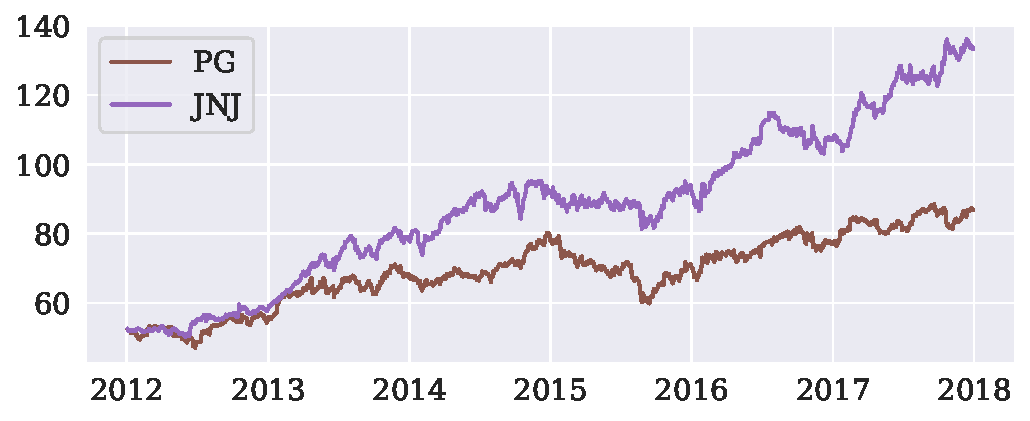
\includegraphics[width = \linewidth]{figures/coint_PG_JNJ_plot.pdf}
        %% Creator: Matplotlib, PGF backend
%%
%% To include the figure in your LaTeX document, write
%%   \input{<filename>.pgf}
%%
%% Make sure the required packages are loaded in your preamble
%%   \usepackage{pgf}
%%
%% Figures using additional raster images can only be included by \input if
%% they are in the same directory as the main LaTeX file. For loading figures
%% from other directories you can use the `import` package
%%   \usepackage{import}
%% and then include the figures with
%%   \import{<path to file>}{<filename>.pgf}
%%
%% Matplotlib used the following preamble
%%   \usepackage{fontspec}
%%   \setmainfont{DejaVuSerif.ttf}[Path=/opt/tljh/user/lib/python3.6/site-packages/matplotlib/mpl-data/fonts/ttf/]
%%   \setsansfont{DejaVuSans.ttf}[Path=/opt/tljh/user/lib/python3.6/site-packages/matplotlib/mpl-data/fonts/ttf/]
%%   \setmonofont{DejaVuSansMono.ttf}[Path=/opt/tljh/user/lib/python3.6/site-packages/matplotlib/mpl-data/fonts/ttf/]
%%
\begingroup%
\makeatletter%
\begin{pgfpicture}%
\pgfpathrectangle{\pgfpointorigin}{\pgfqpoint{5.212318in}{3.482929in}}%
\pgfusepath{use as bounding box, clip}%
\begin{pgfscope}%
\pgfsetbuttcap%
\pgfsetmiterjoin%
\definecolor{currentfill}{rgb}{1.000000,1.000000,1.000000}%
\pgfsetfillcolor{currentfill}%
\pgfsetlinewidth{0.000000pt}%
\definecolor{currentstroke}{rgb}{1.000000,1.000000,1.000000}%
\pgfsetstrokecolor{currentstroke}%
\pgfsetdash{}{0pt}%
\pgfpathmoveto{\pgfqpoint{0.000000in}{0.000000in}}%
\pgfpathlineto{\pgfqpoint{5.212318in}{0.000000in}}%
\pgfpathlineto{\pgfqpoint{5.212318in}{3.482929in}}%
\pgfpathlineto{\pgfqpoint{0.000000in}{3.482929in}}%
\pgfpathclose%
\pgfusepath{fill}%
\end{pgfscope}%
\begin{pgfscope}%
\pgfsetbuttcap%
\pgfsetmiterjoin%
\definecolor{currentfill}{rgb}{0.917647,0.917647,0.949020}%
\pgfsetfillcolor{currentfill}%
\pgfsetlinewidth{0.000000pt}%
\definecolor{currentstroke}{rgb}{0.000000,0.000000,0.000000}%
\pgfsetstrokecolor{currentstroke}%
\pgfsetstrokeopacity{0.000000}%
\pgfsetdash{}{0pt}%
\pgfpathmoveto{\pgfqpoint{0.462318in}{0.331635in}}%
\pgfpathlineto{\pgfqpoint{5.112318in}{0.331635in}}%
\pgfpathlineto{\pgfqpoint{5.112318in}{3.351635in}}%
\pgfpathlineto{\pgfqpoint{0.462318in}{3.351635in}}%
\pgfpathclose%
\pgfusepath{fill}%
\end{pgfscope}%
\begin{pgfscope}%
\pgfpathrectangle{\pgfqpoint{0.462318in}{0.331635in}}{\pgfqpoint{4.650000in}{3.020000in}}%
\pgfusepath{clip}%
\pgfsetroundcap%
\pgfsetroundjoin%
\pgfsetlinewidth{0.803000pt}%
\definecolor{currentstroke}{rgb}{1.000000,1.000000,1.000000}%
\pgfsetstrokecolor{currentstroke}%
\pgfsetdash{}{0pt}%
\pgfpathmoveto{\pgfqpoint{0.669816in}{0.331635in}}%
\pgfpathlineto{\pgfqpoint{0.669816in}{3.351635in}}%
\pgfusepath{stroke}%
\end{pgfscope}%
\begin{pgfscope}%
\definecolor{textcolor}{rgb}{0.150000,0.150000,0.150000}%
\pgfsetstrokecolor{textcolor}%
\pgfsetfillcolor{textcolor}%
\pgftext[x=0.669816in,y=0.234413in,,top]{\color{textcolor}\rmfamily\fontsize{10.000000}{12.000000}\selectfont 2012}%
\end{pgfscope}%
\begin{pgfscope}%
\pgfpathrectangle{\pgfqpoint{0.462318in}{0.331635in}}{\pgfqpoint{4.650000in}{3.020000in}}%
\pgfusepath{clip}%
\pgfsetroundcap%
\pgfsetroundjoin%
\pgfsetlinewidth{0.803000pt}%
\definecolor{currentstroke}{rgb}{1.000000,1.000000,1.000000}%
\pgfsetstrokecolor{currentstroke}%
\pgfsetdash{}{0pt}%
\pgfpathmoveto{\pgfqpoint{1.377261in}{0.331635in}}%
\pgfpathlineto{\pgfqpoint{1.377261in}{3.351635in}}%
\pgfusepath{stroke}%
\end{pgfscope}%
\begin{pgfscope}%
\definecolor{textcolor}{rgb}{0.150000,0.150000,0.150000}%
\pgfsetstrokecolor{textcolor}%
\pgfsetfillcolor{textcolor}%
\pgftext[x=1.377261in,y=0.234413in,,top]{\color{textcolor}\rmfamily\fontsize{10.000000}{12.000000}\selectfont 2013}%
\end{pgfscope}%
\begin{pgfscope}%
\pgfpathrectangle{\pgfqpoint{0.462318in}{0.331635in}}{\pgfqpoint{4.650000in}{3.020000in}}%
\pgfusepath{clip}%
\pgfsetroundcap%
\pgfsetroundjoin%
\pgfsetlinewidth{0.803000pt}%
\definecolor{currentstroke}{rgb}{1.000000,1.000000,1.000000}%
\pgfsetstrokecolor{currentstroke}%
\pgfsetdash{}{0pt}%
\pgfpathmoveto{\pgfqpoint{2.082773in}{0.331635in}}%
\pgfpathlineto{\pgfqpoint{2.082773in}{3.351635in}}%
\pgfusepath{stroke}%
\end{pgfscope}%
\begin{pgfscope}%
\definecolor{textcolor}{rgb}{0.150000,0.150000,0.150000}%
\pgfsetstrokecolor{textcolor}%
\pgfsetfillcolor{textcolor}%
\pgftext[x=2.082773in,y=0.234413in,,top]{\color{textcolor}\rmfamily\fontsize{10.000000}{12.000000}\selectfont 2014}%
\end{pgfscope}%
\begin{pgfscope}%
\pgfpathrectangle{\pgfqpoint{0.462318in}{0.331635in}}{\pgfqpoint{4.650000in}{3.020000in}}%
\pgfusepath{clip}%
\pgfsetroundcap%
\pgfsetroundjoin%
\pgfsetlinewidth{0.803000pt}%
\definecolor{currentstroke}{rgb}{1.000000,1.000000,1.000000}%
\pgfsetstrokecolor{currentstroke}%
\pgfsetdash{}{0pt}%
\pgfpathmoveto{\pgfqpoint{2.788285in}{0.331635in}}%
\pgfpathlineto{\pgfqpoint{2.788285in}{3.351635in}}%
\pgfusepath{stroke}%
\end{pgfscope}%
\begin{pgfscope}%
\definecolor{textcolor}{rgb}{0.150000,0.150000,0.150000}%
\pgfsetstrokecolor{textcolor}%
\pgfsetfillcolor{textcolor}%
\pgftext[x=2.788285in,y=0.234413in,,top]{\color{textcolor}\rmfamily\fontsize{10.000000}{12.000000}\selectfont 2015}%
\end{pgfscope}%
\begin{pgfscope}%
\pgfpathrectangle{\pgfqpoint{0.462318in}{0.331635in}}{\pgfqpoint{4.650000in}{3.020000in}}%
\pgfusepath{clip}%
\pgfsetroundcap%
\pgfsetroundjoin%
\pgfsetlinewidth{0.803000pt}%
\definecolor{currentstroke}{rgb}{1.000000,1.000000,1.000000}%
\pgfsetstrokecolor{currentstroke}%
\pgfsetdash{}{0pt}%
\pgfpathmoveto{\pgfqpoint{3.493797in}{0.331635in}}%
\pgfpathlineto{\pgfqpoint{3.493797in}{3.351635in}}%
\pgfusepath{stroke}%
\end{pgfscope}%
\begin{pgfscope}%
\definecolor{textcolor}{rgb}{0.150000,0.150000,0.150000}%
\pgfsetstrokecolor{textcolor}%
\pgfsetfillcolor{textcolor}%
\pgftext[x=3.493797in,y=0.234413in,,top]{\color{textcolor}\rmfamily\fontsize{10.000000}{12.000000}\selectfont 2016}%
\end{pgfscope}%
\begin{pgfscope}%
\pgfpathrectangle{\pgfqpoint{0.462318in}{0.331635in}}{\pgfqpoint{4.650000in}{3.020000in}}%
\pgfusepath{clip}%
\pgfsetroundcap%
\pgfsetroundjoin%
\pgfsetlinewidth{0.803000pt}%
\definecolor{currentstroke}{rgb}{1.000000,1.000000,1.000000}%
\pgfsetstrokecolor{currentstroke}%
\pgfsetdash{}{0pt}%
\pgfpathmoveto{\pgfqpoint{4.201241in}{0.331635in}}%
\pgfpathlineto{\pgfqpoint{4.201241in}{3.351635in}}%
\pgfusepath{stroke}%
\end{pgfscope}%
\begin{pgfscope}%
\definecolor{textcolor}{rgb}{0.150000,0.150000,0.150000}%
\pgfsetstrokecolor{textcolor}%
\pgfsetfillcolor{textcolor}%
\pgftext[x=4.201241in,y=0.234413in,,top]{\color{textcolor}\rmfamily\fontsize{10.000000}{12.000000}\selectfont 2017}%
\end{pgfscope}%
\begin{pgfscope}%
\pgfpathrectangle{\pgfqpoint{0.462318in}{0.331635in}}{\pgfqpoint{4.650000in}{3.020000in}}%
\pgfusepath{clip}%
\pgfsetroundcap%
\pgfsetroundjoin%
\pgfsetlinewidth{0.803000pt}%
\definecolor{currentstroke}{rgb}{1.000000,1.000000,1.000000}%
\pgfsetstrokecolor{currentstroke}%
\pgfsetdash{}{0pt}%
\pgfpathmoveto{\pgfqpoint{4.906753in}{0.331635in}}%
\pgfpathlineto{\pgfqpoint{4.906753in}{3.351635in}}%
\pgfusepath{stroke}%
\end{pgfscope}%
\begin{pgfscope}%
\definecolor{textcolor}{rgb}{0.150000,0.150000,0.150000}%
\pgfsetstrokecolor{textcolor}%
\pgfsetfillcolor{textcolor}%
\pgftext[x=4.906753in,y=0.234413in,,top]{\color{textcolor}\rmfamily\fontsize{10.000000}{12.000000}\selectfont 2018}%
\end{pgfscope}%
\begin{pgfscope}%
\pgfpathrectangle{\pgfqpoint{0.462318in}{0.331635in}}{\pgfqpoint{4.650000in}{3.020000in}}%
\pgfusepath{clip}%
\pgfsetroundcap%
\pgfsetroundjoin%
\pgfsetlinewidth{0.803000pt}%
\definecolor{currentstroke}{rgb}{1.000000,1.000000,1.000000}%
\pgfsetstrokecolor{currentstroke}%
\pgfsetdash{}{0pt}%
\pgfpathmoveto{\pgfqpoint{0.462318in}{0.866219in}}%
\pgfpathlineto{\pgfqpoint{5.112318in}{0.866219in}}%
\pgfusepath{stroke}%
\end{pgfscope}%
\begin{pgfscope}%
\definecolor{textcolor}{rgb}{0.150000,0.150000,0.150000}%
\pgfsetstrokecolor{textcolor}%
\pgfsetfillcolor{textcolor}%
\pgftext[x=0.188365in,y=0.813458in,left,base]{\color{textcolor}\rmfamily\fontsize{10.000000}{12.000000}\selectfont 60}%
\end{pgfscope}%
\begin{pgfscope}%
\pgfpathrectangle{\pgfqpoint{0.462318in}{0.331635in}}{\pgfqpoint{4.650000in}{3.020000in}}%
\pgfusepath{clip}%
\pgfsetroundcap%
\pgfsetroundjoin%
\pgfsetlinewidth{0.803000pt}%
\definecolor{currentstroke}{rgb}{1.000000,1.000000,1.000000}%
\pgfsetstrokecolor{currentstroke}%
\pgfsetdash{}{0pt}%
\pgfpathmoveto{\pgfqpoint{0.462318in}{1.482207in}}%
\pgfpathlineto{\pgfqpoint{5.112318in}{1.482207in}}%
\pgfusepath{stroke}%
\end{pgfscope}%
\begin{pgfscope}%
\definecolor{textcolor}{rgb}{0.150000,0.150000,0.150000}%
\pgfsetstrokecolor{textcolor}%
\pgfsetfillcolor{textcolor}%
\pgftext[x=0.188365in,y=1.429445in,left,base]{\color{textcolor}\rmfamily\fontsize{10.000000}{12.000000}\selectfont 80}%
\end{pgfscope}%
\begin{pgfscope}%
\pgfpathrectangle{\pgfqpoint{0.462318in}{0.331635in}}{\pgfqpoint{4.650000in}{3.020000in}}%
\pgfusepath{clip}%
\pgfsetroundcap%
\pgfsetroundjoin%
\pgfsetlinewidth{0.803000pt}%
\definecolor{currentstroke}{rgb}{1.000000,1.000000,1.000000}%
\pgfsetstrokecolor{currentstroke}%
\pgfsetdash{}{0pt}%
\pgfpathmoveto{\pgfqpoint{0.462318in}{2.098194in}}%
\pgfpathlineto{\pgfqpoint{5.112318in}{2.098194in}}%
\pgfusepath{stroke}%
\end{pgfscope}%
\begin{pgfscope}%
\definecolor{textcolor}{rgb}{0.150000,0.150000,0.150000}%
\pgfsetstrokecolor{textcolor}%
\pgfsetfillcolor{textcolor}%
\pgftext[x=0.100000in,y=2.045432in,left,base]{\color{textcolor}\rmfamily\fontsize{10.000000}{12.000000}\selectfont 100}%
\end{pgfscope}%
\begin{pgfscope}%
\pgfpathrectangle{\pgfqpoint{0.462318in}{0.331635in}}{\pgfqpoint{4.650000in}{3.020000in}}%
\pgfusepath{clip}%
\pgfsetroundcap%
\pgfsetroundjoin%
\pgfsetlinewidth{0.803000pt}%
\definecolor{currentstroke}{rgb}{1.000000,1.000000,1.000000}%
\pgfsetstrokecolor{currentstroke}%
\pgfsetdash{}{0pt}%
\pgfpathmoveto{\pgfqpoint{0.462318in}{2.714181in}}%
\pgfpathlineto{\pgfqpoint{5.112318in}{2.714181in}}%
\pgfusepath{stroke}%
\end{pgfscope}%
\begin{pgfscope}%
\definecolor{textcolor}{rgb}{0.150000,0.150000,0.150000}%
\pgfsetstrokecolor{textcolor}%
\pgfsetfillcolor{textcolor}%
\pgftext[x=0.100000in,y=2.661419in,left,base]{\color{textcolor}\rmfamily\fontsize{10.000000}{12.000000}\selectfont 120}%
\end{pgfscope}%
\begin{pgfscope}%
\pgfpathrectangle{\pgfqpoint{0.462318in}{0.331635in}}{\pgfqpoint{4.650000in}{3.020000in}}%
\pgfusepath{clip}%
\pgfsetroundcap%
\pgfsetroundjoin%
\pgfsetlinewidth{0.803000pt}%
\definecolor{currentstroke}{rgb}{1.000000,1.000000,1.000000}%
\pgfsetstrokecolor{currentstroke}%
\pgfsetdash{}{0pt}%
\pgfpathmoveto{\pgfqpoint{0.462318in}{3.330168in}}%
\pgfpathlineto{\pgfqpoint{5.112318in}{3.330168in}}%
\pgfusepath{stroke}%
\end{pgfscope}%
\begin{pgfscope}%
\definecolor{textcolor}{rgb}{0.150000,0.150000,0.150000}%
\pgfsetstrokecolor{textcolor}%
\pgfsetfillcolor{textcolor}%
\pgftext[x=0.100000in,y=3.277406in,left,base]{\color{textcolor}\rmfamily\fontsize{10.000000}{12.000000}\selectfont 140}%
\end{pgfscope}%
\begin{pgfscope}%
\pgfpathrectangle{\pgfqpoint{0.462318in}{0.331635in}}{\pgfqpoint{4.650000in}{3.020000in}}%
\pgfusepath{clip}%
\pgfsetroundcap%
\pgfsetroundjoin%
\pgfsetlinewidth{1.505625pt}%
\definecolor{currentstroke}{rgb}{0.121569,0.466667,0.705882}%
\pgfsetstrokecolor{currentstroke}%
\pgfsetdash{}{0pt}%
\pgfpathmoveto{\pgfqpoint{0.673682in}{0.627524in}}%
\pgfpathlineto{\pgfqpoint{0.675615in}{0.626600in}}%
\pgfpathlineto{\pgfqpoint{0.677548in}{0.619825in}}%
\pgfpathlineto{\pgfqpoint{0.679481in}{0.616129in}}%
\pgfpathlineto{\pgfqpoint{0.685279in}{0.622905in}}%
\pgfpathlineto{\pgfqpoint{0.687212in}{0.615205in}}%
\pgfpathlineto{\pgfqpoint{0.689145in}{0.599805in}}%
\pgfpathlineto{\pgfqpoint{0.691078in}{0.602885in}}%
\pgfpathlineto{\pgfqpoint{0.693011in}{0.602885in}}%
\pgfpathlineto{\pgfqpoint{0.700743in}{0.613665in}}%
\pgfpathlineto{\pgfqpoint{0.702675in}{0.620749in}}%
\pgfpathlineto{\pgfqpoint{0.704608in}{0.621981in}}%
\pgfpathlineto{\pgfqpoint{0.706541in}{0.625676in}}%
\pgfpathlineto{\pgfqpoint{0.714273in}{0.583789in}}%
\pgfpathlineto{\pgfqpoint{0.716206in}{0.595493in}}%
\pgfpathlineto{\pgfqpoint{0.718139in}{0.590873in}}%
\pgfpathlineto{\pgfqpoint{0.720072in}{0.578861in}}%
\pgfpathlineto{\pgfqpoint{0.725870in}{0.552374in}}%
\pgfpathlineto{\pgfqpoint{0.727803in}{0.548370in}}%
\pgfpathlineto{\pgfqpoint{0.731669in}{0.555146in}}%
\pgfpathlineto{\pgfqpoint{0.733602in}{0.541594in}}%
\pgfpathlineto{\pgfqpoint{0.741334in}{0.564386in}}%
\pgfpathlineto{\pgfqpoint{0.743267in}{0.562846in}}%
\pgfpathlineto{\pgfqpoint{0.745199in}{0.572394in}}%
\pgfpathlineto{\pgfqpoint{0.747132in}{0.568698in}}%
\pgfpathlineto{\pgfqpoint{0.752931in}{0.577013in}}%
\pgfpathlineto{\pgfqpoint{0.754864in}{0.583173in}}%
\pgfpathlineto{\pgfqpoint{0.756797in}{0.585021in}}%
\pgfpathlineto{\pgfqpoint{0.758730in}{0.600729in}}%
\pgfpathlineto{\pgfqpoint{0.760663in}{0.593645in}}%
\pgfpathlineto{\pgfqpoint{0.768394in}{0.581633in}}%
\pgfpathlineto{\pgfqpoint{0.770327in}{0.582249in}}%
\pgfpathlineto{\pgfqpoint{0.772260in}{0.630296in}}%
\pgfpathlineto{\pgfqpoint{0.774193in}{0.637380in}}%
\pgfpathlineto{\pgfqpoint{0.779992in}{0.637072in}}%
\pgfpathlineto{\pgfqpoint{0.781925in}{0.653704in}}%
\pgfpathlineto{\pgfqpoint{0.783858in}{0.659556in}}%
\pgfpathlineto{\pgfqpoint{0.785791in}{0.636148in}}%
\pgfpathlineto{\pgfqpoint{0.787723in}{0.636456in}}%
\pgfpathlineto{\pgfqpoint{0.793522in}{0.643232in}}%
\pgfpathlineto{\pgfqpoint{0.795455in}{0.640460in}}%
\pgfpathlineto{\pgfqpoint{0.797388in}{0.634300in}}%
\pgfpathlineto{\pgfqpoint{0.799321in}{0.642000in}}%
\pgfpathlineto{\pgfqpoint{0.801254in}{0.642616in}}%
\pgfpathlineto{\pgfqpoint{0.808985in}{0.666332in}}%
\pgfpathlineto{\pgfqpoint{0.810918in}{0.665100in}}%
\pgfpathlineto{\pgfqpoint{0.812851in}{0.660788in}}%
\pgfpathlineto{\pgfqpoint{0.814784in}{0.650316in}}%
\pgfpathlineto{\pgfqpoint{0.824449in}{0.649084in}}%
\pgfpathlineto{\pgfqpoint{0.826382in}{0.657092in}}%
\pgfpathlineto{\pgfqpoint{0.828315in}{0.654936in}}%
\pgfpathlineto{\pgfqpoint{0.834113in}{0.655552in}}%
\pgfpathlineto{\pgfqpoint{0.836046in}{0.648160in}}%
\pgfpathlineto{\pgfqpoint{0.837979in}{0.649084in}}%
\pgfpathlineto{\pgfqpoint{0.839912in}{0.644464in}}%
\pgfpathlineto{\pgfqpoint{0.841845in}{0.649392in}}%
\pgfpathlineto{\pgfqpoint{0.847644in}{0.658016in}}%
\pgfpathlineto{\pgfqpoint{0.849577in}{0.646620in}}%
\pgfpathlineto{\pgfqpoint{0.851509in}{0.650624in}}%
\pgfpathlineto{\pgfqpoint{0.853442in}{0.651856in}}%
\pgfpathlineto{\pgfqpoint{0.861174in}{0.639844in}}%
\pgfpathlineto{\pgfqpoint{0.863107in}{0.628448in}}%
\pgfpathlineto{\pgfqpoint{0.865040in}{0.630912in}}%
\pgfpathlineto{\pgfqpoint{0.868906in}{0.615513in}}%
\pgfpathlineto{\pgfqpoint{0.876637in}{0.644772in}}%
\pgfpathlineto{\pgfqpoint{0.878570in}{0.638304in}}%
\pgfpathlineto{\pgfqpoint{0.880503in}{0.633992in}}%
\pgfpathlineto{\pgfqpoint{0.882436in}{0.656784in}}%
\pgfpathlineto{\pgfqpoint{0.888235in}{0.635840in}}%
\pgfpathlineto{\pgfqpoint{0.892101in}{0.655552in}}%
\pgfpathlineto{\pgfqpoint{0.894033in}{0.654936in}}%
\pgfpathlineto{\pgfqpoint{0.895966in}{0.595493in}}%
\pgfpathlineto{\pgfqpoint{0.901765in}{0.575781in}}%
\pgfpathlineto{\pgfqpoint{0.903698in}{0.574242in}}%
\pgfpathlineto{\pgfqpoint{0.905631in}{0.584097in}}%
\pgfpathlineto{\pgfqpoint{0.907564in}{0.597033in}}%
\pgfpathlineto{\pgfqpoint{0.909497in}{0.591489in}}%
\pgfpathlineto{\pgfqpoint{0.915295in}{0.590873in}}%
\pgfpathlineto{\pgfqpoint{0.917228in}{0.588717in}}%
\pgfpathlineto{\pgfqpoint{0.919161in}{0.576705in}}%
\pgfpathlineto{\pgfqpoint{0.921094in}{0.588101in}}%
\pgfpathlineto{\pgfqpoint{0.923027in}{0.577013in}}%
\pgfpathlineto{\pgfqpoint{0.928826in}{0.574550in}}%
\pgfpathlineto{\pgfqpoint{0.930759in}{0.577937in}}%
\pgfpathlineto{\pgfqpoint{0.932692in}{0.591797in}}%
\pgfpathlineto{\pgfqpoint{0.934625in}{0.583789in}}%
\pgfpathlineto{\pgfqpoint{0.936558in}{0.573010in}}%
\pgfpathlineto{\pgfqpoint{0.942356in}{0.569622in}}%
\pgfpathlineto{\pgfqpoint{0.944289in}{0.563770in}}%
\pgfpathlineto{\pgfqpoint{0.946222in}{0.545290in}}%
\pgfpathlineto{\pgfqpoint{0.948155in}{0.549602in}}%
\pgfpathlineto{\pgfqpoint{0.950088in}{0.547754in}}%
\pgfpathlineto{\pgfqpoint{0.957820in}{0.559150in}}%
\pgfpathlineto{\pgfqpoint{0.959752in}{0.543442in}}%
\pgfpathlineto{\pgfqpoint{0.961685in}{0.542826in}}%
\pgfpathlineto{\pgfqpoint{0.963618in}{0.524655in}}%
\pgfpathlineto{\pgfqpoint{0.969417in}{0.520959in}}%
\pgfpathlineto{\pgfqpoint{0.971350in}{0.515415in}}%
\pgfpathlineto{\pgfqpoint{0.973283in}{0.530814in}}%
\pgfpathlineto{\pgfqpoint{0.975216in}{0.554222in}}%
\pgfpathlineto{\pgfqpoint{0.977149in}{0.554222in}}%
\pgfpathlineto{\pgfqpoint{0.982947in}{0.548986in}}%
\pgfpathlineto{\pgfqpoint{0.984880in}{0.554222in}}%
\pgfpathlineto{\pgfqpoint{0.986813in}{0.549602in}}%
\pgfpathlineto{\pgfqpoint{0.988746in}{0.564694in}}%
\pgfpathlineto{\pgfqpoint{0.990679in}{0.557302in}}%
\pgfpathlineto{\pgfqpoint{0.996478in}{0.542826in}}%
\pgfpathlineto{\pgfqpoint{0.998411in}{0.540978in}}%
\pgfpathlineto{\pgfqpoint{1.000344in}{0.496319in}}%
\pgfpathlineto{\pgfqpoint{1.002276in}{0.480611in}}%
\pgfpathlineto{\pgfqpoint{1.004209in}{0.482767in}}%
\pgfpathlineto{\pgfqpoint{1.010008in}{0.469832in}}%
\pgfpathlineto{\pgfqpoint{1.011941in}{0.468908in}}%
\pgfpathlineto{\pgfqpoint{1.013874in}{0.486463in}}%
\pgfpathlineto{\pgfqpoint{1.015807in}{0.493855in}}%
\pgfpathlineto{\pgfqpoint{1.017740in}{0.517263in}}%
\pgfpathlineto{\pgfqpoint{1.023538in}{0.516031in}}%
\pgfpathlineto{\pgfqpoint{1.025471in}{0.520035in}}%
\pgfpathlineto{\pgfqpoint{1.029337in}{0.519727in}}%
\pgfpathlineto{\pgfqpoint{1.031270in}{0.518187in}}%
\pgfpathlineto{\pgfqpoint{1.037069in}{0.524655in}}%
\pgfpathlineto{\pgfqpoint{1.039002in}{0.529274in}}%
\pgfpathlineto{\pgfqpoint{1.040935in}{0.520959in}}%
\pgfpathlineto{\pgfqpoint{1.042868in}{0.577321in}}%
\pgfpathlineto{\pgfqpoint{1.044800in}{0.611509in}}%
\pgfpathlineto{\pgfqpoint{1.050599in}{0.604425in}}%
\pgfpathlineto{\pgfqpoint{1.052532in}{0.617669in}}%
\pgfpathlineto{\pgfqpoint{1.054465in}{0.618593in}}%
\pgfpathlineto{\pgfqpoint{1.056398in}{0.621057in}}%
\pgfpathlineto{\pgfqpoint{1.058331in}{0.616437in}}%
\pgfpathlineto{\pgfqpoint{1.064130in}{0.607813in}}%
\pgfpathlineto{\pgfqpoint{1.066062in}{0.598881in}}%
\pgfpathlineto{\pgfqpoint{1.067995in}{0.598881in}}%
\pgfpathlineto{\pgfqpoint{1.071861in}{0.625060in}}%
\pgfpathlineto{\pgfqpoint{1.077660in}{0.625368in}}%
\pgfpathlineto{\pgfqpoint{1.083459in}{0.586253in}}%
\pgfpathlineto{\pgfqpoint{1.085392in}{0.635224in}}%
\pgfpathlineto{\pgfqpoint{1.091190in}{0.642924in}}%
\pgfpathlineto{\pgfqpoint{1.095056in}{0.665408in}}%
\pgfpathlineto{\pgfqpoint{1.096989in}{0.665716in}}%
\pgfpathlineto{\pgfqpoint{1.098922in}{0.666640in}}%
\pgfpathlineto{\pgfqpoint{1.104721in}{0.659556in}}%
\pgfpathlineto{\pgfqpoint{1.106654in}{0.665716in}}%
\pgfpathlineto{\pgfqpoint{1.108586in}{0.663560in}}%
\pgfpathlineto{\pgfqpoint{1.110519in}{0.672491in}}%
\pgfpathlineto{\pgfqpoint{1.112452in}{0.672491in}}%
\pgfpathlineto{\pgfqpoint{1.118251in}{0.666332in}}%
\pgfpathlineto{\pgfqpoint{1.120184in}{0.666640in}}%
\pgfpathlineto{\pgfqpoint{1.122117in}{0.668796in}}%
\pgfpathlineto{\pgfqpoint{1.124050in}{0.664484in}}%
\pgfpathlineto{\pgfqpoint{1.125983in}{0.672799in}}%
\pgfpathlineto{\pgfqpoint{1.131781in}{0.674955in}}%
\pgfpathlineto{\pgfqpoint{1.135647in}{0.669104in}}%
\pgfpathlineto{\pgfqpoint{1.137580in}{0.669412in}}%
\pgfpathlineto{\pgfqpoint{1.139513in}{0.677111in}}%
\pgfpathlineto{\pgfqpoint{1.147245in}{0.682347in}}%
\pgfpathlineto{\pgfqpoint{1.149178in}{0.679575in}}%
\pgfpathlineto{\pgfqpoint{1.151110in}{0.702983in}}%
\pgfpathlineto{\pgfqpoint{1.153043in}{0.709759in}}%
\pgfpathlineto{\pgfqpoint{1.158842in}{0.709759in}}%
\pgfpathlineto{\pgfqpoint{1.160775in}{0.703599in}}%
\pgfpathlineto{\pgfqpoint{1.162708in}{0.699595in}}%
\pgfpathlineto{\pgfqpoint{1.164641in}{0.719614in}}%
\pgfpathlineto{\pgfqpoint{1.166574in}{0.725774in}}%
\pgfpathlineto{\pgfqpoint{1.172372in}{0.727930in}}%
\pgfpathlineto{\pgfqpoint{1.174305in}{0.727314in}}%
\pgfpathlineto{\pgfqpoint{1.176238in}{0.728238in}}%
\pgfpathlineto{\pgfqpoint{1.178171in}{0.735630in}}%
\pgfpathlineto{\pgfqpoint{1.180104in}{0.732242in}}%
\pgfpathlineto{\pgfqpoint{1.185903in}{0.740558in}}%
\pgfpathlineto{\pgfqpoint{1.187836in}{0.736246in}}%
\pgfpathlineto{\pgfqpoint{1.189769in}{0.729162in}}%
\pgfpathlineto{\pgfqpoint{1.191702in}{0.729162in}}%
\pgfpathlineto{\pgfqpoint{1.193634in}{0.730702in}}%
\pgfpathlineto{\pgfqpoint{1.199433in}{0.732858in}}%
\pgfpathlineto{\pgfqpoint{1.201366in}{0.716535in}}%
\pgfpathlineto{\pgfqpoint{1.203299in}{0.725774in}}%
\pgfpathlineto{\pgfqpoint{1.207165in}{0.737170in}}%
\pgfpathlineto{\pgfqpoint{1.212964in}{0.724234in}}%
\pgfpathlineto{\pgfqpoint{1.214896in}{0.714379in}}%
\pgfpathlineto{\pgfqpoint{1.216829in}{0.700519in}}%
\pgfpathlineto{\pgfqpoint{1.218762in}{0.697131in}}%
\pgfpathlineto{\pgfqpoint{1.220695in}{0.695591in}}%
\pgfpathlineto{\pgfqpoint{1.228427in}{0.721770in}}%
\pgfpathlineto{\pgfqpoint{1.230360in}{0.747334in}}%
\pgfpathlineto{\pgfqpoint{1.232293in}{0.747334in}}%
\pgfpathlineto{\pgfqpoint{1.234226in}{0.725158in}}%
\pgfpathlineto{\pgfqpoint{1.240024in}{0.723310in}}%
\pgfpathlineto{\pgfqpoint{1.241957in}{0.696823in}}%
\pgfpathlineto{\pgfqpoint{1.243890in}{0.712839in}}%
\pgfpathlineto{\pgfqpoint{1.245823in}{0.762426in}}%
\pgfpathlineto{\pgfqpoint{1.247756in}{0.746718in}}%
\pgfpathlineto{\pgfqpoint{1.257420in}{0.741790in}}%
\pgfpathlineto{\pgfqpoint{1.259353in}{0.741790in}}%
\pgfpathlineto{\pgfqpoint{1.261286in}{0.740558in}}%
\pgfpathlineto{\pgfqpoint{1.267085in}{0.727622in}}%
\pgfpathlineto{\pgfqpoint{1.269018in}{0.734090in}}%
\pgfpathlineto{\pgfqpoint{1.270951in}{0.712223in}}%
\pgfpathlineto{\pgfqpoint{1.272884in}{0.683579in}}%
\pgfpathlineto{\pgfqpoint{1.274817in}{0.686043in}}%
\pgfpathlineto{\pgfqpoint{1.280615in}{0.687891in}}%
\pgfpathlineto{\pgfqpoint{1.282548in}{0.682347in}}%
\pgfpathlineto{\pgfqpoint{1.284481in}{0.674339in}}%
\pgfpathlineto{\pgfqpoint{1.286414in}{0.669104in}}%
\pgfpathlineto{\pgfqpoint{1.288347in}{0.681423in}}%
\pgfpathlineto{\pgfqpoint{1.296079in}{0.718383in}}%
\pgfpathlineto{\pgfqpoint{1.298012in}{0.722386in}}%
\pgfpathlineto{\pgfqpoint{1.301877in}{0.750414in}}%
\pgfpathlineto{\pgfqpoint{1.307676in}{0.747642in}}%
\pgfpathlineto{\pgfqpoint{1.309609in}{0.735322in}}%
\pgfpathlineto{\pgfqpoint{1.311542in}{0.746718in}}%
\pgfpathlineto{\pgfqpoint{1.313475in}{0.748258in}}%
\pgfpathlineto{\pgfqpoint{1.315408in}{0.756266in}}%
\pgfpathlineto{\pgfqpoint{1.321206in}{0.750106in}}%
\pgfpathlineto{\pgfqpoint{1.323139in}{0.743330in}}%
\pgfpathlineto{\pgfqpoint{1.325072in}{0.745794in}}%
\pgfpathlineto{\pgfqpoint{1.327005in}{0.759346in}}%
\pgfpathlineto{\pgfqpoint{1.328938in}{0.767969in}}%
\pgfpathlineto{\pgfqpoint{1.334737in}{0.766122in}}%
\pgfpathlineto{\pgfqpoint{1.336670in}{0.776901in}}%
\pgfpathlineto{\pgfqpoint{1.338603in}{0.779673in}}%
\pgfpathlineto{\pgfqpoint{1.340536in}{0.763966in}}%
\pgfpathlineto{\pgfqpoint{1.342468in}{0.758730in}}%
\pgfpathlineto{\pgfqpoint{1.348267in}{0.758730in}}%
\pgfpathlineto{\pgfqpoint{1.350200in}{0.759962in}}%
\pgfpathlineto{\pgfqpoint{1.352133in}{0.744254in}}%
\pgfpathlineto{\pgfqpoint{1.354066in}{0.756266in}}%
\pgfpathlineto{\pgfqpoint{1.355999in}{0.728854in}}%
\pgfpathlineto{\pgfqpoint{1.361798in}{0.723618in}}%
\pgfpathlineto{\pgfqpoint{1.365663in}{0.710683in}}%
\pgfpathlineto{\pgfqpoint{1.367596in}{0.710067in}}%
\pgfpathlineto{\pgfqpoint{1.369529in}{0.689739in}}%
\pgfpathlineto{\pgfqpoint{1.375328in}{0.708219in}}%
\pgfpathlineto{\pgfqpoint{1.379194in}{0.745486in}}%
\pgfpathlineto{\pgfqpoint{1.381127in}{0.734398in}}%
\pgfpathlineto{\pgfqpoint{1.383060in}{0.738094in}}%
\pgfpathlineto{\pgfqpoint{1.390791in}{0.723618in}}%
\pgfpathlineto{\pgfqpoint{1.394657in}{0.742406in}}%
\pgfpathlineto{\pgfqpoint{1.396590in}{0.741174in}}%
\pgfpathlineto{\pgfqpoint{1.402389in}{0.751338in}}%
\pgfpathlineto{\pgfqpoint{1.404322in}{0.757498in}}%
\pgfpathlineto{\pgfqpoint{1.406254in}{0.758114in}}%
\pgfpathlineto{\pgfqpoint{1.410120in}{0.773205in}}%
\pgfpathlineto{\pgfqpoint{1.417852in}{0.773513in}}%
\pgfpathlineto{\pgfqpoint{1.419785in}{0.791993in}}%
\pgfpathlineto{\pgfqpoint{1.421718in}{0.785217in}}%
\pgfpathlineto{\pgfqpoint{1.423651in}{0.856364in}}%
\pgfpathlineto{\pgfqpoint{1.429449in}{0.869299in}}%
\pgfpathlineto{\pgfqpoint{1.431382in}{0.900099in}}%
\pgfpathlineto{\pgfqpoint{1.435248in}{0.904103in}}%
\pgfpathlineto{\pgfqpoint{1.437181in}{0.923198in}}%
\pgfpathlineto{\pgfqpoint{1.442980in}{0.906567in}}%
\pgfpathlineto{\pgfqpoint{1.446846in}{0.929050in}}%
\pgfpathlineto{\pgfqpoint{1.448778in}{0.929050in}}%
\pgfpathlineto{\pgfqpoint{1.450711in}{0.918886in}}%
\pgfpathlineto{\pgfqpoint{1.456510in}{0.920426in}}%
\pgfpathlineto{\pgfqpoint{1.458443in}{0.924738in}}%
\pgfpathlineto{\pgfqpoint{1.460376in}{0.939214in}}%
\pgfpathlineto{\pgfqpoint{1.462309in}{0.944758in}}%
\pgfpathlineto{\pgfqpoint{1.464242in}{0.938906in}}%
\pgfpathlineto{\pgfqpoint{1.471973in}{0.959849in}}%
\pgfpathlineto{\pgfqpoint{1.473906in}{0.952458in}}%
\pgfpathlineto{\pgfqpoint{1.475839in}{0.951534in}}%
\pgfpathlineto{\pgfqpoint{1.477772in}{0.949994in}}%
\pgfpathlineto{\pgfqpoint{1.483571in}{0.923198in}}%
\pgfpathlineto{\pgfqpoint{1.485504in}{0.927202in}}%
\pgfpathlineto{\pgfqpoint{1.487437in}{0.944142in}}%
\pgfpathlineto{\pgfqpoint{1.489370in}{0.929666in}}%
\pgfpathlineto{\pgfqpoint{1.491302in}{0.937674in}}%
\pgfpathlineto{\pgfqpoint{1.497101in}{0.942294in}}%
\pgfpathlineto{\pgfqpoint{1.499034in}{0.951534in}}%
\pgfpathlineto{\pgfqpoint{1.500967in}{0.955538in}}%
\pgfpathlineto{\pgfqpoint{1.502900in}{0.947838in}}%
\pgfpathlineto{\pgfqpoint{1.504833in}{0.954922in}}%
\pgfpathlineto{\pgfqpoint{1.510632in}{0.959233in}}%
\pgfpathlineto{\pgfqpoint{1.512564in}{0.954614in}}%
\pgfpathlineto{\pgfqpoint{1.514497in}{0.945374in}}%
\pgfpathlineto{\pgfqpoint{1.516430in}{0.960157in}}%
\pgfpathlineto{\pgfqpoint{1.518363in}{0.933670in}}%
\pgfpathlineto{\pgfqpoint{1.524162in}{0.929358in}}%
\pgfpathlineto{\pgfqpoint{1.526095in}{0.953074in}}%
\pgfpathlineto{\pgfqpoint{1.528028in}{0.965085in}}%
\pgfpathlineto{\pgfqpoint{1.529961in}{0.955538in}}%
\pgfpathlineto{\pgfqpoint{1.531894in}{0.957078in}}%
\pgfpathlineto{\pgfqpoint{1.537692in}{0.942294in}}%
\pgfpathlineto{\pgfqpoint{1.539625in}{0.960465in}}%
\pgfpathlineto{\pgfqpoint{1.541558in}{0.951842in}}%
\pgfpathlineto{\pgfqpoint{1.543491in}{0.951842in}}%
\pgfpathlineto{\pgfqpoint{1.551223in}{0.967857in}}%
\pgfpathlineto{\pgfqpoint{1.553156in}{0.999581in}}%
\pgfpathlineto{\pgfqpoint{1.555088in}{0.978637in}}%
\pgfpathlineto{\pgfqpoint{1.557021in}{0.989109in}}%
\pgfpathlineto{\pgfqpoint{1.558954in}{0.981101in}}%
\pgfpathlineto{\pgfqpoint{1.564753in}{0.995269in}}%
\pgfpathlineto{\pgfqpoint{1.566686in}{0.982025in}}%
\pgfpathlineto{\pgfqpoint{1.568619in}{1.006664in}}%
\pgfpathlineto{\pgfqpoint{1.572485in}{1.027608in}}%
\pgfpathlineto{\pgfqpoint{1.578283in}{1.016828in}}%
\pgfpathlineto{\pgfqpoint{1.580216in}{1.028224in}}%
\pgfpathlineto{\pgfqpoint{1.582149in}{1.002045in}}%
\pgfpathlineto{\pgfqpoint{1.584082in}{1.022372in}}%
\pgfpathlineto{\pgfqpoint{1.586015in}{1.061487in}}%
\pgfpathlineto{\pgfqpoint{1.591814in}{1.060871in}}%
\pgfpathlineto{\pgfqpoint{1.593747in}{1.089515in}}%
\pgfpathlineto{\pgfqpoint{1.595680in}{0.967549in}}%
\pgfpathlineto{\pgfqpoint{1.597612in}{0.953998in}}%
\pgfpathlineto{\pgfqpoint{1.599545in}{0.967241in}}%
\pgfpathlineto{\pgfqpoint{1.605344in}{0.981717in}}%
\pgfpathlineto{\pgfqpoint{1.607277in}{0.958617in}}%
\pgfpathlineto{\pgfqpoint{1.609210in}{0.964161in}}%
\pgfpathlineto{\pgfqpoint{1.611143in}{0.983873in}}%
\pgfpathlineto{\pgfqpoint{1.613076in}{0.994653in}}%
\pgfpathlineto{\pgfqpoint{1.618874in}{0.983565in}}%
\pgfpathlineto{\pgfqpoint{1.620807in}{0.988185in}}%
\pgfpathlineto{\pgfqpoint{1.622740in}{1.000813in}}%
\pgfpathlineto{\pgfqpoint{1.624673in}{0.995269in}}%
\pgfpathlineto{\pgfqpoint{1.626606in}{1.009128in}}%
\pgfpathlineto{\pgfqpoint{1.632405in}{1.004817in}}%
\pgfpathlineto{\pgfqpoint{1.634338in}{1.026992in}}%
\pgfpathlineto{\pgfqpoint{1.636271in}{1.057483in}}%
\pgfpathlineto{\pgfqpoint{1.638204in}{1.045472in}}%
\pgfpathlineto{\pgfqpoint{1.640137in}{1.040852in}}%
\pgfpathlineto{\pgfqpoint{1.647868in}{1.010052in}}%
\pgfpathlineto{\pgfqpoint{1.649801in}{1.010668in}}%
\pgfpathlineto{\pgfqpoint{1.651734in}{1.007588in}}%
\pgfpathlineto{\pgfqpoint{1.653667in}{1.087975in}}%
\pgfpathlineto{\pgfqpoint{1.661399in}{1.062103in}}%
\pgfpathlineto{\pgfqpoint{1.663331in}{1.012516in}}%
\pgfpathlineto{\pgfqpoint{1.665264in}{1.017444in}}%
\pgfpathlineto{\pgfqpoint{1.667197in}{0.958617in}}%
\pgfpathlineto{\pgfqpoint{1.672996in}{0.981101in}}%
\pgfpathlineto{\pgfqpoint{1.674929in}{0.974017in}}%
\pgfpathlineto{\pgfqpoint{1.676862in}{0.955846in}}%
\pgfpathlineto{\pgfqpoint{1.678795in}{0.960157in}}%
\pgfpathlineto{\pgfqpoint{1.680728in}{0.983565in}}%
\pgfpathlineto{\pgfqpoint{1.686526in}{0.991573in}}%
\pgfpathlineto{\pgfqpoint{1.688459in}{0.992805in}}%
\pgfpathlineto{\pgfqpoint{1.690392in}{0.979869in}}%
\pgfpathlineto{\pgfqpoint{1.692325in}{1.000813in}}%
\pgfpathlineto{\pgfqpoint{1.694258in}{0.990649in}}%
\pgfpathlineto{\pgfqpoint{1.700057in}{1.014056in}}%
\pgfpathlineto{\pgfqpoint{1.701990in}{1.016212in}}%
\pgfpathlineto{\pgfqpoint{1.703923in}{0.979869in}}%
\pgfpathlineto{\pgfqpoint{1.705855in}{0.920426in}}%
\pgfpathlineto{\pgfqpoint{1.707788in}{0.975557in}}%
\pgfpathlineto{\pgfqpoint{1.713587in}{0.953998in}}%
\pgfpathlineto{\pgfqpoint{1.715520in}{0.956770in}}%
\pgfpathlineto{\pgfqpoint{1.717453in}{0.974633in}}%
\pgfpathlineto{\pgfqpoint{1.719386in}{0.981409in}}%
\pgfpathlineto{\pgfqpoint{1.721319in}{0.964161in}}%
\pgfpathlineto{\pgfqpoint{1.729050in}{1.000813in}}%
\pgfpathlineto{\pgfqpoint{1.730983in}{1.004201in}}%
\pgfpathlineto{\pgfqpoint{1.734849in}{0.998349in}}%
\pgfpathlineto{\pgfqpoint{1.740648in}{1.009128in}}%
\pgfpathlineto{\pgfqpoint{1.742581in}{1.029456in}}%
\pgfpathlineto{\pgfqpoint{1.744514in}{1.035308in}}%
\pgfpathlineto{\pgfqpoint{1.748379in}{1.079659in}}%
\pgfpathlineto{\pgfqpoint{1.754178in}{1.078427in}}%
\pgfpathlineto{\pgfqpoint{1.756111in}{1.064875in}}%
\pgfpathlineto{\pgfqpoint{1.758044in}{1.057791in}}%
\pgfpathlineto{\pgfqpoint{1.759977in}{1.063027in}}%
\pgfpathlineto{\pgfqpoint{1.761910in}{1.090439in}}%
\pgfpathlineto{\pgfqpoint{1.767709in}{1.086743in}}%
\pgfpathlineto{\pgfqpoint{1.769641in}{1.079659in}}%
\pgfpathlineto{\pgfqpoint{1.771574in}{1.062411in}}%
\pgfpathlineto{\pgfqpoint{1.773507in}{1.066107in}}%
\pgfpathlineto{\pgfqpoint{1.775440in}{1.065491in}}%
\pgfpathlineto{\pgfqpoint{1.781239in}{1.057791in}}%
\pgfpathlineto{\pgfqpoint{1.783172in}{1.066723in}}%
\pgfpathlineto{\pgfqpoint{1.785105in}{1.063027in}}%
\pgfpathlineto{\pgfqpoint{1.787038in}{1.097215in}}%
\pgfpathlineto{\pgfqpoint{1.788971in}{1.088283in}}%
\pgfpathlineto{\pgfqpoint{1.794769in}{1.091055in}}%
\pgfpathlineto{\pgfqpoint{1.796702in}{1.099987in}}%
\pgfpathlineto{\pgfqpoint{1.800568in}{1.110766in}}%
\pgfpathlineto{\pgfqpoint{1.802501in}{1.097215in}}%
\pgfpathlineto{\pgfqpoint{1.808300in}{1.096907in}}%
\pgfpathlineto{\pgfqpoint{1.810233in}{1.097831in}}%
\pgfpathlineto{\pgfqpoint{1.812165in}{1.087359in}}%
\pgfpathlineto{\pgfqpoint{1.816031in}{1.052864in}}%
\pgfpathlineto{\pgfqpoint{1.821830in}{1.045164in}}%
\pgfpathlineto{\pgfqpoint{1.823763in}{1.043624in}}%
\pgfpathlineto{\pgfqpoint{1.825696in}{1.039620in}}%
\pgfpathlineto{\pgfqpoint{1.827629in}{1.049784in}}%
\pgfpathlineto{\pgfqpoint{1.829562in}{1.055635in}}%
\pgfpathlineto{\pgfqpoint{1.837293in}{1.003893in}}%
\pgfpathlineto{\pgfqpoint{1.839226in}{0.975249in}}%
\pgfpathlineto{\pgfqpoint{1.843092in}{1.001737in}}%
\pgfpathlineto{\pgfqpoint{1.850824in}{0.998349in}}%
\pgfpathlineto{\pgfqpoint{1.852757in}{0.991573in}}%
\pgfpathlineto{\pgfqpoint{1.854689in}{0.982641in}}%
\pgfpathlineto{\pgfqpoint{1.856622in}{0.982949in}}%
\pgfpathlineto{\pgfqpoint{1.862421in}{1.008820in}}%
\pgfpathlineto{\pgfqpoint{1.864354in}{1.003277in}}%
\pgfpathlineto{\pgfqpoint{1.866287in}{1.011592in}}%
\pgfpathlineto{\pgfqpoint{1.868220in}{1.011284in}}%
\pgfpathlineto{\pgfqpoint{1.870153in}{1.031304in}}%
\pgfpathlineto{\pgfqpoint{1.875951in}{1.059639in}}%
\pgfpathlineto{\pgfqpoint{1.877884in}{1.051324in}}%
\pgfpathlineto{\pgfqpoint{1.879817in}{1.063027in}}%
\pgfpathlineto{\pgfqpoint{1.881750in}{1.058715in}}%
\pgfpathlineto{\pgfqpoint{1.883683in}{1.039928in}}%
\pgfpathlineto{\pgfqpoint{1.889482in}{1.037156in}}%
\pgfpathlineto{\pgfqpoint{1.891415in}{1.020524in}}%
\pgfpathlineto{\pgfqpoint{1.893348in}{0.997425in}}%
\pgfpathlineto{\pgfqpoint{1.895281in}{1.005740in}}%
\pgfpathlineto{\pgfqpoint{1.897213in}{0.984489in}}%
\pgfpathlineto{\pgfqpoint{1.903012in}{0.943218in}}%
\pgfpathlineto{\pgfqpoint{1.904945in}{0.957693in}}%
\pgfpathlineto{\pgfqpoint{1.906878in}{0.951842in}}%
\pgfpathlineto{\pgfqpoint{1.908811in}{0.949686in}}%
\pgfpathlineto{\pgfqpoint{1.910744in}{0.954306in}}%
\pgfpathlineto{\pgfqpoint{1.916543in}{0.944758in}}%
\pgfpathlineto{\pgfqpoint{1.920408in}{0.977713in}}%
\pgfpathlineto{\pgfqpoint{1.922341in}{1.001737in}}%
\pgfpathlineto{\pgfqpoint{1.924274in}{1.016828in}}%
\pgfpathlineto{\pgfqpoint{1.930073in}{1.023296in}}%
\pgfpathlineto{\pgfqpoint{1.932006in}{0.994345in}}%
\pgfpathlineto{\pgfqpoint{1.935872in}{1.056559in}}%
\pgfpathlineto{\pgfqpoint{1.937805in}{1.056251in}}%
\pgfpathlineto{\pgfqpoint{1.943603in}{1.045164in}}%
\pgfpathlineto{\pgfqpoint{1.945536in}{1.081199in}}%
\pgfpathlineto{\pgfqpoint{1.947469in}{1.094751in}}%
\pgfpathlineto{\pgfqpoint{1.949402in}{1.087051in}}%
\pgfpathlineto{\pgfqpoint{1.951335in}{1.071343in}}%
\pgfpathlineto{\pgfqpoint{1.957134in}{1.104914in}}%
\pgfpathlineto{\pgfqpoint{1.959067in}{1.134482in}}%
\pgfpathlineto{\pgfqpoint{1.962932in}{1.090747in}}%
\pgfpathlineto{\pgfqpoint{1.964865in}{1.100911in}}%
\pgfpathlineto{\pgfqpoint{1.970664in}{1.105530in}}%
\pgfpathlineto{\pgfqpoint{1.972597in}{1.107994in}}%
\pgfpathlineto{\pgfqpoint{1.974530in}{1.143414in}}%
\pgfpathlineto{\pgfqpoint{1.976463in}{1.131094in}}%
\pgfpathlineto{\pgfqpoint{1.978396in}{1.135714in}}%
\pgfpathlineto{\pgfqpoint{1.984194in}{1.129554in}}%
\pgfpathlineto{\pgfqpoint{1.988060in}{1.161277in}}%
\pgfpathlineto{\pgfqpoint{1.989993in}{1.182221in}}%
\pgfpathlineto{\pgfqpoint{1.991926in}{1.195773in}}%
\pgfpathlineto{\pgfqpoint{1.997725in}{1.188689in}}%
\pgfpathlineto{\pgfqpoint{1.999658in}{1.182837in}}%
\pgfpathlineto{\pgfqpoint{2.001591in}{1.191769in}}%
\pgfpathlineto{\pgfqpoint{2.003523in}{1.191153in}}%
\pgfpathlineto{\pgfqpoint{2.005456in}{1.198544in}}%
\pgfpathlineto{\pgfqpoint{2.011255in}{1.210248in}}%
\pgfpathlineto{\pgfqpoint{2.013188in}{1.190537in}}%
\pgfpathlineto{\pgfqpoint{2.015121in}{1.181297in}}%
\pgfpathlineto{\pgfqpoint{2.018987in}{1.179757in}}%
\pgfpathlineto{\pgfqpoint{2.024785in}{1.157273in}}%
\pgfpathlineto{\pgfqpoint{2.026718in}{1.169593in}}%
\pgfpathlineto{\pgfqpoint{2.028651in}{1.157273in}}%
\pgfpathlineto{\pgfqpoint{2.030584in}{1.140334in}}%
\pgfpathlineto{\pgfqpoint{2.032517in}{1.187457in}}%
\pgfpathlineto{\pgfqpoint{2.038316in}{1.194233in}}%
\pgfpathlineto{\pgfqpoint{2.040249in}{1.164973in}}%
\pgfpathlineto{\pgfqpoint{2.042182in}{1.174521in}}%
\pgfpathlineto{\pgfqpoint{2.044115in}{1.130478in}}%
\pgfpathlineto{\pgfqpoint{2.046047in}{1.132326in}}%
\pgfpathlineto{\pgfqpoint{2.051846in}{1.114770in}}%
\pgfpathlineto{\pgfqpoint{2.053779in}{1.094751in}}%
\pgfpathlineto{\pgfqpoint{2.055712in}{1.132634in}}%
\pgfpathlineto{\pgfqpoint{2.057645in}{1.120314in}}%
\pgfpathlineto{\pgfqpoint{2.059578in}{1.118774in}}%
\pgfpathlineto{\pgfqpoint{2.065377in}{1.104914in}}%
\pgfpathlineto{\pgfqpoint{2.067309in}{1.104914in}}%
\pgfpathlineto{\pgfqpoint{2.073108in}{1.123086in}}%
\pgfpathlineto{\pgfqpoint{2.078907in}{1.122778in}}%
\pgfpathlineto{\pgfqpoint{2.080840in}{1.107686in}}%
\pgfpathlineto{\pgfqpoint{2.084706in}{1.085203in}}%
\pgfpathlineto{\pgfqpoint{2.086639in}{1.083047in}}%
\pgfpathlineto{\pgfqpoint{2.092437in}{1.087975in}}%
\pgfpathlineto{\pgfqpoint{2.094370in}{1.107994in}}%
\pgfpathlineto{\pgfqpoint{2.096303in}{1.077503in}}%
\pgfpathlineto{\pgfqpoint{2.098236in}{1.082123in}}%
\pgfpathlineto{\pgfqpoint{2.100169in}{1.079043in}}%
\pgfpathlineto{\pgfqpoint{2.105968in}{1.071651in}}%
\pgfpathlineto{\pgfqpoint{2.107901in}{1.093827in}}%
\pgfpathlineto{\pgfqpoint{2.109833in}{1.091671in}}%
\pgfpathlineto{\pgfqpoint{2.111766in}{1.085819in}}%
\pgfpathlineto{\pgfqpoint{2.113699in}{1.068263in}}%
\pgfpathlineto{\pgfqpoint{2.121431in}{1.075963in}}%
\pgfpathlineto{\pgfqpoint{2.123364in}{1.067031in}}%
\pgfpathlineto{\pgfqpoint{2.125297in}{1.041468in}}%
\pgfpathlineto{\pgfqpoint{2.127230in}{1.065799in}}%
\pgfpathlineto{\pgfqpoint{2.133028in}{1.047320in}}%
\pgfpathlineto{\pgfqpoint{2.134961in}{1.063951in}}%
\pgfpathlineto{\pgfqpoint{2.136894in}{1.026068in}}%
\pgfpathlineto{\pgfqpoint{2.138827in}{1.006048in}}%
\pgfpathlineto{\pgfqpoint{2.140760in}{0.999581in}}%
\pgfpathlineto{\pgfqpoint{2.146559in}{0.975865in}}%
\pgfpathlineto{\pgfqpoint{2.154290in}{1.017444in}}%
\pgfpathlineto{\pgfqpoint{2.160089in}{1.035924in}}%
\pgfpathlineto{\pgfqpoint{2.162022in}{1.056867in}}%
\pgfpathlineto{\pgfqpoint{2.163955in}{1.022064in}}%
\pgfpathlineto{\pgfqpoint{2.165888in}{1.030072in}}%
\pgfpathlineto{\pgfqpoint{2.167821in}{1.071343in}}%
\pgfpathlineto{\pgfqpoint{2.175552in}{1.034384in}}%
\pgfpathlineto{\pgfqpoint{2.177485in}{1.039004in}}%
\pgfpathlineto{\pgfqpoint{2.179418in}{1.033152in}}%
\pgfpathlineto{\pgfqpoint{2.181351in}{1.034384in}}%
\pgfpathlineto{\pgfqpoint{2.187150in}{1.031612in}}%
\pgfpathlineto{\pgfqpoint{2.189083in}{1.038388in}}%
\pgfpathlineto{\pgfqpoint{2.191016in}{1.031612in}}%
\pgfpathlineto{\pgfqpoint{2.192949in}{1.040236in}}%
\pgfpathlineto{\pgfqpoint{2.194881in}{1.052248in}}%
\pgfpathlineto{\pgfqpoint{2.200680in}{1.021756in}}%
\pgfpathlineto{\pgfqpoint{2.202613in}{1.047012in}}%
\pgfpathlineto{\pgfqpoint{2.204546in}{1.030688in}}%
\pgfpathlineto{\pgfqpoint{2.206479in}{1.036848in}}%
\pgfpathlineto{\pgfqpoint{2.208412in}{1.045164in}}%
\pgfpathlineto{\pgfqpoint{2.214211in}{1.048860in}}%
\pgfpathlineto{\pgfqpoint{2.216143in}{1.059947in}}%
\pgfpathlineto{\pgfqpoint{2.218076in}{1.067339in}}%
\pgfpathlineto{\pgfqpoint{2.220009in}{1.066107in}}%
\pgfpathlineto{\pgfqpoint{2.221942in}{1.060563in}}%
\pgfpathlineto{\pgfqpoint{2.227741in}{1.082739in}}%
\pgfpathlineto{\pgfqpoint{2.229674in}{1.080891in}}%
\pgfpathlineto{\pgfqpoint{2.231607in}{1.055327in}}%
\pgfpathlineto{\pgfqpoint{2.235473in}{1.032228in}}%
\pgfpathlineto{\pgfqpoint{2.243204in}{1.082123in}}%
\pgfpathlineto{\pgfqpoint{2.245137in}{1.074115in}}%
\pgfpathlineto{\pgfqpoint{2.249003in}{1.080891in}}%
\pgfpathlineto{\pgfqpoint{2.254802in}{1.102450in}}%
\pgfpathlineto{\pgfqpoint{2.258667in}{1.090439in}}%
\pgfpathlineto{\pgfqpoint{2.260600in}{1.089515in}}%
\pgfpathlineto{\pgfqpoint{2.262533in}{1.080891in}}%
\pgfpathlineto{\pgfqpoint{2.268332in}{1.099679in}}%
\pgfpathlineto{\pgfqpoint{2.270265in}{1.121854in}}%
\pgfpathlineto{\pgfqpoint{2.272198in}{1.125550in}}%
\pgfpathlineto{\pgfqpoint{2.276064in}{1.106762in}}%
\pgfpathlineto{\pgfqpoint{2.283795in}{1.108610in}}%
\pgfpathlineto{\pgfqpoint{2.285728in}{1.129554in}}%
\pgfpathlineto{\pgfqpoint{2.287661in}{1.132326in}}%
\pgfpathlineto{\pgfqpoint{2.295393in}{1.127398in}}%
\pgfpathlineto{\pgfqpoint{2.299259in}{1.112922in}}%
\pgfpathlineto{\pgfqpoint{2.301191in}{1.133558in}}%
\pgfpathlineto{\pgfqpoint{2.303124in}{1.140334in}}%
\pgfpathlineto{\pgfqpoint{2.308923in}{1.180065in}}%
\pgfpathlineto{\pgfqpoint{2.310856in}{1.167129in}}%
\pgfpathlineto{\pgfqpoint{2.312789in}{1.169901in}}%
\pgfpathlineto{\pgfqpoint{2.314722in}{1.164357in}}%
\pgfpathlineto{\pgfqpoint{2.316655in}{1.153577in}}%
\pgfpathlineto{\pgfqpoint{2.322453in}{1.147726in}}%
\pgfpathlineto{\pgfqpoint{2.324386in}{1.132942in}}%
\pgfpathlineto{\pgfqpoint{2.326319in}{1.157889in}}%
\pgfpathlineto{\pgfqpoint{2.328252in}{1.159737in}}%
\pgfpathlineto{\pgfqpoint{2.330185in}{1.165897in}}%
\pgfpathlineto{\pgfqpoint{2.335984in}{1.148650in}}%
\pgfpathlineto{\pgfqpoint{2.337917in}{1.145570in}}%
\pgfpathlineto{\pgfqpoint{2.339850in}{1.133866in}}%
\pgfpathlineto{\pgfqpoint{2.341783in}{1.117234in}}%
\pgfpathlineto{\pgfqpoint{2.343716in}{1.111998in}}%
\pgfpathlineto{\pgfqpoint{2.349514in}{1.101526in}}%
\pgfpathlineto{\pgfqpoint{2.353380in}{1.116310in}}%
\pgfpathlineto{\pgfqpoint{2.355313in}{1.120314in}}%
\pgfpathlineto{\pgfqpoint{2.357246in}{1.116926in}}%
\pgfpathlineto{\pgfqpoint{2.364978in}{1.105530in}}%
\pgfpathlineto{\pgfqpoint{2.366910in}{1.106146in}}%
\pgfpathlineto{\pgfqpoint{2.368843in}{1.113846in}}%
\pgfpathlineto{\pgfqpoint{2.370776in}{1.124010in}}%
\pgfpathlineto{\pgfqpoint{2.376575in}{1.112922in}}%
\pgfpathlineto{\pgfqpoint{2.378508in}{1.101526in}}%
\pgfpathlineto{\pgfqpoint{2.380441in}{1.099987in}}%
\pgfpathlineto{\pgfqpoint{2.382374in}{1.106454in}}%
\pgfpathlineto{\pgfqpoint{2.384307in}{1.104298in}}%
\pgfpathlineto{\pgfqpoint{2.390105in}{1.105838in}}%
\pgfpathlineto{\pgfqpoint{2.392038in}{1.107378in}}%
\pgfpathlineto{\pgfqpoint{2.393971in}{1.104914in}}%
\pgfpathlineto{\pgfqpoint{2.395904in}{1.097215in}}%
\pgfpathlineto{\pgfqpoint{2.397837in}{1.094135in}}%
\pgfpathlineto{\pgfqpoint{2.403636in}{1.095367in}}%
\pgfpathlineto{\pgfqpoint{2.405569in}{1.092595in}}%
\pgfpathlineto{\pgfqpoint{2.407502in}{1.098139in}}%
\pgfpathlineto{\pgfqpoint{2.409434in}{1.109842in}}%
\pgfpathlineto{\pgfqpoint{2.411367in}{1.101526in}}%
\pgfpathlineto{\pgfqpoint{2.417166in}{1.091055in}}%
\pgfpathlineto{\pgfqpoint{2.419099in}{1.077811in}}%
\pgfpathlineto{\pgfqpoint{2.421032in}{1.085819in}}%
\pgfpathlineto{\pgfqpoint{2.422965in}{1.067647in}}%
\pgfpathlineto{\pgfqpoint{2.424898in}{1.077811in}}%
\pgfpathlineto{\pgfqpoint{2.430696in}{1.066723in}}%
\pgfpathlineto{\pgfqpoint{2.432629in}{1.084587in}}%
\pgfpathlineto{\pgfqpoint{2.434562in}{1.091979in}}%
\pgfpathlineto{\pgfqpoint{2.436495in}{1.103066in}}%
\pgfpathlineto{\pgfqpoint{2.444227in}{1.108302in}}%
\pgfpathlineto{\pgfqpoint{2.446160in}{1.118158in}}%
\pgfpathlineto{\pgfqpoint{2.448093in}{1.147110in}}%
\pgfpathlineto{\pgfqpoint{2.450026in}{1.145570in}}%
\pgfpathlineto{\pgfqpoint{2.451958in}{1.133866in}}%
\pgfpathlineto{\pgfqpoint{2.457757in}{1.137870in}}%
\pgfpathlineto{\pgfqpoint{2.459690in}{1.136330in}}%
\pgfpathlineto{\pgfqpoint{2.461623in}{1.144954in}}%
\pgfpathlineto{\pgfqpoint{2.463556in}{1.130786in}}%
\pgfpathlineto{\pgfqpoint{2.465489in}{1.134482in}}%
\pgfpathlineto{\pgfqpoint{2.471288in}{1.127398in}}%
\pgfpathlineto{\pgfqpoint{2.473220in}{1.122778in}}%
\pgfpathlineto{\pgfqpoint{2.475153in}{1.120006in}}%
\pgfpathlineto{\pgfqpoint{2.477086in}{1.127090in}}%
\pgfpathlineto{\pgfqpoint{2.479019in}{1.108610in}}%
\pgfpathlineto{\pgfqpoint{2.484818in}{1.100603in}}%
\pgfpathlineto{\pgfqpoint{2.490617in}{1.049784in}}%
\pgfpathlineto{\pgfqpoint{2.492550in}{1.111074in}}%
\pgfpathlineto{\pgfqpoint{2.498348in}{1.099679in}}%
\pgfpathlineto{\pgfqpoint{2.500281in}{1.104606in}}%
\pgfpathlineto{\pgfqpoint{2.502214in}{1.148650in}}%
\pgfpathlineto{\pgfqpoint{2.504147in}{1.123702in}}%
\pgfpathlineto{\pgfqpoint{2.506080in}{1.144954in}}%
\pgfpathlineto{\pgfqpoint{2.511879in}{1.159121in}}%
\pgfpathlineto{\pgfqpoint{2.513812in}{1.157581in}}%
\pgfpathlineto{\pgfqpoint{2.515744in}{1.159121in}}%
\pgfpathlineto{\pgfqpoint{2.517677in}{1.171441in}}%
\pgfpathlineto{\pgfqpoint{2.519610in}{1.166821in}}%
\pgfpathlineto{\pgfqpoint{2.527342in}{1.190845in}}%
\pgfpathlineto{\pgfqpoint{2.529275in}{1.193925in}}%
\pgfpathlineto{\pgfqpoint{2.531208in}{1.206244in}}%
\pgfpathlineto{\pgfqpoint{2.533141in}{1.209324in}}%
\pgfpathlineto{\pgfqpoint{2.538939in}{1.213020in}}%
\pgfpathlineto{\pgfqpoint{2.540872in}{1.209016in}}%
\pgfpathlineto{\pgfqpoint{2.542805in}{1.207168in}}%
\pgfpathlineto{\pgfqpoint{2.544738in}{1.199776in}}%
\pgfpathlineto{\pgfqpoint{2.546671in}{1.201932in}}%
\pgfpathlineto{\pgfqpoint{2.554403in}{1.198544in}}%
\pgfpathlineto{\pgfqpoint{2.556336in}{1.196389in}}%
\pgfpathlineto{\pgfqpoint{2.558268in}{1.217332in}}%
\pgfpathlineto{\pgfqpoint{2.560201in}{1.219180in}}%
\pgfpathlineto{\pgfqpoint{2.566000in}{1.207476in}}%
\pgfpathlineto{\pgfqpoint{2.567933in}{1.198544in}}%
\pgfpathlineto{\pgfqpoint{2.569866in}{1.215792in}}%
\pgfpathlineto{\pgfqpoint{2.571799in}{1.211788in}}%
\pgfpathlineto{\pgfqpoint{2.573732in}{1.205628in}}%
\pgfpathlineto{\pgfqpoint{2.581463in}{1.227188in}}%
\pgfpathlineto{\pgfqpoint{2.583396in}{1.229344in}}%
\pgfpathlineto{\pgfqpoint{2.585329in}{1.230268in}}%
\pgfpathlineto{\pgfqpoint{2.587262in}{1.237660in}}%
\pgfpathlineto{\pgfqpoint{2.593061in}{1.246591in}}%
\pgfpathlineto{\pgfqpoint{2.594994in}{1.236736in}}%
\pgfpathlineto{\pgfqpoint{2.596927in}{1.257679in}}%
\pgfpathlineto{\pgfqpoint{2.598860in}{1.233964in}}%
\pgfpathlineto{\pgfqpoint{2.600792in}{1.240432in}}%
\pgfpathlineto{\pgfqpoint{2.606591in}{1.236736in}}%
\pgfpathlineto{\pgfqpoint{2.610457in}{1.202548in}}%
\pgfpathlineto{\pgfqpoint{2.612390in}{1.200392in}}%
\pgfpathlineto{\pgfqpoint{2.614323in}{1.219796in}}%
\pgfpathlineto{\pgfqpoint{2.620122in}{1.213944in}}%
\pgfpathlineto{\pgfqpoint{2.622054in}{1.203164in}}%
\pgfpathlineto{\pgfqpoint{2.623987in}{1.229960in}}%
\pgfpathlineto{\pgfqpoint{2.625920in}{1.216408in}}%
\pgfpathlineto{\pgfqpoint{2.627853in}{1.243204in}}%
\pgfpathlineto{\pgfqpoint{2.633652in}{1.208708in}}%
\pgfpathlineto{\pgfqpoint{2.635585in}{1.213328in}}%
\pgfpathlineto{\pgfqpoint{2.639451in}{1.178833in}}%
\pgfpathlineto{\pgfqpoint{2.641384in}{1.205936in}}%
\pgfpathlineto{\pgfqpoint{2.647182in}{1.229960in}}%
\pgfpathlineto{\pgfqpoint{2.649115in}{1.241356in}}%
\pgfpathlineto{\pgfqpoint{2.651048in}{1.248131in}}%
\pgfpathlineto{\pgfqpoint{2.652981in}{1.221644in}}%
\pgfpathlineto{\pgfqpoint{2.654914in}{1.272771in}}%
\pgfpathlineto{\pgfqpoint{2.660713in}{1.293714in}}%
\pgfpathlineto{\pgfqpoint{2.662646in}{1.307574in}}%
\pgfpathlineto{\pgfqpoint{2.664578in}{1.309422in}}%
\pgfpathlineto{\pgfqpoint{2.668444in}{1.328826in}}%
\pgfpathlineto{\pgfqpoint{2.674243in}{1.331598in}}%
\pgfpathlineto{\pgfqpoint{2.676176in}{1.364861in}}%
\pgfpathlineto{\pgfqpoint{2.678109in}{1.374409in}}%
\pgfpathlineto{\pgfqpoint{2.680042in}{1.371945in}}%
\pgfpathlineto{\pgfqpoint{2.681975in}{1.378105in}}%
\pgfpathlineto{\pgfqpoint{2.687773in}{1.386421in}}%
\pgfpathlineto{\pgfqpoint{2.689706in}{1.392272in}}%
\pgfpathlineto{\pgfqpoint{2.691639in}{1.387345in}}%
\pgfpathlineto{\pgfqpoint{2.693572in}{1.363937in}}%
\pgfpathlineto{\pgfqpoint{2.695505in}{1.351001in}}%
\pgfpathlineto{\pgfqpoint{2.701304in}{1.343917in}}%
\pgfpathlineto{\pgfqpoint{2.703237in}{1.346689in}}%
\pgfpathlineto{\pgfqpoint{2.705170in}{1.367325in}}%
\pgfpathlineto{\pgfqpoint{2.707102in}{1.360549in}}%
\pgfpathlineto{\pgfqpoint{2.709035in}{1.363937in}}%
\pgfpathlineto{\pgfqpoint{2.714834in}{1.351001in}}%
\pgfpathlineto{\pgfqpoint{2.716767in}{1.369173in}}%
\pgfpathlineto{\pgfqpoint{2.718700in}{1.371329in}}%
\pgfpathlineto{\pgfqpoint{2.722566in}{1.412292in}}%
\pgfpathlineto{\pgfqpoint{2.728364in}{1.403052in}}%
\pgfpathlineto{\pgfqpoint{2.730297in}{1.429232in}}%
\pgfpathlineto{\pgfqpoint{2.732230in}{1.400896in}}%
\pgfpathlineto{\pgfqpoint{2.734163in}{1.416296in}}%
\pgfpathlineto{\pgfqpoint{2.736096in}{1.411060in}}%
\pgfpathlineto{\pgfqpoint{2.741895in}{1.421224in}}%
\pgfpathlineto{\pgfqpoint{2.743828in}{1.419684in}}%
\pgfpathlineto{\pgfqpoint{2.745761in}{1.400896in}}%
\pgfpathlineto{\pgfqpoint{2.747694in}{1.411984in}}%
\pgfpathlineto{\pgfqpoint{2.749626in}{1.389192in}}%
\pgfpathlineto{\pgfqpoint{2.755425in}{1.379953in}}%
\pgfpathlineto{\pgfqpoint{2.757358in}{1.383957in}}%
\pgfpathlineto{\pgfqpoint{2.761224in}{1.453871in}}%
\pgfpathlineto{\pgfqpoint{2.763157in}{1.455411in}}%
\pgfpathlineto{\pgfqpoint{2.768956in}{1.469887in}}%
\pgfpathlineto{\pgfqpoint{2.770888in}{1.488058in}}%
\pgfpathlineto{\pgfqpoint{2.772821in}{1.484054in}}%
\pgfpathlineto{\pgfqpoint{2.776687in}{1.492678in}}%
\pgfpathlineto{\pgfqpoint{2.784419in}{1.464651in}}%
\pgfpathlineto{\pgfqpoint{2.786352in}{1.429848in}}%
\pgfpathlineto{\pgfqpoint{2.790218in}{1.412600in}}%
\pgfpathlineto{\pgfqpoint{2.796016in}{1.401204in}}%
\pgfpathlineto{\pgfqpoint{2.797949in}{1.390424in}}%
\pgfpathlineto{\pgfqpoint{2.799882in}{1.402744in}}%
\pgfpathlineto{\pgfqpoint{2.801815in}{1.430156in}}%
\pgfpathlineto{\pgfqpoint{2.803748in}{1.407672in}}%
\pgfpathlineto{\pgfqpoint{2.809547in}{1.398740in}}%
\pgfpathlineto{\pgfqpoint{2.811480in}{1.408904in}}%
\pgfpathlineto{\pgfqpoint{2.813412in}{1.400588in}}%
\pgfpathlineto{\pgfqpoint{2.815345in}{1.397200in}}%
\pgfpathlineto{\pgfqpoint{2.817278in}{1.434160in}}%
\pgfpathlineto{\pgfqpoint{2.825010in}{1.432620in}}%
\pgfpathlineto{\pgfqpoint{2.826943in}{1.437239in}}%
\pgfpathlineto{\pgfqpoint{2.828876in}{1.461263in}}%
\pgfpathlineto{\pgfqpoint{2.830809in}{1.419992in}}%
\pgfpathlineto{\pgfqpoint{2.836607in}{1.406748in}}%
\pgfpathlineto{\pgfqpoint{2.838540in}{1.324206in}}%
\pgfpathlineto{\pgfqpoint{2.840473in}{1.288479in}}%
\pgfpathlineto{\pgfqpoint{2.842406in}{1.302338in}}%
\pgfpathlineto{\pgfqpoint{2.844339in}{1.265687in}}%
\pgfpathlineto{\pgfqpoint{2.850138in}{1.287863in}}%
\pgfpathlineto{\pgfqpoint{2.852071in}{1.310038in}}%
\pgfpathlineto{\pgfqpoint{2.854004in}{1.305726in}}%
\pgfpathlineto{\pgfqpoint{2.855936in}{1.330058in}}%
\pgfpathlineto{\pgfqpoint{2.857869in}{1.300798in}}%
\pgfpathlineto{\pgfqpoint{2.863668in}{1.286015in}}%
\pgfpathlineto{\pgfqpoint{2.869467in}{1.312194in}}%
\pgfpathlineto{\pgfqpoint{2.871400in}{1.308498in}}%
\pgfpathlineto{\pgfqpoint{2.879131in}{1.297718in}}%
\pgfpathlineto{\pgfqpoint{2.881064in}{1.318354in}}%
\pgfpathlineto{\pgfqpoint{2.882997in}{1.290327in}}%
\pgfpathlineto{\pgfqpoint{2.884930in}{1.281087in}}%
\pgfpathlineto{\pgfqpoint{2.890729in}{1.294946in}}%
\pgfpathlineto{\pgfqpoint{2.892662in}{1.298026in}}%
\pgfpathlineto{\pgfqpoint{2.894595in}{1.296794in}}%
\pgfpathlineto{\pgfqpoint{2.896528in}{1.289095in}}%
\pgfpathlineto{\pgfqpoint{2.898460in}{1.288171in}}%
\pgfpathlineto{\pgfqpoint{2.904259in}{1.295562in}}%
\pgfpathlineto{\pgfqpoint{2.906192in}{1.288787in}}%
\pgfpathlineto{\pgfqpoint{2.908125in}{1.267227in}}%
\pgfpathlineto{\pgfqpoint{2.910058in}{1.274619in}}%
\pgfpathlineto{\pgfqpoint{2.911991in}{1.222260in}}%
\pgfpathlineto{\pgfqpoint{2.917790in}{1.233656in}}%
\pgfpathlineto{\pgfqpoint{2.919722in}{1.192385in}}%
\pgfpathlineto{\pgfqpoint{2.921655in}{1.188381in}}%
\pgfpathlineto{\pgfqpoint{2.923588in}{1.207168in}}%
\pgfpathlineto{\pgfqpoint{2.925521in}{1.200084in}}%
\pgfpathlineto{\pgfqpoint{2.931320in}{1.246283in}}%
\pgfpathlineto{\pgfqpoint{2.933253in}{1.227188in}}%
\pgfpathlineto{\pgfqpoint{2.935186in}{1.251211in}}%
\pgfpathlineto{\pgfqpoint{2.937119in}{1.241356in}}%
\pgfpathlineto{\pgfqpoint{2.939052in}{1.277699in}}%
\pgfpathlineto{\pgfqpoint{2.944850in}{1.280779in}}%
\pgfpathlineto{\pgfqpoint{2.950649in}{1.208708in}}%
\pgfpathlineto{\pgfqpoint{2.952582in}{1.213020in}}%
\pgfpathlineto{\pgfqpoint{2.958381in}{1.223800in}}%
\pgfpathlineto{\pgfqpoint{2.960314in}{1.203164in}}%
\pgfpathlineto{\pgfqpoint{2.962246in}{1.213020in}}%
\pgfpathlineto{\pgfqpoint{2.964179in}{1.216100in}}%
\pgfpathlineto{\pgfqpoint{2.971911in}{1.232424in}}%
\pgfpathlineto{\pgfqpoint{2.973844in}{1.214868in}}%
\pgfpathlineto{\pgfqpoint{2.975777in}{1.225032in}}%
\pgfpathlineto{\pgfqpoint{2.977710in}{1.228420in}}%
\pgfpathlineto{\pgfqpoint{2.979643in}{1.240740in}}%
\pgfpathlineto{\pgfqpoint{2.985441in}{1.242896in}}%
\pgfpathlineto{\pgfqpoint{2.987374in}{1.247207in}}%
\pgfpathlineto{\pgfqpoint{2.989307in}{1.244743in}}%
\pgfpathlineto{\pgfqpoint{2.991240in}{1.244743in}}%
\pgfpathlineto{\pgfqpoint{2.993173in}{1.218872in}}%
\pgfpathlineto{\pgfqpoint{2.998972in}{1.227804in}}%
\pgfpathlineto{\pgfqpoint{3.000905in}{1.233348in}}%
\pgfpathlineto{\pgfqpoint{3.002838in}{1.233656in}}%
\pgfpathlineto{\pgfqpoint{3.004770in}{1.193925in}}%
\pgfpathlineto{\pgfqpoint{3.006703in}{1.195465in}}%
\pgfpathlineto{\pgfqpoint{3.012502in}{1.184685in}}%
\pgfpathlineto{\pgfqpoint{3.014435in}{1.179757in}}%
\pgfpathlineto{\pgfqpoint{3.016368in}{1.164357in}}%
\pgfpathlineto{\pgfqpoint{3.018301in}{1.155425in}}%
\pgfpathlineto{\pgfqpoint{3.020234in}{1.176369in}}%
\pgfpathlineto{\pgfqpoint{3.026032in}{1.177909in}}%
\pgfpathlineto{\pgfqpoint{3.027965in}{1.170209in}}%
\pgfpathlineto{\pgfqpoint{3.029898in}{1.179141in}}%
\pgfpathlineto{\pgfqpoint{3.031831in}{1.173905in}}%
\pgfpathlineto{\pgfqpoint{3.033764in}{1.194233in}}%
\pgfpathlineto{\pgfqpoint{3.039563in}{1.175753in}}%
\pgfpathlineto{\pgfqpoint{3.043429in}{1.160353in}}%
\pgfpathlineto{\pgfqpoint{3.045362in}{1.183761in}}%
\pgfpathlineto{\pgfqpoint{3.047295in}{1.196696in}}%
\pgfpathlineto{\pgfqpoint{3.053093in}{1.188381in}}%
\pgfpathlineto{\pgfqpoint{3.055026in}{1.190845in}}%
\pgfpathlineto{\pgfqpoint{3.056959in}{1.181297in}}%
\pgfpathlineto{\pgfqpoint{3.058892in}{1.179449in}}%
\pgfpathlineto{\pgfqpoint{3.060825in}{1.167129in}}%
\pgfpathlineto{\pgfqpoint{3.068557in}{1.145262in}}%
\pgfpathlineto{\pgfqpoint{3.070489in}{1.152037in}}%
\pgfpathlineto{\pgfqpoint{3.072422in}{1.150497in}}%
\pgfpathlineto{\pgfqpoint{3.074355in}{1.125242in}}%
\pgfpathlineto{\pgfqpoint{3.080154in}{1.137562in}}%
\pgfpathlineto{\pgfqpoint{3.082087in}{1.129246in}}%
\pgfpathlineto{\pgfqpoint{3.084020in}{1.129862in}}%
\pgfpathlineto{\pgfqpoint{3.085953in}{1.118774in}}%
\pgfpathlineto{\pgfqpoint{3.087886in}{1.099371in}}%
\pgfpathlineto{\pgfqpoint{3.093684in}{1.106762in}}%
\pgfpathlineto{\pgfqpoint{3.095617in}{1.138794in}}%
\pgfpathlineto{\pgfqpoint{3.097550in}{1.156041in}}%
\pgfpathlineto{\pgfqpoint{3.099483in}{1.152653in}}%
\pgfpathlineto{\pgfqpoint{3.101416in}{1.138178in}}%
\pgfpathlineto{\pgfqpoint{3.107215in}{1.117850in}}%
\pgfpathlineto{\pgfqpoint{3.113013in}{1.190537in}}%
\pgfpathlineto{\pgfqpoint{3.114946in}{1.182837in}}%
\pgfpathlineto{\pgfqpoint{3.120745in}{1.180681in}}%
\pgfpathlineto{\pgfqpoint{3.122678in}{1.162817in}}%
\pgfpathlineto{\pgfqpoint{3.124611in}{1.155425in}}%
\pgfpathlineto{\pgfqpoint{3.126544in}{1.152037in}}%
\pgfpathlineto{\pgfqpoint{3.128477in}{1.150805in}}%
\pgfpathlineto{\pgfqpoint{3.134275in}{1.123394in}}%
\pgfpathlineto{\pgfqpoint{3.136208in}{1.121238in}}%
\pgfpathlineto{\pgfqpoint{3.138141in}{1.160969in}}%
\pgfpathlineto{\pgfqpoint{3.140074in}{1.166513in}}%
\pgfpathlineto{\pgfqpoint{3.147806in}{1.169901in}}%
\pgfpathlineto{\pgfqpoint{3.149739in}{1.214560in}}%
\pgfpathlineto{\pgfqpoint{3.151672in}{1.195157in}}%
\pgfpathlineto{\pgfqpoint{3.153605in}{1.186225in}}%
\pgfpathlineto{\pgfqpoint{3.155537in}{1.193925in}}%
\pgfpathlineto{\pgfqpoint{3.161336in}{1.219796in}}%
\pgfpathlineto{\pgfqpoint{3.167135in}{1.230268in}}%
\pgfpathlineto{\pgfqpoint{3.169068in}{1.228728in}}%
\pgfpathlineto{\pgfqpoint{3.174867in}{1.227188in}}%
\pgfpathlineto{\pgfqpoint{3.176799in}{1.212404in}}%
\pgfpathlineto{\pgfqpoint{3.180665in}{1.205012in}}%
\pgfpathlineto{\pgfqpoint{3.182598in}{1.193925in}}%
\pgfpathlineto{\pgfqpoint{3.188397in}{1.185301in}}%
\pgfpathlineto{\pgfqpoint{3.190330in}{1.192385in}}%
\pgfpathlineto{\pgfqpoint{3.192263in}{1.202856in}}%
\pgfpathlineto{\pgfqpoint{3.194196in}{1.115386in}}%
\pgfpathlineto{\pgfqpoint{3.196129in}{1.096599in}}%
\pgfpathlineto{\pgfqpoint{3.201927in}{1.088591in}}%
\pgfpathlineto{\pgfqpoint{3.203860in}{1.075347in}}%
\pgfpathlineto{\pgfqpoint{3.205793in}{1.071343in}}%
\pgfpathlineto{\pgfqpoint{3.207726in}{1.070727in}}%
\pgfpathlineto{\pgfqpoint{3.209659in}{1.063643in}}%
\pgfpathlineto{\pgfqpoint{3.215458in}{1.087975in}}%
\pgfpathlineto{\pgfqpoint{3.217391in}{1.083663in}}%
\pgfpathlineto{\pgfqpoint{3.219323in}{1.088283in}}%
\pgfpathlineto{\pgfqpoint{3.221256in}{1.071651in}}%
\pgfpathlineto{\pgfqpoint{3.223189in}{1.067339in}}%
\pgfpathlineto{\pgfqpoint{3.228988in}{1.064875in}}%
\pgfpathlineto{\pgfqpoint{3.230921in}{1.054095in}}%
\pgfpathlineto{\pgfqpoint{3.232854in}{1.026684in}}%
\pgfpathlineto{\pgfqpoint{3.234787in}{1.021140in}}%
\pgfpathlineto{\pgfqpoint{3.236720in}{0.965085in}}%
\pgfpathlineto{\pgfqpoint{3.244451in}{0.872379in}}%
\pgfpathlineto{\pgfqpoint{3.246384in}{0.939522in}}%
\pgfpathlineto{\pgfqpoint{3.248317in}{0.955230in}}%
\pgfpathlineto{\pgfqpoint{3.250250in}{0.947838in}}%
\pgfpathlineto{\pgfqpoint{3.256049in}{0.933362in}}%
\pgfpathlineto{\pgfqpoint{3.257982in}{0.885315in}}%
\pgfpathlineto{\pgfqpoint{3.259915in}{0.909954in}}%
\pgfpathlineto{\pgfqpoint{3.261847in}{0.913034in}}%
\pgfpathlineto{\pgfqpoint{3.263780in}{0.881619in}}%
\pgfpathlineto{\pgfqpoint{3.271512in}{0.914574in}}%
\pgfpathlineto{\pgfqpoint{3.273445in}{0.873919in}}%
\pgfpathlineto{\pgfqpoint{3.275378in}{0.869607in}}%
\pgfpathlineto{\pgfqpoint{3.277311in}{0.872379in}}%
\pgfpathlineto{\pgfqpoint{3.283109in}{0.862523in}}%
\pgfpathlineto{\pgfqpoint{3.285042in}{0.900099in}}%
\pgfpathlineto{\pgfqpoint{3.286975in}{0.917654in}}%
\pgfpathlineto{\pgfqpoint{3.288908in}{0.921658in}}%
\pgfpathlineto{\pgfqpoint{3.290841in}{0.913342in}}%
\pgfpathlineto{\pgfqpoint{3.296640in}{0.932746in}}%
\pgfpathlineto{\pgfqpoint{3.298573in}{0.920118in}}%
\pgfpathlineto{\pgfqpoint{3.300506in}{0.922274in}}%
\pgfpathlineto{\pgfqpoint{3.304371in}{0.987569in}}%
\pgfpathlineto{\pgfqpoint{3.310170in}{0.962929in}}%
\pgfpathlineto{\pgfqpoint{3.312103in}{0.976789in}}%
\pgfpathlineto{\pgfqpoint{3.314036in}{0.967549in}}%
\pgfpathlineto{\pgfqpoint{3.315969in}{0.967857in}}%
\pgfpathlineto{\pgfqpoint{3.317902in}{0.980793in}}%
\pgfpathlineto{\pgfqpoint{3.323701in}{1.002353in}}%
\pgfpathlineto{\pgfqpoint{3.325633in}{1.007280in}}%
\pgfpathlineto{\pgfqpoint{3.327566in}{1.015904in}}%
\pgfpathlineto{\pgfqpoint{3.329499in}{1.034384in}}%
\pgfpathlineto{\pgfqpoint{3.331432in}{1.036540in}}%
\pgfpathlineto{\pgfqpoint{3.337231in}{1.032536in}}%
\pgfpathlineto{\pgfqpoint{3.339164in}{1.026376in}}%
\pgfpathlineto{\pgfqpoint{3.341097in}{1.029148in}}%
\pgfpathlineto{\pgfqpoint{3.343030in}{1.030688in}}%
\pgfpathlineto{\pgfqpoint{3.344963in}{1.047936in}}%
\pgfpathlineto{\pgfqpoint{3.350761in}{1.055019in}}%
\pgfpathlineto{\pgfqpoint{3.352694in}{1.035000in}}%
\pgfpathlineto{\pgfqpoint{3.354627in}{1.030380in}}%
\pgfpathlineto{\pgfqpoint{3.356560in}{1.064875in}}%
\pgfpathlineto{\pgfqpoint{3.358493in}{1.124318in}}%
\pgfpathlineto{\pgfqpoint{3.364292in}{1.136946in}}%
\pgfpathlineto{\pgfqpoint{3.366225in}{1.131402in}}%
\pgfpathlineto{\pgfqpoint{3.368157in}{1.110150in}}%
\pgfpathlineto{\pgfqpoint{3.370090in}{1.124010in}}%
\pgfpathlineto{\pgfqpoint{3.372023in}{1.106454in}}%
\pgfpathlineto{\pgfqpoint{3.377822in}{1.112614in}}%
\pgfpathlineto{\pgfqpoint{3.379755in}{1.124934in}}%
\pgfpathlineto{\pgfqpoint{3.381688in}{1.125242in}}%
\pgfpathlineto{\pgfqpoint{3.385554in}{1.084279in}}%
\pgfpathlineto{\pgfqpoint{3.391352in}{1.079659in}}%
\pgfpathlineto{\pgfqpoint{3.393285in}{1.089823in}}%
\pgfpathlineto{\pgfqpoint{3.395218in}{1.095059in}}%
\pgfpathlineto{\pgfqpoint{3.397151in}{1.059639in}}%
\pgfpathlineto{\pgfqpoint{3.399084in}{1.040544in}}%
\pgfpathlineto{\pgfqpoint{3.404883in}{1.076887in}}%
\pgfpathlineto{\pgfqpoint{3.406816in}{1.070727in}}%
\pgfpathlineto{\pgfqpoint{3.408749in}{1.093519in}}%
\pgfpathlineto{\pgfqpoint{3.410681in}{1.102142in}}%
\pgfpathlineto{\pgfqpoint{3.412614in}{1.091363in}}%
\pgfpathlineto{\pgfqpoint{3.418413in}{1.095367in}}%
\pgfpathlineto{\pgfqpoint{3.420346in}{1.108610in}}%
\pgfpathlineto{\pgfqpoint{3.422279in}{1.093519in}}%
\pgfpathlineto{\pgfqpoint{3.426145in}{1.087975in}}%
\pgfpathlineto{\pgfqpoint{3.431943in}{1.064567in}}%
\pgfpathlineto{\pgfqpoint{3.433876in}{1.094443in}}%
\pgfpathlineto{\pgfqpoint{3.435809in}{1.090439in}}%
\pgfpathlineto{\pgfqpoint{3.437742in}{1.089207in}}%
\pgfpathlineto{\pgfqpoint{3.439675in}{1.146186in}}%
\pgfpathlineto{\pgfqpoint{3.445474in}{1.160969in}}%
\pgfpathlineto{\pgfqpoint{3.447407in}{1.144030in}}%
\pgfpathlineto{\pgfqpoint{3.449340in}{1.142798in}}%
\pgfpathlineto{\pgfqpoint{3.451273in}{1.145262in}}%
\pgfpathlineto{\pgfqpoint{3.453205in}{1.144954in}}%
\pgfpathlineto{\pgfqpoint{3.459004in}{1.158813in}}%
\pgfpathlineto{\pgfqpoint{3.462870in}{1.232732in}}%
\pgfpathlineto{\pgfqpoint{3.464803in}{1.213328in}}%
\pgfpathlineto{\pgfqpoint{3.466736in}{1.154501in}}%
\pgfpathlineto{\pgfqpoint{3.472535in}{1.176677in}}%
\pgfpathlineto{\pgfqpoint{3.474467in}{1.194541in}}%
\pgfpathlineto{\pgfqpoint{3.476400in}{1.203472in}}%
\pgfpathlineto{\pgfqpoint{3.478333in}{1.199776in}}%
\pgfpathlineto{\pgfqpoint{3.486065in}{1.203472in}}%
\pgfpathlineto{\pgfqpoint{3.487998in}{1.215484in}}%
\pgfpathlineto{\pgfqpoint{3.489931in}{1.207476in}}%
\pgfpathlineto{\pgfqpoint{3.491864in}{1.189305in}}%
\pgfpathlineto{\pgfqpoint{3.499595in}{1.160969in}}%
\pgfpathlineto{\pgfqpoint{3.501528in}{1.167745in}}%
\pgfpathlineto{\pgfqpoint{3.505394in}{1.128322in}}%
\pgfpathlineto{\pgfqpoint{3.507327in}{1.095367in}}%
\pgfpathlineto{\pgfqpoint{3.513126in}{1.114462in}}%
\pgfpathlineto{\pgfqpoint{3.515059in}{1.110150in}}%
\pgfpathlineto{\pgfqpoint{3.516991in}{1.091979in}}%
\pgfpathlineto{\pgfqpoint{3.518924in}{1.100295in}}%
\pgfpathlineto{\pgfqpoint{3.520857in}{1.068263in}}%
\pgfpathlineto{\pgfqpoint{3.528589in}{1.116002in}}%
\pgfpathlineto{\pgfqpoint{3.530522in}{1.109534in}}%
\pgfpathlineto{\pgfqpoint{3.534388in}{1.151729in}}%
\pgfpathlineto{\pgfqpoint{3.540186in}{1.137870in}}%
\pgfpathlineto{\pgfqpoint{3.542119in}{1.191769in}}%
\pgfpathlineto{\pgfqpoint{3.544052in}{1.191461in}}%
\pgfpathlineto{\pgfqpoint{3.545985in}{1.219488in}}%
\pgfpathlineto{\pgfqpoint{3.547918in}{1.271231in}}%
\pgfpathlineto{\pgfqpoint{3.553717in}{1.255523in}}%
\pgfpathlineto{\pgfqpoint{3.555650in}{1.230576in}}%
\pgfpathlineto{\pgfqpoint{3.557583in}{1.254907in}}%
\pgfpathlineto{\pgfqpoint{3.559515in}{1.243820in}}%
\pgfpathlineto{\pgfqpoint{3.567247in}{1.296794in}}%
\pgfpathlineto{\pgfqpoint{3.569180in}{1.297410in}}%
\pgfpathlineto{\pgfqpoint{3.571113in}{1.269383in}}%
\pgfpathlineto{\pgfqpoint{3.573046in}{1.221952in}}%
\pgfpathlineto{\pgfqpoint{3.574979in}{1.251827in}}%
\pgfpathlineto{\pgfqpoint{3.582710in}{1.265071in}}%
\pgfpathlineto{\pgfqpoint{3.584643in}{1.292174in}}%
\pgfpathlineto{\pgfqpoint{3.586576in}{1.279239in}}%
\pgfpathlineto{\pgfqpoint{3.588509in}{1.274003in}}%
\pgfpathlineto{\pgfqpoint{3.594308in}{1.283243in}}%
\pgfpathlineto{\pgfqpoint{3.598174in}{1.267535in}}%
\pgfpathlineto{\pgfqpoint{3.600107in}{1.289095in}}%
\pgfpathlineto{\pgfqpoint{3.602039in}{1.254907in}}%
\pgfpathlineto{\pgfqpoint{3.607838in}{1.232732in}}%
\pgfpathlineto{\pgfqpoint{3.609771in}{1.258603in}}%
\pgfpathlineto{\pgfqpoint{3.611704in}{1.294946in}}%
\pgfpathlineto{\pgfqpoint{3.613637in}{1.302954in}}%
\pgfpathlineto{\pgfqpoint{3.615570in}{1.320818in}}%
\pgfpathlineto{\pgfqpoint{3.621369in}{1.310038in}}%
\pgfpathlineto{\pgfqpoint{3.623301in}{1.309114in}}%
\pgfpathlineto{\pgfqpoint{3.625234in}{1.306342in}}%
\pgfpathlineto{\pgfqpoint{3.629100in}{1.272771in}}%
\pgfpathlineto{\pgfqpoint{3.634899in}{1.256755in}}%
\pgfpathlineto{\pgfqpoint{3.636832in}{1.260759in}}%
\pgfpathlineto{\pgfqpoint{3.638765in}{1.261683in}}%
\pgfpathlineto{\pgfqpoint{3.640698in}{1.300490in}}%
\pgfpathlineto{\pgfqpoint{3.642631in}{1.311578in}}%
\pgfpathlineto{\pgfqpoint{3.648429in}{1.316198in}}%
\pgfpathlineto{\pgfqpoint{3.650362in}{1.300182in}}%
\pgfpathlineto{\pgfqpoint{3.654228in}{1.304186in}}%
\pgfpathlineto{\pgfqpoint{3.661960in}{1.296794in}}%
\pgfpathlineto{\pgfqpoint{3.663893in}{1.301722in}}%
\pgfpathlineto{\pgfqpoint{3.665825in}{1.298642in}}%
\pgfpathlineto{\pgfqpoint{3.667758in}{1.288171in}}%
\pgfpathlineto{\pgfqpoint{3.669691in}{1.322050in}}%
\pgfpathlineto{\pgfqpoint{3.675490in}{1.313118in}}%
\pgfpathlineto{\pgfqpoint{3.677423in}{1.311886in}}%
\pgfpathlineto{\pgfqpoint{3.679356in}{1.329750in}}%
\pgfpathlineto{\pgfqpoint{3.681289in}{1.314042in}}%
\pgfpathlineto{\pgfqpoint{3.683222in}{1.312810in}}%
\pgfpathlineto{\pgfqpoint{3.689020in}{1.299874in}}%
\pgfpathlineto{\pgfqpoint{3.690953in}{1.302646in}}%
\pgfpathlineto{\pgfqpoint{3.692886in}{1.292482in}}%
\pgfpathlineto{\pgfqpoint{3.702551in}{1.321434in}}%
\pgfpathlineto{\pgfqpoint{3.704484in}{1.333754in}}%
\pgfpathlineto{\pgfqpoint{3.706417in}{1.285707in}}%
\pgfpathlineto{\pgfqpoint{3.708349in}{1.264763in}}%
\pgfpathlineto{\pgfqpoint{3.716081in}{1.282011in}}%
\pgfpathlineto{\pgfqpoint{3.718014in}{1.230268in}}%
\pgfpathlineto{\pgfqpoint{3.719947in}{1.239508in}}%
\pgfpathlineto{\pgfqpoint{3.721880in}{1.236120in}}%
\pgfpathlineto{\pgfqpoint{3.723813in}{1.245975in}}%
\pgfpathlineto{\pgfqpoint{3.729611in}{1.269691in}}%
\pgfpathlineto{\pgfqpoint{3.731544in}{1.273387in}}%
\pgfpathlineto{\pgfqpoint{3.733477in}{1.287247in}}%
\pgfpathlineto{\pgfqpoint{3.735410in}{1.278931in}}%
\pgfpathlineto{\pgfqpoint{3.737343in}{1.302030in}}%
\pgfpathlineto{\pgfqpoint{3.743142in}{1.301722in}}%
\pgfpathlineto{\pgfqpoint{3.745075in}{1.311578in}}%
\pgfpathlineto{\pgfqpoint{3.747008in}{1.302338in}}%
\pgfpathlineto{\pgfqpoint{3.748941in}{1.309730in}}%
\pgfpathlineto{\pgfqpoint{3.750874in}{1.276775in}}%
\pgfpathlineto{\pgfqpoint{3.756672in}{1.287863in}}%
\pgfpathlineto{\pgfqpoint{3.760538in}{1.238584in}}%
\pgfpathlineto{\pgfqpoint{3.762471in}{1.247823in}}%
\pgfpathlineto{\pgfqpoint{3.764404in}{1.243204in}}%
\pgfpathlineto{\pgfqpoint{3.770203in}{1.248131in}}%
\pgfpathlineto{\pgfqpoint{3.772136in}{1.269691in}}%
\pgfpathlineto{\pgfqpoint{3.774068in}{1.283859in}}%
\pgfpathlineto{\pgfqpoint{3.776001in}{1.276467in}}%
\pgfpathlineto{\pgfqpoint{3.777934in}{1.282319in}}%
\pgfpathlineto{\pgfqpoint{3.785666in}{1.271539in}}%
\pgfpathlineto{\pgfqpoint{3.787599in}{1.292482in}}%
\pgfpathlineto{\pgfqpoint{3.789532in}{1.296794in}}%
\pgfpathlineto{\pgfqpoint{3.791465in}{1.311270in}}%
\pgfpathlineto{\pgfqpoint{3.797263in}{1.319586in}}%
\pgfpathlineto{\pgfqpoint{3.799196in}{1.307266in}}%
\pgfpathlineto{\pgfqpoint{3.801129in}{1.316198in}}%
\pgfpathlineto{\pgfqpoint{3.803062in}{1.330674in}}%
\pgfpathlineto{\pgfqpoint{3.804995in}{1.331598in}}%
\pgfpathlineto{\pgfqpoint{3.810794in}{1.314042in}}%
\pgfpathlineto{\pgfqpoint{3.812727in}{1.335910in}}%
\pgfpathlineto{\pgfqpoint{3.814660in}{1.324822in}}%
\pgfpathlineto{\pgfqpoint{3.816592in}{1.337450in}}%
\pgfpathlineto{\pgfqpoint{3.818525in}{1.329750in}}%
\pgfpathlineto{\pgfqpoint{3.824324in}{1.327286in}}%
\pgfpathlineto{\pgfqpoint{3.826257in}{1.337450in}}%
\pgfpathlineto{\pgfqpoint{3.828190in}{1.342069in}}%
\pgfpathlineto{\pgfqpoint{3.830123in}{1.359625in}}%
\pgfpathlineto{\pgfqpoint{3.832056in}{1.305418in}}%
\pgfpathlineto{\pgfqpoint{3.837854in}{1.276775in}}%
\pgfpathlineto{\pgfqpoint{3.843653in}{1.372561in}}%
\pgfpathlineto{\pgfqpoint{3.845586in}{1.375641in}}%
\pgfpathlineto{\pgfqpoint{3.853318in}{1.393812in}}%
\pgfpathlineto{\pgfqpoint{3.855251in}{1.382417in}}%
\pgfpathlineto{\pgfqpoint{3.857184in}{1.376873in}}%
\pgfpathlineto{\pgfqpoint{3.859116in}{1.403052in}}%
\pgfpathlineto{\pgfqpoint{3.866848in}{1.402436in}}%
\pgfpathlineto{\pgfqpoint{3.868781in}{1.406440in}}%
\pgfpathlineto{\pgfqpoint{3.870714in}{1.405824in}}%
\pgfpathlineto{\pgfqpoint{3.872647in}{1.409828in}}%
\pgfpathlineto{\pgfqpoint{3.878446in}{1.407672in}}%
\pgfpathlineto{\pgfqpoint{3.880378in}{1.414140in}}%
\pgfpathlineto{\pgfqpoint{3.882311in}{1.409212in}}%
\pgfpathlineto{\pgfqpoint{3.884244in}{1.407364in}}%
\pgfpathlineto{\pgfqpoint{3.886177in}{1.420300in}}%
\pgfpathlineto{\pgfqpoint{3.891976in}{1.422456in}}%
\pgfpathlineto{\pgfqpoint{3.893909in}{1.407672in}}%
\pgfpathlineto{\pgfqpoint{3.895842in}{1.385189in}}%
\pgfpathlineto{\pgfqpoint{3.897775in}{1.394736in}}%
\pgfpathlineto{\pgfqpoint{3.899708in}{1.416604in}}%
\pgfpathlineto{\pgfqpoint{3.907439in}{1.449559in}}%
\pgfpathlineto{\pgfqpoint{3.909372in}{1.427384in}}%
\pgfpathlineto{\pgfqpoint{3.911305in}{1.429540in}}%
\pgfpathlineto{\pgfqpoint{3.913238in}{1.422148in}}%
\pgfpathlineto{\pgfqpoint{3.919037in}{1.421532in}}%
\pgfpathlineto{\pgfqpoint{3.920970in}{1.428000in}}%
\pgfpathlineto{\pgfqpoint{3.922902in}{1.436931in}}%
\pgfpathlineto{\pgfqpoint{3.926768in}{1.457259in}}%
\pgfpathlineto{\pgfqpoint{3.932567in}{1.456643in}}%
\pgfpathlineto{\pgfqpoint{3.934500in}{1.444323in}}%
\pgfpathlineto{\pgfqpoint{3.938366in}{1.468655in}}%
\pgfpathlineto{\pgfqpoint{3.940299in}{1.464959in}}%
\pgfpathlineto{\pgfqpoint{3.946097in}{1.452023in}}%
\pgfpathlineto{\pgfqpoint{3.948030in}{1.467423in}}%
\pgfpathlineto{\pgfqpoint{3.949963in}{1.464959in}}%
\pgfpathlineto{\pgfqpoint{3.951896in}{1.481591in}}%
\pgfpathlineto{\pgfqpoint{3.953829in}{1.472351in}}%
\pgfpathlineto{\pgfqpoint{3.959628in}{1.492678in}}%
\pgfpathlineto{\pgfqpoint{3.961561in}{1.471427in}}%
\pgfpathlineto{\pgfqpoint{3.963494in}{1.464959in}}%
\pgfpathlineto{\pgfqpoint{3.965426in}{1.492986in}}%
\pgfpathlineto{\pgfqpoint{3.967359in}{1.489906in}}%
\pgfpathlineto{\pgfqpoint{3.975091in}{1.502226in}}%
\pgfpathlineto{\pgfqpoint{3.977024in}{1.482823in}}%
\pgfpathlineto{\pgfqpoint{3.978957in}{1.478203in}}%
\pgfpathlineto{\pgfqpoint{3.980890in}{1.435084in}}%
\pgfpathlineto{\pgfqpoint{3.986688in}{1.491138in}}%
\pgfpathlineto{\pgfqpoint{3.988621in}{1.457567in}}%
\pgfpathlineto{\pgfqpoint{3.990554in}{1.456643in}}%
\pgfpathlineto{\pgfqpoint{3.992487in}{1.485902in}}%
\pgfpathlineto{\pgfqpoint{3.994420in}{1.485594in}}%
\pgfpathlineto{\pgfqpoint{4.000219in}{1.494526in}}%
\pgfpathlineto{\pgfqpoint{4.002152in}{1.500378in}}%
\pgfpathlineto{\pgfqpoint{4.004085in}{1.478511in}}%
\pgfpathlineto{\pgfqpoint{4.006018in}{1.512082in}}%
\pgfpathlineto{\pgfqpoint{4.007950in}{1.477587in}}%
\pgfpathlineto{\pgfqpoint{4.013749in}{1.480051in}}%
\pgfpathlineto{\pgfqpoint{4.015682in}{1.494218in}}%
\pgfpathlineto{\pgfqpoint{4.017615in}{1.525018in}}%
\pgfpathlineto{\pgfqpoint{4.019548in}{1.490830in}}%
\pgfpathlineto{\pgfqpoint{4.021481in}{1.533333in}}%
\pgfpathlineto{\pgfqpoint{4.029212in}{1.494218in}}%
\pgfpathlineto{\pgfqpoint{4.033078in}{1.518550in}}%
\pgfpathlineto{\pgfqpoint{4.035011in}{1.540417in}}%
\pgfpathlineto{\pgfqpoint{4.040810in}{1.513930in}}%
\pgfpathlineto{\pgfqpoint{4.042743in}{1.499454in}}%
\pgfpathlineto{\pgfqpoint{4.044676in}{1.500378in}}%
\pgfpathlineto{\pgfqpoint{4.046609in}{1.490830in}}%
\pgfpathlineto{\pgfqpoint{4.048542in}{1.496374in}}%
\pgfpathlineto{\pgfqpoint{4.054340in}{1.479435in}}%
\pgfpathlineto{\pgfqpoint{4.056273in}{1.468963in}}%
\pgfpathlineto{\pgfqpoint{4.058206in}{1.433852in}}%
\pgfpathlineto{\pgfqpoint{4.062072in}{1.399664in}}%
\pgfpathlineto{\pgfqpoint{4.067871in}{1.393196in}}%
\pgfpathlineto{\pgfqpoint{4.069804in}{1.474199in}}%
\pgfpathlineto{\pgfqpoint{4.071736in}{1.486210in}}%
\pgfpathlineto{\pgfqpoint{4.073669in}{1.463111in}}%
\pgfpathlineto{\pgfqpoint{4.075602in}{1.470503in}}%
\pgfpathlineto{\pgfqpoint{4.081401in}{1.469271in}}%
\pgfpathlineto{\pgfqpoint{4.083334in}{1.470811in}}%
\pgfpathlineto{\pgfqpoint{4.087200in}{1.463727in}}%
\pgfpathlineto{\pgfqpoint{4.089133in}{1.420916in}}%
\pgfpathlineto{\pgfqpoint{4.094931in}{1.462495in}}%
\pgfpathlineto{\pgfqpoint{4.096864in}{1.488058in}}%
\pgfpathlineto{\pgfqpoint{4.098797in}{1.444939in}}%
\pgfpathlineto{\pgfqpoint{4.100730in}{1.360857in}}%
\pgfpathlineto{\pgfqpoint{4.102663in}{1.378413in}}%
\pgfpathlineto{\pgfqpoint{4.108462in}{1.362089in}}%
\pgfpathlineto{\pgfqpoint{4.110395in}{1.379645in}}%
\pgfpathlineto{\pgfqpoint{4.112328in}{1.367325in}}%
\pgfpathlineto{\pgfqpoint{4.114260in}{1.363937in}}%
\pgfpathlineto{\pgfqpoint{4.116193in}{1.333754in}}%
\pgfpathlineto{\pgfqpoint{4.121992in}{1.351925in}}%
\pgfpathlineto{\pgfqpoint{4.123925in}{1.355313in}}%
\pgfpathlineto{\pgfqpoint{4.125858in}{1.353157in}}%
\pgfpathlineto{\pgfqpoint{4.129724in}{1.375025in}}%
\pgfpathlineto{\pgfqpoint{4.135522in}{1.363937in}}%
\pgfpathlineto{\pgfqpoint{4.137455in}{1.359009in}}%
\pgfpathlineto{\pgfqpoint{4.139388in}{1.346689in}}%
\pgfpathlineto{\pgfqpoint{4.141321in}{1.329750in}}%
\pgfpathlineto{\pgfqpoint{4.143254in}{1.345149in}}%
\pgfpathlineto{\pgfqpoint{4.149053in}{1.361781in}}%
\pgfpathlineto{\pgfqpoint{4.150986in}{1.359625in}}%
\pgfpathlineto{\pgfqpoint{4.152919in}{1.395352in}}%
\pgfpathlineto{\pgfqpoint{4.154852in}{1.376257in}}%
\pgfpathlineto{\pgfqpoint{4.156784in}{1.400896in}}%
\pgfpathlineto{\pgfqpoint{4.162583in}{1.422148in}}%
\pgfpathlineto{\pgfqpoint{4.164516in}{1.423688in}}%
\pgfpathlineto{\pgfqpoint{4.166449in}{1.400896in}}%
\pgfpathlineto{\pgfqpoint{4.168382in}{1.409520in}}%
\pgfpathlineto{\pgfqpoint{4.170315in}{1.409520in}}%
\pgfpathlineto{\pgfqpoint{4.176114in}{1.410444in}}%
\pgfpathlineto{\pgfqpoint{4.178046in}{1.406440in}}%
\pgfpathlineto{\pgfqpoint{4.179979in}{1.398124in}}%
\pgfpathlineto{\pgfqpoint{4.181912in}{1.403668in}}%
\pgfpathlineto{\pgfqpoint{4.183845in}{1.417528in}}%
\pgfpathlineto{\pgfqpoint{4.191577in}{1.407364in}}%
\pgfpathlineto{\pgfqpoint{4.193510in}{1.392272in}}%
\pgfpathlineto{\pgfqpoint{4.195443in}{1.400280in}}%
\pgfpathlineto{\pgfqpoint{4.197376in}{1.392580in}}%
\pgfpathlineto{\pgfqpoint{4.205107in}{1.395968in}}%
\pgfpathlineto{\pgfqpoint{4.207040in}{1.404592in}}%
\pgfpathlineto{\pgfqpoint{4.208973in}{1.420300in}}%
\pgfpathlineto{\pgfqpoint{4.210906in}{1.419376in}}%
\pgfpathlineto{\pgfqpoint{4.216705in}{1.401512in}}%
\pgfpathlineto{\pgfqpoint{4.218638in}{1.375949in}}%
\pgfpathlineto{\pgfqpoint{4.220570in}{1.383341in}}%
\pgfpathlineto{\pgfqpoint{4.222503in}{1.385805in}}%
\pgfpathlineto{\pgfqpoint{4.224436in}{1.390732in}}%
\pgfpathlineto{\pgfqpoint{4.232168in}{1.424612in}}%
\pgfpathlineto{\pgfqpoint{4.234101in}{1.435699in}}%
\pgfpathlineto{\pgfqpoint{4.236034in}{1.428924in}}%
\pgfpathlineto{\pgfqpoint{4.237967in}{1.507154in}}%
\pgfpathlineto{\pgfqpoint{4.243765in}{1.493294in}}%
\pgfpathlineto{\pgfqpoint{4.245698in}{1.518858in}}%
\pgfpathlineto{\pgfqpoint{4.249564in}{1.483131in}}%
\pgfpathlineto{\pgfqpoint{4.251497in}{1.486518in}}%
\pgfpathlineto{\pgfqpoint{4.257296in}{1.487442in}}%
\pgfpathlineto{\pgfqpoint{4.259229in}{1.511466in}}%
\pgfpathlineto{\pgfqpoint{4.261162in}{1.503766in}}%
\pgfpathlineto{\pgfqpoint{4.263094in}{1.516086in}}%
\pgfpathlineto{\pgfqpoint{4.265027in}{1.506230in}}%
\pgfpathlineto{\pgfqpoint{4.270826in}{1.505922in}}%
\pgfpathlineto{\pgfqpoint{4.272759in}{1.523170in}}%
\pgfpathlineto{\pgfqpoint{4.276625in}{1.541957in}}%
\pgfpathlineto{\pgfqpoint{4.278558in}{1.522246in}}%
\pgfpathlineto{\pgfqpoint{4.284356in}{1.531793in}}%
\pgfpathlineto{\pgfqpoint{4.286289in}{1.518858in}}%
\pgfpathlineto{\pgfqpoint{4.288222in}{1.611872in}}%
\pgfpathlineto{\pgfqpoint{4.290155in}{1.602324in}}%
\pgfpathlineto{\pgfqpoint{4.292088in}{1.610948in}}%
\pgfpathlineto{\pgfqpoint{4.299820in}{1.627271in}}%
\pgfpathlineto{\pgfqpoint{4.301753in}{1.620804in}}%
\pgfpathlineto{\pgfqpoint{4.303686in}{1.612180in}}%
\pgfpathlineto{\pgfqpoint{4.305618in}{1.609716in}}%
\pgfpathlineto{\pgfqpoint{4.311417in}{1.605096in}}%
\pgfpathlineto{\pgfqpoint{4.313350in}{1.610332in}}%
\pgfpathlineto{\pgfqpoint{4.315283in}{1.627271in}}%
\pgfpathlineto{\pgfqpoint{4.317216in}{1.605712in}}%
\pgfpathlineto{\pgfqpoint{4.319149in}{1.594008in}}%
\pgfpathlineto{\pgfqpoint{4.324948in}{1.590312in}}%
\pgfpathlineto{\pgfqpoint{4.326880in}{1.588156in}}%
\pgfpathlineto{\pgfqpoint{4.328813in}{1.583844in}}%
\pgfpathlineto{\pgfqpoint{4.330746in}{1.589696in}}%
\pgfpathlineto{\pgfqpoint{4.332679in}{1.610332in}}%
\pgfpathlineto{\pgfqpoint{4.338478in}{1.617108in}}%
\pgfpathlineto{\pgfqpoint{4.340411in}{1.608484in}}%
\pgfpathlineto{\pgfqpoint{4.342344in}{1.619880in}}%
\pgfpathlineto{\pgfqpoint{4.344277in}{1.620804in}}%
\pgfpathlineto{\pgfqpoint{4.346210in}{1.608484in}}%
\pgfpathlineto{\pgfqpoint{4.352008in}{1.614644in}}%
\pgfpathlineto{\pgfqpoint{4.353941in}{1.613720in}}%
\pgfpathlineto{\pgfqpoint{4.359740in}{1.596164in}}%
\pgfpathlineto{\pgfqpoint{4.365539in}{1.593700in}}%
\pgfpathlineto{\pgfqpoint{4.367472in}{1.601400in}}%
\pgfpathlineto{\pgfqpoint{4.369404in}{1.597088in}}%
\pgfpathlineto{\pgfqpoint{4.373270in}{1.575529in}}%
\pgfpathlineto{\pgfqpoint{4.379069in}{1.570909in}}%
\pgfpathlineto{\pgfqpoint{4.381002in}{1.577377in}}%
\pgfpathlineto{\pgfqpoint{4.382935in}{1.578916in}}%
\pgfpathlineto{\pgfqpoint{4.384868in}{1.562901in}}%
\pgfpathlineto{\pgfqpoint{4.386801in}{1.557973in}}%
\pgfpathlineto{\pgfqpoint{4.392599in}{1.565365in}}%
\pgfpathlineto{\pgfqpoint{4.394532in}{1.574297in}}%
\pgfpathlineto{\pgfqpoint{4.396465in}{1.588772in}}%
\pgfpathlineto{\pgfqpoint{4.398398in}{1.580764in}}%
\pgfpathlineto{\pgfqpoint{4.406130in}{1.590928in}}%
\pgfpathlineto{\pgfqpoint{4.408063in}{1.602632in}}%
\pgfpathlineto{\pgfqpoint{4.409996in}{1.588156in}}%
\pgfpathlineto{\pgfqpoint{4.411928in}{1.580148in}}%
\pgfpathlineto{\pgfqpoint{4.413861in}{1.559821in}}%
\pgfpathlineto{\pgfqpoint{4.419660in}{1.586616in}}%
\pgfpathlineto{\pgfqpoint{4.421593in}{1.599552in}}%
\pgfpathlineto{\pgfqpoint{4.423526in}{1.534565in}}%
\pgfpathlineto{\pgfqpoint{4.425459in}{1.533333in}}%
\pgfpathlineto{\pgfqpoint{4.427392in}{1.522862in}}%
\pgfpathlineto{\pgfqpoint{4.433190in}{1.516086in}}%
\pgfpathlineto{\pgfqpoint{4.435123in}{1.491138in}}%
\pgfpathlineto{\pgfqpoint{4.437056in}{1.496990in}}%
\pgfpathlineto{\pgfqpoint{4.438989in}{1.497606in}}%
\pgfpathlineto{\pgfqpoint{4.440922in}{1.499146in}}%
\pgfpathlineto{\pgfqpoint{4.446721in}{1.500686in}}%
\pgfpathlineto{\pgfqpoint{4.448654in}{1.496374in}}%
\pgfpathlineto{\pgfqpoint{4.450587in}{1.498838in}}%
\pgfpathlineto{\pgfqpoint{4.452520in}{1.489598in}}%
\pgfpathlineto{\pgfqpoint{4.454453in}{1.490214in}}%
\pgfpathlineto{\pgfqpoint{4.460251in}{1.494218in}}%
\pgfpathlineto{\pgfqpoint{4.462184in}{1.491754in}}%
\pgfpathlineto{\pgfqpoint{4.464117in}{1.492370in}}%
\pgfpathlineto{\pgfqpoint{4.466050in}{1.480975in}}%
\pgfpathlineto{\pgfqpoint{4.467983in}{1.491754in}}%
\pgfpathlineto{\pgfqpoint{4.473782in}{1.490830in}}%
\pgfpathlineto{\pgfqpoint{4.475715in}{1.487134in}}%
\pgfpathlineto{\pgfqpoint{4.481513in}{1.520706in}}%
\pgfpathlineto{\pgfqpoint{4.489245in}{1.525018in}}%
\pgfpathlineto{\pgfqpoint{4.491178in}{1.544729in}}%
\pgfpathlineto{\pgfqpoint{4.493111in}{1.545961in}}%
\pgfpathlineto{\pgfqpoint{4.495044in}{1.558897in}}%
\pgfpathlineto{\pgfqpoint{4.502775in}{1.565057in}}%
\pgfpathlineto{\pgfqpoint{4.504708in}{1.564133in}}%
\pgfpathlineto{\pgfqpoint{4.506641in}{1.537953in}}%
\pgfpathlineto{\pgfqpoint{4.508574in}{1.546577in}}%
\pgfpathlineto{\pgfqpoint{4.514373in}{1.549041in}}%
\pgfpathlineto{\pgfqpoint{4.516306in}{1.543805in}}%
\pgfpathlineto{\pgfqpoint{4.518239in}{1.554893in}}%
\pgfpathlineto{\pgfqpoint{4.520171in}{1.581688in}}%
\pgfpathlineto{\pgfqpoint{4.522104in}{1.589696in}}%
\pgfpathlineto{\pgfqpoint{4.527903in}{1.595548in}}%
\pgfpathlineto{\pgfqpoint{4.531769in}{1.582304in}}%
\pgfpathlineto{\pgfqpoint{4.533702in}{1.571525in}}%
\pgfpathlineto{\pgfqpoint{4.535635in}{1.582920in}}%
\pgfpathlineto{\pgfqpoint{4.541433in}{1.581072in}}%
\pgfpathlineto{\pgfqpoint{4.543366in}{1.559513in}}%
\pgfpathlineto{\pgfqpoint{4.545299in}{1.552737in}}%
\pgfpathlineto{\pgfqpoint{4.547232in}{1.513314in}}%
\pgfpathlineto{\pgfqpoint{4.549165in}{1.517626in}}%
\pgfpathlineto{\pgfqpoint{4.554964in}{1.534565in}}%
\pgfpathlineto{\pgfqpoint{4.558830in}{1.532717in}}%
\pgfpathlineto{\pgfqpoint{4.560763in}{1.524094in}}%
\pgfpathlineto{\pgfqpoint{4.562695in}{1.532101in}}%
\pgfpathlineto{\pgfqpoint{4.568494in}{1.516086in}}%
\pgfpathlineto{\pgfqpoint{4.570427in}{1.506846in}}%
\pgfpathlineto{\pgfqpoint{4.572360in}{1.512390in}}%
\pgfpathlineto{\pgfqpoint{4.574293in}{1.504998in}}%
\pgfpathlineto{\pgfqpoint{4.576226in}{1.516394in}}%
\pgfpathlineto{\pgfqpoint{4.582025in}{1.529330in}}%
\pgfpathlineto{\pgfqpoint{4.583957in}{1.560437in}}%
\pgfpathlineto{\pgfqpoint{4.585890in}{1.572141in}}%
\pgfpathlineto{\pgfqpoint{4.587823in}{1.579224in}}%
\pgfpathlineto{\pgfqpoint{4.589756in}{1.579532in}}%
\pgfpathlineto{\pgfqpoint{4.595555in}{1.567213in}}%
\pgfpathlineto{\pgfqpoint{4.597488in}{1.594932in}}%
\pgfpathlineto{\pgfqpoint{4.599421in}{1.599552in}}%
\pgfpathlineto{\pgfqpoint{4.601354in}{1.639283in}}%
\pgfpathlineto{\pgfqpoint{4.603287in}{1.625732in}}%
\pgfpathlineto{\pgfqpoint{4.609085in}{1.643287in}}%
\pgfpathlineto{\pgfqpoint{4.611018in}{1.651603in}}%
\pgfpathlineto{\pgfqpoint{4.612951in}{1.649755in}}%
\pgfpathlineto{\pgfqpoint{4.616817in}{1.638975in}}%
\pgfpathlineto{\pgfqpoint{4.622616in}{1.661459in}}%
\pgfpathlineto{\pgfqpoint{4.624549in}{1.665463in}}%
\pgfpathlineto{\pgfqpoint{4.626481in}{1.675318in}}%
\pgfpathlineto{\pgfqpoint{4.628414in}{1.670083in}}%
\pgfpathlineto{\pgfqpoint{4.630347in}{1.658379in}}%
\pgfpathlineto{\pgfqpoint{4.636146in}{1.667311in}}%
\pgfpathlineto{\pgfqpoint{4.638079in}{1.683326in}}%
\pgfpathlineto{\pgfqpoint{4.640012in}{1.690410in}}%
\pgfpathlineto{\pgfqpoint{4.641945in}{1.679630in}}%
\pgfpathlineto{\pgfqpoint{4.643878in}{1.691026in}}%
\pgfpathlineto{\pgfqpoint{4.649676in}{1.702422in}}%
\pgfpathlineto{\pgfqpoint{4.651609in}{1.700266in}}%
\pgfpathlineto{\pgfqpoint{4.653542in}{1.690410in}}%
\pgfpathlineto{\pgfqpoint{4.655475in}{1.685482in}}%
\pgfpathlineto{\pgfqpoint{4.657408in}{1.692258in}}%
\pgfpathlineto{\pgfqpoint{4.663207in}{1.691026in}}%
\pgfpathlineto{\pgfqpoint{4.665140in}{1.686714in}}%
\pgfpathlineto{\pgfqpoint{4.667073in}{1.673779in}}%
\pgfpathlineto{\pgfqpoint{4.669005in}{1.685482in}}%
\pgfpathlineto{\pgfqpoint{4.670938in}{1.692874in}}%
\pgfpathlineto{\pgfqpoint{4.678670in}{1.698418in}}%
\pgfpathlineto{\pgfqpoint{4.680603in}{1.698418in}}%
\pgfpathlineto{\pgfqpoint{4.682536in}{1.705502in}}%
\pgfpathlineto{\pgfqpoint{4.684469in}{1.701806in}}%
\pgfpathlineto{\pgfqpoint{4.690267in}{1.735069in}}%
\pgfpathlineto{\pgfqpoint{4.692200in}{1.721210in}}%
\pgfpathlineto{\pgfqpoint{4.694133in}{1.722441in}}%
\pgfpathlineto{\pgfqpoint{4.696066in}{1.722441in}}%
\pgfpathlineto{\pgfqpoint{4.697999in}{1.714126in}}%
\pgfpathlineto{\pgfqpoint{4.703798in}{1.710738in}}%
\pgfpathlineto{\pgfqpoint{4.705731in}{1.740305in}}%
\pgfpathlineto{\pgfqpoint{4.707664in}{1.746773in}}%
\pgfpathlineto{\pgfqpoint{4.709597in}{1.695954in}}%
\pgfpathlineto{\pgfqpoint{4.711529in}{1.684558in}}%
\pgfpathlineto{\pgfqpoint{4.717328in}{1.698418in}}%
\pgfpathlineto{\pgfqpoint{4.719261in}{1.696262in}}%
\pgfpathlineto{\pgfqpoint{4.721194in}{1.644827in}}%
\pgfpathlineto{\pgfqpoint{4.723127in}{1.645443in}}%
\pgfpathlineto{\pgfqpoint{4.725060in}{1.647907in}}%
\pgfpathlineto{\pgfqpoint{4.732791in}{1.680862in}}%
\pgfpathlineto{\pgfqpoint{4.734724in}{1.689794in}}%
\pgfpathlineto{\pgfqpoint{4.736657in}{1.678398in}}%
\pgfpathlineto{\pgfqpoint{4.738590in}{1.687022in}}%
\pgfpathlineto{\pgfqpoint{4.744389in}{1.680862in}}%
\pgfpathlineto{\pgfqpoint{4.746322in}{1.666695in}}%
\pgfpathlineto{\pgfqpoint{4.748255in}{1.662075in}}%
\pgfpathlineto{\pgfqpoint{4.750188in}{1.681786in}}%
\pgfpathlineto{\pgfqpoint{4.752121in}{1.707658in}}%
\pgfpathlineto{\pgfqpoint{4.757919in}{1.710430in}}%
\pgfpathlineto{\pgfqpoint{4.759852in}{1.700574in}}%
\pgfpathlineto{\pgfqpoint{4.761785in}{1.699650in}}%
\pgfpathlineto{\pgfqpoint{4.763718in}{1.685482in}}%
\pgfpathlineto{\pgfqpoint{4.765651in}{1.588156in}}%
\pgfpathlineto{\pgfqpoint{4.773383in}{1.551197in}}%
\pgfpathlineto{\pgfqpoint{4.775315in}{1.547809in}}%
\pgfpathlineto{\pgfqpoint{4.777248in}{1.566289in}}%
\pgfpathlineto{\pgfqpoint{4.779181in}{1.553045in}}%
\pgfpathlineto{\pgfqpoint{4.784980in}{1.530562in}}%
\pgfpathlineto{\pgfqpoint{4.786913in}{1.532717in}}%
\pgfpathlineto{\pgfqpoint{4.788846in}{1.548733in}}%
\pgfpathlineto{\pgfqpoint{4.790779in}{1.537645in}}%
\pgfpathlineto{\pgfqpoint{4.792712in}{1.539493in}}%
\pgfpathlineto{\pgfqpoint{4.798510in}{1.524094in}}%
\pgfpathlineto{\pgfqpoint{4.800443in}{1.551197in}}%
\pgfpathlineto{\pgfqpoint{4.802376in}{1.568753in}}%
\pgfpathlineto{\pgfqpoint{4.804309in}{1.574605in}}%
\pgfpathlineto{\pgfqpoint{4.806242in}{1.585692in}}%
\pgfpathlineto{\pgfqpoint{4.812041in}{1.610024in}}%
\pgfpathlineto{\pgfqpoint{4.813974in}{1.606328in}}%
\pgfpathlineto{\pgfqpoint{4.815907in}{1.587540in}}%
\pgfpathlineto{\pgfqpoint{4.817839in}{1.617416in}}%
\pgfpathlineto{\pgfqpoint{4.819772in}{1.593392in}}%
\pgfpathlineto{\pgfqpoint{4.825571in}{1.588772in}}%
\pgfpathlineto{\pgfqpoint{4.827504in}{1.602016in}}%
\pgfpathlineto{\pgfqpoint{4.829437in}{1.590620in}}%
\pgfpathlineto{\pgfqpoint{4.833303in}{1.594008in}}%
\pgfpathlineto{\pgfqpoint{4.839101in}{1.608792in}}%
\pgfpathlineto{\pgfqpoint{4.841034in}{1.621728in}}%
\pgfpathlineto{\pgfqpoint{4.842967in}{1.621112in}}%
\pgfpathlineto{\pgfqpoint{4.844900in}{1.638975in}}%
\pgfpathlineto{\pgfqpoint{4.852632in}{1.680246in}}%
\pgfpathlineto{\pgfqpoint{4.854565in}{1.679938in}}%
\pgfpathlineto{\pgfqpoint{4.856498in}{1.675626in}}%
\pgfpathlineto{\pgfqpoint{4.858431in}{1.642055in}}%
\pgfpathlineto{\pgfqpoint{4.860363in}{1.650063in}}%
\pgfpathlineto{\pgfqpoint{4.866162in}{1.646059in}}%
\pgfpathlineto{\pgfqpoint{4.868095in}{1.634971in}}%
\pgfpathlineto{\pgfqpoint{4.870028in}{1.664847in}}%
\pgfpathlineto{\pgfqpoint{4.871961in}{1.668235in}}%
\pgfpathlineto{\pgfqpoint{4.873894in}{1.694106in}}%
\pgfpathlineto{\pgfqpoint{4.879693in}{1.694106in}}%
\pgfpathlineto{\pgfqpoint{4.883558in}{1.683634in}}%
\pgfpathlineto{\pgfqpoint{4.885491in}{1.687946in}}%
\pgfpathlineto{\pgfqpoint{4.887424in}{1.701190in}}%
\pgfpathlineto{\pgfqpoint{4.895156in}{1.711354in}}%
\pgfpathlineto{\pgfqpoint{4.897089in}{1.700266in}}%
\pgfpathlineto{\pgfqpoint{4.899022in}{1.699342in}}%
\pgfpathlineto{\pgfqpoint{4.900955in}{1.694106in}}%
\pgfpathlineto{\pgfqpoint{4.900955in}{1.694106in}}%
\pgfusepath{stroke}%
\end{pgfscope}%
\begin{pgfscope}%
\pgfpathrectangle{\pgfqpoint{0.462318in}{0.331635in}}{\pgfqpoint{4.650000in}{3.020000in}}%
\pgfusepath{clip}%
\pgfsetroundcap%
\pgfsetroundjoin%
\pgfsetlinewidth{1.505625pt}%
\definecolor{currentstroke}{rgb}{1.000000,0.498039,0.054902}%
\pgfsetstrokecolor{currentstroke}%
\pgfsetdash{}{0pt}%
\pgfpathmoveto{\pgfqpoint{0.673682in}{0.640152in}}%
\pgfpathlineto{\pgfqpoint{0.675615in}{0.630296in}}%
\pgfpathlineto{\pgfqpoint{0.677548in}{0.628448in}}%
\pgfpathlineto{\pgfqpoint{0.679481in}{0.614281in}}%
\pgfpathlineto{\pgfqpoint{0.685279in}{0.616745in}}%
\pgfpathlineto{\pgfqpoint{0.687212in}{0.623520in}}%
\pgfpathlineto{\pgfqpoint{0.689145in}{0.621673in}}%
\pgfpathlineto{\pgfqpoint{0.691078in}{0.624136in}}%
\pgfpathlineto{\pgfqpoint{0.693011in}{0.624752in}}%
\pgfpathlineto{\pgfqpoint{0.700743in}{0.621365in}}%
\pgfpathlineto{\pgfqpoint{0.702675in}{0.625368in}}%
\pgfpathlineto{\pgfqpoint{0.704608in}{0.623212in}}%
\pgfpathlineto{\pgfqpoint{0.706541in}{0.625060in}}%
\pgfpathlineto{\pgfqpoint{0.712340in}{0.618593in}}%
\pgfpathlineto{\pgfqpoint{0.714273in}{0.618593in}}%
\pgfpathlineto{\pgfqpoint{0.716206in}{0.623828in}}%
\pgfpathlineto{\pgfqpoint{0.718139in}{0.635840in}}%
\pgfpathlineto{\pgfqpoint{0.720072in}{0.632144in}}%
\pgfpathlineto{\pgfqpoint{0.725870in}{0.635840in}}%
\pgfpathlineto{\pgfqpoint{0.727803in}{0.640768in}}%
\pgfpathlineto{\pgfqpoint{0.729736in}{0.635532in}}%
\pgfpathlineto{\pgfqpoint{0.731669in}{0.633068in}}%
\pgfpathlineto{\pgfqpoint{0.733602in}{0.634300in}}%
\pgfpathlineto{\pgfqpoint{0.739401in}{0.623212in}}%
\pgfpathlineto{\pgfqpoint{0.741334in}{0.624752in}}%
\pgfpathlineto{\pgfqpoint{0.743267in}{0.624444in}}%
\pgfpathlineto{\pgfqpoint{0.747132in}{0.608737in}}%
\pgfpathlineto{\pgfqpoint{0.752931in}{0.610585in}}%
\pgfpathlineto{\pgfqpoint{0.754864in}{0.608737in}}%
\pgfpathlineto{\pgfqpoint{0.756797in}{0.609969in}}%
\pgfpathlineto{\pgfqpoint{0.758730in}{0.616437in}}%
\pgfpathlineto{\pgfqpoint{0.760663in}{0.618285in}}%
\pgfpathlineto{\pgfqpoint{0.768394in}{0.619517in}}%
\pgfpathlineto{\pgfqpoint{0.770327in}{0.618593in}}%
\pgfpathlineto{\pgfqpoint{0.772260in}{0.621057in}}%
\pgfpathlineto{\pgfqpoint{0.774193in}{0.619209in}}%
\pgfpathlineto{\pgfqpoint{0.779992in}{0.618901in}}%
\pgfpathlineto{\pgfqpoint{0.781925in}{0.637072in}}%
\pgfpathlineto{\pgfqpoint{0.783858in}{0.634608in}}%
\pgfpathlineto{\pgfqpoint{0.785791in}{0.628448in}}%
\pgfpathlineto{\pgfqpoint{0.787723in}{0.626908in}}%
\pgfpathlineto{\pgfqpoint{0.793522in}{0.630296in}}%
\pgfpathlineto{\pgfqpoint{0.795455in}{0.616437in}}%
\pgfpathlineto{\pgfqpoint{0.797388in}{0.615205in}}%
\pgfpathlineto{\pgfqpoint{0.799321in}{0.628756in}}%
\pgfpathlineto{\pgfqpoint{0.801254in}{0.626292in}}%
\pgfpathlineto{\pgfqpoint{0.807053in}{0.635224in}}%
\pgfpathlineto{\pgfqpoint{0.808985in}{0.640768in}}%
\pgfpathlineto{\pgfqpoint{0.810918in}{0.634608in}}%
\pgfpathlineto{\pgfqpoint{0.812851in}{0.634300in}}%
\pgfpathlineto{\pgfqpoint{0.814784in}{0.635532in}}%
\pgfpathlineto{\pgfqpoint{0.820583in}{0.637688in}}%
\pgfpathlineto{\pgfqpoint{0.826382in}{0.619209in}}%
\pgfpathlineto{\pgfqpoint{0.828315in}{0.621365in}}%
\pgfpathlineto{\pgfqpoint{0.837979in}{0.648160in}}%
\pgfpathlineto{\pgfqpoint{0.839912in}{0.646004in}}%
\pgfpathlineto{\pgfqpoint{0.841845in}{0.656476in}}%
\pgfpathlineto{\pgfqpoint{0.847644in}{0.662636in}}%
\pgfpathlineto{\pgfqpoint{0.849577in}{0.654320in}}%
\pgfpathlineto{\pgfqpoint{0.851509in}{0.642308in}}%
\pgfpathlineto{\pgfqpoint{0.853442in}{0.641076in}}%
\pgfpathlineto{\pgfqpoint{0.861174in}{0.630604in}}%
\pgfpathlineto{\pgfqpoint{0.863107in}{0.612741in}}%
\pgfpathlineto{\pgfqpoint{0.865040in}{0.610893in}}%
\pgfpathlineto{\pgfqpoint{0.866973in}{0.611509in}}%
\pgfpathlineto{\pgfqpoint{0.868906in}{0.596417in}}%
\pgfpathlineto{\pgfqpoint{0.874704in}{0.607197in}}%
\pgfpathlineto{\pgfqpoint{0.876637in}{0.613357in}}%
\pgfpathlineto{\pgfqpoint{0.878570in}{0.589333in}}%
\pgfpathlineto{\pgfqpoint{0.880503in}{0.583789in}}%
\pgfpathlineto{\pgfqpoint{0.882436in}{0.600421in}}%
\pgfpathlineto{\pgfqpoint{0.888235in}{0.592105in}}%
\pgfpathlineto{\pgfqpoint{0.890168in}{0.601961in}}%
\pgfpathlineto{\pgfqpoint{0.892101in}{0.618593in}}%
\pgfpathlineto{\pgfqpoint{0.894033in}{0.626292in}}%
\pgfpathlineto{\pgfqpoint{0.895966in}{0.628756in}}%
\pgfpathlineto{\pgfqpoint{0.903698in}{0.637996in}}%
\pgfpathlineto{\pgfqpoint{0.905631in}{0.640768in}}%
\pgfpathlineto{\pgfqpoint{0.907564in}{0.641076in}}%
\pgfpathlineto{\pgfqpoint{0.909497in}{0.626292in}}%
\pgfpathlineto{\pgfqpoint{0.915295in}{0.627524in}}%
\pgfpathlineto{\pgfqpoint{0.917228in}{0.632144in}}%
\pgfpathlineto{\pgfqpoint{0.919161in}{0.614589in}}%
\pgfpathlineto{\pgfqpoint{0.921094in}{0.621981in}}%
\pgfpathlineto{\pgfqpoint{0.923027in}{0.616129in}}%
\pgfpathlineto{\pgfqpoint{0.928826in}{0.605965in}}%
\pgfpathlineto{\pgfqpoint{0.930759in}{0.597957in}}%
\pgfpathlineto{\pgfqpoint{0.932692in}{0.600421in}}%
\pgfpathlineto{\pgfqpoint{0.934625in}{0.596725in}}%
\pgfpathlineto{\pgfqpoint{0.936558in}{0.591489in}}%
\pgfpathlineto{\pgfqpoint{0.944289in}{0.595801in}}%
\pgfpathlineto{\pgfqpoint{0.946222in}{0.589641in}}%
\pgfpathlineto{\pgfqpoint{0.948155in}{0.600729in}}%
\pgfpathlineto{\pgfqpoint{0.950088in}{0.585945in}}%
\pgfpathlineto{\pgfqpoint{0.957820in}{0.587793in}}%
\pgfpathlineto{\pgfqpoint{0.959752in}{0.578245in}}%
\pgfpathlineto{\pgfqpoint{0.961685in}{0.583789in}}%
\pgfpathlineto{\pgfqpoint{0.963618in}{0.567466in}}%
\pgfpathlineto{\pgfqpoint{0.969417in}{0.581633in}}%
\pgfpathlineto{\pgfqpoint{0.971350in}{0.578245in}}%
\pgfpathlineto{\pgfqpoint{0.973283in}{0.593029in}}%
\pgfpathlineto{\pgfqpoint{0.975216in}{0.593029in}}%
\pgfpathlineto{\pgfqpoint{0.977149in}{0.597649in}}%
\pgfpathlineto{\pgfqpoint{0.982947in}{0.576089in}}%
\pgfpathlineto{\pgfqpoint{0.984880in}{0.600113in}}%
\pgfpathlineto{\pgfqpoint{0.988746in}{0.659556in}}%
\pgfpathlineto{\pgfqpoint{0.990679in}{0.673723in}}%
\pgfpathlineto{\pgfqpoint{0.996478in}{0.680807in}}%
\pgfpathlineto{\pgfqpoint{0.998411in}{0.691587in}}%
\pgfpathlineto{\pgfqpoint{1.000344in}{0.698363in}}%
\pgfpathlineto{\pgfqpoint{1.002276in}{0.683271in}}%
\pgfpathlineto{\pgfqpoint{1.004209in}{0.689123in}}%
\pgfpathlineto{\pgfqpoint{1.010008in}{0.686043in}}%
\pgfpathlineto{\pgfqpoint{1.011941in}{0.683887in}}%
\pgfpathlineto{\pgfqpoint{1.013874in}{0.694359in}}%
\pgfpathlineto{\pgfqpoint{1.015807in}{0.697131in}}%
\pgfpathlineto{\pgfqpoint{1.017740in}{0.712531in}}%
\pgfpathlineto{\pgfqpoint{1.023538in}{0.723618in}}%
\pgfpathlineto{\pgfqpoint{1.025471in}{0.724542in}}%
\pgfpathlineto{\pgfqpoint{1.031270in}{0.714687in}}%
\pgfpathlineto{\pgfqpoint{1.037069in}{0.718075in}}%
\pgfpathlineto{\pgfqpoint{1.039002in}{0.720538in}}%
\pgfpathlineto{\pgfqpoint{1.040935in}{0.721154in}}%
\pgfpathlineto{\pgfqpoint{1.042868in}{0.716227in}}%
\pgfpathlineto{\pgfqpoint{1.044800in}{0.738710in}}%
\pgfpathlineto{\pgfqpoint{1.050599in}{0.734706in}}%
\pgfpathlineto{\pgfqpoint{1.052532in}{0.748566in}}%
\pgfpathlineto{\pgfqpoint{1.054465in}{0.757806in}}%
\pgfpathlineto{\pgfqpoint{1.056398in}{0.761810in}}%
\pgfpathlineto{\pgfqpoint{1.058331in}{0.739326in}}%
\pgfpathlineto{\pgfqpoint{1.064130in}{0.726390in}}%
\pgfpathlineto{\pgfqpoint{1.066062in}{0.707295in}}%
\pgfpathlineto{\pgfqpoint{1.067995in}{0.711915in}}%
\pgfpathlineto{\pgfqpoint{1.069928in}{0.742098in}}%
\pgfpathlineto{\pgfqpoint{1.071861in}{0.761810in}}%
\pgfpathlineto{\pgfqpoint{1.077660in}{0.759962in}}%
\pgfpathlineto{\pgfqpoint{1.079593in}{0.754110in}}%
\pgfpathlineto{\pgfqpoint{1.081526in}{0.758114in}}%
\pgfpathlineto{\pgfqpoint{1.083459in}{0.734706in}}%
\pgfpathlineto{\pgfqpoint{1.085392in}{0.751646in}}%
\pgfpathlineto{\pgfqpoint{1.091190in}{0.744562in}}%
\pgfpathlineto{\pgfqpoint{1.093123in}{0.730702in}}%
\pgfpathlineto{\pgfqpoint{1.095056in}{0.732242in}}%
\pgfpathlineto{\pgfqpoint{1.096989in}{0.731626in}}%
\pgfpathlineto{\pgfqpoint{1.098922in}{0.739634in}}%
\pgfpathlineto{\pgfqpoint{1.104721in}{0.735014in}}%
\pgfpathlineto{\pgfqpoint{1.106654in}{0.739634in}}%
\pgfpathlineto{\pgfqpoint{1.108586in}{0.732242in}}%
\pgfpathlineto{\pgfqpoint{1.110519in}{0.728546in}}%
\pgfpathlineto{\pgfqpoint{1.112452in}{0.718691in}}%
\pgfpathlineto{\pgfqpoint{1.118251in}{0.715919in}}%
\pgfpathlineto{\pgfqpoint{1.120184in}{0.718075in}}%
\pgfpathlineto{\pgfqpoint{1.122117in}{0.717151in}}%
\pgfpathlineto{\pgfqpoint{1.124050in}{0.717151in}}%
\pgfpathlineto{\pgfqpoint{1.125983in}{0.728854in}}%
\pgfpathlineto{\pgfqpoint{1.131781in}{0.726082in}}%
\pgfpathlineto{\pgfqpoint{1.133714in}{0.726698in}}%
\pgfpathlineto{\pgfqpoint{1.137580in}{0.718998in}}%
\pgfpathlineto{\pgfqpoint{1.139513in}{0.724542in}}%
\pgfpathlineto{\pgfqpoint{1.147245in}{0.720230in}}%
\pgfpathlineto{\pgfqpoint{1.149178in}{0.720538in}}%
\pgfpathlineto{\pgfqpoint{1.151110in}{0.735014in}}%
\pgfpathlineto{\pgfqpoint{1.153043in}{0.735938in}}%
\pgfpathlineto{\pgfqpoint{1.158842in}{0.743638in}}%
\pgfpathlineto{\pgfqpoint{1.160775in}{0.744254in}}%
\pgfpathlineto{\pgfqpoint{1.162708in}{0.742714in}}%
\pgfpathlineto{\pgfqpoint{1.164641in}{0.763966in}}%
\pgfpathlineto{\pgfqpoint{1.166574in}{0.751030in}}%
\pgfpathlineto{\pgfqpoint{1.172372in}{0.745486in}}%
\pgfpathlineto{\pgfqpoint{1.174305in}{0.752878in}}%
\pgfpathlineto{\pgfqpoint{1.176238in}{0.754110in}}%
\pgfpathlineto{\pgfqpoint{1.178171in}{0.761810in}}%
\pgfpathlineto{\pgfqpoint{1.180104in}{0.765814in}}%
\pgfpathlineto{\pgfqpoint{1.185903in}{0.764274in}}%
\pgfpathlineto{\pgfqpoint{1.187836in}{0.772589in}}%
\pgfpathlineto{\pgfqpoint{1.189769in}{0.764274in}}%
\pgfpathlineto{\pgfqpoint{1.191702in}{0.764582in}}%
\pgfpathlineto{\pgfqpoint{1.193634in}{0.762118in}}%
\pgfpathlineto{\pgfqpoint{1.199433in}{0.767661in}}%
\pgfpathlineto{\pgfqpoint{1.201366in}{0.763350in}}%
\pgfpathlineto{\pgfqpoint{1.203299in}{0.764274in}}%
\pgfpathlineto{\pgfqpoint{1.205232in}{0.771049in}}%
\pgfpathlineto{\pgfqpoint{1.207165in}{0.780905in}}%
\pgfpathlineto{\pgfqpoint{1.212964in}{0.775361in}}%
\pgfpathlineto{\pgfqpoint{1.214896in}{0.749490in}}%
\pgfpathlineto{\pgfqpoint{1.218762in}{0.738402in}}%
\pgfpathlineto{\pgfqpoint{1.220695in}{0.738402in}}%
\pgfpathlineto{\pgfqpoint{1.226494in}{0.754110in}}%
\pgfpathlineto{\pgfqpoint{1.228427in}{0.778133in}}%
\pgfpathlineto{\pgfqpoint{1.232293in}{0.853592in}}%
\pgfpathlineto{\pgfqpoint{1.234226in}{0.836652in}}%
\pgfpathlineto{\pgfqpoint{1.240024in}{0.834804in}}%
\pgfpathlineto{\pgfqpoint{1.241957in}{0.812321in}}%
\pgfpathlineto{\pgfqpoint{1.243890in}{0.808317in}}%
\pgfpathlineto{\pgfqpoint{1.245823in}{0.818480in}}%
\pgfpathlineto{\pgfqpoint{1.247756in}{0.812321in}}%
\pgfpathlineto{\pgfqpoint{1.257420in}{0.810473in}}%
\pgfpathlineto{\pgfqpoint{1.259353in}{0.827720in}}%
\pgfpathlineto{\pgfqpoint{1.261286in}{0.812321in}}%
\pgfpathlineto{\pgfqpoint{1.267085in}{0.809549in}}%
\pgfpathlineto{\pgfqpoint{1.269018in}{0.815092in}}%
\pgfpathlineto{\pgfqpoint{1.272884in}{0.780905in}}%
\pgfpathlineto{\pgfqpoint{1.274817in}{0.786449in}}%
\pgfpathlineto{\pgfqpoint{1.280615in}{0.781521in}}%
\pgfpathlineto{\pgfqpoint{1.282548in}{0.777209in}}%
\pgfpathlineto{\pgfqpoint{1.286414in}{0.766122in}}%
\pgfpathlineto{\pgfqpoint{1.288347in}{0.769201in}}%
\pgfpathlineto{\pgfqpoint{1.294146in}{0.770741in}}%
\pgfpathlineto{\pgfqpoint{1.296079in}{0.781213in}}%
\pgfpathlineto{\pgfqpoint{1.298012in}{0.779365in}}%
\pgfpathlineto{\pgfqpoint{1.301877in}{0.794149in}}%
\pgfpathlineto{\pgfqpoint{1.307676in}{0.782137in}}%
\pgfpathlineto{\pgfqpoint{1.309609in}{0.775053in}}%
\pgfpathlineto{\pgfqpoint{1.311542in}{0.787065in}}%
\pgfpathlineto{\pgfqpoint{1.313475in}{0.785525in}}%
\pgfpathlineto{\pgfqpoint{1.315408in}{0.798461in}}%
\pgfpathlineto{\pgfqpoint{1.321206in}{0.796305in}}%
\pgfpathlineto{\pgfqpoint{1.323139in}{0.801849in}}%
\pgfpathlineto{\pgfqpoint{1.327005in}{0.806469in}}%
\pgfpathlineto{\pgfqpoint{1.328938in}{0.816940in}}%
\pgfpathlineto{\pgfqpoint{1.334737in}{0.820636in}}%
\pgfpathlineto{\pgfqpoint{1.336670in}{0.833264in}}%
\pgfpathlineto{\pgfqpoint{1.338603in}{0.829876in}}%
\pgfpathlineto{\pgfqpoint{1.340536in}{0.824332in}}%
\pgfpathlineto{\pgfqpoint{1.342468in}{0.823100in}}%
\pgfpathlineto{\pgfqpoint{1.348267in}{0.829260in}}%
\pgfpathlineto{\pgfqpoint{1.350200in}{0.829568in}}%
\pgfpathlineto{\pgfqpoint{1.352133in}{0.821560in}}%
\pgfpathlineto{\pgfqpoint{1.354066in}{0.824332in}}%
\pgfpathlineto{\pgfqpoint{1.355999in}{0.812321in}}%
\pgfpathlineto{\pgfqpoint{1.361798in}{0.805853in}}%
\pgfpathlineto{\pgfqpoint{1.365663in}{0.809549in}}%
\pgfpathlineto{\pgfqpoint{1.367596in}{0.807701in}}%
\pgfpathlineto{\pgfqpoint{1.369529in}{0.791993in}}%
\pgfpathlineto{\pgfqpoint{1.375328in}{0.808009in}}%
\pgfpathlineto{\pgfqpoint{1.379194in}{0.826796in}}%
\pgfpathlineto{\pgfqpoint{1.381127in}{0.824332in}}%
\pgfpathlineto{\pgfqpoint{1.383060in}{0.844968in}}%
\pgfpathlineto{\pgfqpoint{1.388858in}{0.840964in}}%
\pgfpathlineto{\pgfqpoint{1.390791in}{0.841272in}}%
\pgfpathlineto{\pgfqpoint{1.392724in}{0.849588in}}%
\pgfpathlineto{\pgfqpoint{1.394657in}{0.861292in}}%
\pgfpathlineto{\pgfqpoint{1.396590in}{0.865295in}}%
\pgfpathlineto{\pgfqpoint{1.402389in}{0.870839in}}%
\pgfpathlineto{\pgfqpoint{1.404322in}{0.865911in}}%
\pgfpathlineto{\pgfqpoint{1.406254in}{0.871147in}}%
\pgfpathlineto{\pgfqpoint{1.410120in}{0.887779in}}%
\pgfpathlineto{\pgfqpoint{1.417852in}{0.873919in}}%
\pgfpathlineto{\pgfqpoint{1.419785in}{0.878231in}}%
\pgfpathlineto{\pgfqpoint{1.421718in}{0.884391in}}%
\pgfpathlineto{\pgfqpoint{1.423651in}{0.905335in}}%
\pgfpathlineto{\pgfqpoint{1.429449in}{0.897635in}}%
\pgfpathlineto{\pgfqpoint{1.431382in}{0.917962in}}%
\pgfpathlineto{\pgfqpoint{1.433315in}{0.909647in}}%
\pgfpathlineto{\pgfqpoint{1.435248in}{0.905335in}}%
\pgfpathlineto{\pgfqpoint{1.437181in}{0.912110in}}%
\pgfpathlineto{\pgfqpoint{1.442980in}{0.910262in}}%
\pgfpathlineto{\pgfqpoint{1.444913in}{0.924430in}}%
\pgfpathlineto{\pgfqpoint{1.446846in}{0.942910in}}%
\pgfpathlineto{\pgfqpoint{1.448778in}{0.934594in}}%
\pgfpathlineto{\pgfqpoint{1.450711in}{0.945374in}}%
\pgfpathlineto{\pgfqpoint{1.456510in}{0.943526in}}%
\pgfpathlineto{\pgfqpoint{1.458443in}{0.953382in}}%
\pgfpathlineto{\pgfqpoint{1.460376in}{0.949686in}}%
\pgfpathlineto{\pgfqpoint{1.462309in}{0.953690in}}%
\pgfpathlineto{\pgfqpoint{1.464242in}{0.962621in}}%
\pgfpathlineto{\pgfqpoint{1.471973in}{0.982949in}}%
\pgfpathlineto{\pgfqpoint{1.473906in}{0.975249in}}%
\pgfpathlineto{\pgfqpoint{1.475839in}{0.980793in}}%
\pgfpathlineto{\pgfqpoint{1.477772in}{0.980485in}}%
\pgfpathlineto{\pgfqpoint{1.483571in}{0.962929in}}%
\pgfpathlineto{\pgfqpoint{1.485504in}{0.967549in}}%
\pgfpathlineto{\pgfqpoint{1.487437in}{0.982333in}}%
\pgfpathlineto{\pgfqpoint{1.489370in}{0.976789in}}%
\pgfpathlineto{\pgfqpoint{1.491302in}{0.992189in}}%
\pgfpathlineto{\pgfqpoint{1.497101in}{1.004817in}}%
\pgfpathlineto{\pgfqpoint{1.499034in}{1.016828in}}%
\pgfpathlineto{\pgfqpoint{1.500967in}{1.009744in}}%
\pgfpathlineto{\pgfqpoint{1.504833in}{1.030380in}}%
\pgfpathlineto{\pgfqpoint{1.510632in}{1.036848in}}%
\pgfpathlineto{\pgfqpoint{1.512564in}{1.039928in}}%
\pgfpathlineto{\pgfqpoint{1.514497in}{1.039620in}}%
\pgfpathlineto{\pgfqpoint{1.516430in}{1.053787in}}%
\pgfpathlineto{\pgfqpoint{1.518363in}{1.056251in}}%
\pgfpathlineto{\pgfqpoint{1.524162in}{1.046396in}}%
\pgfpathlineto{\pgfqpoint{1.526095in}{1.047628in}}%
\pgfpathlineto{\pgfqpoint{1.528028in}{1.062719in}}%
\pgfpathlineto{\pgfqpoint{1.529961in}{1.051632in}}%
\pgfpathlineto{\pgfqpoint{1.531894in}{1.070419in}}%
\pgfpathlineto{\pgfqpoint{1.537692in}{1.068879in}}%
\pgfpathlineto{\pgfqpoint{1.539625in}{1.098755in}}%
\pgfpathlineto{\pgfqpoint{1.541558in}{1.109534in}}%
\pgfpathlineto{\pgfqpoint{1.543491in}{1.116310in}}%
\pgfpathlineto{\pgfqpoint{1.551223in}{1.126782in}}%
\pgfpathlineto{\pgfqpoint{1.553156in}{1.146186in}}%
\pgfpathlineto{\pgfqpoint{1.555088in}{1.130170in}}%
\pgfpathlineto{\pgfqpoint{1.557021in}{1.139102in}}%
\pgfpathlineto{\pgfqpoint{1.558954in}{1.129554in}}%
\pgfpathlineto{\pgfqpoint{1.564753in}{1.105530in}}%
\pgfpathlineto{\pgfqpoint{1.572485in}{1.147418in}}%
\pgfpathlineto{\pgfqpoint{1.578283in}{1.120930in}}%
\pgfpathlineto{\pgfqpoint{1.580216in}{1.165589in}}%
\pgfpathlineto{\pgfqpoint{1.582149in}{1.177293in}}%
\pgfpathlineto{\pgfqpoint{1.584082in}{1.158813in}}%
\pgfpathlineto{\pgfqpoint{1.586015in}{1.192385in}}%
\pgfpathlineto{\pgfqpoint{1.591814in}{1.201316in}}%
\pgfpathlineto{\pgfqpoint{1.593747in}{1.217332in}}%
\pgfpathlineto{\pgfqpoint{1.595680in}{1.189921in}}%
\pgfpathlineto{\pgfqpoint{1.597612in}{1.211172in}}%
\pgfpathlineto{\pgfqpoint{1.599545in}{1.208708in}}%
\pgfpathlineto{\pgfqpoint{1.605344in}{1.220412in}}%
\pgfpathlineto{\pgfqpoint{1.607277in}{1.211480in}}%
\pgfpathlineto{\pgfqpoint{1.609210in}{1.185917in}}%
\pgfpathlineto{\pgfqpoint{1.611143in}{1.209632in}}%
\pgfpathlineto{\pgfqpoint{1.613076in}{1.225032in}}%
\pgfpathlineto{\pgfqpoint{1.618874in}{1.197312in}}%
\pgfpathlineto{\pgfqpoint{1.620807in}{1.219180in}}%
\pgfpathlineto{\pgfqpoint{1.622740in}{1.217332in}}%
\pgfpathlineto{\pgfqpoint{1.624673in}{1.209632in}}%
\pgfpathlineto{\pgfqpoint{1.626606in}{1.225340in}}%
\pgfpathlineto{\pgfqpoint{1.632405in}{1.227496in}}%
\pgfpathlineto{\pgfqpoint{1.634338in}{1.256447in}}%
\pgfpathlineto{\pgfqpoint{1.636271in}{1.273695in}}%
\pgfpathlineto{\pgfqpoint{1.638204in}{1.268767in}}%
\pgfpathlineto{\pgfqpoint{1.640137in}{1.285091in}}%
\pgfpathlineto{\pgfqpoint{1.645935in}{1.283243in}}%
\pgfpathlineto{\pgfqpoint{1.647868in}{1.298026in}}%
\pgfpathlineto{\pgfqpoint{1.649801in}{1.294638in}}%
\pgfpathlineto{\pgfqpoint{1.651734in}{1.279239in}}%
\pgfpathlineto{\pgfqpoint{1.653667in}{1.269383in}}%
\pgfpathlineto{\pgfqpoint{1.661399in}{1.289711in}}%
\pgfpathlineto{\pgfqpoint{1.663331in}{1.238892in}}%
\pgfpathlineto{\pgfqpoint{1.665264in}{1.247823in}}%
\pgfpathlineto{\pgfqpoint{1.667197in}{1.200700in}}%
\pgfpathlineto{\pgfqpoint{1.672996in}{1.214560in}}%
\pgfpathlineto{\pgfqpoint{1.674929in}{1.198852in}}%
\pgfpathlineto{\pgfqpoint{1.676862in}{1.187765in}}%
\pgfpathlineto{\pgfqpoint{1.678795in}{1.208092in}}%
\pgfpathlineto{\pgfqpoint{1.680728in}{1.219796in}}%
\pgfpathlineto{\pgfqpoint{1.686526in}{1.225648in}}%
\pgfpathlineto{\pgfqpoint{1.688459in}{1.213944in}}%
\pgfpathlineto{\pgfqpoint{1.690392in}{1.189305in}}%
\pgfpathlineto{\pgfqpoint{1.692325in}{1.219796in}}%
\pgfpathlineto{\pgfqpoint{1.694258in}{1.219796in}}%
\pgfpathlineto{\pgfqpoint{1.700057in}{1.238276in}}%
\pgfpathlineto{\pgfqpoint{1.701990in}{1.257371in}}%
\pgfpathlineto{\pgfqpoint{1.703923in}{1.218564in}}%
\pgfpathlineto{\pgfqpoint{1.705855in}{1.160353in}}%
\pgfpathlineto{\pgfqpoint{1.707788in}{1.175445in}}%
\pgfpathlineto{\pgfqpoint{1.713587in}{1.212096in}}%
\pgfpathlineto{\pgfqpoint{1.715520in}{1.231192in}}%
\pgfpathlineto{\pgfqpoint{1.717453in}{1.273695in}}%
\pgfpathlineto{\pgfqpoint{1.719386in}{1.266303in}}%
\pgfpathlineto{\pgfqpoint{1.721319in}{1.244435in}}%
\pgfpathlineto{\pgfqpoint{1.727117in}{1.264455in}}%
\pgfpathlineto{\pgfqpoint{1.729050in}{1.262915in}}%
\pgfpathlineto{\pgfqpoint{1.730983in}{1.268151in}}%
\pgfpathlineto{\pgfqpoint{1.734849in}{1.296486in}}%
\pgfpathlineto{\pgfqpoint{1.742581in}{1.322666in}}%
\pgfpathlineto{\pgfqpoint{1.748379in}{1.351309in}}%
\pgfpathlineto{\pgfqpoint{1.754178in}{1.362089in}}%
\pgfpathlineto{\pgfqpoint{1.756111in}{1.362089in}}%
\pgfpathlineto{\pgfqpoint{1.758044in}{1.355005in}}%
\pgfpathlineto{\pgfqpoint{1.759977in}{1.356237in}}%
\pgfpathlineto{\pgfqpoint{1.761910in}{1.409520in}}%
\pgfpathlineto{\pgfqpoint{1.767709in}{1.410752in}}%
\pgfpathlineto{\pgfqpoint{1.769641in}{1.414448in}}%
\pgfpathlineto{\pgfqpoint{1.771574in}{1.412908in}}%
\pgfpathlineto{\pgfqpoint{1.775440in}{1.425228in}}%
\pgfpathlineto{\pgfqpoint{1.781239in}{1.435084in}}%
\pgfpathlineto{\pgfqpoint{1.783172in}{1.433852in}}%
\pgfpathlineto{\pgfqpoint{1.787038in}{1.449559in}}%
\pgfpathlineto{\pgfqpoint{1.788971in}{1.465575in}}%
\pgfpathlineto{\pgfqpoint{1.794769in}{1.450175in}}%
\pgfpathlineto{\pgfqpoint{1.796702in}{1.450483in}}%
\pgfpathlineto{\pgfqpoint{1.798635in}{1.446479in}}%
\pgfpathlineto{\pgfqpoint{1.800568in}{1.438163in}}%
\pgfpathlineto{\pgfqpoint{1.802501in}{1.412908in}}%
\pgfpathlineto{\pgfqpoint{1.808300in}{1.403668in}}%
\pgfpathlineto{\pgfqpoint{1.810233in}{1.429848in}}%
\pgfpathlineto{\pgfqpoint{1.812165in}{1.369789in}}%
\pgfpathlineto{\pgfqpoint{1.814098in}{1.339913in}}%
\pgfpathlineto{\pgfqpoint{1.816031in}{1.335294in}}%
\pgfpathlineto{\pgfqpoint{1.821830in}{1.363321in}}%
\pgfpathlineto{\pgfqpoint{1.823763in}{1.344841in}}%
\pgfpathlineto{\pgfqpoint{1.825696in}{1.320510in}}%
\pgfpathlineto{\pgfqpoint{1.827629in}{1.306650in}}%
\pgfpathlineto{\pgfqpoint{1.829562in}{1.327902in}}%
\pgfpathlineto{\pgfqpoint{1.835360in}{1.304802in}}%
\pgfpathlineto{\pgfqpoint{1.837293in}{1.269383in}}%
\pgfpathlineto{\pgfqpoint{1.839226in}{1.278623in}}%
\pgfpathlineto{\pgfqpoint{1.841159in}{1.279547in}}%
\pgfpathlineto{\pgfqpoint{1.843092in}{1.275543in}}%
\pgfpathlineto{\pgfqpoint{1.850824in}{1.275851in}}%
\pgfpathlineto{\pgfqpoint{1.852757in}{1.288171in}}%
\pgfpathlineto{\pgfqpoint{1.856622in}{1.295254in}}%
\pgfpathlineto{\pgfqpoint{1.862421in}{1.305418in}}%
\pgfpathlineto{\pgfqpoint{1.864354in}{1.330982in}}%
\pgfpathlineto{\pgfqpoint{1.866287in}{1.349153in}}%
\pgfpathlineto{\pgfqpoint{1.868220in}{1.343301in}}%
\pgfpathlineto{\pgfqpoint{1.870153in}{1.331906in}}%
\pgfpathlineto{\pgfqpoint{1.875951in}{1.343917in}}%
\pgfpathlineto{\pgfqpoint{1.877884in}{1.344841in}}%
\pgfpathlineto{\pgfqpoint{1.879817in}{1.367017in}}%
\pgfpathlineto{\pgfqpoint{1.881750in}{1.371021in}}%
\pgfpathlineto{\pgfqpoint{1.883683in}{1.360857in}}%
\pgfpathlineto{\pgfqpoint{1.889482in}{1.345457in}}%
\pgfpathlineto{\pgfqpoint{1.891415in}{1.322666in}}%
\pgfpathlineto{\pgfqpoint{1.893348in}{1.293098in}}%
\pgfpathlineto{\pgfqpoint{1.895281in}{1.292790in}}%
\pgfpathlineto{\pgfqpoint{1.897213in}{1.283859in}}%
\pgfpathlineto{\pgfqpoint{1.903012in}{1.282935in}}%
\pgfpathlineto{\pgfqpoint{1.904945in}{1.303262in}}%
\pgfpathlineto{\pgfqpoint{1.906878in}{1.298642in}}%
\pgfpathlineto{\pgfqpoint{1.908811in}{1.279855in}}%
\pgfpathlineto{\pgfqpoint{1.910744in}{1.298950in}}%
\pgfpathlineto{\pgfqpoint{1.916543in}{1.280163in}}%
\pgfpathlineto{\pgfqpoint{1.918475in}{1.254599in}}%
\pgfpathlineto{\pgfqpoint{1.920408in}{1.263839in}}%
\pgfpathlineto{\pgfqpoint{1.924274in}{1.355005in}}%
\pgfpathlineto{\pgfqpoint{1.932006in}{1.367325in}}%
\pgfpathlineto{\pgfqpoint{1.935872in}{1.420608in}}%
\pgfpathlineto{\pgfqpoint{1.937805in}{1.411984in}}%
\pgfpathlineto{\pgfqpoint{1.943603in}{1.400588in}}%
\pgfpathlineto{\pgfqpoint{1.945536in}{1.431080in}}%
\pgfpathlineto{\pgfqpoint{1.947469in}{1.424304in}}%
\pgfpathlineto{\pgfqpoint{1.949402in}{1.430772in}}%
\pgfpathlineto{\pgfqpoint{1.951335in}{1.423996in}}%
\pgfpathlineto{\pgfqpoint{1.957134in}{1.431696in}}%
\pgfpathlineto{\pgfqpoint{1.959067in}{1.451407in}}%
\pgfpathlineto{\pgfqpoint{1.960999in}{1.442167in}}%
\pgfpathlineto{\pgfqpoint{1.962932in}{1.437547in}}%
\pgfpathlineto{\pgfqpoint{1.964865in}{1.457259in}}%
\pgfpathlineto{\pgfqpoint{1.970664in}{1.448327in}}%
\pgfpathlineto{\pgfqpoint{1.972597in}{1.442783in}}%
\pgfpathlineto{\pgfqpoint{1.974530in}{1.448635in}}%
\pgfpathlineto{\pgfqpoint{1.976463in}{1.439703in}}%
\pgfpathlineto{\pgfqpoint{1.978396in}{1.475123in}}%
\pgfpathlineto{\pgfqpoint{1.984194in}{1.481283in}}%
\pgfpathlineto{\pgfqpoint{1.986127in}{1.462187in}}%
\pgfpathlineto{\pgfqpoint{1.988060in}{1.456643in}}%
\pgfpathlineto{\pgfqpoint{1.991926in}{1.484054in}}%
\pgfpathlineto{\pgfqpoint{1.997725in}{1.481591in}}%
\pgfpathlineto{\pgfqpoint{1.999658in}{1.496374in}}%
\pgfpathlineto{\pgfqpoint{2.001591in}{1.503766in}}%
\pgfpathlineto{\pgfqpoint{2.003523in}{1.504998in}}%
\pgfpathlineto{\pgfqpoint{2.005456in}{1.523786in}}%
\pgfpathlineto{\pgfqpoint{2.011255in}{1.533949in}}%
\pgfpathlineto{\pgfqpoint{2.013188in}{1.518858in}}%
\pgfpathlineto{\pgfqpoint{2.015121in}{1.516702in}}%
\pgfpathlineto{\pgfqpoint{2.018987in}{1.508386in}}%
\pgfpathlineto{\pgfqpoint{2.024785in}{1.498222in}}%
\pgfpathlineto{\pgfqpoint{2.028651in}{1.481283in}}%
\pgfpathlineto{\pgfqpoint{2.030584in}{1.463727in}}%
\pgfpathlineto{\pgfqpoint{2.032517in}{1.502534in}}%
\pgfpathlineto{\pgfqpoint{2.038316in}{1.502534in}}%
\pgfpathlineto{\pgfqpoint{2.040249in}{1.494526in}}%
\pgfpathlineto{\pgfqpoint{2.042182in}{1.467423in}}%
\pgfpathlineto{\pgfqpoint{2.044115in}{1.416296in}}%
\pgfpathlineto{\pgfqpoint{2.046047in}{1.421224in}}%
\pgfpathlineto{\pgfqpoint{2.051846in}{1.421840in}}%
\pgfpathlineto{\pgfqpoint{2.053779in}{1.403052in}}%
\pgfpathlineto{\pgfqpoint{2.055712in}{1.455103in}}%
\pgfpathlineto{\pgfqpoint{2.057645in}{1.437855in}}%
\pgfpathlineto{\pgfqpoint{2.059578in}{1.440627in}}%
\pgfpathlineto{\pgfqpoint{2.065377in}{1.439087in}}%
\pgfpathlineto{\pgfqpoint{2.067309in}{1.440011in}}%
\pgfpathlineto{\pgfqpoint{2.071175in}{1.452639in}}%
\pgfpathlineto{\pgfqpoint{2.073108in}{1.447403in}}%
\pgfpathlineto{\pgfqpoint{2.078907in}{1.446171in}}%
\pgfpathlineto{\pgfqpoint{2.080840in}{1.427384in}}%
\pgfpathlineto{\pgfqpoint{2.084706in}{1.412908in}}%
\pgfpathlineto{\pgfqpoint{2.086639in}{1.434468in}}%
\pgfpathlineto{\pgfqpoint{2.092437in}{1.447095in}}%
\pgfpathlineto{\pgfqpoint{2.094370in}{1.498530in}}%
\pgfpathlineto{\pgfqpoint{2.096303in}{1.495142in}}%
\pgfpathlineto{\pgfqpoint{2.098236in}{1.510234in}}%
\pgfpathlineto{\pgfqpoint{2.100169in}{1.510542in}}%
\pgfpathlineto{\pgfqpoint{2.105968in}{1.504074in}}%
\pgfpathlineto{\pgfqpoint{2.107901in}{1.509926in}}%
\pgfpathlineto{\pgfqpoint{2.109833in}{1.512082in}}%
\pgfpathlineto{\pgfqpoint{2.111766in}{1.507770in}}%
\pgfpathlineto{\pgfqpoint{2.113699in}{1.518858in}}%
\pgfpathlineto{\pgfqpoint{2.121431in}{1.491754in}}%
\pgfpathlineto{\pgfqpoint{2.123364in}{1.499454in}}%
\pgfpathlineto{\pgfqpoint{2.125297in}{1.457875in}}%
\pgfpathlineto{\pgfqpoint{2.127230in}{1.401820in}}%
\pgfpathlineto{\pgfqpoint{2.133028in}{1.384265in}}%
\pgfpathlineto{\pgfqpoint{2.134961in}{1.388268in}}%
\pgfpathlineto{\pgfqpoint{2.136894in}{1.356853in}}%
\pgfpathlineto{\pgfqpoint{2.138827in}{1.372561in}}%
\pgfpathlineto{\pgfqpoint{2.140760in}{1.345457in}}%
\pgfpathlineto{\pgfqpoint{2.146559in}{1.301106in}}%
\pgfpathlineto{\pgfqpoint{2.148492in}{1.296794in}}%
\pgfpathlineto{\pgfqpoint{2.150425in}{1.314042in}}%
\pgfpathlineto{\pgfqpoint{2.154290in}{1.386729in}}%
\pgfpathlineto{\pgfqpoint{2.160089in}{1.413832in}}%
\pgfpathlineto{\pgfqpoint{2.162022in}{1.463727in}}%
\pgfpathlineto{\pgfqpoint{2.163955in}{1.449251in}}%
\pgfpathlineto{\pgfqpoint{2.165888in}{1.452947in}}%
\pgfpathlineto{\pgfqpoint{2.167821in}{1.458183in}}%
\pgfpathlineto{\pgfqpoint{2.175552in}{1.442783in}}%
\pgfpathlineto{\pgfqpoint{2.177485in}{1.428924in}}%
\pgfpathlineto{\pgfqpoint{2.179418in}{1.448327in}}%
\pgfpathlineto{\pgfqpoint{2.181351in}{1.443091in}}%
\pgfpathlineto{\pgfqpoint{2.187150in}{1.432004in}}%
\pgfpathlineto{\pgfqpoint{2.191016in}{1.432004in}}%
\pgfpathlineto{\pgfqpoint{2.192949in}{1.438779in}}%
\pgfpathlineto{\pgfqpoint{2.194881in}{1.458799in}}%
\pgfpathlineto{\pgfqpoint{2.200680in}{1.444015in}}%
\pgfpathlineto{\pgfqpoint{2.202613in}{1.491138in}}%
\pgfpathlineto{\pgfqpoint{2.204546in}{1.471427in}}%
\pgfpathlineto{\pgfqpoint{2.206479in}{1.479435in}}%
\pgfpathlineto{\pgfqpoint{2.208412in}{1.490830in}}%
\pgfpathlineto{\pgfqpoint{2.216143in}{1.495142in}}%
\pgfpathlineto{\pgfqpoint{2.218076in}{1.498222in}}%
\pgfpathlineto{\pgfqpoint{2.220009in}{1.482207in}}%
\pgfpathlineto{\pgfqpoint{2.221942in}{1.477279in}}%
\pgfpathlineto{\pgfqpoint{2.227741in}{1.506846in}}%
\pgfpathlineto{\pgfqpoint{2.229674in}{1.507154in}}%
\pgfpathlineto{\pgfqpoint{2.231607in}{1.497914in}}%
\pgfpathlineto{\pgfqpoint{2.233540in}{1.511774in}}%
\pgfpathlineto{\pgfqpoint{2.235473in}{1.559821in}}%
\pgfpathlineto{\pgfqpoint{2.241271in}{1.540417in}}%
\pgfpathlineto{\pgfqpoint{2.243204in}{1.598320in}}%
\pgfpathlineto{\pgfqpoint{2.245137in}{1.589388in}}%
\pgfpathlineto{\pgfqpoint{2.254802in}{1.620804in}}%
\pgfpathlineto{\pgfqpoint{2.256735in}{1.613104in}}%
\pgfpathlineto{\pgfqpoint{2.258667in}{1.620804in}}%
\pgfpathlineto{\pgfqpoint{2.260600in}{1.621728in}}%
\pgfpathlineto{\pgfqpoint{2.262533in}{1.625732in}}%
\pgfpathlineto{\pgfqpoint{2.268332in}{1.611872in}}%
\pgfpathlineto{\pgfqpoint{2.270265in}{1.616184in}}%
\pgfpathlineto{\pgfqpoint{2.272198in}{1.639899in}}%
\pgfpathlineto{\pgfqpoint{2.274131in}{1.576145in}}%
\pgfpathlineto{\pgfqpoint{2.276064in}{1.584768in}}%
\pgfpathlineto{\pgfqpoint{2.281862in}{1.591852in}}%
\pgfpathlineto{\pgfqpoint{2.283795in}{1.646367in}}%
\pgfpathlineto{\pgfqpoint{2.285728in}{1.634663in}}%
\pgfpathlineto{\pgfqpoint{2.287661in}{1.640207in}}%
\pgfpathlineto{\pgfqpoint{2.297326in}{1.672547in}}%
\pgfpathlineto{\pgfqpoint{2.299259in}{1.673471in}}%
\pgfpathlineto{\pgfqpoint{2.301191in}{1.666695in}}%
\pgfpathlineto{\pgfqpoint{2.303124in}{1.662075in}}%
\pgfpathlineto{\pgfqpoint{2.308923in}{1.703038in}}%
\pgfpathlineto{\pgfqpoint{2.310856in}{1.695030in}}%
\pgfpathlineto{\pgfqpoint{2.312789in}{1.701806in}}%
\pgfpathlineto{\pgfqpoint{2.314722in}{1.681786in}}%
\pgfpathlineto{\pgfqpoint{2.316655in}{1.649447in}}%
\pgfpathlineto{\pgfqpoint{2.322453in}{1.667619in}}%
\pgfpathlineto{\pgfqpoint{2.324386in}{1.654683in}}%
\pgfpathlineto{\pgfqpoint{2.326319in}{1.691950in}}%
\pgfpathlineto{\pgfqpoint{2.328252in}{1.680862in}}%
\pgfpathlineto{\pgfqpoint{2.330185in}{1.691950in}}%
\pgfpathlineto{\pgfqpoint{2.335984in}{1.681478in}}%
\pgfpathlineto{\pgfqpoint{2.337917in}{1.694722in}}%
\pgfpathlineto{\pgfqpoint{2.343716in}{1.683018in}}%
\pgfpathlineto{\pgfqpoint{2.349514in}{1.684558in}}%
\pgfpathlineto{\pgfqpoint{2.351447in}{1.674394in}}%
\pgfpathlineto{\pgfqpoint{2.353380in}{1.697802in}}%
\pgfpathlineto{\pgfqpoint{2.355313in}{1.711662in}}%
\pgfpathlineto{\pgfqpoint{2.357246in}{1.712278in}}%
\pgfpathlineto{\pgfqpoint{2.364978in}{1.707658in}}%
\pgfpathlineto{\pgfqpoint{2.366910in}{1.694106in}}%
\pgfpathlineto{\pgfqpoint{2.368843in}{1.706426in}}%
\pgfpathlineto{\pgfqpoint{2.370776in}{1.725213in}}%
\pgfpathlineto{\pgfqpoint{2.380441in}{1.757553in}}%
\pgfpathlineto{\pgfqpoint{2.382374in}{1.772028in}}%
\pgfpathlineto{\pgfqpoint{2.384307in}{1.771104in}}%
\pgfpathlineto{\pgfqpoint{2.390105in}{1.772028in}}%
\pgfpathlineto{\pgfqpoint{2.392038in}{1.795436in}}%
\pgfpathlineto{\pgfqpoint{2.395904in}{1.753549in}}%
\pgfpathlineto{\pgfqpoint{2.397837in}{1.753549in}}%
\pgfpathlineto{\pgfqpoint{2.403636in}{1.751393in}}%
\pgfpathlineto{\pgfqpoint{2.405569in}{1.737533in}}%
\pgfpathlineto{\pgfqpoint{2.409434in}{1.787736in}}%
\pgfpathlineto{\pgfqpoint{2.411367in}{1.826851in}}%
\pgfpathlineto{\pgfqpoint{2.419099in}{1.808680in}}%
\pgfpathlineto{\pgfqpoint{2.421032in}{1.839787in}}%
\pgfpathlineto{\pgfqpoint{2.422965in}{1.837015in}}%
\pgfpathlineto{\pgfqpoint{2.424898in}{1.819151in}}%
\pgfpathlineto{\pgfqpoint{2.430696in}{1.809296in}}%
\pgfpathlineto{\pgfqpoint{2.432629in}{1.842867in}}%
\pgfpathlineto{\pgfqpoint{2.434562in}{1.842559in}}%
\pgfpathlineto{\pgfqpoint{2.436495in}{1.830855in}}%
\pgfpathlineto{\pgfqpoint{2.444227in}{1.858883in}}%
\pgfpathlineto{\pgfqpoint{2.446160in}{1.838863in}}%
\pgfpathlineto{\pgfqpoint{2.448093in}{1.847179in}}%
\pgfpathlineto{\pgfqpoint{2.450026in}{1.841019in}}%
\pgfpathlineto{\pgfqpoint{2.451958in}{1.822231in}}%
\pgfpathlineto{\pgfqpoint{2.457757in}{1.829623in}}%
\pgfpathlineto{\pgfqpoint{2.459690in}{1.773568in}}%
\pgfpathlineto{\pgfqpoint{2.461623in}{1.745233in}}%
\pgfpathlineto{\pgfqpoint{2.463556in}{1.695954in}}%
\pgfpathlineto{\pgfqpoint{2.465489in}{1.734145in}}%
\pgfpathlineto{\pgfqpoint{2.471288in}{1.719978in}}%
\pgfpathlineto{\pgfqpoint{2.473220in}{1.752009in}}%
\pgfpathlineto{\pgfqpoint{2.475153in}{1.744617in}}%
\pgfpathlineto{\pgfqpoint{2.477086in}{1.744925in}}%
\pgfpathlineto{\pgfqpoint{2.479019in}{1.742461in}}%
\pgfpathlineto{\pgfqpoint{2.484818in}{1.742461in}}%
\pgfpathlineto{\pgfqpoint{2.486751in}{1.738457in}}%
\pgfpathlineto{\pgfqpoint{2.488684in}{1.747389in}}%
\pgfpathlineto{\pgfqpoint{2.490617in}{1.688562in}}%
\pgfpathlineto{\pgfqpoint{2.492550in}{1.683634in}}%
\pgfpathlineto{\pgfqpoint{2.498348in}{1.690410in}}%
\pgfpathlineto{\pgfqpoint{2.500281in}{1.681478in}}%
\pgfpathlineto{\pgfqpoint{2.502214in}{1.705194in}}%
\pgfpathlineto{\pgfqpoint{2.504147in}{1.684250in}}%
\pgfpathlineto{\pgfqpoint{2.506080in}{1.715050in}}%
\pgfpathlineto{\pgfqpoint{2.511879in}{1.717206in}}%
\pgfpathlineto{\pgfqpoint{2.513812in}{1.703038in}}%
\pgfpathlineto{\pgfqpoint{2.515744in}{1.732605in}}%
\pgfpathlineto{\pgfqpoint{2.517677in}{1.739997in}}%
\pgfpathlineto{\pgfqpoint{2.519610in}{1.717514in}}%
\pgfpathlineto{\pgfqpoint{2.525409in}{1.758169in}}%
\pgfpathlineto{\pgfqpoint{2.529275in}{1.771720in}}%
\pgfpathlineto{\pgfqpoint{2.531208in}{1.797900in}}%
\pgfpathlineto{\pgfqpoint{2.533141in}{1.787428in}}%
\pgfpathlineto{\pgfqpoint{2.538939in}{1.790816in}}%
\pgfpathlineto{\pgfqpoint{2.540872in}{1.796668in}}%
\pgfpathlineto{\pgfqpoint{2.544738in}{1.783424in}}%
\pgfpathlineto{\pgfqpoint{2.546671in}{1.804368in}}%
\pgfpathlineto{\pgfqpoint{2.554403in}{1.794512in}}%
\pgfpathlineto{\pgfqpoint{2.556336in}{1.805292in}}%
\pgfpathlineto{\pgfqpoint{2.558268in}{1.807448in}}%
\pgfpathlineto{\pgfqpoint{2.560201in}{1.822847in}}%
\pgfpathlineto{\pgfqpoint{2.566000in}{1.812992in}}%
\pgfpathlineto{\pgfqpoint{2.567933in}{1.806216in}}%
\pgfpathlineto{\pgfqpoint{2.569866in}{1.838247in}}%
\pgfpathlineto{\pgfqpoint{2.571799in}{1.826543in}}%
\pgfpathlineto{\pgfqpoint{2.573732in}{1.827159in}}%
\pgfpathlineto{\pgfqpoint{2.579530in}{1.830855in}}%
\pgfpathlineto{\pgfqpoint{2.581463in}{1.862271in}}%
\pgfpathlineto{\pgfqpoint{2.583396in}{1.870586in}}%
\pgfpathlineto{\pgfqpoint{2.585329in}{1.901694in}}%
\pgfpathlineto{\pgfqpoint{2.587262in}{1.918941in}}%
\pgfpathlineto{\pgfqpoint{2.593061in}{1.915861in}}%
\pgfpathlineto{\pgfqpoint{2.594994in}{1.904466in}}%
\pgfpathlineto{\pgfqpoint{2.596927in}{1.936189in}}%
\pgfpathlineto{\pgfqpoint{2.598860in}{1.894918in}}%
\pgfpathlineto{\pgfqpoint{2.600792in}{1.894918in}}%
\pgfpathlineto{\pgfqpoint{2.606591in}{1.879826in}}%
\pgfpathlineto{\pgfqpoint{2.608524in}{1.881058in}}%
\pgfpathlineto{\pgfqpoint{2.610457in}{1.819767in}}%
\pgfpathlineto{\pgfqpoint{2.612390in}{1.807756in}}%
\pgfpathlineto{\pgfqpoint{2.614323in}{1.841943in}}%
\pgfpathlineto{\pgfqpoint{2.620122in}{1.834859in}}%
\pgfpathlineto{\pgfqpoint{2.622054in}{1.768333in}}%
\pgfpathlineto{\pgfqpoint{2.623987in}{1.836091in}}%
\pgfpathlineto{\pgfqpoint{2.625920in}{1.760017in}}%
\pgfpathlineto{\pgfqpoint{2.627853in}{1.737225in}}%
\pgfpathlineto{\pgfqpoint{2.633652in}{1.680554in}}%
\pgfpathlineto{\pgfqpoint{2.635585in}{1.623884in}}%
\pgfpathlineto{\pgfqpoint{2.637518in}{1.656223in}}%
\pgfpathlineto{\pgfqpoint{2.639451in}{1.617724in}}%
\pgfpathlineto{\pgfqpoint{2.641384in}{1.669159in}}%
\pgfpathlineto{\pgfqpoint{2.647182in}{1.682710in}}%
\pgfpathlineto{\pgfqpoint{2.652981in}{1.774800in}}%
\pgfpathlineto{\pgfqpoint{2.654914in}{1.788352in}}%
\pgfpathlineto{\pgfqpoint{2.660713in}{1.813608in}}%
\pgfpathlineto{\pgfqpoint{2.664578in}{1.853647in}}%
\pgfpathlineto{\pgfqpoint{2.666511in}{1.893378in}}%
\pgfpathlineto{\pgfqpoint{2.668444in}{1.913090in}}%
\pgfpathlineto{\pgfqpoint{2.674243in}{1.904466in}}%
\pgfpathlineto{\pgfqpoint{2.676176in}{1.935881in}}%
\pgfpathlineto{\pgfqpoint{2.680042in}{1.946353in}}%
\pgfpathlineto{\pgfqpoint{2.681975in}{1.924485in}}%
\pgfpathlineto{\pgfqpoint{2.687773in}{1.941117in}}%
\pgfpathlineto{\pgfqpoint{2.689706in}{1.943581in}}%
\pgfpathlineto{\pgfqpoint{2.691639in}{1.939269in}}%
\pgfpathlineto{\pgfqpoint{2.693572in}{1.947893in}}%
\pgfpathlineto{\pgfqpoint{2.695505in}{1.923253in}}%
\pgfpathlineto{\pgfqpoint{2.701304in}{1.927257in}}%
\pgfpathlineto{\pgfqpoint{2.703237in}{1.941425in}}%
\pgfpathlineto{\pgfqpoint{2.705170in}{1.939577in}}%
\pgfpathlineto{\pgfqpoint{2.707102in}{1.923869in}}%
\pgfpathlineto{\pgfqpoint{2.709035in}{1.934033in}}%
\pgfpathlineto{\pgfqpoint{2.714834in}{1.907546in}}%
\pgfpathlineto{\pgfqpoint{2.716767in}{1.902926in}}%
\pgfpathlineto{\pgfqpoint{2.722566in}{1.944813in}}%
\pgfpathlineto{\pgfqpoint{2.728364in}{1.938653in}}%
\pgfpathlineto{\pgfqpoint{2.730297in}{1.951897in}}%
\pgfpathlineto{\pgfqpoint{2.732230in}{1.930337in}}%
\pgfpathlineto{\pgfqpoint{2.734163in}{1.926025in}}%
\pgfpathlineto{\pgfqpoint{2.736096in}{1.951897in}}%
\pgfpathlineto{\pgfqpoint{2.741895in}{1.951897in}}%
\pgfpathlineto{\pgfqpoint{2.743828in}{1.939269in}}%
\pgfpathlineto{\pgfqpoint{2.745761in}{1.890298in}}%
\pgfpathlineto{\pgfqpoint{2.747694in}{1.903234in}}%
\pgfpathlineto{\pgfqpoint{2.749626in}{1.841327in}}%
\pgfpathlineto{\pgfqpoint{2.755425in}{1.828699in}}%
\pgfpathlineto{\pgfqpoint{2.757358in}{1.796360in}}%
\pgfpathlineto{\pgfqpoint{2.759291in}{1.831779in}}%
\pgfpathlineto{\pgfqpoint{2.761224in}{1.905698in}}%
\pgfpathlineto{\pgfqpoint{2.763157in}{1.871818in}}%
\pgfpathlineto{\pgfqpoint{2.768956in}{1.903850in}}%
\pgfpathlineto{\pgfqpoint{2.770888in}{1.837323in}}%
\pgfpathlineto{\pgfqpoint{2.772821in}{1.845639in}}%
\pgfpathlineto{\pgfqpoint{2.776687in}{1.858575in}}%
\pgfpathlineto{\pgfqpoint{2.782486in}{1.865658in}}%
\pgfpathlineto{\pgfqpoint{2.784419in}{1.866582in}}%
\pgfpathlineto{\pgfqpoint{2.786352in}{1.845331in}}%
\pgfpathlineto{\pgfqpoint{2.790218in}{1.843791in}}%
\pgfpathlineto{\pgfqpoint{2.796016in}{1.824079in}}%
\pgfpathlineto{\pgfqpoint{2.797949in}{1.810220in}}%
\pgfpathlineto{\pgfqpoint{2.799882in}{1.872126in}}%
\pgfpathlineto{\pgfqpoint{2.801815in}{1.894302in}}%
\pgfpathlineto{\pgfqpoint{2.803748in}{1.855187in}}%
\pgfpathlineto{\pgfqpoint{2.809547in}{1.845639in}}%
\pgfpathlineto{\pgfqpoint{2.811480in}{1.850259in}}%
\pgfpathlineto{\pgfqpoint{2.813412in}{1.829931in}}%
\pgfpathlineto{\pgfqpoint{2.815345in}{1.788968in}}%
\pgfpathlineto{\pgfqpoint{2.817278in}{1.830855in}}%
\pgfpathlineto{\pgfqpoint{2.825010in}{1.756629in}}%
\pgfpathlineto{\pgfqpoint{2.826943in}{1.772952in}}%
\pgfpathlineto{\pgfqpoint{2.828876in}{1.823463in}}%
\pgfpathlineto{\pgfqpoint{2.830809in}{1.781268in}}%
\pgfpathlineto{\pgfqpoint{2.836607in}{1.782808in}}%
\pgfpathlineto{\pgfqpoint{2.838540in}{1.778188in}}%
\pgfpathlineto{\pgfqpoint{2.840473in}{1.761557in}}%
\pgfpathlineto{\pgfqpoint{2.842406in}{1.785888in}}%
\pgfpathlineto{\pgfqpoint{2.844339in}{1.725521in}}%
\pgfpathlineto{\pgfqpoint{2.850138in}{1.744001in}}%
\pgfpathlineto{\pgfqpoint{2.852071in}{1.788044in}}%
\pgfpathlineto{\pgfqpoint{2.854004in}{1.758477in}}%
\pgfpathlineto{\pgfqpoint{2.855936in}{1.788044in}}%
\pgfpathlineto{\pgfqpoint{2.857869in}{1.751393in}}%
\pgfpathlineto{\pgfqpoint{2.863668in}{1.715666in}}%
\pgfpathlineto{\pgfqpoint{2.865601in}{1.731065in}}%
\pgfpathlineto{\pgfqpoint{2.867534in}{1.731989in}}%
\pgfpathlineto{\pgfqpoint{2.869467in}{1.679630in}}%
\pgfpathlineto{\pgfqpoint{2.871400in}{1.711354in}}%
\pgfpathlineto{\pgfqpoint{2.879131in}{1.733529in}}%
\pgfpathlineto{\pgfqpoint{2.881064in}{1.720594in}}%
\pgfpathlineto{\pgfqpoint{2.882997in}{1.740613in}}%
\pgfpathlineto{\pgfqpoint{2.884930in}{1.747697in}}%
\pgfpathlineto{\pgfqpoint{2.890729in}{1.745541in}}%
\pgfpathlineto{\pgfqpoint{2.894595in}{1.773568in}}%
\pgfpathlineto{\pgfqpoint{2.896528in}{1.816996in}}%
\pgfpathlineto{\pgfqpoint{2.898460in}{1.808988in}}%
\pgfpathlineto{\pgfqpoint{2.904259in}{1.828391in}}%
\pgfpathlineto{\pgfqpoint{2.908125in}{1.785580in}}%
\pgfpathlineto{\pgfqpoint{2.910058in}{1.809296in}}%
\pgfpathlineto{\pgfqpoint{2.911991in}{1.743693in}}%
\pgfpathlineto{\pgfqpoint{2.917790in}{1.758477in}}%
\pgfpathlineto{\pgfqpoint{2.921655in}{1.695030in}}%
\pgfpathlineto{\pgfqpoint{2.923588in}{1.735993in}}%
\pgfpathlineto{\pgfqpoint{2.925521in}{1.719054in}}%
\pgfpathlineto{\pgfqpoint{2.931320in}{1.769565in}}%
\pgfpathlineto{\pgfqpoint{2.933253in}{1.737533in}}%
\pgfpathlineto{\pgfqpoint{2.935186in}{1.780344in}}%
\pgfpathlineto{\pgfqpoint{2.937119in}{1.786504in}}%
\pgfpathlineto{\pgfqpoint{2.939052in}{1.805908in}}%
\pgfpathlineto{\pgfqpoint{2.944850in}{1.821615in}}%
\pgfpathlineto{\pgfqpoint{2.946783in}{1.793896in}}%
\pgfpathlineto{\pgfqpoint{2.948716in}{1.749853in}}%
\pgfpathlineto{\pgfqpoint{2.950649in}{1.744309in}}%
\pgfpathlineto{\pgfqpoint{2.952582in}{1.749853in}}%
\pgfpathlineto{\pgfqpoint{2.958381in}{1.782808in}}%
\pgfpathlineto{\pgfqpoint{2.960314in}{1.756937in}}%
\pgfpathlineto{\pgfqpoint{2.962246in}{1.717514in}}%
\pgfpathlineto{\pgfqpoint{2.964179in}{1.730757in}}%
\pgfpathlineto{\pgfqpoint{2.971911in}{1.717822in}}%
\pgfpathlineto{\pgfqpoint{2.973844in}{1.743385in}}%
\pgfpathlineto{\pgfqpoint{2.975777in}{1.744925in}}%
\pgfpathlineto{\pgfqpoint{2.977710in}{1.776956in}}%
\pgfpathlineto{\pgfqpoint{2.979643in}{1.796668in}}%
\pgfpathlineto{\pgfqpoint{2.985441in}{1.755705in}}%
\pgfpathlineto{\pgfqpoint{2.987374in}{1.754781in}}%
\pgfpathlineto{\pgfqpoint{2.989307in}{1.756937in}}%
\pgfpathlineto{\pgfqpoint{2.991240in}{1.734761in}}%
\pgfpathlineto{\pgfqpoint{2.993173in}{1.729217in}}%
\pgfpathlineto{\pgfqpoint{2.998972in}{1.746465in}}%
\pgfpathlineto{\pgfqpoint{3.000905in}{1.748929in}}%
\pgfpathlineto{\pgfqpoint{3.002838in}{1.752317in}}%
\pgfpathlineto{\pgfqpoint{3.004770in}{1.753241in}}%
\pgfpathlineto{\pgfqpoint{3.006703in}{1.769873in}}%
\pgfpathlineto{\pgfqpoint{3.012502in}{1.756321in}}%
\pgfpathlineto{\pgfqpoint{3.014435in}{1.760633in}}%
\pgfpathlineto{\pgfqpoint{3.016368in}{1.751085in}}%
\pgfpathlineto{\pgfqpoint{3.018301in}{1.718746in}}%
\pgfpathlineto{\pgfqpoint{3.020234in}{1.744309in}}%
\pgfpathlineto{\pgfqpoint{3.026032in}{1.750161in}}%
\pgfpathlineto{\pgfqpoint{3.027965in}{1.727061in}}%
\pgfpathlineto{\pgfqpoint{3.029898in}{1.718130in}}%
\pgfpathlineto{\pgfqpoint{3.031831in}{1.731373in}}%
\pgfpathlineto{\pgfqpoint{3.033764in}{1.780652in}}%
\pgfpathlineto{\pgfqpoint{3.039563in}{1.768641in}}%
\pgfpathlineto{\pgfqpoint{3.041496in}{1.753549in}}%
\pgfpathlineto{\pgfqpoint{3.043429in}{1.755705in}}%
\pgfpathlineto{\pgfqpoint{3.045362in}{1.790508in}}%
\pgfpathlineto{\pgfqpoint{3.047295in}{1.803136in}}%
\pgfpathlineto{\pgfqpoint{3.053093in}{1.833627in}}%
\pgfpathlineto{\pgfqpoint{3.055026in}{1.848411in}}%
\pgfpathlineto{\pgfqpoint{3.058892in}{1.826851in}}%
\pgfpathlineto{\pgfqpoint{3.060825in}{1.797592in}}%
\pgfpathlineto{\pgfqpoint{3.068557in}{1.782808in}}%
\pgfpathlineto{\pgfqpoint{3.070489in}{1.791432in}}%
\pgfpathlineto{\pgfqpoint{3.072422in}{1.792048in}}%
\pgfpathlineto{\pgfqpoint{3.074355in}{1.764329in}}%
\pgfpathlineto{\pgfqpoint{3.080154in}{1.761557in}}%
\pgfpathlineto{\pgfqpoint{3.082087in}{1.760017in}}%
\pgfpathlineto{\pgfqpoint{3.084020in}{1.762789in}}%
\pgfpathlineto{\pgfqpoint{3.087886in}{1.721826in}}%
\pgfpathlineto{\pgfqpoint{3.093684in}{1.704578in}}%
\pgfpathlineto{\pgfqpoint{3.095617in}{1.711354in}}%
\pgfpathlineto{\pgfqpoint{3.097550in}{1.729833in}}%
\pgfpathlineto{\pgfqpoint{3.099483in}{1.739689in}}%
\pgfpathlineto{\pgfqpoint{3.101416in}{1.715358in}}%
\pgfpathlineto{\pgfqpoint{3.107215in}{1.691642in}}%
\pgfpathlineto{\pgfqpoint{3.109148in}{1.715358in}}%
\pgfpathlineto{\pgfqpoint{3.111081in}{1.725521in}}%
\pgfpathlineto{\pgfqpoint{3.113013in}{1.770488in}}%
\pgfpathlineto{\pgfqpoint{3.114946in}{1.756629in}}%
\pgfpathlineto{\pgfqpoint{3.120745in}{1.762789in}}%
\pgfpathlineto{\pgfqpoint{3.122678in}{1.754473in}}%
\pgfpathlineto{\pgfqpoint{3.124611in}{1.742153in}}%
\pgfpathlineto{\pgfqpoint{3.126544in}{1.736301in}}%
\pgfpathlineto{\pgfqpoint{3.128477in}{1.750469in}}%
\pgfpathlineto{\pgfqpoint{3.134275in}{1.696878in}}%
\pgfpathlineto{\pgfqpoint{3.136208in}{1.690718in}}%
\pgfpathlineto{\pgfqpoint{3.138141in}{1.718438in}}%
\pgfpathlineto{\pgfqpoint{3.140074in}{1.717822in}}%
\pgfpathlineto{\pgfqpoint{3.147806in}{1.711046in}}%
\pgfpathlineto{\pgfqpoint{3.149739in}{1.730757in}}%
\pgfpathlineto{\pgfqpoint{3.151672in}{1.699342in}}%
\pgfpathlineto{\pgfqpoint{3.153605in}{1.716590in}}%
\pgfpathlineto{\pgfqpoint{3.155537in}{1.747697in}}%
\pgfpathlineto{\pgfqpoint{3.161336in}{1.768025in}}%
\pgfpathlineto{\pgfqpoint{3.163269in}{1.754473in}}%
\pgfpathlineto{\pgfqpoint{3.167135in}{1.790816in}}%
\pgfpathlineto{\pgfqpoint{3.169068in}{1.762789in}}%
\pgfpathlineto{\pgfqpoint{3.174867in}{1.770488in}}%
\pgfpathlineto{\pgfqpoint{3.176799in}{1.769873in}}%
\pgfpathlineto{\pgfqpoint{3.178732in}{1.765253in}}%
\pgfpathlineto{\pgfqpoint{3.180665in}{1.765869in}}%
\pgfpathlineto{\pgfqpoint{3.182598in}{1.737225in}}%
\pgfpathlineto{\pgfqpoint{3.188397in}{1.713202in}}%
\pgfpathlineto{\pgfqpoint{3.192263in}{1.752933in}}%
\pgfpathlineto{\pgfqpoint{3.194196in}{1.756013in}}%
\pgfpathlineto{\pgfqpoint{3.196129in}{1.766177in}}%
\pgfpathlineto{\pgfqpoint{3.201927in}{1.760941in}}%
\pgfpathlineto{\pgfqpoint{3.203860in}{1.755089in}}%
\pgfpathlineto{\pgfqpoint{3.205793in}{1.774800in}}%
\pgfpathlineto{\pgfqpoint{3.207726in}{1.735069in}}%
\pgfpathlineto{\pgfqpoint{3.209659in}{1.728909in}}%
\pgfpathlineto{\pgfqpoint{3.215458in}{1.754781in}}%
\pgfpathlineto{\pgfqpoint{3.217391in}{1.733221in}}%
\pgfpathlineto{\pgfqpoint{3.221256in}{1.718746in}}%
\pgfpathlineto{\pgfqpoint{3.228988in}{1.756937in}}%
\pgfpathlineto{\pgfqpoint{3.230921in}{1.743077in}}%
\pgfpathlineto{\pgfqpoint{3.232854in}{1.741537in}}%
\pgfpathlineto{\pgfqpoint{3.234787in}{1.727369in}}%
\pgfpathlineto{\pgfqpoint{3.236720in}{1.658687in}}%
\pgfpathlineto{\pgfqpoint{3.242518in}{1.582920in}}%
\pgfpathlineto{\pgfqpoint{3.244451in}{1.525326in}}%
\pgfpathlineto{\pgfqpoint{3.246384in}{1.646367in}}%
\pgfpathlineto{\pgfqpoint{3.248317in}{1.676858in}}%
\pgfpathlineto{\pgfqpoint{3.250250in}{1.647907in}}%
\pgfpathlineto{\pgfqpoint{3.256049in}{1.614952in}}%
\pgfpathlineto{\pgfqpoint{3.257982in}{1.562901in}}%
\pgfpathlineto{\pgfqpoint{3.259915in}{1.597704in}}%
\pgfpathlineto{\pgfqpoint{3.261847in}{1.577993in}}%
\pgfpathlineto{\pgfqpoint{3.263780in}{1.541341in}}%
\pgfpathlineto{\pgfqpoint{3.271512in}{1.614028in}}%
\pgfpathlineto{\pgfqpoint{3.273445in}{1.566597in}}%
\pgfpathlineto{\pgfqpoint{3.275378in}{1.580148in}}%
\pgfpathlineto{\pgfqpoint{3.277311in}{1.586000in}}%
\pgfpathlineto{\pgfqpoint{3.283109in}{1.596780in}}%
\pgfpathlineto{\pgfqpoint{3.285042in}{1.626655in}}%
\pgfpathlineto{\pgfqpoint{3.288908in}{1.638975in}}%
\pgfpathlineto{\pgfqpoint{3.290841in}{1.598936in}}%
\pgfpathlineto{\pgfqpoint{3.296640in}{1.591544in}}%
\pgfpathlineto{\pgfqpoint{3.298573in}{1.594624in}}%
\pgfpathlineto{\pgfqpoint{3.300506in}{1.587848in}}%
\pgfpathlineto{\pgfqpoint{3.302439in}{1.573681in}}%
\pgfpathlineto{\pgfqpoint{3.304371in}{1.532717in}}%
\pgfpathlineto{\pgfqpoint{3.310170in}{1.542881in}}%
\pgfpathlineto{\pgfqpoint{3.312103in}{1.589080in}}%
\pgfpathlineto{\pgfqpoint{3.314036in}{1.597704in}}%
\pgfpathlineto{\pgfqpoint{3.315969in}{1.592776in}}%
\pgfpathlineto{\pgfqpoint{3.317902in}{1.613720in}}%
\pgfpathlineto{\pgfqpoint{3.323701in}{1.636511in}}%
\pgfpathlineto{\pgfqpoint{3.325633in}{1.599552in}}%
\pgfpathlineto{\pgfqpoint{3.327566in}{1.642671in}}%
\pgfpathlineto{\pgfqpoint{3.329499in}{1.645443in}}%
\pgfpathlineto{\pgfqpoint{3.331432in}{1.653451in}}%
\pgfpathlineto{\pgfqpoint{3.337231in}{1.670699in}}%
\pgfpathlineto{\pgfqpoint{3.339164in}{1.655607in}}%
\pgfpathlineto{\pgfqpoint{3.341097in}{1.630351in}}%
\pgfpathlineto{\pgfqpoint{3.343030in}{1.702730in}}%
\pgfpathlineto{\pgfqpoint{3.344963in}{1.732913in}}%
\pgfpathlineto{\pgfqpoint{3.350761in}{1.724597in}}%
\pgfpathlineto{\pgfqpoint{3.352694in}{1.714742in}}%
\pgfpathlineto{\pgfqpoint{3.354627in}{1.715974in}}%
\pgfpathlineto{\pgfqpoint{3.356560in}{1.768333in}}%
\pgfpathlineto{\pgfqpoint{3.358493in}{1.789892in}}%
\pgfpathlineto{\pgfqpoint{3.364292in}{1.779728in}}%
\pgfpathlineto{\pgfqpoint{3.368157in}{1.794820in}}%
\pgfpathlineto{\pgfqpoint{3.370090in}{1.819151in}}%
\pgfpathlineto{\pgfqpoint{3.372023in}{1.809912in}}%
\pgfpathlineto{\pgfqpoint{3.377822in}{1.841327in}}%
\pgfpathlineto{\pgfqpoint{3.379755in}{1.835475in}}%
\pgfpathlineto{\pgfqpoint{3.381688in}{1.835167in}}%
\pgfpathlineto{\pgfqpoint{3.383621in}{1.845947in}}%
\pgfpathlineto{\pgfqpoint{3.385554in}{1.834551in}}%
\pgfpathlineto{\pgfqpoint{3.391352in}{1.804676in}}%
\pgfpathlineto{\pgfqpoint{3.393285in}{1.821615in}}%
\pgfpathlineto{\pgfqpoint{3.395218in}{1.832703in}}%
\pgfpathlineto{\pgfqpoint{3.397151in}{1.788968in}}%
\pgfpathlineto{\pgfqpoint{3.399084in}{1.778188in}}%
\pgfpathlineto{\pgfqpoint{3.404883in}{1.815148in}}%
\pgfpathlineto{\pgfqpoint{3.406816in}{1.822847in}}%
\pgfpathlineto{\pgfqpoint{3.408749in}{1.855187in}}%
\pgfpathlineto{\pgfqpoint{3.410681in}{1.850259in}}%
\pgfpathlineto{\pgfqpoint{3.412614in}{1.870894in}}%
\pgfpathlineto{\pgfqpoint{3.418413in}{1.878902in}}%
\pgfpathlineto{\pgfqpoint{3.420346in}{1.858575in}}%
\pgfpathlineto{\pgfqpoint{3.422279in}{1.856419in}}%
\pgfpathlineto{\pgfqpoint{3.426145in}{1.867814in}}%
\pgfpathlineto{\pgfqpoint{3.431943in}{1.836399in}}%
\pgfpathlineto{\pgfqpoint{3.433876in}{1.867506in}}%
\pgfpathlineto{\pgfqpoint{3.435809in}{1.858883in}}%
\pgfpathlineto{\pgfqpoint{3.437742in}{1.823771in}}%
\pgfpathlineto{\pgfqpoint{3.439675in}{1.883830in}}%
\pgfpathlineto{\pgfqpoint{3.445474in}{1.894302in}}%
\pgfpathlineto{\pgfqpoint{3.447407in}{1.869046in}}%
\pgfpathlineto{\pgfqpoint{3.449340in}{1.861655in}}%
\pgfpathlineto{\pgfqpoint{3.451273in}{1.875206in}}%
\pgfpathlineto{\pgfqpoint{3.453205in}{1.848719in}}%
\pgfpathlineto{\pgfqpoint{3.459004in}{1.861655in}}%
\pgfpathlineto{\pgfqpoint{3.460937in}{1.916785in}}%
\pgfpathlineto{\pgfqpoint{3.462870in}{1.947893in}}%
\pgfpathlineto{\pgfqpoint{3.466736in}{1.856111in}}%
\pgfpathlineto{\pgfqpoint{3.472535in}{1.845947in}}%
\pgfpathlineto{\pgfqpoint{3.474467in}{1.877362in}}%
\pgfpathlineto{\pgfqpoint{3.476400in}{1.898922in}}%
\pgfpathlineto{\pgfqpoint{3.478333in}{1.905390in}}%
\pgfpathlineto{\pgfqpoint{3.486065in}{1.891530in}}%
\pgfpathlineto{\pgfqpoint{3.487998in}{1.914013in}}%
\pgfpathlineto{\pgfqpoint{3.489931in}{1.906930in}}%
\pgfpathlineto{\pgfqpoint{3.491864in}{1.877670in}}%
\pgfpathlineto{\pgfqpoint{3.499595in}{1.815148in}}%
\pgfpathlineto{\pgfqpoint{3.501528in}{1.826851in}}%
\pgfpathlineto{\pgfqpoint{3.503461in}{1.812684in}}%
\pgfpathlineto{\pgfqpoint{3.507327in}{1.750469in}}%
\pgfpathlineto{\pgfqpoint{3.513126in}{1.734145in}}%
\pgfpathlineto{\pgfqpoint{3.515059in}{1.752933in}}%
\pgfpathlineto{\pgfqpoint{3.516991in}{1.718746in}}%
\pgfpathlineto{\pgfqpoint{3.518924in}{1.770796in}}%
\pgfpathlineto{\pgfqpoint{3.520857in}{1.718438in}}%
\pgfpathlineto{\pgfqpoint{3.528589in}{1.732297in}}%
\pgfpathlineto{\pgfqpoint{3.530522in}{1.683634in}}%
\pgfpathlineto{\pgfqpoint{3.532455in}{1.688870in}}%
\pgfpathlineto{\pgfqpoint{3.534388in}{1.711354in}}%
\pgfpathlineto{\pgfqpoint{3.540186in}{1.701498in}}%
\pgfpathlineto{\pgfqpoint{3.542119in}{1.834551in}}%
\pgfpathlineto{\pgfqpoint{3.544052in}{1.861963in}}%
\pgfpathlineto{\pgfqpoint{3.545985in}{1.865043in}}%
\pgfpathlineto{\pgfqpoint{3.547918in}{1.925409in}}%
\pgfpathlineto{\pgfqpoint{3.553717in}{1.923561in}}%
\pgfpathlineto{\pgfqpoint{3.555650in}{1.896766in}}%
\pgfpathlineto{\pgfqpoint{3.557583in}{1.917093in}}%
\pgfpathlineto{\pgfqpoint{3.559515in}{1.910318in}}%
\pgfpathlineto{\pgfqpoint{3.561448in}{1.816996in}}%
\pgfpathlineto{\pgfqpoint{3.567247in}{1.857343in}}%
\pgfpathlineto{\pgfqpoint{3.569180in}{1.856727in}}%
\pgfpathlineto{\pgfqpoint{3.571113in}{1.849951in}}%
\pgfpathlineto{\pgfqpoint{3.573046in}{1.849027in}}%
\pgfpathlineto{\pgfqpoint{3.582710in}{1.866274in}}%
\pgfpathlineto{\pgfqpoint{3.584643in}{1.871510in}}%
\pgfpathlineto{\pgfqpoint{3.586576in}{1.919865in}}%
\pgfpathlineto{\pgfqpoint{3.588509in}{1.938653in}}%
\pgfpathlineto{\pgfqpoint{3.594308in}{1.955285in}}%
\pgfpathlineto{\pgfqpoint{3.596241in}{1.936497in}}%
\pgfpathlineto{\pgfqpoint{3.598174in}{1.961136in}}%
\pgfpathlineto{\pgfqpoint{3.600107in}{2.000868in}}%
\pgfpathlineto{\pgfqpoint{3.602039in}{1.983928in}}%
\pgfpathlineto{\pgfqpoint{3.607838in}{1.967912in}}%
\pgfpathlineto{\pgfqpoint{3.609771in}{2.024275in}}%
\pgfpathlineto{\pgfqpoint{3.611704in}{2.019347in}}%
\pgfpathlineto{\pgfqpoint{3.613637in}{2.008568in}}%
\pgfpathlineto{\pgfqpoint{3.615570in}{2.004256in}}%
\pgfpathlineto{\pgfqpoint{3.621369in}{2.011031in}}%
\pgfpathlineto{\pgfqpoint{3.623301in}{1.996248in}}%
\pgfpathlineto{\pgfqpoint{3.625234in}{2.013803in}}%
\pgfpathlineto{\pgfqpoint{3.627167in}{2.022119in}}%
\pgfpathlineto{\pgfqpoint{3.629100in}{2.038135in}}%
\pgfpathlineto{\pgfqpoint{3.634899in}{2.036903in}}%
\pgfpathlineto{\pgfqpoint{3.636832in}{2.039675in}}%
\pgfpathlineto{\pgfqpoint{3.638765in}{2.029819in}}%
\pgfpathlineto{\pgfqpoint{3.640698in}{2.011031in}}%
\pgfpathlineto{\pgfqpoint{3.642631in}{2.032283in}}%
\pgfpathlineto{\pgfqpoint{3.648429in}{2.026123in}}%
\pgfpathlineto{\pgfqpoint{3.650362in}{2.028895in}}%
\pgfpathlineto{\pgfqpoint{3.652295in}{2.060310in}}%
\pgfpathlineto{\pgfqpoint{3.654228in}{2.055075in}}%
\pgfpathlineto{\pgfqpoint{3.661960in}{2.052611in}}%
\pgfpathlineto{\pgfqpoint{3.663893in}{2.078174in}}%
\pgfpathlineto{\pgfqpoint{3.665825in}{2.073862in}}%
\pgfpathlineto{\pgfqpoint{3.667758in}{2.051995in}}%
\pgfpathlineto{\pgfqpoint{3.669691in}{2.079714in}}%
\pgfpathlineto{\pgfqpoint{3.675490in}{2.062774in}}%
\pgfpathlineto{\pgfqpoint{3.677423in}{2.072938in}}%
\pgfpathlineto{\pgfqpoint{3.679356in}{2.086182in}}%
\pgfpathlineto{\pgfqpoint{3.683222in}{2.077250in}}%
\pgfpathlineto{\pgfqpoint{3.689020in}{2.073554in}}%
\pgfpathlineto{\pgfqpoint{3.690953in}{2.091110in}}%
\pgfpathlineto{\pgfqpoint{3.692886in}{2.098810in}}%
\pgfpathlineto{\pgfqpoint{3.694819in}{2.097886in}}%
\pgfpathlineto{\pgfqpoint{3.696752in}{2.107433in}}%
\pgfpathlineto{\pgfqpoint{3.702551in}{2.128377in}}%
\pgfpathlineto{\pgfqpoint{3.704484in}{2.177348in}}%
\pgfpathlineto{\pgfqpoint{3.706417in}{2.202603in}}%
\pgfpathlineto{\pgfqpoint{3.708349in}{2.202603in}}%
\pgfpathlineto{\pgfqpoint{3.710282in}{2.195520in}}%
\pgfpathlineto{\pgfqpoint{3.716081in}{2.200755in}}%
\pgfpathlineto{\pgfqpoint{3.718014in}{2.183816in}}%
\pgfpathlineto{\pgfqpoint{3.719947in}{2.180120in}}%
\pgfpathlineto{\pgfqpoint{3.721880in}{2.171804in}}%
\pgfpathlineto{\pgfqpoint{3.723813in}{2.160716in}}%
\pgfpathlineto{\pgfqpoint{3.729611in}{2.179504in}}%
\pgfpathlineto{\pgfqpoint{3.731544in}{2.177656in}}%
\pgfpathlineto{\pgfqpoint{3.733477in}{2.164720in}}%
\pgfpathlineto{\pgfqpoint{3.735410in}{2.183200in}}%
\pgfpathlineto{\pgfqpoint{3.737343in}{2.179196in}}%
\pgfpathlineto{\pgfqpoint{3.743142in}{2.206607in}}%
\pgfpathlineto{\pgfqpoint{3.745075in}{2.233403in}}%
\pgfpathlineto{\pgfqpoint{3.747008in}{2.224779in}}%
\pgfpathlineto{\pgfqpoint{3.748941in}{2.221083in}}%
\pgfpathlineto{\pgfqpoint{3.750874in}{2.202295in}}%
\pgfpathlineto{\pgfqpoint{3.756672in}{2.226935in}}%
\pgfpathlineto{\pgfqpoint{3.758605in}{2.209687in}}%
\pgfpathlineto{\pgfqpoint{3.760538in}{2.202911in}}%
\pgfpathlineto{\pgfqpoint{3.762471in}{2.182276in}}%
\pgfpathlineto{\pgfqpoint{3.764404in}{2.198908in}}%
\pgfpathlineto{\pgfqpoint{3.770203in}{2.185356in}}%
\pgfpathlineto{\pgfqpoint{3.774068in}{2.218927in}}%
\pgfpathlineto{\pgfqpoint{3.776001in}{2.206299in}}%
\pgfpathlineto{\pgfqpoint{3.777934in}{2.210919in}}%
\pgfpathlineto{\pgfqpoint{3.785666in}{2.200447in}}%
\pgfpathlineto{\pgfqpoint{3.787599in}{2.202911in}}%
\pgfpathlineto{\pgfqpoint{3.789532in}{2.251266in}}%
\pgfpathlineto{\pgfqpoint{3.791465in}{2.258658in}}%
\pgfpathlineto{\pgfqpoint{3.797263in}{2.287302in}}%
\pgfpathlineto{\pgfqpoint{3.799196in}{2.286070in}}%
\pgfpathlineto{\pgfqpoint{3.801129in}{2.288226in}}%
\pgfpathlineto{\pgfqpoint{3.803062in}{2.322105in}}%
\pgfpathlineto{\pgfqpoint{3.804995in}{2.322413in}}%
\pgfpathlineto{\pgfqpoint{3.810794in}{2.316253in}}%
\pgfpathlineto{\pgfqpoint{3.812727in}{2.325493in}}%
\pgfpathlineto{\pgfqpoint{3.814660in}{2.305473in}}%
\pgfpathlineto{\pgfqpoint{3.816592in}{2.311941in}}%
\pgfpathlineto{\pgfqpoint{3.818525in}{2.278986in}}%
\pgfpathlineto{\pgfqpoint{3.824324in}{2.309169in}}%
\pgfpathlineto{\pgfqpoint{3.826257in}{2.299005in}}%
\pgfpathlineto{\pgfqpoint{3.828190in}{2.306705in}}%
\pgfpathlineto{\pgfqpoint{3.830123in}{2.332885in}}%
\pgfpathlineto{\pgfqpoint{3.832056in}{2.283298in}}%
\pgfpathlineto{\pgfqpoint{3.837854in}{2.309477in}}%
\pgfpathlineto{\pgfqpoint{3.839787in}{2.356908in}}%
\pgfpathlineto{\pgfqpoint{3.841720in}{2.387708in}}%
\pgfpathlineto{\pgfqpoint{3.843653in}{2.443454in}}%
\pgfpathlineto{\pgfqpoint{3.845586in}{2.443146in}}%
\pgfpathlineto{\pgfqpoint{3.853318in}{2.470866in}}%
\pgfpathlineto{\pgfqpoint{3.855251in}{2.481338in}}%
\pgfpathlineto{\pgfqpoint{3.857184in}{2.477642in}}%
\pgfpathlineto{\pgfqpoint{3.859116in}{2.487189in}}%
\pgfpathlineto{\pgfqpoint{3.864915in}{2.489345in}}%
\pgfpathlineto{\pgfqpoint{3.866848in}{2.489345in}}%
\pgfpathlineto{\pgfqpoint{3.868781in}{2.491501in}}%
\pgfpathlineto{\pgfqpoint{3.870714in}{2.496429in}}%
\pgfpathlineto{\pgfqpoint{3.872647in}{2.491501in}}%
\pgfpathlineto{\pgfqpoint{3.878446in}{2.495505in}}%
\pgfpathlineto{\pgfqpoint{3.880378in}{2.554948in}}%
\pgfpathlineto{\pgfqpoint{3.882311in}{2.551868in}}%
\pgfpathlineto{\pgfqpoint{3.884244in}{2.552176in}}%
\pgfpathlineto{\pgfqpoint{3.886177in}{2.548788in}}%
\pgfpathlineto{\pgfqpoint{3.891976in}{2.544784in}}%
\pgfpathlineto{\pgfqpoint{3.893909in}{2.552176in}}%
\pgfpathlineto{\pgfqpoint{3.897775in}{2.532773in}}%
\pgfpathlineto{\pgfqpoint{3.899708in}{2.554332in}}%
\pgfpathlineto{\pgfqpoint{3.905506in}{2.559260in}}%
\pgfpathlineto{\pgfqpoint{3.907439in}{2.543860in}}%
\pgfpathlineto{\pgfqpoint{3.909372in}{2.516757in}}%
\pgfpathlineto{\pgfqpoint{3.911305in}{2.515833in}}%
\pgfpathlineto{\pgfqpoint{3.913238in}{2.526613in}}%
\pgfpathlineto{\pgfqpoint{3.920970in}{2.503513in}}%
\pgfpathlineto{\pgfqpoint{3.922902in}{2.501665in}}%
\pgfpathlineto{\pgfqpoint{3.924835in}{2.513061in}}%
\pgfpathlineto{\pgfqpoint{3.926768in}{2.497661in}}%
\pgfpathlineto{\pgfqpoint{3.932567in}{2.472098in}}%
\pgfpathlineto{\pgfqpoint{3.934500in}{2.416043in}}%
\pgfpathlineto{\pgfqpoint{3.936433in}{2.443762in}}%
\pgfpathlineto{\pgfqpoint{3.938366in}{2.427131in}}%
\pgfpathlineto{\pgfqpoint{3.940299in}{2.427131in}}%
\pgfpathlineto{\pgfqpoint{3.946097in}{2.404647in}}%
\pgfpathlineto{\pgfqpoint{3.948030in}{2.413579in}}%
\pgfpathlineto{\pgfqpoint{3.949963in}{2.392635in}}%
\pgfpathlineto{\pgfqpoint{3.951896in}{2.388632in}}%
\pgfpathlineto{\pgfqpoint{3.953829in}{2.402183in}}%
\pgfpathlineto{\pgfqpoint{3.959628in}{2.427131in}}%
\pgfpathlineto{\pgfqpoint{3.961561in}{2.414195in}}%
\pgfpathlineto{\pgfqpoint{3.963494in}{2.410499in}}%
\pgfpathlineto{\pgfqpoint{3.965426in}{2.403107in}}%
\pgfpathlineto{\pgfqpoint{3.967359in}{2.409883in}}%
\pgfpathlineto{\pgfqpoint{3.975091in}{2.422203in}}%
\pgfpathlineto{\pgfqpoint{3.978957in}{2.414195in}}%
\pgfpathlineto{\pgfqpoint{3.980890in}{2.379084in}}%
\pgfpathlineto{\pgfqpoint{3.986688in}{2.405571in}}%
\pgfpathlineto{\pgfqpoint{3.988621in}{2.361528in}}%
\pgfpathlineto{\pgfqpoint{3.990554in}{2.368612in}}%
\pgfpathlineto{\pgfqpoint{3.992487in}{2.390480in}}%
\pgfpathlineto{\pgfqpoint{3.994420in}{2.379700in}}%
\pgfpathlineto{\pgfqpoint{4.000219in}{2.362760in}}%
\pgfpathlineto{\pgfqpoint{4.002152in}{2.371076in}}%
\pgfpathlineto{\pgfqpoint{4.004085in}{2.398487in}}%
\pgfpathlineto{\pgfqpoint{4.006018in}{2.413887in}}%
\pgfpathlineto{\pgfqpoint{4.007950in}{2.395407in}}%
\pgfpathlineto{\pgfqpoint{4.013749in}{2.366148in}}%
\pgfpathlineto{\pgfqpoint{4.015682in}{2.407111in}}%
\pgfpathlineto{\pgfqpoint{4.017615in}{2.412039in}}%
\pgfpathlineto{\pgfqpoint{4.019548in}{2.351672in}}%
\pgfpathlineto{\pgfqpoint{4.021481in}{2.376312in}}%
\pgfpathlineto{\pgfqpoint{4.027280in}{2.395407in}}%
\pgfpathlineto{\pgfqpoint{4.029212in}{2.395715in}}%
\pgfpathlineto{\pgfqpoint{4.031145in}{2.406187in}}%
\pgfpathlineto{\pgfqpoint{4.033078in}{2.393867in}}%
\pgfpathlineto{\pgfqpoint{4.035011in}{2.407727in}}%
\pgfpathlineto{\pgfqpoint{4.040810in}{2.423743in}}%
\pgfpathlineto{\pgfqpoint{4.042743in}{2.362144in}}%
\pgfpathlineto{\pgfqpoint{4.046609in}{2.380008in}}%
\pgfpathlineto{\pgfqpoint{4.048542in}{2.359988in}}%
\pgfpathlineto{\pgfqpoint{4.054340in}{2.386476in}}%
\pgfpathlineto{\pgfqpoint{4.056273in}{2.299005in}}%
\pgfpathlineto{\pgfqpoint{4.058206in}{2.275598in}}%
\pgfpathlineto{\pgfqpoint{4.060139in}{2.283606in}}%
\pgfpathlineto{\pgfqpoint{4.062072in}{2.242951in}}%
\pgfpathlineto{\pgfqpoint{4.067871in}{2.247571in}}%
\pgfpathlineto{\pgfqpoint{4.069804in}{2.257734in}}%
\pgfpathlineto{\pgfqpoint{4.071736in}{2.274674in}}%
\pgfpathlineto{\pgfqpoint{4.073669in}{2.307013in}}%
\pgfpathlineto{\pgfqpoint{4.075602in}{2.296541in}}%
\pgfpathlineto{\pgfqpoint{4.081401in}{2.315329in}}%
\pgfpathlineto{\pgfqpoint{4.085267in}{2.283298in}}%
\pgfpathlineto{\pgfqpoint{4.087200in}{2.288226in}}%
\pgfpathlineto{\pgfqpoint{4.089133in}{2.290382in}}%
\pgfpathlineto{\pgfqpoint{4.096864in}{2.345512in}}%
\pgfpathlineto{\pgfqpoint{4.098797in}{2.438219in}}%
\pgfpathlineto{\pgfqpoint{4.100730in}{2.416351in}}%
\pgfpathlineto{\pgfqpoint{4.102663in}{2.385860in}}%
\pgfpathlineto{\pgfqpoint{4.108462in}{2.332577in}}%
\pgfpathlineto{\pgfqpoint{4.110395in}{2.324877in}}%
\pgfpathlineto{\pgfqpoint{4.112328in}{2.325801in}}%
\pgfpathlineto{\pgfqpoint{4.114260in}{2.331961in}}%
\pgfpathlineto{\pgfqpoint{4.116193in}{2.320257in}}%
\pgfpathlineto{\pgfqpoint{4.121992in}{2.309785in}}%
\pgfpathlineto{\pgfqpoint{4.123925in}{2.245107in}}%
\pgfpathlineto{\pgfqpoint{4.125858in}{2.254654in}}%
\pgfpathlineto{\pgfqpoint{4.129724in}{2.284838in}}%
\pgfpathlineto{\pgfqpoint{4.135522in}{2.256194in}}%
\pgfpathlineto{\pgfqpoint{4.137455in}{2.237715in}}%
\pgfpathlineto{\pgfqpoint{4.139388in}{2.203835in}}%
\pgfpathlineto{\pgfqpoint{4.141321in}{2.206299in}}%
\pgfpathlineto{\pgfqpoint{4.143254in}{2.222931in}}%
\pgfpathlineto{\pgfqpoint{4.149053in}{2.222315in}}%
\pgfpathlineto{\pgfqpoint{4.150986in}{2.225703in}}%
\pgfpathlineto{\pgfqpoint{4.152919in}{2.198292in}}%
\pgfpathlineto{\pgfqpoint{4.154852in}{2.194904in}}%
\pgfpathlineto{\pgfqpoint{4.156784in}{2.231247in}}%
\pgfpathlineto{\pgfqpoint{4.162583in}{2.320257in}}%
\pgfpathlineto{\pgfqpoint{4.164516in}{2.335349in}}%
\pgfpathlineto{\pgfqpoint{4.166449in}{2.309477in}}%
\pgfpathlineto{\pgfqpoint{4.168382in}{2.335349in}}%
\pgfpathlineto{\pgfqpoint{4.170315in}{2.335041in}}%
\pgfpathlineto{\pgfqpoint{4.176114in}{2.339045in}}%
\pgfpathlineto{\pgfqpoint{4.179979in}{2.318717in}}%
\pgfpathlineto{\pgfqpoint{4.181912in}{2.322413in}}%
\pgfpathlineto{\pgfqpoint{4.183845in}{2.337197in}}%
\pgfpathlineto{\pgfqpoint{4.191577in}{2.335965in}}%
\pgfpathlineto{\pgfqpoint{4.193510in}{2.312557in}}%
\pgfpathlineto{\pgfqpoint{4.195443in}{2.323953in}}%
\pgfpathlineto{\pgfqpoint{4.197376in}{2.315945in}}%
\pgfpathlineto{\pgfqpoint{4.205107in}{2.333809in}}%
\pgfpathlineto{\pgfqpoint{4.207040in}{2.328573in}}%
\pgfpathlineto{\pgfqpoint{4.208973in}{2.363068in}}%
\pgfpathlineto{\pgfqpoint{4.210906in}{2.347052in}}%
\pgfpathlineto{\pgfqpoint{4.216705in}{2.346436in}}%
\pgfpathlineto{\pgfqpoint{4.218638in}{2.343049in}}%
\pgfpathlineto{\pgfqpoint{4.220570in}{2.302085in}}%
\pgfpathlineto{\pgfqpoint{4.222503in}{2.299005in}}%
\pgfpathlineto{\pgfqpoint{4.224436in}{2.298389in}}%
\pgfpathlineto{\pgfqpoint{4.232168in}{2.306089in}}%
\pgfpathlineto{\pgfqpoint{4.234101in}{2.301161in}}%
\pgfpathlineto{\pgfqpoint{4.236034in}{2.286994in}}%
\pgfpathlineto{\pgfqpoint{4.237967in}{2.285454in}}%
\pgfpathlineto{\pgfqpoint{4.243765in}{2.278678in}}%
\pgfpathlineto{\pgfqpoint{4.245698in}{2.217079in}}%
\pgfpathlineto{\pgfqpoint{4.247631in}{2.246955in}}%
\pgfpathlineto{\pgfqpoint{4.249564in}{2.219235in}}%
\pgfpathlineto{\pgfqpoint{4.251497in}{2.263586in}}%
\pgfpathlineto{\pgfqpoint{4.257296in}{2.256194in}}%
\pgfpathlineto{\pgfqpoint{4.259229in}{2.259582in}}%
\pgfpathlineto{\pgfqpoint{4.261162in}{2.259274in}}%
\pgfpathlineto{\pgfqpoint{4.263094in}{2.268822in}}%
\pgfpathlineto{\pgfqpoint{4.265027in}{2.270978in}}%
\pgfpathlineto{\pgfqpoint{4.270826in}{2.263894in}}%
\pgfpathlineto{\pgfqpoint{4.272759in}{2.266358in}}%
\pgfpathlineto{\pgfqpoint{4.274692in}{2.263894in}}%
\pgfpathlineto{\pgfqpoint{4.276625in}{2.283606in}}%
\pgfpathlineto{\pgfqpoint{4.278558in}{2.316561in}}%
\pgfpathlineto{\pgfqpoint{4.284356in}{2.335041in}}%
\pgfpathlineto{\pgfqpoint{4.286289in}{2.348900in}}%
\pgfpathlineto{\pgfqpoint{4.292088in}{2.420355in}}%
\pgfpathlineto{\pgfqpoint{4.299820in}{2.443146in}}%
\pgfpathlineto{\pgfqpoint{4.301753in}{2.439142in}}%
\pgfpathlineto{\pgfqpoint{4.305618in}{2.554332in}}%
\pgfpathlineto{\pgfqpoint{4.311417in}{2.544784in}}%
\pgfpathlineto{\pgfqpoint{4.313350in}{2.539240in}}%
\pgfpathlineto{\pgfqpoint{4.315283in}{2.586979in}}%
\pgfpathlineto{\pgfqpoint{4.317216in}{2.580204in}}%
\pgfpathlineto{\pgfqpoint{4.319149in}{2.584823in}}%
\pgfpathlineto{\pgfqpoint{4.324948in}{2.582667in}}%
\pgfpathlineto{\pgfqpoint{4.326880in}{2.586055in}}%
\pgfpathlineto{\pgfqpoint{4.328813in}{2.593755in}}%
\pgfpathlineto{\pgfqpoint{4.330746in}{2.647038in}}%
\pgfpathlineto{\pgfqpoint{4.332679in}{2.654430in}}%
\pgfpathlineto{\pgfqpoint{4.338478in}{2.667982in}}%
\pgfpathlineto{\pgfqpoint{4.340411in}{2.678761in}}%
\pgfpathlineto{\pgfqpoint{4.342344in}{2.733892in}}%
\pgfpathlineto{\pgfqpoint{4.346210in}{2.708021in}}%
\pgfpathlineto{\pgfqpoint{4.352008in}{2.708021in}}%
\pgfpathlineto{\pgfqpoint{4.355874in}{2.655970in}}%
\pgfpathlineto{\pgfqpoint{4.359740in}{2.633486in}}%
\pgfpathlineto{\pgfqpoint{4.365539in}{2.642726in}}%
\pgfpathlineto{\pgfqpoint{4.367472in}{2.638722in}}%
\pgfpathlineto{\pgfqpoint{4.369404in}{2.617471in}}%
\pgfpathlineto{\pgfqpoint{4.371337in}{2.609771in}}%
\pgfpathlineto{\pgfqpoint{4.373270in}{2.606691in}}%
\pgfpathlineto{\pgfqpoint{4.379069in}{2.610695in}}%
\pgfpathlineto{\pgfqpoint{4.381002in}{2.610387in}}%
\pgfpathlineto{\pgfqpoint{4.382935in}{2.614083in}}%
\pgfpathlineto{\pgfqpoint{4.384868in}{2.621167in}}%
\pgfpathlineto{\pgfqpoint{4.386801in}{2.617471in}}%
\pgfpathlineto{\pgfqpoint{4.392599in}{2.600839in}}%
\pgfpathlineto{\pgfqpoint{4.394532in}{2.597143in}}%
\pgfpathlineto{\pgfqpoint{4.396465in}{2.631330in}}%
\pgfpathlineto{\pgfqpoint{4.398398in}{2.619319in}}%
\pgfpathlineto{\pgfqpoint{4.406130in}{2.640570in}}%
\pgfpathlineto{\pgfqpoint{4.408063in}{2.528153in}}%
\pgfpathlineto{\pgfqpoint{4.409996in}{2.515217in}}%
\pgfpathlineto{\pgfqpoint{4.411928in}{2.529385in}}%
\pgfpathlineto{\pgfqpoint{4.413861in}{2.526305in}}%
\pgfpathlineto{\pgfqpoint{4.419660in}{2.558952in}}%
\pgfpathlineto{\pgfqpoint{4.421593in}{2.574352in}}%
\pgfpathlineto{\pgfqpoint{4.423526in}{2.576816in}}%
\pgfpathlineto{\pgfqpoint{4.425459in}{2.583283in}}%
\pgfpathlineto{\pgfqpoint{4.427392in}{2.575584in}}%
\pgfpathlineto{\pgfqpoint{4.433190in}{2.571888in}}%
\pgfpathlineto{\pgfqpoint{4.435123in}{2.582359in}}%
\pgfpathlineto{\pgfqpoint{4.437056in}{2.571580in}}%
\pgfpathlineto{\pgfqpoint{4.438989in}{2.589443in}}%
\pgfpathlineto{\pgfqpoint{4.440922in}{2.576816in}}%
\pgfpathlineto{\pgfqpoint{4.446721in}{2.569424in}}%
\pgfpathlineto{\pgfqpoint{4.448654in}{2.568192in}}%
\pgfpathlineto{\pgfqpoint{4.450587in}{2.556488in}}%
\pgfpathlineto{\pgfqpoint{4.454453in}{2.580512in}}%
\pgfpathlineto{\pgfqpoint{4.460251in}{2.676914in}}%
\pgfpathlineto{\pgfqpoint{4.462184in}{2.699397in}}%
\pgfpathlineto{\pgfqpoint{4.464117in}{2.667982in}}%
\pgfpathlineto{\pgfqpoint{4.466050in}{2.676606in}}%
\pgfpathlineto{\pgfqpoint{4.467983in}{2.677222in}}%
\pgfpathlineto{\pgfqpoint{4.473782in}{2.684921in}}%
\pgfpathlineto{\pgfqpoint{4.475715in}{2.692313in}}%
\pgfpathlineto{\pgfqpoint{4.477647in}{2.692005in}}%
\pgfpathlineto{\pgfqpoint{4.479580in}{2.716953in}}%
\pgfpathlineto{\pgfqpoint{4.481513in}{2.699397in}}%
\pgfpathlineto{\pgfqpoint{4.489245in}{2.704941in}}%
\pgfpathlineto{\pgfqpoint{4.491178in}{2.737896in}}%
\pgfpathlineto{\pgfqpoint{4.493111in}{2.753296in}}%
\pgfpathlineto{\pgfqpoint{4.495044in}{2.790871in}}%
\pgfpathlineto{\pgfqpoint{4.500842in}{2.799187in}}%
\pgfpathlineto{\pgfqpoint{4.502775in}{2.812739in}}%
\pgfpathlineto{\pgfqpoint{4.504708in}{2.810275in}}%
\pgfpathlineto{\pgfqpoint{4.506641in}{2.804423in}}%
\pgfpathlineto{\pgfqpoint{4.508574in}{2.833066in}}%
\pgfpathlineto{\pgfqpoint{4.514373in}{2.841382in}}%
\pgfpathlineto{\pgfqpoint{4.516306in}{2.847234in}}%
\pgfpathlineto{\pgfqpoint{4.518239in}{2.869101in}}%
\pgfpathlineto{\pgfqpoint{4.520171in}{2.876801in}}%
\pgfpathlineto{\pgfqpoint{4.522104in}{2.914685in}}%
\pgfpathlineto{\pgfqpoint{4.527903in}{2.906677in}}%
\pgfpathlineto{\pgfqpoint{4.529836in}{2.910989in}}%
\pgfpathlineto{\pgfqpoint{4.531769in}{2.931008in}}%
\pgfpathlineto{\pgfqpoint{4.533702in}{2.963964in}}%
\pgfpathlineto{\pgfqpoint{4.535635in}{2.975051in}}%
\pgfpathlineto{\pgfqpoint{4.541433in}{2.972587in}}%
\pgfpathlineto{\pgfqpoint{4.547232in}{2.865098in}}%
\pgfpathlineto{\pgfqpoint{4.549165in}{2.854934in}}%
\pgfpathlineto{\pgfqpoint{4.554964in}{2.872797in}}%
\pgfpathlineto{\pgfqpoint{4.558830in}{2.894049in}}%
\pgfpathlineto{\pgfqpoint{4.560763in}{2.861710in}}%
\pgfpathlineto{\pgfqpoint{4.562695in}{2.862326in}}%
\pgfpathlineto{\pgfqpoint{4.570427in}{2.824442in}}%
\pgfpathlineto{\pgfqpoint{4.572360in}{2.853394in}}%
\pgfpathlineto{\pgfqpoint{4.574293in}{2.842614in}}%
\pgfpathlineto{\pgfqpoint{4.576226in}{2.864174in}}%
\pgfpathlineto{\pgfqpoint{4.582025in}{2.850930in}}%
\pgfpathlineto{\pgfqpoint{4.583957in}{2.918072in}}%
\pgfpathlineto{\pgfqpoint{4.585890in}{2.939632in}}%
\pgfpathlineto{\pgfqpoint{4.587823in}{2.979055in}}%
\pgfpathlineto{\pgfqpoint{4.589756in}{2.942712in}}%
\pgfpathlineto{\pgfqpoint{4.595555in}{2.875877in}}%
\pgfpathlineto{\pgfqpoint{4.599421in}{2.816127in}}%
\pgfpathlineto{\pgfqpoint{4.601354in}{2.812739in}}%
\pgfpathlineto{\pgfqpoint{4.603287in}{2.842306in}}%
\pgfpathlineto{\pgfqpoint{4.609085in}{2.867562in}}%
\pgfpathlineto{\pgfqpoint{4.611018in}{2.861402in}}%
\pgfpathlineto{\pgfqpoint{4.612951in}{2.851238in}}%
\pgfpathlineto{\pgfqpoint{4.614884in}{2.885733in}}%
\pgfpathlineto{\pgfqpoint{4.616817in}{2.880805in}}%
\pgfpathlineto{\pgfqpoint{4.622616in}{2.871565in}}%
\pgfpathlineto{\pgfqpoint{4.624549in}{2.854318in}}%
\pgfpathlineto{\pgfqpoint{4.626481in}{2.882345in}}%
\pgfpathlineto{\pgfqpoint{4.628414in}{2.878341in}}%
\pgfpathlineto{\pgfqpoint{4.630347in}{2.878649in}}%
\pgfpathlineto{\pgfqpoint{4.636146in}{2.889429in}}%
\pgfpathlineto{\pgfqpoint{4.638079in}{2.886657in}}%
\pgfpathlineto{\pgfqpoint{4.640012in}{2.909449in}}%
\pgfpathlineto{\pgfqpoint{4.641945in}{2.876801in}}%
\pgfpathlineto{\pgfqpoint{4.643878in}{2.864790in}}%
\pgfpathlineto{\pgfqpoint{4.649676in}{2.888813in}}%
\pgfpathlineto{\pgfqpoint{4.651609in}{2.924848in}}%
\pgfpathlineto{\pgfqpoint{4.653542in}{2.869717in}}%
\pgfpathlineto{\pgfqpoint{4.655475in}{2.872489in}}%
\pgfpathlineto{\pgfqpoint{4.657408in}{2.861710in}}%
\pgfpathlineto{\pgfqpoint{4.663207in}{2.863250in}}%
\pgfpathlineto{\pgfqpoint{4.665140in}{2.877109in}}%
\pgfpathlineto{\pgfqpoint{4.667073in}{2.843846in}}%
\pgfpathlineto{\pgfqpoint{4.669005in}{2.881729in}}%
\pgfpathlineto{\pgfqpoint{4.670938in}{2.842614in}}%
\pgfpathlineto{\pgfqpoint{4.678670in}{2.809659in}}%
\pgfpathlineto{\pgfqpoint{4.680603in}{2.832142in}}%
\pgfpathlineto{\pgfqpoint{4.682536in}{2.876493in}}%
\pgfpathlineto{\pgfqpoint{4.684469in}{2.841074in}}%
\pgfpathlineto{\pgfqpoint{4.690267in}{2.906369in}}%
\pgfpathlineto{\pgfqpoint{4.692200in}{2.889429in}}%
\pgfpathlineto{\pgfqpoint{4.694133in}{2.884193in}}%
\pgfpathlineto{\pgfqpoint{4.696066in}{2.934704in}}%
\pgfpathlineto{\pgfqpoint{4.697999in}{2.942404in}}%
\pgfpathlineto{\pgfqpoint{4.703798in}{2.969507in}}%
\pgfpathlineto{\pgfqpoint{4.705731in}{2.964887in}}%
\pgfpathlineto{\pgfqpoint{4.709597in}{2.863558in}}%
\pgfpathlineto{\pgfqpoint{4.711529in}{2.853086in}}%
\pgfpathlineto{\pgfqpoint{4.717328in}{2.846618in}}%
\pgfpathlineto{\pgfqpoint{4.719261in}{2.840150in}}%
\pgfpathlineto{\pgfqpoint{4.721194in}{2.805347in}}%
\pgfpathlineto{\pgfqpoint{4.723127in}{2.797031in}}%
\pgfpathlineto{\pgfqpoint{4.725060in}{2.812739in}}%
\pgfpathlineto{\pgfqpoint{4.730859in}{2.848158in}}%
\pgfpathlineto{\pgfqpoint{4.734724in}{2.896821in}}%
\pgfpathlineto{\pgfqpoint{4.736657in}{2.905753in}}%
\pgfpathlineto{\pgfqpoint{4.738590in}{2.906677in}}%
\pgfpathlineto{\pgfqpoint{4.744389in}{2.913145in}}%
\pgfpathlineto{\pgfqpoint{4.746322in}{2.926388in}}%
\pgfpathlineto{\pgfqpoint{4.748255in}{3.006775in}}%
\pgfpathlineto{\pgfqpoint{4.750188in}{3.012011in}}%
\pgfpathlineto{\pgfqpoint{4.752121in}{3.000307in}}%
\pgfpathlineto{\pgfqpoint{4.757919in}{2.991375in}}%
\pgfpathlineto{\pgfqpoint{4.759852in}{3.127508in}}%
\pgfpathlineto{\pgfqpoint{4.761785in}{3.124428in}}%
\pgfpathlineto{\pgfqpoint{4.763718in}{3.164159in}}%
\pgfpathlineto{\pgfqpoint{4.765651in}{3.174631in}}%
\pgfpathlineto{\pgfqpoint{4.771450in}{3.210050in}}%
\pgfpathlineto{\pgfqpoint{4.773383in}{3.152456in}}%
\pgfpathlineto{\pgfqpoint{4.775315in}{3.173399in}}%
\pgfpathlineto{\pgfqpoint{4.777248in}{3.157383in}}%
\pgfpathlineto{\pgfqpoint{4.779181in}{3.156459in}}%
\pgfpathlineto{\pgfqpoint{4.786913in}{3.087161in}}%
\pgfpathlineto{\pgfqpoint{4.788846in}{3.103793in}}%
\pgfpathlineto{\pgfqpoint{4.790779in}{3.102561in}}%
\pgfpathlineto{\pgfqpoint{4.792712in}{3.106873in}}%
\pgfpathlineto{\pgfqpoint{4.798510in}{3.097325in}}%
\pgfpathlineto{\pgfqpoint{4.800443in}{3.097633in}}%
\pgfpathlineto{\pgfqpoint{4.802376in}{3.142908in}}%
\pgfpathlineto{\pgfqpoint{4.806242in}{3.091781in}}%
\pgfpathlineto{\pgfqpoint{4.812041in}{3.097325in}}%
\pgfpathlineto{\pgfqpoint{4.813974in}{3.089625in}}%
\pgfpathlineto{\pgfqpoint{4.815907in}{3.078229in}}%
\pgfpathlineto{\pgfqpoint{4.817839in}{3.071453in}}%
\pgfpathlineto{\pgfqpoint{4.819772in}{3.046198in}}%
\pgfpathlineto{\pgfqpoint{4.825571in}{3.044042in}}%
\pgfpathlineto{\pgfqpoint{4.827504in}{3.056054in}}%
\pgfpathlineto{\pgfqpoint{4.829437in}{3.025254in}}%
\pgfpathlineto{\pgfqpoint{4.833303in}{3.046506in}}%
\pgfpathlineto{\pgfqpoint{4.839101in}{3.073609in}}%
\pgfpathlineto{\pgfqpoint{4.841034in}{3.129972in}}%
\pgfpathlineto{\pgfqpoint{4.842967in}{3.123812in}}%
\pgfpathlineto{\pgfqpoint{4.844900in}{3.109952in}}%
\pgfpathlineto{\pgfqpoint{4.846833in}{3.129048in}}%
\pgfpathlineto{\pgfqpoint{4.852632in}{3.100405in}}%
\pgfpathlineto{\pgfqpoint{4.854565in}{3.119808in}}%
\pgfpathlineto{\pgfqpoint{4.856498in}{3.160771in}}%
\pgfpathlineto{\pgfqpoint{4.858431in}{3.129664in}}%
\pgfpathlineto{\pgfqpoint{4.860363in}{3.146912in}}%
\pgfpathlineto{\pgfqpoint{4.866162in}{3.162927in}}%
\pgfpathlineto{\pgfqpoint{4.868095in}{3.205738in}}%
\pgfpathlineto{\pgfqpoint{4.870028in}{3.214362in}}%
\pgfpathlineto{\pgfqpoint{4.871961in}{3.178019in}}%
\pgfpathlineto{\pgfqpoint{4.873894in}{3.201735in}}%
\pgfpathlineto{\pgfqpoint{4.879693in}{3.182331in}}%
\pgfpathlineto{\pgfqpoint{4.881625in}{3.181715in}}%
\pgfpathlineto{\pgfqpoint{4.883558in}{3.163543in}}%
\pgfpathlineto{\pgfqpoint{4.885491in}{3.160771in}}%
\pgfpathlineto{\pgfqpoint{4.887424in}{3.133052in}}%
\pgfpathlineto{\pgfqpoint{4.895156in}{3.132128in}}%
\pgfpathlineto{\pgfqpoint{4.897089in}{3.146296in}}%
\pgfpathlineto{\pgfqpoint{4.899022in}{3.145988in}}%
\pgfpathlineto{\pgfqpoint{4.900955in}{3.121348in}}%
\pgfpathlineto{\pgfqpoint{4.900955in}{3.121348in}}%
\pgfusepath{stroke}%
\end{pgfscope}%
\begin{pgfscope}%
\pgfsetrectcap%
\pgfsetmiterjoin%
\pgfsetlinewidth{0.803000pt}%
\definecolor{currentstroke}{rgb}{1.000000,1.000000,1.000000}%
\pgfsetstrokecolor{currentstroke}%
\pgfsetdash{}{0pt}%
\pgfpathmoveto{\pgfqpoint{0.462318in}{0.331635in}}%
\pgfpathlineto{\pgfqpoint{0.462318in}{3.351635in}}%
\pgfusepath{stroke}%
\end{pgfscope}%
\begin{pgfscope}%
\pgfsetrectcap%
\pgfsetmiterjoin%
\pgfsetlinewidth{0.803000pt}%
\definecolor{currentstroke}{rgb}{1.000000,1.000000,1.000000}%
\pgfsetstrokecolor{currentstroke}%
\pgfsetdash{}{0pt}%
\pgfpathmoveto{\pgfqpoint{5.112318in}{0.331635in}}%
\pgfpathlineto{\pgfqpoint{5.112318in}{3.351635in}}%
\pgfusepath{stroke}%
\end{pgfscope}%
\begin{pgfscope}%
\pgfsetrectcap%
\pgfsetmiterjoin%
\pgfsetlinewidth{0.803000pt}%
\definecolor{currentstroke}{rgb}{1.000000,1.000000,1.000000}%
\pgfsetstrokecolor{currentstroke}%
\pgfsetdash{}{0pt}%
\pgfpathmoveto{\pgfqpoint{0.462318in}{0.331635in}}%
\pgfpathlineto{\pgfqpoint{5.112318in}{0.331635in}}%
\pgfusepath{stroke}%
\end{pgfscope}%
\begin{pgfscope}%
\pgfsetrectcap%
\pgfsetmiterjoin%
\pgfsetlinewidth{0.803000pt}%
\definecolor{currentstroke}{rgb}{1.000000,1.000000,1.000000}%
\pgfsetstrokecolor{currentstroke}%
\pgfsetdash{}{0pt}%
\pgfpathmoveto{\pgfqpoint{0.462318in}{3.351635in}}%
\pgfpathlineto{\pgfqpoint{5.112318in}{3.351635in}}%
\pgfusepath{stroke}%
\end{pgfscope}%
\begin{pgfscope}%
\pgfsetbuttcap%
\pgfsetmiterjoin%
\definecolor{currentfill}{rgb}{0.917647,0.917647,0.949020}%
\pgfsetfillcolor{currentfill}%
\pgfsetfillopacity{0.800000}%
\pgfsetlinewidth{1.003750pt}%
\definecolor{currentstroke}{rgb}{0.800000,0.800000,0.800000}%
\pgfsetstrokecolor{currentstroke}%
\pgfsetstrokeopacity{0.800000}%
\pgfsetdash{}{0pt}%
\pgfpathmoveto{\pgfqpoint{0.559540in}{2.832809in}}%
\pgfpathlineto{\pgfqpoint{1.236868in}{2.832809in}}%
\pgfpathquadraticcurveto{\pgfqpoint{1.264646in}{2.832809in}}{\pgfqpoint{1.264646in}{2.860587in}}%
\pgfpathlineto{\pgfqpoint{1.264646in}{3.254413in}}%
\pgfpathquadraticcurveto{\pgfqpoint{1.264646in}{3.282191in}}{\pgfqpoint{1.236868in}{3.282191in}}%
\pgfpathlineto{\pgfqpoint{0.559540in}{3.282191in}}%
\pgfpathquadraticcurveto{\pgfqpoint{0.531763in}{3.282191in}}{\pgfqpoint{0.531763in}{3.254413in}}%
\pgfpathlineto{\pgfqpoint{0.531763in}{2.860587in}}%
\pgfpathquadraticcurveto{\pgfqpoint{0.531763in}{2.832809in}}{\pgfqpoint{0.559540in}{2.832809in}}%
\pgfpathclose%
\pgfusepath{stroke,fill}%
\end{pgfscope}%
\begin{pgfscope}%
\pgfsetroundcap%
\pgfsetroundjoin%
\pgfsetlinewidth{1.505625pt}%
\definecolor{currentstroke}{rgb}{0.121569,0.466667,0.705882}%
\pgfsetstrokecolor{currentstroke}%
\pgfsetdash{}{0pt}%
\pgfpathmoveto{\pgfqpoint{0.587318in}{3.169723in}}%
\pgfpathlineto{\pgfqpoint{0.865096in}{3.169723in}}%
\pgfusepath{stroke}%
\end{pgfscope}%
\begin{pgfscope}%
\definecolor{textcolor}{rgb}{0.150000,0.150000,0.150000}%
\pgfsetstrokecolor{textcolor}%
\pgfsetfillcolor{textcolor}%
\pgftext[x=0.976207in,y=3.121112in,left,base]{\color{textcolor}\rmfamily\fontsize{10.000000}{12.000000}\selectfont PG}%
\end{pgfscope}%
\begin{pgfscope}%
\pgfsetroundcap%
\pgfsetroundjoin%
\pgfsetlinewidth{1.505625pt}%
\definecolor{currentstroke}{rgb}{1.000000,0.498039,0.054902}%
\pgfsetstrokecolor{currentstroke}%
\pgfsetdash{}{0pt}%
\pgfpathmoveto{\pgfqpoint{0.587318in}{2.965866in}}%
\pgfpathlineto{\pgfqpoint{0.865096in}{2.965866in}}%
\pgfusepath{stroke}%
\end{pgfscope}%
\begin{pgfscope}%
\definecolor{textcolor}{rgb}{0.150000,0.150000,0.150000}%
\pgfsetstrokecolor{textcolor}%
\pgfsetfillcolor{textcolor}%
\pgftext[x=0.976207in,y=2.917255in,left,base]{\color{textcolor}\rmfamily\fontsize{10.000000}{12.000000}\selectfont JNJ}%
\end{pgfscope}%
\end{pgfpicture}%
\makeatother%
\endgroup%

        %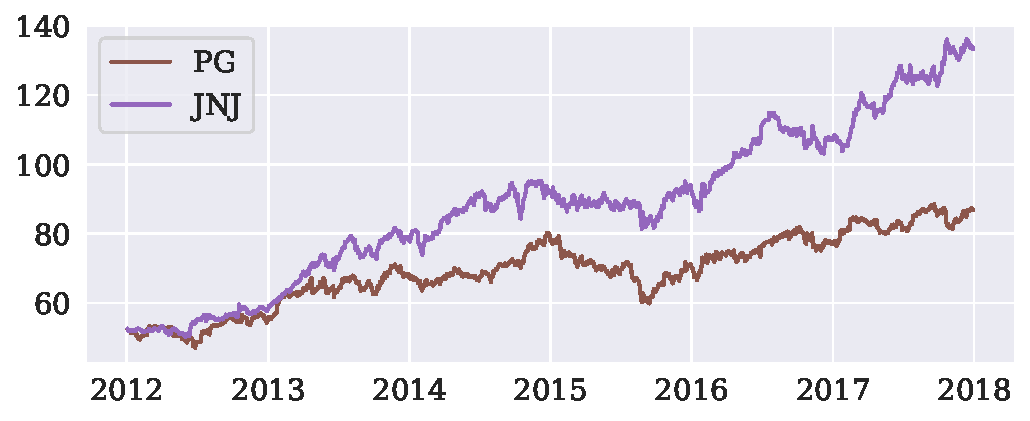
\includegraphics[width = \linewidth]{figures/coint_PG_JNJ_plot.pdf}
        %% Creator: Matplotlib, PGF backend
%%
%% To include the figure in your LaTeX document, write
%%   \input{<filename>.pgf}
%%
%% Make sure the required packages are loaded in your preamble
%%   \usepackage{pgf}
%%
%% Figures using additional raster images can only be included by \input if
%% they are in the same directory as the main LaTeX file. For loading figures
%% from other directories you can use the `import` package
%%   \usepackage{import}
%% and then include the figures with
%%   \import{<path to file>}{<filename>.pgf}
%%
%% Matplotlib used the following preamble
%%   \usepackage{fontspec}
%%   \setmainfont{DejaVuSerif.ttf}[Path=/opt/tljh/user/lib/python3.6/site-packages/matplotlib/mpl-data/fonts/ttf/]
%%   \setsansfont{DejaVuSans.ttf}[Path=/opt/tljh/user/lib/python3.6/site-packages/matplotlib/mpl-data/fonts/ttf/]
%%   \setmonofont{DejaVuSansMono.ttf}[Path=/opt/tljh/user/lib/python3.6/site-packages/matplotlib/mpl-data/fonts/ttf/]
%%
\begingroup%
\makeatletter%
\begin{pgfpicture}%
\pgfpathrectangle{\pgfpointorigin}{\pgfqpoint{6.718102in}{2.696635in}}%
\pgfusepath{use as bounding box, clip}%
\begin{pgfscope}%
\pgfsetbuttcap%
\pgfsetmiterjoin%
\definecolor{currentfill}{rgb}{1.000000,1.000000,1.000000}%
\pgfsetfillcolor{currentfill}%
\pgfsetlinewidth{0.000000pt}%
\definecolor{currentstroke}{rgb}{1.000000,1.000000,1.000000}%
\pgfsetstrokecolor{currentstroke}%
\pgfsetdash{}{0pt}%
\pgfpathmoveto{\pgfqpoint{0.000000in}{0.000000in}}%
\pgfpathlineto{\pgfqpoint{6.718102in}{0.000000in}}%
\pgfpathlineto{\pgfqpoint{6.718102in}{2.696635in}}%
\pgfpathlineto{\pgfqpoint{0.000000in}{2.696635in}}%
\pgfpathclose%
\pgfusepath{fill}%
\end{pgfscope}%
\begin{pgfscope}%
\pgfsetbuttcap%
\pgfsetmiterjoin%
\definecolor{currentfill}{rgb}{0.917647,0.917647,0.949020}%
\pgfsetfillcolor{currentfill}%
\pgfsetlinewidth{0.000000pt}%
\definecolor{currentstroke}{rgb}{0.000000,0.000000,0.000000}%
\pgfsetstrokecolor{currentstroke}%
\pgfsetstrokeopacity{0.000000}%
\pgfsetdash{}{0pt}%
\pgfpathmoveto{\pgfqpoint{0.418102in}{0.331635in}}%
\pgfpathlineto{\pgfqpoint{6.618102in}{0.331635in}}%
\pgfpathlineto{\pgfqpoint{6.618102in}{2.596635in}}%
\pgfpathlineto{\pgfqpoint{0.418102in}{2.596635in}}%
\pgfpathclose%
\pgfusepath{fill}%
\end{pgfscope}%
\begin{pgfscope}%
\pgfpathrectangle{\pgfqpoint{0.418102in}{0.331635in}}{\pgfqpoint{6.200000in}{2.265000in}}%
\pgfusepath{clip}%
\pgfsetroundcap%
\pgfsetroundjoin%
\pgfsetlinewidth{0.803000pt}%
\definecolor{currentstroke}{rgb}{1.000000,1.000000,1.000000}%
\pgfsetstrokecolor{currentstroke}%
\pgfsetdash{}{0pt}%
\pgfpathmoveto{\pgfqpoint{0.694765in}{0.331635in}}%
\pgfpathlineto{\pgfqpoint{0.694765in}{2.596635in}}%
\pgfusepath{stroke}%
\end{pgfscope}%
\begin{pgfscope}%
\definecolor{textcolor}{rgb}{0.150000,0.150000,0.150000}%
\pgfsetstrokecolor{textcolor}%
\pgfsetfillcolor{textcolor}%
\pgftext[x=0.694765in,y=0.234413in,,top]{\color{textcolor}\rmfamily\fontsize{10.000000}{12.000000}\selectfont 2012}%
\end{pgfscope}%
\begin{pgfscope}%
\pgfpathrectangle{\pgfqpoint{0.418102in}{0.331635in}}{\pgfqpoint{6.200000in}{2.265000in}}%
\pgfusepath{clip}%
\pgfsetroundcap%
\pgfsetroundjoin%
\pgfsetlinewidth{0.803000pt}%
\definecolor{currentstroke}{rgb}{1.000000,1.000000,1.000000}%
\pgfsetstrokecolor{currentstroke}%
\pgfsetdash{}{0pt}%
\pgfpathmoveto{\pgfqpoint{1.638025in}{0.331635in}}%
\pgfpathlineto{\pgfqpoint{1.638025in}{2.596635in}}%
\pgfusepath{stroke}%
\end{pgfscope}%
\begin{pgfscope}%
\definecolor{textcolor}{rgb}{0.150000,0.150000,0.150000}%
\pgfsetstrokecolor{textcolor}%
\pgfsetfillcolor{textcolor}%
\pgftext[x=1.638025in,y=0.234413in,,top]{\color{textcolor}\rmfamily\fontsize{10.000000}{12.000000}\selectfont 2013}%
\end{pgfscope}%
\begin{pgfscope}%
\pgfpathrectangle{\pgfqpoint{0.418102in}{0.331635in}}{\pgfqpoint{6.200000in}{2.265000in}}%
\pgfusepath{clip}%
\pgfsetroundcap%
\pgfsetroundjoin%
\pgfsetlinewidth{0.803000pt}%
\definecolor{currentstroke}{rgb}{1.000000,1.000000,1.000000}%
\pgfsetstrokecolor{currentstroke}%
\pgfsetdash{}{0pt}%
\pgfpathmoveto{\pgfqpoint{2.578708in}{0.331635in}}%
\pgfpathlineto{\pgfqpoint{2.578708in}{2.596635in}}%
\pgfusepath{stroke}%
\end{pgfscope}%
\begin{pgfscope}%
\definecolor{textcolor}{rgb}{0.150000,0.150000,0.150000}%
\pgfsetstrokecolor{textcolor}%
\pgfsetfillcolor{textcolor}%
\pgftext[x=2.578708in,y=0.234413in,,top]{\color{textcolor}\rmfamily\fontsize{10.000000}{12.000000}\selectfont 2014}%
\end{pgfscope}%
\begin{pgfscope}%
\pgfpathrectangle{\pgfqpoint{0.418102in}{0.331635in}}{\pgfqpoint{6.200000in}{2.265000in}}%
\pgfusepath{clip}%
\pgfsetroundcap%
\pgfsetroundjoin%
\pgfsetlinewidth{0.803000pt}%
\definecolor{currentstroke}{rgb}{1.000000,1.000000,1.000000}%
\pgfsetstrokecolor{currentstroke}%
\pgfsetdash{}{0pt}%
\pgfpathmoveto{\pgfqpoint{3.519390in}{0.331635in}}%
\pgfpathlineto{\pgfqpoint{3.519390in}{2.596635in}}%
\pgfusepath{stroke}%
\end{pgfscope}%
\begin{pgfscope}%
\definecolor{textcolor}{rgb}{0.150000,0.150000,0.150000}%
\pgfsetstrokecolor{textcolor}%
\pgfsetfillcolor{textcolor}%
\pgftext[x=3.519390in,y=0.234413in,,top]{\color{textcolor}\rmfamily\fontsize{10.000000}{12.000000}\selectfont 2015}%
\end{pgfscope}%
\begin{pgfscope}%
\pgfpathrectangle{\pgfqpoint{0.418102in}{0.331635in}}{\pgfqpoint{6.200000in}{2.265000in}}%
\pgfusepath{clip}%
\pgfsetroundcap%
\pgfsetroundjoin%
\pgfsetlinewidth{0.803000pt}%
\definecolor{currentstroke}{rgb}{1.000000,1.000000,1.000000}%
\pgfsetstrokecolor{currentstroke}%
\pgfsetdash{}{0pt}%
\pgfpathmoveto{\pgfqpoint{4.460073in}{0.331635in}}%
\pgfpathlineto{\pgfqpoint{4.460073in}{2.596635in}}%
\pgfusepath{stroke}%
\end{pgfscope}%
\begin{pgfscope}%
\definecolor{textcolor}{rgb}{0.150000,0.150000,0.150000}%
\pgfsetstrokecolor{textcolor}%
\pgfsetfillcolor{textcolor}%
\pgftext[x=4.460073in,y=0.234413in,,top]{\color{textcolor}\rmfamily\fontsize{10.000000}{12.000000}\selectfont 2016}%
\end{pgfscope}%
\begin{pgfscope}%
\pgfpathrectangle{\pgfqpoint{0.418102in}{0.331635in}}{\pgfqpoint{6.200000in}{2.265000in}}%
\pgfusepath{clip}%
\pgfsetroundcap%
\pgfsetroundjoin%
\pgfsetlinewidth{0.803000pt}%
\definecolor{currentstroke}{rgb}{1.000000,1.000000,1.000000}%
\pgfsetstrokecolor{currentstroke}%
\pgfsetdash{}{0pt}%
\pgfpathmoveto{\pgfqpoint{5.403333in}{0.331635in}}%
\pgfpathlineto{\pgfqpoint{5.403333in}{2.596635in}}%
\pgfusepath{stroke}%
\end{pgfscope}%
\begin{pgfscope}%
\definecolor{textcolor}{rgb}{0.150000,0.150000,0.150000}%
\pgfsetstrokecolor{textcolor}%
\pgfsetfillcolor{textcolor}%
\pgftext[x=5.403333in,y=0.234413in,,top]{\color{textcolor}\rmfamily\fontsize{10.000000}{12.000000}\selectfont 2017}%
\end{pgfscope}%
\begin{pgfscope}%
\pgfpathrectangle{\pgfqpoint{0.418102in}{0.331635in}}{\pgfqpoint{6.200000in}{2.265000in}}%
\pgfusepath{clip}%
\pgfsetroundcap%
\pgfsetroundjoin%
\pgfsetlinewidth{0.803000pt}%
\definecolor{currentstroke}{rgb}{1.000000,1.000000,1.000000}%
\pgfsetstrokecolor{currentstroke}%
\pgfsetdash{}{0pt}%
\pgfpathmoveto{\pgfqpoint{6.344015in}{0.331635in}}%
\pgfpathlineto{\pgfqpoint{6.344015in}{2.596635in}}%
\pgfusepath{stroke}%
\end{pgfscope}%
\begin{pgfscope}%
\definecolor{textcolor}{rgb}{0.150000,0.150000,0.150000}%
\pgfsetstrokecolor{textcolor}%
\pgfsetfillcolor{textcolor}%
\pgftext[x=6.344015in,y=0.234413in,,top]{\color{textcolor}\rmfamily\fontsize{10.000000}{12.000000}\selectfont 2018}%
\end{pgfscope}%
\begin{pgfscope}%
\pgfpathrectangle{\pgfqpoint{0.418102in}{0.331635in}}{\pgfqpoint{6.200000in}{2.265000in}}%
\pgfusepath{clip}%
\pgfsetroundcap%
\pgfsetroundjoin%
\pgfsetlinewidth{0.803000pt}%
\definecolor{currentstroke}{rgb}{1.000000,1.000000,1.000000}%
\pgfsetstrokecolor{currentstroke}%
\pgfsetdash{}{0pt}%
\pgfpathmoveto{\pgfqpoint{0.418102in}{0.530259in}}%
\pgfpathlineto{\pgfqpoint{6.618102in}{0.530259in}}%
\pgfusepath{stroke}%
\end{pgfscope}%
\begin{pgfscope}%
\definecolor{textcolor}{rgb}{0.150000,0.150000,0.150000}%
\pgfsetstrokecolor{textcolor}%
\pgfsetfillcolor{textcolor}%
\pgftext[x=0.100000in,y=0.477497in,left,base]{\color{textcolor}\rmfamily\fontsize{10.000000}{12.000000}\selectfont 1.0}%
\end{pgfscope}%
\begin{pgfscope}%
\pgfpathrectangle{\pgfqpoint{0.418102in}{0.331635in}}{\pgfqpoint{6.200000in}{2.265000in}}%
\pgfusepath{clip}%
\pgfsetroundcap%
\pgfsetroundjoin%
\pgfsetlinewidth{0.803000pt}%
\definecolor{currentstroke}{rgb}{1.000000,1.000000,1.000000}%
\pgfsetstrokecolor{currentstroke}%
\pgfsetdash{}{0pt}%
\pgfpathmoveto{\pgfqpoint{0.418102in}{0.886742in}}%
\pgfpathlineto{\pgfqpoint{6.618102in}{0.886742in}}%
\pgfusepath{stroke}%
\end{pgfscope}%
\begin{pgfscope}%
\definecolor{textcolor}{rgb}{0.150000,0.150000,0.150000}%
\pgfsetstrokecolor{textcolor}%
\pgfsetfillcolor{textcolor}%
\pgftext[x=0.100000in,y=0.833980in,left,base]{\color{textcolor}\rmfamily\fontsize{10.000000}{12.000000}\selectfont 1.2}%
\end{pgfscope}%
\begin{pgfscope}%
\pgfpathrectangle{\pgfqpoint{0.418102in}{0.331635in}}{\pgfqpoint{6.200000in}{2.265000in}}%
\pgfusepath{clip}%
\pgfsetroundcap%
\pgfsetroundjoin%
\pgfsetlinewidth{0.803000pt}%
\definecolor{currentstroke}{rgb}{1.000000,1.000000,1.000000}%
\pgfsetstrokecolor{currentstroke}%
\pgfsetdash{}{0pt}%
\pgfpathmoveto{\pgfqpoint{0.418102in}{1.243225in}}%
\pgfpathlineto{\pgfqpoint{6.618102in}{1.243225in}}%
\pgfusepath{stroke}%
\end{pgfscope}%
\begin{pgfscope}%
\definecolor{textcolor}{rgb}{0.150000,0.150000,0.150000}%
\pgfsetstrokecolor{textcolor}%
\pgfsetfillcolor{textcolor}%
\pgftext[x=0.100000in,y=1.190463in,left,base]{\color{textcolor}\rmfamily\fontsize{10.000000}{12.000000}\selectfont 1.4}%
\end{pgfscope}%
\begin{pgfscope}%
\pgfpathrectangle{\pgfqpoint{0.418102in}{0.331635in}}{\pgfqpoint{6.200000in}{2.265000in}}%
\pgfusepath{clip}%
\pgfsetroundcap%
\pgfsetroundjoin%
\pgfsetlinewidth{0.803000pt}%
\definecolor{currentstroke}{rgb}{1.000000,1.000000,1.000000}%
\pgfsetstrokecolor{currentstroke}%
\pgfsetdash{}{0pt}%
\pgfpathmoveto{\pgfqpoint{0.418102in}{1.599707in}}%
\pgfpathlineto{\pgfqpoint{6.618102in}{1.599707in}}%
\pgfusepath{stroke}%
\end{pgfscope}%
\begin{pgfscope}%
\definecolor{textcolor}{rgb}{0.150000,0.150000,0.150000}%
\pgfsetstrokecolor{textcolor}%
\pgfsetfillcolor{textcolor}%
\pgftext[x=0.100000in,y=1.546946in,left,base]{\color{textcolor}\rmfamily\fontsize{10.000000}{12.000000}\selectfont 1.6}%
\end{pgfscope}%
\begin{pgfscope}%
\pgfpathrectangle{\pgfqpoint{0.418102in}{0.331635in}}{\pgfqpoint{6.200000in}{2.265000in}}%
\pgfusepath{clip}%
\pgfsetroundcap%
\pgfsetroundjoin%
\pgfsetlinewidth{0.803000pt}%
\definecolor{currentstroke}{rgb}{1.000000,1.000000,1.000000}%
\pgfsetstrokecolor{currentstroke}%
\pgfsetdash{}{0pt}%
\pgfpathmoveto{\pgfqpoint{0.418102in}{1.956190in}}%
\pgfpathlineto{\pgfqpoint{6.618102in}{1.956190in}}%
\pgfusepath{stroke}%
\end{pgfscope}%
\begin{pgfscope}%
\definecolor{textcolor}{rgb}{0.150000,0.150000,0.150000}%
\pgfsetstrokecolor{textcolor}%
\pgfsetfillcolor{textcolor}%
\pgftext[x=0.100000in,y=1.903429in,left,base]{\color{textcolor}\rmfamily\fontsize{10.000000}{12.000000}\selectfont 1.8}%
\end{pgfscope}%
\begin{pgfscope}%
\pgfpathrectangle{\pgfqpoint{0.418102in}{0.331635in}}{\pgfqpoint{6.200000in}{2.265000in}}%
\pgfusepath{clip}%
\pgfsetroundcap%
\pgfsetroundjoin%
\pgfsetlinewidth{0.803000pt}%
\definecolor{currentstroke}{rgb}{1.000000,1.000000,1.000000}%
\pgfsetstrokecolor{currentstroke}%
\pgfsetdash{}{0pt}%
\pgfpathmoveto{\pgfqpoint{0.418102in}{2.312673in}}%
\pgfpathlineto{\pgfqpoint{6.618102in}{2.312673in}}%
\pgfusepath{stroke}%
\end{pgfscope}%
\begin{pgfscope}%
\definecolor{textcolor}{rgb}{0.150000,0.150000,0.150000}%
\pgfsetstrokecolor{textcolor}%
\pgfsetfillcolor{textcolor}%
\pgftext[x=0.100000in,y=2.259912in,left,base]{\color{textcolor}\rmfamily\fontsize{10.000000}{12.000000}\selectfont 2.0}%
\end{pgfscope}%
\begin{pgfscope}%
\pgfpathrectangle{\pgfqpoint{0.418102in}{0.331635in}}{\pgfqpoint{6.200000in}{2.265000in}}%
\pgfusepath{clip}%
\pgfsetroundcap%
\pgfsetroundjoin%
\pgfsetlinewidth{1.505625pt}%
\definecolor{currentstroke}{rgb}{0.121569,0.466667,0.705882}%
\pgfsetstrokecolor{currentstroke}%
\pgfsetdash{}{0pt}%
\pgfpathmoveto{\pgfqpoint{0.699920in}{0.530259in}}%
\pgfpathlineto{\pgfqpoint{0.702497in}{0.530259in}}%
\pgfpathlineto{\pgfqpoint{0.705074in}{0.532992in}}%
\pgfpathlineto{\pgfqpoint{0.707651in}{0.538786in}}%
\pgfpathlineto{\pgfqpoint{0.715383in}{0.536371in}}%
\pgfpathlineto{\pgfqpoint{0.717960in}{0.544452in}}%
\pgfpathlineto{\pgfqpoint{0.720538in}{0.536824in}}%
\pgfpathlineto{\pgfqpoint{0.723115in}{0.537191in}}%
\pgfpathlineto{\pgfqpoint{0.725692in}{0.536848in}}%
\pgfpathlineto{\pgfqpoint{0.736001in}{0.544820in}}%
\pgfpathlineto{\pgfqpoint{0.743732in}{0.540146in}}%
\pgfpathlineto{\pgfqpoint{0.751464in}{0.553195in}}%
\pgfpathlineto{\pgfqpoint{0.754041in}{0.546321in}}%
\pgfpathlineto{\pgfqpoint{0.756619in}{0.550102in}}%
\pgfpathlineto{\pgfqpoint{0.759196in}{0.540721in}}%
\pgfpathlineto{\pgfqpoint{0.761773in}{0.535922in}}%
\pgfpathlineto{\pgfqpoint{0.772082in}{0.513692in}}%
\pgfpathlineto{\pgfqpoint{0.774659in}{0.518852in}}%
\pgfpathlineto{\pgfqpoint{0.777236in}{0.521801in}}%
\pgfpathlineto{\pgfqpoint{0.779813in}{0.513303in}}%
\pgfpathlineto{\pgfqpoint{0.787545in}{0.529890in}}%
\pgfpathlineto{\pgfqpoint{0.790122in}{0.531705in}}%
\pgfpathlineto{\pgfqpoint{0.792699in}{0.530988in}}%
\pgfpathlineto{\pgfqpoint{0.795277in}{0.541286in}}%
\pgfpathlineto{\pgfqpoint{0.797854in}{0.543129in}}%
\pgfpathlineto{\pgfqpoint{0.805586in}{0.546901in}}%
\pgfpathlineto{\pgfqpoint{0.808163in}{0.542302in}}%
\pgfpathlineto{\pgfqpoint{0.810740in}{0.541938in}}%
\pgfpathlineto{\pgfqpoint{0.813317in}{0.536590in}}%
\pgfpathlineto{\pgfqpoint{0.815894in}{0.541627in}}%
\pgfpathlineto{\pgfqpoint{0.826203in}{0.549156in}}%
\pgfpathlineto{\pgfqpoint{0.828780in}{0.550031in}}%
\pgfpathlineto{\pgfqpoint{0.831358in}{0.576326in}}%
\pgfpathlineto{\pgfqpoint{0.833935in}{0.571254in}}%
\pgfpathlineto{\pgfqpoint{0.841667in}{0.571252in}}%
\pgfpathlineto{\pgfqpoint{0.844244in}{0.572236in}}%
\pgfpathlineto{\pgfqpoint{0.846821in}{0.567583in}}%
\pgfpathlineto{\pgfqpoint{0.849398in}{0.577092in}}%
\pgfpathlineto{\pgfqpoint{0.851975in}{0.576043in}}%
\pgfpathlineto{\pgfqpoint{0.859707in}{0.574141in}}%
\pgfpathlineto{\pgfqpoint{0.862284in}{0.567848in}}%
\pgfpathlineto{\pgfqpoint{0.867439in}{0.573993in}}%
\pgfpathlineto{\pgfqpoint{0.877748in}{0.566593in}}%
\pgfpathlineto{\pgfqpoint{0.880325in}{0.567155in}}%
\pgfpathlineto{\pgfqpoint{0.882902in}{0.564381in}}%
\pgfpathlineto{\pgfqpoint{0.885479in}{0.566586in}}%
\pgfpathlineto{\pgfqpoint{0.888056in}{0.573077in}}%
\pgfpathlineto{\pgfqpoint{0.895788in}{0.574810in}}%
\pgfpathlineto{\pgfqpoint{0.900942in}{0.568723in}}%
\pgfpathlineto{\pgfqpoint{0.903520in}{0.560068in}}%
\pgfpathlineto{\pgfqpoint{0.906097in}{0.562480in}}%
\pgfpathlineto{\pgfqpoint{0.913828in}{0.570854in}}%
\pgfpathlineto{\pgfqpoint{0.916406in}{0.578265in}}%
\pgfpathlineto{\pgfqpoint{0.918983in}{0.580870in}}%
\pgfpathlineto{\pgfqpoint{0.921560in}{0.582254in}}%
\pgfpathlineto{\pgfqpoint{0.924137in}{0.585375in}}%
\pgfpathlineto{\pgfqpoint{0.931869in}{0.583972in}}%
\pgfpathlineto{\pgfqpoint{0.934446in}{0.585710in}}%
\pgfpathlineto{\pgfqpoint{0.937023in}{0.576704in}}%
\pgfpathlineto{\pgfqpoint{0.939601in}{0.575320in}}%
\pgfpathlineto{\pgfqpoint{0.949909in}{0.576142in}}%
\pgfpathlineto{\pgfqpoint{0.952487in}{0.572438in}}%
\pgfpathlineto{\pgfqpoint{0.955064in}{0.569985in}}%
\pgfpathlineto{\pgfqpoint{0.957641in}{0.575209in}}%
\pgfpathlineto{\pgfqpoint{0.960218in}{0.570414in}}%
\pgfpathlineto{\pgfqpoint{0.967950in}{0.563284in}}%
\pgfpathlineto{\pgfqpoint{0.970527in}{0.563526in}}%
\pgfpathlineto{\pgfqpoint{0.973104in}{0.553463in}}%
\pgfpathlineto{\pgfqpoint{0.975682in}{0.552680in}}%
\pgfpathlineto{\pgfqpoint{0.978259in}{0.549538in}}%
\pgfpathlineto{\pgfqpoint{0.985990in}{0.556317in}}%
\pgfpathlineto{\pgfqpoint{0.988568in}{0.557159in}}%
\pgfpathlineto{\pgfqpoint{0.991145in}{0.560491in}}%
\pgfpathlineto{\pgfqpoint{0.993722in}{0.565193in}}%
\pgfpathlineto{\pgfqpoint{0.996299in}{0.599588in}}%
\pgfpathlineto{\pgfqpoint{1.004031in}{0.584298in}}%
\pgfpathlineto{\pgfqpoint{1.006608in}{0.581816in}}%
\pgfpathlineto{\pgfqpoint{1.009185in}{0.586055in}}%
\pgfpathlineto{\pgfqpoint{1.011763in}{0.593474in}}%
\pgfpathlineto{\pgfqpoint{1.014340in}{0.598640in}}%
\pgfpathlineto{\pgfqpoint{1.022071in}{0.597569in}}%
\pgfpathlineto{\pgfqpoint{1.024649in}{0.593646in}}%
\pgfpathlineto{\pgfqpoint{1.029803in}{0.599105in}}%
\pgfpathlineto{\pgfqpoint{1.032380in}{0.595945in}}%
\pgfpathlineto{\pgfqpoint{1.040112in}{0.600362in}}%
\pgfpathlineto{\pgfqpoint{1.045266in}{0.613861in}}%
\pgfpathlineto{\pgfqpoint{1.047844in}{0.616429in}}%
\pgfpathlineto{\pgfqpoint{1.050421in}{0.613095in}}%
\pgfpathlineto{\pgfqpoint{1.058152in}{0.609237in}}%
\pgfpathlineto{\pgfqpoint{1.060730in}{0.604999in}}%
\pgfpathlineto{\pgfqpoint{1.063307in}{0.597522in}}%
\pgfpathlineto{\pgfqpoint{1.065884in}{0.593608in}}%
\pgfpathlineto{\pgfqpoint{1.068461in}{0.601116in}}%
\pgfpathlineto{\pgfqpoint{1.078770in}{0.606928in}}%
\pgfpathlineto{\pgfqpoint{1.083925in}{0.599435in}}%
\pgfpathlineto{\pgfqpoint{1.086502in}{0.598054in}}%
\pgfpathlineto{\pgfqpoint{1.094233in}{0.587324in}}%
\pgfpathlineto{\pgfqpoint{1.096811in}{0.585924in}}%
\pgfpathlineto{\pgfqpoint{1.099388in}{0.586667in}}%
\pgfpathlineto{\pgfqpoint{1.101965in}{0.600896in}}%
\pgfpathlineto{\pgfqpoint{1.104542in}{0.598177in}}%
\pgfpathlineto{\pgfqpoint{1.112274in}{0.607653in}}%
\pgfpathlineto{\pgfqpoint{1.114851in}{0.596493in}}%
\pgfpathlineto{\pgfqpoint{1.117428in}{0.573557in}}%
\pgfpathlineto{\pgfqpoint{1.120005in}{0.568463in}}%
\pgfpathlineto{\pgfqpoint{1.122583in}{0.556254in}}%
\pgfpathlineto{\pgfqpoint{1.130314in}{0.543881in}}%
\pgfpathlineto{\pgfqpoint{1.132892in}{0.536970in}}%
\pgfpathlineto{\pgfqpoint{1.135469in}{0.507111in}}%
\pgfpathlineto{\pgfqpoint{1.140623in}{0.503871in}}%
\pgfpathlineto{\pgfqpoint{1.148355in}{0.497734in}}%
\pgfpathlineto{\pgfqpoint{1.150932in}{0.498308in}}%
\pgfpathlineto{\pgfqpoint{1.153509in}{0.503398in}}%
\pgfpathlineto{\pgfqpoint{1.156086in}{0.506365in}}%
\pgfpathlineto{\pgfqpoint{1.158664in}{0.512248in}}%
\pgfpathlineto{\pgfqpoint{1.166395in}{0.505750in}}%
\pgfpathlineto{\pgfqpoint{1.174127in}{0.510778in}}%
\pgfpathlineto{\pgfqpoint{1.187013in}{0.515100in}}%
\pgfpathlineto{\pgfqpoint{1.189590in}{0.509917in}}%
\pgfpathlineto{\pgfqpoint{1.192167in}{0.545513in}}%
\pgfpathlineto{\pgfqpoint{1.194745in}{0.553321in}}%
\pgfpathlineto{\pgfqpoint{1.202476in}{0.551408in}}%
\pgfpathlineto{\pgfqpoint{1.205053in}{0.551656in}}%
\pgfpathlineto{\pgfqpoint{1.207631in}{0.547360in}}%
\pgfpathlineto{\pgfqpoint{1.210208in}{0.546675in}}%
\pgfpathlineto{\pgfqpoint{1.212785in}{0.555680in}}%
\pgfpathlineto{\pgfqpoint{1.220517in}{0.557597in}}%
\pgfpathlineto{\pgfqpoint{1.223094in}{0.562628in}}%
\pgfpathlineto{\pgfqpoint{1.225671in}{0.560146in}}%
\pgfpathlineto{\pgfqpoint{1.228248in}{0.551590in}}%
\pgfpathlineto{\pgfqpoint{1.230826in}{0.548597in}}%
\pgfpathlineto{\pgfqpoint{1.238557in}{0.549724in}}%
\pgfpathlineto{\pgfqpoint{1.241134in}{0.544981in}}%
\pgfpathlineto{\pgfqpoint{1.243712in}{0.535613in}}%
\pgfpathlineto{\pgfqpoint{1.246289in}{0.540670in}}%
\pgfpathlineto{\pgfqpoint{1.248866in}{0.559820in}}%
\pgfpathlineto{\pgfqpoint{1.256598in}{0.567837in}}%
\pgfpathlineto{\pgfqpoint{1.259175in}{0.580835in}}%
\pgfpathlineto{\pgfqpoint{1.261752in}{0.586918in}}%
\pgfpathlineto{\pgfqpoint{1.264329in}{0.586415in}}%
\pgfpathlineto{\pgfqpoint{1.266907in}{0.590196in}}%
\pgfpathlineto{\pgfqpoint{1.274638in}{0.591683in}}%
\pgfpathlineto{\pgfqpoint{1.277215in}{0.590704in}}%
\pgfpathlineto{\pgfqpoint{1.279793in}{0.587953in}}%
\pgfpathlineto{\pgfqpoint{1.282370in}{0.580974in}}%
\pgfpathlineto{\pgfqpoint{1.284947in}{0.575692in}}%
\pgfpathlineto{\pgfqpoint{1.295256in}{0.578597in}}%
\pgfpathlineto{\pgfqpoint{1.297833in}{0.576902in}}%
\pgfpathlineto{\pgfqpoint{1.302988in}{0.580974in}}%
\pgfpathlineto{\pgfqpoint{1.310719in}{0.578294in}}%
\pgfpathlineto{\pgfqpoint{1.313296in}{0.580155in}}%
\pgfpathlineto{\pgfqpoint{1.315874in}{0.579880in}}%
\pgfpathlineto{\pgfqpoint{1.318451in}{0.577557in}}%
\pgfpathlineto{\pgfqpoint{1.331337in}{0.571077in}}%
\pgfpathlineto{\pgfqpoint{1.333914in}{0.572761in}}%
\pgfpathlineto{\pgfqpoint{1.336491in}{0.567664in}}%
\pgfpathlineto{\pgfqpoint{1.339069in}{0.564494in}}%
\pgfpathlineto{\pgfqpoint{1.346800in}{0.568566in}}%
\pgfpathlineto{\pgfqpoint{1.349377in}{0.572206in}}%
\pgfpathlineto{\pgfqpoint{1.351955in}{0.573559in}}%
\pgfpathlineto{\pgfqpoint{1.354532in}{0.573939in}}%
\pgfpathlineto{\pgfqpoint{1.357109in}{0.563868in}}%
\pgfpathlineto{\pgfqpoint{1.364841in}{0.559816in}}%
\pgfpathlineto{\pgfqpoint{1.367418in}{0.564020in}}%
\pgfpathlineto{\pgfqpoint{1.372572in}{0.564277in}}%
\pgfpathlineto{\pgfqpoint{1.375150in}{0.568154in}}%
\pgfpathlineto{\pgfqpoint{1.382881in}{0.562936in}}%
\pgfpathlineto{\pgfqpoint{1.385458in}{0.569531in}}%
\pgfpathlineto{\pgfqpoint{1.388036in}{0.568969in}}%
\pgfpathlineto{\pgfqpoint{1.390613in}{0.569129in}}%
\pgfpathlineto{\pgfqpoint{1.393190in}{0.567025in}}%
\pgfpathlineto{\pgfqpoint{1.400922in}{0.568771in}}%
\pgfpathlineto{\pgfqpoint{1.403499in}{0.575195in}}%
\pgfpathlineto{\pgfqpoint{1.406076in}{0.570708in}}%
\pgfpathlineto{\pgfqpoint{1.408653in}{0.571450in}}%
\pgfpathlineto{\pgfqpoint{1.411230in}{0.573298in}}%
\pgfpathlineto{\pgfqpoint{1.418962in}{0.577296in}}%
\pgfpathlineto{\pgfqpoint{1.421539in}{0.569112in}}%
\pgfpathlineto{\pgfqpoint{1.424117in}{0.573961in}}%
\pgfpathlineto{\pgfqpoint{1.426694in}{0.572542in}}%
\pgfpathlineto{\pgfqpoint{1.429271in}{0.573379in}}%
\pgfpathlineto{\pgfqpoint{1.437003in}{0.571323in}}%
\pgfpathlineto{\pgfqpoint{1.439580in}{0.580134in}}%
\pgfpathlineto{\pgfqpoint{1.442157in}{0.585626in}}%
\pgfpathlineto{\pgfqpoint{1.444734in}{0.605314in}}%
\pgfpathlineto{\pgfqpoint{1.447311in}{0.601975in}}%
\pgfpathlineto{\pgfqpoint{1.455043in}{0.601913in}}%
\pgfpathlineto{\pgfqpoint{1.457620in}{0.598986in}}%
\pgfpathlineto{\pgfqpoint{1.460198in}{0.609883in}}%
\pgfpathlineto{\pgfqpoint{1.462775in}{0.631840in}}%
\pgfpathlineto{\pgfqpoint{1.465352in}{0.637100in}}%
\pgfpathlineto{\pgfqpoint{1.478238in}{0.638820in}}%
\pgfpathlineto{\pgfqpoint{1.480815in}{0.647919in}}%
\pgfpathlineto{\pgfqpoint{1.483392in}{0.640513in}}%
\pgfpathlineto{\pgfqpoint{1.491124in}{0.646159in}}%
\pgfpathlineto{\pgfqpoint{1.493701in}{0.645505in}}%
\pgfpathlineto{\pgfqpoint{1.496278in}{0.648652in}}%
\pgfpathlineto{\pgfqpoint{1.498856in}{0.641791in}}%
\pgfpathlineto{\pgfqpoint{1.501433in}{0.640214in}}%
\pgfpathlineto{\pgfqpoint{1.509165in}{0.643899in}}%
\pgfpathlineto{\pgfqpoint{1.516896in}{0.641497in}}%
\pgfpathlineto{\pgfqpoint{1.519473in}{0.646894in}}%
\pgfpathlineto{\pgfqpoint{1.527205in}{0.661709in}}%
\pgfpathlineto{\pgfqpoint{1.529782in}{0.662022in}}%
\pgfpathlineto{\pgfqpoint{1.532359in}{0.658765in}}%
\pgfpathlineto{\pgfqpoint{1.537514in}{0.651071in}}%
\pgfpathlineto{\pgfqpoint{1.545246in}{0.646158in}}%
\pgfpathlineto{\pgfqpoint{1.547823in}{0.649108in}}%
\pgfpathlineto{\pgfqpoint{1.550400in}{0.649298in}}%
\pgfpathlineto{\pgfqpoint{1.552977in}{0.647623in}}%
\pgfpathlineto{\pgfqpoint{1.555554in}{0.650179in}}%
\pgfpathlineto{\pgfqpoint{1.563286in}{0.652399in}}%
\pgfpathlineto{\pgfqpoint{1.565863in}{0.659094in}}%
\pgfpathlineto{\pgfqpoint{1.568440in}{0.659214in}}%
\pgfpathlineto{\pgfqpoint{1.571018in}{0.652706in}}%
\pgfpathlineto{\pgfqpoint{1.583904in}{0.657330in}}%
\pgfpathlineto{\pgfqpoint{1.586481in}{0.654043in}}%
\pgfpathlineto{\pgfqpoint{1.589058in}{0.659626in}}%
\pgfpathlineto{\pgfqpoint{1.591635in}{0.657411in}}%
\pgfpathlineto{\pgfqpoint{1.599367in}{0.654152in}}%
\pgfpathlineto{\pgfqpoint{1.601944in}{0.654665in}}%
\pgfpathlineto{\pgfqpoint{1.604521in}{0.650282in}}%
\pgfpathlineto{\pgfqpoint{1.607099in}{0.655439in}}%
\pgfpathlineto{\pgfqpoint{1.609676in}{0.646740in}}%
\pgfpathlineto{\pgfqpoint{1.617407in}{0.647256in}}%
\pgfpathlineto{\pgfqpoint{1.622562in}{0.638089in}}%
\pgfpathlineto{\pgfqpoint{1.625139in}{0.638720in}}%
\pgfpathlineto{\pgfqpoint{1.627716in}{0.635659in}}%
\pgfpathlineto{\pgfqpoint{1.635448in}{0.637572in}}%
\pgfpathlineto{\pgfqpoint{1.640602in}{0.648490in}}%
\pgfpathlineto{\pgfqpoint{1.643180in}{0.643684in}}%
\pgfpathlineto{\pgfqpoint{1.645757in}{0.634895in}}%
\pgfpathlineto{\pgfqpoint{1.656066in}{0.628856in}}%
\pgfpathlineto{\pgfqpoint{1.658643in}{0.629661in}}%
\pgfpathlineto{\pgfqpoint{1.661220in}{0.628887in}}%
\pgfpathlineto{\pgfqpoint{1.663797in}{0.626172in}}%
\pgfpathlineto{\pgfqpoint{1.671529in}{0.628893in}}%
\pgfpathlineto{\pgfqpoint{1.674106in}{0.634738in}}%
\pgfpathlineto{\pgfqpoint{1.676683in}{0.632399in}}%
\pgfpathlineto{\pgfqpoint{1.679261in}{0.632674in}}%
\pgfpathlineto{\pgfqpoint{1.681838in}{0.632116in}}%
\pgfpathlineto{\pgfqpoint{1.692147in}{0.639265in}}%
\pgfpathlineto{\pgfqpoint{1.694724in}{0.647025in}}%
\pgfpathlineto{\pgfqpoint{1.697301in}{0.640252in}}%
\pgfpathlineto{\pgfqpoint{1.699878in}{0.667732in}}%
\pgfpathlineto{\pgfqpoint{1.707610in}{0.657059in}}%
\pgfpathlineto{\pgfqpoint{1.712764in}{0.646244in}}%
\pgfpathlineto{\pgfqpoint{1.715342in}{0.643149in}}%
\pgfpathlineto{\pgfqpoint{1.717919in}{0.636956in}}%
\pgfpathlineto{\pgfqpoint{1.725650in}{0.644281in}}%
\pgfpathlineto{\pgfqpoint{1.728228in}{0.645814in}}%
\pgfpathlineto{\pgfqpoint{1.730805in}{0.649320in}}%
\pgfpathlineto{\pgfqpoint{1.733382in}{0.645212in}}%
\pgfpathlineto{\pgfqpoint{1.735959in}{0.655595in}}%
\pgfpathlineto{\pgfqpoint{1.743691in}{0.653907in}}%
\pgfpathlineto{\pgfqpoint{1.746268in}{0.656626in}}%
\pgfpathlineto{\pgfqpoint{1.748845in}{0.647556in}}%
\pgfpathlineto{\pgfqpoint{1.751423in}{0.646784in}}%
\pgfpathlineto{\pgfqpoint{1.754000in}{0.654050in}}%
\pgfpathlineto{\pgfqpoint{1.766886in}{0.653514in}}%
\pgfpathlineto{\pgfqpoint{1.769463in}{0.656669in}}%
\pgfpathlineto{\pgfqpoint{1.772040in}{0.657279in}}%
\pgfpathlineto{\pgfqpoint{1.779772in}{0.661981in}}%
\pgfpathlineto{\pgfqpoint{1.782349in}{0.662243in}}%
\pgfpathlineto{\pgfqpoint{1.784926in}{0.661008in}}%
\pgfpathlineto{\pgfqpoint{1.790081in}{0.669020in}}%
\pgfpathlineto{\pgfqpoint{1.800390in}{0.674051in}}%
\pgfpathlineto{\pgfqpoint{1.802967in}{0.679459in}}%
\pgfpathlineto{\pgfqpoint{1.805544in}{0.687779in}}%
\pgfpathlineto{\pgfqpoint{1.808121in}{0.685815in}}%
\pgfpathlineto{\pgfqpoint{1.815853in}{0.684858in}}%
\pgfpathlineto{\pgfqpoint{1.821007in}{0.676610in}}%
\pgfpathlineto{\pgfqpoint{1.823584in}{0.677248in}}%
\pgfpathlineto{\pgfqpoint{1.826162in}{0.662922in}}%
\pgfpathlineto{\pgfqpoint{1.833893in}{0.665397in}}%
\pgfpathlineto{\pgfqpoint{1.836471in}{0.676713in}}%
\pgfpathlineto{\pgfqpoint{1.839048in}{0.675528in}}%
\pgfpathlineto{\pgfqpoint{1.841625in}{0.676028in}}%
\pgfpathlineto{\pgfqpoint{1.844202in}{0.667887in}}%
\pgfpathlineto{\pgfqpoint{1.851934in}{0.661287in}}%
\pgfpathlineto{\pgfqpoint{1.854511in}{0.656384in}}%
\pgfpathlineto{\pgfqpoint{1.857088in}{0.647203in}}%
\pgfpathlineto{\pgfqpoint{1.859665in}{0.644126in}}%
\pgfpathlineto{\pgfqpoint{1.869974in}{0.647247in}}%
\pgfpathlineto{\pgfqpoint{1.872552in}{0.653960in}}%
\pgfpathlineto{\pgfqpoint{1.875129in}{0.651059in}}%
\pgfpathlineto{\pgfqpoint{1.877706in}{0.652118in}}%
\pgfpathlineto{\pgfqpoint{1.880283in}{0.652536in}}%
\pgfpathlineto{\pgfqpoint{1.888015in}{0.670246in}}%
\pgfpathlineto{\pgfqpoint{1.890592in}{0.658985in}}%
\pgfpathlineto{\pgfqpoint{1.893169in}{0.665082in}}%
\pgfpathlineto{\pgfqpoint{1.895746in}{0.666782in}}%
\pgfpathlineto{\pgfqpoint{1.898324in}{0.666777in}}%
\pgfpathlineto{\pgfqpoint{1.906055in}{0.673566in}}%
\pgfpathlineto{\pgfqpoint{1.911210in}{0.640955in}}%
\pgfpathlineto{\pgfqpoint{1.913787in}{0.658756in}}%
\pgfpathlineto{\pgfqpoint{1.916364in}{0.662419in}}%
\pgfpathlineto{\pgfqpoint{1.924096in}{0.658198in}}%
\pgfpathlineto{\pgfqpoint{1.926673in}{0.664584in}}%
\pgfpathlineto{\pgfqpoint{1.929250in}{0.620097in}}%
\pgfpathlineto{\pgfqpoint{1.931827in}{0.604428in}}%
\pgfpathlineto{\pgfqpoint{1.934405in}{0.611822in}}%
\pgfpathlineto{\pgfqpoint{1.942136in}{0.613765in}}%
\pgfpathlineto{\pgfqpoint{1.944713in}{0.606573in}}%
\pgfpathlineto{\pgfqpoint{1.947291in}{0.620061in}}%
\pgfpathlineto{\pgfqpoint{1.949868in}{0.619302in}}%
\pgfpathlineto{\pgfqpoint{1.952445in}{0.617858in}}%
\pgfpathlineto{\pgfqpoint{1.960177in}{0.624357in}}%
\pgfpathlineto{\pgfqpoint{1.962754in}{0.617147in}}%
\pgfpathlineto{\pgfqpoint{1.965331in}{0.623923in}}%
\pgfpathlineto{\pgfqpoint{1.967908in}{0.624584in}}%
\pgfpathlineto{\pgfqpoint{1.970486in}{0.624436in}}%
\pgfpathlineto{\pgfqpoint{1.978217in}{0.621487in}}%
\pgfpathlineto{\pgfqpoint{1.980794in}{0.619668in}}%
\pgfpathlineto{\pgfqpoint{1.983372in}{0.626663in}}%
\pgfpathlineto{\pgfqpoint{1.985949in}{0.623182in}}%
\pgfpathlineto{\pgfqpoint{1.988526in}{0.614244in}}%
\pgfpathlineto{\pgfqpoint{1.996258in}{0.604204in}}%
\pgfpathlineto{\pgfqpoint{1.998835in}{0.594714in}}%
\pgfpathlineto{\pgfqpoint{2.001412in}{0.596372in}}%
\pgfpathlineto{\pgfqpoint{2.003989in}{0.601196in}}%
\pgfpathlineto{\pgfqpoint{2.006567in}{0.642681in}}%
\pgfpathlineto{\pgfqpoint{2.016875in}{0.622283in}}%
\pgfpathlineto{\pgfqpoint{2.022030in}{0.619061in}}%
\pgfpathlineto{\pgfqpoint{2.024607in}{0.611305in}}%
\pgfpathlineto{\pgfqpoint{2.032339in}{0.616184in}}%
\pgfpathlineto{\pgfqpoint{2.034916in}{0.619494in}}%
\pgfpathlineto{\pgfqpoint{2.037493in}{0.615557in}}%
\pgfpathlineto{\pgfqpoint{2.040070in}{0.608885in}}%
\pgfpathlineto{\pgfqpoint{2.042648in}{0.615129in}}%
\pgfpathlineto{\pgfqpoint{2.050379in}{0.616451in}}%
\pgfpathlineto{\pgfqpoint{2.055534in}{0.626365in}}%
\pgfpathlineto{\pgfqpoint{2.058111in}{0.623201in}}%
\pgfpathlineto{\pgfqpoint{2.060688in}{0.618394in}}%
\pgfpathlineto{\pgfqpoint{2.068420in}{0.621643in}}%
\pgfpathlineto{\pgfqpoint{2.070997in}{0.614596in}}%
\pgfpathlineto{\pgfqpoint{2.073574in}{0.613795in}}%
\pgfpathlineto{\pgfqpoint{2.076151in}{0.610206in}}%
\pgfpathlineto{\pgfqpoint{2.078729in}{0.630634in}}%
\pgfpathlineto{\pgfqpoint{2.086460in}{0.604270in}}%
\pgfpathlineto{\pgfqpoint{2.089037in}{0.597519in}}%
\pgfpathlineto{\pgfqpoint{2.091615in}{0.588279in}}%
\pgfpathlineto{\pgfqpoint{2.094192in}{0.594482in}}%
\pgfpathlineto{\pgfqpoint{2.096769in}{0.595351in}}%
\pgfpathlineto{\pgfqpoint{2.104501in}{0.599472in}}%
\pgfpathlineto{\pgfqpoint{2.107078in}{0.605023in}}%
\pgfpathlineto{\pgfqpoint{2.109655in}{0.604444in}}%
\pgfpathlineto{\pgfqpoint{2.114809in}{0.590017in}}%
\pgfpathlineto{\pgfqpoint{2.122541in}{0.587436in}}%
\pgfpathlineto{\pgfqpoint{2.125118in}{0.593867in}}%
\pgfpathlineto{\pgfqpoint{2.127696in}{0.592852in}}%
\pgfpathlineto{\pgfqpoint{2.132850in}{0.605327in}}%
\pgfpathlineto{\pgfqpoint{2.140582in}{0.600481in}}%
\pgfpathlineto{\pgfqpoint{2.143159in}{0.594388in}}%
\pgfpathlineto{\pgfqpoint{2.145736in}{0.593983in}}%
\pgfpathlineto{\pgfqpoint{2.148313in}{0.595866in}}%
\pgfpathlineto{\pgfqpoint{2.150890in}{0.587194in}}%
\pgfpathlineto{\pgfqpoint{2.158622in}{0.585080in}}%
\pgfpathlineto{\pgfqpoint{2.161199in}{0.580515in}}%
\pgfpathlineto{\pgfqpoint{2.163777in}{0.573437in}}%
\pgfpathlineto{\pgfqpoint{2.166354in}{0.572974in}}%
\pgfpathlineto{\pgfqpoint{2.168931in}{0.570123in}}%
\pgfpathlineto{\pgfqpoint{2.176663in}{0.562966in}}%
\pgfpathlineto{\pgfqpoint{2.179240in}{0.567403in}}%
\pgfpathlineto{\pgfqpoint{2.181817in}{0.562513in}}%
\pgfpathlineto{\pgfqpoint{2.184394in}{0.575032in}}%
\pgfpathlineto{\pgfqpoint{2.186971in}{0.565089in}}%
\pgfpathlineto{\pgfqpoint{2.194703in}{0.572023in}}%
\pgfpathlineto{\pgfqpoint{2.199857in}{0.579777in}}%
\pgfpathlineto{\pgfqpoint{2.202435in}{0.585211in}}%
\pgfpathlineto{\pgfqpoint{2.205012in}{0.588849in}}%
\pgfpathlineto{\pgfqpoint{2.212744in}{0.592265in}}%
\pgfpathlineto{\pgfqpoint{2.215321in}{0.582554in}}%
\pgfpathlineto{\pgfqpoint{2.217898in}{0.600780in}}%
\pgfpathlineto{\pgfqpoint{2.220475in}{0.603725in}}%
\pgfpathlineto{\pgfqpoint{2.230784in}{0.584179in}}%
\pgfpathlineto{\pgfqpoint{2.235938in}{0.598532in}}%
\pgfpathlineto{\pgfqpoint{2.238516in}{0.608755in}}%
\pgfpathlineto{\pgfqpoint{2.241093in}{0.614716in}}%
\pgfpathlineto{\pgfqpoint{2.248825in}{0.606978in}}%
\pgfpathlineto{\pgfqpoint{2.251402in}{0.614649in}}%
\pgfpathlineto{\pgfqpoint{2.253979in}{0.631945in}}%
\pgfpathlineto{\pgfqpoint{2.256556in}{0.637194in}}%
\pgfpathlineto{\pgfqpoint{2.259133in}{0.645960in}}%
\pgfpathlineto{\pgfqpoint{2.269442in}{0.644210in}}%
\pgfpathlineto{\pgfqpoint{2.272019in}{0.635791in}}%
\pgfpathlineto{\pgfqpoint{2.274597in}{0.629981in}}%
\pgfpathlineto{\pgfqpoint{2.277174in}{0.628726in}}%
\pgfpathlineto{\pgfqpoint{2.284906in}{0.636912in}}%
\pgfpathlineto{\pgfqpoint{2.287483in}{0.623725in}}%
\pgfpathlineto{\pgfqpoint{2.290060in}{0.620285in}}%
\pgfpathlineto{\pgfqpoint{2.292637in}{0.622490in}}%
\pgfpathlineto{\pgfqpoint{2.295214in}{0.636500in}}%
\pgfpathlineto{\pgfqpoint{2.302946in}{0.644889in}}%
\pgfpathlineto{\pgfqpoint{2.308100in}{0.637076in}}%
\pgfpathlineto{\pgfqpoint{2.310678in}{0.633474in}}%
\pgfpathlineto{\pgfqpoint{2.313255in}{0.628866in}}%
\pgfpathlineto{\pgfqpoint{2.326141in}{0.636447in}}%
\pgfpathlineto{\pgfqpoint{2.328718in}{0.640542in}}%
\pgfpathlineto{\pgfqpoint{2.331295in}{0.646945in}}%
\pgfpathlineto{\pgfqpoint{2.339027in}{0.627402in}}%
\pgfpathlineto{\pgfqpoint{2.344181in}{0.625098in}}%
\pgfpathlineto{\pgfqpoint{2.346759in}{0.631785in}}%
\pgfpathlineto{\pgfqpoint{2.349336in}{0.626085in}}%
\pgfpathlineto{\pgfqpoint{2.357067in}{0.629190in}}%
\pgfpathlineto{\pgfqpoint{2.359645in}{0.648242in}}%
\pgfpathlineto{\pgfqpoint{2.362222in}{0.644490in}}%
\pgfpathlineto{\pgfqpoint{2.364799in}{0.652893in}}%
\pgfpathlineto{\pgfqpoint{2.367376in}{0.641973in}}%
\pgfpathlineto{\pgfqpoint{2.375108in}{0.641418in}}%
\pgfpathlineto{\pgfqpoint{2.377685in}{0.626380in}}%
\pgfpathlineto{\pgfqpoint{2.385417in}{0.637789in}}%
\pgfpathlineto{\pgfqpoint{2.393148in}{0.637146in}}%
\pgfpathlineto{\pgfqpoint{2.395726in}{0.641850in}}%
\pgfpathlineto{\pgfqpoint{2.398303in}{0.650731in}}%
\pgfpathlineto{\pgfqpoint{2.400880in}{0.644645in}}%
\pgfpathlineto{\pgfqpoint{2.403457in}{0.640108in}}%
\pgfpathlineto{\pgfqpoint{2.411189in}{0.652550in}}%
\pgfpathlineto{\pgfqpoint{2.413766in}{0.658267in}}%
\pgfpathlineto{\pgfqpoint{2.418921in}{0.643899in}}%
\pgfpathlineto{\pgfqpoint{2.421498in}{0.640824in}}%
\pgfpathlineto{\pgfqpoint{2.429229in}{0.646390in}}%
\pgfpathlineto{\pgfqpoint{2.431807in}{0.649676in}}%
\pgfpathlineto{\pgfqpoint{2.434384in}{0.663498in}}%
\pgfpathlineto{\pgfqpoint{2.436961in}{0.665530in}}%
\pgfpathlineto{\pgfqpoint{2.439538in}{0.677459in}}%
\pgfpathlineto{\pgfqpoint{2.447270in}{0.672233in}}%
\pgfpathlineto{\pgfqpoint{2.449847in}{0.686010in}}%
\pgfpathlineto{\pgfqpoint{2.452424in}{0.675665in}}%
\pgfpathlineto{\pgfqpoint{2.455002in}{0.672211in}}%
\pgfpathlineto{\pgfqpoint{2.457579in}{0.671017in}}%
\pgfpathlineto{\pgfqpoint{2.465310in}{0.673184in}}%
\pgfpathlineto{\pgfqpoint{2.467888in}{0.681557in}}%
\pgfpathlineto{\pgfqpoint{2.470465in}{0.680452in}}%
\pgfpathlineto{\pgfqpoint{2.473042in}{0.681204in}}%
\pgfpathlineto{\pgfqpoint{2.475619in}{0.685219in}}%
\pgfpathlineto{\pgfqpoint{2.483351in}{0.686490in}}%
\pgfpathlineto{\pgfqpoint{2.488505in}{0.680306in}}%
\pgfpathlineto{\pgfqpoint{2.493660in}{0.682834in}}%
\pgfpathlineto{\pgfqpoint{2.501391in}{0.676719in}}%
\pgfpathlineto{\pgfqpoint{2.503969in}{0.685388in}}%
\pgfpathlineto{\pgfqpoint{2.506546in}{0.687435in}}%
\pgfpathlineto{\pgfqpoint{2.509123in}{0.686667in}}%
\pgfpathlineto{\pgfqpoint{2.511700in}{0.692811in}}%
\pgfpathlineto{\pgfqpoint{2.519432in}{0.689773in}}%
\pgfpathlineto{\pgfqpoint{2.522009in}{0.699699in}}%
\pgfpathlineto{\pgfqpoint{2.524586in}{0.714722in}}%
\pgfpathlineto{\pgfqpoint{2.527163in}{0.714279in}}%
\pgfpathlineto{\pgfqpoint{2.529741in}{0.715440in}}%
\pgfpathlineto{\pgfqpoint{2.537472in}{0.723861in}}%
\pgfpathlineto{\pgfqpoint{2.540050in}{0.725573in}}%
\pgfpathlineto{\pgfqpoint{2.542627in}{0.729116in}}%
\pgfpathlineto{\pgfqpoint{2.545204in}{0.730355in}}%
\pgfpathlineto{\pgfqpoint{2.555513in}{0.722588in}}%
\pgfpathlineto{\pgfqpoint{2.558090in}{0.722212in}}%
\pgfpathlineto{\pgfqpoint{2.563244in}{0.722601in}}%
\pgfpathlineto{\pgfqpoint{2.565822in}{0.727768in}}%
\pgfpathlineto{\pgfqpoint{2.576131in}{0.728687in}}%
\pgfpathlineto{\pgfqpoint{2.581285in}{0.723981in}}%
\pgfpathlineto{\pgfqpoint{2.583862in}{0.714054in}}%
\pgfpathlineto{\pgfqpoint{2.591594in}{0.711262in}}%
\pgfpathlineto{\pgfqpoint{2.596748in}{0.687060in}}%
\pgfpathlineto{\pgfqpoint{2.599325in}{0.683328in}}%
\pgfpathlineto{\pgfqpoint{2.601903in}{0.681764in}}%
\pgfpathlineto{\pgfqpoint{2.609634in}{0.680805in}}%
\pgfpathlineto{\pgfqpoint{2.612211in}{0.688967in}}%
\pgfpathlineto{\pgfqpoint{2.614789in}{0.687119in}}%
\pgfpathlineto{\pgfqpoint{2.617366in}{0.686059in}}%
\pgfpathlineto{\pgfqpoint{2.619943in}{0.673514in}}%
\pgfpathlineto{\pgfqpoint{2.630252in}{0.687567in}}%
\pgfpathlineto{\pgfqpoint{2.632829in}{0.680338in}}%
\pgfpathlineto{\pgfqpoint{2.635406in}{0.684473in}}%
\pgfpathlineto{\pgfqpoint{2.637984in}{0.718367in}}%
\pgfpathlineto{\pgfqpoint{2.645715in}{0.720003in}}%
\pgfpathlineto{\pgfqpoint{2.648292in}{0.713589in}}%
\pgfpathlineto{\pgfqpoint{2.650870in}{0.718762in}}%
\pgfpathlineto{\pgfqpoint{2.653447in}{0.735207in}}%
\pgfpathlineto{\pgfqpoint{2.656024in}{0.743413in}}%
\pgfpathlineto{\pgfqpoint{2.663756in}{0.750486in}}%
\pgfpathlineto{\pgfqpoint{2.666333in}{0.743553in}}%
\pgfpathlineto{\pgfqpoint{2.668910in}{0.746264in}}%
\pgfpathlineto{\pgfqpoint{2.671487in}{0.757395in}}%
\pgfpathlineto{\pgfqpoint{2.674065in}{0.748261in}}%
\pgfpathlineto{\pgfqpoint{2.681796in}{0.746061in}}%
\pgfpathlineto{\pgfqpoint{2.686951in}{0.724538in}}%
\pgfpathlineto{\pgfqpoint{2.689528in}{0.726985in}}%
\pgfpathlineto{\pgfqpoint{2.692105in}{0.745157in}}%
\pgfpathlineto{\pgfqpoint{2.702414in}{0.733482in}}%
\pgfpathlineto{\pgfqpoint{2.704991in}{0.741433in}}%
\pgfpathlineto{\pgfqpoint{2.707568in}{0.730523in}}%
\pgfpathlineto{\pgfqpoint{2.710146in}{0.733265in}}%
\pgfpathlineto{\pgfqpoint{2.717877in}{0.736439in}}%
\pgfpathlineto{\pgfqpoint{2.720454in}{0.739786in}}%
\pgfpathlineto{\pgfqpoint{2.723032in}{0.736445in}}%
\pgfpathlineto{\pgfqpoint{2.725609in}{0.737913in}}%
\pgfpathlineto{\pgfqpoint{2.728186in}{0.735594in}}%
\pgfpathlineto{\pgfqpoint{2.735918in}{0.726716in}}%
\pgfpathlineto{\pgfqpoint{2.738495in}{0.719967in}}%
\pgfpathlineto{\pgfqpoint{2.743649in}{0.719693in}}%
\pgfpathlineto{\pgfqpoint{2.746227in}{0.719189in}}%
\pgfpathlineto{\pgfqpoint{2.753958in}{0.719636in}}%
\pgfpathlineto{\pgfqpoint{2.756535in}{0.724651in}}%
\pgfpathlineto{\pgfqpoint{2.759113in}{0.727001in}}%
\pgfpathlineto{\pgfqpoint{2.761690in}{0.732797in}}%
\pgfpathlineto{\pgfqpoint{2.764267in}{0.732095in}}%
\pgfpathlineto{\pgfqpoint{2.771999in}{0.730938in}}%
\pgfpathlineto{\pgfqpoint{2.774576in}{0.729928in}}%
\pgfpathlineto{\pgfqpoint{2.777153in}{0.721324in}}%
\pgfpathlineto{\pgfqpoint{2.779730in}{0.710140in}}%
\pgfpathlineto{\pgfqpoint{2.782308in}{0.685714in}}%
\pgfpathlineto{\pgfqpoint{2.790039in}{0.710744in}}%
\pgfpathlineto{\pgfqpoint{2.792616in}{0.694551in}}%
\pgfpathlineto{\pgfqpoint{2.800348in}{0.693389in}}%
\pgfpathlineto{\pgfqpoint{2.808080in}{0.695665in}}%
\pgfpathlineto{\pgfqpoint{2.810657in}{0.695381in}}%
\pgfpathlineto{\pgfqpoint{2.813234in}{0.690037in}}%
\pgfpathlineto{\pgfqpoint{2.815811in}{0.689259in}}%
\pgfpathlineto{\pgfqpoint{2.818388in}{0.683725in}}%
\pgfpathlineto{\pgfqpoint{2.826120in}{0.697686in}}%
\pgfpathlineto{\pgfqpoint{2.828697in}{0.706452in}}%
\pgfpathlineto{\pgfqpoint{2.831275in}{0.699233in}}%
\pgfpathlineto{\pgfqpoint{2.833852in}{0.718112in}}%
\pgfpathlineto{\pgfqpoint{2.836429in}{0.710884in}}%
\pgfpathlineto{\pgfqpoint{2.844161in}{0.708754in}}%
\pgfpathlineto{\pgfqpoint{2.846738in}{0.688274in}}%
\pgfpathlineto{\pgfqpoint{2.849315in}{0.702316in}}%
\pgfpathlineto{\pgfqpoint{2.851892in}{0.701528in}}%
\pgfpathlineto{\pgfqpoint{2.862201in}{0.689038in}}%
\pgfpathlineto{\pgfqpoint{2.864778in}{0.683548in}}%
\pgfpathlineto{\pgfqpoint{2.867356in}{0.680232in}}%
\pgfpathlineto{\pgfqpoint{2.869933in}{0.692216in}}%
\pgfpathlineto{\pgfqpoint{2.872510in}{0.697026in}}%
\pgfpathlineto{\pgfqpoint{2.880242in}{0.700173in}}%
\pgfpathlineto{\pgfqpoint{2.882819in}{0.697243in}}%
\pgfpathlineto{\pgfqpoint{2.885396in}{0.696033in}}%
\pgfpathlineto{\pgfqpoint{2.887973in}{0.700790in}}%
\pgfpathlineto{\pgfqpoint{2.890550in}{0.707741in}}%
\pgfpathlineto{\pgfqpoint{2.898282in}{0.698288in}}%
\pgfpathlineto{\pgfqpoint{2.903436in}{0.694001in}}%
\pgfpathlineto{\pgfqpoint{2.906014in}{0.698877in}}%
\pgfpathlineto{\pgfqpoint{2.916323in}{0.693610in}}%
\pgfpathlineto{\pgfqpoint{2.918900in}{0.687365in}}%
\pgfpathlineto{\pgfqpoint{2.921477in}{0.683481in}}%
\pgfpathlineto{\pgfqpoint{2.924054in}{0.677545in}}%
\pgfpathlineto{\pgfqpoint{2.926631in}{0.676252in}}%
\pgfpathlineto{\pgfqpoint{2.934363in}{0.670873in}}%
\pgfpathlineto{\pgfqpoint{2.936940in}{0.678234in}}%
\pgfpathlineto{\pgfqpoint{2.939517in}{0.672855in}}%
\pgfpathlineto{\pgfqpoint{2.942095in}{0.669714in}}%
\pgfpathlineto{\pgfqpoint{2.944672in}{0.667945in}}%
\pgfpathlineto{\pgfqpoint{2.954981in}{0.664378in}}%
\pgfpathlineto{\pgfqpoint{2.957558in}{0.669490in}}%
\pgfpathlineto{\pgfqpoint{2.960135in}{0.668610in}}%
\pgfpathlineto{\pgfqpoint{2.962712in}{0.666555in}}%
\pgfpathlineto{\pgfqpoint{2.970444in}{0.654846in}}%
\pgfpathlineto{\pgfqpoint{2.973021in}{0.646965in}}%
\pgfpathlineto{\pgfqpoint{2.978176in}{0.642165in}}%
\pgfpathlineto{\pgfqpoint{2.980753in}{0.641505in}}%
\pgfpathlineto{\pgfqpoint{2.988485in}{0.641886in}}%
\pgfpathlineto{\pgfqpoint{2.991062in}{0.634535in}}%
\pgfpathlineto{\pgfqpoint{2.993639in}{0.640432in}}%
\pgfpathlineto{\pgfqpoint{2.996216in}{0.644235in}}%
\pgfpathlineto{\pgfqpoint{2.998793in}{0.642831in}}%
\pgfpathlineto{\pgfqpoint{3.006525in}{0.644140in}}%
\pgfpathlineto{\pgfqpoint{3.009102in}{0.647683in}}%
\pgfpathlineto{\pgfqpoint{3.011679in}{0.641937in}}%
\pgfpathlineto{\pgfqpoint{3.014257in}{0.638121in}}%
\pgfpathlineto{\pgfqpoint{3.016834in}{0.621014in}}%
\pgfpathlineto{\pgfqpoint{3.024565in}{0.620928in}}%
\pgfpathlineto{\pgfqpoint{3.027143in}{0.616389in}}%
\pgfpathlineto{\pgfqpoint{3.032297in}{0.602340in}}%
\pgfpathlineto{\pgfqpoint{3.034874in}{0.612815in}}%
\pgfpathlineto{\pgfqpoint{3.042606in}{0.611076in}}%
\pgfpathlineto{\pgfqpoint{3.045183in}{0.607994in}}%
\pgfpathlineto{\pgfqpoint{3.047760in}{0.611423in}}%
\pgfpathlineto{\pgfqpoint{3.050338in}{0.620266in}}%
\pgfpathlineto{\pgfqpoint{3.060646in}{0.613288in}}%
\pgfpathlineto{\pgfqpoint{3.065801in}{0.634429in}}%
\pgfpathlineto{\pgfqpoint{3.070955in}{0.636890in}}%
\pgfpathlineto{\pgfqpoint{3.078687in}{0.636188in}}%
\pgfpathlineto{\pgfqpoint{3.081264in}{0.654327in}}%
\pgfpathlineto{\pgfqpoint{3.086419in}{0.678965in}}%
\pgfpathlineto{\pgfqpoint{3.088996in}{0.691047in}}%
\pgfpathlineto{\pgfqpoint{3.096727in}{0.692864in}}%
\pgfpathlineto{\pgfqpoint{3.099305in}{0.679203in}}%
\pgfpathlineto{\pgfqpoint{3.101882in}{0.680543in}}%
\pgfpathlineto{\pgfqpoint{3.104459in}{0.683690in}}%
\pgfpathlineto{\pgfqpoint{3.107036in}{0.676083in}}%
\pgfpathlineto{\pgfqpoint{3.114768in}{0.672390in}}%
\pgfpathlineto{\pgfqpoint{3.117345in}{0.666403in}}%
\pgfpathlineto{\pgfqpoint{3.119922in}{0.657248in}}%
\pgfpathlineto{\pgfqpoint{3.122500in}{0.667660in}}%
\pgfpathlineto{\pgfqpoint{3.125077in}{0.698391in}}%
\pgfpathlineto{\pgfqpoint{3.132808in}{0.706181in}}%
\pgfpathlineto{\pgfqpoint{3.135386in}{0.700590in}}%
\pgfpathlineto{\pgfqpoint{3.137963in}{0.688673in}}%
\pgfpathlineto{\pgfqpoint{3.140540in}{0.692473in}}%
\pgfpathlineto{\pgfqpoint{3.143117in}{0.693892in}}%
\pgfpathlineto{\pgfqpoint{3.150849in}{0.688187in}}%
\pgfpathlineto{\pgfqpoint{3.153426in}{0.683793in}}%
\pgfpathlineto{\pgfqpoint{3.156003in}{0.693756in}}%
\pgfpathlineto{\pgfqpoint{3.158581in}{0.690807in}}%
\pgfpathlineto{\pgfqpoint{3.161158in}{0.684866in}}%
\pgfpathlineto{\pgfqpoint{3.168889in}{0.691540in}}%
\pgfpathlineto{\pgfqpoint{3.171467in}{0.691150in}}%
\pgfpathlineto{\pgfqpoint{3.174044in}{0.692061in}}%
\pgfpathlineto{\pgfqpoint{3.176621in}{0.695799in}}%
\pgfpathlineto{\pgfqpoint{3.179198in}{0.690759in}}%
\pgfpathlineto{\pgfqpoint{3.186930in}{0.690308in}}%
\pgfpathlineto{\pgfqpoint{3.189507in}{0.694130in}}%
\pgfpathlineto{\pgfqpoint{3.192084in}{0.692901in}}%
\pgfpathlineto{\pgfqpoint{3.194662in}{0.693593in}}%
\pgfpathlineto{\pgfqpoint{3.197239in}{0.700000in}}%
\pgfpathlineto{\pgfqpoint{3.207548in}{0.698061in}}%
\pgfpathlineto{\pgfqpoint{3.210125in}{0.702812in}}%
\pgfpathlineto{\pgfqpoint{3.212702in}{0.694169in}}%
\pgfpathlineto{\pgfqpoint{3.215279in}{0.698724in}}%
\pgfpathlineto{\pgfqpoint{3.223011in}{0.700484in}}%
\pgfpathlineto{\pgfqpoint{3.225588in}{0.702100in}}%
\pgfpathlineto{\pgfqpoint{3.228165in}{0.705596in}}%
\pgfpathlineto{\pgfqpoint{3.230742in}{0.703317in}}%
\pgfpathlineto{\pgfqpoint{3.233320in}{0.706277in}}%
\pgfpathlineto{\pgfqpoint{3.241051in}{0.700258in}}%
\pgfpathlineto{\pgfqpoint{3.243629in}{0.708843in}}%
\pgfpathlineto{\pgfqpoint{3.246206in}{0.706933in}}%
\pgfpathlineto{\pgfqpoint{3.248783in}{0.696659in}}%
\pgfpathlineto{\pgfqpoint{3.251360in}{0.694087in}}%
\pgfpathlineto{\pgfqpoint{3.259092in}{0.699036in}}%
\pgfpathlineto{\pgfqpoint{3.261669in}{0.698558in}}%
\pgfpathlineto{\pgfqpoint{3.264246in}{0.697045in}}%
\pgfpathlineto{\pgfqpoint{3.269401in}{0.703359in}}%
\pgfpathlineto{\pgfqpoint{3.277132in}{0.706862in}}%
\pgfpathlineto{\pgfqpoint{3.279710in}{0.698282in}}%
\pgfpathlineto{\pgfqpoint{3.282287in}{0.712197in}}%
\pgfpathlineto{\pgfqpoint{3.284864in}{0.708956in}}%
\pgfpathlineto{\pgfqpoint{3.287441in}{0.712254in}}%
\pgfpathlineto{\pgfqpoint{3.295173in}{0.712401in}}%
\pgfpathlineto{\pgfqpoint{3.297750in}{0.694022in}}%
\pgfpathlineto{\pgfqpoint{3.300327in}{0.706064in}}%
\pgfpathlineto{\pgfqpoint{3.305482in}{0.665765in}}%
\pgfpathlineto{\pgfqpoint{3.313213in}{0.660645in}}%
\pgfpathlineto{\pgfqpoint{3.315790in}{0.638270in}}%
\pgfpathlineto{\pgfqpoint{3.318368in}{0.656765in}}%
\pgfpathlineto{\pgfqpoint{3.320945in}{0.651063in}}%
\pgfpathlineto{\pgfqpoint{3.323522in}{0.657955in}}%
\pgfpathlineto{\pgfqpoint{3.331254in}{0.652350in}}%
\pgfpathlineto{\pgfqpoint{3.336408in}{0.663836in}}%
\pgfpathlineto{\pgfqpoint{3.338985in}{0.688565in}}%
\pgfpathlineto{\pgfqpoint{3.341563in}{0.670819in}}%
\pgfpathlineto{\pgfqpoint{3.349294in}{0.670653in}}%
\pgfpathlineto{\pgfqpoint{3.351871in}{0.671365in}}%
\pgfpathlineto{\pgfqpoint{3.354449in}{0.677745in}}%
\pgfpathlineto{\pgfqpoint{3.357026in}{0.686857in}}%
\pgfpathlineto{\pgfqpoint{3.359603in}{0.689741in}}%
\pgfpathlineto{\pgfqpoint{3.367335in}{0.685684in}}%
\pgfpathlineto{\pgfqpoint{3.369912in}{0.682298in}}%
\pgfpathlineto{\pgfqpoint{3.372489in}{0.680099in}}%
\pgfpathlineto{\pgfqpoint{3.375066in}{0.682840in}}%
\pgfpathlineto{\pgfqpoint{3.377644in}{0.673082in}}%
\pgfpathlineto{\pgfqpoint{3.385375in}{0.675199in}}%
\pgfpathlineto{\pgfqpoint{3.387952in}{0.673630in}}%
\pgfpathlineto{\pgfqpoint{3.390530in}{0.674209in}}%
\pgfpathlineto{\pgfqpoint{3.393107in}{0.686569in}}%
\pgfpathlineto{\pgfqpoint{3.395684in}{0.683762in}}%
\pgfpathlineto{\pgfqpoint{3.403416in}{0.688036in}}%
\pgfpathlineto{\pgfqpoint{3.405993in}{0.691604in}}%
\pgfpathlineto{\pgfqpoint{3.408570in}{0.700832in}}%
\pgfpathlineto{\pgfqpoint{3.411147in}{0.698398in}}%
\pgfpathlineto{\pgfqpoint{3.413725in}{0.700399in}}%
\pgfpathlineto{\pgfqpoint{3.421456in}{0.696914in}}%
\pgfpathlineto{\pgfqpoint{3.424033in}{0.687765in}}%
\pgfpathlineto{\pgfqpoint{3.426611in}{0.691432in}}%
\pgfpathlineto{\pgfqpoint{3.431765in}{0.684015in}}%
\pgfpathlineto{\pgfqpoint{3.439497in}{0.685714in}}%
\pgfpathlineto{\pgfqpoint{3.442074in}{0.679472in}}%
\pgfpathlineto{\pgfqpoint{3.444651in}{0.683725in}}%
\pgfpathlineto{\pgfqpoint{3.447228in}{0.676035in}}%
\pgfpathlineto{\pgfqpoint{3.449806in}{0.686718in}}%
\pgfpathlineto{\pgfqpoint{3.457537in}{0.682600in}}%
\pgfpathlineto{\pgfqpoint{3.460114in}{0.679056in}}%
\pgfpathlineto{\pgfqpoint{3.462692in}{0.670422in}}%
\pgfpathlineto{\pgfqpoint{3.465269in}{0.670279in}}%
\pgfpathlineto{\pgfqpoint{3.467846in}{0.658805in}}%
\pgfpathlineto{\pgfqpoint{3.475578in}{0.658254in}}%
\pgfpathlineto{\pgfqpoint{3.478155in}{0.645643in}}%
\pgfpathlineto{\pgfqpoint{3.480732in}{0.643534in}}%
\pgfpathlineto{\pgfqpoint{3.483309in}{0.654820in}}%
\pgfpathlineto{\pgfqpoint{3.485887in}{0.643029in}}%
\pgfpathlineto{\pgfqpoint{3.493618in}{0.648038in}}%
\pgfpathlineto{\pgfqpoint{3.496195in}{0.619091in}}%
\pgfpathlineto{\pgfqpoint{3.498773in}{0.623368in}}%
\pgfpathlineto{\pgfqpoint{3.503927in}{0.624379in}}%
\pgfpathlineto{\pgfqpoint{3.514236in}{0.637687in}}%
\pgfpathlineto{\pgfqpoint{3.516813in}{0.644079in}}%
\pgfpathlineto{\pgfqpoint{3.521967in}{0.650344in}}%
\pgfpathlineto{\pgfqpoint{3.532276in}{0.647840in}}%
\pgfpathlineto{\pgfqpoint{3.534854in}{0.663971in}}%
\pgfpathlineto{\pgfqpoint{3.540008in}{0.656310in}}%
\pgfpathlineto{\pgfqpoint{3.547740in}{0.656666in}}%
\pgfpathlineto{\pgfqpoint{3.550317in}{0.654150in}}%
\pgfpathlineto{\pgfqpoint{3.552894in}{0.650624in}}%
\pgfpathlineto{\pgfqpoint{3.555471in}{0.638116in}}%
\pgfpathlineto{\pgfqpoint{3.558048in}{0.637721in}}%
\pgfpathlineto{\pgfqpoint{3.568357in}{0.613386in}}%
\pgfpathlineto{\pgfqpoint{3.570935in}{0.617161in}}%
\pgfpathlineto{\pgfqpoint{3.573512in}{0.625017in}}%
\pgfpathlineto{\pgfqpoint{3.583821in}{0.632459in}}%
\pgfpathlineto{\pgfqpoint{3.586398in}{0.663449in}}%
\pgfpathlineto{\pgfqpoint{3.588975in}{0.672517in}}%
\pgfpathlineto{\pgfqpoint{3.591552in}{0.675177in}}%
\pgfpathlineto{\pgfqpoint{3.594129in}{0.669622in}}%
\pgfpathlineto{\pgfqpoint{3.601861in}{0.666699in}}%
\pgfpathlineto{\pgfqpoint{3.604438in}{0.672828in}}%
\pgfpathlineto{\pgfqpoint{3.607015in}{0.664364in}}%
\pgfpathlineto{\pgfqpoint{3.609593in}{0.664511in}}%
\pgfpathlineto{\pgfqpoint{3.612170in}{0.663959in}}%
\pgfpathlineto{\pgfqpoint{3.619902in}{0.657641in}}%
\pgfpathlineto{\pgfqpoint{3.622479in}{0.659331in}}%
\pgfpathlineto{\pgfqpoint{3.625056in}{0.656812in}}%
\pgfpathlineto{\pgfqpoint{3.627633in}{0.634019in}}%
\pgfpathlineto{\pgfqpoint{3.630210in}{0.646780in}}%
\pgfpathlineto{\pgfqpoint{3.640519in}{0.659067in}}%
\pgfpathlineto{\pgfqpoint{3.643096in}{0.645864in}}%
\pgfpathlineto{\pgfqpoint{3.645674in}{0.664458in}}%
\pgfpathlineto{\pgfqpoint{3.648251in}{0.670849in}}%
\pgfpathlineto{\pgfqpoint{3.655983in}{0.664200in}}%
\pgfpathlineto{\pgfqpoint{3.658560in}{0.667882in}}%
\pgfpathlineto{\pgfqpoint{3.661137in}{0.673254in}}%
\pgfpathlineto{\pgfqpoint{3.663714in}{0.654827in}}%
\pgfpathlineto{\pgfqpoint{3.666291in}{0.657167in}}%
\pgfpathlineto{\pgfqpoint{3.674023in}{0.653639in}}%
\pgfpathlineto{\pgfqpoint{3.676600in}{0.658950in}}%
\pgfpathlineto{\pgfqpoint{3.679177in}{0.656320in}}%
\pgfpathlineto{\pgfqpoint{3.681755in}{0.651279in}}%
\pgfpathlineto{\pgfqpoint{3.684332in}{0.651564in}}%
\pgfpathlineto{\pgfqpoint{3.692064in}{0.651322in}}%
\pgfpathlineto{\pgfqpoint{3.694641in}{0.644289in}}%
\pgfpathlineto{\pgfqpoint{3.697218in}{0.653969in}}%
\pgfpathlineto{\pgfqpoint{3.699795in}{0.647635in}}%
\pgfpathlineto{\pgfqpoint{3.702372in}{0.650481in}}%
\pgfpathlineto{\pgfqpoint{3.710104in}{0.652833in}}%
\pgfpathlineto{\pgfqpoint{3.712681in}{0.655759in}}%
\pgfpathlineto{\pgfqpoint{3.715258in}{0.651115in}}%
\pgfpathlineto{\pgfqpoint{3.717836in}{0.644793in}}%
\pgfpathlineto{\pgfqpoint{3.720413in}{0.653650in}}%
\pgfpathlineto{\pgfqpoint{3.730722in}{0.648497in}}%
\pgfpathlineto{\pgfqpoint{3.733299in}{0.653243in}}%
\pgfpathlineto{\pgfqpoint{3.735876in}{0.645366in}}%
\pgfpathlineto{\pgfqpoint{3.738453in}{0.645304in}}%
\pgfpathlineto{\pgfqpoint{3.746185in}{0.638518in}}%
\pgfpathlineto{\pgfqpoint{3.748762in}{0.638519in}}%
\pgfpathlineto{\pgfqpoint{3.751339in}{0.656392in}}%
\pgfpathlineto{\pgfqpoint{3.753917in}{0.653049in}}%
\pgfpathlineto{\pgfqpoint{3.764225in}{0.664667in}}%
\pgfpathlineto{\pgfqpoint{3.766803in}{0.647992in}}%
\pgfpathlineto{\pgfqpoint{3.769380in}{0.651851in}}%
\pgfpathlineto{\pgfqpoint{3.771957in}{0.642129in}}%
\pgfpathlineto{\pgfqpoint{3.774534in}{0.640641in}}%
\pgfpathlineto{\pgfqpoint{3.782266in}{0.655512in}}%
\pgfpathlineto{\pgfqpoint{3.784843in}{0.657683in}}%
\pgfpathlineto{\pgfqpoint{3.787420in}{0.655875in}}%
\pgfpathlineto{\pgfqpoint{3.789998in}{0.663600in}}%
\pgfpathlineto{\pgfqpoint{3.792575in}{0.654425in}}%
\pgfpathlineto{\pgfqpoint{3.800306in}{0.652229in}}%
\pgfpathlineto{\pgfqpoint{3.802884in}{0.653758in}}%
\pgfpathlineto{\pgfqpoint{3.805461in}{0.652708in}}%
\pgfpathlineto{\pgfqpoint{3.808038in}{0.635305in}}%
\pgfpathlineto{\pgfqpoint{3.810615in}{0.630234in}}%
\pgfpathlineto{\pgfqpoint{3.818347in}{0.630210in}}%
\pgfpathlineto{\pgfqpoint{3.823501in}{0.623164in}}%
\pgfpathlineto{\pgfqpoint{3.826079in}{0.630358in}}%
\pgfpathlineto{\pgfqpoint{3.828656in}{0.630672in}}%
\pgfpathlineto{\pgfqpoint{3.836387in}{0.629323in}}%
\pgfpathlineto{\pgfqpoint{3.838965in}{0.633923in}}%
\pgfpathlineto{\pgfqpoint{3.841542in}{0.640947in}}%
\pgfpathlineto{\pgfqpoint{3.846696in}{0.625774in}}%
\pgfpathlineto{\pgfqpoint{3.854428in}{0.621882in}}%
\pgfpathlineto{\pgfqpoint{3.857005in}{0.623279in}}%
\pgfpathlineto{\pgfqpoint{3.859582in}{0.619583in}}%
\pgfpathlineto{\pgfqpoint{3.862160in}{0.617911in}}%
\pgfpathlineto{\pgfqpoint{3.864737in}{0.619237in}}%
\pgfpathlineto{\pgfqpoint{3.875046in}{0.601598in}}%
\pgfpathlineto{\pgfqpoint{3.877623in}{0.600752in}}%
\pgfpathlineto{\pgfqpoint{3.880200in}{0.603805in}}%
\pgfpathlineto{\pgfqpoint{3.882777in}{0.608183in}}%
\pgfpathlineto{\pgfqpoint{3.893086in}{0.603665in}}%
\pgfpathlineto{\pgfqpoint{3.895663in}{0.603727in}}%
\pgfpathlineto{\pgfqpoint{3.898241in}{0.602851in}}%
\pgfpathlineto{\pgfqpoint{3.900818in}{0.601134in}}%
\pgfpathlineto{\pgfqpoint{3.908549in}{0.607487in}}%
\pgfpathlineto{\pgfqpoint{3.911127in}{0.604361in}}%
\pgfpathlineto{\pgfqpoint{3.913704in}{0.603693in}}%
\pgfpathlineto{\pgfqpoint{3.916281in}{0.606735in}}%
\pgfpathlineto{\pgfqpoint{3.918858in}{0.604145in}}%
\pgfpathlineto{\pgfqpoint{3.926590in}{0.613363in}}%
\pgfpathlineto{\pgfqpoint{3.929167in}{0.625316in}}%
\pgfpathlineto{\pgfqpoint{3.931744in}{0.626510in}}%
\pgfpathlineto{\pgfqpoint{3.934321in}{0.621607in}}%
\pgfpathlineto{\pgfqpoint{3.936899in}{0.623630in}}%
\pgfpathlineto{\pgfqpoint{3.944630in}{0.622883in}}%
\pgfpathlineto{\pgfqpoint{3.947208in}{0.626394in}}%
\pgfpathlineto{\pgfqpoint{3.949785in}{0.634420in}}%
\pgfpathlineto{\pgfqpoint{3.952362in}{0.627526in}}%
\pgfpathlineto{\pgfqpoint{3.954939in}{0.628928in}}%
\pgfpathlineto{\pgfqpoint{3.962671in}{0.625875in}}%
\pgfpathlineto{\pgfqpoint{3.965248in}{0.620963in}}%
\pgfpathlineto{\pgfqpoint{3.970402in}{0.622480in}}%
\pgfpathlineto{\pgfqpoint{3.972980in}{0.617053in}}%
\pgfpathlineto{\pgfqpoint{3.980711in}{0.623371in}}%
\pgfpathlineto{\pgfqpoint{3.983289in}{0.624567in}}%
\pgfpathlineto{\pgfqpoint{3.985866in}{0.632563in}}%
\pgfpathlineto{\pgfqpoint{3.988443in}{0.629910in}}%
\pgfpathlineto{\pgfqpoint{3.998752in}{0.626064in}}%
\pgfpathlineto{\pgfqpoint{4.001329in}{0.613446in}}%
\pgfpathlineto{\pgfqpoint{4.003906in}{0.610884in}}%
\pgfpathlineto{\pgfqpoint{4.006483in}{0.620698in}}%
\pgfpathlineto{\pgfqpoint{4.009061in}{0.628168in}}%
\pgfpathlineto{\pgfqpoint{4.016792in}{0.623990in}}%
\pgfpathlineto{\pgfqpoint{4.019369in}{0.617923in}}%
\pgfpathlineto{\pgfqpoint{4.024524in}{0.627312in}}%
\pgfpathlineto{\pgfqpoint{4.027101in}{0.618466in}}%
\pgfpathlineto{\pgfqpoint{4.034833in}{0.621742in}}%
\pgfpathlineto{\pgfqpoint{4.037410in}{0.627803in}}%
\pgfpathlineto{\pgfqpoint{4.039987in}{0.627940in}}%
\pgfpathlineto{\pgfqpoint{4.042564in}{0.629605in}}%
\pgfpathlineto{\pgfqpoint{4.045142in}{0.624567in}}%
\pgfpathlineto{\pgfqpoint{4.052873in}{0.619996in}}%
\pgfpathlineto{\pgfqpoint{4.055450in}{0.623997in}}%
\pgfpathlineto{\pgfqpoint{4.058028in}{0.626182in}}%
\pgfpathlineto{\pgfqpoint{4.060605in}{0.664843in}}%
\pgfpathlineto{\pgfqpoint{4.063182in}{0.652698in}}%
\pgfpathlineto{\pgfqpoint{4.070914in}{0.650843in}}%
\pgfpathlineto{\pgfqpoint{4.073491in}{0.646787in}}%
\pgfpathlineto{\pgfqpoint{4.076068in}{0.638100in}}%
\pgfpathlineto{\pgfqpoint{4.078645in}{0.651439in}}%
\pgfpathlineto{\pgfqpoint{4.081223in}{0.650312in}}%
\pgfpathlineto{\pgfqpoint{4.088954in}{0.652549in}}%
\pgfpathlineto{\pgfqpoint{4.094109in}{0.663021in}}%
\pgfpathlineto{\pgfqpoint{4.099263in}{0.652343in}}%
\pgfpathlineto{\pgfqpoint{4.106995in}{0.641024in}}%
\pgfpathlineto{\pgfqpoint{4.109572in}{0.640829in}}%
\pgfpathlineto{\pgfqpoint{4.112149in}{0.628620in}}%
\pgfpathlineto{\pgfqpoint{4.114726in}{0.630916in}}%
\pgfpathlineto{\pgfqpoint{4.117304in}{0.628436in}}%
\pgfpathlineto{\pgfqpoint{4.125035in}{0.620013in}}%
\pgfpathlineto{\pgfqpoint{4.127612in}{0.631340in}}%
\pgfpathlineto{\pgfqpoint{4.130190in}{0.619975in}}%
\pgfpathlineto{\pgfqpoint{4.132767in}{0.616768in}}%
\pgfpathlineto{\pgfqpoint{4.135344in}{0.623378in}}%
\pgfpathlineto{\pgfqpoint{4.143076in}{0.628095in}}%
\pgfpathlineto{\pgfqpoint{4.145653in}{0.623354in}}%
\pgfpathlineto{\pgfqpoint{4.148230in}{0.622904in}}%
\pgfpathlineto{\pgfqpoint{4.150807in}{0.631594in}}%
\pgfpathlineto{\pgfqpoint{4.153385in}{0.629464in}}%
\pgfpathlineto{\pgfqpoint{4.166271in}{0.616037in}}%
\pgfpathlineto{\pgfqpoint{4.168848in}{0.608899in}}%
\pgfpathlineto{\pgfqpoint{4.171425in}{0.608167in}}%
\pgfpathlineto{\pgfqpoint{4.179157in}{0.599318in}}%
\pgfpathlineto{\pgfqpoint{4.184311in}{0.614041in}}%
\pgfpathlineto{\pgfqpoint{4.186888in}{0.613700in}}%
\pgfpathlineto{\pgfqpoint{4.189466in}{0.623877in}}%
\pgfpathlineto{\pgfqpoint{4.197197in}{0.636168in}}%
\pgfpathlineto{\pgfqpoint{4.199774in}{0.628810in}}%
\pgfpathlineto{\pgfqpoint{4.202352in}{0.632350in}}%
\pgfpathlineto{\pgfqpoint{4.204929in}{0.652177in}}%
\pgfpathlineto{\pgfqpoint{4.207506in}{0.619321in}}%
\pgfpathlineto{\pgfqpoint{4.215238in}{0.634811in}}%
\pgfpathlineto{\pgfqpoint{4.217815in}{0.645352in}}%
\pgfpathlineto{\pgfqpoint{4.220392in}{0.653010in}}%
\pgfpathlineto{\pgfqpoint{4.222969in}{0.654981in}}%
\pgfpathlineto{\pgfqpoint{4.225546in}{0.653551in}}%
\pgfpathlineto{\pgfqpoint{4.233278in}{0.655651in}}%
\pgfpathlineto{\pgfqpoint{4.235855in}{0.671485in}}%
\pgfpathlineto{\pgfqpoint{4.238433in}{0.683382in}}%
\pgfpathlineto{\pgfqpoint{4.241010in}{0.691312in}}%
\pgfpathlineto{\pgfqpoint{4.243587in}{0.693235in}}%
\pgfpathlineto{\pgfqpoint{4.253896in}{0.704102in}}%
\pgfpathlineto{\pgfqpoint{4.256473in}{0.714819in}}%
\pgfpathlineto{\pgfqpoint{4.259050in}{0.741317in}}%
\pgfpathlineto{\pgfqpoint{4.261627in}{0.738652in}}%
\pgfpathlineto{\pgfqpoint{4.269359in}{0.745176in}}%
\pgfpathlineto{\pgfqpoint{4.271936in}{0.738997in}}%
\pgfpathlineto{\pgfqpoint{4.277091in}{0.734009in}}%
\pgfpathlineto{\pgfqpoint{4.279668in}{0.755067in}}%
\pgfpathlineto{\pgfqpoint{4.287400in}{0.764765in}}%
\pgfpathlineto{\pgfqpoint{4.289977in}{0.759540in}}%
\pgfpathlineto{\pgfqpoint{4.292554in}{0.746515in}}%
\pgfpathlineto{\pgfqpoint{4.295131in}{0.744378in}}%
\pgfpathlineto{\pgfqpoint{4.297708in}{0.739349in}}%
\pgfpathlineto{\pgfqpoint{4.305440in}{0.731081in}}%
\pgfpathlineto{\pgfqpoint{4.308017in}{0.738969in}}%
\pgfpathlineto{\pgfqpoint{4.310594in}{0.739224in}}%
\pgfpathlineto{\pgfqpoint{4.313172in}{0.726681in}}%
\pgfpathlineto{\pgfqpoint{4.315749in}{0.720016in}}%
\pgfpathlineto{\pgfqpoint{4.323481in}{0.728272in}}%
\pgfpathlineto{\pgfqpoint{4.328635in}{0.725721in}}%
\pgfpathlineto{\pgfqpoint{4.331212in}{0.724223in}}%
\pgfpathlineto{\pgfqpoint{4.333789in}{0.718824in}}%
\pgfpathlineto{\pgfqpoint{4.341521in}{0.723337in}}%
\pgfpathlineto{\pgfqpoint{4.344098in}{0.717663in}}%
\pgfpathlineto{\pgfqpoint{4.346675in}{0.717243in}}%
\pgfpathlineto{\pgfqpoint{4.349253in}{0.723045in}}%
\pgfpathlineto{\pgfqpoint{4.351830in}{0.710740in}}%
\pgfpathlineto{\pgfqpoint{4.359562in}{0.709880in}}%
\pgfpathlineto{\pgfqpoint{4.362139in}{0.723107in}}%
\pgfpathlineto{\pgfqpoint{4.364716in}{0.716726in}}%
\pgfpathlineto{\pgfqpoint{4.369870in}{0.710143in}}%
\pgfpathlineto{\pgfqpoint{4.377602in}{0.709864in}}%
\pgfpathlineto{\pgfqpoint{4.380179in}{0.713357in}}%
\pgfpathlineto{\pgfqpoint{4.382756in}{0.714437in}}%
\pgfpathlineto{\pgfqpoint{4.385334in}{0.726006in}}%
\pgfpathlineto{\pgfqpoint{4.387911in}{0.732045in}}%
\pgfpathlineto{\pgfqpoint{4.398220in}{0.736183in}}%
\pgfpathlineto{\pgfqpoint{4.400797in}{0.738184in}}%
\pgfpathlineto{\pgfqpoint{4.403374in}{0.734595in}}%
\pgfpathlineto{\pgfqpoint{4.405951in}{0.743661in}}%
\pgfpathlineto{\pgfqpoint{4.413683in}{0.745604in}}%
\pgfpathlineto{\pgfqpoint{4.416260in}{0.743915in}}%
\pgfpathlineto{\pgfqpoint{4.421415in}{0.756201in}}%
\pgfpathlineto{\pgfqpoint{4.423992in}{0.766710in}}%
\pgfpathlineto{\pgfqpoint{4.431723in}{0.780804in}}%
\pgfpathlineto{\pgfqpoint{4.436878in}{0.787182in}}%
\pgfpathlineto{\pgfqpoint{4.439455in}{0.783168in}}%
\pgfpathlineto{\pgfqpoint{4.449764in}{0.789778in}}%
\pgfpathlineto{\pgfqpoint{4.452341in}{0.792155in}}%
\pgfpathlineto{\pgfqpoint{4.454918in}{0.790930in}}%
\pgfpathlineto{\pgfqpoint{4.457496in}{0.792798in}}%
\pgfpathlineto{\pgfqpoint{4.467804in}{0.783786in}}%
\pgfpathlineto{\pgfqpoint{4.470382in}{0.784826in}}%
\pgfpathlineto{\pgfqpoint{4.472959in}{0.789466in}}%
\pgfpathlineto{\pgfqpoint{4.475536in}{0.786549in}}%
\pgfpathlineto{\pgfqpoint{4.478113in}{0.791557in}}%
\pgfpathlineto{\pgfqpoint{4.485845in}{0.776057in}}%
\pgfpathlineto{\pgfqpoint{4.488422in}{0.785158in}}%
\pgfpathlineto{\pgfqpoint{4.490999in}{0.781273in}}%
\pgfpathlineto{\pgfqpoint{4.493577in}{0.796792in}}%
\pgfpathlineto{\pgfqpoint{4.496154in}{0.793066in}}%
\pgfpathlineto{\pgfqpoint{4.506463in}{0.774501in}}%
\pgfpathlineto{\pgfqpoint{4.509040in}{0.759456in}}%
\pgfpathlineto{\pgfqpoint{4.511617in}{0.749582in}}%
\pgfpathlineto{\pgfqpoint{4.514194in}{0.749704in}}%
\pgfpathlineto{\pgfqpoint{4.521926in}{0.752543in}}%
\pgfpathlineto{\pgfqpoint{4.524503in}{0.776758in}}%
\pgfpathlineto{\pgfqpoint{4.527080in}{0.786775in}}%
\pgfpathlineto{\pgfqpoint{4.529658in}{0.774732in}}%
\pgfpathlineto{\pgfqpoint{4.532235in}{0.772400in}}%
\pgfpathlineto{\pgfqpoint{4.542544in}{0.780771in}}%
\pgfpathlineto{\pgfqpoint{4.545121in}{0.776770in}}%
\pgfpathlineto{\pgfqpoint{4.547698in}{0.779428in}}%
\pgfpathlineto{\pgfqpoint{4.550275in}{0.740324in}}%
\pgfpathlineto{\pgfqpoint{4.560584in}{0.736801in}}%
\pgfpathlineto{\pgfqpoint{4.563161in}{0.746656in}}%
\pgfpathlineto{\pgfqpoint{4.565739in}{0.767387in}}%
\pgfpathlineto{\pgfqpoint{4.568316in}{0.754906in}}%
\pgfpathlineto{\pgfqpoint{4.578625in}{0.753864in}}%
\pgfpathlineto{\pgfqpoint{4.581202in}{0.743608in}}%
\pgfpathlineto{\pgfqpoint{4.583779in}{0.766196in}}%
\pgfpathlineto{\pgfqpoint{4.586356in}{0.775068in}}%
\pgfpathlineto{\pgfqpoint{4.594088in}{0.776688in}}%
\pgfpathlineto{\pgfqpoint{4.596665in}{0.774062in}}%
\pgfpathlineto{\pgfqpoint{4.599242in}{0.785796in}}%
\pgfpathlineto{\pgfqpoint{4.601820in}{0.781806in}}%
\pgfpathlineto{\pgfqpoint{4.604397in}{0.772271in}}%
\pgfpathlineto{\pgfqpoint{4.612128in}{0.767702in}}%
\pgfpathlineto{\pgfqpoint{4.614706in}{0.760203in}}%
\pgfpathlineto{\pgfqpoint{4.617283in}{0.778175in}}%
\pgfpathlineto{\pgfqpoint{4.619860in}{0.785392in}}%
\pgfpathlineto{\pgfqpoint{4.622437in}{0.794827in}}%
\pgfpathlineto{\pgfqpoint{4.630169in}{0.801941in}}%
\pgfpathlineto{\pgfqpoint{4.632746in}{0.806600in}}%
\pgfpathlineto{\pgfqpoint{4.635323in}{0.799286in}}%
\pgfpathlineto{\pgfqpoint{4.640478in}{0.775932in}}%
\pgfpathlineto{\pgfqpoint{4.648209in}{0.769142in}}%
\pgfpathlineto{\pgfqpoint{4.650787in}{0.770022in}}%
\pgfpathlineto{\pgfqpoint{4.653364in}{0.773737in}}%
\pgfpathlineto{\pgfqpoint{4.655941in}{0.797578in}}%
\pgfpathlineto{\pgfqpoint{4.658518in}{0.795280in}}%
\pgfpathlineto{\pgfqpoint{4.666250in}{0.799434in}}%
\pgfpathlineto{\pgfqpoint{4.671404in}{0.781643in}}%
\pgfpathlineto{\pgfqpoint{4.673981in}{0.784216in}}%
\pgfpathlineto{\pgfqpoint{4.684290in}{0.781750in}}%
\pgfpathlineto{\pgfqpoint{4.686868in}{0.775382in}}%
\pgfpathlineto{\pgfqpoint{4.689445in}{0.775443in}}%
\pgfpathlineto{\pgfqpoint{4.692022in}{0.778043in}}%
\pgfpathlineto{\pgfqpoint{4.694599in}{0.783918in}}%
\pgfpathlineto{\pgfqpoint{4.702331in}{0.785604in}}%
\pgfpathlineto{\pgfqpoint{4.704908in}{0.781656in}}%
\pgfpathlineto{\pgfqpoint{4.707485in}{0.785167in}}%
\pgfpathlineto{\pgfqpoint{4.710062in}{0.779677in}}%
\pgfpathlineto{\pgfqpoint{4.712640in}{0.780663in}}%
\pgfpathlineto{\pgfqpoint{4.720371in}{0.776161in}}%
\pgfpathlineto{\pgfqpoint{4.722948in}{0.771566in}}%
\pgfpathlineto{\pgfqpoint{4.725526in}{0.764529in}}%
\pgfpathlineto{\pgfqpoint{4.728103in}{0.767562in}}%
\pgfpathlineto{\pgfqpoint{4.730680in}{0.767978in}}%
\pgfpathlineto{\pgfqpoint{4.738412in}{0.767655in}}%
\pgfpathlineto{\pgfqpoint{4.740989in}{0.757155in}}%
\pgfpathlineto{\pgfqpoint{4.743566in}{0.728277in}}%
\pgfpathlineto{\pgfqpoint{4.746143in}{0.719131in}}%
\pgfpathlineto{\pgfqpoint{4.748721in}{0.723215in}}%
\pgfpathlineto{\pgfqpoint{4.756452in}{0.727264in}}%
\pgfpathlineto{\pgfqpoint{4.759029in}{0.709910in}}%
\pgfpathlineto{\pgfqpoint{4.761607in}{0.715153in}}%
\pgfpathlineto{\pgfqpoint{4.764184in}{0.716240in}}%
\pgfpathlineto{\pgfqpoint{4.766761in}{0.724074in}}%
\pgfpathlineto{\pgfqpoint{4.774493in}{0.728685in}}%
\pgfpathlineto{\pgfqpoint{4.777070in}{0.730890in}}%
\pgfpathlineto{\pgfqpoint{4.779647in}{0.741044in}}%
\pgfpathlineto{\pgfqpoint{4.782224in}{0.731538in}}%
\pgfpathlineto{\pgfqpoint{4.784802in}{0.742927in}}%
\pgfpathlineto{\pgfqpoint{4.792533in}{0.734142in}}%
\pgfpathlineto{\pgfqpoint{4.795110in}{0.730082in}}%
\pgfpathlineto{\pgfqpoint{4.797688in}{0.728747in}}%
\pgfpathlineto{\pgfqpoint{4.800265in}{0.733094in}}%
\pgfpathlineto{\pgfqpoint{4.802842in}{0.724641in}}%
\pgfpathlineto{\pgfqpoint{4.810574in}{0.721845in}}%
\pgfpathlineto{\pgfqpoint{4.815728in}{0.707726in}}%
\pgfpathlineto{\pgfqpoint{4.818305in}{0.718153in}}%
\pgfpathlineto{\pgfqpoint{4.820883in}{0.710933in}}%
\pgfpathlineto{\pgfqpoint{4.828614in}{0.717289in}}%
\pgfpathlineto{\pgfqpoint{4.831191in}{0.722118in}}%
\pgfpathlineto{\pgfqpoint{4.836346in}{0.723271in}}%
\pgfpathlineto{\pgfqpoint{4.838923in}{0.724400in}}%
\pgfpathlineto{\pgfqpoint{4.849232in}{0.722936in}}%
\pgfpathlineto{\pgfqpoint{4.851809in}{0.731350in}}%
\pgfpathlineto{\pgfqpoint{4.854386in}{0.718172in}}%
\pgfpathlineto{\pgfqpoint{4.856964in}{0.722178in}}%
\pgfpathlineto{\pgfqpoint{4.864695in}{0.717032in}}%
\pgfpathlineto{\pgfqpoint{4.867272in}{0.712132in}}%
\pgfpathlineto{\pgfqpoint{4.869850in}{0.715317in}}%
\pgfpathlineto{\pgfqpoint{4.872427in}{0.711321in}}%
\pgfpathlineto{\pgfqpoint{4.875004in}{0.711622in}}%
\pgfpathlineto{\pgfqpoint{4.882736in}{0.706001in}}%
\pgfpathlineto{\pgfqpoint{4.885313in}{0.712584in}}%
\pgfpathlineto{\pgfqpoint{4.887890in}{0.713831in}}%
\pgfpathlineto{\pgfqpoint{4.890467in}{0.717278in}}%
\pgfpathlineto{\pgfqpoint{4.893045in}{0.723862in}}%
\pgfpathlineto{\pgfqpoint{4.900776in}{0.713663in}}%
\pgfpathlineto{\pgfqpoint{4.903353in}{0.721025in}}%
\pgfpathlineto{\pgfqpoint{4.908508in}{0.720274in}}%
\pgfpathlineto{\pgfqpoint{4.911085in}{0.712195in}}%
\pgfpathlineto{\pgfqpoint{4.918817in}{0.692020in}}%
\pgfpathlineto{\pgfqpoint{4.921394in}{0.692725in}}%
\pgfpathlineto{\pgfqpoint{4.923971in}{0.700867in}}%
\pgfpathlineto{\pgfqpoint{4.926548in}{0.693606in}}%
\pgfpathlineto{\pgfqpoint{4.929125in}{0.694966in}}%
\pgfpathlineto{\pgfqpoint{4.939434in}{0.694591in}}%
\pgfpathlineto{\pgfqpoint{4.942012in}{0.686970in}}%
\pgfpathlineto{\pgfqpoint{4.944589in}{0.685731in}}%
\pgfpathlineto{\pgfqpoint{4.947166in}{0.693811in}}%
\pgfpathlineto{\pgfqpoint{4.957475in}{0.692955in}}%
\pgfpathlineto{\pgfqpoint{4.960052in}{0.693985in}}%
\pgfpathlineto{\pgfqpoint{4.962629in}{0.692353in}}%
\pgfpathlineto{\pgfqpoint{4.965206in}{0.695361in}}%
\pgfpathlineto{\pgfqpoint{4.972938in}{0.693361in}}%
\pgfpathlineto{\pgfqpoint{4.975515in}{0.679365in}}%
\pgfpathlineto{\pgfqpoint{4.980670in}{0.677389in}}%
\pgfpathlineto{\pgfqpoint{4.983247in}{0.683538in}}%
\pgfpathlineto{\pgfqpoint{4.990979in}{0.685504in}}%
\pgfpathlineto{\pgfqpoint{4.993556in}{0.677516in}}%
\pgfpathlineto{\pgfqpoint{4.996133in}{0.671380in}}%
\pgfpathlineto{\pgfqpoint{4.998710in}{0.677614in}}%
\pgfpathlineto{\pgfqpoint{5.001287in}{0.680574in}}%
\pgfpathlineto{\pgfqpoint{5.009019in}{0.688534in}}%
\pgfpathlineto{\pgfqpoint{5.011596in}{0.696704in}}%
\pgfpathlineto{\pgfqpoint{5.014173in}{0.695307in}}%
\pgfpathlineto{\pgfqpoint{5.016751in}{0.696436in}}%
\pgfpathlineto{\pgfqpoint{5.019328in}{0.690446in}}%
\pgfpathlineto{\pgfqpoint{5.027060in}{0.694887in}}%
\pgfpathlineto{\pgfqpoint{5.032214in}{0.703359in}}%
\pgfpathlineto{\pgfqpoint{5.034791in}{0.704891in}}%
\pgfpathlineto{\pgfqpoint{5.037368in}{0.712675in}}%
\pgfpathlineto{\pgfqpoint{5.045100in}{0.719645in}}%
\pgfpathlineto{\pgfqpoint{5.047677in}{0.730665in}}%
\pgfpathlineto{\pgfqpoint{5.050254in}{0.734348in}}%
\pgfpathlineto{\pgfqpoint{5.052832in}{0.724001in}}%
\pgfpathlineto{\pgfqpoint{5.055409in}{0.725492in}}%
\pgfpathlineto{\pgfqpoint{5.063141in}{0.724198in}}%
\pgfpathlineto{\pgfqpoint{5.065718in}{0.720551in}}%
\pgfpathlineto{\pgfqpoint{5.068295in}{0.715460in}}%
\pgfpathlineto{\pgfqpoint{5.070872in}{0.707605in}}%
\pgfpathlineto{\pgfqpoint{5.073449in}{0.715220in}}%
\pgfpathlineto{\pgfqpoint{5.081181in}{0.714324in}}%
\pgfpathlineto{\pgfqpoint{5.083758in}{0.719038in}}%
\pgfpathlineto{\pgfqpoint{5.086335in}{0.720563in}}%
\pgfpathlineto{\pgfqpoint{5.088913in}{0.707115in}}%
\pgfpathlineto{\pgfqpoint{5.091490in}{0.710295in}}%
\pgfpathlineto{\pgfqpoint{5.101799in}{0.708969in}}%
\pgfpathlineto{\pgfqpoint{5.104376in}{0.715475in}}%
\pgfpathlineto{\pgfqpoint{5.106953in}{0.716161in}}%
\pgfpathlineto{\pgfqpoint{5.109530in}{0.723236in}}%
\pgfpathlineto{\pgfqpoint{5.117262in}{0.708112in}}%
\pgfpathlineto{\pgfqpoint{5.119839in}{0.708674in}}%
\pgfpathlineto{\pgfqpoint{5.122416in}{0.711123in}}%
\pgfpathlineto{\pgfqpoint{5.124994in}{0.705751in}}%
\pgfpathlineto{\pgfqpoint{5.135302in}{0.694280in}}%
\pgfpathlineto{\pgfqpoint{5.137880in}{0.694399in}}%
\pgfpathlineto{\pgfqpoint{5.140457in}{0.710931in}}%
\pgfpathlineto{\pgfqpoint{5.143034in}{0.702009in}}%
\pgfpathlineto{\pgfqpoint{5.145611in}{0.710207in}}%
\pgfpathlineto{\pgfqpoint{5.153343in}{0.700723in}}%
\pgfpathlineto{\pgfqpoint{5.155920in}{0.707051in}}%
\pgfpathlineto{\pgfqpoint{5.158497in}{0.696290in}}%
\pgfpathlineto{\pgfqpoint{5.161075in}{0.692247in}}%
\pgfpathlineto{\pgfqpoint{5.163652in}{0.682722in}}%
\pgfpathlineto{\pgfqpoint{5.171383in}{0.699952in}}%
\pgfpathlineto{\pgfqpoint{5.173961in}{0.703429in}}%
\pgfpathlineto{\pgfqpoint{5.176538in}{0.700987in}}%
\pgfpathlineto{\pgfqpoint{5.179115in}{0.693328in}}%
\pgfpathlineto{\pgfqpoint{5.181692in}{0.688815in}}%
\pgfpathlineto{\pgfqpoint{5.189424in}{0.703592in}}%
\pgfpathlineto{\pgfqpoint{5.192001in}{0.691576in}}%
\pgfpathlineto{\pgfqpoint{5.194578in}{0.693989in}}%
\pgfpathlineto{\pgfqpoint{5.197156in}{0.700145in}}%
\pgfpathlineto{\pgfqpoint{5.199733in}{0.692144in}}%
\pgfpathlineto{\pgfqpoint{5.207464in}{0.706495in}}%
\pgfpathlineto{\pgfqpoint{5.210042in}{0.685229in}}%
\pgfpathlineto{\pgfqpoint{5.212619in}{0.692196in}}%
\pgfpathlineto{\pgfqpoint{5.215196in}{0.701527in}}%
\pgfpathlineto{\pgfqpoint{5.217773in}{0.696265in}}%
\pgfpathlineto{\pgfqpoint{5.225505in}{0.700306in}}%
\pgfpathlineto{\pgfqpoint{5.228082in}{0.670083in}}%
\pgfpathlineto{\pgfqpoint{5.230659in}{0.670408in}}%
\pgfpathlineto{\pgfqpoint{5.233237in}{0.688951in}}%
\pgfpathlineto{\pgfqpoint{5.235814in}{0.682927in}}%
\pgfpathlineto{\pgfqpoint{5.243545in}{0.688958in}}%
\pgfpathlineto{\pgfqpoint{5.246123in}{0.682908in}}%
\pgfpathlineto{\pgfqpoint{5.248700in}{0.680124in}}%
\pgfpathlineto{\pgfqpoint{5.251277in}{0.683161in}}%
\pgfpathlineto{\pgfqpoint{5.253854in}{0.700739in}}%
\pgfpathlineto{\pgfqpoint{5.261586in}{0.696985in}}%
\pgfpathlineto{\pgfqpoint{5.264163in}{0.690050in}}%
\pgfpathlineto{\pgfqpoint{5.266740in}{0.734062in}}%
\pgfpathlineto{\pgfqpoint{5.269318in}{0.706002in}}%
\pgfpathlineto{\pgfqpoint{5.271895in}{0.722124in}}%
\pgfpathlineto{\pgfqpoint{5.279626in}{0.730916in}}%
\pgfpathlineto{\pgfqpoint{5.282204in}{0.740646in}}%
\pgfpathlineto{\pgfqpoint{5.284781in}{0.746123in}}%
\pgfpathlineto{\pgfqpoint{5.287358in}{0.742821in}}%
\pgfpathlineto{\pgfqpoint{5.289935in}{0.733509in}}%
\pgfpathlineto{\pgfqpoint{5.297667in}{0.744449in}}%
\pgfpathlineto{\pgfqpoint{5.300244in}{0.765515in}}%
\pgfpathlineto{\pgfqpoint{5.302821in}{0.769431in}}%
\pgfpathlineto{\pgfqpoint{5.307976in}{0.769391in}}%
\pgfpathlineto{\pgfqpoint{5.315707in}{0.765283in}}%
\pgfpathlineto{\pgfqpoint{5.318285in}{0.761645in}}%
\pgfpathlineto{\pgfqpoint{5.320862in}{0.756349in}}%
\pgfpathlineto{\pgfqpoint{5.323439in}{0.764432in}}%
\pgfpathlineto{\pgfqpoint{5.326016in}{0.762974in}}%
\pgfpathlineto{\pgfqpoint{5.333748in}{0.755579in}}%
\pgfpathlineto{\pgfqpoint{5.336325in}{0.757564in}}%
\pgfpathlineto{\pgfqpoint{5.338902in}{0.733643in}}%
\pgfpathlineto{\pgfqpoint{5.341479in}{0.740561in}}%
\pgfpathlineto{\pgfqpoint{5.344057in}{0.741549in}}%
\pgfpathlineto{\pgfqpoint{5.351788in}{0.760274in}}%
\pgfpathlineto{\pgfqpoint{5.354366in}{0.764228in}}%
\pgfpathlineto{\pgfqpoint{5.356943in}{0.762539in}}%
\pgfpathlineto{\pgfqpoint{5.359520in}{0.758266in}}%
\pgfpathlineto{\pgfqpoint{5.362097in}{0.758360in}}%
\pgfpathlineto{\pgfqpoint{5.369829in}{0.757535in}}%
\pgfpathlineto{\pgfqpoint{5.372406in}{0.759022in}}%
\pgfpathlineto{\pgfqpoint{5.374983in}{0.758514in}}%
\pgfpathlineto{\pgfqpoint{5.380138in}{0.761074in}}%
\pgfpathlineto{\pgfqpoint{5.390447in}{0.757183in}}%
\pgfpathlineto{\pgfqpoint{5.393024in}{0.757925in}}%
\pgfpathlineto{\pgfqpoint{5.395601in}{0.757839in}}%
\pgfpathlineto{\pgfqpoint{5.398178in}{0.757025in}}%
\pgfpathlineto{\pgfqpoint{5.408487in}{0.753016in}}%
\pgfpathlineto{\pgfqpoint{5.411064in}{0.758236in}}%
\pgfpathlineto{\pgfqpoint{5.413641in}{0.754378in}}%
\pgfpathlineto{\pgfqpoint{5.416219in}{0.758796in}}%
\pgfpathlineto{\pgfqpoint{5.423950in}{0.751501in}}%
\pgfpathlineto{\pgfqpoint{5.426527in}{0.741775in}}%
\pgfpathlineto{\pgfqpoint{5.429105in}{0.757184in}}%
\pgfpathlineto{\pgfqpoint{5.434259in}{0.761455in}}%
\pgfpathlineto{\pgfqpoint{5.444568in}{0.773469in}}%
\pgfpathlineto{\pgfqpoint{5.447145in}{0.767284in}}%
\pgfpathlineto{\pgfqpoint{5.449722in}{0.765757in}}%
\pgfpathlineto{\pgfqpoint{5.452300in}{0.732539in}}%
\pgfpathlineto{\pgfqpoint{5.460031in}{0.736007in}}%
\pgfpathlineto{\pgfqpoint{5.462608in}{0.706958in}}%
\pgfpathlineto{\pgfqpoint{5.465186in}{0.723829in}}%
\pgfpathlineto{\pgfqpoint{5.467763in}{0.721724in}}%
\pgfpathlineto{\pgfqpoint{5.470340in}{0.734042in}}%
\pgfpathlineto{\pgfqpoint{5.478072in}{0.731409in}}%
\pgfpathlineto{\pgfqpoint{5.480649in}{0.722797in}}%
\pgfpathlineto{\pgfqpoint{5.483226in}{0.725753in}}%
\pgfpathlineto{\pgfqpoint{5.485803in}{0.723764in}}%
\pgfpathlineto{\pgfqpoint{5.488381in}{0.728318in}}%
\pgfpathlineto{\pgfqpoint{5.496112in}{0.726284in}}%
\pgfpathlineto{\pgfqpoint{5.498689in}{0.720176in}}%
\pgfpathlineto{\pgfqpoint{5.501267in}{0.715791in}}%
\pgfpathlineto{\pgfqpoint{5.503844in}{0.718030in}}%
\pgfpathlineto{\pgfqpoint{5.506421in}{0.735666in}}%
\pgfpathlineto{\pgfqpoint{5.514153in}{0.737445in}}%
\pgfpathlineto{\pgfqpoint{5.516730in}{0.746721in}}%
\pgfpathlineto{\pgfqpoint{5.519307in}{0.716754in}}%
\pgfpathlineto{\pgfqpoint{5.521884in}{0.727700in}}%
\pgfpathlineto{\pgfqpoint{5.524462in}{0.730982in}}%
\pgfpathlineto{\pgfqpoint{5.534770in}{0.731381in}}%
\pgfpathlineto{\pgfqpoint{5.537348in}{0.732681in}}%
\pgfpathlineto{\pgfqpoint{5.539925in}{0.754107in}}%
\pgfpathlineto{\pgfqpoint{5.542502in}{0.737988in}}%
\pgfpathlineto{\pgfqpoint{5.550234in}{0.738900in}}%
\pgfpathlineto{\pgfqpoint{5.552811in}{0.742480in}}%
\pgfpathlineto{\pgfqpoint{5.557965in}{0.729151in}}%
\pgfpathlineto{\pgfqpoint{5.560543in}{0.723385in}}%
\pgfpathlineto{\pgfqpoint{5.568274in}{0.722564in}}%
\pgfpathlineto{\pgfqpoint{5.570851in}{0.720798in}}%
\pgfpathlineto{\pgfqpoint{5.573429in}{0.717014in}}%
\pgfpathlineto{\pgfqpoint{5.576006in}{0.704588in}}%
\pgfpathlineto{\pgfqpoint{5.578583in}{0.710446in}}%
\pgfpathlineto{\pgfqpoint{5.586315in}{0.709354in}}%
\pgfpathlineto{\pgfqpoint{5.588892in}{0.703203in}}%
\pgfpathlineto{\pgfqpoint{5.591469in}{0.692779in}}%
\pgfpathlineto{\pgfqpoint{5.594046in}{0.696913in}}%
\pgfpathlineto{\pgfqpoint{5.596624in}{0.695301in}}%
\pgfpathlineto{\pgfqpoint{5.604355in}{0.697616in}}%
\pgfpathlineto{\pgfqpoint{5.609510in}{0.709004in}}%
\pgfpathlineto{\pgfqpoint{5.612087in}{0.709378in}}%
\pgfpathlineto{\pgfqpoint{5.614664in}{0.710521in}}%
\pgfpathlineto{\pgfqpoint{5.622396in}{0.707075in}}%
\pgfpathlineto{\pgfqpoint{5.627550in}{0.715210in}}%
\pgfpathlineto{\pgfqpoint{5.630127in}{0.712967in}}%
\pgfpathlineto{\pgfqpoint{5.632704in}{0.709920in}}%
\pgfpathlineto{\pgfqpoint{5.640436in}{0.707053in}}%
\pgfpathlineto{\pgfqpoint{5.643013in}{0.709619in}}%
\pgfpathlineto{\pgfqpoint{5.645591in}{0.709200in}}%
\pgfpathlineto{\pgfqpoint{5.648168in}{0.701135in}}%
\pgfpathlineto{\pgfqpoint{5.650745in}{0.700245in}}%
\pgfpathlineto{\pgfqpoint{5.658477in}{0.707597in}}%
\pgfpathlineto{\pgfqpoint{5.661054in}{0.712044in}}%
\pgfpathlineto{\pgfqpoint{5.663631in}{0.708225in}}%
\pgfpathlineto{\pgfqpoint{5.666208in}{0.708430in}}%
\pgfpathlineto{\pgfqpoint{5.676517in}{0.706533in}}%
\pgfpathlineto{\pgfqpoint{5.679094in}{0.741382in}}%
\pgfpathlineto{\pgfqpoint{5.681672in}{0.739472in}}%
\pgfpathlineto{\pgfqpoint{5.686826in}{0.725332in}}%
\pgfpathlineto{\pgfqpoint{5.697135in}{0.727235in}}%
\pgfpathlineto{\pgfqpoint{5.699712in}{0.701633in}}%
\pgfpathlineto{\pgfqpoint{5.704866in}{0.697423in}}%
\pgfpathlineto{\pgfqpoint{5.712598in}{0.695799in}}%
\pgfpathlineto{\pgfqpoint{5.715175in}{0.683201in}}%
\pgfpathlineto{\pgfqpoint{5.717752in}{0.688418in}}%
\pgfpathlineto{\pgfqpoint{5.720330in}{0.683781in}}%
\pgfpathlineto{\pgfqpoint{5.722907in}{0.687805in}}%
\pgfpathlineto{\pgfqpoint{5.730639in}{0.690422in}}%
\pgfpathlineto{\pgfqpoint{5.733216in}{0.689072in}}%
\pgfpathlineto{\pgfqpoint{5.735793in}{0.693237in}}%
\pgfpathlineto{\pgfqpoint{5.738370in}{0.686481in}}%
\pgfpathlineto{\pgfqpoint{5.740947in}{0.683274in}}%
\pgfpathlineto{\pgfqpoint{5.751256in}{0.651831in}}%
\pgfpathlineto{\pgfqpoint{5.753833in}{0.660193in}}%
\pgfpathlineto{\pgfqpoint{5.756411in}{0.653529in}}%
\pgfpathlineto{\pgfqpoint{5.758988in}{0.657540in}}%
\pgfpathlineto{\pgfqpoint{5.766720in}{0.655174in}}%
\pgfpathlineto{\pgfqpoint{5.769297in}{0.651826in}}%
\pgfpathlineto{\pgfqpoint{5.771874in}{0.656537in}}%
\pgfpathlineto{\pgfqpoint{5.774451in}{0.653966in}}%
\pgfpathlineto{\pgfqpoint{5.777028in}{0.662850in}}%
\pgfpathlineto{\pgfqpoint{5.787337in}{0.663058in}}%
\pgfpathlineto{\pgfqpoint{5.789914in}{0.662028in}}%
\pgfpathlineto{\pgfqpoint{5.792492in}{0.658532in}}%
\pgfpathlineto{\pgfqpoint{5.795069in}{0.653810in}}%
\pgfpathlineto{\pgfqpoint{5.802801in}{0.653327in}}%
\pgfpathlineto{\pgfqpoint{5.805378in}{0.650604in}}%
\pgfpathlineto{\pgfqpoint{5.807955in}{0.650876in}}%
\pgfpathlineto{\pgfqpoint{5.810532in}{0.642560in}}%
\pgfpathlineto{\pgfqpoint{5.813109in}{0.638636in}}%
\pgfpathlineto{\pgfqpoint{5.820841in}{0.637496in}}%
\pgfpathlineto{\pgfqpoint{5.823418in}{0.634095in}}%
\pgfpathlineto{\pgfqpoint{5.825995in}{0.632849in}}%
\pgfpathlineto{\pgfqpoint{5.828573in}{0.640921in}}%
\pgfpathlineto{\pgfqpoint{5.831150in}{0.634585in}}%
\pgfpathlineto{\pgfqpoint{5.838881in}{0.638670in}}%
\pgfpathlineto{\pgfqpoint{5.841459in}{0.635136in}}%
\pgfpathlineto{\pgfqpoint{5.844036in}{0.627909in}}%
\pgfpathlineto{\pgfqpoint{5.846613in}{0.616039in}}%
\pgfpathlineto{\pgfqpoint{5.849190in}{0.617584in}}%
\pgfpathlineto{\pgfqpoint{5.856922in}{0.617492in}}%
\pgfpathlineto{\pgfqpoint{5.859499in}{0.618802in}}%
\pgfpathlineto{\pgfqpoint{5.862076in}{0.624549in}}%
\pgfpathlineto{\pgfqpoint{5.864654in}{0.618219in}}%
\pgfpathlineto{\pgfqpoint{5.867231in}{0.622306in}}%
\pgfpathlineto{\pgfqpoint{5.874962in}{0.624295in}}%
\pgfpathlineto{\pgfqpoint{5.880117in}{0.618433in}}%
\pgfpathlineto{\pgfqpoint{5.882694in}{0.623029in}}%
\pgfpathlineto{\pgfqpoint{5.885271in}{0.625875in}}%
\pgfpathlineto{\pgfqpoint{5.893003in}{0.626890in}}%
\pgfpathlineto{\pgfqpoint{5.895580in}{0.625689in}}%
\pgfpathlineto{\pgfqpoint{5.898157in}{0.620639in}}%
\pgfpathlineto{\pgfqpoint{5.900735in}{0.620496in}}%
\pgfpathlineto{\pgfqpoint{5.903312in}{0.619508in}}%
\pgfpathlineto{\pgfqpoint{5.911043in}{0.627577in}}%
\pgfpathlineto{\pgfqpoint{5.913621in}{0.622755in}}%
\pgfpathlineto{\pgfqpoint{5.916198in}{0.621888in}}%
\pgfpathlineto{\pgfqpoint{5.918775in}{0.615067in}}%
\pgfpathlineto{\pgfqpoint{5.921352in}{0.623746in}}%
\pgfpathlineto{\pgfqpoint{5.929084in}{0.635208in}}%
\pgfpathlineto{\pgfqpoint{5.931661in}{0.653457in}}%
\pgfpathlineto{\pgfqpoint{5.934238in}{0.661917in}}%
\pgfpathlineto{\pgfqpoint{5.939393in}{0.690008in}}%
\pgfpathlineto{\pgfqpoint{5.947124in}{0.690132in}}%
\pgfpathlineto{\pgfqpoint{5.949702in}{0.694763in}}%
\pgfpathlineto{\pgfqpoint{5.952279in}{0.696654in}}%
\pgfpathlineto{\pgfqpoint{5.954856in}{0.685946in}}%
\pgfpathlineto{\pgfqpoint{5.957433in}{0.685135in}}%
\pgfpathlineto{\pgfqpoint{5.965165in}{0.695763in}}%
\pgfpathlineto{\pgfqpoint{5.967742in}{0.701598in}}%
\pgfpathlineto{\pgfqpoint{5.970319in}{0.705098in}}%
\pgfpathlineto{\pgfqpoint{5.972897in}{0.704184in}}%
\pgfpathlineto{\pgfqpoint{5.975474in}{0.699788in}}%
\pgfpathlineto{\pgfqpoint{5.983205in}{0.700365in}}%
\pgfpathlineto{\pgfqpoint{5.985783in}{0.706966in}}%
\pgfpathlineto{\pgfqpoint{5.988360in}{0.710134in}}%
\pgfpathlineto{\pgfqpoint{5.990937in}{0.714408in}}%
\pgfpathlineto{\pgfqpoint{5.993514in}{0.707136in}}%
\pgfpathlineto{\pgfqpoint{6.001246in}{0.709078in}}%
\pgfpathlineto{\pgfqpoint{6.006400in}{0.729282in}}%
\pgfpathlineto{\pgfqpoint{6.008978in}{0.731822in}}%
\pgfpathlineto{\pgfqpoint{6.011555in}{0.726528in}}%
\pgfpathlineto{\pgfqpoint{6.019286in}{0.727380in}}%
\pgfpathlineto{\pgfqpoint{6.021864in}{0.732544in}}%
\pgfpathlineto{\pgfqpoint{6.024441in}{0.728801in}}%
\pgfpathlineto{\pgfqpoint{6.027018in}{0.734244in}}%
\pgfpathlineto{\pgfqpoint{6.029595in}{0.721436in}}%
\pgfpathlineto{\pgfqpoint{6.039904in}{0.710887in}}%
\pgfpathlineto{\pgfqpoint{6.042481in}{0.716707in}}%
\pgfpathlineto{\pgfqpoint{6.045058in}{0.725553in}}%
\pgfpathlineto{\pgfqpoint{6.047636in}{0.717835in}}%
\pgfpathlineto{\pgfqpoint{6.055367in}{0.722450in}}%
\pgfpathlineto{\pgfqpoint{6.057945in}{0.723185in}}%
\pgfpathlineto{\pgfqpoint{6.060522in}{0.721399in}}%
\pgfpathlineto{\pgfqpoint{6.063099in}{0.734292in}}%
\pgfpathlineto{\pgfqpoint{6.065676in}{0.739299in}}%
\pgfpathlineto{\pgfqpoint{6.073408in}{0.747428in}}%
\pgfpathlineto{\pgfqpoint{6.075985in}{0.759576in}}%
\pgfpathlineto{\pgfqpoint{6.078562in}{0.742350in}}%
\pgfpathlineto{\pgfqpoint{6.081139in}{0.749865in}}%
\pgfpathlineto{\pgfqpoint{6.083717in}{0.751399in}}%
\pgfpathlineto{\pgfqpoint{6.091448in}{0.744502in}}%
\pgfpathlineto{\pgfqpoint{6.094026in}{0.743619in}}%
\pgfpathlineto{\pgfqpoint{6.096603in}{0.753698in}}%
\pgfpathlineto{\pgfqpoint{6.099180in}{0.751260in}}%
\pgfpathlineto{\pgfqpoint{6.101757in}{0.754485in}}%
\pgfpathlineto{\pgfqpoint{6.109489in}{0.755037in}}%
\pgfpathlineto{\pgfqpoint{6.114643in}{0.760657in}}%
\pgfpathlineto{\pgfqpoint{6.117220in}{0.767268in}}%
\pgfpathlineto{\pgfqpoint{6.119798in}{0.764234in}}%
\pgfpathlineto{\pgfqpoint{6.127529in}{0.768238in}}%
\pgfpathlineto{\pgfqpoint{6.130106in}{0.777048in}}%
\pgfpathlineto{\pgfqpoint{6.132684in}{0.754409in}}%
\pgfpathlineto{\pgfqpoint{6.135261in}{0.760572in}}%
\pgfpathlineto{\pgfqpoint{6.137838in}{0.773297in}}%
\pgfpathlineto{\pgfqpoint{6.145570in}{0.776612in}}%
\pgfpathlineto{\pgfqpoint{6.148147in}{0.738142in}}%
\pgfpathlineto{\pgfqpoint{6.150724in}{0.738545in}}%
\pgfpathlineto{\pgfqpoint{6.153301in}{0.723655in}}%
\pgfpathlineto{\pgfqpoint{6.155879in}{0.685111in}}%
\pgfpathlineto{\pgfqpoint{6.163610in}{0.666409in}}%
\pgfpathlineto{\pgfqpoint{6.166187in}{0.676103in}}%
\pgfpathlineto{\pgfqpoint{6.168765in}{0.669929in}}%
\pgfpathlineto{\pgfqpoint{6.171342in}{0.680654in}}%
\pgfpathlineto{\pgfqpoint{6.173919in}{0.675847in}}%
\pgfpathlineto{\pgfqpoint{6.181651in}{0.679422in}}%
\pgfpathlineto{\pgfqpoint{6.184228in}{0.684327in}}%
\pgfpathlineto{\pgfqpoint{6.186805in}{0.686537in}}%
\pgfpathlineto{\pgfqpoint{6.189382in}{0.682582in}}%
\pgfpathlineto{\pgfqpoint{6.191960in}{0.682270in}}%
\pgfpathlineto{\pgfqpoint{6.199691in}{0.678621in}}%
\pgfpathlineto{\pgfqpoint{6.202268in}{0.688990in}}%
\pgfpathlineto{\pgfqpoint{6.204846in}{0.684945in}}%
\pgfpathlineto{\pgfqpoint{6.210000in}{0.703454in}}%
\pgfpathlineto{\pgfqpoint{6.217732in}{0.711390in}}%
\pgfpathlineto{\pgfqpoint{6.220309in}{0.711844in}}%
\pgfpathlineto{\pgfqpoint{6.222886in}{0.707463in}}%
\pgfpathlineto{\pgfqpoint{6.225463in}{0.720492in}}%
\pgfpathlineto{\pgfqpoint{6.228041in}{0.717521in}}%
\pgfpathlineto{\pgfqpoint{6.235772in}{0.716282in}}%
\pgfpathlineto{\pgfqpoint{6.238349in}{0.718416in}}%
\pgfpathlineto{\pgfqpoint{6.240927in}{0.721586in}}%
\pgfpathlineto{\pgfqpoint{6.246081in}{0.717651in}}%
\pgfpathlineto{\pgfqpoint{6.253813in}{0.716678in}}%
\pgfpathlineto{\pgfqpoint{6.256390in}{0.707911in}}%
\pgfpathlineto{\pgfqpoint{6.258967in}{0.709148in}}%
\pgfpathlineto{\pgfqpoint{6.261544in}{0.719189in}}%
\pgfpathlineto{\pgfqpoint{6.264122in}{0.718643in}}%
\pgfpathlineto{\pgfqpoint{6.271853in}{0.736927in}}%
\pgfpathlineto{\pgfqpoint{6.274430in}{0.732085in}}%
\pgfpathlineto{\pgfqpoint{6.277008in}{0.720569in}}%
\pgfpathlineto{\pgfqpoint{6.279585in}{0.715515in}}%
\pgfpathlineto{\pgfqpoint{6.282162in}{0.714390in}}%
\pgfpathlineto{\pgfqpoint{6.289894in}{0.709080in}}%
\pgfpathlineto{\pgfqpoint{6.292471in}{0.694813in}}%
\pgfpathlineto{\pgfqpoint{6.297625in}{0.713646in}}%
\pgfpathlineto{\pgfqpoint{6.300203in}{0.717638in}}%
\pgfpathlineto{\pgfqpoint{6.307934in}{0.722206in}}%
\pgfpathlineto{\pgfqpoint{6.310511in}{0.720193in}}%
\pgfpathlineto{\pgfqpoint{6.315666in}{0.725049in}}%
\pgfpathlineto{\pgfqpoint{6.318243in}{0.736568in}}%
\pgfpathlineto{\pgfqpoint{6.328552in}{0.740559in}}%
\pgfpathlineto{\pgfqpoint{6.331129in}{0.733025in}}%
\pgfpathlineto{\pgfqpoint{6.333706in}{0.732757in}}%
\pgfpathlineto{\pgfqpoint{6.336283in}{0.736743in}}%
\pgfpathlineto{\pgfqpoint{6.336283in}{0.736743in}}%
\pgfusepath{stroke}%
\end{pgfscope}%
\begin{pgfscope}%
\pgfpathrectangle{\pgfqpoint{0.418102in}{0.331635in}}{\pgfqpoint{6.200000in}{2.265000in}}%
\pgfusepath{clip}%
\pgfsetroundcap%
\pgfsetroundjoin%
\pgfsetlinewidth{1.505625pt}%
\definecolor{currentstroke}{rgb}{1.000000,0.498039,0.054902}%
\pgfsetstrokecolor{currentstroke}%
\pgfsetdash{}{0pt}%
\pgfpathmoveto{\pgfqpoint{0.699920in}{0.530259in}}%
\pgfpathlineto{\pgfqpoint{0.705074in}{0.519571in}}%
\pgfpathlineto{\pgfqpoint{0.707651in}{0.509732in}}%
\pgfpathlineto{\pgfqpoint{0.715383in}{0.514828in}}%
\pgfpathlineto{\pgfqpoint{0.717960in}{0.514334in}}%
\pgfpathlineto{\pgfqpoint{0.720538in}{0.504800in}}%
\pgfpathlineto{\pgfqpoint{0.723115in}{0.507860in}}%
\pgfpathlineto{\pgfqpoint{0.725692in}{0.508198in}}%
\pgfpathlineto{\pgfqpoint{0.736001in}{0.512329in}}%
\pgfpathlineto{\pgfqpoint{0.738578in}{0.518450in}}%
\pgfpathlineto{\pgfqpoint{0.741155in}{0.517943in}}%
\pgfpathlineto{\pgfqpoint{0.743732in}{0.521002in}}%
\pgfpathlineto{\pgfqpoint{0.754041in}{0.494281in}}%
\pgfpathlineto{\pgfqpoint{0.756619in}{0.503666in}}%
\pgfpathlineto{\pgfqpoint{0.759196in}{0.507662in}}%
\pgfpathlineto{\pgfqpoint{0.761773in}{0.498931in}}%
\pgfpathlineto{\pgfqpoint{0.769505in}{0.486076in}}%
\pgfpathlineto{\pgfqpoint{0.772082in}{0.486455in}}%
\pgfpathlineto{\pgfqpoint{0.774659in}{0.485925in}}%
\pgfpathlineto{\pgfqpoint{0.777236in}{0.486171in}}%
\pgfpathlineto{\pgfqpoint{0.779813in}{0.479170in}}%
\pgfpathlineto{\pgfqpoint{0.787545in}{0.483557in}}%
\pgfpathlineto{\pgfqpoint{0.790122in}{0.486991in}}%
\pgfpathlineto{\pgfqpoint{0.792699in}{0.485958in}}%
\pgfpathlineto{\pgfqpoint{0.795277in}{0.486664in}}%
\pgfpathlineto{\pgfqpoint{0.797854in}{0.480741in}}%
\pgfpathlineto{\pgfqpoint{0.810740in}{0.490524in}}%
\pgfpathlineto{\pgfqpoint{0.813317in}{0.502800in}}%
\pgfpathlineto{\pgfqpoint{0.815894in}{0.499887in}}%
\pgfpathlineto{\pgfqpoint{0.826203in}{0.493882in}}%
\pgfpathlineto{\pgfqpoint{0.828780in}{0.493722in}}%
\pgfpathlineto{\pgfqpoint{0.831358in}{0.521883in}}%
\pgfpathlineto{\pgfqpoint{0.833935in}{0.524759in}}%
\pgfpathlineto{\pgfqpoint{0.841667in}{0.524419in}}%
\pgfpathlineto{\pgfqpoint{0.844244in}{0.543629in}}%
\pgfpathlineto{\pgfqpoint{0.846821in}{0.545475in}}%
\pgfpathlineto{\pgfqpoint{0.849398in}{0.529232in}}%
\pgfpathlineto{\pgfqpoint{0.851975in}{0.528549in}}%
\pgfpathlineto{\pgfqpoint{0.859707in}{0.534153in}}%
\pgfpathlineto{\pgfqpoint{0.862284in}{0.524950in}}%
\pgfpathlineto{\pgfqpoint{0.864861in}{0.520891in}}%
\pgfpathlineto{\pgfqpoint{0.867439in}{0.532638in}}%
\pgfpathlineto{\pgfqpoint{0.870016in}{0.531611in}}%
\pgfpathlineto{\pgfqpoint{0.880325in}{0.552663in}}%
\pgfpathlineto{\pgfqpoint{0.882902in}{0.548563in}}%
\pgfpathlineto{\pgfqpoint{0.885479in}{0.546034in}}%
\pgfpathlineto{\pgfqpoint{0.888056in}{0.540987in}}%
\pgfpathlineto{\pgfqpoint{0.895788in}{0.541675in}}%
\pgfpathlineto{\pgfqpoint{0.900942in}{0.535359in}}%
\pgfpathlineto{\pgfqpoint{0.906097in}{0.535668in}}%
\pgfpathlineto{\pgfqpoint{0.913828in}{0.544592in}}%
\pgfpathlineto{\pgfqpoint{0.916406in}{0.543784in}}%
\pgfpathlineto{\pgfqpoint{0.918983in}{0.547358in}}%
\pgfpathlineto{\pgfqpoint{0.921560in}{0.543619in}}%
\pgfpathlineto{\pgfqpoint{0.924137in}{0.552116in}}%
\pgfpathlineto{\pgfqpoint{0.931869in}{0.560278in}}%
\pgfpathlineto{\pgfqpoint{0.934446in}{0.549397in}}%
\pgfpathlineto{\pgfqpoint{0.937023in}{0.544999in}}%
\pgfpathlineto{\pgfqpoint{0.939601in}{0.544995in}}%
\pgfpathlineto{\pgfqpoint{0.949909in}{0.532590in}}%
\pgfpathlineto{\pgfqpoint{0.952487in}{0.516432in}}%
\pgfpathlineto{\pgfqpoint{0.955064in}{0.516760in}}%
\pgfpathlineto{\pgfqpoint{0.957641in}{0.512372in}}%
\pgfpathlineto{\pgfqpoint{0.960218in}{0.500288in}}%
\pgfpathlineto{\pgfqpoint{0.970527in}{0.525745in}}%
\pgfpathlineto{\pgfqpoint{0.973104in}{0.508822in}}%
\pgfpathlineto{\pgfqpoint{0.975682in}{0.503372in}}%
\pgfpathlineto{\pgfqpoint{0.978259in}{0.525078in}}%
\pgfpathlineto{\pgfqpoint{0.985990in}{0.509050in}}%
\pgfpathlineto{\pgfqpoint{0.988568in}{0.519259in}}%
\pgfpathlineto{\pgfqpoint{0.991145in}{0.534599in}}%
\pgfpathlineto{\pgfqpoint{0.993722in}{0.538562in}}%
\pgfpathlineto{\pgfqpoint{0.996299in}{0.507415in}}%
\pgfpathlineto{\pgfqpoint{1.004031in}{0.499953in}}%
\pgfpathlineto{\pgfqpoint{1.006608in}{0.500589in}}%
\pgfpathlineto{\pgfqpoint{1.011763in}{0.515075in}}%
\pgfpathlineto{\pgfqpoint{1.014340in}{0.503923in}}%
\pgfpathlineto{\pgfqpoint{1.022071in}{0.504252in}}%
\pgfpathlineto{\pgfqpoint{1.024649in}{0.505569in}}%
\pgfpathlineto{\pgfqpoint{1.027226in}{0.489287in}}%
\pgfpathlineto{\pgfqpoint{1.029803in}{0.499686in}}%
\pgfpathlineto{\pgfqpoint{1.032380in}{0.490303in}}%
\pgfpathlineto{\pgfqpoint{1.042689in}{0.480896in}}%
\pgfpathlineto{\pgfqpoint{1.045266in}{0.489948in}}%
\pgfpathlineto{\pgfqpoint{1.047844in}{0.483481in}}%
\pgfpathlineto{\pgfqpoint{1.050421in}{0.474626in}}%
\pgfpathlineto{\pgfqpoint{1.058152in}{0.474435in}}%
\pgfpathlineto{\pgfqpoint{1.060730in}{0.471854in}}%
\pgfpathlineto{\pgfqpoint{1.063307in}{0.458181in}}%
\pgfpathlineto{\pgfqpoint{1.065884in}{0.466630in}}%
\pgfpathlineto{\pgfqpoint{1.068461in}{0.457564in}}%
\pgfpathlineto{\pgfqpoint{1.078770in}{0.464941in}}%
\pgfpathlineto{\pgfqpoint{1.081347in}{0.450966in}}%
\pgfpathlineto{\pgfqpoint{1.083925in}{0.453649in}}%
\pgfpathlineto{\pgfqpoint{1.086502in}{0.434590in}}%
\pgfpathlineto{\pgfqpoint{1.094233in}{0.440233in}}%
\pgfpathlineto{\pgfqpoint{1.096811in}{0.435277in}}%
\pgfpathlineto{\pgfqpoint{1.101965in}{0.465138in}}%
\pgfpathlineto{\pgfqpoint{1.104542in}{0.467657in}}%
\pgfpathlineto{\pgfqpoint{1.112274in}{0.452987in}}%
\pgfpathlineto{\pgfqpoint{1.117428in}{0.485229in}}%
\pgfpathlineto{\pgfqpoint{1.120005in}{0.507198in}}%
\pgfpathlineto{\pgfqpoint{1.122583in}{0.510587in}}%
\pgfpathlineto{\pgfqpoint{1.130314in}{0.506069in}}%
\pgfpathlineto{\pgfqpoint{1.132892in}{0.510703in}}%
\pgfpathlineto{\pgfqpoint{1.135469in}{0.488421in}}%
\pgfpathlineto{\pgfqpoint{1.138046in}{0.471355in}}%
\pgfpathlineto{\pgfqpoint{1.140623in}{0.475654in}}%
\pgfpathlineto{\pgfqpoint{1.148355in}{0.466431in}}%
\pgfpathlineto{\pgfqpoint{1.150932in}{0.464773in}}%
\pgfpathlineto{\pgfqpoint{1.153509in}{0.480560in}}%
\pgfpathlineto{\pgfqpoint{1.156086in}{0.486354in}}%
\pgfpathlineto{\pgfqpoint{1.158664in}{0.508117in}}%
\pgfpathlineto{\pgfqpoint{1.166395in}{0.513153in}}%
\pgfpathlineto{\pgfqpoint{1.168973in}{0.515991in}}%
\pgfpathlineto{\pgfqpoint{1.174127in}{0.512458in}}%
\pgfpathlineto{\pgfqpoint{1.176704in}{0.509795in}}%
\pgfpathlineto{\pgfqpoint{1.184436in}{0.515353in}}%
\pgfpathlineto{\pgfqpoint{1.187013in}{0.519344in}}%
\pgfpathlineto{\pgfqpoint{1.189590in}{0.514790in}}%
\pgfpathlineto{\pgfqpoint{1.194745in}{0.576980in}}%
\pgfpathlineto{\pgfqpoint{1.202476in}{0.570785in}}%
\pgfpathlineto{\pgfqpoint{1.205053in}{0.585755in}}%
\pgfpathlineto{\pgfqpoint{1.207631in}{0.591193in}}%
\pgfpathlineto{\pgfqpoint{1.210208in}{0.594734in}}%
\pgfpathlineto{\pgfqpoint{1.212785in}{0.580164in}}%
\pgfpathlineto{\pgfqpoint{1.220517in}{0.568334in}}%
\pgfpathlineto{\pgfqpoint{1.223094in}{0.553044in}}%
\pgfpathlineto{\pgfqpoint{1.225671in}{0.555513in}}%
\pgfpathlineto{\pgfqpoint{1.228248in}{0.579193in}}%
\pgfpathlineto{\pgfqpoint{1.230826in}{0.597095in}}%
\pgfpathlineto{\pgfqpoint{1.238557in}{0.596293in}}%
\pgfpathlineto{\pgfqpoint{1.241134in}{0.585217in}}%
\pgfpathlineto{\pgfqpoint{1.243712in}{0.579877in}}%
\pgfpathlineto{\pgfqpoint{1.246289in}{0.560412in}}%
\pgfpathlineto{\pgfqpoint{1.248866in}{0.597661in}}%
\pgfpathlineto{\pgfqpoint{1.256598in}{0.598285in}}%
\pgfpathlineto{\pgfqpoint{1.259175in}{0.596645in}}%
\pgfpathlineto{\pgfqpoint{1.261752in}{0.604443in}}%
\pgfpathlineto{\pgfqpoint{1.264329in}{0.604283in}}%
\pgfpathlineto{\pgfqpoint{1.266907in}{0.609141in}}%
\pgfpathlineto{\pgfqpoint{1.274638in}{0.602644in}}%
\pgfpathlineto{\pgfqpoint{1.277215in}{0.608621in}}%
\pgfpathlineto{\pgfqpoint{1.279793in}{0.603408in}}%
\pgfpathlineto{\pgfqpoint{1.282370in}{0.606444in}}%
\pgfpathlineto{\pgfqpoint{1.284947in}{0.601089in}}%
\pgfpathlineto{\pgfqpoint{1.292679in}{0.596128in}}%
\pgfpathlineto{\pgfqpoint{1.295256in}{0.597474in}}%
\pgfpathlineto{\pgfqpoint{1.297833in}{0.598181in}}%
\pgfpathlineto{\pgfqpoint{1.300410in}{0.595764in}}%
\pgfpathlineto{\pgfqpoint{1.302988in}{0.606796in}}%
\pgfpathlineto{\pgfqpoint{1.310719in}{0.606501in}}%
\pgfpathlineto{\pgfqpoint{1.313296in}{0.605282in}}%
\pgfpathlineto{\pgfqpoint{1.315874in}{0.601543in}}%
\pgfpathlineto{\pgfqpoint{1.318451in}{0.599539in}}%
\pgfpathlineto{\pgfqpoint{1.321028in}{0.606875in}}%
\pgfpathlineto{\pgfqpoint{1.331337in}{0.607460in}}%
\pgfpathlineto{\pgfqpoint{1.333914in}{0.606079in}}%
\pgfpathlineto{\pgfqpoint{1.336491in}{0.627071in}}%
\pgfpathlineto{\pgfqpoint{1.339069in}{0.631356in}}%
\pgfpathlineto{\pgfqpoint{1.346800in}{0.635577in}}%
\pgfpathlineto{\pgfqpoint{1.351955in}{0.629398in}}%
\pgfpathlineto{\pgfqpoint{1.354532in}{0.652193in}}%
\pgfpathlineto{\pgfqpoint{1.357109in}{0.648585in}}%
\pgfpathlineto{\pgfqpoint{1.364841in}{0.646744in}}%
\pgfpathlineto{\pgfqpoint{1.367418in}{0.650465in}}%
\pgfpathlineto{\pgfqpoint{1.369995in}{0.651655in}}%
\pgfpathlineto{\pgfqpoint{1.372572in}{0.659993in}}%
\pgfpathlineto{\pgfqpoint{1.375150in}{0.660302in}}%
\pgfpathlineto{\pgfqpoint{1.382881in}{0.664099in}}%
\pgfpathlineto{\pgfqpoint{1.385458in}{0.666263in}}%
\pgfpathlineto{\pgfqpoint{1.388036in}{0.657762in}}%
\pgfpathlineto{\pgfqpoint{1.390613in}{0.657930in}}%
\pgfpathlineto{\pgfqpoint{1.393190in}{0.657442in}}%
\pgfpathlineto{\pgfqpoint{1.400922in}{0.661680in}}%
\pgfpathlineto{\pgfqpoint{1.403499in}{0.650211in}}%
\pgfpathlineto{\pgfqpoint{1.408653in}{0.662517in}}%
\pgfpathlineto{\pgfqpoint{1.411230in}{0.671343in}}%
\pgfpathlineto{\pgfqpoint{1.418962in}{0.661081in}}%
\pgfpathlineto{\pgfqpoint{1.421539in}{0.641469in}}%
\pgfpathlineto{\pgfqpoint{1.424117in}{0.631037in}}%
\pgfpathlineto{\pgfqpoint{1.426694in}{0.625781in}}%
\pgfpathlineto{\pgfqpoint{1.429271in}{0.624920in}}%
\pgfpathlineto{\pgfqpoint{1.437003in}{0.644175in}}%
\pgfpathlineto{\pgfqpoint{1.439580in}{0.661256in}}%
\pgfpathlineto{\pgfqpoint{1.442157in}{0.695705in}}%
\pgfpathlineto{\pgfqpoint{1.444734in}{0.716572in}}%
\pgfpathlineto{\pgfqpoint{1.447311in}{0.694862in}}%
\pgfpathlineto{\pgfqpoint{1.455043in}{0.692819in}}%
\pgfpathlineto{\pgfqpoint{1.457620in}{0.665675in}}%
\pgfpathlineto{\pgfqpoint{1.460198in}{0.672684in}}%
\pgfpathlineto{\pgfqpoint{1.462775in}{0.706311in}}%
\pgfpathlineto{\pgfqpoint{1.465352in}{0.694142in}}%
\pgfpathlineto{\pgfqpoint{1.478238in}{0.690365in}}%
\pgfpathlineto{\pgfqpoint{1.480815in}{0.699712in}}%
\pgfpathlineto{\pgfqpoint{1.483392in}{0.690709in}}%
\pgfpathlineto{\pgfqpoint{1.491124in}{0.681912in}}%
\pgfpathlineto{\pgfqpoint{1.493701in}{0.688564in}}%
\pgfpathlineto{\pgfqpoint{1.498856in}{0.641524in}}%
\pgfpathlineto{\pgfqpoint{1.501433in}{0.645903in}}%
\pgfpathlineto{\pgfqpoint{1.509165in}{0.644309in}}%
\pgfpathlineto{\pgfqpoint{1.511742in}{0.638842in}}%
\pgfpathlineto{\pgfqpoint{1.514319in}{0.630981in}}%
\pgfpathlineto{\pgfqpoint{1.516896in}{0.625357in}}%
\pgfpathlineto{\pgfqpoint{1.519473in}{0.634017in}}%
\pgfpathlineto{\pgfqpoint{1.527205in}{0.650390in}}%
\pgfpathlineto{\pgfqpoint{1.529782in}{0.661446in}}%
\pgfpathlineto{\pgfqpoint{1.532359in}{0.662697in}}%
\pgfpathlineto{\pgfqpoint{1.537514in}{0.686481in}}%
\pgfpathlineto{\pgfqpoint{1.545246in}{0.678373in}}%
\pgfpathlineto{\pgfqpoint{1.547823in}{0.667620in}}%
\pgfpathlineto{\pgfqpoint{1.550400in}{0.680554in}}%
\pgfpathlineto{\pgfqpoint{1.552977in}{0.680573in}}%
\pgfpathlineto{\pgfqpoint{1.555554in}{0.692120in}}%
\pgfpathlineto{\pgfqpoint{1.563286in}{0.687497in}}%
\pgfpathlineto{\pgfqpoint{1.565863in}{0.686727in}}%
\pgfpathlineto{\pgfqpoint{1.568440in}{0.689618in}}%
\pgfpathlineto{\pgfqpoint{1.573595in}{0.708779in}}%
\pgfpathlineto{\pgfqpoint{1.581327in}{0.709759in}}%
\pgfpathlineto{\pgfqpoint{1.583904in}{0.722681in}}%
\pgfpathlineto{\pgfqpoint{1.586481in}{0.722395in}}%
\pgfpathlineto{\pgfqpoint{1.589058in}{0.710569in}}%
\pgfpathlineto{\pgfqpoint{1.591635in}{0.706956in}}%
\pgfpathlineto{\pgfqpoint{1.601944in}{0.711161in}}%
\pgfpathlineto{\pgfqpoint{1.604521in}{0.697968in}}%
\pgfpathlineto{\pgfqpoint{1.607099in}{0.706252in}}%
\pgfpathlineto{\pgfqpoint{1.609676in}{0.684296in}}%
\pgfpathlineto{\pgfqpoint{1.617407in}{0.677842in}}%
\pgfpathlineto{\pgfqpoint{1.622562in}{0.672517in}}%
\pgfpathlineto{\pgfqpoint{1.625139in}{0.671174in}}%
\pgfpathlineto{\pgfqpoint{1.627716in}{0.651178in}}%
\pgfpathlineto{\pgfqpoint{1.635448in}{0.670293in}}%
\pgfpathlineto{\pgfqpoint{1.640602in}{0.701580in}}%
\pgfpathlineto{\pgfqpoint{1.643180in}{0.693978in}}%
\pgfpathlineto{\pgfqpoint{1.645757in}{0.707192in}}%
\pgfpathlineto{\pgfqpoint{1.653488in}{0.698377in}}%
\pgfpathlineto{\pgfqpoint{1.656066in}{0.696960in}}%
\pgfpathlineto{\pgfqpoint{1.661220in}{0.718399in}}%
\pgfpathlineto{\pgfqpoint{1.663797in}{0.719835in}}%
\pgfpathlineto{\pgfqpoint{1.671529in}{0.728611in}}%
\pgfpathlineto{\pgfqpoint{1.674106in}{0.729497in}}%
\pgfpathlineto{\pgfqpoint{1.676683in}{0.732656in}}%
\pgfpathlineto{\pgfqpoint{1.681838in}{0.750172in}}%
\pgfpathlineto{\pgfqpoint{1.692147in}{0.742925in}}%
\pgfpathlineto{\pgfqpoint{1.694724in}{0.755746in}}%
\pgfpathlineto{\pgfqpoint{1.697301in}{0.755235in}}%
\pgfpathlineto{\pgfqpoint{1.699878in}{0.806913in}}%
\pgfpathlineto{\pgfqpoint{1.707610in}{0.809958in}}%
\pgfpathlineto{\pgfqpoint{1.710187in}{0.838266in}}%
\pgfpathlineto{\pgfqpoint{1.712764in}{0.834888in}}%
\pgfpathlineto{\pgfqpoint{1.715342in}{0.833532in}}%
\pgfpathlineto{\pgfqpoint{1.717919in}{0.847837in}}%
\pgfpathlineto{\pgfqpoint{1.725650in}{0.837645in}}%
\pgfpathlineto{\pgfqpoint{1.730805in}{0.868113in}}%
\pgfpathlineto{\pgfqpoint{1.733382in}{0.863533in}}%
\pgfpathlineto{\pgfqpoint{1.735959in}{0.863856in}}%
\pgfpathlineto{\pgfqpoint{1.743691in}{0.863699in}}%
\pgfpathlineto{\pgfqpoint{1.746268in}{0.871513in}}%
\pgfpathlineto{\pgfqpoint{1.751423in}{0.882828in}}%
\pgfpathlineto{\pgfqpoint{1.754000in}{0.884512in}}%
\pgfpathlineto{\pgfqpoint{1.764309in}{0.907330in}}%
\pgfpathlineto{\pgfqpoint{1.766886in}{0.898988in}}%
\pgfpathlineto{\pgfqpoint{1.769463in}{0.901521in}}%
\pgfpathlineto{\pgfqpoint{1.772040in}{0.900494in}}%
\pgfpathlineto{\pgfqpoint{1.779772in}{0.875935in}}%
\pgfpathlineto{\pgfqpoint{1.782349in}{0.880699in}}%
\pgfpathlineto{\pgfqpoint{1.784926in}{0.898250in}}%
\pgfpathlineto{\pgfqpoint{1.787504in}{0.887134in}}%
\pgfpathlineto{\pgfqpoint{1.790081in}{0.900025in}}%
\pgfpathlineto{\pgfqpoint{1.797812in}{0.909500in}}%
\pgfpathlineto{\pgfqpoint{1.800390in}{0.921225in}}%
\pgfpathlineto{\pgfqpoint{1.802967in}{0.919624in}}%
\pgfpathlineto{\pgfqpoint{1.805544in}{0.920346in}}%
\pgfpathlineto{\pgfqpoint{1.808121in}{0.930521in}}%
\pgfpathlineto{\pgfqpoint{1.815853in}{0.936459in}}%
\pgfpathlineto{\pgfqpoint{1.818430in}{0.935524in}}%
\pgfpathlineto{\pgfqpoint{1.821007in}{0.930138in}}%
\pgfpathlineto{\pgfqpoint{1.823584in}{0.946156in}}%
\pgfpathlineto{\pgfqpoint{1.826162in}{0.932494in}}%
\pgfpathlineto{\pgfqpoint{1.833893in}{0.924753in}}%
\pgfpathlineto{\pgfqpoint{1.839048in}{0.953870in}}%
\pgfpathlineto{\pgfqpoint{1.841625in}{0.942478in}}%
\pgfpathlineto{\pgfqpoint{1.844202in}{0.953489in}}%
\pgfpathlineto{\pgfqpoint{1.851934in}{0.944252in}}%
\pgfpathlineto{\pgfqpoint{1.854511in}{0.970624in}}%
\pgfpathlineto{\pgfqpoint{1.857088in}{0.971448in}}%
\pgfpathlineto{\pgfqpoint{1.869974in}{0.989832in}}%
\pgfpathlineto{\pgfqpoint{1.872552in}{1.018389in}}%
\pgfpathlineto{\pgfqpoint{1.875129in}{0.997844in}}%
\pgfpathlineto{\pgfqpoint{1.877706in}{1.008611in}}%
\pgfpathlineto{\pgfqpoint{1.880283in}{0.998929in}}%
\pgfpathlineto{\pgfqpoint{1.890592in}{0.992357in}}%
\pgfpathlineto{\pgfqpoint{1.893169in}{1.013359in}}%
\pgfpathlineto{\pgfqpoint{1.898324in}{1.035207in}}%
\pgfpathlineto{\pgfqpoint{1.906055in}{1.014844in}}%
\pgfpathlineto{\pgfqpoint{1.908632in}{1.045382in}}%
\pgfpathlineto{\pgfqpoint{1.911210in}{1.036680in}}%
\pgfpathlineto{\pgfqpoint{1.913787in}{1.038612in}}%
\pgfpathlineto{\pgfqpoint{1.916364in}{1.078930in}}%
\pgfpathlineto{\pgfqpoint{1.924096in}{1.083367in}}%
\pgfpathlineto{\pgfqpoint{1.926673in}{1.108310in}}%
\pgfpathlineto{\pgfqpoint{1.929250in}{1.024101in}}%
\pgfpathlineto{\pgfqpoint{1.931827in}{1.027326in}}%
\pgfpathlineto{\pgfqpoint{1.934405in}{1.033843in}}%
\pgfpathlineto{\pgfqpoint{1.942136in}{1.048439in}}%
\pgfpathlineto{\pgfqpoint{1.944713in}{1.030241in}}%
\pgfpathlineto{\pgfqpoint{1.947291in}{1.020200in}}%
\pgfpathlineto{\pgfqpoint{1.949868in}{1.044140in}}%
\pgfpathlineto{\pgfqpoint{1.952445in}{1.058505in}}%
\pgfpathlineto{\pgfqpoint{1.960177in}{1.037511in}}%
\pgfpathlineto{\pgfqpoint{1.962754in}{1.051691in}}%
\pgfpathlineto{\pgfqpoint{1.965331in}{1.058108in}}%
\pgfpathlineto{\pgfqpoint{1.967908in}{1.050833in}}%
\pgfpathlineto{\pgfqpoint{1.970486in}{1.067160in}}%
\pgfpathlineto{\pgfqpoint{1.978217in}{1.065781in}}%
\pgfpathlineto{\pgfqpoint{1.983372in}{1.120752in}}%
\pgfpathlineto{\pgfqpoint{1.985949in}{1.111171in}}%
\pgfpathlineto{\pgfqpoint{1.988526in}{1.117049in}}%
\pgfpathlineto{\pgfqpoint{1.996258in}{1.102374in}}%
\pgfpathlineto{\pgfqpoint{1.998835in}{1.105705in}}%
\pgfpathlineto{\pgfqpoint{2.001412in}{1.104317in}}%
\pgfpathlineto{\pgfqpoint{2.003989in}{1.094525in}}%
\pgfpathlineto{\pgfqpoint{2.006567in}{1.136824in}}%
\pgfpathlineto{\pgfqpoint{2.016875in}{1.132679in}}%
\pgfpathlineto{\pgfqpoint{2.019453in}{1.077071in}}%
\pgfpathlineto{\pgfqpoint{2.022030in}{1.084633in}}%
\pgfpathlineto{\pgfqpoint{2.024607in}{1.025558in}}%
\pgfpathlineto{\pgfqpoint{2.032339in}{1.045987in}}%
\pgfpathlineto{\pgfqpoint{2.034916in}{1.033622in}}%
\pgfpathlineto{\pgfqpoint{2.037493in}{1.017192in}}%
\pgfpathlineto{\pgfqpoint{2.040070in}{1.030348in}}%
\pgfpathlineto{\pgfqpoint{2.042648in}{1.050204in}}%
\pgfpathlineto{\pgfqpoint{2.050379in}{1.057955in}}%
\pgfpathlineto{\pgfqpoint{2.052956in}{1.052552in}}%
\pgfpathlineto{\pgfqpoint{2.055534in}{1.032071in}}%
\pgfpathlineto{\pgfqpoint{2.058111in}{1.060305in}}%
\pgfpathlineto{\pgfqpoint{2.060688in}{1.054378in}}%
\pgfpathlineto{\pgfqpoint{2.068420in}{1.077745in}}%
\pgfpathlineto{\pgfqpoint{2.070997in}{1.089024in}}%
\pgfpathlineto{\pgfqpoint{2.073574in}{1.047442in}}%
\pgfpathlineto{\pgfqpoint{2.076151in}{0.982181in}}%
\pgfpathlineto{\pgfqpoint{2.078729in}{1.022431in}}%
\pgfpathlineto{\pgfqpoint{2.086460in}{1.029227in}}%
\pgfpathlineto{\pgfqpoint{2.089037in}{1.040789in}}%
\pgfpathlineto{\pgfqpoint{2.091615in}{1.073374in}}%
\pgfpathlineto{\pgfqpoint{2.094192in}{1.073590in}}%
\pgfpathlineto{\pgfqpoint{2.096769in}{1.052062in}}%
\pgfpathlineto{\pgfqpoint{2.104501in}{1.077923in}}%
\pgfpathlineto{\pgfqpoint{2.122541in}{1.115415in}}%
\pgfpathlineto{\pgfqpoint{2.125118in}{1.131311in}}%
\pgfpathlineto{\pgfqpoint{2.127696in}{1.139557in}}%
\pgfpathlineto{\pgfqpoint{2.130273in}{1.160055in}}%
\pgfpathlineto{\pgfqpoint{2.132850in}{1.175854in}}%
\pgfpathlineto{\pgfqpoint{2.140582in}{1.180737in}}%
\pgfpathlineto{\pgfqpoint{2.145736in}{1.164875in}}%
\pgfpathlineto{\pgfqpoint{2.148313in}{1.168614in}}%
\pgfpathlineto{\pgfqpoint{2.150890in}{1.212425in}}%
\pgfpathlineto{\pgfqpoint{2.158622in}{1.210862in}}%
\pgfpathlineto{\pgfqpoint{2.161199in}{1.208547in}}%
\pgfpathlineto{\pgfqpoint{2.163777in}{1.197462in}}%
\pgfpathlineto{\pgfqpoint{2.166354in}{1.202512in}}%
\pgfpathlineto{\pgfqpoint{2.168931in}{1.205608in}}%
\pgfpathlineto{\pgfqpoint{2.176663in}{1.206018in}}%
\pgfpathlineto{\pgfqpoint{2.179240in}{1.210774in}}%
\pgfpathlineto{\pgfqpoint{2.181817in}{1.212948in}}%
\pgfpathlineto{\pgfqpoint{2.184394in}{1.237157in}}%
\pgfpathlineto{\pgfqpoint{2.186971in}{1.240009in}}%
\pgfpathlineto{\pgfqpoint{2.194703in}{1.233837in}}%
\pgfpathlineto{\pgfqpoint{2.197280in}{1.239350in}}%
\pgfpathlineto{\pgfqpoint{2.199857in}{1.240617in}}%
\pgfpathlineto{\pgfqpoint{2.202435in}{1.239475in}}%
\pgfpathlineto{\pgfqpoint{2.205012in}{1.218405in}}%
\pgfpathlineto{\pgfqpoint{2.212744in}{1.213455in}}%
\pgfpathlineto{\pgfqpoint{2.215321in}{1.227533in}}%
\pgfpathlineto{\pgfqpoint{2.217898in}{1.190413in}}%
\pgfpathlineto{\pgfqpoint{2.220475in}{1.163262in}}%
\pgfpathlineto{\pgfqpoint{2.223052in}{1.152146in}}%
\pgfpathlineto{\pgfqpoint{2.230784in}{1.162139in}}%
\pgfpathlineto{\pgfqpoint{2.233361in}{1.151709in}}%
\pgfpathlineto{\pgfqpoint{2.235938in}{1.136763in}}%
\pgfpathlineto{\pgfqpoint{2.238516in}{1.135578in}}%
\pgfpathlineto{\pgfqpoint{2.241093in}{1.150104in}}%
\pgfpathlineto{\pgfqpoint{2.248825in}{1.116120in}}%
\pgfpathlineto{\pgfqpoint{2.251402in}{1.089208in}}%
\pgfpathlineto{\pgfqpoint{2.253979in}{1.077125in}}%
\pgfpathlineto{\pgfqpoint{2.259133in}{1.091271in}}%
\pgfpathlineto{\pgfqpoint{2.269442in}{1.089430in}}%
\pgfpathlineto{\pgfqpoint{2.272019in}{1.091813in}}%
\pgfpathlineto{\pgfqpoint{2.274597in}{1.088416in}}%
\pgfpathlineto{\pgfqpoint{2.277174in}{1.090343in}}%
\pgfpathlineto{\pgfqpoint{2.284906in}{1.110995in}}%
\pgfpathlineto{\pgfqpoint{2.287483in}{1.120910in}}%
\pgfpathlineto{\pgfqpoint{2.290060in}{1.135204in}}%
\pgfpathlineto{\pgfqpoint{2.292637in}{1.132023in}}%
\pgfpathlineto{\pgfqpoint{2.295214in}{1.138154in}}%
\pgfpathlineto{\pgfqpoint{2.302946in}{1.161182in}}%
\pgfpathlineto{\pgfqpoint{2.305523in}{1.156746in}}%
\pgfpathlineto{\pgfqpoint{2.308100in}{1.175160in}}%
\pgfpathlineto{\pgfqpoint{2.310678in}{1.174669in}}%
\pgfpathlineto{\pgfqpoint{2.313255in}{1.158255in}}%
\pgfpathlineto{\pgfqpoint{2.320986in}{1.148680in}}%
\pgfpathlineto{\pgfqpoint{2.323564in}{1.127034in}}%
\pgfpathlineto{\pgfqpoint{2.326141in}{1.098047in}}%
\pgfpathlineto{\pgfqpoint{2.328718in}{1.102825in}}%
\pgfpathlineto{\pgfqpoint{2.331295in}{1.085611in}}%
\pgfpathlineto{\pgfqpoint{2.339027in}{1.060599in}}%
\pgfpathlineto{\pgfqpoint{2.341604in}{1.079675in}}%
\pgfpathlineto{\pgfqpoint{2.344181in}{1.073799in}}%
\pgfpathlineto{\pgfqpoint{2.346759in}{1.062921in}}%
\pgfpathlineto{\pgfqpoint{2.349336in}{1.075464in}}%
\pgfpathlineto{\pgfqpoint{2.357067in}{1.060137in}}%
\pgfpathlineto{\pgfqpoint{2.359645in}{1.057421in}}%
\pgfpathlineto{\pgfqpoint{2.362222in}{1.071525in}}%
\pgfpathlineto{\pgfqpoint{2.367376in}{1.141827in}}%
\pgfpathlineto{\pgfqpoint{2.375108in}{1.150276in}}%
\pgfpathlineto{\pgfqpoint{2.377685in}{1.134666in}}%
\pgfpathlineto{\pgfqpoint{2.380262in}{1.171302in}}%
\pgfpathlineto{\pgfqpoint{2.382840in}{1.199298in}}%
\pgfpathlineto{\pgfqpoint{2.385417in}{1.194712in}}%
\pgfpathlineto{\pgfqpoint{2.393148in}{1.182232in}}%
\pgfpathlineto{\pgfqpoint{2.395726in}{1.219450in}}%
\pgfpathlineto{\pgfqpoint{2.398303in}{1.224098in}}%
\pgfpathlineto{\pgfqpoint{2.400880in}{1.222835in}}%
\pgfpathlineto{\pgfqpoint{2.403457in}{1.209964in}}%
\pgfpathlineto{\pgfqpoint{2.411189in}{1.234034in}}%
\pgfpathlineto{\pgfqpoint{2.413766in}{1.261801in}}%
\pgfpathlineto{\pgfqpoint{2.416343in}{1.242758in}}%
\pgfpathlineto{\pgfqpoint{2.418921in}{1.228628in}}%
\pgfpathlineto{\pgfqpoint{2.421498in}{1.244817in}}%
\pgfpathlineto{\pgfqpoint{2.429229in}{1.243015in}}%
\pgfpathlineto{\pgfqpoint{2.431807in}{1.241641in}}%
\pgfpathlineto{\pgfqpoint{2.434384in}{1.265785in}}%
\pgfpathlineto{\pgfqpoint{2.436961in}{1.253859in}}%
\pgfpathlineto{\pgfqpoint{2.439538in}{1.274927in}}%
\pgfpathlineto{\pgfqpoint{2.447270in}{1.274420in}}%
\pgfpathlineto{\pgfqpoint{2.449847in}{1.272918in}}%
\pgfpathlineto{\pgfqpoint{2.452424in}{1.280667in}}%
\pgfpathlineto{\pgfqpoint{2.455002in}{1.300882in}}%
\pgfpathlineto{\pgfqpoint{2.457579in}{1.315286in}}%
\pgfpathlineto{\pgfqpoint{2.465310in}{1.309827in}}%
\pgfpathlineto{\pgfqpoint{2.467888in}{1.314061in}}%
\pgfpathlineto{\pgfqpoint{2.470465in}{1.323183in}}%
\pgfpathlineto{\pgfqpoint{2.473042in}{1.323456in}}%
\pgfpathlineto{\pgfqpoint{2.475619in}{1.337566in}}%
\pgfpathlineto{\pgfqpoint{2.483351in}{1.349770in}}%
\pgfpathlineto{\pgfqpoint{2.485928in}{1.330266in}}%
\pgfpathlineto{\pgfqpoint{2.488505in}{1.323661in}}%
\pgfpathlineto{\pgfqpoint{2.493660in}{1.318457in}}%
\pgfpathlineto{\pgfqpoint{2.501391in}{1.299842in}}%
\pgfpathlineto{\pgfqpoint{2.503969in}{1.303071in}}%
\pgfpathlineto{\pgfqpoint{2.506546in}{1.291138in}}%
\pgfpathlineto{\pgfqpoint{2.509123in}{1.272003in}}%
\pgfpathlineto{\pgfqpoint{2.511700in}{1.320057in}}%
\pgfpathlineto{\pgfqpoint{2.519432in}{1.324075in}}%
\pgfpathlineto{\pgfqpoint{2.522009in}{1.302602in}}%
\pgfpathlineto{\pgfqpoint{2.524586in}{1.294302in}}%
\pgfpathlineto{\pgfqpoint{2.527163in}{1.241716in}}%
\pgfpathlineto{\pgfqpoint{2.529741in}{1.245370in}}%
\pgfpathlineto{\pgfqpoint{2.537472in}{1.235320in}}%
\pgfpathlineto{\pgfqpoint{2.540050in}{1.213722in}}%
\pgfpathlineto{\pgfqpoint{2.542627in}{1.263126in}}%
\pgfpathlineto{\pgfqpoint{2.545204in}{1.246896in}}%
\pgfpathlineto{\pgfqpoint{2.547781in}{1.247412in}}%
\pgfpathlineto{\pgfqpoint{2.555513in}{1.238372in}}%
\pgfpathlineto{\pgfqpoint{2.558090in}{1.238847in}}%
\pgfpathlineto{\pgfqpoint{2.563244in}{1.252327in}}%
\pgfpathlineto{\pgfqpoint{2.565822in}{1.253494in}}%
\pgfpathlineto{\pgfqpoint{2.573553in}{1.252675in}}%
\pgfpathlineto{\pgfqpoint{2.576131in}{1.234002in}}%
\pgfpathlineto{\pgfqpoint{2.581285in}{1.213157in}}%
\pgfpathlineto{\pgfqpoint{2.583862in}{1.222969in}}%
\pgfpathlineto{\pgfqpoint{2.591594in}{1.232390in}}%
\pgfpathlineto{\pgfqpoint{2.594171in}{1.270714in}}%
\pgfpathlineto{\pgfqpoint{2.596748in}{1.250585in}}%
\pgfpathlineto{\pgfqpoint{2.599325in}{1.261017in}}%
\pgfpathlineto{\pgfqpoint{2.601903in}{1.259297in}}%
\pgfpathlineto{\pgfqpoint{2.609634in}{1.251534in}}%
\pgfpathlineto{\pgfqpoint{2.612211in}{1.268000in}}%
\pgfpathlineto{\pgfqpoint{2.614789in}{1.267782in}}%
\pgfpathlineto{\pgfqpoint{2.619943in}{1.256972in}}%
\pgfpathlineto{\pgfqpoint{2.632829in}{1.246551in}}%
\pgfpathlineto{\pgfqpoint{2.635406in}{1.210026in}}%
\pgfpathlineto{\pgfqpoint{2.637984in}{1.196545in}}%
\pgfpathlineto{\pgfqpoint{2.645715in}{1.176477in}}%
\pgfpathlineto{\pgfqpoint{2.648292in}{1.188486in}}%
\pgfpathlineto{\pgfqpoint{2.650870in}{1.149711in}}%
\pgfpathlineto{\pgfqpoint{2.653447in}{1.145803in}}%
\pgfpathlineto{\pgfqpoint{2.656024in}{1.128099in}}%
\pgfpathlineto{\pgfqpoint{2.663756in}{1.091173in}}%
\pgfpathlineto{\pgfqpoint{2.666333in}{1.094859in}}%
\pgfpathlineto{\pgfqpoint{2.668910in}{1.109436in}}%
\pgfpathlineto{\pgfqpoint{2.674065in}{1.160006in}}%
\pgfpathlineto{\pgfqpoint{2.681796in}{1.184956in}}%
\pgfpathlineto{\pgfqpoint{2.684373in}{1.222985in}}%
\pgfpathlineto{\pgfqpoint{2.686951in}{1.194532in}}%
\pgfpathlineto{\pgfqpoint{2.689528in}{1.201280in}}%
\pgfpathlineto{\pgfqpoint{2.692105in}{1.229084in}}%
\pgfpathlineto{\pgfqpoint{2.702414in}{1.198920in}}%
\pgfpathlineto{\pgfqpoint{2.704991in}{1.194723in}}%
\pgfpathlineto{\pgfqpoint{2.707568in}{1.201027in}}%
\pgfpathlineto{\pgfqpoint{2.710146in}{1.199135in}}%
\pgfpathlineto{\pgfqpoint{2.717877in}{1.191845in}}%
\pgfpathlineto{\pgfqpoint{2.720454in}{1.195958in}}%
\pgfpathlineto{\pgfqpoint{2.723032in}{1.191852in}}%
\pgfpathlineto{\pgfqpoint{2.725609in}{1.200517in}}%
\pgfpathlineto{\pgfqpoint{2.728186in}{1.217944in}}%
\pgfpathlineto{\pgfqpoint{2.735918in}{1.191949in}}%
\pgfpathlineto{\pgfqpoint{2.738495in}{1.231093in}}%
\pgfpathlineto{\pgfqpoint{2.741072in}{1.211206in}}%
\pgfpathlineto{\pgfqpoint{2.743649in}{1.218996in}}%
\pgfpathlineto{\pgfqpoint{2.746227in}{1.229807in}}%
\pgfpathlineto{\pgfqpoint{2.753958in}{1.233771in}}%
\pgfpathlineto{\pgfqpoint{2.759113in}{1.247085in}}%
\pgfpathlineto{\pgfqpoint{2.761690in}{1.238263in}}%
\pgfpathlineto{\pgfqpoint{2.764267in}{1.232402in}}%
\pgfpathlineto{\pgfqpoint{2.771999in}{1.260828in}}%
\pgfpathlineto{\pgfqpoint{2.774576in}{1.259859in}}%
\pgfpathlineto{\pgfqpoint{2.777153in}{1.239629in}}%
\pgfpathlineto{\pgfqpoint{2.779730in}{1.239435in}}%
\pgfpathlineto{\pgfqpoint{2.782308in}{1.256431in}}%
\pgfpathlineto{\pgfqpoint{2.790039in}{1.269681in}}%
\pgfpathlineto{\pgfqpoint{2.792616in}{1.306772in}}%
\pgfpathlineto{\pgfqpoint{2.795194in}{1.297378in}}%
\pgfpathlineto{\pgfqpoint{2.797771in}{1.302724in}}%
\pgfpathlineto{\pgfqpoint{2.800348in}{1.306772in}}%
\pgfpathlineto{\pgfqpoint{2.808080in}{1.330525in}}%
\pgfpathlineto{\pgfqpoint{2.810657in}{1.322506in}}%
\pgfpathlineto{\pgfqpoint{2.813234in}{1.323082in}}%
\pgfpathlineto{\pgfqpoint{2.815811in}{1.322965in}}%
\pgfpathlineto{\pgfqpoint{2.818388in}{1.319584in}}%
\pgfpathlineto{\pgfqpoint{2.826120in}{1.324462in}}%
\pgfpathlineto{\pgfqpoint{2.831275in}{1.354439in}}%
\pgfpathlineto{\pgfqpoint{2.833852in}{1.316269in}}%
\pgfpathlineto{\pgfqpoint{2.836429in}{1.315505in}}%
\pgfpathlineto{\pgfqpoint{2.844161in}{1.319806in}}%
\pgfpathlineto{\pgfqpoint{2.846738in}{1.347425in}}%
\pgfpathlineto{\pgfqpoint{2.849315in}{1.354660in}}%
\pgfpathlineto{\pgfqpoint{2.851892in}{1.359133in}}%
\pgfpathlineto{\pgfqpoint{2.862201in}{1.369739in}}%
\pgfpathlineto{\pgfqpoint{2.864778in}{1.367200in}}%
\pgfpathlineto{\pgfqpoint{2.867356in}{1.363625in}}%
\pgfpathlineto{\pgfqpoint{2.869933in}{1.373172in}}%
\pgfpathlineto{\pgfqpoint{2.872510in}{1.375087in}}%
\pgfpathlineto{\pgfqpoint{2.880242in}{1.420034in}}%
\pgfpathlineto{\pgfqpoint{2.882819in}{1.408054in}}%
\pgfpathlineto{\pgfqpoint{2.885396in}{1.413137in}}%
\pgfpathlineto{\pgfqpoint{2.887973in}{1.399762in}}%
\pgfpathlineto{\pgfqpoint{2.890550in}{1.377002in}}%
\pgfpathlineto{\pgfqpoint{2.898282in}{1.382479in}}%
\pgfpathlineto{\pgfqpoint{2.900859in}{1.366901in}}%
\pgfpathlineto{\pgfqpoint{2.903436in}{1.400861in}}%
\pgfpathlineto{\pgfqpoint{2.906014in}{1.396506in}}%
\pgfpathlineto{\pgfqpoint{2.908591in}{1.405830in}}%
\pgfpathlineto{\pgfqpoint{2.916323in}{1.389952in}}%
\pgfpathlineto{\pgfqpoint{2.918900in}{1.394611in}}%
\pgfpathlineto{\pgfqpoint{2.921477in}{1.385351in}}%
\pgfpathlineto{\pgfqpoint{2.924054in}{1.372704in}}%
\pgfpathlineto{\pgfqpoint{2.926631in}{1.367915in}}%
\pgfpathlineto{\pgfqpoint{2.934363in}{1.362120in}}%
\pgfpathlineto{\pgfqpoint{2.936940in}{1.362161in}}%
\pgfpathlineto{\pgfqpoint{2.939517in}{1.377916in}}%
\pgfpathlineto{\pgfqpoint{2.942095in}{1.387228in}}%
\pgfpathlineto{\pgfqpoint{2.944672in}{1.385402in}}%
\pgfpathlineto{\pgfqpoint{2.954981in}{1.375980in}}%
\pgfpathlineto{\pgfqpoint{2.957558in}{1.369746in}}%
\pgfpathlineto{\pgfqpoint{2.960135in}{1.380617in}}%
\pgfpathlineto{\pgfqpoint{2.962712in}{1.396201in}}%
\pgfpathlineto{\pgfqpoint{2.970444in}{1.398419in}}%
\pgfpathlineto{\pgfqpoint{2.973021in}{1.394953in}}%
\pgfpathlineto{\pgfqpoint{2.975598in}{1.396808in}}%
\pgfpathlineto{\pgfqpoint{2.978176in}{1.407922in}}%
\pgfpathlineto{\pgfqpoint{2.980753in}{1.406103in}}%
\pgfpathlineto{\pgfqpoint{2.988485in}{1.407530in}}%
\pgfpathlineto{\pgfqpoint{2.991062in}{1.419815in}}%
\pgfpathlineto{\pgfqpoint{2.993639in}{1.408313in}}%
\pgfpathlineto{\pgfqpoint{2.996216in}{1.393149in}}%
\pgfpathlineto{\pgfqpoint{2.998793in}{1.391189in}}%
\pgfpathlineto{\pgfqpoint{3.006525in}{1.390932in}}%
\pgfpathlineto{\pgfqpoint{3.009102in}{1.382467in}}%
\pgfpathlineto{\pgfqpoint{3.011679in}{1.397476in}}%
\pgfpathlineto{\pgfqpoint{3.014257in}{1.417724in}}%
\pgfpathlineto{\pgfqpoint{3.016834in}{1.431270in}}%
\pgfpathlineto{\pgfqpoint{3.024565in}{1.417905in}}%
\pgfpathlineto{\pgfqpoint{3.027143in}{1.407315in}}%
\pgfpathlineto{\pgfqpoint{3.029720in}{1.427309in}}%
\pgfpathlineto{\pgfqpoint{3.032297in}{1.414218in}}%
\pgfpathlineto{\pgfqpoint{3.034874in}{1.412381in}}%
\pgfpathlineto{\pgfqpoint{3.042606in}{1.400521in}}%
\pgfpathlineto{\pgfqpoint{3.045183in}{1.428041in}}%
\pgfpathlineto{\pgfqpoint{3.047760in}{1.432689in}}%
\pgfpathlineto{\pgfqpoint{3.050338in}{1.434303in}}%
\pgfpathlineto{\pgfqpoint{3.060646in}{1.451062in}}%
\pgfpathlineto{\pgfqpoint{3.063224in}{1.447910in}}%
\pgfpathlineto{\pgfqpoint{3.065801in}{1.470503in}}%
\pgfpathlineto{\pgfqpoint{3.068378in}{1.466554in}}%
\pgfpathlineto{\pgfqpoint{3.070955in}{1.450028in}}%
\pgfpathlineto{\pgfqpoint{3.078687in}{1.456147in}}%
\pgfpathlineto{\pgfqpoint{3.081264in}{1.428163in}}%
\pgfpathlineto{\pgfqpoint{3.083841in}{1.419837in}}%
\pgfpathlineto{\pgfqpoint{3.086419in}{1.386794in}}%
\pgfpathlineto{\pgfqpoint{3.088996in}{1.407922in}}%
\pgfpathlineto{\pgfqpoint{3.096727in}{1.396532in}}%
\pgfpathlineto{\pgfqpoint{3.099305in}{1.409332in}}%
\pgfpathlineto{\pgfqpoint{3.101882in}{1.403981in}}%
\pgfpathlineto{\pgfqpoint{3.104459in}{1.408607in}}%
\pgfpathlineto{\pgfqpoint{3.107036in}{1.395747in}}%
\pgfpathlineto{\pgfqpoint{3.114768in}{1.390675in}}%
\pgfpathlineto{\pgfqpoint{3.117345in}{1.378570in}}%
\pgfpathlineto{\pgfqpoint{3.119922in}{1.374654in}}%
\pgfpathlineto{\pgfqpoint{3.122500in}{1.332357in}}%
\pgfpathlineto{\pgfqpoint{3.125077in}{1.368959in}}%
\pgfpathlineto{\pgfqpoint{3.135386in}{1.363879in}}%
\pgfpathlineto{\pgfqpoint{3.137963in}{1.403139in}}%
\pgfpathlineto{\pgfqpoint{3.140540in}{1.377243in}}%
\pgfpathlineto{\pgfqpoint{3.143117in}{1.405701in}}%
\pgfpathlineto{\pgfqpoint{3.150849in}{1.415617in}}%
\pgfpathlineto{\pgfqpoint{3.153426in}{1.407655in}}%
\pgfpathlineto{\pgfqpoint{3.156003in}{1.423259in}}%
\pgfpathlineto{\pgfqpoint{3.158581in}{1.434600in}}%
\pgfpathlineto{\pgfqpoint{3.161158in}{1.420620in}}%
\pgfpathlineto{\pgfqpoint{3.168889in}{1.451668in}}%
\pgfpathlineto{\pgfqpoint{3.171467in}{1.459200in}}%
\pgfpathlineto{\pgfqpoint{3.174044in}{1.464314in}}%
\pgfpathlineto{\pgfqpoint{3.176621in}{1.484918in}}%
\pgfpathlineto{\pgfqpoint{3.179198in}{1.481689in}}%
\pgfpathlineto{\pgfqpoint{3.186930in}{1.485667in}}%
\pgfpathlineto{\pgfqpoint{3.189507in}{1.486059in}}%
\pgfpathlineto{\pgfqpoint{3.192084in}{1.482021in}}%
\pgfpathlineto{\pgfqpoint{3.194662in}{1.473759in}}%
\pgfpathlineto{\pgfqpoint{3.197239in}{1.485430in}}%
\pgfpathlineto{\pgfqpoint{3.207548in}{1.478464in}}%
\pgfpathlineto{\pgfqpoint{3.210125in}{1.482415in}}%
\pgfpathlineto{\pgfqpoint{3.212702in}{1.496620in}}%
\pgfpathlineto{\pgfqpoint{3.215279in}{1.505363in}}%
\pgfpathlineto{\pgfqpoint{3.223011in}{1.493186in}}%
\pgfpathlineto{\pgfqpoint{3.225588in}{1.484258in}}%
\pgfpathlineto{\pgfqpoint{3.228165in}{1.510801in}}%
\pgfpathlineto{\pgfqpoint{3.230742in}{1.502550in}}%
\pgfpathlineto{\pgfqpoint{3.233320in}{1.498984in}}%
\pgfpathlineto{\pgfqpoint{3.241051in}{1.511060in}}%
\pgfpathlineto{\pgfqpoint{3.243629in}{1.529774in}}%
\pgfpathlineto{\pgfqpoint{3.246206in}{1.535199in}}%
\pgfpathlineto{\pgfqpoint{3.251360in}{1.564048in}}%
\pgfpathlineto{\pgfqpoint{3.259092in}{1.568220in}}%
\pgfpathlineto{\pgfqpoint{3.261669in}{1.556436in}}%
\pgfpathlineto{\pgfqpoint{3.264246in}{1.585129in}}%
\pgfpathlineto{\pgfqpoint{3.266823in}{1.550040in}}%
\pgfpathlineto{\pgfqpoint{3.269401in}{1.554130in}}%
\pgfpathlineto{\pgfqpoint{3.277132in}{1.544435in}}%
\pgfpathlineto{\pgfqpoint{3.279710in}{1.533390in}}%
\pgfpathlineto{\pgfqpoint{3.282287in}{1.493627in}}%
\pgfpathlineto{\pgfqpoint{3.284864in}{1.486385in}}%
\pgfpathlineto{\pgfqpoint{3.287441in}{1.515342in}}%
\pgfpathlineto{\pgfqpoint{3.295173in}{1.508193in}}%
\pgfpathlineto{\pgfqpoint{3.297750in}{1.468818in}}%
\pgfpathlineto{\pgfqpoint{3.300327in}{1.519024in}}%
\pgfpathlineto{\pgfqpoint{3.302904in}{1.473126in}}%
\pgfpathlineto{\pgfqpoint{3.305482in}{1.478410in}}%
\pgfpathlineto{\pgfqpoint{3.313213in}{1.428786in}}%
\pgfpathlineto{\pgfqpoint{3.315790in}{1.403079in}}%
\pgfpathlineto{\pgfqpoint{3.318368in}{1.410057in}}%
\pgfpathlineto{\pgfqpoint{3.320945in}{1.379155in}}%
\pgfpathlineto{\pgfqpoint{3.323522in}{1.421692in}}%
\pgfpathlineto{\pgfqpoint{3.331254in}{1.443208in}}%
\pgfpathlineto{\pgfqpoint{3.333831in}{1.465886in}}%
\pgfpathlineto{\pgfqpoint{3.336408in}{1.481674in}}%
\pgfpathlineto{\pgfqpoint{3.338985in}{1.484484in}}%
\pgfpathlineto{\pgfqpoint{3.341563in}{1.522961in}}%
\pgfpathlineto{\pgfqpoint{3.349294in}{1.548502in}}%
\pgfpathlineto{\pgfqpoint{3.351871in}{1.566597in}}%
\pgfpathlineto{\pgfqpoint{3.354449in}{1.578223in}}%
\pgfpathlineto{\pgfqpoint{3.357026in}{1.604521in}}%
\pgfpathlineto{\pgfqpoint{3.359603in}{1.619857in}}%
\pgfpathlineto{\pgfqpoint{3.367335in}{1.617302in}}%
\pgfpathlineto{\pgfqpoint{3.369912in}{1.653548in}}%
\pgfpathlineto{\pgfqpoint{3.372489in}{1.662067in}}%
\pgfpathlineto{\pgfqpoint{3.375066in}{1.663153in}}%
\pgfpathlineto{\pgfqpoint{3.377644in}{1.656082in}}%
\pgfpathlineto{\pgfqpoint{3.387952in}{1.674369in}}%
\pgfpathlineto{\pgfqpoint{3.390530in}{1.669175in}}%
\pgfpathlineto{\pgfqpoint{3.393107in}{1.659055in}}%
\pgfpathlineto{\pgfqpoint{3.395684in}{1.638786in}}%
\pgfpathlineto{\pgfqpoint{3.403416in}{1.636388in}}%
\pgfpathlineto{\pgfqpoint{3.405993in}{1.645144in}}%
\pgfpathlineto{\pgfqpoint{3.408570in}{1.657067in}}%
\pgfpathlineto{\pgfqpoint{3.411147in}{1.645049in}}%
\pgfpathlineto{\pgfqpoint{3.413725in}{1.652212in}}%
\pgfpathlineto{\pgfqpoint{3.421456in}{1.631012in}}%
\pgfpathlineto{\pgfqpoint{3.426611in}{1.648056in}}%
\pgfpathlineto{\pgfqpoint{3.431765in}{1.687477in}}%
\pgfpathlineto{\pgfqpoint{3.439497in}{1.678711in}}%
\pgfpathlineto{\pgfqpoint{3.442074in}{1.701443in}}%
\pgfpathlineto{\pgfqpoint{3.444651in}{1.673234in}}%
\pgfpathlineto{\pgfqpoint{3.447228in}{1.680522in}}%
\pgfpathlineto{\pgfqpoint{3.449806in}{1.690367in}}%
\pgfpathlineto{\pgfqpoint{3.457537in}{1.696616in}}%
\pgfpathlineto{\pgfqpoint{3.460114in}{1.689325in}}%
\pgfpathlineto{\pgfqpoint{3.462692in}{1.653161in}}%
\pgfpathlineto{\pgfqpoint{3.465269in}{1.666464in}}%
\pgfpathlineto{\pgfqpoint{3.467846in}{1.621255in}}%
\pgfpathlineto{\pgfqpoint{3.475578in}{1.609230in}}%
\pgfpathlineto{\pgfqpoint{3.478155in}{1.595193in}}%
\pgfpathlineto{\pgfqpoint{3.480732in}{1.634659in}}%
\pgfpathlineto{\pgfqpoint{3.483309in}{1.693317in}}%
\pgfpathlineto{\pgfqpoint{3.485887in}{1.676968in}}%
\pgfpathlineto{\pgfqpoint{3.493618in}{1.702107in}}%
\pgfpathlineto{\pgfqpoint{3.496195in}{1.679001in}}%
\pgfpathlineto{\pgfqpoint{3.498773in}{1.680948in}}%
\pgfpathlineto{\pgfqpoint{3.503927in}{1.692787in}}%
\pgfpathlineto{\pgfqpoint{3.514236in}{1.680236in}}%
\pgfpathlineto{\pgfqpoint{3.516813in}{1.648438in}}%
\pgfpathlineto{\pgfqpoint{3.529699in}{1.620321in}}%
\pgfpathlineto{\pgfqpoint{3.532276in}{1.606729in}}%
\pgfpathlineto{\pgfqpoint{3.534854in}{1.645848in}}%
\pgfpathlineto{\pgfqpoint{3.537431in}{1.673765in}}%
\pgfpathlineto{\pgfqpoint{3.540008in}{1.640231in}}%
\pgfpathlineto{\pgfqpoint{3.547740in}{1.629957in}}%
\pgfpathlineto{\pgfqpoint{3.550317in}{1.638465in}}%
\pgfpathlineto{\pgfqpoint{3.552894in}{1.623063in}}%
\pgfpathlineto{\pgfqpoint{3.555471in}{1.600074in}}%
\pgfpathlineto{\pgfqpoint{3.558048in}{1.643790in}}%
\pgfpathlineto{\pgfqpoint{3.568357in}{1.604654in}}%
\pgfpathlineto{\pgfqpoint{3.570935in}{1.615902in}}%
\pgfpathlineto{\pgfqpoint{3.573512in}{1.656439in}}%
\pgfpathlineto{\pgfqpoint{3.576089in}{1.609995in}}%
\pgfpathlineto{\pgfqpoint{3.583821in}{1.602902in}}%
\pgfpathlineto{\pgfqpoint{3.586398in}{1.551183in}}%
\pgfpathlineto{\pgfqpoint{3.588975in}{1.521020in}}%
\pgfpathlineto{\pgfqpoint{3.591552in}{1.541783in}}%
\pgfpathlineto{\pgfqpoint{3.594129in}{1.488896in}}%
\pgfpathlineto{\pgfqpoint{3.601861in}{1.511775in}}%
\pgfpathlineto{\pgfqpoint{3.604438in}{1.547607in}}%
\pgfpathlineto{\pgfqpoint{3.607015in}{1.530030in}}%
\pgfpathlineto{\pgfqpoint{3.609593in}{1.559837in}}%
\pgfpathlineto{\pgfqpoint{3.612170in}{1.523437in}}%
\pgfpathlineto{\pgfqpoint{3.619902in}{1.496307in}}%
\pgfpathlineto{\pgfqpoint{3.622479in}{1.509565in}}%
\pgfpathlineto{\pgfqpoint{3.625056in}{1.514145in}}%
\pgfpathlineto{\pgfqpoint{3.627633in}{1.493802in}}%
\pgfpathlineto{\pgfqpoint{3.630210in}{1.507955in}}%
\pgfpathlineto{\pgfqpoint{3.640519in}{1.512823in}}%
\pgfpathlineto{\pgfqpoint{3.643096in}{1.518753in}}%
\pgfpathlineto{\pgfqpoint{3.645674in}{1.512134in}}%
\pgfpathlineto{\pgfqpoint{3.648251in}{1.510110in}}%
\pgfpathlineto{\pgfqpoint{3.655983in}{1.517478in}}%
\pgfpathlineto{\pgfqpoint{3.658560in}{1.526546in}}%
\pgfpathlineto{\pgfqpoint{3.661137in}{1.532819in}}%
\pgfpathlineto{\pgfqpoint{3.663714in}{1.550061in}}%
\pgfpathlineto{\pgfqpoint{3.666291in}{1.545482in}}%
\pgfpathlineto{\pgfqpoint{3.674023in}{1.559763in}}%
\pgfpathlineto{\pgfqpoint{3.676600in}{1.543560in}}%
\pgfpathlineto{\pgfqpoint{3.679177in}{1.520860in}}%
\pgfpathlineto{\pgfqpoint{3.681755in}{1.537300in}}%
\pgfpathlineto{\pgfqpoint{3.684332in}{1.472152in}}%
\pgfpathlineto{\pgfqpoint{3.692064in}{1.486584in}}%
\pgfpathlineto{\pgfqpoint{3.694641in}{1.445682in}}%
\pgfpathlineto{\pgfqpoint{3.697218in}{1.426944in}}%
\pgfpathlineto{\pgfqpoint{3.699795in}{1.459041in}}%
\pgfpathlineto{\pgfqpoint{3.702372in}{1.446204in}}%
\pgfpathlineto{\pgfqpoint{3.710104in}{1.500005in}}%
\pgfpathlineto{\pgfqpoint{3.712681in}{1.472191in}}%
\pgfpathlineto{\pgfqpoint{3.715258in}{1.508451in}}%
\pgfpathlineto{\pgfqpoint{3.717836in}{1.505437in}}%
\pgfpathlineto{\pgfqpoint{3.720413in}{1.537642in}}%
\pgfpathlineto{\pgfqpoint{3.728144in}{1.547403in}}%
\pgfpathlineto{\pgfqpoint{3.730722in}{1.518127in}}%
\pgfpathlineto{\pgfqpoint{3.733299in}{1.481086in}}%
\pgfpathlineto{\pgfqpoint{3.735876in}{1.464239in}}%
\pgfpathlineto{\pgfqpoint{3.738453in}{1.469675in}}%
\pgfpathlineto{\pgfqpoint{3.746185in}{1.492778in}}%
\pgfpathlineto{\pgfqpoint{3.748762in}{1.467093in}}%
\pgfpathlineto{\pgfqpoint{3.751339in}{1.453654in}}%
\pgfpathlineto{\pgfqpoint{3.753917in}{1.462191in}}%
\pgfpathlineto{\pgfqpoint{3.764225in}{1.465799in}}%
\pgfpathlineto{\pgfqpoint{3.766803in}{1.467892in}}%
\pgfpathlineto{\pgfqpoint{3.769380in}{1.474954in}}%
\pgfpathlineto{\pgfqpoint{3.774534in}{1.510524in}}%
\pgfpathlineto{\pgfqpoint{3.782266in}{1.491499in}}%
\pgfpathlineto{\pgfqpoint{3.784843in}{1.493695in}}%
\pgfpathlineto{\pgfqpoint{3.787420in}{1.493258in}}%
\pgfpathlineto{\pgfqpoint{3.789998in}{1.482143in}}%
\pgfpathlineto{\pgfqpoint{3.792575in}{1.463467in}}%
\pgfpathlineto{\pgfqpoint{3.802884in}{1.482274in}}%
\pgfpathlineto{\pgfqpoint{3.805461in}{1.484161in}}%
\pgfpathlineto{\pgfqpoint{3.808038in}{1.460086in}}%
\pgfpathlineto{\pgfqpoint{3.810615in}{1.469293in}}%
\pgfpathlineto{\pgfqpoint{3.818347in}{1.455854in}}%
\pgfpathlineto{\pgfqpoint{3.820924in}{1.454906in}}%
\pgfpathlineto{\pgfqpoint{3.823501in}{1.440551in}}%
\pgfpathlineto{\pgfqpoint{3.826079in}{1.419015in}}%
\pgfpathlineto{\pgfqpoint{3.828656in}{1.444746in}}%
\pgfpathlineto{\pgfqpoint{3.836387in}{1.448603in}}%
\pgfpathlineto{\pgfqpoint{3.838965in}{1.432371in}}%
\pgfpathlineto{\pgfqpoint{3.841542in}{1.433516in}}%
\pgfpathlineto{\pgfqpoint{3.844119in}{1.436849in}}%
\pgfpathlineto{\pgfqpoint{3.846696in}{1.473948in}}%
\pgfpathlineto{\pgfqpoint{3.854428in}{1.456446in}}%
\pgfpathlineto{\pgfqpoint{3.857005in}{1.443601in}}%
\pgfpathlineto{\pgfqpoint{3.859582in}{1.440413in}}%
\pgfpathlineto{\pgfqpoint{3.862160in}{1.472241in}}%
\pgfpathlineto{\pgfqpoint{3.864737in}{1.486583in}}%
\pgfpathlineto{\pgfqpoint{3.872468in}{1.496349in}}%
\pgfpathlineto{\pgfqpoint{3.875046in}{1.505125in}}%
\pgfpathlineto{\pgfqpoint{3.877623in}{1.494266in}}%
\pgfpathlineto{\pgfqpoint{3.880200in}{1.487394in}}%
\pgfpathlineto{\pgfqpoint{3.882777in}{1.465316in}}%
\pgfpathlineto{\pgfqpoint{3.893086in}{1.444261in}}%
\pgfpathlineto{\pgfqpoint{3.895663in}{1.452762in}}%
\pgfpathlineto{\pgfqpoint{3.898241in}{1.452086in}}%
\pgfpathlineto{\pgfqpoint{3.900818in}{1.422559in}}%
\pgfpathlineto{\pgfqpoint{3.908549in}{1.429028in}}%
\pgfpathlineto{\pgfqpoint{3.911127in}{1.423016in}}%
\pgfpathlineto{\pgfqpoint{3.913704in}{1.424758in}}%
\pgfpathlineto{\pgfqpoint{3.918858in}{1.385460in}}%
\pgfpathlineto{\pgfqpoint{3.926590in}{1.381731in}}%
\pgfpathlineto{\pgfqpoint{3.931744in}{1.425175in}}%
\pgfpathlineto{\pgfqpoint{3.934321in}{1.427919in}}%
\pgfpathlineto{\pgfqpoint{3.936899in}{1.406850in}}%
\pgfpathlineto{\pgfqpoint{3.944630in}{1.382412in}}%
\pgfpathlineto{\pgfqpoint{3.947208in}{1.410715in}}%
\pgfpathlineto{\pgfqpoint{3.949785in}{1.432127in}}%
\pgfpathlineto{\pgfqpoint{3.952362in}{1.466904in}}%
\pgfpathlineto{\pgfqpoint{3.954939in}{1.455239in}}%
\pgfpathlineto{\pgfqpoint{3.962671in}{1.456936in}}%
\pgfpathlineto{\pgfqpoint{3.965248in}{1.441642in}}%
\pgfpathlineto{\pgfqpoint{3.967825in}{1.430935in}}%
\pgfpathlineto{\pgfqpoint{3.970402in}{1.425926in}}%
\pgfpathlineto{\pgfqpoint{3.972980in}{1.432133in}}%
\pgfpathlineto{\pgfqpoint{3.980711in}{1.388555in}}%
\pgfpathlineto{\pgfqpoint{3.983289in}{1.384167in}}%
\pgfpathlineto{\pgfqpoint{3.985866in}{1.422743in}}%
\pgfpathlineto{\pgfqpoint{3.988443in}{1.425898in}}%
\pgfpathlineto{\pgfqpoint{3.998752in}{1.424649in}}%
\pgfpathlineto{\pgfqpoint{4.001329in}{1.462226in}}%
\pgfpathlineto{\pgfqpoint{4.003906in}{1.434517in}}%
\pgfpathlineto{\pgfqpoint{4.006483in}{1.437647in}}%
\pgfpathlineto{\pgfqpoint{4.009061in}{1.457928in}}%
\pgfpathlineto{\pgfqpoint{4.016792in}{1.484133in}}%
\pgfpathlineto{\pgfqpoint{4.019369in}{1.479496in}}%
\pgfpathlineto{\pgfqpoint{4.024524in}{1.502008in}}%
\pgfpathlineto{\pgfqpoint{4.027101in}{1.487129in}}%
\pgfpathlineto{\pgfqpoint{4.034833in}{1.490017in}}%
\pgfpathlineto{\pgfqpoint{4.037410in}{1.480534in}}%
\pgfpathlineto{\pgfqpoint{4.039987in}{1.475746in}}%
\pgfpathlineto{\pgfqpoint{4.042564in}{1.473942in}}%
\pgfpathlineto{\pgfqpoint{4.045142in}{1.452822in}}%
\pgfpathlineto{\pgfqpoint{4.052873in}{1.435511in}}%
\pgfpathlineto{\pgfqpoint{4.058028in}{1.466203in}}%
\pgfpathlineto{\pgfqpoint{4.060605in}{1.413313in}}%
\pgfpathlineto{\pgfqpoint{4.063182in}{1.406321in}}%
\pgfpathlineto{\pgfqpoint{4.070914in}{1.398666in}}%
\pgfpathlineto{\pgfqpoint{4.073491in}{1.387360in}}%
\pgfpathlineto{\pgfqpoint{4.076068in}{1.394296in}}%
\pgfpathlineto{\pgfqpoint{4.078645in}{1.374827in}}%
\pgfpathlineto{\pgfqpoint{4.081223in}{1.367316in}}%
\pgfpathlineto{\pgfqpoint{4.088954in}{1.395397in}}%
\pgfpathlineto{\pgfqpoint{4.091531in}{1.382210in}}%
\pgfpathlineto{\pgfqpoint{4.094109in}{1.381271in}}%
\pgfpathlineto{\pgfqpoint{4.096686in}{1.367546in}}%
\pgfpathlineto{\pgfqpoint{4.099263in}{1.369277in}}%
\pgfpathlineto{\pgfqpoint{4.106995in}{1.381705in}}%
\pgfpathlineto{\pgfqpoint{4.109572in}{1.368104in}}%
\pgfpathlineto{\pgfqpoint{4.112149in}{1.349723in}}%
\pgfpathlineto{\pgfqpoint{4.114726in}{1.339364in}}%
\pgfpathlineto{\pgfqpoint{4.117304in}{1.270249in}}%
\pgfpathlineto{\pgfqpoint{4.125035in}{1.186572in}}%
\pgfpathlineto{\pgfqpoint{4.127612in}{1.146560in}}%
\pgfpathlineto{\pgfqpoint{4.130190in}{1.247897in}}%
\pgfpathlineto{\pgfqpoint{4.132767in}{1.272619in}}%
\pgfpathlineto{\pgfqpoint{4.135344in}{1.254055in}}%
\pgfpathlineto{\pgfqpoint{4.143076in}{1.228950in}}%
\pgfpathlineto{\pgfqpoint{4.145653in}{1.172959in}}%
\pgfpathlineto{\pgfqpoint{4.148230in}{1.205546in}}%
\pgfpathlineto{\pgfqpoint{4.150807in}{1.198156in}}%
\pgfpathlineto{\pgfqpoint{4.153385in}{1.160301in}}%
\pgfpathlineto{\pgfqpoint{4.163693in}{1.216384in}}%
\pgfpathlineto{\pgfqpoint{4.166271in}{1.167369in}}%
\pgfpathlineto{\pgfqpoint{4.168848in}{1.170991in}}%
\pgfpathlineto{\pgfqpoint{4.171425in}{1.175573in}}%
\pgfpathlineto{\pgfqpoint{4.179157in}{1.174216in}}%
\pgfpathlineto{\pgfqpoint{4.181734in}{1.212990in}}%
\pgfpathlineto{\pgfqpoint{4.184311in}{1.227254in}}%
\pgfpathlineto{\pgfqpoint{4.186888in}{1.232934in}}%
\pgfpathlineto{\pgfqpoint{4.189466in}{1.208522in}}%
\pgfpathlineto{\pgfqpoint{4.197197in}{1.217596in}}%
\pgfpathlineto{\pgfqpoint{4.199774in}{1.210928in}}%
\pgfpathlineto{\pgfqpoint{4.202352in}{1.209086in}}%
\pgfpathlineto{\pgfqpoint{4.204929in}{1.221411in}}%
\pgfpathlineto{\pgfqpoint{4.207506in}{1.224438in}}%
\pgfpathlineto{\pgfqpoint{4.215238in}{1.213950in}}%
\pgfpathlineto{\pgfqpoint{4.217815in}{1.245302in}}%
\pgfpathlineto{\pgfqpoint{4.222969in}{1.241413in}}%
\pgfpathlineto{\pgfqpoint{4.225546in}{1.259828in}}%
\pgfpathlineto{\pgfqpoint{4.233278in}{1.284655in}}%
\pgfpathlineto{\pgfqpoint{4.235855in}{1.269900in}}%
\pgfpathlineto{\pgfqpoint{4.238433in}{1.296432in}}%
\pgfpathlineto{\pgfqpoint{4.241010in}{1.309566in}}%
\pgfpathlineto{\pgfqpoint{4.243587in}{1.314840in}}%
\pgfpathlineto{\pgfqpoint{4.251319in}{1.320695in}}%
\pgfpathlineto{\pgfqpoint{4.256473in}{1.298944in}}%
\pgfpathlineto{\pgfqpoint{4.259050in}{1.335265in}}%
\pgfpathlineto{\pgfqpoint{4.261627in}{1.360899in}}%
\pgfpathlineto{\pgfqpoint{4.269359in}{1.361457in}}%
\pgfpathlineto{\pgfqpoint{4.271936in}{1.343853in}}%
\pgfpathlineto{\pgfqpoint{4.274514in}{1.341473in}}%
\pgfpathlineto{\pgfqpoint{4.279668in}{1.437580in}}%
\pgfpathlineto{\pgfqpoint{4.287400in}{1.440712in}}%
\pgfpathlineto{\pgfqpoint{4.289977in}{1.440643in}}%
\pgfpathlineto{\pgfqpoint{4.292554in}{1.430997in}}%
\pgfpathlineto{\pgfqpoint{4.295131in}{1.451642in}}%
\pgfpathlineto{\pgfqpoint{4.297708in}{1.435911in}}%
\pgfpathlineto{\pgfqpoint{4.308017in}{1.460157in}}%
\pgfpathlineto{\pgfqpoint{4.310594in}{1.460207in}}%
\pgfpathlineto{\pgfqpoint{4.313172in}{1.453502in}}%
\pgfpathlineto{\pgfqpoint{4.315749in}{1.433487in}}%
\pgfpathlineto{\pgfqpoint{4.323481in}{1.416239in}}%
\pgfpathlineto{\pgfqpoint{4.326058in}{1.430929in}}%
\pgfpathlineto{\pgfqpoint{4.328635in}{1.439625in}}%
\pgfpathlineto{\pgfqpoint{4.331212in}{1.395757in}}%
\pgfpathlineto{\pgfqpoint{4.333789in}{1.378221in}}%
\pgfpathlineto{\pgfqpoint{4.341521in}{1.419469in}}%
\pgfpathlineto{\pgfqpoint{4.344098in}{1.419150in}}%
\pgfpathlineto{\pgfqpoint{4.346675in}{1.449383in}}%
\pgfpathlineto{\pgfqpoint{4.351830in}{1.455508in}}%
\pgfpathlineto{\pgfqpoint{4.359562in}{1.461923in}}%
\pgfpathlineto{\pgfqpoint{4.362139in}{1.460933in}}%
\pgfpathlineto{\pgfqpoint{4.364716in}{1.450109in}}%
\pgfpathlineto{\pgfqpoint{4.369870in}{1.451925in}}%
\pgfpathlineto{\pgfqpoint{4.377602in}{1.421728in}}%
\pgfpathlineto{\pgfqpoint{4.380179in}{1.456004in}}%
\pgfpathlineto{\pgfqpoint{4.382756in}{1.449295in}}%
\pgfpathlineto{\pgfqpoint{4.385334in}{1.431796in}}%
\pgfpathlineto{\pgfqpoint{4.387911in}{1.497447in}}%
\pgfpathlineto{\pgfqpoint{4.395643in}{1.512022in}}%
\pgfpathlineto{\pgfqpoint{4.398220in}{1.488959in}}%
\pgfpathlineto{\pgfqpoint{4.400797in}{1.484611in}}%
\pgfpathlineto{\pgfqpoint{4.403374in}{1.492720in}}%
\pgfpathlineto{\pgfqpoint{4.405951in}{1.479797in}}%
\pgfpathlineto{\pgfqpoint{4.413683in}{1.494942in}}%
\pgfpathlineto{\pgfqpoint{4.416260in}{1.545882in}}%
\pgfpathlineto{\pgfqpoint{4.418837in}{1.584039in}}%
\pgfpathlineto{\pgfqpoint{4.421415in}{1.549996in}}%
\pgfpathlineto{\pgfqpoint{4.423992in}{1.489563in}}%
\pgfpathlineto{\pgfqpoint{4.431723in}{1.498884in}}%
\pgfpathlineto{\pgfqpoint{4.434301in}{1.525550in}}%
\pgfpathlineto{\pgfqpoint{4.436878in}{1.541723in}}%
\pgfpathlineto{\pgfqpoint{4.439455in}{1.542496in}}%
\pgfpathlineto{\pgfqpoint{4.449764in}{1.538156in}}%
\pgfpathlineto{\pgfqpoint{4.452341in}{1.556742in}}%
\pgfpathlineto{\pgfqpoint{4.454918in}{1.548188in}}%
\pgfpathlineto{\pgfqpoint{4.457496in}{1.522383in}}%
\pgfpathlineto{\pgfqpoint{4.467804in}{1.473944in}}%
\pgfpathlineto{\pgfqpoint{4.470382in}{1.483958in}}%
\pgfpathlineto{\pgfqpoint{4.472959in}{1.463923in}}%
\pgfpathlineto{\pgfqpoint{4.475536in}{1.436072in}}%
\pgfpathlineto{\pgfqpoint{4.478113in}{1.400690in}}%
\pgfpathlineto{\pgfqpoint{4.485845in}{1.404959in}}%
\pgfpathlineto{\pgfqpoint{4.488422in}{1.411417in}}%
\pgfpathlineto{\pgfqpoint{4.490999in}{1.383199in}}%
\pgfpathlineto{\pgfqpoint{4.493577in}{1.413881in}}%
\pgfpathlineto{\pgfqpoint{4.496154in}{1.368016in}}%
\pgfpathlineto{\pgfqpoint{4.506463in}{1.405249in}}%
\pgfpathlineto{\pgfqpoint{4.509040in}{1.377328in}}%
\pgfpathlineto{\pgfqpoint{4.511617in}{1.395401in}}%
\pgfpathlineto{\pgfqpoint{4.514194in}{1.417529in}}%
\pgfpathlineto{\pgfqpoint{4.521926in}{1.403973in}}%
\pgfpathlineto{\pgfqpoint{4.524503in}{1.503598in}}%
\pgfpathlineto{\pgfqpoint{4.527080in}{1.516814in}}%
\pgfpathlineto{\pgfqpoint{4.529658in}{1.536169in}}%
\pgfpathlineto{\pgfqpoint{4.532235in}{1.598504in}}%
\pgfpathlineto{\pgfqpoint{4.539966in}{1.587661in}}%
\pgfpathlineto{\pgfqpoint{4.542544in}{1.558732in}}%
\pgfpathlineto{\pgfqpoint{4.545121in}{1.584114in}}%
\pgfpathlineto{\pgfqpoint{4.547698in}{1.573769in}}%
\pgfpathlineto{\pgfqpoint{4.550275in}{1.536974in}}%
\pgfpathlineto{\pgfqpoint{4.558007in}{1.581437in}}%
\pgfpathlineto{\pgfqpoint{4.560584in}{1.581513in}}%
\pgfpathlineto{\pgfqpoint{4.563161in}{1.560707in}}%
\pgfpathlineto{\pgfqpoint{4.565739in}{1.530615in}}%
\pgfpathlineto{\pgfqpoint{4.568316in}{1.551143in}}%
\pgfpathlineto{\pgfqpoint{4.578625in}{1.566309in}}%
\pgfpathlineto{\pgfqpoint{4.583779in}{1.601875in}}%
\pgfpathlineto{\pgfqpoint{4.586356in}{1.607810in}}%
\pgfpathlineto{\pgfqpoint{4.594088in}{1.621811in}}%
\pgfpathlineto{\pgfqpoint{4.596665in}{1.607148in}}%
\pgfpathlineto{\pgfqpoint{4.599242in}{1.614731in}}%
\pgfpathlineto{\pgfqpoint{4.601820in}{1.647823in}}%
\pgfpathlineto{\pgfqpoint{4.604397in}{1.617758in}}%
\pgfpathlineto{\pgfqpoint{4.612128in}{1.595782in}}%
\pgfpathlineto{\pgfqpoint{4.614706in}{1.639628in}}%
\pgfpathlineto{\pgfqpoint{4.617283in}{1.660713in}}%
\pgfpathlineto{\pgfqpoint{4.619860in}{1.660604in}}%
\pgfpathlineto{\pgfqpoint{4.622437in}{1.669891in}}%
\pgfpathlineto{\pgfqpoint{4.630169in}{1.666367in}}%
\pgfpathlineto{\pgfqpoint{4.632746in}{1.658570in}}%
\pgfpathlineto{\pgfqpoint{4.635323in}{1.665388in}}%
\pgfpathlineto{\pgfqpoint{4.637900in}{1.657460in}}%
\pgfpathlineto{\pgfqpoint{4.640478in}{1.655739in}}%
\pgfpathlineto{\pgfqpoint{4.648209in}{1.644817in}}%
\pgfpathlineto{\pgfqpoint{4.650787in}{1.648738in}}%
\pgfpathlineto{\pgfqpoint{4.653364in}{1.644605in}}%
\pgfpathlineto{\pgfqpoint{4.658518in}{1.678040in}}%
\pgfpathlineto{\pgfqpoint{4.666250in}{1.677998in}}%
\pgfpathlineto{\pgfqpoint{4.668827in}{1.669137in}}%
\pgfpathlineto{\pgfqpoint{4.671404in}{1.685758in}}%
\pgfpathlineto{\pgfqpoint{4.684290in}{1.678479in}}%
\pgfpathlineto{\pgfqpoint{4.686868in}{1.693993in}}%
\pgfpathlineto{\pgfqpoint{4.689445in}{1.689931in}}%
\pgfpathlineto{\pgfqpoint{4.692022in}{1.672648in}}%
\pgfpathlineto{\pgfqpoint{4.694599in}{1.707837in}}%
\pgfpathlineto{\pgfqpoint{4.702331in}{1.693910in}}%
\pgfpathlineto{\pgfqpoint{4.704908in}{1.698037in}}%
\pgfpathlineto{\pgfqpoint{4.707485in}{1.715920in}}%
\pgfpathlineto{\pgfqpoint{4.710062in}{1.703750in}}%
\pgfpathlineto{\pgfqpoint{4.712640in}{1.700728in}}%
\pgfpathlineto{\pgfqpoint{4.720371in}{1.690621in}}%
\pgfpathlineto{\pgfqpoint{4.722948in}{1.700863in}}%
\pgfpathlineto{\pgfqpoint{4.725526in}{1.697993in}}%
\pgfpathlineto{\pgfqpoint{4.728103in}{1.701546in}}%
\pgfpathlineto{\pgfqpoint{4.730680in}{1.711311in}}%
\pgfpathlineto{\pgfqpoint{4.738412in}{1.730929in}}%
\pgfpathlineto{\pgfqpoint{4.740989in}{1.762393in}}%
\pgfpathlineto{\pgfqpoint{4.743566in}{1.743166in}}%
\pgfpathlineto{\pgfqpoint{4.746143in}{1.729333in}}%
\pgfpathlineto{\pgfqpoint{4.748721in}{1.728878in}}%
\pgfpathlineto{\pgfqpoint{4.756452in}{1.739901in}}%
\pgfpathlineto{\pgfqpoint{4.759029in}{1.697743in}}%
\pgfpathlineto{\pgfqpoint{4.761607in}{1.702182in}}%
\pgfpathlineto{\pgfqpoint{4.764184in}{1.696044in}}%
\pgfpathlineto{\pgfqpoint{4.766761in}{1.697411in}}%
\pgfpathlineto{\pgfqpoint{4.774493in}{1.721929in}}%
\pgfpathlineto{\pgfqpoint{4.777070in}{1.723500in}}%
\pgfpathlineto{\pgfqpoint{4.782224in}{1.729841in}}%
\pgfpathlineto{\pgfqpoint{4.784802in}{1.743190in}}%
\pgfpathlineto{\pgfqpoint{4.792533in}{1.755976in}}%
\pgfpathlineto{\pgfqpoint{4.795110in}{1.775108in}}%
\pgfpathlineto{\pgfqpoint{4.797688in}{1.764950in}}%
\pgfpathlineto{\pgfqpoint{4.800265in}{1.768093in}}%
\pgfpathlineto{\pgfqpoint{4.802842in}{1.737516in}}%
\pgfpathlineto{\pgfqpoint{4.810574in}{1.756423in}}%
\pgfpathlineto{\pgfqpoint{4.813151in}{1.729760in}}%
\pgfpathlineto{\pgfqpoint{4.815728in}{1.712460in}}%
\pgfpathlineto{\pgfqpoint{4.818305in}{1.709023in}}%
\pgfpathlineto{\pgfqpoint{4.820883in}{1.713738in}}%
\pgfpathlineto{\pgfqpoint{4.828614in}{1.710704in}}%
\pgfpathlineto{\pgfqpoint{4.833769in}{1.750141in}}%
\pgfpathlineto{\pgfqpoint{4.836346in}{1.739321in}}%
\pgfpathlineto{\pgfqpoint{4.838923in}{1.745364in}}%
\pgfpathlineto{\pgfqpoint{4.849232in}{1.733313in}}%
\pgfpathlineto{\pgfqpoint{4.851809in}{1.748343in}}%
\pgfpathlineto{\pgfqpoint{4.854386in}{1.773967in}}%
\pgfpathlineto{\pgfqpoint{4.856964in}{1.787039in}}%
\pgfpathlineto{\pgfqpoint{4.864695in}{1.805982in}}%
\pgfpathlineto{\pgfqpoint{4.867272in}{1.797220in}}%
\pgfpathlineto{\pgfqpoint{4.869850in}{1.804176in}}%
\pgfpathlineto{\pgfqpoint{4.872427in}{1.829635in}}%
\pgfpathlineto{\pgfqpoint{4.875004in}{1.830394in}}%
\pgfpathlineto{\pgfqpoint{4.882736in}{1.815825in}}%
\pgfpathlineto{\pgfqpoint{4.885313in}{1.834734in}}%
\pgfpathlineto{\pgfqpoint{4.887890in}{1.818007in}}%
\pgfpathlineto{\pgfqpoint{4.890467in}{1.829431in}}%
\pgfpathlineto{\pgfqpoint{4.893045in}{1.808899in}}%
\pgfpathlineto{\pgfqpoint{4.900776in}{1.821435in}}%
\pgfpathlineto{\pgfqpoint{4.903353in}{1.823454in}}%
\pgfpathlineto{\pgfqpoint{4.905931in}{1.830126in}}%
\pgfpathlineto{\pgfqpoint{4.908508in}{1.854038in}}%
\pgfpathlineto{\pgfqpoint{4.911085in}{1.794847in}}%
\pgfpathlineto{\pgfqpoint{4.918817in}{1.787983in}}%
\pgfpathlineto{\pgfqpoint{4.926548in}{1.914376in}}%
\pgfpathlineto{\pgfqpoint{4.929125in}{1.916305in}}%
\pgfpathlineto{\pgfqpoint{4.939434in}{1.941339in}}%
\pgfpathlineto{\pgfqpoint{4.942012in}{1.938522in}}%
\pgfpathlineto{\pgfqpoint{4.944589in}{1.933078in}}%
\pgfpathlineto{\pgfqpoint{4.947166in}{1.955151in}}%
\pgfpathlineto{\pgfqpoint{4.957475in}{1.955734in}}%
\pgfpathlineto{\pgfqpoint{4.960052in}{1.959423in}}%
\pgfpathlineto{\pgfqpoint{4.962629in}{1.961288in}}%
\pgfpathlineto{\pgfqpoint{4.965206in}{1.961706in}}%
\pgfpathlineto{\pgfqpoint{4.972938in}{1.962109in}}%
\pgfpathlineto{\pgfqpoint{4.975515in}{1.993933in}}%
\pgfpathlineto{\pgfqpoint{4.978093in}{1.989182in}}%
\pgfpathlineto{\pgfqpoint{4.980670in}{1.988070in}}%
\pgfpathlineto{\pgfqpoint{4.983247in}{1.995289in}}%
\pgfpathlineto{\pgfqpoint{4.990979in}{1.994905in}}%
\pgfpathlineto{\pgfqpoint{4.993556in}{1.988325in}}%
\pgfpathlineto{\pgfqpoint{4.996133in}{1.968137in}}%
\pgfpathlineto{\pgfqpoint{4.998710in}{1.970690in}}%
\pgfpathlineto{\pgfqpoint{5.001287in}{1.995403in}}%
\pgfpathlineto{\pgfqpoint{5.009019in}{2.013306in}}%
\pgfpathlineto{\pgfqpoint{5.011596in}{2.012850in}}%
\pgfpathlineto{\pgfqpoint{5.014173in}{1.985411in}}%
\pgfpathlineto{\pgfqpoint{5.016751in}{1.986432in}}%
\pgfpathlineto{\pgfqpoint{5.019328in}{1.986458in}}%
\pgfpathlineto{\pgfqpoint{5.027060in}{1.978225in}}%
\pgfpathlineto{\pgfqpoint{5.029637in}{1.979722in}}%
\pgfpathlineto{\pgfqpoint{5.032214in}{1.984855in}}%
\pgfpathlineto{\pgfqpoint{5.034791in}{1.997982in}}%
\pgfpathlineto{\pgfqpoint{5.037368in}{1.996587in}}%
\pgfpathlineto{\pgfqpoint{5.045100in}{1.984242in}}%
\pgfpathlineto{\pgfqpoint{5.047677in}{1.949804in}}%
\pgfpathlineto{\pgfqpoint{5.050254in}{1.969978in}}%
\pgfpathlineto{\pgfqpoint{5.052832in}{1.971116in}}%
\pgfpathlineto{\pgfqpoint{5.055409in}{1.968685in}}%
\pgfpathlineto{\pgfqpoint{5.063141in}{1.949549in}}%
\pgfpathlineto{\pgfqpoint{5.065718in}{1.963901in}}%
\pgfpathlineto{\pgfqpoint{5.068295in}{1.952364in}}%
\pgfpathlineto{\pgfqpoint{5.070872in}{1.961354in}}%
\pgfpathlineto{\pgfqpoint{5.073449in}{1.961788in}}%
\pgfpathlineto{\pgfqpoint{5.081181in}{1.986946in}}%
\pgfpathlineto{\pgfqpoint{5.083758in}{1.966891in}}%
\pgfpathlineto{\pgfqpoint{5.086335in}{1.960895in}}%
\pgfpathlineto{\pgfqpoint{5.088913in}{1.975798in}}%
\pgfpathlineto{\pgfqpoint{5.091490in}{1.977020in}}%
\pgfpathlineto{\pgfqpoint{5.101799in}{1.990932in}}%
\pgfpathlineto{\pgfqpoint{5.104376in}{1.976358in}}%
\pgfpathlineto{\pgfqpoint{5.106953in}{1.971431in}}%
\pgfpathlineto{\pgfqpoint{5.109530in}{1.926514in}}%
\pgfpathlineto{\pgfqpoint{5.117262in}{1.975903in}}%
\pgfpathlineto{\pgfqpoint{5.119839in}{1.933005in}}%
\pgfpathlineto{\pgfqpoint{5.122416in}{1.935776in}}%
\pgfpathlineto{\pgfqpoint{5.124994in}{1.965306in}}%
\pgfpathlineto{\pgfqpoint{5.127571in}{1.959963in}}%
\pgfpathlineto{\pgfqpoint{5.135302in}{1.957684in}}%
\pgfpathlineto{\pgfqpoint{5.137880in}{1.965467in}}%
\pgfpathlineto{\pgfqpoint{5.140457in}{1.964446in}}%
\pgfpathlineto{\pgfqpoint{5.143034in}{1.993719in}}%
\pgfpathlineto{\pgfqpoint{5.145611in}{1.962438in}}%
\pgfpathlineto{\pgfqpoint{5.153343in}{1.950123in}}%
\pgfpathlineto{\pgfqpoint{5.155920in}{1.978928in}}%
\pgfpathlineto{\pgfqpoint{5.158497in}{2.001374in}}%
\pgfpathlineto{\pgfqpoint{5.161075in}{1.950252in}}%
\pgfpathlineto{\pgfqpoint{5.163652in}{1.989612in}}%
\pgfpathlineto{\pgfqpoint{5.171383in}{1.979178in}}%
\pgfpathlineto{\pgfqpoint{5.173961in}{1.973718in}}%
\pgfpathlineto{\pgfqpoint{5.176538in}{1.987748in}}%
\pgfpathlineto{\pgfqpoint{5.179115in}{1.988670in}}%
\pgfpathlineto{\pgfqpoint{5.181692in}{2.009495in}}%
\pgfpathlineto{\pgfqpoint{5.189424in}{2.000074in}}%
\pgfpathlineto{\pgfqpoint{5.192001in}{1.961229in}}%
\pgfpathlineto{\pgfqpoint{5.194578in}{1.966415in}}%
\pgfpathlineto{\pgfqpoint{5.197156in}{1.964215in}}%
\pgfpathlineto{\pgfqpoint{5.199733in}{1.958244in}}%
\pgfpathlineto{\pgfqpoint{5.207464in}{1.959995in}}%
\pgfpathlineto{\pgfqpoint{5.210042in}{1.911453in}}%
\pgfpathlineto{\pgfqpoint{5.212619in}{1.877504in}}%
\pgfpathlineto{\pgfqpoint{5.215196in}{1.870178in}}%
\pgfpathlineto{\pgfqpoint{5.217773in}{1.839714in}}%
\pgfpathlineto{\pgfqpoint{5.225505in}{1.837730in}}%
\pgfpathlineto{\pgfqpoint{5.228082in}{1.895286in}}%
\pgfpathlineto{\pgfqpoint{5.230659in}{1.911213in}}%
\pgfpathlineto{\pgfqpoint{5.233237in}{1.912116in}}%
\pgfpathlineto{\pgfqpoint{5.235814in}{1.911862in}}%
\pgfpathlineto{\pgfqpoint{5.243545in}{1.920133in}}%
\pgfpathlineto{\pgfqpoint{5.248700in}{1.903713in}}%
\pgfpathlineto{\pgfqpoint{5.251277in}{1.903515in}}%
\pgfpathlineto{\pgfqpoint{5.253854in}{1.876934in}}%
\pgfpathlineto{\pgfqpoint{5.261586in}{1.925068in}}%
\pgfpathlineto{\pgfqpoint{5.264163in}{1.946994in}}%
\pgfpathlineto{\pgfqpoint{5.266740in}{1.963636in}}%
\pgfpathlineto{\pgfqpoint{5.269318in}{1.897643in}}%
\pgfpathlineto{\pgfqpoint{5.271895in}{1.895314in}}%
\pgfpathlineto{\pgfqpoint{5.279626in}{1.859529in}}%
\pgfpathlineto{\pgfqpoint{5.282204in}{1.867568in}}%
\pgfpathlineto{\pgfqpoint{5.284781in}{1.859866in}}%
\pgfpathlineto{\pgfqpoint{5.287358in}{1.860520in}}%
\pgfpathlineto{\pgfqpoint{5.289935in}{1.834996in}}%
\pgfpathlineto{\pgfqpoint{5.297667in}{1.842215in}}%
\pgfpathlineto{\pgfqpoint{5.300244in}{1.814059in}}%
\pgfpathlineto{\pgfqpoint{5.302821in}{1.817181in}}%
\pgfpathlineto{\pgfqpoint{5.307976in}{1.845866in}}%
\pgfpathlineto{\pgfqpoint{5.315707in}{1.824996in}}%
\pgfpathlineto{\pgfqpoint{5.318285in}{1.812983in}}%
\pgfpathlineto{\pgfqpoint{5.320862in}{1.788789in}}%
\pgfpathlineto{\pgfqpoint{5.323439in}{1.778903in}}%
\pgfpathlineto{\pgfqpoint{5.326016in}{1.796907in}}%
\pgfpathlineto{\pgfqpoint{5.333748in}{1.807510in}}%
\pgfpathlineto{\pgfqpoint{5.336325in}{1.807721in}}%
\pgfpathlineto{\pgfqpoint{5.338902in}{1.817991in}}%
\pgfpathlineto{\pgfqpoint{5.341479in}{1.804024in}}%
\pgfpathlineto{\pgfqpoint{5.344057in}{1.837474in}}%
\pgfpathlineto{\pgfqpoint{5.351788in}{1.894049in}}%
\pgfpathlineto{\pgfqpoint{5.354366in}{1.902247in}}%
\pgfpathlineto{\pgfqpoint{5.356943in}{1.875001in}}%
\pgfpathlineto{\pgfqpoint{5.359520in}{1.892952in}}%
\pgfpathlineto{\pgfqpoint{5.362097in}{1.892805in}}%
\pgfpathlineto{\pgfqpoint{5.369829in}{1.895311in}}%
\pgfpathlineto{\pgfqpoint{5.372406in}{1.887715in}}%
\pgfpathlineto{\pgfqpoint{5.374983in}{1.877574in}}%
\pgfpathlineto{\pgfqpoint{5.377560in}{1.882972in}}%
\pgfpathlineto{\pgfqpoint{5.380138in}{1.899093in}}%
\pgfpathlineto{\pgfqpoint{5.390447in}{1.891834in}}%
\pgfpathlineto{\pgfqpoint{5.393024in}{1.870813in}}%
\pgfpathlineto{\pgfqpoint{5.395601in}{1.881481in}}%
\pgfpathlineto{\pgfqpoint{5.398178in}{1.872621in}}%
\pgfpathlineto{\pgfqpoint{5.411064in}{1.886524in}}%
\pgfpathlineto{\pgfqpoint{5.413641in}{1.913208in}}%
\pgfpathlineto{\pgfqpoint{5.416219in}{1.905020in}}%
\pgfpathlineto{\pgfqpoint{5.423950in}{1.892984in}}%
\pgfpathlineto{\pgfqpoint{5.426527in}{1.874516in}}%
\pgfpathlineto{\pgfqpoint{5.429105in}{1.860156in}}%
\pgfpathlineto{\pgfqpoint{5.431682in}{1.860317in}}%
\pgfpathlineto{\pgfqpoint{5.434259in}{1.863264in}}%
\pgfpathlineto{\pgfqpoint{5.444568in}{1.889165in}}%
\pgfpathlineto{\pgfqpoint{5.447145in}{1.894048in}}%
\pgfpathlineto{\pgfqpoint{5.449722in}{1.882850in}}%
\pgfpathlineto{\pgfqpoint{5.452300in}{1.932980in}}%
\pgfpathlineto{\pgfqpoint{5.460031in}{1.920809in}}%
\pgfpathlineto{\pgfqpoint{5.462608in}{1.907222in}}%
\pgfpathlineto{\pgfqpoint{5.465186in}{1.909523in}}%
\pgfpathlineto{\pgfqpoint{5.467763in}{1.885745in}}%
\pgfpathlineto{\pgfqpoint{5.470340in}{1.909641in}}%
\pgfpathlineto{\pgfqpoint{5.478072in}{1.906632in}}%
\pgfpathlineto{\pgfqpoint{5.480649in}{1.923651in}}%
\pgfpathlineto{\pgfqpoint{5.483226in}{1.918596in}}%
\pgfpathlineto{\pgfqpoint{5.485803in}{1.931124in}}%
\pgfpathlineto{\pgfqpoint{5.488381in}{1.925900in}}%
\pgfpathlineto{\pgfqpoint{5.496112in}{1.922242in}}%
\pgfpathlineto{\pgfqpoint{5.498689in}{1.934452in}}%
\pgfpathlineto{\pgfqpoint{5.501267in}{1.939120in}}%
\pgfpathlineto{\pgfqpoint{5.503844in}{1.954871in}}%
\pgfpathlineto{\pgfqpoint{5.506421in}{1.958530in}}%
\pgfpathlineto{\pgfqpoint{5.514153in}{1.973645in}}%
\pgfpathlineto{\pgfqpoint{5.516730in}{1.972084in}}%
\pgfpathlineto{\pgfqpoint{5.519307in}{2.043678in}}%
\pgfpathlineto{\pgfqpoint{5.521884in}{2.049866in}}%
\pgfpathlineto{\pgfqpoint{5.524462in}{2.066360in}}%
\pgfpathlineto{\pgfqpoint{5.534770in}{2.087922in}}%
\pgfpathlineto{\pgfqpoint{5.537348in}{2.081830in}}%
\pgfpathlineto{\pgfqpoint{5.542502in}{2.130571in}}%
\pgfpathlineto{\pgfqpoint{5.550234in}{2.122988in}}%
\pgfpathlineto{\pgfqpoint{5.552811in}{2.123751in}}%
\pgfpathlineto{\pgfqpoint{5.555388in}{2.157668in}}%
\pgfpathlineto{\pgfqpoint{5.557965in}{2.140343in}}%
\pgfpathlineto{\pgfqpoint{5.560543in}{2.134870in}}%
\pgfpathlineto{\pgfqpoint{5.568274in}{2.131416in}}%
\pgfpathlineto{\pgfqpoint{5.570851in}{2.131606in}}%
\pgfpathlineto{\pgfqpoint{5.573429in}{2.132419in}}%
\pgfpathlineto{\pgfqpoint{5.576006in}{2.161498in}}%
\pgfpathlineto{\pgfqpoint{5.578583in}{2.178672in}}%
\pgfpathlineto{\pgfqpoint{5.586315in}{2.189549in}}%
\pgfpathlineto{\pgfqpoint{5.588892in}{2.188922in}}%
\pgfpathlineto{\pgfqpoint{5.591469in}{2.222404in}}%
\pgfpathlineto{\pgfqpoint{5.594046in}{2.216253in}}%
\pgfpathlineto{\pgfqpoint{5.596624in}{2.202704in}}%
\pgfpathlineto{\pgfqpoint{5.604355in}{2.206812in}}%
\pgfpathlineto{\pgfqpoint{5.606932in}{2.195225in}}%
\pgfpathlineto{\pgfqpoint{5.609510in}{2.178077in}}%
\pgfpathlineto{\pgfqpoint{5.614664in}{2.159521in}}%
\pgfpathlineto{\pgfqpoint{5.622396in}{2.162251in}}%
\pgfpathlineto{\pgfqpoint{5.624973in}{2.165469in}}%
\pgfpathlineto{\pgfqpoint{5.630127in}{2.141421in}}%
\pgfpathlineto{\pgfqpoint{5.632704in}{2.133249in}}%
\pgfpathlineto{\pgfqpoint{5.640436in}{2.132080in}}%
\pgfpathlineto{\pgfqpoint{5.643013in}{2.136222in}}%
\pgfpathlineto{\pgfqpoint{5.645591in}{2.138985in}}%
\pgfpathlineto{\pgfqpoint{5.648168in}{2.131720in}}%
\pgfpathlineto{\pgfqpoint{5.650745in}{2.126708in}}%
\pgfpathlineto{\pgfqpoint{5.658477in}{2.123818in}}%
\pgfpathlineto{\pgfqpoint{5.661054in}{2.127996in}}%
\pgfpathlineto{\pgfqpoint{5.663631in}{2.153712in}}%
\pgfpathlineto{\pgfqpoint{5.666208in}{2.142745in}}%
\pgfpathlineto{\pgfqpoint{5.676517in}{2.159496in}}%
\pgfpathlineto{\pgfqpoint{5.679094in}{2.114316in}}%
\pgfpathlineto{\pgfqpoint{5.681672in}{2.098684in}}%
\pgfpathlineto{\pgfqpoint{5.684249in}{2.100251in}}%
\pgfpathlineto{\pgfqpoint{5.686826in}{2.085481in}}%
\pgfpathlineto{\pgfqpoint{5.694558in}{2.118606in}}%
\pgfpathlineto{\pgfqpoint{5.697135in}{2.134425in}}%
\pgfpathlineto{\pgfqpoint{5.699712in}{2.092968in}}%
\pgfpathlineto{\pgfqpoint{5.702289in}{2.095189in}}%
\pgfpathlineto{\pgfqpoint{5.704866in}{2.084605in}}%
\pgfpathlineto{\pgfqpoint{5.712598in}{2.078359in}}%
\pgfpathlineto{\pgfqpoint{5.715175in}{2.066634in}}%
\pgfpathlineto{\pgfqpoint{5.717752in}{2.065542in}}%
\pgfpathlineto{\pgfqpoint{5.720330in}{2.074293in}}%
\pgfpathlineto{\pgfqpoint{5.722907in}{2.069445in}}%
\pgfpathlineto{\pgfqpoint{5.730639in}{2.067026in}}%
\pgfpathlineto{\pgfqpoint{5.735793in}{2.059750in}}%
\pgfpathlineto{\pgfqpoint{5.738370in}{2.058916in}}%
\pgfpathlineto{\pgfqpoint{5.740947in}{2.065218in}}%
\pgfpathlineto{\pgfqpoint{5.748679in}{2.112792in}}%
\pgfpathlineto{\pgfqpoint{5.751256in}{2.121457in}}%
\pgfpathlineto{\pgfqpoint{5.753833in}{2.107482in}}%
\pgfpathlineto{\pgfqpoint{5.756411in}{2.103714in}}%
\pgfpathlineto{\pgfqpoint{5.758988in}{2.111341in}}%
\pgfpathlineto{\pgfqpoint{5.769297in}{2.115129in}}%
\pgfpathlineto{\pgfqpoint{5.771874in}{2.123179in}}%
\pgfpathlineto{\pgfqpoint{5.774451in}{2.141554in}}%
\pgfpathlineto{\pgfqpoint{5.777028in}{2.141262in}}%
\pgfpathlineto{\pgfqpoint{5.787337in}{2.146741in}}%
\pgfpathlineto{\pgfqpoint{5.789914in}{2.175296in}}%
\pgfpathlineto{\pgfqpoint{5.792492in}{2.183227in}}%
\pgfpathlineto{\pgfqpoint{5.795069in}{2.209297in}}%
\pgfpathlineto{\pgfqpoint{5.802801in}{2.216050in}}%
\pgfpathlineto{\pgfqpoint{5.805378in}{2.223524in}}%
\pgfpathlineto{\pgfqpoint{5.807955in}{2.221765in}}%
\pgfpathlineto{\pgfqpoint{5.810532in}{2.201223in}}%
\pgfpathlineto{\pgfqpoint{5.813109in}{2.220196in}}%
\pgfpathlineto{\pgfqpoint{5.820841in}{2.225673in}}%
\pgfpathlineto{\pgfqpoint{5.823418in}{2.224737in}}%
\pgfpathlineto{\pgfqpoint{5.825995in}{2.242297in}}%
\pgfpathlineto{\pgfqpoint{5.831150in}{2.287002in}}%
\pgfpathlineto{\pgfqpoint{5.838881in}{2.287392in}}%
\pgfpathlineto{\pgfqpoint{5.841459in}{2.284702in}}%
\pgfpathlineto{\pgfqpoint{5.844036in}{2.289347in}}%
\pgfpathlineto{\pgfqpoint{5.846613in}{2.296817in}}%
\pgfpathlineto{\pgfqpoint{5.849190in}{2.309723in}}%
\pgfpathlineto{\pgfqpoint{5.856922in}{2.307331in}}%
\pgfpathlineto{\pgfqpoint{5.859499in}{2.274893in}}%
\pgfpathlineto{\pgfqpoint{5.862076in}{2.254654in}}%
\pgfpathlineto{\pgfqpoint{5.864654in}{2.211935in}}%
\pgfpathlineto{\pgfqpoint{5.867231in}{2.210352in}}%
\pgfpathlineto{\pgfqpoint{5.874962in}{2.230146in}}%
\pgfpathlineto{\pgfqpoint{5.880117in}{2.238467in}}%
\pgfpathlineto{\pgfqpoint{5.882694in}{2.217919in}}%
\pgfpathlineto{\pgfqpoint{5.885271in}{2.223741in}}%
\pgfpathlineto{\pgfqpoint{5.893003in}{2.199719in}}%
\pgfpathlineto{\pgfqpoint{5.895580in}{2.189155in}}%
\pgfpathlineto{\pgfqpoint{5.898157in}{2.206076in}}%
\pgfpathlineto{\pgfqpoint{5.900735in}{2.196091in}}%
\pgfpathlineto{\pgfqpoint{5.903312in}{2.213712in}}%
\pgfpathlineto{\pgfqpoint{5.911043in}{2.216717in}}%
\pgfpathlineto{\pgfqpoint{5.913621in}{2.268589in}}%
\pgfpathlineto{\pgfqpoint{5.916198in}{2.286425in}}%
\pgfpathlineto{\pgfqpoint{5.918775in}{2.309120in}}%
\pgfpathlineto{\pgfqpoint{5.921352in}{2.292995in}}%
\pgfpathlineto{\pgfqpoint{5.929084in}{2.254282in}}%
\pgfpathlineto{\pgfqpoint{5.931661in}{2.258510in}}%
\pgfpathlineto{\pgfqpoint{5.934238in}{2.249219in}}%
\pgfpathlineto{\pgfqpoint{5.936816in}{2.274604in}}%
\pgfpathlineto{\pgfqpoint{5.939393in}{2.279227in}}%
\pgfpathlineto{\pgfqpoint{5.947124in}{2.302777in}}%
\pgfpathlineto{\pgfqpoint{5.949702in}{2.305563in}}%
\pgfpathlineto{\pgfqpoint{5.952279in}{2.299610in}}%
\pgfpathlineto{\pgfqpoint{5.954856in}{2.312059in}}%
\pgfpathlineto{\pgfqpoint{5.957433in}{2.306026in}}%
\pgfpathlineto{\pgfqpoint{5.965165in}{2.317034in}}%
\pgfpathlineto{\pgfqpoint{5.967742in}{2.311749in}}%
\pgfpathlineto{\pgfqpoint{5.970319in}{2.331403in}}%
\pgfpathlineto{\pgfqpoint{5.972897in}{2.326015in}}%
\pgfpathlineto{\pgfqpoint{5.975474in}{2.318262in}}%
\pgfpathlineto{\pgfqpoint{5.983205in}{2.329287in}}%
\pgfpathlineto{\pgfqpoint{5.985783in}{2.338831in}}%
\pgfpathlineto{\pgfqpoint{5.988360in}{2.354182in}}%
\pgfpathlineto{\pgfqpoint{5.990937in}{2.331779in}}%
\pgfpathlineto{\pgfqpoint{5.993514in}{2.333874in}}%
\pgfpathlineto{\pgfqpoint{6.001246in}{2.352717in}}%
\pgfpathlineto{\pgfqpoint{6.003823in}{2.368050in}}%
\pgfpathlineto{\pgfqpoint{6.006400in}{2.335853in}}%
\pgfpathlineto{\pgfqpoint{6.008978in}{2.333836in}}%
\pgfpathlineto{\pgfqpoint{6.011555in}{2.333376in}}%
\pgfpathlineto{\pgfqpoint{6.019286in}{2.333269in}}%
\pgfpathlineto{\pgfqpoint{6.021864in}{2.336838in}}%
\pgfpathlineto{\pgfqpoint{6.024441in}{2.312671in}}%
\pgfpathlineto{\pgfqpoint{6.027018in}{2.338177in}}%
\pgfpathlineto{\pgfqpoint{6.029595in}{2.324977in}}%
\pgfpathlineto{\pgfqpoint{6.039904in}{2.313272in}}%
\pgfpathlineto{\pgfqpoint{6.042481in}{2.323844in}}%
\pgfpathlineto{\pgfqpoint{6.045058in}{2.349362in}}%
\pgfpathlineto{\pgfqpoint{6.047636in}{2.330354in}}%
\pgfpathlineto{\pgfqpoint{6.055367in}{2.383152in}}%
\pgfpathlineto{\pgfqpoint{6.057945in}{2.365960in}}%
\pgfpathlineto{\pgfqpoint{6.060522in}{2.364338in}}%
\pgfpathlineto{\pgfqpoint{6.063099in}{2.387964in}}%
\pgfpathlineto{\pgfqpoint{6.065676in}{2.385945in}}%
\pgfpathlineto{\pgfqpoint{6.073408in}{2.396223in}}%
\pgfpathlineto{\pgfqpoint{6.075985in}{2.414122in}}%
\pgfpathlineto{\pgfqpoint{6.078562in}{2.391440in}}%
\pgfpathlineto{\pgfqpoint{6.081139in}{2.337307in}}%
\pgfpathlineto{\pgfqpoint{6.083717in}{2.324781in}}%
\pgfpathlineto{\pgfqpoint{6.091448in}{2.331062in}}%
\pgfpathlineto{\pgfqpoint{6.094026in}{2.326594in}}%
\pgfpathlineto{\pgfqpoint{6.096603in}{2.275931in}}%
\pgfpathlineto{\pgfqpoint{6.099180in}{2.272472in}}%
\pgfpathlineto{\pgfqpoint{6.101757in}{2.281450in}}%
\pgfpathlineto{\pgfqpoint{6.109489in}{2.313462in}}%
\pgfpathlineto{\pgfqpoint{6.114643in}{2.348734in}}%
\pgfpathlineto{\pgfqpoint{6.117220in}{2.345200in}}%
\pgfpathlineto{\pgfqpoint{6.119798in}{2.351459in}}%
\pgfpathlineto{\pgfqpoint{6.127529in}{2.350297in}}%
\pgfpathlineto{\pgfqpoint{6.130106in}{2.346838in}}%
\pgfpathlineto{\pgfqpoint{6.132684in}{2.380712in}}%
\pgfpathlineto{\pgfqpoint{6.135261in}{2.396640in}}%
\pgfpathlineto{\pgfqpoint{6.137838in}{2.409014in}}%
\pgfpathlineto{\pgfqpoint{6.145570in}{2.406795in}}%
\pgfpathlineto{\pgfqpoint{6.148147in}{2.462782in}}%
\pgfpathlineto{\pgfqpoint{6.150724in}{2.460750in}}%
\pgfpathlineto{\pgfqpoint{6.153301in}{2.468904in}}%
\pgfpathlineto{\pgfqpoint{6.155879in}{2.405713in}}%
\pgfpathlineto{\pgfqpoint{6.163610in}{2.401571in}}%
\pgfpathlineto{\pgfqpoint{6.166187in}{2.369830in}}%
\pgfpathlineto{\pgfqpoint{6.171342in}{2.382844in}}%
\pgfpathlineto{\pgfqpoint{6.173919in}{2.372992in}}%
\pgfpathlineto{\pgfqpoint{6.181651in}{2.334115in}}%
\pgfpathlineto{\pgfqpoint{6.184228in}{2.328085in}}%
\pgfpathlineto{\pgfqpoint{6.186805in}{2.346804in}}%
\pgfpathlineto{\pgfqpoint{6.189382in}{2.338377in}}%
\pgfpathlineto{\pgfqpoint{6.191960in}{2.341589in}}%
\pgfpathlineto{\pgfqpoint{6.199691in}{2.326418in}}%
\pgfpathlineto{\pgfqpoint{6.202268in}{2.345906in}}%
\pgfpathlineto{\pgfqpoint{6.204846in}{2.378342in}}%
\pgfpathlineto{\pgfqpoint{6.207423in}{2.370036in}}%
\pgfpathlineto{\pgfqpoint{6.210000in}{2.367815in}}%
\pgfpathlineto{\pgfqpoint{6.217732in}{2.387431in}}%
\pgfpathlineto{\pgfqpoint{6.220309in}{2.381401in}}%
\pgfpathlineto{\pgfqpoint{6.222886in}{2.363127in}}%
\pgfpathlineto{\pgfqpoint{6.225463in}{2.381130in}}%
\pgfpathlineto{\pgfqpoint{6.228041in}{2.353019in}}%
\pgfpathlineto{\pgfqpoint{6.235772in}{2.348820in}}%
\pgfpathlineto{\pgfqpoint{6.238349in}{2.363469in}}%
\pgfpathlineto{\pgfqpoint{6.240927in}{2.341706in}}%
\pgfpathlineto{\pgfqpoint{6.246081in}{2.353603in}}%
\pgfpathlineto{\pgfqpoint{6.253813in}{2.376081in}}%
\pgfpathlineto{\pgfqpoint{6.256390in}{2.410353in}}%
\pgfpathlineto{\pgfqpoint{6.258967in}{2.407176in}}%
\pgfpathlineto{\pgfqpoint{6.261544in}{2.413557in}}%
\pgfpathlineto{\pgfqpoint{6.264122in}{2.429650in}}%
\pgfpathlineto{\pgfqpoint{6.271853in}{2.438153in}}%
\pgfpathlineto{\pgfqpoint{6.274430in}{2.446710in}}%
\pgfpathlineto{\pgfqpoint{6.277008in}{2.462185in}}%
\pgfpathlineto{\pgfqpoint{6.279585in}{2.424777in}}%
\pgfpathlineto{\pgfqpoint{6.282162in}{2.438100in}}%
\pgfpathlineto{\pgfqpoint{6.289894in}{2.442451in}}%
\pgfpathlineto{\pgfqpoint{6.292471in}{2.453737in}}%
\pgfpathlineto{\pgfqpoint{6.295048in}{2.478709in}}%
\pgfpathlineto{\pgfqpoint{6.297625in}{2.464940in}}%
\pgfpathlineto{\pgfqpoint{6.300203in}{2.493680in}}%
\pgfpathlineto{\pgfqpoint{6.307934in}{2.484994in}}%
\pgfpathlineto{\pgfqpoint{6.310511in}{2.480631in}}%
\pgfpathlineto{\pgfqpoint{6.313089in}{2.469255in}}%
\pgfpathlineto{\pgfqpoint{6.315666in}{2.471021in}}%
\pgfpathlineto{\pgfqpoint{6.318243in}{2.467799in}}%
\pgfpathlineto{\pgfqpoint{6.328552in}{2.474428in}}%
\pgfpathlineto{\pgfqpoint{6.333706in}{2.472393in}}%
\pgfpathlineto{\pgfqpoint{6.336283in}{2.457640in}}%
\pgfpathlineto{\pgfqpoint{6.336283in}{2.457640in}}%
\pgfusepath{stroke}%
\end{pgfscope}%
\begin{pgfscope}%
\pgfsetrectcap%
\pgfsetmiterjoin%
\pgfsetlinewidth{0.803000pt}%
\definecolor{currentstroke}{rgb}{1.000000,1.000000,1.000000}%
\pgfsetstrokecolor{currentstroke}%
\pgfsetdash{}{0pt}%
\pgfpathmoveto{\pgfqpoint{0.418102in}{0.331635in}}%
\pgfpathlineto{\pgfqpoint{0.418102in}{2.596635in}}%
\pgfusepath{stroke}%
\end{pgfscope}%
\begin{pgfscope}%
\pgfsetrectcap%
\pgfsetmiterjoin%
\pgfsetlinewidth{0.803000pt}%
\definecolor{currentstroke}{rgb}{1.000000,1.000000,1.000000}%
\pgfsetstrokecolor{currentstroke}%
\pgfsetdash{}{0pt}%
\pgfpathmoveto{\pgfqpoint{6.618102in}{0.331635in}}%
\pgfpathlineto{\pgfqpoint{6.618102in}{2.596635in}}%
\pgfusepath{stroke}%
\end{pgfscope}%
\begin{pgfscope}%
\pgfsetrectcap%
\pgfsetmiterjoin%
\pgfsetlinewidth{0.803000pt}%
\definecolor{currentstroke}{rgb}{1.000000,1.000000,1.000000}%
\pgfsetstrokecolor{currentstroke}%
\pgfsetdash{}{0pt}%
\pgfpathmoveto{\pgfqpoint{0.418102in}{0.331635in}}%
\pgfpathlineto{\pgfqpoint{6.618102in}{0.331635in}}%
\pgfusepath{stroke}%
\end{pgfscope}%
\begin{pgfscope}%
\pgfsetrectcap%
\pgfsetmiterjoin%
\pgfsetlinewidth{0.803000pt}%
\definecolor{currentstroke}{rgb}{1.000000,1.000000,1.000000}%
\pgfsetstrokecolor{currentstroke}%
\pgfsetdash{}{0pt}%
\pgfpathmoveto{\pgfqpoint{0.418102in}{2.596635in}}%
\pgfpathlineto{\pgfqpoint{6.618102in}{2.596635in}}%
\pgfusepath{stroke}%
\end{pgfscope}%
\begin{pgfscope}%
\pgfsetbuttcap%
\pgfsetmiterjoin%
\definecolor{currentfill}{rgb}{0.917647,0.917647,0.949020}%
\pgfsetfillcolor{currentfill}%
\pgfsetfillopacity{0.800000}%
\pgfsetlinewidth{1.003750pt}%
\definecolor{currentstroke}{rgb}{0.800000,0.800000,0.800000}%
\pgfsetstrokecolor{currentstroke}%
\pgfsetstrokeopacity{0.800000}%
\pgfsetdash{}{0pt}%
\pgfpathmoveto{\pgfqpoint{0.515324in}{2.075843in}}%
\pgfpathlineto{\pgfqpoint{1.565305in}{2.075843in}}%
\pgfpathquadraticcurveto{\pgfqpoint{1.593083in}{2.075843in}}{\pgfqpoint{1.593083in}{2.103621in}}%
\pgfpathlineto{\pgfqpoint{1.593083in}{2.499413in}}%
\pgfpathquadraticcurveto{\pgfqpoint{1.593083in}{2.527191in}}{\pgfqpoint{1.565305in}{2.527191in}}%
\pgfpathlineto{\pgfqpoint{0.515324in}{2.527191in}}%
\pgfpathquadraticcurveto{\pgfqpoint{0.487546in}{2.527191in}}{\pgfqpoint{0.487546in}{2.499413in}}%
\pgfpathlineto{\pgfqpoint{0.487546in}{2.103621in}}%
\pgfpathquadraticcurveto{\pgfqpoint{0.487546in}{2.075843in}}{\pgfqpoint{0.515324in}{2.075843in}}%
\pgfpathclose%
\pgfusepath{stroke,fill}%
\end{pgfscope}%
\begin{pgfscope}%
\pgfsetroundcap%
\pgfsetroundjoin%
\pgfsetlinewidth{1.505625pt}%
\definecolor{currentstroke}{rgb}{0.121569,0.466667,0.705882}%
\pgfsetstrokecolor{currentstroke}%
\pgfsetdash{}{0pt}%
\pgfpathmoveto{\pgfqpoint{0.543102in}{2.414723in}}%
\pgfpathlineto{\pgfqpoint{0.820879in}{2.414723in}}%
\pgfusepath{stroke}%
\end{pgfscope}%
\begin{pgfscope}%
\definecolor{textcolor}{rgb}{0.150000,0.150000,0.150000}%
\pgfsetstrokecolor{textcolor}%
\pgfsetfillcolor{textcolor}%
\pgftext[x=0.931991in,y=2.366112in,left,base]{\color{textcolor}\rmfamily\fontsize{10.000000}{12.000000}\selectfont Strategy}%
\end{pgfscope}%
\begin{pgfscope}%
\pgfsetroundcap%
\pgfsetroundjoin%
\pgfsetlinewidth{1.505625pt}%
\definecolor{currentstroke}{rgb}{1.000000,0.498039,0.054902}%
\pgfsetstrokecolor{currentstroke}%
\pgfsetdash{}{0pt}%
\pgfpathmoveto{\pgfqpoint{0.543102in}{2.208899in}}%
\pgfpathlineto{\pgfqpoint{0.820879in}{2.208899in}}%
\pgfusepath{stroke}%
\end{pgfscope}%
\begin{pgfscope}%
\definecolor{textcolor}{rgb}{0.150000,0.150000,0.150000}%
\pgfsetstrokecolor{textcolor}%
\pgfsetfillcolor{textcolor}%
\pgftext[x=0.931991in,y=2.160288in,left,base]{\color{textcolor}\rmfamily\fontsize{10.000000}{12.000000}\selectfont Baseline}%
\end{pgfscope}%
\end{pgfpicture}%
\makeatother%
\endgroup%

    \end{adjustbox}  
    \caption{On the left the stock prices of Procter\&Gamble and Johnson\&Johnson are plotted over time. On the right the profits from applying a pairs trading strategy are shown.}
    \label{fig:coint_PG_JNJ}
\end{figure}{}

\section{\textcolor{red}{A Note Trading on Strategies Based on Our Predictions}}
As mentioned earlier, our intention was to compare the trading strategies 
We have two sources of predictions: the machine learning things and the time series. 

As we have already established in chapter \ref{ch:ts} that none of our models was able to consistently beat a buy-and-hold strategy (equivalent to always predicting a positive return) we decided that using those for predictions is altogether futile. 




